\documentclass[twoside]{book}

% Packages required by doxygen
\usepackage{fixltx2e}
\usepackage{calc}
\usepackage{doxygen}
\usepackage[export]{adjustbox} % also loads graphicx
\usepackage{graphicx}
\usepackage[utf8]{inputenc}
\usepackage{makeidx}
\usepackage{multicol}
\usepackage{multirow}
\PassOptionsToPackage{warn}{textcomp}
\usepackage{textcomp}
\usepackage[nointegrals]{wasysym}
\usepackage[table]{xcolor}

% Font selection
\usepackage[T1]{fontenc}
\usepackage[scaled=.90]{helvet}
\usepackage{courier}
\usepackage{amssymb}
\usepackage{sectsty}
\renewcommand{\familydefault}{\sfdefault}
\allsectionsfont{%
  \fontseries{bc}\selectfont%
  \color{darkgray}%
}
\renewcommand{\DoxyLabelFont}{%
  \fontseries{bc}\selectfont%
  \color{darkgray}%
}
\newcommand{\+}{\discretionary{\mbox{\scriptsize$\hookleftarrow$}}{}{}}

% Page & text layout
\usepackage{geometry}
\geometry{%
  a4paper,%
  top=2.5cm,%
  bottom=2.5cm,%
  left=2.5cm,%
  right=2.5cm%
}
\tolerance=750
\hfuzz=15pt
\hbadness=750
\setlength{\emergencystretch}{15pt}
\setlength{\parindent}{0cm}
\setlength{\parskip}{3ex plus 2ex minus 2ex}
\makeatletter
\renewcommand{\paragraph}{%
  \@startsection{paragraph}{4}{0ex}{-1.0ex}{1.0ex}{%
    \normalfont\normalsize\bfseries\SS@parafont%
  }%
}
\renewcommand{\subparagraph}{%
  \@startsection{subparagraph}{5}{0ex}{-1.0ex}{1.0ex}{%
    \normalfont\normalsize\bfseries\SS@subparafont%
  }%
}
\makeatother

% Headers & footers
\usepackage{fancyhdr}
\pagestyle{fancyplain}
\fancyhead[LE]{\fancyplain{}{\bfseries\thepage}}
\fancyhead[CE]{\fancyplain{}{}}
\fancyhead[RE]{\fancyplain{}{\bfseries\leftmark}}
\fancyhead[LO]{\fancyplain{}{\bfseries\rightmark}}
\fancyhead[CO]{\fancyplain{}{}}
\fancyhead[RO]{\fancyplain{}{\bfseries\thepage}}
\fancyfoot[LE]{\fancyplain{}{}}
\fancyfoot[CE]{\fancyplain{}{}}
\fancyfoot[RE]{\fancyplain{}{\bfseries\scriptsize Generated by Doxygen }}
\fancyfoot[LO]{\fancyplain{}{\bfseries\scriptsize Generated by Doxygen }}
\fancyfoot[CO]{\fancyplain{}{}}
\fancyfoot[RO]{\fancyplain{}{}}
\renewcommand{\footrulewidth}{0.4pt}
\renewcommand{\chaptermark}[1]{%
  \markboth{#1}{}%
}
\renewcommand{\sectionmark}[1]{%
  \markright{\thesection\ #1}%
}

% Indices & bibliography
\usepackage{natbib}
\usepackage[titles]{tocloft}
\setcounter{tocdepth}{3}
\setcounter{secnumdepth}{5}
\makeindex

% Hyperlinks (required, but should be loaded last)
\usepackage{ifpdf}
\ifpdf
  \usepackage[pdftex,pagebackref=true]{hyperref}
\else
  \usepackage[ps2pdf,pagebackref=true]{hyperref}
\fi
\hypersetup{%
  colorlinks=true,%
  linkcolor=blue,%
  citecolor=blue,%
  unicode%
}

% Custom commands
\newcommand{\clearemptydoublepage}{%
  \newpage{\pagestyle{empty}\cleardoublepage}%
}

\usepackage{caption}
\captionsetup{labelsep=space,justification=centering,font={bf},singlelinecheck=off,skip=4pt,position=top}

%===== C O N T E N T S =====

\begin{document}

% Titlepage & ToC
\hypersetup{pageanchor=false,
             bookmarksnumbered=true,
             pdfencoding=unicode
            }
\pagenumbering{alph}
\begin{titlepage}
\vspace*{7cm}
\begin{center}%
{\Large Indie Studio }\\
\vspace*{1cm}
{\large Generated by Doxygen 1.8.13}\\
\end{center}
\end{titlepage}
\clearemptydoublepage
\pagenumbering{roman}
\tableofcontents
\clearemptydoublepage
\pagenumbering{arabic}
\hypersetup{pageanchor=true}

%--- Begin generated contents ---
\chapter{Irrlicht Engine 1.8 A\+PI documentation}
\label{index}\hypertarget{index}{}\hypertarget{index_intro}{}\section{Introduction}\label{index_intro}
Welcome to the Irrlicht Engine A\+PI documentation. Here you\textquotesingle{}ll find any information you\textquotesingle{}ll need to develop applications with the Irrlicht Engine. If you are looking for a tutorial on how to start, you\textquotesingle{}ll find some on the homepage of the Irrlicht Engine at \href{http://irrlicht.sourceforge.net}{\tt irrlicht.\+sourceforge.\+net} or inside the S\+DK in the examples directory.

The Irrlicht Engine is intended to be an easy-\/to-\/use 3d engine, so this documentation is an important part of it. If you have any questions or suggestions, just send a email to the author of the engine, Nikolaus Gebhardt (niko (at) irrlicht3d.\+org).\hypertarget{index_links}{}\section{Links}\label{index_links}
\href{namespaces.html}{\tt Namespaces}\+: A very good place to start reading the documentation.~\newline
 \href{annotated.html}{\tt Class list}\+: List of all classes with descriptions.~\newline
 \href{functions.html}{\tt Class members}\+: Good place to find forgotten features.~\newline
\hypertarget{index_irrexample}{}\section{Short example}\label{index_irrexample}
A simple application, starting up the engine, loading a Quake 2 animated model file and the corresponding texture, animating and displaying it in front of a blue background and placing a user controlable 3d camera would look like the following code. I think this example shows the usage of the engine quite well\+:


\begin{DoxyCode}
\textcolor{preprocessor}{#include <irrlicht.h>}
\textcolor{keyword}{using namespace }\hyperlink{namespaceirr}{irr};

\textcolor{keywordtype}{int} main()
\{
 \textcolor{comment}{// start up the engine}
 \hyperlink{classirr_1_1IrrlichtDevice}{IrrlichtDevice} *device = \hyperlink{namespaceirr_a57653fdaf6b2746b141ba2bb07d8bba6}{createDevice}(
      \hyperlink{namespaceirr_1_1video_ae35a6de6d436c76107ad157fe42356d0a19a7bf582b8ea551a9cc4937e970ba8b}{video::EDT\_DIRECT3D8},
    \hyperlink{classirr_1_1core_1_1dimension2d}{core::dimension2d<u32>}(640,480));

 \hyperlink{classirr_1_1video_1_1IVideoDriver}{video::IVideoDriver}* driver = device->\hyperlink{classirr_1_1IrrlichtDevice_ada90707ba5c645d47e000e4e0f87c4c4}{getVideoDriver}();
 \hyperlink{classirr_1_1scene_1_1ISceneManager}{scene::ISceneManager}* scenemgr = device->\hyperlink{classirr_1_1IrrlichtDevice_a891b503ff4d5041296d88f23f97d7b3d}{getSceneManager}();

 device->\hyperlink{classirr_1_1IrrlichtDevice_a3d7c98d520bf18ce1973c6f1439a7c0f}{setWindowCaption}(L\textcolor{stringliteral}{"Hello World!"});

 \textcolor{comment}{// load and show quake2 .md2 model}
 \hyperlink{classirr_1_1scene_1_1ISceneNode}{scene::ISceneNode}* node = scenemgr->\hyperlink{classirr_1_1scene_1_1ISceneManager_a8e2e0cd3a27e85b4116855dd2f3365b8}{addAnimatedMeshSceneNode}(
    scenemgr->\hyperlink{classirr_1_1scene_1_1ISceneManager_a63894c3f3d46cfc385116f1705935e03}{getMesh}(\textcolor{stringliteral}{"quake2model.md2"}));

 \textcolor{comment}{// if everything worked, add a texture and disable lighting}
 \textcolor{keywordflow}{if} (node)
 \{
    node->\hyperlink{classirr_1_1scene_1_1ISceneNode_a0d5d2e05ebe08e6a432fbb4fd1d28dd0}{setMaterialTexture}(0, driver->\hyperlink{classirr_1_1video_1_1IVideoDriver_af4055165190e4adf221c6dc6f2434ea0}{getTexture}(\textcolor{stringliteral}{"texture.bmp"}));
    node->\hyperlink{classirr_1_1scene_1_1ISceneNode_a2841d5077854b9981711a403f33762cd}{setMaterialFlag}(\hyperlink{namespaceirr_1_1video_a8a3bc00ae8137535b9fbc5f40add70d3ad583050ff32bf10b7c6dd1f3c3189aa2}{video::EMF\_LIGHTING}, \textcolor{keyword}{false});
 \}

 \textcolor{comment}{// add a first person shooter style user controlled camera}
 scenemgr->\hyperlink{classirr_1_1scene_1_1ISceneManager_ac312cbc85161678d00192880f2cdddbb}{addCameraSceneNodeFPS}();

 \textcolor{comment}{// draw everything}
 \textcolor{keywordflow}{while}(device->\hyperlink{classirr_1_1IrrlichtDevice_a0489f8151dc43f6f41503ffb5a160b35}{run}() && driver)
 \{
    driver->\hyperlink{classirr_1_1video_1_1IVideoDriver_a015b8f2f18c260a00a858181be1e9945}{beginScene}(\textcolor{keyword}{true}, \textcolor{keyword}{true}, \hyperlink{classirr_1_1video_1_1SColor}{video::SColor}(255,0,0,255));
    scenemgr->\hyperlink{classirr_1_1scene_1_1ISceneManager_a04240262904667c821bd9de5e5fd9b02}{drawAll}();
    driver->\hyperlink{classirr_1_1video_1_1IVideoDriver_a75f61a93c5fc9fdf161c044d27bc994e}{endScene}();
 \}

 \textcolor{comment}{// delete device}
 device->\hyperlink{classirr_1_1IReferenceCounted_a03856a09355b89d178090c4a5f738543}{drop}();
 \textcolor{keywordflow}{return} 0;
\}
\end{DoxyCode}


Irrlicht can load a lot of file formats automaticly, see \hyperlink{classirr_1_1scene_1_1ISceneManager_a63894c3f3d46cfc385116f1705935e03}{irr\+::scene\+::\+I\+Scene\+Manager\+::get\+Mesh()} for a detailed list. So if you would like to replace the simple blue screen background by a cool Quake 3 \hyperlink{classMap}{Map}, optimized by an octree, just insert this code somewhere before the while loop\+:


\begin{DoxyCode}
\textcolor{comment}{// add .pk3 archive to the file system}
device->\hyperlink{classirr_1_1IrrlichtDevice_a3d8d2dee2f57aa7e6c0d14592de3e6ed}{getFileSystem}()->\hyperlink{classirr_1_1io_1_1IFileSystem_aef11ff9b5c171d7b3a99d8a79b71f2b3}{addZipFileArchive}(\textcolor{stringliteral}{"quake3map.pk3"});

\textcolor{comment}{// load .bsp file and show it using an octree}
scenemgr->\hyperlink{classirr_1_1scene_1_1ISceneManager_a503339385ca2b33d7e8035a61c4eca84}{addOctreeSceneNode}(
   scenemgr->\hyperlink{classirr_1_1scene_1_1ISceneManager_a63894c3f3d46cfc385116f1705935e03}{getMesh}(\textcolor{stringliteral}{"quake3map.bsp"}));
\end{DoxyCode}


As you can see, the engine uses namespaces. Everything in the engine is placed into the namespace \textquotesingle{}irr\textquotesingle{}, but there are also 5 sub namespaces. You can find a list of all namespaces with descriptions at the \href{namespaces.html}{\tt namespaces page}. This is also a good place to start reading the documentation. If you don\textquotesingle{}t want to write the namespace names all the time, just use all namespaces like this\+: 
\begin{DoxyCode}
\textcolor{keyword}{using namespace }core;
\textcolor{keyword}{using namespace }\hyperlink{namespacescene}{scene};
\textcolor{keyword}{using namespace }\hyperlink{namespacevideo}{video};
\textcolor{keyword}{using namespace }\hyperlink{namespaceio}{io};
\textcolor{keyword}{using namespace }\hyperlink{namespacegui}{gui};
\end{DoxyCode}


There is a lot more the engine can do, but I hope this gave a short overview over the basic features of the engine. For more examples, please take a look into the examples directory of the S\+DK. 
\chapter{Deprecated List}
\label{deprecated}
\Hypertarget{deprecated}

\begin{DoxyRefList}
\item[\label{deprecated__deprecated000017}%
\Hypertarget{deprecated__deprecated000017}%
Member \hyperlink{classirr_1_1core_1_1map_a2a5b309f8737e2aca9668e32c71f05ed}{irr\+:\+:core\+:\+:map$<$ Key\+Type, Value\+Type $>$\+:\+:is\+Empty} () const]Use \hyperlink{classirr_1_1core_1_1map_a253070a62165cc9881cc75bc774f7034}{empty()} instead. This method may be removed by Irrlicht 1.\+9  
\item[\label{deprecated__deprecated000025}%
\Hypertarget{deprecated__deprecated000025}%
Member \hyperlink{namespaceirr_1_1core_ad9a4cf4ed6b9e8763ffd6656121fd32e}{irr\+:\+:core\+:\+:position2df} ]position2d is now a synonym for \hyperlink{classirr_1_1core_1_1vector2d}{vector2d}, but \hyperlink{classirr_1_1core_1_1vector2d}{vector2d} should be used directly.  
\item[\label{deprecated__deprecated000026}%
\Hypertarget{deprecated__deprecated000026}%
Member \hyperlink{namespaceirr_1_1core_a3643c2cc7820dd78cd87e73a46b92145}{irr\+:\+:core\+:\+:position2di} ]position2d is now a synonym for \hyperlink{classirr_1_1core_1_1vector2d}{vector2d}, but \hyperlink{classirr_1_1core_1_1vector2d}{vector2d} should be used directly.  
\item[\label{deprecated__deprecated000006}%
\Hypertarget{deprecated__deprecated000006}%
Member \hyperlink{namespaceirr_1_1gui_a27be6aa12d4985a5005983182fe99d56aab6c80b0456e769a61cfd71f3e3ed742}{irr\+:\+:gui\+:\+:E\+G\+D\+S\+\_\+\+M\+E\+S\+S\+A\+G\+E\+\_\+\+B\+O\+X\+\_\+\+H\+E\+I\+G\+HT} ]This may be removed by Irrlicht 1.\+9  
\item[\label{deprecated__deprecated000005}%
\Hypertarget{deprecated__deprecated000005}%
Member \hyperlink{namespaceirr_1_1gui_a27be6aa12d4985a5005983182fe99d56a1ffa7fffc987d32b85096fadc709516e}{irr\+:\+:gui\+:\+:E\+G\+D\+S\+\_\+\+M\+E\+S\+S\+A\+G\+E\+\_\+\+B\+O\+X\+\_\+\+W\+I\+D\+TH} ]This may be removed by Irrlicht 1.\+9  
\item[\label{deprecated__deprecated000007}%
\Hypertarget{deprecated__deprecated000007}%
Member \hyperlink{classirr_1_1gui_1_1IGUITreeViewNode_a6c431404c8e36eb565f033c1e1dce247}{irr\+:\+:gui\+:\+:I\+G\+U\+I\+Tree\+View\+Node\+:\+:clear\+Childs} ()]Deprecated in 1.\+8, use \hyperlink{classirr_1_1gui_1_1IGUITreeViewNode_a0bc4702930d1ddb25b895c7176f5f459}{clear\+Children()} instead. This method may be removed by Irrlicht 1.\+9  
\item[\label{deprecated__deprecated000008}%
\Hypertarget{deprecated__deprecated000008}%
Member \hyperlink{classirr_1_1gui_1_1IGUITreeViewNode_a7a771fc86d39a62487184bc56bcf8c52}{irr\+:\+:gui\+:\+:I\+G\+U\+I\+Tree\+View\+Node\+:\+:has\+Childs} () const]Deprecated in 1.\+8, use \hyperlink{classirr_1_1gui_1_1IGUITreeViewNode_a64244b92443fefbd06c910daf5db3c5f}{has\+Children()} instead. This method may be removed by Irrlicht 1.\+9  
\item[\label{deprecated__deprecated000003}%
\Hypertarget{deprecated__deprecated000003}%
Member \hyperlink{classirr_1_1io_1_1IFileSystem_a7b5235a1473ff67d97f1487211762723}{irr\+:\+:io\+:\+:I\+File\+System\+:\+:add\+Folder\+File\+Archive} (const c8 $\ast$filename, bool ignore\+Case=true, bool ignore\+Paths=true)]This function is provided for compatibility with older versions of Irrlicht and may be removed in Irrlicht 1.\+9, you should use add\+File\+Archive instead. Useful for handling data which will be in a zip file  
\item[\label{deprecated__deprecated000004}%
\Hypertarget{deprecated__deprecated000004}%
Member \hyperlink{classirr_1_1io_1_1IFileSystem_a5ade21d59a80b16965d57d1977ad6cc4}{irr\+:\+:io\+:\+:I\+File\+System\+:\+:add\+Pak\+File\+Archive} (const c8 $\ast$filename, bool ignore\+Case=true, bool ignore\+Paths=true)]This function is provided for compatibility with older versions of Irrlicht and may be removed in Irrlicht 1.\+9, you should use add\+File\+Archive instead. After calling this, the Irrlicht Engine will search and open files directly from this archive too. This is useful for hiding data from the end user, speeding up file access and making it possible to access for example Quake2/\+King\+Pin/\+Hexen2 .pak files  
\item[\label{deprecated__deprecated000002}%
\Hypertarget{deprecated__deprecated000002}%
Member \hyperlink{classirr_1_1io_1_1IFileSystem_aef11ff9b5c171d7b3a99d8a79b71f2b3}{irr\+:\+:io\+:\+:I\+File\+System\+:\+:add\+Zip\+File\+Archive} (const c8 $\ast$filename, bool ignore\+Case=true, bool ignore\+Paths=true)]This function is provided for compatibility with older versions of Irrlicht and may be removed in Irrlicht 1.\+9, you should use add\+File\+Archive instead. After calling this, the Irrlicht Engine will search and open files directly from this archive too. This is useful for hiding data from the end user, speeding up file access and making it possible to access for example Quake3 .pk3 files, which are no different than .zip files.  
\item[\label{deprecated__deprecated000016}%
\Hypertarget{deprecated__deprecated000016}%
Member \hyperlink{classirr_1_1IOSOperator_a8d634ee79439742b7397ca7ad7a3812a}{irr\+:\+:I\+O\+S\+Operator\+:\+:get\+Operation\+System\+Version} () const]Use get\+Operating\+System\+Version instead. This method will be removed in Irrlicht 1.\+9.  
\item[\label{deprecated__deprecated000001}%
\Hypertarget{deprecated__deprecated000001}%
Member \hyperlink{classirr_1_1scene_1_1IBoneSceneNode_a1c40bee44b89fe81178782e999cbe3a8}{irr\+:\+:scene\+:\+:I\+Bone\+Scene\+Node\+:\+:get\+Bone\+Name} () const]Use get\+Name instead. This method may be removed by Irrlicht 1.\+9  
\item[\label{deprecated__deprecated000009}%
\Hypertarget{deprecated__deprecated000009}%
Member \hyperlink{classirr_1_1scene_1_1IMeshCache_aa3946324e39cc074b1f73e01d57cae70}{irr\+:\+:scene\+:\+:I\+Mesh\+Cache\+:\+:get\+Mesh\+By\+Filename} (const \hyperlink{namespaceirr_1_1io_ab1bdc45edb3f94d8319c02bc0f840ee1}{io\+::path} \&filename)]Use \hyperlink{classirr_1_1scene_1_1IMeshCache_a4c93e736bdca8c84d478afc82540d6bb}{get\+Mesh\+By\+Name()} instead. This method may be removed by Irrlicht 1.\+9  
\item[\label{deprecated__deprecated000010}%
\Hypertarget{deprecated__deprecated000010}%
Member \hyperlink{classirr_1_1scene_1_1IMeshCache_afda96c4fb8ab272f3d3688dcaef3abc3}{irr\+:\+:scene\+:\+:I\+Mesh\+Cache\+:\+:get\+Mesh\+Filename} (u32 index) const]Use \hyperlink{classirr_1_1scene_1_1IMeshCache_af06efb8fb21f6bba16e52d879b5d3ddd}{get\+Mesh\+Name()} instead. This method may be removed by Irrlicht 1.\+9  
\item[\label{deprecated__deprecated000011}%
\Hypertarget{deprecated__deprecated000011}%
Member \hyperlink{classirr_1_1scene_1_1IMeshCache_adc17a943cd79a94710def8dd7d2de605}{irr\+:\+:scene\+:\+:I\+Mesh\+Cache\+:\+:get\+Mesh\+Filename} (const \hyperlink{classirr_1_1scene_1_1IMesh}{I\+Mesh} $\ast$const mesh) const]Use \hyperlink{classirr_1_1scene_1_1IMeshCache_af06efb8fb21f6bba16e52d879b5d3ddd}{get\+Mesh\+Name()} instead. This method may be removed by Irrlicht 1.\+9  
\item[\label{deprecated__deprecated000012}%
\Hypertarget{deprecated__deprecated000012}%
Member \hyperlink{classirr_1_1scene_1_1IMeshCache_a5b87031dbfdb70a59c00a1b892b74c3d}{irr\+:\+:scene\+:\+:I\+Mesh\+Cache\+:\+:set\+Mesh\+Filename} (u32 index, const \hyperlink{namespaceirr_1_1io_ab1bdc45edb3f94d8319c02bc0f840ee1}{io\+::path} \&filename)]Use \hyperlink{classirr_1_1scene_1_1IMeshCache_a820743b703cdc4362a3dbe6664271bcb}{rename\+Mesh()} instead. This method may be removed by Irrlicht 1.\+9  
\item[\label{deprecated__deprecated000013}%
\Hypertarget{deprecated__deprecated000013}%
Member \hyperlink{classirr_1_1scene_1_1IMeshCache_a9b7770a23859ddd045b3c22dfbecbcaf}{irr\+:\+:scene\+:\+:I\+Mesh\+Cache\+:\+:set\+Mesh\+Filename} (const \hyperlink{classirr_1_1scene_1_1IMesh}{I\+Mesh} $\ast$const mesh, const \hyperlink{namespaceirr_1_1io_ab1bdc45edb3f94d8319c02bc0f840ee1}{io\+::path} \&filename)]Use \hyperlink{classirr_1_1scene_1_1IMeshCache_a820743b703cdc4362a3dbe6664271bcb}{rename\+Mesh()} instead. This method may be removed by Irrlicht 1.\+9  
\item[\label{deprecated__deprecated000014}%
\Hypertarget{deprecated__deprecated000014}%
Member \hyperlink{classirr_1_1scene_1_1IMeshManipulator_a00f8ef80adfd5bb15644b64e8cd9f55e}{irr\+:\+:scene\+:\+:I\+Mesh\+Manipulator\+:\+:scale\+Mesh} (\hyperlink{classirr_1_1scene_1_1IMesh}{I\+Mesh} $\ast$mesh, const \hyperlink{namespaceirr_1_1core_a06f169d08b5c429f5575acb7edbad811}{core\+::vector3df} \&factor) const]Use \hyperlink{classirr_1_1scene_1_1IMeshManipulator_abd2a0bdd00605f638f619177e64b1cce}{scale()} instead. This method may be removed by Irrlicht 1.\+9  
\item[\label{deprecated__deprecated000015}%
\Hypertarget{deprecated__deprecated000015}%
Member \hyperlink{classirr_1_1scene_1_1IMeshManipulator_a10e09e28622a5d1f5fd0f3a65fd2cb5b}{irr\+:\+:scene\+:\+:I\+Mesh\+Manipulator\+:\+:transform\+Mesh} (\hyperlink{classirr_1_1scene_1_1IMesh}{I\+Mesh} $\ast$mesh, const \hyperlink{namespaceirr_1_1core_a73fa92e638c5ca97efd72da307cc9b65}{core\+::matrix4} \&m) const]Use \hyperlink{classirr_1_1scene_1_1IMeshManipulator_a9f9962d31cbd4ebeb1be0812765884cf}{transform()} instead. This method may be removed by Irrlicht 1.\+9  
\item[\label{deprecated__deprecated000019}%
\Hypertarget{deprecated__deprecated000019}%
Member \hyperlink{classirr_1_1scene_1_1ISceneManager_af2f5dfc8d5d0f525aee59058fd7457cd}{irr\+:\+:scene\+:\+:I\+Scene\+Manager\+:\+:add\+Oct\+Tree\+Scene\+Node} (\hyperlink{classirr_1_1scene_1_1IMesh}{I\+Mesh} $\ast$mesh, \hyperlink{classirr_1_1scene_1_1ISceneNode}{I\+Scene\+Node} $\ast$parent=0, s32 id=-\/1, s32 minimal\+Polys\+Per\+Node=256, bool also\+Add\+If\+Mesh\+Pointer\+Zero=false)]Use add\+Octree\+Scene\+Node instead. This method may be removed by Irrlicht 1.\+9.  
\item[\label{deprecated__deprecated000018}%
\Hypertarget{deprecated__deprecated000018}%
Member \hyperlink{classirr_1_1scene_1_1ISceneManager_ad976720f7b110b47374e129b29e4e572}{irr\+:\+:scene\+:\+:I\+Scene\+Manager\+:\+:add\+Oct\+Tree\+Scene\+Node} (\hyperlink{classirr_1_1scene_1_1IAnimatedMesh}{I\+Animated\+Mesh} $\ast$mesh, \hyperlink{classirr_1_1scene_1_1ISceneNode}{I\+Scene\+Node} $\ast$parent=0, s32 id=-\/1, s32 minimal\+Polys\+Per\+Node=512, bool also\+Add\+If\+Mesh\+Pointer\+Zero=false)]Use add\+Octree\+Scene\+Node instead. This method may be removed by Irrlicht 1.\+9.  
\item[\label{deprecated__deprecated000020}%
\Hypertarget{deprecated__deprecated000020}%
Member \hyperlink{classirr_1_1scene_1_1ISceneManager_a67f20d1a535645048f2f7e2b5c670656}{irr\+:\+:scene\+:\+:I\+Scene\+Manager\+:\+:create\+Oct\+Tree\+Triangle\+Selector} (\hyperlink{classirr_1_1scene_1_1IMesh}{I\+Mesh} $\ast$mesh, \hyperlink{classirr_1_1scene_1_1ISceneNode}{I\+Scene\+Node} $\ast$node, s32 minimal\+Polys\+Per\+Node=32)]Use create\+Octree\+Triangle\+Selector instead. This method may be removed by Irrlicht 1.\+9.  
\item[\label{deprecated__deprecated000024}%
\Hypertarget{deprecated__deprecated000024}%
Member \hyperlink{classirr_1_1video_1_1IVideoDriver_aa06059abf33e473d7af77e1fbc2b0f75}{irr\+:\+:video\+:\+:I\+Video\+Driver\+:\+:create\+Image} (\hyperlink{classirr_1_1video_1_1IImage}{I\+Image} $\ast$image\+To\+Copy, const core\+::position2d$<$ s32 $>$ \&pos, const core\+::dimension2d$<$ u32 $>$ \&size)=0]Create an empty image and use copy\+To(). This method may be removed by Irrlicht 1.\+9.  
\item[\label{deprecated__deprecated000023}%
\Hypertarget{deprecated__deprecated000023}%
Member \hyperlink{classirr_1_1video_1_1IVideoDriver_af92ef735bc8c755f5c201a52a70d05e8}{irr\+:\+:video\+:\+:I\+Video\+Driver\+:\+:create\+Image} (E\+C\+O\+L\+O\+R\+\_\+\+F\+O\+R\+M\+AT format, \hyperlink{classirr_1_1video_1_1IImage}{I\+Image} $\ast$image\+To\+Copy)=0]Create an empty image and use copy\+To(). This method may be removed by Irrlicht 1.\+9.  
\item[\label{deprecated__deprecated000022}%
\Hypertarget{deprecated__deprecated000022}%
Member \hyperlink{classirr_1_1video_1_1IVideoDriver_aed772902f4fe1185b44ce81b9b0b9add}{irr\+:\+:video\+:\+:I\+Video\+Driver\+:\+:make\+Color\+Key\+Texture} (\hyperlink{classirr_1_1video_1_1ITexture}{video\+::\+I\+Texture} $\ast$texture, core\+::position2d$<$ s32 $>$ color\+Key\+Pixel\+Pos, bool zero\+Texels=false) const =0]If set to true, then any texels that match the color key will have their color, as well as their alpha, set to zero (i.\+e. black). This behavior matches the legacy (buggy) behavior prior to release 1.\+5 and is provided for backwards compatibility only. This parameter may be removed by Irrlicht 1.\+9.  
\item[\label{deprecated__deprecated000021}%
\Hypertarget{deprecated__deprecated000021}%
Member \hyperlink{classirr_1_1video_1_1IVideoDriver_a701e7d2101eb26888f57928134bc2ffb}{irr\+:\+:video\+:\+:I\+Video\+Driver\+:\+:make\+Color\+Key\+Texture} (\hyperlink{classirr_1_1video_1_1ITexture}{video\+::\+I\+Texture} $\ast$texture, \hyperlink{classirr_1_1video_1_1SColor}{video\+::\+S\+Color} color, bool zero\+Texels=false) const =0]If set to true, then any texels that match the color key will have their color, as well as their alpha, set to zero (i.\+e. black). This behavior matches the legacy (buggy) behavior prior to release 1.\+5 and is provided for backwards compatibility only. This parameter may be removed by Irrlicht 1.\+9. 
\end{DoxyRefList}
\chapter{Namespace Index}
\section{Namespace List}
Here is a list of all documented namespaces with brief descriptions\+:\begin{DoxyCompactList}
\item\contentsline{section}{\hyperlink{namespaceirr}{irr} \\*Everything in the Irrlicht Engine can be found in this namespace }{\pageref{namespaceirr}}{}
\item\contentsline{section}{\hyperlink{namespaceirr_1_1core}{irr\+::core} \\*Basic classes such as vectors, planes, arrays, lists, and so on can be found in this namespace }{\pageref{namespaceirr_1_1core}}{}
\item\contentsline{section}{\hyperlink{namespaceirr_1_1gui}{irr\+::gui} \\*The gui namespace contains useful classes for easy creation of a graphical user interface }{\pageref{namespaceirr_1_1gui}}{}
\item\contentsline{section}{\hyperlink{namespaceirr_1_1io}{irr\+::io} \\*This namespace provides interfaces for input/output\+: Reading and writing files, accessing zip archives, xml files, .. }{\pageref{namespaceirr_1_1io}}{}
\item\contentsline{section}{\hyperlink{namespaceirr_1_1scene}{irr\+::scene} \\*All scene management can be found in this namespace\+: Mesh loading, special scene nodes like octrees and billboards, .. }{\pageref{namespaceirr_1_1scene}}{}
\item\contentsline{section}{\hyperlink{namespaceirr_1_1video}{irr\+::video} \\*The video namespace contains classes for accessing the video driver. All 2d and 3d rendering is done here }{\pageref{namespaceirr_1_1video}}{}
\end{DoxyCompactList}

\chapter{Hierarchical Index}
\section{Class Hierarchy}
This inheritance list is sorted roughly, but not completely, alphabetically\+:\begin{DoxyCompactList}
\item \contentsline{section}{A\+I\+Manager}{\pageref{classAIManager}}{}
\item \contentsline{section}{Model3d\+:\+:Animation}{\pageref{structModel3d_1_1Animation}}{}
\item \contentsline{section}{Model3d\+:\+:Animation\+Setting}{\pageref{structModel3d_1_1AnimationSetting}}{}
\item \contentsline{section}{A\+Object}{\pageref{classAObject}}{}
\begin{DoxyCompactList}
\item \contentsline{section}{A\+Pickable}{\pageref{classAPickable}}{}
\begin{DoxyCompactList}
\item \contentsline{section}{Potion}{\pageref{classPotion}}{}
\end{DoxyCompactList}
\end{DoxyCompactList}
\item \contentsline{section}{A\+Scene}{\pageref{classAScene}}{}
\begin{DoxyCompactList}
\item \contentsline{section}{Game\+Load\+Scene}{\pageref{classGameLoadScene}}{}
\item \contentsline{section}{Game\+Menu\+Scene}{\pageref{classGameMenuScene}}{}
\item \contentsline{section}{Game\+New\+Scene}{\pageref{classGameNewScene}}{}
\item \contentsline{section}{Game\+Online\+Scene}{\pageref{classGameOnlineScene}}{}
\item \contentsline{section}{Game\+Simulation\+Scene}{\pageref{classGameSimulationScene}}{}
\item \contentsline{section}{Intro\+Scene}{\pageref{classIntroScene}}{}
\item \contentsline{section}{Legend\+Scene}{\pageref{classLegendScene}}{}
\item \contentsline{section}{Main\+Scene}{\pageref{classMainScene}}{}
\item \contentsline{section}{Option\+Scene}{\pageref{classOptionScene}}{}
\item \contentsline{section}{Option\+Sound\+Scene}{\pageref{classOptionSoundScene}}{}
\item \contentsline{section}{Option\+Video\+Scene}{\pageref{classOptionVideoScene}}{}
\item \contentsline{section}{Score\+Scene}{\pageref{classScoreScene}}{}
\end{DoxyCompactList}
\item \contentsline{section}{Camera}{\pageref{classCamera}}{}
\item \contentsline{section}{Config\+Manager}{\pageref{classConfigManager}}{}
\item \contentsline{section}{config\+:\+:Control}{\pageref{structconfig_1_1Control}}{}
\item \contentsline{section}{Controller}{\pageref{classController}}{}
\item \contentsline{section}{Control\+Manager}{\pageref{classControlManager}}{}
\item \contentsline{section}{config\+:\+:Control\+Player}{\pageref{structconfig_1_1ControlPlayer}}{}
\item \contentsline{section}{Core\+Manager}{\pageref{classCoreManager}}{}
\item \contentsline{section}{error\+:\+:Exception}{\pageref{classerror_1_1Exception}}{}
\item \contentsline{section}{Game}{\pageref{classGame}}{}
\item \contentsline{section}{Game\+Menu\+Receiver}{\pageref{classGameMenuReceiver}}{}
\item \contentsline{section}{Game\+New\+Receiver}{\pageref{classGameNewReceiver}}{}
\item \contentsline{section}{IA}{\pageref{classIA}}{}
\item \contentsline{section}{I\+Widget}{\pageref{classIWidget}}{}
\begin{DoxyCompactList}
\item \contentsline{section}{Button}{\pageref{classButton}}{}
\item \contentsline{section}{Image}{\pageref{classImage}}{}
\item \contentsline{section}{Level}{\pageref{classLevel}}{}
\item \contentsline{section}{Map}{\pageref{classMap}}{}
\item \contentsline{section}{Model3d}{\pageref{classModel3d}}{}
\item \contentsline{section}{Text}{\pageref{classText}}{}
\end{DoxyCompactList}
\item \contentsline{section}{Keyboard}{\pageref{classKeyboard}}{}
\item \contentsline{section}{Lua\+Manager}{\pageref{classLuaManager}}{}
\item \contentsline{section}{Map\+Factory}{\pageref{classMapFactory}}{}
\item \contentsline{section}{Models\+Manager}{\pageref{classModelsManager}}{}
\item \contentsline{section}{Option\+Control}{\pageref{classOptionControl}}{}
\item \contentsline{section}{Option\+Sound\+Receiver}{\pageref{classOptionSoundReceiver}}{}
\item \contentsline{section}{Option\+Video\+Receiver}{\pageref{classOptionVideoReceiver}}{}
\item \contentsline{section}{Save\+Manager}{\pageref{classSaveManager}}{}
\item \contentsline{section}{Score\+Manager}{\pageref{classScoreManager}}{}
\item \contentsline{section}{Window}{\pageref{classWindow}}{}
\end{DoxyCompactList}

\chapter{Class Index}
\section{Class List}
Here are the classes, structs, unions and interfaces with brief descriptions\+:\begin{DoxyCompactList}
\item\contentsline{section}{\hyperlink{structModel3d_1_1Animation}{Model3d\+::\+Animation} \\*Represent a model\textquotesingle{}s animation }{\pageref{structModel3d_1_1Animation}}{}
\item\contentsline{section}{\hyperlink{classAObject}{A\+Object} \\*An \hyperlink{classAObject}{A\+Object} instance has his own \hyperlink{classModel3d}{Model3d} attribute, and can modify it. }{\pageref{classAObject}}{}
\item\contentsline{section}{\hyperlink{classAPickable}{A\+Pickable} \\*Create a pickable \hyperlink{classAObject}{A\+Object} }{\pageref{classAPickable}}{}
\item\contentsline{section}{\hyperlink{classAScene}{A\+Scene} \\*Represent the window\textquotesingle{}s scene that will print some widget/object of the scene \+: buttons, images, etc.. }{\pageref{classAScene}}{}
\item\contentsline{section}{\hyperlink{classButton}{Button} \\*Represent a button in the user interface }{\pageref{classButton}}{}
\item\contentsline{section}{\hyperlink{classCamera}{Camera} \\*Where cameras behaviour is defined }{\pageref{classCamera}}{}
\item\contentsline{section}{\hyperlink{classConfigManager}{Config\+Manager} \\*This class contain all the methode to manipulate the configuration }{\pageref{classConfigManager}}{}
\item\contentsline{section}{\hyperlink{structconfig_1_1Control}{config\+::\+Control} \\*This structure contain two \hyperlink{structconfig_1_1ControlPlayer}{Control\+Player} structure (one for each player) }{\pageref{structconfig_1_1Control}}{}
\item\contentsline{section}{\hyperlink{classController}{Controller} \\*Use to handle \hyperlink{classController}{Controller} Event }{\pageref{classController}}{}
\item\contentsline{section}{\hyperlink{classControlManager}{Control\+Manager} \\*Manage the \hyperlink{classController}{Controller} Instance }{\pageref{classControlManager}}{}
\item\contentsline{section}{\hyperlink{structconfig_1_1ControlPlayer}{config\+::\+Control\+Player} \\*This structure contain all the key that are necessary to a player }{\pageref{structconfig_1_1ControlPlayer}}{}
\item\contentsline{section}{\hyperlink{classCoreManager}{Core\+Manager} \\*\hyperlink{classCoreManager}{Core\+Manager} is the main manager who regroups all the other manager }{\pageref{classCoreManager}}{}
\item\contentsline{section}{\hyperlink{classerror_1_1Exception}{error\+::\+Exception} \\*This class allow to throw some execption and handle it finely }{\pageref{classerror_1_1Exception}}{}
\item\contentsline{section}{\hyperlink{classGame}{Game} \\*The \hyperlink{classGame}{Game} class }{\pageref{classGame}}{}
\item\contentsline{section}{\hyperlink{classGameLoadScene}{Game\+Load\+Scene} \\*\hyperlink{classButton}{Button} interface of Game\+Load scene }{\pageref{classGameLoadScene}}{}
\item\contentsline{section}{\hyperlink{classGameMenuReceiver}{Game\+Menu\+Receiver} \\*Manager of event of game scene }{\pageref{classGameMenuReceiver}}{}
\item\contentsline{section}{\hyperlink{classGameMenuScene}{Game\+Menu\+Scene} \\*\hyperlink{classButton}{Button} interface of menu setting scene }{\pageref{classGameMenuScene}}{}
\item\contentsline{section}{\hyperlink{classGameNewReceiver}{Game\+New\+Receiver} \\*Manager of event of new game scene }{\pageref{classGameNewReceiver}}{}
\item\contentsline{section}{\hyperlink{classGameNewScene}{Game\+New\+Scene} \\*\hyperlink{classButton}{Button} interface of new game setting scene }{\pageref{classGameNewScene}}{}
\item\contentsline{section}{\hyperlink{classGameOnlineScene}{Game\+Online\+Scene} \\*\hyperlink{classButton}{Button} interface of Game\+Onlinescene }{\pageref{classGameOnlineScene}}{}
\item\contentsline{section}{\hyperlink{classGameSimulationScene}{Game\+Simulation\+Scene} \\*\hyperlink{classButton}{Button} interface of Game\+Simulationscene }{\pageref{classGameSimulationScene}}{}
\item\contentsline{section}{\hyperlink{classGravity}{Gravity} \\*Where \hyperlink{classGravity}{Gravity} behaviour is defined }{\pageref{classGravity}}{}
\item\contentsline{section}{\hyperlink{classImage}{Image} \\*Represent a image in the user interface }{\pageref{classImage}}{}
\item\contentsline{section}{\hyperlink{classIntroScene}{Intro\+Scene} \\*\hyperlink{classButton}{Button} interface of Introcene }{\pageref{classIntroScene}}{}
\item\contentsline{section}{\hyperlink{classIWidget}{I\+Widget} \\*Represent a generic object in the user interface }{\pageref{classIWidget}}{}
\item\contentsline{section}{\hyperlink{classKeyboard}{Keyboard} \\*Handle client keyboard event }{\pageref{classKeyboard}}{}
\item\contentsline{section}{\hyperlink{classLegendScene}{Legend\+Scene} \\*\hyperlink{classButton}{Button} interface of \hyperlink{classLegendScene}{Legend\+Scene} }{\pageref{classLegendScene}}{}
\item\contentsline{section}{\hyperlink{classLevel}{Level} \\*Represent a game\textquotesingle{}s level }{\pageref{classLevel}}{}
\item\contentsline{section}{\hyperlink{classMainScene}{Main\+Scene} \\*\hyperlink{classButton}{Button} interface of main scene }{\pageref{classMainScene}}{}
\item\contentsline{section}{\hyperlink{classMap}{Map} \\*Represent a level\textquotesingle{}s map }{\pageref{classMap}}{}
\item\contentsline{section}{\hyperlink{classMapFactory}{Map\+Factory} \\*Represent a maps\textquotesingle{} factory }{\pageref{classMapFactory}}{}
\item\contentsline{section}{\hyperlink{classModel3d}{Model3d} \\*Represent a model 3d in the user interface }{\pageref{classModel3d}}{}
\item\contentsline{section}{\hyperlink{classModelsManager}{Models\+Manager} \\*The class to load all the information about a model }{\pageref{classModelsManager}}{}
\item\contentsline{section}{\hyperlink{classOptionControl}{Option\+Control} \\*\hyperlink{classButton}{Button} interface of Option\+Controlscene }{\pageref{classOptionControl}}{}
\item\contentsline{section}{\hyperlink{classOptionScene}{Option\+Scene} \\*\hyperlink{classButton}{Button} interface of option scene }{\pageref{classOptionScene}}{}
\item\contentsline{section}{\hyperlink{classOptionSoundReceiver}{Option\+Sound\+Receiver} \\*Manager of event of Sound scene setting }{\pageref{classOptionSoundReceiver}}{}
\item\contentsline{section}{\hyperlink{classOptionSoundScene}{Option\+Sound\+Scene} \\*\hyperlink{classButton}{Button} interface of sound setting scene }{\pageref{classOptionSoundScene}}{}
\item\contentsline{section}{\hyperlink{classOptionVideoReceiver}{Option\+Video\+Receiver} \\*Manager of event of video setting scene }{\pageref{classOptionVideoReceiver}}{}
\item\contentsline{section}{\hyperlink{classOptionVideoScene}{Option\+Video\+Scene} \\*\hyperlink{classButton}{Button} interface of video setting scene }{\pageref{classOptionVideoScene}}{}
\item\contentsline{section}{\hyperlink{classPotion}{Potion} \\*Create a \hyperlink{classAPickable}{A\+Pickable} \hyperlink{classAObject}{A\+Object} key }{\pageref{classPotion}}{}
\item\contentsline{section}{\hyperlink{classSaveManager}{Save\+Manager} \\*The \hyperlink{classSaveManager}{Save\+Manager} class }{\pageref{classSaveManager}}{}
\item\contentsline{section}{\hyperlink{classScoreManager}{Score\+Manager} \\*The \hyperlink{classScoreManager}{Score\+Manager} class }{\pageref{classScoreManager}}{}
\item\contentsline{section}{\hyperlink{classScoreScene}{Score\+Scene} \\*\hyperlink{classButton}{Button} interface of \hyperlink{classScoreScene}{Score\+Scene} }{\pageref{classScoreScene}}{}
\item\contentsline{section}{\hyperlink{classText}{Text} \\*Inherited from a \hyperlink{classIWidget}{I\+Widget} }{\pageref{classText}}{}
\item\contentsline{section}{\hyperlink{classWindow}{Window} \\*Represent the window that will print some scene (view of the application) }{\pageref{classWindow}}{}
\end{DoxyCompactList}

\chapter{File Index}
\section{File List}
Here is a list of all documented files with brief descriptions\+:\begin{DoxyCompactList}
\item\contentsline{section}{inc/{\bfseries graphics\+\_\+header.\+hh} }{\pageref{graphics__header_8hh}}{}
\item\contentsline{section}{inc/{\bfseries type\+\_\+compatibility.\+hh} }{\pageref{type__compatibility_8hh}}{}
\item\contentsline{section}{inc/event/\hyperlink{Controller_8hh}{Controller.\+hh} \\*Use to handle \hyperlink{classController}{Controller} Event }{\pageref{Controller_8hh}}{}
\item\contentsline{section}{inc/event/{\bfseries Event.\+hh} }{\pageref{Event_8hh}}{}
\item\contentsline{section}{inc/event/\hyperlink{Keyboard_8hh}{Keyboard.\+hh} \\*Use to handle keyboard event }{\pageref{Keyboard_8hh}}{}
\item\contentsline{section}{inc/exception/\hyperlink{Exception_8hh}{Exception.\+hh} \\*Exception class }{\pageref{Exception_8hh}}{}
\item\contentsline{section}{inc/game/\hyperlink{Game_8hh}{Game.\+hh} \\*Contain all the information about the game }{\pageref{Game_8hh}}{}
\item\contentsline{section}{inc/game/character/{\bfseries A\+Character.\+hh} }{\pageref{ACharacter_8hh}}{}
\item\contentsline{section}{inc/game/character/heros/{\bfseries A\+Hero.\+hh} }{\pageref{AHero_8hh}}{}
\item\contentsline{section}{inc/game/character/heros/{\bfseries Archer.\+hh} }{\pageref{Archer_8hh}}{}
\item\contentsline{section}{inc/game/character/heros/{\bfseries Monk.\+hh} }{\pageref{Monk_8hh}}{}
\item\contentsline{section}{inc/game/character/heros/{\bfseries Ninja.\+hh} }{\pageref{Ninja_8hh}}{}
\item\contentsline{section}{inc/game/character/heros/{\bfseries Warrior.\+hh} }{\pageref{Warrior_8hh}}{}
\item\contentsline{section}{inc/game/character/\+I\+A/{\bfseries I\+A\+Close\+Range.\+hh} }{\pageref{IACloseRange_8hh}}{}
\item\contentsline{section}{inc/game/character/\+I\+A/{\bfseries I\+A\+Hero.\+hh} }{\pageref{IAHero_8hh}}{}
\item\contentsline{section}{inc/game/character/\+I\+A/{\bfseries I\+A\+Long\+Range.\+hh} }{\pageref{IALongRange_8hh}}{}
\item\contentsline{section}{inc/game/character/\+I\+A/{\bfseries I\+I\+A.\+hh} }{\pageref{IIA_8hh}}{}
\item\contentsline{section}{inc/game/character/monster/{\bfseries A\+Monster.\+hh} }{\pageref{AMonster_8hh}}{}
\item\contentsline{section}{inc/game/character/monster/{\bfseries Crawling\+Dog.\+hh} }{\pageref{CrawlingDog_8hh}}{}
\item\contentsline{section}{inc/game/character/monster/{\bfseries Forest\+Guard.\+hh} }{\pageref{ForestGuard_8hh}}{}
\item\contentsline{section}{inc/game/character/monster/{\bfseries Muscled\+Mutant.\+hh} }{\pageref{MuscledMutant_8hh}}{}
\item\contentsline{section}{inc/game/character/monster/{\bfseries Spawner.\+hpp} }{\pageref{Spawner_8hpp}}{}
\item\contentsline{section}{inc/game/level/\hyperlink{Level_8hh}{Level.\+hh} \\*Use to create a level of the game }{\pageref{Level_8hh}}{}
\item\contentsline{section}{inc/game/level/\hyperlink{Map_8hh}{Map.\+hh} \\*Defines the map that is related to a level. The process to create a map is relatively simple. First of all, you\textquotesingle{}ve got to load a map with \hyperlink{classMap_ae085956bff7ba817bb82fc37bb8231df}{Map\+::load\+Map()} In a second time, you\textquotesingle{}ve got to retrieve all the nodes with a triangle selector container (meta) with load\+Scene\+Nodes Then, you can create collision response thanks to these nodes by calling init\+Collision\+Response\+Animator() Finally, you can draw the map (that should be achieved with draw\+All() bugs\+: If meshs/models arent loading properly. Double check the paths in the .irr file }{\pageref{Map_8hh}}{}
\item\contentsline{section}{inc/game/level/\hyperlink{MapFactory_8hh}{Map\+Factory.\+hh} \\*Maps\textquotesingle{} factory use to build the maps objects }{\pageref{MapFactory_8hh}}{}
\item\contentsline{section}{inc/game/object/\hyperlink{AObject_8hh}{A\+Object.\+hh} \\*Use to create object }{\pageref{AObject_8hh}}{}
\item\contentsline{section}{inc/game/object/\hyperlink{APickable_8hh}{A\+Pickable.\+hh} \\*Use to create pickable object }{\pageref{APickable_8hh}}{}
\item\contentsline{section}{inc/game/object/{\bfseries Door.\+hh} }{\pageref{Door_8hh}}{}
\item\contentsline{section}{inc/game/object/{\bfseries Inventory.\+hh} }{\pageref{Inventory_8hh}}{}
\item\contentsline{section}{inc/game/object/{\bfseries Key.\+hh} }{\pageref{Key_8hh}}{}
\item\contentsline{section}{inc/game/object/{\bfseries Potion.\+hh} }{\pageref{Potion_8hh}}{}
\item\contentsline{section}{inc/game/object/{\bfseries Treasure.\+hh} }{\pageref{Treasure_8hh}}{}
\item\contentsline{section}{inc/game/object/{\bfseries Wall.\+hh} }{\pageref{Wall_8hh}}{}
\item\contentsline{section}{inc/game/object/weapon/{\bfseries A\+Weapon.\+hh} }{\pageref{AWeapon_8hh}}{}
\item\contentsline{section}{inc/game/object/weapon/{\bfseries Bow.\+hh} }{\pageref{Bow_8hh}}{}
\item\contentsline{section}{inc/game/object/weapon/{\bfseries Dual\+Dagger.\+hh} }{\pageref{DualDagger_8hh}}{}
\item\contentsline{section}{inc/game/object/weapon/{\bfseries Fist.\+hh} }{\pageref{Fist_8hh}}{}
\item\contentsline{section}{inc/game/object/weapon/{\bfseries Katana.\+hh} }{\pageref{Katana_8hh}}{}
\item\contentsline{section}{inc/graphics/\hyperlink{AScene_8hh}{A\+Scene.\+hh} \\*Define a window\textquotesingle{}s scene }{\pageref{AScene_8hh}}{}
\item\contentsline{section}{inc/graphics/\hyperlink{Camera_8hh}{Camera.\+hh} \\*Defines the camera, its type and behaviour bugs\+: Actually you have to give the constructor the camera. That may change soon with integration on indie\+\_\+studio This way, cam will be created inside cosntructor with the g\+\_\+\+Window-\/$>$scene\+Manager that would be such accessible }{\pageref{Camera_8hh}}{}
\item\contentsline{section}{inc/graphics/\hyperlink{Gravity_8hh}{Gravity.\+hh} \\*Define gravity for 3d models }{\pageref{Gravity_8hh}}{}
\item\contentsline{section}{inc/graphics/\hyperlink{Window_8hh}{Window.\+hh} \\*Define a window }{\pageref{Window_8hh}}{}
\item\contentsline{section}{inc/graphics/scenes/{\bfseries Credit\+Scene.\+hh} }{\pageref{CreditScene_8hh}}{}
\item\contentsline{section}{inc/graphics/scenes/\hyperlink{GameLoadScene_8hh}{Game\+Load\+Scene.\+hh} \\*Use to display the gameload scene }{\pageref{GameLoadScene_8hh}}{}
\item\contentsline{section}{inc/graphics/scenes/\hyperlink{GameMenuScene_8hh}{Game\+Menu\+Scene.\+hh} \\*Use to choose between new game and load game }{\pageref{GameMenuScene_8hh}}{}
\item\contentsline{section}{inc/graphics/scenes/\hyperlink{GameNewScene_8hh}{Game\+New\+Scene.\+hh} \\*Use to choose characters for each player }{\pageref{GameNewScene_8hh}}{}
\item\contentsline{section}{inc/graphics/scenes/\hyperlink{GameOnlineScene_8hh}{Game\+Online\+Scene.\+hh} \\*Use to display the Game\+Online scene }{\pageref{GameOnlineScene_8hh}}{}
\item\contentsline{section}{inc/graphics/scenes/\hyperlink{GameScene_8hh}{Game\+Scene.\+hh} \\*Use to display the \hyperlink{classGame}{Game} scene }{\pageref{GameScene_8hh}}{}
\item\contentsline{section}{inc/graphics/scenes/\hyperlink{GameSimulationScene_8hh}{Game\+Simulation\+Scene.\+hh} \\*Use to display the Game\+Online scene }{\pageref{GameSimulationScene_8hh}}{}
\item\contentsline{section}{inc/graphics/scenes/\hyperlink{IntroScene_8hh}{Intro\+Scene.\+hh} \\*Use to display the \hyperlink{classIntroScene}{Intro\+Scene} scene }{\pageref{IntroScene_8hh}}{}
\item\contentsline{section}{inc/graphics/scenes/\hyperlink{LegendScene_8hh}{Legend\+Scene.\+hh} \\*Use to display the Legend scene }{\pageref{LegendScene_8hh}}{}
\item\contentsline{section}{inc/graphics/scenes/\hyperlink{MainScene_8hh}{Main\+Scene.\+hh} \\*Main scene who lead to each menus }{\pageref{MainScene_8hh}}{}
\item\contentsline{section}{inc/graphics/scenes/\hyperlink{OptionControlScene_8hh}{Option\+Control\+Scene.\+hh} \\*Use to display the \hyperlink{classOptionControl}{Option\+Control} scene }{\pageref{OptionControlScene_8hh}}{}
\item\contentsline{section}{inc/graphics/scenes/\hyperlink{OptionScene_8hh}{Option\+Scene.\+hh} \\*Use to display the option menu }{\pageref{OptionScene_8hh}}{}
\item\contentsline{section}{inc/graphics/scenes/\hyperlink{OptionSoundScene_8hh}{Option\+Sound\+Scene.\+hh} \\*Use to create the button interface of the sound setting scene }{\pageref{OptionSoundScene_8hh}}{}
\item\contentsline{section}{inc/graphics/scenes/\hyperlink{OptionVideoScene_8hh}{Option\+Video\+Scene.\+hh} \\*Use to create the button interface of the video setting scene }{\pageref{OptionVideoScene_8hh}}{}
\item\contentsline{section}{inc/graphics/scenes/\hyperlink{ScoreScene_8hh}{Score\+Scene.\+hh} \\*Use to display the Score scene }{\pageref{ScoreScene_8hh}}{}
\item\contentsline{section}{inc/graphics/scenes/events/{\bfseries Credit\+Receiver.\+hh} }{\pageref{CreditReceiver_8hh}}{}
\item\contentsline{section}{inc/graphics/scenes/events/{\bfseries Game\+Load\+Receiver.\+hh} }{\pageref{GameLoadReceiver_8hh}}{}
\item\contentsline{section}{inc/graphics/scenes/events/\hyperlink{GameMenuReceiver_8hh}{Game\+Menu\+Receiver.\+hh} \\*Use to manage event of the game (new game / load) scene }{\pageref{GameMenuReceiver_8hh}}{}
\item\contentsline{section}{inc/graphics/scenes/events/\hyperlink{GameNewReceiver_8hh}{Game\+New\+Receiver.\+hh} \\*Use to manage event of the new game (character selection) scene }{\pageref{GameNewReceiver_8hh}}{}
\item\contentsline{section}{inc/graphics/scenes/events/{\bfseries Game\+Online\+Receiver.\+hh} }{\pageref{GameOnlineReceiver_8hh}}{}
\item\contentsline{section}{inc/graphics/scenes/events/{\bfseries Game\+Receiver.\+hh} }{\pageref{GameReceiver_8hh}}{}
\item\contentsline{section}{inc/graphics/scenes/events/{\bfseries Game\+Simulation\+Receiver.\+hh} }{\pageref{GameSimulationReceiver_8hh}}{}
\item\contentsline{section}{inc/graphics/scenes/events/{\bfseries Intro\+Receiver.\+hh} }{\pageref{IntroReceiver_8hh}}{}
\item\contentsline{section}{inc/graphics/scenes/events/{\bfseries Legend\+Receiver.\+hh} }{\pageref{LegendReceiver_8hh}}{}
\item\contentsline{section}{inc/graphics/scenes/events/{\bfseries Main\+Receiver.\+hh} }{\pageref{MainReceiver_8hh}}{}
\item\contentsline{section}{inc/graphics/scenes/events/{\bfseries Option\+Control\+Receiver.\+hh} }{\pageref{OptionControlReceiver_8hh}}{}
\item\contentsline{section}{inc/graphics/scenes/events/{\bfseries Option\+Receiver.\+hh} }{\pageref{OptionReceiver_8hh}}{}
\item\contentsline{section}{inc/graphics/scenes/events/\hyperlink{OptionSoundReceiver_8hh}{Option\+Sound\+Receiver.\+hh} \\*Allow to manage event of Sound scene setting }{\pageref{OptionSoundReceiver_8hh}}{}
\item\contentsline{section}{inc/graphics/scenes/events/\hyperlink{OptionVideoReceiver_8hh}{Option\+Video\+Receiver.\+hh} \\*Use to manage event of the video setting scene }{\pageref{OptionVideoReceiver_8hh}}{}
\item\contentsline{section}{inc/graphics/scenes/events/{\bfseries Score\+Receiver.\+hh} }{\pageref{ScoreReceiver_8hh}}{}
\item\contentsline{section}{inc/graphics/widgets/\hyperlink{Button_8hh}{Button.\+hh} \\*Allow to add some button in the window }{\pageref{Button_8hh}}{}
\item\contentsline{section}{inc/graphics/widgets/\hyperlink{Image_8hh}{Image.\+hh} \\*Allow to add some image in the window }{\pageref{Image_8hh}}{}
\item\contentsline{section}{inc/graphics/widgets/\hyperlink{IWidget_8hh}{I\+Widget.\+hh} \\*Give a interface for all the class that could be print on the window }{\pageref{IWidget_8hh}}{}
\item\contentsline{section}{inc/graphics/widgets/\hyperlink{Model3d_8hh}{Model3d.\+hh} \\*Allow to add some model 3d in the window }{\pageref{Model3d_8hh}}{}
\item\contentsline{section}{inc/graphics/widgets/\hyperlink{Text_8hh}{Text.\+hh} \\*Allow you to create a text object }{\pageref{Text_8hh}}{}
\item\contentsline{section}{inc/indie/{\bfseries G\+U\+I\+Button\+Id.\+hh} }{\pageref{GUIButtonId_8hh}}{}
\item\contentsline{section}{inc/managers/\hyperlink{ConfigManager_8hh}{Config\+Manager.\+hh} \\*Allow you to load, modify and save the configuration }{\pageref{ConfigManager_8hh}}{}
\item\contentsline{section}{inc/managers/\hyperlink{ControlManager_8hh}{Control\+Manager.\+hh} \\*Manage the \hyperlink{classController}{Controller} }{\pageref{ControlManager_8hh}}{}
\item\contentsline{section}{inc/managers/\hyperlink{CoreManager_8hh}{Core\+Manager.\+hh} \\*\hyperlink{classCoreManager}{Core\+Manager} regroups all the application\textquotesingle{}s manager }{\pageref{CoreManager_8hh}}{}
\item\contentsline{section}{inc/managers/{\bfseries Event\+Manager.\+hh} }{\pageref{EventManager_8hh}}{}
\item\contentsline{section}{inc/managers/{\bfseries Keyboard\+Manager.\+hh} }{\pageref{KeyboardManager_8hh}}{}
\item\contentsline{section}{inc/managers/\hyperlink{LevelManager_8hh}{Level\+Manager.\+hh} \\*Load level configuration out of X\+ML format }{\pageref{LevelManager_8hh}}{}
\item\contentsline{section}{inc/managers/\hyperlink{ModelsManager_8hh}{Models\+Manager.\+hh} \\*The Models manager will allow you to get all the information to load a model }{\pageref{ModelsManager_8hh}}{}
\item\contentsline{section}{inc/managers/\hyperlink{SaveManager_8hh}{Save\+Manager.\+hh} \\*The save manager will allow you to save and restore a game }{\pageref{SaveManager_8hh}}{}
\item\contentsline{section}{inc/managers/\hyperlink{ScoreManager_8hh}{Score\+Manager.\+hh} \\*The score manager will allow you to save, load and restore game scores }{\pageref{ScoreManager_8hh}}{}
\item\contentsline{section}{inc/managers/{\bfseries Sound\+Manager.\+hh} }{\pageref{SoundManager_8hh}}{}
\item\contentsline{section}{inc/managers/config/{\bfseries Control.\+hh} }{\pageref{Control_8hh}}{}
\item\contentsline{section}{inc/managers/config/{\bfseries Devices.\+hh} }{\pageref{Devices_8hh}}{}
\item\contentsline{section}{inc/managers/config/{\bfseries I\+Control.\+hh} }{\pageref{IControl_8hh}}{}
\item\contentsline{section}{inc/managers/config/{\bfseries Level\+Definition.\+hh} }{\pageref{LevelDefinition_8hh}}{}
\item\contentsline{section}{inc/managers/config/\hyperlink{Model_8hh}{Model.\+hh} \\*The Class Model allow you to manipulate model\textquotesingle{}s informations }{\pageref{Model_8hh}}{}
\item\contentsline{section}{inc/managers/config/{\bfseries Score.\+hh} }{\pageref{Score_8hh}}{}
\item\contentsline{section}{inc/managers/config/{\bfseries Sound.\+hh} }{\pageref{Sound_8hh}}{}
\item\contentsline{section}{inc/managers/config/{\bfseries Video.\+hh} }{\pageref{Video_8hh}}{}
\item\contentsline{section}{inc/tools/{\bfseries Maths.\+hh} }{\pageref{Maths_8hh}}{}
\item\contentsline{section}{inc/tools/{\bfseries Transform.\+hh} }{\pageref{Transform_8hh}}{}
\end{DoxyCompactList}

\chapter{Namespace Documentation}
\hypertarget{namespaceirr}{}\section{irr Namespace Reference}
\label{namespaceirr}\index{irr@{irr}}


Everything in the Irrlicht Engine can be found in this namespace.  


\subsection*{Namespaces}
\begin{DoxyCompactItemize}
\item 
 \hyperlink{namespaceirr_1_1core}{core}
\begin{DoxyCompactList}\small\item\em Basic classes such as vectors, planes, arrays, lists, and so on can be found in this namespace. \end{DoxyCompactList}\item 
 \hyperlink{namespaceirr_1_1gui}{gui}
\begin{DoxyCompactList}\small\item\em The gui namespace contains useful classes for easy creation of a graphical user interface. \end{DoxyCompactList}\item 
 \hyperlink{namespaceirr_1_1io}{io}
\begin{DoxyCompactList}\small\item\em This namespace provides interfaces for input/output\+: Reading and writing files, accessing zip archives, xml files, ... \end{DoxyCompactList}\item 
 \hyperlink{namespaceirr_1_1scene}{scene}
\begin{DoxyCompactList}\small\item\em All scene management can be found in this namespace\+: Mesh loading, special scene nodes like octrees and billboards, ... \end{DoxyCompactList}\item 
 \hyperlink{namespaceirr_1_1video}{video}
\begin{DoxyCompactList}\small\item\em The video namespace contains classes for accessing the video driver. All 2d and 3d rendering is done here. \end{DoxyCompactList}\end{DoxyCompactItemize}
\subsection*{Classes}
\begin{DoxyCompactItemize}
\item 
class \hyperlink{classirr_1_1IEventReceiver}{I\+Event\+Receiver}
\begin{DoxyCompactList}\small\item\em Interface of an object which can receive events. \end{DoxyCompactList}\item 
class \hyperlink{classirr_1_1ILogger}{I\+Logger}
\begin{DoxyCompactList}\small\item\em Interface for logging messages, warnings and errors. \end{DoxyCompactList}\item 
class \hyperlink{classirr_1_1IOSOperator}{I\+O\+S\+Operator}
\begin{DoxyCompactList}\small\item\em The Operating system operator provides operation system specific methods and informations. \end{DoxyCompactList}\item 
class \hyperlink{classirr_1_1IRandomizer}{I\+Randomizer}
\begin{DoxyCompactList}\small\item\em Interface for generating random numbers. \end{DoxyCompactList}\item 
class \hyperlink{classirr_1_1IReferenceCounted}{I\+Reference\+Counted}
\begin{DoxyCompactList}\small\item\em Base class of most objects of the Irrlicht Engine. \end{DoxyCompactList}\item 
class \hyperlink{classirr_1_1IrrlichtDevice}{Irrlicht\+Device}
\begin{DoxyCompactList}\small\item\em The Irrlicht device. You can create it with \hyperlink{namespaceirr_a57653fdaf6b2746b141ba2bb07d8bba6}{create\+Device()} or \hyperlink{namespaceirr_ae0a823eb5404bbf156965e7051798496}{create\+Device\+Ex()}. \end{DoxyCompactList}\item 
class \hyperlink{classirr_1_1ITimer}{I\+Timer}
\begin{DoxyCompactList}\small\item\em Interface for getting and manipulating the virtual time. \end{DoxyCompactList}\item 
struct \hyperlink{structirr_1_1SEvent}{S\+Event}
\begin{DoxyCompactList}\small\item\em S\+Events hold information about an event. See \hyperlink{classirr_1_1IEventReceiver}{irr\+::\+I\+Event\+Receiver} for details on event handling. \end{DoxyCompactList}\item 
struct \hyperlink{structirr_1_1SIrrlichtCreationParameters}{S\+Irrlicht\+Creation\+Parameters}
\begin{DoxyCompactList}\small\item\em Structure for holding Irrlicht Device creation parameters. \end{DoxyCompactList}\item 
struct \hyperlink{structirr_1_1SJoystickInfo}{S\+Joystick\+Info}
\begin{DoxyCompactList}\small\item\em Information on a joystick, returned from \hyperlink{classirr_1_1IrrlichtDevice_af06f8d2c4fdffd1f879e46685bcbc6e3}{irr\+::\+Irrlicht\+Device\+::activate\+Joysticks()} \end{DoxyCompactList}\item 
struct \hyperlink{structirr_1_1SKeyMap}{S\+Key\+Map}
\begin{DoxyCompactList}\small\item\em Struct storing which key belongs to which action. \end{DoxyCompactList}\end{DoxyCompactItemize}
\subsection*{Typedefs}
\begin{DoxyCompactItemize}
\item 
\mbox{\Hypertarget{namespaceirr_ac684947a1da4b3acd8e86f5a32581ab6}\label{namespaceirr_ac684947a1da4b3acd8e86f5a32581ab6}} 
typedef \hyperlink{classirr_1_1IrrlichtDevice}{Irrlicht\+Device} $\ast$I\+R\+R\+C\+A\+L\+L\+C\+O\+NV $\ast$ \hyperlink{namespaceirr_ac684947a1da4b3acd8e86f5a32581ab6}{funcptr\+\_\+create\+Device}(\hyperlink{namespaceirr_1_1video_ae35a6de6d436c76107ad157fe42356d0}{video\+::\+E\+\_\+\+D\+R\+I\+V\+E\+R\+\_\+\+T\+Y\+PE} device\+Type, const \hyperlink{classirr_1_1core_1_1dimension2d}{core\+::dimension2d}$<$ \hyperlink{namespaceirr_a0416a53257075833e7002efd0a18e804}{u32} $>$ \&window\+Size, \hyperlink{namespaceirr_a0416a53257075833e7002efd0a18e804}{u32} bits, bool fullscreen, bool stencilbuffer, bool vsync, \hyperlink{classirr_1_1IEventReceiver}{I\+Event\+Receiver} $\ast$receiver)
\begin{DoxyCompactList}\small\item\em typedef for Function Pointer \end{DoxyCompactList}\item 
\mbox{\Hypertarget{namespaceirr_a8951ac2554f9ccd5fe1fcb6fdc13b258}\label{namespaceirr_a8951ac2554f9ccd5fe1fcb6fdc13b258}} 
typedef \hyperlink{classirr_1_1IrrlichtDevice}{Irrlicht\+Device} $\ast$I\+R\+R\+C\+A\+L\+L\+C\+O\+NV $\ast$ \hyperlink{namespaceirr_a8951ac2554f9ccd5fe1fcb6fdc13b258}{funcptr\+\_\+create\+Device\+Ex}(const \hyperlink{structirr_1_1SIrrlichtCreationParameters}{S\+Irrlicht\+Creation\+Parameters} \&parameters)
\begin{DoxyCompactList}\small\item\em typedef for Function Pointer \end{DoxyCompactList}\item 
typedef unsigned char \hyperlink{namespaceirr_a646874f69af8ff87fc10201b0254a761}{u8}
\begin{DoxyCompactList}\small\item\em 8 bit unsigned variable. \end{DoxyCompactList}\item 
typedef signed char \hyperlink{namespaceirr_adc3ec66d7537550be0fea1c9eeadd63d}{s8}
\begin{DoxyCompactList}\small\item\em 8 bit signed variable. \end{DoxyCompactList}\item 
typedef char \hyperlink{namespaceirr_a9395eaea339bcb546b319e9c96bf7410}{c8}
\begin{DoxyCompactList}\small\item\em 8 bit character variable. \end{DoxyCompactList}\item 
typedef unsigned short \hyperlink{namespaceirr_ae9f8ec82692ad3b83c21f555bfa70bcc}{u16}
\begin{DoxyCompactList}\small\item\em 16 bit unsigned variable. \end{DoxyCompactList}\item 
typedef signed short \hyperlink{namespaceirr_a43ace0af066371ac0862bac3f7314220}{s16}
\begin{DoxyCompactList}\small\item\em 16 bit signed variable. \end{DoxyCompactList}\item 
typedef unsigned int \hyperlink{namespaceirr_a0416a53257075833e7002efd0a18e804}{u32}
\begin{DoxyCompactList}\small\item\em 32 bit unsigned variable. \end{DoxyCompactList}\item 
typedef signed int \hyperlink{namespaceirr_ac66849b7a6ed16e30ebede579f9b47c6}{s32}
\begin{DoxyCompactList}\small\item\em 32 bit signed variable. \end{DoxyCompactList}\item 
typedef unsigned long long \hyperlink{namespaceirr_a9701cac11d289143453e212684075af7}{u64}
\begin{DoxyCompactList}\small\item\em 64 bit unsigned variable. \end{DoxyCompactList}\item 
typedef long long \hyperlink{namespaceirr_abf54bd535f8d4dd996270e68c3ad8c08}{s64}
\begin{DoxyCompactList}\small\item\em 64 bit signed variable. \end{DoxyCompactList}\item 
typedef float \hyperlink{namespaceirr_a0277be98d67dc26ff93b1a6a1d086b07}{f32}
\begin{DoxyCompactList}\small\item\em 32 bit floating point variable. \end{DoxyCompactList}\item 
typedef double \hyperlink{namespaceirr_a1325b02603ad449f92c68fc640af9b28}{f64}
\begin{DoxyCompactList}\small\item\em 64 bit floating point variable. \end{DoxyCompactList}\item 
typedef char \hyperlink{namespaceirr_a813cca9bac9fa0c1427d89720a451460}{fschar\+\_\+t}
\begin{DoxyCompactList}\small\item\em Type name for character type used by the file system. \end{DoxyCompactList}\end{DoxyCompactItemize}
\subsection*{Enumerations}
\begin{DoxyCompactItemize}
\item 
enum \hyperlink{namespaceirr_ac25d94cf2e1037c7ca18ee79b3bd4505}{E\+\_\+\+D\+E\+V\+I\+C\+E\+\_\+\+T\+Y\+PE} \{ \newline
\hyperlink{namespaceirr_ac25d94cf2e1037c7ca18ee79b3bd4505a74a0f53e26d1051bd9ca4c2037dbb537}{E\+I\+D\+T\+\_\+\+W\+I\+N32}, 
\hyperlink{namespaceirr_ac25d94cf2e1037c7ca18ee79b3bd4505af6fa37cd50bdb3f9a034eb3e57123af5}{E\+I\+D\+T\+\_\+\+W\+I\+N\+CE}, 
\hyperlink{namespaceirr_ac25d94cf2e1037c7ca18ee79b3bd4505a8dd561e331ff4f323f44747d3fb35bb5}{E\+I\+D\+T\+\_\+\+X11}, 
\hyperlink{namespaceirr_ac25d94cf2e1037c7ca18ee79b3bd4505a7c8df4ef15bda4b4b11b83734e3be0b6}{E\+I\+D\+T\+\_\+\+O\+SX}, 
\newline
\hyperlink{namespaceirr_ac25d94cf2e1037c7ca18ee79b3bd4505a62b34998421801536f4ae49476f69be2}{E\+I\+D\+T\+\_\+\+S\+DL}, 
\hyperlink{namespaceirr_ac25d94cf2e1037c7ca18ee79b3bd4505af7aa11b07722db344ccaf08f9a3d2e6f}{E\+I\+D\+T\+\_\+\+F\+R\+A\+M\+E\+B\+U\+F\+F\+ER}, 
\hyperlink{namespaceirr_ac25d94cf2e1037c7ca18ee79b3bd4505a0d68abff77029bb1614af7eab7e25e89}{E\+I\+D\+T\+\_\+\+C\+O\+N\+S\+O\+LE}, 
\hyperlink{namespaceirr_ac25d94cf2e1037c7ca18ee79b3bd4505a133810710c44d1e9dc38fed7eeaba1cb}{E\+I\+D\+T\+\_\+\+B\+E\+ST}, 
\newline
\hyperlink{namespaceirr_ac25d94cf2e1037c7ca18ee79b3bd4505a74a0f53e26d1051bd9ca4c2037dbb537}{E\+I\+D\+T\+\_\+\+W\+I\+N32}, 
\hyperlink{namespaceirr_ac25d94cf2e1037c7ca18ee79b3bd4505af6fa37cd50bdb3f9a034eb3e57123af5}{E\+I\+D\+T\+\_\+\+W\+I\+N\+CE}, 
\hyperlink{namespaceirr_ac25d94cf2e1037c7ca18ee79b3bd4505a8dd561e331ff4f323f44747d3fb35bb5}{E\+I\+D\+T\+\_\+\+X11}, 
\hyperlink{namespaceirr_ac25d94cf2e1037c7ca18ee79b3bd4505a7c8df4ef15bda4b4b11b83734e3be0b6}{E\+I\+D\+T\+\_\+\+O\+SX}, 
\newline
\hyperlink{namespaceirr_ac25d94cf2e1037c7ca18ee79b3bd4505a62b34998421801536f4ae49476f69be2}{E\+I\+D\+T\+\_\+\+S\+DL}, 
\hyperlink{namespaceirr_ac25d94cf2e1037c7ca18ee79b3bd4505af7aa11b07722db344ccaf08f9a3d2e6f}{E\+I\+D\+T\+\_\+\+F\+R\+A\+M\+E\+B\+U\+F\+F\+ER}, 
\hyperlink{namespaceirr_ac25d94cf2e1037c7ca18ee79b3bd4505a0d68abff77029bb1614af7eab7e25e89}{E\+I\+D\+T\+\_\+\+C\+O\+N\+S\+O\+LE}, 
\hyperlink{namespaceirr_ac25d94cf2e1037c7ca18ee79b3bd4505a133810710c44d1e9dc38fed7eeaba1cb}{E\+I\+D\+T\+\_\+\+B\+E\+ST}
 \}\begin{DoxyCompactList}\small\item\em An enum for the different device types supported by the Irrlicht Engine. \end{DoxyCompactList}
\item 
enum \hyperlink{namespaceirr_ac9eed96e06e85ce3c86fcbbbe9e48a0c}{E\+E\+V\+E\+N\+T\+\_\+\+T\+Y\+PE} \{ \newline
\hyperlink{namespaceirr_ac9eed96e06e85ce3c86fcbbbe9e48a0ca722f7807c115f23756853584a3f6d5f6}{E\+E\+T\+\_\+\+G\+U\+I\+\_\+\+E\+V\+E\+NT} = 0, 
\hyperlink{namespaceirr_ac9eed96e06e85ce3c86fcbbbe9e48a0ca5467579b5240c886d12f33854e74a93d}{E\+E\+T\+\_\+\+M\+O\+U\+S\+E\+\_\+\+I\+N\+P\+U\+T\+\_\+\+E\+V\+E\+NT}, 
\hyperlink{namespaceirr_ac9eed96e06e85ce3c86fcbbbe9e48a0ca34037c6b7c7e042c174c4c89e517e8f3}{E\+E\+T\+\_\+\+K\+E\+Y\+\_\+\+I\+N\+P\+U\+T\+\_\+\+E\+V\+E\+NT}, 
\hyperlink{namespaceirr_ac9eed96e06e85ce3c86fcbbbe9e48a0ca3c71131272d5c66959fb4ab8fdd6d1b3}{E\+E\+T\+\_\+\+J\+O\+Y\+S\+T\+I\+C\+K\+\_\+\+I\+N\+P\+U\+T\+\_\+\+E\+V\+E\+NT}, 
\newline
\hyperlink{namespaceirr_ac9eed96e06e85ce3c86fcbbbe9e48a0cab71b0164e7055521844b640d685ee56a}{E\+E\+T\+\_\+\+L\+O\+G\+\_\+\+T\+E\+X\+T\+\_\+\+E\+V\+E\+NT}, 
\hyperlink{namespaceirr_ac9eed96e06e85ce3c86fcbbbe9e48a0cadce0b261078c067d4e70e0cbaf04c409}{E\+E\+T\+\_\+\+U\+S\+E\+R\+\_\+\+E\+V\+E\+NT}, 
\hyperlink{namespaceirr_ac9eed96e06e85ce3c86fcbbbe9e48a0ca9569c3a72b431df78c5d98c23e93c765}{E\+G\+U\+I\+E\+T\+\_\+\+F\+O\+R\+C\+E\+\_\+32\+\_\+\+B\+IT} = 0x7fffffff, 
\hyperlink{namespaceirr_ac9eed96e06e85ce3c86fcbbbe9e48a0ca722f7807c115f23756853584a3f6d5f6}{E\+E\+T\+\_\+\+G\+U\+I\+\_\+\+E\+V\+E\+NT} = 0, 
\newline
\hyperlink{namespaceirr_ac9eed96e06e85ce3c86fcbbbe9e48a0ca5467579b5240c886d12f33854e74a93d}{E\+E\+T\+\_\+\+M\+O\+U\+S\+E\+\_\+\+I\+N\+P\+U\+T\+\_\+\+E\+V\+E\+NT}, 
\hyperlink{namespaceirr_ac9eed96e06e85ce3c86fcbbbe9e48a0ca34037c6b7c7e042c174c4c89e517e8f3}{E\+E\+T\+\_\+\+K\+E\+Y\+\_\+\+I\+N\+P\+U\+T\+\_\+\+E\+V\+E\+NT}, 
\hyperlink{namespaceirr_ac9eed96e06e85ce3c86fcbbbe9e48a0ca3c71131272d5c66959fb4ab8fdd6d1b3}{E\+E\+T\+\_\+\+J\+O\+Y\+S\+T\+I\+C\+K\+\_\+\+I\+N\+P\+U\+T\+\_\+\+E\+V\+E\+NT}, 
\hyperlink{namespaceirr_ac9eed96e06e85ce3c86fcbbbe9e48a0cab71b0164e7055521844b640d685ee56a}{E\+E\+T\+\_\+\+L\+O\+G\+\_\+\+T\+E\+X\+T\+\_\+\+E\+V\+E\+NT}, 
\newline
\hyperlink{namespaceirr_ac9eed96e06e85ce3c86fcbbbe9e48a0cadce0b261078c067d4e70e0cbaf04c409}{E\+E\+T\+\_\+\+U\+S\+E\+R\+\_\+\+E\+V\+E\+NT}, 
\hyperlink{namespaceirr_ac9eed96e06e85ce3c86fcbbbe9e48a0ca9569c3a72b431df78c5d98c23e93c765}{E\+G\+U\+I\+E\+T\+\_\+\+F\+O\+R\+C\+E\+\_\+32\+\_\+\+B\+IT} = 0x7fffffff
 \}\begin{DoxyCompactList}\small\item\em Enumeration for all event types there are. \end{DoxyCompactList}
\item 
enum \hyperlink{namespaceirr_a2dbf2a247aa17a9eeefbbf36ebd5739f}{E\+M\+O\+U\+S\+E\+\_\+\+I\+N\+P\+U\+T\+\_\+\+E\+V\+E\+NT} \{ \newline
\hyperlink{namespaceirr_a2dbf2a247aa17a9eeefbbf36ebd5739fa97da2023031b6a09a5c0a5e0b7a6a1cd}{E\+M\+I\+E\+\_\+\+L\+M\+O\+U\+S\+E\+\_\+\+P\+R\+E\+S\+S\+E\+D\+\_\+\+D\+O\+WN} = 0, 
\hyperlink{namespaceirr_a2dbf2a247aa17a9eeefbbf36ebd5739fac63e1a354120bef0af2804a4d1a2cff1}{E\+M\+I\+E\+\_\+\+R\+M\+O\+U\+S\+E\+\_\+\+P\+R\+E\+S\+S\+E\+D\+\_\+\+D\+O\+WN}, 
\hyperlink{namespaceirr_a2dbf2a247aa17a9eeefbbf36ebd5739faaa118e764df89576ddf1af5b3ed5206e}{E\+M\+I\+E\+\_\+\+M\+M\+O\+U\+S\+E\+\_\+\+P\+R\+E\+S\+S\+E\+D\+\_\+\+D\+O\+WN}, 
\hyperlink{namespaceirr_a2dbf2a247aa17a9eeefbbf36ebd5739fa9f9d015145923927f4366f6abc3fea68}{E\+M\+I\+E\+\_\+\+L\+M\+O\+U\+S\+E\+\_\+\+L\+E\+F\+T\+\_\+\+UP}, 
\newline
\hyperlink{namespaceirr_a2dbf2a247aa17a9eeefbbf36ebd5739fa91a422840ca05b2a500c576279d723fe}{E\+M\+I\+E\+\_\+\+R\+M\+O\+U\+S\+E\+\_\+\+L\+E\+F\+T\+\_\+\+UP}, 
\hyperlink{namespaceirr_a2dbf2a247aa17a9eeefbbf36ebd5739fad31369b11e2d23a8f8c1fb4ad2c60011}{E\+M\+I\+E\+\_\+\+M\+M\+O\+U\+S\+E\+\_\+\+L\+E\+F\+T\+\_\+\+UP}, 
\hyperlink{namespaceirr_a2dbf2a247aa17a9eeefbbf36ebd5739faccbca74faad3c53d2aea0bebe955d70b}{E\+M\+I\+E\+\_\+\+M\+O\+U\+S\+E\+\_\+\+M\+O\+V\+ED}, 
\hyperlink{namespaceirr_a2dbf2a247aa17a9eeefbbf36ebd5739fa9e14b6982339a47a22972f89a809a683}{E\+M\+I\+E\+\_\+\+M\+O\+U\+S\+E\+\_\+\+W\+H\+E\+EL}, 
\newline
\hyperlink{namespaceirr_a2dbf2a247aa17a9eeefbbf36ebd5739fa11de650b5677f659bbb54f70a91e4a89}{E\+M\+I\+E\+\_\+\+L\+M\+O\+U\+S\+E\+\_\+\+D\+O\+U\+B\+L\+E\+\_\+\+C\+L\+I\+CK}, 
\hyperlink{namespaceirr_a2dbf2a247aa17a9eeefbbf36ebd5739fa2d50dedf6e4ca3e855b68cc28604ccc5}{E\+M\+I\+E\+\_\+\+R\+M\+O\+U\+S\+E\+\_\+\+D\+O\+U\+B\+L\+E\+\_\+\+C\+L\+I\+CK}, 
\hyperlink{namespaceirr_a2dbf2a247aa17a9eeefbbf36ebd5739fa270f8c7c82492a7683ac5e74d42db99a}{E\+M\+I\+E\+\_\+\+M\+M\+O\+U\+S\+E\+\_\+\+D\+O\+U\+B\+L\+E\+\_\+\+C\+L\+I\+CK}, 
\hyperlink{namespaceirr_a2dbf2a247aa17a9eeefbbf36ebd5739faeb59ca6852df839875db239a9c1894ae}{E\+M\+I\+E\+\_\+\+L\+M\+O\+U\+S\+E\+\_\+\+T\+R\+I\+P\+L\+E\+\_\+\+C\+L\+I\+CK}, 
\newline
\hyperlink{namespaceirr_a2dbf2a247aa17a9eeefbbf36ebd5739fa72bab8b71a62b53e1bab3e5d67041a0b}{E\+M\+I\+E\+\_\+\+R\+M\+O\+U\+S\+E\+\_\+\+T\+R\+I\+P\+L\+E\+\_\+\+C\+L\+I\+CK}, 
\hyperlink{namespaceirr_a2dbf2a247aa17a9eeefbbf36ebd5739fa4a1bdc4adfa1cd5bb969dfb8a93cfbf7}{E\+M\+I\+E\+\_\+\+M\+M\+O\+U\+S\+E\+\_\+\+T\+R\+I\+P\+L\+E\+\_\+\+C\+L\+I\+CK}, 
\hyperlink{namespaceirr_a2dbf2a247aa17a9eeefbbf36ebd5739fa6daf05317a5903aa5c6726f5dee514ba}{E\+M\+I\+E\+\_\+\+C\+O\+U\+NT}, 
\hyperlink{namespaceirr_a2dbf2a247aa17a9eeefbbf36ebd5739fa97da2023031b6a09a5c0a5e0b7a6a1cd}{E\+M\+I\+E\+\_\+\+L\+M\+O\+U\+S\+E\+\_\+\+P\+R\+E\+S\+S\+E\+D\+\_\+\+D\+O\+WN} = 0, 
\newline
\hyperlink{namespaceirr_a2dbf2a247aa17a9eeefbbf36ebd5739fac63e1a354120bef0af2804a4d1a2cff1}{E\+M\+I\+E\+\_\+\+R\+M\+O\+U\+S\+E\+\_\+\+P\+R\+E\+S\+S\+E\+D\+\_\+\+D\+O\+WN}, 
\hyperlink{namespaceirr_a2dbf2a247aa17a9eeefbbf36ebd5739faaa118e764df89576ddf1af5b3ed5206e}{E\+M\+I\+E\+\_\+\+M\+M\+O\+U\+S\+E\+\_\+\+P\+R\+E\+S\+S\+E\+D\+\_\+\+D\+O\+WN}, 
\hyperlink{namespaceirr_a2dbf2a247aa17a9eeefbbf36ebd5739fa9f9d015145923927f4366f6abc3fea68}{E\+M\+I\+E\+\_\+\+L\+M\+O\+U\+S\+E\+\_\+\+L\+E\+F\+T\+\_\+\+UP}, 
\hyperlink{namespaceirr_a2dbf2a247aa17a9eeefbbf36ebd5739fa91a422840ca05b2a500c576279d723fe}{E\+M\+I\+E\+\_\+\+R\+M\+O\+U\+S\+E\+\_\+\+L\+E\+F\+T\+\_\+\+UP}, 
\newline
\hyperlink{namespaceirr_a2dbf2a247aa17a9eeefbbf36ebd5739fad31369b11e2d23a8f8c1fb4ad2c60011}{E\+M\+I\+E\+\_\+\+M\+M\+O\+U\+S\+E\+\_\+\+L\+E\+F\+T\+\_\+\+UP}, 
\hyperlink{namespaceirr_a2dbf2a247aa17a9eeefbbf36ebd5739faccbca74faad3c53d2aea0bebe955d70b}{E\+M\+I\+E\+\_\+\+M\+O\+U\+S\+E\+\_\+\+M\+O\+V\+ED}, 
\hyperlink{namespaceirr_a2dbf2a247aa17a9eeefbbf36ebd5739fa9e14b6982339a47a22972f89a809a683}{E\+M\+I\+E\+\_\+\+M\+O\+U\+S\+E\+\_\+\+W\+H\+E\+EL}, 
\hyperlink{namespaceirr_a2dbf2a247aa17a9eeefbbf36ebd5739fa11de650b5677f659bbb54f70a91e4a89}{E\+M\+I\+E\+\_\+\+L\+M\+O\+U\+S\+E\+\_\+\+D\+O\+U\+B\+L\+E\+\_\+\+C\+L\+I\+CK}, 
\newline
\hyperlink{namespaceirr_a2dbf2a247aa17a9eeefbbf36ebd5739fa2d50dedf6e4ca3e855b68cc28604ccc5}{E\+M\+I\+E\+\_\+\+R\+M\+O\+U\+S\+E\+\_\+\+D\+O\+U\+B\+L\+E\+\_\+\+C\+L\+I\+CK}, 
\hyperlink{namespaceirr_a2dbf2a247aa17a9eeefbbf36ebd5739fa270f8c7c82492a7683ac5e74d42db99a}{E\+M\+I\+E\+\_\+\+M\+M\+O\+U\+S\+E\+\_\+\+D\+O\+U\+B\+L\+E\+\_\+\+C\+L\+I\+CK}, 
\hyperlink{namespaceirr_a2dbf2a247aa17a9eeefbbf36ebd5739faeb59ca6852df839875db239a9c1894ae}{E\+M\+I\+E\+\_\+\+L\+M\+O\+U\+S\+E\+\_\+\+T\+R\+I\+P\+L\+E\+\_\+\+C\+L\+I\+CK}, 
\hyperlink{namespaceirr_a2dbf2a247aa17a9eeefbbf36ebd5739fa72bab8b71a62b53e1bab3e5d67041a0b}{E\+M\+I\+E\+\_\+\+R\+M\+O\+U\+S\+E\+\_\+\+T\+R\+I\+P\+L\+E\+\_\+\+C\+L\+I\+CK}, 
\newline
\hyperlink{namespaceirr_a2dbf2a247aa17a9eeefbbf36ebd5739fa4a1bdc4adfa1cd5bb969dfb8a93cfbf7}{E\+M\+I\+E\+\_\+\+M\+M\+O\+U\+S\+E\+\_\+\+T\+R\+I\+P\+L\+E\+\_\+\+C\+L\+I\+CK}, 
\hyperlink{namespaceirr_a2dbf2a247aa17a9eeefbbf36ebd5739fa6daf05317a5903aa5c6726f5dee514ba}{E\+M\+I\+E\+\_\+\+C\+O\+U\+NT}
 \}\begin{DoxyCompactList}\small\item\em Enumeration for all mouse input events. \end{DoxyCompactList}
\item 
enum \hyperlink{namespaceirr_a7057ec6fd3bba7cbbab3593c9e405a86}{E\+\_\+\+M\+O\+U\+S\+E\+\_\+\+B\+U\+T\+T\+O\+N\+\_\+\+S\+T\+A\+T\+E\+\_\+\+M\+A\+SK} \{ , \hyperlink{namespaceirr_a7057ec6fd3bba7cbbab3593c9e405a86a00f1fa58dfbfb318a01d0753d88c0519}{E\+M\+B\+S\+M\+\_\+\+E\+X\+T\+R\+A1} = 0x08, 
\hyperlink{namespaceirr_a7057ec6fd3bba7cbbab3593c9e405a86ad108523dca5d7c537c3e1eb6b78625d3}{E\+M\+B\+S\+M\+\_\+\+E\+X\+T\+R\+A2} = 0x10
, \hyperlink{namespaceirr_a7057ec6fd3bba7cbbab3593c9e405a86a00f1fa58dfbfb318a01d0753d88c0519}{E\+M\+B\+S\+M\+\_\+\+E\+X\+T\+R\+A1} = 0x08, 
\hyperlink{namespaceirr_a7057ec6fd3bba7cbbab3593c9e405a86ad108523dca5d7c537c3e1eb6b78625d3}{E\+M\+B\+S\+M\+\_\+\+E\+X\+T\+R\+A2} = 0x10
 \}\begin{DoxyCompactList}\small\item\em Masks for mouse button states. \end{DoxyCompactList}
\item 
enum \hyperlink{namespaceirr_aa2d1cac68606a25ed24cfffccfa30a92}{E\+L\+O\+G\+\_\+\+L\+E\+V\+EL} \{ \newline
\hyperlink{namespaceirr_aa2d1cac68606a25ed24cfffccfa30a92acb213ad3a563100198dbd7609da56151}{E\+L\+L\+\_\+\+D\+E\+B\+UG}, 
\hyperlink{namespaceirr_aa2d1cac68606a25ed24cfffccfa30a92aaed3e0f449ad8851a1bb501d4df1c0e7}{E\+L\+L\+\_\+\+I\+N\+F\+O\+R\+M\+A\+T\+I\+ON}, 
\hyperlink{namespaceirr_aa2d1cac68606a25ed24cfffccfa30a92a0f67af3d2f419bf35ca3616c4a704ff5}{E\+L\+L\+\_\+\+W\+A\+R\+N\+I\+NG}, 
\hyperlink{namespaceirr_aa2d1cac68606a25ed24cfffccfa30a92a702f1169109f7c4e2d5551a542fb333c}{E\+L\+L\+\_\+\+E\+R\+R\+OR}, 
\newline
\hyperlink{namespaceirr_aa2d1cac68606a25ed24cfffccfa30a92a1756c34c5b4a66210560fc5ade78450a}{E\+L\+L\+\_\+\+N\+O\+NE}, 
\hyperlink{namespaceirr_aa2d1cac68606a25ed24cfffccfa30a92acb213ad3a563100198dbd7609da56151}{E\+L\+L\+\_\+\+D\+E\+B\+UG}, 
\hyperlink{namespaceirr_aa2d1cac68606a25ed24cfffccfa30a92aaed3e0f449ad8851a1bb501d4df1c0e7}{E\+L\+L\+\_\+\+I\+N\+F\+O\+R\+M\+A\+T\+I\+ON}, 
\hyperlink{namespaceirr_aa2d1cac68606a25ed24cfffccfa30a92a0f67af3d2f419bf35ca3616c4a704ff5}{E\+L\+L\+\_\+\+W\+A\+R\+N\+I\+NG}, 
\newline
\hyperlink{namespaceirr_aa2d1cac68606a25ed24cfffccfa30a92a702f1169109f7c4e2d5551a542fb333c}{E\+L\+L\+\_\+\+E\+R\+R\+OR}, 
\hyperlink{namespaceirr_aa2d1cac68606a25ed24cfffccfa30a92a1756c34c5b4a66210560fc5ade78450a}{E\+L\+L\+\_\+\+N\+O\+NE}
 \}\begin{DoxyCompactList}\small\item\em Possible log levels. When used has filter E\+L\+L\+\_\+\+D\+E\+B\+UG means =$>$ log everything and E\+L\+L\+\_\+\+N\+O\+NE means =$>$ log (nearly) nothing. When used to print logging information E\+L\+L\+\_\+\+D\+E\+B\+UG will have lowest priority while E\+L\+L\+\_\+\+N\+O\+NE messages are never filtered and always printed. \end{DoxyCompactList}
\item 
enum \hyperlink{namespaceirr_aa9946ac9f3142f9e790ce52d59fd6168}{E\+K\+E\+Y\+\_\+\+A\+C\+T\+I\+ON} \{ , \hyperlink{namespaceirr_aa9946ac9f3142f9e790ce52d59fd6168a8329ce2269a20c9da94c54bc9a2d2312}{E\+K\+A\+\_\+\+F\+O\+R\+C\+E\+\_\+32\+B\+IT} = 0x7fffffff
, \hyperlink{namespaceirr_aa9946ac9f3142f9e790ce52d59fd6168a8329ce2269a20c9da94c54bc9a2d2312}{E\+K\+A\+\_\+\+F\+O\+R\+C\+E\+\_\+32\+B\+IT} = 0x7fffffff
 \}\begin{DoxyCompactList}\small\item\em enumeration for key actions. Used for example in the F\+PS \hyperlink{classCamera}{Camera}. \end{DoxyCompactList}
\item 
enum \hyperlink{namespaceirr_ac25d94cf2e1037c7ca18ee79b3bd4505}{E\+\_\+\+D\+E\+V\+I\+C\+E\+\_\+\+T\+Y\+PE} \{ \newline
\hyperlink{namespaceirr_ac25d94cf2e1037c7ca18ee79b3bd4505a74a0f53e26d1051bd9ca4c2037dbb537}{E\+I\+D\+T\+\_\+\+W\+I\+N32}, 
\hyperlink{namespaceirr_ac25d94cf2e1037c7ca18ee79b3bd4505af6fa37cd50bdb3f9a034eb3e57123af5}{E\+I\+D\+T\+\_\+\+W\+I\+N\+CE}, 
\hyperlink{namespaceirr_ac25d94cf2e1037c7ca18ee79b3bd4505a8dd561e331ff4f323f44747d3fb35bb5}{E\+I\+D\+T\+\_\+\+X11}, 
\hyperlink{namespaceirr_ac25d94cf2e1037c7ca18ee79b3bd4505a7c8df4ef15bda4b4b11b83734e3be0b6}{E\+I\+D\+T\+\_\+\+O\+SX}, 
\newline
\hyperlink{namespaceirr_ac25d94cf2e1037c7ca18ee79b3bd4505a62b34998421801536f4ae49476f69be2}{E\+I\+D\+T\+\_\+\+S\+DL}, 
\hyperlink{namespaceirr_ac25d94cf2e1037c7ca18ee79b3bd4505af7aa11b07722db344ccaf08f9a3d2e6f}{E\+I\+D\+T\+\_\+\+F\+R\+A\+M\+E\+B\+U\+F\+F\+ER}, 
\hyperlink{namespaceirr_ac25d94cf2e1037c7ca18ee79b3bd4505a0d68abff77029bb1614af7eab7e25e89}{E\+I\+D\+T\+\_\+\+C\+O\+N\+S\+O\+LE}, 
\hyperlink{namespaceirr_ac25d94cf2e1037c7ca18ee79b3bd4505a133810710c44d1e9dc38fed7eeaba1cb}{E\+I\+D\+T\+\_\+\+B\+E\+ST}, 
\newline
\hyperlink{namespaceirr_ac25d94cf2e1037c7ca18ee79b3bd4505a74a0f53e26d1051bd9ca4c2037dbb537}{E\+I\+D\+T\+\_\+\+W\+I\+N32}, 
\hyperlink{namespaceirr_ac25d94cf2e1037c7ca18ee79b3bd4505af6fa37cd50bdb3f9a034eb3e57123af5}{E\+I\+D\+T\+\_\+\+W\+I\+N\+CE}, 
\hyperlink{namespaceirr_ac25d94cf2e1037c7ca18ee79b3bd4505a8dd561e331ff4f323f44747d3fb35bb5}{E\+I\+D\+T\+\_\+\+X11}, 
\hyperlink{namespaceirr_ac25d94cf2e1037c7ca18ee79b3bd4505a7c8df4ef15bda4b4b11b83734e3be0b6}{E\+I\+D\+T\+\_\+\+O\+SX}, 
\newline
\hyperlink{namespaceirr_ac25d94cf2e1037c7ca18ee79b3bd4505a62b34998421801536f4ae49476f69be2}{E\+I\+D\+T\+\_\+\+S\+DL}, 
\hyperlink{namespaceirr_ac25d94cf2e1037c7ca18ee79b3bd4505af7aa11b07722db344ccaf08f9a3d2e6f}{E\+I\+D\+T\+\_\+\+F\+R\+A\+M\+E\+B\+U\+F\+F\+ER}, 
\hyperlink{namespaceirr_ac25d94cf2e1037c7ca18ee79b3bd4505a0d68abff77029bb1614af7eab7e25e89}{E\+I\+D\+T\+\_\+\+C\+O\+N\+S\+O\+LE}, 
\hyperlink{namespaceirr_ac25d94cf2e1037c7ca18ee79b3bd4505a133810710c44d1e9dc38fed7eeaba1cb}{E\+I\+D\+T\+\_\+\+B\+E\+ST}
 \}\begin{DoxyCompactList}\small\item\em An enum for the different device types supported by the Irrlicht Engine. \end{DoxyCompactList}
\item 
enum \hyperlink{namespaceirr_ac9eed96e06e85ce3c86fcbbbe9e48a0c}{E\+E\+V\+E\+N\+T\+\_\+\+T\+Y\+PE} \{ \newline
\hyperlink{namespaceirr_ac9eed96e06e85ce3c86fcbbbe9e48a0ca722f7807c115f23756853584a3f6d5f6}{E\+E\+T\+\_\+\+G\+U\+I\+\_\+\+E\+V\+E\+NT} = 0, 
\hyperlink{namespaceirr_ac9eed96e06e85ce3c86fcbbbe9e48a0ca5467579b5240c886d12f33854e74a93d}{E\+E\+T\+\_\+\+M\+O\+U\+S\+E\+\_\+\+I\+N\+P\+U\+T\+\_\+\+E\+V\+E\+NT}, 
\hyperlink{namespaceirr_ac9eed96e06e85ce3c86fcbbbe9e48a0ca34037c6b7c7e042c174c4c89e517e8f3}{E\+E\+T\+\_\+\+K\+E\+Y\+\_\+\+I\+N\+P\+U\+T\+\_\+\+E\+V\+E\+NT}, 
\hyperlink{namespaceirr_ac9eed96e06e85ce3c86fcbbbe9e48a0ca3c71131272d5c66959fb4ab8fdd6d1b3}{E\+E\+T\+\_\+\+J\+O\+Y\+S\+T\+I\+C\+K\+\_\+\+I\+N\+P\+U\+T\+\_\+\+E\+V\+E\+NT}, 
\newline
\hyperlink{namespaceirr_ac9eed96e06e85ce3c86fcbbbe9e48a0cab71b0164e7055521844b640d685ee56a}{E\+E\+T\+\_\+\+L\+O\+G\+\_\+\+T\+E\+X\+T\+\_\+\+E\+V\+E\+NT}, 
\hyperlink{namespaceirr_ac9eed96e06e85ce3c86fcbbbe9e48a0cadce0b261078c067d4e70e0cbaf04c409}{E\+E\+T\+\_\+\+U\+S\+E\+R\+\_\+\+E\+V\+E\+NT}, 
\hyperlink{namespaceirr_ac9eed96e06e85ce3c86fcbbbe9e48a0ca9569c3a72b431df78c5d98c23e93c765}{E\+G\+U\+I\+E\+T\+\_\+\+F\+O\+R\+C\+E\+\_\+32\+\_\+\+B\+IT} = 0x7fffffff, 
\hyperlink{namespaceirr_ac9eed96e06e85ce3c86fcbbbe9e48a0ca722f7807c115f23756853584a3f6d5f6}{E\+E\+T\+\_\+\+G\+U\+I\+\_\+\+E\+V\+E\+NT} = 0, 
\newline
\hyperlink{namespaceirr_ac9eed96e06e85ce3c86fcbbbe9e48a0ca5467579b5240c886d12f33854e74a93d}{E\+E\+T\+\_\+\+M\+O\+U\+S\+E\+\_\+\+I\+N\+P\+U\+T\+\_\+\+E\+V\+E\+NT}, 
\hyperlink{namespaceirr_ac9eed96e06e85ce3c86fcbbbe9e48a0ca34037c6b7c7e042c174c4c89e517e8f3}{E\+E\+T\+\_\+\+K\+E\+Y\+\_\+\+I\+N\+P\+U\+T\+\_\+\+E\+V\+E\+NT}, 
\hyperlink{namespaceirr_ac9eed96e06e85ce3c86fcbbbe9e48a0ca3c71131272d5c66959fb4ab8fdd6d1b3}{E\+E\+T\+\_\+\+J\+O\+Y\+S\+T\+I\+C\+K\+\_\+\+I\+N\+P\+U\+T\+\_\+\+E\+V\+E\+NT}, 
\hyperlink{namespaceirr_ac9eed96e06e85ce3c86fcbbbe9e48a0cab71b0164e7055521844b640d685ee56a}{E\+E\+T\+\_\+\+L\+O\+G\+\_\+\+T\+E\+X\+T\+\_\+\+E\+V\+E\+NT}, 
\newline
\hyperlink{namespaceirr_ac9eed96e06e85ce3c86fcbbbe9e48a0cadce0b261078c067d4e70e0cbaf04c409}{E\+E\+T\+\_\+\+U\+S\+E\+R\+\_\+\+E\+V\+E\+NT}, 
\hyperlink{namespaceirr_ac9eed96e06e85ce3c86fcbbbe9e48a0ca9569c3a72b431df78c5d98c23e93c765}{E\+G\+U\+I\+E\+T\+\_\+\+F\+O\+R\+C\+E\+\_\+32\+\_\+\+B\+IT} = 0x7fffffff
 \}\begin{DoxyCompactList}\small\item\em Enumeration for all event types there are. \end{DoxyCompactList}
\item 
enum \hyperlink{namespaceirr_a2dbf2a247aa17a9eeefbbf36ebd5739f}{E\+M\+O\+U\+S\+E\+\_\+\+I\+N\+P\+U\+T\+\_\+\+E\+V\+E\+NT} \{ \newline
\hyperlink{namespaceirr_a2dbf2a247aa17a9eeefbbf36ebd5739fa97da2023031b6a09a5c0a5e0b7a6a1cd}{E\+M\+I\+E\+\_\+\+L\+M\+O\+U\+S\+E\+\_\+\+P\+R\+E\+S\+S\+E\+D\+\_\+\+D\+O\+WN} = 0, 
\hyperlink{namespaceirr_a2dbf2a247aa17a9eeefbbf36ebd5739fac63e1a354120bef0af2804a4d1a2cff1}{E\+M\+I\+E\+\_\+\+R\+M\+O\+U\+S\+E\+\_\+\+P\+R\+E\+S\+S\+E\+D\+\_\+\+D\+O\+WN}, 
\hyperlink{namespaceirr_a2dbf2a247aa17a9eeefbbf36ebd5739faaa118e764df89576ddf1af5b3ed5206e}{E\+M\+I\+E\+\_\+\+M\+M\+O\+U\+S\+E\+\_\+\+P\+R\+E\+S\+S\+E\+D\+\_\+\+D\+O\+WN}, 
\hyperlink{namespaceirr_a2dbf2a247aa17a9eeefbbf36ebd5739fa9f9d015145923927f4366f6abc3fea68}{E\+M\+I\+E\+\_\+\+L\+M\+O\+U\+S\+E\+\_\+\+L\+E\+F\+T\+\_\+\+UP}, 
\newline
\hyperlink{namespaceirr_a2dbf2a247aa17a9eeefbbf36ebd5739fa91a422840ca05b2a500c576279d723fe}{E\+M\+I\+E\+\_\+\+R\+M\+O\+U\+S\+E\+\_\+\+L\+E\+F\+T\+\_\+\+UP}, 
\hyperlink{namespaceirr_a2dbf2a247aa17a9eeefbbf36ebd5739fad31369b11e2d23a8f8c1fb4ad2c60011}{E\+M\+I\+E\+\_\+\+M\+M\+O\+U\+S\+E\+\_\+\+L\+E\+F\+T\+\_\+\+UP}, 
\hyperlink{namespaceirr_a2dbf2a247aa17a9eeefbbf36ebd5739faccbca74faad3c53d2aea0bebe955d70b}{E\+M\+I\+E\+\_\+\+M\+O\+U\+S\+E\+\_\+\+M\+O\+V\+ED}, 
\hyperlink{namespaceirr_a2dbf2a247aa17a9eeefbbf36ebd5739fa9e14b6982339a47a22972f89a809a683}{E\+M\+I\+E\+\_\+\+M\+O\+U\+S\+E\+\_\+\+W\+H\+E\+EL}, 
\newline
\hyperlink{namespaceirr_a2dbf2a247aa17a9eeefbbf36ebd5739fa11de650b5677f659bbb54f70a91e4a89}{E\+M\+I\+E\+\_\+\+L\+M\+O\+U\+S\+E\+\_\+\+D\+O\+U\+B\+L\+E\+\_\+\+C\+L\+I\+CK}, 
\hyperlink{namespaceirr_a2dbf2a247aa17a9eeefbbf36ebd5739fa2d50dedf6e4ca3e855b68cc28604ccc5}{E\+M\+I\+E\+\_\+\+R\+M\+O\+U\+S\+E\+\_\+\+D\+O\+U\+B\+L\+E\+\_\+\+C\+L\+I\+CK}, 
\hyperlink{namespaceirr_a2dbf2a247aa17a9eeefbbf36ebd5739fa270f8c7c82492a7683ac5e74d42db99a}{E\+M\+I\+E\+\_\+\+M\+M\+O\+U\+S\+E\+\_\+\+D\+O\+U\+B\+L\+E\+\_\+\+C\+L\+I\+CK}, 
\hyperlink{namespaceirr_a2dbf2a247aa17a9eeefbbf36ebd5739faeb59ca6852df839875db239a9c1894ae}{E\+M\+I\+E\+\_\+\+L\+M\+O\+U\+S\+E\+\_\+\+T\+R\+I\+P\+L\+E\+\_\+\+C\+L\+I\+CK}, 
\newline
\hyperlink{namespaceirr_a2dbf2a247aa17a9eeefbbf36ebd5739fa72bab8b71a62b53e1bab3e5d67041a0b}{E\+M\+I\+E\+\_\+\+R\+M\+O\+U\+S\+E\+\_\+\+T\+R\+I\+P\+L\+E\+\_\+\+C\+L\+I\+CK}, 
\hyperlink{namespaceirr_a2dbf2a247aa17a9eeefbbf36ebd5739fa4a1bdc4adfa1cd5bb969dfb8a93cfbf7}{E\+M\+I\+E\+\_\+\+M\+M\+O\+U\+S\+E\+\_\+\+T\+R\+I\+P\+L\+E\+\_\+\+C\+L\+I\+CK}, 
\hyperlink{namespaceirr_a2dbf2a247aa17a9eeefbbf36ebd5739fa6daf05317a5903aa5c6726f5dee514ba}{E\+M\+I\+E\+\_\+\+C\+O\+U\+NT}, 
\hyperlink{namespaceirr_a2dbf2a247aa17a9eeefbbf36ebd5739fa97da2023031b6a09a5c0a5e0b7a6a1cd}{E\+M\+I\+E\+\_\+\+L\+M\+O\+U\+S\+E\+\_\+\+P\+R\+E\+S\+S\+E\+D\+\_\+\+D\+O\+WN} = 0, 
\newline
\hyperlink{namespaceirr_a2dbf2a247aa17a9eeefbbf36ebd5739fac63e1a354120bef0af2804a4d1a2cff1}{E\+M\+I\+E\+\_\+\+R\+M\+O\+U\+S\+E\+\_\+\+P\+R\+E\+S\+S\+E\+D\+\_\+\+D\+O\+WN}, 
\hyperlink{namespaceirr_a2dbf2a247aa17a9eeefbbf36ebd5739faaa118e764df89576ddf1af5b3ed5206e}{E\+M\+I\+E\+\_\+\+M\+M\+O\+U\+S\+E\+\_\+\+P\+R\+E\+S\+S\+E\+D\+\_\+\+D\+O\+WN}, 
\hyperlink{namespaceirr_a2dbf2a247aa17a9eeefbbf36ebd5739fa9f9d015145923927f4366f6abc3fea68}{E\+M\+I\+E\+\_\+\+L\+M\+O\+U\+S\+E\+\_\+\+L\+E\+F\+T\+\_\+\+UP}, 
\hyperlink{namespaceirr_a2dbf2a247aa17a9eeefbbf36ebd5739fa91a422840ca05b2a500c576279d723fe}{E\+M\+I\+E\+\_\+\+R\+M\+O\+U\+S\+E\+\_\+\+L\+E\+F\+T\+\_\+\+UP}, 
\newline
\hyperlink{namespaceirr_a2dbf2a247aa17a9eeefbbf36ebd5739fad31369b11e2d23a8f8c1fb4ad2c60011}{E\+M\+I\+E\+\_\+\+M\+M\+O\+U\+S\+E\+\_\+\+L\+E\+F\+T\+\_\+\+UP}, 
\hyperlink{namespaceirr_a2dbf2a247aa17a9eeefbbf36ebd5739faccbca74faad3c53d2aea0bebe955d70b}{E\+M\+I\+E\+\_\+\+M\+O\+U\+S\+E\+\_\+\+M\+O\+V\+ED}, 
\hyperlink{namespaceirr_a2dbf2a247aa17a9eeefbbf36ebd5739fa9e14b6982339a47a22972f89a809a683}{E\+M\+I\+E\+\_\+\+M\+O\+U\+S\+E\+\_\+\+W\+H\+E\+EL}, 
\hyperlink{namespaceirr_a2dbf2a247aa17a9eeefbbf36ebd5739fa11de650b5677f659bbb54f70a91e4a89}{E\+M\+I\+E\+\_\+\+L\+M\+O\+U\+S\+E\+\_\+\+D\+O\+U\+B\+L\+E\+\_\+\+C\+L\+I\+CK}, 
\newline
\hyperlink{namespaceirr_a2dbf2a247aa17a9eeefbbf36ebd5739fa2d50dedf6e4ca3e855b68cc28604ccc5}{E\+M\+I\+E\+\_\+\+R\+M\+O\+U\+S\+E\+\_\+\+D\+O\+U\+B\+L\+E\+\_\+\+C\+L\+I\+CK}, 
\hyperlink{namespaceirr_a2dbf2a247aa17a9eeefbbf36ebd5739fa270f8c7c82492a7683ac5e74d42db99a}{E\+M\+I\+E\+\_\+\+M\+M\+O\+U\+S\+E\+\_\+\+D\+O\+U\+B\+L\+E\+\_\+\+C\+L\+I\+CK}, 
\hyperlink{namespaceirr_a2dbf2a247aa17a9eeefbbf36ebd5739faeb59ca6852df839875db239a9c1894ae}{E\+M\+I\+E\+\_\+\+L\+M\+O\+U\+S\+E\+\_\+\+T\+R\+I\+P\+L\+E\+\_\+\+C\+L\+I\+CK}, 
\hyperlink{namespaceirr_a2dbf2a247aa17a9eeefbbf36ebd5739fa72bab8b71a62b53e1bab3e5d67041a0b}{E\+M\+I\+E\+\_\+\+R\+M\+O\+U\+S\+E\+\_\+\+T\+R\+I\+P\+L\+E\+\_\+\+C\+L\+I\+CK}, 
\newline
\hyperlink{namespaceirr_a2dbf2a247aa17a9eeefbbf36ebd5739fa4a1bdc4adfa1cd5bb969dfb8a93cfbf7}{E\+M\+I\+E\+\_\+\+M\+M\+O\+U\+S\+E\+\_\+\+T\+R\+I\+P\+L\+E\+\_\+\+C\+L\+I\+CK}, 
\hyperlink{namespaceirr_a2dbf2a247aa17a9eeefbbf36ebd5739fa6daf05317a5903aa5c6726f5dee514ba}{E\+M\+I\+E\+\_\+\+C\+O\+U\+NT}
 \}\begin{DoxyCompactList}\small\item\em Enumeration for all mouse input events. \end{DoxyCompactList}
\item 
enum \hyperlink{namespaceirr_a7057ec6fd3bba7cbbab3593c9e405a86}{E\+\_\+\+M\+O\+U\+S\+E\+\_\+\+B\+U\+T\+T\+O\+N\+\_\+\+S\+T\+A\+T\+E\+\_\+\+M\+A\+SK} \{ , \hyperlink{namespaceirr_a7057ec6fd3bba7cbbab3593c9e405a86a00f1fa58dfbfb318a01d0753d88c0519}{E\+M\+B\+S\+M\+\_\+\+E\+X\+T\+R\+A1} = 0x08, 
\hyperlink{namespaceirr_a7057ec6fd3bba7cbbab3593c9e405a86ad108523dca5d7c537c3e1eb6b78625d3}{E\+M\+B\+S\+M\+\_\+\+E\+X\+T\+R\+A2} = 0x10
, \hyperlink{namespaceirr_a7057ec6fd3bba7cbbab3593c9e405a86a00f1fa58dfbfb318a01d0753d88c0519}{E\+M\+B\+S\+M\+\_\+\+E\+X\+T\+R\+A1} = 0x08, 
\hyperlink{namespaceirr_a7057ec6fd3bba7cbbab3593c9e405a86ad108523dca5d7c537c3e1eb6b78625d3}{E\+M\+B\+S\+M\+\_\+\+E\+X\+T\+R\+A2} = 0x10
 \}\begin{DoxyCompactList}\small\item\em Masks for mouse button states. \end{DoxyCompactList}
\item 
enum \hyperlink{namespaceirr_aa2d1cac68606a25ed24cfffccfa30a92}{E\+L\+O\+G\+\_\+\+L\+E\+V\+EL} \{ \newline
\hyperlink{namespaceirr_aa2d1cac68606a25ed24cfffccfa30a92acb213ad3a563100198dbd7609da56151}{E\+L\+L\+\_\+\+D\+E\+B\+UG}, 
\hyperlink{namespaceirr_aa2d1cac68606a25ed24cfffccfa30a92aaed3e0f449ad8851a1bb501d4df1c0e7}{E\+L\+L\+\_\+\+I\+N\+F\+O\+R\+M\+A\+T\+I\+ON}, 
\hyperlink{namespaceirr_aa2d1cac68606a25ed24cfffccfa30a92a0f67af3d2f419bf35ca3616c4a704ff5}{E\+L\+L\+\_\+\+W\+A\+R\+N\+I\+NG}, 
\hyperlink{namespaceirr_aa2d1cac68606a25ed24cfffccfa30a92a702f1169109f7c4e2d5551a542fb333c}{E\+L\+L\+\_\+\+E\+R\+R\+OR}, 
\newline
\hyperlink{namespaceirr_aa2d1cac68606a25ed24cfffccfa30a92a1756c34c5b4a66210560fc5ade78450a}{E\+L\+L\+\_\+\+N\+O\+NE}, 
\hyperlink{namespaceirr_aa2d1cac68606a25ed24cfffccfa30a92acb213ad3a563100198dbd7609da56151}{E\+L\+L\+\_\+\+D\+E\+B\+UG}, 
\hyperlink{namespaceirr_aa2d1cac68606a25ed24cfffccfa30a92aaed3e0f449ad8851a1bb501d4df1c0e7}{E\+L\+L\+\_\+\+I\+N\+F\+O\+R\+M\+A\+T\+I\+ON}, 
\hyperlink{namespaceirr_aa2d1cac68606a25ed24cfffccfa30a92a0f67af3d2f419bf35ca3616c4a704ff5}{E\+L\+L\+\_\+\+W\+A\+R\+N\+I\+NG}, 
\newline
\hyperlink{namespaceirr_aa2d1cac68606a25ed24cfffccfa30a92a702f1169109f7c4e2d5551a542fb333c}{E\+L\+L\+\_\+\+E\+R\+R\+OR}, 
\hyperlink{namespaceirr_aa2d1cac68606a25ed24cfffccfa30a92a1756c34c5b4a66210560fc5ade78450a}{E\+L\+L\+\_\+\+N\+O\+NE}
 \}\begin{DoxyCompactList}\small\item\em Possible log levels. When used has filter E\+L\+L\+\_\+\+D\+E\+B\+UG means =$>$ log everything and E\+L\+L\+\_\+\+N\+O\+NE means =$>$ log (nearly) nothing. When used to print logging information E\+L\+L\+\_\+\+D\+E\+B\+UG will have lowest priority while E\+L\+L\+\_\+\+N\+O\+NE messages are never filtered and always printed. \end{DoxyCompactList}
\item 
enum \hyperlink{namespaceirr_aa9946ac9f3142f9e790ce52d59fd6168}{E\+K\+E\+Y\+\_\+\+A\+C\+T\+I\+ON} \{ , \hyperlink{namespaceirr_aa9946ac9f3142f9e790ce52d59fd6168a8329ce2269a20c9da94c54bc9a2d2312}{E\+K\+A\+\_\+\+F\+O\+R\+C\+E\+\_\+32\+B\+IT} = 0x7fffffff
, \hyperlink{namespaceirr_aa9946ac9f3142f9e790ce52d59fd6168a8329ce2269a20c9da94c54bc9a2d2312}{E\+K\+A\+\_\+\+F\+O\+R\+C\+E\+\_\+32\+B\+IT} = 0x7fffffff
 \}\begin{DoxyCompactList}\small\item\em enumeration for key actions. Used for example in the F\+PS \hyperlink{classCamera}{Camera}. \end{DoxyCompactList}
\end{DoxyCompactItemize}
\subsection*{Functions}
\begin{DoxyCompactItemize}
\item 
I\+R\+R\+L\+I\+C\+H\+T\+\_\+\+A\+PI \hyperlink{classirr_1_1IrrlichtDevice}{Irrlicht\+Device} $\ast$I\+R\+R\+C\+A\+L\+L\+C\+O\+NV \hyperlink{namespaceirr_a57653fdaf6b2746b141ba2bb07d8bba6}{create\+Device} (\hyperlink{namespaceirr_1_1video_ae35a6de6d436c76107ad157fe42356d0}{video\+::\+E\+\_\+\+D\+R\+I\+V\+E\+R\+\_\+\+T\+Y\+PE} device\+Type=\hyperlink{namespaceirr_1_1video_ae35a6de6d436c76107ad157fe42356d0ad863d9225d42c1f9ea1eb7ad89a712ce}{video\+::\+E\+D\+T\+\_\+\+S\+O\+F\+T\+W\+A\+RE}, const \hyperlink{classirr_1_1core_1_1dimension2d}{core\+::dimension2d}$<$ \hyperlink{namespaceirr_a0416a53257075833e7002efd0a18e804}{u32} $>$ \&window\+Size=(\hyperlink{classirr_1_1core_1_1dimension2d}{core\+::dimension2d}$<$ \hyperlink{namespaceirr_a0416a53257075833e7002efd0a18e804}{u32} $>$(640, 480)), \hyperlink{namespaceirr_a0416a53257075833e7002efd0a18e804}{u32} bits=16, bool fullscreen=false, bool stencilbuffer=false, bool vsync=false, \hyperlink{classirr_1_1IEventReceiver}{I\+Event\+Receiver} $\ast$receiver=0)
\begin{DoxyCompactList}\small\item\em Creates an Irrlicht device. The Irrlicht device is the root object for using the engine. \end{DoxyCompactList}\item 
I\+R\+R\+L\+I\+C\+H\+T\+\_\+\+A\+PI \hyperlink{classirr_1_1IrrlichtDevice}{Irrlicht\+Device} $\ast$I\+R\+R\+C\+A\+L\+L\+C\+O\+NV \hyperlink{namespaceirr_ae0a823eb5404bbf156965e7051798496}{create\+Device\+Ex} (const \hyperlink{structirr_1_1SIrrlichtCreationParameters}{S\+Irrlicht\+Creation\+Parameters} \&parameters)
\begin{DoxyCompactList}\small\item\em Creates an Irrlicht device with the option to specify advanced parameters. \end{DoxyCompactList}\end{DoxyCompactItemize}


\subsection{Detailed Description}
Everything in the Irrlicht Engine can be found in this namespace. 

As of Irrlicht 1.\+6, position2d is a synonym for vector2d.

You should consider position2d to be deprecated, and use vector2d by preference. 

\subsection{Typedef Documentation}
\mbox{\Hypertarget{namespaceirr_a9395eaea339bcb546b319e9c96bf7410}\label{namespaceirr_a9395eaea339bcb546b319e9c96bf7410}} 
\index{irr@{irr}!c8@{c8}}
\index{c8@{c8}!irr@{irr}}
\subsubsection{\texorpdfstring{c8}{c8}}
{\footnotesize\ttfamily typedef char \hyperlink{namespaceirr_a9395eaea339bcb546b319e9c96bf7410}{irr\+::c8}}



8 bit character variable. 

This is a typedef for char, it ensures portability of the engine. \mbox{\Hypertarget{namespaceirr_a0277be98d67dc26ff93b1a6a1d086b07}\label{namespaceirr_a0277be98d67dc26ff93b1a6a1d086b07}} 
\index{irr@{irr}!f32@{f32}}
\index{f32@{f32}!irr@{irr}}
\subsubsection{\texorpdfstring{f32}{f32}}
{\footnotesize\ttfamily typedef float \hyperlink{namespaceirr_a0277be98d67dc26ff93b1a6a1d086b07}{irr\+::f32}}



32 bit floating point variable. 

This is a typedef for float, it ensures portability of the engine. \mbox{\Hypertarget{namespaceirr_a1325b02603ad449f92c68fc640af9b28}\label{namespaceirr_a1325b02603ad449f92c68fc640af9b28}} 
\index{irr@{irr}!f64@{f64}}
\index{f64@{f64}!irr@{irr}}
\subsubsection{\texorpdfstring{f64}{f64}}
{\footnotesize\ttfamily typedef double \hyperlink{namespaceirr_a1325b02603ad449f92c68fc640af9b28}{irr\+::f64}}



64 bit floating point variable. 

This is a typedef for double, it ensures portability of the engine. \mbox{\Hypertarget{namespaceirr_a813cca9bac9fa0c1427d89720a451460}\label{namespaceirr_a813cca9bac9fa0c1427d89720a451460}} 
\index{irr@{irr}!fschar\+\_\+t@{fschar\+\_\+t}}
\index{fschar\+\_\+t@{fschar\+\_\+t}!irr@{irr}}
\subsubsection{\texorpdfstring{fschar\+\_\+t}{fschar\_t}}
{\footnotesize\ttfamily typedef char \hyperlink{namespaceirr_a813cca9bac9fa0c1427d89720a451460}{irr\+::fschar\+\_\+t}}



Type name for character type used by the file system. 

Should the wide character version of the File\+System be used it is a 16 bit character variable. Used for unicode Filesystem and unicode strings. Else it is a 8 bit character variable. Used for ansi Filesystem and non-\/unicode strings \mbox{\Hypertarget{namespaceirr_a43ace0af066371ac0862bac3f7314220}\label{namespaceirr_a43ace0af066371ac0862bac3f7314220}} 
\index{irr@{irr}!s16@{s16}}
\index{s16@{s16}!irr@{irr}}
\subsubsection{\texorpdfstring{s16}{s16}}
{\footnotesize\ttfamily typedef signed short \hyperlink{namespaceirr_a43ace0af066371ac0862bac3f7314220}{irr\+::s16}}



16 bit signed variable. 

This is a typedef for signed short, it ensures portability of the engine. \mbox{\Hypertarget{namespaceirr_ac66849b7a6ed16e30ebede579f9b47c6}\label{namespaceirr_ac66849b7a6ed16e30ebede579f9b47c6}} 
\index{irr@{irr}!s32@{s32}}
\index{s32@{s32}!irr@{irr}}
\subsubsection{\texorpdfstring{s32}{s32}}
{\footnotesize\ttfamily typedef signed int \hyperlink{namespaceirr_ac66849b7a6ed16e30ebede579f9b47c6}{irr\+::s32}}



32 bit signed variable. 

This is a typedef for signed int, it ensures portability of the engine. \mbox{\Hypertarget{namespaceirr_abf54bd535f8d4dd996270e68c3ad8c08}\label{namespaceirr_abf54bd535f8d4dd996270e68c3ad8c08}} 
\index{irr@{irr}!s64@{s64}}
\index{s64@{s64}!irr@{irr}}
\subsubsection{\texorpdfstring{s64}{s64}}
{\footnotesize\ttfamily typedef long long \hyperlink{namespaceirr_abf54bd535f8d4dd996270e68c3ad8c08}{irr\+::s64}}



64 bit signed variable. 

This is a typedef for 64bit int, it ensures portability of the engine. \mbox{\Hypertarget{namespaceirr_adc3ec66d7537550be0fea1c9eeadd63d}\label{namespaceirr_adc3ec66d7537550be0fea1c9eeadd63d}} 
\index{irr@{irr}!s8@{s8}}
\index{s8@{s8}!irr@{irr}}
\subsubsection{\texorpdfstring{s8}{s8}}
{\footnotesize\ttfamily typedef signed char \hyperlink{namespaceirr_adc3ec66d7537550be0fea1c9eeadd63d}{irr\+::s8}}



8 bit signed variable. 

This is a typedef for signed char, it ensures portability of the engine. \mbox{\Hypertarget{namespaceirr_ae9f8ec82692ad3b83c21f555bfa70bcc}\label{namespaceirr_ae9f8ec82692ad3b83c21f555bfa70bcc}} 
\index{irr@{irr}!u16@{u16}}
\index{u16@{u16}!irr@{irr}}
\subsubsection{\texorpdfstring{u16}{u16}}
{\footnotesize\ttfamily typedef unsigned short \hyperlink{namespaceirr_ae9f8ec82692ad3b83c21f555bfa70bcc}{irr\+::u16}}



16 bit unsigned variable. 

This is a typedef for unsigned short, it ensures portability of the engine. \mbox{\Hypertarget{namespaceirr_a0416a53257075833e7002efd0a18e804}\label{namespaceirr_a0416a53257075833e7002efd0a18e804}} 
\index{irr@{irr}!u32@{u32}}
\index{u32@{u32}!irr@{irr}}
\subsubsection{\texorpdfstring{u32}{u32}}
{\footnotesize\ttfamily typedef unsigned int \hyperlink{namespaceirr_a0416a53257075833e7002efd0a18e804}{irr\+::u32}}



32 bit unsigned variable. 

This is a typedef for unsigned int, it ensures portability of the engine. \mbox{\Hypertarget{namespaceirr_a9701cac11d289143453e212684075af7}\label{namespaceirr_a9701cac11d289143453e212684075af7}} 
\index{irr@{irr}!u64@{u64}}
\index{u64@{u64}!irr@{irr}}
\subsubsection{\texorpdfstring{u64}{u64}}
{\footnotesize\ttfamily typedef unsigned long long \hyperlink{namespaceirr_a9701cac11d289143453e212684075af7}{irr\+::u64}}



64 bit unsigned variable. 

This is a typedef for 64bit uint, it ensures portability of the engine. \mbox{\Hypertarget{namespaceirr_a646874f69af8ff87fc10201b0254a761}\label{namespaceirr_a646874f69af8ff87fc10201b0254a761}} 
\index{irr@{irr}!u8@{u8}}
\index{u8@{u8}!irr@{irr}}
\subsubsection{\texorpdfstring{u8}{u8}}
{\footnotesize\ttfamily typedef unsigned char \hyperlink{namespaceirr_a646874f69af8ff87fc10201b0254a761}{irr\+::u8}}



8 bit unsigned variable. 

This is a typedef for unsigned char, it ensures portability of the engine. 

\subsection{Enumeration Type Documentation}
\mbox{\Hypertarget{namespaceirr_ac25d94cf2e1037c7ca18ee79b3bd4505}\label{namespaceirr_ac25d94cf2e1037c7ca18ee79b3bd4505}} 
\index{irr@{irr}!E\+\_\+\+D\+E\+V\+I\+C\+E\+\_\+\+T\+Y\+PE@{E\+\_\+\+D\+E\+V\+I\+C\+E\+\_\+\+T\+Y\+PE}}
\index{E\+\_\+\+D\+E\+V\+I\+C\+E\+\_\+\+T\+Y\+PE@{E\+\_\+\+D\+E\+V\+I\+C\+E\+\_\+\+T\+Y\+PE}!irr@{irr}}
\subsubsection{\texorpdfstring{E\+\_\+\+D\+E\+V\+I\+C\+E\+\_\+\+T\+Y\+PE}{E\_DEVICE\_TYPE}\hspace{0.1cm}{\footnotesize\ttfamily [1/2]}}
{\footnotesize\ttfamily enum \hyperlink{namespaceirr_ac25d94cf2e1037c7ca18ee79b3bd4505}{irr\+::\+E\+\_\+\+D\+E\+V\+I\+C\+E\+\_\+\+T\+Y\+PE}}



An enum for the different device types supported by the Irrlicht Engine. 

\begin{DoxyEnumFields}{Enumerator}
\raisebox{\heightof{T}}[0pt][0pt]{\index{E\+I\+D\+T\+\_\+\+W\+I\+N32@{E\+I\+D\+T\+\_\+\+W\+I\+N32}!irr@{irr}}\index{irr@{irr}!E\+I\+D\+T\+\_\+\+W\+I\+N32@{E\+I\+D\+T\+\_\+\+W\+I\+N32}}}\mbox{\Hypertarget{namespaceirr_ac25d94cf2e1037c7ca18ee79b3bd4505a74a0f53e26d1051bd9ca4c2037dbb537}\label{namespaceirr_ac25d94cf2e1037c7ca18ee79b3bd4505a74a0f53e26d1051bd9ca4c2037dbb537}} 
E\+I\+D\+T\+\_\+\+W\+I\+N32&A device native to Microsoft Windows. This device uses the Win32 A\+PI and works in all versions of Windows. \\
\hline

\raisebox{\heightof{T}}[0pt][0pt]{\index{E\+I\+D\+T\+\_\+\+W\+I\+N\+CE@{E\+I\+D\+T\+\_\+\+W\+I\+N\+CE}!irr@{irr}}\index{irr@{irr}!E\+I\+D\+T\+\_\+\+W\+I\+N\+CE@{E\+I\+D\+T\+\_\+\+W\+I\+N\+CE}}}\mbox{\Hypertarget{namespaceirr_ac25d94cf2e1037c7ca18ee79b3bd4505af6fa37cd50bdb3f9a034eb3e57123af5}\label{namespaceirr_ac25d94cf2e1037c7ca18ee79b3bd4505af6fa37cd50bdb3f9a034eb3e57123af5}} 
E\+I\+D\+T\+\_\+\+W\+I\+N\+CE&A device native to Windows CE devices. This device works on Windows Mobile, Pocket PC and Microsoft Smart\+Phone devices \\
\hline

\raisebox{\heightof{T}}[0pt][0pt]{\index{E\+I\+D\+T\+\_\+\+X11@{E\+I\+D\+T\+\_\+\+X11}!irr@{irr}}\index{irr@{irr}!E\+I\+D\+T\+\_\+\+X11@{E\+I\+D\+T\+\_\+\+X11}}}\mbox{\Hypertarget{namespaceirr_ac25d94cf2e1037c7ca18ee79b3bd4505a8dd561e331ff4f323f44747d3fb35bb5}\label{namespaceirr_ac25d94cf2e1037c7ca18ee79b3bd4505a8dd561e331ff4f323f44747d3fb35bb5}} 
E\+I\+D\+T\+\_\+\+X11&A device native to Unix style operating systems. This device uses the X11 windowing system and works in Linux, Solaris, Free\+B\+SD, O\+SX and other operating systems which support X11. \\
\hline

\raisebox{\heightof{T}}[0pt][0pt]{\index{E\+I\+D\+T\+\_\+\+O\+SX@{E\+I\+D\+T\+\_\+\+O\+SX}!irr@{irr}}\index{irr@{irr}!E\+I\+D\+T\+\_\+\+O\+SX@{E\+I\+D\+T\+\_\+\+O\+SX}}}\mbox{\Hypertarget{namespaceirr_ac25d94cf2e1037c7ca18ee79b3bd4505a7c8df4ef15bda4b4b11b83734e3be0b6}\label{namespaceirr_ac25d94cf2e1037c7ca18ee79b3bd4505a7c8df4ef15bda4b4b11b83734e3be0b6}} 
E\+I\+D\+T\+\_\+\+O\+SX&A device native to Mac O\+SX. This device uses Apple\textquotesingle{}s Cocoa A\+PI and works in Mac O\+SX 10.\+2 and above. \\
\hline

\raisebox{\heightof{T}}[0pt][0pt]{\index{E\+I\+D\+T\+\_\+\+S\+DL@{E\+I\+D\+T\+\_\+\+S\+DL}!irr@{irr}}\index{irr@{irr}!E\+I\+D\+T\+\_\+\+S\+DL@{E\+I\+D\+T\+\_\+\+S\+DL}}}\mbox{\Hypertarget{namespaceirr_ac25d94cf2e1037c7ca18ee79b3bd4505a62b34998421801536f4ae49476f69be2}\label{namespaceirr_ac25d94cf2e1037c7ca18ee79b3bd4505a62b34998421801536f4ae49476f69be2}} 
E\+I\+D\+T\+\_\+\+S\+DL&A device which uses Simple Direct\+Media Layer. The S\+DL device works under all platforms supported by S\+DL but first must be compiled in by defining the I\+R\+R\+\_\+\+U\+S\+E\+\_\+\+S\+D\+L\+\_\+\+D\+E\+V\+I\+CE macro in Irr\+Compile\+Config.\+h \\
\hline

\raisebox{\heightof{T}}[0pt][0pt]{\index{E\+I\+D\+T\+\_\+\+F\+R\+A\+M\+E\+B\+U\+F\+F\+ER@{E\+I\+D\+T\+\_\+\+F\+R\+A\+M\+E\+B\+U\+F\+F\+ER}!irr@{irr}}\index{irr@{irr}!E\+I\+D\+T\+\_\+\+F\+R\+A\+M\+E\+B\+U\+F\+F\+ER@{E\+I\+D\+T\+\_\+\+F\+R\+A\+M\+E\+B\+U\+F\+F\+ER}}}\mbox{\Hypertarget{namespaceirr_ac25d94cf2e1037c7ca18ee79b3bd4505af7aa11b07722db344ccaf08f9a3d2e6f}\label{namespaceirr_ac25d94cf2e1037c7ca18ee79b3bd4505af7aa11b07722db344ccaf08f9a3d2e6f}} 
E\+I\+D\+T\+\_\+\+F\+R\+A\+M\+E\+B\+U\+F\+F\+ER&A device for raw framebuffer access. Best used with embedded devices and mobile systems. Does not need X11 or other graphical subsystems. May support hw-\/acceleration via Open\+G\+L-\/\+ES for F\+B\+Direct \\
\hline

\raisebox{\heightof{T}}[0pt][0pt]{\index{E\+I\+D\+T\+\_\+\+C\+O\+N\+S\+O\+LE@{E\+I\+D\+T\+\_\+\+C\+O\+N\+S\+O\+LE}!irr@{irr}}\index{irr@{irr}!E\+I\+D\+T\+\_\+\+C\+O\+N\+S\+O\+LE@{E\+I\+D\+T\+\_\+\+C\+O\+N\+S\+O\+LE}}}\mbox{\Hypertarget{namespaceirr_ac25d94cf2e1037c7ca18ee79b3bd4505a0d68abff77029bb1614af7eab7e25e89}\label{namespaceirr_ac25d94cf2e1037c7ca18ee79b3bd4505a0d68abff77029bb1614af7eab7e25e89}} 
E\+I\+D\+T\+\_\+\+C\+O\+N\+S\+O\+LE&A simple text only device supported by all platforms. This device allows applications to run from the command line without opening a window. It can render the output of the software drivers to the console as A\+S\+C\+II. It only supports mouse and keyboard in Windows operating systems. \\
\hline

\raisebox{\heightof{T}}[0pt][0pt]{\index{E\+I\+D\+T\+\_\+\+B\+E\+ST@{E\+I\+D\+T\+\_\+\+B\+E\+ST}!irr@{irr}}\index{irr@{irr}!E\+I\+D\+T\+\_\+\+B\+E\+ST@{E\+I\+D\+T\+\_\+\+B\+E\+ST}}}\mbox{\Hypertarget{namespaceirr_ac25d94cf2e1037c7ca18ee79b3bd4505a133810710c44d1e9dc38fed7eeaba1cb}\label{namespaceirr_ac25d94cf2e1037c7ca18ee79b3bd4505a133810710c44d1e9dc38fed7eeaba1cb}} 
E\+I\+D\+T\+\_\+\+B\+E\+ST&This selection allows Irrlicht to choose the best device from the ones available. If this selection is chosen then Irrlicht will try to use the \hyperlink{classirr_1_1IrrlichtDevice}{Irrlicht\+Device} native to your operating system. If this is unavailable then the X11, S\+DL and then console device will be tried. This ensures that Irrlicht will run even if your platform is unsupported, although it may not be able to render anything. \\
\hline

\raisebox{\heightof{T}}[0pt][0pt]{\index{E\+I\+D\+T\+\_\+\+W\+I\+N32@{E\+I\+D\+T\+\_\+\+W\+I\+N32}!irr@{irr}}\index{irr@{irr}!E\+I\+D\+T\+\_\+\+W\+I\+N32@{E\+I\+D\+T\+\_\+\+W\+I\+N32}}}\mbox{\Hypertarget{namespaceirr_ac25d94cf2e1037c7ca18ee79b3bd4505a74a0f53e26d1051bd9ca4c2037dbb537}\label{namespaceirr_ac25d94cf2e1037c7ca18ee79b3bd4505a74a0f53e26d1051bd9ca4c2037dbb537}} 
E\+I\+D\+T\+\_\+\+W\+I\+N32&A device native to Microsoft Windows. This device uses the Win32 A\+PI and works in all versions of Windows. \\
\hline

\raisebox{\heightof{T}}[0pt][0pt]{\index{E\+I\+D\+T\+\_\+\+W\+I\+N\+CE@{E\+I\+D\+T\+\_\+\+W\+I\+N\+CE}!irr@{irr}}\index{irr@{irr}!E\+I\+D\+T\+\_\+\+W\+I\+N\+CE@{E\+I\+D\+T\+\_\+\+W\+I\+N\+CE}}}\mbox{\Hypertarget{namespaceirr_ac25d94cf2e1037c7ca18ee79b3bd4505af6fa37cd50bdb3f9a034eb3e57123af5}\label{namespaceirr_ac25d94cf2e1037c7ca18ee79b3bd4505af6fa37cd50bdb3f9a034eb3e57123af5}} 
E\+I\+D\+T\+\_\+\+W\+I\+N\+CE&A device native to Windows CE devices. This device works on Windows Mobile, Pocket PC and Microsoft Smart\+Phone devices \\
\hline

\raisebox{\heightof{T}}[0pt][0pt]{\index{E\+I\+D\+T\+\_\+\+X11@{E\+I\+D\+T\+\_\+\+X11}!irr@{irr}}\index{irr@{irr}!E\+I\+D\+T\+\_\+\+X11@{E\+I\+D\+T\+\_\+\+X11}}}\mbox{\Hypertarget{namespaceirr_ac25d94cf2e1037c7ca18ee79b3bd4505a8dd561e331ff4f323f44747d3fb35bb5}\label{namespaceirr_ac25d94cf2e1037c7ca18ee79b3bd4505a8dd561e331ff4f323f44747d3fb35bb5}} 
E\+I\+D\+T\+\_\+\+X11&A device native to Unix style operating systems. This device uses the X11 windowing system and works in Linux, Solaris, Free\+B\+SD, O\+SX and other operating systems which support X11. \\
\hline

\raisebox{\heightof{T}}[0pt][0pt]{\index{E\+I\+D\+T\+\_\+\+O\+SX@{E\+I\+D\+T\+\_\+\+O\+SX}!irr@{irr}}\index{irr@{irr}!E\+I\+D\+T\+\_\+\+O\+SX@{E\+I\+D\+T\+\_\+\+O\+SX}}}\mbox{\Hypertarget{namespaceirr_ac25d94cf2e1037c7ca18ee79b3bd4505a7c8df4ef15bda4b4b11b83734e3be0b6}\label{namespaceirr_ac25d94cf2e1037c7ca18ee79b3bd4505a7c8df4ef15bda4b4b11b83734e3be0b6}} 
E\+I\+D\+T\+\_\+\+O\+SX&A device native to Mac O\+SX. This device uses Apple\textquotesingle{}s Cocoa A\+PI and works in Mac O\+SX 10.\+2 and above. \\
\hline

\raisebox{\heightof{T}}[0pt][0pt]{\index{E\+I\+D\+T\+\_\+\+S\+DL@{E\+I\+D\+T\+\_\+\+S\+DL}!irr@{irr}}\index{irr@{irr}!E\+I\+D\+T\+\_\+\+S\+DL@{E\+I\+D\+T\+\_\+\+S\+DL}}}\mbox{\Hypertarget{namespaceirr_ac25d94cf2e1037c7ca18ee79b3bd4505a62b34998421801536f4ae49476f69be2}\label{namespaceirr_ac25d94cf2e1037c7ca18ee79b3bd4505a62b34998421801536f4ae49476f69be2}} 
E\+I\+D\+T\+\_\+\+S\+DL&A device which uses Simple Direct\+Media Layer. The S\+DL device works under all platforms supported by S\+DL but first must be compiled in by defining the I\+R\+R\+\_\+\+U\+S\+E\+\_\+\+S\+D\+L\+\_\+\+D\+E\+V\+I\+CE macro in Irr\+Compile\+Config.\+h \\
\hline

\raisebox{\heightof{T}}[0pt][0pt]{\index{E\+I\+D\+T\+\_\+\+F\+R\+A\+M\+E\+B\+U\+F\+F\+ER@{E\+I\+D\+T\+\_\+\+F\+R\+A\+M\+E\+B\+U\+F\+F\+ER}!irr@{irr}}\index{irr@{irr}!E\+I\+D\+T\+\_\+\+F\+R\+A\+M\+E\+B\+U\+F\+F\+ER@{E\+I\+D\+T\+\_\+\+F\+R\+A\+M\+E\+B\+U\+F\+F\+ER}}}\mbox{\Hypertarget{namespaceirr_ac25d94cf2e1037c7ca18ee79b3bd4505af7aa11b07722db344ccaf08f9a3d2e6f}\label{namespaceirr_ac25d94cf2e1037c7ca18ee79b3bd4505af7aa11b07722db344ccaf08f9a3d2e6f}} 
E\+I\+D\+T\+\_\+\+F\+R\+A\+M\+E\+B\+U\+F\+F\+ER&A device for raw framebuffer access. Best used with embedded devices and mobile systems. Does not need X11 or other graphical subsystems. May support hw-\/acceleration via Open\+G\+L-\/\+ES for F\+B\+Direct \\
\hline

\raisebox{\heightof{T}}[0pt][0pt]{\index{E\+I\+D\+T\+\_\+\+C\+O\+N\+S\+O\+LE@{E\+I\+D\+T\+\_\+\+C\+O\+N\+S\+O\+LE}!irr@{irr}}\index{irr@{irr}!E\+I\+D\+T\+\_\+\+C\+O\+N\+S\+O\+LE@{E\+I\+D\+T\+\_\+\+C\+O\+N\+S\+O\+LE}}}\mbox{\Hypertarget{namespaceirr_ac25d94cf2e1037c7ca18ee79b3bd4505a0d68abff77029bb1614af7eab7e25e89}\label{namespaceirr_ac25d94cf2e1037c7ca18ee79b3bd4505a0d68abff77029bb1614af7eab7e25e89}} 
E\+I\+D\+T\+\_\+\+C\+O\+N\+S\+O\+LE&A simple text only device supported by all platforms. This device allows applications to run from the command line without opening a window. It can render the output of the software drivers to the console as A\+S\+C\+II. It only supports mouse and keyboard in Windows operating systems. \\
\hline

\raisebox{\heightof{T}}[0pt][0pt]{\index{E\+I\+D\+T\+\_\+\+B\+E\+ST@{E\+I\+D\+T\+\_\+\+B\+E\+ST}!irr@{irr}}\index{irr@{irr}!E\+I\+D\+T\+\_\+\+B\+E\+ST@{E\+I\+D\+T\+\_\+\+B\+E\+ST}}}\mbox{\Hypertarget{namespaceirr_ac25d94cf2e1037c7ca18ee79b3bd4505a133810710c44d1e9dc38fed7eeaba1cb}\label{namespaceirr_ac25d94cf2e1037c7ca18ee79b3bd4505a133810710c44d1e9dc38fed7eeaba1cb}} 
E\+I\+D\+T\+\_\+\+B\+E\+ST&This selection allows Irrlicht to choose the best device from the ones available. If this selection is chosen then Irrlicht will try to use the \hyperlink{classirr_1_1IrrlichtDevice}{Irrlicht\+Device} native to your operating system. If this is unavailable then the X11, S\+DL and then console device will be tried. This ensures that Irrlicht will run even if your platform is unsupported, although it may not be able to render anything. \\
\hline

\end{DoxyEnumFields}
\mbox{\Hypertarget{namespaceirr_ac25d94cf2e1037c7ca18ee79b3bd4505}\label{namespaceirr_ac25d94cf2e1037c7ca18ee79b3bd4505}} 
\index{irr@{irr}!E\+\_\+\+D\+E\+V\+I\+C\+E\+\_\+\+T\+Y\+PE@{E\+\_\+\+D\+E\+V\+I\+C\+E\+\_\+\+T\+Y\+PE}}
\index{E\+\_\+\+D\+E\+V\+I\+C\+E\+\_\+\+T\+Y\+PE@{E\+\_\+\+D\+E\+V\+I\+C\+E\+\_\+\+T\+Y\+PE}!irr@{irr}}
\subsubsection{\texorpdfstring{E\+\_\+\+D\+E\+V\+I\+C\+E\+\_\+\+T\+Y\+PE}{E\_DEVICE\_TYPE}\hspace{0.1cm}{\footnotesize\ttfamily [2/2]}}
{\footnotesize\ttfamily enum \hyperlink{namespaceirr_ac25d94cf2e1037c7ca18ee79b3bd4505}{irr\+::\+E\+\_\+\+D\+E\+V\+I\+C\+E\+\_\+\+T\+Y\+PE}}



An enum for the different device types supported by the Irrlicht Engine. 

\begin{DoxyEnumFields}{Enumerator}
\raisebox{\heightof{T}}[0pt][0pt]{\index{E\+I\+D\+T\+\_\+\+W\+I\+N32@{E\+I\+D\+T\+\_\+\+W\+I\+N32}!irr@{irr}}\index{irr@{irr}!E\+I\+D\+T\+\_\+\+W\+I\+N32@{E\+I\+D\+T\+\_\+\+W\+I\+N32}}}\mbox{\Hypertarget{namespaceirr_ac25d94cf2e1037c7ca18ee79b3bd4505a74a0f53e26d1051bd9ca4c2037dbb537}\label{namespaceirr_ac25d94cf2e1037c7ca18ee79b3bd4505a74a0f53e26d1051bd9ca4c2037dbb537}} 
E\+I\+D\+T\+\_\+\+W\+I\+N32&A device native to Microsoft Windows. This device uses the Win32 A\+PI and works in all versions of Windows. \\
\hline

\raisebox{\heightof{T}}[0pt][0pt]{\index{E\+I\+D\+T\+\_\+\+W\+I\+N\+CE@{E\+I\+D\+T\+\_\+\+W\+I\+N\+CE}!irr@{irr}}\index{irr@{irr}!E\+I\+D\+T\+\_\+\+W\+I\+N\+CE@{E\+I\+D\+T\+\_\+\+W\+I\+N\+CE}}}\mbox{\Hypertarget{namespaceirr_ac25d94cf2e1037c7ca18ee79b3bd4505af6fa37cd50bdb3f9a034eb3e57123af5}\label{namespaceirr_ac25d94cf2e1037c7ca18ee79b3bd4505af6fa37cd50bdb3f9a034eb3e57123af5}} 
E\+I\+D\+T\+\_\+\+W\+I\+N\+CE&A device native to Windows CE devices. This device works on Windows Mobile, Pocket PC and Microsoft Smart\+Phone devices \\
\hline

\raisebox{\heightof{T}}[0pt][0pt]{\index{E\+I\+D\+T\+\_\+\+X11@{E\+I\+D\+T\+\_\+\+X11}!irr@{irr}}\index{irr@{irr}!E\+I\+D\+T\+\_\+\+X11@{E\+I\+D\+T\+\_\+\+X11}}}\mbox{\Hypertarget{namespaceirr_ac25d94cf2e1037c7ca18ee79b3bd4505a8dd561e331ff4f323f44747d3fb35bb5}\label{namespaceirr_ac25d94cf2e1037c7ca18ee79b3bd4505a8dd561e331ff4f323f44747d3fb35bb5}} 
E\+I\+D\+T\+\_\+\+X11&A device native to Unix style operating systems. This device uses the X11 windowing system and works in Linux, Solaris, Free\+B\+SD, O\+SX and other operating systems which support X11. \\
\hline

\raisebox{\heightof{T}}[0pt][0pt]{\index{E\+I\+D\+T\+\_\+\+O\+SX@{E\+I\+D\+T\+\_\+\+O\+SX}!irr@{irr}}\index{irr@{irr}!E\+I\+D\+T\+\_\+\+O\+SX@{E\+I\+D\+T\+\_\+\+O\+SX}}}\mbox{\Hypertarget{namespaceirr_ac25d94cf2e1037c7ca18ee79b3bd4505a7c8df4ef15bda4b4b11b83734e3be0b6}\label{namespaceirr_ac25d94cf2e1037c7ca18ee79b3bd4505a7c8df4ef15bda4b4b11b83734e3be0b6}} 
E\+I\+D\+T\+\_\+\+O\+SX&A device native to Mac O\+SX. This device uses Apple\textquotesingle{}s Cocoa A\+PI and works in Mac O\+SX 10.\+2 and above. \\
\hline

\raisebox{\heightof{T}}[0pt][0pt]{\index{E\+I\+D\+T\+\_\+\+S\+DL@{E\+I\+D\+T\+\_\+\+S\+DL}!irr@{irr}}\index{irr@{irr}!E\+I\+D\+T\+\_\+\+S\+DL@{E\+I\+D\+T\+\_\+\+S\+DL}}}\mbox{\Hypertarget{namespaceirr_ac25d94cf2e1037c7ca18ee79b3bd4505a62b34998421801536f4ae49476f69be2}\label{namespaceirr_ac25d94cf2e1037c7ca18ee79b3bd4505a62b34998421801536f4ae49476f69be2}} 
E\+I\+D\+T\+\_\+\+S\+DL&A device which uses Simple Direct\+Media Layer. The S\+DL device works under all platforms supported by S\+DL but first must be compiled in by defining the I\+R\+R\+\_\+\+U\+S\+E\+\_\+\+S\+D\+L\+\_\+\+D\+E\+V\+I\+CE macro in Irr\+Compile\+Config.\+h \\
\hline

\raisebox{\heightof{T}}[0pt][0pt]{\index{E\+I\+D\+T\+\_\+\+F\+R\+A\+M\+E\+B\+U\+F\+F\+ER@{E\+I\+D\+T\+\_\+\+F\+R\+A\+M\+E\+B\+U\+F\+F\+ER}!irr@{irr}}\index{irr@{irr}!E\+I\+D\+T\+\_\+\+F\+R\+A\+M\+E\+B\+U\+F\+F\+ER@{E\+I\+D\+T\+\_\+\+F\+R\+A\+M\+E\+B\+U\+F\+F\+ER}}}\mbox{\Hypertarget{namespaceirr_ac25d94cf2e1037c7ca18ee79b3bd4505af7aa11b07722db344ccaf08f9a3d2e6f}\label{namespaceirr_ac25d94cf2e1037c7ca18ee79b3bd4505af7aa11b07722db344ccaf08f9a3d2e6f}} 
E\+I\+D\+T\+\_\+\+F\+R\+A\+M\+E\+B\+U\+F\+F\+ER&A device for raw framebuffer access. Best used with embedded devices and mobile systems. Does not need X11 or other graphical subsystems. May support hw-\/acceleration via Open\+G\+L-\/\+ES for F\+B\+Direct \\
\hline

\raisebox{\heightof{T}}[0pt][0pt]{\index{E\+I\+D\+T\+\_\+\+C\+O\+N\+S\+O\+LE@{E\+I\+D\+T\+\_\+\+C\+O\+N\+S\+O\+LE}!irr@{irr}}\index{irr@{irr}!E\+I\+D\+T\+\_\+\+C\+O\+N\+S\+O\+LE@{E\+I\+D\+T\+\_\+\+C\+O\+N\+S\+O\+LE}}}\mbox{\Hypertarget{namespaceirr_ac25d94cf2e1037c7ca18ee79b3bd4505a0d68abff77029bb1614af7eab7e25e89}\label{namespaceirr_ac25d94cf2e1037c7ca18ee79b3bd4505a0d68abff77029bb1614af7eab7e25e89}} 
E\+I\+D\+T\+\_\+\+C\+O\+N\+S\+O\+LE&A simple text only device supported by all platforms. This device allows applications to run from the command line without opening a window. It can render the output of the software drivers to the console as A\+S\+C\+II. It only supports mouse and keyboard in Windows operating systems. \\
\hline

\raisebox{\heightof{T}}[0pt][0pt]{\index{E\+I\+D\+T\+\_\+\+B\+E\+ST@{E\+I\+D\+T\+\_\+\+B\+E\+ST}!irr@{irr}}\index{irr@{irr}!E\+I\+D\+T\+\_\+\+B\+E\+ST@{E\+I\+D\+T\+\_\+\+B\+E\+ST}}}\mbox{\Hypertarget{namespaceirr_ac25d94cf2e1037c7ca18ee79b3bd4505a133810710c44d1e9dc38fed7eeaba1cb}\label{namespaceirr_ac25d94cf2e1037c7ca18ee79b3bd4505a133810710c44d1e9dc38fed7eeaba1cb}} 
E\+I\+D\+T\+\_\+\+B\+E\+ST&This selection allows Irrlicht to choose the best device from the ones available. If this selection is chosen then Irrlicht will try to use the \hyperlink{classirr_1_1IrrlichtDevice}{Irrlicht\+Device} native to your operating system. If this is unavailable then the X11, S\+DL and then console device will be tried. This ensures that Irrlicht will run even if your platform is unsupported, although it may not be able to render anything. \\
\hline

\raisebox{\heightof{T}}[0pt][0pt]{\index{E\+I\+D\+T\+\_\+\+W\+I\+N32@{E\+I\+D\+T\+\_\+\+W\+I\+N32}!irr@{irr}}\index{irr@{irr}!E\+I\+D\+T\+\_\+\+W\+I\+N32@{E\+I\+D\+T\+\_\+\+W\+I\+N32}}}\mbox{\Hypertarget{namespaceirr_ac25d94cf2e1037c7ca18ee79b3bd4505a74a0f53e26d1051bd9ca4c2037dbb537}\label{namespaceirr_ac25d94cf2e1037c7ca18ee79b3bd4505a74a0f53e26d1051bd9ca4c2037dbb537}} 
E\+I\+D\+T\+\_\+\+W\+I\+N32&A device native to Microsoft Windows. This device uses the Win32 A\+PI and works in all versions of Windows. \\
\hline

\raisebox{\heightof{T}}[0pt][0pt]{\index{E\+I\+D\+T\+\_\+\+W\+I\+N\+CE@{E\+I\+D\+T\+\_\+\+W\+I\+N\+CE}!irr@{irr}}\index{irr@{irr}!E\+I\+D\+T\+\_\+\+W\+I\+N\+CE@{E\+I\+D\+T\+\_\+\+W\+I\+N\+CE}}}\mbox{\Hypertarget{namespaceirr_ac25d94cf2e1037c7ca18ee79b3bd4505af6fa37cd50bdb3f9a034eb3e57123af5}\label{namespaceirr_ac25d94cf2e1037c7ca18ee79b3bd4505af6fa37cd50bdb3f9a034eb3e57123af5}} 
E\+I\+D\+T\+\_\+\+W\+I\+N\+CE&A device native to Windows CE devices. This device works on Windows Mobile, Pocket PC and Microsoft Smart\+Phone devices \\
\hline

\raisebox{\heightof{T}}[0pt][0pt]{\index{E\+I\+D\+T\+\_\+\+X11@{E\+I\+D\+T\+\_\+\+X11}!irr@{irr}}\index{irr@{irr}!E\+I\+D\+T\+\_\+\+X11@{E\+I\+D\+T\+\_\+\+X11}}}\mbox{\Hypertarget{namespaceirr_ac25d94cf2e1037c7ca18ee79b3bd4505a8dd561e331ff4f323f44747d3fb35bb5}\label{namespaceirr_ac25d94cf2e1037c7ca18ee79b3bd4505a8dd561e331ff4f323f44747d3fb35bb5}} 
E\+I\+D\+T\+\_\+\+X11&A device native to Unix style operating systems. This device uses the X11 windowing system and works in Linux, Solaris, Free\+B\+SD, O\+SX and other operating systems which support X11. \\
\hline

\raisebox{\heightof{T}}[0pt][0pt]{\index{E\+I\+D\+T\+\_\+\+O\+SX@{E\+I\+D\+T\+\_\+\+O\+SX}!irr@{irr}}\index{irr@{irr}!E\+I\+D\+T\+\_\+\+O\+SX@{E\+I\+D\+T\+\_\+\+O\+SX}}}\mbox{\Hypertarget{namespaceirr_ac25d94cf2e1037c7ca18ee79b3bd4505a7c8df4ef15bda4b4b11b83734e3be0b6}\label{namespaceirr_ac25d94cf2e1037c7ca18ee79b3bd4505a7c8df4ef15bda4b4b11b83734e3be0b6}} 
E\+I\+D\+T\+\_\+\+O\+SX&A device native to Mac O\+SX. This device uses Apple\textquotesingle{}s Cocoa A\+PI and works in Mac O\+SX 10.\+2 and above. \\
\hline

\raisebox{\heightof{T}}[0pt][0pt]{\index{E\+I\+D\+T\+\_\+\+S\+DL@{E\+I\+D\+T\+\_\+\+S\+DL}!irr@{irr}}\index{irr@{irr}!E\+I\+D\+T\+\_\+\+S\+DL@{E\+I\+D\+T\+\_\+\+S\+DL}}}\mbox{\Hypertarget{namespaceirr_ac25d94cf2e1037c7ca18ee79b3bd4505a62b34998421801536f4ae49476f69be2}\label{namespaceirr_ac25d94cf2e1037c7ca18ee79b3bd4505a62b34998421801536f4ae49476f69be2}} 
E\+I\+D\+T\+\_\+\+S\+DL&A device which uses Simple Direct\+Media Layer. The S\+DL device works under all platforms supported by S\+DL but first must be compiled in by defining the I\+R\+R\+\_\+\+U\+S\+E\+\_\+\+S\+D\+L\+\_\+\+D\+E\+V\+I\+CE macro in Irr\+Compile\+Config.\+h \\
\hline

\raisebox{\heightof{T}}[0pt][0pt]{\index{E\+I\+D\+T\+\_\+\+F\+R\+A\+M\+E\+B\+U\+F\+F\+ER@{E\+I\+D\+T\+\_\+\+F\+R\+A\+M\+E\+B\+U\+F\+F\+ER}!irr@{irr}}\index{irr@{irr}!E\+I\+D\+T\+\_\+\+F\+R\+A\+M\+E\+B\+U\+F\+F\+ER@{E\+I\+D\+T\+\_\+\+F\+R\+A\+M\+E\+B\+U\+F\+F\+ER}}}\mbox{\Hypertarget{namespaceirr_ac25d94cf2e1037c7ca18ee79b3bd4505af7aa11b07722db344ccaf08f9a3d2e6f}\label{namespaceirr_ac25d94cf2e1037c7ca18ee79b3bd4505af7aa11b07722db344ccaf08f9a3d2e6f}} 
E\+I\+D\+T\+\_\+\+F\+R\+A\+M\+E\+B\+U\+F\+F\+ER&A device for raw framebuffer access. Best used with embedded devices and mobile systems. Does not need X11 or other graphical subsystems. May support hw-\/acceleration via Open\+G\+L-\/\+ES for F\+B\+Direct \\
\hline

\raisebox{\heightof{T}}[0pt][0pt]{\index{E\+I\+D\+T\+\_\+\+C\+O\+N\+S\+O\+LE@{E\+I\+D\+T\+\_\+\+C\+O\+N\+S\+O\+LE}!irr@{irr}}\index{irr@{irr}!E\+I\+D\+T\+\_\+\+C\+O\+N\+S\+O\+LE@{E\+I\+D\+T\+\_\+\+C\+O\+N\+S\+O\+LE}}}\mbox{\Hypertarget{namespaceirr_ac25d94cf2e1037c7ca18ee79b3bd4505a0d68abff77029bb1614af7eab7e25e89}\label{namespaceirr_ac25d94cf2e1037c7ca18ee79b3bd4505a0d68abff77029bb1614af7eab7e25e89}} 
E\+I\+D\+T\+\_\+\+C\+O\+N\+S\+O\+LE&A simple text only device supported by all platforms. This device allows applications to run from the command line without opening a window. It can render the output of the software drivers to the console as A\+S\+C\+II. It only supports mouse and keyboard in Windows operating systems. \\
\hline

\raisebox{\heightof{T}}[0pt][0pt]{\index{E\+I\+D\+T\+\_\+\+B\+E\+ST@{E\+I\+D\+T\+\_\+\+B\+E\+ST}!irr@{irr}}\index{irr@{irr}!E\+I\+D\+T\+\_\+\+B\+E\+ST@{E\+I\+D\+T\+\_\+\+B\+E\+ST}}}\mbox{\Hypertarget{namespaceirr_ac25d94cf2e1037c7ca18ee79b3bd4505a133810710c44d1e9dc38fed7eeaba1cb}\label{namespaceirr_ac25d94cf2e1037c7ca18ee79b3bd4505a133810710c44d1e9dc38fed7eeaba1cb}} 
E\+I\+D\+T\+\_\+\+B\+E\+ST&This selection allows Irrlicht to choose the best device from the ones available. If this selection is chosen then Irrlicht will try to use the \hyperlink{classirr_1_1IrrlichtDevice}{Irrlicht\+Device} native to your operating system. If this is unavailable then the X11, S\+DL and then console device will be tried. This ensures that Irrlicht will run even if your platform is unsupported, although it may not be able to render anything. \\
\hline

\end{DoxyEnumFields}
\mbox{\Hypertarget{namespaceirr_a7057ec6fd3bba7cbbab3593c9e405a86}\label{namespaceirr_a7057ec6fd3bba7cbbab3593c9e405a86}} 
\index{irr@{irr}!E\+\_\+\+M\+O\+U\+S\+E\+\_\+\+B\+U\+T\+T\+O\+N\+\_\+\+S\+T\+A\+T\+E\+\_\+\+M\+A\+SK@{E\+\_\+\+M\+O\+U\+S\+E\+\_\+\+B\+U\+T\+T\+O\+N\+\_\+\+S\+T\+A\+T\+E\+\_\+\+M\+A\+SK}}
\index{E\+\_\+\+M\+O\+U\+S\+E\+\_\+\+B\+U\+T\+T\+O\+N\+\_\+\+S\+T\+A\+T\+E\+\_\+\+M\+A\+SK@{E\+\_\+\+M\+O\+U\+S\+E\+\_\+\+B\+U\+T\+T\+O\+N\+\_\+\+S\+T\+A\+T\+E\+\_\+\+M\+A\+SK}!irr@{irr}}
\subsubsection{\texorpdfstring{E\+\_\+\+M\+O\+U\+S\+E\+\_\+\+B\+U\+T\+T\+O\+N\+\_\+\+S\+T\+A\+T\+E\+\_\+\+M\+A\+SK}{E\_MOUSE\_BUTTON\_STATE\_MASK}\hspace{0.1cm}{\footnotesize\ttfamily [1/2]}}
{\footnotesize\ttfamily enum \hyperlink{namespaceirr_a7057ec6fd3bba7cbbab3593c9e405a86}{irr\+::\+E\+\_\+\+M\+O\+U\+S\+E\+\_\+\+B\+U\+T\+T\+O\+N\+\_\+\+S\+T\+A\+T\+E\+\_\+\+M\+A\+SK}}



Masks for mouse button states. 

\begin{DoxyEnumFields}{Enumerator}
\raisebox{\heightof{T}}[0pt][0pt]{\index{E\+M\+B\+S\+M\+\_\+\+E\+X\+T\+R\+A1@{E\+M\+B\+S\+M\+\_\+\+E\+X\+T\+R\+A1}!irr@{irr}}\index{irr@{irr}!E\+M\+B\+S\+M\+\_\+\+E\+X\+T\+R\+A1@{E\+M\+B\+S\+M\+\_\+\+E\+X\+T\+R\+A1}}}\mbox{\Hypertarget{namespaceirr_a7057ec6fd3bba7cbbab3593c9e405a86a00f1fa58dfbfb318a01d0753d88c0519}\label{namespaceirr_a7057ec6fd3bba7cbbab3593c9e405a86a00f1fa58dfbfb318a01d0753d88c0519}} 
E\+M\+B\+S\+M\+\_\+\+E\+X\+T\+R\+A1&currently only on windows \\
\hline

\raisebox{\heightof{T}}[0pt][0pt]{\index{E\+M\+B\+S\+M\+\_\+\+E\+X\+T\+R\+A2@{E\+M\+B\+S\+M\+\_\+\+E\+X\+T\+R\+A2}!irr@{irr}}\index{irr@{irr}!E\+M\+B\+S\+M\+\_\+\+E\+X\+T\+R\+A2@{E\+M\+B\+S\+M\+\_\+\+E\+X\+T\+R\+A2}}}\mbox{\Hypertarget{namespaceirr_a7057ec6fd3bba7cbbab3593c9e405a86ad108523dca5d7c537c3e1eb6b78625d3}\label{namespaceirr_a7057ec6fd3bba7cbbab3593c9e405a86ad108523dca5d7c537c3e1eb6b78625d3}} 
E\+M\+B\+S\+M\+\_\+\+E\+X\+T\+R\+A2&currently only on windows \\
\hline

\raisebox{\heightof{T}}[0pt][0pt]{\index{E\+M\+B\+S\+M\+\_\+\+E\+X\+T\+R\+A1@{E\+M\+B\+S\+M\+\_\+\+E\+X\+T\+R\+A1}!irr@{irr}}\index{irr@{irr}!E\+M\+B\+S\+M\+\_\+\+E\+X\+T\+R\+A1@{E\+M\+B\+S\+M\+\_\+\+E\+X\+T\+R\+A1}}}\mbox{\Hypertarget{namespaceirr_a7057ec6fd3bba7cbbab3593c9e405a86a00f1fa58dfbfb318a01d0753d88c0519}\label{namespaceirr_a7057ec6fd3bba7cbbab3593c9e405a86a00f1fa58dfbfb318a01d0753d88c0519}} 
E\+M\+B\+S\+M\+\_\+\+E\+X\+T\+R\+A1&currently only on windows \\
\hline

\raisebox{\heightof{T}}[0pt][0pt]{\index{E\+M\+B\+S\+M\+\_\+\+E\+X\+T\+R\+A2@{E\+M\+B\+S\+M\+\_\+\+E\+X\+T\+R\+A2}!irr@{irr}}\index{irr@{irr}!E\+M\+B\+S\+M\+\_\+\+E\+X\+T\+R\+A2@{E\+M\+B\+S\+M\+\_\+\+E\+X\+T\+R\+A2}}}\mbox{\Hypertarget{namespaceirr_a7057ec6fd3bba7cbbab3593c9e405a86ad108523dca5d7c537c3e1eb6b78625d3}\label{namespaceirr_a7057ec6fd3bba7cbbab3593c9e405a86ad108523dca5d7c537c3e1eb6b78625d3}} 
E\+M\+B\+S\+M\+\_\+\+E\+X\+T\+R\+A2&currently only on windows \\
\hline

\end{DoxyEnumFields}
\mbox{\Hypertarget{namespaceirr_a7057ec6fd3bba7cbbab3593c9e405a86}\label{namespaceirr_a7057ec6fd3bba7cbbab3593c9e405a86}} 
\index{irr@{irr}!E\+\_\+\+M\+O\+U\+S\+E\+\_\+\+B\+U\+T\+T\+O\+N\+\_\+\+S\+T\+A\+T\+E\+\_\+\+M\+A\+SK@{E\+\_\+\+M\+O\+U\+S\+E\+\_\+\+B\+U\+T\+T\+O\+N\+\_\+\+S\+T\+A\+T\+E\+\_\+\+M\+A\+SK}}
\index{E\+\_\+\+M\+O\+U\+S\+E\+\_\+\+B\+U\+T\+T\+O\+N\+\_\+\+S\+T\+A\+T\+E\+\_\+\+M\+A\+SK@{E\+\_\+\+M\+O\+U\+S\+E\+\_\+\+B\+U\+T\+T\+O\+N\+\_\+\+S\+T\+A\+T\+E\+\_\+\+M\+A\+SK}!irr@{irr}}
\subsubsection{\texorpdfstring{E\+\_\+\+M\+O\+U\+S\+E\+\_\+\+B\+U\+T\+T\+O\+N\+\_\+\+S\+T\+A\+T\+E\+\_\+\+M\+A\+SK}{E\_MOUSE\_BUTTON\_STATE\_MASK}\hspace{0.1cm}{\footnotesize\ttfamily [2/2]}}
{\footnotesize\ttfamily enum \hyperlink{namespaceirr_a7057ec6fd3bba7cbbab3593c9e405a86}{irr\+::\+E\+\_\+\+M\+O\+U\+S\+E\+\_\+\+B\+U\+T\+T\+O\+N\+\_\+\+S\+T\+A\+T\+E\+\_\+\+M\+A\+SK}}



Masks for mouse button states. 

\begin{DoxyEnumFields}{Enumerator}
\raisebox{\heightof{T}}[0pt][0pt]{\index{E\+M\+B\+S\+M\+\_\+\+E\+X\+T\+R\+A1@{E\+M\+B\+S\+M\+\_\+\+E\+X\+T\+R\+A1}!irr@{irr}}\index{irr@{irr}!E\+M\+B\+S\+M\+\_\+\+E\+X\+T\+R\+A1@{E\+M\+B\+S\+M\+\_\+\+E\+X\+T\+R\+A1}}}\mbox{\Hypertarget{namespaceirr_a7057ec6fd3bba7cbbab3593c9e405a86a00f1fa58dfbfb318a01d0753d88c0519}\label{namespaceirr_a7057ec6fd3bba7cbbab3593c9e405a86a00f1fa58dfbfb318a01d0753d88c0519}} 
E\+M\+B\+S\+M\+\_\+\+E\+X\+T\+R\+A1&currently only on windows \\
\hline

\raisebox{\heightof{T}}[0pt][0pt]{\index{E\+M\+B\+S\+M\+\_\+\+E\+X\+T\+R\+A2@{E\+M\+B\+S\+M\+\_\+\+E\+X\+T\+R\+A2}!irr@{irr}}\index{irr@{irr}!E\+M\+B\+S\+M\+\_\+\+E\+X\+T\+R\+A2@{E\+M\+B\+S\+M\+\_\+\+E\+X\+T\+R\+A2}}}\mbox{\Hypertarget{namespaceirr_a7057ec6fd3bba7cbbab3593c9e405a86ad108523dca5d7c537c3e1eb6b78625d3}\label{namespaceirr_a7057ec6fd3bba7cbbab3593c9e405a86ad108523dca5d7c537c3e1eb6b78625d3}} 
E\+M\+B\+S\+M\+\_\+\+E\+X\+T\+R\+A2&currently only on windows \\
\hline

\raisebox{\heightof{T}}[0pt][0pt]{\index{E\+M\+B\+S\+M\+\_\+\+E\+X\+T\+R\+A1@{E\+M\+B\+S\+M\+\_\+\+E\+X\+T\+R\+A1}!irr@{irr}}\index{irr@{irr}!E\+M\+B\+S\+M\+\_\+\+E\+X\+T\+R\+A1@{E\+M\+B\+S\+M\+\_\+\+E\+X\+T\+R\+A1}}}\mbox{\Hypertarget{namespaceirr_a7057ec6fd3bba7cbbab3593c9e405a86a00f1fa58dfbfb318a01d0753d88c0519}\label{namespaceirr_a7057ec6fd3bba7cbbab3593c9e405a86a00f1fa58dfbfb318a01d0753d88c0519}} 
E\+M\+B\+S\+M\+\_\+\+E\+X\+T\+R\+A1&currently only on windows \\
\hline

\raisebox{\heightof{T}}[0pt][0pt]{\index{E\+M\+B\+S\+M\+\_\+\+E\+X\+T\+R\+A2@{E\+M\+B\+S\+M\+\_\+\+E\+X\+T\+R\+A2}!irr@{irr}}\index{irr@{irr}!E\+M\+B\+S\+M\+\_\+\+E\+X\+T\+R\+A2@{E\+M\+B\+S\+M\+\_\+\+E\+X\+T\+R\+A2}}}\mbox{\Hypertarget{namespaceirr_a7057ec6fd3bba7cbbab3593c9e405a86ad108523dca5d7c537c3e1eb6b78625d3}\label{namespaceirr_a7057ec6fd3bba7cbbab3593c9e405a86ad108523dca5d7c537c3e1eb6b78625d3}} 
E\+M\+B\+S\+M\+\_\+\+E\+X\+T\+R\+A2&currently only on windows \\
\hline

\end{DoxyEnumFields}
\mbox{\Hypertarget{namespaceirr_ac9eed96e06e85ce3c86fcbbbe9e48a0c}\label{namespaceirr_ac9eed96e06e85ce3c86fcbbbe9e48a0c}} 
\index{irr@{irr}!E\+E\+V\+E\+N\+T\+\_\+\+T\+Y\+PE@{E\+E\+V\+E\+N\+T\+\_\+\+T\+Y\+PE}}
\index{E\+E\+V\+E\+N\+T\+\_\+\+T\+Y\+PE@{E\+E\+V\+E\+N\+T\+\_\+\+T\+Y\+PE}!irr@{irr}}
\subsubsection{\texorpdfstring{E\+E\+V\+E\+N\+T\+\_\+\+T\+Y\+PE}{EEVENT\_TYPE}\hspace{0.1cm}{\footnotesize\ttfamily [1/2]}}
{\footnotesize\ttfamily enum \hyperlink{namespaceirr_ac9eed96e06e85ce3c86fcbbbe9e48a0c}{irr\+::\+E\+E\+V\+E\+N\+T\+\_\+\+T\+Y\+PE}}



Enumeration for all event types there are. 

\begin{DoxyEnumFields}{Enumerator}
\raisebox{\heightof{T}}[0pt][0pt]{\index{E\+E\+T\+\_\+\+G\+U\+I\+\_\+\+E\+V\+E\+NT@{E\+E\+T\+\_\+\+G\+U\+I\+\_\+\+E\+V\+E\+NT}!irr@{irr}}\index{irr@{irr}!E\+E\+T\+\_\+\+G\+U\+I\+\_\+\+E\+V\+E\+NT@{E\+E\+T\+\_\+\+G\+U\+I\+\_\+\+E\+V\+E\+NT}}}\mbox{\Hypertarget{namespaceirr_ac9eed96e06e85ce3c86fcbbbe9e48a0ca722f7807c115f23756853584a3f6d5f6}\label{namespaceirr_ac9eed96e06e85ce3c86fcbbbe9e48a0ca722f7807c115f23756853584a3f6d5f6}} 
E\+E\+T\+\_\+\+G\+U\+I\+\_\+\+E\+V\+E\+NT&An event of the graphical user interface. G\+UI events are created by the G\+UI environment or the G\+UI elements in response to mouse or keyboard events. When a G\+UI element receives an event it will either process it and return true, or pass the event to its parent. If an event is not absorbed before it reaches the root element then it will then be passed to the user receiver. \\
\hline

\raisebox{\heightof{T}}[0pt][0pt]{\index{E\+E\+T\+\_\+\+M\+O\+U\+S\+E\+\_\+\+I\+N\+P\+U\+T\+\_\+\+E\+V\+E\+NT@{E\+E\+T\+\_\+\+M\+O\+U\+S\+E\+\_\+\+I\+N\+P\+U\+T\+\_\+\+E\+V\+E\+NT}!irr@{irr}}\index{irr@{irr}!E\+E\+T\+\_\+\+M\+O\+U\+S\+E\+\_\+\+I\+N\+P\+U\+T\+\_\+\+E\+V\+E\+NT@{E\+E\+T\+\_\+\+M\+O\+U\+S\+E\+\_\+\+I\+N\+P\+U\+T\+\_\+\+E\+V\+E\+NT}}}\mbox{\Hypertarget{namespaceirr_ac9eed96e06e85ce3c86fcbbbe9e48a0ca5467579b5240c886d12f33854e74a93d}\label{namespaceirr_ac9eed96e06e85ce3c86fcbbbe9e48a0ca5467579b5240c886d12f33854e74a93d}} 
E\+E\+T\+\_\+\+M\+O\+U\+S\+E\+\_\+\+I\+N\+P\+U\+T\+\_\+\+E\+V\+E\+NT&A mouse input event. Mouse events are created by the device and passed to \hyperlink{classirr_1_1IrrlichtDevice_abf859e39f017b0403c6ed331e48e01df}{Irrlicht\+Device\+::post\+Event\+From\+User} in response to mouse input received from the operating system. Mouse events are first passed to the user receiver, then to the G\+UI environment and its elements, then finally the input receiving scene manager where it is passed to the active camera. \\
\hline

\raisebox{\heightof{T}}[0pt][0pt]{\index{E\+E\+T\+\_\+\+K\+E\+Y\+\_\+\+I\+N\+P\+U\+T\+\_\+\+E\+V\+E\+NT@{E\+E\+T\+\_\+\+K\+E\+Y\+\_\+\+I\+N\+P\+U\+T\+\_\+\+E\+V\+E\+NT}!irr@{irr}}\index{irr@{irr}!E\+E\+T\+\_\+\+K\+E\+Y\+\_\+\+I\+N\+P\+U\+T\+\_\+\+E\+V\+E\+NT@{E\+E\+T\+\_\+\+K\+E\+Y\+\_\+\+I\+N\+P\+U\+T\+\_\+\+E\+V\+E\+NT}}}\mbox{\Hypertarget{namespaceirr_ac9eed96e06e85ce3c86fcbbbe9e48a0ca34037c6b7c7e042c174c4c89e517e8f3}\label{namespaceirr_ac9eed96e06e85ce3c86fcbbbe9e48a0ca34037c6b7c7e042c174c4c89e517e8f3}} 
E\+E\+T\+\_\+\+K\+E\+Y\+\_\+\+I\+N\+P\+U\+T\+\_\+\+E\+V\+E\+NT&A key input event. Like mouse events, keyboard events are created by the device and passed to \hyperlink{classirr_1_1IrrlichtDevice_abf859e39f017b0403c6ed331e48e01df}{Irrlicht\+Device\+::post\+Event\+From\+User}. They take the same path as mouse events. \\
\hline

\raisebox{\heightof{T}}[0pt][0pt]{\index{E\+E\+T\+\_\+\+J\+O\+Y\+S\+T\+I\+C\+K\+\_\+\+I\+N\+P\+U\+T\+\_\+\+E\+V\+E\+NT@{E\+E\+T\+\_\+\+J\+O\+Y\+S\+T\+I\+C\+K\+\_\+\+I\+N\+P\+U\+T\+\_\+\+E\+V\+E\+NT}!irr@{irr}}\index{irr@{irr}!E\+E\+T\+\_\+\+J\+O\+Y\+S\+T\+I\+C\+K\+\_\+\+I\+N\+P\+U\+T\+\_\+\+E\+V\+E\+NT@{E\+E\+T\+\_\+\+J\+O\+Y\+S\+T\+I\+C\+K\+\_\+\+I\+N\+P\+U\+T\+\_\+\+E\+V\+E\+NT}}}\mbox{\Hypertarget{namespaceirr_ac9eed96e06e85ce3c86fcbbbe9e48a0ca3c71131272d5c66959fb4ab8fdd6d1b3}\label{namespaceirr_ac9eed96e06e85ce3c86fcbbbe9e48a0ca3c71131272d5c66959fb4ab8fdd6d1b3}} 
E\+E\+T\+\_\+\+J\+O\+Y\+S\+T\+I\+C\+K\+\_\+\+I\+N\+P\+U\+T\+\_\+\+E\+V\+E\+NT&A joystick (joypad, gamepad) input event. Joystick events are created by polling all connected joysticks once per device run() and then passing the events to \hyperlink{classirr_1_1IrrlichtDevice_abf859e39f017b0403c6ed331e48e01df}{Irrlicht\+Device\+::post\+Event\+From\+User}. They take the same path as mouse events. Windows, S\+DL\+: Implemented. Linux\+: Implemented, with P\+OV hat issues. Mac\+OS / Other\+: Not yet implemented. \\
\hline

\raisebox{\heightof{T}}[0pt][0pt]{\index{E\+E\+T\+\_\+\+L\+O\+G\+\_\+\+T\+E\+X\+T\+\_\+\+E\+V\+E\+NT@{E\+E\+T\+\_\+\+L\+O\+G\+\_\+\+T\+E\+X\+T\+\_\+\+E\+V\+E\+NT}!irr@{irr}}\index{irr@{irr}!E\+E\+T\+\_\+\+L\+O\+G\+\_\+\+T\+E\+X\+T\+\_\+\+E\+V\+E\+NT@{E\+E\+T\+\_\+\+L\+O\+G\+\_\+\+T\+E\+X\+T\+\_\+\+E\+V\+E\+NT}}}\mbox{\Hypertarget{namespaceirr_ac9eed96e06e85ce3c86fcbbbe9e48a0cab71b0164e7055521844b640d685ee56a}\label{namespaceirr_ac9eed96e06e85ce3c86fcbbbe9e48a0cab71b0164e7055521844b640d685ee56a}} 
E\+E\+T\+\_\+\+L\+O\+G\+\_\+\+T\+E\+X\+T\+\_\+\+E\+V\+E\+NT&A log event. Log events are only passed to the user receiver if there is one. If they are absorbed by the user receiver then no text will be sent to the console. \\
\hline

\raisebox{\heightof{T}}[0pt][0pt]{\index{E\+E\+T\+\_\+\+U\+S\+E\+R\+\_\+\+E\+V\+E\+NT@{E\+E\+T\+\_\+\+U\+S\+E\+R\+\_\+\+E\+V\+E\+NT}!irr@{irr}}\index{irr@{irr}!E\+E\+T\+\_\+\+U\+S\+E\+R\+\_\+\+E\+V\+E\+NT@{E\+E\+T\+\_\+\+U\+S\+E\+R\+\_\+\+E\+V\+E\+NT}}}\mbox{\Hypertarget{namespaceirr_ac9eed96e06e85ce3c86fcbbbe9e48a0cadce0b261078c067d4e70e0cbaf04c409}\label{namespaceirr_ac9eed96e06e85ce3c86fcbbbe9e48a0cadce0b261078c067d4e70e0cbaf04c409}} 
E\+E\+T\+\_\+\+U\+S\+E\+R\+\_\+\+E\+V\+E\+NT&A user event with user data. This is not used by Irrlicht and can be used to send user specific data though the system. The Irrlicht \textquotesingle{}window handle\textquotesingle{} can be obtained from Irrlicht\+Device\+::get\+Exposed\+Video\+Data() The usage and behavior depends on the operating system\+: Windows\+: send a W\+M\+\_\+\+U\+S\+ER message to the Irrlicht \hyperlink{classWindow}{Window}; the w\+Param and l\+Param will be used to populate the User\+Data1 and User\+Data2 members of the S\+User\+Event. Linux\+: send a Client\+Message via X\+Send\+Event to the Irrlicht \hyperlink{classWindow}{Window}; the data.\+l\mbox{[}0\mbox{]} and data.\+l\mbox{[}1\mbox{]} members will be casted to s32 and used as User\+Data1 and User\+Data2. Mac\+OS\+: Not yet implemented \\
\hline

\raisebox{\heightof{T}}[0pt][0pt]{\index{E\+G\+U\+I\+E\+T\+\_\+\+F\+O\+R\+C\+E\+\_\+32\+\_\+\+B\+IT@{E\+G\+U\+I\+E\+T\+\_\+\+F\+O\+R\+C\+E\+\_\+32\+\_\+\+B\+IT}!irr@{irr}}\index{irr@{irr}!E\+G\+U\+I\+E\+T\+\_\+\+F\+O\+R\+C\+E\+\_\+32\+\_\+\+B\+IT@{E\+G\+U\+I\+E\+T\+\_\+\+F\+O\+R\+C\+E\+\_\+32\+\_\+\+B\+IT}}}\mbox{\Hypertarget{namespaceirr_ac9eed96e06e85ce3c86fcbbbe9e48a0ca9569c3a72b431df78c5d98c23e93c765}\label{namespaceirr_ac9eed96e06e85ce3c86fcbbbe9e48a0ca9569c3a72b431df78c5d98c23e93c765}} 
E\+G\+U\+I\+E\+T\+\_\+\+F\+O\+R\+C\+E\+\_\+32\+\_\+\+B\+IT&This enum is never used, it only forces the compiler to compile these enumeration values to 32 bit. \\
\hline

\raisebox{\heightof{T}}[0pt][0pt]{\index{E\+E\+T\+\_\+\+G\+U\+I\+\_\+\+E\+V\+E\+NT@{E\+E\+T\+\_\+\+G\+U\+I\+\_\+\+E\+V\+E\+NT}!irr@{irr}}\index{irr@{irr}!E\+E\+T\+\_\+\+G\+U\+I\+\_\+\+E\+V\+E\+NT@{E\+E\+T\+\_\+\+G\+U\+I\+\_\+\+E\+V\+E\+NT}}}\mbox{\Hypertarget{namespaceirr_ac9eed96e06e85ce3c86fcbbbe9e48a0ca722f7807c115f23756853584a3f6d5f6}\label{namespaceirr_ac9eed96e06e85ce3c86fcbbbe9e48a0ca722f7807c115f23756853584a3f6d5f6}} 
E\+E\+T\+\_\+\+G\+U\+I\+\_\+\+E\+V\+E\+NT&An event of the graphical user interface. G\+UI events are created by the G\+UI environment or the G\+UI elements in response to mouse or keyboard events. When a G\+UI element receives an event it will either process it and return true, or pass the event to its parent. If an event is not absorbed before it reaches the root element then it will then be passed to the user receiver. \\
\hline

\raisebox{\heightof{T}}[0pt][0pt]{\index{E\+E\+T\+\_\+\+M\+O\+U\+S\+E\+\_\+\+I\+N\+P\+U\+T\+\_\+\+E\+V\+E\+NT@{E\+E\+T\+\_\+\+M\+O\+U\+S\+E\+\_\+\+I\+N\+P\+U\+T\+\_\+\+E\+V\+E\+NT}!irr@{irr}}\index{irr@{irr}!E\+E\+T\+\_\+\+M\+O\+U\+S\+E\+\_\+\+I\+N\+P\+U\+T\+\_\+\+E\+V\+E\+NT@{E\+E\+T\+\_\+\+M\+O\+U\+S\+E\+\_\+\+I\+N\+P\+U\+T\+\_\+\+E\+V\+E\+NT}}}\mbox{\Hypertarget{namespaceirr_ac9eed96e06e85ce3c86fcbbbe9e48a0ca5467579b5240c886d12f33854e74a93d}\label{namespaceirr_ac9eed96e06e85ce3c86fcbbbe9e48a0ca5467579b5240c886d12f33854e74a93d}} 
E\+E\+T\+\_\+\+M\+O\+U\+S\+E\+\_\+\+I\+N\+P\+U\+T\+\_\+\+E\+V\+E\+NT&A mouse input event. Mouse events are created by the device and passed to \hyperlink{classirr_1_1IrrlichtDevice_abf859e39f017b0403c6ed331e48e01df}{Irrlicht\+Device\+::post\+Event\+From\+User} in response to mouse input received from the operating system. Mouse events are first passed to the user receiver, then to the G\+UI environment and its elements, then finally the input receiving scene manager where it is passed to the active camera. \\
\hline

\raisebox{\heightof{T}}[0pt][0pt]{\index{E\+E\+T\+\_\+\+K\+E\+Y\+\_\+\+I\+N\+P\+U\+T\+\_\+\+E\+V\+E\+NT@{E\+E\+T\+\_\+\+K\+E\+Y\+\_\+\+I\+N\+P\+U\+T\+\_\+\+E\+V\+E\+NT}!irr@{irr}}\index{irr@{irr}!E\+E\+T\+\_\+\+K\+E\+Y\+\_\+\+I\+N\+P\+U\+T\+\_\+\+E\+V\+E\+NT@{E\+E\+T\+\_\+\+K\+E\+Y\+\_\+\+I\+N\+P\+U\+T\+\_\+\+E\+V\+E\+NT}}}\mbox{\Hypertarget{namespaceirr_ac9eed96e06e85ce3c86fcbbbe9e48a0ca34037c6b7c7e042c174c4c89e517e8f3}\label{namespaceirr_ac9eed96e06e85ce3c86fcbbbe9e48a0ca34037c6b7c7e042c174c4c89e517e8f3}} 
E\+E\+T\+\_\+\+K\+E\+Y\+\_\+\+I\+N\+P\+U\+T\+\_\+\+E\+V\+E\+NT&A key input event. Like mouse events, keyboard events are created by the device and passed to \hyperlink{classirr_1_1IrrlichtDevice_abf859e39f017b0403c6ed331e48e01df}{Irrlicht\+Device\+::post\+Event\+From\+User}. They take the same path as mouse events. \\
\hline

\raisebox{\heightof{T}}[0pt][0pt]{\index{E\+E\+T\+\_\+\+J\+O\+Y\+S\+T\+I\+C\+K\+\_\+\+I\+N\+P\+U\+T\+\_\+\+E\+V\+E\+NT@{E\+E\+T\+\_\+\+J\+O\+Y\+S\+T\+I\+C\+K\+\_\+\+I\+N\+P\+U\+T\+\_\+\+E\+V\+E\+NT}!irr@{irr}}\index{irr@{irr}!E\+E\+T\+\_\+\+J\+O\+Y\+S\+T\+I\+C\+K\+\_\+\+I\+N\+P\+U\+T\+\_\+\+E\+V\+E\+NT@{E\+E\+T\+\_\+\+J\+O\+Y\+S\+T\+I\+C\+K\+\_\+\+I\+N\+P\+U\+T\+\_\+\+E\+V\+E\+NT}}}\mbox{\Hypertarget{namespaceirr_ac9eed96e06e85ce3c86fcbbbe9e48a0ca3c71131272d5c66959fb4ab8fdd6d1b3}\label{namespaceirr_ac9eed96e06e85ce3c86fcbbbe9e48a0ca3c71131272d5c66959fb4ab8fdd6d1b3}} 
E\+E\+T\+\_\+\+J\+O\+Y\+S\+T\+I\+C\+K\+\_\+\+I\+N\+P\+U\+T\+\_\+\+E\+V\+E\+NT&A joystick (joypad, gamepad) input event. Joystick events are created by polling all connected joysticks once per device run() and then passing the events to \hyperlink{classirr_1_1IrrlichtDevice_abf859e39f017b0403c6ed331e48e01df}{Irrlicht\+Device\+::post\+Event\+From\+User}. They take the same path as mouse events. Windows, S\+DL\+: Implemented. Linux\+: Implemented, with P\+OV hat issues. Mac\+OS / Other\+: Not yet implemented. \\
\hline

\raisebox{\heightof{T}}[0pt][0pt]{\index{E\+E\+T\+\_\+\+L\+O\+G\+\_\+\+T\+E\+X\+T\+\_\+\+E\+V\+E\+NT@{E\+E\+T\+\_\+\+L\+O\+G\+\_\+\+T\+E\+X\+T\+\_\+\+E\+V\+E\+NT}!irr@{irr}}\index{irr@{irr}!E\+E\+T\+\_\+\+L\+O\+G\+\_\+\+T\+E\+X\+T\+\_\+\+E\+V\+E\+NT@{E\+E\+T\+\_\+\+L\+O\+G\+\_\+\+T\+E\+X\+T\+\_\+\+E\+V\+E\+NT}}}\mbox{\Hypertarget{namespaceirr_ac9eed96e06e85ce3c86fcbbbe9e48a0cab71b0164e7055521844b640d685ee56a}\label{namespaceirr_ac9eed96e06e85ce3c86fcbbbe9e48a0cab71b0164e7055521844b640d685ee56a}} 
E\+E\+T\+\_\+\+L\+O\+G\+\_\+\+T\+E\+X\+T\+\_\+\+E\+V\+E\+NT&A log event. Log events are only passed to the user receiver if there is one. If they are absorbed by the user receiver then no text will be sent to the console. \\
\hline

\raisebox{\heightof{T}}[0pt][0pt]{\index{E\+E\+T\+\_\+\+U\+S\+E\+R\+\_\+\+E\+V\+E\+NT@{E\+E\+T\+\_\+\+U\+S\+E\+R\+\_\+\+E\+V\+E\+NT}!irr@{irr}}\index{irr@{irr}!E\+E\+T\+\_\+\+U\+S\+E\+R\+\_\+\+E\+V\+E\+NT@{E\+E\+T\+\_\+\+U\+S\+E\+R\+\_\+\+E\+V\+E\+NT}}}\mbox{\Hypertarget{namespaceirr_ac9eed96e06e85ce3c86fcbbbe9e48a0cadce0b261078c067d4e70e0cbaf04c409}\label{namespaceirr_ac9eed96e06e85ce3c86fcbbbe9e48a0cadce0b261078c067d4e70e0cbaf04c409}} 
E\+E\+T\+\_\+\+U\+S\+E\+R\+\_\+\+E\+V\+E\+NT&A user event with user data. This is not used by Irrlicht and can be used to send user specific data though the system. The Irrlicht \textquotesingle{}window handle\textquotesingle{} can be obtained from Irrlicht\+Device\+::get\+Exposed\+Video\+Data() The usage and behavior depends on the operating system\+: Windows\+: send a W\+M\+\_\+\+U\+S\+ER message to the Irrlicht \hyperlink{classWindow}{Window}; the w\+Param and l\+Param will be used to populate the User\+Data1 and User\+Data2 members of the S\+User\+Event. Linux\+: send a Client\+Message via X\+Send\+Event to the Irrlicht \hyperlink{classWindow}{Window}; the data.\+l\mbox{[}0\mbox{]} and data.\+l\mbox{[}1\mbox{]} members will be casted to s32 and used as User\+Data1 and User\+Data2. Mac\+OS\+: Not yet implemented \\
\hline

\raisebox{\heightof{T}}[0pt][0pt]{\index{E\+G\+U\+I\+E\+T\+\_\+\+F\+O\+R\+C\+E\+\_\+32\+\_\+\+B\+IT@{E\+G\+U\+I\+E\+T\+\_\+\+F\+O\+R\+C\+E\+\_\+32\+\_\+\+B\+IT}!irr@{irr}}\index{irr@{irr}!E\+G\+U\+I\+E\+T\+\_\+\+F\+O\+R\+C\+E\+\_\+32\+\_\+\+B\+IT@{E\+G\+U\+I\+E\+T\+\_\+\+F\+O\+R\+C\+E\+\_\+32\+\_\+\+B\+IT}}}\mbox{\Hypertarget{namespaceirr_ac9eed96e06e85ce3c86fcbbbe9e48a0ca9569c3a72b431df78c5d98c23e93c765}\label{namespaceirr_ac9eed96e06e85ce3c86fcbbbe9e48a0ca9569c3a72b431df78c5d98c23e93c765}} 
E\+G\+U\+I\+E\+T\+\_\+\+F\+O\+R\+C\+E\+\_\+32\+\_\+\+B\+IT&This enum is never used, it only forces the compiler to compile these enumeration values to 32 bit. \\
\hline

\end{DoxyEnumFields}
\mbox{\Hypertarget{namespaceirr_ac9eed96e06e85ce3c86fcbbbe9e48a0c}\label{namespaceirr_ac9eed96e06e85ce3c86fcbbbe9e48a0c}} 
\index{irr@{irr}!E\+E\+V\+E\+N\+T\+\_\+\+T\+Y\+PE@{E\+E\+V\+E\+N\+T\+\_\+\+T\+Y\+PE}}
\index{E\+E\+V\+E\+N\+T\+\_\+\+T\+Y\+PE@{E\+E\+V\+E\+N\+T\+\_\+\+T\+Y\+PE}!irr@{irr}}
\subsubsection{\texorpdfstring{E\+E\+V\+E\+N\+T\+\_\+\+T\+Y\+PE}{EEVENT\_TYPE}\hspace{0.1cm}{\footnotesize\ttfamily [2/2]}}
{\footnotesize\ttfamily enum \hyperlink{namespaceirr_ac9eed96e06e85ce3c86fcbbbe9e48a0c}{irr\+::\+E\+E\+V\+E\+N\+T\+\_\+\+T\+Y\+PE}}



Enumeration for all event types there are. 

\begin{DoxyEnumFields}{Enumerator}
\raisebox{\heightof{T}}[0pt][0pt]{\index{E\+E\+T\+\_\+\+G\+U\+I\+\_\+\+E\+V\+E\+NT@{E\+E\+T\+\_\+\+G\+U\+I\+\_\+\+E\+V\+E\+NT}!irr@{irr}}\index{irr@{irr}!E\+E\+T\+\_\+\+G\+U\+I\+\_\+\+E\+V\+E\+NT@{E\+E\+T\+\_\+\+G\+U\+I\+\_\+\+E\+V\+E\+NT}}}\mbox{\Hypertarget{namespaceirr_ac9eed96e06e85ce3c86fcbbbe9e48a0ca722f7807c115f23756853584a3f6d5f6}\label{namespaceirr_ac9eed96e06e85ce3c86fcbbbe9e48a0ca722f7807c115f23756853584a3f6d5f6}} 
E\+E\+T\+\_\+\+G\+U\+I\+\_\+\+E\+V\+E\+NT&An event of the graphical user interface. G\+UI events are created by the G\+UI environment or the G\+UI elements in response to mouse or keyboard events. When a G\+UI element receives an event it will either process it and return true, or pass the event to its parent. If an event is not absorbed before it reaches the root element then it will then be passed to the user receiver. \\
\hline

\raisebox{\heightof{T}}[0pt][0pt]{\index{E\+E\+T\+\_\+\+M\+O\+U\+S\+E\+\_\+\+I\+N\+P\+U\+T\+\_\+\+E\+V\+E\+NT@{E\+E\+T\+\_\+\+M\+O\+U\+S\+E\+\_\+\+I\+N\+P\+U\+T\+\_\+\+E\+V\+E\+NT}!irr@{irr}}\index{irr@{irr}!E\+E\+T\+\_\+\+M\+O\+U\+S\+E\+\_\+\+I\+N\+P\+U\+T\+\_\+\+E\+V\+E\+NT@{E\+E\+T\+\_\+\+M\+O\+U\+S\+E\+\_\+\+I\+N\+P\+U\+T\+\_\+\+E\+V\+E\+NT}}}\mbox{\Hypertarget{namespaceirr_ac9eed96e06e85ce3c86fcbbbe9e48a0ca5467579b5240c886d12f33854e74a93d}\label{namespaceirr_ac9eed96e06e85ce3c86fcbbbe9e48a0ca5467579b5240c886d12f33854e74a93d}} 
E\+E\+T\+\_\+\+M\+O\+U\+S\+E\+\_\+\+I\+N\+P\+U\+T\+\_\+\+E\+V\+E\+NT&A mouse input event. Mouse events are created by the device and passed to \hyperlink{classirr_1_1IrrlichtDevice_abf859e39f017b0403c6ed331e48e01df}{Irrlicht\+Device\+::post\+Event\+From\+User} in response to mouse input received from the operating system. Mouse events are first passed to the user receiver, then to the G\+UI environment and its elements, then finally the input receiving scene manager where it is passed to the active camera. \\
\hline

\raisebox{\heightof{T}}[0pt][0pt]{\index{E\+E\+T\+\_\+\+K\+E\+Y\+\_\+\+I\+N\+P\+U\+T\+\_\+\+E\+V\+E\+NT@{E\+E\+T\+\_\+\+K\+E\+Y\+\_\+\+I\+N\+P\+U\+T\+\_\+\+E\+V\+E\+NT}!irr@{irr}}\index{irr@{irr}!E\+E\+T\+\_\+\+K\+E\+Y\+\_\+\+I\+N\+P\+U\+T\+\_\+\+E\+V\+E\+NT@{E\+E\+T\+\_\+\+K\+E\+Y\+\_\+\+I\+N\+P\+U\+T\+\_\+\+E\+V\+E\+NT}}}\mbox{\Hypertarget{namespaceirr_ac9eed96e06e85ce3c86fcbbbe9e48a0ca34037c6b7c7e042c174c4c89e517e8f3}\label{namespaceirr_ac9eed96e06e85ce3c86fcbbbe9e48a0ca34037c6b7c7e042c174c4c89e517e8f3}} 
E\+E\+T\+\_\+\+K\+E\+Y\+\_\+\+I\+N\+P\+U\+T\+\_\+\+E\+V\+E\+NT&A key input event. Like mouse events, keyboard events are created by the device and passed to \hyperlink{classirr_1_1IrrlichtDevice_abf859e39f017b0403c6ed331e48e01df}{Irrlicht\+Device\+::post\+Event\+From\+User}. They take the same path as mouse events. \\
\hline

\raisebox{\heightof{T}}[0pt][0pt]{\index{E\+E\+T\+\_\+\+J\+O\+Y\+S\+T\+I\+C\+K\+\_\+\+I\+N\+P\+U\+T\+\_\+\+E\+V\+E\+NT@{E\+E\+T\+\_\+\+J\+O\+Y\+S\+T\+I\+C\+K\+\_\+\+I\+N\+P\+U\+T\+\_\+\+E\+V\+E\+NT}!irr@{irr}}\index{irr@{irr}!E\+E\+T\+\_\+\+J\+O\+Y\+S\+T\+I\+C\+K\+\_\+\+I\+N\+P\+U\+T\+\_\+\+E\+V\+E\+NT@{E\+E\+T\+\_\+\+J\+O\+Y\+S\+T\+I\+C\+K\+\_\+\+I\+N\+P\+U\+T\+\_\+\+E\+V\+E\+NT}}}\mbox{\Hypertarget{namespaceirr_ac9eed96e06e85ce3c86fcbbbe9e48a0ca3c71131272d5c66959fb4ab8fdd6d1b3}\label{namespaceirr_ac9eed96e06e85ce3c86fcbbbe9e48a0ca3c71131272d5c66959fb4ab8fdd6d1b3}} 
E\+E\+T\+\_\+\+J\+O\+Y\+S\+T\+I\+C\+K\+\_\+\+I\+N\+P\+U\+T\+\_\+\+E\+V\+E\+NT&A joystick (joypad, gamepad) input event. Joystick events are created by polling all connected joysticks once per device run() and then passing the events to \hyperlink{classirr_1_1IrrlichtDevice_abf859e39f017b0403c6ed331e48e01df}{Irrlicht\+Device\+::post\+Event\+From\+User}. They take the same path as mouse events. Windows, S\+DL\+: Implemented. Linux\+: Implemented, with P\+OV hat issues. Mac\+OS / Other\+: Not yet implemented. \\
\hline

\raisebox{\heightof{T}}[0pt][0pt]{\index{E\+E\+T\+\_\+\+L\+O\+G\+\_\+\+T\+E\+X\+T\+\_\+\+E\+V\+E\+NT@{E\+E\+T\+\_\+\+L\+O\+G\+\_\+\+T\+E\+X\+T\+\_\+\+E\+V\+E\+NT}!irr@{irr}}\index{irr@{irr}!E\+E\+T\+\_\+\+L\+O\+G\+\_\+\+T\+E\+X\+T\+\_\+\+E\+V\+E\+NT@{E\+E\+T\+\_\+\+L\+O\+G\+\_\+\+T\+E\+X\+T\+\_\+\+E\+V\+E\+NT}}}\mbox{\Hypertarget{namespaceirr_ac9eed96e06e85ce3c86fcbbbe9e48a0cab71b0164e7055521844b640d685ee56a}\label{namespaceirr_ac9eed96e06e85ce3c86fcbbbe9e48a0cab71b0164e7055521844b640d685ee56a}} 
E\+E\+T\+\_\+\+L\+O\+G\+\_\+\+T\+E\+X\+T\+\_\+\+E\+V\+E\+NT&A log event. Log events are only passed to the user receiver if there is one. If they are absorbed by the user receiver then no text will be sent to the console. \\
\hline

\raisebox{\heightof{T}}[0pt][0pt]{\index{E\+E\+T\+\_\+\+U\+S\+E\+R\+\_\+\+E\+V\+E\+NT@{E\+E\+T\+\_\+\+U\+S\+E\+R\+\_\+\+E\+V\+E\+NT}!irr@{irr}}\index{irr@{irr}!E\+E\+T\+\_\+\+U\+S\+E\+R\+\_\+\+E\+V\+E\+NT@{E\+E\+T\+\_\+\+U\+S\+E\+R\+\_\+\+E\+V\+E\+NT}}}\mbox{\Hypertarget{namespaceirr_ac9eed96e06e85ce3c86fcbbbe9e48a0cadce0b261078c067d4e70e0cbaf04c409}\label{namespaceirr_ac9eed96e06e85ce3c86fcbbbe9e48a0cadce0b261078c067d4e70e0cbaf04c409}} 
E\+E\+T\+\_\+\+U\+S\+E\+R\+\_\+\+E\+V\+E\+NT&A user event with user data. This is not used by Irrlicht and can be used to send user specific data though the system. The Irrlicht \textquotesingle{}window handle\textquotesingle{} can be obtained from Irrlicht\+Device\+::get\+Exposed\+Video\+Data() The usage and behavior depends on the operating system\+: Windows\+: send a W\+M\+\_\+\+U\+S\+ER message to the Irrlicht \hyperlink{classWindow}{Window}; the w\+Param and l\+Param will be used to populate the User\+Data1 and User\+Data2 members of the S\+User\+Event. Linux\+: send a Client\+Message via X\+Send\+Event to the Irrlicht \hyperlink{classWindow}{Window}; the data.\+l\mbox{[}0\mbox{]} and data.\+l\mbox{[}1\mbox{]} members will be casted to s32 and used as User\+Data1 and User\+Data2. Mac\+OS\+: Not yet implemented \\
\hline

\raisebox{\heightof{T}}[0pt][0pt]{\index{E\+G\+U\+I\+E\+T\+\_\+\+F\+O\+R\+C\+E\+\_\+32\+\_\+\+B\+IT@{E\+G\+U\+I\+E\+T\+\_\+\+F\+O\+R\+C\+E\+\_\+32\+\_\+\+B\+IT}!irr@{irr}}\index{irr@{irr}!E\+G\+U\+I\+E\+T\+\_\+\+F\+O\+R\+C\+E\+\_\+32\+\_\+\+B\+IT@{E\+G\+U\+I\+E\+T\+\_\+\+F\+O\+R\+C\+E\+\_\+32\+\_\+\+B\+IT}}}\mbox{\Hypertarget{namespaceirr_ac9eed96e06e85ce3c86fcbbbe9e48a0ca9569c3a72b431df78c5d98c23e93c765}\label{namespaceirr_ac9eed96e06e85ce3c86fcbbbe9e48a0ca9569c3a72b431df78c5d98c23e93c765}} 
E\+G\+U\+I\+E\+T\+\_\+\+F\+O\+R\+C\+E\+\_\+32\+\_\+\+B\+IT&This enum is never used, it only forces the compiler to compile these enumeration values to 32 bit. \\
\hline

\raisebox{\heightof{T}}[0pt][0pt]{\index{E\+E\+T\+\_\+\+G\+U\+I\+\_\+\+E\+V\+E\+NT@{E\+E\+T\+\_\+\+G\+U\+I\+\_\+\+E\+V\+E\+NT}!irr@{irr}}\index{irr@{irr}!E\+E\+T\+\_\+\+G\+U\+I\+\_\+\+E\+V\+E\+NT@{E\+E\+T\+\_\+\+G\+U\+I\+\_\+\+E\+V\+E\+NT}}}\mbox{\Hypertarget{namespaceirr_ac9eed96e06e85ce3c86fcbbbe9e48a0ca722f7807c115f23756853584a3f6d5f6}\label{namespaceirr_ac9eed96e06e85ce3c86fcbbbe9e48a0ca722f7807c115f23756853584a3f6d5f6}} 
E\+E\+T\+\_\+\+G\+U\+I\+\_\+\+E\+V\+E\+NT&An event of the graphical user interface. G\+UI events are created by the G\+UI environment or the G\+UI elements in response to mouse or keyboard events. When a G\+UI element receives an event it will either process it and return true, or pass the event to its parent. If an event is not absorbed before it reaches the root element then it will then be passed to the user receiver. \\
\hline

\raisebox{\heightof{T}}[0pt][0pt]{\index{E\+E\+T\+\_\+\+M\+O\+U\+S\+E\+\_\+\+I\+N\+P\+U\+T\+\_\+\+E\+V\+E\+NT@{E\+E\+T\+\_\+\+M\+O\+U\+S\+E\+\_\+\+I\+N\+P\+U\+T\+\_\+\+E\+V\+E\+NT}!irr@{irr}}\index{irr@{irr}!E\+E\+T\+\_\+\+M\+O\+U\+S\+E\+\_\+\+I\+N\+P\+U\+T\+\_\+\+E\+V\+E\+NT@{E\+E\+T\+\_\+\+M\+O\+U\+S\+E\+\_\+\+I\+N\+P\+U\+T\+\_\+\+E\+V\+E\+NT}}}\mbox{\Hypertarget{namespaceirr_ac9eed96e06e85ce3c86fcbbbe9e48a0ca5467579b5240c886d12f33854e74a93d}\label{namespaceirr_ac9eed96e06e85ce3c86fcbbbe9e48a0ca5467579b5240c886d12f33854e74a93d}} 
E\+E\+T\+\_\+\+M\+O\+U\+S\+E\+\_\+\+I\+N\+P\+U\+T\+\_\+\+E\+V\+E\+NT&A mouse input event. Mouse events are created by the device and passed to \hyperlink{classirr_1_1IrrlichtDevice_abf859e39f017b0403c6ed331e48e01df}{Irrlicht\+Device\+::post\+Event\+From\+User} in response to mouse input received from the operating system. Mouse events are first passed to the user receiver, then to the G\+UI environment and its elements, then finally the input receiving scene manager where it is passed to the active camera. \\
\hline

\raisebox{\heightof{T}}[0pt][0pt]{\index{E\+E\+T\+\_\+\+K\+E\+Y\+\_\+\+I\+N\+P\+U\+T\+\_\+\+E\+V\+E\+NT@{E\+E\+T\+\_\+\+K\+E\+Y\+\_\+\+I\+N\+P\+U\+T\+\_\+\+E\+V\+E\+NT}!irr@{irr}}\index{irr@{irr}!E\+E\+T\+\_\+\+K\+E\+Y\+\_\+\+I\+N\+P\+U\+T\+\_\+\+E\+V\+E\+NT@{E\+E\+T\+\_\+\+K\+E\+Y\+\_\+\+I\+N\+P\+U\+T\+\_\+\+E\+V\+E\+NT}}}\mbox{\Hypertarget{namespaceirr_ac9eed96e06e85ce3c86fcbbbe9e48a0ca34037c6b7c7e042c174c4c89e517e8f3}\label{namespaceirr_ac9eed96e06e85ce3c86fcbbbe9e48a0ca34037c6b7c7e042c174c4c89e517e8f3}} 
E\+E\+T\+\_\+\+K\+E\+Y\+\_\+\+I\+N\+P\+U\+T\+\_\+\+E\+V\+E\+NT&A key input event. Like mouse events, keyboard events are created by the device and passed to \hyperlink{classirr_1_1IrrlichtDevice_abf859e39f017b0403c6ed331e48e01df}{Irrlicht\+Device\+::post\+Event\+From\+User}. They take the same path as mouse events. \\
\hline

\raisebox{\heightof{T}}[0pt][0pt]{\index{E\+E\+T\+\_\+\+J\+O\+Y\+S\+T\+I\+C\+K\+\_\+\+I\+N\+P\+U\+T\+\_\+\+E\+V\+E\+NT@{E\+E\+T\+\_\+\+J\+O\+Y\+S\+T\+I\+C\+K\+\_\+\+I\+N\+P\+U\+T\+\_\+\+E\+V\+E\+NT}!irr@{irr}}\index{irr@{irr}!E\+E\+T\+\_\+\+J\+O\+Y\+S\+T\+I\+C\+K\+\_\+\+I\+N\+P\+U\+T\+\_\+\+E\+V\+E\+NT@{E\+E\+T\+\_\+\+J\+O\+Y\+S\+T\+I\+C\+K\+\_\+\+I\+N\+P\+U\+T\+\_\+\+E\+V\+E\+NT}}}\mbox{\Hypertarget{namespaceirr_ac9eed96e06e85ce3c86fcbbbe9e48a0ca3c71131272d5c66959fb4ab8fdd6d1b3}\label{namespaceirr_ac9eed96e06e85ce3c86fcbbbe9e48a0ca3c71131272d5c66959fb4ab8fdd6d1b3}} 
E\+E\+T\+\_\+\+J\+O\+Y\+S\+T\+I\+C\+K\+\_\+\+I\+N\+P\+U\+T\+\_\+\+E\+V\+E\+NT&A joystick (joypad, gamepad) input event. Joystick events are created by polling all connected joysticks once per device run() and then passing the events to \hyperlink{classirr_1_1IrrlichtDevice_abf859e39f017b0403c6ed331e48e01df}{Irrlicht\+Device\+::post\+Event\+From\+User}. They take the same path as mouse events. Windows, S\+DL\+: Implemented. Linux\+: Implemented, with P\+OV hat issues. Mac\+OS / Other\+: Not yet implemented. \\
\hline

\raisebox{\heightof{T}}[0pt][0pt]{\index{E\+E\+T\+\_\+\+L\+O\+G\+\_\+\+T\+E\+X\+T\+\_\+\+E\+V\+E\+NT@{E\+E\+T\+\_\+\+L\+O\+G\+\_\+\+T\+E\+X\+T\+\_\+\+E\+V\+E\+NT}!irr@{irr}}\index{irr@{irr}!E\+E\+T\+\_\+\+L\+O\+G\+\_\+\+T\+E\+X\+T\+\_\+\+E\+V\+E\+NT@{E\+E\+T\+\_\+\+L\+O\+G\+\_\+\+T\+E\+X\+T\+\_\+\+E\+V\+E\+NT}}}\mbox{\Hypertarget{namespaceirr_ac9eed96e06e85ce3c86fcbbbe9e48a0cab71b0164e7055521844b640d685ee56a}\label{namespaceirr_ac9eed96e06e85ce3c86fcbbbe9e48a0cab71b0164e7055521844b640d685ee56a}} 
E\+E\+T\+\_\+\+L\+O\+G\+\_\+\+T\+E\+X\+T\+\_\+\+E\+V\+E\+NT&A log event. Log events are only passed to the user receiver if there is one. If they are absorbed by the user receiver then no text will be sent to the console. \\
\hline

\raisebox{\heightof{T}}[0pt][0pt]{\index{E\+E\+T\+\_\+\+U\+S\+E\+R\+\_\+\+E\+V\+E\+NT@{E\+E\+T\+\_\+\+U\+S\+E\+R\+\_\+\+E\+V\+E\+NT}!irr@{irr}}\index{irr@{irr}!E\+E\+T\+\_\+\+U\+S\+E\+R\+\_\+\+E\+V\+E\+NT@{E\+E\+T\+\_\+\+U\+S\+E\+R\+\_\+\+E\+V\+E\+NT}}}\mbox{\Hypertarget{namespaceirr_ac9eed96e06e85ce3c86fcbbbe9e48a0cadce0b261078c067d4e70e0cbaf04c409}\label{namespaceirr_ac9eed96e06e85ce3c86fcbbbe9e48a0cadce0b261078c067d4e70e0cbaf04c409}} 
E\+E\+T\+\_\+\+U\+S\+E\+R\+\_\+\+E\+V\+E\+NT&A user event with user data. This is not used by Irrlicht and can be used to send user specific data though the system. The Irrlicht \textquotesingle{}window handle\textquotesingle{} can be obtained from Irrlicht\+Device\+::get\+Exposed\+Video\+Data() The usage and behavior depends on the operating system\+: Windows\+: send a W\+M\+\_\+\+U\+S\+ER message to the Irrlicht \hyperlink{classWindow}{Window}; the w\+Param and l\+Param will be used to populate the User\+Data1 and User\+Data2 members of the S\+User\+Event. Linux\+: send a Client\+Message via X\+Send\+Event to the Irrlicht \hyperlink{classWindow}{Window}; the data.\+l\mbox{[}0\mbox{]} and data.\+l\mbox{[}1\mbox{]} members will be casted to s32 and used as User\+Data1 and User\+Data2. Mac\+OS\+: Not yet implemented \\
\hline

\raisebox{\heightof{T}}[0pt][0pt]{\index{E\+G\+U\+I\+E\+T\+\_\+\+F\+O\+R\+C\+E\+\_\+32\+\_\+\+B\+IT@{E\+G\+U\+I\+E\+T\+\_\+\+F\+O\+R\+C\+E\+\_\+32\+\_\+\+B\+IT}!irr@{irr}}\index{irr@{irr}!E\+G\+U\+I\+E\+T\+\_\+\+F\+O\+R\+C\+E\+\_\+32\+\_\+\+B\+IT@{E\+G\+U\+I\+E\+T\+\_\+\+F\+O\+R\+C\+E\+\_\+32\+\_\+\+B\+IT}}}\mbox{\Hypertarget{namespaceirr_ac9eed96e06e85ce3c86fcbbbe9e48a0ca9569c3a72b431df78c5d98c23e93c765}\label{namespaceirr_ac9eed96e06e85ce3c86fcbbbe9e48a0ca9569c3a72b431df78c5d98c23e93c765}} 
E\+G\+U\+I\+E\+T\+\_\+\+F\+O\+R\+C\+E\+\_\+32\+\_\+\+B\+IT&This enum is never used, it only forces the compiler to compile these enumeration values to 32 bit. \\
\hline

\end{DoxyEnumFields}
\mbox{\Hypertarget{namespaceirr_aa9946ac9f3142f9e790ce52d59fd6168}\label{namespaceirr_aa9946ac9f3142f9e790ce52d59fd6168}} 
\index{irr@{irr}!E\+K\+E\+Y\+\_\+\+A\+C\+T\+I\+ON@{E\+K\+E\+Y\+\_\+\+A\+C\+T\+I\+ON}}
\index{E\+K\+E\+Y\+\_\+\+A\+C\+T\+I\+ON@{E\+K\+E\+Y\+\_\+\+A\+C\+T\+I\+ON}!irr@{irr}}
\subsubsection{\texorpdfstring{E\+K\+E\+Y\+\_\+\+A\+C\+T\+I\+ON}{EKEY\_ACTION}\hspace{0.1cm}{\footnotesize\ttfamily [1/2]}}
{\footnotesize\ttfamily enum \hyperlink{namespaceirr_aa9946ac9f3142f9e790ce52d59fd6168}{irr\+::\+E\+K\+E\+Y\+\_\+\+A\+C\+T\+I\+ON}}



enumeration for key actions. Used for example in the F\+PS \hyperlink{classCamera}{Camera}. 

\begin{DoxyEnumFields}{Enumerator}
\raisebox{\heightof{T}}[0pt][0pt]{\index{E\+K\+A\+\_\+\+F\+O\+R\+C\+E\+\_\+32\+B\+IT@{E\+K\+A\+\_\+\+F\+O\+R\+C\+E\+\_\+32\+B\+IT}!irr@{irr}}\index{irr@{irr}!E\+K\+A\+\_\+\+F\+O\+R\+C\+E\+\_\+32\+B\+IT@{E\+K\+A\+\_\+\+F\+O\+R\+C\+E\+\_\+32\+B\+IT}}}\mbox{\Hypertarget{namespaceirr_aa9946ac9f3142f9e790ce52d59fd6168a8329ce2269a20c9da94c54bc9a2d2312}\label{namespaceirr_aa9946ac9f3142f9e790ce52d59fd6168a8329ce2269a20c9da94c54bc9a2d2312}} 
E\+K\+A\+\_\+\+F\+O\+R\+C\+E\+\_\+32\+B\+IT&This value is not used. It only forces this enumeration to compile in 32 bit. \\
\hline

\raisebox{\heightof{T}}[0pt][0pt]{\index{E\+K\+A\+\_\+\+F\+O\+R\+C\+E\+\_\+32\+B\+IT@{E\+K\+A\+\_\+\+F\+O\+R\+C\+E\+\_\+32\+B\+IT}!irr@{irr}}\index{irr@{irr}!E\+K\+A\+\_\+\+F\+O\+R\+C\+E\+\_\+32\+B\+IT@{E\+K\+A\+\_\+\+F\+O\+R\+C\+E\+\_\+32\+B\+IT}}}\mbox{\Hypertarget{namespaceirr_aa9946ac9f3142f9e790ce52d59fd6168a8329ce2269a20c9da94c54bc9a2d2312}\label{namespaceirr_aa9946ac9f3142f9e790ce52d59fd6168a8329ce2269a20c9da94c54bc9a2d2312}} 
E\+K\+A\+\_\+\+F\+O\+R\+C\+E\+\_\+32\+B\+IT&This value is not used. It only forces this enumeration to compile in 32 bit. \\
\hline

\end{DoxyEnumFields}
\mbox{\Hypertarget{namespaceirr_aa9946ac9f3142f9e790ce52d59fd6168}\label{namespaceirr_aa9946ac9f3142f9e790ce52d59fd6168}} 
\index{irr@{irr}!E\+K\+E\+Y\+\_\+\+A\+C\+T\+I\+ON@{E\+K\+E\+Y\+\_\+\+A\+C\+T\+I\+ON}}
\index{E\+K\+E\+Y\+\_\+\+A\+C\+T\+I\+ON@{E\+K\+E\+Y\+\_\+\+A\+C\+T\+I\+ON}!irr@{irr}}
\subsubsection{\texorpdfstring{E\+K\+E\+Y\+\_\+\+A\+C\+T\+I\+ON}{EKEY\_ACTION}\hspace{0.1cm}{\footnotesize\ttfamily [2/2]}}
{\footnotesize\ttfamily enum \hyperlink{namespaceirr_aa9946ac9f3142f9e790ce52d59fd6168}{irr\+::\+E\+K\+E\+Y\+\_\+\+A\+C\+T\+I\+ON}}



enumeration for key actions. Used for example in the F\+PS \hyperlink{classCamera}{Camera}. 

\begin{DoxyEnumFields}{Enumerator}
\raisebox{\heightof{T}}[0pt][0pt]{\index{E\+K\+A\+\_\+\+F\+O\+R\+C\+E\+\_\+32\+B\+IT@{E\+K\+A\+\_\+\+F\+O\+R\+C\+E\+\_\+32\+B\+IT}!irr@{irr}}\index{irr@{irr}!E\+K\+A\+\_\+\+F\+O\+R\+C\+E\+\_\+32\+B\+IT@{E\+K\+A\+\_\+\+F\+O\+R\+C\+E\+\_\+32\+B\+IT}}}\mbox{\Hypertarget{namespaceirr_aa9946ac9f3142f9e790ce52d59fd6168a8329ce2269a20c9da94c54bc9a2d2312}\label{namespaceirr_aa9946ac9f3142f9e790ce52d59fd6168a8329ce2269a20c9da94c54bc9a2d2312}} 
E\+K\+A\+\_\+\+F\+O\+R\+C\+E\+\_\+32\+B\+IT&This value is not used. It only forces this enumeration to compile in 32 bit. \\
\hline

\raisebox{\heightof{T}}[0pt][0pt]{\index{E\+K\+A\+\_\+\+F\+O\+R\+C\+E\+\_\+32\+B\+IT@{E\+K\+A\+\_\+\+F\+O\+R\+C\+E\+\_\+32\+B\+IT}!irr@{irr}}\index{irr@{irr}!E\+K\+A\+\_\+\+F\+O\+R\+C\+E\+\_\+32\+B\+IT@{E\+K\+A\+\_\+\+F\+O\+R\+C\+E\+\_\+32\+B\+IT}}}\mbox{\Hypertarget{namespaceirr_aa9946ac9f3142f9e790ce52d59fd6168a8329ce2269a20c9da94c54bc9a2d2312}\label{namespaceirr_aa9946ac9f3142f9e790ce52d59fd6168a8329ce2269a20c9da94c54bc9a2d2312}} 
E\+K\+A\+\_\+\+F\+O\+R\+C\+E\+\_\+32\+B\+IT&This value is not used. It only forces this enumeration to compile in 32 bit. \\
\hline

\end{DoxyEnumFields}
\mbox{\Hypertarget{namespaceirr_aa2d1cac68606a25ed24cfffccfa30a92}\label{namespaceirr_aa2d1cac68606a25ed24cfffccfa30a92}} 
\index{irr@{irr}!E\+L\+O\+G\+\_\+\+L\+E\+V\+EL@{E\+L\+O\+G\+\_\+\+L\+E\+V\+EL}}
\index{E\+L\+O\+G\+\_\+\+L\+E\+V\+EL@{E\+L\+O\+G\+\_\+\+L\+E\+V\+EL}!irr@{irr}}
\subsubsection{\texorpdfstring{E\+L\+O\+G\+\_\+\+L\+E\+V\+EL}{ELOG\_LEVEL}\hspace{0.1cm}{\footnotesize\ttfamily [1/2]}}
{\footnotesize\ttfamily enum \hyperlink{namespaceirr_aa2d1cac68606a25ed24cfffccfa30a92}{irr\+::\+E\+L\+O\+G\+\_\+\+L\+E\+V\+EL}}



Possible log levels. When used has filter E\+L\+L\+\_\+\+D\+E\+B\+UG means =$>$ log everything and E\+L\+L\+\_\+\+N\+O\+NE means =$>$ log (nearly) nothing. When used to print logging information E\+L\+L\+\_\+\+D\+E\+B\+UG will have lowest priority while E\+L\+L\+\_\+\+N\+O\+NE messages are never filtered and always printed. 

\begin{DoxyEnumFields}{Enumerator}
\raisebox{\heightof{T}}[0pt][0pt]{\index{E\+L\+L\+\_\+\+D\+E\+B\+UG@{E\+L\+L\+\_\+\+D\+E\+B\+UG}!irr@{irr}}\index{irr@{irr}!E\+L\+L\+\_\+\+D\+E\+B\+UG@{E\+L\+L\+\_\+\+D\+E\+B\+UG}}}\mbox{\Hypertarget{namespaceirr_aa2d1cac68606a25ed24cfffccfa30a92acb213ad3a563100198dbd7609da56151}\label{namespaceirr_aa2d1cac68606a25ed24cfffccfa30a92acb213ad3a563100198dbd7609da56151}} 
E\+L\+L\+\_\+\+D\+E\+B\+UG&Used for printing information helpful in debugging. \\
\hline

\raisebox{\heightof{T}}[0pt][0pt]{\index{E\+L\+L\+\_\+\+I\+N\+F\+O\+R\+M\+A\+T\+I\+ON@{E\+L\+L\+\_\+\+I\+N\+F\+O\+R\+M\+A\+T\+I\+ON}!irr@{irr}}\index{irr@{irr}!E\+L\+L\+\_\+\+I\+N\+F\+O\+R\+M\+A\+T\+I\+ON@{E\+L\+L\+\_\+\+I\+N\+F\+O\+R\+M\+A\+T\+I\+ON}}}\mbox{\Hypertarget{namespaceirr_aa2d1cac68606a25ed24cfffccfa30a92aaed3e0f449ad8851a1bb501d4df1c0e7}\label{namespaceirr_aa2d1cac68606a25ed24cfffccfa30a92aaed3e0f449ad8851a1bb501d4df1c0e7}} 
E\+L\+L\+\_\+\+I\+N\+F\+O\+R\+M\+A\+T\+I\+ON&Useful information to print. For example hardware infos or something started/stopped. \\
\hline

\raisebox{\heightof{T}}[0pt][0pt]{\index{E\+L\+L\+\_\+\+W\+A\+R\+N\+I\+NG@{E\+L\+L\+\_\+\+W\+A\+R\+N\+I\+NG}!irr@{irr}}\index{irr@{irr}!E\+L\+L\+\_\+\+W\+A\+R\+N\+I\+NG@{E\+L\+L\+\_\+\+W\+A\+R\+N\+I\+NG}}}\mbox{\Hypertarget{namespaceirr_aa2d1cac68606a25ed24cfffccfa30a92a0f67af3d2f419bf35ca3616c4a704ff5}\label{namespaceirr_aa2d1cac68606a25ed24cfffccfa30a92a0f67af3d2f419bf35ca3616c4a704ff5}} 
E\+L\+L\+\_\+\+W\+A\+R\+N\+I\+NG&Warnings that something isn\textquotesingle{}t as expected and can cause oddities. \\
\hline

\raisebox{\heightof{T}}[0pt][0pt]{\index{E\+L\+L\+\_\+\+E\+R\+R\+OR@{E\+L\+L\+\_\+\+E\+R\+R\+OR}!irr@{irr}}\index{irr@{irr}!E\+L\+L\+\_\+\+E\+R\+R\+OR@{E\+L\+L\+\_\+\+E\+R\+R\+OR}}}\mbox{\Hypertarget{namespaceirr_aa2d1cac68606a25ed24cfffccfa30a92a702f1169109f7c4e2d5551a542fb333c}\label{namespaceirr_aa2d1cac68606a25ed24cfffccfa30a92a702f1169109f7c4e2d5551a542fb333c}} 
E\+L\+L\+\_\+\+E\+R\+R\+OR&Something did go wrong. \\
\hline

\raisebox{\heightof{T}}[0pt][0pt]{\index{E\+L\+L\+\_\+\+N\+O\+NE@{E\+L\+L\+\_\+\+N\+O\+NE}!irr@{irr}}\index{irr@{irr}!E\+L\+L\+\_\+\+N\+O\+NE@{E\+L\+L\+\_\+\+N\+O\+NE}}}\mbox{\Hypertarget{namespaceirr_aa2d1cac68606a25ed24cfffccfa30a92a1756c34c5b4a66210560fc5ade78450a}\label{namespaceirr_aa2d1cac68606a25ed24cfffccfa30a92a1756c34c5b4a66210560fc5ade78450a}} 
E\+L\+L\+\_\+\+N\+O\+NE&Logs with E\+L\+L\+\_\+\+N\+O\+NE will never be filtered. And used as filter it will remove all logging except E\+L\+L\+\_\+\+N\+O\+NE messages. \\
\hline

\raisebox{\heightof{T}}[0pt][0pt]{\index{E\+L\+L\+\_\+\+D\+E\+B\+UG@{E\+L\+L\+\_\+\+D\+E\+B\+UG}!irr@{irr}}\index{irr@{irr}!E\+L\+L\+\_\+\+D\+E\+B\+UG@{E\+L\+L\+\_\+\+D\+E\+B\+UG}}}\mbox{\Hypertarget{namespaceirr_aa2d1cac68606a25ed24cfffccfa30a92acb213ad3a563100198dbd7609da56151}\label{namespaceirr_aa2d1cac68606a25ed24cfffccfa30a92acb213ad3a563100198dbd7609da56151}} 
E\+L\+L\+\_\+\+D\+E\+B\+UG&Used for printing information helpful in debugging. \\
\hline

\raisebox{\heightof{T}}[0pt][0pt]{\index{E\+L\+L\+\_\+\+I\+N\+F\+O\+R\+M\+A\+T\+I\+ON@{E\+L\+L\+\_\+\+I\+N\+F\+O\+R\+M\+A\+T\+I\+ON}!irr@{irr}}\index{irr@{irr}!E\+L\+L\+\_\+\+I\+N\+F\+O\+R\+M\+A\+T\+I\+ON@{E\+L\+L\+\_\+\+I\+N\+F\+O\+R\+M\+A\+T\+I\+ON}}}\mbox{\Hypertarget{namespaceirr_aa2d1cac68606a25ed24cfffccfa30a92aaed3e0f449ad8851a1bb501d4df1c0e7}\label{namespaceirr_aa2d1cac68606a25ed24cfffccfa30a92aaed3e0f449ad8851a1bb501d4df1c0e7}} 
E\+L\+L\+\_\+\+I\+N\+F\+O\+R\+M\+A\+T\+I\+ON&Useful information to print. For example hardware infos or something started/stopped. \\
\hline

\raisebox{\heightof{T}}[0pt][0pt]{\index{E\+L\+L\+\_\+\+W\+A\+R\+N\+I\+NG@{E\+L\+L\+\_\+\+W\+A\+R\+N\+I\+NG}!irr@{irr}}\index{irr@{irr}!E\+L\+L\+\_\+\+W\+A\+R\+N\+I\+NG@{E\+L\+L\+\_\+\+W\+A\+R\+N\+I\+NG}}}\mbox{\Hypertarget{namespaceirr_aa2d1cac68606a25ed24cfffccfa30a92a0f67af3d2f419bf35ca3616c4a704ff5}\label{namespaceirr_aa2d1cac68606a25ed24cfffccfa30a92a0f67af3d2f419bf35ca3616c4a704ff5}} 
E\+L\+L\+\_\+\+W\+A\+R\+N\+I\+NG&Warnings that something isn\textquotesingle{}t as expected and can cause oddities. \\
\hline

\raisebox{\heightof{T}}[0pt][0pt]{\index{E\+L\+L\+\_\+\+E\+R\+R\+OR@{E\+L\+L\+\_\+\+E\+R\+R\+OR}!irr@{irr}}\index{irr@{irr}!E\+L\+L\+\_\+\+E\+R\+R\+OR@{E\+L\+L\+\_\+\+E\+R\+R\+OR}}}\mbox{\Hypertarget{namespaceirr_aa2d1cac68606a25ed24cfffccfa30a92a702f1169109f7c4e2d5551a542fb333c}\label{namespaceirr_aa2d1cac68606a25ed24cfffccfa30a92a702f1169109f7c4e2d5551a542fb333c}} 
E\+L\+L\+\_\+\+E\+R\+R\+OR&Something did go wrong. \\
\hline

\raisebox{\heightof{T}}[0pt][0pt]{\index{E\+L\+L\+\_\+\+N\+O\+NE@{E\+L\+L\+\_\+\+N\+O\+NE}!irr@{irr}}\index{irr@{irr}!E\+L\+L\+\_\+\+N\+O\+NE@{E\+L\+L\+\_\+\+N\+O\+NE}}}\mbox{\Hypertarget{namespaceirr_aa2d1cac68606a25ed24cfffccfa30a92a1756c34c5b4a66210560fc5ade78450a}\label{namespaceirr_aa2d1cac68606a25ed24cfffccfa30a92a1756c34c5b4a66210560fc5ade78450a}} 
E\+L\+L\+\_\+\+N\+O\+NE&Logs with E\+L\+L\+\_\+\+N\+O\+NE will never be filtered. And used as filter it will remove all logging except E\+L\+L\+\_\+\+N\+O\+NE messages. \\
\hline

\end{DoxyEnumFields}
\mbox{\Hypertarget{namespaceirr_aa2d1cac68606a25ed24cfffccfa30a92}\label{namespaceirr_aa2d1cac68606a25ed24cfffccfa30a92}} 
\index{irr@{irr}!E\+L\+O\+G\+\_\+\+L\+E\+V\+EL@{E\+L\+O\+G\+\_\+\+L\+E\+V\+EL}}
\index{E\+L\+O\+G\+\_\+\+L\+E\+V\+EL@{E\+L\+O\+G\+\_\+\+L\+E\+V\+EL}!irr@{irr}}
\subsubsection{\texorpdfstring{E\+L\+O\+G\+\_\+\+L\+E\+V\+EL}{ELOG\_LEVEL}\hspace{0.1cm}{\footnotesize\ttfamily [2/2]}}
{\footnotesize\ttfamily enum \hyperlink{namespaceirr_aa2d1cac68606a25ed24cfffccfa30a92}{irr\+::\+E\+L\+O\+G\+\_\+\+L\+E\+V\+EL}}



Possible log levels. When used has filter E\+L\+L\+\_\+\+D\+E\+B\+UG means =$>$ log everything and E\+L\+L\+\_\+\+N\+O\+NE means =$>$ log (nearly) nothing. When used to print logging information E\+L\+L\+\_\+\+D\+E\+B\+UG will have lowest priority while E\+L\+L\+\_\+\+N\+O\+NE messages are never filtered and always printed. 

\begin{DoxyEnumFields}{Enumerator}
\raisebox{\heightof{T}}[0pt][0pt]{\index{E\+L\+L\+\_\+\+D\+E\+B\+UG@{E\+L\+L\+\_\+\+D\+E\+B\+UG}!irr@{irr}}\index{irr@{irr}!E\+L\+L\+\_\+\+D\+E\+B\+UG@{E\+L\+L\+\_\+\+D\+E\+B\+UG}}}\mbox{\Hypertarget{namespaceirr_aa2d1cac68606a25ed24cfffccfa30a92acb213ad3a563100198dbd7609da56151}\label{namespaceirr_aa2d1cac68606a25ed24cfffccfa30a92acb213ad3a563100198dbd7609da56151}} 
E\+L\+L\+\_\+\+D\+E\+B\+UG&Used for printing information helpful in debugging. \\
\hline

\raisebox{\heightof{T}}[0pt][0pt]{\index{E\+L\+L\+\_\+\+I\+N\+F\+O\+R\+M\+A\+T\+I\+ON@{E\+L\+L\+\_\+\+I\+N\+F\+O\+R\+M\+A\+T\+I\+ON}!irr@{irr}}\index{irr@{irr}!E\+L\+L\+\_\+\+I\+N\+F\+O\+R\+M\+A\+T\+I\+ON@{E\+L\+L\+\_\+\+I\+N\+F\+O\+R\+M\+A\+T\+I\+ON}}}\mbox{\Hypertarget{namespaceirr_aa2d1cac68606a25ed24cfffccfa30a92aaed3e0f449ad8851a1bb501d4df1c0e7}\label{namespaceirr_aa2d1cac68606a25ed24cfffccfa30a92aaed3e0f449ad8851a1bb501d4df1c0e7}} 
E\+L\+L\+\_\+\+I\+N\+F\+O\+R\+M\+A\+T\+I\+ON&Useful information to print. For example hardware infos or something started/stopped. \\
\hline

\raisebox{\heightof{T}}[0pt][0pt]{\index{E\+L\+L\+\_\+\+W\+A\+R\+N\+I\+NG@{E\+L\+L\+\_\+\+W\+A\+R\+N\+I\+NG}!irr@{irr}}\index{irr@{irr}!E\+L\+L\+\_\+\+W\+A\+R\+N\+I\+NG@{E\+L\+L\+\_\+\+W\+A\+R\+N\+I\+NG}}}\mbox{\Hypertarget{namespaceirr_aa2d1cac68606a25ed24cfffccfa30a92a0f67af3d2f419bf35ca3616c4a704ff5}\label{namespaceirr_aa2d1cac68606a25ed24cfffccfa30a92a0f67af3d2f419bf35ca3616c4a704ff5}} 
E\+L\+L\+\_\+\+W\+A\+R\+N\+I\+NG&Warnings that something isn\textquotesingle{}t as expected and can cause oddities. \\
\hline

\raisebox{\heightof{T}}[0pt][0pt]{\index{E\+L\+L\+\_\+\+E\+R\+R\+OR@{E\+L\+L\+\_\+\+E\+R\+R\+OR}!irr@{irr}}\index{irr@{irr}!E\+L\+L\+\_\+\+E\+R\+R\+OR@{E\+L\+L\+\_\+\+E\+R\+R\+OR}}}\mbox{\Hypertarget{namespaceirr_aa2d1cac68606a25ed24cfffccfa30a92a702f1169109f7c4e2d5551a542fb333c}\label{namespaceirr_aa2d1cac68606a25ed24cfffccfa30a92a702f1169109f7c4e2d5551a542fb333c}} 
E\+L\+L\+\_\+\+E\+R\+R\+OR&Something did go wrong. \\
\hline

\raisebox{\heightof{T}}[0pt][0pt]{\index{E\+L\+L\+\_\+\+N\+O\+NE@{E\+L\+L\+\_\+\+N\+O\+NE}!irr@{irr}}\index{irr@{irr}!E\+L\+L\+\_\+\+N\+O\+NE@{E\+L\+L\+\_\+\+N\+O\+NE}}}\mbox{\Hypertarget{namespaceirr_aa2d1cac68606a25ed24cfffccfa30a92a1756c34c5b4a66210560fc5ade78450a}\label{namespaceirr_aa2d1cac68606a25ed24cfffccfa30a92a1756c34c5b4a66210560fc5ade78450a}} 
E\+L\+L\+\_\+\+N\+O\+NE&Logs with E\+L\+L\+\_\+\+N\+O\+NE will never be filtered. And used as filter it will remove all logging except E\+L\+L\+\_\+\+N\+O\+NE messages. \\
\hline

\raisebox{\heightof{T}}[0pt][0pt]{\index{E\+L\+L\+\_\+\+D\+E\+B\+UG@{E\+L\+L\+\_\+\+D\+E\+B\+UG}!irr@{irr}}\index{irr@{irr}!E\+L\+L\+\_\+\+D\+E\+B\+UG@{E\+L\+L\+\_\+\+D\+E\+B\+UG}}}\mbox{\Hypertarget{namespaceirr_aa2d1cac68606a25ed24cfffccfa30a92acb213ad3a563100198dbd7609da56151}\label{namespaceirr_aa2d1cac68606a25ed24cfffccfa30a92acb213ad3a563100198dbd7609da56151}} 
E\+L\+L\+\_\+\+D\+E\+B\+UG&Used for printing information helpful in debugging. \\
\hline

\raisebox{\heightof{T}}[0pt][0pt]{\index{E\+L\+L\+\_\+\+I\+N\+F\+O\+R\+M\+A\+T\+I\+ON@{E\+L\+L\+\_\+\+I\+N\+F\+O\+R\+M\+A\+T\+I\+ON}!irr@{irr}}\index{irr@{irr}!E\+L\+L\+\_\+\+I\+N\+F\+O\+R\+M\+A\+T\+I\+ON@{E\+L\+L\+\_\+\+I\+N\+F\+O\+R\+M\+A\+T\+I\+ON}}}\mbox{\Hypertarget{namespaceirr_aa2d1cac68606a25ed24cfffccfa30a92aaed3e0f449ad8851a1bb501d4df1c0e7}\label{namespaceirr_aa2d1cac68606a25ed24cfffccfa30a92aaed3e0f449ad8851a1bb501d4df1c0e7}} 
E\+L\+L\+\_\+\+I\+N\+F\+O\+R\+M\+A\+T\+I\+ON&Useful information to print. For example hardware infos or something started/stopped. \\
\hline

\raisebox{\heightof{T}}[0pt][0pt]{\index{E\+L\+L\+\_\+\+W\+A\+R\+N\+I\+NG@{E\+L\+L\+\_\+\+W\+A\+R\+N\+I\+NG}!irr@{irr}}\index{irr@{irr}!E\+L\+L\+\_\+\+W\+A\+R\+N\+I\+NG@{E\+L\+L\+\_\+\+W\+A\+R\+N\+I\+NG}}}\mbox{\Hypertarget{namespaceirr_aa2d1cac68606a25ed24cfffccfa30a92a0f67af3d2f419bf35ca3616c4a704ff5}\label{namespaceirr_aa2d1cac68606a25ed24cfffccfa30a92a0f67af3d2f419bf35ca3616c4a704ff5}} 
E\+L\+L\+\_\+\+W\+A\+R\+N\+I\+NG&Warnings that something isn\textquotesingle{}t as expected and can cause oddities. \\
\hline

\raisebox{\heightof{T}}[0pt][0pt]{\index{E\+L\+L\+\_\+\+E\+R\+R\+OR@{E\+L\+L\+\_\+\+E\+R\+R\+OR}!irr@{irr}}\index{irr@{irr}!E\+L\+L\+\_\+\+E\+R\+R\+OR@{E\+L\+L\+\_\+\+E\+R\+R\+OR}}}\mbox{\Hypertarget{namespaceirr_aa2d1cac68606a25ed24cfffccfa30a92a702f1169109f7c4e2d5551a542fb333c}\label{namespaceirr_aa2d1cac68606a25ed24cfffccfa30a92a702f1169109f7c4e2d5551a542fb333c}} 
E\+L\+L\+\_\+\+E\+R\+R\+OR&Something did go wrong. \\
\hline

\raisebox{\heightof{T}}[0pt][0pt]{\index{E\+L\+L\+\_\+\+N\+O\+NE@{E\+L\+L\+\_\+\+N\+O\+NE}!irr@{irr}}\index{irr@{irr}!E\+L\+L\+\_\+\+N\+O\+NE@{E\+L\+L\+\_\+\+N\+O\+NE}}}\mbox{\Hypertarget{namespaceirr_aa2d1cac68606a25ed24cfffccfa30a92a1756c34c5b4a66210560fc5ade78450a}\label{namespaceirr_aa2d1cac68606a25ed24cfffccfa30a92a1756c34c5b4a66210560fc5ade78450a}} 
E\+L\+L\+\_\+\+N\+O\+NE&Logs with E\+L\+L\+\_\+\+N\+O\+NE will never be filtered. And used as filter it will remove all logging except E\+L\+L\+\_\+\+N\+O\+NE messages. \\
\hline

\end{DoxyEnumFields}
\mbox{\Hypertarget{namespaceirr_a2dbf2a247aa17a9eeefbbf36ebd5739f}\label{namespaceirr_a2dbf2a247aa17a9eeefbbf36ebd5739f}} 
\index{irr@{irr}!E\+M\+O\+U\+S\+E\+\_\+\+I\+N\+P\+U\+T\+\_\+\+E\+V\+E\+NT@{E\+M\+O\+U\+S\+E\+\_\+\+I\+N\+P\+U\+T\+\_\+\+E\+V\+E\+NT}}
\index{E\+M\+O\+U\+S\+E\+\_\+\+I\+N\+P\+U\+T\+\_\+\+E\+V\+E\+NT@{E\+M\+O\+U\+S\+E\+\_\+\+I\+N\+P\+U\+T\+\_\+\+E\+V\+E\+NT}!irr@{irr}}
\subsubsection{\texorpdfstring{E\+M\+O\+U\+S\+E\+\_\+\+I\+N\+P\+U\+T\+\_\+\+E\+V\+E\+NT}{EMOUSE\_INPUT\_EVENT}\hspace{0.1cm}{\footnotesize\ttfamily [1/2]}}
{\footnotesize\ttfamily enum \hyperlink{namespaceirr_a2dbf2a247aa17a9eeefbbf36ebd5739f}{irr\+::\+E\+M\+O\+U\+S\+E\+\_\+\+I\+N\+P\+U\+T\+\_\+\+E\+V\+E\+NT}}



Enumeration for all mouse input events. 

\begin{DoxyEnumFields}{Enumerator}
\raisebox{\heightof{T}}[0pt][0pt]{\index{E\+M\+I\+E\+\_\+\+L\+M\+O\+U\+S\+E\+\_\+\+P\+R\+E\+S\+S\+E\+D\+\_\+\+D\+O\+WN@{E\+M\+I\+E\+\_\+\+L\+M\+O\+U\+S\+E\+\_\+\+P\+R\+E\+S\+S\+E\+D\+\_\+\+D\+O\+WN}!irr@{irr}}\index{irr@{irr}!E\+M\+I\+E\+\_\+\+L\+M\+O\+U\+S\+E\+\_\+\+P\+R\+E\+S\+S\+E\+D\+\_\+\+D\+O\+WN@{E\+M\+I\+E\+\_\+\+L\+M\+O\+U\+S\+E\+\_\+\+P\+R\+E\+S\+S\+E\+D\+\_\+\+D\+O\+WN}}}\mbox{\Hypertarget{namespaceirr_a2dbf2a247aa17a9eeefbbf36ebd5739fa97da2023031b6a09a5c0a5e0b7a6a1cd}\label{namespaceirr_a2dbf2a247aa17a9eeefbbf36ebd5739fa97da2023031b6a09a5c0a5e0b7a6a1cd}} 
E\+M\+I\+E\+\_\+\+L\+M\+O\+U\+S\+E\+\_\+\+P\+R\+E\+S\+S\+E\+D\+\_\+\+D\+O\+WN&Left mouse button was pressed down. \\
\hline

\raisebox{\heightof{T}}[0pt][0pt]{\index{E\+M\+I\+E\+\_\+\+R\+M\+O\+U\+S\+E\+\_\+\+P\+R\+E\+S\+S\+E\+D\+\_\+\+D\+O\+WN@{E\+M\+I\+E\+\_\+\+R\+M\+O\+U\+S\+E\+\_\+\+P\+R\+E\+S\+S\+E\+D\+\_\+\+D\+O\+WN}!irr@{irr}}\index{irr@{irr}!E\+M\+I\+E\+\_\+\+R\+M\+O\+U\+S\+E\+\_\+\+P\+R\+E\+S\+S\+E\+D\+\_\+\+D\+O\+WN@{E\+M\+I\+E\+\_\+\+R\+M\+O\+U\+S\+E\+\_\+\+P\+R\+E\+S\+S\+E\+D\+\_\+\+D\+O\+WN}}}\mbox{\Hypertarget{namespaceirr_a2dbf2a247aa17a9eeefbbf36ebd5739fac63e1a354120bef0af2804a4d1a2cff1}\label{namespaceirr_a2dbf2a247aa17a9eeefbbf36ebd5739fac63e1a354120bef0af2804a4d1a2cff1}} 
E\+M\+I\+E\+\_\+\+R\+M\+O\+U\+S\+E\+\_\+\+P\+R\+E\+S\+S\+E\+D\+\_\+\+D\+O\+WN&Right mouse button was pressed down. \\
\hline

\raisebox{\heightof{T}}[0pt][0pt]{\index{E\+M\+I\+E\+\_\+\+M\+M\+O\+U\+S\+E\+\_\+\+P\+R\+E\+S\+S\+E\+D\+\_\+\+D\+O\+WN@{E\+M\+I\+E\+\_\+\+M\+M\+O\+U\+S\+E\+\_\+\+P\+R\+E\+S\+S\+E\+D\+\_\+\+D\+O\+WN}!irr@{irr}}\index{irr@{irr}!E\+M\+I\+E\+\_\+\+M\+M\+O\+U\+S\+E\+\_\+\+P\+R\+E\+S\+S\+E\+D\+\_\+\+D\+O\+WN@{E\+M\+I\+E\+\_\+\+M\+M\+O\+U\+S\+E\+\_\+\+P\+R\+E\+S\+S\+E\+D\+\_\+\+D\+O\+WN}}}\mbox{\Hypertarget{namespaceirr_a2dbf2a247aa17a9eeefbbf36ebd5739faaa118e764df89576ddf1af5b3ed5206e}\label{namespaceirr_a2dbf2a247aa17a9eeefbbf36ebd5739faaa118e764df89576ddf1af5b3ed5206e}} 
E\+M\+I\+E\+\_\+\+M\+M\+O\+U\+S\+E\+\_\+\+P\+R\+E\+S\+S\+E\+D\+\_\+\+D\+O\+WN&Middle mouse button was pressed down. \\
\hline

\raisebox{\heightof{T}}[0pt][0pt]{\index{E\+M\+I\+E\+\_\+\+L\+M\+O\+U\+S\+E\+\_\+\+L\+E\+F\+T\+\_\+\+UP@{E\+M\+I\+E\+\_\+\+L\+M\+O\+U\+S\+E\+\_\+\+L\+E\+F\+T\+\_\+\+UP}!irr@{irr}}\index{irr@{irr}!E\+M\+I\+E\+\_\+\+L\+M\+O\+U\+S\+E\+\_\+\+L\+E\+F\+T\+\_\+\+UP@{E\+M\+I\+E\+\_\+\+L\+M\+O\+U\+S\+E\+\_\+\+L\+E\+F\+T\+\_\+\+UP}}}\mbox{\Hypertarget{namespaceirr_a2dbf2a247aa17a9eeefbbf36ebd5739fa9f9d015145923927f4366f6abc3fea68}\label{namespaceirr_a2dbf2a247aa17a9eeefbbf36ebd5739fa9f9d015145923927f4366f6abc3fea68}} 
E\+M\+I\+E\+\_\+\+L\+M\+O\+U\+S\+E\+\_\+\+L\+E\+F\+T\+\_\+\+UP&Left mouse button was left up. \\
\hline

\raisebox{\heightof{T}}[0pt][0pt]{\index{E\+M\+I\+E\+\_\+\+R\+M\+O\+U\+S\+E\+\_\+\+L\+E\+F\+T\+\_\+\+UP@{E\+M\+I\+E\+\_\+\+R\+M\+O\+U\+S\+E\+\_\+\+L\+E\+F\+T\+\_\+\+UP}!irr@{irr}}\index{irr@{irr}!E\+M\+I\+E\+\_\+\+R\+M\+O\+U\+S\+E\+\_\+\+L\+E\+F\+T\+\_\+\+UP@{E\+M\+I\+E\+\_\+\+R\+M\+O\+U\+S\+E\+\_\+\+L\+E\+F\+T\+\_\+\+UP}}}\mbox{\Hypertarget{namespaceirr_a2dbf2a247aa17a9eeefbbf36ebd5739fa91a422840ca05b2a500c576279d723fe}\label{namespaceirr_a2dbf2a247aa17a9eeefbbf36ebd5739fa91a422840ca05b2a500c576279d723fe}} 
E\+M\+I\+E\+\_\+\+R\+M\+O\+U\+S\+E\+\_\+\+L\+E\+F\+T\+\_\+\+UP&Right mouse button was left up. \\
\hline

\raisebox{\heightof{T}}[0pt][0pt]{\index{E\+M\+I\+E\+\_\+\+M\+M\+O\+U\+S\+E\+\_\+\+L\+E\+F\+T\+\_\+\+UP@{E\+M\+I\+E\+\_\+\+M\+M\+O\+U\+S\+E\+\_\+\+L\+E\+F\+T\+\_\+\+UP}!irr@{irr}}\index{irr@{irr}!E\+M\+I\+E\+\_\+\+M\+M\+O\+U\+S\+E\+\_\+\+L\+E\+F\+T\+\_\+\+UP@{E\+M\+I\+E\+\_\+\+M\+M\+O\+U\+S\+E\+\_\+\+L\+E\+F\+T\+\_\+\+UP}}}\mbox{\Hypertarget{namespaceirr_a2dbf2a247aa17a9eeefbbf36ebd5739fad31369b11e2d23a8f8c1fb4ad2c60011}\label{namespaceirr_a2dbf2a247aa17a9eeefbbf36ebd5739fad31369b11e2d23a8f8c1fb4ad2c60011}} 
E\+M\+I\+E\+\_\+\+M\+M\+O\+U\+S\+E\+\_\+\+L\+E\+F\+T\+\_\+\+UP&Middle mouse button was left up. \\
\hline

\raisebox{\heightof{T}}[0pt][0pt]{\index{E\+M\+I\+E\+\_\+\+M\+O\+U\+S\+E\+\_\+\+M\+O\+V\+ED@{E\+M\+I\+E\+\_\+\+M\+O\+U\+S\+E\+\_\+\+M\+O\+V\+ED}!irr@{irr}}\index{irr@{irr}!E\+M\+I\+E\+\_\+\+M\+O\+U\+S\+E\+\_\+\+M\+O\+V\+ED@{E\+M\+I\+E\+\_\+\+M\+O\+U\+S\+E\+\_\+\+M\+O\+V\+ED}}}\mbox{\Hypertarget{namespaceirr_a2dbf2a247aa17a9eeefbbf36ebd5739faccbca74faad3c53d2aea0bebe955d70b}\label{namespaceirr_a2dbf2a247aa17a9eeefbbf36ebd5739faccbca74faad3c53d2aea0bebe955d70b}} 
E\+M\+I\+E\+\_\+\+M\+O\+U\+S\+E\+\_\+\+M\+O\+V\+ED&The mouse cursor changed its position. \\
\hline

\raisebox{\heightof{T}}[0pt][0pt]{\index{E\+M\+I\+E\+\_\+\+M\+O\+U\+S\+E\+\_\+\+W\+H\+E\+EL@{E\+M\+I\+E\+\_\+\+M\+O\+U\+S\+E\+\_\+\+W\+H\+E\+EL}!irr@{irr}}\index{irr@{irr}!E\+M\+I\+E\+\_\+\+M\+O\+U\+S\+E\+\_\+\+W\+H\+E\+EL@{E\+M\+I\+E\+\_\+\+M\+O\+U\+S\+E\+\_\+\+W\+H\+E\+EL}}}\mbox{\Hypertarget{namespaceirr_a2dbf2a247aa17a9eeefbbf36ebd5739fa9e14b6982339a47a22972f89a809a683}\label{namespaceirr_a2dbf2a247aa17a9eeefbbf36ebd5739fa9e14b6982339a47a22972f89a809a683}} 
E\+M\+I\+E\+\_\+\+M\+O\+U\+S\+E\+\_\+\+W\+H\+E\+EL&The mouse wheel was moved. Use Wheel value in event data to find out in what direction and how fast. \\
\hline

\raisebox{\heightof{T}}[0pt][0pt]{\index{E\+M\+I\+E\+\_\+\+L\+M\+O\+U\+S\+E\+\_\+\+D\+O\+U\+B\+L\+E\+\_\+\+C\+L\+I\+CK@{E\+M\+I\+E\+\_\+\+L\+M\+O\+U\+S\+E\+\_\+\+D\+O\+U\+B\+L\+E\+\_\+\+C\+L\+I\+CK}!irr@{irr}}\index{irr@{irr}!E\+M\+I\+E\+\_\+\+L\+M\+O\+U\+S\+E\+\_\+\+D\+O\+U\+B\+L\+E\+\_\+\+C\+L\+I\+CK@{E\+M\+I\+E\+\_\+\+L\+M\+O\+U\+S\+E\+\_\+\+D\+O\+U\+B\+L\+E\+\_\+\+C\+L\+I\+CK}}}\mbox{\Hypertarget{namespaceirr_a2dbf2a247aa17a9eeefbbf36ebd5739fa11de650b5677f659bbb54f70a91e4a89}\label{namespaceirr_a2dbf2a247aa17a9eeefbbf36ebd5739fa11de650b5677f659bbb54f70a91e4a89}} 
E\+M\+I\+E\+\_\+\+L\+M\+O\+U\+S\+E\+\_\+\+D\+O\+U\+B\+L\+E\+\_\+\+C\+L\+I\+CK&Left mouse button double click. This event is generated after the second E\+M\+I\+E\+\_\+\+L\+M\+O\+U\+S\+E\+\_\+\+P\+R\+E\+S\+S\+E\+D\+\_\+\+D\+O\+WN event. \\
\hline

\raisebox{\heightof{T}}[0pt][0pt]{\index{E\+M\+I\+E\+\_\+\+R\+M\+O\+U\+S\+E\+\_\+\+D\+O\+U\+B\+L\+E\+\_\+\+C\+L\+I\+CK@{E\+M\+I\+E\+\_\+\+R\+M\+O\+U\+S\+E\+\_\+\+D\+O\+U\+B\+L\+E\+\_\+\+C\+L\+I\+CK}!irr@{irr}}\index{irr@{irr}!E\+M\+I\+E\+\_\+\+R\+M\+O\+U\+S\+E\+\_\+\+D\+O\+U\+B\+L\+E\+\_\+\+C\+L\+I\+CK@{E\+M\+I\+E\+\_\+\+R\+M\+O\+U\+S\+E\+\_\+\+D\+O\+U\+B\+L\+E\+\_\+\+C\+L\+I\+CK}}}\mbox{\Hypertarget{namespaceirr_a2dbf2a247aa17a9eeefbbf36ebd5739fa2d50dedf6e4ca3e855b68cc28604ccc5}\label{namespaceirr_a2dbf2a247aa17a9eeefbbf36ebd5739fa2d50dedf6e4ca3e855b68cc28604ccc5}} 
E\+M\+I\+E\+\_\+\+R\+M\+O\+U\+S\+E\+\_\+\+D\+O\+U\+B\+L\+E\+\_\+\+C\+L\+I\+CK&Right mouse button double click. This event is generated after the second E\+M\+I\+E\+\_\+\+R\+M\+O\+U\+S\+E\+\_\+\+P\+R\+E\+S\+S\+E\+D\+\_\+\+D\+O\+WN event. \\
\hline

\raisebox{\heightof{T}}[0pt][0pt]{\index{E\+M\+I\+E\+\_\+\+M\+M\+O\+U\+S\+E\+\_\+\+D\+O\+U\+B\+L\+E\+\_\+\+C\+L\+I\+CK@{E\+M\+I\+E\+\_\+\+M\+M\+O\+U\+S\+E\+\_\+\+D\+O\+U\+B\+L\+E\+\_\+\+C\+L\+I\+CK}!irr@{irr}}\index{irr@{irr}!E\+M\+I\+E\+\_\+\+M\+M\+O\+U\+S\+E\+\_\+\+D\+O\+U\+B\+L\+E\+\_\+\+C\+L\+I\+CK@{E\+M\+I\+E\+\_\+\+M\+M\+O\+U\+S\+E\+\_\+\+D\+O\+U\+B\+L\+E\+\_\+\+C\+L\+I\+CK}}}\mbox{\Hypertarget{namespaceirr_a2dbf2a247aa17a9eeefbbf36ebd5739fa270f8c7c82492a7683ac5e74d42db99a}\label{namespaceirr_a2dbf2a247aa17a9eeefbbf36ebd5739fa270f8c7c82492a7683ac5e74d42db99a}} 
E\+M\+I\+E\+\_\+\+M\+M\+O\+U\+S\+E\+\_\+\+D\+O\+U\+B\+L\+E\+\_\+\+C\+L\+I\+CK&Middle mouse button double click. This event is generated after the second E\+M\+I\+E\+\_\+\+M\+M\+O\+U\+S\+E\+\_\+\+P\+R\+E\+S\+S\+E\+D\+\_\+\+D\+O\+WN event. \\
\hline

\raisebox{\heightof{T}}[0pt][0pt]{\index{E\+M\+I\+E\+\_\+\+L\+M\+O\+U\+S\+E\+\_\+\+T\+R\+I\+P\+L\+E\+\_\+\+C\+L\+I\+CK@{E\+M\+I\+E\+\_\+\+L\+M\+O\+U\+S\+E\+\_\+\+T\+R\+I\+P\+L\+E\+\_\+\+C\+L\+I\+CK}!irr@{irr}}\index{irr@{irr}!E\+M\+I\+E\+\_\+\+L\+M\+O\+U\+S\+E\+\_\+\+T\+R\+I\+P\+L\+E\+\_\+\+C\+L\+I\+CK@{E\+M\+I\+E\+\_\+\+L\+M\+O\+U\+S\+E\+\_\+\+T\+R\+I\+P\+L\+E\+\_\+\+C\+L\+I\+CK}}}\mbox{\Hypertarget{namespaceirr_a2dbf2a247aa17a9eeefbbf36ebd5739faeb59ca6852df839875db239a9c1894ae}\label{namespaceirr_a2dbf2a247aa17a9eeefbbf36ebd5739faeb59ca6852df839875db239a9c1894ae}} 
E\+M\+I\+E\+\_\+\+L\+M\+O\+U\+S\+E\+\_\+\+T\+R\+I\+P\+L\+E\+\_\+\+C\+L\+I\+CK&Left mouse button triple click. This event is generated after the third E\+M\+I\+E\+\_\+\+L\+M\+O\+U\+S\+E\+\_\+\+P\+R\+E\+S\+S\+E\+D\+\_\+\+D\+O\+WN event. \\
\hline

\raisebox{\heightof{T}}[0pt][0pt]{\index{E\+M\+I\+E\+\_\+\+R\+M\+O\+U\+S\+E\+\_\+\+T\+R\+I\+P\+L\+E\+\_\+\+C\+L\+I\+CK@{E\+M\+I\+E\+\_\+\+R\+M\+O\+U\+S\+E\+\_\+\+T\+R\+I\+P\+L\+E\+\_\+\+C\+L\+I\+CK}!irr@{irr}}\index{irr@{irr}!E\+M\+I\+E\+\_\+\+R\+M\+O\+U\+S\+E\+\_\+\+T\+R\+I\+P\+L\+E\+\_\+\+C\+L\+I\+CK@{E\+M\+I\+E\+\_\+\+R\+M\+O\+U\+S\+E\+\_\+\+T\+R\+I\+P\+L\+E\+\_\+\+C\+L\+I\+CK}}}\mbox{\Hypertarget{namespaceirr_a2dbf2a247aa17a9eeefbbf36ebd5739fa72bab8b71a62b53e1bab3e5d67041a0b}\label{namespaceirr_a2dbf2a247aa17a9eeefbbf36ebd5739fa72bab8b71a62b53e1bab3e5d67041a0b}} 
E\+M\+I\+E\+\_\+\+R\+M\+O\+U\+S\+E\+\_\+\+T\+R\+I\+P\+L\+E\+\_\+\+C\+L\+I\+CK&Right mouse button triple click. This event is generated after the third E\+M\+I\+E\+\_\+\+R\+M\+O\+U\+S\+E\+\_\+\+P\+R\+E\+S\+S\+E\+D\+\_\+\+D\+O\+WN event. \\
\hline

\raisebox{\heightof{T}}[0pt][0pt]{\index{E\+M\+I\+E\+\_\+\+M\+M\+O\+U\+S\+E\+\_\+\+T\+R\+I\+P\+L\+E\+\_\+\+C\+L\+I\+CK@{E\+M\+I\+E\+\_\+\+M\+M\+O\+U\+S\+E\+\_\+\+T\+R\+I\+P\+L\+E\+\_\+\+C\+L\+I\+CK}!irr@{irr}}\index{irr@{irr}!E\+M\+I\+E\+\_\+\+M\+M\+O\+U\+S\+E\+\_\+\+T\+R\+I\+P\+L\+E\+\_\+\+C\+L\+I\+CK@{E\+M\+I\+E\+\_\+\+M\+M\+O\+U\+S\+E\+\_\+\+T\+R\+I\+P\+L\+E\+\_\+\+C\+L\+I\+CK}}}\mbox{\Hypertarget{namespaceirr_a2dbf2a247aa17a9eeefbbf36ebd5739fa4a1bdc4adfa1cd5bb969dfb8a93cfbf7}\label{namespaceirr_a2dbf2a247aa17a9eeefbbf36ebd5739fa4a1bdc4adfa1cd5bb969dfb8a93cfbf7}} 
E\+M\+I\+E\+\_\+\+M\+M\+O\+U\+S\+E\+\_\+\+T\+R\+I\+P\+L\+E\+\_\+\+C\+L\+I\+CK&Middle mouse button triple click. This event is generated after the third E\+M\+I\+E\+\_\+\+M\+M\+O\+U\+S\+E\+\_\+\+P\+R\+E\+S\+S\+E\+D\+\_\+\+D\+O\+WN event. \\
\hline

\raisebox{\heightof{T}}[0pt][0pt]{\index{E\+M\+I\+E\+\_\+\+C\+O\+U\+NT@{E\+M\+I\+E\+\_\+\+C\+O\+U\+NT}!irr@{irr}}\index{irr@{irr}!E\+M\+I\+E\+\_\+\+C\+O\+U\+NT@{E\+M\+I\+E\+\_\+\+C\+O\+U\+NT}}}\mbox{\Hypertarget{namespaceirr_a2dbf2a247aa17a9eeefbbf36ebd5739fa6daf05317a5903aa5c6726f5dee514ba}\label{namespaceirr_a2dbf2a247aa17a9eeefbbf36ebd5739fa6daf05317a5903aa5c6726f5dee514ba}} 
E\+M\+I\+E\+\_\+\+C\+O\+U\+NT&No real event. Just for convenience to get number of events. \\
\hline

\raisebox{\heightof{T}}[0pt][0pt]{\index{E\+M\+I\+E\+\_\+\+L\+M\+O\+U\+S\+E\+\_\+\+P\+R\+E\+S\+S\+E\+D\+\_\+\+D\+O\+WN@{E\+M\+I\+E\+\_\+\+L\+M\+O\+U\+S\+E\+\_\+\+P\+R\+E\+S\+S\+E\+D\+\_\+\+D\+O\+WN}!irr@{irr}}\index{irr@{irr}!E\+M\+I\+E\+\_\+\+L\+M\+O\+U\+S\+E\+\_\+\+P\+R\+E\+S\+S\+E\+D\+\_\+\+D\+O\+WN@{E\+M\+I\+E\+\_\+\+L\+M\+O\+U\+S\+E\+\_\+\+P\+R\+E\+S\+S\+E\+D\+\_\+\+D\+O\+WN}}}\mbox{\Hypertarget{namespaceirr_a2dbf2a247aa17a9eeefbbf36ebd5739fa97da2023031b6a09a5c0a5e0b7a6a1cd}\label{namespaceirr_a2dbf2a247aa17a9eeefbbf36ebd5739fa97da2023031b6a09a5c0a5e0b7a6a1cd}} 
E\+M\+I\+E\+\_\+\+L\+M\+O\+U\+S\+E\+\_\+\+P\+R\+E\+S\+S\+E\+D\+\_\+\+D\+O\+WN&Left mouse button was pressed down. \\
\hline

\raisebox{\heightof{T}}[0pt][0pt]{\index{E\+M\+I\+E\+\_\+\+R\+M\+O\+U\+S\+E\+\_\+\+P\+R\+E\+S\+S\+E\+D\+\_\+\+D\+O\+WN@{E\+M\+I\+E\+\_\+\+R\+M\+O\+U\+S\+E\+\_\+\+P\+R\+E\+S\+S\+E\+D\+\_\+\+D\+O\+WN}!irr@{irr}}\index{irr@{irr}!E\+M\+I\+E\+\_\+\+R\+M\+O\+U\+S\+E\+\_\+\+P\+R\+E\+S\+S\+E\+D\+\_\+\+D\+O\+WN@{E\+M\+I\+E\+\_\+\+R\+M\+O\+U\+S\+E\+\_\+\+P\+R\+E\+S\+S\+E\+D\+\_\+\+D\+O\+WN}}}\mbox{\Hypertarget{namespaceirr_a2dbf2a247aa17a9eeefbbf36ebd5739fac63e1a354120bef0af2804a4d1a2cff1}\label{namespaceirr_a2dbf2a247aa17a9eeefbbf36ebd5739fac63e1a354120bef0af2804a4d1a2cff1}} 
E\+M\+I\+E\+\_\+\+R\+M\+O\+U\+S\+E\+\_\+\+P\+R\+E\+S\+S\+E\+D\+\_\+\+D\+O\+WN&Right mouse button was pressed down. \\
\hline

\raisebox{\heightof{T}}[0pt][0pt]{\index{E\+M\+I\+E\+\_\+\+M\+M\+O\+U\+S\+E\+\_\+\+P\+R\+E\+S\+S\+E\+D\+\_\+\+D\+O\+WN@{E\+M\+I\+E\+\_\+\+M\+M\+O\+U\+S\+E\+\_\+\+P\+R\+E\+S\+S\+E\+D\+\_\+\+D\+O\+WN}!irr@{irr}}\index{irr@{irr}!E\+M\+I\+E\+\_\+\+M\+M\+O\+U\+S\+E\+\_\+\+P\+R\+E\+S\+S\+E\+D\+\_\+\+D\+O\+WN@{E\+M\+I\+E\+\_\+\+M\+M\+O\+U\+S\+E\+\_\+\+P\+R\+E\+S\+S\+E\+D\+\_\+\+D\+O\+WN}}}\mbox{\Hypertarget{namespaceirr_a2dbf2a247aa17a9eeefbbf36ebd5739faaa118e764df89576ddf1af5b3ed5206e}\label{namespaceirr_a2dbf2a247aa17a9eeefbbf36ebd5739faaa118e764df89576ddf1af5b3ed5206e}} 
E\+M\+I\+E\+\_\+\+M\+M\+O\+U\+S\+E\+\_\+\+P\+R\+E\+S\+S\+E\+D\+\_\+\+D\+O\+WN&Middle mouse button was pressed down. \\
\hline

\raisebox{\heightof{T}}[0pt][0pt]{\index{E\+M\+I\+E\+\_\+\+L\+M\+O\+U\+S\+E\+\_\+\+L\+E\+F\+T\+\_\+\+UP@{E\+M\+I\+E\+\_\+\+L\+M\+O\+U\+S\+E\+\_\+\+L\+E\+F\+T\+\_\+\+UP}!irr@{irr}}\index{irr@{irr}!E\+M\+I\+E\+\_\+\+L\+M\+O\+U\+S\+E\+\_\+\+L\+E\+F\+T\+\_\+\+UP@{E\+M\+I\+E\+\_\+\+L\+M\+O\+U\+S\+E\+\_\+\+L\+E\+F\+T\+\_\+\+UP}}}\mbox{\Hypertarget{namespaceirr_a2dbf2a247aa17a9eeefbbf36ebd5739fa9f9d015145923927f4366f6abc3fea68}\label{namespaceirr_a2dbf2a247aa17a9eeefbbf36ebd5739fa9f9d015145923927f4366f6abc3fea68}} 
E\+M\+I\+E\+\_\+\+L\+M\+O\+U\+S\+E\+\_\+\+L\+E\+F\+T\+\_\+\+UP&Left mouse button was left up. \\
\hline

\raisebox{\heightof{T}}[0pt][0pt]{\index{E\+M\+I\+E\+\_\+\+R\+M\+O\+U\+S\+E\+\_\+\+L\+E\+F\+T\+\_\+\+UP@{E\+M\+I\+E\+\_\+\+R\+M\+O\+U\+S\+E\+\_\+\+L\+E\+F\+T\+\_\+\+UP}!irr@{irr}}\index{irr@{irr}!E\+M\+I\+E\+\_\+\+R\+M\+O\+U\+S\+E\+\_\+\+L\+E\+F\+T\+\_\+\+UP@{E\+M\+I\+E\+\_\+\+R\+M\+O\+U\+S\+E\+\_\+\+L\+E\+F\+T\+\_\+\+UP}}}\mbox{\Hypertarget{namespaceirr_a2dbf2a247aa17a9eeefbbf36ebd5739fa91a422840ca05b2a500c576279d723fe}\label{namespaceirr_a2dbf2a247aa17a9eeefbbf36ebd5739fa91a422840ca05b2a500c576279d723fe}} 
E\+M\+I\+E\+\_\+\+R\+M\+O\+U\+S\+E\+\_\+\+L\+E\+F\+T\+\_\+\+UP&Right mouse button was left up. \\
\hline

\raisebox{\heightof{T}}[0pt][0pt]{\index{E\+M\+I\+E\+\_\+\+M\+M\+O\+U\+S\+E\+\_\+\+L\+E\+F\+T\+\_\+\+UP@{E\+M\+I\+E\+\_\+\+M\+M\+O\+U\+S\+E\+\_\+\+L\+E\+F\+T\+\_\+\+UP}!irr@{irr}}\index{irr@{irr}!E\+M\+I\+E\+\_\+\+M\+M\+O\+U\+S\+E\+\_\+\+L\+E\+F\+T\+\_\+\+UP@{E\+M\+I\+E\+\_\+\+M\+M\+O\+U\+S\+E\+\_\+\+L\+E\+F\+T\+\_\+\+UP}}}\mbox{\Hypertarget{namespaceirr_a2dbf2a247aa17a9eeefbbf36ebd5739fad31369b11e2d23a8f8c1fb4ad2c60011}\label{namespaceirr_a2dbf2a247aa17a9eeefbbf36ebd5739fad31369b11e2d23a8f8c1fb4ad2c60011}} 
E\+M\+I\+E\+\_\+\+M\+M\+O\+U\+S\+E\+\_\+\+L\+E\+F\+T\+\_\+\+UP&Middle mouse button was left up. \\
\hline

\raisebox{\heightof{T}}[0pt][0pt]{\index{E\+M\+I\+E\+\_\+\+M\+O\+U\+S\+E\+\_\+\+M\+O\+V\+ED@{E\+M\+I\+E\+\_\+\+M\+O\+U\+S\+E\+\_\+\+M\+O\+V\+ED}!irr@{irr}}\index{irr@{irr}!E\+M\+I\+E\+\_\+\+M\+O\+U\+S\+E\+\_\+\+M\+O\+V\+ED@{E\+M\+I\+E\+\_\+\+M\+O\+U\+S\+E\+\_\+\+M\+O\+V\+ED}}}\mbox{\Hypertarget{namespaceirr_a2dbf2a247aa17a9eeefbbf36ebd5739faccbca74faad3c53d2aea0bebe955d70b}\label{namespaceirr_a2dbf2a247aa17a9eeefbbf36ebd5739faccbca74faad3c53d2aea0bebe955d70b}} 
E\+M\+I\+E\+\_\+\+M\+O\+U\+S\+E\+\_\+\+M\+O\+V\+ED&The mouse cursor changed its position. \\
\hline

\raisebox{\heightof{T}}[0pt][0pt]{\index{E\+M\+I\+E\+\_\+\+M\+O\+U\+S\+E\+\_\+\+W\+H\+E\+EL@{E\+M\+I\+E\+\_\+\+M\+O\+U\+S\+E\+\_\+\+W\+H\+E\+EL}!irr@{irr}}\index{irr@{irr}!E\+M\+I\+E\+\_\+\+M\+O\+U\+S\+E\+\_\+\+W\+H\+E\+EL@{E\+M\+I\+E\+\_\+\+M\+O\+U\+S\+E\+\_\+\+W\+H\+E\+EL}}}\mbox{\Hypertarget{namespaceirr_a2dbf2a247aa17a9eeefbbf36ebd5739fa9e14b6982339a47a22972f89a809a683}\label{namespaceirr_a2dbf2a247aa17a9eeefbbf36ebd5739fa9e14b6982339a47a22972f89a809a683}} 
E\+M\+I\+E\+\_\+\+M\+O\+U\+S\+E\+\_\+\+W\+H\+E\+EL&The mouse wheel was moved. Use Wheel value in event data to find out in what direction and how fast. \\
\hline

\raisebox{\heightof{T}}[0pt][0pt]{\index{E\+M\+I\+E\+\_\+\+L\+M\+O\+U\+S\+E\+\_\+\+D\+O\+U\+B\+L\+E\+\_\+\+C\+L\+I\+CK@{E\+M\+I\+E\+\_\+\+L\+M\+O\+U\+S\+E\+\_\+\+D\+O\+U\+B\+L\+E\+\_\+\+C\+L\+I\+CK}!irr@{irr}}\index{irr@{irr}!E\+M\+I\+E\+\_\+\+L\+M\+O\+U\+S\+E\+\_\+\+D\+O\+U\+B\+L\+E\+\_\+\+C\+L\+I\+CK@{E\+M\+I\+E\+\_\+\+L\+M\+O\+U\+S\+E\+\_\+\+D\+O\+U\+B\+L\+E\+\_\+\+C\+L\+I\+CK}}}\mbox{\Hypertarget{namespaceirr_a2dbf2a247aa17a9eeefbbf36ebd5739fa11de650b5677f659bbb54f70a91e4a89}\label{namespaceirr_a2dbf2a247aa17a9eeefbbf36ebd5739fa11de650b5677f659bbb54f70a91e4a89}} 
E\+M\+I\+E\+\_\+\+L\+M\+O\+U\+S\+E\+\_\+\+D\+O\+U\+B\+L\+E\+\_\+\+C\+L\+I\+CK&Left mouse button double click. This event is generated after the second E\+M\+I\+E\+\_\+\+L\+M\+O\+U\+S\+E\+\_\+\+P\+R\+E\+S\+S\+E\+D\+\_\+\+D\+O\+WN event. \\
\hline

\raisebox{\heightof{T}}[0pt][0pt]{\index{E\+M\+I\+E\+\_\+\+R\+M\+O\+U\+S\+E\+\_\+\+D\+O\+U\+B\+L\+E\+\_\+\+C\+L\+I\+CK@{E\+M\+I\+E\+\_\+\+R\+M\+O\+U\+S\+E\+\_\+\+D\+O\+U\+B\+L\+E\+\_\+\+C\+L\+I\+CK}!irr@{irr}}\index{irr@{irr}!E\+M\+I\+E\+\_\+\+R\+M\+O\+U\+S\+E\+\_\+\+D\+O\+U\+B\+L\+E\+\_\+\+C\+L\+I\+CK@{E\+M\+I\+E\+\_\+\+R\+M\+O\+U\+S\+E\+\_\+\+D\+O\+U\+B\+L\+E\+\_\+\+C\+L\+I\+CK}}}\mbox{\Hypertarget{namespaceirr_a2dbf2a247aa17a9eeefbbf36ebd5739fa2d50dedf6e4ca3e855b68cc28604ccc5}\label{namespaceirr_a2dbf2a247aa17a9eeefbbf36ebd5739fa2d50dedf6e4ca3e855b68cc28604ccc5}} 
E\+M\+I\+E\+\_\+\+R\+M\+O\+U\+S\+E\+\_\+\+D\+O\+U\+B\+L\+E\+\_\+\+C\+L\+I\+CK&Right mouse button double click. This event is generated after the second E\+M\+I\+E\+\_\+\+R\+M\+O\+U\+S\+E\+\_\+\+P\+R\+E\+S\+S\+E\+D\+\_\+\+D\+O\+WN event. \\
\hline

\raisebox{\heightof{T}}[0pt][0pt]{\index{E\+M\+I\+E\+\_\+\+M\+M\+O\+U\+S\+E\+\_\+\+D\+O\+U\+B\+L\+E\+\_\+\+C\+L\+I\+CK@{E\+M\+I\+E\+\_\+\+M\+M\+O\+U\+S\+E\+\_\+\+D\+O\+U\+B\+L\+E\+\_\+\+C\+L\+I\+CK}!irr@{irr}}\index{irr@{irr}!E\+M\+I\+E\+\_\+\+M\+M\+O\+U\+S\+E\+\_\+\+D\+O\+U\+B\+L\+E\+\_\+\+C\+L\+I\+CK@{E\+M\+I\+E\+\_\+\+M\+M\+O\+U\+S\+E\+\_\+\+D\+O\+U\+B\+L\+E\+\_\+\+C\+L\+I\+CK}}}\mbox{\Hypertarget{namespaceirr_a2dbf2a247aa17a9eeefbbf36ebd5739fa270f8c7c82492a7683ac5e74d42db99a}\label{namespaceirr_a2dbf2a247aa17a9eeefbbf36ebd5739fa270f8c7c82492a7683ac5e74d42db99a}} 
E\+M\+I\+E\+\_\+\+M\+M\+O\+U\+S\+E\+\_\+\+D\+O\+U\+B\+L\+E\+\_\+\+C\+L\+I\+CK&Middle mouse button double click. This event is generated after the second E\+M\+I\+E\+\_\+\+M\+M\+O\+U\+S\+E\+\_\+\+P\+R\+E\+S\+S\+E\+D\+\_\+\+D\+O\+WN event. \\
\hline

\raisebox{\heightof{T}}[0pt][0pt]{\index{E\+M\+I\+E\+\_\+\+L\+M\+O\+U\+S\+E\+\_\+\+T\+R\+I\+P\+L\+E\+\_\+\+C\+L\+I\+CK@{E\+M\+I\+E\+\_\+\+L\+M\+O\+U\+S\+E\+\_\+\+T\+R\+I\+P\+L\+E\+\_\+\+C\+L\+I\+CK}!irr@{irr}}\index{irr@{irr}!E\+M\+I\+E\+\_\+\+L\+M\+O\+U\+S\+E\+\_\+\+T\+R\+I\+P\+L\+E\+\_\+\+C\+L\+I\+CK@{E\+M\+I\+E\+\_\+\+L\+M\+O\+U\+S\+E\+\_\+\+T\+R\+I\+P\+L\+E\+\_\+\+C\+L\+I\+CK}}}\mbox{\Hypertarget{namespaceirr_a2dbf2a247aa17a9eeefbbf36ebd5739faeb59ca6852df839875db239a9c1894ae}\label{namespaceirr_a2dbf2a247aa17a9eeefbbf36ebd5739faeb59ca6852df839875db239a9c1894ae}} 
E\+M\+I\+E\+\_\+\+L\+M\+O\+U\+S\+E\+\_\+\+T\+R\+I\+P\+L\+E\+\_\+\+C\+L\+I\+CK&Left mouse button triple click. This event is generated after the third E\+M\+I\+E\+\_\+\+L\+M\+O\+U\+S\+E\+\_\+\+P\+R\+E\+S\+S\+E\+D\+\_\+\+D\+O\+WN event. \\
\hline

\raisebox{\heightof{T}}[0pt][0pt]{\index{E\+M\+I\+E\+\_\+\+R\+M\+O\+U\+S\+E\+\_\+\+T\+R\+I\+P\+L\+E\+\_\+\+C\+L\+I\+CK@{E\+M\+I\+E\+\_\+\+R\+M\+O\+U\+S\+E\+\_\+\+T\+R\+I\+P\+L\+E\+\_\+\+C\+L\+I\+CK}!irr@{irr}}\index{irr@{irr}!E\+M\+I\+E\+\_\+\+R\+M\+O\+U\+S\+E\+\_\+\+T\+R\+I\+P\+L\+E\+\_\+\+C\+L\+I\+CK@{E\+M\+I\+E\+\_\+\+R\+M\+O\+U\+S\+E\+\_\+\+T\+R\+I\+P\+L\+E\+\_\+\+C\+L\+I\+CK}}}\mbox{\Hypertarget{namespaceirr_a2dbf2a247aa17a9eeefbbf36ebd5739fa72bab8b71a62b53e1bab3e5d67041a0b}\label{namespaceirr_a2dbf2a247aa17a9eeefbbf36ebd5739fa72bab8b71a62b53e1bab3e5d67041a0b}} 
E\+M\+I\+E\+\_\+\+R\+M\+O\+U\+S\+E\+\_\+\+T\+R\+I\+P\+L\+E\+\_\+\+C\+L\+I\+CK&Right mouse button triple click. This event is generated after the third E\+M\+I\+E\+\_\+\+R\+M\+O\+U\+S\+E\+\_\+\+P\+R\+E\+S\+S\+E\+D\+\_\+\+D\+O\+WN event. \\
\hline

\raisebox{\heightof{T}}[0pt][0pt]{\index{E\+M\+I\+E\+\_\+\+M\+M\+O\+U\+S\+E\+\_\+\+T\+R\+I\+P\+L\+E\+\_\+\+C\+L\+I\+CK@{E\+M\+I\+E\+\_\+\+M\+M\+O\+U\+S\+E\+\_\+\+T\+R\+I\+P\+L\+E\+\_\+\+C\+L\+I\+CK}!irr@{irr}}\index{irr@{irr}!E\+M\+I\+E\+\_\+\+M\+M\+O\+U\+S\+E\+\_\+\+T\+R\+I\+P\+L\+E\+\_\+\+C\+L\+I\+CK@{E\+M\+I\+E\+\_\+\+M\+M\+O\+U\+S\+E\+\_\+\+T\+R\+I\+P\+L\+E\+\_\+\+C\+L\+I\+CK}}}\mbox{\Hypertarget{namespaceirr_a2dbf2a247aa17a9eeefbbf36ebd5739fa4a1bdc4adfa1cd5bb969dfb8a93cfbf7}\label{namespaceirr_a2dbf2a247aa17a9eeefbbf36ebd5739fa4a1bdc4adfa1cd5bb969dfb8a93cfbf7}} 
E\+M\+I\+E\+\_\+\+M\+M\+O\+U\+S\+E\+\_\+\+T\+R\+I\+P\+L\+E\+\_\+\+C\+L\+I\+CK&Middle mouse button triple click. This event is generated after the third E\+M\+I\+E\+\_\+\+M\+M\+O\+U\+S\+E\+\_\+\+P\+R\+E\+S\+S\+E\+D\+\_\+\+D\+O\+WN event. \\
\hline

\raisebox{\heightof{T}}[0pt][0pt]{\index{E\+M\+I\+E\+\_\+\+C\+O\+U\+NT@{E\+M\+I\+E\+\_\+\+C\+O\+U\+NT}!irr@{irr}}\index{irr@{irr}!E\+M\+I\+E\+\_\+\+C\+O\+U\+NT@{E\+M\+I\+E\+\_\+\+C\+O\+U\+NT}}}\mbox{\Hypertarget{namespaceirr_a2dbf2a247aa17a9eeefbbf36ebd5739fa6daf05317a5903aa5c6726f5dee514ba}\label{namespaceirr_a2dbf2a247aa17a9eeefbbf36ebd5739fa6daf05317a5903aa5c6726f5dee514ba}} 
E\+M\+I\+E\+\_\+\+C\+O\+U\+NT&No real event. Just for convenience to get number of events. \\
\hline

\end{DoxyEnumFields}
\mbox{\Hypertarget{namespaceirr_a2dbf2a247aa17a9eeefbbf36ebd5739f}\label{namespaceirr_a2dbf2a247aa17a9eeefbbf36ebd5739f}} 
\index{irr@{irr}!E\+M\+O\+U\+S\+E\+\_\+\+I\+N\+P\+U\+T\+\_\+\+E\+V\+E\+NT@{E\+M\+O\+U\+S\+E\+\_\+\+I\+N\+P\+U\+T\+\_\+\+E\+V\+E\+NT}}
\index{E\+M\+O\+U\+S\+E\+\_\+\+I\+N\+P\+U\+T\+\_\+\+E\+V\+E\+NT@{E\+M\+O\+U\+S\+E\+\_\+\+I\+N\+P\+U\+T\+\_\+\+E\+V\+E\+NT}!irr@{irr}}
\subsubsection{\texorpdfstring{E\+M\+O\+U\+S\+E\+\_\+\+I\+N\+P\+U\+T\+\_\+\+E\+V\+E\+NT}{EMOUSE\_INPUT\_EVENT}\hspace{0.1cm}{\footnotesize\ttfamily [2/2]}}
{\footnotesize\ttfamily enum \hyperlink{namespaceirr_a2dbf2a247aa17a9eeefbbf36ebd5739f}{irr\+::\+E\+M\+O\+U\+S\+E\+\_\+\+I\+N\+P\+U\+T\+\_\+\+E\+V\+E\+NT}}



Enumeration for all mouse input events. 

\begin{DoxyEnumFields}{Enumerator}
\raisebox{\heightof{T}}[0pt][0pt]{\index{E\+M\+I\+E\+\_\+\+L\+M\+O\+U\+S\+E\+\_\+\+P\+R\+E\+S\+S\+E\+D\+\_\+\+D\+O\+WN@{E\+M\+I\+E\+\_\+\+L\+M\+O\+U\+S\+E\+\_\+\+P\+R\+E\+S\+S\+E\+D\+\_\+\+D\+O\+WN}!irr@{irr}}\index{irr@{irr}!E\+M\+I\+E\+\_\+\+L\+M\+O\+U\+S\+E\+\_\+\+P\+R\+E\+S\+S\+E\+D\+\_\+\+D\+O\+WN@{E\+M\+I\+E\+\_\+\+L\+M\+O\+U\+S\+E\+\_\+\+P\+R\+E\+S\+S\+E\+D\+\_\+\+D\+O\+WN}}}\mbox{\Hypertarget{namespaceirr_a2dbf2a247aa17a9eeefbbf36ebd5739fa97da2023031b6a09a5c0a5e0b7a6a1cd}\label{namespaceirr_a2dbf2a247aa17a9eeefbbf36ebd5739fa97da2023031b6a09a5c0a5e0b7a6a1cd}} 
E\+M\+I\+E\+\_\+\+L\+M\+O\+U\+S\+E\+\_\+\+P\+R\+E\+S\+S\+E\+D\+\_\+\+D\+O\+WN&Left mouse button was pressed down. \\
\hline

\raisebox{\heightof{T}}[0pt][0pt]{\index{E\+M\+I\+E\+\_\+\+R\+M\+O\+U\+S\+E\+\_\+\+P\+R\+E\+S\+S\+E\+D\+\_\+\+D\+O\+WN@{E\+M\+I\+E\+\_\+\+R\+M\+O\+U\+S\+E\+\_\+\+P\+R\+E\+S\+S\+E\+D\+\_\+\+D\+O\+WN}!irr@{irr}}\index{irr@{irr}!E\+M\+I\+E\+\_\+\+R\+M\+O\+U\+S\+E\+\_\+\+P\+R\+E\+S\+S\+E\+D\+\_\+\+D\+O\+WN@{E\+M\+I\+E\+\_\+\+R\+M\+O\+U\+S\+E\+\_\+\+P\+R\+E\+S\+S\+E\+D\+\_\+\+D\+O\+WN}}}\mbox{\Hypertarget{namespaceirr_a2dbf2a247aa17a9eeefbbf36ebd5739fac63e1a354120bef0af2804a4d1a2cff1}\label{namespaceirr_a2dbf2a247aa17a9eeefbbf36ebd5739fac63e1a354120bef0af2804a4d1a2cff1}} 
E\+M\+I\+E\+\_\+\+R\+M\+O\+U\+S\+E\+\_\+\+P\+R\+E\+S\+S\+E\+D\+\_\+\+D\+O\+WN&Right mouse button was pressed down. \\
\hline

\raisebox{\heightof{T}}[0pt][0pt]{\index{E\+M\+I\+E\+\_\+\+M\+M\+O\+U\+S\+E\+\_\+\+P\+R\+E\+S\+S\+E\+D\+\_\+\+D\+O\+WN@{E\+M\+I\+E\+\_\+\+M\+M\+O\+U\+S\+E\+\_\+\+P\+R\+E\+S\+S\+E\+D\+\_\+\+D\+O\+WN}!irr@{irr}}\index{irr@{irr}!E\+M\+I\+E\+\_\+\+M\+M\+O\+U\+S\+E\+\_\+\+P\+R\+E\+S\+S\+E\+D\+\_\+\+D\+O\+WN@{E\+M\+I\+E\+\_\+\+M\+M\+O\+U\+S\+E\+\_\+\+P\+R\+E\+S\+S\+E\+D\+\_\+\+D\+O\+WN}}}\mbox{\Hypertarget{namespaceirr_a2dbf2a247aa17a9eeefbbf36ebd5739faaa118e764df89576ddf1af5b3ed5206e}\label{namespaceirr_a2dbf2a247aa17a9eeefbbf36ebd5739faaa118e764df89576ddf1af5b3ed5206e}} 
E\+M\+I\+E\+\_\+\+M\+M\+O\+U\+S\+E\+\_\+\+P\+R\+E\+S\+S\+E\+D\+\_\+\+D\+O\+WN&Middle mouse button was pressed down. \\
\hline

\raisebox{\heightof{T}}[0pt][0pt]{\index{E\+M\+I\+E\+\_\+\+L\+M\+O\+U\+S\+E\+\_\+\+L\+E\+F\+T\+\_\+\+UP@{E\+M\+I\+E\+\_\+\+L\+M\+O\+U\+S\+E\+\_\+\+L\+E\+F\+T\+\_\+\+UP}!irr@{irr}}\index{irr@{irr}!E\+M\+I\+E\+\_\+\+L\+M\+O\+U\+S\+E\+\_\+\+L\+E\+F\+T\+\_\+\+UP@{E\+M\+I\+E\+\_\+\+L\+M\+O\+U\+S\+E\+\_\+\+L\+E\+F\+T\+\_\+\+UP}}}\mbox{\Hypertarget{namespaceirr_a2dbf2a247aa17a9eeefbbf36ebd5739fa9f9d015145923927f4366f6abc3fea68}\label{namespaceirr_a2dbf2a247aa17a9eeefbbf36ebd5739fa9f9d015145923927f4366f6abc3fea68}} 
E\+M\+I\+E\+\_\+\+L\+M\+O\+U\+S\+E\+\_\+\+L\+E\+F\+T\+\_\+\+UP&Left mouse button was left up. \\
\hline

\raisebox{\heightof{T}}[0pt][0pt]{\index{E\+M\+I\+E\+\_\+\+R\+M\+O\+U\+S\+E\+\_\+\+L\+E\+F\+T\+\_\+\+UP@{E\+M\+I\+E\+\_\+\+R\+M\+O\+U\+S\+E\+\_\+\+L\+E\+F\+T\+\_\+\+UP}!irr@{irr}}\index{irr@{irr}!E\+M\+I\+E\+\_\+\+R\+M\+O\+U\+S\+E\+\_\+\+L\+E\+F\+T\+\_\+\+UP@{E\+M\+I\+E\+\_\+\+R\+M\+O\+U\+S\+E\+\_\+\+L\+E\+F\+T\+\_\+\+UP}}}\mbox{\Hypertarget{namespaceirr_a2dbf2a247aa17a9eeefbbf36ebd5739fa91a422840ca05b2a500c576279d723fe}\label{namespaceirr_a2dbf2a247aa17a9eeefbbf36ebd5739fa91a422840ca05b2a500c576279d723fe}} 
E\+M\+I\+E\+\_\+\+R\+M\+O\+U\+S\+E\+\_\+\+L\+E\+F\+T\+\_\+\+UP&Right mouse button was left up. \\
\hline

\raisebox{\heightof{T}}[0pt][0pt]{\index{E\+M\+I\+E\+\_\+\+M\+M\+O\+U\+S\+E\+\_\+\+L\+E\+F\+T\+\_\+\+UP@{E\+M\+I\+E\+\_\+\+M\+M\+O\+U\+S\+E\+\_\+\+L\+E\+F\+T\+\_\+\+UP}!irr@{irr}}\index{irr@{irr}!E\+M\+I\+E\+\_\+\+M\+M\+O\+U\+S\+E\+\_\+\+L\+E\+F\+T\+\_\+\+UP@{E\+M\+I\+E\+\_\+\+M\+M\+O\+U\+S\+E\+\_\+\+L\+E\+F\+T\+\_\+\+UP}}}\mbox{\Hypertarget{namespaceirr_a2dbf2a247aa17a9eeefbbf36ebd5739fad31369b11e2d23a8f8c1fb4ad2c60011}\label{namespaceirr_a2dbf2a247aa17a9eeefbbf36ebd5739fad31369b11e2d23a8f8c1fb4ad2c60011}} 
E\+M\+I\+E\+\_\+\+M\+M\+O\+U\+S\+E\+\_\+\+L\+E\+F\+T\+\_\+\+UP&Middle mouse button was left up. \\
\hline

\raisebox{\heightof{T}}[0pt][0pt]{\index{E\+M\+I\+E\+\_\+\+M\+O\+U\+S\+E\+\_\+\+M\+O\+V\+ED@{E\+M\+I\+E\+\_\+\+M\+O\+U\+S\+E\+\_\+\+M\+O\+V\+ED}!irr@{irr}}\index{irr@{irr}!E\+M\+I\+E\+\_\+\+M\+O\+U\+S\+E\+\_\+\+M\+O\+V\+ED@{E\+M\+I\+E\+\_\+\+M\+O\+U\+S\+E\+\_\+\+M\+O\+V\+ED}}}\mbox{\Hypertarget{namespaceirr_a2dbf2a247aa17a9eeefbbf36ebd5739faccbca74faad3c53d2aea0bebe955d70b}\label{namespaceirr_a2dbf2a247aa17a9eeefbbf36ebd5739faccbca74faad3c53d2aea0bebe955d70b}} 
E\+M\+I\+E\+\_\+\+M\+O\+U\+S\+E\+\_\+\+M\+O\+V\+ED&The mouse cursor changed its position. \\
\hline

\raisebox{\heightof{T}}[0pt][0pt]{\index{E\+M\+I\+E\+\_\+\+M\+O\+U\+S\+E\+\_\+\+W\+H\+E\+EL@{E\+M\+I\+E\+\_\+\+M\+O\+U\+S\+E\+\_\+\+W\+H\+E\+EL}!irr@{irr}}\index{irr@{irr}!E\+M\+I\+E\+\_\+\+M\+O\+U\+S\+E\+\_\+\+W\+H\+E\+EL@{E\+M\+I\+E\+\_\+\+M\+O\+U\+S\+E\+\_\+\+W\+H\+E\+EL}}}\mbox{\Hypertarget{namespaceirr_a2dbf2a247aa17a9eeefbbf36ebd5739fa9e14b6982339a47a22972f89a809a683}\label{namespaceirr_a2dbf2a247aa17a9eeefbbf36ebd5739fa9e14b6982339a47a22972f89a809a683}} 
E\+M\+I\+E\+\_\+\+M\+O\+U\+S\+E\+\_\+\+W\+H\+E\+EL&The mouse wheel was moved. Use Wheel value in event data to find out in what direction and how fast. \\
\hline

\raisebox{\heightof{T}}[0pt][0pt]{\index{E\+M\+I\+E\+\_\+\+L\+M\+O\+U\+S\+E\+\_\+\+D\+O\+U\+B\+L\+E\+\_\+\+C\+L\+I\+CK@{E\+M\+I\+E\+\_\+\+L\+M\+O\+U\+S\+E\+\_\+\+D\+O\+U\+B\+L\+E\+\_\+\+C\+L\+I\+CK}!irr@{irr}}\index{irr@{irr}!E\+M\+I\+E\+\_\+\+L\+M\+O\+U\+S\+E\+\_\+\+D\+O\+U\+B\+L\+E\+\_\+\+C\+L\+I\+CK@{E\+M\+I\+E\+\_\+\+L\+M\+O\+U\+S\+E\+\_\+\+D\+O\+U\+B\+L\+E\+\_\+\+C\+L\+I\+CK}}}\mbox{\Hypertarget{namespaceirr_a2dbf2a247aa17a9eeefbbf36ebd5739fa11de650b5677f659bbb54f70a91e4a89}\label{namespaceirr_a2dbf2a247aa17a9eeefbbf36ebd5739fa11de650b5677f659bbb54f70a91e4a89}} 
E\+M\+I\+E\+\_\+\+L\+M\+O\+U\+S\+E\+\_\+\+D\+O\+U\+B\+L\+E\+\_\+\+C\+L\+I\+CK&Left mouse button double click. This event is generated after the second E\+M\+I\+E\+\_\+\+L\+M\+O\+U\+S\+E\+\_\+\+P\+R\+E\+S\+S\+E\+D\+\_\+\+D\+O\+WN event. \\
\hline

\raisebox{\heightof{T}}[0pt][0pt]{\index{E\+M\+I\+E\+\_\+\+R\+M\+O\+U\+S\+E\+\_\+\+D\+O\+U\+B\+L\+E\+\_\+\+C\+L\+I\+CK@{E\+M\+I\+E\+\_\+\+R\+M\+O\+U\+S\+E\+\_\+\+D\+O\+U\+B\+L\+E\+\_\+\+C\+L\+I\+CK}!irr@{irr}}\index{irr@{irr}!E\+M\+I\+E\+\_\+\+R\+M\+O\+U\+S\+E\+\_\+\+D\+O\+U\+B\+L\+E\+\_\+\+C\+L\+I\+CK@{E\+M\+I\+E\+\_\+\+R\+M\+O\+U\+S\+E\+\_\+\+D\+O\+U\+B\+L\+E\+\_\+\+C\+L\+I\+CK}}}\mbox{\Hypertarget{namespaceirr_a2dbf2a247aa17a9eeefbbf36ebd5739fa2d50dedf6e4ca3e855b68cc28604ccc5}\label{namespaceirr_a2dbf2a247aa17a9eeefbbf36ebd5739fa2d50dedf6e4ca3e855b68cc28604ccc5}} 
E\+M\+I\+E\+\_\+\+R\+M\+O\+U\+S\+E\+\_\+\+D\+O\+U\+B\+L\+E\+\_\+\+C\+L\+I\+CK&Right mouse button double click. This event is generated after the second E\+M\+I\+E\+\_\+\+R\+M\+O\+U\+S\+E\+\_\+\+P\+R\+E\+S\+S\+E\+D\+\_\+\+D\+O\+WN event. \\
\hline

\raisebox{\heightof{T}}[0pt][0pt]{\index{E\+M\+I\+E\+\_\+\+M\+M\+O\+U\+S\+E\+\_\+\+D\+O\+U\+B\+L\+E\+\_\+\+C\+L\+I\+CK@{E\+M\+I\+E\+\_\+\+M\+M\+O\+U\+S\+E\+\_\+\+D\+O\+U\+B\+L\+E\+\_\+\+C\+L\+I\+CK}!irr@{irr}}\index{irr@{irr}!E\+M\+I\+E\+\_\+\+M\+M\+O\+U\+S\+E\+\_\+\+D\+O\+U\+B\+L\+E\+\_\+\+C\+L\+I\+CK@{E\+M\+I\+E\+\_\+\+M\+M\+O\+U\+S\+E\+\_\+\+D\+O\+U\+B\+L\+E\+\_\+\+C\+L\+I\+CK}}}\mbox{\Hypertarget{namespaceirr_a2dbf2a247aa17a9eeefbbf36ebd5739fa270f8c7c82492a7683ac5e74d42db99a}\label{namespaceirr_a2dbf2a247aa17a9eeefbbf36ebd5739fa270f8c7c82492a7683ac5e74d42db99a}} 
E\+M\+I\+E\+\_\+\+M\+M\+O\+U\+S\+E\+\_\+\+D\+O\+U\+B\+L\+E\+\_\+\+C\+L\+I\+CK&Middle mouse button double click. This event is generated after the second E\+M\+I\+E\+\_\+\+M\+M\+O\+U\+S\+E\+\_\+\+P\+R\+E\+S\+S\+E\+D\+\_\+\+D\+O\+WN event. \\
\hline

\raisebox{\heightof{T}}[0pt][0pt]{\index{E\+M\+I\+E\+\_\+\+L\+M\+O\+U\+S\+E\+\_\+\+T\+R\+I\+P\+L\+E\+\_\+\+C\+L\+I\+CK@{E\+M\+I\+E\+\_\+\+L\+M\+O\+U\+S\+E\+\_\+\+T\+R\+I\+P\+L\+E\+\_\+\+C\+L\+I\+CK}!irr@{irr}}\index{irr@{irr}!E\+M\+I\+E\+\_\+\+L\+M\+O\+U\+S\+E\+\_\+\+T\+R\+I\+P\+L\+E\+\_\+\+C\+L\+I\+CK@{E\+M\+I\+E\+\_\+\+L\+M\+O\+U\+S\+E\+\_\+\+T\+R\+I\+P\+L\+E\+\_\+\+C\+L\+I\+CK}}}\mbox{\Hypertarget{namespaceirr_a2dbf2a247aa17a9eeefbbf36ebd5739faeb59ca6852df839875db239a9c1894ae}\label{namespaceirr_a2dbf2a247aa17a9eeefbbf36ebd5739faeb59ca6852df839875db239a9c1894ae}} 
E\+M\+I\+E\+\_\+\+L\+M\+O\+U\+S\+E\+\_\+\+T\+R\+I\+P\+L\+E\+\_\+\+C\+L\+I\+CK&Left mouse button triple click. This event is generated after the third E\+M\+I\+E\+\_\+\+L\+M\+O\+U\+S\+E\+\_\+\+P\+R\+E\+S\+S\+E\+D\+\_\+\+D\+O\+WN event. \\
\hline

\raisebox{\heightof{T}}[0pt][0pt]{\index{E\+M\+I\+E\+\_\+\+R\+M\+O\+U\+S\+E\+\_\+\+T\+R\+I\+P\+L\+E\+\_\+\+C\+L\+I\+CK@{E\+M\+I\+E\+\_\+\+R\+M\+O\+U\+S\+E\+\_\+\+T\+R\+I\+P\+L\+E\+\_\+\+C\+L\+I\+CK}!irr@{irr}}\index{irr@{irr}!E\+M\+I\+E\+\_\+\+R\+M\+O\+U\+S\+E\+\_\+\+T\+R\+I\+P\+L\+E\+\_\+\+C\+L\+I\+CK@{E\+M\+I\+E\+\_\+\+R\+M\+O\+U\+S\+E\+\_\+\+T\+R\+I\+P\+L\+E\+\_\+\+C\+L\+I\+CK}}}\mbox{\Hypertarget{namespaceirr_a2dbf2a247aa17a9eeefbbf36ebd5739fa72bab8b71a62b53e1bab3e5d67041a0b}\label{namespaceirr_a2dbf2a247aa17a9eeefbbf36ebd5739fa72bab8b71a62b53e1bab3e5d67041a0b}} 
E\+M\+I\+E\+\_\+\+R\+M\+O\+U\+S\+E\+\_\+\+T\+R\+I\+P\+L\+E\+\_\+\+C\+L\+I\+CK&Right mouse button triple click. This event is generated after the third E\+M\+I\+E\+\_\+\+R\+M\+O\+U\+S\+E\+\_\+\+P\+R\+E\+S\+S\+E\+D\+\_\+\+D\+O\+WN event. \\
\hline

\raisebox{\heightof{T}}[0pt][0pt]{\index{E\+M\+I\+E\+\_\+\+M\+M\+O\+U\+S\+E\+\_\+\+T\+R\+I\+P\+L\+E\+\_\+\+C\+L\+I\+CK@{E\+M\+I\+E\+\_\+\+M\+M\+O\+U\+S\+E\+\_\+\+T\+R\+I\+P\+L\+E\+\_\+\+C\+L\+I\+CK}!irr@{irr}}\index{irr@{irr}!E\+M\+I\+E\+\_\+\+M\+M\+O\+U\+S\+E\+\_\+\+T\+R\+I\+P\+L\+E\+\_\+\+C\+L\+I\+CK@{E\+M\+I\+E\+\_\+\+M\+M\+O\+U\+S\+E\+\_\+\+T\+R\+I\+P\+L\+E\+\_\+\+C\+L\+I\+CK}}}\mbox{\Hypertarget{namespaceirr_a2dbf2a247aa17a9eeefbbf36ebd5739fa4a1bdc4adfa1cd5bb969dfb8a93cfbf7}\label{namespaceirr_a2dbf2a247aa17a9eeefbbf36ebd5739fa4a1bdc4adfa1cd5bb969dfb8a93cfbf7}} 
E\+M\+I\+E\+\_\+\+M\+M\+O\+U\+S\+E\+\_\+\+T\+R\+I\+P\+L\+E\+\_\+\+C\+L\+I\+CK&Middle mouse button triple click. This event is generated after the third E\+M\+I\+E\+\_\+\+M\+M\+O\+U\+S\+E\+\_\+\+P\+R\+E\+S\+S\+E\+D\+\_\+\+D\+O\+WN event. \\
\hline

\raisebox{\heightof{T}}[0pt][0pt]{\index{E\+M\+I\+E\+\_\+\+C\+O\+U\+NT@{E\+M\+I\+E\+\_\+\+C\+O\+U\+NT}!irr@{irr}}\index{irr@{irr}!E\+M\+I\+E\+\_\+\+C\+O\+U\+NT@{E\+M\+I\+E\+\_\+\+C\+O\+U\+NT}}}\mbox{\Hypertarget{namespaceirr_a2dbf2a247aa17a9eeefbbf36ebd5739fa6daf05317a5903aa5c6726f5dee514ba}\label{namespaceirr_a2dbf2a247aa17a9eeefbbf36ebd5739fa6daf05317a5903aa5c6726f5dee514ba}} 
E\+M\+I\+E\+\_\+\+C\+O\+U\+NT&No real event. Just for convenience to get number of events. \\
\hline

\raisebox{\heightof{T}}[0pt][0pt]{\index{E\+M\+I\+E\+\_\+\+L\+M\+O\+U\+S\+E\+\_\+\+P\+R\+E\+S\+S\+E\+D\+\_\+\+D\+O\+WN@{E\+M\+I\+E\+\_\+\+L\+M\+O\+U\+S\+E\+\_\+\+P\+R\+E\+S\+S\+E\+D\+\_\+\+D\+O\+WN}!irr@{irr}}\index{irr@{irr}!E\+M\+I\+E\+\_\+\+L\+M\+O\+U\+S\+E\+\_\+\+P\+R\+E\+S\+S\+E\+D\+\_\+\+D\+O\+WN@{E\+M\+I\+E\+\_\+\+L\+M\+O\+U\+S\+E\+\_\+\+P\+R\+E\+S\+S\+E\+D\+\_\+\+D\+O\+WN}}}\mbox{\Hypertarget{namespaceirr_a2dbf2a247aa17a9eeefbbf36ebd5739fa97da2023031b6a09a5c0a5e0b7a6a1cd}\label{namespaceirr_a2dbf2a247aa17a9eeefbbf36ebd5739fa97da2023031b6a09a5c0a5e0b7a6a1cd}} 
E\+M\+I\+E\+\_\+\+L\+M\+O\+U\+S\+E\+\_\+\+P\+R\+E\+S\+S\+E\+D\+\_\+\+D\+O\+WN&Left mouse button was pressed down. \\
\hline

\raisebox{\heightof{T}}[0pt][0pt]{\index{E\+M\+I\+E\+\_\+\+R\+M\+O\+U\+S\+E\+\_\+\+P\+R\+E\+S\+S\+E\+D\+\_\+\+D\+O\+WN@{E\+M\+I\+E\+\_\+\+R\+M\+O\+U\+S\+E\+\_\+\+P\+R\+E\+S\+S\+E\+D\+\_\+\+D\+O\+WN}!irr@{irr}}\index{irr@{irr}!E\+M\+I\+E\+\_\+\+R\+M\+O\+U\+S\+E\+\_\+\+P\+R\+E\+S\+S\+E\+D\+\_\+\+D\+O\+WN@{E\+M\+I\+E\+\_\+\+R\+M\+O\+U\+S\+E\+\_\+\+P\+R\+E\+S\+S\+E\+D\+\_\+\+D\+O\+WN}}}\mbox{\Hypertarget{namespaceirr_a2dbf2a247aa17a9eeefbbf36ebd5739fac63e1a354120bef0af2804a4d1a2cff1}\label{namespaceirr_a2dbf2a247aa17a9eeefbbf36ebd5739fac63e1a354120bef0af2804a4d1a2cff1}} 
E\+M\+I\+E\+\_\+\+R\+M\+O\+U\+S\+E\+\_\+\+P\+R\+E\+S\+S\+E\+D\+\_\+\+D\+O\+WN&Right mouse button was pressed down. \\
\hline

\raisebox{\heightof{T}}[0pt][0pt]{\index{E\+M\+I\+E\+\_\+\+M\+M\+O\+U\+S\+E\+\_\+\+P\+R\+E\+S\+S\+E\+D\+\_\+\+D\+O\+WN@{E\+M\+I\+E\+\_\+\+M\+M\+O\+U\+S\+E\+\_\+\+P\+R\+E\+S\+S\+E\+D\+\_\+\+D\+O\+WN}!irr@{irr}}\index{irr@{irr}!E\+M\+I\+E\+\_\+\+M\+M\+O\+U\+S\+E\+\_\+\+P\+R\+E\+S\+S\+E\+D\+\_\+\+D\+O\+WN@{E\+M\+I\+E\+\_\+\+M\+M\+O\+U\+S\+E\+\_\+\+P\+R\+E\+S\+S\+E\+D\+\_\+\+D\+O\+WN}}}\mbox{\Hypertarget{namespaceirr_a2dbf2a247aa17a9eeefbbf36ebd5739faaa118e764df89576ddf1af5b3ed5206e}\label{namespaceirr_a2dbf2a247aa17a9eeefbbf36ebd5739faaa118e764df89576ddf1af5b3ed5206e}} 
E\+M\+I\+E\+\_\+\+M\+M\+O\+U\+S\+E\+\_\+\+P\+R\+E\+S\+S\+E\+D\+\_\+\+D\+O\+WN&Middle mouse button was pressed down. \\
\hline

\raisebox{\heightof{T}}[0pt][0pt]{\index{E\+M\+I\+E\+\_\+\+L\+M\+O\+U\+S\+E\+\_\+\+L\+E\+F\+T\+\_\+\+UP@{E\+M\+I\+E\+\_\+\+L\+M\+O\+U\+S\+E\+\_\+\+L\+E\+F\+T\+\_\+\+UP}!irr@{irr}}\index{irr@{irr}!E\+M\+I\+E\+\_\+\+L\+M\+O\+U\+S\+E\+\_\+\+L\+E\+F\+T\+\_\+\+UP@{E\+M\+I\+E\+\_\+\+L\+M\+O\+U\+S\+E\+\_\+\+L\+E\+F\+T\+\_\+\+UP}}}\mbox{\Hypertarget{namespaceirr_a2dbf2a247aa17a9eeefbbf36ebd5739fa9f9d015145923927f4366f6abc3fea68}\label{namespaceirr_a2dbf2a247aa17a9eeefbbf36ebd5739fa9f9d015145923927f4366f6abc3fea68}} 
E\+M\+I\+E\+\_\+\+L\+M\+O\+U\+S\+E\+\_\+\+L\+E\+F\+T\+\_\+\+UP&Left mouse button was left up. \\
\hline

\raisebox{\heightof{T}}[0pt][0pt]{\index{E\+M\+I\+E\+\_\+\+R\+M\+O\+U\+S\+E\+\_\+\+L\+E\+F\+T\+\_\+\+UP@{E\+M\+I\+E\+\_\+\+R\+M\+O\+U\+S\+E\+\_\+\+L\+E\+F\+T\+\_\+\+UP}!irr@{irr}}\index{irr@{irr}!E\+M\+I\+E\+\_\+\+R\+M\+O\+U\+S\+E\+\_\+\+L\+E\+F\+T\+\_\+\+UP@{E\+M\+I\+E\+\_\+\+R\+M\+O\+U\+S\+E\+\_\+\+L\+E\+F\+T\+\_\+\+UP}}}\mbox{\Hypertarget{namespaceirr_a2dbf2a247aa17a9eeefbbf36ebd5739fa91a422840ca05b2a500c576279d723fe}\label{namespaceirr_a2dbf2a247aa17a9eeefbbf36ebd5739fa91a422840ca05b2a500c576279d723fe}} 
E\+M\+I\+E\+\_\+\+R\+M\+O\+U\+S\+E\+\_\+\+L\+E\+F\+T\+\_\+\+UP&Right mouse button was left up. \\
\hline

\raisebox{\heightof{T}}[0pt][0pt]{\index{E\+M\+I\+E\+\_\+\+M\+M\+O\+U\+S\+E\+\_\+\+L\+E\+F\+T\+\_\+\+UP@{E\+M\+I\+E\+\_\+\+M\+M\+O\+U\+S\+E\+\_\+\+L\+E\+F\+T\+\_\+\+UP}!irr@{irr}}\index{irr@{irr}!E\+M\+I\+E\+\_\+\+M\+M\+O\+U\+S\+E\+\_\+\+L\+E\+F\+T\+\_\+\+UP@{E\+M\+I\+E\+\_\+\+M\+M\+O\+U\+S\+E\+\_\+\+L\+E\+F\+T\+\_\+\+UP}}}\mbox{\Hypertarget{namespaceirr_a2dbf2a247aa17a9eeefbbf36ebd5739fad31369b11e2d23a8f8c1fb4ad2c60011}\label{namespaceirr_a2dbf2a247aa17a9eeefbbf36ebd5739fad31369b11e2d23a8f8c1fb4ad2c60011}} 
E\+M\+I\+E\+\_\+\+M\+M\+O\+U\+S\+E\+\_\+\+L\+E\+F\+T\+\_\+\+UP&Middle mouse button was left up. \\
\hline

\raisebox{\heightof{T}}[0pt][0pt]{\index{E\+M\+I\+E\+\_\+\+M\+O\+U\+S\+E\+\_\+\+M\+O\+V\+ED@{E\+M\+I\+E\+\_\+\+M\+O\+U\+S\+E\+\_\+\+M\+O\+V\+ED}!irr@{irr}}\index{irr@{irr}!E\+M\+I\+E\+\_\+\+M\+O\+U\+S\+E\+\_\+\+M\+O\+V\+ED@{E\+M\+I\+E\+\_\+\+M\+O\+U\+S\+E\+\_\+\+M\+O\+V\+ED}}}\mbox{\Hypertarget{namespaceirr_a2dbf2a247aa17a9eeefbbf36ebd5739faccbca74faad3c53d2aea0bebe955d70b}\label{namespaceirr_a2dbf2a247aa17a9eeefbbf36ebd5739faccbca74faad3c53d2aea0bebe955d70b}} 
E\+M\+I\+E\+\_\+\+M\+O\+U\+S\+E\+\_\+\+M\+O\+V\+ED&The mouse cursor changed its position. \\
\hline

\raisebox{\heightof{T}}[0pt][0pt]{\index{E\+M\+I\+E\+\_\+\+M\+O\+U\+S\+E\+\_\+\+W\+H\+E\+EL@{E\+M\+I\+E\+\_\+\+M\+O\+U\+S\+E\+\_\+\+W\+H\+E\+EL}!irr@{irr}}\index{irr@{irr}!E\+M\+I\+E\+\_\+\+M\+O\+U\+S\+E\+\_\+\+W\+H\+E\+EL@{E\+M\+I\+E\+\_\+\+M\+O\+U\+S\+E\+\_\+\+W\+H\+E\+EL}}}\mbox{\Hypertarget{namespaceirr_a2dbf2a247aa17a9eeefbbf36ebd5739fa9e14b6982339a47a22972f89a809a683}\label{namespaceirr_a2dbf2a247aa17a9eeefbbf36ebd5739fa9e14b6982339a47a22972f89a809a683}} 
E\+M\+I\+E\+\_\+\+M\+O\+U\+S\+E\+\_\+\+W\+H\+E\+EL&The mouse wheel was moved. Use Wheel value in event data to find out in what direction and how fast. \\
\hline

\raisebox{\heightof{T}}[0pt][0pt]{\index{E\+M\+I\+E\+\_\+\+L\+M\+O\+U\+S\+E\+\_\+\+D\+O\+U\+B\+L\+E\+\_\+\+C\+L\+I\+CK@{E\+M\+I\+E\+\_\+\+L\+M\+O\+U\+S\+E\+\_\+\+D\+O\+U\+B\+L\+E\+\_\+\+C\+L\+I\+CK}!irr@{irr}}\index{irr@{irr}!E\+M\+I\+E\+\_\+\+L\+M\+O\+U\+S\+E\+\_\+\+D\+O\+U\+B\+L\+E\+\_\+\+C\+L\+I\+CK@{E\+M\+I\+E\+\_\+\+L\+M\+O\+U\+S\+E\+\_\+\+D\+O\+U\+B\+L\+E\+\_\+\+C\+L\+I\+CK}}}\mbox{\Hypertarget{namespaceirr_a2dbf2a247aa17a9eeefbbf36ebd5739fa11de650b5677f659bbb54f70a91e4a89}\label{namespaceirr_a2dbf2a247aa17a9eeefbbf36ebd5739fa11de650b5677f659bbb54f70a91e4a89}} 
E\+M\+I\+E\+\_\+\+L\+M\+O\+U\+S\+E\+\_\+\+D\+O\+U\+B\+L\+E\+\_\+\+C\+L\+I\+CK&Left mouse button double click. This event is generated after the second E\+M\+I\+E\+\_\+\+L\+M\+O\+U\+S\+E\+\_\+\+P\+R\+E\+S\+S\+E\+D\+\_\+\+D\+O\+WN event. \\
\hline

\raisebox{\heightof{T}}[0pt][0pt]{\index{E\+M\+I\+E\+\_\+\+R\+M\+O\+U\+S\+E\+\_\+\+D\+O\+U\+B\+L\+E\+\_\+\+C\+L\+I\+CK@{E\+M\+I\+E\+\_\+\+R\+M\+O\+U\+S\+E\+\_\+\+D\+O\+U\+B\+L\+E\+\_\+\+C\+L\+I\+CK}!irr@{irr}}\index{irr@{irr}!E\+M\+I\+E\+\_\+\+R\+M\+O\+U\+S\+E\+\_\+\+D\+O\+U\+B\+L\+E\+\_\+\+C\+L\+I\+CK@{E\+M\+I\+E\+\_\+\+R\+M\+O\+U\+S\+E\+\_\+\+D\+O\+U\+B\+L\+E\+\_\+\+C\+L\+I\+CK}}}\mbox{\Hypertarget{namespaceirr_a2dbf2a247aa17a9eeefbbf36ebd5739fa2d50dedf6e4ca3e855b68cc28604ccc5}\label{namespaceirr_a2dbf2a247aa17a9eeefbbf36ebd5739fa2d50dedf6e4ca3e855b68cc28604ccc5}} 
E\+M\+I\+E\+\_\+\+R\+M\+O\+U\+S\+E\+\_\+\+D\+O\+U\+B\+L\+E\+\_\+\+C\+L\+I\+CK&Right mouse button double click. This event is generated after the second E\+M\+I\+E\+\_\+\+R\+M\+O\+U\+S\+E\+\_\+\+P\+R\+E\+S\+S\+E\+D\+\_\+\+D\+O\+WN event. \\
\hline

\raisebox{\heightof{T}}[0pt][0pt]{\index{E\+M\+I\+E\+\_\+\+M\+M\+O\+U\+S\+E\+\_\+\+D\+O\+U\+B\+L\+E\+\_\+\+C\+L\+I\+CK@{E\+M\+I\+E\+\_\+\+M\+M\+O\+U\+S\+E\+\_\+\+D\+O\+U\+B\+L\+E\+\_\+\+C\+L\+I\+CK}!irr@{irr}}\index{irr@{irr}!E\+M\+I\+E\+\_\+\+M\+M\+O\+U\+S\+E\+\_\+\+D\+O\+U\+B\+L\+E\+\_\+\+C\+L\+I\+CK@{E\+M\+I\+E\+\_\+\+M\+M\+O\+U\+S\+E\+\_\+\+D\+O\+U\+B\+L\+E\+\_\+\+C\+L\+I\+CK}}}\mbox{\Hypertarget{namespaceirr_a2dbf2a247aa17a9eeefbbf36ebd5739fa270f8c7c82492a7683ac5e74d42db99a}\label{namespaceirr_a2dbf2a247aa17a9eeefbbf36ebd5739fa270f8c7c82492a7683ac5e74d42db99a}} 
E\+M\+I\+E\+\_\+\+M\+M\+O\+U\+S\+E\+\_\+\+D\+O\+U\+B\+L\+E\+\_\+\+C\+L\+I\+CK&Middle mouse button double click. This event is generated after the second E\+M\+I\+E\+\_\+\+M\+M\+O\+U\+S\+E\+\_\+\+P\+R\+E\+S\+S\+E\+D\+\_\+\+D\+O\+WN event. \\
\hline

\raisebox{\heightof{T}}[0pt][0pt]{\index{E\+M\+I\+E\+\_\+\+L\+M\+O\+U\+S\+E\+\_\+\+T\+R\+I\+P\+L\+E\+\_\+\+C\+L\+I\+CK@{E\+M\+I\+E\+\_\+\+L\+M\+O\+U\+S\+E\+\_\+\+T\+R\+I\+P\+L\+E\+\_\+\+C\+L\+I\+CK}!irr@{irr}}\index{irr@{irr}!E\+M\+I\+E\+\_\+\+L\+M\+O\+U\+S\+E\+\_\+\+T\+R\+I\+P\+L\+E\+\_\+\+C\+L\+I\+CK@{E\+M\+I\+E\+\_\+\+L\+M\+O\+U\+S\+E\+\_\+\+T\+R\+I\+P\+L\+E\+\_\+\+C\+L\+I\+CK}}}\mbox{\Hypertarget{namespaceirr_a2dbf2a247aa17a9eeefbbf36ebd5739faeb59ca6852df839875db239a9c1894ae}\label{namespaceirr_a2dbf2a247aa17a9eeefbbf36ebd5739faeb59ca6852df839875db239a9c1894ae}} 
E\+M\+I\+E\+\_\+\+L\+M\+O\+U\+S\+E\+\_\+\+T\+R\+I\+P\+L\+E\+\_\+\+C\+L\+I\+CK&Left mouse button triple click. This event is generated after the third E\+M\+I\+E\+\_\+\+L\+M\+O\+U\+S\+E\+\_\+\+P\+R\+E\+S\+S\+E\+D\+\_\+\+D\+O\+WN event. \\
\hline

\raisebox{\heightof{T}}[0pt][0pt]{\index{E\+M\+I\+E\+\_\+\+R\+M\+O\+U\+S\+E\+\_\+\+T\+R\+I\+P\+L\+E\+\_\+\+C\+L\+I\+CK@{E\+M\+I\+E\+\_\+\+R\+M\+O\+U\+S\+E\+\_\+\+T\+R\+I\+P\+L\+E\+\_\+\+C\+L\+I\+CK}!irr@{irr}}\index{irr@{irr}!E\+M\+I\+E\+\_\+\+R\+M\+O\+U\+S\+E\+\_\+\+T\+R\+I\+P\+L\+E\+\_\+\+C\+L\+I\+CK@{E\+M\+I\+E\+\_\+\+R\+M\+O\+U\+S\+E\+\_\+\+T\+R\+I\+P\+L\+E\+\_\+\+C\+L\+I\+CK}}}\mbox{\Hypertarget{namespaceirr_a2dbf2a247aa17a9eeefbbf36ebd5739fa72bab8b71a62b53e1bab3e5d67041a0b}\label{namespaceirr_a2dbf2a247aa17a9eeefbbf36ebd5739fa72bab8b71a62b53e1bab3e5d67041a0b}} 
E\+M\+I\+E\+\_\+\+R\+M\+O\+U\+S\+E\+\_\+\+T\+R\+I\+P\+L\+E\+\_\+\+C\+L\+I\+CK&Right mouse button triple click. This event is generated after the third E\+M\+I\+E\+\_\+\+R\+M\+O\+U\+S\+E\+\_\+\+P\+R\+E\+S\+S\+E\+D\+\_\+\+D\+O\+WN event. \\
\hline

\raisebox{\heightof{T}}[0pt][0pt]{\index{E\+M\+I\+E\+\_\+\+M\+M\+O\+U\+S\+E\+\_\+\+T\+R\+I\+P\+L\+E\+\_\+\+C\+L\+I\+CK@{E\+M\+I\+E\+\_\+\+M\+M\+O\+U\+S\+E\+\_\+\+T\+R\+I\+P\+L\+E\+\_\+\+C\+L\+I\+CK}!irr@{irr}}\index{irr@{irr}!E\+M\+I\+E\+\_\+\+M\+M\+O\+U\+S\+E\+\_\+\+T\+R\+I\+P\+L\+E\+\_\+\+C\+L\+I\+CK@{E\+M\+I\+E\+\_\+\+M\+M\+O\+U\+S\+E\+\_\+\+T\+R\+I\+P\+L\+E\+\_\+\+C\+L\+I\+CK}}}\mbox{\Hypertarget{namespaceirr_a2dbf2a247aa17a9eeefbbf36ebd5739fa4a1bdc4adfa1cd5bb969dfb8a93cfbf7}\label{namespaceirr_a2dbf2a247aa17a9eeefbbf36ebd5739fa4a1bdc4adfa1cd5bb969dfb8a93cfbf7}} 
E\+M\+I\+E\+\_\+\+M\+M\+O\+U\+S\+E\+\_\+\+T\+R\+I\+P\+L\+E\+\_\+\+C\+L\+I\+CK&Middle mouse button triple click. This event is generated after the third E\+M\+I\+E\+\_\+\+M\+M\+O\+U\+S\+E\+\_\+\+P\+R\+E\+S\+S\+E\+D\+\_\+\+D\+O\+WN event. \\
\hline

\raisebox{\heightof{T}}[0pt][0pt]{\index{E\+M\+I\+E\+\_\+\+C\+O\+U\+NT@{E\+M\+I\+E\+\_\+\+C\+O\+U\+NT}!irr@{irr}}\index{irr@{irr}!E\+M\+I\+E\+\_\+\+C\+O\+U\+NT@{E\+M\+I\+E\+\_\+\+C\+O\+U\+NT}}}\mbox{\Hypertarget{namespaceirr_a2dbf2a247aa17a9eeefbbf36ebd5739fa6daf05317a5903aa5c6726f5dee514ba}\label{namespaceirr_a2dbf2a247aa17a9eeefbbf36ebd5739fa6daf05317a5903aa5c6726f5dee514ba}} 
E\+M\+I\+E\+\_\+\+C\+O\+U\+NT&No real event. Just for convenience to get number of events. \\
\hline

\end{DoxyEnumFields}


\subsection{Function Documentation}
\mbox{\Hypertarget{namespaceirr_a57653fdaf6b2746b141ba2bb07d8bba6}\label{namespaceirr_a57653fdaf6b2746b141ba2bb07d8bba6}} 
\index{irr@{irr}!create\+Device@{create\+Device}}
\index{create\+Device@{create\+Device}!irr@{irr}}
\subsubsection{\texorpdfstring{create\+Device()}{createDevice()}}
{\footnotesize\ttfamily I\+R\+R\+L\+I\+C\+H\+T\+\_\+\+A\+PI \hyperlink{classirr_1_1IrrlichtDevice}{Irrlicht\+Device} $\ast$I\+R\+R\+C\+A\+L\+L\+C\+O\+NV irr\+::create\+Device (\begin{DoxyParamCaption}\item[{\hyperlink{namespaceirr_1_1video_ae35a6de6d436c76107ad157fe42356d0}{video\+::\+E\+\_\+\+D\+R\+I\+V\+E\+R\+\_\+\+T\+Y\+PE}}]{device\+Type = {\ttfamily \hyperlink{namespaceirr_1_1video_ae35a6de6d436c76107ad157fe42356d0ad863d9225d42c1f9ea1eb7ad89a712ce}{video\+::\+E\+D\+T\+\_\+\+S\+O\+F\+T\+W\+A\+RE}},  }\item[{const \hyperlink{classirr_1_1core_1_1dimension2d}{core\+::dimension2d}$<$ \hyperlink{namespaceirr_a0416a53257075833e7002efd0a18e804}{u32} $>$ \&}]{window\+Size = {\ttfamily (\hyperlink{classirr_1_1core_1_1dimension2d}{core\+::dimension2d}$<$~\hyperlink{namespaceirr_a0416a53257075833e7002efd0a18e804}{u32}~$>$(640,~480))},  }\item[{\hyperlink{namespaceirr_a0416a53257075833e7002efd0a18e804}{u32}}]{bits = {\ttfamily 16},  }\item[{bool}]{fullscreen = {\ttfamily false},  }\item[{bool}]{stencilbuffer = {\ttfamily false},  }\item[{bool}]{vsync = {\ttfamily false},  }\item[{\hyperlink{classirr_1_1IEventReceiver}{I\+Event\+Receiver} $\ast$}]{receiver = {\ttfamily 0} }\end{DoxyParamCaption})}



Creates an Irrlicht device. The Irrlicht device is the root object for using the engine. 

If you need more parameters to be passed to the creation of the Irrlicht Engine device, use the \hyperlink{namespaceirr_ae0a823eb5404bbf156965e7051798496}{create\+Device\+Ex()} function. 
\begin{DoxyParams}{Parameters}
{\em device\+Type} & Type of the device. This can currently be \hyperlink{namespaceirr_1_1video_ae35a6de6d436c76107ad157fe42356d0a847cc228389396d6228c00aadf461ecb}{video\+::\+E\+D\+T\+\_\+\+N\+U\+LL}, \hyperlink{namespaceirr_1_1video_ae35a6de6d436c76107ad157fe42356d0ad863d9225d42c1f9ea1eb7ad89a712ce}{video\+::\+E\+D\+T\+\_\+\+S\+O\+F\+T\+W\+A\+RE}, \hyperlink{namespaceirr_1_1video_ae35a6de6d436c76107ad157fe42356d0aa87258b02ce4380dccb0eb430310ec1c}{video\+::\+E\+D\+T\+\_\+\+B\+U\+R\+N\+I\+N\+G\+S\+V\+I\+D\+EO}, \hyperlink{namespaceirr_1_1video_ae35a6de6d436c76107ad157fe42356d0a19a7bf582b8ea551a9cc4937e970ba8b}{video\+::\+E\+D\+T\+\_\+\+D\+I\+R\+E\+C\+T3\+D8}, \hyperlink{namespaceirr_1_1video_ae35a6de6d436c76107ad157fe42356d0ac922b56714df5a2ed7b8181c56ac7e99}{video\+::\+E\+D\+T\+\_\+\+D\+I\+R\+E\+C\+T3\+D9} and \hyperlink{namespaceirr_1_1video_ae35a6de6d436c76107ad157fe42356d0a5ab2832f3a74d496e443105ab943cd6c}{video\+::\+E\+D\+T\+\_\+\+O\+P\+E\+N\+GL}. \\
\hline
{\em window\+Size} & Size of the window or the video mode in fullscreen mode. \\
\hline
{\em bits} & Bits per pixel in fullscreen mode. Ignored if windowed mode. \\
\hline
{\em fullscreen} & Should be set to true if the device should run in fullscreen. Otherwise the device runs in windowed mode. \\
\hline
{\em stencilbuffer} & Specifies if the stencil buffer should be enabled. Set this to true, if you want the engine be able to draw stencil buffer shadows. Note that not all devices are able to use the stencil buffer. If they don\textquotesingle{}t no shadows will be drawn. \\
\hline
{\em vsync} & Specifies vertical syncronisation\+: If set to true, the driver will wait for the vertical retrace period, otherwise not. \\
\hline
{\em receiver} & A user created event receiver. \\
\hline
\end{DoxyParams}
\begin{DoxyReturn}{Returns}
Returns pointer to the created \hyperlink{classirr_1_1IrrlichtDevice}{Irrlicht\+Device} or null if the device could not be created. 
\end{DoxyReturn}
\mbox{\Hypertarget{namespaceirr_ae0a823eb5404bbf156965e7051798496}\label{namespaceirr_ae0a823eb5404bbf156965e7051798496}} 
\index{irr@{irr}!create\+Device\+Ex@{create\+Device\+Ex}}
\index{create\+Device\+Ex@{create\+Device\+Ex}!irr@{irr}}
\subsubsection{\texorpdfstring{create\+Device\+Ex()}{createDeviceEx()}}
{\footnotesize\ttfamily I\+R\+R\+L\+I\+C\+H\+T\+\_\+\+A\+PI \hyperlink{classirr_1_1IrrlichtDevice}{Irrlicht\+Device} $\ast$I\+R\+R\+C\+A\+L\+L\+C\+O\+NV irr\+::create\+Device\+Ex (\begin{DoxyParamCaption}\item[{const \hyperlink{structirr_1_1SIrrlichtCreationParameters}{S\+Irrlicht\+Creation\+Parameters} \&}]{parameters }\end{DoxyParamCaption})}



Creates an Irrlicht device with the option to specify advanced parameters. 

Usually you should used \hyperlink{namespaceirr_a57653fdaf6b2746b141ba2bb07d8bba6}{create\+Device()} for creating an Irrlicht Engine device. Use this function only if you wish to specify advanced parameters like a window handle in which the device should be created. 
\begin{DoxyParams}{Parameters}
{\em parameters} & Structure containing advanced parameters for the creation of the device. See \hyperlink{structirr_1_1SIrrlichtCreationParameters}{irr\+::\+S\+Irrlicht\+Creation\+Parameters} for details. \\
\hline
\end{DoxyParams}
\begin{DoxyReturn}{Returns}
Returns pointer to the created \hyperlink{classirr_1_1IrrlichtDevice}{Irrlicht\+Device} or null if the device could not be created. 
\end{DoxyReturn}

\hypertarget{namespaceirr_1_1core}{}\section{irr\+:\+:core Namespace Reference}
\label{namespaceirr_1_1core}\index{irr\+::core@{irr\+::core}}


Basic classes such as vectors, planes, arrays, lists, and so on can be found in this namespace.  


\subsection*{Classes}
\begin{DoxyCompactItemize}
\item 
class \hyperlink{classirr_1_1core_1_1aabbox3d}{aabbox3d}
\begin{DoxyCompactList}\small\item\em Axis aligned bounding box in 3d dimensional space. \end{DoxyCompactList}\item 
class \hyperlink{classirr_1_1core_1_1array}{array}
\begin{DoxyCompactList}\small\item\em Self reallocating template array (like stl vector) with additional features. \end{DoxyCompactList}\item 
class \hyperlink{classirr_1_1core_1_1CMatrix4}{C\+Matrix4}
\begin{DoxyCompactList}\small\item\em 4x4 matrix. Mostly used as transformation matrix for 3d calculations. \end{DoxyCompactList}\item 
class \hyperlink{classirr_1_1core_1_1dimension2d}{dimension2d}
\begin{DoxyCompactList}\small\item\em Specifies a 2 dimensional size. \end{DoxyCompactList}\item 
class \hyperlink{classirr_1_1core_1_1irrAllocator}{irr\+Allocator}
\begin{DoxyCompactList}\small\item\em Very simple allocator implementation, containers using it can be used across dll boundaries. \end{DoxyCompactList}\item 
class \hyperlink{classirr_1_1core_1_1irrAllocatorFast}{irr\+Allocator\+Fast}
\begin{DoxyCompactList}\small\item\em Fast allocator, only to be used in containers inside the same memory heap. \end{DoxyCompactList}\item 
class \hyperlink{classirr_1_1core_1_1line2d}{line2d}
\begin{DoxyCompactList}\small\item\em 2D line between two points with intersection methods. \end{DoxyCompactList}\item 
class \hyperlink{classirr_1_1core_1_1line3d}{line3d}
\begin{DoxyCompactList}\small\item\em 3D line between two points with intersection methods. \end{DoxyCompactList}\item 
class \hyperlink{classirr_1_1core_1_1list}{list}
\begin{DoxyCompactList}\small\item\em Doubly linked list template. \end{DoxyCompactList}\item 
class \hyperlink{classirr_1_1core_1_1map}{map}
\begin{DoxyCompactList}\small\item\em map template for associative arrays using a red-\/black tree \end{DoxyCompactList}\item 
class \hyperlink{classirr_1_1core_1_1plane3d}{plane3d}
\begin{DoxyCompactList}\small\item\em Template plane class with some intersection testing methods. \end{DoxyCompactList}\item 
class \hyperlink{classirr_1_1core_1_1quaternion}{quaternion}
\begin{DoxyCompactList}\small\item\em Quaternion class for representing rotations. \end{DoxyCompactList}\item 
class \hyperlink{classirr_1_1core_1_1rect}{rect}
\begin{DoxyCompactList}\small\item\em Rectangle template. \end{DoxyCompactList}\item 
class \hyperlink{classirr_1_1core_1_1triangle3d}{triangle3d}
\begin{DoxyCompactList}\small\item\em 3d triangle template class for doing collision detection and other things. \end{DoxyCompactList}\item 
class \hyperlink{classirr_1_1core_1_1vector2d}{vector2d}
\begin{DoxyCompactList}\small\item\em 2d vector template class with lots of operators and methods. \end{DoxyCompactList}\item 
class \hyperlink{classirr_1_1core_1_1vector3d}{vector3d}
\begin{DoxyCompactList}\small\item\em 3d vector template class with lots of operators and methods. \end{DoxyCompactList}\end{DoxyCompactItemize}
\subsection*{Typedefs}
\begin{DoxyCompactItemize}
\item 
\mbox{\Hypertarget{namespaceirr_1_1core_a60f4b4c744aba55f10530d503c6ecb04}\label{namespaceirr_1_1core_a60f4b4c744aba55f10530d503c6ecb04}} 
typedef \hyperlink{classirr_1_1core_1_1aabbox3d}{aabbox3d}$<$ \hyperlink{namespaceirr_a0277be98d67dc26ff93b1a6a1d086b07}{f32} $>$ \hyperlink{namespaceirr_1_1core_a60f4b4c744aba55f10530d503c6ecb04}{aabbox3df}
\begin{DoxyCompactList}\small\item\em Typedef for a f32 3d bounding box. \end{DoxyCompactList}\item 
\mbox{\Hypertarget{namespaceirr_1_1core_af693de7d9c4267612612dd9991dd4cd2}\label{namespaceirr_1_1core_af693de7d9c4267612612dd9991dd4cd2}} 
typedef \hyperlink{classirr_1_1core_1_1aabbox3d}{aabbox3d}$<$ \hyperlink{namespaceirr_ac66849b7a6ed16e30ebede579f9b47c6}{s32} $>$ \hyperlink{namespaceirr_1_1core_af693de7d9c4267612612dd9991dd4cd2}{aabbox3di}
\begin{DoxyCompactList}\small\item\em Typedef for an integer 3d bounding box. \end{DoxyCompactList}\item 
\mbox{\Hypertarget{namespaceirr_1_1core_a54f0e5b7416e6dce5a0f6213f00a580f}\label{namespaceirr_1_1core_a54f0e5b7416e6dce5a0f6213f00a580f}} 
typedef \hyperlink{classirr_1_1core_1_1dimension2d}{dimension2d}$<$ \hyperlink{namespaceirr_a0277be98d67dc26ff93b1a6a1d086b07}{f32} $>$ \hyperlink{namespaceirr_1_1core_a54f0e5b7416e6dce5a0f6213f00a580f}{dimension2df}
\begin{DoxyCompactList}\small\item\em Typedef for an f32 dimension. \end{DoxyCompactList}\item 
\mbox{\Hypertarget{namespaceirr_1_1core_a13e5bd7e47b2014eefc870ede11bbbbc}\label{namespaceirr_1_1core_a13e5bd7e47b2014eefc870ede11bbbbc}} 
typedef \hyperlink{classirr_1_1core_1_1dimension2d}{dimension2d}$<$ \hyperlink{namespaceirr_a0416a53257075833e7002efd0a18e804}{u32} $>$ \hyperlink{namespaceirr_1_1core_a13e5bd7e47b2014eefc870ede11bbbbc}{dimension2du}
\begin{DoxyCompactList}\small\item\em Typedef for an unsigned integer dimension. \end{DoxyCompactList}\item 
typedef \hyperlink{classirr_1_1core_1_1dimension2d}{dimension2d}$<$ \hyperlink{namespaceirr_ac66849b7a6ed16e30ebede579f9b47c6}{s32} $>$ \hyperlink{namespaceirr_1_1core_aacaa9f583051276807125e964db2f073}{dimension2di}
\begin{DoxyCompactList}\small\item\em Typedef for an integer dimension. \end{DoxyCompactList}\item 
\mbox{\Hypertarget{namespaceirr_1_1core_ab26a0e0359206b5a694f35c37c829d7f}\label{namespaceirr_1_1core_ab26a0e0359206b5a694f35c37c829d7f}} 
typedef string$<$ \hyperlink{namespaceirr_a9395eaea339bcb546b319e9c96bf7410}{c8} $>$ \hyperlink{namespaceirr_1_1core_ab26a0e0359206b5a694f35c37c829d7f}{stringc}
\begin{DoxyCompactList}\small\item\em Typedef for character strings. \end{DoxyCompactList}\item 
\mbox{\Hypertarget{namespaceirr_1_1core_a5aedb62cb47cf01d1c548ab5e6344d2d}\label{namespaceirr_1_1core_a5aedb62cb47cf01d1c548ab5e6344d2d}} 
typedef string$<$ wchar\+\_\+t $>$ \hyperlink{namespaceirr_1_1core_a5aedb62cb47cf01d1c548ab5e6344d2d}{stringw}
\begin{DoxyCompactList}\small\item\em Typedef for wide character strings. \end{DoxyCompactList}\item 
\mbox{\Hypertarget{namespaceirr_1_1core_aeb733b0cceca2d174bf42ad477566204}\label{namespaceirr_1_1core_aeb733b0cceca2d174bf42ad477566204}} 
typedef \hyperlink{classirr_1_1core_1_1line2d}{line2d}$<$ \hyperlink{namespaceirr_a0277be98d67dc26ff93b1a6a1d086b07}{f32} $>$ \hyperlink{namespaceirr_1_1core_aeb733b0cceca2d174bf42ad477566204}{line2df}
\begin{DoxyCompactList}\small\item\em Typedef for an f32 line. \end{DoxyCompactList}\item 
\mbox{\Hypertarget{namespaceirr_1_1core_a3741da4526bb9061b934e6bdd24230d4}\label{namespaceirr_1_1core_a3741da4526bb9061b934e6bdd24230d4}} 
typedef \hyperlink{classirr_1_1core_1_1line2d}{line2d}$<$ \hyperlink{namespaceirr_ac66849b7a6ed16e30ebede579f9b47c6}{s32} $>$ \hyperlink{namespaceirr_1_1core_a3741da4526bb9061b934e6bdd24230d4}{line2di}
\begin{DoxyCompactList}\small\item\em Typedef for an integer line. \end{DoxyCompactList}\item 
\mbox{\Hypertarget{namespaceirr_1_1core_acadb288f9aca3bf2d1222abcdf77114e}\label{namespaceirr_1_1core_acadb288f9aca3bf2d1222abcdf77114e}} 
typedef \hyperlink{classirr_1_1core_1_1line3d}{line3d}$<$ \hyperlink{namespaceirr_a0277be98d67dc26ff93b1a6a1d086b07}{f32} $>$ \hyperlink{namespaceirr_1_1core_acadb288f9aca3bf2d1222abcdf77114e}{line3df}
\begin{DoxyCompactList}\small\item\em Typedef for an f32 line. \end{DoxyCompactList}\item 
\mbox{\Hypertarget{namespaceirr_1_1core_ac6e3ea5e3df7a155493ffc056fdfa5c7}\label{namespaceirr_1_1core_ac6e3ea5e3df7a155493ffc056fdfa5c7}} 
typedef \hyperlink{classirr_1_1core_1_1line3d}{line3d}$<$ \hyperlink{namespaceirr_ac66849b7a6ed16e30ebede579f9b47c6}{s32} $>$ \hyperlink{namespaceirr_1_1core_ac6e3ea5e3df7a155493ffc056fdfa5c7}{line3di}
\begin{DoxyCompactList}\small\item\em Typedef for an integer line. \end{DoxyCompactList}\item 
\mbox{\Hypertarget{namespaceirr_1_1core_a4c9d4e29899535971052810954a14431}\label{namespaceirr_1_1core_a4c9d4e29899535971052810954a14431}} 
typedef \hyperlink{classirr_1_1core_1_1CMatrix4}{C\+Matrix4}$<$ \hyperlink{namespaceirr_a0277be98d67dc26ff93b1a6a1d086b07}{f32} $>$ \hyperlink{namespaceirr_1_1core_a4c9d4e29899535971052810954a14431}{matrix4}
\begin{DoxyCompactList}\small\item\em Typedef for f32 matrix. \end{DoxyCompactList}\item 
\mbox{\Hypertarget{namespaceirr_1_1core_a97c9b39d4c6f71dbd9ded0153c4fa7f7}\label{namespaceirr_1_1core_a97c9b39d4c6f71dbd9ded0153c4fa7f7}} 
typedef \hyperlink{classirr_1_1core_1_1plane3d}{plane3d}$<$ \hyperlink{namespaceirr_a0277be98d67dc26ff93b1a6a1d086b07}{f32} $>$ \hyperlink{namespaceirr_1_1core_a97c9b39d4c6f71dbd9ded0153c4fa7f7}{plane3df}
\begin{DoxyCompactList}\small\item\em Typedef for a f32 3d plane. \end{DoxyCompactList}\item 
\mbox{\Hypertarget{namespaceirr_1_1core_a37737a93724f278363440818eda20604}\label{namespaceirr_1_1core_a37737a93724f278363440818eda20604}} 
typedef \hyperlink{classirr_1_1core_1_1plane3d}{plane3d}$<$ \hyperlink{namespaceirr_ac66849b7a6ed16e30ebede579f9b47c6}{s32} $>$ \hyperlink{namespaceirr_1_1core_a37737a93724f278363440818eda20604}{plane3di}
\begin{DoxyCompactList}\small\item\em Typedef for an integer 3d plane. \end{DoxyCompactList}\item 
typedef \hyperlink{classirr_1_1core_1_1vector2d}{vector2d}$<$ \hyperlink{namespaceirr_a0277be98d67dc26ff93b1a6a1d086b07}{f32} $>$ \hyperlink{namespaceirr_1_1core_a707798aaf0a1a39bbb9d87314836e3a7}{position2df}
\item 
typedef \hyperlink{classirr_1_1core_1_1vector2d}{vector2d}$<$ \hyperlink{namespaceirr_ac66849b7a6ed16e30ebede579f9b47c6}{s32} $>$ \hyperlink{namespaceirr_1_1core_ace0f1379db5f9f5660456ec57ab78202}{position2di}
\item 
\mbox{\Hypertarget{namespaceirr_1_1core_a5fe0406fbc29a48d612f8af121a00a9d}\label{namespaceirr_1_1core_a5fe0406fbc29a48d612f8af121a00a9d}} 
typedef \hyperlink{classirr_1_1core_1_1rect}{rect}$<$ \hyperlink{namespaceirr_a0277be98d67dc26ff93b1a6a1d086b07}{f32} $>$ \hyperlink{namespaceirr_1_1core_a5fe0406fbc29a48d612f8af121a00a9d}{rectf}
\begin{DoxyCompactList}\small\item\em Rectangle with float values. \end{DoxyCompactList}\item 
\mbox{\Hypertarget{namespaceirr_1_1core_a816a136b99c60f8c739005f7da7de914}\label{namespaceirr_1_1core_a816a136b99c60f8c739005f7da7de914}} 
typedef \hyperlink{classirr_1_1core_1_1rect}{rect}$<$ \hyperlink{namespaceirr_ac66849b7a6ed16e30ebede579f9b47c6}{s32} $>$ \hyperlink{namespaceirr_1_1core_a816a136b99c60f8c739005f7da7de914}{recti}
\begin{DoxyCompactList}\small\item\em Rectangle with int values. \end{DoxyCompactList}\item 
\mbox{\Hypertarget{namespaceirr_1_1core_a8983bda2678a7a67d97bf3c7be6c31c7}\label{namespaceirr_1_1core_a8983bda2678a7a67d97bf3c7be6c31c7}} 
typedef \hyperlink{classirr_1_1core_1_1triangle3d}{triangle3d}$<$ \hyperlink{namespaceirr_a0277be98d67dc26ff93b1a6a1d086b07}{f32} $>$ \hyperlink{namespaceirr_1_1core_a8983bda2678a7a67d97bf3c7be6c31c7}{triangle3df}
\begin{DoxyCompactList}\small\item\em Typedef for a f32 3d triangle. \end{DoxyCompactList}\item 
\mbox{\Hypertarget{namespaceirr_1_1core_ae94ebc02d1a36e48ca4e357f0c7cc7ae}\label{namespaceirr_1_1core_ae94ebc02d1a36e48ca4e357f0c7cc7ae}} 
typedef \hyperlink{classirr_1_1core_1_1triangle3d}{triangle3d}$<$ \hyperlink{namespaceirr_ac66849b7a6ed16e30ebede579f9b47c6}{s32} $>$ \hyperlink{namespaceirr_1_1core_ae94ebc02d1a36e48ca4e357f0c7cc7ae}{triangle3di}
\begin{DoxyCompactList}\small\item\em Typedef for an integer 3d triangle. \end{DoxyCompactList}\item 
\mbox{\Hypertarget{namespaceirr_1_1core_a116f90bd31515724b6235014ee2b74d5}\label{namespaceirr_1_1core_a116f90bd31515724b6235014ee2b74d5}} 
typedef \hyperlink{classirr_1_1core_1_1vector2d}{vector2d}$<$ \hyperlink{namespaceirr_a0277be98d67dc26ff93b1a6a1d086b07}{f32} $>$ \hyperlink{namespaceirr_1_1core_a116f90bd31515724b6235014ee2b74d5}{vector2df}
\begin{DoxyCompactList}\small\item\em Typedef for f32 2d vector. \end{DoxyCompactList}\item 
\mbox{\Hypertarget{namespaceirr_1_1core_a414cd874c80f7b2aecc8d94e8e731366}\label{namespaceirr_1_1core_a414cd874c80f7b2aecc8d94e8e731366}} 
typedef \hyperlink{classirr_1_1core_1_1vector2d}{vector2d}$<$ \hyperlink{namespaceirr_ac66849b7a6ed16e30ebede579f9b47c6}{s32} $>$ \hyperlink{namespaceirr_1_1core_a414cd874c80f7b2aecc8d94e8e731366}{vector2di}
\begin{DoxyCompactList}\small\item\em Typedef for integer 2d vector. \end{DoxyCompactList}\item 
\mbox{\Hypertarget{namespaceirr_1_1core_ae6e2b2a6c552833ebbd5b7463d03586b}\label{namespaceirr_1_1core_ae6e2b2a6c552833ebbd5b7463d03586b}} 
typedef \hyperlink{classirr_1_1core_1_1vector3d}{vector3d}$<$ \hyperlink{namespaceirr_a0277be98d67dc26ff93b1a6a1d086b07}{f32} $>$ \hyperlink{namespaceirr_1_1core_ae6e2b2a6c552833ebbd5b7463d03586b}{vector3df}
\begin{DoxyCompactList}\small\item\em Typedef for a f32 3d vector. \end{DoxyCompactList}\item 
\mbox{\Hypertarget{namespaceirr_1_1core_a93a355db5c27b9b0ebd778389ff41a98}\label{namespaceirr_1_1core_a93a355db5c27b9b0ebd778389ff41a98}} 
typedef \hyperlink{classirr_1_1core_1_1vector3d}{vector3d}$<$ \hyperlink{namespaceirr_ac66849b7a6ed16e30ebede579f9b47c6}{s32} $>$ \hyperlink{namespaceirr_1_1core_a93a355db5c27b9b0ebd778389ff41a98}{vector3di}
\begin{DoxyCompactList}\small\item\em Typedef for an integer 3d vector. \end{DoxyCompactList}\end{DoxyCompactItemize}
\subsection*{Enumerations}
\begin{DoxyCompactItemize}
\item 
\mbox{\Hypertarget{namespaceirr_1_1core_aa2e91971d5e6e84de235bfabe3c7adba}\label{namespaceirr_1_1core_aa2e91971d5e6e84de235bfabe3c7adba}} 
enum \hyperlink{namespaceirr_1_1core_aa2e91971d5e6e84de235bfabe3c7adba}{e\+Alloc\+Strategy} \begin{DoxyCompactList}\small\item\em defines an allocation strategy \end{DoxyCompactList}
\item 
enum \hyperlink{namespaceirr_1_1core_a4682709540c80568b555acc36dbf3a4a}{e\+Locale\+ID} \begin{DoxyCompactList}\small\item\em Very simple string class with some useful features. \end{DoxyCompactList}
\item 
\mbox{\Hypertarget{namespaceirr_1_1core_a8a9999eb0d151083f48afe5f7d17a96c}\label{namespaceirr_1_1core_a8a9999eb0d151083f48afe5f7d17a96c}} 
enum \hyperlink{namespaceirr_1_1core_a8a9999eb0d151083f48afe5f7d17a96c}{E\+Intersection\+Relation3D} \begin{DoxyCompactList}\small\item\em Enumeration for intersection relations of 3d objects. \end{DoxyCompactList}
\item 
\mbox{\Hypertarget{namespaceirr_1_1core_aa2e91971d5e6e84de235bfabe3c7adba}\label{namespaceirr_1_1core_aa2e91971d5e6e84de235bfabe3c7adba}} 
enum \hyperlink{namespaceirr_1_1core_aa2e91971d5e6e84de235bfabe3c7adba}{e\+Alloc\+Strategy} \begin{DoxyCompactList}\small\item\em defines an allocation strategy \end{DoxyCompactList}
\item 
enum \hyperlink{namespaceirr_1_1core_a4682709540c80568b555acc36dbf3a4a}{e\+Locale\+ID} \begin{DoxyCompactList}\small\item\em Very simple string class with some useful features. \end{DoxyCompactList}
\item 
\mbox{\Hypertarget{namespaceirr_1_1core_a8a9999eb0d151083f48afe5f7d17a96c}\label{namespaceirr_1_1core_a8a9999eb0d151083f48afe5f7d17a96c}} 
enum \hyperlink{namespaceirr_1_1core_a8a9999eb0d151083f48afe5f7d17a96c}{E\+Intersection\+Relation3D} \begin{DoxyCompactList}\small\item\em Enumeration for intersection relations of 3d objects. \end{DoxyCompactList}
\end{DoxyCompactItemize}
\subsection*{Functions}
\begin{DoxyCompactItemize}
\item 
\mbox{\Hypertarget{namespaceirr_1_1core_ab214253f8925de2ed42a7d671d02cf7f}\label{namespaceirr_1_1core_ab214253f8925de2ed42a7d671d02cf7f}} 
\hyperlink{namespaceirr_ac66849b7a6ed16e30ebede579f9b47c6}{s32} \hyperlink{namespaceirr_1_1core_ab214253f8925de2ed42a7d671d02cf7f}{is\+File\+Extension} (const \hyperlink{namespaceirr_1_1io_a6468281622ce3a1c46b72e19f32dded5}{io\+::path} \&filename, const \hyperlink{namespaceirr_1_1io_a6468281622ce3a1c46b72e19f32dded5}{io\+::path} \&ext0, const \hyperlink{namespaceirr_1_1io_a6468281622ce3a1c46b72e19f32dded5}{io\+::path} \&ext1, const \hyperlink{namespaceirr_1_1io_a6468281622ce3a1c46b72e19f32dded5}{io\+::path} \&ext2)
\begin{DoxyCompactList}\small\item\em search if a filename has a proper extension \end{DoxyCompactList}\item 
\mbox{\Hypertarget{namespaceirr_1_1core_a7a0c7be24d78c02b334c3ae5a18005a1}\label{namespaceirr_1_1core_a7a0c7be24d78c02b334c3ae5a18005a1}} 
bool \hyperlink{namespaceirr_1_1core_a7a0c7be24d78c02b334c3ae5a18005a1}{has\+File\+Extension} (const \hyperlink{namespaceirr_1_1io_a6468281622ce3a1c46b72e19f32dded5}{io\+::path} \&filename, const \hyperlink{namespaceirr_1_1io_a6468281622ce3a1c46b72e19f32dded5}{io\+::path} \&ext0, const \hyperlink{namespaceirr_1_1io_a6468281622ce3a1c46b72e19f32dded5}{io\+::path} \&ext1=\char`\"{}\char`\"{}, const \hyperlink{namespaceirr_1_1io_a6468281622ce3a1c46b72e19f32dded5}{io\+::path} \&ext2=\char`\"{}\char`\"{})
\begin{DoxyCompactList}\small\item\em search if a filename has a proper extension \end{DoxyCompactList}\item 
\mbox{\Hypertarget{namespaceirr_1_1core_aed61f3c1c53f612dbce48eeb7b031bc2}\label{namespaceirr_1_1core_aed61f3c1c53f612dbce48eeb7b031bc2}} 
\hyperlink{namespaceirr_1_1io_a6468281622ce3a1c46b72e19f32dded5}{io\+::path} \& \hyperlink{namespaceirr_1_1core_aed61f3c1c53f612dbce48eeb7b031bc2}{cut\+Filename\+Extension} (\hyperlink{namespaceirr_1_1io_a6468281622ce3a1c46b72e19f32dded5}{io\+::path} \&dest, const \hyperlink{namespaceirr_1_1io_a6468281622ce3a1c46b72e19f32dded5}{io\+::path} \&source)
\begin{DoxyCompactList}\small\item\em cut the filename extension from a source file path and store it in a dest file path \end{DoxyCompactList}\item 
\mbox{\Hypertarget{namespaceirr_1_1core_aa7e21daf011b4818311a808efc986c1d}\label{namespaceirr_1_1core_aa7e21daf011b4818311a808efc986c1d}} 
\hyperlink{namespaceirr_1_1io_a6468281622ce3a1c46b72e19f32dded5}{io\+::path} \& \hyperlink{namespaceirr_1_1core_aa7e21daf011b4818311a808efc986c1d}{get\+File\+Name\+Extension} (\hyperlink{namespaceirr_1_1io_a6468281622ce3a1c46b72e19f32dded5}{io\+::path} \&dest, const \hyperlink{namespaceirr_1_1io_a6468281622ce3a1c46b72e19f32dded5}{io\+::path} \&source)
\begin{DoxyCompactList}\small\item\em get the filename extension from a file path \end{DoxyCompactList}\item 
\mbox{\Hypertarget{namespaceirr_1_1core_ae07ea619eabed7c4554b35e39ac7e9ae}\label{namespaceirr_1_1core_ae07ea619eabed7c4554b35e39ac7e9ae}} 
\hyperlink{namespaceirr_1_1io_a6468281622ce3a1c46b72e19f32dded5}{io\+::path} \& \hyperlink{namespaceirr_1_1core_ae07ea619eabed7c4554b35e39ac7e9ae}{delete\+Path\+From\+Filename} (\hyperlink{namespaceirr_1_1io_a6468281622ce3a1c46b72e19f32dded5}{io\+::path} \&filename)
\begin{DoxyCompactList}\small\item\em delete path from filename \end{DoxyCompactList}\item 
\mbox{\Hypertarget{namespaceirr_1_1core_a4aeb6819b814fda38bf1cc028787b3c2}\label{namespaceirr_1_1core_a4aeb6819b814fda38bf1cc028787b3c2}} 
\hyperlink{namespaceirr_1_1io_a6468281622ce3a1c46b72e19f32dded5}{io\+::path} \& \hyperlink{namespaceirr_1_1core_a4aeb6819b814fda38bf1cc028787b3c2}{delete\+Path\+From\+Path} (\hyperlink{namespaceirr_1_1io_a6468281622ce3a1c46b72e19f32dded5}{io\+::path} \&filename, \hyperlink{namespaceirr_ac66849b7a6ed16e30ebede579f9b47c6}{s32} path\+Count)
\begin{DoxyCompactList}\small\item\em trim paths \end{DoxyCompactList}\item 
\mbox{\Hypertarget{namespaceirr_1_1core_afc9926e02ab9727cd5998ab2ffa9fa32}\label{namespaceirr_1_1core_afc9926e02ab9727cd5998ab2ffa9fa32}} 
\hyperlink{namespaceirr_ac66849b7a6ed16e30ebede579f9b47c6}{s32} \hyperlink{namespaceirr_1_1core_afc9926e02ab9727cd5998ab2ffa9fa32}{is\+In\+Same\+Directory} (const \hyperlink{namespaceirr_1_1io_a6468281622ce3a1c46b72e19f32dded5}{io\+::path} \&path, const \hyperlink{namespaceirr_1_1io_a6468281622ce3a1c46b72e19f32dded5}{io\+::path} \&file)
\begin{DoxyCompactList}\small\item\em looks if file is in the same directory of path. returns offset of directory. 0 means in same directory. 1 means file is direct child of path \end{DoxyCompactList}\item 
\mbox{\Hypertarget{namespaceirr_1_1core_ac7f1fc1c7eb3f8291b8a044214823070}\label{namespaceirr_1_1core_ac7f1fc1c7eb3f8291b8a044214823070}} 
\hyperlink{namespaceirr_ac66849b7a6ed16e30ebede579f9b47c6}{s32} \hyperlink{namespaceirr_1_1core_ac7f1fc1c7eb3f8291b8a044214823070}{isdigit} (\hyperlink{namespaceirr_ac66849b7a6ed16e30ebede579f9b47c6}{s32} c)
\begin{DoxyCompactList}\small\item\em some standard function ( to remove dependencies ) \end{DoxyCompactList}\item 
\hyperlink{namespaceirr_a0416a53257075833e7002efd0a18e804}{u32} \hyperlink{namespaceirr_1_1core_ae7f759b603f4caaa8471cb9bc2e23648}{strtoul10} (const char $\ast$in, const char $\ast$$\ast$out=0)
\begin{DoxyCompactList}\small\item\em Convert a simple string of base 10 digits into an unsigned 32 bit integer. \end{DoxyCompactList}\item 
\hyperlink{namespaceirr_ac66849b7a6ed16e30ebede579f9b47c6}{s32} \hyperlink{namespaceirr_1_1core_a6ff97e442233218d18acd56add48766f}{strtol10} (const char $\ast$in, const char $\ast$$\ast$out=0)
\begin{DoxyCompactList}\small\item\em Convert a simple string of base 10 digits into a signed 32 bit integer. \end{DoxyCompactList}\item 
\hyperlink{namespaceirr_a0416a53257075833e7002efd0a18e804}{u32} \hyperlink{namespaceirr_1_1core_a8b818c2189b834bffacd522ff752c3a6}{ctoul16} (char in)
\begin{DoxyCompactList}\small\item\em Convert a hex-\/encoded character to an unsigned integer. \end{DoxyCompactList}\item 
\hyperlink{namespaceirr_a0416a53257075833e7002efd0a18e804}{u32} \hyperlink{namespaceirr_1_1core_a96fa4fe7401b30c9057a0dbc7cd27c73}{strtoul16} (const char $\ast$in, const char $\ast$$\ast$out=0)
\begin{DoxyCompactList}\small\item\em Convert a simple string of base 16 digits into an unsigned 32 bit integer. \end{DoxyCompactList}\item 
\hyperlink{namespaceirr_a0416a53257075833e7002efd0a18e804}{u32} \hyperlink{namespaceirr_1_1core_a005590192e3f22d79759d98d42844b38}{strtoul8} (const char $\ast$in, const char $\ast$$\ast$out=0)
\begin{DoxyCompactList}\small\item\em Convert a simple string of base 8 digits into an unsigned 32 bit integer. \end{DoxyCompactList}\item 
\hyperlink{namespaceirr_a0416a53257075833e7002efd0a18e804}{u32} \hyperlink{namespaceirr_1_1core_ad67ad09c33fe26fa9a15aa10ded801b7}{strtoul\+\_\+prefix} (const char $\ast$in, const char $\ast$$\ast$out=0)
\begin{DoxyCompactList}\small\item\em Convert a C-\/style prefixed string (hex, oct, integer) into an unsigned 32 bit integer. \end{DoxyCompactList}\item 
\hyperlink{namespaceirr_a0277be98d67dc26ff93b1a6a1d086b07}{f32} \hyperlink{namespaceirr_1_1core_a032ec5ae63987749c7b30c18ea4ccd92}{strtof10} (const char $\ast$in, const char $\ast$$\ast$out=0)
\begin{DoxyCompactList}\small\item\em Converts a sequence of digits into a whole positive floating point value. \end{DoxyCompactList}\item 
const char $\ast$ \hyperlink{namespaceirr_1_1core_a08b80934d2f323dd2a7df6acd807b656}{fast\+\_\+atof\+\_\+move} (const char $\ast$in, \hyperlink{namespaceirr_a0277be98d67dc26ff93b1a6a1d086b07}{f32} \&result)
\begin{DoxyCompactList}\small\item\em Provides a fast function for converting a string into a float. \end{DoxyCompactList}\item 
float \hyperlink{namespaceirr_1_1core_af69b7d3604a1089438106fcce3cedb34}{fast\+\_\+atof} (const char $\ast$float\+As\+String, const char $\ast$$\ast$out=0)
\begin{DoxyCompactList}\small\item\em Convert a string to a floating point number. \end{DoxyCompactList}\item 
\mbox{\Hypertarget{namespaceirr_1_1core_ab594dc7075680259e758e4368cd471d1}\label{namespaceirr_1_1core_ab594dc7075680259e758e4368cd471d1}} 
{\footnotesize template$<$class T $>$ }\\void \hyperlink{namespaceirr_1_1core_ab594dc7075680259e758e4368cd471d1}{heapsink} (T $\ast$\hyperlink{classirr_1_1core_1_1array}{array}, \hyperlink{namespaceirr_ac66849b7a6ed16e30ebede579f9b47c6}{s32} element, \hyperlink{namespaceirr_ac66849b7a6ed16e30ebede579f9b47c6}{s32} max)
\begin{DoxyCompactList}\small\item\em Sinks an element into the heap. \end{DoxyCompactList}\item 
\mbox{\Hypertarget{namespaceirr_1_1core_aee38facdb42325b97626099d72f9a872}\label{namespaceirr_1_1core_aee38facdb42325b97626099d72f9a872}} 
{\footnotesize template$<$class T $>$ }\\void \hyperlink{namespaceirr_1_1core_aee38facdb42325b97626099d72f9a872}{heapsort} (T $\ast$array\+\_\+, \hyperlink{namespaceirr_ac66849b7a6ed16e30ebede579f9b47c6}{s32} size)
\begin{DoxyCompactList}\small\item\em Sorts an array with size \textquotesingle{}size\textquotesingle{} using heapsort. \end{DoxyCompactList}\item 
\hyperlink{namespaceirr_a0277be98d67dc26ff93b1a6a1d086b07}{f32} \hyperlink{namespaceirr_1_1core_a8deb22ad77fb8ead3f6683bbf9ad3f67}{rad\+To\+Deg} (\hyperlink{namespaceirr_a0277be98d67dc26ff93b1a6a1d086b07}{f32} radians)
\begin{DoxyCompactList}\small\item\em Utility function to convert a radian value to degrees. \end{DoxyCompactList}\item 
\hyperlink{namespaceirr_a1325b02603ad449f92c68fc640af9b28}{f64} \hyperlink{namespaceirr_1_1core_aab39939b1518daee0967c368a3bf924a}{rad\+To\+Deg} (\hyperlink{namespaceirr_a1325b02603ad449f92c68fc640af9b28}{f64} radians)
\begin{DoxyCompactList}\small\item\em Utility function to convert a radian value to degrees. \end{DoxyCompactList}\item 
\hyperlink{namespaceirr_a0277be98d67dc26ff93b1a6a1d086b07}{f32} \hyperlink{namespaceirr_1_1core_ad58b3d0e755a4f25ad19d5f5d4fb0280}{deg\+To\+Rad} (\hyperlink{namespaceirr_a0277be98d67dc26ff93b1a6a1d086b07}{f32} degrees)
\begin{DoxyCompactList}\small\item\em Utility function to convert a degrees value to radians. \end{DoxyCompactList}\item 
\hyperlink{namespaceirr_a1325b02603ad449f92c68fc640af9b28}{f64} \hyperlink{namespaceirr_1_1core_a2def535b4f391ceb86ec0497cbb4bf80}{deg\+To\+Rad} (\hyperlink{namespaceirr_a1325b02603ad449f92c68fc640af9b28}{f64} degrees)
\begin{DoxyCompactList}\small\item\em Utility function to convert a degrees value to radians. \end{DoxyCompactList}\item 
\mbox{\Hypertarget{namespaceirr_1_1core_a6bcb748424e1f44c76489d931e89254c}\label{namespaceirr_1_1core_a6bcb748424e1f44c76489d931e89254c}} 
{\footnotesize template$<$class T $>$ }\\const T \& \hyperlink{namespaceirr_1_1core_a6bcb748424e1f44c76489d931e89254c}{min\+\_\+} (const T \&a, const T \&b)
\begin{DoxyCompactList}\small\item\em returns minimum of two values. Own implementation to get rid of the S\+TL (V\+S6 problems) \end{DoxyCompactList}\item 
\mbox{\Hypertarget{namespaceirr_1_1core_aea219612b99caa514ff58d0398b90fbe}\label{namespaceirr_1_1core_aea219612b99caa514ff58d0398b90fbe}} 
{\footnotesize template$<$class T $>$ }\\const T \& \hyperlink{namespaceirr_1_1core_aea219612b99caa514ff58d0398b90fbe}{min\+\_\+} (const T \&a, const T \&b, const T \&c)
\begin{DoxyCompactList}\small\item\em returns minimum of three values. Own implementation to get rid of the S\+TL (V\+S6 problems) \end{DoxyCompactList}\item 
\mbox{\Hypertarget{namespaceirr_1_1core_a303822cd8b67b9daca9824b6a0fb7242}\label{namespaceirr_1_1core_a303822cd8b67b9daca9824b6a0fb7242}} 
{\footnotesize template$<$class T $>$ }\\const T \& \hyperlink{namespaceirr_1_1core_a303822cd8b67b9daca9824b6a0fb7242}{max\+\_\+} (const T \&a, const T \&b)
\begin{DoxyCompactList}\small\item\em returns maximum of two values. Own implementation to get rid of the S\+TL (V\+S6 problems) \end{DoxyCompactList}\item 
\mbox{\Hypertarget{namespaceirr_1_1core_a5599563d19bef42717de1d5f3b353854}\label{namespaceirr_1_1core_a5599563d19bef42717de1d5f3b353854}} 
{\footnotesize template$<$class T $>$ }\\const T \& \hyperlink{namespaceirr_1_1core_a5599563d19bef42717de1d5f3b353854}{max\+\_\+} (const T \&a, const T \&b, const T \&c)
\begin{DoxyCompactList}\small\item\em returns maximum of three values. Own implementation to get rid of the S\+TL (V\+S6 problems) \end{DoxyCompactList}\item 
\mbox{\Hypertarget{namespaceirr_1_1core_a2cab2ba5899c9262ca29501ea7551c91}\label{namespaceirr_1_1core_a2cab2ba5899c9262ca29501ea7551c91}} 
{\footnotesize template$<$class T $>$ }\\T \hyperlink{namespaceirr_1_1core_a2cab2ba5899c9262ca29501ea7551c91}{abs\+\_\+} (const T \&a)
\begin{DoxyCompactList}\small\item\em returns abs of two values. Own implementation to get rid of S\+TL (V\+S6 problems) \end{DoxyCompactList}\item 
{\footnotesize template$<$class T $>$ }\\T \hyperlink{namespaceirr_1_1core_ae2e6a5729b911d26565b508e8b8dae91}{lerp} (const T \&a, const T \&b, const \hyperlink{namespaceirr_a0277be98d67dc26ff93b1a6a1d086b07}{f32} t)
\begin{DoxyCompactList}\small\item\em returns linear interpolation of a and b with ratio t \end{DoxyCompactList}\item 
\mbox{\Hypertarget{namespaceirr_1_1core_a6162f685b68f629e77336081d3316969}\label{namespaceirr_1_1core_a6162f685b68f629e77336081d3316969}} 
{\footnotesize template$<$class T $>$ }\\const T \hyperlink{namespaceirr_1_1core_a6162f685b68f629e77336081d3316969}{clamp} (const T \&value, const T \&low, const T \&high)
\begin{DoxyCompactList}\small\item\em clamps a value between low and high \end{DoxyCompactList}\item 
\mbox{\Hypertarget{namespaceirr_1_1core_ab565e5d5112b21ff9b96a0ca0c9b89ad}\label{namespaceirr_1_1core_ab565e5d5112b21ff9b96a0ca0c9b89ad}} 
{\footnotesize template$<$class T1 , class T2 $>$ }\\void \hyperlink{namespaceirr_1_1core_ab565e5d5112b21ff9b96a0ca0c9b89ad}{swap} (T1 \&a, T2 \&b)
\begin{DoxyCompactList}\small\item\em swaps the content of the passed parameters \end{DoxyCompactList}\item 
\mbox{\Hypertarget{namespaceirr_1_1core_abf9b9b140cc365908ea4c8c47451e4e3}\label{namespaceirr_1_1core_abf9b9b140cc365908ea4c8c47451e4e3}} 
bool \hyperlink{namespaceirr_1_1core_abf9b9b140cc365908ea4c8c47451e4e3}{equals} (const \hyperlink{namespaceirr_a1325b02603ad449f92c68fc640af9b28}{f64} a, const \hyperlink{namespaceirr_a1325b02603ad449f92c68fc640af9b28}{f64} b, const \hyperlink{namespaceirr_a1325b02603ad449f92c68fc640af9b28}{f64} tolerance=R\+O\+U\+N\+D\+I\+N\+G\+\_\+\+E\+R\+R\+O\+R\+\_\+f64)
\begin{DoxyCompactList}\small\item\em returns if a equals b, taking possible rounding errors into account \end{DoxyCompactList}\item 
\mbox{\Hypertarget{namespaceirr_1_1core_ae9c63fd2065e6afd30b4537166706ddf}\label{namespaceirr_1_1core_ae9c63fd2065e6afd30b4537166706ddf}} 
bool \hyperlink{namespaceirr_1_1core_ae9c63fd2065e6afd30b4537166706ddf}{equals} (const \hyperlink{namespaceirr_a0277be98d67dc26ff93b1a6a1d086b07}{f32} a, const \hyperlink{namespaceirr_a0277be98d67dc26ff93b1a6a1d086b07}{f32} b, const \hyperlink{namespaceirr_a0277be98d67dc26ff93b1a6a1d086b07}{f32} tolerance=R\+O\+U\+N\+D\+I\+N\+G\+\_\+\+E\+R\+R\+O\+R\+\_\+f32)
\begin{DoxyCompactList}\small\item\em returns if a equals b, taking possible rounding errors into account \end{DoxyCompactList}\item 
\mbox{\Hypertarget{namespaceirr_1_1core_a730a85283e04b33debcf3b755e5b7603}\label{namespaceirr_1_1core_a730a85283e04b33debcf3b755e5b7603}} 
bool \hyperlink{namespaceirr_1_1core_a730a85283e04b33debcf3b755e5b7603}{equals\+By\+Ulp} (\hyperlink{namespaceirr_a0277be98d67dc26ff93b1a6a1d086b07}{f32} a, \hyperlink{namespaceirr_a0277be98d67dc26ff93b1a6a1d086b07}{f32} b, int max\+Ulp\+Diff)
\begin{DoxyCompactList}\small\item\em We compare the difference in U\+LP\textquotesingle{}s (spacing between floating-\/point numbers, aka U\+LP=1 means there exists no float between). \end{DoxyCompactList}\item 
\mbox{\Hypertarget{namespaceirr_1_1core_afe4784d5bf091acce7777c40c4010ff8}\label{namespaceirr_1_1core_afe4784d5bf091acce7777c40c4010ff8}} 
bool \hyperlink{namespaceirr_1_1core_afe4784d5bf091acce7777c40c4010ff8}{equals} (const \hyperlink{namespaceirr_ac66849b7a6ed16e30ebede579f9b47c6}{s32} a, const \hyperlink{namespaceirr_ac66849b7a6ed16e30ebede579f9b47c6}{s32} b, const \hyperlink{namespaceirr_ac66849b7a6ed16e30ebede579f9b47c6}{s32} tolerance=\hyperlink{namespaceirr_1_1core_aac9f99b6a999bdf25fec402c59e8342a}{R\+O\+U\+N\+D\+I\+N\+G\+\_\+\+E\+R\+R\+O\+R\+\_\+\+S32})
\begin{DoxyCompactList}\small\item\em returns if a equals b, taking an explicit rounding tolerance into account \end{DoxyCompactList}\item 
\mbox{\Hypertarget{namespaceirr_1_1core_a9a54aa08fdc2119258ad8dfa44f8dadf}\label{namespaceirr_1_1core_a9a54aa08fdc2119258ad8dfa44f8dadf}} 
bool \hyperlink{namespaceirr_1_1core_a9a54aa08fdc2119258ad8dfa44f8dadf}{equals} (const \hyperlink{namespaceirr_a0416a53257075833e7002efd0a18e804}{u32} a, const \hyperlink{namespaceirr_a0416a53257075833e7002efd0a18e804}{u32} b, const \hyperlink{namespaceirr_ac66849b7a6ed16e30ebede579f9b47c6}{s32} tolerance=\hyperlink{namespaceirr_1_1core_aac9f99b6a999bdf25fec402c59e8342a}{R\+O\+U\+N\+D\+I\+N\+G\+\_\+\+E\+R\+R\+O\+R\+\_\+\+S32})
\begin{DoxyCompactList}\small\item\em returns if a equals b, taking an explicit rounding tolerance into account \end{DoxyCompactList}\item 
\mbox{\Hypertarget{namespaceirr_1_1core_a7928ce8e86ff93d918b0c144efab7b47}\label{namespaceirr_1_1core_a7928ce8e86ff93d918b0c144efab7b47}} 
bool \hyperlink{namespaceirr_1_1core_a7928ce8e86ff93d918b0c144efab7b47}{equals} (const \hyperlink{namespaceirr_abf54bd535f8d4dd996270e68c3ad8c08}{s64} a, const \hyperlink{namespaceirr_abf54bd535f8d4dd996270e68c3ad8c08}{s64} b, const \hyperlink{namespaceirr_abf54bd535f8d4dd996270e68c3ad8c08}{s64} tolerance=R\+O\+U\+N\+D\+I\+N\+G\+\_\+\+E\+R\+R\+O\+R\+\_\+\+S64)
\begin{DoxyCompactList}\small\item\em returns if a equals b, taking an explicit rounding tolerance into account \end{DoxyCompactList}\item 
\mbox{\Hypertarget{namespaceirr_1_1core_afc24e6ba26469ec7ca7001ed272dc3b2}\label{namespaceirr_1_1core_afc24e6ba26469ec7ca7001ed272dc3b2}} 
bool \hyperlink{namespaceirr_1_1core_afc24e6ba26469ec7ca7001ed272dc3b2}{iszero} (const \hyperlink{namespaceirr_a1325b02603ad449f92c68fc640af9b28}{f64} a, const \hyperlink{namespaceirr_a1325b02603ad449f92c68fc640af9b28}{f64} tolerance=R\+O\+U\+N\+D\+I\+N\+G\+\_\+\+E\+R\+R\+O\+R\+\_\+f64)
\begin{DoxyCompactList}\small\item\em returns if a equals zero, taking rounding errors into account \end{DoxyCompactList}\item 
\mbox{\Hypertarget{namespaceirr_1_1core_aaf94a81169679083a48f9f9e6dced684}\label{namespaceirr_1_1core_aaf94a81169679083a48f9f9e6dced684}} 
bool \hyperlink{namespaceirr_1_1core_aaf94a81169679083a48f9f9e6dced684}{iszero} (const \hyperlink{namespaceirr_a0277be98d67dc26ff93b1a6a1d086b07}{f32} a, const \hyperlink{namespaceirr_a0277be98d67dc26ff93b1a6a1d086b07}{f32} tolerance=R\+O\+U\+N\+D\+I\+N\+G\+\_\+\+E\+R\+R\+O\+R\+\_\+f32)
\begin{DoxyCompactList}\small\item\em returns if a equals zero, taking rounding errors into account \end{DoxyCompactList}\item 
\mbox{\Hypertarget{namespaceirr_1_1core_a6e179d6dd92b81607f0539329dc2410a}\label{namespaceirr_1_1core_a6e179d6dd92b81607f0539329dc2410a}} 
bool \hyperlink{namespaceirr_1_1core_a6e179d6dd92b81607f0539329dc2410a}{isnotzero} (const \hyperlink{namespaceirr_a0277be98d67dc26ff93b1a6a1d086b07}{f32} a, const \hyperlink{namespaceirr_a0277be98d67dc26ff93b1a6a1d086b07}{f32} tolerance=R\+O\+U\+N\+D\+I\+N\+G\+\_\+\+E\+R\+R\+O\+R\+\_\+f32)
\begin{DoxyCompactList}\small\item\em returns if a equals not zero, taking rounding errors into account \end{DoxyCompactList}\item 
\mbox{\Hypertarget{namespaceirr_1_1core_a3842b13dc7bd40f068cc8f7fd91bcfa5}\label{namespaceirr_1_1core_a3842b13dc7bd40f068cc8f7fd91bcfa5}} 
bool \hyperlink{namespaceirr_1_1core_a3842b13dc7bd40f068cc8f7fd91bcfa5}{iszero} (const \hyperlink{namespaceirr_ac66849b7a6ed16e30ebede579f9b47c6}{s32} a, const \hyperlink{namespaceirr_ac66849b7a6ed16e30ebede579f9b47c6}{s32} tolerance=0)
\begin{DoxyCompactList}\small\item\em returns if a equals zero, taking rounding errors into account \end{DoxyCompactList}\item 
\mbox{\Hypertarget{namespaceirr_1_1core_afa64d4495f986ec0fa840e61cba45c68}\label{namespaceirr_1_1core_afa64d4495f986ec0fa840e61cba45c68}} 
bool \hyperlink{namespaceirr_1_1core_afa64d4495f986ec0fa840e61cba45c68}{iszero} (const \hyperlink{namespaceirr_a0416a53257075833e7002efd0a18e804}{u32} a, const \hyperlink{namespaceirr_a0416a53257075833e7002efd0a18e804}{u32} tolerance=0)
\begin{DoxyCompactList}\small\item\em returns if a equals zero, taking rounding errors into account \end{DoxyCompactList}\item 
\mbox{\Hypertarget{namespaceirr_1_1core_a418bebacbef432fcf909e8f3d9b8368d}\label{namespaceirr_1_1core_a418bebacbef432fcf909e8f3d9b8368d}} 
bool \hyperlink{namespaceirr_1_1core_a418bebacbef432fcf909e8f3d9b8368d}{iszero} (const \hyperlink{namespaceirr_abf54bd535f8d4dd996270e68c3ad8c08}{s64} a, const \hyperlink{namespaceirr_abf54bd535f8d4dd996270e68c3ad8c08}{s64} tolerance=0)
\begin{DoxyCompactList}\small\item\em returns if a equals zero, taking rounding errors into account \end{DoxyCompactList}\item 
\mbox{\Hypertarget{namespaceirr_1_1core_aff42ea2c4d80cb7b45b71d1f63c6a226}\label{namespaceirr_1_1core_aff42ea2c4d80cb7b45b71d1f63c6a226}} 
\hyperlink{namespaceirr_a0416a53257075833e7002efd0a18e804}{u32} \hyperlink{namespaceirr_1_1core_aff42ea2c4d80cb7b45b71d1f63c6a226}{IR} (\hyperlink{namespaceirr_a0277be98d67dc26ff93b1a6a1d086b07}{f32} x)
\begin{DoxyCompactList}\small\item\em code is taken from Ice\+F\+PU Integer representation of a floating-\/point value. \end{DoxyCompactList}\item 
\mbox{\Hypertarget{namespaceirr_1_1core_ae0940bd4032e5f10cf83b460f73571a3}\label{namespaceirr_1_1core_ae0940bd4032e5f10cf83b460f73571a3}} 
\hyperlink{namespaceirr_a0277be98d67dc26ff93b1a6a1d086b07}{f32} \hyperlink{namespaceirr_1_1core_ae0940bd4032e5f10cf83b460f73571a3}{FR} (\hyperlink{namespaceirr_a0416a53257075833e7002efd0a18e804}{u32} x)
\begin{DoxyCompactList}\small\item\em Floating-\/point representation of an integer value. \end{DoxyCompactList}\item 
\mbox{\Hypertarget{namespaceirr_1_1core_ad6426246733e5dc16713f43352d85cdb}\label{namespaceirr_1_1core_ad6426246733e5dc16713f43352d85cdb}} 
R\+E\+A\+L\+I\+N\+L\+I\+NE \hyperlink{namespaceirr_a0416a53257075833e7002efd0a18e804}{u32} \hyperlink{namespaceirr_1_1core_ad6426246733e5dc16713f43352d85cdb}{if\+\_\+c\+\_\+a\+\_\+else\+\_\+b} (const \hyperlink{namespaceirr_ac66849b7a6ed16e30ebede579f9b47c6}{s32} condition, const \hyperlink{namespaceirr_a0416a53257075833e7002efd0a18e804}{u32} a, const \hyperlink{namespaceirr_a0416a53257075833e7002efd0a18e804}{u32} b)
\begin{DoxyCompactList}\small\item\em conditional set based on mask and arithmetic shift \end{DoxyCompactList}\item 
\mbox{\Hypertarget{namespaceirr_1_1core_af1ec8eb919fdb81c259920cce4004329}\label{namespaceirr_1_1core_af1ec8eb919fdb81c259920cce4004329}} 
R\+E\+A\+L\+I\+N\+L\+I\+NE \hyperlink{namespaceirr_ae9f8ec82692ad3b83c21f555bfa70bcc}{u16} \hyperlink{namespaceirr_1_1core_af1ec8eb919fdb81c259920cce4004329}{if\+\_\+c\+\_\+a\+\_\+else\+\_\+b} (const \hyperlink{namespaceirr_a43ace0af066371ac0862bac3f7314220}{s16} condition, const \hyperlink{namespaceirr_ae9f8ec82692ad3b83c21f555bfa70bcc}{u16} a, const \hyperlink{namespaceirr_ae9f8ec82692ad3b83c21f555bfa70bcc}{u16} b)
\begin{DoxyCompactList}\small\item\em conditional set based on mask and arithmetic shift \end{DoxyCompactList}\item 
\mbox{\Hypertarget{namespaceirr_1_1core_af19c13d0084052f12357308c0cd83005}\label{namespaceirr_1_1core_af19c13d0084052f12357308c0cd83005}} 
R\+E\+A\+L\+I\+N\+L\+I\+NE \hyperlink{namespaceirr_a0416a53257075833e7002efd0a18e804}{u32} \hyperlink{namespaceirr_1_1core_af19c13d0084052f12357308c0cd83005}{if\+\_\+c\+\_\+a\+\_\+else\+\_\+0} (const \hyperlink{namespaceirr_ac66849b7a6ed16e30ebede579f9b47c6}{s32} condition, const \hyperlink{namespaceirr_a0416a53257075833e7002efd0a18e804}{u32} a)
\begin{DoxyCompactList}\small\item\em conditional set based on mask and arithmetic shift \end{DoxyCompactList}\item 
\mbox{\Hypertarget{namespaceirr_1_1core_a84f97232749474a5f4de41b00ffd27eb}\label{namespaceirr_1_1core_a84f97232749474a5f4de41b00ffd27eb}} 
{\footnotesize template$<$class S , class T $>$ }\\\hyperlink{classirr_1_1core_1_1vector3d}{vector3d}$<$ T $>$ \hyperlink{namespaceirr_1_1core_a84f97232749474a5f4de41b00ffd27eb}{operator$\ast$} (const S scalar, const \hyperlink{classirr_1_1core_1_1vector3d}{vector3d}$<$ T $>$ \&vector)
\begin{DoxyCompactList}\small\item\em Function multiplying a scalar and a vector component-\/wise. \end{DoxyCompactList}\end{DoxyCompactItemize}
\subsection*{Variables}
\begin{DoxyCompactItemize}
\item 
\mbox{\Hypertarget{namespaceirr_1_1core_ac9e193c6850509dfee97f942b5f121a5}\label{namespaceirr_1_1core_ac9e193c6850509dfee97f942b5f121a5}} 
I\+R\+R\+L\+I\+C\+H\+T\+\_\+\+A\+PI \hyperlink{namespaceirr_1_1core_ab26a0e0359206b5a694f35c37c829d7f}{irr\+::core\+::stringc} \hyperlink{namespaceirr_1_1core_ac9e193c6850509dfee97f942b5f121a5}{L\+O\+C\+A\+L\+E\+\_\+\+D\+E\+C\+I\+M\+A\+L\+\_\+\+P\+O\+I\+N\+TS}
\begin{DoxyCompactList}\small\item\em Selection of characters which count as decimal point in fast\+\_\+atof. \end{DoxyCompactList}\item 
\mbox{\Hypertarget{namespaceirr_1_1core_aac9f99b6a999bdf25fec402c59e8342a}\label{namespaceirr_1_1core_aac9f99b6a999bdf25fec402c59e8342a}} 
const \hyperlink{namespaceirr_ac66849b7a6ed16e30ebede579f9b47c6}{s32} \hyperlink{namespaceirr_1_1core_aac9f99b6a999bdf25fec402c59e8342a}{R\+O\+U\+N\+D\+I\+N\+G\+\_\+\+E\+R\+R\+O\+R\+\_\+\+S32} = 0
\begin{DoxyCompactList}\small\item\em Rounding error constant often used when comparing f32 values. \end{DoxyCompactList}\item 
\mbox{\Hypertarget{namespaceirr_1_1core_a26d877e2caf3e6f31c298a0417a0707e}\label{namespaceirr_1_1core_a26d877e2caf3e6f31c298a0417a0707e}} 
const \hyperlink{namespaceirr_a0277be98d67dc26ff93b1a6a1d086b07}{f32} \hyperlink{namespaceirr_1_1core_a26d877e2caf3e6f31c298a0417a0707e}{PI} = 3.\+14159265359f
\begin{DoxyCompactList}\small\item\em Constant for PI. \end{DoxyCompactList}\item 
\mbox{\Hypertarget{namespaceirr_1_1core_ac97bfaa5b44703e61c23c91b88f3ec3a}\label{namespaceirr_1_1core_ac97bfaa5b44703e61c23c91b88f3ec3a}} 
const \hyperlink{namespaceirr_a0277be98d67dc26ff93b1a6a1d086b07}{f32} \hyperlink{namespaceirr_1_1core_ac97bfaa5b44703e61c23c91b88f3ec3a}{R\+E\+C\+I\+P\+R\+O\+C\+A\+L\+\_\+\+PI} = 1.\+0f/\+PI
\begin{DoxyCompactList}\small\item\em Constant for reciprocal of PI. \end{DoxyCompactList}\item 
\mbox{\Hypertarget{namespaceirr_1_1core_abeab884c4376c5740f6d916356e9baa3}\label{namespaceirr_1_1core_abeab884c4376c5740f6d916356e9baa3}} 
const \hyperlink{namespaceirr_a0277be98d67dc26ff93b1a6a1d086b07}{f32} \hyperlink{namespaceirr_1_1core_abeab884c4376c5740f6d916356e9baa3}{H\+A\+L\+F\+\_\+\+PI} = \hyperlink{namespaceirr_1_1core_a26d877e2caf3e6f31c298a0417a0707e}{PI}/2.\+0f
\begin{DoxyCompactList}\small\item\em Constant for half of PI. \end{DoxyCompactList}\item 
\mbox{\Hypertarget{namespaceirr_1_1core_a166af519140dc00cbd88684e835086f8}\label{namespaceirr_1_1core_a166af519140dc00cbd88684e835086f8}} 
const \hyperlink{namespaceirr_a1325b02603ad449f92c68fc640af9b28}{f64} \hyperlink{namespaceirr_1_1core_a166af519140dc00cbd88684e835086f8}{P\+I64} = 3.\+1415926535897932384626433832795028841971693993751
\begin{DoxyCompactList}\small\item\em Constant for 64bit PI. \end{DoxyCompactList}\item 
\mbox{\Hypertarget{namespaceirr_1_1core_ad3a2ddd6d772edb4d663d73fae5434e3}\label{namespaceirr_1_1core_ad3a2ddd6d772edb4d663d73fae5434e3}} 
const \hyperlink{namespaceirr_a1325b02603ad449f92c68fc640af9b28}{f64} \hyperlink{namespaceirr_1_1core_ad3a2ddd6d772edb4d663d73fae5434e3}{R\+E\+C\+I\+P\+R\+O\+C\+A\+L\+\_\+\+P\+I64} = 1.\+0/\hyperlink{namespaceirr_1_1core_a166af519140dc00cbd88684e835086f8}{P\+I64}
\begin{DoxyCompactList}\small\item\em Constant for 64bit reciprocal of PI. \end{DoxyCompactList}\item 
\mbox{\Hypertarget{namespaceirr_1_1core_a4b91e69e51a2e374aec940cba3869028}\label{namespaceirr_1_1core_a4b91e69e51a2e374aec940cba3869028}} 
const \hyperlink{namespaceirr_a0277be98d67dc26ff93b1a6a1d086b07}{f32} \hyperlink{namespaceirr_1_1core_a4b91e69e51a2e374aec940cba3869028}{D\+E\+G\+T\+O\+R\+AD} = \hyperlink{namespaceirr_1_1core_a26d877e2caf3e6f31c298a0417a0707e}{PI} / 180.\+0f
\begin{DoxyCompactList}\small\item\em 32bit Constant for converting from degrees to radians \end{DoxyCompactList}\item 
\mbox{\Hypertarget{namespaceirr_1_1core_ae3a530e0ef661960b7af89f07d817bd5}\label{namespaceirr_1_1core_ae3a530e0ef661960b7af89f07d817bd5}} 
const \hyperlink{namespaceirr_a0277be98d67dc26ff93b1a6a1d086b07}{f32} \hyperlink{namespaceirr_1_1core_ae3a530e0ef661960b7af89f07d817bd5}{R\+A\+D\+T\+O\+D\+EG} = 180.\+0f / PI
\begin{DoxyCompactList}\small\item\em 32bit constant for converting from radians to degrees (formally known as G\+R\+A\+D\+\_\+\+PI) \end{DoxyCompactList}\item 
\mbox{\Hypertarget{namespaceirr_1_1core_a8e21b5969c8292857f7c9c5dcfd61c35}\label{namespaceirr_1_1core_a8e21b5969c8292857f7c9c5dcfd61c35}} 
const \hyperlink{namespaceirr_a1325b02603ad449f92c68fc640af9b28}{f64} \hyperlink{namespaceirr_1_1core_a8e21b5969c8292857f7c9c5dcfd61c35}{D\+E\+G\+T\+O\+R\+A\+D64} = \hyperlink{namespaceirr_1_1core_a166af519140dc00cbd88684e835086f8}{P\+I64} / 180.\+0
\begin{DoxyCompactList}\small\item\em 64bit constant for converting from degrees to radians (formally known as G\+R\+A\+D\+\_\+\+P\+I2) \end{DoxyCompactList}\item 
\mbox{\Hypertarget{namespaceirr_1_1core_ae7afeb48af12f5f5130cd179a644ec58}\label{namespaceirr_1_1core_ae7afeb48af12f5f5130cd179a644ec58}} 
const \hyperlink{namespaceirr_a1325b02603ad449f92c68fc640af9b28}{f64} \hyperlink{namespaceirr_1_1core_ae7afeb48af12f5f5130cd179a644ec58}{R\+A\+D\+T\+O\+D\+E\+G64} = 180.\+0 / \hyperlink{namespaceirr_1_1core_a166af519140dc00cbd88684e835086f8}{P\+I64}
\begin{DoxyCompactList}\small\item\em 64bit constant for converting from radians to degrees \end{DoxyCompactList}\item 
\mbox{\Hypertarget{namespaceirr_1_1core_ac4561f3920d3fbfbfff74c9bed1f2713}\label{namespaceirr_1_1core_ac4561f3920d3fbfbfff74c9bed1f2713}} 
I\+R\+R\+L\+I\+C\+H\+T\+\_\+\+A\+PI const \hyperlink{namespaceirr_1_1core_a4c9d4e29899535971052810954a14431}{matrix4} \hyperlink{namespaceirr_1_1core_ac4561f3920d3fbfbfff74c9bed1f2713}{Identity\+Matrix}
\begin{DoxyCompactList}\small\item\em global const identity matrix \end{DoxyCompactList}\end{DoxyCompactItemize}


\subsection{Detailed Description}
Basic classes such as vectors, planes, arrays, lists, and so on can be found in this namespace. 

\subsection{Typedef Documentation}
\mbox{\Hypertarget{namespaceirr_1_1core_aacaa9f583051276807125e964db2f073}\label{namespaceirr_1_1core_aacaa9f583051276807125e964db2f073}} 
\index{irr\+::core@{irr\+::core}!dimension2di@{dimension2di}}
\index{dimension2di@{dimension2di}!irr\+::core@{irr\+::core}}
\subsubsection{\texorpdfstring{dimension2di}{dimension2di}}
{\footnotesize\ttfamily typedef \hyperlink{classirr_1_1core_1_1dimension2d}{dimension2d}$<$ \hyperlink{namespaceirr_ac66849b7a6ed16e30ebede579f9b47c6}{s32} $>$ \hyperlink{namespaceirr_1_1core_aacaa9f583051276807125e964db2f073}{irr\+::core\+::dimension2di}}



Typedef for an integer dimension. 

There are few cases where negative dimensions make sense. Please consider using dimension2du instead. \mbox{\Hypertarget{namespaceirr_1_1core_a707798aaf0a1a39bbb9d87314836e3a7}\label{namespaceirr_1_1core_a707798aaf0a1a39bbb9d87314836e3a7}} 
\index{irr\+::core@{irr\+::core}!position2df@{position2df}}
\index{position2df@{position2df}!irr\+::core@{irr\+::core}}
\subsubsection{\texorpdfstring{position2df}{position2df}}
{\footnotesize\ttfamily typedef \hyperlink{classirr_1_1core_1_1vector2d}{vector2d}$<$ \hyperlink{namespaceirr_a0277be98d67dc26ff93b1a6a1d086b07}{f32} $>$ \hyperlink{namespaceirr_1_1core_a707798aaf0a1a39bbb9d87314836e3a7}{irr\+::core\+::position2df}}

\begin{DoxyRefDesc}{Deprecated}
\item[\hyperlink{deprecated__deprecated000025}{Deprecated}]position2d is now a synonym for \hyperlink{classirr_1_1core_1_1vector2d}{vector2d}, but \hyperlink{classirr_1_1core_1_1vector2d}{vector2d} should be used directly. \end{DoxyRefDesc}


\begin{DoxyRefDesc}{Deprecated}
\item[\hyperlink{deprecated__deprecated000051}{Deprecated}]position2d is now a synonym for \hyperlink{classirr_1_1core_1_1vector2d}{vector2d}, but \hyperlink{classirr_1_1core_1_1vector2d}{vector2d} should be used directly. \end{DoxyRefDesc}
\mbox{\Hypertarget{namespaceirr_1_1core_ace0f1379db5f9f5660456ec57ab78202}\label{namespaceirr_1_1core_ace0f1379db5f9f5660456ec57ab78202}} 
\index{irr\+::core@{irr\+::core}!position2di@{position2di}}
\index{position2di@{position2di}!irr\+::core@{irr\+::core}}
\subsubsection{\texorpdfstring{position2di}{position2di}}
{\footnotesize\ttfamily typedef \hyperlink{classirr_1_1core_1_1vector2d}{vector2d}$<$ \hyperlink{namespaceirr_ac66849b7a6ed16e30ebede579f9b47c6}{s32} $>$ \hyperlink{namespaceirr_1_1core_ace0f1379db5f9f5660456ec57ab78202}{irr\+::core\+::position2di}}

\begin{DoxyRefDesc}{Deprecated}
\item[\hyperlink{deprecated__deprecated000026}{Deprecated}]position2d is now a synonym for \hyperlink{classirr_1_1core_1_1vector2d}{vector2d}, but \hyperlink{classirr_1_1core_1_1vector2d}{vector2d} should be used directly. \end{DoxyRefDesc}


\begin{DoxyRefDesc}{Deprecated}
\item[\hyperlink{deprecated__deprecated000052}{Deprecated}]position2d is now a synonym for \hyperlink{classirr_1_1core_1_1vector2d}{vector2d}, but \hyperlink{classirr_1_1core_1_1vector2d}{vector2d} should be used directly. \end{DoxyRefDesc}


\subsection{Enumeration Type Documentation}
\mbox{\Hypertarget{namespaceirr_1_1core_a4682709540c80568b555acc36dbf3a4a}\label{namespaceirr_1_1core_a4682709540c80568b555acc36dbf3a4a}} 
\index{irr\+::core@{irr\+::core}!e\+Locale\+ID@{e\+Locale\+ID}}
\index{e\+Locale\+ID@{e\+Locale\+ID}!irr\+::core@{irr\+::core}}
\subsubsection{\texorpdfstring{e\+Locale\+ID}{eLocaleID}\hspace{0.1cm}{\footnotesize\ttfamily [1/2]}}
{\footnotesize\ttfamily enum \hyperlink{namespaceirr_1_1core_a4682709540c80568b555acc36dbf3a4a}{irr\+::core\+::e\+Locale\+ID}}



Very simple string class with some useful features. 

string$<$c8$>$ and string$<$wchar\+\_\+t$>$ both accept Unicode A\+ND A\+S\+C\+I\+I/\+Latin-\/1, so you can assign Unicode to string$<$c8$>$ and A\+S\+C\+I\+I/\+Latin-\/1 to string$<$wchar\+\_\+t$>$ (and the other way round) if you want to.

However, note that the conversation between both is not done using any encoding. This means that c8 strings are treated as A\+S\+C\+I\+I/\+Latin-\/1, not U\+T\+F-\/8, and are simply expanded to the equivalent wchar\+\_\+t, while Unicode/wchar\+\_\+t characters are truncated to 8-\/bit A\+S\+C\+I\+I/\+Latin-\/1 characters, discarding all other information in the wchar\+\_\+t. \mbox{\Hypertarget{namespaceirr_1_1core_a4682709540c80568b555acc36dbf3a4a}\label{namespaceirr_1_1core_a4682709540c80568b555acc36dbf3a4a}} 
\index{irr\+::core@{irr\+::core}!e\+Locale\+ID@{e\+Locale\+ID}}
\index{e\+Locale\+ID@{e\+Locale\+ID}!irr\+::core@{irr\+::core}}
\subsubsection{\texorpdfstring{e\+Locale\+ID}{eLocaleID}\hspace{0.1cm}{\footnotesize\ttfamily [2/2]}}
{\footnotesize\ttfamily enum \hyperlink{namespaceirr_1_1core_a4682709540c80568b555acc36dbf3a4a}{irr\+::core\+::e\+Locale\+ID}}



Very simple string class with some useful features. 

string$<$c8$>$ and string$<$wchar\+\_\+t$>$ both accept Unicode A\+ND A\+S\+C\+I\+I/\+Latin-\/1, so you can assign Unicode to string$<$c8$>$ and A\+S\+C\+I\+I/\+Latin-\/1 to string$<$wchar\+\_\+t$>$ (and the other way round) if you want to.

However, note that the conversation between both is not done using any encoding. This means that c8 strings are treated as A\+S\+C\+I\+I/\+Latin-\/1, not U\+T\+F-\/8, and are simply expanded to the equivalent wchar\+\_\+t, while Unicode/wchar\+\_\+t characters are truncated to 8-\/bit A\+S\+C\+I\+I/\+Latin-\/1 characters, discarding all other information in the wchar\+\_\+t. 

\subsection{Function Documentation}
\mbox{\Hypertarget{namespaceirr_1_1core_a8b818c2189b834bffacd522ff752c3a6}\label{namespaceirr_1_1core_a8b818c2189b834bffacd522ff752c3a6}} 
\index{irr\+::core@{irr\+::core}!ctoul16@{ctoul16}}
\index{ctoul16@{ctoul16}!irr\+::core@{irr\+::core}}
\subsubsection{\texorpdfstring{ctoul16()}{ctoul16()}}
{\footnotesize\ttfamily \hyperlink{namespaceirr_a0416a53257075833e7002efd0a18e804}{u32} irr\+::core\+::ctoul16 (\begin{DoxyParamCaption}\item[{char}]{in }\end{DoxyParamCaption})\hspace{0.3cm}{\ttfamily [inline]}}



Convert a hex-\/encoded character to an unsigned integer. 


\begin{DoxyParams}[1]{Parameters}
\mbox{\tt in}  & {\em in} & The digit to convert. Only digits 0 to 9 and chars A-\/F,a-\/f will be considered. \\
\hline
\end{DoxyParams}
\begin{DoxyReturn}{Returns}
The unsigned integer value of the digit. 0xffffffff if the input is not hex 
\end{DoxyReturn}
\mbox{\Hypertarget{namespaceirr_1_1core_ad58b3d0e755a4f25ad19d5f5d4fb0280}\label{namespaceirr_1_1core_ad58b3d0e755a4f25ad19d5f5d4fb0280}} 
\index{irr\+::core@{irr\+::core}!deg\+To\+Rad@{deg\+To\+Rad}}
\index{deg\+To\+Rad@{deg\+To\+Rad}!irr\+::core@{irr\+::core}}
\subsubsection{\texorpdfstring{deg\+To\+Rad()}{degToRad()}\hspace{0.1cm}{\footnotesize\ttfamily [1/2]}}
{\footnotesize\ttfamily \hyperlink{namespaceirr_a0277be98d67dc26ff93b1a6a1d086b07}{f32} irr\+::core\+::deg\+To\+Rad (\begin{DoxyParamCaption}\item[{\hyperlink{namespaceirr_a0277be98d67dc26ff93b1a6a1d086b07}{f32}}]{degrees }\end{DoxyParamCaption})\hspace{0.3cm}{\ttfamily [inline]}}



Utility function to convert a degrees value to radians. 

Provided as it can be clearer to write deg\+To\+Rad(\+X) than D\+E\+G\+T\+O\+R\+AD $\ast$ X 
\begin{DoxyParams}{Parameters}
{\em degrees} & The degrees value to convert to radians. \\
\hline
\end{DoxyParams}
\mbox{\Hypertarget{namespaceirr_1_1core_a2def535b4f391ceb86ec0497cbb4bf80}\label{namespaceirr_1_1core_a2def535b4f391ceb86ec0497cbb4bf80}} 
\index{irr\+::core@{irr\+::core}!deg\+To\+Rad@{deg\+To\+Rad}}
\index{deg\+To\+Rad@{deg\+To\+Rad}!irr\+::core@{irr\+::core}}
\subsubsection{\texorpdfstring{deg\+To\+Rad()}{degToRad()}\hspace{0.1cm}{\footnotesize\ttfamily [2/2]}}
{\footnotesize\ttfamily \hyperlink{namespaceirr_a1325b02603ad449f92c68fc640af9b28}{f64} irr\+::core\+::deg\+To\+Rad (\begin{DoxyParamCaption}\item[{\hyperlink{namespaceirr_a1325b02603ad449f92c68fc640af9b28}{f64}}]{degrees }\end{DoxyParamCaption})\hspace{0.3cm}{\ttfamily [inline]}}



Utility function to convert a degrees value to radians. 

Provided as it can be clearer to write deg\+To\+Rad(\+X) than D\+E\+G\+T\+O\+R\+AD $\ast$ X 
\begin{DoxyParams}{Parameters}
{\em degrees} & The degrees value to convert to radians. \\
\hline
\end{DoxyParams}
\mbox{\Hypertarget{namespaceirr_1_1core_af69b7d3604a1089438106fcce3cedb34}\label{namespaceirr_1_1core_af69b7d3604a1089438106fcce3cedb34}} 
\index{irr\+::core@{irr\+::core}!fast\+\_\+atof@{fast\+\_\+atof}}
\index{fast\+\_\+atof@{fast\+\_\+atof}!irr\+::core@{irr\+::core}}
\subsubsection{\texorpdfstring{fast\+\_\+atof()}{fast\_atof()}}
{\footnotesize\ttfamily float irr\+::core\+::fast\+\_\+atof (\begin{DoxyParamCaption}\item[{const char $\ast$}]{float\+As\+String,  }\item[{const char $\ast$$\ast$}]{out = {\ttfamily 0} }\end{DoxyParamCaption})\hspace{0.3cm}{\ttfamily [inline]}}



Convert a string to a floating point number. 


\begin{DoxyParams}{Parameters}
{\em float\+As\+String} & The string to convert. \\
\hline
{\em out} & Optional pointer to the first character in the string that wasn\textquotesingle{}t used to create the float value. \\
\hline
\end{DoxyParams}
\begin{DoxyReturn}{Returns}
Float value parsed from the input string 
\end{DoxyReturn}
\mbox{\Hypertarget{namespaceirr_1_1core_a08b80934d2f323dd2a7df6acd807b656}\label{namespaceirr_1_1core_a08b80934d2f323dd2a7df6acd807b656}} 
\index{irr\+::core@{irr\+::core}!fast\+\_\+atof\+\_\+move@{fast\+\_\+atof\+\_\+move}}
\index{fast\+\_\+atof\+\_\+move@{fast\+\_\+atof\+\_\+move}!irr\+::core@{irr\+::core}}
\subsubsection{\texorpdfstring{fast\+\_\+atof\+\_\+move()}{fast\_atof\_move()}}
{\footnotesize\ttfamily const char $\ast$ irr\+::core\+::fast\+\_\+atof\+\_\+move (\begin{DoxyParamCaption}\item[{const char $\ast$}]{in,  }\item[{\hyperlink{namespaceirr_a0277be98d67dc26ff93b1a6a1d086b07}{f32} \&}]{result }\end{DoxyParamCaption})\hspace{0.3cm}{\ttfamily [inline]}}



Provides a fast function for converting a string into a float. 

This is not guaranteed to be as accurate as atof(), but is approximately 6 to 8 times as fast. 
\begin{DoxyParams}[1]{Parameters}
\mbox{\tt in}  & {\em in} & The string to convert. \\
\hline
\mbox{\tt out}  & {\em result} & The resultant float will be written here. \\
\hline
\end{DoxyParams}
\begin{DoxyReturn}{Returns}
Pointer to the first character in the string that wasn\textquotesingle{}t used to create the float value. 
\end{DoxyReturn}
\mbox{\Hypertarget{namespaceirr_1_1core_ae2e6a5729b911d26565b508e8b8dae91}\label{namespaceirr_1_1core_ae2e6a5729b911d26565b508e8b8dae91}} 
\index{irr\+::core@{irr\+::core}!lerp@{lerp}}
\index{lerp@{lerp}!irr\+::core@{irr\+::core}}
\subsubsection{\texorpdfstring{lerp()}{lerp()}}
{\footnotesize\ttfamily template$<$class T $>$ \\
T irr\+::core\+::lerp (\begin{DoxyParamCaption}\item[{const T \&}]{a,  }\item[{const T \&}]{b,  }\item[{const \hyperlink{namespaceirr_a0277be98d67dc26ff93b1a6a1d086b07}{f32}}]{t }\end{DoxyParamCaption})\hspace{0.3cm}{\ttfamily [inline]}}



returns linear interpolation of a and b with ratio t 

\begin{DoxyReturn}{Returns}
\+: a if t==0, b if t==1, and the linear interpolation else 
\end{DoxyReturn}
\mbox{\Hypertarget{namespaceirr_1_1core_a8deb22ad77fb8ead3f6683bbf9ad3f67}\label{namespaceirr_1_1core_a8deb22ad77fb8ead3f6683bbf9ad3f67}} 
\index{irr\+::core@{irr\+::core}!rad\+To\+Deg@{rad\+To\+Deg}}
\index{rad\+To\+Deg@{rad\+To\+Deg}!irr\+::core@{irr\+::core}}
\subsubsection{\texorpdfstring{rad\+To\+Deg()}{radToDeg()}\hspace{0.1cm}{\footnotesize\ttfamily [1/2]}}
{\footnotesize\ttfamily \hyperlink{namespaceirr_a0277be98d67dc26ff93b1a6a1d086b07}{f32} irr\+::core\+::rad\+To\+Deg (\begin{DoxyParamCaption}\item[{\hyperlink{namespaceirr_a0277be98d67dc26ff93b1a6a1d086b07}{f32}}]{radians }\end{DoxyParamCaption})\hspace{0.3cm}{\ttfamily [inline]}}



Utility function to convert a radian value to degrees. 

Provided as it can be clearer to write rad\+To\+Deg(\+X) than R\+A\+D\+T\+O\+D\+EG $\ast$ X 
\begin{DoxyParams}{Parameters}
{\em radians} & The radians value to convert to degrees. \\
\hline
\end{DoxyParams}
\mbox{\Hypertarget{namespaceirr_1_1core_aab39939b1518daee0967c368a3bf924a}\label{namespaceirr_1_1core_aab39939b1518daee0967c368a3bf924a}} 
\index{irr\+::core@{irr\+::core}!rad\+To\+Deg@{rad\+To\+Deg}}
\index{rad\+To\+Deg@{rad\+To\+Deg}!irr\+::core@{irr\+::core}}
\subsubsection{\texorpdfstring{rad\+To\+Deg()}{radToDeg()}\hspace{0.1cm}{\footnotesize\ttfamily [2/2]}}
{\footnotesize\ttfamily \hyperlink{namespaceirr_a1325b02603ad449f92c68fc640af9b28}{f64} irr\+::core\+::rad\+To\+Deg (\begin{DoxyParamCaption}\item[{\hyperlink{namespaceirr_a1325b02603ad449f92c68fc640af9b28}{f64}}]{radians }\end{DoxyParamCaption})\hspace{0.3cm}{\ttfamily [inline]}}



Utility function to convert a radian value to degrees. 

Provided as it can be clearer to write rad\+To\+Deg(\+X) than R\+A\+D\+T\+O\+D\+EG $\ast$ X 
\begin{DoxyParams}{Parameters}
{\em radians} & The radians value to convert to degrees. \\
\hline
\end{DoxyParams}
\mbox{\Hypertarget{namespaceirr_1_1core_a032ec5ae63987749c7b30c18ea4ccd92}\label{namespaceirr_1_1core_a032ec5ae63987749c7b30c18ea4ccd92}} 
\index{irr\+::core@{irr\+::core}!strtof10@{strtof10}}
\index{strtof10@{strtof10}!irr\+::core@{irr\+::core}}
\subsubsection{\texorpdfstring{strtof10()}{strtof10()}}
{\footnotesize\ttfamily \hyperlink{namespaceirr_a0277be98d67dc26ff93b1a6a1d086b07}{f32} irr\+::core\+::strtof10 (\begin{DoxyParamCaption}\item[{const char $\ast$}]{in,  }\item[{const char $\ast$$\ast$}]{out = {\ttfamily 0} }\end{DoxyParamCaption})\hspace{0.3cm}{\ttfamily [inline]}}



Converts a sequence of digits into a whole positive floating point value. 

Only digits 0 to 9 are parsed. Parsing stops at any other character, including sign characters or a decimal point. 
\begin{DoxyParams}{Parameters}
{\em in} & the sequence of digits to convert. \\
\hline
{\em out} & (optional) will be set to point at the first non-\/converted character. \\
\hline
\end{DoxyParams}
\begin{DoxyReturn}{Returns}
The whole positive floating point representation of the digit sequence. 
\end{DoxyReturn}
\mbox{\Hypertarget{namespaceirr_1_1core_a6ff97e442233218d18acd56add48766f}\label{namespaceirr_1_1core_a6ff97e442233218d18acd56add48766f}} 
\index{irr\+::core@{irr\+::core}!strtol10@{strtol10}}
\index{strtol10@{strtol10}!irr\+::core@{irr\+::core}}
\subsubsection{\texorpdfstring{strtol10()}{strtol10()}}
{\footnotesize\ttfamily \hyperlink{namespaceirr_ac66849b7a6ed16e30ebede579f9b47c6}{s32} irr\+::core\+::strtol10 (\begin{DoxyParamCaption}\item[{const char $\ast$}]{in,  }\item[{const char $\ast$$\ast$}]{out = {\ttfamily 0} }\end{DoxyParamCaption})\hspace{0.3cm}{\ttfamily [inline]}}



Convert a simple string of base 10 digits into a signed 32 bit integer. 


\begin{DoxyParams}[1]{Parameters}
\mbox{\tt in}  & {\em in} & The string of digits to convert. Only a leading -\/ or + followed by digits 0 to 9 will be considered. Parsing stops at the first non-\/digit. \\
\hline
\mbox{\tt out}  & {\em out} & (optional) If provided, it will be set to point at the first character not used in the calculation. \\
\hline
\end{DoxyParams}
\begin{DoxyReturn}{Returns}
The signed integer value of the digits. If the string specifies too many digits to encode in an s32 then +\+I\+N\+T\+\_\+\+M\+AX or -\/\+I\+N\+T\+\_\+\+M\+AX will be returned. 
\end{DoxyReturn}
\mbox{\Hypertarget{namespaceirr_1_1core_ae7f759b603f4caaa8471cb9bc2e23648}\label{namespaceirr_1_1core_ae7f759b603f4caaa8471cb9bc2e23648}} 
\index{irr\+::core@{irr\+::core}!strtoul10@{strtoul10}}
\index{strtoul10@{strtoul10}!irr\+::core@{irr\+::core}}
\subsubsection{\texorpdfstring{strtoul10()}{strtoul10()}}
{\footnotesize\ttfamily \hyperlink{namespaceirr_a0416a53257075833e7002efd0a18e804}{u32} irr\+::core\+::strtoul10 (\begin{DoxyParamCaption}\item[{const char $\ast$}]{in,  }\item[{const char $\ast$$\ast$}]{out = {\ttfamily 0} }\end{DoxyParamCaption})\hspace{0.3cm}{\ttfamily [inline]}}



Convert a simple string of base 10 digits into an unsigned 32 bit integer. 


\begin{DoxyParams}[1]{Parameters}
\mbox{\tt in}  & {\em in} & The string of digits to convert. No leading chars are allowed, only digits 0 to 9. Parsing stops at the first non-\/digit. \\
\hline
\mbox{\tt out}  & {\em out} & (optional) If provided, it will be set to point at the first character not used in the calculation. \\
\hline
\end{DoxyParams}
\begin{DoxyReturn}{Returns}
The unsigned integer value of the digits. If the string specifies too many digits to encode in an u32 then I\+N\+T\+\_\+\+M\+AX will be returned. 
\end{DoxyReturn}
\mbox{\Hypertarget{namespaceirr_1_1core_a96fa4fe7401b30c9057a0dbc7cd27c73}\label{namespaceirr_1_1core_a96fa4fe7401b30c9057a0dbc7cd27c73}} 
\index{irr\+::core@{irr\+::core}!strtoul16@{strtoul16}}
\index{strtoul16@{strtoul16}!irr\+::core@{irr\+::core}}
\subsubsection{\texorpdfstring{strtoul16()}{strtoul16()}}
{\footnotesize\ttfamily \hyperlink{namespaceirr_a0416a53257075833e7002efd0a18e804}{u32} irr\+::core\+::strtoul16 (\begin{DoxyParamCaption}\item[{const char $\ast$}]{in,  }\item[{const char $\ast$$\ast$}]{out = {\ttfamily 0} }\end{DoxyParamCaption})\hspace{0.3cm}{\ttfamily [inline]}}



Convert a simple string of base 16 digits into an unsigned 32 bit integer. 


\begin{DoxyParams}[1]{Parameters}
\mbox{\tt in}  & {\em in} & The string of digits to convert. No leading chars are allowed, only digits 0 to 9 and chars A-\/F,a-\/f are allowed. Parsing stops at the first illegal char. \\
\hline
\mbox{\tt out}  & {\em out} & (optional) If provided, it will be set to point at the first character not used in the calculation. \\
\hline
\end{DoxyParams}
\begin{DoxyReturn}{Returns}
The unsigned integer value of the digits. If the string specifies too many digits to encode in an u32 then I\+N\+T\+\_\+\+M\+AX will be returned. 
\end{DoxyReturn}
\mbox{\Hypertarget{namespaceirr_1_1core_a005590192e3f22d79759d98d42844b38}\label{namespaceirr_1_1core_a005590192e3f22d79759d98d42844b38}} 
\index{irr\+::core@{irr\+::core}!strtoul8@{strtoul8}}
\index{strtoul8@{strtoul8}!irr\+::core@{irr\+::core}}
\subsubsection{\texorpdfstring{strtoul8()}{strtoul8()}}
{\footnotesize\ttfamily \hyperlink{namespaceirr_a0416a53257075833e7002efd0a18e804}{u32} irr\+::core\+::strtoul8 (\begin{DoxyParamCaption}\item[{const char $\ast$}]{in,  }\item[{const char $\ast$$\ast$}]{out = {\ttfamily 0} }\end{DoxyParamCaption})\hspace{0.3cm}{\ttfamily [inline]}}



Convert a simple string of base 8 digits into an unsigned 32 bit integer. 


\begin{DoxyParams}[1]{Parameters}
\mbox{\tt in}  & {\em in} & The string of digits to convert. No leading chars are allowed, only digits 0 to 7 are allowed. Parsing stops at the first illegal char. \\
\hline
\mbox{\tt out}  & {\em out} & (optional) If provided, it will be set to point at the first character not used in the calculation. \\
\hline
\end{DoxyParams}
\begin{DoxyReturn}{Returns}
The unsigned integer value of the digits. If the string specifies too many digits to encode in an u32 then I\+N\+T\+\_\+\+M\+AX will be returned. 
\end{DoxyReturn}
\mbox{\Hypertarget{namespaceirr_1_1core_ad67ad09c33fe26fa9a15aa10ded801b7}\label{namespaceirr_1_1core_ad67ad09c33fe26fa9a15aa10ded801b7}} 
\index{irr\+::core@{irr\+::core}!strtoul\+\_\+prefix@{strtoul\+\_\+prefix}}
\index{strtoul\+\_\+prefix@{strtoul\+\_\+prefix}!irr\+::core@{irr\+::core}}
\subsubsection{\texorpdfstring{strtoul\+\_\+prefix()}{strtoul\_prefix()}}
{\footnotesize\ttfamily \hyperlink{namespaceirr_a0416a53257075833e7002efd0a18e804}{u32} irr\+::core\+::strtoul\+\_\+prefix (\begin{DoxyParamCaption}\item[{const char $\ast$}]{in,  }\item[{const char $\ast$$\ast$}]{out = {\ttfamily 0} }\end{DoxyParamCaption})\hspace{0.3cm}{\ttfamily [inline]}}



Convert a C-\/style prefixed string (hex, oct, integer) into an unsigned 32 bit integer. 


\begin{DoxyParams}[1]{Parameters}
\mbox{\tt in}  & {\em in} & The string of digits to convert. If string starts with 0x the hex parser is used, if only leading 0 is used, oct parser is used. In all other cases, the usual unsigned parser is used. \\
\hline
\mbox{\tt out}  & {\em out} & (optional) If provided, it will be set to point at the first character not used in the calculation. \\
\hline
\end{DoxyParams}
\begin{DoxyReturn}{Returns}
The unsigned integer value of the digits. If the string specifies too many digits to encode in an u32 then I\+N\+T\+\_\+\+M\+AX will be returned. 
\end{DoxyReturn}

\hypertarget{namespaceirr_1_1gui}{}\section{irr\+:\+:gui Namespace Reference}
\label{namespaceirr_1_1gui}\index{irr\+::gui@{irr\+::gui}}


The gui namespace contains useful classes for easy creation of a graphical user interface.  


\subsection*{Classes}
\begin{DoxyCompactItemize}
\item 
class \hyperlink{classirr_1_1gui_1_1ICursorControl}{I\+Cursor\+Control}
\begin{DoxyCompactList}\small\item\em Interface to manipulate the mouse cursor. \end{DoxyCompactList}\item 
class \hyperlink{classirr_1_1gui_1_1IGUIButton}{I\+G\+U\+I\+Button}
\begin{DoxyCompactList}\small\item\em G\+UI \hyperlink{classButton}{Button} interface. \end{DoxyCompactList}\item 
class \hyperlink{classirr_1_1gui_1_1IGUICheckBox}{I\+G\+U\+I\+Check\+Box}
\begin{DoxyCompactList}\small\item\em G\+UI Check box interface. \end{DoxyCompactList}\item 
class \hyperlink{classirr_1_1gui_1_1IGUIColorSelectDialog}{I\+G\+U\+I\+Color\+Select\+Dialog}
\begin{DoxyCompactList}\small\item\em Standard color chooser dialog. \end{DoxyCompactList}\item 
class \hyperlink{classirr_1_1gui_1_1IGUIComboBox}{I\+G\+U\+I\+Combo\+Box}
\begin{DoxyCompactList}\small\item\em Combobox widget. \end{DoxyCompactList}\item 
class \hyperlink{classirr_1_1gui_1_1IGUIContextMenu}{I\+G\+U\+I\+Context\+Menu}
\begin{DoxyCompactList}\small\item\em G\+UI Context menu interface. \end{DoxyCompactList}\item 
class \hyperlink{classirr_1_1gui_1_1IGUIEditBox}{I\+G\+U\+I\+Edit\+Box}
\begin{DoxyCompactList}\small\item\em Single line edit box for editing simple text. \end{DoxyCompactList}\item 
class \hyperlink{classirr_1_1gui_1_1IGUIElement}{I\+G\+U\+I\+Element}
\begin{DoxyCompactList}\small\item\em Base class of all G\+UI elements. \end{DoxyCompactList}\item 
class \hyperlink{classirr_1_1gui_1_1IGUIElementFactory}{I\+G\+U\+I\+Element\+Factory}
\begin{DoxyCompactList}\small\item\em Interface making it possible to dynamically create G\+UI elements. \end{DoxyCompactList}\item 
class \hyperlink{classirr_1_1gui_1_1IGUIEnvironment}{I\+G\+U\+I\+Environment}
\begin{DoxyCompactList}\small\item\em G\+UI Environment. Used as factory and manager of all other G\+UI elements. \end{DoxyCompactList}\item 
class \hyperlink{classirr_1_1gui_1_1IGUIFileOpenDialog}{I\+G\+U\+I\+File\+Open\+Dialog}
\begin{DoxyCompactList}\small\item\em Standard file chooser dialog. \end{DoxyCompactList}\item 
class \hyperlink{classirr_1_1gui_1_1IGUIFont}{I\+G\+U\+I\+Font}
\begin{DoxyCompactList}\small\item\em Font interface. \end{DoxyCompactList}\item 
class \hyperlink{classirr_1_1gui_1_1IGUIFontBitmap}{I\+G\+U\+I\+Font\+Bitmap}
\begin{DoxyCompactList}\small\item\em Font interface. \end{DoxyCompactList}\item 
class \hyperlink{classirr_1_1gui_1_1IGUIImage}{I\+G\+U\+I\+Image}
\begin{DoxyCompactList}\small\item\em G\+UI element displaying an image. \end{DoxyCompactList}\item 
class \hyperlink{classirr_1_1gui_1_1IGUIImageList}{I\+G\+U\+I\+Image\+List}
\begin{DoxyCompactList}\small\item\em Font interface. \end{DoxyCompactList}\item 
class \hyperlink{classirr_1_1gui_1_1IGUIInOutFader}{I\+G\+U\+I\+In\+Out\+Fader}
\begin{DoxyCompactList}\small\item\em Element for fading out or in. \end{DoxyCompactList}\item 
class \hyperlink{classirr_1_1gui_1_1IGUIListBox}{I\+G\+U\+I\+List\+Box}
\begin{DoxyCompactList}\small\item\em Default list box G\+UI element. \end{DoxyCompactList}\item 
class \hyperlink{classirr_1_1gui_1_1IGUIMeshViewer}{I\+G\+U\+I\+Mesh\+Viewer}
\begin{DoxyCompactList}\small\item\em 3d mesh viewing G\+UI element. \end{DoxyCompactList}\item 
class \hyperlink{classirr_1_1gui_1_1IGUIScrollBar}{I\+G\+U\+I\+Scroll\+Bar}
\begin{DoxyCompactList}\small\item\em Default scroll bar G\+UI element. \end{DoxyCompactList}\item 
class \hyperlink{classirr_1_1gui_1_1IGUISkin}{I\+G\+U\+I\+Skin}
\begin{DoxyCompactList}\small\item\em A skin modifies the look of the G\+UI elements. \end{DoxyCompactList}\item 
class \hyperlink{classirr_1_1gui_1_1IGUISpinBox}{I\+G\+U\+I\+Spin\+Box}
\begin{DoxyCompactList}\small\item\em Single line edit box + spin buttons. \end{DoxyCompactList}\item 
class \hyperlink{classirr_1_1gui_1_1IGUISpriteBank}{I\+G\+U\+I\+Sprite\+Bank}
\begin{DoxyCompactList}\small\item\em Sprite bank interface. \end{DoxyCompactList}\item 
class \hyperlink{classirr_1_1gui_1_1IGUIStaticText}{I\+G\+U\+I\+Static\+Text}
\begin{DoxyCompactList}\small\item\em Multi or single line text label. \end{DoxyCompactList}\item 
class \hyperlink{classirr_1_1gui_1_1IGUITab}{I\+G\+U\+I\+Tab}
\begin{DoxyCompactList}\small\item\em A tab-\/page, onto which other gui elements could be added. \end{DoxyCompactList}\item 
class \hyperlink{classirr_1_1gui_1_1IGUITabControl}{I\+G\+U\+I\+Tab\+Control}
\begin{DoxyCompactList}\small\item\em A standard tab control. \end{DoxyCompactList}\item 
class \hyperlink{classirr_1_1gui_1_1IGUITable}{I\+G\+U\+I\+Table}
\begin{DoxyCompactList}\small\item\em Default list box G\+UI element. \end{DoxyCompactList}\item 
class \hyperlink{classirr_1_1gui_1_1IGUIToolBar}{I\+G\+U\+I\+Tool\+Bar}
\begin{DoxyCompactList}\small\item\em Stays at the top of its parent like the menu bar and contains tool buttons. \end{DoxyCompactList}\item 
class \hyperlink{classirr_1_1gui_1_1IGUITreeView}{I\+G\+U\+I\+Tree\+View}
\begin{DoxyCompactList}\small\item\em Default tree view G\+UI element. \end{DoxyCompactList}\item 
class \hyperlink{classirr_1_1gui_1_1IGUITreeViewNode}{I\+G\+U\+I\+Tree\+View\+Node}
\begin{DoxyCompactList}\small\item\em Node for gui tree view. \end{DoxyCompactList}\item 
class \hyperlink{classirr_1_1gui_1_1IGUIWindow}{I\+G\+U\+I\+Window}
\begin{DoxyCompactList}\small\item\em Default moveable window G\+UI element with border, caption and close icons. \end{DoxyCompactList}\item 
struct \hyperlink{structirr_1_1gui_1_1SCursorSprite}{S\+Cursor\+Sprite}
\begin{DoxyCompactList}\small\item\em structure used to set sprites as cursors. \end{DoxyCompactList}\item 
struct \hyperlink{structirr_1_1gui_1_1SGUISprite}{S\+G\+U\+I\+Sprite}
\begin{DoxyCompactList}\small\item\em A sprite composed of several frames. \end{DoxyCompactList}\item 
struct \hyperlink{structirr_1_1gui_1_1SGUISpriteFrame}{S\+G\+U\+I\+Sprite\+Frame}
\begin{DoxyCompactList}\small\item\em A single sprite frame. \end{DoxyCompactList}\end{DoxyCompactItemize}
\subsection*{Enumerations}
\begin{DoxyCompactItemize}
\item 
enum \hyperlink{namespaceirr_1_1gui_a19eb5fb40e67f108cb16aba922ddaa2d}{E\+G\+U\+I\+\_\+\+A\+L\+I\+G\+N\+M\+E\+NT} \{ \newline
\hyperlink{namespaceirr_1_1gui_a19eb5fb40e67f108cb16aba922ddaa2da29a8bc6d2531cca02458ca8809aa2b75}{E\+G\+U\+I\+A\+\_\+\+U\+P\+P\+E\+R\+L\+E\+FT} =0, 
\hyperlink{namespaceirr_1_1gui_a19eb5fb40e67f108cb16aba922ddaa2dae560db24549aac3ac20db514ba97f619}{E\+G\+U\+I\+A\+\_\+\+L\+O\+W\+E\+R\+R\+I\+G\+HT}, 
\hyperlink{namespaceirr_1_1gui_a19eb5fb40e67f108cb16aba922ddaa2da09421aae1028a7801cd2a887b336065f}{E\+G\+U\+I\+A\+\_\+\+C\+E\+N\+T\+ER}, 
\hyperlink{namespaceirr_1_1gui_a19eb5fb40e67f108cb16aba922ddaa2da225a713a0ea736f07f3b4d89e321af21}{E\+G\+U\+I\+A\+\_\+\+S\+C\+A\+LE}, 
\newline
\hyperlink{namespaceirr_1_1gui_a19eb5fb40e67f108cb16aba922ddaa2da29a8bc6d2531cca02458ca8809aa2b75}{E\+G\+U\+I\+A\+\_\+\+U\+P\+P\+E\+R\+L\+E\+FT} =0, 
\hyperlink{namespaceirr_1_1gui_a19eb5fb40e67f108cb16aba922ddaa2dae560db24549aac3ac20db514ba97f619}{E\+G\+U\+I\+A\+\_\+\+L\+O\+W\+E\+R\+R\+I\+G\+HT}, 
\hyperlink{namespaceirr_1_1gui_a19eb5fb40e67f108cb16aba922ddaa2da09421aae1028a7801cd2a887b336065f}{E\+G\+U\+I\+A\+\_\+\+C\+E\+N\+T\+ER}, 
\hyperlink{namespaceirr_1_1gui_a19eb5fb40e67f108cb16aba922ddaa2da225a713a0ea736f07f3b4d89e321af21}{E\+G\+U\+I\+A\+\_\+\+S\+C\+A\+LE}
 \}
\item 
enum \hyperlink{namespaceirr_1_1gui_ae4d66df0ecf4117cdbcf9f22404bd254}{E\+G\+U\+I\+\_\+\+E\+L\+E\+M\+E\+N\+T\+\_\+\+T\+Y\+PE} \{ \newline
\hyperlink{namespaceirr_1_1gui_ae4d66df0ecf4117cdbcf9f22404bd254a0324c9912bd5649928cd7b16e2f8048a}{E\+G\+U\+I\+E\+T\+\_\+\+B\+U\+T\+T\+ON} = 0, 
\hyperlink{namespaceirr_1_1gui_ae4d66df0ecf4117cdbcf9f22404bd254a5044ee0100c7b3f78302a371ff1abea4}{E\+G\+U\+I\+E\+T\+\_\+\+C\+H\+E\+C\+K\+\_\+\+B\+OX}, 
\hyperlink{namespaceirr_1_1gui_ae4d66df0ecf4117cdbcf9f22404bd254a9b27995865cb30b1ca5378484f4d2fcb}{E\+G\+U\+I\+E\+T\+\_\+\+C\+O\+M\+B\+O\+\_\+\+B\+OX}, 
\hyperlink{namespaceirr_1_1gui_ae4d66df0ecf4117cdbcf9f22404bd254a2296f0fb060ce100a5449370ba64cf16}{E\+G\+U\+I\+E\+T\+\_\+\+C\+O\+N\+T\+E\+X\+T\+\_\+\+M\+E\+NU}, 
\newline
\hyperlink{namespaceirr_1_1gui_ae4d66df0ecf4117cdbcf9f22404bd254ab3c3b7e50fbad52cc1ac3dd9d562f42b}{E\+G\+U\+I\+E\+T\+\_\+\+M\+E\+NU}, 
\hyperlink{namespaceirr_1_1gui_ae4d66df0ecf4117cdbcf9f22404bd254a517c84257a035c8a5fb1cb18cf1c7ff9}{E\+G\+U\+I\+E\+T\+\_\+\+E\+D\+I\+T\+\_\+\+B\+OX}, 
\hyperlink{namespaceirr_1_1gui_ae4d66df0ecf4117cdbcf9f22404bd254a9c152d8fe1c2d7d699d00e53e90f950a}{E\+G\+U\+I\+E\+T\+\_\+\+F\+I\+L\+E\+\_\+\+O\+P\+E\+N\+\_\+\+D\+I\+A\+L\+OG}, 
\hyperlink{namespaceirr_1_1gui_ae4d66df0ecf4117cdbcf9f22404bd254a71881e070935c99fdf8c2063ebc8bc71}{E\+G\+U\+I\+E\+T\+\_\+\+C\+O\+L\+O\+R\+\_\+\+S\+E\+L\+E\+C\+T\+\_\+\+D\+I\+A\+L\+OG}, 
\newline
\hyperlink{namespaceirr_1_1gui_ae4d66df0ecf4117cdbcf9f22404bd254a67f55d2b490b753eb9fdf475bdd2cf43}{E\+G\+U\+I\+E\+T\+\_\+\+I\+N\+\_\+\+O\+U\+T\+\_\+\+F\+A\+D\+ER}, 
\hyperlink{namespaceirr_1_1gui_ae4d66df0ecf4117cdbcf9f22404bd254ab1f1e26381f63c2b648e6f6af57ba640}{E\+G\+U\+I\+E\+T\+\_\+\+I\+M\+A\+GE}, 
\hyperlink{namespaceirr_1_1gui_ae4d66df0ecf4117cdbcf9f22404bd254ae60c6d434d9f6dece828d5343e134f10}{E\+G\+U\+I\+E\+T\+\_\+\+L\+I\+S\+T\+\_\+\+B\+OX}, 
\hyperlink{namespaceirr_1_1gui_ae4d66df0ecf4117cdbcf9f22404bd254a3aa240d8055d6d61949fb4302d7e7bb8}{E\+G\+U\+I\+E\+T\+\_\+\+M\+E\+S\+H\+\_\+\+V\+I\+E\+W\+ER}, 
\newline
\hyperlink{namespaceirr_1_1gui_ae4d66df0ecf4117cdbcf9f22404bd254a0dbf1d59142c98b9e8940028438b76bf}{E\+G\+U\+I\+E\+T\+\_\+\+M\+E\+S\+S\+A\+G\+E\+\_\+\+B\+OX}, 
\hyperlink{namespaceirr_1_1gui_ae4d66df0ecf4117cdbcf9f22404bd254a0204a1e95d1e60a43a146cb73d5620ee}{E\+G\+U\+I\+E\+T\+\_\+\+M\+O\+D\+A\+L\+\_\+\+S\+C\+R\+E\+EN}, 
\hyperlink{namespaceirr_1_1gui_ae4d66df0ecf4117cdbcf9f22404bd254a6beace718ad9b52a5d46b40387fd3d3b}{E\+G\+U\+I\+E\+T\+\_\+\+S\+C\+R\+O\+L\+L\+\_\+\+B\+AR}, 
\hyperlink{namespaceirr_1_1gui_ae4d66df0ecf4117cdbcf9f22404bd254ad8c973f858e2c0ccf3c21666b404ece8}{E\+G\+U\+I\+E\+T\+\_\+\+S\+P\+I\+N\+\_\+\+B\+OX}, 
\newline
\hyperlink{namespaceirr_1_1gui_ae4d66df0ecf4117cdbcf9f22404bd254a52fd162cd4494d3f180a1030e0ff93ed}{E\+G\+U\+I\+E\+T\+\_\+\+S\+T\+A\+T\+I\+C\+\_\+\+T\+E\+XT}, 
\hyperlink{namespaceirr_1_1gui_ae4d66df0ecf4117cdbcf9f22404bd254aa2e180cd2db82c184df0cdf9d8f5d049}{E\+G\+U\+I\+E\+T\+\_\+\+T\+AB}, 
\hyperlink{namespaceirr_1_1gui_ae4d66df0ecf4117cdbcf9f22404bd254a71e40da567cdedb078a1fda3c3cb5675}{E\+G\+U\+I\+E\+T\+\_\+\+T\+A\+B\+\_\+\+C\+O\+N\+T\+R\+OL}, 
\hyperlink{namespaceirr_1_1gui_ae4d66df0ecf4117cdbcf9f22404bd254a7bd200afa0f7ba8d3854f9aac0567832}{E\+G\+U\+I\+E\+T\+\_\+\+T\+A\+B\+LE}, 
\newline
\hyperlink{namespaceirr_1_1gui_ae4d66df0ecf4117cdbcf9f22404bd254a2c708d35d0cc0c306a4dac72df8fbc41}{E\+G\+U\+I\+E\+T\+\_\+\+T\+O\+O\+L\+\_\+\+B\+AR}, 
\hyperlink{namespaceirr_1_1gui_ae4d66df0ecf4117cdbcf9f22404bd254aa233d6781d8af0b11f6e8ee8b6a6b06b}{E\+G\+U\+I\+E\+T\+\_\+\+T\+R\+E\+E\+\_\+\+V\+I\+EW}, 
\hyperlink{namespaceirr_1_1gui_ae4d66df0ecf4117cdbcf9f22404bd254aef5318985a0797f1d24bd99d2a02730c}{E\+G\+U\+I\+E\+T\+\_\+\+W\+I\+N\+D\+OW}, 
\hyperlink{namespaceirr_1_1gui_ae4d66df0ecf4117cdbcf9f22404bd254a8c269dda6e3272fe115a1f5d224ec310}{E\+G\+U\+I\+E\+T\+\_\+\+E\+L\+E\+M\+E\+NT}, 
\newline
\hyperlink{namespaceirr_1_1gui_ae4d66df0ecf4117cdbcf9f22404bd254a6cdc5504de47d064691c577ff8e0920e}{E\+G\+U\+I\+E\+T\+\_\+\+R\+O\+OT}, 
\hyperlink{namespaceirr_1_1gui_ae4d66df0ecf4117cdbcf9f22404bd254af175c5148eb4588cfb53b463384d1cd0}{E\+G\+U\+I\+E\+T\+\_\+\+C\+O\+U\+NT}, 
\hyperlink{namespaceirr_1_1gui_ae4d66df0ecf4117cdbcf9f22404bd254a396960222f227834eb772ea25a3b3170}{E\+G\+U\+I\+E\+T\+\_\+\+F\+O\+R\+C\+E\+\_\+32\+\_\+\+B\+IT} = 0x7fffffff, 
\hyperlink{namespaceirr_1_1gui_ae4d66df0ecf4117cdbcf9f22404bd254a0324c9912bd5649928cd7b16e2f8048a}{E\+G\+U\+I\+E\+T\+\_\+\+B\+U\+T\+T\+ON} = 0, 
\newline
\hyperlink{namespaceirr_1_1gui_ae4d66df0ecf4117cdbcf9f22404bd254a5044ee0100c7b3f78302a371ff1abea4}{E\+G\+U\+I\+E\+T\+\_\+\+C\+H\+E\+C\+K\+\_\+\+B\+OX}, 
\hyperlink{namespaceirr_1_1gui_ae4d66df0ecf4117cdbcf9f22404bd254a9b27995865cb30b1ca5378484f4d2fcb}{E\+G\+U\+I\+E\+T\+\_\+\+C\+O\+M\+B\+O\+\_\+\+B\+OX}, 
\hyperlink{namespaceirr_1_1gui_ae4d66df0ecf4117cdbcf9f22404bd254a2296f0fb060ce100a5449370ba64cf16}{E\+G\+U\+I\+E\+T\+\_\+\+C\+O\+N\+T\+E\+X\+T\+\_\+\+M\+E\+NU}, 
\hyperlink{namespaceirr_1_1gui_ae4d66df0ecf4117cdbcf9f22404bd254ab3c3b7e50fbad52cc1ac3dd9d562f42b}{E\+G\+U\+I\+E\+T\+\_\+\+M\+E\+NU}, 
\newline
\hyperlink{namespaceirr_1_1gui_ae4d66df0ecf4117cdbcf9f22404bd254a517c84257a035c8a5fb1cb18cf1c7ff9}{E\+G\+U\+I\+E\+T\+\_\+\+E\+D\+I\+T\+\_\+\+B\+OX}, 
\hyperlink{namespaceirr_1_1gui_ae4d66df0ecf4117cdbcf9f22404bd254a9c152d8fe1c2d7d699d00e53e90f950a}{E\+G\+U\+I\+E\+T\+\_\+\+F\+I\+L\+E\+\_\+\+O\+P\+E\+N\+\_\+\+D\+I\+A\+L\+OG}, 
\hyperlink{namespaceirr_1_1gui_ae4d66df0ecf4117cdbcf9f22404bd254a71881e070935c99fdf8c2063ebc8bc71}{E\+G\+U\+I\+E\+T\+\_\+\+C\+O\+L\+O\+R\+\_\+\+S\+E\+L\+E\+C\+T\+\_\+\+D\+I\+A\+L\+OG}, 
\hyperlink{namespaceirr_1_1gui_ae4d66df0ecf4117cdbcf9f22404bd254a67f55d2b490b753eb9fdf475bdd2cf43}{E\+G\+U\+I\+E\+T\+\_\+\+I\+N\+\_\+\+O\+U\+T\+\_\+\+F\+A\+D\+ER}, 
\newline
\hyperlink{namespaceirr_1_1gui_ae4d66df0ecf4117cdbcf9f22404bd254ab1f1e26381f63c2b648e6f6af57ba640}{E\+G\+U\+I\+E\+T\+\_\+\+I\+M\+A\+GE}, 
\hyperlink{namespaceirr_1_1gui_ae4d66df0ecf4117cdbcf9f22404bd254ae60c6d434d9f6dece828d5343e134f10}{E\+G\+U\+I\+E\+T\+\_\+\+L\+I\+S\+T\+\_\+\+B\+OX}, 
\hyperlink{namespaceirr_1_1gui_ae4d66df0ecf4117cdbcf9f22404bd254a3aa240d8055d6d61949fb4302d7e7bb8}{E\+G\+U\+I\+E\+T\+\_\+\+M\+E\+S\+H\+\_\+\+V\+I\+E\+W\+ER}, 
\hyperlink{namespaceirr_1_1gui_ae4d66df0ecf4117cdbcf9f22404bd254a0dbf1d59142c98b9e8940028438b76bf}{E\+G\+U\+I\+E\+T\+\_\+\+M\+E\+S\+S\+A\+G\+E\+\_\+\+B\+OX}, 
\newline
\hyperlink{namespaceirr_1_1gui_ae4d66df0ecf4117cdbcf9f22404bd254a0204a1e95d1e60a43a146cb73d5620ee}{E\+G\+U\+I\+E\+T\+\_\+\+M\+O\+D\+A\+L\+\_\+\+S\+C\+R\+E\+EN}, 
\hyperlink{namespaceirr_1_1gui_ae4d66df0ecf4117cdbcf9f22404bd254a6beace718ad9b52a5d46b40387fd3d3b}{E\+G\+U\+I\+E\+T\+\_\+\+S\+C\+R\+O\+L\+L\+\_\+\+B\+AR}, 
\hyperlink{namespaceirr_1_1gui_ae4d66df0ecf4117cdbcf9f22404bd254ad8c973f858e2c0ccf3c21666b404ece8}{E\+G\+U\+I\+E\+T\+\_\+\+S\+P\+I\+N\+\_\+\+B\+OX}, 
\hyperlink{namespaceirr_1_1gui_ae4d66df0ecf4117cdbcf9f22404bd254a52fd162cd4494d3f180a1030e0ff93ed}{E\+G\+U\+I\+E\+T\+\_\+\+S\+T\+A\+T\+I\+C\+\_\+\+T\+E\+XT}, 
\newline
\hyperlink{namespaceirr_1_1gui_ae4d66df0ecf4117cdbcf9f22404bd254aa2e180cd2db82c184df0cdf9d8f5d049}{E\+G\+U\+I\+E\+T\+\_\+\+T\+AB}, 
\hyperlink{namespaceirr_1_1gui_ae4d66df0ecf4117cdbcf9f22404bd254a71e40da567cdedb078a1fda3c3cb5675}{E\+G\+U\+I\+E\+T\+\_\+\+T\+A\+B\+\_\+\+C\+O\+N\+T\+R\+OL}, 
\hyperlink{namespaceirr_1_1gui_ae4d66df0ecf4117cdbcf9f22404bd254a7bd200afa0f7ba8d3854f9aac0567832}{E\+G\+U\+I\+E\+T\+\_\+\+T\+A\+B\+LE}, 
\hyperlink{namespaceirr_1_1gui_ae4d66df0ecf4117cdbcf9f22404bd254a2c708d35d0cc0c306a4dac72df8fbc41}{E\+G\+U\+I\+E\+T\+\_\+\+T\+O\+O\+L\+\_\+\+B\+AR}, 
\newline
\hyperlink{namespaceirr_1_1gui_ae4d66df0ecf4117cdbcf9f22404bd254aa233d6781d8af0b11f6e8ee8b6a6b06b}{E\+G\+U\+I\+E\+T\+\_\+\+T\+R\+E\+E\+\_\+\+V\+I\+EW}, 
\hyperlink{namespaceirr_1_1gui_ae4d66df0ecf4117cdbcf9f22404bd254aef5318985a0797f1d24bd99d2a02730c}{E\+G\+U\+I\+E\+T\+\_\+\+W\+I\+N\+D\+OW}, 
\hyperlink{namespaceirr_1_1gui_ae4d66df0ecf4117cdbcf9f22404bd254a8c269dda6e3272fe115a1f5d224ec310}{E\+G\+U\+I\+E\+T\+\_\+\+E\+L\+E\+M\+E\+NT}, 
\hyperlink{namespaceirr_1_1gui_ae4d66df0ecf4117cdbcf9f22404bd254a6cdc5504de47d064691c577ff8e0920e}{E\+G\+U\+I\+E\+T\+\_\+\+R\+O\+OT}, 
\newline
\hyperlink{namespaceirr_1_1gui_ae4d66df0ecf4117cdbcf9f22404bd254af175c5148eb4588cfb53b463384d1cd0}{E\+G\+U\+I\+E\+T\+\_\+\+C\+O\+U\+NT}, 
\hyperlink{namespaceirr_1_1gui_ae4d66df0ecf4117cdbcf9f22404bd254a396960222f227834eb772ea25a3b3170}{E\+G\+U\+I\+E\+T\+\_\+\+F\+O\+R\+C\+E\+\_\+32\+\_\+\+B\+IT} = 0x7fffffff
 \}\begin{DoxyCompactList}\small\item\em List of all basic Irrlicht G\+UI elements. \end{DoxyCompactList}
\item 
enum \hyperlink{namespaceirr_1_1gui_af55112e55731c9ad1b9fe9b372c521af}{E\+M\+E\+S\+S\+A\+G\+E\+\_\+\+B\+O\+X\+\_\+\+F\+L\+AG} \{ \newline
\hyperlink{namespaceirr_1_1gui_af55112e55731c9ad1b9fe9b372c521afa9660280349027f678b2315a15a23ba0e}{E\+M\+B\+F\+\_\+\+OK} = 0x1, 
\hyperlink{namespaceirr_1_1gui_af55112e55731c9ad1b9fe9b372c521afa4c6c6d37767c4caa272cb093b6e583ce}{E\+M\+B\+F\+\_\+\+C\+A\+N\+C\+EL} = 0x2, 
\hyperlink{namespaceirr_1_1gui_af55112e55731c9ad1b9fe9b372c521afad3740fa48d62f71940a3189c863aefb4}{E\+M\+B\+F\+\_\+\+Y\+ES} = 0x4, 
\hyperlink{namespaceirr_1_1gui_af55112e55731c9ad1b9fe9b372c521afa9c9d2e9cb44798f01cb4c25fd10d2f02}{E\+M\+B\+F\+\_\+\+NO} = 0x8, 
\newline
\hyperlink{namespaceirr_1_1gui_af55112e55731c9ad1b9fe9b372c521afaab935b4e63cc341d257a1a7d36a61f71}{E\+M\+B\+F\+\_\+\+F\+O\+R\+C\+E\+\_\+32\+B\+IT} = 0x7fffffff, 
\hyperlink{namespaceirr_1_1gui_af55112e55731c9ad1b9fe9b372c521afa9660280349027f678b2315a15a23ba0e}{E\+M\+B\+F\+\_\+\+OK} = 0x1, 
\hyperlink{namespaceirr_1_1gui_af55112e55731c9ad1b9fe9b372c521afa4c6c6d37767c4caa272cb093b6e583ce}{E\+M\+B\+F\+\_\+\+C\+A\+N\+C\+EL} = 0x2, 
\hyperlink{namespaceirr_1_1gui_af55112e55731c9ad1b9fe9b372c521afad3740fa48d62f71940a3189c863aefb4}{E\+M\+B\+F\+\_\+\+Y\+ES} = 0x4, 
\newline
\hyperlink{namespaceirr_1_1gui_af55112e55731c9ad1b9fe9b372c521afa9c9d2e9cb44798f01cb4c25fd10d2f02}{E\+M\+B\+F\+\_\+\+NO} = 0x8, 
\hyperlink{namespaceirr_1_1gui_af55112e55731c9ad1b9fe9b372c521afaab935b4e63cc341d257a1a7d36a61f71}{E\+M\+B\+F\+\_\+\+F\+O\+R\+C\+E\+\_\+32\+B\+IT} = 0x7fffffff
 \}\begin{DoxyCompactList}\small\item\em enumeration for message box layout flags \end{DoxyCompactList}
\item 
\mbox{\Hypertarget{namespaceirr_1_1gui_aefee802dd632c5735703e40ef40f879b}\label{namespaceirr_1_1gui_aefee802dd632c5735703e40ef40f879b}} 
enum \hyperlink{namespaceirr_1_1gui_aefee802dd632c5735703e40ef40f879b}{E\+C\+U\+R\+S\+O\+R\+\_\+\+I\+C\+ON} \begin{DoxyCompactList}\small\item\em Default icons for cursors. \end{DoxyCompactList}
\item 
enum \hyperlink{namespaceirr_1_1gui_abbd186f9cfba2f805d98248df226acef}{E\+C\+U\+R\+S\+O\+R\+\_\+\+P\+L\+A\+T\+F\+O\+R\+M\+\_\+\+B\+E\+H\+A\+V\+I\+OR} \{ \hyperlink{namespaceirr_1_1gui_abbd186f9cfba2f805d98248df226acefab1e1e0914679b2f5abd09880a820659e}{E\+C\+P\+B\+\_\+\+N\+O\+NE} = 0, 
\hyperlink{namespaceirr_1_1gui_abbd186f9cfba2f805d98248df226acefa368fcb0e1b11b1acaae73d44b482ba4a}{E\+C\+P\+B\+\_\+\+X11\+\_\+\+C\+A\+C\+H\+E\+\_\+\+U\+P\+D\+A\+T\+ES} = 1, 
\hyperlink{namespaceirr_1_1gui_abbd186f9cfba2f805d98248df226acefab1e1e0914679b2f5abd09880a820659e}{E\+C\+P\+B\+\_\+\+N\+O\+NE} = 0, 
\hyperlink{namespaceirr_1_1gui_abbd186f9cfba2f805d98248df226acefa368fcb0e1b11b1acaae73d44b482ba4a}{E\+C\+P\+B\+\_\+\+X11\+\_\+\+C\+A\+C\+H\+E\+\_\+\+U\+P\+D\+A\+T\+ES} = 1
 \}\begin{DoxyCompactList}\small\item\em platform specific behavior flags for the cursor \end{DoxyCompactList}
\item 
enum \hyperlink{namespaceirr_1_1gui_aeac71ad17341a4b6e9026ae11d576808}{E\+G\+U\+I\+\_\+\+E\+V\+E\+N\+T\+\_\+\+T\+Y\+PE} \{ \newline
\hyperlink{namespaceirr_1_1gui_aeac71ad17341a4b6e9026ae11d576808af78fa3beaefdf8eede3046fd8fe5cdb6}{E\+G\+E\+T\+\_\+\+E\+L\+E\+M\+E\+N\+T\+\_\+\+F\+O\+C\+U\+S\+\_\+\+L\+O\+ST} = 0, 
\hyperlink{namespaceirr_1_1gui_aeac71ad17341a4b6e9026ae11d576808a9e0ca5e7412abc4a764633c1612cb387}{E\+G\+E\+T\+\_\+\+E\+L\+E\+M\+E\+N\+T\+\_\+\+F\+O\+C\+U\+S\+ED}, 
\hyperlink{namespaceirr_1_1gui_aeac71ad17341a4b6e9026ae11d576808aebc1c6a33ab0644fc88f62489cdf5ba1}{E\+G\+E\+T\+\_\+\+E\+L\+E\+M\+E\+N\+T\+\_\+\+H\+O\+V\+E\+R\+ED}, 
\hyperlink{namespaceirr_1_1gui_aeac71ad17341a4b6e9026ae11d576808a6d38b9dd3859173b7382c227896567fc}{E\+G\+E\+T\+\_\+\+E\+L\+E\+M\+E\+N\+T\+\_\+\+L\+E\+FT}, 
\newline
\hyperlink{namespaceirr_1_1gui_aeac71ad17341a4b6e9026ae11d576808a7ae2448fc84d71ff6b2393320bd144bd}{E\+G\+E\+T\+\_\+\+E\+L\+E\+M\+E\+N\+T\+\_\+\+C\+L\+O\+S\+ED}, 
\hyperlink{namespaceirr_1_1gui_aeac71ad17341a4b6e9026ae11d576808a68dd2fcfebbb23fe6d80656b901a0cb8}{E\+G\+E\+T\+\_\+\+B\+U\+T\+T\+O\+N\+\_\+\+C\+L\+I\+C\+K\+ED}, 
\hyperlink{namespaceirr_1_1gui_aeac71ad17341a4b6e9026ae11d576808a3bd3bd74f20049b18f14552ce0eb3c80}{E\+G\+E\+T\+\_\+\+S\+C\+R\+O\+L\+L\+\_\+\+B\+A\+R\+\_\+\+C\+H\+A\+N\+G\+ED}, 
\hyperlink{namespaceirr_1_1gui_aeac71ad17341a4b6e9026ae11d576808aad49510f96b7fa28261b2a1a5f1a41f7}{E\+G\+E\+T\+\_\+\+C\+H\+E\+C\+K\+B\+O\+X\+\_\+\+C\+H\+A\+N\+G\+ED}, 
\newline
\hyperlink{namespaceirr_1_1gui_aeac71ad17341a4b6e9026ae11d576808a3db5a3f3082c3e2abfa304a8dd1103e2}{E\+G\+E\+T\+\_\+\+L\+I\+S\+T\+B\+O\+X\+\_\+\+C\+H\+A\+N\+G\+ED}, 
\hyperlink{namespaceirr_1_1gui_aeac71ad17341a4b6e9026ae11d576808a52f5b1b439a6d58192092e395f60f03d}{E\+G\+E\+T\+\_\+\+L\+I\+S\+T\+B\+O\+X\+\_\+\+S\+E\+L\+E\+C\+T\+E\+D\+\_\+\+A\+G\+A\+IN}, 
\hyperlink{namespaceirr_1_1gui_aeac71ad17341a4b6e9026ae11d576808a154e5029dd68a6af74ff34b35f18ec7c}{E\+G\+E\+T\+\_\+\+F\+I\+L\+E\+\_\+\+S\+E\+L\+E\+C\+T\+ED}, 
\hyperlink{namespaceirr_1_1gui_aeac71ad17341a4b6e9026ae11d576808a1c2860dd761291bd6e194f6d9066e1eb}{E\+G\+E\+T\+\_\+\+D\+I\+R\+E\+C\+T\+O\+R\+Y\+\_\+\+S\+E\+L\+E\+C\+T\+ED}, 
\newline
\hyperlink{namespaceirr_1_1gui_aeac71ad17341a4b6e9026ae11d576808ad0f52ebe765b90a4667651218fa42e97}{E\+G\+E\+T\+\_\+\+F\+I\+L\+E\+\_\+\+C\+H\+O\+O\+S\+E\+\_\+\+D\+I\+A\+L\+O\+G\+\_\+\+C\+A\+N\+C\+E\+L\+L\+ED}, 
\hyperlink{namespaceirr_1_1gui_aeac71ad17341a4b6e9026ae11d576808a28b0e5add08cddf6412b427fd505bd08}{E\+G\+E\+T\+\_\+\+M\+E\+S\+S\+A\+G\+E\+B\+O\+X\+\_\+\+Y\+ES}, 
\hyperlink{namespaceirr_1_1gui_aeac71ad17341a4b6e9026ae11d576808a386c2b978bd4b490e94762b272728044}{E\+G\+E\+T\+\_\+\+M\+E\+S\+S\+A\+G\+E\+B\+O\+X\+\_\+\+NO}, 
\hyperlink{namespaceirr_1_1gui_aeac71ad17341a4b6e9026ae11d576808aa5b534fbcd210c83d3d7f034c164ab00}{E\+G\+E\+T\+\_\+\+M\+E\+S\+S\+A\+G\+E\+B\+O\+X\+\_\+\+OK}, 
\newline
\hyperlink{namespaceirr_1_1gui_aeac71ad17341a4b6e9026ae11d576808af3272c914ed084412fc34bf1a42f9230}{E\+G\+E\+T\+\_\+\+M\+E\+S\+S\+A\+G\+E\+B\+O\+X\+\_\+\+C\+A\+N\+C\+EL}, 
\hyperlink{namespaceirr_1_1gui_aeac71ad17341a4b6e9026ae11d576808a62f95a91bec6e7443a4ceb42f56facb6}{E\+G\+E\+T\+\_\+\+E\+D\+I\+T\+B\+O\+X\+\_\+\+E\+N\+T\+ER}, 
\hyperlink{namespaceirr_1_1gui_aeac71ad17341a4b6e9026ae11d576808abbace1e60425e0667ec370892eaedb2f}{E\+G\+E\+T\+\_\+\+E\+D\+I\+T\+B\+O\+X\+\_\+\+C\+H\+A\+N\+G\+ED}, 
\hyperlink{namespaceirr_1_1gui_aeac71ad17341a4b6e9026ae11d576808ab332f644873a8525e132d90ff3bd77d1}{E\+G\+E\+T\+\_\+\+E\+D\+I\+T\+B\+O\+X\+\_\+\+M\+A\+R\+K\+I\+N\+G\+\_\+\+C\+H\+A\+N\+G\+ED}, 
\newline
\hyperlink{namespaceirr_1_1gui_aeac71ad17341a4b6e9026ae11d576808adb6465af84dde18bedac7e93ed9f04f5}{E\+G\+E\+T\+\_\+\+T\+A\+B\+\_\+\+C\+H\+A\+N\+G\+ED}, 
\hyperlink{namespaceirr_1_1gui_aeac71ad17341a4b6e9026ae11d576808a71bd9c25dd2545b57654e08fac753a52}{E\+G\+E\+T\+\_\+\+M\+E\+N\+U\+\_\+\+I\+T\+E\+M\+\_\+\+S\+E\+L\+E\+C\+T\+ED}, 
\hyperlink{namespaceirr_1_1gui_aeac71ad17341a4b6e9026ae11d576808ae448a7d6dc41ee7265c5540f91e6735f}{E\+G\+E\+T\+\_\+\+C\+O\+M\+B\+O\+\_\+\+B\+O\+X\+\_\+\+C\+H\+A\+N\+G\+ED}, 
\hyperlink{namespaceirr_1_1gui_aeac71ad17341a4b6e9026ae11d576808af947b1a03eb585042fb3eb25317bd797}{E\+G\+E\+T\+\_\+\+S\+P\+I\+N\+B\+O\+X\+\_\+\+C\+H\+A\+N\+G\+ED}, 
\newline
\hyperlink{namespaceirr_1_1gui_aeac71ad17341a4b6e9026ae11d576808a180c12552c55e6888c93404fafebb63b}{E\+G\+E\+T\+\_\+\+T\+A\+B\+L\+E\+\_\+\+C\+H\+A\+N\+G\+ED}
, \hyperlink{namespaceirr_1_1gui_aeac71ad17341a4b6e9026ae11d576808a8df686043abb06d127e78805705675bd}{E\+G\+E\+T\+\_\+\+T\+R\+E\+E\+V\+I\+E\+W\+\_\+\+N\+O\+D\+E\+\_\+\+D\+E\+S\+E\+L\+E\+CT}, 
\hyperlink{namespaceirr_1_1gui_aeac71ad17341a4b6e9026ae11d576808a620d2c39c1b4faddce7a371e8e9d6fed}{E\+G\+E\+T\+\_\+\+T\+R\+E\+E\+V\+I\+E\+W\+\_\+\+N\+O\+D\+E\+\_\+\+S\+E\+L\+E\+CT}, 
\hyperlink{namespaceirr_1_1gui_aeac71ad17341a4b6e9026ae11d576808a678b0cc0d762db1d6f6a03e212e2a53c}{E\+G\+E\+T\+\_\+\+T\+R\+E\+E\+V\+I\+E\+W\+\_\+\+N\+O\+D\+E\+\_\+\+E\+X\+P\+A\+ND}, 
\newline
\hyperlink{namespaceirr_1_1gui_aeac71ad17341a4b6e9026ae11d576808a9e7fcda0381eb76d7f73c726573319af}{E\+G\+E\+T\+\_\+\+T\+R\+E\+E\+V\+I\+E\+W\+\_\+\+N\+O\+D\+E\+\_\+\+C\+O\+L\+L\+A\+P\+SE}, 
\hyperlink{namespaceirr_1_1gui_aeac71ad17341a4b6e9026ae11d576808a1f45bcb325f856739a94947cb8a2375e}{E\+G\+E\+T\+\_\+\+T\+R\+E\+E\+V\+I\+E\+W\+\_\+\+N\+O\+D\+E\+\_\+\+C\+O\+L\+L\+A\+PS} = E\+G\+E\+T\+\_\+\+T\+R\+E\+E\+V\+I\+E\+W\+\_\+\+N\+O\+D\+E\+\_\+\+C\+O\+L\+L\+A\+P\+SE, 
\hyperlink{namespaceirr_1_1gui_aeac71ad17341a4b6e9026ae11d576808a1d9ebb1e5a6fc245aef9132c8d0c71c2}{E\+G\+E\+T\+\_\+\+C\+O\+U\+NT}, 
\hyperlink{namespaceirr_1_1gui_aeac71ad17341a4b6e9026ae11d576808af78fa3beaefdf8eede3046fd8fe5cdb6}{E\+G\+E\+T\+\_\+\+E\+L\+E\+M\+E\+N\+T\+\_\+\+F\+O\+C\+U\+S\+\_\+\+L\+O\+ST} = 0, 
\newline
\hyperlink{namespaceirr_1_1gui_aeac71ad17341a4b6e9026ae11d576808a9e0ca5e7412abc4a764633c1612cb387}{E\+G\+E\+T\+\_\+\+E\+L\+E\+M\+E\+N\+T\+\_\+\+F\+O\+C\+U\+S\+ED}, 
\hyperlink{namespaceirr_1_1gui_aeac71ad17341a4b6e9026ae11d576808aebc1c6a33ab0644fc88f62489cdf5ba1}{E\+G\+E\+T\+\_\+\+E\+L\+E\+M\+E\+N\+T\+\_\+\+H\+O\+V\+E\+R\+ED}, 
\hyperlink{namespaceirr_1_1gui_aeac71ad17341a4b6e9026ae11d576808a6d38b9dd3859173b7382c227896567fc}{E\+G\+E\+T\+\_\+\+E\+L\+E\+M\+E\+N\+T\+\_\+\+L\+E\+FT}, 
\hyperlink{namespaceirr_1_1gui_aeac71ad17341a4b6e9026ae11d576808a7ae2448fc84d71ff6b2393320bd144bd}{E\+G\+E\+T\+\_\+\+E\+L\+E\+M\+E\+N\+T\+\_\+\+C\+L\+O\+S\+ED}, 
\newline
\hyperlink{namespaceirr_1_1gui_aeac71ad17341a4b6e9026ae11d576808a68dd2fcfebbb23fe6d80656b901a0cb8}{E\+G\+E\+T\+\_\+\+B\+U\+T\+T\+O\+N\+\_\+\+C\+L\+I\+C\+K\+ED}, 
\hyperlink{namespaceirr_1_1gui_aeac71ad17341a4b6e9026ae11d576808a3bd3bd74f20049b18f14552ce0eb3c80}{E\+G\+E\+T\+\_\+\+S\+C\+R\+O\+L\+L\+\_\+\+B\+A\+R\+\_\+\+C\+H\+A\+N\+G\+ED}, 
\hyperlink{namespaceirr_1_1gui_aeac71ad17341a4b6e9026ae11d576808aad49510f96b7fa28261b2a1a5f1a41f7}{E\+G\+E\+T\+\_\+\+C\+H\+E\+C\+K\+B\+O\+X\+\_\+\+C\+H\+A\+N\+G\+ED}, 
\hyperlink{namespaceirr_1_1gui_aeac71ad17341a4b6e9026ae11d576808a3db5a3f3082c3e2abfa304a8dd1103e2}{E\+G\+E\+T\+\_\+\+L\+I\+S\+T\+B\+O\+X\+\_\+\+C\+H\+A\+N\+G\+ED}, 
\newline
\hyperlink{namespaceirr_1_1gui_aeac71ad17341a4b6e9026ae11d576808a52f5b1b439a6d58192092e395f60f03d}{E\+G\+E\+T\+\_\+\+L\+I\+S\+T\+B\+O\+X\+\_\+\+S\+E\+L\+E\+C\+T\+E\+D\+\_\+\+A\+G\+A\+IN}, 
\hyperlink{namespaceirr_1_1gui_aeac71ad17341a4b6e9026ae11d576808a154e5029dd68a6af74ff34b35f18ec7c}{E\+G\+E\+T\+\_\+\+F\+I\+L\+E\+\_\+\+S\+E\+L\+E\+C\+T\+ED}, 
\hyperlink{namespaceirr_1_1gui_aeac71ad17341a4b6e9026ae11d576808a1c2860dd761291bd6e194f6d9066e1eb}{E\+G\+E\+T\+\_\+\+D\+I\+R\+E\+C\+T\+O\+R\+Y\+\_\+\+S\+E\+L\+E\+C\+T\+ED}, 
\hyperlink{namespaceirr_1_1gui_aeac71ad17341a4b6e9026ae11d576808ad0f52ebe765b90a4667651218fa42e97}{E\+G\+E\+T\+\_\+\+F\+I\+L\+E\+\_\+\+C\+H\+O\+O\+S\+E\+\_\+\+D\+I\+A\+L\+O\+G\+\_\+\+C\+A\+N\+C\+E\+L\+L\+ED}, 
\newline
\hyperlink{namespaceirr_1_1gui_aeac71ad17341a4b6e9026ae11d576808a28b0e5add08cddf6412b427fd505bd08}{E\+G\+E\+T\+\_\+\+M\+E\+S\+S\+A\+G\+E\+B\+O\+X\+\_\+\+Y\+ES}, 
\hyperlink{namespaceirr_1_1gui_aeac71ad17341a4b6e9026ae11d576808a386c2b978bd4b490e94762b272728044}{E\+G\+E\+T\+\_\+\+M\+E\+S\+S\+A\+G\+E\+B\+O\+X\+\_\+\+NO}, 
\hyperlink{namespaceirr_1_1gui_aeac71ad17341a4b6e9026ae11d576808aa5b534fbcd210c83d3d7f034c164ab00}{E\+G\+E\+T\+\_\+\+M\+E\+S\+S\+A\+G\+E\+B\+O\+X\+\_\+\+OK}, 
\hyperlink{namespaceirr_1_1gui_aeac71ad17341a4b6e9026ae11d576808af3272c914ed084412fc34bf1a42f9230}{E\+G\+E\+T\+\_\+\+M\+E\+S\+S\+A\+G\+E\+B\+O\+X\+\_\+\+C\+A\+N\+C\+EL}, 
\newline
\hyperlink{namespaceirr_1_1gui_aeac71ad17341a4b6e9026ae11d576808a62f95a91bec6e7443a4ceb42f56facb6}{E\+G\+E\+T\+\_\+\+E\+D\+I\+T\+B\+O\+X\+\_\+\+E\+N\+T\+ER}, 
\hyperlink{namespaceirr_1_1gui_aeac71ad17341a4b6e9026ae11d576808abbace1e60425e0667ec370892eaedb2f}{E\+G\+E\+T\+\_\+\+E\+D\+I\+T\+B\+O\+X\+\_\+\+C\+H\+A\+N\+G\+ED}, 
\hyperlink{namespaceirr_1_1gui_aeac71ad17341a4b6e9026ae11d576808ab332f644873a8525e132d90ff3bd77d1}{E\+G\+E\+T\+\_\+\+E\+D\+I\+T\+B\+O\+X\+\_\+\+M\+A\+R\+K\+I\+N\+G\+\_\+\+C\+H\+A\+N\+G\+ED}, 
\hyperlink{namespaceirr_1_1gui_aeac71ad17341a4b6e9026ae11d576808adb6465af84dde18bedac7e93ed9f04f5}{E\+G\+E\+T\+\_\+\+T\+A\+B\+\_\+\+C\+H\+A\+N\+G\+ED}, 
\newline
\hyperlink{namespaceirr_1_1gui_aeac71ad17341a4b6e9026ae11d576808a71bd9c25dd2545b57654e08fac753a52}{E\+G\+E\+T\+\_\+\+M\+E\+N\+U\+\_\+\+I\+T\+E\+M\+\_\+\+S\+E\+L\+E\+C\+T\+ED}, 
\hyperlink{namespaceirr_1_1gui_aeac71ad17341a4b6e9026ae11d576808ae448a7d6dc41ee7265c5540f91e6735f}{E\+G\+E\+T\+\_\+\+C\+O\+M\+B\+O\+\_\+\+B\+O\+X\+\_\+\+C\+H\+A\+N\+G\+ED}, 
\hyperlink{namespaceirr_1_1gui_aeac71ad17341a4b6e9026ae11d576808af947b1a03eb585042fb3eb25317bd797}{E\+G\+E\+T\+\_\+\+S\+P\+I\+N\+B\+O\+X\+\_\+\+C\+H\+A\+N\+G\+ED}, 
\hyperlink{namespaceirr_1_1gui_aeac71ad17341a4b6e9026ae11d576808a180c12552c55e6888c93404fafebb63b}{E\+G\+E\+T\+\_\+\+T\+A\+B\+L\+E\+\_\+\+C\+H\+A\+N\+G\+ED}
, \newline
\hyperlink{namespaceirr_1_1gui_aeac71ad17341a4b6e9026ae11d576808a8df686043abb06d127e78805705675bd}{E\+G\+E\+T\+\_\+\+T\+R\+E\+E\+V\+I\+E\+W\+\_\+\+N\+O\+D\+E\+\_\+\+D\+E\+S\+E\+L\+E\+CT}, 
\hyperlink{namespaceirr_1_1gui_aeac71ad17341a4b6e9026ae11d576808a620d2c39c1b4faddce7a371e8e9d6fed}{E\+G\+E\+T\+\_\+\+T\+R\+E\+E\+V\+I\+E\+W\+\_\+\+N\+O\+D\+E\+\_\+\+S\+E\+L\+E\+CT}, 
\hyperlink{namespaceirr_1_1gui_aeac71ad17341a4b6e9026ae11d576808a678b0cc0d762db1d6f6a03e212e2a53c}{E\+G\+E\+T\+\_\+\+T\+R\+E\+E\+V\+I\+E\+W\+\_\+\+N\+O\+D\+E\+\_\+\+E\+X\+P\+A\+ND}, 
\hyperlink{namespaceirr_1_1gui_aeac71ad17341a4b6e9026ae11d576808a9e7fcda0381eb76d7f73c726573319af}{E\+G\+E\+T\+\_\+\+T\+R\+E\+E\+V\+I\+E\+W\+\_\+\+N\+O\+D\+E\+\_\+\+C\+O\+L\+L\+A\+P\+SE}, 
\newline
\hyperlink{namespaceirr_1_1gui_aeac71ad17341a4b6e9026ae11d576808a1f45bcb325f856739a94947cb8a2375e}{E\+G\+E\+T\+\_\+\+T\+R\+E\+E\+V\+I\+E\+W\+\_\+\+N\+O\+D\+E\+\_\+\+C\+O\+L\+L\+A\+PS} = E\+G\+E\+T\+\_\+\+T\+R\+E\+E\+V\+I\+E\+W\+\_\+\+N\+O\+D\+E\+\_\+\+C\+O\+L\+L\+A\+P\+SE, 
\hyperlink{namespaceirr_1_1gui_aeac71ad17341a4b6e9026ae11d576808a1d9ebb1e5a6fc245aef9132c8d0c71c2}{E\+G\+E\+T\+\_\+\+C\+O\+U\+NT}
 \}\begin{DoxyCompactList}\small\item\em Enumeration for all events which are sendable by the gui system. \end{DoxyCompactList}
\item 
enum \hyperlink{namespaceirr_1_1gui_a2520445dec46e00684645ef8053aebb5}{E\+G\+U\+I\+\_\+\+B\+U\+T\+T\+O\+N\+\_\+\+S\+T\+A\+TE} \{ \newline
\hyperlink{namespaceirr_1_1gui_a2520445dec46e00684645ef8053aebb5a40be4ee871a64405e53480188c826c26}{E\+G\+B\+S\+\_\+\+B\+U\+T\+T\+O\+N\+\_\+\+UP} =0, 
\hyperlink{namespaceirr_1_1gui_a2520445dec46e00684645ef8053aebb5a41b73a3114226b458cfacc78555b0576}{E\+G\+B\+S\+\_\+\+B\+U\+T\+T\+O\+N\+\_\+\+D\+O\+WN}, 
\hyperlink{namespaceirr_1_1gui_a2520445dec46e00684645ef8053aebb5a5c7a89fdb1178d9f1bda0339b03d87f5}{E\+G\+B\+S\+\_\+\+B\+U\+T\+T\+O\+N\+\_\+\+M\+O\+U\+S\+E\+\_\+\+O\+V\+ER}, 
\hyperlink{namespaceirr_1_1gui_a2520445dec46e00684645ef8053aebb5a679bb9f67b116c959b921de82a2938e9}{E\+G\+B\+S\+\_\+\+B\+U\+T\+T\+O\+N\+\_\+\+M\+O\+U\+S\+E\+\_\+\+O\+FF}, 
\newline
\hyperlink{namespaceirr_1_1gui_a2520445dec46e00684645ef8053aebb5a3f0aa6357a13c8522c2263b24c2f10ee}{E\+G\+B\+S\+\_\+\+B\+U\+T\+T\+O\+N\+\_\+\+F\+O\+C\+U\+S\+ED}, 
\hyperlink{namespaceirr_1_1gui_a2520445dec46e00684645ef8053aebb5a89280e407c4c3b1b1d8dd92088b5c5b3}{E\+G\+B\+S\+\_\+\+B\+U\+T\+T\+O\+N\+\_\+\+N\+O\+T\+\_\+\+F\+O\+C\+U\+S\+ED}, 
\hyperlink{namespaceirr_1_1gui_a2520445dec46e00684645ef8053aebb5a4513088297f1968b9796ae67c09f1214}{E\+G\+B\+S\+\_\+\+C\+O\+U\+NT}, 
\hyperlink{namespaceirr_1_1gui_a2520445dec46e00684645ef8053aebb5a40be4ee871a64405e53480188c826c26}{E\+G\+B\+S\+\_\+\+B\+U\+T\+T\+O\+N\+\_\+\+UP} =0, 
\newline
\hyperlink{namespaceirr_1_1gui_a2520445dec46e00684645ef8053aebb5a41b73a3114226b458cfacc78555b0576}{E\+G\+B\+S\+\_\+\+B\+U\+T\+T\+O\+N\+\_\+\+D\+O\+WN}, 
\hyperlink{namespaceirr_1_1gui_a2520445dec46e00684645ef8053aebb5a5c7a89fdb1178d9f1bda0339b03d87f5}{E\+G\+B\+S\+\_\+\+B\+U\+T\+T\+O\+N\+\_\+\+M\+O\+U\+S\+E\+\_\+\+O\+V\+ER}, 
\hyperlink{namespaceirr_1_1gui_a2520445dec46e00684645ef8053aebb5a679bb9f67b116c959b921de82a2938e9}{E\+G\+B\+S\+\_\+\+B\+U\+T\+T\+O\+N\+\_\+\+M\+O\+U\+S\+E\+\_\+\+O\+FF}, 
\hyperlink{namespaceirr_1_1gui_a2520445dec46e00684645ef8053aebb5a3f0aa6357a13c8522c2263b24c2f10ee}{E\+G\+B\+S\+\_\+\+B\+U\+T\+T\+O\+N\+\_\+\+F\+O\+C\+U\+S\+ED}, 
\newline
\hyperlink{namespaceirr_1_1gui_a2520445dec46e00684645ef8053aebb5a89280e407c4c3b1b1d8dd92088b5c5b3}{E\+G\+B\+S\+\_\+\+B\+U\+T\+T\+O\+N\+\_\+\+N\+O\+T\+\_\+\+F\+O\+C\+U\+S\+ED}, 
\hyperlink{namespaceirr_1_1gui_a2520445dec46e00684645ef8053aebb5a4513088297f1968b9796ae67c09f1214}{E\+G\+B\+S\+\_\+\+C\+O\+U\+NT}
 \}
\item 
enum \hyperlink{namespaceirr_1_1gui_a0868ffd1ff3d3fc1e2db2fcd118e320d}{E\+C\+O\+N\+T\+E\+X\+T\+\_\+\+M\+E\+N\+U\+\_\+\+C\+L\+O\+SE} \{ \newline
\hyperlink{namespaceirr_1_1gui_a0868ffd1ff3d3fc1e2db2fcd118e320daef3d6028913d5628b980bd029236162a}{E\+C\+M\+C\+\_\+\+I\+G\+N\+O\+RE} = 0, 
\hyperlink{namespaceirr_1_1gui_a0868ffd1ff3d3fc1e2db2fcd118e320daf5ce65d2aca23ff2784b8af1ded32426}{E\+C\+M\+C\+\_\+\+R\+E\+M\+O\+VE} = 1, 
\hyperlink{namespaceirr_1_1gui_a0868ffd1ff3d3fc1e2db2fcd118e320da69c86f631bdbec3d4c3a01ba6d9d8adc}{E\+C\+M\+C\+\_\+\+H\+I\+DE} = 2, 
\hyperlink{namespaceirr_1_1gui_a0868ffd1ff3d3fc1e2db2fcd118e320daef3d6028913d5628b980bd029236162a}{E\+C\+M\+C\+\_\+\+I\+G\+N\+O\+RE} = 0, 
\newline
\hyperlink{namespaceirr_1_1gui_a0868ffd1ff3d3fc1e2db2fcd118e320daf5ce65d2aca23ff2784b8af1ded32426}{E\+C\+M\+C\+\_\+\+R\+E\+M\+O\+VE} = 1, 
\hyperlink{namespaceirr_1_1gui_a0868ffd1ff3d3fc1e2db2fcd118e320da69c86f631bdbec3d4c3a01ba6d9d8adc}{E\+C\+M\+C\+\_\+\+H\+I\+DE} = 2
 \}\begin{DoxyCompactList}\small\item\em Close behavior. Default is E\+C\+M\+C\+\_\+\+R\+E\+M\+O\+VE. \end{DoxyCompactList}
\item 
enum \hyperlink{namespaceirr_1_1gui_a3c818a164486f43300260327c5420a2f}{E\+G\+U\+I\+\_\+\+F\+O\+N\+T\+\_\+\+T\+Y\+PE} \{ \newline
\hyperlink{namespaceirr_1_1gui_a3c818a164486f43300260327c5420a2faa9cc6cbf7fa1647a9f47e68379e97c6e}{E\+G\+F\+T\+\_\+\+B\+I\+T\+M\+AP} = 0, 
\hyperlink{namespaceirr_1_1gui_a3c818a164486f43300260327c5420a2fa916a4b6ba489fc2a35039a0abc3c23a7}{E\+G\+F\+T\+\_\+\+V\+E\+C\+T\+OR}, 
\hyperlink{namespaceirr_1_1gui_a3c818a164486f43300260327c5420a2fa9bedd1fc65680ccb6f2ba8c39a424219}{E\+G\+F\+T\+\_\+\+OS}, 
\hyperlink{namespaceirr_1_1gui_a3c818a164486f43300260327c5420a2fa4b7a9f540f7e6a70e56abfee57ca01fa}{E\+G\+F\+T\+\_\+\+C\+U\+S\+T\+OM}, 
\newline
\hyperlink{namespaceirr_1_1gui_a3c818a164486f43300260327c5420a2faa9cc6cbf7fa1647a9f47e68379e97c6e}{E\+G\+F\+T\+\_\+\+B\+I\+T\+M\+AP} = 0, 
\hyperlink{namespaceirr_1_1gui_a3c818a164486f43300260327c5420a2fa916a4b6ba489fc2a35039a0abc3c23a7}{E\+G\+F\+T\+\_\+\+V\+E\+C\+T\+OR}, 
\hyperlink{namespaceirr_1_1gui_a3c818a164486f43300260327c5420a2fa9bedd1fc65680ccb6f2ba8c39a424219}{E\+G\+F\+T\+\_\+\+OS}, 
\hyperlink{namespaceirr_1_1gui_a3c818a164486f43300260327c5420a2fa4b7a9f540f7e6a70e56abfee57ca01fa}{E\+G\+F\+T\+\_\+\+C\+U\+S\+T\+OM}
 \}\begin{DoxyCompactList}\small\item\em An enum for the different types of G\+UI font. \end{DoxyCompactList}
\item 
enum \hyperlink{namespaceirr_1_1gui_a7da705f0a0b4aa5385e6842adf409cb6}{E\+G\+U\+I\+\_\+\+L\+I\+S\+T\+B\+O\+X\+\_\+\+C\+O\+L\+OR} \{ \newline
\hyperlink{namespaceirr_1_1gui_a7da705f0a0b4aa5385e6842adf409cb6abe24602598007e62366fc318197e822e}{E\+G\+U\+I\+\_\+\+L\+B\+C\+\_\+\+T\+E\+XT} =0, 
\hyperlink{namespaceirr_1_1gui_a7da705f0a0b4aa5385e6842adf409cb6a3e2cbcdb158ece10bd7f6d629d38e156}{E\+G\+U\+I\+\_\+\+L\+B\+C\+\_\+\+T\+E\+X\+T\+\_\+\+H\+I\+G\+H\+L\+I\+G\+HT}, 
\hyperlink{namespaceirr_1_1gui_a7da705f0a0b4aa5385e6842adf409cb6af33f41155d0c2b6bcdd5eb305ff50f86}{E\+G\+U\+I\+\_\+\+L\+B\+C\+\_\+\+I\+C\+ON}, 
\hyperlink{namespaceirr_1_1gui_a7da705f0a0b4aa5385e6842adf409cb6aca866f80f2bb2d51d011d490c95ea9eb}{E\+G\+U\+I\+\_\+\+L\+B\+C\+\_\+\+I\+C\+O\+N\+\_\+\+H\+I\+G\+H\+L\+I\+G\+HT}, 
\newline
\hyperlink{namespaceirr_1_1gui_a7da705f0a0b4aa5385e6842adf409cb6a964db7eb74d37d7ccb0e745c4313eefc}{E\+G\+U\+I\+\_\+\+L\+B\+C\+\_\+\+C\+O\+U\+NT}, 
\hyperlink{namespaceirr_1_1gui_a7da705f0a0b4aa5385e6842adf409cb6abe24602598007e62366fc318197e822e}{E\+G\+U\+I\+\_\+\+L\+B\+C\+\_\+\+T\+E\+XT} =0, 
\hyperlink{namespaceirr_1_1gui_a7da705f0a0b4aa5385e6842adf409cb6a3e2cbcdb158ece10bd7f6d629d38e156}{E\+G\+U\+I\+\_\+\+L\+B\+C\+\_\+\+T\+E\+X\+T\+\_\+\+H\+I\+G\+H\+L\+I\+G\+HT}, 
\hyperlink{namespaceirr_1_1gui_a7da705f0a0b4aa5385e6842adf409cb6af33f41155d0c2b6bcdd5eb305ff50f86}{E\+G\+U\+I\+\_\+\+L\+B\+C\+\_\+\+I\+C\+ON}, 
\newline
\hyperlink{namespaceirr_1_1gui_a7da705f0a0b4aa5385e6842adf409cb6aca866f80f2bb2d51d011d490c95ea9eb}{E\+G\+U\+I\+\_\+\+L\+B\+C\+\_\+\+I\+C\+O\+N\+\_\+\+H\+I\+G\+H\+L\+I\+G\+HT}, 
\hyperlink{namespaceirr_1_1gui_a7da705f0a0b4aa5385e6842adf409cb6a964db7eb74d37d7ccb0e745c4313eefc}{E\+G\+U\+I\+\_\+\+L\+B\+C\+\_\+\+C\+O\+U\+NT}
 \}\begin{DoxyCompactList}\small\item\em Enumeration for listbox colors. \end{DoxyCompactList}
\item 
enum \hyperlink{namespaceirr_1_1gui_a7b4619db540cbdf96e81023893b4eca5}{E\+G\+U\+I\+\_\+\+S\+K\+I\+N\+\_\+\+T\+Y\+PE} \{ \newline
\hyperlink{namespaceirr_1_1gui_a7b4619db540cbdf96e81023893b4eca5a19cf56de39bd4775be379ac8198cb280}{E\+G\+S\+T\+\_\+\+W\+I\+N\+D\+O\+W\+S\+\_\+\+C\+L\+A\+S\+S\+IC} =0, 
\hyperlink{namespaceirr_1_1gui_a7b4619db540cbdf96e81023893b4eca5adc8f87cd234fc80240ec1d12371ca45f}{E\+G\+S\+T\+\_\+\+W\+I\+N\+D\+O\+W\+S\+\_\+\+M\+E\+T\+A\+L\+L\+IC}, 
\hyperlink{namespaceirr_1_1gui_a7b4619db540cbdf96e81023893b4eca5a4f2b57178f50c2abbff0c178fdb379f0}{E\+G\+S\+T\+\_\+\+B\+U\+R\+N\+I\+N\+G\+\_\+\+S\+K\+IN}, 
\hyperlink{namespaceirr_1_1gui_a7b4619db540cbdf96e81023893b4eca5ab1a225a269618d49f3ed06491052a623}{E\+G\+S\+T\+\_\+\+U\+N\+K\+N\+O\+WN}, 
\newline
\hyperlink{namespaceirr_1_1gui_a7b4619db540cbdf96e81023893b4eca5a56882b0ed3614759c3666cdac7446579}{E\+G\+S\+T\+\_\+\+C\+O\+U\+NT}, 
\hyperlink{namespaceirr_1_1gui_a7b4619db540cbdf96e81023893b4eca5a19cf56de39bd4775be379ac8198cb280}{E\+G\+S\+T\+\_\+\+W\+I\+N\+D\+O\+W\+S\+\_\+\+C\+L\+A\+S\+S\+IC} =0, 
\hyperlink{namespaceirr_1_1gui_a7b4619db540cbdf96e81023893b4eca5adc8f87cd234fc80240ec1d12371ca45f}{E\+G\+S\+T\+\_\+\+W\+I\+N\+D\+O\+W\+S\+\_\+\+M\+E\+T\+A\+L\+L\+IC}, 
\hyperlink{namespaceirr_1_1gui_a7b4619db540cbdf96e81023893b4eca5a4f2b57178f50c2abbff0c178fdb379f0}{E\+G\+S\+T\+\_\+\+B\+U\+R\+N\+I\+N\+G\+\_\+\+S\+K\+IN}, 
\newline
\hyperlink{namespaceirr_1_1gui_a7b4619db540cbdf96e81023893b4eca5ab1a225a269618d49f3ed06491052a623}{E\+G\+S\+T\+\_\+\+U\+N\+K\+N\+O\+WN}, 
\hyperlink{namespaceirr_1_1gui_a7b4619db540cbdf96e81023893b4eca5a56882b0ed3614759c3666cdac7446579}{E\+G\+S\+T\+\_\+\+C\+O\+U\+NT}
 \}\begin{DoxyCompactList}\small\item\em Enumeration of available default skins. \end{DoxyCompactList}
\item 
enum \hyperlink{namespaceirr_1_1gui_abd15860fde29833c48daff5f95d5467a}{E\+G\+U\+I\+\_\+\+D\+E\+F\+A\+U\+L\+T\+\_\+\+C\+O\+L\+OR} \{ \newline
\hyperlink{namespaceirr_1_1gui_abd15860fde29833c48daff5f95d5467aab7edbdc8463092f0805a0332c259785a}{E\+G\+D\+C\+\_\+3\+D\+\_\+\+D\+A\+R\+K\+\_\+\+S\+H\+A\+D\+OW} = 0, 
\hyperlink{namespaceirr_1_1gui_abd15860fde29833c48daff5f95d5467aa84f204c6269b627e85f2d574fc310bdc}{E\+G\+D\+C\+\_\+3\+D\+\_\+\+S\+H\+A\+D\+OW}, 
\hyperlink{namespaceirr_1_1gui_abd15860fde29833c48daff5f95d5467aa18e60cfbe5318a319613ca0e92fc3645}{E\+G\+D\+C\+\_\+3\+D\+\_\+\+F\+A\+CE}, 
\hyperlink{namespaceirr_1_1gui_abd15860fde29833c48daff5f95d5467aa85ba310a53e8af07f93b083da549077d}{E\+G\+D\+C\+\_\+3\+D\+\_\+\+H\+I\+G\+H\+\_\+\+L\+I\+G\+HT}, 
\newline
\hyperlink{namespaceirr_1_1gui_abd15860fde29833c48daff5f95d5467aab15f30cc1288b3038ffcb60c02ac300f}{E\+G\+D\+C\+\_\+3\+D\+\_\+\+L\+I\+G\+HT}, 
\hyperlink{namespaceirr_1_1gui_abd15860fde29833c48daff5f95d5467aa12e431dcdee2842590454cb771f19157}{E\+G\+D\+C\+\_\+\+A\+C\+T\+I\+V\+E\+\_\+\+B\+O\+R\+D\+ER}, 
\hyperlink{namespaceirr_1_1gui_abd15860fde29833c48daff5f95d5467aaf0e31ab3ce5dfc59c4a95b8450406495}{E\+G\+D\+C\+\_\+\+A\+C\+T\+I\+V\+E\+\_\+\+C\+A\+P\+T\+I\+ON}, 
\hyperlink{namespaceirr_1_1gui_abd15860fde29833c48daff5f95d5467aaedd4ff1cb96bc38ff76fae81e14ca1a6}{E\+G\+D\+C\+\_\+\+A\+P\+P\+\_\+\+W\+O\+R\+K\+S\+P\+A\+CE}, 
\newline
\hyperlink{namespaceirr_1_1gui_abd15860fde29833c48daff5f95d5467aa61f9067d11d0b965acf8898fcc659196}{E\+G\+D\+C\+\_\+\+B\+U\+T\+T\+O\+N\+\_\+\+T\+E\+XT}, 
\hyperlink{namespaceirr_1_1gui_abd15860fde29833c48daff5f95d5467aa4bbc69ae71678c67a7b4aa49a58c334e}{E\+G\+D\+C\+\_\+\+G\+R\+A\+Y\+\_\+\+T\+E\+XT}, 
\hyperlink{namespaceirr_1_1gui_abd15860fde29833c48daff5f95d5467aa73a402875fd2ddf29a8f514a0e593eeb}{E\+G\+D\+C\+\_\+\+H\+I\+G\+H\+\_\+\+L\+I\+G\+HT}, 
\hyperlink{namespaceirr_1_1gui_abd15860fde29833c48daff5f95d5467aa96b9bdc4921458e7db3e978f69927296}{E\+G\+D\+C\+\_\+\+H\+I\+G\+H\+\_\+\+L\+I\+G\+H\+T\+\_\+\+T\+E\+XT}, 
\newline
\hyperlink{namespaceirr_1_1gui_abd15860fde29833c48daff5f95d5467aa609707939bc75f9383952f7e19b40f07}{E\+G\+D\+C\+\_\+\+I\+N\+A\+C\+T\+I\+V\+E\+\_\+\+B\+O\+R\+D\+ER}, 
\hyperlink{namespaceirr_1_1gui_abd15860fde29833c48daff5f95d5467aa4f76442c0bd0b913ee7aa4a91579c983}{E\+G\+D\+C\+\_\+\+I\+N\+A\+C\+T\+I\+V\+E\+\_\+\+C\+A\+P\+T\+I\+ON}, 
\hyperlink{namespaceirr_1_1gui_abd15860fde29833c48daff5f95d5467aaf6ed5d800b251a1546a6b8d67133cdf5}{E\+G\+D\+C\+\_\+\+T\+O\+O\+L\+T\+IP}, 
\hyperlink{namespaceirr_1_1gui_abd15860fde29833c48daff5f95d5467aaf3a9553ea9da92843f08b7a47e08c116}{E\+G\+D\+C\+\_\+\+T\+O\+O\+L\+T\+I\+P\+\_\+\+B\+A\+C\+K\+G\+R\+O\+U\+ND}, 
\newline
\hyperlink{namespaceirr_1_1gui_abd15860fde29833c48daff5f95d5467aa1efa4595defb4c883f0ebe289211b6b2}{E\+G\+D\+C\+\_\+\+S\+C\+R\+O\+L\+L\+B\+AR}, 
\hyperlink{namespaceirr_1_1gui_abd15860fde29833c48daff5f95d5467aa28f1dfa1f22447e775fe6b192678a024}{E\+G\+D\+C\+\_\+\+W\+I\+N\+D\+OW}, 
\hyperlink{namespaceirr_1_1gui_abd15860fde29833c48daff5f95d5467aadb0f2e23104b139e83b0751c6a31b789}{E\+G\+D\+C\+\_\+\+W\+I\+N\+D\+O\+W\+\_\+\+S\+Y\+M\+B\+OL}, 
\hyperlink{namespaceirr_1_1gui_abd15860fde29833c48daff5f95d5467aa654073490b94a778c198b2b03be72c44}{E\+G\+D\+C\+\_\+\+I\+C\+ON}, 
\newline
\hyperlink{namespaceirr_1_1gui_abd15860fde29833c48daff5f95d5467aa3abfeeccabdc569478328d242875294e}{E\+G\+D\+C\+\_\+\+I\+C\+O\+N\+\_\+\+H\+I\+G\+H\+\_\+\+L\+I\+G\+HT}, 
\hyperlink{namespaceirr_1_1gui_abd15860fde29833c48daff5f95d5467aa9e63aaa90f13f6823876c642944bfbf6}{E\+G\+D\+C\+\_\+\+G\+R\+A\+Y\+\_\+\+W\+I\+N\+D\+O\+W\+\_\+\+S\+Y\+M\+B\+OL}, 
\hyperlink{namespaceirr_1_1gui_abd15860fde29833c48daff5f95d5467aaab3c184e5f87efc3fd483eb3bad53192}{E\+G\+D\+C\+\_\+\+E\+D\+I\+T\+A\+B\+LE}, 
\hyperlink{namespaceirr_1_1gui_abd15860fde29833c48daff5f95d5467aa1782f274ec1ea4682cdd845d68f8d8da}{E\+G\+D\+C\+\_\+\+G\+R\+A\+Y\+\_\+\+E\+D\+I\+T\+A\+B\+LE}, 
\newline
\hyperlink{namespaceirr_1_1gui_abd15860fde29833c48daff5f95d5467aa66fc230287ac7359069ad8811cb2f6eb}{E\+G\+D\+C\+\_\+\+F\+O\+C\+U\+S\+E\+D\+\_\+\+E\+D\+I\+T\+A\+B\+LE}, 
\hyperlink{namespaceirr_1_1gui_abd15860fde29833c48daff5f95d5467aa694396d9dad97ea257f9e4aeb96f5c01}{E\+G\+D\+C\+\_\+\+C\+O\+U\+NT}, 
\hyperlink{namespaceirr_1_1gui_abd15860fde29833c48daff5f95d5467aab7edbdc8463092f0805a0332c259785a}{E\+G\+D\+C\+\_\+3\+D\+\_\+\+D\+A\+R\+K\+\_\+\+S\+H\+A\+D\+OW} = 0, 
\hyperlink{namespaceirr_1_1gui_abd15860fde29833c48daff5f95d5467aa84f204c6269b627e85f2d574fc310bdc}{E\+G\+D\+C\+\_\+3\+D\+\_\+\+S\+H\+A\+D\+OW}, 
\newline
\hyperlink{namespaceirr_1_1gui_abd15860fde29833c48daff5f95d5467aa18e60cfbe5318a319613ca0e92fc3645}{E\+G\+D\+C\+\_\+3\+D\+\_\+\+F\+A\+CE}, 
\hyperlink{namespaceirr_1_1gui_abd15860fde29833c48daff5f95d5467aa85ba310a53e8af07f93b083da549077d}{E\+G\+D\+C\+\_\+3\+D\+\_\+\+H\+I\+G\+H\+\_\+\+L\+I\+G\+HT}, 
\hyperlink{namespaceirr_1_1gui_abd15860fde29833c48daff5f95d5467aab15f30cc1288b3038ffcb60c02ac300f}{E\+G\+D\+C\+\_\+3\+D\+\_\+\+L\+I\+G\+HT}, 
\hyperlink{namespaceirr_1_1gui_abd15860fde29833c48daff5f95d5467aa12e431dcdee2842590454cb771f19157}{E\+G\+D\+C\+\_\+\+A\+C\+T\+I\+V\+E\+\_\+\+B\+O\+R\+D\+ER}, 
\newline
\hyperlink{namespaceirr_1_1gui_abd15860fde29833c48daff5f95d5467aaf0e31ab3ce5dfc59c4a95b8450406495}{E\+G\+D\+C\+\_\+\+A\+C\+T\+I\+V\+E\+\_\+\+C\+A\+P\+T\+I\+ON}, 
\hyperlink{namespaceirr_1_1gui_abd15860fde29833c48daff5f95d5467aaedd4ff1cb96bc38ff76fae81e14ca1a6}{E\+G\+D\+C\+\_\+\+A\+P\+P\+\_\+\+W\+O\+R\+K\+S\+P\+A\+CE}, 
\hyperlink{namespaceirr_1_1gui_abd15860fde29833c48daff5f95d5467aa61f9067d11d0b965acf8898fcc659196}{E\+G\+D\+C\+\_\+\+B\+U\+T\+T\+O\+N\+\_\+\+T\+E\+XT}, 
\hyperlink{namespaceirr_1_1gui_abd15860fde29833c48daff5f95d5467aa4bbc69ae71678c67a7b4aa49a58c334e}{E\+G\+D\+C\+\_\+\+G\+R\+A\+Y\+\_\+\+T\+E\+XT}, 
\newline
\hyperlink{namespaceirr_1_1gui_abd15860fde29833c48daff5f95d5467aa73a402875fd2ddf29a8f514a0e593eeb}{E\+G\+D\+C\+\_\+\+H\+I\+G\+H\+\_\+\+L\+I\+G\+HT}, 
\hyperlink{namespaceirr_1_1gui_abd15860fde29833c48daff5f95d5467aa96b9bdc4921458e7db3e978f69927296}{E\+G\+D\+C\+\_\+\+H\+I\+G\+H\+\_\+\+L\+I\+G\+H\+T\+\_\+\+T\+E\+XT}, 
\hyperlink{namespaceirr_1_1gui_abd15860fde29833c48daff5f95d5467aa609707939bc75f9383952f7e19b40f07}{E\+G\+D\+C\+\_\+\+I\+N\+A\+C\+T\+I\+V\+E\+\_\+\+B\+O\+R\+D\+ER}, 
\hyperlink{namespaceirr_1_1gui_abd15860fde29833c48daff5f95d5467aa4f76442c0bd0b913ee7aa4a91579c983}{E\+G\+D\+C\+\_\+\+I\+N\+A\+C\+T\+I\+V\+E\+\_\+\+C\+A\+P\+T\+I\+ON}, 
\newline
\hyperlink{namespaceirr_1_1gui_abd15860fde29833c48daff5f95d5467aaf6ed5d800b251a1546a6b8d67133cdf5}{E\+G\+D\+C\+\_\+\+T\+O\+O\+L\+T\+IP}, 
\hyperlink{namespaceirr_1_1gui_abd15860fde29833c48daff5f95d5467aaf3a9553ea9da92843f08b7a47e08c116}{E\+G\+D\+C\+\_\+\+T\+O\+O\+L\+T\+I\+P\+\_\+\+B\+A\+C\+K\+G\+R\+O\+U\+ND}, 
\hyperlink{namespaceirr_1_1gui_abd15860fde29833c48daff5f95d5467aa1efa4595defb4c883f0ebe289211b6b2}{E\+G\+D\+C\+\_\+\+S\+C\+R\+O\+L\+L\+B\+AR}, 
\hyperlink{namespaceirr_1_1gui_abd15860fde29833c48daff5f95d5467aa28f1dfa1f22447e775fe6b192678a024}{E\+G\+D\+C\+\_\+\+W\+I\+N\+D\+OW}, 
\newline
\hyperlink{namespaceirr_1_1gui_abd15860fde29833c48daff5f95d5467aadb0f2e23104b139e83b0751c6a31b789}{E\+G\+D\+C\+\_\+\+W\+I\+N\+D\+O\+W\+\_\+\+S\+Y\+M\+B\+OL}, 
\hyperlink{namespaceirr_1_1gui_abd15860fde29833c48daff5f95d5467aa654073490b94a778c198b2b03be72c44}{E\+G\+D\+C\+\_\+\+I\+C\+ON}, 
\hyperlink{namespaceirr_1_1gui_abd15860fde29833c48daff5f95d5467aa3abfeeccabdc569478328d242875294e}{E\+G\+D\+C\+\_\+\+I\+C\+O\+N\+\_\+\+H\+I\+G\+H\+\_\+\+L\+I\+G\+HT}, 
\hyperlink{namespaceirr_1_1gui_abd15860fde29833c48daff5f95d5467aa9e63aaa90f13f6823876c642944bfbf6}{E\+G\+D\+C\+\_\+\+G\+R\+A\+Y\+\_\+\+W\+I\+N\+D\+O\+W\+\_\+\+S\+Y\+M\+B\+OL}, 
\newline
\hyperlink{namespaceirr_1_1gui_abd15860fde29833c48daff5f95d5467aaab3c184e5f87efc3fd483eb3bad53192}{E\+G\+D\+C\+\_\+\+E\+D\+I\+T\+A\+B\+LE}, 
\hyperlink{namespaceirr_1_1gui_abd15860fde29833c48daff5f95d5467aa1782f274ec1ea4682cdd845d68f8d8da}{E\+G\+D\+C\+\_\+\+G\+R\+A\+Y\+\_\+\+E\+D\+I\+T\+A\+B\+LE}, 
\hyperlink{namespaceirr_1_1gui_abd15860fde29833c48daff5f95d5467aa66fc230287ac7359069ad8811cb2f6eb}{E\+G\+D\+C\+\_\+\+F\+O\+C\+U\+S\+E\+D\+\_\+\+E\+D\+I\+T\+A\+B\+LE}, 
\hyperlink{namespaceirr_1_1gui_abd15860fde29833c48daff5f95d5467aa694396d9dad97ea257f9e4aeb96f5c01}{E\+G\+D\+C\+\_\+\+C\+O\+U\+NT}
 \}\begin{DoxyCompactList}\small\item\em Enumeration for skin colors. \end{DoxyCompactList}
\item 
enum \hyperlink{namespaceirr_1_1gui_a27be6aa12d4985a5005983182fe99d56}{E\+G\+U\+I\+\_\+\+D\+E\+F\+A\+U\+L\+T\+\_\+\+S\+I\+ZE} \{ \newline
\hyperlink{namespaceirr_1_1gui_a27be6aa12d4985a5005983182fe99d56ab05e3b17f58d07fe20aabe0b31b9c7b6}{E\+G\+D\+S\+\_\+\+S\+C\+R\+O\+L\+L\+B\+A\+R\+\_\+\+S\+I\+ZE} = 0, 
\hyperlink{namespaceirr_1_1gui_a27be6aa12d4985a5005983182fe99d56a8c4c3b006a1f5769a9a3e109981f4194}{E\+G\+D\+S\+\_\+\+M\+E\+N\+U\+\_\+\+H\+E\+I\+G\+HT}, 
\hyperlink{namespaceirr_1_1gui_a27be6aa12d4985a5005983182fe99d56a60539af7920dfecda67117337bcf5430}{E\+G\+D\+S\+\_\+\+W\+I\+N\+D\+O\+W\+\_\+\+B\+U\+T\+T\+O\+N\+\_\+\+W\+I\+D\+TH}, 
\hyperlink{namespaceirr_1_1gui_a27be6aa12d4985a5005983182fe99d56a1b6f639d7d48e7921ca6b95e113899ce}{E\+G\+D\+S\+\_\+\+C\+H\+E\+C\+K\+\_\+\+B\+O\+X\+\_\+\+W\+I\+D\+TH}, 
\newline
\hyperlink{namespaceirr_1_1gui_a27be6aa12d4985a5005983182fe99d56a0ade91b37c22ba07165cdc7147fbc766}{E\+G\+D\+S\+\_\+\+M\+E\+S\+S\+A\+G\+E\+\_\+\+B\+O\+X\+\_\+\+W\+I\+D\+TH}, 
\hyperlink{namespaceirr_1_1gui_a27be6aa12d4985a5005983182fe99d56aa8686458f7f4b2eb27de52fea2250e2c}{E\+G\+D\+S\+\_\+\+M\+E\+S\+S\+A\+G\+E\+\_\+\+B\+O\+X\+\_\+\+H\+E\+I\+G\+HT}, 
\hyperlink{namespaceirr_1_1gui_a27be6aa12d4985a5005983182fe99d56a4f03963dad3e8fbea6289c3722d0cbdb}{E\+G\+D\+S\+\_\+\+B\+U\+T\+T\+O\+N\+\_\+\+W\+I\+D\+TH}, 
\hyperlink{namespaceirr_1_1gui_a27be6aa12d4985a5005983182fe99d56a2119312bc2faebc5f889c5384826c04b}{E\+G\+D\+S\+\_\+\+B\+U\+T\+T\+O\+N\+\_\+\+H\+E\+I\+G\+HT}, 
\newline
\hyperlink{namespaceirr_1_1gui_a27be6aa12d4985a5005983182fe99d56a2119af4e0fb59564e941ca7ca6a1c68e}{E\+G\+D\+S\+\_\+\+T\+E\+X\+T\+\_\+\+D\+I\+S\+T\+A\+N\+C\+E\+\_\+X}, 
\hyperlink{namespaceirr_1_1gui_a27be6aa12d4985a5005983182fe99d56ac6cd6737723a086ce24123a1ad21f471}{E\+G\+D\+S\+\_\+\+T\+E\+X\+T\+\_\+\+D\+I\+S\+T\+A\+N\+C\+E\+\_\+Y}, 
\hyperlink{namespaceirr_1_1gui_a27be6aa12d4985a5005983182fe99d56a8c38366a5e75bf4c905320634e989755}{E\+G\+D\+S\+\_\+\+T\+I\+T\+L\+E\+B\+A\+R\+T\+E\+X\+T\+\_\+\+D\+I\+S\+T\+A\+N\+C\+E\+\_\+X}, 
\hyperlink{namespaceirr_1_1gui_a27be6aa12d4985a5005983182fe99d56a84f443de9acf0e3b2a215d409e4f2fff}{E\+G\+D\+S\+\_\+\+T\+I\+T\+L\+E\+B\+A\+R\+T\+E\+X\+T\+\_\+\+D\+I\+S\+T\+A\+N\+C\+E\+\_\+Y}, 
\newline
\hyperlink{namespaceirr_1_1gui_a27be6aa12d4985a5005983182fe99d56afbed24b200e7d30222a15a03380068d5}{E\+G\+D\+S\+\_\+\+M\+E\+S\+S\+A\+G\+E\+\_\+\+B\+O\+X\+\_\+\+G\+A\+P\+\_\+\+S\+P\+A\+CE}, 
\hyperlink{namespaceirr_1_1gui_a27be6aa12d4985a5005983182fe99d56a93256839e01facf7b496ee0af64cf12f}{E\+G\+D\+S\+\_\+\+M\+E\+S\+S\+A\+G\+E\+\_\+\+B\+O\+X\+\_\+\+M\+I\+N\+\_\+\+T\+E\+X\+T\+\_\+\+W\+I\+D\+TH}, 
\hyperlink{namespaceirr_1_1gui_a27be6aa12d4985a5005983182fe99d56ad51dfd0c1c009b51f4f10921f76a9971}{E\+G\+D\+S\+\_\+\+M\+E\+S\+S\+A\+G\+E\+\_\+\+B\+O\+X\+\_\+\+M\+A\+X\+\_\+\+T\+E\+X\+T\+\_\+\+W\+I\+D\+TH}, 
\hyperlink{namespaceirr_1_1gui_a27be6aa12d4985a5005983182fe99d56ab429a783f84d9271f3b5139595d4209b}{E\+G\+D\+S\+\_\+\+M\+E\+S\+S\+A\+G\+E\+\_\+\+B\+O\+X\+\_\+\+M\+I\+N\+\_\+\+T\+E\+X\+T\+\_\+\+H\+E\+I\+G\+HT}, 
\newline
\hyperlink{namespaceirr_1_1gui_a27be6aa12d4985a5005983182fe99d56af979191e03f843c79a217b44cef38b01}{E\+G\+D\+S\+\_\+\+M\+E\+S\+S\+A\+G\+E\+\_\+\+B\+O\+X\+\_\+\+M\+A\+X\+\_\+\+T\+E\+X\+T\+\_\+\+H\+E\+I\+G\+HT}, 
\hyperlink{namespaceirr_1_1gui_a27be6aa12d4985a5005983182fe99d56addc9e1c12d4b4fd095237c697e4e3340}{E\+G\+D\+S\+\_\+\+B\+U\+T\+T\+O\+N\+\_\+\+P\+R\+E\+S\+S\+E\+D\+\_\+\+I\+M\+A\+G\+E\+\_\+\+O\+F\+F\+S\+E\+T\+\_\+X}, 
\hyperlink{namespaceirr_1_1gui_a27be6aa12d4985a5005983182fe99d56a67cb1bcf832b87fabc3c9550600fdde1}{E\+G\+D\+S\+\_\+\+B\+U\+T\+T\+O\+N\+\_\+\+P\+R\+E\+S\+S\+E\+D\+\_\+\+I\+M\+A\+G\+E\+\_\+\+O\+F\+F\+S\+E\+T\+\_\+Y}, 
\hyperlink{namespaceirr_1_1gui_a27be6aa12d4985a5005983182fe99d56a4e26d66736b60f5a62fb59064fa647c3}{E\+G\+D\+S\+\_\+\+B\+U\+T\+T\+O\+N\+\_\+\+P\+R\+E\+S\+S\+E\+D\+\_\+\+T\+E\+X\+T\+\_\+\+O\+F\+F\+S\+E\+T\+\_\+X}, 
\newline
\hyperlink{namespaceirr_1_1gui_a27be6aa12d4985a5005983182fe99d56ae6e5235a6e10ef6a74e4d6530fbcb068}{E\+G\+D\+S\+\_\+\+B\+U\+T\+T\+O\+N\+\_\+\+P\+R\+E\+S\+S\+E\+D\+\_\+\+T\+E\+X\+T\+\_\+\+O\+F\+F\+S\+E\+T\+\_\+Y}, 
\hyperlink{namespaceirr_1_1gui_a27be6aa12d4985a5005983182fe99d56abd99f6d35a800b2d545d87d474320765}{E\+G\+D\+S\+\_\+\+C\+O\+U\+NT}, 
\hyperlink{namespaceirr_1_1gui_a27be6aa12d4985a5005983182fe99d56ab05e3b17f58d07fe20aabe0b31b9c7b6}{E\+G\+D\+S\+\_\+\+S\+C\+R\+O\+L\+L\+B\+A\+R\+\_\+\+S\+I\+ZE} = 0, 
\hyperlink{namespaceirr_1_1gui_a27be6aa12d4985a5005983182fe99d56a8c4c3b006a1f5769a9a3e109981f4194}{E\+G\+D\+S\+\_\+\+M\+E\+N\+U\+\_\+\+H\+E\+I\+G\+HT}, 
\newline
\hyperlink{namespaceirr_1_1gui_a27be6aa12d4985a5005983182fe99d56a60539af7920dfecda67117337bcf5430}{E\+G\+D\+S\+\_\+\+W\+I\+N\+D\+O\+W\+\_\+\+B\+U\+T\+T\+O\+N\+\_\+\+W\+I\+D\+TH}, 
\hyperlink{namespaceirr_1_1gui_a27be6aa12d4985a5005983182fe99d56a1b6f639d7d48e7921ca6b95e113899ce}{E\+G\+D\+S\+\_\+\+C\+H\+E\+C\+K\+\_\+\+B\+O\+X\+\_\+\+W\+I\+D\+TH}, 
\hyperlink{namespaceirr_1_1gui_a27be6aa12d4985a5005983182fe99d56a0ade91b37c22ba07165cdc7147fbc766}{E\+G\+D\+S\+\_\+\+M\+E\+S\+S\+A\+G\+E\+\_\+\+B\+O\+X\+\_\+\+W\+I\+D\+TH}, 
\hyperlink{namespaceirr_1_1gui_a27be6aa12d4985a5005983182fe99d56aa8686458f7f4b2eb27de52fea2250e2c}{E\+G\+D\+S\+\_\+\+M\+E\+S\+S\+A\+G\+E\+\_\+\+B\+O\+X\+\_\+\+H\+E\+I\+G\+HT}, 
\newline
\hyperlink{namespaceirr_1_1gui_a27be6aa12d4985a5005983182fe99d56a4f03963dad3e8fbea6289c3722d0cbdb}{E\+G\+D\+S\+\_\+\+B\+U\+T\+T\+O\+N\+\_\+\+W\+I\+D\+TH}, 
\hyperlink{namespaceirr_1_1gui_a27be6aa12d4985a5005983182fe99d56a2119312bc2faebc5f889c5384826c04b}{E\+G\+D\+S\+\_\+\+B\+U\+T\+T\+O\+N\+\_\+\+H\+E\+I\+G\+HT}, 
\hyperlink{namespaceirr_1_1gui_a27be6aa12d4985a5005983182fe99d56a2119af4e0fb59564e941ca7ca6a1c68e}{E\+G\+D\+S\+\_\+\+T\+E\+X\+T\+\_\+\+D\+I\+S\+T\+A\+N\+C\+E\+\_\+X}, 
\hyperlink{namespaceirr_1_1gui_a27be6aa12d4985a5005983182fe99d56ac6cd6737723a086ce24123a1ad21f471}{E\+G\+D\+S\+\_\+\+T\+E\+X\+T\+\_\+\+D\+I\+S\+T\+A\+N\+C\+E\+\_\+Y}, 
\newline
\hyperlink{namespaceirr_1_1gui_a27be6aa12d4985a5005983182fe99d56a8c38366a5e75bf4c905320634e989755}{E\+G\+D\+S\+\_\+\+T\+I\+T\+L\+E\+B\+A\+R\+T\+E\+X\+T\+\_\+\+D\+I\+S\+T\+A\+N\+C\+E\+\_\+X}, 
\hyperlink{namespaceirr_1_1gui_a27be6aa12d4985a5005983182fe99d56a84f443de9acf0e3b2a215d409e4f2fff}{E\+G\+D\+S\+\_\+\+T\+I\+T\+L\+E\+B\+A\+R\+T\+E\+X\+T\+\_\+\+D\+I\+S\+T\+A\+N\+C\+E\+\_\+Y}, 
\hyperlink{namespaceirr_1_1gui_a27be6aa12d4985a5005983182fe99d56afbed24b200e7d30222a15a03380068d5}{E\+G\+D\+S\+\_\+\+M\+E\+S\+S\+A\+G\+E\+\_\+\+B\+O\+X\+\_\+\+G\+A\+P\+\_\+\+S\+P\+A\+CE}, 
\hyperlink{namespaceirr_1_1gui_a27be6aa12d4985a5005983182fe99d56a93256839e01facf7b496ee0af64cf12f}{E\+G\+D\+S\+\_\+\+M\+E\+S\+S\+A\+G\+E\+\_\+\+B\+O\+X\+\_\+\+M\+I\+N\+\_\+\+T\+E\+X\+T\+\_\+\+W\+I\+D\+TH}, 
\newline
\hyperlink{namespaceirr_1_1gui_a27be6aa12d4985a5005983182fe99d56ad51dfd0c1c009b51f4f10921f76a9971}{E\+G\+D\+S\+\_\+\+M\+E\+S\+S\+A\+G\+E\+\_\+\+B\+O\+X\+\_\+\+M\+A\+X\+\_\+\+T\+E\+X\+T\+\_\+\+W\+I\+D\+TH}, 
\hyperlink{namespaceirr_1_1gui_a27be6aa12d4985a5005983182fe99d56ab429a783f84d9271f3b5139595d4209b}{E\+G\+D\+S\+\_\+\+M\+E\+S\+S\+A\+G\+E\+\_\+\+B\+O\+X\+\_\+\+M\+I\+N\+\_\+\+T\+E\+X\+T\+\_\+\+H\+E\+I\+G\+HT}, 
\hyperlink{namespaceirr_1_1gui_a27be6aa12d4985a5005983182fe99d56af979191e03f843c79a217b44cef38b01}{E\+G\+D\+S\+\_\+\+M\+E\+S\+S\+A\+G\+E\+\_\+\+B\+O\+X\+\_\+\+M\+A\+X\+\_\+\+T\+E\+X\+T\+\_\+\+H\+E\+I\+G\+HT}, 
\hyperlink{namespaceirr_1_1gui_a27be6aa12d4985a5005983182fe99d56addc9e1c12d4b4fd095237c697e4e3340}{E\+G\+D\+S\+\_\+\+B\+U\+T\+T\+O\+N\+\_\+\+P\+R\+E\+S\+S\+E\+D\+\_\+\+I\+M\+A\+G\+E\+\_\+\+O\+F\+F\+S\+E\+T\+\_\+X}, 
\newline
\hyperlink{namespaceirr_1_1gui_a27be6aa12d4985a5005983182fe99d56a67cb1bcf832b87fabc3c9550600fdde1}{E\+G\+D\+S\+\_\+\+B\+U\+T\+T\+O\+N\+\_\+\+P\+R\+E\+S\+S\+E\+D\+\_\+\+I\+M\+A\+G\+E\+\_\+\+O\+F\+F\+S\+E\+T\+\_\+Y}, 
\hyperlink{namespaceirr_1_1gui_a27be6aa12d4985a5005983182fe99d56a4e26d66736b60f5a62fb59064fa647c3}{E\+G\+D\+S\+\_\+\+B\+U\+T\+T\+O\+N\+\_\+\+P\+R\+E\+S\+S\+E\+D\+\_\+\+T\+E\+X\+T\+\_\+\+O\+F\+F\+S\+E\+T\+\_\+X}, 
\hyperlink{namespaceirr_1_1gui_a27be6aa12d4985a5005983182fe99d56ae6e5235a6e10ef6a74e4d6530fbcb068}{E\+G\+D\+S\+\_\+\+B\+U\+T\+T\+O\+N\+\_\+\+P\+R\+E\+S\+S\+E\+D\+\_\+\+T\+E\+X\+T\+\_\+\+O\+F\+F\+S\+E\+T\+\_\+Y}, 
\hyperlink{namespaceirr_1_1gui_a27be6aa12d4985a5005983182fe99d56abd99f6d35a800b2d545d87d474320765}{E\+G\+D\+S\+\_\+\+C\+O\+U\+NT}
 \}\begin{DoxyCompactList}\small\item\em Enumeration for default sizes. \end{DoxyCompactList}
\item 
enum \hyperlink{namespaceirr_1_1gui_a18bc64c635f8b0db66498d779569e296}{E\+G\+U\+I\+\_\+\+D\+E\+F\+A\+U\+L\+T\+\_\+\+T\+E\+XT} \{ \newline
\hyperlink{namespaceirr_1_1gui_a18bc64c635f8b0db66498d779569e296ab911431a398ea2bc208e095e0a14cd4f}{E\+G\+D\+T\+\_\+\+M\+S\+G\+\_\+\+B\+O\+X\+\_\+\+OK} = 0, 
\hyperlink{namespaceirr_1_1gui_a18bc64c635f8b0db66498d779569e296a9b9ed80dab1cb7e1885e90e721a5ff8c}{E\+G\+D\+T\+\_\+\+M\+S\+G\+\_\+\+B\+O\+X\+\_\+\+C\+A\+N\+C\+EL}, 
\hyperlink{namespaceirr_1_1gui_a18bc64c635f8b0db66498d779569e296a6f5ae69e4a7142bcaa9a8d8cd7cc8fe5}{E\+G\+D\+T\+\_\+\+M\+S\+G\+\_\+\+B\+O\+X\+\_\+\+Y\+ES}, 
\hyperlink{namespaceirr_1_1gui_a18bc64c635f8b0db66498d779569e296ac194c83f6577abf492769d069f17485e}{E\+G\+D\+T\+\_\+\+M\+S\+G\+\_\+\+B\+O\+X\+\_\+\+NO}, 
\newline
\hyperlink{namespaceirr_1_1gui_a18bc64c635f8b0db66498d779569e296ae2b7bde235c8e3963d633495698de986}{E\+G\+D\+T\+\_\+\+W\+I\+N\+D\+O\+W\+\_\+\+C\+L\+O\+SE}, 
\hyperlink{namespaceirr_1_1gui_a18bc64c635f8b0db66498d779569e296a4de4f7f28135ab75341f88fc41b3af6a}{E\+G\+D\+T\+\_\+\+W\+I\+N\+D\+O\+W\+\_\+\+M\+A\+X\+I\+M\+I\+ZE}, 
\hyperlink{namespaceirr_1_1gui_a18bc64c635f8b0db66498d779569e296a5d8d0b6f3cefdfd466db6ec1bf1212ed}{E\+G\+D\+T\+\_\+\+W\+I\+N\+D\+O\+W\+\_\+\+M\+I\+N\+I\+M\+I\+ZE}, 
\hyperlink{namespaceirr_1_1gui_a18bc64c635f8b0db66498d779569e296a656b923858c5fe76bbdca32079eb2459}{E\+G\+D\+T\+\_\+\+W\+I\+N\+D\+O\+W\+\_\+\+R\+E\+S\+T\+O\+RE}, 
\newline
\hyperlink{namespaceirr_1_1gui_a18bc64c635f8b0db66498d779569e296a4017513907d426d70c358e13c5531c01}{E\+G\+D\+T\+\_\+\+C\+O\+U\+NT}, 
\hyperlink{namespaceirr_1_1gui_a18bc64c635f8b0db66498d779569e296ab911431a398ea2bc208e095e0a14cd4f}{E\+G\+D\+T\+\_\+\+M\+S\+G\+\_\+\+B\+O\+X\+\_\+\+OK} = 0, 
\hyperlink{namespaceirr_1_1gui_a18bc64c635f8b0db66498d779569e296a9b9ed80dab1cb7e1885e90e721a5ff8c}{E\+G\+D\+T\+\_\+\+M\+S\+G\+\_\+\+B\+O\+X\+\_\+\+C\+A\+N\+C\+EL}, 
\hyperlink{namespaceirr_1_1gui_a18bc64c635f8b0db66498d779569e296a6f5ae69e4a7142bcaa9a8d8cd7cc8fe5}{E\+G\+D\+T\+\_\+\+M\+S\+G\+\_\+\+B\+O\+X\+\_\+\+Y\+ES}, 
\newline
\hyperlink{namespaceirr_1_1gui_a18bc64c635f8b0db66498d779569e296ac194c83f6577abf492769d069f17485e}{E\+G\+D\+T\+\_\+\+M\+S\+G\+\_\+\+B\+O\+X\+\_\+\+NO}, 
\hyperlink{namespaceirr_1_1gui_a18bc64c635f8b0db66498d779569e296ae2b7bde235c8e3963d633495698de986}{E\+G\+D\+T\+\_\+\+W\+I\+N\+D\+O\+W\+\_\+\+C\+L\+O\+SE}, 
\hyperlink{namespaceirr_1_1gui_a18bc64c635f8b0db66498d779569e296a4de4f7f28135ab75341f88fc41b3af6a}{E\+G\+D\+T\+\_\+\+W\+I\+N\+D\+O\+W\+\_\+\+M\+A\+X\+I\+M\+I\+ZE}, 
\hyperlink{namespaceirr_1_1gui_a18bc64c635f8b0db66498d779569e296a5d8d0b6f3cefdfd466db6ec1bf1212ed}{E\+G\+D\+T\+\_\+\+W\+I\+N\+D\+O\+W\+\_\+\+M\+I\+N\+I\+M\+I\+ZE}, 
\newline
\hyperlink{namespaceirr_1_1gui_a18bc64c635f8b0db66498d779569e296a656b923858c5fe76bbdca32079eb2459}{E\+G\+D\+T\+\_\+\+W\+I\+N\+D\+O\+W\+\_\+\+R\+E\+S\+T\+O\+RE}, 
\hyperlink{namespaceirr_1_1gui_a18bc64c635f8b0db66498d779569e296a4017513907d426d70c358e13c5531c01}{E\+G\+D\+T\+\_\+\+C\+O\+U\+NT}
 \}
\item 
enum \hyperlink{namespaceirr_1_1gui_a8e54aa253459daf0b62670bda4556d9f}{E\+G\+U\+I\+\_\+\+D\+E\+F\+A\+U\+L\+T\+\_\+\+I\+C\+ON} \{ \newline
\hyperlink{namespaceirr_1_1gui_a8e54aa253459daf0b62670bda4556d9fae0e77dab566add08d04abf60ab1aa80a}{E\+G\+D\+I\+\_\+\+W\+I\+N\+D\+O\+W\+\_\+\+M\+A\+X\+I\+M\+I\+ZE} = 0, 
\hyperlink{namespaceirr_1_1gui_a8e54aa253459daf0b62670bda4556d9fa4dd50923b41617876a6d38b005064630}{E\+G\+D\+I\+\_\+\+W\+I\+N\+D\+O\+W\+\_\+\+R\+E\+S\+T\+O\+RE}, 
\hyperlink{namespaceirr_1_1gui_a8e54aa253459daf0b62670bda4556d9fa7d12c714c342d9391d2f41d64b6b795c}{E\+G\+D\+I\+\_\+\+W\+I\+N\+D\+O\+W\+\_\+\+C\+L\+O\+SE}, 
\hyperlink{namespaceirr_1_1gui_a8e54aa253459daf0b62670bda4556d9fa2aa1b2223de47871c4124e4f116b7b80}{E\+G\+D\+I\+\_\+\+W\+I\+N\+D\+O\+W\+\_\+\+M\+I\+N\+I\+M\+I\+ZE}, 
\newline
\hyperlink{namespaceirr_1_1gui_a8e54aa253459daf0b62670bda4556d9fa3258c9e5fa34941f7e690021e4bd3e22}{E\+G\+D\+I\+\_\+\+W\+I\+N\+D\+O\+W\+\_\+\+R\+E\+S\+I\+ZE}, 
\hyperlink{namespaceirr_1_1gui_a8e54aa253459daf0b62670bda4556d9fa47c5fcc121d77e80c5671ab62a4653b8}{E\+G\+D\+I\+\_\+\+C\+U\+R\+S\+O\+R\+\_\+\+UP}, 
\hyperlink{namespaceirr_1_1gui_a8e54aa253459daf0b62670bda4556d9fa67833eb715562d8a589ec2f3212ac4d0}{E\+G\+D\+I\+\_\+\+C\+U\+R\+S\+O\+R\+\_\+\+D\+O\+WN}, 
\hyperlink{namespaceirr_1_1gui_a8e54aa253459daf0b62670bda4556d9fabde13e5946f49a0e7116010d7886d919}{E\+G\+D\+I\+\_\+\+C\+U\+R\+S\+O\+R\+\_\+\+L\+E\+FT}, 
\newline
\hyperlink{namespaceirr_1_1gui_a8e54aa253459daf0b62670bda4556d9fa2a7fbbe16ff379c851d1dc6b5bb68b32}{E\+G\+D\+I\+\_\+\+C\+U\+R\+S\+O\+R\+\_\+\+R\+I\+G\+HT}, 
\hyperlink{namespaceirr_1_1gui_a8e54aa253459daf0b62670bda4556d9fa3f08d32185919d5653610ae4fed7c782}{E\+G\+D\+I\+\_\+\+M\+E\+N\+U\+\_\+\+M\+O\+RE}, 
\hyperlink{namespaceirr_1_1gui_a8e54aa253459daf0b62670bda4556d9fa5aa9f15447be42169a6c63633923cbf7}{E\+G\+D\+I\+\_\+\+C\+H\+E\+C\+K\+\_\+\+B\+O\+X\+\_\+\+C\+H\+E\+C\+K\+ED}, 
\hyperlink{namespaceirr_1_1gui_a8e54aa253459daf0b62670bda4556d9fa699a46820102bcd951946ce37a768f13}{E\+G\+D\+I\+\_\+\+D\+R\+O\+P\+\_\+\+D\+O\+WN}, 
\newline
\hyperlink{namespaceirr_1_1gui_a8e54aa253459daf0b62670bda4556d9fa139c561b9e78a23ee3c52fbb746a6422}{E\+G\+D\+I\+\_\+\+S\+M\+A\+L\+L\+\_\+\+C\+U\+R\+S\+O\+R\+\_\+\+UP}, 
\hyperlink{namespaceirr_1_1gui_a8e54aa253459daf0b62670bda4556d9fa999f012fcbf22394f1ce1695bc176e96}{E\+G\+D\+I\+\_\+\+S\+M\+A\+L\+L\+\_\+\+C\+U\+R\+S\+O\+R\+\_\+\+D\+O\+WN}, 
\hyperlink{namespaceirr_1_1gui_a8e54aa253459daf0b62670bda4556d9facf5b2c66447b94c72c7ec51295c467f3}{E\+G\+D\+I\+\_\+\+R\+A\+D\+I\+O\+\_\+\+B\+U\+T\+T\+O\+N\+\_\+\+C\+H\+E\+C\+K\+ED}, 
\hyperlink{namespaceirr_1_1gui_a8e54aa253459daf0b62670bda4556d9faf86209b2509c071d3306bb15afdc962b}{E\+G\+D\+I\+\_\+\+M\+O\+R\+E\+\_\+\+L\+E\+FT}, 
\newline
\hyperlink{namespaceirr_1_1gui_a8e54aa253459daf0b62670bda4556d9fa55f4730148179aa2720ee89b2f1f7d12}{E\+G\+D\+I\+\_\+\+M\+O\+R\+E\+\_\+\+R\+I\+G\+HT}, 
\hyperlink{namespaceirr_1_1gui_a8e54aa253459daf0b62670bda4556d9faeb47317f601dddc15a8986cb5a33d69f}{E\+G\+D\+I\+\_\+\+M\+O\+R\+E\+\_\+\+UP}, 
\hyperlink{namespaceirr_1_1gui_a8e54aa253459daf0b62670bda4556d9fafddf32474f45f07eaf6e355e4213e08b}{E\+G\+D\+I\+\_\+\+M\+O\+R\+E\+\_\+\+D\+O\+WN}, 
\hyperlink{namespaceirr_1_1gui_a8e54aa253459daf0b62670bda4556d9fa68f1c5f6c9afee3bc21badf60360800d}{E\+G\+D\+I\+\_\+\+E\+X\+P\+A\+ND}, 
\newline
\hyperlink{namespaceirr_1_1gui_a8e54aa253459daf0b62670bda4556d9fac5f3f69b0dadcf58e844c39883377701}{E\+G\+D\+I\+\_\+\+C\+O\+L\+L\+A\+P\+SE}, 
\hyperlink{namespaceirr_1_1gui_a8e54aa253459daf0b62670bda4556d9fa7b19c56a6f8ac7e523447601e032ace4}{E\+G\+D\+I\+\_\+\+F\+I\+LE}, 
\hyperlink{namespaceirr_1_1gui_a8e54aa253459daf0b62670bda4556d9fa36c475979498575b56b6a501d0efb8ce}{E\+G\+D\+I\+\_\+\+D\+I\+R\+E\+C\+T\+O\+RY}, 
\hyperlink{namespaceirr_1_1gui_a8e54aa253459daf0b62670bda4556d9facdf31f3c1a221799d1329e6b2e42d1ff}{E\+G\+D\+I\+\_\+\+C\+O\+U\+NT}, 
\newline
\hyperlink{namespaceirr_1_1gui_a8e54aa253459daf0b62670bda4556d9fae0e77dab566add08d04abf60ab1aa80a}{E\+G\+D\+I\+\_\+\+W\+I\+N\+D\+O\+W\+\_\+\+M\+A\+X\+I\+M\+I\+ZE} = 0, 
\hyperlink{namespaceirr_1_1gui_a8e54aa253459daf0b62670bda4556d9fa4dd50923b41617876a6d38b005064630}{E\+G\+D\+I\+\_\+\+W\+I\+N\+D\+O\+W\+\_\+\+R\+E\+S\+T\+O\+RE}, 
\hyperlink{namespaceirr_1_1gui_a8e54aa253459daf0b62670bda4556d9fa7d12c714c342d9391d2f41d64b6b795c}{E\+G\+D\+I\+\_\+\+W\+I\+N\+D\+O\+W\+\_\+\+C\+L\+O\+SE}, 
\hyperlink{namespaceirr_1_1gui_a8e54aa253459daf0b62670bda4556d9fa2aa1b2223de47871c4124e4f116b7b80}{E\+G\+D\+I\+\_\+\+W\+I\+N\+D\+O\+W\+\_\+\+M\+I\+N\+I\+M\+I\+ZE}, 
\newline
\hyperlink{namespaceirr_1_1gui_a8e54aa253459daf0b62670bda4556d9fa3258c9e5fa34941f7e690021e4bd3e22}{E\+G\+D\+I\+\_\+\+W\+I\+N\+D\+O\+W\+\_\+\+R\+E\+S\+I\+ZE}, 
\hyperlink{namespaceirr_1_1gui_a8e54aa253459daf0b62670bda4556d9fa47c5fcc121d77e80c5671ab62a4653b8}{E\+G\+D\+I\+\_\+\+C\+U\+R\+S\+O\+R\+\_\+\+UP}, 
\hyperlink{namespaceirr_1_1gui_a8e54aa253459daf0b62670bda4556d9fa67833eb715562d8a589ec2f3212ac4d0}{E\+G\+D\+I\+\_\+\+C\+U\+R\+S\+O\+R\+\_\+\+D\+O\+WN}, 
\hyperlink{namespaceirr_1_1gui_a8e54aa253459daf0b62670bda4556d9fabde13e5946f49a0e7116010d7886d919}{E\+G\+D\+I\+\_\+\+C\+U\+R\+S\+O\+R\+\_\+\+L\+E\+FT}, 
\newline
\hyperlink{namespaceirr_1_1gui_a8e54aa253459daf0b62670bda4556d9fa2a7fbbe16ff379c851d1dc6b5bb68b32}{E\+G\+D\+I\+\_\+\+C\+U\+R\+S\+O\+R\+\_\+\+R\+I\+G\+HT}, 
\hyperlink{namespaceirr_1_1gui_a8e54aa253459daf0b62670bda4556d9fa3f08d32185919d5653610ae4fed7c782}{E\+G\+D\+I\+\_\+\+M\+E\+N\+U\+\_\+\+M\+O\+RE}, 
\hyperlink{namespaceirr_1_1gui_a8e54aa253459daf0b62670bda4556d9fa5aa9f15447be42169a6c63633923cbf7}{E\+G\+D\+I\+\_\+\+C\+H\+E\+C\+K\+\_\+\+B\+O\+X\+\_\+\+C\+H\+E\+C\+K\+ED}, 
\hyperlink{namespaceirr_1_1gui_a8e54aa253459daf0b62670bda4556d9fa699a46820102bcd951946ce37a768f13}{E\+G\+D\+I\+\_\+\+D\+R\+O\+P\+\_\+\+D\+O\+WN}, 
\newline
\hyperlink{namespaceirr_1_1gui_a8e54aa253459daf0b62670bda4556d9fa139c561b9e78a23ee3c52fbb746a6422}{E\+G\+D\+I\+\_\+\+S\+M\+A\+L\+L\+\_\+\+C\+U\+R\+S\+O\+R\+\_\+\+UP}, 
\hyperlink{namespaceirr_1_1gui_a8e54aa253459daf0b62670bda4556d9fa999f012fcbf22394f1ce1695bc176e96}{E\+G\+D\+I\+\_\+\+S\+M\+A\+L\+L\+\_\+\+C\+U\+R\+S\+O\+R\+\_\+\+D\+O\+WN}, 
\hyperlink{namespaceirr_1_1gui_a8e54aa253459daf0b62670bda4556d9facf5b2c66447b94c72c7ec51295c467f3}{E\+G\+D\+I\+\_\+\+R\+A\+D\+I\+O\+\_\+\+B\+U\+T\+T\+O\+N\+\_\+\+C\+H\+E\+C\+K\+ED}, 
\hyperlink{namespaceirr_1_1gui_a8e54aa253459daf0b62670bda4556d9faf86209b2509c071d3306bb15afdc962b}{E\+G\+D\+I\+\_\+\+M\+O\+R\+E\+\_\+\+L\+E\+FT}, 
\newline
\hyperlink{namespaceirr_1_1gui_a8e54aa253459daf0b62670bda4556d9fa55f4730148179aa2720ee89b2f1f7d12}{E\+G\+D\+I\+\_\+\+M\+O\+R\+E\+\_\+\+R\+I\+G\+HT}, 
\hyperlink{namespaceirr_1_1gui_a8e54aa253459daf0b62670bda4556d9faeb47317f601dddc15a8986cb5a33d69f}{E\+G\+D\+I\+\_\+\+M\+O\+R\+E\+\_\+\+UP}, 
\hyperlink{namespaceirr_1_1gui_a8e54aa253459daf0b62670bda4556d9fafddf32474f45f07eaf6e355e4213e08b}{E\+G\+D\+I\+\_\+\+M\+O\+R\+E\+\_\+\+D\+O\+WN}, 
\hyperlink{namespaceirr_1_1gui_a8e54aa253459daf0b62670bda4556d9fa68f1c5f6c9afee3bc21badf60360800d}{E\+G\+D\+I\+\_\+\+E\+X\+P\+A\+ND}, 
\newline
\hyperlink{namespaceirr_1_1gui_a8e54aa253459daf0b62670bda4556d9fac5f3f69b0dadcf58e844c39883377701}{E\+G\+D\+I\+\_\+\+C\+O\+L\+L\+A\+P\+SE}, 
\hyperlink{namespaceirr_1_1gui_a8e54aa253459daf0b62670bda4556d9fa7b19c56a6f8ac7e523447601e032ace4}{E\+G\+D\+I\+\_\+\+F\+I\+LE}, 
\hyperlink{namespaceirr_1_1gui_a8e54aa253459daf0b62670bda4556d9fa36c475979498575b56b6a501d0efb8ce}{E\+G\+D\+I\+\_\+\+D\+I\+R\+E\+C\+T\+O\+RY}, 
\hyperlink{namespaceirr_1_1gui_a8e54aa253459daf0b62670bda4556d9facdf31f3c1a221799d1329e6b2e42d1ff}{E\+G\+D\+I\+\_\+\+C\+O\+U\+NT}
 \}\begin{DoxyCompactList}\small\item\em Customizable symbols for G\+UI. \end{DoxyCompactList}
\item 
enum \hyperlink{namespaceirr_1_1gui_a9e598ab5e8644d142e55d66e8d308441}{E\+G\+U\+I\+\_\+\+D\+E\+F\+A\+U\+L\+T\+\_\+\+F\+O\+NT} \{ \newline
\hyperlink{namespaceirr_1_1gui_a9e598ab5e8644d142e55d66e8d308441a48517b1e27e7cf4362c05ed8d5e639bf}{E\+G\+D\+F\+\_\+\+D\+E\+F\+A\+U\+LT} =0, 
\hyperlink{namespaceirr_1_1gui_a9e598ab5e8644d142e55d66e8d308441a4f58a04d2856b29e8e71406546e4c56a}{E\+G\+D\+F\+\_\+\+B\+U\+T\+T\+ON}, 
\hyperlink{namespaceirr_1_1gui_a9e598ab5e8644d142e55d66e8d308441a0f57a1ff6141b97eb19958f885e7a5b8}{E\+G\+D\+F\+\_\+\+W\+I\+N\+D\+OW}, 
\hyperlink{namespaceirr_1_1gui_a9e598ab5e8644d142e55d66e8d308441a78b67b57d4e6e9d824ed964c70493817}{E\+G\+D\+F\+\_\+\+M\+E\+NU}, 
\newline
\hyperlink{namespaceirr_1_1gui_a9e598ab5e8644d142e55d66e8d308441ace25d0af72eb8e2c876e632147079965}{E\+G\+D\+F\+\_\+\+T\+O\+O\+L\+T\+IP}, 
\hyperlink{namespaceirr_1_1gui_a9e598ab5e8644d142e55d66e8d308441ad204788d10c20957ed78ebcec42b7c4a}{E\+G\+D\+F\+\_\+\+C\+O\+U\+NT}, 
\hyperlink{namespaceirr_1_1gui_a9e598ab5e8644d142e55d66e8d308441a48517b1e27e7cf4362c05ed8d5e639bf}{E\+G\+D\+F\+\_\+\+D\+E\+F\+A\+U\+LT} =0, 
\hyperlink{namespaceirr_1_1gui_a9e598ab5e8644d142e55d66e8d308441a4f58a04d2856b29e8e71406546e4c56a}{E\+G\+D\+F\+\_\+\+B\+U\+T\+T\+ON}, 
\newline
\hyperlink{namespaceirr_1_1gui_a9e598ab5e8644d142e55d66e8d308441a0f57a1ff6141b97eb19958f885e7a5b8}{E\+G\+D\+F\+\_\+\+W\+I\+N\+D\+OW}, 
\hyperlink{namespaceirr_1_1gui_a9e598ab5e8644d142e55d66e8d308441a78b67b57d4e6e9d824ed964c70493817}{E\+G\+D\+F\+\_\+\+M\+E\+NU}, 
\hyperlink{namespaceirr_1_1gui_a9e598ab5e8644d142e55d66e8d308441ace25d0af72eb8e2c876e632147079965}{E\+G\+D\+F\+\_\+\+T\+O\+O\+L\+T\+IP}, 
\hyperlink{namespaceirr_1_1gui_a9e598ab5e8644d142e55d66e8d308441ad204788d10c20957ed78ebcec42b7c4a}{E\+G\+D\+F\+\_\+\+C\+O\+U\+NT}
 \}
\item 
enum \hyperlink{namespaceirr_1_1gui_a551e22458ae01a7eeaf87c0fbaaabf9a}{E\+G\+U\+I\+\_\+\+C\+O\+L\+U\+M\+N\+\_\+\+O\+R\+D\+E\+R\+I\+NG} \{ \newline
\hyperlink{namespaceirr_1_1gui_a551e22458ae01a7eeaf87c0fbaaabf9aa1e47b136b7df24d79acefc167c3620dd}{E\+G\+C\+O\+\_\+\+N\+O\+NE}, 
\hyperlink{namespaceirr_1_1gui_a551e22458ae01a7eeaf87c0fbaaabf9aa77f4c7d382af8018b50c4765304dce82}{E\+G\+C\+O\+\_\+\+C\+U\+S\+T\+OM}, 
\hyperlink{namespaceirr_1_1gui_a551e22458ae01a7eeaf87c0fbaaabf9aaa479a6580719e5ab0d2db059ad302984}{E\+G\+C\+O\+\_\+\+A\+S\+C\+E\+N\+D\+I\+NG}, 
\hyperlink{namespaceirr_1_1gui_a551e22458ae01a7eeaf87c0fbaaabf9aa9363f95f63f0600176be606fa5ec1d23}{E\+G\+C\+O\+\_\+\+D\+E\+S\+C\+E\+N\+D\+I\+NG}, 
\newline
\hyperlink{namespaceirr_1_1gui_a551e22458ae01a7eeaf87c0fbaaabf9aa1f4d3b353251f04718d2982dd953c592}{E\+G\+C\+O\+\_\+\+F\+L\+I\+P\+\_\+\+A\+S\+C\+E\+N\+D\+I\+N\+G\+\_\+\+D\+E\+S\+C\+E\+N\+D\+I\+NG}, 
\hyperlink{namespaceirr_1_1gui_a551e22458ae01a7eeaf87c0fbaaabf9aa6f984b6ee81c0a621101663cf8f6c331}{E\+G\+C\+O\+\_\+\+C\+O\+U\+NT}, 
\hyperlink{namespaceirr_1_1gui_a551e22458ae01a7eeaf87c0fbaaabf9aa1e47b136b7df24d79acefc167c3620dd}{E\+G\+C\+O\+\_\+\+N\+O\+NE}, 
\hyperlink{namespaceirr_1_1gui_a551e22458ae01a7eeaf87c0fbaaabf9aa77f4c7d382af8018b50c4765304dce82}{E\+G\+C\+O\+\_\+\+C\+U\+S\+T\+OM}, 
\newline
\hyperlink{namespaceirr_1_1gui_a551e22458ae01a7eeaf87c0fbaaabf9aaa479a6580719e5ab0d2db059ad302984}{E\+G\+C\+O\+\_\+\+A\+S\+C\+E\+N\+D\+I\+NG}, 
\hyperlink{namespaceirr_1_1gui_a551e22458ae01a7eeaf87c0fbaaabf9aa9363f95f63f0600176be606fa5ec1d23}{E\+G\+C\+O\+\_\+\+D\+E\+S\+C\+E\+N\+D\+I\+NG}, 
\hyperlink{namespaceirr_1_1gui_a551e22458ae01a7eeaf87c0fbaaabf9aa1f4d3b353251f04718d2982dd953c592}{E\+G\+C\+O\+\_\+\+F\+L\+I\+P\+\_\+\+A\+S\+C\+E\+N\+D\+I\+N\+G\+\_\+\+D\+E\+S\+C\+E\+N\+D\+I\+NG}, 
\hyperlink{namespaceirr_1_1gui_a551e22458ae01a7eeaf87c0fbaaabf9aa6f984b6ee81c0a621101663cf8f6c331}{E\+G\+C\+O\+\_\+\+C\+O\+U\+NT}
 \}\begin{DoxyCompactList}\small\item\em modes for ordering used when a column header is clicked \end{DoxyCompactList}
\item 
enum \hyperlink{namespaceirr_1_1gui_a577bf3aa30c2e3bde9aa3eaa2e4f16d3}{E\+G\+U\+I\+\_\+\+O\+R\+D\+E\+R\+I\+N\+G\+\_\+\+M\+O\+DE} \{ \newline
\hyperlink{namespaceirr_1_1gui_a577bf3aa30c2e3bde9aa3eaa2e4f16d3afc9617a9d7600ff2bea753c6fe060ad0}{E\+G\+O\+M\+\_\+\+N\+O\+NE}, 
\hyperlink{namespaceirr_1_1gui_a577bf3aa30c2e3bde9aa3eaa2e4f16d3a51cc154129ad8b248260b631dda80021}{E\+G\+O\+M\+\_\+\+A\+S\+C\+E\+N\+D\+I\+NG}, 
\hyperlink{namespaceirr_1_1gui_a577bf3aa30c2e3bde9aa3eaa2e4f16d3a0420375d9055384b34b68e0607d7bb4d}{E\+G\+O\+M\+\_\+\+D\+E\+S\+C\+E\+N\+D\+I\+NG}, 
\hyperlink{namespaceirr_1_1gui_a577bf3aa30c2e3bde9aa3eaa2e4f16d3aff14ed517819722fe56f340b3637d3e2}{E\+G\+O\+M\+\_\+\+C\+O\+U\+NT}, 
\newline
\hyperlink{namespaceirr_1_1gui_a577bf3aa30c2e3bde9aa3eaa2e4f16d3afc9617a9d7600ff2bea753c6fe060ad0}{E\+G\+O\+M\+\_\+\+N\+O\+NE}, 
\hyperlink{namespaceirr_1_1gui_a577bf3aa30c2e3bde9aa3eaa2e4f16d3a51cc154129ad8b248260b631dda80021}{E\+G\+O\+M\+\_\+\+A\+S\+C\+E\+N\+D\+I\+NG}, 
\hyperlink{namespaceirr_1_1gui_a577bf3aa30c2e3bde9aa3eaa2e4f16d3a0420375d9055384b34b68e0607d7bb4d}{E\+G\+O\+M\+\_\+\+D\+E\+S\+C\+E\+N\+D\+I\+NG}, 
\hyperlink{namespaceirr_1_1gui_a577bf3aa30c2e3bde9aa3eaa2e4f16d3aff14ed517819722fe56f340b3637d3e2}{E\+G\+O\+M\+\_\+\+C\+O\+U\+NT}
 \}
\item 
enum \hyperlink{namespaceirr_1_1gui_a19eb5fb40e67f108cb16aba922ddaa2d}{E\+G\+U\+I\+\_\+\+A\+L\+I\+G\+N\+M\+E\+NT} \{ \newline
\hyperlink{namespaceirr_1_1gui_a19eb5fb40e67f108cb16aba922ddaa2da29a8bc6d2531cca02458ca8809aa2b75}{E\+G\+U\+I\+A\+\_\+\+U\+P\+P\+E\+R\+L\+E\+FT} =0, 
\hyperlink{namespaceirr_1_1gui_a19eb5fb40e67f108cb16aba922ddaa2dae560db24549aac3ac20db514ba97f619}{E\+G\+U\+I\+A\+\_\+\+L\+O\+W\+E\+R\+R\+I\+G\+HT}, 
\hyperlink{namespaceirr_1_1gui_a19eb5fb40e67f108cb16aba922ddaa2da09421aae1028a7801cd2a887b336065f}{E\+G\+U\+I\+A\+\_\+\+C\+E\+N\+T\+ER}, 
\hyperlink{namespaceirr_1_1gui_a19eb5fb40e67f108cb16aba922ddaa2da225a713a0ea736f07f3b4d89e321af21}{E\+G\+U\+I\+A\+\_\+\+S\+C\+A\+LE}, 
\newline
\hyperlink{namespaceirr_1_1gui_a19eb5fb40e67f108cb16aba922ddaa2da29a8bc6d2531cca02458ca8809aa2b75}{E\+G\+U\+I\+A\+\_\+\+U\+P\+P\+E\+R\+L\+E\+FT} =0, 
\hyperlink{namespaceirr_1_1gui_a19eb5fb40e67f108cb16aba922ddaa2dae560db24549aac3ac20db514ba97f619}{E\+G\+U\+I\+A\+\_\+\+L\+O\+W\+E\+R\+R\+I\+G\+HT}, 
\hyperlink{namespaceirr_1_1gui_a19eb5fb40e67f108cb16aba922ddaa2da09421aae1028a7801cd2a887b336065f}{E\+G\+U\+I\+A\+\_\+\+C\+E\+N\+T\+ER}, 
\hyperlink{namespaceirr_1_1gui_a19eb5fb40e67f108cb16aba922ddaa2da225a713a0ea736f07f3b4d89e321af21}{E\+G\+U\+I\+A\+\_\+\+S\+C\+A\+LE}
 \}
\item 
enum \hyperlink{namespaceirr_1_1gui_ae4d66df0ecf4117cdbcf9f22404bd254}{E\+G\+U\+I\+\_\+\+E\+L\+E\+M\+E\+N\+T\+\_\+\+T\+Y\+PE} \{ \newline
\hyperlink{namespaceirr_1_1gui_ae4d66df0ecf4117cdbcf9f22404bd254a0324c9912bd5649928cd7b16e2f8048a}{E\+G\+U\+I\+E\+T\+\_\+\+B\+U\+T\+T\+ON} = 0, 
\hyperlink{namespaceirr_1_1gui_ae4d66df0ecf4117cdbcf9f22404bd254a5044ee0100c7b3f78302a371ff1abea4}{E\+G\+U\+I\+E\+T\+\_\+\+C\+H\+E\+C\+K\+\_\+\+B\+OX}, 
\hyperlink{namespaceirr_1_1gui_ae4d66df0ecf4117cdbcf9f22404bd254a9b27995865cb30b1ca5378484f4d2fcb}{E\+G\+U\+I\+E\+T\+\_\+\+C\+O\+M\+B\+O\+\_\+\+B\+OX}, 
\hyperlink{namespaceirr_1_1gui_ae4d66df0ecf4117cdbcf9f22404bd254a2296f0fb060ce100a5449370ba64cf16}{E\+G\+U\+I\+E\+T\+\_\+\+C\+O\+N\+T\+E\+X\+T\+\_\+\+M\+E\+NU}, 
\newline
\hyperlink{namespaceirr_1_1gui_ae4d66df0ecf4117cdbcf9f22404bd254ab3c3b7e50fbad52cc1ac3dd9d562f42b}{E\+G\+U\+I\+E\+T\+\_\+\+M\+E\+NU}, 
\hyperlink{namespaceirr_1_1gui_ae4d66df0ecf4117cdbcf9f22404bd254a517c84257a035c8a5fb1cb18cf1c7ff9}{E\+G\+U\+I\+E\+T\+\_\+\+E\+D\+I\+T\+\_\+\+B\+OX}, 
\hyperlink{namespaceirr_1_1gui_ae4d66df0ecf4117cdbcf9f22404bd254a9c152d8fe1c2d7d699d00e53e90f950a}{E\+G\+U\+I\+E\+T\+\_\+\+F\+I\+L\+E\+\_\+\+O\+P\+E\+N\+\_\+\+D\+I\+A\+L\+OG}, 
\hyperlink{namespaceirr_1_1gui_ae4d66df0ecf4117cdbcf9f22404bd254a71881e070935c99fdf8c2063ebc8bc71}{E\+G\+U\+I\+E\+T\+\_\+\+C\+O\+L\+O\+R\+\_\+\+S\+E\+L\+E\+C\+T\+\_\+\+D\+I\+A\+L\+OG}, 
\newline
\hyperlink{namespaceirr_1_1gui_ae4d66df0ecf4117cdbcf9f22404bd254a67f55d2b490b753eb9fdf475bdd2cf43}{E\+G\+U\+I\+E\+T\+\_\+\+I\+N\+\_\+\+O\+U\+T\+\_\+\+F\+A\+D\+ER}, 
\hyperlink{namespaceirr_1_1gui_ae4d66df0ecf4117cdbcf9f22404bd254ab1f1e26381f63c2b648e6f6af57ba640}{E\+G\+U\+I\+E\+T\+\_\+\+I\+M\+A\+GE}, 
\hyperlink{namespaceirr_1_1gui_ae4d66df0ecf4117cdbcf9f22404bd254ae60c6d434d9f6dece828d5343e134f10}{E\+G\+U\+I\+E\+T\+\_\+\+L\+I\+S\+T\+\_\+\+B\+OX}, 
\hyperlink{namespaceirr_1_1gui_ae4d66df0ecf4117cdbcf9f22404bd254a3aa240d8055d6d61949fb4302d7e7bb8}{E\+G\+U\+I\+E\+T\+\_\+\+M\+E\+S\+H\+\_\+\+V\+I\+E\+W\+ER}, 
\newline
\hyperlink{namespaceirr_1_1gui_ae4d66df0ecf4117cdbcf9f22404bd254a0dbf1d59142c98b9e8940028438b76bf}{E\+G\+U\+I\+E\+T\+\_\+\+M\+E\+S\+S\+A\+G\+E\+\_\+\+B\+OX}, 
\hyperlink{namespaceirr_1_1gui_ae4d66df0ecf4117cdbcf9f22404bd254a0204a1e95d1e60a43a146cb73d5620ee}{E\+G\+U\+I\+E\+T\+\_\+\+M\+O\+D\+A\+L\+\_\+\+S\+C\+R\+E\+EN}, 
\hyperlink{namespaceirr_1_1gui_ae4d66df0ecf4117cdbcf9f22404bd254a6beace718ad9b52a5d46b40387fd3d3b}{E\+G\+U\+I\+E\+T\+\_\+\+S\+C\+R\+O\+L\+L\+\_\+\+B\+AR}, 
\hyperlink{namespaceirr_1_1gui_ae4d66df0ecf4117cdbcf9f22404bd254ad8c973f858e2c0ccf3c21666b404ece8}{E\+G\+U\+I\+E\+T\+\_\+\+S\+P\+I\+N\+\_\+\+B\+OX}, 
\newline
\hyperlink{namespaceirr_1_1gui_ae4d66df0ecf4117cdbcf9f22404bd254a52fd162cd4494d3f180a1030e0ff93ed}{E\+G\+U\+I\+E\+T\+\_\+\+S\+T\+A\+T\+I\+C\+\_\+\+T\+E\+XT}, 
\hyperlink{namespaceirr_1_1gui_ae4d66df0ecf4117cdbcf9f22404bd254aa2e180cd2db82c184df0cdf9d8f5d049}{E\+G\+U\+I\+E\+T\+\_\+\+T\+AB}, 
\hyperlink{namespaceirr_1_1gui_ae4d66df0ecf4117cdbcf9f22404bd254a71e40da567cdedb078a1fda3c3cb5675}{E\+G\+U\+I\+E\+T\+\_\+\+T\+A\+B\+\_\+\+C\+O\+N\+T\+R\+OL}, 
\hyperlink{namespaceirr_1_1gui_ae4d66df0ecf4117cdbcf9f22404bd254a7bd200afa0f7ba8d3854f9aac0567832}{E\+G\+U\+I\+E\+T\+\_\+\+T\+A\+B\+LE}, 
\newline
\hyperlink{namespaceirr_1_1gui_ae4d66df0ecf4117cdbcf9f22404bd254a2c708d35d0cc0c306a4dac72df8fbc41}{E\+G\+U\+I\+E\+T\+\_\+\+T\+O\+O\+L\+\_\+\+B\+AR}, 
\hyperlink{namespaceirr_1_1gui_ae4d66df0ecf4117cdbcf9f22404bd254aa233d6781d8af0b11f6e8ee8b6a6b06b}{E\+G\+U\+I\+E\+T\+\_\+\+T\+R\+E\+E\+\_\+\+V\+I\+EW}, 
\hyperlink{namespaceirr_1_1gui_ae4d66df0ecf4117cdbcf9f22404bd254aef5318985a0797f1d24bd99d2a02730c}{E\+G\+U\+I\+E\+T\+\_\+\+W\+I\+N\+D\+OW}, 
\hyperlink{namespaceirr_1_1gui_ae4d66df0ecf4117cdbcf9f22404bd254a8c269dda6e3272fe115a1f5d224ec310}{E\+G\+U\+I\+E\+T\+\_\+\+E\+L\+E\+M\+E\+NT}, 
\newline
\hyperlink{namespaceirr_1_1gui_ae4d66df0ecf4117cdbcf9f22404bd254a6cdc5504de47d064691c577ff8e0920e}{E\+G\+U\+I\+E\+T\+\_\+\+R\+O\+OT}, 
\hyperlink{namespaceirr_1_1gui_ae4d66df0ecf4117cdbcf9f22404bd254af175c5148eb4588cfb53b463384d1cd0}{E\+G\+U\+I\+E\+T\+\_\+\+C\+O\+U\+NT}, 
\hyperlink{namespaceirr_1_1gui_ae4d66df0ecf4117cdbcf9f22404bd254a396960222f227834eb772ea25a3b3170}{E\+G\+U\+I\+E\+T\+\_\+\+F\+O\+R\+C\+E\+\_\+32\+\_\+\+B\+IT} = 0x7fffffff, 
\hyperlink{namespaceirr_1_1gui_ae4d66df0ecf4117cdbcf9f22404bd254a0324c9912bd5649928cd7b16e2f8048a}{E\+G\+U\+I\+E\+T\+\_\+\+B\+U\+T\+T\+ON} = 0, 
\newline
\hyperlink{namespaceirr_1_1gui_ae4d66df0ecf4117cdbcf9f22404bd254a5044ee0100c7b3f78302a371ff1abea4}{E\+G\+U\+I\+E\+T\+\_\+\+C\+H\+E\+C\+K\+\_\+\+B\+OX}, 
\hyperlink{namespaceirr_1_1gui_ae4d66df0ecf4117cdbcf9f22404bd254a9b27995865cb30b1ca5378484f4d2fcb}{E\+G\+U\+I\+E\+T\+\_\+\+C\+O\+M\+B\+O\+\_\+\+B\+OX}, 
\hyperlink{namespaceirr_1_1gui_ae4d66df0ecf4117cdbcf9f22404bd254a2296f0fb060ce100a5449370ba64cf16}{E\+G\+U\+I\+E\+T\+\_\+\+C\+O\+N\+T\+E\+X\+T\+\_\+\+M\+E\+NU}, 
\hyperlink{namespaceirr_1_1gui_ae4d66df0ecf4117cdbcf9f22404bd254ab3c3b7e50fbad52cc1ac3dd9d562f42b}{E\+G\+U\+I\+E\+T\+\_\+\+M\+E\+NU}, 
\newline
\hyperlink{namespaceirr_1_1gui_ae4d66df0ecf4117cdbcf9f22404bd254a517c84257a035c8a5fb1cb18cf1c7ff9}{E\+G\+U\+I\+E\+T\+\_\+\+E\+D\+I\+T\+\_\+\+B\+OX}, 
\hyperlink{namespaceirr_1_1gui_ae4d66df0ecf4117cdbcf9f22404bd254a9c152d8fe1c2d7d699d00e53e90f950a}{E\+G\+U\+I\+E\+T\+\_\+\+F\+I\+L\+E\+\_\+\+O\+P\+E\+N\+\_\+\+D\+I\+A\+L\+OG}, 
\hyperlink{namespaceirr_1_1gui_ae4d66df0ecf4117cdbcf9f22404bd254a71881e070935c99fdf8c2063ebc8bc71}{E\+G\+U\+I\+E\+T\+\_\+\+C\+O\+L\+O\+R\+\_\+\+S\+E\+L\+E\+C\+T\+\_\+\+D\+I\+A\+L\+OG}, 
\hyperlink{namespaceirr_1_1gui_ae4d66df0ecf4117cdbcf9f22404bd254a67f55d2b490b753eb9fdf475bdd2cf43}{E\+G\+U\+I\+E\+T\+\_\+\+I\+N\+\_\+\+O\+U\+T\+\_\+\+F\+A\+D\+ER}, 
\newline
\hyperlink{namespaceirr_1_1gui_ae4d66df0ecf4117cdbcf9f22404bd254ab1f1e26381f63c2b648e6f6af57ba640}{E\+G\+U\+I\+E\+T\+\_\+\+I\+M\+A\+GE}, 
\hyperlink{namespaceirr_1_1gui_ae4d66df0ecf4117cdbcf9f22404bd254ae60c6d434d9f6dece828d5343e134f10}{E\+G\+U\+I\+E\+T\+\_\+\+L\+I\+S\+T\+\_\+\+B\+OX}, 
\hyperlink{namespaceirr_1_1gui_ae4d66df0ecf4117cdbcf9f22404bd254a3aa240d8055d6d61949fb4302d7e7bb8}{E\+G\+U\+I\+E\+T\+\_\+\+M\+E\+S\+H\+\_\+\+V\+I\+E\+W\+ER}, 
\hyperlink{namespaceirr_1_1gui_ae4d66df0ecf4117cdbcf9f22404bd254a0dbf1d59142c98b9e8940028438b76bf}{E\+G\+U\+I\+E\+T\+\_\+\+M\+E\+S\+S\+A\+G\+E\+\_\+\+B\+OX}, 
\newline
\hyperlink{namespaceirr_1_1gui_ae4d66df0ecf4117cdbcf9f22404bd254a0204a1e95d1e60a43a146cb73d5620ee}{E\+G\+U\+I\+E\+T\+\_\+\+M\+O\+D\+A\+L\+\_\+\+S\+C\+R\+E\+EN}, 
\hyperlink{namespaceirr_1_1gui_ae4d66df0ecf4117cdbcf9f22404bd254a6beace718ad9b52a5d46b40387fd3d3b}{E\+G\+U\+I\+E\+T\+\_\+\+S\+C\+R\+O\+L\+L\+\_\+\+B\+AR}, 
\hyperlink{namespaceirr_1_1gui_ae4d66df0ecf4117cdbcf9f22404bd254ad8c973f858e2c0ccf3c21666b404ece8}{E\+G\+U\+I\+E\+T\+\_\+\+S\+P\+I\+N\+\_\+\+B\+OX}, 
\hyperlink{namespaceirr_1_1gui_ae4d66df0ecf4117cdbcf9f22404bd254a52fd162cd4494d3f180a1030e0ff93ed}{E\+G\+U\+I\+E\+T\+\_\+\+S\+T\+A\+T\+I\+C\+\_\+\+T\+E\+XT}, 
\newline
\hyperlink{namespaceirr_1_1gui_ae4d66df0ecf4117cdbcf9f22404bd254aa2e180cd2db82c184df0cdf9d8f5d049}{E\+G\+U\+I\+E\+T\+\_\+\+T\+AB}, 
\hyperlink{namespaceirr_1_1gui_ae4d66df0ecf4117cdbcf9f22404bd254a71e40da567cdedb078a1fda3c3cb5675}{E\+G\+U\+I\+E\+T\+\_\+\+T\+A\+B\+\_\+\+C\+O\+N\+T\+R\+OL}, 
\hyperlink{namespaceirr_1_1gui_ae4d66df0ecf4117cdbcf9f22404bd254a7bd200afa0f7ba8d3854f9aac0567832}{E\+G\+U\+I\+E\+T\+\_\+\+T\+A\+B\+LE}, 
\hyperlink{namespaceirr_1_1gui_ae4d66df0ecf4117cdbcf9f22404bd254a2c708d35d0cc0c306a4dac72df8fbc41}{E\+G\+U\+I\+E\+T\+\_\+\+T\+O\+O\+L\+\_\+\+B\+AR}, 
\newline
\hyperlink{namespaceirr_1_1gui_ae4d66df0ecf4117cdbcf9f22404bd254aa233d6781d8af0b11f6e8ee8b6a6b06b}{E\+G\+U\+I\+E\+T\+\_\+\+T\+R\+E\+E\+\_\+\+V\+I\+EW}, 
\hyperlink{namespaceirr_1_1gui_ae4d66df0ecf4117cdbcf9f22404bd254aef5318985a0797f1d24bd99d2a02730c}{E\+G\+U\+I\+E\+T\+\_\+\+W\+I\+N\+D\+OW}, 
\hyperlink{namespaceirr_1_1gui_ae4d66df0ecf4117cdbcf9f22404bd254a8c269dda6e3272fe115a1f5d224ec310}{E\+G\+U\+I\+E\+T\+\_\+\+E\+L\+E\+M\+E\+NT}, 
\hyperlink{namespaceirr_1_1gui_ae4d66df0ecf4117cdbcf9f22404bd254a6cdc5504de47d064691c577ff8e0920e}{E\+G\+U\+I\+E\+T\+\_\+\+R\+O\+OT}, 
\newline
\hyperlink{namespaceirr_1_1gui_ae4d66df0ecf4117cdbcf9f22404bd254af175c5148eb4588cfb53b463384d1cd0}{E\+G\+U\+I\+E\+T\+\_\+\+C\+O\+U\+NT}, 
\hyperlink{namespaceirr_1_1gui_ae4d66df0ecf4117cdbcf9f22404bd254a396960222f227834eb772ea25a3b3170}{E\+G\+U\+I\+E\+T\+\_\+\+F\+O\+R\+C\+E\+\_\+32\+\_\+\+B\+IT} = 0x7fffffff
 \}\begin{DoxyCompactList}\small\item\em List of all basic Irrlicht G\+UI elements. \end{DoxyCompactList}
\item 
enum \hyperlink{namespaceirr_1_1gui_af55112e55731c9ad1b9fe9b372c521af}{E\+M\+E\+S\+S\+A\+G\+E\+\_\+\+B\+O\+X\+\_\+\+F\+L\+AG} \{ \newline
\hyperlink{namespaceirr_1_1gui_af55112e55731c9ad1b9fe9b372c521afa9660280349027f678b2315a15a23ba0e}{E\+M\+B\+F\+\_\+\+OK} = 0x1, 
\hyperlink{namespaceirr_1_1gui_af55112e55731c9ad1b9fe9b372c521afa4c6c6d37767c4caa272cb093b6e583ce}{E\+M\+B\+F\+\_\+\+C\+A\+N\+C\+EL} = 0x2, 
\hyperlink{namespaceirr_1_1gui_af55112e55731c9ad1b9fe9b372c521afad3740fa48d62f71940a3189c863aefb4}{E\+M\+B\+F\+\_\+\+Y\+ES} = 0x4, 
\hyperlink{namespaceirr_1_1gui_af55112e55731c9ad1b9fe9b372c521afa9c9d2e9cb44798f01cb4c25fd10d2f02}{E\+M\+B\+F\+\_\+\+NO} = 0x8, 
\newline
\hyperlink{namespaceirr_1_1gui_af55112e55731c9ad1b9fe9b372c521afaab935b4e63cc341d257a1a7d36a61f71}{E\+M\+B\+F\+\_\+\+F\+O\+R\+C\+E\+\_\+32\+B\+IT} = 0x7fffffff, 
\hyperlink{namespaceirr_1_1gui_af55112e55731c9ad1b9fe9b372c521afa9660280349027f678b2315a15a23ba0e}{E\+M\+B\+F\+\_\+\+OK} = 0x1, 
\hyperlink{namespaceirr_1_1gui_af55112e55731c9ad1b9fe9b372c521afa4c6c6d37767c4caa272cb093b6e583ce}{E\+M\+B\+F\+\_\+\+C\+A\+N\+C\+EL} = 0x2, 
\hyperlink{namespaceirr_1_1gui_af55112e55731c9ad1b9fe9b372c521afad3740fa48d62f71940a3189c863aefb4}{E\+M\+B\+F\+\_\+\+Y\+ES} = 0x4, 
\newline
\hyperlink{namespaceirr_1_1gui_af55112e55731c9ad1b9fe9b372c521afa9c9d2e9cb44798f01cb4c25fd10d2f02}{E\+M\+B\+F\+\_\+\+NO} = 0x8, 
\hyperlink{namespaceirr_1_1gui_af55112e55731c9ad1b9fe9b372c521afaab935b4e63cc341d257a1a7d36a61f71}{E\+M\+B\+F\+\_\+\+F\+O\+R\+C\+E\+\_\+32\+B\+IT} = 0x7fffffff
 \}\begin{DoxyCompactList}\small\item\em enumeration for message box layout flags \end{DoxyCompactList}
\item 
\mbox{\Hypertarget{namespaceirr_1_1gui_aefee802dd632c5735703e40ef40f879b}\label{namespaceirr_1_1gui_aefee802dd632c5735703e40ef40f879b}} 
enum \hyperlink{namespaceirr_1_1gui_aefee802dd632c5735703e40ef40f879b}{E\+C\+U\+R\+S\+O\+R\+\_\+\+I\+C\+ON} \begin{DoxyCompactList}\small\item\em Default icons for cursors. \end{DoxyCompactList}
\item 
enum \hyperlink{namespaceirr_1_1gui_abbd186f9cfba2f805d98248df226acef}{E\+C\+U\+R\+S\+O\+R\+\_\+\+P\+L\+A\+T\+F\+O\+R\+M\+\_\+\+B\+E\+H\+A\+V\+I\+OR} \{ \hyperlink{namespaceirr_1_1gui_abbd186f9cfba2f805d98248df226acefab1e1e0914679b2f5abd09880a820659e}{E\+C\+P\+B\+\_\+\+N\+O\+NE} = 0, 
\hyperlink{namespaceirr_1_1gui_abbd186f9cfba2f805d98248df226acefa368fcb0e1b11b1acaae73d44b482ba4a}{E\+C\+P\+B\+\_\+\+X11\+\_\+\+C\+A\+C\+H\+E\+\_\+\+U\+P\+D\+A\+T\+ES} = 1, 
\hyperlink{namespaceirr_1_1gui_abbd186f9cfba2f805d98248df226acefab1e1e0914679b2f5abd09880a820659e}{E\+C\+P\+B\+\_\+\+N\+O\+NE} = 0, 
\hyperlink{namespaceirr_1_1gui_abbd186f9cfba2f805d98248df226acefa368fcb0e1b11b1acaae73d44b482ba4a}{E\+C\+P\+B\+\_\+\+X11\+\_\+\+C\+A\+C\+H\+E\+\_\+\+U\+P\+D\+A\+T\+ES} = 1
 \}\begin{DoxyCompactList}\small\item\em platform specific behavior flags for the cursor \end{DoxyCompactList}
\item 
enum \hyperlink{namespaceirr_1_1gui_aeac71ad17341a4b6e9026ae11d576808}{E\+G\+U\+I\+\_\+\+E\+V\+E\+N\+T\+\_\+\+T\+Y\+PE} \{ \newline
\hyperlink{namespaceirr_1_1gui_aeac71ad17341a4b6e9026ae11d576808af78fa3beaefdf8eede3046fd8fe5cdb6}{E\+G\+E\+T\+\_\+\+E\+L\+E\+M\+E\+N\+T\+\_\+\+F\+O\+C\+U\+S\+\_\+\+L\+O\+ST} = 0, 
\hyperlink{namespaceirr_1_1gui_aeac71ad17341a4b6e9026ae11d576808a9e0ca5e7412abc4a764633c1612cb387}{E\+G\+E\+T\+\_\+\+E\+L\+E\+M\+E\+N\+T\+\_\+\+F\+O\+C\+U\+S\+ED}, 
\hyperlink{namespaceirr_1_1gui_aeac71ad17341a4b6e9026ae11d576808aebc1c6a33ab0644fc88f62489cdf5ba1}{E\+G\+E\+T\+\_\+\+E\+L\+E\+M\+E\+N\+T\+\_\+\+H\+O\+V\+E\+R\+ED}, 
\hyperlink{namespaceirr_1_1gui_aeac71ad17341a4b6e9026ae11d576808a6d38b9dd3859173b7382c227896567fc}{E\+G\+E\+T\+\_\+\+E\+L\+E\+M\+E\+N\+T\+\_\+\+L\+E\+FT}, 
\newline
\hyperlink{namespaceirr_1_1gui_aeac71ad17341a4b6e9026ae11d576808a7ae2448fc84d71ff6b2393320bd144bd}{E\+G\+E\+T\+\_\+\+E\+L\+E\+M\+E\+N\+T\+\_\+\+C\+L\+O\+S\+ED}, 
\hyperlink{namespaceirr_1_1gui_aeac71ad17341a4b6e9026ae11d576808a68dd2fcfebbb23fe6d80656b901a0cb8}{E\+G\+E\+T\+\_\+\+B\+U\+T\+T\+O\+N\+\_\+\+C\+L\+I\+C\+K\+ED}, 
\hyperlink{namespaceirr_1_1gui_aeac71ad17341a4b6e9026ae11d576808a3bd3bd74f20049b18f14552ce0eb3c80}{E\+G\+E\+T\+\_\+\+S\+C\+R\+O\+L\+L\+\_\+\+B\+A\+R\+\_\+\+C\+H\+A\+N\+G\+ED}, 
\hyperlink{namespaceirr_1_1gui_aeac71ad17341a4b6e9026ae11d576808aad49510f96b7fa28261b2a1a5f1a41f7}{E\+G\+E\+T\+\_\+\+C\+H\+E\+C\+K\+B\+O\+X\+\_\+\+C\+H\+A\+N\+G\+ED}, 
\newline
\hyperlink{namespaceirr_1_1gui_aeac71ad17341a4b6e9026ae11d576808a3db5a3f3082c3e2abfa304a8dd1103e2}{E\+G\+E\+T\+\_\+\+L\+I\+S\+T\+B\+O\+X\+\_\+\+C\+H\+A\+N\+G\+ED}, 
\hyperlink{namespaceirr_1_1gui_aeac71ad17341a4b6e9026ae11d576808a52f5b1b439a6d58192092e395f60f03d}{E\+G\+E\+T\+\_\+\+L\+I\+S\+T\+B\+O\+X\+\_\+\+S\+E\+L\+E\+C\+T\+E\+D\+\_\+\+A\+G\+A\+IN}, 
\hyperlink{namespaceirr_1_1gui_aeac71ad17341a4b6e9026ae11d576808a154e5029dd68a6af74ff34b35f18ec7c}{E\+G\+E\+T\+\_\+\+F\+I\+L\+E\+\_\+\+S\+E\+L\+E\+C\+T\+ED}, 
\hyperlink{namespaceirr_1_1gui_aeac71ad17341a4b6e9026ae11d576808a1c2860dd761291bd6e194f6d9066e1eb}{E\+G\+E\+T\+\_\+\+D\+I\+R\+E\+C\+T\+O\+R\+Y\+\_\+\+S\+E\+L\+E\+C\+T\+ED}, 
\newline
\hyperlink{namespaceirr_1_1gui_aeac71ad17341a4b6e9026ae11d576808ad0f52ebe765b90a4667651218fa42e97}{E\+G\+E\+T\+\_\+\+F\+I\+L\+E\+\_\+\+C\+H\+O\+O\+S\+E\+\_\+\+D\+I\+A\+L\+O\+G\+\_\+\+C\+A\+N\+C\+E\+L\+L\+ED}, 
\hyperlink{namespaceirr_1_1gui_aeac71ad17341a4b6e9026ae11d576808a28b0e5add08cddf6412b427fd505bd08}{E\+G\+E\+T\+\_\+\+M\+E\+S\+S\+A\+G\+E\+B\+O\+X\+\_\+\+Y\+ES}, 
\hyperlink{namespaceirr_1_1gui_aeac71ad17341a4b6e9026ae11d576808a386c2b978bd4b490e94762b272728044}{E\+G\+E\+T\+\_\+\+M\+E\+S\+S\+A\+G\+E\+B\+O\+X\+\_\+\+NO}, 
\hyperlink{namespaceirr_1_1gui_aeac71ad17341a4b6e9026ae11d576808aa5b534fbcd210c83d3d7f034c164ab00}{E\+G\+E\+T\+\_\+\+M\+E\+S\+S\+A\+G\+E\+B\+O\+X\+\_\+\+OK}, 
\newline
\hyperlink{namespaceirr_1_1gui_aeac71ad17341a4b6e9026ae11d576808af3272c914ed084412fc34bf1a42f9230}{E\+G\+E\+T\+\_\+\+M\+E\+S\+S\+A\+G\+E\+B\+O\+X\+\_\+\+C\+A\+N\+C\+EL}, 
\hyperlink{namespaceirr_1_1gui_aeac71ad17341a4b6e9026ae11d576808a62f95a91bec6e7443a4ceb42f56facb6}{E\+G\+E\+T\+\_\+\+E\+D\+I\+T\+B\+O\+X\+\_\+\+E\+N\+T\+ER}, 
\hyperlink{namespaceirr_1_1gui_aeac71ad17341a4b6e9026ae11d576808abbace1e60425e0667ec370892eaedb2f}{E\+G\+E\+T\+\_\+\+E\+D\+I\+T\+B\+O\+X\+\_\+\+C\+H\+A\+N\+G\+ED}, 
\hyperlink{namespaceirr_1_1gui_aeac71ad17341a4b6e9026ae11d576808ab332f644873a8525e132d90ff3bd77d1}{E\+G\+E\+T\+\_\+\+E\+D\+I\+T\+B\+O\+X\+\_\+\+M\+A\+R\+K\+I\+N\+G\+\_\+\+C\+H\+A\+N\+G\+ED}, 
\newline
\hyperlink{namespaceirr_1_1gui_aeac71ad17341a4b6e9026ae11d576808adb6465af84dde18bedac7e93ed9f04f5}{E\+G\+E\+T\+\_\+\+T\+A\+B\+\_\+\+C\+H\+A\+N\+G\+ED}, 
\hyperlink{namespaceirr_1_1gui_aeac71ad17341a4b6e9026ae11d576808a71bd9c25dd2545b57654e08fac753a52}{E\+G\+E\+T\+\_\+\+M\+E\+N\+U\+\_\+\+I\+T\+E\+M\+\_\+\+S\+E\+L\+E\+C\+T\+ED}, 
\hyperlink{namespaceirr_1_1gui_aeac71ad17341a4b6e9026ae11d576808ae448a7d6dc41ee7265c5540f91e6735f}{E\+G\+E\+T\+\_\+\+C\+O\+M\+B\+O\+\_\+\+B\+O\+X\+\_\+\+C\+H\+A\+N\+G\+ED}, 
\hyperlink{namespaceirr_1_1gui_aeac71ad17341a4b6e9026ae11d576808af947b1a03eb585042fb3eb25317bd797}{E\+G\+E\+T\+\_\+\+S\+P\+I\+N\+B\+O\+X\+\_\+\+C\+H\+A\+N\+G\+ED}, 
\newline
\hyperlink{namespaceirr_1_1gui_aeac71ad17341a4b6e9026ae11d576808a180c12552c55e6888c93404fafebb63b}{E\+G\+E\+T\+\_\+\+T\+A\+B\+L\+E\+\_\+\+C\+H\+A\+N\+G\+ED}
, \hyperlink{namespaceirr_1_1gui_aeac71ad17341a4b6e9026ae11d576808a8df686043abb06d127e78805705675bd}{E\+G\+E\+T\+\_\+\+T\+R\+E\+E\+V\+I\+E\+W\+\_\+\+N\+O\+D\+E\+\_\+\+D\+E\+S\+E\+L\+E\+CT}, 
\hyperlink{namespaceirr_1_1gui_aeac71ad17341a4b6e9026ae11d576808a620d2c39c1b4faddce7a371e8e9d6fed}{E\+G\+E\+T\+\_\+\+T\+R\+E\+E\+V\+I\+E\+W\+\_\+\+N\+O\+D\+E\+\_\+\+S\+E\+L\+E\+CT}, 
\hyperlink{namespaceirr_1_1gui_aeac71ad17341a4b6e9026ae11d576808a678b0cc0d762db1d6f6a03e212e2a53c}{E\+G\+E\+T\+\_\+\+T\+R\+E\+E\+V\+I\+E\+W\+\_\+\+N\+O\+D\+E\+\_\+\+E\+X\+P\+A\+ND}, 
\newline
\hyperlink{namespaceirr_1_1gui_aeac71ad17341a4b6e9026ae11d576808a9e7fcda0381eb76d7f73c726573319af}{E\+G\+E\+T\+\_\+\+T\+R\+E\+E\+V\+I\+E\+W\+\_\+\+N\+O\+D\+E\+\_\+\+C\+O\+L\+L\+A\+P\+SE}, 
\hyperlink{namespaceirr_1_1gui_aeac71ad17341a4b6e9026ae11d576808a1f45bcb325f856739a94947cb8a2375e}{E\+G\+E\+T\+\_\+\+T\+R\+E\+E\+V\+I\+E\+W\+\_\+\+N\+O\+D\+E\+\_\+\+C\+O\+L\+L\+A\+PS} = E\+G\+E\+T\+\_\+\+T\+R\+E\+E\+V\+I\+E\+W\+\_\+\+N\+O\+D\+E\+\_\+\+C\+O\+L\+L\+A\+P\+SE, 
\hyperlink{namespaceirr_1_1gui_aeac71ad17341a4b6e9026ae11d576808a1d9ebb1e5a6fc245aef9132c8d0c71c2}{E\+G\+E\+T\+\_\+\+C\+O\+U\+NT}, 
\hyperlink{namespaceirr_1_1gui_aeac71ad17341a4b6e9026ae11d576808af78fa3beaefdf8eede3046fd8fe5cdb6}{E\+G\+E\+T\+\_\+\+E\+L\+E\+M\+E\+N\+T\+\_\+\+F\+O\+C\+U\+S\+\_\+\+L\+O\+ST} = 0, 
\newline
\hyperlink{namespaceirr_1_1gui_aeac71ad17341a4b6e9026ae11d576808a9e0ca5e7412abc4a764633c1612cb387}{E\+G\+E\+T\+\_\+\+E\+L\+E\+M\+E\+N\+T\+\_\+\+F\+O\+C\+U\+S\+ED}, 
\hyperlink{namespaceirr_1_1gui_aeac71ad17341a4b6e9026ae11d576808aebc1c6a33ab0644fc88f62489cdf5ba1}{E\+G\+E\+T\+\_\+\+E\+L\+E\+M\+E\+N\+T\+\_\+\+H\+O\+V\+E\+R\+ED}, 
\hyperlink{namespaceirr_1_1gui_aeac71ad17341a4b6e9026ae11d576808a6d38b9dd3859173b7382c227896567fc}{E\+G\+E\+T\+\_\+\+E\+L\+E\+M\+E\+N\+T\+\_\+\+L\+E\+FT}, 
\hyperlink{namespaceirr_1_1gui_aeac71ad17341a4b6e9026ae11d576808a7ae2448fc84d71ff6b2393320bd144bd}{E\+G\+E\+T\+\_\+\+E\+L\+E\+M\+E\+N\+T\+\_\+\+C\+L\+O\+S\+ED}, 
\newline
\hyperlink{namespaceirr_1_1gui_aeac71ad17341a4b6e9026ae11d576808a68dd2fcfebbb23fe6d80656b901a0cb8}{E\+G\+E\+T\+\_\+\+B\+U\+T\+T\+O\+N\+\_\+\+C\+L\+I\+C\+K\+ED}, 
\hyperlink{namespaceirr_1_1gui_aeac71ad17341a4b6e9026ae11d576808a3bd3bd74f20049b18f14552ce0eb3c80}{E\+G\+E\+T\+\_\+\+S\+C\+R\+O\+L\+L\+\_\+\+B\+A\+R\+\_\+\+C\+H\+A\+N\+G\+ED}, 
\hyperlink{namespaceirr_1_1gui_aeac71ad17341a4b6e9026ae11d576808aad49510f96b7fa28261b2a1a5f1a41f7}{E\+G\+E\+T\+\_\+\+C\+H\+E\+C\+K\+B\+O\+X\+\_\+\+C\+H\+A\+N\+G\+ED}, 
\hyperlink{namespaceirr_1_1gui_aeac71ad17341a4b6e9026ae11d576808a3db5a3f3082c3e2abfa304a8dd1103e2}{E\+G\+E\+T\+\_\+\+L\+I\+S\+T\+B\+O\+X\+\_\+\+C\+H\+A\+N\+G\+ED}, 
\newline
\hyperlink{namespaceirr_1_1gui_aeac71ad17341a4b6e9026ae11d576808a52f5b1b439a6d58192092e395f60f03d}{E\+G\+E\+T\+\_\+\+L\+I\+S\+T\+B\+O\+X\+\_\+\+S\+E\+L\+E\+C\+T\+E\+D\+\_\+\+A\+G\+A\+IN}, 
\hyperlink{namespaceirr_1_1gui_aeac71ad17341a4b6e9026ae11d576808a154e5029dd68a6af74ff34b35f18ec7c}{E\+G\+E\+T\+\_\+\+F\+I\+L\+E\+\_\+\+S\+E\+L\+E\+C\+T\+ED}, 
\hyperlink{namespaceirr_1_1gui_aeac71ad17341a4b6e9026ae11d576808a1c2860dd761291bd6e194f6d9066e1eb}{E\+G\+E\+T\+\_\+\+D\+I\+R\+E\+C\+T\+O\+R\+Y\+\_\+\+S\+E\+L\+E\+C\+T\+ED}, 
\hyperlink{namespaceirr_1_1gui_aeac71ad17341a4b6e9026ae11d576808ad0f52ebe765b90a4667651218fa42e97}{E\+G\+E\+T\+\_\+\+F\+I\+L\+E\+\_\+\+C\+H\+O\+O\+S\+E\+\_\+\+D\+I\+A\+L\+O\+G\+\_\+\+C\+A\+N\+C\+E\+L\+L\+ED}, 
\newline
\hyperlink{namespaceirr_1_1gui_aeac71ad17341a4b6e9026ae11d576808a28b0e5add08cddf6412b427fd505bd08}{E\+G\+E\+T\+\_\+\+M\+E\+S\+S\+A\+G\+E\+B\+O\+X\+\_\+\+Y\+ES}, 
\hyperlink{namespaceirr_1_1gui_aeac71ad17341a4b6e9026ae11d576808a386c2b978bd4b490e94762b272728044}{E\+G\+E\+T\+\_\+\+M\+E\+S\+S\+A\+G\+E\+B\+O\+X\+\_\+\+NO}, 
\hyperlink{namespaceirr_1_1gui_aeac71ad17341a4b6e9026ae11d576808aa5b534fbcd210c83d3d7f034c164ab00}{E\+G\+E\+T\+\_\+\+M\+E\+S\+S\+A\+G\+E\+B\+O\+X\+\_\+\+OK}, 
\hyperlink{namespaceirr_1_1gui_aeac71ad17341a4b6e9026ae11d576808af3272c914ed084412fc34bf1a42f9230}{E\+G\+E\+T\+\_\+\+M\+E\+S\+S\+A\+G\+E\+B\+O\+X\+\_\+\+C\+A\+N\+C\+EL}, 
\newline
\hyperlink{namespaceirr_1_1gui_aeac71ad17341a4b6e9026ae11d576808a62f95a91bec6e7443a4ceb42f56facb6}{E\+G\+E\+T\+\_\+\+E\+D\+I\+T\+B\+O\+X\+\_\+\+E\+N\+T\+ER}, 
\hyperlink{namespaceirr_1_1gui_aeac71ad17341a4b6e9026ae11d576808abbace1e60425e0667ec370892eaedb2f}{E\+G\+E\+T\+\_\+\+E\+D\+I\+T\+B\+O\+X\+\_\+\+C\+H\+A\+N\+G\+ED}, 
\hyperlink{namespaceirr_1_1gui_aeac71ad17341a4b6e9026ae11d576808ab332f644873a8525e132d90ff3bd77d1}{E\+G\+E\+T\+\_\+\+E\+D\+I\+T\+B\+O\+X\+\_\+\+M\+A\+R\+K\+I\+N\+G\+\_\+\+C\+H\+A\+N\+G\+ED}, 
\hyperlink{namespaceirr_1_1gui_aeac71ad17341a4b6e9026ae11d576808adb6465af84dde18bedac7e93ed9f04f5}{E\+G\+E\+T\+\_\+\+T\+A\+B\+\_\+\+C\+H\+A\+N\+G\+ED}, 
\newline
\hyperlink{namespaceirr_1_1gui_aeac71ad17341a4b6e9026ae11d576808a71bd9c25dd2545b57654e08fac753a52}{E\+G\+E\+T\+\_\+\+M\+E\+N\+U\+\_\+\+I\+T\+E\+M\+\_\+\+S\+E\+L\+E\+C\+T\+ED}, 
\hyperlink{namespaceirr_1_1gui_aeac71ad17341a4b6e9026ae11d576808ae448a7d6dc41ee7265c5540f91e6735f}{E\+G\+E\+T\+\_\+\+C\+O\+M\+B\+O\+\_\+\+B\+O\+X\+\_\+\+C\+H\+A\+N\+G\+ED}, 
\hyperlink{namespaceirr_1_1gui_aeac71ad17341a4b6e9026ae11d576808af947b1a03eb585042fb3eb25317bd797}{E\+G\+E\+T\+\_\+\+S\+P\+I\+N\+B\+O\+X\+\_\+\+C\+H\+A\+N\+G\+ED}, 
\hyperlink{namespaceirr_1_1gui_aeac71ad17341a4b6e9026ae11d576808a180c12552c55e6888c93404fafebb63b}{E\+G\+E\+T\+\_\+\+T\+A\+B\+L\+E\+\_\+\+C\+H\+A\+N\+G\+ED}
, \newline
\hyperlink{namespaceirr_1_1gui_aeac71ad17341a4b6e9026ae11d576808a8df686043abb06d127e78805705675bd}{E\+G\+E\+T\+\_\+\+T\+R\+E\+E\+V\+I\+E\+W\+\_\+\+N\+O\+D\+E\+\_\+\+D\+E\+S\+E\+L\+E\+CT}, 
\hyperlink{namespaceirr_1_1gui_aeac71ad17341a4b6e9026ae11d576808a620d2c39c1b4faddce7a371e8e9d6fed}{E\+G\+E\+T\+\_\+\+T\+R\+E\+E\+V\+I\+E\+W\+\_\+\+N\+O\+D\+E\+\_\+\+S\+E\+L\+E\+CT}, 
\hyperlink{namespaceirr_1_1gui_aeac71ad17341a4b6e9026ae11d576808a678b0cc0d762db1d6f6a03e212e2a53c}{E\+G\+E\+T\+\_\+\+T\+R\+E\+E\+V\+I\+E\+W\+\_\+\+N\+O\+D\+E\+\_\+\+E\+X\+P\+A\+ND}, 
\hyperlink{namespaceirr_1_1gui_aeac71ad17341a4b6e9026ae11d576808a9e7fcda0381eb76d7f73c726573319af}{E\+G\+E\+T\+\_\+\+T\+R\+E\+E\+V\+I\+E\+W\+\_\+\+N\+O\+D\+E\+\_\+\+C\+O\+L\+L\+A\+P\+SE}, 
\newline
\hyperlink{namespaceirr_1_1gui_aeac71ad17341a4b6e9026ae11d576808a1f45bcb325f856739a94947cb8a2375e}{E\+G\+E\+T\+\_\+\+T\+R\+E\+E\+V\+I\+E\+W\+\_\+\+N\+O\+D\+E\+\_\+\+C\+O\+L\+L\+A\+PS} = E\+G\+E\+T\+\_\+\+T\+R\+E\+E\+V\+I\+E\+W\+\_\+\+N\+O\+D\+E\+\_\+\+C\+O\+L\+L\+A\+P\+SE, 
\hyperlink{namespaceirr_1_1gui_aeac71ad17341a4b6e9026ae11d576808a1d9ebb1e5a6fc245aef9132c8d0c71c2}{E\+G\+E\+T\+\_\+\+C\+O\+U\+NT}
 \}\begin{DoxyCompactList}\small\item\em Enumeration for all events which are sendable by the gui system. \end{DoxyCompactList}
\item 
enum \hyperlink{namespaceirr_1_1gui_a2520445dec46e00684645ef8053aebb5}{E\+G\+U\+I\+\_\+\+B\+U\+T\+T\+O\+N\+\_\+\+S\+T\+A\+TE} \{ \newline
\hyperlink{namespaceirr_1_1gui_a2520445dec46e00684645ef8053aebb5a40be4ee871a64405e53480188c826c26}{E\+G\+B\+S\+\_\+\+B\+U\+T\+T\+O\+N\+\_\+\+UP} =0, 
\hyperlink{namespaceirr_1_1gui_a2520445dec46e00684645ef8053aebb5a41b73a3114226b458cfacc78555b0576}{E\+G\+B\+S\+\_\+\+B\+U\+T\+T\+O\+N\+\_\+\+D\+O\+WN}, 
\hyperlink{namespaceirr_1_1gui_a2520445dec46e00684645ef8053aebb5a5c7a89fdb1178d9f1bda0339b03d87f5}{E\+G\+B\+S\+\_\+\+B\+U\+T\+T\+O\+N\+\_\+\+M\+O\+U\+S\+E\+\_\+\+O\+V\+ER}, 
\hyperlink{namespaceirr_1_1gui_a2520445dec46e00684645ef8053aebb5a679bb9f67b116c959b921de82a2938e9}{E\+G\+B\+S\+\_\+\+B\+U\+T\+T\+O\+N\+\_\+\+M\+O\+U\+S\+E\+\_\+\+O\+FF}, 
\newline
\hyperlink{namespaceirr_1_1gui_a2520445dec46e00684645ef8053aebb5a3f0aa6357a13c8522c2263b24c2f10ee}{E\+G\+B\+S\+\_\+\+B\+U\+T\+T\+O\+N\+\_\+\+F\+O\+C\+U\+S\+ED}, 
\hyperlink{namespaceirr_1_1gui_a2520445dec46e00684645ef8053aebb5a89280e407c4c3b1b1d8dd92088b5c5b3}{E\+G\+B\+S\+\_\+\+B\+U\+T\+T\+O\+N\+\_\+\+N\+O\+T\+\_\+\+F\+O\+C\+U\+S\+ED}, 
\hyperlink{namespaceirr_1_1gui_a2520445dec46e00684645ef8053aebb5a4513088297f1968b9796ae67c09f1214}{E\+G\+B\+S\+\_\+\+C\+O\+U\+NT}, 
\hyperlink{namespaceirr_1_1gui_a2520445dec46e00684645ef8053aebb5a40be4ee871a64405e53480188c826c26}{E\+G\+B\+S\+\_\+\+B\+U\+T\+T\+O\+N\+\_\+\+UP} =0, 
\newline
\hyperlink{namespaceirr_1_1gui_a2520445dec46e00684645ef8053aebb5a41b73a3114226b458cfacc78555b0576}{E\+G\+B\+S\+\_\+\+B\+U\+T\+T\+O\+N\+\_\+\+D\+O\+WN}, 
\hyperlink{namespaceirr_1_1gui_a2520445dec46e00684645ef8053aebb5a5c7a89fdb1178d9f1bda0339b03d87f5}{E\+G\+B\+S\+\_\+\+B\+U\+T\+T\+O\+N\+\_\+\+M\+O\+U\+S\+E\+\_\+\+O\+V\+ER}, 
\hyperlink{namespaceirr_1_1gui_a2520445dec46e00684645ef8053aebb5a679bb9f67b116c959b921de82a2938e9}{E\+G\+B\+S\+\_\+\+B\+U\+T\+T\+O\+N\+\_\+\+M\+O\+U\+S\+E\+\_\+\+O\+FF}, 
\hyperlink{namespaceirr_1_1gui_a2520445dec46e00684645ef8053aebb5a3f0aa6357a13c8522c2263b24c2f10ee}{E\+G\+B\+S\+\_\+\+B\+U\+T\+T\+O\+N\+\_\+\+F\+O\+C\+U\+S\+ED}, 
\newline
\hyperlink{namespaceirr_1_1gui_a2520445dec46e00684645ef8053aebb5a89280e407c4c3b1b1d8dd92088b5c5b3}{E\+G\+B\+S\+\_\+\+B\+U\+T\+T\+O\+N\+\_\+\+N\+O\+T\+\_\+\+F\+O\+C\+U\+S\+ED}, 
\hyperlink{namespaceirr_1_1gui_a2520445dec46e00684645ef8053aebb5a4513088297f1968b9796ae67c09f1214}{E\+G\+B\+S\+\_\+\+C\+O\+U\+NT}
 \}
\item 
enum \hyperlink{namespaceirr_1_1gui_a0868ffd1ff3d3fc1e2db2fcd118e320d}{E\+C\+O\+N\+T\+E\+X\+T\+\_\+\+M\+E\+N\+U\+\_\+\+C\+L\+O\+SE} \{ \newline
\hyperlink{namespaceirr_1_1gui_a0868ffd1ff3d3fc1e2db2fcd118e320daef3d6028913d5628b980bd029236162a}{E\+C\+M\+C\+\_\+\+I\+G\+N\+O\+RE} = 0, 
\hyperlink{namespaceirr_1_1gui_a0868ffd1ff3d3fc1e2db2fcd118e320daf5ce65d2aca23ff2784b8af1ded32426}{E\+C\+M\+C\+\_\+\+R\+E\+M\+O\+VE} = 1, 
\hyperlink{namespaceirr_1_1gui_a0868ffd1ff3d3fc1e2db2fcd118e320da69c86f631bdbec3d4c3a01ba6d9d8adc}{E\+C\+M\+C\+\_\+\+H\+I\+DE} = 2, 
\hyperlink{namespaceirr_1_1gui_a0868ffd1ff3d3fc1e2db2fcd118e320daef3d6028913d5628b980bd029236162a}{E\+C\+M\+C\+\_\+\+I\+G\+N\+O\+RE} = 0, 
\newline
\hyperlink{namespaceirr_1_1gui_a0868ffd1ff3d3fc1e2db2fcd118e320daf5ce65d2aca23ff2784b8af1ded32426}{E\+C\+M\+C\+\_\+\+R\+E\+M\+O\+VE} = 1, 
\hyperlink{namespaceirr_1_1gui_a0868ffd1ff3d3fc1e2db2fcd118e320da69c86f631bdbec3d4c3a01ba6d9d8adc}{E\+C\+M\+C\+\_\+\+H\+I\+DE} = 2
 \}\begin{DoxyCompactList}\small\item\em Close behavior. Default is E\+C\+M\+C\+\_\+\+R\+E\+M\+O\+VE. \end{DoxyCompactList}
\item 
enum \hyperlink{namespaceirr_1_1gui_a3c818a164486f43300260327c5420a2f}{E\+G\+U\+I\+\_\+\+F\+O\+N\+T\+\_\+\+T\+Y\+PE} \{ \newline
\hyperlink{namespaceirr_1_1gui_a3c818a164486f43300260327c5420a2faa9cc6cbf7fa1647a9f47e68379e97c6e}{E\+G\+F\+T\+\_\+\+B\+I\+T\+M\+AP} = 0, 
\hyperlink{namespaceirr_1_1gui_a3c818a164486f43300260327c5420a2fa916a4b6ba489fc2a35039a0abc3c23a7}{E\+G\+F\+T\+\_\+\+V\+E\+C\+T\+OR}, 
\hyperlink{namespaceirr_1_1gui_a3c818a164486f43300260327c5420a2fa9bedd1fc65680ccb6f2ba8c39a424219}{E\+G\+F\+T\+\_\+\+OS}, 
\hyperlink{namespaceirr_1_1gui_a3c818a164486f43300260327c5420a2fa4b7a9f540f7e6a70e56abfee57ca01fa}{E\+G\+F\+T\+\_\+\+C\+U\+S\+T\+OM}, 
\newline
\hyperlink{namespaceirr_1_1gui_a3c818a164486f43300260327c5420a2faa9cc6cbf7fa1647a9f47e68379e97c6e}{E\+G\+F\+T\+\_\+\+B\+I\+T\+M\+AP} = 0, 
\hyperlink{namespaceirr_1_1gui_a3c818a164486f43300260327c5420a2fa916a4b6ba489fc2a35039a0abc3c23a7}{E\+G\+F\+T\+\_\+\+V\+E\+C\+T\+OR}, 
\hyperlink{namespaceirr_1_1gui_a3c818a164486f43300260327c5420a2fa9bedd1fc65680ccb6f2ba8c39a424219}{E\+G\+F\+T\+\_\+\+OS}, 
\hyperlink{namespaceirr_1_1gui_a3c818a164486f43300260327c5420a2fa4b7a9f540f7e6a70e56abfee57ca01fa}{E\+G\+F\+T\+\_\+\+C\+U\+S\+T\+OM}
 \}\begin{DoxyCompactList}\small\item\em An enum for the different types of G\+UI font. \end{DoxyCompactList}
\item 
enum \hyperlink{namespaceirr_1_1gui_a7da705f0a0b4aa5385e6842adf409cb6}{E\+G\+U\+I\+\_\+\+L\+I\+S\+T\+B\+O\+X\+\_\+\+C\+O\+L\+OR} \{ \newline
\hyperlink{namespaceirr_1_1gui_a7da705f0a0b4aa5385e6842adf409cb6abe24602598007e62366fc318197e822e}{E\+G\+U\+I\+\_\+\+L\+B\+C\+\_\+\+T\+E\+XT} =0, 
\hyperlink{namespaceirr_1_1gui_a7da705f0a0b4aa5385e6842adf409cb6a3e2cbcdb158ece10bd7f6d629d38e156}{E\+G\+U\+I\+\_\+\+L\+B\+C\+\_\+\+T\+E\+X\+T\+\_\+\+H\+I\+G\+H\+L\+I\+G\+HT}, 
\hyperlink{namespaceirr_1_1gui_a7da705f0a0b4aa5385e6842adf409cb6af33f41155d0c2b6bcdd5eb305ff50f86}{E\+G\+U\+I\+\_\+\+L\+B\+C\+\_\+\+I\+C\+ON}, 
\hyperlink{namespaceirr_1_1gui_a7da705f0a0b4aa5385e6842adf409cb6aca866f80f2bb2d51d011d490c95ea9eb}{E\+G\+U\+I\+\_\+\+L\+B\+C\+\_\+\+I\+C\+O\+N\+\_\+\+H\+I\+G\+H\+L\+I\+G\+HT}, 
\newline
\hyperlink{namespaceirr_1_1gui_a7da705f0a0b4aa5385e6842adf409cb6a964db7eb74d37d7ccb0e745c4313eefc}{E\+G\+U\+I\+\_\+\+L\+B\+C\+\_\+\+C\+O\+U\+NT}, 
\hyperlink{namespaceirr_1_1gui_a7da705f0a0b4aa5385e6842adf409cb6abe24602598007e62366fc318197e822e}{E\+G\+U\+I\+\_\+\+L\+B\+C\+\_\+\+T\+E\+XT} =0, 
\hyperlink{namespaceirr_1_1gui_a7da705f0a0b4aa5385e6842adf409cb6a3e2cbcdb158ece10bd7f6d629d38e156}{E\+G\+U\+I\+\_\+\+L\+B\+C\+\_\+\+T\+E\+X\+T\+\_\+\+H\+I\+G\+H\+L\+I\+G\+HT}, 
\hyperlink{namespaceirr_1_1gui_a7da705f0a0b4aa5385e6842adf409cb6af33f41155d0c2b6bcdd5eb305ff50f86}{E\+G\+U\+I\+\_\+\+L\+B\+C\+\_\+\+I\+C\+ON}, 
\newline
\hyperlink{namespaceirr_1_1gui_a7da705f0a0b4aa5385e6842adf409cb6aca866f80f2bb2d51d011d490c95ea9eb}{E\+G\+U\+I\+\_\+\+L\+B\+C\+\_\+\+I\+C\+O\+N\+\_\+\+H\+I\+G\+H\+L\+I\+G\+HT}, 
\hyperlink{namespaceirr_1_1gui_a7da705f0a0b4aa5385e6842adf409cb6a964db7eb74d37d7ccb0e745c4313eefc}{E\+G\+U\+I\+\_\+\+L\+B\+C\+\_\+\+C\+O\+U\+NT}
 \}\begin{DoxyCompactList}\small\item\em Enumeration for listbox colors. \end{DoxyCompactList}
\item 
enum \hyperlink{namespaceirr_1_1gui_a7b4619db540cbdf96e81023893b4eca5}{E\+G\+U\+I\+\_\+\+S\+K\+I\+N\+\_\+\+T\+Y\+PE} \{ \newline
\hyperlink{namespaceirr_1_1gui_a7b4619db540cbdf96e81023893b4eca5a19cf56de39bd4775be379ac8198cb280}{E\+G\+S\+T\+\_\+\+W\+I\+N\+D\+O\+W\+S\+\_\+\+C\+L\+A\+S\+S\+IC} =0, 
\hyperlink{namespaceirr_1_1gui_a7b4619db540cbdf96e81023893b4eca5adc8f87cd234fc80240ec1d12371ca45f}{E\+G\+S\+T\+\_\+\+W\+I\+N\+D\+O\+W\+S\+\_\+\+M\+E\+T\+A\+L\+L\+IC}, 
\hyperlink{namespaceirr_1_1gui_a7b4619db540cbdf96e81023893b4eca5a4f2b57178f50c2abbff0c178fdb379f0}{E\+G\+S\+T\+\_\+\+B\+U\+R\+N\+I\+N\+G\+\_\+\+S\+K\+IN}, 
\hyperlink{namespaceirr_1_1gui_a7b4619db540cbdf96e81023893b4eca5ab1a225a269618d49f3ed06491052a623}{E\+G\+S\+T\+\_\+\+U\+N\+K\+N\+O\+WN}, 
\newline
\hyperlink{namespaceirr_1_1gui_a7b4619db540cbdf96e81023893b4eca5a56882b0ed3614759c3666cdac7446579}{E\+G\+S\+T\+\_\+\+C\+O\+U\+NT}, 
\hyperlink{namespaceirr_1_1gui_a7b4619db540cbdf96e81023893b4eca5a19cf56de39bd4775be379ac8198cb280}{E\+G\+S\+T\+\_\+\+W\+I\+N\+D\+O\+W\+S\+\_\+\+C\+L\+A\+S\+S\+IC} =0, 
\hyperlink{namespaceirr_1_1gui_a7b4619db540cbdf96e81023893b4eca5adc8f87cd234fc80240ec1d12371ca45f}{E\+G\+S\+T\+\_\+\+W\+I\+N\+D\+O\+W\+S\+\_\+\+M\+E\+T\+A\+L\+L\+IC}, 
\hyperlink{namespaceirr_1_1gui_a7b4619db540cbdf96e81023893b4eca5a4f2b57178f50c2abbff0c178fdb379f0}{E\+G\+S\+T\+\_\+\+B\+U\+R\+N\+I\+N\+G\+\_\+\+S\+K\+IN}, 
\newline
\hyperlink{namespaceirr_1_1gui_a7b4619db540cbdf96e81023893b4eca5ab1a225a269618d49f3ed06491052a623}{E\+G\+S\+T\+\_\+\+U\+N\+K\+N\+O\+WN}, 
\hyperlink{namespaceirr_1_1gui_a7b4619db540cbdf96e81023893b4eca5a56882b0ed3614759c3666cdac7446579}{E\+G\+S\+T\+\_\+\+C\+O\+U\+NT}
 \}\begin{DoxyCompactList}\small\item\em Enumeration of available default skins. \end{DoxyCompactList}
\item 
enum \hyperlink{namespaceirr_1_1gui_abd15860fde29833c48daff5f95d5467a}{E\+G\+U\+I\+\_\+\+D\+E\+F\+A\+U\+L\+T\+\_\+\+C\+O\+L\+OR} \{ \newline
\hyperlink{namespaceirr_1_1gui_abd15860fde29833c48daff5f95d5467aab7edbdc8463092f0805a0332c259785a}{E\+G\+D\+C\+\_\+3\+D\+\_\+\+D\+A\+R\+K\+\_\+\+S\+H\+A\+D\+OW} = 0, 
\hyperlink{namespaceirr_1_1gui_abd15860fde29833c48daff5f95d5467aa84f204c6269b627e85f2d574fc310bdc}{E\+G\+D\+C\+\_\+3\+D\+\_\+\+S\+H\+A\+D\+OW}, 
\hyperlink{namespaceirr_1_1gui_abd15860fde29833c48daff5f95d5467aa18e60cfbe5318a319613ca0e92fc3645}{E\+G\+D\+C\+\_\+3\+D\+\_\+\+F\+A\+CE}, 
\hyperlink{namespaceirr_1_1gui_abd15860fde29833c48daff5f95d5467aa85ba310a53e8af07f93b083da549077d}{E\+G\+D\+C\+\_\+3\+D\+\_\+\+H\+I\+G\+H\+\_\+\+L\+I\+G\+HT}, 
\newline
\hyperlink{namespaceirr_1_1gui_abd15860fde29833c48daff5f95d5467aab15f30cc1288b3038ffcb60c02ac300f}{E\+G\+D\+C\+\_\+3\+D\+\_\+\+L\+I\+G\+HT}, 
\hyperlink{namespaceirr_1_1gui_abd15860fde29833c48daff5f95d5467aa12e431dcdee2842590454cb771f19157}{E\+G\+D\+C\+\_\+\+A\+C\+T\+I\+V\+E\+\_\+\+B\+O\+R\+D\+ER}, 
\hyperlink{namespaceirr_1_1gui_abd15860fde29833c48daff5f95d5467aaf0e31ab3ce5dfc59c4a95b8450406495}{E\+G\+D\+C\+\_\+\+A\+C\+T\+I\+V\+E\+\_\+\+C\+A\+P\+T\+I\+ON}, 
\hyperlink{namespaceirr_1_1gui_abd15860fde29833c48daff5f95d5467aaedd4ff1cb96bc38ff76fae81e14ca1a6}{E\+G\+D\+C\+\_\+\+A\+P\+P\+\_\+\+W\+O\+R\+K\+S\+P\+A\+CE}, 
\newline
\hyperlink{namespaceirr_1_1gui_abd15860fde29833c48daff5f95d5467aa61f9067d11d0b965acf8898fcc659196}{E\+G\+D\+C\+\_\+\+B\+U\+T\+T\+O\+N\+\_\+\+T\+E\+XT}, 
\hyperlink{namespaceirr_1_1gui_abd15860fde29833c48daff5f95d5467aa4bbc69ae71678c67a7b4aa49a58c334e}{E\+G\+D\+C\+\_\+\+G\+R\+A\+Y\+\_\+\+T\+E\+XT}, 
\hyperlink{namespaceirr_1_1gui_abd15860fde29833c48daff5f95d5467aa73a402875fd2ddf29a8f514a0e593eeb}{E\+G\+D\+C\+\_\+\+H\+I\+G\+H\+\_\+\+L\+I\+G\+HT}, 
\hyperlink{namespaceirr_1_1gui_abd15860fde29833c48daff5f95d5467aa96b9bdc4921458e7db3e978f69927296}{E\+G\+D\+C\+\_\+\+H\+I\+G\+H\+\_\+\+L\+I\+G\+H\+T\+\_\+\+T\+E\+XT}, 
\newline
\hyperlink{namespaceirr_1_1gui_abd15860fde29833c48daff5f95d5467aa609707939bc75f9383952f7e19b40f07}{E\+G\+D\+C\+\_\+\+I\+N\+A\+C\+T\+I\+V\+E\+\_\+\+B\+O\+R\+D\+ER}, 
\hyperlink{namespaceirr_1_1gui_abd15860fde29833c48daff5f95d5467aa4f76442c0bd0b913ee7aa4a91579c983}{E\+G\+D\+C\+\_\+\+I\+N\+A\+C\+T\+I\+V\+E\+\_\+\+C\+A\+P\+T\+I\+ON}, 
\hyperlink{namespaceirr_1_1gui_abd15860fde29833c48daff5f95d5467aaf6ed5d800b251a1546a6b8d67133cdf5}{E\+G\+D\+C\+\_\+\+T\+O\+O\+L\+T\+IP}, 
\hyperlink{namespaceirr_1_1gui_abd15860fde29833c48daff5f95d5467aaf3a9553ea9da92843f08b7a47e08c116}{E\+G\+D\+C\+\_\+\+T\+O\+O\+L\+T\+I\+P\+\_\+\+B\+A\+C\+K\+G\+R\+O\+U\+ND}, 
\newline
\hyperlink{namespaceirr_1_1gui_abd15860fde29833c48daff5f95d5467aa1efa4595defb4c883f0ebe289211b6b2}{E\+G\+D\+C\+\_\+\+S\+C\+R\+O\+L\+L\+B\+AR}, 
\hyperlink{namespaceirr_1_1gui_abd15860fde29833c48daff5f95d5467aa28f1dfa1f22447e775fe6b192678a024}{E\+G\+D\+C\+\_\+\+W\+I\+N\+D\+OW}, 
\hyperlink{namespaceirr_1_1gui_abd15860fde29833c48daff5f95d5467aadb0f2e23104b139e83b0751c6a31b789}{E\+G\+D\+C\+\_\+\+W\+I\+N\+D\+O\+W\+\_\+\+S\+Y\+M\+B\+OL}, 
\hyperlink{namespaceirr_1_1gui_abd15860fde29833c48daff5f95d5467aa654073490b94a778c198b2b03be72c44}{E\+G\+D\+C\+\_\+\+I\+C\+ON}, 
\newline
\hyperlink{namespaceirr_1_1gui_abd15860fde29833c48daff5f95d5467aa3abfeeccabdc569478328d242875294e}{E\+G\+D\+C\+\_\+\+I\+C\+O\+N\+\_\+\+H\+I\+G\+H\+\_\+\+L\+I\+G\+HT}, 
\hyperlink{namespaceirr_1_1gui_abd15860fde29833c48daff5f95d5467aa9e63aaa90f13f6823876c642944bfbf6}{E\+G\+D\+C\+\_\+\+G\+R\+A\+Y\+\_\+\+W\+I\+N\+D\+O\+W\+\_\+\+S\+Y\+M\+B\+OL}, 
\hyperlink{namespaceirr_1_1gui_abd15860fde29833c48daff5f95d5467aaab3c184e5f87efc3fd483eb3bad53192}{E\+G\+D\+C\+\_\+\+E\+D\+I\+T\+A\+B\+LE}, 
\hyperlink{namespaceirr_1_1gui_abd15860fde29833c48daff5f95d5467aa1782f274ec1ea4682cdd845d68f8d8da}{E\+G\+D\+C\+\_\+\+G\+R\+A\+Y\+\_\+\+E\+D\+I\+T\+A\+B\+LE}, 
\newline
\hyperlink{namespaceirr_1_1gui_abd15860fde29833c48daff5f95d5467aa66fc230287ac7359069ad8811cb2f6eb}{E\+G\+D\+C\+\_\+\+F\+O\+C\+U\+S\+E\+D\+\_\+\+E\+D\+I\+T\+A\+B\+LE}, 
\hyperlink{namespaceirr_1_1gui_abd15860fde29833c48daff5f95d5467aa694396d9dad97ea257f9e4aeb96f5c01}{E\+G\+D\+C\+\_\+\+C\+O\+U\+NT}, 
\hyperlink{namespaceirr_1_1gui_abd15860fde29833c48daff5f95d5467aab7edbdc8463092f0805a0332c259785a}{E\+G\+D\+C\+\_\+3\+D\+\_\+\+D\+A\+R\+K\+\_\+\+S\+H\+A\+D\+OW} = 0, 
\hyperlink{namespaceirr_1_1gui_abd15860fde29833c48daff5f95d5467aa84f204c6269b627e85f2d574fc310bdc}{E\+G\+D\+C\+\_\+3\+D\+\_\+\+S\+H\+A\+D\+OW}, 
\newline
\hyperlink{namespaceirr_1_1gui_abd15860fde29833c48daff5f95d5467aa18e60cfbe5318a319613ca0e92fc3645}{E\+G\+D\+C\+\_\+3\+D\+\_\+\+F\+A\+CE}, 
\hyperlink{namespaceirr_1_1gui_abd15860fde29833c48daff5f95d5467aa85ba310a53e8af07f93b083da549077d}{E\+G\+D\+C\+\_\+3\+D\+\_\+\+H\+I\+G\+H\+\_\+\+L\+I\+G\+HT}, 
\hyperlink{namespaceirr_1_1gui_abd15860fde29833c48daff5f95d5467aab15f30cc1288b3038ffcb60c02ac300f}{E\+G\+D\+C\+\_\+3\+D\+\_\+\+L\+I\+G\+HT}, 
\hyperlink{namespaceirr_1_1gui_abd15860fde29833c48daff5f95d5467aa12e431dcdee2842590454cb771f19157}{E\+G\+D\+C\+\_\+\+A\+C\+T\+I\+V\+E\+\_\+\+B\+O\+R\+D\+ER}, 
\newline
\hyperlink{namespaceirr_1_1gui_abd15860fde29833c48daff5f95d5467aaf0e31ab3ce5dfc59c4a95b8450406495}{E\+G\+D\+C\+\_\+\+A\+C\+T\+I\+V\+E\+\_\+\+C\+A\+P\+T\+I\+ON}, 
\hyperlink{namespaceirr_1_1gui_abd15860fde29833c48daff5f95d5467aaedd4ff1cb96bc38ff76fae81e14ca1a6}{E\+G\+D\+C\+\_\+\+A\+P\+P\+\_\+\+W\+O\+R\+K\+S\+P\+A\+CE}, 
\hyperlink{namespaceirr_1_1gui_abd15860fde29833c48daff5f95d5467aa61f9067d11d0b965acf8898fcc659196}{E\+G\+D\+C\+\_\+\+B\+U\+T\+T\+O\+N\+\_\+\+T\+E\+XT}, 
\hyperlink{namespaceirr_1_1gui_abd15860fde29833c48daff5f95d5467aa4bbc69ae71678c67a7b4aa49a58c334e}{E\+G\+D\+C\+\_\+\+G\+R\+A\+Y\+\_\+\+T\+E\+XT}, 
\newline
\hyperlink{namespaceirr_1_1gui_abd15860fde29833c48daff5f95d5467aa73a402875fd2ddf29a8f514a0e593eeb}{E\+G\+D\+C\+\_\+\+H\+I\+G\+H\+\_\+\+L\+I\+G\+HT}, 
\hyperlink{namespaceirr_1_1gui_abd15860fde29833c48daff5f95d5467aa96b9bdc4921458e7db3e978f69927296}{E\+G\+D\+C\+\_\+\+H\+I\+G\+H\+\_\+\+L\+I\+G\+H\+T\+\_\+\+T\+E\+XT}, 
\hyperlink{namespaceirr_1_1gui_abd15860fde29833c48daff5f95d5467aa609707939bc75f9383952f7e19b40f07}{E\+G\+D\+C\+\_\+\+I\+N\+A\+C\+T\+I\+V\+E\+\_\+\+B\+O\+R\+D\+ER}, 
\hyperlink{namespaceirr_1_1gui_abd15860fde29833c48daff5f95d5467aa4f76442c0bd0b913ee7aa4a91579c983}{E\+G\+D\+C\+\_\+\+I\+N\+A\+C\+T\+I\+V\+E\+\_\+\+C\+A\+P\+T\+I\+ON}, 
\newline
\hyperlink{namespaceirr_1_1gui_abd15860fde29833c48daff5f95d5467aaf6ed5d800b251a1546a6b8d67133cdf5}{E\+G\+D\+C\+\_\+\+T\+O\+O\+L\+T\+IP}, 
\hyperlink{namespaceirr_1_1gui_abd15860fde29833c48daff5f95d5467aaf3a9553ea9da92843f08b7a47e08c116}{E\+G\+D\+C\+\_\+\+T\+O\+O\+L\+T\+I\+P\+\_\+\+B\+A\+C\+K\+G\+R\+O\+U\+ND}, 
\hyperlink{namespaceirr_1_1gui_abd15860fde29833c48daff5f95d5467aa1efa4595defb4c883f0ebe289211b6b2}{E\+G\+D\+C\+\_\+\+S\+C\+R\+O\+L\+L\+B\+AR}, 
\hyperlink{namespaceirr_1_1gui_abd15860fde29833c48daff5f95d5467aa28f1dfa1f22447e775fe6b192678a024}{E\+G\+D\+C\+\_\+\+W\+I\+N\+D\+OW}, 
\newline
\hyperlink{namespaceirr_1_1gui_abd15860fde29833c48daff5f95d5467aadb0f2e23104b139e83b0751c6a31b789}{E\+G\+D\+C\+\_\+\+W\+I\+N\+D\+O\+W\+\_\+\+S\+Y\+M\+B\+OL}, 
\hyperlink{namespaceirr_1_1gui_abd15860fde29833c48daff5f95d5467aa654073490b94a778c198b2b03be72c44}{E\+G\+D\+C\+\_\+\+I\+C\+ON}, 
\hyperlink{namespaceirr_1_1gui_abd15860fde29833c48daff5f95d5467aa3abfeeccabdc569478328d242875294e}{E\+G\+D\+C\+\_\+\+I\+C\+O\+N\+\_\+\+H\+I\+G\+H\+\_\+\+L\+I\+G\+HT}, 
\hyperlink{namespaceirr_1_1gui_abd15860fde29833c48daff5f95d5467aa9e63aaa90f13f6823876c642944bfbf6}{E\+G\+D\+C\+\_\+\+G\+R\+A\+Y\+\_\+\+W\+I\+N\+D\+O\+W\+\_\+\+S\+Y\+M\+B\+OL}, 
\newline
\hyperlink{namespaceirr_1_1gui_abd15860fde29833c48daff5f95d5467aaab3c184e5f87efc3fd483eb3bad53192}{E\+G\+D\+C\+\_\+\+E\+D\+I\+T\+A\+B\+LE}, 
\hyperlink{namespaceirr_1_1gui_abd15860fde29833c48daff5f95d5467aa1782f274ec1ea4682cdd845d68f8d8da}{E\+G\+D\+C\+\_\+\+G\+R\+A\+Y\+\_\+\+E\+D\+I\+T\+A\+B\+LE}, 
\hyperlink{namespaceirr_1_1gui_abd15860fde29833c48daff5f95d5467aa66fc230287ac7359069ad8811cb2f6eb}{E\+G\+D\+C\+\_\+\+F\+O\+C\+U\+S\+E\+D\+\_\+\+E\+D\+I\+T\+A\+B\+LE}, 
\hyperlink{namespaceirr_1_1gui_abd15860fde29833c48daff5f95d5467aa694396d9dad97ea257f9e4aeb96f5c01}{E\+G\+D\+C\+\_\+\+C\+O\+U\+NT}
 \}\begin{DoxyCompactList}\small\item\em Enumeration for skin colors. \end{DoxyCompactList}
\item 
enum \hyperlink{namespaceirr_1_1gui_a27be6aa12d4985a5005983182fe99d56}{E\+G\+U\+I\+\_\+\+D\+E\+F\+A\+U\+L\+T\+\_\+\+S\+I\+ZE} \{ \newline
\hyperlink{namespaceirr_1_1gui_a27be6aa12d4985a5005983182fe99d56ab05e3b17f58d07fe20aabe0b31b9c7b6}{E\+G\+D\+S\+\_\+\+S\+C\+R\+O\+L\+L\+B\+A\+R\+\_\+\+S\+I\+ZE} = 0, 
\hyperlink{namespaceirr_1_1gui_a27be6aa12d4985a5005983182fe99d56a8c4c3b006a1f5769a9a3e109981f4194}{E\+G\+D\+S\+\_\+\+M\+E\+N\+U\+\_\+\+H\+E\+I\+G\+HT}, 
\hyperlink{namespaceirr_1_1gui_a27be6aa12d4985a5005983182fe99d56a60539af7920dfecda67117337bcf5430}{E\+G\+D\+S\+\_\+\+W\+I\+N\+D\+O\+W\+\_\+\+B\+U\+T\+T\+O\+N\+\_\+\+W\+I\+D\+TH}, 
\hyperlink{namespaceirr_1_1gui_a27be6aa12d4985a5005983182fe99d56a1b6f639d7d48e7921ca6b95e113899ce}{E\+G\+D\+S\+\_\+\+C\+H\+E\+C\+K\+\_\+\+B\+O\+X\+\_\+\+W\+I\+D\+TH}, 
\newline
\hyperlink{namespaceirr_1_1gui_a27be6aa12d4985a5005983182fe99d56a0ade91b37c22ba07165cdc7147fbc766}{E\+G\+D\+S\+\_\+\+M\+E\+S\+S\+A\+G\+E\+\_\+\+B\+O\+X\+\_\+\+W\+I\+D\+TH}, 
\hyperlink{namespaceirr_1_1gui_a27be6aa12d4985a5005983182fe99d56aa8686458f7f4b2eb27de52fea2250e2c}{E\+G\+D\+S\+\_\+\+M\+E\+S\+S\+A\+G\+E\+\_\+\+B\+O\+X\+\_\+\+H\+E\+I\+G\+HT}, 
\hyperlink{namespaceirr_1_1gui_a27be6aa12d4985a5005983182fe99d56a4f03963dad3e8fbea6289c3722d0cbdb}{E\+G\+D\+S\+\_\+\+B\+U\+T\+T\+O\+N\+\_\+\+W\+I\+D\+TH}, 
\hyperlink{namespaceirr_1_1gui_a27be6aa12d4985a5005983182fe99d56a2119312bc2faebc5f889c5384826c04b}{E\+G\+D\+S\+\_\+\+B\+U\+T\+T\+O\+N\+\_\+\+H\+E\+I\+G\+HT}, 
\newline
\hyperlink{namespaceirr_1_1gui_a27be6aa12d4985a5005983182fe99d56a2119af4e0fb59564e941ca7ca6a1c68e}{E\+G\+D\+S\+\_\+\+T\+E\+X\+T\+\_\+\+D\+I\+S\+T\+A\+N\+C\+E\+\_\+X}, 
\hyperlink{namespaceirr_1_1gui_a27be6aa12d4985a5005983182fe99d56ac6cd6737723a086ce24123a1ad21f471}{E\+G\+D\+S\+\_\+\+T\+E\+X\+T\+\_\+\+D\+I\+S\+T\+A\+N\+C\+E\+\_\+Y}, 
\hyperlink{namespaceirr_1_1gui_a27be6aa12d4985a5005983182fe99d56a8c38366a5e75bf4c905320634e989755}{E\+G\+D\+S\+\_\+\+T\+I\+T\+L\+E\+B\+A\+R\+T\+E\+X\+T\+\_\+\+D\+I\+S\+T\+A\+N\+C\+E\+\_\+X}, 
\hyperlink{namespaceirr_1_1gui_a27be6aa12d4985a5005983182fe99d56a84f443de9acf0e3b2a215d409e4f2fff}{E\+G\+D\+S\+\_\+\+T\+I\+T\+L\+E\+B\+A\+R\+T\+E\+X\+T\+\_\+\+D\+I\+S\+T\+A\+N\+C\+E\+\_\+Y}, 
\newline
\hyperlink{namespaceirr_1_1gui_a27be6aa12d4985a5005983182fe99d56afbed24b200e7d30222a15a03380068d5}{E\+G\+D\+S\+\_\+\+M\+E\+S\+S\+A\+G\+E\+\_\+\+B\+O\+X\+\_\+\+G\+A\+P\+\_\+\+S\+P\+A\+CE}, 
\hyperlink{namespaceirr_1_1gui_a27be6aa12d4985a5005983182fe99d56a93256839e01facf7b496ee0af64cf12f}{E\+G\+D\+S\+\_\+\+M\+E\+S\+S\+A\+G\+E\+\_\+\+B\+O\+X\+\_\+\+M\+I\+N\+\_\+\+T\+E\+X\+T\+\_\+\+W\+I\+D\+TH}, 
\hyperlink{namespaceirr_1_1gui_a27be6aa12d4985a5005983182fe99d56ad51dfd0c1c009b51f4f10921f76a9971}{E\+G\+D\+S\+\_\+\+M\+E\+S\+S\+A\+G\+E\+\_\+\+B\+O\+X\+\_\+\+M\+A\+X\+\_\+\+T\+E\+X\+T\+\_\+\+W\+I\+D\+TH}, 
\hyperlink{namespaceirr_1_1gui_a27be6aa12d4985a5005983182fe99d56ab429a783f84d9271f3b5139595d4209b}{E\+G\+D\+S\+\_\+\+M\+E\+S\+S\+A\+G\+E\+\_\+\+B\+O\+X\+\_\+\+M\+I\+N\+\_\+\+T\+E\+X\+T\+\_\+\+H\+E\+I\+G\+HT}, 
\newline
\hyperlink{namespaceirr_1_1gui_a27be6aa12d4985a5005983182fe99d56af979191e03f843c79a217b44cef38b01}{E\+G\+D\+S\+\_\+\+M\+E\+S\+S\+A\+G\+E\+\_\+\+B\+O\+X\+\_\+\+M\+A\+X\+\_\+\+T\+E\+X\+T\+\_\+\+H\+E\+I\+G\+HT}, 
\hyperlink{namespaceirr_1_1gui_a27be6aa12d4985a5005983182fe99d56addc9e1c12d4b4fd095237c697e4e3340}{E\+G\+D\+S\+\_\+\+B\+U\+T\+T\+O\+N\+\_\+\+P\+R\+E\+S\+S\+E\+D\+\_\+\+I\+M\+A\+G\+E\+\_\+\+O\+F\+F\+S\+E\+T\+\_\+X}, 
\hyperlink{namespaceirr_1_1gui_a27be6aa12d4985a5005983182fe99d56a67cb1bcf832b87fabc3c9550600fdde1}{E\+G\+D\+S\+\_\+\+B\+U\+T\+T\+O\+N\+\_\+\+P\+R\+E\+S\+S\+E\+D\+\_\+\+I\+M\+A\+G\+E\+\_\+\+O\+F\+F\+S\+E\+T\+\_\+Y}, 
\hyperlink{namespaceirr_1_1gui_a27be6aa12d4985a5005983182fe99d56a4e26d66736b60f5a62fb59064fa647c3}{E\+G\+D\+S\+\_\+\+B\+U\+T\+T\+O\+N\+\_\+\+P\+R\+E\+S\+S\+E\+D\+\_\+\+T\+E\+X\+T\+\_\+\+O\+F\+F\+S\+E\+T\+\_\+X}, 
\newline
\hyperlink{namespaceirr_1_1gui_a27be6aa12d4985a5005983182fe99d56ae6e5235a6e10ef6a74e4d6530fbcb068}{E\+G\+D\+S\+\_\+\+B\+U\+T\+T\+O\+N\+\_\+\+P\+R\+E\+S\+S\+E\+D\+\_\+\+T\+E\+X\+T\+\_\+\+O\+F\+F\+S\+E\+T\+\_\+Y}, 
\hyperlink{namespaceirr_1_1gui_a27be6aa12d4985a5005983182fe99d56abd99f6d35a800b2d545d87d474320765}{E\+G\+D\+S\+\_\+\+C\+O\+U\+NT}, 
\hyperlink{namespaceirr_1_1gui_a27be6aa12d4985a5005983182fe99d56ab05e3b17f58d07fe20aabe0b31b9c7b6}{E\+G\+D\+S\+\_\+\+S\+C\+R\+O\+L\+L\+B\+A\+R\+\_\+\+S\+I\+ZE} = 0, 
\hyperlink{namespaceirr_1_1gui_a27be6aa12d4985a5005983182fe99d56a8c4c3b006a1f5769a9a3e109981f4194}{E\+G\+D\+S\+\_\+\+M\+E\+N\+U\+\_\+\+H\+E\+I\+G\+HT}, 
\newline
\hyperlink{namespaceirr_1_1gui_a27be6aa12d4985a5005983182fe99d56a60539af7920dfecda67117337bcf5430}{E\+G\+D\+S\+\_\+\+W\+I\+N\+D\+O\+W\+\_\+\+B\+U\+T\+T\+O\+N\+\_\+\+W\+I\+D\+TH}, 
\hyperlink{namespaceirr_1_1gui_a27be6aa12d4985a5005983182fe99d56a1b6f639d7d48e7921ca6b95e113899ce}{E\+G\+D\+S\+\_\+\+C\+H\+E\+C\+K\+\_\+\+B\+O\+X\+\_\+\+W\+I\+D\+TH}, 
\hyperlink{namespaceirr_1_1gui_a27be6aa12d4985a5005983182fe99d56a0ade91b37c22ba07165cdc7147fbc766}{E\+G\+D\+S\+\_\+\+M\+E\+S\+S\+A\+G\+E\+\_\+\+B\+O\+X\+\_\+\+W\+I\+D\+TH}, 
\hyperlink{namespaceirr_1_1gui_a27be6aa12d4985a5005983182fe99d56aa8686458f7f4b2eb27de52fea2250e2c}{E\+G\+D\+S\+\_\+\+M\+E\+S\+S\+A\+G\+E\+\_\+\+B\+O\+X\+\_\+\+H\+E\+I\+G\+HT}, 
\newline
\hyperlink{namespaceirr_1_1gui_a27be6aa12d4985a5005983182fe99d56a4f03963dad3e8fbea6289c3722d0cbdb}{E\+G\+D\+S\+\_\+\+B\+U\+T\+T\+O\+N\+\_\+\+W\+I\+D\+TH}, 
\hyperlink{namespaceirr_1_1gui_a27be6aa12d4985a5005983182fe99d56a2119312bc2faebc5f889c5384826c04b}{E\+G\+D\+S\+\_\+\+B\+U\+T\+T\+O\+N\+\_\+\+H\+E\+I\+G\+HT}, 
\hyperlink{namespaceirr_1_1gui_a27be6aa12d4985a5005983182fe99d56a2119af4e0fb59564e941ca7ca6a1c68e}{E\+G\+D\+S\+\_\+\+T\+E\+X\+T\+\_\+\+D\+I\+S\+T\+A\+N\+C\+E\+\_\+X}, 
\hyperlink{namespaceirr_1_1gui_a27be6aa12d4985a5005983182fe99d56ac6cd6737723a086ce24123a1ad21f471}{E\+G\+D\+S\+\_\+\+T\+E\+X\+T\+\_\+\+D\+I\+S\+T\+A\+N\+C\+E\+\_\+Y}, 
\newline
\hyperlink{namespaceirr_1_1gui_a27be6aa12d4985a5005983182fe99d56a8c38366a5e75bf4c905320634e989755}{E\+G\+D\+S\+\_\+\+T\+I\+T\+L\+E\+B\+A\+R\+T\+E\+X\+T\+\_\+\+D\+I\+S\+T\+A\+N\+C\+E\+\_\+X}, 
\hyperlink{namespaceirr_1_1gui_a27be6aa12d4985a5005983182fe99d56a84f443de9acf0e3b2a215d409e4f2fff}{E\+G\+D\+S\+\_\+\+T\+I\+T\+L\+E\+B\+A\+R\+T\+E\+X\+T\+\_\+\+D\+I\+S\+T\+A\+N\+C\+E\+\_\+Y}, 
\hyperlink{namespaceirr_1_1gui_a27be6aa12d4985a5005983182fe99d56afbed24b200e7d30222a15a03380068d5}{E\+G\+D\+S\+\_\+\+M\+E\+S\+S\+A\+G\+E\+\_\+\+B\+O\+X\+\_\+\+G\+A\+P\+\_\+\+S\+P\+A\+CE}, 
\hyperlink{namespaceirr_1_1gui_a27be6aa12d4985a5005983182fe99d56a93256839e01facf7b496ee0af64cf12f}{E\+G\+D\+S\+\_\+\+M\+E\+S\+S\+A\+G\+E\+\_\+\+B\+O\+X\+\_\+\+M\+I\+N\+\_\+\+T\+E\+X\+T\+\_\+\+W\+I\+D\+TH}, 
\newline
\hyperlink{namespaceirr_1_1gui_a27be6aa12d4985a5005983182fe99d56ad51dfd0c1c009b51f4f10921f76a9971}{E\+G\+D\+S\+\_\+\+M\+E\+S\+S\+A\+G\+E\+\_\+\+B\+O\+X\+\_\+\+M\+A\+X\+\_\+\+T\+E\+X\+T\+\_\+\+W\+I\+D\+TH}, 
\hyperlink{namespaceirr_1_1gui_a27be6aa12d4985a5005983182fe99d56ab429a783f84d9271f3b5139595d4209b}{E\+G\+D\+S\+\_\+\+M\+E\+S\+S\+A\+G\+E\+\_\+\+B\+O\+X\+\_\+\+M\+I\+N\+\_\+\+T\+E\+X\+T\+\_\+\+H\+E\+I\+G\+HT}, 
\hyperlink{namespaceirr_1_1gui_a27be6aa12d4985a5005983182fe99d56af979191e03f843c79a217b44cef38b01}{E\+G\+D\+S\+\_\+\+M\+E\+S\+S\+A\+G\+E\+\_\+\+B\+O\+X\+\_\+\+M\+A\+X\+\_\+\+T\+E\+X\+T\+\_\+\+H\+E\+I\+G\+HT}, 
\hyperlink{namespaceirr_1_1gui_a27be6aa12d4985a5005983182fe99d56addc9e1c12d4b4fd095237c697e4e3340}{E\+G\+D\+S\+\_\+\+B\+U\+T\+T\+O\+N\+\_\+\+P\+R\+E\+S\+S\+E\+D\+\_\+\+I\+M\+A\+G\+E\+\_\+\+O\+F\+F\+S\+E\+T\+\_\+X}, 
\newline
\hyperlink{namespaceirr_1_1gui_a27be6aa12d4985a5005983182fe99d56a67cb1bcf832b87fabc3c9550600fdde1}{E\+G\+D\+S\+\_\+\+B\+U\+T\+T\+O\+N\+\_\+\+P\+R\+E\+S\+S\+E\+D\+\_\+\+I\+M\+A\+G\+E\+\_\+\+O\+F\+F\+S\+E\+T\+\_\+Y}, 
\hyperlink{namespaceirr_1_1gui_a27be6aa12d4985a5005983182fe99d56a4e26d66736b60f5a62fb59064fa647c3}{E\+G\+D\+S\+\_\+\+B\+U\+T\+T\+O\+N\+\_\+\+P\+R\+E\+S\+S\+E\+D\+\_\+\+T\+E\+X\+T\+\_\+\+O\+F\+F\+S\+E\+T\+\_\+X}, 
\hyperlink{namespaceirr_1_1gui_a27be6aa12d4985a5005983182fe99d56ae6e5235a6e10ef6a74e4d6530fbcb068}{E\+G\+D\+S\+\_\+\+B\+U\+T\+T\+O\+N\+\_\+\+P\+R\+E\+S\+S\+E\+D\+\_\+\+T\+E\+X\+T\+\_\+\+O\+F\+F\+S\+E\+T\+\_\+Y}, 
\hyperlink{namespaceirr_1_1gui_a27be6aa12d4985a5005983182fe99d56abd99f6d35a800b2d545d87d474320765}{E\+G\+D\+S\+\_\+\+C\+O\+U\+NT}
 \}\begin{DoxyCompactList}\small\item\em Enumeration for default sizes. \end{DoxyCompactList}
\item 
enum \hyperlink{namespaceirr_1_1gui_a18bc64c635f8b0db66498d779569e296}{E\+G\+U\+I\+\_\+\+D\+E\+F\+A\+U\+L\+T\+\_\+\+T\+E\+XT} \{ \newline
\hyperlink{namespaceirr_1_1gui_a18bc64c635f8b0db66498d779569e296ab911431a398ea2bc208e095e0a14cd4f}{E\+G\+D\+T\+\_\+\+M\+S\+G\+\_\+\+B\+O\+X\+\_\+\+OK} = 0, 
\hyperlink{namespaceirr_1_1gui_a18bc64c635f8b0db66498d779569e296a9b9ed80dab1cb7e1885e90e721a5ff8c}{E\+G\+D\+T\+\_\+\+M\+S\+G\+\_\+\+B\+O\+X\+\_\+\+C\+A\+N\+C\+EL}, 
\hyperlink{namespaceirr_1_1gui_a18bc64c635f8b0db66498d779569e296a6f5ae69e4a7142bcaa9a8d8cd7cc8fe5}{E\+G\+D\+T\+\_\+\+M\+S\+G\+\_\+\+B\+O\+X\+\_\+\+Y\+ES}, 
\hyperlink{namespaceirr_1_1gui_a18bc64c635f8b0db66498d779569e296ac194c83f6577abf492769d069f17485e}{E\+G\+D\+T\+\_\+\+M\+S\+G\+\_\+\+B\+O\+X\+\_\+\+NO}, 
\newline
\hyperlink{namespaceirr_1_1gui_a18bc64c635f8b0db66498d779569e296ae2b7bde235c8e3963d633495698de986}{E\+G\+D\+T\+\_\+\+W\+I\+N\+D\+O\+W\+\_\+\+C\+L\+O\+SE}, 
\hyperlink{namespaceirr_1_1gui_a18bc64c635f8b0db66498d779569e296a4de4f7f28135ab75341f88fc41b3af6a}{E\+G\+D\+T\+\_\+\+W\+I\+N\+D\+O\+W\+\_\+\+M\+A\+X\+I\+M\+I\+ZE}, 
\hyperlink{namespaceirr_1_1gui_a18bc64c635f8b0db66498d779569e296a5d8d0b6f3cefdfd466db6ec1bf1212ed}{E\+G\+D\+T\+\_\+\+W\+I\+N\+D\+O\+W\+\_\+\+M\+I\+N\+I\+M\+I\+ZE}, 
\hyperlink{namespaceirr_1_1gui_a18bc64c635f8b0db66498d779569e296a656b923858c5fe76bbdca32079eb2459}{E\+G\+D\+T\+\_\+\+W\+I\+N\+D\+O\+W\+\_\+\+R\+E\+S\+T\+O\+RE}, 
\newline
\hyperlink{namespaceirr_1_1gui_a18bc64c635f8b0db66498d779569e296a4017513907d426d70c358e13c5531c01}{E\+G\+D\+T\+\_\+\+C\+O\+U\+NT}, 
\hyperlink{namespaceirr_1_1gui_a18bc64c635f8b0db66498d779569e296ab911431a398ea2bc208e095e0a14cd4f}{E\+G\+D\+T\+\_\+\+M\+S\+G\+\_\+\+B\+O\+X\+\_\+\+OK} = 0, 
\hyperlink{namespaceirr_1_1gui_a18bc64c635f8b0db66498d779569e296a9b9ed80dab1cb7e1885e90e721a5ff8c}{E\+G\+D\+T\+\_\+\+M\+S\+G\+\_\+\+B\+O\+X\+\_\+\+C\+A\+N\+C\+EL}, 
\hyperlink{namespaceirr_1_1gui_a18bc64c635f8b0db66498d779569e296a6f5ae69e4a7142bcaa9a8d8cd7cc8fe5}{E\+G\+D\+T\+\_\+\+M\+S\+G\+\_\+\+B\+O\+X\+\_\+\+Y\+ES}, 
\newline
\hyperlink{namespaceirr_1_1gui_a18bc64c635f8b0db66498d779569e296ac194c83f6577abf492769d069f17485e}{E\+G\+D\+T\+\_\+\+M\+S\+G\+\_\+\+B\+O\+X\+\_\+\+NO}, 
\hyperlink{namespaceirr_1_1gui_a18bc64c635f8b0db66498d779569e296ae2b7bde235c8e3963d633495698de986}{E\+G\+D\+T\+\_\+\+W\+I\+N\+D\+O\+W\+\_\+\+C\+L\+O\+SE}, 
\hyperlink{namespaceirr_1_1gui_a18bc64c635f8b0db66498d779569e296a4de4f7f28135ab75341f88fc41b3af6a}{E\+G\+D\+T\+\_\+\+W\+I\+N\+D\+O\+W\+\_\+\+M\+A\+X\+I\+M\+I\+ZE}, 
\hyperlink{namespaceirr_1_1gui_a18bc64c635f8b0db66498d779569e296a5d8d0b6f3cefdfd466db6ec1bf1212ed}{E\+G\+D\+T\+\_\+\+W\+I\+N\+D\+O\+W\+\_\+\+M\+I\+N\+I\+M\+I\+ZE}, 
\newline
\hyperlink{namespaceirr_1_1gui_a18bc64c635f8b0db66498d779569e296a656b923858c5fe76bbdca32079eb2459}{E\+G\+D\+T\+\_\+\+W\+I\+N\+D\+O\+W\+\_\+\+R\+E\+S\+T\+O\+RE}, 
\hyperlink{namespaceirr_1_1gui_a18bc64c635f8b0db66498d779569e296a4017513907d426d70c358e13c5531c01}{E\+G\+D\+T\+\_\+\+C\+O\+U\+NT}
 \}
\item 
enum \hyperlink{namespaceirr_1_1gui_a8e54aa253459daf0b62670bda4556d9f}{E\+G\+U\+I\+\_\+\+D\+E\+F\+A\+U\+L\+T\+\_\+\+I\+C\+ON} \{ \newline
\hyperlink{namespaceirr_1_1gui_a8e54aa253459daf0b62670bda4556d9fae0e77dab566add08d04abf60ab1aa80a}{E\+G\+D\+I\+\_\+\+W\+I\+N\+D\+O\+W\+\_\+\+M\+A\+X\+I\+M\+I\+ZE} = 0, 
\hyperlink{namespaceirr_1_1gui_a8e54aa253459daf0b62670bda4556d9fa4dd50923b41617876a6d38b005064630}{E\+G\+D\+I\+\_\+\+W\+I\+N\+D\+O\+W\+\_\+\+R\+E\+S\+T\+O\+RE}, 
\hyperlink{namespaceirr_1_1gui_a8e54aa253459daf0b62670bda4556d9fa7d12c714c342d9391d2f41d64b6b795c}{E\+G\+D\+I\+\_\+\+W\+I\+N\+D\+O\+W\+\_\+\+C\+L\+O\+SE}, 
\hyperlink{namespaceirr_1_1gui_a8e54aa253459daf0b62670bda4556d9fa2aa1b2223de47871c4124e4f116b7b80}{E\+G\+D\+I\+\_\+\+W\+I\+N\+D\+O\+W\+\_\+\+M\+I\+N\+I\+M\+I\+ZE}, 
\newline
\hyperlink{namespaceirr_1_1gui_a8e54aa253459daf0b62670bda4556d9fa3258c9e5fa34941f7e690021e4bd3e22}{E\+G\+D\+I\+\_\+\+W\+I\+N\+D\+O\+W\+\_\+\+R\+E\+S\+I\+ZE}, 
\hyperlink{namespaceirr_1_1gui_a8e54aa253459daf0b62670bda4556d9fa47c5fcc121d77e80c5671ab62a4653b8}{E\+G\+D\+I\+\_\+\+C\+U\+R\+S\+O\+R\+\_\+\+UP}, 
\hyperlink{namespaceirr_1_1gui_a8e54aa253459daf0b62670bda4556d9fa67833eb715562d8a589ec2f3212ac4d0}{E\+G\+D\+I\+\_\+\+C\+U\+R\+S\+O\+R\+\_\+\+D\+O\+WN}, 
\hyperlink{namespaceirr_1_1gui_a8e54aa253459daf0b62670bda4556d9fabde13e5946f49a0e7116010d7886d919}{E\+G\+D\+I\+\_\+\+C\+U\+R\+S\+O\+R\+\_\+\+L\+E\+FT}, 
\newline
\hyperlink{namespaceirr_1_1gui_a8e54aa253459daf0b62670bda4556d9fa2a7fbbe16ff379c851d1dc6b5bb68b32}{E\+G\+D\+I\+\_\+\+C\+U\+R\+S\+O\+R\+\_\+\+R\+I\+G\+HT}, 
\hyperlink{namespaceirr_1_1gui_a8e54aa253459daf0b62670bda4556d9fa3f08d32185919d5653610ae4fed7c782}{E\+G\+D\+I\+\_\+\+M\+E\+N\+U\+\_\+\+M\+O\+RE}, 
\hyperlink{namespaceirr_1_1gui_a8e54aa253459daf0b62670bda4556d9fa5aa9f15447be42169a6c63633923cbf7}{E\+G\+D\+I\+\_\+\+C\+H\+E\+C\+K\+\_\+\+B\+O\+X\+\_\+\+C\+H\+E\+C\+K\+ED}, 
\hyperlink{namespaceirr_1_1gui_a8e54aa253459daf0b62670bda4556d9fa699a46820102bcd951946ce37a768f13}{E\+G\+D\+I\+\_\+\+D\+R\+O\+P\+\_\+\+D\+O\+WN}, 
\newline
\hyperlink{namespaceirr_1_1gui_a8e54aa253459daf0b62670bda4556d9fa139c561b9e78a23ee3c52fbb746a6422}{E\+G\+D\+I\+\_\+\+S\+M\+A\+L\+L\+\_\+\+C\+U\+R\+S\+O\+R\+\_\+\+UP}, 
\hyperlink{namespaceirr_1_1gui_a8e54aa253459daf0b62670bda4556d9fa999f012fcbf22394f1ce1695bc176e96}{E\+G\+D\+I\+\_\+\+S\+M\+A\+L\+L\+\_\+\+C\+U\+R\+S\+O\+R\+\_\+\+D\+O\+WN}, 
\hyperlink{namespaceirr_1_1gui_a8e54aa253459daf0b62670bda4556d9facf5b2c66447b94c72c7ec51295c467f3}{E\+G\+D\+I\+\_\+\+R\+A\+D\+I\+O\+\_\+\+B\+U\+T\+T\+O\+N\+\_\+\+C\+H\+E\+C\+K\+ED}, 
\hyperlink{namespaceirr_1_1gui_a8e54aa253459daf0b62670bda4556d9faf86209b2509c071d3306bb15afdc962b}{E\+G\+D\+I\+\_\+\+M\+O\+R\+E\+\_\+\+L\+E\+FT}, 
\newline
\hyperlink{namespaceirr_1_1gui_a8e54aa253459daf0b62670bda4556d9fa55f4730148179aa2720ee89b2f1f7d12}{E\+G\+D\+I\+\_\+\+M\+O\+R\+E\+\_\+\+R\+I\+G\+HT}, 
\hyperlink{namespaceirr_1_1gui_a8e54aa253459daf0b62670bda4556d9faeb47317f601dddc15a8986cb5a33d69f}{E\+G\+D\+I\+\_\+\+M\+O\+R\+E\+\_\+\+UP}, 
\hyperlink{namespaceirr_1_1gui_a8e54aa253459daf0b62670bda4556d9fafddf32474f45f07eaf6e355e4213e08b}{E\+G\+D\+I\+\_\+\+M\+O\+R\+E\+\_\+\+D\+O\+WN}, 
\hyperlink{namespaceirr_1_1gui_a8e54aa253459daf0b62670bda4556d9fa68f1c5f6c9afee3bc21badf60360800d}{E\+G\+D\+I\+\_\+\+E\+X\+P\+A\+ND}, 
\newline
\hyperlink{namespaceirr_1_1gui_a8e54aa253459daf0b62670bda4556d9fac5f3f69b0dadcf58e844c39883377701}{E\+G\+D\+I\+\_\+\+C\+O\+L\+L\+A\+P\+SE}, 
\hyperlink{namespaceirr_1_1gui_a8e54aa253459daf0b62670bda4556d9fa7b19c56a6f8ac7e523447601e032ace4}{E\+G\+D\+I\+\_\+\+F\+I\+LE}, 
\hyperlink{namespaceirr_1_1gui_a8e54aa253459daf0b62670bda4556d9fa36c475979498575b56b6a501d0efb8ce}{E\+G\+D\+I\+\_\+\+D\+I\+R\+E\+C\+T\+O\+RY}, 
\hyperlink{namespaceirr_1_1gui_a8e54aa253459daf0b62670bda4556d9facdf31f3c1a221799d1329e6b2e42d1ff}{E\+G\+D\+I\+\_\+\+C\+O\+U\+NT}, 
\newline
\hyperlink{namespaceirr_1_1gui_a8e54aa253459daf0b62670bda4556d9fae0e77dab566add08d04abf60ab1aa80a}{E\+G\+D\+I\+\_\+\+W\+I\+N\+D\+O\+W\+\_\+\+M\+A\+X\+I\+M\+I\+ZE} = 0, 
\hyperlink{namespaceirr_1_1gui_a8e54aa253459daf0b62670bda4556d9fa4dd50923b41617876a6d38b005064630}{E\+G\+D\+I\+\_\+\+W\+I\+N\+D\+O\+W\+\_\+\+R\+E\+S\+T\+O\+RE}, 
\hyperlink{namespaceirr_1_1gui_a8e54aa253459daf0b62670bda4556d9fa7d12c714c342d9391d2f41d64b6b795c}{E\+G\+D\+I\+\_\+\+W\+I\+N\+D\+O\+W\+\_\+\+C\+L\+O\+SE}, 
\hyperlink{namespaceirr_1_1gui_a8e54aa253459daf0b62670bda4556d9fa2aa1b2223de47871c4124e4f116b7b80}{E\+G\+D\+I\+\_\+\+W\+I\+N\+D\+O\+W\+\_\+\+M\+I\+N\+I\+M\+I\+ZE}, 
\newline
\hyperlink{namespaceirr_1_1gui_a8e54aa253459daf0b62670bda4556d9fa3258c9e5fa34941f7e690021e4bd3e22}{E\+G\+D\+I\+\_\+\+W\+I\+N\+D\+O\+W\+\_\+\+R\+E\+S\+I\+ZE}, 
\hyperlink{namespaceirr_1_1gui_a8e54aa253459daf0b62670bda4556d9fa47c5fcc121d77e80c5671ab62a4653b8}{E\+G\+D\+I\+\_\+\+C\+U\+R\+S\+O\+R\+\_\+\+UP}, 
\hyperlink{namespaceirr_1_1gui_a8e54aa253459daf0b62670bda4556d9fa67833eb715562d8a589ec2f3212ac4d0}{E\+G\+D\+I\+\_\+\+C\+U\+R\+S\+O\+R\+\_\+\+D\+O\+WN}, 
\hyperlink{namespaceirr_1_1gui_a8e54aa253459daf0b62670bda4556d9fabde13e5946f49a0e7116010d7886d919}{E\+G\+D\+I\+\_\+\+C\+U\+R\+S\+O\+R\+\_\+\+L\+E\+FT}, 
\newline
\hyperlink{namespaceirr_1_1gui_a8e54aa253459daf0b62670bda4556d9fa2a7fbbe16ff379c851d1dc6b5bb68b32}{E\+G\+D\+I\+\_\+\+C\+U\+R\+S\+O\+R\+\_\+\+R\+I\+G\+HT}, 
\hyperlink{namespaceirr_1_1gui_a8e54aa253459daf0b62670bda4556d9fa3f08d32185919d5653610ae4fed7c782}{E\+G\+D\+I\+\_\+\+M\+E\+N\+U\+\_\+\+M\+O\+RE}, 
\hyperlink{namespaceirr_1_1gui_a8e54aa253459daf0b62670bda4556d9fa5aa9f15447be42169a6c63633923cbf7}{E\+G\+D\+I\+\_\+\+C\+H\+E\+C\+K\+\_\+\+B\+O\+X\+\_\+\+C\+H\+E\+C\+K\+ED}, 
\hyperlink{namespaceirr_1_1gui_a8e54aa253459daf0b62670bda4556d9fa699a46820102bcd951946ce37a768f13}{E\+G\+D\+I\+\_\+\+D\+R\+O\+P\+\_\+\+D\+O\+WN}, 
\newline
\hyperlink{namespaceirr_1_1gui_a8e54aa253459daf0b62670bda4556d9fa139c561b9e78a23ee3c52fbb746a6422}{E\+G\+D\+I\+\_\+\+S\+M\+A\+L\+L\+\_\+\+C\+U\+R\+S\+O\+R\+\_\+\+UP}, 
\hyperlink{namespaceirr_1_1gui_a8e54aa253459daf0b62670bda4556d9fa999f012fcbf22394f1ce1695bc176e96}{E\+G\+D\+I\+\_\+\+S\+M\+A\+L\+L\+\_\+\+C\+U\+R\+S\+O\+R\+\_\+\+D\+O\+WN}, 
\hyperlink{namespaceirr_1_1gui_a8e54aa253459daf0b62670bda4556d9facf5b2c66447b94c72c7ec51295c467f3}{E\+G\+D\+I\+\_\+\+R\+A\+D\+I\+O\+\_\+\+B\+U\+T\+T\+O\+N\+\_\+\+C\+H\+E\+C\+K\+ED}, 
\hyperlink{namespaceirr_1_1gui_a8e54aa253459daf0b62670bda4556d9faf86209b2509c071d3306bb15afdc962b}{E\+G\+D\+I\+\_\+\+M\+O\+R\+E\+\_\+\+L\+E\+FT}, 
\newline
\hyperlink{namespaceirr_1_1gui_a8e54aa253459daf0b62670bda4556d9fa55f4730148179aa2720ee89b2f1f7d12}{E\+G\+D\+I\+\_\+\+M\+O\+R\+E\+\_\+\+R\+I\+G\+HT}, 
\hyperlink{namespaceirr_1_1gui_a8e54aa253459daf0b62670bda4556d9faeb47317f601dddc15a8986cb5a33d69f}{E\+G\+D\+I\+\_\+\+M\+O\+R\+E\+\_\+\+UP}, 
\hyperlink{namespaceirr_1_1gui_a8e54aa253459daf0b62670bda4556d9fafddf32474f45f07eaf6e355e4213e08b}{E\+G\+D\+I\+\_\+\+M\+O\+R\+E\+\_\+\+D\+O\+WN}, 
\hyperlink{namespaceirr_1_1gui_a8e54aa253459daf0b62670bda4556d9fa68f1c5f6c9afee3bc21badf60360800d}{E\+G\+D\+I\+\_\+\+E\+X\+P\+A\+ND}, 
\newline
\hyperlink{namespaceirr_1_1gui_a8e54aa253459daf0b62670bda4556d9fac5f3f69b0dadcf58e844c39883377701}{E\+G\+D\+I\+\_\+\+C\+O\+L\+L\+A\+P\+SE}, 
\hyperlink{namespaceirr_1_1gui_a8e54aa253459daf0b62670bda4556d9fa7b19c56a6f8ac7e523447601e032ace4}{E\+G\+D\+I\+\_\+\+F\+I\+LE}, 
\hyperlink{namespaceirr_1_1gui_a8e54aa253459daf0b62670bda4556d9fa36c475979498575b56b6a501d0efb8ce}{E\+G\+D\+I\+\_\+\+D\+I\+R\+E\+C\+T\+O\+RY}, 
\hyperlink{namespaceirr_1_1gui_a8e54aa253459daf0b62670bda4556d9facdf31f3c1a221799d1329e6b2e42d1ff}{E\+G\+D\+I\+\_\+\+C\+O\+U\+NT}
 \}\begin{DoxyCompactList}\small\item\em Customizable symbols for G\+UI. \end{DoxyCompactList}
\item 
enum \hyperlink{namespaceirr_1_1gui_a9e598ab5e8644d142e55d66e8d308441}{E\+G\+U\+I\+\_\+\+D\+E\+F\+A\+U\+L\+T\+\_\+\+F\+O\+NT} \{ \newline
\hyperlink{namespaceirr_1_1gui_a9e598ab5e8644d142e55d66e8d308441a48517b1e27e7cf4362c05ed8d5e639bf}{E\+G\+D\+F\+\_\+\+D\+E\+F\+A\+U\+LT} =0, 
\hyperlink{namespaceirr_1_1gui_a9e598ab5e8644d142e55d66e8d308441a4f58a04d2856b29e8e71406546e4c56a}{E\+G\+D\+F\+\_\+\+B\+U\+T\+T\+ON}, 
\hyperlink{namespaceirr_1_1gui_a9e598ab5e8644d142e55d66e8d308441a0f57a1ff6141b97eb19958f885e7a5b8}{E\+G\+D\+F\+\_\+\+W\+I\+N\+D\+OW}, 
\hyperlink{namespaceirr_1_1gui_a9e598ab5e8644d142e55d66e8d308441a78b67b57d4e6e9d824ed964c70493817}{E\+G\+D\+F\+\_\+\+M\+E\+NU}, 
\newline
\hyperlink{namespaceirr_1_1gui_a9e598ab5e8644d142e55d66e8d308441ace25d0af72eb8e2c876e632147079965}{E\+G\+D\+F\+\_\+\+T\+O\+O\+L\+T\+IP}, 
\hyperlink{namespaceirr_1_1gui_a9e598ab5e8644d142e55d66e8d308441ad204788d10c20957ed78ebcec42b7c4a}{E\+G\+D\+F\+\_\+\+C\+O\+U\+NT}, 
\hyperlink{namespaceirr_1_1gui_a9e598ab5e8644d142e55d66e8d308441a48517b1e27e7cf4362c05ed8d5e639bf}{E\+G\+D\+F\+\_\+\+D\+E\+F\+A\+U\+LT} =0, 
\hyperlink{namespaceirr_1_1gui_a9e598ab5e8644d142e55d66e8d308441a4f58a04d2856b29e8e71406546e4c56a}{E\+G\+D\+F\+\_\+\+B\+U\+T\+T\+ON}, 
\newline
\hyperlink{namespaceirr_1_1gui_a9e598ab5e8644d142e55d66e8d308441a0f57a1ff6141b97eb19958f885e7a5b8}{E\+G\+D\+F\+\_\+\+W\+I\+N\+D\+OW}, 
\hyperlink{namespaceirr_1_1gui_a9e598ab5e8644d142e55d66e8d308441a78b67b57d4e6e9d824ed964c70493817}{E\+G\+D\+F\+\_\+\+M\+E\+NU}, 
\hyperlink{namespaceirr_1_1gui_a9e598ab5e8644d142e55d66e8d308441ace25d0af72eb8e2c876e632147079965}{E\+G\+D\+F\+\_\+\+T\+O\+O\+L\+T\+IP}, 
\hyperlink{namespaceirr_1_1gui_a9e598ab5e8644d142e55d66e8d308441ad204788d10c20957ed78ebcec42b7c4a}{E\+G\+D\+F\+\_\+\+C\+O\+U\+NT}
 \}
\item 
enum \hyperlink{namespaceirr_1_1gui_a551e22458ae01a7eeaf87c0fbaaabf9a}{E\+G\+U\+I\+\_\+\+C\+O\+L\+U\+M\+N\+\_\+\+O\+R\+D\+E\+R\+I\+NG} \{ \newline
\hyperlink{namespaceirr_1_1gui_a551e22458ae01a7eeaf87c0fbaaabf9aa1e47b136b7df24d79acefc167c3620dd}{E\+G\+C\+O\+\_\+\+N\+O\+NE}, 
\hyperlink{namespaceirr_1_1gui_a551e22458ae01a7eeaf87c0fbaaabf9aa77f4c7d382af8018b50c4765304dce82}{E\+G\+C\+O\+\_\+\+C\+U\+S\+T\+OM}, 
\hyperlink{namespaceirr_1_1gui_a551e22458ae01a7eeaf87c0fbaaabf9aaa479a6580719e5ab0d2db059ad302984}{E\+G\+C\+O\+\_\+\+A\+S\+C\+E\+N\+D\+I\+NG}, 
\hyperlink{namespaceirr_1_1gui_a551e22458ae01a7eeaf87c0fbaaabf9aa9363f95f63f0600176be606fa5ec1d23}{E\+G\+C\+O\+\_\+\+D\+E\+S\+C\+E\+N\+D\+I\+NG}, 
\newline
\hyperlink{namespaceirr_1_1gui_a551e22458ae01a7eeaf87c0fbaaabf9aa1f4d3b353251f04718d2982dd953c592}{E\+G\+C\+O\+\_\+\+F\+L\+I\+P\+\_\+\+A\+S\+C\+E\+N\+D\+I\+N\+G\+\_\+\+D\+E\+S\+C\+E\+N\+D\+I\+NG}, 
\hyperlink{namespaceirr_1_1gui_a551e22458ae01a7eeaf87c0fbaaabf9aa6f984b6ee81c0a621101663cf8f6c331}{E\+G\+C\+O\+\_\+\+C\+O\+U\+NT}, 
\hyperlink{namespaceirr_1_1gui_a551e22458ae01a7eeaf87c0fbaaabf9aa1e47b136b7df24d79acefc167c3620dd}{E\+G\+C\+O\+\_\+\+N\+O\+NE}, 
\hyperlink{namespaceirr_1_1gui_a551e22458ae01a7eeaf87c0fbaaabf9aa77f4c7d382af8018b50c4765304dce82}{E\+G\+C\+O\+\_\+\+C\+U\+S\+T\+OM}, 
\newline
\hyperlink{namespaceirr_1_1gui_a551e22458ae01a7eeaf87c0fbaaabf9aaa479a6580719e5ab0d2db059ad302984}{E\+G\+C\+O\+\_\+\+A\+S\+C\+E\+N\+D\+I\+NG}, 
\hyperlink{namespaceirr_1_1gui_a551e22458ae01a7eeaf87c0fbaaabf9aa9363f95f63f0600176be606fa5ec1d23}{E\+G\+C\+O\+\_\+\+D\+E\+S\+C\+E\+N\+D\+I\+NG}, 
\hyperlink{namespaceirr_1_1gui_a551e22458ae01a7eeaf87c0fbaaabf9aa1f4d3b353251f04718d2982dd953c592}{E\+G\+C\+O\+\_\+\+F\+L\+I\+P\+\_\+\+A\+S\+C\+E\+N\+D\+I\+N\+G\+\_\+\+D\+E\+S\+C\+E\+N\+D\+I\+NG}, 
\hyperlink{namespaceirr_1_1gui_a551e22458ae01a7eeaf87c0fbaaabf9aa6f984b6ee81c0a621101663cf8f6c331}{E\+G\+C\+O\+\_\+\+C\+O\+U\+NT}
 \}\begin{DoxyCompactList}\small\item\em modes for ordering used when a column header is clicked \end{DoxyCompactList}
\item 
enum \hyperlink{namespaceirr_1_1gui_a577bf3aa30c2e3bde9aa3eaa2e4f16d3}{E\+G\+U\+I\+\_\+\+O\+R\+D\+E\+R\+I\+N\+G\+\_\+\+M\+O\+DE} \{ \newline
\hyperlink{namespaceirr_1_1gui_a577bf3aa30c2e3bde9aa3eaa2e4f16d3afc9617a9d7600ff2bea753c6fe060ad0}{E\+G\+O\+M\+\_\+\+N\+O\+NE}, 
\hyperlink{namespaceirr_1_1gui_a577bf3aa30c2e3bde9aa3eaa2e4f16d3a51cc154129ad8b248260b631dda80021}{E\+G\+O\+M\+\_\+\+A\+S\+C\+E\+N\+D\+I\+NG}, 
\hyperlink{namespaceirr_1_1gui_a577bf3aa30c2e3bde9aa3eaa2e4f16d3a0420375d9055384b34b68e0607d7bb4d}{E\+G\+O\+M\+\_\+\+D\+E\+S\+C\+E\+N\+D\+I\+NG}, 
\hyperlink{namespaceirr_1_1gui_a577bf3aa30c2e3bde9aa3eaa2e4f16d3aff14ed517819722fe56f340b3637d3e2}{E\+G\+O\+M\+\_\+\+C\+O\+U\+NT}, 
\newline
\hyperlink{namespaceirr_1_1gui_a577bf3aa30c2e3bde9aa3eaa2e4f16d3afc9617a9d7600ff2bea753c6fe060ad0}{E\+G\+O\+M\+\_\+\+N\+O\+NE}, 
\hyperlink{namespaceirr_1_1gui_a577bf3aa30c2e3bde9aa3eaa2e4f16d3a51cc154129ad8b248260b631dda80021}{E\+G\+O\+M\+\_\+\+A\+S\+C\+E\+N\+D\+I\+NG}, 
\hyperlink{namespaceirr_1_1gui_a577bf3aa30c2e3bde9aa3eaa2e4f16d3a0420375d9055384b34b68e0607d7bb4d}{E\+G\+O\+M\+\_\+\+D\+E\+S\+C\+E\+N\+D\+I\+NG}, 
\hyperlink{namespaceirr_1_1gui_a577bf3aa30c2e3bde9aa3eaa2e4f16d3aff14ed517819722fe56f340b3637d3e2}{E\+G\+O\+M\+\_\+\+C\+O\+U\+NT}
 \}
\end{DoxyCompactItemize}
\subsection*{Variables}
\begin{DoxyCompactItemize}
\item 
\mbox{\Hypertarget{namespaceirr_1_1gui_af8b834ea286034b188ad08237c302283}\label{namespaceirr_1_1gui_af8b834ea286034b188ad08237c302283}} 
const \hyperlink{namespaceirr_a9395eaea339bcb546b319e9c96bf7410}{c8} $\ast$const \hyperlink{namespaceirr_1_1gui_af8b834ea286034b188ad08237c302283}{G\+U\+I\+Alignment\+Names} \mbox{[}$\,$\mbox{]}
\begin{DoxyCompactList}\small\item\em Names for alignments. \end{DoxyCompactList}\item 
\mbox{\Hypertarget{namespaceirr_1_1gui_ac382ea9ef1647386ea1271387606ff58}\label{namespaceirr_1_1gui_ac382ea9ef1647386ea1271387606ff58}} 
const \hyperlink{namespaceirr_a9395eaea339bcb546b319e9c96bf7410}{c8} $\ast$const \hyperlink{namespaceirr_1_1gui_ac382ea9ef1647386ea1271387606ff58}{G\+U\+I\+Element\+Type\+Names} \mbox{[}$\,$\mbox{]}
\begin{DoxyCompactList}\small\item\em Names for built-\/in element types. \end{DoxyCompactList}\item 
\mbox{\Hypertarget{namespaceirr_1_1gui_a85d1c7fccfb2ca11241e74c332936979}\label{namespaceirr_1_1gui_a85d1c7fccfb2ca11241e74c332936979}} 
const \hyperlink{namespaceirr_a9395eaea339bcb546b319e9c96bf7410}{c8} $\ast$const \hyperlink{namespaceirr_1_1gui_a85d1c7fccfb2ca11241e74c332936979}{G\+U\+I\+Cursor\+Icon\+Names} \mbox{[}E\+C\+I\+\_\+\+C\+O\+U\+NT+1\mbox{]}
\begin{DoxyCompactList}\small\item\em Names for E\+C\+U\+R\+S\+O\+R\+\_\+\+I\+C\+ON. \end{DoxyCompactList}\item 
\mbox{\Hypertarget{namespaceirr_1_1gui_a95607be332073192210786fc9e28490c}\label{namespaceirr_1_1gui_a95607be332073192210786fc9e28490c}} 
const \hyperlink{namespaceirr_a9395eaea339bcb546b319e9c96bf7410}{c8} $\ast$const \hyperlink{namespaceirr_1_1gui_a95607be332073192210786fc9e28490c}{G\+U\+I\+Button\+State\+Names} \mbox{[}$\,$\mbox{]}
\begin{DoxyCompactList}\small\item\em Names for gui button state icons. \end{DoxyCompactList}\item 
\mbox{\Hypertarget{namespaceirr_1_1gui_a2567e4d35a22100c789a7191a85d6a6a}\label{namespaceirr_1_1gui_a2567e4d35a22100c789a7191a85d6a6a}} 
const \hyperlink{namespaceirr_a9395eaea339bcb546b319e9c96bf7410}{c8} $\ast$const \hyperlink{namespaceirr_1_1gui_a2567e4d35a22100c789a7191a85d6a6a}{G\+U\+I\+Skin\+Type\+Names} \mbox{[}\hyperlink{namespaceirr_1_1gui_a7b4619db540cbdf96e81023893b4eca5a56882b0ed3614759c3666cdac7446579}{E\+G\+S\+T\+\_\+\+C\+O\+U\+NT}+1\mbox{]}
\begin{DoxyCompactList}\small\item\em Names for gui element types. \end{DoxyCompactList}\item 
\mbox{\Hypertarget{namespaceirr_1_1gui_a6ce12b1cd4d80cfe42e33d5b4131d9e7}\label{namespaceirr_1_1gui_a6ce12b1cd4d80cfe42e33d5b4131d9e7}} 
const \hyperlink{namespaceirr_a9395eaea339bcb546b319e9c96bf7410}{c8} $\ast$const \hyperlink{namespaceirr_1_1gui_a6ce12b1cd4d80cfe42e33d5b4131d9e7}{G\+U\+I\+Skin\+Color\+Names} \mbox{[}\hyperlink{namespaceirr_1_1gui_abd15860fde29833c48daff5f95d5467aa694396d9dad97ea257f9e4aeb96f5c01}{E\+G\+D\+C\+\_\+\+C\+O\+U\+NT}+1\mbox{]}
\begin{DoxyCompactList}\small\item\em Names for default skin colors. \end{DoxyCompactList}\item 
\mbox{\Hypertarget{namespaceirr_1_1gui_a9a6e25c18fedc14c9b8431427928be40}\label{namespaceirr_1_1gui_a9a6e25c18fedc14c9b8431427928be40}} 
const \hyperlink{namespaceirr_a9395eaea339bcb546b319e9c96bf7410}{c8} $\ast$const \hyperlink{namespaceirr_1_1gui_a9a6e25c18fedc14c9b8431427928be40}{G\+U\+I\+Skin\+Size\+Names} \mbox{[}\hyperlink{namespaceirr_1_1gui_a27be6aa12d4985a5005983182fe99d56abd99f6d35a800b2d545d87d474320765}{E\+G\+D\+S\+\_\+\+C\+O\+U\+NT}+1\mbox{]}
\begin{DoxyCompactList}\small\item\em Names for default skin sizes. \end{DoxyCompactList}\item 
\mbox{\Hypertarget{namespaceirr_1_1gui_aed495ebcd2ffd13fdf6e370444465d24}\label{namespaceirr_1_1gui_aed495ebcd2ffd13fdf6e370444465d24}} 
const \hyperlink{namespaceirr_a9395eaea339bcb546b319e9c96bf7410}{c8} $\ast$const \hyperlink{namespaceirr_1_1gui_aed495ebcd2ffd13fdf6e370444465d24}{G\+U\+I\+Skin\+Text\+Names} \mbox{[}\hyperlink{namespaceirr_1_1gui_a18bc64c635f8b0db66498d779569e296a4017513907d426d70c358e13c5531c01}{E\+G\+D\+T\+\_\+\+C\+O\+U\+NT}+1\mbox{]}
\begin{DoxyCompactList}\small\item\em Names for default skin sizes. \end{DoxyCompactList}\item 
\mbox{\Hypertarget{namespaceirr_1_1gui_ae315f49bae7f44b36f14292a13269673}\label{namespaceirr_1_1gui_ae315f49bae7f44b36f14292a13269673}} 
const \hyperlink{namespaceirr_a9395eaea339bcb546b319e9c96bf7410}{c8} $\ast$const \hyperlink{namespaceirr_1_1gui_ae315f49bae7f44b36f14292a13269673}{G\+U\+I\+Column\+Ordering\+Names} \mbox{[}$\,$\mbox{]}
\begin{DoxyCompactList}\small\item\em Names for E\+G\+U\+I\+\_\+\+C\+O\+L\+U\+M\+N\+\_\+\+O\+R\+D\+E\+R\+I\+NG types. \end{DoxyCompactList}\end{DoxyCompactItemize}


\subsection{Detailed Description}
The gui namespace contains useful classes for easy creation of a graphical user interface. 

\subsection{Enumeration Type Documentation}
\mbox{\Hypertarget{namespaceirr_1_1gui_a0868ffd1ff3d3fc1e2db2fcd118e320d}\label{namespaceirr_1_1gui_a0868ffd1ff3d3fc1e2db2fcd118e320d}} 
\index{irr\+::gui@{irr\+::gui}!E\+C\+O\+N\+T\+E\+X\+T\+\_\+\+M\+E\+N\+U\+\_\+\+C\+L\+O\+SE@{E\+C\+O\+N\+T\+E\+X\+T\+\_\+\+M\+E\+N\+U\+\_\+\+C\+L\+O\+SE}}
\index{E\+C\+O\+N\+T\+E\+X\+T\+\_\+\+M\+E\+N\+U\+\_\+\+C\+L\+O\+SE@{E\+C\+O\+N\+T\+E\+X\+T\+\_\+\+M\+E\+N\+U\+\_\+\+C\+L\+O\+SE}!irr\+::gui@{irr\+::gui}}
\subsubsection{\texorpdfstring{E\+C\+O\+N\+T\+E\+X\+T\+\_\+\+M\+E\+N\+U\+\_\+\+C\+L\+O\+SE}{ECONTEXT\_MENU\_CLOSE}\hspace{0.1cm}{\footnotesize\ttfamily [1/2]}}
{\footnotesize\ttfamily enum \hyperlink{namespaceirr_1_1gui_a0868ffd1ff3d3fc1e2db2fcd118e320d}{irr\+::gui\+::\+E\+C\+O\+N\+T\+E\+X\+T\+\_\+\+M\+E\+N\+U\+\_\+\+C\+L\+O\+SE}}



Close behavior. Default is E\+C\+M\+C\+\_\+\+R\+E\+M\+O\+VE. 

\begin{DoxyEnumFields}{Enumerator}
\raisebox{\heightof{T}}[0pt][0pt]{\index{E\+C\+M\+C\+\_\+\+I\+G\+N\+O\+RE@{E\+C\+M\+C\+\_\+\+I\+G\+N\+O\+RE}!irr\+::gui@{irr\+::gui}}\index{irr\+::gui@{irr\+::gui}!E\+C\+M\+C\+\_\+\+I\+G\+N\+O\+RE@{E\+C\+M\+C\+\_\+\+I\+G\+N\+O\+RE}}}\mbox{\Hypertarget{namespaceirr_1_1gui_a0868ffd1ff3d3fc1e2db2fcd118e320daef3d6028913d5628b980bd029236162a}\label{namespaceirr_1_1gui_a0868ffd1ff3d3fc1e2db2fcd118e320daef3d6028913d5628b980bd029236162a}} 
E\+C\+M\+C\+\_\+\+I\+G\+N\+O\+RE&do nothing -\/ menu stays open \\
\hline

\raisebox{\heightof{T}}[0pt][0pt]{\index{E\+C\+M\+C\+\_\+\+R\+E\+M\+O\+VE@{E\+C\+M\+C\+\_\+\+R\+E\+M\+O\+VE}!irr\+::gui@{irr\+::gui}}\index{irr\+::gui@{irr\+::gui}!E\+C\+M\+C\+\_\+\+R\+E\+M\+O\+VE@{E\+C\+M\+C\+\_\+\+R\+E\+M\+O\+VE}}}\mbox{\Hypertarget{namespaceirr_1_1gui_a0868ffd1ff3d3fc1e2db2fcd118e320daf5ce65d2aca23ff2784b8af1ded32426}\label{namespaceirr_1_1gui_a0868ffd1ff3d3fc1e2db2fcd118e320daf5ce65d2aca23ff2784b8af1ded32426}} 
E\+C\+M\+C\+\_\+\+R\+E\+M\+O\+VE&remove the gui element \\
\hline

\raisebox{\heightof{T}}[0pt][0pt]{\index{E\+C\+M\+C\+\_\+\+H\+I\+DE@{E\+C\+M\+C\+\_\+\+H\+I\+DE}!irr\+::gui@{irr\+::gui}}\index{irr\+::gui@{irr\+::gui}!E\+C\+M\+C\+\_\+\+H\+I\+DE@{E\+C\+M\+C\+\_\+\+H\+I\+DE}}}\mbox{\Hypertarget{namespaceirr_1_1gui_a0868ffd1ff3d3fc1e2db2fcd118e320da69c86f631bdbec3d4c3a01ba6d9d8adc}\label{namespaceirr_1_1gui_a0868ffd1ff3d3fc1e2db2fcd118e320da69c86f631bdbec3d4c3a01ba6d9d8adc}} 
E\+C\+M\+C\+\_\+\+H\+I\+DE&call set\+Visible(false) \\
\hline

\raisebox{\heightof{T}}[0pt][0pt]{\index{E\+C\+M\+C\+\_\+\+I\+G\+N\+O\+RE@{E\+C\+M\+C\+\_\+\+I\+G\+N\+O\+RE}!irr\+::gui@{irr\+::gui}}\index{irr\+::gui@{irr\+::gui}!E\+C\+M\+C\+\_\+\+I\+G\+N\+O\+RE@{E\+C\+M\+C\+\_\+\+I\+G\+N\+O\+RE}}}\mbox{\Hypertarget{namespaceirr_1_1gui_a0868ffd1ff3d3fc1e2db2fcd118e320daef3d6028913d5628b980bd029236162a}\label{namespaceirr_1_1gui_a0868ffd1ff3d3fc1e2db2fcd118e320daef3d6028913d5628b980bd029236162a}} 
E\+C\+M\+C\+\_\+\+I\+G\+N\+O\+RE&do nothing -\/ menu stays open \\
\hline

\raisebox{\heightof{T}}[0pt][0pt]{\index{E\+C\+M\+C\+\_\+\+R\+E\+M\+O\+VE@{E\+C\+M\+C\+\_\+\+R\+E\+M\+O\+VE}!irr\+::gui@{irr\+::gui}}\index{irr\+::gui@{irr\+::gui}!E\+C\+M\+C\+\_\+\+R\+E\+M\+O\+VE@{E\+C\+M\+C\+\_\+\+R\+E\+M\+O\+VE}}}\mbox{\Hypertarget{namespaceirr_1_1gui_a0868ffd1ff3d3fc1e2db2fcd118e320daf5ce65d2aca23ff2784b8af1ded32426}\label{namespaceirr_1_1gui_a0868ffd1ff3d3fc1e2db2fcd118e320daf5ce65d2aca23ff2784b8af1ded32426}} 
E\+C\+M\+C\+\_\+\+R\+E\+M\+O\+VE&remove the gui element \\
\hline

\raisebox{\heightof{T}}[0pt][0pt]{\index{E\+C\+M\+C\+\_\+\+H\+I\+DE@{E\+C\+M\+C\+\_\+\+H\+I\+DE}!irr\+::gui@{irr\+::gui}}\index{irr\+::gui@{irr\+::gui}!E\+C\+M\+C\+\_\+\+H\+I\+DE@{E\+C\+M\+C\+\_\+\+H\+I\+DE}}}\mbox{\Hypertarget{namespaceirr_1_1gui_a0868ffd1ff3d3fc1e2db2fcd118e320da69c86f631bdbec3d4c3a01ba6d9d8adc}\label{namespaceirr_1_1gui_a0868ffd1ff3d3fc1e2db2fcd118e320da69c86f631bdbec3d4c3a01ba6d9d8adc}} 
E\+C\+M\+C\+\_\+\+H\+I\+DE&call set\+Visible(false) \\
\hline

\end{DoxyEnumFields}
\mbox{\Hypertarget{namespaceirr_1_1gui_a0868ffd1ff3d3fc1e2db2fcd118e320d}\label{namespaceirr_1_1gui_a0868ffd1ff3d3fc1e2db2fcd118e320d}} 
\index{irr\+::gui@{irr\+::gui}!E\+C\+O\+N\+T\+E\+X\+T\+\_\+\+M\+E\+N\+U\+\_\+\+C\+L\+O\+SE@{E\+C\+O\+N\+T\+E\+X\+T\+\_\+\+M\+E\+N\+U\+\_\+\+C\+L\+O\+SE}}
\index{E\+C\+O\+N\+T\+E\+X\+T\+\_\+\+M\+E\+N\+U\+\_\+\+C\+L\+O\+SE@{E\+C\+O\+N\+T\+E\+X\+T\+\_\+\+M\+E\+N\+U\+\_\+\+C\+L\+O\+SE}!irr\+::gui@{irr\+::gui}}
\subsubsection{\texorpdfstring{E\+C\+O\+N\+T\+E\+X\+T\+\_\+\+M\+E\+N\+U\+\_\+\+C\+L\+O\+SE}{ECONTEXT\_MENU\_CLOSE}\hspace{0.1cm}{\footnotesize\ttfamily [2/2]}}
{\footnotesize\ttfamily enum \hyperlink{namespaceirr_1_1gui_a0868ffd1ff3d3fc1e2db2fcd118e320d}{irr\+::gui\+::\+E\+C\+O\+N\+T\+E\+X\+T\+\_\+\+M\+E\+N\+U\+\_\+\+C\+L\+O\+SE}}



Close behavior. Default is E\+C\+M\+C\+\_\+\+R\+E\+M\+O\+VE. 

\begin{DoxyEnumFields}{Enumerator}
\raisebox{\heightof{T}}[0pt][0pt]{\index{E\+C\+M\+C\+\_\+\+I\+G\+N\+O\+RE@{E\+C\+M\+C\+\_\+\+I\+G\+N\+O\+RE}!irr\+::gui@{irr\+::gui}}\index{irr\+::gui@{irr\+::gui}!E\+C\+M\+C\+\_\+\+I\+G\+N\+O\+RE@{E\+C\+M\+C\+\_\+\+I\+G\+N\+O\+RE}}}\mbox{\Hypertarget{namespaceirr_1_1gui_a0868ffd1ff3d3fc1e2db2fcd118e320daef3d6028913d5628b980bd029236162a}\label{namespaceirr_1_1gui_a0868ffd1ff3d3fc1e2db2fcd118e320daef3d6028913d5628b980bd029236162a}} 
E\+C\+M\+C\+\_\+\+I\+G\+N\+O\+RE&do nothing -\/ menu stays open \\
\hline

\raisebox{\heightof{T}}[0pt][0pt]{\index{E\+C\+M\+C\+\_\+\+R\+E\+M\+O\+VE@{E\+C\+M\+C\+\_\+\+R\+E\+M\+O\+VE}!irr\+::gui@{irr\+::gui}}\index{irr\+::gui@{irr\+::gui}!E\+C\+M\+C\+\_\+\+R\+E\+M\+O\+VE@{E\+C\+M\+C\+\_\+\+R\+E\+M\+O\+VE}}}\mbox{\Hypertarget{namespaceirr_1_1gui_a0868ffd1ff3d3fc1e2db2fcd118e320daf5ce65d2aca23ff2784b8af1ded32426}\label{namespaceirr_1_1gui_a0868ffd1ff3d3fc1e2db2fcd118e320daf5ce65d2aca23ff2784b8af1ded32426}} 
E\+C\+M\+C\+\_\+\+R\+E\+M\+O\+VE&remove the gui element \\
\hline

\raisebox{\heightof{T}}[0pt][0pt]{\index{E\+C\+M\+C\+\_\+\+H\+I\+DE@{E\+C\+M\+C\+\_\+\+H\+I\+DE}!irr\+::gui@{irr\+::gui}}\index{irr\+::gui@{irr\+::gui}!E\+C\+M\+C\+\_\+\+H\+I\+DE@{E\+C\+M\+C\+\_\+\+H\+I\+DE}}}\mbox{\Hypertarget{namespaceirr_1_1gui_a0868ffd1ff3d3fc1e2db2fcd118e320da69c86f631bdbec3d4c3a01ba6d9d8adc}\label{namespaceirr_1_1gui_a0868ffd1ff3d3fc1e2db2fcd118e320da69c86f631bdbec3d4c3a01ba6d9d8adc}} 
E\+C\+M\+C\+\_\+\+H\+I\+DE&call set\+Visible(false) \\
\hline

\raisebox{\heightof{T}}[0pt][0pt]{\index{E\+C\+M\+C\+\_\+\+I\+G\+N\+O\+RE@{E\+C\+M\+C\+\_\+\+I\+G\+N\+O\+RE}!irr\+::gui@{irr\+::gui}}\index{irr\+::gui@{irr\+::gui}!E\+C\+M\+C\+\_\+\+I\+G\+N\+O\+RE@{E\+C\+M\+C\+\_\+\+I\+G\+N\+O\+RE}}}\mbox{\Hypertarget{namespaceirr_1_1gui_a0868ffd1ff3d3fc1e2db2fcd118e320daef3d6028913d5628b980bd029236162a}\label{namespaceirr_1_1gui_a0868ffd1ff3d3fc1e2db2fcd118e320daef3d6028913d5628b980bd029236162a}} 
E\+C\+M\+C\+\_\+\+I\+G\+N\+O\+RE&do nothing -\/ menu stays open \\
\hline

\raisebox{\heightof{T}}[0pt][0pt]{\index{E\+C\+M\+C\+\_\+\+R\+E\+M\+O\+VE@{E\+C\+M\+C\+\_\+\+R\+E\+M\+O\+VE}!irr\+::gui@{irr\+::gui}}\index{irr\+::gui@{irr\+::gui}!E\+C\+M\+C\+\_\+\+R\+E\+M\+O\+VE@{E\+C\+M\+C\+\_\+\+R\+E\+M\+O\+VE}}}\mbox{\Hypertarget{namespaceirr_1_1gui_a0868ffd1ff3d3fc1e2db2fcd118e320daf5ce65d2aca23ff2784b8af1ded32426}\label{namespaceirr_1_1gui_a0868ffd1ff3d3fc1e2db2fcd118e320daf5ce65d2aca23ff2784b8af1ded32426}} 
E\+C\+M\+C\+\_\+\+R\+E\+M\+O\+VE&remove the gui element \\
\hline

\raisebox{\heightof{T}}[0pt][0pt]{\index{E\+C\+M\+C\+\_\+\+H\+I\+DE@{E\+C\+M\+C\+\_\+\+H\+I\+DE}!irr\+::gui@{irr\+::gui}}\index{irr\+::gui@{irr\+::gui}!E\+C\+M\+C\+\_\+\+H\+I\+DE@{E\+C\+M\+C\+\_\+\+H\+I\+DE}}}\mbox{\Hypertarget{namespaceirr_1_1gui_a0868ffd1ff3d3fc1e2db2fcd118e320da69c86f631bdbec3d4c3a01ba6d9d8adc}\label{namespaceirr_1_1gui_a0868ffd1ff3d3fc1e2db2fcd118e320da69c86f631bdbec3d4c3a01ba6d9d8adc}} 
E\+C\+M\+C\+\_\+\+H\+I\+DE&call set\+Visible(false) \\
\hline

\end{DoxyEnumFields}
\mbox{\Hypertarget{namespaceirr_1_1gui_abbd186f9cfba2f805d98248df226acef}\label{namespaceirr_1_1gui_abbd186f9cfba2f805d98248df226acef}} 
\index{irr\+::gui@{irr\+::gui}!E\+C\+U\+R\+S\+O\+R\+\_\+\+P\+L\+A\+T\+F\+O\+R\+M\+\_\+\+B\+E\+H\+A\+V\+I\+OR@{E\+C\+U\+R\+S\+O\+R\+\_\+\+P\+L\+A\+T\+F\+O\+R\+M\+\_\+\+B\+E\+H\+A\+V\+I\+OR}}
\index{E\+C\+U\+R\+S\+O\+R\+\_\+\+P\+L\+A\+T\+F\+O\+R\+M\+\_\+\+B\+E\+H\+A\+V\+I\+OR@{E\+C\+U\+R\+S\+O\+R\+\_\+\+P\+L\+A\+T\+F\+O\+R\+M\+\_\+\+B\+E\+H\+A\+V\+I\+OR}!irr\+::gui@{irr\+::gui}}
\subsubsection{\texorpdfstring{E\+C\+U\+R\+S\+O\+R\+\_\+\+P\+L\+A\+T\+F\+O\+R\+M\+\_\+\+B\+E\+H\+A\+V\+I\+OR}{ECURSOR\_PLATFORM\_BEHAVIOR}\hspace{0.1cm}{\footnotesize\ttfamily [1/2]}}
{\footnotesize\ttfamily enum \hyperlink{namespaceirr_1_1gui_abbd186f9cfba2f805d98248df226acef}{irr\+::gui\+::\+E\+C\+U\+R\+S\+O\+R\+\_\+\+P\+L\+A\+T\+F\+O\+R\+M\+\_\+\+B\+E\+H\+A\+V\+I\+OR}}



platform specific behavior flags for the cursor 

\begin{DoxyEnumFields}{Enumerator}
\raisebox{\heightof{T}}[0pt][0pt]{\index{E\+C\+P\+B\+\_\+\+N\+O\+NE@{E\+C\+P\+B\+\_\+\+N\+O\+NE}!irr\+::gui@{irr\+::gui}}\index{irr\+::gui@{irr\+::gui}!E\+C\+P\+B\+\_\+\+N\+O\+NE@{E\+C\+P\+B\+\_\+\+N\+O\+NE}}}\mbox{\Hypertarget{namespaceirr_1_1gui_abbd186f9cfba2f805d98248df226acefab1e1e0914679b2f5abd09880a820659e}\label{namespaceirr_1_1gui_abbd186f9cfba2f805d98248df226acefab1e1e0914679b2f5abd09880a820659e}} 
E\+C\+P\+B\+\_\+\+N\+O\+NE&default -\/ no platform specific behavior \\
\hline

\raisebox{\heightof{T}}[0pt][0pt]{\index{E\+C\+P\+B\+\_\+\+X11\+\_\+\+C\+A\+C\+H\+E\+\_\+\+U\+P\+D\+A\+T\+ES@{E\+C\+P\+B\+\_\+\+X11\+\_\+\+C\+A\+C\+H\+E\+\_\+\+U\+P\+D\+A\+T\+ES}!irr\+::gui@{irr\+::gui}}\index{irr\+::gui@{irr\+::gui}!E\+C\+P\+B\+\_\+\+X11\+\_\+\+C\+A\+C\+H\+E\+\_\+\+U\+P\+D\+A\+T\+ES@{E\+C\+P\+B\+\_\+\+X11\+\_\+\+C\+A\+C\+H\+E\+\_\+\+U\+P\+D\+A\+T\+ES}}}\mbox{\Hypertarget{namespaceirr_1_1gui_abbd186f9cfba2f805d98248df226acefa368fcb0e1b11b1acaae73d44b482ba4a}\label{namespaceirr_1_1gui_abbd186f9cfba2f805d98248df226acefa368fcb0e1b11b1acaae73d44b482ba4a}} 
E\+C\+P\+B\+\_\+\+X11\+\_\+\+C\+A\+C\+H\+E\+\_\+\+U\+P\+D\+A\+T\+ES&On X11 try caching cursor updates as X\+Query\+Pointer calls can be expensive. Update cursor positions only when the irrlicht timer has been updated or the timer is stopped. This means you usually get one cursor update per device-\/$>$run() which will be fine in most cases. See this forum-\/thread for a more detailed explanation\+: \href{http://irrlicht.sourceforge.net/forum/viewtopic.php?f=7&t=45525}{\tt http\+://irrlicht.\+sourceforge.\+net/forum/viewtopic.\+php?f=7\&t=45525} \\
\hline

\raisebox{\heightof{T}}[0pt][0pt]{\index{E\+C\+P\+B\+\_\+\+N\+O\+NE@{E\+C\+P\+B\+\_\+\+N\+O\+NE}!irr\+::gui@{irr\+::gui}}\index{irr\+::gui@{irr\+::gui}!E\+C\+P\+B\+\_\+\+N\+O\+NE@{E\+C\+P\+B\+\_\+\+N\+O\+NE}}}\mbox{\Hypertarget{namespaceirr_1_1gui_abbd186f9cfba2f805d98248df226acefab1e1e0914679b2f5abd09880a820659e}\label{namespaceirr_1_1gui_abbd186f9cfba2f805d98248df226acefab1e1e0914679b2f5abd09880a820659e}} 
E\+C\+P\+B\+\_\+\+N\+O\+NE&default -\/ no platform specific behavior \\
\hline

\raisebox{\heightof{T}}[0pt][0pt]{\index{E\+C\+P\+B\+\_\+\+X11\+\_\+\+C\+A\+C\+H\+E\+\_\+\+U\+P\+D\+A\+T\+ES@{E\+C\+P\+B\+\_\+\+X11\+\_\+\+C\+A\+C\+H\+E\+\_\+\+U\+P\+D\+A\+T\+ES}!irr\+::gui@{irr\+::gui}}\index{irr\+::gui@{irr\+::gui}!E\+C\+P\+B\+\_\+\+X11\+\_\+\+C\+A\+C\+H\+E\+\_\+\+U\+P\+D\+A\+T\+ES@{E\+C\+P\+B\+\_\+\+X11\+\_\+\+C\+A\+C\+H\+E\+\_\+\+U\+P\+D\+A\+T\+ES}}}\mbox{\Hypertarget{namespaceirr_1_1gui_abbd186f9cfba2f805d98248df226acefa368fcb0e1b11b1acaae73d44b482ba4a}\label{namespaceirr_1_1gui_abbd186f9cfba2f805d98248df226acefa368fcb0e1b11b1acaae73d44b482ba4a}} 
E\+C\+P\+B\+\_\+\+X11\+\_\+\+C\+A\+C\+H\+E\+\_\+\+U\+P\+D\+A\+T\+ES&On X11 try caching cursor updates as X\+Query\+Pointer calls can be expensive. Update cursor positions only when the irrlicht timer has been updated or the timer is stopped. This means you usually get one cursor update per device-\/$>$run() which will be fine in most cases. See this forum-\/thread for a more detailed explanation\+: \href{http://irrlicht.sourceforge.net/forum/viewtopic.php?f=7&t=45525}{\tt http\+://irrlicht.\+sourceforge.\+net/forum/viewtopic.\+php?f=7\&t=45525} \\
\hline

\end{DoxyEnumFields}
\mbox{\Hypertarget{namespaceirr_1_1gui_abbd186f9cfba2f805d98248df226acef}\label{namespaceirr_1_1gui_abbd186f9cfba2f805d98248df226acef}} 
\index{irr\+::gui@{irr\+::gui}!E\+C\+U\+R\+S\+O\+R\+\_\+\+P\+L\+A\+T\+F\+O\+R\+M\+\_\+\+B\+E\+H\+A\+V\+I\+OR@{E\+C\+U\+R\+S\+O\+R\+\_\+\+P\+L\+A\+T\+F\+O\+R\+M\+\_\+\+B\+E\+H\+A\+V\+I\+OR}}
\index{E\+C\+U\+R\+S\+O\+R\+\_\+\+P\+L\+A\+T\+F\+O\+R\+M\+\_\+\+B\+E\+H\+A\+V\+I\+OR@{E\+C\+U\+R\+S\+O\+R\+\_\+\+P\+L\+A\+T\+F\+O\+R\+M\+\_\+\+B\+E\+H\+A\+V\+I\+OR}!irr\+::gui@{irr\+::gui}}
\subsubsection{\texorpdfstring{E\+C\+U\+R\+S\+O\+R\+\_\+\+P\+L\+A\+T\+F\+O\+R\+M\+\_\+\+B\+E\+H\+A\+V\+I\+OR}{ECURSOR\_PLATFORM\_BEHAVIOR}\hspace{0.1cm}{\footnotesize\ttfamily [2/2]}}
{\footnotesize\ttfamily enum \hyperlink{namespaceirr_1_1gui_abbd186f9cfba2f805d98248df226acef}{irr\+::gui\+::\+E\+C\+U\+R\+S\+O\+R\+\_\+\+P\+L\+A\+T\+F\+O\+R\+M\+\_\+\+B\+E\+H\+A\+V\+I\+OR}}



platform specific behavior flags for the cursor 

\begin{DoxyEnumFields}{Enumerator}
\raisebox{\heightof{T}}[0pt][0pt]{\index{E\+C\+P\+B\+\_\+\+N\+O\+NE@{E\+C\+P\+B\+\_\+\+N\+O\+NE}!irr\+::gui@{irr\+::gui}}\index{irr\+::gui@{irr\+::gui}!E\+C\+P\+B\+\_\+\+N\+O\+NE@{E\+C\+P\+B\+\_\+\+N\+O\+NE}}}\mbox{\Hypertarget{namespaceirr_1_1gui_abbd186f9cfba2f805d98248df226acefab1e1e0914679b2f5abd09880a820659e}\label{namespaceirr_1_1gui_abbd186f9cfba2f805d98248df226acefab1e1e0914679b2f5abd09880a820659e}} 
E\+C\+P\+B\+\_\+\+N\+O\+NE&default -\/ no platform specific behavior \\
\hline

\raisebox{\heightof{T}}[0pt][0pt]{\index{E\+C\+P\+B\+\_\+\+X11\+\_\+\+C\+A\+C\+H\+E\+\_\+\+U\+P\+D\+A\+T\+ES@{E\+C\+P\+B\+\_\+\+X11\+\_\+\+C\+A\+C\+H\+E\+\_\+\+U\+P\+D\+A\+T\+ES}!irr\+::gui@{irr\+::gui}}\index{irr\+::gui@{irr\+::gui}!E\+C\+P\+B\+\_\+\+X11\+\_\+\+C\+A\+C\+H\+E\+\_\+\+U\+P\+D\+A\+T\+ES@{E\+C\+P\+B\+\_\+\+X11\+\_\+\+C\+A\+C\+H\+E\+\_\+\+U\+P\+D\+A\+T\+ES}}}\mbox{\Hypertarget{namespaceirr_1_1gui_abbd186f9cfba2f805d98248df226acefa368fcb0e1b11b1acaae73d44b482ba4a}\label{namespaceirr_1_1gui_abbd186f9cfba2f805d98248df226acefa368fcb0e1b11b1acaae73d44b482ba4a}} 
E\+C\+P\+B\+\_\+\+X11\+\_\+\+C\+A\+C\+H\+E\+\_\+\+U\+P\+D\+A\+T\+ES&On X11 try caching cursor updates as X\+Query\+Pointer calls can be expensive. Update cursor positions only when the irrlicht timer has been updated or the timer is stopped. This means you usually get one cursor update per device-\/$>$run() which will be fine in most cases. See this forum-\/thread for a more detailed explanation\+: \href{http://irrlicht.sourceforge.net/forum/viewtopic.php?f=7&t=45525}{\tt http\+://irrlicht.\+sourceforge.\+net/forum/viewtopic.\+php?f=7\&t=45525} \\
\hline

\raisebox{\heightof{T}}[0pt][0pt]{\index{E\+C\+P\+B\+\_\+\+N\+O\+NE@{E\+C\+P\+B\+\_\+\+N\+O\+NE}!irr\+::gui@{irr\+::gui}}\index{irr\+::gui@{irr\+::gui}!E\+C\+P\+B\+\_\+\+N\+O\+NE@{E\+C\+P\+B\+\_\+\+N\+O\+NE}}}\mbox{\Hypertarget{namespaceirr_1_1gui_abbd186f9cfba2f805d98248df226acefab1e1e0914679b2f5abd09880a820659e}\label{namespaceirr_1_1gui_abbd186f9cfba2f805d98248df226acefab1e1e0914679b2f5abd09880a820659e}} 
E\+C\+P\+B\+\_\+\+N\+O\+NE&default -\/ no platform specific behavior \\
\hline

\raisebox{\heightof{T}}[0pt][0pt]{\index{E\+C\+P\+B\+\_\+\+X11\+\_\+\+C\+A\+C\+H\+E\+\_\+\+U\+P\+D\+A\+T\+ES@{E\+C\+P\+B\+\_\+\+X11\+\_\+\+C\+A\+C\+H\+E\+\_\+\+U\+P\+D\+A\+T\+ES}!irr\+::gui@{irr\+::gui}}\index{irr\+::gui@{irr\+::gui}!E\+C\+P\+B\+\_\+\+X11\+\_\+\+C\+A\+C\+H\+E\+\_\+\+U\+P\+D\+A\+T\+ES@{E\+C\+P\+B\+\_\+\+X11\+\_\+\+C\+A\+C\+H\+E\+\_\+\+U\+P\+D\+A\+T\+ES}}}\mbox{\Hypertarget{namespaceirr_1_1gui_abbd186f9cfba2f805d98248df226acefa368fcb0e1b11b1acaae73d44b482ba4a}\label{namespaceirr_1_1gui_abbd186f9cfba2f805d98248df226acefa368fcb0e1b11b1acaae73d44b482ba4a}} 
E\+C\+P\+B\+\_\+\+X11\+\_\+\+C\+A\+C\+H\+E\+\_\+\+U\+P\+D\+A\+T\+ES&On X11 try caching cursor updates as X\+Query\+Pointer calls can be expensive. Update cursor positions only when the irrlicht timer has been updated or the timer is stopped. This means you usually get one cursor update per device-\/$>$run() which will be fine in most cases. See this forum-\/thread for a more detailed explanation\+: \href{http://irrlicht.sourceforge.net/forum/viewtopic.php?f=7&t=45525}{\tt http\+://irrlicht.\+sourceforge.\+net/forum/viewtopic.\+php?f=7\&t=45525} \\
\hline

\end{DoxyEnumFields}
\mbox{\Hypertarget{namespaceirr_1_1gui_a19eb5fb40e67f108cb16aba922ddaa2d}\label{namespaceirr_1_1gui_a19eb5fb40e67f108cb16aba922ddaa2d}} 
\index{irr\+::gui@{irr\+::gui}!E\+G\+U\+I\+\_\+\+A\+L\+I\+G\+N\+M\+E\+NT@{E\+G\+U\+I\+\_\+\+A\+L\+I\+G\+N\+M\+E\+NT}}
\index{E\+G\+U\+I\+\_\+\+A\+L\+I\+G\+N\+M\+E\+NT@{E\+G\+U\+I\+\_\+\+A\+L\+I\+G\+N\+M\+E\+NT}!irr\+::gui@{irr\+::gui}}
\subsubsection{\texorpdfstring{E\+G\+U\+I\+\_\+\+A\+L\+I\+G\+N\+M\+E\+NT}{EGUI\_ALIGNMENT}\hspace{0.1cm}{\footnotesize\ttfamily [1/2]}}
{\footnotesize\ttfamily enum \hyperlink{namespaceirr_1_1gui_a19eb5fb40e67f108cb16aba922ddaa2d}{irr\+::gui\+::\+E\+G\+U\+I\+\_\+\+A\+L\+I\+G\+N\+M\+E\+NT}}

\begin{DoxyEnumFields}{Enumerator}
\raisebox{\heightof{T}}[0pt][0pt]{\index{E\+G\+U\+I\+A\+\_\+\+U\+P\+P\+E\+R\+L\+E\+FT@{E\+G\+U\+I\+A\+\_\+\+U\+P\+P\+E\+R\+L\+E\+FT}!irr\+::gui@{irr\+::gui}}\index{irr\+::gui@{irr\+::gui}!E\+G\+U\+I\+A\+\_\+\+U\+P\+P\+E\+R\+L\+E\+FT@{E\+G\+U\+I\+A\+\_\+\+U\+P\+P\+E\+R\+L\+E\+FT}}}\mbox{\Hypertarget{namespaceirr_1_1gui_a19eb5fb40e67f108cb16aba922ddaa2da29a8bc6d2531cca02458ca8809aa2b75}\label{namespaceirr_1_1gui_a19eb5fb40e67f108cb16aba922ddaa2da29a8bc6d2531cca02458ca8809aa2b75}} 
E\+G\+U\+I\+A\+\_\+\+U\+P\+P\+E\+R\+L\+E\+FT&Aligned to parent\textquotesingle{}s top or left side (default) \\
\hline

\raisebox{\heightof{T}}[0pt][0pt]{\index{E\+G\+U\+I\+A\+\_\+\+L\+O\+W\+E\+R\+R\+I\+G\+HT@{E\+G\+U\+I\+A\+\_\+\+L\+O\+W\+E\+R\+R\+I\+G\+HT}!irr\+::gui@{irr\+::gui}}\index{irr\+::gui@{irr\+::gui}!E\+G\+U\+I\+A\+\_\+\+L\+O\+W\+E\+R\+R\+I\+G\+HT@{E\+G\+U\+I\+A\+\_\+\+L\+O\+W\+E\+R\+R\+I\+G\+HT}}}\mbox{\Hypertarget{namespaceirr_1_1gui_a19eb5fb40e67f108cb16aba922ddaa2dae560db24549aac3ac20db514ba97f619}\label{namespaceirr_1_1gui_a19eb5fb40e67f108cb16aba922ddaa2dae560db24549aac3ac20db514ba97f619}} 
E\+G\+U\+I\+A\+\_\+\+L\+O\+W\+E\+R\+R\+I\+G\+HT&Aligned to parent\textquotesingle{}s bottom or right side. \\
\hline

\raisebox{\heightof{T}}[0pt][0pt]{\index{E\+G\+U\+I\+A\+\_\+\+C\+E\+N\+T\+ER@{E\+G\+U\+I\+A\+\_\+\+C\+E\+N\+T\+ER}!irr\+::gui@{irr\+::gui}}\index{irr\+::gui@{irr\+::gui}!E\+G\+U\+I\+A\+\_\+\+C\+E\+N\+T\+ER@{E\+G\+U\+I\+A\+\_\+\+C\+E\+N\+T\+ER}}}\mbox{\Hypertarget{namespaceirr_1_1gui_a19eb5fb40e67f108cb16aba922ddaa2da09421aae1028a7801cd2a887b336065f}\label{namespaceirr_1_1gui_a19eb5fb40e67f108cb16aba922ddaa2da09421aae1028a7801cd2a887b336065f}} 
E\+G\+U\+I\+A\+\_\+\+C\+E\+N\+T\+ER&Aligned to the center of parent. \\
\hline

\raisebox{\heightof{T}}[0pt][0pt]{\index{E\+G\+U\+I\+A\+\_\+\+S\+C\+A\+LE@{E\+G\+U\+I\+A\+\_\+\+S\+C\+A\+LE}!irr\+::gui@{irr\+::gui}}\index{irr\+::gui@{irr\+::gui}!E\+G\+U\+I\+A\+\_\+\+S\+C\+A\+LE@{E\+G\+U\+I\+A\+\_\+\+S\+C\+A\+LE}}}\mbox{\Hypertarget{namespaceirr_1_1gui_a19eb5fb40e67f108cb16aba922ddaa2da225a713a0ea736f07f3b4d89e321af21}\label{namespaceirr_1_1gui_a19eb5fb40e67f108cb16aba922ddaa2da225a713a0ea736f07f3b4d89e321af21}} 
E\+G\+U\+I\+A\+\_\+\+S\+C\+A\+LE&Stretched to fit parent. \\
\hline

\raisebox{\heightof{T}}[0pt][0pt]{\index{E\+G\+U\+I\+A\+\_\+\+U\+P\+P\+E\+R\+L\+E\+FT@{E\+G\+U\+I\+A\+\_\+\+U\+P\+P\+E\+R\+L\+E\+FT}!irr\+::gui@{irr\+::gui}}\index{irr\+::gui@{irr\+::gui}!E\+G\+U\+I\+A\+\_\+\+U\+P\+P\+E\+R\+L\+E\+FT@{E\+G\+U\+I\+A\+\_\+\+U\+P\+P\+E\+R\+L\+E\+FT}}}\mbox{\Hypertarget{namespaceirr_1_1gui_a19eb5fb40e67f108cb16aba922ddaa2da29a8bc6d2531cca02458ca8809aa2b75}\label{namespaceirr_1_1gui_a19eb5fb40e67f108cb16aba922ddaa2da29a8bc6d2531cca02458ca8809aa2b75}} 
E\+G\+U\+I\+A\+\_\+\+U\+P\+P\+E\+R\+L\+E\+FT&Aligned to parent\textquotesingle{}s top or left side (default) \\
\hline

\raisebox{\heightof{T}}[0pt][0pt]{\index{E\+G\+U\+I\+A\+\_\+\+L\+O\+W\+E\+R\+R\+I\+G\+HT@{E\+G\+U\+I\+A\+\_\+\+L\+O\+W\+E\+R\+R\+I\+G\+HT}!irr\+::gui@{irr\+::gui}}\index{irr\+::gui@{irr\+::gui}!E\+G\+U\+I\+A\+\_\+\+L\+O\+W\+E\+R\+R\+I\+G\+HT@{E\+G\+U\+I\+A\+\_\+\+L\+O\+W\+E\+R\+R\+I\+G\+HT}}}\mbox{\Hypertarget{namespaceirr_1_1gui_a19eb5fb40e67f108cb16aba922ddaa2dae560db24549aac3ac20db514ba97f619}\label{namespaceirr_1_1gui_a19eb5fb40e67f108cb16aba922ddaa2dae560db24549aac3ac20db514ba97f619}} 
E\+G\+U\+I\+A\+\_\+\+L\+O\+W\+E\+R\+R\+I\+G\+HT&Aligned to parent\textquotesingle{}s bottom or right side. \\
\hline

\raisebox{\heightof{T}}[0pt][0pt]{\index{E\+G\+U\+I\+A\+\_\+\+C\+E\+N\+T\+ER@{E\+G\+U\+I\+A\+\_\+\+C\+E\+N\+T\+ER}!irr\+::gui@{irr\+::gui}}\index{irr\+::gui@{irr\+::gui}!E\+G\+U\+I\+A\+\_\+\+C\+E\+N\+T\+ER@{E\+G\+U\+I\+A\+\_\+\+C\+E\+N\+T\+ER}}}\mbox{\Hypertarget{namespaceirr_1_1gui_a19eb5fb40e67f108cb16aba922ddaa2da09421aae1028a7801cd2a887b336065f}\label{namespaceirr_1_1gui_a19eb5fb40e67f108cb16aba922ddaa2da09421aae1028a7801cd2a887b336065f}} 
E\+G\+U\+I\+A\+\_\+\+C\+E\+N\+T\+ER&Aligned to the center of parent. \\
\hline

\raisebox{\heightof{T}}[0pt][0pt]{\index{E\+G\+U\+I\+A\+\_\+\+S\+C\+A\+LE@{E\+G\+U\+I\+A\+\_\+\+S\+C\+A\+LE}!irr\+::gui@{irr\+::gui}}\index{irr\+::gui@{irr\+::gui}!E\+G\+U\+I\+A\+\_\+\+S\+C\+A\+LE@{E\+G\+U\+I\+A\+\_\+\+S\+C\+A\+LE}}}\mbox{\Hypertarget{namespaceirr_1_1gui_a19eb5fb40e67f108cb16aba922ddaa2da225a713a0ea736f07f3b4d89e321af21}\label{namespaceirr_1_1gui_a19eb5fb40e67f108cb16aba922ddaa2da225a713a0ea736f07f3b4d89e321af21}} 
E\+G\+U\+I\+A\+\_\+\+S\+C\+A\+LE&Stretched to fit parent. \\
\hline

\end{DoxyEnumFields}
\mbox{\Hypertarget{namespaceirr_1_1gui_a19eb5fb40e67f108cb16aba922ddaa2d}\label{namespaceirr_1_1gui_a19eb5fb40e67f108cb16aba922ddaa2d}} 
\index{irr\+::gui@{irr\+::gui}!E\+G\+U\+I\+\_\+\+A\+L\+I\+G\+N\+M\+E\+NT@{E\+G\+U\+I\+\_\+\+A\+L\+I\+G\+N\+M\+E\+NT}}
\index{E\+G\+U\+I\+\_\+\+A\+L\+I\+G\+N\+M\+E\+NT@{E\+G\+U\+I\+\_\+\+A\+L\+I\+G\+N\+M\+E\+NT}!irr\+::gui@{irr\+::gui}}
\subsubsection{\texorpdfstring{E\+G\+U\+I\+\_\+\+A\+L\+I\+G\+N\+M\+E\+NT}{EGUI\_ALIGNMENT}\hspace{0.1cm}{\footnotesize\ttfamily [2/2]}}
{\footnotesize\ttfamily enum \hyperlink{namespaceirr_1_1gui_a19eb5fb40e67f108cb16aba922ddaa2d}{irr\+::gui\+::\+E\+G\+U\+I\+\_\+\+A\+L\+I\+G\+N\+M\+E\+NT}}

\begin{DoxyEnumFields}{Enumerator}
\raisebox{\heightof{T}}[0pt][0pt]{\index{E\+G\+U\+I\+A\+\_\+\+U\+P\+P\+E\+R\+L\+E\+FT@{E\+G\+U\+I\+A\+\_\+\+U\+P\+P\+E\+R\+L\+E\+FT}!irr\+::gui@{irr\+::gui}}\index{irr\+::gui@{irr\+::gui}!E\+G\+U\+I\+A\+\_\+\+U\+P\+P\+E\+R\+L\+E\+FT@{E\+G\+U\+I\+A\+\_\+\+U\+P\+P\+E\+R\+L\+E\+FT}}}\mbox{\Hypertarget{namespaceirr_1_1gui_a19eb5fb40e67f108cb16aba922ddaa2da29a8bc6d2531cca02458ca8809aa2b75}\label{namespaceirr_1_1gui_a19eb5fb40e67f108cb16aba922ddaa2da29a8bc6d2531cca02458ca8809aa2b75}} 
E\+G\+U\+I\+A\+\_\+\+U\+P\+P\+E\+R\+L\+E\+FT&Aligned to parent\textquotesingle{}s top or left side (default) \\
\hline

\raisebox{\heightof{T}}[0pt][0pt]{\index{E\+G\+U\+I\+A\+\_\+\+L\+O\+W\+E\+R\+R\+I\+G\+HT@{E\+G\+U\+I\+A\+\_\+\+L\+O\+W\+E\+R\+R\+I\+G\+HT}!irr\+::gui@{irr\+::gui}}\index{irr\+::gui@{irr\+::gui}!E\+G\+U\+I\+A\+\_\+\+L\+O\+W\+E\+R\+R\+I\+G\+HT@{E\+G\+U\+I\+A\+\_\+\+L\+O\+W\+E\+R\+R\+I\+G\+HT}}}\mbox{\Hypertarget{namespaceirr_1_1gui_a19eb5fb40e67f108cb16aba922ddaa2dae560db24549aac3ac20db514ba97f619}\label{namespaceirr_1_1gui_a19eb5fb40e67f108cb16aba922ddaa2dae560db24549aac3ac20db514ba97f619}} 
E\+G\+U\+I\+A\+\_\+\+L\+O\+W\+E\+R\+R\+I\+G\+HT&Aligned to parent\textquotesingle{}s bottom or right side. \\
\hline

\raisebox{\heightof{T}}[0pt][0pt]{\index{E\+G\+U\+I\+A\+\_\+\+C\+E\+N\+T\+ER@{E\+G\+U\+I\+A\+\_\+\+C\+E\+N\+T\+ER}!irr\+::gui@{irr\+::gui}}\index{irr\+::gui@{irr\+::gui}!E\+G\+U\+I\+A\+\_\+\+C\+E\+N\+T\+ER@{E\+G\+U\+I\+A\+\_\+\+C\+E\+N\+T\+ER}}}\mbox{\Hypertarget{namespaceirr_1_1gui_a19eb5fb40e67f108cb16aba922ddaa2da09421aae1028a7801cd2a887b336065f}\label{namespaceirr_1_1gui_a19eb5fb40e67f108cb16aba922ddaa2da09421aae1028a7801cd2a887b336065f}} 
E\+G\+U\+I\+A\+\_\+\+C\+E\+N\+T\+ER&Aligned to the center of parent. \\
\hline

\raisebox{\heightof{T}}[0pt][0pt]{\index{E\+G\+U\+I\+A\+\_\+\+S\+C\+A\+LE@{E\+G\+U\+I\+A\+\_\+\+S\+C\+A\+LE}!irr\+::gui@{irr\+::gui}}\index{irr\+::gui@{irr\+::gui}!E\+G\+U\+I\+A\+\_\+\+S\+C\+A\+LE@{E\+G\+U\+I\+A\+\_\+\+S\+C\+A\+LE}}}\mbox{\Hypertarget{namespaceirr_1_1gui_a19eb5fb40e67f108cb16aba922ddaa2da225a713a0ea736f07f3b4d89e321af21}\label{namespaceirr_1_1gui_a19eb5fb40e67f108cb16aba922ddaa2da225a713a0ea736f07f3b4d89e321af21}} 
E\+G\+U\+I\+A\+\_\+\+S\+C\+A\+LE&Stretched to fit parent. \\
\hline

\raisebox{\heightof{T}}[0pt][0pt]{\index{E\+G\+U\+I\+A\+\_\+\+U\+P\+P\+E\+R\+L\+E\+FT@{E\+G\+U\+I\+A\+\_\+\+U\+P\+P\+E\+R\+L\+E\+FT}!irr\+::gui@{irr\+::gui}}\index{irr\+::gui@{irr\+::gui}!E\+G\+U\+I\+A\+\_\+\+U\+P\+P\+E\+R\+L\+E\+FT@{E\+G\+U\+I\+A\+\_\+\+U\+P\+P\+E\+R\+L\+E\+FT}}}\mbox{\Hypertarget{namespaceirr_1_1gui_a19eb5fb40e67f108cb16aba922ddaa2da29a8bc6d2531cca02458ca8809aa2b75}\label{namespaceirr_1_1gui_a19eb5fb40e67f108cb16aba922ddaa2da29a8bc6d2531cca02458ca8809aa2b75}} 
E\+G\+U\+I\+A\+\_\+\+U\+P\+P\+E\+R\+L\+E\+FT&Aligned to parent\textquotesingle{}s top or left side (default) \\
\hline

\raisebox{\heightof{T}}[0pt][0pt]{\index{E\+G\+U\+I\+A\+\_\+\+L\+O\+W\+E\+R\+R\+I\+G\+HT@{E\+G\+U\+I\+A\+\_\+\+L\+O\+W\+E\+R\+R\+I\+G\+HT}!irr\+::gui@{irr\+::gui}}\index{irr\+::gui@{irr\+::gui}!E\+G\+U\+I\+A\+\_\+\+L\+O\+W\+E\+R\+R\+I\+G\+HT@{E\+G\+U\+I\+A\+\_\+\+L\+O\+W\+E\+R\+R\+I\+G\+HT}}}\mbox{\Hypertarget{namespaceirr_1_1gui_a19eb5fb40e67f108cb16aba922ddaa2dae560db24549aac3ac20db514ba97f619}\label{namespaceirr_1_1gui_a19eb5fb40e67f108cb16aba922ddaa2dae560db24549aac3ac20db514ba97f619}} 
E\+G\+U\+I\+A\+\_\+\+L\+O\+W\+E\+R\+R\+I\+G\+HT&Aligned to parent\textquotesingle{}s bottom or right side. \\
\hline

\raisebox{\heightof{T}}[0pt][0pt]{\index{E\+G\+U\+I\+A\+\_\+\+C\+E\+N\+T\+ER@{E\+G\+U\+I\+A\+\_\+\+C\+E\+N\+T\+ER}!irr\+::gui@{irr\+::gui}}\index{irr\+::gui@{irr\+::gui}!E\+G\+U\+I\+A\+\_\+\+C\+E\+N\+T\+ER@{E\+G\+U\+I\+A\+\_\+\+C\+E\+N\+T\+ER}}}\mbox{\Hypertarget{namespaceirr_1_1gui_a19eb5fb40e67f108cb16aba922ddaa2da09421aae1028a7801cd2a887b336065f}\label{namespaceirr_1_1gui_a19eb5fb40e67f108cb16aba922ddaa2da09421aae1028a7801cd2a887b336065f}} 
E\+G\+U\+I\+A\+\_\+\+C\+E\+N\+T\+ER&Aligned to the center of parent. \\
\hline

\raisebox{\heightof{T}}[0pt][0pt]{\index{E\+G\+U\+I\+A\+\_\+\+S\+C\+A\+LE@{E\+G\+U\+I\+A\+\_\+\+S\+C\+A\+LE}!irr\+::gui@{irr\+::gui}}\index{irr\+::gui@{irr\+::gui}!E\+G\+U\+I\+A\+\_\+\+S\+C\+A\+LE@{E\+G\+U\+I\+A\+\_\+\+S\+C\+A\+LE}}}\mbox{\Hypertarget{namespaceirr_1_1gui_a19eb5fb40e67f108cb16aba922ddaa2da225a713a0ea736f07f3b4d89e321af21}\label{namespaceirr_1_1gui_a19eb5fb40e67f108cb16aba922ddaa2da225a713a0ea736f07f3b4d89e321af21}} 
E\+G\+U\+I\+A\+\_\+\+S\+C\+A\+LE&Stretched to fit parent. \\
\hline

\end{DoxyEnumFields}
\mbox{\Hypertarget{namespaceirr_1_1gui_a2520445dec46e00684645ef8053aebb5}\label{namespaceirr_1_1gui_a2520445dec46e00684645ef8053aebb5}} 
\index{irr\+::gui@{irr\+::gui}!E\+G\+U\+I\+\_\+\+B\+U\+T\+T\+O\+N\+\_\+\+S\+T\+A\+TE@{E\+G\+U\+I\+\_\+\+B\+U\+T\+T\+O\+N\+\_\+\+S\+T\+A\+TE}}
\index{E\+G\+U\+I\+\_\+\+B\+U\+T\+T\+O\+N\+\_\+\+S\+T\+A\+TE@{E\+G\+U\+I\+\_\+\+B\+U\+T\+T\+O\+N\+\_\+\+S\+T\+A\+TE}!irr\+::gui@{irr\+::gui}}
\subsubsection{\texorpdfstring{E\+G\+U\+I\+\_\+\+B\+U\+T\+T\+O\+N\+\_\+\+S\+T\+A\+TE}{EGUI\_BUTTON\_STATE}\hspace{0.1cm}{\footnotesize\ttfamily [1/2]}}
{\footnotesize\ttfamily enum \hyperlink{namespaceirr_1_1gui_a2520445dec46e00684645ef8053aebb5}{irr\+::gui\+::\+E\+G\+U\+I\+\_\+\+B\+U\+T\+T\+O\+N\+\_\+\+S\+T\+A\+TE}}

\begin{DoxyEnumFields}{Enumerator}
\raisebox{\heightof{T}}[0pt][0pt]{\index{E\+G\+B\+S\+\_\+\+B\+U\+T\+T\+O\+N\+\_\+\+UP@{E\+G\+B\+S\+\_\+\+B\+U\+T\+T\+O\+N\+\_\+\+UP}!irr\+::gui@{irr\+::gui}}\index{irr\+::gui@{irr\+::gui}!E\+G\+B\+S\+\_\+\+B\+U\+T\+T\+O\+N\+\_\+\+UP@{E\+G\+B\+S\+\_\+\+B\+U\+T\+T\+O\+N\+\_\+\+UP}}}\mbox{\Hypertarget{namespaceirr_1_1gui_a2520445dec46e00684645ef8053aebb5a40be4ee871a64405e53480188c826c26}\label{namespaceirr_1_1gui_a2520445dec46e00684645ef8053aebb5a40be4ee871a64405e53480188c826c26}} 
E\+G\+B\+S\+\_\+\+B\+U\+T\+T\+O\+N\+\_\+\+UP&The button is not pressed. \\
\hline

\raisebox{\heightof{T}}[0pt][0pt]{\index{E\+G\+B\+S\+\_\+\+B\+U\+T\+T\+O\+N\+\_\+\+D\+O\+WN@{E\+G\+B\+S\+\_\+\+B\+U\+T\+T\+O\+N\+\_\+\+D\+O\+WN}!irr\+::gui@{irr\+::gui}}\index{irr\+::gui@{irr\+::gui}!E\+G\+B\+S\+\_\+\+B\+U\+T\+T\+O\+N\+\_\+\+D\+O\+WN@{E\+G\+B\+S\+\_\+\+B\+U\+T\+T\+O\+N\+\_\+\+D\+O\+WN}}}\mbox{\Hypertarget{namespaceirr_1_1gui_a2520445dec46e00684645ef8053aebb5a41b73a3114226b458cfacc78555b0576}\label{namespaceirr_1_1gui_a2520445dec46e00684645ef8053aebb5a41b73a3114226b458cfacc78555b0576}} 
E\+G\+B\+S\+\_\+\+B\+U\+T\+T\+O\+N\+\_\+\+D\+O\+WN&The button is currently pressed down. \\
\hline

\raisebox{\heightof{T}}[0pt][0pt]{\index{E\+G\+B\+S\+\_\+\+B\+U\+T\+T\+O\+N\+\_\+\+M\+O\+U\+S\+E\+\_\+\+O\+V\+ER@{E\+G\+B\+S\+\_\+\+B\+U\+T\+T\+O\+N\+\_\+\+M\+O\+U\+S\+E\+\_\+\+O\+V\+ER}!irr\+::gui@{irr\+::gui}}\index{irr\+::gui@{irr\+::gui}!E\+G\+B\+S\+\_\+\+B\+U\+T\+T\+O\+N\+\_\+\+M\+O\+U\+S\+E\+\_\+\+O\+V\+ER@{E\+G\+B\+S\+\_\+\+B\+U\+T\+T\+O\+N\+\_\+\+M\+O\+U\+S\+E\+\_\+\+O\+V\+ER}}}\mbox{\Hypertarget{namespaceirr_1_1gui_a2520445dec46e00684645ef8053aebb5a5c7a89fdb1178d9f1bda0339b03d87f5}\label{namespaceirr_1_1gui_a2520445dec46e00684645ef8053aebb5a5c7a89fdb1178d9f1bda0339b03d87f5}} 
E\+G\+B\+S\+\_\+\+B\+U\+T\+T\+O\+N\+\_\+\+M\+O\+U\+S\+E\+\_\+\+O\+V\+ER&The mouse cursor is over the button. \\
\hline

\raisebox{\heightof{T}}[0pt][0pt]{\index{E\+G\+B\+S\+\_\+\+B\+U\+T\+T\+O\+N\+\_\+\+M\+O\+U\+S\+E\+\_\+\+O\+FF@{E\+G\+B\+S\+\_\+\+B\+U\+T\+T\+O\+N\+\_\+\+M\+O\+U\+S\+E\+\_\+\+O\+FF}!irr\+::gui@{irr\+::gui}}\index{irr\+::gui@{irr\+::gui}!E\+G\+B\+S\+\_\+\+B\+U\+T\+T\+O\+N\+\_\+\+M\+O\+U\+S\+E\+\_\+\+O\+FF@{E\+G\+B\+S\+\_\+\+B\+U\+T\+T\+O\+N\+\_\+\+M\+O\+U\+S\+E\+\_\+\+O\+FF}}}\mbox{\Hypertarget{namespaceirr_1_1gui_a2520445dec46e00684645ef8053aebb5a679bb9f67b116c959b921de82a2938e9}\label{namespaceirr_1_1gui_a2520445dec46e00684645ef8053aebb5a679bb9f67b116c959b921de82a2938e9}} 
E\+G\+B\+S\+\_\+\+B\+U\+T\+T\+O\+N\+\_\+\+M\+O\+U\+S\+E\+\_\+\+O\+FF&The mouse cursor is not over the button. \\
\hline

\raisebox{\heightof{T}}[0pt][0pt]{\index{E\+G\+B\+S\+\_\+\+B\+U\+T\+T\+O\+N\+\_\+\+F\+O\+C\+U\+S\+ED@{E\+G\+B\+S\+\_\+\+B\+U\+T\+T\+O\+N\+\_\+\+F\+O\+C\+U\+S\+ED}!irr\+::gui@{irr\+::gui}}\index{irr\+::gui@{irr\+::gui}!E\+G\+B\+S\+\_\+\+B\+U\+T\+T\+O\+N\+\_\+\+F\+O\+C\+U\+S\+ED@{E\+G\+B\+S\+\_\+\+B\+U\+T\+T\+O\+N\+\_\+\+F\+O\+C\+U\+S\+ED}}}\mbox{\Hypertarget{namespaceirr_1_1gui_a2520445dec46e00684645ef8053aebb5a3f0aa6357a13c8522c2263b24c2f10ee}\label{namespaceirr_1_1gui_a2520445dec46e00684645ef8053aebb5a3f0aa6357a13c8522c2263b24c2f10ee}} 
E\+G\+B\+S\+\_\+\+B\+U\+T\+T\+O\+N\+\_\+\+F\+O\+C\+U\+S\+ED&The button has the focus. \\
\hline

\raisebox{\heightof{T}}[0pt][0pt]{\index{E\+G\+B\+S\+\_\+\+B\+U\+T\+T\+O\+N\+\_\+\+N\+O\+T\+\_\+\+F\+O\+C\+U\+S\+ED@{E\+G\+B\+S\+\_\+\+B\+U\+T\+T\+O\+N\+\_\+\+N\+O\+T\+\_\+\+F\+O\+C\+U\+S\+ED}!irr\+::gui@{irr\+::gui}}\index{irr\+::gui@{irr\+::gui}!E\+G\+B\+S\+\_\+\+B\+U\+T\+T\+O\+N\+\_\+\+N\+O\+T\+\_\+\+F\+O\+C\+U\+S\+ED@{E\+G\+B\+S\+\_\+\+B\+U\+T\+T\+O\+N\+\_\+\+N\+O\+T\+\_\+\+F\+O\+C\+U\+S\+ED}}}\mbox{\Hypertarget{namespaceirr_1_1gui_a2520445dec46e00684645ef8053aebb5a89280e407c4c3b1b1d8dd92088b5c5b3}\label{namespaceirr_1_1gui_a2520445dec46e00684645ef8053aebb5a89280e407c4c3b1b1d8dd92088b5c5b3}} 
E\+G\+B\+S\+\_\+\+B\+U\+T\+T\+O\+N\+\_\+\+N\+O\+T\+\_\+\+F\+O\+C\+U\+S\+ED&The button doesn\textquotesingle{}t have the focus. \\
\hline

\raisebox{\heightof{T}}[0pt][0pt]{\index{E\+G\+B\+S\+\_\+\+C\+O\+U\+NT@{E\+G\+B\+S\+\_\+\+C\+O\+U\+NT}!irr\+::gui@{irr\+::gui}}\index{irr\+::gui@{irr\+::gui}!E\+G\+B\+S\+\_\+\+C\+O\+U\+NT@{E\+G\+B\+S\+\_\+\+C\+O\+U\+NT}}}\mbox{\Hypertarget{namespaceirr_1_1gui_a2520445dec46e00684645ef8053aebb5a4513088297f1968b9796ae67c09f1214}\label{namespaceirr_1_1gui_a2520445dec46e00684645ef8053aebb5a4513088297f1968b9796ae67c09f1214}} 
E\+G\+B\+S\+\_\+\+C\+O\+U\+NT&not used, counts the number of enumerated items \\
\hline

\raisebox{\heightof{T}}[0pt][0pt]{\index{E\+G\+B\+S\+\_\+\+B\+U\+T\+T\+O\+N\+\_\+\+UP@{E\+G\+B\+S\+\_\+\+B\+U\+T\+T\+O\+N\+\_\+\+UP}!irr\+::gui@{irr\+::gui}}\index{irr\+::gui@{irr\+::gui}!E\+G\+B\+S\+\_\+\+B\+U\+T\+T\+O\+N\+\_\+\+UP@{E\+G\+B\+S\+\_\+\+B\+U\+T\+T\+O\+N\+\_\+\+UP}}}\mbox{\Hypertarget{namespaceirr_1_1gui_a2520445dec46e00684645ef8053aebb5a40be4ee871a64405e53480188c826c26}\label{namespaceirr_1_1gui_a2520445dec46e00684645ef8053aebb5a40be4ee871a64405e53480188c826c26}} 
E\+G\+B\+S\+\_\+\+B\+U\+T\+T\+O\+N\+\_\+\+UP&The button is not pressed. \\
\hline

\raisebox{\heightof{T}}[0pt][0pt]{\index{E\+G\+B\+S\+\_\+\+B\+U\+T\+T\+O\+N\+\_\+\+D\+O\+WN@{E\+G\+B\+S\+\_\+\+B\+U\+T\+T\+O\+N\+\_\+\+D\+O\+WN}!irr\+::gui@{irr\+::gui}}\index{irr\+::gui@{irr\+::gui}!E\+G\+B\+S\+\_\+\+B\+U\+T\+T\+O\+N\+\_\+\+D\+O\+WN@{E\+G\+B\+S\+\_\+\+B\+U\+T\+T\+O\+N\+\_\+\+D\+O\+WN}}}\mbox{\Hypertarget{namespaceirr_1_1gui_a2520445dec46e00684645ef8053aebb5a41b73a3114226b458cfacc78555b0576}\label{namespaceirr_1_1gui_a2520445dec46e00684645ef8053aebb5a41b73a3114226b458cfacc78555b0576}} 
E\+G\+B\+S\+\_\+\+B\+U\+T\+T\+O\+N\+\_\+\+D\+O\+WN&The button is currently pressed down. \\
\hline

\raisebox{\heightof{T}}[0pt][0pt]{\index{E\+G\+B\+S\+\_\+\+B\+U\+T\+T\+O\+N\+\_\+\+M\+O\+U\+S\+E\+\_\+\+O\+V\+ER@{E\+G\+B\+S\+\_\+\+B\+U\+T\+T\+O\+N\+\_\+\+M\+O\+U\+S\+E\+\_\+\+O\+V\+ER}!irr\+::gui@{irr\+::gui}}\index{irr\+::gui@{irr\+::gui}!E\+G\+B\+S\+\_\+\+B\+U\+T\+T\+O\+N\+\_\+\+M\+O\+U\+S\+E\+\_\+\+O\+V\+ER@{E\+G\+B\+S\+\_\+\+B\+U\+T\+T\+O\+N\+\_\+\+M\+O\+U\+S\+E\+\_\+\+O\+V\+ER}}}\mbox{\Hypertarget{namespaceirr_1_1gui_a2520445dec46e00684645ef8053aebb5a5c7a89fdb1178d9f1bda0339b03d87f5}\label{namespaceirr_1_1gui_a2520445dec46e00684645ef8053aebb5a5c7a89fdb1178d9f1bda0339b03d87f5}} 
E\+G\+B\+S\+\_\+\+B\+U\+T\+T\+O\+N\+\_\+\+M\+O\+U\+S\+E\+\_\+\+O\+V\+ER&The mouse cursor is over the button. \\
\hline

\raisebox{\heightof{T}}[0pt][0pt]{\index{E\+G\+B\+S\+\_\+\+B\+U\+T\+T\+O\+N\+\_\+\+M\+O\+U\+S\+E\+\_\+\+O\+FF@{E\+G\+B\+S\+\_\+\+B\+U\+T\+T\+O\+N\+\_\+\+M\+O\+U\+S\+E\+\_\+\+O\+FF}!irr\+::gui@{irr\+::gui}}\index{irr\+::gui@{irr\+::gui}!E\+G\+B\+S\+\_\+\+B\+U\+T\+T\+O\+N\+\_\+\+M\+O\+U\+S\+E\+\_\+\+O\+FF@{E\+G\+B\+S\+\_\+\+B\+U\+T\+T\+O\+N\+\_\+\+M\+O\+U\+S\+E\+\_\+\+O\+FF}}}\mbox{\Hypertarget{namespaceirr_1_1gui_a2520445dec46e00684645ef8053aebb5a679bb9f67b116c959b921de82a2938e9}\label{namespaceirr_1_1gui_a2520445dec46e00684645ef8053aebb5a679bb9f67b116c959b921de82a2938e9}} 
E\+G\+B\+S\+\_\+\+B\+U\+T\+T\+O\+N\+\_\+\+M\+O\+U\+S\+E\+\_\+\+O\+FF&The mouse cursor is not over the button. \\
\hline

\raisebox{\heightof{T}}[0pt][0pt]{\index{E\+G\+B\+S\+\_\+\+B\+U\+T\+T\+O\+N\+\_\+\+F\+O\+C\+U\+S\+ED@{E\+G\+B\+S\+\_\+\+B\+U\+T\+T\+O\+N\+\_\+\+F\+O\+C\+U\+S\+ED}!irr\+::gui@{irr\+::gui}}\index{irr\+::gui@{irr\+::gui}!E\+G\+B\+S\+\_\+\+B\+U\+T\+T\+O\+N\+\_\+\+F\+O\+C\+U\+S\+ED@{E\+G\+B\+S\+\_\+\+B\+U\+T\+T\+O\+N\+\_\+\+F\+O\+C\+U\+S\+ED}}}\mbox{\Hypertarget{namespaceirr_1_1gui_a2520445dec46e00684645ef8053aebb5a3f0aa6357a13c8522c2263b24c2f10ee}\label{namespaceirr_1_1gui_a2520445dec46e00684645ef8053aebb5a3f0aa6357a13c8522c2263b24c2f10ee}} 
E\+G\+B\+S\+\_\+\+B\+U\+T\+T\+O\+N\+\_\+\+F\+O\+C\+U\+S\+ED&The button has the focus. \\
\hline

\raisebox{\heightof{T}}[0pt][0pt]{\index{E\+G\+B\+S\+\_\+\+B\+U\+T\+T\+O\+N\+\_\+\+N\+O\+T\+\_\+\+F\+O\+C\+U\+S\+ED@{E\+G\+B\+S\+\_\+\+B\+U\+T\+T\+O\+N\+\_\+\+N\+O\+T\+\_\+\+F\+O\+C\+U\+S\+ED}!irr\+::gui@{irr\+::gui}}\index{irr\+::gui@{irr\+::gui}!E\+G\+B\+S\+\_\+\+B\+U\+T\+T\+O\+N\+\_\+\+N\+O\+T\+\_\+\+F\+O\+C\+U\+S\+ED@{E\+G\+B\+S\+\_\+\+B\+U\+T\+T\+O\+N\+\_\+\+N\+O\+T\+\_\+\+F\+O\+C\+U\+S\+ED}}}\mbox{\Hypertarget{namespaceirr_1_1gui_a2520445dec46e00684645ef8053aebb5a89280e407c4c3b1b1d8dd92088b5c5b3}\label{namespaceirr_1_1gui_a2520445dec46e00684645ef8053aebb5a89280e407c4c3b1b1d8dd92088b5c5b3}} 
E\+G\+B\+S\+\_\+\+B\+U\+T\+T\+O\+N\+\_\+\+N\+O\+T\+\_\+\+F\+O\+C\+U\+S\+ED&The button doesn\textquotesingle{}t have the focus. \\
\hline

\raisebox{\heightof{T}}[0pt][0pt]{\index{E\+G\+B\+S\+\_\+\+C\+O\+U\+NT@{E\+G\+B\+S\+\_\+\+C\+O\+U\+NT}!irr\+::gui@{irr\+::gui}}\index{irr\+::gui@{irr\+::gui}!E\+G\+B\+S\+\_\+\+C\+O\+U\+NT@{E\+G\+B\+S\+\_\+\+C\+O\+U\+NT}}}\mbox{\Hypertarget{namespaceirr_1_1gui_a2520445dec46e00684645ef8053aebb5a4513088297f1968b9796ae67c09f1214}\label{namespaceirr_1_1gui_a2520445dec46e00684645ef8053aebb5a4513088297f1968b9796ae67c09f1214}} 
E\+G\+B\+S\+\_\+\+C\+O\+U\+NT&not used, counts the number of enumerated items \\
\hline

\end{DoxyEnumFields}
\mbox{\Hypertarget{namespaceirr_1_1gui_a2520445dec46e00684645ef8053aebb5}\label{namespaceirr_1_1gui_a2520445dec46e00684645ef8053aebb5}} 
\index{irr\+::gui@{irr\+::gui}!E\+G\+U\+I\+\_\+\+B\+U\+T\+T\+O\+N\+\_\+\+S\+T\+A\+TE@{E\+G\+U\+I\+\_\+\+B\+U\+T\+T\+O\+N\+\_\+\+S\+T\+A\+TE}}
\index{E\+G\+U\+I\+\_\+\+B\+U\+T\+T\+O\+N\+\_\+\+S\+T\+A\+TE@{E\+G\+U\+I\+\_\+\+B\+U\+T\+T\+O\+N\+\_\+\+S\+T\+A\+TE}!irr\+::gui@{irr\+::gui}}
\subsubsection{\texorpdfstring{E\+G\+U\+I\+\_\+\+B\+U\+T\+T\+O\+N\+\_\+\+S\+T\+A\+TE}{EGUI\_BUTTON\_STATE}\hspace{0.1cm}{\footnotesize\ttfamily [2/2]}}
{\footnotesize\ttfamily enum \hyperlink{namespaceirr_1_1gui_a2520445dec46e00684645ef8053aebb5}{irr\+::gui\+::\+E\+G\+U\+I\+\_\+\+B\+U\+T\+T\+O\+N\+\_\+\+S\+T\+A\+TE}}

\begin{DoxyEnumFields}{Enumerator}
\raisebox{\heightof{T}}[0pt][0pt]{\index{E\+G\+B\+S\+\_\+\+B\+U\+T\+T\+O\+N\+\_\+\+UP@{E\+G\+B\+S\+\_\+\+B\+U\+T\+T\+O\+N\+\_\+\+UP}!irr\+::gui@{irr\+::gui}}\index{irr\+::gui@{irr\+::gui}!E\+G\+B\+S\+\_\+\+B\+U\+T\+T\+O\+N\+\_\+\+UP@{E\+G\+B\+S\+\_\+\+B\+U\+T\+T\+O\+N\+\_\+\+UP}}}\mbox{\Hypertarget{namespaceirr_1_1gui_a2520445dec46e00684645ef8053aebb5a40be4ee871a64405e53480188c826c26}\label{namespaceirr_1_1gui_a2520445dec46e00684645ef8053aebb5a40be4ee871a64405e53480188c826c26}} 
E\+G\+B\+S\+\_\+\+B\+U\+T\+T\+O\+N\+\_\+\+UP&The button is not pressed. \\
\hline

\raisebox{\heightof{T}}[0pt][0pt]{\index{E\+G\+B\+S\+\_\+\+B\+U\+T\+T\+O\+N\+\_\+\+D\+O\+WN@{E\+G\+B\+S\+\_\+\+B\+U\+T\+T\+O\+N\+\_\+\+D\+O\+WN}!irr\+::gui@{irr\+::gui}}\index{irr\+::gui@{irr\+::gui}!E\+G\+B\+S\+\_\+\+B\+U\+T\+T\+O\+N\+\_\+\+D\+O\+WN@{E\+G\+B\+S\+\_\+\+B\+U\+T\+T\+O\+N\+\_\+\+D\+O\+WN}}}\mbox{\Hypertarget{namespaceirr_1_1gui_a2520445dec46e00684645ef8053aebb5a41b73a3114226b458cfacc78555b0576}\label{namespaceirr_1_1gui_a2520445dec46e00684645ef8053aebb5a41b73a3114226b458cfacc78555b0576}} 
E\+G\+B\+S\+\_\+\+B\+U\+T\+T\+O\+N\+\_\+\+D\+O\+WN&The button is currently pressed down. \\
\hline

\raisebox{\heightof{T}}[0pt][0pt]{\index{E\+G\+B\+S\+\_\+\+B\+U\+T\+T\+O\+N\+\_\+\+M\+O\+U\+S\+E\+\_\+\+O\+V\+ER@{E\+G\+B\+S\+\_\+\+B\+U\+T\+T\+O\+N\+\_\+\+M\+O\+U\+S\+E\+\_\+\+O\+V\+ER}!irr\+::gui@{irr\+::gui}}\index{irr\+::gui@{irr\+::gui}!E\+G\+B\+S\+\_\+\+B\+U\+T\+T\+O\+N\+\_\+\+M\+O\+U\+S\+E\+\_\+\+O\+V\+ER@{E\+G\+B\+S\+\_\+\+B\+U\+T\+T\+O\+N\+\_\+\+M\+O\+U\+S\+E\+\_\+\+O\+V\+ER}}}\mbox{\Hypertarget{namespaceirr_1_1gui_a2520445dec46e00684645ef8053aebb5a5c7a89fdb1178d9f1bda0339b03d87f5}\label{namespaceirr_1_1gui_a2520445dec46e00684645ef8053aebb5a5c7a89fdb1178d9f1bda0339b03d87f5}} 
E\+G\+B\+S\+\_\+\+B\+U\+T\+T\+O\+N\+\_\+\+M\+O\+U\+S\+E\+\_\+\+O\+V\+ER&The mouse cursor is over the button. \\
\hline

\raisebox{\heightof{T}}[0pt][0pt]{\index{E\+G\+B\+S\+\_\+\+B\+U\+T\+T\+O\+N\+\_\+\+M\+O\+U\+S\+E\+\_\+\+O\+FF@{E\+G\+B\+S\+\_\+\+B\+U\+T\+T\+O\+N\+\_\+\+M\+O\+U\+S\+E\+\_\+\+O\+FF}!irr\+::gui@{irr\+::gui}}\index{irr\+::gui@{irr\+::gui}!E\+G\+B\+S\+\_\+\+B\+U\+T\+T\+O\+N\+\_\+\+M\+O\+U\+S\+E\+\_\+\+O\+FF@{E\+G\+B\+S\+\_\+\+B\+U\+T\+T\+O\+N\+\_\+\+M\+O\+U\+S\+E\+\_\+\+O\+FF}}}\mbox{\Hypertarget{namespaceirr_1_1gui_a2520445dec46e00684645ef8053aebb5a679bb9f67b116c959b921de82a2938e9}\label{namespaceirr_1_1gui_a2520445dec46e00684645ef8053aebb5a679bb9f67b116c959b921de82a2938e9}} 
E\+G\+B\+S\+\_\+\+B\+U\+T\+T\+O\+N\+\_\+\+M\+O\+U\+S\+E\+\_\+\+O\+FF&The mouse cursor is not over the button. \\
\hline

\raisebox{\heightof{T}}[0pt][0pt]{\index{E\+G\+B\+S\+\_\+\+B\+U\+T\+T\+O\+N\+\_\+\+F\+O\+C\+U\+S\+ED@{E\+G\+B\+S\+\_\+\+B\+U\+T\+T\+O\+N\+\_\+\+F\+O\+C\+U\+S\+ED}!irr\+::gui@{irr\+::gui}}\index{irr\+::gui@{irr\+::gui}!E\+G\+B\+S\+\_\+\+B\+U\+T\+T\+O\+N\+\_\+\+F\+O\+C\+U\+S\+ED@{E\+G\+B\+S\+\_\+\+B\+U\+T\+T\+O\+N\+\_\+\+F\+O\+C\+U\+S\+ED}}}\mbox{\Hypertarget{namespaceirr_1_1gui_a2520445dec46e00684645ef8053aebb5a3f0aa6357a13c8522c2263b24c2f10ee}\label{namespaceirr_1_1gui_a2520445dec46e00684645ef8053aebb5a3f0aa6357a13c8522c2263b24c2f10ee}} 
E\+G\+B\+S\+\_\+\+B\+U\+T\+T\+O\+N\+\_\+\+F\+O\+C\+U\+S\+ED&The button has the focus. \\
\hline

\raisebox{\heightof{T}}[0pt][0pt]{\index{E\+G\+B\+S\+\_\+\+B\+U\+T\+T\+O\+N\+\_\+\+N\+O\+T\+\_\+\+F\+O\+C\+U\+S\+ED@{E\+G\+B\+S\+\_\+\+B\+U\+T\+T\+O\+N\+\_\+\+N\+O\+T\+\_\+\+F\+O\+C\+U\+S\+ED}!irr\+::gui@{irr\+::gui}}\index{irr\+::gui@{irr\+::gui}!E\+G\+B\+S\+\_\+\+B\+U\+T\+T\+O\+N\+\_\+\+N\+O\+T\+\_\+\+F\+O\+C\+U\+S\+ED@{E\+G\+B\+S\+\_\+\+B\+U\+T\+T\+O\+N\+\_\+\+N\+O\+T\+\_\+\+F\+O\+C\+U\+S\+ED}}}\mbox{\Hypertarget{namespaceirr_1_1gui_a2520445dec46e00684645ef8053aebb5a89280e407c4c3b1b1d8dd92088b5c5b3}\label{namespaceirr_1_1gui_a2520445dec46e00684645ef8053aebb5a89280e407c4c3b1b1d8dd92088b5c5b3}} 
E\+G\+B\+S\+\_\+\+B\+U\+T\+T\+O\+N\+\_\+\+N\+O\+T\+\_\+\+F\+O\+C\+U\+S\+ED&The button doesn\textquotesingle{}t have the focus. \\
\hline

\raisebox{\heightof{T}}[0pt][0pt]{\index{E\+G\+B\+S\+\_\+\+C\+O\+U\+NT@{E\+G\+B\+S\+\_\+\+C\+O\+U\+NT}!irr\+::gui@{irr\+::gui}}\index{irr\+::gui@{irr\+::gui}!E\+G\+B\+S\+\_\+\+C\+O\+U\+NT@{E\+G\+B\+S\+\_\+\+C\+O\+U\+NT}}}\mbox{\Hypertarget{namespaceirr_1_1gui_a2520445dec46e00684645ef8053aebb5a4513088297f1968b9796ae67c09f1214}\label{namespaceirr_1_1gui_a2520445dec46e00684645ef8053aebb5a4513088297f1968b9796ae67c09f1214}} 
E\+G\+B\+S\+\_\+\+C\+O\+U\+NT&not used, counts the number of enumerated items \\
\hline

\raisebox{\heightof{T}}[0pt][0pt]{\index{E\+G\+B\+S\+\_\+\+B\+U\+T\+T\+O\+N\+\_\+\+UP@{E\+G\+B\+S\+\_\+\+B\+U\+T\+T\+O\+N\+\_\+\+UP}!irr\+::gui@{irr\+::gui}}\index{irr\+::gui@{irr\+::gui}!E\+G\+B\+S\+\_\+\+B\+U\+T\+T\+O\+N\+\_\+\+UP@{E\+G\+B\+S\+\_\+\+B\+U\+T\+T\+O\+N\+\_\+\+UP}}}\mbox{\Hypertarget{namespaceirr_1_1gui_a2520445dec46e00684645ef8053aebb5a40be4ee871a64405e53480188c826c26}\label{namespaceirr_1_1gui_a2520445dec46e00684645ef8053aebb5a40be4ee871a64405e53480188c826c26}} 
E\+G\+B\+S\+\_\+\+B\+U\+T\+T\+O\+N\+\_\+\+UP&The button is not pressed. \\
\hline

\raisebox{\heightof{T}}[0pt][0pt]{\index{E\+G\+B\+S\+\_\+\+B\+U\+T\+T\+O\+N\+\_\+\+D\+O\+WN@{E\+G\+B\+S\+\_\+\+B\+U\+T\+T\+O\+N\+\_\+\+D\+O\+WN}!irr\+::gui@{irr\+::gui}}\index{irr\+::gui@{irr\+::gui}!E\+G\+B\+S\+\_\+\+B\+U\+T\+T\+O\+N\+\_\+\+D\+O\+WN@{E\+G\+B\+S\+\_\+\+B\+U\+T\+T\+O\+N\+\_\+\+D\+O\+WN}}}\mbox{\Hypertarget{namespaceirr_1_1gui_a2520445dec46e00684645ef8053aebb5a41b73a3114226b458cfacc78555b0576}\label{namespaceirr_1_1gui_a2520445dec46e00684645ef8053aebb5a41b73a3114226b458cfacc78555b0576}} 
E\+G\+B\+S\+\_\+\+B\+U\+T\+T\+O\+N\+\_\+\+D\+O\+WN&The button is currently pressed down. \\
\hline

\raisebox{\heightof{T}}[0pt][0pt]{\index{E\+G\+B\+S\+\_\+\+B\+U\+T\+T\+O\+N\+\_\+\+M\+O\+U\+S\+E\+\_\+\+O\+V\+ER@{E\+G\+B\+S\+\_\+\+B\+U\+T\+T\+O\+N\+\_\+\+M\+O\+U\+S\+E\+\_\+\+O\+V\+ER}!irr\+::gui@{irr\+::gui}}\index{irr\+::gui@{irr\+::gui}!E\+G\+B\+S\+\_\+\+B\+U\+T\+T\+O\+N\+\_\+\+M\+O\+U\+S\+E\+\_\+\+O\+V\+ER@{E\+G\+B\+S\+\_\+\+B\+U\+T\+T\+O\+N\+\_\+\+M\+O\+U\+S\+E\+\_\+\+O\+V\+ER}}}\mbox{\Hypertarget{namespaceirr_1_1gui_a2520445dec46e00684645ef8053aebb5a5c7a89fdb1178d9f1bda0339b03d87f5}\label{namespaceirr_1_1gui_a2520445dec46e00684645ef8053aebb5a5c7a89fdb1178d9f1bda0339b03d87f5}} 
E\+G\+B\+S\+\_\+\+B\+U\+T\+T\+O\+N\+\_\+\+M\+O\+U\+S\+E\+\_\+\+O\+V\+ER&The mouse cursor is over the button. \\
\hline

\raisebox{\heightof{T}}[0pt][0pt]{\index{E\+G\+B\+S\+\_\+\+B\+U\+T\+T\+O\+N\+\_\+\+M\+O\+U\+S\+E\+\_\+\+O\+FF@{E\+G\+B\+S\+\_\+\+B\+U\+T\+T\+O\+N\+\_\+\+M\+O\+U\+S\+E\+\_\+\+O\+FF}!irr\+::gui@{irr\+::gui}}\index{irr\+::gui@{irr\+::gui}!E\+G\+B\+S\+\_\+\+B\+U\+T\+T\+O\+N\+\_\+\+M\+O\+U\+S\+E\+\_\+\+O\+FF@{E\+G\+B\+S\+\_\+\+B\+U\+T\+T\+O\+N\+\_\+\+M\+O\+U\+S\+E\+\_\+\+O\+FF}}}\mbox{\Hypertarget{namespaceirr_1_1gui_a2520445dec46e00684645ef8053aebb5a679bb9f67b116c959b921de82a2938e9}\label{namespaceirr_1_1gui_a2520445dec46e00684645ef8053aebb5a679bb9f67b116c959b921de82a2938e9}} 
E\+G\+B\+S\+\_\+\+B\+U\+T\+T\+O\+N\+\_\+\+M\+O\+U\+S\+E\+\_\+\+O\+FF&The mouse cursor is not over the button. \\
\hline

\raisebox{\heightof{T}}[0pt][0pt]{\index{E\+G\+B\+S\+\_\+\+B\+U\+T\+T\+O\+N\+\_\+\+F\+O\+C\+U\+S\+ED@{E\+G\+B\+S\+\_\+\+B\+U\+T\+T\+O\+N\+\_\+\+F\+O\+C\+U\+S\+ED}!irr\+::gui@{irr\+::gui}}\index{irr\+::gui@{irr\+::gui}!E\+G\+B\+S\+\_\+\+B\+U\+T\+T\+O\+N\+\_\+\+F\+O\+C\+U\+S\+ED@{E\+G\+B\+S\+\_\+\+B\+U\+T\+T\+O\+N\+\_\+\+F\+O\+C\+U\+S\+ED}}}\mbox{\Hypertarget{namespaceirr_1_1gui_a2520445dec46e00684645ef8053aebb5a3f0aa6357a13c8522c2263b24c2f10ee}\label{namespaceirr_1_1gui_a2520445dec46e00684645ef8053aebb5a3f0aa6357a13c8522c2263b24c2f10ee}} 
E\+G\+B\+S\+\_\+\+B\+U\+T\+T\+O\+N\+\_\+\+F\+O\+C\+U\+S\+ED&The button has the focus. \\
\hline

\raisebox{\heightof{T}}[0pt][0pt]{\index{E\+G\+B\+S\+\_\+\+B\+U\+T\+T\+O\+N\+\_\+\+N\+O\+T\+\_\+\+F\+O\+C\+U\+S\+ED@{E\+G\+B\+S\+\_\+\+B\+U\+T\+T\+O\+N\+\_\+\+N\+O\+T\+\_\+\+F\+O\+C\+U\+S\+ED}!irr\+::gui@{irr\+::gui}}\index{irr\+::gui@{irr\+::gui}!E\+G\+B\+S\+\_\+\+B\+U\+T\+T\+O\+N\+\_\+\+N\+O\+T\+\_\+\+F\+O\+C\+U\+S\+ED@{E\+G\+B\+S\+\_\+\+B\+U\+T\+T\+O\+N\+\_\+\+N\+O\+T\+\_\+\+F\+O\+C\+U\+S\+ED}}}\mbox{\Hypertarget{namespaceirr_1_1gui_a2520445dec46e00684645ef8053aebb5a89280e407c4c3b1b1d8dd92088b5c5b3}\label{namespaceirr_1_1gui_a2520445dec46e00684645ef8053aebb5a89280e407c4c3b1b1d8dd92088b5c5b3}} 
E\+G\+B\+S\+\_\+\+B\+U\+T\+T\+O\+N\+\_\+\+N\+O\+T\+\_\+\+F\+O\+C\+U\+S\+ED&The button doesn\textquotesingle{}t have the focus. \\
\hline

\raisebox{\heightof{T}}[0pt][0pt]{\index{E\+G\+B\+S\+\_\+\+C\+O\+U\+NT@{E\+G\+B\+S\+\_\+\+C\+O\+U\+NT}!irr\+::gui@{irr\+::gui}}\index{irr\+::gui@{irr\+::gui}!E\+G\+B\+S\+\_\+\+C\+O\+U\+NT@{E\+G\+B\+S\+\_\+\+C\+O\+U\+NT}}}\mbox{\Hypertarget{namespaceirr_1_1gui_a2520445dec46e00684645ef8053aebb5a4513088297f1968b9796ae67c09f1214}\label{namespaceirr_1_1gui_a2520445dec46e00684645ef8053aebb5a4513088297f1968b9796ae67c09f1214}} 
E\+G\+B\+S\+\_\+\+C\+O\+U\+NT&not used, counts the number of enumerated items \\
\hline

\end{DoxyEnumFields}
\mbox{\Hypertarget{namespaceirr_1_1gui_a551e22458ae01a7eeaf87c0fbaaabf9a}\label{namespaceirr_1_1gui_a551e22458ae01a7eeaf87c0fbaaabf9a}} 
\index{irr\+::gui@{irr\+::gui}!E\+G\+U\+I\+\_\+\+C\+O\+L\+U\+M\+N\+\_\+\+O\+R\+D\+E\+R\+I\+NG@{E\+G\+U\+I\+\_\+\+C\+O\+L\+U\+M\+N\+\_\+\+O\+R\+D\+E\+R\+I\+NG}}
\index{E\+G\+U\+I\+\_\+\+C\+O\+L\+U\+M\+N\+\_\+\+O\+R\+D\+E\+R\+I\+NG@{E\+G\+U\+I\+\_\+\+C\+O\+L\+U\+M\+N\+\_\+\+O\+R\+D\+E\+R\+I\+NG}!irr\+::gui@{irr\+::gui}}
\subsubsection{\texorpdfstring{E\+G\+U\+I\+\_\+\+C\+O\+L\+U\+M\+N\+\_\+\+O\+R\+D\+E\+R\+I\+NG}{EGUI\_COLUMN\_ORDERING}\hspace{0.1cm}{\footnotesize\ttfamily [1/2]}}
{\footnotesize\ttfamily enum \hyperlink{namespaceirr_1_1gui_a551e22458ae01a7eeaf87c0fbaaabf9a}{irr\+::gui\+::\+E\+G\+U\+I\+\_\+\+C\+O\+L\+U\+M\+N\+\_\+\+O\+R\+D\+E\+R\+I\+NG}}



modes for ordering used when a column header is clicked 

\begin{DoxyEnumFields}{Enumerator}
\raisebox{\heightof{T}}[0pt][0pt]{\index{E\+G\+C\+O\+\_\+\+N\+O\+NE@{E\+G\+C\+O\+\_\+\+N\+O\+NE}!irr\+::gui@{irr\+::gui}}\index{irr\+::gui@{irr\+::gui}!E\+G\+C\+O\+\_\+\+N\+O\+NE@{E\+G\+C\+O\+\_\+\+N\+O\+NE}}}\mbox{\Hypertarget{namespaceirr_1_1gui_a551e22458ae01a7eeaf87c0fbaaabf9aa1e47b136b7df24d79acefc167c3620dd}\label{namespaceirr_1_1gui_a551e22458ae01a7eeaf87c0fbaaabf9aa1e47b136b7df24d79acefc167c3620dd}} 
E\+G\+C\+O\+\_\+\+N\+O\+NE&Do not use ordering. \\
\hline

\raisebox{\heightof{T}}[0pt][0pt]{\index{E\+G\+C\+O\+\_\+\+C\+U\+S\+T\+OM@{E\+G\+C\+O\+\_\+\+C\+U\+S\+T\+OM}!irr\+::gui@{irr\+::gui}}\index{irr\+::gui@{irr\+::gui}!E\+G\+C\+O\+\_\+\+C\+U\+S\+T\+OM@{E\+G\+C\+O\+\_\+\+C\+U\+S\+T\+OM}}}\mbox{\Hypertarget{namespaceirr_1_1gui_a551e22458ae01a7eeaf87c0fbaaabf9aa77f4c7d382af8018b50c4765304dce82}\label{namespaceirr_1_1gui_a551e22458ae01a7eeaf87c0fbaaabf9aa77f4c7d382af8018b50c4765304dce82}} 
E\+G\+C\+O\+\_\+\+C\+U\+S\+T\+OM&Send a E\+G\+E\+T\+\_\+\+T\+A\+B\+L\+E\+\_\+\+H\+E\+A\+D\+E\+R\+\_\+\+C\+H\+A\+N\+G\+ED message when a column header is clicked. \\
\hline

\raisebox{\heightof{T}}[0pt][0pt]{\index{E\+G\+C\+O\+\_\+\+A\+S\+C\+E\+N\+D\+I\+NG@{E\+G\+C\+O\+\_\+\+A\+S\+C\+E\+N\+D\+I\+NG}!irr\+::gui@{irr\+::gui}}\index{irr\+::gui@{irr\+::gui}!E\+G\+C\+O\+\_\+\+A\+S\+C\+E\+N\+D\+I\+NG@{E\+G\+C\+O\+\_\+\+A\+S\+C\+E\+N\+D\+I\+NG}}}\mbox{\Hypertarget{namespaceirr_1_1gui_a551e22458ae01a7eeaf87c0fbaaabf9aaa479a6580719e5ab0d2db059ad302984}\label{namespaceirr_1_1gui_a551e22458ae01a7eeaf87c0fbaaabf9aaa479a6580719e5ab0d2db059ad302984}} 
E\+G\+C\+O\+\_\+\+A\+S\+C\+E\+N\+D\+I\+NG&Sort it ascending by it\textquotesingle{}s ascii value like\+: a,b,c,... \\
\hline

\raisebox{\heightof{T}}[0pt][0pt]{\index{E\+G\+C\+O\+\_\+\+D\+E\+S\+C\+E\+N\+D\+I\+NG@{E\+G\+C\+O\+\_\+\+D\+E\+S\+C\+E\+N\+D\+I\+NG}!irr\+::gui@{irr\+::gui}}\index{irr\+::gui@{irr\+::gui}!E\+G\+C\+O\+\_\+\+D\+E\+S\+C\+E\+N\+D\+I\+NG@{E\+G\+C\+O\+\_\+\+D\+E\+S\+C\+E\+N\+D\+I\+NG}}}\mbox{\Hypertarget{namespaceirr_1_1gui_a551e22458ae01a7eeaf87c0fbaaabf9aa9363f95f63f0600176be606fa5ec1d23}\label{namespaceirr_1_1gui_a551e22458ae01a7eeaf87c0fbaaabf9aa9363f95f63f0600176be606fa5ec1d23}} 
E\+G\+C\+O\+\_\+\+D\+E\+S\+C\+E\+N\+D\+I\+NG&Sort it descending by it\textquotesingle{}s ascii value like\+: z,x,y,... \\
\hline

\raisebox{\heightof{T}}[0pt][0pt]{\index{E\+G\+C\+O\+\_\+\+F\+L\+I\+P\+\_\+\+A\+S\+C\+E\+N\+D\+I\+N\+G\+\_\+\+D\+E\+S\+C\+E\+N\+D\+I\+NG@{E\+G\+C\+O\+\_\+\+F\+L\+I\+P\+\_\+\+A\+S\+C\+E\+N\+D\+I\+N\+G\+\_\+\+D\+E\+S\+C\+E\+N\+D\+I\+NG}!irr\+::gui@{irr\+::gui}}\index{irr\+::gui@{irr\+::gui}!E\+G\+C\+O\+\_\+\+F\+L\+I\+P\+\_\+\+A\+S\+C\+E\+N\+D\+I\+N\+G\+\_\+\+D\+E\+S\+C\+E\+N\+D\+I\+NG@{E\+G\+C\+O\+\_\+\+F\+L\+I\+P\+\_\+\+A\+S\+C\+E\+N\+D\+I\+N\+G\+\_\+\+D\+E\+S\+C\+E\+N\+D\+I\+NG}}}\mbox{\Hypertarget{namespaceirr_1_1gui_a551e22458ae01a7eeaf87c0fbaaabf9aa1f4d3b353251f04718d2982dd953c592}\label{namespaceirr_1_1gui_a551e22458ae01a7eeaf87c0fbaaabf9aa1f4d3b353251f04718d2982dd953c592}} 
E\+G\+C\+O\+\_\+\+F\+L\+I\+P\+\_\+\+A\+S\+C\+E\+N\+D\+I\+N\+G\+\_\+\+D\+E\+S\+C\+E\+N\+D\+I\+NG&Sort it ascending on first click, descending on next, etc. \\
\hline

\raisebox{\heightof{T}}[0pt][0pt]{\index{E\+G\+C\+O\+\_\+\+C\+O\+U\+NT@{E\+G\+C\+O\+\_\+\+C\+O\+U\+NT}!irr\+::gui@{irr\+::gui}}\index{irr\+::gui@{irr\+::gui}!E\+G\+C\+O\+\_\+\+C\+O\+U\+NT@{E\+G\+C\+O\+\_\+\+C\+O\+U\+NT}}}\mbox{\Hypertarget{namespaceirr_1_1gui_a551e22458ae01a7eeaf87c0fbaaabf9aa6f984b6ee81c0a621101663cf8f6c331}\label{namespaceirr_1_1gui_a551e22458ae01a7eeaf87c0fbaaabf9aa6f984b6ee81c0a621101663cf8f6c331}} 
E\+G\+C\+O\+\_\+\+C\+O\+U\+NT&Not used as mode, only to get maximum value for this enum. \\
\hline

\raisebox{\heightof{T}}[0pt][0pt]{\index{E\+G\+C\+O\+\_\+\+N\+O\+NE@{E\+G\+C\+O\+\_\+\+N\+O\+NE}!irr\+::gui@{irr\+::gui}}\index{irr\+::gui@{irr\+::gui}!E\+G\+C\+O\+\_\+\+N\+O\+NE@{E\+G\+C\+O\+\_\+\+N\+O\+NE}}}\mbox{\Hypertarget{namespaceirr_1_1gui_a551e22458ae01a7eeaf87c0fbaaabf9aa1e47b136b7df24d79acefc167c3620dd}\label{namespaceirr_1_1gui_a551e22458ae01a7eeaf87c0fbaaabf9aa1e47b136b7df24d79acefc167c3620dd}} 
E\+G\+C\+O\+\_\+\+N\+O\+NE&Do not use ordering. \\
\hline

\raisebox{\heightof{T}}[0pt][0pt]{\index{E\+G\+C\+O\+\_\+\+C\+U\+S\+T\+OM@{E\+G\+C\+O\+\_\+\+C\+U\+S\+T\+OM}!irr\+::gui@{irr\+::gui}}\index{irr\+::gui@{irr\+::gui}!E\+G\+C\+O\+\_\+\+C\+U\+S\+T\+OM@{E\+G\+C\+O\+\_\+\+C\+U\+S\+T\+OM}}}\mbox{\Hypertarget{namespaceirr_1_1gui_a551e22458ae01a7eeaf87c0fbaaabf9aa77f4c7d382af8018b50c4765304dce82}\label{namespaceirr_1_1gui_a551e22458ae01a7eeaf87c0fbaaabf9aa77f4c7d382af8018b50c4765304dce82}} 
E\+G\+C\+O\+\_\+\+C\+U\+S\+T\+OM&Send a E\+G\+E\+T\+\_\+\+T\+A\+B\+L\+E\+\_\+\+H\+E\+A\+D\+E\+R\+\_\+\+C\+H\+A\+N\+G\+ED message when a column header is clicked. \\
\hline

\raisebox{\heightof{T}}[0pt][0pt]{\index{E\+G\+C\+O\+\_\+\+A\+S\+C\+E\+N\+D\+I\+NG@{E\+G\+C\+O\+\_\+\+A\+S\+C\+E\+N\+D\+I\+NG}!irr\+::gui@{irr\+::gui}}\index{irr\+::gui@{irr\+::gui}!E\+G\+C\+O\+\_\+\+A\+S\+C\+E\+N\+D\+I\+NG@{E\+G\+C\+O\+\_\+\+A\+S\+C\+E\+N\+D\+I\+NG}}}\mbox{\Hypertarget{namespaceirr_1_1gui_a551e22458ae01a7eeaf87c0fbaaabf9aaa479a6580719e5ab0d2db059ad302984}\label{namespaceirr_1_1gui_a551e22458ae01a7eeaf87c0fbaaabf9aaa479a6580719e5ab0d2db059ad302984}} 
E\+G\+C\+O\+\_\+\+A\+S\+C\+E\+N\+D\+I\+NG&Sort it ascending by it\textquotesingle{}s ascii value like\+: a,b,c,... \\
\hline

\raisebox{\heightof{T}}[0pt][0pt]{\index{E\+G\+C\+O\+\_\+\+D\+E\+S\+C\+E\+N\+D\+I\+NG@{E\+G\+C\+O\+\_\+\+D\+E\+S\+C\+E\+N\+D\+I\+NG}!irr\+::gui@{irr\+::gui}}\index{irr\+::gui@{irr\+::gui}!E\+G\+C\+O\+\_\+\+D\+E\+S\+C\+E\+N\+D\+I\+NG@{E\+G\+C\+O\+\_\+\+D\+E\+S\+C\+E\+N\+D\+I\+NG}}}\mbox{\Hypertarget{namespaceirr_1_1gui_a551e22458ae01a7eeaf87c0fbaaabf9aa9363f95f63f0600176be606fa5ec1d23}\label{namespaceirr_1_1gui_a551e22458ae01a7eeaf87c0fbaaabf9aa9363f95f63f0600176be606fa5ec1d23}} 
E\+G\+C\+O\+\_\+\+D\+E\+S\+C\+E\+N\+D\+I\+NG&Sort it descending by it\textquotesingle{}s ascii value like\+: z,x,y,... \\
\hline

\raisebox{\heightof{T}}[0pt][0pt]{\index{E\+G\+C\+O\+\_\+\+F\+L\+I\+P\+\_\+\+A\+S\+C\+E\+N\+D\+I\+N\+G\+\_\+\+D\+E\+S\+C\+E\+N\+D\+I\+NG@{E\+G\+C\+O\+\_\+\+F\+L\+I\+P\+\_\+\+A\+S\+C\+E\+N\+D\+I\+N\+G\+\_\+\+D\+E\+S\+C\+E\+N\+D\+I\+NG}!irr\+::gui@{irr\+::gui}}\index{irr\+::gui@{irr\+::gui}!E\+G\+C\+O\+\_\+\+F\+L\+I\+P\+\_\+\+A\+S\+C\+E\+N\+D\+I\+N\+G\+\_\+\+D\+E\+S\+C\+E\+N\+D\+I\+NG@{E\+G\+C\+O\+\_\+\+F\+L\+I\+P\+\_\+\+A\+S\+C\+E\+N\+D\+I\+N\+G\+\_\+\+D\+E\+S\+C\+E\+N\+D\+I\+NG}}}\mbox{\Hypertarget{namespaceirr_1_1gui_a551e22458ae01a7eeaf87c0fbaaabf9aa1f4d3b353251f04718d2982dd953c592}\label{namespaceirr_1_1gui_a551e22458ae01a7eeaf87c0fbaaabf9aa1f4d3b353251f04718d2982dd953c592}} 
E\+G\+C\+O\+\_\+\+F\+L\+I\+P\+\_\+\+A\+S\+C\+E\+N\+D\+I\+N\+G\+\_\+\+D\+E\+S\+C\+E\+N\+D\+I\+NG&Sort it ascending on first click, descending on next, etc. \\
\hline

\raisebox{\heightof{T}}[0pt][0pt]{\index{E\+G\+C\+O\+\_\+\+C\+O\+U\+NT@{E\+G\+C\+O\+\_\+\+C\+O\+U\+NT}!irr\+::gui@{irr\+::gui}}\index{irr\+::gui@{irr\+::gui}!E\+G\+C\+O\+\_\+\+C\+O\+U\+NT@{E\+G\+C\+O\+\_\+\+C\+O\+U\+NT}}}\mbox{\Hypertarget{namespaceirr_1_1gui_a551e22458ae01a7eeaf87c0fbaaabf9aa6f984b6ee81c0a621101663cf8f6c331}\label{namespaceirr_1_1gui_a551e22458ae01a7eeaf87c0fbaaabf9aa6f984b6ee81c0a621101663cf8f6c331}} 
E\+G\+C\+O\+\_\+\+C\+O\+U\+NT&Not used as mode, only to get maximum value for this enum. \\
\hline

\end{DoxyEnumFields}
\mbox{\Hypertarget{namespaceirr_1_1gui_a551e22458ae01a7eeaf87c0fbaaabf9a}\label{namespaceirr_1_1gui_a551e22458ae01a7eeaf87c0fbaaabf9a}} 
\index{irr\+::gui@{irr\+::gui}!E\+G\+U\+I\+\_\+\+C\+O\+L\+U\+M\+N\+\_\+\+O\+R\+D\+E\+R\+I\+NG@{E\+G\+U\+I\+\_\+\+C\+O\+L\+U\+M\+N\+\_\+\+O\+R\+D\+E\+R\+I\+NG}}
\index{E\+G\+U\+I\+\_\+\+C\+O\+L\+U\+M\+N\+\_\+\+O\+R\+D\+E\+R\+I\+NG@{E\+G\+U\+I\+\_\+\+C\+O\+L\+U\+M\+N\+\_\+\+O\+R\+D\+E\+R\+I\+NG}!irr\+::gui@{irr\+::gui}}
\subsubsection{\texorpdfstring{E\+G\+U\+I\+\_\+\+C\+O\+L\+U\+M\+N\+\_\+\+O\+R\+D\+E\+R\+I\+NG}{EGUI\_COLUMN\_ORDERING}\hspace{0.1cm}{\footnotesize\ttfamily [2/2]}}
{\footnotesize\ttfamily enum \hyperlink{namespaceirr_1_1gui_a551e22458ae01a7eeaf87c0fbaaabf9a}{irr\+::gui\+::\+E\+G\+U\+I\+\_\+\+C\+O\+L\+U\+M\+N\+\_\+\+O\+R\+D\+E\+R\+I\+NG}}



modes for ordering used when a column header is clicked 

\begin{DoxyEnumFields}{Enumerator}
\raisebox{\heightof{T}}[0pt][0pt]{\index{E\+G\+C\+O\+\_\+\+N\+O\+NE@{E\+G\+C\+O\+\_\+\+N\+O\+NE}!irr\+::gui@{irr\+::gui}}\index{irr\+::gui@{irr\+::gui}!E\+G\+C\+O\+\_\+\+N\+O\+NE@{E\+G\+C\+O\+\_\+\+N\+O\+NE}}}\mbox{\Hypertarget{namespaceirr_1_1gui_a551e22458ae01a7eeaf87c0fbaaabf9aa1e47b136b7df24d79acefc167c3620dd}\label{namespaceirr_1_1gui_a551e22458ae01a7eeaf87c0fbaaabf9aa1e47b136b7df24d79acefc167c3620dd}} 
E\+G\+C\+O\+\_\+\+N\+O\+NE&Do not use ordering. \\
\hline

\raisebox{\heightof{T}}[0pt][0pt]{\index{E\+G\+C\+O\+\_\+\+C\+U\+S\+T\+OM@{E\+G\+C\+O\+\_\+\+C\+U\+S\+T\+OM}!irr\+::gui@{irr\+::gui}}\index{irr\+::gui@{irr\+::gui}!E\+G\+C\+O\+\_\+\+C\+U\+S\+T\+OM@{E\+G\+C\+O\+\_\+\+C\+U\+S\+T\+OM}}}\mbox{\Hypertarget{namespaceirr_1_1gui_a551e22458ae01a7eeaf87c0fbaaabf9aa77f4c7d382af8018b50c4765304dce82}\label{namespaceirr_1_1gui_a551e22458ae01a7eeaf87c0fbaaabf9aa77f4c7d382af8018b50c4765304dce82}} 
E\+G\+C\+O\+\_\+\+C\+U\+S\+T\+OM&Send a E\+G\+E\+T\+\_\+\+T\+A\+B\+L\+E\+\_\+\+H\+E\+A\+D\+E\+R\+\_\+\+C\+H\+A\+N\+G\+ED message when a column header is clicked. \\
\hline

\raisebox{\heightof{T}}[0pt][0pt]{\index{E\+G\+C\+O\+\_\+\+A\+S\+C\+E\+N\+D\+I\+NG@{E\+G\+C\+O\+\_\+\+A\+S\+C\+E\+N\+D\+I\+NG}!irr\+::gui@{irr\+::gui}}\index{irr\+::gui@{irr\+::gui}!E\+G\+C\+O\+\_\+\+A\+S\+C\+E\+N\+D\+I\+NG@{E\+G\+C\+O\+\_\+\+A\+S\+C\+E\+N\+D\+I\+NG}}}\mbox{\Hypertarget{namespaceirr_1_1gui_a551e22458ae01a7eeaf87c0fbaaabf9aaa479a6580719e5ab0d2db059ad302984}\label{namespaceirr_1_1gui_a551e22458ae01a7eeaf87c0fbaaabf9aaa479a6580719e5ab0d2db059ad302984}} 
E\+G\+C\+O\+\_\+\+A\+S\+C\+E\+N\+D\+I\+NG&Sort it ascending by it\textquotesingle{}s ascii value like\+: a,b,c,... \\
\hline

\raisebox{\heightof{T}}[0pt][0pt]{\index{E\+G\+C\+O\+\_\+\+D\+E\+S\+C\+E\+N\+D\+I\+NG@{E\+G\+C\+O\+\_\+\+D\+E\+S\+C\+E\+N\+D\+I\+NG}!irr\+::gui@{irr\+::gui}}\index{irr\+::gui@{irr\+::gui}!E\+G\+C\+O\+\_\+\+D\+E\+S\+C\+E\+N\+D\+I\+NG@{E\+G\+C\+O\+\_\+\+D\+E\+S\+C\+E\+N\+D\+I\+NG}}}\mbox{\Hypertarget{namespaceirr_1_1gui_a551e22458ae01a7eeaf87c0fbaaabf9aa9363f95f63f0600176be606fa5ec1d23}\label{namespaceirr_1_1gui_a551e22458ae01a7eeaf87c0fbaaabf9aa9363f95f63f0600176be606fa5ec1d23}} 
E\+G\+C\+O\+\_\+\+D\+E\+S\+C\+E\+N\+D\+I\+NG&Sort it descending by it\textquotesingle{}s ascii value like\+: z,x,y,... \\
\hline

\raisebox{\heightof{T}}[0pt][0pt]{\index{E\+G\+C\+O\+\_\+\+F\+L\+I\+P\+\_\+\+A\+S\+C\+E\+N\+D\+I\+N\+G\+\_\+\+D\+E\+S\+C\+E\+N\+D\+I\+NG@{E\+G\+C\+O\+\_\+\+F\+L\+I\+P\+\_\+\+A\+S\+C\+E\+N\+D\+I\+N\+G\+\_\+\+D\+E\+S\+C\+E\+N\+D\+I\+NG}!irr\+::gui@{irr\+::gui}}\index{irr\+::gui@{irr\+::gui}!E\+G\+C\+O\+\_\+\+F\+L\+I\+P\+\_\+\+A\+S\+C\+E\+N\+D\+I\+N\+G\+\_\+\+D\+E\+S\+C\+E\+N\+D\+I\+NG@{E\+G\+C\+O\+\_\+\+F\+L\+I\+P\+\_\+\+A\+S\+C\+E\+N\+D\+I\+N\+G\+\_\+\+D\+E\+S\+C\+E\+N\+D\+I\+NG}}}\mbox{\Hypertarget{namespaceirr_1_1gui_a551e22458ae01a7eeaf87c0fbaaabf9aa1f4d3b353251f04718d2982dd953c592}\label{namespaceirr_1_1gui_a551e22458ae01a7eeaf87c0fbaaabf9aa1f4d3b353251f04718d2982dd953c592}} 
E\+G\+C\+O\+\_\+\+F\+L\+I\+P\+\_\+\+A\+S\+C\+E\+N\+D\+I\+N\+G\+\_\+\+D\+E\+S\+C\+E\+N\+D\+I\+NG&Sort it ascending on first click, descending on next, etc. \\
\hline

\raisebox{\heightof{T}}[0pt][0pt]{\index{E\+G\+C\+O\+\_\+\+C\+O\+U\+NT@{E\+G\+C\+O\+\_\+\+C\+O\+U\+NT}!irr\+::gui@{irr\+::gui}}\index{irr\+::gui@{irr\+::gui}!E\+G\+C\+O\+\_\+\+C\+O\+U\+NT@{E\+G\+C\+O\+\_\+\+C\+O\+U\+NT}}}\mbox{\Hypertarget{namespaceirr_1_1gui_a551e22458ae01a7eeaf87c0fbaaabf9aa6f984b6ee81c0a621101663cf8f6c331}\label{namespaceirr_1_1gui_a551e22458ae01a7eeaf87c0fbaaabf9aa6f984b6ee81c0a621101663cf8f6c331}} 
E\+G\+C\+O\+\_\+\+C\+O\+U\+NT&Not used as mode, only to get maximum value for this enum. \\
\hline

\raisebox{\heightof{T}}[0pt][0pt]{\index{E\+G\+C\+O\+\_\+\+N\+O\+NE@{E\+G\+C\+O\+\_\+\+N\+O\+NE}!irr\+::gui@{irr\+::gui}}\index{irr\+::gui@{irr\+::gui}!E\+G\+C\+O\+\_\+\+N\+O\+NE@{E\+G\+C\+O\+\_\+\+N\+O\+NE}}}\mbox{\Hypertarget{namespaceirr_1_1gui_a551e22458ae01a7eeaf87c0fbaaabf9aa1e47b136b7df24d79acefc167c3620dd}\label{namespaceirr_1_1gui_a551e22458ae01a7eeaf87c0fbaaabf9aa1e47b136b7df24d79acefc167c3620dd}} 
E\+G\+C\+O\+\_\+\+N\+O\+NE&Do not use ordering. \\
\hline

\raisebox{\heightof{T}}[0pt][0pt]{\index{E\+G\+C\+O\+\_\+\+C\+U\+S\+T\+OM@{E\+G\+C\+O\+\_\+\+C\+U\+S\+T\+OM}!irr\+::gui@{irr\+::gui}}\index{irr\+::gui@{irr\+::gui}!E\+G\+C\+O\+\_\+\+C\+U\+S\+T\+OM@{E\+G\+C\+O\+\_\+\+C\+U\+S\+T\+OM}}}\mbox{\Hypertarget{namespaceirr_1_1gui_a551e22458ae01a7eeaf87c0fbaaabf9aa77f4c7d382af8018b50c4765304dce82}\label{namespaceirr_1_1gui_a551e22458ae01a7eeaf87c0fbaaabf9aa77f4c7d382af8018b50c4765304dce82}} 
E\+G\+C\+O\+\_\+\+C\+U\+S\+T\+OM&Send a E\+G\+E\+T\+\_\+\+T\+A\+B\+L\+E\+\_\+\+H\+E\+A\+D\+E\+R\+\_\+\+C\+H\+A\+N\+G\+ED message when a column header is clicked. \\
\hline

\raisebox{\heightof{T}}[0pt][0pt]{\index{E\+G\+C\+O\+\_\+\+A\+S\+C\+E\+N\+D\+I\+NG@{E\+G\+C\+O\+\_\+\+A\+S\+C\+E\+N\+D\+I\+NG}!irr\+::gui@{irr\+::gui}}\index{irr\+::gui@{irr\+::gui}!E\+G\+C\+O\+\_\+\+A\+S\+C\+E\+N\+D\+I\+NG@{E\+G\+C\+O\+\_\+\+A\+S\+C\+E\+N\+D\+I\+NG}}}\mbox{\Hypertarget{namespaceirr_1_1gui_a551e22458ae01a7eeaf87c0fbaaabf9aaa479a6580719e5ab0d2db059ad302984}\label{namespaceirr_1_1gui_a551e22458ae01a7eeaf87c0fbaaabf9aaa479a6580719e5ab0d2db059ad302984}} 
E\+G\+C\+O\+\_\+\+A\+S\+C\+E\+N\+D\+I\+NG&Sort it ascending by it\textquotesingle{}s ascii value like\+: a,b,c,... \\
\hline

\raisebox{\heightof{T}}[0pt][0pt]{\index{E\+G\+C\+O\+\_\+\+D\+E\+S\+C\+E\+N\+D\+I\+NG@{E\+G\+C\+O\+\_\+\+D\+E\+S\+C\+E\+N\+D\+I\+NG}!irr\+::gui@{irr\+::gui}}\index{irr\+::gui@{irr\+::gui}!E\+G\+C\+O\+\_\+\+D\+E\+S\+C\+E\+N\+D\+I\+NG@{E\+G\+C\+O\+\_\+\+D\+E\+S\+C\+E\+N\+D\+I\+NG}}}\mbox{\Hypertarget{namespaceirr_1_1gui_a551e22458ae01a7eeaf87c0fbaaabf9aa9363f95f63f0600176be606fa5ec1d23}\label{namespaceirr_1_1gui_a551e22458ae01a7eeaf87c0fbaaabf9aa9363f95f63f0600176be606fa5ec1d23}} 
E\+G\+C\+O\+\_\+\+D\+E\+S\+C\+E\+N\+D\+I\+NG&Sort it descending by it\textquotesingle{}s ascii value like\+: z,x,y,... \\
\hline

\raisebox{\heightof{T}}[0pt][0pt]{\index{E\+G\+C\+O\+\_\+\+F\+L\+I\+P\+\_\+\+A\+S\+C\+E\+N\+D\+I\+N\+G\+\_\+\+D\+E\+S\+C\+E\+N\+D\+I\+NG@{E\+G\+C\+O\+\_\+\+F\+L\+I\+P\+\_\+\+A\+S\+C\+E\+N\+D\+I\+N\+G\+\_\+\+D\+E\+S\+C\+E\+N\+D\+I\+NG}!irr\+::gui@{irr\+::gui}}\index{irr\+::gui@{irr\+::gui}!E\+G\+C\+O\+\_\+\+F\+L\+I\+P\+\_\+\+A\+S\+C\+E\+N\+D\+I\+N\+G\+\_\+\+D\+E\+S\+C\+E\+N\+D\+I\+NG@{E\+G\+C\+O\+\_\+\+F\+L\+I\+P\+\_\+\+A\+S\+C\+E\+N\+D\+I\+N\+G\+\_\+\+D\+E\+S\+C\+E\+N\+D\+I\+NG}}}\mbox{\Hypertarget{namespaceirr_1_1gui_a551e22458ae01a7eeaf87c0fbaaabf9aa1f4d3b353251f04718d2982dd953c592}\label{namespaceirr_1_1gui_a551e22458ae01a7eeaf87c0fbaaabf9aa1f4d3b353251f04718d2982dd953c592}} 
E\+G\+C\+O\+\_\+\+F\+L\+I\+P\+\_\+\+A\+S\+C\+E\+N\+D\+I\+N\+G\+\_\+\+D\+E\+S\+C\+E\+N\+D\+I\+NG&Sort it ascending on first click, descending on next, etc. \\
\hline

\raisebox{\heightof{T}}[0pt][0pt]{\index{E\+G\+C\+O\+\_\+\+C\+O\+U\+NT@{E\+G\+C\+O\+\_\+\+C\+O\+U\+NT}!irr\+::gui@{irr\+::gui}}\index{irr\+::gui@{irr\+::gui}!E\+G\+C\+O\+\_\+\+C\+O\+U\+NT@{E\+G\+C\+O\+\_\+\+C\+O\+U\+NT}}}\mbox{\Hypertarget{namespaceirr_1_1gui_a551e22458ae01a7eeaf87c0fbaaabf9aa6f984b6ee81c0a621101663cf8f6c331}\label{namespaceirr_1_1gui_a551e22458ae01a7eeaf87c0fbaaabf9aa6f984b6ee81c0a621101663cf8f6c331}} 
E\+G\+C\+O\+\_\+\+C\+O\+U\+NT&Not used as mode, only to get maximum value for this enum. \\
\hline

\end{DoxyEnumFields}
\mbox{\Hypertarget{namespaceirr_1_1gui_abd15860fde29833c48daff5f95d5467a}\label{namespaceirr_1_1gui_abd15860fde29833c48daff5f95d5467a}} 
\index{irr\+::gui@{irr\+::gui}!E\+G\+U\+I\+\_\+\+D\+E\+F\+A\+U\+L\+T\+\_\+\+C\+O\+L\+OR@{E\+G\+U\+I\+\_\+\+D\+E\+F\+A\+U\+L\+T\+\_\+\+C\+O\+L\+OR}}
\index{E\+G\+U\+I\+\_\+\+D\+E\+F\+A\+U\+L\+T\+\_\+\+C\+O\+L\+OR@{E\+G\+U\+I\+\_\+\+D\+E\+F\+A\+U\+L\+T\+\_\+\+C\+O\+L\+OR}!irr\+::gui@{irr\+::gui}}
\subsubsection{\texorpdfstring{E\+G\+U\+I\+\_\+\+D\+E\+F\+A\+U\+L\+T\+\_\+\+C\+O\+L\+OR}{EGUI\_DEFAULT\_COLOR}\hspace{0.1cm}{\footnotesize\ttfamily [1/2]}}
{\footnotesize\ttfamily enum \hyperlink{namespaceirr_1_1gui_abd15860fde29833c48daff5f95d5467a}{irr\+::gui\+::\+E\+G\+U\+I\+\_\+\+D\+E\+F\+A\+U\+L\+T\+\_\+\+C\+O\+L\+OR}}



Enumeration for skin colors. 

\begin{DoxyEnumFields}{Enumerator}
\raisebox{\heightof{T}}[0pt][0pt]{\index{E\+G\+D\+C\+\_\+3\+D\+\_\+\+D\+A\+R\+K\+\_\+\+S\+H\+A\+D\+OW@{E\+G\+D\+C\+\_\+3\+D\+\_\+\+D\+A\+R\+K\+\_\+\+S\+H\+A\+D\+OW}!irr\+::gui@{irr\+::gui}}\index{irr\+::gui@{irr\+::gui}!E\+G\+D\+C\+\_\+3\+D\+\_\+\+D\+A\+R\+K\+\_\+\+S\+H\+A\+D\+OW@{E\+G\+D\+C\+\_\+3\+D\+\_\+\+D\+A\+R\+K\+\_\+\+S\+H\+A\+D\+OW}}}\mbox{\Hypertarget{namespaceirr_1_1gui_abd15860fde29833c48daff5f95d5467aab7edbdc8463092f0805a0332c259785a}\label{namespaceirr_1_1gui_abd15860fde29833c48daff5f95d5467aab7edbdc8463092f0805a0332c259785a}} 
E\+G\+D\+C\+\_\+3\+D\+\_\+\+D\+A\+R\+K\+\_\+\+S\+H\+A\+D\+OW&Dark shadow for three-\/dimensional display elements. \\
\hline

\raisebox{\heightof{T}}[0pt][0pt]{\index{E\+G\+D\+C\+\_\+3\+D\+\_\+\+S\+H\+A\+D\+OW@{E\+G\+D\+C\+\_\+3\+D\+\_\+\+S\+H\+A\+D\+OW}!irr\+::gui@{irr\+::gui}}\index{irr\+::gui@{irr\+::gui}!E\+G\+D\+C\+\_\+3\+D\+\_\+\+S\+H\+A\+D\+OW@{E\+G\+D\+C\+\_\+3\+D\+\_\+\+S\+H\+A\+D\+OW}}}\mbox{\Hypertarget{namespaceirr_1_1gui_abd15860fde29833c48daff5f95d5467aa84f204c6269b627e85f2d574fc310bdc}\label{namespaceirr_1_1gui_abd15860fde29833c48daff5f95d5467aa84f204c6269b627e85f2d574fc310bdc}} 
E\+G\+D\+C\+\_\+3\+D\+\_\+\+S\+H\+A\+D\+OW&Shadow color for three-\/dimensional display elements (for edges facing away from the light source). \\
\hline

\raisebox{\heightof{T}}[0pt][0pt]{\index{E\+G\+D\+C\+\_\+3\+D\+\_\+\+F\+A\+CE@{E\+G\+D\+C\+\_\+3\+D\+\_\+\+F\+A\+CE}!irr\+::gui@{irr\+::gui}}\index{irr\+::gui@{irr\+::gui}!E\+G\+D\+C\+\_\+3\+D\+\_\+\+F\+A\+CE@{E\+G\+D\+C\+\_\+3\+D\+\_\+\+F\+A\+CE}}}\mbox{\Hypertarget{namespaceirr_1_1gui_abd15860fde29833c48daff5f95d5467aa18e60cfbe5318a319613ca0e92fc3645}\label{namespaceirr_1_1gui_abd15860fde29833c48daff5f95d5467aa18e60cfbe5318a319613ca0e92fc3645}} 
E\+G\+D\+C\+\_\+3\+D\+\_\+\+F\+A\+CE&Face color for three-\/dimensional display elements and for dialog box backgrounds. \\
\hline

\raisebox{\heightof{T}}[0pt][0pt]{\index{E\+G\+D\+C\+\_\+3\+D\+\_\+\+H\+I\+G\+H\+\_\+\+L\+I\+G\+HT@{E\+G\+D\+C\+\_\+3\+D\+\_\+\+H\+I\+G\+H\+\_\+\+L\+I\+G\+HT}!irr\+::gui@{irr\+::gui}}\index{irr\+::gui@{irr\+::gui}!E\+G\+D\+C\+\_\+3\+D\+\_\+\+H\+I\+G\+H\+\_\+\+L\+I\+G\+HT@{E\+G\+D\+C\+\_\+3\+D\+\_\+\+H\+I\+G\+H\+\_\+\+L\+I\+G\+HT}}}\mbox{\Hypertarget{namespaceirr_1_1gui_abd15860fde29833c48daff5f95d5467aa85ba310a53e8af07f93b083da549077d}\label{namespaceirr_1_1gui_abd15860fde29833c48daff5f95d5467aa85ba310a53e8af07f93b083da549077d}} 
E\+G\+D\+C\+\_\+3\+D\+\_\+\+H\+I\+G\+H\+\_\+\+L\+I\+G\+HT&Highlight color for three-\/dimensional display elements (for edges facing the light source.) \\
\hline

\raisebox{\heightof{T}}[0pt][0pt]{\index{E\+G\+D\+C\+\_\+3\+D\+\_\+\+L\+I\+G\+HT@{E\+G\+D\+C\+\_\+3\+D\+\_\+\+L\+I\+G\+HT}!irr\+::gui@{irr\+::gui}}\index{irr\+::gui@{irr\+::gui}!E\+G\+D\+C\+\_\+3\+D\+\_\+\+L\+I\+G\+HT@{E\+G\+D\+C\+\_\+3\+D\+\_\+\+L\+I\+G\+HT}}}\mbox{\Hypertarget{namespaceirr_1_1gui_abd15860fde29833c48daff5f95d5467aab15f30cc1288b3038ffcb60c02ac300f}\label{namespaceirr_1_1gui_abd15860fde29833c48daff5f95d5467aab15f30cc1288b3038ffcb60c02ac300f}} 
E\+G\+D\+C\+\_\+3\+D\+\_\+\+L\+I\+G\+HT&Light color for three-\/dimensional display elements (for edges facing the light source.) \\
\hline

\raisebox{\heightof{T}}[0pt][0pt]{\index{E\+G\+D\+C\+\_\+\+A\+C\+T\+I\+V\+E\+\_\+\+B\+O\+R\+D\+ER@{E\+G\+D\+C\+\_\+\+A\+C\+T\+I\+V\+E\+\_\+\+B\+O\+R\+D\+ER}!irr\+::gui@{irr\+::gui}}\index{irr\+::gui@{irr\+::gui}!E\+G\+D\+C\+\_\+\+A\+C\+T\+I\+V\+E\+\_\+\+B\+O\+R\+D\+ER@{E\+G\+D\+C\+\_\+\+A\+C\+T\+I\+V\+E\+\_\+\+B\+O\+R\+D\+ER}}}\mbox{\Hypertarget{namespaceirr_1_1gui_abd15860fde29833c48daff5f95d5467aa12e431dcdee2842590454cb771f19157}\label{namespaceirr_1_1gui_abd15860fde29833c48daff5f95d5467aa12e431dcdee2842590454cb771f19157}} 
E\+G\+D\+C\+\_\+\+A\+C\+T\+I\+V\+E\+\_\+\+B\+O\+R\+D\+ER&Active window border. \\
\hline

\raisebox{\heightof{T}}[0pt][0pt]{\index{E\+G\+D\+C\+\_\+\+A\+C\+T\+I\+V\+E\+\_\+\+C\+A\+P\+T\+I\+ON@{E\+G\+D\+C\+\_\+\+A\+C\+T\+I\+V\+E\+\_\+\+C\+A\+P\+T\+I\+ON}!irr\+::gui@{irr\+::gui}}\index{irr\+::gui@{irr\+::gui}!E\+G\+D\+C\+\_\+\+A\+C\+T\+I\+V\+E\+\_\+\+C\+A\+P\+T\+I\+ON@{E\+G\+D\+C\+\_\+\+A\+C\+T\+I\+V\+E\+\_\+\+C\+A\+P\+T\+I\+ON}}}\mbox{\Hypertarget{namespaceirr_1_1gui_abd15860fde29833c48daff5f95d5467aaf0e31ab3ce5dfc59c4a95b8450406495}\label{namespaceirr_1_1gui_abd15860fde29833c48daff5f95d5467aaf0e31ab3ce5dfc59c4a95b8450406495}} 
E\+G\+D\+C\+\_\+\+A\+C\+T\+I\+V\+E\+\_\+\+C\+A\+P\+T\+I\+ON&Active window title bar text. \\
\hline

\raisebox{\heightof{T}}[0pt][0pt]{\index{E\+G\+D\+C\+\_\+\+A\+P\+P\+\_\+\+W\+O\+R\+K\+S\+P\+A\+CE@{E\+G\+D\+C\+\_\+\+A\+P\+P\+\_\+\+W\+O\+R\+K\+S\+P\+A\+CE}!irr\+::gui@{irr\+::gui}}\index{irr\+::gui@{irr\+::gui}!E\+G\+D\+C\+\_\+\+A\+P\+P\+\_\+\+W\+O\+R\+K\+S\+P\+A\+CE@{E\+G\+D\+C\+\_\+\+A\+P\+P\+\_\+\+W\+O\+R\+K\+S\+P\+A\+CE}}}\mbox{\Hypertarget{namespaceirr_1_1gui_abd15860fde29833c48daff5f95d5467aaedd4ff1cb96bc38ff76fae81e14ca1a6}\label{namespaceirr_1_1gui_abd15860fde29833c48daff5f95d5467aaedd4ff1cb96bc38ff76fae81e14ca1a6}} 
E\+G\+D\+C\+\_\+\+A\+P\+P\+\_\+\+W\+O\+R\+K\+S\+P\+A\+CE&Background color of multiple document interface (M\+DI) applications. \\
\hline

\raisebox{\heightof{T}}[0pt][0pt]{\index{E\+G\+D\+C\+\_\+\+B\+U\+T\+T\+O\+N\+\_\+\+T\+E\+XT@{E\+G\+D\+C\+\_\+\+B\+U\+T\+T\+O\+N\+\_\+\+T\+E\+XT}!irr\+::gui@{irr\+::gui}}\index{irr\+::gui@{irr\+::gui}!E\+G\+D\+C\+\_\+\+B\+U\+T\+T\+O\+N\+\_\+\+T\+E\+XT@{E\+G\+D\+C\+\_\+\+B\+U\+T\+T\+O\+N\+\_\+\+T\+E\+XT}}}\mbox{\Hypertarget{namespaceirr_1_1gui_abd15860fde29833c48daff5f95d5467aa61f9067d11d0b965acf8898fcc659196}\label{namespaceirr_1_1gui_abd15860fde29833c48daff5f95d5467aa61f9067d11d0b965acf8898fcc659196}} 
E\+G\+D\+C\+\_\+\+B\+U\+T\+T\+O\+N\+\_\+\+T\+E\+XT&\hyperlink{classText}{Text} on a button. \\
\hline

\raisebox{\heightof{T}}[0pt][0pt]{\index{E\+G\+D\+C\+\_\+\+G\+R\+A\+Y\+\_\+\+T\+E\+XT@{E\+G\+D\+C\+\_\+\+G\+R\+A\+Y\+\_\+\+T\+E\+XT}!irr\+::gui@{irr\+::gui}}\index{irr\+::gui@{irr\+::gui}!E\+G\+D\+C\+\_\+\+G\+R\+A\+Y\+\_\+\+T\+E\+XT@{E\+G\+D\+C\+\_\+\+G\+R\+A\+Y\+\_\+\+T\+E\+XT}}}\mbox{\Hypertarget{namespaceirr_1_1gui_abd15860fde29833c48daff5f95d5467aa4bbc69ae71678c67a7b4aa49a58c334e}\label{namespaceirr_1_1gui_abd15860fde29833c48daff5f95d5467aa4bbc69ae71678c67a7b4aa49a58c334e}} 
E\+G\+D\+C\+\_\+\+G\+R\+A\+Y\+\_\+\+T\+E\+XT&Grayed (disabled) text. \\
\hline

\raisebox{\heightof{T}}[0pt][0pt]{\index{E\+G\+D\+C\+\_\+\+H\+I\+G\+H\+\_\+\+L\+I\+G\+HT@{E\+G\+D\+C\+\_\+\+H\+I\+G\+H\+\_\+\+L\+I\+G\+HT}!irr\+::gui@{irr\+::gui}}\index{irr\+::gui@{irr\+::gui}!E\+G\+D\+C\+\_\+\+H\+I\+G\+H\+\_\+\+L\+I\+G\+HT@{E\+G\+D\+C\+\_\+\+H\+I\+G\+H\+\_\+\+L\+I\+G\+HT}}}\mbox{\Hypertarget{namespaceirr_1_1gui_abd15860fde29833c48daff5f95d5467aa73a402875fd2ddf29a8f514a0e593eeb}\label{namespaceirr_1_1gui_abd15860fde29833c48daff5f95d5467aa73a402875fd2ddf29a8f514a0e593eeb}} 
E\+G\+D\+C\+\_\+\+H\+I\+G\+H\+\_\+\+L\+I\+G\+HT&Item(s) selected in a control. \\
\hline

\raisebox{\heightof{T}}[0pt][0pt]{\index{E\+G\+D\+C\+\_\+\+H\+I\+G\+H\+\_\+\+L\+I\+G\+H\+T\+\_\+\+T\+E\+XT@{E\+G\+D\+C\+\_\+\+H\+I\+G\+H\+\_\+\+L\+I\+G\+H\+T\+\_\+\+T\+E\+XT}!irr\+::gui@{irr\+::gui}}\index{irr\+::gui@{irr\+::gui}!E\+G\+D\+C\+\_\+\+H\+I\+G\+H\+\_\+\+L\+I\+G\+H\+T\+\_\+\+T\+E\+XT@{E\+G\+D\+C\+\_\+\+H\+I\+G\+H\+\_\+\+L\+I\+G\+H\+T\+\_\+\+T\+E\+XT}}}\mbox{\Hypertarget{namespaceirr_1_1gui_abd15860fde29833c48daff5f95d5467aa96b9bdc4921458e7db3e978f69927296}\label{namespaceirr_1_1gui_abd15860fde29833c48daff5f95d5467aa96b9bdc4921458e7db3e978f69927296}} 
E\+G\+D\+C\+\_\+\+H\+I\+G\+H\+\_\+\+L\+I\+G\+H\+T\+\_\+\+T\+E\+XT&\hyperlink{classText}{Text} of item(s) selected in a control. \\
\hline

\raisebox{\heightof{T}}[0pt][0pt]{\index{E\+G\+D\+C\+\_\+\+I\+N\+A\+C\+T\+I\+V\+E\+\_\+\+B\+O\+R\+D\+ER@{E\+G\+D\+C\+\_\+\+I\+N\+A\+C\+T\+I\+V\+E\+\_\+\+B\+O\+R\+D\+ER}!irr\+::gui@{irr\+::gui}}\index{irr\+::gui@{irr\+::gui}!E\+G\+D\+C\+\_\+\+I\+N\+A\+C\+T\+I\+V\+E\+\_\+\+B\+O\+R\+D\+ER@{E\+G\+D\+C\+\_\+\+I\+N\+A\+C\+T\+I\+V\+E\+\_\+\+B\+O\+R\+D\+ER}}}\mbox{\Hypertarget{namespaceirr_1_1gui_abd15860fde29833c48daff5f95d5467aa609707939bc75f9383952f7e19b40f07}\label{namespaceirr_1_1gui_abd15860fde29833c48daff5f95d5467aa609707939bc75f9383952f7e19b40f07}} 
E\+G\+D\+C\+\_\+\+I\+N\+A\+C\+T\+I\+V\+E\+\_\+\+B\+O\+R\+D\+ER&Inactive window border. \\
\hline

\raisebox{\heightof{T}}[0pt][0pt]{\index{E\+G\+D\+C\+\_\+\+I\+N\+A\+C\+T\+I\+V\+E\+\_\+\+C\+A\+P\+T\+I\+ON@{E\+G\+D\+C\+\_\+\+I\+N\+A\+C\+T\+I\+V\+E\+\_\+\+C\+A\+P\+T\+I\+ON}!irr\+::gui@{irr\+::gui}}\index{irr\+::gui@{irr\+::gui}!E\+G\+D\+C\+\_\+\+I\+N\+A\+C\+T\+I\+V\+E\+\_\+\+C\+A\+P\+T\+I\+ON@{E\+G\+D\+C\+\_\+\+I\+N\+A\+C\+T\+I\+V\+E\+\_\+\+C\+A\+P\+T\+I\+ON}}}\mbox{\Hypertarget{namespaceirr_1_1gui_abd15860fde29833c48daff5f95d5467aa4f76442c0bd0b913ee7aa4a91579c983}\label{namespaceirr_1_1gui_abd15860fde29833c48daff5f95d5467aa4f76442c0bd0b913ee7aa4a91579c983}} 
E\+G\+D\+C\+\_\+\+I\+N\+A\+C\+T\+I\+V\+E\+\_\+\+C\+A\+P\+T\+I\+ON&Inactive window caption. \\
\hline

\raisebox{\heightof{T}}[0pt][0pt]{\index{E\+G\+D\+C\+\_\+\+T\+O\+O\+L\+T\+IP@{E\+G\+D\+C\+\_\+\+T\+O\+O\+L\+T\+IP}!irr\+::gui@{irr\+::gui}}\index{irr\+::gui@{irr\+::gui}!E\+G\+D\+C\+\_\+\+T\+O\+O\+L\+T\+IP@{E\+G\+D\+C\+\_\+\+T\+O\+O\+L\+T\+IP}}}\mbox{\Hypertarget{namespaceirr_1_1gui_abd15860fde29833c48daff5f95d5467aaf6ed5d800b251a1546a6b8d67133cdf5}\label{namespaceirr_1_1gui_abd15860fde29833c48daff5f95d5467aaf6ed5d800b251a1546a6b8d67133cdf5}} 
E\+G\+D\+C\+\_\+\+T\+O\+O\+L\+T\+IP&Tool tip text color. \\
\hline

\raisebox{\heightof{T}}[0pt][0pt]{\index{E\+G\+D\+C\+\_\+\+T\+O\+O\+L\+T\+I\+P\+\_\+\+B\+A\+C\+K\+G\+R\+O\+U\+ND@{E\+G\+D\+C\+\_\+\+T\+O\+O\+L\+T\+I\+P\+\_\+\+B\+A\+C\+K\+G\+R\+O\+U\+ND}!irr\+::gui@{irr\+::gui}}\index{irr\+::gui@{irr\+::gui}!E\+G\+D\+C\+\_\+\+T\+O\+O\+L\+T\+I\+P\+\_\+\+B\+A\+C\+K\+G\+R\+O\+U\+ND@{E\+G\+D\+C\+\_\+\+T\+O\+O\+L\+T\+I\+P\+\_\+\+B\+A\+C\+K\+G\+R\+O\+U\+ND}}}\mbox{\Hypertarget{namespaceirr_1_1gui_abd15860fde29833c48daff5f95d5467aaf3a9553ea9da92843f08b7a47e08c116}\label{namespaceirr_1_1gui_abd15860fde29833c48daff5f95d5467aaf3a9553ea9da92843f08b7a47e08c116}} 
E\+G\+D\+C\+\_\+\+T\+O\+O\+L\+T\+I\+P\+\_\+\+B\+A\+C\+K\+G\+R\+O\+U\+ND&Tool tip background color. \\
\hline

\raisebox{\heightof{T}}[0pt][0pt]{\index{E\+G\+D\+C\+\_\+\+S\+C\+R\+O\+L\+L\+B\+AR@{E\+G\+D\+C\+\_\+\+S\+C\+R\+O\+L\+L\+B\+AR}!irr\+::gui@{irr\+::gui}}\index{irr\+::gui@{irr\+::gui}!E\+G\+D\+C\+\_\+\+S\+C\+R\+O\+L\+L\+B\+AR@{E\+G\+D\+C\+\_\+\+S\+C\+R\+O\+L\+L\+B\+AR}}}\mbox{\Hypertarget{namespaceirr_1_1gui_abd15860fde29833c48daff5f95d5467aa1efa4595defb4c883f0ebe289211b6b2}\label{namespaceirr_1_1gui_abd15860fde29833c48daff5f95d5467aa1efa4595defb4c883f0ebe289211b6b2}} 
E\+G\+D\+C\+\_\+\+S\+C\+R\+O\+L\+L\+B\+AR&Scrollbar gray area. \\
\hline

\raisebox{\heightof{T}}[0pt][0pt]{\index{E\+G\+D\+C\+\_\+\+W\+I\+N\+D\+OW@{E\+G\+D\+C\+\_\+\+W\+I\+N\+D\+OW}!irr\+::gui@{irr\+::gui}}\index{irr\+::gui@{irr\+::gui}!E\+G\+D\+C\+\_\+\+W\+I\+N\+D\+OW@{E\+G\+D\+C\+\_\+\+W\+I\+N\+D\+OW}}}\mbox{\Hypertarget{namespaceirr_1_1gui_abd15860fde29833c48daff5f95d5467aa28f1dfa1f22447e775fe6b192678a024}\label{namespaceirr_1_1gui_abd15860fde29833c48daff5f95d5467aa28f1dfa1f22447e775fe6b192678a024}} 
E\+G\+D\+C\+\_\+\+W\+I\+N\+D\+OW&\hyperlink{classWindow}{Window} background. \\
\hline

\raisebox{\heightof{T}}[0pt][0pt]{\index{E\+G\+D\+C\+\_\+\+W\+I\+N\+D\+O\+W\+\_\+\+S\+Y\+M\+B\+OL@{E\+G\+D\+C\+\_\+\+W\+I\+N\+D\+O\+W\+\_\+\+S\+Y\+M\+B\+OL}!irr\+::gui@{irr\+::gui}}\index{irr\+::gui@{irr\+::gui}!E\+G\+D\+C\+\_\+\+W\+I\+N\+D\+O\+W\+\_\+\+S\+Y\+M\+B\+OL@{E\+G\+D\+C\+\_\+\+W\+I\+N\+D\+O\+W\+\_\+\+S\+Y\+M\+B\+OL}}}\mbox{\Hypertarget{namespaceirr_1_1gui_abd15860fde29833c48daff5f95d5467aadb0f2e23104b139e83b0751c6a31b789}\label{namespaceirr_1_1gui_abd15860fde29833c48daff5f95d5467aadb0f2e23104b139e83b0751c6a31b789}} 
E\+G\+D\+C\+\_\+\+W\+I\+N\+D\+O\+W\+\_\+\+S\+Y\+M\+B\+OL&\hyperlink{classWindow}{Window} symbols like on close buttons, scroll bars and check boxes. \\
\hline

\raisebox{\heightof{T}}[0pt][0pt]{\index{E\+G\+D\+C\+\_\+\+I\+C\+ON@{E\+G\+D\+C\+\_\+\+I\+C\+ON}!irr\+::gui@{irr\+::gui}}\index{irr\+::gui@{irr\+::gui}!E\+G\+D\+C\+\_\+\+I\+C\+ON@{E\+G\+D\+C\+\_\+\+I\+C\+ON}}}\mbox{\Hypertarget{namespaceirr_1_1gui_abd15860fde29833c48daff5f95d5467aa654073490b94a778c198b2b03be72c44}\label{namespaceirr_1_1gui_abd15860fde29833c48daff5f95d5467aa654073490b94a778c198b2b03be72c44}} 
E\+G\+D\+C\+\_\+\+I\+C\+ON&Icons in a list or tree. \\
\hline

\raisebox{\heightof{T}}[0pt][0pt]{\index{E\+G\+D\+C\+\_\+\+I\+C\+O\+N\+\_\+\+H\+I\+G\+H\+\_\+\+L\+I\+G\+HT@{E\+G\+D\+C\+\_\+\+I\+C\+O\+N\+\_\+\+H\+I\+G\+H\+\_\+\+L\+I\+G\+HT}!irr\+::gui@{irr\+::gui}}\index{irr\+::gui@{irr\+::gui}!E\+G\+D\+C\+\_\+\+I\+C\+O\+N\+\_\+\+H\+I\+G\+H\+\_\+\+L\+I\+G\+HT@{E\+G\+D\+C\+\_\+\+I\+C\+O\+N\+\_\+\+H\+I\+G\+H\+\_\+\+L\+I\+G\+HT}}}\mbox{\Hypertarget{namespaceirr_1_1gui_abd15860fde29833c48daff5f95d5467aa3abfeeccabdc569478328d242875294e}\label{namespaceirr_1_1gui_abd15860fde29833c48daff5f95d5467aa3abfeeccabdc569478328d242875294e}} 
E\+G\+D\+C\+\_\+\+I\+C\+O\+N\+\_\+\+H\+I\+G\+H\+\_\+\+L\+I\+G\+HT&Selected icons in a list or tree. \\
\hline

\raisebox{\heightof{T}}[0pt][0pt]{\index{E\+G\+D\+C\+\_\+\+G\+R\+A\+Y\+\_\+\+W\+I\+N\+D\+O\+W\+\_\+\+S\+Y\+M\+B\+OL@{E\+G\+D\+C\+\_\+\+G\+R\+A\+Y\+\_\+\+W\+I\+N\+D\+O\+W\+\_\+\+S\+Y\+M\+B\+OL}!irr\+::gui@{irr\+::gui}}\index{irr\+::gui@{irr\+::gui}!E\+G\+D\+C\+\_\+\+G\+R\+A\+Y\+\_\+\+W\+I\+N\+D\+O\+W\+\_\+\+S\+Y\+M\+B\+OL@{E\+G\+D\+C\+\_\+\+G\+R\+A\+Y\+\_\+\+W\+I\+N\+D\+O\+W\+\_\+\+S\+Y\+M\+B\+OL}}}\mbox{\Hypertarget{namespaceirr_1_1gui_abd15860fde29833c48daff5f95d5467aa9e63aaa90f13f6823876c642944bfbf6}\label{namespaceirr_1_1gui_abd15860fde29833c48daff5f95d5467aa9e63aaa90f13f6823876c642944bfbf6}} 
E\+G\+D\+C\+\_\+\+G\+R\+A\+Y\+\_\+\+W\+I\+N\+D\+O\+W\+\_\+\+S\+Y\+M\+B\+OL&Grayed (disabled) window symbols like on close buttons, scroll bars and check boxes. \\
\hline

\raisebox{\heightof{T}}[0pt][0pt]{\index{E\+G\+D\+C\+\_\+\+E\+D\+I\+T\+A\+B\+LE@{E\+G\+D\+C\+\_\+\+E\+D\+I\+T\+A\+B\+LE}!irr\+::gui@{irr\+::gui}}\index{irr\+::gui@{irr\+::gui}!E\+G\+D\+C\+\_\+\+E\+D\+I\+T\+A\+B\+LE@{E\+G\+D\+C\+\_\+\+E\+D\+I\+T\+A\+B\+LE}}}\mbox{\Hypertarget{namespaceirr_1_1gui_abd15860fde29833c48daff5f95d5467aaab3c184e5f87efc3fd483eb3bad53192}\label{namespaceirr_1_1gui_abd15860fde29833c48daff5f95d5467aaab3c184e5f87efc3fd483eb3bad53192}} 
E\+G\+D\+C\+\_\+\+E\+D\+I\+T\+A\+B\+LE&\hyperlink{classWindow}{Window} background for editable field (editbox, checkbox-\/field) \\
\hline

\raisebox{\heightof{T}}[0pt][0pt]{\index{E\+G\+D\+C\+\_\+\+G\+R\+A\+Y\+\_\+\+E\+D\+I\+T\+A\+B\+LE@{E\+G\+D\+C\+\_\+\+G\+R\+A\+Y\+\_\+\+E\+D\+I\+T\+A\+B\+LE}!irr\+::gui@{irr\+::gui}}\index{irr\+::gui@{irr\+::gui}!E\+G\+D\+C\+\_\+\+G\+R\+A\+Y\+\_\+\+E\+D\+I\+T\+A\+B\+LE@{E\+G\+D\+C\+\_\+\+G\+R\+A\+Y\+\_\+\+E\+D\+I\+T\+A\+B\+LE}}}\mbox{\Hypertarget{namespaceirr_1_1gui_abd15860fde29833c48daff5f95d5467aa1782f274ec1ea4682cdd845d68f8d8da}\label{namespaceirr_1_1gui_abd15860fde29833c48daff5f95d5467aa1782f274ec1ea4682cdd845d68f8d8da}} 
E\+G\+D\+C\+\_\+\+G\+R\+A\+Y\+\_\+\+E\+D\+I\+T\+A\+B\+LE&Grayed (disabled) window background for editable field (editbox, checkbox-\/field) \\
\hline

\raisebox{\heightof{T}}[0pt][0pt]{\index{E\+G\+D\+C\+\_\+\+F\+O\+C\+U\+S\+E\+D\+\_\+\+E\+D\+I\+T\+A\+B\+LE@{E\+G\+D\+C\+\_\+\+F\+O\+C\+U\+S\+E\+D\+\_\+\+E\+D\+I\+T\+A\+B\+LE}!irr\+::gui@{irr\+::gui}}\index{irr\+::gui@{irr\+::gui}!E\+G\+D\+C\+\_\+\+F\+O\+C\+U\+S\+E\+D\+\_\+\+E\+D\+I\+T\+A\+B\+LE@{E\+G\+D\+C\+\_\+\+F\+O\+C\+U\+S\+E\+D\+\_\+\+E\+D\+I\+T\+A\+B\+LE}}}\mbox{\Hypertarget{namespaceirr_1_1gui_abd15860fde29833c48daff5f95d5467aa66fc230287ac7359069ad8811cb2f6eb}\label{namespaceirr_1_1gui_abd15860fde29833c48daff5f95d5467aa66fc230287ac7359069ad8811cb2f6eb}} 
E\+G\+D\+C\+\_\+\+F\+O\+C\+U\+S\+E\+D\+\_\+\+E\+D\+I\+T\+A\+B\+LE&Show focus of window background for editable field (editbox or when checkbox-\/field is pressed) \\
\hline

\raisebox{\heightof{T}}[0pt][0pt]{\index{E\+G\+D\+C\+\_\+\+C\+O\+U\+NT@{E\+G\+D\+C\+\_\+\+C\+O\+U\+NT}!irr\+::gui@{irr\+::gui}}\index{irr\+::gui@{irr\+::gui}!E\+G\+D\+C\+\_\+\+C\+O\+U\+NT@{E\+G\+D\+C\+\_\+\+C\+O\+U\+NT}}}\mbox{\Hypertarget{namespaceirr_1_1gui_abd15860fde29833c48daff5f95d5467aa694396d9dad97ea257f9e4aeb96f5c01}\label{namespaceirr_1_1gui_abd15860fde29833c48daff5f95d5467aa694396d9dad97ea257f9e4aeb96f5c01}} 
E\+G\+D\+C\+\_\+\+C\+O\+U\+NT&this value is not used, it only specifies the amount of default colors available. \\
\hline

\raisebox{\heightof{T}}[0pt][0pt]{\index{E\+G\+D\+C\+\_\+3\+D\+\_\+\+D\+A\+R\+K\+\_\+\+S\+H\+A\+D\+OW@{E\+G\+D\+C\+\_\+3\+D\+\_\+\+D\+A\+R\+K\+\_\+\+S\+H\+A\+D\+OW}!irr\+::gui@{irr\+::gui}}\index{irr\+::gui@{irr\+::gui}!E\+G\+D\+C\+\_\+3\+D\+\_\+\+D\+A\+R\+K\+\_\+\+S\+H\+A\+D\+OW@{E\+G\+D\+C\+\_\+3\+D\+\_\+\+D\+A\+R\+K\+\_\+\+S\+H\+A\+D\+OW}}}\mbox{\Hypertarget{namespaceirr_1_1gui_abd15860fde29833c48daff5f95d5467aab7edbdc8463092f0805a0332c259785a}\label{namespaceirr_1_1gui_abd15860fde29833c48daff5f95d5467aab7edbdc8463092f0805a0332c259785a}} 
E\+G\+D\+C\+\_\+3\+D\+\_\+\+D\+A\+R\+K\+\_\+\+S\+H\+A\+D\+OW&Dark shadow for three-\/dimensional display elements. \\
\hline

\raisebox{\heightof{T}}[0pt][0pt]{\index{E\+G\+D\+C\+\_\+3\+D\+\_\+\+S\+H\+A\+D\+OW@{E\+G\+D\+C\+\_\+3\+D\+\_\+\+S\+H\+A\+D\+OW}!irr\+::gui@{irr\+::gui}}\index{irr\+::gui@{irr\+::gui}!E\+G\+D\+C\+\_\+3\+D\+\_\+\+S\+H\+A\+D\+OW@{E\+G\+D\+C\+\_\+3\+D\+\_\+\+S\+H\+A\+D\+OW}}}\mbox{\Hypertarget{namespaceirr_1_1gui_abd15860fde29833c48daff5f95d5467aa84f204c6269b627e85f2d574fc310bdc}\label{namespaceirr_1_1gui_abd15860fde29833c48daff5f95d5467aa84f204c6269b627e85f2d574fc310bdc}} 
E\+G\+D\+C\+\_\+3\+D\+\_\+\+S\+H\+A\+D\+OW&Shadow color for three-\/dimensional display elements (for edges facing away from the light source). \\
\hline

\raisebox{\heightof{T}}[0pt][0pt]{\index{E\+G\+D\+C\+\_\+3\+D\+\_\+\+F\+A\+CE@{E\+G\+D\+C\+\_\+3\+D\+\_\+\+F\+A\+CE}!irr\+::gui@{irr\+::gui}}\index{irr\+::gui@{irr\+::gui}!E\+G\+D\+C\+\_\+3\+D\+\_\+\+F\+A\+CE@{E\+G\+D\+C\+\_\+3\+D\+\_\+\+F\+A\+CE}}}\mbox{\Hypertarget{namespaceirr_1_1gui_abd15860fde29833c48daff5f95d5467aa18e60cfbe5318a319613ca0e92fc3645}\label{namespaceirr_1_1gui_abd15860fde29833c48daff5f95d5467aa18e60cfbe5318a319613ca0e92fc3645}} 
E\+G\+D\+C\+\_\+3\+D\+\_\+\+F\+A\+CE&Face color for three-\/dimensional display elements and for dialog box backgrounds. \\
\hline

\raisebox{\heightof{T}}[0pt][0pt]{\index{E\+G\+D\+C\+\_\+3\+D\+\_\+\+H\+I\+G\+H\+\_\+\+L\+I\+G\+HT@{E\+G\+D\+C\+\_\+3\+D\+\_\+\+H\+I\+G\+H\+\_\+\+L\+I\+G\+HT}!irr\+::gui@{irr\+::gui}}\index{irr\+::gui@{irr\+::gui}!E\+G\+D\+C\+\_\+3\+D\+\_\+\+H\+I\+G\+H\+\_\+\+L\+I\+G\+HT@{E\+G\+D\+C\+\_\+3\+D\+\_\+\+H\+I\+G\+H\+\_\+\+L\+I\+G\+HT}}}\mbox{\Hypertarget{namespaceirr_1_1gui_abd15860fde29833c48daff5f95d5467aa85ba310a53e8af07f93b083da549077d}\label{namespaceirr_1_1gui_abd15860fde29833c48daff5f95d5467aa85ba310a53e8af07f93b083da549077d}} 
E\+G\+D\+C\+\_\+3\+D\+\_\+\+H\+I\+G\+H\+\_\+\+L\+I\+G\+HT&Highlight color for three-\/dimensional display elements (for edges facing the light source.) \\
\hline

\raisebox{\heightof{T}}[0pt][0pt]{\index{E\+G\+D\+C\+\_\+3\+D\+\_\+\+L\+I\+G\+HT@{E\+G\+D\+C\+\_\+3\+D\+\_\+\+L\+I\+G\+HT}!irr\+::gui@{irr\+::gui}}\index{irr\+::gui@{irr\+::gui}!E\+G\+D\+C\+\_\+3\+D\+\_\+\+L\+I\+G\+HT@{E\+G\+D\+C\+\_\+3\+D\+\_\+\+L\+I\+G\+HT}}}\mbox{\Hypertarget{namespaceirr_1_1gui_abd15860fde29833c48daff5f95d5467aab15f30cc1288b3038ffcb60c02ac300f}\label{namespaceirr_1_1gui_abd15860fde29833c48daff5f95d5467aab15f30cc1288b3038ffcb60c02ac300f}} 
E\+G\+D\+C\+\_\+3\+D\+\_\+\+L\+I\+G\+HT&Light color for three-\/dimensional display elements (for edges facing the light source.) \\
\hline

\raisebox{\heightof{T}}[0pt][0pt]{\index{E\+G\+D\+C\+\_\+\+A\+C\+T\+I\+V\+E\+\_\+\+B\+O\+R\+D\+ER@{E\+G\+D\+C\+\_\+\+A\+C\+T\+I\+V\+E\+\_\+\+B\+O\+R\+D\+ER}!irr\+::gui@{irr\+::gui}}\index{irr\+::gui@{irr\+::gui}!E\+G\+D\+C\+\_\+\+A\+C\+T\+I\+V\+E\+\_\+\+B\+O\+R\+D\+ER@{E\+G\+D\+C\+\_\+\+A\+C\+T\+I\+V\+E\+\_\+\+B\+O\+R\+D\+ER}}}\mbox{\Hypertarget{namespaceirr_1_1gui_abd15860fde29833c48daff5f95d5467aa12e431dcdee2842590454cb771f19157}\label{namespaceirr_1_1gui_abd15860fde29833c48daff5f95d5467aa12e431dcdee2842590454cb771f19157}} 
E\+G\+D\+C\+\_\+\+A\+C\+T\+I\+V\+E\+\_\+\+B\+O\+R\+D\+ER&Active window border. \\
\hline

\raisebox{\heightof{T}}[0pt][0pt]{\index{E\+G\+D\+C\+\_\+\+A\+C\+T\+I\+V\+E\+\_\+\+C\+A\+P\+T\+I\+ON@{E\+G\+D\+C\+\_\+\+A\+C\+T\+I\+V\+E\+\_\+\+C\+A\+P\+T\+I\+ON}!irr\+::gui@{irr\+::gui}}\index{irr\+::gui@{irr\+::gui}!E\+G\+D\+C\+\_\+\+A\+C\+T\+I\+V\+E\+\_\+\+C\+A\+P\+T\+I\+ON@{E\+G\+D\+C\+\_\+\+A\+C\+T\+I\+V\+E\+\_\+\+C\+A\+P\+T\+I\+ON}}}\mbox{\Hypertarget{namespaceirr_1_1gui_abd15860fde29833c48daff5f95d5467aaf0e31ab3ce5dfc59c4a95b8450406495}\label{namespaceirr_1_1gui_abd15860fde29833c48daff5f95d5467aaf0e31ab3ce5dfc59c4a95b8450406495}} 
E\+G\+D\+C\+\_\+\+A\+C\+T\+I\+V\+E\+\_\+\+C\+A\+P\+T\+I\+ON&Active window title bar text. \\
\hline

\raisebox{\heightof{T}}[0pt][0pt]{\index{E\+G\+D\+C\+\_\+\+A\+P\+P\+\_\+\+W\+O\+R\+K\+S\+P\+A\+CE@{E\+G\+D\+C\+\_\+\+A\+P\+P\+\_\+\+W\+O\+R\+K\+S\+P\+A\+CE}!irr\+::gui@{irr\+::gui}}\index{irr\+::gui@{irr\+::gui}!E\+G\+D\+C\+\_\+\+A\+P\+P\+\_\+\+W\+O\+R\+K\+S\+P\+A\+CE@{E\+G\+D\+C\+\_\+\+A\+P\+P\+\_\+\+W\+O\+R\+K\+S\+P\+A\+CE}}}\mbox{\Hypertarget{namespaceirr_1_1gui_abd15860fde29833c48daff5f95d5467aaedd4ff1cb96bc38ff76fae81e14ca1a6}\label{namespaceirr_1_1gui_abd15860fde29833c48daff5f95d5467aaedd4ff1cb96bc38ff76fae81e14ca1a6}} 
E\+G\+D\+C\+\_\+\+A\+P\+P\+\_\+\+W\+O\+R\+K\+S\+P\+A\+CE&Background color of multiple document interface (M\+DI) applications. \\
\hline

\raisebox{\heightof{T}}[0pt][0pt]{\index{E\+G\+D\+C\+\_\+\+B\+U\+T\+T\+O\+N\+\_\+\+T\+E\+XT@{E\+G\+D\+C\+\_\+\+B\+U\+T\+T\+O\+N\+\_\+\+T\+E\+XT}!irr\+::gui@{irr\+::gui}}\index{irr\+::gui@{irr\+::gui}!E\+G\+D\+C\+\_\+\+B\+U\+T\+T\+O\+N\+\_\+\+T\+E\+XT@{E\+G\+D\+C\+\_\+\+B\+U\+T\+T\+O\+N\+\_\+\+T\+E\+XT}}}\mbox{\Hypertarget{namespaceirr_1_1gui_abd15860fde29833c48daff5f95d5467aa61f9067d11d0b965acf8898fcc659196}\label{namespaceirr_1_1gui_abd15860fde29833c48daff5f95d5467aa61f9067d11d0b965acf8898fcc659196}} 
E\+G\+D\+C\+\_\+\+B\+U\+T\+T\+O\+N\+\_\+\+T\+E\+XT&\hyperlink{classText}{Text} on a button. \\
\hline

\raisebox{\heightof{T}}[0pt][0pt]{\index{E\+G\+D\+C\+\_\+\+G\+R\+A\+Y\+\_\+\+T\+E\+XT@{E\+G\+D\+C\+\_\+\+G\+R\+A\+Y\+\_\+\+T\+E\+XT}!irr\+::gui@{irr\+::gui}}\index{irr\+::gui@{irr\+::gui}!E\+G\+D\+C\+\_\+\+G\+R\+A\+Y\+\_\+\+T\+E\+XT@{E\+G\+D\+C\+\_\+\+G\+R\+A\+Y\+\_\+\+T\+E\+XT}}}\mbox{\Hypertarget{namespaceirr_1_1gui_abd15860fde29833c48daff5f95d5467aa4bbc69ae71678c67a7b4aa49a58c334e}\label{namespaceirr_1_1gui_abd15860fde29833c48daff5f95d5467aa4bbc69ae71678c67a7b4aa49a58c334e}} 
E\+G\+D\+C\+\_\+\+G\+R\+A\+Y\+\_\+\+T\+E\+XT&Grayed (disabled) text. \\
\hline

\raisebox{\heightof{T}}[0pt][0pt]{\index{E\+G\+D\+C\+\_\+\+H\+I\+G\+H\+\_\+\+L\+I\+G\+HT@{E\+G\+D\+C\+\_\+\+H\+I\+G\+H\+\_\+\+L\+I\+G\+HT}!irr\+::gui@{irr\+::gui}}\index{irr\+::gui@{irr\+::gui}!E\+G\+D\+C\+\_\+\+H\+I\+G\+H\+\_\+\+L\+I\+G\+HT@{E\+G\+D\+C\+\_\+\+H\+I\+G\+H\+\_\+\+L\+I\+G\+HT}}}\mbox{\Hypertarget{namespaceirr_1_1gui_abd15860fde29833c48daff5f95d5467aa73a402875fd2ddf29a8f514a0e593eeb}\label{namespaceirr_1_1gui_abd15860fde29833c48daff5f95d5467aa73a402875fd2ddf29a8f514a0e593eeb}} 
E\+G\+D\+C\+\_\+\+H\+I\+G\+H\+\_\+\+L\+I\+G\+HT&Item(s) selected in a control. \\
\hline

\raisebox{\heightof{T}}[0pt][0pt]{\index{E\+G\+D\+C\+\_\+\+H\+I\+G\+H\+\_\+\+L\+I\+G\+H\+T\+\_\+\+T\+E\+XT@{E\+G\+D\+C\+\_\+\+H\+I\+G\+H\+\_\+\+L\+I\+G\+H\+T\+\_\+\+T\+E\+XT}!irr\+::gui@{irr\+::gui}}\index{irr\+::gui@{irr\+::gui}!E\+G\+D\+C\+\_\+\+H\+I\+G\+H\+\_\+\+L\+I\+G\+H\+T\+\_\+\+T\+E\+XT@{E\+G\+D\+C\+\_\+\+H\+I\+G\+H\+\_\+\+L\+I\+G\+H\+T\+\_\+\+T\+E\+XT}}}\mbox{\Hypertarget{namespaceirr_1_1gui_abd15860fde29833c48daff5f95d5467aa96b9bdc4921458e7db3e978f69927296}\label{namespaceirr_1_1gui_abd15860fde29833c48daff5f95d5467aa96b9bdc4921458e7db3e978f69927296}} 
E\+G\+D\+C\+\_\+\+H\+I\+G\+H\+\_\+\+L\+I\+G\+H\+T\+\_\+\+T\+E\+XT&\hyperlink{classText}{Text} of item(s) selected in a control. \\
\hline

\raisebox{\heightof{T}}[0pt][0pt]{\index{E\+G\+D\+C\+\_\+\+I\+N\+A\+C\+T\+I\+V\+E\+\_\+\+B\+O\+R\+D\+ER@{E\+G\+D\+C\+\_\+\+I\+N\+A\+C\+T\+I\+V\+E\+\_\+\+B\+O\+R\+D\+ER}!irr\+::gui@{irr\+::gui}}\index{irr\+::gui@{irr\+::gui}!E\+G\+D\+C\+\_\+\+I\+N\+A\+C\+T\+I\+V\+E\+\_\+\+B\+O\+R\+D\+ER@{E\+G\+D\+C\+\_\+\+I\+N\+A\+C\+T\+I\+V\+E\+\_\+\+B\+O\+R\+D\+ER}}}\mbox{\Hypertarget{namespaceirr_1_1gui_abd15860fde29833c48daff5f95d5467aa609707939bc75f9383952f7e19b40f07}\label{namespaceirr_1_1gui_abd15860fde29833c48daff5f95d5467aa609707939bc75f9383952f7e19b40f07}} 
E\+G\+D\+C\+\_\+\+I\+N\+A\+C\+T\+I\+V\+E\+\_\+\+B\+O\+R\+D\+ER&Inactive window border. \\
\hline

\raisebox{\heightof{T}}[0pt][0pt]{\index{E\+G\+D\+C\+\_\+\+I\+N\+A\+C\+T\+I\+V\+E\+\_\+\+C\+A\+P\+T\+I\+ON@{E\+G\+D\+C\+\_\+\+I\+N\+A\+C\+T\+I\+V\+E\+\_\+\+C\+A\+P\+T\+I\+ON}!irr\+::gui@{irr\+::gui}}\index{irr\+::gui@{irr\+::gui}!E\+G\+D\+C\+\_\+\+I\+N\+A\+C\+T\+I\+V\+E\+\_\+\+C\+A\+P\+T\+I\+ON@{E\+G\+D\+C\+\_\+\+I\+N\+A\+C\+T\+I\+V\+E\+\_\+\+C\+A\+P\+T\+I\+ON}}}\mbox{\Hypertarget{namespaceirr_1_1gui_abd15860fde29833c48daff5f95d5467aa4f76442c0bd0b913ee7aa4a91579c983}\label{namespaceirr_1_1gui_abd15860fde29833c48daff5f95d5467aa4f76442c0bd0b913ee7aa4a91579c983}} 
E\+G\+D\+C\+\_\+\+I\+N\+A\+C\+T\+I\+V\+E\+\_\+\+C\+A\+P\+T\+I\+ON&Inactive window caption. \\
\hline

\raisebox{\heightof{T}}[0pt][0pt]{\index{E\+G\+D\+C\+\_\+\+T\+O\+O\+L\+T\+IP@{E\+G\+D\+C\+\_\+\+T\+O\+O\+L\+T\+IP}!irr\+::gui@{irr\+::gui}}\index{irr\+::gui@{irr\+::gui}!E\+G\+D\+C\+\_\+\+T\+O\+O\+L\+T\+IP@{E\+G\+D\+C\+\_\+\+T\+O\+O\+L\+T\+IP}}}\mbox{\Hypertarget{namespaceirr_1_1gui_abd15860fde29833c48daff5f95d5467aaf6ed5d800b251a1546a6b8d67133cdf5}\label{namespaceirr_1_1gui_abd15860fde29833c48daff5f95d5467aaf6ed5d800b251a1546a6b8d67133cdf5}} 
E\+G\+D\+C\+\_\+\+T\+O\+O\+L\+T\+IP&Tool tip text color. \\
\hline

\raisebox{\heightof{T}}[0pt][0pt]{\index{E\+G\+D\+C\+\_\+\+T\+O\+O\+L\+T\+I\+P\+\_\+\+B\+A\+C\+K\+G\+R\+O\+U\+ND@{E\+G\+D\+C\+\_\+\+T\+O\+O\+L\+T\+I\+P\+\_\+\+B\+A\+C\+K\+G\+R\+O\+U\+ND}!irr\+::gui@{irr\+::gui}}\index{irr\+::gui@{irr\+::gui}!E\+G\+D\+C\+\_\+\+T\+O\+O\+L\+T\+I\+P\+\_\+\+B\+A\+C\+K\+G\+R\+O\+U\+ND@{E\+G\+D\+C\+\_\+\+T\+O\+O\+L\+T\+I\+P\+\_\+\+B\+A\+C\+K\+G\+R\+O\+U\+ND}}}\mbox{\Hypertarget{namespaceirr_1_1gui_abd15860fde29833c48daff5f95d5467aaf3a9553ea9da92843f08b7a47e08c116}\label{namespaceirr_1_1gui_abd15860fde29833c48daff5f95d5467aaf3a9553ea9da92843f08b7a47e08c116}} 
E\+G\+D\+C\+\_\+\+T\+O\+O\+L\+T\+I\+P\+\_\+\+B\+A\+C\+K\+G\+R\+O\+U\+ND&Tool tip background color. \\
\hline

\raisebox{\heightof{T}}[0pt][0pt]{\index{E\+G\+D\+C\+\_\+\+S\+C\+R\+O\+L\+L\+B\+AR@{E\+G\+D\+C\+\_\+\+S\+C\+R\+O\+L\+L\+B\+AR}!irr\+::gui@{irr\+::gui}}\index{irr\+::gui@{irr\+::gui}!E\+G\+D\+C\+\_\+\+S\+C\+R\+O\+L\+L\+B\+AR@{E\+G\+D\+C\+\_\+\+S\+C\+R\+O\+L\+L\+B\+AR}}}\mbox{\Hypertarget{namespaceirr_1_1gui_abd15860fde29833c48daff5f95d5467aa1efa4595defb4c883f0ebe289211b6b2}\label{namespaceirr_1_1gui_abd15860fde29833c48daff5f95d5467aa1efa4595defb4c883f0ebe289211b6b2}} 
E\+G\+D\+C\+\_\+\+S\+C\+R\+O\+L\+L\+B\+AR&Scrollbar gray area. \\
\hline

\raisebox{\heightof{T}}[0pt][0pt]{\index{E\+G\+D\+C\+\_\+\+W\+I\+N\+D\+OW@{E\+G\+D\+C\+\_\+\+W\+I\+N\+D\+OW}!irr\+::gui@{irr\+::gui}}\index{irr\+::gui@{irr\+::gui}!E\+G\+D\+C\+\_\+\+W\+I\+N\+D\+OW@{E\+G\+D\+C\+\_\+\+W\+I\+N\+D\+OW}}}\mbox{\Hypertarget{namespaceirr_1_1gui_abd15860fde29833c48daff5f95d5467aa28f1dfa1f22447e775fe6b192678a024}\label{namespaceirr_1_1gui_abd15860fde29833c48daff5f95d5467aa28f1dfa1f22447e775fe6b192678a024}} 
E\+G\+D\+C\+\_\+\+W\+I\+N\+D\+OW&\hyperlink{classWindow}{Window} background. \\
\hline

\raisebox{\heightof{T}}[0pt][0pt]{\index{E\+G\+D\+C\+\_\+\+W\+I\+N\+D\+O\+W\+\_\+\+S\+Y\+M\+B\+OL@{E\+G\+D\+C\+\_\+\+W\+I\+N\+D\+O\+W\+\_\+\+S\+Y\+M\+B\+OL}!irr\+::gui@{irr\+::gui}}\index{irr\+::gui@{irr\+::gui}!E\+G\+D\+C\+\_\+\+W\+I\+N\+D\+O\+W\+\_\+\+S\+Y\+M\+B\+OL@{E\+G\+D\+C\+\_\+\+W\+I\+N\+D\+O\+W\+\_\+\+S\+Y\+M\+B\+OL}}}\mbox{\Hypertarget{namespaceirr_1_1gui_abd15860fde29833c48daff5f95d5467aadb0f2e23104b139e83b0751c6a31b789}\label{namespaceirr_1_1gui_abd15860fde29833c48daff5f95d5467aadb0f2e23104b139e83b0751c6a31b789}} 
E\+G\+D\+C\+\_\+\+W\+I\+N\+D\+O\+W\+\_\+\+S\+Y\+M\+B\+OL&\hyperlink{classWindow}{Window} symbols like on close buttons, scroll bars and check boxes. \\
\hline

\raisebox{\heightof{T}}[0pt][0pt]{\index{E\+G\+D\+C\+\_\+\+I\+C\+ON@{E\+G\+D\+C\+\_\+\+I\+C\+ON}!irr\+::gui@{irr\+::gui}}\index{irr\+::gui@{irr\+::gui}!E\+G\+D\+C\+\_\+\+I\+C\+ON@{E\+G\+D\+C\+\_\+\+I\+C\+ON}}}\mbox{\Hypertarget{namespaceirr_1_1gui_abd15860fde29833c48daff5f95d5467aa654073490b94a778c198b2b03be72c44}\label{namespaceirr_1_1gui_abd15860fde29833c48daff5f95d5467aa654073490b94a778c198b2b03be72c44}} 
E\+G\+D\+C\+\_\+\+I\+C\+ON&Icons in a list or tree. \\
\hline

\raisebox{\heightof{T}}[0pt][0pt]{\index{E\+G\+D\+C\+\_\+\+I\+C\+O\+N\+\_\+\+H\+I\+G\+H\+\_\+\+L\+I\+G\+HT@{E\+G\+D\+C\+\_\+\+I\+C\+O\+N\+\_\+\+H\+I\+G\+H\+\_\+\+L\+I\+G\+HT}!irr\+::gui@{irr\+::gui}}\index{irr\+::gui@{irr\+::gui}!E\+G\+D\+C\+\_\+\+I\+C\+O\+N\+\_\+\+H\+I\+G\+H\+\_\+\+L\+I\+G\+HT@{E\+G\+D\+C\+\_\+\+I\+C\+O\+N\+\_\+\+H\+I\+G\+H\+\_\+\+L\+I\+G\+HT}}}\mbox{\Hypertarget{namespaceirr_1_1gui_abd15860fde29833c48daff5f95d5467aa3abfeeccabdc569478328d242875294e}\label{namespaceirr_1_1gui_abd15860fde29833c48daff5f95d5467aa3abfeeccabdc569478328d242875294e}} 
E\+G\+D\+C\+\_\+\+I\+C\+O\+N\+\_\+\+H\+I\+G\+H\+\_\+\+L\+I\+G\+HT&Selected icons in a list or tree. \\
\hline

\raisebox{\heightof{T}}[0pt][0pt]{\index{E\+G\+D\+C\+\_\+\+G\+R\+A\+Y\+\_\+\+W\+I\+N\+D\+O\+W\+\_\+\+S\+Y\+M\+B\+OL@{E\+G\+D\+C\+\_\+\+G\+R\+A\+Y\+\_\+\+W\+I\+N\+D\+O\+W\+\_\+\+S\+Y\+M\+B\+OL}!irr\+::gui@{irr\+::gui}}\index{irr\+::gui@{irr\+::gui}!E\+G\+D\+C\+\_\+\+G\+R\+A\+Y\+\_\+\+W\+I\+N\+D\+O\+W\+\_\+\+S\+Y\+M\+B\+OL@{E\+G\+D\+C\+\_\+\+G\+R\+A\+Y\+\_\+\+W\+I\+N\+D\+O\+W\+\_\+\+S\+Y\+M\+B\+OL}}}\mbox{\Hypertarget{namespaceirr_1_1gui_abd15860fde29833c48daff5f95d5467aa9e63aaa90f13f6823876c642944bfbf6}\label{namespaceirr_1_1gui_abd15860fde29833c48daff5f95d5467aa9e63aaa90f13f6823876c642944bfbf6}} 
E\+G\+D\+C\+\_\+\+G\+R\+A\+Y\+\_\+\+W\+I\+N\+D\+O\+W\+\_\+\+S\+Y\+M\+B\+OL&Grayed (disabled) window symbols like on close buttons, scroll bars and check boxes. \\
\hline

\raisebox{\heightof{T}}[0pt][0pt]{\index{E\+G\+D\+C\+\_\+\+E\+D\+I\+T\+A\+B\+LE@{E\+G\+D\+C\+\_\+\+E\+D\+I\+T\+A\+B\+LE}!irr\+::gui@{irr\+::gui}}\index{irr\+::gui@{irr\+::gui}!E\+G\+D\+C\+\_\+\+E\+D\+I\+T\+A\+B\+LE@{E\+G\+D\+C\+\_\+\+E\+D\+I\+T\+A\+B\+LE}}}\mbox{\Hypertarget{namespaceirr_1_1gui_abd15860fde29833c48daff5f95d5467aaab3c184e5f87efc3fd483eb3bad53192}\label{namespaceirr_1_1gui_abd15860fde29833c48daff5f95d5467aaab3c184e5f87efc3fd483eb3bad53192}} 
E\+G\+D\+C\+\_\+\+E\+D\+I\+T\+A\+B\+LE&\hyperlink{classWindow}{Window} background for editable field (editbox, checkbox-\/field) \\
\hline

\raisebox{\heightof{T}}[0pt][0pt]{\index{E\+G\+D\+C\+\_\+\+G\+R\+A\+Y\+\_\+\+E\+D\+I\+T\+A\+B\+LE@{E\+G\+D\+C\+\_\+\+G\+R\+A\+Y\+\_\+\+E\+D\+I\+T\+A\+B\+LE}!irr\+::gui@{irr\+::gui}}\index{irr\+::gui@{irr\+::gui}!E\+G\+D\+C\+\_\+\+G\+R\+A\+Y\+\_\+\+E\+D\+I\+T\+A\+B\+LE@{E\+G\+D\+C\+\_\+\+G\+R\+A\+Y\+\_\+\+E\+D\+I\+T\+A\+B\+LE}}}\mbox{\Hypertarget{namespaceirr_1_1gui_abd15860fde29833c48daff5f95d5467aa1782f274ec1ea4682cdd845d68f8d8da}\label{namespaceirr_1_1gui_abd15860fde29833c48daff5f95d5467aa1782f274ec1ea4682cdd845d68f8d8da}} 
E\+G\+D\+C\+\_\+\+G\+R\+A\+Y\+\_\+\+E\+D\+I\+T\+A\+B\+LE&Grayed (disabled) window background for editable field (editbox, checkbox-\/field) \\
\hline

\raisebox{\heightof{T}}[0pt][0pt]{\index{E\+G\+D\+C\+\_\+\+F\+O\+C\+U\+S\+E\+D\+\_\+\+E\+D\+I\+T\+A\+B\+LE@{E\+G\+D\+C\+\_\+\+F\+O\+C\+U\+S\+E\+D\+\_\+\+E\+D\+I\+T\+A\+B\+LE}!irr\+::gui@{irr\+::gui}}\index{irr\+::gui@{irr\+::gui}!E\+G\+D\+C\+\_\+\+F\+O\+C\+U\+S\+E\+D\+\_\+\+E\+D\+I\+T\+A\+B\+LE@{E\+G\+D\+C\+\_\+\+F\+O\+C\+U\+S\+E\+D\+\_\+\+E\+D\+I\+T\+A\+B\+LE}}}\mbox{\Hypertarget{namespaceirr_1_1gui_abd15860fde29833c48daff5f95d5467aa66fc230287ac7359069ad8811cb2f6eb}\label{namespaceirr_1_1gui_abd15860fde29833c48daff5f95d5467aa66fc230287ac7359069ad8811cb2f6eb}} 
E\+G\+D\+C\+\_\+\+F\+O\+C\+U\+S\+E\+D\+\_\+\+E\+D\+I\+T\+A\+B\+LE&Show focus of window background for editable field (editbox or when checkbox-\/field is pressed) \\
\hline

\raisebox{\heightof{T}}[0pt][0pt]{\index{E\+G\+D\+C\+\_\+\+C\+O\+U\+NT@{E\+G\+D\+C\+\_\+\+C\+O\+U\+NT}!irr\+::gui@{irr\+::gui}}\index{irr\+::gui@{irr\+::gui}!E\+G\+D\+C\+\_\+\+C\+O\+U\+NT@{E\+G\+D\+C\+\_\+\+C\+O\+U\+NT}}}\mbox{\Hypertarget{namespaceirr_1_1gui_abd15860fde29833c48daff5f95d5467aa694396d9dad97ea257f9e4aeb96f5c01}\label{namespaceirr_1_1gui_abd15860fde29833c48daff5f95d5467aa694396d9dad97ea257f9e4aeb96f5c01}} 
E\+G\+D\+C\+\_\+\+C\+O\+U\+NT&this value is not used, it only specifies the amount of default colors available. \\
\hline

\end{DoxyEnumFields}
\mbox{\Hypertarget{namespaceirr_1_1gui_abd15860fde29833c48daff5f95d5467a}\label{namespaceirr_1_1gui_abd15860fde29833c48daff5f95d5467a}} 
\index{irr\+::gui@{irr\+::gui}!E\+G\+U\+I\+\_\+\+D\+E\+F\+A\+U\+L\+T\+\_\+\+C\+O\+L\+OR@{E\+G\+U\+I\+\_\+\+D\+E\+F\+A\+U\+L\+T\+\_\+\+C\+O\+L\+OR}}
\index{E\+G\+U\+I\+\_\+\+D\+E\+F\+A\+U\+L\+T\+\_\+\+C\+O\+L\+OR@{E\+G\+U\+I\+\_\+\+D\+E\+F\+A\+U\+L\+T\+\_\+\+C\+O\+L\+OR}!irr\+::gui@{irr\+::gui}}
\subsubsection{\texorpdfstring{E\+G\+U\+I\+\_\+\+D\+E\+F\+A\+U\+L\+T\+\_\+\+C\+O\+L\+OR}{EGUI\_DEFAULT\_COLOR}\hspace{0.1cm}{\footnotesize\ttfamily [2/2]}}
{\footnotesize\ttfamily enum \hyperlink{namespaceirr_1_1gui_abd15860fde29833c48daff5f95d5467a}{irr\+::gui\+::\+E\+G\+U\+I\+\_\+\+D\+E\+F\+A\+U\+L\+T\+\_\+\+C\+O\+L\+OR}}



Enumeration for skin colors. 

\begin{DoxyEnumFields}{Enumerator}
\raisebox{\heightof{T}}[0pt][0pt]{\index{E\+G\+D\+C\+\_\+3\+D\+\_\+\+D\+A\+R\+K\+\_\+\+S\+H\+A\+D\+OW@{E\+G\+D\+C\+\_\+3\+D\+\_\+\+D\+A\+R\+K\+\_\+\+S\+H\+A\+D\+OW}!irr\+::gui@{irr\+::gui}}\index{irr\+::gui@{irr\+::gui}!E\+G\+D\+C\+\_\+3\+D\+\_\+\+D\+A\+R\+K\+\_\+\+S\+H\+A\+D\+OW@{E\+G\+D\+C\+\_\+3\+D\+\_\+\+D\+A\+R\+K\+\_\+\+S\+H\+A\+D\+OW}}}\mbox{\Hypertarget{namespaceirr_1_1gui_abd15860fde29833c48daff5f95d5467aab7edbdc8463092f0805a0332c259785a}\label{namespaceirr_1_1gui_abd15860fde29833c48daff5f95d5467aab7edbdc8463092f0805a0332c259785a}} 
E\+G\+D\+C\+\_\+3\+D\+\_\+\+D\+A\+R\+K\+\_\+\+S\+H\+A\+D\+OW&Dark shadow for three-\/dimensional display elements. \\
\hline

\raisebox{\heightof{T}}[0pt][0pt]{\index{E\+G\+D\+C\+\_\+3\+D\+\_\+\+S\+H\+A\+D\+OW@{E\+G\+D\+C\+\_\+3\+D\+\_\+\+S\+H\+A\+D\+OW}!irr\+::gui@{irr\+::gui}}\index{irr\+::gui@{irr\+::gui}!E\+G\+D\+C\+\_\+3\+D\+\_\+\+S\+H\+A\+D\+OW@{E\+G\+D\+C\+\_\+3\+D\+\_\+\+S\+H\+A\+D\+OW}}}\mbox{\Hypertarget{namespaceirr_1_1gui_abd15860fde29833c48daff5f95d5467aa84f204c6269b627e85f2d574fc310bdc}\label{namespaceirr_1_1gui_abd15860fde29833c48daff5f95d5467aa84f204c6269b627e85f2d574fc310bdc}} 
E\+G\+D\+C\+\_\+3\+D\+\_\+\+S\+H\+A\+D\+OW&Shadow color for three-\/dimensional display elements (for edges facing away from the light source). \\
\hline

\raisebox{\heightof{T}}[0pt][0pt]{\index{E\+G\+D\+C\+\_\+3\+D\+\_\+\+F\+A\+CE@{E\+G\+D\+C\+\_\+3\+D\+\_\+\+F\+A\+CE}!irr\+::gui@{irr\+::gui}}\index{irr\+::gui@{irr\+::gui}!E\+G\+D\+C\+\_\+3\+D\+\_\+\+F\+A\+CE@{E\+G\+D\+C\+\_\+3\+D\+\_\+\+F\+A\+CE}}}\mbox{\Hypertarget{namespaceirr_1_1gui_abd15860fde29833c48daff5f95d5467aa18e60cfbe5318a319613ca0e92fc3645}\label{namespaceirr_1_1gui_abd15860fde29833c48daff5f95d5467aa18e60cfbe5318a319613ca0e92fc3645}} 
E\+G\+D\+C\+\_\+3\+D\+\_\+\+F\+A\+CE&Face color for three-\/dimensional display elements and for dialog box backgrounds. \\
\hline

\raisebox{\heightof{T}}[0pt][0pt]{\index{E\+G\+D\+C\+\_\+3\+D\+\_\+\+H\+I\+G\+H\+\_\+\+L\+I\+G\+HT@{E\+G\+D\+C\+\_\+3\+D\+\_\+\+H\+I\+G\+H\+\_\+\+L\+I\+G\+HT}!irr\+::gui@{irr\+::gui}}\index{irr\+::gui@{irr\+::gui}!E\+G\+D\+C\+\_\+3\+D\+\_\+\+H\+I\+G\+H\+\_\+\+L\+I\+G\+HT@{E\+G\+D\+C\+\_\+3\+D\+\_\+\+H\+I\+G\+H\+\_\+\+L\+I\+G\+HT}}}\mbox{\Hypertarget{namespaceirr_1_1gui_abd15860fde29833c48daff5f95d5467aa85ba310a53e8af07f93b083da549077d}\label{namespaceirr_1_1gui_abd15860fde29833c48daff5f95d5467aa85ba310a53e8af07f93b083da549077d}} 
E\+G\+D\+C\+\_\+3\+D\+\_\+\+H\+I\+G\+H\+\_\+\+L\+I\+G\+HT&Highlight color for three-\/dimensional display elements (for edges facing the light source.) \\
\hline

\raisebox{\heightof{T}}[0pt][0pt]{\index{E\+G\+D\+C\+\_\+3\+D\+\_\+\+L\+I\+G\+HT@{E\+G\+D\+C\+\_\+3\+D\+\_\+\+L\+I\+G\+HT}!irr\+::gui@{irr\+::gui}}\index{irr\+::gui@{irr\+::gui}!E\+G\+D\+C\+\_\+3\+D\+\_\+\+L\+I\+G\+HT@{E\+G\+D\+C\+\_\+3\+D\+\_\+\+L\+I\+G\+HT}}}\mbox{\Hypertarget{namespaceirr_1_1gui_abd15860fde29833c48daff5f95d5467aab15f30cc1288b3038ffcb60c02ac300f}\label{namespaceirr_1_1gui_abd15860fde29833c48daff5f95d5467aab15f30cc1288b3038ffcb60c02ac300f}} 
E\+G\+D\+C\+\_\+3\+D\+\_\+\+L\+I\+G\+HT&Light color for three-\/dimensional display elements (for edges facing the light source.) \\
\hline

\raisebox{\heightof{T}}[0pt][0pt]{\index{E\+G\+D\+C\+\_\+\+A\+C\+T\+I\+V\+E\+\_\+\+B\+O\+R\+D\+ER@{E\+G\+D\+C\+\_\+\+A\+C\+T\+I\+V\+E\+\_\+\+B\+O\+R\+D\+ER}!irr\+::gui@{irr\+::gui}}\index{irr\+::gui@{irr\+::gui}!E\+G\+D\+C\+\_\+\+A\+C\+T\+I\+V\+E\+\_\+\+B\+O\+R\+D\+ER@{E\+G\+D\+C\+\_\+\+A\+C\+T\+I\+V\+E\+\_\+\+B\+O\+R\+D\+ER}}}\mbox{\Hypertarget{namespaceirr_1_1gui_abd15860fde29833c48daff5f95d5467aa12e431dcdee2842590454cb771f19157}\label{namespaceirr_1_1gui_abd15860fde29833c48daff5f95d5467aa12e431dcdee2842590454cb771f19157}} 
E\+G\+D\+C\+\_\+\+A\+C\+T\+I\+V\+E\+\_\+\+B\+O\+R\+D\+ER&Active window border. \\
\hline

\raisebox{\heightof{T}}[0pt][0pt]{\index{E\+G\+D\+C\+\_\+\+A\+C\+T\+I\+V\+E\+\_\+\+C\+A\+P\+T\+I\+ON@{E\+G\+D\+C\+\_\+\+A\+C\+T\+I\+V\+E\+\_\+\+C\+A\+P\+T\+I\+ON}!irr\+::gui@{irr\+::gui}}\index{irr\+::gui@{irr\+::gui}!E\+G\+D\+C\+\_\+\+A\+C\+T\+I\+V\+E\+\_\+\+C\+A\+P\+T\+I\+ON@{E\+G\+D\+C\+\_\+\+A\+C\+T\+I\+V\+E\+\_\+\+C\+A\+P\+T\+I\+ON}}}\mbox{\Hypertarget{namespaceirr_1_1gui_abd15860fde29833c48daff5f95d5467aaf0e31ab3ce5dfc59c4a95b8450406495}\label{namespaceirr_1_1gui_abd15860fde29833c48daff5f95d5467aaf0e31ab3ce5dfc59c4a95b8450406495}} 
E\+G\+D\+C\+\_\+\+A\+C\+T\+I\+V\+E\+\_\+\+C\+A\+P\+T\+I\+ON&Active window title bar text. \\
\hline

\raisebox{\heightof{T}}[0pt][0pt]{\index{E\+G\+D\+C\+\_\+\+A\+P\+P\+\_\+\+W\+O\+R\+K\+S\+P\+A\+CE@{E\+G\+D\+C\+\_\+\+A\+P\+P\+\_\+\+W\+O\+R\+K\+S\+P\+A\+CE}!irr\+::gui@{irr\+::gui}}\index{irr\+::gui@{irr\+::gui}!E\+G\+D\+C\+\_\+\+A\+P\+P\+\_\+\+W\+O\+R\+K\+S\+P\+A\+CE@{E\+G\+D\+C\+\_\+\+A\+P\+P\+\_\+\+W\+O\+R\+K\+S\+P\+A\+CE}}}\mbox{\Hypertarget{namespaceirr_1_1gui_abd15860fde29833c48daff5f95d5467aaedd4ff1cb96bc38ff76fae81e14ca1a6}\label{namespaceirr_1_1gui_abd15860fde29833c48daff5f95d5467aaedd4ff1cb96bc38ff76fae81e14ca1a6}} 
E\+G\+D\+C\+\_\+\+A\+P\+P\+\_\+\+W\+O\+R\+K\+S\+P\+A\+CE&Background color of multiple document interface (M\+DI) applications. \\
\hline

\raisebox{\heightof{T}}[0pt][0pt]{\index{E\+G\+D\+C\+\_\+\+B\+U\+T\+T\+O\+N\+\_\+\+T\+E\+XT@{E\+G\+D\+C\+\_\+\+B\+U\+T\+T\+O\+N\+\_\+\+T\+E\+XT}!irr\+::gui@{irr\+::gui}}\index{irr\+::gui@{irr\+::gui}!E\+G\+D\+C\+\_\+\+B\+U\+T\+T\+O\+N\+\_\+\+T\+E\+XT@{E\+G\+D\+C\+\_\+\+B\+U\+T\+T\+O\+N\+\_\+\+T\+E\+XT}}}\mbox{\Hypertarget{namespaceirr_1_1gui_abd15860fde29833c48daff5f95d5467aa61f9067d11d0b965acf8898fcc659196}\label{namespaceirr_1_1gui_abd15860fde29833c48daff5f95d5467aa61f9067d11d0b965acf8898fcc659196}} 
E\+G\+D\+C\+\_\+\+B\+U\+T\+T\+O\+N\+\_\+\+T\+E\+XT&\hyperlink{classText}{Text} on a button. \\
\hline

\raisebox{\heightof{T}}[0pt][0pt]{\index{E\+G\+D\+C\+\_\+\+G\+R\+A\+Y\+\_\+\+T\+E\+XT@{E\+G\+D\+C\+\_\+\+G\+R\+A\+Y\+\_\+\+T\+E\+XT}!irr\+::gui@{irr\+::gui}}\index{irr\+::gui@{irr\+::gui}!E\+G\+D\+C\+\_\+\+G\+R\+A\+Y\+\_\+\+T\+E\+XT@{E\+G\+D\+C\+\_\+\+G\+R\+A\+Y\+\_\+\+T\+E\+XT}}}\mbox{\Hypertarget{namespaceirr_1_1gui_abd15860fde29833c48daff5f95d5467aa4bbc69ae71678c67a7b4aa49a58c334e}\label{namespaceirr_1_1gui_abd15860fde29833c48daff5f95d5467aa4bbc69ae71678c67a7b4aa49a58c334e}} 
E\+G\+D\+C\+\_\+\+G\+R\+A\+Y\+\_\+\+T\+E\+XT&Grayed (disabled) text. \\
\hline

\raisebox{\heightof{T}}[0pt][0pt]{\index{E\+G\+D\+C\+\_\+\+H\+I\+G\+H\+\_\+\+L\+I\+G\+HT@{E\+G\+D\+C\+\_\+\+H\+I\+G\+H\+\_\+\+L\+I\+G\+HT}!irr\+::gui@{irr\+::gui}}\index{irr\+::gui@{irr\+::gui}!E\+G\+D\+C\+\_\+\+H\+I\+G\+H\+\_\+\+L\+I\+G\+HT@{E\+G\+D\+C\+\_\+\+H\+I\+G\+H\+\_\+\+L\+I\+G\+HT}}}\mbox{\Hypertarget{namespaceirr_1_1gui_abd15860fde29833c48daff5f95d5467aa73a402875fd2ddf29a8f514a0e593eeb}\label{namespaceirr_1_1gui_abd15860fde29833c48daff5f95d5467aa73a402875fd2ddf29a8f514a0e593eeb}} 
E\+G\+D\+C\+\_\+\+H\+I\+G\+H\+\_\+\+L\+I\+G\+HT&Item(s) selected in a control. \\
\hline

\raisebox{\heightof{T}}[0pt][0pt]{\index{E\+G\+D\+C\+\_\+\+H\+I\+G\+H\+\_\+\+L\+I\+G\+H\+T\+\_\+\+T\+E\+XT@{E\+G\+D\+C\+\_\+\+H\+I\+G\+H\+\_\+\+L\+I\+G\+H\+T\+\_\+\+T\+E\+XT}!irr\+::gui@{irr\+::gui}}\index{irr\+::gui@{irr\+::gui}!E\+G\+D\+C\+\_\+\+H\+I\+G\+H\+\_\+\+L\+I\+G\+H\+T\+\_\+\+T\+E\+XT@{E\+G\+D\+C\+\_\+\+H\+I\+G\+H\+\_\+\+L\+I\+G\+H\+T\+\_\+\+T\+E\+XT}}}\mbox{\Hypertarget{namespaceirr_1_1gui_abd15860fde29833c48daff5f95d5467aa96b9bdc4921458e7db3e978f69927296}\label{namespaceirr_1_1gui_abd15860fde29833c48daff5f95d5467aa96b9bdc4921458e7db3e978f69927296}} 
E\+G\+D\+C\+\_\+\+H\+I\+G\+H\+\_\+\+L\+I\+G\+H\+T\+\_\+\+T\+E\+XT&\hyperlink{classText}{Text} of item(s) selected in a control. \\
\hline

\raisebox{\heightof{T}}[0pt][0pt]{\index{E\+G\+D\+C\+\_\+\+I\+N\+A\+C\+T\+I\+V\+E\+\_\+\+B\+O\+R\+D\+ER@{E\+G\+D\+C\+\_\+\+I\+N\+A\+C\+T\+I\+V\+E\+\_\+\+B\+O\+R\+D\+ER}!irr\+::gui@{irr\+::gui}}\index{irr\+::gui@{irr\+::gui}!E\+G\+D\+C\+\_\+\+I\+N\+A\+C\+T\+I\+V\+E\+\_\+\+B\+O\+R\+D\+ER@{E\+G\+D\+C\+\_\+\+I\+N\+A\+C\+T\+I\+V\+E\+\_\+\+B\+O\+R\+D\+ER}}}\mbox{\Hypertarget{namespaceirr_1_1gui_abd15860fde29833c48daff5f95d5467aa609707939bc75f9383952f7e19b40f07}\label{namespaceirr_1_1gui_abd15860fde29833c48daff5f95d5467aa609707939bc75f9383952f7e19b40f07}} 
E\+G\+D\+C\+\_\+\+I\+N\+A\+C\+T\+I\+V\+E\+\_\+\+B\+O\+R\+D\+ER&Inactive window border. \\
\hline

\raisebox{\heightof{T}}[0pt][0pt]{\index{E\+G\+D\+C\+\_\+\+I\+N\+A\+C\+T\+I\+V\+E\+\_\+\+C\+A\+P\+T\+I\+ON@{E\+G\+D\+C\+\_\+\+I\+N\+A\+C\+T\+I\+V\+E\+\_\+\+C\+A\+P\+T\+I\+ON}!irr\+::gui@{irr\+::gui}}\index{irr\+::gui@{irr\+::gui}!E\+G\+D\+C\+\_\+\+I\+N\+A\+C\+T\+I\+V\+E\+\_\+\+C\+A\+P\+T\+I\+ON@{E\+G\+D\+C\+\_\+\+I\+N\+A\+C\+T\+I\+V\+E\+\_\+\+C\+A\+P\+T\+I\+ON}}}\mbox{\Hypertarget{namespaceirr_1_1gui_abd15860fde29833c48daff5f95d5467aa4f76442c0bd0b913ee7aa4a91579c983}\label{namespaceirr_1_1gui_abd15860fde29833c48daff5f95d5467aa4f76442c0bd0b913ee7aa4a91579c983}} 
E\+G\+D\+C\+\_\+\+I\+N\+A\+C\+T\+I\+V\+E\+\_\+\+C\+A\+P\+T\+I\+ON&Inactive window caption. \\
\hline

\raisebox{\heightof{T}}[0pt][0pt]{\index{E\+G\+D\+C\+\_\+\+T\+O\+O\+L\+T\+IP@{E\+G\+D\+C\+\_\+\+T\+O\+O\+L\+T\+IP}!irr\+::gui@{irr\+::gui}}\index{irr\+::gui@{irr\+::gui}!E\+G\+D\+C\+\_\+\+T\+O\+O\+L\+T\+IP@{E\+G\+D\+C\+\_\+\+T\+O\+O\+L\+T\+IP}}}\mbox{\Hypertarget{namespaceirr_1_1gui_abd15860fde29833c48daff5f95d5467aaf6ed5d800b251a1546a6b8d67133cdf5}\label{namespaceirr_1_1gui_abd15860fde29833c48daff5f95d5467aaf6ed5d800b251a1546a6b8d67133cdf5}} 
E\+G\+D\+C\+\_\+\+T\+O\+O\+L\+T\+IP&Tool tip text color. \\
\hline

\raisebox{\heightof{T}}[0pt][0pt]{\index{E\+G\+D\+C\+\_\+\+T\+O\+O\+L\+T\+I\+P\+\_\+\+B\+A\+C\+K\+G\+R\+O\+U\+ND@{E\+G\+D\+C\+\_\+\+T\+O\+O\+L\+T\+I\+P\+\_\+\+B\+A\+C\+K\+G\+R\+O\+U\+ND}!irr\+::gui@{irr\+::gui}}\index{irr\+::gui@{irr\+::gui}!E\+G\+D\+C\+\_\+\+T\+O\+O\+L\+T\+I\+P\+\_\+\+B\+A\+C\+K\+G\+R\+O\+U\+ND@{E\+G\+D\+C\+\_\+\+T\+O\+O\+L\+T\+I\+P\+\_\+\+B\+A\+C\+K\+G\+R\+O\+U\+ND}}}\mbox{\Hypertarget{namespaceirr_1_1gui_abd15860fde29833c48daff5f95d5467aaf3a9553ea9da92843f08b7a47e08c116}\label{namespaceirr_1_1gui_abd15860fde29833c48daff5f95d5467aaf3a9553ea9da92843f08b7a47e08c116}} 
E\+G\+D\+C\+\_\+\+T\+O\+O\+L\+T\+I\+P\+\_\+\+B\+A\+C\+K\+G\+R\+O\+U\+ND&Tool tip background color. \\
\hline

\raisebox{\heightof{T}}[0pt][0pt]{\index{E\+G\+D\+C\+\_\+\+S\+C\+R\+O\+L\+L\+B\+AR@{E\+G\+D\+C\+\_\+\+S\+C\+R\+O\+L\+L\+B\+AR}!irr\+::gui@{irr\+::gui}}\index{irr\+::gui@{irr\+::gui}!E\+G\+D\+C\+\_\+\+S\+C\+R\+O\+L\+L\+B\+AR@{E\+G\+D\+C\+\_\+\+S\+C\+R\+O\+L\+L\+B\+AR}}}\mbox{\Hypertarget{namespaceirr_1_1gui_abd15860fde29833c48daff5f95d5467aa1efa4595defb4c883f0ebe289211b6b2}\label{namespaceirr_1_1gui_abd15860fde29833c48daff5f95d5467aa1efa4595defb4c883f0ebe289211b6b2}} 
E\+G\+D\+C\+\_\+\+S\+C\+R\+O\+L\+L\+B\+AR&Scrollbar gray area. \\
\hline

\raisebox{\heightof{T}}[0pt][0pt]{\index{E\+G\+D\+C\+\_\+\+W\+I\+N\+D\+OW@{E\+G\+D\+C\+\_\+\+W\+I\+N\+D\+OW}!irr\+::gui@{irr\+::gui}}\index{irr\+::gui@{irr\+::gui}!E\+G\+D\+C\+\_\+\+W\+I\+N\+D\+OW@{E\+G\+D\+C\+\_\+\+W\+I\+N\+D\+OW}}}\mbox{\Hypertarget{namespaceirr_1_1gui_abd15860fde29833c48daff5f95d5467aa28f1dfa1f22447e775fe6b192678a024}\label{namespaceirr_1_1gui_abd15860fde29833c48daff5f95d5467aa28f1dfa1f22447e775fe6b192678a024}} 
E\+G\+D\+C\+\_\+\+W\+I\+N\+D\+OW&\hyperlink{classWindow}{Window} background. \\
\hline

\raisebox{\heightof{T}}[0pt][0pt]{\index{E\+G\+D\+C\+\_\+\+W\+I\+N\+D\+O\+W\+\_\+\+S\+Y\+M\+B\+OL@{E\+G\+D\+C\+\_\+\+W\+I\+N\+D\+O\+W\+\_\+\+S\+Y\+M\+B\+OL}!irr\+::gui@{irr\+::gui}}\index{irr\+::gui@{irr\+::gui}!E\+G\+D\+C\+\_\+\+W\+I\+N\+D\+O\+W\+\_\+\+S\+Y\+M\+B\+OL@{E\+G\+D\+C\+\_\+\+W\+I\+N\+D\+O\+W\+\_\+\+S\+Y\+M\+B\+OL}}}\mbox{\Hypertarget{namespaceirr_1_1gui_abd15860fde29833c48daff5f95d5467aadb0f2e23104b139e83b0751c6a31b789}\label{namespaceirr_1_1gui_abd15860fde29833c48daff5f95d5467aadb0f2e23104b139e83b0751c6a31b789}} 
E\+G\+D\+C\+\_\+\+W\+I\+N\+D\+O\+W\+\_\+\+S\+Y\+M\+B\+OL&\hyperlink{classWindow}{Window} symbols like on close buttons, scroll bars and check boxes. \\
\hline

\raisebox{\heightof{T}}[0pt][0pt]{\index{E\+G\+D\+C\+\_\+\+I\+C\+ON@{E\+G\+D\+C\+\_\+\+I\+C\+ON}!irr\+::gui@{irr\+::gui}}\index{irr\+::gui@{irr\+::gui}!E\+G\+D\+C\+\_\+\+I\+C\+ON@{E\+G\+D\+C\+\_\+\+I\+C\+ON}}}\mbox{\Hypertarget{namespaceirr_1_1gui_abd15860fde29833c48daff5f95d5467aa654073490b94a778c198b2b03be72c44}\label{namespaceirr_1_1gui_abd15860fde29833c48daff5f95d5467aa654073490b94a778c198b2b03be72c44}} 
E\+G\+D\+C\+\_\+\+I\+C\+ON&Icons in a list or tree. \\
\hline

\raisebox{\heightof{T}}[0pt][0pt]{\index{E\+G\+D\+C\+\_\+\+I\+C\+O\+N\+\_\+\+H\+I\+G\+H\+\_\+\+L\+I\+G\+HT@{E\+G\+D\+C\+\_\+\+I\+C\+O\+N\+\_\+\+H\+I\+G\+H\+\_\+\+L\+I\+G\+HT}!irr\+::gui@{irr\+::gui}}\index{irr\+::gui@{irr\+::gui}!E\+G\+D\+C\+\_\+\+I\+C\+O\+N\+\_\+\+H\+I\+G\+H\+\_\+\+L\+I\+G\+HT@{E\+G\+D\+C\+\_\+\+I\+C\+O\+N\+\_\+\+H\+I\+G\+H\+\_\+\+L\+I\+G\+HT}}}\mbox{\Hypertarget{namespaceirr_1_1gui_abd15860fde29833c48daff5f95d5467aa3abfeeccabdc569478328d242875294e}\label{namespaceirr_1_1gui_abd15860fde29833c48daff5f95d5467aa3abfeeccabdc569478328d242875294e}} 
E\+G\+D\+C\+\_\+\+I\+C\+O\+N\+\_\+\+H\+I\+G\+H\+\_\+\+L\+I\+G\+HT&Selected icons in a list or tree. \\
\hline

\raisebox{\heightof{T}}[0pt][0pt]{\index{E\+G\+D\+C\+\_\+\+G\+R\+A\+Y\+\_\+\+W\+I\+N\+D\+O\+W\+\_\+\+S\+Y\+M\+B\+OL@{E\+G\+D\+C\+\_\+\+G\+R\+A\+Y\+\_\+\+W\+I\+N\+D\+O\+W\+\_\+\+S\+Y\+M\+B\+OL}!irr\+::gui@{irr\+::gui}}\index{irr\+::gui@{irr\+::gui}!E\+G\+D\+C\+\_\+\+G\+R\+A\+Y\+\_\+\+W\+I\+N\+D\+O\+W\+\_\+\+S\+Y\+M\+B\+OL@{E\+G\+D\+C\+\_\+\+G\+R\+A\+Y\+\_\+\+W\+I\+N\+D\+O\+W\+\_\+\+S\+Y\+M\+B\+OL}}}\mbox{\Hypertarget{namespaceirr_1_1gui_abd15860fde29833c48daff5f95d5467aa9e63aaa90f13f6823876c642944bfbf6}\label{namespaceirr_1_1gui_abd15860fde29833c48daff5f95d5467aa9e63aaa90f13f6823876c642944bfbf6}} 
E\+G\+D\+C\+\_\+\+G\+R\+A\+Y\+\_\+\+W\+I\+N\+D\+O\+W\+\_\+\+S\+Y\+M\+B\+OL&Grayed (disabled) window symbols like on close buttons, scroll bars and check boxes. \\
\hline

\raisebox{\heightof{T}}[0pt][0pt]{\index{E\+G\+D\+C\+\_\+\+E\+D\+I\+T\+A\+B\+LE@{E\+G\+D\+C\+\_\+\+E\+D\+I\+T\+A\+B\+LE}!irr\+::gui@{irr\+::gui}}\index{irr\+::gui@{irr\+::gui}!E\+G\+D\+C\+\_\+\+E\+D\+I\+T\+A\+B\+LE@{E\+G\+D\+C\+\_\+\+E\+D\+I\+T\+A\+B\+LE}}}\mbox{\Hypertarget{namespaceirr_1_1gui_abd15860fde29833c48daff5f95d5467aaab3c184e5f87efc3fd483eb3bad53192}\label{namespaceirr_1_1gui_abd15860fde29833c48daff5f95d5467aaab3c184e5f87efc3fd483eb3bad53192}} 
E\+G\+D\+C\+\_\+\+E\+D\+I\+T\+A\+B\+LE&\hyperlink{classWindow}{Window} background for editable field (editbox, checkbox-\/field) \\
\hline

\raisebox{\heightof{T}}[0pt][0pt]{\index{E\+G\+D\+C\+\_\+\+G\+R\+A\+Y\+\_\+\+E\+D\+I\+T\+A\+B\+LE@{E\+G\+D\+C\+\_\+\+G\+R\+A\+Y\+\_\+\+E\+D\+I\+T\+A\+B\+LE}!irr\+::gui@{irr\+::gui}}\index{irr\+::gui@{irr\+::gui}!E\+G\+D\+C\+\_\+\+G\+R\+A\+Y\+\_\+\+E\+D\+I\+T\+A\+B\+LE@{E\+G\+D\+C\+\_\+\+G\+R\+A\+Y\+\_\+\+E\+D\+I\+T\+A\+B\+LE}}}\mbox{\Hypertarget{namespaceirr_1_1gui_abd15860fde29833c48daff5f95d5467aa1782f274ec1ea4682cdd845d68f8d8da}\label{namespaceirr_1_1gui_abd15860fde29833c48daff5f95d5467aa1782f274ec1ea4682cdd845d68f8d8da}} 
E\+G\+D\+C\+\_\+\+G\+R\+A\+Y\+\_\+\+E\+D\+I\+T\+A\+B\+LE&Grayed (disabled) window background for editable field (editbox, checkbox-\/field) \\
\hline

\raisebox{\heightof{T}}[0pt][0pt]{\index{E\+G\+D\+C\+\_\+\+F\+O\+C\+U\+S\+E\+D\+\_\+\+E\+D\+I\+T\+A\+B\+LE@{E\+G\+D\+C\+\_\+\+F\+O\+C\+U\+S\+E\+D\+\_\+\+E\+D\+I\+T\+A\+B\+LE}!irr\+::gui@{irr\+::gui}}\index{irr\+::gui@{irr\+::gui}!E\+G\+D\+C\+\_\+\+F\+O\+C\+U\+S\+E\+D\+\_\+\+E\+D\+I\+T\+A\+B\+LE@{E\+G\+D\+C\+\_\+\+F\+O\+C\+U\+S\+E\+D\+\_\+\+E\+D\+I\+T\+A\+B\+LE}}}\mbox{\Hypertarget{namespaceirr_1_1gui_abd15860fde29833c48daff5f95d5467aa66fc230287ac7359069ad8811cb2f6eb}\label{namespaceirr_1_1gui_abd15860fde29833c48daff5f95d5467aa66fc230287ac7359069ad8811cb2f6eb}} 
E\+G\+D\+C\+\_\+\+F\+O\+C\+U\+S\+E\+D\+\_\+\+E\+D\+I\+T\+A\+B\+LE&Show focus of window background for editable field (editbox or when checkbox-\/field is pressed) \\
\hline

\raisebox{\heightof{T}}[0pt][0pt]{\index{E\+G\+D\+C\+\_\+\+C\+O\+U\+NT@{E\+G\+D\+C\+\_\+\+C\+O\+U\+NT}!irr\+::gui@{irr\+::gui}}\index{irr\+::gui@{irr\+::gui}!E\+G\+D\+C\+\_\+\+C\+O\+U\+NT@{E\+G\+D\+C\+\_\+\+C\+O\+U\+NT}}}\mbox{\Hypertarget{namespaceirr_1_1gui_abd15860fde29833c48daff5f95d5467aa694396d9dad97ea257f9e4aeb96f5c01}\label{namespaceirr_1_1gui_abd15860fde29833c48daff5f95d5467aa694396d9dad97ea257f9e4aeb96f5c01}} 
E\+G\+D\+C\+\_\+\+C\+O\+U\+NT&this value is not used, it only specifies the amount of default colors available. \\
\hline

\raisebox{\heightof{T}}[0pt][0pt]{\index{E\+G\+D\+C\+\_\+3\+D\+\_\+\+D\+A\+R\+K\+\_\+\+S\+H\+A\+D\+OW@{E\+G\+D\+C\+\_\+3\+D\+\_\+\+D\+A\+R\+K\+\_\+\+S\+H\+A\+D\+OW}!irr\+::gui@{irr\+::gui}}\index{irr\+::gui@{irr\+::gui}!E\+G\+D\+C\+\_\+3\+D\+\_\+\+D\+A\+R\+K\+\_\+\+S\+H\+A\+D\+OW@{E\+G\+D\+C\+\_\+3\+D\+\_\+\+D\+A\+R\+K\+\_\+\+S\+H\+A\+D\+OW}}}\mbox{\Hypertarget{namespaceirr_1_1gui_abd15860fde29833c48daff5f95d5467aab7edbdc8463092f0805a0332c259785a}\label{namespaceirr_1_1gui_abd15860fde29833c48daff5f95d5467aab7edbdc8463092f0805a0332c259785a}} 
E\+G\+D\+C\+\_\+3\+D\+\_\+\+D\+A\+R\+K\+\_\+\+S\+H\+A\+D\+OW&Dark shadow for three-\/dimensional display elements. \\
\hline

\raisebox{\heightof{T}}[0pt][0pt]{\index{E\+G\+D\+C\+\_\+3\+D\+\_\+\+S\+H\+A\+D\+OW@{E\+G\+D\+C\+\_\+3\+D\+\_\+\+S\+H\+A\+D\+OW}!irr\+::gui@{irr\+::gui}}\index{irr\+::gui@{irr\+::gui}!E\+G\+D\+C\+\_\+3\+D\+\_\+\+S\+H\+A\+D\+OW@{E\+G\+D\+C\+\_\+3\+D\+\_\+\+S\+H\+A\+D\+OW}}}\mbox{\Hypertarget{namespaceirr_1_1gui_abd15860fde29833c48daff5f95d5467aa84f204c6269b627e85f2d574fc310bdc}\label{namespaceirr_1_1gui_abd15860fde29833c48daff5f95d5467aa84f204c6269b627e85f2d574fc310bdc}} 
E\+G\+D\+C\+\_\+3\+D\+\_\+\+S\+H\+A\+D\+OW&Shadow color for three-\/dimensional display elements (for edges facing away from the light source). \\
\hline

\raisebox{\heightof{T}}[0pt][0pt]{\index{E\+G\+D\+C\+\_\+3\+D\+\_\+\+F\+A\+CE@{E\+G\+D\+C\+\_\+3\+D\+\_\+\+F\+A\+CE}!irr\+::gui@{irr\+::gui}}\index{irr\+::gui@{irr\+::gui}!E\+G\+D\+C\+\_\+3\+D\+\_\+\+F\+A\+CE@{E\+G\+D\+C\+\_\+3\+D\+\_\+\+F\+A\+CE}}}\mbox{\Hypertarget{namespaceirr_1_1gui_abd15860fde29833c48daff5f95d5467aa18e60cfbe5318a319613ca0e92fc3645}\label{namespaceirr_1_1gui_abd15860fde29833c48daff5f95d5467aa18e60cfbe5318a319613ca0e92fc3645}} 
E\+G\+D\+C\+\_\+3\+D\+\_\+\+F\+A\+CE&Face color for three-\/dimensional display elements and for dialog box backgrounds. \\
\hline

\raisebox{\heightof{T}}[0pt][0pt]{\index{E\+G\+D\+C\+\_\+3\+D\+\_\+\+H\+I\+G\+H\+\_\+\+L\+I\+G\+HT@{E\+G\+D\+C\+\_\+3\+D\+\_\+\+H\+I\+G\+H\+\_\+\+L\+I\+G\+HT}!irr\+::gui@{irr\+::gui}}\index{irr\+::gui@{irr\+::gui}!E\+G\+D\+C\+\_\+3\+D\+\_\+\+H\+I\+G\+H\+\_\+\+L\+I\+G\+HT@{E\+G\+D\+C\+\_\+3\+D\+\_\+\+H\+I\+G\+H\+\_\+\+L\+I\+G\+HT}}}\mbox{\Hypertarget{namespaceirr_1_1gui_abd15860fde29833c48daff5f95d5467aa85ba310a53e8af07f93b083da549077d}\label{namespaceirr_1_1gui_abd15860fde29833c48daff5f95d5467aa85ba310a53e8af07f93b083da549077d}} 
E\+G\+D\+C\+\_\+3\+D\+\_\+\+H\+I\+G\+H\+\_\+\+L\+I\+G\+HT&Highlight color for three-\/dimensional display elements (for edges facing the light source.) \\
\hline

\raisebox{\heightof{T}}[0pt][0pt]{\index{E\+G\+D\+C\+\_\+3\+D\+\_\+\+L\+I\+G\+HT@{E\+G\+D\+C\+\_\+3\+D\+\_\+\+L\+I\+G\+HT}!irr\+::gui@{irr\+::gui}}\index{irr\+::gui@{irr\+::gui}!E\+G\+D\+C\+\_\+3\+D\+\_\+\+L\+I\+G\+HT@{E\+G\+D\+C\+\_\+3\+D\+\_\+\+L\+I\+G\+HT}}}\mbox{\Hypertarget{namespaceirr_1_1gui_abd15860fde29833c48daff5f95d5467aab15f30cc1288b3038ffcb60c02ac300f}\label{namespaceirr_1_1gui_abd15860fde29833c48daff5f95d5467aab15f30cc1288b3038ffcb60c02ac300f}} 
E\+G\+D\+C\+\_\+3\+D\+\_\+\+L\+I\+G\+HT&Light color for three-\/dimensional display elements (for edges facing the light source.) \\
\hline

\raisebox{\heightof{T}}[0pt][0pt]{\index{E\+G\+D\+C\+\_\+\+A\+C\+T\+I\+V\+E\+\_\+\+B\+O\+R\+D\+ER@{E\+G\+D\+C\+\_\+\+A\+C\+T\+I\+V\+E\+\_\+\+B\+O\+R\+D\+ER}!irr\+::gui@{irr\+::gui}}\index{irr\+::gui@{irr\+::gui}!E\+G\+D\+C\+\_\+\+A\+C\+T\+I\+V\+E\+\_\+\+B\+O\+R\+D\+ER@{E\+G\+D\+C\+\_\+\+A\+C\+T\+I\+V\+E\+\_\+\+B\+O\+R\+D\+ER}}}\mbox{\Hypertarget{namespaceirr_1_1gui_abd15860fde29833c48daff5f95d5467aa12e431dcdee2842590454cb771f19157}\label{namespaceirr_1_1gui_abd15860fde29833c48daff5f95d5467aa12e431dcdee2842590454cb771f19157}} 
E\+G\+D\+C\+\_\+\+A\+C\+T\+I\+V\+E\+\_\+\+B\+O\+R\+D\+ER&Active window border. \\
\hline

\raisebox{\heightof{T}}[0pt][0pt]{\index{E\+G\+D\+C\+\_\+\+A\+C\+T\+I\+V\+E\+\_\+\+C\+A\+P\+T\+I\+ON@{E\+G\+D\+C\+\_\+\+A\+C\+T\+I\+V\+E\+\_\+\+C\+A\+P\+T\+I\+ON}!irr\+::gui@{irr\+::gui}}\index{irr\+::gui@{irr\+::gui}!E\+G\+D\+C\+\_\+\+A\+C\+T\+I\+V\+E\+\_\+\+C\+A\+P\+T\+I\+ON@{E\+G\+D\+C\+\_\+\+A\+C\+T\+I\+V\+E\+\_\+\+C\+A\+P\+T\+I\+ON}}}\mbox{\Hypertarget{namespaceirr_1_1gui_abd15860fde29833c48daff5f95d5467aaf0e31ab3ce5dfc59c4a95b8450406495}\label{namespaceirr_1_1gui_abd15860fde29833c48daff5f95d5467aaf0e31ab3ce5dfc59c4a95b8450406495}} 
E\+G\+D\+C\+\_\+\+A\+C\+T\+I\+V\+E\+\_\+\+C\+A\+P\+T\+I\+ON&Active window title bar text. \\
\hline

\raisebox{\heightof{T}}[0pt][0pt]{\index{E\+G\+D\+C\+\_\+\+A\+P\+P\+\_\+\+W\+O\+R\+K\+S\+P\+A\+CE@{E\+G\+D\+C\+\_\+\+A\+P\+P\+\_\+\+W\+O\+R\+K\+S\+P\+A\+CE}!irr\+::gui@{irr\+::gui}}\index{irr\+::gui@{irr\+::gui}!E\+G\+D\+C\+\_\+\+A\+P\+P\+\_\+\+W\+O\+R\+K\+S\+P\+A\+CE@{E\+G\+D\+C\+\_\+\+A\+P\+P\+\_\+\+W\+O\+R\+K\+S\+P\+A\+CE}}}\mbox{\Hypertarget{namespaceirr_1_1gui_abd15860fde29833c48daff5f95d5467aaedd4ff1cb96bc38ff76fae81e14ca1a6}\label{namespaceirr_1_1gui_abd15860fde29833c48daff5f95d5467aaedd4ff1cb96bc38ff76fae81e14ca1a6}} 
E\+G\+D\+C\+\_\+\+A\+P\+P\+\_\+\+W\+O\+R\+K\+S\+P\+A\+CE&Background color of multiple document interface (M\+DI) applications. \\
\hline

\raisebox{\heightof{T}}[0pt][0pt]{\index{E\+G\+D\+C\+\_\+\+B\+U\+T\+T\+O\+N\+\_\+\+T\+E\+XT@{E\+G\+D\+C\+\_\+\+B\+U\+T\+T\+O\+N\+\_\+\+T\+E\+XT}!irr\+::gui@{irr\+::gui}}\index{irr\+::gui@{irr\+::gui}!E\+G\+D\+C\+\_\+\+B\+U\+T\+T\+O\+N\+\_\+\+T\+E\+XT@{E\+G\+D\+C\+\_\+\+B\+U\+T\+T\+O\+N\+\_\+\+T\+E\+XT}}}\mbox{\Hypertarget{namespaceirr_1_1gui_abd15860fde29833c48daff5f95d5467aa61f9067d11d0b965acf8898fcc659196}\label{namespaceirr_1_1gui_abd15860fde29833c48daff5f95d5467aa61f9067d11d0b965acf8898fcc659196}} 
E\+G\+D\+C\+\_\+\+B\+U\+T\+T\+O\+N\+\_\+\+T\+E\+XT&\hyperlink{classText}{Text} on a button. \\
\hline

\raisebox{\heightof{T}}[0pt][0pt]{\index{E\+G\+D\+C\+\_\+\+G\+R\+A\+Y\+\_\+\+T\+E\+XT@{E\+G\+D\+C\+\_\+\+G\+R\+A\+Y\+\_\+\+T\+E\+XT}!irr\+::gui@{irr\+::gui}}\index{irr\+::gui@{irr\+::gui}!E\+G\+D\+C\+\_\+\+G\+R\+A\+Y\+\_\+\+T\+E\+XT@{E\+G\+D\+C\+\_\+\+G\+R\+A\+Y\+\_\+\+T\+E\+XT}}}\mbox{\Hypertarget{namespaceirr_1_1gui_abd15860fde29833c48daff5f95d5467aa4bbc69ae71678c67a7b4aa49a58c334e}\label{namespaceirr_1_1gui_abd15860fde29833c48daff5f95d5467aa4bbc69ae71678c67a7b4aa49a58c334e}} 
E\+G\+D\+C\+\_\+\+G\+R\+A\+Y\+\_\+\+T\+E\+XT&Grayed (disabled) text. \\
\hline

\raisebox{\heightof{T}}[0pt][0pt]{\index{E\+G\+D\+C\+\_\+\+H\+I\+G\+H\+\_\+\+L\+I\+G\+HT@{E\+G\+D\+C\+\_\+\+H\+I\+G\+H\+\_\+\+L\+I\+G\+HT}!irr\+::gui@{irr\+::gui}}\index{irr\+::gui@{irr\+::gui}!E\+G\+D\+C\+\_\+\+H\+I\+G\+H\+\_\+\+L\+I\+G\+HT@{E\+G\+D\+C\+\_\+\+H\+I\+G\+H\+\_\+\+L\+I\+G\+HT}}}\mbox{\Hypertarget{namespaceirr_1_1gui_abd15860fde29833c48daff5f95d5467aa73a402875fd2ddf29a8f514a0e593eeb}\label{namespaceirr_1_1gui_abd15860fde29833c48daff5f95d5467aa73a402875fd2ddf29a8f514a0e593eeb}} 
E\+G\+D\+C\+\_\+\+H\+I\+G\+H\+\_\+\+L\+I\+G\+HT&Item(s) selected in a control. \\
\hline

\raisebox{\heightof{T}}[0pt][0pt]{\index{E\+G\+D\+C\+\_\+\+H\+I\+G\+H\+\_\+\+L\+I\+G\+H\+T\+\_\+\+T\+E\+XT@{E\+G\+D\+C\+\_\+\+H\+I\+G\+H\+\_\+\+L\+I\+G\+H\+T\+\_\+\+T\+E\+XT}!irr\+::gui@{irr\+::gui}}\index{irr\+::gui@{irr\+::gui}!E\+G\+D\+C\+\_\+\+H\+I\+G\+H\+\_\+\+L\+I\+G\+H\+T\+\_\+\+T\+E\+XT@{E\+G\+D\+C\+\_\+\+H\+I\+G\+H\+\_\+\+L\+I\+G\+H\+T\+\_\+\+T\+E\+XT}}}\mbox{\Hypertarget{namespaceirr_1_1gui_abd15860fde29833c48daff5f95d5467aa96b9bdc4921458e7db3e978f69927296}\label{namespaceirr_1_1gui_abd15860fde29833c48daff5f95d5467aa96b9bdc4921458e7db3e978f69927296}} 
E\+G\+D\+C\+\_\+\+H\+I\+G\+H\+\_\+\+L\+I\+G\+H\+T\+\_\+\+T\+E\+XT&\hyperlink{classText}{Text} of item(s) selected in a control. \\
\hline

\raisebox{\heightof{T}}[0pt][0pt]{\index{E\+G\+D\+C\+\_\+\+I\+N\+A\+C\+T\+I\+V\+E\+\_\+\+B\+O\+R\+D\+ER@{E\+G\+D\+C\+\_\+\+I\+N\+A\+C\+T\+I\+V\+E\+\_\+\+B\+O\+R\+D\+ER}!irr\+::gui@{irr\+::gui}}\index{irr\+::gui@{irr\+::gui}!E\+G\+D\+C\+\_\+\+I\+N\+A\+C\+T\+I\+V\+E\+\_\+\+B\+O\+R\+D\+ER@{E\+G\+D\+C\+\_\+\+I\+N\+A\+C\+T\+I\+V\+E\+\_\+\+B\+O\+R\+D\+ER}}}\mbox{\Hypertarget{namespaceirr_1_1gui_abd15860fde29833c48daff5f95d5467aa609707939bc75f9383952f7e19b40f07}\label{namespaceirr_1_1gui_abd15860fde29833c48daff5f95d5467aa609707939bc75f9383952f7e19b40f07}} 
E\+G\+D\+C\+\_\+\+I\+N\+A\+C\+T\+I\+V\+E\+\_\+\+B\+O\+R\+D\+ER&Inactive window border. \\
\hline

\raisebox{\heightof{T}}[0pt][0pt]{\index{E\+G\+D\+C\+\_\+\+I\+N\+A\+C\+T\+I\+V\+E\+\_\+\+C\+A\+P\+T\+I\+ON@{E\+G\+D\+C\+\_\+\+I\+N\+A\+C\+T\+I\+V\+E\+\_\+\+C\+A\+P\+T\+I\+ON}!irr\+::gui@{irr\+::gui}}\index{irr\+::gui@{irr\+::gui}!E\+G\+D\+C\+\_\+\+I\+N\+A\+C\+T\+I\+V\+E\+\_\+\+C\+A\+P\+T\+I\+ON@{E\+G\+D\+C\+\_\+\+I\+N\+A\+C\+T\+I\+V\+E\+\_\+\+C\+A\+P\+T\+I\+ON}}}\mbox{\Hypertarget{namespaceirr_1_1gui_abd15860fde29833c48daff5f95d5467aa4f76442c0bd0b913ee7aa4a91579c983}\label{namespaceirr_1_1gui_abd15860fde29833c48daff5f95d5467aa4f76442c0bd0b913ee7aa4a91579c983}} 
E\+G\+D\+C\+\_\+\+I\+N\+A\+C\+T\+I\+V\+E\+\_\+\+C\+A\+P\+T\+I\+ON&Inactive window caption. \\
\hline

\raisebox{\heightof{T}}[0pt][0pt]{\index{E\+G\+D\+C\+\_\+\+T\+O\+O\+L\+T\+IP@{E\+G\+D\+C\+\_\+\+T\+O\+O\+L\+T\+IP}!irr\+::gui@{irr\+::gui}}\index{irr\+::gui@{irr\+::gui}!E\+G\+D\+C\+\_\+\+T\+O\+O\+L\+T\+IP@{E\+G\+D\+C\+\_\+\+T\+O\+O\+L\+T\+IP}}}\mbox{\Hypertarget{namespaceirr_1_1gui_abd15860fde29833c48daff5f95d5467aaf6ed5d800b251a1546a6b8d67133cdf5}\label{namespaceirr_1_1gui_abd15860fde29833c48daff5f95d5467aaf6ed5d800b251a1546a6b8d67133cdf5}} 
E\+G\+D\+C\+\_\+\+T\+O\+O\+L\+T\+IP&Tool tip text color. \\
\hline

\raisebox{\heightof{T}}[0pt][0pt]{\index{E\+G\+D\+C\+\_\+\+T\+O\+O\+L\+T\+I\+P\+\_\+\+B\+A\+C\+K\+G\+R\+O\+U\+ND@{E\+G\+D\+C\+\_\+\+T\+O\+O\+L\+T\+I\+P\+\_\+\+B\+A\+C\+K\+G\+R\+O\+U\+ND}!irr\+::gui@{irr\+::gui}}\index{irr\+::gui@{irr\+::gui}!E\+G\+D\+C\+\_\+\+T\+O\+O\+L\+T\+I\+P\+\_\+\+B\+A\+C\+K\+G\+R\+O\+U\+ND@{E\+G\+D\+C\+\_\+\+T\+O\+O\+L\+T\+I\+P\+\_\+\+B\+A\+C\+K\+G\+R\+O\+U\+ND}}}\mbox{\Hypertarget{namespaceirr_1_1gui_abd15860fde29833c48daff5f95d5467aaf3a9553ea9da92843f08b7a47e08c116}\label{namespaceirr_1_1gui_abd15860fde29833c48daff5f95d5467aaf3a9553ea9da92843f08b7a47e08c116}} 
E\+G\+D\+C\+\_\+\+T\+O\+O\+L\+T\+I\+P\+\_\+\+B\+A\+C\+K\+G\+R\+O\+U\+ND&Tool tip background color. \\
\hline

\raisebox{\heightof{T}}[0pt][0pt]{\index{E\+G\+D\+C\+\_\+\+S\+C\+R\+O\+L\+L\+B\+AR@{E\+G\+D\+C\+\_\+\+S\+C\+R\+O\+L\+L\+B\+AR}!irr\+::gui@{irr\+::gui}}\index{irr\+::gui@{irr\+::gui}!E\+G\+D\+C\+\_\+\+S\+C\+R\+O\+L\+L\+B\+AR@{E\+G\+D\+C\+\_\+\+S\+C\+R\+O\+L\+L\+B\+AR}}}\mbox{\Hypertarget{namespaceirr_1_1gui_abd15860fde29833c48daff5f95d5467aa1efa4595defb4c883f0ebe289211b6b2}\label{namespaceirr_1_1gui_abd15860fde29833c48daff5f95d5467aa1efa4595defb4c883f0ebe289211b6b2}} 
E\+G\+D\+C\+\_\+\+S\+C\+R\+O\+L\+L\+B\+AR&Scrollbar gray area. \\
\hline

\raisebox{\heightof{T}}[0pt][0pt]{\index{E\+G\+D\+C\+\_\+\+W\+I\+N\+D\+OW@{E\+G\+D\+C\+\_\+\+W\+I\+N\+D\+OW}!irr\+::gui@{irr\+::gui}}\index{irr\+::gui@{irr\+::gui}!E\+G\+D\+C\+\_\+\+W\+I\+N\+D\+OW@{E\+G\+D\+C\+\_\+\+W\+I\+N\+D\+OW}}}\mbox{\Hypertarget{namespaceirr_1_1gui_abd15860fde29833c48daff5f95d5467aa28f1dfa1f22447e775fe6b192678a024}\label{namespaceirr_1_1gui_abd15860fde29833c48daff5f95d5467aa28f1dfa1f22447e775fe6b192678a024}} 
E\+G\+D\+C\+\_\+\+W\+I\+N\+D\+OW&\hyperlink{classWindow}{Window} background. \\
\hline

\raisebox{\heightof{T}}[0pt][0pt]{\index{E\+G\+D\+C\+\_\+\+W\+I\+N\+D\+O\+W\+\_\+\+S\+Y\+M\+B\+OL@{E\+G\+D\+C\+\_\+\+W\+I\+N\+D\+O\+W\+\_\+\+S\+Y\+M\+B\+OL}!irr\+::gui@{irr\+::gui}}\index{irr\+::gui@{irr\+::gui}!E\+G\+D\+C\+\_\+\+W\+I\+N\+D\+O\+W\+\_\+\+S\+Y\+M\+B\+OL@{E\+G\+D\+C\+\_\+\+W\+I\+N\+D\+O\+W\+\_\+\+S\+Y\+M\+B\+OL}}}\mbox{\Hypertarget{namespaceirr_1_1gui_abd15860fde29833c48daff5f95d5467aadb0f2e23104b139e83b0751c6a31b789}\label{namespaceirr_1_1gui_abd15860fde29833c48daff5f95d5467aadb0f2e23104b139e83b0751c6a31b789}} 
E\+G\+D\+C\+\_\+\+W\+I\+N\+D\+O\+W\+\_\+\+S\+Y\+M\+B\+OL&\hyperlink{classWindow}{Window} symbols like on close buttons, scroll bars and check boxes. \\
\hline

\raisebox{\heightof{T}}[0pt][0pt]{\index{E\+G\+D\+C\+\_\+\+I\+C\+ON@{E\+G\+D\+C\+\_\+\+I\+C\+ON}!irr\+::gui@{irr\+::gui}}\index{irr\+::gui@{irr\+::gui}!E\+G\+D\+C\+\_\+\+I\+C\+ON@{E\+G\+D\+C\+\_\+\+I\+C\+ON}}}\mbox{\Hypertarget{namespaceirr_1_1gui_abd15860fde29833c48daff5f95d5467aa654073490b94a778c198b2b03be72c44}\label{namespaceirr_1_1gui_abd15860fde29833c48daff5f95d5467aa654073490b94a778c198b2b03be72c44}} 
E\+G\+D\+C\+\_\+\+I\+C\+ON&Icons in a list or tree. \\
\hline

\raisebox{\heightof{T}}[0pt][0pt]{\index{E\+G\+D\+C\+\_\+\+I\+C\+O\+N\+\_\+\+H\+I\+G\+H\+\_\+\+L\+I\+G\+HT@{E\+G\+D\+C\+\_\+\+I\+C\+O\+N\+\_\+\+H\+I\+G\+H\+\_\+\+L\+I\+G\+HT}!irr\+::gui@{irr\+::gui}}\index{irr\+::gui@{irr\+::gui}!E\+G\+D\+C\+\_\+\+I\+C\+O\+N\+\_\+\+H\+I\+G\+H\+\_\+\+L\+I\+G\+HT@{E\+G\+D\+C\+\_\+\+I\+C\+O\+N\+\_\+\+H\+I\+G\+H\+\_\+\+L\+I\+G\+HT}}}\mbox{\Hypertarget{namespaceirr_1_1gui_abd15860fde29833c48daff5f95d5467aa3abfeeccabdc569478328d242875294e}\label{namespaceirr_1_1gui_abd15860fde29833c48daff5f95d5467aa3abfeeccabdc569478328d242875294e}} 
E\+G\+D\+C\+\_\+\+I\+C\+O\+N\+\_\+\+H\+I\+G\+H\+\_\+\+L\+I\+G\+HT&Selected icons in a list or tree. \\
\hline

\raisebox{\heightof{T}}[0pt][0pt]{\index{E\+G\+D\+C\+\_\+\+G\+R\+A\+Y\+\_\+\+W\+I\+N\+D\+O\+W\+\_\+\+S\+Y\+M\+B\+OL@{E\+G\+D\+C\+\_\+\+G\+R\+A\+Y\+\_\+\+W\+I\+N\+D\+O\+W\+\_\+\+S\+Y\+M\+B\+OL}!irr\+::gui@{irr\+::gui}}\index{irr\+::gui@{irr\+::gui}!E\+G\+D\+C\+\_\+\+G\+R\+A\+Y\+\_\+\+W\+I\+N\+D\+O\+W\+\_\+\+S\+Y\+M\+B\+OL@{E\+G\+D\+C\+\_\+\+G\+R\+A\+Y\+\_\+\+W\+I\+N\+D\+O\+W\+\_\+\+S\+Y\+M\+B\+OL}}}\mbox{\Hypertarget{namespaceirr_1_1gui_abd15860fde29833c48daff5f95d5467aa9e63aaa90f13f6823876c642944bfbf6}\label{namespaceirr_1_1gui_abd15860fde29833c48daff5f95d5467aa9e63aaa90f13f6823876c642944bfbf6}} 
E\+G\+D\+C\+\_\+\+G\+R\+A\+Y\+\_\+\+W\+I\+N\+D\+O\+W\+\_\+\+S\+Y\+M\+B\+OL&Grayed (disabled) window symbols like on close buttons, scroll bars and check boxes. \\
\hline

\raisebox{\heightof{T}}[0pt][0pt]{\index{E\+G\+D\+C\+\_\+\+E\+D\+I\+T\+A\+B\+LE@{E\+G\+D\+C\+\_\+\+E\+D\+I\+T\+A\+B\+LE}!irr\+::gui@{irr\+::gui}}\index{irr\+::gui@{irr\+::gui}!E\+G\+D\+C\+\_\+\+E\+D\+I\+T\+A\+B\+LE@{E\+G\+D\+C\+\_\+\+E\+D\+I\+T\+A\+B\+LE}}}\mbox{\Hypertarget{namespaceirr_1_1gui_abd15860fde29833c48daff5f95d5467aaab3c184e5f87efc3fd483eb3bad53192}\label{namespaceirr_1_1gui_abd15860fde29833c48daff5f95d5467aaab3c184e5f87efc3fd483eb3bad53192}} 
E\+G\+D\+C\+\_\+\+E\+D\+I\+T\+A\+B\+LE&\hyperlink{classWindow}{Window} background for editable field (editbox, checkbox-\/field) \\
\hline

\raisebox{\heightof{T}}[0pt][0pt]{\index{E\+G\+D\+C\+\_\+\+G\+R\+A\+Y\+\_\+\+E\+D\+I\+T\+A\+B\+LE@{E\+G\+D\+C\+\_\+\+G\+R\+A\+Y\+\_\+\+E\+D\+I\+T\+A\+B\+LE}!irr\+::gui@{irr\+::gui}}\index{irr\+::gui@{irr\+::gui}!E\+G\+D\+C\+\_\+\+G\+R\+A\+Y\+\_\+\+E\+D\+I\+T\+A\+B\+LE@{E\+G\+D\+C\+\_\+\+G\+R\+A\+Y\+\_\+\+E\+D\+I\+T\+A\+B\+LE}}}\mbox{\Hypertarget{namespaceirr_1_1gui_abd15860fde29833c48daff5f95d5467aa1782f274ec1ea4682cdd845d68f8d8da}\label{namespaceirr_1_1gui_abd15860fde29833c48daff5f95d5467aa1782f274ec1ea4682cdd845d68f8d8da}} 
E\+G\+D\+C\+\_\+\+G\+R\+A\+Y\+\_\+\+E\+D\+I\+T\+A\+B\+LE&Grayed (disabled) window background for editable field (editbox, checkbox-\/field) \\
\hline

\raisebox{\heightof{T}}[0pt][0pt]{\index{E\+G\+D\+C\+\_\+\+F\+O\+C\+U\+S\+E\+D\+\_\+\+E\+D\+I\+T\+A\+B\+LE@{E\+G\+D\+C\+\_\+\+F\+O\+C\+U\+S\+E\+D\+\_\+\+E\+D\+I\+T\+A\+B\+LE}!irr\+::gui@{irr\+::gui}}\index{irr\+::gui@{irr\+::gui}!E\+G\+D\+C\+\_\+\+F\+O\+C\+U\+S\+E\+D\+\_\+\+E\+D\+I\+T\+A\+B\+LE@{E\+G\+D\+C\+\_\+\+F\+O\+C\+U\+S\+E\+D\+\_\+\+E\+D\+I\+T\+A\+B\+LE}}}\mbox{\Hypertarget{namespaceirr_1_1gui_abd15860fde29833c48daff5f95d5467aa66fc230287ac7359069ad8811cb2f6eb}\label{namespaceirr_1_1gui_abd15860fde29833c48daff5f95d5467aa66fc230287ac7359069ad8811cb2f6eb}} 
E\+G\+D\+C\+\_\+\+F\+O\+C\+U\+S\+E\+D\+\_\+\+E\+D\+I\+T\+A\+B\+LE&Show focus of window background for editable field (editbox or when checkbox-\/field is pressed) \\
\hline

\raisebox{\heightof{T}}[0pt][0pt]{\index{E\+G\+D\+C\+\_\+\+C\+O\+U\+NT@{E\+G\+D\+C\+\_\+\+C\+O\+U\+NT}!irr\+::gui@{irr\+::gui}}\index{irr\+::gui@{irr\+::gui}!E\+G\+D\+C\+\_\+\+C\+O\+U\+NT@{E\+G\+D\+C\+\_\+\+C\+O\+U\+NT}}}\mbox{\Hypertarget{namespaceirr_1_1gui_abd15860fde29833c48daff5f95d5467aa694396d9dad97ea257f9e4aeb96f5c01}\label{namespaceirr_1_1gui_abd15860fde29833c48daff5f95d5467aa694396d9dad97ea257f9e4aeb96f5c01}} 
E\+G\+D\+C\+\_\+\+C\+O\+U\+NT&this value is not used, it only specifies the amount of default colors available. \\
\hline

\end{DoxyEnumFields}
\mbox{\Hypertarget{namespaceirr_1_1gui_a9e598ab5e8644d142e55d66e8d308441}\label{namespaceirr_1_1gui_a9e598ab5e8644d142e55d66e8d308441}} 
\index{irr\+::gui@{irr\+::gui}!E\+G\+U\+I\+\_\+\+D\+E\+F\+A\+U\+L\+T\+\_\+\+F\+O\+NT@{E\+G\+U\+I\+\_\+\+D\+E\+F\+A\+U\+L\+T\+\_\+\+F\+O\+NT}}
\index{E\+G\+U\+I\+\_\+\+D\+E\+F\+A\+U\+L\+T\+\_\+\+F\+O\+NT@{E\+G\+U\+I\+\_\+\+D\+E\+F\+A\+U\+L\+T\+\_\+\+F\+O\+NT}!irr\+::gui@{irr\+::gui}}
\subsubsection{\texorpdfstring{E\+G\+U\+I\+\_\+\+D\+E\+F\+A\+U\+L\+T\+\_\+\+F\+O\+NT}{EGUI\_DEFAULT\_FONT}\hspace{0.1cm}{\footnotesize\ttfamily [1/2]}}
{\footnotesize\ttfamily enum \hyperlink{namespaceirr_1_1gui_a9e598ab5e8644d142e55d66e8d308441}{irr\+::gui\+::\+E\+G\+U\+I\+\_\+\+D\+E\+F\+A\+U\+L\+T\+\_\+\+F\+O\+NT}}

\begin{DoxyEnumFields}{Enumerator}
\raisebox{\heightof{T}}[0pt][0pt]{\index{E\+G\+D\+F\+\_\+\+D\+E\+F\+A\+U\+LT@{E\+G\+D\+F\+\_\+\+D\+E\+F\+A\+U\+LT}!irr\+::gui@{irr\+::gui}}\index{irr\+::gui@{irr\+::gui}!E\+G\+D\+F\+\_\+\+D\+E\+F\+A\+U\+LT@{E\+G\+D\+F\+\_\+\+D\+E\+F\+A\+U\+LT}}}\mbox{\Hypertarget{namespaceirr_1_1gui_a9e598ab5e8644d142e55d66e8d308441a48517b1e27e7cf4362c05ed8d5e639bf}\label{namespaceirr_1_1gui_a9e598ab5e8644d142e55d66e8d308441a48517b1e27e7cf4362c05ed8d5e639bf}} 
E\+G\+D\+F\+\_\+\+D\+E\+F\+A\+U\+LT&For static text, edit boxes, lists and most other places. \\
\hline

\raisebox{\heightof{T}}[0pt][0pt]{\index{E\+G\+D\+F\+\_\+\+B\+U\+T\+T\+ON@{E\+G\+D\+F\+\_\+\+B\+U\+T\+T\+ON}!irr\+::gui@{irr\+::gui}}\index{irr\+::gui@{irr\+::gui}!E\+G\+D\+F\+\_\+\+B\+U\+T\+T\+ON@{E\+G\+D\+F\+\_\+\+B\+U\+T\+T\+ON}}}\mbox{\Hypertarget{namespaceirr_1_1gui_a9e598ab5e8644d142e55d66e8d308441a4f58a04d2856b29e8e71406546e4c56a}\label{namespaceirr_1_1gui_a9e598ab5e8644d142e55d66e8d308441a4f58a04d2856b29e8e71406546e4c56a}} 
E\+G\+D\+F\+\_\+\+B\+U\+T\+T\+ON&Font for buttons. \\
\hline

\raisebox{\heightof{T}}[0pt][0pt]{\index{E\+G\+D\+F\+\_\+\+W\+I\+N\+D\+OW@{E\+G\+D\+F\+\_\+\+W\+I\+N\+D\+OW}!irr\+::gui@{irr\+::gui}}\index{irr\+::gui@{irr\+::gui}!E\+G\+D\+F\+\_\+\+W\+I\+N\+D\+OW@{E\+G\+D\+F\+\_\+\+W\+I\+N\+D\+OW}}}\mbox{\Hypertarget{namespaceirr_1_1gui_a9e598ab5e8644d142e55d66e8d308441a0f57a1ff6141b97eb19958f885e7a5b8}\label{namespaceirr_1_1gui_a9e598ab5e8644d142e55d66e8d308441a0f57a1ff6141b97eb19958f885e7a5b8}} 
E\+G\+D\+F\+\_\+\+W\+I\+N\+D\+OW&Font for window title bars. \\
\hline

\raisebox{\heightof{T}}[0pt][0pt]{\index{E\+G\+D\+F\+\_\+\+M\+E\+NU@{E\+G\+D\+F\+\_\+\+M\+E\+NU}!irr\+::gui@{irr\+::gui}}\index{irr\+::gui@{irr\+::gui}!E\+G\+D\+F\+\_\+\+M\+E\+NU@{E\+G\+D\+F\+\_\+\+M\+E\+NU}}}\mbox{\Hypertarget{namespaceirr_1_1gui_a9e598ab5e8644d142e55d66e8d308441a78b67b57d4e6e9d824ed964c70493817}\label{namespaceirr_1_1gui_a9e598ab5e8644d142e55d66e8d308441a78b67b57d4e6e9d824ed964c70493817}} 
E\+G\+D\+F\+\_\+\+M\+E\+NU&Font for menu items. \\
\hline

\raisebox{\heightof{T}}[0pt][0pt]{\index{E\+G\+D\+F\+\_\+\+T\+O\+O\+L\+T\+IP@{E\+G\+D\+F\+\_\+\+T\+O\+O\+L\+T\+IP}!irr\+::gui@{irr\+::gui}}\index{irr\+::gui@{irr\+::gui}!E\+G\+D\+F\+\_\+\+T\+O\+O\+L\+T\+IP@{E\+G\+D\+F\+\_\+\+T\+O\+O\+L\+T\+IP}}}\mbox{\Hypertarget{namespaceirr_1_1gui_a9e598ab5e8644d142e55d66e8d308441ace25d0af72eb8e2c876e632147079965}\label{namespaceirr_1_1gui_a9e598ab5e8644d142e55d66e8d308441ace25d0af72eb8e2c876e632147079965}} 
E\+G\+D\+F\+\_\+\+T\+O\+O\+L\+T\+IP&Font for tooltips. \\
\hline

\raisebox{\heightof{T}}[0pt][0pt]{\index{E\+G\+D\+F\+\_\+\+C\+O\+U\+NT@{E\+G\+D\+F\+\_\+\+C\+O\+U\+NT}!irr\+::gui@{irr\+::gui}}\index{irr\+::gui@{irr\+::gui}!E\+G\+D\+F\+\_\+\+C\+O\+U\+NT@{E\+G\+D\+F\+\_\+\+C\+O\+U\+NT}}}\mbox{\Hypertarget{namespaceirr_1_1gui_a9e598ab5e8644d142e55d66e8d308441ad204788d10c20957ed78ebcec42b7c4a}\label{namespaceirr_1_1gui_a9e598ab5e8644d142e55d66e8d308441ad204788d10c20957ed78ebcec42b7c4a}} 
E\+G\+D\+F\+\_\+\+C\+O\+U\+NT&this value is not used, it only specifies the amount of default fonts available. \\
\hline

\raisebox{\heightof{T}}[0pt][0pt]{\index{E\+G\+D\+F\+\_\+\+D\+E\+F\+A\+U\+LT@{E\+G\+D\+F\+\_\+\+D\+E\+F\+A\+U\+LT}!irr\+::gui@{irr\+::gui}}\index{irr\+::gui@{irr\+::gui}!E\+G\+D\+F\+\_\+\+D\+E\+F\+A\+U\+LT@{E\+G\+D\+F\+\_\+\+D\+E\+F\+A\+U\+LT}}}\mbox{\Hypertarget{namespaceirr_1_1gui_a9e598ab5e8644d142e55d66e8d308441a48517b1e27e7cf4362c05ed8d5e639bf}\label{namespaceirr_1_1gui_a9e598ab5e8644d142e55d66e8d308441a48517b1e27e7cf4362c05ed8d5e639bf}} 
E\+G\+D\+F\+\_\+\+D\+E\+F\+A\+U\+LT&For static text, edit boxes, lists and most other places. \\
\hline

\raisebox{\heightof{T}}[0pt][0pt]{\index{E\+G\+D\+F\+\_\+\+B\+U\+T\+T\+ON@{E\+G\+D\+F\+\_\+\+B\+U\+T\+T\+ON}!irr\+::gui@{irr\+::gui}}\index{irr\+::gui@{irr\+::gui}!E\+G\+D\+F\+\_\+\+B\+U\+T\+T\+ON@{E\+G\+D\+F\+\_\+\+B\+U\+T\+T\+ON}}}\mbox{\Hypertarget{namespaceirr_1_1gui_a9e598ab5e8644d142e55d66e8d308441a4f58a04d2856b29e8e71406546e4c56a}\label{namespaceirr_1_1gui_a9e598ab5e8644d142e55d66e8d308441a4f58a04d2856b29e8e71406546e4c56a}} 
E\+G\+D\+F\+\_\+\+B\+U\+T\+T\+ON&Font for buttons. \\
\hline

\raisebox{\heightof{T}}[0pt][0pt]{\index{E\+G\+D\+F\+\_\+\+W\+I\+N\+D\+OW@{E\+G\+D\+F\+\_\+\+W\+I\+N\+D\+OW}!irr\+::gui@{irr\+::gui}}\index{irr\+::gui@{irr\+::gui}!E\+G\+D\+F\+\_\+\+W\+I\+N\+D\+OW@{E\+G\+D\+F\+\_\+\+W\+I\+N\+D\+OW}}}\mbox{\Hypertarget{namespaceirr_1_1gui_a9e598ab5e8644d142e55d66e8d308441a0f57a1ff6141b97eb19958f885e7a5b8}\label{namespaceirr_1_1gui_a9e598ab5e8644d142e55d66e8d308441a0f57a1ff6141b97eb19958f885e7a5b8}} 
E\+G\+D\+F\+\_\+\+W\+I\+N\+D\+OW&Font for window title bars. \\
\hline

\raisebox{\heightof{T}}[0pt][0pt]{\index{E\+G\+D\+F\+\_\+\+M\+E\+NU@{E\+G\+D\+F\+\_\+\+M\+E\+NU}!irr\+::gui@{irr\+::gui}}\index{irr\+::gui@{irr\+::gui}!E\+G\+D\+F\+\_\+\+M\+E\+NU@{E\+G\+D\+F\+\_\+\+M\+E\+NU}}}\mbox{\Hypertarget{namespaceirr_1_1gui_a9e598ab5e8644d142e55d66e8d308441a78b67b57d4e6e9d824ed964c70493817}\label{namespaceirr_1_1gui_a9e598ab5e8644d142e55d66e8d308441a78b67b57d4e6e9d824ed964c70493817}} 
E\+G\+D\+F\+\_\+\+M\+E\+NU&Font for menu items. \\
\hline

\raisebox{\heightof{T}}[0pt][0pt]{\index{E\+G\+D\+F\+\_\+\+T\+O\+O\+L\+T\+IP@{E\+G\+D\+F\+\_\+\+T\+O\+O\+L\+T\+IP}!irr\+::gui@{irr\+::gui}}\index{irr\+::gui@{irr\+::gui}!E\+G\+D\+F\+\_\+\+T\+O\+O\+L\+T\+IP@{E\+G\+D\+F\+\_\+\+T\+O\+O\+L\+T\+IP}}}\mbox{\Hypertarget{namespaceirr_1_1gui_a9e598ab5e8644d142e55d66e8d308441ace25d0af72eb8e2c876e632147079965}\label{namespaceirr_1_1gui_a9e598ab5e8644d142e55d66e8d308441ace25d0af72eb8e2c876e632147079965}} 
E\+G\+D\+F\+\_\+\+T\+O\+O\+L\+T\+IP&Font for tooltips. \\
\hline

\raisebox{\heightof{T}}[0pt][0pt]{\index{E\+G\+D\+F\+\_\+\+C\+O\+U\+NT@{E\+G\+D\+F\+\_\+\+C\+O\+U\+NT}!irr\+::gui@{irr\+::gui}}\index{irr\+::gui@{irr\+::gui}!E\+G\+D\+F\+\_\+\+C\+O\+U\+NT@{E\+G\+D\+F\+\_\+\+C\+O\+U\+NT}}}\mbox{\Hypertarget{namespaceirr_1_1gui_a9e598ab5e8644d142e55d66e8d308441ad204788d10c20957ed78ebcec42b7c4a}\label{namespaceirr_1_1gui_a9e598ab5e8644d142e55d66e8d308441ad204788d10c20957ed78ebcec42b7c4a}} 
E\+G\+D\+F\+\_\+\+C\+O\+U\+NT&this value is not used, it only specifies the amount of default fonts available. \\
\hline

\end{DoxyEnumFields}
\mbox{\Hypertarget{namespaceirr_1_1gui_a9e598ab5e8644d142e55d66e8d308441}\label{namespaceirr_1_1gui_a9e598ab5e8644d142e55d66e8d308441}} 
\index{irr\+::gui@{irr\+::gui}!E\+G\+U\+I\+\_\+\+D\+E\+F\+A\+U\+L\+T\+\_\+\+F\+O\+NT@{E\+G\+U\+I\+\_\+\+D\+E\+F\+A\+U\+L\+T\+\_\+\+F\+O\+NT}}
\index{E\+G\+U\+I\+\_\+\+D\+E\+F\+A\+U\+L\+T\+\_\+\+F\+O\+NT@{E\+G\+U\+I\+\_\+\+D\+E\+F\+A\+U\+L\+T\+\_\+\+F\+O\+NT}!irr\+::gui@{irr\+::gui}}
\subsubsection{\texorpdfstring{E\+G\+U\+I\+\_\+\+D\+E\+F\+A\+U\+L\+T\+\_\+\+F\+O\+NT}{EGUI\_DEFAULT\_FONT}\hspace{0.1cm}{\footnotesize\ttfamily [2/2]}}
{\footnotesize\ttfamily enum \hyperlink{namespaceirr_1_1gui_a9e598ab5e8644d142e55d66e8d308441}{irr\+::gui\+::\+E\+G\+U\+I\+\_\+\+D\+E\+F\+A\+U\+L\+T\+\_\+\+F\+O\+NT}}

\begin{DoxyEnumFields}{Enumerator}
\raisebox{\heightof{T}}[0pt][0pt]{\index{E\+G\+D\+F\+\_\+\+D\+E\+F\+A\+U\+LT@{E\+G\+D\+F\+\_\+\+D\+E\+F\+A\+U\+LT}!irr\+::gui@{irr\+::gui}}\index{irr\+::gui@{irr\+::gui}!E\+G\+D\+F\+\_\+\+D\+E\+F\+A\+U\+LT@{E\+G\+D\+F\+\_\+\+D\+E\+F\+A\+U\+LT}}}\mbox{\Hypertarget{namespaceirr_1_1gui_a9e598ab5e8644d142e55d66e8d308441a48517b1e27e7cf4362c05ed8d5e639bf}\label{namespaceirr_1_1gui_a9e598ab5e8644d142e55d66e8d308441a48517b1e27e7cf4362c05ed8d5e639bf}} 
E\+G\+D\+F\+\_\+\+D\+E\+F\+A\+U\+LT&For static text, edit boxes, lists and most other places. \\
\hline

\raisebox{\heightof{T}}[0pt][0pt]{\index{E\+G\+D\+F\+\_\+\+B\+U\+T\+T\+ON@{E\+G\+D\+F\+\_\+\+B\+U\+T\+T\+ON}!irr\+::gui@{irr\+::gui}}\index{irr\+::gui@{irr\+::gui}!E\+G\+D\+F\+\_\+\+B\+U\+T\+T\+ON@{E\+G\+D\+F\+\_\+\+B\+U\+T\+T\+ON}}}\mbox{\Hypertarget{namespaceirr_1_1gui_a9e598ab5e8644d142e55d66e8d308441a4f58a04d2856b29e8e71406546e4c56a}\label{namespaceirr_1_1gui_a9e598ab5e8644d142e55d66e8d308441a4f58a04d2856b29e8e71406546e4c56a}} 
E\+G\+D\+F\+\_\+\+B\+U\+T\+T\+ON&Font for buttons. \\
\hline

\raisebox{\heightof{T}}[0pt][0pt]{\index{E\+G\+D\+F\+\_\+\+W\+I\+N\+D\+OW@{E\+G\+D\+F\+\_\+\+W\+I\+N\+D\+OW}!irr\+::gui@{irr\+::gui}}\index{irr\+::gui@{irr\+::gui}!E\+G\+D\+F\+\_\+\+W\+I\+N\+D\+OW@{E\+G\+D\+F\+\_\+\+W\+I\+N\+D\+OW}}}\mbox{\Hypertarget{namespaceirr_1_1gui_a9e598ab5e8644d142e55d66e8d308441a0f57a1ff6141b97eb19958f885e7a5b8}\label{namespaceirr_1_1gui_a9e598ab5e8644d142e55d66e8d308441a0f57a1ff6141b97eb19958f885e7a5b8}} 
E\+G\+D\+F\+\_\+\+W\+I\+N\+D\+OW&Font for window title bars. \\
\hline

\raisebox{\heightof{T}}[0pt][0pt]{\index{E\+G\+D\+F\+\_\+\+M\+E\+NU@{E\+G\+D\+F\+\_\+\+M\+E\+NU}!irr\+::gui@{irr\+::gui}}\index{irr\+::gui@{irr\+::gui}!E\+G\+D\+F\+\_\+\+M\+E\+NU@{E\+G\+D\+F\+\_\+\+M\+E\+NU}}}\mbox{\Hypertarget{namespaceirr_1_1gui_a9e598ab5e8644d142e55d66e8d308441a78b67b57d4e6e9d824ed964c70493817}\label{namespaceirr_1_1gui_a9e598ab5e8644d142e55d66e8d308441a78b67b57d4e6e9d824ed964c70493817}} 
E\+G\+D\+F\+\_\+\+M\+E\+NU&Font for menu items. \\
\hline

\raisebox{\heightof{T}}[0pt][0pt]{\index{E\+G\+D\+F\+\_\+\+T\+O\+O\+L\+T\+IP@{E\+G\+D\+F\+\_\+\+T\+O\+O\+L\+T\+IP}!irr\+::gui@{irr\+::gui}}\index{irr\+::gui@{irr\+::gui}!E\+G\+D\+F\+\_\+\+T\+O\+O\+L\+T\+IP@{E\+G\+D\+F\+\_\+\+T\+O\+O\+L\+T\+IP}}}\mbox{\Hypertarget{namespaceirr_1_1gui_a9e598ab5e8644d142e55d66e8d308441ace25d0af72eb8e2c876e632147079965}\label{namespaceirr_1_1gui_a9e598ab5e8644d142e55d66e8d308441ace25d0af72eb8e2c876e632147079965}} 
E\+G\+D\+F\+\_\+\+T\+O\+O\+L\+T\+IP&Font for tooltips. \\
\hline

\raisebox{\heightof{T}}[0pt][0pt]{\index{E\+G\+D\+F\+\_\+\+C\+O\+U\+NT@{E\+G\+D\+F\+\_\+\+C\+O\+U\+NT}!irr\+::gui@{irr\+::gui}}\index{irr\+::gui@{irr\+::gui}!E\+G\+D\+F\+\_\+\+C\+O\+U\+NT@{E\+G\+D\+F\+\_\+\+C\+O\+U\+NT}}}\mbox{\Hypertarget{namespaceirr_1_1gui_a9e598ab5e8644d142e55d66e8d308441ad204788d10c20957ed78ebcec42b7c4a}\label{namespaceirr_1_1gui_a9e598ab5e8644d142e55d66e8d308441ad204788d10c20957ed78ebcec42b7c4a}} 
E\+G\+D\+F\+\_\+\+C\+O\+U\+NT&this value is not used, it only specifies the amount of default fonts available. \\
\hline

\raisebox{\heightof{T}}[0pt][0pt]{\index{E\+G\+D\+F\+\_\+\+D\+E\+F\+A\+U\+LT@{E\+G\+D\+F\+\_\+\+D\+E\+F\+A\+U\+LT}!irr\+::gui@{irr\+::gui}}\index{irr\+::gui@{irr\+::gui}!E\+G\+D\+F\+\_\+\+D\+E\+F\+A\+U\+LT@{E\+G\+D\+F\+\_\+\+D\+E\+F\+A\+U\+LT}}}\mbox{\Hypertarget{namespaceirr_1_1gui_a9e598ab5e8644d142e55d66e8d308441a48517b1e27e7cf4362c05ed8d5e639bf}\label{namespaceirr_1_1gui_a9e598ab5e8644d142e55d66e8d308441a48517b1e27e7cf4362c05ed8d5e639bf}} 
E\+G\+D\+F\+\_\+\+D\+E\+F\+A\+U\+LT&For static text, edit boxes, lists and most other places. \\
\hline

\raisebox{\heightof{T}}[0pt][0pt]{\index{E\+G\+D\+F\+\_\+\+B\+U\+T\+T\+ON@{E\+G\+D\+F\+\_\+\+B\+U\+T\+T\+ON}!irr\+::gui@{irr\+::gui}}\index{irr\+::gui@{irr\+::gui}!E\+G\+D\+F\+\_\+\+B\+U\+T\+T\+ON@{E\+G\+D\+F\+\_\+\+B\+U\+T\+T\+ON}}}\mbox{\Hypertarget{namespaceirr_1_1gui_a9e598ab5e8644d142e55d66e8d308441a4f58a04d2856b29e8e71406546e4c56a}\label{namespaceirr_1_1gui_a9e598ab5e8644d142e55d66e8d308441a4f58a04d2856b29e8e71406546e4c56a}} 
E\+G\+D\+F\+\_\+\+B\+U\+T\+T\+ON&Font for buttons. \\
\hline

\raisebox{\heightof{T}}[0pt][0pt]{\index{E\+G\+D\+F\+\_\+\+W\+I\+N\+D\+OW@{E\+G\+D\+F\+\_\+\+W\+I\+N\+D\+OW}!irr\+::gui@{irr\+::gui}}\index{irr\+::gui@{irr\+::gui}!E\+G\+D\+F\+\_\+\+W\+I\+N\+D\+OW@{E\+G\+D\+F\+\_\+\+W\+I\+N\+D\+OW}}}\mbox{\Hypertarget{namespaceirr_1_1gui_a9e598ab5e8644d142e55d66e8d308441a0f57a1ff6141b97eb19958f885e7a5b8}\label{namespaceirr_1_1gui_a9e598ab5e8644d142e55d66e8d308441a0f57a1ff6141b97eb19958f885e7a5b8}} 
E\+G\+D\+F\+\_\+\+W\+I\+N\+D\+OW&Font for window title bars. \\
\hline

\raisebox{\heightof{T}}[0pt][0pt]{\index{E\+G\+D\+F\+\_\+\+M\+E\+NU@{E\+G\+D\+F\+\_\+\+M\+E\+NU}!irr\+::gui@{irr\+::gui}}\index{irr\+::gui@{irr\+::gui}!E\+G\+D\+F\+\_\+\+M\+E\+NU@{E\+G\+D\+F\+\_\+\+M\+E\+NU}}}\mbox{\Hypertarget{namespaceirr_1_1gui_a9e598ab5e8644d142e55d66e8d308441a78b67b57d4e6e9d824ed964c70493817}\label{namespaceirr_1_1gui_a9e598ab5e8644d142e55d66e8d308441a78b67b57d4e6e9d824ed964c70493817}} 
E\+G\+D\+F\+\_\+\+M\+E\+NU&Font for menu items. \\
\hline

\raisebox{\heightof{T}}[0pt][0pt]{\index{E\+G\+D\+F\+\_\+\+T\+O\+O\+L\+T\+IP@{E\+G\+D\+F\+\_\+\+T\+O\+O\+L\+T\+IP}!irr\+::gui@{irr\+::gui}}\index{irr\+::gui@{irr\+::gui}!E\+G\+D\+F\+\_\+\+T\+O\+O\+L\+T\+IP@{E\+G\+D\+F\+\_\+\+T\+O\+O\+L\+T\+IP}}}\mbox{\Hypertarget{namespaceirr_1_1gui_a9e598ab5e8644d142e55d66e8d308441ace25d0af72eb8e2c876e632147079965}\label{namespaceirr_1_1gui_a9e598ab5e8644d142e55d66e8d308441ace25d0af72eb8e2c876e632147079965}} 
E\+G\+D\+F\+\_\+\+T\+O\+O\+L\+T\+IP&Font for tooltips. \\
\hline

\raisebox{\heightof{T}}[0pt][0pt]{\index{E\+G\+D\+F\+\_\+\+C\+O\+U\+NT@{E\+G\+D\+F\+\_\+\+C\+O\+U\+NT}!irr\+::gui@{irr\+::gui}}\index{irr\+::gui@{irr\+::gui}!E\+G\+D\+F\+\_\+\+C\+O\+U\+NT@{E\+G\+D\+F\+\_\+\+C\+O\+U\+NT}}}\mbox{\Hypertarget{namespaceirr_1_1gui_a9e598ab5e8644d142e55d66e8d308441ad204788d10c20957ed78ebcec42b7c4a}\label{namespaceirr_1_1gui_a9e598ab5e8644d142e55d66e8d308441ad204788d10c20957ed78ebcec42b7c4a}} 
E\+G\+D\+F\+\_\+\+C\+O\+U\+NT&this value is not used, it only specifies the amount of default fonts available. \\
\hline

\end{DoxyEnumFields}
\mbox{\Hypertarget{namespaceirr_1_1gui_a8e54aa253459daf0b62670bda4556d9f}\label{namespaceirr_1_1gui_a8e54aa253459daf0b62670bda4556d9f}} 
\index{irr\+::gui@{irr\+::gui}!E\+G\+U\+I\+\_\+\+D\+E\+F\+A\+U\+L\+T\+\_\+\+I\+C\+ON@{E\+G\+U\+I\+\_\+\+D\+E\+F\+A\+U\+L\+T\+\_\+\+I\+C\+ON}}
\index{E\+G\+U\+I\+\_\+\+D\+E\+F\+A\+U\+L\+T\+\_\+\+I\+C\+ON@{E\+G\+U\+I\+\_\+\+D\+E\+F\+A\+U\+L\+T\+\_\+\+I\+C\+ON}!irr\+::gui@{irr\+::gui}}
\subsubsection{\texorpdfstring{E\+G\+U\+I\+\_\+\+D\+E\+F\+A\+U\+L\+T\+\_\+\+I\+C\+ON}{EGUI\_DEFAULT\_ICON}\hspace{0.1cm}{\footnotesize\ttfamily [1/2]}}
{\footnotesize\ttfamily enum \hyperlink{namespaceirr_1_1gui_a8e54aa253459daf0b62670bda4556d9f}{irr\+::gui\+::\+E\+G\+U\+I\+\_\+\+D\+E\+F\+A\+U\+L\+T\+\_\+\+I\+C\+ON}}



Customizable symbols for G\+UI. 

\begin{DoxyEnumFields}{Enumerator}
\raisebox{\heightof{T}}[0pt][0pt]{\index{E\+G\+D\+I\+\_\+\+W\+I\+N\+D\+O\+W\+\_\+\+M\+A\+X\+I\+M\+I\+ZE@{E\+G\+D\+I\+\_\+\+W\+I\+N\+D\+O\+W\+\_\+\+M\+A\+X\+I\+M\+I\+ZE}!irr\+::gui@{irr\+::gui}}\index{irr\+::gui@{irr\+::gui}!E\+G\+D\+I\+\_\+\+W\+I\+N\+D\+O\+W\+\_\+\+M\+A\+X\+I\+M\+I\+ZE@{E\+G\+D\+I\+\_\+\+W\+I\+N\+D\+O\+W\+\_\+\+M\+A\+X\+I\+M\+I\+ZE}}}\mbox{\Hypertarget{namespaceirr_1_1gui_a8e54aa253459daf0b62670bda4556d9fae0e77dab566add08d04abf60ab1aa80a}\label{namespaceirr_1_1gui_a8e54aa253459daf0b62670bda4556d9fae0e77dab566add08d04abf60ab1aa80a}} 
E\+G\+D\+I\+\_\+\+W\+I\+N\+D\+O\+W\+\_\+\+M\+A\+X\+I\+M\+I\+ZE&maximize window button \\
\hline

\raisebox{\heightof{T}}[0pt][0pt]{\index{E\+G\+D\+I\+\_\+\+W\+I\+N\+D\+O\+W\+\_\+\+R\+E\+S\+T\+O\+RE@{E\+G\+D\+I\+\_\+\+W\+I\+N\+D\+O\+W\+\_\+\+R\+E\+S\+T\+O\+RE}!irr\+::gui@{irr\+::gui}}\index{irr\+::gui@{irr\+::gui}!E\+G\+D\+I\+\_\+\+W\+I\+N\+D\+O\+W\+\_\+\+R\+E\+S\+T\+O\+RE@{E\+G\+D\+I\+\_\+\+W\+I\+N\+D\+O\+W\+\_\+\+R\+E\+S\+T\+O\+RE}}}\mbox{\Hypertarget{namespaceirr_1_1gui_a8e54aa253459daf0b62670bda4556d9fa4dd50923b41617876a6d38b005064630}\label{namespaceirr_1_1gui_a8e54aa253459daf0b62670bda4556d9fa4dd50923b41617876a6d38b005064630}} 
E\+G\+D\+I\+\_\+\+W\+I\+N\+D\+O\+W\+\_\+\+R\+E\+S\+T\+O\+RE&restore window button \\
\hline

\raisebox{\heightof{T}}[0pt][0pt]{\index{E\+G\+D\+I\+\_\+\+W\+I\+N\+D\+O\+W\+\_\+\+C\+L\+O\+SE@{E\+G\+D\+I\+\_\+\+W\+I\+N\+D\+O\+W\+\_\+\+C\+L\+O\+SE}!irr\+::gui@{irr\+::gui}}\index{irr\+::gui@{irr\+::gui}!E\+G\+D\+I\+\_\+\+W\+I\+N\+D\+O\+W\+\_\+\+C\+L\+O\+SE@{E\+G\+D\+I\+\_\+\+W\+I\+N\+D\+O\+W\+\_\+\+C\+L\+O\+SE}}}\mbox{\Hypertarget{namespaceirr_1_1gui_a8e54aa253459daf0b62670bda4556d9fa7d12c714c342d9391d2f41d64b6b795c}\label{namespaceirr_1_1gui_a8e54aa253459daf0b62670bda4556d9fa7d12c714c342d9391d2f41d64b6b795c}} 
E\+G\+D\+I\+\_\+\+W\+I\+N\+D\+O\+W\+\_\+\+C\+L\+O\+SE&close window button \\
\hline

\raisebox{\heightof{T}}[0pt][0pt]{\index{E\+G\+D\+I\+\_\+\+W\+I\+N\+D\+O\+W\+\_\+\+M\+I\+N\+I\+M\+I\+ZE@{E\+G\+D\+I\+\_\+\+W\+I\+N\+D\+O\+W\+\_\+\+M\+I\+N\+I\+M\+I\+ZE}!irr\+::gui@{irr\+::gui}}\index{irr\+::gui@{irr\+::gui}!E\+G\+D\+I\+\_\+\+W\+I\+N\+D\+O\+W\+\_\+\+M\+I\+N\+I\+M\+I\+ZE@{E\+G\+D\+I\+\_\+\+W\+I\+N\+D\+O\+W\+\_\+\+M\+I\+N\+I\+M\+I\+ZE}}}\mbox{\Hypertarget{namespaceirr_1_1gui_a8e54aa253459daf0b62670bda4556d9fa2aa1b2223de47871c4124e4f116b7b80}\label{namespaceirr_1_1gui_a8e54aa253459daf0b62670bda4556d9fa2aa1b2223de47871c4124e4f116b7b80}} 
E\+G\+D\+I\+\_\+\+W\+I\+N\+D\+O\+W\+\_\+\+M\+I\+N\+I\+M\+I\+ZE&minimize window button \\
\hline

\raisebox{\heightof{T}}[0pt][0pt]{\index{E\+G\+D\+I\+\_\+\+W\+I\+N\+D\+O\+W\+\_\+\+R\+E\+S\+I\+ZE@{E\+G\+D\+I\+\_\+\+W\+I\+N\+D\+O\+W\+\_\+\+R\+E\+S\+I\+ZE}!irr\+::gui@{irr\+::gui}}\index{irr\+::gui@{irr\+::gui}!E\+G\+D\+I\+\_\+\+W\+I\+N\+D\+O\+W\+\_\+\+R\+E\+S\+I\+ZE@{E\+G\+D\+I\+\_\+\+W\+I\+N\+D\+O\+W\+\_\+\+R\+E\+S\+I\+ZE}}}\mbox{\Hypertarget{namespaceirr_1_1gui_a8e54aa253459daf0b62670bda4556d9fa3258c9e5fa34941f7e690021e4bd3e22}\label{namespaceirr_1_1gui_a8e54aa253459daf0b62670bda4556d9fa3258c9e5fa34941f7e690021e4bd3e22}} 
E\+G\+D\+I\+\_\+\+W\+I\+N\+D\+O\+W\+\_\+\+R\+E\+S\+I\+ZE&resize icon for bottom right corner of a window \\
\hline

\raisebox{\heightof{T}}[0pt][0pt]{\index{E\+G\+D\+I\+\_\+\+C\+U\+R\+S\+O\+R\+\_\+\+UP@{E\+G\+D\+I\+\_\+\+C\+U\+R\+S\+O\+R\+\_\+\+UP}!irr\+::gui@{irr\+::gui}}\index{irr\+::gui@{irr\+::gui}!E\+G\+D\+I\+\_\+\+C\+U\+R\+S\+O\+R\+\_\+\+UP@{E\+G\+D\+I\+\_\+\+C\+U\+R\+S\+O\+R\+\_\+\+UP}}}\mbox{\Hypertarget{namespaceirr_1_1gui_a8e54aa253459daf0b62670bda4556d9fa47c5fcc121d77e80c5671ab62a4653b8}\label{namespaceirr_1_1gui_a8e54aa253459daf0b62670bda4556d9fa47c5fcc121d77e80c5671ab62a4653b8}} 
E\+G\+D\+I\+\_\+\+C\+U\+R\+S\+O\+R\+\_\+\+UP&scroll bar up button \\
\hline

\raisebox{\heightof{T}}[0pt][0pt]{\index{E\+G\+D\+I\+\_\+\+C\+U\+R\+S\+O\+R\+\_\+\+D\+O\+WN@{E\+G\+D\+I\+\_\+\+C\+U\+R\+S\+O\+R\+\_\+\+D\+O\+WN}!irr\+::gui@{irr\+::gui}}\index{irr\+::gui@{irr\+::gui}!E\+G\+D\+I\+\_\+\+C\+U\+R\+S\+O\+R\+\_\+\+D\+O\+WN@{E\+G\+D\+I\+\_\+\+C\+U\+R\+S\+O\+R\+\_\+\+D\+O\+WN}}}\mbox{\Hypertarget{namespaceirr_1_1gui_a8e54aa253459daf0b62670bda4556d9fa67833eb715562d8a589ec2f3212ac4d0}\label{namespaceirr_1_1gui_a8e54aa253459daf0b62670bda4556d9fa67833eb715562d8a589ec2f3212ac4d0}} 
E\+G\+D\+I\+\_\+\+C\+U\+R\+S\+O\+R\+\_\+\+D\+O\+WN&scroll bar down button \\
\hline

\raisebox{\heightof{T}}[0pt][0pt]{\index{E\+G\+D\+I\+\_\+\+C\+U\+R\+S\+O\+R\+\_\+\+L\+E\+FT@{E\+G\+D\+I\+\_\+\+C\+U\+R\+S\+O\+R\+\_\+\+L\+E\+FT}!irr\+::gui@{irr\+::gui}}\index{irr\+::gui@{irr\+::gui}!E\+G\+D\+I\+\_\+\+C\+U\+R\+S\+O\+R\+\_\+\+L\+E\+FT@{E\+G\+D\+I\+\_\+\+C\+U\+R\+S\+O\+R\+\_\+\+L\+E\+FT}}}\mbox{\Hypertarget{namespaceirr_1_1gui_a8e54aa253459daf0b62670bda4556d9fabde13e5946f49a0e7116010d7886d919}\label{namespaceirr_1_1gui_a8e54aa253459daf0b62670bda4556d9fabde13e5946f49a0e7116010d7886d919}} 
E\+G\+D\+I\+\_\+\+C\+U\+R\+S\+O\+R\+\_\+\+L\+E\+FT&scroll bar left button \\
\hline

\raisebox{\heightof{T}}[0pt][0pt]{\index{E\+G\+D\+I\+\_\+\+C\+U\+R\+S\+O\+R\+\_\+\+R\+I\+G\+HT@{E\+G\+D\+I\+\_\+\+C\+U\+R\+S\+O\+R\+\_\+\+R\+I\+G\+HT}!irr\+::gui@{irr\+::gui}}\index{irr\+::gui@{irr\+::gui}!E\+G\+D\+I\+\_\+\+C\+U\+R\+S\+O\+R\+\_\+\+R\+I\+G\+HT@{E\+G\+D\+I\+\_\+\+C\+U\+R\+S\+O\+R\+\_\+\+R\+I\+G\+HT}}}\mbox{\Hypertarget{namespaceirr_1_1gui_a8e54aa253459daf0b62670bda4556d9fa2a7fbbe16ff379c851d1dc6b5bb68b32}\label{namespaceirr_1_1gui_a8e54aa253459daf0b62670bda4556d9fa2a7fbbe16ff379c851d1dc6b5bb68b32}} 
E\+G\+D\+I\+\_\+\+C\+U\+R\+S\+O\+R\+\_\+\+R\+I\+G\+HT&scroll bar right button \\
\hline

\raisebox{\heightof{T}}[0pt][0pt]{\index{E\+G\+D\+I\+\_\+\+M\+E\+N\+U\+\_\+\+M\+O\+RE@{E\+G\+D\+I\+\_\+\+M\+E\+N\+U\+\_\+\+M\+O\+RE}!irr\+::gui@{irr\+::gui}}\index{irr\+::gui@{irr\+::gui}!E\+G\+D\+I\+\_\+\+M\+E\+N\+U\+\_\+\+M\+O\+RE@{E\+G\+D\+I\+\_\+\+M\+E\+N\+U\+\_\+\+M\+O\+RE}}}\mbox{\Hypertarget{namespaceirr_1_1gui_a8e54aa253459daf0b62670bda4556d9fa3f08d32185919d5653610ae4fed7c782}\label{namespaceirr_1_1gui_a8e54aa253459daf0b62670bda4556d9fa3f08d32185919d5653610ae4fed7c782}} 
E\+G\+D\+I\+\_\+\+M\+E\+N\+U\+\_\+\+M\+O\+RE&icon for menu children \\
\hline

\raisebox{\heightof{T}}[0pt][0pt]{\index{E\+G\+D\+I\+\_\+\+C\+H\+E\+C\+K\+\_\+\+B\+O\+X\+\_\+\+C\+H\+E\+C\+K\+ED@{E\+G\+D\+I\+\_\+\+C\+H\+E\+C\+K\+\_\+\+B\+O\+X\+\_\+\+C\+H\+E\+C\+K\+ED}!irr\+::gui@{irr\+::gui}}\index{irr\+::gui@{irr\+::gui}!E\+G\+D\+I\+\_\+\+C\+H\+E\+C\+K\+\_\+\+B\+O\+X\+\_\+\+C\+H\+E\+C\+K\+ED@{E\+G\+D\+I\+\_\+\+C\+H\+E\+C\+K\+\_\+\+B\+O\+X\+\_\+\+C\+H\+E\+C\+K\+ED}}}\mbox{\Hypertarget{namespaceirr_1_1gui_a8e54aa253459daf0b62670bda4556d9fa5aa9f15447be42169a6c63633923cbf7}\label{namespaceirr_1_1gui_a8e54aa253459daf0b62670bda4556d9fa5aa9f15447be42169a6c63633923cbf7}} 
E\+G\+D\+I\+\_\+\+C\+H\+E\+C\+K\+\_\+\+B\+O\+X\+\_\+\+C\+H\+E\+C\+K\+ED&tick for checkbox \\
\hline

\raisebox{\heightof{T}}[0pt][0pt]{\index{E\+G\+D\+I\+\_\+\+D\+R\+O\+P\+\_\+\+D\+O\+WN@{E\+G\+D\+I\+\_\+\+D\+R\+O\+P\+\_\+\+D\+O\+WN}!irr\+::gui@{irr\+::gui}}\index{irr\+::gui@{irr\+::gui}!E\+G\+D\+I\+\_\+\+D\+R\+O\+P\+\_\+\+D\+O\+WN@{E\+G\+D\+I\+\_\+\+D\+R\+O\+P\+\_\+\+D\+O\+WN}}}\mbox{\Hypertarget{namespaceirr_1_1gui_a8e54aa253459daf0b62670bda4556d9fa699a46820102bcd951946ce37a768f13}\label{namespaceirr_1_1gui_a8e54aa253459daf0b62670bda4556d9fa699a46820102bcd951946ce37a768f13}} 
E\+G\+D\+I\+\_\+\+D\+R\+O\+P\+\_\+\+D\+O\+WN&down arrow for dropdown menus \\
\hline

\raisebox{\heightof{T}}[0pt][0pt]{\index{E\+G\+D\+I\+\_\+\+S\+M\+A\+L\+L\+\_\+\+C\+U\+R\+S\+O\+R\+\_\+\+UP@{E\+G\+D\+I\+\_\+\+S\+M\+A\+L\+L\+\_\+\+C\+U\+R\+S\+O\+R\+\_\+\+UP}!irr\+::gui@{irr\+::gui}}\index{irr\+::gui@{irr\+::gui}!E\+G\+D\+I\+\_\+\+S\+M\+A\+L\+L\+\_\+\+C\+U\+R\+S\+O\+R\+\_\+\+UP@{E\+G\+D\+I\+\_\+\+S\+M\+A\+L\+L\+\_\+\+C\+U\+R\+S\+O\+R\+\_\+\+UP}}}\mbox{\Hypertarget{namespaceirr_1_1gui_a8e54aa253459daf0b62670bda4556d9fa139c561b9e78a23ee3c52fbb746a6422}\label{namespaceirr_1_1gui_a8e54aa253459daf0b62670bda4556d9fa139c561b9e78a23ee3c52fbb746a6422}} 
E\+G\+D\+I\+\_\+\+S\+M\+A\+L\+L\+\_\+\+C\+U\+R\+S\+O\+R\+\_\+\+UP&smaller up arrow \\
\hline

\raisebox{\heightof{T}}[0pt][0pt]{\index{E\+G\+D\+I\+\_\+\+S\+M\+A\+L\+L\+\_\+\+C\+U\+R\+S\+O\+R\+\_\+\+D\+O\+WN@{E\+G\+D\+I\+\_\+\+S\+M\+A\+L\+L\+\_\+\+C\+U\+R\+S\+O\+R\+\_\+\+D\+O\+WN}!irr\+::gui@{irr\+::gui}}\index{irr\+::gui@{irr\+::gui}!E\+G\+D\+I\+\_\+\+S\+M\+A\+L\+L\+\_\+\+C\+U\+R\+S\+O\+R\+\_\+\+D\+O\+WN@{E\+G\+D\+I\+\_\+\+S\+M\+A\+L\+L\+\_\+\+C\+U\+R\+S\+O\+R\+\_\+\+D\+O\+WN}}}\mbox{\Hypertarget{namespaceirr_1_1gui_a8e54aa253459daf0b62670bda4556d9fa999f012fcbf22394f1ce1695bc176e96}\label{namespaceirr_1_1gui_a8e54aa253459daf0b62670bda4556d9fa999f012fcbf22394f1ce1695bc176e96}} 
E\+G\+D\+I\+\_\+\+S\+M\+A\+L\+L\+\_\+\+C\+U\+R\+S\+O\+R\+\_\+\+D\+O\+WN&smaller down arrow \\
\hline

\raisebox{\heightof{T}}[0pt][0pt]{\index{E\+G\+D\+I\+\_\+\+R\+A\+D\+I\+O\+\_\+\+B\+U\+T\+T\+O\+N\+\_\+\+C\+H\+E\+C\+K\+ED@{E\+G\+D\+I\+\_\+\+R\+A\+D\+I\+O\+\_\+\+B\+U\+T\+T\+O\+N\+\_\+\+C\+H\+E\+C\+K\+ED}!irr\+::gui@{irr\+::gui}}\index{irr\+::gui@{irr\+::gui}!E\+G\+D\+I\+\_\+\+R\+A\+D\+I\+O\+\_\+\+B\+U\+T\+T\+O\+N\+\_\+\+C\+H\+E\+C\+K\+ED@{E\+G\+D\+I\+\_\+\+R\+A\+D\+I\+O\+\_\+\+B\+U\+T\+T\+O\+N\+\_\+\+C\+H\+E\+C\+K\+ED}}}\mbox{\Hypertarget{namespaceirr_1_1gui_a8e54aa253459daf0b62670bda4556d9facf5b2c66447b94c72c7ec51295c467f3}\label{namespaceirr_1_1gui_a8e54aa253459daf0b62670bda4556d9facf5b2c66447b94c72c7ec51295c467f3}} 
E\+G\+D\+I\+\_\+\+R\+A\+D\+I\+O\+\_\+\+B\+U\+T\+T\+O\+N\+\_\+\+C\+H\+E\+C\+K\+ED&selection dot in a radio button \\
\hline

\raisebox{\heightof{T}}[0pt][0pt]{\index{E\+G\+D\+I\+\_\+\+M\+O\+R\+E\+\_\+\+L\+E\+FT@{E\+G\+D\+I\+\_\+\+M\+O\+R\+E\+\_\+\+L\+E\+FT}!irr\+::gui@{irr\+::gui}}\index{irr\+::gui@{irr\+::gui}!E\+G\+D\+I\+\_\+\+M\+O\+R\+E\+\_\+\+L\+E\+FT@{E\+G\+D\+I\+\_\+\+M\+O\+R\+E\+\_\+\+L\+E\+FT}}}\mbox{\Hypertarget{namespaceirr_1_1gui_a8e54aa253459daf0b62670bda4556d9faf86209b2509c071d3306bb15afdc962b}\label{namespaceirr_1_1gui_a8e54aa253459daf0b62670bda4556d9faf86209b2509c071d3306bb15afdc962b}} 
E\+G\+D\+I\+\_\+\+M\+O\+R\+E\+\_\+\+L\+E\+FT&$<$$<$ icon indicating there is more content to the left \\
\hline

\raisebox{\heightof{T}}[0pt][0pt]{\index{E\+G\+D\+I\+\_\+\+M\+O\+R\+E\+\_\+\+R\+I\+G\+HT@{E\+G\+D\+I\+\_\+\+M\+O\+R\+E\+\_\+\+R\+I\+G\+HT}!irr\+::gui@{irr\+::gui}}\index{irr\+::gui@{irr\+::gui}!E\+G\+D\+I\+\_\+\+M\+O\+R\+E\+\_\+\+R\+I\+G\+HT@{E\+G\+D\+I\+\_\+\+M\+O\+R\+E\+\_\+\+R\+I\+G\+HT}}}\mbox{\Hypertarget{namespaceirr_1_1gui_a8e54aa253459daf0b62670bda4556d9fa55f4730148179aa2720ee89b2f1f7d12}\label{namespaceirr_1_1gui_a8e54aa253459daf0b62670bda4556d9fa55f4730148179aa2720ee89b2f1f7d12}} 
E\+G\+D\+I\+\_\+\+M\+O\+R\+E\+\_\+\+R\+I\+G\+HT&\begin{quote}
\begin{quote}
icon indicating that there is more content to the right \end{quote}
\end{quote}
\\
\hline

\raisebox{\heightof{T}}[0pt][0pt]{\index{E\+G\+D\+I\+\_\+\+M\+O\+R\+E\+\_\+\+UP@{E\+G\+D\+I\+\_\+\+M\+O\+R\+E\+\_\+\+UP}!irr\+::gui@{irr\+::gui}}\index{irr\+::gui@{irr\+::gui}!E\+G\+D\+I\+\_\+\+M\+O\+R\+E\+\_\+\+UP@{E\+G\+D\+I\+\_\+\+M\+O\+R\+E\+\_\+\+UP}}}\mbox{\Hypertarget{namespaceirr_1_1gui_a8e54aa253459daf0b62670bda4556d9faeb47317f601dddc15a8986cb5a33d69f}\label{namespaceirr_1_1gui_a8e54aa253459daf0b62670bda4556d9faeb47317f601dddc15a8986cb5a33d69f}} 
E\+G\+D\+I\+\_\+\+M\+O\+R\+E\+\_\+\+UP&icon indicating that there is more content above \\
\hline

\raisebox{\heightof{T}}[0pt][0pt]{\index{E\+G\+D\+I\+\_\+\+M\+O\+R\+E\+\_\+\+D\+O\+WN@{E\+G\+D\+I\+\_\+\+M\+O\+R\+E\+\_\+\+D\+O\+WN}!irr\+::gui@{irr\+::gui}}\index{irr\+::gui@{irr\+::gui}!E\+G\+D\+I\+\_\+\+M\+O\+R\+E\+\_\+\+D\+O\+WN@{E\+G\+D\+I\+\_\+\+M\+O\+R\+E\+\_\+\+D\+O\+WN}}}\mbox{\Hypertarget{namespaceirr_1_1gui_a8e54aa253459daf0b62670bda4556d9fafddf32474f45f07eaf6e355e4213e08b}\label{namespaceirr_1_1gui_a8e54aa253459daf0b62670bda4556d9fafddf32474f45f07eaf6e355e4213e08b}} 
E\+G\+D\+I\+\_\+\+M\+O\+R\+E\+\_\+\+D\+O\+WN&icon indicating that there is more content below \\
\hline

\raisebox{\heightof{T}}[0pt][0pt]{\index{E\+G\+D\+I\+\_\+\+E\+X\+P\+A\+ND@{E\+G\+D\+I\+\_\+\+E\+X\+P\+A\+ND}!irr\+::gui@{irr\+::gui}}\index{irr\+::gui@{irr\+::gui}!E\+G\+D\+I\+\_\+\+E\+X\+P\+A\+ND@{E\+G\+D\+I\+\_\+\+E\+X\+P\+A\+ND}}}\mbox{\Hypertarget{namespaceirr_1_1gui_a8e54aa253459daf0b62670bda4556d9fa68f1c5f6c9afee3bc21badf60360800d}\label{namespaceirr_1_1gui_a8e54aa253459daf0b62670bda4556d9fa68f1c5f6c9afee3bc21badf60360800d}} 
E\+G\+D\+I\+\_\+\+E\+X\+P\+A\+ND&plus icon for trees \\
\hline

\raisebox{\heightof{T}}[0pt][0pt]{\index{E\+G\+D\+I\+\_\+\+C\+O\+L\+L\+A\+P\+SE@{E\+G\+D\+I\+\_\+\+C\+O\+L\+L\+A\+P\+SE}!irr\+::gui@{irr\+::gui}}\index{irr\+::gui@{irr\+::gui}!E\+G\+D\+I\+\_\+\+C\+O\+L\+L\+A\+P\+SE@{E\+G\+D\+I\+\_\+\+C\+O\+L\+L\+A\+P\+SE}}}\mbox{\Hypertarget{namespaceirr_1_1gui_a8e54aa253459daf0b62670bda4556d9fac5f3f69b0dadcf58e844c39883377701}\label{namespaceirr_1_1gui_a8e54aa253459daf0b62670bda4556d9fac5f3f69b0dadcf58e844c39883377701}} 
E\+G\+D\+I\+\_\+\+C\+O\+L\+L\+A\+P\+SE&minus icon for trees \\
\hline

\raisebox{\heightof{T}}[0pt][0pt]{\index{E\+G\+D\+I\+\_\+\+F\+I\+LE@{E\+G\+D\+I\+\_\+\+F\+I\+LE}!irr\+::gui@{irr\+::gui}}\index{irr\+::gui@{irr\+::gui}!E\+G\+D\+I\+\_\+\+F\+I\+LE@{E\+G\+D\+I\+\_\+\+F\+I\+LE}}}\mbox{\Hypertarget{namespaceirr_1_1gui_a8e54aa253459daf0b62670bda4556d9fa7b19c56a6f8ac7e523447601e032ace4}\label{namespaceirr_1_1gui_a8e54aa253459daf0b62670bda4556d9fa7b19c56a6f8ac7e523447601e032ace4}} 
E\+G\+D\+I\+\_\+\+F\+I\+LE&file icon for file selection \\
\hline

\raisebox{\heightof{T}}[0pt][0pt]{\index{E\+G\+D\+I\+\_\+\+D\+I\+R\+E\+C\+T\+O\+RY@{E\+G\+D\+I\+\_\+\+D\+I\+R\+E\+C\+T\+O\+RY}!irr\+::gui@{irr\+::gui}}\index{irr\+::gui@{irr\+::gui}!E\+G\+D\+I\+\_\+\+D\+I\+R\+E\+C\+T\+O\+RY@{E\+G\+D\+I\+\_\+\+D\+I\+R\+E\+C\+T\+O\+RY}}}\mbox{\Hypertarget{namespaceirr_1_1gui_a8e54aa253459daf0b62670bda4556d9fa36c475979498575b56b6a501d0efb8ce}\label{namespaceirr_1_1gui_a8e54aa253459daf0b62670bda4556d9fa36c475979498575b56b6a501d0efb8ce}} 
E\+G\+D\+I\+\_\+\+D\+I\+R\+E\+C\+T\+O\+RY&folder icon for file selection \\
\hline

\raisebox{\heightof{T}}[0pt][0pt]{\index{E\+G\+D\+I\+\_\+\+C\+O\+U\+NT@{E\+G\+D\+I\+\_\+\+C\+O\+U\+NT}!irr\+::gui@{irr\+::gui}}\index{irr\+::gui@{irr\+::gui}!E\+G\+D\+I\+\_\+\+C\+O\+U\+NT@{E\+G\+D\+I\+\_\+\+C\+O\+U\+NT}}}\mbox{\Hypertarget{namespaceirr_1_1gui_a8e54aa253459daf0b62670bda4556d9facdf31f3c1a221799d1329e6b2e42d1ff}\label{namespaceirr_1_1gui_a8e54aa253459daf0b62670bda4556d9facdf31f3c1a221799d1329e6b2e42d1ff}} 
E\+G\+D\+I\+\_\+\+C\+O\+U\+NT&value not used, it only specifies the number of icons \\
\hline

\raisebox{\heightof{T}}[0pt][0pt]{\index{E\+G\+D\+I\+\_\+\+W\+I\+N\+D\+O\+W\+\_\+\+M\+A\+X\+I\+M\+I\+ZE@{E\+G\+D\+I\+\_\+\+W\+I\+N\+D\+O\+W\+\_\+\+M\+A\+X\+I\+M\+I\+ZE}!irr\+::gui@{irr\+::gui}}\index{irr\+::gui@{irr\+::gui}!E\+G\+D\+I\+\_\+\+W\+I\+N\+D\+O\+W\+\_\+\+M\+A\+X\+I\+M\+I\+ZE@{E\+G\+D\+I\+\_\+\+W\+I\+N\+D\+O\+W\+\_\+\+M\+A\+X\+I\+M\+I\+ZE}}}\mbox{\Hypertarget{namespaceirr_1_1gui_a8e54aa253459daf0b62670bda4556d9fae0e77dab566add08d04abf60ab1aa80a}\label{namespaceirr_1_1gui_a8e54aa253459daf0b62670bda4556d9fae0e77dab566add08d04abf60ab1aa80a}} 
E\+G\+D\+I\+\_\+\+W\+I\+N\+D\+O\+W\+\_\+\+M\+A\+X\+I\+M\+I\+ZE&maximize window button \\
\hline

\raisebox{\heightof{T}}[0pt][0pt]{\index{E\+G\+D\+I\+\_\+\+W\+I\+N\+D\+O\+W\+\_\+\+R\+E\+S\+T\+O\+RE@{E\+G\+D\+I\+\_\+\+W\+I\+N\+D\+O\+W\+\_\+\+R\+E\+S\+T\+O\+RE}!irr\+::gui@{irr\+::gui}}\index{irr\+::gui@{irr\+::gui}!E\+G\+D\+I\+\_\+\+W\+I\+N\+D\+O\+W\+\_\+\+R\+E\+S\+T\+O\+RE@{E\+G\+D\+I\+\_\+\+W\+I\+N\+D\+O\+W\+\_\+\+R\+E\+S\+T\+O\+RE}}}\mbox{\Hypertarget{namespaceirr_1_1gui_a8e54aa253459daf0b62670bda4556d9fa4dd50923b41617876a6d38b005064630}\label{namespaceirr_1_1gui_a8e54aa253459daf0b62670bda4556d9fa4dd50923b41617876a6d38b005064630}} 
E\+G\+D\+I\+\_\+\+W\+I\+N\+D\+O\+W\+\_\+\+R\+E\+S\+T\+O\+RE&restore window button \\
\hline

\raisebox{\heightof{T}}[0pt][0pt]{\index{E\+G\+D\+I\+\_\+\+W\+I\+N\+D\+O\+W\+\_\+\+C\+L\+O\+SE@{E\+G\+D\+I\+\_\+\+W\+I\+N\+D\+O\+W\+\_\+\+C\+L\+O\+SE}!irr\+::gui@{irr\+::gui}}\index{irr\+::gui@{irr\+::gui}!E\+G\+D\+I\+\_\+\+W\+I\+N\+D\+O\+W\+\_\+\+C\+L\+O\+SE@{E\+G\+D\+I\+\_\+\+W\+I\+N\+D\+O\+W\+\_\+\+C\+L\+O\+SE}}}\mbox{\Hypertarget{namespaceirr_1_1gui_a8e54aa253459daf0b62670bda4556d9fa7d12c714c342d9391d2f41d64b6b795c}\label{namespaceirr_1_1gui_a8e54aa253459daf0b62670bda4556d9fa7d12c714c342d9391d2f41d64b6b795c}} 
E\+G\+D\+I\+\_\+\+W\+I\+N\+D\+O\+W\+\_\+\+C\+L\+O\+SE&close window button \\
\hline

\raisebox{\heightof{T}}[0pt][0pt]{\index{E\+G\+D\+I\+\_\+\+W\+I\+N\+D\+O\+W\+\_\+\+M\+I\+N\+I\+M\+I\+ZE@{E\+G\+D\+I\+\_\+\+W\+I\+N\+D\+O\+W\+\_\+\+M\+I\+N\+I\+M\+I\+ZE}!irr\+::gui@{irr\+::gui}}\index{irr\+::gui@{irr\+::gui}!E\+G\+D\+I\+\_\+\+W\+I\+N\+D\+O\+W\+\_\+\+M\+I\+N\+I\+M\+I\+ZE@{E\+G\+D\+I\+\_\+\+W\+I\+N\+D\+O\+W\+\_\+\+M\+I\+N\+I\+M\+I\+ZE}}}\mbox{\Hypertarget{namespaceirr_1_1gui_a8e54aa253459daf0b62670bda4556d9fa2aa1b2223de47871c4124e4f116b7b80}\label{namespaceirr_1_1gui_a8e54aa253459daf0b62670bda4556d9fa2aa1b2223de47871c4124e4f116b7b80}} 
E\+G\+D\+I\+\_\+\+W\+I\+N\+D\+O\+W\+\_\+\+M\+I\+N\+I\+M\+I\+ZE&minimize window button \\
\hline

\raisebox{\heightof{T}}[0pt][0pt]{\index{E\+G\+D\+I\+\_\+\+W\+I\+N\+D\+O\+W\+\_\+\+R\+E\+S\+I\+ZE@{E\+G\+D\+I\+\_\+\+W\+I\+N\+D\+O\+W\+\_\+\+R\+E\+S\+I\+ZE}!irr\+::gui@{irr\+::gui}}\index{irr\+::gui@{irr\+::gui}!E\+G\+D\+I\+\_\+\+W\+I\+N\+D\+O\+W\+\_\+\+R\+E\+S\+I\+ZE@{E\+G\+D\+I\+\_\+\+W\+I\+N\+D\+O\+W\+\_\+\+R\+E\+S\+I\+ZE}}}\mbox{\Hypertarget{namespaceirr_1_1gui_a8e54aa253459daf0b62670bda4556d9fa3258c9e5fa34941f7e690021e4bd3e22}\label{namespaceirr_1_1gui_a8e54aa253459daf0b62670bda4556d9fa3258c9e5fa34941f7e690021e4bd3e22}} 
E\+G\+D\+I\+\_\+\+W\+I\+N\+D\+O\+W\+\_\+\+R\+E\+S\+I\+ZE&resize icon for bottom right corner of a window \\
\hline

\raisebox{\heightof{T}}[0pt][0pt]{\index{E\+G\+D\+I\+\_\+\+C\+U\+R\+S\+O\+R\+\_\+\+UP@{E\+G\+D\+I\+\_\+\+C\+U\+R\+S\+O\+R\+\_\+\+UP}!irr\+::gui@{irr\+::gui}}\index{irr\+::gui@{irr\+::gui}!E\+G\+D\+I\+\_\+\+C\+U\+R\+S\+O\+R\+\_\+\+UP@{E\+G\+D\+I\+\_\+\+C\+U\+R\+S\+O\+R\+\_\+\+UP}}}\mbox{\Hypertarget{namespaceirr_1_1gui_a8e54aa253459daf0b62670bda4556d9fa47c5fcc121d77e80c5671ab62a4653b8}\label{namespaceirr_1_1gui_a8e54aa253459daf0b62670bda4556d9fa47c5fcc121d77e80c5671ab62a4653b8}} 
E\+G\+D\+I\+\_\+\+C\+U\+R\+S\+O\+R\+\_\+\+UP&scroll bar up button \\
\hline

\raisebox{\heightof{T}}[0pt][0pt]{\index{E\+G\+D\+I\+\_\+\+C\+U\+R\+S\+O\+R\+\_\+\+D\+O\+WN@{E\+G\+D\+I\+\_\+\+C\+U\+R\+S\+O\+R\+\_\+\+D\+O\+WN}!irr\+::gui@{irr\+::gui}}\index{irr\+::gui@{irr\+::gui}!E\+G\+D\+I\+\_\+\+C\+U\+R\+S\+O\+R\+\_\+\+D\+O\+WN@{E\+G\+D\+I\+\_\+\+C\+U\+R\+S\+O\+R\+\_\+\+D\+O\+WN}}}\mbox{\Hypertarget{namespaceirr_1_1gui_a8e54aa253459daf0b62670bda4556d9fa67833eb715562d8a589ec2f3212ac4d0}\label{namespaceirr_1_1gui_a8e54aa253459daf0b62670bda4556d9fa67833eb715562d8a589ec2f3212ac4d0}} 
E\+G\+D\+I\+\_\+\+C\+U\+R\+S\+O\+R\+\_\+\+D\+O\+WN&scroll bar down button \\
\hline

\raisebox{\heightof{T}}[0pt][0pt]{\index{E\+G\+D\+I\+\_\+\+C\+U\+R\+S\+O\+R\+\_\+\+L\+E\+FT@{E\+G\+D\+I\+\_\+\+C\+U\+R\+S\+O\+R\+\_\+\+L\+E\+FT}!irr\+::gui@{irr\+::gui}}\index{irr\+::gui@{irr\+::gui}!E\+G\+D\+I\+\_\+\+C\+U\+R\+S\+O\+R\+\_\+\+L\+E\+FT@{E\+G\+D\+I\+\_\+\+C\+U\+R\+S\+O\+R\+\_\+\+L\+E\+FT}}}\mbox{\Hypertarget{namespaceirr_1_1gui_a8e54aa253459daf0b62670bda4556d9fabde13e5946f49a0e7116010d7886d919}\label{namespaceirr_1_1gui_a8e54aa253459daf0b62670bda4556d9fabde13e5946f49a0e7116010d7886d919}} 
E\+G\+D\+I\+\_\+\+C\+U\+R\+S\+O\+R\+\_\+\+L\+E\+FT&scroll bar left button \\
\hline

\raisebox{\heightof{T}}[0pt][0pt]{\index{E\+G\+D\+I\+\_\+\+C\+U\+R\+S\+O\+R\+\_\+\+R\+I\+G\+HT@{E\+G\+D\+I\+\_\+\+C\+U\+R\+S\+O\+R\+\_\+\+R\+I\+G\+HT}!irr\+::gui@{irr\+::gui}}\index{irr\+::gui@{irr\+::gui}!E\+G\+D\+I\+\_\+\+C\+U\+R\+S\+O\+R\+\_\+\+R\+I\+G\+HT@{E\+G\+D\+I\+\_\+\+C\+U\+R\+S\+O\+R\+\_\+\+R\+I\+G\+HT}}}\mbox{\Hypertarget{namespaceirr_1_1gui_a8e54aa253459daf0b62670bda4556d9fa2a7fbbe16ff379c851d1dc6b5bb68b32}\label{namespaceirr_1_1gui_a8e54aa253459daf0b62670bda4556d9fa2a7fbbe16ff379c851d1dc6b5bb68b32}} 
E\+G\+D\+I\+\_\+\+C\+U\+R\+S\+O\+R\+\_\+\+R\+I\+G\+HT&scroll bar right button \\
\hline

\raisebox{\heightof{T}}[0pt][0pt]{\index{E\+G\+D\+I\+\_\+\+M\+E\+N\+U\+\_\+\+M\+O\+RE@{E\+G\+D\+I\+\_\+\+M\+E\+N\+U\+\_\+\+M\+O\+RE}!irr\+::gui@{irr\+::gui}}\index{irr\+::gui@{irr\+::gui}!E\+G\+D\+I\+\_\+\+M\+E\+N\+U\+\_\+\+M\+O\+RE@{E\+G\+D\+I\+\_\+\+M\+E\+N\+U\+\_\+\+M\+O\+RE}}}\mbox{\Hypertarget{namespaceirr_1_1gui_a8e54aa253459daf0b62670bda4556d9fa3f08d32185919d5653610ae4fed7c782}\label{namespaceirr_1_1gui_a8e54aa253459daf0b62670bda4556d9fa3f08d32185919d5653610ae4fed7c782}} 
E\+G\+D\+I\+\_\+\+M\+E\+N\+U\+\_\+\+M\+O\+RE&icon for menu children \\
\hline

\raisebox{\heightof{T}}[0pt][0pt]{\index{E\+G\+D\+I\+\_\+\+C\+H\+E\+C\+K\+\_\+\+B\+O\+X\+\_\+\+C\+H\+E\+C\+K\+ED@{E\+G\+D\+I\+\_\+\+C\+H\+E\+C\+K\+\_\+\+B\+O\+X\+\_\+\+C\+H\+E\+C\+K\+ED}!irr\+::gui@{irr\+::gui}}\index{irr\+::gui@{irr\+::gui}!E\+G\+D\+I\+\_\+\+C\+H\+E\+C\+K\+\_\+\+B\+O\+X\+\_\+\+C\+H\+E\+C\+K\+ED@{E\+G\+D\+I\+\_\+\+C\+H\+E\+C\+K\+\_\+\+B\+O\+X\+\_\+\+C\+H\+E\+C\+K\+ED}}}\mbox{\Hypertarget{namespaceirr_1_1gui_a8e54aa253459daf0b62670bda4556d9fa5aa9f15447be42169a6c63633923cbf7}\label{namespaceirr_1_1gui_a8e54aa253459daf0b62670bda4556d9fa5aa9f15447be42169a6c63633923cbf7}} 
E\+G\+D\+I\+\_\+\+C\+H\+E\+C\+K\+\_\+\+B\+O\+X\+\_\+\+C\+H\+E\+C\+K\+ED&tick for checkbox \\
\hline

\raisebox{\heightof{T}}[0pt][0pt]{\index{E\+G\+D\+I\+\_\+\+D\+R\+O\+P\+\_\+\+D\+O\+WN@{E\+G\+D\+I\+\_\+\+D\+R\+O\+P\+\_\+\+D\+O\+WN}!irr\+::gui@{irr\+::gui}}\index{irr\+::gui@{irr\+::gui}!E\+G\+D\+I\+\_\+\+D\+R\+O\+P\+\_\+\+D\+O\+WN@{E\+G\+D\+I\+\_\+\+D\+R\+O\+P\+\_\+\+D\+O\+WN}}}\mbox{\Hypertarget{namespaceirr_1_1gui_a8e54aa253459daf0b62670bda4556d9fa699a46820102bcd951946ce37a768f13}\label{namespaceirr_1_1gui_a8e54aa253459daf0b62670bda4556d9fa699a46820102bcd951946ce37a768f13}} 
E\+G\+D\+I\+\_\+\+D\+R\+O\+P\+\_\+\+D\+O\+WN&down arrow for dropdown menus \\
\hline

\raisebox{\heightof{T}}[0pt][0pt]{\index{E\+G\+D\+I\+\_\+\+S\+M\+A\+L\+L\+\_\+\+C\+U\+R\+S\+O\+R\+\_\+\+UP@{E\+G\+D\+I\+\_\+\+S\+M\+A\+L\+L\+\_\+\+C\+U\+R\+S\+O\+R\+\_\+\+UP}!irr\+::gui@{irr\+::gui}}\index{irr\+::gui@{irr\+::gui}!E\+G\+D\+I\+\_\+\+S\+M\+A\+L\+L\+\_\+\+C\+U\+R\+S\+O\+R\+\_\+\+UP@{E\+G\+D\+I\+\_\+\+S\+M\+A\+L\+L\+\_\+\+C\+U\+R\+S\+O\+R\+\_\+\+UP}}}\mbox{\Hypertarget{namespaceirr_1_1gui_a8e54aa253459daf0b62670bda4556d9fa139c561b9e78a23ee3c52fbb746a6422}\label{namespaceirr_1_1gui_a8e54aa253459daf0b62670bda4556d9fa139c561b9e78a23ee3c52fbb746a6422}} 
E\+G\+D\+I\+\_\+\+S\+M\+A\+L\+L\+\_\+\+C\+U\+R\+S\+O\+R\+\_\+\+UP&smaller up arrow \\
\hline

\raisebox{\heightof{T}}[0pt][0pt]{\index{E\+G\+D\+I\+\_\+\+S\+M\+A\+L\+L\+\_\+\+C\+U\+R\+S\+O\+R\+\_\+\+D\+O\+WN@{E\+G\+D\+I\+\_\+\+S\+M\+A\+L\+L\+\_\+\+C\+U\+R\+S\+O\+R\+\_\+\+D\+O\+WN}!irr\+::gui@{irr\+::gui}}\index{irr\+::gui@{irr\+::gui}!E\+G\+D\+I\+\_\+\+S\+M\+A\+L\+L\+\_\+\+C\+U\+R\+S\+O\+R\+\_\+\+D\+O\+WN@{E\+G\+D\+I\+\_\+\+S\+M\+A\+L\+L\+\_\+\+C\+U\+R\+S\+O\+R\+\_\+\+D\+O\+WN}}}\mbox{\Hypertarget{namespaceirr_1_1gui_a8e54aa253459daf0b62670bda4556d9fa999f012fcbf22394f1ce1695bc176e96}\label{namespaceirr_1_1gui_a8e54aa253459daf0b62670bda4556d9fa999f012fcbf22394f1ce1695bc176e96}} 
E\+G\+D\+I\+\_\+\+S\+M\+A\+L\+L\+\_\+\+C\+U\+R\+S\+O\+R\+\_\+\+D\+O\+WN&smaller down arrow \\
\hline

\raisebox{\heightof{T}}[0pt][0pt]{\index{E\+G\+D\+I\+\_\+\+R\+A\+D\+I\+O\+\_\+\+B\+U\+T\+T\+O\+N\+\_\+\+C\+H\+E\+C\+K\+ED@{E\+G\+D\+I\+\_\+\+R\+A\+D\+I\+O\+\_\+\+B\+U\+T\+T\+O\+N\+\_\+\+C\+H\+E\+C\+K\+ED}!irr\+::gui@{irr\+::gui}}\index{irr\+::gui@{irr\+::gui}!E\+G\+D\+I\+\_\+\+R\+A\+D\+I\+O\+\_\+\+B\+U\+T\+T\+O\+N\+\_\+\+C\+H\+E\+C\+K\+ED@{E\+G\+D\+I\+\_\+\+R\+A\+D\+I\+O\+\_\+\+B\+U\+T\+T\+O\+N\+\_\+\+C\+H\+E\+C\+K\+ED}}}\mbox{\Hypertarget{namespaceirr_1_1gui_a8e54aa253459daf0b62670bda4556d9facf5b2c66447b94c72c7ec51295c467f3}\label{namespaceirr_1_1gui_a8e54aa253459daf0b62670bda4556d9facf5b2c66447b94c72c7ec51295c467f3}} 
E\+G\+D\+I\+\_\+\+R\+A\+D\+I\+O\+\_\+\+B\+U\+T\+T\+O\+N\+\_\+\+C\+H\+E\+C\+K\+ED&selection dot in a radio button \\
\hline

\raisebox{\heightof{T}}[0pt][0pt]{\index{E\+G\+D\+I\+\_\+\+M\+O\+R\+E\+\_\+\+L\+E\+FT@{E\+G\+D\+I\+\_\+\+M\+O\+R\+E\+\_\+\+L\+E\+FT}!irr\+::gui@{irr\+::gui}}\index{irr\+::gui@{irr\+::gui}!E\+G\+D\+I\+\_\+\+M\+O\+R\+E\+\_\+\+L\+E\+FT@{E\+G\+D\+I\+\_\+\+M\+O\+R\+E\+\_\+\+L\+E\+FT}}}\mbox{\Hypertarget{namespaceirr_1_1gui_a8e54aa253459daf0b62670bda4556d9faf86209b2509c071d3306bb15afdc962b}\label{namespaceirr_1_1gui_a8e54aa253459daf0b62670bda4556d9faf86209b2509c071d3306bb15afdc962b}} 
E\+G\+D\+I\+\_\+\+M\+O\+R\+E\+\_\+\+L\+E\+FT&$<$$<$ icon indicating there is more content to the left \\
\hline

\raisebox{\heightof{T}}[0pt][0pt]{\index{E\+G\+D\+I\+\_\+\+M\+O\+R\+E\+\_\+\+R\+I\+G\+HT@{E\+G\+D\+I\+\_\+\+M\+O\+R\+E\+\_\+\+R\+I\+G\+HT}!irr\+::gui@{irr\+::gui}}\index{irr\+::gui@{irr\+::gui}!E\+G\+D\+I\+\_\+\+M\+O\+R\+E\+\_\+\+R\+I\+G\+HT@{E\+G\+D\+I\+\_\+\+M\+O\+R\+E\+\_\+\+R\+I\+G\+HT}}}\mbox{\Hypertarget{namespaceirr_1_1gui_a8e54aa253459daf0b62670bda4556d9fa55f4730148179aa2720ee89b2f1f7d12}\label{namespaceirr_1_1gui_a8e54aa253459daf0b62670bda4556d9fa55f4730148179aa2720ee89b2f1f7d12}} 
E\+G\+D\+I\+\_\+\+M\+O\+R\+E\+\_\+\+R\+I\+G\+HT&\begin{quote}
\begin{quote}
icon indicating that there is more content to the right \end{quote}
\end{quote}
\\
\hline

\raisebox{\heightof{T}}[0pt][0pt]{\index{E\+G\+D\+I\+\_\+\+M\+O\+R\+E\+\_\+\+UP@{E\+G\+D\+I\+\_\+\+M\+O\+R\+E\+\_\+\+UP}!irr\+::gui@{irr\+::gui}}\index{irr\+::gui@{irr\+::gui}!E\+G\+D\+I\+\_\+\+M\+O\+R\+E\+\_\+\+UP@{E\+G\+D\+I\+\_\+\+M\+O\+R\+E\+\_\+\+UP}}}\mbox{\Hypertarget{namespaceirr_1_1gui_a8e54aa253459daf0b62670bda4556d9faeb47317f601dddc15a8986cb5a33d69f}\label{namespaceirr_1_1gui_a8e54aa253459daf0b62670bda4556d9faeb47317f601dddc15a8986cb5a33d69f}} 
E\+G\+D\+I\+\_\+\+M\+O\+R\+E\+\_\+\+UP&icon indicating that there is more content above \\
\hline

\raisebox{\heightof{T}}[0pt][0pt]{\index{E\+G\+D\+I\+\_\+\+M\+O\+R\+E\+\_\+\+D\+O\+WN@{E\+G\+D\+I\+\_\+\+M\+O\+R\+E\+\_\+\+D\+O\+WN}!irr\+::gui@{irr\+::gui}}\index{irr\+::gui@{irr\+::gui}!E\+G\+D\+I\+\_\+\+M\+O\+R\+E\+\_\+\+D\+O\+WN@{E\+G\+D\+I\+\_\+\+M\+O\+R\+E\+\_\+\+D\+O\+WN}}}\mbox{\Hypertarget{namespaceirr_1_1gui_a8e54aa253459daf0b62670bda4556d9fafddf32474f45f07eaf6e355e4213e08b}\label{namespaceirr_1_1gui_a8e54aa253459daf0b62670bda4556d9fafddf32474f45f07eaf6e355e4213e08b}} 
E\+G\+D\+I\+\_\+\+M\+O\+R\+E\+\_\+\+D\+O\+WN&icon indicating that there is more content below \\
\hline

\raisebox{\heightof{T}}[0pt][0pt]{\index{E\+G\+D\+I\+\_\+\+E\+X\+P\+A\+ND@{E\+G\+D\+I\+\_\+\+E\+X\+P\+A\+ND}!irr\+::gui@{irr\+::gui}}\index{irr\+::gui@{irr\+::gui}!E\+G\+D\+I\+\_\+\+E\+X\+P\+A\+ND@{E\+G\+D\+I\+\_\+\+E\+X\+P\+A\+ND}}}\mbox{\Hypertarget{namespaceirr_1_1gui_a8e54aa253459daf0b62670bda4556d9fa68f1c5f6c9afee3bc21badf60360800d}\label{namespaceirr_1_1gui_a8e54aa253459daf0b62670bda4556d9fa68f1c5f6c9afee3bc21badf60360800d}} 
E\+G\+D\+I\+\_\+\+E\+X\+P\+A\+ND&plus icon for trees \\
\hline

\raisebox{\heightof{T}}[0pt][0pt]{\index{E\+G\+D\+I\+\_\+\+C\+O\+L\+L\+A\+P\+SE@{E\+G\+D\+I\+\_\+\+C\+O\+L\+L\+A\+P\+SE}!irr\+::gui@{irr\+::gui}}\index{irr\+::gui@{irr\+::gui}!E\+G\+D\+I\+\_\+\+C\+O\+L\+L\+A\+P\+SE@{E\+G\+D\+I\+\_\+\+C\+O\+L\+L\+A\+P\+SE}}}\mbox{\Hypertarget{namespaceirr_1_1gui_a8e54aa253459daf0b62670bda4556d9fac5f3f69b0dadcf58e844c39883377701}\label{namespaceirr_1_1gui_a8e54aa253459daf0b62670bda4556d9fac5f3f69b0dadcf58e844c39883377701}} 
E\+G\+D\+I\+\_\+\+C\+O\+L\+L\+A\+P\+SE&minus icon for trees \\
\hline

\raisebox{\heightof{T}}[0pt][0pt]{\index{E\+G\+D\+I\+\_\+\+F\+I\+LE@{E\+G\+D\+I\+\_\+\+F\+I\+LE}!irr\+::gui@{irr\+::gui}}\index{irr\+::gui@{irr\+::gui}!E\+G\+D\+I\+\_\+\+F\+I\+LE@{E\+G\+D\+I\+\_\+\+F\+I\+LE}}}\mbox{\Hypertarget{namespaceirr_1_1gui_a8e54aa253459daf0b62670bda4556d9fa7b19c56a6f8ac7e523447601e032ace4}\label{namespaceirr_1_1gui_a8e54aa253459daf0b62670bda4556d9fa7b19c56a6f8ac7e523447601e032ace4}} 
E\+G\+D\+I\+\_\+\+F\+I\+LE&file icon for file selection \\
\hline

\raisebox{\heightof{T}}[0pt][0pt]{\index{E\+G\+D\+I\+\_\+\+D\+I\+R\+E\+C\+T\+O\+RY@{E\+G\+D\+I\+\_\+\+D\+I\+R\+E\+C\+T\+O\+RY}!irr\+::gui@{irr\+::gui}}\index{irr\+::gui@{irr\+::gui}!E\+G\+D\+I\+\_\+\+D\+I\+R\+E\+C\+T\+O\+RY@{E\+G\+D\+I\+\_\+\+D\+I\+R\+E\+C\+T\+O\+RY}}}\mbox{\Hypertarget{namespaceirr_1_1gui_a8e54aa253459daf0b62670bda4556d9fa36c475979498575b56b6a501d0efb8ce}\label{namespaceirr_1_1gui_a8e54aa253459daf0b62670bda4556d9fa36c475979498575b56b6a501d0efb8ce}} 
E\+G\+D\+I\+\_\+\+D\+I\+R\+E\+C\+T\+O\+RY&folder icon for file selection \\
\hline

\raisebox{\heightof{T}}[0pt][0pt]{\index{E\+G\+D\+I\+\_\+\+C\+O\+U\+NT@{E\+G\+D\+I\+\_\+\+C\+O\+U\+NT}!irr\+::gui@{irr\+::gui}}\index{irr\+::gui@{irr\+::gui}!E\+G\+D\+I\+\_\+\+C\+O\+U\+NT@{E\+G\+D\+I\+\_\+\+C\+O\+U\+NT}}}\mbox{\Hypertarget{namespaceirr_1_1gui_a8e54aa253459daf0b62670bda4556d9facdf31f3c1a221799d1329e6b2e42d1ff}\label{namespaceirr_1_1gui_a8e54aa253459daf0b62670bda4556d9facdf31f3c1a221799d1329e6b2e42d1ff}} 
E\+G\+D\+I\+\_\+\+C\+O\+U\+NT&value not used, it only specifies the number of icons \\
\hline

\end{DoxyEnumFields}
\mbox{\Hypertarget{namespaceirr_1_1gui_a8e54aa253459daf0b62670bda4556d9f}\label{namespaceirr_1_1gui_a8e54aa253459daf0b62670bda4556d9f}} 
\index{irr\+::gui@{irr\+::gui}!E\+G\+U\+I\+\_\+\+D\+E\+F\+A\+U\+L\+T\+\_\+\+I\+C\+ON@{E\+G\+U\+I\+\_\+\+D\+E\+F\+A\+U\+L\+T\+\_\+\+I\+C\+ON}}
\index{E\+G\+U\+I\+\_\+\+D\+E\+F\+A\+U\+L\+T\+\_\+\+I\+C\+ON@{E\+G\+U\+I\+\_\+\+D\+E\+F\+A\+U\+L\+T\+\_\+\+I\+C\+ON}!irr\+::gui@{irr\+::gui}}
\subsubsection{\texorpdfstring{E\+G\+U\+I\+\_\+\+D\+E\+F\+A\+U\+L\+T\+\_\+\+I\+C\+ON}{EGUI\_DEFAULT\_ICON}\hspace{0.1cm}{\footnotesize\ttfamily [2/2]}}
{\footnotesize\ttfamily enum \hyperlink{namespaceirr_1_1gui_a8e54aa253459daf0b62670bda4556d9f}{irr\+::gui\+::\+E\+G\+U\+I\+\_\+\+D\+E\+F\+A\+U\+L\+T\+\_\+\+I\+C\+ON}}



Customizable symbols for G\+UI. 

\begin{DoxyEnumFields}{Enumerator}
\raisebox{\heightof{T}}[0pt][0pt]{\index{E\+G\+D\+I\+\_\+\+W\+I\+N\+D\+O\+W\+\_\+\+M\+A\+X\+I\+M\+I\+ZE@{E\+G\+D\+I\+\_\+\+W\+I\+N\+D\+O\+W\+\_\+\+M\+A\+X\+I\+M\+I\+ZE}!irr\+::gui@{irr\+::gui}}\index{irr\+::gui@{irr\+::gui}!E\+G\+D\+I\+\_\+\+W\+I\+N\+D\+O\+W\+\_\+\+M\+A\+X\+I\+M\+I\+ZE@{E\+G\+D\+I\+\_\+\+W\+I\+N\+D\+O\+W\+\_\+\+M\+A\+X\+I\+M\+I\+ZE}}}\mbox{\Hypertarget{namespaceirr_1_1gui_a8e54aa253459daf0b62670bda4556d9fae0e77dab566add08d04abf60ab1aa80a}\label{namespaceirr_1_1gui_a8e54aa253459daf0b62670bda4556d9fae0e77dab566add08d04abf60ab1aa80a}} 
E\+G\+D\+I\+\_\+\+W\+I\+N\+D\+O\+W\+\_\+\+M\+A\+X\+I\+M\+I\+ZE&maximize window button \\
\hline

\raisebox{\heightof{T}}[0pt][0pt]{\index{E\+G\+D\+I\+\_\+\+W\+I\+N\+D\+O\+W\+\_\+\+R\+E\+S\+T\+O\+RE@{E\+G\+D\+I\+\_\+\+W\+I\+N\+D\+O\+W\+\_\+\+R\+E\+S\+T\+O\+RE}!irr\+::gui@{irr\+::gui}}\index{irr\+::gui@{irr\+::gui}!E\+G\+D\+I\+\_\+\+W\+I\+N\+D\+O\+W\+\_\+\+R\+E\+S\+T\+O\+RE@{E\+G\+D\+I\+\_\+\+W\+I\+N\+D\+O\+W\+\_\+\+R\+E\+S\+T\+O\+RE}}}\mbox{\Hypertarget{namespaceirr_1_1gui_a8e54aa253459daf0b62670bda4556d9fa4dd50923b41617876a6d38b005064630}\label{namespaceirr_1_1gui_a8e54aa253459daf0b62670bda4556d9fa4dd50923b41617876a6d38b005064630}} 
E\+G\+D\+I\+\_\+\+W\+I\+N\+D\+O\+W\+\_\+\+R\+E\+S\+T\+O\+RE&restore window button \\
\hline

\raisebox{\heightof{T}}[0pt][0pt]{\index{E\+G\+D\+I\+\_\+\+W\+I\+N\+D\+O\+W\+\_\+\+C\+L\+O\+SE@{E\+G\+D\+I\+\_\+\+W\+I\+N\+D\+O\+W\+\_\+\+C\+L\+O\+SE}!irr\+::gui@{irr\+::gui}}\index{irr\+::gui@{irr\+::gui}!E\+G\+D\+I\+\_\+\+W\+I\+N\+D\+O\+W\+\_\+\+C\+L\+O\+SE@{E\+G\+D\+I\+\_\+\+W\+I\+N\+D\+O\+W\+\_\+\+C\+L\+O\+SE}}}\mbox{\Hypertarget{namespaceirr_1_1gui_a8e54aa253459daf0b62670bda4556d9fa7d12c714c342d9391d2f41d64b6b795c}\label{namespaceirr_1_1gui_a8e54aa253459daf0b62670bda4556d9fa7d12c714c342d9391d2f41d64b6b795c}} 
E\+G\+D\+I\+\_\+\+W\+I\+N\+D\+O\+W\+\_\+\+C\+L\+O\+SE&close window button \\
\hline

\raisebox{\heightof{T}}[0pt][0pt]{\index{E\+G\+D\+I\+\_\+\+W\+I\+N\+D\+O\+W\+\_\+\+M\+I\+N\+I\+M\+I\+ZE@{E\+G\+D\+I\+\_\+\+W\+I\+N\+D\+O\+W\+\_\+\+M\+I\+N\+I\+M\+I\+ZE}!irr\+::gui@{irr\+::gui}}\index{irr\+::gui@{irr\+::gui}!E\+G\+D\+I\+\_\+\+W\+I\+N\+D\+O\+W\+\_\+\+M\+I\+N\+I\+M\+I\+ZE@{E\+G\+D\+I\+\_\+\+W\+I\+N\+D\+O\+W\+\_\+\+M\+I\+N\+I\+M\+I\+ZE}}}\mbox{\Hypertarget{namespaceirr_1_1gui_a8e54aa253459daf0b62670bda4556d9fa2aa1b2223de47871c4124e4f116b7b80}\label{namespaceirr_1_1gui_a8e54aa253459daf0b62670bda4556d9fa2aa1b2223de47871c4124e4f116b7b80}} 
E\+G\+D\+I\+\_\+\+W\+I\+N\+D\+O\+W\+\_\+\+M\+I\+N\+I\+M\+I\+ZE&minimize window button \\
\hline

\raisebox{\heightof{T}}[0pt][0pt]{\index{E\+G\+D\+I\+\_\+\+W\+I\+N\+D\+O\+W\+\_\+\+R\+E\+S\+I\+ZE@{E\+G\+D\+I\+\_\+\+W\+I\+N\+D\+O\+W\+\_\+\+R\+E\+S\+I\+ZE}!irr\+::gui@{irr\+::gui}}\index{irr\+::gui@{irr\+::gui}!E\+G\+D\+I\+\_\+\+W\+I\+N\+D\+O\+W\+\_\+\+R\+E\+S\+I\+ZE@{E\+G\+D\+I\+\_\+\+W\+I\+N\+D\+O\+W\+\_\+\+R\+E\+S\+I\+ZE}}}\mbox{\Hypertarget{namespaceirr_1_1gui_a8e54aa253459daf0b62670bda4556d9fa3258c9e5fa34941f7e690021e4bd3e22}\label{namespaceirr_1_1gui_a8e54aa253459daf0b62670bda4556d9fa3258c9e5fa34941f7e690021e4bd3e22}} 
E\+G\+D\+I\+\_\+\+W\+I\+N\+D\+O\+W\+\_\+\+R\+E\+S\+I\+ZE&resize icon for bottom right corner of a window \\
\hline

\raisebox{\heightof{T}}[0pt][0pt]{\index{E\+G\+D\+I\+\_\+\+C\+U\+R\+S\+O\+R\+\_\+\+UP@{E\+G\+D\+I\+\_\+\+C\+U\+R\+S\+O\+R\+\_\+\+UP}!irr\+::gui@{irr\+::gui}}\index{irr\+::gui@{irr\+::gui}!E\+G\+D\+I\+\_\+\+C\+U\+R\+S\+O\+R\+\_\+\+UP@{E\+G\+D\+I\+\_\+\+C\+U\+R\+S\+O\+R\+\_\+\+UP}}}\mbox{\Hypertarget{namespaceirr_1_1gui_a8e54aa253459daf0b62670bda4556d9fa47c5fcc121d77e80c5671ab62a4653b8}\label{namespaceirr_1_1gui_a8e54aa253459daf0b62670bda4556d9fa47c5fcc121d77e80c5671ab62a4653b8}} 
E\+G\+D\+I\+\_\+\+C\+U\+R\+S\+O\+R\+\_\+\+UP&scroll bar up button \\
\hline

\raisebox{\heightof{T}}[0pt][0pt]{\index{E\+G\+D\+I\+\_\+\+C\+U\+R\+S\+O\+R\+\_\+\+D\+O\+WN@{E\+G\+D\+I\+\_\+\+C\+U\+R\+S\+O\+R\+\_\+\+D\+O\+WN}!irr\+::gui@{irr\+::gui}}\index{irr\+::gui@{irr\+::gui}!E\+G\+D\+I\+\_\+\+C\+U\+R\+S\+O\+R\+\_\+\+D\+O\+WN@{E\+G\+D\+I\+\_\+\+C\+U\+R\+S\+O\+R\+\_\+\+D\+O\+WN}}}\mbox{\Hypertarget{namespaceirr_1_1gui_a8e54aa253459daf0b62670bda4556d9fa67833eb715562d8a589ec2f3212ac4d0}\label{namespaceirr_1_1gui_a8e54aa253459daf0b62670bda4556d9fa67833eb715562d8a589ec2f3212ac4d0}} 
E\+G\+D\+I\+\_\+\+C\+U\+R\+S\+O\+R\+\_\+\+D\+O\+WN&scroll bar down button \\
\hline

\raisebox{\heightof{T}}[0pt][0pt]{\index{E\+G\+D\+I\+\_\+\+C\+U\+R\+S\+O\+R\+\_\+\+L\+E\+FT@{E\+G\+D\+I\+\_\+\+C\+U\+R\+S\+O\+R\+\_\+\+L\+E\+FT}!irr\+::gui@{irr\+::gui}}\index{irr\+::gui@{irr\+::gui}!E\+G\+D\+I\+\_\+\+C\+U\+R\+S\+O\+R\+\_\+\+L\+E\+FT@{E\+G\+D\+I\+\_\+\+C\+U\+R\+S\+O\+R\+\_\+\+L\+E\+FT}}}\mbox{\Hypertarget{namespaceirr_1_1gui_a8e54aa253459daf0b62670bda4556d9fabde13e5946f49a0e7116010d7886d919}\label{namespaceirr_1_1gui_a8e54aa253459daf0b62670bda4556d9fabde13e5946f49a0e7116010d7886d919}} 
E\+G\+D\+I\+\_\+\+C\+U\+R\+S\+O\+R\+\_\+\+L\+E\+FT&scroll bar left button \\
\hline

\raisebox{\heightof{T}}[0pt][0pt]{\index{E\+G\+D\+I\+\_\+\+C\+U\+R\+S\+O\+R\+\_\+\+R\+I\+G\+HT@{E\+G\+D\+I\+\_\+\+C\+U\+R\+S\+O\+R\+\_\+\+R\+I\+G\+HT}!irr\+::gui@{irr\+::gui}}\index{irr\+::gui@{irr\+::gui}!E\+G\+D\+I\+\_\+\+C\+U\+R\+S\+O\+R\+\_\+\+R\+I\+G\+HT@{E\+G\+D\+I\+\_\+\+C\+U\+R\+S\+O\+R\+\_\+\+R\+I\+G\+HT}}}\mbox{\Hypertarget{namespaceirr_1_1gui_a8e54aa253459daf0b62670bda4556d9fa2a7fbbe16ff379c851d1dc6b5bb68b32}\label{namespaceirr_1_1gui_a8e54aa253459daf0b62670bda4556d9fa2a7fbbe16ff379c851d1dc6b5bb68b32}} 
E\+G\+D\+I\+\_\+\+C\+U\+R\+S\+O\+R\+\_\+\+R\+I\+G\+HT&scroll bar right button \\
\hline

\raisebox{\heightof{T}}[0pt][0pt]{\index{E\+G\+D\+I\+\_\+\+M\+E\+N\+U\+\_\+\+M\+O\+RE@{E\+G\+D\+I\+\_\+\+M\+E\+N\+U\+\_\+\+M\+O\+RE}!irr\+::gui@{irr\+::gui}}\index{irr\+::gui@{irr\+::gui}!E\+G\+D\+I\+\_\+\+M\+E\+N\+U\+\_\+\+M\+O\+RE@{E\+G\+D\+I\+\_\+\+M\+E\+N\+U\+\_\+\+M\+O\+RE}}}\mbox{\Hypertarget{namespaceirr_1_1gui_a8e54aa253459daf0b62670bda4556d9fa3f08d32185919d5653610ae4fed7c782}\label{namespaceirr_1_1gui_a8e54aa253459daf0b62670bda4556d9fa3f08d32185919d5653610ae4fed7c782}} 
E\+G\+D\+I\+\_\+\+M\+E\+N\+U\+\_\+\+M\+O\+RE&icon for menu children \\
\hline

\raisebox{\heightof{T}}[0pt][0pt]{\index{E\+G\+D\+I\+\_\+\+C\+H\+E\+C\+K\+\_\+\+B\+O\+X\+\_\+\+C\+H\+E\+C\+K\+ED@{E\+G\+D\+I\+\_\+\+C\+H\+E\+C\+K\+\_\+\+B\+O\+X\+\_\+\+C\+H\+E\+C\+K\+ED}!irr\+::gui@{irr\+::gui}}\index{irr\+::gui@{irr\+::gui}!E\+G\+D\+I\+\_\+\+C\+H\+E\+C\+K\+\_\+\+B\+O\+X\+\_\+\+C\+H\+E\+C\+K\+ED@{E\+G\+D\+I\+\_\+\+C\+H\+E\+C\+K\+\_\+\+B\+O\+X\+\_\+\+C\+H\+E\+C\+K\+ED}}}\mbox{\Hypertarget{namespaceirr_1_1gui_a8e54aa253459daf0b62670bda4556d9fa5aa9f15447be42169a6c63633923cbf7}\label{namespaceirr_1_1gui_a8e54aa253459daf0b62670bda4556d9fa5aa9f15447be42169a6c63633923cbf7}} 
E\+G\+D\+I\+\_\+\+C\+H\+E\+C\+K\+\_\+\+B\+O\+X\+\_\+\+C\+H\+E\+C\+K\+ED&tick for checkbox \\
\hline

\raisebox{\heightof{T}}[0pt][0pt]{\index{E\+G\+D\+I\+\_\+\+D\+R\+O\+P\+\_\+\+D\+O\+WN@{E\+G\+D\+I\+\_\+\+D\+R\+O\+P\+\_\+\+D\+O\+WN}!irr\+::gui@{irr\+::gui}}\index{irr\+::gui@{irr\+::gui}!E\+G\+D\+I\+\_\+\+D\+R\+O\+P\+\_\+\+D\+O\+WN@{E\+G\+D\+I\+\_\+\+D\+R\+O\+P\+\_\+\+D\+O\+WN}}}\mbox{\Hypertarget{namespaceirr_1_1gui_a8e54aa253459daf0b62670bda4556d9fa699a46820102bcd951946ce37a768f13}\label{namespaceirr_1_1gui_a8e54aa253459daf0b62670bda4556d9fa699a46820102bcd951946ce37a768f13}} 
E\+G\+D\+I\+\_\+\+D\+R\+O\+P\+\_\+\+D\+O\+WN&down arrow for dropdown menus \\
\hline

\raisebox{\heightof{T}}[0pt][0pt]{\index{E\+G\+D\+I\+\_\+\+S\+M\+A\+L\+L\+\_\+\+C\+U\+R\+S\+O\+R\+\_\+\+UP@{E\+G\+D\+I\+\_\+\+S\+M\+A\+L\+L\+\_\+\+C\+U\+R\+S\+O\+R\+\_\+\+UP}!irr\+::gui@{irr\+::gui}}\index{irr\+::gui@{irr\+::gui}!E\+G\+D\+I\+\_\+\+S\+M\+A\+L\+L\+\_\+\+C\+U\+R\+S\+O\+R\+\_\+\+UP@{E\+G\+D\+I\+\_\+\+S\+M\+A\+L\+L\+\_\+\+C\+U\+R\+S\+O\+R\+\_\+\+UP}}}\mbox{\Hypertarget{namespaceirr_1_1gui_a8e54aa253459daf0b62670bda4556d9fa139c561b9e78a23ee3c52fbb746a6422}\label{namespaceirr_1_1gui_a8e54aa253459daf0b62670bda4556d9fa139c561b9e78a23ee3c52fbb746a6422}} 
E\+G\+D\+I\+\_\+\+S\+M\+A\+L\+L\+\_\+\+C\+U\+R\+S\+O\+R\+\_\+\+UP&smaller up arrow \\
\hline

\raisebox{\heightof{T}}[0pt][0pt]{\index{E\+G\+D\+I\+\_\+\+S\+M\+A\+L\+L\+\_\+\+C\+U\+R\+S\+O\+R\+\_\+\+D\+O\+WN@{E\+G\+D\+I\+\_\+\+S\+M\+A\+L\+L\+\_\+\+C\+U\+R\+S\+O\+R\+\_\+\+D\+O\+WN}!irr\+::gui@{irr\+::gui}}\index{irr\+::gui@{irr\+::gui}!E\+G\+D\+I\+\_\+\+S\+M\+A\+L\+L\+\_\+\+C\+U\+R\+S\+O\+R\+\_\+\+D\+O\+WN@{E\+G\+D\+I\+\_\+\+S\+M\+A\+L\+L\+\_\+\+C\+U\+R\+S\+O\+R\+\_\+\+D\+O\+WN}}}\mbox{\Hypertarget{namespaceirr_1_1gui_a8e54aa253459daf0b62670bda4556d9fa999f012fcbf22394f1ce1695bc176e96}\label{namespaceirr_1_1gui_a8e54aa253459daf0b62670bda4556d9fa999f012fcbf22394f1ce1695bc176e96}} 
E\+G\+D\+I\+\_\+\+S\+M\+A\+L\+L\+\_\+\+C\+U\+R\+S\+O\+R\+\_\+\+D\+O\+WN&smaller down arrow \\
\hline

\raisebox{\heightof{T}}[0pt][0pt]{\index{E\+G\+D\+I\+\_\+\+R\+A\+D\+I\+O\+\_\+\+B\+U\+T\+T\+O\+N\+\_\+\+C\+H\+E\+C\+K\+ED@{E\+G\+D\+I\+\_\+\+R\+A\+D\+I\+O\+\_\+\+B\+U\+T\+T\+O\+N\+\_\+\+C\+H\+E\+C\+K\+ED}!irr\+::gui@{irr\+::gui}}\index{irr\+::gui@{irr\+::gui}!E\+G\+D\+I\+\_\+\+R\+A\+D\+I\+O\+\_\+\+B\+U\+T\+T\+O\+N\+\_\+\+C\+H\+E\+C\+K\+ED@{E\+G\+D\+I\+\_\+\+R\+A\+D\+I\+O\+\_\+\+B\+U\+T\+T\+O\+N\+\_\+\+C\+H\+E\+C\+K\+ED}}}\mbox{\Hypertarget{namespaceirr_1_1gui_a8e54aa253459daf0b62670bda4556d9facf5b2c66447b94c72c7ec51295c467f3}\label{namespaceirr_1_1gui_a8e54aa253459daf0b62670bda4556d9facf5b2c66447b94c72c7ec51295c467f3}} 
E\+G\+D\+I\+\_\+\+R\+A\+D\+I\+O\+\_\+\+B\+U\+T\+T\+O\+N\+\_\+\+C\+H\+E\+C\+K\+ED&selection dot in a radio button \\
\hline

\raisebox{\heightof{T}}[0pt][0pt]{\index{E\+G\+D\+I\+\_\+\+M\+O\+R\+E\+\_\+\+L\+E\+FT@{E\+G\+D\+I\+\_\+\+M\+O\+R\+E\+\_\+\+L\+E\+FT}!irr\+::gui@{irr\+::gui}}\index{irr\+::gui@{irr\+::gui}!E\+G\+D\+I\+\_\+\+M\+O\+R\+E\+\_\+\+L\+E\+FT@{E\+G\+D\+I\+\_\+\+M\+O\+R\+E\+\_\+\+L\+E\+FT}}}\mbox{\Hypertarget{namespaceirr_1_1gui_a8e54aa253459daf0b62670bda4556d9faf86209b2509c071d3306bb15afdc962b}\label{namespaceirr_1_1gui_a8e54aa253459daf0b62670bda4556d9faf86209b2509c071d3306bb15afdc962b}} 
E\+G\+D\+I\+\_\+\+M\+O\+R\+E\+\_\+\+L\+E\+FT&$<$$<$ icon indicating there is more content to the left \\
\hline

\raisebox{\heightof{T}}[0pt][0pt]{\index{E\+G\+D\+I\+\_\+\+M\+O\+R\+E\+\_\+\+R\+I\+G\+HT@{E\+G\+D\+I\+\_\+\+M\+O\+R\+E\+\_\+\+R\+I\+G\+HT}!irr\+::gui@{irr\+::gui}}\index{irr\+::gui@{irr\+::gui}!E\+G\+D\+I\+\_\+\+M\+O\+R\+E\+\_\+\+R\+I\+G\+HT@{E\+G\+D\+I\+\_\+\+M\+O\+R\+E\+\_\+\+R\+I\+G\+HT}}}\mbox{\Hypertarget{namespaceirr_1_1gui_a8e54aa253459daf0b62670bda4556d9fa55f4730148179aa2720ee89b2f1f7d12}\label{namespaceirr_1_1gui_a8e54aa253459daf0b62670bda4556d9fa55f4730148179aa2720ee89b2f1f7d12}} 
E\+G\+D\+I\+\_\+\+M\+O\+R\+E\+\_\+\+R\+I\+G\+HT&\begin{quote}
\begin{quote}
icon indicating that there is more content to the right \end{quote}
\end{quote}
\\
\hline

\raisebox{\heightof{T}}[0pt][0pt]{\index{E\+G\+D\+I\+\_\+\+M\+O\+R\+E\+\_\+\+UP@{E\+G\+D\+I\+\_\+\+M\+O\+R\+E\+\_\+\+UP}!irr\+::gui@{irr\+::gui}}\index{irr\+::gui@{irr\+::gui}!E\+G\+D\+I\+\_\+\+M\+O\+R\+E\+\_\+\+UP@{E\+G\+D\+I\+\_\+\+M\+O\+R\+E\+\_\+\+UP}}}\mbox{\Hypertarget{namespaceirr_1_1gui_a8e54aa253459daf0b62670bda4556d9faeb47317f601dddc15a8986cb5a33d69f}\label{namespaceirr_1_1gui_a8e54aa253459daf0b62670bda4556d9faeb47317f601dddc15a8986cb5a33d69f}} 
E\+G\+D\+I\+\_\+\+M\+O\+R\+E\+\_\+\+UP&icon indicating that there is more content above \\
\hline

\raisebox{\heightof{T}}[0pt][0pt]{\index{E\+G\+D\+I\+\_\+\+M\+O\+R\+E\+\_\+\+D\+O\+WN@{E\+G\+D\+I\+\_\+\+M\+O\+R\+E\+\_\+\+D\+O\+WN}!irr\+::gui@{irr\+::gui}}\index{irr\+::gui@{irr\+::gui}!E\+G\+D\+I\+\_\+\+M\+O\+R\+E\+\_\+\+D\+O\+WN@{E\+G\+D\+I\+\_\+\+M\+O\+R\+E\+\_\+\+D\+O\+WN}}}\mbox{\Hypertarget{namespaceirr_1_1gui_a8e54aa253459daf0b62670bda4556d9fafddf32474f45f07eaf6e355e4213e08b}\label{namespaceirr_1_1gui_a8e54aa253459daf0b62670bda4556d9fafddf32474f45f07eaf6e355e4213e08b}} 
E\+G\+D\+I\+\_\+\+M\+O\+R\+E\+\_\+\+D\+O\+WN&icon indicating that there is more content below \\
\hline

\raisebox{\heightof{T}}[0pt][0pt]{\index{E\+G\+D\+I\+\_\+\+E\+X\+P\+A\+ND@{E\+G\+D\+I\+\_\+\+E\+X\+P\+A\+ND}!irr\+::gui@{irr\+::gui}}\index{irr\+::gui@{irr\+::gui}!E\+G\+D\+I\+\_\+\+E\+X\+P\+A\+ND@{E\+G\+D\+I\+\_\+\+E\+X\+P\+A\+ND}}}\mbox{\Hypertarget{namespaceirr_1_1gui_a8e54aa253459daf0b62670bda4556d9fa68f1c5f6c9afee3bc21badf60360800d}\label{namespaceirr_1_1gui_a8e54aa253459daf0b62670bda4556d9fa68f1c5f6c9afee3bc21badf60360800d}} 
E\+G\+D\+I\+\_\+\+E\+X\+P\+A\+ND&plus icon for trees \\
\hline

\raisebox{\heightof{T}}[0pt][0pt]{\index{E\+G\+D\+I\+\_\+\+C\+O\+L\+L\+A\+P\+SE@{E\+G\+D\+I\+\_\+\+C\+O\+L\+L\+A\+P\+SE}!irr\+::gui@{irr\+::gui}}\index{irr\+::gui@{irr\+::gui}!E\+G\+D\+I\+\_\+\+C\+O\+L\+L\+A\+P\+SE@{E\+G\+D\+I\+\_\+\+C\+O\+L\+L\+A\+P\+SE}}}\mbox{\Hypertarget{namespaceirr_1_1gui_a8e54aa253459daf0b62670bda4556d9fac5f3f69b0dadcf58e844c39883377701}\label{namespaceirr_1_1gui_a8e54aa253459daf0b62670bda4556d9fac5f3f69b0dadcf58e844c39883377701}} 
E\+G\+D\+I\+\_\+\+C\+O\+L\+L\+A\+P\+SE&minus icon for trees \\
\hline

\raisebox{\heightof{T}}[0pt][0pt]{\index{E\+G\+D\+I\+\_\+\+F\+I\+LE@{E\+G\+D\+I\+\_\+\+F\+I\+LE}!irr\+::gui@{irr\+::gui}}\index{irr\+::gui@{irr\+::gui}!E\+G\+D\+I\+\_\+\+F\+I\+LE@{E\+G\+D\+I\+\_\+\+F\+I\+LE}}}\mbox{\Hypertarget{namespaceirr_1_1gui_a8e54aa253459daf0b62670bda4556d9fa7b19c56a6f8ac7e523447601e032ace4}\label{namespaceirr_1_1gui_a8e54aa253459daf0b62670bda4556d9fa7b19c56a6f8ac7e523447601e032ace4}} 
E\+G\+D\+I\+\_\+\+F\+I\+LE&file icon for file selection \\
\hline

\raisebox{\heightof{T}}[0pt][0pt]{\index{E\+G\+D\+I\+\_\+\+D\+I\+R\+E\+C\+T\+O\+RY@{E\+G\+D\+I\+\_\+\+D\+I\+R\+E\+C\+T\+O\+RY}!irr\+::gui@{irr\+::gui}}\index{irr\+::gui@{irr\+::gui}!E\+G\+D\+I\+\_\+\+D\+I\+R\+E\+C\+T\+O\+RY@{E\+G\+D\+I\+\_\+\+D\+I\+R\+E\+C\+T\+O\+RY}}}\mbox{\Hypertarget{namespaceirr_1_1gui_a8e54aa253459daf0b62670bda4556d9fa36c475979498575b56b6a501d0efb8ce}\label{namespaceirr_1_1gui_a8e54aa253459daf0b62670bda4556d9fa36c475979498575b56b6a501d0efb8ce}} 
E\+G\+D\+I\+\_\+\+D\+I\+R\+E\+C\+T\+O\+RY&folder icon for file selection \\
\hline

\raisebox{\heightof{T}}[0pt][0pt]{\index{E\+G\+D\+I\+\_\+\+C\+O\+U\+NT@{E\+G\+D\+I\+\_\+\+C\+O\+U\+NT}!irr\+::gui@{irr\+::gui}}\index{irr\+::gui@{irr\+::gui}!E\+G\+D\+I\+\_\+\+C\+O\+U\+NT@{E\+G\+D\+I\+\_\+\+C\+O\+U\+NT}}}\mbox{\Hypertarget{namespaceirr_1_1gui_a8e54aa253459daf0b62670bda4556d9facdf31f3c1a221799d1329e6b2e42d1ff}\label{namespaceirr_1_1gui_a8e54aa253459daf0b62670bda4556d9facdf31f3c1a221799d1329e6b2e42d1ff}} 
E\+G\+D\+I\+\_\+\+C\+O\+U\+NT&value not used, it only specifies the number of icons \\
\hline

\raisebox{\heightof{T}}[0pt][0pt]{\index{E\+G\+D\+I\+\_\+\+W\+I\+N\+D\+O\+W\+\_\+\+M\+A\+X\+I\+M\+I\+ZE@{E\+G\+D\+I\+\_\+\+W\+I\+N\+D\+O\+W\+\_\+\+M\+A\+X\+I\+M\+I\+ZE}!irr\+::gui@{irr\+::gui}}\index{irr\+::gui@{irr\+::gui}!E\+G\+D\+I\+\_\+\+W\+I\+N\+D\+O\+W\+\_\+\+M\+A\+X\+I\+M\+I\+ZE@{E\+G\+D\+I\+\_\+\+W\+I\+N\+D\+O\+W\+\_\+\+M\+A\+X\+I\+M\+I\+ZE}}}\mbox{\Hypertarget{namespaceirr_1_1gui_a8e54aa253459daf0b62670bda4556d9fae0e77dab566add08d04abf60ab1aa80a}\label{namespaceirr_1_1gui_a8e54aa253459daf0b62670bda4556d9fae0e77dab566add08d04abf60ab1aa80a}} 
E\+G\+D\+I\+\_\+\+W\+I\+N\+D\+O\+W\+\_\+\+M\+A\+X\+I\+M\+I\+ZE&maximize window button \\
\hline

\raisebox{\heightof{T}}[0pt][0pt]{\index{E\+G\+D\+I\+\_\+\+W\+I\+N\+D\+O\+W\+\_\+\+R\+E\+S\+T\+O\+RE@{E\+G\+D\+I\+\_\+\+W\+I\+N\+D\+O\+W\+\_\+\+R\+E\+S\+T\+O\+RE}!irr\+::gui@{irr\+::gui}}\index{irr\+::gui@{irr\+::gui}!E\+G\+D\+I\+\_\+\+W\+I\+N\+D\+O\+W\+\_\+\+R\+E\+S\+T\+O\+RE@{E\+G\+D\+I\+\_\+\+W\+I\+N\+D\+O\+W\+\_\+\+R\+E\+S\+T\+O\+RE}}}\mbox{\Hypertarget{namespaceirr_1_1gui_a8e54aa253459daf0b62670bda4556d9fa4dd50923b41617876a6d38b005064630}\label{namespaceirr_1_1gui_a8e54aa253459daf0b62670bda4556d9fa4dd50923b41617876a6d38b005064630}} 
E\+G\+D\+I\+\_\+\+W\+I\+N\+D\+O\+W\+\_\+\+R\+E\+S\+T\+O\+RE&restore window button \\
\hline

\raisebox{\heightof{T}}[0pt][0pt]{\index{E\+G\+D\+I\+\_\+\+W\+I\+N\+D\+O\+W\+\_\+\+C\+L\+O\+SE@{E\+G\+D\+I\+\_\+\+W\+I\+N\+D\+O\+W\+\_\+\+C\+L\+O\+SE}!irr\+::gui@{irr\+::gui}}\index{irr\+::gui@{irr\+::gui}!E\+G\+D\+I\+\_\+\+W\+I\+N\+D\+O\+W\+\_\+\+C\+L\+O\+SE@{E\+G\+D\+I\+\_\+\+W\+I\+N\+D\+O\+W\+\_\+\+C\+L\+O\+SE}}}\mbox{\Hypertarget{namespaceirr_1_1gui_a8e54aa253459daf0b62670bda4556d9fa7d12c714c342d9391d2f41d64b6b795c}\label{namespaceirr_1_1gui_a8e54aa253459daf0b62670bda4556d9fa7d12c714c342d9391d2f41d64b6b795c}} 
E\+G\+D\+I\+\_\+\+W\+I\+N\+D\+O\+W\+\_\+\+C\+L\+O\+SE&close window button \\
\hline

\raisebox{\heightof{T}}[0pt][0pt]{\index{E\+G\+D\+I\+\_\+\+W\+I\+N\+D\+O\+W\+\_\+\+M\+I\+N\+I\+M\+I\+ZE@{E\+G\+D\+I\+\_\+\+W\+I\+N\+D\+O\+W\+\_\+\+M\+I\+N\+I\+M\+I\+ZE}!irr\+::gui@{irr\+::gui}}\index{irr\+::gui@{irr\+::gui}!E\+G\+D\+I\+\_\+\+W\+I\+N\+D\+O\+W\+\_\+\+M\+I\+N\+I\+M\+I\+ZE@{E\+G\+D\+I\+\_\+\+W\+I\+N\+D\+O\+W\+\_\+\+M\+I\+N\+I\+M\+I\+ZE}}}\mbox{\Hypertarget{namespaceirr_1_1gui_a8e54aa253459daf0b62670bda4556d9fa2aa1b2223de47871c4124e4f116b7b80}\label{namespaceirr_1_1gui_a8e54aa253459daf0b62670bda4556d9fa2aa1b2223de47871c4124e4f116b7b80}} 
E\+G\+D\+I\+\_\+\+W\+I\+N\+D\+O\+W\+\_\+\+M\+I\+N\+I\+M\+I\+ZE&minimize window button \\
\hline

\raisebox{\heightof{T}}[0pt][0pt]{\index{E\+G\+D\+I\+\_\+\+W\+I\+N\+D\+O\+W\+\_\+\+R\+E\+S\+I\+ZE@{E\+G\+D\+I\+\_\+\+W\+I\+N\+D\+O\+W\+\_\+\+R\+E\+S\+I\+ZE}!irr\+::gui@{irr\+::gui}}\index{irr\+::gui@{irr\+::gui}!E\+G\+D\+I\+\_\+\+W\+I\+N\+D\+O\+W\+\_\+\+R\+E\+S\+I\+ZE@{E\+G\+D\+I\+\_\+\+W\+I\+N\+D\+O\+W\+\_\+\+R\+E\+S\+I\+ZE}}}\mbox{\Hypertarget{namespaceirr_1_1gui_a8e54aa253459daf0b62670bda4556d9fa3258c9e5fa34941f7e690021e4bd3e22}\label{namespaceirr_1_1gui_a8e54aa253459daf0b62670bda4556d9fa3258c9e5fa34941f7e690021e4bd3e22}} 
E\+G\+D\+I\+\_\+\+W\+I\+N\+D\+O\+W\+\_\+\+R\+E\+S\+I\+ZE&resize icon for bottom right corner of a window \\
\hline

\raisebox{\heightof{T}}[0pt][0pt]{\index{E\+G\+D\+I\+\_\+\+C\+U\+R\+S\+O\+R\+\_\+\+UP@{E\+G\+D\+I\+\_\+\+C\+U\+R\+S\+O\+R\+\_\+\+UP}!irr\+::gui@{irr\+::gui}}\index{irr\+::gui@{irr\+::gui}!E\+G\+D\+I\+\_\+\+C\+U\+R\+S\+O\+R\+\_\+\+UP@{E\+G\+D\+I\+\_\+\+C\+U\+R\+S\+O\+R\+\_\+\+UP}}}\mbox{\Hypertarget{namespaceirr_1_1gui_a8e54aa253459daf0b62670bda4556d9fa47c5fcc121d77e80c5671ab62a4653b8}\label{namespaceirr_1_1gui_a8e54aa253459daf0b62670bda4556d9fa47c5fcc121d77e80c5671ab62a4653b8}} 
E\+G\+D\+I\+\_\+\+C\+U\+R\+S\+O\+R\+\_\+\+UP&scroll bar up button \\
\hline

\raisebox{\heightof{T}}[0pt][0pt]{\index{E\+G\+D\+I\+\_\+\+C\+U\+R\+S\+O\+R\+\_\+\+D\+O\+WN@{E\+G\+D\+I\+\_\+\+C\+U\+R\+S\+O\+R\+\_\+\+D\+O\+WN}!irr\+::gui@{irr\+::gui}}\index{irr\+::gui@{irr\+::gui}!E\+G\+D\+I\+\_\+\+C\+U\+R\+S\+O\+R\+\_\+\+D\+O\+WN@{E\+G\+D\+I\+\_\+\+C\+U\+R\+S\+O\+R\+\_\+\+D\+O\+WN}}}\mbox{\Hypertarget{namespaceirr_1_1gui_a8e54aa253459daf0b62670bda4556d9fa67833eb715562d8a589ec2f3212ac4d0}\label{namespaceirr_1_1gui_a8e54aa253459daf0b62670bda4556d9fa67833eb715562d8a589ec2f3212ac4d0}} 
E\+G\+D\+I\+\_\+\+C\+U\+R\+S\+O\+R\+\_\+\+D\+O\+WN&scroll bar down button \\
\hline

\raisebox{\heightof{T}}[0pt][0pt]{\index{E\+G\+D\+I\+\_\+\+C\+U\+R\+S\+O\+R\+\_\+\+L\+E\+FT@{E\+G\+D\+I\+\_\+\+C\+U\+R\+S\+O\+R\+\_\+\+L\+E\+FT}!irr\+::gui@{irr\+::gui}}\index{irr\+::gui@{irr\+::gui}!E\+G\+D\+I\+\_\+\+C\+U\+R\+S\+O\+R\+\_\+\+L\+E\+FT@{E\+G\+D\+I\+\_\+\+C\+U\+R\+S\+O\+R\+\_\+\+L\+E\+FT}}}\mbox{\Hypertarget{namespaceirr_1_1gui_a8e54aa253459daf0b62670bda4556d9fabde13e5946f49a0e7116010d7886d919}\label{namespaceirr_1_1gui_a8e54aa253459daf0b62670bda4556d9fabde13e5946f49a0e7116010d7886d919}} 
E\+G\+D\+I\+\_\+\+C\+U\+R\+S\+O\+R\+\_\+\+L\+E\+FT&scroll bar left button \\
\hline

\raisebox{\heightof{T}}[0pt][0pt]{\index{E\+G\+D\+I\+\_\+\+C\+U\+R\+S\+O\+R\+\_\+\+R\+I\+G\+HT@{E\+G\+D\+I\+\_\+\+C\+U\+R\+S\+O\+R\+\_\+\+R\+I\+G\+HT}!irr\+::gui@{irr\+::gui}}\index{irr\+::gui@{irr\+::gui}!E\+G\+D\+I\+\_\+\+C\+U\+R\+S\+O\+R\+\_\+\+R\+I\+G\+HT@{E\+G\+D\+I\+\_\+\+C\+U\+R\+S\+O\+R\+\_\+\+R\+I\+G\+HT}}}\mbox{\Hypertarget{namespaceirr_1_1gui_a8e54aa253459daf0b62670bda4556d9fa2a7fbbe16ff379c851d1dc6b5bb68b32}\label{namespaceirr_1_1gui_a8e54aa253459daf0b62670bda4556d9fa2a7fbbe16ff379c851d1dc6b5bb68b32}} 
E\+G\+D\+I\+\_\+\+C\+U\+R\+S\+O\+R\+\_\+\+R\+I\+G\+HT&scroll bar right button \\
\hline

\raisebox{\heightof{T}}[0pt][0pt]{\index{E\+G\+D\+I\+\_\+\+M\+E\+N\+U\+\_\+\+M\+O\+RE@{E\+G\+D\+I\+\_\+\+M\+E\+N\+U\+\_\+\+M\+O\+RE}!irr\+::gui@{irr\+::gui}}\index{irr\+::gui@{irr\+::gui}!E\+G\+D\+I\+\_\+\+M\+E\+N\+U\+\_\+\+M\+O\+RE@{E\+G\+D\+I\+\_\+\+M\+E\+N\+U\+\_\+\+M\+O\+RE}}}\mbox{\Hypertarget{namespaceirr_1_1gui_a8e54aa253459daf0b62670bda4556d9fa3f08d32185919d5653610ae4fed7c782}\label{namespaceirr_1_1gui_a8e54aa253459daf0b62670bda4556d9fa3f08d32185919d5653610ae4fed7c782}} 
E\+G\+D\+I\+\_\+\+M\+E\+N\+U\+\_\+\+M\+O\+RE&icon for menu children \\
\hline

\raisebox{\heightof{T}}[0pt][0pt]{\index{E\+G\+D\+I\+\_\+\+C\+H\+E\+C\+K\+\_\+\+B\+O\+X\+\_\+\+C\+H\+E\+C\+K\+ED@{E\+G\+D\+I\+\_\+\+C\+H\+E\+C\+K\+\_\+\+B\+O\+X\+\_\+\+C\+H\+E\+C\+K\+ED}!irr\+::gui@{irr\+::gui}}\index{irr\+::gui@{irr\+::gui}!E\+G\+D\+I\+\_\+\+C\+H\+E\+C\+K\+\_\+\+B\+O\+X\+\_\+\+C\+H\+E\+C\+K\+ED@{E\+G\+D\+I\+\_\+\+C\+H\+E\+C\+K\+\_\+\+B\+O\+X\+\_\+\+C\+H\+E\+C\+K\+ED}}}\mbox{\Hypertarget{namespaceirr_1_1gui_a8e54aa253459daf0b62670bda4556d9fa5aa9f15447be42169a6c63633923cbf7}\label{namespaceirr_1_1gui_a8e54aa253459daf0b62670bda4556d9fa5aa9f15447be42169a6c63633923cbf7}} 
E\+G\+D\+I\+\_\+\+C\+H\+E\+C\+K\+\_\+\+B\+O\+X\+\_\+\+C\+H\+E\+C\+K\+ED&tick for checkbox \\
\hline

\raisebox{\heightof{T}}[0pt][0pt]{\index{E\+G\+D\+I\+\_\+\+D\+R\+O\+P\+\_\+\+D\+O\+WN@{E\+G\+D\+I\+\_\+\+D\+R\+O\+P\+\_\+\+D\+O\+WN}!irr\+::gui@{irr\+::gui}}\index{irr\+::gui@{irr\+::gui}!E\+G\+D\+I\+\_\+\+D\+R\+O\+P\+\_\+\+D\+O\+WN@{E\+G\+D\+I\+\_\+\+D\+R\+O\+P\+\_\+\+D\+O\+WN}}}\mbox{\Hypertarget{namespaceirr_1_1gui_a8e54aa253459daf0b62670bda4556d9fa699a46820102bcd951946ce37a768f13}\label{namespaceirr_1_1gui_a8e54aa253459daf0b62670bda4556d9fa699a46820102bcd951946ce37a768f13}} 
E\+G\+D\+I\+\_\+\+D\+R\+O\+P\+\_\+\+D\+O\+WN&down arrow for dropdown menus \\
\hline

\raisebox{\heightof{T}}[0pt][0pt]{\index{E\+G\+D\+I\+\_\+\+S\+M\+A\+L\+L\+\_\+\+C\+U\+R\+S\+O\+R\+\_\+\+UP@{E\+G\+D\+I\+\_\+\+S\+M\+A\+L\+L\+\_\+\+C\+U\+R\+S\+O\+R\+\_\+\+UP}!irr\+::gui@{irr\+::gui}}\index{irr\+::gui@{irr\+::gui}!E\+G\+D\+I\+\_\+\+S\+M\+A\+L\+L\+\_\+\+C\+U\+R\+S\+O\+R\+\_\+\+UP@{E\+G\+D\+I\+\_\+\+S\+M\+A\+L\+L\+\_\+\+C\+U\+R\+S\+O\+R\+\_\+\+UP}}}\mbox{\Hypertarget{namespaceirr_1_1gui_a8e54aa253459daf0b62670bda4556d9fa139c561b9e78a23ee3c52fbb746a6422}\label{namespaceirr_1_1gui_a8e54aa253459daf0b62670bda4556d9fa139c561b9e78a23ee3c52fbb746a6422}} 
E\+G\+D\+I\+\_\+\+S\+M\+A\+L\+L\+\_\+\+C\+U\+R\+S\+O\+R\+\_\+\+UP&smaller up arrow \\
\hline

\raisebox{\heightof{T}}[0pt][0pt]{\index{E\+G\+D\+I\+\_\+\+S\+M\+A\+L\+L\+\_\+\+C\+U\+R\+S\+O\+R\+\_\+\+D\+O\+WN@{E\+G\+D\+I\+\_\+\+S\+M\+A\+L\+L\+\_\+\+C\+U\+R\+S\+O\+R\+\_\+\+D\+O\+WN}!irr\+::gui@{irr\+::gui}}\index{irr\+::gui@{irr\+::gui}!E\+G\+D\+I\+\_\+\+S\+M\+A\+L\+L\+\_\+\+C\+U\+R\+S\+O\+R\+\_\+\+D\+O\+WN@{E\+G\+D\+I\+\_\+\+S\+M\+A\+L\+L\+\_\+\+C\+U\+R\+S\+O\+R\+\_\+\+D\+O\+WN}}}\mbox{\Hypertarget{namespaceirr_1_1gui_a8e54aa253459daf0b62670bda4556d9fa999f012fcbf22394f1ce1695bc176e96}\label{namespaceirr_1_1gui_a8e54aa253459daf0b62670bda4556d9fa999f012fcbf22394f1ce1695bc176e96}} 
E\+G\+D\+I\+\_\+\+S\+M\+A\+L\+L\+\_\+\+C\+U\+R\+S\+O\+R\+\_\+\+D\+O\+WN&smaller down arrow \\
\hline

\raisebox{\heightof{T}}[0pt][0pt]{\index{E\+G\+D\+I\+\_\+\+R\+A\+D\+I\+O\+\_\+\+B\+U\+T\+T\+O\+N\+\_\+\+C\+H\+E\+C\+K\+ED@{E\+G\+D\+I\+\_\+\+R\+A\+D\+I\+O\+\_\+\+B\+U\+T\+T\+O\+N\+\_\+\+C\+H\+E\+C\+K\+ED}!irr\+::gui@{irr\+::gui}}\index{irr\+::gui@{irr\+::gui}!E\+G\+D\+I\+\_\+\+R\+A\+D\+I\+O\+\_\+\+B\+U\+T\+T\+O\+N\+\_\+\+C\+H\+E\+C\+K\+ED@{E\+G\+D\+I\+\_\+\+R\+A\+D\+I\+O\+\_\+\+B\+U\+T\+T\+O\+N\+\_\+\+C\+H\+E\+C\+K\+ED}}}\mbox{\Hypertarget{namespaceirr_1_1gui_a8e54aa253459daf0b62670bda4556d9facf5b2c66447b94c72c7ec51295c467f3}\label{namespaceirr_1_1gui_a8e54aa253459daf0b62670bda4556d9facf5b2c66447b94c72c7ec51295c467f3}} 
E\+G\+D\+I\+\_\+\+R\+A\+D\+I\+O\+\_\+\+B\+U\+T\+T\+O\+N\+\_\+\+C\+H\+E\+C\+K\+ED&selection dot in a radio button \\
\hline

\raisebox{\heightof{T}}[0pt][0pt]{\index{E\+G\+D\+I\+\_\+\+M\+O\+R\+E\+\_\+\+L\+E\+FT@{E\+G\+D\+I\+\_\+\+M\+O\+R\+E\+\_\+\+L\+E\+FT}!irr\+::gui@{irr\+::gui}}\index{irr\+::gui@{irr\+::gui}!E\+G\+D\+I\+\_\+\+M\+O\+R\+E\+\_\+\+L\+E\+FT@{E\+G\+D\+I\+\_\+\+M\+O\+R\+E\+\_\+\+L\+E\+FT}}}\mbox{\Hypertarget{namespaceirr_1_1gui_a8e54aa253459daf0b62670bda4556d9faf86209b2509c071d3306bb15afdc962b}\label{namespaceirr_1_1gui_a8e54aa253459daf0b62670bda4556d9faf86209b2509c071d3306bb15afdc962b}} 
E\+G\+D\+I\+\_\+\+M\+O\+R\+E\+\_\+\+L\+E\+FT&$<$$<$ icon indicating there is more content to the left \\
\hline

\raisebox{\heightof{T}}[0pt][0pt]{\index{E\+G\+D\+I\+\_\+\+M\+O\+R\+E\+\_\+\+R\+I\+G\+HT@{E\+G\+D\+I\+\_\+\+M\+O\+R\+E\+\_\+\+R\+I\+G\+HT}!irr\+::gui@{irr\+::gui}}\index{irr\+::gui@{irr\+::gui}!E\+G\+D\+I\+\_\+\+M\+O\+R\+E\+\_\+\+R\+I\+G\+HT@{E\+G\+D\+I\+\_\+\+M\+O\+R\+E\+\_\+\+R\+I\+G\+HT}}}\mbox{\Hypertarget{namespaceirr_1_1gui_a8e54aa253459daf0b62670bda4556d9fa55f4730148179aa2720ee89b2f1f7d12}\label{namespaceirr_1_1gui_a8e54aa253459daf0b62670bda4556d9fa55f4730148179aa2720ee89b2f1f7d12}} 
E\+G\+D\+I\+\_\+\+M\+O\+R\+E\+\_\+\+R\+I\+G\+HT&\begin{quote}
\begin{quote}
icon indicating that there is more content to the right \end{quote}
\end{quote}
\\
\hline

\raisebox{\heightof{T}}[0pt][0pt]{\index{E\+G\+D\+I\+\_\+\+M\+O\+R\+E\+\_\+\+UP@{E\+G\+D\+I\+\_\+\+M\+O\+R\+E\+\_\+\+UP}!irr\+::gui@{irr\+::gui}}\index{irr\+::gui@{irr\+::gui}!E\+G\+D\+I\+\_\+\+M\+O\+R\+E\+\_\+\+UP@{E\+G\+D\+I\+\_\+\+M\+O\+R\+E\+\_\+\+UP}}}\mbox{\Hypertarget{namespaceirr_1_1gui_a8e54aa253459daf0b62670bda4556d9faeb47317f601dddc15a8986cb5a33d69f}\label{namespaceirr_1_1gui_a8e54aa253459daf0b62670bda4556d9faeb47317f601dddc15a8986cb5a33d69f}} 
E\+G\+D\+I\+\_\+\+M\+O\+R\+E\+\_\+\+UP&icon indicating that there is more content above \\
\hline

\raisebox{\heightof{T}}[0pt][0pt]{\index{E\+G\+D\+I\+\_\+\+M\+O\+R\+E\+\_\+\+D\+O\+WN@{E\+G\+D\+I\+\_\+\+M\+O\+R\+E\+\_\+\+D\+O\+WN}!irr\+::gui@{irr\+::gui}}\index{irr\+::gui@{irr\+::gui}!E\+G\+D\+I\+\_\+\+M\+O\+R\+E\+\_\+\+D\+O\+WN@{E\+G\+D\+I\+\_\+\+M\+O\+R\+E\+\_\+\+D\+O\+WN}}}\mbox{\Hypertarget{namespaceirr_1_1gui_a8e54aa253459daf0b62670bda4556d9fafddf32474f45f07eaf6e355e4213e08b}\label{namespaceirr_1_1gui_a8e54aa253459daf0b62670bda4556d9fafddf32474f45f07eaf6e355e4213e08b}} 
E\+G\+D\+I\+\_\+\+M\+O\+R\+E\+\_\+\+D\+O\+WN&icon indicating that there is more content below \\
\hline

\raisebox{\heightof{T}}[0pt][0pt]{\index{E\+G\+D\+I\+\_\+\+E\+X\+P\+A\+ND@{E\+G\+D\+I\+\_\+\+E\+X\+P\+A\+ND}!irr\+::gui@{irr\+::gui}}\index{irr\+::gui@{irr\+::gui}!E\+G\+D\+I\+\_\+\+E\+X\+P\+A\+ND@{E\+G\+D\+I\+\_\+\+E\+X\+P\+A\+ND}}}\mbox{\Hypertarget{namespaceirr_1_1gui_a8e54aa253459daf0b62670bda4556d9fa68f1c5f6c9afee3bc21badf60360800d}\label{namespaceirr_1_1gui_a8e54aa253459daf0b62670bda4556d9fa68f1c5f6c9afee3bc21badf60360800d}} 
E\+G\+D\+I\+\_\+\+E\+X\+P\+A\+ND&plus icon for trees \\
\hline

\raisebox{\heightof{T}}[0pt][0pt]{\index{E\+G\+D\+I\+\_\+\+C\+O\+L\+L\+A\+P\+SE@{E\+G\+D\+I\+\_\+\+C\+O\+L\+L\+A\+P\+SE}!irr\+::gui@{irr\+::gui}}\index{irr\+::gui@{irr\+::gui}!E\+G\+D\+I\+\_\+\+C\+O\+L\+L\+A\+P\+SE@{E\+G\+D\+I\+\_\+\+C\+O\+L\+L\+A\+P\+SE}}}\mbox{\Hypertarget{namespaceirr_1_1gui_a8e54aa253459daf0b62670bda4556d9fac5f3f69b0dadcf58e844c39883377701}\label{namespaceirr_1_1gui_a8e54aa253459daf0b62670bda4556d9fac5f3f69b0dadcf58e844c39883377701}} 
E\+G\+D\+I\+\_\+\+C\+O\+L\+L\+A\+P\+SE&minus icon for trees \\
\hline

\raisebox{\heightof{T}}[0pt][0pt]{\index{E\+G\+D\+I\+\_\+\+F\+I\+LE@{E\+G\+D\+I\+\_\+\+F\+I\+LE}!irr\+::gui@{irr\+::gui}}\index{irr\+::gui@{irr\+::gui}!E\+G\+D\+I\+\_\+\+F\+I\+LE@{E\+G\+D\+I\+\_\+\+F\+I\+LE}}}\mbox{\Hypertarget{namespaceirr_1_1gui_a8e54aa253459daf0b62670bda4556d9fa7b19c56a6f8ac7e523447601e032ace4}\label{namespaceirr_1_1gui_a8e54aa253459daf0b62670bda4556d9fa7b19c56a6f8ac7e523447601e032ace4}} 
E\+G\+D\+I\+\_\+\+F\+I\+LE&file icon for file selection \\
\hline

\raisebox{\heightof{T}}[0pt][0pt]{\index{E\+G\+D\+I\+\_\+\+D\+I\+R\+E\+C\+T\+O\+RY@{E\+G\+D\+I\+\_\+\+D\+I\+R\+E\+C\+T\+O\+RY}!irr\+::gui@{irr\+::gui}}\index{irr\+::gui@{irr\+::gui}!E\+G\+D\+I\+\_\+\+D\+I\+R\+E\+C\+T\+O\+RY@{E\+G\+D\+I\+\_\+\+D\+I\+R\+E\+C\+T\+O\+RY}}}\mbox{\Hypertarget{namespaceirr_1_1gui_a8e54aa253459daf0b62670bda4556d9fa36c475979498575b56b6a501d0efb8ce}\label{namespaceirr_1_1gui_a8e54aa253459daf0b62670bda4556d9fa36c475979498575b56b6a501d0efb8ce}} 
E\+G\+D\+I\+\_\+\+D\+I\+R\+E\+C\+T\+O\+RY&folder icon for file selection \\
\hline

\raisebox{\heightof{T}}[0pt][0pt]{\index{E\+G\+D\+I\+\_\+\+C\+O\+U\+NT@{E\+G\+D\+I\+\_\+\+C\+O\+U\+NT}!irr\+::gui@{irr\+::gui}}\index{irr\+::gui@{irr\+::gui}!E\+G\+D\+I\+\_\+\+C\+O\+U\+NT@{E\+G\+D\+I\+\_\+\+C\+O\+U\+NT}}}\mbox{\Hypertarget{namespaceirr_1_1gui_a8e54aa253459daf0b62670bda4556d9facdf31f3c1a221799d1329e6b2e42d1ff}\label{namespaceirr_1_1gui_a8e54aa253459daf0b62670bda4556d9facdf31f3c1a221799d1329e6b2e42d1ff}} 
E\+G\+D\+I\+\_\+\+C\+O\+U\+NT&value not used, it only specifies the number of icons \\
\hline

\end{DoxyEnumFields}
\mbox{\Hypertarget{namespaceirr_1_1gui_a27be6aa12d4985a5005983182fe99d56}\label{namespaceirr_1_1gui_a27be6aa12d4985a5005983182fe99d56}} 
\index{irr\+::gui@{irr\+::gui}!E\+G\+U\+I\+\_\+\+D\+E\+F\+A\+U\+L\+T\+\_\+\+S\+I\+ZE@{E\+G\+U\+I\+\_\+\+D\+E\+F\+A\+U\+L\+T\+\_\+\+S\+I\+ZE}}
\index{E\+G\+U\+I\+\_\+\+D\+E\+F\+A\+U\+L\+T\+\_\+\+S\+I\+ZE@{E\+G\+U\+I\+\_\+\+D\+E\+F\+A\+U\+L\+T\+\_\+\+S\+I\+ZE}!irr\+::gui@{irr\+::gui}}
\subsubsection{\texorpdfstring{E\+G\+U\+I\+\_\+\+D\+E\+F\+A\+U\+L\+T\+\_\+\+S\+I\+ZE}{EGUI\_DEFAULT\_SIZE}\hspace{0.1cm}{\footnotesize\ttfamily [1/2]}}
{\footnotesize\ttfamily enum \hyperlink{namespaceirr_1_1gui_a27be6aa12d4985a5005983182fe99d56}{irr\+::gui\+::\+E\+G\+U\+I\+\_\+\+D\+E\+F\+A\+U\+L\+T\+\_\+\+S\+I\+ZE}}



Enumeration for default sizes. 

\begin{DoxyEnumFields}{Enumerator}
\raisebox{\heightof{T}}[0pt][0pt]{\index{E\+G\+D\+S\+\_\+\+S\+C\+R\+O\+L\+L\+B\+A\+R\+\_\+\+S\+I\+ZE@{E\+G\+D\+S\+\_\+\+S\+C\+R\+O\+L\+L\+B\+A\+R\+\_\+\+S\+I\+ZE}!irr\+::gui@{irr\+::gui}}\index{irr\+::gui@{irr\+::gui}!E\+G\+D\+S\+\_\+\+S\+C\+R\+O\+L\+L\+B\+A\+R\+\_\+\+S\+I\+ZE@{E\+G\+D\+S\+\_\+\+S\+C\+R\+O\+L\+L\+B\+A\+R\+\_\+\+S\+I\+ZE}}}\mbox{\Hypertarget{namespaceirr_1_1gui_a27be6aa12d4985a5005983182fe99d56ab05e3b17f58d07fe20aabe0b31b9c7b6}\label{namespaceirr_1_1gui_a27be6aa12d4985a5005983182fe99d56ab05e3b17f58d07fe20aabe0b31b9c7b6}} 
E\+G\+D\+S\+\_\+\+S\+C\+R\+O\+L\+L\+B\+A\+R\+\_\+\+S\+I\+ZE&default with / height of scrollbar \\
\hline

\raisebox{\heightof{T}}[0pt][0pt]{\index{E\+G\+D\+S\+\_\+\+M\+E\+N\+U\+\_\+\+H\+E\+I\+G\+HT@{E\+G\+D\+S\+\_\+\+M\+E\+N\+U\+\_\+\+H\+E\+I\+G\+HT}!irr\+::gui@{irr\+::gui}}\index{irr\+::gui@{irr\+::gui}!E\+G\+D\+S\+\_\+\+M\+E\+N\+U\+\_\+\+H\+E\+I\+G\+HT@{E\+G\+D\+S\+\_\+\+M\+E\+N\+U\+\_\+\+H\+E\+I\+G\+HT}}}\mbox{\Hypertarget{namespaceirr_1_1gui_a27be6aa12d4985a5005983182fe99d56a8c4c3b006a1f5769a9a3e109981f4194}\label{namespaceirr_1_1gui_a27be6aa12d4985a5005983182fe99d56a8c4c3b006a1f5769a9a3e109981f4194}} 
E\+G\+D\+S\+\_\+\+M\+E\+N\+U\+\_\+\+H\+E\+I\+G\+HT&height of menu \\
\hline

\raisebox{\heightof{T}}[0pt][0pt]{\index{E\+G\+D\+S\+\_\+\+W\+I\+N\+D\+O\+W\+\_\+\+B\+U\+T\+T\+O\+N\+\_\+\+W\+I\+D\+TH@{E\+G\+D\+S\+\_\+\+W\+I\+N\+D\+O\+W\+\_\+\+B\+U\+T\+T\+O\+N\+\_\+\+W\+I\+D\+TH}!irr\+::gui@{irr\+::gui}}\index{irr\+::gui@{irr\+::gui}!E\+G\+D\+S\+\_\+\+W\+I\+N\+D\+O\+W\+\_\+\+B\+U\+T\+T\+O\+N\+\_\+\+W\+I\+D\+TH@{E\+G\+D\+S\+\_\+\+W\+I\+N\+D\+O\+W\+\_\+\+B\+U\+T\+T\+O\+N\+\_\+\+W\+I\+D\+TH}}}\mbox{\Hypertarget{namespaceirr_1_1gui_a27be6aa12d4985a5005983182fe99d56a60539af7920dfecda67117337bcf5430}\label{namespaceirr_1_1gui_a27be6aa12d4985a5005983182fe99d56a60539af7920dfecda67117337bcf5430}} 
E\+G\+D\+S\+\_\+\+W\+I\+N\+D\+O\+W\+\_\+\+B\+U\+T\+T\+O\+N\+\_\+\+W\+I\+D\+TH&width of a window button \\
\hline

\raisebox{\heightof{T}}[0pt][0pt]{\index{E\+G\+D\+S\+\_\+\+C\+H\+E\+C\+K\+\_\+\+B\+O\+X\+\_\+\+W\+I\+D\+TH@{E\+G\+D\+S\+\_\+\+C\+H\+E\+C\+K\+\_\+\+B\+O\+X\+\_\+\+W\+I\+D\+TH}!irr\+::gui@{irr\+::gui}}\index{irr\+::gui@{irr\+::gui}!E\+G\+D\+S\+\_\+\+C\+H\+E\+C\+K\+\_\+\+B\+O\+X\+\_\+\+W\+I\+D\+TH@{E\+G\+D\+S\+\_\+\+C\+H\+E\+C\+K\+\_\+\+B\+O\+X\+\_\+\+W\+I\+D\+TH}}}\mbox{\Hypertarget{namespaceirr_1_1gui_a27be6aa12d4985a5005983182fe99d56a1b6f639d7d48e7921ca6b95e113899ce}\label{namespaceirr_1_1gui_a27be6aa12d4985a5005983182fe99d56a1b6f639d7d48e7921ca6b95e113899ce}} 
E\+G\+D\+S\+\_\+\+C\+H\+E\+C\+K\+\_\+\+B\+O\+X\+\_\+\+W\+I\+D\+TH&width of a checkbox check \\
\hline

\raisebox{\heightof{T}}[0pt][0pt]{\index{E\+G\+D\+S\+\_\+\+M\+E\+S\+S\+A\+G\+E\+\_\+\+B\+O\+X\+\_\+\+W\+I\+D\+TH@{E\+G\+D\+S\+\_\+\+M\+E\+S\+S\+A\+G\+E\+\_\+\+B\+O\+X\+\_\+\+W\+I\+D\+TH}!irr\+::gui@{irr\+::gui}}\index{irr\+::gui@{irr\+::gui}!E\+G\+D\+S\+\_\+\+M\+E\+S\+S\+A\+G\+E\+\_\+\+B\+O\+X\+\_\+\+W\+I\+D\+TH@{E\+G\+D\+S\+\_\+\+M\+E\+S\+S\+A\+G\+E\+\_\+\+B\+O\+X\+\_\+\+W\+I\+D\+TH}}}\mbox{\Hypertarget{namespaceirr_1_1gui_a27be6aa12d4985a5005983182fe99d56a0ade91b37c22ba07165cdc7147fbc766}\label{namespaceirr_1_1gui_a27be6aa12d4985a5005983182fe99d56a0ade91b37c22ba07165cdc7147fbc766}} 
E\+G\+D\+S\+\_\+\+M\+E\+S\+S\+A\+G\+E\+\_\+\+B\+O\+X\+\_\+\+W\+I\+D\+TH&\begin{DoxyRefDesc}{Deprecated}
\item[\hyperlink{deprecated__deprecated000005}{Deprecated}]This may be removed by Irrlicht 1.\+9 \end{DoxyRefDesc}


\begin{DoxyRefDesc}{Deprecated}
\item[\hyperlink{deprecated__deprecated000031}{Deprecated}]This may be removed by Irrlicht 1.\+9 \end{DoxyRefDesc}
\\
\hline

\raisebox{\heightof{T}}[0pt][0pt]{\index{E\+G\+D\+S\+\_\+\+M\+E\+S\+S\+A\+G\+E\+\_\+\+B\+O\+X\+\_\+\+H\+E\+I\+G\+HT@{E\+G\+D\+S\+\_\+\+M\+E\+S\+S\+A\+G\+E\+\_\+\+B\+O\+X\+\_\+\+H\+E\+I\+G\+HT}!irr\+::gui@{irr\+::gui}}\index{irr\+::gui@{irr\+::gui}!E\+G\+D\+S\+\_\+\+M\+E\+S\+S\+A\+G\+E\+\_\+\+B\+O\+X\+\_\+\+H\+E\+I\+G\+HT@{E\+G\+D\+S\+\_\+\+M\+E\+S\+S\+A\+G\+E\+\_\+\+B\+O\+X\+\_\+\+H\+E\+I\+G\+HT}}}\mbox{\Hypertarget{namespaceirr_1_1gui_a27be6aa12d4985a5005983182fe99d56aa8686458f7f4b2eb27de52fea2250e2c}\label{namespaceirr_1_1gui_a27be6aa12d4985a5005983182fe99d56aa8686458f7f4b2eb27de52fea2250e2c}} 
E\+G\+D\+S\+\_\+\+M\+E\+S\+S\+A\+G\+E\+\_\+\+B\+O\+X\+\_\+\+H\+E\+I\+G\+HT&\begin{DoxyRefDesc}{Deprecated}
\item[\hyperlink{deprecated__deprecated000006}{Deprecated}]This may be removed by Irrlicht 1.\+9 \end{DoxyRefDesc}


\begin{DoxyRefDesc}{Deprecated}
\item[\hyperlink{deprecated__deprecated000032}{Deprecated}]This may be removed by Irrlicht 1.\+9 \end{DoxyRefDesc}
\\
\hline

\raisebox{\heightof{T}}[0pt][0pt]{\index{E\+G\+D\+S\+\_\+\+B\+U\+T\+T\+O\+N\+\_\+\+W\+I\+D\+TH@{E\+G\+D\+S\+\_\+\+B\+U\+T\+T\+O\+N\+\_\+\+W\+I\+D\+TH}!irr\+::gui@{irr\+::gui}}\index{irr\+::gui@{irr\+::gui}!E\+G\+D\+S\+\_\+\+B\+U\+T\+T\+O\+N\+\_\+\+W\+I\+D\+TH@{E\+G\+D\+S\+\_\+\+B\+U\+T\+T\+O\+N\+\_\+\+W\+I\+D\+TH}}}\mbox{\Hypertarget{namespaceirr_1_1gui_a27be6aa12d4985a5005983182fe99d56a4f03963dad3e8fbea6289c3722d0cbdb}\label{namespaceirr_1_1gui_a27be6aa12d4985a5005983182fe99d56a4f03963dad3e8fbea6289c3722d0cbdb}} 
E\+G\+D\+S\+\_\+\+B\+U\+T\+T\+O\+N\+\_\+\+W\+I\+D\+TH&width of a default button \\
\hline

\raisebox{\heightof{T}}[0pt][0pt]{\index{E\+G\+D\+S\+\_\+\+B\+U\+T\+T\+O\+N\+\_\+\+H\+E\+I\+G\+HT@{E\+G\+D\+S\+\_\+\+B\+U\+T\+T\+O\+N\+\_\+\+H\+E\+I\+G\+HT}!irr\+::gui@{irr\+::gui}}\index{irr\+::gui@{irr\+::gui}!E\+G\+D\+S\+\_\+\+B\+U\+T\+T\+O\+N\+\_\+\+H\+E\+I\+G\+HT@{E\+G\+D\+S\+\_\+\+B\+U\+T\+T\+O\+N\+\_\+\+H\+E\+I\+G\+HT}}}\mbox{\Hypertarget{namespaceirr_1_1gui_a27be6aa12d4985a5005983182fe99d56a2119312bc2faebc5f889c5384826c04b}\label{namespaceirr_1_1gui_a27be6aa12d4985a5005983182fe99d56a2119312bc2faebc5f889c5384826c04b}} 
E\+G\+D\+S\+\_\+\+B\+U\+T\+T\+O\+N\+\_\+\+H\+E\+I\+G\+HT&height of a default button \\
\hline

\raisebox{\heightof{T}}[0pt][0pt]{\index{E\+G\+D\+S\+\_\+\+T\+E\+X\+T\+\_\+\+D\+I\+S\+T\+A\+N\+C\+E\+\_\+X@{E\+G\+D\+S\+\_\+\+T\+E\+X\+T\+\_\+\+D\+I\+S\+T\+A\+N\+C\+E\+\_\+X}!irr\+::gui@{irr\+::gui}}\index{irr\+::gui@{irr\+::gui}!E\+G\+D\+S\+\_\+\+T\+E\+X\+T\+\_\+\+D\+I\+S\+T\+A\+N\+C\+E\+\_\+X@{E\+G\+D\+S\+\_\+\+T\+E\+X\+T\+\_\+\+D\+I\+S\+T\+A\+N\+C\+E\+\_\+X}}}\mbox{\Hypertarget{namespaceirr_1_1gui_a27be6aa12d4985a5005983182fe99d56a2119af4e0fb59564e941ca7ca6a1c68e}\label{namespaceirr_1_1gui_a27be6aa12d4985a5005983182fe99d56a2119af4e0fb59564e941ca7ca6a1c68e}} 
E\+G\+D\+S\+\_\+\+T\+E\+X\+T\+\_\+\+D\+I\+S\+T\+A\+N\+C\+E\+\_\+X&distance for text from background \\
\hline

\raisebox{\heightof{T}}[0pt][0pt]{\index{E\+G\+D\+S\+\_\+\+T\+E\+X\+T\+\_\+\+D\+I\+S\+T\+A\+N\+C\+E\+\_\+Y@{E\+G\+D\+S\+\_\+\+T\+E\+X\+T\+\_\+\+D\+I\+S\+T\+A\+N\+C\+E\+\_\+Y}!irr\+::gui@{irr\+::gui}}\index{irr\+::gui@{irr\+::gui}!E\+G\+D\+S\+\_\+\+T\+E\+X\+T\+\_\+\+D\+I\+S\+T\+A\+N\+C\+E\+\_\+Y@{E\+G\+D\+S\+\_\+\+T\+E\+X\+T\+\_\+\+D\+I\+S\+T\+A\+N\+C\+E\+\_\+Y}}}\mbox{\Hypertarget{namespaceirr_1_1gui_a27be6aa12d4985a5005983182fe99d56ac6cd6737723a086ce24123a1ad21f471}\label{namespaceirr_1_1gui_a27be6aa12d4985a5005983182fe99d56ac6cd6737723a086ce24123a1ad21f471}} 
E\+G\+D\+S\+\_\+\+T\+E\+X\+T\+\_\+\+D\+I\+S\+T\+A\+N\+C\+E\+\_\+Y&distance for text from background \\
\hline

\raisebox{\heightof{T}}[0pt][0pt]{\index{E\+G\+D\+S\+\_\+\+T\+I\+T\+L\+E\+B\+A\+R\+T\+E\+X\+T\+\_\+\+D\+I\+S\+T\+A\+N\+C\+E\+\_\+X@{E\+G\+D\+S\+\_\+\+T\+I\+T\+L\+E\+B\+A\+R\+T\+E\+X\+T\+\_\+\+D\+I\+S\+T\+A\+N\+C\+E\+\_\+X}!irr\+::gui@{irr\+::gui}}\index{irr\+::gui@{irr\+::gui}!E\+G\+D\+S\+\_\+\+T\+I\+T\+L\+E\+B\+A\+R\+T\+E\+X\+T\+\_\+\+D\+I\+S\+T\+A\+N\+C\+E\+\_\+X@{E\+G\+D\+S\+\_\+\+T\+I\+T\+L\+E\+B\+A\+R\+T\+E\+X\+T\+\_\+\+D\+I\+S\+T\+A\+N\+C\+E\+\_\+X}}}\mbox{\Hypertarget{namespaceirr_1_1gui_a27be6aa12d4985a5005983182fe99d56a8c38366a5e75bf4c905320634e989755}\label{namespaceirr_1_1gui_a27be6aa12d4985a5005983182fe99d56a8c38366a5e75bf4c905320634e989755}} 
E\+G\+D\+S\+\_\+\+T\+I\+T\+L\+E\+B\+A\+R\+T\+E\+X\+T\+\_\+\+D\+I\+S\+T\+A\+N\+C\+E\+\_\+X&distance for text in the title bar, from the left of the window rect \\
\hline

\raisebox{\heightof{T}}[0pt][0pt]{\index{E\+G\+D\+S\+\_\+\+T\+I\+T\+L\+E\+B\+A\+R\+T\+E\+X\+T\+\_\+\+D\+I\+S\+T\+A\+N\+C\+E\+\_\+Y@{E\+G\+D\+S\+\_\+\+T\+I\+T\+L\+E\+B\+A\+R\+T\+E\+X\+T\+\_\+\+D\+I\+S\+T\+A\+N\+C\+E\+\_\+Y}!irr\+::gui@{irr\+::gui}}\index{irr\+::gui@{irr\+::gui}!E\+G\+D\+S\+\_\+\+T\+I\+T\+L\+E\+B\+A\+R\+T\+E\+X\+T\+\_\+\+D\+I\+S\+T\+A\+N\+C\+E\+\_\+Y@{E\+G\+D\+S\+\_\+\+T\+I\+T\+L\+E\+B\+A\+R\+T\+E\+X\+T\+\_\+\+D\+I\+S\+T\+A\+N\+C\+E\+\_\+Y}}}\mbox{\Hypertarget{namespaceirr_1_1gui_a27be6aa12d4985a5005983182fe99d56a84f443de9acf0e3b2a215d409e4f2fff}\label{namespaceirr_1_1gui_a27be6aa12d4985a5005983182fe99d56a84f443de9acf0e3b2a215d409e4f2fff}} 
E\+G\+D\+S\+\_\+\+T\+I\+T\+L\+E\+B\+A\+R\+T\+E\+X\+T\+\_\+\+D\+I\+S\+T\+A\+N\+C\+E\+\_\+Y&distance for text in the title bar, from the top of the window rect \\
\hline

\raisebox{\heightof{T}}[0pt][0pt]{\index{E\+G\+D\+S\+\_\+\+M\+E\+S\+S\+A\+G\+E\+\_\+\+B\+O\+X\+\_\+\+G\+A\+P\+\_\+\+S\+P\+A\+CE@{E\+G\+D\+S\+\_\+\+M\+E\+S\+S\+A\+G\+E\+\_\+\+B\+O\+X\+\_\+\+G\+A\+P\+\_\+\+S\+P\+A\+CE}!irr\+::gui@{irr\+::gui}}\index{irr\+::gui@{irr\+::gui}!E\+G\+D\+S\+\_\+\+M\+E\+S\+S\+A\+G\+E\+\_\+\+B\+O\+X\+\_\+\+G\+A\+P\+\_\+\+S\+P\+A\+CE@{E\+G\+D\+S\+\_\+\+M\+E\+S\+S\+A\+G\+E\+\_\+\+B\+O\+X\+\_\+\+G\+A\+P\+\_\+\+S\+P\+A\+CE}}}\mbox{\Hypertarget{namespaceirr_1_1gui_a27be6aa12d4985a5005983182fe99d56afbed24b200e7d30222a15a03380068d5}\label{namespaceirr_1_1gui_a27be6aa12d4985a5005983182fe99d56afbed24b200e7d30222a15a03380068d5}} 
E\+G\+D\+S\+\_\+\+M\+E\+S\+S\+A\+G\+E\+\_\+\+B\+O\+X\+\_\+\+G\+A\+P\+\_\+\+S\+P\+A\+CE&free space in a messagebox between borders and contents on all sides \\
\hline

\raisebox{\heightof{T}}[0pt][0pt]{\index{E\+G\+D\+S\+\_\+\+M\+E\+S\+S\+A\+G\+E\+\_\+\+B\+O\+X\+\_\+\+M\+I\+N\+\_\+\+T\+E\+X\+T\+\_\+\+W\+I\+D\+TH@{E\+G\+D\+S\+\_\+\+M\+E\+S\+S\+A\+G\+E\+\_\+\+B\+O\+X\+\_\+\+M\+I\+N\+\_\+\+T\+E\+X\+T\+\_\+\+W\+I\+D\+TH}!irr\+::gui@{irr\+::gui}}\index{irr\+::gui@{irr\+::gui}!E\+G\+D\+S\+\_\+\+M\+E\+S\+S\+A\+G\+E\+\_\+\+B\+O\+X\+\_\+\+M\+I\+N\+\_\+\+T\+E\+X\+T\+\_\+\+W\+I\+D\+TH@{E\+G\+D\+S\+\_\+\+M\+E\+S\+S\+A\+G\+E\+\_\+\+B\+O\+X\+\_\+\+M\+I\+N\+\_\+\+T\+E\+X\+T\+\_\+\+W\+I\+D\+TH}}}\mbox{\Hypertarget{namespaceirr_1_1gui_a27be6aa12d4985a5005983182fe99d56a93256839e01facf7b496ee0af64cf12f}\label{namespaceirr_1_1gui_a27be6aa12d4985a5005983182fe99d56a93256839e01facf7b496ee0af64cf12f}} 
E\+G\+D\+S\+\_\+\+M\+E\+S\+S\+A\+G\+E\+\_\+\+B\+O\+X\+\_\+\+M\+I\+N\+\_\+\+T\+E\+X\+T\+\_\+\+W\+I\+D\+TH&minimal space to reserve for messagebox text-\/width \\
\hline

\raisebox{\heightof{T}}[0pt][0pt]{\index{E\+G\+D\+S\+\_\+\+M\+E\+S\+S\+A\+G\+E\+\_\+\+B\+O\+X\+\_\+\+M\+A\+X\+\_\+\+T\+E\+X\+T\+\_\+\+W\+I\+D\+TH@{E\+G\+D\+S\+\_\+\+M\+E\+S\+S\+A\+G\+E\+\_\+\+B\+O\+X\+\_\+\+M\+A\+X\+\_\+\+T\+E\+X\+T\+\_\+\+W\+I\+D\+TH}!irr\+::gui@{irr\+::gui}}\index{irr\+::gui@{irr\+::gui}!E\+G\+D\+S\+\_\+\+M\+E\+S\+S\+A\+G\+E\+\_\+\+B\+O\+X\+\_\+\+M\+A\+X\+\_\+\+T\+E\+X\+T\+\_\+\+W\+I\+D\+TH@{E\+G\+D\+S\+\_\+\+M\+E\+S\+S\+A\+G\+E\+\_\+\+B\+O\+X\+\_\+\+M\+A\+X\+\_\+\+T\+E\+X\+T\+\_\+\+W\+I\+D\+TH}}}\mbox{\Hypertarget{namespaceirr_1_1gui_a27be6aa12d4985a5005983182fe99d56ad51dfd0c1c009b51f4f10921f76a9971}\label{namespaceirr_1_1gui_a27be6aa12d4985a5005983182fe99d56ad51dfd0c1c009b51f4f10921f76a9971}} 
E\+G\+D\+S\+\_\+\+M\+E\+S\+S\+A\+G\+E\+\_\+\+B\+O\+X\+\_\+\+M\+A\+X\+\_\+\+T\+E\+X\+T\+\_\+\+W\+I\+D\+TH&maximal space to reserve for messagebox text-\/width \\
\hline

\raisebox{\heightof{T}}[0pt][0pt]{\index{E\+G\+D\+S\+\_\+\+M\+E\+S\+S\+A\+G\+E\+\_\+\+B\+O\+X\+\_\+\+M\+I\+N\+\_\+\+T\+E\+X\+T\+\_\+\+H\+E\+I\+G\+HT@{E\+G\+D\+S\+\_\+\+M\+E\+S\+S\+A\+G\+E\+\_\+\+B\+O\+X\+\_\+\+M\+I\+N\+\_\+\+T\+E\+X\+T\+\_\+\+H\+E\+I\+G\+HT}!irr\+::gui@{irr\+::gui}}\index{irr\+::gui@{irr\+::gui}!E\+G\+D\+S\+\_\+\+M\+E\+S\+S\+A\+G\+E\+\_\+\+B\+O\+X\+\_\+\+M\+I\+N\+\_\+\+T\+E\+X\+T\+\_\+\+H\+E\+I\+G\+HT@{E\+G\+D\+S\+\_\+\+M\+E\+S\+S\+A\+G\+E\+\_\+\+B\+O\+X\+\_\+\+M\+I\+N\+\_\+\+T\+E\+X\+T\+\_\+\+H\+E\+I\+G\+HT}}}\mbox{\Hypertarget{namespaceirr_1_1gui_a27be6aa12d4985a5005983182fe99d56ab429a783f84d9271f3b5139595d4209b}\label{namespaceirr_1_1gui_a27be6aa12d4985a5005983182fe99d56ab429a783f84d9271f3b5139595d4209b}} 
E\+G\+D\+S\+\_\+\+M\+E\+S\+S\+A\+G\+E\+\_\+\+B\+O\+X\+\_\+\+M\+I\+N\+\_\+\+T\+E\+X\+T\+\_\+\+H\+E\+I\+G\+HT&minimal space to reserve for messagebox text-\/height \\
\hline

\raisebox{\heightof{T}}[0pt][0pt]{\index{E\+G\+D\+S\+\_\+\+M\+E\+S\+S\+A\+G\+E\+\_\+\+B\+O\+X\+\_\+\+M\+A\+X\+\_\+\+T\+E\+X\+T\+\_\+\+H\+E\+I\+G\+HT@{E\+G\+D\+S\+\_\+\+M\+E\+S\+S\+A\+G\+E\+\_\+\+B\+O\+X\+\_\+\+M\+A\+X\+\_\+\+T\+E\+X\+T\+\_\+\+H\+E\+I\+G\+HT}!irr\+::gui@{irr\+::gui}}\index{irr\+::gui@{irr\+::gui}!E\+G\+D\+S\+\_\+\+M\+E\+S\+S\+A\+G\+E\+\_\+\+B\+O\+X\+\_\+\+M\+A\+X\+\_\+\+T\+E\+X\+T\+\_\+\+H\+E\+I\+G\+HT@{E\+G\+D\+S\+\_\+\+M\+E\+S\+S\+A\+G\+E\+\_\+\+B\+O\+X\+\_\+\+M\+A\+X\+\_\+\+T\+E\+X\+T\+\_\+\+H\+E\+I\+G\+HT}}}\mbox{\Hypertarget{namespaceirr_1_1gui_a27be6aa12d4985a5005983182fe99d56af979191e03f843c79a217b44cef38b01}\label{namespaceirr_1_1gui_a27be6aa12d4985a5005983182fe99d56af979191e03f843c79a217b44cef38b01}} 
E\+G\+D\+S\+\_\+\+M\+E\+S\+S\+A\+G\+E\+\_\+\+B\+O\+X\+\_\+\+M\+A\+X\+\_\+\+T\+E\+X\+T\+\_\+\+H\+E\+I\+G\+HT&maximal space to reserve for messagebox text-\/height \\
\hline

\raisebox{\heightof{T}}[0pt][0pt]{\index{E\+G\+D\+S\+\_\+\+B\+U\+T\+T\+O\+N\+\_\+\+P\+R\+E\+S\+S\+E\+D\+\_\+\+I\+M\+A\+G\+E\+\_\+\+O\+F\+F\+S\+E\+T\+\_\+X@{E\+G\+D\+S\+\_\+\+B\+U\+T\+T\+O\+N\+\_\+\+P\+R\+E\+S\+S\+E\+D\+\_\+\+I\+M\+A\+G\+E\+\_\+\+O\+F\+F\+S\+E\+T\+\_\+X}!irr\+::gui@{irr\+::gui}}\index{irr\+::gui@{irr\+::gui}!E\+G\+D\+S\+\_\+\+B\+U\+T\+T\+O\+N\+\_\+\+P\+R\+E\+S\+S\+E\+D\+\_\+\+I\+M\+A\+G\+E\+\_\+\+O\+F\+F\+S\+E\+T\+\_\+X@{E\+G\+D\+S\+\_\+\+B\+U\+T\+T\+O\+N\+\_\+\+P\+R\+E\+S\+S\+E\+D\+\_\+\+I\+M\+A\+G\+E\+\_\+\+O\+F\+F\+S\+E\+T\+\_\+X}}}\mbox{\Hypertarget{namespaceirr_1_1gui_a27be6aa12d4985a5005983182fe99d56addc9e1c12d4b4fd095237c697e4e3340}\label{namespaceirr_1_1gui_a27be6aa12d4985a5005983182fe99d56addc9e1c12d4b4fd095237c697e4e3340}} 
E\+G\+D\+S\+\_\+\+B\+U\+T\+T\+O\+N\+\_\+\+P\+R\+E\+S\+S\+E\+D\+\_\+\+I\+M\+A\+G\+E\+\_\+\+O\+F\+F\+S\+E\+T\+\_\+X&pixels to move the button image to the right when a pushbutton is pressed \\
\hline

\raisebox{\heightof{T}}[0pt][0pt]{\index{E\+G\+D\+S\+\_\+\+B\+U\+T\+T\+O\+N\+\_\+\+P\+R\+E\+S\+S\+E\+D\+\_\+\+I\+M\+A\+G\+E\+\_\+\+O\+F\+F\+S\+E\+T\+\_\+Y@{E\+G\+D\+S\+\_\+\+B\+U\+T\+T\+O\+N\+\_\+\+P\+R\+E\+S\+S\+E\+D\+\_\+\+I\+M\+A\+G\+E\+\_\+\+O\+F\+F\+S\+E\+T\+\_\+Y}!irr\+::gui@{irr\+::gui}}\index{irr\+::gui@{irr\+::gui}!E\+G\+D\+S\+\_\+\+B\+U\+T\+T\+O\+N\+\_\+\+P\+R\+E\+S\+S\+E\+D\+\_\+\+I\+M\+A\+G\+E\+\_\+\+O\+F\+F\+S\+E\+T\+\_\+Y@{E\+G\+D\+S\+\_\+\+B\+U\+T\+T\+O\+N\+\_\+\+P\+R\+E\+S\+S\+E\+D\+\_\+\+I\+M\+A\+G\+E\+\_\+\+O\+F\+F\+S\+E\+T\+\_\+Y}}}\mbox{\Hypertarget{namespaceirr_1_1gui_a27be6aa12d4985a5005983182fe99d56a67cb1bcf832b87fabc3c9550600fdde1}\label{namespaceirr_1_1gui_a27be6aa12d4985a5005983182fe99d56a67cb1bcf832b87fabc3c9550600fdde1}} 
E\+G\+D\+S\+\_\+\+B\+U\+T\+T\+O\+N\+\_\+\+P\+R\+E\+S\+S\+E\+D\+\_\+\+I\+M\+A\+G\+E\+\_\+\+O\+F\+F\+S\+E\+T\+\_\+Y&pixels to move the button image down when a pushbutton is pressed \\
\hline

\raisebox{\heightof{T}}[0pt][0pt]{\index{E\+G\+D\+S\+\_\+\+B\+U\+T\+T\+O\+N\+\_\+\+P\+R\+E\+S\+S\+E\+D\+\_\+\+T\+E\+X\+T\+\_\+\+O\+F\+F\+S\+E\+T\+\_\+X@{E\+G\+D\+S\+\_\+\+B\+U\+T\+T\+O\+N\+\_\+\+P\+R\+E\+S\+S\+E\+D\+\_\+\+T\+E\+X\+T\+\_\+\+O\+F\+F\+S\+E\+T\+\_\+X}!irr\+::gui@{irr\+::gui}}\index{irr\+::gui@{irr\+::gui}!E\+G\+D\+S\+\_\+\+B\+U\+T\+T\+O\+N\+\_\+\+P\+R\+E\+S\+S\+E\+D\+\_\+\+T\+E\+X\+T\+\_\+\+O\+F\+F\+S\+E\+T\+\_\+X@{E\+G\+D\+S\+\_\+\+B\+U\+T\+T\+O\+N\+\_\+\+P\+R\+E\+S\+S\+E\+D\+\_\+\+T\+E\+X\+T\+\_\+\+O\+F\+F\+S\+E\+T\+\_\+X}}}\mbox{\Hypertarget{namespaceirr_1_1gui_a27be6aa12d4985a5005983182fe99d56a4e26d66736b60f5a62fb59064fa647c3}\label{namespaceirr_1_1gui_a27be6aa12d4985a5005983182fe99d56a4e26d66736b60f5a62fb59064fa647c3}} 
E\+G\+D\+S\+\_\+\+B\+U\+T\+T\+O\+N\+\_\+\+P\+R\+E\+S\+S\+E\+D\+\_\+\+T\+E\+X\+T\+\_\+\+O\+F\+F\+S\+E\+T\+\_\+X&pixels to move the button text to the right when a pushbutton is pressed \\
\hline

\raisebox{\heightof{T}}[0pt][0pt]{\index{E\+G\+D\+S\+\_\+\+B\+U\+T\+T\+O\+N\+\_\+\+P\+R\+E\+S\+S\+E\+D\+\_\+\+T\+E\+X\+T\+\_\+\+O\+F\+F\+S\+E\+T\+\_\+Y@{E\+G\+D\+S\+\_\+\+B\+U\+T\+T\+O\+N\+\_\+\+P\+R\+E\+S\+S\+E\+D\+\_\+\+T\+E\+X\+T\+\_\+\+O\+F\+F\+S\+E\+T\+\_\+Y}!irr\+::gui@{irr\+::gui}}\index{irr\+::gui@{irr\+::gui}!E\+G\+D\+S\+\_\+\+B\+U\+T\+T\+O\+N\+\_\+\+P\+R\+E\+S\+S\+E\+D\+\_\+\+T\+E\+X\+T\+\_\+\+O\+F\+F\+S\+E\+T\+\_\+Y@{E\+G\+D\+S\+\_\+\+B\+U\+T\+T\+O\+N\+\_\+\+P\+R\+E\+S\+S\+E\+D\+\_\+\+T\+E\+X\+T\+\_\+\+O\+F\+F\+S\+E\+T\+\_\+Y}}}\mbox{\Hypertarget{namespaceirr_1_1gui_a27be6aa12d4985a5005983182fe99d56ae6e5235a6e10ef6a74e4d6530fbcb068}\label{namespaceirr_1_1gui_a27be6aa12d4985a5005983182fe99d56ae6e5235a6e10ef6a74e4d6530fbcb068}} 
E\+G\+D\+S\+\_\+\+B\+U\+T\+T\+O\+N\+\_\+\+P\+R\+E\+S\+S\+E\+D\+\_\+\+T\+E\+X\+T\+\_\+\+O\+F\+F\+S\+E\+T\+\_\+Y&pixels to move the button text down when a pushbutton is pressed \\
\hline

\raisebox{\heightof{T}}[0pt][0pt]{\index{E\+G\+D\+S\+\_\+\+C\+O\+U\+NT@{E\+G\+D\+S\+\_\+\+C\+O\+U\+NT}!irr\+::gui@{irr\+::gui}}\index{irr\+::gui@{irr\+::gui}!E\+G\+D\+S\+\_\+\+C\+O\+U\+NT@{E\+G\+D\+S\+\_\+\+C\+O\+U\+NT}}}\mbox{\Hypertarget{namespaceirr_1_1gui_a27be6aa12d4985a5005983182fe99d56abd99f6d35a800b2d545d87d474320765}\label{namespaceirr_1_1gui_a27be6aa12d4985a5005983182fe99d56abd99f6d35a800b2d545d87d474320765}} 
E\+G\+D\+S\+\_\+\+C\+O\+U\+NT&this value is not used, it only specifies the amount of default sizes available. \\
\hline

\raisebox{\heightof{T}}[0pt][0pt]{\index{E\+G\+D\+S\+\_\+\+S\+C\+R\+O\+L\+L\+B\+A\+R\+\_\+\+S\+I\+ZE@{E\+G\+D\+S\+\_\+\+S\+C\+R\+O\+L\+L\+B\+A\+R\+\_\+\+S\+I\+ZE}!irr\+::gui@{irr\+::gui}}\index{irr\+::gui@{irr\+::gui}!E\+G\+D\+S\+\_\+\+S\+C\+R\+O\+L\+L\+B\+A\+R\+\_\+\+S\+I\+ZE@{E\+G\+D\+S\+\_\+\+S\+C\+R\+O\+L\+L\+B\+A\+R\+\_\+\+S\+I\+ZE}}}\mbox{\Hypertarget{namespaceirr_1_1gui_a27be6aa12d4985a5005983182fe99d56ab05e3b17f58d07fe20aabe0b31b9c7b6}\label{namespaceirr_1_1gui_a27be6aa12d4985a5005983182fe99d56ab05e3b17f58d07fe20aabe0b31b9c7b6}} 
E\+G\+D\+S\+\_\+\+S\+C\+R\+O\+L\+L\+B\+A\+R\+\_\+\+S\+I\+ZE&default with / height of scrollbar \\
\hline

\raisebox{\heightof{T}}[0pt][0pt]{\index{E\+G\+D\+S\+\_\+\+M\+E\+N\+U\+\_\+\+H\+E\+I\+G\+HT@{E\+G\+D\+S\+\_\+\+M\+E\+N\+U\+\_\+\+H\+E\+I\+G\+HT}!irr\+::gui@{irr\+::gui}}\index{irr\+::gui@{irr\+::gui}!E\+G\+D\+S\+\_\+\+M\+E\+N\+U\+\_\+\+H\+E\+I\+G\+HT@{E\+G\+D\+S\+\_\+\+M\+E\+N\+U\+\_\+\+H\+E\+I\+G\+HT}}}\mbox{\Hypertarget{namespaceirr_1_1gui_a27be6aa12d4985a5005983182fe99d56a8c4c3b006a1f5769a9a3e109981f4194}\label{namespaceirr_1_1gui_a27be6aa12d4985a5005983182fe99d56a8c4c3b006a1f5769a9a3e109981f4194}} 
E\+G\+D\+S\+\_\+\+M\+E\+N\+U\+\_\+\+H\+E\+I\+G\+HT&height of menu \\
\hline

\raisebox{\heightof{T}}[0pt][0pt]{\index{E\+G\+D\+S\+\_\+\+W\+I\+N\+D\+O\+W\+\_\+\+B\+U\+T\+T\+O\+N\+\_\+\+W\+I\+D\+TH@{E\+G\+D\+S\+\_\+\+W\+I\+N\+D\+O\+W\+\_\+\+B\+U\+T\+T\+O\+N\+\_\+\+W\+I\+D\+TH}!irr\+::gui@{irr\+::gui}}\index{irr\+::gui@{irr\+::gui}!E\+G\+D\+S\+\_\+\+W\+I\+N\+D\+O\+W\+\_\+\+B\+U\+T\+T\+O\+N\+\_\+\+W\+I\+D\+TH@{E\+G\+D\+S\+\_\+\+W\+I\+N\+D\+O\+W\+\_\+\+B\+U\+T\+T\+O\+N\+\_\+\+W\+I\+D\+TH}}}\mbox{\Hypertarget{namespaceirr_1_1gui_a27be6aa12d4985a5005983182fe99d56a60539af7920dfecda67117337bcf5430}\label{namespaceirr_1_1gui_a27be6aa12d4985a5005983182fe99d56a60539af7920dfecda67117337bcf5430}} 
E\+G\+D\+S\+\_\+\+W\+I\+N\+D\+O\+W\+\_\+\+B\+U\+T\+T\+O\+N\+\_\+\+W\+I\+D\+TH&width of a window button \\
\hline

\raisebox{\heightof{T}}[0pt][0pt]{\index{E\+G\+D\+S\+\_\+\+C\+H\+E\+C\+K\+\_\+\+B\+O\+X\+\_\+\+W\+I\+D\+TH@{E\+G\+D\+S\+\_\+\+C\+H\+E\+C\+K\+\_\+\+B\+O\+X\+\_\+\+W\+I\+D\+TH}!irr\+::gui@{irr\+::gui}}\index{irr\+::gui@{irr\+::gui}!E\+G\+D\+S\+\_\+\+C\+H\+E\+C\+K\+\_\+\+B\+O\+X\+\_\+\+W\+I\+D\+TH@{E\+G\+D\+S\+\_\+\+C\+H\+E\+C\+K\+\_\+\+B\+O\+X\+\_\+\+W\+I\+D\+TH}}}\mbox{\Hypertarget{namespaceirr_1_1gui_a27be6aa12d4985a5005983182fe99d56a1b6f639d7d48e7921ca6b95e113899ce}\label{namespaceirr_1_1gui_a27be6aa12d4985a5005983182fe99d56a1b6f639d7d48e7921ca6b95e113899ce}} 
E\+G\+D\+S\+\_\+\+C\+H\+E\+C\+K\+\_\+\+B\+O\+X\+\_\+\+W\+I\+D\+TH&width of a checkbox check \\
\hline

\raisebox{\heightof{T}}[0pt][0pt]{\index{E\+G\+D\+S\+\_\+\+M\+E\+S\+S\+A\+G\+E\+\_\+\+B\+O\+X\+\_\+\+W\+I\+D\+TH@{E\+G\+D\+S\+\_\+\+M\+E\+S\+S\+A\+G\+E\+\_\+\+B\+O\+X\+\_\+\+W\+I\+D\+TH}!irr\+::gui@{irr\+::gui}}\index{irr\+::gui@{irr\+::gui}!E\+G\+D\+S\+\_\+\+M\+E\+S\+S\+A\+G\+E\+\_\+\+B\+O\+X\+\_\+\+W\+I\+D\+TH@{E\+G\+D\+S\+\_\+\+M\+E\+S\+S\+A\+G\+E\+\_\+\+B\+O\+X\+\_\+\+W\+I\+D\+TH}}}\mbox{\Hypertarget{namespaceirr_1_1gui_a27be6aa12d4985a5005983182fe99d56a0ade91b37c22ba07165cdc7147fbc766}\label{namespaceirr_1_1gui_a27be6aa12d4985a5005983182fe99d56a0ade91b37c22ba07165cdc7147fbc766}} 
E\+G\+D\+S\+\_\+\+M\+E\+S\+S\+A\+G\+E\+\_\+\+B\+O\+X\+\_\+\+W\+I\+D\+TH&\begin{DoxyRefDesc}{Deprecated}
\item[\hyperlink{deprecated__deprecated000005}{Deprecated}]This may be removed by Irrlicht 1.\+9 \end{DoxyRefDesc}


\begin{DoxyRefDesc}{Deprecated}
\item[\hyperlink{deprecated__deprecated000031}{Deprecated}]This may be removed by Irrlicht 1.\+9 \end{DoxyRefDesc}
\\
\hline

\raisebox{\heightof{T}}[0pt][0pt]{\index{E\+G\+D\+S\+\_\+\+M\+E\+S\+S\+A\+G\+E\+\_\+\+B\+O\+X\+\_\+\+H\+E\+I\+G\+HT@{E\+G\+D\+S\+\_\+\+M\+E\+S\+S\+A\+G\+E\+\_\+\+B\+O\+X\+\_\+\+H\+E\+I\+G\+HT}!irr\+::gui@{irr\+::gui}}\index{irr\+::gui@{irr\+::gui}!E\+G\+D\+S\+\_\+\+M\+E\+S\+S\+A\+G\+E\+\_\+\+B\+O\+X\+\_\+\+H\+E\+I\+G\+HT@{E\+G\+D\+S\+\_\+\+M\+E\+S\+S\+A\+G\+E\+\_\+\+B\+O\+X\+\_\+\+H\+E\+I\+G\+HT}}}\mbox{\Hypertarget{namespaceirr_1_1gui_a27be6aa12d4985a5005983182fe99d56aa8686458f7f4b2eb27de52fea2250e2c}\label{namespaceirr_1_1gui_a27be6aa12d4985a5005983182fe99d56aa8686458f7f4b2eb27de52fea2250e2c}} 
E\+G\+D\+S\+\_\+\+M\+E\+S\+S\+A\+G\+E\+\_\+\+B\+O\+X\+\_\+\+H\+E\+I\+G\+HT&\begin{DoxyRefDesc}{Deprecated}
\item[\hyperlink{deprecated__deprecated000006}{Deprecated}]This may be removed by Irrlicht 1.\+9 \end{DoxyRefDesc}


\begin{DoxyRefDesc}{Deprecated}
\item[\hyperlink{deprecated__deprecated000032}{Deprecated}]This may be removed by Irrlicht 1.\+9 \end{DoxyRefDesc}
\\
\hline

\raisebox{\heightof{T}}[0pt][0pt]{\index{E\+G\+D\+S\+\_\+\+B\+U\+T\+T\+O\+N\+\_\+\+W\+I\+D\+TH@{E\+G\+D\+S\+\_\+\+B\+U\+T\+T\+O\+N\+\_\+\+W\+I\+D\+TH}!irr\+::gui@{irr\+::gui}}\index{irr\+::gui@{irr\+::gui}!E\+G\+D\+S\+\_\+\+B\+U\+T\+T\+O\+N\+\_\+\+W\+I\+D\+TH@{E\+G\+D\+S\+\_\+\+B\+U\+T\+T\+O\+N\+\_\+\+W\+I\+D\+TH}}}\mbox{\Hypertarget{namespaceirr_1_1gui_a27be6aa12d4985a5005983182fe99d56a4f03963dad3e8fbea6289c3722d0cbdb}\label{namespaceirr_1_1gui_a27be6aa12d4985a5005983182fe99d56a4f03963dad3e8fbea6289c3722d0cbdb}} 
E\+G\+D\+S\+\_\+\+B\+U\+T\+T\+O\+N\+\_\+\+W\+I\+D\+TH&width of a default button \\
\hline

\raisebox{\heightof{T}}[0pt][0pt]{\index{E\+G\+D\+S\+\_\+\+B\+U\+T\+T\+O\+N\+\_\+\+H\+E\+I\+G\+HT@{E\+G\+D\+S\+\_\+\+B\+U\+T\+T\+O\+N\+\_\+\+H\+E\+I\+G\+HT}!irr\+::gui@{irr\+::gui}}\index{irr\+::gui@{irr\+::gui}!E\+G\+D\+S\+\_\+\+B\+U\+T\+T\+O\+N\+\_\+\+H\+E\+I\+G\+HT@{E\+G\+D\+S\+\_\+\+B\+U\+T\+T\+O\+N\+\_\+\+H\+E\+I\+G\+HT}}}\mbox{\Hypertarget{namespaceirr_1_1gui_a27be6aa12d4985a5005983182fe99d56a2119312bc2faebc5f889c5384826c04b}\label{namespaceirr_1_1gui_a27be6aa12d4985a5005983182fe99d56a2119312bc2faebc5f889c5384826c04b}} 
E\+G\+D\+S\+\_\+\+B\+U\+T\+T\+O\+N\+\_\+\+H\+E\+I\+G\+HT&height of a default button \\
\hline

\raisebox{\heightof{T}}[0pt][0pt]{\index{E\+G\+D\+S\+\_\+\+T\+E\+X\+T\+\_\+\+D\+I\+S\+T\+A\+N\+C\+E\+\_\+X@{E\+G\+D\+S\+\_\+\+T\+E\+X\+T\+\_\+\+D\+I\+S\+T\+A\+N\+C\+E\+\_\+X}!irr\+::gui@{irr\+::gui}}\index{irr\+::gui@{irr\+::gui}!E\+G\+D\+S\+\_\+\+T\+E\+X\+T\+\_\+\+D\+I\+S\+T\+A\+N\+C\+E\+\_\+X@{E\+G\+D\+S\+\_\+\+T\+E\+X\+T\+\_\+\+D\+I\+S\+T\+A\+N\+C\+E\+\_\+X}}}\mbox{\Hypertarget{namespaceirr_1_1gui_a27be6aa12d4985a5005983182fe99d56a2119af4e0fb59564e941ca7ca6a1c68e}\label{namespaceirr_1_1gui_a27be6aa12d4985a5005983182fe99d56a2119af4e0fb59564e941ca7ca6a1c68e}} 
E\+G\+D\+S\+\_\+\+T\+E\+X\+T\+\_\+\+D\+I\+S\+T\+A\+N\+C\+E\+\_\+X&distance for text from background \\
\hline

\raisebox{\heightof{T}}[0pt][0pt]{\index{E\+G\+D\+S\+\_\+\+T\+E\+X\+T\+\_\+\+D\+I\+S\+T\+A\+N\+C\+E\+\_\+Y@{E\+G\+D\+S\+\_\+\+T\+E\+X\+T\+\_\+\+D\+I\+S\+T\+A\+N\+C\+E\+\_\+Y}!irr\+::gui@{irr\+::gui}}\index{irr\+::gui@{irr\+::gui}!E\+G\+D\+S\+\_\+\+T\+E\+X\+T\+\_\+\+D\+I\+S\+T\+A\+N\+C\+E\+\_\+Y@{E\+G\+D\+S\+\_\+\+T\+E\+X\+T\+\_\+\+D\+I\+S\+T\+A\+N\+C\+E\+\_\+Y}}}\mbox{\Hypertarget{namespaceirr_1_1gui_a27be6aa12d4985a5005983182fe99d56ac6cd6737723a086ce24123a1ad21f471}\label{namespaceirr_1_1gui_a27be6aa12d4985a5005983182fe99d56ac6cd6737723a086ce24123a1ad21f471}} 
E\+G\+D\+S\+\_\+\+T\+E\+X\+T\+\_\+\+D\+I\+S\+T\+A\+N\+C\+E\+\_\+Y&distance for text from background \\
\hline

\raisebox{\heightof{T}}[0pt][0pt]{\index{E\+G\+D\+S\+\_\+\+T\+I\+T\+L\+E\+B\+A\+R\+T\+E\+X\+T\+\_\+\+D\+I\+S\+T\+A\+N\+C\+E\+\_\+X@{E\+G\+D\+S\+\_\+\+T\+I\+T\+L\+E\+B\+A\+R\+T\+E\+X\+T\+\_\+\+D\+I\+S\+T\+A\+N\+C\+E\+\_\+X}!irr\+::gui@{irr\+::gui}}\index{irr\+::gui@{irr\+::gui}!E\+G\+D\+S\+\_\+\+T\+I\+T\+L\+E\+B\+A\+R\+T\+E\+X\+T\+\_\+\+D\+I\+S\+T\+A\+N\+C\+E\+\_\+X@{E\+G\+D\+S\+\_\+\+T\+I\+T\+L\+E\+B\+A\+R\+T\+E\+X\+T\+\_\+\+D\+I\+S\+T\+A\+N\+C\+E\+\_\+X}}}\mbox{\Hypertarget{namespaceirr_1_1gui_a27be6aa12d4985a5005983182fe99d56a8c38366a5e75bf4c905320634e989755}\label{namespaceirr_1_1gui_a27be6aa12d4985a5005983182fe99d56a8c38366a5e75bf4c905320634e989755}} 
E\+G\+D\+S\+\_\+\+T\+I\+T\+L\+E\+B\+A\+R\+T\+E\+X\+T\+\_\+\+D\+I\+S\+T\+A\+N\+C\+E\+\_\+X&distance for text in the title bar, from the left of the window rect \\
\hline

\raisebox{\heightof{T}}[0pt][0pt]{\index{E\+G\+D\+S\+\_\+\+T\+I\+T\+L\+E\+B\+A\+R\+T\+E\+X\+T\+\_\+\+D\+I\+S\+T\+A\+N\+C\+E\+\_\+Y@{E\+G\+D\+S\+\_\+\+T\+I\+T\+L\+E\+B\+A\+R\+T\+E\+X\+T\+\_\+\+D\+I\+S\+T\+A\+N\+C\+E\+\_\+Y}!irr\+::gui@{irr\+::gui}}\index{irr\+::gui@{irr\+::gui}!E\+G\+D\+S\+\_\+\+T\+I\+T\+L\+E\+B\+A\+R\+T\+E\+X\+T\+\_\+\+D\+I\+S\+T\+A\+N\+C\+E\+\_\+Y@{E\+G\+D\+S\+\_\+\+T\+I\+T\+L\+E\+B\+A\+R\+T\+E\+X\+T\+\_\+\+D\+I\+S\+T\+A\+N\+C\+E\+\_\+Y}}}\mbox{\Hypertarget{namespaceirr_1_1gui_a27be6aa12d4985a5005983182fe99d56a84f443de9acf0e3b2a215d409e4f2fff}\label{namespaceirr_1_1gui_a27be6aa12d4985a5005983182fe99d56a84f443de9acf0e3b2a215d409e4f2fff}} 
E\+G\+D\+S\+\_\+\+T\+I\+T\+L\+E\+B\+A\+R\+T\+E\+X\+T\+\_\+\+D\+I\+S\+T\+A\+N\+C\+E\+\_\+Y&distance for text in the title bar, from the top of the window rect \\
\hline

\raisebox{\heightof{T}}[0pt][0pt]{\index{E\+G\+D\+S\+\_\+\+M\+E\+S\+S\+A\+G\+E\+\_\+\+B\+O\+X\+\_\+\+G\+A\+P\+\_\+\+S\+P\+A\+CE@{E\+G\+D\+S\+\_\+\+M\+E\+S\+S\+A\+G\+E\+\_\+\+B\+O\+X\+\_\+\+G\+A\+P\+\_\+\+S\+P\+A\+CE}!irr\+::gui@{irr\+::gui}}\index{irr\+::gui@{irr\+::gui}!E\+G\+D\+S\+\_\+\+M\+E\+S\+S\+A\+G\+E\+\_\+\+B\+O\+X\+\_\+\+G\+A\+P\+\_\+\+S\+P\+A\+CE@{E\+G\+D\+S\+\_\+\+M\+E\+S\+S\+A\+G\+E\+\_\+\+B\+O\+X\+\_\+\+G\+A\+P\+\_\+\+S\+P\+A\+CE}}}\mbox{\Hypertarget{namespaceirr_1_1gui_a27be6aa12d4985a5005983182fe99d56afbed24b200e7d30222a15a03380068d5}\label{namespaceirr_1_1gui_a27be6aa12d4985a5005983182fe99d56afbed24b200e7d30222a15a03380068d5}} 
E\+G\+D\+S\+\_\+\+M\+E\+S\+S\+A\+G\+E\+\_\+\+B\+O\+X\+\_\+\+G\+A\+P\+\_\+\+S\+P\+A\+CE&free space in a messagebox between borders and contents on all sides \\
\hline

\raisebox{\heightof{T}}[0pt][0pt]{\index{E\+G\+D\+S\+\_\+\+M\+E\+S\+S\+A\+G\+E\+\_\+\+B\+O\+X\+\_\+\+M\+I\+N\+\_\+\+T\+E\+X\+T\+\_\+\+W\+I\+D\+TH@{E\+G\+D\+S\+\_\+\+M\+E\+S\+S\+A\+G\+E\+\_\+\+B\+O\+X\+\_\+\+M\+I\+N\+\_\+\+T\+E\+X\+T\+\_\+\+W\+I\+D\+TH}!irr\+::gui@{irr\+::gui}}\index{irr\+::gui@{irr\+::gui}!E\+G\+D\+S\+\_\+\+M\+E\+S\+S\+A\+G\+E\+\_\+\+B\+O\+X\+\_\+\+M\+I\+N\+\_\+\+T\+E\+X\+T\+\_\+\+W\+I\+D\+TH@{E\+G\+D\+S\+\_\+\+M\+E\+S\+S\+A\+G\+E\+\_\+\+B\+O\+X\+\_\+\+M\+I\+N\+\_\+\+T\+E\+X\+T\+\_\+\+W\+I\+D\+TH}}}\mbox{\Hypertarget{namespaceirr_1_1gui_a27be6aa12d4985a5005983182fe99d56a93256839e01facf7b496ee0af64cf12f}\label{namespaceirr_1_1gui_a27be6aa12d4985a5005983182fe99d56a93256839e01facf7b496ee0af64cf12f}} 
E\+G\+D\+S\+\_\+\+M\+E\+S\+S\+A\+G\+E\+\_\+\+B\+O\+X\+\_\+\+M\+I\+N\+\_\+\+T\+E\+X\+T\+\_\+\+W\+I\+D\+TH&minimal space to reserve for messagebox text-\/width \\
\hline

\raisebox{\heightof{T}}[0pt][0pt]{\index{E\+G\+D\+S\+\_\+\+M\+E\+S\+S\+A\+G\+E\+\_\+\+B\+O\+X\+\_\+\+M\+A\+X\+\_\+\+T\+E\+X\+T\+\_\+\+W\+I\+D\+TH@{E\+G\+D\+S\+\_\+\+M\+E\+S\+S\+A\+G\+E\+\_\+\+B\+O\+X\+\_\+\+M\+A\+X\+\_\+\+T\+E\+X\+T\+\_\+\+W\+I\+D\+TH}!irr\+::gui@{irr\+::gui}}\index{irr\+::gui@{irr\+::gui}!E\+G\+D\+S\+\_\+\+M\+E\+S\+S\+A\+G\+E\+\_\+\+B\+O\+X\+\_\+\+M\+A\+X\+\_\+\+T\+E\+X\+T\+\_\+\+W\+I\+D\+TH@{E\+G\+D\+S\+\_\+\+M\+E\+S\+S\+A\+G\+E\+\_\+\+B\+O\+X\+\_\+\+M\+A\+X\+\_\+\+T\+E\+X\+T\+\_\+\+W\+I\+D\+TH}}}\mbox{\Hypertarget{namespaceirr_1_1gui_a27be6aa12d4985a5005983182fe99d56ad51dfd0c1c009b51f4f10921f76a9971}\label{namespaceirr_1_1gui_a27be6aa12d4985a5005983182fe99d56ad51dfd0c1c009b51f4f10921f76a9971}} 
E\+G\+D\+S\+\_\+\+M\+E\+S\+S\+A\+G\+E\+\_\+\+B\+O\+X\+\_\+\+M\+A\+X\+\_\+\+T\+E\+X\+T\+\_\+\+W\+I\+D\+TH&maximal space to reserve for messagebox text-\/width \\
\hline

\raisebox{\heightof{T}}[0pt][0pt]{\index{E\+G\+D\+S\+\_\+\+M\+E\+S\+S\+A\+G\+E\+\_\+\+B\+O\+X\+\_\+\+M\+I\+N\+\_\+\+T\+E\+X\+T\+\_\+\+H\+E\+I\+G\+HT@{E\+G\+D\+S\+\_\+\+M\+E\+S\+S\+A\+G\+E\+\_\+\+B\+O\+X\+\_\+\+M\+I\+N\+\_\+\+T\+E\+X\+T\+\_\+\+H\+E\+I\+G\+HT}!irr\+::gui@{irr\+::gui}}\index{irr\+::gui@{irr\+::gui}!E\+G\+D\+S\+\_\+\+M\+E\+S\+S\+A\+G\+E\+\_\+\+B\+O\+X\+\_\+\+M\+I\+N\+\_\+\+T\+E\+X\+T\+\_\+\+H\+E\+I\+G\+HT@{E\+G\+D\+S\+\_\+\+M\+E\+S\+S\+A\+G\+E\+\_\+\+B\+O\+X\+\_\+\+M\+I\+N\+\_\+\+T\+E\+X\+T\+\_\+\+H\+E\+I\+G\+HT}}}\mbox{\Hypertarget{namespaceirr_1_1gui_a27be6aa12d4985a5005983182fe99d56ab429a783f84d9271f3b5139595d4209b}\label{namespaceirr_1_1gui_a27be6aa12d4985a5005983182fe99d56ab429a783f84d9271f3b5139595d4209b}} 
E\+G\+D\+S\+\_\+\+M\+E\+S\+S\+A\+G\+E\+\_\+\+B\+O\+X\+\_\+\+M\+I\+N\+\_\+\+T\+E\+X\+T\+\_\+\+H\+E\+I\+G\+HT&minimal space to reserve for messagebox text-\/height \\
\hline

\raisebox{\heightof{T}}[0pt][0pt]{\index{E\+G\+D\+S\+\_\+\+M\+E\+S\+S\+A\+G\+E\+\_\+\+B\+O\+X\+\_\+\+M\+A\+X\+\_\+\+T\+E\+X\+T\+\_\+\+H\+E\+I\+G\+HT@{E\+G\+D\+S\+\_\+\+M\+E\+S\+S\+A\+G\+E\+\_\+\+B\+O\+X\+\_\+\+M\+A\+X\+\_\+\+T\+E\+X\+T\+\_\+\+H\+E\+I\+G\+HT}!irr\+::gui@{irr\+::gui}}\index{irr\+::gui@{irr\+::gui}!E\+G\+D\+S\+\_\+\+M\+E\+S\+S\+A\+G\+E\+\_\+\+B\+O\+X\+\_\+\+M\+A\+X\+\_\+\+T\+E\+X\+T\+\_\+\+H\+E\+I\+G\+HT@{E\+G\+D\+S\+\_\+\+M\+E\+S\+S\+A\+G\+E\+\_\+\+B\+O\+X\+\_\+\+M\+A\+X\+\_\+\+T\+E\+X\+T\+\_\+\+H\+E\+I\+G\+HT}}}\mbox{\Hypertarget{namespaceirr_1_1gui_a27be6aa12d4985a5005983182fe99d56af979191e03f843c79a217b44cef38b01}\label{namespaceirr_1_1gui_a27be6aa12d4985a5005983182fe99d56af979191e03f843c79a217b44cef38b01}} 
E\+G\+D\+S\+\_\+\+M\+E\+S\+S\+A\+G\+E\+\_\+\+B\+O\+X\+\_\+\+M\+A\+X\+\_\+\+T\+E\+X\+T\+\_\+\+H\+E\+I\+G\+HT&maximal space to reserve for messagebox text-\/height \\
\hline

\raisebox{\heightof{T}}[0pt][0pt]{\index{E\+G\+D\+S\+\_\+\+B\+U\+T\+T\+O\+N\+\_\+\+P\+R\+E\+S\+S\+E\+D\+\_\+\+I\+M\+A\+G\+E\+\_\+\+O\+F\+F\+S\+E\+T\+\_\+X@{E\+G\+D\+S\+\_\+\+B\+U\+T\+T\+O\+N\+\_\+\+P\+R\+E\+S\+S\+E\+D\+\_\+\+I\+M\+A\+G\+E\+\_\+\+O\+F\+F\+S\+E\+T\+\_\+X}!irr\+::gui@{irr\+::gui}}\index{irr\+::gui@{irr\+::gui}!E\+G\+D\+S\+\_\+\+B\+U\+T\+T\+O\+N\+\_\+\+P\+R\+E\+S\+S\+E\+D\+\_\+\+I\+M\+A\+G\+E\+\_\+\+O\+F\+F\+S\+E\+T\+\_\+X@{E\+G\+D\+S\+\_\+\+B\+U\+T\+T\+O\+N\+\_\+\+P\+R\+E\+S\+S\+E\+D\+\_\+\+I\+M\+A\+G\+E\+\_\+\+O\+F\+F\+S\+E\+T\+\_\+X}}}\mbox{\Hypertarget{namespaceirr_1_1gui_a27be6aa12d4985a5005983182fe99d56addc9e1c12d4b4fd095237c697e4e3340}\label{namespaceirr_1_1gui_a27be6aa12d4985a5005983182fe99d56addc9e1c12d4b4fd095237c697e4e3340}} 
E\+G\+D\+S\+\_\+\+B\+U\+T\+T\+O\+N\+\_\+\+P\+R\+E\+S\+S\+E\+D\+\_\+\+I\+M\+A\+G\+E\+\_\+\+O\+F\+F\+S\+E\+T\+\_\+X&pixels to move the button image to the right when a pushbutton is pressed \\
\hline

\raisebox{\heightof{T}}[0pt][0pt]{\index{E\+G\+D\+S\+\_\+\+B\+U\+T\+T\+O\+N\+\_\+\+P\+R\+E\+S\+S\+E\+D\+\_\+\+I\+M\+A\+G\+E\+\_\+\+O\+F\+F\+S\+E\+T\+\_\+Y@{E\+G\+D\+S\+\_\+\+B\+U\+T\+T\+O\+N\+\_\+\+P\+R\+E\+S\+S\+E\+D\+\_\+\+I\+M\+A\+G\+E\+\_\+\+O\+F\+F\+S\+E\+T\+\_\+Y}!irr\+::gui@{irr\+::gui}}\index{irr\+::gui@{irr\+::gui}!E\+G\+D\+S\+\_\+\+B\+U\+T\+T\+O\+N\+\_\+\+P\+R\+E\+S\+S\+E\+D\+\_\+\+I\+M\+A\+G\+E\+\_\+\+O\+F\+F\+S\+E\+T\+\_\+Y@{E\+G\+D\+S\+\_\+\+B\+U\+T\+T\+O\+N\+\_\+\+P\+R\+E\+S\+S\+E\+D\+\_\+\+I\+M\+A\+G\+E\+\_\+\+O\+F\+F\+S\+E\+T\+\_\+Y}}}\mbox{\Hypertarget{namespaceirr_1_1gui_a27be6aa12d4985a5005983182fe99d56a67cb1bcf832b87fabc3c9550600fdde1}\label{namespaceirr_1_1gui_a27be6aa12d4985a5005983182fe99d56a67cb1bcf832b87fabc3c9550600fdde1}} 
E\+G\+D\+S\+\_\+\+B\+U\+T\+T\+O\+N\+\_\+\+P\+R\+E\+S\+S\+E\+D\+\_\+\+I\+M\+A\+G\+E\+\_\+\+O\+F\+F\+S\+E\+T\+\_\+Y&pixels to move the button image down when a pushbutton is pressed \\
\hline

\raisebox{\heightof{T}}[0pt][0pt]{\index{E\+G\+D\+S\+\_\+\+B\+U\+T\+T\+O\+N\+\_\+\+P\+R\+E\+S\+S\+E\+D\+\_\+\+T\+E\+X\+T\+\_\+\+O\+F\+F\+S\+E\+T\+\_\+X@{E\+G\+D\+S\+\_\+\+B\+U\+T\+T\+O\+N\+\_\+\+P\+R\+E\+S\+S\+E\+D\+\_\+\+T\+E\+X\+T\+\_\+\+O\+F\+F\+S\+E\+T\+\_\+X}!irr\+::gui@{irr\+::gui}}\index{irr\+::gui@{irr\+::gui}!E\+G\+D\+S\+\_\+\+B\+U\+T\+T\+O\+N\+\_\+\+P\+R\+E\+S\+S\+E\+D\+\_\+\+T\+E\+X\+T\+\_\+\+O\+F\+F\+S\+E\+T\+\_\+X@{E\+G\+D\+S\+\_\+\+B\+U\+T\+T\+O\+N\+\_\+\+P\+R\+E\+S\+S\+E\+D\+\_\+\+T\+E\+X\+T\+\_\+\+O\+F\+F\+S\+E\+T\+\_\+X}}}\mbox{\Hypertarget{namespaceirr_1_1gui_a27be6aa12d4985a5005983182fe99d56a4e26d66736b60f5a62fb59064fa647c3}\label{namespaceirr_1_1gui_a27be6aa12d4985a5005983182fe99d56a4e26d66736b60f5a62fb59064fa647c3}} 
E\+G\+D\+S\+\_\+\+B\+U\+T\+T\+O\+N\+\_\+\+P\+R\+E\+S\+S\+E\+D\+\_\+\+T\+E\+X\+T\+\_\+\+O\+F\+F\+S\+E\+T\+\_\+X&pixels to move the button text to the right when a pushbutton is pressed \\
\hline

\raisebox{\heightof{T}}[0pt][0pt]{\index{E\+G\+D\+S\+\_\+\+B\+U\+T\+T\+O\+N\+\_\+\+P\+R\+E\+S\+S\+E\+D\+\_\+\+T\+E\+X\+T\+\_\+\+O\+F\+F\+S\+E\+T\+\_\+Y@{E\+G\+D\+S\+\_\+\+B\+U\+T\+T\+O\+N\+\_\+\+P\+R\+E\+S\+S\+E\+D\+\_\+\+T\+E\+X\+T\+\_\+\+O\+F\+F\+S\+E\+T\+\_\+Y}!irr\+::gui@{irr\+::gui}}\index{irr\+::gui@{irr\+::gui}!E\+G\+D\+S\+\_\+\+B\+U\+T\+T\+O\+N\+\_\+\+P\+R\+E\+S\+S\+E\+D\+\_\+\+T\+E\+X\+T\+\_\+\+O\+F\+F\+S\+E\+T\+\_\+Y@{E\+G\+D\+S\+\_\+\+B\+U\+T\+T\+O\+N\+\_\+\+P\+R\+E\+S\+S\+E\+D\+\_\+\+T\+E\+X\+T\+\_\+\+O\+F\+F\+S\+E\+T\+\_\+Y}}}\mbox{\Hypertarget{namespaceirr_1_1gui_a27be6aa12d4985a5005983182fe99d56ae6e5235a6e10ef6a74e4d6530fbcb068}\label{namespaceirr_1_1gui_a27be6aa12d4985a5005983182fe99d56ae6e5235a6e10ef6a74e4d6530fbcb068}} 
E\+G\+D\+S\+\_\+\+B\+U\+T\+T\+O\+N\+\_\+\+P\+R\+E\+S\+S\+E\+D\+\_\+\+T\+E\+X\+T\+\_\+\+O\+F\+F\+S\+E\+T\+\_\+Y&pixels to move the button text down when a pushbutton is pressed \\
\hline

\raisebox{\heightof{T}}[0pt][0pt]{\index{E\+G\+D\+S\+\_\+\+C\+O\+U\+NT@{E\+G\+D\+S\+\_\+\+C\+O\+U\+NT}!irr\+::gui@{irr\+::gui}}\index{irr\+::gui@{irr\+::gui}!E\+G\+D\+S\+\_\+\+C\+O\+U\+NT@{E\+G\+D\+S\+\_\+\+C\+O\+U\+NT}}}\mbox{\Hypertarget{namespaceirr_1_1gui_a27be6aa12d4985a5005983182fe99d56abd99f6d35a800b2d545d87d474320765}\label{namespaceirr_1_1gui_a27be6aa12d4985a5005983182fe99d56abd99f6d35a800b2d545d87d474320765}} 
E\+G\+D\+S\+\_\+\+C\+O\+U\+NT&this value is not used, it only specifies the amount of default sizes available. \\
\hline

\end{DoxyEnumFields}
\mbox{\Hypertarget{namespaceirr_1_1gui_a27be6aa12d4985a5005983182fe99d56}\label{namespaceirr_1_1gui_a27be6aa12d4985a5005983182fe99d56}} 
\index{irr\+::gui@{irr\+::gui}!E\+G\+U\+I\+\_\+\+D\+E\+F\+A\+U\+L\+T\+\_\+\+S\+I\+ZE@{E\+G\+U\+I\+\_\+\+D\+E\+F\+A\+U\+L\+T\+\_\+\+S\+I\+ZE}}
\index{E\+G\+U\+I\+\_\+\+D\+E\+F\+A\+U\+L\+T\+\_\+\+S\+I\+ZE@{E\+G\+U\+I\+\_\+\+D\+E\+F\+A\+U\+L\+T\+\_\+\+S\+I\+ZE}!irr\+::gui@{irr\+::gui}}
\subsubsection{\texorpdfstring{E\+G\+U\+I\+\_\+\+D\+E\+F\+A\+U\+L\+T\+\_\+\+S\+I\+ZE}{EGUI\_DEFAULT\_SIZE}\hspace{0.1cm}{\footnotesize\ttfamily [2/2]}}
{\footnotesize\ttfamily enum \hyperlink{namespaceirr_1_1gui_a27be6aa12d4985a5005983182fe99d56}{irr\+::gui\+::\+E\+G\+U\+I\+\_\+\+D\+E\+F\+A\+U\+L\+T\+\_\+\+S\+I\+ZE}}



Enumeration for default sizes. 

\begin{DoxyEnumFields}{Enumerator}
\raisebox{\heightof{T}}[0pt][0pt]{\index{E\+G\+D\+S\+\_\+\+S\+C\+R\+O\+L\+L\+B\+A\+R\+\_\+\+S\+I\+ZE@{E\+G\+D\+S\+\_\+\+S\+C\+R\+O\+L\+L\+B\+A\+R\+\_\+\+S\+I\+ZE}!irr\+::gui@{irr\+::gui}}\index{irr\+::gui@{irr\+::gui}!E\+G\+D\+S\+\_\+\+S\+C\+R\+O\+L\+L\+B\+A\+R\+\_\+\+S\+I\+ZE@{E\+G\+D\+S\+\_\+\+S\+C\+R\+O\+L\+L\+B\+A\+R\+\_\+\+S\+I\+ZE}}}\mbox{\Hypertarget{namespaceirr_1_1gui_a27be6aa12d4985a5005983182fe99d56ab05e3b17f58d07fe20aabe0b31b9c7b6}\label{namespaceirr_1_1gui_a27be6aa12d4985a5005983182fe99d56ab05e3b17f58d07fe20aabe0b31b9c7b6}} 
E\+G\+D\+S\+\_\+\+S\+C\+R\+O\+L\+L\+B\+A\+R\+\_\+\+S\+I\+ZE&default with / height of scrollbar \\
\hline

\raisebox{\heightof{T}}[0pt][0pt]{\index{E\+G\+D\+S\+\_\+\+M\+E\+N\+U\+\_\+\+H\+E\+I\+G\+HT@{E\+G\+D\+S\+\_\+\+M\+E\+N\+U\+\_\+\+H\+E\+I\+G\+HT}!irr\+::gui@{irr\+::gui}}\index{irr\+::gui@{irr\+::gui}!E\+G\+D\+S\+\_\+\+M\+E\+N\+U\+\_\+\+H\+E\+I\+G\+HT@{E\+G\+D\+S\+\_\+\+M\+E\+N\+U\+\_\+\+H\+E\+I\+G\+HT}}}\mbox{\Hypertarget{namespaceirr_1_1gui_a27be6aa12d4985a5005983182fe99d56a8c4c3b006a1f5769a9a3e109981f4194}\label{namespaceirr_1_1gui_a27be6aa12d4985a5005983182fe99d56a8c4c3b006a1f5769a9a3e109981f4194}} 
E\+G\+D\+S\+\_\+\+M\+E\+N\+U\+\_\+\+H\+E\+I\+G\+HT&height of menu \\
\hline

\raisebox{\heightof{T}}[0pt][0pt]{\index{E\+G\+D\+S\+\_\+\+W\+I\+N\+D\+O\+W\+\_\+\+B\+U\+T\+T\+O\+N\+\_\+\+W\+I\+D\+TH@{E\+G\+D\+S\+\_\+\+W\+I\+N\+D\+O\+W\+\_\+\+B\+U\+T\+T\+O\+N\+\_\+\+W\+I\+D\+TH}!irr\+::gui@{irr\+::gui}}\index{irr\+::gui@{irr\+::gui}!E\+G\+D\+S\+\_\+\+W\+I\+N\+D\+O\+W\+\_\+\+B\+U\+T\+T\+O\+N\+\_\+\+W\+I\+D\+TH@{E\+G\+D\+S\+\_\+\+W\+I\+N\+D\+O\+W\+\_\+\+B\+U\+T\+T\+O\+N\+\_\+\+W\+I\+D\+TH}}}\mbox{\Hypertarget{namespaceirr_1_1gui_a27be6aa12d4985a5005983182fe99d56a60539af7920dfecda67117337bcf5430}\label{namespaceirr_1_1gui_a27be6aa12d4985a5005983182fe99d56a60539af7920dfecda67117337bcf5430}} 
E\+G\+D\+S\+\_\+\+W\+I\+N\+D\+O\+W\+\_\+\+B\+U\+T\+T\+O\+N\+\_\+\+W\+I\+D\+TH&width of a window button \\
\hline

\raisebox{\heightof{T}}[0pt][0pt]{\index{E\+G\+D\+S\+\_\+\+C\+H\+E\+C\+K\+\_\+\+B\+O\+X\+\_\+\+W\+I\+D\+TH@{E\+G\+D\+S\+\_\+\+C\+H\+E\+C\+K\+\_\+\+B\+O\+X\+\_\+\+W\+I\+D\+TH}!irr\+::gui@{irr\+::gui}}\index{irr\+::gui@{irr\+::gui}!E\+G\+D\+S\+\_\+\+C\+H\+E\+C\+K\+\_\+\+B\+O\+X\+\_\+\+W\+I\+D\+TH@{E\+G\+D\+S\+\_\+\+C\+H\+E\+C\+K\+\_\+\+B\+O\+X\+\_\+\+W\+I\+D\+TH}}}\mbox{\Hypertarget{namespaceirr_1_1gui_a27be6aa12d4985a5005983182fe99d56a1b6f639d7d48e7921ca6b95e113899ce}\label{namespaceirr_1_1gui_a27be6aa12d4985a5005983182fe99d56a1b6f639d7d48e7921ca6b95e113899ce}} 
E\+G\+D\+S\+\_\+\+C\+H\+E\+C\+K\+\_\+\+B\+O\+X\+\_\+\+W\+I\+D\+TH&width of a checkbox check \\
\hline

\raisebox{\heightof{T}}[0pt][0pt]{\index{E\+G\+D\+S\+\_\+\+M\+E\+S\+S\+A\+G\+E\+\_\+\+B\+O\+X\+\_\+\+W\+I\+D\+TH@{E\+G\+D\+S\+\_\+\+M\+E\+S\+S\+A\+G\+E\+\_\+\+B\+O\+X\+\_\+\+W\+I\+D\+TH}!irr\+::gui@{irr\+::gui}}\index{irr\+::gui@{irr\+::gui}!E\+G\+D\+S\+\_\+\+M\+E\+S\+S\+A\+G\+E\+\_\+\+B\+O\+X\+\_\+\+W\+I\+D\+TH@{E\+G\+D\+S\+\_\+\+M\+E\+S\+S\+A\+G\+E\+\_\+\+B\+O\+X\+\_\+\+W\+I\+D\+TH}}}\mbox{\Hypertarget{namespaceirr_1_1gui_a27be6aa12d4985a5005983182fe99d56a0ade91b37c22ba07165cdc7147fbc766}\label{namespaceirr_1_1gui_a27be6aa12d4985a5005983182fe99d56a0ade91b37c22ba07165cdc7147fbc766}} 
E\+G\+D\+S\+\_\+\+M\+E\+S\+S\+A\+G\+E\+\_\+\+B\+O\+X\+\_\+\+W\+I\+D\+TH&\begin{DoxyRefDesc}{Deprecated}
\item[\hyperlink{deprecated__deprecated000005}{Deprecated}]This may be removed by Irrlicht 1.\+9 \end{DoxyRefDesc}


\begin{DoxyRefDesc}{Deprecated}
\item[\hyperlink{deprecated__deprecated000031}{Deprecated}]This may be removed by Irrlicht 1.\+9 \end{DoxyRefDesc}
\\
\hline

\raisebox{\heightof{T}}[0pt][0pt]{\index{E\+G\+D\+S\+\_\+\+M\+E\+S\+S\+A\+G\+E\+\_\+\+B\+O\+X\+\_\+\+H\+E\+I\+G\+HT@{E\+G\+D\+S\+\_\+\+M\+E\+S\+S\+A\+G\+E\+\_\+\+B\+O\+X\+\_\+\+H\+E\+I\+G\+HT}!irr\+::gui@{irr\+::gui}}\index{irr\+::gui@{irr\+::gui}!E\+G\+D\+S\+\_\+\+M\+E\+S\+S\+A\+G\+E\+\_\+\+B\+O\+X\+\_\+\+H\+E\+I\+G\+HT@{E\+G\+D\+S\+\_\+\+M\+E\+S\+S\+A\+G\+E\+\_\+\+B\+O\+X\+\_\+\+H\+E\+I\+G\+HT}}}\mbox{\Hypertarget{namespaceirr_1_1gui_a27be6aa12d4985a5005983182fe99d56aa8686458f7f4b2eb27de52fea2250e2c}\label{namespaceirr_1_1gui_a27be6aa12d4985a5005983182fe99d56aa8686458f7f4b2eb27de52fea2250e2c}} 
E\+G\+D\+S\+\_\+\+M\+E\+S\+S\+A\+G\+E\+\_\+\+B\+O\+X\+\_\+\+H\+E\+I\+G\+HT&\begin{DoxyRefDesc}{Deprecated}
\item[\hyperlink{deprecated__deprecated000006}{Deprecated}]This may be removed by Irrlicht 1.\+9 \end{DoxyRefDesc}


\begin{DoxyRefDesc}{Deprecated}
\item[\hyperlink{deprecated__deprecated000032}{Deprecated}]This may be removed by Irrlicht 1.\+9 \end{DoxyRefDesc}
\\
\hline

\raisebox{\heightof{T}}[0pt][0pt]{\index{E\+G\+D\+S\+\_\+\+B\+U\+T\+T\+O\+N\+\_\+\+W\+I\+D\+TH@{E\+G\+D\+S\+\_\+\+B\+U\+T\+T\+O\+N\+\_\+\+W\+I\+D\+TH}!irr\+::gui@{irr\+::gui}}\index{irr\+::gui@{irr\+::gui}!E\+G\+D\+S\+\_\+\+B\+U\+T\+T\+O\+N\+\_\+\+W\+I\+D\+TH@{E\+G\+D\+S\+\_\+\+B\+U\+T\+T\+O\+N\+\_\+\+W\+I\+D\+TH}}}\mbox{\Hypertarget{namespaceirr_1_1gui_a27be6aa12d4985a5005983182fe99d56a4f03963dad3e8fbea6289c3722d0cbdb}\label{namespaceirr_1_1gui_a27be6aa12d4985a5005983182fe99d56a4f03963dad3e8fbea6289c3722d0cbdb}} 
E\+G\+D\+S\+\_\+\+B\+U\+T\+T\+O\+N\+\_\+\+W\+I\+D\+TH&width of a default button \\
\hline

\raisebox{\heightof{T}}[0pt][0pt]{\index{E\+G\+D\+S\+\_\+\+B\+U\+T\+T\+O\+N\+\_\+\+H\+E\+I\+G\+HT@{E\+G\+D\+S\+\_\+\+B\+U\+T\+T\+O\+N\+\_\+\+H\+E\+I\+G\+HT}!irr\+::gui@{irr\+::gui}}\index{irr\+::gui@{irr\+::gui}!E\+G\+D\+S\+\_\+\+B\+U\+T\+T\+O\+N\+\_\+\+H\+E\+I\+G\+HT@{E\+G\+D\+S\+\_\+\+B\+U\+T\+T\+O\+N\+\_\+\+H\+E\+I\+G\+HT}}}\mbox{\Hypertarget{namespaceirr_1_1gui_a27be6aa12d4985a5005983182fe99d56a2119312bc2faebc5f889c5384826c04b}\label{namespaceirr_1_1gui_a27be6aa12d4985a5005983182fe99d56a2119312bc2faebc5f889c5384826c04b}} 
E\+G\+D\+S\+\_\+\+B\+U\+T\+T\+O\+N\+\_\+\+H\+E\+I\+G\+HT&height of a default button \\
\hline

\raisebox{\heightof{T}}[0pt][0pt]{\index{E\+G\+D\+S\+\_\+\+T\+E\+X\+T\+\_\+\+D\+I\+S\+T\+A\+N\+C\+E\+\_\+X@{E\+G\+D\+S\+\_\+\+T\+E\+X\+T\+\_\+\+D\+I\+S\+T\+A\+N\+C\+E\+\_\+X}!irr\+::gui@{irr\+::gui}}\index{irr\+::gui@{irr\+::gui}!E\+G\+D\+S\+\_\+\+T\+E\+X\+T\+\_\+\+D\+I\+S\+T\+A\+N\+C\+E\+\_\+X@{E\+G\+D\+S\+\_\+\+T\+E\+X\+T\+\_\+\+D\+I\+S\+T\+A\+N\+C\+E\+\_\+X}}}\mbox{\Hypertarget{namespaceirr_1_1gui_a27be6aa12d4985a5005983182fe99d56a2119af4e0fb59564e941ca7ca6a1c68e}\label{namespaceirr_1_1gui_a27be6aa12d4985a5005983182fe99d56a2119af4e0fb59564e941ca7ca6a1c68e}} 
E\+G\+D\+S\+\_\+\+T\+E\+X\+T\+\_\+\+D\+I\+S\+T\+A\+N\+C\+E\+\_\+X&distance for text from background \\
\hline

\raisebox{\heightof{T}}[0pt][0pt]{\index{E\+G\+D\+S\+\_\+\+T\+E\+X\+T\+\_\+\+D\+I\+S\+T\+A\+N\+C\+E\+\_\+Y@{E\+G\+D\+S\+\_\+\+T\+E\+X\+T\+\_\+\+D\+I\+S\+T\+A\+N\+C\+E\+\_\+Y}!irr\+::gui@{irr\+::gui}}\index{irr\+::gui@{irr\+::gui}!E\+G\+D\+S\+\_\+\+T\+E\+X\+T\+\_\+\+D\+I\+S\+T\+A\+N\+C\+E\+\_\+Y@{E\+G\+D\+S\+\_\+\+T\+E\+X\+T\+\_\+\+D\+I\+S\+T\+A\+N\+C\+E\+\_\+Y}}}\mbox{\Hypertarget{namespaceirr_1_1gui_a27be6aa12d4985a5005983182fe99d56ac6cd6737723a086ce24123a1ad21f471}\label{namespaceirr_1_1gui_a27be6aa12d4985a5005983182fe99d56ac6cd6737723a086ce24123a1ad21f471}} 
E\+G\+D\+S\+\_\+\+T\+E\+X\+T\+\_\+\+D\+I\+S\+T\+A\+N\+C\+E\+\_\+Y&distance for text from background \\
\hline

\raisebox{\heightof{T}}[0pt][0pt]{\index{E\+G\+D\+S\+\_\+\+T\+I\+T\+L\+E\+B\+A\+R\+T\+E\+X\+T\+\_\+\+D\+I\+S\+T\+A\+N\+C\+E\+\_\+X@{E\+G\+D\+S\+\_\+\+T\+I\+T\+L\+E\+B\+A\+R\+T\+E\+X\+T\+\_\+\+D\+I\+S\+T\+A\+N\+C\+E\+\_\+X}!irr\+::gui@{irr\+::gui}}\index{irr\+::gui@{irr\+::gui}!E\+G\+D\+S\+\_\+\+T\+I\+T\+L\+E\+B\+A\+R\+T\+E\+X\+T\+\_\+\+D\+I\+S\+T\+A\+N\+C\+E\+\_\+X@{E\+G\+D\+S\+\_\+\+T\+I\+T\+L\+E\+B\+A\+R\+T\+E\+X\+T\+\_\+\+D\+I\+S\+T\+A\+N\+C\+E\+\_\+X}}}\mbox{\Hypertarget{namespaceirr_1_1gui_a27be6aa12d4985a5005983182fe99d56a8c38366a5e75bf4c905320634e989755}\label{namespaceirr_1_1gui_a27be6aa12d4985a5005983182fe99d56a8c38366a5e75bf4c905320634e989755}} 
E\+G\+D\+S\+\_\+\+T\+I\+T\+L\+E\+B\+A\+R\+T\+E\+X\+T\+\_\+\+D\+I\+S\+T\+A\+N\+C\+E\+\_\+X&distance for text in the title bar, from the left of the window rect \\
\hline

\raisebox{\heightof{T}}[0pt][0pt]{\index{E\+G\+D\+S\+\_\+\+T\+I\+T\+L\+E\+B\+A\+R\+T\+E\+X\+T\+\_\+\+D\+I\+S\+T\+A\+N\+C\+E\+\_\+Y@{E\+G\+D\+S\+\_\+\+T\+I\+T\+L\+E\+B\+A\+R\+T\+E\+X\+T\+\_\+\+D\+I\+S\+T\+A\+N\+C\+E\+\_\+Y}!irr\+::gui@{irr\+::gui}}\index{irr\+::gui@{irr\+::gui}!E\+G\+D\+S\+\_\+\+T\+I\+T\+L\+E\+B\+A\+R\+T\+E\+X\+T\+\_\+\+D\+I\+S\+T\+A\+N\+C\+E\+\_\+Y@{E\+G\+D\+S\+\_\+\+T\+I\+T\+L\+E\+B\+A\+R\+T\+E\+X\+T\+\_\+\+D\+I\+S\+T\+A\+N\+C\+E\+\_\+Y}}}\mbox{\Hypertarget{namespaceirr_1_1gui_a27be6aa12d4985a5005983182fe99d56a84f443de9acf0e3b2a215d409e4f2fff}\label{namespaceirr_1_1gui_a27be6aa12d4985a5005983182fe99d56a84f443de9acf0e3b2a215d409e4f2fff}} 
E\+G\+D\+S\+\_\+\+T\+I\+T\+L\+E\+B\+A\+R\+T\+E\+X\+T\+\_\+\+D\+I\+S\+T\+A\+N\+C\+E\+\_\+Y&distance for text in the title bar, from the top of the window rect \\
\hline

\raisebox{\heightof{T}}[0pt][0pt]{\index{E\+G\+D\+S\+\_\+\+M\+E\+S\+S\+A\+G\+E\+\_\+\+B\+O\+X\+\_\+\+G\+A\+P\+\_\+\+S\+P\+A\+CE@{E\+G\+D\+S\+\_\+\+M\+E\+S\+S\+A\+G\+E\+\_\+\+B\+O\+X\+\_\+\+G\+A\+P\+\_\+\+S\+P\+A\+CE}!irr\+::gui@{irr\+::gui}}\index{irr\+::gui@{irr\+::gui}!E\+G\+D\+S\+\_\+\+M\+E\+S\+S\+A\+G\+E\+\_\+\+B\+O\+X\+\_\+\+G\+A\+P\+\_\+\+S\+P\+A\+CE@{E\+G\+D\+S\+\_\+\+M\+E\+S\+S\+A\+G\+E\+\_\+\+B\+O\+X\+\_\+\+G\+A\+P\+\_\+\+S\+P\+A\+CE}}}\mbox{\Hypertarget{namespaceirr_1_1gui_a27be6aa12d4985a5005983182fe99d56afbed24b200e7d30222a15a03380068d5}\label{namespaceirr_1_1gui_a27be6aa12d4985a5005983182fe99d56afbed24b200e7d30222a15a03380068d5}} 
E\+G\+D\+S\+\_\+\+M\+E\+S\+S\+A\+G\+E\+\_\+\+B\+O\+X\+\_\+\+G\+A\+P\+\_\+\+S\+P\+A\+CE&free space in a messagebox between borders and contents on all sides \\
\hline

\raisebox{\heightof{T}}[0pt][0pt]{\index{E\+G\+D\+S\+\_\+\+M\+E\+S\+S\+A\+G\+E\+\_\+\+B\+O\+X\+\_\+\+M\+I\+N\+\_\+\+T\+E\+X\+T\+\_\+\+W\+I\+D\+TH@{E\+G\+D\+S\+\_\+\+M\+E\+S\+S\+A\+G\+E\+\_\+\+B\+O\+X\+\_\+\+M\+I\+N\+\_\+\+T\+E\+X\+T\+\_\+\+W\+I\+D\+TH}!irr\+::gui@{irr\+::gui}}\index{irr\+::gui@{irr\+::gui}!E\+G\+D\+S\+\_\+\+M\+E\+S\+S\+A\+G\+E\+\_\+\+B\+O\+X\+\_\+\+M\+I\+N\+\_\+\+T\+E\+X\+T\+\_\+\+W\+I\+D\+TH@{E\+G\+D\+S\+\_\+\+M\+E\+S\+S\+A\+G\+E\+\_\+\+B\+O\+X\+\_\+\+M\+I\+N\+\_\+\+T\+E\+X\+T\+\_\+\+W\+I\+D\+TH}}}\mbox{\Hypertarget{namespaceirr_1_1gui_a27be6aa12d4985a5005983182fe99d56a93256839e01facf7b496ee0af64cf12f}\label{namespaceirr_1_1gui_a27be6aa12d4985a5005983182fe99d56a93256839e01facf7b496ee0af64cf12f}} 
E\+G\+D\+S\+\_\+\+M\+E\+S\+S\+A\+G\+E\+\_\+\+B\+O\+X\+\_\+\+M\+I\+N\+\_\+\+T\+E\+X\+T\+\_\+\+W\+I\+D\+TH&minimal space to reserve for messagebox text-\/width \\
\hline

\raisebox{\heightof{T}}[0pt][0pt]{\index{E\+G\+D\+S\+\_\+\+M\+E\+S\+S\+A\+G\+E\+\_\+\+B\+O\+X\+\_\+\+M\+A\+X\+\_\+\+T\+E\+X\+T\+\_\+\+W\+I\+D\+TH@{E\+G\+D\+S\+\_\+\+M\+E\+S\+S\+A\+G\+E\+\_\+\+B\+O\+X\+\_\+\+M\+A\+X\+\_\+\+T\+E\+X\+T\+\_\+\+W\+I\+D\+TH}!irr\+::gui@{irr\+::gui}}\index{irr\+::gui@{irr\+::gui}!E\+G\+D\+S\+\_\+\+M\+E\+S\+S\+A\+G\+E\+\_\+\+B\+O\+X\+\_\+\+M\+A\+X\+\_\+\+T\+E\+X\+T\+\_\+\+W\+I\+D\+TH@{E\+G\+D\+S\+\_\+\+M\+E\+S\+S\+A\+G\+E\+\_\+\+B\+O\+X\+\_\+\+M\+A\+X\+\_\+\+T\+E\+X\+T\+\_\+\+W\+I\+D\+TH}}}\mbox{\Hypertarget{namespaceirr_1_1gui_a27be6aa12d4985a5005983182fe99d56ad51dfd0c1c009b51f4f10921f76a9971}\label{namespaceirr_1_1gui_a27be6aa12d4985a5005983182fe99d56ad51dfd0c1c009b51f4f10921f76a9971}} 
E\+G\+D\+S\+\_\+\+M\+E\+S\+S\+A\+G\+E\+\_\+\+B\+O\+X\+\_\+\+M\+A\+X\+\_\+\+T\+E\+X\+T\+\_\+\+W\+I\+D\+TH&maximal space to reserve for messagebox text-\/width \\
\hline

\raisebox{\heightof{T}}[0pt][0pt]{\index{E\+G\+D\+S\+\_\+\+M\+E\+S\+S\+A\+G\+E\+\_\+\+B\+O\+X\+\_\+\+M\+I\+N\+\_\+\+T\+E\+X\+T\+\_\+\+H\+E\+I\+G\+HT@{E\+G\+D\+S\+\_\+\+M\+E\+S\+S\+A\+G\+E\+\_\+\+B\+O\+X\+\_\+\+M\+I\+N\+\_\+\+T\+E\+X\+T\+\_\+\+H\+E\+I\+G\+HT}!irr\+::gui@{irr\+::gui}}\index{irr\+::gui@{irr\+::gui}!E\+G\+D\+S\+\_\+\+M\+E\+S\+S\+A\+G\+E\+\_\+\+B\+O\+X\+\_\+\+M\+I\+N\+\_\+\+T\+E\+X\+T\+\_\+\+H\+E\+I\+G\+HT@{E\+G\+D\+S\+\_\+\+M\+E\+S\+S\+A\+G\+E\+\_\+\+B\+O\+X\+\_\+\+M\+I\+N\+\_\+\+T\+E\+X\+T\+\_\+\+H\+E\+I\+G\+HT}}}\mbox{\Hypertarget{namespaceirr_1_1gui_a27be6aa12d4985a5005983182fe99d56ab429a783f84d9271f3b5139595d4209b}\label{namespaceirr_1_1gui_a27be6aa12d4985a5005983182fe99d56ab429a783f84d9271f3b5139595d4209b}} 
E\+G\+D\+S\+\_\+\+M\+E\+S\+S\+A\+G\+E\+\_\+\+B\+O\+X\+\_\+\+M\+I\+N\+\_\+\+T\+E\+X\+T\+\_\+\+H\+E\+I\+G\+HT&minimal space to reserve for messagebox text-\/height \\
\hline

\raisebox{\heightof{T}}[0pt][0pt]{\index{E\+G\+D\+S\+\_\+\+M\+E\+S\+S\+A\+G\+E\+\_\+\+B\+O\+X\+\_\+\+M\+A\+X\+\_\+\+T\+E\+X\+T\+\_\+\+H\+E\+I\+G\+HT@{E\+G\+D\+S\+\_\+\+M\+E\+S\+S\+A\+G\+E\+\_\+\+B\+O\+X\+\_\+\+M\+A\+X\+\_\+\+T\+E\+X\+T\+\_\+\+H\+E\+I\+G\+HT}!irr\+::gui@{irr\+::gui}}\index{irr\+::gui@{irr\+::gui}!E\+G\+D\+S\+\_\+\+M\+E\+S\+S\+A\+G\+E\+\_\+\+B\+O\+X\+\_\+\+M\+A\+X\+\_\+\+T\+E\+X\+T\+\_\+\+H\+E\+I\+G\+HT@{E\+G\+D\+S\+\_\+\+M\+E\+S\+S\+A\+G\+E\+\_\+\+B\+O\+X\+\_\+\+M\+A\+X\+\_\+\+T\+E\+X\+T\+\_\+\+H\+E\+I\+G\+HT}}}\mbox{\Hypertarget{namespaceirr_1_1gui_a27be6aa12d4985a5005983182fe99d56af979191e03f843c79a217b44cef38b01}\label{namespaceirr_1_1gui_a27be6aa12d4985a5005983182fe99d56af979191e03f843c79a217b44cef38b01}} 
E\+G\+D\+S\+\_\+\+M\+E\+S\+S\+A\+G\+E\+\_\+\+B\+O\+X\+\_\+\+M\+A\+X\+\_\+\+T\+E\+X\+T\+\_\+\+H\+E\+I\+G\+HT&maximal space to reserve for messagebox text-\/height \\
\hline

\raisebox{\heightof{T}}[0pt][0pt]{\index{E\+G\+D\+S\+\_\+\+B\+U\+T\+T\+O\+N\+\_\+\+P\+R\+E\+S\+S\+E\+D\+\_\+\+I\+M\+A\+G\+E\+\_\+\+O\+F\+F\+S\+E\+T\+\_\+X@{E\+G\+D\+S\+\_\+\+B\+U\+T\+T\+O\+N\+\_\+\+P\+R\+E\+S\+S\+E\+D\+\_\+\+I\+M\+A\+G\+E\+\_\+\+O\+F\+F\+S\+E\+T\+\_\+X}!irr\+::gui@{irr\+::gui}}\index{irr\+::gui@{irr\+::gui}!E\+G\+D\+S\+\_\+\+B\+U\+T\+T\+O\+N\+\_\+\+P\+R\+E\+S\+S\+E\+D\+\_\+\+I\+M\+A\+G\+E\+\_\+\+O\+F\+F\+S\+E\+T\+\_\+X@{E\+G\+D\+S\+\_\+\+B\+U\+T\+T\+O\+N\+\_\+\+P\+R\+E\+S\+S\+E\+D\+\_\+\+I\+M\+A\+G\+E\+\_\+\+O\+F\+F\+S\+E\+T\+\_\+X}}}\mbox{\Hypertarget{namespaceirr_1_1gui_a27be6aa12d4985a5005983182fe99d56addc9e1c12d4b4fd095237c697e4e3340}\label{namespaceirr_1_1gui_a27be6aa12d4985a5005983182fe99d56addc9e1c12d4b4fd095237c697e4e3340}} 
E\+G\+D\+S\+\_\+\+B\+U\+T\+T\+O\+N\+\_\+\+P\+R\+E\+S\+S\+E\+D\+\_\+\+I\+M\+A\+G\+E\+\_\+\+O\+F\+F\+S\+E\+T\+\_\+X&pixels to move the button image to the right when a pushbutton is pressed \\
\hline

\raisebox{\heightof{T}}[0pt][0pt]{\index{E\+G\+D\+S\+\_\+\+B\+U\+T\+T\+O\+N\+\_\+\+P\+R\+E\+S\+S\+E\+D\+\_\+\+I\+M\+A\+G\+E\+\_\+\+O\+F\+F\+S\+E\+T\+\_\+Y@{E\+G\+D\+S\+\_\+\+B\+U\+T\+T\+O\+N\+\_\+\+P\+R\+E\+S\+S\+E\+D\+\_\+\+I\+M\+A\+G\+E\+\_\+\+O\+F\+F\+S\+E\+T\+\_\+Y}!irr\+::gui@{irr\+::gui}}\index{irr\+::gui@{irr\+::gui}!E\+G\+D\+S\+\_\+\+B\+U\+T\+T\+O\+N\+\_\+\+P\+R\+E\+S\+S\+E\+D\+\_\+\+I\+M\+A\+G\+E\+\_\+\+O\+F\+F\+S\+E\+T\+\_\+Y@{E\+G\+D\+S\+\_\+\+B\+U\+T\+T\+O\+N\+\_\+\+P\+R\+E\+S\+S\+E\+D\+\_\+\+I\+M\+A\+G\+E\+\_\+\+O\+F\+F\+S\+E\+T\+\_\+Y}}}\mbox{\Hypertarget{namespaceirr_1_1gui_a27be6aa12d4985a5005983182fe99d56a67cb1bcf832b87fabc3c9550600fdde1}\label{namespaceirr_1_1gui_a27be6aa12d4985a5005983182fe99d56a67cb1bcf832b87fabc3c9550600fdde1}} 
E\+G\+D\+S\+\_\+\+B\+U\+T\+T\+O\+N\+\_\+\+P\+R\+E\+S\+S\+E\+D\+\_\+\+I\+M\+A\+G\+E\+\_\+\+O\+F\+F\+S\+E\+T\+\_\+Y&pixels to move the button image down when a pushbutton is pressed \\
\hline

\raisebox{\heightof{T}}[0pt][0pt]{\index{E\+G\+D\+S\+\_\+\+B\+U\+T\+T\+O\+N\+\_\+\+P\+R\+E\+S\+S\+E\+D\+\_\+\+T\+E\+X\+T\+\_\+\+O\+F\+F\+S\+E\+T\+\_\+X@{E\+G\+D\+S\+\_\+\+B\+U\+T\+T\+O\+N\+\_\+\+P\+R\+E\+S\+S\+E\+D\+\_\+\+T\+E\+X\+T\+\_\+\+O\+F\+F\+S\+E\+T\+\_\+X}!irr\+::gui@{irr\+::gui}}\index{irr\+::gui@{irr\+::gui}!E\+G\+D\+S\+\_\+\+B\+U\+T\+T\+O\+N\+\_\+\+P\+R\+E\+S\+S\+E\+D\+\_\+\+T\+E\+X\+T\+\_\+\+O\+F\+F\+S\+E\+T\+\_\+X@{E\+G\+D\+S\+\_\+\+B\+U\+T\+T\+O\+N\+\_\+\+P\+R\+E\+S\+S\+E\+D\+\_\+\+T\+E\+X\+T\+\_\+\+O\+F\+F\+S\+E\+T\+\_\+X}}}\mbox{\Hypertarget{namespaceirr_1_1gui_a27be6aa12d4985a5005983182fe99d56a4e26d66736b60f5a62fb59064fa647c3}\label{namespaceirr_1_1gui_a27be6aa12d4985a5005983182fe99d56a4e26d66736b60f5a62fb59064fa647c3}} 
E\+G\+D\+S\+\_\+\+B\+U\+T\+T\+O\+N\+\_\+\+P\+R\+E\+S\+S\+E\+D\+\_\+\+T\+E\+X\+T\+\_\+\+O\+F\+F\+S\+E\+T\+\_\+X&pixels to move the button text to the right when a pushbutton is pressed \\
\hline

\raisebox{\heightof{T}}[0pt][0pt]{\index{E\+G\+D\+S\+\_\+\+B\+U\+T\+T\+O\+N\+\_\+\+P\+R\+E\+S\+S\+E\+D\+\_\+\+T\+E\+X\+T\+\_\+\+O\+F\+F\+S\+E\+T\+\_\+Y@{E\+G\+D\+S\+\_\+\+B\+U\+T\+T\+O\+N\+\_\+\+P\+R\+E\+S\+S\+E\+D\+\_\+\+T\+E\+X\+T\+\_\+\+O\+F\+F\+S\+E\+T\+\_\+Y}!irr\+::gui@{irr\+::gui}}\index{irr\+::gui@{irr\+::gui}!E\+G\+D\+S\+\_\+\+B\+U\+T\+T\+O\+N\+\_\+\+P\+R\+E\+S\+S\+E\+D\+\_\+\+T\+E\+X\+T\+\_\+\+O\+F\+F\+S\+E\+T\+\_\+Y@{E\+G\+D\+S\+\_\+\+B\+U\+T\+T\+O\+N\+\_\+\+P\+R\+E\+S\+S\+E\+D\+\_\+\+T\+E\+X\+T\+\_\+\+O\+F\+F\+S\+E\+T\+\_\+Y}}}\mbox{\Hypertarget{namespaceirr_1_1gui_a27be6aa12d4985a5005983182fe99d56ae6e5235a6e10ef6a74e4d6530fbcb068}\label{namespaceirr_1_1gui_a27be6aa12d4985a5005983182fe99d56ae6e5235a6e10ef6a74e4d6530fbcb068}} 
E\+G\+D\+S\+\_\+\+B\+U\+T\+T\+O\+N\+\_\+\+P\+R\+E\+S\+S\+E\+D\+\_\+\+T\+E\+X\+T\+\_\+\+O\+F\+F\+S\+E\+T\+\_\+Y&pixels to move the button text down when a pushbutton is pressed \\
\hline

\raisebox{\heightof{T}}[0pt][0pt]{\index{E\+G\+D\+S\+\_\+\+C\+O\+U\+NT@{E\+G\+D\+S\+\_\+\+C\+O\+U\+NT}!irr\+::gui@{irr\+::gui}}\index{irr\+::gui@{irr\+::gui}!E\+G\+D\+S\+\_\+\+C\+O\+U\+NT@{E\+G\+D\+S\+\_\+\+C\+O\+U\+NT}}}\mbox{\Hypertarget{namespaceirr_1_1gui_a27be6aa12d4985a5005983182fe99d56abd99f6d35a800b2d545d87d474320765}\label{namespaceirr_1_1gui_a27be6aa12d4985a5005983182fe99d56abd99f6d35a800b2d545d87d474320765}} 
E\+G\+D\+S\+\_\+\+C\+O\+U\+NT&this value is not used, it only specifies the amount of default sizes available. \\
\hline

\raisebox{\heightof{T}}[0pt][0pt]{\index{E\+G\+D\+S\+\_\+\+S\+C\+R\+O\+L\+L\+B\+A\+R\+\_\+\+S\+I\+ZE@{E\+G\+D\+S\+\_\+\+S\+C\+R\+O\+L\+L\+B\+A\+R\+\_\+\+S\+I\+ZE}!irr\+::gui@{irr\+::gui}}\index{irr\+::gui@{irr\+::gui}!E\+G\+D\+S\+\_\+\+S\+C\+R\+O\+L\+L\+B\+A\+R\+\_\+\+S\+I\+ZE@{E\+G\+D\+S\+\_\+\+S\+C\+R\+O\+L\+L\+B\+A\+R\+\_\+\+S\+I\+ZE}}}\mbox{\Hypertarget{namespaceirr_1_1gui_a27be6aa12d4985a5005983182fe99d56ab05e3b17f58d07fe20aabe0b31b9c7b6}\label{namespaceirr_1_1gui_a27be6aa12d4985a5005983182fe99d56ab05e3b17f58d07fe20aabe0b31b9c7b6}} 
E\+G\+D\+S\+\_\+\+S\+C\+R\+O\+L\+L\+B\+A\+R\+\_\+\+S\+I\+ZE&default with / height of scrollbar \\
\hline

\raisebox{\heightof{T}}[0pt][0pt]{\index{E\+G\+D\+S\+\_\+\+M\+E\+N\+U\+\_\+\+H\+E\+I\+G\+HT@{E\+G\+D\+S\+\_\+\+M\+E\+N\+U\+\_\+\+H\+E\+I\+G\+HT}!irr\+::gui@{irr\+::gui}}\index{irr\+::gui@{irr\+::gui}!E\+G\+D\+S\+\_\+\+M\+E\+N\+U\+\_\+\+H\+E\+I\+G\+HT@{E\+G\+D\+S\+\_\+\+M\+E\+N\+U\+\_\+\+H\+E\+I\+G\+HT}}}\mbox{\Hypertarget{namespaceirr_1_1gui_a27be6aa12d4985a5005983182fe99d56a8c4c3b006a1f5769a9a3e109981f4194}\label{namespaceirr_1_1gui_a27be6aa12d4985a5005983182fe99d56a8c4c3b006a1f5769a9a3e109981f4194}} 
E\+G\+D\+S\+\_\+\+M\+E\+N\+U\+\_\+\+H\+E\+I\+G\+HT&height of menu \\
\hline

\raisebox{\heightof{T}}[0pt][0pt]{\index{E\+G\+D\+S\+\_\+\+W\+I\+N\+D\+O\+W\+\_\+\+B\+U\+T\+T\+O\+N\+\_\+\+W\+I\+D\+TH@{E\+G\+D\+S\+\_\+\+W\+I\+N\+D\+O\+W\+\_\+\+B\+U\+T\+T\+O\+N\+\_\+\+W\+I\+D\+TH}!irr\+::gui@{irr\+::gui}}\index{irr\+::gui@{irr\+::gui}!E\+G\+D\+S\+\_\+\+W\+I\+N\+D\+O\+W\+\_\+\+B\+U\+T\+T\+O\+N\+\_\+\+W\+I\+D\+TH@{E\+G\+D\+S\+\_\+\+W\+I\+N\+D\+O\+W\+\_\+\+B\+U\+T\+T\+O\+N\+\_\+\+W\+I\+D\+TH}}}\mbox{\Hypertarget{namespaceirr_1_1gui_a27be6aa12d4985a5005983182fe99d56a60539af7920dfecda67117337bcf5430}\label{namespaceirr_1_1gui_a27be6aa12d4985a5005983182fe99d56a60539af7920dfecda67117337bcf5430}} 
E\+G\+D\+S\+\_\+\+W\+I\+N\+D\+O\+W\+\_\+\+B\+U\+T\+T\+O\+N\+\_\+\+W\+I\+D\+TH&width of a window button \\
\hline

\raisebox{\heightof{T}}[0pt][0pt]{\index{E\+G\+D\+S\+\_\+\+C\+H\+E\+C\+K\+\_\+\+B\+O\+X\+\_\+\+W\+I\+D\+TH@{E\+G\+D\+S\+\_\+\+C\+H\+E\+C\+K\+\_\+\+B\+O\+X\+\_\+\+W\+I\+D\+TH}!irr\+::gui@{irr\+::gui}}\index{irr\+::gui@{irr\+::gui}!E\+G\+D\+S\+\_\+\+C\+H\+E\+C\+K\+\_\+\+B\+O\+X\+\_\+\+W\+I\+D\+TH@{E\+G\+D\+S\+\_\+\+C\+H\+E\+C\+K\+\_\+\+B\+O\+X\+\_\+\+W\+I\+D\+TH}}}\mbox{\Hypertarget{namespaceirr_1_1gui_a27be6aa12d4985a5005983182fe99d56a1b6f639d7d48e7921ca6b95e113899ce}\label{namespaceirr_1_1gui_a27be6aa12d4985a5005983182fe99d56a1b6f639d7d48e7921ca6b95e113899ce}} 
E\+G\+D\+S\+\_\+\+C\+H\+E\+C\+K\+\_\+\+B\+O\+X\+\_\+\+W\+I\+D\+TH&width of a checkbox check \\
\hline

\raisebox{\heightof{T}}[0pt][0pt]{\index{E\+G\+D\+S\+\_\+\+M\+E\+S\+S\+A\+G\+E\+\_\+\+B\+O\+X\+\_\+\+W\+I\+D\+TH@{E\+G\+D\+S\+\_\+\+M\+E\+S\+S\+A\+G\+E\+\_\+\+B\+O\+X\+\_\+\+W\+I\+D\+TH}!irr\+::gui@{irr\+::gui}}\index{irr\+::gui@{irr\+::gui}!E\+G\+D\+S\+\_\+\+M\+E\+S\+S\+A\+G\+E\+\_\+\+B\+O\+X\+\_\+\+W\+I\+D\+TH@{E\+G\+D\+S\+\_\+\+M\+E\+S\+S\+A\+G\+E\+\_\+\+B\+O\+X\+\_\+\+W\+I\+D\+TH}}}\mbox{\Hypertarget{namespaceirr_1_1gui_a27be6aa12d4985a5005983182fe99d56a0ade91b37c22ba07165cdc7147fbc766}\label{namespaceirr_1_1gui_a27be6aa12d4985a5005983182fe99d56a0ade91b37c22ba07165cdc7147fbc766}} 
E\+G\+D\+S\+\_\+\+M\+E\+S\+S\+A\+G\+E\+\_\+\+B\+O\+X\+\_\+\+W\+I\+D\+TH&\begin{DoxyRefDesc}{Deprecated}
\item[\hyperlink{deprecated__deprecated000005}{Deprecated}]This may be removed by Irrlicht 1.\+9 \end{DoxyRefDesc}


\begin{DoxyRefDesc}{Deprecated}
\item[\hyperlink{deprecated__deprecated000031}{Deprecated}]This may be removed by Irrlicht 1.\+9 \end{DoxyRefDesc}
\\
\hline

\raisebox{\heightof{T}}[0pt][0pt]{\index{E\+G\+D\+S\+\_\+\+M\+E\+S\+S\+A\+G\+E\+\_\+\+B\+O\+X\+\_\+\+H\+E\+I\+G\+HT@{E\+G\+D\+S\+\_\+\+M\+E\+S\+S\+A\+G\+E\+\_\+\+B\+O\+X\+\_\+\+H\+E\+I\+G\+HT}!irr\+::gui@{irr\+::gui}}\index{irr\+::gui@{irr\+::gui}!E\+G\+D\+S\+\_\+\+M\+E\+S\+S\+A\+G\+E\+\_\+\+B\+O\+X\+\_\+\+H\+E\+I\+G\+HT@{E\+G\+D\+S\+\_\+\+M\+E\+S\+S\+A\+G\+E\+\_\+\+B\+O\+X\+\_\+\+H\+E\+I\+G\+HT}}}\mbox{\Hypertarget{namespaceirr_1_1gui_a27be6aa12d4985a5005983182fe99d56aa8686458f7f4b2eb27de52fea2250e2c}\label{namespaceirr_1_1gui_a27be6aa12d4985a5005983182fe99d56aa8686458f7f4b2eb27de52fea2250e2c}} 
E\+G\+D\+S\+\_\+\+M\+E\+S\+S\+A\+G\+E\+\_\+\+B\+O\+X\+\_\+\+H\+E\+I\+G\+HT&\begin{DoxyRefDesc}{Deprecated}
\item[\hyperlink{deprecated__deprecated000006}{Deprecated}]This may be removed by Irrlicht 1.\+9 \end{DoxyRefDesc}


\begin{DoxyRefDesc}{Deprecated}
\item[\hyperlink{deprecated__deprecated000032}{Deprecated}]This may be removed by Irrlicht 1.\+9 \end{DoxyRefDesc}
\\
\hline

\raisebox{\heightof{T}}[0pt][0pt]{\index{E\+G\+D\+S\+\_\+\+B\+U\+T\+T\+O\+N\+\_\+\+W\+I\+D\+TH@{E\+G\+D\+S\+\_\+\+B\+U\+T\+T\+O\+N\+\_\+\+W\+I\+D\+TH}!irr\+::gui@{irr\+::gui}}\index{irr\+::gui@{irr\+::gui}!E\+G\+D\+S\+\_\+\+B\+U\+T\+T\+O\+N\+\_\+\+W\+I\+D\+TH@{E\+G\+D\+S\+\_\+\+B\+U\+T\+T\+O\+N\+\_\+\+W\+I\+D\+TH}}}\mbox{\Hypertarget{namespaceirr_1_1gui_a27be6aa12d4985a5005983182fe99d56a4f03963dad3e8fbea6289c3722d0cbdb}\label{namespaceirr_1_1gui_a27be6aa12d4985a5005983182fe99d56a4f03963dad3e8fbea6289c3722d0cbdb}} 
E\+G\+D\+S\+\_\+\+B\+U\+T\+T\+O\+N\+\_\+\+W\+I\+D\+TH&width of a default button \\
\hline

\raisebox{\heightof{T}}[0pt][0pt]{\index{E\+G\+D\+S\+\_\+\+B\+U\+T\+T\+O\+N\+\_\+\+H\+E\+I\+G\+HT@{E\+G\+D\+S\+\_\+\+B\+U\+T\+T\+O\+N\+\_\+\+H\+E\+I\+G\+HT}!irr\+::gui@{irr\+::gui}}\index{irr\+::gui@{irr\+::gui}!E\+G\+D\+S\+\_\+\+B\+U\+T\+T\+O\+N\+\_\+\+H\+E\+I\+G\+HT@{E\+G\+D\+S\+\_\+\+B\+U\+T\+T\+O\+N\+\_\+\+H\+E\+I\+G\+HT}}}\mbox{\Hypertarget{namespaceirr_1_1gui_a27be6aa12d4985a5005983182fe99d56a2119312bc2faebc5f889c5384826c04b}\label{namespaceirr_1_1gui_a27be6aa12d4985a5005983182fe99d56a2119312bc2faebc5f889c5384826c04b}} 
E\+G\+D\+S\+\_\+\+B\+U\+T\+T\+O\+N\+\_\+\+H\+E\+I\+G\+HT&height of a default button \\
\hline

\raisebox{\heightof{T}}[0pt][0pt]{\index{E\+G\+D\+S\+\_\+\+T\+E\+X\+T\+\_\+\+D\+I\+S\+T\+A\+N\+C\+E\+\_\+X@{E\+G\+D\+S\+\_\+\+T\+E\+X\+T\+\_\+\+D\+I\+S\+T\+A\+N\+C\+E\+\_\+X}!irr\+::gui@{irr\+::gui}}\index{irr\+::gui@{irr\+::gui}!E\+G\+D\+S\+\_\+\+T\+E\+X\+T\+\_\+\+D\+I\+S\+T\+A\+N\+C\+E\+\_\+X@{E\+G\+D\+S\+\_\+\+T\+E\+X\+T\+\_\+\+D\+I\+S\+T\+A\+N\+C\+E\+\_\+X}}}\mbox{\Hypertarget{namespaceirr_1_1gui_a27be6aa12d4985a5005983182fe99d56a2119af4e0fb59564e941ca7ca6a1c68e}\label{namespaceirr_1_1gui_a27be6aa12d4985a5005983182fe99d56a2119af4e0fb59564e941ca7ca6a1c68e}} 
E\+G\+D\+S\+\_\+\+T\+E\+X\+T\+\_\+\+D\+I\+S\+T\+A\+N\+C\+E\+\_\+X&distance for text from background \\
\hline

\raisebox{\heightof{T}}[0pt][0pt]{\index{E\+G\+D\+S\+\_\+\+T\+E\+X\+T\+\_\+\+D\+I\+S\+T\+A\+N\+C\+E\+\_\+Y@{E\+G\+D\+S\+\_\+\+T\+E\+X\+T\+\_\+\+D\+I\+S\+T\+A\+N\+C\+E\+\_\+Y}!irr\+::gui@{irr\+::gui}}\index{irr\+::gui@{irr\+::gui}!E\+G\+D\+S\+\_\+\+T\+E\+X\+T\+\_\+\+D\+I\+S\+T\+A\+N\+C\+E\+\_\+Y@{E\+G\+D\+S\+\_\+\+T\+E\+X\+T\+\_\+\+D\+I\+S\+T\+A\+N\+C\+E\+\_\+Y}}}\mbox{\Hypertarget{namespaceirr_1_1gui_a27be6aa12d4985a5005983182fe99d56ac6cd6737723a086ce24123a1ad21f471}\label{namespaceirr_1_1gui_a27be6aa12d4985a5005983182fe99d56ac6cd6737723a086ce24123a1ad21f471}} 
E\+G\+D\+S\+\_\+\+T\+E\+X\+T\+\_\+\+D\+I\+S\+T\+A\+N\+C\+E\+\_\+Y&distance for text from background \\
\hline

\raisebox{\heightof{T}}[0pt][0pt]{\index{E\+G\+D\+S\+\_\+\+T\+I\+T\+L\+E\+B\+A\+R\+T\+E\+X\+T\+\_\+\+D\+I\+S\+T\+A\+N\+C\+E\+\_\+X@{E\+G\+D\+S\+\_\+\+T\+I\+T\+L\+E\+B\+A\+R\+T\+E\+X\+T\+\_\+\+D\+I\+S\+T\+A\+N\+C\+E\+\_\+X}!irr\+::gui@{irr\+::gui}}\index{irr\+::gui@{irr\+::gui}!E\+G\+D\+S\+\_\+\+T\+I\+T\+L\+E\+B\+A\+R\+T\+E\+X\+T\+\_\+\+D\+I\+S\+T\+A\+N\+C\+E\+\_\+X@{E\+G\+D\+S\+\_\+\+T\+I\+T\+L\+E\+B\+A\+R\+T\+E\+X\+T\+\_\+\+D\+I\+S\+T\+A\+N\+C\+E\+\_\+X}}}\mbox{\Hypertarget{namespaceirr_1_1gui_a27be6aa12d4985a5005983182fe99d56a8c38366a5e75bf4c905320634e989755}\label{namespaceirr_1_1gui_a27be6aa12d4985a5005983182fe99d56a8c38366a5e75bf4c905320634e989755}} 
E\+G\+D\+S\+\_\+\+T\+I\+T\+L\+E\+B\+A\+R\+T\+E\+X\+T\+\_\+\+D\+I\+S\+T\+A\+N\+C\+E\+\_\+X&distance for text in the title bar, from the left of the window rect \\
\hline

\raisebox{\heightof{T}}[0pt][0pt]{\index{E\+G\+D\+S\+\_\+\+T\+I\+T\+L\+E\+B\+A\+R\+T\+E\+X\+T\+\_\+\+D\+I\+S\+T\+A\+N\+C\+E\+\_\+Y@{E\+G\+D\+S\+\_\+\+T\+I\+T\+L\+E\+B\+A\+R\+T\+E\+X\+T\+\_\+\+D\+I\+S\+T\+A\+N\+C\+E\+\_\+Y}!irr\+::gui@{irr\+::gui}}\index{irr\+::gui@{irr\+::gui}!E\+G\+D\+S\+\_\+\+T\+I\+T\+L\+E\+B\+A\+R\+T\+E\+X\+T\+\_\+\+D\+I\+S\+T\+A\+N\+C\+E\+\_\+Y@{E\+G\+D\+S\+\_\+\+T\+I\+T\+L\+E\+B\+A\+R\+T\+E\+X\+T\+\_\+\+D\+I\+S\+T\+A\+N\+C\+E\+\_\+Y}}}\mbox{\Hypertarget{namespaceirr_1_1gui_a27be6aa12d4985a5005983182fe99d56a84f443de9acf0e3b2a215d409e4f2fff}\label{namespaceirr_1_1gui_a27be6aa12d4985a5005983182fe99d56a84f443de9acf0e3b2a215d409e4f2fff}} 
E\+G\+D\+S\+\_\+\+T\+I\+T\+L\+E\+B\+A\+R\+T\+E\+X\+T\+\_\+\+D\+I\+S\+T\+A\+N\+C\+E\+\_\+Y&distance for text in the title bar, from the top of the window rect \\
\hline

\raisebox{\heightof{T}}[0pt][0pt]{\index{E\+G\+D\+S\+\_\+\+M\+E\+S\+S\+A\+G\+E\+\_\+\+B\+O\+X\+\_\+\+G\+A\+P\+\_\+\+S\+P\+A\+CE@{E\+G\+D\+S\+\_\+\+M\+E\+S\+S\+A\+G\+E\+\_\+\+B\+O\+X\+\_\+\+G\+A\+P\+\_\+\+S\+P\+A\+CE}!irr\+::gui@{irr\+::gui}}\index{irr\+::gui@{irr\+::gui}!E\+G\+D\+S\+\_\+\+M\+E\+S\+S\+A\+G\+E\+\_\+\+B\+O\+X\+\_\+\+G\+A\+P\+\_\+\+S\+P\+A\+CE@{E\+G\+D\+S\+\_\+\+M\+E\+S\+S\+A\+G\+E\+\_\+\+B\+O\+X\+\_\+\+G\+A\+P\+\_\+\+S\+P\+A\+CE}}}\mbox{\Hypertarget{namespaceirr_1_1gui_a27be6aa12d4985a5005983182fe99d56afbed24b200e7d30222a15a03380068d5}\label{namespaceirr_1_1gui_a27be6aa12d4985a5005983182fe99d56afbed24b200e7d30222a15a03380068d5}} 
E\+G\+D\+S\+\_\+\+M\+E\+S\+S\+A\+G\+E\+\_\+\+B\+O\+X\+\_\+\+G\+A\+P\+\_\+\+S\+P\+A\+CE&free space in a messagebox between borders and contents on all sides \\
\hline

\raisebox{\heightof{T}}[0pt][0pt]{\index{E\+G\+D\+S\+\_\+\+M\+E\+S\+S\+A\+G\+E\+\_\+\+B\+O\+X\+\_\+\+M\+I\+N\+\_\+\+T\+E\+X\+T\+\_\+\+W\+I\+D\+TH@{E\+G\+D\+S\+\_\+\+M\+E\+S\+S\+A\+G\+E\+\_\+\+B\+O\+X\+\_\+\+M\+I\+N\+\_\+\+T\+E\+X\+T\+\_\+\+W\+I\+D\+TH}!irr\+::gui@{irr\+::gui}}\index{irr\+::gui@{irr\+::gui}!E\+G\+D\+S\+\_\+\+M\+E\+S\+S\+A\+G\+E\+\_\+\+B\+O\+X\+\_\+\+M\+I\+N\+\_\+\+T\+E\+X\+T\+\_\+\+W\+I\+D\+TH@{E\+G\+D\+S\+\_\+\+M\+E\+S\+S\+A\+G\+E\+\_\+\+B\+O\+X\+\_\+\+M\+I\+N\+\_\+\+T\+E\+X\+T\+\_\+\+W\+I\+D\+TH}}}\mbox{\Hypertarget{namespaceirr_1_1gui_a27be6aa12d4985a5005983182fe99d56a93256839e01facf7b496ee0af64cf12f}\label{namespaceirr_1_1gui_a27be6aa12d4985a5005983182fe99d56a93256839e01facf7b496ee0af64cf12f}} 
E\+G\+D\+S\+\_\+\+M\+E\+S\+S\+A\+G\+E\+\_\+\+B\+O\+X\+\_\+\+M\+I\+N\+\_\+\+T\+E\+X\+T\+\_\+\+W\+I\+D\+TH&minimal space to reserve for messagebox text-\/width \\
\hline

\raisebox{\heightof{T}}[0pt][0pt]{\index{E\+G\+D\+S\+\_\+\+M\+E\+S\+S\+A\+G\+E\+\_\+\+B\+O\+X\+\_\+\+M\+A\+X\+\_\+\+T\+E\+X\+T\+\_\+\+W\+I\+D\+TH@{E\+G\+D\+S\+\_\+\+M\+E\+S\+S\+A\+G\+E\+\_\+\+B\+O\+X\+\_\+\+M\+A\+X\+\_\+\+T\+E\+X\+T\+\_\+\+W\+I\+D\+TH}!irr\+::gui@{irr\+::gui}}\index{irr\+::gui@{irr\+::gui}!E\+G\+D\+S\+\_\+\+M\+E\+S\+S\+A\+G\+E\+\_\+\+B\+O\+X\+\_\+\+M\+A\+X\+\_\+\+T\+E\+X\+T\+\_\+\+W\+I\+D\+TH@{E\+G\+D\+S\+\_\+\+M\+E\+S\+S\+A\+G\+E\+\_\+\+B\+O\+X\+\_\+\+M\+A\+X\+\_\+\+T\+E\+X\+T\+\_\+\+W\+I\+D\+TH}}}\mbox{\Hypertarget{namespaceirr_1_1gui_a27be6aa12d4985a5005983182fe99d56ad51dfd0c1c009b51f4f10921f76a9971}\label{namespaceirr_1_1gui_a27be6aa12d4985a5005983182fe99d56ad51dfd0c1c009b51f4f10921f76a9971}} 
E\+G\+D\+S\+\_\+\+M\+E\+S\+S\+A\+G\+E\+\_\+\+B\+O\+X\+\_\+\+M\+A\+X\+\_\+\+T\+E\+X\+T\+\_\+\+W\+I\+D\+TH&maximal space to reserve for messagebox text-\/width \\
\hline

\raisebox{\heightof{T}}[0pt][0pt]{\index{E\+G\+D\+S\+\_\+\+M\+E\+S\+S\+A\+G\+E\+\_\+\+B\+O\+X\+\_\+\+M\+I\+N\+\_\+\+T\+E\+X\+T\+\_\+\+H\+E\+I\+G\+HT@{E\+G\+D\+S\+\_\+\+M\+E\+S\+S\+A\+G\+E\+\_\+\+B\+O\+X\+\_\+\+M\+I\+N\+\_\+\+T\+E\+X\+T\+\_\+\+H\+E\+I\+G\+HT}!irr\+::gui@{irr\+::gui}}\index{irr\+::gui@{irr\+::gui}!E\+G\+D\+S\+\_\+\+M\+E\+S\+S\+A\+G\+E\+\_\+\+B\+O\+X\+\_\+\+M\+I\+N\+\_\+\+T\+E\+X\+T\+\_\+\+H\+E\+I\+G\+HT@{E\+G\+D\+S\+\_\+\+M\+E\+S\+S\+A\+G\+E\+\_\+\+B\+O\+X\+\_\+\+M\+I\+N\+\_\+\+T\+E\+X\+T\+\_\+\+H\+E\+I\+G\+HT}}}\mbox{\Hypertarget{namespaceirr_1_1gui_a27be6aa12d4985a5005983182fe99d56ab429a783f84d9271f3b5139595d4209b}\label{namespaceirr_1_1gui_a27be6aa12d4985a5005983182fe99d56ab429a783f84d9271f3b5139595d4209b}} 
E\+G\+D\+S\+\_\+\+M\+E\+S\+S\+A\+G\+E\+\_\+\+B\+O\+X\+\_\+\+M\+I\+N\+\_\+\+T\+E\+X\+T\+\_\+\+H\+E\+I\+G\+HT&minimal space to reserve for messagebox text-\/height \\
\hline

\raisebox{\heightof{T}}[0pt][0pt]{\index{E\+G\+D\+S\+\_\+\+M\+E\+S\+S\+A\+G\+E\+\_\+\+B\+O\+X\+\_\+\+M\+A\+X\+\_\+\+T\+E\+X\+T\+\_\+\+H\+E\+I\+G\+HT@{E\+G\+D\+S\+\_\+\+M\+E\+S\+S\+A\+G\+E\+\_\+\+B\+O\+X\+\_\+\+M\+A\+X\+\_\+\+T\+E\+X\+T\+\_\+\+H\+E\+I\+G\+HT}!irr\+::gui@{irr\+::gui}}\index{irr\+::gui@{irr\+::gui}!E\+G\+D\+S\+\_\+\+M\+E\+S\+S\+A\+G\+E\+\_\+\+B\+O\+X\+\_\+\+M\+A\+X\+\_\+\+T\+E\+X\+T\+\_\+\+H\+E\+I\+G\+HT@{E\+G\+D\+S\+\_\+\+M\+E\+S\+S\+A\+G\+E\+\_\+\+B\+O\+X\+\_\+\+M\+A\+X\+\_\+\+T\+E\+X\+T\+\_\+\+H\+E\+I\+G\+HT}}}\mbox{\Hypertarget{namespaceirr_1_1gui_a27be6aa12d4985a5005983182fe99d56af979191e03f843c79a217b44cef38b01}\label{namespaceirr_1_1gui_a27be6aa12d4985a5005983182fe99d56af979191e03f843c79a217b44cef38b01}} 
E\+G\+D\+S\+\_\+\+M\+E\+S\+S\+A\+G\+E\+\_\+\+B\+O\+X\+\_\+\+M\+A\+X\+\_\+\+T\+E\+X\+T\+\_\+\+H\+E\+I\+G\+HT&maximal space to reserve for messagebox text-\/height \\
\hline

\raisebox{\heightof{T}}[0pt][0pt]{\index{E\+G\+D\+S\+\_\+\+B\+U\+T\+T\+O\+N\+\_\+\+P\+R\+E\+S\+S\+E\+D\+\_\+\+I\+M\+A\+G\+E\+\_\+\+O\+F\+F\+S\+E\+T\+\_\+X@{E\+G\+D\+S\+\_\+\+B\+U\+T\+T\+O\+N\+\_\+\+P\+R\+E\+S\+S\+E\+D\+\_\+\+I\+M\+A\+G\+E\+\_\+\+O\+F\+F\+S\+E\+T\+\_\+X}!irr\+::gui@{irr\+::gui}}\index{irr\+::gui@{irr\+::gui}!E\+G\+D\+S\+\_\+\+B\+U\+T\+T\+O\+N\+\_\+\+P\+R\+E\+S\+S\+E\+D\+\_\+\+I\+M\+A\+G\+E\+\_\+\+O\+F\+F\+S\+E\+T\+\_\+X@{E\+G\+D\+S\+\_\+\+B\+U\+T\+T\+O\+N\+\_\+\+P\+R\+E\+S\+S\+E\+D\+\_\+\+I\+M\+A\+G\+E\+\_\+\+O\+F\+F\+S\+E\+T\+\_\+X}}}\mbox{\Hypertarget{namespaceirr_1_1gui_a27be6aa12d4985a5005983182fe99d56addc9e1c12d4b4fd095237c697e4e3340}\label{namespaceirr_1_1gui_a27be6aa12d4985a5005983182fe99d56addc9e1c12d4b4fd095237c697e4e3340}} 
E\+G\+D\+S\+\_\+\+B\+U\+T\+T\+O\+N\+\_\+\+P\+R\+E\+S\+S\+E\+D\+\_\+\+I\+M\+A\+G\+E\+\_\+\+O\+F\+F\+S\+E\+T\+\_\+X&pixels to move the button image to the right when a pushbutton is pressed \\
\hline

\raisebox{\heightof{T}}[0pt][0pt]{\index{E\+G\+D\+S\+\_\+\+B\+U\+T\+T\+O\+N\+\_\+\+P\+R\+E\+S\+S\+E\+D\+\_\+\+I\+M\+A\+G\+E\+\_\+\+O\+F\+F\+S\+E\+T\+\_\+Y@{E\+G\+D\+S\+\_\+\+B\+U\+T\+T\+O\+N\+\_\+\+P\+R\+E\+S\+S\+E\+D\+\_\+\+I\+M\+A\+G\+E\+\_\+\+O\+F\+F\+S\+E\+T\+\_\+Y}!irr\+::gui@{irr\+::gui}}\index{irr\+::gui@{irr\+::gui}!E\+G\+D\+S\+\_\+\+B\+U\+T\+T\+O\+N\+\_\+\+P\+R\+E\+S\+S\+E\+D\+\_\+\+I\+M\+A\+G\+E\+\_\+\+O\+F\+F\+S\+E\+T\+\_\+Y@{E\+G\+D\+S\+\_\+\+B\+U\+T\+T\+O\+N\+\_\+\+P\+R\+E\+S\+S\+E\+D\+\_\+\+I\+M\+A\+G\+E\+\_\+\+O\+F\+F\+S\+E\+T\+\_\+Y}}}\mbox{\Hypertarget{namespaceirr_1_1gui_a27be6aa12d4985a5005983182fe99d56a67cb1bcf832b87fabc3c9550600fdde1}\label{namespaceirr_1_1gui_a27be6aa12d4985a5005983182fe99d56a67cb1bcf832b87fabc3c9550600fdde1}} 
E\+G\+D\+S\+\_\+\+B\+U\+T\+T\+O\+N\+\_\+\+P\+R\+E\+S\+S\+E\+D\+\_\+\+I\+M\+A\+G\+E\+\_\+\+O\+F\+F\+S\+E\+T\+\_\+Y&pixels to move the button image down when a pushbutton is pressed \\
\hline

\raisebox{\heightof{T}}[0pt][0pt]{\index{E\+G\+D\+S\+\_\+\+B\+U\+T\+T\+O\+N\+\_\+\+P\+R\+E\+S\+S\+E\+D\+\_\+\+T\+E\+X\+T\+\_\+\+O\+F\+F\+S\+E\+T\+\_\+X@{E\+G\+D\+S\+\_\+\+B\+U\+T\+T\+O\+N\+\_\+\+P\+R\+E\+S\+S\+E\+D\+\_\+\+T\+E\+X\+T\+\_\+\+O\+F\+F\+S\+E\+T\+\_\+X}!irr\+::gui@{irr\+::gui}}\index{irr\+::gui@{irr\+::gui}!E\+G\+D\+S\+\_\+\+B\+U\+T\+T\+O\+N\+\_\+\+P\+R\+E\+S\+S\+E\+D\+\_\+\+T\+E\+X\+T\+\_\+\+O\+F\+F\+S\+E\+T\+\_\+X@{E\+G\+D\+S\+\_\+\+B\+U\+T\+T\+O\+N\+\_\+\+P\+R\+E\+S\+S\+E\+D\+\_\+\+T\+E\+X\+T\+\_\+\+O\+F\+F\+S\+E\+T\+\_\+X}}}\mbox{\Hypertarget{namespaceirr_1_1gui_a27be6aa12d4985a5005983182fe99d56a4e26d66736b60f5a62fb59064fa647c3}\label{namespaceirr_1_1gui_a27be6aa12d4985a5005983182fe99d56a4e26d66736b60f5a62fb59064fa647c3}} 
E\+G\+D\+S\+\_\+\+B\+U\+T\+T\+O\+N\+\_\+\+P\+R\+E\+S\+S\+E\+D\+\_\+\+T\+E\+X\+T\+\_\+\+O\+F\+F\+S\+E\+T\+\_\+X&pixels to move the button text to the right when a pushbutton is pressed \\
\hline

\raisebox{\heightof{T}}[0pt][0pt]{\index{E\+G\+D\+S\+\_\+\+B\+U\+T\+T\+O\+N\+\_\+\+P\+R\+E\+S\+S\+E\+D\+\_\+\+T\+E\+X\+T\+\_\+\+O\+F\+F\+S\+E\+T\+\_\+Y@{E\+G\+D\+S\+\_\+\+B\+U\+T\+T\+O\+N\+\_\+\+P\+R\+E\+S\+S\+E\+D\+\_\+\+T\+E\+X\+T\+\_\+\+O\+F\+F\+S\+E\+T\+\_\+Y}!irr\+::gui@{irr\+::gui}}\index{irr\+::gui@{irr\+::gui}!E\+G\+D\+S\+\_\+\+B\+U\+T\+T\+O\+N\+\_\+\+P\+R\+E\+S\+S\+E\+D\+\_\+\+T\+E\+X\+T\+\_\+\+O\+F\+F\+S\+E\+T\+\_\+Y@{E\+G\+D\+S\+\_\+\+B\+U\+T\+T\+O\+N\+\_\+\+P\+R\+E\+S\+S\+E\+D\+\_\+\+T\+E\+X\+T\+\_\+\+O\+F\+F\+S\+E\+T\+\_\+Y}}}\mbox{\Hypertarget{namespaceirr_1_1gui_a27be6aa12d4985a5005983182fe99d56ae6e5235a6e10ef6a74e4d6530fbcb068}\label{namespaceirr_1_1gui_a27be6aa12d4985a5005983182fe99d56ae6e5235a6e10ef6a74e4d6530fbcb068}} 
E\+G\+D\+S\+\_\+\+B\+U\+T\+T\+O\+N\+\_\+\+P\+R\+E\+S\+S\+E\+D\+\_\+\+T\+E\+X\+T\+\_\+\+O\+F\+F\+S\+E\+T\+\_\+Y&pixels to move the button text down when a pushbutton is pressed \\
\hline

\raisebox{\heightof{T}}[0pt][0pt]{\index{E\+G\+D\+S\+\_\+\+C\+O\+U\+NT@{E\+G\+D\+S\+\_\+\+C\+O\+U\+NT}!irr\+::gui@{irr\+::gui}}\index{irr\+::gui@{irr\+::gui}!E\+G\+D\+S\+\_\+\+C\+O\+U\+NT@{E\+G\+D\+S\+\_\+\+C\+O\+U\+NT}}}\mbox{\Hypertarget{namespaceirr_1_1gui_a27be6aa12d4985a5005983182fe99d56abd99f6d35a800b2d545d87d474320765}\label{namespaceirr_1_1gui_a27be6aa12d4985a5005983182fe99d56abd99f6d35a800b2d545d87d474320765}} 
E\+G\+D\+S\+\_\+\+C\+O\+U\+NT&this value is not used, it only specifies the amount of default sizes available. \\
\hline

\end{DoxyEnumFields}
\mbox{\Hypertarget{namespaceirr_1_1gui_a18bc64c635f8b0db66498d779569e296}\label{namespaceirr_1_1gui_a18bc64c635f8b0db66498d779569e296}} 
\index{irr\+::gui@{irr\+::gui}!E\+G\+U\+I\+\_\+\+D\+E\+F\+A\+U\+L\+T\+\_\+\+T\+E\+XT@{E\+G\+U\+I\+\_\+\+D\+E\+F\+A\+U\+L\+T\+\_\+\+T\+E\+XT}}
\index{E\+G\+U\+I\+\_\+\+D\+E\+F\+A\+U\+L\+T\+\_\+\+T\+E\+XT@{E\+G\+U\+I\+\_\+\+D\+E\+F\+A\+U\+L\+T\+\_\+\+T\+E\+XT}!irr\+::gui@{irr\+::gui}}
\subsubsection{\texorpdfstring{E\+G\+U\+I\+\_\+\+D\+E\+F\+A\+U\+L\+T\+\_\+\+T\+E\+XT}{EGUI\_DEFAULT\_TEXT}\hspace{0.1cm}{\footnotesize\ttfamily [1/2]}}
{\footnotesize\ttfamily enum \hyperlink{namespaceirr_1_1gui_a18bc64c635f8b0db66498d779569e296}{irr\+::gui\+::\+E\+G\+U\+I\+\_\+\+D\+E\+F\+A\+U\+L\+T\+\_\+\+T\+E\+XT}}

\begin{DoxyEnumFields}{Enumerator}
\raisebox{\heightof{T}}[0pt][0pt]{\index{E\+G\+D\+T\+\_\+\+M\+S\+G\+\_\+\+B\+O\+X\+\_\+\+OK@{E\+G\+D\+T\+\_\+\+M\+S\+G\+\_\+\+B\+O\+X\+\_\+\+OK}!irr\+::gui@{irr\+::gui}}\index{irr\+::gui@{irr\+::gui}!E\+G\+D\+T\+\_\+\+M\+S\+G\+\_\+\+B\+O\+X\+\_\+\+OK@{E\+G\+D\+T\+\_\+\+M\+S\+G\+\_\+\+B\+O\+X\+\_\+\+OK}}}\mbox{\Hypertarget{namespaceirr_1_1gui_a18bc64c635f8b0db66498d779569e296ab911431a398ea2bc208e095e0a14cd4f}\label{namespaceirr_1_1gui_a18bc64c635f8b0db66498d779569e296ab911431a398ea2bc208e095e0a14cd4f}} 
E\+G\+D\+T\+\_\+\+M\+S\+G\+\_\+\+B\+O\+X\+\_\+\+OK&\hyperlink{classText}{Text} for the OK button on a message box. \\
\hline

\raisebox{\heightof{T}}[0pt][0pt]{\index{E\+G\+D\+T\+\_\+\+M\+S\+G\+\_\+\+B\+O\+X\+\_\+\+C\+A\+N\+C\+EL@{E\+G\+D\+T\+\_\+\+M\+S\+G\+\_\+\+B\+O\+X\+\_\+\+C\+A\+N\+C\+EL}!irr\+::gui@{irr\+::gui}}\index{irr\+::gui@{irr\+::gui}!E\+G\+D\+T\+\_\+\+M\+S\+G\+\_\+\+B\+O\+X\+\_\+\+C\+A\+N\+C\+EL@{E\+G\+D\+T\+\_\+\+M\+S\+G\+\_\+\+B\+O\+X\+\_\+\+C\+A\+N\+C\+EL}}}\mbox{\Hypertarget{namespaceirr_1_1gui_a18bc64c635f8b0db66498d779569e296a9b9ed80dab1cb7e1885e90e721a5ff8c}\label{namespaceirr_1_1gui_a18bc64c635f8b0db66498d779569e296a9b9ed80dab1cb7e1885e90e721a5ff8c}} 
E\+G\+D\+T\+\_\+\+M\+S\+G\+\_\+\+B\+O\+X\+\_\+\+C\+A\+N\+C\+EL&\hyperlink{classText}{Text} for the Cancel button on a message box. \\
\hline

\raisebox{\heightof{T}}[0pt][0pt]{\index{E\+G\+D\+T\+\_\+\+M\+S\+G\+\_\+\+B\+O\+X\+\_\+\+Y\+ES@{E\+G\+D\+T\+\_\+\+M\+S\+G\+\_\+\+B\+O\+X\+\_\+\+Y\+ES}!irr\+::gui@{irr\+::gui}}\index{irr\+::gui@{irr\+::gui}!E\+G\+D\+T\+\_\+\+M\+S\+G\+\_\+\+B\+O\+X\+\_\+\+Y\+ES@{E\+G\+D\+T\+\_\+\+M\+S\+G\+\_\+\+B\+O\+X\+\_\+\+Y\+ES}}}\mbox{\Hypertarget{namespaceirr_1_1gui_a18bc64c635f8b0db66498d779569e296a6f5ae69e4a7142bcaa9a8d8cd7cc8fe5}\label{namespaceirr_1_1gui_a18bc64c635f8b0db66498d779569e296a6f5ae69e4a7142bcaa9a8d8cd7cc8fe5}} 
E\+G\+D\+T\+\_\+\+M\+S\+G\+\_\+\+B\+O\+X\+\_\+\+Y\+ES&\hyperlink{classText}{Text} for the Yes button on a message box. \\
\hline

\raisebox{\heightof{T}}[0pt][0pt]{\index{E\+G\+D\+T\+\_\+\+M\+S\+G\+\_\+\+B\+O\+X\+\_\+\+NO@{E\+G\+D\+T\+\_\+\+M\+S\+G\+\_\+\+B\+O\+X\+\_\+\+NO}!irr\+::gui@{irr\+::gui}}\index{irr\+::gui@{irr\+::gui}!E\+G\+D\+T\+\_\+\+M\+S\+G\+\_\+\+B\+O\+X\+\_\+\+NO@{E\+G\+D\+T\+\_\+\+M\+S\+G\+\_\+\+B\+O\+X\+\_\+\+NO}}}\mbox{\Hypertarget{namespaceirr_1_1gui_a18bc64c635f8b0db66498d779569e296ac194c83f6577abf492769d069f17485e}\label{namespaceirr_1_1gui_a18bc64c635f8b0db66498d779569e296ac194c83f6577abf492769d069f17485e}} 
E\+G\+D\+T\+\_\+\+M\+S\+G\+\_\+\+B\+O\+X\+\_\+\+NO&\hyperlink{classText}{Text} for the No button on a message box. \\
\hline

\raisebox{\heightof{T}}[0pt][0pt]{\index{E\+G\+D\+T\+\_\+\+W\+I\+N\+D\+O\+W\+\_\+\+C\+L\+O\+SE@{E\+G\+D\+T\+\_\+\+W\+I\+N\+D\+O\+W\+\_\+\+C\+L\+O\+SE}!irr\+::gui@{irr\+::gui}}\index{irr\+::gui@{irr\+::gui}!E\+G\+D\+T\+\_\+\+W\+I\+N\+D\+O\+W\+\_\+\+C\+L\+O\+SE@{E\+G\+D\+T\+\_\+\+W\+I\+N\+D\+O\+W\+\_\+\+C\+L\+O\+SE}}}\mbox{\Hypertarget{namespaceirr_1_1gui_a18bc64c635f8b0db66498d779569e296ae2b7bde235c8e3963d633495698de986}\label{namespaceirr_1_1gui_a18bc64c635f8b0db66498d779569e296ae2b7bde235c8e3963d633495698de986}} 
E\+G\+D\+T\+\_\+\+W\+I\+N\+D\+O\+W\+\_\+\+C\+L\+O\+SE&Tooltip text for window close button. \\
\hline

\raisebox{\heightof{T}}[0pt][0pt]{\index{E\+G\+D\+T\+\_\+\+W\+I\+N\+D\+O\+W\+\_\+\+M\+A\+X\+I\+M\+I\+ZE@{E\+G\+D\+T\+\_\+\+W\+I\+N\+D\+O\+W\+\_\+\+M\+A\+X\+I\+M\+I\+ZE}!irr\+::gui@{irr\+::gui}}\index{irr\+::gui@{irr\+::gui}!E\+G\+D\+T\+\_\+\+W\+I\+N\+D\+O\+W\+\_\+\+M\+A\+X\+I\+M\+I\+ZE@{E\+G\+D\+T\+\_\+\+W\+I\+N\+D\+O\+W\+\_\+\+M\+A\+X\+I\+M\+I\+ZE}}}\mbox{\Hypertarget{namespaceirr_1_1gui_a18bc64c635f8b0db66498d779569e296a4de4f7f28135ab75341f88fc41b3af6a}\label{namespaceirr_1_1gui_a18bc64c635f8b0db66498d779569e296a4de4f7f28135ab75341f88fc41b3af6a}} 
E\+G\+D\+T\+\_\+\+W\+I\+N\+D\+O\+W\+\_\+\+M\+A\+X\+I\+M\+I\+ZE&Tooltip text for window maximize button. \\
\hline

\raisebox{\heightof{T}}[0pt][0pt]{\index{E\+G\+D\+T\+\_\+\+W\+I\+N\+D\+O\+W\+\_\+\+M\+I\+N\+I\+M\+I\+ZE@{E\+G\+D\+T\+\_\+\+W\+I\+N\+D\+O\+W\+\_\+\+M\+I\+N\+I\+M\+I\+ZE}!irr\+::gui@{irr\+::gui}}\index{irr\+::gui@{irr\+::gui}!E\+G\+D\+T\+\_\+\+W\+I\+N\+D\+O\+W\+\_\+\+M\+I\+N\+I\+M\+I\+ZE@{E\+G\+D\+T\+\_\+\+W\+I\+N\+D\+O\+W\+\_\+\+M\+I\+N\+I\+M\+I\+ZE}}}\mbox{\Hypertarget{namespaceirr_1_1gui_a18bc64c635f8b0db66498d779569e296a5d8d0b6f3cefdfd466db6ec1bf1212ed}\label{namespaceirr_1_1gui_a18bc64c635f8b0db66498d779569e296a5d8d0b6f3cefdfd466db6ec1bf1212ed}} 
E\+G\+D\+T\+\_\+\+W\+I\+N\+D\+O\+W\+\_\+\+M\+I\+N\+I\+M\+I\+ZE&Tooltip text for window minimize button. \\
\hline

\raisebox{\heightof{T}}[0pt][0pt]{\index{E\+G\+D\+T\+\_\+\+W\+I\+N\+D\+O\+W\+\_\+\+R\+E\+S\+T\+O\+RE@{E\+G\+D\+T\+\_\+\+W\+I\+N\+D\+O\+W\+\_\+\+R\+E\+S\+T\+O\+RE}!irr\+::gui@{irr\+::gui}}\index{irr\+::gui@{irr\+::gui}!E\+G\+D\+T\+\_\+\+W\+I\+N\+D\+O\+W\+\_\+\+R\+E\+S\+T\+O\+RE@{E\+G\+D\+T\+\_\+\+W\+I\+N\+D\+O\+W\+\_\+\+R\+E\+S\+T\+O\+RE}}}\mbox{\Hypertarget{namespaceirr_1_1gui_a18bc64c635f8b0db66498d779569e296a656b923858c5fe76bbdca32079eb2459}\label{namespaceirr_1_1gui_a18bc64c635f8b0db66498d779569e296a656b923858c5fe76bbdca32079eb2459}} 
E\+G\+D\+T\+\_\+\+W\+I\+N\+D\+O\+W\+\_\+\+R\+E\+S\+T\+O\+RE&Tooltip text for window restore button. \\
\hline

\raisebox{\heightof{T}}[0pt][0pt]{\index{E\+G\+D\+T\+\_\+\+C\+O\+U\+NT@{E\+G\+D\+T\+\_\+\+C\+O\+U\+NT}!irr\+::gui@{irr\+::gui}}\index{irr\+::gui@{irr\+::gui}!E\+G\+D\+T\+\_\+\+C\+O\+U\+NT@{E\+G\+D\+T\+\_\+\+C\+O\+U\+NT}}}\mbox{\Hypertarget{namespaceirr_1_1gui_a18bc64c635f8b0db66498d779569e296a4017513907d426d70c358e13c5531c01}\label{namespaceirr_1_1gui_a18bc64c635f8b0db66498d779569e296a4017513907d426d70c358e13c5531c01}} 
E\+G\+D\+T\+\_\+\+C\+O\+U\+NT&this value is not used, it only specifies the number of default texts \\
\hline

\raisebox{\heightof{T}}[0pt][0pt]{\index{E\+G\+D\+T\+\_\+\+M\+S\+G\+\_\+\+B\+O\+X\+\_\+\+OK@{E\+G\+D\+T\+\_\+\+M\+S\+G\+\_\+\+B\+O\+X\+\_\+\+OK}!irr\+::gui@{irr\+::gui}}\index{irr\+::gui@{irr\+::gui}!E\+G\+D\+T\+\_\+\+M\+S\+G\+\_\+\+B\+O\+X\+\_\+\+OK@{E\+G\+D\+T\+\_\+\+M\+S\+G\+\_\+\+B\+O\+X\+\_\+\+OK}}}\mbox{\Hypertarget{namespaceirr_1_1gui_a18bc64c635f8b0db66498d779569e296ab911431a398ea2bc208e095e0a14cd4f}\label{namespaceirr_1_1gui_a18bc64c635f8b0db66498d779569e296ab911431a398ea2bc208e095e0a14cd4f}} 
E\+G\+D\+T\+\_\+\+M\+S\+G\+\_\+\+B\+O\+X\+\_\+\+OK&\hyperlink{classText}{Text} for the OK button on a message box. \\
\hline

\raisebox{\heightof{T}}[0pt][0pt]{\index{E\+G\+D\+T\+\_\+\+M\+S\+G\+\_\+\+B\+O\+X\+\_\+\+C\+A\+N\+C\+EL@{E\+G\+D\+T\+\_\+\+M\+S\+G\+\_\+\+B\+O\+X\+\_\+\+C\+A\+N\+C\+EL}!irr\+::gui@{irr\+::gui}}\index{irr\+::gui@{irr\+::gui}!E\+G\+D\+T\+\_\+\+M\+S\+G\+\_\+\+B\+O\+X\+\_\+\+C\+A\+N\+C\+EL@{E\+G\+D\+T\+\_\+\+M\+S\+G\+\_\+\+B\+O\+X\+\_\+\+C\+A\+N\+C\+EL}}}\mbox{\Hypertarget{namespaceirr_1_1gui_a18bc64c635f8b0db66498d779569e296a9b9ed80dab1cb7e1885e90e721a5ff8c}\label{namespaceirr_1_1gui_a18bc64c635f8b0db66498d779569e296a9b9ed80dab1cb7e1885e90e721a5ff8c}} 
E\+G\+D\+T\+\_\+\+M\+S\+G\+\_\+\+B\+O\+X\+\_\+\+C\+A\+N\+C\+EL&\hyperlink{classText}{Text} for the Cancel button on a message box. \\
\hline

\raisebox{\heightof{T}}[0pt][0pt]{\index{E\+G\+D\+T\+\_\+\+M\+S\+G\+\_\+\+B\+O\+X\+\_\+\+Y\+ES@{E\+G\+D\+T\+\_\+\+M\+S\+G\+\_\+\+B\+O\+X\+\_\+\+Y\+ES}!irr\+::gui@{irr\+::gui}}\index{irr\+::gui@{irr\+::gui}!E\+G\+D\+T\+\_\+\+M\+S\+G\+\_\+\+B\+O\+X\+\_\+\+Y\+ES@{E\+G\+D\+T\+\_\+\+M\+S\+G\+\_\+\+B\+O\+X\+\_\+\+Y\+ES}}}\mbox{\Hypertarget{namespaceirr_1_1gui_a18bc64c635f8b0db66498d779569e296a6f5ae69e4a7142bcaa9a8d8cd7cc8fe5}\label{namespaceirr_1_1gui_a18bc64c635f8b0db66498d779569e296a6f5ae69e4a7142bcaa9a8d8cd7cc8fe5}} 
E\+G\+D\+T\+\_\+\+M\+S\+G\+\_\+\+B\+O\+X\+\_\+\+Y\+ES&\hyperlink{classText}{Text} for the Yes button on a message box. \\
\hline

\raisebox{\heightof{T}}[0pt][0pt]{\index{E\+G\+D\+T\+\_\+\+M\+S\+G\+\_\+\+B\+O\+X\+\_\+\+NO@{E\+G\+D\+T\+\_\+\+M\+S\+G\+\_\+\+B\+O\+X\+\_\+\+NO}!irr\+::gui@{irr\+::gui}}\index{irr\+::gui@{irr\+::gui}!E\+G\+D\+T\+\_\+\+M\+S\+G\+\_\+\+B\+O\+X\+\_\+\+NO@{E\+G\+D\+T\+\_\+\+M\+S\+G\+\_\+\+B\+O\+X\+\_\+\+NO}}}\mbox{\Hypertarget{namespaceirr_1_1gui_a18bc64c635f8b0db66498d779569e296ac194c83f6577abf492769d069f17485e}\label{namespaceirr_1_1gui_a18bc64c635f8b0db66498d779569e296ac194c83f6577abf492769d069f17485e}} 
E\+G\+D\+T\+\_\+\+M\+S\+G\+\_\+\+B\+O\+X\+\_\+\+NO&\hyperlink{classText}{Text} for the No button on a message box. \\
\hline

\raisebox{\heightof{T}}[0pt][0pt]{\index{E\+G\+D\+T\+\_\+\+W\+I\+N\+D\+O\+W\+\_\+\+C\+L\+O\+SE@{E\+G\+D\+T\+\_\+\+W\+I\+N\+D\+O\+W\+\_\+\+C\+L\+O\+SE}!irr\+::gui@{irr\+::gui}}\index{irr\+::gui@{irr\+::gui}!E\+G\+D\+T\+\_\+\+W\+I\+N\+D\+O\+W\+\_\+\+C\+L\+O\+SE@{E\+G\+D\+T\+\_\+\+W\+I\+N\+D\+O\+W\+\_\+\+C\+L\+O\+SE}}}\mbox{\Hypertarget{namespaceirr_1_1gui_a18bc64c635f8b0db66498d779569e296ae2b7bde235c8e3963d633495698de986}\label{namespaceirr_1_1gui_a18bc64c635f8b0db66498d779569e296ae2b7bde235c8e3963d633495698de986}} 
E\+G\+D\+T\+\_\+\+W\+I\+N\+D\+O\+W\+\_\+\+C\+L\+O\+SE&Tooltip text for window close button. \\
\hline

\raisebox{\heightof{T}}[0pt][0pt]{\index{E\+G\+D\+T\+\_\+\+W\+I\+N\+D\+O\+W\+\_\+\+M\+A\+X\+I\+M\+I\+ZE@{E\+G\+D\+T\+\_\+\+W\+I\+N\+D\+O\+W\+\_\+\+M\+A\+X\+I\+M\+I\+ZE}!irr\+::gui@{irr\+::gui}}\index{irr\+::gui@{irr\+::gui}!E\+G\+D\+T\+\_\+\+W\+I\+N\+D\+O\+W\+\_\+\+M\+A\+X\+I\+M\+I\+ZE@{E\+G\+D\+T\+\_\+\+W\+I\+N\+D\+O\+W\+\_\+\+M\+A\+X\+I\+M\+I\+ZE}}}\mbox{\Hypertarget{namespaceirr_1_1gui_a18bc64c635f8b0db66498d779569e296a4de4f7f28135ab75341f88fc41b3af6a}\label{namespaceirr_1_1gui_a18bc64c635f8b0db66498d779569e296a4de4f7f28135ab75341f88fc41b3af6a}} 
E\+G\+D\+T\+\_\+\+W\+I\+N\+D\+O\+W\+\_\+\+M\+A\+X\+I\+M\+I\+ZE&Tooltip text for window maximize button. \\
\hline

\raisebox{\heightof{T}}[0pt][0pt]{\index{E\+G\+D\+T\+\_\+\+W\+I\+N\+D\+O\+W\+\_\+\+M\+I\+N\+I\+M\+I\+ZE@{E\+G\+D\+T\+\_\+\+W\+I\+N\+D\+O\+W\+\_\+\+M\+I\+N\+I\+M\+I\+ZE}!irr\+::gui@{irr\+::gui}}\index{irr\+::gui@{irr\+::gui}!E\+G\+D\+T\+\_\+\+W\+I\+N\+D\+O\+W\+\_\+\+M\+I\+N\+I\+M\+I\+ZE@{E\+G\+D\+T\+\_\+\+W\+I\+N\+D\+O\+W\+\_\+\+M\+I\+N\+I\+M\+I\+ZE}}}\mbox{\Hypertarget{namespaceirr_1_1gui_a18bc64c635f8b0db66498d779569e296a5d8d0b6f3cefdfd466db6ec1bf1212ed}\label{namespaceirr_1_1gui_a18bc64c635f8b0db66498d779569e296a5d8d0b6f3cefdfd466db6ec1bf1212ed}} 
E\+G\+D\+T\+\_\+\+W\+I\+N\+D\+O\+W\+\_\+\+M\+I\+N\+I\+M\+I\+ZE&Tooltip text for window minimize button. \\
\hline

\raisebox{\heightof{T}}[0pt][0pt]{\index{E\+G\+D\+T\+\_\+\+W\+I\+N\+D\+O\+W\+\_\+\+R\+E\+S\+T\+O\+RE@{E\+G\+D\+T\+\_\+\+W\+I\+N\+D\+O\+W\+\_\+\+R\+E\+S\+T\+O\+RE}!irr\+::gui@{irr\+::gui}}\index{irr\+::gui@{irr\+::gui}!E\+G\+D\+T\+\_\+\+W\+I\+N\+D\+O\+W\+\_\+\+R\+E\+S\+T\+O\+RE@{E\+G\+D\+T\+\_\+\+W\+I\+N\+D\+O\+W\+\_\+\+R\+E\+S\+T\+O\+RE}}}\mbox{\Hypertarget{namespaceirr_1_1gui_a18bc64c635f8b0db66498d779569e296a656b923858c5fe76bbdca32079eb2459}\label{namespaceirr_1_1gui_a18bc64c635f8b0db66498d779569e296a656b923858c5fe76bbdca32079eb2459}} 
E\+G\+D\+T\+\_\+\+W\+I\+N\+D\+O\+W\+\_\+\+R\+E\+S\+T\+O\+RE&Tooltip text for window restore button. \\
\hline

\raisebox{\heightof{T}}[0pt][0pt]{\index{E\+G\+D\+T\+\_\+\+C\+O\+U\+NT@{E\+G\+D\+T\+\_\+\+C\+O\+U\+NT}!irr\+::gui@{irr\+::gui}}\index{irr\+::gui@{irr\+::gui}!E\+G\+D\+T\+\_\+\+C\+O\+U\+NT@{E\+G\+D\+T\+\_\+\+C\+O\+U\+NT}}}\mbox{\Hypertarget{namespaceirr_1_1gui_a18bc64c635f8b0db66498d779569e296a4017513907d426d70c358e13c5531c01}\label{namespaceirr_1_1gui_a18bc64c635f8b0db66498d779569e296a4017513907d426d70c358e13c5531c01}} 
E\+G\+D\+T\+\_\+\+C\+O\+U\+NT&this value is not used, it only specifies the number of default texts \\
\hline

\end{DoxyEnumFields}
\mbox{\Hypertarget{namespaceirr_1_1gui_a18bc64c635f8b0db66498d779569e296}\label{namespaceirr_1_1gui_a18bc64c635f8b0db66498d779569e296}} 
\index{irr\+::gui@{irr\+::gui}!E\+G\+U\+I\+\_\+\+D\+E\+F\+A\+U\+L\+T\+\_\+\+T\+E\+XT@{E\+G\+U\+I\+\_\+\+D\+E\+F\+A\+U\+L\+T\+\_\+\+T\+E\+XT}}
\index{E\+G\+U\+I\+\_\+\+D\+E\+F\+A\+U\+L\+T\+\_\+\+T\+E\+XT@{E\+G\+U\+I\+\_\+\+D\+E\+F\+A\+U\+L\+T\+\_\+\+T\+E\+XT}!irr\+::gui@{irr\+::gui}}
\subsubsection{\texorpdfstring{E\+G\+U\+I\+\_\+\+D\+E\+F\+A\+U\+L\+T\+\_\+\+T\+E\+XT}{EGUI\_DEFAULT\_TEXT}\hspace{0.1cm}{\footnotesize\ttfamily [2/2]}}
{\footnotesize\ttfamily enum \hyperlink{namespaceirr_1_1gui_a18bc64c635f8b0db66498d779569e296}{irr\+::gui\+::\+E\+G\+U\+I\+\_\+\+D\+E\+F\+A\+U\+L\+T\+\_\+\+T\+E\+XT}}

\begin{DoxyEnumFields}{Enumerator}
\raisebox{\heightof{T}}[0pt][0pt]{\index{E\+G\+D\+T\+\_\+\+M\+S\+G\+\_\+\+B\+O\+X\+\_\+\+OK@{E\+G\+D\+T\+\_\+\+M\+S\+G\+\_\+\+B\+O\+X\+\_\+\+OK}!irr\+::gui@{irr\+::gui}}\index{irr\+::gui@{irr\+::gui}!E\+G\+D\+T\+\_\+\+M\+S\+G\+\_\+\+B\+O\+X\+\_\+\+OK@{E\+G\+D\+T\+\_\+\+M\+S\+G\+\_\+\+B\+O\+X\+\_\+\+OK}}}\mbox{\Hypertarget{namespaceirr_1_1gui_a18bc64c635f8b0db66498d779569e296ab911431a398ea2bc208e095e0a14cd4f}\label{namespaceirr_1_1gui_a18bc64c635f8b0db66498d779569e296ab911431a398ea2bc208e095e0a14cd4f}} 
E\+G\+D\+T\+\_\+\+M\+S\+G\+\_\+\+B\+O\+X\+\_\+\+OK&\hyperlink{classText}{Text} for the OK button on a message box. \\
\hline

\raisebox{\heightof{T}}[0pt][0pt]{\index{E\+G\+D\+T\+\_\+\+M\+S\+G\+\_\+\+B\+O\+X\+\_\+\+C\+A\+N\+C\+EL@{E\+G\+D\+T\+\_\+\+M\+S\+G\+\_\+\+B\+O\+X\+\_\+\+C\+A\+N\+C\+EL}!irr\+::gui@{irr\+::gui}}\index{irr\+::gui@{irr\+::gui}!E\+G\+D\+T\+\_\+\+M\+S\+G\+\_\+\+B\+O\+X\+\_\+\+C\+A\+N\+C\+EL@{E\+G\+D\+T\+\_\+\+M\+S\+G\+\_\+\+B\+O\+X\+\_\+\+C\+A\+N\+C\+EL}}}\mbox{\Hypertarget{namespaceirr_1_1gui_a18bc64c635f8b0db66498d779569e296a9b9ed80dab1cb7e1885e90e721a5ff8c}\label{namespaceirr_1_1gui_a18bc64c635f8b0db66498d779569e296a9b9ed80dab1cb7e1885e90e721a5ff8c}} 
E\+G\+D\+T\+\_\+\+M\+S\+G\+\_\+\+B\+O\+X\+\_\+\+C\+A\+N\+C\+EL&\hyperlink{classText}{Text} for the Cancel button on a message box. \\
\hline

\raisebox{\heightof{T}}[0pt][0pt]{\index{E\+G\+D\+T\+\_\+\+M\+S\+G\+\_\+\+B\+O\+X\+\_\+\+Y\+ES@{E\+G\+D\+T\+\_\+\+M\+S\+G\+\_\+\+B\+O\+X\+\_\+\+Y\+ES}!irr\+::gui@{irr\+::gui}}\index{irr\+::gui@{irr\+::gui}!E\+G\+D\+T\+\_\+\+M\+S\+G\+\_\+\+B\+O\+X\+\_\+\+Y\+ES@{E\+G\+D\+T\+\_\+\+M\+S\+G\+\_\+\+B\+O\+X\+\_\+\+Y\+ES}}}\mbox{\Hypertarget{namespaceirr_1_1gui_a18bc64c635f8b0db66498d779569e296a6f5ae69e4a7142bcaa9a8d8cd7cc8fe5}\label{namespaceirr_1_1gui_a18bc64c635f8b0db66498d779569e296a6f5ae69e4a7142bcaa9a8d8cd7cc8fe5}} 
E\+G\+D\+T\+\_\+\+M\+S\+G\+\_\+\+B\+O\+X\+\_\+\+Y\+ES&\hyperlink{classText}{Text} for the Yes button on a message box. \\
\hline

\raisebox{\heightof{T}}[0pt][0pt]{\index{E\+G\+D\+T\+\_\+\+M\+S\+G\+\_\+\+B\+O\+X\+\_\+\+NO@{E\+G\+D\+T\+\_\+\+M\+S\+G\+\_\+\+B\+O\+X\+\_\+\+NO}!irr\+::gui@{irr\+::gui}}\index{irr\+::gui@{irr\+::gui}!E\+G\+D\+T\+\_\+\+M\+S\+G\+\_\+\+B\+O\+X\+\_\+\+NO@{E\+G\+D\+T\+\_\+\+M\+S\+G\+\_\+\+B\+O\+X\+\_\+\+NO}}}\mbox{\Hypertarget{namespaceirr_1_1gui_a18bc64c635f8b0db66498d779569e296ac194c83f6577abf492769d069f17485e}\label{namespaceirr_1_1gui_a18bc64c635f8b0db66498d779569e296ac194c83f6577abf492769d069f17485e}} 
E\+G\+D\+T\+\_\+\+M\+S\+G\+\_\+\+B\+O\+X\+\_\+\+NO&\hyperlink{classText}{Text} for the No button on a message box. \\
\hline

\raisebox{\heightof{T}}[0pt][0pt]{\index{E\+G\+D\+T\+\_\+\+W\+I\+N\+D\+O\+W\+\_\+\+C\+L\+O\+SE@{E\+G\+D\+T\+\_\+\+W\+I\+N\+D\+O\+W\+\_\+\+C\+L\+O\+SE}!irr\+::gui@{irr\+::gui}}\index{irr\+::gui@{irr\+::gui}!E\+G\+D\+T\+\_\+\+W\+I\+N\+D\+O\+W\+\_\+\+C\+L\+O\+SE@{E\+G\+D\+T\+\_\+\+W\+I\+N\+D\+O\+W\+\_\+\+C\+L\+O\+SE}}}\mbox{\Hypertarget{namespaceirr_1_1gui_a18bc64c635f8b0db66498d779569e296ae2b7bde235c8e3963d633495698de986}\label{namespaceirr_1_1gui_a18bc64c635f8b0db66498d779569e296ae2b7bde235c8e3963d633495698de986}} 
E\+G\+D\+T\+\_\+\+W\+I\+N\+D\+O\+W\+\_\+\+C\+L\+O\+SE&Tooltip text for window close button. \\
\hline

\raisebox{\heightof{T}}[0pt][0pt]{\index{E\+G\+D\+T\+\_\+\+W\+I\+N\+D\+O\+W\+\_\+\+M\+A\+X\+I\+M\+I\+ZE@{E\+G\+D\+T\+\_\+\+W\+I\+N\+D\+O\+W\+\_\+\+M\+A\+X\+I\+M\+I\+ZE}!irr\+::gui@{irr\+::gui}}\index{irr\+::gui@{irr\+::gui}!E\+G\+D\+T\+\_\+\+W\+I\+N\+D\+O\+W\+\_\+\+M\+A\+X\+I\+M\+I\+ZE@{E\+G\+D\+T\+\_\+\+W\+I\+N\+D\+O\+W\+\_\+\+M\+A\+X\+I\+M\+I\+ZE}}}\mbox{\Hypertarget{namespaceirr_1_1gui_a18bc64c635f8b0db66498d779569e296a4de4f7f28135ab75341f88fc41b3af6a}\label{namespaceirr_1_1gui_a18bc64c635f8b0db66498d779569e296a4de4f7f28135ab75341f88fc41b3af6a}} 
E\+G\+D\+T\+\_\+\+W\+I\+N\+D\+O\+W\+\_\+\+M\+A\+X\+I\+M\+I\+ZE&Tooltip text for window maximize button. \\
\hline

\raisebox{\heightof{T}}[0pt][0pt]{\index{E\+G\+D\+T\+\_\+\+W\+I\+N\+D\+O\+W\+\_\+\+M\+I\+N\+I\+M\+I\+ZE@{E\+G\+D\+T\+\_\+\+W\+I\+N\+D\+O\+W\+\_\+\+M\+I\+N\+I\+M\+I\+ZE}!irr\+::gui@{irr\+::gui}}\index{irr\+::gui@{irr\+::gui}!E\+G\+D\+T\+\_\+\+W\+I\+N\+D\+O\+W\+\_\+\+M\+I\+N\+I\+M\+I\+ZE@{E\+G\+D\+T\+\_\+\+W\+I\+N\+D\+O\+W\+\_\+\+M\+I\+N\+I\+M\+I\+ZE}}}\mbox{\Hypertarget{namespaceirr_1_1gui_a18bc64c635f8b0db66498d779569e296a5d8d0b6f3cefdfd466db6ec1bf1212ed}\label{namespaceirr_1_1gui_a18bc64c635f8b0db66498d779569e296a5d8d0b6f3cefdfd466db6ec1bf1212ed}} 
E\+G\+D\+T\+\_\+\+W\+I\+N\+D\+O\+W\+\_\+\+M\+I\+N\+I\+M\+I\+ZE&Tooltip text for window minimize button. \\
\hline

\raisebox{\heightof{T}}[0pt][0pt]{\index{E\+G\+D\+T\+\_\+\+W\+I\+N\+D\+O\+W\+\_\+\+R\+E\+S\+T\+O\+RE@{E\+G\+D\+T\+\_\+\+W\+I\+N\+D\+O\+W\+\_\+\+R\+E\+S\+T\+O\+RE}!irr\+::gui@{irr\+::gui}}\index{irr\+::gui@{irr\+::gui}!E\+G\+D\+T\+\_\+\+W\+I\+N\+D\+O\+W\+\_\+\+R\+E\+S\+T\+O\+RE@{E\+G\+D\+T\+\_\+\+W\+I\+N\+D\+O\+W\+\_\+\+R\+E\+S\+T\+O\+RE}}}\mbox{\Hypertarget{namespaceirr_1_1gui_a18bc64c635f8b0db66498d779569e296a656b923858c5fe76bbdca32079eb2459}\label{namespaceirr_1_1gui_a18bc64c635f8b0db66498d779569e296a656b923858c5fe76bbdca32079eb2459}} 
E\+G\+D\+T\+\_\+\+W\+I\+N\+D\+O\+W\+\_\+\+R\+E\+S\+T\+O\+RE&Tooltip text for window restore button. \\
\hline

\raisebox{\heightof{T}}[0pt][0pt]{\index{E\+G\+D\+T\+\_\+\+C\+O\+U\+NT@{E\+G\+D\+T\+\_\+\+C\+O\+U\+NT}!irr\+::gui@{irr\+::gui}}\index{irr\+::gui@{irr\+::gui}!E\+G\+D\+T\+\_\+\+C\+O\+U\+NT@{E\+G\+D\+T\+\_\+\+C\+O\+U\+NT}}}\mbox{\Hypertarget{namespaceirr_1_1gui_a18bc64c635f8b0db66498d779569e296a4017513907d426d70c358e13c5531c01}\label{namespaceirr_1_1gui_a18bc64c635f8b0db66498d779569e296a4017513907d426d70c358e13c5531c01}} 
E\+G\+D\+T\+\_\+\+C\+O\+U\+NT&this value is not used, it only specifies the number of default texts \\
\hline

\raisebox{\heightof{T}}[0pt][0pt]{\index{E\+G\+D\+T\+\_\+\+M\+S\+G\+\_\+\+B\+O\+X\+\_\+\+OK@{E\+G\+D\+T\+\_\+\+M\+S\+G\+\_\+\+B\+O\+X\+\_\+\+OK}!irr\+::gui@{irr\+::gui}}\index{irr\+::gui@{irr\+::gui}!E\+G\+D\+T\+\_\+\+M\+S\+G\+\_\+\+B\+O\+X\+\_\+\+OK@{E\+G\+D\+T\+\_\+\+M\+S\+G\+\_\+\+B\+O\+X\+\_\+\+OK}}}\mbox{\Hypertarget{namespaceirr_1_1gui_a18bc64c635f8b0db66498d779569e296ab911431a398ea2bc208e095e0a14cd4f}\label{namespaceirr_1_1gui_a18bc64c635f8b0db66498d779569e296ab911431a398ea2bc208e095e0a14cd4f}} 
E\+G\+D\+T\+\_\+\+M\+S\+G\+\_\+\+B\+O\+X\+\_\+\+OK&\hyperlink{classText}{Text} for the OK button on a message box. \\
\hline

\raisebox{\heightof{T}}[0pt][0pt]{\index{E\+G\+D\+T\+\_\+\+M\+S\+G\+\_\+\+B\+O\+X\+\_\+\+C\+A\+N\+C\+EL@{E\+G\+D\+T\+\_\+\+M\+S\+G\+\_\+\+B\+O\+X\+\_\+\+C\+A\+N\+C\+EL}!irr\+::gui@{irr\+::gui}}\index{irr\+::gui@{irr\+::gui}!E\+G\+D\+T\+\_\+\+M\+S\+G\+\_\+\+B\+O\+X\+\_\+\+C\+A\+N\+C\+EL@{E\+G\+D\+T\+\_\+\+M\+S\+G\+\_\+\+B\+O\+X\+\_\+\+C\+A\+N\+C\+EL}}}\mbox{\Hypertarget{namespaceirr_1_1gui_a18bc64c635f8b0db66498d779569e296a9b9ed80dab1cb7e1885e90e721a5ff8c}\label{namespaceirr_1_1gui_a18bc64c635f8b0db66498d779569e296a9b9ed80dab1cb7e1885e90e721a5ff8c}} 
E\+G\+D\+T\+\_\+\+M\+S\+G\+\_\+\+B\+O\+X\+\_\+\+C\+A\+N\+C\+EL&\hyperlink{classText}{Text} for the Cancel button on a message box. \\
\hline

\raisebox{\heightof{T}}[0pt][0pt]{\index{E\+G\+D\+T\+\_\+\+M\+S\+G\+\_\+\+B\+O\+X\+\_\+\+Y\+ES@{E\+G\+D\+T\+\_\+\+M\+S\+G\+\_\+\+B\+O\+X\+\_\+\+Y\+ES}!irr\+::gui@{irr\+::gui}}\index{irr\+::gui@{irr\+::gui}!E\+G\+D\+T\+\_\+\+M\+S\+G\+\_\+\+B\+O\+X\+\_\+\+Y\+ES@{E\+G\+D\+T\+\_\+\+M\+S\+G\+\_\+\+B\+O\+X\+\_\+\+Y\+ES}}}\mbox{\Hypertarget{namespaceirr_1_1gui_a18bc64c635f8b0db66498d779569e296a6f5ae69e4a7142bcaa9a8d8cd7cc8fe5}\label{namespaceirr_1_1gui_a18bc64c635f8b0db66498d779569e296a6f5ae69e4a7142bcaa9a8d8cd7cc8fe5}} 
E\+G\+D\+T\+\_\+\+M\+S\+G\+\_\+\+B\+O\+X\+\_\+\+Y\+ES&\hyperlink{classText}{Text} for the Yes button on a message box. \\
\hline

\raisebox{\heightof{T}}[0pt][0pt]{\index{E\+G\+D\+T\+\_\+\+M\+S\+G\+\_\+\+B\+O\+X\+\_\+\+NO@{E\+G\+D\+T\+\_\+\+M\+S\+G\+\_\+\+B\+O\+X\+\_\+\+NO}!irr\+::gui@{irr\+::gui}}\index{irr\+::gui@{irr\+::gui}!E\+G\+D\+T\+\_\+\+M\+S\+G\+\_\+\+B\+O\+X\+\_\+\+NO@{E\+G\+D\+T\+\_\+\+M\+S\+G\+\_\+\+B\+O\+X\+\_\+\+NO}}}\mbox{\Hypertarget{namespaceirr_1_1gui_a18bc64c635f8b0db66498d779569e296ac194c83f6577abf492769d069f17485e}\label{namespaceirr_1_1gui_a18bc64c635f8b0db66498d779569e296ac194c83f6577abf492769d069f17485e}} 
E\+G\+D\+T\+\_\+\+M\+S\+G\+\_\+\+B\+O\+X\+\_\+\+NO&\hyperlink{classText}{Text} for the No button on a message box. \\
\hline

\raisebox{\heightof{T}}[0pt][0pt]{\index{E\+G\+D\+T\+\_\+\+W\+I\+N\+D\+O\+W\+\_\+\+C\+L\+O\+SE@{E\+G\+D\+T\+\_\+\+W\+I\+N\+D\+O\+W\+\_\+\+C\+L\+O\+SE}!irr\+::gui@{irr\+::gui}}\index{irr\+::gui@{irr\+::gui}!E\+G\+D\+T\+\_\+\+W\+I\+N\+D\+O\+W\+\_\+\+C\+L\+O\+SE@{E\+G\+D\+T\+\_\+\+W\+I\+N\+D\+O\+W\+\_\+\+C\+L\+O\+SE}}}\mbox{\Hypertarget{namespaceirr_1_1gui_a18bc64c635f8b0db66498d779569e296ae2b7bde235c8e3963d633495698de986}\label{namespaceirr_1_1gui_a18bc64c635f8b0db66498d779569e296ae2b7bde235c8e3963d633495698de986}} 
E\+G\+D\+T\+\_\+\+W\+I\+N\+D\+O\+W\+\_\+\+C\+L\+O\+SE&Tooltip text for window close button. \\
\hline

\raisebox{\heightof{T}}[0pt][0pt]{\index{E\+G\+D\+T\+\_\+\+W\+I\+N\+D\+O\+W\+\_\+\+M\+A\+X\+I\+M\+I\+ZE@{E\+G\+D\+T\+\_\+\+W\+I\+N\+D\+O\+W\+\_\+\+M\+A\+X\+I\+M\+I\+ZE}!irr\+::gui@{irr\+::gui}}\index{irr\+::gui@{irr\+::gui}!E\+G\+D\+T\+\_\+\+W\+I\+N\+D\+O\+W\+\_\+\+M\+A\+X\+I\+M\+I\+ZE@{E\+G\+D\+T\+\_\+\+W\+I\+N\+D\+O\+W\+\_\+\+M\+A\+X\+I\+M\+I\+ZE}}}\mbox{\Hypertarget{namespaceirr_1_1gui_a18bc64c635f8b0db66498d779569e296a4de4f7f28135ab75341f88fc41b3af6a}\label{namespaceirr_1_1gui_a18bc64c635f8b0db66498d779569e296a4de4f7f28135ab75341f88fc41b3af6a}} 
E\+G\+D\+T\+\_\+\+W\+I\+N\+D\+O\+W\+\_\+\+M\+A\+X\+I\+M\+I\+ZE&Tooltip text for window maximize button. \\
\hline

\raisebox{\heightof{T}}[0pt][0pt]{\index{E\+G\+D\+T\+\_\+\+W\+I\+N\+D\+O\+W\+\_\+\+M\+I\+N\+I\+M\+I\+ZE@{E\+G\+D\+T\+\_\+\+W\+I\+N\+D\+O\+W\+\_\+\+M\+I\+N\+I\+M\+I\+ZE}!irr\+::gui@{irr\+::gui}}\index{irr\+::gui@{irr\+::gui}!E\+G\+D\+T\+\_\+\+W\+I\+N\+D\+O\+W\+\_\+\+M\+I\+N\+I\+M\+I\+ZE@{E\+G\+D\+T\+\_\+\+W\+I\+N\+D\+O\+W\+\_\+\+M\+I\+N\+I\+M\+I\+ZE}}}\mbox{\Hypertarget{namespaceirr_1_1gui_a18bc64c635f8b0db66498d779569e296a5d8d0b6f3cefdfd466db6ec1bf1212ed}\label{namespaceirr_1_1gui_a18bc64c635f8b0db66498d779569e296a5d8d0b6f3cefdfd466db6ec1bf1212ed}} 
E\+G\+D\+T\+\_\+\+W\+I\+N\+D\+O\+W\+\_\+\+M\+I\+N\+I\+M\+I\+ZE&Tooltip text for window minimize button. \\
\hline

\raisebox{\heightof{T}}[0pt][0pt]{\index{E\+G\+D\+T\+\_\+\+W\+I\+N\+D\+O\+W\+\_\+\+R\+E\+S\+T\+O\+RE@{E\+G\+D\+T\+\_\+\+W\+I\+N\+D\+O\+W\+\_\+\+R\+E\+S\+T\+O\+RE}!irr\+::gui@{irr\+::gui}}\index{irr\+::gui@{irr\+::gui}!E\+G\+D\+T\+\_\+\+W\+I\+N\+D\+O\+W\+\_\+\+R\+E\+S\+T\+O\+RE@{E\+G\+D\+T\+\_\+\+W\+I\+N\+D\+O\+W\+\_\+\+R\+E\+S\+T\+O\+RE}}}\mbox{\Hypertarget{namespaceirr_1_1gui_a18bc64c635f8b0db66498d779569e296a656b923858c5fe76bbdca32079eb2459}\label{namespaceirr_1_1gui_a18bc64c635f8b0db66498d779569e296a656b923858c5fe76bbdca32079eb2459}} 
E\+G\+D\+T\+\_\+\+W\+I\+N\+D\+O\+W\+\_\+\+R\+E\+S\+T\+O\+RE&Tooltip text for window restore button. \\
\hline

\raisebox{\heightof{T}}[0pt][0pt]{\index{E\+G\+D\+T\+\_\+\+C\+O\+U\+NT@{E\+G\+D\+T\+\_\+\+C\+O\+U\+NT}!irr\+::gui@{irr\+::gui}}\index{irr\+::gui@{irr\+::gui}!E\+G\+D\+T\+\_\+\+C\+O\+U\+NT@{E\+G\+D\+T\+\_\+\+C\+O\+U\+NT}}}\mbox{\Hypertarget{namespaceirr_1_1gui_a18bc64c635f8b0db66498d779569e296a4017513907d426d70c358e13c5531c01}\label{namespaceirr_1_1gui_a18bc64c635f8b0db66498d779569e296a4017513907d426d70c358e13c5531c01}} 
E\+G\+D\+T\+\_\+\+C\+O\+U\+NT&this value is not used, it only specifies the number of default texts \\
\hline

\end{DoxyEnumFields}
\mbox{\Hypertarget{namespaceirr_1_1gui_ae4d66df0ecf4117cdbcf9f22404bd254}\label{namespaceirr_1_1gui_ae4d66df0ecf4117cdbcf9f22404bd254}} 
\index{irr\+::gui@{irr\+::gui}!E\+G\+U\+I\+\_\+\+E\+L\+E\+M\+E\+N\+T\+\_\+\+T\+Y\+PE@{E\+G\+U\+I\+\_\+\+E\+L\+E\+M\+E\+N\+T\+\_\+\+T\+Y\+PE}}
\index{E\+G\+U\+I\+\_\+\+E\+L\+E\+M\+E\+N\+T\+\_\+\+T\+Y\+PE@{E\+G\+U\+I\+\_\+\+E\+L\+E\+M\+E\+N\+T\+\_\+\+T\+Y\+PE}!irr\+::gui@{irr\+::gui}}
\subsubsection{\texorpdfstring{E\+G\+U\+I\+\_\+\+E\+L\+E\+M\+E\+N\+T\+\_\+\+T\+Y\+PE}{EGUI\_ELEMENT\_TYPE}\hspace{0.1cm}{\footnotesize\ttfamily [1/2]}}
{\footnotesize\ttfamily enum \hyperlink{namespaceirr_1_1gui_ae4d66df0ecf4117cdbcf9f22404bd254}{irr\+::gui\+::\+E\+G\+U\+I\+\_\+\+E\+L\+E\+M\+E\+N\+T\+\_\+\+T\+Y\+PE}}



List of all basic Irrlicht G\+UI elements. 

An \hyperlink{classirr_1_1gui_1_1IGUIElement}{I\+G\+U\+I\+Element} returns this when calling \hyperlink{classirr_1_1gui_1_1IGUIElement_aeb2f4dec42afc4b8c1182897d0dc1a70}{I\+G\+U\+I\+Element\+::get\+Type()}; \begin{DoxyEnumFields}{Enumerator}
\raisebox{\heightof{T}}[0pt][0pt]{\index{E\+G\+U\+I\+E\+T\+\_\+\+B\+U\+T\+T\+ON@{E\+G\+U\+I\+E\+T\+\_\+\+B\+U\+T\+T\+ON}!irr\+::gui@{irr\+::gui}}\index{irr\+::gui@{irr\+::gui}!E\+G\+U\+I\+E\+T\+\_\+\+B\+U\+T\+T\+ON@{E\+G\+U\+I\+E\+T\+\_\+\+B\+U\+T\+T\+ON}}}\mbox{\Hypertarget{namespaceirr_1_1gui_ae4d66df0ecf4117cdbcf9f22404bd254a0324c9912bd5649928cd7b16e2f8048a}\label{namespaceirr_1_1gui_ae4d66df0ecf4117cdbcf9f22404bd254a0324c9912bd5649928cd7b16e2f8048a}} 
E\+G\+U\+I\+E\+T\+\_\+\+B\+U\+T\+T\+ON&A button (\hyperlink{classirr_1_1gui_1_1IGUIButton}{I\+G\+U\+I\+Button}) \\
\hline

\raisebox{\heightof{T}}[0pt][0pt]{\index{E\+G\+U\+I\+E\+T\+\_\+\+C\+H\+E\+C\+K\+\_\+\+B\+OX@{E\+G\+U\+I\+E\+T\+\_\+\+C\+H\+E\+C\+K\+\_\+\+B\+OX}!irr\+::gui@{irr\+::gui}}\index{irr\+::gui@{irr\+::gui}!E\+G\+U\+I\+E\+T\+\_\+\+C\+H\+E\+C\+K\+\_\+\+B\+OX@{E\+G\+U\+I\+E\+T\+\_\+\+C\+H\+E\+C\+K\+\_\+\+B\+OX}}}\mbox{\Hypertarget{namespaceirr_1_1gui_ae4d66df0ecf4117cdbcf9f22404bd254a5044ee0100c7b3f78302a371ff1abea4}\label{namespaceirr_1_1gui_ae4d66df0ecf4117cdbcf9f22404bd254a5044ee0100c7b3f78302a371ff1abea4}} 
E\+G\+U\+I\+E\+T\+\_\+\+C\+H\+E\+C\+K\+\_\+\+B\+OX&A check box (\hyperlink{classirr_1_1gui_1_1IGUICheckBox}{I\+G\+U\+I\+Check\+Box}) \\
\hline

\raisebox{\heightof{T}}[0pt][0pt]{\index{E\+G\+U\+I\+E\+T\+\_\+\+C\+O\+M\+B\+O\+\_\+\+B\+OX@{E\+G\+U\+I\+E\+T\+\_\+\+C\+O\+M\+B\+O\+\_\+\+B\+OX}!irr\+::gui@{irr\+::gui}}\index{irr\+::gui@{irr\+::gui}!E\+G\+U\+I\+E\+T\+\_\+\+C\+O\+M\+B\+O\+\_\+\+B\+OX@{E\+G\+U\+I\+E\+T\+\_\+\+C\+O\+M\+B\+O\+\_\+\+B\+OX}}}\mbox{\Hypertarget{namespaceirr_1_1gui_ae4d66df0ecf4117cdbcf9f22404bd254a9b27995865cb30b1ca5378484f4d2fcb}\label{namespaceirr_1_1gui_ae4d66df0ecf4117cdbcf9f22404bd254a9b27995865cb30b1ca5378484f4d2fcb}} 
E\+G\+U\+I\+E\+T\+\_\+\+C\+O\+M\+B\+O\+\_\+\+B\+OX&A combo box (\hyperlink{classirr_1_1gui_1_1IGUIComboBox}{I\+G\+U\+I\+Combo\+Box}) \\
\hline

\raisebox{\heightof{T}}[0pt][0pt]{\index{E\+G\+U\+I\+E\+T\+\_\+\+C\+O\+N\+T\+E\+X\+T\+\_\+\+M\+E\+NU@{E\+G\+U\+I\+E\+T\+\_\+\+C\+O\+N\+T\+E\+X\+T\+\_\+\+M\+E\+NU}!irr\+::gui@{irr\+::gui}}\index{irr\+::gui@{irr\+::gui}!E\+G\+U\+I\+E\+T\+\_\+\+C\+O\+N\+T\+E\+X\+T\+\_\+\+M\+E\+NU@{E\+G\+U\+I\+E\+T\+\_\+\+C\+O\+N\+T\+E\+X\+T\+\_\+\+M\+E\+NU}}}\mbox{\Hypertarget{namespaceirr_1_1gui_ae4d66df0ecf4117cdbcf9f22404bd254a2296f0fb060ce100a5449370ba64cf16}\label{namespaceirr_1_1gui_ae4d66df0ecf4117cdbcf9f22404bd254a2296f0fb060ce100a5449370ba64cf16}} 
E\+G\+U\+I\+E\+T\+\_\+\+C\+O\+N\+T\+E\+X\+T\+\_\+\+M\+E\+NU&A context menu (\hyperlink{classirr_1_1gui_1_1IGUIContextMenu}{I\+G\+U\+I\+Context\+Menu}) \\
\hline

\raisebox{\heightof{T}}[0pt][0pt]{\index{E\+G\+U\+I\+E\+T\+\_\+\+M\+E\+NU@{E\+G\+U\+I\+E\+T\+\_\+\+M\+E\+NU}!irr\+::gui@{irr\+::gui}}\index{irr\+::gui@{irr\+::gui}!E\+G\+U\+I\+E\+T\+\_\+\+M\+E\+NU@{E\+G\+U\+I\+E\+T\+\_\+\+M\+E\+NU}}}\mbox{\Hypertarget{namespaceirr_1_1gui_ae4d66df0ecf4117cdbcf9f22404bd254ab3c3b7e50fbad52cc1ac3dd9d562f42b}\label{namespaceirr_1_1gui_ae4d66df0ecf4117cdbcf9f22404bd254ab3c3b7e50fbad52cc1ac3dd9d562f42b}} 
E\+G\+U\+I\+E\+T\+\_\+\+M\+E\+NU&A menu (I\+G\+U\+I\+Menu) \\
\hline

\raisebox{\heightof{T}}[0pt][0pt]{\index{E\+G\+U\+I\+E\+T\+\_\+\+E\+D\+I\+T\+\_\+\+B\+OX@{E\+G\+U\+I\+E\+T\+\_\+\+E\+D\+I\+T\+\_\+\+B\+OX}!irr\+::gui@{irr\+::gui}}\index{irr\+::gui@{irr\+::gui}!E\+G\+U\+I\+E\+T\+\_\+\+E\+D\+I\+T\+\_\+\+B\+OX@{E\+G\+U\+I\+E\+T\+\_\+\+E\+D\+I\+T\+\_\+\+B\+OX}}}\mbox{\Hypertarget{namespaceirr_1_1gui_ae4d66df0ecf4117cdbcf9f22404bd254a517c84257a035c8a5fb1cb18cf1c7ff9}\label{namespaceirr_1_1gui_ae4d66df0ecf4117cdbcf9f22404bd254a517c84257a035c8a5fb1cb18cf1c7ff9}} 
E\+G\+U\+I\+E\+T\+\_\+\+E\+D\+I\+T\+\_\+\+B\+OX&An edit box (\hyperlink{classirr_1_1gui_1_1IGUIEditBox}{I\+G\+U\+I\+Edit\+Box}) \\
\hline

\raisebox{\heightof{T}}[0pt][0pt]{\index{E\+G\+U\+I\+E\+T\+\_\+\+F\+I\+L\+E\+\_\+\+O\+P\+E\+N\+\_\+\+D\+I\+A\+L\+OG@{E\+G\+U\+I\+E\+T\+\_\+\+F\+I\+L\+E\+\_\+\+O\+P\+E\+N\+\_\+\+D\+I\+A\+L\+OG}!irr\+::gui@{irr\+::gui}}\index{irr\+::gui@{irr\+::gui}!E\+G\+U\+I\+E\+T\+\_\+\+F\+I\+L\+E\+\_\+\+O\+P\+E\+N\+\_\+\+D\+I\+A\+L\+OG@{E\+G\+U\+I\+E\+T\+\_\+\+F\+I\+L\+E\+\_\+\+O\+P\+E\+N\+\_\+\+D\+I\+A\+L\+OG}}}\mbox{\Hypertarget{namespaceirr_1_1gui_ae4d66df0ecf4117cdbcf9f22404bd254a9c152d8fe1c2d7d699d00e53e90f950a}\label{namespaceirr_1_1gui_ae4d66df0ecf4117cdbcf9f22404bd254a9c152d8fe1c2d7d699d00e53e90f950a}} 
E\+G\+U\+I\+E\+T\+\_\+\+F\+I\+L\+E\+\_\+\+O\+P\+E\+N\+\_\+\+D\+I\+A\+L\+OG&A file open dialog (\hyperlink{classirr_1_1gui_1_1IGUIFileOpenDialog}{I\+G\+U\+I\+File\+Open\+Dialog}) \\
\hline

\raisebox{\heightof{T}}[0pt][0pt]{\index{E\+G\+U\+I\+E\+T\+\_\+\+C\+O\+L\+O\+R\+\_\+\+S\+E\+L\+E\+C\+T\+\_\+\+D\+I\+A\+L\+OG@{E\+G\+U\+I\+E\+T\+\_\+\+C\+O\+L\+O\+R\+\_\+\+S\+E\+L\+E\+C\+T\+\_\+\+D\+I\+A\+L\+OG}!irr\+::gui@{irr\+::gui}}\index{irr\+::gui@{irr\+::gui}!E\+G\+U\+I\+E\+T\+\_\+\+C\+O\+L\+O\+R\+\_\+\+S\+E\+L\+E\+C\+T\+\_\+\+D\+I\+A\+L\+OG@{E\+G\+U\+I\+E\+T\+\_\+\+C\+O\+L\+O\+R\+\_\+\+S\+E\+L\+E\+C\+T\+\_\+\+D\+I\+A\+L\+OG}}}\mbox{\Hypertarget{namespaceirr_1_1gui_ae4d66df0ecf4117cdbcf9f22404bd254a71881e070935c99fdf8c2063ebc8bc71}\label{namespaceirr_1_1gui_ae4d66df0ecf4117cdbcf9f22404bd254a71881e070935c99fdf8c2063ebc8bc71}} 
E\+G\+U\+I\+E\+T\+\_\+\+C\+O\+L\+O\+R\+\_\+\+S\+E\+L\+E\+C\+T\+\_\+\+D\+I\+A\+L\+OG&A color select open dialog (\hyperlink{classirr_1_1gui_1_1IGUIColorSelectDialog}{I\+G\+U\+I\+Color\+Select\+Dialog}) \\
\hline

\raisebox{\heightof{T}}[0pt][0pt]{\index{E\+G\+U\+I\+E\+T\+\_\+\+I\+N\+\_\+\+O\+U\+T\+\_\+\+F\+A\+D\+ER@{E\+G\+U\+I\+E\+T\+\_\+\+I\+N\+\_\+\+O\+U\+T\+\_\+\+F\+A\+D\+ER}!irr\+::gui@{irr\+::gui}}\index{irr\+::gui@{irr\+::gui}!E\+G\+U\+I\+E\+T\+\_\+\+I\+N\+\_\+\+O\+U\+T\+\_\+\+F\+A\+D\+ER@{E\+G\+U\+I\+E\+T\+\_\+\+I\+N\+\_\+\+O\+U\+T\+\_\+\+F\+A\+D\+ER}}}\mbox{\Hypertarget{namespaceirr_1_1gui_ae4d66df0ecf4117cdbcf9f22404bd254a67f55d2b490b753eb9fdf475bdd2cf43}\label{namespaceirr_1_1gui_ae4d66df0ecf4117cdbcf9f22404bd254a67f55d2b490b753eb9fdf475bdd2cf43}} 
E\+G\+U\+I\+E\+T\+\_\+\+I\+N\+\_\+\+O\+U\+T\+\_\+\+F\+A\+D\+ER&A in/out fader (\hyperlink{classirr_1_1gui_1_1IGUIInOutFader}{I\+G\+U\+I\+In\+Out\+Fader}) \\
\hline

\raisebox{\heightof{T}}[0pt][0pt]{\index{E\+G\+U\+I\+E\+T\+\_\+\+I\+M\+A\+GE@{E\+G\+U\+I\+E\+T\+\_\+\+I\+M\+A\+GE}!irr\+::gui@{irr\+::gui}}\index{irr\+::gui@{irr\+::gui}!E\+G\+U\+I\+E\+T\+\_\+\+I\+M\+A\+GE@{E\+G\+U\+I\+E\+T\+\_\+\+I\+M\+A\+GE}}}\mbox{\Hypertarget{namespaceirr_1_1gui_ae4d66df0ecf4117cdbcf9f22404bd254ab1f1e26381f63c2b648e6f6af57ba640}\label{namespaceirr_1_1gui_ae4d66df0ecf4117cdbcf9f22404bd254ab1f1e26381f63c2b648e6f6af57ba640}} 
E\+G\+U\+I\+E\+T\+\_\+\+I\+M\+A\+GE&An image (\hyperlink{classirr_1_1gui_1_1IGUIImage}{I\+G\+U\+I\+Image}) \\
\hline

\raisebox{\heightof{T}}[0pt][0pt]{\index{E\+G\+U\+I\+E\+T\+\_\+\+L\+I\+S\+T\+\_\+\+B\+OX@{E\+G\+U\+I\+E\+T\+\_\+\+L\+I\+S\+T\+\_\+\+B\+OX}!irr\+::gui@{irr\+::gui}}\index{irr\+::gui@{irr\+::gui}!E\+G\+U\+I\+E\+T\+\_\+\+L\+I\+S\+T\+\_\+\+B\+OX@{E\+G\+U\+I\+E\+T\+\_\+\+L\+I\+S\+T\+\_\+\+B\+OX}}}\mbox{\Hypertarget{namespaceirr_1_1gui_ae4d66df0ecf4117cdbcf9f22404bd254ae60c6d434d9f6dece828d5343e134f10}\label{namespaceirr_1_1gui_ae4d66df0ecf4117cdbcf9f22404bd254ae60c6d434d9f6dece828d5343e134f10}} 
E\+G\+U\+I\+E\+T\+\_\+\+L\+I\+S\+T\+\_\+\+B\+OX&A list box (\hyperlink{classirr_1_1gui_1_1IGUIListBox}{I\+G\+U\+I\+List\+Box}) \\
\hline

\raisebox{\heightof{T}}[0pt][0pt]{\index{E\+G\+U\+I\+E\+T\+\_\+\+M\+E\+S\+H\+\_\+\+V\+I\+E\+W\+ER@{E\+G\+U\+I\+E\+T\+\_\+\+M\+E\+S\+H\+\_\+\+V\+I\+E\+W\+ER}!irr\+::gui@{irr\+::gui}}\index{irr\+::gui@{irr\+::gui}!E\+G\+U\+I\+E\+T\+\_\+\+M\+E\+S\+H\+\_\+\+V\+I\+E\+W\+ER@{E\+G\+U\+I\+E\+T\+\_\+\+M\+E\+S\+H\+\_\+\+V\+I\+E\+W\+ER}}}\mbox{\Hypertarget{namespaceirr_1_1gui_ae4d66df0ecf4117cdbcf9f22404bd254a3aa240d8055d6d61949fb4302d7e7bb8}\label{namespaceirr_1_1gui_ae4d66df0ecf4117cdbcf9f22404bd254a3aa240d8055d6d61949fb4302d7e7bb8}} 
E\+G\+U\+I\+E\+T\+\_\+\+M\+E\+S\+H\+\_\+\+V\+I\+E\+W\+ER&A mesh viewer (\hyperlink{classirr_1_1gui_1_1IGUIMeshViewer}{I\+G\+U\+I\+Mesh\+Viewer}) \\
\hline

\raisebox{\heightof{T}}[0pt][0pt]{\index{E\+G\+U\+I\+E\+T\+\_\+\+M\+E\+S\+S\+A\+G\+E\+\_\+\+B\+OX@{E\+G\+U\+I\+E\+T\+\_\+\+M\+E\+S\+S\+A\+G\+E\+\_\+\+B\+OX}!irr\+::gui@{irr\+::gui}}\index{irr\+::gui@{irr\+::gui}!E\+G\+U\+I\+E\+T\+\_\+\+M\+E\+S\+S\+A\+G\+E\+\_\+\+B\+OX@{E\+G\+U\+I\+E\+T\+\_\+\+M\+E\+S\+S\+A\+G\+E\+\_\+\+B\+OX}}}\mbox{\Hypertarget{namespaceirr_1_1gui_ae4d66df0ecf4117cdbcf9f22404bd254a0dbf1d59142c98b9e8940028438b76bf}\label{namespaceirr_1_1gui_ae4d66df0ecf4117cdbcf9f22404bd254a0dbf1d59142c98b9e8940028438b76bf}} 
E\+G\+U\+I\+E\+T\+\_\+\+M\+E\+S\+S\+A\+G\+E\+\_\+\+B\+OX&A message box (\hyperlink{classirr_1_1gui_1_1IGUIWindow}{I\+G\+U\+I\+Window}) \\
\hline

\raisebox{\heightof{T}}[0pt][0pt]{\index{E\+G\+U\+I\+E\+T\+\_\+\+M\+O\+D\+A\+L\+\_\+\+S\+C\+R\+E\+EN@{E\+G\+U\+I\+E\+T\+\_\+\+M\+O\+D\+A\+L\+\_\+\+S\+C\+R\+E\+EN}!irr\+::gui@{irr\+::gui}}\index{irr\+::gui@{irr\+::gui}!E\+G\+U\+I\+E\+T\+\_\+\+M\+O\+D\+A\+L\+\_\+\+S\+C\+R\+E\+EN@{E\+G\+U\+I\+E\+T\+\_\+\+M\+O\+D\+A\+L\+\_\+\+S\+C\+R\+E\+EN}}}\mbox{\Hypertarget{namespaceirr_1_1gui_ae4d66df0ecf4117cdbcf9f22404bd254a0204a1e95d1e60a43a146cb73d5620ee}\label{namespaceirr_1_1gui_ae4d66df0ecf4117cdbcf9f22404bd254a0204a1e95d1e60a43a146cb73d5620ee}} 
E\+G\+U\+I\+E\+T\+\_\+\+M\+O\+D\+A\+L\+\_\+\+S\+C\+R\+E\+EN&A modal screen. \\
\hline

\raisebox{\heightof{T}}[0pt][0pt]{\index{E\+G\+U\+I\+E\+T\+\_\+\+S\+C\+R\+O\+L\+L\+\_\+\+B\+AR@{E\+G\+U\+I\+E\+T\+\_\+\+S\+C\+R\+O\+L\+L\+\_\+\+B\+AR}!irr\+::gui@{irr\+::gui}}\index{irr\+::gui@{irr\+::gui}!E\+G\+U\+I\+E\+T\+\_\+\+S\+C\+R\+O\+L\+L\+\_\+\+B\+AR@{E\+G\+U\+I\+E\+T\+\_\+\+S\+C\+R\+O\+L\+L\+\_\+\+B\+AR}}}\mbox{\Hypertarget{namespaceirr_1_1gui_ae4d66df0ecf4117cdbcf9f22404bd254a6beace718ad9b52a5d46b40387fd3d3b}\label{namespaceirr_1_1gui_ae4d66df0ecf4117cdbcf9f22404bd254a6beace718ad9b52a5d46b40387fd3d3b}} 
E\+G\+U\+I\+E\+T\+\_\+\+S\+C\+R\+O\+L\+L\+\_\+\+B\+AR&A scroll bar (\hyperlink{classirr_1_1gui_1_1IGUIScrollBar}{I\+G\+U\+I\+Scroll\+Bar}) \\
\hline

\raisebox{\heightof{T}}[0pt][0pt]{\index{E\+G\+U\+I\+E\+T\+\_\+\+S\+P\+I\+N\+\_\+\+B\+OX@{E\+G\+U\+I\+E\+T\+\_\+\+S\+P\+I\+N\+\_\+\+B\+OX}!irr\+::gui@{irr\+::gui}}\index{irr\+::gui@{irr\+::gui}!E\+G\+U\+I\+E\+T\+\_\+\+S\+P\+I\+N\+\_\+\+B\+OX@{E\+G\+U\+I\+E\+T\+\_\+\+S\+P\+I\+N\+\_\+\+B\+OX}}}\mbox{\Hypertarget{namespaceirr_1_1gui_ae4d66df0ecf4117cdbcf9f22404bd254ad8c973f858e2c0ccf3c21666b404ece8}\label{namespaceirr_1_1gui_ae4d66df0ecf4117cdbcf9f22404bd254ad8c973f858e2c0ccf3c21666b404ece8}} 
E\+G\+U\+I\+E\+T\+\_\+\+S\+P\+I\+N\+\_\+\+B\+OX&A spin box (\hyperlink{classirr_1_1gui_1_1IGUISpinBox}{I\+G\+U\+I\+Spin\+Box}) \\
\hline

\raisebox{\heightof{T}}[0pt][0pt]{\index{E\+G\+U\+I\+E\+T\+\_\+\+S\+T\+A\+T\+I\+C\+\_\+\+T\+E\+XT@{E\+G\+U\+I\+E\+T\+\_\+\+S\+T\+A\+T\+I\+C\+\_\+\+T\+E\+XT}!irr\+::gui@{irr\+::gui}}\index{irr\+::gui@{irr\+::gui}!E\+G\+U\+I\+E\+T\+\_\+\+S\+T\+A\+T\+I\+C\+\_\+\+T\+E\+XT@{E\+G\+U\+I\+E\+T\+\_\+\+S\+T\+A\+T\+I\+C\+\_\+\+T\+E\+XT}}}\mbox{\Hypertarget{namespaceirr_1_1gui_ae4d66df0ecf4117cdbcf9f22404bd254a52fd162cd4494d3f180a1030e0ff93ed}\label{namespaceirr_1_1gui_ae4d66df0ecf4117cdbcf9f22404bd254a52fd162cd4494d3f180a1030e0ff93ed}} 
E\+G\+U\+I\+E\+T\+\_\+\+S\+T\+A\+T\+I\+C\+\_\+\+T\+E\+XT&A static text (\hyperlink{classirr_1_1gui_1_1IGUIStaticText}{I\+G\+U\+I\+Static\+Text}) \\
\hline

\raisebox{\heightof{T}}[0pt][0pt]{\index{E\+G\+U\+I\+E\+T\+\_\+\+T\+AB@{E\+G\+U\+I\+E\+T\+\_\+\+T\+AB}!irr\+::gui@{irr\+::gui}}\index{irr\+::gui@{irr\+::gui}!E\+G\+U\+I\+E\+T\+\_\+\+T\+AB@{E\+G\+U\+I\+E\+T\+\_\+\+T\+AB}}}\mbox{\Hypertarget{namespaceirr_1_1gui_ae4d66df0ecf4117cdbcf9f22404bd254aa2e180cd2db82c184df0cdf9d8f5d049}\label{namespaceirr_1_1gui_ae4d66df0ecf4117cdbcf9f22404bd254aa2e180cd2db82c184df0cdf9d8f5d049}} 
E\+G\+U\+I\+E\+T\+\_\+\+T\+AB&A tab (\hyperlink{classirr_1_1gui_1_1IGUITab}{I\+G\+U\+I\+Tab}) \\
\hline

\raisebox{\heightof{T}}[0pt][0pt]{\index{E\+G\+U\+I\+E\+T\+\_\+\+T\+A\+B\+\_\+\+C\+O\+N\+T\+R\+OL@{E\+G\+U\+I\+E\+T\+\_\+\+T\+A\+B\+\_\+\+C\+O\+N\+T\+R\+OL}!irr\+::gui@{irr\+::gui}}\index{irr\+::gui@{irr\+::gui}!E\+G\+U\+I\+E\+T\+\_\+\+T\+A\+B\+\_\+\+C\+O\+N\+T\+R\+OL@{E\+G\+U\+I\+E\+T\+\_\+\+T\+A\+B\+\_\+\+C\+O\+N\+T\+R\+OL}}}\mbox{\Hypertarget{namespaceirr_1_1gui_ae4d66df0ecf4117cdbcf9f22404bd254a71e40da567cdedb078a1fda3c3cb5675}\label{namespaceirr_1_1gui_ae4d66df0ecf4117cdbcf9f22404bd254a71e40da567cdedb078a1fda3c3cb5675}} 
E\+G\+U\+I\+E\+T\+\_\+\+T\+A\+B\+\_\+\+C\+O\+N\+T\+R\+OL&A tab control. \\
\hline

\raisebox{\heightof{T}}[0pt][0pt]{\index{E\+G\+U\+I\+E\+T\+\_\+\+T\+A\+B\+LE@{E\+G\+U\+I\+E\+T\+\_\+\+T\+A\+B\+LE}!irr\+::gui@{irr\+::gui}}\index{irr\+::gui@{irr\+::gui}!E\+G\+U\+I\+E\+T\+\_\+\+T\+A\+B\+LE@{E\+G\+U\+I\+E\+T\+\_\+\+T\+A\+B\+LE}}}\mbox{\Hypertarget{namespaceirr_1_1gui_ae4d66df0ecf4117cdbcf9f22404bd254a7bd200afa0f7ba8d3854f9aac0567832}\label{namespaceirr_1_1gui_ae4d66df0ecf4117cdbcf9f22404bd254a7bd200afa0f7ba8d3854f9aac0567832}} 
E\+G\+U\+I\+E\+T\+\_\+\+T\+A\+B\+LE&A Table. \\
\hline

\raisebox{\heightof{T}}[0pt][0pt]{\index{E\+G\+U\+I\+E\+T\+\_\+\+T\+O\+O\+L\+\_\+\+B\+AR@{E\+G\+U\+I\+E\+T\+\_\+\+T\+O\+O\+L\+\_\+\+B\+AR}!irr\+::gui@{irr\+::gui}}\index{irr\+::gui@{irr\+::gui}!E\+G\+U\+I\+E\+T\+\_\+\+T\+O\+O\+L\+\_\+\+B\+AR@{E\+G\+U\+I\+E\+T\+\_\+\+T\+O\+O\+L\+\_\+\+B\+AR}}}\mbox{\Hypertarget{namespaceirr_1_1gui_ae4d66df0ecf4117cdbcf9f22404bd254a2c708d35d0cc0c306a4dac72df8fbc41}\label{namespaceirr_1_1gui_ae4d66df0ecf4117cdbcf9f22404bd254a2c708d35d0cc0c306a4dac72df8fbc41}} 
E\+G\+U\+I\+E\+T\+\_\+\+T\+O\+O\+L\+\_\+\+B\+AR&A tool bar (\hyperlink{classirr_1_1gui_1_1IGUIToolBar}{I\+G\+U\+I\+Tool\+Bar}) \\
\hline

\raisebox{\heightof{T}}[0pt][0pt]{\index{E\+G\+U\+I\+E\+T\+\_\+\+T\+R\+E\+E\+\_\+\+V\+I\+EW@{E\+G\+U\+I\+E\+T\+\_\+\+T\+R\+E\+E\+\_\+\+V\+I\+EW}!irr\+::gui@{irr\+::gui}}\index{irr\+::gui@{irr\+::gui}!E\+G\+U\+I\+E\+T\+\_\+\+T\+R\+E\+E\+\_\+\+V\+I\+EW@{E\+G\+U\+I\+E\+T\+\_\+\+T\+R\+E\+E\+\_\+\+V\+I\+EW}}}\mbox{\Hypertarget{namespaceirr_1_1gui_ae4d66df0ecf4117cdbcf9f22404bd254aa233d6781d8af0b11f6e8ee8b6a6b06b}\label{namespaceirr_1_1gui_ae4d66df0ecf4117cdbcf9f22404bd254aa233d6781d8af0b11f6e8ee8b6a6b06b}} 
E\+G\+U\+I\+E\+T\+\_\+\+T\+R\+E\+E\+\_\+\+V\+I\+EW&A Tree View. \\
\hline

\raisebox{\heightof{T}}[0pt][0pt]{\index{E\+G\+U\+I\+E\+T\+\_\+\+W\+I\+N\+D\+OW@{E\+G\+U\+I\+E\+T\+\_\+\+W\+I\+N\+D\+OW}!irr\+::gui@{irr\+::gui}}\index{irr\+::gui@{irr\+::gui}!E\+G\+U\+I\+E\+T\+\_\+\+W\+I\+N\+D\+OW@{E\+G\+U\+I\+E\+T\+\_\+\+W\+I\+N\+D\+OW}}}\mbox{\Hypertarget{namespaceirr_1_1gui_ae4d66df0ecf4117cdbcf9f22404bd254aef5318985a0797f1d24bd99d2a02730c}\label{namespaceirr_1_1gui_ae4d66df0ecf4117cdbcf9f22404bd254aef5318985a0797f1d24bd99d2a02730c}} 
E\+G\+U\+I\+E\+T\+\_\+\+W\+I\+N\+D\+OW&A window. \\
\hline

\raisebox{\heightof{T}}[0pt][0pt]{\index{E\+G\+U\+I\+E\+T\+\_\+\+E\+L\+E\+M\+E\+NT@{E\+G\+U\+I\+E\+T\+\_\+\+E\+L\+E\+M\+E\+NT}!irr\+::gui@{irr\+::gui}}\index{irr\+::gui@{irr\+::gui}!E\+G\+U\+I\+E\+T\+\_\+\+E\+L\+E\+M\+E\+NT@{E\+G\+U\+I\+E\+T\+\_\+\+E\+L\+E\+M\+E\+NT}}}\mbox{\Hypertarget{namespaceirr_1_1gui_ae4d66df0ecf4117cdbcf9f22404bd254a8c269dda6e3272fe115a1f5d224ec310}\label{namespaceirr_1_1gui_ae4d66df0ecf4117cdbcf9f22404bd254a8c269dda6e3272fe115a1f5d224ec310}} 
E\+G\+U\+I\+E\+T\+\_\+\+E\+L\+E\+M\+E\+NT&Unknown type. \\
\hline

\raisebox{\heightof{T}}[0pt][0pt]{\index{E\+G\+U\+I\+E\+T\+\_\+\+R\+O\+OT@{E\+G\+U\+I\+E\+T\+\_\+\+R\+O\+OT}!irr\+::gui@{irr\+::gui}}\index{irr\+::gui@{irr\+::gui}!E\+G\+U\+I\+E\+T\+\_\+\+R\+O\+OT@{E\+G\+U\+I\+E\+T\+\_\+\+R\+O\+OT}}}\mbox{\Hypertarget{namespaceirr_1_1gui_ae4d66df0ecf4117cdbcf9f22404bd254a6cdc5504de47d064691c577ff8e0920e}\label{namespaceirr_1_1gui_ae4d66df0ecf4117cdbcf9f22404bd254a6cdc5504de47d064691c577ff8e0920e}} 
E\+G\+U\+I\+E\+T\+\_\+\+R\+O\+OT&The root of the G\+UI. \\
\hline

\raisebox{\heightof{T}}[0pt][0pt]{\index{E\+G\+U\+I\+E\+T\+\_\+\+C\+O\+U\+NT@{E\+G\+U\+I\+E\+T\+\_\+\+C\+O\+U\+NT}!irr\+::gui@{irr\+::gui}}\index{irr\+::gui@{irr\+::gui}!E\+G\+U\+I\+E\+T\+\_\+\+C\+O\+U\+NT@{E\+G\+U\+I\+E\+T\+\_\+\+C\+O\+U\+NT}}}\mbox{\Hypertarget{namespaceirr_1_1gui_ae4d66df0ecf4117cdbcf9f22404bd254af175c5148eb4588cfb53b463384d1cd0}\label{namespaceirr_1_1gui_ae4d66df0ecf4117cdbcf9f22404bd254af175c5148eb4588cfb53b463384d1cd0}} 
E\+G\+U\+I\+E\+T\+\_\+\+C\+O\+U\+NT&Not an element, amount of elements in there. \\
\hline

\raisebox{\heightof{T}}[0pt][0pt]{\index{E\+G\+U\+I\+E\+T\+\_\+\+F\+O\+R\+C\+E\+\_\+32\+\_\+\+B\+IT@{E\+G\+U\+I\+E\+T\+\_\+\+F\+O\+R\+C\+E\+\_\+32\+\_\+\+B\+IT}!irr\+::gui@{irr\+::gui}}\index{irr\+::gui@{irr\+::gui}!E\+G\+U\+I\+E\+T\+\_\+\+F\+O\+R\+C\+E\+\_\+32\+\_\+\+B\+IT@{E\+G\+U\+I\+E\+T\+\_\+\+F\+O\+R\+C\+E\+\_\+32\+\_\+\+B\+IT}}}\mbox{\Hypertarget{namespaceirr_1_1gui_ae4d66df0ecf4117cdbcf9f22404bd254a396960222f227834eb772ea25a3b3170}\label{namespaceirr_1_1gui_ae4d66df0ecf4117cdbcf9f22404bd254a396960222f227834eb772ea25a3b3170}} 
E\+G\+U\+I\+E\+T\+\_\+\+F\+O\+R\+C\+E\+\_\+32\+\_\+\+B\+IT&This enum is never used, it only forces the compiler to compile this enumeration to 32 bit. \\
\hline

\raisebox{\heightof{T}}[0pt][0pt]{\index{E\+G\+U\+I\+E\+T\+\_\+\+B\+U\+T\+T\+ON@{E\+G\+U\+I\+E\+T\+\_\+\+B\+U\+T\+T\+ON}!irr\+::gui@{irr\+::gui}}\index{irr\+::gui@{irr\+::gui}!E\+G\+U\+I\+E\+T\+\_\+\+B\+U\+T\+T\+ON@{E\+G\+U\+I\+E\+T\+\_\+\+B\+U\+T\+T\+ON}}}\mbox{\Hypertarget{namespaceirr_1_1gui_ae4d66df0ecf4117cdbcf9f22404bd254a0324c9912bd5649928cd7b16e2f8048a}\label{namespaceirr_1_1gui_ae4d66df0ecf4117cdbcf9f22404bd254a0324c9912bd5649928cd7b16e2f8048a}} 
E\+G\+U\+I\+E\+T\+\_\+\+B\+U\+T\+T\+ON&A button (\hyperlink{classirr_1_1gui_1_1IGUIButton}{I\+G\+U\+I\+Button}) \\
\hline

\raisebox{\heightof{T}}[0pt][0pt]{\index{E\+G\+U\+I\+E\+T\+\_\+\+C\+H\+E\+C\+K\+\_\+\+B\+OX@{E\+G\+U\+I\+E\+T\+\_\+\+C\+H\+E\+C\+K\+\_\+\+B\+OX}!irr\+::gui@{irr\+::gui}}\index{irr\+::gui@{irr\+::gui}!E\+G\+U\+I\+E\+T\+\_\+\+C\+H\+E\+C\+K\+\_\+\+B\+OX@{E\+G\+U\+I\+E\+T\+\_\+\+C\+H\+E\+C\+K\+\_\+\+B\+OX}}}\mbox{\Hypertarget{namespaceirr_1_1gui_ae4d66df0ecf4117cdbcf9f22404bd254a5044ee0100c7b3f78302a371ff1abea4}\label{namespaceirr_1_1gui_ae4d66df0ecf4117cdbcf9f22404bd254a5044ee0100c7b3f78302a371ff1abea4}} 
E\+G\+U\+I\+E\+T\+\_\+\+C\+H\+E\+C\+K\+\_\+\+B\+OX&A check box (\hyperlink{classirr_1_1gui_1_1IGUICheckBox}{I\+G\+U\+I\+Check\+Box}) \\
\hline

\raisebox{\heightof{T}}[0pt][0pt]{\index{E\+G\+U\+I\+E\+T\+\_\+\+C\+O\+M\+B\+O\+\_\+\+B\+OX@{E\+G\+U\+I\+E\+T\+\_\+\+C\+O\+M\+B\+O\+\_\+\+B\+OX}!irr\+::gui@{irr\+::gui}}\index{irr\+::gui@{irr\+::gui}!E\+G\+U\+I\+E\+T\+\_\+\+C\+O\+M\+B\+O\+\_\+\+B\+OX@{E\+G\+U\+I\+E\+T\+\_\+\+C\+O\+M\+B\+O\+\_\+\+B\+OX}}}\mbox{\Hypertarget{namespaceirr_1_1gui_ae4d66df0ecf4117cdbcf9f22404bd254a9b27995865cb30b1ca5378484f4d2fcb}\label{namespaceirr_1_1gui_ae4d66df0ecf4117cdbcf9f22404bd254a9b27995865cb30b1ca5378484f4d2fcb}} 
E\+G\+U\+I\+E\+T\+\_\+\+C\+O\+M\+B\+O\+\_\+\+B\+OX&A combo box (\hyperlink{classirr_1_1gui_1_1IGUIComboBox}{I\+G\+U\+I\+Combo\+Box}) \\
\hline

\raisebox{\heightof{T}}[0pt][0pt]{\index{E\+G\+U\+I\+E\+T\+\_\+\+C\+O\+N\+T\+E\+X\+T\+\_\+\+M\+E\+NU@{E\+G\+U\+I\+E\+T\+\_\+\+C\+O\+N\+T\+E\+X\+T\+\_\+\+M\+E\+NU}!irr\+::gui@{irr\+::gui}}\index{irr\+::gui@{irr\+::gui}!E\+G\+U\+I\+E\+T\+\_\+\+C\+O\+N\+T\+E\+X\+T\+\_\+\+M\+E\+NU@{E\+G\+U\+I\+E\+T\+\_\+\+C\+O\+N\+T\+E\+X\+T\+\_\+\+M\+E\+NU}}}\mbox{\Hypertarget{namespaceirr_1_1gui_ae4d66df0ecf4117cdbcf9f22404bd254a2296f0fb060ce100a5449370ba64cf16}\label{namespaceirr_1_1gui_ae4d66df0ecf4117cdbcf9f22404bd254a2296f0fb060ce100a5449370ba64cf16}} 
E\+G\+U\+I\+E\+T\+\_\+\+C\+O\+N\+T\+E\+X\+T\+\_\+\+M\+E\+NU&A context menu (\hyperlink{classirr_1_1gui_1_1IGUIContextMenu}{I\+G\+U\+I\+Context\+Menu}) \\
\hline

\raisebox{\heightof{T}}[0pt][0pt]{\index{E\+G\+U\+I\+E\+T\+\_\+\+M\+E\+NU@{E\+G\+U\+I\+E\+T\+\_\+\+M\+E\+NU}!irr\+::gui@{irr\+::gui}}\index{irr\+::gui@{irr\+::gui}!E\+G\+U\+I\+E\+T\+\_\+\+M\+E\+NU@{E\+G\+U\+I\+E\+T\+\_\+\+M\+E\+NU}}}\mbox{\Hypertarget{namespaceirr_1_1gui_ae4d66df0ecf4117cdbcf9f22404bd254ab3c3b7e50fbad52cc1ac3dd9d562f42b}\label{namespaceirr_1_1gui_ae4d66df0ecf4117cdbcf9f22404bd254ab3c3b7e50fbad52cc1ac3dd9d562f42b}} 
E\+G\+U\+I\+E\+T\+\_\+\+M\+E\+NU&A menu (I\+G\+U\+I\+Menu) \\
\hline

\raisebox{\heightof{T}}[0pt][0pt]{\index{E\+G\+U\+I\+E\+T\+\_\+\+E\+D\+I\+T\+\_\+\+B\+OX@{E\+G\+U\+I\+E\+T\+\_\+\+E\+D\+I\+T\+\_\+\+B\+OX}!irr\+::gui@{irr\+::gui}}\index{irr\+::gui@{irr\+::gui}!E\+G\+U\+I\+E\+T\+\_\+\+E\+D\+I\+T\+\_\+\+B\+OX@{E\+G\+U\+I\+E\+T\+\_\+\+E\+D\+I\+T\+\_\+\+B\+OX}}}\mbox{\Hypertarget{namespaceirr_1_1gui_ae4d66df0ecf4117cdbcf9f22404bd254a517c84257a035c8a5fb1cb18cf1c7ff9}\label{namespaceirr_1_1gui_ae4d66df0ecf4117cdbcf9f22404bd254a517c84257a035c8a5fb1cb18cf1c7ff9}} 
E\+G\+U\+I\+E\+T\+\_\+\+E\+D\+I\+T\+\_\+\+B\+OX&An edit box (\hyperlink{classirr_1_1gui_1_1IGUIEditBox}{I\+G\+U\+I\+Edit\+Box}) \\
\hline

\raisebox{\heightof{T}}[0pt][0pt]{\index{E\+G\+U\+I\+E\+T\+\_\+\+F\+I\+L\+E\+\_\+\+O\+P\+E\+N\+\_\+\+D\+I\+A\+L\+OG@{E\+G\+U\+I\+E\+T\+\_\+\+F\+I\+L\+E\+\_\+\+O\+P\+E\+N\+\_\+\+D\+I\+A\+L\+OG}!irr\+::gui@{irr\+::gui}}\index{irr\+::gui@{irr\+::gui}!E\+G\+U\+I\+E\+T\+\_\+\+F\+I\+L\+E\+\_\+\+O\+P\+E\+N\+\_\+\+D\+I\+A\+L\+OG@{E\+G\+U\+I\+E\+T\+\_\+\+F\+I\+L\+E\+\_\+\+O\+P\+E\+N\+\_\+\+D\+I\+A\+L\+OG}}}\mbox{\Hypertarget{namespaceirr_1_1gui_ae4d66df0ecf4117cdbcf9f22404bd254a9c152d8fe1c2d7d699d00e53e90f950a}\label{namespaceirr_1_1gui_ae4d66df0ecf4117cdbcf9f22404bd254a9c152d8fe1c2d7d699d00e53e90f950a}} 
E\+G\+U\+I\+E\+T\+\_\+\+F\+I\+L\+E\+\_\+\+O\+P\+E\+N\+\_\+\+D\+I\+A\+L\+OG&A file open dialog (\hyperlink{classirr_1_1gui_1_1IGUIFileOpenDialog}{I\+G\+U\+I\+File\+Open\+Dialog}) \\
\hline

\raisebox{\heightof{T}}[0pt][0pt]{\index{E\+G\+U\+I\+E\+T\+\_\+\+C\+O\+L\+O\+R\+\_\+\+S\+E\+L\+E\+C\+T\+\_\+\+D\+I\+A\+L\+OG@{E\+G\+U\+I\+E\+T\+\_\+\+C\+O\+L\+O\+R\+\_\+\+S\+E\+L\+E\+C\+T\+\_\+\+D\+I\+A\+L\+OG}!irr\+::gui@{irr\+::gui}}\index{irr\+::gui@{irr\+::gui}!E\+G\+U\+I\+E\+T\+\_\+\+C\+O\+L\+O\+R\+\_\+\+S\+E\+L\+E\+C\+T\+\_\+\+D\+I\+A\+L\+OG@{E\+G\+U\+I\+E\+T\+\_\+\+C\+O\+L\+O\+R\+\_\+\+S\+E\+L\+E\+C\+T\+\_\+\+D\+I\+A\+L\+OG}}}\mbox{\Hypertarget{namespaceirr_1_1gui_ae4d66df0ecf4117cdbcf9f22404bd254a71881e070935c99fdf8c2063ebc8bc71}\label{namespaceirr_1_1gui_ae4d66df0ecf4117cdbcf9f22404bd254a71881e070935c99fdf8c2063ebc8bc71}} 
E\+G\+U\+I\+E\+T\+\_\+\+C\+O\+L\+O\+R\+\_\+\+S\+E\+L\+E\+C\+T\+\_\+\+D\+I\+A\+L\+OG&A color select open dialog (\hyperlink{classirr_1_1gui_1_1IGUIColorSelectDialog}{I\+G\+U\+I\+Color\+Select\+Dialog}) \\
\hline

\raisebox{\heightof{T}}[0pt][0pt]{\index{E\+G\+U\+I\+E\+T\+\_\+\+I\+N\+\_\+\+O\+U\+T\+\_\+\+F\+A\+D\+ER@{E\+G\+U\+I\+E\+T\+\_\+\+I\+N\+\_\+\+O\+U\+T\+\_\+\+F\+A\+D\+ER}!irr\+::gui@{irr\+::gui}}\index{irr\+::gui@{irr\+::gui}!E\+G\+U\+I\+E\+T\+\_\+\+I\+N\+\_\+\+O\+U\+T\+\_\+\+F\+A\+D\+ER@{E\+G\+U\+I\+E\+T\+\_\+\+I\+N\+\_\+\+O\+U\+T\+\_\+\+F\+A\+D\+ER}}}\mbox{\Hypertarget{namespaceirr_1_1gui_ae4d66df0ecf4117cdbcf9f22404bd254a67f55d2b490b753eb9fdf475bdd2cf43}\label{namespaceirr_1_1gui_ae4d66df0ecf4117cdbcf9f22404bd254a67f55d2b490b753eb9fdf475bdd2cf43}} 
E\+G\+U\+I\+E\+T\+\_\+\+I\+N\+\_\+\+O\+U\+T\+\_\+\+F\+A\+D\+ER&A in/out fader (\hyperlink{classirr_1_1gui_1_1IGUIInOutFader}{I\+G\+U\+I\+In\+Out\+Fader}) \\
\hline

\raisebox{\heightof{T}}[0pt][0pt]{\index{E\+G\+U\+I\+E\+T\+\_\+\+I\+M\+A\+GE@{E\+G\+U\+I\+E\+T\+\_\+\+I\+M\+A\+GE}!irr\+::gui@{irr\+::gui}}\index{irr\+::gui@{irr\+::gui}!E\+G\+U\+I\+E\+T\+\_\+\+I\+M\+A\+GE@{E\+G\+U\+I\+E\+T\+\_\+\+I\+M\+A\+GE}}}\mbox{\Hypertarget{namespaceirr_1_1gui_ae4d66df0ecf4117cdbcf9f22404bd254ab1f1e26381f63c2b648e6f6af57ba640}\label{namespaceirr_1_1gui_ae4d66df0ecf4117cdbcf9f22404bd254ab1f1e26381f63c2b648e6f6af57ba640}} 
E\+G\+U\+I\+E\+T\+\_\+\+I\+M\+A\+GE&An image (\hyperlink{classirr_1_1gui_1_1IGUIImage}{I\+G\+U\+I\+Image}) \\
\hline

\raisebox{\heightof{T}}[0pt][0pt]{\index{E\+G\+U\+I\+E\+T\+\_\+\+L\+I\+S\+T\+\_\+\+B\+OX@{E\+G\+U\+I\+E\+T\+\_\+\+L\+I\+S\+T\+\_\+\+B\+OX}!irr\+::gui@{irr\+::gui}}\index{irr\+::gui@{irr\+::gui}!E\+G\+U\+I\+E\+T\+\_\+\+L\+I\+S\+T\+\_\+\+B\+OX@{E\+G\+U\+I\+E\+T\+\_\+\+L\+I\+S\+T\+\_\+\+B\+OX}}}\mbox{\Hypertarget{namespaceirr_1_1gui_ae4d66df0ecf4117cdbcf9f22404bd254ae60c6d434d9f6dece828d5343e134f10}\label{namespaceirr_1_1gui_ae4d66df0ecf4117cdbcf9f22404bd254ae60c6d434d9f6dece828d5343e134f10}} 
E\+G\+U\+I\+E\+T\+\_\+\+L\+I\+S\+T\+\_\+\+B\+OX&A list box (\hyperlink{classirr_1_1gui_1_1IGUIListBox}{I\+G\+U\+I\+List\+Box}) \\
\hline

\raisebox{\heightof{T}}[0pt][0pt]{\index{E\+G\+U\+I\+E\+T\+\_\+\+M\+E\+S\+H\+\_\+\+V\+I\+E\+W\+ER@{E\+G\+U\+I\+E\+T\+\_\+\+M\+E\+S\+H\+\_\+\+V\+I\+E\+W\+ER}!irr\+::gui@{irr\+::gui}}\index{irr\+::gui@{irr\+::gui}!E\+G\+U\+I\+E\+T\+\_\+\+M\+E\+S\+H\+\_\+\+V\+I\+E\+W\+ER@{E\+G\+U\+I\+E\+T\+\_\+\+M\+E\+S\+H\+\_\+\+V\+I\+E\+W\+ER}}}\mbox{\Hypertarget{namespaceirr_1_1gui_ae4d66df0ecf4117cdbcf9f22404bd254a3aa240d8055d6d61949fb4302d7e7bb8}\label{namespaceirr_1_1gui_ae4d66df0ecf4117cdbcf9f22404bd254a3aa240d8055d6d61949fb4302d7e7bb8}} 
E\+G\+U\+I\+E\+T\+\_\+\+M\+E\+S\+H\+\_\+\+V\+I\+E\+W\+ER&A mesh viewer (\hyperlink{classirr_1_1gui_1_1IGUIMeshViewer}{I\+G\+U\+I\+Mesh\+Viewer}) \\
\hline

\raisebox{\heightof{T}}[0pt][0pt]{\index{E\+G\+U\+I\+E\+T\+\_\+\+M\+E\+S\+S\+A\+G\+E\+\_\+\+B\+OX@{E\+G\+U\+I\+E\+T\+\_\+\+M\+E\+S\+S\+A\+G\+E\+\_\+\+B\+OX}!irr\+::gui@{irr\+::gui}}\index{irr\+::gui@{irr\+::gui}!E\+G\+U\+I\+E\+T\+\_\+\+M\+E\+S\+S\+A\+G\+E\+\_\+\+B\+OX@{E\+G\+U\+I\+E\+T\+\_\+\+M\+E\+S\+S\+A\+G\+E\+\_\+\+B\+OX}}}\mbox{\Hypertarget{namespaceirr_1_1gui_ae4d66df0ecf4117cdbcf9f22404bd254a0dbf1d59142c98b9e8940028438b76bf}\label{namespaceirr_1_1gui_ae4d66df0ecf4117cdbcf9f22404bd254a0dbf1d59142c98b9e8940028438b76bf}} 
E\+G\+U\+I\+E\+T\+\_\+\+M\+E\+S\+S\+A\+G\+E\+\_\+\+B\+OX&A message box (\hyperlink{classirr_1_1gui_1_1IGUIWindow}{I\+G\+U\+I\+Window}) \\
\hline

\raisebox{\heightof{T}}[0pt][0pt]{\index{E\+G\+U\+I\+E\+T\+\_\+\+M\+O\+D\+A\+L\+\_\+\+S\+C\+R\+E\+EN@{E\+G\+U\+I\+E\+T\+\_\+\+M\+O\+D\+A\+L\+\_\+\+S\+C\+R\+E\+EN}!irr\+::gui@{irr\+::gui}}\index{irr\+::gui@{irr\+::gui}!E\+G\+U\+I\+E\+T\+\_\+\+M\+O\+D\+A\+L\+\_\+\+S\+C\+R\+E\+EN@{E\+G\+U\+I\+E\+T\+\_\+\+M\+O\+D\+A\+L\+\_\+\+S\+C\+R\+E\+EN}}}\mbox{\Hypertarget{namespaceirr_1_1gui_ae4d66df0ecf4117cdbcf9f22404bd254a0204a1e95d1e60a43a146cb73d5620ee}\label{namespaceirr_1_1gui_ae4d66df0ecf4117cdbcf9f22404bd254a0204a1e95d1e60a43a146cb73d5620ee}} 
E\+G\+U\+I\+E\+T\+\_\+\+M\+O\+D\+A\+L\+\_\+\+S\+C\+R\+E\+EN&A modal screen. \\
\hline

\raisebox{\heightof{T}}[0pt][0pt]{\index{E\+G\+U\+I\+E\+T\+\_\+\+S\+C\+R\+O\+L\+L\+\_\+\+B\+AR@{E\+G\+U\+I\+E\+T\+\_\+\+S\+C\+R\+O\+L\+L\+\_\+\+B\+AR}!irr\+::gui@{irr\+::gui}}\index{irr\+::gui@{irr\+::gui}!E\+G\+U\+I\+E\+T\+\_\+\+S\+C\+R\+O\+L\+L\+\_\+\+B\+AR@{E\+G\+U\+I\+E\+T\+\_\+\+S\+C\+R\+O\+L\+L\+\_\+\+B\+AR}}}\mbox{\Hypertarget{namespaceirr_1_1gui_ae4d66df0ecf4117cdbcf9f22404bd254a6beace718ad9b52a5d46b40387fd3d3b}\label{namespaceirr_1_1gui_ae4d66df0ecf4117cdbcf9f22404bd254a6beace718ad9b52a5d46b40387fd3d3b}} 
E\+G\+U\+I\+E\+T\+\_\+\+S\+C\+R\+O\+L\+L\+\_\+\+B\+AR&A scroll bar (\hyperlink{classirr_1_1gui_1_1IGUIScrollBar}{I\+G\+U\+I\+Scroll\+Bar}) \\
\hline

\raisebox{\heightof{T}}[0pt][0pt]{\index{E\+G\+U\+I\+E\+T\+\_\+\+S\+P\+I\+N\+\_\+\+B\+OX@{E\+G\+U\+I\+E\+T\+\_\+\+S\+P\+I\+N\+\_\+\+B\+OX}!irr\+::gui@{irr\+::gui}}\index{irr\+::gui@{irr\+::gui}!E\+G\+U\+I\+E\+T\+\_\+\+S\+P\+I\+N\+\_\+\+B\+OX@{E\+G\+U\+I\+E\+T\+\_\+\+S\+P\+I\+N\+\_\+\+B\+OX}}}\mbox{\Hypertarget{namespaceirr_1_1gui_ae4d66df0ecf4117cdbcf9f22404bd254ad8c973f858e2c0ccf3c21666b404ece8}\label{namespaceirr_1_1gui_ae4d66df0ecf4117cdbcf9f22404bd254ad8c973f858e2c0ccf3c21666b404ece8}} 
E\+G\+U\+I\+E\+T\+\_\+\+S\+P\+I\+N\+\_\+\+B\+OX&A spin box (\hyperlink{classirr_1_1gui_1_1IGUISpinBox}{I\+G\+U\+I\+Spin\+Box}) \\
\hline

\raisebox{\heightof{T}}[0pt][0pt]{\index{E\+G\+U\+I\+E\+T\+\_\+\+S\+T\+A\+T\+I\+C\+\_\+\+T\+E\+XT@{E\+G\+U\+I\+E\+T\+\_\+\+S\+T\+A\+T\+I\+C\+\_\+\+T\+E\+XT}!irr\+::gui@{irr\+::gui}}\index{irr\+::gui@{irr\+::gui}!E\+G\+U\+I\+E\+T\+\_\+\+S\+T\+A\+T\+I\+C\+\_\+\+T\+E\+XT@{E\+G\+U\+I\+E\+T\+\_\+\+S\+T\+A\+T\+I\+C\+\_\+\+T\+E\+XT}}}\mbox{\Hypertarget{namespaceirr_1_1gui_ae4d66df0ecf4117cdbcf9f22404bd254a52fd162cd4494d3f180a1030e0ff93ed}\label{namespaceirr_1_1gui_ae4d66df0ecf4117cdbcf9f22404bd254a52fd162cd4494d3f180a1030e0ff93ed}} 
E\+G\+U\+I\+E\+T\+\_\+\+S\+T\+A\+T\+I\+C\+\_\+\+T\+E\+XT&A static text (\hyperlink{classirr_1_1gui_1_1IGUIStaticText}{I\+G\+U\+I\+Static\+Text}) \\
\hline

\raisebox{\heightof{T}}[0pt][0pt]{\index{E\+G\+U\+I\+E\+T\+\_\+\+T\+AB@{E\+G\+U\+I\+E\+T\+\_\+\+T\+AB}!irr\+::gui@{irr\+::gui}}\index{irr\+::gui@{irr\+::gui}!E\+G\+U\+I\+E\+T\+\_\+\+T\+AB@{E\+G\+U\+I\+E\+T\+\_\+\+T\+AB}}}\mbox{\Hypertarget{namespaceirr_1_1gui_ae4d66df0ecf4117cdbcf9f22404bd254aa2e180cd2db82c184df0cdf9d8f5d049}\label{namespaceirr_1_1gui_ae4d66df0ecf4117cdbcf9f22404bd254aa2e180cd2db82c184df0cdf9d8f5d049}} 
E\+G\+U\+I\+E\+T\+\_\+\+T\+AB&A tab (\hyperlink{classirr_1_1gui_1_1IGUITab}{I\+G\+U\+I\+Tab}) \\
\hline

\raisebox{\heightof{T}}[0pt][0pt]{\index{E\+G\+U\+I\+E\+T\+\_\+\+T\+A\+B\+\_\+\+C\+O\+N\+T\+R\+OL@{E\+G\+U\+I\+E\+T\+\_\+\+T\+A\+B\+\_\+\+C\+O\+N\+T\+R\+OL}!irr\+::gui@{irr\+::gui}}\index{irr\+::gui@{irr\+::gui}!E\+G\+U\+I\+E\+T\+\_\+\+T\+A\+B\+\_\+\+C\+O\+N\+T\+R\+OL@{E\+G\+U\+I\+E\+T\+\_\+\+T\+A\+B\+\_\+\+C\+O\+N\+T\+R\+OL}}}\mbox{\Hypertarget{namespaceirr_1_1gui_ae4d66df0ecf4117cdbcf9f22404bd254a71e40da567cdedb078a1fda3c3cb5675}\label{namespaceirr_1_1gui_ae4d66df0ecf4117cdbcf9f22404bd254a71e40da567cdedb078a1fda3c3cb5675}} 
E\+G\+U\+I\+E\+T\+\_\+\+T\+A\+B\+\_\+\+C\+O\+N\+T\+R\+OL&A tab control. \\
\hline

\raisebox{\heightof{T}}[0pt][0pt]{\index{E\+G\+U\+I\+E\+T\+\_\+\+T\+A\+B\+LE@{E\+G\+U\+I\+E\+T\+\_\+\+T\+A\+B\+LE}!irr\+::gui@{irr\+::gui}}\index{irr\+::gui@{irr\+::gui}!E\+G\+U\+I\+E\+T\+\_\+\+T\+A\+B\+LE@{E\+G\+U\+I\+E\+T\+\_\+\+T\+A\+B\+LE}}}\mbox{\Hypertarget{namespaceirr_1_1gui_ae4d66df0ecf4117cdbcf9f22404bd254a7bd200afa0f7ba8d3854f9aac0567832}\label{namespaceirr_1_1gui_ae4d66df0ecf4117cdbcf9f22404bd254a7bd200afa0f7ba8d3854f9aac0567832}} 
E\+G\+U\+I\+E\+T\+\_\+\+T\+A\+B\+LE&A Table. \\
\hline

\raisebox{\heightof{T}}[0pt][0pt]{\index{E\+G\+U\+I\+E\+T\+\_\+\+T\+O\+O\+L\+\_\+\+B\+AR@{E\+G\+U\+I\+E\+T\+\_\+\+T\+O\+O\+L\+\_\+\+B\+AR}!irr\+::gui@{irr\+::gui}}\index{irr\+::gui@{irr\+::gui}!E\+G\+U\+I\+E\+T\+\_\+\+T\+O\+O\+L\+\_\+\+B\+AR@{E\+G\+U\+I\+E\+T\+\_\+\+T\+O\+O\+L\+\_\+\+B\+AR}}}\mbox{\Hypertarget{namespaceirr_1_1gui_ae4d66df0ecf4117cdbcf9f22404bd254a2c708d35d0cc0c306a4dac72df8fbc41}\label{namespaceirr_1_1gui_ae4d66df0ecf4117cdbcf9f22404bd254a2c708d35d0cc0c306a4dac72df8fbc41}} 
E\+G\+U\+I\+E\+T\+\_\+\+T\+O\+O\+L\+\_\+\+B\+AR&A tool bar (\hyperlink{classirr_1_1gui_1_1IGUIToolBar}{I\+G\+U\+I\+Tool\+Bar}) \\
\hline

\raisebox{\heightof{T}}[0pt][0pt]{\index{E\+G\+U\+I\+E\+T\+\_\+\+T\+R\+E\+E\+\_\+\+V\+I\+EW@{E\+G\+U\+I\+E\+T\+\_\+\+T\+R\+E\+E\+\_\+\+V\+I\+EW}!irr\+::gui@{irr\+::gui}}\index{irr\+::gui@{irr\+::gui}!E\+G\+U\+I\+E\+T\+\_\+\+T\+R\+E\+E\+\_\+\+V\+I\+EW@{E\+G\+U\+I\+E\+T\+\_\+\+T\+R\+E\+E\+\_\+\+V\+I\+EW}}}\mbox{\Hypertarget{namespaceirr_1_1gui_ae4d66df0ecf4117cdbcf9f22404bd254aa233d6781d8af0b11f6e8ee8b6a6b06b}\label{namespaceirr_1_1gui_ae4d66df0ecf4117cdbcf9f22404bd254aa233d6781d8af0b11f6e8ee8b6a6b06b}} 
E\+G\+U\+I\+E\+T\+\_\+\+T\+R\+E\+E\+\_\+\+V\+I\+EW&A Tree View. \\
\hline

\raisebox{\heightof{T}}[0pt][0pt]{\index{E\+G\+U\+I\+E\+T\+\_\+\+W\+I\+N\+D\+OW@{E\+G\+U\+I\+E\+T\+\_\+\+W\+I\+N\+D\+OW}!irr\+::gui@{irr\+::gui}}\index{irr\+::gui@{irr\+::gui}!E\+G\+U\+I\+E\+T\+\_\+\+W\+I\+N\+D\+OW@{E\+G\+U\+I\+E\+T\+\_\+\+W\+I\+N\+D\+OW}}}\mbox{\Hypertarget{namespaceirr_1_1gui_ae4d66df0ecf4117cdbcf9f22404bd254aef5318985a0797f1d24bd99d2a02730c}\label{namespaceirr_1_1gui_ae4d66df0ecf4117cdbcf9f22404bd254aef5318985a0797f1d24bd99d2a02730c}} 
E\+G\+U\+I\+E\+T\+\_\+\+W\+I\+N\+D\+OW&A window. \\
\hline

\raisebox{\heightof{T}}[0pt][0pt]{\index{E\+G\+U\+I\+E\+T\+\_\+\+E\+L\+E\+M\+E\+NT@{E\+G\+U\+I\+E\+T\+\_\+\+E\+L\+E\+M\+E\+NT}!irr\+::gui@{irr\+::gui}}\index{irr\+::gui@{irr\+::gui}!E\+G\+U\+I\+E\+T\+\_\+\+E\+L\+E\+M\+E\+NT@{E\+G\+U\+I\+E\+T\+\_\+\+E\+L\+E\+M\+E\+NT}}}\mbox{\Hypertarget{namespaceirr_1_1gui_ae4d66df0ecf4117cdbcf9f22404bd254a8c269dda6e3272fe115a1f5d224ec310}\label{namespaceirr_1_1gui_ae4d66df0ecf4117cdbcf9f22404bd254a8c269dda6e3272fe115a1f5d224ec310}} 
E\+G\+U\+I\+E\+T\+\_\+\+E\+L\+E\+M\+E\+NT&Unknown type. \\
\hline

\raisebox{\heightof{T}}[0pt][0pt]{\index{E\+G\+U\+I\+E\+T\+\_\+\+R\+O\+OT@{E\+G\+U\+I\+E\+T\+\_\+\+R\+O\+OT}!irr\+::gui@{irr\+::gui}}\index{irr\+::gui@{irr\+::gui}!E\+G\+U\+I\+E\+T\+\_\+\+R\+O\+OT@{E\+G\+U\+I\+E\+T\+\_\+\+R\+O\+OT}}}\mbox{\Hypertarget{namespaceirr_1_1gui_ae4d66df0ecf4117cdbcf9f22404bd254a6cdc5504de47d064691c577ff8e0920e}\label{namespaceirr_1_1gui_ae4d66df0ecf4117cdbcf9f22404bd254a6cdc5504de47d064691c577ff8e0920e}} 
E\+G\+U\+I\+E\+T\+\_\+\+R\+O\+OT&The root of the G\+UI. \\
\hline

\raisebox{\heightof{T}}[0pt][0pt]{\index{E\+G\+U\+I\+E\+T\+\_\+\+C\+O\+U\+NT@{E\+G\+U\+I\+E\+T\+\_\+\+C\+O\+U\+NT}!irr\+::gui@{irr\+::gui}}\index{irr\+::gui@{irr\+::gui}!E\+G\+U\+I\+E\+T\+\_\+\+C\+O\+U\+NT@{E\+G\+U\+I\+E\+T\+\_\+\+C\+O\+U\+NT}}}\mbox{\Hypertarget{namespaceirr_1_1gui_ae4d66df0ecf4117cdbcf9f22404bd254af175c5148eb4588cfb53b463384d1cd0}\label{namespaceirr_1_1gui_ae4d66df0ecf4117cdbcf9f22404bd254af175c5148eb4588cfb53b463384d1cd0}} 
E\+G\+U\+I\+E\+T\+\_\+\+C\+O\+U\+NT&Not an element, amount of elements in there. \\
\hline

\raisebox{\heightof{T}}[0pt][0pt]{\index{E\+G\+U\+I\+E\+T\+\_\+\+F\+O\+R\+C\+E\+\_\+32\+\_\+\+B\+IT@{E\+G\+U\+I\+E\+T\+\_\+\+F\+O\+R\+C\+E\+\_\+32\+\_\+\+B\+IT}!irr\+::gui@{irr\+::gui}}\index{irr\+::gui@{irr\+::gui}!E\+G\+U\+I\+E\+T\+\_\+\+F\+O\+R\+C\+E\+\_\+32\+\_\+\+B\+IT@{E\+G\+U\+I\+E\+T\+\_\+\+F\+O\+R\+C\+E\+\_\+32\+\_\+\+B\+IT}}}\mbox{\Hypertarget{namespaceirr_1_1gui_ae4d66df0ecf4117cdbcf9f22404bd254a396960222f227834eb772ea25a3b3170}\label{namespaceirr_1_1gui_ae4d66df0ecf4117cdbcf9f22404bd254a396960222f227834eb772ea25a3b3170}} 
E\+G\+U\+I\+E\+T\+\_\+\+F\+O\+R\+C\+E\+\_\+32\+\_\+\+B\+IT&This enum is never used, it only forces the compiler to compile this enumeration to 32 bit. \\
\hline

\end{DoxyEnumFields}
\mbox{\Hypertarget{namespaceirr_1_1gui_ae4d66df0ecf4117cdbcf9f22404bd254}\label{namespaceirr_1_1gui_ae4d66df0ecf4117cdbcf9f22404bd254}} 
\index{irr\+::gui@{irr\+::gui}!E\+G\+U\+I\+\_\+\+E\+L\+E\+M\+E\+N\+T\+\_\+\+T\+Y\+PE@{E\+G\+U\+I\+\_\+\+E\+L\+E\+M\+E\+N\+T\+\_\+\+T\+Y\+PE}}
\index{E\+G\+U\+I\+\_\+\+E\+L\+E\+M\+E\+N\+T\+\_\+\+T\+Y\+PE@{E\+G\+U\+I\+\_\+\+E\+L\+E\+M\+E\+N\+T\+\_\+\+T\+Y\+PE}!irr\+::gui@{irr\+::gui}}
\subsubsection{\texorpdfstring{E\+G\+U\+I\+\_\+\+E\+L\+E\+M\+E\+N\+T\+\_\+\+T\+Y\+PE}{EGUI\_ELEMENT\_TYPE}\hspace{0.1cm}{\footnotesize\ttfamily [2/2]}}
{\footnotesize\ttfamily enum \hyperlink{namespaceirr_1_1gui_ae4d66df0ecf4117cdbcf9f22404bd254}{irr\+::gui\+::\+E\+G\+U\+I\+\_\+\+E\+L\+E\+M\+E\+N\+T\+\_\+\+T\+Y\+PE}}



List of all basic Irrlicht G\+UI elements. 

An \hyperlink{classirr_1_1gui_1_1IGUIElement}{I\+G\+U\+I\+Element} returns this when calling \hyperlink{classirr_1_1gui_1_1IGUIElement_aeb2f4dec42afc4b8c1182897d0dc1a70}{I\+G\+U\+I\+Element\+::get\+Type()}; \begin{DoxyEnumFields}{Enumerator}
\raisebox{\heightof{T}}[0pt][0pt]{\index{E\+G\+U\+I\+E\+T\+\_\+\+B\+U\+T\+T\+ON@{E\+G\+U\+I\+E\+T\+\_\+\+B\+U\+T\+T\+ON}!irr\+::gui@{irr\+::gui}}\index{irr\+::gui@{irr\+::gui}!E\+G\+U\+I\+E\+T\+\_\+\+B\+U\+T\+T\+ON@{E\+G\+U\+I\+E\+T\+\_\+\+B\+U\+T\+T\+ON}}}\mbox{\Hypertarget{namespaceirr_1_1gui_ae4d66df0ecf4117cdbcf9f22404bd254a0324c9912bd5649928cd7b16e2f8048a}\label{namespaceirr_1_1gui_ae4d66df0ecf4117cdbcf9f22404bd254a0324c9912bd5649928cd7b16e2f8048a}} 
E\+G\+U\+I\+E\+T\+\_\+\+B\+U\+T\+T\+ON&A button (\hyperlink{classirr_1_1gui_1_1IGUIButton}{I\+G\+U\+I\+Button}) \\
\hline

\raisebox{\heightof{T}}[0pt][0pt]{\index{E\+G\+U\+I\+E\+T\+\_\+\+C\+H\+E\+C\+K\+\_\+\+B\+OX@{E\+G\+U\+I\+E\+T\+\_\+\+C\+H\+E\+C\+K\+\_\+\+B\+OX}!irr\+::gui@{irr\+::gui}}\index{irr\+::gui@{irr\+::gui}!E\+G\+U\+I\+E\+T\+\_\+\+C\+H\+E\+C\+K\+\_\+\+B\+OX@{E\+G\+U\+I\+E\+T\+\_\+\+C\+H\+E\+C\+K\+\_\+\+B\+OX}}}\mbox{\Hypertarget{namespaceirr_1_1gui_ae4d66df0ecf4117cdbcf9f22404bd254a5044ee0100c7b3f78302a371ff1abea4}\label{namespaceirr_1_1gui_ae4d66df0ecf4117cdbcf9f22404bd254a5044ee0100c7b3f78302a371ff1abea4}} 
E\+G\+U\+I\+E\+T\+\_\+\+C\+H\+E\+C\+K\+\_\+\+B\+OX&A check box (\hyperlink{classirr_1_1gui_1_1IGUICheckBox}{I\+G\+U\+I\+Check\+Box}) \\
\hline

\raisebox{\heightof{T}}[0pt][0pt]{\index{E\+G\+U\+I\+E\+T\+\_\+\+C\+O\+M\+B\+O\+\_\+\+B\+OX@{E\+G\+U\+I\+E\+T\+\_\+\+C\+O\+M\+B\+O\+\_\+\+B\+OX}!irr\+::gui@{irr\+::gui}}\index{irr\+::gui@{irr\+::gui}!E\+G\+U\+I\+E\+T\+\_\+\+C\+O\+M\+B\+O\+\_\+\+B\+OX@{E\+G\+U\+I\+E\+T\+\_\+\+C\+O\+M\+B\+O\+\_\+\+B\+OX}}}\mbox{\Hypertarget{namespaceirr_1_1gui_ae4d66df0ecf4117cdbcf9f22404bd254a9b27995865cb30b1ca5378484f4d2fcb}\label{namespaceirr_1_1gui_ae4d66df0ecf4117cdbcf9f22404bd254a9b27995865cb30b1ca5378484f4d2fcb}} 
E\+G\+U\+I\+E\+T\+\_\+\+C\+O\+M\+B\+O\+\_\+\+B\+OX&A combo box (\hyperlink{classirr_1_1gui_1_1IGUIComboBox}{I\+G\+U\+I\+Combo\+Box}) \\
\hline

\raisebox{\heightof{T}}[0pt][0pt]{\index{E\+G\+U\+I\+E\+T\+\_\+\+C\+O\+N\+T\+E\+X\+T\+\_\+\+M\+E\+NU@{E\+G\+U\+I\+E\+T\+\_\+\+C\+O\+N\+T\+E\+X\+T\+\_\+\+M\+E\+NU}!irr\+::gui@{irr\+::gui}}\index{irr\+::gui@{irr\+::gui}!E\+G\+U\+I\+E\+T\+\_\+\+C\+O\+N\+T\+E\+X\+T\+\_\+\+M\+E\+NU@{E\+G\+U\+I\+E\+T\+\_\+\+C\+O\+N\+T\+E\+X\+T\+\_\+\+M\+E\+NU}}}\mbox{\Hypertarget{namespaceirr_1_1gui_ae4d66df0ecf4117cdbcf9f22404bd254a2296f0fb060ce100a5449370ba64cf16}\label{namespaceirr_1_1gui_ae4d66df0ecf4117cdbcf9f22404bd254a2296f0fb060ce100a5449370ba64cf16}} 
E\+G\+U\+I\+E\+T\+\_\+\+C\+O\+N\+T\+E\+X\+T\+\_\+\+M\+E\+NU&A context menu (\hyperlink{classirr_1_1gui_1_1IGUIContextMenu}{I\+G\+U\+I\+Context\+Menu}) \\
\hline

\raisebox{\heightof{T}}[0pt][0pt]{\index{E\+G\+U\+I\+E\+T\+\_\+\+M\+E\+NU@{E\+G\+U\+I\+E\+T\+\_\+\+M\+E\+NU}!irr\+::gui@{irr\+::gui}}\index{irr\+::gui@{irr\+::gui}!E\+G\+U\+I\+E\+T\+\_\+\+M\+E\+NU@{E\+G\+U\+I\+E\+T\+\_\+\+M\+E\+NU}}}\mbox{\Hypertarget{namespaceirr_1_1gui_ae4d66df0ecf4117cdbcf9f22404bd254ab3c3b7e50fbad52cc1ac3dd9d562f42b}\label{namespaceirr_1_1gui_ae4d66df0ecf4117cdbcf9f22404bd254ab3c3b7e50fbad52cc1ac3dd9d562f42b}} 
E\+G\+U\+I\+E\+T\+\_\+\+M\+E\+NU&A menu (I\+G\+U\+I\+Menu) \\
\hline

\raisebox{\heightof{T}}[0pt][0pt]{\index{E\+G\+U\+I\+E\+T\+\_\+\+E\+D\+I\+T\+\_\+\+B\+OX@{E\+G\+U\+I\+E\+T\+\_\+\+E\+D\+I\+T\+\_\+\+B\+OX}!irr\+::gui@{irr\+::gui}}\index{irr\+::gui@{irr\+::gui}!E\+G\+U\+I\+E\+T\+\_\+\+E\+D\+I\+T\+\_\+\+B\+OX@{E\+G\+U\+I\+E\+T\+\_\+\+E\+D\+I\+T\+\_\+\+B\+OX}}}\mbox{\Hypertarget{namespaceirr_1_1gui_ae4d66df0ecf4117cdbcf9f22404bd254a517c84257a035c8a5fb1cb18cf1c7ff9}\label{namespaceirr_1_1gui_ae4d66df0ecf4117cdbcf9f22404bd254a517c84257a035c8a5fb1cb18cf1c7ff9}} 
E\+G\+U\+I\+E\+T\+\_\+\+E\+D\+I\+T\+\_\+\+B\+OX&An edit box (\hyperlink{classirr_1_1gui_1_1IGUIEditBox}{I\+G\+U\+I\+Edit\+Box}) \\
\hline

\raisebox{\heightof{T}}[0pt][0pt]{\index{E\+G\+U\+I\+E\+T\+\_\+\+F\+I\+L\+E\+\_\+\+O\+P\+E\+N\+\_\+\+D\+I\+A\+L\+OG@{E\+G\+U\+I\+E\+T\+\_\+\+F\+I\+L\+E\+\_\+\+O\+P\+E\+N\+\_\+\+D\+I\+A\+L\+OG}!irr\+::gui@{irr\+::gui}}\index{irr\+::gui@{irr\+::gui}!E\+G\+U\+I\+E\+T\+\_\+\+F\+I\+L\+E\+\_\+\+O\+P\+E\+N\+\_\+\+D\+I\+A\+L\+OG@{E\+G\+U\+I\+E\+T\+\_\+\+F\+I\+L\+E\+\_\+\+O\+P\+E\+N\+\_\+\+D\+I\+A\+L\+OG}}}\mbox{\Hypertarget{namespaceirr_1_1gui_ae4d66df0ecf4117cdbcf9f22404bd254a9c152d8fe1c2d7d699d00e53e90f950a}\label{namespaceirr_1_1gui_ae4d66df0ecf4117cdbcf9f22404bd254a9c152d8fe1c2d7d699d00e53e90f950a}} 
E\+G\+U\+I\+E\+T\+\_\+\+F\+I\+L\+E\+\_\+\+O\+P\+E\+N\+\_\+\+D\+I\+A\+L\+OG&A file open dialog (\hyperlink{classirr_1_1gui_1_1IGUIFileOpenDialog}{I\+G\+U\+I\+File\+Open\+Dialog}) \\
\hline

\raisebox{\heightof{T}}[0pt][0pt]{\index{E\+G\+U\+I\+E\+T\+\_\+\+C\+O\+L\+O\+R\+\_\+\+S\+E\+L\+E\+C\+T\+\_\+\+D\+I\+A\+L\+OG@{E\+G\+U\+I\+E\+T\+\_\+\+C\+O\+L\+O\+R\+\_\+\+S\+E\+L\+E\+C\+T\+\_\+\+D\+I\+A\+L\+OG}!irr\+::gui@{irr\+::gui}}\index{irr\+::gui@{irr\+::gui}!E\+G\+U\+I\+E\+T\+\_\+\+C\+O\+L\+O\+R\+\_\+\+S\+E\+L\+E\+C\+T\+\_\+\+D\+I\+A\+L\+OG@{E\+G\+U\+I\+E\+T\+\_\+\+C\+O\+L\+O\+R\+\_\+\+S\+E\+L\+E\+C\+T\+\_\+\+D\+I\+A\+L\+OG}}}\mbox{\Hypertarget{namespaceirr_1_1gui_ae4d66df0ecf4117cdbcf9f22404bd254a71881e070935c99fdf8c2063ebc8bc71}\label{namespaceirr_1_1gui_ae4d66df0ecf4117cdbcf9f22404bd254a71881e070935c99fdf8c2063ebc8bc71}} 
E\+G\+U\+I\+E\+T\+\_\+\+C\+O\+L\+O\+R\+\_\+\+S\+E\+L\+E\+C\+T\+\_\+\+D\+I\+A\+L\+OG&A color select open dialog (\hyperlink{classirr_1_1gui_1_1IGUIColorSelectDialog}{I\+G\+U\+I\+Color\+Select\+Dialog}) \\
\hline

\raisebox{\heightof{T}}[0pt][0pt]{\index{E\+G\+U\+I\+E\+T\+\_\+\+I\+N\+\_\+\+O\+U\+T\+\_\+\+F\+A\+D\+ER@{E\+G\+U\+I\+E\+T\+\_\+\+I\+N\+\_\+\+O\+U\+T\+\_\+\+F\+A\+D\+ER}!irr\+::gui@{irr\+::gui}}\index{irr\+::gui@{irr\+::gui}!E\+G\+U\+I\+E\+T\+\_\+\+I\+N\+\_\+\+O\+U\+T\+\_\+\+F\+A\+D\+ER@{E\+G\+U\+I\+E\+T\+\_\+\+I\+N\+\_\+\+O\+U\+T\+\_\+\+F\+A\+D\+ER}}}\mbox{\Hypertarget{namespaceirr_1_1gui_ae4d66df0ecf4117cdbcf9f22404bd254a67f55d2b490b753eb9fdf475bdd2cf43}\label{namespaceirr_1_1gui_ae4d66df0ecf4117cdbcf9f22404bd254a67f55d2b490b753eb9fdf475bdd2cf43}} 
E\+G\+U\+I\+E\+T\+\_\+\+I\+N\+\_\+\+O\+U\+T\+\_\+\+F\+A\+D\+ER&A in/out fader (\hyperlink{classirr_1_1gui_1_1IGUIInOutFader}{I\+G\+U\+I\+In\+Out\+Fader}) \\
\hline

\raisebox{\heightof{T}}[0pt][0pt]{\index{E\+G\+U\+I\+E\+T\+\_\+\+I\+M\+A\+GE@{E\+G\+U\+I\+E\+T\+\_\+\+I\+M\+A\+GE}!irr\+::gui@{irr\+::gui}}\index{irr\+::gui@{irr\+::gui}!E\+G\+U\+I\+E\+T\+\_\+\+I\+M\+A\+GE@{E\+G\+U\+I\+E\+T\+\_\+\+I\+M\+A\+GE}}}\mbox{\Hypertarget{namespaceirr_1_1gui_ae4d66df0ecf4117cdbcf9f22404bd254ab1f1e26381f63c2b648e6f6af57ba640}\label{namespaceirr_1_1gui_ae4d66df0ecf4117cdbcf9f22404bd254ab1f1e26381f63c2b648e6f6af57ba640}} 
E\+G\+U\+I\+E\+T\+\_\+\+I\+M\+A\+GE&An image (\hyperlink{classirr_1_1gui_1_1IGUIImage}{I\+G\+U\+I\+Image}) \\
\hline

\raisebox{\heightof{T}}[0pt][0pt]{\index{E\+G\+U\+I\+E\+T\+\_\+\+L\+I\+S\+T\+\_\+\+B\+OX@{E\+G\+U\+I\+E\+T\+\_\+\+L\+I\+S\+T\+\_\+\+B\+OX}!irr\+::gui@{irr\+::gui}}\index{irr\+::gui@{irr\+::gui}!E\+G\+U\+I\+E\+T\+\_\+\+L\+I\+S\+T\+\_\+\+B\+OX@{E\+G\+U\+I\+E\+T\+\_\+\+L\+I\+S\+T\+\_\+\+B\+OX}}}\mbox{\Hypertarget{namespaceirr_1_1gui_ae4d66df0ecf4117cdbcf9f22404bd254ae60c6d434d9f6dece828d5343e134f10}\label{namespaceirr_1_1gui_ae4d66df0ecf4117cdbcf9f22404bd254ae60c6d434d9f6dece828d5343e134f10}} 
E\+G\+U\+I\+E\+T\+\_\+\+L\+I\+S\+T\+\_\+\+B\+OX&A list box (\hyperlink{classirr_1_1gui_1_1IGUIListBox}{I\+G\+U\+I\+List\+Box}) \\
\hline

\raisebox{\heightof{T}}[0pt][0pt]{\index{E\+G\+U\+I\+E\+T\+\_\+\+M\+E\+S\+H\+\_\+\+V\+I\+E\+W\+ER@{E\+G\+U\+I\+E\+T\+\_\+\+M\+E\+S\+H\+\_\+\+V\+I\+E\+W\+ER}!irr\+::gui@{irr\+::gui}}\index{irr\+::gui@{irr\+::gui}!E\+G\+U\+I\+E\+T\+\_\+\+M\+E\+S\+H\+\_\+\+V\+I\+E\+W\+ER@{E\+G\+U\+I\+E\+T\+\_\+\+M\+E\+S\+H\+\_\+\+V\+I\+E\+W\+ER}}}\mbox{\Hypertarget{namespaceirr_1_1gui_ae4d66df0ecf4117cdbcf9f22404bd254a3aa240d8055d6d61949fb4302d7e7bb8}\label{namespaceirr_1_1gui_ae4d66df0ecf4117cdbcf9f22404bd254a3aa240d8055d6d61949fb4302d7e7bb8}} 
E\+G\+U\+I\+E\+T\+\_\+\+M\+E\+S\+H\+\_\+\+V\+I\+E\+W\+ER&A mesh viewer (\hyperlink{classirr_1_1gui_1_1IGUIMeshViewer}{I\+G\+U\+I\+Mesh\+Viewer}) \\
\hline

\raisebox{\heightof{T}}[0pt][0pt]{\index{E\+G\+U\+I\+E\+T\+\_\+\+M\+E\+S\+S\+A\+G\+E\+\_\+\+B\+OX@{E\+G\+U\+I\+E\+T\+\_\+\+M\+E\+S\+S\+A\+G\+E\+\_\+\+B\+OX}!irr\+::gui@{irr\+::gui}}\index{irr\+::gui@{irr\+::gui}!E\+G\+U\+I\+E\+T\+\_\+\+M\+E\+S\+S\+A\+G\+E\+\_\+\+B\+OX@{E\+G\+U\+I\+E\+T\+\_\+\+M\+E\+S\+S\+A\+G\+E\+\_\+\+B\+OX}}}\mbox{\Hypertarget{namespaceirr_1_1gui_ae4d66df0ecf4117cdbcf9f22404bd254a0dbf1d59142c98b9e8940028438b76bf}\label{namespaceirr_1_1gui_ae4d66df0ecf4117cdbcf9f22404bd254a0dbf1d59142c98b9e8940028438b76bf}} 
E\+G\+U\+I\+E\+T\+\_\+\+M\+E\+S\+S\+A\+G\+E\+\_\+\+B\+OX&A message box (\hyperlink{classirr_1_1gui_1_1IGUIWindow}{I\+G\+U\+I\+Window}) \\
\hline

\raisebox{\heightof{T}}[0pt][0pt]{\index{E\+G\+U\+I\+E\+T\+\_\+\+M\+O\+D\+A\+L\+\_\+\+S\+C\+R\+E\+EN@{E\+G\+U\+I\+E\+T\+\_\+\+M\+O\+D\+A\+L\+\_\+\+S\+C\+R\+E\+EN}!irr\+::gui@{irr\+::gui}}\index{irr\+::gui@{irr\+::gui}!E\+G\+U\+I\+E\+T\+\_\+\+M\+O\+D\+A\+L\+\_\+\+S\+C\+R\+E\+EN@{E\+G\+U\+I\+E\+T\+\_\+\+M\+O\+D\+A\+L\+\_\+\+S\+C\+R\+E\+EN}}}\mbox{\Hypertarget{namespaceirr_1_1gui_ae4d66df0ecf4117cdbcf9f22404bd254a0204a1e95d1e60a43a146cb73d5620ee}\label{namespaceirr_1_1gui_ae4d66df0ecf4117cdbcf9f22404bd254a0204a1e95d1e60a43a146cb73d5620ee}} 
E\+G\+U\+I\+E\+T\+\_\+\+M\+O\+D\+A\+L\+\_\+\+S\+C\+R\+E\+EN&A modal screen. \\
\hline

\raisebox{\heightof{T}}[0pt][0pt]{\index{E\+G\+U\+I\+E\+T\+\_\+\+S\+C\+R\+O\+L\+L\+\_\+\+B\+AR@{E\+G\+U\+I\+E\+T\+\_\+\+S\+C\+R\+O\+L\+L\+\_\+\+B\+AR}!irr\+::gui@{irr\+::gui}}\index{irr\+::gui@{irr\+::gui}!E\+G\+U\+I\+E\+T\+\_\+\+S\+C\+R\+O\+L\+L\+\_\+\+B\+AR@{E\+G\+U\+I\+E\+T\+\_\+\+S\+C\+R\+O\+L\+L\+\_\+\+B\+AR}}}\mbox{\Hypertarget{namespaceirr_1_1gui_ae4d66df0ecf4117cdbcf9f22404bd254a6beace718ad9b52a5d46b40387fd3d3b}\label{namespaceirr_1_1gui_ae4d66df0ecf4117cdbcf9f22404bd254a6beace718ad9b52a5d46b40387fd3d3b}} 
E\+G\+U\+I\+E\+T\+\_\+\+S\+C\+R\+O\+L\+L\+\_\+\+B\+AR&A scroll bar (\hyperlink{classirr_1_1gui_1_1IGUIScrollBar}{I\+G\+U\+I\+Scroll\+Bar}) \\
\hline

\raisebox{\heightof{T}}[0pt][0pt]{\index{E\+G\+U\+I\+E\+T\+\_\+\+S\+P\+I\+N\+\_\+\+B\+OX@{E\+G\+U\+I\+E\+T\+\_\+\+S\+P\+I\+N\+\_\+\+B\+OX}!irr\+::gui@{irr\+::gui}}\index{irr\+::gui@{irr\+::gui}!E\+G\+U\+I\+E\+T\+\_\+\+S\+P\+I\+N\+\_\+\+B\+OX@{E\+G\+U\+I\+E\+T\+\_\+\+S\+P\+I\+N\+\_\+\+B\+OX}}}\mbox{\Hypertarget{namespaceirr_1_1gui_ae4d66df0ecf4117cdbcf9f22404bd254ad8c973f858e2c0ccf3c21666b404ece8}\label{namespaceirr_1_1gui_ae4d66df0ecf4117cdbcf9f22404bd254ad8c973f858e2c0ccf3c21666b404ece8}} 
E\+G\+U\+I\+E\+T\+\_\+\+S\+P\+I\+N\+\_\+\+B\+OX&A spin box (\hyperlink{classirr_1_1gui_1_1IGUISpinBox}{I\+G\+U\+I\+Spin\+Box}) \\
\hline

\raisebox{\heightof{T}}[0pt][0pt]{\index{E\+G\+U\+I\+E\+T\+\_\+\+S\+T\+A\+T\+I\+C\+\_\+\+T\+E\+XT@{E\+G\+U\+I\+E\+T\+\_\+\+S\+T\+A\+T\+I\+C\+\_\+\+T\+E\+XT}!irr\+::gui@{irr\+::gui}}\index{irr\+::gui@{irr\+::gui}!E\+G\+U\+I\+E\+T\+\_\+\+S\+T\+A\+T\+I\+C\+\_\+\+T\+E\+XT@{E\+G\+U\+I\+E\+T\+\_\+\+S\+T\+A\+T\+I\+C\+\_\+\+T\+E\+XT}}}\mbox{\Hypertarget{namespaceirr_1_1gui_ae4d66df0ecf4117cdbcf9f22404bd254a52fd162cd4494d3f180a1030e0ff93ed}\label{namespaceirr_1_1gui_ae4d66df0ecf4117cdbcf9f22404bd254a52fd162cd4494d3f180a1030e0ff93ed}} 
E\+G\+U\+I\+E\+T\+\_\+\+S\+T\+A\+T\+I\+C\+\_\+\+T\+E\+XT&A static text (\hyperlink{classirr_1_1gui_1_1IGUIStaticText}{I\+G\+U\+I\+Static\+Text}) \\
\hline

\raisebox{\heightof{T}}[0pt][0pt]{\index{E\+G\+U\+I\+E\+T\+\_\+\+T\+AB@{E\+G\+U\+I\+E\+T\+\_\+\+T\+AB}!irr\+::gui@{irr\+::gui}}\index{irr\+::gui@{irr\+::gui}!E\+G\+U\+I\+E\+T\+\_\+\+T\+AB@{E\+G\+U\+I\+E\+T\+\_\+\+T\+AB}}}\mbox{\Hypertarget{namespaceirr_1_1gui_ae4d66df0ecf4117cdbcf9f22404bd254aa2e180cd2db82c184df0cdf9d8f5d049}\label{namespaceirr_1_1gui_ae4d66df0ecf4117cdbcf9f22404bd254aa2e180cd2db82c184df0cdf9d8f5d049}} 
E\+G\+U\+I\+E\+T\+\_\+\+T\+AB&A tab (\hyperlink{classirr_1_1gui_1_1IGUITab}{I\+G\+U\+I\+Tab}) \\
\hline

\raisebox{\heightof{T}}[0pt][0pt]{\index{E\+G\+U\+I\+E\+T\+\_\+\+T\+A\+B\+\_\+\+C\+O\+N\+T\+R\+OL@{E\+G\+U\+I\+E\+T\+\_\+\+T\+A\+B\+\_\+\+C\+O\+N\+T\+R\+OL}!irr\+::gui@{irr\+::gui}}\index{irr\+::gui@{irr\+::gui}!E\+G\+U\+I\+E\+T\+\_\+\+T\+A\+B\+\_\+\+C\+O\+N\+T\+R\+OL@{E\+G\+U\+I\+E\+T\+\_\+\+T\+A\+B\+\_\+\+C\+O\+N\+T\+R\+OL}}}\mbox{\Hypertarget{namespaceirr_1_1gui_ae4d66df0ecf4117cdbcf9f22404bd254a71e40da567cdedb078a1fda3c3cb5675}\label{namespaceirr_1_1gui_ae4d66df0ecf4117cdbcf9f22404bd254a71e40da567cdedb078a1fda3c3cb5675}} 
E\+G\+U\+I\+E\+T\+\_\+\+T\+A\+B\+\_\+\+C\+O\+N\+T\+R\+OL&A tab control. \\
\hline

\raisebox{\heightof{T}}[0pt][0pt]{\index{E\+G\+U\+I\+E\+T\+\_\+\+T\+A\+B\+LE@{E\+G\+U\+I\+E\+T\+\_\+\+T\+A\+B\+LE}!irr\+::gui@{irr\+::gui}}\index{irr\+::gui@{irr\+::gui}!E\+G\+U\+I\+E\+T\+\_\+\+T\+A\+B\+LE@{E\+G\+U\+I\+E\+T\+\_\+\+T\+A\+B\+LE}}}\mbox{\Hypertarget{namespaceirr_1_1gui_ae4d66df0ecf4117cdbcf9f22404bd254a7bd200afa0f7ba8d3854f9aac0567832}\label{namespaceirr_1_1gui_ae4d66df0ecf4117cdbcf9f22404bd254a7bd200afa0f7ba8d3854f9aac0567832}} 
E\+G\+U\+I\+E\+T\+\_\+\+T\+A\+B\+LE&A Table. \\
\hline

\raisebox{\heightof{T}}[0pt][0pt]{\index{E\+G\+U\+I\+E\+T\+\_\+\+T\+O\+O\+L\+\_\+\+B\+AR@{E\+G\+U\+I\+E\+T\+\_\+\+T\+O\+O\+L\+\_\+\+B\+AR}!irr\+::gui@{irr\+::gui}}\index{irr\+::gui@{irr\+::gui}!E\+G\+U\+I\+E\+T\+\_\+\+T\+O\+O\+L\+\_\+\+B\+AR@{E\+G\+U\+I\+E\+T\+\_\+\+T\+O\+O\+L\+\_\+\+B\+AR}}}\mbox{\Hypertarget{namespaceirr_1_1gui_ae4d66df0ecf4117cdbcf9f22404bd254a2c708d35d0cc0c306a4dac72df8fbc41}\label{namespaceirr_1_1gui_ae4d66df0ecf4117cdbcf9f22404bd254a2c708d35d0cc0c306a4dac72df8fbc41}} 
E\+G\+U\+I\+E\+T\+\_\+\+T\+O\+O\+L\+\_\+\+B\+AR&A tool bar (\hyperlink{classirr_1_1gui_1_1IGUIToolBar}{I\+G\+U\+I\+Tool\+Bar}) \\
\hline

\raisebox{\heightof{T}}[0pt][0pt]{\index{E\+G\+U\+I\+E\+T\+\_\+\+T\+R\+E\+E\+\_\+\+V\+I\+EW@{E\+G\+U\+I\+E\+T\+\_\+\+T\+R\+E\+E\+\_\+\+V\+I\+EW}!irr\+::gui@{irr\+::gui}}\index{irr\+::gui@{irr\+::gui}!E\+G\+U\+I\+E\+T\+\_\+\+T\+R\+E\+E\+\_\+\+V\+I\+EW@{E\+G\+U\+I\+E\+T\+\_\+\+T\+R\+E\+E\+\_\+\+V\+I\+EW}}}\mbox{\Hypertarget{namespaceirr_1_1gui_ae4d66df0ecf4117cdbcf9f22404bd254aa233d6781d8af0b11f6e8ee8b6a6b06b}\label{namespaceirr_1_1gui_ae4d66df0ecf4117cdbcf9f22404bd254aa233d6781d8af0b11f6e8ee8b6a6b06b}} 
E\+G\+U\+I\+E\+T\+\_\+\+T\+R\+E\+E\+\_\+\+V\+I\+EW&A Tree View. \\
\hline

\raisebox{\heightof{T}}[0pt][0pt]{\index{E\+G\+U\+I\+E\+T\+\_\+\+W\+I\+N\+D\+OW@{E\+G\+U\+I\+E\+T\+\_\+\+W\+I\+N\+D\+OW}!irr\+::gui@{irr\+::gui}}\index{irr\+::gui@{irr\+::gui}!E\+G\+U\+I\+E\+T\+\_\+\+W\+I\+N\+D\+OW@{E\+G\+U\+I\+E\+T\+\_\+\+W\+I\+N\+D\+OW}}}\mbox{\Hypertarget{namespaceirr_1_1gui_ae4d66df0ecf4117cdbcf9f22404bd254aef5318985a0797f1d24bd99d2a02730c}\label{namespaceirr_1_1gui_ae4d66df0ecf4117cdbcf9f22404bd254aef5318985a0797f1d24bd99d2a02730c}} 
E\+G\+U\+I\+E\+T\+\_\+\+W\+I\+N\+D\+OW&A window. \\
\hline

\raisebox{\heightof{T}}[0pt][0pt]{\index{E\+G\+U\+I\+E\+T\+\_\+\+E\+L\+E\+M\+E\+NT@{E\+G\+U\+I\+E\+T\+\_\+\+E\+L\+E\+M\+E\+NT}!irr\+::gui@{irr\+::gui}}\index{irr\+::gui@{irr\+::gui}!E\+G\+U\+I\+E\+T\+\_\+\+E\+L\+E\+M\+E\+NT@{E\+G\+U\+I\+E\+T\+\_\+\+E\+L\+E\+M\+E\+NT}}}\mbox{\Hypertarget{namespaceirr_1_1gui_ae4d66df0ecf4117cdbcf9f22404bd254a8c269dda6e3272fe115a1f5d224ec310}\label{namespaceirr_1_1gui_ae4d66df0ecf4117cdbcf9f22404bd254a8c269dda6e3272fe115a1f5d224ec310}} 
E\+G\+U\+I\+E\+T\+\_\+\+E\+L\+E\+M\+E\+NT&Unknown type. \\
\hline

\raisebox{\heightof{T}}[0pt][0pt]{\index{E\+G\+U\+I\+E\+T\+\_\+\+R\+O\+OT@{E\+G\+U\+I\+E\+T\+\_\+\+R\+O\+OT}!irr\+::gui@{irr\+::gui}}\index{irr\+::gui@{irr\+::gui}!E\+G\+U\+I\+E\+T\+\_\+\+R\+O\+OT@{E\+G\+U\+I\+E\+T\+\_\+\+R\+O\+OT}}}\mbox{\Hypertarget{namespaceirr_1_1gui_ae4d66df0ecf4117cdbcf9f22404bd254a6cdc5504de47d064691c577ff8e0920e}\label{namespaceirr_1_1gui_ae4d66df0ecf4117cdbcf9f22404bd254a6cdc5504de47d064691c577ff8e0920e}} 
E\+G\+U\+I\+E\+T\+\_\+\+R\+O\+OT&The root of the G\+UI. \\
\hline

\raisebox{\heightof{T}}[0pt][0pt]{\index{E\+G\+U\+I\+E\+T\+\_\+\+C\+O\+U\+NT@{E\+G\+U\+I\+E\+T\+\_\+\+C\+O\+U\+NT}!irr\+::gui@{irr\+::gui}}\index{irr\+::gui@{irr\+::gui}!E\+G\+U\+I\+E\+T\+\_\+\+C\+O\+U\+NT@{E\+G\+U\+I\+E\+T\+\_\+\+C\+O\+U\+NT}}}\mbox{\Hypertarget{namespaceirr_1_1gui_ae4d66df0ecf4117cdbcf9f22404bd254af175c5148eb4588cfb53b463384d1cd0}\label{namespaceirr_1_1gui_ae4d66df0ecf4117cdbcf9f22404bd254af175c5148eb4588cfb53b463384d1cd0}} 
E\+G\+U\+I\+E\+T\+\_\+\+C\+O\+U\+NT&Not an element, amount of elements in there. \\
\hline

\raisebox{\heightof{T}}[0pt][0pt]{\index{E\+G\+U\+I\+E\+T\+\_\+\+F\+O\+R\+C\+E\+\_\+32\+\_\+\+B\+IT@{E\+G\+U\+I\+E\+T\+\_\+\+F\+O\+R\+C\+E\+\_\+32\+\_\+\+B\+IT}!irr\+::gui@{irr\+::gui}}\index{irr\+::gui@{irr\+::gui}!E\+G\+U\+I\+E\+T\+\_\+\+F\+O\+R\+C\+E\+\_\+32\+\_\+\+B\+IT@{E\+G\+U\+I\+E\+T\+\_\+\+F\+O\+R\+C\+E\+\_\+32\+\_\+\+B\+IT}}}\mbox{\Hypertarget{namespaceirr_1_1gui_ae4d66df0ecf4117cdbcf9f22404bd254a396960222f227834eb772ea25a3b3170}\label{namespaceirr_1_1gui_ae4d66df0ecf4117cdbcf9f22404bd254a396960222f227834eb772ea25a3b3170}} 
E\+G\+U\+I\+E\+T\+\_\+\+F\+O\+R\+C\+E\+\_\+32\+\_\+\+B\+IT&This enum is never used, it only forces the compiler to compile this enumeration to 32 bit. \\
\hline

\raisebox{\heightof{T}}[0pt][0pt]{\index{E\+G\+U\+I\+E\+T\+\_\+\+B\+U\+T\+T\+ON@{E\+G\+U\+I\+E\+T\+\_\+\+B\+U\+T\+T\+ON}!irr\+::gui@{irr\+::gui}}\index{irr\+::gui@{irr\+::gui}!E\+G\+U\+I\+E\+T\+\_\+\+B\+U\+T\+T\+ON@{E\+G\+U\+I\+E\+T\+\_\+\+B\+U\+T\+T\+ON}}}\mbox{\Hypertarget{namespaceirr_1_1gui_ae4d66df0ecf4117cdbcf9f22404bd254a0324c9912bd5649928cd7b16e2f8048a}\label{namespaceirr_1_1gui_ae4d66df0ecf4117cdbcf9f22404bd254a0324c9912bd5649928cd7b16e2f8048a}} 
E\+G\+U\+I\+E\+T\+\_\+\+B\+U\+T\+T\+ON&A button (\hyperlink{classirr_1_1gui_1_1IGUIButton}{I\+G\+U\+I\+Button}) \\
\hline

\raisebox{\heightof{T}}[0pt][0pt]{\index{E\+G\+U\+I\+E\+T\+\_\+\+C\+H\+E\+C\+K\+\_\+\+B\+OX@{E\+G\+U\+I\+E\+T\+\_\+\+C\+H\+E\+C\+K\+\_\+\+B\+OX}!irr\+::gui@{irr\+::gui}}\index{irr\+::gui@{irr\+::gui}!E\+G\+U\+I\+E\+T\+\_\+\+C\+H\+E\+C\+K\+\_\+\+B\+OX@{E\+G\+U\+I\+E\+T\+\_\+\+C\+H\+E\+C\+K\+\_\+\+B\+OX}}}\mbox{\Hypertarget{namespaceirr_1_1gui_ae4d66df0ecf4117cdbcf9f22404bd254a5044ee0100c7b3f78302a371ff1abea4}\label{namespaceirr_1_1gui_ae4d66df0ecf4117cdbcf9f22404bd254a5044ee0100c7b3f78302a371ff1abea4}} 
E\+G\+U\+I\+E\+T\+\_\+\+C\+H\+E\+C\+K\+\_\+\+B\+OX&A check box (\hyperlink{classirr_1_1gui_1_1IGUICheckBox}{I\+G\+U\+I\+Check\+Box}) \\
\hline

\raisebox{\heightof{T}}[0pt][0pt]{\index{E\+G\+U\+I\+E\+T\+\_\+\+C\+O\+M\+B\+O\+\_\+\+B\+OX@{E\+G\+U\+I\+E\+T\+\_\+\+C\+O\+M\+B\+O\+\_\+\+B\+OX}!irr\+::gui@{irr\+::gui}}\index{irr\+::gui@{irr\+::gui}!E\+G\+U\+I\+E\+T\+\_\+\+C\+O\+M\+B\+O\+\_\+\+B\+OX@{E\+G\+U\+I\+E\+T\+\_\+\+C\+O\+M\+B\+O\+\_\+\+B\+OX}}}\mbox{\Hypertarget{namespaceirr_1_1gui_ae4d66df0ecf4117cdbcf9f22404bd254a9b27995865cb30b1ca5378484f4d2fcb}\label{namespaceirr_1_1gui_ae4d66df0ecf4117cdbcf9f22404bd254a9b27995865cb30b1ca5378484f4d2fcb}} 
E\+G\+U\+I\+E\+T\+\_\+\+C\+O\+M\+B\+O\+\_\+\+B\+OX&A combo box (\hyperlink{classirr_1_1gui_1_1IGUIComboBox}{I\+G\+U\+I\+Combo\+Box}) \\
\hline

\raisebox{\heightof{T}}[0pt][0pt]{\index{E\+G\+U\+I\+E\+T\+\_\+\+C\+O\+N\+T\+E\+X\+T\+\_\+\+M\+E\+NU@{E\+G\+U\+I\+E\+T\+\_\+\+C\+O\+N\+T\+E\+X\+T\+\_\+\+M\+E\+NU}!irr\+::gui@{irr\+::gui}}\index{irr\+::gui@{irr\+::gui}!E\+G\+U\+I\+E\+T\+\_\+\+C\+O\+N\+T\+E\+X\+T\+\_\+\+M\+E\+NU@{E\+G\+U\+I\+E\+T\+\_\+\+C\+O\+N\+T\+E\+X\+T\+\_\+\+M\+E\+NU}}}\mbox{\Hypertarget{namespaceirr_1_1gui_ae4d66df0ecf4117cdbcf9f22404bd254a2296f0fb060ce100a5449370ba64cf16}\label{namespaceirr_1_1gui_ae4d66df0ecf4117cdbcf9f22404bd254a2296f0fb060ce100a5449370ba64cf16}} 
E\+G\+U\+I\+E\+T\+\_\+\+C\+O\+N\+T\+E\+X\+T\+\_\+\+M\+E\+NU&A context menu (\hyperlink{classirr_1_1gui_1_1IGUIContextMenu}{I\+G\+U\+I\+Context\+Menu}) \\
\hline

\raisebox{\heightof{T}}[0pt][0pt]{\index{E\+G\+U\+I\+E\+T\+\_\+\+M\+E\+NU@{E\+G\+U\+I\+E\+T\+\_\+\+M\+E\+NU}!irr\+::gui@{irr\+::gui}}\index{irr\+::gui@{irr\+::gui}!E\+G\+U\+I\+E\+T\+\_\+\+M\+E\+NU@{E\+G\+U\+I\+E\+T\+\_\+\+M\+E\+NU}}}\mbox{\Hypertarget{namespaceirr_1_1gui_ae4d66df0ecf4117cdbcf9f22404bd254ab3c3b7e50fbad52cc1ac3dd9d562f42b}\label{namespaceirr_1_1gui_ae4d66df0ecf4117cdbcf9f22404bd254ab3c3b7e50fbad52cc1ac3dd9d562f42b}} 
E\+G\+U\+I\+E\+T\+\_\+\+M\+E\+NU&A menu (I\+G\+U\+I\+Menu) \\
\hline

\raisebox{\heightof{T}}[0pt][0pt]{\index{E\+G\+U\+I\+E\+T\+\_\+\+E\+D\+I\+T\+\_\+\+B\+OX@{E\+G\+U\+I\+E\+T\+\_\+\+E\+D\+I\+T\+\_\+\+B\+OX}!irr\+::gui@{irr\+::gui}}\index{irr\+::gui@{irr\+::gui}!E\+G\+U\+I\+E\+T\+\_\+\+E\+D\+I\+T\+\_\+\+B\+OX@{E\+G\+U\+I\+E\+T\+\_\+\+E\+D\+I\+T\+\_\+\+B\+OX}}}\mbox{\Hypertarget{namespaceirr_1_1gui_ae4d66df0ecf4117cdbcf9f22404bd254a517c84257a035c8a5fb1cb18cf1c7ff9}\label{namespaceirr_1_1gui_ae4d66df0ecf4117cdbcf9f22404bd254a517c84257a035c8a5fb1cb18cf1c7ff9}} 
E\+G\+U\+I\+E\+T\+\_\+\+E\+D\+I\+T\+\_\+\+B\+OX&An edit box (\hyperlink{classirr_1_1gui_1_1IGUIEditBox}{I\+G\+U\+I\+Edit\+Box}) \\
\hline

\raisebox{\heightof{T}}[0pt][0pt]{\index{E\+G\+U\+I\+E\+T\+\_\+\+F\+I\+L\+E\+\_\+\+O\+P\+E\+N\+\_\+\+D\+I\+A\+L\+OG@{E\+G\+U\+I\+E\+T\+\_\+\+F\+I\+L\+E\+\_\+\+O\+P\+E\+N\+\_\+\+D\+I\+A\+L\+OG}!irr\+::gui@{irr\+::gui}}\index{irr\+::gui@{irr\+::gui}!E\+G\+U\+I\+E\+T\+\_\+\+F\+I\+L\+E\+\_\+\+O\+P\+E\+N\+\_\+\+D\+I\+A\+L\+OG@{E\+G\+U\+I\+E\+T\+\_\+\+F\+I\+L\+E\+\_\+\+O\+P\+E\+N\+\_\+\+D\+I\+A\+L\+OG}}}\mbox{\Hypertarget{namespaceirr_1_1gui_ae4d66df0ecf4117cdbcf9f22404bd254a9c152d8fe1c2d7d699d00e53e90f950a}\label{namespaceirr_1_1gui_ae4d66df0ecf4117cdbcf9f22404bd254a9c152d8fe1c2d7d699d00e53e90f950a}} 
E\+G\+U\+I\+E\+T\+\_\+\+F\+I\+L\+E\+\_\+\+O\+P\+E\+N\+\_\+\+D\+I\+A\+L\+OG&A file open dialog (\hyperlink{classirr_1_1gui_1_1IGUIFileOpenDialog}{I\+G\+U\+I\+File\+Open\+Dialog}) \\
\hline

\raisebox{\heightof{T}}[0pt][0pt]{\index{E\+G\+U\+I\+E\+T\+\_\+\+C\+O\+L\+O\+R\+\_\+\+S\+E\+L\+E\+C\+T\+\_\+\+D\+I\+A\+L\+OG@{E\+G\+U\+I\+E\+T\+\_\+\+C\+O\+L\+O\+R\+\_\+\+S\+E\+L\+E\+C\+T\+\_\+\+D\+I\+A\+L\+OG}!irr\+::gui@{irr\+::gui}}\index{irr\+::gui@{irr\+::gui}!E\+G\+U\+I\+E\+T\+\_\+\+C\+O\+L\+O\+R\+\_\+\+S\+E\+L\+E\+C\+T\+\_\+\+D\+I\+A\+L\+OG@{E\+G\+U\+I\+E\+T\+\_\+\+C\+O\+L\+O\+R\+\_\+\+S\+E\+L\+E\+C\+T\+\_\+\+D\+I\+A\+L\+OG}}}\mbox{\Hypertarget{namespaceirr_1_1gui_ae4d66df0ecf4117cdbcf9f22404bd254a71881e070935c99fdf8c2063ebc8bc71}\label{namespaceirr_1_1gui_ae4d66df0ecf4117cdbcf9f22404bd254a71881e070935c99fdf8c2063ebc8bc71}} 
E\+G\+U\+I\+E\+T\+\_\+\+C\+O\+L\+O\+R\+\_\+\+S\+E\+L\+E\+C\+T\+\_\+\+D\+I\+A\+L\+OG&A color select open dialog (\hyperlink{classirr_1_1gui_1_1IGUIColorSelectDialog}{I\+G\+U\+I\+Color\+Select\+Dialog}) \\
\hline

\raisebox{\heightof{T}}[0pt][0pt]{\index{E\+G\+U\+I\+E\+T\+\_\+\+I\+N\+\_\+\+O\+U\+T\+\_\+\+F\+A\+D\+ER@{E\+G\+U\+I\+E\+T\+\_\+\+I\+N\+\_\+\+O\+U\+T\+\_\+\+F\+A\+D\+ER}!irr\+::gui@{irr\+::gui}}\index{irr\+::gui@{irr\+::gui}!E\+G\+U\+I\+E\+T\+\_\+\+I\+N\+\_\+\+O\+U\+T\+\_\+\+F\+A\+D\+ER@{E\+G\+U\+I\+E\+T\+\_\+\+I\+N\+\_\+\+O\+U\+T\+\_\+\+F\+A\+D\+ER}}}\mbox{\Hypertarget{namespaceirr_1_1gui_ae4d66df0ecf4117cdbcf9f22404bd254a67f55d2b490b753eb9fdf475bdd2cf43}\label{namespaceirr_1_1gui_ae4d66df0ecf4117cdbcf9f22404bd254a67f55d2b490b753eb9fdf475bdd2cf43}} 
E\+G\+U\+I\+E\+T\+\_\+\+I\+N\+\_\+\+O\+U\+T\+\_\+\+F\+A\+D\+ER&A in/out fader (\hyperlink{classirr_1_1gui_1_1IGUIInOutFader}{I\+G\+U\+I\+In\+Out\+Fader}) \\
\hline

\raisebox{\heightof{T}}[0pt][0pt]{\index{E\+G\+U\+I\+E\+T\+\_\+\+I\+M\+A\+GE@{E\+G\+U\+I\+E\+T\+\_\+\+I\+M\+A\+GE}!irr\+::gui@{irr\+::gui}}\index{irr\+::gui@{irr\+::gui}!E\+G\+U\+I\+E\+T\+\_\+\+I\+M\+A\+GE@{E\+G\+U\+I\+E\+T\+\_\+\+I\+M\+A\+GE}}}\mbox{\Hypertarget{namespaceirr_1_1gui_ae4d66df0ecf4117cdbcf9f22404bd254ab1f1e26381f63c2b648e6f6af57ba640}\label{namespaceirr_1_1gui_ae4d66df0ecf4117cdbcf9f22404bd254ab1f1e26381f63c2b648e6f6af57ba640}} 
E\+G\+U\+I\+E\+T\+\_\+\+I\+M\+A\+GE&An image (\hyperlink{classirr_1_1gui_1_1IGUIImage}{I\+G\+U\+I\+Image}) \\
\hline

\raisebox{\heightof{T}}[0pt][0pt]{\index{E\+G\+U\+I\+E\+T\+\_\+\+L\+I\+S\+T\+\_\+\+B\+OX@{E\+G\+U\+I\+E\+T\+\_\+\+L\+I\+S\+T\+\_\+\+B\+OX}!irr\+::gui@{irr\+::gui}}\index{irr\+::gui@{irr\+::gui}!E\+G\+U\+I\+E\+T\+\_\+\+L\+I\+S\+T\+\_\+\+B\+OX@{E\+G\+U\+I\+E\+T\+\_\+\+L\+I\+S\+T\+\_\+\+B\+OX}}}\mbox{\Hypertarget{namespaceirr_1_1gui_ae4d66df0ecf4117cdbcf9f22404bd254ae60c6d434d9f6dece828d5343e134f10}\label{namespaceirr_1_1gui_ae4d66df0ecf4117cdbcf9f22404bd254ae60c6d434d9f6dece828d5343e134f10}} 
E\+G\+U\+I\+E\+T\+\_\+\+L\+I\+S\+T\+\_\+\+B\+OX&A list box (\hyperlink{classirr_1_1gui_1_1IGUIListBox}{I\+G\+U\+I\+List\+Box}) \\
\hline

\raisebox{\heightof{T}}[0pt][0pt]{\index{E\+G\+U\+I\+E\+T\+\_\+\+M\+E\+S\+H\+\_\+\+V\+I\+E\+W\+ER@{E\+G\+U\+I\+E\+T\+\_\+\+M\+E\+S\+H\+\_\+\+V\+I\+E\+W\+ER}!irr\+::gui@{irr\+::gui}}\index{irr\+::gui@{irr\+::gui}!E\+G\+U\+I\+E\+T\+\_\+\+M\+E\+S\+H\+\_\+\+V\+I\+E\+W\+ER@{E\+G\+U\+I\+E\+T\+\_\+\+M\+E\+S\+H\+\_\+\+V\+I\+E\+W\+ER}}}\mbox{\Hypertarget{namespaceirr_1_1gui_ae4d66df0ecf4117cdbcf9f22404bd254a3aa240d8055d6d61949fb4302d7e7bb8}\label{namespaceirr_1_1gui_ae4d66df0ecf4117cdbcf9f22404bd254a3aa240d8055d6d61949fb4302d7e7bb8}} 
E\+G\+U\+I\+E\+T\+\_\+\+M\+E\+S\+H\+\_\+\+V\+I\+E\+W\+ER&A mesh viewer (\hyperlink{classirr_1_1gui_1_1IGUIMeshViewer}{I\+G\+U\+I\+Mesh\+Viewer}) \\
\hline

\raisebox{\heightof{T}}[0pt][0pt]{\index{E\+G\+U\+I\+E\+T\+\_\+\+M\+E\+S\+S\+A\+G\+E\+\_\+\+B\+OX@{E\+G\+U\+I\+E\+T\+\_\+\+M\+E\+S\+S\+A\+G\+E\+\_\+\+B\+OX}!irr\+::gui@{irr\+::gui}}\index{irr\+::gui@{irr\+::gui}!E\+G\+U\+I\+E\+T\+\_\+\+M\+E\+S\+S\+A\+G\+E\+\_\+\+B\+OX@{E\+G\+U\+I\+E\+T\+\_\+\+M\+E\+S\+S\+A\+G\+E\+\_\+\+B\+OX}}}\mbox{\Hypertarget{namespaceirr_1_1gui_ae4d66df0ecf4117cdbcf9f22404bd254a0dbf1d59142c98b9e8940028438b76bf}\label{namespaceirr_1_1gui_ae4d66df0ecf4117cdbcf9f22404bd254a0dbf1d59142c98b9e8940028438b76bf}} 
E\+G\+U\+I\+E\+T\+\_\+\+M\+E\+S\+S\+A\+G\+E\+\_\+\+B\+OX&A message box (\hyperlink{classirr_1_1gui_1_1IGUIWindow}{I\+G\+U\+I\+Window}) \\
\hline

\raisebox{\heightof{T}}[0pt][0pt]{\index{E\+G\+U\+I\+E\+T\+\_\+\+M\+O\+D\+A\+L\+\_\+\+S\+C\+R\+E\+EN@{E\+G\+U\+I\+E\+T\+\_\+\+M\+O\+D\+A\+L\+\_\+\+S\+C\+R\+E\+EN}!irr\+::gui@{irr\+::gui}}\index{irr\+::gui@{irr\+::gui}!E\+G\+U\+I\+E\+T\+\_\+\+M\+O\+D\+A\+L\+\_\+\+S\+C\+R\+E\+EN@{E\+G\+U\+I\+E\+T\+\_\+\+M\+O\+D\+A\+L\+\_\+\+S\+C\+R\+E\+EN}}}\mbox{\Hypertarget{namespaceirr_1_1gui_ae4d66df0ecf4117cdbcf9f22404bd254a0204a1e95d1e60a43a146cb73d5620ee}\label{namespaceirr_1_1gui_ae4d66df0ecf4117cdbcf9f22404bd254a0204a1e95d1e60a43a146cb73d5620ee}} 
E\+G\+U\+I\+E\+T\+\_\+\+M\+O\+D\+A\+L\+\_\+\+S\+C\+R\+E\+EN&A modal screen. \\
\hline

\raisebox{\heightof{T}}[0pt][0pt]{\index{E\+G\+U\+I\+E\+T\+\_\+\+S\+C\+R\+O\+L\+L\+\_\+\+B\+AR@{E\+G\+U\+I\+E\+T\+\_\+\+S\+C\+R\+O\+L\+L\+\_\+\+B\+AR}!irr\+::gui@{irr\+::gui}}\index{irr\+::gui@{irr\+::gui}!E\+G\+U\+I\+E\+T\+\_\+\+S\+C\+R\+O\+L\+L\+\_\+\+B\+AR@{E\+G\+U\+I\+E\+T\+\_\+\+S\+C\+R\+O\+L\+L\+\_\+\+B\+AR}}}\mbox{\Hypertarget{namespaceirr_1_1gui_ae4d66df0ecf4117cdbcf9f22404bd254a6beace718ad9b52a5d46b40387fd3d3b}\label{namespaceirr_1_1gui_ae4d66df0ecf4117cdbcf9f22404bd254a6beace718ad9b52a5d46b40387fd3d3b}} 
E\+G\+U\+I\+E\+T\+\_\+\+S\+C\+R\+O\+L\+L\+\_\+\+B\+AR&A scroll bar (\hyperlink{classirr_1_1gui_1_1IGUIScrollBar}{I\+G\+U\+I\+Scroll\+Bar}) \\
\hline

\raisebox{\heightof{T}}[0pt][0pt]{\index{E\+G\+U\+I\+E\+T\+\_\+\+S\+P\+I\+N\+\_\+\+B\+OX@{E\+G\+U\+I\+E\+T\+\_\+\+S\+P\+I\+N\+\_\+\+B\+OX}!irr\+::gui@{irr\+::gui}}\index{irr\+::gui@{irr\+::gui}!E\+G\+U\+I\+E\+T\+\_\+\+S\+P\+I\+N\+\_\+\+B\+OX@{E\+G\+U\+I\+E\+T\+\_\+\+S\+P\+I\+N\+\_\+\+B\+OX}}}\mbox{\Hypertarget{namespaceirr_1_1gui_ae4d66df0ecf4117cdbcf9f22404bd254ad8c973f858e2c0ccf3c21666b404ece8}\label{namespaceirr_1_1gui_ae4d66df0ecf4117cdbcf9f22404bd254ad8c973f858e2c0ccf3c21666b404ece8}} 
E\+G\+U\+I\+E\+T\+\_\+\+S\+P\+I\+N\+\_\+\+B\+OX&A spin box (\hyperlink{classirr_1_1gui_1_1IGUISpinBox}{I\+G\+U\+I\+Spin\+Box}) \\
\hline

\raisebox{\heightof{T}}[0pt][0pt]{\index{E\+G\+U\+I\+E\+T\+\_\+\+S\+T\+A\+T\+I\+C\+\_\+\+T\+E\+XT@{E\+G\+U\+I\+E\+T\+\_\+\+S\+T\+A\+T\+I\+C\+\_\+\+T\+E\+XT}!irr\+::gui@{irr\+::gui}}\index{irr\+::gui@{irr\+::gui}!E\+G\+U\+I\+E\+T\+\_\+\+S\+T\+A\+T\+I\+C\+\_\+\+T\+E\+XT@{E\+G\+U\+I\+E\+T\+\_\+\+S\+T\+A\+T\+I\+C\+\_\+\+T\+E\+XT}}}\mbox{\Hypertarget{namespaceirr_1_1gui_ae4d66df0ecf4117cdbcf9f22404bd254a52fd162cd4494d3f180a1030e0ff93ed}\label{namespaceirr_1_1gui_ae4d66df0ecf4117cdbcf9f22404bd254a52fd162cd4494d3f180a1030e0ff93ed}} 
E\+G\+U\+I\+E\+T\+\_\+\+S\+T\+A\+T\+I\+C\+\_\+\+T\+E\+XT&A static text (\hyperlink{classirr_1_1gui_1_1IGUIStaticText}{I\+G\+U\+I\+Static\+Text}) \\
\hline

\raisebox{\heightof{T}}[0pt][0pt]{\index{E\+G\+U\+I\+E\+T\+\_\+\+T\+AB@{E\+G\+U\+I\+E\+T\+\_\+\+T\+AB}!irr\+::gui@{irr\+::gui}}\index{irr\+::gui@{irr\+::gui}!E\+G\+U\+I\+E\+T\+\_\+\+T\+AB@{E\+G\+U\+I\+E\+T\+\_\+\+T\+AB}}}\mbox{\Hypertarget{namespaceirr_1_1gui_ae4d66df0ecf4117cdbcf9f22404bd254aa2e180cd2db82c184df0cdf9d8f5d049}\label{namespaceirr_1_1gui_ae4d66df0ecf4117cdbcf9f22404bd254aa2e180cd2db82c184df0cdf9d8f5d049}} 
E\+G\+U\+I\+E\+T\+\_\+\+T\+AB&A tab (\hyperlink{classirr_1_1gui_1_1IGUITab}{I\+G\+U\+I\+Tab}) \\
\hline

\raisebox{\heightof{T}}[0pt][0pt]{\index{E\+G\+U\+I\+E\+T\+\_\+\+T\+A\+B\+\_\+\+C\+O\+N\+T\+R\+OL@{E\+G\+U\+I\+E\+T\+\_\+\+T\+A\+B\+\_\+\+C\+O\+N\+T\+R\+OL}!irr\+::gui@{irr\+::gui}}\index{irr\+::gui@{irr\+::gui}!E\+G\+U\+I\+E\+T\+\_\+\+T\+A\+B\+\_\+\+C\+O\+N\+T\+R\+OL@{E\+G\+U\+I\+E\+T\+\_\+\+T\+A\+B\+\_\+\+C\+O\+N\+T\+R\+OL}}}\mbox{\Hypertarget{namespaceirr_1_1gui_ae4d66df0ecf4117cdbcf9f22404bd254a71e40da567cdedb078a1fda3c3cb5675}\label{namespaceirr_1_1gui_ae4d66df0ecf4117cdbcf9f22404bd254a71e40da567cdedb078a1fda3c3cb5675}} 
E\+G\+U\+I\+E\+T\+\_\+\+T\+A\+B\+\_\+\+C\+O\+N\+T\+R\+OL&A tab control. \\
\hline

\raisebox{\heightof{T}}[0pt][0pt]{\index{E\+G\+U\+I\+E\+T\+\_\+\+T\+A\+B\+LE@{E\+G\+U\+I\+E\+T\+\_\+\+T\+A\+B\+LE}!irr\+::gui@{irr\+::gui}}\index{irr\+::gui@{irr\+::gui}!E\+G\+U\+I\+E\+T\+\_\+\+T\+A\+B\+LE@{E\+G\+U\+I\+E\+T\+\_\+\+T\+A\+B\+LE}}}\mbox{\Hypertarget{namespaceirr_1_1gui_ae4d66df0ecf4117cdbcf9f22404bd254a7bd200afa0f7ba8d3854f9aac0567832}\label{namespaceirr_1_1gui_ae4d66df0ecf4117cdbcf9f22404bd254a7bd200afa0f7ba8d3854f9aac0567832}} 
E\+G\+U\+I\+E\+T\+\_\+\+T\+A\+B\+LE&A Table. \\
\hline

\raisebox{\heightof{T}}[0pt][0pt]{\index{E\+G\+U\+I\+E\+T\+\_\+\+T\+O\+O\+L\+\_\+\+B\+AR@{E\+G\+U\+I\+E\+T\+\_\+\+T\+O\+O\+L\+\_\+\+B\+AR}!irr\+::gui@{irr\+::gui}}\index{irr\+::gui@{irr\+::gui}!E\+G\+U\+I\+E\+T\+\_\+\+T\+O\+O\+L\+\_\+\+B\+AR@{E\+G\+U\+I\+E\+T\+\_\+\+T\+O\+O\+L\+\_\+\+B\+AR}}}\mbox{\Hypertarget{namespaceirr_1_1gui_ae4d66df0ecf4117cdbcf9f22404bd254a2c708d35d0cc0c306a4dac72df8fbc41}\label{namespaceirr_1_1gui_ae4d66df0ecf4117cdbcf9f22404bd254a2c708d35d0cc0c306a4dac72df8fbc41}} 
E\+G\+U\+I\+E\+T\+\_\+\+T\+O\+O\+L\+\_\+\+B\+AR&A tool bar (\hyperlink{classirr_1_1gui_1_1IGUIToolBar}{I\+G\+U\+I\+Tool\+Bar}) \\
\hline

\raisebox{\heightof{T}}[0pt][0pt]{\index{E\+G\+U\+I\+E\+T\+\_\+\+T\+R\+E\+E\+\_\+\+V\+I\+EW@{E\+G\+U\+I\+E\+T\+\_\+\+T\+R\+E\+E\+\_\+\+V\+I\+EW}!irr\+::gui@{irr\+::gui}}\index{irr\+::gui@{irr\+::gui}!E\+G\+U\+I\+E\+T\+\_\+\+T\+R\+E\+E\+\_\+\+V\+I\+EW@{E\+G\+U\+I\+E\+T\+\_\+\+T\+R\+E\+E\+\_\+\+V\+I\+EW}}}\mbox{\Hypertarget{namespaceirr_1_1gui_ae4d66df0ecf4117cdbcf9f22404bd254aa233d6781d8af0b11f6e8ee8b6a6b06b}\label{namespaceirr_1_1gui_ae4d66df0ecf4117cdbcf9f22404bd254aa233d6781d8af0b11f6e8ee8b6a6b06b}} 
E\+G\+U\+I\+E\+T\+\_\+\+T\+R\+E\+E\+\_\+\+V\+I\+EW&A Tree View. \\
\hline

\raisebox{\heightof{T}}[0pt][0pt]{\index{E\+G\+U\+I\+E\+T\+\_\+\+W\+I\+N\+D\+OW@{E\+G\+U\+I\+E\+T\+\_\+\+W\+I\+N\+D\+OW}!irr\+::gui@{irr\+::gui}}\index{irr\+::gui@{irr\+::gui}!E\+G\+U\+I\+E\+T\+\_\+\+W\+I\+N\+D\+OW@{E\+G\+U\+I\+E\+T\+\_\+\+W\+I\+N\+D\+OW}}}\mbox{\Hypertarget{namespaceirr_1_1gui_ae4d66df0ecf4117cdbcf9f22404bd254aef5318985a0797f1d24bd99d2a02730c}\label{namespaceirr_1_1gui_ae4d66df0ecf4117cdbcf9f22404bd254aef5318985a0797f1d24bd99d2a02730c}} 
E\+G\+U\+I\+E\+T\+\_\+\+W\+I\+N\+D\+OW&A window. \\
\hline

\raisebox{\heightof{T}}[0pt][0pt]{\index{E\+G\+U\+I\+E\+T\+\_\+\+E\+L\+E\+M\+E\+NT@{E\+G\+U\+I\+E\+T\+\_\+\+E\+L\+E\+M\+E\+NT}!irr\+::gui@{irr\+::gui}}\index{irr\+::gui@{irr\+::gui}!E\+G\+U\+I\+E\+T\+\_\+\+E\+L\+E\+M\+E\+NT@{E\+G\+U\+I\+E\+T\+\_\+\+E\+L\+E\+M\+E\+NT}}}\mbox{\Hypertarget{namespaceirr_1_1gui_ae4d66df0ecf4117cdbcf9f22404bd254a8c269dda6e3272fe115a1f5d224ec310}\label{namespaceirr_1_1gui_ae4d66df0ecf4117cdbcf9f22404bd254a8c269dda6e3272fe115a1f5d224ec310}} 
E\+G\+U\+I\+E\+T\+\_\+\+E\+L\+E\+M\+E\+NT&Unknown type. \\
\hline

\raisebox{\heightof{T}}[0pt][0pt]{\index{E\+G\+U\+I\+E\+T\+\_\+\+R\+O\+OT@{E\+G\+U\+I\+E\+T\+\_\+\+R\+O\+OT}!irr\+::gui@{irr\+::gui}}\index{irr\+::gui@{irr\+::gui}!E\+G\+U\+I\+E\+T\+\_\+\+R\+O\+OT@{E\+G\+U\+I\+E\+T\+\_\+\+R\+O\+OT}}}\mbox{\Hypertarget{namespaceirr_1_1gui_ae4d66df0ecf4117cdbcf9f22404bd254a6cdc5504de47d064691c577ff8e0920e}\label{namespaceirr_1_1gui_ae4d66df0ecf4117cdbcf9f22404bd254a6cdc5504de47d064691c577ff8e0920e}} 
E\+G\+U\+I\+E\+T\+\_\+\+R\+O\+OT&The root of the G\+UI. \\
\hline

\raisebox{\heightof{T}}[0pt][0pt]{\index{E\+G\+U\+I\+E\+T\+\_\+\+C\+O\+U\+NT@{E\+G\+U\+I\+E\+T\+\_\+\+C\+O\+U\+NT}!irr\+::gui@{irr\+::gui}}\index{irr\+::gui@{irr\+::gui}!E\+G\+U\+I\+E\+T\+\_\+\+C\+O\+U\+NT@{E\+G\+U\+I\+E\+T\+\_\+\+C\+O\+U\+NT}}}\mbox{\Hypertarget{namespaceirr_1_1gui_ae4d66df0ecf4117cdbcf9f22404bd254af175c5148eb4588cfb53b463384d1cd0}\label{namespaceirr_1_1gui_ae4d66df0ecf4117cdbcf9f22404bd254af175c5148eb4588cfb53b463384d1cd0}} 
E\+G\+U\+I\+E\+T\+\_\+\+C\+O\+U\+NT&Not an element, amount of elements in there. \\
\hline

\raisebox{\heightof{T}}[0pt][0pt]{\index{E\+G\+U\+I\+E\+T\+\_\+\+F\+O\+R\+C\+E\+\_\+32\+\_\+\+B\+IT@{E\+G\+U\+I\+E\+T\+\_\+\+F\+O\+R\+C\+E\+\_\+32\+\_\+\+B\+IT}!irr\+::gui@{irr\+::gui}}\index{irr\+::gui@{irr\+::gui}!E\+G\+U\+I\+E\+T\+\_\+\+F\+O\+R\+C\+E\+\_\+32\+\_\+\+B\+IT@{E\+G\+U\+I\+E\+T\+\_\+\+F\+O\+R\+C\+E\+\_\+32\+\_\+\+B\+IT}}}\mbox{\Hypertarget{namespaceirr_1_1gui_ae4d66df0ecf4117cdbcf9f22404bd254a396960222f227834eb772ea25a3b3170}\label{namespaceirr_1_1gui_ae4d66df0ecf4117cdbcf9f22404bd254a396960222f227834eb772ea25a3b3170}} 
E\+G\+U\+I\+E\+T\+\_\+\+F\+O\+R\+C\+E\+\_\+32\+\_\+\+B\+IT&This enum is never used, it only forces the compiler to compile this enumeration to 32 bit. \\
\hline

\end{DoxyEnumFields}
\mbox{\Hypertarget{namespaceirr_1_1gui_aeac71ad17341a4b6e9026ae11d576808}\label{namespaceirr_1_1gui_aeac71ad17341a4b6e9026ae11d576808}} 
\index{irr\+::gui@{irr\+::gui}!E\+G\+U\+I\+\_\+\+E\+V\+E\+N\+T\+\_\+\+T\+Y\+PE@{E\+G\+U\+I\+\_\+\+E\+V\+E\+N\+T\+\_\+\+T\+Y\+PE}}
\index{E\+G\+U\+I\+\_\+\+E\+V\+E\+N\+T\+\_\+\+T\+Y\+PE@{E\+G\+U\+I\+\_\+\+E\+V\+E\+N\+T\+\_\+\+T\+Y\+PE}!irr\+::gui@{irr\+::gui}}
\subsubsection{\texorpdfstring{E\+G\+U\+I\+\_\+\+E\+V\+E\+N\+T\+\_\+\+T\+Y\+PE}{EGUI\_EVENT\_TYPE}\hspace{0.1cm}{\footnotesize\ttfamily [1/2]}}
{\footnotesize\ttfamily enum \hyperlink{namespaceirr_1_1gui_aeac71ad17341a4b6e9026ae11d576808}{irr\+::gui\+::\+E\+G\+U\+I\+\_\+\+E\+V\+E\+N\+T\+\_\+\+T\+Y\+PE}}



Enumeration for all events which are sendable by the gui system. 

\begin{DoxyEnumFields}{Enumerator}
\raisebox{\heightof{T}}[0pt][0pt]{\index{E\+G\+E\+T\+\_\+\+E\+L\+E\+M\+E\+N\+T\+\_\+\+F\+O\+C\+U\+S\+\_\+\+L\+O\+ST@{E\+G\+E\+T\+\_\+\+E\+L\+E\+M\+E\+N\+T\+\_\+\+F\+O\+C\+U\+S\+\_\+\+L\+O\+ST}!irr\+::gui@{irr\+::gui}}\index{irr\+::gui@{irr\+::gui}!E\+G\+E\+T\+\_\+\+E\+L\+E\+M\+E\+N\+T\+\_\+\+F\+O\+C\+U\+S\+\_\+\+L\+O\+ST@{E\+G\+E\+T\+\_\+\+E\+L\+E\+M\+E\+N\+T\+\_\+\+F\+O\+C\+U\+S\+\_\+\+L\+O\+ST}}}\mbox{\Hypertarget{namespaceirr_1_1gui_aeac71ad17341a4b6e9026ae11d576808af78fa3beaefdf8eede3046fd8fe5cdb6}\label{namespaceirr_1_1gui_aeac71ad17341a4b6e9026ae11d576808af78fa3beaefdf8eede3046fd8fe5cdb6}} 
E\+G\+E\+T\+\_\+\+E\+L\+E\+M\+E\+N\+T\+\_\+\+F\+O\+C\+U\+S\+\_\+\+L\+O\+ST&A gui element has lost its focus. G\+U\+I\+Event.\+Caller is losing the focus to G\+U\+I\+Event.\+Element. If the event is absorbed then the focus will not be changed. \\
\hline

\raisebox{\heightof{T}}[0pt][0pt]{\index{E\+G\+E\+T\+\_\+\+E\+L\+E\+M\+E\+N\+T\+\_\+\+F\+O\+C\+U\+S\+ED@{E\+G\+E\+T\+\_\+\+E\+L\+E\+M\+E\+N\+T\+\_\+\+F\+O\+C\+U\+S\+ED}!irr\+::gui@{irr\+::gui}}\index{irr\+::gui@{irr\+::gui}!E\+G\+E\+T\+\_\+\+E\+L\+E\+M\+E\+N\+T\+\_\+\+F\+O\+C\+U\+S\+ED@{E\+G\+E\+T\+\_\+\+E\+L\+E\+M\+E\+N\+T\+\_\+\+F\+O\+C\+U\+S\+ED}}}\mbox{\Hypertarget{namespaceirr_1_1gui_aeac71ad17341a4b6e9026ae11d576808a9e0ca5e7412abc4a764633c1612cb387}\label{namespaceirr_1_1gui_aeac71ad17341a4b6e9026ae11d576808a9e0ca5e7412abc4a764633c1612cb387}} 
E\+G\+E\+T\+\_\+\+E\+L\+E\+M\+E\+N\+T\+\_\+\+F\+O\+C\+U\+S\+ED&A gui element has got the focus. If the event is absorbed then the focus will not be changed. \\
\hline

\raisebox{\heightof{T}}[0pt][0pt]{\index{E\+G\+E\+T\+\_\+\+E\+L\+E\+M\+E\+N\+T\+\_\+\+H\+O\+V\+E\+R\+ED@{E\+G\+E\+T\+\_\+\+E\+L\+E\+M\+E\+N\+T\+\_\+\+H\+O\+V\+E\+R\+ED}!irr\+::gui@{irr\+::gui}}\index{irr\+::gui@{irr\+::gui}!E\+G\+E\+T\+\_\+\+E\+L\+E\+M\+E\+N\+T\+\_\+\+H\+O\+V\+E\+R\+ED@{E\+G\+E\+T\+\_\+\+E\+L\+E\+M\+E\+N\+T\+\_\+\+H\+O\+V\+E\+R\+ED}}}\mbox{\Hypertarget{namespaceirr_1_1gui_aeac71ad17341a4b6e9026ae11d576808aebc1c6a33ab0644fc88f62489cdf5ba1}\label{namespaceirr_1_1gui_aeac71ad17341a4b6e9026ae11d576808aebc1c6a33ab0644fc88f62489cdf5ba1}} 
E\+G\+E\+T\+\_\+\+E\+L\+E\+M\+E\+N\+T\+\_\+\+H\+O\+V\+E\+R\+ED&The mouse cursor hovered over a gui element. If an element has sub-\/elements you also get this message for the subelements \\
\hline

\raisebox{\heightof{T}}[0pt][0pt]{\index{E\+G\+E\+T\+\_\+\+E\+L\+E\+M\+E\+N\+T\+\_\+\+L\+E\+FT@{E\+G\+E\+T\+\_\+\+E\+L\+E\+M\+E\+N\+T\+\_\+\+L\+E\+FT}!irr\+::gui@{irr\+::gui}}\index{irr\+::gui@{irr\+::gui}!E\+G\+E\+T\+\_\+\+E\+L\+E\+M\+E\+N\+T\+\_\+\+L\+E\+FT@{E\+G\+E\+T\+\_\+\+E\+L\+E\+M\+E\+N\+T\+\_\+\+L\+E\+FT}}}\mbox{\Hypertarget{namespaceirr_1_1gui_aeac71ad17341a4b6e9026ae11d576808a6d38b9dd3859173b7382c227896567fc}\label{namespaceirr_1_1gui_aeac71ad17341a4b6e9026ae11d576808a6d38b9dd3859173b7382c227896567fc}} 
E\+G\+E\+T\+\_\+\+E\+L\+E\+M\+E\+N\+T\+\_\+\+L\+E\+FT&The mouse cursor left the hovered element. If an element has sub-\/elements you also get this message for the subelements \\
\hline

\raisebox{\heightof{T}}[0pt][0pt]{\index{E\+G\+E\+T\+\_\+\+E\+L\+E\+M\+E\+N\+T\+\_\+\+C\+L\+O\+S\+ED@{E\+G\+E\+T\+\_\+\+E\+L\+E\+M\+E\+N\+T\+\_\+\+C\+L\+O\+S\+ED}!irr\+::gui@{irr\+::gui}}\index{irr\+::gui@{irr\+::gui}!E\+G\+E\+T\+\_\+\+E\+L\+E\+M\+E\+N\+T\+\_\+\+C\+L\+O\+S\+ED@{E\+G\+E\+T\+\_\+\+E\+L\+E\+M\+E\+N\+T\+\_\+\+C\+L\+O\+S\+ED}}}\mbox{\Hypertarget{namespaceirr_1_1gui_aeac71ad17341a4b6e9026ae11d576808a7ae2448fc84d71ff6b2393320bd144bd}\label{namespaceirr_1_1gui_aeac71ad17341a4b6e9026ae11d576808a7ae2448fc84d71ff6b2393320bd144bd}} 
E\+G\+E\+T\+\_\+\+E\+L\+E\+M\+E\+N\+T\+\_\+\+C\+L\+O\+S\+ED&An element would like to close. Windows and context menus use this event when they would like to close, this can be cancelled by absorbing the event. \\
\hline

\raisebox{\heightof{T}}[0pt][0pt]{\index{E\+G\+E\+T\+\_\+\+B\+U\+T\+T\+O\+N\+\_\+\+C\+L\+I\+C\+K\+ED@{E\+G\+E\+T\+\_\+\+B\+U\+T\+T\+O\+N\+\_\+\+C\+L\+I\+C\+K\+ED}!irr\+::gui@{irr\+::gui}}\index{irr\+::gui@{irr\+::gui}!E\+G\+E\+T\+\_\+\+B\+U\+T\+T\+O\+N\+\_\+\+C\+L\+I\+C\+K\+ED@{E\+G\+E\+T\+\_\+\+B\+U\+T\+T\+O\+N\+\_\+\+C\+L\+I\+C\+K\+ED}}}\mbox{\Hypertarget{namespaceirr_1_1gui_aeac71ad17341a4b6e9026ae11d576808a68dd2fcfebbb23fe6d80656b901a0cb8}\label{namespaceirr_1_1gui_aeac71ad17341a4b6e9026ae11d576808a68dd2fcfebbb23fe6d80656b901a0cb8}} 
E\+G\+E\+T\+\_\+\+B\+U\+T\+T\+O\+N\+\_\+\+C\+L\+I\+C\+K\+ED&A button was clicked. \\
\hline

\raisebox{\heightof{T}}[0pt][0pt]{\index{E\+G\+E\+T\+\_\+\+S\+C\+R\+O\+L\+L\+\_\+\+B\+A\+R\+\_\+\+C\+H\+A\+N\+G\+ED@{E\+G\+E\+T\+\_\+\+S\+C\+R\+O\+L\+L\+\_\+\+B\+A\+R\+\_\+\+C\+H\+A\+N\+G\+ED}!irr\+::gui@{irr\+::gui}}\index{irr\+::gui@{irr\+::gui}!E\+G\+E\+T\+\_\+\+S\+C\+R\+O\+L\+L\+\_\+\+B\+A\+R\+\_\+\+C\+H\+A\+N\+G\+ED@{E\+G\+E\+T\+\_\+\+S\+C\+R\+O\+L\+L\+\_\+\+B\+A\+R\+\_\+\+C\+H\+A\+N\+G\+ED}}}\mbox{\Hypertarget{namespaceirr_1_1gui_aeac71ad17341a4b6e9026ae11d576808a3bd3bd74f20049b18f14552ce0eb3c80}\label{namespaceirr_1_1gui_aeac71ad17341a4b6e9026ae11d576808a3bd3bd74f20049b18f14552ce0eb3c80}} 
E\+G\+E\+T\+\_\+\+S\+C\+R\+O\+L\+L\+\_\+\+B\+A\+R\+\_\+\+C\+H\+A\+N\+G\+ED&A scrollbar has changed its position. \\
\hline

\raisebox{\heightof{T}}[0pt][0pt]{\index{E\+G\+E\+T\+\_\+\+C\+H\+E\+C\+K\+B\+O\+X\+\_\+\+C\+H\+A\+N\+G\+ED@{E\+G\+E\+T\+\_\+\+C\+H\+E\+C\+K\+B\+O\+X\+\_\+\+C\+H\+A\+N\+G\+ED}!irr\+::gui@{irr\+::gui}}\index{irr\+::gui@{irr\+::gui}!E\+G\+E\+T\+\_\+\+C\+H\+E\+C\+K\+B\+O\+X\+\_\+\+C\+H\+A\+N\+G\+ED@{E\+G\+E\+T\+\_\+\+C\+H\+E\+C\+K\+B\+O\+X\+\_\+\+C\+H\+A\+N\+G\+ED}}}\mbox{\Hypertarget{namespaceirr_1_1gui_aeac71ad17341a4b6e9026ae11d576808aad49510f96b7fa28261b2a1a5f1a41f7}\label{namespaceirr_1_1gui_aeac71ad17341a4b6e9026ae11d576808aad49510f96b7fa28261b2a1a5f1a41f7}} 
E\+G\+E\+T\+\_\+\+C\+H\+E\+C\+K\+B\+O\+X\+\_\+\+C\+H\+A\+N\+G\+ED&A checkbox has changed its check state. \\
\hline

\raisebox{\heightof{T}}[0pt][0pt]{\index{E\+G\+E\+T\+\_\+\+L\+I\+S\+T\+B\+O\+X\+\_\+\+C\+H\+A\+N\+G\+ED@{E\+G\+E\+T\+\_\+\+L\+I\+S\+T\+B\+O\+X\+\_\+\+C\+H\+A\+N\+G\+ED}!irr\+::gui@{irr\+::gui}}\index{irr\+::gui@{irr\+::gui}!E\+G\+E\+T\+\_\+\+L\+I\+S\+T\+B\+O\+X\+\_\+\+C\+H\+A\+N\+G\+ED@{E\+G\+E\+T\+\_\+\+L\+I\+S\+T\+B\+O\+X\+\_\+\+C\+H\+A\+N\+G\+ED}}}\mbox{\Hypertarget{namespaceirr_1_1gui_aeac71ad17341a4b6e9026ae11d576808a3db5a3f3082c3e2abfa304a8dd1103e2}\label{namespaceirr_1_1gui_aeac71ad17341a4b6e9026ae11d576808a3db5a3f3082c3e2abfa304a8dd1103e2}} 
E\+G\+E\+T\+\_\+\+L\+I\+S\+T\+B\+O\+X\+\_\+\+C\+H\+A\+N\+G\+ED&A new item in a listbox was selected. N\+O\+TE\+: You also get this event currently when the same item was clicked again after more than 500 ms. \\
\hline

\raisebox{\heightof{T}}[0pt][0pt]{\index{E\+G\+E\+T\+\_\+\+L\+I\+S\+T\+B\+O\+X\+\_\+\+S\+E\+L\+E\+C\+T\+E\+D\+\_\+\+A\+G\+A\+IN@{E\+G\+E\+T\+\_\+\+L\+I\+S\+T\+B\+O\+X\+\_\+\+S\+E\+L\+E\+C\+T\+E\+D\+\_\+\+A\+G\+A\+IN}!irr\+::gui@{irr\+::gui}}\index{irr\+::gui@{irr\+::gui}!E\+G\+E\+T\+\_\+\+L\+I\+S\+T\+B\+O\+X\+\_\+\+S\+E\+L\+E\+C\+T\+E\+D\+\_\+\+A\+G\+A\+IN@{E\+G\+E\+T\+\_\+\+L\+I\+S\+T\+B\+O\+X\+\_\+\+S\+E\+L\+E\+C\+T\+E\+D\+\_\+\+A\+G\+A\+IN}}}\mbox{\Hypertarget{namespaceirr_1_1gui_aeac71ad17341a4b6e9026ae11d576808a52f5b1b439a6d58192092e395f60f03d}\label{namespaceirr_1_1gui_aeac71ad17341a4b6e9026ae11d576808a52f5b1b439a6d58192092e395f60f03d}} 
E\+G\+E\+T\+\_\+\+L\+I\+S\+T\+B\+O\+X\+\_\+\+S\+E\+L\+E\+C\+T\+E\+D\+\_\+\+A\+G\+A\+IN&An item in the listbox was selected, which was already selected. N\+O\+TE\+: You get the event currently only if the item was clicked again within 500 ms or selected by \char`\"{}enter\char`\"{} or \char`\"{}space\char`\"{}. \\
\hline

\raisebox{\heightof{T}}[0pt][0pt]{\index{E\+G\+E\+T\+\_\+\+F\+I\+L\+E\+\_\+\+S\+E\+L\+E\+C\+T\+ED@{E\+G\+E\+T\+\_\+\+F\+I\+L\+E\+\_\+\+S\+E\+L\+E\+C\+T\+ED}!irr\+::gui@{irr\+::gui}}\index{irr\+::gui@{irr\+::gui}!E\+G\+E\+T\+\_\+\+F\+I\+L\+E\+\_\+\+S\+E\+L\+E\+C\+T\+ED@{E\+G\+E\+T\+\_\+\+F\+I\+L\+E\+\_\+\+S\+E\+L\+E\+C\+T\+ED}}}\mbox{\Hypertarget{namespaceirr_1_1gui_aeac71ad17341a4b6e9026ae11d576808a154e5029dd68a6af74ff34b35f18ec7c}\label{namespaceirr_1_1gui_aeac71ad17341a4b6e9026ae11d576808a154e5029dd68a6af74ff34b35f18ec7c}} 
E\+G\+E\+T\+\_\+\+F\+I\+L\+E\+\_\+\+S\+E\+L\+E\+C\+T\+ED&A file has been selected in the file dialog. \\
\hline

\raisebox{\heightof{T}}[0pt][0pt]{\index{E\+G\+E\+T\+\_\+\+D\+I\+R\+E\+C\+T\+O\+R\+Y\+\_\+\+S\+E\+L\+E\+C\+T\+ED@{E\+G\+E\+T\+\_\+\+D\+I\+R\+E\+C\+T\+O\+R\+Y\+\_\+\+S\+E\+L\+E\+C\+T\+ED}!irr\+::gui@{irr\+::gui}}\index{irr\+::gui@{irr\+::gui}!E\+G\+E\+T\+\_\+\+D\+I\+R\+E\+C\+T\+O\+R\+Y\+\_\+\+S\+E\+L\+E\+C\+T\+ED@{E\+G\+E\+T\+\_\+\+D\+I\+R\+E\+C\+T\+O\+R\+Y\+\_\+\+S\+E\+L\+E\+C\+T\+ED}}}\mbox{\Hypertarget{namespaceirr_1_1gui_aeac71ad17341a4b6e9026ae11d576808a1c2860dd761291bd6e194f6d9066e1eb}\label{namespaceirr_1_1gui_aeac71ad17341a4b6e9026ae11d576808a1c2860dd761291bd6e194f6d9066e1eb}} 
E\+G\+E\+T\+\_\+\+D\+I\+R\+E\+C\+T\+O\+R\+Y\+\_\+\+S\+E\+L\+E\+C\+T\+ED&A directory has been selected in the file dialog. \\
\hline

\raisebox{\heightof{T}}[0pt][0pt]{\index{E\+G\+E\+T\+\_\+\+F\+I\+L\+E\+\_\+\+C\+H\+O\+O\+S\+E\+\_\+\+D\+I\+A\+L\+O\+G\+\_\+\+C\+A\+N\+C\+E\+L\+L\+ED@{E\+G\+E\+T\+\_\+\+F\+I\+L\+E\+\_\+\+C\+H\+O\+O\+S\+E\+\_\+\+D\+I\+A\+L\+O\+G\+\_\+\+C\+A\+N\+C\+E\+L\+L\+ED}!irr\+::gui@{irr\+::gui}}\index{irr\+::gui@{irr\+::gui}!E\+G\+E\+T\+\_\+\+F\+I\+L\+E\+\_\+\+C\+H\+O\+O\+S\+E\+\_\+\+D\+I\+A\+L\+O\+G\+\_\+\+C\+A\+N\+C\+E\+L\+L\+ED@{E\+G\+E\+T\+\_\+\+F\+I\+L\+E\+\_\+\+C\+H\+O\+O\+S\+E\+\_\+\+D\+I\+A\+L\+O\+G\+\_\+\+C\+A\+N\+C\+E\+L\+L\+ED}}}\mbox{\Hypertarget{namespaceirr_1_1gui_aeac71ad17341a4b6e9026ae11d576808ad0f52ebe765b90a4667651218fa42e97}\label{namespaceirr_1_1gui_aeac71ad17341a4b6e9026ae11d576808ad0f52ebe765b90a4667651218fa42e97}} 
E\+G\+E\+T\+\_\+\+F\+I\+L\+E\+\_\+\+C\+H\+O\+O\+S\+E\+\_\+\+D\+I\+A\+L\+O\+G\+\_\+\+C\+A\+N\+C\+E\+L\+L\+ED&A file open dialog has been closed without choosing a file. \\
\hline

\raisebox{\heightof{T}}[0pt][0pt]{\index{E\+G\+E\+T\+\_\+\+M\+E\+S\+S\+A\+G\+E\+B\+O\+X\+\_\+\+Y\+ES@{E\+G\+E\+T\+\_\+\+M\+E\+S\+S\+A\+G\+E\+B\+O\+X\+\_\+\+Y\+ES}!irr\+::gui@{irr\+::gui}}\index{irr\+::gui@{irr\+::gui}!E\+G\+E\+T\+\_\+\+M\+E\+S\+S\+A\+G\+E\+B\+O\+X\+\_\+\+Y\+ES@{E\+G\+E\+T\+\_\+\+M\+E\+S\+S\+A\+G\+E\+B\+O\+X\+\_\+\+Y\+ES}}}\mbox{\Hypertarget{namespaceirr_1_1gui_aeac71ad17341a4b6e9026ae11d576808a28b0e5add08cddf6412b427fd505bd08}\label{namespaceirr_1_1gui_aeac71ad17341a4b6e9026ae11d576808a28b0e5add08cddf6412b427fd505bd08}} 
E\+G\+E\+T\+\_\+\+M\+E\+S\+S\+A\+G\+E\+B\+O\+X\+\_\+\+Y\+ES&\textquotesingle{}Yes\textquotesingle{} was clicked on a messagebox \\
\hline

\raisebox{\heightof{T}}[0pt][0pt]{\index{E\+G\+E\+T\+\_\+\+M\+E\+S\+S\+A\+G\+E\+B\+O\+X\+\_\+\+NO@{E\+G\+E\+T\+\_\+\+M\+E\+S\+S\+A\+G\+E\+B\+O\+X\+\_\+\+NO}!irr\+::gui@{irr\+::gui}}\index{irr\+::gui@{irr\+::gui}!E\+G\+E\+T\+\_\+\+M\+E\+S\+S\+A\+G\+E\+B\+O\+X\+\_\+\+NO@{E\+G\+E\+T\+\_\+\+M\+E\+S\+S\+A\+G\+E\+B\+O\+X\+\_\+\+NO}}}\mbox{\Hypertarget{namespaceirr_1_1gui_aeac71ad17341a4b6e9026ae11d576808a386c2b978bd4b490e94762b272728044}\label{namespaceirr_1_1gui_aeac71ad17341a4b6e9026ae11d576808a386c2b978bd4b490e94762b272728044}} 
E\+G\+E\+T\+\_\+\+M\+E\+S\+S\+A\+G\+E\+B\+O\+X\+\_\+\+NO&\textquotesingle{}No\textquotesingle{} was clicked on a messagebox \\
\hline

\raisebox{\heightof{T}}[0pt][0pt]{\index{E\+G\+E\+T\+\_\+\+M\+E\+S\+S\+A\+G\+E\+B\+O\+X\+\_\+\+OK@{E\+G\+E\+T\+\_\+\+M\+E\+S\+S\+A\+G\+E\+B\+O\+X\+\_\+\+OK}!irr\+::gui@{irr\+::gui}}\index{irr\+::gui@{irr\+::gui}!E\+G\+E\+T\+\_\+\+M\+E\+S\+S\+A\+G\+E\+B\+O\+X\+\_\+\+OK@{E\+G\+E\+T\+\_\+\+M\+E\+S\+S\+A\+G\+E\+B\+O\+X\+\_\+\+OK}}}\mbox{\Hypertarget{namespaceirr_1_1gui_aeac71ad17341a4b6e9026ae11d576808aa5b534fbcd210c83d3d7f034c164ab00}\label{namespaceirr_1_1gui_aeac71ad17341a4b6e9026ae11d576808aa5b534fbcd210c83d3d7f034c164ab00}} 
E\+G\+E\+T\+\_\+\+M\+E\+S\+S\+A\+G\+E\+B\+O\+X\+\_\+\+OK&\textquotesingle{}OK\textquotesingle{} was clicked on a messagebox \\
\hline

\raisebox{\heightof{T}}[0pt][0pt]{\index{E\+G\+E\+T\+\_\+\+M\+E\+S\+S\+A\+G\+E\+B\+O\+X\+\_\+\+C\+A\+N\+C\+EL@{E\+G\+E\+T\+\_\+\+M\+E\+S\+S\+A\+G\+E\+B\+O\+X\+\_\+\+C\+A\+N\+C\+EL}!irr\+::gui@{irr\+::gui}}\index{irr\+::gui@{irr\+::gui}!E\+G\+E\+T\+\_\+\+M\+E\+S\+S\+A\+G\+E\+B\+O\+X\+\_\+\+C\+A\+N\+C\+EL@{E\+G\+E\+T\+\_\+\+M\+E\+S\+S\+A\+G\+E\+B\+O\+X\+\_\+\+C\+A\+N\+C\+EL}}}\mbox{\Hypertarget{namespaceirr_1_1gui_aeac71ad17341a4b6e9026ae11d576808af3272c914ed084412fc34bf1a42f9230}\label{namespaceirr_1_1gui_aeac71ad17341a4b6e9026ae11d576808af3272c914ed084412fc34bf1a42f9230}} 
E\+G\+E\+T\+\_\+\+M\+E\+S\+S\+A\+G\+E\+B\+O\+X\+\_\+\+C\+A\+N\+C\+EL&\textquotesingle{}Cancel\textquotesingle{} was clicked on a messagebox \\
\hline

\raisebox{\heightof{T}}[0pt][0pt]{\index{E\+G\+E\+T\+\_\+\+E\+D\+I\+T\+B\+O\+X\+\_\+\+E\+N\+T\+ER@{E\+G\+E\+T\+\_\+\+E\+D\+I\+T\+B\+O\+X\+\_\+\+E\+N\+T\+ER}!irr\+::gui@{irr\+::gui}}\index{irr\+::gui@{irr\+::gui}!E\+G\+E\+T\+\_\+\+E\+D\+I\+T\+B\+O\+X\+\_\+\+E\+N\+T\+ER@{E\+G\+E\+T\+\_\+\+E\+D\+I\+T\+B\+O\+X\+\_\+\+E\+N\+T\+ER}}}\mbox{\Hypertarget{namespaceirr_1_1gui_aeac71ad17341a4b6e9026ae11d576808a62f95a91bec6e7443a4ceb42f56facb6}\label{namespaceirr_1_1gui_aeac71ad17341a4b6e9026ae11d576808a62f95a91bec6e7443a4ceb42f56facb6}} 
E\+G\+E\+T\+\_\+\+E\+D\+I\+T\+B\+O\+X\+\_\+\+E\+N\+T\+ER&In an editbox \textquotesingle{}E\+N\+T\+ER\textquotesingle{} was pressed. \\
\hline

\raisebox{\heightof{T}}[0pt][0pt]{\index{E\+G\+E\+T\+\_\+\+E\+D\+I\+T\+B\+O\+X\+\_\+\+C\+H\+A\+N\+G\+ED@{E\+G\+E\+T\+\_\+\+E\+D\+I\+T\+B\+O\+X\+\_\+\+C\+H\+A\+N\+G\+ED}!irr\+::gui@{irr\+::gui}}\index{irr\+::gui@{irr\+::gui}!E\+G\+E\+T\+\_\+\+E\+D\+I\+T\+B\+O\+X\+\_\+\+C\+H\+A\+N\+G\+ED@{E\+G\+E\+T\+\_\+\+E\+D\+I\+T\+B\+O\+X\+\_\+\+C\+H\+A\+N\+G\+ED}}}\mbox{\Hypertarget{namespaceirr_1_1gui_aeac71ad17341a4b6e9026ae11d576808abbace1e60425e0667ec370892eaedb2f}\label{namespaceirr_1_1gui_aeac71ad17341a4b6e9026ae11d576808abbace1e60425e0667ec370892eaedb2f}} 
E\+G\+E\+T\+\_\+\+E\+D\+I\+T\+B\+O\+X\+\_\+\+C\+H\+A\+N\+G\+ED&The text in an editbox was changed. This does not include automatic changes in text-\/breaking. \\
\hline

\raisebox{\heightof{T}}[0pt][0pt]{\index{E\+G\+E\+T\+\_\+\+E\+D\+I\+T\+B\+O\+X\+\_\+\+M\+A\+R\+K\+I\+N\+G\+\_\+\+C\+H\+A\+N\+G\+ED@{E\+G\+E\+T\+\_\+\+E\+D\+I\+T\+B\+O\+X\+\_\+\+M\+A\+R\+K\+I\+N\+G\+\_\+\+C\+H\+A\+N\+G\+ED}!irr\+::gui@{irr\+::gui}}\index{irr\+::gui@{irr\+::gui}!E\+G\+E\+T\+\_\+\+E\+D\+I\+T\+B\+O\+X\+\_\+\+M\+A\+R\+K\+I\+N\+G\+\_\+\+C\+H\+A\+N\+G\+ED@{E\+G\+E\+T\+\_\+\+E\+D\+I\+T\+B\+O\+X\+\_\+\+M\+A\+R\+K\+I\+N\+G\+\_\+\+C\+H\+A\+N\+G\+ED}}}\mbox{\Hypertarget{namespaceirr_1_1gui_aeac71ad17341a4b6e9026ae11d576808ab332f644873a8525e132d90ff3bd77d1}\label{namespaceirr_1_1gui_aeac71ad17341a4b6e9026ae11d576808ab332f644873a8525e132d90ff3bd77d1}} 
E\+G\+E\+T\+\_\+\+E\+D\+I\+T\+B\+O\+X\+\_\+\+M\+A\+R\+K\+I\+N\+G\+\_\+\+C\+H\+A\+N\+G\+ED&The marked area in an editbox was changed. \\
\hline

\raisebox{\heightof{T}}[0pt][0pt]{\index{E\+G\+E\+T\+\_\+\+T\+A\+B\+\_\+\+C\+H\+A\+N\+G\+ED@{E\+G\+E\+T\+\_\+\+T\+A\+B\+\_\+\+C\+H\+A\+N\+G\+ED}!irr\+::gui@{irr\+::gui}}\index{irr\+::gui@{irr\+::gui}!E\+G\+E\+T\+\_\+\+T\+A\+B\+\_\+\+C\+H\+A\+N\+G\+ED@{E\+G\+E\+T\+\_\+\+T\+A\+B\+\_\+\+C\+H\+A\+N\+G\+ED}}}\mbox{\Hypertarget{namespaceirr_1_1gui_aeac71ad17341a4b6e9026ae11d576808adb6465af84dde18bedac7e93ed9f04f5}\label{namespaceirr_1_1gui_aeac71ad17341a4b6e9026ae11d576808adb6465af84dde18bedac7e93ed9f04f5}} 
E\+G\+E\+T\+\_\+\+T\+A\+B\+\_\+\+C\+H\+A\+N\+G\+ED&The tab was changed in an tab control. \\
\hline

\raisebox{\heightof{T}}[0pt][0pt]{\index{E\+G\+E\+T\+\_\+\+M\+E\+N\+U\+\_\+\+I\+T\+E\+M\+\_\+\+S\+E\+L\+E\+C\+T\+ED@{E\+G\+E\+T\+\_\+\+M\+E\+N\+U\+\_\+\+I\+T\+E\+M\+\_\+\+S\+E\+L\+E\+C\+T\+ED}!irr\+::gui@{irr\+::gui}}\index{irr\+::gui@{irr\+::gui}!E\+G\+E\+T\+\_\+\+M\+E\+N\+U\+\_\+\+I\+T\+E\+M\+\_\+\+S\+E\+L\+E\+C\+T\+ED@{E\+G\+E\+T\+\_\+\+M\+E\+N\+U\+\_\+\+I\+T\+E\+M\+\_\+\+S\+E\+L\+E\+C\+T\+ED}}}\mbox{\Hypertarget{namespaceirr_1_1gui_aeac71ad17341a4b6e9026ae11d576808a71bd9c25dd2545b57654e08fac753a52}\label{namespaceirr_1_1gui_aeac71ad17341a4b6e9026ae11d576808a71bd9c25dd2545b57654e08fac753a52}} 
E\+G\+E\+T\+\_\+\+M\+E\+N\+U\+\_\+\+I\+T\+E\+M\+\_\+\+S\+E\+L\+E\+C\+T\+ED&A menu item was selected in a (context) menu. \\
\hline

\raisebox{\heightof{T}}[0pt][0pt]{\index{E\+G\+E\+T\+\_\+\+C\+O\+M\+B\+O\+\_\+\+B\+O\+X\+\_\+\+C\+H\+A\+N\+G\+ED@{E\+G\+E\+T\+\_\+\+C\+O\+M\+B\+O\+\_\+\+B\+O\+X\+\_\+\+C\+H\+A\+N\+G\+ED}!irr\+::gui@{irr\+::gui}}\index{irr\+::gui@{irr\+::gui}!E\+G\+E\+T\+\_\+\+C\+O\+M\+B\+O\+\_\+\+B\+O\+X\+\_\+\+C\+H\+A\+N\+G\+ED@{E\+G\+E\+T\+\_\+\+C\+O\+M\+B\+O\+\_\+\+B\+O\+X\+\_\+\+C\+H\+A\+N\+G\+ED}}}\mbox{\Hypertarget{namespaceirr_1_1gui_aeac71ad17341a4b6e9026ae11d576808ae448a7d6dc41ee7265c5540f91e6735f}\label{namespaceirr_1_1gui_aeac71ad17341a4b6e9026ae11d576808ae448a7d6dc41ee7265c5540f91e6735f}} 
E\+G\+E\+T\+\_\+\+C\+O\+M\+B\+O\+\_\+\+B\+O\+X\+\_\+\+C\+H\+A\+N\+G\+ED&The selection in a combo box has been changed. \\
\hline

\raisebox{\heightof{T}}[0pt][0pt]{\index{E\+G\+E\+T\+\_\+\+S\+P\+I\+N\+B\+O\+X\+\_\+\+C\+H\+A\+N\+G\+ED@{E\+G\+E\+T\+\_\+\+S\+P\+I\+N\+B\+O\+X\+\_\+\+C\+H\+A\+N\+G\+ED}!irr\+::gui@{irr\+::gui}}\index{irr\+::gui@{irr\+::gui}!E\+G\+E\+T\+\_\+\+S\+P\+I\+N\+B\+O\+X\+\_\+\+C\+H\+A\+N\+G\+ED@{E\+G\+E\+T\+\_\+\+S\+P\+I\+N\+B\+O\+X\+\_\+\+C\+H\+A\+N\+G\+ED}}}\mbox{\Hypertarget{namespaceirr_1_1gui_aeac71ad17341a4b6e9026ae11d576808af947b1a03eb585042fb3eb25317bd797}\label{namespaceirr_1_1gui_aeac71ad17341a4b6e9026ae11d576808af947b1a03eb585042fb3eb25317bd797}} 
E\+G\+E\+T\+\_\+\+S\+P\+I\+N\+B\+O\+X\+\_\+\+C\+H\+A\+N\+G\+ED&The value of a spin box has changed. \\
\hline

\raisebox{\heightof{T}}[0pt][0pt]{\index{E\+G\+E\+T\+\_\+\+T\+A\+B\+L\+E\+\_\+\+C\+H\+A\+N\+G\+ED@{E\+G\+E\+T\+\_\+\+T\+A\+B\+L\+E\+\_\+\+C\+H\+A\+N\+G\+ED}!irr\+::gui@{irr\+::gui}}\index{irr\+::gui@{irr\+::gui}!E\+G\+E\+T\+\_\+\+T\+A\+B\+L\+E\+\_\+\+C\+H\+A\+N\+G\+ED@{E\+G\+E\+T\+\_\+\+T\+A\+B\+L\+E\+\_\+\+C\+H\+A\+N\+G\+ED}}}\mbox{\Hypertarget{namespaceirr_1_1gui_aeac71ad17341a4b6e9026ae11d576808a180c12552c55e6888c93404fafebb63b}\label{namespaceirr_1_1gui_aeac71ad17341a4b6e9026ae11d576808a180c12552c55e6888c93404fafebb63b}} 
E\+G\+E\+T\+\_\+\+T\+A\+B\+L\+E\+\_\+\+C\+H\+A\+N\+G\+ED&A table has changed. \\
\hline

\raisebox{\heightof{T}}[0pt][0pt]{\index{E\+G\+E\+T\+\_\+\+T\+R\+E\+E\+V\+I\+E\+W\+\_\+\+N\+O\+D\+E\+\_\+\+D\+E\+S\+E\+L\+E\+CT@{E\+G\+E\+T\+\_\+\+T\+R\+E\+E\+V\+I\+E\+W\+\_\+\+N\+O\+D\+E\+\_\+\+D\+E\+S\+E\+L\+E\+CT}!irr\+::gui@{irr\+::gui}}\index{irr\+::gui@{irr\+::gui}!E\+G\+E\+T\+\_\+\+T\+R\+E\+E\+V\+I\+E\+W\+\_\+\+N\+O\+D\+E\+\_\+\+D\+E\+S\+E\+L\+E\+CT@{E\+G\+E\+T\+\_\+\+T\+R\+E\+E\+V\+I\+E\+W\+\_\+\+N\+O\+D\+E\+\_\+\+D\+E\+S\+E\+L\+E\+CT}}}\mbox{\Hypertarget{namespaceirr_1_1gui_aeac71ad17341a4b6e9026ae11d576808a8df686043abb06d127e78805705675bd}\label{namespaceirr_1_1gui_aeac71ad17341a4b6e9026ae11d576808a8df686043abb06d127e78805705675bd}} 
E\+G\+E\+T\+\_\+\+T\+R\+E\+E\+V\+I\+E\+W\+\_\+\+N\+O\+D\+E\+\_\+\+D\+E\+S\+E\+L\+E\+CT&A tree view node lost selection. See \hyperlink{classirr_1_1gui_1_1IGUITreeView_acddfaf6a9b418100d0ec42df52874765}{I\+G\+U\+I\+Tree\+View\+::get\+Last\+Event\+Node()}. \\
\hline

\raisebox{\heightof{T}}[0pt][0pt]{\index{E\+G\+E\+T\+\_\+\+T\+R\+E\+E\+V\+I\+E\+W\+\_\+\+N\+O\+D\+E\+\_\+\+S\+E\+L\+E\+CT@{E\+G\+E\+T\+\_\+\+T\+R\+E\+E\+V\+I\+E\+W\+\_\+\+N\+O\+D\+E\+\_\+\+S\+E\+L\+E\+CT}!irr\+::gui@{irr\+::gui}}\index{irr\+::gui@{irr\+::gui}!E\+G\+E\+T\+\_\+\+T\+R\+E\+E\+V\+I\+E\+W\+\_\+\+N\+O\+D\+E\+\_\+\+S\+E\+L\+E\+CT@{E\+G\+E\+T\+\_\+\+T\+R\+E\+E\+V\+I\+E\+W\+\_\+\+N\+O\+D\+E\+\_\+\+S\+E\+L\+E\+CT}}}\mbox{\Hypertarget{namespaceirr_1_1gui_aeac71ad17341a4b6e9026ae11d576808a620d2c39c1b4faddce7a371e8e9d6fed}\label{namespaceirr_1_1gui_aeac71ad17341a4b6e9026ae11d576808a620d2c39c1b4faddce7a371e8e9d6fed}} 
E\+G\+E\+T\+\_\+\+T\+R\+E\+E\+V\+I\+E\+W\+\_\+\+N\+O\+D\+E\+\_\+\+S\+E\+L\+E\+CT&A tree view node was selected. See \hyperlink{classirr_1_1gui_1_1IGUITreeView_acddfaf6a9b418100d0ec42df52874765}{I\+G\+U\+I\+Tree\+View\+::get\+Last\+Event\+Node()}. \\
\hline

\raisebox{\heightof{T}}[0pt][0pt]{\index{E\+G\+E\+T\+\_\+\+T\+R\+E\+E\+V\+I\+E\+W\+\_\+\+N\+O\+D\+E\+\_\+\+E\+X\+P\+A\+ND@{E\+G\+E\+T\+\_\+\+T\+R\+E\+E\+V\+I\+E\+W\+\_\+\+N\+O\+D\+E\+\_\+\+E\+X\+P\+A\+ND}!irr\+::gui@{irr\+::gui}}\index{irr\+::gui@{irr\+::gui}!E\+G\+E\+T\+\_\+\+T\+R\+E\+E\+V\+I\+E\+W\+\_\+\+N\+O\+D\+E\+\_\+\+E\+X\+P\+A\+ND@{E\+G\+E\+T\+\_\+\+T\+R\+E\+E\+V\+I\+E\+W\+\_\+\+N\+O\+D\+E\+\_\+\+E\+X\+P\+A\+ND}}}\mbox{\Hypertarget{namespaceirr_1_1gui_aeac71ad17341a4b6e9026ae11d576808a678b0cc0d762db1d6f6a03e212e2a53c}\label{namespaceirr_1_1gui_aeac71ad17341a4b6e9026ae11d576808a678b0cc0d762db1d6f6a03e212e2a53c}} 
E\+G\+E\+T\+\_\+\+T\+R\+E\+E\+V\+I\+E\+W\+\_\+\+N\+O\+D\+E\+\_\+\+E\+X\+P\+A\+ND&A tree view node was expanded. See \hyperlink{classirr_1_1gui_1_1IGUITreeView_acddfaf6a9b418100d0ec42df52874765}{I\+G\+U\+I\+Tree\+View\+::get\+Last\+Event\+Node()}. \\
\hline

\raisebox{\heightof{T}}[0pt][0pt]{\index{E\+G\+E\+T\+\_\+\+T\+R\+E\+E\+V\+I\+E\+W\+\_\+\+N\+O\+D\+E\+\_\+\+C\+O\+L\+L\+A\+P\+SE@{E\+G\+E\+T\+\_\+\+T\+R\+E\+E\+V\+I\+E\+W\+\_\+\+N\+O\+D\+E\+\_\+\+C\+O\+L\+L\+A\+P\+SE}!irr\+::gui@{irr\+::gui}}\index{irr\+::gui@{irr\+::gui}!E\+G\+E\+T\+\_\+\+T\+R\+E\+E\+V\+I\+E\+W\+\_\+\+N\+O\+D\+E\+\_\+\+C\+O\+L\+L\+A\+P\+SE@{E\+G\+E\+T\+\_\+\+T\+R\+E\+E\+V\+I\+E\+W\+\_\+\+N\+O\+D\+E\+\_\+\+C\+O\+L\+L\+A\+P\+SE}}}\mbox{\Hypertarget{namespaceirr_1_1gui_aeac71ad17341a4b6e9026ae11d576808a9e7fcda0381eb76d7f73c726573319af}\label{namespaceirr_1_1gui_aeac71ad17341a4b6e9026ae11d576808a9e7fcda0381eb76d7f73c726573319af}} 
E\+G\+E\+T\+\_\+\+T\+R\+E\+E\+V\+I\+E\+W\+\_\+\+N\+O\+D\+E\+\_\+\+C\+O\+L\+L\+A\+P\+SE&A tree view node was collapsed. See \hyperlink{classirr_1_1gui_1_1IGUITreeView_acddfaf6a9b418100d0ec42df52874765}{I\+G\+U\+I\+Tree\+View\+::get\+Last\+Event\+Node()}. \\
\hline

\raisebox{\heightof{T}}[0pt][0pt]{\index{E\+G\+E\+T\+\_\+\+T\+R\+E\+E\+V\+I\+E\+W\+\_\+\+N\+O\+D\+E\+\_\+\+C\+O\+L\+L\+A\+PS@{E\+G\+E\+T\+\_\+\+T\+R\+E\+E\+V\+I\+E\+W\+\_\+\+N\+O\+D\+E\+\_\+\+C\+O\+L\+L\+A\+PS}!irr\+::gui@{irr\+::gui}}\index{irr\+::gui@{irr\+::gui}!E\+G\+E\+T\+\_\+\+T\+R\+E\+E\+V\+I\+E\+W\+\_\+\+N\+O\+D\+E\+\_\+\+C\+O\+L\+L\+A\+PS@{E\+G\+E\+T\+\_\+\+T\+R\+E\+E\+V\+I\+E\+W\+\_\+\+N\+O\+D\+E\+\_\+\+C\+O\+L\+L\+A\+PS}}}\mbox{\Hypertarget{namespaceirr_1_1gui_aeac71ad17341a4b6e9026ae11d576808a1f45bcb325f856739a94947cb8a2375e}\label{namespaceirr_1_1gui_aeac71ad17341a4b6e9026ae11d576808a1f45bcb325f856739a94947cb8a2375e}} 
E\+G\+E\+T\+\_\+\+T\+R\+E\+E\+V\+I\+E\+W\+\_\+\+N\+O\+D\+E\+\_\+\+C\+O\+L\+L\+A\+PS&deprecated -\/ use E\+G\+E\+T\+\_\+\+T\+R\+E\+E\+V\+I\+E\+W\+\_\+\+N\+O\+D\+E\+\_\+\+C\+O\+L\+L\+A\+P\+SE instead. This may be removed by Irrlicht 1.\+9 \\
\hline

\raisebox{\heightof{T}}[0pt][0pt]{\index{E\+G\+E\+T\+\_\+\+C\+O\+U\+NT@{E\+G\+E\+T\+\_\+\+C\+O\+U\+NT}!irr\+::gui@{irr\+::gui}}\index{irr\+::gui@{irr\+::gui}!E\+G\+E\+T\+\_\+\+C\+O\+U\+NT@{E\+G\+E\+T\+\_\+\+C\+O\+U\+NT}}}\mbox{\Hypertarget{namespaceirr_1_1gui_aeac71ad17341a4b6e9026ae11d576808a1d9ebb1e5a6fc245aef9132c8d0c71c2}\label{namespaceirr_1_1gui_aeac71ad17341a4b6e9026ae11d576808a1d9ebb1e5a6fc245aef9132c8d0c71c2}} 
E\+G\+E\+T\+\_\+\+C\+O\+U\+NT&No real event. Just for convenience to get number of events. \\
\hline

\raisebox{\heightof{T}}[0pt][0pt]{\index{E\+G\+E\+T\+\_\+\+E\+L\+E\+M\+E\+N\+T\+\_\+\+F\+O\+C\+U\+S\+\_\+\+L\+O\+ST@{E\+G\+E\+T\+\_\+\+E\+L\+E\+M\+E\+N\+T\+\_\+\+F\+O\+C\+U\+S\+\_\+\+L\+O\+ST}!irr\+::gui@{irr\+::gui}}\index{irr\+::gui@{irr\+::gui}!E\+G\+E\+T\+\_\+\+E\+L\+E\+M\+E\+N\+T\+\_\+\+F\+O\+C\+U\+S\+\_\+\+L\+O\+ST@{E\+G\+E\+T\+\_\+\+E\+L\+E\+M\+E\+N\+T\+\_\+\+F\+O\+C\+U\+S\+\_\+\+L\+O\+ST}}}\mbox{\Hypertarget{namespaceirr_1_1gui_aeac71ad17341a4b6e9026ae11d576808af78fa3beaefdf8eede3046fd8fe5cdb6}\label{namespaceirr_1_1gui_aeac71ad17341a4b6e9026ae11d576808af78fa3beaefdf8eede3046fd8fe5cdb6}} 
E\+G\+E\+T\+\_\+\+E\+L\+E\+M\+E\+N\+T\+\_\+\+F\+O\+C\+U\+S\+\_\+\+L\+O\+ST&A gui element has lost its focus. G\+U\+I\+Event.\+Caller is losing the focus to G\+U\+I\+Event.\+Element. If the event is absorbed then the focus will not be changed. \\
\hline

\raisebox{\heightof{T}}[0pt][0pt]{\index{E\+G\+E\+T\+\_\+\+E\+L\+E\+M\+E\+N\+T\+\_\+\+F\+O\+C\+U\+S\+ED@{E\+G\+E\+T\+\_\+\+E\+L\+E\+M\+E\+N\+T\+\_\+\+F\+O\+C\+U\+S\+ED}!irr\+::gui@{irr\+::gui}}\index{irr\+::gui@{irr\+::gui}!E\+G\+E\+T\+\_\+\+E\+L\+E\+M\+E\+N\+T\+\_\+\+F\+O\+C\+U\+S\+ED@{E\+G\+E\+T\+\_\+\+E\+L\+E\+M\+E\+N\+T\+\_\+\+F\+O\+C\+U\+S\+ED}}}\mbox{\Hypertarget{namespaceirr_1_1gui_aeac71ad17341a4b6e9026ae11d576808a9e0ca5e7412abc4a764633c1612cb387}\label{namespaceirr_1_1gui_aeac71ad17341a4b6e9026ae11d576808a9e0ca5e7412abc4a764633c1612cb387}} 
E\+G\+E\+T\+\_\+\+E\+L\+E\+M\+E\+N\+T\+\_\+\+F\+O\+C\+U\+S\+ED&A gui element has got the focus. If the event is absorbed then the focus will not be changed. \\
\hline

\raisebox{\heightof{T}}[0pt][0pt]{\index{E\+G\+E\+T\+\_\+\+E\+L\+E\+M\+E\+N\+T\+\_\+\+H\+O\+V\+E\+R\+ED@{E\+G\+E\+T\+\_\+\+E\+L\+E\+M\+E\+N\+T\+\_\+\+H\+O\+V\+E\+R\+ED}!irr\+::gui@{irr\+::gui}}\index{irr\+::gui@{irr\+::gui}!E\+G\+E\+T\+\_\+\+E\+L\+E\+M\+E\+N\+T\+\_\+\+H\+O\+V\+E\+R\+ED@{E\+G\+E\+T\+\_\+\+E\+L\+E\+M\+E\+N\+T\+\_\+\+H\+O\+V\+E\+R\+ED}}}\mbox{\Hypertarget{namespaceirr_1_1gui_aeac71ad17341a4b6e9026ae11d576808aebc1c6a33ab0644fc88f62489cdf5ba1}\label{namespaceirr_1_1gui_aeac71ad17341a4b6e9026ae11d576808aebc1c6a33ab0644fc88f62489cdf5ba1}} 
E\+G\+E\+T\+\_\+\+E\+L\+E\+M\+E\+N\+T\+\_\+\+H\+O\+V\+E\+R\+ED&The mouse cursor hovered over a gui element. If an element has sub-\/elements you also get this message for the subelements \\
\hline

\raisebox{\heightof{T}}[0pt][0pt]{\index{E\+G\+E\+T\+\_\+\+E\+L\+E\+M\+E\+N\+T\+\_\+\+L\+E\+FT@{E\+G\+E\+T\+\_\+\+E\+L\+E\+M\+E\+N\+T\+\_\+\+L\+E\+FT}!irr\+::gui@{irr\+::gui}}\index{irr\+::gui@{irr\+::gui}!E\+G\+E\+T\+\_\+\+E\+L\+E\+M\+E\+N\+T\+\_\+\+L\+E\+FT@{E\+G\+E\+T\+\_\+\+E\+L\+E\+M\+E\+N\+T\+\_\+\+L\+E\+FT}}}\mbox{\Hypertarget{namespaceirr_1_1gui_aeac71ad17341a4b6e9026ae11d576808a6d38b9dd3859173b7382c227896567fc}\label{namespaceirr_1_1gui_aeac71ad17341a4b6e9026ae11d576808a6d38b9dd3859173b7382c227896567fc}} 
E\+G\+E\+T\+\_\+\+E\+L\+E\+M\+E\+N\+T\+\_\+\+L\+E\+FT&The mouse cursor left the hovered element. If an element has sub-\/elements you also get this message for the subelements \\
\hline

\raisebox{\heightof{T}}[0pt][0pt]{\index{E\+G\+E\+T\+\_\+\+E\+L\+E\+M\+E\+N\+T\+\_\+\+C\+L\+O\+S\+ED@{E\+G\+E\+T\+\_\+\+E\+L\+E\+M\+E\+N\+T\+\_\+\+C\+L\+O\+S\+ED}!irr\+::gui@{irr\+::gui}}\index{irr\+::gui@{irr\+::gui}!E\+G\+E\+T\+\_\+\+E\+L\+E\+M\+E\+N\+T\+\_\+\+C\+L\+O\+S\+ED@{E\+G\+E\+T\+\_\+\+E\+L\+E\+M\+E\+N\+T\+\_\+\+C\+L\+O\+S\+ED}}}\mbox{\Hypertarget{namespaceirr_1_1gui_aeac71ad17341a4b6e9026ae11d576808a7ae2448fc84d71ff6b2393320bd144bd}\label{namespaceirr_1_1gui_aeac71ad17341a4b6e9026ae11d576808a7ae2448fc84d71ff6b2393320bd144bd}} 
E\+G\+E\+T\+\_\+\+E\+L\+E\+M\+E\+N\+T\+\_\+\+C\+L\+O\+S\+ED&An element would like to close. Windows and context menus use this event when they would like to close, this can be cancelled by absorbing the event. \\
\hline

\raisebox{\heightof{T}}[0pt][0pt]{\index{E\+G\+E\+T\+\_\+\+B\+U\+T\+T\+O\+N\+\_\+\+C\+L\+I\+C\+K\+ED@{E\+G\+E\+T\+\_\+\+B\+U\+T\+T\+O\+N\+\_\+\+C\+L\+I\+C\+K\+ED}!irr\+::gui@{irr\+::gui}}\index{irr\+::gui@{irr\+::gui}!E\+G\+E\+T\+\_\+\+B\+U\+T\+T\+O\+N\+\_\+\+C\+L\+I\+C\+K\+ED@{E\+G\+E\+T\+\_\+\+B\+U\+T\+T\+O\+N\+\_\+\+C\+L\+I\+C\+K\+ED}}}\mbox{\Hypertarget{namespaceirr_1_1gui_aeac71ad17341a4b6e9026ae11d576808a68dd2fcfebbb23fe6d80656b901a0cb8}\label{namespaceirr_1_1gui_aeac71ad17341a4b6e9026ae11d576808a68dd2fcfebbb23fe6d80656b901a0cb8}} 
E\+G\+E\+T\+\_\+\+B\+U\+T\+T\+O\+N\+\_\+\+C\+L\+I\+C\+K\+ED&A button was clicked. \\
\hline

\raisebox{\heightof{T}}[0pt][0pt]{\index{E\+G\+E\+T\+\_\+\+S\+C\+R\+O\+L\+L\+\_\+\+B\+A\+R\+\_\+\+C\+H\+A\+N\+G\+ED@{E\+G\+E\+T\+\_\+\+S\+C\+R\+O\+L\+L\+\_\+\+B\+A\+R\+\_\+\+C\+H\+A\+N\+G\+ED}!irr\+::gui@{irr\+::gui}}\index{irr\+::gui@{irr\+::gui}!E\+G\+E\+T\+\_\+\+S\+C\+R\+O\+L\+L\+\_\+\+B\+A\+R\+\_\+\+C\+H\+A\+N\+G\+ED@{E\+G\+E\+T\+\_\+\+S\+C\+R\+O\+L\+L\+\_\+\+B\+A\+R\+\_\+\+C\+H\+A\+N\+G\+ED}}}\mbox{\Hypertarget{namespaceirr_1_1gui_aeac71ad17341a4b6e9026ae11d576808a3bd3bd74f20049b18f14552ce0eb3c80}\label{namespaceirr_1_1gui_aeac71ad17341a4b6e9026ae11d576808a3bd3bd74f20049b18f14552ce0eb3c80}} 
E\+G\+E\+T\+\_\+\+S\+C\+R\+O\+L\+L\+\_\+\+B\+A\+R\+\_\+\+C\+H\+A\+N\+G\+ED&A scrollbar has changed its position. \\
\hline

\raisebox{\heightof{T}}[0pt][0pt]{\index{E\+G\+E\+T\+\_\+\+C\+H\+E\+C\+K\+B\+O\+X\+\_\+\+C\+H\+A\+N\+G\+ED@{E\+G\+E\+T\+\_\+\+C\+H\+E\+C\+K\+B\+O\+X\+\_\+\+C\+H\+A\+N\+G\+ED}!irr\+::gui@{irr\+::gui}}\index{irr\+::gui@{irr\+::gui}!E\+G\+E\+T\+\_\+\+C\+H\+E\+C\+K\+B\+O\+X\+\_\+\+C\+H\+A\+N\+G\+ED@{E\+G\+E\+T\+\_\+\+C\+H\+E\+C\+K\+B\+O\+X\+\_\+\+C\+H\+A\+N\+G\+ED}}}\mbox{\Hypertarget{namespaceirr_1_1gui_aeac71ad17341a4b6e9026ae11d576808aad49510f96b7fa28261b2a1a5f1a41f7}\label{namespaceirr_1_1gui_aeac71ad17341a4b6e9026ae11d576808aad49510f96b7fa28261b2a1a5f1a41f7}} 
E\+G\+E\+T\+\_\+\+C\+H\+E\+C\+K\+B\+O\+X\+\_\+\+C\+H\+A\+N\+G\+ED&A checkbox has changed its check state. \\
\hline

\raisebox{\heightof{T}}[0pt][0pt]{\index{E\+G\+E\+T\+\_\+\+L\+I\+S\+T\+B\+O\+X\+\_\+\+C\+H\+A\+N\+G\+ED@{E\+G\+E\+T\+\_\+\+L\+I\+S\+T\+B\+O\+X\+\_\+\+C\+H\+A\+N\+G\+ED}!irr\+::gui@{irr\+::gui}}\index{irr\+::gui@{irr\+::gui}!E\+G\+E\+T\+\_\+\+L\+I\+S\+T\+B\+O\+X\+\_\+\+C\+H\+A\+N\+G\+ED@{E\+G\+E\+T\+\_\+\+L\+I\+S\+T\+B\+O\+X\+\_\+\+C\+H\+A\+N\+G\+ED}}}\mbox{\Hypertarget{namespaceirr_1_1gui_aeac71ad17341a4b6e9026ae11d576808a3db5a3f3082c3e2abfa304a8dd1103e2}\label{namespaceirr_1_1gui_aeac71ad17341a4b6e9026ae11d576808a3db5a3f3082c3e2abfa304a8dd1103e2}} 
E\+G\+E\+T\+\_\+\+L\+I\+S\+T\+B\+O\+X\+\_\+\+C\+H\+A\+N\+G\+ED&A new item in a listbox was selected. N\+O\+TE\+: You also get this event currently when the same item was clicked again after more than 500 ms. \\
\hline

\raisebox{\heightof{T}}[0pt][0pt]{\index{E\+G\+E\+T\+\_\+\+L\+I\+S\+T\+B\+O\+X\+\_\+\+S\+E\+L\+E\+C\+T\+E\+D\+\_\+\+A\+G\+A\+IN@{E\+G\+E\+T\+\_\+\+L\+I\+S\+T\+B\+O\+X\+\_\+\+S\+E\+L\+E\+C\+T\+E\+D\+\_\+\+A\+G\+A\+IN}!irr\+::gui@{irr\+::gui}}\index{irr\+::gui@{irr\+::gui}!E\+G\+E\+T\+\_\+\+L\+I\+S\+T\+B\+O\+X\+\_\+\+S\+E\+L\+E\+C\+T\+E\+D\+\_\+\+A\+G\+A\+IN@{E\+G\+E\+T\+\_\+\+L\+I\+S\+T\+B\+O\+X\+\_\+\+S\+E\+L\+E\+C\+T\+E\+D\+\_\+\+A\+G\+A\+IN}}}\mbox{\Hypertarget{namespaceirr_1_1gui_aeac71ad17341a4b6e9026ae11d576808a52f5b1b439a6d58192092e395f60f03d}\label{namespaceirr_1_1gui_aeac71ad17341a4b6e9026ae11d576808a52f5b1b439a6d58192092e395f60f03d}} 
E\+G\+E\+T\+\_\+\+L\+I\+S\+T\+B\+O\+X\+\_\+\+S\+E\+L\+E\+C\+T\+E\+D\+\_\+\+A\+G\+A\+IN&An item in the listbox was selected, which was already selected. N\+O\+TE\+: You get the event currently only if the item was clicked again within 500 ms or selected by \char`\"{}enter\char`\"{} or \char`\"{}space\char`\"{}. \\
\hline

\raisebox{\heightof{T}}[0pt][0pt]{\index{E\+G\+E\+T\+\_\+\+F\+I\+L\+E\+\_\+\+S\+E\+L\+E\+C\+T\+ED@{E\+G\+E\+T\+\_\+\+F\+I\+L\+E\+\_\+\+S\+E\+L\+E\+C\+T\+ED}!irr\+::gui@{irr\+::gui}}\index{irr\+::gui@{irr\+::gui}!E\+G\+E\+T\+\_\+\+F\+I\+L\+E\+\_\+\+S\+E\+L\+E\+C\+T\+ED@{E\+G\+E\+T\+\_\+\+F\+I\+L\+E\+\_\+\+S\+E\+L\+E\+C\+T\+ED}}}\mbox{\Hypertarget{namespaceirr_1_1gui_aeac71ad17341a4b6e9026ae11d576808a154e5029dd68a6af74ff34b35f18ec7c}\label{namespaceirr_1_1gui_aeac71ad17341a4b6e9026ae11d576808a154e5029dd68a6af74ff34b35f18ec7c}} 
E\+G\+E\+T\+\_\+\+F\+I\+L\+E\+\_\+\+S\+E\+L\+E\+C\+T\+ED&A file has been selected in the file dialog. \\
\hline

\raisebox{\heightof{T}}[0pt][0pt]{\index{E\+G\+E\+T\+\_\+\+D\+I\+R\+E\+C\+T\+O\+R\+Y\+\_\+\+S\+E\+L\+E\+C\+T\+ED@{E\+G\+E\+T\+\_\+\+D\+I\+R\+E\+C\+T\+O\+R\+Y\+\_\+\+S\+E\+L\+E\+C\+T\+ED}!irr\+::gui@{irr\+::gui}}\index{irr\+::gui@{irr\+::gui}!E\+G\+E\+T\+\_\+\+D\+I\+R\+E\+C\+T\+O\+R\+Y\+\_\+\+S\+E\+L\+E\+C\+T\+ED@{E\+G\+E\+T\+\_\+\+D\+I\+R\+E\+C\+T\+O\+R\+Y\+\_\+\+S\+E\+L\+E\+C\+T\+ED}}}\mbox{\Hypertarget{namespaceirr_1_1gui_aeac71ad17341a4b6e9026ae11d576808a1c2860dd761291bd6e194f6d9066e1eb}\label{namespaceirr_1_1gui_aeac71ad17341a4b6e9026ae11d576808a1c2860dd761291bd6e194f6d9066e1eb}} 
E\+G\+E\+T\+\_\+\+D\+I\+R\+E\+C\+T\+O\+R\+Y\+\_\+\+S\+E\+L\+E\+C\+T\+ED&A directory has been selected in the file dialog. \\
\hline

\raisebox{\heightof{T}}[0pt][0pt]{\index{E\+G\+E\+T\+\_\+\+F\+I\+L\+E\+\_\+\+C\+H\+O\+O\+S\+E\+\_\+\+D\+I\+A\+L\+O\+G\+\_\+\+C\+A\+N\+C\+E\+L\+L\+ED@{E\+G\+E\+T\+\_\+\+F\+I\+L\+E\+\_\+\+C\+H\+O\+O\+S\+E\+\_\+\+D\+I\+A\+L\+O\+G\+\_\+\+C\+A\+N\+C\+E\+L\+L\+ED}!irr\+::gui@{irr\+::gui}}\index{irr\+::gui@{irr\+::gui}!E\+G\+E\+T\+\_\+\+F\+I\+L\+E\+\_\+\+C\+H\+O\+O\+S\+E\+\_\+\+D\+I\+A\+L\+O\+G\+\_\+\+C\+A\+N\+C\+E\+L\+L\+ED@{E\+G\+E\+T\+\_\+\+F\+I\+L\+E\+\_\+\+C\+H\+O\+O\+S\+E\+\_\+\+D\+I\+A\+L\+O\+G\+\_\+\+C\+A\+N\+C\+E\+L\+L\+ED}}}\mbox{\Hypertarget{namespaceirr_1_1gui_aeac71ad17341a4b6e9026ae11d576808ad0f52ebe765b90a4667651218fa42e97}\label{namespaceirr_1_1gui_aeac71ad17341a4b6e9026ae11d576808ad0f52ebe765b90a4667651218fa42e97}} 
E\+G\+E\+T\+\_\+\+F\+I\+L\+E\+\_\+\+C\+H\+O\+O\+S\+E\+\_\+\+D\+I\+A\+L\+O\+G\+\_\+\+C\+A\+N\+C\+E\+L\+L\+ED&A file open dialog has been closed without choosing a file. \\
\hline

\raisebox{\heightof{T}}[0pt][0pt]{\index{E\+G\+E\+T\+\_\+\+M\+E\+S\+S\+A\+G\+E\+B\+O\+X\+\_\+\+Y\+ES@{E\+G\+E\+T\+\_\+\+M\+E\+S\+S\+A\+G\+E\+B\+O\+X\+\_\+\+Y\+ES}!irr\+::gui@{irr\+::gui}}\index{irr\+::gui@{irr\+::gui}!E\+G\+E\+T\+\_\+\+M\+E\+S\+S\+A\+G\+E\+B\+O\+X\+\_\+\+Y\+ES@{E\+G\+E\+T\+\_\+\+M\+E\+S\+S\+A\+G\+E\+B\+O\+X\+\_\+\+Y\+ES}}}\mbox{\Hypertarget{namespaceirr_1_1gui_aeac71ad17341a4b6e9026ae11d576808a28b0e5add08cddf6412b427fd505bd08}\label{namespaceirr_1_1gui_aeac71ad17341a4b6e9026ae11d576808a28b0e5add08cddf6412b427fd505bd08}} 
E\+G\+E\+T\+\_\+\+M\+E\+S\+S\+A\+G\+E\+B\+O\+X\+\_\+\+Y\+ES&\textquotesingle{}Yes\textquotesingle{} was clicked on a messagebox \\
\hline

\raisebox{\heightof{T}}[0pt][0pt]{\index{E\+G\+E\+T\+\_\+\+M\+E\+S\+S\+A\+G\+E\+B\+O\+X\+\_\+\+NO@{E\+G\+E\+T\+\_\+\+M\+E\+S\+S\+A\+G\+E\+B\+O\+X\+\_\+\+NO}!irr\+::gui@{irr\+::gui}}\index{irr\+::gui@{irr\+::gui}!E\+G\+E\+T\+\_\+\+M\+E\+S\+S\+A\+G\+E\+B\+O\+X\+\_\+\+NO@{E\+G\+E\+T\+\_\+\+M\+E\+S\+S\+A\+G\+E\+B\+O\+X\+\_\+\+NO}}}\mbox{\Hypertarget{namespaceirr_1_1gui_aeac71ad17341a4b6e9026ae11d576808a386c2b978bd4b490e94762b272728044}\label{namespaceirr_1_1gui_aeac71ad17341a4b6e9026ae11d576808a386c2b978bd4b490e94762b272728044}} 
E\+G\+E\+T\+\_\+\+M\+E\+S\+S\+A\+G\+E\+B\+O\+X\+\_\+\+NO&\textquotesingle{}No\textquotesingle{} was clicked on a messagebox \\
\hline

\raisebox{\heightof{T}}[0pt][0pt]{\index{E\+G\+E\+T\+\_\+\+M\+E\+S\+S\+A\+G\+E\+B\+O\+X\+\_\+\+OK@{E\+G\+E\+T\+\_\+\+M\+E\+S\+S\+A\+G\+E\+B\+O\+X\+\_\+\+OK}!irr\+::gui@{irr\+::gui}}\index{irr\+::gui@{irr\+::gui}!E\+G\+E\+T\+\_\+\+M\+E\+S\+S\+A\+G\+E\+B\+O\+X\+\_\+\+OK@{E\+G\+E\+T\+\_\+\+M\+E\+S\+S\+A\+G\+E\+B\+O\+X\+\_\+\+OK}}}\mbox{\Hypertarget{namespaceirr_1_1gui_aeac71ad17341a4b6e9026ae11d576808aa5b534fbcd210c83d3d7f034c164ab00}\label{namespaceirr_1_1gui_aeac71ad17341a4b6e9026ae11d576808aa5b534fbcd210c83d3d7f034c164ab00}} 
E\+G\+E\+T\+\_\+\+M\+E\+S\+S\+A\+G\+E\+B\+O\+X\+\_\+\+OK&\textquotesingle{}OK\textquotesingle{} was clicked on a messagebox \\
\hline

\raisebox{\heightof{T}}[0pt][0pt]{\index{E\+G\+E\+T\+\_\+\+M\+E\+S\+S\+A\+G\+E\+B\+O\+X\+\_\+\+C\+A\+N\+C\+EL@{E\+G\+E\+T\+\_\+\+M\+E\+S\+S\+A\+G\+E\+B\+O\+X\+\_\+\+C\+A\+N\+C\+EL}!irr\+::gui@{irr\+::gui}}\index{irr\+::gui@{irr\+::gui}!E\+G\+E\+T\+\_\+\+M\+E\+S\+S\+A\+G\+E\+B\+O\+X\+\_\+\+C\+A\+N\+C\+EL@{E\+G\+E\+T\+\_\+\+M\+E\+S\+S\+A\+G\+E\+B\+O\+X\+\_\+\+C\+A\+N\+C\+EL}}}\mbox{\Hypertarget{namespaceirr_1_1gui_aeac71ad17341a4b6e9026ae11d576808af3272c914ed084412fc34bf1a42f9230}\label{namespaceirr_1_1gui_aeac71ad17341a4b6e9026ae11d576808af3272c914ed084412fc34bf1a42f9230}} 
E\+G\+E\+T\+\_\+\+M\+E\+S\+S\+A\+G\+E\+B\+O\+X\+\_\+\+C\+A\+N\+C\+EL&\textquotesingle{}Cancel\textquotesingle{} was clicked on a messagebox \\
\hline

\raisebox{\heightof{T}}[0pt][0pt]{\index{E\+G\+E\+T\+\_\+\+E\+D\+I\+T\+B\+O\+X\+\_\+\+E\+N\+T\+ER@{E\+G\+E\+T\+\_\+\+E\+D\+I\+T\+B\+O\+X\+\_\+\+E\+N\+T\+ER}!irr\+::gui@{irr\+::gui}}\index{irr\+::gui@{irr\+::gui}!E\+G\+E\+T\+\_\+\+E\+D\+I\+T\+B\+O\+X\+\_\+\+E\+N\+T\+ER@{E\+G\+E\+T\+\_\+\+E\+D\+I\+T\+B\+O\+X\+\_\+\+E\+N\+T\+ER}}}\mbox{\Hypertarget{namespaceirr_1_1gui_aeac71ad17341a4b6e9026ae11d576808a62f95a91bec6e7443a4ceb42f56facb6}\label{namespaceirr_1_1gui_aeac71ad17341a4b6e9026ae11d576808a62f95a91bec6e7443a4ceb42f56facb6}} 
E\+G\+E\+T\+\_\+\+E\+D\+I\+T\+B\+O\+X\+\_\+\+E\+N\+T\+ER&In an editbox \textquotesingle{}E\+N\+T\+ER\textquotesingle{} was pressed. \\
\hline

\raisebox{\heightof{T}}[0pt][0pt]{\index{E\+G\+E\+T\+\_\+\+E\+D\+I\+T\+B\+O\+X\+\_\+\+C\+H\+A\+N\+G\+ED@{E\+G\+E\+T\+\_\+\+E\+D\+I\+T\+B\+O\+X\+\_\+\+C\+H\+A\+N\+G\+ED}!irr\+::gui@{irr\+::gui}}\index{irr\+::gui@{irr\+::gui}!E\+G\+E\+T\+\_\+\+E\+D\+I\+T\+B\+O\+X\+\_\+\+C\+H\+A\+N\+G\+ED@{E\+G\+E\+T\+\_\+\+E\+D\+I\+T\+B\+O\+X\+\_\+\+C\+H\+A\+N\+G\+ED}}}\mbox{\Hypertarget{namespaceirr_1_1gui_aeac71ad17341a4b6e9026ae11d576808abbace1e60425e0667ec370892eaedb2f}\label{namespaceirr_1_1gui_aeac71ad17341a4b6e9026ae11d576808abbace1e60425e0667ec370892eaedb2f}} 
E\+G\+E\+T\+\_\+\+E\+D\+I\+T\+B\+O\+X\+\_\+\+C\+H\+A\+N\+G\+ED&The text in an editbox was changed. This does not include automatic changes in text-\/breaking. \\
\hline

\raisebox{\heightof{T}}[0pt][0pt]{\index{E\+G\+E\+T\+\_\+\+E\+D\+I\+T\+B\+O\+X\+\_\+\+M\+A\+R\+K\+I\+N\+G\+\_\+\+C\+H\+A\+N\+G\+ED@{E\+G\+E\+T\+\_\+\+E\+D\+I\+T\+B\+O\+X\+\_\+\+M\+A\+R\+K\+I\+N\+G\+\_\+\+C\+H\+A\+N\+G\+ED}!irr\+::gui@{irr\+::gui}}\index{irr\+::gui@{irr\+::gui}!E\+G\+E\+T\+\_\+\+E\+D\+I\+T\+B\+O\+X\+\_\+\+M\+A\+R\+K\+I\+N\+G\+\_\+\+C\+H\+A\+N\+G\+ED@{E\+G\+E\+T\+\_\+\+E\+D\+I\+T\+B\+O\+X\+\_\+\+M\+A\+R\+K\+I\+N\+G\+\_\+\+C\+H\+A\+N\+G\+ED}}}\mbox{\Hypertarget{namespaceirr_1_1gui_aeac71ad17341a4b6e9026ae11d576808ab332f644873a8525e132d90ff3bd77d1}\label{namespaceirr_1_1gui_aeac71ad17341a4b6e9026ae11d576808ab332f644873a8525e132d90ff3bd77d1}} 
E\+G\+E\+T\+\_\+\+E\+D\+I\+T\+B\+O\+X\+\_\+\+M\+A\+R\+K\+I\+N\+G\+\_\+\+C\+H\+A\+N\+G\+ED&The marked area in an editbox was changed. \\
\hline

\raisebox{\heightof{T}}[0pt][0pt]{\index{E\+G\+E\+T\+\_\+\+T\+A\+B\+\_\+\+C\+H\+A\+N\+G\+ED@{E\+G\+E\+T\+\_\+\+T\+A\+B\+\_\+\+C\+H\+A\+N\+G\+ED}!irr\+::gui@{irr\+::gui}}\index{irr\+::gui@{irr\+::gui}!E\+G\+E\+T\+\_\+\+T\+A\+B\+\_\+\+C\+H\+A\+N\+G\+ED@{E\+G\+E\+T\+\_\+\+T\+A\+B\+\_\+\+C\+H\+A\+N\+G\+ED}}}\mbox{\Hypertarget{namespaceirr_1_1gui_aeac71ad17341a4b6e9026ae11d576808adb6465af84dde18bedac7e93ed9f04f5}\label{namespaceirr_1_1gui_aeac71ad17341a4b6e9026ae11d576808adb6465af84dde18bedac7e93ed9f04f5}} 
E\+G\+E\+T\+\_\+\+T\+A\+B\+\_\+\+C\+H\+A\+N\+G\+ED&The tab was changed in an tab control. \\
\hline

\raisebox{\heightof{T}}[0pt][0pt]{\index{E\+G\+E\+T\+\_\+\+M\+E\+N\+U\+\_\+\+I\+T\+E\+M\+\_\+\+S\+E\+L\+E\+C\+T\+ED@{E\+G\+E\+T\+\_\+\+M\+E\+N\+U\+\_\+\+I\+T\+E\+M\+\_\+\+S\+E\+L\+E\+C\+T\+ED}!irr\+::gui@{irr\+::gui}}\index{irr\+::gui@{irr\+::gui}!E\+G\+E\+T\+\_\+\+M\+E\+N\+U\+\_\+\+I\+T\+E\+M\+\_\+\+S\+E\+L\+E\+C\+T\+ED@{E\+G\+E\+T\+\_\+\+M\+E\+N\+U\+\_\+\+I\+T\+E\+M\+\_\+\+S\+E\+L\+E\+C\+T\+ED}}}\mbox{\Hypertarget{namespaceirr_1_1gui_aeac71ad17341a4b6e9026ae11d576808a71bd9c25dd2545b57654e08fac753a52}\label{namespaceirr_1_1gui_aeac71ad17341a4b6e9026ae11d576808a71bd9c25dd2545b57654e08fac753a52}} 
E\+G\+E\+T\+\_\+\+M\+E\+N\+U\+\_\+\+I\+T\+E\+M\+\_\+\+S\+E\+L\+E\+C\+T\+ED&A menu item was selected in a (context) menu. \\
\hline

\raisebox{\heightof{T}}[0pt][0pt]{\index{E\+G\+E\+T\+\_\+\+C\+O\+M\+B\+O\+\_\+\+B\+O\+X\+\_\+\+C\+H\+A\+N\+G\+ED@{E\+G\+E\+T\+\_\+\+C\+O\+M\+B\+O\+\_\+\+B\+O\+X\+\_\+\+C\+H\+A\+N\+G\+ED}!irr\+::gui@{irr\+::gui}}\index{irr\+::gui@{irr\+::gui}!E\+G\+E\+T\+\_\+\+C\+O\+M\+B\+O\+\_\+\+B\+O\+X\+\_\+\+C\+H\+A\+N\+G\+ED@{E\+G\+E\+T\+\_\+\+C\+O\+M\+B\+O\+\_\+\+B\+O\+X\+\_\+\+C\+H\+A\+N\+G\+ED}}}\mbox{\Hypertarget{namespaceirr_1_1gui_aeac71ad17341a4b6e9026ae11d576808ae448a7d6dc41ee7265c5540f91e6735f}\label{namespaceirr_1_1gui_aeac71ad17341a4b6e9026ae11d576808ae448a7d6dc41ee7265c5540f91e6735f}} 
E\+G\+E\+T\+\_\+\+C\+O\+M\+B\+O\+\_\+\+B\+O\+X\+\_\+\+C\+H\+A\+N\+G\+ED&The selection in a combo box has been changed. \\
\hline

\raisebox{\heightof{T}}[0pt][0pt]{\index{E\+G\+E\+T\+\_\+\+S\+P\+I\+N\+B\+O\+X\+\_\+\+C\+H\+A\+N\+G\+ED@{E\+G\+E\+T\+\_\+\+S\+P\+I\+N\+B\+O\+X\+\_\+\+C\+H\+A\+N\+G\+ED}!irr\+::gui@{irr\+::gui}}\index{irr\+::gui@{irr\+::gui}!E\+G\+E\+T\+\_\+\+S\+P\+I\+N\+B\+O\+X\+\_\+\+C\+H\+A\+N\+G\+ED@{E\+G\+E\+T\+\_\+\+S\+P\+I\+N\+B\+O\+X\+\_\+\+C\+H\+A\+N\+G\+ED}}}\mbox{\Hypertarget{namespaceirr_1_1gui_aeac71ad17341a4b6e9026ae11d576808af947b1a03eb585042fb3eb25317bd797}\label{namespaceirr_1_1gui_aeac71ad17341a4b6e9026ae11d576808af947b1a03eb585042fb3eb25317bd797}} 
E\+G\+E\+T\+\_\+\+S\+P\+I\+N\+B\+O\+X\+\_\+\+C\+H\+A\+N\+G\+ED&The value of a spin box has changed. \\
\hline

\raisebox{\heightof{T}}[0pt][0pt]{\index{E\+G\+E\+T\+\_\+\+T\+A\+B\+L\+E\+\_\+\+C\+H\+A\+N\+G\+ED@{E\+G\+E\+T\+\_\+\+T\+A\+B\+L\+E\+\_\+\+C\+H\+A\+N\+G\+ED}!irr\+::gui@{irr\+::gui}}\index{irr\+::gui@{irr\+::gui}!E\+G\+E\+T\+\_\+\+T\+A\+B\+L\+E\+\_\+\+C\+H\+A\+N\+G\+ED@{E\+G\+E\+T\+\_\+\+T\+A\+B\+L\+E\+\_\+\+C\+H\+A\+N\+G\+ED}}}\mbox{\Hypertarget{namespaceirr_1_1gui_aeac71ad17341a4b6e9026ae11d576808a180c12552c55e6888c93404fafebb63b}\label{namespaceirr_1_1gui_aeac71ad17341a4b6e9026ae11d576808a180c12552c55e6888c93404fafebb63b}} 
E\+G\+E\+T\+\_\+\+T\+A\+B\+L\+E\+\_\+\+C\+H\+A\+N\+G\+ED&A table has changed. \\
\hline

\raisebox{\heightof{T}}[0pt][0pt]{\index{E\+G\+E\+T\+\_\+\+T\+R\+E\+E\+V\+I\+E\+W\+\_\+\+N\+O\+D\+E\+\_\+\+D\+E\+S\+E\+L\+E\+CT@{E\+G\+E\+T\+\_\+\+T\+R\+E\+E\+V\+I\+E\+W\+\_\+\+N\+O\+D\+E\+\_\+\+D\+E\+S\+E\+L\+E\+CT}!irr\+::gui@{irr\+::gui}}\index{irr\+::gui@{irr\+::gui}!E\+G\+E\+T\+\_\+\+T\+R\+E\+E\+V\+I\+E\+W\+\_\+\+N\+O\+D\+E\+\_\+\+D\+E\+S\+E\+L\+E\+CT@{E\+G\+E\+T\+\_\+\+T\+R\+E\+E\+V\+I\+E\+W\+\_\+\+N\+O\+D\+E\+\_\+\+D\+E\+S\+E\+L\+E\+CT}}}\mbox{\Hypertarget{namespaceirr_1_1gui_aeac71ad17341a4b6e9026ae11d576808a8df686043abb06d127e78805705675bd}\label{namespaceirr_1_1gui_aeac71ad17341a4b6e9026ae11d576808a8df686043abb06d127e78805705675bd}} 
E\+G\+E\+T\+\_\+\+T\+R\+E\+E\+V\+I\+E\+W\+\_\+\+N\+O\+D\+E\+\_\+\+D\+E\+S\+E\+L\+E\+CT&A tree view node lost selection. See \hyperlink{classirr_1_1gui_1_1IGUITreeView_acddfaf6a9b418100d0ec42df52874765}{I\+G\+U\+I\+Tree\+View\+::get\+Last\+Event\+Node()}. \\
\hline

\raisebox{\heightof{T}}[0pt][0pt]{\index{E\+G\+E\+T\+\_\+\+T\+R\+E\+E\+V\+I\+E\+W\+\_\+\+N\+O\+D\+E\+\_\+\+S\+E\+L\+E\+CT@{E\+G\+E\+T\+\_\+\+T\+R\+E\+E\+V\+I\+E\+W\+\_\+\+N\+O\+D\+E\+\_\+\+S\+E\+L\+E\+CT}!irr\+::gui@{irr\+::gui}}\index{irr\+::gui@{irr\+::gui}!E\+G\+E\+T\+\_\+\+T\+R\+E\+E\+V\+I\+E\+W\+\_\+\+N\+O\+D\+E\+\_\+\+S\+E\+L\+E\+CT@{E\+G\+E\+T\+\_\+\+T\+R\+E\+E\+V\+I\+E\+W\+\_\+\+N\+O\+D\+E\+\_\+\+S\+E\+L\+E\+CT}}}\mbox{\Hypertarget{namespaceirr_1_1gui_aeac71ad17341a4b6e9026ae11d576808a620d2c39c1b4faddce7a371e8e9d6fed}\label{namespaceirr_1_1gui_aeac71ad17341a4b6e9026ae11d576808a620d2c39c1b4faddce7a371e8e9d6fed}} 
E\+G\+E\+T\+\_\+\+T\+R\+E\+E\+V\+I\+E\+W\+\_\+\+N\+O\+D\+E\+\_\+\+S\+E\+L\+E\+CT&A tree view node was selected. See \hyperlink{classirr_1_1gui_1_1IGUITreeView_acddfaf6a9b418100d0ec42df52874765}{I\+G\+U\+I\+Tree\+View\+::get\+Last\+Event\+Node()}. \\
\hline

\raisebox{\heightof{T}}[0pt][0pt]{\index{E\+G\+E\+T\+\_\+\+T\+R\+E\+E\+V\+I\+E\+W\+\_\+\+N\+O\+D\+E\+\_\+\+E\+X\+P\+A\+ND@{E\+G\+E\+T\+\_\+\+T\+R\+E\+E\+V\+I\+E\+W\+\_\+\+N\+O\+D\+E\+\_\+\+E\+X\+P\+A\+ND}!irr\+::gui@{irr\+::gui}}\index{irr\+::gui@{irr\+::gui}!E\+G\+E\+T\+\_\+\+T\+R\+E\+E\+V\+I\+E\+W\+\_\+\+N\+O\+D\+E\+\_\+\+E\+X\+P\+A\+ND@{E\+G\+E\+T\+\_\+\+T\+R\+E\+E\+V\+I\+E\+W\+\_\+\+N\+O\+D\+E\+\_\+\+E\+X\+P\+A\+ND}}}\mbox{\Hypertarget{namespaceirr_1_1gui_aeac71ad17341a4b6e9026ae11d576808a678b0cc0d762db1d6f6a03e212e2a53c}\label{namespaceirr_1_1gui_aeac71ad17341a4b6e9026ae11d576808a678b0cc0d762db1d6f6a03e212e2a53c}} 
E\+G\+E\+T\+\_\+\+T\+R\+E\+E\+V\+I\+E\+W\+\_\+\+N\+O\+D\+E\+\_\+\+E\+X\+P\+A\+ND&A tree view node was expanded. See \hyperlink{classirr_1_1gui_1_1IGUITreeView_acddfaf6a9b418100d0ec42df52874765}{I\+G\+U\+I\+Tree\+View\+::get\+Last\+Event\+Node()}. \\
\hline

\raisebox{\heightof{T}}[0pt][0pt]{\index{E\+G\+E\+T\+\_\+\+T\+R\+E\+E\+V\+I\+E\+W\+\_\+\+N\+O\+D\+E\+\_\+\+C\+O\+L\+L\+A\+P\+SE@{E\+G\+E\+T\+\_\+\+T\+R\+E\+E\+V\+I\+E\+W\+\_\+\+N\+O\+D\+E\+\_\+\+C\+O\+L\+L\+A\+P\+SE}!irr\+::gui@{irr\+::gui}}\index{irr\+::gui@{irr\+::gui}!E\+G\+E\+T\+\_\+\+T\+R\+E\+E\+V\+I\+E\+W\+\_\+\+N\+O\+D\+E\+\_\+\+C\+O\+L\+L\+A\+P\+SE@{E\+G\+E\+T\+\_\+\+T\+R\+E\+E\+V\+I\+E\+W\+\_\+\+N\+O\+D\+E\+\_\+\+C\+O\+L\+L\+A\+P\+SE}}}\mbox{\Hypertarget{namespaceirr_1_1gui_aeac71ad17341a4b6e9026ae11d576808a9e7fcda0381eb76d7f73c726573319af}\label{namespaceirr_1_1gui_aeac71ad17341a4b6e9026ae11d576808a9e7fcda0381eb76d7f73c726573319af}} 
E\+G\+E\+T\+\_\+\+T\+R\+E\+E\+V\+I\+E\+W\+\_\+\+N\+O\+D\+E\+\_\+\+C\+O\+L\+L\+A\+P\+SE&A tree view node was collapsed. See \hyperlink{classirr_1_1gui_1_1IGUITreeView_acddfaf6a9b418100d0ec42df52874765}{I\+G\+U\+I\+Tree\+View\+::get\+Last\+Event\+Node()}. \\
\hline

\raisebox{\heightof{T}}[0pt][0pt]{\index{E\+G\+E\+T\+\_\+\+T\+R\+E\+E\+V\+I\+E\+W\+\_\+\+N\+O\+D\+E\+\_\+\+C\+O\+L\+L\+A\+PS@{E\+G\+E\+T\+\_\+\+T\+R\+E\+E\+V\+I\+E\+W\+\_\+\+N\+O\+D\+E\+\_\+\+C\+O\+L\+L\+A\+PS}!irr\+::gui@{irr\+::gui}}\index{irr\+::gui@{irr\+::gui}!E\+G\+E\+T\+\_\+\+T\+R\+E\+E\+V\+I\+E\+W\+\_\+\+N\+O\+D\+E\+\_\+\+C\+O\+L\+L\+A\+PS@{E\+G\+E\+T\+\_\+\+T\+R\+E\+E\+V\+I\+E\+W\+\_\+\+N\+O\+D\+E\+\_\+\+C\+O\+L\+L\+A\+PS}}}\mbox{\Hypertarget{namespaceirr_1_1gui_aeac71ad17341a4b6e9026ae11d576808a1f45bcb325f856739a94947cb8a2375e}\label{namespaceirr_1_1gui_aeac71ad17341a4b6e9026ae11d576808a1f45bcb325f856739a94947cb8a2375e}} 
E\+G\+E\+T\+\_\+\+T\+R\+E\+E\+V\+I\+E\+W\+\_\+\+N\+O\+D\+E\+\_\+\+C\+O\+L\+L\+A\+PS&deprecated -\/ use E\+G\+E\+T\+\_\+\+T\+R\+E\+E\+V\+I\+E\+W\+\_\+\+N\+O\+D\+E\+\_\+\+C\+O\+L\+L\+A\+P\+SE instead. This may be removed by Irrlicht 1.\+9 \\
\hline

\raisebox{\heightof{T}}[0pt][0pt]{\index{E\+G\+E\+T\+\_\+\+C\+O\+U\+NT@{E\+G\+E\+T\+\_\+\+C\+O\+U\+NT}!irr\+::gui@{irr\+::gui}}\index{irr\+::gui@{irr\+::gui}!E\+G\+E\+T\+\_\+\+C\+O\+U\+NT@{E\+G\+E\+T\+\_\+\+C\+O\+U\+NT}}}\mbox{\Hypertarget{namespaceirr_1_1gui_aeac71ad17341a4b6e9026ae11d576808a1d9ebb1e5a6fc245aef9132c8d0c71c2}\label{namespaceirr_1_1gui_aeac71ad17341a4b6e9026ae11d576808a1d9ebb1e5a6fc245aef9132c8d0c71c2}} 
E\+G\+E\+T\+\_\+\+C\+O\+U\+NT&No real event. Just for convenience to get number of events. \\
\hline

\end{DoxyEnumFields}
\mbox{\Hypertarget{namespaceirr_1_1gui_aeac71ad17341a4b6e9026ae11d576808}\label{namespaceirr_1_1gui_aeac71ad17341a4b6e9026ae11d576808}} 
\index{irr\+::gui@{irr\+::gui}!E\+G\+U\+I\+\_\+\+E\+V\+E\+N\+T\+\_\+\+T\+Y\+PE@{E\+G\+U\+I\+\_\+\+E\+V\+E\+N\+T\+\_\+\+T\+Y\+PE}}
\index{E\+G\+U\+I\+\_\+\+E\+V\+E\+N\+T\+\_\+\+T\+Y\+PE@{E\+G\+U\+I\+\_\+\+E\+V\+E\+N\+T\+\_\+\+T\+Y\+PE}!irr\+::gui@{irr\+::gui}}
\subsubsection{\texorpdfstring{E\+G\+U\+I\+\_\+\+E\+V\+E\+N\+T\+\_\+\+T\+Y\+PE}{EGUI\_EVENT\_TYPE}\hspace{0.1cm}{\footnotesize\ttfamily [2/2]}}
{\footnotesize\ttfamily enum \hyperlink{namespaceirr_1_1gui_aeac71ad17341a4b6e9026ae11d576808}{irr\+::gui\+::\+E\+G\+U\+I\+\_\+\+E\+V\+E\+N\+T\+\_\+\+T\+Y\+PE}}



Enumeration for all events which are sendable by the gui system. 

\begin{DoxyEnumFields}{Enumerator}
\raisebox{\heightof{T}}[0pt][0pt]{\index{E\+G\+E\+T\+\_\+\+E\+L\+E\+M\+E\+N\+T\+\_\+\+F\+O\+C\+U\+S\+\_\+\+L\+O\+ST@{E\+G\+E\+T\+\_\+\+E\+L\+E\+M\+E\+N\+T\+\_\+\+F\+O\+C\+U\+S\+\_\+\+L\+O\+ST}!irr\+::gui@{irr\+::gui}}\index{irr\+::gui@{irr\+::gui}!E\+G\+E\+T\+\_\+\+E\+L\+E\+M\+E\+N\+T\+\_\+\+F\+O\+C\+U\+S\+\_\+\+L\+O\+ST@{E\+G\+E\+T\+\_\+\+E\+L\+E\+M\+E\+N\+T\+\_\+\+F\+O\+C\+U\+S\+\_\+\+L\+O\+ST}}}\mbox{\Hypertarget{namespaceirr_1_1gui_aeac71ad17341a4b6e9026ae11d576808af78fa3beaefdf8eede3046fd8fe5cdb6}\label{namespaceirr_1_1gui_aeac71ad17341a4b6e9026ae11d576808af78fa3beaefdf8eede3046fd8fe5cdb6}} 
E\+G\+E\+T\+\_\+\+E\+L\+E\+M\+E\+N\+T\+\_\+\+F\+O\+C\+U\+S\+\_\+\+L\+O\+ST&A gui element has lost its focus. G\+U\+I\+Event.\+Caller is losing the focus to G\+U\+I\+Event.\+Element. If the event is absorbed then the focus will not be changed. \\
\hline

\raisebox{\heightof{T}}[0pt][0pt]{\index{E\+G\+E\+T\+\_\+\+E\+L\+E\+M\+E\+N\+T\+\_\+\+F\+O\+C\+U\+S\+ED@{E\+G\+E\+T\+\_\+\+E\+L\+E\+M\+E\+N\+T\+\_\+\+F\+O\+C\+U\+S\+ED}!irr\+::gui@{irr\+::gui}}\index{irr\+::gui@{irr\+::gui}!E\+G\+E\+T\+\_\+\+E\+L\+E\+M\+E\+N\+T\+\_\+\+F\+O\+C\+U\+S\+ED@{E\+G\+E\+T\+\_\+\+E\+L\+E\+M\+E\+N\+T\+\_\+\+F\+O\+C\+U\+S\+ED}}}\mbox{\Hypertarget{namespaceirr_1_1gui_aeac71ad17341a4b6e9026ae11d576808a9e0ca5e7412abc4a764633c1612cb387}\label{namespaceirr_1_1gui_aeac71ad17341a4b6e9026ae11d576808a9e0ca5e7412abc4a764633c1612cb387}} 
E\+G\+E\+T\+\_\+\+E\+L\+E\+M\+E\+N\+T\+\_\+\+F\+O\+C\+U\+S\+ED&A gui element has got the focus. If the event is absorbed then the focus will not be changed. \\
\hline

\raisebox{\heightof{T}}[0pt][0pt]{\index{E\+G\+E\+T\+\_\+\+E\+L\+E\+M\+E\+N\+T\+\_\+\+H\+O\+V\+E\+R\+ED@{E\+G\+E\+T\+\_\+\+E\+L\+E\+M\+E\+N\+T\+\_\+\+H\+O\+V\+E\+R\+ED}!irr\+::gui@{irr\+::gui}}\index{irr\+::gui@{irr\+::gui}!E\+G\+E\+T\+\_\+\+E\+L\+E\+M\+E\+N\+T\+\_\+\+H\+O\+V\+E\+R\+ED@{E\+G\+E\+T\+\_\+\+E\+L\+E\+M\+E\+N\+T\+\_\+\+H\+O\+V\+E\+R\+ED}}}\mbox{\Hypertarget{namespaceirr_1_1gui_aeac71ad17341a4b6e9026ae11d576808aebc1c6a33ab0644fc88f62489cdf5ba1}\label{namespaceirr_1_1gui_aeac71ad17341a4b6e9026ae11d576808aebc1c6a33ab0644fc88f62489cdf5ba1}} 
E\+G\+E\+T\+\_\+\+E\+L\+E\+M\+E\+N\+T\+\_\+\+H\+O\+V\+E\+R\+ED&The mouse cursor hovered over a gui element. If an element has sub-\/elements you also get this message for the subelements \\
\hline

\raisebox{\heightof{T}}[0pt][0pt]{\index{E\+G\+E\+T\+\_\+\+E\+L\+E\+M\+E\+N\+T\+\_\+\+L\+E\+FT@{E\+G\+E\+T\+\_\+\+E\+L\+E\+M\+E\+N\+T\+\_\+\+L\+E\+FT}!irr\+::gui@{irr\+::gui}}\index{irr\+::gui@{irr\+::gui}!E\+G\+E\+T\+\_\+\+E\+L\+E\+M\+E\+N\+T\+\_\+\+L\+E\+FT@{E\+G\+E\+T\+\_\+\+E\+L\+E\+M\+E\+N\+T\+\_\+\+L\+E\+FT}}}\mbox{\Hypertarget{namespaceirr_1_1gui_aeac71ad17341a4b6e9026ae11d576808a6d38b9dd3859173b7382c227896567fc}\label{namespaceirr_1_1gui_aeac71ad17341a4b6e9026ae11d576808a6d38b9dd3859173b7382c227896567fc}} 
E\+G\+E\+T\+\_\+\+E\+L\+E\+M\+E\+N\+T\+\_\+\+L\+E\+FT&The mouse cursor left the hovered element. If an element has sub-\/elements you also get this message for the subelements \\
\hline

\raisebox{\heightof{T}}[0pt][0pt]{\index{E\+G\+E\+T\+\_\+\+E\+L\+E\+M\+E\+N\+T\+\_\+\+C\+L\+O\+S\+ED@{E\+G\+E\+T\+\_\+\+E\+L\+E\+M\+E\+N\+T\+\_\+\+C\+L\+O\+S\+ED}!irr\+::gui@{irr\+::gui}}\index{irr\+::gui@{irr\+::gui}!E\+G\+E\+T\+\_\+\+E\+L\+E\+M\+E\+N\+T\+\_\+\+C\+L\+O\+S\+ED@{E\+G\+E\+T\+\_\+\+E\+L\+E\+M\+E\+N\+T\+\_\+\+C\+L\+O\+S\+ED}}}\mbox{\Hypertarget{namespaceirr_1_1gui_aeac71ad17341a4b6e9026ae11d576808a7ae2448fc84d71ff6b2393320bd144bd}\label{namespaceirr_1_1gui_aeac71ad17341a4b6e9026ae11d576808a7ae2448fc84d71ff6b2393320bd144bd}} 
E\+G\+E\+T\+\_\+\+E\+L\+E\+M\+E\+N\+T\+\_\+\+C\+L\+O\+S\+ED&An element would like to close. Windows and context menus use this event when they would like to close, this can be cancelled by absorbing the event. \\
\hline

\raisebox{\heightof{T}}[0pt][0pt]{\index{E\+G\+E\+T\+\_\+\+B\+U\+T\+T\+O\+N\+\_\+\+C\+L\+I\+C\+K\+ED@{E\+G\+E\+T\+\_\+\+B\+U\+T\+T\+O\+N\+\_\+\+C\+L\+I\+C\+K\+ED}!irr\+::gui@{irr\+::gui}}\index{irr\+::gui@{irr\+::gui}!E\+G\+E\+T\+\_\+\+B\+U\+T\+T\+O\+N\+\_\+\+C\+L\+I\+C\+K\+ED@{E\+G\+E\+T\+\_\+\+B\+U\+T\+T\+O\+N\+\_\+\+C\+L\+I\+C\+K\+ED}}}\mbox{\Hypertarget{namespaceirr_1_1gui_aeac71ad17341a4b6e9026ae11d576808a68dd2fcfebbb23fe6d80656b901a0cb8}\label{namespaceirr_1_1gui_aeac71ad17341a4b6e9026ae11d576808a68dd2fcfebbb23fe6d80656b901a0cb8}} 
E\+G\+E\+T\+\_\+\+B\+U\+T\+T\+O\+N\+\_\+\+C\+L\+I\+C\+K\+ED&A button was clicked. \\
\hline

\raisebox{\heightof{T}}[0pt][0pt]{\index{E\+G\+E\+T\+\_\+\+S\+C\+R\+O\+L\+L\+\_\+\+B\+A\+R\+\_\+\+C\+H\+A\+N\+G\+ED@{E\+G\+E\+T\+\_\+\+S\+C\+R\+O\+L\+L\+\_\+\+B\+A\+R\+\_\+\+C\+H\+A\+N\+G\+ED}!irr\+::gui@{irr\+::gui}}\index{irr\+::gui@{irr\+::gui}!E\+G\+E\+T\+\_\+\+S\+C\+R\+O\+L\+L\+\_\+\+B\+A\+R\+\_\+\+C\+H\+A\+N\+G\+ED@{E\+G\+E\+T\+\_\+\+S\+C\+R\+O\+L\+L\+\_\+\+B\+A\+R\+\_\+\+C\+H\+A\+N\+G\+ED}}}\mbox{\Hypertarget{namespaceirr_1_1gui_aeac71ad17341a4b6e9026ae11d576808a3bd3bd74f20049b18f14552ce0eb3c80}\label{namespaceirr_1_1gui_aeac71ad17341a4b6e9026ae11d576808a3bd3bd74f20049b18f14552ce0eb3c80}} 
E\+G\+E\+T\+\_\+\+S\+C\+R\+O\+L\+L\+\_\+\+B\+A\+R\+\_\+\+C\+H\+A\+N\+G\+ED&A scrollbar has changed its position. \\
\hline

\raisebox{\heightof{T}}[0pt][0pt]{\index{E\+G\+E\+T\+\_\+\+C\+H\+E\+C\+K\+B\+O\+X\+\_\+\+C\+H\+A\+N\+G\+ED@{E\+G\+E\+T\+\_\+\+C\+H\+E\+C\+K\+B\+O\+X\+\_\+\+C\+H\+A\+N\+G\+ED}!irr\+::gui@{irr\+::gui}}\index{irr\+::gui@{irr\+::gui}!E\+G\+E\+T\+\_\+\+C\+H\+E\+C\+K\+B\+O\+X\+\_\+\+C\+H\+A\+N\+G\+ED@{E\+G\+E\+T\+\_\+\+C\+H\+E\+C\+K\+B\+O\+X\+\_\+\+C\+H\+A\+N\+G\+ED}}}\mbox{\Hypertarget{namespaceirr_1_1gui_aeac71ad17341a4b6e9026ae11d576808aad49510f96b7fa28261b2a1a5f1a41f7}\label{namespaceirr_1_1gui_aeac71ad17341a4b6e9026ae11d576808aad49510f96b7fa28261b2a1a5f1a41f7}} 
E\+G\+E\+T\+\_\+\+C\+H\+E\+C\+K\+B\+O\+X\+\_\+\+C\+H\+A\+N\+G\+ED&A checkbox has changed its check state. \\
\hline

\raisebox{\heightof{T}}[0pt][0pt]{\index{E\+G\+E\+T\+\_\+\+L\+I\+S\+T\+B\+O\+X\+\_\+\+C\+H\+A\+N\+G\+ED@{E\+G\+E\+T\+\_\+\+L\+I\+S\+T\+B\+O\+X\+\_\+\+C\+H\+A\+N\+G\+ED}!irr\+::gui@{irr\+::gui}}\index{irr\+::gui@{irr\+::gui}!E\+G\+E\+T\+\_\+\+L\+I\+S\+T\+B\+O\+X\+\_\+\+C\+H\+A\+N\+G\+ED@{E\+G\+E\+T\+\_\+\+L\+I\+S\+T\+B\+O\+X\+\_\+\+C\+H\+A\+N\+G\+ED}}}\mbox{\Hypertarget{namespaceirr_1_1gui_aeac71ad17341a4b6e9026ae11d576808a3db5a3f3082c3e2abfa304a8dd1103e2}\label{namespaceirr_1_1gui_aeac71ad17341a4b6e9026ae11d576808a3db5a3f3082c3e2abfa304a8dd1103e2}} 
E\+G\+E\+T\+\_\+\+L\+I\+S\+T\+B\+O\+X\+\_\+\+C\+H\+A\+N\+G\+ED&A new item in a listbox was selected. N\+O\+TE\+: You also get this event currently when the same item was clicked again after more than 500 ms. \\
\hline

\raisebox{\heightof{T}}[0pt][0pt]{\index{E\+G\+E\+T\+\_\+\+L\+I\+S\+T\+B\+O\+X\+\_\+\+S\+E\+L\+E\+C\+T\+E\+D\+\_\+\+A\+G\+A\+IN@{E\+G\+E\+T\+\_\+\+L\+I\+S\+T\+B\+O\+X\+\_\+\+S\+E\+L\+E\+C\+T\+E\+D\+\_\+\+A\+G\+A\+IN}!irr\+::gui@{irr\+::gui}}\index{irr\+::gui@{irr\+::gui}!E\+G\+E\+T\+\_\+\+L\+I\+S\+T\+B\+O\+X\+\_\+\+S\+E\+L\+E\+C\+T\+E\+D\+\_\+\+A\+G\+A\+IN@{E\+G\+E\+T\+\_\+\+L\+I\+S\+T\+B\+O\+X\+\_\+\+S\+E\+L\+E\+C\+T\+E\+D\+\_\+\+A\+G\+A\+IN}}}\mbox{\Hypertarget{namespaceirr_1_1gui_aeac71ad17341a4b6e9026ae11d576808a52f5b1b439a6d58192092e395f60f03d}\label{namespaceirr_1_1gui_aeac71ad17341a4b6e9026ae11d576808a52f5b1b439a6d58192092e395f60f03d}} 
E\+G\+E\+T\+\_\+\+L\+I\+S\+T\+B\+O\+X\+\_\+\+S\+E\+L\+E\+C\+T\+E\+D\+\_\+\+A\+G\+A\+IN&An item in the listbox was selected, which was already selected. N\+O\+TE\+: You get the event currently only if the item was clicked again within 500 ms or selected by \char`\"{}enter\char`\"{} or \char`\"{}space\char`\"{}. \\
\hline

\raisebox{\heightof{T}}[0pt][0pt]{\index{E\+G\+E\+T\+\_\+\+F\+I\+L\+E\+\_\+\+S\+E\+L\+E\+C\+T\+ED@{E\+G\+E\+T\+\_\+\+F\+I\+L\+E\+\_\+\+S\+E\+L\+E\+C\+T\+ED}!irr\+::gui@{irr\+::gui}}\index{irr\+::gui@{irr\+::gui}!E\+G\+E\+T\+\_\+\+F\+I\+L\+E\+\_\+\+S\+E\+L\+E\+C\+T\+ED@{E\+G\+E\+T\+\_\+\+F\+I\+L\+E\+\_\+\+S\+E\+L\+E\+C\+T\+ED}}}\mbox{\Hypertarget{namespaceirr_1_1gui_aeac71ad17341a4b6e9026ae11d576808a154e5029dd68a6af74ff34b35f18ec7c}\label{namespaceirr_1_1gui_aeac71ad17341a4b6e9026ae11d576808a154e5029dd68a6af74ff34b35f18ec7c}} 
E\+G\+E\+T\+\_\+\+F\+I\+L\+E\+\_\+\+S\+E\+L\+E\+C\+T\+ED&A file has been selected in the file dialog. \\
\hline

\raisebox{\heightof{T}}[0pt][0pt]{\index{E\+G\+E\+T\+\_\+\+D\+I\+R\+E\+C\+T\+O\+R\+Y\+\_\+\+S\+E\+L\+E\+C\+T\+ED@{E\+G\+E\+T\+\_\+\+D\+I\+R\+E\+C\+T\+O\+R\+Y\+\_\+\+S\+E\+L\+E\+C\+T\+ED}!irr\+::gui@{irr\+::gui}}\index{irr\+::gui@{irr\+::gui}!E\+G\+E\+T\+\_\+\+D\+I\+R\+E\+C\+T\+O\+R\+Y\+\_\+\+S\+E\+L\+E\+C\+T\+ED@{E\+G\+E\+T\+\_\+\+D\+I\+R\+E\+C\+T\+O\+R\+Y\+\_\+\+S\+E\+L\+E\+C\+T\+ED}}}\mbox{\Hypertarget{namespaceirr_1_1gui_aeac71ad17341a4b6e9026ae11d576808a1c2860dd761291bd6e194f6d9066e1eb}\label{namespaceirr_1_1gui_aeac71ad17341a4b6e9026ae11d576808a1c2860dd761291bd6e194f6d9066e1eb}} 
E\+G\+E\+T\+\_\+\+D\+I\+R\+E\+C\+T\+O\+R\+Y\+\_\+\+S\+E\+L\+E\+C\+T\+ED&A directory has been selected in the file dialog. \\
\hline

\raisebox{\heightof{T}}[0pt][0pt]{\index{E\+G\+E\+T\+\_\+\+F\+I\+L\+E\+\_\+\+C\+H\+O\+O\+S\+E\+\_\+\+D\+I\+A\+L\+O\+G\+\_\+\+C\+A\+N\+C\+E\+L\+L\+ED@{E\+G\+E\+T\+\_\+\+F\+I\+L\+E\+\_\+\+C\+H\+O\+O\+S\+E\+\_\+\+D\+I\+A\+L\+O\+G\+\_\+\+C\+A\+N\+C\+E\+L\+L\+ED}!irr\+::gui@{irr\+::gui}}\index{irr\+::gui@{irr\+::gui}!E\+G\+E\+T\+\_\+\+F\+I\+L\+E\+\_\+\+C\+H\+O\+O\+S\+E\+\_\+\+D\+I\+A\+L\+O\+G\+\_\+\+C\+A\+N\+C\+E\+L\+L\+ED@{E\+G\+E\+T\+\_\+\+F\+I\+L\+E\+\_\+\+C\+H\+O\+O\+S\+E\+\_\+\+D\+I\+A\+L\+O\+G\+\_\+\+C\+A\+N\+C\+E\+L\+L\+ED}}}\mbox{\Hypertarget{namespaceirr_1_1gui_aeac71ad17341a4b6e9026ae11d576808ad0f52ebe765b90a4667651218fa42e97}\label{namespaceirr_1_1gui_aeac71ad17341a4b6e9026ae11d576808ad0f52ebe765b90a4667651218fa42e97}} 
E\+G\+E\+T\+\_\+\+F\+I\+L\+E\+\_\+\+C\+H\+O\+O\+S\+E\+\_\+\+D\+I\+A\+L\+O\+G\+\_\+\+C\+A\+N\+C\+E\+L\+L\+ED&A file open dialog has been closed without choosing a file. \\
\hline

\raisebox{\heightof{T}}[0pt][0pt]{\index{E\+G\+E\+T\+\_\+\+M\+E\+S\+S\+A\+G\+E\+B\+O\+X\+\_\+\+Y\+ES@{E\+G\+E\+T\+\_\+\+M\+E\+S\+S\+A\+G\+E\+B\+O\+X\+\_\+\+Y\+ES}!irr\+::gui@{irr\+::gui}}\index{irr\+::gui@{irr\+::gui}!E\+G\+E\+T\+\_\+\+M\+E\+S\+S\+A\+G\+E\+B\+O\+X\+\_\+\+Y\+ES@{E\+G\+E\+T\+\_\+\+M\+E\+S\+S\+A\+G\+E\+B\+O\+X\+\_\+\+Y\+ES}}}\mbox{\Hypertarget{namespaceirr_1_1gui_aeac71ad17341a4b6e9026ae11d576808a28b0e5add08cddf6412b427fd505bd08}\label{namespaceirr_1_1gui_aeac71ad17341a4b6e9026ae11d576808a28b0e5add08cddf6412b427fd505bd08}} 
E\+G\+E\+T\+\_\+\+M\+E\+S\+S\+A\+G\+E\+B\+O\+X\+\_\+\+Y\+ES&\textquotesingle{}Yes\textquotesingle{} was clicked on a messagebox \\
\hline

\raisebox{\heightof{T}}[0pt][0pt]{\index{E\+G\+E\+T\+\_\+\+M\+E\+S\+S\+A\+G\+E\+B\+O\+X\+\_\+\+NO@{E\+G\+E\+T\+\_\+\+M\+E\+S\+S\+A\+G\+E\+B\+O\+X\+\_\+\+NO}!irr\+::gui@{irr\+::gui}}\index{irr\+::gui@{irr\+::gui}!E\+G\+E\+T\+\_\+\+M\+E\+S\+S\+A\+G\+E\+B\+O\+X\+\_\+\+NO@{E\+G\+E\+T\+\_\+\+M\+E\+S\+S\+A\+G\+E\+B\+O\+X\+\_\+\+NO}}}\mbox{\Hypertarget{namespaceirr_1_1gui_aeac71ad17341a4b6e9026ae11d576808a386c2b978bd4b490e94762b272728044}\label{namespaceirr_1_1gui_aeac71ad17341a4b6e9026ae11d576808a386c2b978bd4b490e94762b272728044}} 
E\+G\+E\+T\+\_\+\+M\+E\+S\+S\+A\+G\+E\+B\+O\+X\+\_\+\+NO&\textquotesingle{}No\textquotesingle{} was clicked on a messagebox \\
\hline

\raisebox{\heightof{T}}[0pt][0pt]{\index{E\+G\+E\+T\+\_\+\+M\+E\+S\+S\+A\+G\+E\+B\+O\+X\+\_\+\+OK@{E\+G\+E\+T\+\_\+\+M\+E\+S\+S\+A\+G\+E\+B\+O\+X\+\_\+\+OK}!irr\+::gui@{irr\+::gui}}\index{irr\+::gui@{irr\+::gui}!E\+G\+E\+T\+\_\+\+M\+E\+S\+S\+A\+G\+E\+B\+O\+X\+\_\+\+OK@{E\+G\+E\+T\+\_\+\+M\+E\+S\+S\+A\+G\+E\+B\+O\+X\+\_\+\+OK}}}\mbox{\Hypertarget{namespaceirr_1_1gui_aeac71ad17341a4b6e9026ae11d576808aa5b534fbcd210c83d3d7f034c164ab00}\label{namespaceirr_1_1gui_aeac71ad17341a4b6e9026ae11d576808aa5b534fbcd210c83d3d7f034c164ab00}} 
E\+G\+E\+T\+\_\+\+M\+E\+S\+S\+A\+G\+E\+B\+O\+X\+\_\+\+OK&\textquotesingle{}OK\textquotesingle{} was clicked on a messagebox \\
\hline

\raisebox{\heightof{T}}[0pt][0pt]{\index{E\+G\+E\+T\+\_\+\+M\+E\+S\+S\+A\+G\+E\+B\+O\+X\+\_\+\+C\+A\+N\+C\+EL@{E\+G\+E\+T\+\_\+\+M\+E\+S\+S\+A\+G\+E\+B\+O\+X\+\_\+\+C\+A\+N\+C\+EL}!irr\+::gui@{irr\+::gui}}\index{irr\+::gui@{irr\+::gui}!E\+G\+E\+T\+\_\+\+M\+E\+S\+S\+A\+G\+E\+B\+O\+X\+\_\+\+C\+A\+N\+C\+EL@{E\+G\+E\+T\+\_\+\+M\+E\+S\+S\+A\+G\+E\+B\+O\+X\+\_\+\+C\+A\+N\+C\+EL}}}\mbox{\Hypertarget{namespaceirr_1_1gui_aeac71ad17341a4b6e9026ae11d576808af3272c914ed084412fc34bf1a42f9230}\label{namespaceirr_1_1gui_aeac71ad17341a4b6e9026ae11d576808af3272c914ed084412fc34bf1a42f9230}} 
E\+G\+E\+T\+\_\+\+M\+E\+S\+S\+A\+G\+E\+B\+O\+X\+\_\+\+C\+A\+N\+C\+EL&\textquotesingle{}Cancel\textquotesingle{} was clicked on a messagebox \\
\hline

\raisebox{\heightof{T}}[0pt][0pt]{\index{E\+G\+E\+T\+\_\+\+E\+D\+I\+T\+B\+O\+X\+\_\+\+E\+N\+T\+ER@{E\+G\+E\+T\+\_\+\+E\+D\+I\+T\+B\+O\+X\+\_\+\+E\+N\+T\+ER}!irr\+::gui@{irr\+::gui}}\index{irr\+::gui@{irr\+::gui}!E\+G\+E\+T\+\_\+\+E\+D\+I\+T\+B\+O\+X\+\_\+\+E\+N\+T\+ER@{E\+G\+E\+T\+\_\+\+E\+D\+I\+T\+B\+O\+X\+\_\+\+E\+N\+T\+ER}}}\mbox{\Hypertarget{namespaceirr_1_1gui_aeac71ad17341a4b6e9026ae11d576808a62f95a91bec6e7443a4ceb42f56facb6}\label{namespaceirr_1_1gui_aeac71ad17341a4b6e9026ae11d576808a62f95a91bec6e7443a4ceb42f56facb6}} 
E\+G\+E\+T\+\_\+\+E\+D\+I\+T\+B\+O\+X\+\_\+\+E\+N\+T\+ER&In an editbox \textquotesingle{}E\+N\+T\+ER\textquotesingle{} was pressed. \\
\hline

\raisebox{\heightof{T}}[0pt][0pt]{\index{E\+G\+E\+T\+\_\+\+E\+D\+I\+T\+B\+O\+X\+\_\+\+C\+H\+A\+N\+G\+ED@{E\+G\+E\+T\+\_\+\+E\+D\+I\+T\+B\+O\+X\+\_\+\+C\+H\+A\+N\+G\+ED}!irr\+::gui@{irr\+::gui}}\index{irr\+::gui@{irr\+::gui}!E\+G\+E\+T\+\_\+\+E\+D\+I\+T\+B\+O\+X\+\_\+\+C\+H\+A\+N\+G\+ED@{E\+G\+E\+T\+\_\+\+E\+D\+I\+T\+B\+O\+X\+\_\+\+C\+H\+A\+N\+G\+ED}}}\mbox{\Hypertarget{namespaceirr_1_1gui_aeac71ad17341a4b6e9026ae11d576808abbace1e60425e0667ec370892eaedb2f}\label{namespaceirr_1_1gui_aeac71ad17341a4b6e9026ae11d576808abbace1e60425e0667ec370892eaedb2f}} 
E\+G\+E\+T\+\_\+\+E\+D\+I\+T\+B\+O\+X\+\_\+\+C\+H\+A\+N\+G\+ED&The text in an editbox was changed. This does not include automatic changes in text-\/breaking. \\
\hline

\raisebox{\heightof{T}}[0pt][0pt]{\index{E\+G\+E\+T\+\_\+\+E\+D\+I\+T\+B\+O\+X\+\_\+\+M\+A\+R\+K\+I\+N\+G\+\_\+\+C\+H\+A\+N\+G\+ED@{E\+G\+E\+T\+\_\+\+E\+D\+I\+T\+B\+O\+X\+\_\+\+M\+A\+R\+K\+I\+N\+G\+\_\+\+C\+H\+A\+N\+G\+ED}!irr\+::gui@{irr\+::gui}}\index{irr\+::gui@{irr\+::gui}!E\+G\+E\+T\+\_\+\+E\+D\+I\+T\+B\+O\+X\+\_\+\+M\+A\+R\+K\+I\+N\+G\+\_\+\+C\+H\+A\+N\+G\+ED@{E\+G\+E\+T\+\_\+\+E\+D\+I\+T\+B\+O\+X\+\_\+\+M\+A\+R\+K\+I\+N\+G\+\_\+\+C\+H\+A\+N\+G\+ED}}}\mbox{\Hypertarget{namespaceirr_1_1gui_aeac71ad17341a4b6e9026ae11d576808ab332f644873a8525e132d90ff3bd77d1}\label{namespaceirr_1_1gui_aeac71ad17341a4b6e9026ae11d576808ab332f644873a8525e132d90ff3bd77d1}} 
E\+G\+E\+T\+\_\+\+E\+D\+I\+T\+B\+O\+X\+\_\+\+M\+A\+R\+K\+I\+N\+G\+\_\+\+C\+H\+A\+N\+G\+ED&The marked area in an editbox was changed. \\
\hline

\raisebox{\heightof{T}}[0pt][0pt]{\index{E\+G\+E\+T\+\_\+\+T\+A\+B\+\_\+\+C\+H\+A\+N\+G\+ED@{E\+G\+E\+T\+\_\+\+T\+A\+B\+\_\+\+C\+H\+A\+N\+G\+ED}!irr\+::gui@{irr\+::gui}}\index{irr\+::gui@{irr\+::gui}!E\+G\+E\+T\+\_\+\+T\+A\+B\+\_\+\+C\+H\+A\+N\+G\+ED@{E\+G\+E\+T\+\_\+\+T\+A\+B\+\_\+\+C\+H\+A\+N\+G\+ED}}}\mbox{\Hypertarget{namespaceirr_1_1gui_aeac71ad17341a4b6e9026ae11d576808adb6465af84dde18bedac7e93ed9f04f5}\label{namespaceirr_1_1gui_aeac71ad17341a4b6e9026ae11d576808adb6465af84dde18bedac7e93ed9f04f5}} 
E\+G\+E\+T\+\_\+\+T\+A\+B\+\_\+\+C\+H\+A\+N\+G\+ED&The tab was changed in an tab control. \\
\hline

\raisebox{\heightof{T}}[0pt][0pt]{\index{E\+G\+E\+T\+\_\+\+M\+E\+N\+U\+\_\+\+I\+T\+E\+M\+\_\+\+S\+E\+L\+E\+C\+T\+ED@{E\+G\+E\+T\+\_\+\+M\+E\+N\+U\+\_\+\+I\+T\+E\+M\+\_\+\+S\+E\+L\+E\+C\+T\+ED}!irr\+::gui@{irr\+::gui}}\index{irr\+::gui@{irr\+::gui}!E\+G\+E\+T\+\_\+\+M\+E\+N\+U\+\_\+\+I\+T\+E\+M\+\_\+\+S\+E\+L\+E\+C\+T\+ED@{E\+G\+E\+T\+\_\+\+M\+E\+N\+U\+\_\+\+I\+T\+E\+M\+\_\+\+S\+E\+L\+E\+C\+T\+ED}}}\mbox{\Hypertarget{namespaceirr_1_1gui_aeac71ad17341a4b6e9026ae11d576808a71bd9c25dd2545b57654e08fac753a52}\label{namespaceirr_1_1gui_aeac71ad17341a4b6e9026ae11d576808a71bd9c25dd2545b57654e08fac753a52}} 
E\+G\+E\+T\+\_\+\+M\+E\+N\+U\+\_\+\+I\+T\+E\+M\+\_\+\+S\+E\+L\+E\+C\+T\+ED&A menu item was selected in a (context) menu. \\
\hline

\raisebox{\heightof{T}}[0pt][0pt]{\index{E\+G\+E\+T\+\_\+\+C\+O\+M\+B\+O\+\_\+\+B\+O\+X\+\_\+\+C\+H\+A\+N\+G\+ED@{E\+G\+E\+T\+\_\+\+C\+O\+M\+B\+O\+\_\+\+B\+O\+X\+\_\+\+C\+H\+A\+N\+G\+ED}!irr\+::gui@{irr\+::gui}}\index{irr\+::gui@{irr\+::gui}!E\+G\+E\+T\+\_\+\+C\+O\+M\+B\+O\+\_\+\+B\+O\+X\+\_\+\+C\+H\+A\+N\+G\+ED@{E\+G\+E\+T\+\_\+\+C\+O\+M\+B\+O\+\_\+\+B\+O\+X\+\_\+\+C\+H\+A\+N\+G\+ED}}}\mbox{\Hypertarget{namespaceirr_1_1gui_aeac71ad17341a4b6e9026ae11d576808ae448a7d6dc41ee7265c5540f91e6735f}\label{namespaceirr_1_1gui_aeac71ad17341a4b6e9026ae11d576808ae448a7d6dc41ee7265c5540f91e6735f}} 
E\+G\+E\+T\+\_\+\+C\+O\+M\+B\+O\+\_\+\+B\+O\+X\+\_\+\+C\+H\+A\+N\+G\+ED&The selection in a combo box has been changed. \\
\hline

\raisebox{\heightof{T}}[0pt][0pt]{\index{E\+G\+E\+T\+\_\+\+S\+P\+I\+N\+B\+O\+X\+\_\+\+C\+H\+A\+N\+G\+ED@{E\+G\+E\+T\+\_\+\+S\+P\+I\+N\+B\+O\+X\+\_\+\+C\+H\+A\+N\+G\+ED}!irr\+::gui@{irr\+::gui}}\index{irr\+::gui@{irr\+::gui}!E\+G\+E\+T\+\_\+\+S\+P\+I\+N\+B\+O\+X\+\_\+\+C\+H\+A\+N\+G\+ED@{E\+G\+E\+T\+\_\+\+S\+P\+I\+N\+B\+O\+X\+\_\+\+C\+H\+A\+N\+G\+ED}}}\mbox{\Hypertarget{namespaceirr_1_1gui_aeac71ad17341a4b6e9026ae11d576808af947b1a03eb585042fb3eb25317bd797}\label{namespaceirr_1_1gui_aeac71ad17341a4b6e9026ae11d576808af947b1a03eb585042fb3eb25317bd797}} 
E\+G\+E\+T\+\_\+\+S\+P\+I\+N\+B\+O\+X\+\_\+\+C\+H\+A\+N\+G\+ED&The value of a spin box has changed. \\
\hline

\raisebox{\heightof{T}}[0pt][0pt]{\index{E\+G\+E\+T\+\_\+\+T\+A\+B\+L\+E\+\_\+\+C\+H\+A\+N\+G\+ED@{E\+G\+E\+T\+\_\+\+T\+A\+B\+L\+E\+\_\+\+C\+H\+A\+N\+G\+ED}!irr\+::gui@{irr\+::gui}}\index{irr\+::gui@{irr\+::gui}!E\+G\+E\+T\+\_\+\+T\+A\+B\+L\+E\+\_\+\+C\+H\+A\+N\+G\+ED@{E\+G\+E\+T\+\_\+\+T\+A\+B\+L\+E\+\_\+\+C\+H\+A\+N\+G\+ED}}}\mbox{\Hypertarget{namespaceirr_1_1gui_aeac71ad17341a4b6e9026ae11d576808a180c12552c55e6888c93404fafebb63b}\label{namespaceirr_1_1gui_aeac71ad17341a4b6e9026ae11d576808a180c12552c55e6888c93404fafebb63b}} 
E\+G\+E\+T\+\_\+\+T\+A\+B\+L\+E\+\_\+\+C\+H\+A\+N\+G\+ED&A table has changed. \\
\hline

\raisebox{\heightof{T}}[0pt][0pt]{\index{E\+G\+E\+T\+\_\+\+T\+R\+E\+E\+V\+I\+E\+W\+\_\+\+N\+O\+D\+E\+\_\+\+D\+E\+S\+E\+L\+E\+CT@{E\+G\+E\+T\+\_\+\+T\+R\+E\+E\+V\+I\+E\+W\+\_\+\+N\+O\+D\+E\+\_\+\+D\+E\+S\+E\+L\+E\+CT}!irr\+::gui@{irr\+::gui}}\index{irr\+::gui@{irr\+::gui}!E\+G\+E\+T\+\_\+\+T\+R\+E\+E\+V\+I\+E\+W\+\_\+\+N\+O\+D\+E\+\_\+\+D\+E\+S\+E\+L\+E\+CT@{E\+G\+E\+T\+\_\+\+T\+R\+E\+E\+V\+I\+E\+W\+\_\+\+N\+O\+D\+E\+\_\+\+D\+E\+S\+E\+L\+E\+CT}}}\mbox{\Hypertarget{namespaceirr_1_1gui_aeac71ad17341a4b6e9026ae11d576808a8df686043abb06d127e78805705675bd}\label{namespaceirr_1_1gui_aeac71ad17341a4b6e9026ae11d576808a8df686043abb06d127e78805705675bd}} 
E\+G\+E\+T\+\_\+\+T\+R\+E\+E\+V\+I\+E\+W\+\_\+\+N\+O\+D\+E\+\_\+\+D\+E\+S\+E\+L\+E\+CT&A tree view node lost selection. See \hyperlink{classirr_1_1gui_1_1IGUITreeView_acddfaf6a9b418100d0ec42df52874765}{I\+G\+U\+I\+Tree\+View\+::get\+Last\+Event\+Node()}. \\
\hline

\raisebox{\heightof{T}}[0pt][0pt]{\index{E\+G\+E\+T\+\_\+\+T\+R\+E\+E\+V\+I\+E\+W\+\_\+\+N\+O\+D\+E\+\_\+\+S\+E\+L\+E\+CT@{E\+G\+E\+T\+\_\+\+T\+R\+E\+E\+V\+I\+E\+W\+\_\+\+N\+O\+D\+E\+\_\+\+S\+E\+L\+E\+CT}!irr\+::gui@{irr\+::gui}}\index{irr\+::gui@{irr\+::gui}!E\+G\+E\+T\+\_\+\+T\+R\+E\+E\+V\+I\+E\+W\+\_\+\+N\+O\+D\+E\+\_\+\+S\+E\+L\+E\+CT@{E\+G\+E\+T\+\_\+\+T\+R\+E\+E\+V\+I\+E\+W\+\_\+\+N\+O\+D\+E\+\_\+\+S\+E\+L\+E\+CT}}}\mbox{\Hypertarget{namespaceirr_1_1gui_aeac71ad17341a4b6e9026ae11d576808a620d2c39c1b4faddce7a371e8e9d6fed}\label{namespaceirr_1_1gui_aeac71ad17341a4b6e9026ae11d576808a620d2c39c1b4faddce7a371e8e9d6fed}} 
E\+G\+E\+T\+\_\+\+T\+R\+E\+E\+V\+I\+E\+W\+\_\+\+N\+O\+D\+E\+\_\+\+S\+E\+L\+E\+CT&A tree view node was selected. See \hyperlink{classirr_1_1gui_1_1IGUITreeView_acddfaf6a9b418100d0ec42df52874765}{I\+G\+U\+I\+Tree\+View\+::get\+Last\+Event\+Node()}. \\
\hline

\raisebox{\heightof{T}}[0pt][0pt]{\index{E\+G\+E\+T\+\_\+\+T\+R\+E\+E\+V\+I\+E\+W\+\_\+\+N\+O\+D\+E\+\_\+\+E\+X\+P\+A\+ND@{E\+G\+E\+T\+\_\+\+T\+R\+E\+E\+V\+I\+E\+W\+\_\+\+N\+O\+D\+E\+\_\+\+E\+X\+P\+A\+ND}!irr\+::gui@{irr\+::gui}}\index{irr\+::gui@{irr\+::gui}!E\+G\+E\+T\+\_\+\+T\+R\+E\+E\+V\+I\+E\+W\+\_\+\+N\+O\+D\+E\+\_\+\+E\+X\+P\+A\+ND@{E\+G\+E\+T\+\_\+\+T\+R\+E\+E\+V\+I\+E\+W\+\_\+\+N\+O\+D\+E\+\_\+\+E\+X\+P\+A\+ND}}}\mbox{\Hypertarget{namespaceirr_1_1gui_aeac71ad17341a4b6e9026ae11d576808a678b0cc0d762db1d6f6a03e212e2a53c}\label{namespaceirr_1_1gui_aeac71ad17341a4b6e9026ae11d576808a678b0cc0d762db1d6f6a03e212e2a53c}} 
E\+G\+E\+T\+\_\+\+T\+R\+E\+E\+V\+I\+E\+W\+\_\+\+N\+O\+D\+E\+\_\+\+E\+X\+P\+A\+ND&A tree view node was expanded. See \hyperlink{classirr_1_1gui_1_1IGUITreeView_acddfaf6a9b418100d0ec42df52874765}{I\+G\+U\+I\+Tree\+View\+::get\+Last\+Event\+Node()}. \\
\hline

\raisebox{\heightof{T}}[0pt][0pt]{\index{E\+G\+E\+T\+\_\+\+T\+R\+E\+E\+V\+I\+E\+W\+\_\+\+N\+O\+D\+E\+\_\+\+C\+O\+L\+L\+A\+P\+SE@{E\+G\+E\+T\+\_\+\+T\+R\+E\+E\+V\+I\+E\+W\+\_\+\+N\+O\+D\+E\+\_\+\+C\+O\+L\+L\+A\+P\+SE}!irr\+::gui@{irr\+::gui}}\index{irr\+::gui@{irr\+::gui}!E\+G\+E\+T\+\_\+\+T\+R\+E\+E\+V\+I\+E\+W\+\_\+\+N\+O\+D\+E\+\_\+\+C\+O\+L\+L\+A\+P\+SE@{E\+G\+E\+T\+\_\+\+T\+R\+E\+E\+V\+I\+E\+W\+\_\+\+N\+O\+D\+E\+\_\+\+C\+O\+L\+L\+A\+P\+SE}}}\mbox{\Hypertarget{namespaceirr_1_1gui_aeac71ad17341a4b6e9026ae11d576808a9e7fcda0381eb76d7f73c726573319af}\label{namespaceirr_1_1gui_aeac71ad17341a4b6e9026ae11d576808a9e7fcda0381eb76d7f73c726573319af}} 
E\+G\+E\+T\+\_\+\+T\+R\+E\+E\+V\+I\+E\+W\+\_\+\+N\+O\+D\+E\+\_\+\+C\+O\+L\+L\+A\+P\+SE&A tree view node was collapsed. See \hyperlink{classirr_1_1gui_1_1IGUITreeView_acddfaf6a9b418100d0ec42df52874765}{I\+G\+U\+I\+Tree\+View\+::get\+Last\+Event\+Node()}. \\
\hline

\raisebox{\heightof{T}}[0pt][0pt]{\index{E\+G\+E\+T\+\_\+\+T\+R\+E\+E\+V\+I\+E\+W\+\_\+\+N\+O\+D\+E\+\_\+\+C\+O\+L\+L\+A\+PS@{E\+G\+E\+T\+\_\+\+T\+R\+E\+E\+V\+I\+E\+W\+\_\+\+N\+O\+D\+E\+\_\+\+C\+O\+L\+L\+A\+PS}!irr\+::gui@{irr\+::gui}}\index{irr\+::gui@{irr\+::gui}!E\+G\+E\+T\+\_\+\+T\+R\+E\+E\+V\+I\+E\+W\+\_\+\+N\+O\+D\+E\+\_\+\+C\+O\+L\+L\+A\+PS@{E\+G\+E\+T\+\_\+\+T\+R\+E\+E\+V\+I\+E\+W\+\_\+\+N\+O\+D\+E\+\_\+\+C\+O\+L\+L\+A\+PS}}}\mbox{\Hypertarget{namespaceirr_1_1gui_aeac71ad17341a4b6e9026ae11d576808a1f45bcb325f856739a94947cb8a2375e}\label{namespaceirr_1_1gui_aeac71ad17341a4b6e9026ae11d576808a1f45bcb325f856739a94947cb8a2375e}} 
E\+G\+E\+T\+\_\+\+T\+R\+E\+E\+V\+I\+E\+W\+\_\+\+N\+O\+D\+E\+\_\+\+C\+O\+L\+L\+A\+PS&deprecated -\/ use E\+G\+E\+T\+\_\+\+T\+R\+E\+E\+V\+I\+E\+W\+\_\+\+N\+O\+D\+E\+\_\+\+C\+O\+L\+L\+A\+P\+SE instead. This may be removed by Irrlicht 1.\+9 \\
\hline

\raisebox{\heightof{T}}[0pt][0pt]{\index{E\+G\+E\+T\+\_\+\+C\+O\+U\+NT@{E\+G\+E\+T\+\_\+\+C\+O\+U\+NT}!irr\+::gui@{irr\+::gui}}\index{irr\+::gui@{irr\+::gui}!E\+G\+E\+T\+\_\+\+C\+O\+U\+NT@{E\+G\+E\+T\+\_\+\+C\+O\+U\+NT}}}\mbox{\Hypertarget{namespaceirr_1_1gui_aeac71ad17341a4b6e9026ae11d576808a1d9ebb1e5a6fc245aef9132c8d0c71c2}\label{namespaceirr_1_1gui_aeac71ad17341a4b6e9026ae11d576808a1d9ebb1e5a6fc245aef9132c8d0c71c2}} 
E\+G\+E\+T\+\_\+\+C\+O\+U\+NT&No real event. Just for convenience to get number of events. \\
\hline

\raisebox{\heightof{T}}[0pt][0pt]{\index{E\+G\+E\+T\+\_\+\+E\+L\+E\+M\+E\+N\+T\+\_\+\+F\+O\+C\+U\+S\+\_\+\+L\+O\+ST@{E\+G\+E\+T\+\_\+\+E\+L\+E\+M\+E\+N\+T\+\_\+\+F\+O\+C\+U\+S\+\_\+\+L\+O\+ST}!irr\+::gui@{irr\+::gui}}\index{irr\+::gui@{irr\+::gui}!E\+G\+E\+T\+\_\+\+E\+L\+E\+M\+E\+N\+T\+\_\+\+F\+O\+C\+U\+S\+\_\+\+L\+O\+ST@{E\+G\+E\+T\+\_\+\+E\+L\+E\+M\+E\+N\+T\+\_\+\+F\+O\+C\+U\+S\+\_\+\+L\+O\+ST}}}\mbox{\Hypertarget{namespaceirr_1_1gui_aeac71ad17341a4b6e9026ae11d576808af78fa3beaefdf8eede3046fd8fe5cdb6}\label{namespaceirr_1_1gui_aeac71ad17341a4b6e9026ae11d576808af78fa3beaefdf8eede3046fd8fe5cdb6}} 
E\+G\+E\+T\+\_\+\+E\+L\+E\+M\+E\+N\+T\+\_\+\+F\+O\+C\+U\+S\+\_\+\+L\+O\+ST&A gui element has lost its focus. G\+U\+I\+Event.\+Caller is losing the focus to G\+U\+I\+Event.\+Element. If the event is absorbed then the focus will not be changed. \\
\hline

\raisebox{\heightof{T}}[0pt][0pt]{\index{E\+G\+E\+T\+\_\+\+E\+L\+E\+M\+E\+N\+T\+\_\+\+F\+O\+C\+U\+S\+ED@{E\+G\+E\+T\+\_\+\+E\+L\+E\+M\+E\+N\+T\+\_\+\+F\+O\+C\+U\+S\+ED}!irr\+::gui@{irr\+::gui}}\index{irr\+::gui@{irr\+::gui}!E\+G\+E\+T\+\_\+\+E\+L\+E\+M\+E\+N\+T\+\_\+\+F\+O\+C\+U\+S\+ED@{E\+G\+E\+T\+\_\+\+E\+L\+E\+M\+E\+N\+T\+\_\+\+F\+O\+C\+U\+S\+ED}}}\mbox{\Hypertarget{namespaceirr_1_1gui_aeac71ad17341a4b6e9026ae11d576808a9e0ca5e7412abc4a764633c1612cb387}\label{namespaceirr_1_1gui_aeac71ad17341a4b6e9026ae11d576808a9e0ca5e7412abc4a764633c1612cb387}} 
E\+G\+E\+T\+\_\+\+E\+L\+E\+M\+E\+N\+T\+\_\+\+F\+O\+C\+U\+S\+ED&A gui element has got the focus. If the event is absorbed then the focus will not be changed. \\
\hline

\raisebox{\heightof{T}}[0pt][0pt]{\index{E\+G\+E\+T\+\_\+\+E\+L\+E\+M\+E\+N\+T\+\_\+\+H\+O\+V\+E\+R\+ED@{E\+G\+E\+T\+\_\+\+E\+L\+E\+M\+E\+N\+T\+\_\+\+H\+O\+V\+E\+R\+ED}!irr\+::gui@{irr\+::gui}}\index{irr\+::gui@{irr\+::gui}!E\+G\+E\+T\+\_\+\+E\+L\+E\+M\+E\+N\+T\+\_\+\+H\+O\+V\+E\+R\+ED@{E\+G\+E\+T\+\_\+\+E\+L\+E\+M\+E\+N\+T\+\_\+\+H\+O\+V\+E\+R\+ED}}}\mbox{\Hypertarget{namespaceirr_1_1gui_aeac71ad17341a4b6e9026ae11d576808aebc1c6a33ab0644fc88f62489cdf5ba1}\label{namespaceirr_1_1gui_aeac71ad17341a4b6e9026ae11d576808aebc1c6a33ab0644fc88f62489cdf5ba1}} 
E\+G\+E\+T\+\_\+\+E\+L\+E\+M\+E\+N\+T\+\_\+\+H\+O\+V\+E\+R\+ED&The mouse cursor hovered over a gui element. If an element has sub-\/elements you also get this message for the subelements \\
\hline

\raisebox{\heightof{T}}[0pt][0pt]{\index{E\+G\+E\+T\+\_\+\+E\+L\+E\+M\+E\+N\+T\+\_\+\+L\+E\+FT@{E\+G\+E\+T\+\_\+\+E\+L\+E\+M\+E\+N\+T\+\_\+\+L\+E\+FT}!irr\+::gui@{irr\+::gui}}\index{irr\+::gui@{irr\+::gui}!E\+G\+E\+T\+\_\+\+E\+L\+E\+M\+E\+N\+T\+\_\+\+L\+E\+FT@{E\+G\+E\+T\+\_\+\+E\+L\+E\+M\+E\+N\+T\+\_\+\+L\+E\+FT}}}\mbox{\Hypertarget{namespaceirr_1_1gui_aeac71ad17341a4b6e9026ae11d576808a6d38b9dd3859173b7382c227896567fc}\label{namespaceirr_1_1gui_aeac71ad17341a4b6e9026ae11d576808a6d38b9dd3859173b7382c227896567fc}} 
E\+G\+E\+T\+\_\+\+E\+L\+E\+M\+E\+N\+T\+\_\+\+L\+E\+FT&The mouse cursor left the hovered element. If an element has sub-\/elements you also get this message for the subelements \\
\hline

\raisebox{\heightof{T}}[0pt][0pt]{\index{E\+G\+E\+T\+\_\+\+E\+L\+E\+M\+E\+N\+T\+\_\+\+C\+L\+O\+S\+ED@{E\+G\+E\+T\+\_\+\+E\+L\+E\+M\+E\+N\+T\+\_\+\+C\+L\+O\+S\+ED}!irr\+::gui@{irr\+::gui}}\index{irr\+::gui@{irr\+::gui}!E\+G\+E\+T\+\_\+\+E\+L\+E\+M\+E\+N\+T\+\_\+\+C\+L\+O\+S\+ED@{E\+G\+E\+T\+\_\+\+E\+L\+E\+M\+E\+N\+T\+\_\+\+C\+L\+O\+S\+ED}}}\mbox{\Hypertarget{namespaceirr_1_1gui_aeac71ad17341a4b6e9026ae11d576808a7ae2448fc84d71ff6b2393320bd144bd}\label{namespaceirr_1_1gui_aeac71ad17341a4b6e9026ae11d576808a7ae2448fc84d71ff6b2393320bd144bd}} 
E\+G\+E\+T\+\_\+\+E\+L\+E\+M\+E\+N\+T\+\_\+\+C\+L\+O\+S\+ED&An element would like to close. Windows and context menus use this event when they would like to close, this can be cancelled by absorbing the event. \\
\hline

\raisebox{\heightof{T}}[0pt][0pt]{\index{E\+G\+E\+T\+\_\+\+B\+U\+T\+T\+O\+N\+\_\+\+C\+L\+I\+C\+K\+ED@{E\+G\+E\+T\+\_\+\+B\+U\+T\+T\+O\+N\+\_\+\+C\+L\+I\+C\+K\+ED}!irr\+::gui@{irr\+::gui}}\index{irr\+::gui@{irr\+::gui}!E\+G\+E\+T\+\_\+\+B\+U\+T\+T\+O\+N\+\_\+\+C\+L\+I\+C\+K\+ED@{E\+G\+E\+T\+\_\+\+B\+U\+T\+T\+O\+N\+\_\+\+C\+L\+I\+C\+K\+ED}}}\mbox{\Hypertarget{namespaceirr_1_1gui_aeac71ad17341a4b6e9026ae11d576808a68dd2fcfebbb23fe6d80656b901a0cb8}\label{namespaceirr_1_1gui_aeac71ad17341a4b6e9026ae11d576808a68dd2fcfebbb23fe6d80656b901a0cb8}} 
E\+G\+E\+T\+\_\+\+B\+U\+T\+T\+O\+N\+\_\+\+C\+L\+I\+C\+K\+ED&A button was clicked. \\
\hline

\raisebox{\heightof{T}}[0pt][0pt]{\index{E\+G\+E\+T\+\_\+\+S\+C\+R\+O\+L\+L\+\_\+\+B\+A\+R\+\_\+\+C\+H\+A\+N\+G\+ED@{E\+G\+E\+T\+\_\+\+S\+C\+R\+O\+L\+L\+\_\+\+B\+A\+R\+\_\+\+C\+H\+A\+N\+G\+ED}!irr\+::gui@{irr\+::gui}}\index{irr\+::gui@{irr\+::gui}!E\+G\+E\+T\+\_\+\+S\+C\+R\+O\+L\+L\+\_\+\+B\+A\+R\+\_\+\+C\+H\+A\+N\+G\+ED@{E\+G\+E\+T\+\_\+\+S\+C\+R\+O\+L\+L\+\_\+\+B\+A\+R\+\_\+\+C\+H\+A\+N\+G\+ED}}}\mbox{\Hypertarget{namespaceirr_1_1gui_aeac71ad17341a4b6e9026ae11d576808a3bd3bd74f20049b18f14552ce0eb3c80}\label{namespaceirr_1_1gui_aeac71ad17341a4b6e9026ae11d576808a3bd3bd74f20049b18f14552ce0eb3c80}} 
E\+G\+E\+T\+\_\+\+S\+C\+R\+O\+L\+L\+\_\+\+B\+A\+R\+\_\+\+C\+H\+A\+N\+G\+ED&A scrollbar has changed its position. \\
\hline

\raisebox{\heightof{T}}[0pt][0pt]{\index{E\+G\+E\+T\+\_\+\+C\+H\+E\+C\+K\+B\+O\+X\+\_\+\+C\+H\+A\+N\+G\+ED@{E\+G\+E\+T\+\_\+\+C\+H\+E\+C\+K\+B\+O\+X\+\_\+\+C\+H\+A\+N\+G\+ED}!irr\+::gui@{irr\+::gui}}\index{irr\+::gui@{irr\+::gui}!E\+G\+E\+T\+\_\+\+C\+H\+E\+C\+K\+B\+O\+X\+\_\+\+C\+H\+A\+N\+G\+ED@{E\+G\+E\+T\+\_\+\+C\+H\+E\+C\+K\+B\+O\+X\+\_\+\+C\+H\+A\+N\+G\+ED}}}\mbox{\Hypertarget{namespaceirr_1_1gui_aeac71ad17341a4b6e9026ae11d576808aad49510f96b7fa28261b2a1a5f1a41f7}\label{namespaceirr_1_1gui_aeac71ad17341a4b6e9026ae11d576808aad49510f96b7fa28261b2a1a5f1a41f7}} 
E\+G\+E\+T\+\_\+\+C\+H\+E\+C\+K\+B\+O\+X\+\_\+\+C\+H\+A\+N\+G\+ED&A checkbox has changed its check state. \\
\hline

\raisebox{\heightof{T}}[0pt][0pt]{\index{E\+G\+E\+T\+\_\+\+L\+I\+S\+T\+B\+O\+X\+\_\+\+C\+H\+A\+N\+G\+ED@{E\+G\+E\+T\+\_\+\+L\+I\+S\+T\+B\+O\+X\+\_\+\+C\+H\+A\+N\+G\+ED}!irr\+::gui@{irr\+::gui}}\index{irr\+::gui@{irr\+::gui}!E\+G\+E\+T\+\_\+\+L\+I\+S\+T\+B\+O\+X\+\_\+\+C\+H\+A\+N\+G\+ED@{E\+G\+E\+T\+\_\+\+L\+I\+S\+T\+B\+O\+X\+\_\+\+C\+H\+A\+N\+G\+ED}}}\mbox{\Hypertarget{namespaceirr_1_1gui_aeac71ad17341a4b6e9026ae11d576808a3db5a3f3082c3e2abfa304a8dd1103e2}\label{namespaceirr_1_1gui_aeac71ad17341a4b6e9026ae11d576808a3db5a3f3082c3e2abfa304a8dd1103e2}} 
E\+G\+E\+T\+\_\+\+L\+I\+S\+T\+B\+O\+X\+\_\+\+C\+H\+A\+N\+G\+ED&A new item in a listbox was selected. N\+O\+TE\+: You also get this event currently when the same item was clicked again after more than 500 ms. \\
\hline

\raisebox{\heightof{T}}[0pt][0pt]{\index{E\+G\+E\+T\+\_\+\+L\+I\+S\+T\+B\+O\+X\+\_\+\+S\+E\+L\+E\+C\+T\+E\+D\+\_\+\+A\+G\+A\+IN@{E\+G\+E\+T\+\_\+\+L\+I\+S\+T\+B\+O\+X\+\_\+\+S\+E\+L\+E\+C\+T\+E\+D\+\_\+\+A\+G\+A\+IN}!irr\+::gui@{irr\+::gui}}\index{irr\+::gui@{irr\+::gui}!E\+G\+E\+T\+\_\+\+L\+I\+S\+T\+B\+O\+X\+\_\+\+S\+E\+L\+E\+C\+T\+E\+D\+\_\+\+A\+G\+A\+IN@{E\+G\+E\+T\+\_\+\+L\+I\+S\+T\+B\+O\+X\+\_\+\+S\+E\+L\+E\+C\+T\+E\+D\+\_\+\+A\+G\+A\+IN}}}\mbox{\Hypertarget{namespaceirr_1_1gui_aeac71ad17341a4b6e9026ae11d576808a52f5b1b439a6d58192092e395f60f03d}\label{namespaceirr_1_1gui_aeac71ad17341a4b6e9026ae11d576808a52f5b1b439a6d58192092e395f60f03d}} 
E\+G\+E\+T\+\_\+\+L\+I\+S\+T\+B\+O\+X\+\_\+\+S\+E\+L\+E\+C\+T\+E\+D\+\_\+\+A\+G\+A\+IN&An item in the listbox was selected, which was already selected. N\+O\+TE\+: You get the event currently only if the item was clicked again within 500 ms or selected by \char`\"{}enter\char`\"{} or \char`\"{}space\char`\"{}. \\
\hline

\raisebox{\heightof{T}}[0pt][0pt]{\index{E\+G\+E\+T\+\_\+\+F\+I\+L\+E\+\_\+\+S\+E\+L\+E\+C\+T\+ED@{E\+G\+E\+T\+\_\+\+F\+I\+L\+E\+\_\+\+S\+E\+L\+E\+C\+T\+ED}!irr\+::gui@{irr\+::gui}}\index{irr\+::gui@{irr\+::gui}!E\+G\+E\+T\+\_\+\+F\+I\+L\+E\+\_\+\+S\+E\+L\+E\+C\+T\+ED@{E\+G\+E\+T\+\_\+\+F\+I\+L\+E\+\_\+\+S\+E\+L\+E\+C\+T\+ED}}}\mbox{\Hypertarget{namespaceirr_1_1gui_aeac71ad17341a4b6e9026ae11d576808a154e5029dd68a6af74ff34b35f18ec7c}\label{namespaceirr_1_1gui_aeac71ad17341a4b6e9026ae11d576808a154e5029dd68a6af74ff34b35f18ec7c}} 
E\+G\+E\+T\+\_\+\+F\+I\+L\+E\+\_\+\+S\+E\+L\+E\+C\+T\+ED&A file has been selected in the file dialog. \\
\hline

\raisebox{\heightof{T}}[0pt][0pt]{\index{E\+G\+E\+T\+\_\+\+D\+I\+R\+E\+C\+T\+O\+R\+Y\+\_\+\+S\+E\+L\+E\+C\+T\+ED@{E\+G\+E\+T\+\_\+\+D\+I\+R\+E\+C\+T\+O\+R\+Y\+\_\+\+S\+E\+L\+E\+C\+T\+ED}!irr\+::gui@{irr\+::gui}}\index{irr\+::gui@{irr\+::gui}!E\+G\+E\+T\+\_\+\+D\+I\+R\+E\+C\+T\+O\+R\+Y\+\_\+\+S\+E\+L\+E\+C\+T\+ED@{E\+G\+E\+T\+\_\+\+D\+I\+R\+E\+C\+T\+O\+R\+Y\+\_\+\+S\+E\+L\+E\+C\+T\+ED}}}\mbox{\Hypertarget{namespaceirr_1_1gui_aeac71ad17341a4b6e9026ae11d576808a1c2860dd761291bd6e194f6d9066e1eb}\label{namespaceirr_1_1gui_aeac71ad17341a4b6e9026ae11d576808a1c2860dd761291bd6e194f6d9066e1eb}} 
E\+G\+E\+T\+\_\+\+D\+I\+R\+E\+C\+T\+O\+R\+Y\+\_\+\+S\+E\+L\+E\+C\+T\+ED&A directory has been selected in the file dialog. \\
\hline

\raisebox{\heightof{T}}[0pt][0pt]{\index{E\+G\+E\+T\+\_\+\+F\+I\+L\+E\+\_\+\+C\+H\+O\+O\+S\+E\+\_\+\+D\+I\+A\+L\+O\+G\+\_\+\+C\+A\+N\+C\+E\+L\+L\+ED@{E\+G\+E\+T\+\_\+\+F\+I\+L\+E\+\_\+\+C\+H\+O\+O\+S\+E\+\_\+\+D\+I\+A\+L\+O\+G\+\_\+\+C\+A\+N\+C\+E\+L\+L\+ED}!irr\+::gui@{irr\+::gui}}\index{irr\+::gui@{irr\+::gui}!E\+G\+E\+T\+\_\+\+F\+I\+L\+E\+\_\+\+C\+H\+O\+O\+S\+E\+\_\+\+D\+I\+A\+L\+O\+G\+\_\+\+C\+A\+N\+C\+E\+L\+L\+ED@{E\+G\+E\+T\+\_\+\+F\+I\+L\+E\+\_\+\+C\+H\+O\+O\+S\+E\+\_\+\+D\+I\+A\+L\+O\+G\+\_\+\+C\+A\+N\+C\+E\+L\+L\+ED}}}\mbox{\Hypertarget{namespaceirr_1_1gui_aeac71ad17341a4b6e9026ae11d576808ad0f52ebe765b90a4667651218fa42e97}\label{namespaceirr_1_1gui_aeac71ad17341a4b6e9026ae11d576808ad0f52ebe765b90a4667651218fa42e97}} 
E\+G\+E\+T\+\_\+\+F\+I\+L\+E\+\_\+\+C\+H\+O\+O\+S\+E\+\_\+\+D\+I\+A\+L\+O\+G\+\_\+\+C\+A\+N\+C\+E\+L\+L\+ED&A file open dialog has been closed without choosing a file. \\
\hline

\raisebox{\heightof{T}}[0pt][0pt]{\index{E\+G\+E\+T\+\_\+\+M\+E\+S\+S\+A\+G\+E\+B\+O\+X\+\_\+\+Y\+ES@{E\+G\+E\+T\+\_\+\+M\+E\+S\+S\+A\+G\+E\+B\+O\+X\+\_\+\+Y\+ES}!irr\+::gui@{irr\+::gui}}\index{irr\+::gui@{irr\+::gui}!E\+G\+E\+T\+\_\+\+M\+E\+S\+S\+A\+G\+E\+B\+O\+X\+\_\+\+Y\+ES@{E\+G\+E\+T\+\_\+\+M\+E\+S\+S\+A\+G\+E\+B\+O\+X\+\_\+\+Y\+ES}}}\mbox{\Hypertarget{namespaceirr_1_1gui_aeac71ad17341a4b6e9026ae11d576808a28b0e5add08cddf6412b427fd505bd08}\label{namespaceirr_1_1gui_aeac71ad17341a4b6e9026ae11d576808a28b0e5add08cddf6412b427fd505bd08}} 
E\+G\+E\+T\+\_\+\+M\+E\+S\+S\+A\+G\+E\+B\+O\+X\+\_\+\+Y\+ES&\textquotesingle{}Yes\textquotesingle{} was clicked on a messagebox \\
\hline

\raisebox{\heightof{T}}[0pt][0pt]{\index{E\+G\+E\+T\+\_\+\+M\+E\+S\+S\+A\+G\+E\+B\+O\+X\+\_\+\+NO@{E\+G\+E\+T\+\_\+\+M\+E\+S\+S\+A\+G\+E\+B\+O\+X\+\_\+\+NO}!irr\+::gui@{irr\+::gui}}\index{irr\+::gui@{irr\+::gui}!E\+G\+E\+T\+\_\+\+M\+E\+S\+S\+A\+G\+E\+B\+O\+X\+\_\+\+NO@{E\+G\+E\+T\+\_\+\+M\+E\+S\+S\+A\+G\+E\+B\+O\+X\+\_\+\+NO}}}\mbox{\Hypertarget{namespaceirr_1_1gui_aeac71ad17341a4b6e9026ae11d576808a386c2b978bd4b490e94762b272728044}\label{namespaceirr_1_1gui_aeac71ad17341a4b6e9026ae11d576808a386c2b978bd4b490e94762b272728044}} 
E\+G\+E\+T\+\_\+\+M\+E\+S\+S\+A\+G\+E\+B\+O\+X\+\_\+\+NO&\textquotesingle{}No\textquotesingle{} was clicked on a messagebox \\
\hline

\raisebox{\heightof{T}}[0pt][0pt]{\index{E\+G\+E\+T\+\_\+\+M\+E\+S\+S\+A\+G\+E\+B\+O\+X\+\_\+\+OK@{E\+G\+E\+T\+\_\+\+M\+E\+S\+S\+A\+G\+E\+B\+O\+X\+\_\+\+OK}!irr\+::gui@{irr\+::gui}}\index{irr\+::gui@{irr\+::gui}!E\+G\+E\+T\+\_\+\+M\+E\+S\+S\+A\+G\+E\+B\+O\+X\+\_\+\+OK@{E\+G\+E\+T\+\_\+\+M\+E\+S\+S\+A\+G\+E\+B\+O\+X\+\_\+\+OK}}}\mbox{\Hypertarget{namespaceirr_1_1gui_aeac71ad17341a4b6e9026ae11d576808aa5b534fbcd210c83d3d7f034c164ab00}\label{namespaceirr_1_1gui_aeac71ad17341a4b6e9026ae11d576808aa5b534fbcd210c83d3d7f034c164ab00}} 
E\+G\+E\+T\+\_\+\+M\+E\+S\+S\+A\+G\+E\+B\+O\+X\+\_\+\+OK&\textquotesingle{}OK\textquotesingle{} was clicked on a messagebox \\
\hline

\raisebox{\heightof{T}}[0pt][0pt]{\index{E\+G\+E\+T\+\_\+\+M\+E\+S\+S\+A\+G\+E\+B\+O\+X\+\_\+\+C\+A\+N\+C\+EL@{E\+G\+E\+T\+\_\+\+M\+E\+S\+S\+A\+G\+E\+B\+O\+X\+\_\+\+C\+A\+N\+C\+EL}!irr\+::gui@{irr\+::gui}}\index{irr\+::gui@{irr\+::gui}!E\+G\+E\+T\+\_\+\+M\+E\+S\+S\+A\+G\+E\+B\+O\+X\+\_\+\+C\+A\+N\+C\+EL@{E\+G\+E\+T\+\_\+\+M\+E\+S\+S\+A\+G\+E\+B\+O\+X\+\_\+\+C\+A\+N\+C\+EL}}}\mbox{\Hypertarget{namespaceirr_1_1gui_aeac71ad17341a4b6e9026ae11d576808af3272c914ed084412fc34bf1a42f9230}\label{namespaceirr_1_1gui_aeac71ad17341a4b6e9026ae11d576808af3272c914ed084412fc34bf1a42f9230}} 
E\+G\+E\+T\+\_\+\+M\+E\+S\+S\+A\+G\+E\+B\+O\+X\+\_\+\+C\+A\+N\+C\+EL&\textquotesingle{}Cancel\textquotesingle{} was clicked on a messagebox \\
\hline

\raisebox{\heightof{T}}[0pt][0pt]{\index{E\+G\+E\+T\+\_\+\+E\+D\+I\+T\+B\+O\+X\+\_\+\+E\+N\+T\+ER@{E\+G\+E\+T\+\_\+\+E\+D\+I\+T\+B\+O\+X\+\_\+\+E\+N\+T\+ER}!irr\+::gui@{irr\+::gui}}\index{irr\+::gui@{irr\+::gui}!E\+G\+E\+T\+\_\+\+E\+D\+I\+T\+B\+O\+X\+\_\+\+E\+N\+T\+ER@{E\+G\+E\+T\+\_\+\+E\+D\+I\+T\+B\+O\+X\+\_\+\+E\+N\+T\+ER}}}\mbox{\Hypertarget{namespaceirr_1_1gui_aeac71ad17341a4b6e9026ae11d576808a62f95a91bec6e7443a4ceb42f56facb6}\label{namespaceirr_1_1gui_aeac71ad17341a4b6e9026ae11d576808a62f95a91bec6e7443a4ceb42f56facb6}} 
E\+G\+E\+T\+\_\+\+E\+D\+I\+T\+B\+O\+X\+\_\+\+E\+N\+T\+ER&In an editbox \textquotesingle{}E\+N\+T\+ER\textquotesingle{} was pressed. \\
\hline

\raisebox{\heightof{T}}[0pt][0pt]{\index{E\+G\+E\+T\+\_\+\+E\+D\+I\+T\+B\+O\+X\+\_\+\+C\+H\+A\+N\+G\+ED@{E\+G\+E\+T\+\_\+\+E\+D\+I\+T\+B\+O\+X\+\_\+\+C\+H\+A\+N\+G\+ED}!irr\+::gui@{irr\+::gui}}\index{irr\+::gui@{irr\+::gui}!E\+G\+E\+T\+\_\+\+E\+D\+I\+T\+B\+O\+X\+\_\+\+C\+H\+A\+N\+G\+ED@{E\+G\+E\+T\+\_\+\+E\+D\+I\+T\+B\+O\+X\+\_\+\+C\+H\+A\+N\+G\+ED}}}\mbox{\Hypertarget{namespaceirr_1_1gui_aeac71ad17341a4b6e9026ae11d576808abbace1e60425e0667ec370892eaedb2f}\label{namespaceirr_1_1gui_aeac71ad17341a4b6e9026ae11d576808abbace1e60425e0667ec370892eaedb2f}} 
E\+G\+E\+T\+\_\+\+E\+D\+I\+T\+B\+O\+X\+\_\+\+C\+H\+A\+N\+G\+ED&The text in an editbox was changed. This does not include automatic changes in text-\/breaking. \\
\hline

\raisebox{\heightof{T}}[0pt][0pt]{\index{E\+G\+E\+T\+\_\+\+E\+D\+I\+T\+B\+O\+X\+\_\+\+M\+A\+R\+K\+I\+N\+G\+\_\+\+C\+H\+A\+N\+G\+ED@{E\+G\+E\+T\+\_\+\+E\+D\+I\+T\+B\+O\+X\+\_\+\+M\+A\+R\+K\+I\+N\+G\+\_\+\+C\+H\+A\+N\+G\+ED}!irr\+::gui@{irr\+::gui}}\index{irr\+::gui@{irr\+::gui}!E\+G\+E\+T\+\_\+\+E\+D\+I\+T\+B\+O\+X\+\_\+\+M\+A\+R\+K\+I\+N\+G\+\_\+\+C\+H\+A\+N\+G\+ED@{E\+G\+E\+T\+\_\+\+E\+D\+I\+T\+B\+O\+X\+\_\+\+M\+A\+R\+K\+I\+N\+G\+\_\+\+C\+H\+A\+N\+G\+ED}}}\mbox{\Hypertarget{namespaceirr_1_1gui_aeac71ad17341a4b6e9026ae11d576808ab332f644873a8525e132d90ff3bd77d1}\label{namespaceirr_1_1gui_aeac71ad17341a4b6e9026ae11d576808ab332f644873a8525e132d90ff3bd77d1}} 
E\+G\+E\+T\+\_\+\+E\+D\+I\+T\+B\+O\+X\+\_\+\+M\+A\+R\+K\+I\+N\+G\+\_\+\+C\+H\+A\+N\+G\+ED&The marked area in an editbox was changed. \\
\hline

\raisebox{\heightof{T}}[0pt][0pt]{\index{E\+G\+E\+T\+\_\+\+T\+A\+B\+\_\+\+C\+H\+A\+N\+G\+ED@{E\+G\+E\+T\+\_\+\+T\+A\+B\+\_\+\+C\+H\+A\+N\+G\+ED}!irr\+::gui@{irr\+::gui}}\index{irr\+::gui@{irr\+::gui}!E\+G\+E\+T\+\_\+\+T\+A\+B\+\_\+\+C\+H\+A\+N\+G\+ED@{E\+G\+E\+T\+\_\+\+T\+A\+B\+\_\+\+C\+H\+A\+N\+G\+ED}}}\mbox{\Hypertarget{namespaceirr_1_1gui_aeac71ad17341a4b6e9026ae11d576808adb6465af84dde18bedac7e93ed9f04f5}\label{namespaceirr_1_1gui_aeac71ad17341a4b6e9026ae11d576808adb6465af84dde18bedac7e93ed9f04f5}} 
E\+G\+E\+T\+\_\+\+T\+A\+B\+\_\+\+C\+H\+A\+N\+G\+ED&The tab was changed in an tab control. \\
\hline

\raisebox{\heightof{T}}[0pt][0pt]{\index{E\+G\+E\+T\+\_\+\+M\+E\+N\+U\+\_\+\+I\+T\+E\+M\+\_\+\+S\+E\+L\+E\+C\+T\+ED@{E\+G\+E\+T\+\_\+\+M\+E\+N\+U\+\_\+\+I\+T\+E\+M\+\_\+\+S\+E\+L\+E\+C\+T\+ED}!irr\+::gui@{irr\+::gui}}\index{irr\+::gui@{irr\+::gui}!E\+G\+E\+T\+\_\+\+M\+E\+N\+U\+\_\+\+I\+T\+E\+M\+\_\+\+S\+E\+L\+E\+C\+T\+ED@{E\+G\+E\+T\+\_\+\+M\+E\+N\+U\+\_\+\+I\+T\+E\+M\+\_\+\+S\+E\+L\+E\+C\+T\+ED}}}\mbox{\Hypertarget{namespaceirr_1_1gui_aeac71ad17341a4b6e9026ae11d576808a71bd9c25dd2545b57654e08fac753a52}\label{namespaceirr_1_1gui_aeac71ad17341a4b6e9026ae11d576808a71bd9c25dd2545b57654e08fac753a52}} 
E\+G\+E\+T\+\_\+\+M\+E\+N\+U\+\_\+\+I\+T\+E\+M\+\_\+\+S\+E\+L\+E\+C\+T\+ED&A menu item was selected in a (context) menu. \\
\hline

\raisebox{\heightof{T}}[0pt][0pt]{\index{E\+G\+E\+T\+\_\+\+C\+O\+M\+B\+O\+\_\+\+B\+O\+X\+\_\+\+C\+H\+A\+N\+G\+ED@{E\+G\+E\+T\+\_\+\+C\+O\+M\+B\+O\+\_\+\+B\+O\+X\+\_\+\+C\+H\+A\+N\+G\+ED}!irr\+::gui@{irr\+::gui}}\index{irr\+::gui@{irr\+::gui}!E\+G\+E\+T\+\_\+\+C\+O\+M\+B\+O\+\_\+\+B\+O\+X\+\_\+\+C\+H\+A\+N\+G\+ED@{E\+G\+E\+T\+\_\+\+C\+O\+M\+B\+O\+\_\+\+B\+O\+X\+\_\+\+C\+H\+A\+N\+G\+ED}}}\mbox{\Hypertarget{namespaceirr_1_1gui_aeac71ad17341a4b6e9026ae11d576808ae448a7d6dc41ee7265c5540f91e6735f}\label{namespaceirr_1_1gui_aeac71ad17341a4b6e9026ae11d576808ae448a7d6dc41ee7265c5540f91e6735f}} 
E\+G\+E\+T\+\_\+\+C\+O\+M\+B\+O\+\_\+\+B\+O\+X\+\_\+\+C\+H\+A\+N\+G\+ED&The selection in a combo box has been changed. \\
\hline

\raisebox{\heightof{T}}[0pt][0pt]{\index{E\+G\+E\+T\+\_\+\+S\+P\+I\+N\+B\+O\+X\+\_\+\+C\+H\+A\+N\+G\+ED@{E\+G\+E\+T\+\_\+\+S\+P\+I\+N\+B\+O\+X\+\_\+\+C\+H\+A\+N\+G\+ED}!irr\+::gui@{irr\+::gui}}\index{irr\+::gui@{irr\+::gui}!E\+G\+E\+T\+\_\+\+S\+P\+I\+N\+B\+O\+X\+\_\+\+C\+H\+A\+N\+G\+ED@{E\+G\+E\+T\+\_\+\+S\+P\+I\+N\+B\+O\+X\+\_\+\+C\+H\+A\+N\+G\+ED}}}\mbox{\Hypertarget{namespaceirr_1_1gui_aeac71ad17341a4b6e9026ae11d576808af947b1a03eb585042fb3eb25317bd797}\label{namespaceirr_1_1gui_aeac71ad17341a4b6e9026ae11d576808af947b1a03eb585042fb3eb25317bd797}} 
E\+G\+E\+T\+\_\+\+S\+P\+I\+N\+B\+O\+X\+\_\+\+C\+H\+A\+N\+G\+ED&The value of a spin box has changed. \\
\hline

\raisebox{\heightof{T}}[0pt][0pt]{\index{E\+G\+E\+T\+\_\+\+T\+A\+B\+L\+E\+\_\+\+C\+H\+A\+N\+G\+ED@{E\+G\+E\+T\+\_\+\+T\+A\+B\+L\+E\+\_\+\+C\+H\+A\+N\+G\+ED}!irr\+::gui@{irr\+::gui}}\index{irr\+::gui@{irr\+::gui}!E\+G\+E\+T\+\_\+\+T\+A\+B\+L\+E\+\_\+\+C\+H\+A\+N\+G\+ED@{E\+G\+E\+T\+\_\+\+T\+A\+B\+L\+E\+\_\+\+C\+H\+A\+N\+G\+ED}}}\mbox{\Hypertarget{namespaceirr_1_1gui_aeac71ad17341a4b6e9026ae11d576808a180c12552c55e6888c93404fafebb63b}\label{namespaceirr_1_1gui_aeac71ad17341a4b6e9026ae11d576808a180c12552c55e6888c93404fafebb63b}} 
E\+G\+E\+T\+\_\+\+T\+A\+B\+L\+E\+\_\+\+C\+H\+A\+N\+G\+ED&A table has changed. \\
\hline

\raisebox{\heightof{T}}[0pt][0pt]{\index{E\+G\+E\+T\+\_\+\+T\+R\+E\+E\+V\+I\+E\+W\+\_\+\+N\+O\+D\+E\+\_\+\+D\+E\+S\+E\+L\+E\+CT@{E\+G\+E\+T\+\_\+\+T\+R\+E\+E\+V\+I\+E\+W\+\_\+\+N\+O\+D\+E\+\_\+\+D\+E\+S\+E\+L\+E\+CT}!irr\+::gui@{irr\+::gui}}\index{irr\+::gui@{irr\+::gui}!E\+G\+E\+T\+\_\+\+T\+R\+E\+E\+V\+I\+E\+W\+\_\+\+N\+O\+D\+E\+\_\+\+D\+E\+S\+E\+L\+E\+CT@{E\+G\+E\+T\+\_\+\+T\+R\+E\+E\+V\+I\+E\+W\+\_\+\+N\+O\+D\+E\+\_\+\+D\+E\+S\+E\+L\+E\+CT}}}\mbox{\Hypertarget{namespaceirr_1_1gui_aeac71ad17341a4b6e9026ae11d576808a8df686043abb06d127e78805705675bd}\label{namespaceirr_1_1gui_aeac71ad17341a4b6e9026ae11d576808a8df686043abb06d127e78805705675bd}} 
E\+G\+E\+T\+\_\+\+T\+R\+E\+E\+V\+I\+E\+W\+\_\+\+N\+O\+D\+E\+\_\+\+D\+E\+S\+E\+L\+E\+CT&A tree view node lost selection. See \hyperlink{classirr_1_1gui_1_1IGUITreeView_acddfaf6a9b418100d0ec42df52874765}{I\+G\+U\+I\+Tree\+View\+::get\+Last\+Event\+Node()}. \\
\hline

\raisebox{\heightof{T}}[0pt][0pt]{\index{E\+G\+E\+T\+\_\+\+T\+R\+E\+E\+V\+I\+E\+W\+\_\+\+N\+O\+D\+E\+\_\+\+S\+E\+L\+E\+CT@{E\+G\+E\+T\+\_\+\+T\+R\+E\+E\+V\+I\+E\+W\+\_\+\+N\+O\+D\+E\+\_\+\+S\+E\+L\+E\+CT}!irr\+::gui@{irr\+::gui}}\index{irr\+::gui@{irr\+::gui}!E\+G\+E\+T\+\_\+\+T\+R\+E\+E\+V\+I\+E\+W\+\_\+\+N\+O\+D\+E\+\_\+\+S\+E\+L\+E\+CT@{E\+G\+E\+T\+\_\+\+T\+R\+E\+E\+V\+I\+E\+W\+\_\+\+N\+O\+D\+E\+\_\+\+S\+E\+L\+E\+CT}}}\mbox{\Hypertarget{namespaceirr_1_1gui_aeac71ad17341a4b6e9026ae11d576808a620d2c39c1b4faddce7a371e8e9d6fed}\label{namespaceirr_1_1gui_aeac71ad17341a4b6e9026ae11d576808a620d2c39c1b4faddce7a371e8e9d6fed}} 
E\+G\+E\+T\+\_\+\+T\+R\+E\+E\+V\+I\+E\+W\+\_\+\+N\+O\+D\+E\+\_\+\+S\+E\+L\+E\+CT&A tree view node was selected. See \hyperlink{classirr_1_1gui_1_1IGUITreeView_acddfaf6a9b418100d0ec42df52874765}{I\+G\+U\+I\+Tree\+View\+::get\+Last\+Event\+Node()}. \\
\hline

\raisebox{\heightof{T}}[0pt][0pt]{\index{E\+G\+E\+T\+\_\+\+T\+R\+E\+E\+V\+I\+E\+W\+\_\+\+N\+O\+D\+E\+\_\+\+E\+X\+P\+A\+ND@{E\+G\+E\+T\+\_\+\+T\+R\+E\+E\+V\+I\+E\+W\+\_\+\+N\+O\+D\+E\+\_\+\+E\+X\+P\+A\+ND}!irr\+::gui@{irr\+::gui}}\index{irr\+::gui@{irr\+::gui}!E\+G\+E\+T\+\_\+\+T\+R\+E\+E\+V\+I\+E\+W\+\_\+\+N\+O\+D\+E\+\_\+\+E\+X\+P\+A\+ND@{E\+G\+E\+T\+\_\+\+T\+R\+E\+E\+V\+I\+E\+W\+\_\+\+N\+O\+D\+E\+\_\+\+E\+X\+P\+A\+ND}}}\mbox{\Hypertarget{namespaceirr_1_1gui_aeac71ad17341a4b6e9026ae11d576808a678b0cc0d762db1d6f6a03e212e2a53c}\label{namespaceirr_1_1gui_aeac71ad17341a4b6e9026ae11d576808a678b0cc0d762db1d6f6a03e212e2a53c}} 
E\+G\+E\+T\+\_\+\+T\+R\+E\+E\+V\+I\+E\+W\+\_\+\+N\+O\+D\+E\+\_\+\+E\+X\+P\+A\+ND&A tree view node was expanded. See \hyperlink{classirr_1_1gui_1_1IGUITreeView_acddfaf6a9b418100d0ec42df52874765}{I\+G\+U\+I\+Tree\+View\+::get\+Last\+Event\+Node()}. \\
\hline

\raisebox{\heightof{T}}[0pt][0pt]{\index{E\+G\+E\+T\+\_\+\+T\+R\+E\+E\+V\+I\+E\+W\+\_\+\+N\+O\+D\+E\+\_\+\+C\+O\+L\+L\+A\+P\+SE@{E\+G\+E\+T\+\_\+\+T\+R\+E\+E\+V\+I\+E\+W\+\_\+\+N\+O\+D\+E\+\_\+\+C\+O\+L\+L\+A\+P\+SE}!irr\+::gui@{irr\+::gui}}\index{irr\+::gui@{irr\+::gui}!E\+G\+E\+T\+\_\+\+T\+R\+E\+E\+V\+I\+E\+W\+\_\+\+N\+O\+D\+E\+\_\+\+C\+O\+L\+L\+A\+P\+SE@{E\+G\+E\+T\+\_\+\+T\+R\+E\+E\+V\+I\+E\+W\+\_\+\+N\+O\+D\+E\+\_\+\+C\+O\+L\+L\+A\+P\+SE}}}\mbox{\Hypertarget{namespaceirr_1_1gui_aeac71ad17341a4b6e9026ae11d576808a9e7fcda0381eb76d7f73c726573319af}\label{namespaceirr_1_1gui_aeac71ad17341a4b6e9026ae11d576808a9e7fcda0381eb76d7f73c726573319af}} 
E\+G\+E\+T\+\_\+\+T\+R\+E\+E\+V\+I\+E\+W\+\_\+\+N\+O\+D\+E\+\_\+\+C\+O\+L\+L\+A\+P\+SE&A tree view node was collapsed. See \hyperlink{classirr_1_1gui_1_1IGUITreeView_acddfaf6a9b418100d0ec42df52874765}{I\+G\+U\+I\+Tree\+View\+::get\+Last\+Event\+Node()}. \\
\hline

\raisebox{\heightof{T}}[0pt][0pt]{\index{E\+G\+E\+T\+\_\+\+T\+R\+E\+E\+V\+I\+E\+W\+\_\+\+N\+O\+D\+E\+\_\+\+C\+O\+L\+L\+A\+PS@{E\+G\+E\+T\+\_\+\+T\+R\+E\+E\+V\+I\+E\+W\+\_\+\+N\+O\+D\+E\+\_\+\+C\+O\+L\+L\+A\+PS}!irr\+::gui@{irr\+::gui}}\index{irr\+::gui@{irr\+::gui}!E\+G\+E\+T\+\_\+\+T\+R\+E\+E\+V\+I\+E\+W\+\_\+\+N\+O\+D\+E\+\_\+\+C\+O\+L\+L\+A\+PS@{E\+G\+E\+T\+\_\+\+T\+R\+E\+E\+V\+I\+E\+W\+\_\+\+N\+O\+D\+E\+\_\+\+C\+O\+L\+L\+A\+PS}}}\mbox{\Hypertarget{namespaceirr_1_1gui_aeac71ad17341a4b6e9026ae11d576808a1f45bcb325f856739a94947cb8a2375e}\label{namespaceirr_1_1gui_aeac71ad17341a4b6e9026ae11d576808a1f45bcb325f856739a94947cb8a2375e}} 
E\+G\+E\+T\+\_\+\+T\+R\+E\+E\+V\+I\+E\+W\+\_\+\+N\+O\+D\+E\+\_\+\+C\+O\+L\+L\+A\+PS&deprecated -\/ use E\+G\+E\+T\+\_\+\+T\+R\+E\+E\+V\+I\+E\+W\+\_\+\+N\+O\+D\+E\+\_\+\+C\+O\+L\+L\+A\+P\+SE instead. This may be removed by Irrlicht 1.\+9 \\
\hline

\raisebox{\heightof{T}}[0pt][0pt]{\index{E\+G\+E\+T\+\_\+\+C\+O\+U\+NT@{E\+G\+E\+T\+\_\+\+C\+O\+U\+NT}!irr\+::gui@{irr\+::gui}}\index{irr\+::gui@{irr\+::gui}!E\+G\+E\+T\+\_\+\+C\+O\+U\+NT@{E\+G\+E\+T\+\_\+\+C\+O\+U\+NT}}}\mbox{\Hypertarget{namespaceirr_1_1gui_aeac71ad17341a4b6e9026ae11d576808a1d9ebb1e5a6fc245aef9132c8d0c71c2}\label{namespaceirr_1_1gui_aeac71ad17341a4b6e9026ae11d576808a1d9ebb1e5a6fc245aef9132c8d0c71c2}} 
E\+G\+E\+T\+\_\+\+C\+O\+U\+NT&No real event. Just for convenience to get number of events. \\
\hline

\end{DoxyEnumFields}
\mbox{\Hypertarget{namespaceirr_1_1gui_a3c818a164486f43300260327c5420a2f}\label{namespaceirr_1_1gui_a3c818a164486f43300260327c5420a2f}} 
\index{irr\+::gui@{irr\+::gui}!E\+G\+U\+I\+\_\+\+F\+O\+N\+T\+\_\+\+T\+Y\+PE@{E\+G\+U\+I\+\_\+\+F\+O\+N\+T\+\_\+\+T\+Y\+PE}}
\index{E\+G\+U\+I\+\_\+\+F\+O\+N\+T\+\_\+\+T\+Y\+PE@{E\+G\+U\+I\+\_\+\+F\+O\+N\+T\+\_\+\+T\+Y\+PE}!irr\+::gui@{irr\+::gui}}
\subsubsection{\texorpdfstring{E\+G\+U\+I\+\_\+\+F\+O\+N\+T\+\_\+\+T\+Y\+PE}{EGUI\_FONT\_TYPE}\hspace{0.1cm}{\footnotesize\ttfamily [1/2]}}
{\footnotesize\ttfamily enum \hyperlink{namespaceirr_1_1gui_a3c818a164486f43300260327c5420a2f}{irr\+::gui\+::\+E\+G\+U\+I\+\_\+\+F\+O\+N\+T\+\_\+\+T\+Y\+PE}}



An enum for the different types of G\+UI font. 

\begin{DoxyEnumFields}{Enumerator}
\raisebox{\heightof{T}}[0pt][0pt]{\index{E\+G\+F\+T\+\_\+\+B\+I\+T\+M\+AP@{E\+G\+F\+T\+\_\+\+B\+I\+T\+M\+AP}!irr\+::gui@{irr\+::gui}}\index{irr\+::gui@{irr\+::gui}!E\+G\+F\+T\+\_\+\+B\+I\+T\+M\+AP@{E\+G\+F\+T\+\_\+\+B\+I\+T\+M\+AP}}}\mbox{\Hypertarget{namespaceirr_1_1gui_a3c818a164486f43300260327c5420a2faa9cc6cbf7fa1647a9f47e68379e97c6e}\label{namespaceirr_1_1gui_a3c818a164486f43300260327c5420a2faa9cc6cbf7fa1647a9f47e68379e97c6e}} 
E\+G\+F\+T\+\_\+\+B\+I\+T\+M\+AP&Bitmap fonts loaded from an X\+ML file or a texture. \\
\hline

\raisebox{\heightof{T}}[0pt][0pt]{\index{E\+G\+F\+T\+\_\+\+V\+E\+C\+T\+OR@{E\+G\+F\+T\+\_\+\+V\+E\+C\+T\+OR}!irr\+::gui@{irr\+::gui}}\index{irr\+::gui@{irr\+::gui}!E\+G\+F\+T\+\_\+\+V\+E\+C\+T\+OR@{E\+G\+F\+T\+\_\+\+V\+E\+C\+T\+OR}}}\mbox{\Hypertarget{namespaceirr_1_1gui_a3c818a164486f43300260327c5420a2fa916a4b6ba489fc2a35039a0abc3c23a7}\label{namespaceirr_1_1gui_a3c818a164486f43300260327c5420a2fa916a4b6ba489fc2a35039a0abc3c23a7}} 
E\+G\+F\+T\+\_\+\+V\+E\+C\+T\+OR&Scalable vector fonts loaded from an X\+ML file. These fonts reside in system memory and use no video memory until they are displayed. These are slower than bitmap fonts but can be easily scaled and rotated. \\
\hline

\raisebox{\heightof{T}}[0pt][0pt]{\index{E\+G\+F\+T\+\_\+\+OS@{E\+G\+F\+T\+\_\+\+OS}!irr\+::gui@{irr\+::gui}}\index{irr\+::gui@{irr\+::gui}!E\+G\+F\+T\+\_\+\+OS@{E\+G\+F\+T\+\_\+\+OS}}}\mbox{\Hypertarget{namespaceirr_1_1gui_a3c818a164486f43300260327c5420a2fa9bedd1fc65680ccb6f2ba8c39a424219}\label{namespaceirr_1_1gui_a3c818a164486f43300260327c5420a2fa9bedd1fc65680ccb6f2ba8c39a424219}} 
E\+G\+F\+T\+\_\+\+OS&A font which uses a the native A\+PI provided by the operating system. Currently not used. \\
\hline

\raisebox{\heightof{T}}[0pt][0pt]{\index{E\+G\+F\+T\+\_\+\+C\+U\+S\+T\+OM@{E\+G\+F\+T\+\_\+\+C\+U\+S\+T\+OM}!irr\+::gui@{irr\+::gui}}\index{irr\+::gui@{irr\+::gui}!E\+G\+F\+T\+\_\+\+C\+U\+S\+T\+OM@{E\+G\+F\+T\+\_\+\+C\+U\+S\+T\+OM}}}\mbox{\Hypertarget{namespaceirr_1_1gui_a3c818a164486f43300260327c5420a2fa4b7a9f540f7e6a70e56abfee57ca01fa}\label{namespaceirr_1_1gui_a3c818a164486f43300260327c5420a2fa4b7a9f540f7e6a70e56abfee57ca01fa}} 
E\+G\+F\+T\+\_\+\+C\+U\+S\+T\+OM&An external font type provided by the user. \\
\hline

\raisebox{\heightof{T}}[0pt][0pt]{\index{E\+G\+F\+T\+\_\+\+B\+I\+T\+M\+AP@{E\+G\+F\+T\+\_\+\+B\+I\+T\+M\+AP}!irr\+::gui@{irr\+::gui}}\index{irr\+::gui@{irr\+::gui}!E\+G\+F\+T\+\_\+\+B\+I\+T\+M\+AP@{E\+G\+F\+T\+\_\+\+B\+I\+T\+M\+AP}}}\mbox{\Hypertarget{namespaceirr_1_1gui_a3c818a164486f43300260327c5420a2faa9cc6cbf7fa1647a9f47e68379e97c6e}\label{namespaceirr_1_1gui_a3c818a164486f43300260327c5420a2faa9cc6cbf7fa1647a9f47e68379e97c6e}} 
E\+G\+F\+T\+\_\+\+B\+I\+T\+M\+AP&Bitmap fonts loaded from an X\+ML file or a texture. \\
\hline

\raisebox{\heightof{T}}[0pt][0pt]{\index{E\+G\+F\+T\+\_\+\+V\+E\+C\+T\+OR@{E\+G\+F\+T\+\_\+\+V\+E\+C\+T\+OR}!irr\+::gui@{irr\+::gui}}\index{irr\+::gui@{irr\+::gui}!E\+G\+F\+T\+\_\+\+V\+E\+C\+T\+OR@{E\+G\+F\+T\+\_\+\+V\+E\+C\+T\+OR}}}\mbox{\Hypertarget{namespaceirr_1_1gui_a3c818a164486f43300260327c5420a2fa916a4b6ba489fc2a35039a0abc3c23a7}\label{namespaceirr_1_1gui_a3c818a164486f43300260327c5420a2fa916a4b6ba489fc2a35039a0abc3c23a7}} 
E\+G\+F\+T\+\_\+\+V\+E\+C\+T\+OR&Scalable vector fonts loaded from an X\+ML file. These fonts reside in system memory and use no video memory until they are displayed. These are slower than bitmap fonts but can be easily scaled and rotated. \\
\hline

\raisebox{\heightof{T}}[0pt][0pt]{\index{E\+G\+F\+T\+\_\+\+OS@{E\+G\+F\+T\+\_\+\+OS}!irr\+::gui@{irr\+::gui}}\index{irr\+::gui@{irr\+::gui}!E\+G\+F\+T\+\_\+\+OS@{E\+G\+F\+T\+\_\+\+OS}}}\mbox{\Hypertarget{namespaceirr_1_1gui_a3c818a164486f43300260327c5420a2fa9bedd1fc65680ccb6f2ba8c39a424219}\label{namespaceirr_1_1gui_a3c818a164486f43300260327c5420a2fa9bedd1fc65680ccb6f2ba8c39a424219}} 
E\+G\+F\+T\+\_\+\+OS&A font which uses a the native A\+PI provided by the operating system. Currently not used. \\
\hline

\raisebox{\heightof{T}}[0pt][0pt]{\index{E\+G\+F\+T\+\_\+\+C\+U\+S\+T\+OM@{E\+G\+F\+T\+\_\+\+C\+U\+S\+T\+OM}!irr\+::gui@{irr\+::gui}}\index{irr\+::gui@{irr\+::gui}!E\+G\+F\+T\+\_\+\+C\+U\+S\+T\+OM@{E\+G\+F\+T\+\_\+\+C\+U\+S\+T\+OM}}}\mbox{\Hypertarget{namespaceirr_1_1gui_a3c818a164486f43300260327c5420a2fa4b7a9f540f7e6a70e56abfee57ca01fa}\label{namespaceirr_1_1gui_a3c818a164486f43300260327c5420a2fa4b7a9f540f7e6a70e56abfee57ca01fa}} 
E\+G\+F\+T\+\_\+\+C\+U\+S\+T\+OM&An external font type provided by the user. \\
\hline

\end{DoxyEnumFields}
\mbox{\Hypertarget{namespaceirr_1_1gui_a3c818a164486f43300260327c5420a2f}\label{namespaceirr_1_1gui_a3c818a164486f43300260327c5420a2f}} 
\index{irr\+::gui@{irr\+::gui}!E\+G\+U\+I\+\_\+\+F\+O\+N\+T\+\_\+\+T\+Y\+PE@{E\+G\+U\+I\+\_\+\+F\+O\+N\+T\+\_\+\+T\+Y\+PE}}
\index{E\+G\+U\+I\+\_\+\+F\+O\+N\+T\+\_\+\+T\+Y\+PE@{E\+G\+U\+I\+\_\+\+F\+O\+N\+T\+\_\+\+T\+Y\+PE}!irr\+::gui@{irr\+::gui}}
\subsubsection{\texorpdfstring{E\+G\+U\+I\+\_\+\+F\+O\+N\+T\+\_\+\+T\+Y\+PE}{EGUI\_FONT\_TYPE}\hspace{0.1cm}{\footnotesize\ttfamily [2/2]}}
{\footnotesize\ttfamily enum \hyperlink{namespaceirr_1_1gui_a3c818a164486f43300260327c5420a2f}{irr\+::gui\+::\+E\+G\+U\+I\+\_\+\+F\+O\+N\+T\+\_\+\+T\+Y\+PE}}



An enum for the different types of G\+UI font. 

\begin{DoxyEnumFields}{Enumerator}
\raisebox{\heightof{T}}[0pt][0pt]{\index{E\+G\+F\+T\+\_\+\+B\+I\+T\+M\+AP@{E\+G\+F\+T\+\_\+\+B\+I\+T\+M\+AP}!irr\+::gui@{irr\+::gui}}\index{irr\+::gui@{irr\+::gui}!E\+G\+F\+T\+\_\+\+B\+I\+T\+M\+AP@{E\+G\+F\+T\+\_\+\+B\+I\+T\+M\+AP}}}\mbox{\Hypertarget{namespaceirr_1_1gui_a3c818a164486f43300260327c5420a2faa9cc6cbf7fa1647a9f47e68379e97c6e}\label{namespaceirr_1_1gui_a3c818a164486f43300260327c5420a2faa9cc6cbf7fa1647a9f47e68379e97c6e}} 
E\+G\+F\+T\+\_\+\+B\+I\+T\+M\+AP&Bitmap fonts loaded from an X\+ML file or a texture. \\
\hline

\raisebox{\heightof{T}}[0pt][0pt]{\index{E\+G\+F\+T\+\_\+\+V\+E\+C\+T\+OR@{E\+G\+F\+T\+\_\+\+V\+E\+C\+T\+OR}!irr\+::gui@{irr\+::gui}}\index{irr\+::gui@{irr\+::gui}!E\+G\+F\+T\+\_\+\+V\+E\+C\+T\+OR@{E\+G\+F\+T\+\_\+\+V\+E\+C\+T\+OR}}}\mbox{\Hypertarget{namespaceirr_1_1gui_a3c818a164486f43300260327c5420a2fa916a4b6ba489fc2a35039a0abc3c23a7}\label{namespaceirr_1_1gui_a3c818a164486f43300260327c5420a2fa916a4b6ba489fc2a35039a0abc3c23a7}} 
E\+G\+F\+T\+\_\+\+V\+E\+C\+T\+OR&Scalable vector fonts loaded from an X\+ML file. These fonts reside in system memory and use no video memory until they are displayed. These are slower than bitmap fonts but can be easily scaled and rotated. \\
\hline

\raisebox{\heightof{T}}[0pt][0pt]{\index{E\+G\+F\+T\+\_\+\+OS@{E\+G\+F\+T\+\_\+\+OS}!irr\+::gui@{irr\+::gui}}\index{irr\+::gui@{irr\+::gui}!E\+G\+F\+T\+\_\+\+OS@{E\+G\+F\+T\+\_\+\+OS}}}\mbox{\Hypertarget{namespaceirr_1_1gui_a3c818a164486f43300260327c5420a2fa9bedd1fc65680ccb6f2ba8c39a424219}\label{namespaceirr_1_1gui_a3c818a164486f43300260327c5420a2fa9bedd1fc65680ccb6f2ba8c39a424219}} 
E\+G\+F\+T\+\_\+\+OS&A font which uses a the native A\+PI provided by the operating system. Currently not used. \\
\hline

\raisebox{\heightof{T}}[0pt][0pt]{\index{E\+G\+F\+T\+\_\+\+C\+U\+S\+T\+OM@{E\+G\+F\+T\+\_\+\+C\+U\+S\+T\+OM}!irr\+::gui@{irr\+::gui}}\index{irr\+::gui@{irr\+::gui}!E\+G\+F\+T\+\_\+\+C\+U\+S\+T\+OM@{E\+G\+F\+T\+\_\+\+C\+U\+S\+T\+OM}}}\mbox{\Hypertarget{namespaceirr_1_1gui_a3c818a164486f43300260327c5420a2fa4b7a9f540f7e6a70e56abfee57ca01fa}\label{namespaceirr_1_1gui_a3c818a164486f43300260327c5420a2fa4b7a9f540f7e6a70e56abfee57ca01fa}} 
E\+G\+F\+T\+\_\+\+C\+U\+S\+T\+OM&An external font type provided by the user. \\
\hline

\raisebox{\heightof{T}}[0pt][0pt]{\index{E\+G\+F\+T\+\_\+\+B\+I\+T\+M\+AP@{E\+G\+F\+T\+\_\+\+B\+I\+T\+M\+AP}!irr\+::gui@{irr\+::gui}}\index{irr\+::gui@{irr\+::gui}!E\+G\+F\+T\+\_\+\+B\+I\+T\+M\+AP@{E\+G\+F\+T\+\_\+\+B\+I\+T\+M\+AP}}}\mbox{\Hypertarget{namespaceirr_1_1gui_a3c818a164486f43300260327c5420a2faa9cc6cbf7fa1647a9f47e68379e97c6e}\label{namespaceirr_1_1gui_a3c818a164486f43300260327c5420a2faa9cc6cbf7fa1647a9f47e68379e97c6e}} 
E\+G\+F\+T\+\_\+\+B\+I\+T\+M\+AP&Bitmap fonts loaded from an X\+ML file or a texture. \\
\hline

\raisebox{\heightof{T}}[0pt][0pt]{\index{E\+G\+F\+T\+\_\+\+V\+E\+C\+T\+OR@{E\+G\+F\+T\+\_\+\+V\+E\+C\+T\+OR}!irr\+::gui@{irr\+::gui}}\index{irr\+::gui@{irr\+::gui}!E\+G\+F\+T\+\_\+\+V\+E\+C\+T\+OR@{E\+G\+F\+T\+\_\+\+V\+E\+C\+T\+OR}}}\mbox{\Hypertarget{namespaceirr_1_1gui_a3c818a164486f43300260327c5420a2fa916a4b6ba489fc2a35039a0abc3c23a7}\label{namespaceirr_1_1gui_a3c818a164486f43300260327c5420a2fa916a4b6ba489fc2a35039a0abc3c23a7}} 
E\+G\+F\+T\+\_\+\+V\+E\+C\+T\+OR&Scalable vector fonts loaded from an X\+ML file. These fonts reside in system memory and use no video memory until they are displayed. These are slower than bitmap fonts but can be easily scaled and rotated. \\
\hline

\raisebox{\heightof{T}}[0pt][0pt]{\index{E\+G\+F\+T\+\_\+\+OS@{E\+G\+F\+T\+\_\+\+OS}!irr\+::gui@{irr\+::gui}}\index{irr\+::gui@{irr\+::gui}!E\+G\+F\+T\+\_\+\+OS@{E\+G\+F\+T\+\_\+\+OS}}}\mbox{\Hypertarget{namespaceirr_1_1gui_a3c818a164486f43300260327c5420a2fa9bedd1fc65680ccb6f2ba8c39a424219}\label{namespaceirr_1_1gui_a3c818a164486f43300260327c5420a2fa9bedd1fc65680ccb6f2ba8c39a424219}} 
E\+G\+F\+T\+\_\+\+OS&A font which uses a the native A\+PI provided by the operating system. Currently not used. \\
\hline

\raisebox{\heightof{T}}[0pt][0pt]{\index{E\+G\+F\+T\+\_\+\+C\+U\+S\+T\+OM@{E\+G\+F\+T\+\_\+\+C\+U\+S\+T\+OM}!irr\+::gui@{irr\+::gui}}\index{irr\+::gui@{irr\+::gui}!E\+G\+F\+T\+\_\+\+C\+U\+S\+T\+OM@{E\+G\+F\+T\+\_\+\+C\+U\+S\+T\+OM}}}\mbox{\Hypertarget{namespaceirr_1_1gui_a3c818a164486f43300260327c5420a2fa4b7a9f540f7e6a70e56abfee57ca01fa}\label{namespaceirr_1_1gui_a3c818a164486f43300260327c5420a2fa4b7a9f540f7e6a70e56abfee57ca01fa}} 
E\+G\+F\+T\+\_\+\+C\+U\+S\+T\+OM&An external font type provided by the user. \\
\hline

\end{DoxyEnumFields}
\mbox{\Hypertarget{namespaceirr_1_1gui_a7da705f0a0b4aa5385e6842adf409cb6}\label{namespaceirr_1_1gui_a7da705f0a0b4aa5385e6842adf409cb6}} 
\index{irr\+::gui@{irr\+::gui}!E\+G\+U\+I\+\_\+\+L\+I\+S\+T\+B\+O\+X\+\_\+\+C\+O\+L\+OR@{E\+G\+U\+I\+\_\+\+L\+I\+S\+T\+B\+O\+X\+\_\+\+C\+O\+L\+OR}}
\index{E\+G\+U\+I\+\_\+\+L\+I\+S\+T\+B\+O\+X\+\_\+\+C\+O\+L\+OR@{E\+G\+U\+I\+\_\+\+L\+I\+S\+T\+B\+O\+X\+\_\+\+C\+O\+L\+OR}!irr\+::gui@{irr\+::gui}}
\subsubsection{\texorpdfstring{E\+G\+U\+I\+\_\+\+L\+I\+S\+T\+B\+O\+X\+\_\+\+C\+O\+L\+OR}{EGUI\_LISTBOX\_COLOR}\hspace{0.1cm}{\footnotesize\ttfamily [1/2]}}
{\footnotesize\ttfamily enum \hyperlink{namespaceirr_1_1gui_a7da705f0a0b4aa5385e6842adf409cb6}{irr\+::gui\+::\+E\+G\+U\+I\+\_\+\+L\+I\+S\+T\+B\+O\+X\+\_\+\+C\+O\+L\+OR}}



Enumeration for listbox colors. 

\begin{DoxyEnumFields}{Enumerator}
\raisebox{\heightof{T}}[0pt][0pt]{\index{E\+G\+U\+I\+\_\+\+L\+B\+C\+\_\+\+T\+E\+XT@{E\+G\+U\+I\+\_\+\+L\+B\+C\+\_\+\+T\+E\+XT}!irr\+::gui@{irr\+::gui}}\index{irr\+::gui@{irr\+::gui}!E\+G\+U\+I\+\_\+\+L\+B\+C\+\_\+\+T\+E\+XT@{E\+G\+U\+I\+\_\+\+L\+B\+C\+\_\+\+T\+E\+XT}}}\mbox{\Hypertarget{namespaceirr_1_1gui_a7da705f0a0b4aa5385e6842adf409cb6abe24602598007e62366fc318197e822e}\label{namespaceirr_1_1gui_a7da705f0a0b4aa5385e6842adf409cb6abe24602598007e62366fc318197e822e}} 
E\+G\+U\+I\+\_\+\+L\+B\+C\+\_\+\+T\+E\+XT&Color of text. \\
\hline

\raisebox{\heightof{T}}[0pt][0pt]{\index{E\+G\+U\+I\+\_\+\+L\+B\+C\+\_\+\+T\+E\+X\+T\+\_\+\+H\+I\+G\+H\+L\+I\+G\+HT@{E\+G\+U\+I\+\_\+\+L\+B\+C\+\_\+\+T\+E\+X\+T\+\_\+\+H\+I\+G\+H\+L\+I\+G\+HT}!irr\+::gui@{irr\+::gui}}\index{irr\+::gui@{irr\+::gui}!E\+G\+U\+I\+\_\+\+L\+B\+C\+\_\+\+T\+E\+X\+T\+\_\+\+H\+I\+G\+H\+L\+I\+G\+HT@{E\+G\+U\+I\+\_\+\+L\+B\+C\+\_\+\+T\+E\+X\+T\+\_\+\+H\+I\+G\+H\+L\+I\+G\+HT}}}\mbox{\Hypertarget{namespaceirr_1_1gui_a7da705f0a0b4aa5385e6842adf409cb6a3e2cbcdb158ece10bd7f6d629d38e156}\label{namespaceirr_1_1gui_a7da705f0a0b4aa5385e6842adf409cb6a3e2cbcdb158ece10bd7f6d629d38e156}} 
E\+G\+U\+I\+\_\+\+L\+B\+C\+\_\+\+T\+E\+X\+T\+\_\+\+H\+I\+G\+H\+L\+I\+G\+HT&Color of selected text. \\
\hline

\raisebox{\heightof{T}}[0pt][0pt]{\index{E\+G\+U\+I\+\_\+\+L\+B\+C\+\_\+\+I\+C\+ON@{E\+G\+U\+I\+\_\+\+L\+B\+C\+\_\+\+I\+C\+ON}!irr\+::gui@{irr\+::gui}}\index{irr\+::gui@{irr\+::gui}!E\+G\+U\+I\+\_\+\+L\+B\+C\+\_\+\+I\+C\+ON@{E\+G\+U\+I\+\_\+\+L\+B\+C\+\_\+\+I\+C\+ON}}}\mbox{\Hypertarget{namespaceirr_1_1gui_a7da705f0a0b4aa5385e6842adf409cb6af33f41155d0c2b6bcdd5eb305ff50f86}\label{namespaceirr_1_1gui_a7da705f0a0b4aa5385e6842adf409cb6af33f41155d0c2b6bcdd5eb305ff50f86}} 
E\+G\+U\+I\+\_\+\+L\+B\+C\+\_\+\+I\+C\+ON&Color of icon. \\
\hline

\raisebox{\heightof{T}}[0pt][0pt]{\index{E\+G\+U\+I\+\_\+\+L\+B\+C\+\_\+\+I\+C\+O\+N\+\_\+\+H\+I\+G\+H\+L\+I\+G\+HT@{E\+G\+U\+I\+\_\+\+L\+B\+C\+\_\+\+I\+C\+O\+N\+\_\+\+H\+I\+G\+H\+L\+I\+G\+HT}!irr\+::gui@{irr\+::gui}}\index{irr\+::gui@{irr\+::gui}!E\+G\+U\+I\+\_\+\+L\+B\+C\+\_\+\+I\+C\+O\+N\+\_\+\+H\+I\+G\+H\+L\+I\+G\+HT@{E\+G\+U\+I\+\_\+\+L\+B\+C\+\_\+\+I\+C\+O\+N\+\_\+\+H\+I\+G\+H\+L\+I\+G\+HT}}}\mbox{\Hypertarget{namespaceirr_1_1gui_a7da705f0a0b4aa5385e6842adf409cb6aca866f80f2bb2d51d011d490c95ea9eb}\label{namespaceirr_1_1gui_a7da705f0a0b4aa5385e6842adf409cb6aca866f80f2bb2d51d011d490c95ea9eb}} 
E\+G\+U\+I\+\_\+\+L\+B\+C\+\_\+\+I\+C\+O\+N\+\_\+\+H\+I\+G\+H\+L\+I\+G\+HT&Color of selected icon. \\
\hline

\raisebox{\heightof{T}}[0pt][0pt]{\index{E\+G\+U\+I\+\_\+\+L\+B\+C\+\_\+\+C\+O\+U\+NT@{E\+G\+U\+I\+\_\+\+L\+B\+C\+\_\+\+C\+O\+U\+NT}!irr\+::gui@{irr\+::gui}}\index{irr\+::gui@{irr\+::gui}!E\+G\+U\+I\+\_\+\+L\+B\+C\+\_\+\+C\+O\+U\+NT@{E\+G\+U\+I\+\_\+\+L\+B\+C\+\_\+\+C\+O\+U\+NT}}}\mbox{\Hypertarget{namespaceirr_1_1gui_a7da705f0a0b4aa5385e6842adf409cb6a964db7eb74d37d7ccb0e745c4313eefc}\label{namespaceirr_1_1gui_a7da705f0a0b4aa5385e6842adf409cb6a964db7eb74d37d7ccb0e745c4313eefc}} 
E\+G\+U\+I\+\_\+\+L\+B\+C\+\_\+\+C\+O\+U\+NT&Not used, just counts the number of available colors. \\
\hline

\raisebox{\heightof{T}}[0pt][0pt]{\index{E\+G\+U\+I\+\_\+\+L\+B\+C\+\_\+\+T\+E\+XT@{E\+G\+U\+I\+\_\+\+L\+B\+C\+\_\+\+T\+E\+XT}!irr\+::gui@{irr\+::gui}}\index{irr\+::gui@{irr\+::gui}!E\+G\+U\+I\+\_\+\+L\+B\+C\+\_\+\+T\+E\+XT@{E\+G\+U\+I\+\_\+\+L\+B\+C\+\_\+\+T\+E\+XT}}}\mbox{\Hypertarget{namespaceirr_1_1gui_a7da705f0a0b4aa5385e6842adf409cb6abe24602598007e62366fc318197e822e}\label{namespaceirr_1_1gui_a7da705f0a0b4aa5385e6842adf409cb6abe24602598007e62366fc318197e822e}} 
E\+G\+U\+I\+\_\+\+L\+B\+C\+\_\+\+T\+E\+XT&Color of text. \\
\hline

\raisebox{\heightof{T}}[0pt][0pt]{\index{E\+G\+U\+I\+\_\+\+L\+B\+C\+\_\+\+T\+E\+X\+T\+\_\+\+H\+I\+G\+H\+L\+I\+G\+HT@{E\+G\+U\+I\+\_\+\+L\+B\+C\+\_\+\+T\+E\+X\+T\+\_\+\+H\+I\+G\+H\+L\+I\+G\+HT}!irr\+::gui@{irr\+::gui}}\index{irr\+::gui@{irr\+::gui}!E\+G\+U\+I\+\_\+\+L\+B\+C\+\_\+\+T\+E\+X\+T\+\_\+\+H\+I\+G\+H\+L\+I\+G\+HT@{E\+G\+U\+I\+\_\+\+L\+B\+C\+\_\+\+T\+E\+X\+T\+\_\+\+H\+I\+G\+H\+L\+I\+G\+HT}}}\mbox{\Hypertarget{namespaceirr_1_1gui_a7da705f0a0b4aa5385e6842adf409cb6a3e2cbcdb158ece10bd7f6d629d38e156}\label{namespaceirr_1_1gui_a7da705f0a0b4aa5385e6842adf409cb6a3e2cbcdb158ece10bd7f6d629d38e156}} 
E\+G\+U\+I\+\_\+\+L\+B\+C\+\_\+\+T\+E\+X\+T\+\_\+\+H\+I\+G\+H\+L\+I\+G\+HT&Color of selected text. \\
\hline

\raisebox{\heightof{T}}[0pt][0pt]{\index{E\+G\+U\+I\+\_\+\+L\+B\+C\+\_\+\+I\+C\+ON@{E\+G\+U\+I\+\_\+\+L\+B\+C\+\_\+\+I\+C\+ON}!irr\+::gui@{irr\+::gui}}\index{irr\+::gui@{irr\+::gui}!E\+G\+U\+I\+\_\+\+L\+B\+C\+\_\+\+I\+C\+ON@{E\+G\+U\+I\+\_\+\+L\+B\+C\+\_\+\+I\+C\+ON}}}\mbox{\Hypertarget{namespaceirr_1_1gui_a7da705f0a0b4aa5385e6842adf409cb6af33f41155d0c2b6bcdd5eb305ff50f86}\label{namespaceirr_1_1gui_a7da705f0a0b4aa5385e6842adf409cb6af33f41155d0c2b6bcdd5eb305ff50f86}} 
E\+G\+U\+I\+\_\+\+L\+B\+C\+\_\+\+I\+C\+ON&Color of icon. \\
\hline

\raisebox{\heightof{T}}[0pt][0pt]{\index{E\+G\+U\+I\+\_\+\+L\+B\+C\+\_\+\+I\+C\+O\+N\+\_\+\+H\+I\+G\+H\+L\+I\+G\+HT@{E\+G\+U\+I\+\_\+\+L\+B\+C\+\_\+\+I\+C\+O\+N\+\_\+\+H\+I\+G\+H\+L\+I\+G\+HT}!irr\+::gui@{irr\+::gui}}\index{irr\+::gui@{irr\+::gui}!E\+G\+U\+I\+\_\+\+L\+B\+C\+\_\+\+I\+C\+O\+N\+\_\+\+H\+I\+G\+H\+L\+I\+G\+HT@{E\+G\+U\+I\+\_\+\+L\+B\+C\+\_\+\+I\+C\+O\+N\+\_\+\+H\+I\+G\+H\+L\+I\+G\+HT}}}\mbox{\Hypertarget{namespaceirr_1_1gui_a7da705f0a0b4aa5385e6842adf409cb6aca866f80f2bb2d51d011d490c95ea9eb}\label{namespaceirr_1_1gui_a7da705f0a0b4aa5385e6842adf409cb6aca866f80f2bb2d51d011d490c95ea9eb}} 
E\+G\+U\+I\+\_\+\+L\+B\+C\+\_\+\+I\+C\+O\+N\+\_\+\+H\+I\+G\+H\+L\+I\+G\+HT&Color of selected icon. \\
\hline

\raisebox{\heightof{T}}[0pt][0pt]{\index{E\+G\+U\+I\+\_\+\+L\+B\+C\+\_\+\+C\+O\+U\+NT@{E\+G\+U\+I\+\_\+\+L\+B\+C\+\_\+\+C\+O\+U\+NT}!irr\+::gui@{irr\+::gui}}\index{irr\+::gui@{irr\+::gui}!E\+G\+U\+I\+\_\+\+L\+B\+C\+\_\+\+C\+O\+U\+NT@{E\+G\+U\+I\+\_\+\+L\+B\+C\+\_\+\+C\+O\+U\+NT}}}\mbox{\Hypertarget{namespaceirr_1_1gui_a7da705f0a0b4aa5385e6842adf409cb6a964db7eb74d37d7ccb0e745c4313eefc}\label{namespaceirr_1_1gui_a7da705f0a0b4aa5385e6842adf409cb6a964db7eb74d37d7ccb0e745c4313eefc}} 
E\+G\+U\+I\+\_\+\+L\+B\+C\+\_\+\+C\+O\+U\+NT&Not used, just counts the number of available colors. \\
\hline

\end{DoxyEnumFields}
\mbox{\Hypertarget{namespaceirr_1_1gui_a7da705f0a0b4aa5385e6842adf409cb6}\label{namespaceirr_1_1gui_a7da705f0a0b4aa5385e6842adf409cb6}} 
\index{irr\+::gui@{irr\+::gui}!E\+G\+U\+I\+\_\+\+L\+I\+S\+T\+B\+O\+X\+\_\+\+C\+O\+L\+OR@{E\+G\+U\+I\+\_\+\+L\+I\+S\+T\+B\+O\+X\+\_\+\+C\+O\+L\+OR}}
\index{E\+G\+U\+I\+\_\+\+L\+I\+S\+T\+B\+O\+X\+\_\+\+C\+O\+L\+OR@{E\+G\+U\+I\+\_\+\+L\+I\+S\+T\+B\+O\+X\+\_\+\+C\+O\+L\+OR}!irr\+::gui@{irr\+::gui}}
\subsubsection{\texorpdfstring{E\+G\+U\+I\+\_\+\+L\+I\+S\+T\+B\+O\+X\+\_\+\+C\+O\+L\+OR}{EGUI\_LISTBOX\_COLOR}\hspace{0.1cm}{\footnotesize\ttfamily [2/2]}}
{\footnotesize\ttfamily enum \hyperlink{namespaceirr_1_1gui_a7da705f0a0b4aa5385e6842adf409cb6}{irr\+::gui\+::\+E\+G\+U\+I\+\_\+\+L\+I\+S\+T\+B\+O\+X\+\_\+\+C\+O\+L\+OR}}



Enumeration for listbox colors. 

\begin{DoxyEnumFields}{Enumerator}
\raisebox{\heightof{T}}[0pt][0pt]{\index{E\+G\+U\+I\+\_\+\+L\+B\+C\+\_\+\+T\+E\+XT@{E\+G\+U\+I\+\_\+\+L\+B\+C\+\_\+\+T\+E\+XT}!irr\+::gui@{irr\+::gui}}\index{irr\+::gui@{irr\+::gui}!E\+G\+U\+I\+\_\+\+L\+B\+C\+\_\+\+T\+E\+XT@{E\+G\+U\+I\+\_\+\+L\+B\+C\+\_\+\+T\+E\+XT}}}\mbox{\Hypertarget{namespaceirr_1_1gui_a7da705f0a0b4aa5385e6842adf409cb6abe24602598007e62366fc318197e822e}\label{namespaceirr_1_1gui_a7da705f0a0b4aa5385e6842adf409cb6abe24602598007e62366fc318197e822e}} 
E\+G\+U\+I\+\_\+\+L\+B\+C\+\_\+\+T\+E\+XT&Color of text. \\
\hline

\raisebox{\heightof{T}}[0pt][0pt]{\index{E\+G\+U\+I\+\_\+\+L\+B\+C\+\_\+\+T\+E\+X\+T\+\_\+\+H\+I\+G\+H\+L\+I\+G\+HT@{E\+G\+U\+I\+\_\+\+L\+B\+C\+\_\+\+T\+E\+X\+T\+\_\+\+H\+I\+G\+H\+L\+I\+G\+HT}!irr\+::gui@{irr\+::gui}}\index{irr\+::gui@{irr\+::gui}!E\+G\+U\+I\+\_\+\+L\+B\+C\+\_\+\+T\+E\+X\+T\+\_\+\+H\+I\+G\+H\+L\+I\+G\+HT@{E\+G\+U\+I\+\_\+\+L\+B\+C\+\_\+\+T\+E\+X\+T\+\_\+\+H\+I\+G\+H\+L\+I\+G\+HT}}}\mbox{\Hypertarget{namespaceirr_1_1gui_a7da705f0a0b4aa5385e6842adf409cb6a3e2cbcdb158ece10bd7f6d629d38e156}\label{namespaceirr_1_1gui_a7da705f0a0b4aa5385e6842adf409cb6a3e2cbcdb158ece10bd7f6d629d38e156}} 
E\+G\+U\+I\+\_\+\+L\+B\+C\+\_\+\+T\+E\+X\+T\+\_\+\+H\+I\+G\+H\+L\+I\+G\+HT&Color of selected text. \\
\hline

\raisebox{\heightof{T}}[0pt][0pt]{\index{E\+G\+U\+I\+\_\+\+L\+B\+C\+\_\+\+I\+C\+ON@{E\+G\+U\+I\+\_\+\+L\+B\+C\+\_\+\+I\+C\+ON}!irr\+::gui@{irr\+::gui}}\index{irr\+::gui@{irr\+::gui}!E\+G\+U\+I\+\_\+\+L\+B\+C\+\_\+\+I\+C\+ON@{E\+G\+U\+I\+\_\+\+L\+B\+C\+\_\+\+I\+C\+ON}}}\mbox{\Hypertarget{namespaceirr_1_1gui_a7da705f0a0b4aa5385e6842adf409cb6af33f41155d0c2b6bcdd5eb305ff50f86}\label{namespaceirr_1_1gui_a7da705f0a0b4aa5385e6842adf409cb6af33f41155d0c2b6bcdd5eb305ff50f86}} 
E\+G\+U\+I\+\_\+\+L\+B\+C\+\_\+\+I\+C\+ON&Color of icon. \\
\hline

\raisebox{\heightof{T}}[0pt][0pt]{\index{E\+G\+U\+I\+\_\+\+L\+B\+C\+\_\+\+I\+C\+O\+N\+\_\+\+H\+I\+G\+H\+L\+I\+G\+HT@{E\+G\+U\+I\+\_\+\+L\+B\+C\+\_\+\+I\+C\+O\+N\+\_\+\+H\+I\+G\+H\+L\+I\+G\+HT}!irr\+::gui@{irr\+::gui}}\index{irr\+::gui@{irr\+::gui}!E\+G\+U\+I\+\_\+\+L\+B\+C\+\_\+\+I\+C\+O\+N\+\_\+\+H\+I\+G\+H\+L\+I\+G\+HT@{E\+G\+U\+I\+\_\+\+L\+B\+C\+\_\+\+I\+C\+O\+N\+\_\+\+H\+I\+G\+H\+L\+I\+G\+HT}}}\mbox{\Hypertarget{namespaceirr_1_1gui_a7da705f0a0b4aa5385e6842adf409cb6aca866f80f2bb2d51d011d490c95ea9eb}\label{namespaceirr_1_1gui_a7da705f0a0b4aa5385e6842adf409cb6aca866f80f2bb2d51d011d490c95ea9eb}} 
E\+G\+U\+I\+\_\+\+L\+B\+C\+\_\+\+I\+C\+O\+N\+\_\+\+H\+I\+G\+H\+L\+I\+G\+HT&Color of selected icon. \\
\hline

\raisebox{\heightof{T}}[0pt][0pt]{\index{E\+G\+U\+I\+\_\+\+L\+B\+C\+\_\+\+C\+O\+U\+NT@{E\+G\+U\+I\+\_\+\+L\+B\+C\+\_\+\+C\+O\+U\+NT}!irr\+::gui@{irr\+::gui}}\index{irr\+::gui@{irr\+::gui}!E\+G\+U\+I\+\_\+\+L\+B\+C\+\_\+\+C\+O\+U\+NT@{E\+G\+U\+I\+\_\+\+L\+B\+C\+\_\+\+C\+O\+U\+NT}}}\mbox{\Hypertarget{namespaceirr_1_1gui_a7da705f0a0b4aa5385e6842adf409cb6a964db7eb74d37d7ccb0e745c4313eefc}\label{namespaceirr_1_1gui_a7da705f0a0b4aa5385e6842adf409cb6a964db7eb74d37d7ccb0e745c4313eefc}} 
E\+G\+U\+I\+\_\+\+L\+B\+C\+\_\+\+C\+O\+U\+NT&Not used, just counts the number of available colors. \\
\hline

\raisebox{\heightof{T}}[0pt][0pt]{\index{E\+G\+U\+I\+\_\+\+L\+B\+C\+\_\+\+T\+E\+XT@{E\+G\+U\+I\+\_\+\+L\+B\+C\+\_\+\+T\+E\+XT}!irr\+::gui@{irr\+::gui}}\index{irr\+::gui@{irr\+::gui}!E\+G\+U\+I\+\_\+\+L\+B\+C\+\_\+\+T\+E\+XT@{E\+G\+U\+I\+\_\+\+L\+B\+C\+\_\+\+T\+E\+XT}}}\mbox{\Hypertarget{namespaceirr_1_1gui_a7da705f0a0b4aa5385e6842adf409cb6abe24602598007e62366fc318197e822e}\label{namespaceirr_1_1gui_a7da705f0a0b4aa5385e6842adf409cb6abe24602598007e62366fc318197e822e}} 
E\+G\+U\+I\+\_\+\+L\+B\+C\+\_\+\+T\+E\+XT&Color of text. \\
\hline

\raisebox{\heightof{T}}[0pt][0pt]{\index{E\+G\+U\+I\+\_\+\+L\+B\+C\+\_\+\+T\+E\+X\+T\+\_\+\+H\+I\+G\+H\+L\+I\+G\+HT@{E\+G\+U\+I\+\_\+\+L\+B\+C\+\_\+\+T\+E\+X\+T\+\_\+\+H\+I\+G\+H\+L\+I\+G\+HT}!irr\+::gui@{irr\+::gui}}\index{irr\+::gui@{irr\+::gui}!E\+G\+U\+I\+\_\+\+L\+B\+C\+\_\+\+T\+E\+X\+T\+\_\+\+H\+I\+G\+H\+L\+I\+G\+HT@{E\+G\+U\+I\+\_\+\+L\+B\+C\+\_\+\+T\+E\+X\+T\+\_\+\+H\+I\+G\+H\+L\+I\+G\+HT}}}\mbox{\Hypertarget{namespaceirr_1_1gui_a7da705f0a0b4aa5385e6842adf409cb6a3e2cbcdb158ece10bd7f6d629d38e156}\label{namespaceirr_1_1gui_a7da705f0a0b4aa5385e6842adf409cb6a3e2cbcdb158ece10bd7f6d629d38e156}} 
E\+G\+U\+I\+\_\+\+L\+B\+C\+\_\+\+T\+E\+X\+T\+\_\+\+H\+I\+G\+H\+L\+I\+G\+HT&Color of selected text. \\
\hline

\raisebox{\heightof{T}}[0pt][0pt]{\index{E\+G\+U\+I\+\_\+\+L\+B\+C\+\_\+\+I\+C\+ON@{E\+G\+U\+I\+\_\+\+L\+B\+C\+\_\+\+I\+C\+ON}!irr\+::gui@{irr\+::gui}}\index{irr\+::gui@{irr\+::gui}!E\+G\+U\+I\+\_\+\+L\+B\+C\+\_\+\+I\+C\+ON@{E\+G\+U\+I\+\_\+\+L\+B\+C\+\_\+\+I\+C\+ON}}}\mbox{\Hypertarget{namespaceirr_1_1gui_a7da705f0a0b4aa5385e6842adf409cb6af33f41155d0c2b6bcdd5eb305ff50f86}\label{namespaceirr_1_1gui_a7da705f0a0b4aa5385e6842adf409cb6af33f41155d0c2b6bcdd5eb305ff50f86}} 
E\+G\+U\+I\+\_\+\+L\+B\+C\+\_\+\+I\+C\+ON&Color of icon. \\
\hline

\raisebox{\heightof{T}}[0pt][0pt]{\index{E\+G\+U\+I\+\_\+\+L\+B\+C\+\_\+\+I\+C\+O\+N\+\_\+\+H\+I\+G\+H\+L\+I\+G\+HT@{E\+G\+U\+I\+\_\+\+L\+B\+C\+\_\+\+I\+C\+O\+N\+\_\+\+H\+I\+G\+H\+L\+I\+G\+HT}!irr\+::gui@{irr\+::gui}}\index{irr\+::gui@{irr\+::gui}!E\+G\+U\+I\+\_\+\+L\+B\+C\+\_\+\+I\+C\+O\+N\+\_\+\+H\+I\+G\+H\+L\+I\+G\+HT@{E\+G\+U\+I\+\_\+\+L\+B\+C\+\_\+\+I\+C\+O\+N\+\_\+\+H\+I\+G\+H\+L\+I\+G\+HT}}}\mbox{\Hypertarget{namespaceirr_1_1gui_a7da705f0a0b4aa5385e6842adf409cb6aca866f80f2bb2d51d011d490c95ea9eb}\label{namespaceirr_1_1gui_a7da705f0a0b4aa5385e6842adf409cb6aca866f80f2bb2d51d011d490c95ea9eb}} 
E\+G\+U\+I\+\_\+\+L\+B\+C\+\_\+\+I\+C\+O\+N\+\_\+\+H\+I\+G\+H\+L\+I\+G\+HT&Color of selected icon. \\
\hline

\raisebox{\heightof{T}}[0pt][0pt]{\index{E\+G\+U\+I\+\_\+\+L\+B\+C\+\_\+\+C\+O\+U\+NT@{E\+G\+U\+I\+\_\+\+L\+B\+C\+\_\+\+C\+O\+U\+NT}!irr\+::gui@{irr\+::gui}}\index{irr\+::gui@{irr\+::gui}!E\+G\+U\+I\+\_\+\+L\+B\+C\+\_\+\+C\+O\+U\+NT@{E\+G\+U\+I\+\_\+\+L\+B\+C\+\_\+\+C\+O\+U\+NT}}}\mbox{\Hypertarget{namespaceirr_1_1gui_a7da705f0a0b4aa5385e6842adf409cb6a964db7eb74d37d7ccb0e745c4313eefc}\label{namespaceirr_1_1gui_a7da705f0a0b4aa5385e6842adf409cb6a964db7eb74d37d7ccb0e745c4313eefc}} 
E\+G\+U\+I\+\_\+\+L\+B\+C\+\_\+\+C\+O\+U\+NT&Not used, just counts the number of available colors. \\
\hline

\end{DoxyEnumFields}
\mbox{\Hypertarget{namespaceirr_1_1gui_a577bf3aa30c2e3bde9aa3eaa2e4f16d3}\label{namespaceirr_1_1gui_a577bf3aa30c2e3bde9aa3eaa2e4f16d3}} 
\index{irr\+::gui@{irr\+::gui}!E\+G\+U\+I\+\_\+\+O\+R\+D\+E\+R\+I\+N\+G\+\_\+\+M\+O\+DE@{E\+G\+U\+I\+\_\+\+O\+R\+D\+E\+R\+I\+N\+G\+\_\+\+M\+O\+DE}}
\index{E\+G\+U\+I\+\_\+\+O\+R\+D\+E\+R\+I\+N\+G\+\_\+\+M\+O\+DE@{E\+G\+U\+I\+\_\+\+O\+R\+D\+E\+R\+I\+N\+G\+\_\+\+M\+O\+DE}!irr\+::gui@{irr\+::gui}}
\subsubsection{\texorpdfstring{E\+G\+U\+I\+\_\+\+O\+R\+D\+E\+R\+I\+N\+G\+\_\+\+M\+O\+DE}{EGUI\_ORDERING\_MODE}\hspace{0.1cm}{\footnotesize\ttfamily [1/2]}}
{\footnotesize\ttfamily enum \hyperlink{namespaceirr_1_1gui_a577bf3aa30c2e3bde9aa3eaa2e4f16d3}{irr\+::gui\+::\+E\+G\+U\+I\+\_\+\+O\+R\+D\+E\+R\+I\+N\+G\+\_\+\+M\+O\+DE}}

\begin{DoxyEnumFields}{Enumerator}
\raisebox{\heightof{T}}[0pt][0pt]{\index{E\+G\+O\+M\+\_\+\+N\+O\+NE@{E\+G\+O\+M\+\_\+\+N\+O\+NE}!irr\+::gui@{irr\+::gui}}\index{irr\+::gui@{irr\+::gui}!E\+G\+O\+M\+\_\+\+N\+O\+NE@{E\+G\+O\+M\+\_\+\+N\+O\+NE}}}\mbox{\Hypertarget{namespaceirr_1_1gui_a577bf3aa30c2e3bde9aa3eaa2e4f16d3afc9617a9d7600ff2bea753c6fe060ad0}\label{namespaceirr_1_1gui_a577bf3aa30c2e3bde9aa3eaa2e4f16d3afc9617a9d7600ff2bea753c6fe060ad0}} 
E\+G\+O\+M\+\_\+\+N\+O\+NE&No element ordering. \\
\hline

\raisebox{\heightof{T}}[0pt][0pt]{\index{E\+G\+O\+M\+\_\+\+A\+S\+C\+E\+N\+D\+I\+NG@{E\+G\+O\+M\+\_\+\+A\+S\+C\+E\+N\+D\+I\+NG}!irr\+::gui@{irr\+::gui}}\index{irr\+::gui@{irr\+::gui}!E\+G\+O\+M\+\_\+\+A\+S\+C\+E\+N\+D\+I\+NG@{E\+G\+O\+M\+\_\+\+A\+S\+C\+E\+N\+D\+I\+NG}}}\mbox{\Hypertarget{namespaceirr_1_1gui_a577bf3aa30c2e3bde9aa3eaa2e4f16d3a51cc154129ad8b248260b631dda80021}\label{namespaceirr_1_1gui_a577bf3aa30c2e3bde9aa3eaa2e4f16d3a51cc154129ad8b248260b631dda80021}} 
E\+G\+O\+M\+\_\+\+A\+S\+C\+E\+N\+D\+I\+NG&Elements are ordered from the smallest to the largest. \\
\hline

\raisebox{\heightof{T}}[0pt][0pt]{\index{E\+G\+O\+M\+\_\+\+D\+E\+S\+C\+E\+N\+D\+I\+NG@{E\+G\+O\+M\+\_\+\+D\+E\+S\+C\+E\+N\+D\+I\+NG}!irr\+::gui@{irr\+::gui}}\index{irr\+::gui@{irr\+::gui}!E\+G\+O\+M\+\_\+\+D\+E\+S\+C\+E\+N\+D\+I\+NG@{E\+G\+O\+M\+\_\+\+D\+E\+S\+C\+E\+N\+D\+I\+NG}}}\mbox{\Hypertarget{namespaceirr_1_1gui_a577bf3aa30c2e3bde9aa3eaa2e4f16d3a0420375d9055384b34b68e0607d7bb4d}\label{namespaceirr_1_1gui_a577bf3aa30c2e3bde9aa3eaa2e4f16d3a0420375d9055384b34b68e0607d7bb4d}} 
E\+G\+O\+M\+\_\+\+D\+E\+S\+C\+E\+N\+D\+I\+NG&Elements are ordered from the largest to the smallest. \\
\hline

\raisebox{\heightof{T}}[0pt][0pt]{\index{E\+G\+O\+M\+\_\+\+C\+O\+U\+NT@{E\+G\+O\+M\+\_\+\+C\+O\+U\+NT}!irr\+::gui@{irr\+::gui}}\index{irr\+::gui@{irr\+::gui}!E\+G\+O\+M\+\_\+\+C\+O\+U\+NT@{E\+G\+O\+M\+\_\+\+C\+O\+U\+NT}}}\mbox{\Hypertarget{namespaceirr_1_1gui_a577bf3aa30c2e3bde9aa3eaa2e4f16d3aff14ed517819722fe56f340b3637d3e2}\label{namespaceirr_1_1gui_a577bf3aa30c2e3bde9aa3eaa2e4f16d3aff14ed517819722fe56f340b3637d3e2}} 
E\+G\+O\+M\+\_\+\+C\+O\+U\+NT&this value is not used, it only specifies the amount of default ordering types available. \\
\hline

\raisebox{\heightof{T}}[0pt][0pt]{\index{E\+G\+O\+M\+\_\+\+N\+O\+NE@{E\+G\+O\+M\+\_\+\+N\+O\+NE}!irr\+::gui@{irr\+::gui}}\index{irr\+::gui@{irr\+::gui}!E\+G\+O\+M\+\_\+\+N\+O\+NE@{E\+G\+O\+M\+\_\+\+N\+O\+NE}}}\mbox{\Hypertarget{namespaceirr_1_1gui_a577bf3aa30c2e3bde9aa3eaa2e4f16d3afc9617a9d7600ff2bea753c6fe060ad0}\label{namespaceirr_1_1gui_a577bf3aa30c2e3bde9aa3eaa2e4f16d3afc9617a9d7600ff2bea753c6fe060ad0}} 
E\+G\+O\+M\+\_\+\+N\+O\+NE&No element ordering. \\
\hline

\raisebox{\heightof{T}}[0pt][0pt]{\index{E\+G\+O\+M\+\_\+\+A\+S\+C\+E\+N\+D\+I\+NG@{E\+G\+O\+M\+\_\+\+A\+S\+C\+E\+N\+D\+I\+NG}!irr\+::gui@{irr\+::gui}}\index{irr\+::gui@{irr\+::gui}!E\+G\+O\+M\+\_\+\+A\+S\+C\+E\+N\+D\+I\+NG@{E\+G\+O\+M\+\_\+\+A\+S\+C\+E\+N\+D\+I\+NG}}}\mbox{\Hypertarget{namespaceirr_1_1gui_a577bf3aa30c2e3bde9aa3eaa2e4f16d3a51cc154129ad8b248260b631dda80021}\label{namespaceirr_1_1gui_a577bf3aa30c2e3bde9aa3eaa2e4f16d3a51cc154129ad8b248260b631dda80021}} 
E\+G\+O\+M\+\_\+\+A\+S\+C\+E\+N\+D\+I\+NG&Elements are ordered from the smallest to the largest. \\
\hline

\raisebox{\heightof{T}}[0pt][0pt]{\index{E\+G\+O\+M\+\_\+\+D\+E\+S\+C\+E\+N\+D\+I\+NG@{E\+G\+O\+M\+\_\+\+D\+E\+S\+C\+E\+N\+D\+I\+NG}!irr\+::gui@{irr\+::gui}}\index{irr\+::gui@{irr\+::gui}!E\+G\+O\+M\+\_\+\+D\+E\+S\+C\+E\+N\+D\+I\+NG@{E\+G\+O\+M\+\_\+\+D\+E\+S\+C\+E\+N\+D\+I\+NG}}}\mbox{\Hypertarget{namespaceirr_1_1gui_a577bf3aa30c2e3bde9aa3eaa2e4f16d3a0420375d9055384b34b68e0607d7bb4d}\label{namespaceirr_1_1gui_a577bf3aa30c2e3bde9aa3eaa2e4f16d3a0420375d9055384b34b68e0607d7bb4d}} 
E\+G\+O\+M\+\_\+\+D\+E\+S\+C\+E\+N\+D\+I\+NG&Elements are ordered from the largest to the smallest. \\
\hline

\raisebox{\heightof{T}}[0pt][0pt]{\index{E\+G\+O\+M\+\_\+\+C\+O\+U\+NT@{E\+G\+O\+M\+\_\+\+C\+O\+U\+NT}!irr\+::gui@{irr\+::gui}}\index{irr\+::gui@{irr\+::gui}!E\+G\+O\+M\+\_\+\+C\+O\+U\+NT@{E\+G\+O\+M\+\_\+\+C\+O\+U\+NT}}}\mbox{\Hypertarget{namespaceirr_1_1gui_a577bf3aa30c2e3bde9aa3eaa2e4f16d3aff14ed517819722fe56f340b3637d3e2}\label{namespaceirr_1_1gui_a577bf3aa30c2e3bde9aa3eaa2e4f16d3aff14ed517819722fe56f340b3637d3e2}} 
E\+G\+O\+M\+\_\+\+C\+O\+U\+NT&this value is not used, it only specifies the amount of default ordering types available. \\
\hline

\end{DoxyEnumFields}
\mbox{\Hypertarget{namespaceirr_1_1gui_a577bf3aa30c2e3bde9aa3eaa2e4f16d3}\label{namespaceirr_1_1gui_a577bf3aa30c2e3bde9aa3eaa2e4f16d3}} 
\index{irr\+::gui@{irr\+::gui}!E\+G\+U\+I\+\_\+\+O\+R\+D\+E\+R\+I\+N\+G\+\_\+\+M\+O\+DE@{E\+G\+U\+I\+\_\+\+O\+R\+D\+E\+R\+I\+N\+G\+\_\+\+M\+O\+DE}}
\index{E\+G\+U\+I\+\_\+\+O\+R\+D\+E\+R\+I\+N\+G\+\_\+\+M\+O\+DE@{E\+G\+U\+I\+\_\+\+O\+R\+D\+E\+R\+I\+N\+G\+\_\+\+M\+O\+DE}!irr\+::gui@{irr\+::gui}}
\subsubsection{\texorpdfstring{E\+G\+U\+I\+\_\+\+O\+R\+D\+E\+R\+I\+N\+G\+\_\+\+M\+O\+DE}{EGUI\_ORDERING\_MODE}\hspace{0.1cm}{\footnotesize\ttfamily [2/2]}}
{\footnotesize\ttfamily enum \hyperlink{namespaceirr_1_1gui_a577bf3aa30c2e3bde9aa3eaa2e4f16d3}{irr\+::gui\+::\+E\+G\+U\+I\+\_\+\+O\+R\+D\+E\+R\+I\+N\+G\+\_\+\+M\+O\+DE}}

\begin{DoxyEnumFields}{Enumerator}
\raisebox{\heightof{T}}[0pt][0pt]{\index{E\+G\+O\+M\+\_\+\+N\+O\+NE@{E\+G\+O\+M\+\_\+\+N\+O\+NE}!irr\+::gui@{irr\+::gui}}\index{irr\+::gui@{irr\+::gui}!E\+G\+O\+M\+\_\+\+N\+O\+NE@{E\+G\+O\+M\+\_\+\+N\+O\+NE}}}\mbox{\Hypertarget{namespaceirr_1_1gui_a577bf3aa30c2e3bde9aa3eaa2e4f16d3afc9617a9d7600ff2bea753c6fe060ad0}\label{namespaceirr_1_1gui_a577bf3aa30c2e3bde9aa3eaa2e4f16d3afc9617a9d7600ff2bea753c6fe060ad0}} 
E\+G\+O\+M\+\_\+\+N\+O\+NE&No element ordering. \\
\hline

\raisebox{\heightof{T}}[0pt][0pt]{\index{E\+G\+O\+M\+\_\+\+A\+S\+C\+E\+N\+D\+I\+NG@{E\+G\+O\+M\+\_\+\+A\+S\+C\+E\+N\+D\+I\+NG}!irr\+::gui@{irr\+::gui}}\index{irr\+::gui@{irr\+::gui}!E\+G\+O\+M\+\_\+\+A\+S\+C\+E\+N\+D\+I\+NG@{E\+G\+O\+M\+\_\+\+A\+S\+C\+E\+N\+D\+I\+NG}}}\mbox{\Hypertarget{namespaceirr_1_1gui_a577bf3aa30c2e3bde9aa3eaa2e4f16d3a51cc154129ad8b248260b631dda80021}\label{namespaceirr_1_1gui_a577bf3aa30c2e3bde9aa3eaa2e4f16d3a51cc154129ad8b248260b631dda80021}} 
E\+G\+O\+M\+\_\+\+A\+S\+C\+E\+N\+D\+I\+NG&Elements are ordered from the smallest to the largest. \\
\hline

\raisebox{\heightof{T}}[0pt][0pt]{\index{E\+G\+O\+M\+\_\+\+D\+E\+S\+C\+E\+N\+D\+I\+NG@{E\+G\+O\+M\+\_\+\+D\+E\+S\+C\+E\+N\+D\+I\+NG}!irr\+::gui@{irr\+::gui}}\index{irr\+::gui@{irr\+::gui}!E\+G\+O\+M\+\_\+\+D\+E\+S\+C\+E\+N\+D\+I\+NG@{E\+G\+O\+M\+\_\+\+D\+E\+S\+C\+E\+N\+D\+I\+NG}}}\mbox{\Hypertarget{namespaceirr_1_1gui_a577bf3aa30c2e3bde9aa3eaa2e4f16d3a0420375d9055384b34b68e0607d7bb4d}\label{namespaceirr_1_1gui_a577bf3aa30c2e3bde9aa3eaa2e4f16d3a0420375d9055384b34b68e0607d7bb4d}} 
E\+G\+O\+M\+\_\+\+D\+E\+S\+C\+E\+N\+D\+I\+NG&Elements are ordered from the largest to the smallest. \\
\hline

\raisebox{\heightof{T}}[0pt][0pt]{\index{E\+G\+O\+M\+\_\+\+C\+O\+U\+NT@{E\+G\+O\+M\+\_\+\+C\+O\+U\+NT}!irr\+::gui@{irr\+::gui}}\index{irr\+::gui@{irr\+::gui}!E\+G\+O\+M\+\_\+\+C\+O\+U\+NT@{E\+G\+O\+M\+\_\+\+C\+O\+U\+NT}}}\mbox{\Hypertarget{namespaceirr_1_1gui_a577bf3aa30c2e3bde9aa3eaa2e4f16d3aff14ed517819722fe56f340b3637d3e2}\label{namespaceirr_1_1gui_a577bf3aa30c2e3bde9aa3eaa2e4f16d3aff14ed517819722fe56f340b3637d3e2}} 
E\+G\+O\+M\+\_\+\+C\+O\+U\+NT&this value is not used, it only specifies the amount of default ordering types available. \\
\hline

\raisebox{\heightof{T}}[0pt][0pt]{\index{E\+G\+O\+M\+\_\+\+N\+O\+NE@{E\+G\+O\+M\+\_\+\+N\+O\+NE}!irr\+::gui@{irr\+::gui}}\index{irr\+::gui@{irr\+::gui}!E\+G\+O\+M\+\_\+\+N\+O\+NE@{E\+G\+O\+M\+\_\+\+N\+O\+NE}}}\mbox{\Hypertarget{namespaceirr_1_1gui_a577bf3aa30c2e3bde9aa3eaa2e4f16d3afc9617a9d7600ff2bea753c6fe060ad0}\label{namespaceirr_1_1gui_a577bf3aa30c2e3bde9aa3eaa2e4f16d3afc9617a9d7600ff2bea753c6fe060ad0}} 
E\+G\+O\+M\+\_\+\+N\+O\+NE&No element ordering. \\
\hline

\raisebox{\heightof{T}}[0pt][0pt]{\index{E\+G\+O\+M\+\_\+\+A\+S\+C\+E\+N\+D\+I\+NG@{E\+G\+O\+M\+\_\+\+A\+S\+C\+E\+N\+D\+I\+NG}!irr\+::gui@{irr\+::gui}}\index{irr\+::gui@{irr\+::gui}!E\+G\+O\+M\+\_\+\+A\+S\+C\+E\+N\+D\+I\+NG@{E\+G\+O\+M\+\_\+\+A\+S\+C\+E\+N\+D\+I\+NG}}}\mbox{\Hypertarget{namespaceirr_1_1gui_a577bf3aa30c2e3bde9aa3eaa2e4f16d3a51cc154129ad8b248260b631dda80021}\label{namespaceirr_1_1gui_a577bf3aa30c2e3bde9aa3eaa2e4f16d3a51cc154129ad8b248260b631dda80021}} 
E\+G\+O\+M\+\_\+\+A\+S\+C\+E\+N\+D\+I\+NG&Elements are ordered from the smallest to the largest. \\
\hline

\raisebox{\heightof{T}}[0pt][0pt]{\index{E\+G\+O\+M\+\_\+\+D\+E\+S\+C\+E\+N\+D\+I\+NG@{E\+G\+O\+M\+\_\+\+D\+E\+S\+C\+E\+N\+D\+I\+NG}!irr\+::gui@{irr\+::gui}}\index{irr\+::gui@{irr\+::gui}!E\+G\+O\+M\+\_\+\+D\+E\+S\+C\+E\+N\+D\+I\+NG@{E\+G\+O\+M\+\_\+\+D\+E\+S\+C\+E\+N\+D\+I\+NG}}}\mbox{\Hypertarget{namespaceirr_1_1gui_a577bf3aa30c2e3bde9aa3eaa2e4f16d3a0420375d9055384b34b68e0607d7bb4d}\label{namespaceirr_1_1gui_a577bf3aa30c2e3bde9aa3eaa2e4f16d3a0420375d9055384b34b68e0607d7bb4d}} 
E\+G\+O\+M\+\_\+\+D\+E\+S\+C\+E\+N\+D\+I\+NG&Elements are ordered from the largest to the smallest. \\
\hline

\raisebox{\heightof{T}}[0pt][0pt]{\index{E\+G\+O\+M\+\_\+\+C\+O\+U\+NT@{E\+G\+O\+M\+\_\+\+C\+O\+U\+NT}!irr\+::gui@{irr\+::gui}}\index{irr\+::gui@{irr\+::gui}!E\+G\+O\+M\+\_\+\+C\+O\+U\+NT@{E\+G\+O\+M\+\_\+\+C\+O\+U\+NT}}}\mbox{\Hypertarget{namespaceirr_1_1gui_a577bf3aa30c2e3bde9aa3eaa2e4f16d3aff14ed517819722fe56f340b3637d3e2}\label{namespaceirr_1_1gui_a577bf3aa30c2e3bde9aa3eaa2e4f16d3aff14ed517819722fe56f340b3637d3e2}} 
E\+G\+O\+M\+\_\+\+C\+O\+U\+NT&this value is not used, it only specifies the amount of default ordering types available. \\
\hline

\end{DoxyEnumFields}
\mbox{\Hypertarget{namespaceirr_1_1gui_a7b4619db540cbdf96e81023893b4eca5}\label{namespaceirr_1_1gui_a7b4619db540cbdf96e81023893b4eca5}} 
\index{irr\+::gui@{irr\+::gui}!E\+G\+U\+I\+\_\+\+S\+K\+I\+N\+\_\+\+T\+Y\+PE@{E\+G\+U\+I\+\_\+\+S\+K\+I\+N\+\_\+\+T\+Y\+PE}}
\index{E\+G\+U\+I\+\_\+\+S\+K\+I\+N\+\_\+\+T\+Y\+PE@{E\+G\+U\+I\+\_\+\+S\+K\+I\+N\+\_\+\+T\+Y\+PE}!irr\+::gui@{irr\+::gui}}
\subsubsection{\texorpdfstring{E\+G\+U\+I\+\_\+\+S\+K\+I\+N\+\_\+\+T\+Y\+PE}{EGUI\_SKIN\_TYPE}\hspace{0.1cm}{\footnotesize\ttfamily [1/2]}}
{\footnotesize\ttfamily enum \hyperlink{namespaceirr_1_1gui_a7b4619db540cbdf96e81023893b4eca5}{irr\+::gui\+::\+E\+G\+U\+I\+\_\+\+S\+K\+I\+N\+\_\+\+T\+Y\+PE}}



Enumeration of available default skins. 

To set one of the skins, use the following code, for example to set the Windows classic skin\+: 
\begin{DoxyCode}
gui::IGUISkin* newskin = environment->createSkin(\hyperlink{namespaceirr_1_1gui_a7b4619db540cbdf96e81023893b4eca5a19cf56de39bd4775be379ac8198cb280}{gui::EGST\_WINDOWS\_CLASSIC});
environment->setSkin(newskin);
newskin->drop();
\end{DoxyCode}
 \begin{DoxyEnumFields}{Enumerator}
\raisebox{\heightof{T}}[0pt][0pt]{\index{E\+G\+S\+T\+\_\+\+W\+I\+N\+D\+O\+W\+S\+\_\+\+C\+L\+A\+S\+S\+IC@{E\+G\+S\+T\+\_\+\+W\+I\+N\+D\+O\+W\+S\+\_\+\+C\+L\+A\+S\+S\+IC}!irr\+::gui@{irr\+::gui}}\index{irr\+::gui@{irr\+::gui}!E\+G\+S\+T\+\_\+\+W\+I\+N\+D\+O\+W\+S\+\_\+\+C\+L\+A\+S\+S\+IC@{E\+G\+S\+T\+\_\+\+W\+I\+N\+D\+O\+W\+S\+\_\+\+C\+L\+A\+S\+S\+IC}}}\mbox{\Hypertarget{namespaceirr_1_1gui_a7b4619db540cbdf96e81023893b4eca5a19cf56de39bd4775be379ac8198cb280}\label{namespaceirr_1_1gui_a7b4619db540cbdf96e81023893b4eca5a19cf56de39bd4775be379ac8198cb280}} 
E\+G\+S\+T\+\_\+\+W\+I\+N\+D\+O\+W\+S\+\_\+\+C\+L\+A\+S\+S\+IC&Default windows look and feel. \\
\hline

\raisebox{\heightof{T}}[0pt][0pt]{\index{E\+G\+S\+T\+\_\+\+W\+I\+N\+D\+O\+W\+S\+\_\+\+M\+E\+T\+A\+L\+L\+IC@{E\+G\+S\+T\+\_\+\+W\+I\+N\+D\+O\+W\+S\+\_\+\+M\+E\+T\+A\+L\+L\+IC}!irr\+::gui@{irr\+::gui}}\index{irr\+::gui@{irr\+::gui}!E\+G\+S\+T\+\_\+\+W\+I\+N\+D\+O\+W\+S\+\_\+\+M\+E\+T\+A\+L\+L\+IC@{E\+G\+S\+T\+\_\+\+W\+I\+N\+D\+O\+W\+S\+\_\+\+M\+E\+T\+A\+L\+L\+IC}}}\mbox{\Hypertarget{namespaceirr_1_1gui_a7b4619db540cbdf96e81023893b4eca5adc8f87cd234fc80240ec1d12371ca45f}\label{namespaceirr_1_1gui_a7b4619db540cbdf96e81023893b4eca5adc8f87cd234fc80240ec1d12371ca45f}} 
E\+G\+S\+T\+\_\+\+W\+I\+N\+D\+O\+W\+S\+\_\+\+M\+E\+T\+A\+L\+L\+IC&Like E\+G\+S\+T\+\_\+\+W\+I\+N\+D\+O\+W\+S\+\_\+\+C\+L\+A\+S\+S\+IC, but with metallic shaded windows and buttons. \\
\hline

\raisebox{\heightof{T}}[0pt][0pt]{\index{E\+G\+S\+T\+\_\+\+B\+U\+R\+N\+I\+N\+G\+\_\+\+S\+K\+IN@{E\+G\+S\+T\+\_\+\+B\+U\+R\+N\+I\+N\+G\+\_\+\+S\+K\+IN}!irr\+::gui@{irr\+::gui}}\index{irr\+::gui@{irr\+::gui}!E\+G\+S\+T\+\_\+\+B\+U\+R\+N\+I\+N\+G\+\_\+\+S\+K\+IN@{E\+G\+S\+T\+\_\+\+B\+U\+R\+N\+I\+N\+G\+\_\+\+S\+K\+IN}}}\mbox{\Hypertarget{namespaceirr_1_1gui_a7b4619db540cbdf96e81023893b4eca5a4f2b57178f50c2abbff0c178fdb379f0}\label{namespaceirr_1_1gui_a7b4619db540cbdf96e81023893b4eca5a4f2b57178f50c2abbff0c178fdb379f0}} 
E\+G\+S\+T\+\_\+\+B\+U\+R\+N\+I\+N\+G\+\_\+\+S\+K\+IN&Burning\textquotesingle{}s skin. \\
\hline

\raisebox{\heightof{T}}[0pt][0pt]{\index{E\+G\+S\+T\+\_\+\+U\+N\+K\+N\+O\+WN@{E\+G\+S\+T\+\_\+\+U\+N\+K\+N\+O\+WN}!irr\+::gui@{irr\+::gui}}\index{irr\+::gui@{irr\+::gui}!E\+G\+S\+T\+\_\+\+U\+N\+K\+N\+O\+WN@{E\+G\+S\+T\+\_\+\+U\+N\+K\+N\+O\+WN}}}\mbox{\Hypertarget{namespaceirr_1_1gui_a7b4619db540cbdf96e81023893b4eca5ab1a225a269618d49f3ed06491052a623}\label{namespaceirr_1_1gui_a7b4619db540cbdf96e81023893b4eca5ab1a225a269618d49f3ed06491052a623}} 
E\+G\+S\+T\+\_\+\+U\+N\+K\+N\+O\+WN&An unknown skin, not serializable at present. \\
\hline

\raisebox{\heightof{T}}[0pt][0pt]{\index{E\+G\+S\+T\+\_\+\+C\+O\+U\+NT@{E\+G\+S\+T\+\_\+\+C\+O\+U\+NT}!irr\+::gui@{irr\+::gui}}\index{irr\+::gui@{irr\+::gui}!E\+G\+S\+T\+\_\+\+C\+O\+U\+NT@{E\+G\+S\+T\+\_\+\+C\+O\+U\+NT}}}\mbox{\Hypertarget{namespaceirr_1_1gui_a7b4619db540cbdf96e81023893b4eca5a56882b0ed3614759c3666cdac7446579}\label{namespaceirr_1_1gui_a7b4619db540cbdf96e81023893b4eca5a56882b0ed3614759c3666cdac7446579}} 
E\+G\+S\+T\+\_\+\+C\+O\+U\+NT&this value is not used, it only specifies the number of skin types \\
\hline

\raisebox{\heightof{T}}[0pt][0pt]{\index{E\+G\+S\+T\+\_\+\+W\+I\+N\+D\+O\+W\+S\+\_\+\+C\+L\+A\+S\+S\+IC@{E\+G\+S\+T\+\_\+\+W\+I\+N\+D\+O\+W\+S\+\_\+\+C\+L\+A\+S\+S\+IC}!irr\+::gui@{irr\+::gui}}\index{irr\+::gui@{irr\+::gui}!E\+G\+S\+T\+\_\+\+W\+I\+N\+D\+O\+W\+S\+\_\+\+C\+L\+A\+S\+S\+IC@{E\+G\+S\+T\+\_\+\+W\+I\+N\+D\+O\+W\+S\+\_\+\+C\+L\+A\+S\+S\+IC}}}\mbox{\Hypertarget{namespaceirr_1_1gui_a7b4619db540cbdf96e81023893b4eca5a19cf56de39bd4775be379ac8198cb280}\label{namespaceirr_1_1gui_a7b4619db540cbdf96e81023893b4eca5a19cf56de39bd4775be379ac8198cb280}} 
E\+G\+S\+T\+\_\+\+W\+I\+N\+D\+O\+W\+S\+\_\+\+C\+L\+A\+S\+S\+IC&Default windows look and feel. \\
\hline

\raisebox{\heightof{T}}[0pt][0pt]{\index{E\+G\+S\+T\+\_\+\+W\+I\+N\+D\+O\+W\+S\+\_\+\+M\+E\+T\+A\+L\+L\+IC@{E\+G\+S\+T\+\_\+\+W\+I\+N\+D\+O\+W\+S\+\_\+\+M\+E\+T\+A\+L\+L\+IC}!irr\+::gui@{irr\+::gui}}\index{irr\+::gui@{irr\+::gui}!E\+G\+S\+T\+\_\+\+W\+I\+N\+D\+O\+W\+S\+\_\+\+M\+E\+T\+A\+L\+L\+IC@{E\+G\+S\+T\+\_\+\+W\+I\+N\+D\+O\+W\+S\+\_\+\+M\+E\+T\+A\+L\+L\+IC}}}\mbox{\Hypertarget{namespaceirr_1_1gui_a7b4619db540cbdf96e81023893b4eca5adc8f87cd234fc80240ec1d12371ca45f}\label{namespaceirr_1_1gui_a7b4619db540cbdf96e81023893b4eca5adc8f87cd234fc80240ec1d12371ca45f}} 
E\+G\+S\+T\+\_\+\+W\+I\+N\+D\+O\+W\+S\+\_\+\+M\+E\+T\+A\+L\+L\+IC&Like E\+G\+S\+T\+\_\+\+W\+I\+N\+D\+O\+W\+S\+\_\+\+C\+L\+A\+S\+S\+IC, but with metallic shaded windows and buttons. \\
\hline

\raisebox{\heightof{T}}[0pt][0pt]{\index{E\+G\+S\+T\+\_\+\+B\+U\+R\+N\+I\+N\+G\+\_\+\+S\+K\+IN@{E\+G\+S\+T\+\_\+\+B\+U\+R\+N\+I\+N\+G\+\_\+\+S\+K\+IN}!irr\+::gui@{irr\+::gui}}\index{irr\+::gui@{irr\+::gui}!E\+G\+S\+T\+\_\+\+B\+U\+R\+N\+I\+N\+G\+\_\+\+S\+K\+IN@{E\+G\+S\+T\+\_\+\+B\+U\+R\+N\+I\+N\+G\+\_\+\+S\+K\+IN}}}\mbox{\Hypertarget{namespaceirr_1_1gui_a7b4619db540cbdf96e81023893b4eca5a4f2b57178f50c2abbff0c178fdb379f0}\label{namespaceirr_1_1gui_a7b4619db540cbdf96e81023893b4eca5a4f2b57178f50c2abbff0c178fdb379f0}} 
E\+G\+S\+T\+\_\+\+B\+U\+R\+N\+I\+N\+G\+\_\+\+S\+K\+IN&Burning\textquotesingle{}s skin. \\
\hline

\raisebox{\heightof{T}}[0pt][0pt]{\index{E\+G\+S\+T\+\_\+\+U\+N\+K\+N\+O\+WN@{E\+G\+S\+T\+\_\+\+U\+N\+K\+N\+O\+WN}!irr\+::gui@{irr\+::gui}}\index{irr\+::gui@{irr\+::gui}!E\+G\+S\+T\+\_\+\+U\+N\+K\+N\+O\+WN@{E\+G\+S\+T\+\_\+\+U\+N\+K\+N\+O\+WN}}}\mbox{\Hypertarget{namespaceirr_1_1gui_a7b4619db540cbdf96e81023893b4eca5ab1a225a269618d49f3ed06491052a623}\label{namespaceirr_1_1gui_a7b4619db540cbdf96e81023893b4eca5ab1a225a269618d49f3ed06491052a623}} 
E\+G\+S\+T\+\_\+\+U\+N\+K\+N\+O\+WN&An unknown skin, not serializable at present. \\
\hline

\raisebox{\heightof{T}}[0pt][0pt]{\index{E\+G\+S\+T\+\_\+\+C\+O\+U\+NT@{E\+G\+S\+T\+\_\+\+C\+O\+U\+NT}!irr\+::gui@{irr\+::gui}}\index{irr\+::gui@{irr\+::gui}!E\+G\+S\+T\+\_\+\+C\+O\+U\+NT@{E\+G\+S\+T\+\_\+\+C\+O\+U\+NT}}}\mbox{\Hypertarget{namespaceirr_1_1gui_a7b4619db540cbdf96e81023893b4eca5a56882b0ed3614759c3666cdac7446579}\label{namespaceirr_1_1gui_a7b4619db540cbdf96e81023893b4eca5a56882b0ed3614759c3666cdac7446579}} 
E\+G\+S\+T\+\_\+\+C\+O\+U\+NT&this value is not used, it only specifies the number of skin types \\
\hline

\end{DoxyEnumFields}
\mbox{\Hypertarget{namespaceirr_1_1gui_a7b4619db540cbdf96e81023893b4eca5}\label{namespaceirr_1_1gui_a7b4619db540cbdf96e81023893b4eca5}} 
\index{irr\+::gui@{irr\+::gui}!E\+G\+U\+I\+\_\+\+S\+K\+I\+N\+\_\+\+T\+Y\+PE@{E\+G\+U\+I\+\_\+\+S\+K\+I\+N\+\_\+\+T\+Y\+PE}}
\index{E\+G\+U\+I\+\_\+\+S\+K\+I\+N\+\_\+\+T\+Y\+PE@{E\+G\+U\+I\+\_\+\+S\+K\+I\+N\+\_\+\+T\+Y\+PE}!irr\+::gui@{irr\+::gui}}
\subsubsection{\texorpdfstring{E\+G\+U\+I\+\_\+\+S\+K\+I\+N\+\_\+\+T\+Y\+PE}{EGUI\_SKIN\_TYPE}\hspace{0.1cm}{\footnotesize\ttfamily [2/2]}}
{\footnotesize\ttfamily enum \hyperlink{namespaceirr_1_1gui_a7b4619db540cbdf96e81023893b4eca5}{irr\+::gui\+::\+E\+G\+U\+I\+\_\+\+S\+K\+I\+N\+\_\+\+T\+Y\+PE}}



Enumeration of available default skins. 

To set one of the skins, use the following code, for example to set the Windows classic skin\+: 
\begin{DoxyCode}
gui::IGUISkin* newskin = environment->createSkin(\hyperlink{namespaceirr_1_1gui_a7b4619db540cbdf96e81023893b4eca5a19cf56de39bd4775be379ac8198cb280}{gui::EGST\_WINDOWS\_CLASSIC});
environment->setSkin(newskin);
newskin->drop();
\end{DoxyCode}
 \begin{DoxyEnumFields}{Enumerator}
\raisebox{\heightof{T}}[0pt][0pt]{\index{E\+G\+S\+T\+\_\+\+W\+I\+N\+D\+O\+W\+S\+\_\+\+C\+L\+A\+S\+S\+IC@{E\+G\+S\+T\+\_\+\+W\+I\+N\+D\+O\+W\+S\+\_\+\+C\+L\+A\+S\+S\+IC}!irr\+::gui@{irr\+::gui}}\index{irr\+::gui@{irr\+::gui}!E\+G\+S\+T\+\_\+\+W\+I\+N\+D\+O\+W\+S\+\_\+\+C\+L\+A\+S\+S\+IC@{E\+G\+S\+T\+\_\+\+W\+I\+N\+D\+O\+W\+S\+\_\+\+C\+L\+A\+S\+S\+IC}}}\mbox{\Hypertarget{namespaceirr_1_1gui_a7b4619db540cbdf96e81023893b4eca5a19cf56de39bd4775be379ac8198cb280}\label{namespaceirr_1_1gui_a7b4619db540cbdf96e81023893b4eca5a19cf56de39bd4775be379ac8198cb280}} 
E\+G\+S\+T\+\_\+\+W\+I\+N\+D\+O\+W\+S\+\_\+\+C\+L\+A\+S\+S\+IC&Default windows look and feel. \\
\hline

\raisebox{\heightof{T}}[0pt][0pt]{\index{E\+G\+S\+T\+\_\+\+W\+I\+N\+D\+O\+W\+S\+\_\+\+M\+E\+T\+A\+L\+L\+IC@{E\+G\+S\+T\+\_\+\+W\+I\+N\+D\+O\+W\+S\+\_\+\+M\+E\+T\+A\+L\+L\+IC}!irr\+::gui@{irr\+::gui}}\index{irr\+::gui@{irr\+::gui}!E\+G\+S\+T\+\_\+\+W\+I\+N\+D\+O\+W\+S\+\_\+\+M\+E\+T\+A\+L\+L\+IC@{E\+G\+S\+T\+\_\+\+W\+I\+N\+D\+O\+W\+S\+\_\+\+M\+E\+T\+A\+L\+L\+IC}}}\mbox{\Hypertarget{namespaceirr_1_1gui_a7b4619db540cbdf96e81023893b4eca5adc8f87cd234fc80240ec1d12371ca45f}\label{namespaceirr_1_1gui_a7b4619db540cbdf96e81023893b4eca5adc8f87cd234fc80240ec1d12371ca45f}} 
E\+G\+S\+T\+\_\+\+W\+I\+N\+D\+O\+W\+S\+\_\+\+M\+E\+T\+A\+L\+L\+IC&Like E\+G\+S\+T\+\_\+\+W\+I\+N\+D\+O\+W\+S\+\_\+\+C\+L\+A\+S\+S\+IC, but with metallic shaded windows and buttons. \\
\hline

\raisebox{\heightof{T}}[0pt][0pt]{\index{E\+G\+S\+T\+\_\+\+B\+U\+R\+N\+I\+N\+G\+\_\+\+S\+K\+IN@{E\+G\+S\+T\+\_\+\+B\+U\+R\+N\+I\+N\+G\+\_\+\+S\+K\+IN}!irr\+::gui@{irr\+::gui}}\index{irr\+::gui@{irr\+::gui}!E\+G\+S\+T\+\_\+\+B\+U\+R\+N\+I\+N\+G\+\_\+\+S\+K\+IN@{E\+G\+S\+T\+\_\+\+B\+U\+R\+N\+I\+N\+G\+\_\+\+S\+K\+IN}}}\mbox{\Hypertarget{namespaceirr_1_1gui_a7b4619db540cbdf96e81023893b4eca5a4f2b57178f50c2abbff0c178fdb379f0}\label{namespaceirr_1_1gui_a7b4619db540cbdf96e81023893b4eca5a4f2b57178f50c2abbff0c178fdb379f0}} 
E\+G\+S\+T\+\_\+\+B\+U\+R\+N\+I\+N\+G\+\_\+\+S\+K\+IN&Burning\textquotesingle{}s skin. \\
\hline

\raisebox{\heightof{T}}[0pt][0pt]{\index{E\+G\+S\+T\+\_\+\+U\+N\+K\+N\+O\+WN@{E\+G\+S\+T\+\_\+\+U\+N\+K\+N\+O\+WN}!irr\+::gui@{irr\+::gui}}\index{irr\+::gui@{irr\+::gui}!E\+G\+S\+T\+\_\+\+U\+N\+K\+N\+O\+WN@{E\+G\+S\+T\+\_\+\+U\+N\+K\+N\+O\+WN}}}\mbox{\Hypertarget{namespaceirr_1_1gui_a7b4619db540cbdf96e81023893b4eca5ab1a225a269618d49f3ed06491052a623}\label{namespaceirr_1_1gui_a7b4619db540cbdf96e81023893b4eca5ab1a225a269618d49f3ed06491052a623}} 
E\+G\+S\+T\+\_\+\+U\+N\+K\+N\+O\+WN&An unknown skin, not serializable at present. \\
\hline

\raisebox{\heightof{T}}[0pt][0pt]{\index{E\+G\+S\+T\+\_\+\+C\+O\+U\+NT@{E\+G\+S\+T\+\_\+\+C\+O\+U\+NT}!irr\+::gui@{irr\+::gui}}\index{irr\+::gui@{irr\+::gui}!E\+G\+S\+T\+\_\+\+C\+O\+U\+NT@{E\+G\+S\+T\+\_\+\+C\+O\+U\+NT}}}\mbox{\Hypertarget{namespaceirr_1_1gui_a7b4619db540cbdf96e81023893b4eca5a56882b0ed3614759c3666cdac7446579}\label{namespaceirr_1_1gui_a7b4619db540cbdf96e81023893b4eca5a56882b0ed3614759c3666cdac7446579}} 
E\+G\+S\+T\+\_\+\+C\+O\+U\+NT&this value is not used, it only specifies the number of skin types \\
\hline

\raisebox{\heightof{T}}[0pt][0pt]{\index{E\+G\+S\+T\+\_\+\+W\+I\+N\+D\+O\+W\+S\+\_\+\+C\+L\+A\+S\+S\+IC@{E\+G\+S\+T\+\_\+\+W\+I\+N\+D\+O\+W\+S\+\_\+\+C\+L\+A\+S\+S\+IC}!irr\+::gui@{irr\+::gui}}\index{irr\+::gui@{irr\+::gui}!E\+G\+S\+T\+\_\+\+W\+I\+N\+D\+O\+W\+S\+\_\+\+C\+L\+A\+S\+S\+IC@{E\+G\+S\+T\+\_\+\+W\+I\+N\+D\+O\+W\+S\+\_\+\+C\+L\+A\+S\+S\+IC}}}\mbox{\Hypertarget{namespaceirr_1_1gui_a7b4619db540cbdf96e81023893b4eca5a19cf56de39bd4775be379ac8198cb280}\label{namespaceirr_1_1gui_a7b4619db540cbdf96e81023893b4eca5a19cf56de39bd4775be379ac8198cb280}} 
E\+G\+S\+T\+\_\+\+W\+I\+N\+D\+O\+W\+S\+\_\+\+C\+L\+A\+S\+S\+IC&Default windows look and feel. \\
\hline

\raisebox{\heightof{T}}[0pt][0pt]{\index{E\+G\+S\+T\+\_\+\+W\+I\+N\+D\+O\+W\+S\+\_\+\+M\+E\+T\+A\+L\+L\+IC@{E\+G\+S\+T\+\_\+\+W\+I\+N\+D\+O\+W\+S\+\_\+\+M\+E\+T\+A\+L\+L\+IC}!irr\+::gui@{irr\+::gui}}\index{irr\+::gui@{irr\+::gui}!E\+G\+S\+T\+\_\+\+W\+I\+N\+D\+O\+W\+S\+\_\+\+M\+E\+T\+A\+L\+L\+IC@{E\+G\+S\+T\+\_\+\+W\+I\+N\+D\+O\+W\+S\+\_\+\+M\+E\+T\+A\+L\+L\+IC}}}\mbox{\Hypertarget{namespaceirr_1_1gui_a7b4619db540cbdf96e81023893b4eca5adc8f87cd234fc80240ec1d12371ca45f}\label{namespaceirr_1_1gui_a7b4619db540cbdf96e81023893b4eca5adc8f87cd234fc80240ec1d12371ca45f}} 
E\+G\+S\+T\+\_\+\+W\+I\+N\+D\+O\+W\+S\+\_\+\+M\+E\+T\+A\+L\+L\+IC&Like E\+G\+S\+T\+\_\+\+W\+I\+N\+D\+O\+W\+S\+\_\+\+C\+L\+A\+S\+S\+IC, but with metallic shaded windows and buttons. \\
\hline

\raisebox{\heightof{T}}[0pt][0pt]{\index{E\+G\+S\+T\+\_\+\+B\+U\+R\+N\+I\+N\+G\+\_\+\+S\+K\+IN@{E\+G\+S\+T\+\_\+\+B\+U\+R\+N\+I\+N\+G\+\_\+\+S\+K\+IN}!irr\+::gui@{irr\+::gui}}\index{irr\+::gui@{irr\+::gui}!E\+G\+S\+T\+\_\+\+B\+U\+R\+N\+I\+N\+G\+\_\+\+S\+K\+IN@{E\+G\+S\+T\+\_\+\+B\+U\+R\+N\+I\+N\+G\+\_\+\+S\+K\+IN}}}\mbox{\Hypertarget{namespaceirr_1_1gui_a7b4619db540cbdf96e81023893b4eca5a4f2b57178f50c2abbff0c178fdb379f0}\label{namespaceirr_1_1gui_a7b4619db540cbdf96e81023893b4eca5a4f2b57178f50c2abbff0c178fdb379f0}} 
E\+G\+S\+T\+\_\+\+B\+U\+R\+N\+I\+N\+G\+\_\+\+S\+K\+IN&Burning\textquotesingle{}s skin. \\
\hline

\raisebox{\heightof{T}}[0pt][0pt]{\index{E\+G\+S\+T\+\_\+\+U\+N\+K\+N\+O\+WN@{E\+G\+S\+T\+\_\+\+U\+N\+K\+N\+O\+WN}!irr\+::gui@{irr\+::gui}}\index{irr\+::gui@{irr\+::gui}!E\+G\+S\+T\+\_\+\+U\+N\+K\+N\+O\+WN@{E\+G\+S\+T\+\_\+\+U\+N\+K\+N\+O\+WN}}}\mbox{\Hypertarget{namespaceirr_1_1gui_a7b4619db540cbdf96e81023893b4eca5ab1a225a269618d49f3ed06491052a623}\label{namespaceirr_1_1gui_a7b4619db540cbdf96e81023893b4eca5ab1a225a269618d49f3ed06491052a623}} 
E\+G\+S\+T\+\_\+\+U\+N\+K\+N\+O\+WN&An unknown skin, not serializable at present. \\
\hline

\raisebox{\heightof{T}}[0pt][0pt]{\index{E\+G\+S\+T\+\_\+\+C\+O\+U\+NT@{E\+G\+S\+T\+\_\+\+C\+O\+U\+NT}!irr\+::gui@{irr\+::gui}}\index{irr\+::gui@{irr\+::gui}!E\+G\+S\+T\+\_\+\+C\+O\+U\+NT@{E\+G\+S\+T\+\_\+\+C\+O\+U\+NT}}}\mbox{\Hypertarget{namespaceirr_1_1gui_a7b4619db540cbdf96e81023893b4eca5a56882b0ed3614759c3666cdac7446579}\label{namespaceirr_1_1gui_a7b4619db540cbdf96e81023893b4eca5a56882b0ed3614759c3666cdac7446579}} 
E\+G\+S\+T\+\_\+\+C\+O\+U\+NT&this value is not used, it only specifies the number of skin types \\
\hline

\end{DoxyEnumFields}
\mbox{\Hypertarget{namespaceirr_1_1gui_af55112e55731c9ad1b9fe9b372c521af}\label{namespaceirr_1_1gui_af55112e55731c9ad1b9fe9b372c521af}} 
\index{irr\+::gui@{irr\+::gui}!E\+M\+E\+S\+S\+A\+G\+E\+\_\+\+B\+O\+X\+\_\+\+F\+L\+AG@{E\+M\+E\+S\+S\+A\+G\+E\+\_\+\+B\+O\+X\+\_\+\+F\+L\+AG}}
\index{E\+M\+E\+S\+S\+A\+G\+E\+\_\+\+B\+O\+X\+\_\+\+F\+L\+AG@{E\+M\+E\+S\+S\+A\+G\+E\+\_\+\+B\+O\+X\+\_\+\+F\+L\+AG}!irr\+::gui@{irr\+::gui}}
\subsubsection{\texorpdfstring{E\+M\+E\+S\+S\+A\+G\+E\+\_\+\+B\+O\+X\+\_\+\+F\+L\+AG}{EMESSAGE\_BOX\_FLAG}\hspace{0.1cm}{\footnotesize\ttfamily [1/2]}}
{\footnotesize\ttfamily enum \hyperlink{namespaceirr_1_1gui_af55112e55731c9ad1b9fe9b372c521af}{irr\+::gui\+::\+E\+M\+E\+S\+S\+A\+G\+E\+\_\+\+B\+O\+X\+\_\+\+F\+L\+AG}}



enumeration for message box layout flags 

\begin{DoxyEnumFields}{Enumerator}
\raisebox{\heightof{T}}[0pt][0pt]{\index{E\+M\+B\+F\+\_\+\+OK@{E\+M\+B\+F\+\_\+\+OK}!irr\+::gui@{irr\+::gui}}\index{irr\+::gui@{irr\+::gui}!E\+M\+B\+F\+\_\+\+OK@{E\+M\+B\+F\+\_\+\+OK}}}\mbox{\Hypertarget{namespaceirr_1_1gui_af55112e55731c9ad1b9fe9b372c521afa9660280349027f678b2315a15a23ba0e}\label{namespaceirr_1_1gui_af55112e55731c9ad1b9fe9b372c521afa9660280349027f678b2315a15a23ba0e}} 
E\+M\+B\+F\+\_\+\+OK&Flag for the ok button. \\
\hline

\raisebox{\heightof{T}}[0pt][0pt]{\index{E\+M\+B\+F\+\_\+\+C\+A\+N\+C\+EL@{E\+M\+B\+F\+\_\+\+C\+A\+N\+C\+EL}!irr\+::gui@{irr\+::gui}}\index{irr\+::gui@{irr\+::gui}!E\+M\+B\+F\+\_\+\+C\+A\+N\+C\+EL@{E\+M\+B\+F\+\_\+\+C\+A\+N\+C\+EL}}}\mbox{\Hypertarget{namespaceirr_1_1gui_af55112e55731c9ad1b9fe9b372c521afa4c6c6d37767c4caa272cb093b6e583ce}\label{namespaceirr_1_1gui_af55112e55731c9ad1b9fe9b372c521afa4c6c6d37767c4caa272cb093b6e583ce}} 
E\+M\+B\+F\+\_\+\+C\+A\+N\+C\+EL&Flag for the cancel button. \\
\hline

\raisebox{\heightof{T}}[0pt][0pt]{\index{E\+M\+B\+F\+\_\+\+Y\+ES@{E\+M\+B\+F\+\_\+\+Y\+ES}!irr\+::gui@{irr\+::gui}}\index{irr\+::gui@{irr\+::gui}!E\+M\+B\+F\+\_\+\+Y\+ES@{E\+M\+B\+F\+\_\+\+Y\+ES}}}\mbox{\Hypertarget{namespaceirr_1_1gui_af55112e55731c9ad1b9fe9b372c521afad3740fa48d62f71940a3189c863aefb4}\label{namespaceirr_1_1gui_af55112e55731c9ad1b9fe9b372c521afad3740fa48d62f71940a3189c863aefb4}} 
E\+M\+B\+F\+\_\+\+Y\+ES&Flag for the yes button. \\
\hline

\raisebox{\heightof{T}}[0pt][0pt]{\index{E\+M\+B\+F\+\_\+\+NO@{E\+M\+B\+F\+\_\+\+NO}!irr\+::gui@{irr\+::gui}}\index{irr\+::gui@{irr\+::gui}!E\+M\+B\+F\+\_\+\+NO@{E\+M\+B\+F\+\_\+\+NO}}}\mbox{\Hypertarget{namespaceirr_1_1gui_af55112e55731c9ad1b9fe9b372c521afa9c9d2e9cb44798f01cb4c25fd10d2f02}\label{namespaceirr_1_1gui_af55112e55731c9ad1b9fe9b372c521afa9c9d2e9cb44798f01cb4c25fd10d2f02}} 
E\+M\+B\+F\+\_\+\+NO&Flag for the no button. \\
\hline

\raisebox{\heightof{T}}[0pt][0pt]{\index{E\+M\+B\+F\+\_\+\+F\+O\+R\+C\+E\+\_\+32\+B\+IT@{E\+M\+B\+F\+\_\+\+F\+O\+R\+C\+E\+\_\+32\+B\+IT}!irr\+::gui@{irr\+::gui}}\index{irr\+::gui@{irr\+::gui}!E\+M\+B\+F\+\_\+\+F\+O\+R\+C\+E\+\_\+32\+B\+IT@{E\+M\+B\+F\+\_\+\+F\+O\+R\+C\+E\+\_\+32\+B\+IT}}}\mbox{\Hypertarget{namespaceirr_1_1gui_af55112e55731c9ad1b9fe9b372c521afaab935b4e63cc341d257a1a7d36a61f71}\label{namespaceirr_1_1gui_af55112e55731c9ad1b9fe9b372c521afaab935b4e63cc341d257a1a7d36a61f71}} 
E\+M\+B\+F\+\_\+\+F\+O\+R\+C\+E\+\_\+32\+B\+IT&This value is not used. It only forces this enumeration to compile in 32 bit. \\
\hline

\raisebox{\heightof{T}}[0pt][0pt]{\index{E\+M\+B\+F\+\_\+\+OK@{E\+M\+B\+F\+\_\+\+OK}!irr\+::gui@{irr\+::gui}}\index{irr\+::gui@{irr\+::gui}!E\+M\+B\+F\+\_\+\+OK@{E\+M\+B\+F\+\_\+\+OK}}}\mbox{\Hypertarget{namespaceirr_1_1gui_af55112e55731c9ad1b9fe9b372c521afa9660280349027f678b2315a15a23ba0e}\label{namespaceirr_1_1gui_af55112e55731c9ad1b9fe9b372c521afa9660280349027f678b2315a15a23ba0e}} 
E\+M\+B\+F\+\_\+\+OK&Flag for the ok button. \\
\hline

\raisebox{\heightof{T}}[0pt][0pt]{\index{E\+M\+B\+F\+\_\+\+C\+A\+N\+C\+EL@{E\+M\+B\+F\+\_\+\+C\+A\+N\+C\+EL}!irr\+::gui@{irr\+::gui}}\index{irr\+::gui@{irr\+::gui}!E\+M\+B\+F\+\_\+\+C\+A\+N\+C\+EL@{E\+M\+B\+F\+\_\+\+C\+A\+N\+C\+EL}}}\mbox{\Hypertarget{namespaceirr_1_1gui_af55112e55731c9ad1b9fe9b372c521afa4c6c6d37767c4caa272cb093b6e583ce}\label{namespaceirr_1_1gui_af55112e55731c9ad1b9fe9b372c521afa4c6c6d37767c4caa272cb093b6e583ce}} 
E\+M\+B\+F\+\_\+\+C\+A\+N\+C\+EL&Flag for the cancel button. \\
\hline

\raisebox{\heightof{T}}[0pt][0pt]{\index{E\+M\+B\+F\+\_\+\+Y\+ES@{E\+M\+B\+F\+\_\+\+Y\+ES}!irr\+::gui@{irr\+::gui}}\index{irr\+::gui@{irr\+::gui}!E\+M\+B\+F\+\_\+\+Y\+ES@{E\+M\+B\+F\+\_\+\+Y\+ES}}}\mbox{\Hypertarget{namespaceirr_1_1gui_af55112e55731c9ad1b9fe9b372c521afad3740fa48d62f71940a3189c863aefb4}\label{namespaceirr_1_1gui_af55112e55731c9ad1b9fe9b372c521afad3740fa48d62f71940a3189c863aefb4}} 
E\+M\+B\+F\+\_\+\+Y\+ES&Flag for the yes button. \\
\hline

\raisebox{\heightof{T}}[0pt][0pt]{\index{E\+M\+B\+F\+\_\+\+NO@{E\+M\+B\+F\+\_\+\+NO}!irr\+::gui@{irr\+::gui}}\index{irr\+::gui@{irr\+::gui}!E\+M\+B\+F\+\_\+\+NO@{E\+M\+B\+F\+\_\+\+NO}}}\mbox{\Hypertarget{namespaceirr_1_1gui_af55112e55731c9ad1b9fe9b372c521afa9c9d2e9cb44798f01cb4c25fd10d2f02}\label{namespaceirr_1_1gui_af55112e55731c9ad1b9fe9b372c521afa9c9d2e9cb44798f01cb4c25fd10d2f02}} 
E\+M\+B\+F\+\_\+\+NO&Flag for the no button. \\
\hline

\raisebox{\heightof{T}}[0pt][0pt]{\index{E\+M\+B\+F\+\_\+\+F\+O\+R\+C\+E\+\_\+32\+B\+IT@{E\+M\+B\+F\+\_\+\+F\+O\+R\+C\+E\+\_\+32\+B\+IT}!irr\+::gui@{irr\+::gui}}\index{irr\+::gui@{irr\+::gui}!E\+M\+B\+F\+\_\+\+F\+O\+R\+C\+E\+\_\+32\+B\+IT@{E\+M\+B\+F\+\_\+\+F\+O\+R\+C\+E\+\_\+32\+B\+IT}}}\mbox{\Hypertarget{namespaceirr_1_1gui_af55112e55731c9ad1b9fe9b372c521afaab935b4e63cc341d257a1a7d36a61f71}\label{namespaceirr_1_1gui_af55112e55731c9ad1b9fe9b372c521afaab935b4e63cc341d257a1a7d36a61f71}} 
E\+M\+B\+F\+\_\+\+F\+O\+R\+C\+E\+\_\+32\+B\+IT&This value is not used. It only forces this enumeration to compile in 32 bit. \\
\hline

\end{DoxyEnumFields}
\mbox{\Hypertarget{namespaceirr_1_1gui_af55112e55731c9ad1b9fe9b372c521af}\label{namespaceirr_1_1gui_af55112e55731c9ad1b9fe9b372c521af}} 
\index{irr\+::gui@{irr\+::gui}!E\+M\+E\+S\+S\+A\+G\+E\+\_\+\+B\+O\+X\+\_\+\+F\+L\+AG@{E\+M\+E\+S\+S\+A\+G\+E\+\_\+\+B\+O\+X\+\_\+\+F\+L\+AG}}
\index{E\+M\+E\+S\+S\+A\+G\+E\+\_\+\+B\+O\+X\+\_\+\+F\+L\+AG@{E\+M\+E\+S\+S\+A\+G\+E\+\_\+\+B\+O\+X\+\_\+\+F\+L\+AG}!irr\+::gui@{irr\+::gui}}
\subsubsection{\texorpdfstring{E\+M\+E\+S\+S\+A\+G\+E\+\_\+\+B\+O\+X\+\_\+\+F\+L\+AG}{EMESSAGE\_BOX\_FLAG}\hspace{0.1cm}{\footnotesize\ttfamily [2/2]}}
{\footnotesize\ttfamily enum \hyperlink{namespaceirr_1_1gui_af55112e55731c9ad1b9fe9b372c521af}{irr\+::gui\+::\+E\+M\+E\+S\+S\+A\+G\+E\+\_\+\+B\+O\+X\+\_\+\+F\+L\+AG}}



enumeration for message box layout flags 

\begin{DoxyEnumFields}{Enumerator}
\raisebox{\heightof{T}}[0pt][0pt]{\index{E\+M\+B\+F\+\_\+\+OK@{E\+M\+B\+F\+\_\+\+OK}!irr\+::gui@{irr\+::gui}}\index{irr\+::gui@{irr\+::gui}!E\+M\+B\+F\+\_\+\+OK@{E\+M\+B\+F\+\_\+\+OK}}}\mbox{\Hypertarget{namespaceirr_1_1gui_af55112e55731c9ad1b9fe9b372c521afa9660280349027f678b2315a15a23ba0e}\label{namespaceirr_1_1gui_af55112e55731c9ad1b9fe9b372c521afa9660280349027f678b2315a15a23ba0e}} 
E\+M\+B\+F\+\_\+\+OK&Flag for the ok button. \\
\hline

\raisebox{\heightof{T}}[0pt][0pt]{\index{E\+M\+B\+F\+\_\+\+C\+A\+N\+C\+EL@{E\+M\+B\+F\+\_\+\+C\+A\+N\+C\+EL}!irr\+::gui@{irr\+::gui}}\index{irr\+::gui@{irr\+::gui}!E\+M\+B\+F\+\_\+\+C\+A\+N\+C\+EL@{E\+M\+B\+F\+\_\+\+C\+A\+N\+C\+EL}}}\mbox{\Hypertarget{namespaceirr_1_1gui_af55112e55731c9ad1b9fe9b372c521afa4c6c6d37767c4caa272cb093b6e583ce}\label{namespaceirr_1_1gui_af55112e55731c9ad1b9fe9b372c521afa4c6c6d37767c4caa272cb093b6e583ce}} 
E\+M\+B\+F\+\_\+\+C\+A\+N\+C\+EL&Flag for the cancel button. \\
\hline

\raisebox{\heightof{T}}[0pt][0pt]{\index{E\+M\+B\+F\+\_\+\+Y\+ES@{E\+M\+B\+F\+\_\+\+Y\+ES}!irr\+::gui@{irr\+::gui}}\index{irr\+::gui@{irr\+::gui}!E\+M\+B\+F\+\_\+\+Y\+ES@{E\+M\+B\+F\+\_\+\+Y\+ES}}}\mbox{\Hypertarget{namespaceirr_1_1gui_af55112e55731c9ad1b9fe9b372c521afad3740fa48d62f71940a3189c863aefb4}\label{namespaceirr_1_1gui_af55112e55731c9ad1b9fe9b372c521afad3740fa48d62f71940a3189c863aefb4}} 
E\+M\+B\+F\+\_\+\+Y\+ES&Flag for the yes button. \\
\hline

\raisebox{\heightof{T}}[0pt][0pt]{\index{E\+M\+B\+F\+\_\+\+NO@{E\+M\+B\+F\+\_\+\+NO}!irr\+::gui@{irr\+::gui}}\index{irr\+::gui@{irr\+::gui}!E\+M\+B\+F\+\_\+\+NO@{E\+M\+B\+F\+\_\+\+NO}}}\mbox{\Hypertarget{namespaceirr_1_1gui_af55112e55731c9ad1b9fe9b372c521afa9c9d2e9cb44798f01cb4c25fd10d2f02}\label{namespaceirr_1_1gui_af55112e55731c9ad1b9fe9b372c521afa9c9d2e9cb44798f01cb4c25fd10d2f02}} 
E\+M\+B\+F\+\_\+\+NO&Flag for the no button. \\
\hline

\raisebox{\heightof{T}}[0pt][0pt]{\index{E\+M\+B\+F\+\_\+\+F\+O\+R\+C\+E\+\_\+32\+B\+IT@{E\+M\+B\+F\+\_\+\+F\+O\+R\+C\+E\+\_\+32\+B\+IT}!irr\+::gui@{irr\+::gui}}\index{irr\+::gui@{irr\+::gui}!E\+M\+B\+F\+\_\+\+F\+O\+R\+C\+E\+\_\+32\+B\+IT@{E\+M\+B\+F\+\_\+\+F\+O\+R\+C\+E\+\_\+32\+B\+IT}}}\mbox{\Hypertarget{namespaceirr_1_1gui_af55112e55731c9ad1b9fe9b372c521afaab935b4e63cc341d257a1a7d36a61f71}\label{namespaceirr_1_1gui_af55112e55731c9ad1b9fe9b372c521afaab935b4e63cc341d257a1a7d36a61f71}} 
E\+M\+B\+F\+\_\+\+F\+O\+R\+C\+E\+\_\+32\+B\+IT&This value is not used. It only forces this enumeration to compile in 32 bit. \\
\hline

\raisebox{\heightof{T}}[0pt][0pt]{\index{E\+M\+B\+F\+\_\+\+OK@{E\+M\+B\+F\+\_\+\+OK}!irr\+::gui@{irr\+::gui}}\index{irr\+::gui@{irr\+::gui}!E\+M\+B\+F\+\_\+\+OK@{E\+M\+B\+F\+\_\+\+OK}}}\mbox{\Hypertarget{namespaceirr_1_1gui_af55112e55731c9ad1b9fe9b372c521afa9660280349027f678b2315a15a23ba0e}\label{namespaceirr_1_1gui_af55112e55731c9ad1b9fe9b372c521afa9660280349027f678b2315a15a23ba0e}} 
E\+M\+B\+F\+\_\+\+OK&Flag for the ok button. \\
\hline

\raisebox{\heightof{T}}[0pt][0pt]{\index{E\+M\+B\+F\+\_\+\+C\+A\+N\+C\+EL@{E\+M\+B\+F\+\_\+\+C\+A\+N\+C\+EL}!irr\+::gui@{irr\+::gui}}\index{irr\+::gui@{irr\+::gui}!E\+M\+B\+F\+\_\+\+C\+A\+N\+C\+EL@{E\+M\+B\+F\+\_\+\+C\+A\+N\+C\+EL}}}\mbox{\Hypertarget{namespaceirr_1_1gui_af55112e55731c9ad1b9fe9b372c521afa4c6c6d37767c4caa272cb093b6e583ce}\label{namespaceirr_1_1gui_af55112e55731c9ad1b9fe9b372c521afa4c6c6d37767c4caa272cb093b6e583ce}} 
E\+M\+B\+F\+\_\+\+C\+A\+N\+C\+EL&Flag for the cancel button. \\
\hline

\raisebox{\heightof{T}}[0pt][0pt]{\index{E\+M\+B\+F\+\_\+\+Y\+ES@{E\+M\+B\+F\+\_\+\+Y\+ES}!irr\+::gui@{irr\+::gui}}\index{irr\+::gui@{irr\+::gui}!E\+M\+B\+F\+\_\+\+Y\+ES@{E\+M\+B\+F\+\_\+\+Y\+ES}}}\mbox{\Hypertarget{namespaceirr_1_1gui_af55112e55731c9ad1b9fe9b372c521afad3740fa48d62f71940a3189c863aefb4}\label{namespaceirr_1_1gui_af55112e55731c9ad1b9fe9b372c521afad3740fa48d62f71940a3189c863aefb4}} 
E\+M\+B\+F\+\_\+\+Y\+ES&Flag for the yes button. \\
\hline

\raisebox{\heightof{T}}[0pt][0pt]{\index{E\+M\+B\+F\+\_\+\+NO@{E\+M\+B\+F\+\_\+\+NO}!irr\+::gui@{irr\+::gui}}\index{irr\+::gui@{irr\+::gui}!E\+M\+B\+F\+\_\+\+NO@{E\+M\+B\+F\+\_\+\+NO}}}\mbox{\Hypertarget{namespaceirr_1_1gui_af55112e55731c9ad1b9fe9b372c521afa9c9d2e9cb44798f01cb4c25fd10d2f02}\label{namespaceirr_1_1gui_af55112e55731c9ad1b9fe9b372c521afa9c9d2e9cb44798f01cb4c25fd10d2f02}} 
E\+M\+B\+F\+\_\+\+NO&Flag for the no button. \\
\hline

\raisebox{\heightof{T}}[0pt][0pt]{\index{E\+M\+B\+F\+\_\+\+F\+O\+R\+C\+E\+\_\+32\+B\+IT@{E\+M\+B\+F\+\_\+\+F\+O\+R\+C\+E\+\_\+32\+B\+IT}!irr\+::gui@{irr\+::gui}}\index{irr\+::gui@{irr\+::gui}!E\+M\+B\+F\+\_\+\+F\+O\+R\+C\+E\+\_\+32\+B\+IT@{E\+M\+B\+F\+\_\+\+F\+O\+R\+C\+E\+\_\+32\+B\+IT}}}\mbox{\Hypertarget{namespaceirr_1_1gui_af55112e55731c9ad1b9fe9b372c521afaab935b4e63cc341d257a1a7d36a61f71}\label{namespaceirr_1_1gui_af55112e55731c9ad1b9fe9b372c521afaab935b4e63cc341d257a1a7d36a61f71}} 
E\+M\+B\+F\+\_\+\+F\+O\+R\+C\+E\+\_\+32\+B\+IT&This value is not used. It only forces this enumeration to compile in 32 bit. \\
\hline

\end{DoxyEnumFields}

\hypertarget{namespaceirr_1_1io}{}\section{irr\+:\+:io Namespace Reference}
\label{namespaceirr_1_1io}\index{irr\+::io@{irr\+::io}}


This namespace provides interfaces for input/output\+: Reading and writing files, accessing zip archives, xml files, ...  


\subsection*{Classes}
\begin{DoxyCompactItemize}
\item 
class \hyperlink{classirr_1_1io_1_1IArchiveLoader}{I\+Archive\+Loader}
\begin{DoxyCompactList}\small\item\em Class which is able to create an archive from a file. \end{DoxyCompactList}\item 
class \hyperlink{classirr_1_1io_1_1IAttributeExchangingObject}{I\+Attribute\+Exchanging\+Object}
\begin{DoxyCompactList}\small\item\em An object which is able to serialize and deserialize its attributes into an attributes object. \end{DoxyCompactList}\item 
class \hyperlink{classirr_1_1io_1_1IAttributes}{I\+Attributes}
\begin{DoxyCompactList}\small\item\em Provides a generic interface for attributes and their values and the possiblity to serialize them. \end{DoxyCompactList}\item 
class \hyperlink{classirr_1_1io_1_1IFileArchive}{I\+File\+Archive}
\begin{DoxyCompactList}\small\item\em The File\+Archive manages archives and provides access to files inside them. \end{DoxyCompactList}\item 
class \hyperlink{classirr_1_1io_1_1IFileList}{I\+File\+List}
\begin{DoxyCompactList}\small\item\em Provides a list of files and folders. \end{DoxyCompactList}\item 
class \hyperlink{classirr_1_1io_1_1IFileReadCallBack}{I\+File\+Read\+Call\+Back}
\begin{DoxyCompactList}\small\item\em Callback class for file read abstraction. \end{DoxyCompactList}\item 
class \hyperlink{classirr_1_1io_1_1IFileSystem}{I\+File\+System}
\begin{DoxyCompactList}\small\item\em The File\+System manages files and archives and provides access to them. \end{DoxyCompactList}\item 
class \hyperlink{classirr_1_1io_1_1IIrrXMLReader}{I\+Irr\+X\+M\+L\+Reader}
\begin{DoxyCompactList}\small\item\em Interface providing easy read access to a X\+ML file. \end{DoxyCompactList}\item 
class \hyperlink{classirr_1_1io_1_1IReadFile}{I\+Read\+File}
\begin{DoxyCompactList}\small\item\em Interface providing read acess to a file. \end{DoxyCompactList}\item 
class \hyperlink{classirr_1_1io_1_1IWriteFile}{I\+Write\+File}
\begin{DoxyCompactList}\small\item\em Interface providing write access to a file. \end{DoxyCompactList}\item 
class \hyperlink{classirr_1_1io_1_1IXMLBase}{I\+X\+M\+L\+Base}
\begin{DoxyCompactList}\small\item\em Empty class to be used as parent class for Irr\+X\+M\+L\+Reader. \end{DoxyCompactList}\item 
class \hyperlink{classirr_1_1io_1_1IXMLWriter}{I\+X\+M\+L\+Writer}
\begin{DoxyCompactList}\small\item\em Interface providing methods for making it easier to write X\+ML files. \end{DoxyCompactList}\item 
struct \hyperlink{structirr_1_1io_1_1SAttributeReadWriteOptions}{S\+Attribute\+Read\+Write\+Options}
\begin{DoxyCompactList}\small\item\em struct holding data describing options \end{DoxyCompactList}\item 
struct \hyperlink{structirr_1_1io_1_1SNamedPath}{S\+Named\+Path}
\begin{DoxyCompactList}\small\item\em Used in places where we identify objects by a filename, but don\textquotesingle{}t actually work with the real filename. \end{DoxyCompactList}\end{DoxyCompactItemize}
\subsection*{Typedefs}
\begin{DoxyCompactItemize}
\item 
typedef xml\+Char$<$ unsigned short $>$ \hyperlink{namespaceirr_1_1io_afcc06f885f299b3df6cacd15fbe0499a}{char16}
\begin{DoxyCompactList}\small\item\em defines the utf-\/16 type. \end{DoxyCompactList}\item 
typedef xml\+Char$<$ unsigned int $>$ \hyperlink{namespaceirr_1_1io_ae3a0c616a13e7b98b0f83e187f4f4a60}{char32}
\begin{DoxyCompactList}\small\item\em defines the utf-\/32 type. \end{DoxyCompactList}\item 
typedef \hyperlink{classirr_1_1io_1_1IIrrXMLReader}{I\+Irr\+X\+M\+L\+Reader}$<$ char, \hyperlink{classirr_1_1io_1_1IXMLBase}{I\+X\+M\+L\+Base} $>$ \hyperlink{namespaceirr_1_1io_a682f8a2c4c57259bfde1ec8fa27a565b}{Irr\+X\+M\+L\+Reader}
\begin{DoxyCompactList}\small\item\em A U\+T\+F-\/8 or A\+S\+C\+II character xml parser. \end{DoxyCompactList}\item 
typedef \hyperlink{classirr_1_1io_1_1IIrrXMLReader}{I\+Irr\+X\+M\+L\+Reader}$<$ \hyperlink{namespaceirr_1_1io_afcc06f885f299b3df6cacd15fbe0499a}{char16}, \hyperlink{classirr_1_1io_1_1IXMLBase}{I\+X\+M\+L\+Base} $>$ \hyperlink{namespaceirr_1_1io_a76b498bd6edceb2e2ef91d75585e6bfd}{Irr\+X\+M\+L\+Reader\+U\+T\+F16}
\begin{DoxyCompactList}\small\item\em A U\+T\+F-\/16 xml parser. \end{DoxyCompactList}\item 
typedef \hyperlink{classirr_1_1io_1_1IIrrXMLReader}{I\+Irr\+X\+M\+L\+Reader}$<$ \hyperlink{namespaceirr_1_1io_ae3a0c616a13e7b98b0f83e187f4f4a60}{char32}, \hyperlink{classirr_1_1io_1_1IXMLBase}{I\+X\+M\+L\+Base} $>$ \hyperlink{namespaceirr_1_1io_aa596f324a302585d965b1a28c562561b}{Irr\+X\+M\+L\+Reader\+U\+T\+F32}
\begin{DoxyCompactList}\small\item\em A U\+T\+F-\/32 xml parser. \end{DoxyCompactList}\item 
typedef \hyperlink{classirr_1_1io_1_1IIrrXMLReader}{I\+Irr\+X\+M\+L\+Reader}$<$ wchar\+\_\+t, \hyperlink{classirr_1_1IReferenceCounted}{I\+Reference\+Counted} $>$ \hyperlink{namespaceirr_1_1io_ab620b13630f0818f3eefc000f6917fe4}{I\+X\+M\+L\+Reader}
\begin{DoxyCompactList}\small\item\em An xml reader for wide characters, derived from \hyperlink{classirr_1_1IReferenceCounted}{I\+Reference\+Counted}. \end{DoxyCompactList}\item 
typedef \hyperlink{classirr_1_1io_1_1IIrrXMLReader}{I\+Irr\+X\+M\+L\+Reader}$<$ \hyperlink{namespaceirr_a9395eaea339bcb546b319e9c96bf7410}{c8}, \hyperlink{classirr_1_1IReferenceCounted}{I\+Reference\+Counted} $>$ \hyperlink{namespaceirr_1_1io_a87616ca0bcc3d6424d2c2edfcb743193}{I\+X\+M\+L\+Reader\+U\+T\+F8}
\begin{DoxyCompactList}\small\item\em An xml reader for A\+S\+C\+II or U\+T\+F-\/8 characters, derived from \hyperlink{classirr_1_1IReferenceCounted}{I\+Reference\+Counted}. \end{DoxyCompactList}\item 
typedef core\+::string$<$ \hyperlink{namespaceirr_a813cca9bac9fa0c1427d89720a451460}{fschar\+\_\+t} $>$ \hyperlink{namespaceirr_1_1io_a6468281622ce3a1c46b72e19f32dded5}{path}
\begin{DoxyCompactList}\small\item\em Type used for all file system related strings. \end{DoxyCompactList}\end{DoxyCompactItemize}
\subsection*{Enumerations}
\begin{DoxyCompactItemize}
\item 
\mbox{\Hypertarget{namespaceirr_1_1io_a874a5f14dbe2e45c40c2bb29e9f0ebcb}\label{namespaceirr_1_1io_a874a5f14dbe2e45c40c2bb29e9f0ebcb}} 
enum \hyperlink{namespaceirr_1_1io_a874a5f14dbe2e45c40c2bb29e9f0ebcb}{E\+\_\+\+A\+T\+T\+R\+I\+B\+U\+T\+E\+\_\+\+T\+Y\+PE} \begin{DoxyCompactList}\small\item\em Types of attributes available for I\+Attributes. \end{DoxyCompactList}
\item 
enum \hyperlink{namespaceirr_1_1io_a84923cf86af38e49c6ec5ee36903d782}{E\+\_\+\+A\+T\+T\+R\+I\+B\+U\+T\+E\+\_\+\+R\+E\+A\+D\+\_\+\+W\+R\+I\+T\+E\+\_\+\+F\+L\+A\+GS} \{ \newline
\hyperlink{namespaceirr_1_1io_a84923cf86af38e49c6ec5ee36903d782ae55c31c98611b5b9d2e25a6ff9e56d4f}{E\+A\+R\+W\+F\+\_\+\+F\+O\+R\+\_\+\+F\+I\+LE} = 0x00000001, 
\hyperlink{namespaceirr_1_1io_a84923cf86af38e49c6ec5ee36903d782a0764b32e1fa75ed14931f64d8f68d1a5}{E\+A\+R\+W\+F\+\_\+\+F\+O\+R\+\_\+\+E\+D\+I\+T\+OR} = 0x00000002, 
\hyperlink{namespaceirr_1_1io_a84923cf86af38e49c6ec5ee36903d782ae8a96a03827462eab93b5a0b6214e9ca}{E\+A\+R\+W\+F\+\_\+\+U\+S\+E\+\_\+\+R\+E\+L\+A\+T\+I\+V\+E\+\_\+\+P\+A\+T\+HS} = 0x00000004, 
\hyperlink{namespaceirr_1_1io_a84923cf86af38e49c6ec5ee36903d782ae55c31c98611b5b9d2e25a6ff9e56d4f}{E\+A\+R\+W\+F\+\_\+\+F\+O\+R\+\_\+\+F\+I\+LE} = 0x00000001, 
\newline
\hyperlink{namespaceirr_1_1io_a84923cf86af38e49c6ec5ee36903d782a0764b32e1fa75ed14931f64d8f68d1a5}{E\+A\+R\+W\+F\+\_\+\+F\+O\+R\+\_\+\+E\+D\+I\+T\+OR} = 0x00000002, 
\hyperlink{namespaceirr_1_1io_a84923cf86af38e49c6ec5ee36903d782ae8a96a03827462eab93b5a0b6214e9ca}{E\+A\+R\+W\+F\+\_\+\+U\+S\+E\+\_\+\+R\+E\+L\+A\+T\+I\+V\+E\+\_\+\+P\+A\+T\+HS} = 0x00000004
 \}\begin{DoxyCompactList}\small\item\em Enumeration flags passed through S\+Attribute\+Read\+Write\+Options to the I\+Attribute\+Exchanging\+Object object. \end{DoxyCompactList}
\item 
\mbox{\Hypertarget{namespaceirr_1_1io_a22364f1caf06442a70f6198025af3fe9}\label{namespaceirr_1_1io_a22364f1caf06442a70f6198025af3fe9}} 
enum \hyperlink{namespaceirr_1_1io_a22364f1caf06442a70f6198025af3fe9}{E\+File\+System\+Type} \begin{DoxyCompactList}\small\item\em File\+System\+Type\+: which Filesystem should be used for e.\+g. browsing. \end{DoxyCompactList}
\item 
enum \hyperlink{namespaceirr_1_1io_adb3e3c445ec8e608ed1f0f93306da14f}{E\+\_\+\+F\+I\+L\+E\+\_\+\+A\+R\+C\+H\+I\+V\+E\+\_\+\+T\+Y\+PE} \{ \newline
\hyperlink{namespaceirr_1_1io_adb3e3c445ec8e608ed1f0f93306da14fa1c63139af703acef490625f7bb6b5525}{E\+F\+A\+T\+\_\+\+Z\+IP} = M\+A\+K\+E\+\_\+\+I\+R\+R\+\_\+\+ID(\textquotesingle{}Z\textquotesingle{},\textquotesingle{}I\textquotesingle{},\textquotesingle{}P\textquotesingle{}, 0), 
\hyperlink{namespaceirr_1_1io_adb3e3c445ec8e608ed1f0f93306da14fa3005efdb34b2a4b3bb6c526b486be437}{E\+F\+A\+T\+\_\+\+G\+Z\+IP} = M\+A\+K\+E\+\_\+\+I\+R\+R\+\_\+\+ID(\textquotesingle{}g\textquotesingle{},\textquotesingle{}z\textquotesingle{},\textquotesingle{}i\textquotesingle{},\textquotesingle{}p\textquotesingle{}), 
\hyperlink{namespaceirr_1_1io_adb3e3c445ec8e608ed1f0f93306da14faad790045df641acbac368b3e6c2317f7}{E\+F\+A\+T\+\_\+\+F\+O\+L\+D\+ER} = M\+A\+K\+E\+\_\+\+I\+R\+R\+\_\+\+ID(\textquotesingle{}f\textquotesingle{},\textquotesingle{}l\textquotesingle{},\textquotesingle{}d\textquotesingle{},\textquotesingle{}r\textquotesingle{}), 
\hyperlink{namespaceirr_1_1io_adb3e3c445ec8e608ed1f0f93306da14fa54f4fa2efa9b44e06319231f1c25a89d}{E\+F\+A\+T\+\_\+\+P\+AK} = M\+A\+K\+E\+\_\+\+I\+R\+R\+\_\+\+ID(\textquotesingle{}P\textquotesingle{},\textquotesingle{}A\textquotesingle{},\textquotesingle{}K\textquotesingle{}, 0), 
\newline
\hyperlink{namespaceirr_1_1io_adb3e3c445ec8e608ed1f0f93306da14fab4bfce163db63122a82cd9fda497d8cd}{E\+F\+A\+T\+\_\+\+N\+PK} = M\+A\+K\+E\+\_\+\+I\+R\+R\+\_\+\+ID(\textquotesingle{}N\textquotesingle{},\textquotesingle{}P\textquotesingle{},\textquotesingle{}K\textquotesingle{}, 0), 
\hyperlink{namespaceirr_1_1io_adb3e3c445ec8e608ed1f0f93306da14fa7e11211d542679609b4677e0743569e3}{E\+F\+A\+T\+\_\+\+T\+AR} = M\+A\+K\+E\+\_\+\+I\+R\+R\+\_\+\+ID(\textquotesingle{}T\textquotesingle{},\textquotesingle{}A\textquotesingle{},\textquotesingle{}R\textquotesingle{}, 0), 
\hyperlink{namespaceirr_1_1io_adb3e3c445ec8e608ed1f0f93306da14fa0ee773de0fc5a46aca2e7adca21a6b6d}{E\+F\+A\+T\+\_\+\+W\+AD} = M\+A\+K\+E\+\_\+\+I\+R\+R\+\_\+\+ID(\textquotesingle{}W\textquotesingle{},\textquotesingle{}A\textquotesingle{},\textquotesingle{}D\textquotesingle{}, 0), 
\hyperlink{namespaceirr_1_1io_adb3e3c445ec8e608ed1f0f93306da14fa7a4f7d9873f9705cd6dc73191e7d8359}{E\+F\+A\+T\+\_\+\+U\+N\+K\+N\+O\+WN} = M\+A\+K\+E\+\_\+\+I\+R\+R\+\_\+\+ID(\textquotesingle{}u\textquotesingle{},\textquotesingle{}n\textquotesingle{},\textquotesingle{}k\textquotesingle{},\textquotesingle{}n\textquotesingle{}), 
\newline
\hyperlink{namespaceirr_1_1io_adb3e3c445ec8e608ed1f0f93306da14fa1c63139af703acef490625f7bb6b5525}{E\+F\+A\+T\+\_\+\+Z\+IP} = M\+A\+K\+E\+\_\+\+I\+R\+R\+\_\+\+ID(\textquotesingle{}Z\textquotesingle{},\textquotesingle{}I\textquotesingle{},\textquotesingle{}P\textquotesingle{}, 0), 
\hyperlink{namespaceirr_1_1io_adb3e3c445ec8e608ed1f0f93306da14fa3005efdb34b2a4b3bb6c526b486be437}{E\+F\+A\+T\+\_\+\+G\+Z\+IP} = M\+A\+K\+E\+\_\+\+I\+R\+R\+\_\+\+ID(\textquotesingle{}g\textquotesingle{},\textquotesingle{}z\textquotesingle{},\textquotesingle{}i\textquotesingle{},\textquotesingle{}p\textquotesingle{}), 
\hyperlink{namespaceirr_1_1io_adb3e3c445ec8e608ed1f0f93306da14faad790045df641acbac368b3e6c2317f7}{E\+F\+A\+T\+\_\+\+F\+O\+L\+D\+ER} = M\+A\+K\+E\+\_\+\+I\+R\+R\+\_\+\+ID(\textquotesingle{}f\textquotesingle{},\textquotesingle{}l\textquotesingle{},\textquotesingle{}d\textquotesingle{},\textquotesingle{}r\textquotesingle{}), 
\hyperlink{namespaceirr_1_1io_adb3e3c445ec8e608ed1f0f93306da14fa54f4fa2efa9b44e06319231f1c25a89d}{E\+F\+A\+T\+\_\+\+P\+AK} = M\+A\+K\+E\+\_\+\+I\+R\+R\+\_\+\+ID(\textquotesingle{}P\textquotesingle{},\textquotesingle{}A\textquotesingle{},\textquotesingle{}K\textquotesingle{}, 0), 
\newline
\hyperlink{namespaceirr_1_1io_adb3e3c445ec8e608ed1f0f93306da14fab4bfce163db63122a82cd9fda497d8cd}{E\+F\+A\+T\+\_\+\+N\+PK} = M\+A\+K\+E\+\_\+\+I\+R\+R\+\_\+\+ID(\textquotesingle{}N\textquotesingle{},\textquotesingle{}P\textquotesingle{},\textquotesingle{}K\textquotesingle{}, 0), 
\hyperlink{namespaceirr_1_1io_adb3e3c445ec8e608ed1f0f93306da14fa7e11211d542679609b4677e0743569e3}{E\+F\+A\+T\+\_\+\+T\+AR} = M\+A\+K\+E\+\_\+\+I\+R\+R\+\_\+\+ID(\textquotesingle{}T\textquotesingle{},\textquotesingle{}A\textquotesingle{},\textquotesingle{}R\textquotesingle{}, 0), 
\hyperlink{namespaceirr_1_1io_adb3e3c445ec8e608ed1f0f93306da14fa0ee773de0fc5a46aca2e7adca21a6b6d}{E\+F\+A\+T\+\_\+\+W\+AD} = M\+A\+K\+E\+\_\+\+I\+R\+R\+\_\+\+ID(\textquotesingle{}W\textquotesingle{},\textquotesingle{}A\textquotesingle{},\textquotesingle{}D\textquotesingle{}, 0), 
\hyperlink{namespaceirr_1_1io_adb3e3c445ec8e608ed1f0f93306da14fa7a4f7d9873f9705cd6dc73191e7d8359}{E\+F\+A\+T\+\_\+\+U\+N\+K\+N\+O\+WN} = M\+A\+K\+E\+\_\+\+I\+R\+R\+\_\+\+ID(\textquotesingle{}u\textquotesingle{},\textquotesingle{}n\textquotesingle{},\textquotesingle{}k\textquotesingle{},\textquotesingle{}n\textquotesingle{})
 \}\begin{DoxyCompactList}\small\item\em Contains the different types of archives. \end{DoxyCompactList}
\item 
enum \hyperlink{namespaceirr_1_1io_ac7e51e5a6bd00451dec248f497b16a9d}{E\+T\+E\+X\+T\+\_\+\+F\+O\+R\+M\+AT} \{ \newline
\hyperlink{namespaceirr_1_1io_ac7e51e5a6bd00451dec248f497b16a9dafed80d7bec5eaedf89b4b41dad6d3e9f}{E\+T\+F\+\_\+\+A\+S\+C\+II}, 
\hyperlink{namespaceirr_1_1io_ac7e51e5a6bd00451dec248f497b16a9daf1fb27d8312737c78ce31f3f01a33ec6}{E\+T\+F\+\_\+\+U\+T\+F8}, 
\hyperlink{namespaceirr_1_1io_ac7e51e5a6bd00451dec248f497b16a9da41e579328421f653470e7853ce10b483}{E\+T\+F\+\_\+\+U\+T\+F16\+\_\+\+BE}, 
\hyperlink{namespaceirr_1_1io_ac7e51e5a6bd00451dec248f497b16a9da9acbea206e6a01033cd5f39300223bbe}{E\+T\+F\+\_\+\+U\+T\+F16\+\_\+\+LE}, 
\newline
\hyperlink{namespaceirr_1_1io_ac7e51e5a6bd00451dec248f497b16a9da0a8c9fbeaa61cb733423ef2da7fc4a71}{E\+T\+F\+\_\+\+U\+T\+F32\+\_\+\+BE}, 
\hyperlink{namespaceirr_1_1io_ac7e51e5a6bd00451dec248f497b16a9dad4db82f250252d275aa06d43ff7f82f1}{E\+T\+F\+\_\+\+U\+T\+F32\+\_\+\+LE}, 
\hyperlink{namespaceirr_1_1io_ac7e51e5a6bd00451dec248f497b16a9dafed80d7bec5eaedf89b4b41dad6d3e9f}{E\+T\+F\+\_\+\+A\+S\+C\+II}, 
\hyperlink{namespaceirr_1_1io_ac7e51e5a6bd00451dec248f497b16a9daf1fb27d8312737c78ce31f3f01a33ec6}{E\+T\+F\+\_\+\+U\+T\+F8}, 
\newline
\hyperlink{namespaceirr_1_1io_ac7e51e5a6bd00451dec248f497b16a9da41e579328421f653470e7853ce10b483}{E\+T\+F\+\_\+\+U\+T\+F16\+\_\+\+BE}, 
\hyperlink{namespaceirr_1_1io_ac7e51e5a6bd00451dec248f497b16a9da9acbea206e6a01033cd5f39300223bbe}{E\+T\+F\+\_\+\+U\+T\+F16\+\_\+\+LE}, 
\hyperlink{namespaceirr_1_1io_ac7e51e5a6bd00451dec248f497b16a9da0a8c9fbeaa61cb733423ef2da7fc4a71}{E\+T\+F\+\_\+\+U\+T\+F32\+\_\+\+BE}, 
\hyperlink{namespaceirr_1_1io_ac7e51e5a6bd00451dec248f497b16a9dad4db82f250252d275aa06d43ff7f82f1}{E\+T\+F\+\_\+\+U\+T\+F32\+\_\+\+LE}
 \}\begin{DoxyCompactList}\small\item\em Enumeration of all supported source text file formats. \end{DoxyCompactList}
\item 
enum \hyperlink{namespaceirr_1_1io_a86a02676c9cbb822e04d60c81b4f33ed}{E\+X\+M\+L\+\_\+\+N\+O\+DE} \{ \newline
\hyperlink{namespaceirr_1_1io_a86a02676c9cbb822e04d60c81b4f33edadb3586ec264d6dd28973ed4bf06f202e}{E\+X\+N\+\_\+\+N\+O\+NE}, 
\hyperlink{namespaceirr_1_1io_a86a02676c9cbb822e04d60c81b4f33eda4a525aa3ba522de61ad5c1a467908a1c}{E\+X\+N\+\_\+\+E\+L\+E\+M\+E\+NT}, 
\hyperlink{namespaceirr_1_1io_a86a02676c9cbb822e04d60c81b4f33eda3766aca7c00049207da0af04b26f6d74}{E\+X\+N\+\_\+\+E\+L\+E\+M\+E\+N\+T\+\_\+\+E\+ND}, 
\hyperlink{namespaceirr_1_1io_a86a02676c9cbb822e04d60c81b4f33edae6f59fed80342c6863f12e28bec507df}{E\+X\+N\+\_\+\+T\+E\+XT}, 
\newline
\hyperlink{namespaceirr_1_1io_a86a02676c9cbb822e04d60c81b4f33eda26a31451a2442d2daac5d4df43445c0e}{E\+X\+N\+\_\+\+C\+O\+M\+M\+E\+NT}, 
\hyperlink{namespaceirr_1_1io_a86a02676c9cbb822e04d60c81b4f33edad9ccba30f4dde8c9dcd5deec78c14e78}{E\+X\+N\+\_\+\+C\+D\+A\+TA}, 
\hyperlink{namespaceirr_1_1io_a86a02676c9cbb822e04d60c81b4f33eda103339a64f05cf093377534de24f53e1}{E\+X\+N\+\_\+\+U\+N\+K\+N\+O\+WN}, 
\hyperlink{namespaceirr_1_1io_a86a02676c9cbb822e04d60c81b4f33edadb3586ec264d6dd28973ed4bf06f202e}{E\+X\+N\+\_\+\+N\+O\+NE}, 
\newline
\hyperlink{namespaceirr_1_1io_a86a02676c9cbb822e04d60c81b4f33eda4a525aa3ba522de61ad5c1a467908a1c}{E\+X\+N\+\_\+\+E\+L\+E\+M\+E\+NT}, 
\hyperlink{namespaceirr_1_1io_a86a02676c9cbb822e04d60c81b4f33eda3766aca7c00049207da0af04b26f6d74}{E\+X\+N\+\_\+\+E\+L\+E\+M\+E\+N\+T\+\_\+\+E\+ND}, 
\hyperlink{namespaceirr_1_1io_a86a02676c9cbb822e04d60c81b4f33edae6f59fed80342c6863f12e28bec507df}{E\+X\+N\+\_\+\+T\+E\+XT}, 
\hyperlink{namespaceirr_1_1io_a86a02676c9cbb822e04d60c81b4f33eda26a31451a2442d2daac5d4df43445c0e}{E\+X\+N\+\_\+\+C\+O\+M\+M\+E\+NT}, 
\newline
\hyperlink{namespaceirr_1_1io_a86a02676c9cbb822e04d60c81b4f33edad9ccba30f4dde8c9dcd5deec78c14e78}{E\+X\+N\+\_\+\+C\+D\+A\+TA}, 
\hyperlink{namespaceirr_1_1io_a86a02676c9cbb822e04d60c81b4f33eda103339a64f05cf093377534de24f53e1}{E\+X\+N\+\_\+\+U\+N\+K\+N\+O\+WN}
 \}\begin{DoxyCompactList}\small\item\em Enumeration for all xml nodes which are parsed by Irr\+X\+M\+L\+Reader. \end{DoxyCompactList}
\item 
\mbox{\Hypertarget{namespaceirr_1_1io_a874a5f14dbe2e45c40c2bb29e9f0ebcb}\label{namespaceirr_1_1io_a874a5f14dbe2e45c40c2bb29e9f0ebcb}} 
enum \hyperlink{namespaceirr_1_1io_a874a5f14dbe2e45c40c2bb29e9f0ebcb}{E\+\_\+\+A\+T\+T\+R\+I\+B\+U\+T\+E\+\_\+\+T\+Y\+PE} \begin{DoxyCompactList}\small\item\em Types of attributes available for I\+Attributes. \end{DoxyCompactList}
\item 
enum \hyperlink{namespaceirr_1_1io_a84923cf86af38e49c6ec5ee36903d782}{E\+\_\+\+A\+T\+T\+R\+I\+B\+U\+T\+E\+\_\+\+R\+E\+A\+D\+\_\+\+W\+R\+I\+T\+E\+\_\+\+F\+L\+A\+GS} \{ \newline
\hyperlink{namespaceirr_1_1io_a84923cf86af38e49c6ec5ee36903d782ae55c31c98611b5b9d2e25a6ff9e56d4f}{E\+A\+R\+W\+F\+\_\+\+F\+O\+R\+\_\+\+F\+I\+LE} = 0x00000001, 
\hyperlink{namespaceirr_1_1io_a84923cf86af38e49c6ec5ee36903d782a0764b32e1fa75ed14931f64d8f68d1a5}{E\+A\+R\+W\+F\+\_\+\+F\+O\+R\+\_\+\+E\+D\+I\+T\+OR} = 0x00000002, 
\hyperlink{namespaceirr_1_1io_a84923cf86af38e49c6ec5ee36903d782ae8a96a03827462eab93b5a0b6214e9ca}{E\+A\+R\+W\+F\+\_\+\+U\+S\+E\+\_\+\+R\+E\+L\+A\+T\+I\+V\+E\+\_\+\+P\+A\+T\+HS} = 0x00000004, 
\hyperlink{namespaceirr_1_1io_a84923cf86af38e49c6ec5ee36903d782ae55c31c98611b5b9d2e25a6ff9e56d4f}{E\+A\+R\+W\+F\+\_\+\+F\+O\+R\+\_\+\+F\+I\+LE} = 0x00000001, 
\newline
\hyperlink{namespaceirr_1_1io_a84923cf86af38e49c6ec5ee36903d782a0764b32e1fa75ed14931f64d8f68d1a5}{E\+A\+R\+W\+F\+\_\+\+F\+O\+R\+\_\+\+E\+D\+I\+T\+OR} = 0x00000002, 
\hyperlink{namespaceirr_1_1io_a84923cf86af38e49c6ec5ee36903d782ae8a96a03827462eab93b5a0b6214e9ca}{E\+A\+R\+W\+F\+\_\+\+U\+S\+E\+\_\+\+R\+E\+L\+A\+T\+I\+V\+E\+\_\+\+P\+A\+T\+HS} = 0x00000004
 \}\begin{DoxyCompactList}\small\item\em Enumeration flags passed through S\+Attribute\+Read\+Write\+Options to the I\+Attribute\+Exchanging\+Object object. \end{DoxyCompactList}
\item 
\mbox{\Hypertarget{namespaceirr_1_1io_a22364f1caf06442a70f6198025af3fe9}\label{namespaceirr_1_1io_a22364f1caf06442a70f6198025af3fe9}} 
enum \hyperlink{namespaceirr_1_1io_a22364f1caf06442a70f6198025af3fe9}{E\+File\+System\+Type} \begin{DoxyCompactList}\small\item\em File\+System\+Type\+: which Filesystem should be used for e.\+g. browsing. \end{DoxyCompactList}
\item 
enum \hyperlink{namespaceirr_1_1io_adb3e3c445ec8e608ed1f0f93306da14f}{E\+\_\+\+F\+I\+L\+E\+\_\+\+A\+R\+C\+H\+I\+V\+E\+\_\+\+T\+Y\+PE} \{ \newline
\hyperlink{namespaceirr_1_1io_adb3e3c445ec8e608ed1f0f93306da14fa1c63139af703acef490625f7bb6b5525}{E\+F\+A\+T\+\_\+\+Z\+IP} = M\+A\+K\+E\+\_\+\+I\+R\+R\+\_\+\+ID(\textquotesingle{}Z\textquotesingle{},\textquotesingle{}I\textquotesingle{},\textquotesingle{}P\textquotesingle{}, 0), 
\hyperlink{namespaceirr_1_1io_adb3e3c445ec8e608ed1f0f93306da14fa3005efdb34b2a4b3bb6c526b486be437}{E\+F\+A\+T\+\_\+\+G\+Z\+IP} = M\+A\+K\+E\+\_\+\+I\+R\+R\+\_\+\+ID(\textquotesingle{}g\textquotesingle{},\textquotesingle{}z\textquotesingle{},\textquotesingle{}i\textquotesingle{},\textquotesingle{}p\textquotesingle{}), 
\hyperlink{namespaceirr_1_1io_adb3e3c445ec8e608ed1f0f93306da14faad790045df641acbac368b3e6c2317f7}{E\+F\+A\+T\+\_\+\+F\+O\+L\+D\+ER} = M\+A\+K\+E\+\_\+\+I\+R\+R\+\_\+\+ID(\textquotesingle{}f\textquotesingle{},\textquotesingle{}l\textquotesingle{},\textquotesingle{}d\textquotesingle{},\textquotesingle{}r\textquotesingle{}), 
\hyperlink{namespaceirr_1_1io_adb3e3c445ec8e608ed1f0f93306da14fa54f4fa2efa9b44e06319231f1c25a89d}{E\+F\+A\+T\+\_\+\+P\+AK} = M\+A\+K\+E\+\_\+\+I\+R\+R\+\_\+\+ID(\textquotesingle{}P\textquotesingle{},\textquotesingle{}A\textquotesingle{},\textquotesingle{}K\textquotesingle{}, 0), 
\newline
\hyperlink{namespaceirr_1_1io_adb3e3c445ec8e608ed1f0f93306da14fab4bfce163db63122a82cd9fda497d8cd}{E\+F\+A\+T\+\_\+\+N\+PK} = M\+A\+K\+E\+\_\+\+I\+R\+R\+\_\+\+ID(\textquotesingle{}N\textquotesingle{},\textquotesingle{}P\textquotesingle{},\textquotesingle{}K\textquotesingle{}, 0), 
\hyperlink{namespaceirr_1_1io_adb3e3c445ec8e608ed1f0f93306da14fa7e11211d542679609b4677e0743569e3}{E\+F\+A\+T\+\_\+\+T\+AR} = M\+A\+K\+E\+\_\+\+I\+R\+R\+\_\+\+ID(\textquotesingle{}T\textquotesingle{},\textquotesingle{}A\textquotesingle{},\textquotesingle{}R\textquotesingle{}, 0), 
\hyperlink{namespaceirr_1_1io_adb3e3c445ec8e608ed1f0f93306da14fa0ee773de0fc5a46aca2e7adca21a6b6d}{E\+F\+A\+T\+\_\+\+W\+AD} = M\+A\+K\+E\+\_\+\+I\+R\+R\+\_\+\+ID(\textquotesingle{}W\textquotesingle{},\textquotesingle{}A\textquotesingle{},\textquotesingle{}D\textquotesingle{}, 0), 
\hyperlink{namespaceirr_1_1io_adb3e3c445ec8e608ed1f0f93306da14fa7a4f7d9873f9705cd6dc73191e7d8359}{E\+F\+A\+T\+\_\+\+U\+N\+K\+N\+O\+WN} = M\+A\+K\+E\+\_\+\+I\+R\+R\+\_\+\+ID(\textquotesingle{}u\textquotesingle{},\textquotesingle{}n\textquotesingle{},\textquotesingle{}k\textquotesingle{},\textquotesingle{}n\textquotesingle{}), 
\newline
\hyperlink{namespaceirr_1_1io_adb3e3c445ec8e608ed1f0f93306da14fa1c63139af703acef490625f7bb6b5525}{E\+F\+A\+T\+\_\+\+Z\+IP} = M\+A\+K\+E\+\_\+\+I\+R\+R\+\_\+\+ID(\textquotesingle{}Z\textquotesingle{},\textquotesingle{}I\textquotesingle{},\textquotesingle{}P\textquotesingle{}, 0), 
\hyperlink{namespaceirr_1_1io_adb3e3c445ec8e608ed1f0f93306da14fa3005efdb34b2a4b3bb6c526b486be437}{E\+F\+A\+T\+\_\+\+G\+Z\+IP} = M\+A\+K\+E\+\_\+\+I\+R\+R\+\_\+\+ID(\textquotesingle{}g\textquotesingle{},\textquotesingle{}z\textquotesingle{},\textquotesingle{}i\textquotesingle{},\textquotesingle{}p\textquotesingle{}), 
\hyperlink{namespaceirr_1_1io_adb3e3c445ec8e608ed1f0f93306da14faad790045df641acbac368b3e6c2317f7}{E\+F\+A\+T\+\_\+\+F\+O\+L\+D\+ER} = M\+A\+K\+E\+\_\+\+I\+R\+R\+\_\+\+ID(\textquotesingle{}f\textquotesingle{},\textquotesingle{}l\textquotesingle{},\textquotesingle{}d\textquotesingle{},\textquotesingle{}r\textquotesingle{}), 
\hyperlink{namespaceirr_1_1io_adb3e3c445ec8e608ed1f0f93306da14fa54f4fa2efa9b44e06319231f1c25a89d}{E\+F\+A\+T\+\_\+\+P\+AK} = M\+A\+K\+E\+\_\+\+I\+R\+R\+\_\+\+ID(\textquotesingle{}P\textquotesingle{},\textquotesingle{}A\textquotesingle{},\textquotesingle{}K\textquotesingle{}, 0), 
\newline
\hyperlink{namespaceirr_1_1io_adb3e3c445ec8e608ed1f0f93306da14fab4bfce163db63122a82cd9fda497d8cd}{E\+F\+A\+T\+\_\+\+N\+PK} = M\+A\+K\+E\+\_\+\+I\+R\+R\+\_\+\+ID(\textquotesingle{}N\textquotesingle{},\textquotesingle{}P\textquotesingle{},\textquotesingle{}K\textquotesingle{}, 0), 
\hyperlink{namespaceirr_1_1io_adb3e3c445ec8e608ed1f0f93306da14fa7e11211d542679609b4677e0743569e3}{E\+F\+A\+T\+\_\+\+T\+AR} = M\+A\+K\+E\+\_\+\+I\+R\+R\+\_\+\+ID(\textquotesingle{}T\textquotesingle{},\textquotesingle{}A\textquotesingle{},\textquotesingle{}R\textquotesingle{}, 0), 
\hyperlink{namespaceirr_1_1io_adb3e3c445ec8e608ed1f0f93306da14fa0ee773de0fc5a46aca2e7adca21a6b6d}{E\+F\+A\+T\+\_\+\+W\+AD} = M\+A\+K\+E\+\_\+\+I\+R\+R\+\_\+\+ID(\textquotesingle{}W\textquotesingle{},\textquotesingle{}A\textquotesingle{},\textquotesingle{}D\textquotesingle{}, 0), 
\hyperlink{namespaceirr_1_1io_adb3e3c445ec8e608ed1f0f93306da14fa7a4f7d9873f9705cd6dc73191e7d8359}{E\+F\+A\+T\+\_\+\+U\+N\+K\+N\+O\+WN} = M\+A\+K\+E\+\_\+\+I\+R\+R\+\_\+\+ID(\textquotesingle{}u\textquotesingle{},\textquotesingle{}n\textquotesingle{},\textquotesingle{}k\textquotesingle{},\textquotesingle{}n\textquotesingle{})
 \}\begin{DoxyCompactList}\small\item\em Contains the different types of archives. \end{DoxyCompactList}
\item 
enum \hyperlink{namespaceirr_1_1io_ac7e51e5a6bd00451dec248f497b16a9d}{E\+T\+E\+X\+T\+\_\+\+F\+O\+R\+M\+AT} \{ \newline
\hyperlink{namespaceirr_1_1io_ac7e51e5a6bd00451dec248f497b16a9dafed80d7bec5eaedf89b4b41dad6d3e9f}{E\+T\+F\+\_\+\+A\+S\+C\+II}, 
\hyperlink{namespaceirr_1_1io_ac7e51e5a6bd00451dec248f497b16a9daf1fb27d8312737c78ce31f3f01a33ec6}{E\+T\+F\+\_\+\+U\+T\+F8}, 
\hyperlink{namespaceirr_1_1io_ac7e51e5a6bd00451dec248f497b16a9da41e579328421f653470e7853ce10b483}{E\+T\+F\+\_\+\+U\+T\+F16\+\_\+\+BE}, 
\hyperlink{namespaceirr_1_1io_ac7e51e5a6bd00451dec248f497b16a9da9acbea206e6a01033cd5f39300223bbe}{E\+T\+F\+\_\+\+U\+T\+F16\+\_\+\+LE}, 
\newline
\hyperlink{namespaceirr_1_1io_ac7e51e5a6bd00451dec248f497b16a9da0a8c9fbeaa61cb733423ef2da7fc4a71}{E\+T\+F\+\_\+\+U\+T\+F32\+\_\+\+BE}, 
\hyperlink{namespaceirr_1_1io_ac7e51e5a6bd00451dec248f497b16a9dad4db82f250252d275aa06d43ff7f82f1}{E\+T\+F\+\_\+\+U\+T\+F32\+\_\+\+LE}, 
\hyperlink{namespaceirr_1_1io_ac7e51e5a6bd00451dec248f497b16a9dafed80d7bec5eaedf89b4b41dad6d3e9f}{E\+T\+F\+\_\+\+A\+S\+C\+II}, 
\hyperlink{namespaceirr_1_1io_ac7e51e5a6bd00451dec248f497b16a9daf1fb27d8312737c78ce31f3f01a33ec6}{E\+T\+F\+\_\+\+U\+T\+F8}, 
\newline
\hyperlink{namespaceirr_1_1io_ac7e51e5a6bd00451dec248f497b16a9da41e579328421f653470e7853ce10b483}{E\+T\+F\+\_\+\+U\+T\+F16\+\_\+\+BE}, 
\hyperlink{namespaceirr_1_1io_ac7e51e5a6bd00451dec248f497b16a9da9acbea206e6a01033cd5f39300223bbe}{E\+T\+F\+\_\+\+U\+T\+F16\+\_\+\+LE}, 
\hyperlink{namespaceirr_1_1io_ac7e51e5a6bd00451dec248f497b16a9da0a8c9fbeaa61cb733423ef2da7fc4a71}{E\+T\+F\+\_\+\+U\+T\+F32\+\_\+\+BE}, 
\hyperlink{namespaceirr_1_1io_ac7e51e5a6bd00451dec248f497b16a9dad4db82f250252d275aa06d43ff7f82f1}{E\+T\+F\+\_\+\+U\+T\+F32\+\_\+\+LE}
 \}\begin{DoxyCompactList}\small\item\em Enumeration of all supported source text file formats. \end{DoxyCompactList}
\item 
enum \hyperlink{namespaceirr_1_1io_a86a02676c9cbb822e04d60c81b4f33ed}{E\+X\+M\+L\+\_\+\+N\+O\+DE} \{ \newline
\hyperlink{namespaceirr_1_1io_a86a02676c9cbb822e04d60c81b4f33edadb3586ec264d6dd28973ed4bf06f202e}{E\+X\+N\+\_\+\+N\+O\+NE}, 
\hyperlink{namespaceirr_1_1io_a86a02676c9cbb822e04d60c81b4f33eda4a525aa3ba522de61ad5c1a467908a1c}{E\+X\+N\+\_\+\+E\+L\+E\+M\+E\+NT}, 
\hyperlink{namespaceirr_1_1io_a86a02676c9cbb822e04d60c81b4f33eda3766aca7c00049207da0af04b26f6d74}{E\+X\+N\+\_\+\+E\+L\+E\+M\+E\+N\+T\+\_\+\+E\+ND}, 
\hyperlink{namespaceirr_1_1io_a86a02676c9cbb822e04d60c81b4f33edae6f59fed80342c6863f12e28bec507df}{E\+X\+N\+\_\+\+T\+E\+XT}, 
\newline
\hyperlink{namespaceirr_1_1io_a86a02676c9cbb822e04d60c81b4f33eda26a31451a2442d2daac5d4df43445c0e}{E\+X\+N\+\_\+\+C\+O\+M\+M\+E\+NT}, 
\hyperlink{namespaceirr_1_1io_a86a02676c9cbb822e04d60c81b4f33edad9ccba30f4dde8c9dcd5deec78c14e78}{E\+X\+N\+\_\+\+C\+D\+A\+TA}, 
\hyperlink{namespaceirr_1_1io_a86a02676c9cbb822e04d60c81b4f33eda103339a64f05cf093377534de24f53e1}{E\+X\+N\+\_\+\+U\+N\+K\+N\+O\+WN}, 
\hyperlink{namespaceirr_1_1io_a86a02676c9cbb822e04d60c81b4f33edadb3586ec264d6dd28973ed4bf06f202e}{E\+X\+N\+\_\+\+N\+O\+NE}, 
\newline
\hyperlink{namespaceirr_1_1io_a86a02676c9cbb822e04d60c81b4f33eda4a525aa3ba522de61ad5c1a467908a1c}{E\+X\+N\+\_\+\+E\+L\+E\+M\+E\+NT}, 
\hyperlink{namespaceirr_1_1io_a86a02676c9cbb822e04d60c81b4f33eda3766aca7c00049207da0af04b26f6d74}{E\+X\+N\+\_\+\+E\+L\+E\+M\+E\+N\+T\+\_\+\+E\+ND}, 
\hyperlink{namespaceirr_1_1io_a86a02676c9cbb822e04d60c81b4f33edae6f59fed80342c6863f12e28bec507df}{E\+X\+N\+\_\+\+T\+E\+XT}, 
\hyperlink{namespaceirr_1_1io_a86a02676c9cbb822e04d60c81b4f33eda26a31451a2442d2daac5d4df43445c0e}{E\+X\+N\+\_\+\+C\+O\+M\+M\+E\+NT}, 
\newline
\hyperlink{namespaceirr_1_1io_a86a02676c9cbb822e04d60c81b4f33edad9ccba30f4dde8c9dcd5deec78c14e78}{E\+X\+N\+\_\+\+C\+D\+A\+TA}, 
\hyperlink{namespaceirr_1_1io_a86a02676c9cbb822e04d60c81b4f33eda103339a64f05cf093377534de24f53e1}{E\+X\+N\+\_\+\+U\+N\+K\+N\+O\+WN}
 \}\begin{DoxyCompactList}\small\item\em Enumeration for all xml nodes which are parsed by Irr\+X\+M\+L\+Reader. \end{DoxyCompactList}
\end{DoxyCompactItemize}
\subsection*{Functions}
\begin{DoxyCompactItemize}
\item 
\mbox{\Hypertarget{namespaceirr_1_1io_aa7ea26fafef4a9ce83ddc2da43442137}\label{namespaceirr_1_1io_aa7ea26fafef4a9ce83ddc2da43442137}} 
\hyperlink{classirr_1_1io_1_1IReadFile}{I\+Read\+File} $\ast$ \hyperlink{namespaceirr_1_1io_aa7ea26fafef4a9ce83ddc2da43442137}{create\+Read\+File} (const \hyperlink{namespaceirr_1_1io_a6468281622ce3a1c46b72e19f32dded5}{io\+::path} \&file\+Name)
\begin{DoxyCompactList}\small\item\em Internal function, please do not use. \end{DoxyCompactList}\item 
\mbox{\Hypertarget{namespaceirr_1_1io_ae068b48456c8496f1e738536d3edf013}\label{namespaceirr_1_1io_ae068b48456c8496f1e738536d3edf013}} 
\hyperlink{classirr_1_1io_1_1IReadFile}{I\+Read\+File} $\ast$ \hyperlink{namespaceirr_1_1io_ae068b48456c8496f1e738536d3edf013}{create\+Limit\+Read\+File} (const \hyperlink{namespaceirr_1_1io_a6468281622ce3a1c46b72e19f32dded5}{io\+::path} \&file\+Name, \hyperlink{classirr_1_1io_1_1IReadFile}{I\+Read\+File} $\ast$already\+Opened\+File, long pos, long area\+Size)
\begin{DoxyCompactList}\small\item\em Internal function, please do not use. \end{DoxyCompactList}\item 
\mbox{\Hypertarget{namespaceirr_1_1io_a3f239be357ea9bc622f4d36679e15a7f}\label{namespaceirr_1_1io_a3f239be357ea9bc622f4d36679e15a7f}} 
\hyperlink{classirr_1_1io_1_1IReadFile}{I\+Read\+File} $\ast$ \hyperlink{namespaceirr_1_1io_a3f239be357ea9bc622f4d36679e15a7f}{create\+Memory\+Read\+File} (void $\ast$memory, long size, const \hyperlink{namespaceirr_1_1io_a6468281622ce3a1c46b72e19f32dded5}{io\+::path} \&file\+Name, bool delete\+Memory\+When\+Dropped)
\begin{DoxyCompactList}\small\item\em Internal function, please do not use. \end{DoxyCompactList}\item 
I\+R\+R\+L\+I\+C\+H\+T\+\_\+\+A\+PI \hyperlink{namespaceirr_1_1io_a682f8a2c4c57259bfde1ec8fa27a565b}{Irr\+X\+M\+L\+Reader} $\ast$I\+R\+R\+C\+A\+L\+L\+C\+O\+NV \hyperlink{namespaceirr_1_1io_a638e38fd4c6d6e40ce4f332be6a3b570}{create\+Irr\+X\+M\+L\+Reader} (const char $\ast$filename)
\begin{DoxyCompactList}\small\item\em Creates an instance of an U\+F\+T-\/8 or A\+S\+C\+II character xml parser. \end{DoxyCompactList}\item 
I\+R\+R\+L\+I\+C\+H\+T\+\_\+\+A\+PI \hyperlink{namespaceirr_1_1io_a682f8a2c4c57259bfde1ec8fa27a565b}{Irr\+X\+M\+L\+Reader} $\ast$I\+R\+R\+C\+A\+L\+L\+C\+O\+NV \hyperlink{namespaceirr_1_1io_a73fba8aac42e3dd228a0b67a4c79df03}{create\+Irr\+X\+M\+L\+Reader} (F\+I\+LE $\ast$file)
\begin{DoxyCompactList}\small\item\em Creates an instance of an U\+F\+T-\/8 or A\+S\+C\+II character xml parser. \end{DoxyCompactList}\item 
I\+R\+R\+L\+I\+C\+H\+T\+\_\+\+A\+PI \hyperlink{namespaceirr_1_1io_a682f8a2c4c57259bfde1ec8fa27a565b}{Irr\+X\+M\+L\+Reader} $\ast$I\+R\+R\+C\+A\+L\+L\+C\+O\+NV \hyperlink{namespaceirr_1_1io_a1c3b900e1433e2424a7fde667f38d930}{create\+Irr\+X\+M\+L\+Reader} (\hyperlink{classirr_1_1io_1_1IFileReadCallBack}{I\+File\+Read\+Call\+Back} $\ast$callback, bool delete\+Callback=false)
\begin{DoxyCompactList}\small\item\em Creates an instance of an U\+F\+T-\/8 or A\+S\+C\+II character xml parser. \end{DoxyCompactList}\item 
I\+R\+R\+L\+I\+C\+H\+T\+\_\+\+A\+PI \hyperlink{namespaceirr_1_1io_a76b498bd6edceb2e2ef91d75585e6bfd}{Irr\+X\+M\+L\+Reader\+U\+T\+F16} $\ast$I\+R\+R\+C\+A\+L\+L\+C\+O\+NV \hyperlink{namespaceirr_1_1io_a2b7451dc3f1606c80bf46be9ccc955d9}{create\+Irr\+X\+M\+L\+Reader\+U\+T\+F16} (const char $\ast$filename)
\begin{DoxyCompactList}\small\item\em Creates an instance of an U\+F\+T-\/16 xml parser. \end{DoxyCompactList}\item 
I\+R\+R\+L\+I\+C\+H\+T\+\_\+\+A\+PI \hyperlink{namespaceirr_1_1io_a76b498bd6edceb2e2ef91d75585e6bfd}{Irr\+X\+M\+L\+Reader\+U\+T\+F16} $\ast$I\+R\+R\+C\+A\+L\+L\+C\+O\+NV \hyperlink{namespaceirr_1_1io_a12b07ff1ad1f30166bc5d6ddf1c9ee4e}{create\+Irr\+X\+M\+L\+Reader\+U\+T\+F16} (F\+I\+LE $\ast$file)
\begin{DoxyCompactList}\small\item\em Creates an instance of an U\+F\+T-\/16 xml parser. \end{DoxyCompactList}\item 
I\+R\+R\+L\+I\+C\+H\+T\+\_\+\+A\+PI \hyperlink{namespaceirr_1_1io_a76b498bd6edceb2e2ef91d75585e6bfd}{Irr\+X\+M\+L\+Reader\+U\+T\+F16} $\ast$I\+R\+R\+C\+A\+L\+L\+C\+O\+NV \hyperlink{namespaceirr_1_1io_acb1ed419a0327adcf0da1a779d553efa}{create\+Irr\+X\+M\+L\+Reader\+U\+T\+F16} (\hyperlink{classirr_1_1io_1_1IFileReadCallBack}{I\+File\+Read\+Call\+Back} $\ast$callback, bool delete\+Callback=false)
\begin{DoxyCompactList}\small\item\em Creates an instance of an U\+F\+T-\/16 xml parser. \end{DoxyCompactList}\item 
I\+R\+R\+L\+I\+C\+H\+T\+\_\+\+A\+PI \hyperlink{namespaceirr_1_1io_aa596f324a302585d965b1a28c562561b}{Irr\+X\+M\+L\+Reader\+U\+T\+F32} $\ast$I\+R\+R\+C\+A\+L\+L\+C\+O\+NV \hyperlink{namespaceirr_1_1io_a69d4b7a461a7a0b8715d346bbe9a49b0}{create\+Irr\+X\+M\+L\+Reader\+U\+T\+F32} (const char $\ast$filename)
\begin{DoxyCompactList}\small\item\em Creates an instance of an U\+F\+T-\/32 xml parser. \end{DoxyCompactList}\item 
I\+R\+R\+L\+I\+C\+H\+T\+\_\+\+A\+PI \hyperlink{namespaceirr_1_1io_aa596f324a302585d965b1a28c562561b}{Irr\+X\+M\+L\+Reader\+U\+T\+F32} $\ast$I\+R\+R\+C\+A\+L\+L\+C\+O\+NV \hyperlink{namespaceirr_1_1io_a91353e14923adc422fdae4195eb67d05}{create\+Irr\+X\+M\+L\+Reader\+U\+T\+F32} (F\+I\+LE $\ast$file)
\begin{DoxyCompactList}\small\item\em Creates an instance of an U\+F\+T-\/32 xml parser. \end{DoxyCompactList}\item 
I\+R\+R\+L\+I\+C\+H\+T\+\_\+\+A\+PI \hyperlink{namespaceirr_1_1io_aa596f324a302585d965b1a28c562561b}{Irr\+X\+M\+L\+Reader\+U\+T\+F32} $\ast$I\+R\+R\+C\+A\+L\+L\+C\+O\+NV \hyperlink{namespaceirr_1_1io_af26624a677d2662df81b57e2b0fda6de}{create\+Irr\+X\+M\+L\+Reader\+U\+T\+F32} (\hyperlink{classirr_1_1io_1_1IFileReadCallBack}{I\+File\+Read\+Call\+Back} $\ast$callback, bool delete\+Callback=false)
\begin{DoxyCompactList}\small\item\em Creates an instance of an U\+F\+T-\/32 xml parser. \end{DoxyCompactList}\item 
\mbox{\Hypertarget{namespaceirr_1_1io_a45f363eac6bd6f3d54712def26cfe7c5}\label{namespaceirr_1_1io_a45f363eac6bd6f3d54712def26cfe7c5}} 
\hyperlink{classirr_1_1io_1_1IWriteFile}{I\+Write\+File} $\ast$ \hyperlink{namespaceirr_1_1io_a45f363eac6bd6f3d54712def26cfe7c5}{create\+Write\+File} (const \hyperlink{namespaceirr_1_1io_a6468281622ce3a1c46b72e19f32dded5}{io\+::path} \&file\+Name, bool append)
\begin{DoxyCompactList}\small\item\em Internal function, please do not use. \end{DoxyCompactList}\end{DoxyCompactItemize}


\subsection{Detailed Description}
This namespace provides interfaces for input/output\+: Reading and writing files, accessing zip archives, xml files, ... 

\subsection{Typedef Documentation}
\mbox{\Hypertarget{namespaceirr_1_1io_afcc06f885f299b3df6cacd15fbe0499a}\label{namespaceirr_1_1io_afcc06f885f299b3df6cacd15fbe0499a}} 
\index{irr\+::io@{irr\+::io}!char16@{char16}}
\index{char16@{char16}!irr\+::io@{irr\+::io}}
\subsubsection{\texorpdfstring{char16}{char16}}
{\footnotesize\ttfamily typedef xml\+Char$<$ unsigned short $>$ \hyperlink{namespaceirr_1_1io_afcc06f885f299b3df6cacd15fbe0499a}{irr\+::io\+::char16}}



defines the utf-\/16 type. 

Not using wchar\+\_\+t for this because wchar\+\_\+t has 16 bit on windows and 32 bit on other operating systems. \mbox{\Hypertarget{namespaceirr_1_1io_ae3a0c616a13e7b98b0f83e187f4f4a60}\label{namespaceirr_1_1io_ae3a0c616a13e7b98b0f83e187f4f4a60}} 
\index{irr\+::io@{irr\+::io}!char32@{char32}}
\index{char32@{char32}!irr\+::io@{irr\+::io}}
\subsubsection{\texorpdfstring{char32}{char32}}
{\footnotesize\ttfamily typedef xml\+Char$<$ unsigned int $>$ \hyperlink{namespaceirr_1_1io_ae3a0c616a13e7b98b0f83e187f4f4a60}{irr\+::io\+::char32}}



defines the utf-\/32 type. 

Not using wchar\+\_\+t for this because wchar\+\_\+t has 16 bit on windows and 32 bit on other operating systems. \mbox{\Hypertarget{namespaceirr_1_1io_a682f8a2c4c57259bfde1ec8fa27a565b}\label{namespaceirr_1_1io_a682f8a2c4c57259bfde1ec8fa27a565b}} 
\index{irr\+::io@{irr\+::io}!Irr\+X\+M\+L\+Reader@{Irr\+X\+M\+L\+Reader}}
\index{Irr\+X\+M\+L\+Reader@{Irr\+X\+M\+L\+Reader}!irr\+::io@{irr\+::io}}
\subsubsection{\texorpdfstring{Irr\+X\+M\+L\+Reader}{IrrXMLReader}}
{\footnotesize\ttfamily typedef \hyperlink{classirr_1_1io_1_1IIrrXMLReader}{I\+Irr\+X\+M\+L\+Reader}$<$ char, \hyperlink{classirr_1_1io_1_1IXMLBase}{I\+X\+M\+L\+Base} $>$ \hyperlink{namespaceirr_1_1io_a682f8a2c4c57259bfde1ec8fa27a565b}{irr\+::io\+::\+Irr\+X\+M\+L\+Reader}}



A U\+T\+F-\/8 or A\+S\+C\+II character xml parser. 

This means that all character data will be returned in 8 bit A\+S\+C\+II or U\+T\+F-\/8 by this parser. The file to read can be in any format, it will be converted to U\+T\+F-\/8 if it is not in this format. Create an instance of this with \hyperlink{namespaceirr_1_1io_a638e38fd4c6d6e40ce4f332be6a3b570}{create\+Irr\+X\+M\+L\+Reader()}; See \hyperlink{classirr_1_1io_1_1IIrrXMLReader}{I\+Irr\+X\+M\+L\+Reader} for description on how to use it. \mbox{\Hypertarget{namespaceirr_1_1io_a76b498bd6edceb2e2ef91d75585e6bfd}\label{namespaceirr_1_1io_a76b498bd6edceb2e2ef91d75585e6bfd}} 
\index{irr\+::io@{irr\+::io}!Irr\+X\+M\+L\+Reader\+U\+T\+F16@{Irr\+X\+M\+L\+Reader\+U\+T\+F16}}
\index{Irr\+X\+M\+L\+Reader\+U\+T\+F16@{Irr\+X\+M\+L\+Reader\+U\+T\+F16}!irr\+::io@{irr\+::io}}
\subsubsection{\texorpdfstring{Irr\+X\+M\+L\+Reader\+U\+T\+F16}{IrrXMLReaderUTF16}}
{\footnotesize\ttfamily typedef \hyperlink{classirr_1_1io_1_1IIrrXMLReader}{I\+Irr\+X\+M\+L\+Reader}$<$ \hyperlink{namespaceirr_1_1io_afcc06f885f299b3df6cacd15fbe0499a}{char16}, \hyperlink{classirr_1_1io_1_1IXMLBase}{I\+X\+M\+L\+Base} $>$ \hyperlink{namespaceirr_1_1io_a76b498bd6edceb2e2ef91d75585e6bfd}{irr\+::io\+::\+Irr\+X\+M\+L\+Reader\+U\+T\+F16}}



A U\+T\+F-\/16 xml parser. 

This means that all character data will be returned in U\+T\+F-\/16 by this parser. The file to read can be in any format, it will be converted to U\+T\+F-\/16 if it is not in this format. Create an instance of this with \hyperlink{namespaceirr_1_1io_a2b7451dc3f1606c80bf46be9ccc955d9}{create\+Irr\+X\+M\+L\+Reader\+U\+T\+F16()}; See \hyperlink{classirr_1_1io_1_1IIrrXMLReader}{I\+Irr\+X\+M\+L\+Reader} for description on how to use it. \mbox{\Hypertarget{namespaceirr_1_1io_aa596f324a302585d965b1a28c562561b}\label{namespaceirr_1_1io_aa596f324a302585d965b1a28c562561b}} 
\index{irr\+::io@{irr\+::io}!Irr\+X\+M\+L\+Reader\+U\+T\+F32@{Irr\+X\+M\+L\+Reader\+U\+T\+F32}}
\index{Irr\+X\+M\+L\+Reader\+U\+T\+F32@{Irr\+X\+M\+L\+Reader\+U\+T\+F32}!irr\+::io@{irr\+::io}}
\subsubsection{\texorpdfstring{Irr\+X\+M\+L\+Reader\+U\+T\+F32}{IrrXMLReaderUTF32}}
{\footnotesize\ttfamily typedef \hyperlink{classirr_1_1io_1_1IIrrXMLReader}{I\+Irr\+X\+M\+L\+Reader}$<$ \hyperlink{namespaceirr_1_1io_ae3a0c616a13e7b98b0f83e187f4f4a60}{char32}, \hyperlink{classirr_1_1io_1_1IXMLBase}{I\+X\+M\+L\+Base} $>$ \hyperlink{namespaceirr_1_1io_aa596f324a302585d965b1a28c562561b}{irr\+::io\+::\+Irr\+X\+M\+L\+Reader\+U\+T\+F32}}



A U\+T\+F-\/32 xml parser. 

This means that all character data will be returned in U\+T\+F-\/32 by this parser. The file to read can be in any format, it will be converted to U\+T\+F-\/32 if it is not in this format. Create an instance of this with \hyperlink{namespaceirr_1_1io_a69d4b7a461a7a0b8715d346bbe9a49b0}{create\+Irr\+X\+M\+L\+Reader\+U\+T\+F32()}; See \hyperlink{classirr_1_1io_1_1IIrrXMLReader}{I\+Irr\+X\+M\+L\+Reader} for description on how to use it. \mbox{\Hypertarget{namespaceirr_1_1io_ab620b13630f0818f3eefc000f6917fe4}\label{namespaceirr_1_1io_ab620b13630f0818f3eefc000f6917fe4}} 
\index{irr\+::io@{irr\+::io}!I\+X\+M\+L\+Reader@{I\+X\+M\+L\+Reader}}
\index{I\+X\+M\+L\+Reader@{I\+X\+M\+L\+Reader}!irr\+::io@{irr\+::io}}
\subsubsection{\texorpdfstring{I\+X\+M\+L\+Reader}{IXMLReader}}
{\footnotesize\ttfamily typedef \hyperlink{classirr_1_1io_1_1IIrrXMLReader}{I\+Irr\+X\+M\+L\+Reader}$<$ wchar\+\_\+t, \hyperlink{classirr_1_1IReferenceCounted}{I\+Reference\+Counted} $>$ \hyperlink{namespaceirr_1_1io_ab620b13630f0818f3eefc000f6917fe4}{irr\+::io\+::\+I\+X\+M\+L\+Reader}}



An xml reader for wide characters, derived from \hyperlink{classirr_1_1IReferenceCounted}{I\+Reference\+Counted}. 

This X\+ML Parser can read any type of text files from any source Irrlicht can read. Just call \hyperlink{classirr_1_1io_1_1IFileSystem_a167c9fa159d16ee5c56c074636b0865e}{I\+File\+System\+::create\+X\+M\+L\+Reader()}. For more informations on how to use the parser, see \hyperlink{classirr_1_1io_1_1IIrrXMLReader}{I\+Irr\+X\+M\+L\+Reader} \mbox{\Hypertarget{namespaceirr_1_1io_a87616ca0bcc3d6424d2c2edfcb743193}\label{namespaceirr_1_1io_a87616ca0bcc3d6424d2c2edfcb743193}} 
\index{irr\+::io@{irr\+::io}!I\+X\+M\+L\+Reader\+U\+T\+F8@{I\+X\+M\+L\+Reader\+U\+T\+F8}}
\index{I\+X\+M\+L\+Reader\+U\+T\+F8@{I\+X\+M\+L\+Reader\+U\+T\+F8}!irr\+::io@{irr\+::io}}
\subsubsection{\texorpdfstring{I\+X\+M\+L\+Reader\+U\+T\+F8}{IXMLReaderUTF8}}
{\footnotesize\ttfamily typedef \hyperlink{classirr_1_1io_1_1IIrrXMLReader}{I\+Irr\+X\+M\+L\+Reader}$<$ \hyperlink{namespaceirr_a9395eaea339bcb546b319e9c96bf7410}{c8}, \hyperlink{classirr_1_1IReferenceCounted}{I\+Reference\+Counted} $>$ \hyperlink{namespaceirr_1_1io_a87616ca0bcc3d6424d2c2edfcb743193}{irr\+::io\+::\+I\+X\+M\+L\+Reader\+U\+T\+F8}}



An xml reader for A\+S\+C\+II or U\+T\+F-\/8 characters, derived from \hyperlink{classirr_1_1IReferenceCounted}{I\+Reference\+Counted}. 

This X\+ML Parser can read any type of text files from any source Irrlicht can read. Just call \hyperlink{classirr_1_1io_1_1IFileSystem_affd8f622ac7c3dcd507f20f9cd23b21f}{I\+File\+System\+::create\+X\+M\+L\+Reader\+U\+T\+F8()}. For more informations on how to use the parser, see \hyperlink{classirr_1_1io_1_1IIrrXMLReader}{I\+Irr\+X\+M\+L\+Reader} \mbox{\Hypertarget{namespaceirr_1_1io_a6468281622ce3a1c46b72e19f32dded5}\label{namespaceirr_1_1io_a6468281622ce3a1c46b72e19f32dded5}} 
\index{irr\+::io@{irr\+::io}!path@{path}}
\index{path@{path}!irr\+::io@{irr\+::io}}
\subsubsection{\texorpdfstring{path}{path}}
{\footnotesize\ttfamily typedef core\+::string$<$ \hyperlink{namespaceirr_a813cca9bac9fa0c1427d89720a451460}{fschar\+\_\+t} $>$ \hyperlink{namespaceirr_1_1io_a6468281622ce3a1c46b72e19f32dded5}{irr\+::io\+::path}}



Type used for all file system related strings. 

This type will transparently handle different file system encodings. 

\subsection{Enumeration Type Documentation}
\mbox{\Hypertarget{namespaceirr_1_1io_a84923cf86af38e49c6ec5ee36903d782}\label{namespaceirr_1_1io_a84923cf86af38e49c6ec5ee36903d782}} 
\index{irr\+::io@{irr\+::io}!E\+\_\+\+A\+T\+T\+R\+I\+B\+U\+T\+E\+\_\+\+R\+E\+A\+D\+\_\+\+W\+R\+I\+T\+E\+\_\+\+F\+L\+A\+GS@{E\+\_\+\+A\+T\+T\+R\+I\+B\+U\+T\+E\+\_\+\+R\+E\+A\+D\+\_\+\+W\+R\+I\+T\+E\+\_\+\+F\+L\+A\+GS}}
\index{E\+\_\+\+A\+T\+T\+R\+I\+B\+U\+T\+E\+\_\+\+R\+E\+A\+D\+\_\+\+W\+R\+I\+T\+E\+\_\+\+F\+L\+A\+GS@{E\+\_\+\+A\+T\+T\+R\+I\+B\+U\+T\+E\+\_\+\+R\+E\+A\+D\+\_\+\+W\+R\+I\+T\+E\+\_\+\+F\+L\+A\+GS}!irr\+::io@{irr\+::io}}
\subsubsection{\texorpdfstring{E\+\_\+\+A\+T\+T\+R\+I\+B\+U\+T\+E\+\_\+\+R\+E\+A\+D\+\_\+\+W\+R\+I\+T\+E\+\_\+\+F\+L\+A\+GS}{E\_ATTRIBUTE\_READ\_WRITE\_FLAGS}\hspace{0.1cm}{\footnotesize\ttfamily [1/2]}}
{\footnotesize\ttfamily enum \hyperlink{namespaceirr_1_1io_a84923cf86af38e49c6ec5ee36903d782}{irr\+::io\+::\+E\+\_\+\+A\+T\+T\+R\+I\+B\+U\+T\+E\+\_\+\+R\+E\+A\+D\+\_\+\+W\+R\+I\+T\+E\+\_\+\+F\+L\+A\+GS}}



Enumeration flags passed through \hyperlink{structirr_1_1io_1_1SAttributeReadWriteOptions}{S\+Attribute\+Read\+Write\+Options} to the \hyperlink{classirr_1_1io_1_1IAttributeExchangingObject}{I\+Attribute\+Exchanging\+Object} object. 

\begin{DoxyEnumFields}{Enumerator}
\raisebox{\heightof{T}}[0pt][0pt]{\index{E\+A\+R\+W\+F\+\_\+\+F\+O\+R\+\_\+\+F\+I\+LE@{E\+A\+R\+W\+F\+\_\+\+F\+O\+R\+\_\+\+F\+I\+LE}!irr\+::io@{irr\+::io}}\index{irr\+::io@{irr\+::io}!E\+A\+R\+W\+F\+\_\+\+F\+O\+R\+\_\+\+F\+I\+LE@{E\+A\+R\+W\+F\+\_\+\+F\+O\+R\+\_\+\+F\+I\+LE}}}\mbox{\Hypertarget{namespaceirr_1_1io_a84923cf86af38e49c6ec5ee36903d782ae55c31c98611b5b9d2e25a6ff9e56d4f}\label{namespaceirr_1_1io_a84923cf86af38e49c6ec5ee36903d782ae55c31c98611b5b9d2e25a6ff9e56d4f}} 
E\+A\+R\+W\+F\+\_\+\+F\+O\+R\+\_\+\+F\+I\+LE&Serialization/\+Deserializion is done for an xml file. \\
\hline

\raisebox{\heightof{T}}[0pt][0pt]{\index{E\+A\+R\+W\+F\+\_\+\+F\+O\+R\+\_\+\+E\+D\+I\+T\+OR@{E\+A\+R\+W\+F\+\_\+\+F\+O\+R\+\_\+\+E\+D\+I\+T\+OR}!irr\+::io@{irr\+::io}}\index{irr\+::io@{irr\+::io}!E\+A\+R\+W\+F\+\_\+\+F\+O\+R\+\_\+\+E\+D\+I\+T\+OR@{E\+A\+R\+W\+F\+\_\+\+F\+O\+R\+\_\+\+E\+D\+I\+T\+OR}}}\mbox{\Hypertarget{namespaceirr_1_1io_a84923cf86af38e49c6ec5ee36903d782a0764b32e1fa75ed14931f64d8f68d1a5}\label{namespaceirr_1_1io_a84923cf86af38e49c6ec5ee36903d782a0764b32e1fa75ed14931f64d8f68d1a5}} 
E\+A\+R\+W\+F\+\_\+\+F\+O\+R\+\_\+\+E\+D\+I\+T\+OR&Serialization/\+Deserializion is done for an editor property box. \\
\hline

\raisebox{\heightof{T}}[0pt][0pt]{\index{E\+A\+R\+W\+F\+\_\+\+U\+S\+E\+\_\+\+R\+E\+L\+A\+T\+I\+V\+E\+\_\+\+P\+A\+T\+HS@{E\+A\+R\+W\+F\+\_\+\+U\+S\+E\+\_\+\+R\+E\+L\+A\+T\+I\+V\+E\+\_\+\+P\+A\+T\+HS}!irr\+::io@{irr\+::io}}\index{irr\+::io@{irr\+::io}!E\+A\+R\+W\+F\+\_\+\+U\+S\+E\+\_\+\+R\+E\+L\+A\+T\+I\+V\+E\+\_\+\+P\+A\+T\+HS@{E\+A\+R\+W\+F\+\_\+\+U\+S\+E\+\_\+\+R\+E\+L\+A\+T\+I\+V\+E\+\_\+\+P\+A\+T\+HS}}}\mbox{\Hypertarget{namespaceirr_1_1io_a84923cf86af38e49c6ec5ee36903d782ae8a96a03827462eab93b5a0b6214e9ca}\label{namespaceirr_1_1io_a84923cf86af38e49c6ec5ee36903d782ae8a96a03827462eab93b5a0b6214e9ca}} 
E\+A\+R\+W\+F\+\_\+\+U\+S\+E\+\_\+\+R\+E\+L\+A\+T\+I\+V\+E\+\_\+\+P\+A\+T\+HS&When writing filenames, relative paths should be used. \\
\hline

\raisebox{\heightof{T}}[0pt][0pt]{\index{E\+A\+R\+W\+F\+\_\+\+F\+O\+R\+\_\+\+F\+I\+LE@{E\+A\+R\+W\+F\+\_\+\+F\+O\+R\+\_\+\+F\+I\+LE}!irr\+::io@{irr\+::io}}\index{irr\+::io@{irr\+::io}!E\+A\+R\+W\+F\+\_\+\+F\+O\+R\+\_\+\+F\+I\+LE@{E\+A\+R\+W\+F\+\_\+\+F\+O\+R\+\_\+\+F\+I\+LE}}}\mbox{\Hypertarget{namespaceirr_1_1io_a84923cf86af38e49c6ec5ee36903d782ae55c31c98611b5b9d2e25a6ff9e56d4f}\label{namespaceirr_1_1io_a84923cf86af38e49c6ec5ee36903d782ae55c31c98611b5b9d2e25a6ff9e56d4f}} 
E\+A\+R\+W\+F\+\_\+\+F\+O\+R\+\_\+\+F\+I\+LE&Serialization/\+Deserializion is done for an xml file. \\
\hline

\raisebox{\heightof{T}}[0pt][0pt]{\index{E\+A\+R\+W\+F\+\_\+\+F\+O\+R\+\_\+\+E\+D\+I\+T\+OR@{E\+A\+R\+W\+F\+\_\+\+F\+O\+R\+\_\+\+E\+D\+I\+T\+OR}!irr\+::io@{irr\+::io}}\index{irr\+::io@{irr\+::io}!E\+A\+R\+W\+F\+\_\+\+F\+O\+R\+\_\+\+E\+D\+I\+T\+OR@{E\+A\+R\+W\+F\+\_\+\+F\+O\+R\+\_\+\+E\+D\+I\+T\+OR}}}\mbox{\Hypertarget{namespaceirr_1_1io_a84923cf86af38e49c6ec5ee36903d782a0764b32e1fa75ed14931f64d8f68d1a5}\label{namespaceirr_1_1io_a84923cf86af38e49c6ec5ee36903d782a0764b32e1fa75ed14931f64d8f68d1a5}} 
E\+A\+R\+W\+F\+\_\+\+F\+O\+R\+\_\+\+E\+D\+I\+T\+OR&Serialization/\+Deserializion is done for an editor property box. \\
\hline

\raisebox{\heightof{T}}[0pt][0pt]{\index{E\+A\+R\+W\+F\+\_\+\+U\+S\+E\+\_\+\+R\+E\+L\+A\+T\+I\+V\+E\+\_\+\+P\+A\+T\+HS@{E\+A\+R\+W\+F\+\_\+\+U\+S\+E\+\_\+\+R\+E\+L\+A\+T\+I\+V\+E\+\_\+\+P\+A\+T\+HS}!irr\+::io@{irr\+::io}}\index{irr\+::io@{irr\+::io}!E\+A\+R\+W\+F\+\_\+\+U\+S\+E\+\_\+\+R\+E\+L\+A\+T\+I\+V\+E\+\_\+\+P\+A\+T\+HS@{E\+A\+R\+W\+F\+\_\+\+U\+S\+E\+\_\+\+R\+E\+L\+A\+T\+I\+V\+E\+\_\+\+P\+A\+T\+HS}}}\mbox{\Hypertarget{namespaceirr_1_1io_a84923cf86af38e49c6ec5ee36903d782ae8a96a03827462eab93b5a0b6214e9ca}\label{namespaceirr_1_1io_a84923cf86af38e49c6ec5ee36903d782ae8a96a03827462eab93b5a0b6214e9ca}} 
E\+A\+R\+W\+F\+\_\+\+U\+S\+E\+\_\+\+R\+E\+L\+A\+T\+I\+V\+E\+\_\+\+P\+A\+T\+HS&When writing filenames, relative paths should be used. \\
\hline

\end{DoxyEnumFields}
\mbox{\Hypertarget{namespaceirr_1_1io_a84923cf86af38e49c6ec5ee36903d782}\label{namespaceirr_1_1io_a84923cf86af38e49c6ec5ee36903d782}} 
\index{irr\+::io@{irr\+::io}!E\+\_\+\+A\+T\+T\+R\+I\+B\+U\+T\+E\+\_\+\+R\+E\+A\+D\+\_\+\+W\+R\+I\+T\+E\+\_\+\+F\+L\+A\+GS@{E\+\_\+\+A\+T\+T\+R\+I\+B\+U\+T\+E\+\_\+\+R\+E\+A\+D\+\_\+\+W\+R\+I\+T\+E\+\_\+\+F\+L\+A\+GS}}
\index{E\+\_\+\+A\+T\+T\+R\+I\+B\+U\+T\+E\+\_\+\+R\+E\+A\+D\+\_\+\+W\+R\+I\+T\+E\+\_\+\+F\+L\+A\+GS@{E\+\_\+\+A\+T\+T\+R\+I\+B\+U\+T\+E\+\_\+\+R\+E\+A\+D\+\_\+\+W\+R\+I\+T\+E\+\_\+\+F\+L\+A\+GS}!irr\+::io@{irr\+::io}}
\subsubsection{\texorpdfstring{E\+\_\+\+A\+T\+T\+R\+I\+B\+U\+T\+E\+\_\+\+R\+E\+A\+D\+\_\+\+W\+R\+I\+T\+E\+\_\+\+F\+L\+A\+GS}{E\_ATTRIBUTE\_READ\_WRITE\_FLAGS}\hspace{0.1cm}{\footnotesize\ttfamily [2/2]}}
{\footnotesize\ttfamily enum \hyperlink{namespaceirr_1_1io_a84923cf86af38e49c6ec5ee36903d782}{irr\+::io\+::\+E\+\_\+\+A\+T\+T\+R\+I\+B\+U\+T\+E\+\_\+\+R\+E\+A\+D\+\_\+\+W\+R\+I\+T\+E\+\_\+\+F\+L\+A\+GS}}



Enumeration flags passed through \hyperlink{structirr_1_1io_1_1SAttributeReadWriteOptions}{S\+Attribute\+Read\+Write\+Options} to the \hyperlink{classirr_1_1io_1_1IAttributeExchangingObject}{I\+Attribute\+Exchanging\+Object} object. 

\begin{DoxyEnumFields}{Enumerator}
\raisebox{\heightof{T}}[0pt][0pt]{\index{E\+A\+R\+W\+F\+\_\+\+F\+O\+R\+\_\+\+F\+I\+LE@{E\+A\+R\+W\+F\+\_\+\+F\+O\+R\+\_\+\+F\+I\+LE}!irr\+::io@{irr\+::io}}\index{irr\+::io@{irr\+::io}!E\+A\+R\+W\+F\+\_\+\+F\+O\+R\+\_\+\+F\+I\+LE@{E\+A\+R\+W\+F\+\_\+\+F\+O\+R\+\_\+\+F\+I\+LE}}}\mbox{\Hypertarget{namespaceirr_1_1io_a84923cf86af38e49c6ec5ee36903d782ae55c31c98611b5b9d2e25a6ff9e56d4f}\label{namespaceirr_1_1io_a84923cf86af38e49c6ec5ee36903d782ae55c31c98611b5b9d2e25a6ff9e56d4f}} 
E\+A\+R\+W\+F\+\_\+\+F\+O\+R\+\_\+\+F\+I\+LE&Serialization/\+Deserializion is done for an xml file. \\
\hline

\raisebox{\heightof{T}}[0pt][0pt]{\index{E\+A\+R\+W\+F\+\_\+\+F\+O\+R\+\_\+\+E\+D\+I\+T\+OR@{E\+A\+R\+W\+F\+\_\+\+F\+O\+R\+\_\+\+E\+D\+I\+T\+OR}!irr\+::io@{irr\+::io}}\index{irr\+::io@{irr\+::io}!E\+A\+R\+W\+F\+\_\+\+F\+O\+R\+\_\+\+E\+D\+I\+T\+OR@{E\+A\+R\+W\+F\+\_\+\+F\+O\+R\+\_\+\+E\+D\+I\+T\+OR}}}\mbox{\Hypertarget{namespaceirr_1_1io_a84923cf86af38e49c6ec5ee36903d782a0764b32e1fa75ed14931f64d8f68d1a5}\label{namespaceirr_1_1io_a84923cf86af38e49c6ec5ee36903d782a0764b32e1fa75ed14931f64d8f68d1a5}} 
E\+A\+R\+W\+F\+\_\+\+F\+O\+R\+\_\+\+E\+D\+I\+T\+OR&Serialization/\+Deserializion is done for an editor property box. \\
\hline

\raisebox{\heightof{T}}[0pt][0pt]{\index{E\+A\+R\+W\+F\+\_\+\+U\+S\+E\+\_\+\+R\+E\+L\+A\+T\+I\+V\+E\+\_\+\+P\+A\+T\+HS@{E\+A\+R\+W\+F\+\_\+\+U\+S\+E\+\_\+\+R\+E\+L\+A\+T\+I\+V\+E\+\_\+\+P\+A\+T\+HS}!irr\+::io@{irr\+::io}}\index{irr\+::io@{irr\+::io}!E\+A\+R\+W\+F\+\_\+\+U\+S\+E\+\_\+\+R\+E\+L\+A\+T\+I\+V\+E\+\_\+\+P\+A\+T\+HS@{E\+A\+R\+W\+F\+\_\+\+U\+S\+E\+\_\+\+R\+E\+L\+A\+T\+I\+V\+E\+\_\+\+P\+A\+T\+HS}}}\mbox{\Hypertarget{namespaceirr_1_1io_a84923cf86af38e49c6ec5ee36903d782ae8a96a03827462eab93b5a0b6214e9ca}\label{namespaceirr_1_1io_a84923cf86af38e49c6ec5ee36903d782ae8a96a03827462eab93b5a0b6214e9ca}} 
E\+A\+R\+W\+F\+\_\+\+U\+S\+E\+\_\+\+R\+E\+L\+A\+T\+I\+V\+E\+\_\+\+P\+A\+T\+HS&When writing filenames, relative paths should be used. \\
\hline

\raisebox{\heightof{T}}[0pt][0pt]{\index{E\+A\+R\+W\+F\+\_\+\+F\+O\+R\+\_\+\+F\+I\+LE@{E\+A\+R\+W\+F\+\_\+\+F\+O\+R\+\_\+\+F\+I\+LE}!irr\+::io@{irr\+::io}}\index{irr\+::io@{irr\+::io}!E\+A\+R\+W\+F\+\_\+\+F\+O\+R\+\_\+\+F\+I\+LE@{E\+A\+R\+W\+F\+\_\+\+F\+O\+R\+\_\+\+F\+I\+LE}}}\mbox{\Hypertarget{namespaceirr_1_1io_a84923cf86af38e49c6ec5ee36903d782ae55c31c98611b5b9d2e25a6ff9e56d4f}\label{namespaceirr_1_1io_a84923cf86af38e49c6ec5ee36903d782ae55c31c98611b5b9d2e25a6ff9e56d4f}} 
E\+A\+R\+W\+F\+\_\+\+F\+O\+R\+\_\+\+F\+I\+LE&Serialization/\+Deserializion is done for an xml file. \\
\hline

\raisebox{\heightof{T}}[0pt][0pt]{\index{E\+A\+R\+W\+F\+\_\+\+F\+O\+R\+\_\+\+E\+D\+I\+T\+OR@{E\+A\+R\+W\+F\+\_\+\+F\+O\+R\+\_\+\+E\+D\+I\+T\+OR}!irr\+::io@{irr\+::io}}\index{irr\+::io@{irr\+::io}!E\+A\+R\+W\+F\+\_\+\+F\+O\+R\+\_\+\+E\+D\+I\+T\+OR@{E\+A\+R\+W\+F\+\_\+\+F\+O\+R\+\_\+\+E\+D\+I\+T\+OR}}}\mbox{\Hypertarget{namespaceirr_1_1io_a84923cf86af38e49c6ec5ee36903d782a0764b32e1fa75ed14931f64d8f68d1a5}\label{namespaceirr_1_1io_a84923cf86af38e49c6ec5ee36903d782a0764b32e1fa75ed14931f64d8f68d1a5}} 
E\+A\+R\+W\+F\+\_\+\+F\+O\+R\+\_\+\+E\+D\+I\+T\+OR&Serialization/\+Deserializion is done for an editor property box. \\
\hline

\raisebox{\heightof{T}}[0pt][0pt]{\index{E\+A\+R\+W\+F\+\_\+\+U\+S\+E\+\_\+\+R\+E\+L\+A\+T\+I\+V\+E\+\_\+\+P\+A\+T\+HS@{E\+A\+R\+W\+F\+\_\+\+U\+S\+E\+\_\+\+R\+E\+L\+A\+T\+I\+V\+E\+\_\+\+P\+A\+T\+HS}!irr\+::io@{irr\+::io}}\index{irr\+::io@{irr\+::io}!E\+A\+R\+W\+F\+\_\+\+U\+S\+E\+\_\+\+R\+E\+L\+A\+T\+I\+V\+E\+\_\+\+P\+A\+T\+HS@{E\+A\+R\+W\+F\+\_\+\+U\+S\+E\+\_\+\+R\+E\+L\+A\+T\+I\+V\+E\+\_\+\+P\+A\+T\+HS}}}\mbox{\Hypertarget{namespaceirr_1_1io_a84923cf86af38e49c6ec5ee36903d782ae8a96a03827462eab93b5a0b6214e9ca}\label{namespaceirr_1_1io_a84923cf86af38e49c6ec5ee36903d782ae8a96a03827462eab93b5a0b6214e9ca}} 
E\+A\+R\+W\+F\+\_\+\+U\+S\+E\+\_\+\+R\+E\+L\+A\+T\+I\+V\+E\+\_\+\+P\+A\+T\+HS&When writing filenames, relative paths should be used. \\
\hline

\end{DoxyEnumFields}
\mbox{\Hypertarget{namespaceirr_1_1io_adb3e3c445ec8e608ed1f0f93306da14f}\label{namespaceirr_1_1io_adb3e3c445ec8e608ed1f0f93306da14f}} 
\index{irr\+::io@{irr\+::io}!E\+\_\+\+F\+I\+L\+E\+\_\+\+A\+R\+C\+H\+I\+V\+E\+\_\+\+T\+Y\+PE@{E\+\_\+\+F\+I\+L\+E\+\_\+\+A\+R\+C\+H\+I\+V\+E\+\_\+\+T\+Y\+PE}}
\index{E\+\_\+\+F\+I\+L\+E\+\_\+\+A\+R\+C\+H\+I\+V\+E\+\_\+\+T\+Y\+PE@{E\+\_\+\+F\+I\+L\+E\+\_\+\+A\+R\+C\+H\+I\+V\+E\+\_\+\+T\+Y\+PE}!irr\+::io@{irr\+::io}}
\subsubsection{\texorpdfstring{E\+\_\+\+F\+I\+L\+E\+\_\+\+A\+R\+C\+H\+I\+V\+E\+\_\+\+T\+Y\+PE}{E\_FILE\_ARCHIVE\_TYPE}\hspace{0.1cm}{\footnotesize\ttfamily [1/2]}}
{\footnotesize\ttfamily enum \hyperlink{namespaceirr_1_1io_adb3e3c445ec8e608ed1f0f93306da14f}{irr\+::io\+::\+E\+\_\+\+F\+I\+L\+E\+\_\+\+A\+R\+C\+H\+I\+V\+E\+\_\+\+T\+Y\+PE}}



Contains the different types of archives. 

\begin{DoxyEnumFields}{Enumerator}
\raisebox{\heightof{T}}[0pt][0pt]{\index{E\+F\+A\+T\+\_\+\+Z\+IP@{E\+F\+A\+T\+\_\+\+Z\+IP}!irr\+::io@{irr\+::io}}\index{irr\+::io@{irr\+::io}!E\+F\+A\+T\+\_\+\+Z\+IP@{E\+F\+A\+T\+\_\+\+Z\+IP}}}\mbox{\Hypertarget{namespaceirr_1_1io_adb3e3c445ec8e608ed1f0f93306da14fa1c63139af703acef490625f7bb6b5525}\label{namespaceirr_1_1io_adb3e3c445ec8e608ed1f0f93306da14fa1c63139af703acef490625f7bb6b5525}} 
E\+F\+A\+T\+\_\+\+Z\+IP&A P\+K\+Z\+IP archive. \\
\hline

\raisebox{\heightof{T}}[0pt][0pt]{\index{E\+F\+A\+T\+\_\+\+G\+Z\+IP@{E\+F\+A\+T\+\_\+\+G\+Z\+IP}!irr\+::io@{irr\+::io}}\index{irr\+::io@{irr\+::io}!E\+F\+A\+T\+\_\+\+G\+Z\+IP@{E\+F\+A\+T\+\_\+\+G\+Z\+IP}}}\mbox{\Hypertarget{namespaceirr_1_1io_adb3e3c445ec8e608ed1f0f93306da14fa3005efdb34b2a4b3bb6c526b486be437}\label{namespaceirr_1_1io_adb3e3c445ec8e608ed1f0f93306da14fa3005efdb34b2a4b3bb6c526b486be437}} 
E\+F\+A\+T\+\_\+\+G\+Z\+IP&A gzip archive. \\
\hline

\raisebox{\heightof{T}}[0pt][0pt]{\index{E\+F\+A\+T\+\_\+\+F\+O\+L\+D\+ER@{E\+F\+A\+T\+\_\+\+F\+O\+L\+D\+ER}!irr\+::io@{irr\+::io}}\index{irr\+::io@{irr\+::io}!E\+F\+A\+T\+\_\+\+F\+O\+L\+D\+ER@{E\+F\+A\+T\+\_\+\+F\+O\+L\+D\+ER}}}\mbox{\Hypertarget{namespaceirr_1_1io_adb3e3c445ec8e608ed1f0f93306da14faad790045df641acbac368b3e6c2317f7}\label{namespaceirr_1_1io_adb3e3c445ec8e608ed1f0f93306da14faad790045df641acbac368b3e6c2317f7}} 
E\+F\+A\+T\+\_\+\+F\+O\+L\+D\+ER&A virtual directory. \\
\hline

\raisebox{\heightof{T}}[0pt][0pt]{\index{E\+F\+A\+T\+\_\+\+P\+AK@{E\+F\+A\+T\+\_\+\+P\+AK}!irr\+::io@{irr\+::io}}\index{irr\+::io@{irr\+::io}!E\+F\+A\+T\+\_\+\+P\+AK@{E\+F\+A\+T\+\_\+\+P\+AK}}}\mbox{\Hypertarget{namespaceirr_1_1io_adb3e3c445ec8e608ed1f0f93306da14fa54f4fa2efa9b44e06319231f1c25a89d}\label{namespaceirr_1_1io_adb3e3c445ec8e608ed1f0f93306da14fa54f4fa2efa9b44e06319231f1c25a89d}} 
E\+F\+A\+T\+\_\+\+P\+AK&An ID Software P\+AK archive. \\
\hline

\raisebox{\heightof{T}}[0pt][0pt]{\index{E\+F\+A\+T\+\_\+\+N\+PK@{E\+F\+A\+T\+\_\+\+N\+PK}!irr\+::io@{irr\+::io}}\index{irr\+::io@{irr\+::io}!E\+F\+A\+T\+\_\+\+N\+PK@{E\+F\+A\+T\+\_\+\+N\+PK}}}\mbox{\Hypertarget{namespaceirr_1_1io_adb3e3c445ec8e608ed1f0f93306da14fab4bfce163db63122a82cd9fda497d8cd}\label{namespaceirr_1_1io_adb3e3c445ec8e608ed1f0f93306da14fab4bfce163db63122a82cd9fda497d8cd}} 
E\+F\+A\+T\+\_\+\+N\+PK&A Nebula Device archive. \\
\hline

\raisebox{\heightof{T}}[0pt][0pt]{\index{E\+F\+A\+T\+\_\+\+T\+AR@{E\+F\+A\+T\+\_\+\+T\+AR}!irr\+::io@{irr\+::io}}\index{irr\+::io@{irr\+::io}!E\+F\+A\+T\+\_\+\+T\+AR@{E\+F\+A\+T\+\_\+\+T\+AR}}}\mbox{\Hypertarget{namespaceirr_1_1io_adb3e3c445ec8e608ed1f0f93306da14fa7e11211d542679609b4677e0743569e3}\label{namespaceirr_1_1io_adb3e3c445ec8e608ed1f0f93306da14fa7e11211d542679609b4677e0743569e3}} 
E\+F\+A\+T\+\_\+\+T\+AR&A Tape A\+Rchive. \\
\hline

\raisebox{\heightof{T}}[0pt][0pt]{\index{E\+F\+A\+T\+\_\+\+W\+AD@{E\+F\+A\+T\+\_\+\+W\+AD}!irr\+::io@{irr\+::io}}\index{irr\+::io@{irr\+::io}!E\+F\+A\+T\+\_\+\+W\+AD@{E\+F\+A\+T\+\_\+\+W\+AD}}}\mbox{\Hypertarget{namespaceirr_1_1io_adb3e3c445ec8e608ed1f0f93306da14fa0ee773de0fc5a46aca2e7adca21a6b6d}\label{namespaceirr_1_1io_adb3e3c445ec8e608ed1f0f93306da14fa0ee773de0fc5a46aca2e7adca21a6b6d}} 
E\+F\+A\+T\+\_\+\+W\+AD&A wad Archive, Quake2, Halflife. \\
\hline

\raisebox{\heightof{T}}[0pt][0pt]{\index{E\+F\+A\+T\+\_\+\+U\+N\+K\+N\+O\+WN@{E\+F\+A\+T\+\_\+\+U\+N\+K\+N\+O\+WN}!irr\+::io@{irr\+::io}}\index{irr\+::io@{irr\+::io}!E\+F\+A\+T\+\_\+\+U\+N\+K\+N\+O\+WN@{E\+F\+A\+T\+\_\+\+U\+N\+K\+N\+O\+WN}}}\mbox{\Hypertarget{namespaceirr_1_1io_adb3e3c445ec8e608ed1f0f93306da14fa7a4f7d9873f9705cd6dc73191e7d8359}\label{namespaceirr_1_1io_adb3e3c445ec8e608ed1f0f93306da14fa7a4f7d9873f9705cd6dc73191e7d8359}} 
E\+F\+A\+T\+\_\+\+U\+N\+K\+N\+O\+WN&The type of this archive is unknown. \\
\hline

\raisebox{\heightof{T}}[0pt][0pt]{\index{E\+F\+A\+T\+\_\+\+Z\+IP@{E\+F\+A\+T\+\_\+\+Z\+IP}!irr\+::io@{irr\+::io}}\index{irr\+::io@{irr\+::io}!E\+F\+A\+T\+\_\+\+Z\+IP@{E\+F\+A\+T\+\_\+\+Z\+IP}}}\mbox{\Hypertarget{namespaceirr_1_1io_adb3e3c445ec8e608ed1f0f93306da14fa1c63139af703acef490625f7bb6b5525}\label{namespaceirr_1_1io_adb3e3c445ec8e608ed1f0f93306da14fa1c63139af703acef490625f7bb6b5525}} 
E\+F\+A\+T\+\_\+\+Z\+IP&A P\+K\+Z\+IP archive. \\
\hline

\raisebox{\heightof{T}}[0pt][0pt]{\index{E\+F\+A\+T\+\_\+\+G\+Z\+IP@{E\+F\+A\+T\+\_\+\+G\+Z\+IP}!irr\+::io@{irr\+::io}}\index{irr\+::io@{irr\+::io}!E\+F\+A\+T\+\_\+\+G\+Z\+IP@{E\+F\+A\+T\+\_\+\+G\+Z\+IP}}}\mbox{\Hypertarget{namespaceirr_1_1io_adb3e3c445ec8e608ed1f0f93306da14fa3005efdb34b2a4b3bb6c526b486be437}\label{namespaceirr_1_1io_adb3e3c445ec8e608ed1f0f93306da14fa3005efdb34b2a4b3bb6c526b486be437}} 
E\+F\+A\+T\+\_\+\+G\+Z\+IP&A gzip archive. \\
\hline

\raisebox{\heightof{T}}[0pt][0pt]{\index{E\+F\+A\+T\+\_\+\+F\+O\+L\+D\+ER@{E\+F\+A\+T\+\_\+\+F\+O\+L\+D\+ER}!irr\+::io@{irr\+::io}}\index{irr\+::io@{irr\+::io}!E\+F\+A\+T\+\_\+\+F\+O\+L\+D\+ER@{E\+F\+A\+T\+\_\+\+F\+O\+L\+D\+ER}}}\mbox{\Hypertarget{namespaceirr_1_1io_adb3e3c445ec8e608ed1f0f93306da14faad790045df641acbac368b3e6c2317f7}\label{namespaceirr_1_1io_adb3e3c445ec8e608ed1f0f93306da14faad790045df641acbac368b3e6c2317f7}} 
E\+F\+A\+T\+\_\+\+F\+O\+L\+D\+ER&A virtual directory. \\
\hline

\raisebox{\heightof{T}}[0pt][0pt]{\index{E\+F\+A\+T\+\_\+\+P\+AK@{E\+F\+A\+T\+\_\+\+P\+AK}!irr\+::io@{irr\+::io}}\index{irr\+::io@{irr\+::io}!E\+F\+A\+T\+\_\+\+P\+AK@{E\+F\+A\+T\+\_\+\+P\+AK}}}\mbox{\Hypertarget{namespaceirr_1_1io_adb3e3c445ec8e608ed1f0f93306da14fa54f4fa2efa9b44e06319231f1c25a89d}\label{namespaceirr_1_1io_adb3e3c445ec8e608ed1f0f93306da14fa54f4fa2efa9b44e06319231f1c25a89d}} 
E\+F\+A\+T\+\_\+\+P\+AK&An ID Software P\+AK archive. \\
\hline

\raisebox{\heightof{T}}[0pt][0pt]{\index{E\+F\+A\+T\+\_\+\+N\+PK@{E\+F\+A\+T\+\_\+\+N\+PK}!irr\+::io@{irr\+::io}}\index{irr\+::io@{irr\+::io}!E\+F\+A\+T\+\_\+\+N\+PK@{E\+F\+A\+T\+\_\+\+N\+PK}}}\mbox{\Hypertarget{namespaceirr_1_1io_adb3e3c445ec8e608ed1f0f93306da14fab4bfce163db63122a82cd9fda497d8cd}\label{namespaceirr_1_1io_adb3e3c445ec8e608ed1f0f93306da14fab4bfce163db63122a82cd9fda497d8cd}} 
E\+F\+A\+T\+\_\+\+N\+PK&A Nebula Device archive. \\
\hline

\raisebox{\heightof{T}}[0pt][0pt]{\index{E\+F\+A\+T\+\_\+\+T\+AR@{E\+F\+A\+T\+\_\+\+T\+AR}!irr\+::io@{irr\+::io}}\index{irr\+::io@{irr\+::io}!E\+F\+A\+T\+\_\+\+T\+AR@{E\+F\+A\+T\+\_\+\+T\+AR}}}\mbox{\Hypertarget{namespaceirr_1_1io_adb3e3c445ec8e608ed1f0f93306da14fa7e11211d542679609b4677e0743569e3}\label{namespaceirr_1_1io_adb3e3c445ec8e608ed1f0f93306da14fa7e11211d542679609b4677e0743569e3}} 
E\+F\+A\+T\+\_\+\+T\+AR&A Tape A\+Rchive. \\
\hline

\raisebox{\heightof{T}}[0pt][0pt]{\index{E\+F\+A\+T\+\_\+\+W\+AD@{E\+F\+A\+T\+\_\+\+W\+AD}!irr\+::io@{irr\+::io}}\index{irr\+::io@{irr\+::io}!E\+F\+A\+T\+\_\+\+W\+AD@{E\+F\+A\+T\+\_\+\+W\+AD}}}\mbox{\Hypertarget{namespaceirr_1_1io_adb3e3c445ec8e608ed1f0f93306da14fa0ee773de0fc5a46aca2e7adca21a6b6d}\label{namespaceirr_1_1io_adb3e3c445ec8e608ed1f0f93306da14fa0ee773de0fc5a46aca2e7adca21a6b6d}} 
E\+F\+A\+T\+\_\+\+W\+AD&A wad Archive, Quake2, Halflife. \\
\hline

\raisebox{\heightof{T}}[0pt][0pt]{\index{E\+F\+A\+T\+\_\+\+U\+N\+K\+N\+O\+WN@{E\+F\+A\+T\+\_\+\+U\+N\+K\+N\+O\+WN}!irr\+::io@{irr\+::io}}\index{irr\+::io@{irr\+::io}!E\+F\+A\+T\+\_\+\+U\+N\+K\+N\+O\+WN@{E\+F\+A\+T\+\_\+\+U\+N\+K\+N\+O\+WN}}}\mbox{\Hypertarget{namespaceirr_1_1io_adb3e3c445ec8e608ed1f0f93306da14fa7a4f7d9873f9705cd6dc73191e7d8359}\label{namespaceirr_1_1io_adb3e3c445ec8e608ed1f0f93306da14fa7a4f7d9873f9705cd6dc73191e7d8359}} 
E\+F\+A\+T\+\_\+\+U\+N\+K\+N\+O\+WN&The type of this archive is unknown. \\
\hline

\end{DoxyEnumFields}
\mbox{\Hypertarget{namespaceirr_1_1io_adb3e3c445ec8e608ed1f0f93306da14f}\label{namespaceirr_1_1io_adb3e3c445ec8e608ed1f0f93306da14f}} 
\index{irr\+::io@{irr\+::io}!E\+\_\+\+F\+I\+L\+E\+\_\+\+A\+R\+C\+H\+I\+V\+E\+\_\+\+T\+Y\+PE@{E\+\_\+\+F\+I\+L\+E\+\_\+\+A\+R\+C\+H\+I\+V\+E\+\_\+\+T\+Y\+PE}}
\index{E\+\_\+\+F\+I\+L\+E\+\_\+\+A\+R\+C\+H\+I\+V\+E\+\_\+\+T\+Y\+PE@{E\+\_\+\+F\+I\+L\+E\+\_\+\+A\+R\+C\+H\+I\+V\+E\+\_\+\+T\+Y\+PE}!irr\+::io@{irr\+::io}}
\subsubsection{\texorpdfstring{E\+\_\+\+F\+I\+L\+E\+\_\+\+A\+R\+C\+H\+I\+V\+E\+\_\+\+T\+Y\+PE}{E\_FILE\_ARCHIVE\_TYPE}\hspace{0.1cm}{\footnotesize\ttfamily [2/2]}}
{\footnotesize\ttfamily enum \hyperlink{namespaceirr_1_1io_adb3e3c445ec8e608ed1f0f93306da14f}{irr\+::io\+::\+E\+\_\+\+F\+I\+L\+E\+\_\+\+A\+R\+C\+H\+I\+V\+E\+\_\+\+T\+Y\+PE}}



Contains the different types of archives. 

\begin{DoxyEnumFields}{Enumerator}
\raisebox{\heightof{T}}[0pt][0pt]{\index{E\+F\+A\+T\+\_\+\+Z\+IP@{E\+F\+A\+T\+\_\+\+Z\+IP}!irr\+::io@{irr\+::io}}\index{irr\+::io@{irr\+::io}!E\+F\+A\+T\+\_\+\+Z\+IP@{E\+F\+A\+T\+\_\+\+Z\+IP}}}\mbox{\Hypertarget{namespaceirr_1_1io_adb3e3c445ec8e608ed1f0f93306da14fa1c63139af703acef490625f7bb6b5525}\label{namespaceirr_1_1io_adb3e3c445ec8e608ed1f0f93306da14fa1c63139af703acef490625f7bb6b5525}} 
E\+F\+A\+T\+\_\+\+Z\+IP&A P\+K\+Z\+IP archive. \\
\hline

\raisebox{\heightof{T}}[0pt][0pt]{\index{E\+F\+A\+T\+\_\+\+G\+Z\+IP@{E\+F\+A\+T\+\_\+\+G\+Z\+IP}!irr\+::io@{irr\+::io}}\index{irr\+::io@{irr\+::io}!E\+F\+A\+T\+\_\+\+G\+Z\+IP@{E\+F\+A\+T\+\_\+\+G\+Z\+IP}}}\mbox{\Hypertarget{namespaceirr_1_1io_adb3e3c445ec8e608ed1f0f93306da14fa3005efdb34b2a4b3bb6c526b486be437}\label{namespaceirr_1_1io_adb3e3c445ec8e608ed1f0f93306da14fa3005efdb34b2a4b3bb6c526b486be437}} 
E\+F\+A\+T\+\_\+\+G\+Z\+IP&A gzip archive. \\
\hline

\raisebox{\heightof{T}}[0pt][0pt]{\index{E\+F\+A\+T\+\_\+\+F\+O\+L\+D\+ER@{E\+F\+A\+T\+\_\+\+F\+O\+L\+D\+ER}!irr\+::io@{irr\+::io}}\index{irr\+::io@{irr\+::io}!E\+F\+A\+T\+\_\+\+F\+O\+L\+D\+ER@{E\+F\+A\+T\+\_\+\+F\+O\+L\+D\+ER}}}\mbox{\Hypertarget{namespaceirr_1_1io_adb3e3c445ec8e608ed1f0f93306da14faad790045df641acbac368b3e6c2317f7}\label{namespaceirr_1_1io_adb3e3c445ec8e608ed1f0f93306da14faad790045df641acbac368b3e6c2317f7}} 
E\+F\+A\+T\+\_\+\+F\+O\+L\+D\+ER&A virtual directory. \\
\hline

\raisebox{\heightof{T}}[0pt][0pt]{\index{E\+F\+A\+T\+\_\+\+P\+AK@{E\+F\+A\+T\+\_\+\+P\+AK}!irr\+::io@{irr\+::io}}\index{irr\+::io@{irr\+::io}!E\+F\+A\+T\+\_\+\+P\+AK@{E\+F\+A\+T\+\_\+\+P\+AK}}}\mbox{\Hypertarget{namespaceirr_1_1io_adb3e3c445ec8e608ed1f0f93306da14fa54f4fa2efa9b44e06319231f1c25a89d}\label{namespaceirr_1_1io_adb3e3c445ec8e608ed1f0f93306da14fa54f4fa2efa9b44e06319231f1c25a89d}} 
E\+F\+A\+T\+\_\+\+P\+AK&An ID Software P\+AK archive. \\
\hline

\raisebox{\heightof{T}}[0pt][0pt]{\index{E\+F\+A\+T\+\_\+\+N\+PK@{E\+F\+A\+T\+\_\+\+N\+PK}!irr\+::io@{irr\+::io}}\index{irr\+::io@{irr\+::io}!E\+F\+A\+T\+\_\+\+N\+PK@{E\+F\+A\+T\+\_\+\+N\+PK}}}\mbox{\Hypertarget{namespaceirr_1_1io_adb3e3c445ec8e608ed1f0f93306da14fab4bfce163db63122a82cd9fda497d8cd}\label{namespaceirr_1_1io_adb3e3c445ec8e608ed1f0f93306da14fab4bfce163db63122a82cd9fda497d8cd}} 
E\+F\+A\+T\+\_\+\+N\+PK&A Nebula Device archive. \\
\hline

\raisebox{\heightof{T}}[0pt][0pt]{\index{E\+F\+A\+T\+\_\+\+T\+AR@{E\+F\+A\+T\+\_\+\+T\+AR}!irr\+::io@{irr\+::io}}\index{irr\+::io@{irr\+::io}!E\+F\+A\+T\+\_\+\+T\+AR@{E\+F\+A\+T\+\_\+\+T\+AR}}}\mbox{\Hypertarget{namespaceirr_1_1io_adb3e3c445ec8e608ed1f0f93306da14fa7e11211d542679609b4677e0743569e3}\label{namespaceirr_1_1io_adb3e3c445ec8e608ed1f0f93306da14fa7e11211d542679609b4677e0743569e3}} 
E\+F\+A\+T\+\_\+\+T\+AR&A Tape A\+Rchive. \\
\hline

\raisebox{\heightof{T}}[0pt][0pt]{\index{E\+F\+A\+T\+\_\+\+W\+AD@{E\+F\+A\+T\+\_\+\+W\+AD}!irr\+::io@{irr\+::io}}\index{irr\+::io@{irr\+::io}!E\+F\+A\+T\+\_\+\+W\+AD@{E\+F\+A\+T\+\_\+\+W\+AD}}}\mbox{\Hypertarget{namespaceirr_1_1io_adb3e3c445ec8e608ed1f0f93306da14fa0ee773de0fc5a46aca2e7adca21a6b6d}\label{namespaceirr_1_1io_adb3e3c445ec8e608ed1f0f93306da14fa0ee773de0fc5a46aca2e7adca21a6b6d}} 
E\+F\+A\+T\+\_\+\+W\+AD&A wad Archive, Quake2, Halflife. \\
\hline

\raisebox{\heightof{T}}[0pt][0pt]{\index{E\+F\+A\+T\+\_\+\+U\+N\+K\+N\+O\+WN@{E\+F\+A\+T\+\_\+\+U\+N\+K\+N\+O\+WN}!irr\+::io@{irr\+::io}}\index{irr\+::io@{irr\+::io}!E\+F\+A\+T\+\_\+\+U\+N\+K\+N\+O\+WN@{E\+F\+A\+T\+\_\+\+U\+N\+K\+N\+O\+WN}}}\mbox{\Hypertarget{namespaceirr_1_1io_adb3e3c445ec8e608ed1f0f93306da14fa7a4f7d9873f9705cd6dc73191e7d8359}\label{namespaceirr_1_1io_adb3e3c445ec8e608ed1f0f93306da14fa7a4f7d9873f9705cd6dc73191e7d8359}} 
E\+F\+A\+T\+\_\+\+U\+N\+K\+N\+O\+WN&The type of this archive is unknown. \\
\hline

\raisebox{\heightof{T}}[0pt][0pt]{\index{E\+F\+A\+T\+\_\+\+Z\+IP@{E\+F\+A\+T\+\_\+\+Z\+IP}!irr\+::io@{irr\+::io}}\index{irr\+::io@{irr\+::io}!E\+F\+A\+T\+\_\+\+Z\+IP@{E\+F\+A\+T\+\_\+\+Z\+IP}}}\mbox{\Hypertarget{namespaceirr_1_1io_adb3e3c445ec8e608ed1f0f93306da14fa1c63139af703acef490625f7bb6b5525}\label{namespaceirr_1_1io_adb3e3c445ec8e608ed1f0f93306da14fa1c63139af703acef490625f7bb6b5525}} 
E\+F\+A\+T\+\_\+\+Z\+IP&A P\+K\+Z\+IP archive. \\
\hline

\raisebox{\heightof{T}}[0pt][0pt]{\index{E\+F\+A\+T\+\_\+\+G\+Z\+IP@{E\+F\+A\+T\+\_\+\+G\+Z\+IP}!irr\+::io@{irr\+::io}}\index{irr\+::io@{irr\+::io}!E\+F\+A\+T\+\_\+\+G\+Z\+IP@{E\+F\+A\+T\+\_\+\+G\+Z\+IP}}}\mbox{\Hypertarget{namespaceirr_1_1io_adb3e3c445ec8e608ed1f0f93306da14fa3005efdb34b2a4b3bb6c526b486be437}\label{namespaceirr_1_1io_adb3e3c445ec8e608ed1f0f93306da14fa3005efdb34b2a4b3bb6c526b486be437}} 
E\+F\+A\+T\+\_\+\+G\+Z\+IP&A gzip archive. \\
\hline

\raisebox{\heightof{T}}[0pt][0pt]{\index{E\+F\+A\+T\+\_\+\+F\+O\+L\+D\+ER@{E\+F\+A\+T\+\_\+\+F\+O\+L\+D\+ER}!irr\+::io@{irr\+::io}}\index{irr\+::io@{irr\+::io}!E\+F\+A\+T\+\_\+\+F\+O\+L\+D\+ER@{E\+F\+A\+T\+\_\+\+F\+O\+L\+D\+ER}}}\mbox{\Hypertarget{namespaceirr_1_1io_adb3e3c445ec8e608ed1f0f93306da14faad790045df641acbac368b3e6c2317f7}\label{namespaceirr_1_1io_adb3e3c445ec8e608ed1f0f93306da14faad790045df641acbac368b3e6c2317f7}} 
E\+F\+A\+T\+\_\+\+F\+O\+L\+D\+ER&A virtual directory. \\
\hline

\raisebox{\heightof{T}}[0pt][0pt]{\index{E\+F\+A\+T\+\_\+\+P\+AK@{E\+F\+A\+T\+\_\+\+P\+AK}!irr\+::io@{irr\+::io}}\index{irr\+::io@{irr\+::io}!E\+F\+A\+T\+\_\+\+P\+AK@{E\+F\+A\+T\+\_\+\+P\+AK}}}\mbox{\Hypertarget{namespaceirr_1_1io_adb3e3c445ec8e608ed1f0f93306da14fa54f4fa2efa9b44e06319231f1c25a89d}\label{namespaceirr_1_1io_adb3e3c445ec8e608ed1f0f93306da14fa54f4fa2efa9b44e06319231f1c25a89d}} 
E\+F\+A\+T\+\_\+\+P\+AK&An ID Software P\+AK archive. \\
\hline

\raisebox{\heightof{T}}[0pt][0pt]{\index{E\+F\+A\+T\+\_\+\+N\+PK@{E\+F\+A\+T\+\_\+\+N\+PK}!irr\+::io@{irr\+::io}}\index{irr\+::io@{irr\+::io}!E\+F\+A\+T\+\_\+\+N\+PK@{E\+F\+A\+T\+\_\+\+N\+PK}}}\mbox{\Hypertarget{namespaceirr_1_1io_adb3e3c445ec8e608ed1f0f93306da14fab4bfce163db63122a82cd9fda497d8cd}\label{namespaceirr_1_1io_adb3e3c445ec8e608ed1f0f93306da14fab4bfce163db63122a82cd9fda497d8cd}} 
E\+F\+A\+T\+\_\+\+N\+PK&A Nebula Device archive. \\
\hline

\raisebox{\heightof{T}}[0pt][0pt]{\index{E\+F\+A\+T\+\_\+\+T\+AR@{E\+F\+A\+T\+\_\+\+T\+AR}!irr\+::io@{irr\+::io}}\index{irr\+::io@{irr\+::io}!E\+F\+A\+T\+\_\+\+T\+AR@{E\+F\+A\+T\+\_\+\+T\+AR}}}\mbox{\Hypertarget{namespaceirr_1_1io_adb3e3c445ec8e608ed1f0f93306da14fa7e11211d542679609b4677e0743569e3}\label{namespaceirr_1_1io_adb3e3c445ec8e608ed1f0f93306da14fa7e11211d542679609b4677e0743569e3}} 
E\+F\+A\+T\+\_\+\+T\+AR&A Tape A\+Rchive. \\
\hline

\raisebox{\heightof{T}}[0pt][0pt]{\index{E\+F\+A\+T\+\_\+\+W\+AD@{E\+F\+A\+T\+\_\+\+W\+AD}!irr\+::io@{irr\+::io}}\index{irr\+::io@{irr\+::io}!E\+F\+A\+T\+\_\+\+W\+AD@{E\+F\+A\+T\+\_\+\+W\+AD}}}\mbox{\Hypertarget{namespaceirr_1_1io_adb3e3c445ec8e608ed1f0f93306da14fa0ee773de0fc5a46aca2e7adca21a6b6d}\label{namespaceirr_1_1io_adb3e3c445ec8e608ed1f0f93306da14fa0ee773de0fc5a46aca2e7adca21a6b6d}} 
E\+F\+A\+T\+\_\+\+W\+AD&A wad Archive, Quake2, Halflife. \\
\hline

\raisebox{\heightof{T}}[0pt][0pt]{\index{E\+F\+A\+T\+\_\+\+U\+N\+K\+N\+O\+WN@{E\+F\+A\+T\+\_\+\+U\+N\+K\+N\+O\+WN}!irr\+::io@{irr\+::io}}\index{irr\+::io@{irr\+::io}!E\+F\+A\+T\+\_\+\+U\+N\+K\+N\+O\+WN@{E\+F\+A\+T\+\_\+\+U\+N\+K\+N\+O\+WN}}}\mbox{\Hypertarget{namespaceirr_1_1io_adb3e3c445ec8e608ed1f0f93306da14fa7a4f7d9873f9705cd6dc73191e7d8359}\label{namespaceirr_1_1io_adb3e3c445ec8e608ed1f0f93306da14fa7a4f7d9873f9705cd6dc73191e7d8359}} 
E\+F\+A\+T\+\_\+\+U\+N\+K\+N\+O\+WN&The type of this archive is unknown. \\
\hline

\end{DoxyEnumFields}
\mbox{\Hypertarget{namespaceirr_1_1io_ac7e51e5a6bd00451dec248f497b16a9d}\label{namespaceirr_1_1io_ac7e51e5a6bd00451dec248f497b16a9d}} 
\index{irr\+::io@{irr\+::io}!E\+T\+E\+X\+T\+\_\+\+F\+O\+R\+M\+AT@{E\+T\+E\+X\+T\+\_\+\+F\+O\+R\+M\+AT}}
\index{E\+T\+E\+X\+T\+\_\+\+F\+O\+R\+M\+AT@{E\+T\+E\+X\+T\+\_\+\+F\+O\+R\+M\+AT}!irr\+::io@{irr\+::io}}
\subsubsection{\texorpdfstring{E\+T\+E\+X\+T\+\_\+\+F\+O\+R\+M\+AT}{ETEXT\_FORMAT}\hspace{0.1cm}{\footnotesize\ttfamily [1/2]}}
{\footnotesize\ttfamily enum \hyperlink{namespaceirr_1_1io_ac7e51e5a6bd00451dec248f497b16a9d}{irr\+::io\+::\+E\+T\+E\+X\+T\+\_\+\+F\+O\+R\+M\+AT}}



Enumeration of all supported source text file formats. 

\begin{DoxyEnumFields}{Enumerator}
\raisebox{\heightof{T}}[0pt][0pt]{\index{E\+T\+F\+\_\+\+A\+S\+C\+II@{E\+T\+F\+\_\+\+A\+S\+C\+II}!irr\+::io@{irr\+::io}}\index{irr\+::io@{irr\+::io}!E\+T\+F\+\_\+\+A\+S\+C\+II@{E\+T\+F\+\_\+\+A\+S\+C\+II}}}\mbox{\Hypertarget{namespaceirr_1_1io_ac7e51e5a6bd00451dec248f497b16a9dafed80d7bec5eaedf89b4b41dad6d3e9f}\label{namespaceirr_1_1io_ac7e51e5a6bd00451dec248f497b16a9dafed80d7bec5eaedf89b4b41dad6d3e9f}} 
E\+T\+F\+\_\+\+A\+S\+C\+II&A\+S\+C\+II, file without byte order mark, or not a text file. \\
\hline

\raisebox{\heightof{T}}[0pt][0pt]{\index{E\+T\+F\+\_\+\+U\+T\+F8@{E\+T\+F\+\_\+\+U\+T\+F8}!irr\+::io@{irr\+::io}}\index{irr\+::io@{irr\+::io}!E\+T\+F\+\_\+\+U\+T\+F8@{E\+T\+F\+\_\+\+U\+T\+F8}}}\mbox{\Hypertarget{namespaceirr_1_1io_ac7e51e5a6bd00451dec248f497b16a9daf1fb27d8312737c78ce31f3f01a33ec6}\label{namespaceirr_1_1io_ac7e51e5a6bd00451dec248f497b16a9daf1fb27d8312737c78ce31f3f01a33ec6}} 
E\+T\+F\+\_\+\+U\+T\+F8&U\+T\+F-\/8 format. \\
\hline

\raisebox{\heightof{T}}[0pt][0pt]{\index{E\+T\+F\+\_\+\+U\+T\+F16\+\_\+\+BE@{E\+T\+F\+\_\+\+U\+T\+F16\+\_\+\+BE}!irr\+::io@{irr\+::io}}\index{irr\+::io@{irr\+::io}!E\+T\+F\+\_\+\+U\+T\+F16\+\_\+\+BE@{E\+T\+F\+\_\+\+U\+T\+F16\+\_\+\+BE}}}\mbox{\Hypertarget{namespaceirr_1_1io_ac7e51e5a6bd00451dec248f497b16a9da41e579328421f653470e7853ce10b483}\label{namespaceirr_1_1io_ac7e51e5a6bd00451dec248f497b16a9da41e579328421f653470e7853ce10b483}} 
E\+T\+F\+\_\+\+U\+T\+F16\+\_\+\+BE&U\+T\+F-\/16 format, big endian. \\
\hline

\raisebox{\heightof{T}}[0pt][0pt]{\index{E\+T\+F\+\_\+\+U\+T\+F16\+\_\+\+LE@{E\+T\+F\+\_\+\+U\+T\+F16\+\_\+\+LE}!irr\+::io@{irr\+::io}}\index{irr\+::io@{irr\+::io}!E\+T\+F\+\_\+\+U\+T\+F16\+\_\+\+LE@{E\+T\+F\+\_\+\+U\+T\+F16\+\_\+\+LE}}}\mbox{\Hypertarget{namespaceirr_1_1io_ac7e51e5a6bd00451dec248f497b16a9da9acbea206e6a01033cd5f39300223bbe}\label{namespaceirr_1_1io_ac7e51e5a6bd00451dec248f497b16a9da9acbea206e6a01033cd5f39300223bbe}} 
E\+T\+F\+\_\+\+U\+T\+F16\+\_\+\+LE&U\+T\+F-\/16 format, little endian. \\
\hline

\raisebox{\heightof{T}}[0pt][0pt]{\index{E\+T\+F\+\_\+\+U\+T\+F32\+\_\+\+BE@{E\+T\+F\+\_\+\+U\+T\+F32\+\_\+\+BE}!irr\+::io@{irr\+::io}}\index{irr\+::io@{irr\+::io}!E\+T\+F\+\_\+\+U\+T\+F32\+\_\+\+BE@{E\+T\+F\+\_\+\+U\+T\+F32\+\_\+\+BE}}}\mbox{\Hypertarget{namespaceirr_1_1io_ac7e51e5a6bd00451dec248f497b16a9da0a8c9fbeaa61cb733423ef2da7fc4a71}\label{namespaceirr_1_1io_ac7e51e5a6bd00451dec248f497b16a9da0a8c9fbeaa61cb733423ef2da7fc4a71}} 
E\+T\+F\+\_\+\+U\+T\+F32\+\_\+\+BE&U\+T\+F-\/32 format, big endian. \\
\hline

\raisebox{\heightof{T}}[0pt][0pt]{\index{E\+T\+F\+\_\+\+U\+T\+F32\+\_\+\+LE@{E\+T\+F\+\_\+\+U\+T\+F32\+\_\+\+LE}!irr\+::io@{irr\+::io}}\index{irr\+::io@{irr\+::io}!E\+T\+F\+\_\+\+U\+T\+F32\+\_\+\+LE@{E\+T\+F\+\_\+\+U\+T\+F32\+\_\+\+LE}}}\mbox{\Hypertarget{namespaceirr_1_1io_ac7e51e5a6bd00451dec248f497b16a9dad4db82f250252d275aa06d43ff7f82f1}\label{namespaceirr_1_1io_ac7e51e5a6bd00451dec248f497b16a9dad4db82f250252d275aa06d43ff7f82f1}} 
E\+T\+F\+\_\+\+U\+T\+F32\+\_\+\+LE&U\+T\+F-\/32 format, little endian. \\
\hline

\raisebox{\heightof{T}}[0pt][0pt]{\index{E\+T\+F\+\_\+\+A\+S\+C\+II@{E\+T\+F\+\_\+\+A\+S\+C\+II}!irr\+::io@{irr\+::io}}\index{irr\+::io@{irr\+::io}!E\+T\+F\+\_\+\+A\+S\+C\+II@{E\+T\+F\+\_\+\+A\+S\+C\+II}}}\mbox{\Hypertarget{namespaceirr_1_1io_ac7e51e5a6bd00451dec248f497b16a9dafed80d7bec5eaedf89b4b41dad6d3e9f}\label{namespaceirr_1_1io_ac7e51e5a6bd00451dec248f497b16a9dafed80d7bec5eaedf89b4b41dad6d3e9f}} 
E\+T\+F\+\_\+\+A\+S\+C\+II&A\+S\+C\+II, file without byte order mark, or not a text file. \\
\hline

\raisebox{\heightof{T}}[0pt][0pt]{\index{E\+T\+F\+\_\+\+U\+T\+F8@{E\+T\+F\+\_\+\+U\+T\+F8}!irr\+::io@{irr\+::io}}\index{irr\+::io@{irr\+::io}!E\+T\+F\+\_\+\+U\+T\+F8@{E\+T\+F\+\_\+\+U\+T\+F8}}}\mbox{\Hypertarget{namespaceirr_1_1io_ac7e51e5a6bd00451dec248f497b16a9daf1fb27d8312737c78ce31f3f01a33ec6}\label{namespaceirr_1_1io_ac7e51e5a6bd00451dec248f497b16a9daf1fb27d8312737c78ce31f3f01a33ec6}} 
E\+T\+F\+\_\+\+U\+T\+F8&U\+T\+F-\/8 format. \\
\hline

\raisebox{\heightof{T}}[0pt][0pt]{\index{E\+T\+F\+\_\+\+U\+T\+F16\+\_\+\+BE@{E\+T\+F\+\_\+\+U\+T\+F16\+\_\+\+BE}!irr\+::io@{irr\+::io}}\index{irr\+::io@{irr\+::io}!E\+T\+F\+\_\+\+U\+T\+F16\+\_\+\+BE@{E\+T\+F\+\_\+\+U\+T\+F16\+\_\+\+BE}}}\mbox{\Hypertarget{namespaceirr_1_1io_ac7e51e5a6bd00451dec248f497b16a9da41e579328421f653470e7853ce10b483}\label{namespaceirr_1_1io_ac7e51e5a6bd00451dec248f497b16a9da41e579328421f653470e7853ce10b483}} 
E\+T\+F\+\_\+\+U\+T\+F16\+\_\+\+BE&U\+T\+F-\/16 format, big endian. \\
\hline

\raisebox{\heightof{T}}[0pt][0pt]{\index{E\+T\+F\+\_\+\+U\+T\+F16\+\_\+\+LE@{E\+T\+F\+\_\+\+U\+T\+F16\+\_\+\+LE}!irr\+::io@{irr\+::io}}\index{irr\+::io@{irr\+::io}!E\+T\+F\+\_\+\+U\+T\+F16\+\_\+\+LE@{E\+T\+F\+\_\+\+U\+T\+F16\+\_\+\+LE}}}\mbox{\Hypertarget{namespaceirr_1_1io_ac7e51e5a6bd00451dec248f497b16a9da9acbea206e6a01033cd5f39300223bbe}\label{namespaceirr_1_1io_ac7e51e5a6bd00451dec248f497b16a9da9acbea206e6a01033cd5f39300223bbe}} 
E\+T\+F\+\_\+\+U\+T\+F16\+\_\+\+LE&U\+T\+F-\/16 format, little endian. \\
\hline

\raisebox{\heightof{T}}[0pt][0pt]{\index{E\+T\+F\+\_\+\+U\+T\+F32\+\_\+\+BE@{E\+T\+F\+\_\+\+U\+T\+F32\+\_\+\+BE}!irr\+::io@{irr\+::io}}\index{irr\+::io@{irr\+::io}!E\+T\+F\+\_\+\+U\+T\+F32\+\_\+\+BE@{E\+T\+F\+\_\+\+U\+T\+F32\+\_\+\+BE}}}\mbox{\Hypertarget{namespaceirr_1_1io_ac7e51e5a6bd00451dec248f497b16a9da0a8c9fbeaa61cb733423ef2da7fc4a71}\label{namespaceirr_1_1io_ac7e51e5a6bd00451dec248f497b16a9da0a8c9fbeaa61cb733423ef2da7fc4a71}} 
E\+T\+F\+\_\+\+U\+T\+F32\+\_\+\+BE&U\+T\+F-\/32 format, big endian. \\
\hline

\raisebox{\heightof{T}}[0pt][0pt]{\index{E\+T\+F\+\_\+\+U\+T\+F32\+\_\+\+LE@{E\+T\+F\+\_\+\+U\+T\+F32\+\_\+\+LE}!irr\+::io@{irr\+::io}}\index{irr\+::io@{irr\+::io}!E\+T\+F\+\_\+\+U\+T\+F32\+\_\+\+LE@{E\+T\+F\+\_\+\+U\+T\+F32\+\_\+\+LE}}}\mbox{\Hypertarget{namespaceirr_1_1io_ac7e51e5a6bd00451dec248f497b16a9dad4db82f250252d275aa06d43ff7f82f1}\label{namespaceirr_1_1io_ac7e51e5a6bd00451dec248f497b16a9dad4db82f250252d275aa06d43ff7f82f1}} 
E\+T\+F\+\_\+\+U\+T\+F32\+\_\+\+LE&U\+T\+F-\/32 format, little endian. \\
\hline

\end{DoxyEnumFields}
\mbox{\Hypertarget{namespaceirr_1_1io_ac7e51e5a6bd00451dec248f497b16a9d}\label{namespaceirr_1_1io_ac7e51e5a6bd00451dec248f497b16a9d}} 
\index{irr\+::io@{irr\+::io}!E\+T\+E\+X\+T\+\_\+\+F\+O\+R\+M\+AT@{E\+T\+E\+X\+T\+\_\+\+F\+O\+R\+M\+AT}}
\index{E\+T\+E\+X\+T\+\_\+\+F\+O\+R\+M\+AT@{E\+T\+E\+X\+T\+\_\+\+F\+O\+R\+M\+AT}!irr\+::io@{irr\+::io}}
\subsubsection{\texorpdfstring{E\+T\+E\+X\+T\+\_\+\+F\+O\+R\+M\+AT}{ETEXT\_FORMAT}\hspace{0.1cm}{\footnotesize\ttfamily [2/2]}}
{\footnotesize\ttfamily enum \hyperlink{namespaceirr_1_1io_ac7e51e5a6bd00451dec248f497b16a9d}{irr\+::io\+::\+E\+T\+E\+X\+T\+\_\+\+F\+O\+R\+M\+AT}}



Enumeration of all supported source text file formats. 

\begin{DoxyEnumFields}{Enumerator}
\raisebox{\heightof{T}}[0pt][0pt]{\index{E\+T\+F\+\_\+\+A\+S\+C\+II@{E\+T\+F\+\_\+\+A\+S\+C\+II}!irr\+::io@{irr\+::io}}\index{irr\+::io@{irr\+::io}!E\+T\+F\+\_\+\+A\+S\+C\+II@{E\+T\+F\+\_\+\+A\+S\+C\+II}}}\mbox{\Hypertarget{namespaceirr_1_1io_ac7e51e5a6bd00451dec248f497b16a9dafed80d7bec5eaedf89b4b41dad6d3e9f}\label{namespaceirr_1_1io_ac7e51e5a6bd00451dec248f497b16a9dafed80d7bec5eaedf89b4b41dad6d3e9f}} 
E\+T\+F\+\_\+\+A\+S\+C\+II&A\+S\+C\+II, file without byte order mark, or not a text file. \\
\hline

\raisebox{\heightof{T}}[0pt][0pt]{\index{E\+T\+F\+\_\+\+U\+T\+F8@{E\+T\+F\+\_\+\+U\+T\+F8}!irr\+::io@{irr\+::io}}\index{irr\+::io@{irr\+::io}!E\+T\+F\+\_\+\+U\+T\+F8@{E\+T\+F\+\_\+\+U\+T\+F8}}}\mbox{\Hypertarget{namespaceirr_1_1io_ac7e51e5a6bd00451dec248f497b16a9daf1fb27d8312737c78ce31f3f01a33ec6}\label{namespaceirr_1_1io_ac7e51e5a6bd00451dec248f497b16a9daf1fb27d8312737c78ce31f3f01a33ec6}} 
E\+T\+F\+\_\+\+U\+T\+F8&U\+T\+F-\/8 format. \\
\hline

\raisebox{\heightof{T}}[0pt][0pt]{\index{E\+T\+F\+\_\+\+U\+T\+F16\+\_\+\+BE@{E\+T\+F\+\_\+\+U\+T\+F16\+\_\+\+BE}!irr\+::io@{irr\+::io}}\index{irr\+::io@{irr\+::io}!E\+T\+F\+\_\+\+U\+T\+F16\+\_\+\+BE@{E\+T\+F\+\_\+\+U\+T\+F16\+\_\+\+BE}}}\mbox{\Hypertarget{namespaceirr_1_1io_ac7e51e5a6bd00451dec248f497b16a9da41e579328421f653470e7853ce10b483}\label{namespaceirr_1_1io_ac7e51e5a6bd00451dec248f497b16a9da41e579328421f653470e7853ce10b483}} 
E\+T\+F\+\_\+\+U\+T\+F16\+\_\+\+BE&U\+T\+F-\/16 format, big endian. \\
\hline

\raisebox{\heightof{T}}[0pt][0pt]{\index{E\+T\+F\+\_\+\+U\+T\+F16\+\_\+\+LE@{E\+T\+F\+\_\+\+U\+T\+F16\+\_\+\+LE}!irr\+::io@{irr\+::io}}\index{irr\+::io@{irr\+::io}!E\+T\+F\+\_\+\+U\+T\+F16\+\_\+\+LE@{E\+T\+F\+\_\+\+U\+T\+F16\+\_\+\+LE}}}\mbox{\Hypertarget{namespaceirr_1_1io_ac7e51e5a6bd00451dec248f497b16a9da9acbea206e6a01033cd5f39300223bbe}\label{namespaceirr_1_1io_ac7e51e5a6bd00451dec248f497b16a9da9acbea206e6a01033cd5f39300223bbe}} 
E\+T\+F\+\_\+\+U\+T\+F16\+\_\+\+LE&U\+T\+F-\/16 format, little endian. \\
\hline

\raisebox{\heightof{T}}[0pt][0pt]{\index{E\+T\+F\+\_\+\+U\+T\+F32\+\_\+\+BE@{E\+T\+F\+\_\+\+U\+T\+F32\+\_\+\+BE}!irr\+::io@{irr\+::io}}\index{irr\+::io@{irr\+::io}!E\+T\+F\+\_\+\+U\+T\+F32\+\_\+\+BE@{E\+T\+F\+\_\+\+U\+T\+F32\+\_\+\+BE}}}\mbox{\Hypertarget{namespaceirr_1_1io_ac7e51e5a6bd00451dec248f497b16a9da0a8c9fbeaa61cb733423ef2da7fc4a71}\label{namespaceirr_1_1io_ac7e51e5a6bd00451dec248f497b16a9da0a8c9fbeaa61cb733423ef2da7fc4a71}} 
E\+T\+F\+\_\+\+U\+T\+F32\+\_\+\+BE&U\+T\+F-\/32 format, big endian. \\
\hline

\raisebox{\heightof{T}}[0pt][0pt]{\index{E\+T\+F\+\_\+\+U\+T\+F32\+\_\+\+LE@{E\+T\+F\+\_\+\+U\+T\+F32\+\_\+\+LE}!irr\+::io@{irr\+::io}}\index{irr\+::io@{irr\+::io}!E\+T\+F\+\_\+\+U\+T\+F32\+\_\+\+LE@{E\+T\+F\+\_\+\+U\+T\+F32\+\_\+\+LE}}}\mbox{\Hypertarget{namespaceirr_1_1io_ac7e51e5a6bd00451dec248f497b16a9dad4db82f250252d275aa06d43ff7f82f1}\label{namespaceirr_1_1io_ac7e51e5a6bd00451dec248f497b16a9dad4db82f250252d275aa06d43ff7f82f1}} 
E\+T\+F\+\_\+\+U\+T\+F32\+\_\+\+LE&U\+T\+F-\/32 format, little endian. \\
\hline

\raisebox{\heightof{T}}[0pt][0pt]{\index{E\+T\+F\+\_\+\+A\+S\+C\+II@{E\+T\+F\+\_\+\+A\+S\+C\+II}!irr\+::io@{irr\+::io}}\index{irr\+::io@{irr\+::io}!E\+T\+F\+\_\+\+A\+S\+C\+II@{E\+T\+F\+\_\+\+A\+S\+C\+II}}}\mbox{\Hypertarget{namespaceirr_1_1io_ac7e51e5a6bd00451dec248f497b16a9dafed80d7bec5eaedf89b4b41dad6d3e9f}\label{namespaceirr_1_1io_ac7e51e5a6bd00451dec248f497b16a9dafed80d7bec5eaedf89b4b41dad6d3e9f}} 
E\+T\+F\+\_\+\+A\+S\+C\+II&A\+S\+C\+II, file without byte order mark, or not a text file. \\
\hline

\raisebox{\heightof{T}}[0pt][0pt]{\index{E\+T\+F\+\_\+\+U\+T\+F8@{E\+T\+F\+\_\+\+U\+T\+F8}!irr\+::io@{irr\+::io}}\index{irr\+::io@{irr\+::io}!E\+T\+F\+\_\+\+U\+T\+F8@{E\+T\+F\+\_\+\+U\+T\+F8}}}\mbox{\Hypertarget{namespaceirr_1_1io_ac7e51e5a6bd00451dec248f497b16a9daf1fb27d8312737c78ce31f3f01a33ec6}\label{namespaceirr_1_1io_ac7e51e5a6bd00451dec248f497b16a9daf1fb27d8312737c78ce31f3f01a33ec6}} 
E\+T\+F\+\_\+\+U\+T\+F8&U\+T\+F-\/8 format. \\
\hline

\raisebox{\heightof{T}}[0pt][0pt]{\index{E\+T\+F\+\_\+\+U\+T\+F16\+\_\+\+BE@{E\+T\+F\+\_\+\+U\+T\+F16\+\_\+\+BE}!irr\+::io@{irr\+::io}}\index{irr\+::io@{irr\+::io}!E\+T\+F\+\_\+\+U\+T\+F16\+\_\+\+BE@{E\+T\+F\+\_\+\+U\+T\+F16\+\_\+\+BE}}}\mbox{\Hypertarget{namespaceirr_1_1io_ac7e51e5a6bd00451dec248f497b16a9da41e579328421f653470e7853ce10b483}\label{namespaceirr_1_1io_ac7e51e5a6bd00451dec248f497b16a9da41e579328421f653470e7853ce10b483}} 
E\+T\+F\+\_\+\+U\+T\+F16\+\_\+\+BE&U\+T\+F-\/16 format, big endian. \\
\hline

\raisebox{\heightof{T}}[0pt][0pt]{\index{E\+T\+F\+\_\+\+U\+T\+F16\+\_\+\+LE@{E\+T\+F\+\_\+\+U\+T\+F16\+\_\+\+LE}!irr\+::io@{irr\+::io}}\index{irr\+::io@{irr\+::io}!E\+T\+F\+\_\+\+U\+T\+F16\+\_\+\+LE@{E\+T\+F\+\_\+\+U\+T\+F16\+\_\+\+LE}}}\mbox{\Hypertarget{namespaceirr_1_1io_ac7e51e5a6bd00451dec248f497b16a9da9acbea206e6a01033cd5f39300223bbe}\label{namespaceirr_1_1io_ac7e51e5a6bd00451dec248f497b16a9da9acbea206e6a01033cd5f39300223bbe}} 
E\+T\+F\+\_\+\+U\+T\+F16\+\_\+\+LE&U\+T\+F-\/16 format, little endian. \\
\hline

\raisebox{\heightof{T}}[0pt][0pt]{\index{E\+T\+F\+\_\+\+U\+T\+F32\+\_\+\+BE@{E\+T\+F\+\_\+\+U\+T\+F32\+\_\+\+BE}!irr\+::io@{irr\+::io}}\index{irr\+::io@{irr\+::io}!E\+T\+F\+\_\+\+U\+T\+F32\+\_\+\+BE@{E\+T\+F\+\_\+\+U\+T\+F32\+\_\+\+BE}}}\mbox{\Hypertarget{namespaceirr_1_1io_ac7e51e5a6bd00451dec248f497b16a9da0a8c9fbeaa61cb733423ef2da7fc4a71}\label{namespaceirr_1_1io_ac7e51e5a6bd00451dec248f497b16a9da0a8c9fbeaa61cb733423ef2da7fc4a71}} 
E\+T\+F\+\_\+\+U\+T\+F32\+\_\+\+BE&U\+T\+F-\/32 format, big endian. \\
\hline

\raisebox{\heightof{T}}[0pt][0pt]{\index{E\+T\+F\+\_\+\+U\+T\+F32\+\_\+\+LE@{E\+T\+F\+\_\+\+U\+T\+F32\+\_\+\+LE}!irr\+::io@{irr\+::io}}\index{irr\+::io@{irr\+::io}!E\+T\+F\+\_\+\+U\+T\+F32\+\_\+\+LE@{E\+T\+F\+\_\+\+U\+T\+F32\+\_\+\+LE}}}\mbox{\Hypertarget{namespaceirr_1_1io_ac7e51e5a6bd00451dec248f497b16a9dad4db82f250252d275aa06d43ff7f82f1}\label{namespaceirr_1_1io_ac7e51e5a6bd00451dec248f497b16a9dad4db82f250252d275aa06d43ff7f82f1}} 
E\+T\+F\+\_\+\+U\+T\+F32\+\_\+\+LE&U\+T\+F-\/32 format, little endian. \\
\hline

\end{DoxyEnumFields}
\mbox{\Hypertarget{namespaceirr_1_1io_a86a02676c9cbb822e04d60c81b4f33ed}\label{namespaceirr_1_1io_a86a02676c9cbb822e04d60c81b4f33ed}} 
\index{irr\+::io@{irr\+::io}!E\+X\+M\+L\+\_\+\+N\+O\+DE@{E\+X\+M\+L\+\_\+\+N\+O\+DE}}
\index{E\+X\+M\+L\+\_\+\+N\+O\+DE@{E\+X\+M\+L\+\_\+\+N\+O\+DE}!irr\+::io@{irr\+::io}}
\subsubsection{\texorpdfstring{E\+X\+M\+L\+\_\+\+N\+O\+DE}{EXML\_NODE}\hspace{0.1cm}{\footnotesize\ttfamily [1/2]}}
{\footnotesize\ttfamily enum \hyperlink{namespaceirr_1_1io_a86a02676c9cbb822e04d60c81b4f33ed}{irr\+::io\+::\+E\+X\+M\+L\+\_\+\+N\+O\+DE}}



Enumeration for all xml nodes which are parsed by Irr\+X\+M\+L\+Reader. 

\begin{DoxyEnumFields}{Enumerator}
\raisebox{\heightof{T}}[0pt][0pt]{\index{E\+X\+N\+\_\+\+N\+O\+NE@{E\+X\+N\+\_\+\+N\+O\+NE}!irr\+::io@{irr\+::io}}\index{irr\+::io@{irr\+::io}!E\+X\+N\+\_\+\+N\+O\+NE@{E\+X\+N\+\_\+\+N\+O\+NE}}}\mbox{\Hypertarget{namespaceirr_1_1io_a86a02676c9cbb822e04d60c81b4f33edadb3586ec264d6dd28973ed4bf06f202e}\label{namespaceirr_1_1io_a86a02676c9cbb822e04d60c81b4f33edadb3586ec264d6dd28973ed4bf06f202e}} 
E\+X\+N\+\_\+\+N\+O\+NE&No xml node. This is usually the node if you did not read anything yet. \\
\hline

\raisebox{\heightof{T}}[0pt][0pt]{\index{E\+X\+N\+\_\+\+E\+L\+E\+M\+E\+NT@{E\+X\+N\+\_\+\+E\+L\+E\+M\+E\+NT}!irr\+::io@{irr\+::io}}\index{irr\+::io@{irr\+::io}!E\+X\+N\+\_\+\+E\+L\+E\+M\+E\+NT@{E\+X\+N\+\_\+\+E\+L\+E\+M\+E\+NT}}}\mbox{\Hypertarget{namespaceirr_1_1io_a86a02676c9cbb822e04d60c81b4f33eda4a525aa3ba522de61ad5c1a467908a1c}\label{namespaceirr_1_1io_a86a02676c9cbb822e04d60c81b4f33eda4a525aa3ba522de61ad5c1a467908a1c}} 
E\+X\+N\+\_\+\+E\+L\+E\+M\+E\+NT&An xml element such as $<$foo$>$. \\
\hline

\raisebox{\heightof{T}}[0pt][0pt]{\index{E\+X\+N\+\_\+\+E\+L\+E\+M\+E\+N\+T\+\_\+\+E\+ND@{E\+X\+N\+\_\+\+E\+L\+E\+M\+E\+N\+T\+\_\+\+E\+ND}!irr\+::io@{irr\+::io}}\index{irr\+::io@{irr\+::io}!E\+X\+N\+\_\+\+E\+L\+E\+M\+E\+N\+T\+\_\+\+E\+ND@{E\+X\+N\+\_\+\+E\+L\+E\+M\+E\+N\+T\+\_\+\+E\+ND}}}\mbox{\Hypertarget{namespaceirr_1_1io_a86a02676c9cbb822e04d60c81b4f33eda3766aca7c00049207da0af04b26f6d74}\label{namespaceirr_1_1io_a86a02676c9cbb822e04d60c81b4f33eda3766aca7c00049207da0af04b26f6d74}} 
E\+X\+N\+\_\+\+E\+L\+E\+M\+E\+N\+T\+\_\+\+E\+ND&End of an xml element such as $<$/foo$>$. \\
\hline

\raisebox{\heightof{T}}[0pt][0pt]{\index{E\+X\+N\+\_\+\+T\+E\+XT@{E\+X\+N\+\_\+\+T\+E\+XT}!irr\+::io@{irr\+::io}}\index{irr\+::io@{irr\+::io}!E\+X\+N\+\_\+\+T\+E\+XT@{E\+X\+N\+\_\+\+T\+E\+XT}}}\mbox{\Hypertarget{namespaceirr_1_1io_a86a02676c9cbb822e04d60c81b4f33edae6f59fed80342c6863f12e28bec507df}\label{namespaceirr_1_1io_a86a02676c9cbb822e04d60c81b4f33edae6f59fed80342c6863f12e28bec507df}} 
E\+X\+N\+\_\+\+T\+E\+XT&\hyperlink{classText}{Text} within an xml element\+: $<$foo$>$ this is the text. $<$/foo$>$ Also text between 2 xml elements\+: $<$/foo$>$ this is the text. $<$foo$>$. \\
\hline

\raisebox{\heightof{T}}[0pt][0pt]{\index{E\+X\+N\+\_\+\+C\+O\+M\+M\+E\+NT@{E\+X\+N\+\_\+\+C\+O\+M\+M\+E\+NT}!irr\+::io@{irr\+::io}}\index{irr\+::io@{irr\+::io}!E\+X\+N\+\_\+\+C\+O\+M\+M\+E\+NT@{E\+X\+N\+\_\+\+C\+O\+M\+M\+E\+NT}}}\mbox{\Hypertarget{namespaceirr_1_1io_a86a02676c9cbb822e04d60c81b4f33eda26a31451a2442d2daac5d4df43445c0e}\label{namespaceirr_1_1io_a86a02676c9cbb822e04d60c81b4f33eda26a31451a2442d2daac5d4df43445c0e}} 
E\+X\+N\+\_\+\+C\+O\+M\+M\+E\+NT&An xml comment like $<$!-- I am a comment --$>$ or a D\+TD definition. \\
\hline

\raisebox{\heightof{T}}[0pt][0pt]{\index{E\+X\+N\+\_\+\+C\+D\+A\+TA@{E\+X\+N\+\_\+\+C\+D\+A\+TA}!irr\+::io@{irr\+::io}}\index{irr\+::io@{irr\+::io}!E\+X\+N\+\_\+\+C\+D\+A\+TA@{E\+X\+N\+\_\+\+C\+D\+A\+TA}}}\mbox{\Hypertarget{namespaceirr_1_1io_a86a02676c9cbb822e04d60c81b4f33edad9ccba30f4dde8c9dcd5deec78c14e78}\label{namespaceirr_1_1io_a86a02676c9cbb822e04d60c81b4f33edad9ccba30f4dde8c9dcd5deec78c14e78}} 
E\+X\+N\+\_\+\+C\+D\+A\+TA&An xml cdata section like $<$!\mbox{[}C\+D\+A\+TA\mbox{[} this is some C\+D\+A\+TA \mbox{]}\mbox{]}$>$. \\
\hline

\raisebox{\heightof{T}}[0pt][0pt]{\index{E\+X\+N\+\_\+\+U\+N\+K\+N\+O\+WN@{E\+X\+N\+\_\+\+U\+N\+K\+N\+O\+WN}!irr\+::io@{irr\+::io}}\index{irr\+::io@{irr\+::io}!E\+X\+N\+\_\+\+U\+N\+K\+N\+O\+WN@{E\+X\+N\+\_\+\+U\+N\+K\+N\+O\+WN}}}\mbox{\Hypertarget{namespaceirr_1_1io_a86a02676c9cbb822e04d60c81b4f33eda103339a64f05cf093377534de24f53e1}\label{namespaceirr_1_1io_a86a02676c9cbb822e04d60c81b4f33eda103339a64f05cf093377534de24f53e1}} 
E\+X\+N\+\_\+\+U\+N\+K\+N\+O\+WN&Unknown element. \\
\hline

\raisebox{\heightof{T}}[0pt][0pt]{\index{E\+X\+N\+\_\+\+N\+O\+NE@{E\+X\+N\+\_\+\+N\+O\+NE}!irr\+::io@{irr\+::io}}\index{irr\+::io@{irr\+::io}!E\+X\+N\+\_\+\+N\+O\+NE@{E\+X\+N\+\_\+\+N\+O\+NE}}}\mbox{\Hypertarget{namespaceirr_1_1io_a86a02676c9cbb822e04d60c81b4f33edadb3586ec264d6dd28973ed4bf06f202e}\label{namespaceirr_1_1io_a86a02676c9cbb822e04d60c81b4f33edadb3586ec264d6dd28973ed4bf06f202e}} 
E\+X\+N\+\_\+\+N\+O\+NE&No xml node. This is usually the node if you did not read anything yet. \\
\hline

\raisebox{\heightof{T}}[0pt][0pt]{\index{E\+X\+N\+\_\+\+E\+L\+E\+M\+E\+NT@{E\+X\+N\+\_\+\+E\+L\+E\+M\+E\+NT}!irr\+::io@{irr\+::io}}\index{irr\+::io@{irr\+::io}!E\+X\+N\+\_\+\+E\+L\+E\+M\+E\+NT@{E\+X\+N\+\_\+\+E\+L\+E\+M\+E\+NT}}}\mbox{\Hypertarget{namespaceirr_1_1io_a86a02676c9cbb822e04d60c81b4f33eda4a525aa3ba522de61ad5c1a467908a1c}\label{namespaceirr_1_1io_a86a02676c9cbb822e04d60c81b4f33eda4a525aa3ba522de61ad5c1a467908a1c}} 
E\+X\+N\+\_\+\+E\+L\+E\+M\+E\+NT&An xml element such as $<$foo$>$. \\
\hline

\raisebox{\heightof{T}}[0pt][0pt]{\index{E\+X\+N\+\_\+\+E\+L\+E\+M\+E\+N\+T\+\_\+\+E\+ND@{E\+X\+N\+\_\+\+E\+L\+E\+M\+E\+N\+T\+\_\+\+E\+ND}!irr\+::io@{irr\+::io}}\index{irr\+::io@{irr\+::io}!E\+X\+N\+\_\+\+E\+L\+E\+M\+E\+N\+T\+\_\+\+E\+ND@{E\+X\+N\+\_\+\+E\+L\+E\+M\+E\+N\+T\+\_\+\+E\+ND}}}\mbox{\Hypertarget{namespaceirr_1_1io_a86a02676c9cbb822e04d60c81b4f33eda3766aca7c00049207da0af04b26f6d74}\label{namespaceirr_1_1io_a86a02676c9cbb822e04d60c81b4f33eda3766aca7c00049207da0af04b26f6d74}} 
E\+X\+N\+\_\+\+E\+L\+E\+M\+E\+N\+T\+\_\+\+E\+ND&End of an xml element such as $<$/foo$>$. \\
\hline

\raisebox{\heightof{T}}[0pt][0pt]{\index{E\+X\+N\+\_\+\+T\+E\+XT@{E\+X\+N\+\_\+\+T\+E\+XT}!irr\+::io@{irr\+::io}}\index{irr\+::io@{irr\+::io}!E\+X\+N\+\_\+\+T\+E\+XT@{E\+X\+N\+\_\+\+T\+E\+XT}}}\mbox{\Hypertarget{namespaceirr_1_1io_a86a02676c9cbb822e04d60c81b4f33edae6f59fed80342c6863f12e28bec507df}\label{namespaceirr_1_1io_a86a02676c9cbb822e04d60c81b4f33edae6f59fed80342c6863f12e28bec507df}} 
E\+X\+N\+\_\+\+T\+E\+XT&\hyperlink{classText}{Text} within an xml element\+: $<$foo$>$ this is the text. $<$/foo$>$ Also text between 2 xml elements\+: $<$/foo$>$ this is the text. $<$foo$>$. \\
\hline

\raisebox{\heightof{T}}[0pt][0pt]{\index{E\+X\+N\+\_\+\+C\+O\+M\+M\+E\+NT@{E\+X\+N\+\_\+\+C\+O\+M\+M\+E\+NT}!irr\+::io@{irr\+::io}}\index{irr\+::io@{irr\+::io}!E\+X\+N\+\_\+\+C\+O\+M\+M\+E\+NT@{E\+X\+N\+\_\+\+C\+O\+M\+M\+E\+NT}}}\mbox{\Hypertarget{namespaceirr_1_1io_a86a02676c9cbb822e04d60c81b4f33eda26a31451a2442d2daac5d4df43445c0e}\label{namespaceirr_1_1io_a86a02676c9cbb822e04d60c81b4f33eda26a31451a2442d2daac5d4df43445c0e}} 
E\+X\+N\+\_\+\+C\+O\+M\+M\+E\+NT&An xml comment like $<$!-- I am a comment --$>$ or a D\+TD definition. \\
\hline

\raisebox{\heightof{T}}[0pt][0pt]{\index{E\+X\+N\+\_\+\+C\+D\+A\+TA@{E\+X\+N\+\_\+\+C\+D\+A\+TA}!irr\+::io@{irr\+::io}}\index{irr\+::io@{irr\+::io}!E\+X\+N\+\_\+\+C\+D\+A\+TA@{E\+X\+N\+\_\+\+C\+D\+A\+TA}}}\mbox{\Hypertarget{namespaceirr_1_1io_a86a02676c9cbb822e04d60c81b4f33edad9ccba30f4dde8c9dcd5deec78c14e78}\label{namespaceirr_1_1io_a86a02676c9cbb822e04d60c81b4f33edad9ccba30f4dde8c9dcd5deec78c14e78}} 
E\+X\+N\+\_\+\+C\+D\+A\+TA&An xml cdata section like $<$!\mbox{[}C\+D\+A\+TA\mbox{[} this is some C\+D\+A\+TA \mbox{]}\mbox{]}$>$. \\
\hline

\raisebox{\heightof{T}}[0pt][0pt]{\index{E\+X\+N\+\_\+\+U\+N\+K\+N\+O\+WN@{E\+X\+N\+\_\+\+U\+N\+K\+N\+O\+WN}!irr\+::io@{irr\+::io}}\index{irr\+::io@{irr\+::io}!E\+X\+N\+\_\+\+U\+N\+K\+N\+O\+WN@{E\+X\+N\+\_\+\+U\+N\+K\+N\+O\+WN}}}\mbox{\Hypertarget{namespaceirr_1_1io_a86a02676c9cbb822e04d60c81b4f33eda103339a64f05cf093377534de24f53e1}\label{namespaceirr_1_1io_a86a02676c9cbb822e04d60c81b4f33eda103339a64f05cf093377534de24f53e1}} 
E\+X\+N\+\_\+\+U\+N\+K\+N\+O\+WN&Unknown element. \\
\hline

\end{DoxyEnumFields}
\mbox{\Hypertarget{namespaceirr_1_1io_a86a02676c9cbb822e04d60c81b4f33ed}\label{namespaceirr_1_1io_a86a02676c9cbb822e04d60c81b4f33ed}} 
\index{irr\+::io@{irr\+::io}!E\+X\+M\+L\+\_\+\+N\+O\+DE@{E\+X\+M\+L\+\_\+\+N\+O\+DE}}
\index{E\+X\+M\+L\+\_\+\+N\+O\+DE@{E\+X\+M\+L\+\_\+\+N\+O\+DE}!irr\+::io@{irr\+::io}}
\subsubsection{\texorpdfstring{E\+X\+M\+L\+\_\+\+N\+O\+DE}{EXML\_NODE}\hspace{0.1cm}{\footnotesize\ttfamily [2/2]}}
{\footnotesize\ttfamily enum \hyperlink{namespaceirr_1_1io_a86a02676c9cbb822e04d60c81b4f33ed}{irr\+::io\+::\+E\+X\+M\+L\+\_\+\+N\+O\+DE}}



Enumeration for all xml nodes which are parsed by Irr\+X\+M\+L\+Reader. 

\begin{DoxyEnumFields}{Enumerator}
\raisebox{\heightof{T}}[0pt][0pt]{\index{E\+X\+N\+\_\+\+N\+O\+NE@{E\+X\+N\+\_\+\+N\+O\+NE}!irr\+::io@{irr\+::io}}\index{irr\+::io@{irr\+::io}!E\+X\+N\+\_\+\+N\+O\+NE@{E\+X\+N\+\_\+\+N\+O\+NE}}}\mbox{\Hypertarget{namespaceirr_1_1io_a86a02676c9cbb822e04d60c81b4f33edadb3586ec264d6dd28973ed4bf06f202e}\label{namespaceirr_1_1io_a86a02676c9cbb822e04d60c81b4f33edadb3586ec264d6dd28973ed4bf06f202e}} 
E\+X\+N\+\_\+\+N\+O\+NE&No xml node. This is usually the node if you did not read anything yet. \\
\hline

\raisebox{\heightof{T}}[0pt][0pt]{\index{E\+X\+N\+\_\+\+E\+L\+E\+M\+E\+NT@{E\+X\+N\+\_\+\+E\+L\+E\+M\+E\+NT}!irr\+::io@{irr\+::io}}\index{irr\+::io@{irr\+::io}!E\+X\+N\+\_\+\+E\+L\+E\+M\+E\+NT@{E\+X\+N\+\_\+\+E\+L\+E\+M\+E\+NT}}}\mbox{\Hypertarget{namespaceirr_1_1io_a86a02676c9cbb822e04d60c81b4f33eda4a525aa3ba522de61ad5c1a467908a1c}\label{namespaceirr_1_1io_a86a02676c9cbb822e04d60c81b4f33eda4a525aa3ba522de61ad5c1a467908a1c}} 
E\+X\+N\+\_\+\+E\+L\+E\+M\+E\+NT&An xml element such as $<$foo$>$. \\
\hline

\raisebox{\heightof{T}}[0pt][0pt]{\index{E\+X\+N\+\_\+\+E\+L\+E\+M\+E\+N\+T\+\_\+\+E\+ND@{E\+X\+N\+\_\+\+E\+L\+E\+M\+E\+N\+T\+\_\+\+E\+ND}!irr\+::io@{irr\+::io}}\index{irr\+::io@{irr\+::io}!E\+X\+N\+\_\+\+E\+L\+E\+M\+E\+N\+T\+\_\+\+E\+ND@{E\+X\+N\+\_\+\+E\+L\+E\+M\+E\+N\+T\+\_\+\+E\+ND}}}\mbox{\Hypertarget{namespaceirr_1_1io_a86a02676c9cbb822e04d60c81b4f33eda3766aca7c00049207da0af04b26f6d74}\label{namespaceirr_1_1io_a86a02676c9cbb822e04d60c81b4f33eda3766aca7c00049207da0af04b26f6d74}} 
E\+X\+N\+\_\+\+E\+L\+E\+M\+E\+N\+T\+\_\+\+E\+ND&End of an xml element such as $<$/foo$>$. \\
\hline

\raisebox{\heightof{T}}[0pt][0pt]{\index{E\+X\+N\+\_\+\+T\+E\+XT@{E\+X\+N\+\_\+\+T\+E\+XT}!irr\+::io@{irr\+::io}}\index{irr\+::io@{irr\+::io}!E\+X\+N\+\_\+\+T\+E\+XT@{E\+X\+N\+\_\+\+T\+E\+XT}}}\mbox{\Hypertarget{namespaceirr_1_1io_a86a02676c9cbb822e04d60c81b4f33edae6f59fed80342c6863f12e28bec507df}\label{namespaceirr_1_1io_a86a02676c9cbb822e04d60c81b4f33edae6f59fed80342c6863f12e28bec507df}} 
E\+X\+N\+\_\+\+T\+E\+XT&\hyperlink{classText}{Text} within an xml element\+: $<$foo$>$ this is the text. $<$/foo$>$ Also text between 2 xml elements\+: $<$/foo$>$ this is the text. $<$foo$>$. \\
\hline

\raisebox{\heightof{T}}[0pt][0pt]{\index{E\+X\+N\+\_\+\+C\+O\+M\+M\+E\+NT@{E\+X\+N\+\_\+\+C\+O\+M\+M\+E\+NT}!irr\+::io@{irr\+::io}}\index{irr\+::io@{irr\+::io}!E\+X\+N\+\_\+\+C\+O\+M\+M\+E\+NT@{E\+X\+N\+\_\+\+C\+O\+M\+M\+E\+NT}}}\mbox{\Hypertarget{namespaceirr_1_1io_a86a02676c9cbb822e04d60c81b4f33eda26a31451a2442d2daac5d4df43445c0e}\label{namespaceirr_1_1io_a86a02676c9cbb822e04d60c81b4f33eda26a31451a2442d2daac5d4df43445c0e}} 
E\+X\+N\+\_\+\+C\+O\+M\+M\+E\+NT&An xml comment like $<$!-- I am a comment --$>$ or a D\+TD definition. \\
\hline

\raisebox{\heightof{T}}[0pt][0pt]{\index{E\+X\+N\+\_\+\+C\+D\+A\+TA@{E\+X\+N\+\_\+\+C\+D\+A\+TA}!irr\+::io@{irr\+::io}}\index{irr\+::io@{irr\+::io}!E\+X\+N\+\_\+\+C\+D\+A\+TA@{E\+X\+N\+\_\+\+C\+D\+A\+TA}}}\mbox{\Hypertarget{namespaceirr_1_1io_a86a02676c9cbb822e04d60c81b4f33edad9ccba30f4dde8c9dcd5deec78c14e78}\label{namespaceirr_1_1io_a86a02676c9cbb822e04d60c81b4f33edad9ccba30f4dde8c9dcd5deec78c14e78}} 
E\+X\+N\+\_\+\+C\+D\+A\+TA&An xml cdata section like $<$!\mbox{[}C\+D\+A\+TA\mbox{[} this is some C\+D\+A\+TA \mbox{]}\mbox{]}$>$. \\
\hline

\raisebox{\heightof{T}}[0pt][0pt]{\index{E\+X\+N\+\_\+\+U\+N\+K\+N\+O\+WN@{E\+X\+N\+\_\+\+U\+N\+K\+N\+O\+WN}!irr\+::io@{irr\+::io}}\index{irr\+::io@{irr\+::io}!E\+X\+N\+\_\+\+U\+N\+K\+N\+O\+WN@{E\+X\+N\+\_\+\+U\+N\+K\+N\+O\+WN}}}\mbox{\Hypertarget{namespaceirr_1_1io_a86a02676c9cbb822e04d60c81b4f33eda103339a64f05cf093377534de24f53e1}\label{namespaceirr_1_1io_a86a02676c9cbb822e04d60c81b4f33eda103339a64f05cf093377534de24f53e1}} 
E\+X\+N\+\_\+\+U\+N\+K\+N\+O\+WN&Unknown element. \\
\hline

\raisebox{\heightof{T}}[0pt][0pt]{\index{E\+X\+N\+\_\+\+N\+O\+NE@{E\+X\+N\+\_\+\+N\+O\+NE}!irr\+::io@{irr\+::io}}\index{irr\+::io@{irr\+::io}!E\+X\+N\+\_\+\+N\+O\+NE@{E\+X\+N\+\_\+\+N\+O\+NE}}}\mbox{\Hypertarget{namespaceirr_1_1io_a86a02676c9cbb822e04d60c81b4f33edadb3586ec264d6dd28973ed4bf06f202e}\label{namespaceirr_1_1io_a86a02676c9cbb822e04d60c81b4f33edadb3586ec264d6dd28973ed4bf06f202e}} 
E\+X\+N\+\_\+\+N\+O\+NE&No xml node. This is usually the node if you did not read anything yet. \\
\hline

\raisebox{\heightof{T}}[0pt][0pt]{\index{E\+X\+N\+\_\+\+E\+L\+E\+M\+E\+NT@{E\+X\+N\+\_\+\+E\+L\+E\+M\+E\+NT}!irr\+::io@{irr\+::io}}\index{irr\+::io@{irr\+::io}!E\+X\+N\+\_\+\+E\+L\+E\+M\+E\+NT@{E\+X\+N\+\_\+\+E\+L\+E\+M\+E\+NT}}}\mbox{\Hypertarget{namespaceirr_1_1io_a86a02676c9cbb822e04d60c81b4f33eda4a525aa3ba522de61ad5c1a467908a1c}\label{namespaceirr_1_1io_a86a02676c9cbb822e04d60c81b4f33eda4a525aa3ba522de61ad5c1a467908a1c}} 
E\+X\+N\+\_\+\+E\+L\+E\+M\+E\+NT&An xml element such as $<$foo$>$. \\
\hline

\raisebox{\heightof{T}}[0pt][0pt]{\index{E\+X\+N\+\_\+\+E\+L\+E\+M\+E\+N\+T\+\_\+\+E\+ND@{E\+X\+N\+\_\+\+E\+L\+E\+M\+E\+N\+T\+\_\+\+E\+ND}!irr\+::io@{irr\+::io}}\index{irr\+::io@{irr\+::io}!E\+X\+N\+\_\+\+E\+L\+E\+M\+E\+N\+T\+\_\+\+E\+ND@{E\+X\+N\+\_\+\+E\+L\+E\+M\+E\+N\+T\+\_\+\+E\+ND}}}\mbox{\Hypertarget{namespaceirr_1_1io_a86a02676c9cbb822e04d60c81b4f33eda3766aca7c00049207da0af04b26f6d74}\label{namespaceirr_1_1io_a86a02676c9cbb822e04d60c81b4f33eda3766aca7c00049207da0af04b26f6d74}} 
E\+X\+N\+\_\+\+E\+L\+E\+M\+E\+N\+T\+\_\+\+E\+ND&End of an xml element such as $<$/foo$>$. \\
\hline

\raisebox{\heightof{T}}[0pt][0pt]{\index{E\+X\+N\+\_\+\+T\+E\+XT@{E\+X\+N\+\_\+\+T\+E\+XT}!irr\+::io@{irr\+::io}}\index{irr\+::io@{irr\+::io}!E\+X\+N\+\_\+\+T\+E\+XT@{E\+X\+N\+\_\+\+T\+E\+XT}}}\mbox{\Hypertarget{namespaceirr_1_1io_a86a02676c9cbb822e04d60c81b4f33edae6f59fed80342c6863f12e28bec507df}\label{namespaceirr_1_1io_a86a02676c9cbb822e04d60c81b4f33edae6f59fed80342c6863f12e28bec507df}} 
E\+X\+N\+\_\+\+T\+E\+XT&\hyperlink{classText}{Text} within an xml element\+: $<$foo$>$ this is the text. $<$/foo$>$ Also text between 2 xml elements\+: $<$/foo$>$ this is the text. $<$foo$>$. \\
\hline

\raisebox{\heightof{T}}[0pt][0pt]{\index{E\+X\+N\+\_\+\+C\+O\+M\+M\+E\+NT@{E\+X\+N\+\_\+\+C\+O\+M\+M\+E\+NT}!irr\+::io@{irr\+::io}}\index{irr\+::io@{irr\+::io}!E\+X\+N\+\_\+\+C\+O\+M\+M\+E\+NT@{E\+X\+N\+\_\+\+C\+O\+M\+M\+E\+NT}}}\mbox{\Hypertarget{namespaceirr_1_1io_a86a02676c9cbb822e04d60c81b4f33eda26a31451a2442d2daac5d4df43445c0e}\label{namespaceirr_1_1io_a86a02676c9cbb822e04d60c81b4f33eda26a31451a2442d2daac5d4df43445c0e}} 
E\+X\+N\+\_\+\+C\+O\+M\+M\+E\+NT&An xml comment like $<$!-- I am a comment --$>$ or a D\+TD definition. \\
\hline

\raisebox{\heightof{T}}[0pt][0pt]{\index{E\+X\+N\+\_\+\+C\+D\+A\+TA@{E\+X\+N\+\_\+\+C\+D\+A\+TA}!irr\+::io@{irr\+::io}}\index{irr\+::io@{irr\+::io}!E\+X\+N\+\_\+\+C\+D\+A\+TA@{E\+X\+N\+\_\+\+C\+D\+A\+TA}}}\mbox{\Hypertarget{namespaceirr_1_1io_a86a02676c9cbb822e04d60c81b4f33edad9ccba30f4dde8c9dcd5deec78c14e78}\label{namespaceirr_1_1io_a86a02676c9cbb822e04d60c81b4f33edad9ccba30f4dde8c9dcd5deec78c14e78}} 
E\+X\+N\+\_\+\+C\+D\+A\+TA&An xml cdata section like $<$!\mbox{[}C\+D\+A\+TA\mbox{[} this is some C\+D\+A\+TA \mbox{]}\mbox{]}$>$. \\
\hline

\raisebox{\heightof{T}}[0pt][0pt]{\index{E\+X\+N\+\_\+\+U\+N\+K\+N\+O\+WN@{E\+X\+N\+\_\+\+U\+N\+K\+N\+O\+WN}!irr\+::io@{irr\+::io}}\index{irr\+::io@{irr\+::io}!E\+X\+N\+\_\+\+U\+N\+K\+N\+O\+WN@{E\+X\+N\+\_\+\+U\+N\+K\+N\+O\+WN}}}\mbox{\Hypertarget{namespaceirr_1_1io_a86a02676c9cbb822e04d60c81b4f33eda103339a64f05cf093377534de24f53e1}\label{namespaceirr_1_1io_a86a02676c9cbb822e04d60c81b4f33eda103339a64f05cf093377534de24f53e1}} 
E\+X\+N\+\_\+\+U\+N\+K\+N\+O\+WN&Unknown element. \\
\hline

\end{DoxyEnumFields}


\subsection{Function Documentation}
\mbox{\Hypertarget{namespaceirr_1_1io_a638e38fd4c6d6e40ce4f332be6a3b570}\label{namespaceirr_1_1io_a638e38fd4c6d6e40ce4f332be6a3b570}} 
\index{irr\+::io@{irr\+::io}!create\+Irr\+X\+M\+L\+Reader@{create\+Irr\+X\+M\+L\+Reader}}
\index{create\+Irr\+X\+M\+L\+Reader@{create\+Irr\+X\+M\+L\+Reader}!irr\+::io@{irr\+::io}}
\subsubsection{\texorpdfstring{create\+Irr\+X\+M\+L\+Reader()}{createIrrXMLReader()}\hspace{0.1cm}{\footnotesize\ttfamily [1/3]}}
{\footnotesize\ttfamily I\+R\+R\+L\+I\+C\+H\+T\+\_\+\+A\+PI \hyperlink{namespaceirr_1_1io_a682f8a2c4c57259bfde1ec8fa27a565b}{Irr\+X\+M\+L\+Reader} $\ast$I\+R\+R\+C\+A\+L\+L\+C\+O\+NV irr\+::io\+::create\+Irr\+X\+M\+L\+Reader (\begin{DoxyParamCaption}\item[{const char $\ast$}]{filename }\end{DoxyParamCaption})}



Creates an instance of an U\+F\+T-\/8 or A\+S\+C\+II character xml parser. 

This means that all character data will be returned in 8 bit A\+S\+C\+II or U\+T\+F-\/8. The file to read can be in any format, it will be converted to U\+T\+F-\/8 if it is not in this format. If you are using the Irrlicht Engine, it is better not to use this function but \hyperlink{classirr_1_1io_1_1IFileSystem_affd8f622ac7c3dcd507f20f9cd23b21f}{I\+File\+System\+::create\+X\+M\+L\+Reader\+U\+T\+F8()} instead. 
\begin{DoxyParams}{Parameters}
{\em filename} & Name of file to be opened. \\
\hline
\end{DoxyParams}
\begin{DoxyReturn}{Returns}
Returns a pointer to the created xml parser. This pointer should be deleted using \textquotesingle{}delete\textquotesingle{} after no longer needed. Returns 0 if an error occured and the file could not be opened. 
\end{DoxyReturn}
\mbox{\Hypertarget{namespaceirr_1_1io_a73fba8aac42e3dd228a0b67a4c79df03}\label{namespaceirr_1_1io_a73fba8aac42e3dd228a0b67a4c79df03}} 
\index{irr\+::io@{irr\+::io}!create\+Irr\+X\+M\+L\+Reader@{create\+Irr\+X\+M\+L\+Reader}}
\index{create\+Irr\+X\+M\+L\+Reader@{create\+Irr\+X\+M\+L\+Reader}!irr\+::io@{irr\+::io}}
\subsubsection{\texorpdfstring{create\+Irr\+X\+M\+L\+Reader()}{createIrrXMLReader()}\hspace{0.1cm}{\footnotesize\ttfamily [2/3]}}
{\footnotesize\ttfamily I\+R\+R\+L\+I\+C\+H\+T\+\_\+\+A\+PI \hyperlink{namespaceirr_1_1io_a682f8a2c4c57259bfde1ec8fa27a565b}{Irr\+X\+M\+L\+Reader} $\ast$I\+R\+R\+C\+A\+L\+L\+C\+O\+NV irr\+::io\+::create\+Irr\+X\+M\+L\+Reader (\begin{DoxyParamCaption}\item[{F\+I\+LE $\ast$}]{file }\end{DoxyParamCaption})}



Creates an instance of an U\+F\+T-\/8 or A\+S\+C\+II character xml parser. 

This means that all character data will be returned in 8 bit A\+S\+C\+II or U\+T\+F-\/8. The file to read can be in any format, it will be converted to U\+T\+F-\/8 if it is not in this format. If you are using the Irrlicht Engine, it is better not to use this function but \hyperlink{classirr_1_1io_1_1IFileSystem_affd8f622ac7c3dcd507f20f9cd23b21f}{I\+File\+System\+::create\+X\+M\+L\+Reader\+U\+T\+F8()} instead. 
\begin{DoxyParams}{Parameters}
{\em file} & Pointer to opened file, must have been opened in binary mode, e.\+g. using fopen(\char`\"{}foo.\+bar\char`\"{}, \char`\"{}wb\char`\"{}); The file will not be closed after it has been read. \\
\hline
\end{DoxyParams}
\begin{DoxyReturn}{Returns}
Returns a pointer to the created xml parser. This pointer should be deleted using \textquotesingle{}delete\textquotesingle{} after no longer needed. Returns 0 if an error occured and the file could not be opened. 
\end{DoxyReturn}
\mbox{\Hypertarget{namespaceirr_1_1io_a1c3b900e1433e2424a7fde667f38d930}\label{namespaceirr_1_1io_a1c3b900e1433e2424a7fde667f38d930}} 
\index{irr\+::io@{irr\+::io}!create\+Irr\+X\+M\+L\+Reader@{create\+Irr\+X\+M\+L\+Reader}}
\index{create\+Irr\+X\+M\+L\+Reader@{create\+Irr\+X\+M\+L\+Reader}!irr\+::io@{irr\+::io}}
\subsubsection{\texorpdfstring{create\+Irr\+X\+M\+L\+Reader()}{createIrrXMLReader()}\hspace{0.1cm}{\footnotesize\ttfamily [3/3]}}
{\footnotesize\ttfamily I\+R\+R\+L\+I\+C\+H\+T\+\_\+\+A\+PI \hyperlink{namespaceirr_1_1io_a682f8a2c4c57259bfde1ec8fa27a565b}{Irr\+X\+M\+L\+Reader} $\ast$I\+R\+R\+C\+A\+L\+L\+C\+O\+NV irr\+::io\+::create\+Irr\+X\+M\+L\+Reader (\begin{DoxyParamCaption}\item[{\hyperlink{classirr_1_1io_1_1IFileReadCallBack}{I\+File\+Read\+Call\+Back} $\ast$}]{callback,  }\item[{bool}]{delete\+Callback = {\ttfamily false} }\end{DoxyParamCaption})}



Creates an instance of an U\+F\+T-\/8 or A\+S\+C\+II character xml parser. 

This means that all character data will be returned in 8 bit A\+S\+C\+II or U\+T\+F-\/8. The file to read can be in any format, it will be converted to U\+T\+F-\/8 if it is not in this format. If you are using the Irrlicht Engine, it is better not to use this function but \hyperlink{classirr_1_1io_1_1IFileSystem_affd8f622ac7c3dcd507f20f9cd23b21f}{I\+File\+System\+::create\+X\+M\+L\+Reader\+U\+T\+F8()} instead. 
\begin{DoxyParams}{Parameters}
{\em callback} & Callback for file read abstraction. Implement your own callback to make the xml parser read in other things than just files. See \hyperlink{classirr_1_1io_1_1IFileReadCallBack}{I\+File\+Read\+Call\+Back} for more information about this. \\
\hline
{\em delete\+Callback} & if true, the callback will be deleted after the file has been read. Otherwise the caller si responsible for cleaning it up. \\
\hline
\end{DoxyParams}
\begin{DoxyReturn}{Returns}
Returns a pointer to the created xml parser. This pointer should be deleted using \textquotesingle{}delete\textquotesingle{} after no longer needed. Returns 0 if an error occured and the file could not be opened. 
\end{DoxyReturn}
\mbox{\Hypertarget{namespaceirr_1_1io_a2b7451dc3f1606c80bf46be9ccc955d9}\label{namespaceirr_1_1io_a2b7451dc3f1606c80bf46be9ccc955d9}} 
\index{irr\+::io@{irr\+::io}!create\+Irr\+X\+M\+L\+Reader\+U\+T\+F16@{create\+Irr\+X\+M\+L\+Reader\+U\+T\+F16}}
\index{create\+Irr\+X\+M\+L\+Reader\+U\+T\+F16@{create\+Irr\+X\+M\+L\+Reader\+U\+T\+F16}!irr\+::io@{irr\+::io}}
\subsubsection{\texorpdfstring{create\+Irr\+X\+M\+L\+Reader\+U\+T\+F16()}{createIrrXMLReaderUTF16()}\hspace{0.1cm}{\footnotesize\ttfamily [1/3]}}
{\footnotesize\ttfamily I\+R\+R\+L\+I\+C\+H\+T\+\_\+\+A\+PI \hyperlink{namespaceirr_1_1io_a76b498bd6edceb2e2ef91d75585e6bfd}{Irr\+X\+M\+L\+Reader\+U\+T\+F16} $\ast$I\+R\+R\+C\+A\+L\+L\+C\+O\+NV irr\+::io\+::create\+Irr\+X\+M\+L\+Reader\+U\+T\+F16 (\begin{DoxyParamCaption}\item[{const char $\ast$}]{filename }\end{DoxyParamCaption})}



Creates an instance of an U\+F\+T-\/16 xml parser. 

This means that all character data will be returned in U\+T\+F-\/16. The file to read can be in any format, it will be converted to U\+T\+F-\/16 if it is not in this format. If you are using the Irrlicht Engine, it is better not to use this function but \hyperlink{classirr_1_1io_1_1IFileSystem_a167c9fa159d16ee5c56c074636b0865e}{I\+File\+System\+::create\+X\+M\+L\+Reader()} instead. 
\begin{DoxyParams}{Parameters}
{\em filename} & Name of file to be opened. \\
\hline
\end{DoxyParams}
\begin{DoxyReturn}{Returns}
Returns a pointer to the created xml parser. This pointer should be deleted using \textquotesingle{}delete\textquotesingle{} after no longer needed. Returns 0 if an error occured and the file could not be opened. 
\end{DoxyReturn}
\mbox{\Hypertarget{namespaceirr_1_1io_a12b07ff1ad1f30166bc5d6ddf1c9ee4e}\label{namespaceirr_1_1io_a12b07ff1ad1f30166bc5d6ddf1c9ee4e}} 
\index{irr\+::io@{irr\+::io}!create\+Irr\+X\+M\+L\+Reader\+U\+T\+F16@{create\+Irr\+X\+M\+L\+Reader\+U\+T\+F16}}
\index{create\+Irr\+X\+M\+L\+Reader\+U\+T\+F16@{create\+Irr\+X\+M\+L\+Reader\+U\+T\+F16}!irr\+::io@{irr\+::io}}
\subsubsection{\texorpdfstring{create\+Irr\+X\+M\+L\+Reader\+U\+T\+F16()}{createIrrXMLReaderUTF16()}\hspace{0.1cm}{\footnotesize\ttfamily [2/3]}}
{\footnotesize\ttfamily I\+R\+R\+L\+I\+C\+H\+T\+\_\+\+A\+PI \hyperlink{namespaceirr_1_1io_a76b498bd6edceb2e2ef91d75585e6bfd}{Irr\+X\+M\+L\+Reader\+U\+T\+F16} $\ast$I\+R\+R\+C\+A\+L\+L\+C\+O\+NV irr\+::io\+::create\+Irr\+X\+M\+L\+Reader\+U\+T\+F16 (\begin{DoxyParamCaption}\item[{F\+I\+LE $\ast$}]{file }\end{DoxyParamCaption})}



Creates an instance of an U\+F\+T-\/16 xml parser. 

This means that all character data will be returned in U\+T\+F-\/16. The file to read can be in any format, it will be converted to U\+T\+F-\/16 if it is not in this format. If you are using the Irrlicht Engine, it is better not to use this function but \hyperlink{classirr_1_1io_1_1IFileSystem_a167c9fa159d16ee5c56c074636b0865e}{I\+File\+System\+::create\+X\+M\+L\+Reader()} instead. 
\begin{DoxyParams}{Parameters}
{\em file} & Pointer to opened file, must have been opened in binary mode, e.\+g. using fopen(\char`\"{}foo.\+bar\char`\"{}, \char`\"{}wb\char`\"{}); The file will not be closed after it has been read. \\
\hline
\end{DoxyParams}
\begin{DoxyReturn}{Returns}
Returns a pointer to the created xml parser. This pointer should be deleted using \textquotesingle{}delete\textquotesingle{} after no longer needed. Returns 0 if an error occured and the file could not be opened. 
\end{DoxyReturn}
\mbox{\Hypertarget{namespaceirr_1_1io_acb1ed419a0327adcf0da1a779d553efa}\label{namespaceirr_1_1io_acb1ed419a0327adcf0da1a779d553efa}} 
\index{irr\+::io@{irr\+::io}!create\+Irr\+X\+M\+L\+Reader\+U\+T\+F16@{create\+Irr\+X\+M\+L\+Reader\+U\+T\+F16}}
\index{create\+Irr\+X\+M\+L\+Reader\+U\+T\+F16@{create\+Irr\+X\+M\+L\+Reader\+U\+T\+F16}!irr\+::io@{irr\+::io}}
\subsubsection{\texorpdfstring{create\+Irr\+X\+M\+L\+Reader\+U\+T\+F16()}{createIrrXMLReaderUTF16()}\hspace{0.1cm}{\footnotesize\ttfamily [3/3]}}
{\footnotesize\ttfamily I\+R\+R\+L\+I\+C\+H\+T\+\_\+\+A\+PI \hyperlink{namespaceirr_1_1io_a76b498bd6edceb2e2ef91d75585e6bfd}{Irr\+X\+M\+L\+Reader\+U\+T\+F16} $\ast$I\+R\+R\+C\+A\+L\+L\+C\+O\+NV irr\+::io\+::create\+Irr\+X\+M\+L\+Reader\+U\+T\+F16 (\begin{DoxyParamCaption}\item[{\hyperlink{classirr_1_1io_1_1IFileReadCallBack}{I\+File\+Read\+Call\+Back} $\ast$}]{callback,  }\item[{bool}]{delete\+Callback = {\ttfamily false} }\end{DoxyParamCaption})}



Creates an instance of an U\+F\+T-\/16 xml parser. 

This means that all character data will be returned in U\+T\+F-\/16. The file to read can be in any format, it will be converted to U\+T\+F-\/16 if it is not in this format. If you are using the Irrlicht Engine, it is better not to use this function but \hyperlink{classirr_1_1io_1_1IFileSystem_a167c9fa159d16ee5c56c074636b0865e}{I\+File\+System\+::create\+X\+M\+L\+Reader()} instead. 
\begin{DoxyParams}{Parameters}
{\em callback} & Callback for file read abstraction. Implement your own callback to make the xml parser read in other things than just files. See \hyperlink{classirr_1_1io_1_1IFileReadCallBack}{I\+File\+Read\+Call\+Back} for more information about this. \\
\hline
{\em delete\+Callback} & if true, the callback will be deleted after the file has been read. Otherwise the caller si responsible for cleaning it up. \\
\hline
\end{DoxyParams}
\begin{DoxyReturn}{Returns}
Returns a pointer to the created xml parser. This pointer should be deleted using \textquotesingle{}delete\textquotesingle{} after no longer needed. Returns 0 if an error occured and the file could not be opened. 
\end{DoxyReturn}
\mbox{\Hypertarget{namespaceirr_1_1io_a69d4b7a461a7a0b8715d346bbe9a49b0}\label{namespaceirr_1_1io_a69d4b7a461a7a0b8715d346bbe9a49b0}} 
\index{irr\+::io@{irr\+::io}!create\+Irr\+X\+M\+L\+Reader\+U\+T\+F32@{create\+Irr\+X\+M\+L\+Reader\+U\+T\+F32}}
\index{create\+Irr\+X\+M\+L\+Reader\+U\+T\+F32@{create\+Irr\+X\+M\+L\+Reader\+U\+T\+F32}!irr\+::io@{irr\+::io}}
\subsubsection{\texorpdfstring{create\+Irr\+X\+M\+L\+Reader\+U\+T\+F32()}{createIrrXMLReaderUTF32()}\hspace{0.1cm}{\footnotesize\ttfamily [1/3]}}
{\footnotesize\ttfamily I\+R\+R\+L\+I\+C\+H\+T\+\_\+\+A\+PI \hyperlink{namespaceirr_1_1io_aa596f324a302585d965b1a28c562561b}{Irr\+X\+M\+L\+Reader\+U\+T\+F32} $\ast$I\+R\+R\+C\+A\+L\+L\+C\+O\+NV irr\+::io\+::create\+Irr\+X\+M\+L\+Reader\+U\+T\+F32 (\begin{DoxyParamCaption}\item[{const char $\ast$}]{filename }\end{DoxyParamCaption})}



Creates an instance of an U\+F\+T-\/32 xml parser. 

This means that all character data will be returned in U\+T\+F-\/32. The file to read can be in any format, it will be converted to U\+T\+F-\/32 if it is not in this format. If you are using the Irrlicht Engine, it is better not to use this function but \hyperlink{classirr_1_1io_1_1IFileSystem_a167c9fa159d16ee5c56c074636b0865e}{I\+File\+System\+::create\+X\+M\+L\+Reader()} instead. 
\begin{DoxyParams}{Parameters}
{\em filename} & Name of file to be opened. \\
\hline
\end{DoxyParams}
\begin{DoxyReturn}{Returns}
Returns a pointer to the created xml parser. This pointer should be deleted using \textquotesingle{}delete\textquotesingle{} after no longer needed. Returns 0 if an error occured and the file could not be opened. 
\end{DoxyReturn}
\mbox{\Hypertarget{namespaceirr_1_1io_a91353e14923adc422fdae4195eb67d05}\label{namespaceirr_1_1io_a91353e14923adc422fdae4195eb67d05}} 
\index{irr\+::io@{irr\+::io}!create\+Irr\+X\+M\+L\+Reader\+U\+T\+F32@{create\+Irr\+X\+M\+L\+Reader\+U\+T\+F32}}
\index{create\+Irr\+X\+M\+L\+Reader\+U\+T\+F32@{create\+Irr\+X\+M\+L\+Reader\+U\+T\+F32}!irr\+::io@{irr\+::io}}
\subsubsection{\texorpdfstring{create\+Irr\+X\+M\+L\+Reader\+U\+T\+F32()}{createIrrXMLReaderUTF32()}\hspace{0.1cm}{\footnotesize\ttfamily [2/3]}}
{\footnotesize\ttfamily I\+R\+R\+L\+I\+C\+H\+T\+\_\+\+A\+PI \hyperlink{namespaceirr_1_1io_aa596f324a302585d965b1a28c562561b}{Irr\+X\+M\+L\+Reader\+U\+T\+F32} $\ast$I\+R\+R\+C\+A\+L\+L\+C\+O\+NV irr\+::io\+::create\+Irr\+X\+M\+L\+Reader\+U\+T\+F32 (\begin{DoxyParamCaption}\item[{F\+I\+LE $\ast$}]{file }\end{DoxyParamCaption})}



Creates an instance of an U\+F\+T-\/32 xml parser. 

This means that all character data will be returned in U\+T\+F-\/32. The file to read can be in any format, it will be converted to U\+T\+F-\/32 if it is not in this format. if you are using the Irrlicht Engine, it is better not to use this function but \hyperlink{classirr_1_1io_1_1IFileSystem_a167c9fa159d16ee5c56c074636b0865e}{I\+File\+System\+::create\+X\+M\+L\+Reader()} instead. 
\begin{DoxyParams}{Parameters}
{\em file} & Pointer to opened file, must have been opened in binary mode, e.\+g. using fopen(\char`\"{}foo.\+bar\char`\"{}, \char`\"{}wb\char`\"{}); The file will not be closed after it has been read. \\
\hline
\end{DoxyParams}
\begin{DoxyReturn}{Returns}
Returns a pointer to the created xml parser. This pointer should be deleted using \textquotesingle{}delete\textquotesingle{} after no longer needed. Returns 0 if an error occured and the file could not be opened. 
\end{DoxyReturn}
\mbox{\Hypertarget{namespaceirr_1_1io_af26624a677d2662df81b57e2b0fda6de}\label{namespaceirr_1_1io_af26624a677d2662df81b57e2b0fda6de}} 
\index{irr\+::io@{irr\+::io}!create\+Irr\+X\+M\+L\+Reader\+U\+T\+F32@{create\+Irr\+X\+M\+L\+Reader\+U\+T\+F32}}
\index{create\+Irr\+X\+M\+L\+Reader\+U\+T\+F32@{create\+Irr\+X\+M\+L\+Reader\+U\+T\+F32}!irr\+::io@{irr\+::io}}
\subsubsection{\texorpdfstring{create\+Irr\+X\+M\+L\+Reader\+U\+T\+F32()}{createIrrXMLReaderUTF32()}\hspace{0.1cm}{\footnotesize\ttfamily [3/3]}}
{\footnotesize\ttfamily I\+R\+R\+L\+I\+C\+H\+T\+\_\+\+A\+PI \hyperlink{namespaceirr_1_1io_aa596f324a302585d965b1a28c562561b}{Irr\+X\+M\+L\+Reader\+U\+T\+F32} $\ast$I\+R\+R\+C\+A\+L\+L\+C\+O\+NV irr\+::io\+::create\+Irr\+X\+M\+L\+Reader\+U\+T\+F32 (\begin{DoxyParamCaption}\item[{\hyperlink{classirr_1_1io_1_1IFileReadCallBack}{I\+File\+Read\+Call\+Back} $\ast$}]{callback,  }\item[{bool}]{delete\+Callback = {\ttfamily false} }\end{DoxyParamCaption})}



Creates an instance of an U\+F\+T-\/32 xml parser. 

This means that all character data will be returned in U\+T\+F-\/32. The file to read can be in any format, it will be converted to U\+T\+F-\/32 if it is not in this format. If you are using the Irrlicht Engine, it is better not to use this function but \hyperlink{classirr_1_1io_1_1IFileSystem_a167c9fa159d16ee5c56c074636b0865e}{I\+File\+System\+::create\+X\+M\+L\+Reader()} instead. 
\begin{DoxyParams}{Parameters}
{\em callback} & Callback for file read abstraction. Implement your own callback to make the xml parser read in other things than just files. See \hyperlink{classirr_1_1io_1_1IFileReadCallBack}{I\+File\+Read\+Call\+Back} for more information about this. \\
\hline
{\em delete\+Callback} & if true, the callback will be deleted after the file has been read. Otherwise the caller si responsible for cleaning it up. \\
\hline
\end{DoxyParams}
\begin{DoxyReturn}{Returns}
Returns a pointer to the created xml parser. This pointer should be deleted using \textquotesingle{}delete\textquotesingle{} after no longer needed. Returns 0 if an error occured and the file could not be opened. 
\end{DoxyReturn}

\hypertarget{namespaceirr_1_1scene}{}\section{irr\+:\+:scene Namespace Reference}
\label{namespaceirr_1_1scene}\index{irr\+::scene@{irr\+::scene}}


All scene management can be found in this namespace\+: Mesh loading, special scene nodes like octrees and billboards, ...  


\subsection*{Classes}
\begin{DoxyCompactItemize}
\item 
class \hyperlink{classirr_1_1scene_1_1CMeshBuffer}{C\+Mesh\+Buffer}
\begin{DoxyCompactList}\small\item\em Template implementation of the \hyperlink{classirr_1_1scene_1_1IMeshBuffer}{I\+Mesh\+Buffer} interface. \end{DoxyCompactList}\item 
class \hyperlink{classirr_1_1scene_1_1IAnimatedMesh}{I\+Animated\+Mesh}
\begin{DoxyCompactList}\small\item\em Interface for an animated mesh. \end{DoxyCompactList}\item 
class \hyperlink{classirr_1_1scene_1_1IAnimatedMeshMD2}{I\+Animated\+Mesh\+M\+D2}
\begin{DoxyCompactList}\small\item\em Interface for using some special functions of M\+D2 meshes. \end{DoxyCompactList}\item 
class \hyperlink{classirr_1_1scene_1_1IAnimatedMeshMD3}{I\+Animated\+Mesh\+M\+D3}
\begin{DoxyCompactList}\small\item\em Interface for using some special functions of M\+D3 meshes. \end{DoxyCompactList}\item 
class \hyperlink{classirr_1_1scene_1_1IAnimatedMeshSceneNode}{I\+Animated\+Mesh\+Scene\+Node}
\begin{DoxyCompactList}\small\item\em Scene node capable of displaying an animated mesh and its shadow. \end{DoxyCompactList}\item 
class \hyperlink{classirr_1_1scene_1_1IAnimationEndCallBack}{I\+Animation\+End\+Call\+Back}
\begin{DoxyCompactList}\small\item\em Callback interface for catching events of ended animations. \end{DoxyCompactList}\item 
class \hyperlink{classirr_1_1scene_1_1IBillboardSceneNode}{I\+Billboard\+Scene\+Node}
\begin{DoxyCompactList}\small\item\em A billboard scene node. \end{DoxyCompactList}\item 
class \hyperlink{classirr_1_1scene_1_1IBillboardTextSceneNode}{I\+Billboard\+Text\+Scene\+Node}
\begin{DoxyCompactList}\small\item\em A billboard text scene node. \end{DoxyCompactList}\item 
class \hyperlink{classirr_1_1scene_1_1IBoneSceneNode}{I\+Bone\+Scene\+Node}
\begin{DoxyCompactList}\small\item\em Interface for bones used for skeletal animation. \end{DoxyCompactList}\item 
class \hyperlink{classirr_1_1scene_1_1ICameraSceneNode}{I\+Camera\+Scene\+Node}
\begin{DoxyCompactList}\small\item\em Scene Node which is a (controlable) camera. \end{DoxyCompactList}\item 
class \hyperlink{classirr_1_1scene_1_1IColladaMeshWriter}{I\+Collada\+Mesh\+Writer}
\begin{DoxyCompactList}\small\item\em Interface for writing meshes. \end{DoxyCompactList}\item 
class \hyperlink{classirr_1_1scene_1_1IColladaMeshWriterNames}{I\+Collada\+Mesh\+Writer\+Names}
\begin{DoxyCompactList}\small\item\em Callback interface to use custom names on collada writing. \end{DoxyCompactList}\item 
class \hyperlink{classirr_1_1scene_1_1IColladaMeshWriterProperties}{I\+Collada\+Mesh\+Writer\+Properties}
\begin{DoxyCompactList}\small\item\em Callback interface for properties which can be used to influence collada writing. \end{DoxyCompactList}\item 
class \hyperlink{classirr_1_1scene_1_1ICollisionCallback}{I\+Collision\+Callback}
\begin{DoxyCompactList}\small\item\em Callback interface for catching events of collisions. \end{DoxyCompactList}\item 
class \hyperlink{classirr_1_1scene_1_1IDummyTransformationSceneNode}{I\+Dummy\+Transformation\+Scene\+Node}
\begin{DoxyCompactList}\small\item\em Dummy scene node for adding additional transformations to the scene graph. \end{DoxyCompactList}\item 
class \hyperlink{classirr_1_1scene_1_1IDynamicMeshBuffer}{I\+Dynamic\+Mesh\+Buffer}
\item 
class \hyperlink{classirr_1_1scene_1_1IGeometryCreator}{I\+Geometry\+Creator}
\begin{DoxyCompactList}\small\item\em Helper class for creating geometry on the fly. \end{DoxyCompactList}\item 
class \hyperlink{classirr_1_1scene_1_1ILightManager}{I\+Light\+Manager}
\begin{DoxyCompactList}\small\item\em \hyperlink{classirr_1_1scene_1_1ILightManager}{I\+Light\+Manager} provides an interface for user applications to manipulate the list of lights in the scene. \end{DoxyCompactList}\item 
class \hyperlink{classirr_1_1scene_1_1ILightSceneNode}{I\+Light\+Scene\+Node}
\begin{DoxyCompactList}\small\item\em Scene node which is a dynamic light. \end{DoxyCompactList}\item 
class \hyperlink{classirr_1_1scene_1_1IMesh}{I\+Mesh}
\begin{DoxyCompactList}\small\item\em Class which holds the geometry of an object. \end{DoxyCompactList}\item 
class \hyperlink{classirr_1_1scene_1_1IMeshBuffer}{I\+Mesh\+Buffer}
\begin{DoxyCompactList}\small\item\em Struct for holding a mesh with a single material. \end{DoxyCompactList}\item 
class \hyperlink{classirr_1_1scene_1_1IMeshCache}{I\+Mesh\+Cache}
\begin{DoxyCompactList}\small\item\em The mesh cache stores already loaded meshes and provides an interface to them. \end{DoxyCompactList}\item 
class \hyperlink{classirr_1_1scene_1_1IMeshLoader}{I\+Mesh\+Loader}
\begin{DoxyCompactList}\small\item\em Class which is able to load an animated mesh from a file. \end{DoxyCompactList}\item 
class \hyperlink{classirr_1_1scene_1_1IMeshManipulator}{I\+Mesh\+Manipulator}
\begin{DoxyCompactList}\small\item\em An interface for easy manipulation of meshes. \end{DoxyCompactList}\item 
class \hyperlink{classirr_1_1scene_1_1IMeshSceneNode}{I\+Mesh\+Scene\+Node}
\begin{DoxyCompactList}\small\item\em A scene node displaying a static mesh. \end{DoxyCompactList}\item 
class \hyperlink{classirr_1_1scene_1_1IMeshWriter}{I\+Mesh\+Writer}
\begin{DoxyCompactList}\small\item\em Interface for writing meshes. \end{DoxyCompactList}\item 
class \hyperlink{classirr_1_1scene_1_1IMetaTriangleSelector}{I\+Meta\+Triangle\+Selector}
\begin{DoxyCompactList}\small\item\em Interface for making multiple triangle selectors work as one big selector. \end{DoxyCompactList}\item 
class \hyperlink{classirr_1_1scene_1_1IParticleAffector}{I\+Particle\+Affector}
\begin{DoxyCompactList}\small\item\em A particle affector modifies particles. \end{DoxyCompactList}\item 
class \hyperlink{classirr_1_1scene_1_1IParticleAnimatedMeshSceneNodeEmitter}{I\+Particle\+Animated\+Mesh\+Scene\+Node\+Emitter}
\begin{DoxyCompactList}\small\item\em A particle emitter which emits particles from mesh vertices. \end{DoxyCompactList}\item 
class \hyperlink{classirr_1_1scene_1_1IParticleAttractionAffector}{I\+Particle\+Attraction\+Affector}
\begin{DoxyCompactList}\small\item\em A particle affector which attracts or detracts particles. \end{DoxyCompactList}\item 
class \hyperlink{classirr_1_1scene_1_1IParticleBoxEmitter}{I\+Particle\+Box\+Emitter}
\begin{DoxyCompactList}\small\item\em A particle emitter which emits particles from a box shaped space. \end{DoxyCompactList}\item 
class \hyperlink{classirr_1_1scene_1_1IParticleCylinderEmitter}{I\+Particle\+Cylinder\+Emitter}
\begin{DoxyCompactList}\small\item\em A particle emitter which emits from a cylindrically shaped space. \end{DoxyCompactList}\item 
class \hyperlink{classirr_1_1scene_1_1IParticleEmitter}{I\+Particle\+Emitter}
\begin{DoxyCompactList}\small\item\em A particle emitter for using with particle systems. \end{DoxyCompactList}\item 
class \hyperlink{classirr_1_1scene_1_1IParticleFadeOutAffector}{I\+Particle\+Fade\+Out\+Affector}
\begin{DoxyCompactList}\small\item\em A particle affector which fades out the particles. \end{DoxyCompactList}\item 
class \hyperlink{classirr_1_1scene_1_1IParticleGravityAffector}{I\+Particle\+Gravity\+Affector}
\begin{DoxyCompactList}\small\item\em A particle affector which applies gravity to particles. \end{DoxyCompactList}\item 
class \hyperlink{classirr_1_1scene_1_1IParticleMeshEmitter}{I\+Particle\+Mesh\+Emitter}
\begin{DoxyCompactList}\small\item\em A particle emitter which emits from vertices of a mesh. \end{DoxyCompactList}\item 
class \hyperlink{classirr_1_1scene_1_1IParticleRingEmitter}{I\+Particle\+Ring\+Emitter}
\begin{DoxyCompactList}\small\item\em A particle emitter which emits particles along a ring shaped area. \end{DoxyCompactList}\item 
class \hyperlink{classirr_1_1scene_1_1IParticleRotationAffector}{I\+Particle\+Rotation\+Affector}
\begin{DoxyCompactList}\small\item\em A particle affector which rotates the particle system. \end{DoxyCompactList}\item 
class \hyperlink{classirr_1_1scene_1_1IParticleSphereEmitter}{I\+Particle\+Sphere\+Emitter}
\begin{DoxyCompactList}\small\item\em A particle emitter which emits from a spherical space. \end{DoxyCompactList}\item 
class \hyperlink{classirr_1_1scene_1_1IParticleSystemSceneNode}{I\+Particle\+System\+Scene\+Node}
\begin{DoxyCompactList}\small\item\em A particle system scene node for creating snow, fire, exlosions, smoke... \end{DoxyCompactList}\item 
class \hyperlink{classirr_1_1scene_1_1IQ3LevelMesh}{I\+Q3\+Level\+Mesh}
\begin{DoxyCompactList}\small\item\em Interface for a Mesh which can be loaded directly from a Quake3 .bsp-\/file. \end{DoxyCompactList}\item 
class \hyperlink{classirr_1_1scene_1_1ISceneCollisionManager}{I\+Scene\+Collision\+Manager}
\begin{DoxyCompactList}\small\item\em The Scene Collision Manager provides methods for performing collision tests and picking on scene nodes. \end{DoxyCompactList}\item 
class \hyperlink{classirr_1_1scene_1_1ISceneLoader}{I\+Scene\+Loader}
\begin{DoxyCompactList}\small\item\em Class which can load a scene into the scene manager. \end{DoxyCompactList}\item 
class \hyperlink{classirr_1_1scene_1_1ISceneManager}{I\+Scene\+Manager}
\begin{DoxyCompactList}\small\item\em The Scene Manager manages scene nodes, mesh recources, cameras and all the other stuff. \end{DoxyCompactList}\item 
class \hyperlink{classirr_1_1scene_1_1ISceneNode}{I\+Scene\+Node}
\begin{DoxyCompactList}\small\item\em Scene node interface. \end{DoxyCompactList}\item 
class \hyperlink{classirr_1_1scene_1_1ISceneNodeAnimator}{I\+Scene\+Node\+Animator}
\begin{DoxyCompactList}\small\item\em Animates a scene node. Can animate position, rotation, material, and so on. \end{DoxyCompactList}\item 
class \hyperlink{classirr_1_1scene_1_1ISceneNodeAnimatorCameraFPS}{I\+Scene\+Node\+Animator\+Camera\+F\+PS}
\begin{DoxyCompactList}\small\item\em Special scene node animator for F\+PS cameras. \end{DoxyCompactList}\item 
class \hyperlink{classirr_1_1scene_1_1ISceneNodeAnimatorCameraMaya}{I\+Scene\+Node\+Animator\+Camera\+Maya}
\begin{DoxyCompactList}\small\item\em Special scene node animator for Maya-\/style cameras. \end{DoxyCompactList}\item 
class \hyperlink{classirr_1_1scene_1_1ISceneNodeAnimatorCollisionResponse}{I\+Scene\+Node\+Animator\+Collision\+Response}
\begin{DoxyCompactList}\small\item\em Special scene node animator for doing automatic collision detection and response. \end{DoxyCompactList}\item 
class \hyperlink{classirr_1_1scene_1_1ISceneNodeAnimatorFactory}{I\+Scene\+Node\+Animator\+Factory}
\begin{DoxyCompactList}\small\item\em Interface for dynamic creation of scene node animators. \end{DoxyCompactList}\item 
class \hyperlink{classirr_1_1scene_1_1ISceneNodeFactory}{I\+Scene\+Node\+Factory}
\begin{DoxyCompactList}\small\item\em Interface for dynamic creation of scene nodes. \end{DoxyCompactList}\item 
class \hyperlink{classirr_1_1scene_1_1ISceneUserDataSerializer}{I\+Scene\+User\+Data\+Serializer}
\begin{DoxyCompactList}\small\item\em Interface to read and write user data to and from .irr files. \end{DoxyCompactList}\item 
class \hyperlink{classirr_1_1scene_1_1IShadowVolumeSceneNode}{I\+Shadow\+Volume\+Scene\+Node}
\begin{DoxyCompactList}\small\item\em Scene node for rendering a shadow volume into a stencil buffer. \end{DoxyCompactList}\item 
class \hyperlink{classirr_1_1scene_1_1ISkinnedMesh}{I\+Skinned\+Mesh}
\begin{DoxyCompactList}\small\item\em Interface for using some special functions of Skinned meshes. \end{DoxyCompactList}\item 
class \hyperlink{classirr_1_1scene_1_1ITerrainSceneNode}{I\+Terrain\+Scene\+Node}
\begin{DoxyCompactList}\small\item\em A scene node for displaying terrain using the geo mip map algorithm. \end{DoxyCompactList}\item 
class \hyperlink{classirr_1_1scene_1_1ITextSceneNode}{I\+Text\+Scene\+Node}
\begin{DoxyCompactList}\small\item\em A scene node for displaying 2d text at a position in three dimensional space. \end{DoxyCompactList}\item 
class \hyperlink{classirr_1_1scene_1_1ITriangleSelector}{I\+Triangle\+Selector}
\begin{DoxyCompactList}\small\item\em Interface to return triangles with specific properties. \end{DoxyCompactList}\item 
struct \hyperlink{structirr_1_1scene_1_1IVertexManipulator}{I\+Vertex\+Manipulator}
\begin{DoxyCompactList}\small\item\em Interface for vertex manipulators. \end{DoxyCompactList}\item 
struct \hyperlink{structirr_1_1scene_1_1SAnimatedMesh}{S\+Animated\+Mesh}
\begin{DoxyCompactList}\small\item\em Simple implementation of the \hyperlink{classirr_1_1scene_1_1IAnimatedMesh}{I\+Animated\+Mesh} interface. \end{DoxyCompactList}\item 
struct \hyperlink{structirr_1_1scene_1_1SMD3Face}{S\+M\+D3\+Face}
\begin{DoxyCompactList}\small\item\em Triangle Index. \end{DoxyCompactList}\item 
struct \hyperlink{structirr_1_1scene_1_1SMD3Header}{S\+M\+D3\+Header}
\begin{DoxyCompactList}\small\item\em this holds the header info of the M\+D3 file \end{DoxyCompactList}\item 
struct \hyperlink{structirr_1_1scene_1_1SMD3Mesh}{S\+M\+D3\+Mesh}
\begin{DoxyCompactList}\small\item\em Holding Frames Buffers and Tag Infos. \end{DoxyCompactList}\item 
struct \hyperlink{structirr_1_1scene_1_1SMD3MeshBuffer}{S\+M\+D3\+Mesh\+Buffer}
\begin{DoxyCompactList}\small\item\em Holding Frame Data for a Mesh. \end{DoxyCompactList}\item 
struct \hyperlink{structirr_1_1scene_1_1SMD3MeshHeader}{S\+M\+D3\+Mesh\+Header}
\begin{DoxyCompactList}\small\item\em this holds the header info of an M\+D3 mesh section \end{DoxyCompactList}\item 
struct \hyperlink{structirr_1_1scene_1_1SMD3QuaternionTag}{S\+M\+D3\+Quaternion\+Tag}
\begin{DoxyCompactList}\small\item\em hold a tag info for connecting meshes \end{DoxyCompactList}\item 
struct \hyperlink{structirr_1_1scene_1_1SMD3QuaternionTagList}{S\+M\+D3\+Quaternion\+Tag\+List}
\begin{DoxyCompactList}\small\item\em holds a associative list of named quaternions \end{DoxyCompactList}\item 
struct \hyperlink{structirr_1_1scene_1_1SMD3TexCoord}{S\+M\+D3\+Tex\+Coord}
\begin{DoxyCompactList}\small\item\em Texture Coordinate. \end{DoxyCompactList}\item 
struct \hyperlink{structirr_1_1scene_1_1SMD3Vertex}{S\+M\+D3\+Vertex}
\begin{DoxyCompactList}\small\item\em Compressed Vertex Data. \end{DoxyCompactList}\item 
struct \hyperlink{structirr_1_1scene_1_1SMesh}{S\+Mesh}
\begin{DoxyCompactList}\small\item\em Simple implementation of the \hyperlink{classirr_1_1scene_1_1IMesh}{I\+Mesh} interface. \end{DoxyCompactList}\item 
struct \hyperlink{structirr_1_1scene_1_1SParticle}{S\+Particle}
\begin{DoxyCompactList}\small\item\em Struct for holding particle data. \end{DoxyCompactList}\item 
struct \hyperlink{structirr_1_1scene_1_1SSharedMeshBuffer}{S\+Shared\+Mesh\+Buffer}
\begin{DoxyCompactList}\small\item\em Implementation of the \hyperlink{classirr_1_1scene_1_1IMeshBuffer}{I\+Mesh\+Buffer} interface with shared vertex list. \end{DoxyCompactList}\item 
struct \hyperlink{structirr_1_1scene_1_1SSkinMeshBuffer}{S\+Skin\+Mesh\+Buffer}
\begin{DoxyCompactList}\small\item\em A mesh buffer able to choose between S3\+D\+Vertex2\+T\+Coords, S3\+D\+Vertex and S3\+D\+Vertex\+Tangents at runtime. \end{DoxyCompactList}\item 
class \hyperlink{classirr_1_1scene_1_1SVertexColorBrightnessManipulator}{S\+Vertex\+Color\+Brightness\+Manipulator}
\begin{DoxyCompactList}\small\item\em Vertex manipulator which adjusts the brightness by the given amount. \end{DoxyCompactList}\item 
class \hyperlink{classirr_1_1scene_1_1SVertexColorContrastBrightnessManipulator}{S\+Vertex\+Color\+Contrast\+Brightness\+Manipulator}
\begin{DoxyCompactList}\small\item\em Vertex manipulator which adjusts the contrast by the given factor and brightness by a signed amount. \end{DoxyCompactList}\item 
class \hyperlink{classirr_1_1scene_1_1SVertexColorContrastManipulator}{S\+Vertex\+Color\+Contrast\+Manipulator}
\begin{DoxyCompactList}\small\item\em Vertex manipulator which adjusts the contrast by the given factor. \end{DoxyCompactList}\item 
class \hyperlink{classirr_1_1scene_1_1SVertexColorDesaturateToAverageManipulator}{S\+Vertex\+Color\+Desaturate\+To\+Average\+Manipulator}
\begin{DoxyCompactList}\small\item\em Vertex manipulator which desaturates the color values. \end{DoxyCompactList}\item 
class \hyperlink{classirr_1_1scene_1_1SVertexColorDesaturateToLightnessManipulator}{S\+Vertex\+Color\+Desaturate\+To\+Lightness\+Manipulator}
\begin{DoxyCompactList}\small\item\em Vertex manipulator which desaturates the color values. \end{DoxyCompactList}\item 
class \hyperlink{classirr_1_1scene_1_1SVertexColorDesaturateToLuminanceManipulator}{S\+Vertex\+Color\+Desaturate\+To\+Luminance\+Manipulator}
\begin{DoxyCompactList}\small\item\em Vertex manipulator which desaturates the color values. \end{DoxyCompactList}\item 
class \hyperlink{classirr_1_1scene_1_1SVertexColorGammaManipulator}{S\+Vertex\+Color\+Gamma\+Manipulator}
\begin{DoxyCompactList}\small\item\em Vertex manipulator which adjusts the brightness by a gamma operation. \end{DoxyCompactList}\item 
class \hyperlink{classirr_1_1scene_1_1SVertexColorInterpolateLinearManipulator}{S\+Vertex\+Color\+Interpolate\+Linear\+Manipulator}
\begin{DoxyCompactList}\small\item\em Vertex manipulator which interpolates the color values. \end{DoxyCompactList}\item 
class \hyperlink{classirr_1_1scene_1_1SVertexColorInterpolateQuadraticManipulator}{S\+Vertex\+Color\+Interpolate\+Quadratic\+Manipulator}
\begin{DoxyCompactList}\small\item\em Vertex manipulator which interpolates the color values. \end{DoxyCompactList}\item 
class \hyperlink{classirr_1_1scene_1_1SVertexColorInvertManipulator}{S\+Vertex\+Color\+Invert\+Manipulator}
\begin{DoxyCompactList}\small\item\em Vertex manipulator which invertes the R\+GB values. \end{DoxyCompactList}\item 
class \hyperlink{classirr_1_1scene_1_1SVertexColorScaleManipulator}{S\+Vertex\+Color\+Scale\+Manipulator}
\begin{DoxyCompactList}\small\item\em Vertex manipulator which scales the color values. \end{DoxyCompactList}\item 
class \hyperlink{classirr_1_1scene_1_1SVertexColorSetAlphaManipulator}{S\+Vertex\+Color\+Set\+Alpha\+Manipulator}
\begin{DoxyCompactList}\small\item\em Vertex manipulator to set the alpha value of the vertex color to a fixed value. \end{DoxyCompactList}\item 
class \hyperlink{classirr_1_1scene_1_1SVertexColorSetManipulator}{S\+Vertex\+Color\+Set\+Manipulator}
\begin{DoxyCompactList}\small\item\em Vertex manipulator to set color to a fixed color for all vertices. \end{DoxyCompactList}\item 
class \hyperlink{classirr_1_1scene_1_1SVertexColorThresholdManipulator}{S\+Vertex\+Color\+Threshold\+Manipulator}
\begin{DoxyCompactList}\small\item\em Vertex manipulator to set vertex color to one of two values depending on a given threshold. \end{DoxyCompactList}\item 
class \hyperlink{classirr_1_1scene_1_1SVertexPositionScaleAlongNormalsManipulator}{S\+Vertex\+Position\+Scale\+Along\+Normals\+Manipulator}
\begin{DoxyCompactList}\small\item\em Vertex manipulator which scales the position of the vertex along the normals. \end{DoxyCompactList}\item 
class \hyperlink{classirr_1_1scene_1_1SVertexPositionScaleManipulator}{S\+Vertex\+Position\+Scale\+Manipulator}
\begin{DoxyCompactList}\small\item\em Vertex manipulator which scales the position of the vertex. \end{DoxyCompactList}\item 
class \hyperlink{classirr_1_1scene_1_1SVertexPositionTransformManipulator}{S\+Vertex\+Position\+Transform\+Manipulator}
\begin{DoxyCompactList}\small\item\em Vertex manipulator which transforms the position of the vertex. \end{DoxyCompactList}\item 
class \hyperlink{classirr_1_1scene_1_1SVertexTCoordsScaleManipulator}{S\+Vertex\+T\+Coords\+Scale\+Manipulator}
\begin{DoxyCompactList}\small\item\em Vertex manipulator which scales the T\+Coords of the vertex. \end{DoxyCompactList}\item 
struct \hyperlink{structirr_1_1scene_1_1SViewFrustum}{S\+View\+Frustum}
\begin{DoxyCompactList}\small\item\em Defines the view frustum. That\textquotesingle{}s the space visible by the camera. \end{DoxyCompactList}\end{DoxyCompactItemize}
\subsection*{Typedefs}
\begin{DoxyCompactItemize}
\item 
\mbox{\Hypertarget{namespaceirr_1_1scene_ae74662460587fcb33d99e340bda3e826}\label{namespaceirr_1_1scene_ae74662460587fcb33d99e340bda3e826}} 
typedef \hyperlink{classirr_1_1scene_1_1CMeshBuffer}{C\+Mesh\+Buffer}$<$ \hyperlink{structirr_1_1video_1_1S3DVertex}{video\+::\+S3\+D\+Vertex} $>$ \hyperlink{namespaceirr_1_1scene_ae74662460587fcb33d99e340bda3e826}{S\+Mesh\+Buffer}
\begin{DoxyCompactList}\small\item\em Standard meshbuffer. \end{DoxyCompactList}\item 
\mbox{\Hypertarget{namespaceirr_1_1scene_a967c0142db1c56b1bae4278ccd8607ba}\label{namespaceirr_1_1scene_a967c0142db1c56b1bae4278ccd8607ba}} 
typedef \hyperlink{classirr_1_1scene_1_1CMeshBuffer}{C\+Mesh\+Buffer}$<$ \hyperlink{structirr_1_1video_1_1S3DVertex2TCoords}{video\+::\+S3\+D\+Vertex2\+T\+Coords} $>$ \hyperlink{namespaceirr_1_1scene_a967c0142db1c56b1bae4278ccd8607ba}{S\+Mesh\+Buffer\+Light\+Map}
\begin{DoxyCompactList}\small\item\em Meshbuffer with two texture coords per vertex, e.\+g. for lightmaps. \end{DoxyCompactList}\item 
\mbox{\Hypertarget{namespaceirr_1_1scene_ab02394119e3f80aa6ff142d4057b03f8}\label{namespaceirr_1_1scene_ab02394119e3f80aa6ff142d4057b03f8}} 
typedef \hyperlink{classirr_1_1scene_1_1CMeshBuffer}{C\+Mesh\+Buffer}$<$ \hyperlink{structirr_1_1video_1_1S3DVertexTangents}{video\+::\+S3\+D\+Vertex\+Tangents} $>$ \hyperlink{namespaceirr_1_1scene_ab02394119e3f80aa6ff142d4057b03f8}{S\+Mesh\+Buffer\+Tangents}
\begin{DoxyCompactList}\small\item\em Meshbuffer with vertices having tangents stored, e.\+g. for normal mapping. \end{DoxyCompactList}\item 
\mbox{\Hypertarget{namespaceirr_1_1scene_ab2065e4af635dd5e257d0f9667d5a8d4}\label{namespaceirr_1_1scene_ab2065e4af635dd5e257d0f9667d5a8d4}} 
typedef \hyperlink{classirr_1_1core_1_1list}{core\+::list}$<$ \hyperlink{classirr_1_1scene_1_1ISceneNode}{I\+Scene\+Node} $\ast$ $>$ \hyperlink{namespaceirr_1_1scene_ab2065e4af635dd5e257d0f9667d5a8d4}{I\+Scene\+Node\+List}
\begin{DoxyCompactList}\small\item\em Typedef for list of scene nodes. \end{DoxyCompactList}\item 
\mbox{\Hypertarget{namespaceirr_1_1scene_aecd4c7f7805ff5dd00c82c770c43e18f}\label{namespaceirr_1_1scene_aecd4c7f7805ff5dd00c82c770c43e18f}} 
typedef \hyperlink{classirr_1_1core_1_1list}{core\+::list}$<$ \hyperlink{classirr_1_1scene_1_1ISceneNodeAnimator}{I\+Scene\+Node\+Animator} $\ast$ $>$ \hyperlink{namespaceirr_1_1scene_aecd4c7f7805ff5dd00c82c770c43e18f}{I\+Scene\+Node\+Animator\+List}
\begin{DoxyCompactList}\small\item\em Typedef for list of scene node animators. \end{DoxyCompactList}\end{DoxyCompactItemize}
\subsection*{Enumerations}
\begin{DoxyCompactItemize}
\item 
\mbox{\Hypertarget{namespaceirr_1_1scene_acabb2772476aa3706e65a7dc77fd9cce}\label{namespaceirr_1_1scene_acabb2772476aa3706e65a7dc77fd9cce}} 
enum \hyperlink{namespaceirr_1_1scene_acabb2772476aa3706e65a7dc77fd9cce}{E\+\_\+\+C\+U\+L\+L\+I\+N\+G\+\_\+\+T\+Y\+PE} \begin{DoxyCompactList}\small\item\em An enumeration for all types of automatic culling for built-\/in scene nodes. \end{DoxyCompactList}
\item 
enum \hyperlink{namespaceirr_1_1scene_a52b664c4c988113735042b168fc32dbe}{E\+\_\+\+D\+E\+B\+U\+G\+\_\+\+S\+C\+E\+N\+E\+\_\+\+T\+Y\+PE} \{ \newline
\hyperlink{namespaceirr_1_1scene_a52b664c4c988113735042b168fc32dbeaf355ec89e97a2df70c65c224a6c564e7}{E\+D\+S\+\_\+\+O\+FF} = 0, 
\hyperlink{namespaceirr_1_1scene_a52b664c4c988113735042b168fc32dbea1baade14ae50b9b2fb94b0df1178f418}{E\+D\+S\+\_\+\+B\+B\+OX} = 1, 
\hyperlink{namespaceirr_1_1scene_a52b664c4c988113735042b168fc32dbea862af264cdc5a7d496d744de37eacbb5}{E\+D\+S\+\_\+\+N\+O\+R\+M\+A\+LS} = 2, 
\hyperlink{namespaceirr_1_1scene_a52b664c4c988113735042b168fc32dbea183a7756266ff645145b72af76e2fdb5}{E\+D\+S\+\_\+\+S\+K\+E\+L\+E\+T\+ON} = 4, 
\newline
\hyperlink{namespaceirr_1_1scene_a52b664c4c988113735042b168fc32dbeac695322b1f8de8eb291d95ad4b9fd4c6}{E\+D\+S\+\_\+\+M\+E\+S\+H\+\_\+\+W\+I\+R\+E\+\_\+\+O\+V\+E\+R\+L\+AY} = 8, 
\hyperlink{namespaceirr_1_1scene_a52b664c4c988113735042b168fc32dbea951223a62c5390ee5cfa03763849f17a}{E\+D\+S\+\_\+\+H\+A\+L\+F\+\_\+\+T\+R\+A\+N\+S\+P\+A\+R\+E\+N\+CY} = 16, 
\hyperlink{namespaceirr_1_1scene_a52b664c4c988113735042b168fc32dbeaba4c3a14d1e69643339a0833638a473a}{E\+D\+S\+\_\+\+B\+B\+O\+X\+\_\+\+B\+U\+F\+F\+E\+RS} = 32, 
\hyperlink{namespaceirr_1_1scene_a52b664c4c988113735042b168fc32dbea4593c3125ab5cab7a3bb41d5bf54a598}{E\+D\+S\+\_\+\+B\+B\+O\+X\+\_\+\+A\+LL} = E\+D\+S\+\_\+\+B\+B\+OX $\vert$ E\+D\+S\+\_\+\+B\+B\+O\+X\+\_\+\+B\+U\+F\+F\+E\+RS, 
\newline
\hyperlink{namespaceirr_1_1scene_a52b664c4c988113735042b168fc32dbea5bd7cf5667ca24f007be03756edc71f6}{E\+D\+S\+\_\+\+F\+U\+LL} = 0xffffffff, 
\hyperlink{namespaceirr_1_1scene_a52b664c4c988113735042b168fc32dbeaf355ec89e97a2df70c65c224a6c564e7}{E\+D\+S\+\_\+\+O\+FF} = 0, 
\hyperlink{namespaceirr_1_1scene_a52b664c4c988113735042b168fc32dbea1baade14ae50b9b2fb94b0df1178f418}{E\+D\+S\+\_\+\+B\+B\+OX} = 1, 
\hyperlink{namespaceirr_1_1scene_a52b664c4c988113735042b168fc32dbea862af264cdc5a7d496d744de37eacbb5}{E\+D\+S\+\_\+\+N\+O\+R\+M\+A\+LS} = 2, 
\newline
\hyperlink{namespaceirr_1_1scene_a52b664c4c988113735042b168fc32dbea183a7756266ff645145b72af76e2fdb5}{E\+D\+S\+\_\+\+S\+K\+E\+L\+E\+T\+ON} = 4, 
\hyperlink{namespaceirr_1_1scene_a52b664c4c988113735042b168fc32dbeac695322b1f8de8eb291d95ad4b9fd4c6}{E\+D\+S\+\_\+\+M\+E\+S\+H\+\_\+\+W\+I\+R\+E\+\_\+\+O\+V\+E\+R\+L\+AY} = 8, 
\hyperlink{namespaceirr_1_1scene_a52b664c4c988113735042b168fc32dbea951223a62c5390ee5cfa03763849f17a}{E\+D\+S\+\_\+\+H\+A\+L\+F\+\_\+\+T\+R\+A\+N\+S\+P\+A\+R\+E\+N\+CY} = 16, 
\hyperlink{namespaceirr_1_1scene_a52b664c4c988113735042b168fc32dbeaba4c3a14d1e69643339a0833638a473a}{E\+D\+S\+\_\+\+B\+B\+O\+X\+\_\+\+B\+U\+F\+F\+E\+RS} = 32, 
\newline
\hyperlink{namespaceirr_1_1scene_a52b664c4c988113735042b168fc32dbea4593c3125ab5cab7a3bb41d5bf54a598}{E\+D\+S\+\_\+\+B\+B\+O\+X\+\_\+\+A\+LL} = E\+D\+S\+\_\+\+B\+B\+OX $\vert$ E\+D\+S\+\_\+\+B\+B\+O\+X\+\_\+\+B\+U\+F\+F\+E\+RS, 
\hyperlink{namespaceirr_1_1scene_a52b664c4c988113735042b168fc32dbea5bd7cf5667ca24f007be03756edc71f6}{E\+D\+S\+\_\+\+F\+U\+LL} = 0xffffffff
 \}\begin{DoxyCompactList}\small\item\em An enumeration for all types of debug data for built-\/in scene nodes (flags) \end{DoxyCompactList}
\item 
enum \hyperlink{namespaceirr_1_1scene_ac7d8ee8d77da75f2580bb9bb17231c27}{E\+\_\+\+H\+A\+R\+D\+W\+A\+R\+E\+\_\+\+M\+A\+P\+P\+I\+NG} \{ \newline
\hyperlink{namespaceirr_1_1scene_ac7d8ee8d77da75f2580bb9bb17231c27a0cf133fa4bd2d83caf7aa1dc8d29891c}{E\+H\+M\+\_\+\+N\+E\+V\+ER} =0, 
\hyperlink{namespaceirr_1_1scene_ac7d8ee8d77da75f2580bb9bb17231c27a73b15523568f30231488d389fc28a011}{E\+H\+M\+\_\+\+S\+T\+A\+T\+IC}, 
\hyperlink{namespaceirr_1_1scene_ac7d8ee8d77da75f2580bb9bb17231c27a2d796c759cfe38181b36069bfa463ff8}{E\+H\+M\+\_\+\+D\+Y\+N\+A\+M\+IC}, 
\hyperlink{namespaceirr_1_1scene_ac7d8ee8d77da75f2580bb9bb17231c27a5ba4b9d8d74591a58ed68d7dfa4b5750}{E\+H\+M\+\_\+\+S\+T\+R\+E\+AM}, 
\newline
\hyperlink{namespaceirr_1_1scene_ac7d8ee8d77da75f2580bb9bb17231c27a0cf133fa4bd2d83caf7aa1dc8d29891c}{E\+H\+M\+\_\+\+N\+E\+V\+ER} =0, 
\hyperlink{namespaceirr_1_1scene_ac7d8ee8d77da75f2580bb9bb17231c27a73b15523568f30231488d389fc28a011}{E\+H\+M\+\_\+\+S\+T\+A\+T\+IC}, 
\hyperlink{namespaceirr_1_1scene_ac7d8ee8d77da75f2580bb9bb17231c27a2d796c759cfe38181b36069bfa463ff8}{E\+H\+M\+\_\+\+D\+Y\+N\+A\+M\+IC}, 
\hyperlink{namespaceirr_1_1scene_ac7d8ee8d77da75f2580bb9bb17231c27a5ba4b9d8d74591a58ed68d7dfa4b5750}{E\+H\+M\+\_\+\+S\+T\+R\+E\+AM}
 \}
\item 
enum \hyperlink{namespaceirr_1_1scene_a8f59a89ffef0ad8e5b2c2cb874a93e8c}{E\+\_\+\+B\+U\+F\+F\+E\+R\+\_\+\+T\+Y\+PE} \{ \newline
\hyperlink{namespaceirr_1_1scene_a8f59a89ffef0ad8e5b2c2cb874a93e8cafe30570c6edeb07c9bd15b2c42cfecdb}{E\+B\+T\+\_\+\+N\+O\+NE} =0, 
\hyperlink{namespaceirr_1_1scene_a8f59a89ffef0ad8e5b2c2cb874a93e8ca0de310e21dd19a85d165e67d8b852678}{E\+B\+T\+\_\+\+V\+E\+R\+T\+EX}, 
\hyperlink{namespaceirr_1_1scene_a8f59a89ffef0ad8e5b2c2cb874a93e8cabfd033ca956c9ee71823e4159ad7d713}{E\+B\+T\+\_\+\+I\+N\+D\+EX}, 
\hyperlink{namespaceirr_1_1scene_a8f59a89ffef0ad8e5b2c2cb874a93e8ca34ea664123fbc28610408e51b014dcdd}{E\+B\+T\+\_\+\+V\+E\+R\+T\+E\+X\+\_\+\+A\+N\+D\+\_\+\+I\+N\+D\+EX}, 
\newline
\hyperlink{namespaceirr_1_1scene_a8f59a89ffef0ad8e5b2c2cb874a93e8cafe30570c6edeb07c9bd15b2c42cfecdb}{E\+B\+T\+\_\+\+N\+O\+NE} =0, 
\hyperlink{namespaceirr_1_1scene_a8f59a89ffef0ad8e5b2c2cb874a93e8ca0de310e21dd19a85d165e67d8b852678}{E\+B\+T\+\_\+\+V\+E\+R\+T\+EX}, 
\hyperlink{namespaceirr_1_1scene_a8f59a89ffef0ad8e5b2c2cb874a93e8cabfd033ca956c9ee71823e4159ad7d713}{E\+B\+T\+\_\+\+I\+N\+D\+EX}, 
\hyperlink{namespaceirr_1_1scene_a8f59a89ffef0ad8e5b2c2cb874a93e8ca34ea664123fbc28610408e51b014dcdd}{E\+B\+T\+\_\+\+V\+E\+R\+T\+E\+X\+\_\+\+A\+N\+D\+\_\+\+I\+N\+D\+EX}
 \}
\item 
enum \hyperlink{namespaceirr_1_1scene_a431fa15741518ba15f6d5f2608b6cb4e}{E\+M\+E\+S\+H\+\_\+\+W\+R\+I\+T\+E\+R\+\_\+\+T\+Y\+PE} \{ \newline
\hyperlink{namespaceirr_1_1scene_a431fa15741518ba15f6d5f2608b6cb4eafb9b8881e91fb3742b1dee1b34915e14}{E\+M\+W\+T\+\_\+\+I\+R\+R\+\_\+\+M\+E\+SH} = M\+A\+K\+E\+\_\+\+I\+R\+R\+\_\+\+ID(\textquotesingle{}i\textquotesingle{},\textquotesingle{}r\textquotesingle{},\textquotesingle{}r\textquotesingle{},\textquotesingle{}m\textquotesingle{}), 
\hyperlink{namespaceirr_1_1scene_a431fa15741518ba15f6d5f2608b6cb4ead684cd5ad1693ae19eeb68c70d03ac14}{E\+M\+W\+T\+\_\+\+C\+O\+L\+L\+A\+DA} = M\+A\+K\+E\+\_\+\+I\+R\+R\+\_\+\+ID(\textquotesingle{}c\textquotesingle{},\textquotesingle{}o\textquotesingle{},\textquotesingle{}l\textquotesingle{},\textquotesingle{}l\textquotesingle{}), 
\hyperlink{namespaceirr_1_1scene_a431fa15741518ba15f6d5f2608b6cb4eaf251e25ab68a58a6bd85ab513aab2e2d}{E\+M\+W\+T\+\_\+\+S\+TL} = M\+A\+K\+E\+\_\+\+I\+R\+R\+\_\+\+ID(\textquotesingle{}s\textquotesingle{},\textquotesingle{}t\textquotesingle{},\textquotesingle{}l\textquotesingle{},0), 
\hyperlink{namespaceirr_1_1scene_a431fa15741518ba15f6d5f2608b6cb4eac5ed97db17ea463fb00f936c8e9d647d}{E\+M\+W\+T\+\_\+\+O\+BJ} = M\+A\+K\+E\+\_\+\+I\+R\+R\+\_\+\+ID(\textquotesingle{}o\textquotesingle{},\textquotesingle{}b\textquotesingle{},\textquotesingle{}j\textquotesingle{},0), 
\newline
\hyperlink{namespaceirr_1_1scene_a431fa15741518ba15f6d5f2608b6cb4ea78ddd4be8119c32f36e9a7de9ba4b35d}{E\+M\+W\+T\+\_\+\+P\+LY} = M\+A\+K\+E\+\_\+\+I\+R\+R\+\_\+\+ID(\textquotesingle{}p\textquotesingle{},\textquotesingle{}l\textquotesingle{},\textquotesingle{}y\textquotesingle{},0), 
\hyperlink{namespaceirr_1_1scene_a431fa15741518ba15f6d5f2608b6cb4eafb9b8881e91fb3742b1dee1b34915e14}{E\+M\+W\+T\+\_\+\+I\+R\+R\+\_\+\+M\+E\+SH} = M\+A\+K\+E\+\_\+\+I\+R\+R\+\_\+\+ID(\textquotesingle{}i\textquotesingle{},\textquotesingle{}r\textquotesingle{},\textquotesingle{}r\textquotesingle{},\textquotesingle{}m\textquotesingle{}), 
\hyperlink{namespaceirr_1_1scene_a431fa15741518ba15f6d5f2608b6cb4ead684cd5ad1693ae19eeb68c70d03ac14}{E\+M\+W\+T\+\_\+\+C\+O\+L\+L\+A\+DA} = M\+A\+K\+E\+\_\+\+I\+R\+R\+\_\+\+ID(\textquotesingle{}c\textquotesingle{},\textquotesingle{}o\textquotesingle{},\textquotesingle{}l\textquotesingle{},\textquotesingle{}l\textquotesingle{}), 
\hyperlink{namespaceirr_1_1scene_a431fa15741518ba15f6d5f2608b6cb4eaf251e25ab68a58a6bd85ab513aab2e2d}{E\+M\+W\+T\+\_\+\+S\+TL} = M\+A\+K\+E\+\_\+\+I\+R\+R\+\_\+\+ID(\textquotesingle{}s\textquotesingle{},\textquotesingle{}t\textquotesingle{},\textquotesingle{}l\textquotesingle{},0), 
\newline
\hyperlink{namespaceirr_1_1scene_a431fa15741518ba15f6d5f2608b6cb4eac5ed97db17ea463fb00f936c8e9d647d}{E\+M\+W\+T\+\_\+\+O\+BJ} = M\+A\+K\+E\+\_\+\+I\+R\+R\+\_\+\+ID(\textquotesingle{}o\textquotesingle{},\textquotesingle{}b\textquotesingle{},\textquotesingle{}j\textquotesingle{},0), 
\hyperlink{namespaceirr_1_1scene_a431fa15741518ba15f6d5f2608b6cb4ea78ddd4be8119c32f36e9a7de9ba4b35d}{E\+M\+W\+T\+\_\+\+P\+LY} = M\+A\+K\+E\+\_\+\+I\+R\+R\+\_\+\+ID(\textquotesingle{}p\textquotesingle{},\textquotesingle{}l\textquotesingle{},\textquotesingle{}y\textquotesingle{},0)
 \}\begin{DoxyCompactList}\small\item\em An enumeration for all supported types of built-\/in mesh writers. \end{DoxyCompactList}
\item 
enum \hyperlink{namespaceirr_1_1scene_a9faae6cd9e415a0553cb4cdc190bbc1d}{E\+\_\+\+M\+E\+S\+H\+\_\+\+W\+R\+I\+T\+E\+R\+\_\+\+F\+L\+A\+GS} \{ \newline
\hyperlink{namespaceirr_1_1scene_a9faae6cd9e415a0553cb4cdc190bbc1dac17214e9fb1a903dbe17812feff84656}{E\+M\+W\+F\+\_\+\+N\+O\+NE} = 0, 
\hyperlink{namespaceirr_1_1scene_a9faae6cd9e415a0553cb4cdc190bbc1da70f416a142e420c23b5d06a2015ed2de}{E\+M\+W\+F\+\_\+\+W\+R\+I\+T\+E\+\_\+\+L\+I\+G\+H\+T\+M\+A\+PS} = 0x1, 
\hyperlink{namespaceirr_1_1scene_a9faae6cd9e415a0553cb4cdc190bbc1dafba9935e7fba86cd9699139d326639bf}{E\+M\+W\+F\+\_\+\+W\+R\+I\+T\+E\+\_\+\+C\+O\+M\+P\+R\+E\+S\+S\+ED} = 0x2, 
\hyperlink{namespaceirr_1_1scene_a9faae6cd9e415a0553cb4cdc190bbc1dae1e6480a8fe45c159c72dd696a1b037b}{E\+M\+W\+F\+\_\+\+W\+R\+I\+T\+E\+\_\+\+B\+I\+N\+A\+RY} = 0x4, 
\newline
\hyperlink{namespaceirr_1_1scene_a9faae6cd9e415a0553cb4cdc190bbc1dac17214e9fb1a903dbe17812feff84656}{E\+M\+W\+F\+\_\+\+N\+O\+NE} = 0, 
\hyperlink{namespaceirr_1_1scene_a9faae6cd9e415a0553cb4cdc190bbc1da70f416a142e420c23b5d06a2015ed2de}{E\+M\+W\+F\+\_\+\+W\+R\+I\+T\+E\+\_\+\+L\+I\+G\+H\+T\+M\+A\+PS} = 0x1, 
\hyperlink{namespaceirr_1_1scene_a9faae6cd9e415a0553cb4cdc190bbc1dafba9935e7fba86cd9699139d326639bf}{E\+M\+W\+F\+\_\+\+W\+R\+I\+T\+E\+\_\+\+C\+O\+M\+P\+R\+E\+S\+S\+ED} = 0x2, 
\hyperlink{namespaceirr_1_1scene_a9faae6cd9e415a0553cb4cdc190bbc1dae1e6480a8fe45c159c72dd696a1b037b}{E\+M\+W\+F\+\_\+\+W\+R\+I\+T\+E\+\_\+\+B\+I\+N\+A\+RY} = 0x4
 \}\begin{DoxyCompactList}\small\item\em flags configuring mesh writing \end{DoxyCompactList}
\item 
enum \hyperlink{namespaceirr_1_1scene_a5d7de82f2169761194b2f44d95cdc1dc}{E\+\_\+\+P\+R\+I\+M\+I\+T\+I\+V\+E\+\_\+\+T\+Y\+PE} \{ \newline
\hyperlink{namespaceirr_1_1scene_a5d7de82f2169761194b2f44d95cdc1dca5e2b0eded3443b5eda10da1e16f86e63}{E\+P\+T\+\_\+\+P\+O\+I\+N\+TS} =0, 
\hyperlink{namespaceirr_1_1scene_a5d7de82f2169761194b2f44d95cdc1dca22884c6a70a5245ab6c42b26cdd7511c}{E\+P\+T\+\_\+\+L\+I\+N\+E\+\_\+\+S\+T\+R\+IP}, 
\hyperlink{namespaceirr_1_1scene_a5d7de82f2169761194b2f44d95cdc1dca61ff0dac8234706da27afb0d93a8c342}{E\+P\+T\+\_\+\+L\+I\+N\+E\+\_\+\+L\+O\+OP}, 
\hyperlink{namespaceirr_1_1scene_a5d7de82f2169761194b2f44d95cdc1dca3741c6f445fe1df3e01f407e8361a911}{E\+P\+T\+\_\+\+L\+I\+N\+ES}, 
\newline
\hyperlink{namespaceirr_1_1scene_a5d7de82f2169761194b2f44d95cdc1dcab294abafc2b538342892eac7441faf3a}{E\+P\+T\+\_\+\+T\+R\+I\+A\+N\+G\+L\+E\+\_\+\+S\+T\+R\+IP}, 
\hyperlink{namespaceirr_1_1scene_a5d7de82f2169761194b2f44d95cdc1dca0a3f2b49f2dc8c34749e406580a6fc1c}{E\+P\+T\+\_\+\+T\+R\+I\+A\+N\+G\+L\+E\+\_\+\+F\+AN}, 
\hyperlink{namespaceirr_1_1scene_a5d7de82f2169761194b2f44d95cdc1dca6c884c4de3210b3ed36c99fb828ce376}{E\+P\+T\+\_\+\+T\+R\+I\+A\+N\+G\+L\+ES}, 
\hyperlink{namespaceirr_1_1scene_a5d7de82f2169761194b2f44d95cdc1dca0ef3342571e4c963c3aa75f00d2643d4}{E\+P\+T\+\_\+\+Q\+U\+A\+D\+\_\+\+S\+T\+R\+IP}, 
\newline
\hyperlink{namespaceirr_1_1scene_a5d7de82f2169761194b2f44d95cdc1dcadfbf1e6ec6b4803d26528cd2b4e965b0}{E\+P\+T\+\_\+\+Q\+U\+A\+DS}, 
\hyperlink{namespaceirr_1_1scene_a5d7de82f2169761194b2f44d95cdc1dcafb6ba2c547174b800c27731dd7e9867b}{E\+P\+T\+\_\+\+P\+O\+L\+Y\+G\+ON}, 
\hyperlink{namespaceirr_1_1scene_a5d7de82f2169761194b2f44d95cdc1dcaa3c0ca1d349e7ea33fb11b8be1f2f066}{E\+P\+T\+\_\+\+P\+O\+I\+N\+T\+\_\+\+S\+P\+R\+I\+T\+ES}, 
\hyperlink{namespaceirr_1_1scene_a5d7de82f2169761194b2f44d95cdc1dca5e2b0eded3443b5eda10da1e16f86e63}{E\+P\+T\+\_\+\+P\+O\+I\+N\+TS} =0, 
\newline
\hyperlink{namespaceirr_1_1scene_a5d7de82f2169761194b2f44d95cdc1dca22884c6a70a5245ab6c42b26cdd7511c}{E\+P\+T\+\_\+\+L\+I\+N\+E\+\_\+\+S\+T\+R\+IP}, 
\hyperlink{namespaceirr_1_1scene_a5d7de82f2169761194b2f44d95cdc1dca61ff0dac8234706da27afb0d93a8c342}{E\+P\+T\+\_\+\+L\+I\+N\+E\+\_\+\+L\+O\+OP}, 
\hyperlink{namespaceirr_1_1scene_a5d7de82f2169761194b2f44d95cdc1dca3741c6f445fe1df3e01f407e8361a911}{E\+P\+T\+\_\+\+L\+I\+N\+ES}, 
\hyperlink{namespaceirr_1_1scene_a5d7de82f2169761194b2f44d95cdc1dcab294abafc2b538342892eac7441faf3a}{E\+P\+T\+\_\+\+T\+R\+I\+A\+N\+G\+L\+E\+\_\+\+S\+T\+R\+IP}, 
\newline
\hyperlink{namespaceirr_1_1scene_a5d7de82f2169761194b2f44d95cdc1dca0a3f2b49f2dc8c34749e406580a6fc1c}{E\+P\+T\+\_\+\+T\+R\+I\+A\+N\+G\+L\+E\+\_\+\+F\+AN}, 
\hyperlink{namespaceirr_1_1scene_a5d7de82f2169761194b2f44d95cdc1dca6c884c4de3210b3ed36c99fb828ce376}{E\+P\+T\+\_\+\+T\+R\+I\+A\+N\+G\+L\+ES}, 
\hyperlink{namespaceirr_1_1scene_a5d7de82f2169761194b2f44d95cdc1dca0ef3342571e4c963c3aa75f00d2643d4}{E\+P\+T\+\_\+\+Q\+U\+A\+D\+\_\+\+S\+T\+R\+IP}, 
\hyperlink{namespaceirr_1_1scene_a5d7de82f2169761194b2f44d95cdc1dcadfbf1e6ec6b4803d26528cd2b4e965b0}{E\+P\+T\+\_\+\+Q\+U\+A\+DS}, 
\newline
\hyperlink{namespaceirr_1_1scene_a5d7de82f2169761194b2f44d95cdc1dcafb6ba2c547174b800c27731dd7e9867b}{E\+P\+T\+\_\+\+P\+O\+L\+Y\+G\+ON}, 
\hyperlink{namespaceirr_1_1scene_a5d7de82f2169761194b2f44d95cdc1dcaa3c0ca1d349e7ea33fb11b8be1f2f066}{E\+P\+T\+\_\+\+P\+O\+I\+N\+T\+\_\+\+S\+P\+R\+I\+T\+ES}
 \}\begin{DoxyCompactList}\small\item\em Enumeration for all primitive types there are. \end{DoxyCompactList}
\item 
enum \hyperlink{namespaceirr_1_1scene_a327a1e43872705cf8f3f3342fb307d19}{E\+S\+C\+E\+N\+E\+\_\+\+N\+O\+D\+E\+\_\+\+A\+N\+I\+M\+A\+T\+O\+R\+\_\+\+T\+Y\+PE} \{ \newline
\hyperlink{namespaceirr_1_1scene_a327a1e43872705cf8f3f3342fb307d19ae09d32840fd3069a4b671d0453f53c85}{E\+S\+N\+A\+T\+\_\+\+F\+L\+Y\+\_\+\+C\+I\+R\+C\+LE} = 0, 
\hyperlink{namespaceirr_1_1scene_a327a1e43872705cf8f3f3342fb307d19a8a0ca3272289b7ae5dd5db32dbed5705}{E\+S\+N\+A\+T\+\_\+\+F\+L\+Y\+\_\+\+S\+T\+R\+A\+I\+G\+HT}, 
\hyperlink{namespaceirr_1_1scene_a327a1e43872705cf8f3f3342fb307d19ae640909a5bace3e428b38d6d2f3120ce}{E\+S\+N\+A\+T\+\_\+\+F\+O\+L\+L\+O\+W\+\_\+\+S\+P\+L\+I\+NE}, 
\hyperlink{namespaceirr_1_1scene_a327a1e43872705cf8f3f3342fb307d19abb4d52b3aee6b3cf888624463d44ddf0}{E\+S\+N\+A\+T\+\_\+\+R\+O\+T\+A\+T\+I\+ON}, 
\newline
\hyperlink{namespaceirr_1_1scene_a327a1e43872705cf8f3f3342fb307d19a8e2d5600092d9b6fb609a5e64a43cf82}{E\+S\+N\+A\+T\+\_\+\+T\+E\+X\+T\+U\+RE}, 
\hyperlink{namespaceirr_1_1scene_a327a1e43872705cf8f3f3342fb307d19ae768803a4001733e3be672aa7c774629}{E\+S\+N\+A\+T\+\_\+\+D\+E\+L\+E\+T\+I\+ON}, 
\hyperlink{namespaceirr_1_1scene_a327a1e43872705cf8f3f3342fb307d19a98cd3950bd61ad1ed4c764405aaae11f}{E\+S\+N\+A\+T\+\_\+\+C\+O\+L\+L\+I\+S\+I\+O\+N\+\_\+\+R\+E\+S\+P\+O\+N\+SE}, 
\hyperlink{namespaceirr_1_1scene_a327a1e43872705cf8f3f3342fb307d19ad6d2b2b4bb0c49b3534d60672e4db2f4}{E\+S\+N\+A\+T\+\_\+\+C\+A\+M\+E\+R\+A\+\_\+\+F\+PS}, 
\newline
\hyperlink{namespaceirr_1_1scene_a327a1e43872705cf8f3f3342fb307d19ab3b367cbb9184309f00cfcc0c46ba4fe}{E\+S\+N\+A\+T\+\_\+\+C\+A\+M\+E\+R\+A\+\_\+\+M\+A\+YA}, 
\hyperlink{namespaceirr_1_1scene_a327a1e43872705cf8f3f3342fb307d19a78f59c5a519a59092cca5a6c634cf16a}{E\+S\+N\+A\+T\+\_\+\+C\+O\+U\+NT}, 
\hyperlink{namespaceirr_1_1scene_a327a1e43872705cf8f3f3342fb307d19ab9f41d5f28d8fcb51589ac5d599da610}{E\+S\+N\+A\+T\+\_\+\+U\+N\+K\+N\+O\+WN}, 
\hyperlink{namespaceirr_1_1scene_a327a1e43872705cf8f3f3342fb307d19a979838d7e56c5c85bb1d32157f4240e6}{E\+S\+N\+A\+T\+\_\+\+F\+O\+R\+C\+E\+\_\+32\+\_\+\+B\+IT} = 0x7fffffff, 
\newline
\hyperlink{namespaceirr_1_1scene_a327a1e43872705cf8f3f3342fb307d19ae09d32840fd3069a4b671d0453f53c85}{E\+S\+N\+A\+T\+\_\+\+F\+L\+Y\+\_\+\+C\+I\+R\+C\+LE} = 0, 
\hyperlink{namespaceirr_1_1scene_a327a1e43872705cf8f3f3342fb307d19a8a0ca3272289b7ae5dd5db32dbed5705}{E\+S\+N\+A\+T\+\_\+\+F\+L\+Y\+\_\+\+S\+T\+R\+A\+I\+G\+HT}, 
\hyperlink{namespaceirr_1_1scene_a327a1e43872705cf8f3f3342fb307d19ae640909a5bace3e428b38d6d2f3120ce}{E\+S\+N\+A\+T\+\_\+\+F\+O\+L\+L\+O\+W\+\_\+\+S\+P\+L\+I\+NE}, 
\hyperlink{namespaceirr_1_1scene_a327a1e43872705cf8f3f3342fb307d19abb4d52b3aee6b3cf888624463d44ddf0}{E\+S\+N\+A\+T\+\_\+\+R\+O\+T\+A\+T\+I\+ON}, 
\newline
\hyperlink{namespaceirr_1_1scene_a327a1e43872705cf8f3f3342fb307d19a8e2d5600092d9b6fb609a5e64a43cf82}{E\+S\+N\+A\+T\+\_\+\+T\+E\+X\+T\+U\+RE}, 
\hyperlink{namespaceirr_1_1scene_a327a1e43872705cf8f3f3342fb307d19ae768803a4001733e3be672aa7c774629}{E\+S\+N\+A\+T\+\_\+\+D\+E\+L\+E\+T\+I\+ON}, 
\hyperlink{namespaceirr_1_1scene_a327a1e43872705cf8f3f3342fb307d19a98cd3950bd61ad1ed4c764405aaae11f}{E\+S\+N\+A\+T\+\_\+\+C\+O\+L\+L\+I\+S\+I\+O\+N\+\_\+\+R\+E\+S\+P\+O\+N\+SE}, 
\hyperlink{namespaceirr_1_1scene_a327a1e43872705cf8f3f3342fb307d19ad6d2b2b4bb0c49b3534d60672e4db2f4}{E\+S\+N\+A\+T\+\_\+\+C\+A\+M\+E\+R\+A\+\_\+\+F\+PS}, 
\newline
\hyperlink{namespaceirr_1_1scene_a327a1e43872705cf8f3f3342fb307d19ab3b367cbb9184309f00cfcc0c46ba4fe}{E\+S\+N\+A\+T\+\_\+\+C\+A\+M\+E\+R\+A\+\_\+\+M\+A\+YA}, 
\hyperlink{namespaceirr_1_1scene_a327a1e43872705cf8f3f3342fb307d19a78f59c5a519a59092cca5a6c634cf16a}{E\+S\+N\+A\+T\+\_\+\+C\+O\+U\+NT}, 
\hyperlink{namespaceirr_1_1scene_a327a1e43872705cf8f3f3342fb307d19ab9f41d5f28d8fcb51589ac5d599da610}{E\+S\+N\+A\+T\+\_\+\+U\+N\+K\+N\+O\+WN}, 
\hyperlink{namespaceirr_1_1scene_a327a1e43872705cf8f3f3342fb307d19a979838d7e56c5c85bb1d32157f4240e6}{E\+S\+N\+A\+T\+\_\+\+F\+O\+R\+C\+E\+\_\+32\+\_\+\+B\+IT} = 0x7fffffff
 \}\begin{DoxyCompactList}\small\item\em An enumeration for all types of built-\/in scene node animators. \end{DoxyCompactList}
\item 
enum \hyperlink{namespaceirr_1_1scene_acad3d7ef92a9807d391ba29120f3b7bd}{E\+S\+C\+E\+N\+E\+\_\+\+N\+O\+D\+E\+\_\+\+T\+Y\+PE} \{ \newline
\hyperlink{namespaceirr_1_1scene_acad3d7ef92a9807d391ba29120f3b7bda2b7229f8b9b8d1f9cdebd0c65662644f}{E\+S\+N\+T\+\_\+\+S\+C\+E\+N\+E\+\_\+\+M\+A\+N\+A\+G\+ER} = M\+A\+K\+E\+\_\+\+I\+R\+R\+\_\+\+ID(\textquotesingle{}s\textquotesingle{},\textquotesingle{}m\textquotesingle{},\textquotesingle{}n\textquotesingle{},\textquotesingle{}g\textquotesingle{}), 
\hyperlink{namespaceirr_1_1scene_acad3d7ef92a9807d391ba29120f3b7bda8129b3ab73db90b205f6c95ac13744be}{E\+S\+N\+T\+\_\+\+C\+U\+BE} = M\+A\+K\+E\+\_\+\+I\+R\+R\+\_\+\+ID(\textquotesingle{}c\textquotesingle{},\textquotesingle{}u\textquotesingle{},\textquotesingle{}b\textquotesingle{},\textquotesingle{}e\textquotesingle{}), 
\hyperlink{namespaceirr_1_1scene_acad3d7ef92a9807d391ba29120f3b7bda9591519cf4f70733ad74fccd7cefc78a}{E\+S\+N\+T\+\_\+\+S\+P\+H\+E\+RE} = M\+A\+K\+E\+\_\+\+I\+R\+R\+\_\+\+ID(\textquotesingle{}s\textquotesingle{},\textquotesingle{}p\textquotesingle{},\textquotesingle{}h\textquotesingle{},\textquotesingle{}r\textquotesingle{}), 
\hyperlink{namespaceirr_1_1scene_acad3d7ef92a9807d391ba29120f3b7bdaa7f4d0649989dba5cc425b4fadbfb2b2}{E\+S\+N\+T\+\_\+\+T\+E\+XT} = M\+A\+K\+E\+\_\+\+I\+R\+R\+\_\+\+ID(\textquotesingle{}t\textquotesingle{},\textquotesingle{}e\textquotesingle{},\textquotesingle{}x\textquotesingle{},\textquotesingle{}t\textquotesingle{}), 
\newline
\hyperlink{namespaceirr_1_1scene_acad3d7ef92a9807d391ba29120f3b7bda2ddff42a2f6b96a2093c2c5099ad6615}{E\+S\+N\+T\+\_\+\+W\+A\+T\+E\+R\+\_\+\+S\+U\+R\+F\+A\+CE} = M\+A\+K\+E\+\_\+\+I\+R\+R\+\_\+\+ID(\textquotesingle{}w\textquotesingle{},\textquotesingle{}a\textquotesingle{},\textquotesingle{}t\textquotesingle{},\textquotesingle{}r\textquotesingle{}), 
\hyperlink{namespaceirr_1_1scene_acad3d7ef92a9807d391ba29120f3b7bdabf24b30d3df3b25976a188277150107d}{E\+S\+N\+T\+\_\+\+T\+E\+R\+R\+A\+IN} = M\+A\+K\+E\+\_\+\+I\+R\+R\+\_\+\+ID(\textquotesingle{}t\textquotesingle{},\textquotesingle{}e\textquotesingle{},\textquotesingle{}r\textquotesingle{},\textquotesingle{}r\textquotesingle{}), 
\hyperlink{namespaceirr_1_1scene_acad3d7ef92a9807d391ba29120f3b7bdad28f15e41434732fa2b581d6a26a00b2}{E\+S\+N\+T\+\_\+\+S\+K\+Y\+\_\+\+B\+OX} = M\+A\+K\+E\+\_\+\+I\+R\+R\+\_\+\+ID(\textquotesingle{}s\textquotesingle{},\textquotesingle{}k\textquotesingle{},\textquotesingle{}y\textquotesingle{},\textquotesingle{}\+\_\+\textquotesingle{}), 
\hyperlink{namespaceirr_1_1scene_acad3d7ef92a9807d391ba29120f3b7bda05bfd70ab078bdd2f3dd3199186f6efe}{E\+S\+N\+T\+\_\+\+S\+K\+Y\+\_\+\+D\+O\+ME} = M\+A\+K\+E\+\_\+\+I\+R\+R\+\_\+\+ID(\textquotesingle{}s\textquotesingle{},\textquotesingle{}k\textquotesingle{},\textquotesingle{}y\textquotesingle{},\textquotesingle{}d\textquotesingle{}), 
\newline
\hyperlink{namespaceirr_1_1scene_acad3d7ef92a9807d391ba29120f3b7bda294aab41d2436d7a3f43bbe5fa4b4027}{E\+S\+N\+T\+\_\+\+S\+H\+A\+D\+O\+W\+\_\+\+V\+O\+L\+U\+ME} = M\+A\+K\+E\+\_\+\+I\+R\+R\+\_\+\+ID(\textquotesingle{}s\textquotesingle{},\textquotesingle{}h\textquotesingle{},\textquotesingle{}d\textquotesingle{},\textquotesingle{}w\textquotesingle{}), 
\hyperlink{namespaceirr_1_1scene_acad3d7ef92a9807d391ba29120f3b7bdaf43b8b69398ec0aae8f2f2e11eb60ea3}{E\+S\+N\+T\+\_\+\+O\+C\+T\+R\+EE} = M\+A\+K\+E\+\_\+\+I\+R\+R\+\_\+\+ID(\textquotesingle{}o\textquotesingle{},\textquotesingle{}c\textquotesingle{},\textquotesingle{}t\textquotesingle{},\textquotesingle{}r\textquotesingle{}), 
\hyperlink{namespaceirr_1_1scene_acad3d7ef92a9807d391ba29120f3b7bda8d0f6d3b7b94143353b2f58f385119cc}{E\+S\+N\+T\+\_\+\+M\+E\+SH} = M\+A\+K\+E\+\_\+\+I\+R\+R\+\_\+\+ID(\textquotesingle{}m\textquotesingle{},\textquotesingle{}e\textquotesingle{},\textquotesingle{}s\textquotesingle{},\textquotesingle{}h\textquotesingle{}), 
\hyperlink{namespaceirr_1_1scene_acad3d7ef92a9807d391ba29120f3b7bda348413ce6343508f9f8c130beaa6abad}{E\+S\+N\+T\+\_\+\+L\+I\+G\+HT} = M\+A\+K\+E\+\_\+\+I\+R\+R\+\_\+\+ID(\textquotesingle{}l\textquotesingle{},\textquotesingle{}g\textquotesingle{},\textquotesingle{}h\textquotesingle{},\textquotesingle{}t\textquotesingle{}), 
\newline
\hyperlink{namespaceirr_1_1scene_acad3d7ef92a9807d391ba29120f3b7bda1fcd7201e01fcbb156b7be29ef02fed7}{E\+S\+N\+T\+\_\+\+E\+M\+P\+TY} = M\+A\+K\+E\+\_\+\+I\+R\+R\+\_\+\+ID(\textquotesingle{}e\textquotesingle{},\textquotesingle{}m\textquotesingle{},\textquotesingle{}t\textquotesingle{},\textquotesingle{}y\textquotesingle{}), 
\hyperlink{namespaceirr_1_1scene_acad3d7ef92a9807d391ba29120f3b7bda33a7235029e07e150dd0e0f7e7ed297a}{E\+S\+N\+T\+\_\+\+D\+U\+M\+M\+Y\+\_\+\+T\+R\+A\+N\+S\+F\+O\+R\+M\+A\+T\+I\+ON} = M\+A\+K\+E\+\_\+\+I\+R\+R\+\_\+\+ID(\textquotesingle{}d\textquotesingle{},\textquotesingle{}m\textquotesingle{},\textquotesingle{}m\textquotesingle{},\textquotesingle{}y\textquotesingle{}), 
\hyperlink{namespaceirr_1_1scene_acad3d7ef92a9807d391ba29120f3b7bda0b6013d192d54c58c8814f635e05cfec}{E\+S\+N\+T\+\_\+\+C\+A\+M\+E\+RA} = M\+A\+K\+E\+\_\+\+I\+R\+R\+\_\+\+ID(\textquotesingle{}c\textquotesingle{},\textquotesingle{}a\textquotesingle{},\textquotesingle{}m\textquotesingle{},\textquotesingle{}\+\_\+\textquotesingle{}), 
\hyperlink{namespaceirr_1_1scene_acad3d7ef92a9807d391ba29120f3b7bda0920e64a46ce946508df4b379a22a66a}{E\+S\+N\+T\+\_\+\+B\+I\+L\+L\+B\+O\+A\+RD} = M\+A\+K\+E\+\_\+\+I\+R\+R\+\_\+\+ID(\textquotesingle{}b\textquotesingle{},\textquotesingle{}i\textquotesingle{},\textquotesingle{}l\textquotesingle{},\textquotesingle{}l\textquotesingle{}), 
\newline
\hyperlink{namespaceirr_1_1scene_acad3d7ef92a9807d391ba29120f3b7bda092a464d58ce120f38fdada1b46e4021}{E\+S\+N\+T\+\_\+\+A\+N\+I\+M\+A\+T\+E\+D\+\_\+\+M\+E\+SH} = M\+A\+K\+E\+\_\+\+I\+R\+R\+\_\+\+ID(\textquotesingle{}a\textquotesingle{},\textquotesingle{}m\textquotesingle{},\textquotesingle{}s\textquotesingle{},\textquotesingle{}h\textquotesingle{}), 
\hyperlink{namespaceirr_1_1scene_acad3d7ef92a9807d391ba29120f3b7bdab2da2cbacfd79426682bbd45212d2cfa}{E\+S\+N\+T\+\_\+\+P\+A\+R\+T\+I\+C\+L\+E\+\_\+\+S\+Y\+S\+T\+EM} = M\+A\+K\+E\+\_\+\+I\+R\+R\+\_\+\+ID(\textquotesingle{}p\textquotesingle{},\textquotesingle{}t\textquotesingle{},\textquotesingle{}c\textquotesingle{},\textquotesingle{}l\textquotesingle{}), 
\hyperlink{namespaceirr_1_1scene_acad3d7ef92a9807d391ba29120f3b7bdafbb2dc3b1f371f2c8ef62e6d0d90236a}{E\+S\+N\+T\+\_\+\+Q3\+S\+H\+A\+D\+E\+R\+\_\+\+S\+C\+E\+N\+E\+\_\+\+N\+O\+DE} = M\+A\+K\+E\+\_\+\+I\+R\+R\+\_\+\+ID(\textquotesingle{}q\textquotesingle{},\textquotesingle{}3\textquotesingle{},\textquotesingle{}s\textquotesingle{},\textquotesingle{}h\textquotesingle{}), 
\hyperlink{namespaceirr_1_1scene_acad3d7ef92a9807d391ba29120f3b7bdaac15c886bfc16a3afd749671bf94cd4b}{E\+S\+N\+T\+\_\+\+M\+D3\+\_\+\+S\+C\+E\+N\+E\+\_\+\+N\+O\+DE} = M\+A\+K\+E\+\_\+\+I\+R\+R\+\_\+\+ID(\textquotesingle{}m\textquotesingle{},\textquotesingle{}d\textquotesingle{},\textquotesingle{}3\textquotesingle{},\textquotesingle{}\+\_\+\textquotesingle{}), 
\newline
\hyperlink{namespaceirr_1_1scene_acad3d7ef92a9807d391ba29120f3b7bda5a88bf934dda0da18322c1a50460b217}{E\+S\+N\+T\+\_\+\+V\+O\+L\+U\+M\+E\+\_\+\+L\+I\+G\+HT} = M\+A\+K\+E\+\_\+\+I\+R\+R\+\_\+\+ID(\textquotesingle{}v\textquotesingle{},\textquotesingle{}o\textquotesingle{},\textquotesingle{}l\textquotesingle{},\textquotesingle{}l\textquotesingle{}), 
\hyperlink{namespaceirr_1_1scene_acad3d7ef92a9807d391ba29120f3b7bda898f61cd8133e8798e92cd2c59b39a02}{E\+S\+N\+T\+\_\+\+C\+A\+M\+E\+R\+A\+\_\+\+M\+A\+YA} = M\+A\+K\+E\+\_\+\+I\+R\+R\+\_\+\+ID(\textquotesingle{}c\textquotesingle{},\textquotesingle{}a\textquotesingle{},\textquotesingle{}m\textquotesingle{},\textquotesingle{}M\textquotesingle{}), 
\hyperlink{namespaceirr_1_1scene_acad3d7ef92a9807d391ba29120f3b7bda0795bd14657715b68c9192f3c3ffcffe}{E\+S\+N\+T\+\_\+\+C\+A\+M\+E\+R\+A\+\_\+\+F\+PS} = M\+A\+K\+E\+\_\+\+I\+R\+R\+\_\+\+ID(\textquotesingle{}c\textquotesingle{},\textquotesingle{}a\textquotesingle{},\textquotesingle{}m\textquotesingle{},\textquotesingle{}F\textquotesingle{}), 
\hyperlink{namespaceirr_1_1scene_acad3d7ef92a9807d391ba29120f3b7bdadd86a5059e5a18673256d92a41744062}{E\+S\+N\+T\+\_\+\+U\+N\+K\+N\+O\+WN} = M\+A\+K\+E\+\_\+\+I\+R\+R\+\_\+\+ID(\textquotesingle{}u\textquotesingle{},\textquotesingle{}n\textquotesingle{},\textquotesingle{}k\textquotesingle{},\textquotesingle{}n\textquotesingle{}), 
\newline
\hyperlink{namespaceirr_1_1scene_acad3d7ef92a9807d391ba29120f3b7bda8e5921d79dcac809f134f25c9e1c799e}{E\+S\+N\+T\+\_\+\+A\+NY} = M\+A\+K\+E\+\_\+\+I\+R\+R\+\_\+\+ID(\textquotesingle{}a\textquotesingle{},\textquotesingle{}n\textquotesingle{},\textquotesingle{}y\textquotesingle{},\textquotesingle{}\+\_\+\textquotesingle{}), 
\hyperlink{namespaceirr_1_1scene_acad3d7ef92a9807d391ba29120f3b7bda2b7229f8b9b8d1f9cdebd0c65662644f}{E\+S\+N\+T\+\_\+\+S\+C\+E\+N\+E\+\_\+\+M\+A\+N\+A\+G\+ER} = M\+A\+K\+E\+\_\+\+I\+R\+R\+\_\+\+ID(\textquotesingle{}s\textquotesingle{},\textquotesingle{}m\textquotesingle{},\textquotesingle{}n\textquotesingle{},\textquotesingle{}g\textquotesingle{}), 
\hyperlink{namespaceirr_1_1scene_acad3d7ef92a9807d391ba29120f3b7bda8129b3ab73db90b205f6c95ac13744be}{E\+S\+N\+T\+\_\+\+C\+U\+BE} = M\+A\+K\+E\+\_\+\+I\+R\+R\+\_\+\+ID(\textquotesingle{}c\textquotesingle{},\textquotesingle{}u\textquotesingle{},\textquotesingle{}b\textquotesingle{},\textquotesingle{}e\textquotesingle{}), 
\hyperlink{namespaceirr_1_1scene_acad3d7ef92a9807d391ba29120f3b7bda9591519cf4f70733ad74fccd7cefc78a}{E\+S\+N\+T\+\_\+\+S\+P\+H\+E\+RE} = M\+A\+K\+E\+\_\+\+I\+R\+R\+\_\+\+ID(\textquotesingle{}s\textquotesingle{},\textquotesingle{}p\textquotesingle{},\textquotesingle{}h\textquotesingle{},\textquotesingle{}r\textquotesingle{}), 
\newline
\hyperlink{namespaceirr_1_1scene_acad3d7ef92a9807d391ba29120f3b7bdaa7f4d0649989dba5cc425b4fadbfb2b2}{E\+S\+N\+T\+\_\+\+T\+E\+XT} = M\+A\+K\+E\+\_\+\+I\+R\+R\+\_\+\+ID(\textquotesingle{}t\textquotesingle{},\textquotesingle{}e\textquotesingle{},\textquotesingle{}x\textquotesingle{},\textquotesingle{}t\textquotesingle{}), 
\hyperlink{namespaceirr_1_1scene_acad3d7ef92a9807d391ba29120f3b7bda2ddff42a2f6b96a2093c2c5099ad6615}{E\+S\+N\+T\+\_\+\+W\+A\+T\+E\+R\+\_\+\+S\+U\+R\+F\+A\+CE} = M\+A\+K\+E\+\_\+\+I\+R\+R\+\_\+\+ID(\textquotesingle{}w\textquotesingle{},\textquotesingle{}a\textquotesingle{},\textquotesingle{}t\textquotesingle{},\textquotesingle{}r\textquotesingle{}), 
\hyperlink{namespaceirr_1_1scene_acad3d7ef92a9807d391ba29120f3b7bdabf24b30d3df3b25976a188277150107d}{E\+S\+N\+T\+\_\+\+T\+E\+R\+R\+A\+IN} = M\+A\+K\+E\+\_\+\+I\+R\+R\+\_\+\+ID(\textquotesingle{}t\textquotesingle{},\textquotesingle{}e\textquotesingle{},\textquotesingle{}r\textquotesingle{},\textquotesingle{}r\textquotesingle{}), 
\hyperlink{namespaceirr_1_1scene_acad3d7ef92a9807d391ba29120f3b7bdad28f15e41434732fa2b581d6a26a00b2}{E\+S\+N\+T\+\_\+\+S\+K\+Y\+\_\+\+B\+OX} = M\+A\+K\+E\+\_\+\+I\+R\+R\+\_\+\+ID(\textquotesingle{}s\textquotesingle{},\textquotesingle{}k\textquotesingle{},\textquotesingle{}y\textquotesingle{},\textquotesingle{}\+\_\+\textquotesingle{}), 
\newline
\hyperlink{namespaceirr_1_1scene_acad3d7ef92a9807d391ba29120f3b7bda05bfd70ab078bdd2f3dd3199186f6efe}{E\+S\+N\+T\+\_\+\+S\+K\+Y\+\_\+\+D\+O\+ME} = M\+A\+K\+E\+\_\+\+I\+R\+R\+\_\+\+ID(\textquotesingle{}s\textquotesingle{},\textquotesingle{}k\textquotesingle{},\textquotesingle{}y\textquotesingle{},\textquotesingle{}d\textquotesingle{}), 
\hyperlink{namespaceirr_1_1scene_acad3d7ef92a9807d391ba29120f3b7bda294aab41d2436d7a3f43bbe5fa4b4027}{E\+S\+N\+T\+\_\+\+S\+H\+A\+D\+O\+W\+\_\+\+V\+O\+L\+U\+ME} = M\+A\+K\+E\+\_\+\+I\+R\+R\+\_\+\+ID(\textquotesingle{}s\textquotesingle{},\textquotesingle{}h\textquotesingle{},\textquotesingle{}d\textquotesingle{},\textquotesingle{}w\textquotesingle{}), 
\hyperlink{namespaceirr_1_1scene_acad3d7ef92a9807d391ba29120f3b7bdaf43b8b69398ec0aae8f2f2e11eb60ea3}{E\+S\+N\+T\+\_\+\+O\+C\+T\+R\+EE} = M\+A\+K\+E\+\_\+\+I\+R\+R\+\_\+\+ID(\textquotesingle{}o\textquotesingle{},\textquotesingle{}c\textquotesingle{},\textquotesingle{}t\textquotesingle{},\textquotesingle{}r\textquotesingle{}), 
\hyperlink{namespaceirr_1_1scene_acad3d7ef92a9807d391ba29120f3b7bda8d0f6d3b7b94143353b2f58f385119cc}{E\+S\+N\+T\+\_\+\+M\+E\+SH} = M\+A\+K\+E\+\_\+\+I\+R\+R\+\_\+\+ID(\textquotesingle{}m\textquotesingle{},\textquotesingle{}e\textquotesingle{},\textquotesingle{}s\textquotesingle{},\textquotesingle{}h\textquotesingle{}), 
\newline
\hyperlink{namespaceirr_1_1scene_acad3d7ef92a9807d391ba29120f3b7bda348413ce6343508f9f8c130beaa6abad}{E\+S\+N\+T\+\_\+\+L\+I\+G\+HT} = M\+A\+K\+E\+\_\+\+I\+R\+R\+\_\+\+ID(\textquotesingle{}l\textquotesingle{},\textquotesingle{}g\textquotesingle{},\textquotesingle{}h\textquotesingle{},\textquotesingle{}t\textquotesingle{}), 
\hyperlink{namespaceirr_1_1scene_acad3d7ef92a9807d391ba29120f3b7bda1fcd7201e01fcbb156b7be29ef02fed7}{E\+S\+N\+T\+\_\+\+E\+M\+P\+TY} = M\+A\+K\+E\+\_\+\+I\+R\+R\+\_\+\+ID(\textquotesingle{}e\textquotesingle{},\textquotesingle{}m\textquotesingle{},\textquotesingle{}t\textquotesingle{},\textquotesingle{}y\textquotesingle{}), 
\hyperlink{namespaceirr_1_1scene_acad3d7ef92a9807d391ba29120f3b7bda33a7235029e07e150dd0e0f7e7ed297a}{E\+S\+N\+T\+\_\+\+D\+U\+M\+M\+Y\+\_\+\+T\+R\+A\+N\+S\+F\+O\+R\+M\+A\+T\+I\+ON} = M\+A\+K\+E\+\_\+\+I\+R\+R\+\_\+\+ID(\textquotesingle{}d\textquotesingle{},\textquotesingle{}m\textquotesingle{},\textquotesingle{}m\textquotesingle{},\textquotesingle{}y\textquotesingle{}), 
\hyperlink{namespaceirr_1_1scene_acad3d7ef92a9807d391ba29120f3b7bda0b6013d192d54c58c8814f635e05cfec}{E\+S\+N\+T\+\_\+\+C\+A\+M\+E\+RA} = M\+A\+K\+E\+\_\+\+I\+R\+R\+\_\+\+ID(\textquotesingle{}c\textquotesingle{},\textquotesingle{}a\textquotesingle{},\textquotesingle{}m\textquotesingle{},\textquotesingle{}\+\_\+\textquotesingle{}), 
\newline
\hyperlink{namespaceirr_1_1scene_acad3d7ef92a9807d391ba29120f3b7bda0920e64a46ce946508df4b379a22a66a}{E\+S\+N\+T\+\_\+\+B\+I\+L\+L\+B\+O\+A\+RD} = M\+A\+K\+E\+\_\+\+I\+R\+R\+\_\+\+ID(\textquotesingle{}b\textquotesingle{},\textquotesingle{}i\textquotesingle{},\textquotesingle{}l\textquotesingle{},\textquotesingle{}l\textquotesingle{}), 
\hyperlink{namespaceirr_1_1scene_acad3d7ef92a9807d391ba29120f3b7bda092a464d58ce120f38fdada1b46e4021}{E\+S\+N\+T\+\_\+\+A\+N\+I\+M\+A\+T\+E\+D\+\_\+\+M\+E\+SH} = M\+A\+K\+E\+\_\+\+I\+R\+R\+\_\+\+ID(\textquotesingle{}a\textquotesingle{},\textquotesingle{}m\textquotesingle{},\textquotesingle{}s\textquotesingle{},\textquotesingle{}h\textquotesingle{}), 
\hyperlink{namespaceirr_1_1scene_acad3d7ef92a9807d391ba29120f3b7bdab2da2cbacfd79426682bbd45212d2cfa}{E\+S\+N\+T\+\_\+\+P\+A\+R\+T\+I\+C\+L\+E\+\_\+\+S\+Y\+S\+T\+EM} = M\+A\+K\+E\+\_\+\+I\+R\+R\+\_\+\+ID(\textquotesingle{}p\textquotesingle{},\textquotesingle{}t\textquotesingle{},\textquotesingle{}c\textquotesingle{},\textquotesingle{}l\textquotesingle{}), 
\hyperlink{namespaceirr_1_1scene_acad3d7ef92a9807d391ba29120f3b7bdafbb2dc3b1f371f2c8ef62e6d0d90236a}{E\+S\+N\+T\+\_\+\+Q3\+S\+H\+A\+D\+E\+R\+\_\+\+S\+C\+E\+N\+E\+\_\+\+N\+O\+DE} = M\+A\+K\+E\+\_\+\+I\+R\+R\+\_\+\+ID(\textquotesingle{}q\textquotesingle{},\textquotesingle{}3\textquotesingle{},\textquotesingle{}s\textquotesingle{},\textquotesingle{}h\textquotesingle{}), 
\newline
\hyperlink{namespaceirr_1_1scene_acad3d7ef92a9807d391ba29120f3b7bdaac15c886bfc16a3afd749671bf94cd4b}{E\+S\+N\+T\+\_\+\+M\+D3\+\_\+\+S\+C\+E\+N\+E\+\_\+\+N\+O\+DE} = M\+A\+K\+E\+\_\+\+I\+R\+R\+\_\+\+ID(\textquotesingle{}m\textquotesingle{},\textquotesingle{}d\textquotesingle{},\textquotesingle{}3\textquotesingle{},\textquotesingle{}\+\_\+\textquotesingle{}), 
\hyperlink{namespaceirr_1_1scene_acad3d7ef92a9807d391ba29120f3b7bda5a88bf934dda0da18322c1a50460b217}{E\+S\+N\+T\+\_\+\+V\+O\+L\+U\+M\+E\+\_\+\+L\+I\+G\+HT} = M\+A\+K\+E\+\_\+\+I\+R\+R\+\_\+\+ID(\textquotesingle{}v\textquotesingle{},\textquotesingle{}o\textquotesingle{},\textquotesingle{}l\textquotesingle{},\textquotesingle{}l\textquotesingle{}), 
\hyperlink{namespaceirr_1_1scene_acad3d7ef92a9807d391ba29120f3b7bda898f61cd8133e8798e92cd2c59b39a02}{E\+S\+N\+T\+\_\+\+C\+A\+M\+E\+R\+A\+\_\+\+M\+A\+YA} = M\+A\+K\+E\+\_\+\+I\+R\+R\+\_\+\+ID(\textquotesingle{}c\textquotesingle{},\textquotesingle{}a\textquotesingle{},\textquotesingle{}m\textquotesingle{},\textquotesingle{}M\textquotesingle{}), 
\hyperlink{namespaceirr_1_1scene_acad3d7ef92a9807d391ba29120f3b7bda0795bd14657715b68c9192f3c3ffcffe}{E\+S\+N\+T\+\_\+\+C\+A\+M\+E\+R\+A\+\_\+\+F\+PS} = M\+A\+K\+E\+\_\+\+I\+R\+R\+\_\+\+ID(\textquotesingle{}c\textquotesingle{},\textquotesingle{}a\textquotesingle{},\textquotesingle{}m\textquotesingle{},\textquotesingle{}F\textquotesingle{}), 
\newline
\hyperlink{namespaceirr_1_1scene_acad3d7ef92a9807d391ba29120f3b7bdadd86a5059e5a18673256d92a41744062}{E\+S\+N\+T\+\_\+\+U\+N\+K\+N\+O\+WN} = M\+A\+K\+E\+\_\+\+I\+R\+R\+\_\+\+ID(\textquotesingle{}u\textquotesingle{},\textquotesingle{}n\textquotesingle{},\textquotesingle{}k\textquotesingle{},\textquotesingle{}n\textquotesingle{}), 
\hyperlink{namespaceirr_1_1scene_acad3d7ef92a9807d391ba29120f3b7bda8e5921d79dcac809f134f25c9e1c799e}{E\+S\+N\+T\+\_\+\+A\+NY} = M\+A\+K\+E\+\_\+\+I\+R\+R\+\_\+\+ID(\textquotesingle{}a\textquotesingle{},\textquotesingle{}n\textquotesingle{},\textquotesingle{}y\textquotesingle{},\textquotesingle{}\+\_\+\textquotesingle{})
 \}\begin{DoxyCompactList}\small\item\em An enumeration for all types of built-\/in scene nodes. \end{DoxyCompactList}
\item 
enum \hyperlink{namespaceirr_1_1scene_a6de1eb2d024f82b5b1af499d61523044}{E\+\_\+\+T\+E\+R\+R\+A\+I\+N\+\_\+\+P\+A\+T\+C\+H\+\_\+\+S\+I\+ZE} \{ \newline
\hyperlink{namespaceirr_1_1scene_a6de1eb2d024f82b5b1af499d61523044a7b5aa67e5c4d83ddb7d6d371e8afa598}{E\+T\+P\+S\+\_\+9} = 9, 
\hyperlink{namespaceirr_1_1scene_a6de1eb2d024f82b5b1af499d61523044a3b0d536665e67bc8c8e098e512db2671}{E\+T\+P\+S\+\_\+17} = 17, 
\hyperlink{namespaceirr_1_1scene_a6de1eb2d024f82b5b1af499d61523044ae04c0646536d408f1e538d14a5bc8617}{E\+T\+P\+S\+\_\+33} = 33, 
\hyperlink{namespaceirr_1_1scene_a6de1eb2d024f82b5b1af499d61523044a41735442036f20e287fcbd4ca4489f5b}{E\+T\+P\+S\+\_\+65} = 65, 
\newline
\hyperlink{namespaceirr_1_1scene_a6de1eb2d024f82b5b1af499d61523044ab62bd740bdb772aaa1ca2885a4394b5a}{E\+T\+P\+S\+\_\+129} = 129, 
\hyperlink{namespaceirr_1_1scene_a6de1eb2d024f82b5b1af499d61523044a7b5aa67e5c4d83ddb7d6d371e8afa598}{E\+T\+P\+S\+\_\+9} = 9, 
\hyperlink{namespaceirr_1_1scene_a6de1eb2d024f82b5b1af499d61523044a3b0d536665e67bc8c8e098e512db2671}{E\+T\+P\+S\+\_\+17} = 17, 
\hyperlink{namespaceirr_1_1scene_a6de1eb2d024f82b5b1af499d61523044ae04c0646536d408f1e538d14a5bc8617}{E\+T\+P\+S\+\_\+33} = 33, 
\newline
\hyperlink{namespaceirr_1_1scene_a6de1eb2d024f82b5b1af499d61523044a41735442036f20e287fcbd4ca4489f5b}{E\+T\+P\+S\+\_\+65} = 65, 
\hyperlink{namespaceirr_1_1scene_a6de1eb2d024f82b5b1af499d61523044ab62bd740bdb772aaa1ca2885a4394b5a}{E\+T\+P\+S\+\_\+129} = 129
 \}\begin{DoxyCompactList}\small\item\em enumeration for patch sizes specifying the size of patches in the Terrain\+Scene\+Node \end{DoxyCompactList}
\item 
enum \hyperlink{namespaceirr_1_1scene_a2fc85a64604521ca063f1881b5dd1c61}{E\+\_\+\+A\+N\+I\+M\+A\+T\+E\+D\+\_\+\+M\+E\+S\+H\+\_\+\+T\+Y\+PE} \{ \newline
\hyperlink{namespaceirr_1_1scene_a2fc85a64604521ca063f1881b5dd1c61a2db2999504900cad42b9295f4198434f}{E\+A\+M\+T\+\_\+\+U\+N\+K\+N\+O\+WN} = 0, 
\hyperlink{namespaceirr_1_1scene_a2fc85a64604521ca063f1881b5dd1c61a3831e11318e487e467fd5bd6e95c917a}{E\+A\+M\+T\+\_\+\+M\+D2}, 
\hyperlink{namespaceirr_1_1scene_a2fc85a64604521ca063f1881b5dd1c61a1b567b34164a9e072632a6658f60811d}{E\+A\+M\+T\+\_\+\+M\+D3}, 
\hyperlink{namespaceirr_1_1scene_a2fc85a64604521ca063f1881b5dd1c61a6dca83197a8dd3f1009b8ec64cae5bd2}{E\+A\+M\+T\+\_\+\+O\+BJ}, 
\newline
\hyperlink{namespaceirr_1_1scene_a2fc85a64604521ca063f1881b5dd1c61a7039ce97b7450d1744c54ed8ecbf74ed}{E\+A\+M\+T\+\_\+\+B\+SP}, 
\hyperlink{namespaceirr_1_1scene_a2fc85a64604521ca063f1881b5dd1c61a34ae02d88e51b4c013c8d6a1a739e011}{E\+A\+M\+T\+\_\+3\+DS}, 
\hyperlink{namespaceirr_1_1scene_a2fc85a64604521ca063f1881b5dd1c61a7506637385b5e215fbe63088de655f0f}{E\+A\+M\+T\+\_\+\+M\+Y3D}, 
\hyperlink{namespaceirr_1_1scene_a2fc85a64604521ca063f1881b5dd1c61a61c39e45ad6d3dded612220d81b1221e}{E\+A\+M\+T\+\_\+\+L\+M\+TS}, 
\newline
\hyperlink{namespaceirr_1_1scene_a2fc85a64604521ca063f1881b5dd1c61a0e2d98f60f7d1b930498d80c4dc4bce4}{E\+A\+M\+T\+\_\+\+C\+SM}, 
\hyperlink{namespaceirr_1_1scene_a2fc85a64604521ca063f1881b5dd1c61aa5ed61d08d512b0d08e372c3ba341cd4}{E\+A\+M\+T\+\_\+\+O\+CT}, 
\hyperlink{namespaceirr_1_1scene_a2fc85a64604521ca063f1881b5dd1c61a9c67a4cfcd21165e23e32f502aceb8b2}{E\+A\+M\+T\+\_\+\+M\+D\+L\+\_\+\+H\+A\+L\+F\+L\+I\+FE}, 
\hyperlink{namespaceirr_1_1scene_a2fc85a64604521ca063f1881b5dd1c61a9a9566728770f539eacc9291b20a243a}{E\+A\+M\+T\+\_\+\+S\+K\+I\+N\+N\+ED}, 
\newline
\hyperlink{namespaceirr_1_1scene_a2fc85a64604521ca063f1881b5dd1c61a2db2999504900cad42b9295f4198434f}{E\+A\+M\+T\+\_\+\+U\+N\+K\+N\+O\+WN} = 0, 
\hyperlink{namespaceirr_1_1scene_a2fc85a64604521ca063f1881b5dd1c61a3831e11318e487e467fd5bd6e95c917a}{E\+A\+M\+T\+\_\+\+M\+D2}, 
\hyperlink{namespaceirr_1_1scene_a2fc85a64604521ca063f1881b5dd1c61a1b567b34164a9e072632a6658f60811d}{E\+A\+M\+T\+\_\+\+M\+D3}, 
\hyperlink{namespaceirr_1_1scene_a2fc85a64604521ca063f1881b5dd1c61a6dca83197a8dd3f1009b8ec64cae5bd2}{E\+A\+M\+T\+\_\+\+O\+BJ}, 
\newline
\hyperlink{namespaceirr_1_1scene_a2fc85a64604521ca063f1881b5dd1c61a7039ce97b7450d1744c54ed8ecbf74ed}{E\+A\+M\+T\+\_\+\+B\+SP}, 
\hyperlink{namespaceirr_1_1scene_a2fc85a64604521ca063f1881b5dd1c61a34ae02d88e51b4c013c8d6a1a739e011}{E\+A\+M\+T\+\_\+3\+DS}, 
\hyperlink{namespaceirr_1_1scene_a2fc85a64604521ca063f1881b5dd1c61a7506637385b5e215fbe63088de655f0f}{E\+A\+M\+T\+\_\+\+M\+Y3D}, 
\hyperlink{namespaceirr_1_1scene_a2fc85a64604521ca063f1881b5dd1c61a61c39e45ad6d3dded612220d81b1221e}{E\+A\+M\+T\+\_\+\+L\+M\+TS}, 
\newline
\hyperlink{namespaceirr_1_1scene_a2fc85a64604521ca063f1881b5dd1c61a0e2d98f60f7d1b930498d80c4dc4bce4}{E\+A\+M\+T\+\_\+\+C\+SM}, 
\hyperlink{namespaceirr_1_1scene_a2fc85a64604521ca063f1881b5dd1c61aa5ed61d08d512b0d08e372c3ba341cd4}{E\+A\+M\+T\+\_\+\+O\+CT}, 
\hyperlink{namespaceirr_1_1scene_a2fc85a64604521ca063f1881b5dd1c61a9c67a4cfcd21165e23e32f502aceb8b2}{E\+A\+M\+T\+\_\+\+M\+D\+L\+\_\+\+H\+A\+L\+F\+L\+I\+FE}, 
\hyperlink{namespaceirr_1_1scene_a2fc85a64604521ca063f1881b5dd1c61a9a9566728770f539eacc9291b20a243a}{E\+A\+M\+T\+\_\+\+S\+K\+I\+N\+N\+ED}
 \}\begin{DoxyCompactList}\small\item\em Possible types of (animated) meshes. \end{DoxyCompactList}
\item 
enum \hyperlink{namespaceirr_1_1scene_a08d4a84966e1d2886d0d57e4acbb4f19}{E\+M\+D2\+\_\+\+A\+N\+I\+M\+A\+T\+I\+O\+N\+\_\+\+T\+Y\+PE} \{ , \hyperlink{namespaceirr_1_1scene_a08d4a84966e1d2886d0d57e4acbb4f19abf12473333d2c8af36fe17e12167bba4}{E\+M\+A\+T\+\_\+\+C\+O\+U\+NT}
, \hyperlink{namespaceirr_1_1scene_a08d4a84966e1d2886d0d57e4acbb4f19abf12473333d2c8af36fe17e12167bba4}{E\+M\+A\+T\+\_\+\+C\+O\+U\+NT}
 \}\begin{DoxyCompactList}\small\item\em Types of standard md2 animations. \end{DoxyCompactList}
\item 
enum \hyperlink{namespaceirr_1_1scene_ac15a7915ea13336cdc38f1073888fcd3}{E\+M\+D3\+\_\+\+A\+N\+I\+M\+A\+T\+I\+O\+N\+\_\+\+T\+Y\+PE} \{ , \hyperlink{namespaceirr_1_1scene_ac15a7915ea13336cdc38f1073888fcd3a3973c8d21d2dc25b7aa0997644996f2d}{E\+M\+D3\+\_\+\+A\+N\+I\+M\+A\+T\+I\+O\+N\+\_\+\+C\+O\+U\+NT}
, \hyperlink{namespaceirr_1_1scene_ac15a7915ea13336cdc38f1073888fcd3a3973c8d21d2dc25b7aa0997644996f2d}{E\+M\+D3\+\_\+\+A\+N\+I\+M\+A\+T\+I\+O\+N\+\_\+\+C\+O\+U\+NT}
 \}\begin{DoxyCompactList}\small\item\em Animation list. \end{DoxyCompactList}
\item 
enum \hyperlink{namespaceirr_1_1scene_a4a36461b5fa197ca3c6636c043413fa5}{E\+\_\+\+J\+O\+I\+N\+T\+\_\+\+U\+P\+D\+A\+T\+E\+\_\+\+O\+N\+\_\+\+R\+E\+N\+D\+ER} \{ \newline
\hyperlink{namespaceirr_1_1scene_a4a36461b5fa197ca3c6636c043413fa5a3243978e1b4fbc919bbf3e5ea15aceb3}{E\+J\+U\+O\+R\+\_\+\+N\+O\+NE} = 0, 
\hyperlink{namespaceirr_1_1scene_a4a36461b5fa197ca3c6636c043413fa5a018048a0c0e8811d0d30fed1177450db}{E\+J\+U\+O\+R\+\_\+\+R\+E\+AD}, 
\hyperlink{namespaceirr_1_1scene_a4a36461b5fa197ca3c6636c043413fa5af8ef59d0acc0455006cb9f694cb32434}{E\+J\+U\+O\+R\+\_\+\+C\+O\+N\+T\+R\+OL}, 
\hyperlink{namespaceirr_1_1scene_a4a36461b5fa197ca3c6636c043413fa5a3243978e1b4fbc919bbf3e5ea15aceb3}{E\+J\+U\+O\+R\+\_\+\+N\+O\+NE} = 0, 
\newline
\hyperlink{namespaceirr_1_1scene_a4a36461b5fa197ca3c6636c043413fa5a018048a0c0e8811d0d30fed1177450db}{E\+J\+U\+O\+R\+\_\+\+R\+E\+AD}, 
\hyperlink{namespaceirr_1_1scene_a4a36461b5fa197ca3c6636c043413fa5af8ef59d0acc0455006cb9f694cb32434}{E\+J\+U\+O\+R\+\_\+\+C\+O\+N\+T\+R\+OL}
 \}
\item 
enum \hyperlink{namespaceirr_1_1scene_a318162c0a3aad1cf228ed7daddd44801}{E\+\_\+\+B\+O\+N\+E\+\_\+\+A\+N\+I\+M\+A\+T\+I\+O\+N\+\_\+\+M\+O\+DE} \{ \newline
\hyperlink{namespaceirr_1_1scene_a318162c0a3aad1cf228ed7daddd44801a5eee0afd8823ba847eb588b8c8dd4d69}{E\+B\+A\+M\+\_\+\+A\+U\+T\+O\+M\+A\+T\+IC} =0, 
\hyperlink{namespaceirr_1_1scene_a318162c0a3aad1cf228ed7daddd44801a5bca9af7d48b109a1bc4bcecead26874}{E\+B\+A\+M\+\_\+\+A\+N\+I\+M\+A\+T\+ED}, 
\hyperlink{namespaceirr_1_1scene_a318162c0a3aad1cf228ed7daddd44801aa0ab27955e2d846e549e7a1aac134d5c}{E\+B\+A\+M\+\_\+\+U\+N\+A\+N\+I\+M\+A\+T\+ED}, 
\hyperlink{namespaceirr_1_1scene_a318162c0a3aad1cf228ed7daddd44801a8cce6208d155b88eae175ab0c3820b05}{E\+B\+A\+M\+\_\+\+C\+O\+U\+NT}, 
\newline
\hyperlink{namespaceirr_1_1scene_a318162c0a3aad1cf228ed7daddd44801a5eee0afd8823ba847eb588b8c8dd4d69}{E\+B\+A\+M\+\_\+\+A\+U\+T\+O\+M\+A\+T\+IC} =0, 
\hyperlink{namespaceirr_1_1scene_a318162c0a3aad1cf228ed7daddd44801a5bca9af7d48b109a1bc4bcecead26874}{E\+B\+A\+M\+\_\+\+A\+N\+I\+M\+A\+T\+ED}, 
\hyperlink{namespaceirr_1_1scene_a318162c0a3aad1cf228ed7daddd44801aa0ab27955e2d846e549e7a1aac134d5c}{E\+B\+A\+M\+\_\+\+U\+N\+A\+N\+I\+M\+A\+T\+ED}, 
\hyperlink{namespaceirr_1_1scene_a318162c0a3aad1cf228ed7daddd44801a8cce6208d155b88eae175ab0c3820b05}{E\+B\+A\+M\+\_\+\+C\+O\+U\+NT}
 \}\begin{DoxyCompactList}\small\item\em Enumeration for different bone animation modes. \end{DoxyCompactList}
\item 
enum \hyperlink{namespaceirr_1_1scene_a47bfc785c34c953f926c920cd13ba1fb}{E\+\_\+\+B\+O\+N\+E\+\_\+\+S\+K\+I\+N\+N\+I\+N\+G\+\_\+\+S\+P\+A\+CE} \{ \hyperlink{namespaceirr_1_1scene_a47bfc785c34c953f926c920cd13ba1fba582b7655bdb24b9fd26e1a38aaea476d}{E\+B\+S\+S\+\_\+\+L\+O\+C\+AL} =0, 
\hyperlink{namespaceirr_1_1scene_a47bfc785c34c953f926c920cd13ba1fba97603278b9c129191d7c79e52b90d4cb}{E\+B\+S\+S\+\_\+\+G\+L\+O\+B\+AL}
, \hyperlink{namespaceirr_1_1scene_a47bfc785c34c953f926c920cd13ba1fba582b7655bdb24b9fd26e1a38aaea476d}{E\+B\+S\+S\+\_\+\+L\+O\+C\+AL} =0, 
\hyperlink{namespaceirr_1_1scene_a47bfc785c34c953f926c920cd13ba1fba97603278b9c129191d7c79e52b90d4cb}{E\+B\+S\+S\+\_\+\+G\+L\+O\+B\+AL}
 \}
\item 
enum \hyperlink{namespaceirr_1_1scene_a9ec31e84e05295892488296b0741e2b1}{E\+\_\+\+C\+O\+L\+L\+A\+D\+A\+\_\+\+T\+E\+C\+H\+N\+I\+Q\+U\+E\+\_\+\+FX} \{ \newline
\hyperlink{namespaceirr_1_1scene_a9ec31e84e05295892488296b0741e2b1ab5f4e5670825b0967b367a895ee17e68}{E\+C\+T\+F\+\_\+\+B\+L\+I\+NN}, 
\hyperlink{namespaceirr_1_1scene_a9ec31e84e05295892488296b0741e2b1a6f1d7dcb4a6bedecfd3c9927fbe5b646}{E\+C\+T\+F\+\_\+\+P\+H\+O\+NG}, 
\hyperlink{namespaceirr_1_1scene_a9ec31e84e05295892488296b0741e2b1a14839e4ee781a935faf9b0d43f81a5c8}{E\+C\+T\+F\+\_\+\+L\+A\+M\+B\+E\+RT}
, \hyperlink{namespaceirr_1_1scene_a9ec31e84e05295892488296b0741e2b1ab5f4e5670825b0967b367a895ee17e68}{E\+C\+T\+F\+\_\+\+B\+L\+I\+NN}, 
\newline
\hyperlink{namespaceirr_1_1scene_a9ec31e84e05295892488296b0741e2b1a6f1d7dcb4a6bedecfd3c9927fbe5b646}{E\+C\+T\+F\+\_\+\+P\+H\+O\+NG}, 
\hyperlink{namespaceirr_1_1scene_a9ec31e84e05295892488296b0741e2b1a14839e4ee781a935faf9b0d43f81a5c8}{E\+C\+T\+F\+\_\+\+L\+A\+M\+B\+E\+RT}
 \}\begin{DoxyCompactList}\small\item\em Lighting models -\/ more or less the way Collada categorizes materials. \end{DoxyCompactList}
\item 
enum \hyperlink{namespaceirr_1_1scene_af7dadd5b96b683cfe1800f343c4f6619}{E\+\_\+\+C\+O\+L\+L\+A\+D\+A\+\_\+\+T\+R\+A\+N\+S\+P\+A\+R\+E\+N\+T\+\_\+\+FX} \{ \hyperlink{namespaceirr_1_1scene_af7dadd5b96b683cfe1800f343c4f6619af3f9615bac99bfb0b25bacec84f0c551}{E\+C\+O\+F\+\_\+\+A\+\_\+\+O\+NE} = 0, 
\hyperlink{namespaceirr_1_1scene_af7dadd5b96b683cfe1800f343c4f6619a2b97ed2af387bda1366a168c0400b1bb}{E\+C\+O\+F\+\_\+\+R\+G\+B\+\_\+\+Z\+E\+RO} = 1, 
\hyperlink{namespaceirr_1_1scene_af7dadd5b96b683cfe1800f343c4f6619af3f9615bac99bfb0b25bacec84f0c551}{E\+C\+O\+F\+\_\+\+A\+\_\+\+O\+NE} = 0, 
\hyperlink{namespaceirr_1_1scene_af7dadd5b96b683cfe1800f343c4f6619a2b97ed2af387bda1366a168c0400b1bb}{E\+C\+O\+F\+\_\+\+R\+G\+B\+\_\+\+Z\+E\+RO} = 1
 \}\begin{DoxyCompactList}\small\item\em How to interpret the opacity in collada. \end{DoxyCompactList}
\item 
\mbox{\Hypertarget{namespaceirr_1_1scene_a6204218341c6b449d879cd8367b2f8d8}\label{namespaceirr_1_1scene_a6204218341c6b449d879cd8367b2f8d8}} 
enum \hyperlink{namespaceirr_1_1scene_a6204218341c6b449d879cd8367b2f8d8}{E\+\_\+\+C\+O\+L\+L\+A\+D\+A\+\_\+\+C\+O\+L\+O\+R\+\_\+\+S\+A\+M\+P\+L\+ER} \begin{DoxyCompactList}\small\item\em Color names collada uses in it\textquotesingle{}s color samplers. \end{DoxyCompactList}
\item 
enum \hyperlink{namespaceirr_1_1scene_a61cba210038d6d843b81d9282f1cac7e}{E\+\_\+\+C\+O\+L\+L\+A\+D\+A\+\_\+\+I\+R\+R\+\_\+\+C\+O\+L\+OR} \{ \newline
\hyperlink{namespaceirr_1_1scene_a61cba210038d6d843b81d9282f1cac7eab1235dd72b5f911ea243763ac5ed0a87}{E\+C\+I\+C\+\_\+\+N\+O\+NE}, 
\hyperlink{namespaceirr_1_1scene_a61cba210038d6d843b81d9282f1cac7ea14f5565867bad4f030c3354455c33479}{E\+C\+I\+C\+\_\+\+C\+U\+S\+T\+OM}, 
\hyperlink{namespaceirr_1_1scene_a61cba210038d6d843b81d9282f1cac7ea4c1ff670efec052870969af9a13ee42c}{E\+C\+I\+C\+\_\+\+D\+I\+F\+F\+U\+SE}, 
\hyperlink{namespaceirr_1_1scene_a61cba210038d6d843b81d9282f1cac7ea6499bf5523bd77ae4f92f60d5e4ec0e1}{E\+C\+I\+C\+\_\+\+A\+M\+B\+I\+E\+NT}, 
\newline
\hyperlink{namespaceirr_1_1scene_a61cba210038d6d843b81d9282f1cac7ea3854a98c9271e12f147fd231281d7b54}{E\+C\+I\+C\+\_\+\+E\+M\+I\+S\+S\+I\+VE}, 
\hyperlink{namespaceirr_1_1scene_a61cba210038d6d843b81d9282f1cac7ea03c5c246d9a435da193eca6a1bca1722}{E\+C\+I\+C\+\_\+\+S\+P\+E\+C\+U\+L\+AR}, 
\hyperlink{namespaceirr_1_1scene_a61cba210038d6d843b81d9282f1cac7eab1235dd72b5f911ea243763ac5ed0a87}{E\+C\+I\+C\+\_\+\+N\+O\+NE}, 
\hyperlink{namespaceirr_1_1scene_a61cba210038d6d843b81d9282f1cac7ea14f5565867bad4f030c3354455c33479}{E\+C\+I\+C\+\_\+\+C\+U\+S\+T\+OM}, 
\newline
\hyperlink{namespaceirr_1_1scene_a61cba210038d6d843b81d9282f1cac7ea4c1ff670efec052870969af9a13ee42c}{E\+C\+I\+C\+\_\+\+D\+I\+F\+F\+U\+SE}, 
\hyperlink{namespaceirr_1_1scene_a61cba210038d6d843b81d9282f1cac7ea6499bf5523bd77ae4f92f60d5e4ec0e1}{E\+C\+I\+C\+\_\+\+A\+M\+B\+I\+E\+NT}, 
\hyperlink{namespaceirr_1_1scene_a61cba210038d6d843b81d9282f1cac7ea3854a98c9271e12f147fd231281d7b54}{E\+C\+I\+C\+\_\+\+E\+M\+I\+S\+S\+I\+VE}, 
\hyperlink{namespaceirr_1_1scene_a61cba210038d6d843b81d9282f1cac7ea03c5c246d9a435da193eca6a1bca1722}{E\+C\+I\+C\+\_\+\+S\+P\+E\+C\+U\+L\+AR}
 \}\begin{DoxyCompactList}\small\item\em Irrlicht colors which can be mapped to E\+\_\+\+C\+O\+L\+L\+A\+D\+A\+\_\+\+C\+O\+L\+O\+R\+\_\+\+S\+A\+M\+P\+L\+ER values. \end{DoxyCompactList}
\item 
enum \hyperlink{namespaceirr_1_1scene_a179008e7c02889459edf81394dbd6959}{E\+\_\+\+C\+O\+L\+L\+A\+D\+A\+\_\+\+G\+E\+O\+M\+E\+T\+R\+Y\+\_\+\+W\+R\+I\+T\+I\+NG} \{ \hyperlink{namespaceirr_1_1scene_a179008e7c02889459edf81394dbd6959a3e88c7e85ad953d279e36e9e68658ef2}{E\+C\+G\+I\+\_\+\+P\+E\+R\+\_\+\+M\+E\+SH}, 
\hyperlink{namespaceirr_1_1scene_a179008e7c02889459edf81394dbd6959ae673e963bed1f4bea0acbe4c02fe23de}{E\+C\+G\+I\+\_\+\+P\+E\+R\+\_\+\+M\+E\+S\+H\+\_\+\+A\+N\+D\+\_\+\+M\+A\+T\+E\+R\+I\+AL}, 
\hyperlink{namespaceirr_1_1scene_a179008e7c02889459edf81394dbd6959a3e88c7e85ad953d279e36e9e68658ef2}{E\+C\+G\+I\+\_\+\+P\+E\+R\+\_\+\+M\+E\+SH}, 
\hyperlink{namespaceirr_1_1scene_a179008e7c02889459edf81394dbd6959ae673e963bed1f4bea0acbe4c02fe23de}{E\+C\+G\+I\+\_\+\+P\+E\+R\+\_\+\+M\+E\+S\+H\+\_\+\+A\+N\+D\+\_\+\+M\+A\+T\+E\+R\+I\+AL}
 \}\begin{DoxyCompactList}\small\item\em Control when geometry elements are created. \end{DoxyCompactList}
\item 
\mbox{\Hypertarget{namespaceirr_1_1scene_a34c0f9475cfcbda8b50ad816a046010b}\label{namespaceirr_1_1scene_a34c0f9475cfcbda8b50ad816a046010b}} 
enum \hyperlink{namespaceirr_1_1scene_a34c0f9475cfcbda8b50ad816a046010b}{E\+\_\+\+P\+A\+R\+T\+I\+C\+L\+E\+\_\+\+A\+F\+F\+E\+C\+T\+O\+R\+\_\+\+T\+Y\+PE} \begin{DoxyCompactList}\small\item\em Types of built in particle affectors. \end{DoxyCompactList}
\item 
\mbox{\Hypertarget{namespaceirr_1_1scene_a3e251a881c886884a78adea2e546272b}\label{namespaceirr_1_1scene_a3e251a881c886884a78adea2e546272b}} 
enum \hyperlink{namespaceirr_1_1scene_a3e251a881c886884a78adea2e546272b}{E\+\_\+\+P\+A\+R\+T\+I\+C\+L\+E\+\_\+\+E\+M\+I\+T\+T\+E\+R\+\_\+\+T\+Y\+PE} \begin{DoxyCompactList}\small\item\em Types of built in particle emitters. \end{DoxyCompactList}
\item 
enum \hyperlink{namespaceirr_1_1scene_a7862269bd1abc123929d4dbb8200d67f}{E\+\_\+\+S\+C\+E\+N\+E\+\_\+\+N\+O\+D\+E\+\_\+\+R\+E\+N\+D\+E\+R\+\_\+\+P\+A\+SS} \{ \newline
\hyperlink{namespaceirr_1_1scene_a7862269bd1abc123929d4dbb8200d67fa5649aed501080ff0b79e409b55a9926f}{E\+S\+N\+R\+P\+\_\+\+N\+O\+NE} =0, 
\hyperlink{namespaceirr_1_1scene_a7862269bd1abc123929d4dbb8200d67fae43735506195c8374c244c59a7c21c26}{E\+S\+N\+R\+P\+\_\+\+C\+A\+M\+E\+RA} =1, 
\hyperlink{namespaceirr_1_1scene_a7862269bd1abc123929d4dbb8200d67fa2be694c50c9808d0583a361df49c7315}{E\+S\+N\+R\+P\+\_\+\+L\+I\+G\+HT} =2, 
\hyperlink{namespaceirr_1_1scene_a7862269bd1abc123929d4dbb8200d67fae35c2bb080645d732bb2f2b755b7fbbe}{E\+S\+N\+R\+P\+\_\+\+S\+K\+Y\+\_\+\+B\+OX} =4, 
\newline
\hyperlink{namespaceirr_1_1scene_a7862269bd1abc123929d4dbb8200d67fad9a67a121247bc1001e35b8a8c0ef20d}{E\+S\+N\+R\+P\+\_\+\+A\+U\+T\+O\+M\+A\+T\+IC} =24, 
\hyperlink{namespaceirr_1_1scene_a7862269bd1abc123929d4dbb8200d67fa030ace13945c30c483fedf8e7148ddc5}{E\+S\+N\+R\+P\+\_\+\+S\+O\+L\+ID} =8, 
\hyperlink{namespaceirr_1_1scene_a7862269bd1abc123929d4dbb8200d67fa6fad35f5334d408f1991e098815630a0}{E\+S\+N\+R\+P\+\_\+\+T\+R\+A\+N\+S\+P\+A\+R\+E\+NT} =16, 
\hyperlink{namespaceirr_1_1scene_a7862269bd1abc123929d4dbb8200d67fa0a4104464a24e4a65c0bf32ee983f498}{E\+S\+N\+R\+P\+\_\+\+T\+R\+A\+N\+S\+P\+A\+R\+E\+N\+T\+\_\+\+E\+F\+F\+E\+CT} =32, 
\newline
\hyperlink{namespaceirr_1_1scene_a7862269bd1abc123929d4dbb8200d67fa215c035bf40a0785c29fe77754af923e}{E\+S\+N\+R\+P\+\_\+\+S\+H\+A\+D\+OW} =64, 
\hyperlink{namespaceirr_1_1scene_a7862269bd1abc123929d4dbb8200d67fa5649aed501080ff0b79e409b55a9926f}{E\+S\+N\+R\+P\+\_\+\+N\+O\+NE} =0, 
\hyperlink{namespaceirr_1_1scene_a7862269bd1abc123929d4dbb8200d67fae43735506195c8374c244c59a7c21c26}{E\+S\+N\+R\+P\+\_\+\+C\+A\+M\+E\+RA} =1, 
\hyperlink{namespaceirr_1_1scene_a7862269bd1abc123929d4dbb8200d67fa2be694c50c9808d0583a361df49c7315}{E\+S\+N\+R\+P\+\_\+\+L\+I\+G\+HT} =2, 
\newline
\hyperlink{namespaceirr_1_1scene_a7862269bd1abc123929d4dbb8200d67fae35c2bb080645d732bb2f2b755b7fbbe}{E\+S\+N\+R\+P\+\_\+\+S\+K\+Y\+\_\+\+B\+OX} =4, 
\hyperlink{namespaceirr_1_1scene_a7862269bd1abc123929d4dbb8200d67fad9a67a121247bc1001e35b8a8c0ef20d}{E\+S\+N\+R\+P\+\_\+\+A\+U\+T\+O\+M\+A\+T\+IC} =24, 
\hyperlink{namespaceirr_1_1scene_a7862269bd1abc123929d4dbb8200d67fa030ace13945c30c483fedf8e7148ddc5}{E\+S\+N\+R\+P\+\_\+\+S\+O\+L\+ID} =8, 
\hyperlink{namespaceirr_1_1scene_a7862269bd1abc123929d4dbb8200d67fa6fad35f5334d408f1991e098815630a0}{E\+S\+N\+R\+P\+\_\+\+T\+R\+A\+N\+S\+P\+A\+R\+E\+NT} =16, 
\newline
\hyperlink{namespaceirr_1_1scene_a7862269bd1abc123929d4dbb8200d67fa0a4104464a24e4a65c0bf32ee983f498}{E\+S\+N\+R\+P\+\_\+\+T\+R\+A\+N\+S\+P\+A\+R\+E\+N\+T\+\_\+\+E\+F\+F\+E\+CT} =32, 
\hyperlink{namespaceirr_1_1scene_a7862269bd1abc123929d4dbb8200d67fa215c035bf40a0785c29fe77754af923e}{E\+S\+N\+R\+P\+\_\+\+S\+H\+A\+D\+OW} =64
 \}\begin{DoxyCompactList}\small\item\em Enumeration for render passes. \end{DoxyCompactList}
\item 
enum \hyperlink{namespaceirr_1_1scene_a26f30865cf5527e7255a8495e280314c}{E\+\_\+\+I\+N\+T\+E\+R\+P\+O\+L\+A\+T\+I\+O\+N\+\_\+\+M\+O\+DE} \{ , \hyperlink{namespaceirr_1_1scene_a26f30865cf5527e7255a8495e280314ca92bbd54f1846a9f9575e5d67371ee824}{E\+I\+M\+\_\+\+C\+O\+U\+NT}
, \hyperlink{namespaceirr_1_1scene_a26f30865cf5527e7255a8495e280314ca92bbd54f1846a9f9575e5d67371ee824}{E\+I\+M\+\_\+\+C\+O\+U\+NT}
 \}
\item 
\mbox{\Hypertarget{namespaceirr_1_1scene_acabb2772476aa3706e65a7dc77fd9cce}\label{namespaceirr_1_1scene_acabb2772476aa3706e65a7dc77fd9cce}} 
enum \hyperlink{namespaceirr_1_1scene_acabb2772476aa3706e65a7dc77fd9cce}{E\+\_\+\+C\+U\+L\+L\+I\+N\+G\+\_\+\+T\+Y\+PE} \begin{DoxyCompactList}\small\item\em An enumeration for all types of automatic culling for built-\/in scene nodes. \end{DoxyCompactList}
\item 
enum \hyperlink{namespaceirr_1_1scene_a52b664c4c988113735042b168fc32dbe}{E\+\_\+\+D\+E\+B\+U\+G\+\_\+\+S\+C\+E\+N\+E\+\_\+\+T\+Y\+PE} \{ \newline
\hyperlink{namespaceirr_1_1scene_a52b664c4c988113735042b168fc32dbeaf355ec89e97a2df70c65c224a6c564e7}{E\+D\+S\+\_\+\+O\+FF} = 0, 
\hyperlink{namespaceirr_1_1scene_a52b664c4c988113735042b168fc32dbea1baade14ae50b9b2fb94b0df1178f418}{E\+D\+S\+\_\+\+B\+B\+OX} = 1, 
\hyperlink{namespaceirr_1_1scene_a52b664c4c988113735042b168fc32dbea862af264cdc5a7d496d744de37eacbb5}{E\+D\+S\+\_\+\+N\+O\+R\+M\+A\+LS} = 2, 
\hyperlink{namespaceirr_1_1scene_a52b664c4c988113735042b168fc32dbea183a7756266ff645145b72af76e2fdb5}{E\+D\+S\+\_\+\+S\+K\+E\+L\+E\+T\+ON} = 4, 
\newline
\hyperlink{namespaceirr_1_1scene_a52b664c4c988113735042b168fc32dbeac695322b1f8de8eb291d95ad4b9fd4c6}{E\+D\+S\+\_\+\+M\+E\+S\+H\+\_\+\+W\+I\+R\+E\+\_\+\+O\+V\+E\+R\+L\+AY} = 8, 
\hyperlink{namespaceirr_1_1scene_a52b664c4c988113735042b168fc32dbea951223a62c5390ee5cfa03763849f17a}{E\+D\+S\+\_\+\+H\+A\+L\+F\+\_\+\+T\+R\+A\+N\+S\+P\+A\+R\+E\+N\+CY} = 16, 
\hyperlink{namespaceirr_1_1scene_a52b664c4c988113735042b168fc32dbeaba4c3a14d1e69643339a0833638a473a}{E\+D\+S\+\_\+\+B\+B\+O\+X\+\_\+\+B\+U\+F\+F\+E\+RS} = 32, 
\hyperlink{namespaceirr_1_1scene_a52b664c4c988113735042b168fc32dbea4593c3125ab5cab7a3bb41d5bf54a598}{E\+D\+S\+\_\+\+B\+B\+O\+X\+\_\+\+A\+LL} = E\+D\+S\+\_\+\+B\+B\+OX $\vert$ E\+D\+S\+\_\+\+B\+B\+O\+X\+\_\+\+B\+U\+F\+F\+E\+RS, 
\newline
\hyperlink{namespaceirr_1_1scene_a52b664c4c988113735042b168fc32dbea5bd7cf5667ca24f007be03756edc71f6}{E\+D\+S\+\_\+\+F\+U\+LL} = 0xffffffff, 
\hyperlink{namespaceirr_1_1scene_a52b664c4c988113735042b168fc32dbeaf355ec89e97a2df70c65c224a6c564e7}{E\+D\+S\+\_\+\+O\+FF} = 0, 
\hyperlink{namespaceirr_1_1scene_a52b664c4c988113735042b168fc32dbea1baade14ae50b9b2fb94b0df1178f418}{E\+D\+S\+\_\+\+B\+B\+OX} = 1, 
\hyperlink{namespaceirr_1_1scene_a52b664c4c988113735042b168fc32dbea862af264cdc5a7d496d744de37eacbb5}{E\+D\+S\+\_\+\+N\+O\+R\+M\+A\+LS} = 2, 
\newline
\hyperlink{namespaceirr_1_1scene_a52b664c4c988113735042b168fc32dbea183a7756266ff645145b72af76e2fdb5}{E\+D\+S\+\_\+\+S\+K\+E\+L\+E\+T\+ON} = 4, 
\hyperlink{namespaceirr_1_1scene_a52b664c4c988113735042b168fc32dbeac695322b1f8de8eb291d95ad4b9fd4c6}{E\+D\+S\+\_\+\+M\+E\+S\+H\+\_\+\+W\+I\+R\+E\+\_\+\+O\+V\+E\+R\+L\+AY} = 8, 
\hyperlink{namespaceirr_1_1scene_a52b664c4c988113735042b168fc32dbea951223a62c5390ee5cfa03763849f17a}{E\+D\+S\+\_\+\+H\+A\+L\+F\+\_\+\+T\+R\+A\+N\+S\+P\+A\+R\+E\+N\+CY} = 16, 
\hyperlink{namespaceirr_1_1scene_a52b664c4c988113735042b168fc32dbeaba4c3a14d1e69643339a0833638a473a}{E\+D\+S\+\_\+\+B\+B\+O\+X\+\_\+\+B\+U\+F\+F\+E\+RS} = 32, 
\newline
\hyperlink{namespaceirr_1_1scene_a52b664c4c988113735042b168fc32dbea4593c3125ab5cab7a3bb41d5bf54a598}{E\+D\+S\+\_\+\+B\+B\+O\+X\+\_\+\+A\+LL} = E\+D\+S\+\_\+\+B\+B\+OX $\vert$ E\+D\+S\+\_\+\+B\+B\+O\+X\+\_\+\+B\+U\+F\+F\+E\+RS, 
\hyperlink{namespaceirr_1_1scene_a52b664c4c988113735042b168fc32dbea5bd7cf5667ca24f007be03756edc71f6}{E\+D\+S\+\_\+\+F\+U\+LL} = 0xffffffff
 \}\begin{DoxyCompactList}\small\item\em An enumeration for all types of debug data for built-\/in scene nodes (flags) \end{DoxyCompactList}
\item 
enum \hyperlink{namespaceirr_1_1scene_ac7d8ee8d77da75f2580bb9bb17231c27}{E\+\_\+\+H\+A\+R\+D\+W\+A\+R\+E\+\_\+\+M\+A\+P\+P\+I\+NG} \{ \newline
\hyperlink{namespaceirr_1_1scene_ac7d8ee8d77da75f2580bb9bb17231c27a0cf133fa4bd2d83caf7aa1dc8d29891c}{E\+H\+M\+\_\+\+N\+E\+V\+ER} =0, 
\hyperlink{namespaceirr_1_1scene_ac7d8ee8d77da75f2580bb9bb17231c27a73b15523568f30231488d389fc28a011}{E\+H\+M\+\_\+\+S\+T\+A\+T\+IC}, 
\hyperlink{namespaceirr_1_1scene_ac7d8ee8d77da75f2580bb9bb17231c27a2d796c759cfe38181b36069bfa463ff8}{E\+H\+M\+\_\+\+D\+Y\+N\+A\+M\+IC}, 
\hyperlink{namespaceirr_1_1scene_ac7d8ee8d77da75f2580bb9bb17231c27a5ba4b9d8d74591a58ed68d7dfa4b5750}{E\+H\+M\+\_\+\+S\+T\+R\+E\+AM}, 
\newline
\hyperlink{namespaceirr_1_1scene_ac7d8ee8d77da75f2580bb9bb17231c27a0cf133fa4bd2d83caf7aa1dc8d29891c}{E\+H\+M\+\_\+\+N\+E\+V\+ER} =0, 
\hyperlink{namespaceirr_1_1scene_ac7d8ee8d77da75f2580bb9bb17231c27a73b15523568f30231488d389fc28a011}{E\+H\+M\+\_\+\+S\+T\+A\+T\+IC}, 
\hyperlink{namespaceirr_1_1scene_ac7d8ee8d77da75f2580bb9bb17231c27a2d796c759cfe38181b36069bfa463ff8}{E\+H\+M\+\_\+\+D\+Y\+N\+A\+M\+IC}, 
\hyperlink{namespaceirr_1_1scene_ac7d8ee8d77da75f2580bb9bb17231c27a5ba4b9d8d74591a58ed68d7dfa4b5750}{E\+H\+M\+\_\+\+S\+T\+R\+E\+AM}
 \}
\item 
enum \hyperlink{namespaceirr_1_1scene_a8f59a89ffef0ad8e5b2c2cb874a93e8c}{E\+\_\+\+B\+U\+F\+F\+E\+R\+\_\+\+T\+Y\+PE} \{ \newline
\hyperlink{namespaceirr_1_1scene_a8f59a89ffef0ad8e5b2c2cb874a93e8cafe30570c6edeb07c9bd15b2c42cfecdb}{E\+B\+T\+\_\+\+N\+O\+NE} =0, 
\hyperlink{namespaceirr_1_1scene_a8f59a89ffef0ad8e5b2c2cb874a93e8ca0de310e21dd19a85d165e67d8b852678}{E\+B\+T\+\_\+\+V\+E\+R\+T\+EX}, 
\hyperlink{namespaceirr_1_1scene_a8f59a89ffef0ad8e5b2c2cb874a93e8cabfd033ca956c9ee71823e4159ad7d713}{E\+B\+T\+\_\+\+I\+N\+D\+EX}, 
\hyperlink{namespaceirr_1_1scene_a8f59a89ffef0ad8e5b2c2cb874a93e8ca34ea664123fbc28610408e51b014dcdd}{E\+B\+T\+\_\+\+V\+E\+R\+T\+E\+X\+\_\+\+A\+N\+D\+\_\+\+I\+N\+D\+EX}, 
\newline
\hyperlink{namespaceirr_1_1scene_a8f59a89ffef0ad8e5b2c2cb874a93e8cafe30570c6edeb07c9bd15b2c42cfecdb}{E\+B\+T\+\_\+\+N\+O\+NE} =0, 
\hyperlink{namespaceirr_1_1scene_a8f59a89ffef0ad8e5b2c2cb874a93e8ca0de310e21dd19a85d165e67d8b852678}{E\+B\+T\+\_\+\+V\+E\+R\+T\+EX}, 
\hyperlink{namespaceirr_1_1scene_a8f59a89ffef0ad8e5b2c2cb874a93e8cabfd033ca956c9ee71823e4159ad7d713}{E\+B\+T\+\_\+\+I\+N\+D\+EX}, 
\hyperlink{namespaceirr_1_1scene_a8f59a89ffef0ad8e5b2c2cb874a93e8ca34ea664123fbc28610408e51b014dcdd}{E\+B\+T\+\_\+\+V\+E\+R\+T\+E\+X\+\_\+\+A\+N\+D\+\_\+\+I\+N\+D\+EX}
 \}
\item 
enum \hyperlink{namespaceirr_1_1scene_a431fa15741518ba15f6d5f2608b6cb4e}{E\+M\+E\+S\+H\+\_\+\+W\+R\+I\+T\+E\+R\+\_\+\+T\+Y\+PE} \{ \newline
\hyperlink{namespaceirr_1_1scene_a431fa15741518ba15f6d5f2608b6cb4eafb9b8881e91fb3742b1dee1b34915e14}{E\+M\+W\+T\+\_\+\+I\+R\+R\+\_\+\+M\+E\+SH} = M\+A\+K\+E\+\_\+\+I\+R\+R\+\_\+\+ID(\textquotesingle{}i\textquotesingle{},\textquotesingle{}r\textquotesingle{},\textquotesingle{}r\textquotesingle{},\textquotesingle{}m\textquotesingle{}), 
\hyperlink{namespaceirr_1_1scene_a431fa15741518ba15f6d5f2608b6cb4ead684cd5ad1693ae19eeb68c70d03ac14}{E\+M\+W\+T\+\_\+\+C\+O\+L\+L\+A\+DA} = M\+A\+K\+E\+\_\+\+I\+R\+R\+\_\+\+ID(\textquotesingle{}c\textquotesingle{},\textquotesingle{}o\textquotesingle{},\textquotesingle{}l\textquotesingle{},\textquotesingle{}l\textquotesingle{}), 
\hyperlink{namespaceirr_1_1scene_a431fa15741518ba15f6d5f2608b6cb4eaf251e25ab68a58a6bd85ab513aab2e2d}{E\+M\+W\+T\+\_\+\+S\+TL} = M\+A\+K\+E\+\_\+\+I\+R\+R\+\_\+\+ID(\textquotesingle{}s\textquotesingle{},\textquotesingle{}t\textquotesingle{},\textquotesingle{}l\textquotesingle{},0), 
\hyperlink{namespaceirr_1_1scene_a431fa15741518ba15f6d5f2608b6cb4eac5ed97db17ea463fb00f936c8e9d647d}{E\+M\+W\+T\+\_\+\+O\+BJ} = M\+A\+K\+E\+\_\+\+I\+R\+R\+\_\+\+ID(\textquotesingle{}o\textquotesingle{},\textquotesingle{}b\textquotesingle{},\textquotesingle{}j\textquotesingle{},0), 
\newline
\hyperlink{namespaceirr_1_1scene_a431fa15741518ba15f6d5f2608b6cb4ea78ddd4be8119c32f36e9a7de9ba4b35d}{E\+M\+W\+T\+\_\+\+P\+LY} = M\+A\+K\+E\+\_\+\+I\+R\+R\+\_\+\+ID(\textquotesingle{}p\textquotesingle{},\textquotesingle{}l\textquotesingle{},\textquotesingle{}y\textquotesingle{},0), 
\hyperlink{namespaceirr_1_1scene_a431fa15741518ba15f6d5f2608b6cb4eafb9b8881e91fb3742b1dee1b34915e14}{E\+M\+W\+T\+\_\+\+I\+R\+R\+\_\+\+M\+E\+SH} = M\+A\+K\+E\+\_\+\+I\+R\+R\+\_\+\+ID(\textquotesingle{}i\textquotesingle{},\textquotesingle{}r\textquotesingle{},\textquotesingle{}r\textquotesingle{},\textquotesingle{}m\textquotesingle{}), 
\hyperlink{namespaceirr_1_1scene_a431fa15741518ba15f6d5f2608b6cb4ead684cd5ad1693ae19eeb68c70d03ac14}{E\+M\+W\+T\+\_\+\+C\+O\+L\+L\+A\+DA} = M\+A\+K\+E\+\_\+\+I\+R\+R\+\_\+\+ID(\textquotesingle{}c\textquotesingle{},\textquotesingle{}o\textquotesingle{},\textquotesingle{}l\textquotesingle{},\textquotesingle{}l\textquotesingle{}), 
\hyperlink{namespaceirr_1_1scene_a431fa15741518ba15f6d5f2608b6cb4eaf251e25ab68a58a6bd85ab513aab2e2d}{E\+M\+W\+T\+\_\+\+S\+TL} = M\+A\+K\+E\+\_\+\+I\+R\+R\+\_\+\+ID(\textquotesingle{}s\textquotesingle{},\textquotesingle{}t\textquotesingle{},\textquotesingle{}l\textquotesingle{},0), 
\newline
\hyperlink{namespaceirr_1_1scene_a431fa15741518ba15f6d5f2608b6cb4eac5ed97db17ea463fb00f936c8e9d647d}{E\+M\+W\+T\+\_\+\+O\+BJ} = M\+A\+K\+E\+\_\+\+I\+R\+R\+\_\+\+ID(\textquotesingle{}o\textquotesingle{},\textquotesingle{}b\textquotesingle{},\textquotesingle{}j\textquotesingle{},0), 
\hyperlink{namespaceirr_1_1scene_a431fa15741518ba15f6d5f2608b6cb4ea78ddd4be8119c32f36e9a7de9ba4b35d}{E\+M\+W\+T\+\_\+\+P\+LY} = M\+A\+K\+E\+\_\+\+I\+R\+R\+\_\+\+ID(\textquotesingle{}p\textquotesingle{},\textquotesingle{}l\textquotesingle{},\textquotesingle{}y\textquotesingle{},0)
 \}\begin{DoxyCompactList}\small\item\em An enumeration for all supported types of built-\/in mesh writers. \end{DoxyCompactList}
\item 
enum \hyperlink{namespaceirr_1_1scene_a9faae6cd9e415a0553cb4cdc190bbc1d}{E\+\_\+\+M\+E\+S\+H\+\_\+\+W\+R\+I\+T\+E\+R\+\_\+\+F\+L\+A\+GS} \{ \newline
\hyperlink{namespaceirr_1_1scene_a9faae6cd9e415a0553cb4cdc190bbc1dac17214e9fb1a903dbe17812feff84656}{E\+M\+W\+F\+\_\+\+N\+O\+NE} = 0, 
\hyperlink{namespaceirr_1_1scene_a9faae6cd9e415a0553cb4cdc190bbc1da70f416a142e420c23b5d06a2015ed2de}{E\+M\+W\+F\+\_\+\+W\+R\+I\+T\+E\+\_\+\+L\+I\+G\+H\+T\+M\+A\+PS} = 0x1, 
\hyperlink{namespaceirr_1_1scene_a9faae6cd9e415a0553cb4cdc190bbc1dafba9935e7fba86cd9699139d326639bf}{E\+M\+W\+F\+\_\+\+W\+R\+I\+T\+E\+\_\+\+C\+O\+M\+P\+R\+E\+S\+S\+ED} = 0x2, 
\hyperlink{namespaceirr_1_1scene_a9faae6cd9e415a0553cb4cdc190bbc1dae1e6480a8fe45c159c72dd696a1b037b}{E\+M\+W\+F\+\_\+\+W\+R\+I\+T\+E\+\_\+\+B\+I\+N\+A\+RY} = 0x4, 
\newline
\hyperlink{namespaceirr_1_1scene_a9faae6cd9e415a0553cb4cdc190bbc1dac17214e9fb1a903dbe17812feff84656}{E\+M\+W\+F\+\_\+\+N\+O\+NE} = 0, 
\hyperlink{namespaceirr_1_1scene_a9faae6cd9e415a0553cb4cdc190bbc1da70f416a142e420c23b5d06a2015ed2de}{E\+M\+W\+F\+\_\+\+W\+R\+I\+T\+E\+\_\+\+L\+I\+G\+H\+T\+M\+A\+PS} = 0x1, 
\hyperlink{namespaceirr_1_1scene_a9faae6cd9e415a0553cb4cdc190bbc1dafba9935e7fba86cd9699139d326639bf}{E\+M\+W\+F\+\_\+\+W\+R\+I\+T\+E\+\_\+\+C\+O\+M\+P\+R\+E\+S\+S\+ED} = 0x2, 
\hyperlink{namespaceirr_1_1scene_a9faae6cd9e415a0553cb4cdc190bbc1dae1e6480a8fe45c159c72dd696a1b037b}{E\+M\+W\+F\+\_\+\+W\+R\+I\+T\+E\+\_\+\+B\+I\+N\+A\+RY} = 0x4
 \}\begin{DoxyCompactList}\small\item\em flags configuring mesh writing \end{DoxyCompactList}
\item 
enum \hyperlink{namespaceirr_1_1scene_a5d7de82f2169761194b2f44d95cdc1dc}{E\+\_\+\+P\+R\+I\+M\+I\+T\+I\+V\+E\+\_\+\+T\+Y\+PE} \{ \newline
\hyperlink{namespaceirr_1_1scene_a5d7de82f2169761194b2f44d95cdc1dca5e2b0eded3443b5eda10da1e16f86e63}{E\+P\+T\+\_\+\+P\+O\+I\+N\+TS} =0, 
\hyperlink{namespaceirr_1_1scene_a5d7de82f2169761194b2f44d95cdc1dca22884c6a70a5245ab6c42b26cdd7511c}{E\+P\+T\+\_\+\+L\+I\+N\+E\+\_\+\+S\+T\+R\+IP}, 
\hyperlink{namespaceirr_1_1scene_a5d7de82f2169761194b2f44d95cdc1dca61ff0dac8234706da27afb0d93a8c342}{E\+P\+T\+\_\+\+L\+I\+N\+E\+\_\+\+L\+O\+OP}, 
\hyperlink{namespaceirr_1_1scene_a5d7de82f2169761194b2f44d95cdc1dca3741c6f445fe1df3e01f407e8361a911}{E\+P\+T\+\_\+\+L\+I\+N\+ES}, 
\newline
\hyperlink{namespaceirr_1_1scene_a5d7de82f2169761194b2f44d95cdc1dcab294abafc2b538342892eac7441faf3a}{E\+P\+T\+\_\+\+T\+R\+I\+A\+N\+G\+L\+E\+\_\+\+S\+T\+R\+IP}, 
\hyperlink{namespaceirr_1_1scene_a5d7de82f2169761194b2f44d95cdc1dca0a3f2b49f2dc8c34749e406580a6fc1c}{E\+P\+T\+\_\+\+T\+R\+I\+A\+N\+G\+L\+E\+\_\+\+F\+AN}, 
\hyperlink{namespaceirr_1_1scene_a5d7de82f2169761194b2f44d95cdc1dca6c884c4de3210b3ed36c99fb828ce376}{E\+P\+T\+\_\+\+T\+R\+I\+A\+N\+G\+L\+ES}, 
\hyperlink{namespaceirr_1_1scene_a5d7de82f2169761194b2f44d95cdc1dca0ef3342571e4c963c3aa75f00d2643d4}{E\+P\+T\+\_\+\+Q\+U\+A\+D\+\_\+\+S\+T\+R\+IP}, 
\newline
\hyperlink{namespaceirr_1_1scene_a5d7de82f2169761194b2f44d95cdc1dcadfbf1e6ec6b4803d26528cd2b4e965b0}{E\+P\+T\+\_\+\+Q\+U\+A\+DS}, 
\hyperlink{namespaceirr_1_1scene_a5d7de82f2169761194b2f44d95cdc1dcafb6ba2c547174b800c27731dd7e9867b}{E\+P\+T\+\_\+\+P\+O\+L\+Y\+G\+ON}, 
\hyperlink{namespaceirr_1_1scene_a5d7de82f2169761194b2f44d95cdc1dcaa3c0ca1d349e7ea33fb11b8be1f2f066}{E\+P\+T\+\_\+\+P\+O\+I\+N\+T\+\_\+\+S\+P\+R\+I\+T\+ES}, 
\hyperlink{namespaceirr_1_1scene_a5d7de82f2169761194b2f44d95cdc1dca5e2b0eded3443b5eda10da1e16f86e63}{E\+P\+T\+\_\+\+P\+O\+I\+N\+TS} =0, 
\newline
\hyperlink{namespaceirr_1_1scene_a5d7de82f2169761194b2f44d95cdc1dca22884c6a70a5245ab6c42b26cdd7511c}{E\+P\+T\+\_\+\+L\+I\+N\+E\+\_\+\+S\+T\+R\+IP}, 
\hyperlink{namespaceirr_1_1scene_a5d7de82f2169761194b2f44d95cdc1dca61ff0dac8234706da27afb0d93a8c342}{E\+P\+T\+\_\+\+L\+I\+N\+E\+\_\+\+L\+O\+OP}, 
\hyperlink{namespaceirr_1_1scene_a5d7de82f2169761194b2f44d95cdc1dca3741c6f445fe1df3e01f407e8361a911}{E\+P\+T\+\_\+\+L\+I\+N\+ES}, 
\hyperlink{namespaceirr_1_1scene_a5d7de82f2169761194b2f44d95cdc1dcab294abafc2b538342892eac7441faf3a}{E\+P\+T\+\_\+\+T\+R\+I\+A\+N\+G\+L\+E\+\_\+\+S\+T\+R\+IP}, 
\newline
\hyperlink{namespaceirr_1_1scene_a5d7de82f2169761194b2f44d95cdc1dca0a3f2b49f2dc8c34749e406580a6fc1c}{E\+P\+T\+\_\+\+T\+R\+I\+A\+N\+G\+L\+E\+\_\+\+F\+AN}, 
\hyperlink{namespaceirr_1_1scene_a5d7de82f2169761194b2f44d95cdc1dca6c884c4de3210b3ed36c99fb828ce376}{E\+P\+T\+\_\+\+T\+R\+I\+A\+N\+G\+L\+ES}, 
\hyperlink{namespaceirr_1_1scene_a5d7de82f2169761194b2f44d95cdc1dca0ef3342571e4c963c3aa75f00d2643d4}{E\+P\+T\+\_\+\+Q\+U\+A\+D\+\_\+\+S\+T\+R\+IP}, 
\hyperlink{namespaceirr_1_1scene_a5d7de82f2169761194b2f44d95cdc1dcadfbf1e6ec6b4803d26528cd2b4e965b0}{E\+P\+T\+\_\+\+Q\+U\+A\+DS}, 
\newline
\hyperlink{namespaceirr_1_1scene_a5d7de82f2169761194b2f44d95cdc1dcafb6ba2c547174b800c27731dd7e9867b}{E\+P\+T\+\_\+\+P\+O\+L\+Y\+G\+ON}, 
\hyperlink{namespaceirr_1_1scene_a5d7de82f2169761194b2f44d95cdc1dcaa3c0ca1d349e7ea33fb11b8be1f2f066}{E\+P\+T\+\_\+\+P\+O\+I\+N\+T\+\_\+\+S\+P\+R\+I\+T\+ES}
 \}\begin{DoxyCompactList}\small\item\em Enumeration for all primitive types there are. \end{DoxyCompactList}
\item 
enum \hyperlink{namespaceirr_1_1scene_a327a1e43872705cf8f3f3342fb307d19}{E\+S\+C\+E\+N\+E\+\_\+\+N\+O\+D\+E\+\_\+\+A\+N\+I\+M\+A\+T\+O\+R\+\_\+\+T\+Y\+PE} \{ \newline
\hyperlink{namespaceirr_1_1scene_a327a1e43872705cf8f3f3342fb307d19ae09d32840fd3069a4b671d0453f53c85}{E\+S\+N\+A\+T\+\_\+\+F\+L\+Y\+\_\+\+C\+I\+R\+C\+LE} = 0, 
\hyperlink{namespaceirr_1_1scene_a327a1e43872705cf8f3f3342fb307d19a8a0ca3272289b7ae5dd5db32dbed5705}{E\+S\+N\+A\+T\+\_\+\+F\+L\+Y\+\_\+\+S\+T\+R\+A\+I\+G\+HT}, 
\hyperlink{namespaceirr_1_1scene_a327a1e43872705cf8f3f3342fb307d19ae640909a5bace3e428b38d6d2f3120ce}{E\+S\+N\+A\+T\+\_\+\+F\+O\+L\+L\+O\+W\+\_\+\+S\+P\+L\+I\+NE}, 
\hyperlink{namespaceirr_1_1scene_a327a1e43872705cf8f3f3342fb307d19abb4d52b3aee6b3cf888624463d44ddf0}{E\+S\+N\+A\+T\+\_\+\+R\+O\+T\+A\+T\+I\+ON}, 
\newline
\hyperlink{namespaceirr_1_1scene_a327a1e43872705cf8f3f3342fb307d19a8e2d5600092d9b6fb609a5e64a43cf82}{E\+S\+N\+A\+T\+\_\+\+T\+E\+X\+T\+U\+RE}, 
\hyperlink{namespaceirr_1_1scene_a327a1e43872705cf8f3f3342fb307d19ae768803a4001733e3be672aa7c774629}{E\+S\+N\+A\+T\+\_\+\+D\+E\+L\+E\+T\+I\+ON}, 
\hyperlink{namespaceirr_1_1scene_a327a1e43872705cf8f3f3342fb307d19a98cd3950bd61ad1ed4c764405aaae11f}{E\+S\+N\+A\+T\+\_\+\+C\+O\+L\+L\+I\+S\+I\+O\+N\+\_\+\+R\+E\+S\+P\+O\+N\+SE}, 
\hyperlink{namespaceirr_1_1scene_a327a1e43872705cf8f3f3342fb307d19ad6d2b2b4bb0c49b3534d60672e4db2f4}{E\+S\+N\+A\+T\+\_\+\+C\+A\+M\+E\+R\+A\+\_\+\+F\+PS}, 
\newline
\hyperlink{namespaceirr_1_1scene_a327a1e43872705cf8f3f3342fb307d19ab3b367cbb9184309f00cfcc0c46ba4fe}{E\+S\+N\+A\+T\+\_\+\+C\+A\+M\+E\+R\+A\+\_\+\+M\+A\+YA}, 
\hyperlink{namespaceirr_1_1scene_a327a1e43872705cf8f3f3342fb307d19a78f59c5a519a59092cca5a6c634cf16a}{E\+S\+N\+A\+T\+\_\+\+C\+O\+U\+NT}, 
\hyperlink{namespaceirr_1_1scene_a327a1e43872705cf8f3f3342fb307d19ab9f41d5f28d8fcb51589ac5d599da610}{E\+S\+N\+A\+T\+\_\+\+U\+N\+K\+N\+O\+WN}, 
\hyperlink{namespaceirr_1_1scene_a327a1e43872705cf8f3f3342fb307d19a979838d7e56c5c85bb1d32157f4240e6}{E\+S\+N\+A\+T\+\_\+\+F\+O\+R\+C\+E\+\_\+32\+\_\+\+B\+IT} = 0x7fffffff, 
\newline
\hyperlink{namespaceirr_1_1scene_a327a1e43872705cf8f3f3342fb307d19ae09d32840fd3069a4b671d0453f53c85}{E\+S\+N\+A\+T\+\_\+\+F\+L\+Y\+\_\+\+C\+I\+R\+C\+LE} = 0, 
\hyperlink{namespaceirr_1_1scene_a327a1e43872705cf8f3f3342fb307d19a8a0ca3272289b7ae5dd5db32dbed5705}{E\+S\+N\+A\+T\+\_\+\+F\+L\+Y\+\_\+\+S\+T\+R\+A\+I\+G\+HT}, 
\hyperlink{namespaceirr_1_1scene_a327a1e43872705cf8f3f3342fb307d19ae640909a5bace3e428b38d6d2f3120ce}{E\+S\+N\+A\+T\+\_\+\+F\+O\+L\+L\+O\+W\+\_\+\+S\+P\+L\+I\+NE}, 
\hyperlink{namespaceirr_1_1scene_a327a1e43872705cf8f3f3342fb307d19abb4d52b3aee6b3cf888624463d44ddf0}{E\+S\+N\+A\+T\+\_\+\+R\+O\+T\+A\+T\+I\+ON}, 
\newline
\hyperlink{namespaceirr_1_1scene_a327a1e43872705cf8f3f3342fb307d19a8e2d5600092d9b6fb609a5e64a43cf82}{E\+S\+N\+A\+T\+\_\+\+T\+E\+X\+T\+U\+RE}, 
\hyperlink{namespaceirr_1_1scene_a327a1e43872705cf8f3f3342fb307d19ae768803a4001733e3be672aa7c774629}{E\+S\+N\+A\+T\+\_\+\+D\+E\+L\+E\+T\+I\+ON}, 
\hyperlink{namespaceirr_1_1scene_a327a1e43872705cf8f3f3342fb307d19a98cd3950bd61ad1ed4c764405aaae11f}{E\+S\+N\+A\+T\+\_\+\+C\+O\+L\+L\+I\+S\+I\+O\+N\+\_\+\+R\+E\+S\+P\+O\+N\+SE}, 
\hyperlink{namespaceirr_1_1scene_a327a1e43872705cf8f3f3342fb307d19ad6d2b2b4bb0c49b3534d60672e4db2f4}{E\+S\+N\+A\+T\+\_\+\+C\+A\+M\+E\+R\+A\+\_\+\+F\+PS}, 
\newline
\hyperlink{namespaceirr_1_1scene_a327a1e43872705cf8f3f3342fb307d19ab3b367cbb9184309f00cfcc0c46ba4fe}{E\+S\+N\+A\+T\+\_\+\+C\+A\+M\+E\+R\+A\+\_\+\+M\+A\+YA}, 
\hyperlink{namespaceirr_1_1scene_a327a1e43872705cf8f3f3342fb307d19a78f59c5a519a59092cca5a6c634cf16a}{E\+S\+N\+A\+T\+\_\+\+C\+O\+U\+NT}, 
\hyperlink{namespaceirr_1_1scene_a327a1e43872705cf8f3f3342fb307d19ab9f41d5f28d8fcb51589ac5d599da610}{E\+S\+N\+A\+T\+\_\+\+U\+N\+K\+N\+O\+WN}, 
\hyperlink{namespaceirr_1_1scene_a327a1e43872705cf8f3f3342fb307d19a979838d7e56c5c85bb1d32157f4240e6}{E\+S\+N\+A\+T\+\_\+\+F\+O\+R\+C\+E\+\_\+32\+\_\+\+B\+IT} = 0x7fffffff
 \}\begin{DoxyCompactList}\small\item\em An enumeration for all types of built-\/in scene node animators. \end{DoxyCompactList}
\item 
enum \hyperlink{namespaceirr_1_1scene_acad3d7ef92a9807d391ba29120f3b7bd}{E\+S\+C\+E\+N\+E\+\_\+\+N\+O\+D\+E\+\_\+\+T\+Y\+PE} \{ \newline
\hyperlink{namespaceirr_1_1scene_acad3d7ef92a9807d391ba29120f3b7bda2b7229f8b9b8d1f9cdebd0c65662644f}{E\+S\+N\+T\+\_\+\+S\+C\+E\+N\+E\+\_\+\+M\+A\+N\+A\+G\+ER} = M\+A\+K\+E\+\_\+\+I\+R\+R\+\_\+\+ID(\textquotesingle{}s\textquotesingle{},\textquotesingle{}m\textquotesingle{},\textquotesingle{}n\textquotesingle{},\textquotesingle{}g\textquotesingle{}), 
\hyperlink{namespaceirr_1_1scene_acad3d7ef92a9807d391ba29120f3b7bda8129b3ab73db90b205f6c95ac13744be}{E\+S\+N\+T\+\_\+\+C\+U\+BE} = M\+A\+K\+E\+\_\+\+I\+R\+R\+\_\+\+ID(\textquotesingle{}c\textquotesingle{},\textquotesingle{}u\textquotesingle{},\textquotesingle{}b\textquotesingle{},\textquotesingle{}e\textquotesingle{}), 
\hyperlink{namespaceirr_1_1scene_acad3d7ef92a9807d391ba29120f3b7bda9591519cf4f70733ad74fccd7cefc78a}{E\+S\+N\+T\+\_\+\+S\+P\+H\+E\+RE} = M\+A\+K\+E\+\_\+\+I\+R\+R\+\_\+\+ID(\textquotesingle{}s\textquotesingle{},\textquotesingle{}p\textquotesingle{},\textquotesingle{}h\textquotesingle{},\textquotesingle{}r\textquotesingle{}), 
\hyperlink{namespaceirr_1_1scene_acad3d7ef92a9807d391ba29120f3b7bdaa7f4d0649989dba5cc425b4fadbfb2b2}{E\+S\+N\+T\+\_\+\+T\+E\+XT} = M\+A\+K\+E\+\_\+\+I\+R\+R\+\_\+\+ID(\textquotesingle{}t\textquotesingle{},\textquotesingle{}e\textquotesingle{},\textquotesingle{}x\textquotesingle{},\textquotesingle{}t\textquotesingle{}), 
\newline
\hyperlink{namespaceirr_1_1scene_acad3d7ef92a9807d391ba29120f3b7bda2ddff42a2f6b96a2093c2c5099ad6615}{E\+S\+N\+T\+\_\+\+W\+A\+T\+E\+R\+\_\+\+S\+U\+R\+F\+A\+CE} = M\+A\+K\+E\+\_\+\+I\+R\+R\+\_\+\+ID(\textquotesingle{}w\textquotesingle{},\textquotesingle{}a\textquotesingle{},\textquotesingle{}t\textquotesingle{},\textquotesingle{}r\textquotesingle{}), 
\hyperlink{namespaceirr_1_1scene_acad3d7ef92a9807d391ba29120f3b7bdabf24b30d3df3b25976a188277150107d}{E\+S\+N\+T\+\_\+\+T\+E\+R\+R\+A\+IN} = M\+A\+K\+E\+\_\+\+I\+R\+R\+\_\+\+ID(\textquotesingle{}t\textquotesingle{},\textquotesingle{}e\textquotesingle{},\textquotesingle{}r\textquotesingle{},\textquotesingle{}r\textquotesingle{}), 
\hyperlink{namespaceirr_1_1scene_acad3d7ef92a9807d391ba29120f3b7bdad28f15e41434732fa2b581d6a26a00b2}{E\+S\+N\+T\+\_\+\+S\+K\+Y\+\_\+\+B\+OX} = M\+A\+K\+E\+\_\+\+I\+R\+R\+\_\+\+ID(\textquotesingle{}s\textquotesingle{},\textquotesingle{}k\textquotesingle{},\textquotesingle{}y\textquotesingle{},\textquotesingle{}\+\_\+\textquotesingle{}), 
\hyperlink{namespaceirr_1_1scene_acad3d7ef92a9807d391ba29120f3b7bda05bfd70ab078bdd2f3dd3199186f6efe}{E\+S\+N\+T\+\_\+\+S\+K\+Y\+\_\+\+D\+O\+ME} = M\+A\+K\+E\+\_\+\+I\+R\+R\+\_\+\+ID(\textquotesingle{}s\textquotesingle{},\textquotesingle{}k\textquotesingle{},\textquotesingle{}y\textquotesingle{},\textquotesingle{}d\textquotesingle{}), 
\newline
\hyperlink{namespaceirr_1_1scene_acad3d7ef92a9807d391ba29120f3b7bda294aab41d2436d7a3f43bbe5fa4b4027}{E\+S\+N\+T\+\_\+\+S\+H\+A\+D\+O\+W\+\_\+\+V\+O\+L\+U\+ME} = M\+A\+K\+E\+\_\+\+I\+R\+R\+\_\+\+ID(\textquotesingle{}s\textquotesingle{},\textquotesingle{}h\textquotesingle{},\textquotesingle{}d\textquotesingle{},\textquotesingle{}w\textquotesingle{}), 
\hyperlink{namespaceirr_1_1scene_acad3d7ef92a9807d391ba29120f3b7bdaf43b8b69398ec0aae8f2f2e11eb60ea3}{E\+S\+N\+T\+\_\+\+O\+C\+T\+R\+EE} = M\+A\+K\+E\+\_\+\+I\+R\+R\+\_\+\+ID(\textquotesingle{}o\textquotesingle{},\textquotesingle{}c\textquotesingle{},\textquotesingle{}t\textquotesingle{},\textquotesingle{}r\textquotesingle{}), 
\hyperlink{namespaceirr_1_1scene_acad3d7ef92a9807d391ba29120f3b7bda8d0f6d3b7b94143353b2f58f385119cc}{E\+S\+N\+T\+\_\+\+M\+E\+SH} = M\+A\+K\+E\+\_\+\+I\+R\+R\+\_\+\+ID(\textquotesingle{}m\textquotesingle{},\textquotesingle{}e\textquotesingle{},\textquotesingle{}s\textquotesingle{},\textquotesingle{}h\textquotesingle{}), 
\hyperlink{namespaceirr_1_1scene_acad3d7ef92a9807d391ba29120f3b7bda348413ce6343508f9f8c130beaa6abad}{E\+S\+N\+T\+\_\+\+L\+I\+G\+HT} = M\+A\+K\+E\+\_\+\+I\+R\+R\+\_\+\+ID(\textquotesingle{}l\textquotesingle{},\textquotesingle{}g\textquotesingle{},\textquotesingle{}h\textquotesingle{},\textquotesingle{}t\textquotesingle{}), 
\newline
\hyperlink{namespaceirr_1_1scene_acad3d7ef92a9807d391ba29120f3b7bda1fcd7201e01fcbb156b7be29ef02fed7}{E\+S\+N\+T\+\_\+\+E\+M\+P\+TY} = M\+A\+K\+E\+\_\+\+I\+R\+R\+\_\+\+ID(\textquotesingle{}e\textquotesingle{},\textquotesingle{}m\textquotesingle{},\textquotesingle{}t\textquotesingle{},\textquotesingle{}y\textquotesingle{}), 
\hyperlink{namespaceirr_1_1scene_acad3d7ef92a9807d391ba29120f3b7bda33a7235029e07e150dd0e0f7e7ed297a}{E\+S\+N\+T\+\_\+\+D\+U\+M\+M\+Y\+\_\+\+T\+R\+A\+N\+S\+F\+O\+R\+M\+A\+T\+I\+ON} = M\+A\+K\+E\+\_\+\+I\+R\+R\+\_\+\+ID(\textquotesingle{}d\textquotesingle{},\textquotesingle{}m\textquotesingle{},\textquotesingle{}m\textquotesingle{},\textquotesingle{}y\textquotesingle{}), 
\hyperlink{namespaceirr_1_1scene_acad3d7ef92a9807d391ba29120f3b7bda0b6013d192d54c58c8814f635e05cfec}{E\+S\+N\+T\+\_\+\+C\+A\+M\+E\+RA} = M\+A\+K\+E\+\_\+\+I\+R\+R\+\_\+\+ID(\textquotesingle{}c\textquotesingle{},\textquotesingle{}a\textquotesingle{},\textquotesingle{}m\textquotesingle{},\textquotesingle{}\+\_\+\textquotesingle{}), 
\hyperlink{namespaceirr_1_1scene_acad3d7ef92a9807d391ba29120f3b7bda0920e64a46ce946508df4b379a22a66a}{E\+S\+N\+T\+\_\+\+B\+I\+L\+L\+B\+O\+A\+RD} = M\+A\+K\+E\+\_\+\+I\+R\+R\+\_\+\+ID(\textquotesingle{}b\textquotesingle{},\textquotesingle{}i\textquotesingle{},\textquotesingle{}l\textquotesingle{},\textquotesingle{}l\textquotesingle{}), 
\newline
\hyperlink{namespaceirr_1_1scene_acad3d7ef92a9807d391ba29120f3b7bda092a464d58ce120f38fdada1b46e4021}{E\+S\+N\+T\+\_\+\+A\+N\+I\+M\+A\+T\+E\+D\+\_\+\+M\+E\+SH} = M\+A\+K\+E\+\_\+\+I\+R\+R\+\_\+\+ID(\textquotesingle{}a\textquotesingle{},\textquotesingle{}m\textquotesingle{},\textquotesingle{}s\textquotesingle{},\textquotesingle{}h\textquotesingle{}), 
\hyperlink{namespaceirr_1_1scene_acad3d7ef92a9807d391ba29120f3b7bdab2da2cbacfd79426682bbd45212d2cfa}{E\+S\+N\+T\+\_\+\+P\+A\+R\+T\+I\+C\+L\+E\+\_\+\+S\+Y\+S\+T\+EM} = M\+A\+K\+E\+\_\+\+I\+R\+R\+\_\+\+ID(\textquotesingle{}p\textquotesingle{},\textquotesingle{}t\textquotesingle{},\textquotesingle{}c\textquotesingle{},\textquotesingle{}l\textquotesingle{}), 
\hyperlink{namespaceirr_1_1scene_acad3d7ef92a9807d391ba29120f3b7bdafbb2dc3b1f371f2c8ef62e6d0d90236a}{E\+S\+N\+T\+\_\+\+Q3\+S\+H\+A\+D\+E\+R\+\_\+\+S\+C\+E\+N\+E\+\_\+\+N\+O\+DE} = M\+A\+K\+E\+\_\+\+I\+R\+R\+\_\+\+ID(\textquotesingle{}q\textquotesingle{},\textquotesingle{}3\textquotesingle{},\textquotesingle{}s\textquotesingle{},\textquotesingle{}h\textquotesingle{}), 
\hyperlink{namespaceirr_1_1scene_acad3d7ef92a9807d391ba29120f3b7bdaac15c886bfc16a3afd749671bf94cd4b}{E\+S\+N\+T\+\_\+\+M\+D3\+\_\+\+S\+C\+E\+N\+E\+\_\+\+N\+O\+DE} = M\+A\+K\+E\+\_\+\+I\+R\+R\+\_\+\+ID(\textquotesingle{}m\textquotesingle{},\textquotesingle{}d\textquotesingle{},\textquotesingle{}3\textquotesingle{},\textquotesingle{}\+\_\+\textquotesingle{}), 
\newline
\hyperlink{namespaceirr_1_1scene_acad3d7ef92a9807d391ba29120f3b7bda5a88bf934dda0da18322c1a50460b217}{E\+S\+N\+T\+\_\+\+V\+O\+L\+U\+M\+E\+\_\+\+L\+I\+G\+HT} = M\+A\+K\+E\+\_\+\+I\+R\+R\+\_\+\+ID(\textquotesingle{}v\textquotesingle{},\textquotesingle{}o\textquotesingle{},\textquotesingle{}l\textquotesingle{},\textquotesingle{}l\textquotesingle{}), 
\hyperlink{namespaceirr_1_1scene_acad3d7ef92a9807d391ba29120f3b7bda898f61cd8133e8798e92cd2c59b39a02}{E\+S\+N\+T\+\_\+\+C\+A\+M\+E\+R\+A\+\_\+\+M\+A\+YA} = M\+A\+K\+E\+\_\+\+I\+R\+R\+\_\+\+ID(\textquotesingle{}c\textquotesingle{},\textquotesingle{}a\textquotesingle{},\textquotesingle{}m\textquotesingle{},\textquotesingle{}M\textquotesingle{}), 
\hyperlink{namespaceirr_1_1scene_acad3d7ef92a9807d391ba29120f3b7bda0795bd14657715b68c9192f3c3ffcffe}{E\+S\+N\+T\+\_\+\+C\+A\+M\+E\+R\+A\+\_\+\+F\+PS} = M\+A\+K\+E\+\_\+\+I\+R\+R\+\_\+\+ID(\textquotesingle{}c\textquotesingle{},\textquotesingle{}a\textquotesingle{},\textquotesingle{}m\textquotesingle{},\textquotesingle{}F\textquotesingle{}), 
\hyperlink{namespaceirr_1_1scene_acad3d7ef92a9807d391ba29120f3b7bdadd86a5059e5a18673256d92a41744062}{E\+S\+N\+T\+\_\+\+U\+N\+K\+N\+O\+WN} = M\+A\+K\+E\+\_\+\+I\+R\+R\+\_\+\+ID(\textquotesingle{}u\textquotesingle{},\textquotesingle{}n\textquotesingle{},\textquotesingle{}k\textquotesingle{},\textquotesingle{}n\textquotesingle{}), 
\newline
\hyperlink{namespaceirr_1_1scene_acad3d7ef92a9807d391ba29120f3b7bda8e5921d79dcac809f134f25c9e1c799e}{E\+S\+N\+T\+\_\+\+A\+NY} = M\+A\+K\+E\+\_\+\+I\+R\+R\+\_\+\+ID(\textquotesingle{}a\textquotesingle{},\textquotesingle{}n\textquotesingle{},\textquotesingle{}y\textquotesingle{},\textquotesingle{}\+\_\+\textquotesingle{}), 
\hyperlink{namespaceirr_1_1scene_acad3d7ef92a9807d391ba29120f3b7bda2b7229f8b9b8d1f9cdebd0c65662644f}{E\+S\+N\+T\+\_\+\+S\+C\+E\+N\+E\+\_\+\+M\+A\+N\+A\+G\+ER} = M\+A\+K\+E\+\_\+\+I\+R\+R\+\_\+\+ID(\textquotesingle{}s\textquotesingle{},\textquotesingle{}m\textquotesingle{},\textquotesingle{}n\textquotesingle{},\textquotesingle{}g\textquotesingle{}), 
\hyperlink{namespaceirr_1_1scene_acad3d7ef92a9807d391ba29120f3b7bda8129b3ab73db90b205f6c95ac13744be}{E\+S\+N\+T\+\_\+\+C\+U\+BE} = M\+A\+K\+E\+\_\+\+I\+R\+R\+\_\+\+ID(\textquotesingle{}c\textquotesingle{},\textquotesingle{}u\textquotesingle{},\textquotesingle{}b\textquotesingle{},\textquotesingle{}e\textquotesingle{}), 
\hyperlink{namespaceirr_1_1scene_acad3d7ef92a9807d391ba29120f3b7bda9591519cf4f70733ad74fccd7cefc78a}{E\+S\+N\+T\+\_\+\+S\+P\+H\+E\+RE} = M\+A\+K\+E\+\_\+\+I\+R\+R\+\_\+\+ID(\textquotesingle{}s\textquotesingle{},\textquotesingle{}p\textquotesingle{},\textquotesingle{}h\textquotesingle{},\textquotesingle{}r\textquotesingle{}), 
\newline
\hyperlink{namespaceirr_1_1scene_acad3d7ef92a9807d391ba29120f3b7bdaa7f4d0649989dba5cc425b4fadbfb2b2}{E\+S\+N\+T\+\_\+\+T\+E\+XT} = M\+A\+K\+E\+\_\+\+I\+R\+R\+\_\+\+ID(\textquotesingle{}t\textquotesingle{},\textquotesingle{}e\textquotesingle{},\textquotesingle{}x\textquotesingle{},\textquotesingle{}t\textquotesingle{}), 
\hyperlink{namespaceirr_1_1scene_acad3d7ef92a9807d391ba29120f3b7bda2ddff42a2f6b96a2093c2c5099ad6615}{E\+S\+N\+T\+\_\+\+W\+A\+T\+E\+R\+\_\+\+S\+U\+R\+F\+A\+CE} = M\+A\+K\+E\+\_\+\+I\+R\+R\+\_\+\+ID(\textquotesingle{}w\textquotesingle{},\textquotesingle{}a\textquotesingle{},\textquotesingle{}t\textquotesingle{},\textquotesingle{}r\textquotesingle{}), 
\hyperlink{namespaceirr_1_1scene_acad3d7ef92a9807d391ba29120f3b7bdabf24b30d3df3b25976a188277150107d}{E\+S\+N\+T\+\_\+\+T\+E\+R\+R\+A\+IN} = M\+A\+K\+E\+\_\+\+I\+R\+R\+\_\+\+ID(\textquotesingle{}t\textquotesingle{},\textquotesingle{}e\textquotesingle{},\textquotesingle{}r\textquotesingle{},\textquotesingle{}r\textquotesingle{}), 
\hyperlink{namespaceirr_1_1scene_acad3d7ef92a9807d391ba29120f3b7bdad28f15e41434732fa2b581d6a26a00b2}{E\+S\+N\+T\+\_\+\+S\+K\+Y\+\_\+\+B\+OX} = M\+A\+K\+E\+\_\+\+I\+R\+R\+\_\+\+ID(\textquotesingle{}s\textquotesingle{},\textquotesingle{}k\textquotesingle{},\textquotesingle{}y\textquotesingle{},\textquotesingle{}\+\_\+\textquotesingle{}), 
\newline
\hyperlink{namespaceirr_1_1scene_acad3d7ef92a9807d391ba29120f3b7bda05bfd70ab078bdd2f3dd3199186f6efe}{E\+S\+N\+T\+\_\+\+S\+K\+Y\+\_\+\+D\+O\+ME} = M\+A\+K\+E\+\_\+\+I\+R\+R\+\_\+\+ID(\textquotesingle{}s\textquotesingle{},\textquotesingle{}k\textquotesingle{},\textquotesingle{}y\textquotesingle{},\textquotesingle{}d\textquotesingle{}), 
\hyperlink{namespaceirr_1_1scene_acad3d7ef92a9807d391ba29120f3b7bda294aab41d2436d7a3f43bbe5fa4b4027}{E\+S\+N\+T\+\_\+\+S\+H\+A\+D\+O\+W\+\_\+\+V\+O\+L\+U\+ME} = M\+A\+K\+E\+\_\+\+I\+R\+R\+\_\+\+ID(\textquotesingle{}s\textquotesingle{},\textquotesingle{}h\textquotesingle{},\textquotesingle{}d\textquotesingle{},\textquotesingle{}w\textquotesingle{}), 
\hyperlink{namespaceirr_1_1scene_acad3d7ef92a9807d391ba29120f3b7bdaf43b8b69398ec0aae8f2f2e11eb60ea3}{E\+S\+N\+T\+\_\+\+O\+C\+T\+R\+EE} = M\+A\+K\+E\+\_\+\+I\+R\+R\+\_\+\+ID(\textquotesingle{}o\textquotesingle{},\textquotesingle{}c\textquotesingle{},\textquotesingle{}t\textquotesingle{},\textquotesingle{}r\textquotesingle{}), 
\hyperlink{namespaceirr_1_1scene_acad3d7ef92a9807d391ba29120f3b7bda8d0f6d3b7b94143353b2f58f385119cc}{E\+S\+N\+T\+\_\+\+M\+E\+SH} = M\+A\+K\+E\+\_\+\+I\+R\+R\+\_\+\+ID(\textquotesingle{}m\textquotesingle{},\textquotesingle{}e\textquotesingle{},\textquotesingle{}s\textquotesingle{},\textquotesingle{}h\textquotesingle{}), 
\newline
\hyperlink{namespaceirr_1_1scene_acad3d7ef92a9807d391ba29120f3b7bda348413ce6343508f9f8c130beaa6abad}{E\+S\+N\+T\+\_\+\+L\+I\+G\+HT} = M\+A\+K\+E\+\_\+\+I\+R\+R\+\_\+\+ID(\textquotesingle{}l\textquotesingle{},\textquotesingle{}g\textquotesingle{},\textquotesingle{}h\textquotesingle{},\textquotesingle{}t\textquotesingle{}), 
\hyperlink{namespaceirr_1_1scene_acad3d7ef92a9807d391ba29120f3b7bda1fcd7201e01fcbb156b7be29ef02fed7}{E\+S\+N\+T\+\_\+\+E\+M\+P\+TY} = M\+A\+K\+E\+\_\+\+I\+R\+R\+\_\+\+ID(\textquotesingle{}e\textquotesingle{},\textquotesingle{}m\textquotesingle{},\textquotesingle{}t\textquotesingle{},\textquotesingle{}y\textquotesingle{}), 
\hyperlink{namespaceirr_1_1scene_acad3d7ef92a9807d391ba29120f3b7bda33a7235029e07e150dd0e0f7e7ed297a}{E\+S\+N\+T\+\_\+\+D\+U\+M\+M\+Y\+\_\+\+T\+R\+A\+N\+S\+F\+O\+R\+M\+A\+T\+I\+ON} = M\+A\+K\+E\+\_\+\+I\+R\+R\+\_\+\+ID(\textquotesingle{}d\textquotesingle{},\textquotesingle{}m\textquotesingle{},\textquotesingle{}m\textquotesingle{},\textquotesingle{}y\textquotesingle{}), 
\hyperlink{namespaceirr_1_1scene_acad3d7ef92a9807d391ba29120f3b7bda0b6013d192d54c58c8814f635e05cfec}{E\+S\+N\+T\+\_\+\+C\+A\+M\+E\+RA} = M\+A\+K\+E\+\_\+\+I\+R\+R\+\_\+\+ID(\textquotesingle{}c\textquotesingle{},\textquotesingle{}a\textquotesingle{},\textquotesingle{}m\textquotesingle{},\textquotesingle{}\+\_\+\textquotesingle{}), 
\newline
\hyperlink{namespaceirr_1_1scene_acad3d7ef92a9807d391ba29120f3b7bda0920e64a46ce946508df4b379a22a66a}{E\+S\+N\+T\+\_\+\+B\+I\+L\+L\+B\+O\+A\+RD} = M\+A\+K\+E\+\_\+\+I\+R\+R\+\_\+\+ID(\textquotesingle{}b\textquotesingle{},\textquotesingle{}i\textquotesingle{},\textquotesingle{}l\textquotesingle{},\textquotesingle{}l\textquotesingle{}), 
\hyperlink{namespaceirr_1_1scene_acad3d7ef92a9807d391ba29120f3b7bda092a464d58ce120f38fdada1b46e4021}{E\+S\+N\+T\+\_\+\+A\+N\+I\+M\+A\+T\+E\+D\+\_\+\+M\+E\+SH} = M\+A\+K\+E\+\_\+\+I\+R\+R\+\_\+\+ID(\textquotesingle{}a\textquotesingle{},\textquotesingle{}m\textquotesingle{},\textquotesingle{}s\textquotesingle{},\textquotesingle{}h\textquotesingle{}), 
\hyperlink{namespaceirr_1_1scene_acad3d7ef92a9807d391ba29120f3b7bdab2da2cbacfd79426682bbd45212d2cfa}{E\+S\+N\+T\+\_\+\+P\+A\+R\+T\+I\+C\+L\+E\+\_\+\+S\+Y\+S\+T\+EM} = M\+A\+K\+E\+\_\+\+I\+R\+R\+\_\+\+ID(\textquotesingle{}p\textquotesingle{},\textquotesingle{}t\textquotesingle{},\textquotesingle{}c\textquotesingle{},\textquotesingle{}l\textquotesingle{}), 
\hyperlink{namespaceirr_1_1scene_acad3d7ef92a9807d391ba29120f3b7bdafbb2dc3b1f371f2c8ef62e6d0d90236a}{E\+S\+N\+T\+\_\+\+Q3\+S\+H\+A\+D\+E\+R\+\_\+\+S\+C\+E\+N\+E\+\_\+\+N\+O\+DE} = M\+A\+K\+E\+\_\+\+I\+R\+R\+\_\+\+ID(\textquotesingle{}q\textquotesingle{},\textquotesingle{}3\textquotesingle{},\textquotesingle{}s\textquotesingle{},\textquotesingle{}h\textquotesingle{}), 
\newline
\hyperlink{namespaceirr_1_1scene_acad3d7ef92a9807d391ba29120f3b7bdaac15c886bfc16a3afd749671bf94cd4b}{E\+S\+N\+T\+\_\+\+M\+D3\+\_\+\+S\+C\+E\+N\+E\+\_\+\+N\+O\+DE} = M\+A\+K\+E\+\_\+\+I\+R\+R\+\_\+\+ID(\textquotesingle{}m\textquotesingle{},\textquotesingle{}d\textquotesingle{},\textquotesingle{}3\textquotesingle{},\textquotesingle{}\+\_\+\textquotesingle{}), 
\hyperlink{namespaceirr_1_1scene_acad3d7ef92a9807d391ba29120f3b7bda5a88bf934dda0da18322c1a50460b217}{E\+S\+N\+T\+\_\+\+V\+O\+L\+U\+M\+E\+\_\+\+L\+I\+G\+HT} = M\+A\+K\+E\+\_\+\+I\+R\+R\+\_\+\+ID(\textquotesingle{}v\textquotesingle{},\textquotesingle{}o\textquotesingle{},\textquotesingle{}l\textquotesingle{},\textquotesingle{}l\textquotesingle{}), 
\hyperlink{namespaceirr_1_1scene_acad3d7ef92a9807d391ba29120f3b7bda898f61cd8133e8798e92cd2c59b39a02}{E\+S\+N\+T\+\_\+\+C\+A\+M\+E\+R\+A\+\_\+\+M\+A\+YA} = M\+A\+K\+E\+\_\+\+I\+R\+R\+\_\+\+ID(\textquotesingle{}c\textquotesingle{},\textquotesingle{}a\textquotesingle{},\textquotesingle{}m\textquotesingle{},\textquotesingle{}M\textquotesingle{}), 
\hyperlink{namespaceirr_1_1scene_acad3d7ef92a9807d391ba29120f3b7bda0795bd14657715b68c9192f3c3ffcffe}{E\+S\+N\+T\+\_\+\+C\+A\+M\+E\+R\+A\+\_\+\+F\+PS} = M\+A\+K\+E\+\_\+\+I\+R\+R\+\_\+\+ID(\textquotesingle{}c\textquotesingle{},\textquotesingle{}a\textquotesingle{},\textquotesingle{}m\textquotesingle{},\textquotesingle{}F\textquotesingle{}), 
\newline
\hyperlink{namespaceirr_1_1scene_acad3d7ef92a9807d391ba29120f3b7bdadd86a5059e5a18673256d92a41744062}{E\+S\+N\+T\+\_\+\+U\+N\+K\+N\+O\+WN} = M\+A\+K\+E\+\_\+\+I\+R\+R\+\_\+\+ID(\textquotesingle{}u\textquotesingle{},\textquotesingle{}n\textquotesingle{},\textquotesingle{}k\textquotesingle{},\textquotesingle{}n\textquotesingle{}), 
\hyperlink{namespaceirr_1_1scene_acad3d7ef92a9807d391ba29120f3b7bda8e5921d79dcac809f134f25c9e1c799e}{E\+S\+N\+T\+\_\+\+A\+NY} = M\+A\+K\+E\+\_\+\+I\+R\+R\+\_\+\+ID(\textquotesingle{}a\textquotesingle{},\textquotesingle{}n\textquotesingle{},\textquotesingle{}y\textquotesingle{},\textquotesingle{}\+\_\+\textquotesingle{})
 \}\begin{DoxyCompactList}\small\item\em An enumeration for all types of built-\/in scene nodes. \end{DoxyCompactList}
\item 
enum \hyperlink{namespaceirr_1_1scene_a6de1eb2d024f82b5b1af499d61523044}{E\+\_\+\+T\+E\+R\+R\+A\+I\+N\+\_\+\+P\+A\+T\+C\+H\+\_\+\+S\+I\+ZE} \{ \newline
\hyperlink{namespaceirr_1_1scene_a6de1eb2d024f82b5b1af499d61523044a7b5aa67e5c4d83ddb7d6d371e8afa598}{E\+T\+P\+S\+\_\+9} = 9, 
\hyperlink{namespaceirr_1_1scene_a6de1eb2d024f82b5b1af499d61523044a3b0d536665e67bc8c8e098e512db2671}{E\+T\+P\+S\+\_\+17} = 17, 
\hyperlink{namespaceirr_1_1scene_a6de1eb2d024f82b5b1af499d61523044ae04c0646536d408f1e538d14a5bc8617}{E\+T\+P\+S\+\_\+33} = 33, 
\hyperlink{namespaceirr_1_1scene_a6de1eb2d024f82b5b1af499d61523044a41735442036f20e287fcbd4ca4489f5b}{E\+T\+P\+S\+\_\+65} = 65, 
\newline
\hyperlink{namespaceirr_1_1scene_a6de1eb2d024f82b5b1af499d61523044ab62bd740bdb772aaa1ca2885a4394b5a}{E\+T\+P\+S\+\_\+129} = 129, 
\hyperlink{namespaceirr_1_1scene_a6de1eb2d024f82b5b1af499d61523044a7b5aa67e5c4d83ddb7d6d371e8afa598}{E\+T\+P\+S\+\_\+9} = 9, 
\hyperlink{namespaceirr_1_1scene_a6de1eb2d024f82b5b1af499d61523044a3b0d536665e67bc8c8e098e512db2671}{E\+T\+P\+S\+\_\+17} = 17, 
\hyperlink{namespaceirr_1_1scene_a6de1eb2d024f82b5b1af499d61523044ae04c0646536d408f1e538d14a5bc8617}{E\+T\+P\+S\+\_\+33} = 33, 
\newline
\hyperlink{namespaceirr_1_1scene_a6de1eb2d024f82b5b1af499d61523044a41735442036f20e287fcbd4ca4489f5b}{E\+T\+P\+S\+\_\+65} = 65, 
\hyperlink{namespaceirr_1_1scene_a6de1eb2d024f82b5b1af499d61523044ab62bd740bdb772aaa1ca2885a4394b5a}{E\+T\+P\+S\+\_\+129} = 129
 \}\begin{DoxyCompactList}\small\item\em enumeration for patch sizes specifying the size of patches in the Terrain\+Scene\+Node \end{DoxyCompactList}
\item 
enum \hyperlink{namespaceirr_1_1scene_a2fc85a64604521ca063f1881b5dd1c61}{E\+\_\+\+A\+N\+I\+M\+A\+T\+E\+D\+\_\+\+M\+E\+S\+H\+\_\+\+T\+Y\+PE} \{ \newline
\hyperlink{namespaceirr_1_1scene_a2fc85a64604521ca063f1881b5dd1c61a2db2999504900cad42b9295f4198434f}{E\+A\+M\+T\+\_\+\+U\+N\+K\+N\+O\+WN} = 0, 
\hyperlink{namespaceirr_1_1scene_a2fc85a64604521ca063f1881b5dd1c61a3831e11318e487e467fd5bd6e95c917a}{E\+A\+M\+T\+\_\+\+M\+D2}, 
\hyperlink{namespaceirr_1_1scene_a2fc85a64604521ca063f1881b5dd1c61a1b567b34164a9e072632a6658f60811d}{E\+A\+M\+T\+\_\+\+M\+D3}, 
\hyperlink{namespaceirr_1_1scene_a2fc85a64604521ca063f1881b5dd1c61a6dca83197a8dd3f1009b8ec64cae5bd2}{E\+A\+M\+T\+\_\+\+O\+BJ}, 
\newline
\hyperlink{namespaceirr_1_1scene_a2fc85a64604521ca063f1881b5dd1c61a7039ce97b7450d1744c54ed8ecbf74ed}{E\+A\+M\+T\+\_\+\+B\+SP}, 
\hyperlink{namespaceirr_1_1scene_a2fc85a64604521ca063f1881b5dd1c61a34ae02d88e51b4c013c8d6a1a739e011}{E\+A\+M\+T\+\_\+3\+DS}, 
\hyperlink{namespaceirr_1_1scene_a2fc85a64604521ca063f1881b5dd1c61a7506637385b5e215fbe63088de655f0f}{E\+A\+M\+T\+\_\+\+M\+Y3D}, 
\hyperlink{namespaceirr_1_1scene_a2fc85a64604521ca063f1881b5dd1c61a61c39e45ad6d3dded612220d81b1221e}{E\+A\+M\+T\+\_\+\+L\+M\+TS}, 
\newline
\hyperlink{namespaceirr_1_1scene_a2fc85a64604521ca063f1881b5dd1c61a0e2d98f60f7d1b930498d80c4dc4bce4}{E\+A\+M\+T\+\_\+\+C\+SM}, 
\hyperlink{namespaceirr_1_1scene_a2fc85a64604521ca063f1881b5dd1c61aa5ed61d08d512b0d08e372c3ba341cd4}{E\+A\+M\+T\+\_\+\+O\+CT}, 
\hyperlink{namespaceirr_1_1scene_a2fc85a64604521ca063f1881b5dd1c61a9c67a4cfcd21165e23e32f502aceb8b2}{E\+A\+M\+T\+\_\+\+M\+D\+L\+\_\+\+H\+A\+L\+F\+L\+I\+FE}, 
\hyperlink{namespaceirr_1_1scene_a2fc85a64604521ca063f1881b5dd1c61a9a9566728770f539eacc9291b20a243a}{E\+A\+M\+T\+\_\+\+S\+K\+I\+N\+N\+ED}, 
\newline
\hyperlink{namespaceirr_1_1scene_a2fc85a64604521ca063f1881b5dd1c61a2db2999504900cad42b9295f4198434f}{E\+A\+M\+T\+\_\+\+U\+N\+K\+N\+O\+WN} = 0, 
\hyperlink{namespaceirr_1_1scene_a2fc85a64604521ca063f1881b5dd1c61a3831e11318e487e467fd5bd6e95c917a}{E\+A\+M\+T\+\_\+\+M\+D2}, 
\hyperlink{namespaceirr_1_1scene_a2fc85a64604521ca063f1881b5dd1c61a1b567b34164a9e072632a6658f60811d}{E\+A\+M\+T\+\_\+\+M\+D3}, 
\hyperlink{namespaceirr_1_1scene_a2fc85a64604521ca063f1881b5dd1c61a6dca83197a8dd3f1009b8ec64cae5bd2}{E\+A\+M\+T\+\_\+\+O\+BJ}, 
\newline
\hyperlink{namespaceirr_1_1scene_a2fc85a64604521ca063f1881b5dd1c61a7039ce97b7450d1744c54ed8ecbf74ed}{E\+A\+M\+T\+\_\+\+B\+SP}, 
\hyperlink{namespaceirr_1_1scene_a2fc85a64604521ca063f1881b5dd1c61a34ae02d88e51b4c013c8d6a1a739e011}{E\+A\+M\+T\+\_\+3\+DS}, 
\hyperlink{namespaceirr_1_1scene_a2fc85a64604521ca063f1881b5dd1c61a7506637385b5e215fbe63088de655f0f}{E\+A\+M\+T\+\_\+\+M\+Y3D}, 
\hyperlink{namespaceirr_1_1scene_a2fc85a64604521ca063f1881b5dd1c61a61c39e45ad6d3dded612220d81b1221e}{E\+A\+M\+T\+\_\+\+L\+M\+TS}, 
\newline
\hyperlink{namespaceirr_1_1scene_a2fc85a64604521ca063f1881b5dd1c61a0e2d98f60f7d1b930498d80c4dc4bce4}{E\+A\+M\+T\+\_\+\+C\+SM}, 
\hyperlink{namespaceirr_1_1scene_a2fc85a64604521ca063f1881b5dd1c61aa5ed61d08d512b0d08e372c3ba341cd4}{E\+A\+M\+T\+\_\+\+O\+CT}, 
\hyperlink{namespaceirr_1_1scene_a2fc85a64604521ca063f1881b5dd1c61a9c67a4cfcd21165e23e32f502aceb8b2}{E\+A\+M\+T\+\_\+\+M\+D\+L\+\_\+\+H\+A\+L\+F\+L\+I\+FE}, 
\hyperlink{namespaceirr_1_1scene_a2fc85a64604521ca063f1881b5dd1c61a9a9566728770f539eacc9291b20a243a}{E\+A\+M\+T\+\_\+\+S\+K\+I\+N\+N\+ED}
 \}\begin{DoxyCompactList}\small\item\em Possible types of (animated) meshes. \end{DoxyCompactList}
\item 
enum \hyperlink{namespaceirr_1_1scene_a08d4a84966e1d2886d0d57e4acbb4f19}{E\+M\+D2\+\_\+\+A\+N\+I\+M\+A\+T\+I\+O\+N\+\_\+\+T\+Y\+PE} \{ , \hyperlink{namespaceirr_1_1scene_a08d4a84966e1d2886d0d57e4acbb4f19abf12473333d2c8af36fe17e12167bba4}{E\+M\+A\+T\+\_\+\+C\+O\+U\+NT}
, \hyperlink{namespaceirr_1_1scene_a08d4a84966e1d2886d0d57e4acbb4f19abf12473333d2c8af36fe17e12167bba4}{E\+M\+A\+T\+\_\+\+C\+O\+U\+NT}
 \}\begin{DoxyCompactList}\small\item\em Types of standard md2 animations. \end{DoxyCompactList}
\item 
enum \hyperlink{namespaceirr_1_1scene_ac15a7915ea13336cdc38f1073888fcd3}{E\+M\+D3\+\_\+\+A\+N\+I\+M\+A\+T\+I\+O\+N\+\_\+\+T\+Y\+PE} \{ , \hyperlink{namespaceirr_1_1scene_ac15a7915ea13336cdc38f1073888fcd3a3973c8d21d2dc25b7aa0997644996f2d}{E\+M\+D3\+\_\+\+A\+N\+I\+M\+A\+T\+I\+O\+N\+\_\+\+C\+O\+U\+NT}
, \hyperlink{namespaceirr_1_1scene_ac15a7915ea13336cdc38f1073888fcd3a3973c8d21d2dc25b7aa0997644996f2d}{E\+M\+D3\+\_\+\+A\+N\+I\+M\+A\+T\+I\+O\+N\+\_\+\+C\+O\+U\+NT}
 \}\begin{DoxyCompactList}\small\item\em Animation list. \end{DoxyCompactList}
\item 
enum \hyperlink{namespaceirr_1_1scene_a4a36461b5fa197ca3c6636c043413fa5}{E\+\_\+\+J\+O\+I\+N\+T\+\_\+\+U\+P\+D\+A\+T\+E\+\_\+\+O\+N\+\_\+\+R\+E\+N\+D\+ER} \{ \newline
\hyperlink{namespaceirr_1_1scene_a4a36461b5fa197ca3c6636c043413fa5a3243978e1b4fbc919bbf3e5ea15aceb3}{E\+J\+U\+O\+R\+\_\+\+N\+O\+NE} = 0, 
\hyperlink{namespaceirr_1_1scene_a4a36461b5fa197ca3c6636c043413fa5a018048a0c0e8811d0d30fed1177450db}{E\+J\+U\+O\+R\+\_\+\+R\+E\+AD}, 
\hyperlink{namespaceirr_1_1scene_a4a36461b5fa197ca3c6636c043413fa5af8ef59d0acc0455006cb9f694cb32434}{E\+J\+U\+O\+R\+\_\+\+C\+O\+N\+T\+R\+OL}, 
\hyperlink{namespaceirr_1_1scene_a4a36461b5fa197ca3c6636c043413fa5a3243978e1b4fbc919bbf3e5ea15aceb3}{E\+J\+U\+O\+R\+\_\+\+N\+O\+NE} = 0, 
\newline
\hyperlink{namespaceirr_1_1scene_a4a36461b5fa197ca3c6636c043413fa5a018048a0c0e8811d0d30fed1177450db}{E\+J\+U\+O\+R\+\_\+\+R\+E\+AD}, 
\hyperlink{namespaceirr_1_1scene_a4a36461b5fa197ca3c6636c043413fa5af8ef59d0acc0455006cb9f694cb32434}{E\+J\+U\+O\+R\+\_\+\+C\+O\+N\+T\+R\+OL}
 \}
\item 
enum \hyperlink{namespaceirr_1_1scene_a318162c0a3aad1cf228ed7daddd44801}{E\+\_\+\+B\+O\+N\+E\+\_\+\+A\+N\+I\+M\+A\+T\+I\+O\+N\+\_\+\+M\+O\+DE} \{ \newline
\hyperlink{namespaceirr_1_1scene_a318162c0a3aad1cf228ed7daddd44801a5eee0afd8823ba847eb588b8c8dd4d69}{E\+B\+A\+M\+\_\+\+A\+U\+T\+O\+M\+A\+T\+IC} =0, 
\hyperlink{namespaceirr_1_1scene_a318162c0a3aad1cf228ed7daddd44801a5bca9af7d48b109a1bc4bcecead26874}{E\+B\+A\+M\+\_\+\+A\+N\+I\+M\+A\+T\+ED}, 
\hyperlink{namespaceirr_1_1scene_a318162c0a3aad1cf228ed7daddd44801aa0ab27955e2d846e549e7a1aac134d5c}{E\+B\+A\+M\+\_\+\+U\+N\+A\+N\+I\+M\+A\+T\+ED}, 
\hyperlink{namespaceirr_1_1scene_a318162c0a3aad1cf228ed7daddd44801a8cce6208d155b88eae175ab0c3820b05}{E\+B\+A\+M\+\_\+\+C\+O\+U\+NT}, 
\newline
\hyperlink{namespaceirr_1_1scene_a318162c0a3aad1cf228ed7daddd44801a5eee0afd8823ba847eb588b8c8dd4d69}{E\+B\+A\+M\+\_\+\+A\+U\+T\+O\+M\+A\+T\+IC} =0, 
\hyperlink{namespaceirr_1_1scene_a318162c0a3aad1cf228ed7daddd44801a5bca9af7d48b109a1bc4bcecead26874}{E\+B\+A\+M\+\_\+\+A\+N\+I\+M\+A\+T\+ED}, 
\hyperlink{namespaceirr_1_1scene_a318162c0a3aad1cf228ed7daddd44801aa0ab27955e2d846e549e7a1aac134d5c}{E\+B\+A\+M\+\_\+\+U\+N\+A\+N\+I\+M\+A\+T\+ED}, 
\hyperlink{namespaceirr_1_1scene_a318162c0a3aad1cf228ed7daddd44801a8cce6208d155b88eae175ab0c3820b05}{E\+B\+A\+M\+\_\+\+C\+O\+U\+NT}
 \}\begin{DoxyCompactList}\small\item\em Enumeration for different bone animation modes. \end{DoxyCompactList}
\item 
enum \hyperlink{namespaceirr_1_1scene_a47bfc785c34c953f926c920cd13ba1fb}{E\+\_\+\+B\+O\+N\+E\+\_\+\+S\+K\+I\+N\+N\+I\+N\+G\+\_\+\+S\+P\+A\+CE} \{ \hyperlink{namespaceirr_1_1scene_a47bfc785c34c953f926c920cd13ba1fba582b7655bdb24b9fd26e1a38aaea476d}{E\+B\+S\+S\+\_\+\+L\+O\+C\+AL} =0, 
\hyperlink{namespaceirr_1_1scene_a47bfc785c34c953f926c920cd13ba1fba97603278b9c129191d7c79e52b90d4cb}{E\+B\+S\+S\+\_\+\+G\+L\+O\+B\+AL}
, \hyperlink{namespaceirr_1_1scene_a47bfc785c34c953f926c920cd13ba1fba582b7655bdb24b9fd26e1a38aaea476d}{E\+B\+S\+S\+\_\+\+L\+O\+C\+AL} =0, 
\hyperlink{namespaceirr_1_1scene_a47bfc785c34c953f926c920cd13ba1fba97603278b9c129191d7c79e52b90d4cb}{E\+B\+S\+S\+\_\+\+G\+L\+O\+B\+AL}
 \}
\item 
enum \hyperlink{namespaceirr_1_1scene_a9ec31e84e05295892488296b0741e2b1}{E\+\_\+\+C\+O\+L\+L\+A\+D\+A\+\_\+\+T\+E\+C\+H\+N\+I\+Q\+U\+E\+\_\+\+FX} \{ \newline
\hyperlink{namespaceirr_1_1scene_a9ec31e84e05295892488296b0741e2b1ab5f4e5670825b0967b367a895ee17e68}{E\+C\+T\+F\+\_\+\+B\+L\+I\+NN}, 
\hyperlink{namespaceirr_1_1scene_a9ec31e84e05295892488296b0741e2b1a6f1d7dcb4a6bedecfd3c9927fbe5b646}{E\+C\+T\+F\+\_\+\+P\+H\+O\+NG}, 
\hyperlink{namespaceirr_1_1scene_a9ec31e84e05295892488296b0741e2b1a14839e4ee781a935faf9b0d43f81a5c8}{E\+C\+T\+F\+\_\+\+L\+A\+M\+B\+E\+RT}
, \hyperlink{namespaceirr_1_1scene_a9ec31e84e05295892488296b0741e2b1ab5f4e5670825b0967b367a895ee17e68}{E\+C\+T\+F\+\_\+\+B\+L\+I\+NN}, 
\newline
\hyperlink{namespaceirr_1_1scene_a9ec31e84e05295892488296b0741e2b1a6f1d7dcb4a6bedecfd3c9927fbe5b646}{E\+C\+T\+F\+\_\+\+P\+H\+O\+NG}, 
\hyperlink{namespaceirr_1_1scene_a9ec31e84e05295892488296b0741e2b1a14839e4ee781a935faf9b0d43f81a5c8}{E\+C\+T\+F\+\_\+\+L\+A\+M\+B\+E\+RT}
 \}\begin{DoxyCompactList}\small\item\em Lighting models -\/ more or less the way Collada categorizes materials. \end{DoxyCompactList}
\item 
enum \hyperlink{namespaceirr_1_1scene_af7dadd5b96b683cfe1800f343c4f6619}{E\+\_\+\+C\+O\+L\+L\+A\+D\+A\+\_\+\+T\+R\+A\+N\+S\+P\+A\+R\+E\+N\+T\+\_\+\+FX} \{ \hyperlink{namespaceirr_1_1scene_af7dadd5b96b683cfe1800f343c4f6619af3f9615bac99bfb0b25bacec84f0c551}{E\+C\+O\+F\+\_\+\+A\+\_\+\+O\+NE} = 0, 
\hyperlink{namespaceirr_1_1scene_af7dadd5b96b683cfe1800f343c4f6619a2b97ed2af387bda1366a168c0400b1bb}{E\+C\+O\+F\+\_\+\+R\+G\+B\+\_\+\+Z\+E\+RO} = 1, 
\hyperlink{namespaceirr_1_1scene_af7dadd5b96b683cfe1800f343c4f6619af3f9615bac99bfb0b25bacec84f0c551}{E\+C\+O\+F\+\_\+\+A\+\_\+\+O\+NE} = 0, 
\hyperlink{namespaceirr_1_1scene_af7dadd5b96b683cfe1800f343c4f6619a2b97ed2af387bda1366a168c0400b1bb}{E\+C\+O\+F\+\_\+\+R\+G\+B\+\_\+\+Z\+E\+RO} = 1
 \}\begin{DoxyCompactList}\small\item\em How to interpret the opacity in collada. \end{DoxyCompactList}
\item 
\mbox{\Hypertarget{namespaceirr_1_1scene_a6204218341c6b449d879cd8367b2f8d8}\label{namespaceirr_1_1scene_a6204218341c6b449d879cd8367b2f8d8}} 
enum \hyperlink{namespaceirr_1_1scene_a6204218341c6b449d879cd8367b2f8d8}{E\+\_\+\+C\+O\+L\+L\+A\+D\+A\+\_\+\+C\+O\+L\+O\+R\+\_\+\+S\+A\+M\+P\+L\+ER} \begin{DoxyCompactList}\small\item\em Color names collada uses in it\textquotesingle{}s color samplers. \end{DoxyCompactList}
\item 
enum \hyperlink{namespaceirr_1_1scene_a61cba210038d6d843b81d9282f1cac7e}{E\+\_\+\+C\+O\+L\+L\+A\+D\+A\+\_\+\+I\+R\+R\+\_\+\+C\+O\+L\+OR} \{ \newline
\hyperlink{namespaceirr_1_1scene_a61cba210038d6d843b81d9282f1cac7eab1235dd72b5f911ea243763ac5ed0a87}{E\+C\+I\+C\+\_\+\+N\+O\+NE}, 
\hyperlink{namespaceirr_1_1scene_a61cba210038d6d843b81d9282f1cac7ea14f5565867bad4f030c3354455c33479}{E\+C\+I\+C\+\_\+\+C\+U\+S\+T\+OM}, 
\hyperlink{namespaceirr_1_1scene_a61cba210038d6d843b81d9282f1cac7ea4c1ff670efec052870969af9a13ee42c}{E\+C\+I\+C\+\_\+\+D\+I\+F\+F\+U\+SE}, 
\hyperlink{namespaceirr_1_1scene_a61cba210038d6d843b81d9282f1cac7ea6499bf5523bd77ae4f92f60d5e4ec0e1}{E\+C\+I\+C\+\_\+\+A\+M\+B\+I\+E\+NT}, 
\newline
\hyperlink{namespaceirr_1_1scene_a61cba210038d6d843b81d9282f1cac7ea3854a98c9271e12f147fd231281d7b54}{E\+C\+I\+C\+\_\+\+E\+M\+I\+S\+S\+I\+VE}, 
\hyperlink{namespaceirr_1_1scene_a61cba210038d6d843b81d9282f1cac7ea03c5c246d9a435da193eca6a1bca1722}{E\+C\+I\+C\+\_\+\+S\+P\+E\+C\+U\+L\+AR}, 
\hyperlink{namespaceirr_1_1scene_a61cba210038d6d843b81d9282f1cac7eab1235dd72b5f911ea243763ac5ed0a87}{E\+C\+I\+C\+\_\+\+N\+O\+NE}, 
\hyperlink{namespaceirr_1_1scene_a61cba210038d6d843b81d9282f1cac7ea14f5565867bad4f030c3354455c33479}{E\+C\+I\+C\+\_\+\+C\+U\+S\+T\+OM}, 
\newline
\hyperlink{namespaceirr_1_1scene_a61cba210038d6d843b81d9282f1cac7ea4c1ff670efec052870969af9a13ee42c}{E\+C\+I\+C\+\_\+\+D\+I\+F\+F\+U\+SE}, 
\hyperlink{namespaceirr_1_1scene_a61cba210038d6d843b81d9282f1cac7ea6499bf5523bd77ae4f92f60d5e4ec0e1}{E\+C\+I\+C\+\_\+\+A\+M\+B\+I\+E\+NT}, 
\hyperlink{namespaceirr_1_1scene_a61cba210038d6d843b81d9282f1cac7ea3854a98c9271e12f147fd231281d7b54}{E\+C\+I\+C\+\_\+\+E\+M\+I\+S\+S\+I\+VE}, 
\hyperlink{namespaceirr_1_1scene_a61cba210038d6d843b81d9282f1cac7ea03c5c246d9a435da193eca6a1bca1722}{E\+C\+I\+C\+\_\+\+S\+P\+E\+C\+U\+L\+AR}
 \}\begin{DoxyCompactList}\small\item\em Irrlicht colors which can be mapped to E\+\_\+\+C\+O\+L\+L\+A\+D\+A\+\_\+\+C\+O\+L\+O\+R\+\_\+\+S\+A\+M\+P\+L\+ER values. \end{DoxyCompactList}
\item 
enum \hyperlink{namespaceirr_1_1scene_a179008e7c02889459edf81394dbd6959}{E\+\_\+\+C\+O\+L\+L\+A\+D\+A\+\_\+\+G\+E\+O\+M\+E\+T\+R\+Y\+\_\+\+W\+R\+I\+T\+I\+NG} \{ \hyperlink{namespaceirr_1_1scene_a179008e7c02889459edf81394dbd6959a3e88c7e85ad953d279e36e9e68658ef2}{E\+C\+G\+I\+\_\+\+P\+E\+R\+\_\+\+M\+E\+SH}, 
\hyperlink{namespaceirr_1_1scene_a179008e7c02889459edf81394dbd6959ae673e963bed1f4bea0acbe4c02fe23de}{E\+C\+G\+I\+\_\+\+P\+E\+R\+\_\+\+M\+E\+S\+H\+\_\+\+A\+N\+D\+\_\+\+M\+A\+T\+E\+R\+I\+AL}, 
\hyperlink{namespaceirr_1_1scene_a179008e7c02889459edf81394dbd6959a3e88c7e85ad953d279e36e9e68658ef2}{E\+C\+G\+I\+\_\+\+P\+E\+R\+\_\+\+M\+E\+SH}, 
\hyperlink{namespaceirr_1_1scene_a179008e7c02889459edf81394dbd6959ae673e963bed1f4bea0acbe4c02fe23de}{E\+C\+G\+I\+\_\+\+P\+E\+R\+\_\+\+M\+E\+S\+H\+\_\+\+A\+N\+D\+\_\+\+M\+A\+T\+E\+R\+I\+AL}
 \}\begin{DoxyCompactList}\small\item\em Control when geometry elements are created. \end{DoxyCompactList}
\item 
\mbox{\Hypertarget{namespaceirr_1_1scene_a34c0f9475cfcbda8b50ad816a046010b}\label{namespaceirr_1_1scene_a34c0f9475cfcbda8b50ad816a046010b}} 
enum \hyperlink{namespaceirr_1_1scene_a34c0f9475cfcbda8b50ad816a046010b}{E\+\_\+\+P\+A\+R\+T\+I\+C\+L\+E\+\_\+\+A\+F\+F\+E\+C\+T\+O\+R\+\_\+\+T\+Y\+PE} \begin{DoxyCompactList}\small\item\em Types of built in particle affectors. \end{DoxyCompactList}
\item 
\mbox{\Hypertarget{namespaceirr_1_1scene_a3e251a881c886884a78adea2e546272b}\label{namespaceirr_1_1scene_a3e251a881c886884a78adea2e546272b}} 
enum \hyperlink{namespaceirr_1_1scene_a3e251a881c886884a78adea2e546272b}{E\+\_\+\+P\+A\+R\+T\+I\+C\+L\+E\+\_\+\+E\+M\+I\+T\+T\+E\+R\+\_\+\+T\+Y\+PE} \begin{DoxyCompactList}\small\item\em Types of built in particle emitters. \end{DoxyCompactList}
\item 
enum \hyperlink{namespaceirr_1_1scene_a7862269bd1abc123929d4dbb8200d67f}{E\+\_\+\+S\+C\+E\+N\+E\+\_\+\+N\+O\+D\+E\+\_\+\+R\+E\+N\+D\+E\+R\+\_\+\+P\+A\+SS} \{ \newline
\hyperlink{namespaceirr_1_1scene_a7862269bd1abc123929d4dbb8200d67fa5649aed501080ff0b79e409b55a9926f}{E\+S\+N\+R\+P\+\_\+\+N\+O\+NE} =0, 
\hyperlink{namespaceirr_1_1scene_a7862269bd1abc123929d4dbb8200d67fae43735506195c8374c244c59a7c21c26}{E\+S\+N\+R\+P\+\_\+\+C\+A\+M\+E\+RA} =1, 
\hyperlink{namespaceirr_1_1scene_a7862269bd1abc123929d4dbb8200d67fa2be694c50c9808d0583a361df49c7315}{E\+S\+N\+R\+P\+\_\+\+L\+I\+G\+HT} =2, 
\hyperlink{namespaceirr_1_1scene_a7862269bd1abc123929d4dbb8200d67fae35c2bb080645d732bb2f2b755b7fbbe}{E\+S\+N\+R\+P\+\_\+\+S\+K\+Y\+\_\+\+B\+OX} =4, 
\newline
\hyperlink{namespaceirr_1_1scene_a7862269bd1abc123929d4dbb8200d67fad9a67a121247bc1001e35b8a8c0ef20d}{E\+S\+N\+R\+P\+\_\+\+A\+U\+T\+O\+M\+A\+T\+IC} =24, 
\hyperlink{namespaceirr_1_1scene_a7862269bd1abc123929d4dbb8200d67fa030ace13945c30c483fedf8e7148ddc5}{E\+S\+N\+R\+P\+\_\+\+S\+O\+L\+ID} =8, 
\hyperlink{namespaceirr_1_1scene_a7862269bd1abc123929d4dbb8200d67fa6fad35f5334d408f1991e098815630a0}{E\+S\+N\+R\+P\+\_\+\+T\+R\+A\+N\+S\+P\+A\+R\+E\+NT} =16, 
\hyperlink{namespaceirr_1_1scene_a7862269bd1abc123929d4dbb8200d67fa0a4104464a24e4a65c0bf32ee983f498}{E\+S\+N\+R\+P\+\_\+\+T\+R\+A\+N\+S\+P\+A\+R\+E\+N\+T\+\_\+\+E\+F\+F\+E\+CT} =32, 
\newline
\hyperlink{namespaceirr_1_1scene_a7862269bd1abc123929d4dbb8200d67fa215c035bf40a0785c29fe77754af923e}{E\+S\+N\+R\+P\+\_\+\+S\+H\+A\+D\+OW} =64, 
\hyperlink{namespaceirr_1_1scene_a7862269bd1abc123929d4dbb8200d67fa5649aed501080ff0b79e409b55a9926f}{E\+S\+N\+R\+P\+\_\+\+N\+O\+NE} =0, 
\hyperlink{namespaceirr_1_1scene_a7862269bd1abc123929d4dbb8200d67fae43735506195c8374c244c59a7c21c26}{E\+S\+N\+R\+P\+\_\+\+C\+A\+M\+E\+RA} =1, 
\hyperlink{namespaceirr_1_1scene_a7862269bd1abc123929d4dbb8200d67fa2be694c50c9808d0583a361df49c7315}{E\+S\+N\+R\+P\+\_\+\+L\+I\+G\+HT} =2, 
\newline
\hyperlink{namespaceirr_1_1scene_a7862269bd1abc123929d4dbb8200d67fae35c2bb080645d732bb2f2b755b7fbbe}{E\+S\+N\+R\+P\+\_\+\+S\+K\+Y\+\_\+\+B\+OX} =4, 
\hyperlink{namespaceirr_1_1scene_a7862269bd1abc123929d4dbb8200d67fad9a67a121247bc1001e35b8a8c0ef20d}{E\+S\+N\+R\+P\+\_\+\+A\+U\+T\+O\+M\+A\+T\+IC} =24, 
\hyperlink{namespaceirr_1_1scene_a7862269bd1abc123929d4dbb8200d67fa030ace13945c30c483fedf8e7148ddc5}{E\+S\+N\+R\+P\+\_\+\+S\+O\+L\+ID} =8, 
\hyperlink{namespaceirr_1_1scene_a7862269bd1abc123929d4dbb8200d67fa6fad35f5334d408f1991e098815630a0}{E\+S\+N\+R\+P\+\_\+\+T\+R\+A\+N\+S\+P\+A\+R\+E\+NT} =16, 
\newline
\hyperlink{namespaceirr_1_1scene_a7862269bd1abc123929d4dbb8200d67fa0a4104464a24e4a65c0bf32ee983f498}{E\+S\+N\+R\+P\+\_\+\+T\+R\+A\+N\+S\+P\+A\+R\+E\+N\+T\+\_\+\+E\+F\+F\+E\+CT} =32, 
\hyperlink{namespaceirr_1_1scene_a7862269bd1abc123929d4dbb8200d67fa215c035bf40a0785c29fe77754af923e}{E\+S\+N\+R\+P\+\_\+\+S\+H\+A\+D\+OW} =64
 \}\begin{DoxyCompactList}\small\item\em Enumeration for render passes. \end{DoxyCompactList}
\item 
enum \hyperlink{namespaceirr_1_1scene_a26f30865cf5527e7255a8495e280314c}{E\+\_\+\+I\+N\+T\+E\+R\+P\+O\+L\+A\+T\+I\+O\+N\+\_\+\+M\+O\+DE} \{ , \hyperlink{namespaceirr_1_1scene_a26f30865cf5527e7255a8495e280314ca92bbd54f1846a9f9575e5d67371ee824}{E\+I\+M\+\_\+\+C\+O\+U\+NT}
, \hyperlink{namespaceirr_1_1scene_a26f30865cf5527e7255a8495e280314ca92bbd54f1846a9f9575e5d67371ee824}{E\+I\+M\+\_\+\+C\+O\+U\+NT}
 \}
\end{DoxyCompactItemize}
\subsection*{Variables}
\begin{DoxyCompactItemize}
\item 
\mbox{\Hypertarget{namespaceirr_1_1scene_a3565760a587dfa7394633e4ea6ddd65f}\label{namespaceirr_1_1scene_a3565760a587dfa7394633e4ea6ddd65f}} 
const \hyperlink{namespaceirr_a9395eaea339bcb546b319e9c96bf7410}{c8} $\ast$const \hyperlink{namespaceirr_1_1scene_a3565760a587dfa7394633e4ea6ddd65f}{Automatic\+Culling\+Names} \mbox{[}$\,$\mbox{]}
\begin{DoxyCompactList}\small\item\em Names for culling type. \end{DoxyCompactList}\item 
\mbox{\Hypertarget{namespaceirr_1_1scene_a7ee178269c868ac756c0ab769954e13d}\label{namespaceirr_1_1scene_a7ee178269c868ac756c0ab769954e13d}} 
const \hyperlink{namespaceirr_a9395eaea339bcb546b319e9c96bf7410}{c8} $\ast$const \hyperlink{namespaceirr_1_1scene_a7ee178269c868ac756c0ab769954e13d}{Bone\+Animation\+Mode\+Names} \mbox{[}$\,$\mbox{]}
\begin{DoxyCompactList}\small\item\em Names for bone animation modes. \end{DoxyCompactList}\item 
\mbox{\Hypertarget{namespaceirr_1_1scene_a134377ad375536dcf1acebdcca5465e5}\label{namespaceirr_1_1scene_a134377ad375536dcf1acebdcca5465e5}} 
const \hyperlink{namespaceirr_a9395eaea339bcb546b319e9c96bf7410}{c8} $\ast$const \hyperlink{namespaceirr_1_1scene_a134377ad375536dcf1acebdcca5465e5}{Particle\+Affector\+Type\+Names} \mbox{[}$\,$\mbox{]}
\begin{DoxyCompactList}\small\item\em Names for built in particle affectors. \end{DoxyCompactList}\item 
\mbox{\Hypertarget{namespaceirr_1_1scene_addc95cb56db5fa1703c1367491447e74}\label{namespaceirr_1_1scene_addc95cb56db5fa1703c1367491447e74}} 
const \hyperlink{namespaceirr_a9395eaea339bcb546b319e9c96bf7410}{c8} $\ast$const \hyperlink{namespaceirr_1_1scene_addc95cb56db5fa1703c1367491447e74}{Particle\+Emitter\+Type\+Names} \mbox{[}$\,$\mbox{]}
\begin{DoxyCompactList}\small\item\em Names for built in particle emitters. \end{DoxyCompactList}\item 
const \hyperlink{namespaceirr_a9395eaea339bcb546b319e9c96bf7410}{c8} $\ast$const \hyperlink{namespaceirr_1_1scene_af832ed60e4bbf0141da174a9163bd681}{A\+L\+L\+O\+W\+\_\+\+Z\+W\+R\+I\+T\+E\+\_\+\+O\+N\+\_\+\+T\+R\+A\+N\+S\+P\+A\+R\+E\+NT} = \char`\"{}Allow\+\_\+\+Z\+Write\+\_\+\+On\+\_\+\+Transparent\char`\"{}
\begin{DoxyCompactList}\small\item\em Name of the parameter for changing how Irrlicht handles the Z\+Write flag for transparent (blending) materials. \end{DoxyCompactList}\item 
const \hyperlink{namespaceirr_a9395eaea339bcb546b319e9c96bf7410}{c8} $\ast$const \hyperlink{namespaceirr_1_1scene_a72a3b82394847d221a79863b2d0f3cae}{C\+S\+M\+\_\+\+T\+E\+X\+T\+U\+R\+E\+\_\+\+P\+A\+TH} = \char`\"{}C\+S\+M\+\_\+\+Texture\+Path\char`\"{}
\begin{DoxyCompactList}\small\item\em Name of the parameter for changing the texture path of the built-\/in csm loader. \end{DoxyCompactList}\item 
const \hyperlink{namespaceirr_a9395eaea339bcb546b319e9c96bf7410}{c8} $\ast$const \hyperlink{namespaceirr_1_1scene_a706d82611b9c61c9e2a7950dfef3bb1a}{L\+M\+T\+S\+\_\+\+T\+E\+X\+T\+U\+R\+E\+\_\+\+P\+A\+TH} = \char`\"{}L\+M\+T\+S\+\_\+\+Texture\+Path\char`\"{}
\begin{DoxyCompactList}\small\item\em Name of the parameter for changing the texture path of the built-\/in lmts loader. \end{DoxyCompactList}\item 
const \hyperlink{namespaceirr_a9395eaea339bcb546b319e9c96bf7410}{c8} $\ast$const \hyperlink{namespaceirr_1_1scene_ad5aaf45c7642044ccb4bb6855446c441}{M\+Y3\+D\+\_\+\+T\+E\+X\+T\+U\+R\+E\+\_\+\+P\+A\+TH} = \char`\"{}M\+Y3\+D\+\_\+\+Texture\+Path\char`\"{}
\begin{DoxyCompactList}\small\item\em Name of the parameter for changing the texture path of the built-\/in my3d loader. \end{DoxyCompactList}\item 
const \hyperlink{namespaceirr_a9395eaea339bcb546b319e9c96bf7410}{c8} $\ast$const \hyperlink{namespaceirr_1_1scene_ae48f9ce9a33957cc0d86171d6f2e4535}{C\+O\+L\+L\+A\+D\+A\+\_\+\+C\+R\+E\+A\+T\+E\+\_\+\+S\+C\+E\+N\+E\+\_\+\+I\+N\+S\+T\+A\+N\+C\+ES} = \char`\"{}C\+O\+L\+L\+A\+D\+A\+\_\+\+Create\+Scene\+Instances\char`\"{}
\begin{DoxyCompactList}\small\item\em Name of the parameter specifying the C\+O\+L\+L\+A\+DA mesh loading mode. \end{DoxyCompactList}\item 
const \hyperlink{namespaceirr_a9395eaea339bcb546b319e9c96bf7410}{c8} $\ast$const \hyperlink{namespaceirr_1_1scene_a0dc81c29a0fa37b3aa7c9dcfc9828eaa}{D\+M\+F\+\_\+\+T\+E\+X\+T\+U\+R\+E\+\_\+\+P\+A\+TH} = \char`\"{}D\+M\+F\+\_\+\+Texture\+Path\char`\"{}
\begin{DoxyCompactList}\small\item\em Name of the parameter for changing the texture path of the built-\/in D\+MF loader. \end{DoxyCompactList}\item 
const \hyperlink{namespaceirr_a9395eaea339bcb546b319e9c96bf7410}{c8} $\ast$const \hyperlink{namespaceirr_1_1scene_a65c32f1534d2bff391ded668a748e39b}{D\+M\+F\+\_\+\+I\+G\+N\+O\+R\+E\+\_\+\+M\+A\+T\+E\+R\+I\+A\+L\+S\+\_\+\+D\+I\+RS} = \char`\"{}D\+M\+F\+\_\+\+Ignore\+Materials\+Dir\char`\"{}
\begin{DoxyCompactList}\small\item\em Name of the parameter for preserving D\+MF textures dir structure with built-\/in D\+MF loader. \end{DoxyCompactList}\item 
const \hyperlink{namespaceirr_a9395eaea339bcb546b319e9c96bf7410}{c8} $\ast$const \hyperlink{namespaceirr_1_1scene_a21e42b7847ca0eed258b80aac458b7dd}{D\+M\+F\+\_\+\+A\+L\+P\+H\+A\+\_\+\+C\+H\+A\+N\+N\+E\+L\+\_\+\+R\+EF} = \char`\"{}D\+M\+F\+\_\+\+Alpha\+Ref\char`\"{}
\begin{DoxyCompactList}\small\item\em Name of the parameter for setting reference value of alpha in transparent materials. \end{DoxyCompactList}\item 
const \hyperlink{namespaceirr_a9395eaea339bcb546b319e9c96bf7410}{c8} $\ast$const \hyperlink{namespaceirr_1_1scene_ae28846d2b02cbfc70c6771919a3b5edd}{D\+M\+F\+\_\+\+F\+L\+I\+P\+\_\+\+A\+L\+P\+H\+A\+\_\+\+T\+E\+X\+T\+U\+R\+ES} = \char`\"{}D\+M\+F\+\_\+\+Flip\+Alpha\char`\"{}
\begin{DoxyCompactList}\small\item\em Name of the parameter for choose to flip or not tga files. \end{DoxyCompactList}\item 
const \hyperlink{namespaceirr_a9395eaea339bcb546b319e9c96bf7410}{c8} $\ast$const \hyperlink{namespaceirr_1_1scene_a9f673de5be36d1ea444d8a0c0861ca05}{O\+B\+J\+\_\+\+T\+E\+X\+T\+U\+R\+E\+\_\+\+P\+A\+TH} = \char`\"{}O\+B\+J\+\_\+\+Texture\+Path\char`\"{}
\begin{DoxyCompactList}\small\item\em Name of the parameter for changing the texture path of the built-\/in obj loader. \end{DoxyCompactList}\item 
const \hyperlink{namespaceirr_a9395eaea339bcb546b319e9c96bf7410}{c8} $\ast$const \hyperlink{namespaceirr_1_1scene_acdf95538086272945defdef3b8f5b6d6}{O\+B\+J\+\_\+\+L\+O\+A\+D\+E\+R\+\_\+\+I\+G\+N\+O\+R\+E\+\_\+\+G\+R\+O\+U\+PS} = \char`\"{}O\+B\+J\+\_\+\+Ignore\+Groups\char`\"{}
\begin{DoxyCompactList}\small\item\em Flag to avoid loading group structures in .obj files. \end{DoxyCompactList}\item 
const \hyperlink{namespaceirr_a9395eaea339bcb546b319e9c96bf7410}{c8} $\ast$const \hyperlink{namespaceirr_1_1scene_afa0b3bc0e55abdf926f09a7094c74de3}{O\+B\+J\+\_\+\+L\+O\+A\+D\+E\+R\+\_\+\+I\+G\+N\+O\+R\+E\+\_\+\+M\+A\+T\+E\+R\+I\+A\+L\+\_\+\+F\+I\+L\+ES} = \char`\"{}O\+B\+J\+\_\+\+Ignore\+Material\+Files\char`\"{}
\begin{DoxyCompactList}\small\item\em Flag to avoid loading material .mtl file for .obj files. \end{DoxyCompactList}\item 
const \hyperlink{namespaceirr_a9395eaea339bcb546b319e9c96bf7410}{c8} $\ast$const \hyperlink{namespaceirr_1_1scene_a8ffd431b36471ace9942d0693658076c}{B3\+D\+\_\+\+L\+O\+A\+D\+E\+R\+\_\+\+I\+G\+N\+O\+R\+E\+\_\+\+M\+I\+P\+M\+A\+P\+\_\+\+F\+L\+AG} = \char`\"{}B3\+D\+\_\+\+Ignore\+Mipmap\+Flag\char`\"{}
\begin{DoxyCompactList}\small\item\em Flag to ignore the b3d file\textquotesingle{}s mipmapping flag. \end{DoxyCompactList}\item 
const \hyperlink{namespaceirr_a9395eaea339bcb546b319e9c96bf7410}{c8} $\ast$const \hyperlink{namespaceirr_1_1scene_aa2ba7f6fbb42b33a21e4083a85772b1b}{B3\+D\+\_\+\+T\+E\+X\+T\+U\+R\+E\+\_\+\+P\+A\+TH} = \char`\"{}B3\+D\+\_\+\+Texture\+Path\char`\"{}
\begin{DoxyCompactList}\small\item\em Name of the parameter for changing the texture path of the built-\/in b3d loader. \end{DoxyCompactList}\item 
const \hyperlink{namespaceirr_a9395eaea339bcb546b319e9c96bf7410}{c8} $\ast$const \hyperlink{namespaceirr_1_1scene_a8a06a6d3f0afc46bbf1bf2bc461b0973}{I\+R\+R\+\_\+\+S\+C\+E\+N\+E\+\_\+\+M\+A\+N\+A\+G\+E\+R\+\_\+\+I\+S\+\_\+\+E\+D\+I\+T\+OR} = \char`\"{}I\+R\+R\+\_\+\+Editor\char`\"{}
\begin{DoxyCompactList}\small\item\em Flag set as parameter when the scene manager is used as editor. \end{DoxyCompactList}\item 
const \hyperlink{namespaceirr_a9395eaea339bcb546b319e9c96bf7410}{c8} $\ast$const \hyperlink{namespaceirr_1_1scene_ab40d5d1c49b0ac71f026f360dcf70343}{D\+E\+B\+U\+G\+\_\+\+N\+O\+R\+M\+A\+L\+\_\+\+L\+E\+N\+G\+TH} = \char`\"{}D\+E\+B\+U\+G\+\_\+\+Normal\+\_\+\+Length\char`\"{}
\begin{DoxyCompactList}\small\item\em Name of the parameter for setting the length of debug normals. \end{DoxyCompactList}\item 
const \hyperlink{namespaceirr_a9395eaea339bcb546b319e9c96bf7410}{c8} $\ast$const \hyperlink{namespaceirr_1_1scene_a6e821825be0878c0f51491a664fa4bb9}{D\+E\+B\+U\+G\+\_\+\+N\+O\+R\+M\+A\+L\+\_\+\+C\+O\+L\+OR} = \char`\"{}D\+E\+B\+U\+G\+\_\+\+Normal\+\_\+\+Color\char`\"{}
\begin{DoxyCompactList}\small\item\em Name of the parameter for setting the color of debug normals. \end{DoxyCompactList}\end{DoxyCompactItemize}


\subsection{Detailed Description}
All scene management can be found in this namespace\+: Mesh loading, special scene nodes like octrees and billboards, ... 

\subsection{Enumeration Type Documentation}
\mbox{\Hypertarget{namespaceirr_1_1scene_a2fc85a64604521ca063f1881b5dd1c61}\label{namespaceirr_1_1scene_a2fc85a64604521ca063f1881b5dd1c61}} 
\index{irr\+::scene@{irr\+::scene}!E\+\_\+\+A\+N\+I\+M\+A\+T\+E\+D\+\_\+\+M\+E\+S\+H\+\_\+\+T\+Y\+PE@{E\+\_\+\+A\+N\+I\+M\+A\+T\+E\+D\+\_\+\+M\+E\+S\+H\+\_\+\+T\+Y\+PE}}
\index{E\+\_\+\+A\+N\+I\+M\+A\+T\+E\+D\+\_\+\+M\+E\+S\+H\+\_\+\+T\+Y\+PE@{E\+\_\+\+A\+N\+I\+M\+A\+T\+E\+D\+\_\+\+M\+E\+S\+H\+\_\+\+T\+Y\+PE}!irr\+::scene@{irr\+::scene}}
\subsubsection{\texorpdfstring{E\+\_\+\+A\+N\+I\+M\+A\+T\+E\+D\+\_\+\+M\+E\+S\+H\+\_\+\+T\+Y\+PE}{E\_ANIMATED\_MESH\_TYPE}\hspace{0.1cm}{\footnotesize\ttfamily [1/2]}}
{\footnotesize\ttfamily enum \hyperlink{namespaceirr_1_1scene_a2fc85a64604521ca063f1881b5dd1c61}{irr\+::scene\+::\+E\+\_\+\+A\+N\+I\+M\+A\+T\+E\+D\+\_\+\+M\+E\+S\+H\+\_\+\+T\+Y\+PE}}



Possible types of (animated) meshes. 

\begin{DoxyEnumFields}{Enumerator}
\raisebox{\heightof{T}}[0pt][0pt]{\index{E\+A\+M\+T\+\_\+\+U\+N\+K\+N\+O\+WN@{E\+A\+M\+T\+\_\+\+U\+N\+K\+N\+O\+WN}!irr\+::scene@{irr\+::scene}}\index{irr\+::scene@{irr\+::scene}!E\+A\+M\+T\+\_\+\+U\+N\+K\+N\+O\+WN@{E\+A\+M\+T\+\_\+\+U\+N\+K\+N\+O\+WN}}}\mbox{\Hypertarget{namespaceirr_1_1scene_a2fc85a64604521ca063f1881b5dd1c61a2db2999504900cad42b9295f4198434f}\label{namespaceirr_1_1scene_a2fc85a64604521ca063f1881b5dd1c61a2db2999504900cad42b9295f4198434f}} 
E\+A\+M\+T\+\_\+\+U\+N\+K\+N\+O\+WN&Unknown animated mesh type. \\
\hline

\raisebox{\heightof{T}}[0pt][0pt]{\index{E\+A\+M\+T\+\_\+\+M\+D2@{E\+A\+M\+T\+\_\+\+M\+D2}!irr\+::scene@{irr\+::scene}}\index{irr\+::scene@{irr\+::scene}!E\+A\+M\+T\+\_\+\+M\+D2@{E\+A\+M\+T\+\_\+\+M\+D2}}}\mbox{\Hypertarget{namespaceirr_1_1scene_a2fc85a64604521ca063f1881b5dd1c61a3831e11318e487e467fd5bd6e95c917a}\label{namespaceirr_1_1scene_a2fc85a64604521ca063f1881b5dd1c61a3831e11318e487e467fd5bd6e95c917a}} 
E\+A\+M\+T\+\_\+\+M\+D2&Quake 2 M\+D2 model file. \\
\hline

\raisebox{\heightof{T}}[0pt][0pt]{\index{E\+A\+M\+T\+\_\+\+M\+D3@{E\+A\+M\+T\+\_\+\+M\+D3}!irr\+::scene@{irr\+::scene}}\index{irr\+::scene@{irr\+::scene}!E\+A\+M\+T\+\_\+\+M\+D3@{E\+A\+M\+T\+\_\+\+M\+D3}}}\mbox{\Hypertarget{namespaceirr_1_1scene_a2fc85a64604521ca063f1881b5dd1c61a1b567b34164a9e072632a6658f60811d}\label{namespaceirr_1_1scene_a2fc85a64604521ca063f1881b5dd1c61a1b567b34164a9e072632a6658f60811d}} 
E\+A\+M\+T\+\_\+\+M\+D3&Quake 3 M\+D3 model file. \\
\hline

\raisebox{\heightof{T}}[0pt][0pt]{\index{E\+A\+M\+T\+\_\+\+O\+BJ@{E\+A\+M\+T\+\_\+\+O\+BJ}!irr\+::scene@{irr\+::scene}}\index{irr\+::scene@{irr\+::scene}!E\+A\+M\+T\+\_\+\+O\+BJ@{E\+A\+M\+T\+\_\+\+O\+BJ}}}\mbox{\Hypertarget{namespaceirr_1_1scene_a2fc85a64604521ca063f1881b5dd1c61a6dca83197a8dd3f1009b8ec64cae5bd2}\label{namespaceirr_1_1scene_a2fc85a64604521ca063f1881b5dd1c61a6dca83197a8dd3f1009b8ec64cae5bd2}} 
E\+A\+M\+T\+\_\+\+O\+BJ&Maya .obj static model. \\
\hline

\raisebox{\heightof{T}}[0pt][0pt]{\index{E\+A\+M\+T\+\_\+\+B\+SP@{E\+A\+M\+T\+\_\+\+B\+SP}!irr\+::scene@{irr\+::scene}}\index{irr\+::scene@{irr\+::scene}!E\+A\+M\+T\+\_\+\+B\+SP@{E\+A\+M\+T\+\_\+\+B\+SP}}}\mbox{\Hypertarget{namespaceirr_1_1scene_a2fc85a64604521ca063f1881b5dd1c61a7039ce97b7450d1744c54ed8ecbf74ed}\label{namespaceirr_1_1scene_a2fc85a64604521ca063f1881b5dd1c61a7039ce97b7450d1744c54ed8ecbf74ed}} 
E\+A\+M\+T\+\_\+\+B\+SP&Quake 3 .bsp static \hyperlink{classMap}{Map}. \\
\hline

\raisebox{\heightof{T}}[0pt][0pt]{\index{E\+A\+M\+T\+\_\+3\+DS@{E\+A\+M\+T\+\_\+3\+DS}!irr\+::scene@{irr\+::scene}}\index{irr\+::scene@{irr\+::scene}!E\+A\+M\+T\+\_\+3\+DS@{E\+A\+M\+T\+\_\+3\+DS}}}\mbox{\Hypertarget{namespaceirr_1_1scene_a2fc85a64604521ca063f1881b5dd1c61a34ae02d88e51b4c013c8d6a1a739e011}\label{namespaceirr_1_1scene_a2fc85a64604521ca063f1881b5dd1c61a34ae02d88e51b4c013c8d6a1a739e011}} 
E\+A\+M\+T\+\_\+3\+DS&3D Studio .3ds file \\
\hline

\raisebox{\heightof{T}}[0pt][0pt]{\index{E\+A\+M\+T\+\_\+\+M\+Y3D@{E\+A\+M\+T\+\_\+\+M\+Y3D}!irr\+::scene@{irr\+::scene}}\index{irr\+::scene@{irr\+::scene}!E\+A\+M\+T\+\_\+\+M\+Y3D@{E\+A\+M\+T\+\_\+\+M\+Y3D}}}\mbox{\Hypertarget{namespaceirr_1_1scene_a2fc85a64604521ca063f1881b5dd1c61a7506637385b5e215fbe63088de655f0f}\label{namespaceirr_1_1scene_a2fc85a64604521ca063f1881b5dd1c61a7506637385b5e215fbe63088de655f0f}} 
E\+A\+M\+T\+\_\+\+M\+Y3D&My3D Mesh, the file format by Zhuck Dimitry. \\
\hline

\raisebox{\heightof{T}}[0pt][0pt]{\index{E\+A\+M\+T\+\_\+\+L\+M\+TS@{E\+A\+M\+T\+\_\+\+L\+M\+TS}!irr\+::scene@{irr\+::scene}}\index{irr\+::scene@{irr\+::scene}!E\+A\+M\+T\+\_\+\+L\+M\+TS@{E\+A\+M\+T\+\_\+\+L\+M\+TS}}}\mbox{\Hypertarget{namespaceirr_1_1scene_a2fc85a64604521ca063f1881b5dd1c61a61c39e45ad6d3dded612220d81b1221e}\label{namespaceirr_1_1scene_a2fc85a64604521ca063f1881b5dd1c61a61c39e45ad6d3dded612220d81b1221e}} 
E\+A\+M\+T\+\_\+\+L\+M\+TS&Pulsar L\+M\+Tools .lmts file. This Irrlicht loader was written by Jonas Petersen. \\
\hline

\raisebox{\heightof{T}}[0pt][0pt]{\index{E\+A\+M\+T\+\_\+\+C\+SM@{E\+A\+M\+T\+\_\+\+C\+SM}!irr\+::scene@{irr\+::scene}}\index{irr\+::scene@{irr\+::scene}!E\+A\+M\+T\+\_\+\+C\+SM@{E\+A\+M\+T\+\_\+\+C\+SM}}}\mbox{\Hypertarget{namespaceirr_1_1scene_a2fc85a64604521ca063f1881b5dd1c61a0e2d98f60f7d1b930498d80c4dc4bce4}\label{namespaceirr_1_1scene_a2fc85a64604521ca063f1881b5dd1c61a0e2d98f60f7d1b930498d80c4dc4bce4}} 
E\+A\+M\+T\+\_\+\+C\+SM&Cartography Shop .csm file. This loader was created by Saurav Mohapatra. \\
\hline

\raisebox{\heightof{T}}[0pt][0pt]{\index{E\+A\+M\+T\+\_\+\+O\+CT@{E\+A\+M\+T\+\_\+\+O\+CT}!irr\+::scene@{irr\+::scene}}\index{irr\+::scene@{irr\+::scene}!E\+A\+M\+T\+\_\+\+O\+CT@{E\+A\+M\+T\+\_\+\+O\+CT}}}\mbox{\Hypertarget{namespaceirr_1_1scene_a2fc85a64604521ca063f1881b5dd1c61aa5ed61d08d512b0d08e372c3ba341cd4}\label{namespaceirr_1_1scene_a2fc85a64604521ca063f1881b5dd1c61aa5ed61d08d512b0d08e372c3ba341cd4}} 
E\+A\+M\+T\+\_\+\+O\+CT&.oct file for Paul Nette\textquotesingle{}s F\+S\+Rad or from Murphy Mc\+Cauley\textquotesingle{}s Blender .oct exporter. The oct file format contains 3D geometry and lightmaps and can be loaded directly by Irrlicht \\
\hline

\raisebox{\heightof{T}}[0pt][0pt]{\index{E\+A\+M\+T\+\_\+\+M\+D\+L\+\_\+\+H\+A\+L\+F\+L\+I\+FE@{E\+A\+M\+T\+\_\+\+M\+D\+L\+\_\+\+H\+A\+L\+F\+L\+I\+FE}!irr\+::scene@{irr\+::scene}}\index{irr\+::scene@{irr\+::scene}!E\+A\+M\+T\+\_\+\+M\+D\+L\+\_\+\+H\+A\+L\+F\+L\+I\+FE@{E\+A\+M\+T\+\_\+\+M\+D\+L\+\_\+\+H\+A\+L\+F\+L\+I\+FE}}}\mbox{\Hypertarget{namespaceirr_1_1scene_a2fc85a64604521ca063f1881b5dd1c61a9c67a4cfcd21165e23e32f502aceb8b2}\label{namespaceirr_1_1scene_a2fc85a64604521ca063f1881b5dd1c61a9c67a4cfcd21165e23e32f502aceb8b2}} 
E\+A\+M\+T\+\_\+\+M\+D\+L\+\_\+\+H\+A\+L\+F\+L\+I\+FE&Halflife M\+DL model file. \\
\hline

\raisebox{\heightof{T}}[0pt][0pt]{\index{E\+A\+M\+T\+\_\+\+S\+K\+I\+N\+N\+ED@{E\+A\+M\+T\+\_\+\+S\+K\+I\+N\+N\+ED}!irr\+::scene@{irr\+::scene}}\index{irr\+::scene@{irr\+::scene}!E\+A\+M\+T\+\_\+\+S\+K\+I\+N\+N\+ED@{E\+A\+M\+T\+\_\+\+S\+K\+I\+N\+N\+ED}}}\mbox{\Hypertarget{namespaceirr_1_1scene_a2fc85a64604521ca063f1881b5dd1c61a9a9566728770f539eacc9291b20a243a}\label{namespaceirr_1_1scene_a2fc85a64604521ca063f1881b5dd1c61a9a9566728770f539eacc9291b20a243a}} 
E\+A\+M\+T\+\_\+\+S\+K\+I\+N\+N\+ED&generic skinned mesh \\
\hline

\raisebox{\heightof{T}}[0pt][0pt]{\index{E\+A\+M\+T\+\_\+\+U\+N\+K\+N\+O\+WN@{E\+A\+M\+T\+\_\+\+U\+N\+K\+N\+O\+WN}!irr\+::scene@{irr\+::scene}}\index{irr\+::scene@{irr\+::scene}!E\+A\+M\+T\+\_\+\+U\+N\+K\+N\+O\+WN@{E\+A\+M\+T\+\_\+\+U\+N\+K\+N\+O\+WN}}}\mbox{\Hypertarget{namespaceirr_1_1scene_a2fc85a64604521ca063f1881b5dd1c61a2db2999504900cad42b9295f4198434f}\label{namespaceirr_1_1scene_a2fc85a64604521ca063f1881b5dd1c61a2db2999504900cad42b9295f4198434f}} 
E\+A\+M\+T\+\_\+\+U\+N\+K\+N\+O\+WN&Unknown animated mesh type. \\
\hline

\raisebox{\heightof{T}}[0pt][0pt]{\index{E\+A\+M\+T\+\_\+\+M\+D2@{E\+A\+M\+T\+\_\+\+M\+D2}!irr\+::scene@{irr\+::scene}}\index{irr\+::scene@{irr\+::scene}!E\+A\+M\+T\+\_\+\+M\+D2@{E\+A\+M\+T\+\_\+\+M\+D2}}}\mbox{\Hypertarget{namespaceirr_1_1scene_a2fc85a64604521ca063f1881b5dd1c61a3831e11318e487e467fd5bd6e95c917a}\label{namespaceirr_1_1scene_a2fc85a64604521ca063f1881b5dd1c61a3831e11318e487e467fd5bd6e95c917a}} 
E\+A\+M\+T\+\_\+\+M\+D2&Quake 2 M\+D2 model file. \\
\hline

\raisebox{\heightof{T}}[0pt][0pt]{\index{E\+A\+M\+T\+\_\+\+M\+D3@{E\+A\+M\+T\+\_\+\+M\+D3}!irr\+::scene@{irr\+::scene}}\index{irr\+::scene@{irr\+::scene}!E\+A\+M\+T\+\_\+\+M\+D3@{E\+A\+M\+T\+\_\+\+M\+D3}}}\mbox{\Hypertarget{namespaceirr_1_1scene_a2fc85a64604521ca063f1881b5dd1c61a1b567b34164a9e072632a6658f60811d}\label{namespaceirr_1_1scene_a2fc85a64604521ca063f1881b5dd1c61a1b567b34164a9e072632a6658f60811d}} 
E\+A\+M\+T\+\_\+\+M\+D3&Quake 3 M\+D3 model file. \\
\hline

\raisebox{\heightof{T}}[0pt][0pt]{\index{E\+A\+M\+T\+\_\+\+O\+BJ@{E\+A\+M\+T\+\_\+\+O\+BJ}!irr\+::scene@{irr\+::scene}}\index{irr\+::scene@{irr\+::scene}!E\+A\+M\+T\+\_\+\+O\+BJ@{E\+A\+M\+T\+\_\+\+O\+BJ}}}\mbox{\Hypertarget{namespaceirr_1_1scene_a2fc85a64604521ca063f1881b5dd1c61a6dca83197a8dd3f1009b8ec64cae5bd2}\label{namespaceirr_1_1scene_a2fc85a64604521ca063f1881b5dd1c61a6dca83197a8dd3f1009b8ec64cae5bd2}} 
E\+A\+M\+T\+\_\+\+O\+BJ&Maya .obj static model. \\
\hline

\raisebox{\heightof{T}}[0pt][0pt]{\index{E\+A\+M\+T\+\_\+\+B\+SP@{E\+A\+M\+T\+\_\+\+B\+SP}!irr\+::scene@{irr\+::scene}}\index{irr\+::scene@{irr\+::scene}!E\+A\+M\+T\+\_\+\+B\+SP@{E\+A\+M\+T\+\_\+\+B\+SP}}}\mbox{\Hypertarget{namespaceirr_1_1scene_a2fc85a64604521ca063f1881b5dd1c61a7039ce97b7450d1744c54ed8ecbf74ed}\label{namespaceirr_1_1scene_a2fc85a64604521ca063f1881b5dd1c61a7039ce97b7450d1744c54ed8ecbf74ed}} 
E\+A\+M\+T\+\_\+\+B\+SP&Quake 3 .bsp static \hyperlink{classMap}{Map}. \\
\hline

\raisebox{\heightof{T}}[0pt][0pt]{\index{E\+A\+M\+T\+\_\+3\+DS@{E\+A\+M\+T\+\_\+3\+DS}!irr\+::scene@{irr\+::scene}}\index{irr\+::scene@{irr\+::scene}!E\+A\+M\+T\+\_\+3\+DS@{E\+A\+M\+T\+\_\+3\+DS}}}\mbox{\Hypertarget{namespaceirr_1_1scene_a2fc85a64604521ca063f1881b5dd1c61a34ae02d88e51b4c013c8d6a1a739e011}\label{namespaceirr_1_1scene_a2fc85a64604521ca063f1881b5dd1c61a34ae02d88e51b4c013c8d6a1a739e011}} 
E\+A\+M\+T\+\_\+3\+DS&3D Studio .3ds file \\
\hline

\raisebox{\heightof{T}}[0pt][0pt]{\index{E\+A\+M\+T\+\_\+\+M\+Y3D@{E\+A\+M\+T\+\_\+\+M\+Y3D}!irr\+::scene@{irr\+::scene}}\index{irr\+::scene@{irr\+::scene}!E\+A\+M\+T\+\_\+\+M\+Y3D@{E\+A\+M\+T\+\_\+\+M\+Y3D}}}\mbox{\Hypertarget{namespaceirr_1_1scene_a2fc85a64604521ca063f1881b5dd1c61a7506637385b5e215fbe63088de655f0f}\label{namespaceirr_1_1scene_a2fc85a64604521ca063f1881b5dd1c61a7506637385b5e215fbe63088de655f0f}} 
E\+A\+M\+T\+\_\+\+M\+Y3D&My3D Mesh, the file format by Zhuck Dimitry. \\
\hline

\raisebox{\heightof{T}}[0pt][0pt]{\index{E\+A\+M\+T\+\_\+\+L\+M\+TS@{E\+A\+M\+T\+\_\+\+L\+M\+TS}!irr\+::scene@{irr\+::scene}}\index{irr\+::scene@{irr\+::scene}!E\+A\+M\+T\+\_\+\+L\+M\+TS@{E\+A\+M\+T\+\_\+\+L\+M\+TS}}}\mbox{\Hypertarget{namespaceirr_1_1scene_a2fc85a64604521ca063f1881b5dd1c61a61c39e45ad6d3dded612220d81b1221e}\label{namespaceirr_1_1scene_a2fc85a64604521ca063f1881b5dd1c61a61c39e45ad6d3dded612220d81b1221e}} 
E\+A\+M\+T\+\_\+\+L\+M\+TS&Pulsar L\+M\+Tools .lmts file. This Irrlicht loader was written by Jonas Petersen. \\
\hline

\raisebox{\heightof{T}}[0pt][0pt]{\index{E\+A\+M\+T\+\_\+\+C\+SM@{E\+A\+M\+T\+\_\+\+C\+SM}!irr\+::scene@{irr\+::scene}}\index{irr\+::scene@{irr\+::scene}!E\+A\+M\+T\+\_\+\+C\+SM@{E\+A\+M\+T\+\_\+\+C\+SM}}}\mbox{\Hypertarget{namespaceirr_1_1scene_a2fc85a64604521ca063f1881b5dd1c61a0e2d98f60f7d1b930498d80c4dc4bce4}\label{namespaceirr_1_1scene_a2fc85a64604521ca063f1881b5dd1c61a0e2d98f60f7d1b930498d80c4dc4bce4}} 
E\+A\+M\+T\+\_\+\+C\+SM&Cartography Shop .csm file. This loader was created by Saurav Mohapatra. \\
\hline

\raisebox{\heightof{T}}[0pt][0pt]{\index{E\+A\+M\+T\+\_\+\+O\+CT@{E\+A\+M\+T\+\_\+\+O\+CT}!irr\+::scene@{irr\+::scene}}\index{irr\+::scene@{irr\+::scene}!E\+A\+M\+T\+\_\+\+O\+CT@{E\+A\+M\+T\+\_\+\+O\+CT}}}\mbox{\Hypertarget{namespaceirr_1_1scene_a2fc85a64604521ca063f1881b5dd1c61aa5ed61d08d512b0d08e372c3ba341cd4}\label{namespaceirr_1_1scene_a2fc85a64604521ca063f1881b5dd1c61aa5ed61d08d512b0d08e372c3ba341cd4}} 
E\+A\+M\+T\+\_\+\+O\+CT&.oct file for Paul Nette\textquotesingle{}s F\+S\+Rad or from Murphy Mc\+Cauley\textquotesingle{}s Blender .oct exporter. The oct file format contains 3D geometry and lightmaps and can be loaded directly by Irrlicht \\
\hline

\raisebox{\heightof{T}}[0pt][0pt]{\index{E\+A\+M\+T\+\_\+\+M\+D\+L\+\_\+\+H\+A\+L\+F\+L\+I\+FE@{E\+A\+M\+T\+\_\+\+M\+D\+L\+\_\+\+H\+A\+L\+F\+L\+I\+FE}!irr\+::scene@{irr\+::scene}}\index{irr\+::scene@{irr\+::scene}!E\+A\+M\+T\+\_\+\+M\+D\+L\+\_\+\+H\+A\+L\+F\+L\+I\+FE@{E\+A\+M\+T\+\_\+\+M\+D\+L\+\_\+\+H\+A\+L\+F\+L\+I\+FE}}}\mbox{\Hypertarget{namespaceirr_1_1scene_a2fc85a64604521ca063f1881b5dd1c61a9c67a4cfcd21165e23e32f502aceb8b2}\label{namespaceirr_1_1scene_a2fc85a64604521ca063f1881b5dd1c61a9c67a4cfcd21165e23e32f502aceb8b2}} 
E\+A\+M\+T\+\_\+\+M\+D\+L\+\_\+\+H\+A\+L\+F\+L\+I\+FE&Halflife M\+DL model file. \\
\hline

\raisebox{\heightof{T}}[0pt][0pt]{\index{E\+A\+M\+T\+\_\+\+S\+K\+I\+N\+N\+ED@{E\+A\+M\+T\+\_\+\+S\+K\+I\+N\+N\+ED}!irr\+::scene@{irr\+::scene}}\index{irr\+::scene@{irr\+::scene}!E\+A\+M\+T\+\_\+\+S\+K\+I\+N\+N\+ED@{E\+A\+M\+T\+\_\+\+S\+K\+I\+N\+N\+ED}}}\mbox{\Hypertarget{namespaceirr_1_1scene_a2fc85a64604521ca063f1881b5dd1c61a9a9566728770f539eacc9291b20a243a}\label{namespaceirr_1_1scene_a2fc85a64604521ca063f1881b5dd1c61a9a9566728770f539eacc9291b20a243a}} 
E\+A\+M\+T\+\_\+\+S\+K\+I\+N\+N\+ED&generic skinned mesh \\
\hline

\end{DoxyEnumFields}
\mbox{\Hypertarget{namespaceirr_1_1scene_a2fc85a64604521ca063f1881b5dd1c61}\label{namespaceirr_1_1scene_a2fc85a64604521ca063f1881b5dd1c61}} 
\index{irr\+::scene@{irr\+::scene}!E\+\_\+\+A\+N\+I\+M\+A\+T\+E\+D\+\_\+\+M\+E\+S\+H\+\_\+\+T\+Y\+PE@{E\+\_\+\+A\+N\+I\+M\+A\+T\+E\+D\+\_\+\+M\+E\+S\+H\+\_\+\+T\+Y\+PE}}
\index{E\+\_\+\+A\+N\+I\+M\+A\+T\+E\+D\+\_\+\+M\+E\+S\+H\+\_\+\+T\+Y\+PE@{E\+\_\+\+A\+N\+I\+M\+A\+T\+E\+D\+\_\+\+M\+E\+S\+H\+\_\+\+T\+Y\+PE}!irr\+::scene@{irr\+::scene}}
\subsubsection{\texorpdfstring{E\+\_\+\+A\+N\+I\+M\+A\+T\+E\+D\+\_\+\+M\+E\+S\+H\+\_\+\+T\+Y\+PE}{E\_ANIMATED\_MESH\_TYPE}\hspace{0.1cm}{\footnotesize\ttfamily [2/2]}}
{\footnotesize\ttfamily enum \hyperlink{namespaceirr_1_1scene_a2fc85a64604521ca063f1881b5dd1c61}{irr\+::scene\+::\+E\+\_\+\+A\+N\+I\+M\+A\+T\+E\+D\+\_\+\+M\+E\+S\+H\+\_\+\+T\+Y\+PE}}



Possible types of (animated) meshes. 

\begin{DoxyEnumFields}{Enumerator}
\raisebox{\heightof{T}}[0pt][0pt]{\index{E\+A\+M\+T\+\_\+\+U\+N\+K\+N\+O\+WN@{E\+A\+M\+T\+\_\+\+U\+N\+K\+N\+O\+WN}!irr\+::scene@{irr\+::scene}}\index{irr\+::scene@{irr\+::scene}!E\+A\+M\+T\+\_\+\+U\+N\+K\+N\+O\+WN@{E\+A\+M\+T\+\_\+\+U\+N\+K\+N\+O\+WN}}}\mbox{\Hypertarget{namespaceirr_1_1scene_a2fc85a64604521ca063f1881b5dd1c61a2db2999504900cad42b9295f4198434f}\label{namespaceirr_1_1scene_a2fc85a64604521ca063f1881b5dd1c61a2db2999504900cad42b9295f4198434f}} 
E\+A\+M\+T\+\_\+\+U\+N\+K\+N\+O\+WN&Unknown animated mesh type. \\
\hline

\raisebox{\heightof{T}}[0pt][0pt]{\index{E\+A\+M\+T\+\_\+\+M\+D2@{E\+A\+M\+T\+\_\+\+M\+D2}!irr\+::scene@{irr\+::scene}}\index{irr\+::scene@{irr\+::scene}!E\+A\+M\+T\+\_\+\+M\+D2@{E\+A\+M\+T\+\_\+\+M\+D2}}}\mbox{\Hypertarget{namespaceirr_1_1scene_a2fc85a64604521ca063f1881b5dd1c61a3831e11318e487e467fd5bd6e95c917a}\label{namespaceirr_1_1scene_a2fc85a64604521ca063f1881b5dd1c61a3831e11318e487e467fd5bd6e95c917a}} 
E\+A\+M\+T\+\_\+\+M\+D2&Quake 2 M\+D2 model file. \\
\hline

\raisebox{\heightof{T}}[0pt][0pt]{\index{E\+A\+M\+T\+\_\+\+M\+D3@{E\+A\+M\+T\+\_\+\+M\+D3}!irr\+::scene@{irr\+::scene}}\index{irr\+::scene@{irr\+::scene}!E\+A\+M\+T\+\_\+\+M\+D3@{E\+A\+M\+T\+\_\+\+M\+D3}}}\mbox{\Hypertarget{namespaceirr_1_1scene_a2fc85a64604521ca063f1881b5dd1c61a1b567b34164a9e072632a6658f60811d}\label{namespaceirr_1_1scene_a2fc85a64604521ca063f1881b5dd1c61a1b567b34164a9e072632a6658f60811d}} 
E\+A\+M\+T\+\_\+\+M\+D3&Quake 3 M\+D3 model file. \\
\hline

\raisebox{\heightof{T}}[0pt][0pt]{\index{E\+A\+M\+T\+\_\+\+O\+BJ@{E\+A\+M\+T\+\_\+\+O\+BJ}!irr\+::scene@{irr\+::scene}}\index{irr\+::scene@{irr\+::scene}!E\+A\+M\+T\+\_\+\+O\+BJ@{E\+A\+M\+T\+\_\+\+O\+BJ}}}\mbox{\Hypertarget{namespaceirr_1_1scene_a2fc85a64604521ca063f1881b5dd1c61a6dca83197a8dd3f1009b8ec64cae5bd2}\label{namespaceirr_1_1scene_a2fc85a64604521ca063f1881b5dd1c61a6dca83197a8dd3f1009b8ec64cae5bd2}} 
E\+A\+M\+T\+\_\+\+O\+BJ&Maya .obj static model. \\
\hline

\raisebox{\heightof{T}}[0pt][0pt]{\index{E\+A\+M\+T\+\_\+\+B\+SP@{E\+A\+M\+T\+\_\+\+B\+SP}!irr\+::scene@{irr\+::scene}}\index{irr\+::scene@{irr\+::scene}!E\+A\+M\+T\+\_\+\+B\+SP@{E\+A\+M\+T\+\_\+\+B\+SP}}}\mbox{\Hypertarget{namespaceirr_1_1scene_a2fc85a64604521ca063f1881b5dd1c61a7039ce97b7450d1744c54ed8ecbf74ed}\label{namespaceirr_1_1scene_a2fc85a64604521ca063f1881b5dd1c61a7039ce97b7450d1744c54ed8ecbf74ed}} 
E\+A\+M\+T\+\_\+\+B\+SP&Quake 3 .bsp static \hyperlink{classMap}{Map}. \\
\hline

\raisebox{\heightof{T}}[0pt][0pt]{\index{E\+A\+M\+T\+\_\+3\+DS@{E\+A\+M\+T\+\_\+3\+DS}!irr\+::scene@{irr\+::scene}}\index{irr\+::scene@{irr\+::scene}!E\+A\+M\+T\+\_\+3\+DS@{E\+A\+M\+T\+\_\+3\+DS}}}\mbox{\Hypertarget{namespaceirr_1_1scene_a2fc85a64604521ca063f1881b5dd1c61a34ae02d88e51b4c013c8d6a1a739e011}\label{namespaceirr_1_1scene_a2fc85a64604521ca063f1881b5dd1c61a34ae02d88e51b4c013c8d6a1a739e011}} 
E\+A\+M\+T\+\_\+3\+DS&3D Studio .3ds file \\
\hline

\raisebox{\heightof{T}}[0pt][0pt]{\index{E\+A\+M\+T\+\_\+\+M\+Y3D@{E\+A\+M\+T\+\_\+\+M\+Y3D}!irr\+::scene@{irr\+::scene}}\index{irr\+::scene@{irr\+::scene}!E\+A\+M\+T\+\_\+\+M\+Y3D@{E\+A\+M\+T\+\_\+\+M\+Y3D}}}\mbox{\Hypertarget{namespaceirr_1_1scene_a2fc85a64604521ca063f1881b5dd1c61a7506637385b5e215fbe63088de655f0f}\label{namespaceirr_1_1scene_a2fc85a64604521ca063f1881b5dd1c61a7506637385b5e215fbe63088de655f0f}} 
E\+A\+M\+T\+\_\+\+M\+Y3D&My3D Mesh, the file format by Zhuck Dimitry. \\
\hline

\raisebox{\heightof{T}}[0pt][0pt]{\index{E\+A\+M\+T\+\_\+\+L\+M\+TS@{E\+A\+M\+T\+\_\+\+L\+M\+TS}!irr\+::scene@{irr\+::scene}}\index{irr\+::scene@{irr\+::scene}!E\+A\+M\+T\+\_\+\+L\+M\+TS@{E\+A\+M\+T\+\_\+\+L\+M\+TS}}}\mbox{\Hypertarget{namespaceirr_1_1scene_a2fc85a64604521ca063f1881b5dd1c61a61c39e45ad6d3dded612220d81b1221e}\label{namespaceirr_1_1scene_a2fc85a64604521ca063f1881b5dd1c61a61c39e45ad6d3dded612220d81b1221e}} 
E\+A\+M\+T\+\_\+\+L\+M\+TS&Pulsar L\+M\+Tools .lmts file. This Irrlicht loader was written by Jonas Petersen. \\
\hline

\raisebox{\heightof{T}}[0pt][0pt]{\index{E\+A\+M\+T\+\_\+\+C\+SM@{E\+A\+M\+T\+\_\+\+C\+SM}!irr\+::scene@{irr\+::scene}}\index{irr\+::scene@{irr\+::scene}!E\+A\+M\+T\+\_\+\+C\+SM@{E\+A\+M\+T\+\_\+\+C\+SM}}}\mbox{\Hypertarget{namespaceirr_1_1scene_a2fc85a64604521ca063f1881b5dd1c61a0e2d98f60f7d1b930498d80c4dc4bce4}\label{namespaceirr_1_1scene_a2fc85a64604521ca063f1881b5dd1c61a0e2d98f60f7d1b930498d80c4dc4bce4}} 
E\+A\+M\+T\+\_\+\+C\+SM&Cartography Shop .csm file. This loader was created by Saurav Mohapatra. \\
\hline

\raisebox{\heightof{T}}[0pt][0pt]{\index{E\+A\+M\+T\+\_\+\+O\+CT@{E\+A\+M\+T\+\_\+\+O\+CT}!irr\+::scene@{irr\+::scene}}\index{irr\+::scene@{irr\+::scene}!E\+A\+M\+T\+\_\+\+O\+CT@{E\+A\+M\+T\+\_\+\+O\+CT}}}\mbox{\Hypertarget{namespaceirr_1_1scene_a2fc85a64604521ca063f1881b5dd1c61aa5ed61d08d512b0d08e372c3ba341cd4}\label{namespaceirr_1_1scene_a2fc85a64604521ca063f1881b5dd1c61aa5ed61d08d512b0d08e372c3ba341cd4}} 
E\+A\+M\+T\+\_\+\+O\+CT&.oct file for Paul Nette\textquotesingle{}s F\+S\+Rad or from Murphy Mc\+Cauley\textquotesingle{}s Blender .oct exporter. The oct file format contains 3D geometry and lightmaps and can be loaded directly by Irrlicht \\
\hline

\raisebox{\heightof{T}}[0pt][0pt]{\index{E\+A\+M\+T\+\_\+\+M\+D\+L\+\_\+\+H\+A\+L\+F\+L\+I\+FE@{E\+A\+M\+T\+\_\+\+M\+D\+L\+\_\+\+H\+A\+L\+F\+L\+I\+FE}!irr\+::scene@{irr\+::scene}}\index{irr\+::scene@{irr\+::scene}!E\+A\+M\+T\+\_\+\+M\+D\+L\+\_\+\+H\+A\+L\+F\+L\+I\+FE@{E\+A\+M\+T\+\_\+\+M\+D\+L\+\_\+\+H\+A\+L\+F\+L\+I\+FE}}}\mbox{\Hypertarget{namespaceirr_1_1scene_a2fc85a64604521ca063f1881b5dd1c61a9c67a4cfcd21165e23e32f502aceb8b2}\label{namespaceirr_1_1scene_a2fc85a64604521ca063f1881b5dd1c61a9c67a4cfcd21165e23e32f502aceb8b2}} 
E\+A\+M\+T\+\_\+\+M\+D\+L\+\_\+\+H\+A\+L\+F\+L\+I\+FE&Halflife M\+DL model file. \\
\hline

\raisebox{\heightof{T}}[0pt][0pt]{\index{E\+A\+M\+T\+\_\+\+S\+K\+I\+N\+N\+ED@{E\+A\+M\+T\+\_\+\+S\+K\+I\+N\+N\+ED}!irr\+::scene@{irr\+::scene}}\index{irr\+::scene@{irr\+::scene}!E\+A\+M\+T\+\_\+\+S\+K\+I\+N\+N\+ED@{E\+A\+M\+T\+\_\+\+S\+K\+I\+N\+N\+ED}}}\mbox{\Hypertarget{namespaceirr_1_1scene_a2fc85a64604521ca063f1881b5dd1c61a9a9566728770f539eacc9291b20a243a}\label{namespaceirr_1_1scene_a2fc85a64604521ca063f1881b5dd1c61a9a9566728770f539eacc9291b20a243a}} 
E\+A\+M\+T\+\_\+\+S\+K\+I\+N\+N\+ED&generic skinned mesh \\
\hline

\raisebox{\heightof{T}}[0pt][0pt]{\index{E\+A\+M\+T\+\_\+\+U\+N\+K\+N\+O\+WN@{E\+A\+M\+T\+\_\+\+U\+N\+K\+N\+O\+WN}!irr\+::scene@{irr\+::scene}}\index{irr\+::scene@{irr\+::scene}!E\+A\+M\+T\+\_\+\+U\+N\+K\+N\+O\+WN@{E\+A\+M\+T\+\_\+\+U\+N\+K\+N\+O\+WN}}}\mbox{\Hypertarget{namespaceirr_1_1scene_a2fc85a64604521ca063f1881b5dd1c61a2db2999504900cad42b9295f4198434f}\label{namespaceirr_1_1scene_a2fc85a64604521ca063f1881b5dd1c61a2db2999504900cad42b9295f4198434f}} 
E\+A\+M\+T\+\_\+\+U\+N\+K\+N\+O\+WN&Unknown animated mesh type. \\
\hline

\raisebox{\heightof{T}}[0pt][0pt]{\index{E\+A\+M\+T\+\_\+\+M\+D2@{E\+A\+M\+T\+\_\+\+M\+D2}!irr\+::scene@{irr\+::scene}}\index{irr\+::scene@{irr\+::scene}!E\+A\+M\+T\+\_\+\+M\+D2@{E\+A\+M\+T\+\_\+\+M\+D2}}}\mbox{\Hypertarget{namespaceirr_1_1scene_a2fc85a64604521ca063f1881b5dd1c61a3831e11318e487e467fd5bd6e95c917a}\label{namespaceirr_1_1scene_a2fc85a64604521ca063f1881b5dd1c61a3831e11318e487e467fd5bd6e95c917a}} 
E\+A\+M\+T\+\_\+\+M\+D2&Quake 2 M\+D2 model file. \\
\hline

\raisebox{\heightof{T}}[0pt][0pt]{\index{E\+A\+M\+T\+\_\+\+M\+D3@{E\+A\+M\+T\+\_\+\+M\+D3}!irr\+::scene@{irr\+::scene}}\index{irr\+::scene@{irr\+::scene}!E\+A\+M\+T\+\_\+\+M\+D3@{E\+A\+M\+T\+\_\+\+M\+D3}}}\mbox{\Hypertarget{namespaceirr_1_1scene_a2fc85a64604521ca063f1881b5dd1c61a1b567b34164a9e072632a6658f60811d}\label{namespaceirr_1_1scene_a2fc85a64604521ca063f1881b5dd1c61a1b567b34164a9e072632a6658f60811d}} 
E\+A\+M\+T\+\_\+\+M\+D3&Quake 3 M\+D3 model file. \\
\hline

\raisebox{\heightof{T}}[0pt][0pt]{\index{E\+A\+M\+T\+\_\+\+O\+BJ@{E\+A\+M\+T\+\_\+\+O\+BJ}!irr\+::scene@{irr\+::scene}}\index{irr\+::scene@{irr\+::scene}!E\+A\+M\+T\+\_\+\+O\+BJ@{E\+A\+M\+T\+\_\+\+O\+BJ}}}\mbox{\Hypertarget{namespaceirr_1_1scene_a2fc85a64604521ca063f1881b5dd1c61a6dca83197a8dd3f1009b8ec64cae5bd2}\label{namespaceirr_1_1scene_a2fc85a64604521ca063f1881b5dd1c61a6dca83197a8dd3f1009b8ec64cae5bd2}} 
E\+A\+M\+T\+\_\+\+O\+BJ&Maya .obj static model. \\
\hline

\raisebox{\heightof{T}}[0pt][0pt]{\index{E\+A\+M\+T\+\_\+\+B\+SP@{E\+A\+M\+T\+\_\+\+B\+SP}!irr\+::scene@{irr\+::scene}}\index{irr\+::scene@{irr\+::scene}!E\+A\+M\+T\+\_\+\+B\+SP@{E\+A\+M\+T\+\_\+\+B\+SP}}}\mbox{\Hypertarget{namespaceirr_1_1scene_a2fc85a64604521ca063f1881b5dd1c61a7039ce97b7450d1744c54ed8ecbf74ed}\label{namespaceirr_1_1scene_a2fc85a64604521ca063f1881b5dd1c61a7039ce97b7450d1744c54ed8ecbf74ed}} 
E\+A\+M\+T\+\_\+\+B\+SP&Quake 3 .bsp static \hyperlink{classMap}{Map}. \\
\hline

\raisebox{\heightof{T}}[0pt][0pt]{\index{E\+A\+M\+T\+\_\+3\+DS@{E\+A\+M\+T\+\_\+3\+DS}!irr\+::scene@{irr\+::scene}}\index{irr\+::scene@{irr\+::scene}!E\+A\+M\+T\+\_\+3\+DS@{E\+A\+M\+T\+\_\+3\+DS}}}\mbox{\Hypertarget{namespaceirr_1_1scene_a2fc85a64604521ca063f1881b5dd1c61a34ae02d88e51b4c013c8d6a1a739e011}\label{namespaceirr_1_1scene_a2fc85a64604521ca063f1881b5dd1c61a34ae02d88e51b4c013c8d6a1a739e011}} 
E\+A\+M\+T\+\_\+3\+DS&3D Studio .3ds file \\
\hline

\raisebox{\heightof{T}}[0pt][0pt]{\index{E\+A\+M\+T\+\_\+\+M\+Y3D@{E\+A\+M\+T\+\_\+\+M\+Y3D}!irr\+::scene@{irr\+::scene}}\index{irr\+::scene@{irr\+::scene}!E\+A\+M\+T\+\_\+\+M\+Y3D@{E\+A\+M\+T\+\_\+\+M\+Y3D}}}\mbox{\Hypertarget{namespaceirr_1_1scene_a2fc85a64604521ca063f1881b5dd1c61a7506637385b5e215fbe63088de655f0f}\label{namespaceirr_1_1scene_a2fc85a64604521ca063f1881b5dd1c61a7506637385b5e215fbe63088de655f0f}} 
E\+A\+M\+T\+\_\+\+M\+Y3D&My3D Mesh, the file format by Zhuck Dimitry. \\
\hline

\raisebox{\heightof{T}}[0pt][0pt]{\index{E\+A\+M\+T\+\_\+\+L\+M\+TS@{E\+A\+M\+T\+\_\+\+L\+M\+TS}!irr\+::scene@{irr\+::scene}}\index{irr\+::scene@{irr\+::scene}!E\+A\+M\+T\+\_\+\+L\+M\+TS@{E\+A\+M\+T\+\_\+\+L\+M\+TS}}}\mbox{\Hypertarget{namespaceirr_1_1scene_a2fc85a64604521ca063f1881b5dd1c61a61c39e45ad6d3dded612220d81b1221e}\label{namespaceirr_1_1scene_a2fc85a64604521ca063f1881b5dd1c61a61c39e45ad6d3dded612220d81b1221e}} 
E\+A\+M\+T\+\_\+\+L\+M\+TS&Pulsar L\+M\+Tools .lmts file. This Irrlicht loader was written by Jonas Petersen. \\
\hline

\raisebox{\heightof{T}}[0pt][0pt]{\index{E\+A\+M\+T\+\_\+\+C\+SM@{E\+A\+M\+T\+\_\+\+C\+SM}!irr\+::scene@{irr\+::scene}}\index{irr\+::scene@{irr\+::scene}!E\+A\+M\+T\+\_\+\+C\+SM@{E\+A\+M\+T\+\_\+\+C\+SM}}}\mbox{\Hypertarget{namespaceirr_1_1scene_a2fc85a64604521ca063f1881b5dd1c61a0e2d98f60f7d1b930498d80c4dc4bce4}\label{namespaceirr_1_1scene_a2fc85a64604521ca063f1881b5dd1c61a0e2d98f60f7d1b930498d80c4dc4bce4}} 
E\+A\+M\+T\+\_\+\+C\+SM&Cartography Shop .csm file. This loader was created by Saurav Mohapatra. \\
\hline

\raisebox{\heightof{T}}[0pt][0pt]{\index{E\+A\+M\+T\+\_\+\+O\+CT@{E\+A\+M\+T\+\_\+\+O\+CT}!irr\+::scene@{irr\+::scene}}\index{irr\+::scene@{irr\+::scene}!E\+A\+M\+T\+\_\+\+O\+CT@{E\+A\+M\+T\+\_\+\+O\+CT}}}\mbox{\Hypertarget{namespaceirr_1_1scene_a2fc85a64604521ca063f1881b5dd1c61aa5ed61d08d512b0d08e372c3ba341cd4}\label{namespaceirr_1_1scene_a2fc85a64604521ca063f1881b5dd1c61aa5ed61d08d512b0d08e372c3ba341cd4}} 
E\+A\+M\+T\+\_\+\+O\+CT&.oct file for Paul Nette\textquotesingle{}s F\+S\+Rad or from Murphy Mc\+Cauley\textquotesingle{}s Blender .oct exporter. The oct file format contains 3D geometry and lightmaps and can be loaded directly by Irrlicht \\
\hline

\raisebox{\heightof{T}}[0pt][0pt]{\index{E\+A\+M\+T\+\_\+\+M\+D\+L\+\_\+\+H\+A\+L\+F\+L\+I\+FE@{E\+A\+M\+T\+\_\+\+M\+D\+L\+\_\+\+H\+A\+L\+F\+L\+I\+FE}!irr\+::scene@{irr\+::scene}}\index{irr\+::scene@{irr\+::scene}!E\+A\+M\+T\+\_\+\+M\+D\+L\+\_\+\+H\+A\+L\+F\+L\+I\+FE@{E\+A\+M\+T\+\_\+\+M\+D\+L\+\_\+\+H\+A\+L\+F\+L\+I\+FE}}}\mbox{\Hypertarget{namespaceirr_1_1scene_a2fc85a64604521ca063f1881b5dd1c61a9c67a4cfcd21165e23e32f502aceb8b2}\label{namespaceirr_1_1scene_a2fc85a64604521ca063f1881b5dd1c61a9c67a4cfcd21165e23e32f502aceb8b2}} 
E\+A\+M\+T\+\_\+\+M\+D\+L\+\_\+\+H\+A\+L\+F\+L\+I\+FE&Halflife M\+DL model file. \\
\hline

\raisebox{\heightof{T}}[0pt][0pt]{\index{E\+A\+M\+T\+\_\+\+S\+K\+I\+N\+N\+ED@{E\+A\+M\+T\+\_\+\+S\+K\+I\+N\+N\+ED}!irr\+::scene@{irr\+::scene}}\index{irr\+::scene@{irr\+::scene}!E\+A\+M\+T\+\_\+\+S\+K\+I\+N\+N\+ED@{E\+A\+M\+T\+\_\+\+S\+K\+I\+N\+N\+ED}}}\mbox{\Hypertarget{namespaceirr_1_1scene_a2fc85a64604521ca063f1881b5dd1c61a9a9566728770f539eacc9291b20a243a}\label{namespaceirr_1_1scene_a2fc85a64604521ca063f1881b5dd1c61a9a9566728770f539eacc9291b20a243a}} 
E\+A\+M\+T\+\_\+\+S\+K\+I\+N\+N\+ED&generic skinned mesh \\
\hline

\end{DoxyEnumFields}
\mbox{\Hypertarget{namespaceirr_1_1scene_a318162c0a3aad1cf228ed7daddd44801}\label{namespaceirr_1_1scene_a318162c0a3aad1cf228ed7daddd44801}} 
\index{irr\+::scene@{irr\+::scene}!E\+\_\+\+B\+O\+N\+E\+\_\+\+A\+N\+I\+M\+A\+T\+I\+O\+N\+\_\+\+M\+O\+DE@{E\+\_\+\+B\+O\+N\+E\+\_\+\+A\+N\+I\+M\+A\+T\+I\+O\+N\+\_\+\+M\+O\+DE}}
\index{E\+\_\+\+B\+O\+N\+E\+\_\+\+A\+N\+I\+M\+A\+T\+I\+O\+N\+\_\+\+M\+O\+DE@{E\+\_\+\+B\+O\+N\+E\+\_\+\+A\+N\+I\+M\+A\+T\+I\+O\+N\+\_\+\+M\+O\+DE}!irr\+::scene@{irr\+::scene}}
\subsubsection{\texorpdfstring{E\+\_\+\+B\+O\+N\+E\+\_\+\+A\+N\+I\+M\+A\+T\+I\+O\+N\+\_\+\+M\+O\+DE}{E\_BONE\_ANIMATION\_MODE}\hspace{0.1cm}{\footnotesize\ttfamily [1/2]}}
{\footnotesize\ttfamily enum \hyperlink{namespaceirr_1_1scene_a318162c0a3aad1cf228ed7daddd44801}{irr\+::scene\+::\+E\+\_\+\+B\+O\+N\+E\+\_\+\+A\+N\+I\+M\+A\+T\+I\+O\+N\+\_\+\+M\+O\+DE}}



Enumeration for different bone animation modes. 

\begin{DoxyEnumFields}{Enumerator}
\raisebox{\heightof{T}}[0pt][0pt]{\index{E\+B\+A\+M\+\_\+\+A\+U\+T\+O\+M\+A\+T\+IC@{E\+B\+A\+M\+\_\+\+A\+U\+T\+O\+M\+A\+T\+IC}!irr\+::scene@{irr\+::scene}}\index{irr\+::scene@{irr\+::scene}!E\+B\+A\+M\+\_\+\+A\+U\+T\+O\+M\+A\+T\+IC@{E\+B\+A\+M\+\_\+\+A\+U\+T\+O\+M\+A\+T\+IC}}}\mbox{\Hypertarget{namespaceirr_1_1scene_a318162c0a3aad1cf228ed7daddd44801a5eee0afd8823ba847eb588b8c8dd4d69}\label{namespaceirr_1_1scene_a318162c0a3aad1cf228ed7daddd44801a5eee0afd8823ba847eb588b8c8dd4d69}} 
E\+B\+A\+M\+\_\+\+A\+U\+T\+O\+M\+A\+T\+IC&The bone is usually animated, unless it\textquotesingle{}s parent is not animated. \\
\hline

\raisebox{\heightof{T}}[0pt][0pt]{\index{E\+B\+A\+M\+\_\+\+A\+N\+I\+M\+A\+T\+ED@{E\+B\+A\+M\+\_\+\+A\+N\+I\+M\+A\+T\+ED}!irr\+::scene@{irr\+::scene}}\index{irr\+::scene@{irr\+::scene}!E\+B\+A\+M\+\_\+\+A\+N\+I\+M\+A\+T\+ED@{E\+B\+A\+M\+\_\+\+A\+N\+I\+M\+A\+T\+ED}}}\mbox{\Hypertarget{namespaceirr_1_1scene_a318162c0a3aad1cf228ed7daddd44801a5bca9af7d48b109a1bc4bcecead26874}\label{namespaceirr_1_1scene_a318162c0a3aad1cf228ed7daddd44801a5bca9af7d48b109a1bc4bcecead26874}} 
E\+B\+A\+M\+\_\+\+A\+N\+I\+M\+A\+T\+ED&The bone is animated by the skin, if it\textquotesingle{}s parent is not animated then animation will resume from this bone onward. \\
\hline

\raisebox{\heightof{T}}[0pt][0pt]{\index{E\+B\+A\+M\+\_\+\+U\+N\+A\+N\+I\+M\+A\+T\+ED@{E\+B\+A\+M\+\_\+\+U\+N\+A\+N\+I\+M\+A\+T\+ED}!irr\+::scene@{irr\+::scene}}\index{irr\+::scene@{irr\+::scene}!E\+B\+A\+M\+\_\+\+U\+N\+A\+N\+I\+M\+A\+T\+ED@{E\+B\+A\+M\+\_\+\+U\+N\+A\+N\+I\+M\+A\+T\+ED}}}\mbox{\Hypertarget{namespaceirr_1_1scene_a318162c0a3aad1cf228ed7daddd44801aa0ab27955e2d846e549e7a1aac134d5c}\label{namespaceirr_1_1scene_a318162c0a3aad1cf228ed7daddd44801aa0ab27955e2d846e549e7a1aac134d5c}} 
E\+B\+A\+M\+\_\+\+U\+N\+A\+N\+I\+M\+A\+T\+ED&The bone is not animated by the skin. \\
\hline

\raisebox{\heightof{T}}[0pt][0pt]{\index{E\+B\+A\+M\+\_\+\+C\+O\+U\+NT@{E\+B\+A\+M\+\_\+\+C\+O\+U\+NT}!irr\+::scene@{irr\+::scene}}\index{irr\+::scene@{irr\+::scene}!E\+B\+A\+M\+\_\+\+C\+O\+U\+NT@{E\+B\+A\+M\+\_\+\+C\+O\+U\+NT}}}\mbox{\Hypertarget{namespaceirr_1_1scene_a318162c0a3aad1cf228ed7daddd44801a8cce6208d155b88eae175ab0c3820b05}\label{namespaceirr_1_1scene_a318162c0a3aad1cf228ed7daddd44801a8cce6208d155b88eae175ab0c3820b05}} 
E\+B\+A\+M\+\_\+\+C\+O\+U\+NT&Not an animation mode, just here to count the available modes. \\
\hline

\raisebox{\heightof{T}}[0pt][0pt]{\index{E\+B\+A\+M\+\_\+\+A\+U\+T\+O\+M\+A\+T\+IC@{E\+B\+A\+M\+\_\+\+A\+U\+T\+O\+M\+A\+T\+IC}!irr\+::scene@{irr\+::scene}}\index{irr\+::scene@{irr\+::scene}!E\+B\+A\+M\+\_\+\+A\+U\+T\+O\+M\+A\+T\+IC@{E\+B\+A\+M\+\_\+\+A\+U\+T\+O\+M\+A\+T\+IC}}}\mbox{\Hypertarget{namespaceirr_1_1scene_a318162c0a3aad1cf228ed7daddd44801a5eee0afd8823ba847eb588b8c8dd4d69}\label{namespaceirr_1_1scene_a318162c0a3aad1cf228ed7daddd44801a5eee0afd8823ba847eb588b8c8dd4d69}} 
E\+B\+A\+M\+\_\+\+A\+U\+T\+O\+M\+A\+T\+IC&The bone is usually animated, unless it\textquotesingle{}s parent is not animated. \\
\hline

\raisebox{\heightof{T}}[0pt][0pt]{\index{E\+B\+A\+M\+\_\+\+A\+N\+I\+M\+A\+T\+ED@{E\+B\+A\+M\+\_\+\+A\+N\+I\+M\+A\+T\+ED}!irr\+::scene@{irr\+::scene}}\index{irr\+::scene@{irr\+::scene}!E\+B\+A\+M\+\_\+\+A\+N\+I\+M\+A\+T\+ED@{E\+B\+A\+M\+\_\+\+A\+N\+I\+M\+A\+T\+ED}}}\mbox{\Hypertarget{namespaceirr_1_1scene_a318162c0a3aad1cf228ed7daddd44801a5bca9af7d48b109a1bc4bcecead26874}\label{namespaceirr_1_1scene_a318162c0a3aad1cf228ed7daddd44801a5bca9af7d48b109a1bc4bcecead26874}} 
E\+B\+A\+M\+\_\+\+A\+N\+I\+M\+A\+T\+ED&The bone is animated by the skin, if it\textquotesingle{}s parent is not animated then animation will resume from this bone onward. \\
\hline

\raisebox{\heightof{T}}[0pt][0pt]{\index{E\+B\+A\+M\+\_\+\+U\+N\+A\+N\+I\+M\+A\+T\+ED@{E\+B\+A\+M\+\_\+\+U\+N\+A\+N\+I\+M\+A\+T\+ED}!irr\+::scene@{irr\+::scene}}\index{irr\+::scene@{irr\+::scene}!E\+B\+A\+M\+\_\+\+U\+N\+A\+N\+I\+M\+A\+T\+ED@{E\+B\+A\+M\+\_\+\+U\+N\+A\+N\+I\+M\+A\+T\+ED}}}\mbox{\Hypertarget{namespaceirr_1_1scene_a318162c0a3aad1cf228ed7daddd44801aa0ab27955e2d846e549e7a1aac134d5c}\label{namespaceirr_1_1scene_a318162c0a3aad1cf228ed7daddd44801aa0ab27955e2d846e549e7a1aac134d5c}} 
E\+B\+A\+M\+\_\+\+U\+N\+A\+N\+I\+M\+A\+T\+ED&The bone is not animated by the skin. \\
\hline

\raisebox{\heightof{T}}[0pt][0pt]{\index{E\+B\+A\+M\+\_\+\+C\+O\+U\+NT@{E\+B\+A\+M\+\_\+\+C\+O\+U\+NT}!irr\+::scene@{irr\+::scene}}\index{irr\+::scene@{irr\+::scene}!E\+B\+A\+M\+\_\+\+C\+O\+U\+NT@{E\+B\+A\+M\+\_\+\+C\+O\+U\+NT}}}\mbox{\Hypertarget{namespaceirr_1_1scene_a318162c0a3aad1cf228ed7daddd44801a8cce6208d155b88eae175ab0c3820b05}\label{namespaceirr_1_1scene_a318162c0a3aad1cf228ed7daddd44801a8cce6208d155b88eae175ab0c3820b05}} 
E\+B\+A\+M\+\_\+\+C\+O\+U\+NT&Not an animation mode, just here to count the available modes. \\
\hline

\end{DoxyEnumFields}
\mbox{\Hypertarget{namespaceirr_1_1scene_a318162c0a3aad1cf228ed7daddd44801}\label{namespaceirr_1_1scene_a318162c0a3aad1cf228ed7daddd44801}} 
\index{irr\+::scene@{irr\+::scene}!E\+\_\+\+B\+O\+N\+E\+\_\+\+A\+N\+I\+M\+A\+T\+I\+O\+N\+\_\+\+M\+O\+DE@{E\+\_\+\+B\+O\+N\+E\+\_\+\+A\+N\+I\+M\+A\+T\+I\+O\+N\+\_\+\+M\+O\+DE}}
\index{E\+\_\+\+B\+O\+N\+E\+\_\+\+A\+N\+I\+M\+A\+T\+I\+O\+N\+\_\+\+M\+O\+DE@{E\+\_\+\+B\+O\+N\+E\+\_\+\+A\+N\+I\+M\+A\+T\+I\+O\+N\+\_\+\+M\+O\+DE}!irr\+::scene@{irr\+::scene}}
\subsubsection{\texorpdfstring{E\+\_\+\+B\+O\+N\+E\+\_\+\+A\+N\+I\+M\+A\+T\+I\+O\+N\+\_\+\+M\+O\+DE}{E\_BONE\_ANIMATION\_MODE}\hspace{0.1cm}{\footnotesize\ttfamily [2/2]}}
{\footnotesize\ttfamily enum \hyperlink{namespaceirr_1_1scene_a318162c0a3aad1cf228ed7daddd44801}{irr\+::scene\+::\+E\+\_\+\+B\+O\+N\+E\+\_\+\+A\+N\+I\+M\+A\+T\+I\+O\+N\+\_\+\+M\+O\+DE}}



Enumeration for different bone animation modes. 

\begin{DoxyEnumFields}{Enumerator}
\raisebox{\heightof{T}}[0pt][0pt]{\index{E\+B\+A\+M\+\_\+\+A\+U\+T\+O\+M\+A\+T\+IC@{E\+B\+A\+M\+\_\+\+A\+U\+T\+O\+M\+A\+T\+IC}!irr\+::scene@{irr\+::scene}}\index{irr\+::scene@{irr\+::scene}!E\+B\+A\+M\+\_\+\+A\+U\+T\+O\+M\+A\+T\+IC@{E\+B\+A\+M\+\_\+\+A\+U\+T\+O\+M\+A\+T\+IC}}}\mbox{\Hypertarget{namespaceirr_1_1scene_a318162c0a3aad1cf228ed7daddd44801a5eee0afd8823ba847eb588b8c8dd4d69}\label{namespaceirr_1_1scene_a318162c0a3aad1cf228ed7daddd44801a5eee0afd8823ba847eb588b8c8dd4d69}} 
E\+B\+A\+M\+\_\+\+A\+U\+T\+O\+M\+A\+T\+IC&The bone is usually animated, unless it\textquotesingle{}s parent is not animated. \\
\hline

\raisebox{\heightof{T}}[0pt][0pt]{\index{E\+B\+A\+M\+\_\+\+A\+N\+I\+M\+A\+T\+ED@{E\+B\+A\+M\+\_\+\+A\+N\+I\+M\+A\+T\+ED}!irr\+::scene@{irr\+::scene}}\index{irr\+::scene@{irr\+::scene}!E\+B\+A\+M\+\_\+\+A\+N\+I\+M\+A\+T\+ED@{E\+B\+A\+M\+\_\+\+A\+N\+I\+M\+A\+T\+ED}}}\mbox{\Hypertarget{namespaceirr_1_1scene_a318162c0a3aad1cf228ed7daddd44801a5bca9af7d48b109a1bc4bcecead26874}\label{namespaceirr_1_1scene_a318162c0a3aad1cf228ed7daddd44801a5bca9af7d48b109a1bc4bcecead26874}} 
E\+B\+A\+M\+\_\+\+A\+N\+I\+M\+A\+T\+ED&The bone is animated by the skin, if it\textquotesingle{}s parent is not animated then animation will resume from this bone onward. \\
\hline

\raisebox{\heightof{T}}[0pt][0pt]{\index{E\+B\+A\+M\+\_\+\+U\+N\+A\+N\+I\+M\+A\+T\+ED@{E\+B\+A\+M\+\_\+\+U\+N\+A\+N\+I\+M\+A\+T\+ED}!irr\+::scene@{irr\+::scene}}\index{irr\+::scene@{irr\+::scene}!E\+B\+A\+M\+\_\+\+U\+N\+A\+N\+I\+M\+A\+T\+ED@{E\+B\+A\+M\+\_\+\+U\+N\+A\+N\+I\+M\+A\+T\+ED}}}\mbox{\Hypertarget{namespaceirr_1_1scene_a318162c0a3aad1cf228ed7daddd44801aa0ab27955e2d846e549e7a1aac134d5c}\label{namespaceirr_1_1scene_a318162c0a3aad1cf228ed7daddd44801aa0ab27955e2d846e549e7a1aac134d5c}} 
E\+B\+A\+M\+\_\+\+U\+N\+A\+N\+I\+M\+A\+T\+ED&The bone is not animated by the skin. \\
\hline

\raisebox{\heightof{T}}[0pt][0pt]{\index{E\+B\+A\+M\+\_\+\+C\+O\+U\+NT@{E\+B\+A\+M\+\_\+\+C\+O\+U\+NT}!irr\+::scene@{irr\+::scene}}\index{irr\+::scene@{irr\+::scene}!E\+B\+A\+M\+\_\+\+C\+O\+U\+NT@{E\+B\+A\+M\+\_\+\+C\+O\+U\+NT}}}\mbox{\Hypertarget{namespaceirr_1_1scene_a318162c0a3aad1cf228ed7daddd44801a8cce6208d155b88eae175ab0c3820b05}\label{namespaceirr_1_1scene_a318162c0a3aad1cf228ed7daddd44801a8cce6208d155b88eae175ab0c3820b05}} 
E\+B\+A\+M\+\_\+\+C\+O\+U\+NT&Not an animation mode, just here to count the available modes. \\
\hline

\raisebox{\heightof{T}}[0pt][0pt]{\index{E\+B\+A\+M\+\_\+\+A\+U\+T\+O\+M\+A\+T\+IC@{E\+B\+A\+M\+\_\+\+A\+U\+T\+O\+M\+A\+T\+IC}!irr\+::scene@{irr\+::scene}}\index{irr\+::scene@{irr\+::scene}!E\+B\+A\+M\+\_\+\+A\+U\+T\+O\+M\+A\+T\+IC@{E\+B\+A\+M\+\_\+\+A\+U\+T\+O\+M\+A\+T\+IC}}}\mbox{\Hypertarget{namespaceirr_1_1scene_a318162c0a3aad1cf228ed7daddd44801a5eee0afd8823ba847eb588b8c8dd4d69}\label{namespaceirr_1_1scene_a318162c0a3aad1cf228ed7daddd44801a5eee0afd8823ba847eb588b8c8dd4d69}} 
E\+B\+A\+M\+\_\+\+A\+U\+T\+O\+M\+A\+T\+IC&The bone is usually animated, unless it\textquotesingle{}s parent is not animated. \\
\hline

\raisebox{\heightof{T}}[0pt][0pt]{\index{E\+B\+A\+M\+\_\+\+A\+N\+I\+M\+A\+T\+ED@{E\+B\+A\+M\+\_\+\+A\+N\+I\+M\+A\+T\+ED}!irr\+::scene@{irr\+::scene}}\index{irr\+::scene@{irr\+::scene}!E\+B\+A\+M\+\_\+\+A\+N\+I\+M\+A\+T\+ED@{E\+B\+A\+M\+\_\+\+A\+N\+I\+M\+A\+T\+ED}}}\mbox{\Hypertarget{namespaceirr_1_1scene_a318162c0a3aad1cf228ed7daddd44801a5bca9af7d48b109a1bc4bcecead26874}\label{namespaceirr_1_1scene_a318162c0a3aad1cf228ed7daddd44801a5bca9af7d48b109a1bc4bcecead26874}} 
E\+B\+A\+M\+\_\+\+A\+N\+I\+M\+A\+T\+ED&The bone is animated by the skin, if it\textquotesingle{}s parent is not animated then animation will resume from this bone onward. \\
\hline

\raisebox{\heightof{T}}[0pt][0pt]{\index{E\+B\+A\+M\+\_\+\+U\+N\+A\+N\+I\+M\+A\+T\+ED@{E\+B\+A\+M\+\_\+\+U\+N\+A\+N\+I\+M\+A\+T\+ED}!irr\+::scene@{irr\+::scene}}\index{irr\+::scene@{irr\+::scene}!E\+B\+A\+M\+\_\+\+U\+N\+A\+N\+I\+M\+A\+T\+ED@{E\+B\+A\+M\+\_\+\+U\+N\+A\+N\+I\+M\+A\+T\+ED}}}\mbox{\Hypertarget{namespaceirr_1_1scene_a318162c0a3aad1cf228ed7daddd44801aa0ab27955e2d846e549e7a1aac134d5c}\label{namespaceirr_1_1scene_a318162c0a3aad1cf228ed7daddd44801aa0ab27955e2d846e549e7a1aac134d5c}} 
E\+B\+A\+M\+\_\+\+U\+N\+A\+N\+I\+M\+A\+T\+ED&The bone is not animated by the skin. \\
\hline

\raisebox{\heightof{T}}[0pt][0pt]{\index{E\+B\+A\+M\+\_\+\+C\+O\+U\+NT@{E\+B\+A\+M\+\_\+\+C\+O\+U\+NT}!irr\+::scene@{irr\+::scene}}\index{irr\+::scene@{irr\+::scene}!E\+B\+A\+M\+\_\+\+C\+O\+U\+NT@{E\+B\+A\+M\+\_\+\+C\+O\+U\+NT}}}\mbox{\Hypertarget{namespaceirr_1_1scene_a318162c0a3aad1cf228ed7daddd44801a8cce6208d155b88eae175ab0c3820b05}\label{namespaceirr_1_1scene_a318162c0a3aad1cf228ed7daddd44801a8cce6208d155b88eae175ab0c3820b05}} 
E\+B\+A\+M\+\_\+\+C\+O\+U\+NT&Not an animation mode, just here to count the available modes. \\
\hline

\end{DoxyEnumFields}
\mbox{\Hypertarget{namespaceirr_1_1scene_a47bfc785c34c953f926c920cd13ba1fb}\label{namespaceirr_1_1scene_a47bfc785c34c953f926c920cd13ba1fb}} 
\index{irr\+::scene@{irr\+::scene}!E\+\_\+\+B\+O\+N\+E\+\_\+\+S\+K\+I\+N\+N\+I\+N\+G\+\_\+\+S\+P\+A\+CE@{E\+\_\+\+B\+O\+N\+E\+\_\+\+S\+K\+I\+N\+N\+I\+N\+G\+\_\+\+S\+P\+A\+CE}}
\index{E\+\_\+\+B\+O\+N\+E\+\_\+\+S\+K\+I\+N\+N\+I\+N\+G\+\_\+\+S\+P\+A\+CE@{E\+\_\+\+B\+O\+N\+E\+\_\+\+S\+K\+I\+N\+N\+I\+N\+G\+\_\+\+S\+P\+A\+CE}!irr\+::scene@{irr\+::scene}}
\subsubsection{\texorpdfstring{E\+\_\+\+B\+O\+N\+E\+\_\+\+S\+K\+I\+N\+N\+I\+N\+G\+\_\+\+S\+P\+A\+CE}{E\_BONE\_SKINNING\_SPACE}\hspace{0.1cm}{\footnotesize\ttfamily [1/2]}}
{\footnotesize\ttfamily enum \hyperlink{namespaceirr_1_1scene_a47bfc785c34c953f926c920cd13ba1fb}{irr\+::scene\+::\+E\+\_\+\+B\+O\+N\+E\+\_\+\+S\+K\+I\+N\+N\+I\+N\+G\+\_\+\+S\+P\+A\+CE}}

\begin{DoxyEnumFields}{Enumerator}
\raisebox{\heightof{T}}[0pt][0pt]{\index{E\+B\+S\+S\+\_\+\+L\+O\+C\+AL@{E\+B\+S\+S\+\_\+\+L\+O\+C\+AL}!irr\+::scene@{irr\+::scene}}\index{irr\+::scene@{irr\+::scene}!E\+B\+S\+S\+\_\+\+L\+O\+C\+AL@{E\+B\+S\+S\+\_\+\+L\+O\+C\+AL}}}\mbox{\Hypertarget{namespaceirr_1_1scene_a47bfc785c34c953f926c920cd13ba1fba582b7655bdb24b9fd26e1a38aaea476d}\label{namespaceirr_1_1scene_a47bfc785c34c953f926c920cd13ba1fba582b7655bdb24b9fd26e1a38aaea476d}} 
E\+B\+S\+S\+\_\+\+L\+O\+C\+AL&local skinning, standard \\
\hline

\raisebox{\heightof{T}}[0pt][0pt]{\index{E\+B\+S\+S\+\_\+\+G\+L\+O\+B\+AL@{E\+B\+S\+S\+\_\+\+G\+L\+O\+B\+AL}!irr\+::scene@{irr\+::scene}}\index{irr\+::scene@{irr\+::scene}!E\+B\+S\+S\+\_\+\+G\+L\+O\+B\+AL@{E\+B\+S\+S\+\_\+\+G\+L\+O\+B\+AL}}}\mbox{\Hypertarget{namespaceirr_1_1scene_a47bfc785c34c953f926c920cd13ba1fba97603278b9c129191d7c79e52b90d4cb}\label{namespaceirr_1_1scene_a47bfc785c34c953f926c920cd13ba1fba97603278b9c129191d7c79e52b90d4cb}} 
E\+B\+S\+S\+\_\+\+G\+L\+O\+B\+AL&global skinning \\
\hline

\raisebox{\heightof{T}}[0pt][0pt]{\index{E\+B\+S\+S\+\_\+\+L\+O\+C\+AL@{E\+B\+S\+S\+\_\+\+L\+O\+C\+AL}!irr\+::scene@{irr\+::scene}}\index{irr\+::scene@{irr\+::scene}!E\+B\+S\+S\+\_\+\+L\+O\+C\+AL@{E\+B\+S\+S\+\_\+\+L\+O\+C\+AL}}}\mbox{\Hypertarget{namespaceirr_1_1scene_a47bfc785c34c953f926c920cd13ba1fba582b7655bdb24b9fd26e1a38aaea476d}\label{namespaceirr_1_1scene_a47bfc785c34c953f926c920cd13ba1fba582b7655bdb24b9fd26e1a38aaea476d}} 
E\+B\+S\+S\+\_\+\+L\+O\+C\+AL&local skinning, standard \\
\hline

\raisebox{\heightof{T}}[0pt][0pt]{\index{E\+B\+S\+S\+\_\+\+G\+L\+O\+B\+AL@{E\+B\+S\+S\+\_\+\+G\+L\+O\+B\+AL}!irr\+::scene@{irr\+::scene}}\index{irr\+::scene@{irr\+::scene}!E\+B\+S\+S\+\_\+\+G\+L\+O\+B\+AL@{E\+B\+S\+S\+\_\+\+G\+L\+O\+B\+AL}}}\mbox{\Hypertarget{namespaceirr_1_1scene_a47bfc785c34c953f926c920cd13ba1fba97603278b9c129191d7c79e52b90d4cb}\label{namespaceirr_1_1scene_a47bfc785c34c953f926c920cd13ba1fba97603278b9c129191d7c79e52b90d4cb}} 
E\+B\+S\+S\+\_\+\+G\+L\+O\+B\+AL&global skinning \\
\hline

\end{DoxyEnumFields}
\mbox{\Hypertarget{namespaceirr_1_1scene_a47bfc785c34c953f926c920cd13ba1fb}\label{namespaceirr_1_1scene_a47bfc785c34c953f926c920cd13ba1fb}} 
\index{irr\+::scene@{irr\+::scene}!E\+\_\+\+B\+O\+N\+E\+\_\+\+S\+K\+I\+N\+N\+I\+N\+G\+\_\+\+S\+P\+A\+CE@{E\+\_\+\+B\+O\+N\+E\+\_\+\+S\+K\+I\+N\+N\+I\+N\+G\+\_\+\+S\+P\+A\+CE}}
\index{E\+\_\+\+B\+O\+N\+E\+\_\+\+S\+K\+I\+N\+N\+I\+N\+G\+\_\+\+S\+P\+A\+CE@{E\+\_\+\+B\+O\+N\+E\+\_\+\+S\+K\+I\+N\+N\+I\+N\+G\+\_\+\+S\+P\+A\+CE}!irr\+::scene@{irr\+::scene}}
\subsubsection{\texorpdfstring{E\+\_\+\+B\+O\+N\+E\+\_\+\+S\+K\+I\+N\+N\+I\+N\+G\+\_\+\+S\+P\+A\+CE}{E\_BONE\_SKINNING\_SPACE}\hspace{0.1cm}{\footnotesize\ttfamily [2/2]}}
{\footnotesize\ttfamily enum \hyperlink{namespaceirr_1_1scene_a47bfc785c34c953f926c920cd13ba1fb}{irr\+::scene\+::\+E\+\_\+\+B\+O\+N\+E\+\_\+\+S\+K\+I\+N\+N\+I\+N\+G\+\_\+\+S\+P\+A\+CE}}

\begin{DoxyEnumFields}{Enumerator}
\raisebox{\heightof{T}}[0pt][0pt]{\index{E\+B\+S\+S\+\_\+\+L\+O\+C\+AL@{E\+B\+S\+S\+\_\+\+L\+O\+C\+AL}!irr\+::scene@{irr\+::scene}}\index{irr\+::scene@{irr\+::scene}!E\+B\+S\+S\+\_\+\+L\+O\+C\+AL@{E\+B\+S\+S\+\_\+\+L\+O\+C\+AL}}}\mbox{\Hypertarget{namespaceirr_1_1scene_a47bfc785c34c953f926c920cd13ba1fba582b7655bdb24b9fd26e1a38aaea476d}\label{namespaceirr_1_1scene_a47bfc785c34c953f926c920cd13ba1fba582b7655bdb24b9fd26e1a38aaea476d}} 
E\+B\+S\+S\+\_\+\+L\+O\+C\+AL&local skinning, standard \\
\hline

\raisebox{\heightof{T}}[0pt][0pt]{\index{E\+B\+S\+S\+\_\+\+G\+L\+O\+B\+AL@{E\+B\+S\+S\+\_\+\+G\+L\+O\+B\+AL}!irr\+::scene@{irr\+::scene}}\index{irr\+::scene@{irr\+::scene}!E\+B\+S\+S\+\_\+\+G\+L\+O\+B\+AL@{E\+B\+S\+S\+\_\+\+G\+L\+O\+B\+AL}}}\mbox{\Hypertarget{namespaceirr_1_1scene_a47bfc785c34c953f926c920cd13ba1fba97603278b9c129191d7c79e52b90d4cb}\label{namespaceirr_1_1scene_a47bfc785c34c953f926c920cd13ba1fba97603278b9c129191d7c79e52b90d4cb}} 
E\+B\+S\+S\+\_\+\+G\+L\+O\+B\+AL&global skinning \\
\hline

\raisebox{\heightof{T}}[0pt][0pt]{\index{E\+B\+S\+S\+\_\+\+L\+O\+C\+AL@{E\+B\+S\+S\+\_\+\+L\+O\+C\+AL}!irr\+::scene@{irr\+::scene}}\index{irr\+::scene@{irr\+::scene}!E\+B\+S\+S\+\_\+\+L\+O\+C\+AL@{E\+B\+S\+S\+\_\+\+L\+O\+C\+AL}}}\mbox{\Hypertarget{namespaceirr_1_1scene_a47bfc785c34c953f926c920cd13ba1fba582b7655bdb24b9fd26e1a38aaea476d}\label{namespaceirr_1_1scene_a47bfc785c34c953f926c920cd13ba1fba582b7655bdb24b9fd26e1a38aaea476d}} 
E\+B\+S\+S\+\_\+\+L\+O\+C\+AL&local skinning, standard \\
\hline

\raisebox{\heightof{T}}[0pt][0pt]{\index{E\+B\+S\+S\+\_\+\+G\+L\+O\+B\+AL@{E\+B\+S\+S\+\_\+\+G\+L\+O\+B\+AL}!irr\+::scene@{irr\+::scene}}\index{irr\+::scene@{irr\+::scene}!E\+B\+S\+S\+\_\+\+G\+L\+O\+B\+AL@{E\+B\+S\+S\+\_\+\+G\+L\+O\+B\+AL}}}\mbox{\Hypertarget{namespaceirr_1_1scene_a47bfc785c34c953f926c920cd13ba1fba97603278b9c129191d7c79e52b90d4cb}\label{namespaceirr_1_1scene_a47bfc785c34c953f926c920cd13ba1fba97603278b9c129191d7c79e52b90d4cb}} 
E\+B\+S\+S\+\_\+\+G\+L\+O\+B\+AL&global skinning \\
\hline

\end{DoxyEnumFields}
\mbox{\Hypertarget{namespaceirr_1_1scene_a8f59a89ffef0ad8e5b2c2cb874a93e8c}\label{namespaceirr_1_1scene_a8f59a89ffef0ad8e5b2c2cb874a93e8c}} 
\index{irr\+::scene@{irr\+::scene}!E\+\_\+\+B\+U\+F\+F\+E\+R\+\_\+\+T\+Y\+PE@{E\+\_\+\+B\+U\+F\+F\+E\+R\+\_\+\+T\+Y\+PE}}
\index{E\+\_\+\+B\+U\+F\+F\+E\+R\+\_\+\+T\+Y\+PE@{E\+\_\+\+B\+U\+F\+F\+E\+R\+\_\+\+T\+Y\+PE}!irr\+::scene@{irr\+::scene}}
\subsubsection{\texorpdfstring{E\+\_\+\+B\+U\+F\+F\+E\+R\+\_\+\+T\+Y\+PE}{E\_BUFFER\_TYPE}\hspace{0.1cm}{\footnotesize\ttfamily [1/2]}}
{\footnotesize\ttfamily enum \hyperlink{namespaceirr_1_1scene_a8f59a89ffef0ad8e5b2c2cb874a93e8c}{irr\+::scene\+::\+E\+\_\+\+B\+U\+F\+F\+E\+R\+\_\+\+T\+Y\+PE}}

\begin{DoxyEnumFields}{Enumerator}
\raisebox{\heightof{T}}[0pt][0pt]{\index{E\+B\+T\+\_\+\+N\+O\+NE@{E\+B\+T\+\_\+\+N\+O\+NE}!irr\+::scene@{irr\+::scene}}\index{irr\+::scene@{irr\+::scene}!E\+B\+T\+\_\+\+N\+O\+NE@{E\+B\+T\+\_\+\+N\+O\+NE}}}\mbox{\Hypertarget{namespaceirr_1_1scene_a8f59a89ffef0ad8e5b2c2cb874a93e8cafe30570c6edeb07c9bd15b2c42cfecdb}\label{namespaceirr_1_1scene_a8f59a89ffef0ad8e5b2c2cb874a93e8cafe30570c6edeb07c9bd15b2c42cfecdb}} 
E\+B\+T\+\_\+\+N\+O\+NE&Does not change anything. \\
\hline

\raisebox{\heightof{T}}[0pt][0pt]{\index{E\+B\+T\+\_\+\+V\+E\+R\+T\+EX@{E\+B\+T\+\_\+\+V\+E\+R\+T\+EX}!irr\+::scene@{irr\+::scene}}\index{irr\+::scene@{irr\+::scene}!E\+B\+T\+\_\+\+V\+E\+R\+T\+EX@{E\+B\+T\+\_\+\+V\+E\+R\+T\+EX}}}\mbox{\Hypertarget{namespaceirr_1_1scene_a8f59a89ffef0ad8e5b2c2cb874a93e8ca0de310e21dd19a85d165e67d8b852678}\label{namespaceirr_1_1scene_a8f59a89ffef0ad8e5b2c2cb874a93e8ca0de310e21dd19a85d165e67d8b852678}} 
E\+B\+T\+\_\+\+V\+E\+R\+T\+EX&Change the vertex mapping. \\
\hline

\raisebox{\heightof{T}}[0pt][0pt]{\index{E\+B\+T\+\_\+\+I\+N\+D\+EX@{E\+B\+T\+\_\+\+I\+N\+D\+EX}!irr\+::scene@{irr\+::scene}}\index{irr\+::scene@{irr\+::scene}!E\+B\+T\+\_\+\+I\+N\+D\+EX@{E\+B\+T\+\_\+\+I\+N\+D\+EX}}}\mbox{\Hypertarget{namespaceirr_1_1scene_a8f59a89ffef0ad8e5b2c2cb874a93e8cabfd033ca956c9ee71823e4159ad7d713}\label{namespaceirr_1_1scene_a8f59a89ffef0ad8e5b2c2cb874a93e8cabfd033ca956c9ee71823e4159ad7d713}} 
E\+B\+T\+\_\+\+I\+N\+D\+EX&Change the index mapping. \\
\hline

\raisebox{\heightof{T}}[0pt][0pt]{\index{E\+B\+T\+\_\+\+V\+E\+R\+T\+E\+X\+\_\+\+A\+N\+D\+\_\+\+I\+N\+D\+EX@{E\+B\+T\+\_\+\+V\+E\+R\+T\+E\+X\+\_\+\+A\+N\+D\+\_\+\+I\+N\+D\+EX}!irr\+::scene@{irr\+::scene}}\index{irr\+::scene@{irr\+::scene}!E\+B\+T\+\_\+\+V\+E\+R\+T\+E\+X\+\_\+\+A\+N\+D\+\_\+\+I\+N\+D\+EX@{E\+B\+T\+\_\+\+V\+E\+R\+T\+E\+X\+\_\+\+A\+N\+D\+\_\+\+I\+N\+D\+EX}}}\mbox{\Hypertarget{namespaceirr_1_1scene_a8f59a89ffef0ad8e5b2c2cb874a93e8ca34ea664123fbc28610408e51b014dcdd}\label{namespaceirr_1_1scene_a8f59a89ffef0ad8e5b2c2cb874a93e8ca34ea664123fbc28610408e51b014dcdd}} 
E\+B\+T\+\_\+\+V\+E\+R\+T\+E\+X\+\_\+\+A\+N\+D\+\_\+\+I\+N\+D\+EX&Change both vertex and index mapping to the same value. \\
\hline

\raisebox{\heightof{T}}[0pt][0pt]{\index{E\+B\+T\+\_\+\+N\+O\+NE@{E\+B\+T\+\_\+\+N\+O\+NE}!irr\+::scene@{irr\+::scene}}\index{irr\+::scene@{irr\+::scene}!E\+B\+T\+\_\+\+N\+O\+NE@{E\+B\+T\+\_\+\+N\+O\+NE}}}\mbox{\Hypertarget{namespaceirr_1_1scene_a8f59a89ffef0ad8e5b2c2cb874a93e8cafe30570c6edeb07c9bd15b2c42cfecdb}\label{namespaceirr_1_1scene_a8f59a89ffef0ad8e5b2c2cb874a93e8cafe30570c6edeb07c9bd15b2c42cfecdb}} 
E\+B\+T\+\_\+\+N\+O\+NE&Does not change anything. \\
\hline

\raisebox{\heightof{T}}[0pt][0pt]{\index{E\+B\+T\+\_\+\+V\+E\+R\+T\+EX@{E\+B\+T\+\_\+\+V\+E\+R\+T\+EX}!irr\+::scene@{irr\+::scene}}\index{irr\+::scene@{irr\+::scene}!E\+B\+T\+\_\+\+V\+E\+R\+T\+EX@{E\+B\+T\+\_\+\+V\+E\+R\+T\+EX}}}\mbox{\Hypertarget{namespaceirr_1_1scene_a8f59a89ffef0ad8e5b2c2cb874a93e8ca0de310e21dd19a85d165e67d8b852678}\label{namespaceirr_1_1scene_a8f59a89ffef0ad8e5b2c2cb874a93e8ca0de310e21dd19a85d165e67d8b852678}} 
E\+B\+T\+\_\+\+V\+E\+R\+T\+EX&Change the vertex mapping. \\
\hline

\raisebox{\heightof{T}}[0pt][0pt]{\index{E\+B\+T\+\_\+\+I\+N\+D\+EX@{E\+B\+T\+\_\+\+I\+N\+D\+EX}!irr\+::scene@{irr\+::scene}}\index{irr\+::scene@{irr\+::scene}!E\+B\+T\+\_\+\+I\+N\+D\+EX@{E\+B\+T\+\_\+\+I\+N\+D\+EX}}}\mbox{\Hypertarget{namespaceirr_1_1scene_a8f59a89ffef0ad8e5b2c2cb874a93e8cabfd033ca956c9ee71823e4159ad7d713}\label{namespaceirr_1_1scene_a8f59a89ffef0ad8e5b2c2cb874a93e8cabfd033ca956c9ee71823e4159ad7d713}} 
E\+B\+T\+\_\+\+I\+N\+D\+EX&Change the index mapping. \\
\hline

\raisebox{\heightof{T}}[0pt][0pt]{\index{E\+B\+T\+\_\+\+V\+E\+R\+T\+E\+X\+\_\+\+A\+N\+D\+\_\+\+I\+N\+D\+EX@{E\+B\+T\+\_\+\+V\+E\+R\+T\+E\+X\+\_\+\+A\+N\+D\+\_\+\+I\+N\+D\+EX}!irr\+::scene@{irr\+::scene}}\index{irr\+::scene@{irr\+::scene}!E\+B\+T\+\_\+\+V\+E\+R\+T\+E\+X\+\_\+\+A\+N\+D\+\_\+\+I\+N\+D\+EX@{E\+B\+T\+\_\+\+V\+E\+R\+T\+E\+X\+\_\+\+A\+N\+D\+\_\+\+I\+N\+D\+EX}}}\mbox{\Hypertarget{namespaceirr_1_1scene_a8f59a89ffef0ad8e5b2c2cb874a93e8ca34ea664123fbc28610408e51b014dcdd}\label{namespaceirr_1_1scene_a8f59a89ffef0ad8e5b2c2cb874a93e8ca34ea664123fbc28610408e51b014dcdd}} 
E\+B\+T\+\_\+\+V\+E\+R\+T\+E\+X\+\_\+\+A\+N\+D\+\_\+\+I\+N\+D\+EX&Change both vertex and index mapping to the same value. \\
\hline

\end{DoxyEnumFields}
\mbox{\Hypertarget{namespaceirr_1_1scene_a8f59a89ffef0ad8e5b2c2cb874a93e8c}\label{namespaceirr_1_1scene_a8f59a89ffef0ad8e5b2c2cb874a93e8c}} 
\index{irr\+::scene@{irr\+::scene}!E\+\_\+\+B\+U\+F\+F\+E\+R\+\_\+\+T\+Y\+PE@{E\+\_\+\+B\+U\+F\+F\+E\+R\+\_\+\+T\+Y\+PE}}
\index{E\+\_\+\+B\+U\+F\+F\+E\+R\+\_\+\+T\+Y\+PE@{E\+\_\+\+B\+U\+F\+F\+E\+R\+\_\+\+T\+Y\+PE}!irr\+::scene@{irr\+::scene}}
\subsubsection{\texorpdfstring{E\+\_\+\+B\+U\+F\+F\+E\+R\+\_\+\+T\+Y\+PE}{E\_BUFFER\_TYPE}\hspace{0.1cm}{\footnotesize\ttfamily [2/2]}}
{\footnotesize\ttfamily enum \hyperlink{namespaceirr_1_1scene_a8f59a89ffef0ad8e5b2c2cb874a93e8c}{irr\+::scene\+::\+E\+\_\+\+B\+U\+F\+F\+E\+R\+\_\+\+T\+Y\+PE}}

\begin{DoxyEnumFields}{Enumerator}
\raisebox{\heightof{T}}[0pt][0pt]{\index{E\+B\+T\+\_\+\+N\+O\+NE@{E\+B\+T\+\_\+\+N\+O\+NE}!irr\+::scene@{irr\+::scene}}\index{irr\+::scene@{irr\+::scene}!E\+B\+T\+\_\+\+N\+O\+NE@{E\+B\+T\+\_\+\+N\+O\+NE}}}\mbox{\Hypertarget{namespaceirr_1_1scene_a8f59a89ffef0ad8e5b2c2cb874a93e8cafe30570c6edeb07c9bd15b2c42cfecdb}\label{namespaceirr_1_1scene_a8f59a89ffef0ad8e5b2c2cb874a93e8cafe30570c6edeb07c9bd15b2c42cfecdb}} 
E\+B\+T\+\_\+\+N\+O\+NE&Does not change anything. \\
\hline

\raisebox{\heightof{T}}[0pt][0pt]{\index{E\+B\+T\+\_\+\+V\+E\+R\+T\+EX@{E\+B\+T\+\_\+\+V\+E\+R\+T\+EX}!irr\+::scene@{irr\+::scene}}\index{irr\+::scene@{irr\+::scene}!E\+B\+T\+\_\+\+V\+E\+R\+T\+EX@{E\+B\+T\+\_\+\+V\+E\+R\+T\+EX}}}\mbox{\Hypertarget{namespaceirr_1_1scene_a8f59a89ffef0ad8e5b2c2cb874a93e8ca0de310e21dd19a85d165e67d8b852678}\label{namespaceirr_1_1scene_a8f59a89ffef0ad8e5b2c2cb874a93e8ca0de310e21dd19a85d165e67d8b852678}} 
E\+B\+T\+\_\+\+V\+E\+R\+T\+EX&Change the vertex mapping. \\
\hline

\raisebox{\heightof{T}}[0pt][0pt]{\index{E\+B\+T\+\_\+\+I\+N\+D\+EX@{E\+B\+T\+\_\+\+I\+N\+D\+EX}!irr\+::scene@{irr\+::scene}}\index{irr\+::scene@{irr\+::scene}!E\+B\+T\+\_\+\+I\+N\+D\+EX@{E\+B\+T\+\_\+\+I\+N\+D\+EX}}}\mbox{\Hypertarget{namespaceirr_1_1scene_a8f59a89ffef0ad8e5b2c2cb874a93e8cabfd033ca956c9ee71823e4159ad7d713}\label{namespaceirr_1_1scene_a8f59a89ffef0ad8e5b2c2cb874a93e8cabfd033ca956c9ee71823e4159ad7d713}} 
E\+B\+T\+\_\+\+I\+N\+D\+EX&Change the index mapping. \\
\hline

\raisebox{\heightof{T}}[0pt][0pt]{\index{E\+B\+T\+\_\+\+V\+E\+R\+T\+E\+X\+\_\+\+A\+N\+D\+\_\+\+I\+N\+D\+EX@{E\+B\+T\+\_\+\+V\+E\+R\+T\+E\+X\+\_\+\+A\+N\+D\+\_\+\+I\+N\+D\+EX}!irr\+::scene@{irr\+::scene}}\index{irr\+::scene@{irr\+::scene}!E\+B\+T\+\_\+\+V\+E\+R\+T\+E\+X\+\_\+\+A\+N\+D\+\_\+\+I\+N\+D\+EX@{E\+B\+T\+\_\+\+V\+E\+R\+T\+E\+X\+\_\+\+A\+N\+D\+\_\+\+I\+N\+D\+EX}}}\mbox{\Hypertarget{namespaceirr_1_1scene_a8f59a89ffef0ad8e5b2c2cb874a93e8ca34ea664123fbc28610408e51b014dcdd}\label{namespaceirr_1_1scene_a8f59a89ffef0ad8e5b2c2cb874a93e8ca34ea664123fbc28610408e51b014dcdd}} 
E\+B\+T\+\_\+\+V\+E\+R\+T\+E\+X\+\_\+\+A\+N\+D\+\_\+\+I\+N\+D\+EX&Change both vertex and index mapping to the same value. \\
\hline

\raisebox{\heightof{T}}[0pt][0pt]{\index{E\+B\+T\+\_\+\+N\+O\+NE@{E\+B\+T\+\_\+\+N\+O\+NE}!irr\+::scene@{irr\+::scene}}\index{irr\+::scene@{irr\+::scene}!E\+B\+T\+\_\+\+N\+O\+NE@{E\+B\+T\+\_\+\+N\+O\+NE}}}\mbox{\Hypertarget{namespaceirr_1_1scene_a8f59a89ffef0ad8e5b2c2cb874a93e8cafe30570c6edeb07c9bd15b2c42cfecdb}\label{namespaceirr_1_1scene_a8f59a89ffef0ad8e5b2c2cb874a93e8cafe30570c6edeb07c9bd15b2c42cfecdb}} 
E\+B\+T\+\_\+\+N\+O\+NE&Does not change anything. \\
\hline

\raisebox{\heightof{T}}[0pt][0pt]{\index{E\+B\+T\+\_\+\+V\+E\+R\+T\+EX@{E\+B\+T\+\_\+\+V\+E\+R\+T\+EX}!irr\+::scene@{irr\+::scene}}\index{irr\+::scene@{irr\+::scene}!E\+B\+T\+\_\+\+V\+E\+R\+T\+EX@{E\+B\+T\+\_\+\+V\+E\+R\+T\+EX}}}\mbox{\Hypertarget{namespaceirr_1_1scene_a8f59a89ffef0ad8e5b2c2cb874a93e8ca0de310e21dd19a85d165e67d8b852678}\label{namespaceirr_1_1scene_a8f59a89ffef0ad8e5b2c2cb874a93e8ca0de310e21dd19a85d165e67d8b852678}} 
E\+B\+T\+\_\+\+V\+E\+R\+T\+EX&Change the vertex mapping. \\
\hline

\raisebox{\heightof{T}}[0pt][0pt]{\index{E\+B\+T\+\_\+\+I\+N\+D\+EX@{E\+B\+T\+\_\+\+I\+N\+D\+EX}!irr\+::scene@{irr\+::scene}}\index{irr\+::scene@{irr\+::scene}!E\+B\+T\+\_\+\+I\+N\+D\+EX@{E\+B\+T\+\_\+\+I\+N\+D\+EX}}}\mbox{\Hypertarget{namespaceirr_1_1scene_a8f59a89ffef0ad8e5b2c2cb874a93e8cabfd033ca956c9ee71823e4159ad7d713}\label{namespaceirr_1_1scene_a8f59a89ffef0ad8e5b2c2cb874a93e8cabfd033ca956c9ee71823e4159ad7d713}} 
E\+B\+T\+\_\+\+I\+N\+D\+EX&Change the index mapping. \\
\hline

\raisebox{\heightof{T}}[0pt][0pt]{\index{E\+B\+T\+\_\+\+V\+E\+R\+T\+E\+X\+\_\+\+A\+N\+D\+\_\+\+I\+N\+D\+EX@{E\+B\+T\+\_\+\+V\+E\+R\+T\+E\+X\+\_\+\+A\+N\+D\+\_\+\+I\+N\+D\+EX}!irr\+::scene@{irr\+::scene}}\index{irr\+::scene@{irr\+::scene}!E\+B\+T\+\_\+\+V\+E\+R\+T\+E\+X\+\_\+\+A\+N\+D\+\_\+\+I\+N\+D\+EX@{E\+B\+T\+\_\+\+V\+E\+R\+T\+E\+X\+\_\+\+A\+N\+D\+\_\+\+I\+N\+D\+EX}}}\mbox{\Hypertarget{namespaceirr_1_1scene_a8f59a89ffef0ad8e5b2c2cb874a93e8ca34ea664123fbc28610408e51b014dcdd}\label{namespaceirr_1_1scene_a8f59a89ffef0ad8e5b2c2cb874a93e8ca34ea664123fbc28610408e51b014dcdd}} 
E\+B\+T\+\_\+\+V\+E\+R\+T\+E\+X\+\_\+\+A\+N\+D\+\_\+\+I\+N\+D\+EX&Change both vertex and index mapping to the same value. \\
\hline

\end{DoxyEnumFields}
\mbox{\Hypertarget{namespaceirr_1_1scene_a179008e7c02889459edf81394dbd6959}\label{namespaceirr_1_1scene_a179008e7c02889459edf81394dbd6959}} 
\index{irr\+::scene@{irr\+::scene}!E\+\_\+\+C\+O\+L\+L\+A\+D\+A\+\_\+\+G\+E\+O\+M\+E\+T\+R\+Y\+\_\+\+W\+R\+I\+T\+I\+NG@{E\+\_\+\+C\+O\+L\+L\+A\+D\+A\+\_\+\+G\+E\+O\+M\+E\+T\+R\+Y\+\_\+\+W\+R\+I\+T\+I\+NG}}
\index{E\+\_\+\+C\+O\+L\+L\+A\+D\+A\+\_\+\+G\+E\+O\+M\+E\+T\+R\+Y\+\_\+\+W\+R\+I\+T\+I\+NG@{E\+\_\+\+C\+O\+L\+L\+A\+D\+A\+\_\+\+G\+E\+O\+M\+E\+T\+R\+Y\+\_\+\+W\+R\+I\+T\+I\+NG}!irr\+::scene@{irr\+::scene}}
\subsubsection{\texorpdfstring{E\+\_\+\+C\+O\+L\+L\+A\+D\+A\+\_\+\+G\+E\+O\+M\+E\+T\+R\+Y\+\_\+\+W\+R\+I\+T\+I\+NG}{E\_COLLADA\_GEOMETRY\_WRITING}\hspace{0.1cm}{\footnotesize\ttfamily [1/2]}}
{\footnotesize\ttfamily enum \hyperlink{namespaceirr_1_1scene_a179008e7c02889459edf81394dbd6959}{irr\+::scene\+::\+E\+\_\+\+C\+O\+L\+L\+A\+D\+A\+\_\+\+G\+E\+O\+M\+E\+T\+R\+Y\+\_\+\+W\+R\+I\+T\+I\+NG}}



Control when geometry elements are created. 

\begin{DoxyEnumFields}{Enumerator}
\raisebox{\heightof{T}}[0pt][0pt]{\index{E\+C\+G\+I\+\_\+\+P\+E\+R\+\_\+\+M\+E\+SH@{E\+C\+G\+I\+\_\+\+P\+E\+R\+\_\+\+M\+E\+SH}!irr\+::scene@{irr\+::scene}}\index{irr\+::scene@{irr\+::scene}!E\+C\+G\+I\+\_\+\+P\+E\+R\+\_\+\+M\+E\+SH@{E\+C\+G\+I\+\_\+\+P\+E\+R\+\_\+\+M\+E\+SH}}}\mbox{\Hypertarget{namespaceirr_1_1scene_a179008e7c02889459edf81394dbd6959a3e88c7e85ad953d279e36e9e68658ef2}\label{namespaceirr_1_1scene_a179008e7c02889459edf81394dbd6959a3e88c7e85ad953d279e36e9e68658ef2}} 
E\+C\+G\+I\+\_\+\+P\+E\+R\+\_\+\+M\+E\+SH&Default -\/ write each mesh exactly once to collada. Optimal but will not work with many tools. \\
\hline

\raisebox{\heightof{T}}[0pt][0pt]{\index{E\+C\+G\+I\+\_\+\+P\+E\+R\+\_\+\+M\+E\+S\+H\+\_\+\+A\+N\+D\+\_\+\+M\+A\+T\+E\+R\+I\+AL@{E\+C\+G\+I\+\_\+\+P\+E\+R\+\_\+\+M\+E\+S\+H\+\_\+\+A\+N\+D\+\_\+\+M\+A\+T\+E\+R\+I\+AL}!irr\+::scene@{irr\+::scene}}\index{irr\+::scene@{irr\+::scene}!E\+C\+G\+I\+\_\+\+P\+E\+R\+\_\+\+M\+E\+S\+H\+\_\+\+A\+N\+D\+\_\+\+M\+A\+T\+E\+R\+I\+AL@{E\+C\+G\+I\+\_\+\+P\+E\+R\+\_\+\+M\+E\+S\+H\+\_\+\+A\+N\+D\+\_\+\+M\+A\+T\+E\+R\+I\+AL}}}\mbox{\Hypertarget{namespaceirr_1_1scene_a179008e7c02889459edf81394dbd6959ae673e963bed1f4bea0acbe4c02fe23de}\label{namespaceirr_1_1scene_a179008e7c02889459edf81394dbd6959ae673e963bed1f4bea0acbe4c02fe23de}} 
E\+C\+G\+I\+\_\+\+P\+E\+R\+\_\+\+M\+E\+S\+H\+\_\+\+A\+N\+D\+\_\+\+M\+A\+T\+E\+R\+I\+AL&Write each mesh as often as it\textquotesingle{}s used with different materials-\/names in the scene. Material names which are used here are created on export, so using the \hyperlink{classirr_1_1scene_1_1IColladaMeshWriterNames}{I\+Collada\+Mesh\+Writer\+Names} interface you have some control over how many geometries are written. \\
\hline

\raisebox{\heightof{T}}[0pt][0pt]{\index{E\+C\+G\+I\+\_\+\+P\+E\+R\+\_\+\+M\+E\+SH@{E\+C\+G\+I\+\_\+\+P\+E\+R\+\_\+\+M\+E\+SH}!irr\+::scene@{irr\+::scene}}\index{irr\+::scene@{irr\+::scene}!E\+C\+G\+I\+\_\+\+P\+E\+R\+\_\+\+M\+E\+SH@{E\+C\+G\+I\+\_\+\+P\+E\+R\+\_\+\+M\+E\+SH}}}\mbox{\Hypertarget{namespaceirr_1_1scene_a179008e7c02889459edf81394dbd6959a3e88c7e85ad953d279e36e9e68658ef2}\label{namespaceirr_1_1scene_a179008e7c02889459edf81394dbd6959a3e88c7e85ad953d279e36e9e68658ef2}} 
E\+C\+G\+I\+\_\+\+P\+E\+R\+\_\+\+M\+E\+SH&Default -\/ write each mesh exactly once to collada. Optimal but will not work with many tools. \\
\hline

\raisebox{\heightof{T}}[0pt][0pt]{\index{E\+C\+G\+I\+\_\+\+P\+E\+R\+\_\+\+M\+E\+S\+H\+\_\+\+A\+N\+D\+\_\+\+M\+A\+T\+E\+R\+I\+AL@{E\+C\+G\+I\+\_\+\+P\+E\+R\+\_\+\+M\+E\+S\+H\+\_\+\+A\+N\+D\+\_\+\+M\+A\+T\+E\+R\+I\+AL}!irr\+::scene@{irr\+::scene}}\index{irr\+::scene@{irr\+::scene}!E\+C\+G\+I\+\_\+\+P\+E\+R\+\_\+\+M\+E\+S\+H\+\_\+\+A\+N\+D\+\_\+\+M\+A\+T\+E\+R\+I\+AL@{E\+C\+G\+I\+\_\+\+P\+E\+R\+\_\+\+M\+E\+S\+H\+\_\+\+A\+N\+D\+\_\+\+M\+A\+T\+E\+R\+I\+AL}}}\mbox{\Hypertarget{namespaceirr_1_1scene_a179008e7c02889459edf81394dbd6959ae673e963bed1f4bea0acbe4c02fe23de}\label{namespaceirr_1_1scene_a179008e7c02889459edf81394dbd6959ae673e963bed1f4bea0acbe4c02fe23de}} 
E\+C\+G\+I\+\_\+\+P\+E\+R\+\_\+\+M\+E\+S\+H\+\_\+\+A\+N\+D\+\_\+\+M\+A\+T\+E\+R\+I\+AL&Write each mesh as often as it\textquotesingle{}s used with different materials-\/names in the scene. Material names which are used here are created on export, so using the \hyperlink{classirr_1_1scene_1_1IColladaMeshWriterNames}{I\+Collada\+Mesh\+Writer\+Names} interface you have some control over how many geometries are written. \\
\hline

\end{DoxyEnumFields}
\mbox{\Hypertarget{namespaceirr_1_1scene_a179008e7c02889459edf81394dbd6959}\label{namespaceirr_1_1scene_a179008e7c02889459edf81394dbd6959}} 
\index{irr\+::scene@{irr\+::scene}!E\+\_\+\+C\+O\+L\+L\+A\+D\+A\+\_\+\+G\+E\+O\+M\+E\+T\+R\+Y\+\_\+\+W\+R\+I\+T\+I\+NG@{E\+\_\+\+C\+O\+L\+L\+A\+D\+A\+\_\+\+G\+E\+O\+M\+E\+T\+R\+Y\+\_\+\+W\+R\+I\+T\+I\+NG}}
\index{E\+\_\+\+C\+O\+L\+L\+A\+D\+A\+\_\+\+G\+E\+O\+M\+E\+T\+R\+Y\+\_\+\+W\+R\+I\+T\+I\+NG@{E\+\_\+\+C\+O\+L\+L\+A\+D\+A\+\_\+\+G\+E\+O\+M\+E\+T\+R\+Y\+\_\+\+W\+R\+I\+T\+I\+NG}!irr\+::scene@{irr\+::scene}}
\subsubsection{\texorpdfstring{E\+\_\+\+C\+O\+L\+L\+A\+D\+A\+\_\+\+G\+E\+O\+M\+E\+T\+R\+Y\+\_\+\+W\+R\+I\+T\+I\+NG}{E\_COLLADA\_GEOMETRY\_WRITING}\hspace{0.1cm}{\footnotesize\ttfamily [2/2]}}
{\footnotesize\ttfamily enum \hyperlink{namespaceirr_1_1scene_a179008e7c02889459edf81394dbd6959}{irr\+::scene\+::\+E\+\_\+\+C\+O\+L\+L\+A\+D\+A\+\_\+\+G\+E\+O\+M\+E\+T\+R\+Y\+\_\+\+W\+R\+I\+T\+I\+NG}}



Control when geometry elements are created. 

\begin{DoxyEnumFields}{Enumerator}
\raisebox{\heightof{T}}[0pt][0pt]{\index{E\+C\+G\+I\+\_\+\+P\+E\+R\+\_\+\+M\+E\+SH@{E\+C\+G\+I\+\_\+\+P\+E\+R\+\_\+\+M\+E\+SH}!irr\+::scene@{irr\+::scene}}\index{irr\+::scene@{irr\+::scene}!E\+C\+G\+I\+\_\+\+P\+E\+R\+\_\+\+M\+E\+SH@{E\+C\+G\+I\+\_\+\+P\+E\+R\+\_\+\+M\+E\+SH}}}\mbox{\Hypertarget{namespaceirr_1_1scene_a179008e7c02889459edf81394dbd6959a3e88c7e85ad953d279e36e9e68658ef2}\label{namespaceirr_1_1scene_a179008e7c02889459edf81394dbd6959a3e88c7e85ad953d279e36e9e68658ef2}} 
E\+C\+G\+I\+\_\+\+P\+E\+R\+\_\+\+M\+E\+SH&Default -\/ write each mesh exactly once to collada. Optimal but will not work with many tools. \\
\hline

\raisebox{\heightof{T}}[0pt][0pt]{\index{E\+C\+G\+I\+\_\+\+P\+E\+R\+\_\+\+M\+E\+S\+H\+\_\+\+A\+N\+D\+\_\+\+M\+A\+T\+E\+R\+I\+AL@{E\+C\+G\+I\+\_\+\+P\+E\+R\+\_\+\+M\+E\+S\+H\+\_\+\+A\+N\+D\+\_\+\+M\+A\+T\+E\+R\+I\+AL}!irr\+::scene@{irr\+::scene}}\index{irr\+::scene@{irr\+::scene}!E\+C\+G\+I\+\_\+\+P\+E\+R\+\_\+\+M\+E\+S\+H\+\_\+\+A\+N\+D\+\_\+\+M\+A\+T\+E\+R\+I\+AL@{E\+C\+G\+I\+\_\+\+P\+E\+R\+\_\+\+M\+E\+S\+H\+\_\+\+A\+N\+D\+\_\+\+M\+A\+T\+E\+R\+I\+AL}}}\mbox{\Hypertarget{namespaceirr_1_1scene_a179008e7c02889459edf81394dbd6959ae673e963bed1f4bea0acbe4c02fe23de}\label{namespaceirr_1_1scene_a179008e7c02889459edf81394dbd6959ae673e963bed1f4bea0acbe4c02fe23de}} 
E\+C\+G\+I\+\_\+\+P\+E\+R\+\_\+\+M\+E\+S\+H\+\_\+\+A\+N\+D\+\_\+\+M\+A\+T\+E\+R\+I\+AL&Write each mesh as often as it\textquotesingle{}s used with different materials-\/names in the scene. Material names which are used here are created on export, so using the \hyperlink{classirr_1_1scene_1_1IColladaMeshWriterNames}{I\+Collada\+Mesh\+Writer\+Names} interface you have some control over how many geometries are written. \\
\hline

\raisebox{\heightof{T}}[0pt][0pt]{\index{E\+C\+G\+I\+\_\+\+P\+E\+R\+\_\+\+M\+E\+SH@{E\+C\+G\+I\+\_\+\+P\+E\+R\+\_\+\+M\+E\+SH}!irr\+::scene@{irr\+::scene}}\index{irr\+::scene@{irr\+::scene}!E\+C\+G\+I\+\_\+\+P\+E\+R\+\_\+\+M\+E\+SH@{E\+C\+G\+I\+\_\+\+P\+E\+R\+\_\+\+M\+E\+SH}}}\mbox{\Hypertarget{namespaceirr_1_1scene_a179008e7c02889459edf81394dbd6959a3e88c7e85ad953d279e36e9e68658ef2}\label{namespaceirr_1_1scene_a179008e7c02889459edf81394dbd6959a3e88c7e85ad953d279e36e9e68658ef2}} 
E\+C\+G\+I\+\_\+\+P\+E\+R\+\_\+\+M\+E\+SH&Default -\/ write each mesh exactly once to collada. Optimal but will not work with many tools. \\
\hline

\raisebox{\heightof{T}}[0pt][0pt]{\index{E\+C\+G\+I\+\_\+\+P\+E\+R\+\_\+\+M\+E\+S\+H\+\_\+\+A\+N\+D\+\_\+\+M\+A\+T\+E\+R\+I\+AL@{E\+C\+G\+I\+\_\+\+P\+E\+R\+\_\+\+M\+E\+S\+H\+\_\+\+A\+N\+D\+\_\+\+M\+A\+T\+E\+R\+I\+AL}!irr\+::scene@{irr\+::scene}}\index{irr\+::scene@{irr\+::scene}!E\+C\+G\+I\+\_\+\+P\+E\+R\+\_\+\+M\+E\+S\+H\+\_\+\+A\+N\+D\+\_\+\+M\+A\+T\+E\+R\+I\+AL@{E\+C\+G\+I\+\_\+\+P\+E\+R\+\_\+\+M\+E\+S\+H\+\_\+\+A\+N\+D\+\_\+\+M\+A\+T\+E\+R\+I\+AL}}}\mbox{\Hypertarget{namespaceirr_1_1scene_a179008e7c02889459edf81394dbd6959ae673e963bed1f4bea0acbe4c02fe23de}\label{namespaceirr_1_1scene_a179008e7c02889459edf81394dbd6959ae673e963bed1f4bea0acbe4c02fe23de}} 
E\+C\+G\+I\+\_\+\+P\+E\+R\+\_\+\+M\+E\+S\+H\+\_\+\+A\+N\+D\+\_\+\+M\+A\+T\+E\+R\+I\+AL&Write each mesh as often as it\textquotesingle{}s used with different materials-\/names in the scene. Material names which are used here are created on export, so using the \hyperlink{classirr_1_1scene_1_1IColladaMeshWriterNames}{I\+Collada\+Mesh\+Writer\+Names} interface you have some control over how many geometries are written. \\
\hline

\end{DoxyEnumFields}
\mbox{\Hypertarget{namespaceirr_1_1scene_a61cba210038d6d843b81d9282f1cac7e}\label{namespaceirr_1_1scene_a61cba210038d6d843b81d9282f1cac7e}} 
\index{irr\+::scene@{irr\+::scene}!E\+\_\+\+C\+O\+L\+L\+A\+D\+A\+\_\+\+I\+R\+R\+\_\+\+C\+O\+L\+OR@{E\+\_\+\+C\+O\+L\+L\+A\+D\+A\+\_\+\+I\+R\+R\+\_\+\+C\+O\+L\+OR}}
\index{E\+\_\+\+C\+O\+L\+L\+A\+D\+A\+\_\+\+I\+R\+R\+\_\+\+C\+O\+L\+OR@{E\+\_\+\+C\+O\+L\+L\+A\+D\+A\+\_\+\+I\+R\+R\+\_\+\+C\+O\+L\+OR}!irr\+::scene@{irr\+::scene}}
\subsubsection{\texorpdfstring{E\+\_\+\+C\+O\+L\+L\+A\+D\+A\+\_\+\+I\+R\+R\+\_\+\+C\+O\+L\+OR}{E\_COLLADA\_IRR\_COLOR}\hspace{0.1cm}{\footnotesize\ttfamily [1/2]}}
{\footnotesize\ttfamily enum \hyperlink{namespaceirr_1_1scene_a61cba210038d6d843b81d9282f1cac7e}{irr\+::scene\+::\+E\+\_\+\+C\+O\+L\+L\+A\+D\+A\+\_\+\+I\+R\+R\+\_\+\+C\+O\+L\+OR}}



Irrlicht colors which can be mapped to E\+\_\+\+C\+O\+L\+L\+A\+D\+A\+\_\+\+C\+O\+L\+O\+R\+\_\+\+S\+A\+M\+P\+L\+ER values. 

\begin{DoxyEnumFields}{Enumerator}
\raisebox{\heightof{T}}[0pt][0pt]{\index{E\+C\+I\+C\+\_\+\+N\+O\+NE@{E\+C\+I\+C\+\_\+\+N\+O\+NE}!irr\+::scene@{irr\+::scene}}\index{irr\+::scene@{irr\+::scene}!E\+C\+I\+C\+\_\+\+N\+O\+NE@{E\+C\+I\+C\+\_\+\+N\+O\+NE}}}\mbox{\Hypertarget{namespaceirr_1_1scene_a61cba210038d6d843b81d9282f1cac7eab1235dd72b5f911ea243763ac5ed0a87}\label{namespaceirr_1_1scene_a61cba210038d6d843b81d9282f1cac7eab1235dd72b5f911ea243763ac5ed0a87}} 
E\+C\+I\+C\+\_\+\+N\+O\+NE&Don\textquotesingle{}t write this element at all. \\
\hline

\raisebox{\heightof{T}}[0pt][0pt]{\index{E\+C\+I\+C\+\_\+\+C\+U\+S\+T\+OM@{E\+C\+I\+C\+\_\+\+C\+U\+S\+T\+OM}!irr\+::scene@{irr\+::scene}}\index{irr\+::scene@{irr\+::scene}!E\+C\+I\+C\+\_\+\+C\+U\+S\+T\+OM@{E\+C\+I\+C\+\_\+\+C\+U\+S\+T\+OM}}}\mbox{\Hypertarget{namespaceirr_1_1scene_a61cba210038d6d843b81d9282f1cac7ea14f5565867bad4f030c3354455c33479}\label{namespaceirr_1_1scene_a61cba210038d6d843b81d9282f1cac7ea14f5565867bad4f030c3354455c33479}} 
E\+C\+I\+C\+\_\+\+C\+U\+S\+T\+OM&Check \hyperlink{classirr_1_1scene_1_1IColladaMeshWriterProperties}{I\+Collada\+Mesh\+Writer\+Properties} for custom color. \\
\hline

\raisebox{\heightof{T}}[0pt][0pt]{\index{E\+C\+I\+C\+\_\+\+D\+I\+F\+F\+U\+SE@{E\+C\+I\+C\+\_\+\+D\+I\+F\+F\+U\+SE}!irr\+::scene@{irr\+::scene}}\index{irr\+::scene@{irr\+::scene}!E\+C\+I\+C\+\_\+\+D\+I\+F\+F\+U\+SE@{E\+C\+I\+C\+\_\+\+D\+I\+F\+F\+U\+SE}}}\mbox{\Hypertarget{namespaceirr_1_1scene_a61cba210038d6d843b81d9282f1cac7ea4c1ff670efec052870969af9a13ee42c}\label{namespaceirr_1_1scene_a61cba210038d6d843b81d9282f1cac7ea4c1ff670efec052870969af9a13ee42c}} 
E\+C\+I\+C\+\_\+\+D\+I\+F\+F\+U\+SE&Use S\+Material\+::\+Diffuse\+Color. \\
\hline

\raisebox{\heightof{T}}[0pt][0pt]{\index{E\+C\+I\+C\+\_\+\+A\+M\+B\+I\+E\+NT@{E\+C\+I\+C\+\_\+\+A\+M\+B\+I\+E\+NT}!irr\+::scene@{irr\+::scene}}\index{irr\+::scene@{irr\+::scene}!E\+C\+I\+C\+\_\+\+A\+M\+B\+I\+E\+NT@{E\+C\+I\+C\+\_\+\+A\+M\+B\+I\+E\+NT}}}\mbox{\Hypertarget{namespaceirr_1_1scene_a61cba210038d6d843b81d9282f1cac7ea6499bf5523bd77ae4f92f60d5e4ec0e1}\label{namespaceirr_1_1scene_a61cba210038d6d843b81d9282f1cac7ea6499bf5523bd77ae4f92f60d5e4ec0e1}} 
E\+C\+I\+C\+\_\+\+A\+M\+B\+I\+E\+NT&Use S\+Material\+::\+Ambient\+Color. \\
\hline

\raisebox{\heightof{T}}[0pt][0pt]{\index{E\+C\+I\+C\+\_\+\+E\+M\+I\+S\+S\+I\+VE@{E\+C\+I\+C\+\_\+\+E\+M\+I\+S\+S\+I\+VE}!irr\+::scene@{irr\+::scene}}\index{irr\+::scene@{irr\+::scene}!E\+C\+I\+C\+\_\+\+E\+M\+I\+S\+S\+I\+VE@{E\+C\+I\+C\+\_\+\+E\+M\+I\+S\+S\+I\+VE}}}\mbox{\Hypertarget{namespaceirr_1_1scene_a61cba210038d6d843b81d9282f1cac7ea3854a98c9271e12f147fd231281d7b54}\label{namespaceirr_1_1scene_a61cba210038d6d843b81d9282f1cac7ea3854a98c9271e12f147fd231281d7b54}} 
E\+C\+I\+C\+\_\+\+E\+M\+I\+S\+S\+I\+VE&Use S\+Material\+::\+Emissive\+Color. \\
\hline

\raisebox{\heightof{T}}[0pt][0pt]{\index{E\+C\+I\+C\+\_\+\+S\+P\+E\+C\+U\+L\+AR@{E\+C\+I\+C\+\_\+\+S\+P\+E\+C\+U\+L\+AR}!irr\+::scene@{irr\+::scene}}\index{irr\+::scene@{irr\+::scene}!E\+C\+I\+C\+\_\+\+S\+P\+E\+C\+U\+L\+AR@{E\+C\+I\+C\+\_\+\+S\+P\+E\+C\+U\+L\+AR}}}\mbox{\Hypertarget{namespaceirr_1_1scene_a61cba210038d6d843b81d9282f1cac7ea03c5c246d9a435da193eca6a1bca1722}\label{namespaceirr_1_1scene_a61cba210038d6d843b81d9282f1cac7ea03c5c246d9a435da193eca6a1bca1722}} 
E\+C\+I\+C\+\_\+\+S\+P\+E\+C\+U\+L\+AR&Use S\+Material\+::\+Specular\+Color. \\
\hline

\raisebox{\heightof{T}}[0pt][0pt]{\index{E\+C\+I\+C\+\_\+\+N\+O\+NE@{E\+C\+I\+C\+\_\+\+N\+O\+NE}!irr\+::scene@{irr\+::scene}}\index{irr\+::scene@{irr\+::scene}!E\+C\+I\+C\+\_\+\+N\+O\+NE@{E\+C\+I\+C\+\_\+\+N\+O\+NE}}}\mbox{\Hypertarget{namespaceirr_1_1scene_a61cba210038d6d843b81d9282f1cac7eab1235dd72b5f911ea243763ac5ed0a87}\label{namespaceirr_1_1scene_a61cba210038d6d843b81d9282f1cac7eab1235dd72b5f911ea243763ac5ed0a87}} 
E\+C\+I\+C\+\_\+\+N\+O\+NE&Don\textquotesingle{}t write this element at all. \\
\hline

\raisebox{\heightof{T}}[0pt][0pt]{\index{E\+C\+I\+C\+\_\+\+C\+U\+S\+T\+OM@{E\+C\+I\+C\+\_\+\+C\+U\+S\+T\+OM}!irr\+::scene@{irr\+::scene}}\index{irr\+::scene@{irr\+::scene}!E\+C\+I\+C\+\_\+\+C\+U\+S\+T\+OM@{E\+C\+I\+C\+\_\+\+C\+U\+S\+T\+OM}}}\mbox{\Hypertarget{namespaceirr_1_1scene_a61cba210038d6d843b81d9282f1cac7ea14f5565867bad4f030c3354455c33479}\label{namespaceirr_1_1scene_a61cba210038d6d843b81d9282f1cac7ea14f5565867bad4f030c3354455c33479}} 
E\+C\+I\+C\+\_\+\+C\+U\+S\+T\+OM&Check \hyperlink{classirr_1_1scene_1_1IColladaMeshWriterProperties}{I\+Collada\+Mesh\+Writer\+Properties} for custom color. \\
\hline

\raisebox{\heightof{T}}[0pt][0pt]{\index{E\+C\+I\+C\+\_\+\+D\+I\+F\+F\+U\+SE@{E\+C\+I\+C\+\_\+\+D\+I\+F\+F\+U\+SE}!irr\+::scene@{irr\+::scene}}\index{irr\+::scene@{irr\+::scene}!E\+C\+I\+C\+\_\+\+D\+I\+F\+F\+U\+SE@{E\+C\+I\+C\+\_\+\+D\+I\+F\+F\+U\+SE}}}\mbox{\Hypertarget{namespaceirr_1_1scene_a61cba210038d6d843b81d9282f1cac7ea4c1ff670efec052870969af9a13ee42c}\label{namespaceirr_1_1scene_a61cba210038d6d843b81d9282f1cac7ea4c1ff670efec052870969af9a13ee42c}} 
E\+C\+I\+C\+\_\+\+D\+I\+F\+F\+U\+SE&Use S\+Material\+::\+Diffuse\+Color. \\
\hline

\raisebox{\heightof{T}}[0pt][0pt]{\index{E\+C\+I\+C\+\_\+\+A\+M\+B\+I\+E\+NT@{E\+C\+I\+C\+\_\+\+A\+M\+B\+I\+E\+NT}!irr\+::scene@{irr\+::scene}}\index{irr\+::scene@{irr\+::scene}!E\+C\+I\+C\+\_\+\+A\+M\+B\+I\+E\+NT@{E\+C\+I\+C\+\_\+\+A\+M\+B\+I\+E\+NT}}}\mbox{\Hypertarget{namespaceirr_1_1scene_a61cba210038d6d843b81d9282f1cac7ea6499bf5523bd77ae4f92f60d5e4ec0e1}\label{namespaceirr_1_1scene_a61cba210038d6d843b81d9282f1cac7ea6499bf5523bd77ae4f92f60d5e4ec0e1}} 
E\+C\+I\+C\+\_\+\+A\+M\+B\+I\+E\+NT&Use S\+Material\+::\+Ambient\+Color. \\
\hline

\raisebox{\heightof{T}}[0pt][0pt]{\index{E\+C\+I\+C\+\_\+\+E\+M\+I\+S\+S\+I\+VE@{E\+C\+I\+C\+\_\+\+E\+M\+I\+S\+S\+I\+VE}!irr\+::scene@{irr\+::scene}}\index{irr\+::scene@{irr\+::scene}!E\+C\+I\+C\+\_\+\+E\+M\+I\+S\+S\+I\+VE@{E\+C\+I\+C\+\_\+\+E\+M\+I\+S\+S\+I\+VE}}}\mbox{\Hypertarget{namespaceirr_1_1scene_a61cba210038d6d843b81d9282f1cac7ea3854a98c9271e12f147fd231281d7b54}\label{namespaceirr_1_1scene_a61cba210038d6d843b81d9282f1cac7ea3854a98c9271e12f147fd231281d7b54}} 
E\+C\+I\+C\+\_\+\+E\+M\+I\+S\+S\+I\+VE&Use S\+Material\+::\+Emissive\+Color. \\
\hline

\raisebox{\heightof{T}}[0pt][0pt]{\index{E\+C\+I\+C\+\_\+\+S\+P\+E\+C\+U\+L\+AR@{E\+C\+I\+C\+\_\+\+S\+P\+E\+C\+U\+L\+AR}!irr\+::scene@{irr\+::scene}}\index{irr\+::scene@{irr\+::scene}!E\+C\+I\+C\+\_\+\+S\+P\+E\+C\+U\+L\+AR@{E\+C\+I\+C\+\_\+\+S\+P\+E\+C\+U\+L\+AR}}}\mbox{\Hypertarget{namespaceirr_1_1scene_a61cba210038d6d843b81d9282f1cac7ea03c5c246d9a435da193eca6a1bca1722}\label{namespaceirr_1_1scene_a61cba210038d6d843b81d9282f1cac7ea03c5c246d9a435da193eca6a1bca1722}} 
E\+C\+I\+C\+\_\+\+S\+P\+E\+C\+U\+L\+AR&Use S\+Material\+::\+Specular\+Color. \\
\hline

\end{DoxyEnumFields}
\mbox{\Hypertarget{namespaceirr_1_1scene_a61cba210038d6d843b81d9282f1cac7e}\label{namespaceirr_1_1scene_a61cba210038d6d843b81d9282f1cac7e}} 
\index{irr\+::scene@{irr\+::scene}!E\+\_\+\+C\+O\+L\+L\+A\+D\+A\+\_\+\+I\+R\+R\+\_\+\+C\+O\+L\+OR@{E\+\_\+\+C\+O\+L\+L\+A\+D\+A\+\_\+\+I\+R\+R\+\_\+\+C\+O\+L\+OR}}
\index{E\+\_\+\+C\+O\+L\+L\+A\+D\+A\+\_\+\+I\+R\+R\+\_\+\+C\+O\+L\+OR@{E\+\_\+\+C\+O\+L\+L\+A\+D\+A\+\_\+\+I\+R\+R\+\_\+\+C\+O\+L\+OR}!irr\+::scene@{irr\+::scene}}
\subsubsection{\texorpdfstring{E\+\_\+\+C\+O\+L\+L\+A\+D\+A\+\_\+\+I\+R\+R\+\_\+\+C\+O\+L\+OR}{E\_COLLADA\_IRR\_COLOR}\hspace{0.1cm}{\footnotesize\ttfamily [2/2]}}
{\footnotesize\ttfamily enum \hyperlink{namespaceirr_1_1scene_a61cba210038d6d843b81d9282f1cac7e}{irr\+::scene\+::\+E\+\_\+\+C\+O\+L\+L\+A\+D\+A\+\_\+\+I\+R\+R\+\_\+\+C\+O\+L\+OR}}



Irrlicht colors which can be mapped to E\+\_\+\+C\+O\+L\+L\+A\+D\+A\+\_\+\+C\+O\+L\+O\+R\+\_\+\+S\+A\+M\+P\+L\+ER values. 

\begin{DoxyEnumFields}{Enumerator}
\raisebox{\heightof{T}}[0pt][0pt]{\index{E\+C\+I\+C\+\_\+\+N\+O\+NE@{E\+C\+I\+C\+\_\+\+N\+O\+NE}!irr\+::scene@{irr\+::scene}}\index{irr\+::scene@{irr\+::scene}!E\+C\+I\+C\+\_\+\+N\+O\+NE@{E\+C\+I\+C\+\_\+\+N\+O\+NE}}}\mbox{\Hypertarget{namespaceirr_1_1scene_a61cba210038d6d843b81d9282f1cac7eab1235dd72b5f911ea243763ac5ed0a87}\label{namespaceirr_1_1scene_a61cba210038d6d843b81d9282f1cac7eab1235dd72b5f911ea243763ac5ed0a87}} 
E\+C\+I\+C\+\_\+\+N\+O\+NE&Don\textquotesingle{}t write this element at all. \\
\hline

\raisebox{\heightof{T}}[0pt][0pt]{\index{E\+C\+I\+C\+\_\+\+C\+U\+S\+T\+OM@{E\+C\+I\+C\+\_\+\+C\+U\+S\+T\+OM}!irr\+::scene@{irr\+::scene}}\index{irr\+::scene@{irr\+::scene}!E\+C\+I\+C\+\_\+\+C\+U\+S\+T\+OM@{E\+C\+I\+C\+\_\+\+C\+U\+S\+T\+OM}}}\mbox{\Hypertarget{namespaceirr_1_1scene_a61cba210038d6d843b81d9282f1cac7ea14f5565867bad4f030c3354455c33479}\label{namespaceirr_1_1scene_a61cba210038d6d843b81d9282f1cac7ea14f5565867bad4f030c3354455c33479}} 
E\+C\+I\+C\+\_\+\+C\+U\+S\+T\+OM&Check \hyperlink{classirr_1_1scene_1_1IColladaMeshWriterProperties}{I\+Collada\+Mesh\+Writer\+Properties} for custom color. \\
\hline

\raisebox{\heightof{T}}[0pt][0pt]{\index{E\+C\+I\+C\+\_\+\+D\+I\+F\+F\+U\+SE@{E\+C\+I\+C\+\_\+\+D\+I\+F\+F\+U\+SE}!irr\+::scene@{irr\+::scene}}\index{irr\+::scene@{irr\+::scene}!E\+C\+I\+C\+\_\+\+D\+I\+F\+F\+U\+SE@{E\+C\+I\+C\+\_\+\+D\+I\+F\+F\+U\+SE}}}\mbox{\Hypertarget{namespaceirr_1_1scene_a61cba210038d6d843b81d9282f1cac7ea4c1ff670efec052870969af9a13ee42c}\label{namespaceirr_1_1scene_a61cba210038d6d843b81d9282f1cac7ea4c1ff670efec052870969af9a13ee42c}} 
E\+C\+I\+C\+\_\+\+D\+I\+F\+F\+U\+SE&Use S\+Material\+::\+Diffuse\+Color. \\
\hline

\raisebox{\heightof{T}}[0pt][0pt]{\index{E\+C\+I\+C\+\_\+\+A\+M\+B\+I\+E\+NT@{E\+C\+I\+C\+\_\+\+A\+M\+B\+I\+E\+NT}!irr\+::scene@{irr\+::scene}}\index{irr\+::scene@{irr\+::scene}!E\+C\+I\+C\+\_\+\+A\+M\+B\+I\+E\+NT@{E\+C\+I\+C\+\_\+\+A\+M\+B\+I\+E\+NT}}}\mbox{\Hypertarget{namespaceirr_1_1scene_a61cba210038d6d843b81d9282f1cac7ea6499bf5523bd77ae4f92f60d5e4ec0e1}\label{namespaceirr_1_1scene_a61cba210038d6d843b81d9282f1cac7ea6499bf5523bd77ae4f92f60d5e4ec0e1}} 
E\+C\+I\+C\+\_\+\+A\+M\+B\+I\+E\+NT&Use S\+Material\+::\+Ambient\+Color. \\
\hline

\raisebox{\heightof{T}}[0pt][0pt]{\index{E\+C\+I\+C\+\_\+\+E\+M\+I\+S\+S\+I\+VE@{E\+C\+I\+C\+\_\+\+E\+M\+I\+S\+S\+I\+VE}!irr\+::scene@{irr\+::scene}}\index{irr\+::scene@{irr\+::scene}!E\+C\+I\+C\+\_\+\+E\+M\+I\+S\+S\+I\+VE@{E\+C\+I\+C\+\_\+\+E\+M\+I\+S\+S\+I\+VE}}}\mbox{\Hypertarget{namespaceirr_1_1scene_a61cba210038d6d843b81d9282f1cac7ea3854a98c9271e12f147fd231281d7b54}\label{namespaceirr_1_1scene_a61cba210038d6d843b81d9282f1cac7ea3854a98c9271e12f147fd231281d7b54}} 
E\+C\+I\+C\+\_\+\+E\+M\+I\+S\+S\+I\+VE&Use S\+Material\+::\+Emissive\+Color. \\
\hline

\raisebox{\heightof{T}}[0pt][0pt]{\index{E\+C\+I\+C\+\_\+\+S\+P\+E\+C\+U\+L\+AR@{E\+C\+I\+C\+\_\+\+S\+P\+E\+C\+U\+L\+AR}!irr\+::scene@{irr\+::scene}}\index{irr\+::scene@{irr\+::scene}!E\+C\+I\+C\+\_\+\+S\+P\+E\+C\+U\+L\+AR@{E\+C\+I\+C\+\_\+\+S\+P\+E\+C\+U\+L\+AR}}}\mbox{\Hypertarget{namespaceirr_1_1scene_a61cba210038d6d843b81d9282f1cac7ea03c5c246d9a435da193eca6a1bca1722}\label{namespaceirr_1_1scene_a61cba210038d6d843b81d9282f1cac7ea03c5c246d9a435da193eca6a1bca1722}} 
E\+C\+I\+C\+\_\+\+S\+P\+E\+C\+U\+L\+AR&Use S\+Material\+::\+Specular\+Color. \\
\hline

\raisebox{\heightof{T}}[0pt][0pt]{\index{E\+C\+I\+C\+\_\+\+N\+O\+NE@{E\+C\+I\+C\+\_\+\+N\+O\+NE}!irr\+::scene@{irr\+::scene}}\index{irr\+::scene@{irr\+::scene}!E\+C\+I\+C\+\_\+\+N\+O\+NE@{E\+C\+I\+C\+\_\+\+N\+O\+NE}}}\mbox{\Hypertarget{namespaceirr_1_1scene_a61cba210038d6d843b81d9282f1cac7eab1235dd72b5f911ea243763ac5ed0a87}\label{namespaceirr_1_1scene_a61cba210038d6d843b81d9282f1cac7eab1235dd72b5f911ea243763ac5ed0a87}} 
E\+C\+I\+C\+\_\+\+N\+O\+NE&Don\textquotesingle{}t write this element at all. \\
\hline

\raisebox{\heightof{T}}[0pt][0pt]{\index{E\+C\+I\+C\+\_\+\+C\+U\+S\+T\+OM@{E\+C\+I\+C\+\_\+\+C\+U\+S\+T\+OM}!irr\+::scene@{irr\+::scene}}\index{irr\+::scene@{irr\+::scene}!E\+C\+I\+C\+\_\+\+C\+U\+S\+T\+OM@{E\+C\+I\+C\+\_\+\+C\+U\+S\+T\+OM}}}\mbox{\Hypertarget{namespaceirr_1_1scene_a61cba210038d6d843b81d9282f1cac7ea14f5565867bad4f030c3354455c33479}\label{namespaceirr_1_1scene_a61cba210038d6d843b81d9282f1cac7ea14f5565867bad4f030c3354455c33479}} 
E\+C\+I\+C\+\_\+\+C\+U\+S\+T\+OM&Check \hyperlink{classirr_1_1scene_1_1IColladaMeshWriterProperties}{I\+Collada\+Mesh\+Writer\+Properties} for custom color. \\
\hline

\raisebox{\heightof{T}}[0pt][0pt]{\index{E\+C\+I\+C\+\_\+\+D\+I\+F\+F\+U\+SE@{E\+C\+I\+C\+\_\+\+D\+I\+F\+F\+U\+SE}!irr\+::scene@{irr\+::scene}}\index{irr\+::scene@{irr\+::scene}!E\+C\+I\+C\+\_\+\+D\+I\+F\+F\+U\+SE@{E\+C\+I\+C\+\_\+\+D\+I\+F\+F\+U\+SE}}}\mbox{\Hypertarget{namespaceirr_1_1scene_a61cba210038d6d843b81d9282f1cac7ea4c1ff670efec052870969af9a13ee42c}\label{namespaceirr_1_1scene_a61cba210038d6d843b81d9282f1cac7ea4c1ff670efec052870969af9a13ee42c}} 
E\+C\+I\+C\+\_\+\+D\+I\+F\+F\+U\+SE&Use S\+Material\+::\+Diffuse\+Color. \\
\hline

\raisebox{\heightof{T}}[0pt][0pt]{\index{E\+C\+I\+C\+\_\+\+A\+M\+B\+I\+E\+NT@{E\+C\+I\+C\+\_\+\+A\+M\+B\+I\+E\+NT}!irr\+::scene@{irr\+::scene}}\index{irr\+::scene@{irr\+::scene}!E\+C\+I\+C\+\_\+\+A\+M\+B\+I\+E\+NT@{E\+C\+I\+C\+\_\+\+A\+M\+B\+I\+E\+NT}}}\mbox{\Hypertarget{namespaceirr_1_1scene_a61cba210038d6d843b81d9282f1cac7ea6499bf5523bd77ae4f92f60d5e4ec0e1}\label{namespaceirr_1_1scene_a61cba210038d6d843b81d9282f1cac7ea6499bf5523bd77ae4f92f60d5e4ec0e1}} 
E\+C\+I\+C\+\_\+\+A\+M\+B\+I\+E\+NT&Use S\+Material\+::\+Ambient\+Color. \\
\hline

\raisebox{\heightof{T}}[0pt][0pt]{\index{E\+C\+I\+C\+\_\+\+E\+M\+I\+S\+S\+I\+VE@{E\+C\+I\+C\+\_\+\+E\+M\+I\+S\+S\+I\+VE}!irr\+::scene@{irr\+::scene}}\index{irr\+::scene@{irr\+::scene}!E\+C\+I\+C\+\_\+\+E\+M\+I\+S\+S\+I\+VE@{E\+C\+I\+C\+\_\+\+E\+M\+I\+S\+S\+I\+VE}}}\mbox{\Hypertarget{namespaceirr_1_1scene_a61cba210038d6d843b81d9282f1cac7ea3854a98c9271e12f147fd231281d7b54}\label{namespaceirr_1_1scene_a61cba210038d6d843b81d9282f1cac7ea3854a98c9271e12f147fd231281d7b54}} 
E\+C\+I\+C\+\_\+\+E\+M\+I\+S\+S\+I\+VE&Use S\+Material\+::\+Emissive\+Color. \\
\hline

\raisebox{\heightof{T}}[0pt][0pt]{\index{E\+C\+I\+C\+\_\+\+S\+P\+E\+C\+U\+L\+AR@{E\+C\+I\+C\+\_\+\+S\+P\+E\+C\+U\+L\+AR}!irr\+::scene@{irr\+::scene}}\index{irr\+::scene@{irr\+::scene}!E\+C\+I\+C\+\_\+\+S\+P\+E\+C\+U\+L\+AR@{E\+C\+I\+C\+\_\+\+S\+P\+E\+C\+U\+L\+AR}}}\mbox{\Hypertarget{namespaceirr_1_1scene_a61cba210038d6d843b81d9282f1cac7ea03c5c246d9a435da193eca6a1bca1722}\label{namespaceirr_1_1scene_a61cba210038d6d843b81d9282f1cac7ea03c5c246d9a435da193eca6a1bca1722}} 
E\+C\+I\+C\+\_\+\+S\+P\+E\+C\+U\+L\+AR&Use S\+Material\+::\+Specular\+Color. \\
\hline

\end{DoxyEnumFields}
\mbox{\Hypertarget{namespaceirr_1_1scene_a9ec31e84e05295892488296b0741e2b1}\label{namespaceirr_1_1scene_a9ec31e84e05295892488296b0741e2b1}} 
\index{irr\+::scene@{irr\+::scene}!E\+\_\+\+C\+O\+L\+L\+A\+D\+A\+\_\+\+T\+E\+C\+H\+N\+I\+Q\+U\+E\+\_\+\+FX@{E\+\_\+\+C\+O\+L\+L\+A\+D\+A\+\_\+\+T\+E\+C\+H\+N\+I\+Q\+U\+E\+\_\+\+FX}}
\index{E\+\_\+\+C\+O\+L\+L\+A\+D\+A\+\_\+\+T\+E\+C\+H\+N\+I\+Q\+U\+E\+\_\+\+FX@{E\+\_\+\+C\+O\+L\+L\+A\+D\+A\+\_\+\+T\+E\+C\+H\+N\+I\+Q\+U\+E\+\_\+\+FX}!irr\+::scene@{irr\+::scene}}
\subsubsection{\texorpdfstring{E\+\_\+\+C\+O\+L\+L\+A\+D\+A\+\_\+\+T\+E\+C\+H\+N\+I\+Q\+U\+E\+\_\+\+FX}{E\_COLLADA\_TECHNIQUE\_FX}\hspace{0.1cm}{\footnotesize\ttfamily [1/2]}}
{\footnotesize\ttfamily enum \hyperlink{namespaceirr_1_1scene_a9ec31e84e05295892488296b0741e2b1}{irr\+::scene\+::\+E\+\_\+\+C\+O\+L\+L\+A\+D\+A\+\_\+\+T\+E\+C\+H\+N\+I\+Q\+U\+E\+\_\+\+FX}}



Lighting models -\/ more or less the way Collada categorizes materials. 

\begin{DoxyEnumFields}{Enumerator}
\raisebox{\heightof{T}}[0pt][0pt]{\index{E\+C\+T\+F\+\_\+\+B\+L\+I\+NN@{E\+C\+T\+F\+\_\+\+B\+L\+I\+NN}!irr\+::scene@{irr\+::scene}}\index{irr\+::scene@{irr\+::scene}!E\+C\+T\+F\+\_\+\+B\+L\+I\+NN@{E\+C\+T\+F\+\_\+\+B\+L\+I\+NN}}}\mbox{\Hypertarget{namespaceirr_1_1scene_a9ec31e84e05295892488296b0741e2b1ab5f4e5670825b0967b367a895ee17e68}\label{namespaceirr_1_1scene_a9ec31e84e05295892488296b0741e2b1ab5f4e5670825b0967b367a895ee17e68}} 
E\+C\+T\+F\+\_\+\+B\+L\+I\+NN&Blinn-\/phong which is default for opengl and dx fixed function pipelines. But several well-\/known renderers don\textquotesingle{}t support it and prefer phong. \\
\hline

\raisebox{\heightof{T}}[0pt][0pt]{\index{E\+C\+T\+F\+\_\+\+P\+H\+O\+NG@{E\+C\+T\+F\+\_\+\+P\+H\+O\+NG}!irr\+::scene@{irr\+::scene}}\index{irr\+::scene@{irr\+::scene}!E\+C\+T\+F\+\_\+\+P\+H\+O\+NG@{E\+C\+T\+F\+\_\+\+P\+H\+O\+NG}}}\mbox{\Hypertarget{namespaceirr_1_1scene_a9ec31e84e05295892488296b0741e2b1a6f1d7dcb4a6bedecfd3c9927fbe5b646}\label{namespaceirr_1_1scene_a9ec31e84e05295892488296b0741e2b1a6f1d7dcb4a6bedecfd3c9927fbe5b646}} 
E\+C\+T\+F\+\_\+\+P\+H\+O\+NG&Phong shading, default in many external renderers. \\
\hline

\raisebox{\heightof{T}}[0pt][0pt]{\index{E\+C\+T\+F\+\_\+\+L\+A\+M\+B\+E\+RT@{E\+C\+T\+F\+\_\+\+L\+A\+M\+B\+E\+RT}!irr\+::scene@{irr\+::scene}}\index{irr\+::scene@{irr\+::scene}!E\+C\+T\+F\+\_\+\+L\+A\+M\+B\+E\+RT@{E\+C\+T\+F\+\_\+\+L\+A\+M\+B\+E\+RT}}}\mbox{\Hypertarget{namespaceirr_1_1scene_a9ec31e84e05295892488296b0741e2b1a14839e4ee781a935faf9b0d43f81a5c8}\label{namespaceirr_1_1scene_a9ec31e84e05295892488296b0741e2b1a14839e4ee781a935faf9b0d43f81a5c8}} 
E\+C\+T\+F\+\_\+\+L\+A\+M\+B\+E\+RT&diffuse shaded surface that is independent of lighting. \\
\hline

\raisebox{\heightof{T}}[0pt][0pt]{\index{E\+C\+T\+F\+\_\+\+B\+L\+I\+NN@{E\+C\+T\+F\+\_\+\+B\+L\+I\+NN}!irr\+::scene@{irr\+::scene}}\index{irr\+::scene@{irr\+::scene}!E\+C\+T\+F\+\_\+\+B\+L\+I\+NN@{E\+C\+T\+F\+\_\+\+B\+L\+I\+NN}}}\mbox{\Hypertarget{namespaceirr_1_1scene_a9ec31e84e05295892488296b0741e2b1ab5f4e5670825b0967b367a895ee17e68}\label{namespaceirr_1_1scene_a9ec31e84e05295892488296b0741e2b1ab5f4e5670825b0967b367a895ee17e68}} 
E\+C\+T\+F\+\_\+\+B\+L\+I\+NN&Blinn-\/phong which is default for opengl and dx fixed function pipelines. But several well-\/known renderers don\textquotesingle{}t support it and prefer phong. \\
\hline

\raisebox{\heightof{T}}[0pt][0pt]{\index{E\+C\+T\+F\+\_\+\+P\+H\+O\+NG@{E\+C\+T\+F\+\_\+\+P\+H\+O\+NG}!irr\+::scene@{irr\+::scene}}\index{irr\+::scene@{irr\+::scene}!E\+C\+T\+F\+\_\+\+P\+H\+O\+NG@{E\+C\+T\+F\+\_\+\+P\+H\+O\+NG}}}\mbox{\Hypertarget{namespaceirr_1_1scene_a9ec31e84e05295892488296b0741e2b1a6f1d7dcb4a6bedecfd3c9927fbe5b646}\label{namespaceirr_1_1scene_a9ec31e84e05295892488296b0741e2b1a6f1d7dcb4a6bedecfd3c9927fbe5b646}} 
E\+C\+T\+F\+\_\+\+P\+H\+O\+NG&Phong shading, default in many external renderers. \\
\hline

\raisebox{\heightof{T}}[0pt][0pt]{\index{E\+C\+T\+F\+\_\+\+L\+A\+M\+B\+E\+RT@{E\+C\+T\+F\+\_\+\+L\+A\+M\+B\+E\+RT}!irr\+::scene@{irr\+::scene}}\index{irr\+::scene@{irr\+::scene}!E\+C\+T\+F\+\_\+\+L\+A\+M\+B\+E\+RT@{E\+C\+T\+F\+\_\+\+L\+A\+M\+B\+E\+RT}}}\mbox{\Hypertarget{namespaceirr_1_1scene_a9ec31e84e05295892488296b0741e2b1a14839e4ee781a935faf9b0d43f81a5c8}\label{namespaceirr_1_1scene_a9ec31e84e05295892488296b0741e2b1a14839e4ee781a935faf9b0d43f81a5c8}} 
E\+C\+T\+F\+\_\+\+L\+A\+M\+B\+E\+RT&diffuse shaded surface that is independent of lighting. \\
\hline

\end{DoxyEnumFields}
\mbox{\Hypertarget{namespaceirr_1_1scene_a9ec31e84e05295892488296b0741e2b1}\label{namespaceirr_1_1scene_a9ec31e84e05295892488296b0741e2b1}} 
\index{irr\+::scene@{irr\+::scene}!E\+\_\+\+C\+O\+L\+L\+A\+D\+A\+\_\+\+T\+E\+C\+H\+N\+I\+Q\+U\+E\+\_\+\+FX@{E\+\_\+\+C\+O\+L\+L\+A\+D\+A\+\_\+\+T\+E\+C\+H\+N\+I\+Q\+U\+E\+\_\+\+FX}}
\index{E\+\_\+\+C\+O\+L\+L\+A\+D\+A\+\_\+\+T\+E\+C\+H\+N\+I\+Q\+U\+E\+\_\+\+FX@{E\+\_\+\+C\+O\+L\+L\+A\+D\+A\+\_\+\+T\+E\+C\+H\+N\+I\+Q\+U\+E\+\_\+\+FX}!irr\+::scene@{irr\+::scene}}
\subsubsection{\texorpdfstring{E\+\_\+\+C\+O\+L\+L\+A\+D\+A\+\_\+\+T\+E\+C\+H\+N\+I\+Q\+U\+E\+\_\+\+FX}{E\_COLLADA\_TECHNIQUE\_FX}\hspace{0.1cm}{\footnotesize\ttfamily [2/2]}}
{\footnotesize\ttfamily enum \hyperlink{namespaceirr_1_1scene_a9ec31e84e05295892488296b0741e2b1}{irr\+::scene\+::\+E\+\_\+\+C\+O\+L\+L\+A\+D\+A\+\_\+\+T\+E\+C\+H\+N\+I\+Q\+U\+E\+\_\+\+FX}}



Lighting models -\/ more or less the way Collada categorizes materials. 

\begin{DoxyEnumFields}{Enumerator}
\raisebox{\heightof{T}}[0pt][0pt]{\index{E\+C\+T\+F\+\_\+\+B\+L\+I\+NN@{E\+C\+T\+F\+\_\+\+B\+L\+I\+NN}!irr\+::scene@{irr\+::scene}}\index{irr\+::scene@{irr\+::scene}!E\+C\+T\+F\+\_\+\+B\+L\+I\+NN@{E\+C\+T\+F\+\_\+\+B\+L\+I\+NN}}}\mbox{\Hypertarget{namespaceirr_1_1scene_a9ec31e84e05295892488296b0741e2b1ab5f4e5670825b0967b367a895ee17e68}\label{namespaceirr_1_1scene_a9ec31e84e05295892488296b0741e2b1ab5f4e5670825b0967b367a895ee17e68}} 
E\+C\+T\+F\+\_\+\+B\+L\+I\+NN&Blinn-\/phong which is default for opengl and dx fixed function pipelines. But several well-\/known renderers don\textquotesingle{}t support it and prefer phong. \\
\hline

\raisebox{\heightof{T}}[0pt][0pt]{\index{E\+C\+T\+F\+\_\+\+P\+H\+O\+NG@{E\+C\+T\+F\+\_\+\+P\+H\+O\+NG}!irr\+::scene@{irr\+::scene}}\index{irr\+::scene@{irr\+::scene}!E\+C\+T\+F\+\_\+\+P\+H\+O\+NG@{E\+C\+T\+F\+\_\+\+P\+H\+O\+NG}}}\mbox{\Hypertarget{namespaceirr_1_1scene_a9ec31e84e05295892488296b0741e2b1a6f1d7dcb4a6bedecfd3c9927fbe5b646}\label{namespaceirr_1_1scene_a9ec31e84e05295892488296b0741e2b1a6f1d7dcb4a6bedecfd3c9927fbe5b646}} 
E\+C\+T\+F\+\_\+\+P\+H\+O\+NG&Phong shading, default in many external renderers. \\
\hline

\raisebox{\heightof{T}}[0pt][0pt]{\index{E\+C\+T\+F\+\_\+\+L\+A\+M\+B\+E\+RT@{E\+C\+T\+F\+\_\+\+L\+A\+M\+B\+E\+RT}!irr\+::scene@{irr\+::scene}}\index{irr\+::scene@{irr\+::scene}!E\+C\+T\+F\+\_\+\+L\+A\+M\+B\+E\+RT@{E\+C\+T\+F\+\_\+\+L\+A\+M\+B\+E\+RT}}}\mbox{\Hypertarget{namespaceirr_1_1scene_a9ec31e84e05295892488296b0741e2b1a14839e4ee781a935faf9b0d43f81a5c8}\label{namespaceirr_1_1scene_a9ec31e84e05295892488296b0741e2b1a14839e4ee781a935faf9b0d43f81a5c8}} 
E\+C\+T\+F\+\_\+\+L\+A\+M\+B\+E\+RT&diffuse shaded surface that is independent of lighting. \\
\hline

\raisebox{\heightof{T}}[0pt][0pt]{\index{E\+C\+T\+F\+\_\+\+B\+L\+I\+NN@{E\+C\+T\+F\+\_\+\+B\+L\+I\+NN}!irr\+::scene@{irr\+::scene}}\index{irr\+::scene@{irr\+::scene}!E\+C\+T\+F\+\_\+\+B\+L\+I\+NN@{E\+C\+T\+F\+\_\+\+B\+L\+I\+NN}}}\mbox{\Hypertarget{namespaceirr_1_1scene_a9ec31e84e05295892488296b0741e2b1ab5f4e5670825b0967b367a895ee17e68}\label{namespaceirr_1_1scene_a9ec31e84e05295892488296b0741e2b1ab5f4e5670825b0967b367a895ee17e68}} 
E\+C\+T\+F\+\_\+\+B\+L\+I\+NN&Blinn-\/phong which is default for opengl and dx fixed function pipelines. But several well-\/known renderers don\textquotesingle{}t support it and prefer phong. \\
\hline

\raisebox{\heightof{T}}[0pt][0pt]{\index{E\+C\+T\+F\+\_\+\+P\+H\+O\+NG@{E\+C\+T\+F\+\_\+\+P\+H\+O\+NG}!irr\+::scene@{irr\+::scene}}\index{irr\+::scene@{irr\+::scene}!E\+C\+T\+F\+\_\+\+P\+H\+O\+NG@{E\+C\+T\+F\+\_\+\+P\+H\+O\+NG}}}\mbox{\Hypertarget{namespaceirr_1_1scene_a9ec31e84e05295892488296b0741e2b1a6f1d7dcb4a6bedecfd3c9927fbe5b646}\label{namespaceirr_1_1scene_a9ec31e84e05295892488296b0741e2b1a6f1d7dcb4a6bedecfd3c9927fbe5b646}} 
E\+C\+T\+F\+\_\+\+P\+H\+O\+NG&Phong shading, default in many external renderers. \\
\hline

\raisebox{\heightof{T}}[0pt][0pt]{\index{E\+C\+T\+F\+\_\+\+L\+A\+M\+B\+E\+RT@{E\+C\+T\+F\+\_\+\+L\+A\+M\+B\+E\+RT}!irr\+::scene@{irr\+::scene}}\index{irr\+::scene@{irr\+::scene}!E\+C\+T\+F\+\_\+\+L\+A\+M\+B\+E\+RT@{E\+C\+T\+F\+\_\+\+L\+A\+M\+B\+E\+RT}}}\mbox{\Hypertarget{namespaceirr_1_1scene_a9ec31e84e05295892488296b0741e2b1a14839e4ee781a935faf9b0d43f81a5c8}\label{namespaceirr_1_1scene_a9ec31e84e05295892488296b0741e2b1a14839e4ee781a935faf9b0d43f81a5c8}} 
E\+C\+T\+F\+\_\+\+L\+A\+M\+B\+E\+RT&diffuse shaded surface that is independent of lighting. \\
\hline

\end{DoxyEnumFields}
\mbox{\Hypertarget{namespaceirr_1_1scene_af7dadd5b96b683cfe1800f343c4f6619}\label{namespaceirr_1_1scene_af7dadd5b96b683cfe1800f343c4f6619}} 
\index{irr\+::scene@{irr\+::scene}!E\+\_\+\+C\+O\+L\+L\+A\+D\+A\+\_\+\+T\+R\+A\+N\+S\+P\+A\+R\+E\+N\+T\+\_\+\+FX@{E\+\_\+\+C\+O\+L\+L\+A\+D\+A\+\_\+\+T\+R\+A\+N\+S\+P\+A\+R\+E\+N\+T\+\_\+\+FX}}
\index{E\+\_\+\+C\+O\+L\+L\+A\+D\+A\+\_\+\+T\+R\+A\+N\+S\+P\+A\+R\+E\+N\+T\+\_\+\+FX@{E\+\_\+\+C\+O\+L\+L\+A\+D\+A\+\_\+\+T\+R\+A\+N\+S\+P\+A\+R\+E\+N\+T\+\_\+\+FX}!irr\+::scene@{irr\+::scene}}
\subsubsection{\texorpdfstring{E\+\_\+\+C\+O\+L\+L\+A\+D\+A\+\_\+\+T\+R\+A\+N\+S\+P\+A\+R\+E\+N\+T\+\_\+\+FX}{E\_COLLADA\_TRANSPARENT\_FX}\hspace{0.1cm}{\footnotesize\ttfamily [1/2]}}
{\footnotesize\ttfamily enum \hyperlink{namespaceirr_1_1scene_af7dadd5b96b683cfe1800f343c4f6619}{irr\+::scene\+::\+E\+\_\+\+C\+O\+L\+L\+A\+D\+A\+\_\+\+T\+R\+A\+N\+S\+P\+A\+R\+E\+N\+T\+\_\+\+FX}}



How to interpret the opacity in collada. 

\begin{DoxyEnumFields}{Enumerator}
\raisebox{\heightof{T}}[0pt][0pt]{\index{E\+C\+O\+F\+\_\+\+A\+\_\+\+O\+NE@{E\+C\+O\+F\+\_\+\+A\+\_\+\+O\+NE}!irr\+::scene@{irr\+::scene}}\index{irr\+::scene@{irr\+::scene}!E\+C\+O\+F\+\_\+\+A\+\_\+\+O\+NE@{E\+C\+O\+F\+\_\+\+A\+\_\+\+O\+NE}}}\mbox{\Hypertarget{namespaceirr_1_1scene_af7dadd5b96b683cfe1800f343c4f6619af3f9615bac99bfb0b25bacec84f0c551}\label{namespaceirr_1_1scene_af7dadd5b96b683cfe1800f343c4f6619af3f9615bac99bfb0b25bacec84f0c551}} 
E\+C\+O\+F\+\_\+\+A\+\_\+\+O\+NE&default -\/ only alpha channel of color or texture is used. \\
\hline

\raisebox{\heightof{T}}[0pt][0pt]{\index{E\+C\+O\+F\+\_\+\+R\+G\+B\+\_\+\+Z\+E\+RO@{E\+C\+O\+F\+\_\+\+R\+G\+B\+\_\+\+Z\+E\+RO}!irr\+::scene@{irr\+::scene}}\index{irr\+::scene@{irr\+::scene}!E\+C\+O\+F\+\_\+\+R\+G\+B\+\_\+\+Z\+E\+RO@{E\+C\+O\+F\+\_\+\+R\+G\+B\+\_\+\+Z\+E\+RO}}}\mbox{\Hypertarget{namespaceirr_1_1scene_af7dadd5b96b683cfe1800f343c4f6619a2b97ed2af387bda1366a168c0400b1bb}\label{namespaceirr_1_1scene_af7dadd5b96b683cfe1800f343c4f6619a2b97ed2af387bda1366a168c0400b1bb}} 
E\+C\+O\+F\+\_\+\+R\+G\+B\+\_\+\+Z\+E\+RO&Alpha values for each R\+GB channel of color or texture are used. \\
\hline

\raisebox{\heightof{T}}[0pt][0pt]{\index{E\+C\+O\+F\+\_\+\+A\+\_\+\+O\+NE@{E\+C\+O\+F\+\_\+\+A\+\_\+\+O\+NE}!irr\+::scene@{irr\+::scene}}\index{irr\+::scene@{irr\+::scene}!E\+C\+O\+F\+\_\+\+A\+\_\+\+O\+NE@{E\+C\+O\+F\+\_\+\+A\+\_\+\+O\+NE}}}\mbox{\Hypertarget{namespaceirr_1_1scene_af7dadd5b96b683cfe1800f343c4f6619af3f9615bac99bfb0b25bacec84f0c551}\label{namespaceirr_1_1scene_af7dadd5b96b683cfe1800f343c4f6619af3f9615bac99bfb0b25bacec84f0c551}} 
E\+C\+O\+F\+\_\+\+A\+\_\+\+O\+NE&default -\/ only alpha channel of color or texture is used. \\
\hline

\raisebox{\heightof{T}}[0pt][0pt]{\index{E\+C\+O\+F\+\_\+\+R\+G\+B\+\_\+\+Z\+E\+RO@{E\+C\+O\+F\+\_\+\+R\+G\+B\+\_\+\+Z\+E\+RO}!irr\+::scene@{irr\+::scene}}\index{irr\+::scene@{irr\+::scene}!E\+C\+O\+F\+\_\+\+R\+G\+B\+\_\+\+Z\+E\+RO@{E\+C\+O\+F\+\_\+\+R\+G\+B\+\_\+\+Z\+E\+RO}}}\mbox{\Hypertarget{namespaceirr_1_1scene_af7dadd5b96b683cfe1800f343c4f6619a2b97ed2af387bda1366a168c0400b1bb}\label{namespaceirr_1_1scene_af7dadd5b96b683cfe1800f343c4f6619a2b97ed2af387bda1366a168c0400b1bb}} 
E\+C\+O\+F\+\_\+\+R\+G\+B\+\_\+\+Z\+E\+RO&Alpha values for each R\+GB channel of color or texture are used. \\
\hline

\end{DoxyEnumFields}
\mbox{\Hypertarget{namespaceirr_1_1scene_af7dadd5b96b683cfe1800f343c4f6619}\label{namespaceirr_1_1scene_af7dadd5b96b683cfe1800f343c4f6619}} 
\index{irr\+::scene@{irr\+::scene}!E\+\_\+\+C\+O\+L\+L\+A\+D\+A\+\_\+\+T\+R\+A\+N\+S\+P\+A\+R\+E\+N\+T\+\_\+\+FX@{E\+\_\+\+C\+O\+L\+L\+A\+D\+A\+\_\+\+T\+R\+A\+N\+S\+P\+A\+R\+E\+N\+T\+\_\+\+FX}}
\index{E\+\_\+\+C\+O\+L\+L\+A\+D\+A\+\_\+\+T\+R\+A\+N\+S\+P\+A\+R\+E\+N\+T\+\_\+\+FX@{E\+\_\+\+C\+O\+L\+L\+A\+D\+A\+\_\+\+T\+R\+A\+N\+S\+P\+A\+R\+E\+N\+T\+\_\+\+FX}!irr\+::scene@{irr\+::scene}}
\subsubsection{\texorpdfstring{E\+\_\+\+C\+O\+L\+L\+A\+D\+A\+\_\+\+T\+R\+A\+N\+S\+P\+A\+R\+E\+N\+T\+\_\+\+FX}{E\_COLLADA\_TRANSPARENT\_FX}\hspace{0.1cm}{\footnotesize\ttfamily [2/2]}}
{\footnotesize\ttfamily enum \hyperlink{namespaceirr_1_1scene_af7dadd5b96b683cfe1800f343c4f6619}{irr\+::scene\+::\+E\+\_\+\+C\+O\+L\+L\+A\+D\+A\+\_\+\+T\+R\+A\+N\+S\+P\+A\+R\+E\+N\+T\+\_\+\+FX}}



How to interpret the opacity in collada. 

\begin{DoxyEnumFields}{Enumerator}
\raisebox{\heightof{T}}[0pt][0pt]{\index{E\+C\+O\+F\+\_\+\+A\+\_\+\+O\+NE@{E\+C\+O\+F\+\_\+\+A\+\_\+\+O\+NE}!irr\+::scene@{irr\+::scene}}\index{irr\+::scene@{irr\+::scene}!E\+C\+O\+F\+\_\+\+A\+\_\+\+O\+NE@{E\+C\+O\+F\+\_\+\+A\+\_\+\+O\+NE}}}\mbox{\Hypertarget{namespaceirr_1_1scene_af7dadd5b96b683cfe1800f343c4f6619af3f9615bac99bfb0b25bacec84f0c551}\label{namespaceirr_1_1scene_af7dadd5b96b683cfe1800f343c4f6619af3f9615bac99bfb0b25bacec84f0c551}} 
E\+C\+O\+F\+\_\+\+A\+\_\+\+O\+NE&default -\/ only alpha channel of color or texture is used. \\
\hline

\raisebox{\heightof{T}}[0pt][0pt]{\index{E\+C\+O\+F\+\_\+\+R\+G\+B\+\_\+\+Z\+E\+RO@{E\+C\+O\+F\+\_\+\+R\+G\+B\+\_\+\+Z\+E\+RO}!irr\+::scene@{irr\+::scene}}\index{irr\+::scene@{irr\+::scene}!E\+C\+O\+F\+\_\+\+R\+G\+B\+\_\+\+Z\+E\+RO@{E\+C\+O\+F\+\_\+\+R\+G\+B\+\_\+\+Z\+E\+RO}}}\mbox{\Hypertarget{namespaceirr_1_1scene_af7dadd5b96b683cfe1800f343c4f6619a2b97ed2af387bda1366a168c0400b1bb}\label{namespaceirr_1_1scene_af7dadd5b96b683cfe1800f343c4f6619a2b97ed2af387bda1366a168c0400b1bb}} 
E\+C\+O\+F\+\_\+\+R\+G\+B\+\_\+\+Z\+E\+RO&Alpha values for each R\+GB channel of color or texture are used. \\
\hline

\raisebox{\heightof{T}}[0pt][0pt]{\index{E\+C\+O\+F\+\_\+\+A\+\_\+\+O\+NE@{E\+C\+O\+F\+\_\+\+A\+\_\+\+O\+NE}!irr\+::scene@{irr\+::scene}}\index{irr\+::scene@{irr\+::scene}!E\+C\+O\+F\+\_\+\+A\+\_\+\+O\+NE@{E\+C\+O\+F\+\_\+\+A\+\_\+\+O\+NE}}}\mbox{\Hypertarget{namespaceirr_1_1scene_af7dadd5b96b683cfe1800f343c4f6619af3f9615bac99bfb0b25bacec84f0c551}\label{namespaceirr_1_1scene_af7dadd5b96b683cfe1800f343c4f6619af3f9615bac99bfb0b25bacec84f0c551}} 
E\+C\+O\+F\+\_\+\+A\+\_\+\+O\+NE&default -\/ only alpha channel of color or texture is used. \\
\hline

\raisebox{\heightof{T}}[0pt][0pt]{\index{E\+C\+O\+F\+\_\+\+R\+G\+B\+\_\+\+Z\+E\+RO@{E\+C\+O\+F\+\_\+\+R\+G\+B\+\_\+\+Z\+E\+RO}!irr\+::scene@{irr\+::scene}}\index{irr\+::scene@{irr\+::scene}!E\+C\+O\+F\+\_\+\+R\+G\+B\+\_\+\+Z\+E\+RO@{E\+C\+O\+F\+\_\+\+R\+G\+B\+\_\+\+Z\+E\+RO}}}\mbox{\Hypertarget{namespaceirr_1_1scene_af7dadd5b96b683cfe1800f343c4f6619a2b97ed2af387bda1366a168c0400b1bb}\label{namespaceirr_1_1scene_af7dadd5b96b683cfe1800f343c4f6619a2b97ed2af387bda1366a168c0400b1bb}} 
E\+C\+O\+F\+\_\+\+R\+G\+B\+\_\+\+Z\+E\+RO&Alpha values for each R\+GB channel of color or texture are used. \\
\hline

\end{DoxyEnumFields}
\mbox{\Hypertarget{namespaceirr_1_1scene_a52b664c4c988113735042b168fc32dbe}\label{namespaceirr_1_1scene_a52b664c4c988113735042b168fc32dbe}} 
\index{irr\+::scene@{irr\+::scene}!E\+\_\+\+D\+E\+B\+U\+G\+\_\+\+S\+C\+E\+N\+E\+\_\+\+T\+Y\+PE@{E\+\_\+\+D\+E\+B\+U\+G\+\_\+\+S\+C\+E\+N\+E\+\_\+\+T\+Y\+PE}}
\index{E\+\_\+\+D\+E\+B\+U\+G\+\_\+\+S\+C\+E\+N\+E\+\_\+\+T\+Y\+PE@{E\+\_\+\+D\+E\+B\+U\+G\+\_\+\+S\+C\+E\+N\+E\+\_\+\+T\+Y\+PE}!irr\+::scene@{irr\+::scene}}
\subsubsection{\texorpdfstring{E\+\_\+\+D\+E\+B\+U\+G\+\_\+\+S\+C\+E\+N\+E\+\_\+\+T\+Y\+PE}{E\_DEBUG\_SCENE\_TYPE}\hspace{0.1cm}{\footnotesize\ttfamily [1/2]}}
{\footnotesize\ttfamily enum \hyperlink{namespaceirr_1_1scene_a52b664c4c988113735042b168fc32dbe}{irr\+::scene\+::\+E\+\_\+\+D\+E\+B\+U\+G\+\_\+\+S\+C\+E\+N\+E\+\_\+\+T\+Y\+PE}}



An enumeration for all types of debug data for built-\/in scene nodes (flags) 

\begin{DoxyEnumFields}{Enumerator}
\raisebox{\heightof{T}}[0pt][0pt]{\index{E\+D\+S\+\_\+\+O\+FF@{E\+D\+S\+\_\+\+O\+FF}!irr\+::scene@{irr\+::scene}}\index{irr\+::scene@{irr\+::scene}!E\+D\+S\+\_\+\+O\+FF@{E\+D\+S\+\_\+\+O\+FF}}}\mbox{\Hypertarget{namespaceirr_1_1scene_a52b664c4c988113735042b168fc32dbeaf355ec89e97a2df70c65c224a6c564e7}\label{namespaceirr_1_1scene_a52b664c4c988113735042b168fc32dbeaf355ec89e97a2df70c65c224a6c564e7}} 
E\+D\+S\+\_\+\+O\+FF&No Debug Data ( Default ) \\
\hline

\raisebox{\heightof{T}}[0pt][0pt]{\index{E\+D\+S\+\_\+\+B\+B\+OX@{E\+D\+S\+\_\+\+B\+B\+OX}!irr\+::scene@{irr\+::scene}}\index{irr\+::scene@{irr\+::scene}!E\+D\+S\+\_\+\+B\+B\+OX@{E\+D\+S\+\_\+\+B\+B\+OX}}}\mbox{\Hypertarget{namespaceirr_1_1scene_a52b664c4c988113735042b168fc32dbea1baade14ae50b9b2fb94b0df1178f418}\label{namespaceirr_1_1scene_a52b664c4c988113735042b168fc32dbea1baade14ae50b9b2fb94b0df1178f418}} 
E\+D\+S\+\_\+\+B\+B\+OX&Show Bounding Boxes of Scene\+Node. \\
\hline

\raisebox{\heightof{T}}[0pt][0pt]{\index{E\+D\+S\+\_\+\+N\+O\+R\+M\+A\+LS@{E\+D\+S\+\_\+\+N\+O\+R\+M\+A\+LS}!irr\+::scene@{irr\+::scene}}\index{irr\+::scene@{irr\+::scene}!E\+D\+S\+\_\+\+N\+O\+R\+M\+A\+LS@{E\+D\+S\+\_\+\+N\+O\+R\+M\+A\+LS}}}\mbox{\Hypertarget{namespaceirr_1_1scene_a52b664c4c988113735042b168fc32dbea862af264cdc5a7d496d744de37eacbb5}\label{namespaceirr_1_1scene_a52b664c4c988113735042b168fc32dbea862af264cdc5a7d496d744de37eacbb5}} 
E\+D\+S\+\_\+\+N\+O\+R\+M\+A\+LS&Show Vertex Normals. \\
\hline

\raisebox{\heightof{T}}[0pt][0pt]{\index{E\+D\+S\+\_\+\+S\+K\+E\+L\+E\+T\+ON@{E\+D\+S\+\_\+\+S\+K\+E\+L\+E\+T\+ON}!irr\+::scene@{irr\+::scene}}\index{irr\+::scene@{irr\+::scene}!E\+D\+S\+\_\+\+S\+K\+E\+L\+E\+T\+ON@{E\+D\+S\+\_\+\+S\+K\+E\+L\+E\+T\+ON}}}\mbox{\Hypertarget{namespaceirr_1_1scene_a52b664c4c988113735042b168fc32dbea183a7756266ff645145b72af76e2fdb5}\label{namespaceirr_1_1scene_a52b664c4c988113735042b168fc32dbea183a7756266ff645145b72af76e2fdb5}} 
E\+D\+S\+\_\+\+S\+K\+E\+L\+E\+T\+ON&Shows Skeleton/\+Tags. \\
\hline

\raisebox{\heightof{T}}[0pt][0pt]{\index{E\+D\+S\+\_\+\+M\+E\+S\+H\+\_\+\+W\+I\+R\+E\+\_\+\+O\+V\+E\+R\+L\+AY@{E\+D\+S\+\_\+\+M\+E\+S\+H\+\_\+\+W\+I\+R\+E\+\_\+\+O\+V\+E\+R\+L\+AY}!irr\+::scene@{irr\+::scene}}\index{irr\+::scene@{irr\+::scene}!E\+D\+S\+\_\+\+M\+E\+S\+H\+\_\+\+W\+I\+R\+E\+\_\+\+O\+V\+E\+R\+L\+AY@{E\+D\+S\+\_\+\+M\+E\+S\+H\+\_\+\+W\+I\+R\+E\+\_\+\+O\+V\+E\+R\+L\+AY}}}\mbox{\Hypertarget{namespaceirr_1_1scene_a52b664c4c988113735042b168fc32dbeac695322b1f8de8eb291d95ad4b9fd4c6}\label{namespaceirr_1_1scene_a52b664c4c988113735042b168fc32dbeac695322b1f8de8eb291d95ad4b9fd4c6}} 
E\+D\+S\+\_\+\+M\+E\+S\+H\+\_\+\+W\+I\+R\+E\+\_\+\+O\+V\+E\+R\+L\+AY&Overlays Mesh Wireframe. \\
\hline

\raisebox{\heightof{T}}[0pt][0pt]{\index{E\+D\+S\+\_\+\+H\+A\+L\+F\+\_\+\+T\+R\+A\+N\+S\+P\+A\+R\+E\+N\+CY@{E\+D\+S\+\_\+\+H\+A\+L\+F\+\_\+\+T\+R\+A\+N\+S\+P\+A\+R\+E\+N\+CY}!irr\+::scene@{irr\+::scene}}\index{irr\+::scene@{irr\+::scene}!E\+D\+S\+\_\+\+H\+A\+L\+F\+\_\+\+T\+R\+A\+N\+S\+P\+A\+R\+E\+N\+CY@{E\+D\+S\+\_\+\+H\+A\+L\+F\+\_\+\+T\+R\+A\+N\+S\+P\+A\+R\+E\+N\+CY}}}\mbox{\Hypertarget{namespaceirr_1_1scene_a52b664c4c988113735042b168fc32dbea951223a62c5390ee5cfa03763849f17a}\label{namespaceirr_1_1scene_a52b664c4c988113735042b168fc32dbea951223a62c5390ee5cfa03763849f17a}} 
E\+D\+S\+\_\+\+H\+A\+L\+F\+\_\+\+T\+R\+A\+N\+S\+P\+A\+R\+E\+N\+CY&Temporary use transparency Material Type. \\
\hline

\raisebox{\heightof{T}}[0pt][0pt]{\index{E\+D\+S\+\_\+\+B\+B\+O\+X\+\_\+\+B\+U\+F\+F\+E\+RS@{E\+D\+S\+\_\+\+B\+B\+O\+X\+\_\+\+B\+U\+F\+F\+E\+RS}!irr\+::scene@{irr\+::scene}}\index{irr\+::scene@{irr\+::scene}!E\+D\+S\+\_\+\+B\+B\+O\+X\+\_\+\+B\+U\+F\+F\+E\+RS@{E\+D\+S\+\_\+\+B\+B\+O\+X\+\_\+\+B\+U\+F\+F\+E\+RS}}}\mbox{\Hypertarget{namespaceirr_1_1scene_a52b664c4c988113735042b168fc32dbeaba4c3a14d1e69643339a0833638a473a}\label{namespaceirr_1_1scene_a52b664c4c988113735042b168fc32dbeaba4c3a14d1e69643339a0833638a473a}} 
E\+D\+S\+\_\+\+B\+B\+O\+X\+\_\+\+B\+U\+F\+F\+E\+RS&Show Bounding Boxes of all Mesh\+Buffers. \\
\hline

\raisebox{\heightof{T}}[0pt][0pt]{\index{E\+D\+S\+\_\+\+B\+B\+O\+X\+\_\+\+A\+LL@{E\+D\+S\+\_\+\+B\+B\+O\+X\+\_\+\+A\+LL}!irr\+::scene@{irr\+::scene}}\index{irr\+::scene@{irr\+::scene}!E\+D\+S\+\_\+\+B\+B\+O\+X\+\_\+\+A\+LL@{E\+D\+S\+\_\+\+B\+B\+O\+X\+\_\+\+A\+LL}}}\mbox{\Hypertarget{namespaceirr_1_1scene_a52b664c4c988113735042b168fc32dbea4593c3125ab5cab7a3bb41d5bf54a598}\label{namespaceirr_1_1scene_a52b664c4c988113735042b168fc32dbea4593c3125ab5cab7a3bb41d5bf54a598}} 
E\+D\+S\+\_\+\+B\+B\+O\+X\+\_\+\+A\+LL&E\+D\+S\+\_\+\+B\+B\+OX $\vert$ E\+D\+S\+\_\+\+B\+B\+O\+X\+\_\+\+B\+U\+F\+F\+E\+RS. \\
\hline

\raisebox{\heightof{T}}[0pt][0pt]{\index{E\+D\+S\+\_\+\+F\+U\+LL@{E\+D\+S\+\_\+\+F\+U\+LL}!irr\+::scene@{irr\+::scene}}\index{irr\+::scene@{irr\+::scene}!E\+D\+S\+\_\+\+F\+U\+LL@{E\+D\+S\+\_\+\+F\+U\+LL}}}\mbox{\Hypertarget{namespaceirr_1_1scene_a52b664c4c988113735042b168fc32dbea5bd7cf5667ca24f007be03756edc71f6}\label{namespaceirr_1_1scene_a52b664c4c988113735042b168fc32dbea5bd7cf5667ca24f007be03756edc71f6}} 
E\+D\+S\+\_\+\+F\+U\+LL&Show all debug infos. \\
\hline

\raisebox{\heightof{T}}[0pt][0pt]{\index{E\+D\+S\+\_\+\+O\+FF@{E\+D\+S\+\_\+\+O\+FF}!irr\+::scene@{irr\+::scene}}\index{irr\+::scene@{irr\+::scene}!E\+D\+S\+\_\+\+O\+FF@{E\+D\+S\+\_\+\+O\+FF}}}\mbox{\Hypertarget{namespaceirr_1_1scene_a52b664c4c988113735042b168fc32dbeaf355ec89e97a2df70c65c224a6c564e7}\label{namespaceirr_1_1scene_a52b664c4c988113735042b168fc32dbeaf355ec89e97a2df70c65c224a6c564e7}} 
E\+D\+S\+\_\+\+O\+FF&No Debug Data ( Default ) \\
\hline

\raisebox{\heightof{T}}[0pt][0pt]{\index{E\+D\+S\+\_\+\+B\+B\+OX@{E\+D\+S\+\_\+\+B\+B\+OX}!irr\+::scene@{irr\+::scene}}\index{irr\+::scene@{irr\+::scene}!E\+D\+S\+\_\+\+B\+B\+OX@{E\+D\+S\+\_\+\+B\+B\+OX}}}\mbox{\Hypertarget{namespaceirr_1_1scene_a52b664c4c988113735042b168fc32dbea1baade14ae50b9b2fb94b0df1178f418}\label{namespaceirr_1_1scene_a52b664c4c988113735042b168fc32dbea1baade14ae50b9b2fb94b0df1178f418}} 
E\+D\+S\+\_\+\+B\+B\+OX&Show Bounding Boxes of Scene\+Node. \\
\hline

\raisebox{\heightof{T}}[0pt][0pt]{\index{E\+D\+S\+\_\+\+N\+O\+R\+M\+A\+LS@{E\+D\+S\+\_\+\+N\+O\+R\+M\+A\+LS}!irr\+::scene@{irr\+::scene}}\index{irr\+::scene@{irr\+::scene}!E\+D\+S\+\_\+\+N\+O\+R\+M\+A\+LS@{E\+D\+S\+\_\+\+N\+O\+R\+M\+A\+LS}}}\mbox{\Hypertarget{namespaceirr_1_1scene_a52b664c4c988113735042b168fc32dbea862af264cdc5a7d496d744de37eacbb5}\label{namespaceirr_1_1scene_a52b664c4c988113735042b168fc32dbea862af264cdc5a7d496d744de37eacbb5}} 
E\+D\+S\+\_\+\+N\+O\+R\+M\+A\+LS&Show Vertex Normals. \\
\hline

\raisebox{\heightof{T}}[0pt][0pt]{\index{E\+D\+S\+\_\+\+S\+K\+E\+L\+E\+T\+ON@{E\+D\+S\+\_\+\+S\+K\+E\+L\+E\+T\+ON}!irr\+::scene@{irr\+::scene}}\index{irr\+::scene@{irr\+::scene}!E\+D\+S\+\_\+\+S\+K\+E\+L\+E\+T\+ON@{E\+D\+S\+\_\+\+S\+K\+E\+L\+E\+T\+ON}}}\mbox{\Hypertarget{namespaceirr_1_1scene_a52b664c4c988113735042b168fc32dbea183a7756266ff645145b72af76e2fdb5}\label{namespaceirr_1_1scene_a52b664c4c988113735042b168fc32dbea183a7756266ff645145b72af76e2fdb5}} 
E\+D\+S\+\_\+\+S\+K\+E\+L\+E\+T\+ON&Shows Skeleton/\+Tags. \\
\hline

\raisebox{\heightof{T}}[0pt][0pt]{\index{E\+D\+S\+\_\+\+M\+E\+S\+H\+\_\+\+W\+I\+R\+E\+\_\+\+O\+V\+E\+R\+L\+AY@{E\+D\+S\+\_\+\+M\+E\+S\+H\+\_\+\+W\+I\+R\+E\+\_\+\+O\+V\+E\+R\+L\+AY}!irr\+::scene@{irr\+::scene}}\index{irr\+::scene@{irr\+::scene}!E\+D\+S\+\_\+\+M\+E\+S\+H\+\_\+\+W\+I\+R\+E\+\_\+\+O\+V\+E\+R\+L\+AY@{E\+D\+S\+\_\+\+M\+E\+S\+H\+\_\+\+W\+I\+R\+E\+\_\+\+O\+V\+E\+R\+L\+AY}}}\mbox{\Hypertarget{namespaceirr_1_1scene_a52b664c4c988113735042b168fc32dbeac695322b1f8de8eb291d95ad4b9fd4c6}\label{namespaceirr_1_1scene_a52b664c4c988113735042b168fc32dbeac695322b1f8de8eb291d95ad4b9fd4c6}} 
E\+D\+S\+\_\+\+M\+E\+S\+H\+\_\+\+W\+I\+R\+E\+\_\+\+O\+V\+E\+R\+L\+AY&Overlays Mesh Wireframe. \\
\hline

\raisebox{\heightof{T}}[0pt][0pt]{\index{E\+D\+S\+\_\+\+H\+A\+L\+F\+\_\+\+T\+R\+A\+N\+S\+P\+A\+R\+E\+N\+CY@{E\+D\+S\+\_\+\+H\+A\+L\+F\+\_\+\+T\+R\+A\+N\+S\+P\+A\+R\+E\+N\+CY}!irr\+::scene@{irr\+::scene}}\index{irr\+::scene@{irr\+::scene}!E\+D\+S\+\_\+\+H\+A\+L\+F\+\_\+\+T\+R\+A\+N\+S\+P\+A\+R\+E\+N\+CY@{E\+D\+S\+\_\+\+H\+A\+L\+F\+\_\+\+T\+R\+A\+N\+S\+P\+A\+R\+E\+N\+CY}}}\mbox{\Hypertarget{namespaceirr_1_1scene_a52b664c4c988113735042b168fc32dbea951223a62c5390ee5cfa03763849f17a}\label{namespaceirr_1_1scene_a52b664c4c988113735042b168fc32dbea951223a62c5390ee5cfa03763849f17a}} 
E\+D\+S\+\_\+\+H\+A\+L\+F\+\_\+\+T\+R\+A\+N\+S\+P\+A\+R\+E\+N\+CY&Temporary use transparency Material Type. \\
\hline

\raisebox{\heightof{T}}[0pt][0pt]{\index{E\+D\+S\+\_\+\+B\+B\+O\+X\+\_\+\+B\+U\+F\+F\+E\+RS@{E\+D\+S\+\_\+\+B\+B\+O\+X\+\_\+\+B\+U\+F\+F\+E\+RS}!irr\+::scene@{irr\+::scene}}\index{irr\+::scene@{irr\+::scene}!E\+D\+S\+\_\+\+B\+B\+O\+X\+\_\+\+B\+U\+F\+F\+E\+RS@{E\+D\+S\+\_\+\+B\+B\+O\+X\+\_\+\+B\+U\+F\+F\+E\+RS}}}\mbox{\Hypertarget{namespaceirr_1_1scene_a52b664c4c988113735042b168fc32dbeaba4c3a14d1e69643339a0833638a473a}\label{namespaceirr_1_1scene_a52b664c4c988113735042b168fc32dbeaba4c3a14d1e69643339a0833638a473a}} 
E\+D\+S\+\_\+\+B\+B\+O\+X\+\_\+\+B\+U\+F\+F\+E\+RS&Show Bounding Boxes of all Mesh\+Buffers. \\
\hline

\raisebox{\heightof{T}}[0pt][0pt]{\index{E\+D\+S\+\_\+\+B\+B\+O\+X\+\_\+\+A\+LL@{E\+D\+S\+\_\+\+B\+B\+O\+X\+\_\+\+A\+LL}!irr\+::scene@{irr\+::scene}}\index{irr\+::scene@{irr\+::scene}!E\+D\+S\+\_\+\+B\+B\+O\+X\+\_\+\+A\+LL@{E\+D\+S\+\_\+\+B\+B\+O\+X\+\_\+\+A\+LL}}}\mbox{\Hypertarget{namespaceirr_1_1scene_a52b664c4c988113735042b168fc32dbea4593c3125ab5cab7a3bb41d5bf54a598}\label{namespaceirr_1_1scene_a52b664c4c988113735042b168fc32dbea4593c3125ab5cab7a3bb41d5bf54a598}} 
E\+D\+S\+\_\+\+B\+B\+O\+X\+\_\+\+A\+LL&E\+D\+S\+\_\+\+B\+B\+OX $\vert$ E\+D\+S\+\_\+\+B\+B\+O\+X\+\_\+\+B\+U\+F\+F\+E\+RS. \\
\hline

\raisebox{\heightof{T}}[0pt][0pt]{\index{E\+D\+S\+\_\+\+F\+U\+LL@{E\+D\+S\+\_\+\+F\+U\+LL}!irr\+::scene@{irr\+::scene}}\index{irr\+::scene@{irr\+::scene}!E\+D\+S\+\_\+\+F\+U\+LL@{E\+D\+S\+\_\+\+F\+U\+LL}}}\mbox{\Hypertarget{namespaceirr_1_1scene_a52b664c4c988113735042b168fc32dbea5bd7cf5667ca24f007be03756edc71f6}\label{namespaceirr_1_1scene_a52b664c4c988113735042b168fc32dbea5bd7cf5667ca24f007be03756edc71f6}} 
E\+D\+S\+\_\+\+F\+U\+LL&Show all debug infos. \\
\hline

\end{DoxyEnumFields}
\mbox{\Hypertarget{namespaceirr_1_1scene_a52b664c4c988113735042b168fc32dbe}\label{namespaceirr_1_1scene_a52b664c4c988113735042b168fc32dbe}} 
\index{irr\+::scene@{irr\+::scene}!E\+\_\+\+D\+E\+B\+U\+G\+\_\+\+S\+C\+E\+N\+E\+\_\+\+T\+Y\+PE@{E\+\_\+\+D\+E\+B\+U\+G\+\_\+\+S\+C\+E\+N\+E\+\_\+\+T\+Y\+PE}}
\index{E\+\_\+\+D\+E\+B\+U\+G\+\_\+\+S\+C\+E\+N\+E\+\_\+\+T\+Y\+PE@{E\+\_\+\+D\+E\+B\+U\+G\+\_\+\+S\+C\+E\+N\+E\+\_\+\+T\+Y\+PE}!irr\+::scene@{irr\+::scene}}
\subsubsection{\texorpdfstring{E\+\_\+\+D\+E\+B\+U\+G\+\_\+\+S\+C\+E\+N\+E\+\_\+\+T\+Y\+PE}{E\_DEBUG\_SCENE\_TYPE}\hspace{0.1cm}{\footnotesize\ttfamily [2/2]}}
{\footnotesize\ttfamily enum \hyperlink{namespaceirr_1_1scene_a52b664c4c988113735042b168fc32dbe}{irr\+::scene\+::\+E\+\_\+\+D\+E\+B\+U\+G\+\_\+\+S\+C\+E\+N\+E\+\_\+\+T\+Y\+PE}}



An enumeration for all types of debug data for built-\/in scene nodes (flags) 

\begin{DoxyEnumFields}{Enumerator}
\raisebox{\heightof{T}}[0pt][0pt]{\index{E\+D\+S\+\_\+\+O\+FF@{E\+D\+S\+\_\+\+O\+FF}!irr\+::scene@{irr\+::scene}}\index{irr\+::scene@{irr\+::scene}!E\+D\+S\+\_\+\+O\+FF@{E\+D\+S\+\_\+\+O\+FF}}}\mbox{\Hypertarget{namespaceirr_1_1scene_a52b664c4c988113735042b168fc32dbeaf355ec89e97a2df70c65c224a6c564e7}\label{namespaceirr_1_1scene_a52b664c4c988113735042b168fc32dbeaf355ec89e97a2df70c65c224a6c564e7}} 
E\+D\+S\+\_\+\+O\+FF&No Debug Data ( Default ) \\
\hline

\raisebox{\heightof{T}}[0pt][0pt]{\index{E\+D\+S\+\_\+\+B\+B\+OX@{E\+D\+S\+\_\+\+B\+B\+OX}!irr\+::scene@{irr\+::scene}}\index{irr\+::scene@{irr\+::scene}!E\+D\+S\+\_\+\+B\+B\+OX@{E\+D\+S\+\_\+\+B\+B\+OX}}}\mbox{\Hypertarget{namespaceirr_1_1scene_a52b664c4c988113735042b168fc32dbea1baade14ae50b9b2fb94b0df1178f418}\label{namespaceirr_1_1scene_a52b664c4c988113735042b168fc32dbea1baade14ae50b9b2fb94b0df1178f418}} 
E\+D\+S\+\_\+\+B\+B\+OX&Show Bounding Boxes of Scene\+Node. \\
\hline

\raisebox{\heightof{T}}[0pt][0pt]{\index{E\+D\+S\+\_\+\+N\+O\+R\+M\+A\+LS@{E\+D\+S\+\_\+\+N\+O\+R\+M\+A\+LS}!irr\+::scene@{irr\+::scene}}\index{irr\+::scene@{irr\+::scene}!E\+D\+S\+\_\+\+N\+O\+R\+M\+A\+LS@{E\+D\+S\+\_\+\+N\+O\+R\+M\+A\+LS}}}\mbox{\Hypertarget{namespaceirr_1_1scene_a52b664c4c988113735042b168fc32dbea862af264cdc5a7d496d744de37eacbb5}\label{namespaceirr_1_1scene_a52b664c4c988113735042b168fc32dbea862af264cdc5a7d496d744de37eacbb5}} 
E\+D\+S\+\_\+\+N\+O\+R\+M\+A\+LS&Show Vertex Normals. \\
\hline

\raisebox{\heightof{T}}[0pt][0pt]{\index{E\+D\+S\+\_\+\+S\+K\+E\+L\+E\+T\+ON@{E\+D\+S\+\_\+\+S\+K\+E\+L\+E\+T\+ON}!irr\+::scene@{irr\+::scene}}\index{irr\+::scene@{irr\+::scene}!E\+D\+S\+\_\+\+S\+K\+E\+L\+E\+T\+ON@{E\+D\+S\+\_\+\+S\+K\+E\+L\+E\+T\+ON}}}\mbox{\Hypertarget{namespaceirr_1_1scene_a52b664c4c988113735042b168fc32dbea183a7756266ff645145b72af76e2fdb5}\label{namespaceirr_1_1scene_a52b664c4c988113735042b168fc32dbea183a7756266ff645145b72af76e2fdb5}} 
E\+D\+S\+\_\+\+S\+K\+E\+L\+E\+T\+ON&Shows Skeleton/\+Tags. \\
\hline

\raisebox{\heightof{T}}[0pt][0pt]{\index{E\+D\+S\+\_\+\+M\+E\+S\+H\+\_\+\+W\+I\+R\+E\+\_\+\+O\+V\+E\+R\+L\+AY@{E\+D\+S\+\_\+\+M\+E\+S\+H\+\_\+\+W\+I\+R\+E\+\_\+\+O\+V\+E\+R\+L\+AY}!irr\+::scene@{irr\+::scene}}\index{irr\+::scene@{irr\+::scene}!E\+D\+S\+\_\+\+M\+E\+S\+H\+\_\+\+W\+I\+R\+E\+\_\+\+O\+V\+E\+R\+L\+AY@{E\+D\+S\+\_\+\+M\+E\+S\+H\+\_\+\+W\+I\+R\+E\+\_\+\+O\+V\+E\+R\+L\+AY}}}\mbox{\Hypertarget{namespaceirr_1_1scene_a52b664c4c988113735042b168fc32dbeac695322b1f8de8eb291d95ad4b9fd4c6}\label{namespaceirr_1_1scene_a52b664c4c988113735042b168fc32dbeac695322b1f8de8eb291d95ad4b9fd4c6}} 
E\+D\+S\+\_\+\+M\+E\+S\+H\+\_\+\+W\+I\+R\+E\+\_\+\+O\+V\+E\+R\+L\+AY&Overlays Mesh Wireframe. \\
\hline

\raisebox{\heightof{T}}[0pt][0pt]{\index{E\+D\+S\+\_\+\+H\+A\+L\+F\+\_\+\+T\+R\+A\+N\+S\+P\+A\+R\+E\+N\+CY@{E\+D\+S\+\_\+\+H\+A\+L\+F\+\_\+\+T\+R\+A\+N\+S\+P\+A\+R\+E\+N\+CY}!irr\+::scene@{irr\+::scene}}\index{irr\+::scene@{irr\+::scene}!E\+D\+S\+\_\+\+H\+A\+L\+F\+\_\+\+T\+R\+A\+N\+S\+P\+A\+R\+E\+N\+CY@{E\+D\+S\+\_\+\+H\+A\+L\+F\+\_\+\+T\+R\+A\+N\+S\+P\+A\+R\+E\+N\+CY}}}\mbox{\Hypertarget{namespaceirr_1_1scene_a52b664c4c988113735042b168fc32dbea951223a62c5390ee5cfa03763849f17a}\label{namespaceirr_1_1scene_a52b664c4c988113735042b168fc32dbea951223a62c5390ee5cfa03763849f17a}} 
E\+D\+S\+\_\+\+H\+A\+L\+F\+\_\+\+T\+R\+A\+N\+S\+P\+A\+R\+E\+N\+CY&Temporary use transparency Material Type. \\
\hline

\raisebox{\heightof{T}}[0pt][0pt]{\index{E\+D\+S\+\_\+\+B\+B\+O\+X\+\_\+\+B\+U\+F\+F\+E\+RS@{E\+D\+S\+\_\+\+B\+B\+O\+X\+\_\+\+B\+U\+F\+F\+E\+RS}!irr\+::scene@{irr\+::scene}}\index{irr\+::scene@{irr\+::scene}!E\+D\+S\+\_\+\+B\+B\+O\+X\+\_\+\+B\+U\+F\+F\+E\+RS@{E\+D\+S\+\_\+\+B\+B\+O\+X\+\_\+\+B\+U\+F\+F\+E\+RS}}}\mbox{\Hypertarget{namespaceirr_1_1scene_a52b664c4c988113735042b168fc32dbeaba4c3a14d1e69643339a0833638a473a}\label{namespaceirr_1_1scene_a52b664c4c988113735042b168fc32dbeaba4c3a14d1e69643339a0833638a473a}} 
E\+D\+S\+\_\+\+B\+B\+O\+X\+\_\+\+B\+U\+F\+F\+E\+RS&Show Bounding Boxes of all Mesh\+Buffers. \\
\hline

\raisebox{\heightof{T}}[0pt][0pt]{\index{E\+D\+S\+\_\+\+B\+B\+O\+X\+\_\+\+A\+LL@{E\+D\+S\+\_\+\+B\+B\+O\+X\+\_\+\+A\+LL}!irr\+::scene@{irr\+::scene}}\index{irr\+::scene@{irr\+::scene}!E\+D\+S\+\_\+\+B\+B\+O\+X\+\_\+\+A\+LL@{E\+D\+S\+\_\+\+B\+B\+O\+X\+\_\+\+A\+LL}}}\mbox{\Hypertarget{namespaceirr_1_1scene_a52b664c4c988113735042b168fc32dbea4593c3125ab5cab7a3bb41d5bf54a598}\label{namespaceirr_1_1scene_a52b664c4c988113735042b168fc32dbea4593c3125ab5cab7a3bb41d5bf54a598}} 
E\+D\+S\+\_\+\+B\+B\+O\+X\+\_\+\+A\+LL&E\+D\+S\+\_\+\+B\+B\+OX $\vert$ E\+D\+S\+\_\+\+B\+B\+O\+X\+\_\+\+B\+U\+F\+F\+E\+RS. \\
\hline

\raisebox{\heightof{T}}[0pt][0pt]{\index{E\+D\+S\+\_\+\+F\+U\+LL@{E\+D\+S\+\_\+\+F\+U\+LL}!irr\+::scene@{irr\+::scene}}\index{irr\+::scene@{irr\+::scene}!E\+D\+S\+\_\+\+F\+U\+LL@{E\+D\+S\+\_\+\+F\+U\+LL}}}\mbox{\Hypertarget{namespaceirr_1_1scene_a52b664c4c988113735042b168fc32dbea5bd7cf5667ca24f007be03756edc71f6}\label{namespaceirr_1_1scene_a52b664c4c988113735042b168fc32dbea5bd7cf5667ca24f007be03756edc71f6}} 
E\+D\+S\+\_\+\+F\+U\+LL&Show all debug infos. \\
\hline

\raisebox{\heightof{T}}[0pt][0pt]{\index{E\+D\+S\+\_\+\+O\+FF@{E\+D\+S\+\_\+\+O\+FF}!irr\+::scene@{irr\+::scene}}\index{irr\+::scene@{irr\+::scene}!E\+D\+S\+\_\+\+O\+FF@{E\+D\+S\+\_\+\+O\+FF}}}\mbox{\Hypertarget{namespaceirr_1_1scene_a52b664c4c988113735042b168fc32dbeaf355ec89e97a2df70c65c224a6c564e7}\label{namespaceirr_1_1scene_a52b664c4c988113735042b168fc32dbeaf355ec89e97a2df70c65c224a6c564e7}} 
E\+D\+S\+\_\+\+O\+FF&No Debug Data ( Default ) \\
\hline

\raisebox{\heightof{T}}[0pt][0pt]{\index{E\+D\+S\+\_\+\+B\+B\+OX@{E\+D\+S\+\_\+\+B\+B\+OX}!irr\+::scene@{irr\+::scene}}\index{irr\+::scene@{irr\+::scene}!E\+D\+S\+\_\+\+B\+B\+OX@{E\+D\+S\+\_\+\+B\+B\+OX}}}\mbox{\Hypertarget{namespaceirr_1_1scene_a52b664c4c988113735042b168fc32dbea1baade14ae50b9b2fb94b0df1178f418}\label{namespaceirr_1_1scene_a52b664c4c988113735042b168fc32dbea1baade14ae50b9b2fb94b0df1178f418}} 
E\+D\+S\+\_\+\+B\+B\+OX&Show Bounding Boxes of Scene\+Node. \\
\hline

\raisebox{\heightof{T}}[0pt][0pt]{\index{E\+D\+S\+\_\+\+N\+O\+R\+M\+A\+LS@{E\+D\+S\+\_\+\+N\+O\+R\+M\+A\+LS}!irr\+::scene@{irr\+::scene}}\index{irr\+::scene@{irr\+::scene}!E\+D\+S\+\_\+\+N\+O\+R\+M\+A\+LS@{E\+D\+S\+\_\+\+N\+O\+R\+M\+A\+LS}}}\mbox{\Hypertarget{namespaceirr_1_1scene_a52b664c4c988113735042b168fc32dbea862af264cdc5a7d496d744de37eacbb5}\label{namespaceirr_1_1scene_a52b664c4c988113735042b168fc32dbea862af264cdc5a7d496d744de37eacbb5}} 
E\+D\+S\+\_\+\+N\+O\+R\+M\+A\+LS&Show Vertex Normals. \\
\hline

\raisebox{\heightof{T}}[0pt][0pt]{\index{E\+D\+S\+\_\+\+S\+K\+E\+L\+E\+T\+ON@{E\+D\+S\+\_\+\+S\+K\+E\+L\+E\+T\+ON}!irr\+::scene@{irr\+::scene}}\index{irr\+::scene@{irr\+::scene}!E\+D\+S\+\_\+\+S\+K\+E\+L\+E\+T\+ON@{E\+D\+S\+\_\+\+S\+K\+E\+L\+E\+T\+ON}}}\mbox{\Hypertarget{namespaceirr_1_1scene_a52b664c4c988113735042b168fc32dbea183a7756266ff645145b72af76e2fdb5}\label{namespaceirr_1_1scene_a52b664c4c988113735042b168fc32dbea183a7756266ff645145b72af76e2fdb5}} 
E\+D\+S\+\_\+\+S\+K\+E\+L\+E\+T\+ON&Shows Skeleton/\+Tags. \\
\hline

\raisebox{\heightof{T}}[0pt][0pt]{\index{E\+D\+S\+\_\+\+M\+E\+S\+H\+\_\+\+W\+I\+R\+E\+\_\+\+O\+V\+E\+R\+L\+AY@{E\+D\+S\+\_\+\+M\+E\+S\+H\+\_\+\+W\+I\+R\+E\+\_\+\+O\+V\+E\+R\+L\+AY}!irr\+::scene@{irr\+::scene}}\index{irr\+::scene@{irr\+::scene}!E\+D\+S\+\_\+\+M\+E\+S\+H\+\_\+\+W\+I\+R\+E\+\_\+\+O\+V\+E\+R\+L\+AY@{E\+D\+S\+\_\+\+M\+E\+S\+H\+\_\+\+W\+I\+R\+E\+\_\+\+O\+V\+E\+R\+L\+AY}}}\mbox{\Hypertarget{namespaceirr_1_1scene_a52b664c4c988113735042b168fc32dbeac695322b1f8de8eb291d95ad4b9fd4c6}\label{namespaceirr_1_1scene_a52b664c4c988113735042b168fc32dbeac695322b1f8de8eb291d95ad4b9fd4c6}} 
E\+D\+S\+\_\+\+M\+E\+S\+H\+\_\+\+W\+I\+R\+E\+\_\+\+O\+V\+E\+R\+L\+AY&Overlays Mesh Wireframe. \\
\hline

\raisebox{\heightof{T}}[0pt][0pt]{\index{E\+D\+S\+\_\+\+H\+A\+L\+F\+\_\+\+T\+R\+A\+N\+S\+P\+A\+R\+E\+N\+CY@{E\+D\+S\+\_\+\+H\+A\+L\+F\+\_\+\+T\+R\+A\+N\+S\+P\+A\+R\+E\+N\+CY}!irr\+::scene@{irr\+::scene}}\index{irr\+::scene@{irr\+::scene}!E\+D\+S\+\_\+\+H\+A\+L\+F\+\_\+\+T\+R\+A\+N\+S\+P\+A\+R\+E\+N\+CY@{E\+D\+S\+\_\+\+H\+A\+L\+F\+\_\+\+T\+R\+A\+N\+S\+P\+A\+R\+E\+N\+CY}}}\mbox{\Hypertarget{namespaceirr_1_1scene_a52b664c4c988113735042b168fc32dbea951223a62c5390ee5cfa03763849f17a}\label{namespaceirr_1_1scene_a52b664c4c988113735042b168fc32dbea951223a62c5390ee5cfa03763849f17a}} 
E\+D\+S\+\_\+\+H\+A\+L\+F\+\_\+\+T\+R\+A\+N\+S\+P\+A\+R\+E\+N\+CY&Temporary use transparency Material Type. \\
\hline

\raisebox{\heightof{T}}[0pt][0pt]{\index{E\+D\+S\+\_\+\+B\+B\+O\+X\+\_\+\+B\+U\+F\+F\+E\+RS@{E\+D\+S\+\_\+\+B\+B\+O\+X\+\_\+\+B\+U\+F\+F\+E\+RS}!irr\+::scene@{irr\+::scene}}\index{irr\+::scene@{irr\+::scene}!E\+D\+S\+\_\+\+B\+B\+O\+X\+\_\+\+B\+U\+F\+F\+E\+RS@{E\+D\+S\+\_\+\+B\+B\+O\+X\+\_\+\+B\+U\+F\+F\+E\+RS}}}\mbox{\Hypertarget{namespaceirr_1_1scene_a52b664c4c988113735042b168fc32dbeaba4c3a14d1e69643339a0833638a473a}\label{namespaceirr_1_1scene_a52b664c4c988113735042b168fc32dbeaba4c3a14d1e69643339a0833638a473a}} 
E\+D\+S\+\_\+\+B\+B\+O\+X\+\_\+\+B\+U\+F\+F\+E\+RS&Show Bounding Boxes of all Mesh\+Buffers. \\
\hline

\raisebox{\heightof{T}}[0pt][0pt]{\index{E\+D\+S\+\_\+\+B\+B\+O\+X\+\_\+\+A\+LL@{E\+D\+S\+\_\+\+B\+B\+O\+X\+\_\+\+A\+LL}!irr\+::scene@{irr\+::scene}}\index{irr\+::scene@{irr\+::scene}!E\+D\+S\+\_\+\+B\+B\+O\+X\+\_\+\+A\+LL@{E\+D\+S\+\_\+\+B\+B\+O\+X\+\_\+\+A\+LL}}}\mbox{\Hypertarget{namespaceirr_1_1scene_a52b664c4c988113735042b168fc32dbea4593c3125ab5cab7a3bb41d5bf54a598}\label{namespaceirr_1_1scene_a52b664c4c988113735042b168fc32dbea4593c3125ab5cab7a3bb41d5bf54a598}} 
E\+D\+S\+\_\+\+B\+B\+O\+X\+\_\+\+A\+LL&E\+D\+S\+\_\+\+B\+B\+OX $\vert$ E\+D\+S\+\_\+\+B\+B\+O\+X\+\_\+\+B\+U\+F\+F\+E\+RS. \\
\hline

\raisebox{\heightof{T}}[0pt][0pt]{\index{E\+D\+S\+\_\+\+F\+U\+LL@{E\+D\+S\+\_\+\+F\+U\+LL}!irr\+::scene@{irr\+::scene}}\index{irr\+::scene@{irr\+::scene}!E\+D\+S\+\_\+\+F\+U\+LL@{E\+D\+S\+\_\+\+F\+U\+LL}}}\mbox{\Hypertarget{namespaceirr_1_1scene_a52b664c4c988113735042b168fc32dbea5bd7cf5667ca24f007be03756edc71f6}\label{namespaceirr_1_1scene_a52b664c4c988113735042b168fc32dbea5bd7cf5667ca24f007be03756edc71f6}} 
E\+D\+S\+\_\+\+F\+U\+LL&Show all debug infos. \\
\hline

\end{DoxyEnumFields}
\mbox{\Hypertarget{namespaceirr_1_1scene_ac7d8ee8d77da75f2580bb9bb17231c27}\label{namespaceirr_1_1scene_ac7d8ee8d77da75f2580bb9bb17231c27}} 
\index{irr\+::scene@{irr\+::scene}!E\+\_\+\+H\+A\+R\+D\+W\+A\+R\+E\+\_\+\+M\+A\+P\+P\+I\+NG@{E\+\_\+\+H\+A\+R\+D\+W\+A\+R\+E\+\_\+\+M\+A\+P\+P\+I\+NG}}
\index{E\+\_\+\+H\+A\+R\+D\+W\+A\+R\+E\+\_\+\+M\+A\+P\+P\+I\+NG@{E\+\_\+\+H\+A\+R\+D\+W\+A\+R\+E\+\_\+\+M\+A\+P\+P\+I\+NG}!irr\+::scene@{irr\+::scene}}
\subsubsection{\texorpdfstring{E\+\_\+\+H\+A\+R\+D\+W\+A\+R\+E\+\_\+\+M\+A\+P\+P\+I\+NG}{E\_HARDWARE\_MAPPING}\hspace{0.1cm}{\footnotesize\ttfamily [1/2]}}
{\footnotesize\ttfamily enum \hyperlink{namespaceirr_1_1scene_ac7d8ee8d77da75f2580bb9bb17231c27}{irr\+::scene\+::\+E\+\_\+\+H\+A\+R\+D\+W\+A\+R\+E\+\_\+\+M\+A\+P\+P\+I\+NG}}

\begin{DoxyEnumFields}{Enumerator}
\raisebox{\heightof{T}}[0pt][0pt]{\index{E\+H\+M\+\_\+\+N\+E\+V\+ER@{E\+H\+M\+\_\+\+N\+E\+V\+ER}!irr\+::scene@{irr\+::scene}}\index{irr\+::scene@{irr\+::scene}!E\+H\+M\+\_\+\+N\+E\+V\+ER@{E\+H\+M\+\_\+\+N\+E\+V\+ER}}}\mbox{\Hypertarget{namespaceirr_1_1scene_ac7d8ee8d77da75f2580bb9bb17231c27a0cf133fa4bd2d83caf7aa1dc8d29891c}\label{namespaceirr_1_1scene_ac7d8ee8d77da75f2580bb9bb17231c27a0cf133fa4bd2d83caf7aa1dc8d29891c}} 
E\+H\+M\+\_\+\+N\+E\+V\+ER&Don\textquotesingle{}t store on the hardware. \\
\hline

\raisebox{\heightof{T}}[0pt][0pt]{\index{E\+H\+M\+\_\+\+S\+T\+A\+T\+IC@{E\+H\+M\+\_\+\+S\+T\+A\+T\+IC}!irr\+::scene@{irr\+::scene}}\index{irr\+::scene@{irr\+::scene}!E\+H\+M\+\_\+\+S\+T\+A\+T\+IC@{E\+H\+M\+\_\+\+S\+T\+A\+T\+IC}}}\mbox{\Hypertarget{namespaceirr_1_1scene_ac7d8ee8d77da75f2580bb9bb17231c27a73b15523568f30231488d389fc28a011}\label{namespaceirr_1_1scene_ac7d8ee8d77da75f2580bb9bb17231c27a73b15523568f30231488d389fc28a011}} 
E\+H\+M\+\_\+\+S\+T\+A\+T\+IC&Rarely changed, usually stored completely on the hardware. \\
\hline

\raisebox{\heightof{T}}[0pt][0pt]{\index{E\+H\+M\+\_\+\+D\+Y\+N\+A\+M\+IC@{E\+H\+M\+\_\+\+D\+Y\+N\+A\+M\+IC}!irr\+::scene@{irr\+::scene}}\index{irr\+::scene@{irr\+::scene}!E\+H\+M\+\_\+\+D\+Y\+N\+A\+M\+IC@{E\+H\+M\+\_\+\+D\+Y\+N\+A\+M\+IC}}}\mbox{\Hypertarget{namespaceirr_1_1scene_ac7d8ee8d77da75f2580bb9bb17231c27a2d796c759cfe38181b36069bfa463ff8}\label{namespaceirr_1_1scene_ac7d8ee8d77da75f2580bb9bb17231c27a2d796c759cfe38181b36069bfa463ff8}} 
E\+H\+M\+\_\+\+D\+Y\+N\+A\+M\+IC&Sometimes changed, driver optimized placement. \\
\hline

\raisebox{\heightof{T}}[0pt][0pt]{\index{E\+H\+M\+\_\+\+S\+T\+R\+E\+AM@{E\+H\+M\+\_\+\+S\+T\+R\+E\+AM}!irr\+::scene@{irr\+::scene}}\index{irr\+::scene@{irr\+::scene}!E\+H\+M\+\_\+\+S\+T\+R\+E\+AM@{E\+H\+M\+\_\+\+S\+T\+R\+E\+AM}}}\mbox{\Hypertarget{namespaceirr_1_1scene_ac7d8ee8d77da75f2580bb9bb17231c27a5ba4b9d8d74591a58ed68d7dfa4b5750}\label{namespaceirr_1_1scene_ac7d8ee8d77da75f2580bb9bb17231c27a5ba4b9d8d74591a58ed68d7dfa4b5750}} 
E\+H\+M\+\_\+\+S\+T\+R\+E\+AM&Always changed, cache optimizing on the G\+PU. \\
\hline

\raisebox{\heightof{T}}[0pt][0pt]{\index{E\+H\+M\+\_\+\+N\+E\+V\+ER@{E\+H\+M\+\_\+\+N\+E\+V\+ER}!irr\+::scene@{irr\+::scene}}\index{irr\+::scene@{irr\+::scene}!E\+H\+M\+\_\+\+N\+E\+V\+ER@{E\+H\+M\+\_\+\+N\+E\+V\+ER}}}\mbox{\Hypertarget{namespaceirr_1_1scene_ac7d8ee8d77da75f2580bb9bb17231c27a0cf133fa4bd2d83caf7aa1dc8d29891c}\label{namespaceirr_1_1scene_ac7d8ee8d77da75f2580bb9bb17231c27a0cf133fa4bd2d83caf7aa1dc8d29891c}} 
E\+H\+M\+\_\+\+N\+E\+V\+ER&Don\textquotesingle{}t store on the hardware. \\
\hline

\raisebox{\heightof{T}}[0pt][0pt]{\index{E\+H\+M\+\_\+\+S\+T\+A\+T\+IC@{E\+H\+M\+\_\+\+S\+T\+A\+T\+IC}!irr\+::scene@{irr\+::scene}}\index{irr\+::scene@{irr\+::scene}!E\+H\+M\+\_\+\+S\+T\+A\+T\+IC@{E\+H\+M\+\_\+\+S\+T\+A\+T\+IC}}}\mbox{\Hypertarget{namespaceirr_1_1scene_ac7d8ee8d77da75f2580bb9bb17231c27a73b15523568f30231488d389fc28a011}\label{namespaceirr_1_1scene_ac7d8ee8d77da75f2580bb9bb17231c27a73b15523568f30231488d389fc28a011}} 
E\+H\+M\+\_\+\+S\+T\+A\+T\+IC&Rarely changed, usually stored completely on the hardware. \\
\hline

\raisebox{\heightof{T}}[0pt][0pt]{\index{E\+H\+M\+\_\+\+D\+Y\+N\+A\+M\+IC@{E\+H\+M\+\_\+\+D\+Y\+N\+A\+M\+IC}!irr\+::scene@{irr\+::scene}}\index{irr\+::scene@{irr\+::scene}!E\+H\+M\+\_\+\+D\+Y\+N\+A\+M\+IC@{E\+H\+M\+\_\+\+D\+Y\+N\+A\+M\+IC}}}\mbox{\Hypertarget{namespaceirr_1_1scene_ac7d8ee8d77da75f2580bb9bb17231c27a2d796c759cfe38181b36069bfa463ff8}\label{namespaceirr_1_1scene_ac7d8ee8d77da75f2580bb9bb17231c27a2d796c759cfe38181b36069bfa463ff8}} 
E\+H\+M\+\_\+\+D\+Y\+N\+A\+M\+IC&Sometimes changed, driver optimized placement. \\
\hline

\raisebox{\heightof{T}}[0pt][0pt]{\index{E\+H\+M\+\_\+\+S\+T\+R\+E\+AM@{E\+H\+M\+\_\+\+S\+T\+R\+E\+AM}!irr\+::scene@{irr\+::scene}}\index{irr\+::scene@{irr\+::scene}!E\+H\+M\+\_\+\+S\+T\+R\+E\+AM@{E\+H\+M\+\_\+\+S\+T\+R\+E\+AM}}}\mbox{\Hypertarget{namespaceirr_1_1scene_ac7d8ee8d77da75f2580bb9bb17231c27a5ba4b9d8d74591a58ed68d7dfa4b5750}\label{namespaceirr_1_1scene_ac7d8ee8d77da75f2580bb9bb17231c27a5ba4b9d8d74591a58ed68d7dfa4b5750}} 
E\+H\+M\+\_\+\+S\+T\+R\+E\+AM&Always changed, cache optimizing on the G\+PU. \\
\hline

\end{DoxyEnumFields}
\mbox{\Hypertarget{namespaceirr_1_1scene_ac7d8ee8d77da75f2580bb9bb17231c27}\label{namespaceirr_1_1scene_ac7d8ee8d77da75f2580bb9bb17231c27}} 
\index{irr\+::scene@{irr\+::scene}!E\+\_\+\+H\+A\+R\+D\+W\+A\+R\+E\+\_\+\+M\+A\+P\+P\+I\+NG@{E\+\_\+\+H\+A\+R\+D\+W\+A\+R\+E\+\_\+\+M\+A\+P\+P\+I\+NG}}
\index{E\+\_\+\+H\+A\+R\+D\+W\+A\+R\+E\+\_\+\+M\+A\+P\+P\+I\+NG@{E\+\_\+\+H\+A\+R\+D\+W\+A\+R\+E\+\_\+\+M\+A\+P\+P\+I\+NG}!irr\+::scene@{irr\+::scene}}
\subsubsection{\texorpdfstring{E\+\_\+\+H\+A\+R\+D\+W\+A\+R\+E\+\_\+\+M\+A\+P\+P\+I\+NG}{E\_HARDWARE\_MAPPING}\hspace{0.1cm}{\footnotesize\ttfamily [2/2]}}
{\footnotesize\ttfamily enum \hyperlink{namespaceirr_1_1scene_ac7d8ee8d77da75f2580bb9bb17231c27}{irr\+::scene\+::\+E\+\_\+\+H\+A\+R\+D\+W\+A\+R\+E\+\_\+\+M\+A\+P\+P\+I\+NG}}

\begin{DoxyEnumFields}{Enumerator}
\raisebox{\heightof{T}}[0pt][0pt]{\index{E\+H\+M\+\_\+\+N\+E\+V\+ER@{E\+H\+M\+\_\+\+N\+E\+V\+ER}!irr\+::scene@{irr\+::scene}}\index{irr\+::scene@{irr\+::scene}!E\+H\+M\+\_\+\+N\+E\+V\+ER@{E\+H\+M\+\_\+\+N\+E\+V\+ER}}}\mbox{\Hypertarget{namespaceirr_1_1scene_ac7d8ee8d77da75f2580bb9bb17231c27a0cf133fa4bd2d83caf7aa1dc8d29891c}\label{namespaceirr_1_1scene_ac7d8ee8d77da75f2580bb9bb17231c27a0cf133fa4bd2d83caf7aa1dc8d29891c}} 
E\+H\+M\+\_\+\+N\+E\+V\+ER&Don\textquotesingle{}t store on the hardware. \\
\hline

\raisebox{\heightof{T}}[0pt][0pt]{\index{E\+H\+M\+\_\+\+S\+T\+A\+T\+IC@{E\+H\+M\+\_\+\+S\+T\+A\+T\+IC}!irr\+::scene@{irr\+::scene}}\index{irr\+::scene@{irr\+::scene}!E\+H\+M\+\_\+\+S\+T\+A\+T\+IC@{E\+H\+M\+\_\+\+S\+T\+A\+T\+IC}}}\mbox{\Hypertarget{namespaceirr_1_1scene_ac7d8ee8d77da75f2580bb9bb17231c27a73b15523568f30231488d389fc28a011}\label{namespaceirr_1_1scene_ac7d8ee8d77da75f2580bb9bb17231c27a73b15523568f30231488d389fc28a011}} 
E\+H\+M\+\_\+\+S\+T\+A\+T\+IC&Rarely changed, usually stored completely on the hardware. \\
\hline

\raisebox{\heightof{T}}[0pt][0pt]{\index{E\+H\+M\+\_\+\+D\+Y\+N\+A\+M\+IC@{E\+H\+M\+\_\+\+D\+Y\+N\+A\+M\+IC}!irr\+::scene@{irr\+::scene}}\index{irr\+::scene@{irr\+::scene}!E\+H\+M\+\_\+\+D\+Y\+N\+A\+M\+IC@{E\+H\+M\+\_\+\+D\+Y\+N\+A\+M\+IC}}}\mbox{\Hypertarget{namespaceirr_1_1scene_ac7d8ee8d77da75f2580bb9bb17231c27a2d796c759cfe38181b36069bfa463ff8}\label{namespaceirr_1_1scene_ac7d8ee8d77da75f2580bb9bb17231c27a2d796c759cfe38181b36069bfa463ff8}} 
E\+H\+M\+\_\+\+D\+Y\+N\+A\+M\+IC&Sometimes changed, driver optimized placement. \\
\hline

\raisebox{\heightof{T}}[0pt][0pt]{\index{E\+H\+M\+\_\+\+S\+T\+R\+E\+AM@{E\+H\+M\+\_\+\+S\+T\+R\+E\+AM}!irr\+::scene@{irr\+::scene}}\index{irr\+::scene@{irr\+::scene}!E\+H\+M\+\_\+\+S\+T\+R\+E\+AM@{E\+H\+M\+\_\+\+S\+T\+R\+E\+AM}}}\mbox{\Hypertarget{namespaceirr_1_1scene_ac7d8ee8d77da75f2580bb9bb17231c27a5ba4b9d8d74591a58ed68d7dfa4b5750}\label{namespaceirr_1_1scene_ac7d8ee8d77da75f2580bb9bb17231c27a5ba4b9d8d74591a58ed68d7dfa4b5750}} 
E\+H\+M\+\_\+\+S\+T\+R\+E\+AM&Always changed, cache optimizing on the G\+PU. \\
\hline

\raisebox{\heightof{T}}[0pt][0pt]{\index{E\+H\+M\+\_\+\+N\+E\+V\+ER@{E\+H\+M\+\_\+\+N\+E\+V\+ER}!irr\+::scene@{irr\+::scene}}\index{irr\+::scene@{irr\+::scene}!E\+H\+M\+\_\+\+N\+E\+V\+ER@{E\+H\+M\+\_\+\+N\+E\+V\+ER}}}\mbox{\Hypertarget{namespaceirr_1_1scene_ac7d8ee8d77da75f2580bb9bb17231c27a0cf133fa4bd2d83caf7aa1dc8d29891c}\label{namespaceirr_1_1scene_ac7d8ee8d77da75f2580bb9bb17231c27a0cf133fa4bd2d83caf7aa1dc8d29891c}} 
E\+H\+M\+\_\+\+N\+E\+V\+ER&Don\textquotesingle{}t store on the hardware. \\
\hline

\raisebox{\heightof{T}}[0pt][0pt]{\index{E\+H\+M\+\_\+\+S\+T\+A\+T\+IC@{E\+H\+M\+\_\+\+S\+T\+A\+T\+IC}!irr\+::scene@{irr\+::scene}}\index{irr\+::scene@{irr\+::scene}!E\+H\+M\+\_\+\+S\+T\+A\+T\+IC@{E\+H\+M\+\_\+\+S\+T\+A\+T\+IC}}}\mbox{\Hypertarget{namespaceirr_1_1scene_ac7d8ee8d77da75f2580bb9bb17231c27a73b15523568f30231488d389fc28a011}\label{namespaceirr_1_1scene_ac7d8ee8d77da75f2580bb9bb17231c27a73b15523568f30231488d389fc28a011}} 
E\+H\+M\+\_\+\+S\+T\+A\+T\+IC&Rarely changed, usually stored completely on the hardware. \\
\hline

\raisebox{\heightof{T}}[0pt][0pt]{\index{E\+H\+M\+\_\+\+D\+Y\+N\+A\+M\+IC@{E\+H\+M\+\_\+\+D\+Y\+N\+A\+M\+IC}!irr\+::scene@{irr\+::scene}}\index{irr\+::scene@{irr\+::scene}!E\+H\+M\+\_\+\+D\+Y\+N\+A\+M\+IC@{E\+H\+M\+\_\+\+D\+Y\+N\+A\+M\+IC}}}\mbox{\Hypertarget{namespaceirr_1_1scene_ac7d8ee8d77da75f2580bb9bb17231c27a2d796c759cfe38181b36069bfa463ff8}\label{namespaceirr_1_1scene_ac7d8ee8d77da75f2580bb9bb17231c27a2d796c759cfe38181b36069bfa463ff8}} 
E\+H\+M\+\_\+\+D\+Y\+N\+A\+M\+IC&Sometimes changed, driver optimized placement. \\
\hline

\raisebox{\heightof{T}}[0pt][0pt]{\index{E\+H\+M\+\_\+\+S\+T\+R\+E\+AM@{E\+H\+M\+\_\+\+S\+T\+R\+E\+AM}!irr\+::scene@{irr\+::scene}}\index{irr\+::scene@{irr\+::scene}!E\+H\+M\+\_\+\+S\+T\+R\+E\+AM@{E\+H\+M\+\_\+\+S\+T\+R\+E\+AM}}}\mbox{\Hypertarget{namespaceirr_1_1scene_ac7d8ee8d77da75f2580bb9bb17231c27a5ba4b9d8d74591a58ed68d7dfa4b5750}\label{namespaceirr_1_1scene_ac7d8ee8d77da75f2580bb9bb17231c27a5ba4b9d8d74591a58ed68d7dfa4b5750}} 
E\+H\+M\+\_\+\+S\+T\+R\+E\+AM&Always changed, cache optimizing on the G\+PU. \\
\hline

\end{DoxyEnumFields}
\mbox{\Hypertarget{namespaceirr_1_1scene_a26f30865cf5527e7255a8495e280314c}\label{namespaceirr_1_1scene_a26f30865cf5527e7255a8495e280314c}} 
\index{irr\+::scene@{irr\+::scene}!E\+\_\+\+I\+N\+T\+E\+R\+P\+O\+L\+A\+T\+I\+O\+N\+\_\+\+M\+O\+DE@{E\+\_\+\+I\+N\+T\+E\+R\+P\+O\+L\+A\+T\+I\+O\+N\+\_\+\+M\+O\+DE}}
\index{E\+\_\+\+I\+N\+T\+E\+R\+P\+O\+L\+A\+T\+I\+O\+N\+\_\+\+M\+O\+DE@{E\+\_\+\+I\+N\+T\+E\+R\+P\+O\+L\+A\+T\+I\+O\+N\+\_\+\+M\+O\+DE}!irr\+::scene@{irr\+::scene}}
\subsubsection{\texorpdfstring{E\+\_\+\+I\+N\+T\+E\+R\+P\+O\+L\+A\+T\+I\+O\+N\+\_\+\+M\+O\+DE}{E\_INTERPOLATION\_MODE}\hspace{0.1cm}{\footnotesize\ttfamily [1/2]}}
{\footnotesize\ttfamily enum \hyperlink{namespaceirr_1_1scene_a26f30865cf5527e7255a8495e280314c}{irr\+::scene\+::\+E\+\_\+\+I\+N\+T\+E\+R\+P\+O\+L\+A\+T\+I\+O\+N\+\_\+\+M\+O\+DE}}

\begin{DoxyEnumFields}{Enumerator}
\raisebox{\heightof{T}}[0pt][0pt]{\index{E\+I\+M\+\_\+\+C\+O\+U\+NT@{E\+I\+M\+\_\+\+C\+O\+U\+NT}!irr\+::scene@{irr\+::scene}}\index{irr\+::scene@{irr\+::scene}!E\+I\+M\+\_\+\+C\+O\+U\+NT@{E\+I\+M\+\_\+\+C\+O\+U\+NT}}}\mbox{\Hypertarget{namespaceirr_1_1scene_a26f30865cf5527e7255a8495e280314ca92bbd54f1846a9f9575e5d67371ee824}\label{namespaceirr_1_1scene_a26f30865cf5527e7255a8495e280314ca92bbd54f1846a9f9575e5d67371ee824}} 
E\+I\+M\+\_\+\+C\+O\+U\+NT&count of all available interpolation modes \\
\hline

\raisebox{\heightof{T}}[0pt][0pt]{\index{E\+I\+M\+\_\+\+C\+O\+U\+NT@{E\+I\+M\+\_\+\+C\+O\+U\+NT}!irr\+::scene@{irr\+::scene}}\index{irr\+::scene@{irr\+::scene}!E\+I\+M\+\_\+\+C\+O\+U\+NT@{E\+I\+M\+\_\+\+C\+O\+U\+NT}}}\mbox{\Hypertarget{namespaceirr_1_1scene_a26f30865cf5527e7255a8495e280314ca92bbd54f1846a9f9575e5d67371ee824}\label{namespaceirr_1_1scene_a26f30865cf5527e7255a8495e280314ca92bbd54f1846a9f9575e5d67371ee824}} 
E\+I\+M\+\_\+\+C\+O\+U\+NT&count of all available interpolation modes \\
\hline

\end{DoxyEnumFields}
\mbox{\Hypertarget{namespaceirr_1_1scene_a26f30865cf5527e7255a8495e280314c}\label{namespaceirr_1_1scene_a26f30865cf5527e7255a8495e280314c}} 
\index{irr\+::scene@{irr\+::scene}!E\+\_\+\+I\+N\+T\+E\+R\+P\+O\+L\+A\+T\+I\+O\+N\+\_\+\+M\+O\+DE@{E\+\_\+\+I\+N\+T\+E\+R\+P\+O\+L\+A\+T\+I\+O\+N\+\_\+\+M\+O\+DE}}
\index{E\+\_\+\+I\+N\+T\+E\+R\+P\+O\+L\+A\+T\+I\+O\+N\+\_\+\+M\+O\+DE@{E\+\_\+\+I\+N\+T\+E\+R\+P\+O\+L\+A\+T\+I\+O\+N\+\_\+\+M\+O\+DE}!irr\+::scene@{irr\+::scene}}
\subsubsection{\texorpdfstring{E\+\_\+\+I\+N\+T\+E\+R\+P\+O\+L\+A\+T\+I\+O\+N\+\_\+\+M\+O\+DE}{E\_INTERPOLATION\_MODE}\hspace{0.1cm}{\footnotesize\ttfamily [2/2]}}
{\footnotesize\ttfamily enum \hyperlink{namespaceirr_1_1scene_a26f30865cf5527e7255a8495e280314c}{irr\+::scene\+::\+E\+\_\+\+I\+N\+T\+E\+R\+P\+O\+L\+A\+T\+I\+O\+N\+\_\+\+M\+O\+DE}}

\begin{DoxyEnumFields}{Enumerator}
\raisebox{\heightof{T}}[0pt][0pt]{\index{E\+I\+M\+\_\+\+C\+O\+U\+NT@{E\+I\+M\+\_\+\+C\+O\+U\+NT}!irr\+::scene@{irr\+::scene}}\index{irr\+::scene@{irr\+::scene}!E\+I\+M\+\_\+\+C\+O\+U\+NT@{E\+I\+M\+\_\+\+C\+O\+U\+NT}}}\mbox{\Hypertarget{namespaceirr_1_1scene_a26f30865cf5527e7255a8495e280314ca92bbd54f1846a9f9575e5d67371ee824}\label{namespaceirr_1_1scene_a26f30865cf5527e7255a8495e280314ca92bbd54f1846a9f9575e5d67371ee824}} 
E\+I\+M\+\_\+\+C\+O\+U\+NT&count of all available interpolation modes \\
\hline

\raisebox{\heightof{T}}[0pt][0pt]{\index{E\+I\+M\+\_\+\+C\+O\+U\+NT@{E\+I\+M\+\_\+\+C\+O\+U\+NT}!irr\+::scene@{irr\+::scene}}\index{irr\+::scene@{irr\+::scene}!E\+I\+M\+\_\+\+C\+O\+U\+NT@{E\+I\+M\+\_\+\+C\+O\+U\+NT}}}\mbox{\Hypertarget{namespaceirr_1_1scene_a26f30865cf5527e7255a8495e280314ca92bbd54f1846a9f9575e5d67371ee824}\label{namespaceirr_1_1scene_a26f30865cf5527e7255a8495e280314ca92bbd54f1846a9f9575e5d67371ee824}} 
E\+I\+M\+\_\+\+C\+O\+U\+NT&count of all available interpolation modes \\
\hline

\end{DoxyEnumFields}
\mbox{\Hypertarget{namespaceirr_1_1scene_a4a36461b5fa197ca3c6636c043413fa5}\label{namespaceirr_1_1scene_a4a36461b5fa197ca3c6636c043413fa5}} 
\index{irr\+::scene@{irr\+::scene}!E\+\_\+\+J\+O\+I\+N\+T\+\_\+\+U\+P\+D\+A\+T\+E\+\_\+\+O\+N\+\_\+\+R\+E\+N\+D\+ER@{E\+\_\+\+J\+O\+I\+N\+T\+\_\+\+U\+P\+D\+A\+T\+E\+\_\+\+O\+N\+\_\+\+R\+E\+N\+D\+ER}}
\index{E\+\_\+\+J\+O\+I\+N\+T\+\_\+\+U\+P\+D\+A\+T\+E\+\_\+\+O\+N\+\_\+\+R\+E\+N\+D\+ER@{E\+\_\+\+J\+O\+I\+N\+T\+\_\+\+U\+P\+D\+A\+T\+E\+\_\+\+O\+N\+\_\+\+R\+E\+N\+D\+ER}!irr\+::scene@{irr\+::scene}}
\subsubsection{\texorpdfstring{E\+\_\+\+J\+O\+I\+N\+T\+\_\+\+U\+P\+D\+A\+T\+E\+\_\+\+O\+N\+\_\+\+R\+E\+N\+D\+ER}{E\_JOINT\_UPDATE\_ON\_RENDER}\hspace{0.1cm}{\footnotesize\ttfamily [1/2]}}
{\footnotesize\ttfamily enum \hyperlink{namespaceirr_1_1scene_a4a36461b5fa197ca3c6636c043413fa5}{irr\+::scene\+::\+E\+\_\+\+J\+O\+I\+N\+T\+\_\+\+U\+P\+D\+A\+T\+E\+\_\+\+O\+N\+\_\+\+R\+E\+N\+D\+ER}}

\begin{DoxyEnumFields}{Enumerator}
\raisebox{\heightof{T}}[0pt][0pt]{\index{E\+J\+U\+O\+R\+\_\+\+N\+O\+NE@{E\+J\+U\+O\+R\+\_\+\+N\+O\+NE}!irr\+::scene@{irr\+::scene}}\index{irr\+::scene@{irr\+::scene}!E\+J\+U\+O\+R\+\_\+\+N\+O\+NE@{E\+J\+U\+O\+R\+\_\+\+N\+O\+NE}}}\mbox{\Hypertarget{namespaceirr_1_1scene_a4a36461b5fa197ca3c6636c043413fa5a3243978e1b4fbc919bbf3e5ea15aceb3}\label{namespaceirr_1_1scene_a4a36461b5fa197ca3c6636c043413fa5a3243978e1b4fbc919bbf3e5ea15aceb3}} 
E\+J\+U\+O\+R\+\_\+\+N\+O\+NE&do nothing \\
\hline

\raisebox{\heightof{T}}[0pt][0pt]{\index{E\+J\+U\+O\+R\+\_\+\+R\+E\+AD@{E\+J\+U\+O\+R\+\_\+\+R\+E\+AD}!irr\+::scene@{irr\+::scene}}\index{irr\+::scene@{irr\+::scene}!E\+J\+U\+O\+R\+\_\+\+R\+E\+AD@{E\+J\+U\+O\+R\+\_\+\+R\+E\+AD}}}\mbox{\Hypertarget{namespaceirr_1_1scene_a4a36461b5fa197ca3c6636c043413fa5a018048a0c0e8811d0d30fed1177450db}\label{namespaceirr_1_1scene_a4a36461b5fa197ca3c6636c043413fa5a018048a0c0e8811d0d30fed1177450db}} 
E\+J\+U\+O\+R\+\_\+\+R\+E\+AD&get joints positions from the mesh (for attached nodes, etc) \\
\hline

\raisebox{\heightof{T}}[0pt][0pt]{\index{E\+J\+U\+O\+R\+\_\+\+C\+O\+N\+T\+R\+OL@{E\+J\+U\+O\+R\+\_\+\+C\+O\+N\+T\+R\+OL}!irr\+::scene@{irr\+::scene}}\index{irr\+::scene@{irr\+::scene}!E\+J\+U\+O\+R\+\_\+\+C\+O\+N\+T\+R\+OL@{E\+J\+U\+O\+R\+\_\+\+C\+O\+N\+T\+R\+OL}}}\mbox{\Hypertarget{namespaceirr_1_1scene_a4a36461b5fa197ca3c6636c043413fa5af8ef59d0acc0455006cb9f694cb32434}\label{namespaceirr_1_1scene_a4a36461b5fa197ca3c6636c043413fa5af8ef59d0acc0455006cb9f694cb32434}} 
E\+J\+U\+O\+R\+\_\+\+C\+O\+N\+T\+R\+OL&control joint positions in the mesh (eg. ragdolls, or set the animation from animate\+Joints() ) \\
\hline

\raisebox{\heightof{T}}[0pt][0pt]{\index{E\+J\+U\+O\+R\+\_\+\+N\+O\+NE@{E\+J\+U\+O\+R\+\_\+\+N\+O\+NE}!irr\+::scene@{irr\+::scene}}\index{irr\+::scene@{irr\+::scene}!E\+J\+U\+O\+R\+\_\+\+N\+O\+NE@{E\+J\+U\+O\+R\+\_\+\+N\+O\+NE}}}\mbox{\Hypertarget{namespaceirr_1_1scene_a4a36461b5fa197ca3c6636c043413fa5a3243978e1b4fbc919bbf3e5ea15aceb3}\label{namespaceirr_1_1scene_a4a36461b5fa197ca3c6636c043413fa5a3243978e1b4fbc919bbf3e5ea15aceb3}} 
E\+J\+U\+O\+R\+\_\+\+N\+O\+NE&do nothing \\
\hline

\raisebox{\heightof{T}}[0pt][0pt]{\index{E\+J\+U\+O\+R\+\_\+\+R\+E\+AD@{E\+J\+U\+O\+R\+\_\+\+R\+E\+AD}!irr\+::scene@{irr\+::scene}}\index{irr\+::scene@{irr\+::scene}!E\+J\+U\+O\+R\+\_\+\+R\+E\+AD@{E\+J\+U\+O\+R\+\_\+\+R\+E\+AD}}}\mbox{\Hypertarget{namespaceirr_1_1scene_a4a36461b5fa197ca3c6636c043413fa5a018048a0c0e8811d0d30fed1177450db}\label{namespaceirr_1_1scene_a4a36461b5fa197ca3c6636c043413fa5a018048a0c0e8811d0d30fed1177450db}} 
E\+J\+U\+O\+R\+\_\+\+R\+E\+AD&get joints positions from the mesh (for attached nodes, etc) \\
\hline

\raisebox{\heightof{T}}[0pt][0pt]{\index{E\+J\+U\+O\+R\+\_\+\+C\+O\+N\+T\+R\+OL@{E\+J\+U\+O\+R\+\_\+\+C\+O\+N\+T\+R\+OL}!irr\+::scene@{irr\+::scene}}\index{irr\+::scene@{irr\+::scene}!E\+J\+U\+O\+R\+\_\+\+C\+O\+N\+T\+R\+OL@{E\+J\+U\+O\+R\+\_\+\+C\+O\+N\+T\+R\+OL}}}\mbox{\Hypertarget{namespaceirr_1_1scene_a4a36461b5fa197ca3c6636c043413fa5af8ef59d0acc0455006cb9f694cb32434}\label{namespaceirr_1_1scene_a4a36461b5fa197ca3c6636c043413fa5af8ef59d0acc0455006cb9f694cb32434}} 
E\+J\+U\+O\+R\+\_\+\+C\+O\+N\+T\+R\+OL&control joint positions in the mesh (eg. ragdolls, or set the animation from animate\+Joints() ) \\
\hline

\end{DoxyEnumFields}
\mbox{\Hypertarget{namespaceirr_1_1scene_a4a36461b5fa197ca3c6636c043413fa5}\label{namespaceirr_1_1scene_a4a36461b5fa197ca3c6636c043413fa5}} 
\index{irr\+::scene@{irr\+::scene}!E\+\_\+\+J\+O\+I\+N\+T\+\_\+\+U\+P\+D\+A\+T\+E\+\_\+\+O\+N\+\_\+\+R\+E\+N\+D\+ER@{E\+\_\+\+J\+O\+I\+N\+T\+\_\+\+U\+P\+D\+A\+T\+E\+\_\+\+O\+N\+\_\+\+R\+E\+N\+D\+ER}}
\index{E\+\_\+\+J\+O\+I\+N\+T\+\_\+\+U\+P\+D\+A\+T\+E\+\_\+\+O\+N\+\_\+\+R\+E\+N\+D\+ER@{E\+\_\+\+J\+O\+I\+N\+T\+\_\+\+U\+P\+D\+A\+T\+E\+\_\+\+O\+N\+\_\+\+R\+E\+N\+D\+ER}!irr\+::scene@{irr\+::scene}}
\subsubsection{\texorpdfstring{E\+\_\+\+J\+O\+I\+N\+T\+\_\+\+U\+P\+D\+A\+T\+E\+\_\+\+O\+N\+\_\+\+R\+E\+N\+D\+ER}{E\_JOINT\_UPDATE\_ON\_RENDER}\hspace{0.1cm}{\footnotesize\ttfamily [2/2]}}
{\footnotesize\ttfamily enum \hyperlink{namespaceirr_1_1scene_a4a36461b5fa197ca3c6636c043413fa5}{irr\+::scene\+::\+E\+\_\+\+J\+O\+I\+N\+T\+\_\+\+U\+P\+D\+A\+T\+E\+\_\+\+O\+N\+\_\+\+R\+E\+N\+D\+ER}}

\begin{DoxyEnumFields}{Enumerator}
\raisebox{\heightof{T}}[0pt][0pt]{\index{E\+J\+U\+O\+R\+\_\+\+N\+O\+NE@{E\+J\+U\+O\+R\+\_\+\+N\+O\+NE}!irr\+::scene@{irr\+::scene}}\index{irr\+::scene@{irr\+::scene}!E\+J\+U\+O\+R\+\_\+\+N\+O\+NE@{E\+J\+U\+O\+R\+\_\+\+N\+O\+NE}}}\mbox{\Hypertarget{namespaceirr_1_1scene_a4a36461b5fa197ca3c6636c043413fa5a3243978e1b4fbc919bbf3e5ea15aceb3}\label{namespaceirr_1_1scene_a4a36461b5fa197ca3c6636c043413fa5a3243978e1b4fbc919bbf3e5ea15aceb3}} 
E\+J\+U\+O\+R\+\_\+\+N\+O\+NE&do nothing \\
\hline

\raisebox{\heightof{T}}[0pt][0pt]{\index{E\+J\+U\+O\+R\+\_\+\+R\+E\+AD@{E\+J\+U\+O\+R\+\_\+\+R\+E\+AD}!irr\+::scene@{irr\+::scene}}\index{irr\+::scene@{irr\+::scene}!E\+J\+U\+O\+R\+\_\+\+R\+E\+AD@{E\+J\+U\+O\+R\+\_\+\+R\+E\+AD}}}\mbox{\Hypertarget{namespaceirr_1_1scene_a4a36461b5fa197ca3c6636c043413fa5a018048a0c0e8811d0d30fed1177450db}\label{namespaceirr_1_1scene_a4a36461b5fa197ca3c6636c043413fa5a018048a0c0e8811d0d30fed1177450db}} 
E\+J\+U\+O\+R\+\_\+\+R\+E\+AD&get joints positions from the mesh (for attached nodes, etc) \\
\hline

\raisebox{\heightof{T}}[0pt][0pt]{\index{E\+J\+U\+O\+R\+\_\+\+C\+O\+N\+T\+R\+OL@{E\+J\+U\+O\+R\+\_\+\+C\+O\+N\+T\+R\+OL}!irr\+::scene@{irr\+::scene}}\index{irr\+::scene@{irr\+::scene}!E\+J\+U\+O\+R\+\_\+\+C\+O\+N\+T\+R\+OL@{E\+J\+U\+O\+R\+\_\+\+C\+O\+N\+T\+R\+OL}}}\mbox{\Hypertarget{namespaceirr_1_1scene_a4a36461b5fa197ca3c6636c043413fa5af8ef59d0acc0455006cb9f694cb32434}\label{namespaceirr_1_1scene_a4a36461b5fa197ca3c6636c043413fa5af8ef59d0acc0455006cb9f694cb32434}} 
E\+J\+U\+O\+R\+\_\+\+C\+O\+N\+T\+R\+OL&control joint positions in the mesh (eg. ragdolls, or set the animation from animate\+Joints() ) \\
\hline

\raisebox{\heightof{T}}[0pt][0pt]{\index{E\+J\+U\+O\+R\+\_\+\+N\+O\+NE@{E\+J\+U\+O\+R\+\_\+\+N\+O\+NE}!irr\+::scene@{irr\+::scene}}\index{irr\+::scene@{irr\+::scene}!E\+J\+U\+O\+R\+\_\+\+N\+O\+NE@{E\+J\+U\+O\+R\+\_\+\+N\+O\+NE}}}\mbox{\Hypertarget{namespaceirr_1_1scene_a4a36461b5fa197ca3c6636c043413fa5a3243978e1b4fbc919bbf3e5ea15aceb3}\label{namespaceirr_1_1scene_a4a36461b5fa197ca3c6636c043413fa5a3243978e1b4fbc919bbf3e5ea15aceb3}} 
E\+J\+U\+O\+R\+\_\+\+N\+O\+NE&do nothing \\
\hline

\raisebox{\heightof{T}}[0pt][0pt]{\index{E\+J\+U\+O\+R\+\_\+\+R\+E\+AD@{E\+J\+U\+O\+R\+\_\+\+R\+E\+AD}!irr\+::scene@{irr\+::scene}}\index{irr\+::scene@{irr\+::scene}!E\+J\+U\+O\+R\+\_\+\+R\+E\+AD@{E\+J\+U\+O\+R\+\_\+\+R\+E\+AD}}}\mbox{\Hypertarget{namespaceirr_1_1scene_a4a36461b5fa197ca3c6636c043413fa5a018048a0c0e8811d0d30fed1177450db}\label{namespaceirr_1_1scene_a4a36461b5fa197ca3c6636c043413fa5a018048a0c0e8811d0d30fed1177450db}} 
E\+J\+U\+O\+R\+\_\+\+R\+E\+AD&get joints positions from the mesh (for attached nodes, etc) \\
\hline

\raisebox{\heightof{T}}[0pt][0pt]{\index{E\+J\+U\+O\+R\+\_\+\+C\+O\+N\+T\+R\+OL@{E\+J\+U\+O\+R\+\_\+\+C\+O\+N\+T\+R\+OL}!irr\+::scene@{irr\+::scene}}\index{irr\+::scene@{irr\+::scene}!E\+J\+U\+O\+R\+\_\+\+C\+O\+N\+T\+R\+OL@{E\+J\+U\+O\+R\+\_\+\+C\+O\+N\+T\+R\+OL}}}\mbox{\Hypertarget{namespaceirr_1_1scene_a4a36461b5fa197ca3c6636c043413fa5af8ef59d0acc0455006cb9f694cb32434}\label{namespaceirr_1_1scene_a4a36461b5fa197ca3c6636c043413fa5af8ef59d0acc0455006cb9f694cb32434}} 
E\+J\+U\+O\+R\+\_\+\+C\+O\+N\+T\+R\+OL&control joint positions in the mesh (eg. ragdolls, or set the animation from animate\+Joints() ) \\
\hline

\end{DoxyEnumFields}
\mbox{\Hypertarget{namespaceirr_1_1scene_a9faae6cd9e415a0553cb4cdc190bbc1d}\label{namespaceirr_1_1scene_a9faae6cd9e415a0553cb4cdc190bbc1d}} 
\index{irr\+::scene@{irr\+::scene}!E\+\_\+\+M\+E\+S\+H\+\_\+\+W\+R\+I\+T\+E\+R\+\_\+\+F\+L\+A\+GS@{E\+\_\+\+M\+E\+S\+H\+\_\+\+W\+R\+I\+T\+E\+R\+\_\+\+F\+L\+A\+GS}}
\index{E\+\_\+\+M\+E\+S\+H\+\_\+\+W\+R\+I\+T\+E\+R\+\_\+\+F\+L\+A\+GS@{E\+\_\+\+M\+E\+S\+H\+\_\+\+W\+R\+I\+T\+E\+R\+\_\+\+F\+L\+A\+GS}!irr\+::scene@{irr\+::scene}}
\subsubsection{\texorpdfstring{E\+\_\+\+M\+E\+S\+H\+\_\+\+W\+R\+I\+T\+E\+R\+\_\+\+F\+L\+A\+GS}{E\_MESH\_WRITER\_FLAGS}\hspace{0.1cm}{\footnotesize\ttfamily [1/2]}}
{\footnotesize\ttfamily enum \hyperlink{namespaceirr_1_1scene_a9faae6cd9e415a0553cb4cdc190bbc1d}{irr\+::scene\+::\+E\+\_\+\+M\+E\+S\+H\+\_\+\+W\+R\+I\+T\+E\+R\+\_\+\+F\+L\+A\+GS}}



flags configuring mesh writing 

\begin{DoxyEnumFields}{Enumerator}
\raisebox{\heightof{T}}[0pt][0pt]{\index{E\+M\+W\+F\+\_\+\+N\+O\+NE@{E\+M\+W\+F\+\_\+\+N\+O\+NE}!irr\+::scene@{irr\+::scene}}\index{irr\+::scene@{irr\+::scene}!E\+M\+W\+F\+\_\+\+N\+O\+NE@{E\+M\+W\+F\+\_\+\+N\+O\+NE}}}\mbox{\Hypertarget{namespaceirr_1_1scene_a9faae6cd9e415a0553cb4cdc190bbc1dac17214e9fb1a903dbe17812feff84656}\label{namespaceirr_1_1scene_a9faae6cd9e415a0553cb4cdc190bbc1dac17214e9fb1a903dbe17812feff84656}} 
E\+M\+W\+F\+\_\+\+N\+O\+NE&no writer flags \\
\hline

\raisebox{\heightof{T}}[0pt][0pt]{\index{E\+M\+W\+F\+\_\+\+W\+R\+I\+T\+E\+\_\+\+L\+I\+G\+H\+T\+M\+A\+PS@{E\+M\+W\+F\+\_\+\+W\+R\+I\+T\+E\+\_\+\+L\+I\+G\+H\+T\+M\+A\+PS}!irr\+::scene@{irr\+::scene}}\index{irr\+::scene@{irr\+::scene}!E\+M\+W\+F\+\_\+\+W\+R\+I\+T\+E\+\_\+\+L\+I\+G\+H\+T\+M\+A\+PS@{E\+M\+W\+F\+\_\+\+W\+R\+I\+T\+E\+\_\+\+L\+I\+G\+H\+T\+M\+A\+PS}}}\mbox{\Hypertarget{namespaceirr_1_1scene_a9faae6cd9e415a0553cb4cdc190bbc1da70f416a142e420c23b5d06a2015ed2de}\label{namespaceirr_1_1scene_a9faae6cd9e415a0553cb4cdc190bbc1da70f416a142e420c23b5d06a2015ed2de}} 
E\+M\+W\+F\+\_\+\+W\+R\+I\+T\+E\+\_\+\+L\+I\+G\+H\+T\+M\+A\+PS&write lightmap textures out if possible \\
\hline

\raisebox{\heightof{T}}[0pt][0pt]{\index{E\+M\+W\+F\+\_\+\+W\+R\+I\+T\+E\+\_\+\+C\+O\+M\+P\+R\+E\+S\+S\+ED@{E\+M\+W\+F\+\_\+\+W\+R\+I\+T\+E\+\_\+\+C\+O\+M\+P\+R\+E\+S\+S\+ED}!irr\+::scene@{irr\+::scene}}\index{irr\+::scene@{irr\+::scene}!E\+M\+W\+F\+\_\+\+W\+R\+I\+T\+E\+\_\+\+C\+O\+M\+P\+R\+E\+S\+S\+ED@{E\+M\+W\+F\+\_\+\+W\+R\+I\+T\+E\+\_\+\+C\+O\+M\+P\+R\+E\+S\+S\+ED}}}\mbox{\Hypertarget{namespaceirr_1_1scene_a9faae6cd9e415a0553cb4cdc190bbc1dafba9935e7fba86cd9699139d326639bf}\label{namespaceirr_1_1scene_a9faae6cd9e415a0553cb4cdc190bbc1dafba9935e7fba86cd9699139d326639bf}} 
E\+M\+W\+F\+\_\+\+W\+R\+I\+T\+E\+\_\+\+C\+O\+M\+P\+R\+E\+S\+S\+ED&write in a way that consumes less disk space \\
\hline

\raisebox{\heightof{T}}[0pt][0pt]{\index{E\+M\+W\+F\+\_\+\+W\+R\+I\+T\+E\+\_\+\+B\+I\+N\+A\+RY@{E\+M\+W\+F\+\_\+\+W\+R\+I\+T\+E\+\_\+\+B\+I\+N\+A\+RY}!irr\+::scene@{irr\+::scene}}\index{irr\+::scene@{irr\+::scene}!E\+M\+W\+F\+\_\+\+W\+R\+I\+T\+E\+\_\+\+B\+I\+N\+A\+RY@{E\+M\+W\+F\+\_\+\+W\+R\+I\+T\+E\+\_\+\+B\+I\+N\+A\+RY}}}\mbox{\Hypertarget{namespaceirr_1_1scene_a9faae6cd9e415a0553cb4cdc190bbc1dae1e6480a8fe45c159c72dd696a1b037b}\label{namespaceirr_1_1scene_a9faae6cd9e415a0553cb4cdc190bbc1dae1e6480a8fe45c159c72dd696a1b037b}} 
E\+M\+W\+F\+\_\+\+W\+R\+I\+T\+E\+\_\+\+B\+I\+N\+A\+RY&write in binary format rather than text \\
\hline

\raisebox{\heightof{T}}[0pt][0pt]{\index{E\+M\+W\+F\+\_\+\+N\+O\+NE@{E\+M\+W\+F\+\_\+\+N\+O\+NE}!irr\+::scene@{irr\+::scene}}\index{irr\+::scene@{irr\+::scene}!E\+M\+W\+F\+\_\+\+N\+O\+NE@{E\+M\+W\+F\+\_\+\+N\+O\+NE}}}\mbox{\Hypertarget{namespaceirr_1_1scene_a9faae6cd9e415a0553cb4cdc190bbc1dac17214e9fb1a903dbe17812feff84656}\label{namespaceirr_1_1scene_a9faae6cd9e415a0553cb4cdc190bbc1dac17214e9fb1a903dbe17812feff84656}} 
E\+M\+W\+F\+\_\+\+N\+O\+NE&no writer flags \\
\hline

\raisebox{\heightof{T}}[0pt][0pt]{\index{E\+M\+W\+F\+\_\+\+W\+R\+I\+T\+E\+\_\+\+L\+I\+G\+H\+T\+M\+A\+PS@{E\+M\+W\+F\+\_\+\+W\+R\+I\+T\+E\+\_\+\+L\+I\+G\+H\+T\+M\+A\+PS}!irr\+::scene@{irr\+::scene}}\index{irr\+::scene@{irr\+::scene}!E\+M\+W\+F\+\_\+\+W\+R\+I\+T\+E\+\_\+\+L\+I\+G\+H\+T\+M\+A\+PS@{E\+M\+W\+F\+\_\+\+W\+R\+I\+T\+E\+\_\+\+L\+I\+G\+H\+T\+M\+A\+PS}}}\mbox{\Hypertarget{namespaceirr_1_1scene_a9faae6cd9e415a0553cb4cdc190bbc1da70f416a142e420c23b5d06a2015ed2de}\label{namespaceirr_1_1scene_a9faae6cd9e415a0553cb4cdc190bbc1da70f416a142e420c23b5d06a2015ed2de}} 
E\+M\+W\+F\+\_\+\+W\+R\+I\+T\+E\+\_\+\+L\+I\+G\+H\+T\+M\+A\+PS&write lightmap textures out if possible \\
\hline

\raisebox{\heightof{T}}[0pt][0pt]{\index{E\+M\+W\+F\+\_\+\+W\+R\+I\+T\+E\+\_\+\+C\+O\+M\+P\+R\+E\+S\+S\+ED@{E\+M\+W\+F\+\_\+\+W\+R\+I\+T\+E\+\_\+\+C\+O\+M\+P\+R\+E\+S\+S\+ED}!irr\+::scene@{irr\+::scene}}\index{irr\+::scene@{irr\+::scene}!E\+M\+W\+F\+\_\+\+W\+R\+I\+T\+E\+\_\+\+C\+O\+M\+P\+R\+E\+S\+S\+ED@{E\+M\+W\+F\+\_\+\+W\+R\+I\+T\+E\+\_\+\+C\+O\+M\+P\+R\+E\+S\+S\+ED}}}\mbox{\Hypertarget{namespaceirr_1_1scene_a9faae6cd9e415a0553cb4cdc190bbc1dafba9935e7fba86cd9699139d326639bf}\label{namespaceirr_1_1scene_a9faae6cd9e415a0553cb4cdc190bbc1dafba9935e7fba86cd9699139d326639bf}} 
E\+M\+W\+F\+\_\+\+W\+R\+I\+T\+E\+\_\+\+C\+O\+M\+P\+R\+E\+S\+S\+ED&write in a way that consumes less disk space \\
\hline

\raisebox{\heightof{T}}[0pt][0pt]{\index{E\+M\+W\+F\+\_\+\+W\+R\+I\+T\+E\+\_\+\+B\+I\+N\+A\+RY@{E\+M\+W\+F\+\_\+\+W\+R\+I\+T\+E\+\_\+\+B\+I\+N\+A\+RY}!irr\+::scene@{irr\+::scene}}\index{irr\+::scene@{irr\+::scene}!E\+M\+W\+F\+\_\+\+W\+R\+I\+T\+E\+\_\+\+B\+I\+N\+A\+RY@{E\+M\+W\+F\+\_\+\+W\+R\+I\+T\+E\+\_\+\+B\+I\+N\+A\+RY}}}\mbox{\Hypertarget{namespaceirr_1_1scene_a9faae6cd9e415a0553cb4cdc190bbc1dae1e6480a8fe45c159c72dd696a1b037b}\label{namespaceirr_1_1scene_a9faae6cd9e415a0553cb4cdc190bbc1dae1e6480a8fe45c159c72dd696a1b037b}} 
E\+M\+W\+F\+\_\+\+W\+R\+I\+T\+E\+\_\+\+B\+I\+N\+A\+RY&write in binary format rather than text \\
\hline

\end{DoxyEnumFields}
\mbox{\Hypertarget{namespaceirr_1_1scene_a9faae6cd9e415a0553cb4cdc190bbc1d}\label{namespaceirr_1_1scene_a9faae6cd9e415a0553cb4cdc190bbc1d}} 
\index{irr\+::scene@{irr\+::scene}!E\+\_\+\+M\+E\+S\+H\+\_\+\+W\+R\+I\+T\+E\+R\+\_\+\+F\+L\+A\+GS@{E\+\_\+\+M\+E\+S\+H\+\_\+\+W\+R\+I\+T\+E\+R\+\_\+\+F\+L\+A\+GS}}
\index{E\+\_\+\+M\+E\+S\+H\+\_\+\+W\+R\+I\+T\+E\+R\+\_\+\+F\+L\+A\+GS@{E\+\_\+\+M\+E\+S\+H\+\_\+\+W\+R\+I\+T\+E\+R\+\_\+\+F\+L\+A\+GS}!irr\+::scene@{irr\+::scene}}
\subsubsection{\texorpdfstring{E\+\_\+\+M\+E\+S\+H\+\_\+\+W\+R\+I\+T\+E\+R\+\_\+\+F\+L\+A\+GS}{E\_MESH\_WRITER\_FLAGS}\hspace{0.1cm}{\footnotesize\ttfamily [2/2]}}
{\footnotesize\ttfamily enum \hyperlink{namespaceirr_1_1scene_a9faae6cd9e415a0553cb4cdc190bbc1d}{irr\+::scene\+::\+E\+\_\+\+M\+E\+S\+H\+\_\+\+W\+R\+I\+T\+E\+R\+\_\+\+F\+L\+A\+GS}}



flags configuring mesh writing 

\begin{DoxyEnumFields}{Enumerator}
\raisebox{\heightof{T}}[0pt][0pt]{\index{E\+M\+W\+F\+\_\+\+N\+O\+NE@{E\+M\+W\+F\+\_\+\+N\+O\+NE}!irr\+::scene@{irr\+::scene}}\index{irr\+::scene@{irr\+::scene}!E\+M\+W\+F\+\_\+\+N\+O\+NE@{E\+M\+W\+F\+\_\+\+N\+O\+NE}}}\mbox{\Hypertarget{namespaceirr_1_1scene_a9faae6cd9e415a0553cb4cdc190bbc1dac17214e9fb1a903dbe17812feff84656}\label{namespaceirr_1_1scene_a9faae6cd9e415a0553cb4cdc190bbc1dac17214e9fb1a903dbe17812feff84656}} 
E\+M\+W\+F\+\_\+\+N\+O\+NE&no writer flags \\
\hline

\raisebox{\heightof{T}}[0pt][0pt]{\index{E\+M\+W\+F\+\_\+\+W\+R\+I\+T\+E\+\_\+\+L\+I\+G\+H\+T\+M\+A\+PS@{E\+M\+W\+F\+\_\+\+W\+R\+I\+T\+E\+\_\+\+L\+I\+G\+H\+T\+M\+A\+PS}!irr\+::scene@{irr\+::scene}}\index{irr\+::scene@{irr\+::scene}!E\+M\+W\+F\+\_\+\+W\+R\+I\+T\+E\+\_\+\+L\+I\+G\+H\+T\+M\+A\+PS@{E\+M\+W\+F\+\_\+\+W\+R\+I\+T\+E\+\_\+\+L\+I\+G\+H\+T\+M\+A\+PS}}}\mbox{\Hypertarget{namespaceirr_1_1scene_a9faae6cd9e415a0553cb4cdc190bbc1da70f416a142e420c23b5d06a2015ed2de}\label{namespaceirr_1_1scene_a9faae6cd9e415a0553cb4cdc190bbc1da70f416a142e420c23b5d06a2015ed2de}} 
E\+M\+W\+F\+\_\+\+W\+R\+I\+T\+E\+\_\+\+L\+I\+G\+H\+T\+M\+A\+PS&write lightmap textures out if possible \\
\hline

\raisebox{\heightof{T}}[0pt][0pt]{\index{E\+M\+W\+F\+\_\+\+W\+R\+I\+T\+E\+\_\+\+C\+O\+M\+P\+R\+E\+S\+S\+ED@{E\+M\+W\+F\+\_\+\+W\+R\+I\+T\+E\+\_\+\+C\+O\+M\+P\+R\+E\+S\+S\+ED}!irr\+::scene@{irr\+::scene}}\index{irr\+::scene@{irr\+::scene}!E\+M\+W\+F\+\_\+\+W\+R\+I\+T\+E\+\_\+\+C\+O\+M\+P\+R\+E\+S\+S\+ED@{E\+M\+W\+F\+\_\+\+W\+R\+I\+T\+E\+\_\+\+C\+O\+M\+P\+R\+E\+S\+S\+ED}}}\mbox{\Hypertarget{namespaceirr_1_1scene_a9faae6cd9e415a0553cb4cdc190bbc1dafba9935e7fba86cd9699139d326639bf}\label{namespaceirr_1_1scene_a9faae6cd9e415a0553cb4cdc190bbc1dafba9935e7fba86cd9699139d326639bf}} 
E\+M\+W\+F\+\_\+\+W\+R\+I\+T\+E\+\_\+\+C\+O\+M\+P\+R\+E\+S\+S\+ED&write in a way that consumes less disk space \\
\hline

\raisebox{\heightof{T}}[0pt][0pt]{\index{E\+M\+W\+F\+\_\+\+W\+R\+I\+T\+E\+\_\+\+B\+I\+N\+A\+RY@{E\+M\+W\+F\+\_\+\+W\+R\+I\+T\+E\+\_\+\+B\+I\+N\+A\+RY}!irr\+::scene@{irr\+::scene}}\index{irr\+::scene@{irr\+::scene}!E\+M\+W\+F\+\_\+\+W\+R\+I\+T\+E\+\_\+\+B\+I\+N\+A\+RY@{E\+M\+W\+F\+\_\+\+W\+R\+I\+T\+E\+\_\+\+B\+I\+N\+A\+RY}}}\mbox{\Hypertarget{namespaceirr_1_1scene_a9faae6cd9e415a0553cb4cdc190bbc1dae1e6480a8fe45c159c72dd696a1b037b}\label{namespaceirr_1_1scene_a9faae6cd9e415a0553cb4cdc190bbc1dae1e6480a8fe45c159c72dd696a1b037b}} 
E\+M\+W\+F\+\_\+\+W\+R\+I\+T\+E\+\_\+\+B\+I\+N\+A\+RY&write in binary format rather than text \\
\hline

\raisebox{\heightof{T}}[0pt][0pt]{\index{E\+M\+W\+F\+\_\+\+N\+O\+NE@{E\+M\+W\+F\+\_\+\+N\+O\+NE}!irr\+::scene@{irr\+::scene}}\index{irr\+::scene@{irr\+::scene}!E\+M\+W\+F\+\_\+\+N\+O\+NE@{E\+M\+W\+F\+\_\+\+N\+O\+NE}}}\mbox{\Hypertarget{namespaceirr_1_1scene_a9faae6cd9e415a0553cb4cdc190bbc1dac17214e9fb1a903dbe17812feff84656}\label{namespaceirr_1_1scene_a9faae6cd9e415a0553cb4cdc190bbc1dac17214e9fb1a903dbe17812feff84656}} 
E\+M\+W\+F\+\_\+\+N\+O\+NE&no writer flags \\
\hline

\raisebox{\heightof{T}}[0pt][0pt]{\index{E\+M\+W\+F\+\_\+\+W\+R\+I\+T\+E\+\_\+\+L\+I\+G\+H\+T\+M\+A\+PS@{E\+M\+W\+F\+\_\+\+W\+R\+I\+T\+E\+\_\+\+L\+I\+G\+H\+T\+M\+A\+PS}!irr\+::scene@{irr\+::scene}}\index{irr\+::scene@{irr\+::scene}!E\+M\+W\+F\+\_\+\+W\+R\+I\+T\+E\+\_\+\+L\+I\+G\+H\+T\+M\+A\+PS@{E\+M\+W\+F\+\_\+\+W\+R\+I\+T\+E\+\_\+\+L\+I\+G\+H\+T\+M\+A\+PS}}}\mbox{\Hypertarget{namespaceirr_1_1scene_a9faae6cd9e415a0553cb4cdc190bbc1da70f416a142e420c23b5d06a2015ed2de}\label{namespaceirr_1_1scene_a9faae6cd9e415a0553cb4cdc190bbc1da70f416a142e420c23b5d06a2015ed2de}} 
E\+M\+W\+F\+\_\+\+W\+R\+I\+T\+E\+\_\+\+L\+I\+G\+H\+T\+M\+A\+PS&write lightmap textures out if possible \\
\hline

\raisebox{\heightof{T}}[0pt][0pt]{\index{E\+M\+W\+F\+\_\+\+W\+R\+I\+T\+E\+\_\+\+C\+O\+M\+P\+R\+E\+S\+S\+ED@{E\+M\+W\+F\+\_\+\+W\+R\+I\+T\+E\+\_\+\+C\+O\+M\+P\+R\+E\+S\+S\+ED}!irr\+::scene@{irr\+::scene}}\index{irr\+::scene@{irr\+::scene}!E\+M\+W\+F\+\_\+\+W\+R\+I\+T\+E\+\_\+\+C\+O\+M\+P\+R\+E\+S\+S\+ED@{E\+M\+W\+F\+\_\+\+W\+R\+I\+T\+E\+\_\+\+C\+O\+M\+P\+R\+E\+S\+S\+ED}}}\mbox{\Hypertarget{namespaceirr_1_1scene_a9faae6cd9e415a0553cb4cdc190bbc1dafba9935e7fba86cd9699139d326639bf}\label{namespaceirr_1_1scene_a9faae6cd9e415a0553cb4cdc190bbc1dafba9935e7fba86cd9699139d326639bf}} 
E\+M\+W\+F\+\_\+\+W\+R\+I\+T\+E\+\_\+\+C\+O\+M\+P\+R\+E\+S\+S\+ED&write in a way that consumes less disk space \\
\hline

\raisebox{\heightof{T}}[0pt][0pt]{\index{E\+M\+W\+F\+\_\+\+W\+R\+I\+T\+E\+\_\+\+B\+I\+N\+A\+RY@{E\+M\+W\+F\+\_\+\+W\+R\+I\+T\+E\+\_\+\+B\+I\+N\+A\+RY}!irr\+::scene@{irr\+::scene}}\index{irr\+::scene@{irr\+::scene}!E\+M\+W\+F\+\_\+\+W\+R\+I\+T\+E\+\_\+\+B\+I\+N\+A\+RY@{E\+M\+W\+F\+\_\+\+W\+R\+I\+T\+E\+\_\+\+B\+I\+N\+A\+RY}}}\mbox{\Hypertarget{namespaceirr_1_1scene_a9faae6cd9e415a0553cb4cdc190bbc1dae1e6480a8fe45c159c72dd696a1b037b}\label{namespaceirr_1_1scene_a9faae6cd9e415a0553cb4cdc190bbc1dae1e6480a8fe45c159c72dd696a1b037b}} 
E\+M\+W\+F\+\_\+\+W\+R\+I\+T\+E\+\_\+\+B\+I\+N\+A\+RY&write in binary format rather than text \\
\hline

\end{DoxyEnumFields}
\mbox{\Hypertarget{namespaceirr_1_1scene_a5d7de82f2169761194b2f44d95cdc1dc}\label{namespaceirr_1_1scene_a5d7de82f2169761194b2f44d95cdc1dc}} 
\index{irr\+::scene@{irr\+::scene}!E\+\_\+\+P\+R\+I\+M\+I\+T\+I\+V\+E\+\_\+\+T\+Y\+PE@{E\+\_\+\+P\+R\+I\+M\+I\+T\+I\+V\+E\+\_\+\+T\+Y\+PE}}
\index{E\+\_\+\+P\+R\+I\+M\+I\+T\+I\+V\+E\+\_\+\+T\+Y\+PE@{E\+\_\+\+P\+R\+I\+M\+I\+T\+I\+V\+E\+\_\+\+T\+Y\+PE}!irr\+::scene@{irr\+::scene}}
\subsubsection{\texorpdfstring{E\+\_\+\+P\+R\+I\+M\+I\+T\+I\+V\+E\+\_\+\+T\+Y\+PE}{E\_PRIMITIVE\_TYPE}\hspace{0.1cm}{\footnotesize\ttfamily [1/2]}}
{\footnotesize\ttfamily enum \hyperlink{namespaceirr_1_1scene_a5d7de82f2169761194b2f44d95cdc1dc}{irr\+::scene\+::\+E\+\_\+\+P\+R\+I\+M\+I\+T\+I\+V\+E\+\_\+\+T\+Y\+PE}}



Enumeration for all primitive types there are. 

\begin{DoxyEnumFields}{Enumerator}
\raisebox{\heightof{T}}[0pt][0pt]{\index{E\+P\+T\+\_\+\+P\+O\+I\+N\+TS@{E\+P\+T\+\_\+\+P\+O\+I\+N\+TS}!irr\+::scene@{irr\+::scene}}\index{irr\+::scene@{irr\+::scene}!E\+P\+T\+\_\+\+P\+O\+I\+N\+TS@{E\+P\+T\+\_\+\+P\+O\+I\+N\+TS}}}\mbox{\Hypertarget{namespaceirr_1_1scene_a5d7de82f2169761194b2f44d95cdc1dca5e2b0eded3443b5eda10da1e16f86e63}\label{namespaceirr_1_1scene_a5d7de82f2169761194b2f44d95cdc1dca5e2b0eded3443b5eda10da1e16f86e63}} 
E\+P\+T\+\_\+\+P\+O\+I\+N\+TS&All vertices are non-\/connected points. \\
\hline

\raisebox{\heightof{T}}[0pt][0pt]{\index{E\+P\+T\+\_\+\+L\+I\+N\+E\+\_\+\+S\+T\+R\+IP@{E\+P\+T\+\_\+\+L\+I\+N\+E\+\_\+\+S\+T\+R\+IP}!irr\+::scene@{irr\+::scene}}\index{irr\+::scene@{irr\+::scene}!E\+P\+T\+\_\+\+L\+I\+N\+E\+\_\+\+S\+T\+R\+IP@{E\+P\+T\+\_\+\+L\+I\+N\+E\+\_\+\+S\+T\+R\+IP}}}\mbox{\Hypertarget{namespaceirr_1_1scene_a5d7de82f2169761194b2f44d95cdc1dca22884c6a70a5245ab6c42b26cdd7511c}\label{namespaceirr_1_1scene_a5d7de82f2169761194b2f44d95cdc1dca22884c6a70a5245ab6c42b26cdd7511c}} 
E\+P\+T\+\_\+\+L\+I\+N\+E\+\_\+\+S\+T\+R\+IP&All vertices form a single connected line. \\
\hline

\raisebox{\heightof{T}}[0pt][0pt]{\index{E\+P\+T\+\_\+\+L\+I\+N\+E\+\_\+\+L\+O\+OP@{E\+P\+T\+\_\+\+L\+I\+N\+E\+\_\+\+L\+O\+OP}!irr\+::scene@{irr\+::scene}}\index{irr\+::scene@{irr\+::scene}!E\+P\+T\+\_\+\+L\+I\+N\+E\+\_\+\+L\+O\+OP@{E\+P\+T\+\_\+\+L\+I\+N\+E\+\_\+\+L\+O\+OP}}}\mbox{\Hypertarget{namespaceirr_1_1scene_a5d7de82f2169761194b2f44d95cdc1dca61ff0dac8234706da27afb0d93a8c342}\label{namespaceirr_1_1scene_a5d7de82f2169761194b2f44d95cdc1dca61ff0dac8234706da27afb0d93a8c342}} 
E\+P\+T\+\_\+\+L\+I\+N\+E\+\_\+\+L\+O\+OP&Just as L\+I\+N\+E\+\_\+\+S\+T\+R\+IP, but the last and the first vertex is also connected. \\
\hline

\raisebox{\heightof{T}}[0pt][0pt]{\index{E\+P\+T\+\_\+\+L\+I\+N\+ES@{E\+P\+T\+\_\+\+L\+I\+N\+ES}!irr\+::scene@{irr\+::scene}}\index{irr\+::scene@{irr\+::scene}!E\+P\+T\+\_\+\+L\+I\+N\+ES@{E\+P\+T\+\_\+\+L\+I\+N\+ES}}}\mbox{\Hypertarget{namespaceirr_1_1scene_a5d7de82f2169761194b2f44d95cdc1dca3741c6f445fe1df3e01f407e8361a911}\label{namespaceirr_1_1scene_a5d7de82f2169761194b2f44d95cdc1dca3741c6f445fe1df3e01f407e8361a911}} 
E\+P\+T\+\_\+\+L\+I\+N\+ES&Every two vertices are connected creating n/2 lines. \\
\hline

\raisebox{\heightof{T}}[0pt][0pt]{\index{E\+P\+T\+\_\+\+T\+R\+I\+A\+N\+G\+L\+E\+\_\+\+S\+T\+R\+IP@{E\+P\+T\+\_\+\+T\+R\+I\+A\+N\+G\+L\+E\+\_\+\+S\+T\+R\+IP}!irr\+::scene@{irr\+::scene}}\index{irr\+::scene@{irr\+::scene}!E\+P\+T\+\_\+\+T\+R\+I\+A\+N\+G\+L\+E\+\_\+\+S\+T\+R\+IP@{E\+P\+T\+\_\+\+T\+R\+I\+A\+N\+G\+L\+E\+\_\+\+S\+T\+R\+IP}}}\mbox{\Hypertarget{namespaceirr_1_1scene_a5d7de82f2169761194b2f44d95cdc1dcab294abafc2b538342892eac7441faf3a}\label{namespaceirr_1_1scene_a5d7de82f2169761194b2f44d95cdc1dcab294abafc2b538342892eac7441faf3a}} 
E\+P\+T\+\_\+\+T\+R\+I\+A\+N\+G\+L\+E\+\_\+\+S\+T\+R\+IP&After the first two vertices each vertex defines a new triangle. Always the two last and the new one form a new triangle. \\
\hline

\raisebox{\heightof{T}}[0pt][0pt]{\index{E\+P\+T\+\_\+\+T\+R\+I\+A\+N\+G\+L\+E\+\_\+\+F\+AN@{E\+P\+T\+\_\+\+T\+R\+I\+A\+N\+G\+L\+E\+\_\+\+F\+AN}!irr\+::scene@{irr\+::scene}}\index{irr\+::scene@{irr\+::scene}!E\+P\+T\+\_\+\+T\+R\+I\+A\+N\+G\+L\+E\+\_\+\+F\+AN@{E\+P\+T\+\_\+\+T\+R\+I\+A\+N\+G\+L\+E\+\_\+\+F\+AN}}}\mbox{\Hypertarget{namespaceirr_1_1scene_a5d7de82f2169761194b2f44d95cdc1dca0a3f2b49f2dc8c34749e406580a6fc1c}\label{namespaceirr_1_1scene_a5d7de82f2169761194b2f44d95cdc1dca0a3f2b49f2dc8c34749e406580a6fc1c}} 
E\+P\+T\+\_\+\+T\+R\+I\+A\+N\+G\+L\+E\+\_\+\+F\+AN&After the first two vertices each vertex defines a new triangle. All around the common first vertex. \\
\hline

\raisebox{\heightof{T}}[0pt][0pt]{\index{E\+P\+T\+\_\+\+T\+R\+I\+A\+N\+G\+L\+ES@{E\+P\+T\+\_\+\+T\+R\+I\+A\+N\+G\+L\+ES}!irr\+::scene@{irr\+::scene}}\index{irr\+::scene@{irr\+::scene}!E\+P\+T\+\_\+\+T\+R\+I\+A\+N\+G\+L\+ES@{E\+P\+T\+\_\+\+T\+R\+I\+A\+N\+G\+L\+ES}}}\mbox{\Hypertarget{namespaceirr_1_1scene_a5d7de82f2169761194b2f44d95cdc1dca6c884c4de3210b3ed36c99fb828ce376}\label{namespaceirr_1_1scene_a5d7de82f2169761194b2f44d95cdc1dca6c884c4de3210b3ed36c99fb828ce376}} 
E\+P\+T\+\_\+\+T\+R\+I\+A\+N\+G\+L\+ES&Explicitly set all vertices for each triangle. \\
\hline

\raisebox{\heightof{T}}[0pt][0pt]{\index{E\+P\+T\+\_\+\+Q\+U\+A\+D\+\_\+\+S\+T\+R\+IP@{E\+P\+T\+\_\+\+Q\+U\+A\+D\+\_\+\+S\+T\+R\+IP}!irr\+::scene@{irr\+::scene}}\index{irr\+::scene@{irr\+::scene}!E\+P\+T\+\_\+\+Q\+U\+A\+D\+\_\+\+S\+T\+R\+IP@{E\+P\+T\+\_\+\+Q\+U\+A\+D\+\_\+\+S\+T\+R\+IP}}}\mbox{\Hypertarget{namespaceirr_1_1scene_a5d7de82f2169761194b2f44d95cdc1dca0ef3342571e4c963c3aa75f00d2643d4}\label{namespaceirr_1_1scene_a5d7de82f2169761194b2f44d95cdc1dca0ef3342571e4c963c3aa75f00d2643d4}} 
E\+P\+T\+\_\+\+Q\+U\+A\+D\+\_\+\+S\+T\+R\+IP&After the first two vertices each further tw vetices create a quad with the preceding two. \\
\hline

\raisebox{\heightof{T}}[0pt][0pt]{\index{E\+P\+T\+\_\+\+Q\+U\+A\+DS@{E\+P\+T\+\_\+\+Q\+U\+A\+DS}!irr\+::scene@{irr\+::scene}}\index{irr\+::scene@{irr\+::scene}!E\+P\+T\+\_\+\+Q\+U\+A\+DS@{E\+P\+T\+\_\+\+Q\+U\+A\+DS}}}\mbox{\Hypertarget{namespaceirr_1_1scene_a5d7de82f2169761194b2f44d95cdc1dcadfbf1e6ec6b4803d26528cd2b4e965b0}\label{namespaceirr_1_1scene_a5d7de82f2169761194b2f44d95cdc1dcadfbf1e6ec6b4803d26528cd2b4e965b0}} 
E\+P\+T\+\_\+\+Q\+U\+A\+DS&Every four vertices create a quad. \\
\hline

\raisebox{\heightof{T}}[0pt][0pt]{\index{E\+P\+T\+\_\+\+P\+O\+L\+Y\+G\+ON@{E\+P\+T\+\_\+\+P\+O\+L\+Y\+G\+ON}!irr\+::scene@{irr\+::scene}}\index{irr\+::scene@{irr\+::scene}!E\+P\+T\+\_\+\+P\+O\+L\+Y\+G\+ON@{E\+P\+T\+\_\+\+P\+O\+L\+Y\+G\+ON}}}\mbox{\Hypertarget{namespaceirr_1_1scene_a5d7de82f2169761194b2f44d95cdc1dcafb6ba2c547174b800c27731dd7e9867b}\label{namespaceirr_1_1scene_a5d7de82f2169761194b2f44d95cdc1dcafb6ba2c547174b800c27731dd7e9867b}} 
E\+P\+T\+\_\+\+P\+O\+L\+Y\+G\+ON&Just as L\+I\+N\+E\+\_\+\+L\+O\+OP, but filled. \\
\hline

\raisebox{\heightof{T}}[0pt][0pt]{\index{E\+P\+T\+\_\+\+P\+O\+I\+N\+T\+\_\+\+S\+P\+R\+I\+T\+ES@{E\+P\+T\+\_\+\+P\+O\+I\+N\+T\+\_\+\+S\+P\+R\+I\+T\+ES}!irr\+::scene@{irr\+::scene}}\index{irr\+::scene@{irr\+::scene}!E\+P\+T\+\_\+\+P\+O\+I\+N\+T\+\_\+\+S\+P\+R\+I\+T\+ES@{E\+P\+T\+\_\+\+P\+O\+I\+N\+T\+\_\+\+S\+P\+R\+I\+T\+ES}}}\mbox{\Hypertarget{namespaceirr_1_1scene_a5d7de82f2169761194b2f44d95cdc1dcaa3c0ca1d349e7ea33fb11b8be1f2f066}\label{namespaceirr_1_1scene_a5d7de82f2169761194b2f44d95cdc1dcaa3c0ca1d349e7ea33fb11b8be1f2f066}} 
E\+P\+T\+\_\+\+P\+O\+I\+N\+T\+\_\+\+S\+P\+R\+I\+T\+ES&The single vertices are expanded to quad billboards on the G\+PU. \\
\hline

\raisebox{\heightof{T}}[0pt][0pt]{\index{E\+P\+T\+\_\+\+P\+O\+I\+N\+TS@{E\+P\+T\+\_\+\+P\+O\+I\+N\+TS}!irr\+::scene@{irr\+::scene}}\index{irr\+::scene@{irr\+::scene}!E\+P\+T\+\_\+\+P\+O\+I\+N\+TS@{E\+P\+T\+\_\+\+P\+O\+I\+N\+TS}}}\mbox{\Hypertarget{namespaceirr_1_1scene_a5d7de82f2169761194b2f44d95cdc1dca5e2b0eded3443b5eda10da1e16f86e63}\label{namespaceirr_1_1scene_a5d7de82f2169761194b2f44d95cdc1dca5e2b0eded3443b5eda10da1e16f86e63}} 
E\+P\+T\+\_\+\+P\+O\+I\+N\+TS&All vertices are non-\/connected points. \\
\hline

\raisebox{\heightof{T}}[0pt][0pt]{\index{E\+P\+T\+\_\+\+L\+I\+N\+E\+\_\+\+S\+T\+R\+IP@{E\+P\+T\+\_\+\+L\+I\+N\+E\+\_\+\+S\+T\+R\+IP}!irr\+::scene@{irr\+::scene}}\index{irr\+::scene@{irr\+::scene}!E\+P\+T\+\_\+\+L\+I\+N\+E\+\_\+\+S\+T\+R\+IP@{E\+P\+T\+\_\+\+L\+I\+N\+E\+\_\+\+S\+T\+R\+IP}}}\mbox{\Hypertarget{namespaceirr_1_1scene_a5d7de82f2169761194b2f44d95cdc1dca22884c6a70a5245ab6c42b26cdd7511c}\label{namespaceirr_1_1scene_a5d7de82f2169761194b2f44d95cdc1dca22884c6a70a5245ab6c42b26cdd7511c}} 
E\+P\+T\+\_\+\+L\+I\+N\+E\+\_\+\+S\+T\+R\+IP&All vertices form a single connected line. \\
\hline

\raisebox{\heightof{T}}[0pt][0pt]{\index{E\+P\+T\+\_\+\+L\+I\+N\+E\+\_\+\+L\+O\+OP@{E\+P\+T\+\_\+\+L\+I\+N\+E\+\_\+\+L\+O\+OP}!irr\+::scene@{irr\+::scene}}\index{irr\+::scene@{irr\+::scene}!E\+P\+T\+\_\+\+L\+I\+N\+E\+\_\+\+L\+O\+OP@{E\+P\+T\+\_\+\+L\+I\+N\+E\+\_\+\+L\+O\+OP}}}\mbox{\Hypertarget{namespaceirr_1_1scene_a5d7de82f2169761194b2f44d95cdc1dca61ff0dac8234706da27afb0d93a8c342}\label{namespaceirr_1_1scene_a5d7de82f2169761194b2f44d95cdc1dca61ff0dac8234706da27afb0d93a8c342}} 
E\+P\+T\+\_\+\+L\+I\+N\+E\+\_\+\+L\+O\+OP&Just as L\+I\+N\+E\+\_\+\+S\+T\+R\+IP, but the last and the first vertex is also connected. \\
\hline

\raisebox{\heightof{T}}[0pt][0pt]{\index{E\+P\+T\+\_\+\+L\+I\+N\+ES@{E\+P\+T\+\_\+\+L\+I\+N\+ES}!irr\+::scene@{irr\+::scene}}\index{irr\+::scene@{irr\+::scene}!E\+P\+T\+\_\+\+L\+I\+N\+ES@{E\+P\+T\+\_\+\+L\+I\+N\+ES}}}\mbox{\Hypertarget{namespaceirr_1_1scene_a5d7de82f2169761194b2f44d95cdc1dca3741c6f445fe1df3e01f407e8361a911}\label{namespaceirr_1_1scene_a5d7de82f2169761194b2f44d95cdc1dca3741c6f445fe1df3e01f407e8361a911}} 
E\+P\+T\+\_\+\+L\+I\+N\+ES&Every two vertices are connected creating n/2 lines. \\
\hline

\raisebox{\heightof{T}}[0pt][0pt]{\index{E\+P\+T\+\_\+\+T\+R\+I\+A\+N\+G\+L\+E\+\_\+\+S\+T\+R\+IP@{E\+P\+T\+\_\+\+T\+R\+I\+A\+N\+G\+L\+E\+\_\+\+S\+T\+R\+IP}!irr\+::scene@{irr\+::scene}}\index{irr\+::scene@{irr\+::scene}!E\+P\+T\+\_\+\+T\+R\+I\+A\+N\+G\+L\+E\+\_\+\+S\+T\+R\+IP@{E\+P\+T\+\_\+\+T\+R\+I\+A\+N\+G\+L\+E\+\_\+\+S\+T\+R\+IP}}}\mbox{\Hypertarget{namespaceirr_1_1scene_a5d7de82f2169761194b2f44d95cdc1dcab294abafc2b538342892eac7441faf3a}\label{namespaceirr_1_1scene_a5d7de82f2169761194b2f44d95cdc1dcab294abafc2b538342892eac7441faf3a}} 
E\+P\+T\+\_\+\+T\+R\+I\+A\+N\+G\+L\+E\+\_\+\+S\+T\+R\+IP&After the first two vertices each vertex defines a new triangle. Always the two last and the new one form a new triangle. \\
\hline

\raisebox{\heightof{T}}[0pt][0pt]{\index{E\+P\+T\+\_\+\+T\+R\+I\+A\+N\+G\+L\+E\+\_\+\+F\+AN@{E\+P\+T\+\_\+\+T\+R\+I\+A\+N\+G\+L\+E\+\_\+\+F\+AN}!irr\+::scene@{irr\+::scene}}\index{irr\+::scene@{irr\+::scene}!E\+P\+T\+\_\+\+T\+R\+I\+A\+N\+G\+L\+E\+\_\+\+F\+AN@{E\+P\+T\+\_\+\+T\+R\+I\+A\+N\+G\+L\+E\+\_\+\+F\+AN}}}\mbox{\Hypertarget{namespaceirr_1_1scene_a5d7de82f2169761194b2f44d95cdc1dca0a3f2b49f2dc8c34749e406580a6fc1c}\label{namespaceirr_1_1scene_a5d7de82f2169761194b2f44d95cdc1dca0a3f2b49f2dc8c34749e406580a6fc1c}} 
E\+P\+T\+\_\+\+T\+R\+I\+A\+N\+G\+L\+E\+\_\+\+F\+AN&After the first two vertices each vertex defines a new triangle. All around the common first vertex. \\
\hline

\raisebox{\heightof{T}}[0pt][0pt]{\index{E\+P\+T\+\_\+\+T\+R\+I\+A\+N\+G\+L\+ES@{E\+P\+T\+\_\+\+T\+R\+I\+A\+N\+G\+L\+ES}!irr\+::scene@{irr\+::scene}}\index{irr\+::scene@{irr\+::scene}!E\+P\+T\+\_\+\+T\+R\+I\+A\+N\+G\+L\+ES@{E\+P\+T\+\_\+\+T\+R\+I\+A\+N\+G\+L\+ES}}}\mbox{\Hypertarget{namespaceirr_1_1scene_a5d7de82f2169761194b2f44d95cdc1dca6c884c4de3210b3ed36c99fb828ce376}\label{namespaceirr_1_1scene_a5d7de82f2169761194b2f44d95cdc1dca6c884c4de3210b3ed36c99fb828ce376}} 
E\+P\+T\+\_\+\+T\+R\+I\+A\+N\+G\+L\+ES&Explicitly set all vertices for each triangle. \\
\hline

\raisebox{\heightof{T}}[0pt][0pt]{\index{E\+P\+T\+\_\+\+Q\+U\+A\+D\+\_\+\+S\+T\+R\+IP@{E\+P\+T\+\_\+\+Q\+U\+A\+D\+\_\+\+S\+T\+R\+IP}!irr\+::scene@{irr\+::scene}}\index{irr\+::scene@{irr\+::scene}!E\+P\+T\+\_\+\+Q\+U\+A\+D\+\_\+\+S\+T\+R\+IP@{E\+P\+T\+\_\+\+Q\+U\+A\+D\+\_\+\+S\+T\+R\+IP}}}\mbox{\Hypertarget{namespaceirr_1_1scene_a5d7de82f2169761194b2f44d95cdc1dca0ef3342571e4c963c3aa75f00d2643d4}\label{namespaceirr_1_1scene_a5d7de82f2169761194b2f44d95cdc1dca0ef3342571e4c963c3aa75f00d2643d4}} 
E\+P\+T\+\_\+\+Q\+U\+A\+D\+\_\+\+S\+T\+R\+IP&After the first two vertices each further tw vetices create a quad with the preceding two. \\
\hline

\raisebox{\heightof{T}}[0pt][0pt]{\index{E\+P\+T\+\_\+\+Q\+U\+A\+DS@{E\+P\+T\+\_\+\+Q\+U\+A\+DS}!irr\+::scene@{irr\+::scene}}\index{irr\+::scene@{irr\+::scene}!E\+P\+T\+\_\+\+Q\+U\+A\+DS@{E\+P\+T\+\_\+\+Q\+U\+A\+DS}}}\mbox{\Hypertarget{namespaceirr_1_1scene_a5d7de82f2169761194b2f44d95cdc1dcadfbf1e6ec6b4803d26528cd2b4e965b0}\label{namespaceirr_1_1scene_a5d7de82f2169761194b2f44d95cdc1dcadfbf1e6ec6b4803d26528cd2b4e965b0}} 
E\+P\+T\+\_\+\+Q\+U\+A\+DS&Every four vertices create a quad. \\
\hline

\raisebox{\heightof{T}}[0pt][0pt]{\index{E\+P\+T\+\_\+\+P\+O\+L\+Y\+G\+ON@{E\+P\+T\+\_\+\+P\+O\+L\+Y\+G\+ON}!irr\+::scene@{irr\+::scene}}\index{irr\+::scene@{irr\+::scene}!E\+P\+T\+\_\+\+P\+O\+L\+Y\+G\+ON@{E\+P\+T\+\_\+\+P\+O\+L\+Y\+G\+ON}}}\mbox{\Hypertarget{namespaceirr_1_1scene_a5d7de82f2169761194b2f44d95cdc1dcafb6ba2c547174b800c27731dd7e9867b}\label{namespaceirr_1_1scene_a5d7de82f2169761194b2f44d95cdc1dcafb6ba2c547174b800c27731dd7e9867b}} 
E\+P\+T\+\_\+\+P\+O\+L\+Y\+G\+ON&Just as L\+I\+N\+E\+\_\+\+L\+O\+OP, but filled. \\
\hline

\raisebox{\heightof{T}}[0pt][0pt]{\index{E\+P\+T\+\_\+\+P\+O\+I\+N\+T\+\_\+\+S\+P\+R\+I\+T\+ES@{E\+P\+T\+\_\+\+P\+O\+I\+N\+T\+\_\+\+S\+P\+R\+I\+T\+ES}!irr\+::scene@{irr\+::scene}}\index{irr\+::scene@{irr\+::scene}!E\+P\+T\+\_\+\+P\+O\+I\+N\+T\+\_\+\+S\+P\+R\+I\+T\+ES@{E\+P\+T\+\_\+\+P\+O\+I\+N\+T\+\_\+\+S\+P\+R\+I\+T\+ES}}}\mbox{\Hypertarget{namespaceirr_1_1scene_a5d7de82f2169761194b2f44d95cdc1dcaa3c0ca1d349e7ea33fb11b8be1f2f066}\label{namespaceirr_1_1scene_a5d7de82f2169761194b2f44d95cdc1dcaa3c0ca1d349e7ea33fb11b8be1f2f066}} 
E\+P\+T\+\_\+\+P\+O\+I\+N\+T\+\_\+\+S\+P\+R\+I\+T\+ES&The single vertices are expanded to quad billboards on the G\+PU. \\
\hline

\end{DoxyEnumFields}
\mbox{\Hypertarget{namespaceirr_1_1scene_a5d7de82f2169761194b2f44d95cdc1dc}\label{namespaceirr_1_1scene_a5d7de82f2169761194b2f44d95cdc1dc}} 
\index{irr\+::scene@{irr\+::scene}!E\+\_\+\+P\+R\+I\+M\+I\+T\+I\+V\+E\+\_\+\+T\+Y\+PE@{E\+\_\+\+P\+R\+I\+M\+I\+T\+I\+V\+E\+\_\+\+T\+Y\+PE}}
\index{E\+\_\+\+P\+R\+I\+M\+I\+T\+I\+V\+E\+\_\+\+T\+Y\+PE@{E\+\_\+\+P\+R\+I\+M\+I\+T\+I\+V\+E\+\_\+\+T\+Y\+PE}!irr\+::scene@{irr\+::scene}}
\subsubsection{\texorpdfstring{E\+\_\+\+P\+R\+I\+M\+I\+T\+I\+V\+E\+\_\+\+T\+Y\+PE}{E\_PRIMITIVE\_TYPE}\hspace{0.1cm}{\footnotesize\ttfamily [2/2]}}
{\footnotesize\ttfamily enum \hyperlink{namespaceirr_1_1scene_a5d7de82f2169761194b2f44d95cdc1dc}{irr\+::scene\+::\+E\+\_\+\+P\+R\+I\+M\+I\+T\+I\+V\+E\+\_\+\+T\+Y\+PE}}



Enumeration for all primitive types there are. 

\begin{DoxyEnumFields}{Enumerator}
\raisebox{\heightof{T}}[0pt][0pt]{\index{E\+P\+T\+\_\+\+P\+O\+I\+N\+TS@{E\+P\+T\+\_\+\+P\+O\+I\+N\+TS}!irr\+::scene@{irr\+::scene}}\index{irr\+::scene@{irr\+::scene}!E\+P\+T\+\_\+\+P\+O\+I\+N\+TS@{E\+P\+T\+\_\+\+P\+O\+I\+N\+TS}}}\mbox{\Hypertarget{namespaceirr_1_1scene_a5d7de82f2169761194b2f44d95cdc1dca5e2b0eded3443b5eda10da1e16f86e63}\label{namespaceirr_1_1scene_a5d7de82f2169761194b2f44d95cdc1dca5e2b0eded3443b5eda10da1e16f86e63}} 
E\+P\+T\+\_\+\+P\+O\+I\+N\+TS&All vertices are non-\/connected points. \\
\hline

\raisebox{\heightof{T}}[0pt][0pt]{\index{E\+P\+T\+\_\+\+L\+I\+N\+E\+\_\+\+S\+T\+R\+IP@{E\+P\+T\+\_\+\+L\+I\+N\+E\+\_\+\+S\+T\+R\+IP}!irr\+::scene@{irr\+::scene}}\index{irr\+::scene@{irr\+::scene}!E\+P\+T\+\_\+\+L\+I\+N\+E\+\_\+\+S\+T\+R\+IP@{E\+P\+T\+\_\+\+L\+I\+N\+E\+\_\+\+S\+T\+R\+IP}}}\mbox{\Hypertarget{namespaceirr_1_1scene_a5d7de82f2169761194b2f44d95cdc1dca22884c6a70a5245ab6c42b26cdd7511c}\label{namespaceirr_1_1scene_a5d7de82f2169761194b2f44d95cdc1dca22884c6a70a5245ab6c42b26cdd7511c}} 
E\+P\+T\+\_\+\+L\+I\+N\+E\+\_\+\+S\+T\+R\+IP&All vertices form a single connected line. \\
\hline

\raisebox{\heightof{T}}[0pt][0pt]{\index{E\+P\+T\+\_\+\+L\+I\+N\+E\+\_\+\+L\+O\+OP@{E\+P\+T\+\_\+\+L\+I\+N\+E\+\_\+\+L\+O\+OP}!irr\+::scene@{irr\+::scene}}\index{irr\+::scene@{irr\+::scene}!E\+P\+T\+\_\+\+L\+I\+N\+E\+\_\+\+L\+O\+OP@{E\+P\+T\+\_\+\+L\+I\+N\+E\+\_\+\+L\+O\+OP}}}\mbox{\Hypertarget{namespaceirr_1_1scene_a5d7de82f2169761194b2f44d95cdc1dca61ff0dac8234706da27afb0d93a8c342}\label{namespaceirr_1_1scene_a5d7de82f2169761194b2f44d95cdc1dca61ff0dac8234706da27afb0d93a8c342}} 
E\+P\+T\+\_\+\+L\+I\+N\+E\+\_\+\+L\+O\+OP&Just as L\+I\+N\+E\+\_\+\+S\+T\+R\+IP, but the last and the first vertex is also connected. \\
\hline

\raisebox{\heightof{T}}[0pt][0pt]{\index{E\+P\+T\+\_\+\+L\+I\+N\+ES@{E\+P\+T\+\_\+\+L\+I\+N\+ES}!irr\+::scene@{irr\+::scene}}\index{irr\+::scene@{irr\+::scene}!E\+P\+T\+\_\+\+L\+I\+N\+ES@{E\+P\+T\+\_\+\+L\+I\+N\+ES}}}\mbox{\Hypertarget{namespaceirr_1_1scene_a5d7de82f2169761194b2f44d95cdc1dca3741c6f445fe1df3e01f407e8361a911}\label{namespaceirr_1_1scene_a5d7de82f2169761194b2f44d95cdc1dca3741c6f445fe1df3e01f407e8361a911}} 
E\+P\+T\+\_\+\+L\+I\+N\+ES&Every two vertices are connected creating n/2 lines. \\
\hline

\raisebox{\heightof{T}}[0pt][0pt]{\index{E\+P\+T\+\_\+\+T\+R\+I\+A\+N\+G\+L\+E\+\_\+\+S\+T\+R\+IP@{E\+P\+T\+\_\+\+T\+R\+I\+A\+N\+G\+L\+E\+\_\+\+S\+T\+R\+IP}!irr\+::scene@{irr\+::scene}}\index{irr\+::scene@{irr\+::scene}!E\+P\+T\+\_\+\+T\+R\+I\+A\+N\+G\+L\+E\+\_\+\+S\+T\+R\+IP@{E\+P\+T\+\_\+\+T\+R\+I\+A\+N\+G\+L\+E\+\_\+\+S\+T\+R\+IP}}}\mbox{\Hypertarget{namespaceirr_1_1scene_a5d7de82f2169761194b2f44d95cdc1dcab294abafc2b538342892eac7441faf3a}\label{namespaceirr_1_1scene_a5d7de82f2169761194b2f44d95cdc1dcab294abafc2b538342892eac7441faf3a}} 
E\+P\+T\+\_\+\+T\+R\+I\+A\+N\+G\+L\+E\+\_\+\+S\+T\+R\+IP&After the first two vertices each vertex defines a new triangle. Always the two last and the new one form a new triangle. \\
\hline

\raisebox{\heightof{T}}[0pt][0pt]{\index{E\+P\+T\+\_\+\+T\+R\+I\+A\+N\+G\+L\+E\+\_\+\+F\+AN@{E\+P\+T\+\_\+\+T\+R\+I\+A\+N\+G\+L\+E\+\_\+\+F\+AN}!irr\+::scene@{irr\+::scene}}\index{irr\+::scene@{irr\+::scene}!E\+P\+T\+\_\+\+T\+R\+I\+A\+N\+G\+L\+E\+\_\+\+F\+AN@{E\+P\+T\+\_\+\+T\+R\+I\+A\+N\+G\+L\+E\+\_\+\+F\+AN}}}\mbox{\Hypertarget{namespaceirr_1_1scene_a5d7de82f2169761194b2f44d95cdc1dca0a3f2b49f2dc8c34749e406580a6fc1c}\label{namespaceirr_1_1scene_a5d7de82f2169761194b2f44d95cdc1dca0a3f2b49f2dc8c34749e406580a6fc1c}} 
E\+P\+T\+\_\+\+T\+R\+I\+A\+N\+G\+L\+E\+\_\+\+F\+AN&After the first two vertices each vertex defines a new triangle. All around the common first vertex. \\
\hline

\raisebox{\heightof{T}}[0pt][0pt]{\index{E\+P\+T\+\_\+\+T\+R\+I\+A\+N\+G\+L\+ES@{E\+P\+T\+\_\+\+T\+R\+I\+A\+N\+G\+L\+ES}!irr\+::scene@{irr\+::scene}}\index{irr\+::scene@{irr\+::scene}!E\+P\+T\+\_\+\+T\+R\+I\+A\+N\+G\+L\+ES@{E\+P\+T\+\_\+\+T\+R\+I\+A\+N\+G\+L\+ES}}}\mbox{\Hypertarget{namespaceirr_1_1scene_a5d7de82f2169761194b2f44d95cdc1dca6c884c4de3210b3ed36c99fb828ce376}\label{namespaceirr_1_1scene_a5d7de82f2169761194b2f44d95cdc1dca6c884c4de3210b3ed36c99fb828ce376}} 
E\+P\+T\+\_\+\+T\+R\+I\+A\+N\+G\+L\+ES&Explicitly set all vertices for each triangle. \\
\hline

\raisebox{\heightof{T}}[0pt][0pt]{\index{E\+P\+T\+\_\+\+Q\+U\+A\+D\+\_\+\+S\+T\+R\+IP@{E\+P\+T\+\_\+\+Q\+U\+A\+D\+\_\+\+S\+T\+R\+IP}!irr\+::scene@{irr\+::scene}}\index{irr\+::scene@{irr\+::scene}!E\+P\+T\+\_\+\+Q\+U\+A\+D\+\_\+\+S\+T\+R\+IP@{E\+P\+T\+\_\+\+Q\+U\+A\+D\+\_\+\+S\+T\+R\+IP}}}\mbox{\Hypertarget{namespaceirr_1_1scene_a5d7de82f2169761194b2f44d95cdc1dca0ef3342571e4c963c3aa75f00d2643d4}\label{namespaceirr_1_1scene_a5d7de82f2169761194b2f44d95cdc1dca0ef3342571e4c963c3aa75f00d2643d4}} 
E\+P\+T\+\_\+\+Q\+U\+A\+D\+\_\+\+S\+T\+R\+IP&After the first two vertices each further tw vetices create a quad with the preceding two. \\
\hline

\raisebox{\heightof{T}}[0pt][0pt]{\index{E\+P\+T\+\_\+\+Q\+U\+A\+DS@{E\+P\+T\+\_\+\+Q\+U\+A\+DS}!irr\+::scene@{irr\+::scene}}\index{irr\+::scene@{irr\+::scene}!E\+P\+T\+\_\+\+Q\+U\+A\+DS@{E\+P\+T\+\_\+\+Q\+U\+A\+DS}}}\mbox{\Hypertarget{namespaceirr_1_1scene_a5d7de82f2169761194b2f44d95cdc1dcadfbf1e6ec6b4803d26528cd2b4e965b0}\label{namespaceirr_1_1scene_a5d7de82f2169761194b2f44d95cdc1dcadfbf1e6ec6b4803d26528cd2b4e965b0}} 
E\+P\+T\+\_\+\+Q\+U\+A\+DS&Every four vertices create a quad. \\
\hline

\raisebox{\heightof{T}}[0pt][0pt]{\index{E\+P\+T\+\_\+\+P\+O\+L\+Y\+G\+ON@{E\+P\+T\+\_\+\+P\+O\+L\+Y\+G\+ON}!irr\+::scene@{irr\+::scene}}\index{irr\+::scene@{irr\+::scene}!E\+P\+T\+\_\+\+P\+O\+L\+Y\+G\+ON@{E\+P\+T\+\_\+\+P\+O\+L\+Y\+G\+ON}}}\mbox{\Hypertarget{namespaceirr_1_1scene_a5d7de82f2169761194b2f44d95cdc1dcafb6ba2c547174b800c27731dd7e9867b}\label{namespaceirr_1_1scene_a5d7de82f2169761194b2f44d95cdc1dcafb6ba2c547174b800c27731dd7e9867b}} 
E\+P\+T\+\_\+\+P\+O\+L\+Y\+G\+ON&Just as L\+I\+N\+E\+\_\+\+L\+O\+OP, but filled. \\
\hline

\raisebox{\heightof{T}}[0pt][0pt]{\index{E\+P\+T\+\_\+\+P\+O\+I\+N\+T\+\_\+\+S\+P\+R\+I\+T\+ES@{E\+P\+T\+\_\+\+P\+O\+I\+N\+T\+\_\+\+S\+P\+R\+I\+T\+ES}!irr\+::scene@{irr\+::scene}}\index{irr\+::scene@{irr\+::scene}!E\+P\+T\+\_\+\+P\+O\+I\+N\+T\+\_\+\+S\+P\+R\+I\+T\+ES@{E\+P\+T\+\_\+\+P\+O\+I\+N\+T\+\_\+\+S\+P\+R\+I\+T\+ES}}}\mbox{\Hypertarget{namespaceirr_1_1scene_a5d7de82f2169761194b2f44d95cdc1dcaa3c0ca1d349e7ea33fb11b8be1f2f066}\label{namespaceirr_1_1scene_a5d7de82f2169761194b2f44d95cdc1dcaa3c0ca1d349e7ea33fb11b8be1f2f066}} 
E\+P\+T\+\_\+\+P\+O\+I\+N\+T\+\_\+\+S\+P\+R\+I\+T\+ES&The single vertices are expanded to quad billboards on the G\+PU. \\
\hline

\raisebox{\heightof{T}}[0pt][0pt]{\index{E\+P\+T\+\_\+\+P\+O\+I\+N\+TS@{E\+P\+T\+\_\+\+P\+O\+I\+N\+TS}!irr\+::scene@{irr\+::scene}}\index{irr\+::scene@{irr\+::scene}!E\+P\+T\+\_\+\+P\+O\+I\+N\+TS@{E\+P\+T\+\_\+\+P\+O\+I\+N\+TS}}}\mbox{\Hypertarget{namespaceirr_1_1scene_a5d7de82f2169761194b2f44d95cdc1dca5e2b0eded3443b5eda10da1e16f86e63}\label{namespaceirr_1_1scene_a5d7de82f2169761194b2f44d95cdc1dca5e2b0eded3443b5eda10da1e16f86e63}} 
E\+P\+T\+\_\+\+P\+O\+I\+N\+TS&All vertices are non-\/connected points. \\
\hline

\raisebox{\heightof{T}}[0pt][0pt]{\index{E\+P\+T\+\_\+\+L\+I\+N\+E\+\_\+\+S\+T\+R\+IP@{E\+P\+T\+\_\+\+L\+I\+N\+E\+\_\+\+S\+T\+R\+IP}!irr\+::scene@{irr\+::scene}}\index{irr\+::scene@{irr\+::scene}!E\+P\+T\+\_\+\+L\+I\+N\+E\+\_\+\+S\+T\+R\+IP@{E\+P\+T\+\_\+\+L\+I\+N\+E\+\_\+\+S\+T\+R\+IP}}}\mbox{\Hypertarget{namespaceirr_1_1scene_a5d7de82f2169761194b2f44d95cdc1dca22884c6a70a5245ab6c42b26cdd7511c}\label{namespaceirr_1_1scene_a5d7de82f2169761194b2f44d95cdc1dca22884c6a70a5245ab6c42b26cdd7511c}} 
E\+P\+T\+\_\+\+L\+I\+N\+E\+\_\+\+S\+T\+R\+IP&All vertices form a single connected line. \\
\hline

\raisebox{\heightof{T}}[0pt][0pt]{\index{E\+P\+T\+\_\+\+L\+I\+N\+E\+\_\+\+L\+O\+OP@{E\+P\+T\+\_\+\+L\+I\+N\+E\+\_\+\+L\+O\+OP}!irr\+::scene@{irr\+::scene}}\index{irr\+::scene@{irr\+::scene}!E\+P\+T\+\_\+\+L\+I\+N\+E\+\_\+\+L\+O\+OP@{E\+P\+T\+\_\+\+L\+I\+N\+E\+\_\+\+L\+O\+OP}}}\mbox{\Hypertarget{namespaceirr_1_1scene_a5d7de82f2169761194b2f44d95cdc1dca61ff0dac8234706da27afb0d93a8c342}\label{namespaceirr_1_1scene_a5d7de82f2169761194b2f44d95cdc1dca61ff0dac8234706da27afb0d93a8c342}} 
E\+P\+T\+\_\+\+L\+I\+N\+E\+\_\+\+L\+O\+OP&Just as L\+I\+N\+E\+\_\+\+S\+T\+R\+IP, but the last and the first vertex is also connected. \\
\hline

\raisebox{\heightof{T}}[0pt][0pt]{\index{E\+P\+T\+\_\+\+L\+I\+N\+ES@{E\+P\+T\+\_\+\+L\+I\+N\+ES}!irr\+::scene@{irr\+::scene}}\index{irr\+::scene@{irr\+::scene}!E\+P\+T\+\_\+\+L\+I\+N\+ES@{E\+P\+T\+\_\+\+L\+I\+N\+ES}}}\mbox{\Hypertarget{namespaceirr_1_1scene_a5d7de82f2169761194b2f44d95cdc1dca3741c6f445fe1df3e01f407e8361a911}\label{namespaceirr_1_1scene_a5d7de82f2169761194b2f44d95cdc1dca3741c6f445fe1df3e01f407e8361a911}} 
E\+P\+T\+\_\+\+L\+I\+N\+ES&Every two vertices are connected creating n/2 lines. \\
\hline

\raisebox{\heightof{T}}[0pt][0pt]{\index{E\+P\+T\+\_\+\+T\+R\+I\+A\+N\+G\+L\+E\+\_\+\+S\+T\+R\+IP@{E\+P\+T\+\_\+\+T\+R\+I\+A\+N\+G\+L\+E\+\_\+\+S\+T\+R\+IP}!irr\+::scene@{irr\+::scene}}\index{irr\+::scene@{irr\+::scene}!E\+P\+T\+\_\+\+T\+R\+I\+A\+N\+G\+L\+E\+\_\+\+S\+T\+R\+IP@{E\+P\+T\+\_\+\+T\+R\+I\+A\+N\+G\+L\+E\+\_\+\+S\+T\+R\+IP}}}\mbox{\Hypertarget{namespaceirr_1_1scene_a5d7de82f2169761194b2f44d95cdc1dcab294abafc2b538342892eac7441faf3a}\label{namespaceirr_1_1scene_a5d7de82f2169761194b2f44d95cdc1dcab294abafc2b538342892eac7441faf3a}} 
E\+P\+T\+\_\+\+T\+R\+I\+A\+N\+G\+L\+E\+\_\+\+S\+T\+R\+IP&After the first two vertices each vertex defines a new triangle. Always the two last and the new one form a new triangle. \\
\hline

\raisebox{\heightof{T}}[0pt][0pt]{\index{E\+P\+T\+\_\+\+T\+R\+I\+A\+N\+G\+L\+E\+\_\+\+F\+AN@{E\+P\+T\+\_\+\+T\+R\+I\+A\+N\+G\+L\+E\+\_\+\+F\+AN}!irr\+::scene@{irr\+::scene}}\index{irr\+::scene@{irr\+::scene}!E\+P\+T\+\_\+\+T\+R\+I\+A\+N\+G\+L\+E\+\_\+\+F\+AN@{E\+P\+T\+\_\+\+T\+R\+I\+A\+N\+G\+L\+E\+\_\+\+F\+AN}}}\mbox{\Hypertarget{namespaceirr_1_1scene_a5d7de82f2169761194b2f44d95cdc1dca0a3f2b49f2dc8c34749e406580a6fc1c}\label{namespaceirr_1_1scene_a5d7de82f2169761194b2f44d95cdc1dca0a3f2b49f2dc8c34749e406580a6fc1c}} 
E\+P\+T\+\_\+\+T\+R\+I\+A\+N\+G\+L\+E\+\_\+\+F\+AN&After the first two vertices each vertex defines a new triangle. All around the common first vertex. \\
\hline

\raisebox{\heightof{T}}[0pt][0pt]{\index{E\+P\+T\+\_\+\+T\+R\+I\+A\+N\+G\+L\+ES@{E\+P\+T\+\_\+\+T\+R\+I\+A\+N\+G\+L\+ES}!irr\+::scene@{irr\+::scene}}\index{irr\+::scene@{irr\+::scene}!E\+P\+T\+\_\+\+T\+R\+I\+A\+N\+G\+L\+ES@{E\+P\+T\+\_\+\+T\+R\+I\+A\+N\+G\+L\+ES}}}\mbox{\Hypertarget{namespaceirr_1_1scene_a5d7de82f2169761194b2f44d95cdc1dca6c884c4de3210b3ed36c99fb828ce376}\label{namespaceirr_1_1scene_a5d7de82f2169761194b2f44d95cdc1dca6c884c4de3210b3ed36c99fb828ce376}} 
E\+P\+T\+\_\+\+T\+R\+I\+A\+N\+G\+L\+ES&Explicitly set all vertices for each triangle. \\
\hline

\raisebox{\heightof{T}}[0pt][0pt]{\index{E\+P\+T\+\_\+\+Q\+U\+A\+D\+\_\+\+S\+T\+R\+IP@{E\+P\+T\+\_\+\+Q\+U\+A\+D\+\_\+\+S\+T\+R\+IP}!irr\+::scene@{irr\+::scene}}\index{irr\+::scene@{irr\+::scene}!E\+P\+T\+\_\+\+Q\+U\+A\+D\+\_\+\+S\+T\+R\+IP@{E\+P\+T\+\_\+\+Q\+U\+A\+D\+\_\+\+S\+T\+R\+IP}}}\mbox{\Hypertarget{namespaceirr_1_1scene_a5d7de82f2169761194b2f44d95cdc1dca0ef3342571e4c963c3aa75f00d2643d4}\label{namespaceirr_1_1scene_a5d7de82f2169761194b2f44d95cdc1dca0ef3342571e4c963c3aa75f00d2643d4}} 
E\+P\+T\+\_\+\+Q\+U\+A\+D\+\_\+\+S\+T\+R\+IP&After the first two vertices each further tw vetices create a quad with the preceding two. \\
\hline

\raisebox{\heightof{T}}[0pt][0pt]{\index{E\+P\+T\+\_\+\+Q\+U\+A\+DS@{E\+P\+T\+\_\+\+Q\+U\+A\+DS}!irr\+::scene@{irr\+::scene}}\index{irr\+::scene@{irr\+::scene}!E\+P\+T\+\_\+\+Q\+U\+A\+DS@{E\+P\+T\+\_\+\+Q\+U\+A\+DS}}}\mbox{\Hypertarget{namespaceirr_1_1scene_a5d7de82f2169761194b2f44d95cdc1dcadfbf1e6ec6b4803d26528cd2b4e965b0}\label{namespaceirr_1_1scene_a5d7de82f2169761194b2f44d95cdc1dcadfbf1e6ec6b4803d26528cd2b4e965b0}} 
E\+P\+T\+\_\+\+Q\+U\+A\+DS&Every four vertices create a quad. \\
\hline

\raisebox{\heightof{T}}[0pt][0pt]{\index{E\+P\+T\+\_\+\+P\+O\+L\+Y\+G\+ON@{E\+P\+T\+\_\+\+P\+O\+L\+Y\+G\+ON}!irr\+::scene@{irr\+::scene}}\index{irr\+::scene@{irr\+::scene}!E\+P\+T\+\_\+\+P\+O\+L\+Y\+G\+ON@{E\+P\+T\+\_\+\+P\+O\+L\+Y\+G\+ON}}}\mbox{\Hypertarget{namespaceirr_1_1scene_a5d7de82f2169761194b2f44d95cdc1dcafb6ba2c547174b800c27731dd7e9867b}\label{namespaceirr_1_1scene_a5d7de82f2169761194b2f44d95cdc1dcafb6ba2c547174b800c27731dd7e9867b}} 
E\+P\+T\+\_\+\+P\+O\+L\+Y\+G\+ON&Just as L\+I\+N\+E\+\_\+\+L\+O\+OP, but filled. \\
\hline

\raisebox{\heightof{T}}[0pt][0pt]{\index{E\+P\+T\+\_\+\+P\+O\+I\+N\+T\+\_\+\+S\+P\+R\+I\+T\+ES@{E\+P\+T\+\_\+\+P\+O\+I\+N\+T\+\_\+\+S\+P\+R\+I\+T\+ES}!irr\+::scene@{irr\+::scene}}\index{irr\+::scene@{irr\+::scene}!E\+P\+T\+\_\+\+P\+O\+I\+N\+T\+\_\+\+S\+P\+R\+I\+T\+ES@{E\+P\+T\+\_\+\+P\+O\+I\+N\+T\+\_\+\+S\+P\+R\+I\+T\+ES}}}\mbox{\Hypertarget{namespaceirr_1_1scene_a5d7de82f2169761194b2f44d95cdc1dcaa3c0ca1d349e7ea33fb11b8be1f2f066}\label{namespaceirr_1_1scene_a5d7de82f2169761194b2f44d95cdc1dcaa3c0ca1d349e7ea33fb11b8be1f2f066}} 
E\+P\+T\+\_\+\+P\+O\+I\+N\+T\+\_\+\+S\+P\+R\+I\+T\+ES&The single vertices are expanded to quad billboards on the G\+PU. \\
\hline

\end{DoxyEnumFields}
\mbox{\Hypertarget{namespaceirr_1_1scene_a7862269bd1abc123929d4dbb8200d67f}\label{namespaceirr_1_1scene_a7862269bd1abc123929d4dbb8200d67f}} 
\index{irr\+::scene@{irr\+::scene}!E\+\_\+\+S\+C\+E\+N\+E\+\_\+\+N\+O\+D\+E\+\_\+\+R\+E\+N\+D\+E\+R\+\_\+\+P\+A\+SS@{E\+\_\+\+S\+C\+E\+N\+E\+\_\+\+N\+O\+D\+E\+\_\+\+R\+E\+N\+D\+E\+R\+\_\+\+P\+A\+SS}}
\index{E\+\_\+\+S\+C\+E\+N\+E\+\_\+\+N\+O\+D\+E\+\_\+\+R\+E\+N\+D\+E\+R\+\_\+\+P\+A\+SS@{E\+\_\+\+S\+C\+E\+N\+E\+\_\+\+N\+O\+D\+E\+\_\+\+R\+E\+N\+D\+E\+R\+\_\+\+P\+A\+SS}!irr\+::scene@{irr\+::scene}}
\subsubsection{\texorpdfstring{E\+\_\+\+S\+C\+E\+N\+E\+\_\+\+N\+O\+D\+E\+\_\+\+R\+E\+N\+D\+E\+R\+\_\+\+P\+A\+SS}{E\_SCENE\_NODE\_RENDER\_PASS}\hspace{0.1cm}{\footnotesize\ttfamily [1/2]}}
{\footnotesize\ttfamily enum \hyperlink{namespaceirr_1_1scene_a7862269bd1abc123929d4dbb8200d67f}{irr\+::scene\+::\+E\+\_\+\+S\+C\+E\+N\+E\+\_\+\+N\+O\+D\+E\+\_\+\+R\+E\+N\+D\+E\+R\+\_\+\+P\+A\+SS}}



Enumeration for render passes. 

A parameter passed to the register\+Node\+For\+Rendering() method of the \hyperlink{classirr_1_1scene_1_1ISceneManager}{I\+Scene\+Manager}, specifying when the node wants to be drawn in relation to the other nodes. \begin{DoxyEnumFields}{Enumerator}
\raisebox{\heightof{T}}[0pt][0pt]{\index{E\+S\+N\+R\+P\+\_\+\+N\+O\+NE@{E\+S\+N\+R\+P\+\_\+\+N\+O\+NE}!irr\+::scene@{irr\+::scene}}\index{irr\+::scene@{irr\+::scene}!E\+S\+N\+R\+P\+\_\+\+N\+O\+NE@{E\+S\+N\+R\+P\+\_\+\+N\+O\+NE}}}\mbox{\Hypertarget{namespaceirr_1_1scene_a7862269bd1abc123929d4dbb8200d67fa5649aed501080ff0b79e409b55a9926f}\label{namespaceirr_1_1scene_a7862269bd1abc123929d4dbb8200d67fa5649aed501080ff0b79e409b55a9926f}} 
E\+S\+N\+R\+P\+\_\+\+N\+O\+NE&No pass currently active. \\
\hline

\raisebox{\heightof{T}}[0pt][0pt]{\index{E\+S\+N\+R\+P\+\_\+\+C\+A\+M\+E\+RA@{E\+S\+N\+R\+P\+\_\+\+C\+A\+M\+E\+RA}!irr\+::scene@{irr\+::scene}}\index{irr\+::scene@{irr\+::scene}!E\+S\+N\+R\+P\+\_\+\+C\+A\+M\+E\+RA@{E\+S\+N\+R\+P\+\_\+\+C\+A\+M\+E\+RA}}}\mbox{\Hypertarget{namespaceirr_1_1scene_a7862269bd1abc123929d4dbb8200d67fae43735506195c8374c244c59a7c21c26}\label{namespaceirr_1_1scene_a7862269bd1abc123929d4dbb8200d67fae43735506195c8374c244c59a7c21c26}} 
E\+S\+N\+R\+P\+\_\+\+C\+A\+M\+E\+RA&\hyperlink{classCamera}{Camera} pass. The active view is set up here. The very first pass. \\
\hline

\raisebox{\heightof{T}}[0pt][0pt]{\index{E\+S\+N\+R\+P\+\_\+\+L\+I\+G\+HT@{E\+S\+N\+R\+P\+\_\+\+L\+I\+G\+HT}!irr\+::scene@{irr\+::scene}}\index{irr\+::scene@{irr\+::scene}!E\+S\+N\+R\+P\+\_\+\+L\+I\+G\+HT@{E\+S\+N\+R\+P\+\_\+\+L\+I\+G\+HT}}}\mbox{\Hypertarget{namespaceirr_1_1scene_a7862269bd1abc123929d4dbb8200d67fa2be694c50c9808d0583a361df49c7315}\label{namespaceirr_1_1scene_a7862269bd1abc123929d4dbb8200d67fa2be694c50c9808d0583a361df49c7315}} 
E\+S\+N\+R\+P\+\_\+\+L\+I\+G\+HT&In this pass, lights are transformed into camera space and added to the driver. \\
\hline

\raisebox{\heightof{T}}[0pt][0pt]{\index{E\+S\+N\+R\+P\+\_\+\+S\+K\+Y\+\_\+\+B\+OX@{E\+S\+N\+R\+P\+\_\+\+S\+K\+Y\+\_\+\+B\+OX}!irr\+::scene@{irr\+::scene}}\index{irr\+::scene@{irr\+::scene}!E\+S\+N\+R\+P\+\_\+\+S\+K\+Y\+\_\+\+B\+OX@{E\+S\+N\+R\+P\+\_\+\+S\+K\+Y\+\_\+\+B\+OX}}}\mbox{\Hypertarget{namespaceirr_1_1scene_a7862269bd1abc123929d4dbb8200d67fae35c2bb080645d732bb2f2b755b7fbbe}\label{namespaceirr_1_1scene_a7862269bd1abc123929d4dbb8200d67fae35c2bb080645d732bb2f2b755b7fbbe}} 
E\+S\+N\+R\+P\+\_\+\+S\+K\+Y\+\_\+\+B\+OX&This is used for sky boxes. \\
\hline

\raisebox{\heightof{T}}[0pt][0pt]{\index{E\+S\+N\+R\+P\+\_\+\+A\+U\+T\+O\+M\+A\+T\+IC@{E\+S\+N\+R\+P\+\_\+\+A\+U\+T\+O\+M\+A\+T\+IC}!irr\+::scene@{irr\+::scene}}\index{irr\+::scene@{irr\+::scene}!E\+S\+N\+R\+P\+\_\+\+A\+U\+T\+O\+M\+A\+T\+IC@{E\+S\+N\+R\+P\+\_\+\+A\+U\+T\+O\+M\+A\+T\+IC}}}\mbox{\Hypertarget{namespaceirr_1_1scene_a7862269bd1abc123929d4dbb8200d67fad9a67a121247bc1001e35b8a8c0ef20d}\label{namespaceirr_1_1scene_a7862269bd1abc123929d4dbb8200d67fad9a67a121247bc1001e35b8a8c0ef20d}} 
E\+S\+N\+R\+P\+\_\+\+A\+U\+T\+O\+M\+A\+T\+IC&All normal objects can use this for registering themselves. This value will never be returned by \hyperlink{classirr_1_1scene_1_1ISceneManager_a2b8f844a1367d80648bc055a5639807b}{I\+Scene\+Manager\+::get\+Scene\+Node\+Render\+Pass()}. The scene manager will determine by itself if an object is transparent or solid and register the object as S\+N\+R\+T\+\_\+\+T\+R\+A\+N\+S\+P\+A\+R\+E\+NT or S\+N\+R\+T\+\_\+\+S\+O\+LD automatically if you call register\+Node\+For\+Rendering with this value (which is default). Note that it will register the node only as O\+NE type. If your scene node has both solid and transparent material types register it twice (one time as S\+N\+R\+T\+\_\+\+S\+O\+L\+ID, the other time as S\+N\+R\+T\+\_\+\+T\+R\+A\+N\+S\+P\+A\+R\+E\+NT) and in the render() method call get\+Scene\+Node\+Render\+Pass() to find out the current render pass and render only the corresponding parts of the node. \\
\hline

\raisebox{\heightof{T}}[0pt][0pt]{\index{E\+S\+N\+R\+P\+\_\+\+S\+O\+L\+ID@{E\+S\+N\+R\+P\+\_\+\+S\+O\+L\+ID}!irr\+::scene@{irr\+::scene}}\index{irr\+::scene@{irr\+::scene}!E\+S\+N\+R\+P\+\_\+\+S\+O\+L\+ID@{E\+S\+N\+R\+P\+\_\+\+S\+O\+L\+ID}}}\mbox{\Hypertarget{namespaceirr_1_1scene_a7862269bd1abc123929d4dbb8200d67fa030ace13945c30c483fedf8e7148ddc5}\label{namespaceirr_1_1scene_a7862269bd1abc123929d4dbb8200d67fa030ace13945c30c483fedf8e7148ddc5}} 
E\+S\+N\+R\+P\+\_\+\+S\+O\+L\+ID&Solid scene nodes or special scene nodes without materials. \\
\hline

\raisebox{\heightof{T}}[0pt][0pt]{\index{E\+S\+N\+R\+P\+\_\+\+T\+R\+A\+N\+S\+P\+A\+R\+E\+NT@{E\+S\+N\+R\+P\+\_\+\+T\+R\+A\+N\+S\+P\+A\+R\+E\+NT}!irr\+::scene@{irr\+::scene}}\index{irr\+::scene@{irr\+::scene}!E\+S\+N\+R\+P\+\_\+\+T\+R\+A\+N\+S\+P\+A\+R\+E\+NT@{E\+S\+N\+R\+P\+\_\+\+T\+R\+A\+N\+S\+P\+A\+R\+E\+NT}}}\mbox{\Hypertarget{namespaceirr_1_1scene_a7862269bd1abc123929d4dbb8200d67fa6fad35f5334d408f1991e098815630a0}\label{namespaceirr_1_1scene_a7862269bd1abc123929d4dbb8200d67fa6fad35f5334d408f1991e098815630a0}} 
E\+S\+N\+R\+P\+\_\+\+T\+R\+A\+N\+S\+P\+A\+R\+E\+NT&Transparent scene nodes, drawn after solid nodes. They are sorted from back to front and drawn in that order. \\
\hline

\raisebox{\heightof{T}}[0pt][0pt]{\index{E\+S\+N\+R\+P\+\_\+\+T\+R\+A\+N\+S\+P\+A\+R\+E\+N\+T\+\_\+\+E\+F\+F\+E\+CT@{E\+S\+N\+R\+P\+\_\+\+T\+R\+A\+N\+S\+P\+A\+R\+E\+N\+T\+\_\+\+E\+F\+F\+E\+CT}!irr\+::scene@{irr\+::scene}}\index{irr\+::scene@{irr\+::scene}!E\+S\+N\+R\+P\+\_\+\+T\+R\+A\+N\+S\+P\+A\+R\+E\+N\+T\+\_\+\+E\+F\+F\+E\+CT@{E\+S\+N\+R\+P\+\_\+\+T\+R\+A\+N\+S\+P\+A\+R\+E\+N\+T\+\_\+\+E\+F\+F\+E\+CT}}}\mbox{\Hypertarget{namespaceirr_1_1scene_a7862269bd1abc123929d4dbb8200d67fa0a4104464a24e4a65c0bf32ee983f498}\label{namespaceirr_1_1scene_a7862269bd1abc123929d4dbb8200d67fa0a4104464a24e4a65c0bf32ee983f498}} 
E\+S\+N\+R\+P\+\_\+\+T\+R\+A\+N\+S\+P\+A\+R\+E\+N\+T\+\_\+\+E\+F\+F\+E\+CT&Transparent effect scene nodes, drawn after Transparent nodes. They are sorted from back to front and drawn in that order. \\
\hline

\raisebox{\heightof{T}}[0pt][0pt]{\index{E\+S\+N\+R\+P\+\_\+\+S\+H\+A\+D\+OW@{E\+S\+N\+R\+P\+\_\+\+S\+H\+A\+D\+OW}!irr\+::scene@{irr\+::scene}}\index{irr\+::scene@{irr\+::scene}!E\+S\+N\+R\+P\+\_\+\+S\+H\+A\+D\+OW@{E\+S\+N\+R\+P\+\_\+\+S\+H\+A\+D\+OW}}}\mbox{\Hypertarget{namespaceirr_1_1scene_a7862269bd1abc123929d4dbb8200d67fa215c035bf40a0785c29fe77754af923e}\label{namespaceirr_1_1scene_a7862269bd1abc123929d4dbb8200d67fa215c035bf40a0785c29fe77754af923e}} 
E\+S\+N\+R\+P\+\_\+\+S\+H\+A\+D\+OW&Drawn after the solid nodes, before the transparent nodes, the time for drawing shadow volumes. \\
\hline

\raisebox{\heightof{T}}[0pt][0pt]{\index{E\+S\+N\+R\+P\+\_\+\+N\+O\+NE@{E\+S\+N\+R\+P\+\_\+\+N\+O\+NE}!irr\+::scene@{irr\+::scene}}\index{irr\+::scene@{irr\+::scene}!E\+S\+N\+R\+P\+\_\+\+N\+O\+NE@{E\+S\+N\+R\+P\+\_\+\+N\+O\+NE}}}\mbox{\Hypertarget{namespaceirr_1_1scene_a7862269bd1abc123929d4dbb8200d67fa5649aed501080ff0b79e409b55a9926f}\label{namespaceirr_1_1scene_a7862269bd1abc123929d4dbb8200d67fa5649aed501080ff0b79e409b55a9926f}} 
E\+S\+N\+R\+P\+\_\+\+N\+O\+NE&No pass currently active. \\
\hline

\raisebox{\heightof{T}}[0pt][0pt]{\index{E\+S\+N\+R\+P\+\_\+\+C\+A\+M\+E\+RA@{E\+S\+N\+R\+P\+\_\+\+C\+A\+M\+E\+RA}!irr\+::scene@{irr\+::scene}}\index{irr\+::scene@{irr\+::scene}!E\+S\+N\+R\+P\+\_\+\+C\+A\+M\+E\+RA@{E\+S\+N\+R\+P\+\_\+\+C\+A\+M\+E\+RA}}}\mbox{\Hypertarget{namespaceirr_1_1scene_a7862269bd1abc123929d4dbb8200d67fae43735506195c8374c244c59a7c21c26}\label{namespaceirr_1_1scene_a7862269bd1abc123929d4dbb8200d67fae43735506195c8374c244c59a7c21c26}} 
E\+S\+N\+R\+P\+\_\+\+C\+A\+M\+E\+RA&\hyperlink{classCamera}{Camera} pass. The active view is set up here. The very first pass. \\
\hline

\raisebox{\heightof{T}}[0pt][0pt]{\index{E\+S\+N\+R\+P\+\_\+\+L\+I\+G\+HT@{E\+S\+N\+R\+P\+\_\+\+L\+I\+G\+HT}!irr\+::scene@{irr\+::scene}}\index{irr\+::scene@{irr\+::scene}!E\+S\+N\+R\+P\+\_\+\+L\+I\+G\+HT@{E\+S\+N\+R\+P\+\_\+\+L\+I\+G\+HT}}}\mbox{\Hypertarget{namespaceirr_1_1scene_a7862269bd1abc123929d4dbb8200d67fa2be694c50c9808d0583a361df49c7315}\label{namespaceirr_1_1scene_a7862269bd1abc123929d4dbb8200d67fa2be694c50c9808d0583a361df49c7315}} 
E\+S\+N\+R\+P\+\_\+\+L\+I\+G\+HT&In this pass, lights are transformed into camera space and added to the driver. \\
\hline

\raisebox{\heightof{T}}[0pt][0pt]{\index{E\+S\+N\+R\+P\+\_\+\+S\+K\+Y\+\_\+\+B\+OX@{E\+S\+N\+R\+P\+\_\+\+S\+K\+Y\+\_\+\+B\+OX}!irr\+::scene@{irr\+::scene}}\index{irr\+::scene@{irr\+::scene}!E\+S\+N\+R\+P\+\_\+\+S\+K\+Y\+\_\+\+B\+OX@{E\+S\+N\+R\+P\+\_\+\+S\+K\+Y\+\_\+\+B\+OX}}}\mbox{\Hypertarget{namespaceirr_1_1scene_a7862269bd1abc123929d4dbb8200d67fae35c2bb080645d732bb2f2b755b7fbbe}\label{namespaceirr_1_1scene_a7862269bd1abc123929d4dbb8200d67fae35c2bb080645d732bb2f2b755b7fbbe}} 
E\+S\+N\+R\+P\+\_\+\+S\+K\+Y\+\_\+\+B\+OX&This is used for sky boxes. \\
\hline

\raisebox{\heightof{T}}[0pt][0pt]{\index{E\+S\+N\+R\+P\+\_\+\+A\+U\+T\+O\+M\+A\+T\+IC@{E\+S\+N\+R\+P\+\_\+\+A\+U\+T\+O\+M\+A\+T\+IC}!irr\+::scene@{irr\+::scene}}\index{irr\+::scene@{irr\+::scene}!E\+S\+N\+R\+P\+\_\+\+A\+U\+T\+O\+M\+A\+T\+IC@{E\+S\+N\+R\+P\+\_\+\+A\+U\+T\+O\+M\+A\+T\+IC}}}\mbox{\Hypertarget{namespaceirr_1_1scene_a7862269bd1abc123929d4dbb8200d67fad9a67a121247bc1001e35b8a8c0ef20d}\label{namespaceirr_1_1scene_a7862269bd1abc123929d4dbb8200d67fad9a67a121247bc1001e35b8a8c0ef20d}} 
E\+S\+N\+R\+P\+\_\+\+A\+U\+T\+O\+M\+A\+T\+IC&All normal objects can use this for registering themselves. This value will never be returned by \hyperlink{classirr_1_1scene_1_1ISceneManager_a2b8f844a1367d80648bc055a5639807b}{I\+Scene\+Manager\+::get\+Scene\+Node\+Render\+Pass()}. The scene manager will determine by itself if an object is transparent or solid and register the object as S\+N\+R\+T\+\_\+\+T\+R\+A\+N\+S\+P\+A\+R\+E\+NT or S\+N\+R\+T\+\_\+\+S\+O\+LD automatically if you call register\+Node\+For\+Rendering with this value (which is default). Note that it will register the node only as O\+NE type. If your scene node has both solid and transparent material types register it twice (one time as S\+N\+R\+T\+\_\+\+S\+O\+L\+ID, the other time as S\+N\+R\+T\+\_\+\+T\+R\+A\+N\+S\+P\+A\+R\+E\+NT) and in the render() method call get\+Scene\+Node\+Render\+Pass() to find out the current render pass and render only the corresponding parts of the node. \\
\hline

\raisebox{\heightof{T}}[0pt][0pt]{\index{E\+S\+N\+R\+P\+\_\+\+S\+O\+L\+ID@{E\+S\+N\+R\+P\+\_\+\+S\+O\+L\+ID}!irr\+::scene@{irr\+::scene}}\index{irr\+::scene@{irr\+::scene}!E\+S\+N\+R\+P\+\_\+\+S\+O\+L\+ID@{E\+S\+N\+R\+P\+\_\+\+S\+O\+L\+ID}}}\mbox{\Hypertarget{namespaceirr_1_1scene_a7862269bd1abc123929d4dbb8200d67fa030ace13945c30c483fedf8e7148ddc5}\label{namespaceirr_1_1scene_a7862269bd1abc123929d4dbb8200d67fa030ace13945c30c483fedf8e7148ddc5}} 
E\+S\+N\+R\+P\+\_\+\+S\+O\+L\+ID&Solid scene nodes or special scene nodes without materials. \\
\hline

\raisebox{\heightof{T}}[0pt][0pt]{\index{E\+S\+N\+R\+P\+\_\+\+T\+R\+A\+N\+S\+P\+A\+R\+E\+NT@{E\+S\+N\+R\+P\+\_\+\+T\+R\+A\+N\+S\+P\+A\+R\+E\+NT}!irr\+::scene@{irr\+::scene}}\index{irr\+::scene@{irr\+::scene}!E\+S\+N\+R\+P\+\_\+\+T\+R\+A\+N\+S\+P\+A\+R\+E\+NT@{E\+S\+N\+R\+P\+\_\+\+T\+R\+A\+N\+S\+P\+A\+R\+E\+NT}}}\mbox{\Hypertarget{namespaceirr_1_1scene_a7862269bd1abc123929d4dbb8200d67fa6fad35f5334d408f1991e098815630a0}\label{namespaceirr_1_1scene_a7862269bd1abc123929d4dbb8200d67fa6fad35f5334d408f1991e098815630a0}} 
E\+S\+N\+R\+P\+\_\+\+T\+R\+A\+N\+S\+P\+A\+R\+E\+NT&Transparent scene nodes, drawn after solid nodes. They are sorted from back to front and drawn in that order. \\
\hline

\raisebox{\heightof{T}}[0pt][0pt]{\index{E\+S\+N\+R\+P\+\_\+\+T\+R\+A\+N\+S\+P\+A\+R\+E\+N\+T\+\_\+\+E\+F\+F\+E\+CT@{E\+S\+N\+R\+P\+\_\+\+T\+R\+A\+N\+S\+P\+A\+R\+E\+N\+T\+\_\+\+E\+F\+F\+E\+CT}!irr\+::scene@{irr\+::scene}}\index{irr\+::scene@{irr\+::scene}!E\+S\+N\+R\+P\+\_\+\+T\+R\+A\+N\+S\+P\+A\+R\+E\+N\+T\+\_\+\+E\+F\+F\+E\+CT@{E\+S\+N\+R\+P\+\_\+\+T\+R\+A\+N\+S\+P\+A\+R\+E\+N\+T\+\_\+\+E\+F\+F\+E\+CT}}}\mbox{\Hypertarget{namespaceirr_1_1scene_a7862269bd1abc123929d4dbb8200d67fa0a4104464a24e4a65c0bf32ee983f498}\label{namespaceirr_1_1scene_a7862269bd1abc123929d4dbb8200d67fa0a4104464a24e4a65c0bf32ee983f498}} 
E\+S\+N\+R\+P\+\_\+\+T\+R\+A\+N\+S\+P\+A\+R\+E\+N\+T\+\_\+\+E\+F\+F\+E\+CT&Transparent effect scene nodes, drawn after Transparent nodes. They are sorted from back to front and drawn in that order. \\
\hline

\raisebox{\heightof{T}}[0pt][0pt]{\index{E\+S\+N\+R\+P\+\_\+\+S\+H\+A\+D\+OW@{E\+S\+N\+R\+P\+\_\+\+S\+H\+A\+D\+OW}!irr\+::scene@{irr\+::scene}}\index{irr\+::scene@{irr\+::scene}!E\+S\+N\+R\+P\+\_\+\+S\+H\+A\+D\+OW@{E\+S\+N\+R\+P\+\_\+\+S\+H\+A\+D\+OW}}}\mbox{\Hypertarget{namespaceirr_1_1scene_a7862269bd1abc123929d4dbb8200d67fa215c035bf40a0785c29fe77754af923e}\label{namespaceirr_1_1scene_a7862269bd1abc123929d4dbb8200d67fa215c035bf40a0785c29fe77754af923e}} 
E\+S\+N\+R\+P\+\_\+\+S\+H\+A\+D\+OW&Drawn after the solid nodes, before the transparent nodes, the time for drawing shadow volumes. \\
\hline

\end{DoxyEnumFields}
\mbox{\Hypertarget{namespaceirr_1_1scene_a7862269bd1abc123929d4dbb8200d67f}\label{namespaceirr_1_1scene_a7862269bd1abc123929d4dbb8200d67f}} 
\index{irr\+::scene@{irr\+::scene}!E\+\_\+\+S\+C\+E\+N\+E\+\_\+\+N\+O\+D\+E\+\_\+\+R\+E\+N\+D\+E\+R\+\_\+\+P\+A\+SS@{E\+\_\+\+S\+C\+E\+N\+E\+\_\+\+N\+O\+D\+E\+\_\+\+R\+E\+N\+D\+E\+R\+\_\+\+P\+A\+SS}}
\index{E\+\_\+\+S\+C\+E\+N\+E\+\_\+\+N\+O\+D\+E\+\_\+\+R\+E\+N\+D\+E\+R\+\_\+\+P\+A\+SS@{E\+\_\+\+S\+C\+E\+N\+E\+\_\+\+N\+O\+D\+E\+\_\+\+R\+E\+N\+D\+E\+R\+\_\+\+P\+A\+SS}!irr\+::scene@{irr\+::scene}}
\subsubsection{\texorpdfstring{E\+\_\+\+S\+C\+E\+N\+E\+\_\+\+N\+O\+D\+E\+\_\+\+R\+E\+N\+D\+E\+R\+\_\+\+P\+A\+SS}{E\_SCENE\_NODE\_RENDER\_PASS}\hspace{0.1cm}{\footnotesize\ttfamily [2/2]}}
{\footnotesize\ttfamily enum \hyperlink{namespaceirr_1_1scene_a7862269bd1abc123929d4dbb8200d67f}{irr\+::scene\+::\+E\+\_\+\+S\+C\+E\+N\+E\+\_\+\+N\+O\+D\+E\+\_\+\+R\+E\+N\+D\+E\+R\+\_\+\+P\+A\+SS}}



Enumeration for render passes. 

A parameter passed to the register\+Node\+For\+Rendering() method of the \hyperlink{classirr_1_1scene_1_1ISceneManager}{I\+Scene\+Manager}, specifying when the node wants to be drawn in relation to the other nodes. \begin{DoxyEnumFields}{Enumerator}
\raisebox{\heightof{T}}[0pt][0pt]{\index{E\+S\+N\+R\+P\+\_\+\+N\+O\+NE@{E\+S\+N\+R\+P\+\_\+\+N\+O\+NE}!irr\+::scene@{irr\+::scene}}\index{irr\+::scene@{irr\+::scene}!E\+S\+N\+R\+P\+\_\+\+N\+O\+NE@{E\+S\+N\+R\+P\+\_\+\+N\+O\+NE}}}\mbox{\Hypertarget{namespaceirr_1_1scene_a7862269bd1abc123929d4dbb8200d67fa5649aed501080ff0b79e409b55a9926f}\label{namespaceirr_1_1scene_a7862269bd1abc123929d4dbb8200d67fa5649aed501080ff0b79e409b55a9926f}} 
E\+S\+N\+R\+P\+\_\+\+N\+O\+NE&No pass currently active. \\
\hline

\raisebox{\heightof{T}}[0pt][0pt]{\index{E\+S\+N\+R\+P\+\_\+\+C\+A\+M\+E\+RA@{E\+S\+N\+R\+P\+\_\+\+C\+A\+M\+E\+RA}!irr\+::scene@{irr\+::scene}}\index{irr\+::scene@{irr\+::scene}!E\+S\+N\+R\+P\+\_\+\+C\+A\+M\+E\+RA@{E\+S\+N\+R\+P\+\_\+\+C\+A\+M\+E\+RA}}}\mbox{\Hypertarget{namespaceirr_1_1scene_a7862269bd1abc123929d4dbb8200d67fae43735506195c8374c244c59a7c21c26}\label{namespaceirr_1_1scene_a7862269bd1abc123929d4dbb8200d67fae43735506195c8374c244c59a7c21c26}} 
E\+S\+N\+R\+P\+\_\+\+C\+A\+M\+E\+RA&\hyperlink{classCamera}{Camera} pass. The active view is set up here. The very first pass. \\
\hline

\raisebox{\heightof{T}}[0pt][0pt]{\index{E\+S\+N\+R\+P\+\_\+\+L\+I\+G\+HT@{E\+S\+N\+R\+P\+\_\+\+L\+I\+G\+HT}!irr\+::scene@{irr\+::scene}}\index{irr\+::scene@{irr\+::scene}!E\+S\+N\+R\+P\+\_\+\+L\+I\+G\+HT@{E\+S\+N\+R\+P\+\_\+\+L\+I\+G\+HT}}}\mbox{\Hypertarget{namespaceirr_1_1scene_a7862269bd1abc123929d4dbb8200d67fa2be694c50c9808d0583a361df49c7315}\label{namespaceirr_1_1scene_a7862269bd1abc123929d4dbb8200d67fa2be694c50c9808d0583a361df49c7315}} 
E\+S\+N\+R\+P\+\_\+\+L\+I\+G\+HT&In this pass, lights are transformed into camera space and added to the driver. \\
\hline

\raisebox{\heightof{T}}[0pt][0pt]{\index{E\+S\+N\+R\+P\+\_\+\+S\+K\+Y\+\_\+\+B\+OX@{E\+S\+N\+R\+P\+\_\+\+S\+K\+Y\+\_\+\+B\+OX}!irr\+::scene@{irr\+::scene}}\index{irr\+::scene@{irr\+::scene}!E\+S\+N\+R\+P\+\_\+\+S\+K\+Y\+\_\+\+B\+OX@{E\+S\+N\+R\+P\+\_\+\+S\+K\+Y\+\_\+\+B\+OX}}}\mbox{\Hypertarget{namespaceirr_1_1scene_a7862269bd1abc123929d4dbb8200d67fae35c2bb080645d732bb2f2b755b7fbbe}\label{namespaceirr_1_1scene_a7862269bd1abc123929d4dbb8200d67fae35c2bb080645d732bb2f2b755b7fbbe}} 
E\+S\+N\+R\+P\+\_\+\+S\+K\+Y\+\_\+\+B\+OX&This is used for sky boxes. \\
\hline

\raisebox{\heightof{T}}[0pt][0pt]{\index{E\+S\+N\+R\+P\+\_\+\+A\+U\+T\+O\+M\+A\+T\+IC@{E\+S\+N\+R\+P\+\_\+\+A\+U\+T\+O\+M\+A\+T\+IC}!irr\+::scene@{irr\+::scene}}\index{irr\+::scene@{irr\+::scene}!E\+S\+N\+R\+P\+\_\+\+A\+U\+T\+O\+M\+A\+T\+IC@{E\+S\+N\+R\+P\+\_\+\+A\+U\+T\+O\+M\+A\+T\+IC}}}\mbox{\Hypertarget{namespaceirr_1_1scene_a7862269bd1abc123929d4dbb8200d67fad9a67a121247bc1001e35b8a8c0ef20d}\label{namespaceirr_1_1scene_a7862269bd1abc123929d4dbb8200d67fad9a67a121247bc1001e35b8a8c0ef20d}} 
E\+S\+N\+R\+P\+\_\+\+A\+U\+T\+O\+M\+A\+T\+IC&All normal objects can use this for registering themselves. This value will never be returned by \hyperlink{classirr_1_1scene_1_1ISceneManager_a2b8f844a1367d80648bc055a5639807b}{I\+Scene\+Manager\+::get\+Scene\+Node\+Render\+Pass()}. The scene manager will determine by itself if an object is transparent or solid and register the object as S\+N\+R\+T\+\_\+\+T\+R\+A\+N\+S\+P\+A\+R\+E\+NT or S\+N\+R\+T\+\_\+\+S\+O\+LD automatically if you call register\+Node\+For\+Rendering with this value (which is default). Note that it will register the node only as O\+NE type. If your scene node has both solid and transparent material types register it twice (one time as S\+N\+R\+T\+\_\+\+S\+O\+L\+ID, the other time as S\+N\+R\+T\+\_\+\+T\+R\+A\+N\+S\+P\+A\+R\+E\+NT) and in the render() method call get\+Scene\+Node\+Render\+Pass() to find out the current render pass and render only the corresponding parts of the node. \\
\hline

\raisebox{\heightof{T}}[0pt][0pt]{\index{E\+S\+N\+R\+P\+\_\+\+S\+O\+L\+ID@{E\+S\+N\+R\+P\+\_\+\+S\+O\+L\+ID}!irr\+::scene@{irr\+::scene}}\index{irr\+::scene@{irr\+::scene}!E\+S\+N\+R\+P\+\_\+\+S\+O\+L\+ID@{E\+S\+N\+R\+P\+\_\+\+S\+O\+L\+ID}}}\mbox{\Hypertarget{namespaceirr_1_1scene_a7862269bd1abc123929d4dbb8200d67fa030ace13945c30c483fedf8e7148ddc5}\label{namespaceirr_1_1scene_a7862269bd1abc123929d4dbb8200d67fa030ace13945c30c483fedf8e7148ddc5}} 
E\+S\+N\+R\+P\+\_\+\+S\+O\+L\+ID&Solid scene nodes or special scene nodes without materials. \\
\hline

\raisebox{\heightof{T}}[0pt][0pt]{\index{E\+S\+N\+R\+P\+\_\+\+T\+R\+A\+N\+S\+P\+A\+R\+E\+NT@{E\+S\+N\+R\+P\+\_\+\+T\+R\+A\+N\+S\+P\+A\+R\+E\+NT}!irr\+::scene@{irr\+::scene}}\index{irr\+::scene@{irr\+::scene}!E\+S\+N\+R\+P\+\_\+\+T\+R\+A\+N\+S\+P\+A\+R\+E\+NT@{E\+S\+N\+R\+P\+\_\+\+T\+R\+A\+N\+S\+P\+A\+R\+E\+NT}}}\mbox{\Hypertarget{namespaceirr_1_1scene_a7862269bd1abc123929d4dbb8200d67fa6fad35f5334d408f1991e098815630a0}\label{namespaceirr_1_1scene_a7862269bd1abc123929d4dbb8200d67fa6fad35f5334d408f1991e098815630a0}} 
E\+S\+N\+R\+P\+\_\+\+T\+R\+A\+N\+S\+P\+A\+R\+E\+NT&Transparent scene nodes, drawn after solid nodes. They are sorted from back to front and drawn in that order. \\
\hline

\raisebox{\heightof{T}}[0pt][0pt]{\index{E\+S\+N\+R\+P\+\_\+\+T\+R\+A\+N\+S\+P\+A\+R\+E\+N\+T\+\_\+\+E\+F\+F\+E\+CT@{E\+S\+N\+R\+P\+\_\+\+T\+R\+A\+N\+S\+P\+A\+R\+E\+N\+T\+\_\+\+E\+F\+F\+E\+CT}!irr\+::scene@{irr\+::scene}}\index{irr\+::scene@{irr\+::scene}!E\+S\+N\+R\+P\+\_\+\+T\+R\+A\+N\+S\+P\+A\+R\+E\+N\+T\+\_\+\+E\+F\+F\+E\+CT@{E\+S\+N\+R\+P\+\_\+\+T\+R\+A\+N\+S\+P\+A\+R\+E\+N\+T\+\_\+\+E\+F\+F\+E\+CT}}}\mbox{\Hypertarget{namespaceirr_1_1scene_a7862269bd1abc123929d4dbb8200d67fa0a4104464a24e4a65c0bf32ee983f498}\label{namespaceirr_1_1scene_a7862269bd1abc123929d4dbb8200d67fa0a4104464a24e4a65c0bf32ee983f498}} 
E\+S\+N\+R\+P\+\_\+\+T\+R\+A\+N\+S\+P\+A\+R\+E\+N\+T\+\_\+\+E\+F\+F\+E\+CT&Transparent effect scene nodes, drawn after Transparent nodes. They are sorted from back to front and drawn in that order. \\
\hline

\raisebox{\heightof{T}}[0pt][0pt]{\index{E\+S\+N\+R\+P\+\_\+\+S\+H\+A\+D\+OW@{E\+S\+N\+R\+P\+\_\+\+S\+H\+A\+D\+OW}!irr\+::scene@{irr\+::scene}}\index{irr\+::scene@{irr\+::scene}!E\+S\+N\+R\+P\+\_\+\+S\+H\+A\+D\+OW@{E\+S\+N\+R\+P\+\_\+\+S\+H\+A\+D\+OW}}}\mbox{\Hypertarget{namespaceirr_1_1scene_a7862269bd1abc123929d4dbb8200d67fa215c035bf40a0785c29fe77754af923e}\label{namespaceirr_1_1scene_a7862269bd1abc123929d4dbb8200d67fa215c035bf40a0785c29fe77754af923e}} 
E\+S\+N\+R\+P\+\_\+\+S\+H\+A\+D\+OW&Drawn after the solid nodes, before the transparent nodes, the time for drawing shadow volumes. \\
\hline

\raisebox{\heightof{T}}[0pt][0pt]{\index{E\+S\+N\+R\+P\+\_\+\+N\+O\+NE@{E\+S\+N\+R\+P\+\_\+\+N\+O\+NE}!irr\+::scene@{irr\+::scene}}\index{irr\+::scene@{irr\+::scene}!E\+S\+N\+R\+P\+\_\+\+N\+O\+NE@{E\+S\+N\+R\+P\+\_\+\+N\+O\+NE}}}\mbox{\Hypertarget{namespaceirr_1_1scene_a7862269bd1abc123929d4dbb8200d67fa5649aed501080ff0b79e409b55a9926f}\label{namespaceirr_1_1scene_a7862269bd1abc123929d4dbb8200d67fa5649aed501080ff0b79e409b55a9926f}} 
E\+S\+N\+R\+P\+\_\+\+N\+O\+NE&No pass currently active. \\
\hline

\raisebox{\heightof{T}}[0pt][0pt]{\index{E\+S\+N\+R\+P\+\_\+\+C\+A\+M\+E\+RA@{E\+S\+N\+R\+P\+\_\+\+C\+A\+M\+E\+RA}!irr\+::scene@{irr\+::scene}}\index{irr\+::scene@{irr\+::scene}!E\+S\+N\+R\+P\+\_\+\+C\+A\+M\+E\+RA@{E\+S\+N\+R\+P\+\_\+\+C\+A\+M\+E\+RA}}}\mbox{\Hypertarget{namespaceirr_1_1scene_a7862269bd1abc123929d4dbb8200d67fae43735506195c8374c244c59a7c21c26}\label{namespaceirr_1_1scene_a7862269bd1abc123929d4dbb8200d67fae43735506195c8374c244c59a7c21c26}} 
E\+S\+N\+R\+P\+\_\+\+C\+A\+M\+E\+RA&\hyperlink{classCamera}{Camera} pass. The active view is set up here. The very first pass. \\
\hline

\raisebox{\heightof{T}}[0pt][0pt]{\index{E\+S\+N\+R\+P\+\_\+\+L\+I\+G\+HT@{E\+S\+N\+R\+P\+\_\+\+L\+I\+G\+HT}!irr\+::scene@{irr\+::scene}}\index{irr\+::scene@{irr\+::scene}!E\+S\+N\+R\+P\+\_\+\+L\+I\+G\+HT@{E\+S\+N\+R\+P\+\_\+\+L\+I\+G\+HT}}}\mbox{\Hypertarget{namespaceirr_1_1scene_a7862269bd1abc123929d4dbb8200d67fa2be694c50c9808d0583a361df49c7315}\label{namespaceirr_1_1scene_a7862269bd1abc123929d4dbb8200d67fa2be694c50c9808d0583a361df49c7315}} 
E\+S\+N\+R\+P\+\_\+\+L\+I\+G\+HT&In this pass, lights are transformed into camera space and added to the driver. \\
\hline

\raisebox{\heightof{T}}[0pt][0pt]{\index{E\+S\+N\+R\+P\+\_\+\+S\+K\+Y\+\_\+\+B\+OX@{E\+S\+N\+R\+P\+\_\+\+S\+K\+Y\+\_\+\+B\+OX}!irr\+::scene@{irr\+::scene}}\index{irr\+::scene@{irr\+::scene}!E\+S\+N\+R\+P\+\_\+\+S\+K\+Y\+\_\+\+B\+OX@{E\+S\+N\+R\+P\+\_\+\+S\+K\+Y\+\_\+\+B\+OX}}}\mbox{\Hypertarget{namespaceirr_1_1scene_a7862269bd1abc123929d4dbb8200d67fae35c2bb080645d732bb2f2b755b7fbbe}\label{namespaceirr_1_1scene_a7862269bd1abc123929d4dbb8200d67fae35c2bb080645d732bb2f2b755b7fbbe}} 
E\+S\+N\+R\+P\+\_\+\+S\+K\+Y\+\_\+\+B\+OX&This is used for sky boxes. \\
\hline

\raisebox{\heightof{T}}[0pt][0pt]{\index{E\+S\+N\+R\+P\+\_\+\+A\+U\+T\+O\+M\+A\+T\+IC@{E\+S\+N\+R\+P\+\_\+\+A\+U\+T\+O\+M\+A\+T\+IC}!irr\+::scene@{irr\+::scene}}\index{irr\+::scene@{irr\+::scene}!E\+S\+N\+R\+P\+\_\+\+A\+U\+T\+O\+M\+A\+T\+IC@{E\+S\+N\+R\+P\+\_\+\+A\+U\+T\+O\+M\+A\+T\+IC}}}\mbox{\Hypertarget{namespaceirr_1_1scene_a7862269bd1abc123929d4dbb8200d67fad9a67a121247bc1001e35b8a8c0ef20d}\label{namespaceirr_1_1scene_a7862269bd1abc123929d4dbb8200d67fad9a67a121247bc1001e35b8a8c0ef20d}} 
E\+S\+N\+R\+P\+\_\+\+A\+U\+T\+O\+M\+A\+T\+IC&All normal objects can use this for registering themselves. This value will never be returned by \hyperlink{classirr_1_1scene_1_1ISceneManager_a2b8f844a1367d80648bc055a5639807b}{I\+Scene\+Manager\+::get\+Scene\+Node\+Render\+Pass()}. The scene manager will determine by itself if an object is transparent or solid and register the object as S\+N\+R\+T\+\_\+\+T\+R\+A\+N\+S\+P\+A\+R\+E\+NT or S\+N\+R\+T\+\_\+\+S\+O\+LD automatically if you call register\+Node\+For\+Rendering with this value (which is default). Note that it will register the node only as O\+NE type. If your scene node has both solid and transparent material types register it twice (one time as S\+N\+R\+T\+\_\+\+S\+O\+L\+ID, the other time as S\+N\+R\+T\+\_\+\+T\+R\+A\+N\+S\+P\+A\+R\+E\+NT) and in the render() method call get\+Scene\+Node\+Render\+Pass() to find out the current render pass and render only the corresponding parts of the node. \\
\hline

\raisebox{\heightof{T}}[0pt][0pt]{\index{E\+S\+N\+R\+P\+\_\+\+S\+O\+L\+ID@{E\+S\+N\+R\+P\+\_\+\+S\+O\+L\+ID}!irr\+::scene@{irr\+::scene}}\index{irr\+::scene@{irr\+::scene}!E\+S\+N\+R\+P\+\_\+\+S\+O\+L\+ID@{E\+S\+N\+R\+P\+\_\+\+S\+O\+L\+ID}}}\mbox{\Hypertarget{namespaceirr_1_1scene_a7862269bd1abc123929d4dbb8200d67fa030ace13945c30c483fedf8e7148ddc5}\label{namespaceirr_1_1scene_a7862269bd1abc123929d4dbb8200d67fa030ace13945c30c483fedf8e7148ddc5}} 
E\+S\+N\+R\+P\+\_\+\+S\+O\+L\+ID&Solid scene nodes or special scene nodes without materials. \\
\hline

\raisebox{\heightof{T}}[0pt][0pt]{\index{E\+S\+N\+R\+P\+\_\+\+T\+R\+A\+N\+S\+P\+A\+R\+E\+NT@{E\+S\+N\+R\+P\+\_\+\+T\+R\+A\+N\+S\+P\+A\+R\+E\+NT}!irr\+::scene@{irr\+::scene}}\index{irr\+::scene@{irr\+::scene}!E\+S\+N\+R\+P\+\_\+\+T\+R\+A\+N\+S\+P\+A\+R\+E\+NT@{E\+S\+N\+R\+P\+\_\+\+T\+R\+A\+N\+S\+P\+A\+R\+E\+NT}}}\mbox{\Hypertarget{namespaceirr_1_1scene_a7862269bd1abc123929d4dbb8200d67fa6fad35f5334d408f1991e098815630a0}\label{namespaceirr_1_1scene_a7862269bd1abc123929d4dbb8200d67fa6fad35f5334d408f1991e098815630a0}} 
E\+S\+N\+R\+P\+\_\+\+T\+R\+A\+N\+S\+P\+A\+R\+E\+NT&Transparent scene nodes, drawn after solid nodes. They are sorted from back to front and drawn in that order. \\
\hline

\raisebox{\heightof{T}}[0pt][0pt]{\index{E\+S\+N\+R\+P\+\_\+\+T\+R\+A\+N\+S\+P\+A\+R\+E\+N\+T\+\_\+\+E\+F\+F\+E\+CT@{E\+S\+N\+R\+P\+\_\+\+T\+R\+A\+N\+S\+P\+A\+R\+E\+N\+T\+\_\+\+E\+F\+F\+E\+CT}!irr\+::scene@{irr\+::scene}}\index{irr\+::scene@{irr\+::scene}!E\+S\+N\+R\+P\+\_\+\+T\+R\+A\+N\+S\+P\+A\+R\+E\+N\+T\+\_\+\+E\+F\+F\+E\+CT@{E\+S\+N\+R\+P\+\_\+\+T\+R\+A\+N\+S\+P\+A\+R\+E\+N\+T\+\_\+\+E\+F\+F\+E\+CT}}}\mbox{\Hypertarget{namespaceirr_1_1scene_a7862269bd1abc123929d4dbb8200d67fa0a4104464a24e4a65c0bf32ee983f498}\label{namespaceirr_1_1scene_a7862269bd1abc123929d4dbb8200d67fa0a4104464a24e4a65c0bf32ee983f498}} 
E\+S\+N\+R\+P\+\_\+\+T\+R\+A\+N\+S\+P\+A\+R\+E\+N\+T\+\_\+\+E\+F\+F\+E\+CT&Transparent effect scene nodes, drawn after Transparent nodes. They are sorted from back to front and drawn in that order. \\
\hline

\raisebox{\heightof{T}}[0pt][0pt]{\index{E\+S\+N\+R\+P\+\_\+\+S\+H\+A\+D\+OW@{E\+S\+N\+R\+P\+\_\+\+S\+H\+A\+D\+OW}!irr\+::scene@{irr\+::scene}}\index{irr\+::scene@{irr\+::scene}!E\+S\+N\+R\+P\+\_\+\+S\+H\+A\+D\+OW@{E\+S\+N\+R\+P\+\_\+\+S\+H\+A\+D\+OW}}}\mbox{\Hypertarget{namespaceirr_1_1scene_a7862269bd1abc123929d4dbb8200d67fa215c035bf40a0785c29fe77754af923e}\label{namespaceirr_1_1scene_a7862269bd1abc123929d4dbb8200d67fa215c035bf40a0785c29fe77754af923e}} 
E\+S\+N\+R\+P\+\_\+\+S\+H\+A\+D\+OW&Drawn after the solid nodes, before the transparent nodes, the time for drawing shadow volumes. \\
\hline

\end{DoxyEnumFields}
\mbox{\Hypertarget{namespaceirr_1_1scene_a6de1eb2d024f82b5b1af499d61523044}\label{namespaceirr_1_1scene_a6de1eb2d024f82b5b1af499d61523044}} 
\index{irr\+::scene@{irr\+::scene}!E\+\_\+\+T\+E\+R\+R\+A\+I\+N\+\_\+\+P\+A\+T\+C\+H\+\_\+\+S\+I\+ZE@{E\+\_\+\+T\+E\+R\+R\+A\+I\+N\+\_\+\+P\+A\+T\+C\+H\+\_\+\+S\+I\+ZE}}
\index{E\+\_\+\+T\+E\+R\+R\+A\+I\+N\+\_\+\+P\+A\+T\+C\+H\+\_\+\+S\+I\+ZE@{E\+\_\+\+T\+E\+R\+R\+A\+I\+N\+\_\+\+P\+A\+T\+C\+H\+\_\+\+S\+I\+ZE}!irr\+::scene@{irr\+::scene}}
\subsubsection{\texorpdfstring{E\+\_\+\+T\+E\+R\+R\+A\+I\+N\+\_\+\+P\+A\+T\+C\+H\+\_\+\+S\+I\+ZE}{E\_TERRAIN\_PATCH\_SIZE}\hspace{0.1cm}{\footnotesize\ttfamily [1/2]}}
{\footnotesize\ttfamily enum \hyperlink{namespaceirr_1_1scene_a6de1eb2d024f82b5b1af499d61523044}{irr\+::scene\+::\+E\+\_\+\+T\+E\+R\+R\+A\+I\+N\+\_\+\+P\+A\+T\+C\+H\+\_\+\+S\+I\+ZE}}



enumeration for patch sizes specifying the size of patches in the Terrain\+Scene\+Node 

\begin{DoxyEnumFields}{Enumerator}
\raisebox{\heightof{T}}[0pt][0pt]{\index{E\+T\+P\+S\+\_\+9@{E\+T\+P\+S\+\_\+9}!irr\+::scene@{irr\+::scene}}\index{irr\+::scene@{irr\+::scene}!E\+T\+P\+S\+\_\+9@{E\+T\+P\+S\+\_\+9}}}\mbox{\Hypertarget{namespaceirr_1_1scene_a6de1eb2d024f82b5b1af499d61523044a7b5aa67e5c4d83ddb7d6d371e8afa598}\label{namespaceirr_1_1scene_a6de1eb2d024f82b5b1af499d61523044a7b5aa67e5c4d83ddb7d6d371e8afa598}} 
E\+T\+P\+S\+\_\+9&patch size of 9, at most, use 4 levels of detail with this patch size. \\
\hline

\raisebox{\heightof{T}}[0pt][0pt]{\index{E\+T\+P\+S\+\_\+17@{E\+T\+P\+S\+\_\+17}!irr\+::scene@{irr\+::scene}}\index{irr\+::scene@{irr\+::scene}!E\+T\+P\+S\+\_\+17@{E\+T\+P\+S\+\_\+17}}}\mbox{\Hypertarget{namespaceirr_1_1scene_a6de1eb2d024f82b5b1af499d61523044a3b0d536665e67bc8c8e098e512db2671}\label{namespaceirr_1_1scene_a6de1eb2d024f82b5b1af499d61523044a3b0d536665e67bc8c8e098e512db2671}} 
E\+T\+P\+S\+\_\+17&patch size of 17, at most, use 5 levels of detail with this patch size. \\
\hline

\raisebox{\heightof{T}}[0pt][0pt]{\index{E\+T\+P\+S\+\_\+33@{E\+T\+P\+S\+\_\+33}!irr\+::scene@{irr\+::scene}}\index{irr\+::scene@{irr\+::scene}!E\+T\+P\+S\+\_\+33@{E\+T\+P\+S\+\_\+33}}}\mbox{\Hypertarget{namespaceirr_1_1scene_a6de1eb2d024f82b5b1af499d61523044ae04c0646536d408f1e538d14a5bc8617}\label{namespaceirr_1_1scene_a6de1eb2d024f82b5b1af499d61523044ae04c0646536d408f1e538d14a5bc8617}} 
E\+T\+P\+S\+\_\+33&patch size of 33, at most, use 6 levels of detail with this patch size. \\
\hline

\raisebox{\heightof{T}}[0pt][0pt]{\index{E\+T\+P\+S\+\_\+65@{E\+T\+P\+S\+\_\+65}!irr\+::scene@{irr\+::scene}}\index{irr\+::scene@{irr\+::scene}!E\+T\+P\+S\+\_\+65@{E\+T\+P\+S\+\_\+65}}}\mbox{\Hypertarget{namespaceirr_1_1scene_a6de1eb2d024f82b5b1af499d61523044a41735442036f20e287fcbd4ca4489f5b}\label{namespaceirr_1_1scene_a6de1eb2d024f82b5b1af499d61523044a41735442036f20e287fcbd4ca4489f5b}} 
E\+T\+P\+S\+\_\+65&patch size of 65, at most, use 7 levels of detail with this patch size. \\
\hline

\raisebox{\heightof{T}}[0pt][0pt]{\index{E\+T\+P\+S\+\_\+129@{E\+T\+P\+S\+\_\+129}!irr\+::scene@{irr\+::scene}}\index{irr\+::scene@{irr\+::scene}!E\+T\+P\+S\+\_\+129@{E\+T\+P\+S\+\_\+129}}}\mbox{\Hypertarget{namespaceirr_1_1scene_a6de1eb2d024f82b5b1af499d61523044ab62bd740bdb772aaa1ca2885a4394b5a}\label{namespaceirr_1_1scene_a6de1eb2d024f82b5b1af499d61523044ab62bd740bdb772aaa1ca2885a4394b5a}} 
E\+T\+P\+S\+\_\+129&patch size of 129, at most, use 8 levels of detail with this patch size. \\
\hline

\raisebox{\heightof{T}}[0pt][0pt]{\index{E\+T\+P\+S\+\_\+9@{E\+T\+P\+S\+\_\+9}!irr\+::scene@{irr\+::scene}}\index{irr\+::scene@{irr\+::scene}!E\+T\+P\+S\+\_\+9@{E\+T\+P\+S\+\_\+9}}}\mbox{\Hypertarget{namespaceirr_1_1scene_a6de1eb2d024f82b5b1af499d61523044a7b5aa67e5c4d83ddb7d6d371e8afa598}\label{namespaceirr_1_1scene_a6de1eb2d024f82b5b1af499d61523044a7b5aa67e5c4d83ddb7d6d371e8afa598}} 
E\+T\+P\+S\+\_\+9&patch size of 9, at most, use 4 levels of detail with this patch size. \\
\hline

\raisebox{\heightof{T}}[0pt][0pt]{\index{E\+T\+P\+S\+\_\+17@{E\+T\+P\+S\+\_\+17}!irr\+::scene@{irr\+::scene}}\index{irr\+::scene@{irr\+::scene}!E\+T\+P\+S\+\_\+17@{E\+T\+P\+S\+\_\+17}}}\mbox{\Hypertarget{namespaceirr_1_1scene_a6de1eb2d024f82b5b1af499d61523044a3b0d536665e67bc8c8e098e512db2671}\label{namespaceirr_1_1scene_a6de1eb2d024f82b5b1af499d61523044a3b0d536665e67bc8c8e098e512db2671}} 
E\+T\+P\+S\+\_\+17&patch size of 17, at most, use 5 levels of detail with this patch size. \\
\hline

\raisebox{\heightof{T}}[0pt][0pt]{\index{E\+T\+P\+S\+\_\+33@{E\+T\+P\+S\+\_\+33}!irr\+::scene@{irr\+::scene}}\index{irr\+::scene@{irr\+::scene}!E\+T\+P\+S\+\_\+33@{E\+T\+P\+S\+\_\+33}}}\mbox{\Hypertarget{namespaceirr_1_1scene_a6de1eb2d024f82b5b1af499d61523044ae04c0646536d408f1e538d14a5bc8617}\label{namespaceirr_1_1scene_a6de1eb2d024f82b5b1af499d61523044ae04c0646536d408f1e538d14a5bc8617}} 
E\+T\+P\+S\+\_\+33&patch size of 33, at most, use 6 levels of detail with this patch size. \\
\hline

\raisebox{\heightof{T}}[0pt][0pt]{\index{E\+T\+P\+S\+\_\+65@{E\+T\+P\+S\+\_\+65}!irr\+::scene@{irr\+::scene}}\index{irr\+::scene@{irr\+::scene}!E\+T\+P\+S\+\_\+65@{E\+T\+P\+S\+\_\+65}}}\mbox{\Hypertarget{namespaceirr_1_1scene_a6de1eb2d024f82b5b1af499d61523044a41735442036f20e287fcbd4ca4489f5b}\label{namespaceirr_1_1scene_a6de1eb2d024f82b5b1af499d61523044a41735442036f20e287fcbd4ca4489f5b}} 
E\+T\+P\+S\+\_\+65&patch size of 65, at most, use 7 levels of detail with this patch size. \\
\hline

\raisebox{\heightof{T}}[0pt][0pt]{\index{E\+T\+P\+S\+\_\+129@{E\+T\+P\+S\+\_\+129}!irr\+::scene@{irr\+::scene}}\index{irr\+::scene@{irr\+::scene}!E\+T\+P\+S\+\_\+129@{E\+T\+P\+S\+\_\+129}}}\mbox{\Hypertarget{namespaceirr_1_1scene_a6de1eb2d024f82b5b1af499d61523044ab62bd740bdb772aaa1ca2885a4394b5a}\label{namespaceirr_1_1scene_a6de1eb2d024f82b5b1af499d61523044ab62bd740bdb772aaa1ca2885a4394b5a}} 
E\+T\+P\+S\+\_\+129&patch size of 129, at most, use 8 levels of detail with this patch size. \\
\hline

\end{DoxyEnumFields}
\mbox{\Hypertarget{namespaceirr_1_1scene_a6de1eb2d024f82b5b1af499d61523044}\label{namespaceirr_1_1scene_a6de1eb2d024f82b5b1af499d61523044}} 
\index{irr\+::scene@{irr\+::scene}!E\+\_\+\+T\+E\+R\+R\+A\+I\+N\+\_\+\+P\+A\+T\+C\+H\+\_\+\+S\+I\+ZE@{E\+\_\+\+T\+E\+R\+R\+A\+I\+N\+\_\+\+P\+A\+T\+C\+H\+\_\+\+S\+I\+ZE}}
\index{E\+\_\+\+T\+E\+R\+R\+A\+I\+N\+\_\+\+P\+A\+T\+C\+H\+\_\+\+S\+I\+ZE@{E\+\_\+\+T\+E\+R\+R\+A\+I\+N\+\_\+\+P\+A\+T\+C\+H\+\_\+\+S\+I\+ZE}!irr\+::scene@{irr\+::scene}}
\subsubsection{\texorpdfstring{E\+\_\+\+T\+E\+R\+R\+A\+I\+N\+\_\+\+P\+A\+T\+C\+H\+\_\+\+S\+I\+ZE}{E\_TERRAIN\_PATCH\_SIZE}\hspace{0.1cm}{\footnotesize\ttfamily [2/2]}}
{\footnotesize\ttfamily enum \hyperlink{namespaceirr_1_1scene_a6de1eb2d024f82b5b1af499d61523044}{irr\+::scene\+::\+E\+\_\+\+T\+E\+R\+R\+A\+I\+N\+\_\+\+P\+A\+T\+C\+H\+\_\+\+S\+I\+ZE}}



enumeration for patch sizes specifying the size of patches in the Terrain\+Scene\+Node 

\begin{DoxyEnumFields}{Enumerator}
\raisebox{\heightof{T}}[0pt][0pt]{\index{E\+T\+P\+S\+\_\+9@{E\+T\+P\+S\+\_\+9}!irr\+::scene@{irr\+::scene}}\index{irr\+::scene@{irr\+::scene}!E\+T\+P\+S\+\_\+9@{E\+T\+P\+S\+\_\+9}}}\mbox{\Hypertarget{namespaceirr_1_1scene_a6de1eb2d024f82b5b1af499d61523044a7b5aa67e5c4d83ddb7d6d371e8afa598}\label{namespaceirr_1_1scene_a6de1eb2d024f82b5b1af499d61523044a7b5aa67e5c4d83ddb7d6d371e8afa598}} 
E\+T\+P\+S\+\_\+9&patch size of 9, at most, use 4 levels of detail with this patch size. \\
\hline

\raisebox{\heightof{T}}[0pt][0pt]{\index{E\+T\+P\+S\+\_\+17@{E\+T\+P\+S\+\_\+17}!irr\+::scene@{irr\+::scene}}\index{irr\+::scene@{irr\+::scene}!E\+T\+P\+S\+\_\+17@{E\+T\+P\+S\+\_\+17}}}\mbox{\Hypertarget{namespaceirr_1_1scene_a6de1eb2d024f82b5b1af499d61523044a3b0d536665e67bc8c8e098e512db2671}\label{namespaceirr_1_1scene_a6de1eb2d024f82b5b1af499d61523044a3b0d536665e67bc8c8e098e512db2671}} 
E\+T\+P\+S\+\_\+17&patch size of 17, at most, use 5 levels of detail with this patch size. \\
\hline

\raisebox{\heightof{T}}[0pt][0pt]{\index{E\+T\+P\+S\+\_\+33@{E\+T\+P\+S\+\_\+33}!irr\+::scene@{irr\+::scene}}\index{irr\+::scene@{irr\+::scene}!E\+T\+P\+S\+\_\+33@{E\+T\+P\+S\+\_\+33}}}\mbox{\Hypertarget{namespaceirr_1_1scene_a6de1eb2d024f82b5b1af499d61523044ae04c0646536d408f1e538d14a5bc8617}\label{namespaceirr_1_1scene_a6de1eb2d024f82b5b1af499d61523044ae04c0646536d408f1e538d14a5bc8617}} 
E\+T\+P\+S\+\_\+33&patch size of 33, at most, use 6 levels of detail with this patch size. \\
\hline

\raisebox{\heightof{T}}[0pt][0pt]{\index{E\+T\+P\+S\+\_\+65@{E\+T\+P\+S\+\_\+65}!irr\+::scene@{irr\+::scene}}\index{irr\+::scene@{irr\+::scene}!E\+T\+P\+S\+\_\+65@{E\+T\+P\+S\+\_\+65}}}\mbox{\Hypertarget{namespaceirr_1_1scene_a6de1eb2d024f82b5b1af499d61523044a41735442036f20e287fcbd4ca4489f5b}\label{namespaceirr_1_1scene_a6de1eb2d024f82b5b1af499d61523044a41735442036f20e287fcbd4ca4489f5b}} 
E\+T\+P\+S\+\_\+65&patch size of 65, at most, use 7 levels of detail with this patch size. \\
\hline

\raisebox{\heightof{T}}[0pt][0pt]{\index{E\+T\+P\+S\+\_\+129@{E\+T\+P\+S\+\_\+129}!irr\+::scene@{irr\+::scene}}\index{irr\+::scene@{irr\+::scene}!E\+T\+P\+S\+\_\+129@{E\+T\+P\+S\+\_\+129}}}\mbox{\Hypertarget{namespaceirr_1_1scene_a6de1eb2d024f82b5b1af499d61523044ab62bd740bdb772aaa1ca2885a4394b5a}\label{namespaceirr_1_1scene_a6de1eb2d024f82b5b1af499d61523044ab62bd740bdb772aaa1ca2885a4394b5a}} 
E\+T\+P\+S\+\_\+129&patch size of 129, at most, use 8 levels of detail with this patch size. \\
\hline

\raisebox{\heightof{T}}[0pt][0pt]{\index{E\+T\+P\+S\+\_\+9@{E\+T\+P\+S\+\_\+9}!irr\+::scene@{irr\+::scene}}\index{irr\+::scene@{irr\+::scene}!E\+T\+P\+S\+\_\+9@{E\+T\+P\+S\+\_\+9}}}\mbox{\Hypertarget{namespaceirr_1_1scene_a6de1eb2d024f82b5b1af499d61523044a7b5aa67e5c4d83ddb7d6d371e8afa598}\label{namespaceirr_1_1scene_a6de1eb2d024f82b5b1af499d61523044a7b5aa67e5c4d83ddb7d6d371e8afa598}} 
E\+T\+P\+S\+\_\+9&patch size of 9, at most, use 4 levels of detail with this patch size. \\
\hline

\raisebox{\heightof{T}}[0pt][0pt]{\index{E\+T\+P\+S\+\_\+17@{E\+T\+P\+S\+\_\+17}!irr\+::scene@{irr\+::scene}}\index{irr\+::scene@{irr\+::scene}!E\+T\+P\+S\+\_\+17@{E\+T\+P\+S\+\_\+17}}}\mbox{\Hypertarget{namespaceirr_1_1scene_a6de1eb2d024f82b5b1af499d61523044a3b0d536665e67bc8c8e098e512db2671}\label{namespaceirr_1_1scene_a6de1eb2d024f82b5b1af499d61523044a3b0d536665e67bc8c8e098e512db2671}} 
E\+T\+P\+S\+\_\+17&patch size of 17, at most, use 5 levels of detail with this patch size. \\
\hline

\raisebox{\heightof{T}}[0pt][0pt]{\index{E\+T\+P\+S\+\_\+33@{E\+T\+P\+S\+\_\+33}!irr\+::scene@{irr\+::scene}}\index{irr\+::scene@{irr\+::scene}!E\+T\+P\+S\+\_\+33@{E\+T\+P\+S\+\_\+33}}}\mbox{\Hypertarget{namespaceirr_1_1scene_a6de1eb2d024f82b5b1af499d61523044ae04c0646536d408f1e538d14a5bc8617}\label{namespaceirr_1_1scene_a6de1eb2d024f82b5b1af499d61523044ae04c0646536d408f1e538d14a5bc8617}} 
E\+T\+P\+S\+\_\+33&patch size of 33, at most, use 6 levels of detail with this patch size. \\
\hline

\raisebox{\heightof{T}}[0pt][0pt]{\index{E\+T\+P\+S\+\_\+65@{E\+T\+P\+S\+\_\+65}!irr\+::scene@{irr\+::scene}}\index{irr\+::scene@{irr\+::scene}!E\+T\+P\+S\+\_\+65@{E\+T\+P\+S\+\_\+65}}}\mbox{\Hypertarget{namespaceirr_1_1scene_a6de1eb2d024f82b5b1af499d61523044a41735442036f20e287fcbd4ca4489f5b}\label{namespaceirr_1_1scene_a6de1eb2d024f82b5b1af499d61523044a41735442036f20e287fcbd4ca4489f5b}} 
E\+T\+P\+S\+\_\+65&patch size of 65, at most, use 7 levels of detail with this patch size. \\
\hline

\raisebox{\heightof{T}}[0pt][0pt]{\index{E\+T\+P\+S\+\_\+129@{E\+T\+P\+S\+\_\+129}!irr\+::scene@{irr\+::scene}}\index{irr\+::scene@{irr\+::scene}!E\+T\+P\+S\+\_\+129@{E\+T\+P\+S\+\_\+129}}}\mbox{\Hypertarget{namespaceirr_1_1scene_a6de1eb2d024f82b5b1af499d61523044ab62bd740bdb772aaa1ca2885a4394b5a}\label{namespaceirr_1_1scene_a6de1eb2d024f82b5b1af499d61523044ab62bd740bdb772aaa1ca2885a4394b5a}} 
E\+T\+P\+S\+\_\+129&patch size of 129, at most, use 8 levels of detail with this patch size. \\
\hline

\end{DoxyEnumFields}
\mbox{\Hypertarget{namespaceirr_1_1scene_a08d4a84966e1d2886d0d57e4acbb4f19}\label{namespaceirr_1_1scene_a08d4a84966e1d2886d0d57e4acbb4f19}} 
\index{irr\+::scene@{irr\+::scene}!E\+M\+D2\+\_\+\+A\+N\+I\+M\+A\+T\+I\+O\+N\+\_\+\+T\+Y\+PE@{E\+M\+D2\+\_\+\+A\+N\+I\+M\+A\+T\+I\+O\+N\+\_\+\+T\+Y\+PE}}
\index{E\+M\+D2\+\_\+\+A\+N\+I\+M\+A\+T\+I\+O\+N\+\_\+\+T\+Y\+PE@{E\+M\+D2\+\_\+\+A\+N\+I\+M\+A\+T\+I\+O\+N\+\_\+\+T\+Y\+PE}!irr\+::scene@{irr\+::scene}}
\subsubsection{\texorpdfstring{E\+M\+D2\+\_\+\+A\+N\+I\+M\+A\+T\+I\+O\+N\+\_\+\+T\+Y\+PE}{EMD2\_ANIMATION\_TYPE}\hspace{0.1cm}{\footnotesize\ttfamily [1/2]}}
{\footnotesize\ttfamily enum \hyperlink{namespaceirr_1_1scene_a08d4a84966e1d2886d0d57e4acbb4f19}{irr\+::scene\+::\+E\+M\+D2\+\_\+\+A\+N\+I\+M\+A\+T\+I\+O\+N\+\_\+\+T\+Y\+PE}}



Types of standard md2 animations. 

\begin{DoxyEnumFields}{Enumerator}
\raisebox{\heightof{T}}[0pt][0pt]{\index{E\+M\+A\+T\+\_\+\+C\+O\+U\+NT@{E\+M\+A\+T\+\_\+\+C\+O\+U\+NT}!irr\+::scene@{irr\+::scene}}\index{irr\+::scene@{irr\+::scene}!E\+M\+A\+T\+\_\+\+C\+O\+U\+NT@{E\+M\+A\+T\+\_\+\+C\+O\+U\+NT}}}\mbox{\Hypertarget{namespaceirr_1_1scene_a08d4a84966e1d2886d0d57e4acbb4f19abf12473333d2c8af36fe17e12167bba4}\label{namespaceirr_1_1scene_a08d4a84966e1d2886d0d57e4acbb4f19abf12473333d2c8af36fe17e12167bba4}} 
E\+M\+A\+T\+\_\+\+C\+O\+U\+NT&Not an animation, but amount of animation types. \\
\hline

\raisebox{\heightof{T}}[0pt][0pt]{\index{E\+M\+A\+T\+\_\+\+C\+O\+U\+NT@{E\+M\+A\+T\+\_\+\+C\+O\+U\+NT}!irr\+::scene@{irr\+::scene}}\index{irr\+::scene@{irr\+::scene}!E\+M\+A\+T\+\_\+\+C\+O\+U\+NT@{E\+M\+A\+T\+\_\+\+C\+O\+U\+NT}}}\mbox{\Hypertarget{namespaceirr_1_1scene_a08d4a84966e1d2886d0d57e4acbb4f19abf12473333d2c8af36fe17e12167bba4}\label{namespaceirr_1_1scene_a08d4a84966e1d2886d0d57e4acbb4f19abf12473333d2c8af36fe17e12167bba4}} 
E\+M\+A\+T\+\_\+\+C\+O\+U\+NT&Not an animation, but amount of animation types. \\
\hline

\end{DoxyEnumFields}
\mbox{\Hypertarget{namespaceirr_1_1scene_a08d4a84966e1d2886d0d57e4acbb4f19}\label{namespaceirr_1_1scene_a08d4a84966e1d2886d0d57e4acbb4f19}} 
\index{irr\+::scene@{irr\+::scene}!E\+M\+D2\+\_\+\+A\+N\+I\+M\+A\+T\+I\+O\+N\+\_\+\+T\+Y\+PE@{E\+M\+D2\+\_\+\+A\+N\+I\+M\+A\+T\+I\+O\+N\+\_\+\+T\+Y\+PE}}
\index{E\+M\+D2\+\_\+\+A\+N\+I\+M\+A\+T\+I\+O\+N\+\_\+\+T\+Y\+PE@{E\+M\+D2\+\_\+\+A\+N\+I\+M\+A\+T\+I\+O\+N\+\_\+\+T\+Y\+PE}!irr\+::scene@{irr\+::scene}}
\subsubsection{\texorpdfstring{E\+M\+D2\+\_\+\+A\+N\+I\+M\+A\+T\+I\+O\+N\+\_\+\+T\+Y\+PE}{EMD2\_ANIMATION\_TYPE}\hspace{0.1cm}{\footnotesize\ttfamily [2/2]}}
{\footnotesize\ttfamily enum \hyperlink{namespaceirr_1_1scene_a08d4a84966e1d2886d0d57e4acbb4f19}{irr\+::scene\+::\+E\+M\+D2\+\_\+\+A\+N\+I\+M\+A\+T\+I\+O\+N\+\_\+\+T\+Y\+PE}}



Types of standard md2 animations. 

\begin{DoxyEnumFields}{Enumerator}
\raisebox{\heightof{T}}[0pt][0pt]{\index{E\+M\+A\+T\+\_\+\+C\+O\+U\+NT@{E\+M\+A\+T\+\_\+\+C\+O\+U\+NT}!irr\+::scene@{irr\+::scene}}\index{irr\+::scene@{irr\+::scene}!E\+M\+A\+T\+\_\+\+C\+O\+U\+NT@{E\+M\+A\+T\+\_\+\+C\+O\+U\+NT}}}\mbox{\Hypertarget{namespaceirr_1_1scene_a08d4a84966e1d2886d0d57e4acbb4f19abf12473333d2c8af36fe17e12167bba4}\label{namespaceirr_1_1scene_a08d4a84966e1d2886d0d57e4acbb4f19abf12473333d2c8af36fe17e12167bba4}} 
E\+M\+A\+T\+\_\+\+C\+O\+U\+NT&Not an animation, but amount of animation types. \\
\hline

\raisebox{\heightof{T}}[0pt][0pt]{\index{E\+M\+A\+T\+\_\+\+C\+O\+U\+NT@{E\+M\+A\+T\+\_\+\+C\+O\+U\+NT}!irr\+::scene@{irr\+::scene}}\index{irr\+::scene@{irr\+::scene}!E\+M\+A\+T\+\_\+\+C\+O\+U\+NT@{E\+M\+A\+T\+\_\+\+C\+O\+U\+NT}}}\mbox{\Hypertarget{namespaceirr_1_1scene_a08d4a84966e1d2886d0d57e4acbb4f19abf12473333d2c8af36fe17e12167bba4}\label{namespaceirr_1_1scene_a08d4a84966e1d2886d0d57e4acbb4f19abf12473333d2c8af36fe17e12167bba4}} 
E\+M\+A\+T\+\_\+\+C\+O\+U\+NT&Not an animation, but amount of animation types. \\
\hline

\end{DoxyEnumFields}
\mbox{\Hypertarget{namespaceirr_1_1scene_ac15a7915ea13336cdc38f1073888fcd3}\label{namespaceirr_1_1scene_ac15a7915ea13336cdc38f1073888fcd3}} 
\index{irr\+::scene@{irr\+::scene}!E\+M\+D3\+\_\+\+A\+N\+I\+M\+A\+T\+I\+O\+N\+\_\+\+T\+Y\+PE@{E\+M\+D3\+\_\+\+A\+N\+I\+M\+A\+T\+I\+O\+N\+\_\+\+T\+Y\+PE}}
\index{E\+M\+D3\+\_\+\+A\+N\+I\+M\+A\+T\+I\+O\+N\+\_\+\+T\+Y\+PE@{E\+M\+D3\+\_\+\+A\+N\+I\+M\+A\+T\+I\+O\+N\+\_\+\+T\+Y\+PE}!irr\+::scene@{irr\+::scene}}
\subsubsection{\texorpdfstring{E\+M\+D3\+\_\+\+A\+N\+I\+M\+A\+T\+I\+O\+N\+\_\+\+T\+Y\+PE}{EMD3\_ANIMATION\_TYPE}\hspace{0.1cm}{\footnotesize\ttfamily [1/2]}}
{\footnotesize\ttfamily enum \hyperlink{namespaceirr_1_1scene_ac15a7915ea13336cdc38f1073888fcd3}{irr\+::scene\+::\+E\+M\+D3\+\_\+\+A\+N\+I\+M\+A\+T\+I\+O\+N\+\_\+\+T\+Y\+PE}}



Animation list. 

\begin{DoxyEnumFields}{Enumerator}
\raisebox{\heightof{T}}[0pt][0pt]{\index{E\+M\+D3\+\_\+\+A\+N\+I\+M\+A\+T\+I\+O\+N\+\_\+\+C\+O\+U\+NT@{E\+M\+D3\+\_\+\+A\+N\+I\+M\+A\+T\+I\+O\+N\+\_\+\+C\+O\+U\+NT}!irr\+::scene@{irr\+::scene}}\index{irr\+::scene@{irr\+::scene}!E\+M\+D3\+\_\+\+A\+N\+I\+M\+A\+T\+I\+O\+N\+\_\+\+C\+O\+U\+NT@{E\+M\+D3\+\_\+\+A\+N\+I\+M\+A\+T\+I\+O\+N\+\_\+\+C\+O\+U\+NT}}}\mbox{\Hypertarget{namespaceirr_1_1scene_ac15a7915ea13336cdc38f1073888fcd3a3973c8d21d2dc25b7aa0997644996f2d}\label{namespaceirr_1_1scene_ac15a7915ea13336cdc38f1073888fcd3a3973c8d21d2dc25b7aa0997644996f2d}} 
E\+M\+D3\+\_\+\+A\+N\+I\+M\+A\+T\+I\+O\+N\+\_\+\+C\+O\+U\+NT&Not an animation, but amount of animation types. \\
\hline

\raisebox{\heightof{T}}[0pt][0pt]{\index{E\+M\+D3\+\_\+\+A\+N\+I\+M\+A\+T\+I\+O\+N\+\_\+\+C\+O\+U\+NT@{E\+M\+D3\+\_\+\+A\+N\+I\+M\+A\+T\+I\+O\+N\+\_\+\+C\+O\+U\+NT}!irr\+::scene@{irr\+::scene}}\index{irr\+::scene@{irr\+::scene}!E\+M\+D3\+\_\+\+A\+N\+I\+M\+A\+T\+I\+O\+N\+\_\+\+C\+O\+U\+NT@{E\+M\+D3\+\_\+\+A\+N\+I\+M\+A\+T\+I\+O\+N\+\_\+\+C\+O\+U\+NT}}}\mbox{\Hypertarget{namespaceirr_1_1scene_ac15a7915ea13336cdc38f1073888fcd3a3973c8d21d2dc25b7aa0997644996f2d}\label{namespaceirr_1_1scene_ac15a7915ea13336cdc38f1073888fcd3a3973c8d21d2dc25b7aa0997644996f2d}} 
E\+M\+D3\+\_\+\+A\+N\+I\+M\+A\+T\+I\+O\+N\+\_\+\+C\+O\+U\+NT&Not an animation, but amount of animation types. \\
\hline

\end{DoxyEnumFields}
\mbox{\Hypertarget{namespaceirr_1_1scene_ac15a7915ea13336cdc38f1073888fcd3}\label{namespaceirr_1_1scene_ac15a7915ea13336cdc38f1073888fcd3}} 
\index{irr\+::scene@{irr\+::scene}!E\+M\+D3\+\_\+\+A\+N\+I\+M\+A\+T\+I\+O\+N\+\_\+\+T\+Y\+PE@{E\+M\+D3\+\_\+\+A\+N\+I\+M\+A\+T\+I\+O\+N\+\_\+\+T\+Y\+PE}}
\index{E\+M\+D3\+\_\+\+A\+N\+I\+M\+A\+T\+I\+O\+N\+\_\+\+T\+Y\+PE@{E\+M\+D3\+\_\+\+A\+N\+I\+M\+A\+T\+I\+O\+N\+\_\+\+T\+Y\+PE}!irr\+::scene@{irr\+::scene}}
\subsubsection{\texorpdfstring{E\+M\+D3\+\_\+\+A\+N\+I\+M\+A\+T\+I\+O\+N\+\_\+\+T\+Y\+PE}{EMD3\_ANIMATION\_TYPE}\hspace{0.1cm}{\footnotesize\ttfamily [2/2]}}
{\footnotesize\ttfamily enum \hyperlink{namespaceirr_1_1scene_ac15a7915ea13336cdc38f1073888fcd3}{irr\+::scene\+::\+E\+M\+D3\+\_\+\+A\+N\+I\+M\+A\+T\+I\+O\+N\+\_\+\+T\+Y\+PE}}



Animation list. 

\begin{DoxyEnumFields}{Enumerator}
\raisebox{\heightof{T}}[0pt][0pt]{\index{E\+M\+D3\+\_\+\+A\+N\+I\+M\+A\+T\+I\+O\+N\+\_\+\+C\+O\+U\+NT@{E\+M\+D3\+\_\+\+A\+N\+I\+M\+A\+T\+I\+O\+N\+\_\+\+C\+O\+U\+NT}!irr\+::scene@{irr\+::scene}}\index{irr\+::scene@{irr\+::scene}!E\+M\+D3\+\_\+\+A\+N\+I\+M\+A\+T\+I\+O\+N\+\_\+\+C\+O\+U\+NT@{E\+M\+D3\+\_\+\+A\+N\+I\+M\+A\+T\+I\+O\+N\+\_\+\+C\+O\+U\+NT}}}\mbox{\Hypertarget{namespaceirr_1_1scene_ac15a7915ea13336cdc38f1073888fcd3a3973c8d21d2dc25b7aa0997644996f2d}\label{namespaceirr_1_1scene_ac15a7915ea13336cdc38f1073888fcd3a3973c8d21d2dc25b7aa0997644996f2d}} 
E\+M\+D3\+\_\+\+A\+N\+I\+M\+A\+T\+I\+O\+N\+\_\+\+C\+O\+U\+NT&Not an animation, but amount of animation types. \\
\hline

\raisebox{\heightof{T}}[0pt][0pt]{\index{E\+M\+D3\+\_\+\+A\+N\+I\+M\+A\+T\+I\+O\+N\+\_\+\+C\+O\+U\+NT@{E\+M\+D3\+\_\+\+A\+N\+I\+M\+A\+T\+I\+O\+N\+\_\+\+C\+O\+U\+NT}!irr\+::scene@{irr\+::scene}}\index{irr\+::scene@{irr\+::scene}!E\+M\+D3\+\_\+\+A\+N\+I\+M\+A\+T\+I\+O\+N\+\_\+\+C\+O\+U\+NT@{E\+M\+D3\+\_\+\+A\+N\+I\+M\+A\+T\+I\+O\+N\+\_\+\+C\+O\+U\+NT}}}\mbox{\Hypertarget{namespaceirr_1_1scene_ac15a7915ea13336cdc38f1073888fcd3a3973c8d21d2dc25b7aa0997644996f2d}\label{namespaceirr_1_1scene_ac15a7915ea13336cdc38f1073888fcd3a3973c8d21d2dc25b7aa0997644996f2d}} 
E\+M\+D3\+\_\+\+A\+N\+I\+M\+A\+T\+I\+O\+N\+\_\+\+C\+O\+U\+NT&Not an animation, but amount of animation types. \\
\hline

\end{DoxyEnumFields}
\mbox{\Hypertarget{namespaceirr_1_1scene_a431fa15741518ba15f6d5f2608b6cb4e}\label{namespaceirr_1_1scene_a431fa15741518ba15f6d5f2608b6cb4e}} 
\index{irr\+::scene@{irr\+::scene}!E\+M\+E\+S\+H\+\_\+\+W\+R\+I\+T\+E\+R\+\_\+\+T\+Y\+PE@{E\+M\+E\+S\+H\+\_\+\+W\+R\+I\+T\+E\+R\+\_\+\+T\+Y\+PE}}
\index{E\+M\+E\+S\+H\+\_\+\+W\+R\+I\+T\+E\+R\+\_\+\+T\+Y\+PE@{E\+M\+E\+S\+H\+\_\+\+W\+R\+I\+T\+E\+R\+\_\+\+T\+Y\+PE}!irr\+::scene@{irr\+::scene}}
\subsubsection{\texorpdfstring{E\+M\+E\+S\+H\+\_\+\+W\+R\+I\+T\+E\+R\+\_\+\+T\+Y\+PE}{EMESH\_WRITER\_TYPE}\hspace{0.1cm}{\footnotesize\ttfamily [1/2]}}
{\footnotesize\ttfamily enum \hyperlink{namespaceirr_1_1scene_a431fa15741518ba15f6d5f2608b6cb4e}{irr\+::scene\+::\+E\+M\+E\+S\+H\+\_\+\+W\+R\+I\+T\+E\+R\+\_\+\+T\+Y\+PE}}



An enumeration for all supported types of built-\/in mesh writers. 

A scene mesh writers is represented by a four character code such as \textquotesingle{}irrm\textquotesingle{} or \textquotesingle{}coll\textquotesingle{} instead of simple numbers, to avoid name clashes with external mesh writers. \begin{DoxyEnumFields}{Enumerator}
\raisebox{\heightof{T}}[0pt][0pt]{\index{E\+M\+W\+T\+\_\+\+I\+R\+R\+\_\+\+M\+E\+SH@{E\+M\+W\+T\+\_\+\+I\+R\+R\+\_\+\+M\+E\+SH}!irr\+::scene@{irr\+::scene}}\index{irr\+::scene@{irr\+::scene}!E\+M\+W\+T\+\_\+\+I\+R\+R\+\_\+\+M\+E\+SH@{E\+M\+W\+T\+\_\+\+I\+R\+R\+\_\+\+M\+E\+SH}}}\mbox{\Hypertarget{namespaceirr_1_1scene_a431fa15741518ba15f6d5f2608b6cb4eafb9b8881e91fb3742b1dee1b34915e14}\label{namespaceirr_1_1scene_a431fa15741518ba15f6d5f2608b6cb4eafb9b8881e91fb3742b1dee1b34915e14}} 
E\+M\+W\+T\+\_\+\+I\+R\+R\+\_\+\+M\+E\+SH&Irrlicht native mesh writer, for static .irrmesh files. \\
\hline

\raisebox{\heightof{T}}[0pt][0pt]{\index{E\+M\+W\+T\+\_\+\+C\+O\+L\+L\+A\+DA@{E\+M\+W\+T\+\_\+\+C\+O\+L\+L\+A\+DA}!irr\+::scene@{irr\+::scene}}\index{irr\+::scene@{irr\+::scene}!E\+M\+W\+T\+\_\+\+C\+O\+L\+L\+A\+DA@{E\+M\+W\+T\+\_\+\+C\+O\+L\+L\+A\+DA}}}\mbox{\Hypertarget{namespaceirr_1_1scene_a431fa15741518ba15f6d5f2608b6cb4ead684cd5ad1693ae19eeb68c70d03ac14}\label{namespaceirr_1_1scene_a431fa15741518ba15f6d5f2608b6cb4ead684cd5ad1693ae19eeb68c70d03ac14}} 
E\+M\+W\+T\+\_\+\+C\+O\+L\+L\+A\+DA&C\+O\+L\+L\+A\+DA mesh writer for .dae and .xml files. \\
\hline

\raisebox{\heightof{T}}[0pt][0pt]{\index{E\+M\+W\+T\+\_\+\+S\+TL@{E\+M\+W\+T\+\_\+\+S\+TL}!irr\+::scene@{irr\+::scene}}\index{irr\+::scene@{irr\+::scene}!E\+M\+W\+T\+\_\+\+S\+TL@{E\+M\+W\+T\+\_\+\+S\+TL}}}\mbox{\Hypertarget{namespaceirr_1_1scene_a431fa15741518ba15f6d5f2608b6cb4eaf251e25ab68a58a6bd85ab513aab2e2d}\label{namespaceirr_1_1scene_a431fa15741518ba15f6d5f2608b6cb4eaf251e25ab68a58a6bd85ab513aab2e2d}} 
E\+M\+W\+T\+\_\+\+S\+TL&S\+TL mesh writer for .stl files. \\
\hline

\raisebox{\heightof{T}}[0pt][0pt]{\index{E\+M\+W\+T\+\_\+\+O\+BJ@{E\+M\+W\+T\+\_\+\+O\+BJ}!irr\+::scene@{irr\+::scene}}\index{irr\+::scene@{irr\+::scene}!E\+M\+W\+T\+\_\+\+O\+BJ@{E\+M\+W\+T\+\_\+\+O\+BJ}}}\mbox{\Hypertarget{namespaceirr_1_1scene_a431fa15741518ba15f6d5f2608b6cb4eac5ed97db17ea463fb00f936c8e9d647d}\label{namespaceirr_1_1scene_a431fa15741518ba15f6d5f2608b6cb4eac5ed97db17ea463fb00f936c8e9d647d}} 
E\+M\+W\+T\+\_\+\+O\+BJ&O\+BJ mesh writer for .obj files. \\
\hline

\raisebox{\heightof{T}}[0pt][0pt]{\index{E\+M\+W\+T\+\_\+\+P\+LY@{E\+M\+W\+T\+\_\+\+P\+LY}!irr\+::scene@{irr\+::scene}}\index{irr\+::scene@{irr\+::scene}!E\+M\+W\+T\+\_\+\+P\+LY@{E\+M\+W\+T\+\_\+\+P\+LY}}}\mbox{\Hypertarget{namespaceirr_1_1scene_a431fa15741518ba15f6d5f2608b6cb4ea78ddd4be8119c32f36e9a7de9ba4b35d}\label{namespaceirr_1_1scene_a431fa15741518ba15f6d5f2608b6cb4ea78ddd4be8119c32f36e9a7de9ba4b35d}} 
E\+M\+W\+T\+\_\+\+P\+LY&P\+LY mesh writer for .ply files. \\
\hline

\raisebox{\heightof{T}}[0pt][0pt]{\index{E\+M\+W\+T\+\_\+\+I\+R\+R\+\_\+\+M\+E\+SH@{E\+M\+W\+T\+\_\+\+I\+R\+R\+\_\+\+M\+E\+SH}!irr\+::scene@{irr\+::scene}}\index{irr\+::scene@{irr\+::scene}!E\+M\+W\+T\+\_\+\+I\+R\+R\+\_\+\+M\+E\+SH@{E\+M\+W\+T\+\_\+\+I\+R\+R\+\_\+\+M\+E\+SH}}}\mbox{\Hypertarget{namespaceirr_1_1scene_a431fa15741518ba15f6d5f2608b6cb4eafb9b8881e91fb3742b1dee1b34915e14}\label{namespaceirr_1_1scene_a431fa15741518ba15f6d5f2608b6cb4eafb9b8881e91fb3742b1dee1b34915e14}} 
E\+M\+W\+T\+\_\+\+I\+R\+R\+\_\+\+M\+E\+SH&Irrlicht native mesh writer, for static .irrmesh files. \\
\hline

\raisebox{\heightof{T}}[0pt][0pt]{\index{E\+M\+W\+T\+\_\+\+C\+O\+L\+L\+A\+DA@{E\+M\+W\+T\+\_\+\+C\+O\+L\+L\+A\+DA}!irr\+::scene@{irr\+::scene}}\index{irr\+::scene@{irr\+::scene}!E\+M\+W\+T\+\_\+\+C\+O\+L\+L\+A\+DA@{E\+M\+W\+T\+\_\+\+C\+O\+L\+L\+A\+DA}}}\mbox{\Hypertarget{namespaceirr_1_1scene_a431fa15741518ba15f6d5f2608b6cb4ead684cd5ad1693ae19eeb68c70d03ac14}\label{namespaceirr_1_1scene_a431fa15741518ba15f6d5f2608b6cb4ead684cd5ad1693ae19eeb68c70d03ac14}} 
E\+M\+W\+T\+\_\+\+C\+O\+L\+L\+A\+DA&C\+O\+L\+L\+A\+DA mesh writer for .dae and .xml files. \\
\hline

\raisebox{\heightof{T}}[0pt][0pt]{\index{E\+M\+W\+T\+\_\+\+S\+TL@{E\+M\+W\+T\+\_\+\+S\+TL}!irr\+::scene@{irr\+::scene}}\index{irr\+::scene@{irr\+::scene}!E\+M\+W\+T\+\_\+\+S\+TL@{E\+M\+W\+T\+\_\+\+S\+TL}}}\mbox{\Hypertarget{namespaceirr_1_1scene_a431fa15741518ba15f6d5f2608b6cb4eaf251e25ab68a58a6bd85ab513aab2e2d}\label{namespaceirr_1_1scene_a431fa15741518ba15f6d5f2608b6cb4eaf251e25ab68a58a6bd85ab513aab2e2d}} 
E\+M\+W\+T\+\_\+\+S\+TL&S\+TL mesh writer for .stl files. \\
\hline

\raisebox{\heightof{T}}[0pt][0pt]{\index{E\+M\+W\+T\+\_\+\+O\+BJ@{E\+M\+W\+T\+\_\+\+O\+BJ}!irr\+::scene@{irr\+::scene}}\index{irr\+::scene@{irr\+::scene}!E\+M\+W\+T\+\_\+\+O\+BJ@{E\+M\+W\+T\+\_\+\+O\+BJ}}}\mbox{\Hypertarget{namespaceirr_1_1scene_a431fa15741518ba15f6d5f2608b6cb4eac5ed97db17ea463fb00f936c8e9d647d}\label{namespaceirr_1_1scene_a431fa15741518ba15f6d5f2608b6cb4eac5ed97db17ea463fb00f936c8e9d647d}} 
E\+M\+W\+T\+\_\+\+O\+BJ&O\+BJ mesh writer for .obj files. \\
\hline

\raisebox{\heightof{T}}[0pt][0pt]{\index{E\+M\+W\+T\+\_\+\+P\+LY@{E\+M\+W\+T\+\_\+\+P\+LY}!irr\+::scene@{irr\+::scene}}\index{irr\+::scene@{irr\+::scene}!E\+M\+W\+T\+\_\+\+P\+LY@{E\+M\+W\+T\+\_\+\+P\+LY}}}\mbox{\Hypertarget{namespaceirr_1_1scene_a431fa15741518ba15f6d5f2608b6cb4ea78ddd4be8119c32f36e9a7de9ba4b35d}\label{namespaceirr_1_1scene_a431fa15741518ba15f6d5f2608b6cb4ea78ddd4be8119c32f36e9a7de9ba4b35d}} 
E\+M\+W\+T\+\_\+\+P\+LY&P\+LY mesh writer for .ply files. \\
\hline

\end{DoxyEnumFields}
\mbox{\Hypertarget{namespaceirr_1_1scene_a431fa15741518ba15f6d5f2608b6cb4e}\label{namespaceirr_1_1scene_a431fa15741518ba15f6d5f2608b6cb4e}} 
\index{irr\+::scene@{irr\+::scene}!E\+M\+E\+S\+H\+\_\+\+W\+R\+I\+T\+E\+R\+\_\+\+T\+Y\+PE@{E\+M\+E\+S\+H\+\_\+\+W\+R\+I\+T\+E\+R\+\_\+\+T\+Y\+PE}}
\index{E\+M\+E\+S\+H\+\_\+\+W\+R\+I\+T\+E\+R\+\_\+\+T\+Y\+PE@{E\+M\+E\+S\+H\+\_\+\+W\+R\+I\+T\+E\+R\+\_\+\+T\+Y\+PE}!irr\+::scene@{irr\+::scene}}
\subsubsection{\texorpdfstring{E\+M\+E\+S\+H\+\_\+\+W\+R\+I\+T\+E\+R\+\_\+\+T\+Y\+PE}{EMESH\_WRITER\_TYPE}\hspace{0.1cm}{\footnotesize\ttfamily [2/2]}}
{\footnotesize\ttfamily enum \hyperlink{namespaceirr_1_1scene_a431fa15741518ba15f6d5f2608b6cb4e}{irr\+::scene\+::\+E\+M\+E\+S\+H\+\_\+\+W\+R\+I\+T\+E\+R\+\_\+\+T\+Y\+PE}}



An enumeration for all supported types of built-\/in mesh writers. 

A scene mesh writers is represented by a four character code such as \textquotesingle{}irrm\textquotesingle{} or \textquotesingle{}coll\textquotesingle{} instead of simple numbers, to avoid name clashes with external mesh writers. \begin{DoxyEnumFields}{Enumerator}
\raisebox{\heightof{T}}[0pt][0pt]{\index{E\+M\+W\+T\+\_\+\+I\+R\+R\+\_\+\+M\+E\+SH@{E\+M\+W\+T\+\_\+\+I\+R\+R\+\_\+\+M\+E\+SH}!irr\+::scene@{irr\+::scene}}\index{irr\+::scene@{irr\+::scene}!E\+M\+W\+T\+\_\+\+I\+R\+R\+\_\+\+M\+E\+SH@{E\+M\+W\+T\+\_\+\+I\+R\+R\+\_\+\+M\+E\+SH}}}\mbox{\Hypertarget{namespaceirr_1_1scene_a431fa15741518ba15f6d5f2608b6cb4eafb9b8881e91fb3742b1dee1b34915e14}\label{namespaceirr_1_1scene_a431fa15741518ba15f6d5f2608b6cb4eafb9b8881e91fb3742b1dee1b34915e14}} 
E\+M\+W\+T\+\_\+\+I\+R\+R\+\_\+\+M\+E\+SH&Irrlicht native mesh writer, for static .irrmesh files. \\
\hline

\raisebox{\heightof{T}}[0pt][0pt]{\index{E\+M\+W\+T\+\_\+\+C\+O\+L\+L\+A\+DA@{E\+M\+W\+T\+\_\+\+C\+O\+L\+L\+A\+DA}!irr\+::scene@{irr\+::scene}}\index{irr\+::scene@{irr\+::scene}!E\+M\+W\+T\+\_\+\+C\+O\+L\+L\+A\+DA@{E\+M\+W\+T\+\_\+\+C\+O\+L\+L\+A\+DA}}}\mbox{\Hypertarget{namespaceirr_1_1scene_a431fa15741518ba15f6d5f2608b6cb4ead684cd5ad1693ae19eeb68c70d03ac14}\label{namespaceirr_1_1scene_a431fa15741518ba15f6d5f2608b6cb4ead684cd5ad1693ae19eeb68c70d03ac14}} 
E\+M\+W\+T\+\_\+\+C\+O\+L\+L\+A\+DA&C\+O\+L\+L\+A\+DA mesh writer for .dae and .xml files. \\
\hline

\raisebox{\heightof{T}}[0pt][0pt]{\index{E\+M\+W\+T\+\_\+\+S\+TL@{E\+M\+W\+T\+\_\+\+S\+TL}!irr\+::scene@{irr\+::scene}}\index{irr\+::scene@{irr\+::scene}!E\+M\+W\+T\+\_\+\+S\+TL@{E\+M\+W\+T\+\_\+\+S\+TL}}}\mbox{\Hypertarget{namespaceirr_1_1scene_a431fa15741518ba15f6d5f2608b6cb4eaf251e25ab68a58a6bd85ab513aab2e2d}\label{namespaceirr_1_1scene_a431fa15741518ba15f6d5f2608b6cb4eaf251e25ab68a58a6bd85ab513aab2e2d}} 
E\+M\+W\+T\+\_\+\+S\+TL&S\+TL mesh writer for .stl files. \\
\hline

\raisebox{\heightof{T}}[0pt][0pt]{\index{E\+M\+W\+T\+\_\+\+O\+BJ@{E\+M\+W\+T\+\_\+\+O\+BJ}!irr\+::scene@{irr\+::scene}}\index{irr\+::scene@{irr\+::scene}!E\+M\+W\+T\+\_\+\+O\+BJ@{E\+M\+W\+T\+\_\+\+O\+BJ}}}\mbox{\Hypertarget{namespaceirr_1_1scene_a431fa15741518ba15f6d5f2608b6cb4eac5ed97db17ea463fb00f936c8e9d647d}\label{namespaceirr_1_1scene_a431fa15741518ba15f6d5f2608b6cb4eac5ed97db17ea463fb00f936c8e9d647d}} 
E\+M\+W\+T\+\_\+\+O\+BJ&O\+BJ mesh writer for .obj files. \\
\hline

\raisebox{\heightof{T}}[0pt][0pt]{\index{E\+M\+W\+T\+\_\+\+P\+LY@{E\+M\+W\+T\+\_\+\+P\+LY}!irr\+::scene@{irr\+::scene}}\index{irr\+::scene@{irr\+::scene}!E\+M\+W\+T\+\_\+\+P\+LY@{E\+M\+W\+T\+\_\+\+P\+LY}}}\mbox{\Hypertarget{namespaceirr_1_1scene_a431fa15741518ba15f6d5f2608b6cb4ea78ddd4be8119c32f36e9a7de9ba4b35d}\label{namespaceirr_1_1scene_a431fa15741518ba15f6d5f2608b6cb4ea78ddd4be8119c32f36e9a7de9ba4b35d}} 
E\+M\+W\+T\+\_\+\+P\+LY&P\+LY mesh writer for .ply files. \\
\hline

\raisebox{\heightof{T}}[0pt][0pt]{\index{E\+M\+W\+T\+\_\+\+I\+R\+R\+\_\+\+M\+E\+SH@{E\+M\+W\+T\+\_\+\+I\+R\+R\+\_\+\+M\+E\+SH}!irr\+::scene@{irr\+::scene}}\index{irr\+::scene@{irr\+::scene}!E\+M\+W\+T\+\_\+\+I\+R\+R\+\_\+\+M\+E\+SH@{E\+M\+W\+T\+\_\+\+I\+R\+R\+\_\+\+M\+E\+SH}}}\mbox{\Hypertarget{namespaceirr_1_1scene_a431fa15741518ba15f6d5f2608b6cb4eafb9b8881e91fb3742b1dee1b34915e14}\label{namespaceirr_1_1scene_a431fa15741518ba15f6d5f2608b6cb4eafb9b8881e91fb3742b1dee1b34915e14}} 
E\+M\+W\+T\+\_\+\+I\+R\+R\+\_\+\+M\+E\+SH&Irrlicht native mesh writer, for static .irrmesh files. \\
\hline

\raisebox{\heightof{T}}[0pt][0pt]{\index{E\+M\+W\+T\+\_\+\+C\+O\+L\+L\+A\+DA@{E\+M\+W\+T\+\_\+\+C\+O\+L\+L\+A\+DA}!irr\+::scene@{irr\+::scene}}\index{irr\+::scene@{irr\+::scene}!E\+M\+W\+T\+\_\+\+C\+O\+L\+L\+A\+DA@{E\+M\+W\+T\+\_\+\+C\+O\+L\+L\+A\+DA}}}\mbox{\Hypertarget{namespaceirr_1_1scene_a431fa15741518ba15f6d5f2608b6cb4ead684cd5ad1693ae19eeb68c70d03ac14}\label{namespaceirr_1_1scene_a431fa15741518ba15f6d5f2608b6cb4ead684cd5ad1693ae19eeb68c70d03ac14}} 
E\+M\+W\+T\+\_\+\+C\+O\+L\+L\+A\+DA&C\+O\+L\+L\+A\+DA mesh writer for .dae and .xml files. \\
\hline

\raisebox{\heightof{T}}[0pt][0pt]{\index{E\+M\+W\+T\+\_\+\+S\+TL@{E\+M\+W\+T\+\_\+\+S\+TL}!irr\+::scene@{irr\+::scene}}\index{irr\+::scene@{irr\+::scene}!E\+M\+W\+T\+\_\+\+S\+TL@{E\+M\+W\+T\+\_\+\+S\+TL}}}\mbox{\Hypertarget{namespaceirr_1_1scene_a431fa15741518ba15f6d5f2608b6cb4eaf251e25ab68a58a6bd85ab513aab2e2d}\label{namespaceirr_1_1scene_a431fa15741518ba15f6d5f2608b6cb4eaf251e25ab68a58a6bd85ab513aab2e2d}} 
E\+M\+W\+T\+\_\+\+S\+TL&S\+TL mesh writer for .stl files. \\
\hline

\raisebox{\heightof{T}}[0pt][0pt]{\index{E\+M\+W\+T\+\_\+\+O\+BJ@{E\+M\+W\+T\+\_\+\+O\+BJ}!irr\+::scene@{irr\+::scene}}\index{irr\+::scene@{irr\+::scene}!E\+M\+W\+T\+\_\+\+O\+BJ@{E\+M\+W\+T\+\_\+\+O\+BJ}}}\mbox{\Hypertarget{namespaceirr_1_1scene_a431fa15741518ba15f6d5f2608b6cb4eac5ed97db17ea463fb00f936c8e9d647d}\label{namespaceirr_1_1scene_a431fa15741518ba15f6d5f2608b6cb4eac5ed97db17ea463fb00f936c8e9d647d}} 
E\+M\+W\+T\+\_\+\+O\+BJ&O\+BJ mesh writer for .obj files. \\
\hline

\raisebox{\heightof{T}}[0pt][0pt]{\index{E\+M\+W\+T\+\_\+\+P\+LY@{E\+M\+W\+T\+\_\+\+P\+LY}!irr\+::scene@{irr\+::scene}}\index{irr\+::scene@{irr\+::scene}!E\+M\+W\+T\+\_\+\+P\+LY@{E\+M\+W\+T\+\_\+\+P\+LY}}}\mbox{\Hypertarget{namespaceirr_1_1scene_a431fa15741518ba15f6d5f2608b6cb4ea78ddd4be8119c32f36e9a7de9ba4b35d}\label{namespaceirr_1_1scene_a431fa15741518ba15f6d5f2608b6cb4ea78ddd4be8119c32f36e9a7de9ba4b35d}} 
E\+M\+W\+T\+\_\+\+P\+LY&P\+LY mesh writer for .ply files. \\
\hline

\end{DoxyEnumFields}
\mbox{\Hypertarget{namespaceirr_1_1scene_a327a1e43872705cf8f3f3342fb307d19}\label{namespaceirr_1_1scene_a327a1e43872705cf8f3f3342fb307d19}} 
\index{irr\+::scene@{irr\+::scene}!E\+S\+C\+E\+N\+E\+\_\+\+N\+O\+D\+E\+\_\+\+A\+N\+I\+M\+A\+T\+O\+R\+\_\+\+T\+Y\+PE@{E\+S\+C\+E\+N\+E\+\_\+\+N\+O\+D\+E\+\_\+\+A\+N\+I\+M\+A\+T\+O\+R\+\_\+\+T\+Y\+PE}}
\index{E\+S\+C\+E\+N\+E\+\_\+\+N\+O\+D\+E\+\_\+\+A\+N\+I\+M\+A\+T\+O\+R\+\_\+\+T\+Y\+PE@{E\+S\+C\+E\+N\+E\+\_\+\+N\+O\+D\+E\+\_\+\+A\+N\+I\+M\+A\+T\+O\+R\+\_\+\+T\+Y\+PE}!irr\+::scene@{irr\+::scene}}
\subsubsection{\texorpdfstring{E\+S\+C\+E\+N\+E\+\_\+\+N\+O\+D\+E\+\_\+\+A\+N\+I\+M\+A\+T\+O\+R\+\_\+\+T\+Y\+PE}{ESCENE\_NODE\_ANIMATOR\_TYPE}\hspace{0.1cm}{\footnotesize\ttfamily [1/2]}}
{\footnotesize\ttfamily enum \hyperlink{namespaceirr_1_1scene_a327a1e43872705cf8f3f3342fb307d19}{irr\+::scene\+::\+E\+S\+C\+E\+N\+E\+\_\+\+N\+O\+D\+E\+\_\+\+A\+N\+I\+M\+A\+T\+O\+R\+\_\+\+T\+Y\+PE}}



An enumeration for all types of built-\/in scene node animators. 

\begin{DoxyEnumFields}{Enumerator}
\raisebox{\heightof{T}}[0pt][0pt]{\index{E\+S\+N\+A\+T\+\_\+\+F\+L\+Y\+\_\+\+C\+I\+R\+C\+LE@{E\+S\+N\+A\+T\+\_\+\+F\+L\+Y\+\_\+\+C\+I\+R\+C\+LE}!irr\+::scene@{irr\+::scene}}\index{irr\+::scene@{irr\+::scene}!E\+S\+N\+A\+T\+\_\+\+F\+L\+Y\+\_\+\+C\+I\+R\+C\+LE@{E\+S\+N\+A\+T\+\_\+\+F\+L\+Y\+\_\+\+C\+I\+R\+C\+LE}}}\mbox{\Hypertarget{namespaceirr_1_1scene_a327a1e43872705cf8f3f3342fb307d19ae09d32840fd3069a4b671d0453f53c85}\label{namespaceirr_1_1scene_a327a1e43872705cf8f3f3342fb307d19ae09d32840fd3069a4b671d0453f53c85}} 
E\+S\+N\+A\+T\+\_\+\+F\+L\+Y\+\_\+\+C\+I\+R\+C\+LE&Fly circle scene node animator. \\
\hline

\raisebox{\heightof{T}}[0pt][0pt]{\index{E\+S\+N\+A\+T\+\_\+\+F\+L\+Y\+\_\+\+S\+T\+R\+A\+I\+G\+HT@{E\+S\+N\+A\+T\+\_\+\+F\+L\+Y\+\_\+\+S\+T\+R\+A\+I\+G\+HT}!irr\+::scene@{irr\+::scene}}\index{irr\+::scene@{irr\+::scene}!E\+S\+N\+A\+T\+\_\+\+F\+L\+Y\+\_\+\+S\+T\+R\+A\+I\+G\+HT@{E\+S\+N\+A\+T\+\_\+\+F\+L\+Y\+\_\+\+S\+T\+R\+A\+I\+G\+HT}}}\mbox{\Hypertarget{namespaceirr_1_1scene_a327a1e43872705cf8f3f3342fb307d19a8a0ca3272289b7ae5dd5db32dbed5705}\label{namespaceirr_1_1scene_a327a1e43872705cf8f3f3342fb307d19a8a0ca3272289b7ae5dd5db32dbed5705}} 
E\+S\+N\+A\+T\+\_\+\+F\+L\+Y\+\_\+\+S\+T\+R\+A\+I\+G\+HT&Fly straight scene node animator. \\
\hline

\raisebox{\heightof{T}}[0pt][0pt]{\index{E\+S\+N\+A\+T\+\_\+\+F\+O\+L\+L\+O\+W\+\_\+\+S\+P\+L\+I\+NE@{E\+S\+N\+A\+T\+\_\+\+F\+O\+L\+L\+O\+W\+\_\+\+S\+P\+L\+I\+NE}!irr\+::scene@{irr\+::scene}}\index{irr\+::scene@{irr\+::scene}!E\+S\+N\+A\+T\+\_\+\+F\+O\+L\+L\+O\+W\+\_\+\+S\+P\+L\+I\+NE@{E\+S\+N\+A\+T\+\_\+\+F\+O\+L\+L\+O\+W\+\_\+\+S\+P\+L\+I\+NE}}}\mbox{\Hypertarget{namespaceirr_1_1scene_a327a1e43872705cf8f3f3342fb307d19ae640909a5bace3e428b38d6d2f3120ce}\label{namespaceirr_1_1scene_a327a1e43872705cf8f3f3342fb307d19ae640909a5bace3e428b38d6d2f3120ce}} 
E\+S\+N\+A\+T\+\_\+\+F\+O\+L\+L\+O\+W\+\_\+\+S\+P\+L\+I\+NE&Follow spline scene node animator. \\
\hline

\raisebox{\heightof{T}}[0pt][0pt]{\index{E\+S\+N\+A\+T\+\_\+\+R\+O\+T\+A\+T\+I\+ON@{E\+S\+N\+A\+T\+\_\+\+R\+O\+T\+A\+T\+I\+ON}!irr\+::scene@{irr\+::scene}}\index{irr\+::scene@{irr\+::scene}!E\+S\+N\+A\+T\+\_\+\+R\+O\+T\+A\+T\+I\+ON@{E\+S\+N\+A\+T\+\_\+\+R\+O\+T\+A\+T\+I\+ON}}}\mbox{\Hypertarget{namespaceirr_1_1scene_a327a1e43872705cf8f3f3342fb307d19abb4d52b3aee6b3cf888624463d44ddf0}\label{namespaceirr_1_1scene_a327a1e43872705cf8f3f3342fb307d19abb4d52b3aee6b3cf888624463d44ddf0}} 
E\+S\+N\+A\+T\+\_\+\+R\+O\+T\+A\+T\+I\+ON&Rotation scene node animator. \\
\hline

\raisebox{\heightof{T}}[0pt][0pt]{\index{E\+S\+N\+A\+T\+\_\+\+T\+E\+X\+T\+U\+RE@{E\+S\+N\+A\+T\+\_\+\+T\+E\+X\+T\+U\+RE}!irr\+::scene@{irr\+::scene}}\index{irr\+::scene@{irr\+::scene}!E\+S\+N\+A\+T\+\_\+\+T\+E\+X\+T\+U\+RE@{E\+S\+N\+A\+T\+\_\+\+T\+E\+X\+T\+U\+RE}}}\mbox{\Hypertarget{namespaceirr_1_1scene_a327a1e43872705cf8f3f3342fb307d19a8e2d5600092d9b6fb609a5e64a43cf82}\label{namespaceirr_1_1scene_a327a1e43872705cf8f3f3342fb307d19a8e2d5600092d9b6fb609a5e64a43cf82}} 
E\+S\+N\+A\+T\+\_\+\+T\+E\+X\+T\+U\+RE&Texture scene node animator. \\
\hline

\raisebox{\heightof{T}}[0pt][0pt]{\index{E\+S\+N\+A\+T\+\_\+\+D\+E\+L\+E\+T\+I\+ON@{E\+S\+N\+A\+T\+\_\+\+D\+E\+L\+E\+T\+I\+ON}!irr\+::scene@{irr\+::scene}}\index{irr\+::scene@{irr\+::scene}!E\+S\+N\+A\+T\+\_\+\+D\+E\+L\+E\+T\+I\+ON@{E\+S\+N\+A\+T\+\_\+\+D\+E\+L\+E\+T\+I\+ON}}}\mbox{\Hypertarget{namespaceirr_1_1scene_a327a1e43872705cf8f3f3342fb307d19ae768803a4001733e3be672aa7c774629}\label{namespaceirr_1_1scene_a327a1e43872705cf8f3f3342fb307d19ae768803a4001733e3be672aa7c774629}} 
E\+S\+N\+A\+T\+\_\+\+D\+E\+L\+E\+T\+I\+ON&Deletion scene node animator. \\
\hline

\raisebox{\heightof{T}}[0pt][0pt]{\index{E\+S\+N\+A\+T\+\_\+\+C\+O\+L\+L\+I\+S\+I\+O\+N\+\_\+\+R\+E\+S\+P\+O\+N\+SE@{E\+S\+N\+A\+T\+\_\+\+C\+O\+L\+L\+I\+S\+I\+O\+N\+\_\+\+R\+E\+S\+P\+O\+N\+SE}!irr\+::scene@{irr\+::scene}}\index{irr\+::scene@{irr\+::scene}!E\+S\+N\+A\+T\+\_\+\+C\+O\+L\+L\+I\+S\+I\+O\+N\+\_\+\+R\+E\+S\+P\+O\+N\+SE@{E\+S\+N\+A\+T\+\_\+\+C\+O\+L\+L\+I\+S\+I\+O\+N\+\_\+\+R\+E\+S\+P\+O\+N\+SE}}}\mbox{\Hypertarget{namespaceirr_1_1scene_a327a1e43872705cf8f3f3342fb307d19a98cd3950bd61ad1ed4c764405aaae11f}\label{namespaceirr_1_1scene_a327a1e43872705cf8f3f3342fb307d19a98cd3950bd61ad1ed4c764405aaae11f}} 
E\+S\+N\+A\+T\+\_\+\+C\+O\+L\+L\+I\+S\+I\+O\+N\+\_\+\+R\+E\+S\+P\+O\+N\+SE&Collision respose scene node animator. \\
\hline

\raisebox{\heightof{T}}[0pt][0pt]{\index{E\+S\+N\+A\+T\+\_\+\+C\+A\+M\+E\+R\+A\+\_\+\+F\+PS@{E\+S\+N\+A\+T\+\_\+\+C\+A\+M\+E\+R\+A\+\_\+\+F\+PS}!irr\+::scene@{irr\+::scene}}\index{irr\+::scene@{irr\+::scene}!E\+S\+N\+A\+T\+\_\+\+C\+A\+M\+E\+R\+A\+\_\+\+F\+PS@{E\+S\+N\+A\+T\+\_\+\+C\+A\+M\+E\+R\+A\+\_\+\+F\+PS}}}\mbox{\Hypertarget{namespaceirr_1_1scene_a327a1e43872705cf8f3f3342fb307d19ad6d2b2b4bb0c49b3534d60672e4db2f4}\label{namespaceirr_1_1scene_a327a1e43872705cf8f3f3342fb307d19ad6d2b2b4bb0c49b3534d60672e4db2f4}} 
E\+S\+N\+A\+T\+\_\+\+C\+A\+M\+E\+R\+A\+\_\+\+F\+PS&F\+PS camera animator. \\
\hline

\raisebox{\heightof{T}}[0pt][0pt]{\index{E\+S\+N\+A\+T\+\_\+\+C\+A\+M\+E\+R\+A\+\_\+\+M\+A\+YA@{E\+S\+N\+A\+T\+\_\+\+C\+A\+M\+E\+R\+A\+\_\+\+M\+A\+YA}!irr\+::scene@{irr\+::scene}}\index{irr\+::scene@{irr\+::scene}!E\+S\+N\+A\+T\+\_\+\+C\+A\+M\+E\+R\+A\+\_\+\+M\+A\+YA@{E\+S\+N\+A\+T\+\_\+\+C\+A\+M\+E\+R\+A\+\_\+\+M\+A\+YA}}}\mbox{\Hypertarget{namespaceirr_1_1scene_a327a1e43872705cf8f3f3342fb307d19ab3b367cbb9184309f00cfcc0c46ba4fe}\label{namespaceirr_1_1scene_a327a1e43872705cf8f3f3342fb307d19ab3b367cbb9184309f00cfcc0c46ba4fe}} 
E\+S\+N\+A\+T\+\_\+\+C\+A\+M\+E\+R\+A\+\_\+\+M\+A\+YA&Maya camera animator. \\
\hline

\raisebox{\heightof{T}}[0pt][0pt]{\index{E\+S\+N\+A\+T\+\_\+\+C\+O\+U\+NT@{E\+S\+N\+A\+T\+\_\+\+C\+O\+U\+NT}!irr\+::scene@{irr\+::scene}}\index{irr\+::scene@{irr\+::scene}!E\+S\+N\+A\+T\+\_\+\+C\+O\+U\+NT@{E\+S\+N\+A\+T\+\_\+\+C\+O\+U\+NT}}}\mbox{\Hypertarget{namespaceirr_1_1scene_a327a1e43872705cf8f3f3342fb307d19a78f59c5a519a59092cca5a6c634cf16a}\label{namespaceirr_1_1scene_a327a1e43872705cf8f3f3342fb307d19a78f59c5a519a59092cca5a6c634cf16a}} 
E\+S\+N\+A\+T\+\_\+\+C\+O\+U\+NT&Amount of built-\/in scene node animators. \\
\hline

\raisebox{\heightof{T}}[0pt][0pt]{\index{E\+S\+N\+A\+T\+\_\+\+U\+N\+K\+N\+O\+WN@{E\+S\+N\+A\+T\+\_\+\+U\+N\+K\+N\+O\+WN}!irr\+::scene@{irr\+::scene}}\index{irr\+::scene@{irr\+::scene}!E\+S\+N\+A\+T\+\_\+\+U\+N\+K\+N\+O\+WN@{E\+S\+N\+A\+T\+\_\+\+U\+N\+K\+N\+O\+WN}}}\mbox{\Hypertarget{namespaceirr_1_1scene_a327a1e43872705cf8f3f3342fb307d19ab9f41d5f28d8fcb51589ac5d599da610}\label{namespaceirr_1_1scene_a327a1e43872705cf8f3f3342fb307d19ab9f41d5f28d8fcb51589ac5d599da610}} 
E\+S\+N\+A\+T\+\_\+\+U\+N\+K\+N\+O\+WN&Unknown scene node animator. \\
\hline

\raisebox{\heightof{T}}[0pt][0pt]{\index{E\+S\+N\+A\+T\+\_\+\+F\+O\+R\+C\+E\+\_\+32\+\_\+\+B\+IT@{E\+S\+N\+A\+T\+\_\+\+F\+O\+R\+C\+E\+\_\+32\+\_\+\+B\+IT}!irr\+::scene@{irr\+::scene}}\index{irr\+::scene@{irr\+::scene}!E\+S\+N\+A\+T\+\_\+\+F\+O\+R\+C\+E\+\_\+32\+\_\+\+B\+IT@{E\+S\+N\+A\+T\+\_\+\+F\+O\+R\+C\+E\+\_\+32\+\_\+\+B\+IT}}}\mbox{\Hypertarget{namespaceirr_1_1scene_a327a1e43872705cf8f3f3342fb307d19a979838d7e56c5c85bb1d32157f4240e6}\label{namespaceirr_1_1scene_a327a1e43872705cf8f3f3342fb307d19a979838d7e56c5c85bb1d32157f4240e6}} 
E\+S\+N\+A\+T\+\_\+\+F\+O\+R\+C\+E\+\_\+32\+\_\+\+B\+IT&This enum is never used, it only forces the compiler to compile this enumeration to 32 bit. \\
\hline

\raisebox{\heightof{T}}[0pt][0pt]{\index{E\+S\+N\+A\+T\+\_\+\+F\+L\+Y\+\_\+\+C\+I\+R\+C\+LE@{E\+S\+N\+A\+T\+\_\+\+F\+L\+Y\+\_\+\+C\+I\+R\+C\+LE}!irr\+::scene@{irr\+::scene}}\index{irr\+::scene@{irr\+::scene}!E\+S\+N\+A\+T\+\_\+\+F\+L\+Y\+\_\+\+C\+I\+R\+C\+LE@{E\+S\+N\+A\+T\+\_\+\+F\+L\+Y\+\_\+\+C\+I\+R\+C\+LE}}}\mbox{\Hypertarget{namespaceirr_1_1scene_a327a1e43872705cf8f3f3342fb307d19ae09d32840fd3069a4b671d0453f53c85}\label{namespaceirr_1_1scene_a327a1e43872705cf8f3f3342fb307d19ae09d32840fd3069a4b671d0453f53c85}} 
E\+S\+N\+A\+T\+\_\+\+F\+L\+Y\+\_\+\+C\+I\+R\+C\+LE&Fly circle scene node animator. \\
\hline

\raisebox{\heightof{T}}[0pt][0pt]{\index{E\+S\+N\+A\+T\+\_\+\+F\+L\+Y\+\_\+\+S\+T\+R\+A\+I\+G\+HT@{E\+S\+N\+A\+T\+\_\+\+F\+L\+Y\+\_\+\+S\+T\+R\+A\+I\+G\+HT}!irr\+::scene@{irr\+::scene}}\index{irr\+::scene@{irr\+::scene}!E\+S\+N\+A\+T\+\_\+\+F\+L\+Y\+\_\+\+S\+T\+R\+A\+I\+G\+HT@{E\+S\+N\+A\+T\+\_\+\+F\+L\+Y\+\_\+\+S\+T\+R\+A\+I\+G\+HT}}}\mbox{\Hypertarget{namespaceirr_1_1scene_a327a1e43872705cf8f3f3342fb307d19a8a0ca3272289b7ae5dd5db32dbed5705}\label{namespaceirr_1_1scene_a327a1e43872705cf8f3f3342fb307d19a8a0ca3272289b7ae5dd5db32dbed5705}} 
E\+S\+N\+A\+T\+\_\+\+F\+L\+Y\+\_\+\+S\+T\+R\+A\+I\+G\+HT&Fly straight scene node animator. \\
\hline

\raisebox{\heightof{T}}[0pt][0pt]{\index{E\+S\+N\+A\+T\+\_\+\+F\+O\+L\+L\+O\+W\+\_\+\+S\+P\+L\+I\+NE@{E\+S\+N\+A\+T\+\_\+\+F\+O\+L\+L\+O\+W\+\_\+\+S\+P\+L\+I\+NE}!irr\+::scene@{irr\+::scene}}\index{irr\+::scene@{irr\+::scene}!E\+S\+N\+A\+T\+\_\+\+F\+O\+L\+L\+O\+W\+\_\+\+S\+P\+L\+I\+NE@{E\+S\+N\+A\+T\+\_\+\+F\+O\+L\+L\+O\+W\+\_\+\+S\+P\+L\+I\+NE}}}\mbox{\Hypertarget{namespaceirr_1_1scene_a327a1e43872705cf8f3f3342fb307d19ae640909a5bace3e428b38d6d2f3120ce}\label{namespaceirr_1_1scene_a327a1e43872705cf8f3f3342fb307d19ae640909a5bace3e428b38d6d2f3120ce}} 
E\+S\+N\+A\+T\+\_\+\+F\+O\+L\+L\+O\+W\+\_\+\+S\+P\+L\+I\+NE&Follow spline scene node animator. \\
\hline

\raisebox{\heightof{T}}[0pt][0pt]{\index{E\+S\+N\+A\+T\+\_\+\+R\+O\+T\+A\+T\+I\+ON@{E\+S\+N\+A\+T\+\_\+\+R\+O\+T\+A\+T\+I\+ON}!irr\+::scene@{irr\+::scene}}\index{irr\+::scene@{irr\+::scene}!E\+S\+N\+A\+T\+\_\+\+R\+O\+T\+A\+T\+I\+ON@{E\+S\+N\+A\+T\+\_\+\+R\+O\+T\+A\+T\+I\+ON}}}\mbox{\Hypertarget{namespaceirr_1_1scene_a327a1e43872705cf8f3f3342fb307d19abb4d52b3aee6b3cf888624463d44ddf0}\label{namespaceirr_1_1scene_a327a1e43872705cf8f3f3342fb307d19abb4d52b3aee6b3cf888624463d44ddf0}} 
E\+S\+N\+A\+T\+\_\+\+R\+O\+T\+A\+T\+I\+ON&Rotation scene node animator. \\
\hline

\raisebox{\heightof{T}}[0pt][0pt]{\index{E\+S\+N\+A\+T\+\_\+\+T\+E\+X\+T\+U\+RE@{E\+S\+N\+A\+T\+\_\+\+T\+E\+X\+T\+U\+RE}!irr\+::scene@{irr\+::scene}}\index{irr\+::scene@{irr\+::scene}!E\+S\+N\+A\+T\+\_\+\+T\+E\+X\+T\+U\+RE@{E\+S\+N\+A\+T\+\_\+\+T\+E\+X\+T\+U\+RE}}}\mbox{\Hypertarget{namespaceirr_1_1scene_a327a1e43872705cf8f3f3342fb307d19a8e2d5600092d9b6fb609a5e64a43cf82}\label{namespaceirr_1_1scene_a327a1e43872705cf8f3f3342fb307d19a8e2d5600092d9b6fb609a5e64a43cf82}} 
E\+S\+N\+A\+T\+\_\+\+T\+E\+X\+T\+U\+RE&Texture scene node animator. \\
\hline

\raisebox{\heightof{T}}[0pt][0pt]{\index{E\+S\+N\+A\+T\+\_\+\+D\+E\+L\+E\+T\+I\+ON@{E\+S\+N\+A\+T\+\_\+\+D\+E\+L\+E\+T\+I\+ON}!irr\+::scene@{irr\+::scene}}\index{irr\+::scene@{irr\+::scene}!E\+S\+N\+A\+T\+\_\+\+D\+E\+L\+E\+T\+I\+ON@{E\+S\+N\+A\+T\+\_\+\+D\+E\+L\+E\+T\+I\+ON}}}\mbox{\Hypertarget{namespaceirr_1_1scene_a327a1e43872705cf8f3f3342fb307d19ae768803a4001733e3be672aa7c774629}\label{namespaceirr_1_1scene_a327a1e43872705cf8f3f3342fb307d19ae768803a4001733e3be672aa7c774629}} 
E\+S\+N\+A\+T\+\_\+\+D\+E\+L\+E\+T\+I\+ON&Deletion scene node animator. \\
\hline

\raisebox{\heightof{T}}[0pt][0pt]{\index{E\+S\+N\+A\+T\+\_\+\+C\+O\+L\+L\+I\+S\+I\+O\+N\+\_\+\+R\+E\+S\+P\+O\+N\+SE@{E\+S\+N\+A\+T\+\_\+\+C\+O\+L\+L\+I\+S\+I\+O\+N\+\_\+\+R\+E\+S\+P\+O\+N\+SE}!irr\+::scene@{irr\+::scene}}\index{irr\+::scene@{irr\+::scene}!E\+S\+N\+A\+T\+\_\+\+C\+O\+L\+L\+I\+S\+I\+O\+N\+\_\+\+R\+E\+S\+P\+O\+N\+SE@{E\+S\+N\+A\+T\+\_\+\+C\+O\+L\+L\+I\+S\+I\+O\+N\+\_\+\+R\+E\+S\+P\+O\+N\+SE}}}\mbox{\Hypertarget{namespaceirr_1_1scene_a327a1e43872705cf8f3f3342fb307d19a98cd3950bd61ad1ed4c764405aaae11f}\label{namespaceirr_1_1scene_a327a1e43872705cf8f3f3342fb307d19a98cd3950bd61ad1ed4c764405aaae11f}} 
E\+S\+N\+A\+T\+\_\+\+C\+O\+L\+L\+I\+S\+I\+O\+N\+\_\+\+R\+E\+S\+P\+O\+N\+SE&Collision respose scene node animator. \\
\hline

\raisebox{\heightof{T}}[0pt][0pt]{\index{E\+S\+N\+A\+T\+\_\+\+C\+A\+M\+E\+R\+A\+\_\+\+F\+PS@{E\+S\+N\+A\+T\+\_\+\+C\+A\+M\+E\+R\+A\+\_\+\+F\+PS}!irr\+::scene@{irr\+::scene}}\index{irr\+::scene@{irr\+::scene}!E\+S\+N\+A\+T\+\_\+\+C\+A\+M\+E\+R\+A\+\_\+\+F\+PS@{E\+S\+N\+A\+T\+\_\+\+C\+A\+M\+E\+R\+A\+\_\+\+F\+PS}}}\mbox{\Hypertarget{namespaceirr_1_1scene_a327a1e43872705cf8f3f3342fb307d19ad6d2b2b4bb0c49b3534d60672e4db2f4}\label{namespaceirr_1_1scene_a327a1e43872705cf8f3f3342fb307d19ad6d2b2b4bb0c49b3534d60672e4db2f4}} 
E\+S\+N\+A\+T\+\_\+\+C\+A\+M\+E\+R\+A\+\_\+\+F\+PS&F\+PS camera animator. \\
\hline

\raisebox{\heightof{T}}[0pt][0pt]{\index{E\+S\+N\+A\+T\+\_\+\+C\+A\+M\+E\+R\+A\+\_\+\+M\+A\+YA@{E\+S\+N\+A\+T\+\_\+\+C\+A\+M\+E\+R\+A\+\_\+\+M\+A\+YA}!irr\+::scene@{irr\+::scene}}\index{irr\+::scene@{irr\+::scene}!E\+S\+N\+A\+T\+\_\+\+C\+A\+M\+E\+R\+A\+\_\+\+M\+A\+YA@{E\+S\+N\+A\+T\+\_\+\+C\+A\+M\+E\+R\+A\+\_\+\+M\+A\+YA}}}\mbox{\Hypertarget{namespaceirr_1_1scene_a327a1e43872705cf8f3f3342fb307d19ab3b367cbb9184309f00cfcc0c46ba4fe}\label{namespaceirr_1_1scene_a327a1e43872705cf8f3f3342fb307d19ab3b367cbb9184309f00cfcc0c46ba4fe}} 
E\+S\+N\+A\+T\+\_\+\+C\+A\+M\+E\+R\+A\+\_\+\+M\+A\+YA&Maya camera animator. \\
\hline

\raisebox{\heightof{T}}[0pt][0pt]{\index{E\+S\+N\+A\+T\+\_\+\+C\+O\+U\+NT@{E\+S\+N\+A\+T\+\_\+\+C\+O\+U\+NT}!irr\+::scene@{irr\+::scene}}\index{irr\+::scene@{irr\+::scene}!E\+S\+N\+A\+T\+\_\+\+C\+O\+U\+NT@{E\+S\+N\+A\+T\+\_\+\+C\+O\+U\+NT}}}\mbox{\Hypertarget{namespaceirr_1_1scene_a327a1e43872705cf8f3f3342fb307d19a78f59c5a519a59092cca5a6c634cf16a}\label{namespaceirr_1_1scene_a327a1e43872705cf8f3f3342fb307d19a78f59c5a519a59092cca5a6c634cf16a}} 
E\+S\+N\+A\+T\+\_\+\+C\+O\+U\+NT&Amount of built-\/in scene node animators. \\
\hline

\raisebox{\heightof{T}}[0pt][0pt]{\index{E\+S\+N\+A\+T\+\_\+\+U\+N\+K\+N\+O\+WN@{E\+S\+N\+A\+T\+\_\+\+U\+N\+K\+N\+O\+WN}!irr\+::scene@{irr\+::scene}}\index{irr\+::scene@{irr\+::scene}!E\+S\+N\+A\+T\+\_\+\+U\+N\+K\+N\+O\+WN@{E\+S\+N\+A\+T\+\_\+\+U\+N\+K\+N\+O\+WN}}}\mbox{\Hypertarget{namespaceirr_1_1scene_a327a1e43872705cf8f3f3342fb307d19ab9f41d5f28d8fcb51589ac5d599da610}\label{namespaceirr_1_1scene_a327a1e43872705cf8f3f3342fb307d19ab9f41d5f28d8fcb51589ac5d599da610}} 
E\+S\+N\+A\+T\+\_\+\+U\+N\+K\+N\+O\+WN&Unknown scene node animator. \\
\hline

\raisebox{\heightof{T}}[0pt][0pt]{\index{E\+S\+N\+A\+T\+\_\+\+F\+O\+R\+C\+E\+\_\+32\+\_\+\+B\+IT@{E\+S\+N\+A\+T\+\_\+\+F\+O\+R\+C\+E\+\_\+32\+\_\+\+B\+IT}!irr\+::scene@{irr\+::scene}}\index{irr\+::scene@{irr\+::scene}!E\+S\+N\+A\+T\+\_\+\+F\+O\+R\+C\+E\+\_\+32\+\_\+\+B\+IT@{E\+S\+N\+A\+T\+\_\+\+F\+O\+R\+C\+E\+\_\+32\+\_\+\+B\+IT}}}\mbox{\Hypertarget{namespaceirr_1_1scene_a327a1e43872705cf8f3f3342fb307d19a979838d7e56c5c85bb1d32157f4240e6}\label{namespaceirr_1_1scene_a327a1e43872705cf8f3f3342fb307d19a979838d7e56c5c85bb1d32157f4240e6}} 
E\+S\+N\+A\+T\+\_\+\+F\+O\+R\+C\+E\+\_\+32\+\_\+\+B\+IT&This enum is never used, it only forces the compiler to compile this enumeration to 32 bit. \\
\hline

\end{DoxyEnumFields}
\mbox{\Hypertarget{namespaceirr_1_1scene_a327a1e43872705cf8f3f3342fb307d19}\label{namespaceirr_1_1scene_a327a1e43872705cf8f3f3342fb307d19}} 
\index{irr\+::scene@{irr\+::scene}!E\+S\+C\+E\+N\+E\+\_\+\+N\+O\+D\+E\+\_\+\+A\+N\+I\+M\+A\+T\+O\+R\+\_\+\+T\+Y\+PE@{E\+S\+C\+E\+N\+E\+\_\+\+N\+O\+D\+E\+\_\+\+A\+N\+I\+M\+A\+T\+O\+R\+\_\+\+T\+Y\+PE}}
\index{E\+S\+C\+E\+N\+E\+\_\+\+N\+O\+D\+E\+\_\+\+A\+N\+I\+M\+A\+T\+O\+R\+\_\+\+T\+Y\+PE@{E\+S\+C\+E\+N\+E\+\_\+\+N\+O\+D\+E\+\_\+\+A\+N\+I\+M\+A\+T\+O\+R\+\_\+\+T\+Y\+PE}!irr\+::scene@{irr\+::scene}}
\subsubsection{\texorpdfstring{E\+S\+C\+E\+N\+E\+\_\+\+N\+O\+D\+E\+\_\+\+A\+N\+I\+M\+A\+T\+O\+R\+\_\+\+T\+Y\+PE}{ESCENE\_NODE\_ANIMATOR\_TYPE}\hspace{0.1cm}{\footnotesize\ttfamily [2/2]}}
{\footnotesize\ttfamily enum \hyperlink{namespaceirr_1_1scene_a327a1e43872705cf8f3f3342fb307d19}{irr\+::scene\+::\+E\+S\+C\+E\+N\+E\+\_\+\+N\+O\+D\+E\+\_\+\+A\+N\+I\+M\+A\+T\+O\+R\+\_\+\+T\+Y\+PE}}



An enumeration for all types of built-\/in scene node animators. 

\begin{DoxyEnumFields}{Enumerator}
\raisebox{\heightof{T}}[0pt][0pt]{\index{E\+S\+N\+A\+T\+\_\+\+F\+L\+Y\+\_\+\+C\+I\+R\+C\+LE@{E\+S\+N\+A\+T\+\_\+\+F\+L\+Y\+\_\+\+C\+I\+R\+C\+LE}!irr\+::scene@{irr\+::scene}}\index{irr\+::scene@{irr\+::scene}!E\+S\+N\+A\+T\+\_\+\+F\+L\+Y\+\_\+\+C\+I\+R\+C\+LE@{E\+S\+N\+A\+T\+\_\+\+F\+L\+Y\+\_\+\+C\+I\+R\+C\+LE}}}\mbox{\Hypertarget{namespaceirr_1_1scene_a327a1e43872705cf8f3f3342fb307d19ae09d32840fd3069a4b671d0453f53c85}\label{namespaceirr_1_1scene_a327a1e43872705cf8f3f3342fb307d19ae09d32840fd3069a4b671d0453f53c85}} 
E\+S\+N\+A\+T\+\_\+\+F\+L\+Y\+\_\+\+C\+I\+R\+C\+LE&Fly circle scene node animator. \\
\hline

\raisebox{\heightof{T}}[0pt][0pt]{\index{E\+S\+N\+A\+T\+\_\+\+F\+L\+Y\+\_\+\+S\+T\+R\+A\+I\+G\+HT@{E\+S\+N\+A\+T\+\_\+\+F\+L\+Y\+\_\+\+S\+T\+R\+A\+I\+G\+HT}!irr\+::scene@{irr\+::scene}}\index{irr\+::scene@{irr\+::scene}!E\+S\+N\+A\+T\+\_\+\+F\+L\+Y\+\_\+\+S\+T\+R\+A\+I\+G\+HT@{E\+S\+N\+A\+T\+\_\+\+F\+L\+Y\+\_\+\+S\+T\+R\+A\+I\+G\+HT}}}\mbox{\Hypertarget{namespaceirr_1_1scene_a327a1e43872705cf8f3f3342fb307d19a8a0ca3272289b7ae5dd5db32dbed5705}\label{namespaceirr_1_1scene_a327a1e43872705cf8f3f3342fb307d19a8a0ca3272289b7ae5dd5db32dbed5705}} 
E\+S\+N\+A\+T\+\_\+\+F\+L\+Y\+\_\+\+S\+T\+R\+A\+I\+G\+HT&Fly straight scene node animator. \\
\hline

\raisebox{\heightof{T}}[0pt][0pt]{\index{E\+S\+N\+A\+T\+\_\+\+F\+O\+L\+L\+O\+W\+\_\+\+S\+P\+L\+I\+NE@{E\+S\+N\+A\+T\+\_\+\+F\+O\+L\+L\+O\+W\+\_\+\+S\+P\+L\+I\+NE}!irr\+::scene@{irr\+::scene}}\index{irr\+::scene@{irr\+::scene}!E\+S\+N\+A\+T\+\_\+\+F\+O\+L\+L\+O\+W\+\_\+\+S\+P\+L\+I\+NE@{E\+S\+N\+A\+T\+\_\+\+F\+O\+L\+L\+O\+W\+\_\+\+S\+P\+L\+I\+NE}}}\mbox{\Hypertarget{namespaceirr_1_1scene_a327a1e43872705cf8f3f3342fb307d19ae640909a5bace3e428b38d6d2f3120ce}\label{namespaceirr_1_1scene_a327a1e43872705cf8f3f3342fb307d19ae640909a5bace3e428b38d6d2f3120ce}} 
E\+S\+N\+A\+T\+\_\+\+F\+O\+L\+L\+O\+W\+\_\+\+S\+P\+L\+I\+NE&Follow spline scene node animator. \\
\hline

\raisebox{\heightof{T}}[0pt][0pt]{\index{E\+S\+N\+A\+T\+\_\+\+R\+O\+T\+A\+T\+I\+ON@{E\+S\+N\+A\+T\+\_\+\+R\+O\+T\+A\+T\+I\+ON}!irr\+::scene@{irr\+::scene}}\index{irr\+::scene@{irr\+::scene}!E\+S\+N\+A\+T\+\_\+\+R\+O\+T\+A\+T\+I\+ON@{E\+S\+N\+A\+T\+\_\+\+R\+O\+T\+A\+T\+I\+ON}}}\mbox{\Hypertarget{namespaceirr_1_1scene_a327a1e43872705cf8f3f3342fb307d19abb4d52b3aee6b3cf888624463d44ddf0}\label{namespaceirr_1_1scene_a327a1e43872705cf8f3f3342fb307d19abb4d52b3aee6b3cf888624463d44ddf0}} 
E\+S\+N\+A\+T\+\_\+\+R\+O\+T\+A\+T\+I\+ON&Rotation scene node animator. \\
\hline

\raisebox{\heightof{T}}[0pt][0pt]{\index{E\+S\+N\+A\+T\+\_\+\+T\+E\+X\+T\+U\+RE@{E\+S\+N\+A\+T\+\_\+\+T\+E\+X\+T\+U\+RE}!irr\+::scene@{irr\+::scene}}\index{irr\+::scene@{irr\+::scene}!E\+S\+N\+A\+T\+\_\+\+T\+E\+X\+T\+U\+RE@{E\+S\+N\+A\+T\+\_\+\+T\+E\+X\+T\+U\+RE}}}\mbox{\Hypertarget{namespaceirr_1_1scene_a327a1e43872705cf8f3f3342fb307d19a8e2d5600092d9b6fb609a5e64a43cf82}\label{namespaceirr_1_1scene_a327a1e43872705cf8f3f3342fb307d19a8e2d5600092d9b6fb609a5e64a43cf82}} 
E\+S\+N\+A\+T\+\_\+\+T\+E\+X\+T\+U\+RE&Texture scene node animator. \\
\hline

\raisebox{\heightof{T}}[0pt][0pt]{\index{E\+S\+N\+A\+T\+\_\+\+D\+E\+L\+E\+T\+I\+ON@{E\+S\+N\+A\+T\+\_\+\+D\+E\+L\+E\+T\+I\+ON}!irr\+::scene@{irr\+::scene}}\index{irr\+::scene@{irr\+::scene}!E\+S\+N\+A\+T\+\_\+\+D\+E\+L\+E\+T\+I\+ON@{E\+S\+N\+A\+T\+\_\+\+D\+E\+L\+E\+T\+I\+ON}}}\mbox{\Hypertarget{namespaceirr_1_1scene_a327a1e43872705cf8f3f3342fb307d19ae768803a4001733e3be672aa7c774629}\label{namespaceirr_1_1scene_a327a1e43872705cf8f3f3342fb307d19ae768803a4001733e3be672aa7c774629}} 
E\+S\+N\+A\+T\+\_\+\+D\+E\+L\+E\+T\+I\+ON&Deletion scene node animator. \\
\hline

\raisebox{\heightof{T}}[0pt][0pt]{\index{E\+S\+N\+A\+T\+\_\+\+C\+O\+L\+L\+I\+S\+I\+O\+N\+\_\+\+R\+E\+S\+P\+O\+N\+SE@{E\+S\+N\+A\+T\+\_\+\+C\+O\+L\+L\+I\+S\+I\+O\+N\+\_\+\+R\+E\+S\+P\+O\+N\+SE}!irr\+::scene@{irr\+::scene}}\index{irr\+::scene@{irr\+::scene}!E\+S\+N\+A\+T\+\_\+\+C\+O\+L\+L\+I\+S\+I\+O\+N\+\_\+\+R\+E\+S\+P\+O\+N\+SE@{E\+S\+N\+A\+T\+\_\+\+C\+O\+L\+L\+I\+S\+I\+O\+N\+\_\+\+R\+E\+S\+P\+O\+N\+SE}}}\mbox{\Hypertarget{namespaceirr_1_1scene_a327a1e43872705cf8f3f3342fb307d19a98cd3950bd61ad1ed4c764405aaae11f}\label{namespaceirr_1_1scene_a327a1e43872705cf8f3f3342fb307d19a98cd3950bd61ad1ed4c764405aaae11f}} 
E\+S\+N\+A\+T\+\_\+\+C\+O\+L\+L\+I\+S\+I\+O\+N\+\_\+\+R\+E\+S\+P\+O\+N\+SE&Collision respose scene node animator. \\
\hline

\raisebox{\heightof{T}}[0pt][0pt]{\index{E\+S\+N\+A\+T\+\_\+\+C\+A\+M\+E\+R\+A\+\_\+\+F\+PS@{E\+S\+N\+A\+T\+\_\+\+C\+A\+M\+E\+R\+A\+\_\+\+F\+PS}!irr\+::scene@{irr\+::scene}}\index{irr\+::scene@{irr\+::scene}!E\+S\+N\+A\+T\+\_\+\+C\+A\+M\+E\+R\+A\+\_\+\+F\+PS@{E\+S\+N\+A\+T\+\_\+\+C\+A\+M\+E\+R\+A\+\_\+\+F\+PS}}}\mbox{\Hypertarget{namespaceirr_1_1scene_a327a1e43872705cf8f3f3342fb307d19ad6d2b2b4bb0c49b3534d60672e4db2f4}\label{namespaceirr_1_1scene_a327a1e43872705cf8f3f3342fb307d19ad6d2b2b4bb0c49b3534d60672e4db2f4}} 
E\+S\+N\+A\+T\+\_\+\+C\+A\+M\+E\+R\+A\+\_\+\+F\+PS&F\+PS camera animator. \\
\hline

\raisebox{\heightof{T}}[0pt][0pt]{\index{E\+S\+N\+A\+T\+\_\+\+C\+A\+M\+E\+R\+A\+\_\+\+M\+A\+YA@{E\+S\+N\+A\+T\+\_\+\+C\+A\+M\+E\+R\+A\+\_\+\+M\+A\+YA}!irr\+::scene@{irr\+::scene}}\index{irr\+::scene@{irr\+::scene}!E\+S\+N\+A\+T\+\_\+\+C\+A\+M\+E\+R\+A\+\_\+\+M\+A\+YA@{E\+S\+N\+A\+T\+\_\+\+C\+A\+M\+E\+R\+A\+\_\+\+M\+A\+YA}}}\mbox{\Hypertarget{namespaceirr_1_1scene_a327a1e43872705cf8f3f3342fb307d19ab3b367cbb9184309f00cfcc0c46ba4fe}\label{namespaceirr_1_1scene_a327a1e43872705cf8f3f3342fb307d19ab3b367cbb9184309f00cfcc0c46ba4fe}} 
E\+S\+N\+A\+T\+\_\+\+C\+A\+M\+E\+R\+A\+\_\+\+M\+A\+YA&Maya camera animator. \\
\hline

\raisebox{\heightof{T}}[0pt][0pt]{\index{E\+S\+N\+A\+T\+\_\+\+C\+O\+U\+NT@{E\+S\+N\+A\+T\+\_\+\+C\+O\+U\+NT}!irr\+::scene@{irr\+::scene}}\index{irr\+::scene@{irr\+::scene}!E\+S\+N\+A\+T\+\_\+\+C\+O\+U\+NT@{E\+S\+N\+A\+T\+\_\+\+C\+O\+U\+NT}}}\mbox{\Hypertarget{namespaceirr_1_1scene_a327a1e43872705cf8f3f3342fb307d19a78f59c5a519a59092cca5a6c634cf16a}\label{namespaceirr_1_1scene_a327a1e43872705cf8f3f3342fb307d19a78f59c5a519a59092cca5a6c634cf16a}} 
E\+S\+N\+A\+T\+\_\+\+C\+O\+U\+NT&Amount of built-\/in scene node animators. \\
\hline

\raisebox{\heightof{T}}[0pt][0pt]{\index{E\+S\+N\+A\+T\+\_\+\+U\+N\+K\+N\+O\+WN@{E\+S\+N\+A\+T\+\_\+\+U\+N\+K\+N\+O\+WN}!irr\+::scene@{irr\+::scene}}\index{irr\+::scene@{irr\+::scene}!E\+S\+N\+A\+T\+\_\+\+U\+N\+K\+N\+O\+WN@{E\+S\+N\+A\+T\+\_\+\+U\+N\+K\+N\+O\+WN}}}\mbox{\Hypertarget{namespaceirr_1_1scene_a327a1e43872705cf8f3f3342fb307d19ab9f41d5f28d8fcb51589ac5d599da610}\label{namespaceirr_1_1scene_a327a1e43872705cf8f3f3342fb307d19ab9f41d5f28d8fcb51589ac5d599da610}} 
E\+S\+N\+A\+T\+\_\+\+U\+N\+K\+N\+O\+WN&Unknown scene node animator. \\
\hline

\raisebox{\heightof{T}}[0pt][0pt]{\index{E\+S\+N\+A\+T\+\_\+\+F\+O\+R\+C\+E\+\_\+32\+\_\+\+B\+IT@{E\+S\+N\+A\+T\+\_\+\+F\+O\+R\+C\+E\+\_\+32\+\_\+\+B\+IT}!irr\+::scene@{irr\+::scene}}\index{irr\+::scene@{irr\+::scene}!E\+S\+N\+A\+T\+\_\+\+F\+O\+R\+C\+E\+\_\+32\+\_\+\+B\+IT@{E\+S\+N\+A\+T\+\_\+\+F\+O\+R\+C\+E\+\_\+32\+\_\+\+B\+IT}}}\mbox{\Hypertarget{namespaceirr_1_1scene_a327a1e43872705cf8f3f3342fb307d19a979838d7e56c5c85bb1d32157f4240e6}\label{namespaceirr_1_1scene_a327a1e43872705cf8f3f3342fb307d19a979838d7e56c5c85bb1d32157f4240e6}} 
E\+S\+N\+A\+T\+\_\+\+F\+O\+R\+C\+E\+\_\+32\+\_\+\+B\+IT&This enum is never used, it only forces the compiler to compile this enumeration to 32 bit. \\
\hline

\raisebox{\heightof{T}}[0pt][0pt]{\index{E\+S\+N\+A\+T\+\_\+\+F\+L\+Y\+\_\+\+C\+I\+R\+C\+LE@{E\+S\+N\+A\+T\+\_\+\+F\+L\+Y\+\_\+\+C\+I\+R\+C\+LE}!irr\+::scene@{irr\+::scene}}\index{irr\+::scene@{irr\+::scene}!E\+S\+N\+A\+T\+\_\+\+F\+L\+Y\+\_\+\+C\+I\+R\+C\+LE@{E\+S\+N\+A\+T\+\_\+\+F\+L\+Y\+\_\+\+C\+I\+R\+C\+LE}}}\mbox{\Hypertarget{namespaceirr_1_1scene_a327a1e43872705cf8f3f3342fb307d19ae09d32840fd3069a4b671d0453f53c85}\label{namespaceirr_1_1scene_a327a1e43872705cf8f3f3342fb307d19ae09d32840fd3069a4b671d0453f53c85}} 
E\+S\+N\+A\+T\+\_\+\+F\+L\+Y\+\_\+\+C\+I\+R\+C\+LE&Fly circle scene node animator. \\
\hline

\raisebox{\heightof{T}}[0pt][0pt]{\index{E\+S\+N\+A\+T\+\_\+\+F\+L\+Y\+\_\+\+S\+T\+R\+A\+I\+G\+HT@{E\+S\+N\+A\+T\+\_\+\+F\+L\+Y\+\_\+\+S\+T\+R\+A\+I\+G\+HT}!irr\+::scene@{irr\+::scene}}\index{irr\+::scene@{irr\+::scene}!E\+S\+N\+A\+T\+\_\+\+F\+L\+Y\+\_\+\+S\+T\+R\+A\+I\+G\+HT@{E\+S\+N\+A\+T\+\_\+\+F\+L\+Y\+\_\+\+S\+T\+R\+A\+I\+G\+HT}}}\mbox{\Hypertarget{namespaceirr_1_1scene_a327a1e43872705cf8f3f3342fb307d19a8a0ca3272289b7ae5dd5db32dbed5705}\label{namespaceirr_1_1scene_a327a1e43872705cf8f3f3342fb307d19a8a0ca3272289b7ae5dd5db32dbed5705}} 
E\+S\+N\+A\+T\+\_\+\+F\+L\+Y\+\_\+\+S\+T\+R\+A\+I\+G\+HT&Fly straight scene node animator. \\
\hline

\raisebox{\heightof{T}}[0pt][0pt]{\index{E\+S\+N\+A\+T\+\_\+\+F\+O\+L\+L\+O\+W\+\_\+\+S\+P\+L\+I\+NE@{E\+S\+N\+A\+T\+\_\+\+F\+O\+L\+L\+O\+W\+\_\+\+S\+P\+L\+I\+NE}!irr\+::scene@{irr\+::scene}}\index{irr\+::scene@{irr\+::scene}!E\+S\+N\+A\+T\+\_\+\+F\+O\+L\+L\+O\+W\+\_\+\+S\+P\+L\+I\+NE@{E\+S\+N\+A\+T\+\_\+\+F\+O\+L\+L\+O\+W\+\_\+\+S\+P\+L\+I\+NE}}}\mbox{\Hypertarget{namespaceirr_1_1scene_a327a1e43872705cf8f3f3342fb307d19ae640909a5bace3e428b38d6d2f3120ce}\label{namespaceirr_1_1scene_a327a1e43872705cf8f3f3342fb307d19ae640909a5bace3e428b38d6d2f3120ce}} 
E\+S\+N\+A\+T\+\_\+\+F\+O\+L\+L\+O\+W\+\_\+\+S\+P\+L\+I\+NE&Follow spline scene node animator. \\
\hline

\raisebox{\heightof{T}}[0pt][0pt]{\index{E\+S\+N\+A\+T\+\_\+\+R\+O\+T\+A\+T\+I\+ON@{E\+S\+N\+A\+T\+\_\+\+R\+O\+T\+A\+T\+I\+ON}!irr\+::scene@{irr\+::scene}}\index{irr\+::scene@{irr\+::scene}!E\+S\+N\+A\+T\+\_\+\+R\+O\+T\+A\+T\+I\+ON@{E\+S\+N\+A\+T\+\_\+\+R\+O\+T\+A\+T\+I\+ON}}}\mbox{\Hypertarget{namespaceirr_1_1scene_a327a1e43872705cf8f3f3342fb307d19abb4d52b3aee6b3cf888624463d44ddf0}\label{namespaceirr_1_1scene_a327a1e43872705cf8f3f3342fb307d19abb4d52b3aee6b3cf888624463d44ddf0}} 
E\+S\+N\+A\+T\+\_\+\+R\+O\+T\+A\+T\+I\+ON&Rotation scene node animator. \\
\hline

\raisebox{\heightof{T}}[0pt][0pt]{\index{E\+S\+N\+A\+T\+\_\+\+T\+E\+X\+T\+U\+RE@{E\+S\+N\+A\+T\+\_\+\+T\+E\+X\+T\+U\+RE}!irr\+::scene@{irr\+::scene}}\index{irr\+::scene@{irr\+::scene}!E\+S\+N\+A\+T\+\_\+\+T\+E\+X\+T\+U\+RE@{E\+S\+N\+A\+T\+\_\+\+T\+E\+X\+T\+U\+RE}}}\mbox{\Hypertarget{namespaceirr_1_1scene_a327a1e43872705cf8f3f3342fb307d19a8e2d5600092d9b6fb609a5e64a43cf82}\label{namespaceirr_1_1scene_a327a1e43872705cf8f3f3342fb307d19a8e2d5600092d9b6fb609a5e64a43cf82}} 
E\+S\+N\+A\+T\+\_\+\+T\+E\+X\+T\+U\+RE&Texture scene node animator. \\
\hline

\raisebox{\heightof{T}}[0pt][0pt]{\index{E\+S\+N\+A\+T\+\_\+\+D\+E\+L\+E\+T\+I\+ON@{E\+S\+N\+A\+T\+\_\+\+D\+E\+L\+E\+T\+I\+ON}!irr\+::scene@{irr\+::scene}}\index{irr\+::scene@{irr\+::scene}!E\+S\+N\+A\+T\+\_\+\+D\+E\+L\+E\+T\+I\+ON@{E\+S\+N\+A\+T\+\_\+\+D\+E\+L\+E\+T\+I\+ON}}}\mbox{\Hypertarget{namespaceirr_1_1scene_a327a1e43872705cf8f3f3342fb307d19ae768803a4001733e3be672aa7c774629}\label{namespaceirr_1_1scene_a327a1e43872705cf8f3f3342fb307d19ae768803a4001733e3be672aa7c774629}} 
E\+S\+N\+A\+T\+\_\+\+D\+E\+L\+E\+T\+I\+ON&Deletion scene node animator. \\
\hline

\raisebox{\heightof{T}}[0pt][0pt]{\index{E\+S\+N\+A\+T\+\_\+\+C\+O\+L\+L\+I\+S\+I\+O\+N\+\_\+\+R\+E\+S\+P\+O\+N\+SE@{E\+S\+N\+A\+T\+\_\+\+C\+O\+L\+L\+I\+S\+I\+O\+N\+\_\+\+R\+E\+S\+P\+O\+N\+SE}!irr\+::scene@{irr\+::scene}}\index{irr\+::scene@{irr\+::scene}!E\+S\+N\+A\+T\+\_\+\+C\+O\+L\+L\+I\+S\+I\+O\+N\+\_\+\+R\+E\+S\+P\+O\+N\+SE@{E\+S\+N\+A\+T\+\_\+\+C\+O\+L\+L\+I\+S\+I\+O\+N\+\_\+\+R\+E\+S\+P\+O\+N\+SE}}}\mbox{\Hypertarget{namespaceirr_1_1scene_a327a1e43872705cf8f3f3342fb307d19a98cd3950bd61ad1ed4c764405aaae11f}\label{namespaceirr_1_1scene_a327a1e43872705cf8f3f3342fb307d19a98cd3950bd61ad1ed4c764405aaae11f}} 
E\+S\+N\+A\+T\+\_\+\+C\+O\+L\+L\+I\+S\+I\+O\+N\+\_\+\+R\+E\+S\+P\+O\+N\+SE&Collision respose scene node animator. \\
\hline

\raisebox{\heightof{T}}[0pt][0pt]{\index{E\+S\+N\+A\+T\+\_\+\+C\+A\+M\+E\+R\+A\+\_\+\+F\+PS@{E\+S\+N\+A\+T\+\_\+\+C\+A\+M\+E\+R\+A\+\_\+\+F\+PS}!irr\+::scene@{irr\+::scene}}\index{irr\+::scene@{irr\+::scene}!E\+S\+N\+A\+T\+\_\+\+C\+A\+M\+E\+R\+A\+\_\+\+F\+PS@{E\+S\+N\+A\+T\+\_\+\+C\+A\+M\+E\+R\+A\+\_\+\+F\+PS}}}\mbox{\Hypertarget{namespaceirr_1_1scene_a327a1e43872705cf8f3f3342fb307d19ad6d2b2b4bb0c49b3534d60672e4db2f4}\label{namespaceirr_1_1scene_a327a1e43872705cf8f3f3342fb307d19ad6d2b2b4bb0c49b3534d60672e4db2f4}} 
E\+S\+N\+A\+T\+\_\+\+C\+A\+M\+E\+R\+A\+\_\+\+F\+PS&F\+PS camera animator. \\
\hline

\raisebox{\heightof{T}}[0pt][0pt]{\index{E\+S\+N\+A\+T\+\_\+\+C\+A\+M\+E\+R\+A\+\_\+\+M\+A\+YA@{E\+S\+N\+A\+T\+\_\+\+C\+A\+M\+E\+R\+A\+\_\+\+M\+A\+YA}!irr\+::scene@{irr\+::scene}}\index{irr\+::scene@{irr\+::scene}!E\+S\+N\+A\+T\+\_\+\+C\+A\+M\+E\+R\+A\+\_\+\+M\+A\+YA@{E\+S\+N\+A\+T\+\_\+\+C\+A\+M\+E\+R\+A\+\_\+\+M\+A\+YA}}}\mbox{\Hypertarget{namespaceirr_1_1scene_a327a1e43872705cf8f3f3342fb307d19ab3b367cbb9184309f00cfcc0c46ba4fe}\label{namespaceirr_1_1scene_a327a1e43872705cf8f3f3342fb307d19ab3b367cbb9184309f00cfcc0c46ba4fe}} 
E\+S\+N\+A\+T\+\_\+\+C\+A\+M\+E\+R\+A\+\_\+\+M\+A\+YA&Maya camera animator. \\
\hline

\raisebox{\heightof{T}}[0pt][0pt]{\index{E\+S\+N\+A\+T\+\_\+\+C\+O\+U\+NT@{E\+S\+N\+A\+T\+\_\+\+C\+O\+U\+NT}!irr\+::scene@{irr\+::scene}}\index{irr\+::scene@{irr\+::scene}!E\+S\+N\+A\+T\+\_\+\+C\+O\+U\+NT@{E\+S\+N\+A\+T\+\_\+\+C\+O\+U\+NT}}}\mbox{\Hypertarget{namespaceirr_1_1scene_a327a1e43872705cf8f3f3342fb307d19a78f59c5a519a59092cca5a6c634cf16a}\label{namespaceirr_1_1scene_a327a1e43872705cf8f3f3342fb307d19a78f59c5a519a59092cca5a6c634cf16a}} 
E\+S\+N\+A\+T\+\_\+\+C\+O\+U\+NT&Amount of built-\/in scene node animators. \\
\hline

\raisebox{\heightof{T}}[0pt][0pt]{\index{E\+S\+N\+A\+T\+\_\+\+U\+N\+K\+N\+O\+WN@{E\+S\+N\+A\+T\+\_\+\+U\+N\+K\+N\+O\+WN}!irr\+::scene@{irr\+::scene}}\index{irr\+::scene@{irr\+::scene}!E\+S\+N\+A\+T\+\_\+\+U\+N\+K\+N\+O\+WN@{E\+S\+N\+A\+T\+\_\+\+U\+N\+K\+N\+O\+WN}}}\mbox{\Hypertarget{namespaceirr_1_1scene_a327a1e43872705cf8f3f3342fb307d19ab9f41d5f28d8fcb51589ac5d599da610}\label{namespaceirr_1_1scene_a327a1e43872705cf8f3f3342fb307d19ab9f41d5f28d8fcb51589ac5d599da610}} 
E\+S\+N\+A\+T\+\_\+\+U\+N\+K\+N\+O\+WN&Unknown scene node animator. \\
\hline

\raisebox{\heightof{T}}[0pt][0pt]{\index{E\+S\+N\+A\+T\+\_\+\+F\+O\+R\+C\+E\+\_\+32\+\_\+\+B\+IT@{E\+S\+N\+A\+T\+\_\+\+F\+O\+R\+C\+E\+\_\+32\+\_\+\+B\+IT}!irr\+::scene@{irr\+::scene}}\index{irr\+::scene@{irr\+::scene}!E\+S\+N\+A\+T\+\_\+\+F\+O\+R\+C\+E\+\_\+32\+\_\+\+B\+IT@{E\+S\+N\+A\+T\+\_\+\+F\+O\+R\+C\+E\+\_\+32\+\_\+\+B\+IT}}}\mbox{\Hypertarget{namespaceirr_1_1scene_a327a1e43872705cf8f3f3342fb307d19a979838d7e56c5c85bb1d32157f4240e6}\label{namespaceirr_1_1scene_a327a1e43872705cf8f3f3342fb307d19a979838d7e56c5c85bb1d32157f4240e6}} 
E\+S\+N\+A\+T\+\_\+\+F\+O\+R\+C\+E\+\_\+32\+\_\+\+B\+IT&This enum is never used, it only forces the compiler to compile this enumeration to 32 bit. \\
\hline

\end{DoxyEnumFields}
\mbox{\Hypertarget{namespaceirr_1_1scene_acad3d7ef92a9807d391ba29120f3b7bd}\label{namespaceirr_1_1scene_acad3d7ef92a9807d391ba29120f3b7bd}} 
\index{irr\+::scene@{irr\+::scene}!E\+S\+C\+E\+N\+E\+\_\+\+N\+O\+D\+E\+\_\+\+T\+Y\+PE@{E\+S\+C\+E\+N\+E\+\_\+\+N\+O\+D\+E\+\_\+\+T\+Y\+PE}}
\index{E\+S\+C\+E\+N\+E\+\_\+\+N\+O\+D\+E\+\_\+\+T\+Y\+PE@{E\+S\+C\+E\+N\+E\+\_\+\+N\+O\+D\+E\+\_\+\+T\+Y\+PE}!irr\+::scene@{irr\+::scene}}
\subsubsection{\texorpdfstring{E\+S\+C\+E\+N\+E\+\_\+\+N\+O\+D\+E\+\_\+\+T\+Y\+PE}{ESCENE\_NODE\_TYPE}\hspace{0.1cm}{\footnotesize\ttfamily [1/2]}}
{\footnotesize\ttfamily enum \hyperlink{namespaceirr_1_1scene_acad3d7ef92a9807d391ba29120f3b7bd}{irr\+::scene\+::\+E\+S\+C\+E\+N\+E\+\_\+\+N\+O\+D\+E\+\_\+\+T\+Y\+PE}}



An enumeration for all types of built-\/in scene nodes. 

A scene node type is represented by a four character code such as \textquotesingle{}cube\textquotesingle{} or \textquotesingle{}mesh\textquotesingle{} instead of simple numbers, to avoid name clashes with external scene nodes. \begin{DoxyEnumFields}{Enumerator}
\raisebox{\heightof{T}}[0pt][0pt]{\index{E\+S\+N\+T\+\_\+\+S\+C\+E\+N\+E\+\_\+\+M\+A\+N\+A\+G\+ER@{E\+S\+N\+T\+\_\+\+S\+C\+E\+N\+E\+\_\+\+M\+A\+N\+A\+G\+ER}!irr\+::scene@{irr\+::scene}}\index{irr\+::scene@{irr\+::scene}!E\+S\+N\+T\+\_\+\+S\+C\+E\+N\+E\+\_\+\+M\+A\+N\+A\+G\+ER@{E\+S\+N\+T\+\_\+\+S\+C\+E\+N\+E\+\_\+\+M\+A\+N\+A\+G\+ER}}}\mbox{\Hypertarget{namespaceirr_1_1scene_acad3d7ef92a9807d391ba29120f3b7bda2b7229f8b9b8d1f9cdebd0c65662644f}\label{namespaceirr_1_1scene_acad3d7ef92a9807d391ba29120f3b7bda2b7229f8b9b8d1f9cdebd0c65662644f}} 
E\+S\+N\+T\+\_\+\+S\+C\+E\+N\+E\+\_\+\+M\+A\+N\+A\+G\+ER&of type C\+Scene\+Manager (note that \hyperlink{classirr_1_1scene_1_1ISceneManager}{I\+Scene\+Manager} is not(!) an \hyperlink{classirr_1_1scene_1_1ISceneNode}{I\+Scene\+Node}) \\
\hline

\raisebox{\heightof{T}}[0pt][0pt]{\index{E\+S\+N\+T\+\_\+\+C\+U\+BE@{E\+S\+N\+T\+\_\+\+C\+U\+BE}!irr\+::scene@{irr\+::scene}}\index{irr\+::scene@{irr\+::scene}!E\+S\+N\+T\+\_\+\+C\+U\+BE@{E\+S\+N\+T\+\_\+\+C\+U\+BE}}}\mbox{\Hypertarget{namespaceirr_1_1scene_acad3d7ef92a9807d391ba29120f3b7bda8129b3ab73db90b205f6c95ac13744be}\label{namespaceirr_1_1scene_acad3d7ef92a9807d391ba29120f3b7bda8129b3ab73db90b205f6c95ac13744be}} 
E\+S\+N\+T\+\_\+\+C\+U\+BE&simple cube scene node \\
\hline

\raisebox{\heightof{T}}[0pt][0pt]{\index{E\+S\+N\+T\+\_\+\+S\+P\+H\+E\+RE@{E\+S\+N\+T\+\_\+\+S\+P\+H\+E\+RE}!irr\+::scene@{irr\+::scene}}\index{irr\+::scene@{irr\+::scene}!E\+S\+N\+T\+\_\+\+S\+P\+H\+E\+RE@{E\+S\+N\+T\+\_\+\+S\+P\+H\+E\+RE}}}\mbox{\Hypertarget{namespaceirr_1_1scene_acad3d7ef92a9807d391ba29120f3b7bda9591519cf4f70733ad74fccd7cefc78a}\label{namespaceirr_1_1scene_acad3d7ef92a9807d391ba29120f3b7bda9591519cf4f70733ad74fccd7cefc78a}} 
E\+S\+N\+T\+\_\+\+S\+P\+H\+E\+RE&Sphere scene node. \\
\hline

\raisebox{\heightof{T}}[0pt][0pt]{\index{E\+S\+N\+T\+\_\+\+T\+E\+XT@{E\+S\+N\+T\+\_\+\+T\+E\+XT}!irr\+::scene@{irr\+::scene}}\index{irr\+::scene@{irr\+::scene}!E\+S\+N\+T\+\_\+\+T\+E\+XT@{E\+S\+N\+T\+\_\+\+T\+E\+XT}}}\mbox{\Hypertarget{namespaceirr_1_1scene_acad3d7ef92a9807d391ba29120f3b7bdaa7f4d0649989dba5cc425b4fadbfb2b2}\label{namespaceirr_1_1scene_acad3d7ef92a9807d391ba29120f3b7bdaa7f4d0649989dba5cc425b4fadbfb2b2}} 
E\+S\+N\+T\+\_\+\+T\+E\+XT&\hyperlink{classText}{Text} Scene Node. \\
\hline

\raisebox{\heightof{T}}[0pt][0pt]{\index{E\+S\+N\+T\+\_\+\+W\+A\+T\+E\+R\+\_\+\+S\+U\+R\+F\+A\+CE@{E\+S\+N\+T\+\_\+\+W\+A\+T\+E\+R\+\_\+\+S\+U\+R\+F\+A\+CE}!irr\+::scene@{irr\+::scene}}\index{irr\+::scene@{irr\+::scene}!E\+S\+N\+T\+\_\+\+W\+A\+T\+E\+R\+\_\+\+S\+U\+R\+F\+A\+CE@{E\+S\+N\+T\+\_\+\+W\+A\+T\+E\+R\+\_\+\+S\+U\+R\+F\+A\+CE}}}\mbox{\Hypertarget{namespaceirr_1_1scene_acad3d7ef92a9807d391ba29120f3b7bda2ddff42a2f6b96a2093c2c5099ad6615}\label{namespaceirr_1_1scene_acad3d7ef92a9807d391ba29120f3b7bda2ddff42a2f6b96a2093c2c5099ad6615}} 
E\+S\+N\+T\+\_\+\+W\+A\+T\+E\+R\+\_\+\+S\+U\+R\+F\+A\+CE&Water Surface Scene Node. \\
\hline

\raisebox{\heightof{T}}[0pt][0pt]{\index{E\+S\+N\+T\+\_\+\+T\+E\+R\+R\+A\+IN@{E\+S\+N\+T\+\_\+\+T\+E\+R\+R\+A\+IN}!irr\+::scene@{irr\+::scene}}\index{irr\+::scene@{irr\+::scene}!E\+S\+N\+T\+\_\+\+T\+E\+R\+R\+A\+IN@{E\+S\+N\+T\+\_\+\+T\+E\+R\+R\+A\+IN}}}\mbox{\Hypertarget{namespaceirr_1_1scene_acad3d7ef92a9807d391ba29120f3b7bdabf24b30d3df3b25976a188277150107d}\label{namespaceirr_1_1scene_acad3d7ef92a9807d391ba29120f3b7bdabf24b30d3df3b25976a188277150107d}} 
E\+S\+N\+T\+\_\+\+T\+E\+R\+R\+A\+IN&Terrain Scene Node. \\
\hline

\raisebox{\heightof{T}}[0pt][0pt]{\index{E\+S\+N\+T\+\_\+\+S\+K\+Y\+\_\+\+B\+OX@{E\+S\+N\+T\+\_\+\+S\+K\+Y\+\_\+\+B\+OX}!irr\+::scene@{irr\+::scene}}\index{irr\+::scene@{irr\+::scene}!E\+S\+N\+T\+\_\+\+S\+K\+Y\+\_\+\+B\+OX@{E\+S\+N\+T\+\_\+\+S\+K\+Y\+\_\+\+B\+OX}}}\mbox{\Hypertarget{namespaceirr_1_1scene_acad3d7ef92a9807d391ba29120f3b7bdad28f15e41434732fa2b581d6a26a00b2}\label{namespaceirr_1_1scene_acad3d7ef92a9807d391ba29120f3b7bdad28f15e41434732fa2b581d6a26a00b2}} 
E\+S\+N\+T\+\_\+\+S\+K\+Y\+\_\+\+B\+OX&Sky Box Scene Node. \\
\hline

\raisebox{\heightof{T}}[0pt][0pt]{\index{E\+S\+N\+T\+\_\+\+S\+K\+Y\+\_\+\+D\+O\+ME@{E\+S\+N\+T\+\_\+\+S\+K\+Y\+\_\+\+D\+O\+ME}!irr\+::scene@{irr\+::scene}}\index{irr\+::scene@{irr\+::scene}!E\+S\+N\+T\+\_\+\+S\+K\+Y\+\_\+\+D\+O\+ME@{E\+S\+N\+T\+\_\+\+S\+K\+Y\+\_\+\+D\+O\+ME}}}\mbox{\Hypertarget{namespaceirr_1_1scene_acad3d7ef92a9807d391ba29120f3b7bda05bfd70ab078bdd2f3dd3199186f6efe}\label{namespaceirr_1_1scene_acad3d7ef92a9807d391ba29120f3b7bda05bfd70ab078bdd2f3dd3199186f6efe}} 
E\+S\+N\+T\+\_\+\+S\+K\+Y\+\_\+\+D\+O\+ME&Sky Dome Scene Node. \\
\hline

\raisebox{\heightof{T}}[0pt][0pt]{\index{E\+S\+N\+T\+\_\+\+S\+H\+A\+D\+O\+W\+\_\+\+V\+O\+L\+U\+ME@{E\+S\+N\+T\+\_\+\+S\+H\+A\+D\+O\+W\+\_\+\+V\+O\+L\+U\+ME}!irr\+::scene@{irr\+::scene}}\index{irr\+::scene@{irr\+::scene}!E\+S\+N\+T\+\_\+\+S\+H\+A\+D\+O\+W\+\_\+\+V\+O\+L\+U\+ME@{E\+S\+N\+T\+\_\+\+S\+H\+A\+D\+O\+W\+\_\+\+V\+O\+L\+U\+ME}}}\mbox{\Hypertarget{namespaceirr_1_1scene_acad3d7ef92a9807d391ba29120f3b7bda294aab41d2436d7a3f43bbe5fa4b4027}\label{namespaceirr_1_1scene_acad3d7ef92a9807d391ba29120f3b7bda294aab41d2436d7a3f43bbe5fa4b4027}} 
E\+S\+N\+T\+\_\+\+S\+H\+A\+D\+O\+W\+\_\+\+V\+O\+L\+U\+ME&Shadow Volume Scene Node. \\
\hline

\raisebox{\heightof{T}}[0pt][0pt]{\index{E\+S\+N\+T\+\_\+\+O\+C\+T\+R\+EE@{E\+S\+N\+T\+\_\+\+O\+C\+T\+R\+EE}!irr\+::scene@{irr\+::scene}}\index{irr\+::scene@{irr\+::scene}!E\+S\+N\+T\+\_\+\+O\+C\+T\+R\+EE@{E\+S\+N\+T\+\_\+\+O\+C\+T\+R\+EE}}}\mbox{\Hypertarget{namespaceirr_1_1scene_acad3d7ef92a9807d391ba29120f3b7bdaf43b8b69398ec0aae8f2f2e11eb60ea3}\label{namespaceirr_1_1scene_acad3d7ef92a9807d391ba29120f3b7bdaf43b8b69398ec0aae8f2f2e11eb60ea3}} 
E\+S\+N\+T\+\_\+\+O\+C\+T\+R\+EE&Octree Scene Node. \\
\hline

\raisebox{\heightof{T}}[0pt][0pt]{\index{E\+S\+N\+T\+\_\+\+M\+E\+SH@{E\+S\+N\+T\+\_\+\+M\+E\+SH}!irr\+::scene@{irr\+::scene}}\index{irr\+::scene@{irr\+::scene}!E\+S\+N\+T\+\_\+\+M\+E\+SH@{E\+S\+N\+T\+\_\+\+M\+E\+SH}}}\mbox{\Hypertarget{namespaceirr_1_1scene_acad3d7ef92a9807d391ba29120f3b7bda8d0f6d3b7b94143353b2f58f385119cc}\label{namespaceirr_1_1scene_acad3d7ef92a9807d391ba29120f3b7bda8d0f6d3b7b94143353b2f58f385119cc}} 
E\+S\+N\+T\+\_\+\+M\+E\+SH&Mesh Scene Node. \\
\hline

\raisebox{\heightof{T}}[0pt][0pt]{\index{E\+S\+N\+T\+\_\+\+L\+I\+G\+HT@{E\+S\+N\+T\+\_\+\+L\+I\+G\+HT}!irr\+::scene@{irr\+::scene}}\index{irr\+::scene@{irr\+::scene}!E\+S\+N\+T\+\_\+\+L\+I\+G\+HT@{E\+S\+N\+T\+\_\+\+L\+I\+G\+HT}}}\mbox{\Hypertarget{namespaceirr_1_1scene_acad3d7ef92a9807d391ba29120f3b7bda348413ce6343508f9f8c130beaa6abad}\label{namespaceirr_1_1scene_acad3d7ef92a9807d391ba29120f3b7bda348413ce6343508f9f8c130beaa6abad}} 
E\+S\+N\+T\+\_\+\+L\+I\+G\+HT&Light Scene Node. \\
\hline

\raisebox{\heightof{T}}[0pt][0pt]{\index{E\+S\+N\+T\+\_\+\+E\+M\+P\+TY@{E\+S\+N\+T\+\_\+\+E\+M\+P\+TY}!irr\+::scene@{irr\+::scene}}\index{irr\+::scene@{irr\+::scene}!E\+S\+N\+T\+\_\+\+E\+M\+P\+TY@{E\+S\+N\+T\+\_\+\+E\+M\+P\+TY}}}\mbox{\Hypertarget{namespaceirr_1_1scene_acad3d7ef92a9807d391ba29120f3b7bda1fcd7201e01fcbb156b7be29ef02fed7}\label{namespaceirr_1_1scene_acad3d7ef92a9807d391ba29120f3b7bda1fcd7201e01fcbb156b7be29ef02fed7}} 
E\+S\+N\+T\+\_\+\+E\+M\+P\+TY&Empty Scene Node. \\
\hline

\raisebox{\heightof{T}}[0pt][0pt]{\index{E\+S\+N\+T\+\_\+\+D\+U\+M\+M\+Y\+\_\+\+T\+R\+A\+N\+S\+F\+O\+R\+M\+A\+T\+I\+ON@{E\+S\+N\+T\+\_\+\+D\+U\+M\+M\+Y\+\_\+\+T\+R\+A\+N\+S\+F\+O\+R\+M\+A\+T\+I\+ON}!irr\+::scene@{irr\+::scene}}\index{irr\+::scene@{irr\+::scene}!E\+S\+N\+T\+\_\+\+D\+U\+M\+M\+Y\+\_\+\+T\+R\+A\+N\+S\+F\+O\+R\+M\+A\+T\+I\+ON@{E\+S\+N\+T\+\_\+\+D\+U\+M\+M\+Y\+\_\+\+T\+R\+A\+N\+S\+F\+O\+R\+M\+A\+T\+I\+ON}}}\mbox{\Hypertarget{namespaceirr_1_1scene_acad3d7ef92a9807d391ba29120f3b7bda33a7235029e07e150dd0e0f7e7ed297a}\label{namespaceirr_1_1scene_acad3d7ef92a9807d391ba29120f3b7bda33a7235029e07e150dd0e0f7e7ed297a}} 
E\+S\+N\+T\+\_\+\+D\+U\+M\+M\+Y\+\_\+\+T\+R\+A\+N\+S\+F\+O\+R\+M\+A\+T\+I\+ON&Dummy Transformation Scene Node. \\
\hline

\raisebox{\heightof{T}}[0pt][0pt]{\index{E\+S\+N\+T\+\_\+\+C\+A\+M\+E\+RA@{E\+S\+N\+T\+\_\+\+C\+A\+M\+E\+RA}!irr\+::scene@{irr\+::scene}}\index{irr\+::scene@{irr\+::scene}!E\+S\+N\+T\+\_\+\+C\+A\+M\+E\+RA@{E\+S\+N\+T\+\_\+\+C\+A\+M\+E\+RA}}}\mbox{\Hypertarget{namespaceirr_1_1scene_acad3d7ef92a9807d391ba29120f3b7bda0b6013d192d54c58c8814f635e05cfec}\label{namespaceirr_1_1scene_acad3d7ef92a9807d391ba29120f3b7bda0b6013d192d54c58c8814f635e05cfec}} 
E\+S\+N\+T\+\_\+\+C\+A\+M\+E\+RA&\hyperlink{classCamera}{Camera} Scene Node. \\
\hline

\raisebox{\heightof{T}}[0pt][0pt]{\index{E\+S\+N\+T\+\_\+\+B\+I\+L\+L\+B\+O\+A\+RD@{E\+S\+N\+T\+\_\+\+B\+I\+L\+L\+B\+O\+A\+RD}!irr\+::scene@{irr\+::scene}}\index{irr\+::scene@{irr\+::scene}!E\+S\+N\+T\+\_\+\+B\+I\+L\+L\+B\+O\+A\+RD@{E\+S\+N\+T\+\_\+\+B\+I\+L\+L\+B\+O\+A\+RD}}}\mbox{\Hypertarget{namespaceirr_1_1scene_acad3d7ef92a9807d391ba29120f3b7bda0920e64a46ce946508df4b379a22a66a}\label{namespaceirr_1_1scene_acad3d7ef92a9807d391ba29120f3b7bda0920e64a46ce946508df4b379a22a66a}} 
E\+S\+N\+T\+\_\+\+B\+I\+L\+L\+B\+O\+A\+RD&Billboard Scene Node. \\
\hline

\raisebox{\heightof{T}}[0pt][0pt]{\index{E\+S\+N\+T\+\_\+\+A\+N\+I\+M\+A\+T\+E\+D\+\_\+\+M\+E\+SH@{E\+S\+N\+T\+\_\+\+A\+N\+I\+M\+A\+T\+E\+D\+\_\+\+M\+E\+SH}!irr\+::scene@{irr\+::scene}}\index{irr\+::scene@{irr\+::scene}!E\+S\+N\+T\+\_\+\+A\+N\+I\+M\+A\+T\+E\+D\+\_\+\+M\+E\+SH@{E\+S\+N\+T\+\_\+\+A\+N\+I\+M\+A\+T\+E\+D\+\_\+\+M\+E\+SH}}}\mbox{\Hypertarget{namespaceirr_1_1scene_acad3d7ef92a9807d391ba29120f3b7bda092a464d58ce120f38fdada1b46e4021}\label{namespaceirr_1_1scene_acad3d7ef92a9807d391ba29120f3b7bda092a464d58ce120f38fdada1b46e4021}} 
E\+S\+N\+T\+\_\+\+A\+N\+I\+M\+A\+T\+E\+D\+\_\+\+M\+E\+SH&Animated Mesh Scene Node. \\
\hline

\raisebox{\heightof{T}}[0pt][0pt]{\index{E\+S\+N\+T\+\_\+\+P\+A\+R\+T\+I\+C\+L\+E\+\_\+\+S\+Y\+S\+T\+EM@{E\+S\+N\+T\+\_\+\+P\+A\+R\+T\+I\+C\+L\+E\+\_\+\+S\+Y\+S\+T\+EM}!irr\+::scene@{irr\+::scene}}\index{irr\+::scene@{irr\+::scene}!E\+S\+N\+T\+\_\+\+P\+A\+R\+T\+I\+C\+L\+E\+\_\+\+S\+Y\+S\+T\+EM@{E\+S\+N\+T\+\_\+\+P\+A\+R\+T\+I\+C\+L\+E\+\_\+\+S\+Y\+S\+T\+EM}}}\mbox{\Hypertarget{namespaceirr_1_1scene_acad3d7ef92a9807d391ba29120f3b7bdab2da2cbacfd79426682bbd45212d2cfa}\label{namespaceirr_1_1scene_acad3d7ef92a9807d391ba29120f3b7bdab2da2cbacfd79426682bbd45212d2cfa}} 
E\+S\+N\+T\+\_\+\+P\+A\+R\+T\+I\+C\+L\+E\+\_\+\+S\+Y\+S\+T\+EM&Particle System Scene Node. \\
\hline

\raisebox{\heightof{T}}[0pt][0pt]{\index{E\+S\+N\+T\+\_\+\+Q3\+S\+H\+A\+D\+E\+R\+\_\+\+S\+C\+E\+N\+E\+\_\+\+N\+O\+DE@{E\+S\+N\+T\+\_\+\+Q3\+S\+H\+A\+D\+E\+R\+\_\+\+S\+C\+E\+N\+E\+\_\+\+N\+O\+DE}!irr\+::scene@{irr\+::scene}}\index{irr\+::scene@{irr\+::scene}!E\+S\+N\+T\+\_\+\+Q3\+S\+H\+A\+D\+E\+R\+\_\+\+S\+C\+E\+N\+E\+\_\+\+N\+O\+DE@{E\+S\+N\+T\+\_\+\+Q3\+S\+H\+A\+D\+E\+R\+\_\+\+S\+C\+E\+N\+E\+\_\+\+N\+O\+DE}}}\mbox{\Hypertarget{namespaceirr_1_1scene_acad3d7ef92a9807d391ba29120f3b7bdafbb2dc3b1f371f2c8ef62e6d0d90236a}\label{namespaceirr_1_1scene_acad3d7ef92a9807d391ba29120f3b7bdafbb2dc3b1f371f2c8ef62e6d0d90236a}} 
E\+S\+N\+T\+\_\+\+Q3\+S\+H\+A\+D\+E\+R\+\_\+\+S\+C\+E\+N\+E\+\_\+\+N\+O\+DE&Quake3 Shader Scene Node. \\
\hline

\raisebox{\heightof{T}}[0pt][0pt]{\index{E\+S\+N\+T\+\_\+\+M\+D3\+\_\+\+S\+C\+E\+N\+E\+\_\+\+N\+O\+DE@{E\+S\+N\+T\+\_\+\+M\+D3\+\_\+\+S\+C\+E\+N\+E\+\_\+\+N\+O\+DE}!irr\+::scene@{irr\+::scene}}\index{irr\+::scene@{irr\+::scene}!E\+S\+N\+T\+\_\+\+M\+D3\+\_\+\+S\+C\+E\+N\+E\+\_\+\+N\+O\+DE@{E\+S\+N\+T\+\_\+\+M\+D3\+\_\+\+S\+C\+E\+N\+E\+\_\+\+N\+O\+DE}}}\mbox{\Hypertarget{namespaceirr_1_1scene_acad3d7ef92a9807d391ba29120f3b7bdaac15c886bfc16a3afd749671bf94cd4b}\label{namespaceirr_1_1scene_acad3d7ef92a9807d391ba29120f3b7bdaac15c886bfc16a3afd749671bf94cd4b}} 
E\+S\+N\+T\+\_\+\+M\+D3\+\_\+\+S\+C\+E\+N\+E\+\_\+\+N\+O\+DE&Quake3 Model Scene Node ( has tag to link to ) \\
\hline

\raisebox{\heightof{T}}[0pt][0pt]{\index{E\+S\+N\+T\+\_\+\+V\+O\+L\+U\+M\+E\+\_\+\+L\+I\+G\+HT@{E\+S\+N\+T\+\_\+\+V\+O\+L\+U\+M\+E\+\_\+\+L\+I\+G\+HT}!irr\+::scene@{irr\+::scene}}\index{irr\+::scene@{irr\+::scene}!E\+S\+N\+T\+\_\+\+V\+O\+L\+U\+M\+E\+\_\+\+L\+I\+G\+HT@{E\+S\+N\+T\+\_\+\+V\+O\+L\+U\+M\+E\+\_\+\+L\+I\+G\+HT}}}\mbox{\Hypertarget{namespaceirr_1_1scene_acad3d7ef92a9807d391ba29120f3b7bda5a88bf934dda0da18322c1a50460b217}\label{namespaceirr_1_1scene_acad3d7ef92a9807d391ba29120f3b7bda5a88bf934dda0da18322c1a50460b217}} 
E\+S\+N\+T\+\_\+\+V\+O\+L\+U\+M\+E\+\_\+\+L\+I\+G\+HT&Volume Light Scene Node. \\
\hline

\raisebox{\heightof{T}}[0pt][0pt]{\index{E\+S\+N\+T\+\_\+\+C\+A\+M\+E\+R\+A\+\_\+\+M\+A\+YA@{E\+S\+N\+T\+\_\+\+C\+A\+M\+E\+R\+A\+\_\+\+M\+A\+YA}!irr\+::scene@{irr\+::scene}}\index{irr\+::scene@{irr\+::scene}!E\+S\+N\+T\+\_\+\+C\+A\+M\+E\+R\+A\+\_\+\+M\+A\+YA@{E\+S\+N\+T\+\_\+\+C\+A\+M\+E\+R\+A\+\_\+\+M\+A\+YA}}}\mbox{\Hypertarget{namespaceirr_1_1scene_acad3d7ef92a9807d391ba29120f3b7bda898f61cd8133e8798e92cd2c59b39a02}\label{namespaceirr_1_1scene_acad3d7ef92a9807d391ba29120f3b7bda898f61cd8133e8798e92cd2c59b39a02}} 
E\+S\+N\+T\+\_\+\+C\+A\+M\+E\+R\+A\+\_\+\+M\+A\+YA&Maya \hyperlink{classCamera}{Camera} Scene Node. Legacy, for loading version $<$= 1.\+4.\+x .irr files \\
\hline

\raisebox{\heightof{T}}[0pt][0pt]{\index{E\+S\+N\+T\+\_\+\+C\+A\+M\+E\+R\+A\+\_\+\+F\+PS@{E\+S\+N\+T\+\_\+\+C\+A\+M\+E\+R\+A\+\_\+\+F\+PS}!irr\+::scene@{irr\+::scene}}\index{irr\+::scene@{irr\+::scene}!E\+S\+N\+T\+\_\+\+C\+A\+M\+E\+R\+A\+\_\+\+F\+PS@{E\+S\+N\+T\+\_\+\+C\+A\+M\+E\+R\+A\+\_\+\+F\+PS}}}\mbox{\Hypertarget{namespaceirr_1_1scene_acad3d7ef92a9807d391ba29120f3b7bda0795bd14657715b68c9192f3c3ffcffe}\label{namespaceirr_1_1scene_acad3d7ef92a9807d391ba29120f3b7bda0795bd14657715b68c9192f3c3ffcffe}} 
E\+S\+N\+T\+\_\+\+C\+A\+M\+E\+R\+A\+\_\+\+F\+PS&First Person Shooter \hyperlink{classCamera}{Camera}. Legacy, for loading version $<$= 1.\+4.\+x .irr files \\
\hline

\raisebox{\heightof{T}}[0pt][0pt]{\index{E\+S\+N\+T\+\_\+\+U\+N\+K\+N\+O\+WN@{E\+S\+N\+T\+\_\+\+U\+N\+K\+N\+O\+WN}!irr\+::scene@{irr\+::scene}}\index{irr\+::scene@{irr\+::scene}!E\+S\+N\+T\+\_\+\+U\+N\+K\+N\+O\+WN@{E\+S\+N\+T\+\_\+\+U\+N\+K\+N\+O\+WN}}}\mbox{\Hypertarget{namespaceirr_1_1scene_acad3d7ef92a9807d391ba29120f3b7bdadd86a5059e5a18673256d92a41744062}\label{namespaceirr_1_1scene_acad3d7ef92a9807d391ba29120f3b7bdadd86a5059e5a18673256d92a41744062}} 
E\+S\+N\+T\+\_\+\+U\+N\+K\+N\+O\+WN&Unknown scene node. \\
\hline

\raisebox{\heightof{T}}[0pt][0pt]{\index{E\+S\+N\+T\+\_\+\+A\+NY@{E\+S\+N\+T\+\_\+\+A\+NY}!irr\+::scene@{irr\+::scene}}\index{irr\+::scene@{irr\+::scene}!E\+S\+N\+T\+\_\+\+A\+NY@{E\+S\+N\+T\+\_\+\+A\+NY}}}\mbox{\Hypertarget{namespaceirr_1_1scene_acad3d7ef92a9807d391ba29120f3b7bda8e5921d79dcac809f134f25c9e1c799e}\label{namespaceirr_1_1scene_acad3d7ef92a9807d391ba29120f3b7bda8e5921d79dcac809f134f25c9e1c799e}} 
E\+S\+N\+T\+\_\+\+A\+NY&Will match with any scene node when checking types. \\
\hline

\raisebox{\heightof{T}}[0pt][0pt]{\index{E\+S\+N\+T\+\_\+\+S\+C\+E\+N\+E\+\_\+\+M\+A\+N\+A\+G\+ER@{E\+S\+N\+T\+\_\+\+S\+C\+E\+N\+E\+\_\+\+M\+A\+N\+A\+G\+ER}!irr\+::scene@{irr\+::scene}}\index{irr\+::scene@{irr\+::scene}!E\+S\+N\+T\+\_\+\+S\+C\+E\+N\+E\+\_\+\+M\+A\+N\+A\+G\+ER@{E\+S\+N\+T\+\_\+\+S\+C\+E\+N\+E\+\_\+\+M\+A\+N\+A\+G\+ER}}}\mbox{\Hypertarget{namespaceirr_1_1scene_acad3d7ef92a9807d391ba29120f3b7bda2b7229f8b9b8d1f9cdebd0c65662644f}\label{namespaceirr_1_1scene_acad3d7ef92a9807d391ba29120f3b7bda2b7229f8b9b8d1f9cdebd0c65662644f}} 
E\+S\+N\+T\+\_\+\+S\+C\+E\+N\+E\+\_\+\+M\+A\+N\+A\+G\+ER&of type C\+Scene\+Manager (note that \hyperlink{classirr_1_1scene_1_1ISceneManager}{I\+Scene\+Manager} is not(!) an \hyperlink{classirr_1_1scene_1_1ISceneNode}{I\+Scene\+Node}) \\
\hline

\raisebox{\heightof{T}}[0pt][0pt]{\index{E\+S\+N\+T\+\_\+\+C\+U\+BE@{E\+S\+N\+T\+\_\+\+C\+U\+BE}!irr\+::scene@{irr\+::scene}}\index{irr\+::scene@{irr\+::scene}!E\+S\+N\+T\+\_\+\+C\+U\+BE@{E\+S\+N\+T\+\_\+\+C\+U\+BE}}}\mbox{\Hypertarget{namespaceirr_1_1scene_acad3d7ef92a9807d391ba29120f3b7bda8129b3ab73db90b205f6c95ac13744be}\label{namespaceirr_1_1scene_acad3d7ef92a9807d391ba29120f3b7bda8129b3ab73db90b205f6c95ac13744be}} 
E\+S\+N\+T\+\_\+\+C\+U\+BE&simple cube scene node \\
\hline

\raisebox{\heightof{T}}[0pt][0pt]{\index{E\+S\+N\+T\+\_\+\+S\+P\+H\+E\+RE@{E\+S\+N\+T\+\_\+\+S\+P\+H\+E\+RE}!irr\+::scene@{irr\+::scene}}\index{irr\+::scene@{irr\+::scene}!E\+S\+N\+T\+\_\+\+S\+P\+H\+E\+RE@{E\+S\+N\+T\+\_\+\+S\+P\+H\+E\+RE}}}\mbox{\Hypertarget{namespaceirr_1_1scene_acad3d7ef92a9807d391ba29120f3b7bda9591519cf4f70733ad74fccd7cefc78a}\label{namespaceirr_1_1scene_acad3d7ef92a9807d391ba29120f3b7bda9591519cf4f70733ad74fccd7cefc78a}} 
E\+S\+N\+T\+\_\+\+S\+P\+H\+E\+RE&Sphere scene node. \\
\hline

\raisebox{\heightof{T}}[0pt][0pt]{\index{E\+S\+N\+T\+\_\+\+T\+E\+XT@{E\+S\+N\+T\+\_\+\+T\+E\+XT}!irr\+::scene@{irr\+::scene}}\index{irr\+::scene@{irr\+::scene}!E\+S\+N\+T\+\_\+\+T\+E\+XT@{E\+S\+N\+T\+\_\+\+T\+E\+XT}}}\mbox{\Hypertarget{namespaceirr_1_1scene_acad3d7ef92a9807d391ba29120f3b7bdaa7f4d0649989dba5cc425b4fadbfb2b2}\label{namespaceirr_1_1scene_acad3d7ef92a9807d391ba29120f3b7bdaa7f4d0649989dba5cc425b4fadbfb2b2}} 
E\+S\+N\+T\+\_\+\+T\+E\+XT&\hyperlink{classText}{Text} Scene Node. \\
\hline

\raisebox{\heightof{T}}[0pt][0pt]{\index{E\+S\+N\+T\+\_\+\+W\+A\+T\+E\+R\+\_\+\+S\+U\+R\+F\+A\+CE@{E\+S\+N\+T\+\_\+\+W\+A\+T\+E\+R\+\_\+\+S\+U\+R\+F\+A\+CE}!irr\+::scene@{irr\+::scene}}\index{irr\+::scene@{irr\+::scene}!E\+S\+N\+T\+\_\+\+W\+A\+T\+E\+R\+\_\+\+S\+U\+R\+F\+A\+CE@{E\+S\+N\+T\+\_\+\+W\+A\+T\+E\+R\+\_\+\+S\+U\+R\+F\+A\+CE}}}\mbox{\Hypertarget{namespaceirr_1_1scene_acad3d7ef92a9807d391ba29120f3b7bda2ddff42a2f6b96a2093c2c5099ad6615}\label{namespaceirr_1_1scene_acad3d7ef92a9807d391ba29120f3b7bda2ddff42a2f6b96a2093c2c5099ad6615}} 
E\+S\+N\+T\+\_\+\+W\+A\+T\+E\+R\+\_\+\+S\+U\+R\+F\+A\+CE&Water Surface Scene Node. \\
\hline

\raisebox{\heightof{T}}[0pt][0pt]{\index{E\+S\+N\+T\+\_\+\+T\+E\+R\+R\+A\+IN@{E\+S\+N\+T\+\_\+\+T\+E\+R\+R\+A\+IN}!irr\+::scene@{irr\+::scene}}\index{irr\+::scene@{irr\+::scene}!E\+S\+N\+T\+\_\+\+T\+E\+R\+R\+A\+IN@{E\+S\+N\+T\+\_\+\+T\+E\+R\+R\+A\+IN}}}\mbox{\Hypertarget{namespaceirr_1_1scene_acad3d7ef92a9807d391ba29120f3b7bdabf24b30d3df3b25976a188277150107d}\label{namespaceirr_1_1scene_acad3d7ef92a9807d391ba29120f3b7bdabf24b30d3df3b25976a188277150107d}} 
E\+S\+N\+T\+\_\+\+T\+E\+R\+R\+A\+IN&Terrain Scene Node. \\
\hline

\raisebox{\heightof{T}}[0pt][0pt]{\index{E\+S\+N\+T\+\_\+\+S\+K\+Y\+\_\+\+B\+OX@{E\+S\+N\+T\+\_\+\+S\+K\+Y\+\_\+\+B\+OX}!irr\+::scene@{irr\+::scene}}\index{irr\+::scene@{irr\+::scene}!E\+S\+N\+T\+\_\+\+S\+K\+Y\+\_\+\+B\+OX@{E\+S\+N\+T\+\_\+\+S\+K\+Y\+\_\+\+B\+OX}}}\mbox{\Hypertarget{namespaceirr_1_1scene_acad3d7ef92a9807d391ba29120f3b7bdad28f15e41434732fa2b581d6a26a00b2}\label{namespaceirr_1_1scene_acad3d7ef92a9807d391ba29120f3b7bdad28f15e41434732fa2b581d6a26a00b2}} 
E\+S\+N\+T\+\_\+\+S\+K\+Y\+\_\+\+B\+OX&Sky Box Scene Node. \\
\hline

\raisebox{\heightof{T}}[0pt][0pt]{\index{E\+S\+N\+T\+\_\+\+S\+K\+Y\+\_\+\+D\+O\+ME@{E\+S\+N\+T\+\_\+\+S\+K\+Y\+\_\+\+D\+O\+ME}!irr\+::scene@{irr\+::scene}}\index{irr\+::scene@{irr\+::scene}!E\+S\+N\+T\+\_\+\+S\+K\+Y\+\_\+\+D\+O\+ME@{E\+S\+N\+T\+\_\+\+S\+K\+Y\+\_\+\+D\+O\+ME}}}\mbox{\Hypertarget{namespaceirr_1_1scene_acad3d7ef92a9807d391ba29120f3b7bda05bfd70ab078bdd2f3dd3199186f6efe}\label{namespaceirr_1_1scene_acad3d7ef92a9807d391ba29120f3b7bda05bfd70ab078bdd2f3dd3199186f6efe}} 
E\+S\+N\+T\+\_\+\+S\+K\+Y\+\_\+\+D\+O\+ME&Sky Dome Scene Node. \\
\hline

\raisebox{\heightof{T}}[0pt][0pt]{\index{E\+S\+N\+T\+\_\+\+S\+H\+A\+D\+O\+W\+\_\+\+V\+O\+L\+U\+ME@{E\+S\+N\+T\+\_\+\+S\+H\+A\+D\+O\+W\+\_\+\+V\+O\+L\+U\+ME}!irr\+::scene@{irr\+::scene}}\index{irr\+::scene@{irr\+::scene}!E\+S\+N\+T\+\_\+\+S\+H\+A\+D\+O\+W\+\_\+\+V\+O\+L\+U\+ME@{E\+S\+N\+T\+\_\+\+S\+H\+A\+D\+O\+W\+\_\+\+V\+O\+L\+U\+ME}}}\mbox{\Hypertarget{namespaceirr_1_1scene_acad3d7ef92a9807d391ba29120f3b7bda294aab41d2436d7a3f43bbe5fa4b4027}\label{namespaceirr_1_1scene_acad3d7ef92a9807d391ba29120f3b7bda294aab41d2436d7a3f43bbe5fa4b4027}} 
E\+S\+N\+T\+\_\+\+S\+H\+A\+D\+O\+W\+\_\+\+V\+O\+L\+U\+ME&Shadow Volume Scene Node. \\
\hline

\raisebox{\heightof{T}}[0pt][0pt]{\index{E\+S\+N\+T\+\_\+\+O\+C\+T\+R\+EE@{E\+S\+N\+T\+\_\+\+O\+C\+T\+R\+EE}!irr\+::scene@{irr\+::scene}}\index{irr\+::scene@{irr\+::scene}!E\+S\+N\+T\+\_\+\+O\+C\+T\+R\+EE@{E\+S\+N\+T\+\_\+\+O\+C\+T\+R\+EE}}}\mbox{\Hypertarget{namespaceirr_1_1scene_acad3d7ef92a9807d391ba29120f3b7bdaf43b8b69398ec0aae8f2f2e11eb60ea3}\label{namespaceirr_1_1scene_acad3d7ef92a9807d391ba29120f3b7bdaf43b8b69398ec0aae8f2f2e11eb60ea3}} 
E\+S\+N\+T\+\_\+\+O\+C\+T\+R\+EE&Octree Scene Node. \\
\hline

\raisebox{\heightof{T}}[0pt][0pt]{\index{E\+S\+N\+T\+\_\+\+M\+E\+SH@{E\+S\+N\+T\+\_\+\+M\+E\+SH}!irr\+::scene@{irr\+::scene}}\index{irr\+::scene@{irr\+::scene}!E\+S\+N\+T\+\_\+\+M\+E\+SH@{E\+S\+N\+T\+\_\+\+M\+E\+SH}}}\mbox{\Hypertarget{namespaceirr_1_1scene_acad3d7ef92a9807d391ba29120f3b7bda8d0f6d3b7b94143353b2f58f385119cc}\label{namespaceirr_1_1scene_acad3d7ef92a9807d391ba29120f3b7bda8d0f6d3b7b94143353b2f58f385119cc}} 
E\+S\+N\+T\+\_\+\+M\+E\+SH&Mesh Scene Node. \\
\hline

\raisebox{\heightof{T}}[0pt][0pt]{\index{E\+S\+N\+T\+\_\+\+L\+I\+G\+HT@{E\+S\+N\+T\+\_\+\+L\+I\+G\+HT}!irr\+::scene@{irr\+::scene}}\index{irr\+::scene@{irr\+::scene}!E\+S\+N\+T\+\_\+\+L\+I\+G\+HT@{E\+S\+N\+T\+\_\+\+L\+I\+G\+HT}}}\mbox{\Hypertarget{namespaceirr_1_1scene_acad3d7ef92a9807d391ba29120f3b7bda348413ce6343508f9f8c130beaa6abad}\label{namespaceirr_1_1scene_acad3d7ef92a9807d391ba29120f3b7bda348413ce6343508f9f8c130beaa6abad}} 
E\+S\+N\+T\+\_\+\+L\+I\+G\+HT&Light Scene Node. \\
\hline

\raisebox{\heightof{T}}[0pt][0pt]{\index{E\+S\+N\+T\+\_\+\+E\+M\+P\+TY@{E\+S\+N\+T\+\_\+\+E\+M\+P\+TY}!irr\+::scene@{irr\+::scene}}\index{irr\+::scene@{irr\+::scene}!E\+S\+N\+T\+\_\+\+E\+M\+P\+TY@{E\+S\+N\+T\+\_\+\+E\+M\+P\+TY}}}\mbox{\Hypertarget{namespaceirr_1_1scene_acad3d7ef92a9807d391ba29120f3b7bda1fcd7201e01fcbb156b7be29ef02fed7}\label{namespaceirr_1_1scene_acad3d7ef92a9807d391ba29120f3b7bda1fcd7201e01fcbb156b7be29ef02fed7}} 
E\+S\+N\+T\+\_\+\+E\+M\+P\+TY&Empty Scene Node. \\
\hline

\raisebox{\heightof{T}}[0pt][0pt]{\index{E\+S\+N\+T\+\_\+\+D\+U\+M\+M\+Y\+\_\+\+T\+R\+A\+N\+S\+F\+O\+R\+M\+A\+T\+I\+ON@{E\+S\+N\+T\+\_\+\+D\+U\+M\+M\+Y\+\_\+\+T\+R\+A\+N\+S\+F\+O\+R\+M\+A\+T\+I\+ON}!irr\+::scene@{irr\+::scene}}\index{irr\+::scene@{irr\+::scene}!E\+S\+N\+T\+\_\+\+D\+U\+M\+M\+Y\+\_\+\+T\+R\+A\+N\+S\+F\+O\+R\+M\+A\+T\+I\+ON@{E\+S\+N\+T\+\_\+\+D\+U\+M\+M\+Y\+\_\+\+T\+R\+A\+N\+S\+F\+O\+R\+M\+A\+T\+I\+ON}}}\mbox{\Hypertarget{namespaceirr_1_1scene_acad3d7ef92a9807d391ba29120f3b7bda33a7235029e07e150dd0e0f7e7ed297a}\label{namespaceirr_1_1scene_acad3d7ef92a9807d391ba29120f3b7bda33a7235029e07e150dd0e0f7e7ed297a}} 
E\+S\+N\+T\+\_\+\+D\+U\+M\+M\+Y\+\_\+\+T\+R\+A\+N\+S\+F\+O\+R\+M\+A\+T\+I\+ON&Dummy Transformation Scene Node. \\
\hline

\raisebox{\heightof{T}}[0pt][0pt]{\index{E\+S\+N\+T\+\_\+\+C\+A\+M\+E\+RA@{E\+S\+N\+T\+\_\+\+C\+A\+M\+E\+RA}!irr\+::scene@{irr\+::scene}}\index{irr\+::scene@{irr\+::scene}!E\+S\+N\+T\+\_\+\+C\+A\+M\+E\+RA@{E\+S\+N\+T\+\_\+\+C\+A\+M\+E\+RA}}}\mbox{\Hypertarget{namespaceirr_1_1scene_acad3d7ef92a9807d391ba29120f3b7bda0b6013d192d54c58c8814f635e05cfec}\label{namespaceirr_1_1scene_acad3d7ef92a9807d391ba29120f3b7bda0b6013d192d54c58c8814f635e05cfec}} 
E\+S\+N\+T\+\_\+\+C\+A\+M\+E\+RA&\hyperlink{classCamera}{Camera} Scene Node. \\
\hline

\raisebox{\heightof{T}}[0pt][0pt]{\index{E\+S\+N\+T\+\_\+\+B\+I\+L\+L\+B\+O\+A\+RD@{E\+S\+N\+T\+\_\+\+B\+I\+L\+L\+B\+O\+A\+RD}!irr\+::scene@{irr\+::scene}}\index{irr\+::scene@{irr\+::scene}!E\+S\+N\+T\+\_\+\+B\+I\+L\+L\+B\+O\+A\+RD@{E\+S\+N\+T\+\_\+\+B\+I\+L\+L\+B\+O\+A\+RD}}}\mbox{\Hypertarget{namespaceirr_1_1scene_acad3d7ef92a9807d391ba29120f3b7bda0920e64a46ce946508df4b379a22a66a}\label{namespaceirr_1_1scene_acad3d7ef92a9807d391ba29120f3b7bda0920e64a46ce946508df4b379a22a66a}} 
E\+S\+N\+T\+\_\+\+B\+I\+L\+L\+B\+O\+A\+RD&Billboard Scene Node. \\
\hline

\raisebox{\heightof{T}}[0pt][0pt]{\index{E\+S\+N\+T\+\_\+\+A\+N\+I\+M\+A\+T\+E\+D\+\_\+\+M\+E\+SH@{E\+S\+N\+T\+\_\+\+A\+N\+I\+M\+A\+T\+E\+D\+\_\+\+M\+E\+SH}!irr\+::scene@{irr\+::scene}}\index{irr\+::scene@{irr\+::scene}!E\+S\+N\+T\+\_\+\+A\+N\+I\+M\+A\+T\+E\+D\+\_\+\+M\+E\+SH@{E\+S\+N\+T\+\_\+\+A\+N\+I\+M\+A\+T\+E\+D\+\_\+\+M\+E\+SH}}}\mbox{\Hypertarget{namespaceirr_1_1scene_acad3d7ef92a9807d391ba29120f3b7bda092a464d58ce120f38fdada1b46e4021}\label{namespaceirr_1_1scene_acad3d7ef92a9807d391ba29120f3b7bda092a464d58ce120f38fdada1b46e4021}} 
E\+S\+N\+T\+\_\+\+A\+N\+I\+M\+A\+T\+E\+D\+\_\+\+M\+E\+SH&Animated Mesh Scene Node. \\
\hline

\raisebox{\heightof{T}}[0pt][0pt]{\index{E\+S\+N\+T\+\_\+\+P\+A\+R\+T\+I\+C\+L\+E\+\_\+\+S\+Y\+S\+T\+EM@{E\+S\+N\+T\+\_\+\+P\+A\+R\+T\+I\+C\+L\+E\+\_\+\+S\+Y\+S\+T\+EM}!irr\+::scene@{irr\+::scene}}\index{irr\+::scene@{irr\+::scene}!E\+S\+N\+T\+\_\+\+P\+A\+R\+T\+I\+C\+L\+E\+\_\+\+S\+Y\+S\+T\+EM@{E\+S\+N\+T\+\_\+\+P\+A\+R\+T\+I\+C\+L\+E\+\_\+\+S\+Y\+S\+T\+EM}}}\mbox{\Hypertarget{namespaceirr_1_1scene_acad3d7ef92a9807d391ba29120f3b7bdab2da2cbacfd79426682bbd45212d2cfa}\label{namespaceirr_1_1scene_acad3d7ef92a9807d391ba29120f3b7bdab2da2cbacfd79426682bbd45212d2cfa}} 
E\+S\+N\+T\+\_\+\+P\+A\+R\+T\+I\+C\+L\+E\+\_\+\+S\+Y\+S\+T\+EM&Particle System Scene Node. \\
\hline

\raisebox{\heightof{T}}[0pt][0pt]{\index{E\+S\+N\+T\+\_\+\+Q3\+S\+H\+A\+D\+E\+R\+\_\+\+S\+C\+E\+N\+E\+\_\+\+N\+O\+DE@{E\+S\+N\+T\+\_\+\+Q3\+S\+H\+A\+D\+E\+R\+\_\+\+S\+C\+E\+N\+E\+\_\+\+N\+O\+DE}!irr\+::scene@{irr\+::scene}}\index{irr\+::scene@{irr\+::scene}!E\+S\+N\+T\+\_\+\+Q3\+S\+H\+A\+D\+E\+R\+\_\+\+S\+C\+E\+N\+E\+\_\+\+N\+O\+DE@{E\+S\+N\+T\+\_\+\+Q3\+S\+H\+A\+D\+E\+R\+\_\+\+S\+C\+E\+N\+E\+\_\+\+N\+O\+DE}}}\mbox{\Hypertarget{namespaceirr_1_1scene_acad3d7ef92a9807d391ba29120f3b7bdafbb2dc3b1f371f2c8ef62e6d0d90236a}\label{namespaceirr_1_1scene_acad3d7ef92a9807d391ba29120f3b7bdafbb2dc3b1f371f2c8ef62e6d0d90236a}} 
E\+S\+N\+T\+\_\+\+Q3\+S\+H\+A\+D\+E\+R\+\_\+\+S\+C\+E\+N\+E\+\_\+\+N\+O\+DE&Quake3 Shader Scene Node. \\
\hline

\raisebox{\heightof{T}}[0pt][0pt]{\index{E\+S\+N\+T\+\_\+\+M\+D3\+\_\+\+S\+C\+E\+N\+E\+\_\+\+N\+O\+DE@{E\+S\+N\+T\+\_\+\+M\+D3\+\_\+\+S\+C\+E\+N\+E\+\_\+\+N\+O\+DE}!irr\+::scene@{irr\+::scene}}\index{irr\+::scene@{irr\+::scene}!E\+S\+N\+T\+\_\+\+M\+D3\+\_\+\+S\+C\+E\+N\+E\+\_\+\+N\+O\+DE@{E\+S\+N\+T\+\_\+\+M\+D3\+\_\+\+S\+C\+E\+N\+E\+\_\+\+N\+O\+DE}}}\mbox{\Hypertarget{namespaceirr_1_1scene_acad3d7ef92a9807d391ba29120f3b7bdaac15c886bfc16a3afd749671bf94cd4b}\label{namespaceirr_1_1scene_acad3d7ef92a9807d391ba29120f3b7bdaac15c886bfc16a3afd749671bf94cd4b}} 
E\+S\+N\+T\+\_\+\+M\+D3\+\_\+\+S\+C\+E\+N\+E\+\_\+\+N\+O\+DE&Quake3 Model Scene Node ( has tag to link to ) \\
\hline

\raisebox{\heightof{T}}[0pt][0pt]{\index{E\+S\+N\+T\+\_\+\+V\+O\+L\+U\+M\+E\+\_\+\+L\+I\+G\+HT@{E\+S\+N\+T\+\_\+\+V\+O\+L\+U\+M\+E\+\_\+\+L\+I\+G\+HT}!irr\+::scene@{irr\+::scene}}\index{irr\+::scene@{irr\+::scene}!E\+S\+N\+T\+\_\+\+V\+O\+L\+U\+M\+E\+\_\+\+L\+I\+G\+HT@{E\+S\+N\+T\+\_\+\+V\+O\+L\+U\+M\+E\+\_\+\+L\+I\+G\+HT}}}\mbox{\Hypertarget{namespaceirr_1_1scene_acad3d7ef92a9807d391ba29120f3b7bda5a88bf934dda0da18322c1a50460b217}\label{namespaceirr_1_1scene_acad3d7ef92a9807d391ba29120f3b7bda5a88bf934dda0da18322c1a50460b217}} 
E\+S\+N\+T\+\_\+\+V\+O\+L\+U\+M\+E\+\_\+\+L\+I\+G\+HT&Volume Light Scene Node. \\
\hline

\raisebox{\heightof{T}}[0pt][0pt]{\index{E\+S\+N\+T\+\_\+\+C\+A\+M\+E\+R\+A\+\_\+\+M\+A\+YA@{E\+S\+N\+T\+\_\+\+C\+A\+M\+E\+R\+A\+\_\+\+M\+A\+YA}!irr\+::scene@{irr\+::scene}}\index{irr\+::scene@{irr\+::scene}!E\+S\+N\+T\+\_\+\+C\+A\+M\+E\+R\+A\+\_\+\+M\+A\+YA@{E\+S\+N\+T\+\_\+\+C\+A\+M\+E\+R\+A\+\_\+\+M\+A\+YA}}}\mbox{\Hypertarget{namespaceirr_1_1scene_acad3d7ef92a9807d391ba29120f3b7bda898f61cd8133e8798e92cd2c59b39a02}\label{namespaceirr_1_1scene_acad3d7ef92a9807d391ba29120f3b7bda898f61cd8133e8798e92cd2c59b39a02}} 
E\+S\+N\+T\+\_\+\+C\+A\+M\+E\+R\+A\+\_\+\+M\+A\+YA&Maya \hyperlink{classCamera}{Camera} Scene Node. Legacy, for loading version $<$= 1.\+4.\+x .irr files \\
\hline

\raisebox{\heightof{T}}[0pt][0pt]{\index{E\+S\+N\+T\+\_\+\+C\+A\+M\+E\+R\+A\+\_\+\+F\+PS@{E\+S\+N\+T\+\_\+\+C\+A\+M\+E\+R\+A\+\_\+\+F\+PS}!irr\+::scene@{irr\+::scene}}\index{irr\+::scene@{irr\+::scene}!E\+S\+N\+T\+\_\+\+C\+A\+M\+E\+R\+A\+\_\+\+F\+PS@{E\+S\+N\+T\+\_\+\+C\+A\+M\+E\+R\+A\+\_\+\+F\+PS}}}\mbox{\Hypertarget{namespaceirr_1_1scene_acad3d7ef92a9807d391ba29120f3b7bda0795bd14657715b68c9192f3c3ffcffe}\label{namespaceirr_1_1scene_acad3d7ef92a9807d391ba29120f3b7bda0795bd14657715b68c9192f3c3ffcffe}} 
E\+S\+N\+T\+\_\+\+C\+A\+M\+E\+R\+A\+\_\+\+F\+PS&First Person Shooter \hyperlink{classCamera}{Camera}. Legacy, for loading version $<$= 1.\+4.\+x .irr files \\
\hline

\raisebox{\heightof{T}}[0pt][0pt]{\index{E\+S\+N\+T\+\_\+\+U\+N\+K\+N\+O\+WN@{E\+S\+N\+T\+\_\+\+U\+N\+K\+N\+O\+WN}!irr\+::scene@{irr\+::scene}}\index{irr\+::scene@{irr\+::scene}!E\+S\+N\+T\+\_\+\+U\+N\+K\+N\+O\+WN@{E\+S\+N\+T\+\_\+\+U\+N\+K\+N\+O\+WN}}}\mbox{\Hypertarget{namespaceirr_1_1scene_acad3d7ef92a9807d391ba29120f3b7bdadd86a5059e5a18673256d92a41744062}\label{namespaceirr_1_1scene_acad3d7ef92a9807d391ba29120f3b7bdadd86a5059e5a18673256d92a41744062}} 
E\+S\+N\+T\+\_\+\+U\+N\+K\+N\+O\+WN&Unknown scene node. \\
\hline

\raisebox{\heightof{T}}[0pt][0pt]{\index{E\+S\+N\+T\+\_\+\+A\+NY@{E\+S\+N\+T\+\_\+\+A\+NY}!irr\+::scene@{irr\+::scene}}\index{irr\+::scene@{irr\+::scene}!E\+S\+N\+T\+\_\+\+A\+NY@{E\+S\+N\+T\+\_\+\+A\+NY}}}\mbox{\Hypertarget{namespaceirr_1_1scene_acad3d7ef92a9807d391ba29120f3b7bda8e5921d79dcac809f134f25c9e1c799e}\label{namespaceirr_1_1scene_acad3d7ef92a9807d391ba29120f3b7bda8e5921d79dcac809f134f25c9e1c799e}} 
E\+S\+N\+T\+\_\+\+A\+NY&Will match with any scene node when checking types. \\
\hline

\end{DoxyEnumFields}
\mbox{\Hypertarget{namespaceirr_1_1scene_acad3d7ef92a9807d391ba29120f3b7bd}\label{namespaceirr_1_1scene_acad3d7ef92a9807d391ba29120f3b7bd}} 
\index{irr\+::scene@{irr\+::scene}!E\+S\+C\+E\+N\+E\+\_\+\+N\+O\+D\+E\+\_\+\+T\+Y\+PE@{E\+S\+C\+E\+N\+E\+\_\+\+N\+O\+D\+E\+\_\+\+T\+Y\+PE}}
\index{E\+S\+C\+E\+N\+E\+\_\+\+N\+O\+D\+E\+\_\+\+T\+Y\+PE@{E\+S\+C\+E\+N\+E\+\_\+\+N\+O\+D\+E\+\_\+\+T\+Y\+PE}!irr\+::scene@{irr\+::scene}}
\subsubsection{\texorpdfstring{E\+S\+C\+E\+N\+E\+\_\+\+N\+O\+D\+E\+\_\+\+T\+Y\+PE}{ESCENE\_NODE\_TYPE}\hspace{0.1cm}{\footnotesize\ttfamily [2/2]}}
{\footnotesize\ttfamily enum \hyperlink{namespaceirr_1_1scene_acad3d7ef92a9807d391ba29120f3b7bd}{irr\+::scene\+::\+E\+S\+C\+E\+N\+E\+\_\+\+N\+O\+D\+E\+\_\+\+T\+Y\+PE}}



An enumeration for all types of built-\/in scene nodes. 

A scene node type is represented by a four character code such as \textquotesingle{}cube\textquotesingle{} or \textquotesingle{}mesh\textquotesingle{} instead of simple numbers, to avoid name clashes with external scene nodes. \begin{DoxyEnumFields}{Enumerator}
\raisebox{\heightof{T}}[0pt][0pt]{\index{E\+S\+N\+T\+\_\+\+S\+C\+E\+N\+E\+\_\+\+M\+A\+N\+A\+G\+ER@{E\+S\+N\+T\+\_\+\+S\+C\+E\+N\+E\+\_\+\+M\+A\+N\+A\+G\+ER}!irr\+::scene@{irr\+::scene}}\index{irr\+::scene@{irr\+::scene}!E\+S\+N\+T\+\_\+\+S\+C\+E\+N\+E\+\_\+\+M\+A\+N\+A\+G\+ER@{E\+S\+N\+T\+\_\+\+S\+C\+E\+N\+E\+\_\+\+M\+A\+N\+A\+G\+ER}}}\mbox{\Hypertarget{namespaceirr_1_1scene_acad3d7ef92a9807d391ba29120f3b7bda2b7229f8b9b8d1f9cdebd0c65662644f}\label{namespaceirr_1_1scene_acad3d7ef92a9807d391ba29120f3b7bda2b7229f8b9b8d1f9cdebd0c65662644f}} 
E\+S\+N\+T\+\_\+\+S\+C\+E\+N\+E\+\_\+\+M\+A\+N\+A\+G\+ER&of type C\+Scene\+Manager (note that \hyperlink{classirr_1_1scene_1_1ISceneManager}{I\+Scene\+Manager} is not(!) an \hyperlink{classirr_1_1scene_1_1ISceneNode}{I\+Scene\+Node}) \\
\hline

\raisebox{\heightof{T}}[0pt][0pt]{\index{E\+S\+N\+T\+\_\+\+C\+U\+BE@{E\+S\+N\+T\+\_\+\+C\+U\+BE}!irr\+::scene@{irr\+::scene}}\index{irr\+::scene@{irr\+::scene}!E\+S\+N\+T\+\_\+\+C\+U\+BE@{E\+S\+N\+T\+\_\+\+C\+U\+BE}}}\mbox{\Hypertarget{namespaceirr_1_1scene_acad3d7ef92a9807d391ba29120f3b7bda8129b3ab73db90b205f6c95ac13744be}\label{namespaceirr_1_1scene_acad3d7ef92a9807d391ba29120f3b7bda8129b3ab73db90b205f6c95ac13744be}} 
E\+S\+N\+T\+\_\+\+C\+U\+BE&simple cube scene node \\
\hline

\raisebox{\heightof{T}}[0pt][0pt]{\index{E\+S\+N\+T\+\_\+\+S\+P\+H\+E\+RE@{E\+S\+N\+T\+\_\+\+S\+P\+H\+E\+RE}!irr\+::scene@{irr\+::scene}}\index{irr\+::scene@{irr\+::scene}!E\+S\+N\+T\+\_\+\+S\+P\+H\+E\+RE@{E\+S\+N\+T\+\_\+\+S\+P\+H\+E\+RE}}}\mbox{\Hypertarget{namespaceirr_1_1scene_acad3d7ef92a9807d391ba29120f3b7bda9591519cf4f70733ad74fccd7cefc78a}\label{namespaceirr_1_1scene_acad3d7ef92a9807d391ba29120f3b7bda9591519cf4f70733ad74fccd7cefc78a}} 
E\+S\+N\+T\+\_\+\+S\+P\+H\+E\+RE&Sphere scene node. \\
\hline

\raisebox{\heightof{T}}[0pt][0pt]{\index{E\+S\+N\+T\+\_\+\+T\+E\+XT@{E\+S\+N\+T\+\_\+\+T\+E\+XT}!irr\+::scene@{irr\+::scene}}\index{irr\+::scene@{irr\+::scene}!E\+S\+N\+T\+\_\+\+T\+E\+XT@{E\+S\+N\+T\+\_\+\+T\+E\+XT}}}\mbox{\Hypertarget{namespaceirr_1_1scene_acad3d7ef92a9807d391ba29120f3b7bdaa7f4d0649989dba5cc425b4fadbfb2b2}\label{namespaceirr_1_1scene_acad3d7ef92a9807d391ba29120f3b7bdaa7f4d0649989dba5cc425b4fadbfb2b2}} 
E\+S\+N\+T\+\_\+\+T\+E\+XT&\hyperlink{classText}{Text} Scene Node. \\
\hline

\raisebox{\heightof{T}}[0pt][0pt]{\index{E\+S\+N\+T\+\_\+\+W\+A\+T\+E\+R\+\_\+\+S\+U\+R\+F\+A\+CE@{E\+S\+N\+T\+\_\+\+W\+A\+T\+E\+R\+\_\+\+S\+U\+R\+F\+A\+CE}!irr\+::scene@{irr\+::scene}}\index{irr\+::scene@{irr\+::scene}!E\+S\+N\+T\+\_\+\+W\+A\+T\+E\+R\+\_\+\+S\+U\+R\+F\+A\+CE@{E\+S\+N\+T\+\_\+\+W\+A\+T\+E\+R\+\_\+\+S\+U\+R\+F\+A\+CE}}}\mbox{\Hypertarget{namespaceirr_1_1scene_acad3d7ef92a9807d391ba29120f3b7bda2ddff42a2f6b96a2093c2c5099ad6615}\label{namespaceirr_1_1scene_acad3d7ef92a9807d391ba29120f3b7bda2ddff42a2f6b96a2093c2c5099ad6615}} 
E\+S\+N\+T\+\_\+\+W\+A\+T\+E\+R\+\_\+\+S\+U\+R\+F\+A\+CE&Water Surface Scene Node. \\
\hline

\raisebox{\heightof{T}}[0pt][0pt]{\index{E\+S\+N\+T\+\_\+\+T\+E\+R\+R\+A\+IN@{E\+S\+N\+T\+\_\+\+T\+E\+R\+R\+A\+IN}!irr\+::scene@{irr\+::scene}}\index{irr\+::scene@{irr\+::scene}!E\+S\+N\+T\+\_\+\+T\+E\+R\+R\+A\+IN@{E\+S\+N\+T\+\_\+\+T\+E\+R\+R\+A\+IN}}}\mbox{\Hypertarget{namespaceirr_1_1scene_acad3d7ef92a9807d391ba29120f3b7bdabf24b30d3df3b25976a188277150107d}\label{namespaceirr_1_1scene_acad3d7ef92a9807d391ba29120f3b7bdabf24b30d3df3b25976a188277150107d}} 
E\+S\+N\+T\+\_\+\+T\+E\+R\+R\+A\+IN&Terrain Scene Node. \\
\hline

\raisebox{\heightof{T}}[0pt][0pt]{\index{E\+S\+N\+T\+\_\+\+S\+K\+Y\+\_\+\+B\+OX@{E\+S\+N\+T\+\_\+\+S\+K\+Y\+\_\+\+B\+OX}!irr\+::scene@{irr\+::scene}}\index{irr\+::scene@{irr\+::scene}!E\+S\+N\+T\+\_\+\+S\+K\+Y\+\_\+\+B\+OX@{E\+S\+N\+T\+\_\+\+S\+K\+Y\+\_\+\+B\+OX}}}\mbox{\Hypertarget{namespaceirr_1_1scene_acad3d7ef92a9807d391ba29120f3b7bdad28f15e41434732fa2b581d6a26a00b2}\label{namespaceirr_1_1scene_acad3d7ef92a9807d391ba29120f3b7bdad28f15e41434732fa2b581d6a26a00b2}} 
E\+S\+N\+T\+\_\+\+S\+K\+Y\+\_\+\+B\+OX&Sky Box Scene Node. \\
\hline

\raisebox{\heightof{T}}[0pt][0pt]{\index{E\+S\+N\+T\+\_\+\+S\+K\+Y\+\_\+\+D\+O\+ME@{E\+S\+N\+T\+\_\+\+S\+K\+Y\+\_\+\+D\+O\+ME}!irr\+::scene@{irr\+::scene}}\index{irr\+::scene@{irr\+::scene}!E\+S\+N\+T\+\_\+\+S\+K\+Y\+\_\+\+D\+O\+ME@{E\+S\+N\+T\+\_\+\+S\+K\+Y\+\_\+\+D\+O\+ME}}}\mbox{\Hypertarget{namespaceirr_1_1scene_acad3d7ef92a9807d391ba29120f3b7bda05bfd70ab078bdd2f3dd3199186f6efe}\label{namespaceirr_1_1scene_acad3d7ef92a9807d391ba29120f3b7bda05bfd70ab078bdd2f3dd3199186f6efe}} 
E\+S\+N\+T\+\_\+\+S\+K\+Y\+\_\+\+D\+O\+ME&Sky Dome Scene Node. \\
\hline

\raisebox{\heightof{T}}[0pt][0pt]{\index{E\+S\+N\+T\+\_\+\+S\+H\+A\+D\+O\+W\+\_\+\+V\+O\+L\+U\+ME@{E\+S\+N\+T\+\_\+\+S\+H\+A\+D\+O\+W\+\_\+\+V\+O\+L\+U\+ME}!irr\+::scene@{irr\+::scene}}\index{irr\+::scene@{irr\+::scene}!E\+S\+N\+T\+\_\+\+S\+H\+A\+D\+O\+W\+\_\+\+V\+O\+L\+U\+ME@{E\+S\+N\+T\+\_\+\+S\+H\+A\+D\+O\+W\+\_\+\+V\+O\+L\+U\+ME}}}\mbox{\Hypertarget{namespaceirr_1_1scene_acad3d7ef92a9807d391ba29120f3b7bda294aab41d2436d7a3f43bbe5fa4b4027}\label{namespaceirr_1_1scene_acad3d7ef92a9807d391ba29120f3b7bda294aab41d2436d7a3f43bbe5fa4b4027}} 
E\+S\+N\+T\+\_\+\+S\+H\+A\+D\+O\+W\+\_\+\+V\+O\+L\+U\+ME&Shadow Volume Scene Node. \\
\hline

\raisebox{\heightof{T}}[0pt][0pt]{\index{E\+S\+N\+T\+\_\+\+O\+C\+T\+R\+EE@{E\+S\+N\+T\+\_\+\+O\+C\+T\+R\+EE}!irr\+::scene@{irr\+::scene}}\index{irr\+::scene@{irr\+::scene}!E\+S\+N\+T\+\_\+\+O\+C\+T\+R\+EE@{E\+S\+N\+T\+\_\+\+O\+C\+T\+R\+EE}}}\mbox{\Hypertarget{namespaceirr_1_1scene_acad3d7ef92a9807d391ba29120f3b7bdaf43b8b69398ec0aae8f2f2e11eb60ea3}\label{namespaceirr_1_1scene_acad3d7ef92a9807d391ba29120f3b7bdaf43b8b69398ec0aae8f2f2e11eb60ea3}} 
E\+S\+N\+T\+\_\+\+O\+C\+T\+R\+EE&Octree Scene Node. \\
\hline

\raisebox{\heightof{T}}[0pt][0pt]{\index{E\+S\+N\+T\+\_\+\+M\+E\+SH@{E\+S\+N\+T\+\_\+\+M\+E\+SH}!irr\+::scene@{irr\+::scene}}\index{irr\+::scene@{irr\+::scene}!E\+S\+N\+T\+\_\+\+M\+E\+SH@{E\+S\+N\+T\+\_\+\+M\+E\+SH}}}\mbox{\Hypertarget{namespaceirr_1_1scene_acad3d7ef92a9807d391ba29120f3b7bda8d0f6d3b7b94143353b2f58f385119cc}\label{namespaceirr_1_1scene_acad3d7ef92a9807d391ba29120f3b7bda8d0f6d3b7b94143353b2f58f385119cc}} 
E\+S\+N\+T\+\_\+\+M\+E\+SH&Mesh Scene Node. \\
\hline

\raisebox{\heightof{T}}[0pt][0pt]{\index{E\+S\+N\+T\+\_\+\+L\+I\+G\+HT@{E\+S\+N\+T\+\_\+\+L\+I\+G\+HT}!irr\+::scene@{irr\+::scene}}\index{irr\+::scene@{irr\+::scene}!E\+S\+N\+T\+\_\+\+L\+I\+G\+HT@{E\+S\+N\+T\+\_\+\+L\+I\+G\+HT}}}\mbox{\Hypertarget{namespaceirr_1_1scene_acad3d7ef92a9807d391ba29120f3b7bda348413ce6343508f9f8c130beaa6abad}\label{namespaceirr_1_1scene_acad3d7ef92a9807d391ba29120f3b7bda348413ce6343508f9f8c130beaa6abad}} 
E\+S\+N\+T\+\_\+\+L\+I\+G\+HT&Light Scene Node. \\
\hline

\raisebox{\heightof{T}}[0pt][0pt]{\index{E\+S\+N\+T\+\_\+\+E\+M\+P\+TY@{E\+S\+N\+T\+\_\+\+E\+M\+P\+TY}!irr\+::scene@{irr\+::scene}}\index{irr\+::scene@{irr\+::scene}!E\+S\+N\+T\+\_\+\+E\+M\+P\+TY@{E\+S\+N\+T\+\_\+\+E\+M\+P\+TY}}}\mbox{\Hypertarget{namespaceirr_1_1scene_acad3d7ef92a9807d391ba29120f3b7bda1fcd7201e01fcbb156b7be29ef02fed7}\label{namespaceirr_1_1scene_acad3d7ef92a9807d391ba29120f3b7bda1fcd7201e01fcbb156b7be29ef02fed7}} 
E\+S\+N\+T\+\_\+\+E\+M\+P\+TY&Empty Scene Node. \\
\hline

\raisebox{\heightof{T}}[0pt][0pt]{\index{E\+S\+N\+T\+\_\+\+D\+U\+M\+M\+Y\+\_\+\+T\+R\+A\+N\+S\+F\+O\+R\+M\+A\+T\+I\+ON@{E\+S\+N\+T\+\_\+\+D\+U\+M\+M\+Y\+\_\+\+T\+R\+A\+N\+S\+F\+O\+R\+M\+A\+T\+I\+ON}!irr\+::scene@{irr\+::scene}}\index{irr\+::scene@{irr\+::scene}!E\+S\+N\+T\+\_\+\+D\+U\+M\+M\+Y\+\_\+\+T\+R\+A\+N\+S\+F\+O\+R\+M\+A\+T\+I\+ON@{E\+S\+N\+T\+\_\+\+D\+U\+M\+M\+Y\+\_\+\+T\+R\+A\+N\+S\+F\+O\+R\+M\+A\+T\+I\+ON}}}\mbox{\Hypertarget{namespaceirr_1_1scene_acad3d7ef92a9807d391ba29120f3b7bda33a7235029e07e150dd0e0f7e7ed297a}\label{namespaceirr_1_1scene_acad3d7ef92a9807d391ba29120f3b7bda33a7235029e07e150dd0e0f7e7ed297a}} 
E\+S\+N\+T\+\_\+\+D\+U\+M\+M\+Y\+\_\+\+T\+R\+A\+N\+S\+F\+O\+R\+M\+A\+T\+I\+ON&Dummy Transformation Scene Node. \\
\hline

\raisebox{\heightof{T}}[0pt][0pt]{\index{E\+S\+N\+T\+\_\+\+C\+A\+M\+E\+RA@{E\+S\+N\+T\+\_\+\+C\+A\+M\+E\+RA}!irr\+::scene@{irr\+::scene}}\index{irr\+::scene@{irr\+::scene}!E\+S\+N\+T\+\_\+\+C\+A\+M\+E\+RA@{E\+S\+N\+T\+\_\+\+C\+A\+M\+E\+RA}}}\mbox{\Hypertarget{namespaceirr_1_1scene_acad3d7ef92a9807d391ba29120f3b7bda0b6013d192d54c58c8814f635e05cfec}\label{namespaceirr_1_1scene_acad3d7ef92a9807d391ba29120f3b7bda0b6013d192d54c58c8814f635e05cfec}} 
E\+S\+N\+T\+\_\+\+C\+A\+M\+E\+RA&\hyperlink{classCamera}{Camera} Scene Node. \\
\hline

\raisebox{\heightof{T}}[0pt][0pt]{\index{E\+S\+N\+T\+\_\+\+B\+I\+L\+L\+B\+O\+A\+RD@{E\+S\+N\+T\+\_\+\+B\+I\+L\+L\+B\+O\+A\+RD}!irr\+::scene@{irr\+::scene}}\index{irr\+::scene@{irr\+::scene}!E\+S\+N\+T\+\_\+\+B\+I\+L\+L\+B\+O\+A\+RD@{E\+S\+N\+T\+\_\+\+B\+I\+L\+L\+B\+O\+A\+RD}}}\mbox{\Hypertarget{namespaceirr_1_1scene_acad3d7ef92a9807d391ba29120f3b7bda0920e64a46ce946508df4b379a22a66a}\label{namespaceirr_1_1scene_acad3d7ef92a9807d391ba29120f3b7bda0920e64a46ce946508df4b379a22a66a}} 
E\+S\+N\+T\+\_\+\+B\+I\+L\+L\+B\+O\+A\+RD&Billboard Scene Node. \\
\hline

\raisebox{\heightof{T}}[0pt][0pt]{\index{E\+S\+N\+T\+\_\+\+A\+N\+I\+M\+A\+T\+E\+D\+\_\+\+M\+E\+SH@{E\+S\+N\+T\+\_\+\+A\+N\+I\+M\+A\+T\+E\+D\+\_\+\+M\+E\+SH}!irr\+::scene@{irr\+::scene}}\index{irr\+::scene@{irr\+::scene}!E\+S\+N\+T\+\_\+\+A\+N\+I\+M\+A\+T\+E\+D\+\_\+\+M\+E\+SH@{E\+S\+N\+T\+\_\+\+A\+N\+I\+M\+A\+T\+E\+D\+\_\+\+M\+E\+SH}}}\mbox{\Hypertarget{namespaceirr_1_1scene_acad3d7ef92a9807d391ba29120f3b7bda092a464d58ce120f38fdada1b46e4021}\label{namespaceirr_1_1scene_acad3d7ef92a9807d391ba29120f3b7bda092a464d58ce120f38fdada1b46e4021}} 
E\+S\+N\+T\+\_\+\+A\+N\+I\+M\+A\+T\+E\+D\+\_\+\+M\+E\+SH&Animated Mesh Scene Node. \\
\hline

\raisebox{\heightof{T}}[0pt][0pt]{\index{E\+S\+N\+T\+\_\+\+P\+A\+R\+T\+I\+C\+L\+E\+\_\+\+S\+Y\+S\+T\+EM@{E\+S\+N\+T\+\_\+\+P\+A\+R\+T\+I\+C\+L\+E\+\_\+\+S\+Y\+S\+T\+EM}!irr\+::scene@{irr\+::scene}}\index{irr\+::scene@{irr\+::scene}!E\+S\+N\+T\+\_\+\+P\+A\+R\+T\+I\+C\+L\+E\+\_\+\+S\+Y\+S\+T\+EM@{E\+S\+N\+T\+\_\+\+P\+A\+R\+T\+I\+C\+L\+E\+\_\+\+S\+Y\+S\+T\+EM}}}\mbox{\Hypertarget{namespaceirr_1_1scene_acad3d7ef92a9807d391ba29120f3b7bdab2da2cbacfd79426682bbd45212d2cfa}\label{namespaceirr_1_1scene_acad3d7ef92a9807d391ba29120f3b7bdab2da2cbacfd79426682bbd45212d2cfa}} 
E\+S\+N\+T\+\_\+\+P\+A\+R\+T\+I\+C\+L\+E\+\_\+\+S\+Y\+S\+T\+EM&Particle System Scene Node. \\
\hline

\raisebox{\heightof{T}}[0pt][0pt]{\index{E\+S\+N\+T\+\_\+\+Q3\+S\+H\+A\+D\+E\+R\+\_\+\+S\+C\+E\+N\+E\+\_\+\+N\+O\+DE@{E\+S\+N\+T\+\_\+\+Q3\+S\+H\+A\+D\+E\+R\+\_\+\+S\+C\+E\+N\+E\+\_\+\+N\+O\+DE}!irr\+::scene@{irr\+::scene}}\index{irr\+::scene@{irr\+::scene}!E\+S\+N\+T\+\_\+\+Q3\+S\+H\+A\+D\+E\+R\+\_\+\+S\+C\+E\+N\+E\+\_\+\+N\+O\+DE@{E\+S\+N\+T\+\_\+\+Q3\+S\+H\+A\+D\+E\+R\+\_\+\+S\+C\+E\+N\+E\+\_\+\+N\+O\+DE}}}\mbox{\Hypertarget{namespaceirr_1_1scene_acad3d7ef92a9807d391ba29120f3b7bdafbb2dc3b1f371f2c8ef62e6d0d90236a}\label{namespaceirr_1_1scene_acad3d7ef92a9807d391ba29120f3b7bdafbb2dc3b1f371f2c8ef62e6d0d90236a}} 
E\+S\+N\+T\+\_\+\+Q3\+S\+H\+A\+D\+E\+R\+\_\+\+S\+C\+E\+N\+E\+\_\+\+N\+O\+DE&Quake3 Shader Scene Node. \\
\hline

\raisebox{\heightof{T}}[0pt][0pt]{\index{E\+S\+N\+T\+\_\+\+M\+D3\+\_\+\+S\+C\+E\+N\+E\+\_\+\+N\+O\+DE@{E\+S\+N\+T\+\_\+\+M\+D3\+\_\+\+S\+C\+E\+N\+E\+\_\+\+N\+O\+DE}!irr\+::scene@{irr\+::scene}}\index{irr\+::scene@{irr\+::scene}!E\+S\+N\+T\+\_\+\+M\+D3\+\_\+\+S\+C\+E\+N\+E\+\_\+\+N\+O\+DE@{E\+S\+N\+T\+\_\+\+M\+D3\+\_\+\+S\+C\+E\+N\+E\+\_\+\+N\+O\+DE}}}\mbox{\Hypertarget{namespaceirr_1_1scene_acad3d7ef92a9807d391ba29120f3b7bdaac15c886bfc16a3afd749671bf94cd4b}\label{namespaceirr_1_1scene_acad3d7ef92a9807d391ba29120f3b7bdaac15c886bfc16a3afd749671bf94cd4b}} 
E\+S\+N\+T\+\_\+\+M\+D3\+\_\+\+S\+C\+E\+N\+E\+\_\+\+N\+O\+DE&Quake3 Model Scene Node ( has tag to link to ) \\
\hline

\raisebox{\heightof{T}}[0pt][0pt]{\index{E\+S\+N\+T\+\_\+\+V\+O\+L\+U\+M\+E\+\_\+\+L\+I\+G\+HT@{E\+S\+N\+T\+\_\+\+V\+O\+L\+U\+M\+E\+\_\+\+L\+I\+G\+HT}!irr\+::scene@{irr\+::scene}}\index{irr\+::scene@{irr\+::scene}!E\+S\+N\+T\+\_\+\+V\+O\+L\+U\+M\+E\+\_\+\+L\+I\+G\+HT@{E\+S\+N\+T\+\_\+\+V\+O\+L\+U\+M\+E\+\_\+\+L\+I\+G\+HT}}}\mbox{\Hypertarget{namespaceirr_1_1scene_acad3d7ef92a9807d391ba29120f3b7bda5a88bf934dda0da18322c1a50460b217}\label{namespaceirr_1_1scene_acad3d7ef92a9807d391ba29120f3b7bda5a88bf934dda0da18322c1a50460b217}} 
E\+S\+N\+T\+\_\+\+V\+O\+L\+U\+M\+E\+\_\+\+L\+I\+G\+HT&Volume Light Scene Node. \\
\hline

\raisebox{\heightof{T}}[0pt][0pt]{\index{E\+S\+N\+T\+\_\+\+C\+A\+M\+E\+R\+A\+\_\+\+M\+A\+YA@{E\+S\+N\+T\+\_\+\+C\+A\+M\+E\+R\+A\+\_\+\+M\+A\+YA}!irr\+::scene@{irr\+::scene}}\index{irr\+::scene@{irr\+::scene}!E\+S\+N\+T\+\_\+\+C\+A\+M\+E\+R\+A\+\_\+\+M\+A\+YA@{E\+S\+N\+T\+\_\+\+C\+A\+M\+E\+R\+A\+\_\+\+M\+A\+YA}}}\mbox{\Hypertarget{namespaceirr_1_1scene_acad3d7ef92a9807d391ba29120f3b7bda898f61cd8133e8798e92cd2c59b39a02}\label{namespaceirr_1_1scene_acad3d7ef92a9807d391ba29120f3b7bda898f61cd8133e8798e92cd2c59b39a02}} 
E\+S\+N\+T\+\_\+\+C\+A\+M\+E\+R\+A\+\_\+\+M\+A\+YA&Maya \hyperlink{classCamera}{Camera} Scene Node. Legacy, for loading version $<$= 1.\+4.\+x .irr files \\
\hline

\raisebox{\heightof{T}}[0pt][0pt]{\index{E\+S\+N\+T\+\_\+\+C\+A\+M\+E\+R\+A\+\_\+\+F\+PS@{E\+S\+N\+T\+\_\+\+C\+A\+M\+E\+R\+A\+\_\+\+F\+PS}!irr\+::scene@{irr\+::scene}}\index{irr\+::scene@{irr\+::scene}!E\+S\+N\+T\+\_\+\+C\+A\+M\+E\+R\+A\+\_\+\+F\+PS@{E\+S\+N\+T\+\_\+\+C\+A\+M\+E\+R\+A\+\_\+\+F\+PS}}}\mbox{\Hypertarget{namespaceirr_1_1scene_acad3d7ef92a9807d391ba29120f3b7bda0795bd14657715b68c9192f3c3ffcffe}\label{namespaceirr_1_1scene_acad3d7ef92a9807d391ba29120f3b7bda0795bd14657715b68c9192f3c3ffcffe}} 
E\+S\+N\+T\+\_\+\+C\+A\+M\+E\+R\+A\+\_\+\+F\+PS&First Person Shooter \hyperlink{classCamera}{Camera}. Legacy, for loading version $<$= 1.\+4.\+x .irr files \\
\hline

\raisebox{\heightof{T}}[0pt][0pt]{\index{E\+S\+N\+T\+\_\+\+U\+N\+K\+N\+O\+WN@{E\+S\+N\+T\+\_\+\+U\+N\+K\+N\+O\+WN}!irr\+::scene@{irr\+::scene}}\index{irr\+::scene@{irr\+::scene}!E\+S\+N\+T\+\_\+\+U\+N\+K\+N\+O\+WN@{E\+S\+N\+T\+\_\+\+U\+N\+K\+N\+O\+WN}}}\mbox{\Hypertarget{namespaceirr_1_1scene_acad3d7ef92a9807d391ba29120f3b7bdadd86a5059e5a18673256d92a41744062}\label{namespaceirr_1_1scene_acad3d7ef92a9807d391ba29120f3b7bdadd86a5059e5a18673256d92a41744062}} 
E\+S\+N\+T\+\_\+\+U\+N\+K\+N\+O\+WN&Unknown scene node. \\
\hline

\raisebox{\heightof{T}}[0pt][0pt]{\index{E\+S\+N\+T\+\_\+\+A\+NY@{E\+S\+N\+T\+\_\+\+A\+NY}!irr\+::scene@{irr\+::scene}}\index{irr\+::scene@{irr\+::scene}!E\+S\+N\+T\+\_\+\+A\+NY@{E\+S\+N\+T\+\_\+\+A\+NY}}}\mbox{\Hypertarget{namespaceirr_1_1scene_acad3d7ef92a9807d391ba29120f3b7bda8e5921d79dcac809f134f25c9e1c799e}\label{namespaceirr_1_1scene_acad3d7ef92a9807d391ba29120f3b7bda8e5921d79dcac809f134f25c9e1c799e}} 
E\+S\+N\+T\+\_\+\+A\+NY&Will match with any scene node when checking types. \\
\hline

\raisebox{\heightof{T}}[0pt][0pt]{\index{E\+S\+N\+T\+\_\+\+S\+C\+E\+N\+E\+\_\+\+M\+A\+N\+A\+G\+ER@{E\+S\+N\+T\+\_\+\+S\+C\+E\+N\+E\+\_\+\+M\+A\+N\+A\+G\+ER}!irr\+::scene@{irr\+::scene}}\index{irr\+::scene@{irr\+::scene}!E\+S\+N\+T\+\_\+\+S\+C\+E\+N\+E\+\_\+\+M\+A\+N\+A\+G\+ER@{E\+S\+N\+T\+\_\+\+S\+C\+E\+N\+E\+\_\+\+M\+A\+N\+A\+G\+ER}}}\mbox{\Hypertarget{namespaceirr_1_1scene_acad3d7ef92a9807d391ba29120f3b7bda2b7229f8b9b8d1f9cdebd0c65662644f}\label{namespaceirr_1_1scene_acad3d7ef92a9807d391ba29120f3b7bda2b7229f8b9b8d1f9cdebd0c65662644f}} 
E\+S\+N\+T\+\_\+\+S\+C\+E\+N\+E\+\_\+\+M\+A\+N\+A\+G\+ER&of type C\+Scene\+Manager (note that \hyperlink{classirr_1_1scene_1_1ISceneManager}{I\+Scene\+Manager} is not(!) an \hyperlink{classirr_1_1scene_1_1ISceneNode}{I\+Scene\+Node}) \\
\hline

\raisebox{\heightof{T}}[0pt][0pt]{\index{E\+S\+N\+T\+\_\+\+C\+U\+BE@{E\+S\+N\+T\+\_\+\+C\+U\+BE}!irr\+::scene@{irr\+::scene}}\index{irr\+::scene@{irr\+::scene}!E\+S\+N\+T\+\_\+\+C\+U\+BE@{E\+S\+N\+T\+\_\+\+C\+U\+BE}}}\mbox{\Hypertarget{namespaceirr_1_1scene_acad3d7ef92a9807d391ba29120f3b7bda8129b3ab73db90b205f6c95ac13744be}\label{namespaceirr_1_1scene_acad3d7ef92a9807d391ba29120f3b7bda8129b3ab73db90b205f6c95ac13744be}} 
E\+S\+N\+T\+\_\+\+C\+U\+BE&simple cube scene node \\
\hline

\raisebox{\heightof{T}}[0pt][0pt]{\index{E\+S\+N\+T\+\_\+\+S\+P\+H\+E\+RE@{E\+S\+N\+T\+\_\+\+S\+P\+H\+E\+RE}!irr\+::scene@{irr\+::scene}}\index{irr\+::scene@{irr\+::scene}!E\+S\+N\+T\+\_\+\+S\+P\+H\+E\+RE@{E\+S\+N\+T\+\_\+\+S\+P\+H\+E\+RE}}}\mbox{\Hypertarget{namespaceirr_1_1scene_acad3d7ef92a9807d391ba29120f3b7bda9591519cf4f70733ad74fccd7cefc78a}\label{namespaceirr_1_1scene_acad3d7ef92a9807d391ba29120f3b7bda9591519cf4f70733ad74fccd7cefc78a}} 
E\+S\+N\+T\+\_\+\+S\+P\+H\+E\+RE&Sphere scene node. \\
\hline

\raisebox{\heightof{T}}[0pt][0pt]{\index{E\+S\+N\+T\+\_\+\+T\+E\+XT@{E\+S\+N\+T\+\_\+\+T\+E\+XT}!irr\+::scene@{irr\+::scene}}\index{irr\+::scene@{irr\+::scene}!E\+S\+N\+T\+\_\+\+T\+E\+XT@{E\+S\+N\+T\+\_\+\+T\+E\+XT}}}\mbox{\Hypertarget{namespaceirr_1_1scene_acad3d7ef92a9807d391ba29120f3b7bdaa7f4d0649989dba5cc425b4fadbfb2b2}\label{namespaceirr_1_1scene_acad3d7ef92a9807d391ba29120f3b7bdaa7f4d0649989dba5cc425b4fadbfb2b2}} 
E\+S\+N\+T\+\_\+\+T\+E\+XT&\hyperlink{classText}{Text} Scene Node. \\
\hline

\raisebox{\heightof{T}}[0pt][0pt]{\index{E\+S\+N\+T\+\_\+\+W\+A\+T\+E\+R\+\_\+\+S\+U\+R\+F\+A\+CE@{E\+S\+N\+T\+\_\+\+W\+A\+T\+E\+R\+\_\+\+S\+U\+R\+F\+A\+CE}!irr\+::scene@{irr\+::scene}}\index{irr\+::scene@{irr\+::scene}!E\+S\+N\+T\+\_\+\+W\+A\+T\+E\+R\+\_\+\+S\+U\+R\+F\+A\+CE@{E\+S\+N\+T\+\_\+\+W\+A\+T\+E\+R\+\_\+\+S\+U\+R\+F\+A\+CE}}}\mbox{\Hypertarget{namespaceirr_1_1scene_acad3d7ef92a9807d391ba29120f3b7bda2ddff42a2f6b96a2093c2c5099ad6615}\label{namespaceirr_1_1scene_acad3d7ef92a9807d391ba29120f3b7bda2ddff42a2f6b96a2093c2c5099ad6615}} 
E\+S\+N\+T\+\_\+\+W\+A\+T\+E\+R\+\_\+\+S\+U\+R\+F\+A\+CE&Water Surface Scene Node. \\
\hline

\raisebox{\heightof{T}}[0pt][0pt]{\index{E\+S\+N\+T\+\_\+\+T\+E\+R\+R\+A\+IN@{E\+S\+N\+T\+\_\+\+T\+E\+R\+R\+A\+IN}!irr\+::scene@{irr\+::scene}}\index{irr\+::scene@{irr\+::scene}!E\+S\+N\+T\+\_\+\+T\+E\+R\+R\+A\+IN@{E\+S\+N\+T\+\_\+\+T\+E\+R\+R\+A\+IN}}}\mbox{\Hypertarget{namespaceirr_1_1scene_acad3d7ef92a9807d391ba29120f3b7bdabf24b30d3df3b25976a188277150107d}\label{namespaceirr_1_1scene_acad3d7ef92a9807d391ba29120f3b7bdabf24b30d3df3b25976a188277150107d}} 
E\+S\+N\+T\+\_\+\+T\+E\+R\+R\+A\+IN&Terrain Scene Node. \\
\hline

\raisebox{\heightof{T}}[0pt][0pt]{\index{E\+S\+N\+T\+\_\+\+S\+K\+Y\+\_\+\+B\+OX@{E\+S\+N\+T\+\_\+\+S\+K\+Y\+\_\+\+B\+OX}!irr\+::scene@{irr\+::scene}}\index{irr\+::scene@{irr\+::scene}!E\+S\+N\+T\+\_\+\+S\+K\+Y\+\_\+\+B\+OX@{E\+S\+N\+T\+\_\+\+S\+K\+Y\+\_\+\+B\+OX}}}\mbox{\Hypertarget{namespaceirr_1_1scene_acad3d7ef92a9807d391ba29120f3b7bdad28f15e41434732fa2b581d6a26a00b2}\label{namespaceirr_1_1scene_acad3d7ef92a9807d391ba29120f3b7bdad28f15e41434732fa2b581d6a26a00b2}} 
E\+S\+N\+T\+\_\+\+S\+K\+Y\+\_\+\+B\+OX&Sky Box Scene Node. \\
\hline

\raisebox{\heightof{T}}[0pt][0pt]{\index{E\+S\+N\+T\+\_\+\+S\+K\+Y\+\_\+\+D\+O\+ME@{E\+S\+N\+T\+\_\+\+S\+K\+Y\+\_\+\+D\+O\+ME}!irr\+::scene@{irr\+::scene}}\index{irr\+::scene@{irr\+::scene}!E\+S\+N\+T\+\_\+\+S\+K\+Y\+\_\+\+D\+O\+ME@{E\+S\+N\+T\+\_\+\+S\+K\+Y\+\_\+\+D\+O\+ME}}}\mbox{\Hypertarget{namespaceirr_1_1scene_acad3d7ef92a9807d391ba29120f3b7bda05bfd70ab078bdd2f3dd3199186f6efe}\label{namespaceirr_1_1scene_acad3d7ef92a9807d391ba29120f3b7bda05bfd70ab078bdd2f3dd3199186f6efe}} 
E\+S\+N\+T\+\_\+\+S\+K\+Y\+\_\+\+D\+O\+ME&Sky Dome Scene Node. \\
\hline

\raisebox{\heightof{T}}[0pt][0pt]{\index{E\+S\+N\+T\+\_\+\+S\+H\+A\+D\+O\+W\+\_\+\+V\+O\+L\+U\+ME@{E\+S\+N\+T\+\_\+\+S\+H\+A\+D\+O\+W\+\_\+\+V\+O\+L\+U\+ME}!irr\+::scene@{irr\+::scene}}\index{irr\+::scene@{irr\+::scene}!E\+S\+N\+T\+\_\+\+S\+H\+A\+D\+O\+W\+\_\+\+V\+O\+L\+U\+ME@{E\+S\+N\+T\+\_\+\+S\+H\+A\+D\+O\+W\+\_\+\+V\+O\+L\+U\+ME}}}\mbox{\Hypertarget{namespaceirr_1_1scene_acad3d7ef92a9807d391ba29120f3b7bda294aab41d2436d7a3f43bbe5fa4b4027}\label{namespaceirr_1_1scene_acad3d7ef92a9807d391ba29120f3b7bda294aab41d2436d7a3f43bbe5fa4b4027}} 
E\+S\+N\+T\+\_\+\+S\+H\+A\+D\+O\+W\+\_\+\+V\+O\+L\+U\+ME&Shadow Volume Scene Node. \\
\hline

\raisebox{\heightof{T}}[0pt][0pt]{\index{E\+S\+N\+T\+\_\+\+O\+C\+T\+R\+EE@{E\+S\+N\+T\+\_\+\+O\+C\+T\+R\+EE}!irr\+::scene@{irr\+::scene}}\index{irr\+::scene@{irr\+::scene}!E\+S\+N\+T\+\_\+\+O\+C\+T\+R\+EE@{E\+S\+N\+T\+\_\+\+O\+C\+T\+R\+EE}}}\mbox{\Hypertarget{namespaceirr_1_1scene_acad3d7ef92a9807d391ba29120f3b7bdaf43b8b69398ec0aae8f2f2e11eb60ea3}\label{namespaceirr_1_1scene_acad3d7ef92a9807d391ba29120f3b7bdaf43b8b69398ec0aae8f2f2e11eb60ea3}} 
E\+S\+N\+T\+\_\+\+O\+C\+T\+R\+EE&Octree Scene Node. \\
\hline

\raisebox{\heightof{T}}[0pt][0pt]{\index{E\+S\+N\+T\+\_\+\+M\+E\+SH@{E\+S\+N\+T\+\_\+\+M\+E\+SH}!irr\+::scene@{irr\+::scene}}\index{irr\+::scene@{irr\+::scene}!E\+S\+N\+T\+\_\+\+M\+E\+SH@{E\+S\+N\+T\+\_\+\+M\+E\+SH}}}\mbox{\Hypertarget{namespaceirr_1_1scene_acad3d7ef92a9807d391ba29120f3b7bda8d0f6d3b7b94143353b2f58f385119cc}\label{namespaceirr_1_1scene_acad3d7ef92a9807d391ba29120f3b7bda8d0f6d3b7b94143353b2f58f385119cc}} 
E\+S\+N\+T\+\_\+\+M\+E\+SH&Mesh Scene Node. \\
\hline

\raisebox{\heightof{T}}[0pt][0pt]{\index{E\+S\+N\+T\+\_\+\+L\+I\+G\+HT@{E\+S\+N\+T\+\_\+\+L\+I\+G\+HT}!irr\+::scene@{irr\+::scene}}\index{irr\+::scene@{irr\+::scene}!E\+S\+N\+T\+\_\+\+L\+I\+G\+HT@{E\+S\+N\+T\+\_\+\+L\+I\+G\+HT}}}\mbox{\Hypertarget{namespaceirr_1_1scene_acad3d7ef92a9807d391ba29120f3b7bda348413ce6343508f9f8c130beaa6abad}\label{namespaceirr_1_1scene_acad3d7ef92a9807d391ba29120f3b7bda348413ce6343508f9f8c130beaa6abad}} 
E\+S\+N\+T\+\_\+\+L\+I\+G\+HT&Light Scene Node. \\
\hline

\raisebox{\heightof{T}}[0pt][0pt]{\index{E\+S\+N\+T\+\_\+\+E\+M\+P\+TY@{E\+S\+N\+T\+\_\+\+E\+M\+P\+TY}!irr\+::scene@{irr\+::scene}}\index{irr\+::scene@{irr\+::scene}!E\+S\+N\+T\+\_\+\+E\+M\+P\+TY@{E\+S\+N\+T\+\_\+\+E\+M\+P\+TY}}}\mbox{\Hypertarget{namespaceirr_1_1scene_acad3d7ef92a9807d391ba29120f3b7bda1fcd7201e01fcbb156b7be29ef02fed7}\label{namespaceirr_1_1scene_acad3d7ef92a9807d391ba29120f3b7bda1fcd7201e01fcbb156b7be29ef02fed7}} 
E\+S\+N\+T\+\_\+\+E\+M\+P\+TY&Empty Scene Node. \\
\hline

\raisebox{\heightof{T}}[0pt][0pt]{\index{E\+S\+N\+T\+\_\+\+D\+U\+M\+M\+Y\+\_\+\+T\+R\+A\+N\+S\+F\+O\+R\+M\+A\+T\+I\+ON@{E\+S\+N\+T\+\_\+\+D\+U\+M\+M\+Y\+\_\+\+T\+R\+A\+N\+S\+F\+O\+R\+M\+A\+T\+I\+ON}!irr\+::scene@{irr\+::scene}}\index{irr\+::scene@{irr\+::scene}!E\+S\+N\+T\+\_\+\+D\+U\+M\+M\+Y\+\_\+\+T\+R\+A\+N\+S\+F\+O\+R\+M\+A\+T\+I\+ON@{E\+S\+N\+T\+\_\+\+D\+U\+M\+M\+Y\+\_\+\+T\+R\+A\+N\+S\+F\+O\+R\+M\+A\+T\+I\+ON}}}\mbox{\Hypertarget{namespaceirr_1_1scene_acad3d7ef92a9807d391ba29120f3b7bda33a7235029e07e150dd0e0f7e7ed297a}\label{namespaceirr_1_1scene_acad3d7ef92a9807d391ba29120f3b7bda33a7235029e07e150dd0e0f7e7ed297a}} 
E\+S\+N\+T\+\_\+\+D\+U\+M\+M\+Y\+\_\+\+T\+R\+A\+N\+S\+F\+O\+R\+M\+A\+T\+I\+ON&Dummy Transformation Scene Node. \\
\hline

\raisebox{\heightof{T}}[0pt][0pt]{\index{E\+S\+N\+T\+\_\+\+C\+A\+M\+E\+RA@{E\+S\+N\+T\+\_\+\+C\+A\+M\+E\+RA}!irr\+::scene@{irr\+::scene}}\index{irr\+::scene@{irr\+::scene}!E\+S\+N\+T\+\_\+\+C\+A\+M\+E\+RA@{E\+S\+N\+T\+\_\+\+C\+A\+M\+E\+RA}}}\mbox{\Hypertarget{namespaceirr_1_1scene_acad3d7ef92a9807d391ba29120f3b7bda0b6013d192d54c58c8814f635e05cfec}\label{namespaceirr_1_1scene_acad3d7ef92a9807d391ba29120f3b7bda0b6013d192d54c58c8814f635e05cfec}} 
E\+S\+N\+T\+\_\+\+C\+A\+M\+E\+RA&\hyperlink{classCamera}{Camera} Scene Node. \\
\hline

\raisebox{\heightof{T}}[0pt][0pt]{\index{E\+S\+N\+T\+\_\+\+B\+I\+L\+L\+B\+O\+A\+RD@{E\+S\+N\+T\+\_\+\+B\+I\+L\+L\+B\+O\+A\+RD}!irr\+::scene@{irr\+::scene}}\index{irr\+::scene@{irr\+::scene}!E\+S\+N\+T\+\_\+\+B\+I\+L\+L\+B\+O\+A\+RD@{E\+S\+N\+T\+\_\+\+B\+I\+L\+L\+B\+O\+A\+RD}}}\mbox{\Hypertarget{namespaceirr_1_1scene_acad3d7ef92a9807d391ba29120f3b7bda0920e64a46ce946508df4b379a22a66a}\label{namespaceirr_1_1scene_acad3d7ef92a9807d391ba29120f3b7bda0920e64a46ce946508df4b379a22a66a}} 
E\+S\+N\+T\+\_\+\+B\+I\+L\+L\+B\+O\+A\+RD&Billboard Scene Node. \\
\hline

\raisebox{\heightof{T}}[0pt][0pt]{\index{E\+S\+N\+T\+\_\+\+A\+N\+I\+M\+A\+T\+E\+D\+\_\+\+M\+E\+SH@{E\+S\+N\+T\+\_\+\+A\+N\+I\+M\+A\+T\+E\+D\+\_\+\+M\+E\+SH}!irr\+::scene@{irr\+::scene}}\index{irr\+::scene@{irr\+::scene}!E\+S\+N\+T\+\_\+\+A\+N\+I\+M\+A\+T\+E\+D\+\_\+\+M\+E\+SH@{E\+S\+N\+T\+\_\+\+A\+N\+I\+M\+A\+T\+E\+D\+\_\+\+M\+E\+SH}}}\mbox{\Hypertarget{namespaceirr_1_1scene_acad3d7ef92a9807d391ba29120f3b7bda092a464d58ce120f38fdada1b46e4021}\label{namespaceirr_1_1scene_acad3d7ef92a9807d391ba29120f3b7bda092a464d58ce120f38fdada1b46e4021}} 
E\+S\+N\+T\+\_\+\+A\+N\+I\+M\+A\+T\+E\+D\+\_\+\+M\+E\+SH&Animated Mesh Scene Node. \\
\hline

\raisebox{\heightof{T}}[0pt][0pt]{\index{E\+S\+N\+T\+\_\+\+P\+A\+R\+T\+I\+C\+L\+E\+\_\+\+S\+Y\+S\+T\+EM@{E\+S\+N\+T\+\_\+\+P\+A\+R\+T\+I\+C\+L\+E\+\_\+\+S\+Y\+S\+T\+EM}!irr\+::scene@{irr\+::scene}}\index{irr\+::scene@{irr\+::scene}!E\+S\+N\+T\+\_\+\+P\+A\+R\+T\+I\+C\+L\+E\+\_\+\+S\+Y\+S\+T\+EM@{E\+S\+N\+T\+\_\+\+P\+A\+R\+T\+I\+C\+L\+E\+\_\+\+S\+Y\+S\+T\+EM}}}\mbox{\Hypertarget{namespaceirr_1_1scene_acad3d7ef92a9807d391ba29120f3b7bdab2da2cbacfd79426682bbd45212d2cfa}\label{namespaceirr_1_1scene_acad3d7ef92a9807d391ba29120f3b7bdab2da2cbacfd79426682bbd45212d2cfa}} 
E\+S\+N\+T\+\_\+\+P\+A\+R\+T\+I\+C\+L\+E\+\_\+\+S\+Y\+S\+T\+EM&Particle System Scene Node. \\
\hline

\raisebox{\heightof{T}}[0pt][0pt]{\index{E\+S\+N\+T\+\_\+\+Q3\+S\+H\+A\+D\+E\+R\+\_\+\+S\+C\+E\+N\+E\+\_\+\+N\+O\+DE@{E\+S\+N\+T\+\_\+\+Q3\+S\+H\+A\+D\+E\+R\+\_\+\+S\+C\+E\+N\+E\+\_\+\+N\+O\+DE}!irr\+::scene@{irr\+::scene}}\index{irr\+::scene@{irr\+::scene}!E\+S\+N\+T\+\_\+\+Q3\+S\+H\+A\+D\+E\+R\+\_\+\+S\+C\+E\+N\+E\+\_\+\+N\+O\+DE@{E\+S\+N\+T\+\_\+\+Q3\+S\+H\+A\+D\+E\+R\+\_\+\+S\+C\+E\+N\+E\+\_\+\+N\+O\+DE}}}\mbox{\Hypertarget{namespaceirr_1_1scene_acad3d7ef92a9807d391ba29120f3b7bdafbb2dc3b1f371f2c8ef62e6d0d90236a}\label{namespaceirr_1_1scene_acad3d7ef92a9807d391ba29120f3b7bdafbb2dc3b1f371f2c8ef62e6d0d90236a}} 
E\+S\+N\+T\+\_\+\+Q3\+S\+H\+A\+D\+E\+R\+\_\+\+S\+C\+E\+N\+E\+\_\+\+N\+O\+DE&Quake3 Shader Scene Node. \\
\hline

\raisebox{\heightof{T}}[0pt][0pt]{\index{E\+S\+N\+T\+\_\+\+M\+D3\+\_\+\+S\+C\+E\+N\+E\+\_\+\+N\+O\+DE@{E\+S\+N\+T\+\_\+\+M\+D3\+\_\+\+S\+C\+E\+N\+E\+\_\+\+N\+O\+DE}!irr\+::scene@{irr\+::scene}}\index{irr\+::scene@{irr\+::scene}!E\+S\+N\+T\+\_\+\+M\+D3\+\_\+\+S\+C\+E\+N\+E\+\_\+\+N\+O\+DE@{E\+S\+N\+T\+\_\+\+M\+D3\+\_\+\+S\+C\+E\+N\+E\+\_\+\+N\+O\+DE}}}\mbox{\Hypertarget{namespaceirr_1_1scene_acad3d7ef92a9807d391ba29120f3b7bdaac15c886bfc16a3afd749671bf94cd4b}\label{namespaceirr_1_1scene_acad3d7ef92a9807d391ba29120f3b7bdaac15c886bfc16a3afd749671bf94cd4b}} 
E\+S\+N\+T\+\_\+\+M\+D3\+\_\+\+S\+C\+E\+N\+E\+\_\+\+N\+O\+DE&Quake3 Model Scene Node ( has tag to link to ) \\
\hline

\raisebox{\heightof{T}}[0pt][0pt]{\index{E\+S\+N\+T\+\_\+\+V\+O\+L\+U\+M\+E\+\_\+\+L\+I\+G\+HT@{E\+S\+N\+T\+\_\+\+V\+O\+L\+U\+M\+E\+\_\+\+L\+I\+G\+HT}!irr\+::scene@{irr\+::scene}}\index{irr\+::scene@{irr\+::scene}!E\+S\+N\+T\+\_\+\+V\+O\+L\+U\+M\+E\+\_\+\+L\+I\+G\+HT@{E\+S\+N\+T\+\_\+\+V\+O\+L\+U\+M\+E\+\_\+\+L\+I\+G\+HT}}}\mbox{\Hypertarget{namespaceirr_1_1scene_acad3d7ef92a9807d391ba29120f3b7bda5a88bf934dda0da18322c1a50460b217}\label{namespaceirr_1_1scene_acad3d7ef92a9807d391ba29120f3b7bda5a88bf934dda0da18322c1a50460b217}} 
E\+S\+N\+T\+\_\+\+V\+O\+L\+U\+M\+E\+\_\+\+L\+I\+G\+HT&Volume Light Scene Node. \\
\hline

\raisebox{\heightof{T}}[0pt][0pt]{\index{E\+S\+N\+T\+\_\+\+C\+A\+M\+E\+R\+A\+\_\+\+M\+A\+YA@{E\+S\+N\+T\+\_\+\+C\+A\+M\+E\+R\+A\+\_\+\+M\+A\+YA}!irr\+::scene@{irr\+::scene}}\index{irr\+::scene@{irr\+::scene}!E\+S\+N\+T\+\_\+\+C\+A\+M\+E\+R\+A\+\_\+\+M\+A\+YA@{E\+S\+N\+T\+\_\+\+C\+A\+M\+E\+R\+A\+\_\+\+M\+A\+YA}}}\mbox{\Hypertarget{namespaceirr_1_1scene_acad3d7ef92a9807d391ba29120f3b7bda898f61cd8133e8798e92cd2c59b39a02}\label{namespaceirr_1_1scene_acad3d7ef92a9807d391ba29120f3b7bda898f61cd8133e8798e92cd2c59b39a02}} 
E\+S\+N\+T\+\_\+\+C\+A\+M\+E\+R\+A\+\_\+\+M\+A\+YA&Maya \hyperlink{classCamera}{Camera} Scene Node. Legacy, for loading version $<$= 1.\+4.\+x .irr files \\
\hline

\raisebox{\heightof{T}}[0pt][0pt]{\index{E\+S\+N\+T\+\_\+\+C\+A\+M\+E\+R\+A\+\_\+\+F\+PS@{E\+S\+N\+T\+\_\+\+C\+A\+M\+E\+R\+A\+\_\+\+F\+PS}!irr\+::scene@{irr\+::scene}}\index{irr\+::scene@{irr\+::scene}!E\+S\+N\+T\+\_\+\+C\+A\+M\+E\+R\+A\+\_\+\+F\+PS@{E\+S\+N\+T\+\_\+\+C\+A\+M\+E\+R\+A\+\_\+\+F\+PS}}}\mbox{\Hypertarget{namespaceirr_1_1scene_acad3d7ef92a9807d391ba29120f3b7bda0795bd14657715b68c9192f3c3ffcffe}\label{namespaceirr_1_1scene_acad3d7ef92a9807d391ba29120f3b7bda0795bd14657715b68c9192f3c3ffcffe}} 
E\+S\+N\+T\+\_\+\+C\+A\+M\+E\+R\+A\+\_\+\+F\+PS&First Person Shooter \hyperlink{classCamera}{Camera}. Legacy, for loading version $<$= 1.\+4.\+x .irr files \\
\hline

\raisebox{\heightof{T}}[0pt][0pt]{\index{E\+S\+N\+T\+\_\+\+U\+N\+K\+N\+O\+WN@{E\+S\+N\+T\+\_\+\+U\+N\+K\+N\+O\+WN}!irr\+::scene@{irr\+::scene}}\index{irr\+::scene@{irr\+::scene}!E\+S\+N\+T\+\_\+\+U\+N\+K\+N\+O\+WN@{E\+S\+N\+T\+\_\+\+U\+N\+K\+N\+O\+WN}}}\mbox{\Hypertarget{namespaceirr_1_1scene_acad3d7ef92a9807d391ba29120f3b7bdadd86a5059e5a18673256d92a41744062}\label{namespaceirr_1_1scene_acad3d7ef92a9807d391ba29120f3b7bdadd86a5059e5a18673256d92a41744062}} 
E\+S\+N\+T\+\_\+\+U\+N\+K\+N\+O\+WN&Unknown scene node. \\
\hline

\raisebox{\heightof{T}}[0pt][0pt]{\index{E\+S\+N\+T\+\_\+\+A\+NY@{E\+S\+N\+T\+\_\+\+A\+NY}!irr\+::scene@{irr\+::scene}}\index{irr\+::scene@{irr\+::scene}!E\+S\+N\+T\+\_\+\+A\+NY@{E\+S\+N\+T\+\_\+\+A\+NY}}}\mbox{\Hypertarget{namespaceirr_1_1scene_acad3d7ef92a9807d391ba29120f3b7bda8e5921d79dcac809f134f25c9e1c799e}\label{namespaceirr_1_1scene_acad3d7ef92a9807d391ba29120f3b7bda8e5921d79dcac809f134f25c9e1c799e}} 
E\+S\+N\+T\+\_\+\+A\+NY&Will match with any scene node when checking types. \\
\hline

\end{DoxyEnumFields}


\subsection{Variable Documentation}
\mbox{\Hypertarget{namespaceirr_1_1scene_af832ed60e4bbf0141da174a9163bd681}\label{namespaceirr_1_1scene_af832ed60e4bbf0141da174a9163bd681}} 
\index{irr\+::scene@{irr\+::scene}!A\+L\+L\+O\+W\+\_\+\+Z\+W\+R\+I\+T\+E\+\_\+\+O\+N\+\_\+\+T\+R\+A\+N\+S\+P\+A\+R\+E\+NT@{A\+L\+L\+O\+W\+\_\+\+Z\+W\+R\+I\+T\+E\+\_\+\+O\+N\+\_\+\+T\+R\+A\+N\+S\+P\+A\+R\+E\+NT}}
\index{A\+L\+L\+O\+W\+\_\+\+Z\+W\+R\+I\+T\+E\+\_\+\+O\+N\+\_\+\+T\+R\+A\+N\+S\+P\+A\+R\+E\+NT@{A\+L\+L\+O\+W\+\_\+\+Z\+W\+R\+I\+T\+E\+\_\+\+O\+N\+\_\+\+T\+R\+A\+N\+S\+P\+A\+R\+E\+NT}!irr\+::scene@{irr\+::scene}}
\subsubsection{\texorpdfstring{A\+L\+L\+O\+W\+\_\+\+Z\+W\+R\+I\+T\+E\+\_\+\+O\+N\+\_\+\+T\+R\+A\+N\+S\+P\+A\+R\+E\+NT}{ALLOW\_ZWRITE\_ON\_TRANSPARENT}}
{\footnotesize\ttfamily const \hyperlink{namespaceirr_a9395eaea339bcb546b319e9c96bf7410}{c8} $\ast$const irr\+::scene\+::\+A\+L\+L\+O\+W\+\_\+\+Z\+W\+R\+I\+T\+E\+\_\+\+O\+N\+\_\+\+T\+R\+A\+N\+S\+P\+A\+R\+E\+NT = \char`\"{}Allow\+\_\+\+Z\+Write\+\_\+\+On\+\_\+\+Transparent\char`\"{}}



Name of the parameter for changing how Irrlicht handles the Z\+Write flag for transparent (blending) materials. 

The default behavior in Irrlicht is to disable writing to the z-\/buffer for all really transparent, i.\+e. blending materials. This avoids problems with intersecting faces, but can also break renderings. If transparent materials should use the S\+Material flag for Z\+Write\+Enable just as other material types use this attribute. Use it like this\+: 
\begin{DoxyCode}
SceneManager->getParameters()->setAttribute(\hyperlink{namespaceirr_1_1scene_af832ed60e4bbf0141da174a9163bd681}{scene::ALLOW\_ZWRITE\_ON\_TRANSPARENT}
      , \textcolor{keyword}{true});
\end{DoxyCode}
 \mbox{\Hypertarget{namespaceirr_1_1scene_a8ffd431b36471ace9942d0693658076c}\label{namespaceirr_1_1scene_a8ffd431b36471ace9942d0693658076c}} 
\index{irr\+::scene@{irr\+::scene}!B3\+D\+\_\+\+L\+O\+A\+D\+E\+R\+\_\+\+I\+G\+N\+O\+R\+E\+\_\+\+M\+I\+P\+M\+A\+P\+\_\+\+F\+L\+AG@{B3\+D\+\_\+\+L\+O\+A\+D\+E\+R\+\_\+\+I\+G\+N\+O\+R\+E\+\_\+\+M\+I\+P\+M\+A\+P\+\_\+\+F\+L\+AG}}
\index{B3\+D\+\_\+\+L\+O\+A\+D\+E\+R\+\_\+\+I\+G\+N\+O\+R\+E\+\_\+\+M\+I\+P\+M\+A\+P\+\_\+\+F\+L\+AG@{B3\+D\+\_\+\+L\+O\+A\+D\+E\+R\+\_\+\+I\+G\+N\+O\+R\+E\+\_\+\+M\+I\+P\+M\+A\+P\+\_\+\+F\+L\+AG}!irr\+::scene@{irr\+::scene}}
\subsubsection{\texorpdfstring{B3\+D\+\_\+\+L\+O\+A\+D\+E\+R\+\_\+\+I\+G\+N\+O\+R\+E\+\_\+\+M\+I\+P\+M\+A\+P\+\_\+\+F\+L\+AG}{B3D\_LOADER\_IGNORE\_MIPMAP\_FLAG}}
{\footnotesize\ttfamily const \hyperlink{namespaceirr_a9395eaea339bcb546b319e9c96bf7410}{c8} $\ast$const irr\+::scene\+::\+B3\+D\+\_\+\+L\+O\+A\+D\+E\+R\+\_\+\+I\+G\+N\+O\+R\+E\+\_\+\+M\+I\+P\+M\+A\+P\+\_\+\+F\+L\+AG = \char`\"{}B3\+D\+\_\+\+Ignore\+Mipmap\+Flag\char`\"{}}



Flag to ignore the b3d file\textquotesingle{}s mipmapping flag. 

Instead Irrlicht\textquotesingle{}s texture creation flag is used. Use it like this\+: 
\begin{DoxyCode}
SceneManager->getParameters()->setAttribute(\hyperlink{namespaceirr_1_1scene_a8ffd431b36471ace9942d0693658076c}{scene::B3D\_LOADER\_IGNORE\_MIPMAP\_FLAG}
      , \textcolor{keyword}{true});
\end{DoxyCode}
 \mbox{\Hypertarget{namespaceirr_1_1scene_aa2ba7f6fbb42b33a21e4083a85772b1b}\label{namespaceirr_1_1scene_aa2ba7f6fbb42b33a21e4083a85772b1b}} 
\index{irr\+::scene@{irr\+::scene}!B3\+D\+\_\+\+T\+E\+X\+T\+U\+R\+E\+\_\+\+P\+A\+TH@{B3\+D\+\_\+\+T\+E\+X\+T\+U\+R\+E\+\_\+\+P\+A\+TH}}
\index{B3\+D\+\_\+\+T\+E\+X\+T\+U\+R\+E\+\_\+\+P\+A\+TH@{B3\+D\+\_\+\+T\+E\+X\+T\+U\+R\+E\+\_\+\+P\+A\+TH}!irr\+::scene@{irr\+::scene}}
\subsubsection{\texorpdfstring{B3\+D\+\_\+\+T\+E\+X\+T\+U\+R\+E\+\_\+\+P\+A\+TH}{B3D\_TEXTURE\_PATH}}
{\footnotesize\ttfamily const \hyperlink{namespaceirr_a9395eaea339bcb546b319e9c96bf7410}{c8} $\ast$const irr\+::scene\+::\+B3\+D\+\_\+\+T\+E\+X\+T\+U\+R\+E\+\_\+\+P\+A\+TH = \char`\"{}B3\+D\+\_\+\+Texture\+Path\char`\"{}}



Name of the parameter for changing the texture path of the built-\/in b3d loader. 

Use it like this\+: 
\begin{DoxyCode}
SceneManager->getParameters()->setAttribute(\hyperlink{namespaceirr_1_1scene_aa2ba7f6fbb42b33a21e4083a85772b1b}{scene::B3D\_TEXTURE\_PATH}, \textcolor{stringliteral}{"
      path/to/your/textures"});
\end{DoxyCode}
 \mbox{\Hypertarget{namespaceirr_1_1scene_ae48f9ce9a33957cc0d86171d6f2e4535}\label{namespaceirr_1_1scene_ae48f9ce9a33957cc0d86171d6f2e4535}} 
\index{irr\+::scene@{irr\+::scene}!C\+O\+L\+L\+A\+D\+A\+\_\+\+C\+R\+E\+A\+T\+E\+\_\+\+S\+C\+E\+N\+E\+\_\+\+I\+N\+S\+T\+A\+N\+C\+ES@{C\+O\+L\+L\+A\+D\+A\+\_\+\+C\+R\+E\+A\+T\+E\+\_\+\+S\+C\+E\+N\+E\+\_\+\+I\+N\+S\+T\+A\+N\+C\+ES}}
\index{C\+O\+L\+L\+A\+D\+A\+\_\+\+C\+R\+E\+A\+T\+E\+\_\+\+S\+C\+E\+N\+E\+\_\+\+I\+N\+S\+T\+A\+N\+C\+ES@{C\+O\+L\+L\+A\+D\+A\+\_\+\+C\+R\+E\+A\+T\+E\+\_\+\+S\+C\+E\+N\+E\+\_\+\+I\+N\+S\+T\+A\+N\+C\+ES}!irr\+::scene@{irr\+::scene}}
\subsubsection{\texorpdfstring{C\+O\+L\+L\+A\+D\+A\+\_\+\+C\+R\+E\+A\+T\+E\+\_\+\+S\+C\+E\+N\+E\+\_\+\+I\+N\+S\+T\+A\+N\+C\+ES}{COLLADA\_CREATE\_SCENE\_INSTANCES}}
{\footnotesize\ttfamily const \hyperlink{namespaceirr_a9395eaea339bcb546b319e9c96bf7410}{c8} $\ast$const irr\+::scene\+::\+C\+O\+L\+L\+A\+D\+A\+\_\+\+C\+R\+E\+A\+T\+E\+\_\+\+S\+C\+E\+N\+E\+\_\+\+I\+N\+S\+T\+A\+N\+C\+ES = \char`\"{}C\+O\+L\+L\+A\+D\+A\+\_\+\+Create\+Scene\+Instances\char`\"{}}



Name of the parameter specifying the C\+O\+L\+L\+A\+DA mesh loading mode. 

Specifies if the C\+O\+L\+L\+A\+DA loader should create instances of the models, lights and cameras when loading C\+O\+L\+L\+A\+DA meshes. By default, this is set to false. If this is set to true, the \hyperlink{classirr_1_1scene_1_1ISceneManager_a63894c3f3d46cfc385116f1705935e03}{I\+Scene\+Manager\+::get\+Mesh()} method will only return a pointer to a dummy mesh and create instances of all meshes and lights and cameras in the collada file by itself. Example\+: 
\begin{DoxyCode}
SceneManager->getParameters()->setAttribute(
      \hyperlink{namespaceirr_1_1scene_ae48f9ce9a33957cc0d86171d6f2e4535}{scene::COLLADA\_CREATE\_SCENE\_INSTANCES}, \textcolor{keyword}{true});
\end{DoxyCode}
 \mbox{\Hypertarget{namespaceirr_1_1scene_a72a3b82394847d221a79863b2d0f3cae}\label{namespaceirr_1_1scene_a72a3b82394847d221a79863b2d0f3cae}} 
\index{irr\+::scene@{irr\+::scene}!C\+S\+M\+\_\+\+T\+E\+X\+T\+U\+R\+E\+\_\+\+P\+A\+TH@{C\+S\+M\+\_\+\+T\+E\+X\+T\+U\+R\+E\+\_\+\+P\+A\+TH}}
\index{C\+S\+M\+\_\+\+T\+E\+X\+T\+U\+R\+E\+\_\+\+P\+A\+TH@{C\+S\+M\+\_\+\+T\+E\+X\+T\+U\+R\+E\+\_\+\+P\+A\+TH}!irr\+::scene@{irr\+::scene}}
\subsubsection{\texorpdfstring{C\+S\+M\+\_\+\+T\+E\+X\+T\+U\+R\+E\+\_\+\+P\+A\+TH}{CSM\_TEXTURE\_PATH}}
{\footnotesize\ttfamily const \hyperlink{namespaceirr_a9395eaea339bcb546b319e9c96bf7410}{c8} $\ast$const irr\+::scene\+::\+C\+S\+M\+\_\+\+T\+E\+X\+T\+U\+R\+E\+\_\+\+P\+A\+TH = \char`\"{}C\+S\+M\+\_\+\+Texture\+Path\char`\"{}}



Name of the parameter for changing the texture path of the built-\/in csm loader. 

Use it like this\+: 
\begin{DoxyCode}
SceneManager->getParameters()->setAttribute(\hyperlink{namespaceirr_1_1scene_a72a3b82394847d221a79863b2d0f3cae}{scene::CSM\_TEXTURE\_PATH}, \textcolor{stringliteral}{"
      path/to/your/textures"});
\end{DoxyCode}
 \mbox{\Hypertarget{namespaceirr_1_1scene_a6e821825be0878c0f51491a664fa4bb9}\label{namespaceirr_1_1scene_a6e821825be0878c0f51491a664fa4bb9}} 
\index{irr\+::scene@{irr\+::scene}!D\+E\+B\+U\+G\+\_\+\+N\+O\+R\+M\+A\+L\+\_\+\+C\+O\+L\+OR@{D\+E\+B\+U\+G\+\_\+\+N\+O\+R\+M\+A\+L\+\_\+\+C\+O\+L\+OR}}
\index{D\+E\+B\+U\+G\+\_\+\+N\+O\+R\+M\+A\+L\+\_\+\+C\+O\+L\+OR@{D\+E\+B\+U\+G\+\_\+\+N\+O\+R\+M\+A\+L\+\_\+\+C\+O\+L\+OR}!irr\+::scene@{irr\+::scene}}
\subsubsection{\texorpdfstring{D\+E\+B\+U\+G\+\_\+\+N\+O\+R\+M\+A\+L\+\_\+\+C\+O\+L\+OR}{DEBUG\_NORMAL\_COLOR}}
{\footnotesize\ttfamily const \hyperlink{namespaceirr_a9395eaea339bcb546b319e9c96bf7410}{c8} $\ast$const irr\+::scene\+::\+D\+E\+B\+U\+G\+\_\+\+N\+O\+R\+M\+A\+L\+\_\+\+C\+O\+L\+OR = \char`\"{}D\+E\+B\+U\+G\+\_\+\+Normal\+\_\+\+Color\char`\"{}}



Name of the parameter for setting the color of debug normals. 

Use it like this\+: 
\begin{DoxyCode}
SceneManager->getParameters()->setAttributeAsColor(\hyperlink{namespaceirr_1_1scene_a6e821825be0878c0f51491a664fa4bb9}{scene::DEBUG\_NORMAL\_COLOR}, 
      video::SColor(255, 255, 255, 255));
\end{DoxyCode}
 \mbox{\Hypertarget{namespaceirr_1_1scene_ab40d5d1c49b0ac71f026f360dcf70343}\label{namespaceirr_1_1scene_ab40d5d1c49b0ac71f026f360dcf70343}} 
\index{irr\+::scene@{irr\+::scene}!D\+E\+B\+U\+G\+\_\+\+N\+O\+R\+M\+A\+L\+\_\+\+L\+E\+N\+G\+TH@{D\+E\+B\+U\+G\+\_\+\+N\+O\+R\+M\+A\+L\+\_\+\+L\+E\+N\+G\+TH}}
\index{D\+E\+B\+U\+G\+\_\+\+N\+O\+R\+M\+A\+L\+\_\+\+L\+E\+N\+G\+TH@{D\+E\+B\+U\+G\+\_\+\+N\+O\+R\+M\+A\+L\+\_\+\+L\+E\+N\+G\+TH}!irr\+::scene@{irr\+::scene}}
\subsubsection{\texorpdfstring{D\+E\+B\+U\+G\+\_\+\+N\+O\+R\+M\+A\+L\+\_\+\+L\+E\+N\+G\+TH}{DEBUG\_NORMAL\_LENGTH}}
{\footnotesize\ttfamily const \hyperlink{namespaceirr_a9395eaea339bcb546b319e9c96bf7410}{c8} $\ast$const irr\+::scene\+::\+D\+E\+B\+U\+G\+\_\+\+N\+O\+R\+M\+A\+L\+\_\+\+L\+E\+N\+G\+TH = \char`\"{}D\+E\+B\+U\+G\+\_\+\+Normal\+\_\+\+Length\char`\"{}}



Name of the parameter for setting the length of debug normals. 

Use it like this\+: 
\begin{DoxyCode}
SceneManager->getParameters()->setAttribute(\hyperlink{namespaceirr_1_1scene_ab40d5d1c49b0ac71f026f360dcf70343}{scene::DEBUG\_NORMAL\_LENGTH}, 1.5f);
\end{DoxyCode}
 \mbox{\Hypertarget{namespaceirr_1_1scene_a21e42b7847ca0eed258b80aac458b7dd}\label{namespaceirr_1_1scene_a21e42b7847ca0eed258b80aac458b7dd}} 
\index{irr\+::scene@{irr\+::scene}!D\+M\+F\+\_\+\+A\+L\+P\+H\+A\+\_\+\+C\+H\+A\+N\+N\+E\+L\+\_\+\+R\+EF@{D\+M\+F\+\_\+\+A\+L\+P\+H\+A\+\_\+\+C\+H\+A\+N\+N\+E\+L\+\_\+\+R\+EF}}
\index{D\+M\+F\+\_\+\+A\+L\+P\+H\+A\+\_\+\+C\+H\+A\+N\+N\+E\+L\+\_\+\+R\+EF@{D\+M\+F\+\_\+\+A\+L\+P\+H\+A\+\_\+\+C\+H\+A\+N\+N\+E\+L\+\_\+\+R\+EF}!irr\+::scene@{irr\+::scene}}
\subsubsection{\texorpdfstring{D\+M\+F\+\_\+\+A\+L\+P\+H\+A\+\_\+\+C\+H\+A\+N\+N\+E\+L\+\_\+\+R\+EF}{DMF\_ALPHA\_CHANNEL\_REF}}
{\footnotesize\ttfamily const \hyperlink{namespaceirr_a9395eaea339bcb546b319e9c96bf7410}{c8} $\ast$const irr\+::scene\+::\+D\+M\+F\+\_\+\+A\+L\+P\+H\+A\+\_\+\+C\+H\+A\+N\+N\+E\+L\+\_\+\+R\+EF = \char`\"{}D\+M\+F\+\_\+\+Alpha\+Ref\char`\"{}}



Name of the parameter for setting reference value of alpha in transparent materials. 

Use it like this\+: 
\begin{DoxyCode}
\textcolor{comment}{//this way you'll set alpha ref to 0.1}
SceneManager->getParameters()->setAttribute(\hyperlink{namespaceirr_1_1scene_a21e42b7847ca0eed258b80aac458b7dd}{scene::DMF\_ALPHA\_CHANNEL\_REF}, 0.1);
\end{DoxyCode}
 \mbox{\Hypertarget{namespaceirr_1_1scene_ae28846d2b02cbfc70c6771919a3b5edd}\label{namespaceirr_1_1scene_ae28846d2b02cbfc70c6771919a3b5edd}} 
\index{irr\+::scene@{irr\+::scene}!D\+M\+F\+\_\+\+F\+L\+I\+P\+\_\+\+A\+L\+P\+H\+A\+\_\+\+T\+E\+X\+T\+U\+R\+ES@{D\+M\+F\+\_\+\+F\+L\+I\+P\+\_\+\+A\+L\+P\+H\+A\+\_\+\+T\+E\+X\+T\+U\+R\+ES}}
\index{D\+M\+F\+\_\+\+F\+L\+I\+P\+\_\+\+A\+L\+P\+H\+A\+\_\+\+T\+E\+X\+T\+U\+R\+ES@{D\+M\+F\+\_\+\+F\+L\+I\+P\+\_\+\+A\+L\+P\+H\+A\+\_\+\+T\+E\+X\+T\+U\+R\+ES}!irr\+::scene@{irr\+::scene}}
\subsubsection{\texorpdfstring{D\+M\+F\+\_\+\+F\+L\+I\+P\+\_\+\+A\+L\+P\+H\+A\+\_\+\+T\+E\+X\+T\+U\+R\+ES}{DMF\_FLIP\_ALPHA\_TEXTURES}}
{\footnotesize\ttfamily const \hyperlink{namespaceirr_a9395eaea339bcb546b319e9c96bf7410}{c8} $\ast$const irr\+::scene\+::\+D\+M\+F\+\_\+\+F\+L\+I\+P\+\_\+\+A\+L\+P\+H\+A\+\_\+\+T\+E\+X\+T\+U\+R\+ES = \char`\"{}D\+M\+F\+\_\+\+Flip\+Alpha\char`\"{}}



Name of the parameter for choose to flip or not tga files. 

Use it like this\+: 
\begin{DoxyCode}
\textcolor{comment}{//this way you'll choose to flip alpha textures}
SceneManager->getParameters()->setAttribute(\hyperlink{namespaceirr_1_1scene_ae28846d2b02cbfc70c6771919a3b5edd}{scene::DMF\_FLIP\_ALPHA\_TEXTURES}, \textcolor{keyword}{
      true});
\end{DoxyCode}
 \mbox{\Hypertarget{namespaceirr_1_1scene_a65c32f1534d2bff391ded668a748e39b}\label{namespaceirr_1_1scene_a65c32f1534d2bff391ded668a748e39b}} 
\index{irr\+::scene@{irr\+::scene}!D\+M\+F\+\_\+\+I\+G\+N\+O\+R\+E\+\_\+\+M\+A\+T\+E\+R\+I\+A\+L\+S\+\_\+\+D\+I\+RS@{D\+M\+F\+\_\+\+I\+G\+N\+O\+R\+E\+\_\+\+M\+A\+T\+E\+R\+I\+A\+L\+S\+\_\+\+D\+I\+RS}}
\index{D\+M\+F\+\_\+\+I\+G\+N\+O\+R\+E\+\_\+\+M\+A\+T\+E\+R\+I\+A\+L\+S\+\_\+\+D\+I\+RS@{D\+M\+F\+\_\+\+I\+G\+N\+O\+R\+E\+\_\+\+M\+A\+T\+E\+R\+I\+A\+L\+S\+\_\+\+D\+I\+RS}!irr\+::scene@{irr\+::scene}}
\subsubsection{\texorpdfstring{D\+M\+F\+\_\+\+I\+G\+N\+O\+R\+E\+\_\+\+M\+A\+T\+E\+R\+I\+A\+L\+S\+\_\+\+D\+I\+RS}{DMF\_IGNORE\_MATERIALS\_DIRS}}
{\footnotesize\ttfamily const \hyperlink{namespaceirr_a9395eaea339bcb546b319e9c96bf7410}{c8} $\ast$const irr\+::scene\+::\+D\+M\+F\+\_\+\+I\+G\+N\+O\+R\+E\+\_\+\+M\+A\+T\+E\+R\+I\+A\+L\+S\+\_\+\+D\+I\+RS = \char`\"{}D\+M\+F\+\_\+\+Ignore\+Materials\+Dir\char`\"{}}



Name of the parameter for preserving D\+MF textures dir structure with built-\/in D\+MF loader. 

If this parameter is set to true, the texture directory defined in the Deled file is ignored, and only the texture name is used to find the proper file. Otherwise, the texture path is also used, which allows to use a nicer media layout. Use it like this\+: 
\begin{DoxyCode}
\textcolor{comment}{//this way you won't use this setting (default)}
SceneManager->getParameters()->setAttribute(\hyperlink{namespaceirr_1_1scene_a65c32f1534d2bff391ded668a748e39b}{scene::DMF\_IGNORE\_MATERIALS\_DIRS}
      , \textcolor{keyword}{false});
\end{DoxyCode}
 
\begin{DoxyCode}
\textcolor{comment}{//this way you'll use this setting}
SceneManager->getParameters()->setAttribute(\hyperlink{namespaceirr_1_1scene_a65c32f1534d2bff391ded668a748e39b}{scene::DMF\_IGNORE\_MATERIALS\_DIRS}
      , \textcolor{keyword}{true});
\end{DoxyCode}
 \mbox{\Hypertarget{namespaceirr_1_1scene_a0dc81c29a0fa37b3aa7c9dcfc9828eaa}\label{namespaceirr_1_1scene_a0dc81c29a0fa37b3aa7c9dcfc9828eaa}} 
\index{irr\+::scene@{irr\+::scene}!D\+M\+F\+\_\+\+T\+E\+X\+T\+U\+R\+E\+\_\+\+P\+A\+TH@{D\+M\+F\+\_\+\+T\+E\+X\+T\+U\+R\+E\+\_\+\+P\+A\+TH}}
\index{D\+M\+F\+\_\+\+T\+E\+X\+T\+U\+R\+E\+\_\+\+P\+A\+TH@{D\+M\+F\+\_\+\+T\+E\+X\+T\+U\+R\+E\+\_\+\+P\+A\+TH}!irr\+::scene@{irr\+::scene}}
\subsubsection{\texorpdfstring{D\+M\+F\+\_\+\+T\+E\+X\+T\+U\+R\+E\+\_\+\+P\+A\+TH}{DMF\_TEXTURE\_PATH}}
{\footnotesize\ttfamily const \hyperlink{namespaceirr_a9395eaea339bcb546b319e9c96bf7410}{c8} $\ast$const irr\+::scene\+::\+D\+M\+F\+\_\+\+T\+E\+X\+T\+U\+R\+E\+\_\+\+P\+A\+TH = \char`\"{}D\+M\+F\+\_\+\+Texture\+Path\char`\"{}}



Name of the parameter for changing the texture path of the built-\/in D\+MF loader. 

This path is prefixed to the file names defined in the Deled file when loading textures. This allows to alter the paths for a specific project setting. Use it like this\+: 
\begin{DoxyCode}
SceneManager->getStringParameters()->setAttribute(\hyperlink{namespaceirr_1_1scene_a0dc81c29a0fa37b3aa7c9dcfc9828eaa}{scene::DMF\_TEXTURE\_PATH}, \textcolor{stringliteral}{"
      path/to/your/textures"});
\end{DoxyCode}
 \mbox{\Hypertarget{namespaceirr_1_1scene_a8a06a6d3f0afc46bbf1bf2bc461b0973}\label{namespaceirr_1_1scene_a8a06a6d3f0afc46bbf1bf2bc461b0973}} 
\index{irr\+::scene@{irr\+::scene}!I\+R\+R\+\_\+\+S\+C\+E\+N\+E\+\_\+\+M\+A\+N\+A\+G\+E\+R\+\_\+\+I\+S\+\_\+\+E\+D\+I\+T\+OR@{I\+R\+R\+\_\+\+S\+C\+E\+N\+E\+\_\+\+M\+A\+N\+A\+G\+E\+R\+\_\+\+I\+S\+\_\+\+E\+D\+I\+T\+OR}}
\index{I\+R\+R\+\_\+\+S\+C\+E\+N\+E\+\_\+\+M\+A\+N\+A\+G\+E\+R\+\_\+\+I\+S\+\_\+\+E\+D\+I\+T\+OR@{I\+R\+R\+\_\+\+S\+C\+E\+N\+E\+\_\+\+M\+A\+N\+A\+G\+E\+R\+\_\+\+I\+S\+\_\+\+E\+D\+I\+T\+OR}!irr\+::scene@{irr\+::scene}}
\subsubsection{\texorpdfstring{I\+R\+R\+\_\+\+S\+C\+E\+N\+E\+\_\+\+M\+A\+N\+A\+G\+E\+R\+\_\+\+I\+S\+\_\+\+E\+D\+I\+T\+OR}{IRR\_SCENE\_MANAGER\_IS\_EDITOR}}
{\footnotesize\ttfamily const \hyperlink{namespaceirr_a9395eaea339bcb546b319e9c96bf7410}{c8} $\ast$const irr\+::scene\+::\+I\+R\+R\+\_\+\+S\+C\+E\+N\+E\+\_\+\+M\+A\+N\+A\+G\+E\+R\+\_\+\+I\+S\+\_\+\+E\+D\+I\+T\+OR = \char`\"{}I\+R\+R\+\_\+\+Editor\char`\"{}}



Flag set as parameter when the scene manager is used as editor. 

In this way special animators like deletion animators can be stopped from deleting scene nodes for example \mbox{\Hypertarget{namespaceirr_1_1scene_a706d82611b9c61c9e2a7950dfef3bb1a}\label{namespaceirr_1_1scene_a706d82611b9c61c9e2a7950dfef3bb1a}} 
\index{irr\+::scene@{irr\+::scene}!L\+M\+T\+S\+\_\+\+T\+E\+X\+T\+U\+R\+E\+\_\+\+P\+A\+TH@{L\+M\+T\+S\+\_\+\+T\+E\+X\+T\+U\+R\+E\+\_\+\+P\+A\+TH}}
\index{L\+M\+T\+S\+\_\+\+T\+E\+X\+T\+U\+R\+E\+\_\+\+P\+A\+TH@{L\+M\+T\+S\+\_\+\+T\+E\+X\+T\+U\+R\+E\+\_\+\+P\+A\+TH}!irr\+::scene@{irr\+::scene}}
\subsubsection{\texorpdfstring{L\+M\+T\+S\+\_\+\+T\+E\+X\+T\+U\+R\+E\+\_\+\+P\+A\+TH}{LMTS\_TEXTURE\_PATH}}
{\footnotesize\ttfamily const \hyperlink{namespaceirr_a9395eaea339bcb546b319e9c96bf7410}{c8} $\ast$const irr\+::scene\+::\+L\+M\+T\+S\+\_\+\+T\+E\+X\+T\+U\+R\+E\+\_\+\+P\+A\+TH = \char`\"{}L\+M\+T\+S\+\_\+\+Texture\+Path\char`\"{}}



Name of the parameter for changing the texture path of the built-\/in lmts loader. 

Use it like this\+: 
\begin{DoxyCode}
SceneManager->getParameters()->setAttribute(\hyperlink{namespaceirr_1_1scene_a706d82611b9c61c9e2a7950dfef3bb1a}{scene::LMTS\_TEXTURE\_PATH}, \textcolor{stringliteral}{"
      path/to/your/textures"});
\end{DoxyCode}
 \mbox{\Hypertarget{namespaceirr_1_1scene_ad5aaf45c7642044ccb4bb6855446c441}\label{namespaceirr_1_1scene_ad5aaf45c7642044ccb4bb6855446c441}} 
\index{irr\+::scene@{irr\+::scene}!M\+Y3\+D\+\_\+\+T\+E\+X\+T\+U\+R\+E\+\_\+\+P\+A\+TH@{M\+Y3\+D\+\_\+\+T\+E\+X\+T\+U\+R\+E\+\_\+\+P\+A\+TH}}
\index{M\+Y3\+D\+\_\+\+T\+E\+X\+T\+U\+R\+E\+\_\+\+P\+A\+TH@{M\+Y3\+D\+\_\+\+T\+E\+X\+T\+U\+R\+E\+\_\+\+P\+A\+TH}!irr\+::scene@{irr\+::scene}}
\subsubsection{\texorpdfstring{M\+Y3\+D\+\_\+\+T\+E\+X\+T\+U\+R\+E\+\_\+\+P\+A\+TH}{MY3D\_TEXTURE\_PATH}}
{\footnotesize\ttfamily const \hyperlink{namespaceirr_a9395eaea339bcb546b319e9c96bf7410}{c8} $\ast$const irr\+::scene\+::\+M\+Y3\+D\+\_\+\+T\+E\+X\+T\+U\+R\+E\+\_\+\+P\+A\+TH = \char`\"{}M\+Y3\+D\+\_\+\+Texture\+Path\char`\"{}}



Name of the parameter for changing the texture path of the built-\/in my3d loader. 

Use it like this\+: 
\begin{DoxyCode}
SceneManager->getParameters()->setAttribute(\hyperlink{namespaceirr_1_1scene_ad5aaf45c7642044ccb4bb6855446c441}{scene::MY3D\_TEXTURE\_PATH}, \textcolor{stringliteral}{"
      path/to/your/textures"});
\end{DoxyCode}
 \mbox{\Hypertarget{namespaceirr_1_1scene_acdf95538086272945defdef3b8f5b6d6}\label{namespaceirr_1_1scene_acdf95538086272945defdef3b8f5b6d6}} 
\index{irr\+::scene@{irr\+::scene}!O\+B\+J\+\_\+\+L\+O\+A\+D\+E\+R\+\_\+\+I\+G\+N\+O\+R\+E\+\_\+\+G\+R\+O\+U\+PS@{O\+B\+J\+\_\+\+L\+O\+A\+D\+E\+R\+\_\+\+I\+G\+N\+O\+R\+E\+\_\+\+G\+R\+O\+U\+PS}}
\index{O\+B\+J\+\_\+\+L\+O\+A\+D\+E\+R\+\_\+\+I\+G\+N\+O\+R\+E\+\_\+\+G\+R\+O\+U\+PS@{O\+B\+J\+\_\+\+L\+O\+A\+D\+E\+R\+\_\+\+I\+G\+N\+O\+R\+E\+\_\+\+G\+R\+O\+U\+PS}!irr\+::scene@{irr\+::scene}}
\subsubsection{\texorpdfstring{O\+B\+J\+\_\+\+L\+O\+A\+D\+E\+R\+\_\+\+I\+G\+N\+O\+R\+E\+\_\+\+G\+R\+O\+U\+PS}{OBJ\_LOADER\_IGNORE\_GROUPS}}
{\footnotesize\ttfamily const \hyperlink{namespaceirr_a9395eaea339bcb546b319e9c96bf7410}{c8} $\ast$const irr\+::scene\+::\+O\+B\+J\+\_\+\+L\+O\+A\+D\+E\+R\+\_\+\+I\+G\+N\+O\+R\+E\+\_\+\+G\+R\+O\+U\+PS = \char`\"{}O\+B\+J\+\_\+\+Ignore\+Groups\char`\"{}}



Flag to avoid loading group structures in .obj files. 

Use it like this\+: 
\begin{DoxyCode}
SceneManager->getParameters()->setAttribute(\hyperlink{namespaceirr_1_1scene_acdf95538086272945defdef3b8f5b6d6}{scene::OBJ\_LOADER\_IGNORE\_GROUPS},
       \textcolor{keyword}{true});
\end{DoxyCode}
 \mbox{\Hypertarget{namespaceirr_1_1scene_afa0b3bc0e55abdf926f09a7094c74de3}\label{namespaceirr_1_1scene_afa0b3bc0e55abdf926f09a7094c74de3}} 
\index{irr\+::scene@{irr\+::scene}!O\+B\+J\+\_\+\+L\+O\+A\+D\+E\+R\+\_\+\+I\+G\+N\+O\+R\+E\+\_\+\+M\+A\+T\+E\+R\+I\+A\+L\+\_\+\+F\+I\+L\+ES@{O\+B\+J\+\_\+\+L\+O\+A\+D\+E\+R\+\_\+\+I\+G\+N\+O\+R\+E\+\_\+\+M\+A\+T\+E\+R\+I\+A\+L\+\_\+\+F\+I\+L\+ES}}
\index{O\+B\+J\+\_\+\+L\+O\+A\+D\+E\+R\+\_\+\+I\+G\+N\+O\+R\+E\+\_\+\+M\+A\+T\+E\+R\+I\+A\+L\+\_\+\+F\+I\+L\+ES@{O\+B\+J\+\_\+\+L\+O\+A\+D\+E\+R\+\_\+\+I\+G\+N\+O\+R\+E\+\_\+\+M\+A\+T\+E\+R\+I\+A\+L\+\_\+\+F\+I\+L\+ES}!irr\+::scene@{irr\+::scene}}
\subsubsection{\texorpdfstring{O\+B\+J\+\_\+\+L\+O\+A\+D\+E\+R\+\_\+\+I\+G\+N\+O\+R\+E\+\_\+\+M\+A\+T\+E\+R\+I\+A\+L\+\_\+\+F\+I\+L\+ES}{OBJ\_LOADER\_IGNORE\_MATERIAL\_FILES}}
{\footnotesize\ttfamily const \hyperlink{namespaceirr_a9395eaea339bcb546b319e9c96bf7410}{c8} $\ast$const irr\+::scene\+::\+O\+B\+J\+\_\+\+L\+O\+A\+D\+E\+R\+\_\+\+I\+G\+N\+O\+R\+E\+\_\+\+M\+A\+T\+E\+R\+I\+A\+L\+\_\+\+F\+I\+L\+ES = \char`\"{}O\+B\+J\+\_\+\+Ignore\+Material\+Files\char`\"{}}



Flag to avoid loading material .mtl file for .obj files. 

Use it like this\+: 
\begin{DoxyCode}
SceneManager->getParameters()->setAttribute(
      \hyperlink{namespaceirr_1_1scene_afa0b3bc0e55abdf926f09a7094c74de3}{scene::OBJ\_LOADER\_IGNORE\_MATERIAL\_FILES}, \textcolor{keyword}{true});
\end{DoxyCode}
 \mbox{\Hypertarget{namespaceirr_1_1scene_a9f673de5be36d1ea444d8a0c0861ca05}\label{namespaceirr_1_1scene_a9f673de5be36d1ea444d8a0c0861ca05}} 
\index{irr\+::scene@{irr\+::scene}!O\+B\+J\+\_\+\+T\+E\+X\+T\+U\+R\+E\+\_\+\+P\+A\+TH@{O\+B\+J\+\_\+\+T\+E\+X\+T\+U\+R\+E\+\_\+\+P\+A\+TH}}
\index{O\+B\+J\+\_\+\+T\+E\+X\+T\+U\+R\+E\+\_\+\+P\+A\+TH@{O\+B\+J\+\_\+\+T\+E\+X\+T\+U\+R\+E\+\_\+\+P\+A\+TH}!irr\+::scene@{irr\+::scene}}
\subsubsection{\texorpdfstring{O\+B\+J\+\_\+\+T\+E\+X\+T\+U\+R\+E\+\_\+\+P\+A\+TH}{OBJ\_TEXTURE\_PATH}}
{\footnotesize\ttfamily const \hyperlink{namespaceirr_a9395eaea339bcb546b319e9c96bf7410}{c8} $\ast$const irr\+::scene\+::\+O\+B\+J\+\_\+\+T\+E\+X\+T\+U\+R\+E\+\_\+\+P\+A\+TH = \char`\"{}O\+B\+J\+\_\+\+Texture\+Path\char`\"{}}



Name of the parameter for changing the texture path of the built-\/in obj loader. 

Use it like this\+: 
\begin{DoxyCode}
SceneManager->getParameters()->setAttribute(\hyperlink{namespaceirr_1_1scene_a9f673de5be36d1ea444d8a0c0861ca05}{scene::OBJ\_TEXTURE\_PATH}, \textcolor{stringliteral}{"
      path/to/your/textures"});
\end{DoxyCode}
 
\hypertarget{namespaceirr_1_1video}{}\section{irr\+:\+:video Namespace Reference}
\label{namespaceirr_1_1video}\index{irr\+::video@{irr\+::video}}


The video namespace contains classes for accessing the video driver. All 2d and 3d rendering is done here.  


\subsection*{Classes}
\begin{DoxyCompactItemize}
\item 
class \hyperlink{classirr_1_1video_1_1IGPUProgrammingServices}{I\+G\+P\+U\+Programming\+Services}
\begin{DoxyCompactList}\small\item\em Interface making it possible to create and use programs running on the G\+PU. \end{DoxyCompactList}\item 
class \hyperlink{classirr_1_1video_1_1IImage}{I\+Image}
\begin{DoxyCompactList}\small\item\em Interface for software image data. \end{DoxyCompactList}\item 
class \hyperlink{classirr_1_1video_1_1IImageLoader}{I\+Image\+Loader}
\begin{DoxyCompactList}\small\item\em Class which is able to create a image from a file. \end{DoxyCompactList}\item 
class \hyperlink{classirr_1_1video_1_1IImageWriter}{I\+Image\+Writer}
\begin{DoxyCompactList}\small\item\em Interface for writing software image data. \end{DoxyCompactList}\item 
class \hyperlink{classirr_1_1video_1_1IMaterialRenderer}{I\+Material\+Renderer}
\begin{DoxyCompactList}\small\item\em Interface for material rendering. \end{DoxyCompactList}\item 
class \hyperlink{classirr_1_1video_1_1IMaterialRendererServices}{I\+Material\+Renderer\+Services}
\begin{DoxyCompactList}\small\item\em Interface providing some methods for changing advanced, internal states of a \hyperlink{classirr_1_1video_1_1IVideoDriver}{I\+Video\+Driver}. \end{DoxyCompactList}\item 
class \hyperlink{classirr_1_1video_1_1IShaderConstantSetCallBack}{I\+Shader\+Constant\+Set\+Call\+Back}
\begin{DoxyCompactList}\small\item\em Interface making it possible to set constants for gpu programs every frame. \end{DoxyCompactList}\item 
class \hyperlink{classirr_1_1video_1_1ITexture}{I\+Texture}
\begin{DoxyCompactList}\small\item\em Interface of a Video Driver dependent Texture. \end{DoxyCompactList}\item 
class \hyperlink{classirr_1_1video_1_1IVideoDriver}{I\+Video\+Driver}
\begin{DoxyCompactList}\small\item\em Interface to driver which is able to perform 2d and 3d graphics functions. \end{DoxyCompactList}\item 
class \hyperlink{classirr_1_1video_1_1IVideoModeList}{I\+Video\+Mode\+List}
\begin{DoxyCompactList}\small\item\em A list of all available video modes. \end{DoxyCompactList}\item 
struct \hyperlink{structirr_1_1video_1_1S3DVertex}{S3\+D\+Vertex}
\begin{DoxyCompactList}\small\item\em standard vertex used by the Irrlicht engine. \end{DoxyCompactList}\item 
struct \hyperlink{structirr_1_1video_1_1S3DVertex2TCoords}{S3\+D\+Vertex2\+T\+Coords}
\begin{DoxyCompactList}\small\item\em Vertex with two texture coordinates. \end{DoxyCompactList}\item 
struct \hyperlink{structirr_1_1video_1_1S3DVertexTangents}{S3\+D\+Vertex\+Tangents}
\begin{DoxyCompactList}\small\item\em Vertex with a tangent and binormal vector. \end{DoxyCompactList}\item 
class \hyperlink{classirr_1_1video_1_1SColor}{S\+Color}
\begin{DoxyCompactList}\small\item\em Class representing a 32 bit A\+R\+GB color. \end{DoxyCompactList}\item 
class \hyperlink{classirr_1_1video_1_1SColorf}{S\+Colorf}
\begin{DoxyCompactList}\small\item\em Class representing a color with four floats. \end{DoxyCompactList}\item 
class \hyperlink{classirr_1_1video_1_1SColorHSL}{S\+Color\+H\+SL}
\begin{DoxyCompactList}\small\item\em Class representing a color in H\+SL format. \end{DoxyCompactList}\item 
struct \hyperlink{structirr_1_1video_1_1SExposedVideoData}{S\+Exposed\+Video\+Data}
\begin{DoxyCompactList}\small\item\em structure for holding data describing a driver and operating system specific data. \end{DoxyCompactList}\item 
struct \hyperlink{structirr_1_1video_1_1SLight}{S\+Light}
\begin{DoxyCompactList}\small\item\em structure for holding data describing a dynamic point light. \end{DoxyCompactList}\item 
class \hyperlink{classirr_1_1video_1_1SMaterial}{S\+Material}
\begin{DoxyCompactList}\small\item\em Struct for holding parameters for a material renderer. \end{DoxyCompactList}\item 
class \hyperlink{classirr_1_1video_1_1SMaterialLayer}{S\+Material\+Layer}
\begin{DoxyCompactList}\small\item\em Struct for holding material parameters which exist per texture layer. \end{DoxyCompactList}\end{DoxyCompactItemize}
\subsection*{Enumerations}
\begin{DoxyCompactItemize}
\item 
enum \hyperlink{namespaceirr_1_1video_a57b1721e42a79c5dcf8e830e3621e08f}{E\+\_\+\+V\+I\+D\+E\+O\+\_\+\+D\+R\+I\+V\+E\+R\+\_\+\+F\+E\+A\+T\+U\+RE} \{ \newline
\hyperlink{namespaceirr_1_1video_a57b1721e42a79c5dcf8e830e3621e08fa331e98faf8143ec5d7625255531ad47d}{E\+V\+D\+F\+\_\+\+R\+E\+N\+D\+E\+R\+\_\+\+T\+O\+\_\+\+T\+A\+R\+G\+ET} = 0, 
\hyperlink{namespaceirr_1_1video_a57b1721e42a79c5dcf8e830e3621e08fa04003cbcf2f2ffb91c1f21f5c11bbb22}{E\+V\+D\+F\+\_\+\+H\+A\+R\+D\+W\+A\+R\+E\+\_\+\+TL}, 
\hyperlink{namespaceirr_1_1video_a57b1721e42a79c5dcf8e830e3621e08fad36465fe3e8c2e40516afbae338aed7b}{E\+V\+D\+F\+\_\+\+M\+U\+L\+T\+I\+T\+E\+X\+T\+U\+RE}, 
\hyperlink{namespaceirr_1_1video_a57b1721e42a79c5dcf8e830e3621e08fa27cda2c0b46c9a679196205c36795d08}{E\+V\+D\+F\+\_\+\+B\+I\+L\+I\+N\+E\+A\+R\+\_\+\+F\+I\+L\+T\+ER}, 
\newline
\hyperlink{namespaceirr_1_1video_a57b1721e42a79c5dcf8e830e3621e08fa8dd397d4db6a5436e81c923b0f2225c6}{E\+V\+D\+F\+\_\+\+M\+I\+P\+\_\+\+M\+AP}, 
\hyperlink{namespaceirr_1_1video_a57b1721e42a79c5dcf8e830e3621e08fa18b969aae38c086cffd8fc836abf171a}{E\+V\+D\+F\+\_\+\+M\+I\+P\+\_\+\+M\+A\+P\+\_\+\+A\+U\+T\+O\+\_\+\+U\+P\+D\+A\+TE}, 
\hyperlink{namespaceirr_1_1video_a57b1721e42a79c5dcf8e830e3621e08fa8a13fc241229c47b1d2f57d60d0024b3}{E\+V\+D\+F\+\_\+\+S\+T\+E\+N\+C\+I\+L\+\_\+\+B\+U\+F\+F\+ER}, 
\hyperlink{namespaceirr_1_1video_a57b1721e42a79c5dcf8e830e3621e08fae85fe645c5839d5b015047abf5fff3e6}{E\+V\+D\+F\+\_\+\+V\+E\+R\+T\+E\+X\+\_\+\+S\+H\+A\+D\+E\+R\+\_\+1\+\_\+1}, 
\newline
\hyperlink{namespaceirr_1_1video_a57b1721e42a79c5dcf8e830e3621e08fa112dec49d343ae4fb7b3f39bc546d287}{E\+V\+D\+F\+\_\+\+V\+E\+R\+T\+E\+X\+\_\+\+S\+H\+A\+D\+E\+R\+\_\+2\+\_\+0}, 
\hyperlink{namespaceirr_1_1video_a57b1721e42a79c5dcf8e830e3621e08fa92024dfcaa63af5748d92bfe1947ac23}{E\+V\+D\+F\+\_\+\+V\+E\+R\+T\+E\+X\+\_\+\+S\+H\+A\+D\+E\+R\+\_\+3\+\_\+0}, 
\hyperlink{namespaceirr_1_1video_a57b1721e42a79c5dcf8e830e3621e08fae3c30045e54cd02efdb3e67eff12664f}{E\+V\+D\+F\+\_\+\+P\+I\+X\+E\+L\+\_\+\+S\+H\+A\+D\+E\+R\+\_\+1\+\_\+1}, 
\hyperlink{namespaceirr_1_1video_a57b1721e42a79c5dcf8e830e3621e08faf5624ee7275dd34edc5f16f59c0c17f9}{E\+V\+D\+F\+\_\+\+P\+I\+X\+E\+L\+\_\+\+S\+H\+A\+D\+E\+R\+\_\+1\+\_\+2}, 
\newline
\hyperlink{namespaceirr_1_1video_a57b1721e42a79c5dcf8e830e3621e08faa974c851bafac7e9f579f5371ee7fee9}{E\+V\+D\+F\+\_\+\+P\+I\+X\+E\+L\+\_\+\+S\+H\+A\+D\+E\+R\+\_\+1\+\_\+3}, 
\hyperlink{namespaceirr_1_1video_a57b1721e42a79c5dcf8e830e3621e08faa09b2dd76354745f1860462fc1d43c30}{E\+V\+D\+F\+\_\+\+P\+I\+X\+E\+L\+\_\+\+S\+H\+A\+D\+E\+R\+\_\+1\+\_\+4}, 
\hyperlink{namespaceirr_1_1video_a57b1721e42a79c5dcf8e830e3621e08fae3c2ffbda081b3be44f2bad54b42ec9a}{E\+V\+D\+F\+\_\+\+P\+I\+X\+E\+L\+\_\+\+S\+H\+A\+D\+E\+R\+\_\+2\+\_\+0}, 
\hyperlink{namespaceirr_1_1video_a57b1721e42a79c5dcf8e830e3621e08fa429de1d3c27eed70c64a709c93ff3f88}{E\+V\+D\+F\+\_\+\+P\+I\+X\+E\+L\+\_\+\+S\+H\+A\+D\+E\+R\+\_\+3\+\_\+0}, 
\newline
\hyperlink{namespaceirr_1_1video_a57b1721e42a79c5dcf8e830e3621e08fa1eca6110e4fd3ee59e1aee60cf20e88b}{E\+V\+D\+F\+\_\+\+A\+R\+B\+\_\+\+V\+E\+R\+T\+E\+X\+\_\+\+P\+R\+O\+G\+R\+A\+M\+\_\+1}, 
\hyperlink{namespaceirr_1_1video_a57b1721e42a79c5dcf8e830e3621e08fa85cee74794874723bd275226ad0ded76}{E\+V\+D\+F\+\_\+\+A\+R\+B\+\_\+\+F\+R\+A\+G\+M\+E\+N\+T\+\_\+\+P\+R\+O\+G\+R\+A\+M\+\_\+1}, 
\hyperlink{namespaceirr_1_1video_a57b1721e42a79c5dcf8e830e3621e08fab2319283e639c0074556ca8f1223879e}{E\+V\+D\+F\+\_\+\+A\+R\+B\+\_\+\+G\+L\+SL}, 
\hyperlink{namespaceirr_1_1video_a57b1721e42a79c5dcf8e830e3621e08fa375ebf62dc32acfc1caa190aa707236c}{E\+V\+D\+F\+\_\+\+H\+L\+SL}, 
\newline
\hyperlink{namespaceirr_1_1video_a57b1721e42a79c5dcf8e830e3621e08fabb38c713a48885a5c4af2c295858d989}{E\+V\+D\+F\+\_\+\+T\+E\+X\+T\+U\+R\+E\+\_\+\+N\+S\+Q\+U\+A\+RE}, 
\hyperlink{namespaceirr_1_1video_a57b1721e42a79c5dcf8e830e3621e08fa0a6252389d92e8d9b79e291893aa5cb2}{E\+V\+D\+F\+\_\+\+T\+E\+X\+T\+U\+R\+E\+\_\+\+N\+P\+OT}, 
\hyperlink{namespaceirr_1_1video_a57b1721e42a79c5dcf8e830e3621e08fa5c028b4a8231bdebaefc1c51477b38d8}{E\+V\+D\+F\+\_\+\+F\+R\+A\+M\+E\+B\+U\+F\+F\+E\+R\+\_\+\+O\+B\+J\+E\+CT}, 
\hyperlink{namespaceirr_1_1video_a57b1721e42a79c5dcf8e830e3621e08fad1ad064276d0e4dc25908ca1e58eeee0}{E\+V\+D\+F\+\_\+\+V\+E\+R\+T\+E\+X\+\_\+\+B\+U\+F\+F\+E\+R\+\_\+\+O\+B\+J\+E\+CT}, 
\newline
\hyperlink{namespaceirr_1_1video_a57b1721e42a79c5dcf8e830e3621e08fa4b44d9626ba351815882d3f0af6e07bc}{E\+V\+D\+F\+\_\+\+A\+L\+P\+H\+A\+\_\+\+T\+O\+\_\+\+C\+O\+V\+E\+R\+A\+GE}, 
\hyperlink{namespaceirr_1_1video_a57b1721e42a79c5dcf8e830e3621e08fa8ae2d9cdddaa6891132bef6af67c44d5}{E\+V\+D\+F\+\_\+\+C\+O\+L\+O\+R\+\_\+\+M\+A\+SK}, 
\hyperlink{namespaceirr_1_1video_a57b1721e42a79c5dcf8e830e3621e08fae201cb5d33abf0b570558e0dfaf05162}{E\+V\+D\+F\+\_\+\+M\+U\+L\+T\+I\+P\+L\+E\+\_\+\+R\+E\+N\+D\+E\+R\+\_\+\+T\+A\+R\+G\+E\+TS}, 
\hyperlink{namespaceirr_1_1video_a57b1721e42a79c5dcf8e830e3621e08fa5a6cf28d1adc37871ba03b4008714ee3}{E\+V\+D\+F\+\_\+\+M\+R\+T\+\_\+\+B\+L\+E\+ND}, 
\newline
\hyperlink{namespaceirr_1_1video_a57b1721e42a79c5dcf8e830e3621e08fa68521184c62d2282970ca57ae06321f1}{E\+V\+D\+F\+\_\+\+M\+R\+T\+\_\+\+C\+O\+L\+O\+R\+\_\+\+M\+A\+SK}, 
\hyperlink{namespaceirr_1_1video_a57b1721e42a79c5dcf8e830e3621e08fa646c92a72e6b0ed33af1d1900dd705ec}{E\+V\+D\+F\+\_\+\+M\+R\+T\+\_\+\+B\+L\+E\+N\+D\+\_\+\+F\+U\+NC}, 
\hyperlink{namespaceirr_1_1video_a57b1721e42a79c5dcf8e830e3621e08fadca6fc8094b67d88611fdcd725054276}{E\+V\+D\+F\+\_\+\+G\+E\+O\+M\+E\+T\+R\+Y\+\_\+\+S\+H\+A\+D\+ER}, 
\hyperlink{namespaceirr_1_1video_a57b1721e42a79c5dcf8e830e3621e08fabd319210cd8023d208a44e8d25784e96}{E\+V\+D\+F\+\_\+\+O\+C\+C\+L\+U\+S\+I\+O\+N\+\_\+\+Q\+U\+E\+RY}, 
\newline
\hyperlink{namespaceirr_1_1video_a57b1721e42a79c5dcf8e830e3621e08fa6ee60d56020297cbed63b8592b333624}{E\+V\+D\+F\+\_\+\+P\+O\+L\+Y\+G\+O\+N\+\_\+\+O\+F\+F\+S\+ET}, 
\hyperlink{namespaceirr_1_1video_a57b1721e42a79c5dcf8e830e3621e08fa78ebcbf5e4255366ecf1eb5a23bcd1b5}{E\+V\+D\+F\+\_\+\+B\+L\+E\+N\+D\+\_\+\+O\+P\+E\+R\+A\+T\+I\+O\+NS}, 
\hyperlink{namespaceirr_1_1video_a57b1721e42a79c5dcf8e830e3621e08fa2fb82f06fb1d4e83c8c5ccd4056dcb74}{E\+V\+D\+F\+\_\+\+T\+E\+X\+T\+U\+R\+E\+\_\+\+M\+A\+T\+R\+IX}, 
\hyperlink{namespaceirr_1_1video_a57b1721e42a79c5dcf8e830e3621e08fa92cc732f2742ef93d0d389a72bc1c236}{E\+V\+D\+F\+\_\+\+CG}, 
\newline
\hyperlink{namespaceirr_1_1video_a57b1721e42a79c5dcf8e830e3621e08fa03872cc829d39f00dd56b912fd35132f}{E\+V\+D\+F\+\_\+\+C\+O\+U\+NT}
 \}\begin{DoxyCompactList}\small\item\em enumeration for querying features of the video driver. \end{DoxyCompactList}
\item 
enum \hyperlink{namespaceirr_1_1video_ae35a6de6d436c76107ad157fe42356d0}{E\+\_\+\+D\+R\+I\+V\+E\+R\+\_\+\+T\+Y\+PE} \{ \newline
\hyperlink{namespaceirr_1_1video_ae35a6de6d436c76107ad157fe42356d0a847cc228389396d6228c00aadf461ecb}{E\+D\+T\+\_\+\+N\+U\+LL}, 
\hyperlink{namespaceirr_1_1video_ae35a6de6d436c76107ad157fe42356d0ad863d9225d42c1f9ea1eb7ad89a712ce}{E\+D\+T\+\_\+\+S\+O\+F\+T\+W\+A\+RE}, 
\hyperlink{namespaceirr_1_1video_ae35a6de6d436c76107ad157fe42356d0aa87258b02ce4380dccb0eb430310ec1c}{E\+D\+T\+\_\+\+B\+U\+R\+N\+I\+N\+G\+S\+V\+I\+D\+EO}, 
\hyperlink{namespaceirr_1_1video_ae35a6de6d436c76107ad157fe42356d0a19a7bf582b8ea551a9cc4937e970ba8b}{E\+D\+T\+\_\+\+D\+I\+R\+E\+C\+T3\+D8}, 
\newline
\hyperlink{namespaceirr_1_1video_ae35a6de6d436c76107ad157fe42356d0ac922b56714df5a2ed7b8181c56ac7e99}{E\+D\+T\+\_\+\+D\+I\+R\+E\+C\+T3\+D9}, 
\hyperlink{namespaceirr_1_1video_ae35a6de6d436c76107ad157fe42356d0a5ab2832f3a74d496e443105ab943cd6c}{E\+D\+T\+\_\+\+O\+P\+E\+N\+GL}, 
\hyperlink{namespaceirr_1_1video_ae35a6de6d436c76107ad157fe42356d0aaeb2b8204ef69603a9ea0a9a0872d388}{E\+D\+T\+\_\+\+C\+O\+U\+NT}, 
\hyperlink{namespaceirr_1_1video_ae35a6de6d436c76107ad157fe42356d0a847cc228389396d6228c00aadf461ecb}{E\+D\+T\+\_\+\+N\+U\+LL}, 
\newline
\hyperlink{namespaceirr_1_1video_ae35a6de6d436c76107ad157fe42356d0ad863d9225d42c1f9ea1eb7ad89a712ce}{E\+D\+T\+\_\+\+S\+O\+F\+T\+W\+A\+RE}, 
\hyperlink{namespaceirr_1_1video_ae35a6de6d436c76107ad157fe42356d0aa87258b02ce4380dccb0eb430310ec1c}{E\+D\+T\+\_\+\+B\+U\+R\+N\+I\+N\+G\+S\+V\+I\+D\+EO}, 
\hyperlink{namespaceirr_1_1video_ae35a6de6d436c76107ad157fe42356d0a19a7bf582b8ea551a9cc4937e970ba8b}{E\+D\+T\+\_\+\+D\+I\+R\+E\+C\+T3\+D8}, 
\hyperlink{namespaceirr_1_1video_ae35a6de6d436c76107ad157fe42356d0ac922b56714df5a2ed7b8181c56ac7e99}{E\+D\+T\+\_\+\+D\+I\+R\+E\+C\+T3\+D9}, 
\newline
\hyperlink{namespaceirr_1_1video_ae35a6de6d436c76107ad157fe42356d0a5ab2832f3a74d496e443105ab943cd6c}{E\+D\+T\+\_\+\+O\+P\+E\+N\+GL}, 
\hyperlink{namespaceirr_1_1video_ae35a6de6d436c76107ad157fe42356d0aaeb2b8204ef69603a9ea0a9a0872d388}{E\+D\+T\+\_\+\+C\+O\+U\+NT}
 \}\begin{DoxyCompactList}\small\item\em An enum for all types of drivers the Irrlicht Engine supports. \end{DoxyCompactList}
\item 
enum \hyperlink{namespaceirr_1_1video_a8a3bc00ae8137535b9fbc5f40add70d3}{E\+\_\+\+M\+A\+T\+E\+R\+I\+A\+L\+\_\+\+F\+L\+AG} \{ \newline
\hyperlink{namespaceirr_1_1video_a8a3bc00ae8137535b9fbc5f40add70d3abc620823efed8d6bdbd46c8a0180893a}{E\+M\+F\+\_\+\+W\+I\+R\+E\+F\+R\+A\+ME} = 0x1, 
\hyperlink{namespaceirr_1_1video_a8a3bc00ae8137535b9fbc5f40add70d3a3726bbddc57e6b37b05481b640eefb07}{E\+M\+F\+\_\+\+P\+O\+I\+N\+T\+C\+L\+O\+UD} = 0x2, 
\hyperlink{namespaceirr_1_1video_a8a3bc00ae8137535b9fbc5f40add70d3a8c9d516b266f04179afb232f0b56e51c}{E\+M\+F\+\_\+\+G\+O\+U\+R\+A\+U\+D\+\_\+\+S\+H\+A\+D\+I\+NG} = 0x4, 
\hyperlink{namespaceirr_1_1video_a8a3bc00ae8137535b9fbc5f40add70d3acea597a2692b8415486a464a7f954d34}{E\+M\+F\+\_\+\+L\+I\+G\+H\+T\+I\+NG} = 0x8, 
\newline
\hyperlink{namespaceirr_1_1video_a8a3bc00ae8137535b9fbc5f40add70d3a493bb44efafebb48adab96e31eb029e5}{E\+M\+F\+\_\+\+Z\+B\+U\+F\+F\+ER} = 0x10, 
\hyperlink{namespaceirr_1_1video_a8a3bc00ae8137535b9fbc5f40add70d3a4bc03b7b9dd19e577bf909313ea62510}{E\+M\+F\+\_\+\+Z\+W\+R\+I\+T\+E\+\_\+\+E\+N\+A\+B\+LE} = 0x20, 
\hyperlink{namespaceirr_1_1video_a8a3bc00ae8137535b9fbc5f40add70d3ae1d176d0ce05ccc5df9e43ce854393bb}{E\+M\+F\+\_\+\+B\+A\+C\+K\+\_\+\+F\+A\+C\+E\+\_\+\+C\+U\+L\+L\+I\+NG} = 0x40, 
\hyperlink{namespaceirr_1_1video_a8a3bc00ae8137535b9fbc5f40add70d3a1b3b367405da4f85738c8dbe7647842d}{E\+M\+F\+\_\+\+F\+R\+O\+N\+T\+\_\+\+F\+A\+C\+E\+\_\+\+C\+U\+L\+L\+I\+NG} = 0x80, 
\newline
\hyperlink{namespaceirr_1_1video_a8a3bc00ae8137535b9fbc5f40add70d3afbf2b289d416e70466e4ab05e97b4934}{E\+M\+F\+\_\+\+B\+I\+L\+I\+N\+E\+A\+R\+\_\+\+F\+I\+L\+T\+ER} = 0x100, 
\hyperlink{namespaceirr_1_1video_a8a3bc00ae8137535b9fbc5f40add70d3a7a2ed21d879b182fbc767a4c20d72eef}{E\+M\+F\+\_\+\+T\+R\+I\+L\+I\+N\+E\+A\+R\+\_\+\+F\+I\+L\+T\+ER} = 0x200, 
\hyperlink{namespaceirr_1_1video_a8a3bc00ae8137535b9fbc5f40add70d3a941c0756b9dc3f987a183a401c6fd4ad}{E\+M\+F\+\_\+\+A\+N\+I\+S\+O\+T\+R\+O\+P\+I\+C\+\_\+\+F\+I\+L\+T\+ER} = 0x400, 
\hyperlink{namespaceirr_1_1video_a8a3bc00ae8137535b9fbc5f40add70d3a5b898e76a9f5e5cfb9c27bee1fbc38be}{E\+M\+F\+\_\+\+F\+O\+G\+\_\+\+E\+N\+A\+B\+LE} = 0x800, 
\newline
\hyperlink{namespaceirr_1_1video_a8a3bc00ae8137535b9fbc5f40add70d3a3efe2d4921909a842adfc44dacc74520}{E\+M\+F\+\_\+\+N\+O\+R\+M\+A\+L\+I\+Z\+E\+\_\+\+N\+O\+R\+M\+A\+LS} = 0x1000, 
\hyperlink{namespaceirr_1_1video_a8a3bc00ae8137535b9fbc5f40add70d3a824f828adf0a1e28c6dcb2f5875371b4}{E\+M\+F\+\_\+\+T\+E\+X\+T\+U\+R\+E\+\_\+\+W\+R\+AP} = 0x2000, 
\hyperlink{namespaceirr_1_1video_a8a3bc00ae8137535b9fbc5f40add70d3a9f512ba36b9ff14e1743150fb68196b0}{E\+M\+F\+\_\+\+A\+N\+T\+I\+\_\+\+A\+L\+I\+A\+S\+I\+NG} = 0x4000, 
\hyperlink{namespaceirr_1_1video_a8a3bc00ae8137535b9fbc5f40add70d3a72ede4598946d81f12aa407fb680fc40}{E\+M\+F\+\_\+\+C\+O\+L\+O\+R\+\_\+\+M\+A\+SK} = 0x8000, 
\newline
\hyperlink{namespaceirr_1_1video_a8a3bc00ae8137535b9fbc5f40add70d3a8623708e0a7188b1ae04592b7627eb98}{E\+M\+F\+\_\+\+C\+O\+L\+O\+R\+\_\+\+M\+A\+T\+E\+R\+I\+AL} = 0x10000, 
\hyperlink{namespaceirr_1_1video_a8a3bc00ae8137535b9fbc5f40add70d3a932f4ecd30738a527cfadfaa2b693ccf}{E\+M\+F\+\_\+\+U\+S\+E\+\_\+\+M\+I\+P\+\_\+\+M\+A\+PS} = 0x20000, 
\hyperlink{namespaceirr_1_1video_a8a3bc00ae8137535b9fbc5f40add70d3ab9cbb5be402278cf0276da84acd3da14}{E\+M\+F\+\_\+\+B\+L\+E\+N\+D\+\_\+\+O\+P\+E\+R\+A\+T\+I\+ON} = 0x40000, 
\hyperlink{namespaceirr_1_1video_a8a3bc00ae8137535b9fbc5f40add70d3abfa9451318b91a44eae6a20b5d91a4f8}{E\+M\+F\+\_\+\+P\+O\+L\+Y\+G\+O\+N\+\_\+\+O\+F\+F\+S\+ET} = 0x80000
 \}\begin{DoxyCompactList}\small\item\em Material flags. \end{DoxyCompactList}
\item 
enum \hyperlink{namespaceirr_1_1video_ac8e9b6c66f7cebabd1a6d30cbc5430f1}{E\+\_\+\+M\+A\+T\+E\+R\+I\+A\+L\+\_\+\+T\+Y\+PE} \{ \newline
\hyperlink{namespaceirr_1_1video_ac8e9b6c66f7cebabd1a6d30cbc5430f1a9bc471b9c18c9e2d20496004d2a2e803}{E\+M\+T\+\_\+\+S\+O\+L\+ID} = 0, 
\hyperlink{namespaceirr_1_1video_ac8e9b6c66f7cebabd1a6d30cbc5430f1a3246cbdb780b42b819eb8a24c2ef40d9}{E\+M\+T\+\_\+\+S\+O\+L\+I\+D\+\_\+2\+\_\+\+L\+A\+Y\+ER}, 
\hyperlink{namespaceirr_1_1video_ac8e9b6c66f7cebabd1a6d30cbc5430f1a5dc90a3b4a8d82f10503ddf834a3143f}{E\+M\+T\+\_\+\+L\+I\+G\+H\+T\+M\+AP}, 
\hyperlink{namespaceirr_1_1video_ac8e9b6c66f7cebabd1a6d30cbc5430f1a7aa628bfc8b6ac56c30e93549b799855}{E\+M\+T\+\_\+\+L\+I\+G\+H\+T\+M\+A\+P\+\_\+\+A\+DD}, 
\newline
\hyperlink{namespaceirr_1_1video_ac8e9b6c66f7cebabd1a6d30cbc5430f1abd740658d7ca152bab745c63107d7edb}{E\+M\+T\+\_\+\+L\+I\+G\+H\+T\+M\+A\+P\+\_\+\+M2}, 
\hyperlink{namespaceirr_1_1video_ac8e9b6c66f7cebabd1a6d30cbc5430f1ad61a64f074256bb1cc1b6c130e18ebdc}{E\+M\+T\+\_\+\+L\+I\+G\+H\+T\+M\+A\+P\+\_\+\+M4}, 
\hyperlink{namespaceirr_1_1video_ac8e9b6c66f7cebabd1a6d30cbc5430f1add532294454c4842964c79a14ac4af34}{E\+M\+T\+\_\+\+L\+I\+G\+H\+T\+M\+A\+P\+\_\+\+L\+I\+G\+H\+T\+I\+NG}, 
\hyperlink{namespaceirr_1_1video_ac8e9b6c66f7cebabd1a6d30cbc5430f1a9cd386cb5151eabccbdded029529dec0}{E\+M\+T\+\_\+\+L\+I\+G\+H\+T\+M\+A\+P\+\_\+\+L\+I\+G\+H\+T\+I\+N\+G\+\_\+\+M2}, 
\newline
\hyperlink{namespaceirr_1_1video_ac8e9b6c66f7cebabd1a6d30cbc5430f1a6b7a3c28cfc214c63df8674565e28f17}{E\+M\+T\+\_\+\+L\+I\+G\+H\+T\+M\+A\+P\+\_\+\+L\+I\+G\+H\+T\+I\+N\+G\+\_\+\+M4}, 
\hyperlink{namespaceirr_1_1video_ac8e9b6c66f7cebabd1a6d30cbc5430f1a065af4f8daeb15f81bfe0417a3f231b1}{E\+M\+T\+\_\+\+D\+E\+T\+A\+I\+L\+\_\+\+M\+AP}, 
\hyperlink{namespaceirr_1_1video_ac8e9b6c66f7cebabd1a6d30cbc5430f1a42a8b6f5c933864ca104b3d46692c43b}{E\+M\+T\+\_\+\+S\+P\+H\+E\+R\+E\+\_\+\+M\+AP}, 
\hyperlink{namespaceirr_1_1video_ac8e9b6c66f7cebabd1a6d30cbc5430f1ad8574343353ed8ade6e78bc04d64b6ae}{E\+M\+T\+\_\+\+R\+E\+F\+L\+E\+C\+T\+I\+O\+N\+\_\+2\+\_\+\+L\+A\+Y\+ER}, 
\newline
\hyperlink{namespaceirr_1_1video_ac8e9b6c66f7cebabd1a6d30cbc5430f1a1b5a814c4466aca2943ff056003a50d1}{E\+M\+T\+\_\+\+T\+R\+A\+N\+S\+P\+A\+R\+E\+N\+T\+\_\+\+A\+D\+D\+\_\+\+C\+O\+L\+OR}, 
\hyperlink{namespaceirr_1_1video_ac8e9b6c66f7cebabd1a6d30cbc5430f1ac08aa3715ad41281472202107a81f736}{E\+M\+T\+\_\+\+T\+R\+A\+N\+S\+P\+A\+R\+E\+N\+T\+\_\+\+A\+L\+P\+H\+A\+\_\+\+C\+H\+A\+N\+N\+EL}, 
\hyperlink{namespaceirr_1_1video_ac8e9b6c66f7cebabd1a6d30cbc5430f1a167b3eb9c4c09ee1f145d914f4ddb619}{E\+M\+T\+\_\+\+T\+R\+A\+N\+S\+P\+A\+R\+E\+N\+T\+\_\+\+A\+L\+P\+H\+A\+\_\+\+C\+H\+A\+N\+N\+E\+L\+\_\+\+R\+EF}, 
\hyperlink{namespaceirr_1_1video_ac8e9b6c66f7cebabd1a6d30cbc5430f1a26529b1cf18ec4d8073809f6bd15ebbb}{E\+M\+T\+\_\+\+T\+R\+A\+N\+S\+P\+A\+R\+E\+N\+T\+\_\+\+V\+E\+R\+T\+E\+X\+\_\+\+A\+L\+P\+HA}, 
\newline
\hyperlink{namespaceirr_1_1video_ac8e9b6c66f7cebabd1a6d30cbc5430f1a8b074c837c82178daa178a3a7321a32d}{E\+M\+T\+\_\+\+T\+R\+A\+N\+S\+P\+A\+R\+E\+N\+T\+\_\+\+R\+E\+F\+L\+E\+C\+T\+I\+O\+N\+\_\+2\+\_\+\+L\+A\+Y\+ER}, 
\hyperlink{namespaceirr_1_1video_ac8e9b6c66f7cebabd1a6d30cbc5430f1a89220ece17ea7d54a530de9756734c70}{E\+M\+T\+\_\+\+N\+O\+R\+M\+A\+L\+\_\+\+M\+A\+P\+\_\+\+S\+O\+L\+ID}, 
\hyperlink{namespaceirr_1_1video_ac8e9b6c66f7cebabd1a6d30cbc5430f1a12323a7408cc28c4e57c4ae52758086c}{E\+M\+T\+\_\+\+N\+O\+R\+M\+A\+L\+\_\+\+M\+A\+P\+\_\+\+T\+R\+A\+N\+S\+P\+A\+R\+E\+N\+T\+\_\+\+A\+D\+D\+\_\+\+C\+O\+L\+OR}, 
\hyperlink{namespaceirr_1_1video_ac8e9b6c66f7cebabd1a6d30cbc5430f1a0d6f6973795d52d137955699537565db}{E\+M\+T\+\_\+\+N\+O\+R\+M\+A\+L\+\_\+\+M\+A\+P\+\_\+\+T\+R\+A\+N\+S\+P\+A\+R\+E\+N\+T\+\_\+\+V\+E\+R\+T\+E\+X\+\_\+\+A\+L\+P\+HA}, 
\newline
\hyperlink{namespaceirr_1_1video_ac8e9b6c66f7cebabd1a6d30cbc5430f1a833aaad409476c3c4baf59e2d1096f4a}{E\+M\+T\+\_\+\+P\+A\+R\+A\+L\+L\+A\+X\+\_\+\+M\+A\+P\+\_\+\+S\+O\+L\+ID}, 
\hyperlink{namespaceirr_1_1video_ac8e9b6c66f7cebabd1a6d30cbc5430f1a84787f1dfcbdc1578ecd84f6de4a22a1}{E\+M\+T\+\_\+\+P\+A\+R\+A\+L\+L\+A\+X\+\_\+\+M\+A\+P\+\_\+\+T\+R\+A\+N\+S\+P\+A\+R\+E\+N\+T\+\_\+\+A\+D\+D\+\_\+\+C\+O\+L\+OR}, 
\hyperlink{namespaceirr_1_1video_ac8e9b6c66f7cebabd1a6d30cbc5430f1a4c3e6b604a6d0fc5dffec661f470c11a}{E\+M\+T\+\_\+\+P\+A\+R\+A\+L\+L\+A\+X\+\_\+\+M\+A\+P\+\_\+\+T\+R\+A\+N\+S\+P\+A\+R\+E\+N\+T\+\_\+\+V\+E\+R\+T\+E\+X\+\_\+\+A\+L\+P\+HA}, 
\hyperlink{namespaceirr_1_1video_ac8e9b6c66f7cebabd1a6d30cbc5430f1a09498eaf291e1f7abdc04db808cc15d9}{E\+M\+T\+\_\+\+O\+N\+E\+T\+E\+X\+T\+U\+R\+E\+\_\+\+B\+L\+E\+ND}, 
\newline
\hyperlink{namespaceirr_1_1video_ac8e9b6c66f7cebabd1a6d30cbc5430f1a85962cdf5aab2ddd245cada9b1859e30}{E\+M\+T\+\_\+\+F\+O\+R\+C\+E\+\_\+32\+B\+IT} = 0x7fffffff
 \}\begin{DoxyCompactList}\small\item\em Abstracted and easy to use fixed function/programmable pipeline material modes. \end{DoxyCompactList}
\item 
enum \hyperlink{namespaceirr_1_1video_a9decae50d4dc2455e7b009f5c71b24f9}{E\+\_\+\+V\+E\+R\+T\+E\+X\+\_\+\+S\+H\+A\+D\+E\+R\+\_\+\+T\+Y\+PE} \{ , \hyperlink{namespaceirr_1_1video_a9decae50d4dc2455e7b009f5c71b24f9a7bcfbb56a27827b74d7490ac9b4c5805}{E\+V\+S\+T\+\_\+\+C\+O\+U\+NT}
 \}\begin{DoxyCompactList}\small\item\em Compile target enumeration for the add\+High\+Level\+Shader\+Material() method. \end{DoxyCompactList}
\item 
enum \hyperlink{namespaceirr_1_1video_a07fb77e9aec681402ad376f7ef9b724c}{E\+\_\+\+P\+I\+X\+E\+L\+\_\+\+S\+H\+A\+D\+E\+R\+\_\+\+T\+Y\+PE} \{ , \hyperlink{namespaceirr_1_1video_a07fb77e9aec681402ad376f7ef9b724ca71cefcf360894a2585c76a525a83e144}{E\+P\+S\+T\+\_\+\+C\+O\+U\+NT}
 \}\begin{DoxyCompactList}\small\item\em Compile target enumeration for the add\+High\+Level\+Shader\+Material() method. \end{DoxyCompactList}
\item 
enum \hyperlink{namespaceirr_1_1video_a3aad41cbdf894faaeeadf465592af18f}{E\+\_\+\+G\+E\+O\+M\+E\+T\+R\+Y\+\_\+\+S\+H\+A\+D\+E\+R\+\_\+\+T\+Y\+PE} \{ , \hyperlink{namespaceirr_1_1video_a3aad41cbdf894faaeeadf465592af18fa8671e215f014583cfffa1020f97a179b}{E\+G\+S\+T\+\_\+\+C\+O\+U\+NT}
 \}\begin{DoxyCompactList}\small\item\em Enum for supported geometry shader types. \end{DoxyCompactList}
\item 
enum \hyperlink{namespaceirr_1_1video_a913671e32f20f13e51336bfbe20a82a3}{E\+\_\+\+G\+P\+U\+\_\+\+S\+H\+A\+D\+I\+N\+G\+\_\+\+L\+A\+N\+G\+U\+A\+GE} \{ \hyperlink{namespaceirr_1_1video_a913671e32f20f13e51336bfbe20a82a3ac65c039e1c80a430a816c450a5f30d4b}{E\+G\+S\+L\+\_\+\+D\+E\+F\+A\+U\+LT} = 0, 
\hyperlink{namespaceirr_1_1video_a913671e32f20f13e51336bfbe20a82a3a703622fd615408677044b9ec67f5ea42}{E\+G\+S\+L\+\_\+\+CG}
 \}\begin{DoxyCompactList}\small\item\em Enumeration for different types of shading languages. \end{DoxyCompactList}
\item 
enum \hyperlink{namespaceirr_1_1video_acaf6f7414534f7d62bff18c5bf11876f}{E\+\_\+\+T\+E\+X\+T\+U\+R\+E\+\_\+\+C\+R\+E\+A\+T\+I\+O\+N\+\_\+\+F\+L\+AG} \{ \newline
\hyperlink{namespaceirr_1_1video_acaf6f7414534f7d62bff18c5bf11876fa4fe1c1b0f4b44ef4b5da219ce66a0ae8}{E\+T\+C\+F\+\_\+\+A\+L\+W\+A\+Y\+S\+\_\+16\+\_\+\+B\+IT} = 0x00000001, 
\hyperlink{namespaceirr_1_1video_acaf6f7414534f7d62bff18c5bf11876fa20881e307a778c4a4fbb5327a60a93bb}{E\+T\+C\+F\+\_\+\+A\+L\+W\+A\+Y\+S\+\_\+32\+\_\+\+B\+IT} = 0x00000002, 
\hyperlink{namespaceirr_1_1video_acaf6f7414534f7d62bff18c5bf11876fadc5336eb55e0221ef0d7e53c1cf5a2b9}{E\+T\+C\+F\+\_\+\+O\+P\+T\+I\+M\+I\+Z\+E\+D\+\_\+\+F\+O\+R\+\_\+\+Q\+U\+A\+L\+I\+TY} = 0x00000004, 
\hyperlink{namespaceirr_1_1video_acaf6f7414534f7d62bff18c5bf11876fa01693eaffcfeca7de6fcd7e826a909c3}{E\+T\+C\+F\+\_\+\+O\+P\+T\+I\+M\+I\+Z\+E\+D\+\_\+\+F\+O\+R\+\_\+\+S\+P\+E\+ED} = 0x00000008, 
\newline
\hyperlink{namespaceirr_1_1video_acaf6f7414534f7d62bff18c5bf11876fa288b302e9d4faaba80c7796c7bc1682c}{E\+T\+C\+F\+\_\+\+C\+R\+E\+A\+T\+E\+\_\+\+M\+I\+P\+\_\+\+M\+A\+PS} = 0x00000010, 
\hyperlink{namespaceirr_1_1video_acaf6f7414534f7d62bff18c5bf11876fab9ce08dff03ebff9139b594610561609}{E\+T\+C\+F\+\_\+\+N\+O\+\_\+\+A\+L\+P\+H\+A\+\_\+\+C\+H\+A\+N\+N\+EL} = 0x00000020, 
\hyperlink{namespaceirr_1_1video_acaf6f7414534f7d62bff18c5bf11876fa6a834e40d35e01205ab63f3ce6d71172}{E\+T\+C\+F\+\_\+\+A\+L\+L\+O\+W\+\_\+\+N\+O\+N\+\_\+\+P\+O\+W\+E\+R\+\_\+2} = 0x00000040, 
\hyperlink{namespaceirr_1_1video_acaf6f7414534f7d62bff18c5bf11876fa0081685b8fa033d771f9c6a5bded8253}{E\+T\+C\+F\+\_\+\+F\+O\+R\+C\+E\+\_\+32\+\_\+\+B\+I\+T\+\_\+\+D\+O\+\_\+\+N\+O\+T\+\_\+\+U\+SE} = 0x7fffffff
 \}\begin{DoxyCompactList}\small\item\em Enumeration flags telling the video driver in which format textures should be created. \end{DoxyCompactList}
\item 
enum \hyperlink{namespaceirr_1_1video_a3916d259e8fe0d0d02e8ee0adc8af5bc}{E\+\_\+\+T\+E\+X\+T\+U\+R\+E\+\_\+\+L\+O\+C\+K\+\_\+\+M\+O\+DE} \{ \hyperlink{namespaceirr_1_1video_a3916d259e8fe0d0d02e8ee0adc8af5bca41973750ecd380c9a17fa575262f5037}{E\+T\+L\+M\+\_\+\+R\+E\+A\+D\+\_\+\+W\+R\+I\+TE} = 0, 
\hyperlink{namespaceirr_1_1video_a3916d259e8fe0d0d02e8ee0adc8af5bca2b06fa431c7bae8ea7f844f188beaf6b}{E\+T\+L\+M\+\_\+\+R\+E\+A\+D\+\_\+\+O\+N\+LY}, 
\hyperlink{namespaceirr_1_1video_a3916d259e8fe0d0d02e8ee0adc8af5bca44730dab3af80ddd64d81c85df911ca2}{E\+T\+L\+M\+\_\+\+W\+R\+I\+T\+E\+\_\+\+O\+N\+LY}
 \}\begin{DoxyCompactList}\small\item\em Enum for the mode for texture locking. Read-\/\+Only, write-\/only or read/write. \end{DoxyCompactList}
\item 
enum \hyperlink{namespaceirr_1_1video_a15b57657a320243be03ae6f66fcff43d}{E\+\_\+\+T\+R\+A\+N\+S\+F\+O\+R\+M\+A\+T\+I\+O\+N\+\_\+\+S\+T\+A\+TE} \{ \newline
\hyperlink{namespaceirr_1_1video_a15b57657a320243be03ae6f66fcff43da152f4262d5874186e0288934c7d31e14}{E\+T\+S\+\_\+\+V\+I\+EW} = 0, 
\hyperlink{namespaceirr_1_1video_a15b57657a320243be03ae6f66fcff43da843cf42adb3fa9caf61c9e228cf14e85}{E\+T\+S\+\_\+\+W\+O\+R\+LD}, 
\hyperlink{namespaceirr_1_1video_a15b57657a320243be03ae6f66fcff43dae7ec186418508c67a7562af012d7b63f}{E\+T\+S\+\_\+\+P\+R\+O\+J\+E\+C\+T\+I\+ON}, 
\hyperlink{namespaceirr_1_1video_a15b57657a320243be03ae6f66fcff43da71b039bebde6b4977cf6928a271d31e2}{E\+T\+S\+\_\+\+T\+E\+X\+T\+U\+R\+E\+\_\+0}, 
\newline
\hyperlink{namespaceirr_1_1video_a15b57657a320243be03ae6f66fcff43da20d8e5db672d9fa527b32272cc6eecff}{E\+T\+S\+\_\+\+T\+E\+X\+T\+U\+R\+E\+\_\+1}, 
\hyperlink{namespaceirr_1_1video_a15b57657a320243be03ae6f66fcff43da48b90ebe5accb411556e907145019e93}{E\+T\+S\+\_\+\+T\+E\+X\+T\+U\+R\+E\+\_\+2}, 
\hyperlink{namespaceirr_1_1video_a15b57657a320243be03ae6f66fcff43da8fa70f6b7dfd7c81b4d39e2041373482}{E\+T\+S\+\_\+\+T\+E\+X\+T\+U\+R\+E\+\_\+3}, 
\hyperlink{namespaceirr_1_1video_a15b57657a320243be03ae6f66fcff43daa8a64580fae4ef3017f1fc9bd48123c2}{E\+T\+S\+\_\+\+C\+O\+U\+NT}
 \}\begin{DoxyCompactList}\small\item\em enumeration for geometry transformation states \end{DoxyCompactList}
\item 
enum \hyperlink{namespaceirr_1_1video_a5b423450f4c1775bfdc86b5998c3db72}{E\+\_\+\+L\+O\+S\+T\+\_\+\+R\+E\+S\+O\+U\+R\+CE} \{ \hyperlink{namespaceirr_1_1video_a5b423450f4c1775bfdc86b5998c3db72adac2eae358f00a2b6b8d5da56bc6d150}{E\+L\+R\+\_\+\+D\+E\+V\+I\+CE} = 1, 
\hyperlink{namespaceirr_1_1video_a5b423450f4c1775bfdc86b5998c3db72a23b58f43419e5a990655f0ee331497a7}{E\+L\+R\+\_\+\+T\+E\+X\+T\+U\+R\+ES} = 2, 
\hyperlink{namespaceirr_1_1video_a5b423450f4c1775bfdc86b5998c3db72aeb70fa0500307facb6ebfd368aaa1f5e}{E\+L\+R\+\_\+\+R\+T\+TS} = 4, 
\hyperlink{namespaceirr_1_1video_a5b423450f4c1775bfdc86b5998c3db72aababdf6d3357bb40f416cd76d25c7bcc}{E\+L\+R\+\_\+\+H\+W\+\_\+\+B\+U\+F\+F\+E\+RS} = 8
 \}\begin{DoxyCompactList}\small\item\em enumeration for signaling resources which were lost after the last render cycle \end{DoxyCompactList}
\item 
enum \hyperlink{namespaceirr_1_1video_a5b61a3f2bd5d458f76f2eb20b0f40972}{E\+\_\+\+R\+E\+N\+D\+E\+R\+\_\+\+T\+A\+R\+G\+ET} \{ \newline
\hyperlink{namespaceirr_1_1video_a5b61a3f2bd5d458f76f2eb20b0f40972a5745c3dbb79f4796906d8b15c42496b0}{E\+R\+T\+\_\+\+F\+R\+A\+M\+E\+\_\+\+B\+U\+F\+F\+ER} =0, 
\hyperlink{namespaceirr_1_1video_a5b61a3f2bd5d458f76f2eb20b0f40972a305e36c92304d2e5092ecb7385133b17}{E\+R\+T\+\_\+\+R\+E\+N\+D\+E\+R\+\_\+\+T\+E\+X\+T\+U\+RE}, 
\hyperlink{namespaceirr_1_1video_a5b61a3f2bd5d458f76f2eb20b0f40972af254f96ed0ded501c3914e01d22632bd}{E\+R\+T\+\_\+\+M\+U\+L\+T\+I\+\_\+\+R\+E\+N\+D\+E\+R\+\_\+\+T\+E\+X\+T\+U\+R\+ES}, 
\hyperlink{namespaceirr_1_1video_a5b61a3f2bd5d458f76f2eb20b0f40972a80a275c293de34ec438db13c4a032353}{E\+R\+T\+\_\+\+S\+T\+E\+R\+E\+O\+\_\+\+L\+E\+F\+T\+\_\+\+B\+U\+F\+F\+ER}, 
\newline
\hyperlink{namespaceirr_1_1video_a5b61a3f2bd5d458f76f2eb20b0f40972ac695413f499e2deb765c3dac34ec60c6}{E\+R\+T\+\_\+\+S\+T\+E\+R\+E\+O\+\_\+\+R\+I\+G\+H\+T\+\_\+\+B\+U\+F\+F\+ER}, 
\hyperlink{namespaceirr_1_1video_a5b61a3f2bd5d458f76f2eb20b0f40972ac2405bfece5721ae62cda52066f6258b}{E\+R\+T\+\_\+\+S\+T\+E\+R\+E\+O\+\_\+\+B\+O\+T\+H\+\_\+\+B\+U\+F\+F\+E\+RS}, 
\hyperlink{namespaceirr_1_1video_a5b61a3f2bd5d458f76f2eb20b0f40972a41d4de665ac1ee756a099fa0caf952c6}{E\+R\+T\+\_\+\+A\+U\+X\+\_\+\+B\+U\+F\+F\+E\+R0}, 
\hyperlink{namespaceirr_1_1video_a5b61a3f2bd5d458f76f2eb20b0f40972a0d261d4af133fddfffa71037f966788a}{E\+R\+T\+\_\+\+A\+U\+X\+\_\+\+B\+U\+F\+F\+E\+R1}, 
\newline
\hyperlink{namespaceirr_1_1video_a5b61a3f2bd5d458f76f2eb20b0f40972afb44de542fd07246de65d87fee11c8a7}{E\+R\+T\+\_\+\+A\+U\+X\+\_\+\+B\+U\+F\+F\+E\+R2}, 
\hyperlink{namespaceirr_1_1video_a5b61a3f2bd5d458f76f2eb20b0f40972acd99c14f40c09f7949b2281af227b151}{E\+R\+T\+\_\+\+A\+U\+X\+\_\+\+B\+U\+F\+F\+E\+R3}, 
\hyperlink{namespaceirr_1_1video_a5b61a3f2bd5d458f76f2eb20b0f40972a09d687a205a65180ec6a10dadea50f3e}{E\+R\+T\+\_\+\+A\+U\+X\+\_\+\+B\+U\+F\+F\+E\+R4}
 \}\begin{DoxyCompactList}\small\item\em Special render targets, which usually map to dedicated hardware. \end{DoxyCompactList}
\item 
\mbox{\Hypertarget{namespaceirr_1_1video_adf41b1a85e067f5988ba1eb8bb50f44e}\label{namespaceirr_1_1video_adf41b1a85e067f5988ba1eb8bb50f44e}} 
enum \hyperlink{namespaceirr_1_1video_adf41b1a85e067f5988ba1eb8bb50f44e}{E\+\_\+\+F\+O\+G\+\_\+\+T\+Y\+PE} \begin{DoxyCompactList}\small\item\em Enum for the types of fog distributions to choose from. \end{DoxyCompactList}
\item 
enum \hyperlink{namespaceirr_1_1video_a0e3b59e025e0d0db0ed2ee0ce904deac}{E\+\_\+\+V\+E\+R\+T\+E\+X\+\_\+\+T\+Y\+PE} \{ \hyperlink{namespaceirr_1_1video_a0e3b59e025e0d0db0ed2ee0ce904deaca98c8b791280bbf9252c4f4a37e91a416}{E\+V\+T\+\_\+\+S\+T\+A\+N\+D\+A\+RD} = 0, 
\hyperlink{namespaceirr_1_1video_a0e3b59e025e0d0db0ed2ee0ce904deaca7b5127a706ee33eb4385d702da007016}{E\+V\+T\+\_\+2\+T\+C\+O\+O\+R\+DS}, 
\hyperlink{namespaceirr_1_1video_a0e3b59e025e0d0db0ed2ee0ce904deaca8c50b5b2c88f08709d640fecc83dfb9b}{E\+V\+T\+\_\+\+T\+A\+N\+G\+E\+N\+TS}
 \}\begin{DoxyCompactList}\small\item\em Enumeration for all vertex types there are. \end{DoxyCompactList}
\item 
enum \hyperlink{namespaceirr_1_1video_a1d5e487888c32b1674a8f75116d829ed}{E\+C\+O\+L\+O\+R\+\_\+\+F\+O\+R\+M\+AT} \{ \newline
\hyperlink{namespaceirr_1_1video_a1d5e487888c32b1674a8f75116d829eda1207765b5eab1701111b5dc37b68b4bf}{E\+C\+F\+\_\+\+A1\+R5\+G5\+B5} = 0, 
\hyperlink{namespaceirr_1_1video_a1d5e487888c32b1674a8f75116d829eda49b4fe9d0ba395456dcd7c76a1ae9775}{E\+C\+F\+\_\+\+R5\+G6\+B5}, 
\hyperlink{namespaceirr_1_1video_a1d5e487888c32b1674a8f75116d829eda3f0380aafb1e1fd59f5419a95d630a6d}{E\+C\+F\+\_\+\+R8\+G8\+B8}, 
\hyperlink{namespaceirr_1_1video_a1d5e487888c32b1674a8f75116d829eda55c57d63efff39efe33ee733fe962df0}{E\+C\+F\+\_\+\+A8\+R8\+G8\+B8}, 
\newline
\hyperlink{namespaceirr_1_1video_a1d5e487888c32b1674a8f75116d829edaaa87f3817817a302753b8dbb26fc72ec}{E\+C\+F\+\_\+\+R16F}, 
\hyperlink{namespaceirr_1_1video_a1d5e487888c32b1674a8f75116d829edafc5bcc8f47e78d073130300229c22113}{E\+C\+F\+\_\+\+G16\+R16F}, 
\hyperlink{namespaceirr_1_1video_a1d5e487888c32b1674a8f75116d829eda91a9f2eeac94b28d4e1421625b53ab5e}{E\+C\+F\+\_\+\+A16\+B16\+G16\+R16F}, 
\hyperlink{namespaceirr_1_1video_a1d5e487888c32b1674a8f75116d829edad271018ac22c4ff6c76c8ebb870a6c96}{E\+C\+F\+\_\+\+R32F}, 
\newline
\hyperlink{namespaceirr_1_1video_a1d5e487888c32b1674a8f75116d829eda92ab57e6c0b93f96b08db4dc5656aea2}{E\+C\+F\+\_\+\+G32\+R32F}, 
\hyperlink{namespaceirr_1_1video_a1d5e487888c32b1674a8f75116d829eda22958f549a8322e81b5210edaa172157}{E\+C\+F\+\_\+\+A32\+B32\+G32\+R32F}, 
\hyperlink{namespaceirr_1_1video_a1d5e487888c32b1674a8f75116d829eda209608685f06c86c6ae489896a246e77}{E\+C\+F\+\_\+\+U\+N\+K\+N\+O\+WN}
 \}\begin{DoxyCompactList}\small\item\em An enum for the color format of textures used by the Irrlicht Engine. \end{DoxyCompactList}
\item 
enum \hyperlink{namespaceirr_1_1video_aaf0e02f6f83cc35cf9e764bf18400d39}{E\+\_\+\+L\+I\+G\+H\+T\+\_\+\+T\+Y\+PE} \{ \hyperlink{namespaceirr_1_1video_aaf0e02f6f83cc35cf9e764bf18400d39a21113dc8282eeb64fa1d7ba0ec9ee26d}{E\+L\+T\+\_\+\+P\+O\+I\+NT}, 
\hyperlink{namespaceirr_1_1video_aaf0e02f6f83cc35cf9e764bf18400d39a613d955141b78edba7a1e2688b11448a}{E\+L\+T\+\_\+\+S\+P\+OT}, 
\hyperlink{namespaceirr_1_1video_aaf0e02f6f83cc35cf9e764bf18400d39a46a64f42740c097ee15d5c3a87961788}{E\+L\+T\+\_\+\+D\+I\+R\+E\+C\+T\+I\+O\+N\+AL}, 
\hyperlink{namespaceirr_1_1video_aaf0e02f6f83cc35cf9e764bf18400d39aa5fe0f7e9cf66fabb752c9b344c8b276}{E\+L\+T\+\_\+\+C\+O\+U\+NT}
 \}\begin{DoxyCompactList}\small\item\em Enumeration for different types of lights. \end{DoxyCompactList}
\item 
enum \hyperlink{namespaceirr_1_1video_acae10401850a6cfd5fcf1548c6c884bc}{E\+\_\+\+B\+L\+E\+N\+D\+\_\+\+F\+A\+C\+T\+OR} \{ \newline
\hyperlink{namespaceirr_1_1video_acae10401850a6cfd5fcf1548c6c884bca540abc7dd9e36d4e9ab1bd800ff0cabb}{E\+B\+F\+\_\+\+Z\+E\+RO} = 0, 
\hyperlink{namespaceirr_1_1video_acae10401850a6cfd5fcf1548c6c884bca1e0d8b9190c96495eab3a6e6967d687f}{E\+B\+F\+\_\+\+O\+NE}, 
\hyperlink{namespaceirr_1_1video_acae10401850a6cfd5fcf1548c6c884bca8f6471362a6f2c661601d1d1b2c9428d}{E\+B\+F\+\_\+\+D\+S\+T\+\_\+\+C\+O\+L\+OR}, 
\hyperlink{namespaceirr_1_1video_acae10401850a6cfd5fcf1548c6c884bca0a8fb8fd43ebe39be3b742e6aee81936}{E\+B\+F\+\_\+\+O\+N\+E\+\_\+\+M\+I\+N\+U\+S\+\_\+\+D\+S\+T\+\_\+\+C\+O\+L\+OR}, 
\newline
\hyperlink{namespaceirr_1_1video_acae10401850a6cfd5fcf1548c6c884bca2aeff4b6a46a6689bae3e5c71c4f3e95}{E\+B\+F\+\_\+\+S\+R\+C\+\_\+\+C\+O\+L\+OR}, 
\hyperlink{namespaceirr_1_1video_acae10401850a6cfd5fcf1548c6c884bcaecb612040083c2007d5dcd280892de94}{E\+B\+F\+\_\+\+O\+N\+E\+\_\+\+M\+I\+N\+U\+S\+\_\+\+S\+R\+C\+\_\+\+C\+O\+L\+OR}, 
\hyperlink{namespaceirr_1_1video_acae10401850a6cfd5fcf1548c6c884bca1ac42d35dd7883099dfb5be8f6300a2b}{E\+B\+F\+\_\+\+S\+R\+C\+\_\+\+A\+L\+P\+HA}, 
\hyperlink{namespaceirr_1_1video_acae10401850a6cfd5fcf1548c6c884bca7e6c99e4803094ff5bb9fd85f77d02b9}{E\+B\+F\+\_\+\+O\+N\+E\+\_\+\+M\+I\+N\+U\+S\+\_\+\+S\+R\+C\+\_\+\+A\+L\+P\+HA}, 
\newline
\hyperlink{namespaceirr_1_1video_acae10401850a6cfd5fcf1548c6c884bca404186d241278bbea7d8c69e7aa190d8}{E\+B\+F\+\_\+\+D\+S\+T\+\_\+\+A\+L\+P\+HA}, 
\hyperlink{namespaceirr_1_1video_acae10401850a6cfd5fcf1548c6c884bca2648632cc055728f76f78ae2c5b58071}{E\+B\+F\+\_\+\+O\+N\+E\+\_\+\+M\+I\+N\+U\+S\+\_\+\+D\+S\+T\+\_\+\+A\+L\+P\+HA}, 
\hyperlink{namespaceirr_1_1video_acae10401850a6cfd5fcf1548c6c884bca124e79631dfb3fca9d212aaf7bc9b802}{E\+B\+F\+\_\+\+S\+R\+C\+\_\+\+A\+L\+P\+H\+A\+\_\+\+S\+A\+T\+U\+R\+A\+TE}
 \}\begin{DoxyCompactList}\small\item\em Flag for E\+M\+T\+\_\+\+O\+N\+E\+T\+E\+X\+T\+U\+R\+E\+\_\+\+B\+L\+E\+ND, ( Blend\+Factor ) Blend\+Func = source $\ast$ source\+Factor + dest $\ast$ dest\+Factor. \end{DoxyCompactList}
\item 
enum \hyperlink{namespaceirr_1_1video_a6d78c1faed23a03e8ef7b7b623bbaf2f}{E\+\_\+\+B\+L\+E\+N\+D\+\_\+\+O\+P\+E\+R\+A\+T\+I\+ON} \{ \newline
\hyperlink{namespaceirr_1_1video_a6d78c1faed23a03e8ef7b7b623bbaf2fa0eae3da7a67fbce9190da69e23e1adce}{E\+B\+O\+\_\+\+N\+O\+NE} = 0, 
\hyperlink{namespaceirr_1_1video_a6d78c1faed23a03e8ef7b7b623bbaf2fac1bcb9f240765e34102c22b6bab0ffea}{E\+B\+O\+\_\+\+A\+DD}, 
\hyperlink{namespaceirr_1_1video_a6d78c1faed23a03e8ef7b7b623bbaf2fa90e4c0c0d003e1da0c27106835ca2f9f}{E\+B\+O\+\_\+\+S\+U\+B\+T\+R\+A\+CT}, 
\hyperlink{namespaceirr_1_1video_a6d78c1faed23a03e8ef7b7b623bbaf2fa470edec17573e74840c296343c8311e1}{E\+B\+O\+\_\+\+R\+E\+V\+S\+U\+B\+T\+R\+A\+CT}, 
\newline
\hyperlink{namespaceirr_1_1video_a6d78c1faed23a03e8ef7b7b623bbaf2fa443b00c00065df1c21066b21726d5ecb}{E\+B\+O\+\_\+\+M\+IN}, 
\hyperlink{namespaceirr_1_1video_a6d78c1faed23a03e8ef7b7b623bbaf2fae681d878e276ef201946cf1dcebbd6a4}{E\+B\+O\+\_\+\+M\+AX}, 
\hyperlink{namespaceirr_1_1video_a6d78c1faed23a03e8ef7b7b623bbaf2fa4c04a9d2b8aeedd64bee6852d53eaf00}{E\+B\+O\+\_\+\+M\+I\+N\+\_\+\+F\+A\+C\+T\+OR}, 
\hyperlink{namespaceirr_1_1video_a6d78c1faed23a03e8ef7b7b623bbaf2fab29de3584befb42eb0366f9a252b017d}{E\+B\+O\+\_\+\+M\+A\+X\+\_\+\+F\+A\+C\+T\+OR}, 
\newline
\hyperlink{namespaceirr_1_1video_a6d78c1faed23a03e8ef7b7b623bbaf2fae3a17242783b97991a0fe87a3834a602}{E\+B\+O\+\_\+\+M\+I\+N\+\_\+\+A\+L\+P\+HA}, 
\hyperlink{namespaceirr_1_1video_a6d78c1faed23a03e8ef7b7b623bbaf2faaff74cfa9463e02759bcd5606e2e0e63}{E\+B\+O\+\_\+\+M\+A\+X\+\_\+\+A\+L\+P\+HA}
 \}\begin{DoxyCompactList}\small\item\em Values defining the blend operation used when blend is enabled. \end{DoxyCompactList}
\item 
\mbox{\Hypertarget{namespaceirr_1_1video_a1402e9045137ae232fafbdf385800843}\label{namespaceirr_1_1video_a1402e9045137ae232fafbdf385800843}} 
enum \hyperlink{namespaceirr_1_1video_a1402e9045137ae232fafbdf385800843}{E\+\_\+\+M\+O\+D\+U\+L\+A\+T\+E\+\_\+\+F\+U\+NC} \begin{DoxyCompactList}\small\item\em Material\+Type\+Param\+: e.\+g. DirectX\+: D3\+D\+T\+O\+P\+\_\+\+M\+O\+D\+U\+L\+A\+TE, D3\+D\+T\+O\+P\+\_\+\+M\+O\+D\+U\+L\+A\+T\+E2X, D3\+D\+T\+O\+P\+\_\+\+M\+O\+D\+U\+L\+A\+T\+E4X. \end{DoxyCompactList}
\item 
enum \hyperlink{namespaceirr_1_1video_af5f3986e1d1be0f8d9aca55130ff5878}{E\+\_\+\+C\+O\+M\+P\+A\+R\+I\+S\+O\+N\+\_\+\+F\+U\+NC} \{ \newline
\hyperlink{namespaceirr_1_1video_af5f3986e1d1be0f8d9aca55130ff5878a506fee7d9b0132be08b01b28495ed63c}{E\+C\+F\+N\+\_\+\+N\+E\+V\+ER} =0, 
\hyperlink{namespaceirr_1_1video_af5f3986e1d1be0f8d9aca55130ff5878a7d2ba60c17f30a8cc461da4f5f955ea5}{E\+C\+F\+N\+\_\+\+L\+E\+S\+S\+E\+Q\+U\+AL} =1, 
\hyperlink{namespaceirr_1_1video_af5f3986e1d1be0f8d9aca55130ff5878aa5ae12d8040a20df7f4bd8c3a2aa9079}{E\+C\+F\+N\+\_\+\+E\+Q\+U\+AL} =2, 
\hyperlink{namespaceirr_1_1video_af5f3986e1d1be0f8d9aca55130ff5878a214d9e4f7275ac53bc5b9dd4384b0021}{E\+C\+F\+N\+\_\+\+L\+E\+SS}, 
\newline
\hyperlink{namespaceirr_1_1video_af5f3986e1d1be0f8d9aca55130ff5878add191a828e770427149a699fdddb5a40}{E\+C\+F\+N\+\_\+\+N\+O\+T\+E\+Q\+U\+AL}, 
\hyperlink{namespaceirr_1_1video_af5f3986e1d1be0f8d9aca55130ff5878a4f417c9c480573b16e05d75274c34360}{E\+C\+F\+N\+\_\+\+G\+R\+E\+A\+T\+E\+R\+E\+Q\+U\+AL}, 
\hyperlink{namespaceirr_1_1video_af5f3986e1d1be0f8d9aca55130ff5878a44207d136fffb644ef8743b739b71e99}{E\+C\+F\+N\+\_\+\+G\+R\+E\+A\+T\+ER}, 
\hyperlink{namespaceirr_1_1video_af5f3986e1d1be0f8d9aca55130ff5878a8d14ef9c1e84519f2b16a6d8c19ae56d}{E\+C\+F\+N\+\_\+\+A\+L\+W\+A\+YS}
 \}\begin{DoxyCompactList}\small\item\em Comparison function, e.\+g. for depth buffer test. \end{DoxyCompactList}
\item 
enum \hyperlink{namespaceirr_1_1video_aa9f25191ae536c1a4b08ec5334866a21}{E\+\_\+\+C\+O\+L\+O\+R\+\_\+\+P\+L\+A\+NE} \{ \newline
\hyperlink{namespaceirr_1_1video_aa9f25191ae536c1a4b08ec5334866a21aa5afe366b19c967f884d0bd4ca083df9}{E\+C\+P\+\_\+\+N\+O\+NE} =0, 
\hyperlink{namespaceirr_1_1video_aa9f25191ae536c1a4b08ec5334866a21ad345f3072dec27d31bedb82f1f3011a7}{E\+C\+P\+\_\+\+A\+L\+P\+HA} =1, 
\hyperlink{namespaceirr_1_1video_aa9f25191ae536c1a4b08ec5334866a21a36263a436337ff10be86fc9b5ae2f6d0}{E\+C\+P\+\_\+\+R\+ED} =2, 
\hyperlink{namespaceirr_1_1video_aa9f25191ae536c1a4b08ec5334866a21a1e712fd8781a461da6f0a293a3e7180f}{E\+C\+P\+\_\+\+G\+R\+E\+EN} =4, 
\newline
\hyperlink{namespaceirr_1_1video_aa9f25191ae536c1a4b08ec5334866a21a31e270dab7c29a6e642ac491b172d16d}{E\+C\+P\+\_\+\+B\+L\+UE} =8, 
\hyperlink{namespaceirr_1_1video_aa9f25191ae536c1a4b08ec5334866a21a41d3738a2d0a4c67fa01148b05ee3fc6}{E\+C\+P\+\_\+\+R\+GB} =14, 
\hyperlink{namespaceirr_1_1video_aa9f25191ae536c1a4b08ec5334866a21a674ec773096b1b504b38ed78213e1e38}{E\+C\+P\+\_\+\+A\+LL} =15
 \}\begin{DoxyCompactList}\small\item\em Enum values for enabling/disabling color planes for rendering. \end{DoxyCompactList}
\item 
enum \hyperlink{namespaceirr_1_1video_a08b237bb445ffc0f32932c8ed87c6e63}{E\+\_\+\+A\+L\+P\+H\+A\+\_\+\+S\+O\+U\+R\+CE} \{ \hyperlink{namespaceirr_1_1video_a08b237bb445ffc0f32932c8ed87c6e63a3989589d4fc8dd35d634b3a05e3db936}{E\+A\+S\+\_\+\+N\+O\+NE} =0, 
\hyperlink{namespaceirr_1_1video_a08b237bb445ffc0f32932c8ed87c6e63a83768b0c4d47856b13ed409b43822d1f}{E\+A\+S\+\_\+\+V\+E\+R\+T\+E\+X\+\_\+\+C\+O\+L\+OR}, 
\hyperlink{namespaceirr_1_1video_a08b237bb445ffc0f32932c8ed87c6e63ad57d5d09230cefbfc77681b6ec2c92fe}{E\+A\+S\+\_\+\+T\+E\+X\+T\+U\+RE}
 \}\begin{DoxyCompactList}\small\item\em Source of the alpha value to take. \end{DoxyCompactList}
\item 
enum \hyperlink{namespaceirr_1_1video_aa8647c2a52bdd3bc15ee773e8f2b149d}{E\+\_\+\+A\+N\+T\+I\+\_\+\+A\+L\+I\+A\+S\+I\+N\+G\+\_\+\+M\+O\+DE} \{ \newline
\hyperlink{namespaceirr_1_1video_aa8647c2a52bdd3bc15ee773e8f2b149dab88de631372a6fc318762f20f1095433}{E\+A\+A\+M\+\_\+\+O\+FF} =0, 
\hyperlink{namespaceirr_1_1video_aa8647c2a52bdd3bc15ee773e8f2b149da05900b0839b8484a7ff78dbdac7e5dd7}{E\+A\+A\+M\+\_\+\+S\+I\+M\+P\+LE} =1, 
\hyperlink{namespaceirr_1_1video_aa8647c2a52bdd3bc15ee773e8f2b149da25f380a6b1ba75d0dc08ea624974ebd8}{E\+A\+A\+M\+\_\+\+Q\+U\+A\+L\+I\+TY} =3, 
\hyperlink{namespaceirr_1_1video_aa8647c2a52bdd3bc15ee773e8f2b149daa91855f39a1b96c5aadd788663b564d3}{E\+A\+A\+M\+\_\+\+L\+I\+N\+E\+\_\+\+S\+M\+O\+O\+TH} =4, 
\newline
\hyperlink{namespaceirr_1_1video_aa8647c2a52bdd3bc15ee773e8f2b149dab40cf8dfee5fa3a823f2ae34510e63c8}{E\+A\+A\+M\+\_\+\+P\+O\+I\+N\+T\+\_\+\+S\+M\+O\+O\+TH} =8, 
\hyperlink{namespaceirr_1_1video_aa8647c2a52bdd3bc15ee773e8f2b149dade3c9a3d46cbedc5304cfa869ab593fd}{E\+A\+A\+M\+\_\+\+F\+U\+L\+L\+\_\+\+B\+A\+S\+IC} =15, 
\hyperlink{namespaceirr_1_1video_aa8647c2a52bdd3bc15ee773e8f2b149dac887edb1977865349bf92db9118f45cd}{E\+A\+A\+M\+\_\+\+A\+L\+P\+H\+A\+\_\+\+T\+O\+\_\+\+C\+O\+V\+E\+R\+A\+GE} =16
 \}\begin{DoxyCompactList}\small\item\em These flags are used to specify the anti-\/aliasing and smoothing modes. \end{DoxyCompactList}
\item 
enum \hyperlink{namespaceirr_1_1video_a41af617fc9a691366e4b162cd1cdea78}{E\+\_\+\+C\+O\+L\+O\+R\+\_\+\+M\+A\+T\+E\+R\+I\+AL} \{ \newline
\hyperlink{namespaceirr_1_1video_a41af617fc9a691366e4b162cd1cdea78a1fbe9f2cc7932b308a8a3503a9409a2e}{E\+C\+M\+\_\+\+N\+O\+NE} =0, 
\hyperlink{namespaceirr_1_1video_a41af617fc9a691366e4b162cd1cdea78a93dd321bbb0c52003ba44960ccc07afc}{E\+C\+M\+\_\+\+D\+I\+F\+F\+U\+SE}, 
\hyperlink{namespaceirr_1_1video_a41af617fc9a691366e4b162cd1cdea78a955744174b188f9787b548c53905bc26}{E\+C\+M\+\_\+\+A\+M\+B\+I\+E\+NT}, 
\hyperlink{namespaceirr_1_1video_a41af617fc9a691366e4b162cd1cdea78a77001813414a4f119f7760dfb2c962d1}{E\+C\+M\+\_\+\+E\+M\+I\+S\+S\+I\+VE}, 
\newline
\hyperlink{namespaceirr_1_1video_a41af617fc9a691366e4b162cd1cdea78a8dbb170ec93f1bed738e77da8e5fd0a2}{E\+C\+M\+\_\+\+S\+P\+E\+C\+U\+L\+AR}, 
\hyperlink{namespaceirr_1_1video_a41af617fc9a691366e4b162cd1cdea78a8411bc2cba6cf0609958a5d02ccc7a3b}{E\+C\+M\+\_\+\+D\+I\+F\+F\+U\+S\+E\+\_\+\+A\+N\+D\+\_\+\+A\+M\+B\+I\+E\+NT}
 \}\begin{DoxyCompactList}\small\item\em These flags allow to define the interpretation of vertex color when lighting is enabled. \end{DoxyCompactList}
\item 
enum \hyperlink{namespaceirr_1_1video_a812b866b910c946f5bc813f8eab31144}{E\+\_\+\+P\+O\+L\+Y\+G\+O\+N\+\_\+\+O\+F\+F\+S\+ET} \{ \hyperlink{namespaceirr_1_1video_a812b866b910c946f5bc813f8eab31144a73dcec6718742ff2631ab7ca25685b32}{E\+P\+O\+\_\+\+B\+A\+CK} =0, 
\hyperlink{namespaceirr_1_1video_a812b866b910c946f5bc813f8eab31144ae39fa3f07418d3f6f5dd2d245122d2cb}{E\+P\+O\+\_\+\+F\+R\+O\+NT} =1
 \}\begin{DoxyCompactList}\small\item\em Flags for the definition of the polygon offset feature. \end{DoxyCompactList}
\item 
enum \hyperlink{namespaceirr_1_1video_a5d9933edc5ed7704a7a084f84b39811f}{E\+\_\+\+T\+E\+X\+T\+U\+R\+E\+\_\+\+C\+L\+A\+MP} \{ \newline
\hyperlink{namespaceirr_1_1video_a5d9933edc5ed7704a7a084f84b39811fa2e2a1ec3f8045fd2653c4cd6171ac12b}{E\+T\+C\+\_\+\+R\+E\+P\+E\+AT} = 0, 
\hyperlink{namespaceirr_1_1video_a5d9933edc5ed7704a7a084f84b39811fa36f63a356ae97db58914ef8920cae488}{E\+T\+C\+\_\+\+C\+L\+A\+MP}, 
\hyperlink{namespaceirr_1_1video_a5d9933edc5ed7704a7a084f84b39811fac35b809116d29a3c77bab79b6a31eda3}{E\+T\+C\+\_\+\+C\+L\+A\+M\+P\+\_\+\+T\+O\+\_\+\+E\+D\+GE}, 
\hyperlink{namespaceirr_1_1video_a5d9933edc5ed7704a7a084f84b39811fa3c8beb993f3bb31a76a3811eb460882a}{E\+T\+C\+\_\+\+C\+L\+A\+M\+P\+\_\+\+T\+O\+\_\+\+B\+O\+R\+D\+ER}, 
\newline
\hyperlink{namespaceirr_1_1video_a5d9933edc5ed7704a7a084f84b39811fa6c86659cd8f985e5e7701220660d6d76}{E\+T\+C\+\_\+\+M\+I\+R\+R\+OR}, 
\hyperlink{namespaceirr_1_1video_a5d9933edc5ed7704a7a084f84b39811faba0505a920aa4cc0a2ebbd97385a9957}{E\+T\+C\+\_\+\+M\+I\+R\+R\+O\+R\+\_\+\+C\+L\+A\+MP}, 
\hyperlink{namespaceirr_1_1video_a5d9933edc5ed7704a7a084f84b39811faa4629bd5f10231c7e8b765ed6884e7c8}{E\+T\+C\+\_\+\+M\+I\+R\+R\+O\+R\+\_\+\+C\+L\+A\+M\+P\+\_\+\+T\+O\+\_\+\+E\+D\+GE}, 
\hyperlink{namespaceirr_1_1video_a5d9933edc5ed7704a7a084f84b39811fa43169cc95e7157afe93429324a3ba371}{E\+T\+C\+\_\+\+M\+I\+R\+R\+O\+R\+\_\+\+C\+L\+A\+M\+P\+\_\+\+T\+O\+\_\+\+B\+O\+R\+D\+ER}
 \}\begin{DoxyCompactList}\small\item\em Texture coord clamp mode outside \mbox{[}0.\+0, 1.\+0\mbox{]}. \end{DoxyCompactList}
\item 
enum \hyperlink{namespaceirr_1_1video_ae35a6de6d436c76107ad157fe42356d0}{E\+\_\+\+D\+R\+I\+V\+E\+R\+\_\+\+T\+Y\+PE} \{ \newline
\hyperlink{namespaceirr_1_1video_ae35a6de6d436c76107ad157fe42356d0a847cc228389396d6228c00aadf461ecb}{E\+D\+T\+\_\+\+N\+U\+LL}, 
\hyperlink{namespaceirr_1_1video_ae35a6de6d436c76107ad157fe42356d0ad863d9225d42c1f9ea1eb7ad89a712ce}{E\+D\+T\+\_\+\+S\+O\+F\+T\+W\+A\+RE}, 
\hyperlink{namespaceirr_1_1video_ae35a6de6d436c76107ad157fe42356d0aa87258b02ce4380dccb0eb430310ec1c}{E\+D\+T\+\_\+\+B\+U\+R\+N\+I\+N\+G\+S\+V\+I\+D\+EO}, 
\hyperlink{namespaceirr_1_1video_ae35a6de6d436c76107ad157fe42356d0a19a7bf582b8ea551a9cc4937e970ba8b}{E\+D\+T\+\_\+\+D\+I\+R\+E\+C\+T3\+D8}, 
\newline
\hyperlink{namespaceirr_1_1video_ae35a6de6d436c76107ad157fe42356d0ac922b56714df5a2ed7b8181c56ac7e99}{E\+D\+T\+\_\+\+D\+I\+R\+E\+C\+T3\+D9}, 
\hyperlink{namespaceirr_1_1video_ae35a6de6d436c76107ad157fe42356d0a5ab2832f3a74d496e443105ab943cd6c}{E\+D\+T\+\_\+\+O\+P\+E\+N\+GL}, 
\hyperlink{namespaceirr_1_1video_ae35a6de6d436c76107ad157fe42356d0aaeb2b8204ef69603a9ea0a9a0872d388}{E\+D\+T\+\_\+\+C\+O\+U\+NT}, 
\hyperlink{namespaceirr_1_1video_ae35a6de6d436c76107ad157fe42356d0a847cc228389396d6228c00aadf461ecb}{E\+D\+T\+\_\+\+N\+U\+LL}, 
\newline
\hyperlink{namespaceirr_1_1video_ae35a6de6d436c76107ad157fe42356d0ad863d9225d42c1f9ea1eb7ad89a712ce}{E\+D\+T\+\_\+\+S\+O\+F\+T\+W\+A\+RE}, 
\hyperlink{namespaceirr_1_1video_ae35a6de6d436c76107ad157fe42356d0aa87258b02ce4380dccb0eb430310ec1c}{E\+D\+T\+\_\+\+B\+U\+R\+N\+I\+N\+G\+S\+V\+I\+D\+EO}, 
\hyperlink{namespaceirr_1_1video_ae35a6de6d436c76107ad157fe42356d0a19a7bf582b8ea551a9cc4937e970ba8b}{E\+D\+T\+\_\+\+D\+I\+R\+E\+C\+T3\+D8}, 
\hyperlink{namespaceirr_1_1video_ae35a6de6d436c76107ad157fe42356d0ac922b56714df5a2ed7b8181c56ac7e99}{E\+D\+T\+\_\+\+D\+I\+R\+E\+C\+T3\+D9}, 
\newline
\hyperlink{namespaceirr_1_1video_ae35a6de6d436c76107ad157fe42356d0a5ab2832f3a74d496e443105ab943cd6c}{E\+D\+T\+\_\+\+O\+P\+E\+N\+GL}, 
\hyperlink{namespaceirr_1_1video_ae35a6de6d436c76107ad157fe42356d0aaeb2b8204ef69603a9ea0a9a0872d388}{E\+D\+T\+\_\+\+C\+O\+U\+NT}
 \}\begin{DoxyCompactList}\small\item\em An enum for all types of drivers the Irrlicht Engine supports. \end{DoxyCompactList}
\end{DoxyCompactItemize}
\subsection*{Functions}
\begin{DoxyCompactItemize}
\item 
\mbox{\Hypertarget{namespaceirr_1_1video_a65997ac1b7b7544acc0f4757be7860d1}\label{namespaceirr_1_1video_a65997ac1b7b7544acc0f4757be7860d1}} 
\hyperlink{namespaceirr_ae9f8ec82692ad3b83c21f555bfa70bcc}{u16} \hyperlink{namespaceirr_1_1video_a65997ac1b7b7544acc0f4757be7860d1}{R\+G\+B\+A16} (\hyperlink{namespaceirr_a0416a53257075833e7002efd0a18e804}{u32} r, \hyperlink{namespaceirr_a0416a53257075833e7002efd0a18e804}{u32} g, \hyperlink{namespaceirr_a0416a53257075833e7002efd0a18e804}{u32} b, \hyperlink{namespaceirr_a0416a53257075833e7002efd0a18e804}{u32} a=0x\+F\+F)
\begin{DoxyCompactList}\small\item\em Creates a 16 bit A1\+R5\+G5\+B5 color. \end{DoxyCompactList}\item 
\mbox{\Hypertarget{namespaceirr_1_1video_a55f59b4905cab236a03cb420fd55830d}\label{namespaceirr_1_1video_a55f59b4905cab236a03cb420fd55830d}} 
\hyperlink{namespaceirr_ae9f8ec82692ad3b83c21f555bfa70bcc}{u16} \hyperlink{namespaceirr_1_1video_a55f59b4905cab236a03cb420fd55830d}{R\+G\+B16} (\hyperlink{namespaceirr_a0416a53257075833e7002efd0a18e804}{u32} r, \hyperlink{namespaceirr_a0416a53257075833e7002efd0a18e804}{u32} g, \hyperlink{namespaceirr_a0416a53257075833e7002efd0a18e804}{u32} b)
\begin{DoxyCompactList}\small\item\em Creates a 16 bit A1\+R5\+G5\+B5 color. \end{DoxyCompactList}\item 
\mbox{\Hypertarget{namespaceirr_1_1video_a1f8b2e9ef461d76c0723536f776c2e36}\label{namespaceirr_1_1video_a1f8b2e9ef461d76c0723536f776c2e36}} 
\hyperlink{namespaceirr_ae9f8ec82692ad3b83c21f555bfa70bcc}{u16} \hyperlink{namespaceirr_1_1video_a1f8b2e9ef461d76c0723536f776c2e36}{R\+G\+B16from16} (\hyperlink{namespaceirr_ae9f8ec82692ad3b83c21f555bfa70bcc}{u16} r, \hyperlink{namespaceirr_ae9f8ec82692ad3b83c21f555bfa70bcc}{u16} g, \hyperlink{namespaceirr_ae9f8ec82692ad3b83c21f555bfa70bcc}{u16} b)
\begin{DoxyCompactList}\small\item\em Creates a 16bit A1\+R5\+G5\+B5 color, based on 16bit input values. \end{DoxyCompactList}\item 
\mbox{\Hypertarget{namespaceirr_1_1video_a6824dfc9c71a7fd9d7a3e704b1267ddc}\label{namespaceirr_1_1video_a6824dfc9c71a7fd9d7a3e704b1267ddc}} 
\hyperlink{namespaceirr_ae9f8ec82692ad3b83c21f555bfa70bcc}{u16} \hyperlink{namespaceirr_1_1video_a6824dfc9c71a7fd9d7a3e704b1267ddc}{X8\+R8\+G8\+B8to\+A1\+R5\+G5\+B5} (\hyperlink{namespaceirr_a0416a53257075833e7002efd0a18e804}{u32} color)
\begin{DoxyCompactList}\small\item\em Converts a 32bit (X8\+R8\+G8\+B8) color to a 16bit A1\+R5\+G5\+B5 color. \end{DoxyCompactList}\item 
\mbox{\Hypertarget{namespaceirr_1_1video_a929c6758a0edc772cf69b2c674e4f5cd}\label{namespaceirr_1_1video_a929c6758a0edc772cf69b2c674e4f5cd}} 
\hyperlink{namespaceirr_ae9f8ec82692ad3b83c21f555bfa70bcc}{u16} \hyperlink{namespaceirr_1_1video_a929c6758a0edc772cf69b2c674e4f5cd}{A8\+R8\+G8\+B8to\+A1\+R5\+G5\+B5} (\hyperlink{namespaceirr_a0416a53257075833e7002efd0a18e804}{u32} color)
\begin{DoxyCompactList}\small\item\em Converts a 32bit (A8\+R8\+G8\+B8) color to a 16bit A1\+R5\+G5\+B5 color. \end{DoxyCompactList}\item 
\mbox{\Hypertarget{namespaceirr_1_1video_a10636302b225d7f525fa46bbd3f747a4}\label{namespaceirr_1_1video_a10636302b225d7f525fa46bbd3f747a4}} 
\hyperlink{namespaceirr_ae9f8ec82692ad3b83c21f555bfa70bcc}{u16} \hyperlink{namespaceirr_1_1video_a10636302b225d7f525fa46bbd3f747a4}{A8\+R8\+G8\+B8to\+R5\+G6\+B5} (\hyperlink{namespaceirr_a0416a53257075833e7002efd0a18e804}{u32} color)
\begin{DoxyCompactList}\small\item\em Converts a 32bit (A8\+R8\+G8\+B8) color to a 16bit R5\+G6\+B5 color. \end{DoxyCompactList}\item 
\hyperlink{namespaceirr_a0416a53257075833e7002efd0a18e804}{u32} \hyperlink{namespaceirr_1_1video_a8aa9e69faa25064379df5a91273b9fbe}{A1\+R5\+G5\+B5to\+A8\+R8\+G8\+B8} (\hyperlink{namespaceirr_ae9f8ec82692ad3b83c21f555bfa70bcc}{u16} color)
\begin{DoxyCompactList}\small\item\em Convert A8\+R8\+G8\+B8 Color from A1\+R5\+G5\+B5 color. \end{DoxyCompactList}\item 
\mbox{\Hypertarget{namespaceirr_1_1video_a421971627afe81533a3c2b51907b72bd}\label{namespaceirr_1_1video_a421971627afe81533a3c2b51907b72bd}} 
\hyperlink{namespaceirr_a0416a53257075833e7002efd0a18e804}{u32} \hyperlink{namespaceirr_1_1video_a421971627afe81533a3c2b51907b72bd}{R5\+G6\+B5to\+A8\+R8\+G8\+B8} (\hyperlink{namespaceirr_ae9f8ec82692ad3b83c21f555bfa70bcc}{u16} color)
\begin{DoxyCompactList}\small\item\em Returns A8\+R8\+G8\+B8 Color from R5\+G6\+B5 color. \end{DoxyCompactList}\item 
\mbox{\Hypertarget{namespaceirr_1_1video_aaeb39c8fc1b9c4e78b68e2da210f70ff}\label{namespaceirr_1_1video_aaeb39c8fc1b9c4e78b68e2da210f70ff}} 
\hyperlink{namespaceirr_ae9f8ec82692ad3b83c21f555bfa70bcc}{u16} \hyperlink{namespaceirr_1_1video_aaeb39c8fc1b9c4e78b68e2da210f70ff}{R5\+G6\+B5to\+A1\+R5\+G5\+B5} (\hyperlink{namespaceirr_ae9f8ec82692ad3b83c21f555bfa70bcc}{u16} color)
\begin{DoxyCompactList}\small\item\em Returns A1\+R5\+G5\+B5 Color from R5\+G6\+B5 color. \end{DoxyCompactList}\item 
\mbox{\Hypertarget{namespaceirr_1_1video_a4906b4425165ee533dab17506fe98ce8}\label{namespaceirr_1_1video_a4906b4425165ee533dab17506fe98ce8}} 
\hyperlink{namespaceirr_ae9f8ec82692ad3b83c21f555bfa70bcc}{u16} \hyperlink{namespaceirr_1_1video_a4906b4425165ee533dab17506fe98ce8}{A1\+R5\+G5\+B5to\+R5\+G6\+B5} (\hyperlink{namespaceirr_ae9f8ec82692ad3b83c21f555bfa70bcc}{u16} color)
\begin{DoxyCompactList}\small\item\em Returns R5\+G6\+B5 Color from A1\+R5\+G5\+B5 color. \end{DoxyCompactList}\item 
\hyperlink{namespaceirr_a0416a53257075833e7002efd0a18e804}{u32} \hyperlink{namespaceirr_1_1video_a23358b142a005c4a4c747d227a4d77ab}{get\+Alpha} (\hyperlink{namespaceirr_ae9f8ec82692ad3b83c21f555bfa70bcc}{u16} color)
\begin{DoxyCompactList}\small\item\em Returns the alpha component from A1\+R5\+G5\+B5 color. \end{DoxyCompactList}\item 
\hyperlink{namespaceirr_a0416a53257075833e7002efd0a18e804}{u32} \hyperlink{namespaceirr_1_1video_aa98234702c65c82ce29115b12e89dafe}{get\+Red} (\hyperlink{namespaceirr_ae9f8ec82692ad3b83c21f555bfa70bcc}{u16} color)
\begin{DoxyCompactList}\small\item\em Returns the red component from A1\+R5\+G5\+B5 color. \end{DoxyCompactList}\item 
\hyperlink{namespaceirr_a0416a53257075833e7002efd0a18e804}{u32} \hyperlink{namespaceirr_1_1video_a3e64185c36326ed33a494ba14cac00a5}{get\+Green} (\hyperlink{namespaceirr_ae9f8ec82692ad3b83c21f555bfa70bcc}{u16} color)
\begin{DoxyCompactList}\small\item\em Returns the green component from A1\+R5\+G5\+B5 color. \end{DoxyCompactList}\item 
\hyperlink{namespaceirr_a0416a53257075833e7002efd0a18e804}{u32} \hyperlink{namespaceirr_1_1video_ae8dc9edd5a3eb01de47933ac2d7f679e}{get\+Blue} (\hyperlink{namespaceirr_ae9f8ec82692ad3b83c21f555bfa70bcc}{u16} color)
\begin{DoxyCompactList}\small\item\em Returns the blue component from A1\+R5\+G5\+B5 color. \end{DoxyCompactList}\item 
\mbox{\Hypertarget{namespaceirr_1_1video_ab242fde6c6e19ae4100fe39b0dadd9d0}\label{namespaceirr_1_1video_ab242fde6c6e19ae4100fe39b0dadd9d0}} 
\hyperlink{namespaceirr_ac66849b7a6ed16e30ebede579f9b47c6}{s32} \hyperlink{namespaceirr_1_1video_ab242fde6c6e19ae4100fe39b0dadd9d0}{get\+Average} (\hyperlink{namespaceirr_a43ace0af066371ac0862bac3f7314220}{s16} color)
\begin{DoxyCompactList}\small\item\em Returns the average from a 16 bit A1\+R5\+G5\+B5 color. \end{DoxyCompactList}\item 
\hyperlink{namespaceirr_a0277be98d67dc26ff93b1a6a1d086b07}{f32} \hyperlink{namespaceirr_1_1video_ad4d715752a69b052e582b06283513e49}{pack\+\_\+texture\+Blend\+Func} (const \hyperlink{namespaceirr_1_1video_acae10401850a6cfd5fcf1548c6c884bc}{E\+\_\+\+B\+L\+E\+N\+D\+\_\+\+F\+A\+C\+T\+OR} src\+Fact, const \hyperlink{namespaceirr_1_1video_acae10401850a6cfd5fcf1548c6c884bc}{E\+\_\+\+B\+L\+E\+N\+D\+\_\+\+F\+A\+C\+T\+OR} dst\+Fact, const \hyperlink{namespaceirr_1_1video_a1402e9045137ae232fafbdf385800843}{E\+\_\+\+M\+O\+D\+U\+L\+A\+T\+E\+\_\+\+F\+U\+NC} modulate=E\+M\+F\+N\+\_\+\+M\+O\+D\+U\+L\+A\+T\+E\+\_\+1X, const \hyperlink{namespaceirr_a0416a53257075833e7002efd0a18e804}{u32} alpha\+Source=\hyperlink{namespaceirr_1_1video_a08b237bb445ffc0f32932c8ed87c6e63ad57d5d09230cefbfc77681b6ec2c92fe}{E\+A\+S\+\_\+\+T\+E\+X\+T\+U\+RE})
\begin{DoxyCompactList}\small\item\em E\+M\+T\+\_\+\+O\+N\+E\+T\+E\+X\+T\+U\+R\+E\+\_\+\+B\+L\+E\+ND\+: pack src\+Fact, dst\+Fact, Modulate and alpha source to Material\+Type\+Param. \end{DoxyCompactList}\item 
void \hyperlink{namespaceirr_1_1video_a6d0644626c746278881ceae7e33e75c0}{unpack\+\_\+texture\+Blend\+Func} (\hyperlink{namespaceirr_1_1video_acae10401850a6cfd5fcf1548c6c884bc}{E\+\_\+\+B\+L\+E\+N\+D\+\_\+\+F\+A\+C\+T\+OR} \&src\+Fact, \hyperlink{namespaceirr_1_1video_acae10401850a6cfd5fcf1548c6c884bc}{E\+\_\+\+B\+L\+E\+N\+D\+\_\+\+F\+A\+C\+T\+OR} \&dst\+Fact, \hyperlink{namespaceirr_1_1video_a1402e9045137ae232fafbdf385800843}{E\+\_\+\+M\+O\+D\+U\+L\+A\+T\+E\+\_\+\+F\+U\+NC} \&modulo, \hyperlink{namespaceirr_a0416a53257075833e7002efd0a18e804}{u32} \&alpha\+Source, const \hyperlink{namespaceirr_a0277be98d67dc26ff93b1a6a1d086b07}{f32} param)
\begin{DoxyCompactList}\small\item\em E\+M\+T\+\_\+\+O\+N\+E\+T\+E\+X\+T\+U\+R\+E\+\_\+\+B\+L\+E\+ND\+: unpack src\+Fact \& dst\+Fact and Modulo to Material\+Type\+Param. \end{DoxyCompactList}\item 
\mbox{\Hypertarget{namespaceirr_1_1video_a5df0764d7c9e6742eecdba61f5d8a810}\label{namespaceirr_1_1video_a5df0764d7c9e6742eecdba61f5d8a810}} 
bool \hyperlink{namespaceirr_1_1video_a5df0764d7c9e6742eecdba61f5d8a810}{texture\+Blend\+Func\+\_\+has\+Alpha} (const \hyperlink{namespaceirr_1_1video_acae10401850a6cfd5fcf1548c6c884bc}{E\+\_\+\+B\+L\+E\+N\+D\+\_\+\+F\+A\+C\+T\+OR} factor)
\begin{DoxyCompactList}\small\item\em E\+M\+T\+\_\+\+O\+N\+E\+T\+E\+X\+T\+U\+R\+E\+\_\+\+B\+L\+E\+ND\+: has Blend\+Factor Alphablending. \end{DoxyCompactList}\end{DoxyCompactItemize}
\subsection*{Variables}
\begin{DoxyCompactItemize}
\item 
\mbox{\Hypertarget{namespaceirr_1_1video_a833460ba01098710b6df3ec5c281c873}\label{namespaceirr_1_1video_a833460ba01098710b6df3ec5c281c873}} 
const char $\ast$const \hyperlink{namespaceirr_1_1video_a833460ba01098710b6df3ec5c281c873}{s\+Built\+In\+Material\+Type\+Names} \mbox{[}$\,$\mbox{]}
\begin{DoxyCompactList}\small\item\em Array holding the built in material type names. \end{DoxyCompactList}\item 
\mbox{\Hypertarget{namespaceirr_1_1video_a296c30d8c7591c4e083f7b7e2d4b35ad}\label{namespaceirr_1_1video_a296c30d8c7591c4e083f7b7e2d4b35ad}} 
const \hyperlink{namespaceirr_a9395eaea339bcb546b319e9c96bf7410}{c8} $\ast$const \hyperlink{namespaceirr_1_1video_a296c30d8c7591c4e083f7b7e2d4b35ad}{V\+E\+R\+T\+E\+X\+\_\+\+S\+H\+A\+D\+E\+R\+\_\+\+T\+Y\+P\+E\+\_\+\+N\+A\+M\+ES} \mbox{[}$\,$\mbox{]}
\begin{DoxyCompactList}\small\item\em Names for all vertex shader types, each entry corresponds to a E\+\_\+\+V\+E\+R\+T\+E\+X\+\_\+\+S\+H\+A\+D\+E\+R\+\_\+\+T\+Y\+PE entry. \end{DoxyCompactList}\item 
\mbox{\Hypertarget{namespaceirr_1_1video_a4a0a5ebb62ca1b59a6bfb8e9fe81b250}\label{namespaceirr_1_1video_a4a0a5ebb62ca1b59a6bfb8e9fe81b250}} 
const \hyperlink{namespaceirr_a9395eaea339bcb546b319e9c96bf7410}{c8} $\ast$const \hyperlink{namespaceirr_1_1video_a4a0a5ebb62ca1b59a6bfb8e9fe81b250}{P\+I\+X\+E\+L\+\_\+\+S\+H\+A\+D\+E\+R\+\_\+\+T\+Y\+P\+E\+\_\+\+N\+A\+M\+ES} \mbox{[}$\,$\mbox{]}
\begin{DoxyCompactList}\small\item\em Names for all pixel shader types, each entry corresponds to a E\+\_\+\+P\+I\+X\+E\+L\+\_\+\+S\+H\+A\+D\+E\+R\+\_\+\+T\+Y\+PE entry. \end{DoxyCompactList}\item 
\mbox{\Hypertarget{namespaceirr_1_1video_ab077dcb9a1ac7cf2a0988fc3e29714da}\label{namespaceirr_1_1video_ab077dcb9a1ac7cf2a0988fc3e29714da}} 
const \hyperlink{namespaceirr_a9395eaea339bcb546b319e9c96bf7410}{c8} $\ast$const \hyperlink{namespaceirr_1_1video_ab077dcb9a1ac7cf2a0988fc3e29714da}{G\+E\+O\+M\+E\+T\+R\+Y\+\_\+\+S\+H\+A\+D\+E\+R\+\_\+\+T\+Y\+P\+E\+\_\+\+N\+A\+M\+ES} \mbox{[}$\,$\mbox{]}
\begin{DoxyCompactList}\small\item\em String names for supported geometry shader types. \end{DoxyCompactList}\item 
\mbox{\Hypertarget{namespaceirr_1_1video_a0f4d6a80a8777457dc9fbe966588f6a6}\label{namespaceirr_1_1video_a0f4d6a80a8777457dc9fbe966588f6a6}} 
const char $\ast$const \hyperlink{namespaceirr_1_1video_a0f4d6a80a8777457dc9fbe966588f6a6}{s\+Built\+In\+Vertex\+Type\+Names} \mbox{[}$\,$\mbox{]}
\begin{DoxyCompactList}\small\item\em Array holding the built in vertex type names. \end{DoxyCompactList}\item 
\mbox{\Hypertarget{namespaceirr_1_1video_a345c3fd9c805bbe508a49fa367846bc8}\label{namespaceirr_1_1video_a345c3fd9c805bbe508a49fa367846bc8}} 
const \hyperlink{namespaceirr_a9395eaea339bcb546b319e9c96bf7410}{c8} $\ast$const \hyperlink{namespaceirr_1_1video_a345c3fd9c805bbe508a49fa367846bc8}{Light\+Type\+Names} \mbox{[}$\,$\mbox{]}
\begin{DoxyCompactList}\small\item\em Names for light types. \end{DoxyCompactList}\item 
\mbox{\Hypertarget{namespaceirr_1_1video_a4c81c2f4785908499fe7eb8214df879a}\label{namespaceirr_1_1video_a4c81c2f4785908499fe7eb8214df879a}} 
const \hyperlink{namespaceirr_a9395eaea339bcb546b319e9c96bf7410}{c8} $\ast$const \hyperlink{namespaceirr_1_1video_a4c81c2f4785908499fe7eb8214df879a}{Polygon\+Offset\+Direction\+Names} \mbox{[}$\,$\mbox{]}
\begin{DoxyCompactList}\small\item\em Names for polygon offset direction. \end{DoxyCompactList}\item 
\mbox{\Hypertarget{namespaceirr_1_1video_ad41ca808200ca2e8e9d9326355020052}\label{namespaceirr_1_1video_ad41ca808200ca2e8e9d9326355020052}} 
const \hyperlink{namespaceirr_a0416a53257075833e7002efd0a18e804}{u32} \hyperlink{namespaceirr_1_1video_ad41ca808200ca2e8e9d9326355020052}{M\+A\+T\+E\+R\+I\+A\+L\+\_\+\+M\+A\+X\+\_\+\+T\+E\+X\+T\+U\+R\+ES} = \+\_\+\+I\+R\+R\+\_\+\+M\+A\+T\+E\+R\+I\+A\+L\+\_\+\+M\+A\+X\+\_\+\+T\+E\+X\+T\+U\+R\+E\+S\+\_\+
\begin{DoxyCompactList}\small\item\em Maximum number of texture an \hyperlink{classirr_1_1video_1_1SMaterial}{S\+Material} can have. \end{DoxyCompactList}\item 
\mbox{\Hypertarget{namespaceirr_1_1video_a6c7a0046dcf64bb165eca2af94045a61}\label{namespaceirr_1_1video_a6c7a0046dcf64bb165eca2af94045a61}} 
I\+R\+R\+L\+I\+C\+H\+T\+\_\+\+A\+PI \hyperlink{classirr_1_1video_1_1SMaterial}{S\+Material} \hyperlink{namespaceirr_1_1video_a6c7a0046dcf64bb165eca2af94045a61}{Identity\+Material}
\begin{DoxyCompactList}\small\item\em global const identity Material \end{DoxyCompactList}\end{DoxyCompactItemize}


\subsection{Detailed Description}
The video namespace contains classes for accessing the video driver. All 2d and 3d rendering is done here. 

\subsection{Enumeration Type Documentation}
\mbox{\Hypertarget{namespaceirr_1_1video_a08b237bb445ffc0f32932c8ed87c6e63}\label{namespaceirr_1_1video_a08b237bb445ffc0f32932c8ed87c6e63}} 
\index{irr\+::video@{irr\+::video}!E\+\_\+\+A\+L\+P\+H\+A\+\_\+\+S\+O\+U\+R\+CE@{E\+\_\+\+A\+L\+P\+H\+A\+\_\+\+S\+O\+U\+R\+CE}}
\index{E\+\_\+\+A\+L\+P\+H\+A\+\_\+\+S\+O\+U\+R\+CE@{E\+\_\+\+A\+L\+P\+H\+A\+\_\+\+S\+O\+U\+R\+CE}!irr\+::video@{irr\+::video}}
\subsubsection{\texorpdfstring{E\+\_\+\+A\+L\+P\+H\+A\+\_\+\+S\+O\+U\+R\+CE}{E\_ALPHA\_SOURCE}}
{\footnotesize\ttfamily enum \hyperlink{namespaceirr_1_1video_a08b237bb445ffc0f32932c8ed87c6e63}{irr\+::video\+::\+E\+\_\+\+A\+L\+P\+H\+A\+\_\+\+S\+O\+U\+R\+CE}}



Source of the alpha value to take. 

This is currently only supported in E\+M\+T\+\_\+\+O\+N\+E\+T\+E\+X\+T\+U\+R\+E\+\_\+\+B\+L\+E\+ND. You can use an or\textquotesingle{}ed combination of values. Alpha values are modulated (multiplicated). \begin{DoxyEnumFields}{Enumerator}
\raisebox{\heightof{T}}[0pt][0pt]{\index{E\+A\+S\+\_\+\+N\+O\+NE@{E\+A\+S\+\_\+\+N\+O\+NE}!irr\+::video@{irr\+::video}}\index{irr\+::video@{irr\+::video}!E\+A\+S\+\_\+\+N\+O\+NE@{E\+A\+S\+\_\+\+N\+O\+NE}}}\mbox{\Hypertarget{namespaceirr_1_1video_a08b237bb445ffc0f32932c8ed87c6e63a3989589d4fc8dd35d634b3a05e3db936}\label{namespaceirr_1_1video_a08b237bb445ffc0f32932c8ed87c6e63a3989589d4fc8dd35d634b3a05e3db936}} 
E\+A\+S\+\_\+\+N\+O\+NE&Use no alpha, somewhat redundant with other settings. \\
\hline

\raisebox{\heightof{T}}[0pt][0pt]{\index{E\+A\+S\+\_\+\+V\+E\+R\+T\+E\+X\+\_\+\+C\+O\+L\+OR@{E\+A\+S\+\_\+\+V\+E\+R\+T\+E\+X\+\_\+\+C\+O\+L\+OR}!irr\+::video@{irr\+::video}}\index{irr\+::video@{irr\+::video}!E\+A\+S\+\_\+\+V\+E\+R\+T\+E\+X\+\_\+\+C\+O\+L\+OR@{E\+A\+S\+\_\+\+V\+E\+R\+T\+E\+X\+\_\+\+C\+O\+L\+OR}}}\mbox{\Hypertarget{namespaceirr_1_1video_a08b237bb445ffc0f32932c8ed87c6e63a83768b0c4d47856b13ed409b43822d1f}\label{namespaceirr_1_1video_a08b237bb445ffc0f32932c8ed87c6e63a83768b0c4d47856b13ed409b43822d1f}} 
E\+A\+S\+\_\+\+V\+E\+R\+T\+E\+X\+\_\+\+C\+O\+L\+OR&Use vertex color alpha. \\
\hline

\raisebox{\heightof{T}}[0pt][0pt]{\index{E\+A\+S\+\_\+\+T\+E\+X\+T\+U\+RE@{E\+A\+S\+\_\+\+T\+E\+X\+T\+U\+RE}!irr\+::video@{irr\+::video}}\index{irr\+::video@{irr\+::video}!E\+A\+S\+\_\+\+T\+E\+X\+T\+U\+RE@{E\+A\+S\+\_\+\+T\+E\+X\+T\+U\+RE}}}\mbox{\Hypertarget{namespaceirr_1_1video_a08b237bb445ffc0f32932c8ed87c6e63ad57d5d09230cefbfc77681b6ec2c92fe}\label{namespaceirr_1_1video_a08b237bb445ffc0f32932c8ed87c6e63ad57d5d09230cefbfc77681b6ec2c92fe}} 
E\+A\+S\+\_\+\+T\+E\+X\+T\+U\+RE&Use texture alpha channel. \\
\hline

\end{DoxyEnumFields}
\mbox{\Hypertarget{namespaceirr_1_1video_aa8647c2a52bdd3bc15ee773e8f2b149d}\label{namespaceirr_1_1video_aa8647c2a52bdd3bc15ee773e8f2b149d}} 
\index{irr\+::video@{irr\+::video}!E\+\_\+\+A\+N\+T\+I\+\_\+\+A\+L\+I\+A\+S\+I\+N\+G\+\_\+\+M\+O\+DE@{E\+\_\+\+A\+N\+T\+I\+\_\+\+A\+L\+I\+A\+S\+I\+N\+G\+\_\+\+M\+O\+DE}}
\index{E\+\_\+\+A\+N\+T\+I\+\_\+\+A\+L\+I\+A\+S\+I\+N\+G\+\_\+\+M\+O\+DE@{E\+\_\+\+A\+N\+T\+I\+\_\+\+A\+L\+I\+A\+S\+I\+N\+G\+\_\+\+M\+O\+DE}!irr\+::video@{irr\+::video}}
\subsubsection{\texorpdfstring{E\+\_\+\+A\+N\+T\+I\+\_\+\+A\+L\+I\+A\+S\+I\+N\+G\+\_\+\+M\+O\+DE}{E\_ANTI\_ALIASING\_MODE}}
{\footnotesize\ttfamily enum \hyperlink{namespaceirr_1_1video_aa8647c2a52bdd3bc15ee773e8f2b149d}{irr\+::video\+::\+E\+\_\+\+A\+N\+T\+I\+\_\+\+A\+L\+I\+A\+S\+I\+N\+G\+\_\+\+M\+O\+DE}}



These flags are used to specify the anti-\/aliasing and smoothing modes. 

Techniques supported are multisampling, geometry smoothing, and alpha to coverage. Some drivers don\textquotesingle{}t support a per-\/material setting of the anti-\/aliasing modes. In those cases, F\+S\+A\+A/multisampling is defined by the device mode chosen upon creation via irr\+::\+S\+Irr\+Creation\+Parameters. \begin{DoxyEnumFields}{Enumerator}
\raisebox{\heightof{T}}[0pt][0pt]{\index{E\+A\+A\+M\+\_\+\+O\+FF@{E\+A\+A\+M\+\_\+\+O\+FF}!irr\+::video@{irr\+::video}}\index{irr\+::video@{irr\+::video}!E\+A\+A\+M\+\_\+\+O\+FF@{E\+A\+A\+M\+\_\+\+O\+FF}}}\mbox{\Hypertarget{namespaceirr_1_1video_aa8647c2a52bdd3bc15ee773e8f2b149dab88de631372a6fc318762f20f1095433}\label{namespaceirr_1_1video_aa8647c2a52bdd3bc15ee773e8f2b149dab88de631372a6fc318762f20f1095433}} 
E\+A\+A\+M\+\_\+\+O\+FF&Use to turn off anti-\/aliasing for this material. \\
\hline

\raisebox{\heightof{T}}[0pt][0pt]{\index{E\+A\+A\+M\+\_\+\+S\+I\+M\+P\+LE@{E\+A\+A\+M\+\_\+\+S\+I\+M\+P\+LE}!irr\+::video@{irr\+::video}}\index{irr\+::video@{irr\+::video}!E\+A\+A\+M\+\_\+\+S\+I\+M\+P\+LE@{E\+A\+A\+M\+\_\+\+S\+I\+M\+P\+LE}}}\mbox{\Hypertarget{namespaceirr_1_1video_aa8647c2a52bdd3bc15ee773e8f2b149da05900b0839b8484a7ff78dbdac7e5dd7}\label{namespaceirr_1_1video_aa8647c2a52bdd3bc15ee773e8f2b149da05900b0839b8484a7ff78dbdac7e5dd7}} 
E\+A\+A\+M\+\_\+\+S\+I\+M\+P\+LE&Default anti-\/aliasing mode. \\
\hline

\raisebox{\heightof{T}}[0pt][0pt]{\index{E\+A\+A\+M\+\_\+\+Q\+U\+A\+L\+I\+TY@{E\+A\+A\+M\+\_\+\+Q\+U\+A\+L\+I\+TY}!irr\+::video@{irr\+::video}}\index{irr\+::video@{irr\+::video}!E\+A\+A\+M\+\_\+\+Q\+U\+A\+L\+I\+TY@{E\+A\+A\+M\+\_\+\+Q\+U\+A\+L\+I\+TY}}}\mbox{\Hypertarget{namespaceirr_1_1video_aa8647c2a52bdd3bc15ee773e8f2b149da25f380a6b1ba75d0dc08ea624974ebd8}\label{namespaceirr_1_1video_aa8647c2a52bdd3bc15ee773e8f2b149da25f380a6b1ba75d0dc08ea624974ebd8}} 
E\+A\+A\+M\+\_\+\+Q\+U\+A\+L\+I\+TY&High-\/quality anti-\/aliasing, not always supported, automatically enables S\+I\+M\+P\+LE mode. \\
\hline

\raisebox{\heightof{T}}[0pt][0pt]{\index{E\+A\+A\+M\+\_\+\+L\+I\+N\+E\+\_\+\+S\+M\+O\+O\+TH@{E\+A\+A\+M\+\_\+\+L\+I\+N\+E\+\_\+\+S\+M\+O\+O\+TH}!irr\+::video@{irr\+::video}}\index{irr\+::video@{irr\+::video}!E\+A\+A\+M\+\_\+\+L\+I\+N\+E\+\_\+\+S\+M\+O\+O\+TH@{E\+A\+A\+M\+\_\+\+L\+I\+N\+E\+\_\+\+S\+M\+O\+O\+TH}}}\mbox{\Hypertarget{namespaceirr_1_1video_aa8647c2a52bdd3bc15ee773e8f2b149daa91855f39a1b96c5aadd788663b564d3}\label{namespaceirr_1_1video_aa8647c2a52bdd3bc15ee773e8f2b149daa91855f39a1b96c5aadd788663b564d3}} 
E\+A\+A\+M\+\_\+\+L\+I\+N\+E\+\_\+\+S\+M\+O\+O\+TH&Line smoothing. \\
\hline

\raisebox{\heightof{T}}[0pt][0pt]{\index{E\+A\+A\+M\+\_\+\+P\+O\+I\+N\+T\+\_\+\+S\+M\+O\+O\+TH@{E\+A\+A\+M\+\_\+\+P\+O\+I\+N\+T\+\_\+\+S\+M\+O\+O\+TH}!irr\+::video@{irr\+::video}}\index{irr\+::video@{irr\+::video}!E\+A\+A\+M\+\_\+\+P\+O\+I\+N\+T\+\_\+\+S\+M\+O\+O\+TH@{E\+A\+A\+M\+\_\+\+P\+O\+I\+N\+T\+\_\+\+S\+M\+O\+O\+TH}}}\mbox{\Hypertarget{namespaceirr_1_1video_aa8647c2a52bdd3bc15ee773e8f2b149dab40cf8dfee5fa3a823f2ae34510e63c8}\label{namespaceirr_1_1video_aa8647c2a52bdd3bc15ee773e8f2b149dab40cf8dfee5fa3a823f2ae34510e63c8}} 
E\+A\+A\+M\+\_\+\+P\+O\+I\+N\+T\+\_\+\+S\+M\+O\+O\+TH&point smoothing, often in software and slow, only with Open\+GL \\
\hline

\raisebox{\heightof{T}}[0pt][0pt]{\index{E\+A\+A\+M\+\_\+\+F\+U\+L\+L\+\_\+\+B\+A\+S\+IC@{E\+A\+A\+M\+\_\+\+F\+U\+L\+L\+\_\+\+B\+A\+S\+IC}!irr\+::video@{irr\+::video}}\index{irr\+::video@{irr\+::video}!E\+A\+A\+M\+\_\+\+F\+U\+L\+L\+\_\+\+B\+A\+S\+IC@{E\+A\+A\+M\+\_\+\+F\+U\+L\+L\+\_\+\+B\+A\+S\+IC}}}\mbox{\Hypertarget{namespaceirr_1_1video_aa8647c2a52bdd3bc15ee773e8f2b149dade3c9a3d46cbedc5304cfa869ab593fd}\label{namespaceirr_1_1video_aa8647c2a52bdd3bc15ee773e8f2b149dade3c9a3d46cbedc5304cfa869ab593fd}} 
E\+A\+A\+M\+\_\+\+F\+U\+L\+L\+\_\+\+B\+A\+S\+IC&All typical anti-\/alias and smooth modes. \\
\hline

\raisebox{\heightof{T}}[0pt][0pt]{\index{E\+A\+A\+M\+\_\+\+A\+L\+P\+H\+A\+\_\+\+T\+O\+\_\+\+C\+O\+V\+E\+R\+A\+GE@{E\+A\+A\+M\+\_\+\+A\+L\+P\+H\+A\+\_\+\+T\+O\+\_\+\+C\+O\+V\+E\+R\+A\+GE}!irr\+::video@{irr\+::video}}\index{irr\+::video@{irr\+::video}!E\+A\+A\+M\+\_\+\+A\+L\+P\+H\+A\+\_\+\+T\+O\+\_\+\+C\+O\+V\+E\+R\+A\+GE@{E\+A\+A\+M\+\_\+\+A\+L\+P\+H\+A\+\_\+\+T\+O\+\_\+\+C\+O\+V\+E\+R\+A\+GE}}}\mbox{\Hypertarget{namespaceirr_1_1video_aa8647c2a52bdd3bc15ee773e8f2b149dac887edb1977865349bf92db9118f45cd}\label{namespaceirr_1_1video_aa8647c2a52bdd3bc15ee773e8f2b149dac887edb1977865349bf92db9118f45cd}} 
E\+A\+A\+M\+\_\+\+A\+L\+P\+H\+A\+\_\+\+T\+O\+\_\+\+C\+O\+V\+E\+R\+A\+GE&Enhanced anti-\/aliasing for transparent materials. Usually used with E\+M\+T\+\_\+\+T\+R\+A\+N\+S\+P\+A\+R\+E\+N\+T\+\_\+\+A\+L\+P\+H\+A\+\_\+\+R\+EF and multisampling. \\
\hline

\end{DoxyEnumFields}
\mbox{\Hypertarget{namespaceirr_1_1video_acae10401850a6cfd5fcf1548c6c884bc}\label{namespaceirr_1_1video_acae10401850a6cfd5fcf1548c6c884bc}} 
\index{irr\+::video@{irr\+::video}!E\+\_\+\+B\+L\+E\+N\+D\+\_\+\+F\+A\+C\+T\+OR@{E\+\_\+\+B\+L\+E\+N\+D\+\_\+\+F\+A\+C\+T\+OR}}
\index{E\+\_\+\+B\+L\+E\+N\+D\+\_\+\+F\+A\+C\+T\+OR@{E\+\_\+\+B\+L\+E\+N\+D\+\_\+\+F\+A\+C\+T\+OR}!irr\+::video@{irr\+::video}}
\subsubsection{\texorpdfstring{E\+\_\+\+B\+L\+E\+N\+D\+\_\+\+F\+A\+C\+T\+OR}{E\_BLEND\_FACTOR}}
{\footnotesize\ttfamily enum \hyperlink{namespaceirr_1_1video_acae10401850a6cfd5fcf1548c6c884bc}{irr\+::video\+::\+E\+\_\+\+B\+L\+E\+N\+D\+\_\+\+F\+A\+C\+T\+OR}}



Flag for E\+M\+T\+\_\+\+O\+N\+E\+T\+E\+X\+T\+U\+R\+E\+\_\+\+B\+L\+E\+ND, ( Blend\+Factor ) Blend\+Func = source $\ast$ source\+Factor + dest $\ast$ dest\+Factor. 

\begin{DoxyEnumFields}{Enumerator}
\raisebox{\heightof{T}}[0pt][0pt]{\index{E\+B\+F\+\_\+\+Z\+E\+RO@{E\+B\+F\+\_\+\+Z\+E\+RO}!irr\+::video@{irr\+::video}}\index{irr\+::video@{irr\+::video}!E\+B\+F\+\_\+\+Z\+E\+RO@{E\+B\+F\+\_\+\+Z\+E\+RO}}}\mbox{\Hypertarget{namespaceirr_1_1video_acae10401850a6cfd5fcf1548c6c884bca540abc7dd9e36d4e9ab1bd800ff0cabb}\label{namespaceirr_1_1video_acae10401850a6cfd5fcf1548c6c884bca540abc7dd9e36d4e9ab1bd800ff0cabb}} 
E\+B\+F\+\_\+\+Z\+E\+RO&src \& dest (0, 0, 0, 0) \\
\hline

\raisebox{\heightof{T}}[0pt][0pt]{\index{E\+B\+F\+\_\+\+O\+NE@{E\+B\+F\+\_\+\+O\+NE}!irr\+::video@{irr\+::video}}\index{irr\+::video@{irr\+::video}!E\+B\+F\+\_\+\+O\+NE@{E\+B\+F\+\_\+\+O\+NE}}}\mbox{\Hypertarget{namespaceirr_1_1video_acae10401850a6cfd5fcf1548c6c884bca1e0d8b9190c96495eab3a6e6967d687f}\label{namespaceirr_1_1video_acae10401850a6cfd5fcf1548c6c884bca1e0d8b9190c96495eab3a6e6967d687f}} 
E\+B\+F\+\_\+\+O\+NE&src \& dest (1, 1, 1, 1) \\
\hline

\raisebox{\heightof{T}}[0pt][0pt]{\index{E\+B\+F\+\_\+\+D\+S\+T\+\_\+\+C\+O\+L\+OR@{E\+B\+F\+\_\+\+D\+S\+T\+\_\+\+C\+O\+L\+OR}!irr\+::video@{irr\+::video}}\index{irr\+::video@{irr\+::video}!E\+B\+F\+\_\+\+D\+S\+T\+\_\+\+C\+O\+L\+OR@{E\+B\+F\+\_\+\+D\+S\+T\+\_\+\+C\+O\+L\+OR}}}\mbox{\Hypertarget{namespaceirr_1_1video_acae10401850a6cfd5fcf1548c6c884bca8f6471362a6f2c661601d1d1b2c9428d}\label{namespaceirr_1_1video_acae10401850a6cfd5fcf1548c6c884bca8f6471362a6f2c661601d1d1b2c9428d}} 
E\+B\+F\+\_\+\+D\+S\+T\+\_\+\+C\+O\+L\+OR&src (destR, destG, destB, destA) \\
\hline

\raisebox{\heightof{T}}[0pt][0pt]{\index{E\+B\+F\+\_\+\+O\+N\+E\+\_\+\+M\+I\+N\+U\+S\+\_\+\+D\+S\+T\+\_\+\+C\+O\+L\+OR@{E\+B\+F\+\_\+\+O\+N\+E\+\_\+\+M\+I\+N\+U\+S\+\_\+\+D\+S\+T\+\_\+\+C\+O\+L\+OR}!irr\+::video@{irr\+::video}}\index{irr\+::video@{irr\+::video}!E\+B\+F\+\_\+\+O\+N\+E\+\_\+\+M\+I\+N\+U\+S\+\_\+\+D\+S\+T\+\_\+\+C\+O\+L\+OR@{E\+B\+F\+\_\+\+O\+N\+E\+\_\+\+M\+I\+N\+U\+S\+\_\+\+D\+S\+T\+\_\+\+C\+O\+L\+OR}}}\mbox{\Hypertarget{namespaceirr_1_1video_acae10401850a6cfd5fcf1548c6c884bca0a8fb8fd43ebe39be3b742e6aee81936}\label{namespaceirr_1_1video_acae10401850a6cfd5fcf1548c6c884bca0a8fb8fd43ebe39be3b742e6aee81936}} 
E\+B\+F\+\_\+\+O\+N\+E\+\_\+\+M\+I\+N\+U\+S\+\_\+\+D\+S\+T\+\_\+\+C\+O\+L\+OR&src (1-\/destR, 1-\/destG, 1-\/destB, 1-\/destA) \\
\hline

\raisebox{\heightof{T}}[0pt][0pt]{\index{E\+B\+F\+\_\+\+S\+R\+C\+\_\+\+C\+O\+L\+OR@{E\+B\+F\+\_\+\+S\+R\+C\+\_\+\+C\+O\+L\+OR}!irr\+::video@{irr\+::video}}\index{irr\+::video@{irr\+::video}!E\+B\+F\+\_\+\+S\+R\+C\+\_\+\+C\+O\+L\+OR@{E\+B\+F\+\_\+\+S\+R\+C\+\_\+\+C\+O\+L\+OR}}}\mbox{\Hypertarget{namespaceirr_1_1video_acae10401850a6cfd5fcf1548c6c884bca2aeff4b6a46a6689bae3e5c71c4f3e95}\label{namespaceirr_1_1video_acae10401850a6cfd5fcf1548c6c884bca2aeff4b6a46a6689bae3e5c71c4f3e95}} 
E\+B\+F\+\_\+\+S\+R\+C\+\_\+\+C\+O\+L\+OR&dest (srcR, srcG, srcB, srcA) \\
\hline

\raisebox{\heightof{T}}[0pt][0pt]{\index{E\+B\+F\+\_\+\+O\+N\+E\+\_\+\+M\+I\+N\+U\+S\+\_\+\+S\+R\+C\+\_\+\+C\+O\+L\+OR@{E\+B\+F\+\_\+\+O\+N\+E\+\_\+\+M\+I\+N\+U\+S\+\_\+\+S\+R\+C\+\_\+\+C\+O\+L\+OR}!irr\+::video@{irr\+::video}}\index{irr\+::video@{irr\+::video}!E\+B\+F\+\_\+\+O\+N\+E\+\_\+\+M\+I\+N\+U\+S\+\_\+\+S\+R\+C\+\_\+\+C\+O\+L\+OR@{E\+B\+F\+\_\+\+O\+N\+E\+\_\+\+M\+I\+N\+U\+S\+\_\+\+S\+R\+C\+\_\+\+C\+O\+L\+OR}}}\mbox{\Hypertarget{namespaceirr_1_1video_acae10401850a6cfd5fcf1548c6c884bcaecb612040083c2007d5dcd280892de94}\label{namespaceirr_1_1video_acae10401850a6cfd5fcf1548c6c884bcaecb612040083c2007d5dcd280892de94}} 
E\+B\+F\+\_\+\+O\+N\+E\+\_\+\+M\+I\+N\+U\+S\+\_\+\+S\+R\+C\+\_\+\+C\+O\+L\+OR&dest (1-\/srcR, 1-\/srcG, 1-\/srcB, 1-\/srcA) \\
\hline

\raisebox{\heightof{T}}[0pt][0pt]{\index{E\+B\+F\+\_\+\+S\+R\+C\+\_\+\+A\+L\+P\+HA@{E\+B\+F\+\_\+\+S\+R\+C\+\_\+\+A\+L\+P\+HA}!irr\+::video@{irr\+::video}}\index{irr\+::video@{irr\+::video}!E\+B\+F\+\_\+\+S\+R\+C\+\_\+\+A\+L\+P\+HA@{E\+B\+F\+\_\+\+S\+R\+C\+\_\+\+A\+L\+P\+HA}}}\mbox{\Hypertarget{namespaceirr_1_1video_acae10401850a6cfd5fcf1548c6c884bca1ac42d35dd7883099dfb5be8f6300a2b}\label{namespaceirr_1_1video_acae10401850a6cfd5fcf1548c6c884bca1ac42d35dd7883099dfb5be8f6300a2b}} 
E\+B\+F\+\_\+\+S\+R\+C\+\_\+\+A\+L\+P\+HA&src \& dest (srcA, srcA, srcA, srcA) \\
\hline

\raisebox{\heightof{T}}[0pt][0pt]{\index{E\+B\+F\+\_\+\+O\+N\+E\+\_\+\+M\+I\+N\+U\+S\+\_\+\+S\+R\+C\+\_\+\+A\+L\+P\+HA@{E\+B\+F\+\_\+\+O\+N\+E\+\_\+\+M\+I\+N\+U\+S\+\_\+\+S\+R\+C\+\_\+\+A\+L\+P\+HA}!irr\+::video@{irr\+::video}}\index{irr\+::video@{irr\+::video}!E\+B\+F\+\_\+\+O\+N\+E\+\_\+\+M\+I\+N\+U\+S\+\_\+\+S\+R\+C\+\_\+\+A\+L\+P\+HA@{E\+B\+F\+\_\+\+O\+N\+E\+\_\+\+M\+I\+N\+U\+S\+\_\+\+S\+R\+C\+\_\+\+A\+L\+P\+HA}}}\mbox{\Hypertarget{namespaceirr_1_1video_acae10401850a6cfd5fcf1548c6c884bca7e6c99e4803094ff5bb9fd85f77d02b9}\label{namespaceirr_1_1video_acae10401850a6cfd5fcf1548c6c884bca7e6c99e4803094ff5bb9fd85f77d02b9}} 
E\+B\+F\+\_\+\+O\+N\+E\+\_\+\+M\+I\+N\+U\+S\+\_\+\+S\+R\+C\+\_\+\+A\+L\+P\+HA&src \& dest (1-\/srcA, 1-\/srcA, 1-\/srcA, 1-\/srcA) \\
\hline

\raisebox{\heightof{T}}[0pt][0pt]{\index{E\+B\+F\+\_\+\+D\+S\+T\+\_\+\+A\+L\+P\+HA@{E\+B\+F\+\_\+\+D\+S\+T\+\_\+\+A\+L\+P\+HA}!irr\+::video@{irr\+::video}}\index{irr\+::video@{irr\+::video}!E\+B\+F\+\_\+\+D\+S\+T\+\_\+\+A\+L\+P\+HA@{E\+B\+F\+\_\+\+D\+S\+T\+\_\+\+A\+L\+P\+HA}}}\mbox{\Hypertarget{namespaceirr_1_1video_acae10401850a6cfd5fcf1548c6c884bca404186d241278bbea7d8c69e7aa190d8}\label{namespaceirr_1_1video_acae10401850a6cfd5fcf1548c6c884bca404186d241278bbea7d8c69e7aa190d8}} 
E\+B\+F\+\_\+\+D\+S\+T\+\_\+\+A\+L\+P\+HA&src \& dest (destA, destA, destA, destA) \\
\hline

\raisebox{\heightof{T}}[0pt][0pt]{\index{E\+B\+F\+\_\+\+O\+N\+E\+\_\+\+M\+I\+N\+U\+S\+\_\+\+D\+S\+T\+\_\+\+A\+L\+P\+HA@{E\+B\+F\+\_\+\+O\+N\+E\+\_\+\+M\+I\+N\+U\+S\+\_\+\+D\+S\+T\+\_\+\+A\+L\+P\+HA}!irr\+::video@{irr\+::video}}\index{irr\+::video@{irr\+::video}!E\+B\+F\+\_\+\+O\+N\+E\+\_\+\+M\+I\+N\+U\+S\+\_\+\+D\+S\+T\+\_\+\+A\+L\+P\+HA@{E\+B\+F\+\_\+\+O\+N\+E\+\_\+\+M\+I\+N\+U\+S\+\_\+\+D\+S\+T\+\_\+\+A\+L\+P\+HA}}}\mbox{\Hypertarget{namespaceirr_1_1video_acae10401850a6cfd5fcf1548c6c884bca2648632cc055728f76f78ae2c5b58071}\label{namespaceirr_1_1video_acae10401850a6cfd5fcf1548c6c884bca2648632cc055728f76f78ae2c5b58071}} 
E\+B\+F\+\_\+\+O\+N\+E\+\_\+\+M\+I\+N\+U\+S\+\_\+\+D\+S\+T\+\_\+\+A\+L\+P\+HA&src \& dest (1-\/destA, 1-\/destA, 1-\/destA, 1-\/destA) \\
\hline

\raisebox{\heightof{T}}[0pt][0pt]{\index{E\+B\+F\+\_\+\+S\+R\+C\+\_\+\+A\+L\+P\+H\+A\+\_\+\+S\+A\+T\+U\+R\+A\+TE@{E\+B\+F\+\_\+\+S\+R\+C\+\_\+\+A\+L\+P\+H\+A\+\_\+\+S\+A\+T\+U\+R\+A\+TE}!irr\+::video@{irr\+::video}}\index{irr\+::video@{irr\+::video}!E\+B\+F\+\_\+\+S\+R\+C\+\_\+\+A\+L\+P\+H\+A\+\_\+\+S\+A\+T\+U\+R\+A\+TE@{E\+B\+F\+\_\+\+S\+R\+C\+\_\+\+A\+L\+P\+H\+A\+\_\+\+S\+A\+T\+U\+R\+A\+TE}}}\mbox{\Hypertarget{namespaceirr_1_1video_acae10401850a6cfd5fcf1548c6c884bca124e79631dfb3fca9d212aaf7bc9b802}\label{namespaceirr_1_1video_acae10401850a6cfd5fcf1548c6c884bca124e79631dfb3fca9d212aaf7bc9b802}} 
E\+B\+F\+\_\+\+S\+R\+C\+\_\+\+A\+L\+P\+H\+A\+\_\+\+S\+A\+T\+U\+R\+A\+TE&src (min(srcA, 1-\/destA), idem, ...) \\
\hline

\end{DoxyEnumFields}
\mbox{\Hypertarget{namespaceirr_1_1video_a6d78c1faed23a03e8ef7b7b623bbaf2f}\label{namespaceirr_1_1video_a6d78c1faed23a03e8ef7b7b623bbaf2f}} 
\index{irr\+::video@{irr\+::video}!E\+\_\+\+B\+L\+E\+N\+D\+\_\+\+O\+P\+E\+R\+A\+T\+I\+ON@{E\+\_\+\+B\+L\+E\+N\+D\+\_\+\+O\+P\+E\+R\+A\+T\+I\+ON}}
\index{E\+\_\+\+B\+L\+E\+N\+D\+\_\+\+O\+P\+E\+R\+A\+T\+I\+ON@{E\+\_\+\+B\+L\+E\+N\+D\+\_\+\+O\+P\+E\+R\+A\+T\+I\+ON}!irr\+::video@{irr\+::video}}
\subsubsection{\texorpdfstring{E\+\_\+\+B\+L\+E\+N\+D\+\_\+\+O\+P\+E\+R\+A\+T\+I\+ON}{E\_BLEND\_OPERATION}}
{\footnotesize\ttfamily enum \hyperlink{namespaceirr_1_1video_a6d78c1faed23a03e8ef7b7b623bbaf2f}{irr\+::video\+::\+E\+\_\+\+B\+L\+E\+N\+D\+\_\+\+O\+P\+E\+R\+A\+T\+I\+ON}}



Values defining the blend operation used when blend is enabled. 

\begin{DoxyEnumFields}{Enumerator}
\raisebox{\heightof{T}}[0pt][0pt]{\index{E\+B\+O\+\_\+\+N\+O\+NE@{E\+B\+O\+\_\+\+N\+O\+NE}!irr\+::video@{irr\+::video}}\index{irr\+::video@{irr\+::video}!E\+B\+O\+\_\+\+N\+O\+NE@{E\+B\+O\+\_\+\+N\+O\+NE}}}\mbox{\Hypertarget{namespaceirr_1_1video_a6d78c1faed23a03e8ef7b7b623bbaf2fa0eae3da7a67fbce9190da69e23e1adce}\label{namespaceirr_1_1video_a6d78c1faed23a03e8ef7b7b623bbaf2fa0eae3da7a67fbce9190da69e23e1adce}} 
E\+B\+O\+\_\+\+N\+O\+NE&No blending happens. \\
\hline

\raisebox{\heightof{T}}[0pt][0pt]{\index{E\+B\+O\+\_\+\+A\+DD@{E\+B\+O\+\_\+\+A\+DD}!irr\+::video@{irr\+::video}}\index{irr\+::video@{irr\+::video}!E\+B\+O\+\_\+\+A\+DD@{E\+B\+O\+\_\+\+A\+DD}}}\mbox{\Hypertarget{namespaceirr_1_1video_a6d78c1faed23a03e8ef7b7b623bbaf2fac1bcb9f240765e34102c22b6bab0ffea}\label{namespaceirr_1_1video_a6d78c1faed23a03e8ef7b7b623bbaf2fac1bcb9f240765e34102c22b6bab0ffea}} 
E\+B\+O\+\_\+\+A\+DD&Default blending adds the color values. \\
\hline

\raisebox{\heightof{T}}[0pt][0pt]{\index{E\+B\+O\+\_\+\+S\+U\+B\+T\+R\+A\+CT@{E\+B\+O\+\_\+\+S\+U\+B\+T\+R\+A\+CT}!irr\+::video@{irr\+::video}}\index{irr\+::video@{irr\+::video}!E\+B\+O\+\_\+\+S\+U\+B\+T\+R\+A\+CT@{E\+B\+O\+\_\+\+S\+U\+B\+T\+R\+A\+CT}}}\mbox{\Hypertarget{namespaceirr_1_1video_a6d78c1faed23a03e8ef7b7b623bbaf2fa90e4c0c0d003e1da0c27106835ca2f9f}\label{namespaceirr_1_1video_a6d78c1faed23a03e8ef7b7b623bbaf2fa90e4c0c0d003e1da0c27106835ca2f9f}} 
E\+B\+O\+\_\+\+S\+U\+B\+T\+R\+A\+CT&This mode subtracts the color values. \\
\hline

\raisebox{\heightof{T}}[0pt][0pt]{\index{E\+B\+O\+\_\+\+R\+E\+V\+S\+U\+B\+T\+R\+A\+CT@{E\+B\+O\+\_\+\+R\+E\+V\+S\+U\+B\+T\+R\+A\+CT}!irr\+::video@{irr\+::video}}\index{irr\+::video@{irr\+::video}!E\+B\+O\+\_\+\+R\+E\+V\+S\+U\+B\+T\+R\+A\+CT@{E\+B\+O\+\_\+\+R\+E\+V\+S\+U\+B\+T\+R\+A\+CT}}}\mbox{\Hypertarget{namespaceirr_1_1video_a6d78c1faed23a03e8ef7b7b623bbaf2fa470edec17573e74840c296343c8311e1}\label{namespaceirr_1_1video_a6d78c1faed23a03e8ef7b7b623bbaf2fa470edec17573e74840c296343c8311e1}} 
E\+B\+O\+\_\+\+R\+E\+V\+S\+U\+B\+T\+R\+A\+CT&This modes subtracts destination from source. \\
\hline

\raisebox{\heightof{T}}[0pt][0pt]{\index{E\+B\+O\+\_\+\+M\+IN@{E\+B\+O\+\_\+\+M\+IN}!irr\+::video@{irr\+::video}}\index{irr\+::video@{irr\+::video}!E\+B\+O\+\_\+\+M\+IN@{E\+B\+O\+\_\+\+M\+IN}}}\mbox{\Hypertarget{namespaceirr_1_1video_a6d78c1faed23a03e8ef7b7b623bbaf2fa443b00c00065df1c21066b21726d5ecb}\label{namespaceirr_1_1video_a6d78c1faed23a03e8ef7b7b623bbaf2fa443b00c00065df1c21066b21726d5ecb}} 
E\+B\+O\+\_\+\+M\+IN&Choose minimum value of each color channel. \\
\hline

\raisebox{\heightof{T}}[0pt][0pt]{\index{E\+B\+O\+\_\+\+M\+AX@{E\+B\+O\+\_\+\+M\+AX}!irr\+::video@{irr\+::video}}\index{irr\+::video@{irr\+::video}!E\+B\+O\+\_\+\+M\+AX@{E\+B\+O\+\_\+\+M\+AX}}}\mbox{\Hypertarget{namespaceirr_1_1video_a6d78c1faed23a03e8ef7b7b623bbaf2fae681d878e276ef201946cf1dcebbd6a4}\label{namespaceirr_1_1video_a6d78c1faed23a03e8ef7b7b623bbaf2fae681d878e276ef201946cf1dcebbd6a4}} 
E\+B\+O\+\_\+\+M\+AX&Choose maximum value of each color channel. \\
\hline

\raisebox{\heightof{T}}[0pt][0pt]{\index{E\+B\+O\+\_\+\+M\+I\+N\+\_\+\+F\+A\+C\+T\+OR@{E\+B\+O\+\_\+\+M\+I\+N\+\_\+\+F\+A\+C\+T\+OR}!irr\+::video@{irr\+::video}}\index{irr\+::video@{irr\+::video}!E\+B\+O\+\_\+\+M\+I\+N\+\_\+\+F\+A\+C\+T\+OR@{E\+B\+O\+\_\+\+M\+I\+N\+\_\+\+F\+A\+C\+T\+OR}}}\mbox{\Hypertarget{namespaceirr_1_1video_a6d78c1faed23a03e8ef7b7b623bbaf2fa4c04a9d2b8aeedd64bee6852d53eaf00}\label{namespaceirr_1_1video_a6d78c1faed23a03e8ef7b7b623bbaf2fa4c04a9d2b8aeedd64bee6852d53eaf00}} 
E\+B\+O\+\_\+\+M\+I\+N\+\_\+\+F\+A\+C\+T\+OR&Choose minimum value of each color channel after applying blend factors, not widely supported. \\
\hline

\raisebox{\heightof{T}}[0pt][0pt]{\index{E\+B\+O\+\_\+\+M\+A\+X\+\_\+\+F\+A\+C\+T\+OR@{E\+B\+O\+\_\+\+M\+A\+X\+\_\+\+F\+A\+C\+T\+OR}!irr\+::video@{irr\+::video}}\index{irr\+::video@{irr\+::video}!E\+B\+O\+\_\+\+M\+A\+X\+\_\+\+F\+A\+C\+T\+OR@{E\+B\+O\+\_\+\+M\+A\+X\+\_\+\+F\+A\+C\+T\+OR}}}\mbox{\Hypertarget{namespaceirr_1_1video_a6d78c1faed23a03e8ef7b7b623bbaf2fab29de3584befb42eb0366f9a252b017d}\label{namespaceirr_1_1video_a6d78c1faed23a03e8ef7b7b623bbaf2fab29de3584befb42eb0366f9a252b017d}} 
E\+B\+O\+\_\+\+M\+A\+X\+\_\+\+F\+A\+C\+T\+OR&Choose maximum value of each color channel after applying blend factors, not widely supported. \\
\hline

\raisebox{\heightof{T}}[0pt][0pt]{\index{E\+B\+O\+\_\+\+M\+I\+N\+\_\+\+A\+L\+P\+HA@{E\+B\+O\+\_\+\+M\+I\+N\+\_\+\+A\+L\+P\+HA}!irr\+::video@{irr\+::video}}\index{irr\+::video@{irr\+::video}!E\+B\+O\+\_\+\+M\+I\+N\+\_\+\+A\+L\+P\+HA@{E\+B\+O\+\_\+\+M\+I\+N\+\_\+\+A\+L\+P\+HA}}}\mbox{\Hypertarget{namespaceirr_1_1video_a6d78c1faed23a03e8ef7b7b623bbaf2fae3a17242783b97991a0fe87a3834a602}\label{namespaceirr_1_1video_a6d78c1faed23a03e8ef7b7b623bbaf2fae3a17242783b97991a0fe87a3834a602}} 
E\+B\+O\+\_\+\+M\+I\+N\+\_\+\+A\+L\+P\+HA&Choose minimum value of each color channel based on alpha value, not widely supported. \\
\hline

\raisebox{\heightof{T}}[0pt][0pt]{\index{E\+B\+O\+\_\+\+M\+A\+X\+\_\+\+A\+L\+P\+HA@{E\+B\+O\+\_\+\+M\+A\+X\+\_\+\+A\+L\+P\+HA}!irr\+::video@{irr\+::video}}\index{irr\+::video@{irr\+::video}!E\+B\+O\+\_\+\+M\+A\+X\+\_\+\+A\+L\+P\+HA@{E\+B\+O\+\_\+\+M\+A\+X\+\_\+\+A\+L\+P\+HA}}}\mbox{\Hypertarget{namespaceirr_1_1video_a6d78c1faed23a03e8ef7b7b623bbaf2faaff74cfa9463e02759bcd5606e2e0e63}\label{namespaceirr_1_1video_a6d78c1faed23a03e8ef7b7b623bbaf2faaff74cfa9463e02759bcd5606e2e0e63}} 
E\+B\+O\+\_\+\+M\+A\+X\+\_\+\+A\+L\+P\+HA&Choose maximum value of each color channel based on alpha value, not widely supported. \\
\hline

\end{DoxyEnumFields}
\mbox{\Hypertarget{namespaceirr_1_1video_a41af617fc9a691366e4b162cd1cdea78}\label{namespaceirr_1_1video_a41af617fc9a691366e4b162cd1cdea78}} 
\index{irr\+::video@{irr\+::video}!E\+\_\+\+C\+O\+L\+O\+R\+\_\+\+M\+A\+T\+E\+R\+I\+AL@{E\+\_\+\+C\+O\+L\+O\+R\+\_\+\+M\+A\+T\+E\+R\+I\+AL}}
\index{E\+\_\+\+C\+O\+L\+O\+R\+\_\+\+M\+A\+T\+E\+R\+I\+AL@{E\+\_\+\+C\+O\+L\+O\+R\+\_\+\+M\+A\+T\+E\+R\+I\+AL}!irr\+::video@{irr\+::video}}
\subsubsection{\texorpdfstring{E\+\_\+\+C\+O\+L\+O\+R\+\_\+\+M\+A\+T\+E\+R\+I\+AL}{E\_COLOR\_MATERIAL}}
{\footnotesize\ttfamily enum \hyperlink{namespaceirr_1_1video_a41af617fc9a691366e4b162cd1cdea78}{irr\+::video\+::\+E\+\_\+\+C\+O\+L\+O\+R\+\_\+\+M\+A\+T\+E\+R\+I\+AL}}



These flags allow to define the interpretation of vertex color when lighting is enabled. 

Without lighting being enabled the vertex color is the only value defining the fragment color. Once lighting is enabled, the four values for diffuse, ambient, emissive, and specular take over. With these flags it is possible to define which lighting factor shall be defined by the vertex color instead of the lighting factor which is the same for all faces of that material. The default is to use vertex color for the diffuse value, another pretty common value is to use vertex color for both diffuse and ambient factor. \begin{DoxyEnumFields}{Enumerator}
\raisebox{\heightof{T}}[0pt][0pt]{\index{E\+C\+M\+\_\+\+N\+O\+NE@{E\+C\+M\+\_\+\+N\+O\+NE}!irr\+::video@{irr\+::video}}\index{irr\+::video@{irr\+::video}!E\+C\+M\+\_\+\+N\+O\+NE@{E\+C\+M\+\_\+\+N\+O\+NE}}}\mbox{\Hypertarget{namespaceirr_1_1video_a41af617fc9a691366e4b162cd1cdea78a1fbe9f2cc7932b308a8a3503a9409a2e}\label{namespaceirr_1_1video_a41af617fc9a691366e4b162cd1cdea78a1fbe9f2cc7932b308a8a3503a9409a2e}} 
E\+C\+M\+\_\+\+N\+O\+NE&Don\textquotesingle{}t use vertex color for lighting. \\
\hline

\raisebox{\heightof{T}}[0pt][0pt]{\index{E\+C\+M\+\_\+\+D\+I\+F\+F\+U\+SE@{E\+C\+M\+\_\+\+D\+I\+F\+F\+U\+SE}!irr\+::video@{irr\+::video}}\index{irr\+::video@{irr\+::video}!E\+C\+M\+\_\+\+D\+I\+F\+F\+U\+SE@{E\+C\+M\+\_\+\+D\+I\+F\+F\+U\+SE}}}\mbox{\Hypertarget{namespaceirr_1_1video_a41af617fc9a691366e4b162cd1cdea78a93dd321bbb0c52003ba44960ccc07afc}\label{namespaceirr_1_1video_a41af617fc9a691366e4b162cd1cdea78a93dd321bbb0c52003ba44960ccc07afc}} 
E\+C\+M\+\_\+\+D\+I\+F\+F\+U\+SE&Use vertex color for diffuse light, this is default. \\
\hline

\raisebox{\heightof{T}}[0pt][0pt]{\index{E\+C\+M\+\_\+\+A\+M\+B\+I\+E\+NT@{E\+C\+M\+\_\+\+A\+M\+B\+I\+E\+NT}!irr\+::video@{irr\+::video}}\index{irr\+::video@{irr\+::video}!E\+C\+M\+\_\+\+A\+M\+B\+I\+E\+NT@{E\+C\+M\+\_\+\+A\+M\+B\+I\+E\+NT}}}\mbox{\Hypertarget{namespaceirr_1_1video_a41af617fc9a691366e4b162cd1cdea78a955744174b188f9787b548c53905bc26}\label{namespaceirr_1_1video_a41af617fc9a691366e4b162cd1cdea78a955744174b188f9787b548c53905bc26}} 
E\+C\+M\+\_\+\+A\+M\+B\+I\+E\+NT&Use vertex color for ambient light. \\
\hline

\raisebox{\heightof{T}}[0pt][0pt]{\index{E\+C\+M\+\_\+\+E\+M\+I\+S\+S\+I\+VE@{E\+C\+M\+\_\+\+E\+M\+I\+S\+S\+I\+VE}!irr\+::video@{irr\+::video}}\index{irr\+::video@{irr\+::video}!E\+C\+M\+\_\+\+E\+M\+I\+S\+S\+I\+VE@{E\+C\+M\+\_\+\+E\+M\+I\+S\+S\+I\+VE}}}\mbox{\Hypertarget{namespaceirr_1_1video_a41af617fc9a691366e4b162cd1cdea78a77001813414a4f119f7760dfb2c962d1}\label{namespaceirr_1_1video_a41af617fc9a691366e4b162cd1cdea78a77001813414a4f119f7760dfb2c962d1}} 
E\+C\+M\+\_\+\+E\+M\+I\+S\+S\+I\+VE&Use vertex color for emissive light. \\
\hline

\raisebox{\heightof{T}}[0pt][0pt]{\index{E\+C\+M\+\_\+\+S\+P\+E\+C\+U\+L\+AR@{E\+C\+M\+\_\+\+S\+P\+E\+C\+U\+L\+AR}!irr\+::video@{irr\+::video}}\index{irr\+::video@{irr\+::video}!E\+C\+M\+\_\+\+S\+P\+E\+C\+U\+L\+AR@{E\+C\+M\+\_\+\+S\+P\+E\+C\+U\+L\+AR}}}\mbox{\Hypertarget{namespaceirr_1_1video_a41af617fc9a691366e4b162cd1cdea78a8dbb170ec93f1bed738e77da8e5fd0a2}\label{namespaceirr_1_1video_a41af617fc9a691366e4b162cd1cdea78a8dbb170ec93f1bed738e77da8e5fd0a2}} 
E\+C\+M\+\_\+\+S\+P\+E\+C\+U\+L\+AR&Use vertex color for specular light. \\
\hline

\raisebox{\heightof{T}}[0pt][0pt]{\index{E\+C\+M\+\_\+\+D\+I\+F\+F\+U\+S\+E\+\_\+\+A\+N\+D\+\_\+\+A\+M\+B\+I\+E\+NT@{E\+C\+M\+\_\+\+D\+I\+F\+F\+U\+S\+E\+\_\+\+A\+N\+D\+\_\+\+A\+M\+B\+I\+E\+NT}!irr\+::video@{irr\+::video}}\index{irr\+::video@{irr\+::video}!E\+C\+M\+\_\+\+D\+I\+F\+F\+U\+S\+E\+\_\+\+A\+N\+D\+\_\+\+A\+M\+B\+I\+E\+NT@{E\+C\+M\+\_\+\+D\+I\+F\+F\+U\+S\+E\+\_\+\+A\+N\+D\+\_\+\+A\+M\+B\+I\+E\+NT}}}\mbox{\Hypertarget{namespaceirr_1_1video_a41af617fc9a691366e4b162cd1cdea78a8411bc2cba6cf0609958a5d02ccc7a3b}\label{namespaceirr_1_1video_a41af617fc9a691366e4b162cd1cdea78a8411bc2cba6cf0609958a5d02ccc7a3b}} 
E\+C\+M\+\_\+\+D\+I\+F\+F\+U\+S\+E\+\_\+\+A\+N\+D\+\_\+\+A\+M\+B\+I\+E\+NT&Use vertex color for both diffuse and ambient light. \\
\hline

\end{DoxyEnumFields}
\mbox{\Hypertarget{namespaceirr_1_1video_aa9f25191ae536c1a4b08ec5334866a21}\label{namespaceirr_1_1video_aa9f25191ae536c1a4b08ec5334866a21}} 
\index{irr\+::video@{irr\+::video}!E\+\_\+\+C\+O\+L\+O\+R\+\_\+\+P\+L\+A\+NE@{E\+\_\+\+C\+O\+L\+O\+R\+\_\+\+P\+L\+A\+NE}}
\index{E\+\_\+\+C\+O\+L\+O\+R\+\_\+\+P\+L\+A\+NE@{E\+\_\+\+C\+O\+L\+O\+R\+\_\+\+P\+L\+A\+NE}!irr\+::video@{irr\+::video}}
\subsubsection{\texorpdfstring{E\+\_\+\+C\+O\+L\+O\+R\+\_\+\+P\+L\+A\+NE}{E\_COLOR\_PLANE}}
{\footnotesize\ttfamily enum \hyperlink{namespaceirr_1_1video_aa9f25191ae536c1a4b08ec5334866a21}{irr\+::video\+::\+E\+\_\+\+C\+O\+L\+O\+R\+\_\+\+P\+L\+A\+NE}}



Enum values for enabling/disabling color planes for rendering. 

\begin{DoxyEnumFields}{Enumerator}
\raisebox{\heightof{T}}[0pt][0pt]{\index{E\+C\+P\+\_\+\+N\+O\+NE@{E\+C\+P\+\_\+\+N\+O\+NE}!irr\+::video@{irr\+::video}}\index{irr\+::video@{irr\+::video}!E\+C\+P\+\_\+\+N\+O\+NE@{E\+C\+P\+\_\+\+N\+O\+NE}}}\mbox{\Hypertarget{namespaceirr_1_1video_aa9f25191ae536c1a4b08ec5334866a21aa5afe366b19c967f884d0bd4ca083df9}\label{namespaceirr_1_1video_aa9f25191ae536c1a4b08ec5334866a21aa5afe366b19c967f884d0bd4ca083df9}} 
E\+C\+P\+\_\+\+N\+O\+NE&No color enabled. \\
\hline

\raisebox{\heightof{T}}[0pt][0pt]{\index{E\+C\+P\+\_\+\+A\+L\+P\+HA@{E\+C\+P\+\_\+\+A\+L\+P\+HA}!irr\+::video@{irr\+::video}}\index{irr\+::video@{irr\+::video}!E\+C\+P\+\_\+\+A\+L\+P\+HA@{E\+C\+P\+\_\+\+A\+L\+P\+HA}}}\mbox{\Hypertarget{namespaceirr_1_1video_aa9f25191ae536c1a4b08ec5334866a21ad345f3072dec27d31bedb82f1f3011a7}\label{namespaceirr_1_1video_aa9f25191ae536c1a4b08ec5334866a21ad345f3072dec27d31bedb82f1f3011a7}} 
E\+C\+P\+\_\+\+A\+L\+P\+HA&Alpha enabled. \\
\hline

\raisebox{\heightof{T}}[0pt][0pt]{\index{E\+C\+P\+\_\+\+R\+ED@{E\+C\+P\+\_\+\+R\+ED}!irr\+::video@{irr\+::video}}\index{irr\+::video@{irr\+::video}!E\+C\+P\+\_\+\+R\+ED@{E\+C\+P\+\_\+\+R\+ED}}}\mbox{\Hypertarget{namespaceirr_1_1video_aa9f25191ae536c1a4b08ec5334866a21a36263a436337ff10be86fc9b5ae2f6d0}\label{namespaceirr_1_1video_aa9f25191ae536c1a4b08ec5334866a21a36263a436337ff10be86fc9b5ae2f6d0}} 
E\+C\+P\+\_\+\+R\+ED&Red enabled. \\
\hline

\raisebox{\heightof{T}}[0pt][0pt]{\index{E\+C\+P\+\_\+\+G\+R\+E\+EN@{E\+C\+P\+\_\+\+G\+R\+E\+EN}!irr\+::video@{irr\+::video}}\index{irr\+::video@{irr\+::video}!E\+C\+P\+\_\+\+G\+R\+E\+EN@{E\+C\+P\+\_\+\+G\+R\+E\+EN}}}\mbox{\Hypertarget{namespaceirr_1_1video_aa9f25191ae536c1a4b08ec5334866a21a1e712fd8781a461da6f0a293a3e7180f}\label{namespaceirr_1_1video_aa9f25191ae536c1a4b08ec5334866a21a1e712fd8781a461da6f0a293a3e7180f}} 
E\+C\+P\+\_\+\+G\+R\+E\+EN&Green enabled. \\
\hline

\raisebox{\heightof{T}}[0pt][0pt]{\index{E\+C\+P\+\_\+\+B\+L\+UE@{E\+C\+P\+\_\+\+B\+L\+UE}!irr\+::video@{irr\+::video}}\index{irr\+::video@{irr\+::video}!E\+C\+P\+\_\+\+B\+L\+UE@{E\+C\+P\+\_\+\+B\+L\+UE}}}\mbox{\Hypertarget{namespaceirr_1_1video_aa9f25191ae536c1a4b08ec5334866a21a31e270dab7c29a6e642ac491b172d16d}\label{namespaceirr_1_1video_aa9f25191ae536c1a4b08ec5334866a21a31e270dab7c29a6e642ac491b172d16d}} 
E\+C\+P\+\_\+\+B\+L\+UE&Blue enabled. \\
\hline

\raisebox{\heightof{T}}[0pt][0pt]{\index{E\+C\+P\+\_\+\+R\+GB@{E\+C\+P\+\_\+\+R\+GB}!irr\+::video@{irr\+::video}}\index{irr\+::video@{irr\+::video}!E\+C\+P\+\_\+\+R\+GB@{E\+C\+P\+\_\+\+R\+GB}}}\mbox{\Hypertarget{namespaceirr_1_1video_aa9f25191ae536c1a4b08ec5334866a21a41d3738a2d0a4c67fa01148b05ee3fc6}\label{namespaceirr_1_1video_aa9f25191ae536c1a4b08ec5334866a21a41d3738a2d0a4c67fa01148b05ee3fc6}} 
E\+C\+P\+\_\+\+R\+GB&All colors, no alpha. \\
\hline

\raisebox{\heightof{T}}[0pt][0pt]{\index{E\+C\+P\+\_\+\+A\+LL@{E\+C\+P\+\_\+\+A\+LL}!irr\+::video@{irr\+::video}}\index{irr\+::video@{irr\+::video}!E\+C\+P\+\_\+\+A\+LL@{E\+C\+P\+\_\+\+A\+LL}}}\mbox{\Hypertarget{namespaceirr_1_1video_aa9f25191ae536c1a4b08ec5334866a21a674ec773096b1b504b38ed78213e1e38}\label{namespaceirr_1_1video_aa9f25191ae536c1a4b08ec5334866a21a674ec773096b1b504b38ed78213e1e38}} 
E\+C\+P\+\_\+\+A\+LL&All planes enabled. \\
\hline

\end{DoxyEnumFields}
\mbox{\Hypertarget{namespaceirr_1_1video_af5f3986e1d1be0f8d9aca55130ff5878}\label{namespaceirr_1_1video_af5f3986e1d1be0f8d9aca55130ff5878}} 
\index{irr\+::video@{irr\+::video}!E\+\_\+\+C\+O\+M\+P\+A\+R\+I\+S\+O\+N\+\_\+\+F\+U\+NC@{E\+\_\+\+C\+O\+M\+P\+A\+R\+I\+S\+O\+N\+\_\+\+F\+U\+NC}}
\index{E\+\_\+\+C\+O\+M\+P\+A\+R\+I\+S\+O\+N\+\_\+\+F\+U\+NC@{E\+\_\+\+C\+O\+M\+P\+A\+R\+I\+S\+O\+N\+\_\+\+F\+U\+NC}!irr\+::video@{irr\+::video}}
\subsubsection{\texorpdfstring{E\+\_\+\+C\+O\+M\+P\+A\+R\+I\+S\+O\+N\+\_\+\+F\+U\+NC}{E\_COMPARISON\_FUNC}}
{\footnotesize\ttfamily enum \hyperlink{namespaceirr_1_1video_af5f3986e1d1be0f8d9aca55130ff5878}{irr\+::video\+::\+E\+\_\+\+C\+O\+M\+P\+A\+R\+I\+S\+O\+N\+\_\+\+F\+U\+NC}}



Comparison function, e.\+g. for depth buffer test. 

\begin{DoxyEnumFields}{Enumerator}
\raisebox{\heightof{T}}[0pt][0pt]{\index{E\+C\+F\+N\+\_\+\+N\+E\+V\+ER@{E\+C\+F\+N\+\_\+\+N\+E\+V\+ER}!irr\+::video@{irr\+::video}}\index{irr\+::video@{irr\+::video}!E\+C\+F\+N\+\_\+\+N\+E\+V\+ER@{E\+C\+F\+N\+\_\+\+N\+E\+V\+ER}}}\mbox{\Hypertarget{namespaceirr_1_1video_af5f3986e1d1be0f8d9aca55130ff5878a506fee7d9b0132be08b01b28495ed63c}\label{namespaceirr_1_1video_af5f3986e1d1be0f8d9aca55130ff5878a506fee7d9b0132be08b01b28495ed63c}} 
E\+C\+F\+N\+\_\+\+N\+E\+V\+ER&Test never succeeds, this equals disable. \\
\hline

\raisebox{\heightof{T}}[0pt][0pt]{\index{E\+C\+F\+N\+\_\+\+L\+E\+S\+S\+E\+Q\+U\+AL@{E\+C\+F\+N\+\_\+\+L\+E\+S\+S\+E\+Q\+U\+AL}!irr\+::video@{irr\+::video}}\index{irr\+::video@{irr\+::video}!E\+C\+F\+N\+\_\+\+L\+E\+S\+S\+E\+Q\+U\+AL@{E\+C\+F\+N\+\_\+\+L\+E\+S\+S\+E\+Q\+U\+AL}}}\mbox{\Hypertarget{namespaceirr_1_1video_af5f3986e1d1be0f8d9aca55130ff5878a7d2ba60c17f30a8cc461da4f5f955ea5}\label{namespaceirr_1_1video_af5f3986e1d1be0f8d9aca55130ff5878a7d2ba60c17f30a8cc461da4f5f955ea5}} 
E\+C\+F\+N\+\_\+\+L\+E\+S\+S\+E\+Q\+U\+AL&$<$= test, default for e.\+g. depth test \\
\hline

\raisebox{\heightof{T}}[0pt][0pt]{\index{E\+C\+F\+N\+\_\+\+E\+Q\+U\+AL@{E\+C\+F\+N\+\_\+\+E\+Q\+U\+AL}!irr\+::video@{irr\+::video}}\index{irr\+::video@{irr\+::video}!E\+C\+F\+N\+\_\+\+E\+Q\+U\+AL@{E\+C\+F\+N\+\_\+\+E\+Q\+U\+AL}}}\mbox{\Hypertarget{namespaceirr_1_1video_af5f3986e1d1be0f8d9aca55130ff5878aa5ae12d8040a20df7f4bd8c3a2aa9079}\label{namespaceirr_1_1video_af5f3986e1d1be0f8d9aca55130ff5878aa5ae12d8040a20df7f4bd8c3a2aa9079}} 
E\+C\+F\+N\+\_\+\+E\+Q\+U\+AL&Exact equality. \\
\hline

\raisebox{\heightof{T}}[0pt][0pt]{\index{E\+C\+F\+N\+\_\+\+L\+E\+SS@{E\+C\+F\+N\+\_\+\+L\+E\+SS}!irr\+::video@{irr\+::video}}\index{irr\+::video@{irr\+::video}!E\+C\+F\+N\+\_\+\+L\+E\+SS@{E\+C\+F\+N\+\_\+\+L\+E\+SS}}}\mbox{\Hypertarget{namespaceirr_1_1video_af5f3986e1d1be0f8d9aca55130ff5878a214d9e4f7275ac53bc5b9dd4384b0021}\label{namespaceirr_1_1video_af5f3986e1d1be0f8d9aca55130ff5878a214d9e4f7275ac53bc5b9dd4384b0021}} 
E\+C\+F\+N\+\_\+\+L\+E\+SS&exclusive less comparison, i.\+e. $<$ \\
\hline

\raisebox{\heightof{T}}[0pt][0pt]{\index{E\+C\+F\+N\+\_\+\+N\+O\+T\+E\+Q\+U\+AL@{E\+C\+F\+N\+\_\+\+N\+O\+T\+E\+Q\+U\+AL}!irr\+::video@{irr\+::video}}\index{irr\+::video@{irr\+::video}!E\+C\+F\+N\+\_\+\+N\+O\+T\+E\+Q\+U\+AL@{E\+C\+F\+N\+\_\+\+N\+O\+T\+E\+Q\+U\+AL}}}\mbox{\Hypertarget{namespaceirr_1_1video_af5f3986e1d1be0f8d9aca55130ff5878add191a828e770427149a699fdddb5a40}\label{namespaceirr_1_1video_af5f3986e1d1be0f8d9aca55130ff5878add191a828e770427149a699fdddb5a40}} 
E\+C\+F\+N\+\_\+\+N\+O\+T\+E\+Q\+U\+AL&Succeeds almost always, except for exact equality. \\
\hline

\raisebox{\heightof{T}}[0pt][0pt]{\index{E\+C\+F\+N\+\_\+\+G\+R\+E\+A\+T\+E\+R\+E\+Q\+U\+AL@{E\+C\+F\+N\+\_\+\+G\+R\+E\+A\+T\+E\+R\+E\+Q\+U\+AL}!irr\+::video@{irr\+::video}}\index{irr\+::video@{irr\+::video}!E\+C\+F\+N\+\_\+\+G\+R\+E\+A\+T\+E\+R\+E\+Q\+U\+AL@{E\+C\+F\+N\+\_\+\+G\+R\+E\+A\+T\+E\+R\+E\+Q\+U\+AL}}}\mbox{\Hypertarget{namespaceirr_1_1video_af5f3986e1d1be0f8d9aca55130ff5878a4f417c9c480573b16e05d75274c34360}\label{namespaceirr_1_1video_af5f3986e1d1be0f8d9aca55130ff5878a4f417c9c480573b16e05d75274c34360}} 
E\+C\+F\+N\+\_\+\+G\+R\+E\+A\+T\+E\+R\+E\+Q\+U\+AL&$>$= test \\
\hline

\raisebox{\heightof{T}}[0pt][0pt]{\index{E\+C\+F\+N\+\_\+\+G\+R\+E\+A\+T\+ER@{E\+C\+F\+N\+\_\+\+G\+R\+E\+A\+T\+ER}!irr\+::video@{irr\+::video}}\index{irr\+::video@{irr\+::video}!E\+C\+F\+N\+\_\+\+G\+R\+E\+A\+T\+ER@{E\+C\+F\+N\+\_\+\+G\+R\+E\+A\+T\+ER}}}\mbox{\Hypertarget{namespaceirr_1_1video_af5f3986e1d1be0f8d9aca55130ff5878a44207d136fffb644ef8743b739b71e99}\label{namespaceirr_1_1video_af5f3986e1d1be0f8d9aca55130ff5878a44207d136fffb644ef8743b739b71e99}} 
E\+C\+F\+N\+\_\+\+G\+R\+E\+A\+T\+ER&inverse of $<$= \\
\hline

\raisebox{\heightof{T}}[0pt][0pt]{\index{E\+C\+F\+N\+\_\+\+A\+L\+W\+A\+YS@{E\+C\+F\+N\+\_\+\+A\+L\+W\+A\+YS}!irr\+::video@{irr\+::video}}\index{irr\+::video@{irr\+::video}!E\+C\+F\+N\+\_\+\+A\+L\+W\+A\+YS@{E\+C\+F\+N\+\_\+\+A\+L\+W\+A\+YS}}}\mbox{\Hypertarget{namespaceirr_1_1video_af5f3986e1d1be0f8d9aca55130ff5878a8d14ef9c1e84519f2b16a6d8c19ae56d}\label{namespaceirr_1_1video_af5f3986e1d1be0f8d9aca55130ff5878a8d14ef9c1e84519f2b16a6d8c19ae56d}} 
E\+C\+F\+N\+\_\+\+A\+L\+W\+A\+YS&test succeeds always \\
\hline

\end{DoxyEnumFields}
\mbox{\Hypertarget{namespaceirr_1_1video_ae35a6de6d436c76107ad157fe42356d0}\label{namespaceirr_1_1video_ae35a6de6d436c76107ad157fe42356d0}} 
\index{irr\+::video@{irr\+::video}!E\+\_\+\+D\+R\+I\+V\+E\+R\+\_\+\+T\+Y\+PE@{E\+\_\+\+D\+R\+I\+V\+E\+R\+\_\+\+T\+Y\+PE}}
\index{E\+\_\+\+D\+R\+I\+V\+E\+R\+\_\+\+T\+Y\+PE@{E\+\_\+\+D\+R\+I\+V\+E\+R\+\_\+\+T\+Y\+PE}!irr\+::video@{irr\+::video}}
\subsubsection{\texorpdfstring{E\+\_\+\+D\+R\+I\+V\+E\+R\+\_\+\+T\+Y\+PE}{E\_DRIVER\_TYPE}\hspace{0.1cm}{\footnotesize\ttfamily [1/2]}}
{\footnotesize\ttfamily enum \hyperlink{namespaceirr_1_1video_ae35a6de6d436c76107ad157fe42356d0}{irr\+::video\+::\+E\+\_\+\+D\+R\+I\+V\+E\+R\+\_\+\+T\+Y\+PE}}



An enum for all types of drivers the Irrlicht Engine supports. 

\begin{DoxyEnumFields}{Enumerator}
\raisebox{\heightof{T}}[0pt][0pt]{\index{E\+D\+T\+\_\+\+N\+U\+LL@{E\+D\+T\+\_\+\+N\+U\+LL}!irr\+::video@{irr\+::video}}\index{irr\+::video@{irr\+::video}!E\+D\+T\+\_\+\+N\+U\+LL@{E\+D\+T\+\_\+\+N\+U\+LL}}}\mbox{\Hypertarget{namespaceirr_1_1video_ae35a6de6d436c76107ad157fe42356d0a847cc228389396d6228c00aadf461ecb}\label{namespaceirr_1_1video_ae35a6de6d436c76107ad157fe42356d0a847cc228389396d6228c00aadf461ecb}} 
E\+D\+T\+\_\+\+N\+U\+LL&Null driver, useful for applications to run the engine without visualisation. The null device is able to load textures, but does not render and display any graphics. \\
\hline

\raisebox{\heightof{T}}[0pt][0pt]{\index{E\+D\+T\+\_\+\+S\+O\+F\+T\+W\+A\+RE@{E\+D\+T\+\_\+\+S\+O\+F\+T\+W\+A\+RE}!irr\+::video@{irr\+::video}}\index{irr\+::video@{irr\+::video}!E\+D\+T\+\_\+\+S\+O\+F\+T\+W\+A\+RE@{E\+D\+T\+\_\+\+S\+O\+F\+T\+W\+A\+RE}}}\mbox{\Hypertarget{namespaceirr_1_1video_ae35a6de6d436c76107ad157fe42356d0ad863d9225d42c1f9ea1eb7ad89a712ce}\label{namespaceirr_1_1video_ae35a6de6d436c76107ad157fe42356d0ad863d9225d42c1f9ea1eb7ad89a712ce}} 
E\+D\+T\+\_\+\+S\+O\+F\+T\+W\+A\+RE&The Irrlicht Engine Software renderer. Runs on all platforms, with every hardware. It should only be used for 2d graphics, but it can also perform some primitive 3d functions. These 3d drawing functions are quite fast, but very inaccurate, and don\textquotesingle{}t even support clipping in 3D mode. \\
\hline

\raisebox{\heightof{T}}[0pt][0pt]{\index{E\+D\+T\+\_\+\+B\+U\+R\+N\+I\+N\+G\+S\+V\+I\+D\+EO@{E\+D\+T\+\_\+\+B\+U\+R\+N\+I\+N\+G\+S\+V\+I\+D\+EO}!irr\+::video@{irr\+::video}}\index{irr\+::video@{irr\+::video}!E\+D\+T\+\_\+\+B\+U\+R\+N\+I\+N\+G\+S\+V\+I\+D\+EO@{E\+D\+T\+\_\+\+B\+U\+R\+N\+I\+N\+G\+S\+V\+I\+D\+EO}}}\mbox{\Hypertarget{namespaceirr_1_1video_ae35a6de6d436c76107ad157fe42356d0aa87258b02ce4380dccb0eb430310ec1c}\label{namespaceirr_1_1video_ae35a6de6d436c76107ad157fe42356d0aa87258b02ce4380dccb0eb430310ec1c}} 
E\+D\+T\+\_\+\+B\+U\+R\+N\+I\+N\+G\+S\+V\+I\+D\+EO&The Burning\textquotesingle{}s Software Renderer, an alternative software renderer. Basically it can be described as the Irrlicht Software renderer on steroids. It rasterizes 3D geometry perfectly\+: It is able to perform correct 3d clipping, perspective correct texture mapping, perspective correct color mapping, and renders sub pixel correct, sub texel correct primitives. In addition, it does bilinear texel filtering and supports more materials than the E\+D\+T\+\_\+\+S\+O\+F\+T\+W\+A\+RE driver. This renderer has been written entirely by Thomas Alten, thanks a lot for this huge contribution. \\
\hline

\raisebox{\heightof{T}}[0pt][0pt]{\index{E\+D\+T\+\_\+\+D\+I\+R\+E\+C\+T3\+D8@{E\+D\+T\+\_\+\+D\+I\+R\+E\+C\+T3\+D8}!irr\+::video@{irr\+::video}}\index{irr\+::video@{irr\+::video}!E\+D\+T\+\_\+\+D\+I\+R\+E\+C\+T3\+D8@{E\+D\+T\+\_\+\+D\+I\+R\+E\+C\+T3\+D8}}}\mbox{\Hypertarget{namespaceirr_1_1video_ae35a6de6d436c76107ad157fe42356d0a19a7bf582b8ea551a9cc4937e970ba8b}\label{namespaceirr_1_1video_ae35a6de6d436c76107ad157fe42356d0a19a7bf582b8ea551a9cc4937e970ba8b}} 
E\+D\+T\+\_\+\+D\+I\+R\+E\+C\+T3\+D8&Direct3\+D8 device, only available on Win32 platforms. Performs hardware accelerated rendering of 3D and 2D primitives. \\
\hline

\raisebox{\heightof{T}}[0pt][0pt]{\index{E\+D\+T\+\_\+\+D\+I\+R\+E\+C\+T3\+D9@{E\+D\+T\+\_\+\+D\+I\+R\+E\+C\+T3\+D9}!irr\+::video@{irr\+::video}}\index{irr\+::video@{irr\+::video}!E\+D\+T\+\_\+\+D\+I\+R\+E\+C\+T3\+D9@{E\+D\+T\+\_\+\+D\+I\+R\+E\+C\+T3\+D9}}}\mbox{\Hypertarget{namespaceirr_1_1video_ae35a6de6d436c76107ad157fe42356d0ac922b56714df5a2ed7b8181c56ac7e99}\label{namespaceirr_1_1video_ae35a6de6d436c76107ad157fe42356d0ac922b56714df5a2ed7b8181c56ac7e99}} 
E\+D\+T\+\_\+\+D\+I\+R\+E\+C\+T3\+D9&Direct3D 9 device, only available on Win32 platforms. Performs hardware accelerated rendering of 3D and 2D primitives. \\
\hline

\raisebox{\heightof{T}}[0pt][0pt]{\index{E\+D\+T\+\_\+\+O\+P\+E\+N\+GL@{E\+D\+T\+\_\+\+O\+P\+E\+N\+GL}!irr\+::video@{irr\+::video}}\index{irr\+::video@{irr\+::video}!E\+D\+T\+\_\+\+O\+P\+E\+N\+GL@{E\+D\+T\+\_\+\+O\+P\+E\+N\+GL}}}\mbox{\Hypertarget{namespaceirr_1_1video_ae35a6de6d436c76107ad157fe42356d0a5ab2832f3a74d496e443105ab943cd6c}\label{namespaceirr_1_1video_ae35a6de6d436c76107ad157fe42356d0a5ab2832f3a74d496e443105ab943cd6c}} 
E\+D\+T\+\_\+\+O\+P\+E\+N\+GL&Open\+GL device, available on most platforms. Performs hardware accelerated rendering of 3D and 2D primitives. \\
\hline

\raisebox{\heightof{T}}[0pt][0pt]{\index{E\+D\+T\+\_\+\+C\+O\+U\+NT@{E\+D\+T\+\_\+\+C\+O\+U\+NT}!irr\+::video@{irr\+::video}}\index{irr\+::video@{irr\+::video}!E\+D\+T\+\_\+\+C\+O\+U\+NT@{E\+D\+T\+\_\+\+C\+O\+U\+NT}}}\mbox{\Hypertarget{namespaceirr_1_1video_ae35a6de6d436c76107ad157fe42356d0aaeb2b8204ef69603a9ea0a9a0872d388}\label{namespaceirr_1_1video_ae35a6de6d436c76107ad157fe42356d0aaeb2b8204ef69603a9ea0a9a0872d388}} 
E\+D\+T\+\_\+\+C\+O\+U\+NT&No driver, just for counting the elements. \\
\hline

\raisebox{\heightof{T}}[0pt][0pt]{\index{E\+D\+T\+\_\+\+N\+U\+LL@{E\+D\+T\+\_\+\+N\+U\+LL}!irr\+::video@{irr\+::video}}\index{irr\+::video@{irr\+::video}!E\+D\+T\+\_\+\+N\+U\+LL@{E\+D\+T\+\_\+\+N\+U\+LL}}}\mbox{\Hypertarget{namespaceirr_1_1video_ae35a6de6d436c76107ad157fe42356d0a847cc228389396d6228c00aadf461ecb}\label{namespaceirr_1_1video_ae35a6de6d436c76107ad157fe42356d0a847cc228389396d6228c00aadf461ecb}} 
E\+D\+T\+\_\+\+N\+U\+LL&Null driver, useful for applications to run the engine without visualisation. The null device is able to load textures, but does not render and display any graphics. \\
\hline

\raisebox{\heightof{T}}[0pt][0pt]{\index{E\+D\+T\+\_\+\+S\+O\+F\+T\+W\+A\+RE@{E\+D\+T\+\_\+\+S\+O\+F\+T\+W\+A\+RE}!irr\+::video@{irr\+::video}}\index{irr\+::video@{irr\+::video}!E\+D\+T\+\_\+\+S\+O\+F\+T\+W\+A\+RE@{E\+D\+T\+\_\+\+S\+O\+F\+T\+W\+A\+RE}}}\mbox{\Hypertarget{namespaceirr_1_1video_ae35a6de6d436c76107ad157fe42356d0ad863d9225d42c1f9ea1eb7ad89a712ce}\label{namespaceirr_1_1video_ae35a6de6d436c76107ad157fe42356d0ad863d9225d42c1f9ea1eb7ad89a712ce}} 
E\+D\+T\+\_\+\+S\+O\+F\+T\+W\+A\+RE&The Irrlicht Engine Software renderer. Runs on all platforms, with every hardware. It should only be used for 2d graphics, but it can also perform some primitive 3d functions. These 3d drawing functions are quite fast, but very inaccurate, and don\textquotesingle{}t even support clipping in 3D mode. \\
\hline

\raisebox{\heightof{T}}[0pt][0pt]{\index{E\+D\+T\+\_\+\+B\+U\+R\+N\+I\+N\+G\+S\+V\+I\+D\+EO@{E\+D\+T\+\_\+\+B\+U\+R\+N\+I\+N\+G\+S\+V\+I\+D\+EO}!irr\+::video@{irr\+::video}}\index{irr\+::video@{irr\+::video}!E\+D\+T\+\_\+\+B\+U\+R\+N\+I\+N\+G\+S\+V\+I\+D\+EO@{E\+D\+T\+\_\+\+B\+U\+R\+N\+I\+N\+G\+S\+V\+I\+D\+EO}}}\mbox{\Hypertarget{namespaceirr_1_1video_ae35a6de6d436c76107ad157fe42356d0aa87258b02ce4380dccb0eb430310ec1c}\label{namespaceirr_1_1video_ae35a6de6d436c76107ad157fe42356d0aa87258b02ce4380dccb0eb430310ec1c}} 
E\+D\+T\+\_\+\+B\+U\+R\+N\+I\+N\+G\+S\+V\+I\+D\+EO&The Burning\textquotesingle{}s Software Renderer, an alternative software renderer. Basically it can be described as the Irrlicht Software renderer on steroids. It rasterizes 3D geometry perfectly\+: It is able to perform correct 3d clipping, perspective correct texture mapping, perspective correct color mapping, and renders sub pixel correct, sub texel correct primitives. In addition, it does bilinear texel filtering and supports more materials than the E\+D\+T\+\_\+\+S\+O\+F\+T\+W\+A\+RE driver. This renderer has been written entirely by Thomas Alten, thanks a lot for this huge contribution. \\
\hline

\raisebox{\heightof{T}}[0pt][0pt]{\index{E\+D\+T\+\_\+\+D\+I\+R\+E\+C\+T3\+D8@{E\+D\+T\+\_\+\+D\+I\+R\+E\+C\+T3\+D8}!irr\+::video@{irr\+::video}}\index{irr\+::video@{irr\+::video}!E\+D\+T\+\_\+\+D\+I\+R\+E\+C\+T3\+D8@{E\+D\+T\+\_\+\+D\+I\+R\+E\+C\+T3\+D8}}}\mbox{\Hypertarget{namespaceirr_1_1video_ae35a6de6d436c76107ad157fe42356d0a19a7bf582b8ea551a9cc4937e970ba8b}\label{namespaceirr_1_1video_ae35a6de6d436c76107ad157fe42356d0a19a7bf582b8ea551a9cc4937e970ba8b}} 
E\+D\+T\+\_\+\+D\+I\+R\+E\+C\+T3\+D8&Direct3\+D8 device, only available on Win32 platforms. Performs hardware accelerated rendering of 3D and 2D primitives. \\
\hline

\raisebox{\heightof{T}}[0pt][0pt]{\index{E\+D\+T\+\_\+\+D\+I\+R\+E\+C\+T3\+D9@{E\+D\+T\+\_\+\+D\+I\+R\+E\+C\+T3\+D9}!irr\+::video@{irr\+::video}}\index{irr\+::video@{irr\+::video}!E\+D\+T\+\_\+\+D\+I\+R\+E\+C\+T3\+D9@{E\+D\+T\+\_\+\+D\+I\+R\+E\+C\+T3\+D9}}}\mbox{\Hypertarget{namespaceirr_1_1video_ae35a6de6d436c76107ad157fe42356d0ac922b56714df5a2ed7b8181c56ac7e99}\label{namespaceirr_1_1video_ae35a6de6d436c76107ad157fe42356d0ac922b56714df5a2ed7b8181c56ac7e99}} 
E\+D\+T\+\_\+\+D\+I\+R\+E\+C\+T3\+D9&Direct3D 9 device, only available on Win32 platforms. Performs hardware accelerated rendering of 3D and 2D primitives. \\
\hline

\raisebox{\heightof{T}}[0pt][0pt]{\index{E\+D\+T\+\_\+\+O\+P\+E\+N\+GL@{E\+D\+T\+\_\+\+O\+P\+E\+N\+GL}!irr\+::video@{irr\+::video}}\index{irr\+::video@{irr\+::video}!E\+D\+T\+\_\+\+O\+P\+E\+N\+GL@{E\+D\+T\+\_\+\+O\+P\+E\+N\+GL}}}\mbox{\Hypertarget{namespaceirr_1_1video_ae35a6de6d436c76107ad157fe42356d0a5ab2832f3a74d496e443105ab943cd6c}\label{namespaceirr_1_1video_ae35a6de6d436c76107ad157fe42356d0a5ab2832f3a74d496e443105ab943cd6c}} 
E\+D\+T\+\_\+\+O\+P\+E\+N\+GL&Open\+GL device, available on most platforms. Performs hardware accelerated rendering of 3D and 2D primitives. \\
\hline

\raisebox{\heightof{T}}[0pt][0pt]{\index{E\+D\+T\+\_\+\+C\+O\+U\+NT@{E\+D\+T\+\_\+\+C\+O\+U\+NT}!irr\+::video@{irr\+::video}}\index{irr\+::video@{irr\+::video}!E\+D\+T\+\_\+\+C\+O\+U\+NT@{E\+D\+T\+\_\+\+C\+O\+U\+NT}}}\mbox{\Hypertarget{namespaceirr_1_1video_ae35a6de6d436c76107ad157fe42356d0aaeb2b8204ef69603a9ea0a9a0872d388}\label{namespaceirr_1_1video_ae35a6de6d436c76107ad157fe42356d0aaeb2b8204ef69603a9ea0a9a0872d388}} 
E\+D\+T\+\_\+\+C\+O\+U\+NT&No driver, just for counting the elements. \\
\hline

\end{DoxyEnumFields}
\mbox{\Hypertarget{namespaceirr_1_1video_ae35a6de6d436c76107ad157fe42356d0}\label{namespaceirr_1_1video_ae35a6de6d436c76107ad157fe42356d0}} 
\index{irr\+::video@{irr\+::video}!E\+\_\+\+D\+R\+I\+V\+E\+R\+\_\+\+T\+Y\+PE@{E\+\_\+\+D\+R\+I\+V\+E\+R\+\_\+\+T\+Y\+PE}}
\index{E\+\_\+\+D\+R\+I\+V\+E\+R\+\_\+\+T\+Y\+PE@{E\+\_\+\+D\+R\+I\+V\+E\+R\+\_\+\+T\+Y\+PE}!irr\+::video@{irr\+::video}}
\subsubsection{\texorpdfstring{E\+\_\+\+D\+R\+I\+V\+E\+R\+\_\+\+T\+Y\+PE}{E\_DRIVER\_TYPE}\hspace{0.1cm}{\footnotesize\ttfamily [2/2]}}
{\footnotesize\ttfamily enum \hyperlink{namespaceirr_1_1video_ae35a6de6d436c76107ad157fe42356d0}{irr\+::video\+::\+E\+\_\+\+D\+R\+I\+V\+E\+R\+\_\+\+T\+Y\+PE}}



An enum for all types of drivers the Irrlicht Engine supports. 

\begin{DoxyEnumFields}{Enumerator}
\raisebox{\heightof{T}}[0pt][0pt]{\index{E\+D\+T\+\_\+\+N\+U\+LL@{E\+D\+T\+\_\+\+N\+U\+LL}!irr\+::video@{irr\+::video}}\index{irr\+::video@{irr\+::video}!E\+D\+T\+\_\+\+N\+U\+LL@{E\+D\+T\+\_\+\+N\+U\+LL}}}\mbox{\Hypertarget{namespaceirr_1_1video_ae35a6de6d436c76107ad157fe42356d0a847cc228389396d6228c00aadf461ecb}\label{namespaceirr_1_1video_ae35a6de6d436c76107ad157fe42356d0a847cc228389396d6228c00aadf461ecb}} 
E\+D\+T\+\_\+\+N\+U\+LL&Null driver, useful for applications to run the engine without visualisation. The null device is able to load textures, but does not render and display any graphics. \\
\hline

\raisebox{\heightof{T}}[0pt][0pt]{\index{E\+D\+T\+\_\+\+S\+O\+F\+T\+W\+A\+RE@{E\+D\+T\+\_\+\+S\+O\+F\+T\+W\+A\+RE}!irr\+::video@{irr\+::video}}\index{irr\+::video@{irr\+::video}!E\+D\+T\+\_\+\+S\+O\+F\+T\+W\+A\+RE@{E\+D\+T\+\_\+\+S\+O\+F\+T\+W\+A\+RE}}}\mbox{\Hypertarget{namespaceirr_1_1video_ae35a6de6d436c76107ad157fe42356d0ad863d9225d42c1f9ea1eb7ad89a712ce}\label{namespaceirr_1_1video_ae35a6de6d436c76107ad157fe42356d0ad863d9225d42c1f9ea1eb7ad89a712ce}} 
E\+D\+T\+\_\+\+S\+O\+F\+T\+W\+A\+RE&The Irrlicht Engine Software renderer. Runs on all platforms, with every hardware. It should only be used for 2d graphics, but it can also perform some primitive 3d functions. These 3d drawing functions are quite fast, but very inaccurate, and don\textquotesingle{}t even support clipping in 3D mode. \\
\hline

\raisebox{\heightof{T}}[0pt][0pt]{\index{E\+D\+T\+\_\+\+B\+U\+R\+N\+I\+N\+G\+S\+V\+I\+D\+EO@{E\+D\+T\+\_\+\+B\+U\+R\+N\+I\+N\+G\+S\+V\+I\+D\+EO}!irr\+::video@{irr\+::video}}\index{irr\+::video@{irr\+::video}!E\+D\+T\+\_\+\+B\+U\+R\+N\+I\+N\+G\+S\+V\+I\+D\+EO@{E\+D\+T\+\_\+\+B\+U\+R\+N\+I\+N\+G\+S\+V\+I\+D\+EO}}}\mbox{\Hypertarget{namespaceirr_1_1video_ae35a6de6d436c76107ad157fe42356d0aa87258b02ce4380dccb0eb430310ec1c}\label{namespaceirr_1_1video_ae35a6de6d436c76107ad157fe42356d0aa87258b02ce4380dccb0eb430310ec1c}} 
E\+D\+T\+\_\+\+B\+U\+R\+N\+I\+N\+G\+S\+V\+I\+D\+EO&The Burning\textquotesingle{}s Software Renderer, an alternative software renderer. Basically it can be described as the Irrlicht Software renderer on steroids. It rasterizes 3D geometry perfectly\+: It is able to perform correct 3d clipping, perspective correct texture mapping, perspective correct color mapping, and renders sub pixel correct, sub texel correct primitives. In addition, it does bilinear texel filtering and supports more materials than the E\+D\+T\+\_\+\+S\+O\+F\+T\+W\+A\+RE driver. This renderer has been written entirely by Thomas Alten, thanks a lot for this huge contribution. \\
\hline

\raisebox{\heightof{T}}[0pt][0pt]{\index{E\+D\+T\+\_\+\+D\+I\+R\+E\+C\+T3\+D8@{E\+D\+T\+\_\+\+D\+I\+R\+E\+C\+T3\+D8}!irr\+::video@{irr\+::video}}\index{irr\+::video@{irr\+::video}!E\+D\+T\+\_\+\+D\+I\+R\+E\+C\+T3\+D8@{E\+D\+T\+\_\+\+D\+I\+R\+E\+C\+T3\+D8}}}\mbox{\Hypertarget{namespaceirr_1_1video_ae35a6de6d436c76107ad157fe42356d0a19a7bf582b8ea551a9cc4937e970ba8b}\label{namespaceirr_1_1video_ae35a6de6d436c76107ad157fe42356d0a19a7bf582b8ea551a9cc4937e970ba8b}} 
E\+D\+T\+\_\+\+D\+I\+R\+E\+C\+T3\+D8&Direct3\+D8 device, only available on Win32 platforms. Performs hardware accelerated rendering of 3D and 2D primitives. \\
\hline

\raisebox{\heightof{T}}[0pt][0pt]{\index{E\+D\+T\+\_\+\+D\+I\+R\+E\+C\+T3\+D9@{E\+D\+T\+\_\+\+D\+I\+R\+E\+C\+T3\+D9}!irr\+::video@{irr\+::video}}\index{irr\+::video@{irr\+::video}!E\+D\+T\+\_\+\+D\+I\+R\+E\+C\+T3\+D9@{E\+D\+T\+\_\+\+D\+I\+R\+E\+C\+T3\+D9}}}\mbox{\Hypertarget{namespaceirr_1_1video_ae35a6de6d436c76107ad157fe42356d0ac922b56714df5a2ed7b8181c56ac7e99}\label{namespaceirr_1_1video_ae35a6de6d436c76107ad157fe42356d0ac922b56714df5a2ed7b8181c56ac7e99}} 
E\+D\+T\+\_\+\+D\+I\+R\+E\+C\+T3\+D9&Direct3D 9 device, only available on Win32 platforms. Performs hardware accelerated rendering of 3D and 2D primitives. \\
\hline

\raisebox{\heightof{T}}[0pt][0pt]{\index{E\+D\+T\+\_\+\+O\+P\+E\+N\+GL@{E\+D\+T\+\_\+\+O\+P\+E\+N\+GL}!irr\+::video@{irr\+::video}}\index{irr\+::video@{irr\+::video}!E\+D\+T\+\_\+\+O\+P\+E\+N\+GL@{E\+D\+T\+\_\+\+O\+P\+E\+N\+GL}}}\mbox{\Hypertarget{namespaceirr_1_1video_ae35a6de6d436c76107ad157fe42356d0a5ab2832f3a74d496e443105ab943cd6c}\label{namespaceirr_1_1video_ae35a6de6d436c76107ad157fe42356d0a5ab2832f3a74d496e443105ab943cd6c}} 
E\+D\+T\+\_\+\+O\+P\+E\+N\+GL&Open\+GL device, available on most platforms. Performs hardware accelerated rendering of 3D and 2D primitives. \\
\hline

\raisebox{\heightof{T}}[0pt][0pt]{\index{E\+D\+T\+\_\+\+C\+O\+U\+NT@{E\+D\+T\+\_\+\+C\+O\+U\+NT}!irr\+::video@{irr\+::video}}\index{irr\+::video@{irr\+::video}!E\+D\+T\+\_\+\+C\+O\+U\+NT@{E\+D\+T\+\_\+\+C\+O\+U\+NT}}}\mbox{\Hypertarget{namespaceirr_1_1video_ae35a6de6d436c76107ad157fe42356d0aaeb2b8204ef69603a9ea0a9a0872d388}\label{namespaceirr_1_1video_ae35a6de6d436c76107ad157fe42356d0aaeb2b8204ef69603a9ea0a9a0872d388}} 
E\+D\+T\+\_\+\+C\+O\+U\+NT&No driver, just for counting the elements. \\
\hline

\raisebox{\heightof{T}}[0pt][0pt]{\index{E\+D\+T\+\_\+\+N\+U\+LL@{E\+D\+T\+\_\+\+N\+U\+LL}!irr\+::video@{irr\+::video}}\index{irr\+::video@{irr\+::video}!E\+D\+T\+\_\+\+N\+U\+LL@{E\+D\+T\+\_\+\+N\+U\+LL}}}\mbox{\Hypertarget{namespaceirr_1_1video_ae35a6de6d436c76107ad157fe42356d0a847cc228389396d6228c00aadf461ecb}\label{namespaceirr_1_1video_ae35a6de6d436c76107ad157fe42356d0a847cc228389396d6228c00aadf461ecb}} 
E\+D\+T\+\_\+\+N\+U\+LL&Null driver, useful for applications to run the engine without visualisation. The null device is able to load textures, but does not render and display any graphics. \\
\hline

\raisebox{\heightof{T}}[0pt][0pt]{\index{E\+D\+T\+\_\+\+S\+O\+F\+T\+W\+A\+RE@{E\+D\+T\+\_\+\+S\+O\+F\+T\+W\+A\+RE}!irr\+::video@{irr\+::video}}\index{irr\+::video@{irr\+::video}!E\+D\+T\+\_\+\+S\+O\+F\+T\+W\+A\+RE@{E\+D\+T\+\_\+\+S\+O\+F\+T\+W\+A\+RE}}}\mbox{\Hypertarget{namespaceirr_1_1video_ae35a6de6d436c76107ad157fe42356d0ad863d9225d42c1f9ea1eb7ad89a712ce}\label{namespaceirr_1_1video_ae35a6de6d436c76107ad157fe42356d0ad863d9225d42c1f9ea1eb7ad89a712ce}} 
E\+D\+T\+\_\+\+S\+O\+F\+T\+W\+A\+RE&The Irrlicht Engine Software renderer. Runs on all platforms, with every hardware. It should only be used for 2d graphics, but it can also perform some primitive 3d functions. These 3d drawing functions are quite fast, but very inaccurate, and don\textquotesingle{}t even support clipping in 3D mode. \\
\hline

\raisebox{\heightof{T}}[0pt][0pt]{\index{E\+D\+T\+\_\+\+B\+U\+R\+N\+I\+N\+G\+S\+V\+I\+D\+EO@{E\+D\+T\+\_\+\+B\+U\+R\+N\+I\+N\+G\+S\+V\+I\+D\+EO}!irr\+::video@{irr\+::video}}\index{irr\+::video@{irr\+::video}!E\+D\+T\+\_\+\+B\+U\+R\+N\+I\+N\+G\+S\+V\+I\+D\+EO@{E\+D\+T\+\_\+\+B\+U\+R\+N\+I\+N\+G\+S\+V\+I\+D\+EO}}}\mbox{\Hypertarget{namespaceirr_1_1video_ae35a6de6d436c76107ad157fe42356d0aa87258b02ce4380dccb0eb430310ec1c}\label{namespaceirr_1_1video_ae35a6de6d436c76107ad157fe42356d0aa87258b02ce4380dccb0eb430310ec1c}} 
E\+D\+T\+\_\+\+B\+U\+R\+N\+I\+N\+G\+S\+V\+I\+D\+EO&The Burning\textquotesingle{}s Software Renderer, an alternative software renderer. Basically it can be described as the Irrlicht Software renderer on steroids. It rasterizes 3D geometry perfectly\+: It is able to perform correct 3d clipping, perspective correct texture mapping, perspective correct color mapping, and renders sub pixel correct, sub texel correct primitives. In addition, it does bilinear texel filtering and supports more materials than the E\+D\+T\+\_\+\+S\+O\+F\+T\+W\+A\+RE driver. This renderer has been written entirely by Thomas Alten, thanks a lot for this huge contribution. \\
\hline

\raisebox{\heightof{T}}[0pt][0pt]{\index{E\+D\+T\+\_\+\+D\+I\+R\+E\+C\+T3\+D8@{E\+D\+T\+\_\+\+D\+I\+R\+E\+C\+T3\+D8}!irr\+::video@{irr\+::video}}\index{irr\+::video@{irr\+::video}!E\+D\+T\+\_\+\+D\+I\+R\+E\+C\+T3\+D8@{E\+D\+T\+\_\+\+D\+I\+R\+E\+C\+T3\+D8}}}\mbox{\Hypertarget{namespaceirr_1_1video_ae35a6de6d436c76107ad157fe42356d0a19a7bf582b8ea551a9cc4937e970ba8b}\label{namespaceirr_1_1video_ae35a6de6d436c76107ad157fe42356d0a19a7bf582b8ea551a9cc4937e970ba8b}} 
E\+D\+T\+\_\+\+D\+I\+R\+E\+C\+T3\+D8&Direct3\+D8 device, only available on Win32 platforms. Performs hardware accelerated rendering of 3D and 2D primitives. \\
\hline

\raisebox{\heightof{T}}[0pt][0pt]{\index{E\+D\+T\+\_\+\+D\+I\+R\+E\+C\+T3\+D9@{E\+D\+T\+\_\+\+D\+I\+R\+E\+C\+T3\+D9}!irr\+::video@{irr\+::video}}\index{irr\+::video@{irr\+::video}!E\+D\+T\+\_\+\+D\+I\+R\+E\+C\+T3\+D9@{E\+D\+T\+\_\+\+D\+I\+R\+E\+C\+T3\+D9}}}\mbox{\Hypertarget{namespaceirr_1_1video_ae35a6de6d436c76107ad157fe42356d0ac922b56714df5a2ed7b8181c56ac7e99}\label{namespaceirr_1_1video_ae35a6de6d436c76107ad157fe42356d0ac922b56714df5a2ed7b8181c56ac7e99}} 
E\+D\+T\+\_\+\+D\+I\+R\+E\+C\+T3\+D9&Direct3D 9 device, only available on Win32 platforms. Performs hardware accelerated rendering of 3D and 2D primitives. \\
\hline

\raisebox{\heightof{T}}[0pt][0pt]{\index{E\+D\+T\+\_\+\+O\+P\+E\+N\+GL@{E\+D\+T\+\_\+\+O\+P\+E\+N\+GL}!irr\+::video@{irr\+::video}}\index{irr\+::video@{irr\+::video}!E\+D\+T\+\_\+\+O\+P\+E\+N\+GL@{E\+D\+T\+\_\+\+O\+P\+E\+N\+GL}}}\mbox{\Hypertarget{namespaceirr_1_1video_ae35a6de6d436c76107ad157fe42356d0a5ab2832f3a74d496e443105ab943cd6c}\label{namespaceirr_1_1video_ae35a6de6d436c76107ad157fe42356d0a5ab2832f3a74d496e443105ab943cd6c}} 
E\+D\+T\+\_\+\+O\+P\+E\+N\+GL&Open\+GL device, available on most platforms. Performs hardware accelerated rendering of 3D and 2D primitives. \\
\hline

\raisebox{\heightof{T}}[0pt][0pt]{\index{E\+D\+T\+\_\+\+C\+O\+U\+NT@{E\+D\+T\+\_\+\+C\+O\+U\+NT}!irr\+::video@{irr\+::video}}\index{irr\+::video@{irr\+::video}!E\+D\+T\+\_\+\+C\+O\+U\+NT@{E\+D\+T\+\_\+\+C\+O\+U\+NT}}}\mbox{\Hypertarget{namespaceirr_1_1video_ae35a6de6d436c76107ad157fe42356d0aaeb2b8204ef69603a9ea0a9a0872d388}\label{namespaceirr_1_1video_ae35a6de6d436c76107ad157fe42356d0aaeb2b8204ef69603a9ea0a9a0872d388}} 
E\+D\+T\+\_\+\+C\+O\+U\+NT&No driver, just for counting the elements. \\
\hline

\end{DoxyEnumFields}
\mbox{\Hypertarget{namespaceirr_1_1video_a3aad41cbdf894faaeeadf465592af18f}\label{namespaceirr_1_1video_a3aad41cbdf894faaeeadf465592af18f}} 
\index{irr\+::video@{irr\+::video}!E\+\_\+\+G\+E\+O\+M\+E\+T\+R\+Y\+\_\+\+S\+H\+A\+D\+E\+R\+\_\+\+T\+Y\+PE@{E\+\_\+\+G\+E\+O\+M\+E\+T\+R\+Y\+\_\+\+S\+H\+A\+D\+E\+R\+\_\+\+T\+Y\+PE}}
\index{E\+\_\+\+G\+E\+O\+M\+E\+T\+R\+Y\+\_\+\+S\+H\+A\+D\+E\+R\+\_\+\+T\+Y\+PE@{E\+\_\+\+G\+E\+O\+M\+E\+T\+R\+Y\+\_\+\+S\+H\+A\+D\+E\+R\+\_\+\+T\+Y\+PE}!irr\+::video@{irr\+::video}}
\subsubsection{\texorpdfstring{E\+\_\+\+G\+E\+O\+M\+E\+T\+R\+Y\+\_\+\+S\+H\+A\+D\+E\+R\+\_\+\+T\+Y\+PE}{E\_GEOMETRY\_SHADER\_TYPE}}
{\footnotesize\ttfamily enum \hyperlink{namespaceirr_1_1video_a3aad41cbdf894faaeeadf465592af18f}{irr\+::video\+::\+E\+\_\+\+G\+E\+O\+M\+E\+T\+R\+Y\+\_\+\+S\+H\+A\+D\+E\+R\+\_\+\+T\+Y\+PE}}



Enum for supported geometry shader types. 

\begin{DoxyEnumFields}{Enumerator}
\raisebox{\heightof{T}}[0pt][0pt]{\index{E\+G\+S\+T\+\_\+\+C\+O\+U\+NT@{E\+G\+S\+T\+\_\+\+C\+O\+U\+NT}!irr\+::video@{irr\+::video}}\index{irr\+::video@{irr\+::video}!E\+G\+S\+T\+\_\+\+C\+O\+U\+NT@{E\+G\+S\+T\+\_\+\+C\+O\+U\+NT}}}\mbox{\Hypertarget{namespaceirr_1_1video_a3aad41cbdf894faaeeadf465592af18fa8671e215f014583cfffa1020f97a179b}\label{namespaceirr_1_1video_a3aad41cbdf894faaeeadf465592af18fa8671e215f014583cfffa1020f97a179b}} 
E\+G\+S\+T\+\_\+\+C\+O\+U\+NT&This is not a type, but a value indicating how much types there are. \\
\hline

\end{DoxyEnumFields}
\mbox{\Hypertarget{namespaceirr_1_1video_a913671e32f20f13e51336bfbe20a82a3}\label{namespaceirr_1_1video_a913671e32f20f13e51336bfbe20a82a3}} 
\index{irr\+::video@{irr\+::video}!E\+\_\+\+G\+P\+U\+\_\+\+S\+H\+A\+D\+I\+N\+G\+\_\+\+L\+A\+N\+G\+U\+A\+GE@{E\+\_\+\+G\+P\+U\+\_\+\+S\+H\+A\+D\+I\+N\+G\+\_\+\+L\+A\+N\+G\+U\+A\+GE}}
\index{E\+\_\+\+G\+P\+U\+\_\+\+S\+H\+A\+D\+I\+N\+G\+\_\+\+L\+A\+N\+G\+U\+A\+GE@{E\+\_\+\+G\+P\+U\+\_\+\+S\+H\+A\+D\+I\+N\+G\+\_\+\+L\+A\+N\+G\+U\+A\+GE}!irr\+::video@{irr\+::video}}
\subsubsection{\texorpdfstring{E\+\_\+\+G\+P\+U\+\_\+\+S\+H\+A\+D\+I\+N\+G\+\_\+\+L\+A\+N\+G\+U\+A\+GE}{E\_GPU\_SHADING\_LANGUAGE}}
{\footnotesize\ttfamily enum \hyperlink{namespaceirr_1_1video_a913671e32f20f13e51336bfbe20a82a3}{irr\+::video\+::\+E\+\_\+\+G\+P\+U\+\_\+\+S\+H\+A\+D\+I\+N\+G\+\_\+\+L\+A\+N\+G\+U\+A\+GE}}



Enumeration for different types of shading languages. 

\begin{DoxyEnumFields}{Enumerator}
\raisebox{\heightof{T}}[0pt][0pt]{\index{E\+G\+S\+L\+\_\+\+D\+E\+F\+A\+U\+LT@{E\+G\+S\+L\+\_\+\+D\+E\+F\+A\+U\+LT}!irr\+::video@{irr\+::video}}\index{irr\+::video@{irr\+::video}!E\+G\+S\+L\+\_\+\+D\+E\+F\+A\+U\+LT@{E\+G\+S\+L\+\_\+\+D\+E\+F\+A\+U\+LT}}}\mbox{\Hypertarget{namespaceirr_1_1video_a913671e32f20f13e51336bfbe20a82a3ac65c039e1c80a430a816c450a5f30d4b}\label{namespaceirr_1_1video_a913671e32f20f13e51336bfbe20a82a3ac65c039e1c80a430a816c450a5f30d4b}} 
E\+G\+S\+L\+\_\+\+D\+E\+F\+A\+U\+LT&The default language, so H\+L\+SL for Direct3D and G\+L\+SL for Open\+GL. \\
\hline

\raisebox{\heightof{T}}[0pt][0pt]{\index{E\+G\+S\+L\+\_\+\+CG@{E\+G\+S\+L\+\_\+\+CG}!irr\+::video@{irr\+::video}}\index{irr\+::video@{irr\+::video}!E\+G\+S\+L\+\_\+\+CG@{E\+G\+S\+L\+\_\+\+CG}}}\mbox{\Hypertarget{namespaceirr_1_1video_a913671e32f20f13e51336bfbe20a82a3a703622fd615408677044b9ec67f5ea42}\label{namespaceirr_1_1video_a913671e32f20f13e51336bfbe20a82a3a703622fd615408677044b9ec67f5ea42}} 
E\+G\+S\+L\+\_\+\+CG&Cg shading language.$\ast$/. \\
\hline

\end{DoxyEnumFields}
\mbox{\Hypertarget{namespaceirr_1_1video_aaf0e02f6f83cc35cf9e764bf18400d39}\label{namespaceirr_1_1video_aaf0e02f6f83cc35cf9e764bf18400d39}} 
\index{irr\+::video@{irr\+::video}!E\+\_\+\+L\+I\+G\+H\+T\+\_\+\+T\+Y\+PE@{E\+\_\+\+L\+I\+G\+H\+T\+\_\+\+T\+Y\+PE}}
\index{E\+\_\+\+L\+I\+G\+H\+T\+\_\+\+T\+Y\+PE@{E\+\_\+\+L\+I\+G\+H\+T\+\_\+\+T\+Y\+PE}!irr\+::video@{irr\+::video}}
\subsubsection{\texorpdfstring{E\+\_\+\+L\+I\+G\+H\+T\+\_\+\+T\+Y\+PE}{E\_LIGHT\_TYPE}}
{\footnotesize\ttfamily enum \hyperlink{namespaceirr_1_1video_aaf0e02f6f83cc35cf9e764bf18400d39}{irr\+::video\+::\+E\+\_\+\+L\+I\+G\+H\+T\+\_\+\+T\+Y\+PE}}



Enumeration for different types of lights. 

\begin{DoxyEnumFields}{Enumerator}
\raisebox{\heightof{T}}[0pt][0pt]{\index{E\+L\+T\+\_\+\+P\+O\+I\+NT@{E\+L\+T\+\_\+\+P\+O\+I\+NT}!irr\+::video@{irr\+::video}}\index{irr\+::video@{irr\+::video}!E\+L\+T\+\_\+\+P\+O\+I\+NT@{E\+L\+T\+\_\+\+P\+O\+I\+NT}}}\mbox{\Hypertarget{namespaceirr_1_1video_aaf0e02f6f83cc35cf9e764bf18400d39a21113dc8282eeb64fa1d7ba0ec9ee26d}\label{namespaceirr_1_1video_aaf0e02f6f83cc35cf9e764bf18400d39a21113dc8282eeb64fa1d7ba0ec9ee26d}} 
E\+L\+T\+\_\+\+P\+O\+I\+NT&point light, it has a position in space and radiates light in all directions \\
\hline

\raisebox{\heightof{T}}[0pt][0pt]{\index{E\+L\+T\+\_\+\+S\+P\+OT@{E\+L\+T\+\_\+\+S\+P\+OT}!irr\+::video@{irr\+::video}}\index{irr\+::video@{irr\+::video}!E\+L\+T\+\_\+\+S\+P\+OT@{E\+L\+T\+\_\+\+S\+P\+OT}}}\mbox{\Hypertarget{namespaceirr_1_1video_aaf0e02f6f83cc35cf9e764bf18400d39a613d955141b78edba7a1e2688b11448a}\label{namespaceirr_1_1video_aaf0e02f6f83cc35cf9e764bf18400d39a613d955141b78edba7a1e2688b11448a}} 
E\+L\+T\+\_\+\+S\+P\+OT&spot light, it has a position in space, a direction, and a limited cone of influence \\
\hline

\raisebox{\heightof{T}}[0pt][0pt]{\index{E\+L\+T\+\_\+\+D\+I\+R\+E\+C\+T\+I\+O\+N\+AL@{E\+L\+T\+\_\+\+D\+I\+R\+E\+C\+T\+I\+O\+N\+AL}!irr\+::video@{irr\+::video}}\index{irr\+::video@{irr\+::video}!E\+L\+T\+\_\+\+D\+I\+R\+E\+C\+T\+I\+O\+N\+AL@{E\+L\+T\+\_\+\+D\+I\+R\+E\+C\+T\+I\+O\+N\+AL}}}\mbox{\Hypertarget{namespaceirr_1_1video_aaf0e02f6f83cc35cf9e764bf18400d39a46a64f42740c097ee15d5c3a87961788}\label{namespaceirr_1_1video_aaf0e02f6f83cc35cf9e764bf18400d39a46a64f42740c097ee15d5c3a87961788}} 
E\+L\+T\+\_\+\+D\+I\+R\+E\+C\+T\+I\+O\+N\+AL&directional light, coming from a direction from an infinite distance \\
\hline

\raisebox{\heightof{T}}[0pt][0pt]{\index{E\+L\+T\+\_\+\+C\+O\+U\+NT@{E\+L\+T\+\_\+\+C\+O\+U\+NT}!irr\+::video@{irr\+::video}}\index{irr\+::video@{irr\+::video}!E\+L\+T\+\_\+\+C\+O\+U\+NT@{E\+L\+T\+\_\+\+C\+O\+U\+NT}}}\mbox{\Hypertarget{namespaceirr_1_1video_aaf0e02f6f83cc35cf9e764bf18400d39aa5fe0f7e9cf66fabb752c9b344c8b276}\label{namespaceirr_1_1video_aaf0e02f6f83cc35cf9e764bf18400d39aa5fe0f7e9cf66fabb752c9b344c8b276}} 
E\+L\+T\+\_\+\+C\+O\+U\+NT&Only used for counting the elements of this enum. \\
\hline

\end{DoxyEnumFields}
\mbox{\Hypertarget{namespaceirr_1_1video_a5b423450f4c1775bfdc86b5998c3db72}\label{namespaceirr_1_1video_a5b423450f4c1775bfdc86b5998c3db72}} 
\index{irr\+::video@{irr\+::video}!E\+\_\+\+L\+O\+S\+T\+\_\+\+R\+E\+S\+O\+U\+R\+CE@{E\+\_\+\+L\+O\+S\+T\+\_\+\+R\+E\+S\+O\+U\+R\+CE}}
\index{E\+\_\+\+L\+O\+S\+T\+\_\+\+R\+E\+S\+O\+U\+R\+CE@{E\+\_\+\+L\+O\+S\+T\+\_\+\+R\+E\+S\+O\+U\+R\+CE}!irr\+::video@{irr\+::video}}
\subsubsection{\texorpdfstring{E\+\_\+\+L\+O\+S\+T\+\_\+\+R\+E\+S\+O\+U\+R\+CE}{E\_LOST\_RESOURCE}}
{\footnotesize\ttfamily enum \hyperlink{namespaceirr_1_1video_a5b423450f4c1775bfdc86b5998c3db72}{irr\+::video\+::\+E\+\_\+\+L\+O\+S\+T\+\_\+\+R\+E\+S\+O\+U\+R\+CE}}



enumeration for signaling resources which were lost after the last render cycle 

These values can be signaled by the driver, telling the app that some resources were lost and need to be recreated. Irrlicht will sometimes recreate the actual objects, but the content needs to be recreated by the application. \begin{DoxyEnumFields}{Enumerator}
\raisebox{\heightof{T}}[0pt][0pt]{\index{E\+L\+R\+\_\+\+D\+E\+V\+I\+CE@{E\+L\+R\+\_\+\+D\+E\+V\+I\+CE}!irr\+::video@{irr\+::video}}\index{irr\+::video@{irr\+::video}!E\+L\+R\+\_\+\+D\+E\+V\+I\+CE@{E\+L\+R\+\_\+\+D\+E\+V\+I\+CE}}}\mbox{\Hypertarget{namespaceirr_1_1video_a5b423450f4c1775bfdc86b5998c3db72adac2eae358f00a2b6b8d5da56bc6d150}\label{namespaceirr_1_1video_a5b423450f4c1775bfdc86b5998c3db72adac2eae358f00a2b6b8d5da56bc6d150}} 
E\+L\+R\+\_\+\+D\+E\+V\+I\+CE&The whole device/driver is lost. \\
\hline

\raisebox{\heightof{T}}[0pt][0pt]{\index{E\+L\+R\+\_\+\+T\+E\+X\+T\+U\+R\+ES@{E\+L\+R\+\_\+\+T\+E\+X\+T\+U\+R\+ES}!irr\+::video@{irr\+::video}}\index{irr\+::video@{irr\+::video}!E\+L\+R\+\_\+\+T\+E\+X\+T\+U\+R\+ES@{E\+L\+R\+\_\+\+T\+E\+X\+T\+U\+R\+ES}}}\mbox{\Hypertarget{namespaceirr_1_1video_a5b423450f4c1775bfdc86b5998c3db72a23b58f43419e5a990655f0ee331497a7}\label{namespaceirr_1_1video_a5b423450f4c1775bfdc86b5998c3db72a23b58f43419e5a990655f0ee331497a7}} 
E\+L\+R\+\_\+\+T\+E\+X\+T\+U\+R\+ES&All texture are lost, rare problem. \\
\hline

\raisebox{\heightof{T}}[0pt][0pt]{\index{E\+L\+R\+\_\+\+R\+T\+TS@{E\+L\+R\+\_\+\+R\+T\+TS}!irr\+::video@{irr\+::video}}\index{irr\+::video@{irr\+::video}!E\+L\+R\+\_\+\+R\+T\+TS@{E\+L\+R\+\_\+\+R\+T\+TS}}}\mbox{\Hypertarget{namespaceirr_1_1video_a5b423450f4c1775bfdc86b5998c3db72aeb70fa0500307facb6ebfd368aaa1f5e}\label{namespaceirr_1_1video_a5b423450f4c1775bfdc86b5998c3db72aeb70fa0500307facb6ebfd368aaa1f5e}} 
E\+L\+R\+\_\+\+R\+T\+TS&The Render Target Textures are lost, typical problem for D3D. \\
\hline

\raisebox{\heightof{T}}[0pt][0pt]{\index{E\+L\+R\+\_\+\+H\+W\+\_\+\+B\+U\+F\+F\+E\+RS@{E\+L\+R\+\_\+\+H\+W\+\_\+\+B\+U\+F\+F\+E\+RS}!irr\+::video@{irr\+::video}}\index{irr\+::video@{irr\+::video}!E\+L\+R\+\_\+\+H\+W\+\_\+\+B\+U\+F\+F\+E\+RS@{E\+L\+R\+\_\+\+H\+W\+\_\+\+B\+U\+F\+F\+E\+RS}}}\mbox{\Hypertarget{namespaceirr_1_1video_a5b423450f4c1775bfdc86b5998c3db72aababdf6d3357bb40f416cd76d25c7bcc}\label{namespaceirr_1_1video_a5b423450f4c1775bfdc86b5998c3db72aababdf6d3357bb40f416cd76d25c7bcc}} 
E\+L\+R\+\_\+\+H\+W\+\_\+\+B\+U\+F\+F\+E\+RS&The HW buffers are lost, will be recreated automatically, but might require some more time this frame. \\
\hline

\end{DoxyEnumFields}
\mbox{\Hypertarget{namespaceirr_1_1video_a8a3bc00ae8137535b9fbc5f40add70d3}\label{namespaceirr_1_1video_a8a3bc00ae8137535b9fbc5f40add70d3}} 
\index{irr\+::video@{irr\+::video}!E\+\_\+\+M\+A\+T\+E\+R\+I\+A\+L\+\_\+\+F\+L\+AG@{E\+\_\+\+M\+A\+T\+E\+R\+I\+A\+L\+\_\+\+F\+L\+AG}}
\index{E\+\_\+\+M\+A\+T\+E\+R\+I\+A\+L\+\_\+\+F\+L\+AG@{E\+\_\+\+M\+A\+T\+E\+R\+I\+A\+L\+\_\+\+F\+L\+AG}!irr\+::video@{irr\+::video}}
\subsubsection{\texorpdfstring{E\+\_\+\+M\+A\+T\+E\+R\+I\+A\+L\+\_\+\+F\+L\+AG}{E\_MATERIAL\_FLAG}}
{\footnotesize\ttfamily enum \hyperlink{namespaceirr_1_1video_a8a3bc00ae8137535b9fbc5f40add70d3}{irr\+::video\+::\+E\+\_\+\+M\+A\+T\+E\+R\+I\+A\+L\+\_\+\+F\+L\+AG}}



Material flags. 

\begin{DoxyEnumFields}{Enumerator}
\raisebox{\heightof{T}}[0pt][0pt]{\index{E\+M\+F\+\_\+\+W\+I\+R\+E\+F\+R\+A\+ME@{E\+M\+F\+\_\+\+W\+I\+R\+E\+F\+R\+A\+ME}!irr\+::video@{irr\+::video}}\index{irr\+::video@{irr\+::video}!E\+M\+F\+\_\+\+W\+I\+R\+E\+F\+R\+A\+ME@{E\+M\+F\+\_\+\+W\+I\+R\+E\+F\+R\+A\+ME}}}\mbox{\Hypertarget{namespaceirr_1_1video_a8a3bc00ae8137535b9fbc5f40add70d3abc620823efed8d6bdbd46c8a0180893a}\label{namespaceirr_1_1video_a8a3bc00ae8137535b9fbc5f40add70d3abc620823efed8d6bdbd46c8a0180893a}} 
E\+M\+F\+\_\+\+W\+I\+R\+E\+F\+R\+A\+ME&Draw as wireframe or filled triangles? Default\+: false. \\
\hline

\raisebox{\heightof{T}}[0pt][0pt]{\index{E\+M\+F\+\_\+\+P\+O\+I\+N\+T\+C\+L\+O\+UD@{E\+M\+F\+\_\+\+P\+O\+I\+N\+T\+C\+L\+O\+UD}!irr\+::video@{irr\+::video}}\index{irr\+::video@{irr\+::video}!E\+M\+F\+\_\+\+P\+O\+I\+N\+T\+C\+L\+O\+UD@{E\+M\+F\+\_\+\+P\+O\+I\+N\+T\+C\+L\+O\+UD}}}\mbox{\Hypertarget{namespaceirr_1_1video_a8a3bc00ae8137535b9fbc5f40add70d3a3726bbddc57e6b37b05481b640eefb07}\label{namespaceirr_1_1video_a8a3bc00ae8137535b9fbc5f40add70d3a3726bbddc57e6b37b05481b640eefb07}} 
E\+M\+F\+\_\+\+P\+O\+I\+N\+T\+C\+L\+O\+UD&Draw as point cloud or filled triangles? Default\+: false. \\
\hline

\raisebox{\heightof{T}}[0pt][0pt]{\index{E\+M\+F\+\_\+\+G\+O\+U\+R\+A\+U\+D\+\_\+\+S\+H\+A\+D\+I\+NG@{E\+M\+F\+\_\+\+G\+O\+U\+R\+A\+U\+D\+\_\+\+S\+H\+A\+D\+I\+NG}!irr\+::video@{irr\+::video}}\index{irr\+::video@{irr\+::video}!E\+M\+F\+\_\+\+G\+O\+U\+R\+A\+U\+D\+\_\+\+S\+H\+A\+D\+I\+NG@{E\+M\+F\+\_\+\+G\+O\+U\+R\+A\+U\+D\+\_\+\+S\+H\+A\+D\+I\+NG}}}\mbox{\Hypertarget{namespaceirr_1_1video_a8a3bc00ae8137535b9fbc5f40add70d3a8c9d516b266f04179afb232f0b56e51c}\label{namespaceirr_1_1video_a8a3bc00ae8137535b9fbc5f40add70d3a8c9d516b266f04179afb232f0b56e51c}} 
E\+M\+F\+\_\+\+G\+O\+U\+R\+A\+U\+D\+\_\+\+S\+H\+A\+D\+I\+NG&Flat or Gouraud shading? Default\+: true. \\
\hline

\raisebox{\heightof{T}}[0pt][0pt]{\index{E\+M\+F\+\_\+\+L\+I\+G\+H\+T\+I\+NG@{E\+M\+F\+\_\+\+L\+I\+G\+H\+T\+I\+NG}!irr\+::video@{irr\+::video}}\index{irr\+::video@{irr\+::video}!E\+M\+F\+\_\+\+L\+I\+G\+H\+T\+I\+NG@{E\+M\+F\+\_\+\+L\+I\+G\+H\+T\+I\+NG}}}\mbox{\Hypertarget{namespaceirr_1_1video_a8a3bc00ae8137535b9fbc5f40add70d3acea597a2692b8415486a464a7f954d34}\label{namespaceirr_1_1video_a8a3bc00ae8137535b9fbc5f40add70d3acea597a2692b8415486a464a7f954d34}} 
E\+M\+F\+\_\+\+L\+I\+G\+H\+T\+I\+NG&Will this material be lighted? Default\+: true. \\
\hline

\raisebox{\heightof{T}}[0pt][0pt]{\index{E\+M\+F\+\_\+\+Z\+B\+U\+F\+F\+ER@{E\+M\+F\+\_\+\+Z\+B\+U\+F\+F\+ER}!irr\+::video@{irr\+::video}}\index{irr\+::video@{irr\+::video}!E\+M\+F\+\_\+\+Z\+B\+U\+F\+F\+ER@{E\+M\+F\+\_\+\+Z\+B\+U\+F\+F\+ER}}}\mbox{\Hypertarget{namespaceirr_1_1video_a8a3bc00ae8137535b9fbc5f40add70d3a493bb44efafebb48adab96e31eb029e5}\label{namespaceirr_1_1video_a8a3bc00ae8137535b9fbc5f40add70d3a493bb44efafebb48adab96e31eb029e5}} 
E\+M\+F\+\_\+\+Z\+B\+U\+F\+F\+ER&Is the Z\+Buffer enabled? Default\+: true. \\
\hline

\raisebox{\heightof{T}}[0pt][0pt]{\index{E\+M\+F\+\_\+\+Z\+W\+R\+I\+T\+E\+\_\+\+E\+N\+A\+B\+LE@{E\+M\+F\+\_\+\+Z\+W\+R\+I\+T\+E\+\_\+\+E\+N\+A\+B\+LE}!irr\+::video@{irr\+::video}}\index{irr\+::video@{irr\+::video}!E\+M\+F\+\_\+\+Z\+W\+R\+I\+T\+E\+\_\+\+E\+N\+A\+B\+LE@{E\+M\+F\+\_\+\+Z\+W\+R\+I\+T\+E\+\_\+\+E\+N\+A\+B\+LE}}}\mbox{\Hypertarget{namespaceirr_1_1video_a8a3bc00ae8137535b9fbc5f40add70d3a4bc03b7b9dd19e577bf909313ea62510}\label{namespaceirr_1_1video_a8a3bc00ae8137535b9fbc5f40add70d3a4bc03b7b9dd19e577bf909313ea62510}} 
E\+M\+F\+\_\+\+Z\+W\+R\+I\+T\+E\+\_\+\+E\+N\+A\+B\+LE&May be written to the zbuffer or is it readonly. Default\+: true. This flag is ignored, if the material type is a transparent type. \\
\hline

\raisebox{\heightof{T}}[0pt][0pt]{\index{E\+M\+F\+\_\+\+B\+A\+C\+K\+\_\+\+F\+A\+C\+E\+\_\+\+C\+U\+L\+L\+I\+NG@{E\+M\+F\+\_\+\+B\+A\+C\+K\+\_\+\+F\+A\+C\+E\+\_\+\+C\+U\+L\+L\+I\+NG}!irr\+::video@{irr\+::video}}\index{irr\+::video@{irr\+::video}!E\+M\+F\+\_\+\+B\+A\+C\+K\+\_\+\+F\+A\+C\+E\+\_\+\+C\+U\+L\+L\+I\+NG@{E\+M\+F\+\_\+\+B\+A\+C\+K\+\_\+\+F\+A\+C\+E\+\_\+\+C\+U\+L\+L\+I\+NG}}}\mbox{\Hypertarget{namespaceirr_1_1video_a8a3bc00ae8137535b9fbc5f40add70d3ae1d176d0ce05ccc5df9e43ce854393bb}\label{namespaceirr_1_1video_a8a3bc00ae8137535b9fbc5f40add70d3ae1d176d0ce05ccc5df9e43ce854393bb}} 
E\+M\+F\+\_\+\+B\+A\+C\+K\+\_\+\+F\+A\+C\+E\+\_\+\+C\+U\+L\+L\+I\+NG&Is backface culling enabled? Default\+: true. \\
\hline

\raisebox{\heightof{T}}[0pt][0pt]{\index{E\+M\+F\+\_\+\+F\+R\+O\+N\+T\+\_\+\+F\+A\+C\+E\+\_\+\+C\+U\+L\+L\+I\+NG@{E\+M\+F\+\_\+\+F\+R\+O\+N\+T\+\_\+\+F\+A\+C\+E\+\_\+\+C\+U\+L\+L\+I\+NG}!irr\+::video@{irr\+::video}}\index{irr\+::video@{irr\+::video}!E\+M\+F\+\_\+\+F\+R\+O\+N\+T\+\_\+\+F\+A\+C\+E\+\_\+\+C\+U\+L\+L\+I\+NG@{E\+M\+F\+\_\+\+F\+R\+O\+N\+T\+\_\+\+F\+A\+C\+E\+\_\+\+C\+U\+L\+L\+I\+NG}}}\mbox{\Hypertarget{namespaceirr_1_1video_a8a3bc00ae8137535b9fbc5f40add70d3a1b3b367405da4f85738c8dbe7647842d}\label{namespaceirr_1_1video_a8a3bc00ae8137535b9fbc5f40add70d3a1b3b367405da4f85738c8dbe7647842d}} 
E\+M\+F\+\_\+\+F\+R\+O\+N\+T\+\_\+\+F\+A\+C\+E\+\_\+\+C\+U\+L\+L\+I\+NG&Is frontface culling enabled? Default\+: false. Overrides E\+M\+F\+\_\+\+B\+A\+C\+K\+\_\+\+F\+A\+C\+E\+\_\+\+C\+U\+L\+L\+I\+NG if both are enabled. \\
\hline

\raisebox{\heightof{T}}[0pt][0pt]{\index{E\+M\+F\+\_\+\+B\+I\+L\+I\+N\+E\+A\+R\+\_\+\+F\+I\+L\+T\+ER@{E\+M\+F\+\_\+\+B\+I\+L\+I\+N\+E\+A\+R\+\_\+\+F\+I\+L\+T\+ER}!irr\+::video@{irr\+::video}}\index{irr\+::video@{irr\+::video}!E\+M\+F\+\_\+\+B\+I\+L\+I\+N\+E\+A\+R\+\_\+\+F\+I\+L\+T\+ER@{E\+M\+F\+\_\+\+B\+I\+L\+I\+N\+E\+A\+R\+\_\+\+F\+I\+L\+T\+ER}}}\mbox{\Hypertarget{namespaceirr_1_1video_a8a3bc00ae8137535b9fbc5f40add70d3afbf2b289d416e70466e4ab05e97b4934}\label{namespaceirr_1_1video_a8a3bc00ae8137535b9fbc5f40add70d3afbf2b289d416e70466e4ab05e97b4934}} 
E\+M\+F\+\_\+\+B\+I\+L\+I\+N\+E\+A\+R\+\_\+\+F\+I\+L\+T\+ER&Is bilinear filtering enabled? Default\+: true. \\
\hline

\raisebox{\heightof{T}}[0pt][0pt]{\index{E\+M\+F\+\_\+\+T\+R\+I\+L\+I\+N\+E\+A\+R\+\_\+\+F\+I\+L\+T\+ER@{E\+M\+F\+\_\+\+T\+R\+I\+L\+I\+N\+E\+A\+R\+\_\+\+F\+I\+L\+T\+ER}!irr\+::video@{irr\+::video}}\index{irr\+::video@{irr\+::video}!E\+M\+F\+\_\+\+T\+R\+I\+L\+I\+N\+E\+A\+R\+\_\+\+F\+I\+L\+T\+ER@{E\+M\+F\+\_\+\+T\+R\+I\+L\+I\+N\+E\+A\+R\+\_\+\+F\+I\+L\+T\+ER}}}\mbox{\Hypertarget{namespaceirr_1_1video_a8a3bc00ae8137535b9fbc5f40add70d3a7a2ed21d879b182fbc767a4c20d72eef}\label{namespaceirr_1_1video_a8a3bc00ae8137535b9fbc5f40add70d3a7a2ed21d879b182fbc767a4c20d72eef}} 
E\+M\+F\+\_\+\+T\+R\+I\+L\+I\+N\+E\+A\+R\+\_\+\+F\+I\+L\+T\+ER&Is trilinear filtering enabled? Default\+: false. If the trilinear filter flag is enabled, the bilinear filtering flag is ignored. \\
\hline

\raisebox{\heightof{T}}[0pt][0pt]{\index{E\+M\+F\+\_\+\+A\+N\+I\+S\+O\+T\+R\+O\+P\+I\+C\+\_\+\+F\+I\+L\+T\+ER@{E\+M\+F\+\_\+\+A\+N\+I\+S\+O\+T\+R\+O\+P\+I\+C\+\_\+\+F\+I\+L\+T\+ER}!irr\+::video@{irr\+::video}}\index{irr\+::video@{irr\+::video}!E\+M\+F\+\_\+\+A\+N\+I\+S\+O\+T\+R\+O\+P\+I\+C\+\_\+\+F\+I\+L\+T\+ER@{E\+M\+F\+\_\+\+A\+N\+I\+S\+O\+T\+R\+O\+P\+I\+C\+\_\+\+F\+I\+L\+T\+ER}}}\mbox{\Hypertarget{namespaceirr_1_1video_a8a3bc00ae8137535b9fbc5f40add70d3a941c0756b9dc3f987a183a401c6fd4ad}\label{namespaceirr_1_1video_a8a3bc00ae8137535b9fbc5f40add70d3a941c0756b9dc3f987a183a401c6fd4ad}} 
E\+M\+F\+\_\+\+A\+N\+I\+S\+O\+T\+R\+O\+P\+I\+C\+\_\+\+F\+I\+L\+T\+ER&Is anisotropic filtering? Default\+: false. In Irrlicht you can use anisotropic texture filtering in conjunction with bilinear or trilinear texture filtering to improve rendering results. Primitives will look less blurry with this flag switched on. \\
\hline

\raisebox{\heightof{T}}[0pt][0pt]{\index{E\+M\+F\+\_\+\+F\+O\+G\+\_\+\+E\+N\+A\+B\+LE@{E\+M\+F\+\_\+\+F\+O\+G\+\_\+\+E\+N\+A\+B\+LE}!irr\+::video@{irr\+::video}}\index{irr\+::video@{irr\+::video}!E\+M\+F\+\_\+\+F\+O\+G\+\_\+\+E\+N\+A\+B\+LE@{E\+M\+F\+\_\+\+F\+O\+G\+\_\+\+E\+N\+A\+B\+LE}}}\mbox{\Hypertarget{namespaceirr_1_1video_a8a3bc00ae8137535b9fbc5f40add70d3a5b898e76a9f5e5cfb9c27bee1fbc38be}\label{namespaceirr_1_1video_a8a3bc00ae8137535b9fbc5f40add70d3a5b898e76a9f5e5cfb9c27bee1fbc38be}} 
E\+M\+F\+\_\+\+F\+O\+G\+\_\+\+E\+N\+A\+B\+LE&Is fog enabled? Default\+: false. \\
\hline

\raisebox{\heightof{T}}[0pt][0pt]{\index{E\+M\+F\+\_\+\+N\+O\+R\+M\+A\+L\+I\+Z\+E\+\_\+\+N\+O\+R\+M\+A\+LS@{E\+M\+F\+\_\+\+N\+O\+R\+M\+A\+L\+I\+Z\+E\+\_\+\+N\+O\+R\+M\+A\+LS}!irr\+::video@{irr\+::video}}\index{irr\+::video@{irr\+::video}!E\+M\+F\+\_\+\+N\+O\+R\+M\+A\+L\+I\+Z\+E\+\_\+\+N\+O\+R\+M\+A\+LS@{E\+M\+F\+\_\+\+N\+O\+R\+M\+A\+L\+I\+Z\+E\+\_\+\+N\+O\+R\+M\+A\+LS}}}\mbox{\Hypertarget{namespaceirr_1_1video_a8a3bc00ae8137535b9fbc5f40add70d3a3efe2d4921909a842adfc44dacc74520}\label{namespaceirr_1_1video_a8a3bc00ae8137535b9fbc5f40add70d3a3efe2d4921909a842adfc44dacc74520}} 
E\+M\+F\+\_\+\+N\+O\+R\+M\+A\+L\+I\+Z\+E\+\_\+\+N\+O\+R\+M\+A\+LS&Normalizes normals. Default\+: false. You can enable this if you need to scale a dynamic lighted model. Usually, its normals will get scaled too then and it will get darker. If you enable the E\+M\+F\+\_\+\+N\+O\+R\+M\+A\+L\+I\+Z\+E\+\_\+\+N\+O\+R\+M\+A\+LS flag, the normals will be normalized again, and the model will look as bright as it should. \\
\hline

\raisebox{\heightof{T}}[0pt][0pt]{\index{E\+M\+F\+\_\+\+T\+E\+X\+T\+U\+R\+E\+\_\+\+W\+R\+AP@{E\+M\+F\+\_\+\+T\+E\+X\+T\+U\+R\+E\+\_\+\+W\+R\+AP}!irr\+::video@{irr\+::video}}\index{irr\+::video@{irr\+::video}!E\+M\+F\+\_\+\+T\+E\+X\+T\+U\+R\+E\+\_\+\+W\+R\+AP@{E\+M\+F\+\_\+\+T\+E\+X\+T\+U\+R\+E\+\_\+\+W\+R\+AP}}}\mbox{\Hypertarget{namespaceirr_1_1video_a8a3bc00ae8137535b9fbc5f40add70d3a824f828adf0a1e28c6dcb2f5875371b4}\label{namespaceirr_1_1video_a8a3bc00ae8137535b9fbc5f40add70d3a824f828adf0a1e28c6dcb2f5875371b4}} 
E\+M\+F\+\_\+\+T\+E\+X\+T\+U\+R\+E\+\_\+\+W\+R\+AP&Access to all layers texture wrap settings. Overwrites separate layer settings. \\
\hline

\raisebox{\heightof{T}}[0pt][0pt]{\index{E\+M\+F\+\_\+\+A\+N\+T\+I\+\_\+\+A\+L\+I\+A\+S\+I\+NG@{E\+M\+F\+\_\+\+A\+N\+T\+I\+\_\+\+A\+L\+I\+A\+S\+I\+NG}!irr\+::video@{irr\+::video}}\index{irr\+::video@{irr\+::video}!E\+M\+F\+\_\+\+A\+N\+T\+I\+\_\+\+A\+L\+I\+A\+S\+I\+NG@{E\+M\+F\+\_\+\+A\+N\+T\+I\+\_\+\+A\+L\+I\+A\+S\+I\+NG}}}\mbox{\Hypertarget{namespaceirr_1_1video_a8a3bc00ae8137535b9fbc5f40add70d3a9f512ba36b9ff14e1743150fb68196b0}\label{namespaceirr_1_1video_a8a3bc00ae8137535b9fbc5f40add70d3a9f512ba36b9ff14e1743150fb68196b0}} 
E\+M\+F\+\_\+\+A\+N\+T\+I\+\_\+\+A\+L\+I\+A\+S\+I\+NG&Anti\+Aliasing mode. \\
\hline

\raisebox{\heightof{T}}[0pt][0pt]{\index{E\+M\+F\+\_\+\+C\+O\+L\+O\+R\+\_\+\+M\+A\+SK@{E\+M\+F\+\_\+\+C\+O\+L\+O\+R\+\_\+\+M\+A\+SK}!irr\+::video@{irr\+::video}}\index{irr\+::video@{irr\+::video}!E\+M\+F\+\_\+\+C\+O\+L\+O\+R\+\_\+\+M\+A\+SK@{E\+M\+F\+\_\+\+C\+O\+L\+O\+R\+\_\+\+M\+A\+SK}}}\mbox{\Hypertarget{namespaceirr_1_1video_a8a3bc00ae8137535b9fbc5f40add70d3a72ede4598946d81f12aa407fb680fc40}\label{namespaceirr_1_1video_a8a3bc00ae8137535b9fbc5f40add70d3a72ede4598946d81f12aa407fb680fc40}} 
E\+M\+F\+\_\+\+C\+O\+L\+O\+R\+\_\+\+M\+A\+SK&Color\+Mask bits, for enabling the color planes. \\
\hline

\raisebox{\heightof{T}}[0pt][0pt]{\index{E\+M\+F\+\_\+\+C\+O\+L\+O\+R\+\_\+\+M\+A\+T\+E\+R\+I\+AL@{E\+M\+F\+\_\+\+C\+O\+L\+O\+R\+\_\+\+M\+A\+T\+E\+R\+I\+AL}!irr\+::video@{irr\+::video}}\index{irr\+::video@{irr\+::video}!E\+M\+F\+\_\+\+C\+O\+L\+O\+R\+\_\+\+M\+A\+T\+E\+R\+I\+AL@{E\+M\+F\+\_\+\+C\+O\+L\+O\+R\+\_\+\+M\+A\+T\+E\+R\+I\+AL}}}\mbox{\Hypertarget{namespaceirr_1_1video_a8a3bc00ae8137535b9fbc5f40add70d3a8623708e0a7188b1ae04592b7627eb98}\label{namespaceirr_1_1video_a8a3bc00ae8137535b9fbc5f40add70d3a8623708e0a7188b1ae04592b7627eb98}} 
E\+M\+F\+\_\+\+C\+O\+L\+O\+R\+\_\+\+M\+A\+T\+E\+R\+I\+AL&Color\+Material enum for vertex color interpretation. \\
\hline

\raisebox{\heightof{T}}[0pt][0pt]{\index{E\+M\+F\+\_\+\+U\+S\+E\+\_\+\+M\+I\+P\+\_\+\+M\+A\+PS@{E\+M\+F\+\_\+\+U\+S\+E\+\_\+\+M\+I\+P\+\_\+\+M\+A\+PS}!irr\+::video@{irr\+::video}}\index{irr\+::video@{irr\+::video}!E\+M\+F\+\_\+\+U\+S\+E\+\_\+\+M\+I\+P\+\_\+\+M\+A\+PS@{E\+M\+F\+\_\+\+U\+S\+E\+\_\+\+M\+I\+P\+\_\+\+M\+A\+PS}}}\mbox{\Hypertarget{namespaceirr_1_1video_a8a3bc00ae8137535b9fbc5f40add70d3a932f4ecd30738a527cfadfaa2b693ccf}\label{namespaceirr_1_1video_a8a3bc00ae8137535b9fbc5f40add70d3a932f4ecd30738a527cfadfaa2b693ccf}} 
E\+M\+F\+\_\+\+U\+S\+E\+\_\+\+M\+I\+P\+\_\+\+M\+A\+PS&Flag for enabling/disabling mipmap usage. \\
\hline

\raisebox{\heightof{T}}[0pt][0pt]{\index{E\+M\+F\+\_\+\+B\+L\+E\+N\+D\+\_\+\+O\+P\+E\+R\+A\+T\+I\+ON@{E\+M\+F\+\_\+\+B\+L\+E\+N\+D\+\_\+\+O\+P\+E\+R\+A\+T\+I\+ON}!irr\+::video@{irr\+::video}}\index{irr\+::video@{irr\+::video}!E\+M\+F\+\_\+\+B\+L\+E\+N\+D\+\_\+\+O\+P\+E\+R\+A\+T\+I\+ON@{E\+M\+F\+\_\+\+B\+L\+E\+N\+D\+\_\+\+O\+P\+E\+R\+A\+T\+I\+ON}}}\mbox{\Hypertarget{namespaceirr_1_1video_a8a3bc00ae8137535b9fbc5f40add70d3ab9cbb5be402278cf0276da84acd3da14}\label{namespaceirr_1_1video_a8a3bc00ae8137535b9fbc5f40add70d3ab9cbb5be402278cf0276da84acd3da14}} 
E\+M\+F\+\_\+\+B\+L\+E\+N\+D\+\_\+\+O\+P\+E\+R\+A\+T\+I\+ON&Flag for blend operation. \\
\hline

\raisebox{\heightof{T}}[0pt][0pt]{\index{E\+M\+F\+\_\+\+P\+O\+L\+Y\+G\+O\+N\+\_\+\+O\+F\+F\+S\+ET@{E\+M\+F\+\_\+\+P\+O\+L\+Y\+G\+O\+N\+\_\+\+O\+F\+F\+S\+ET}!irr\+::video@{irr\+::video}}\index{irr\+::video@{irr\+::video}!E\+M\+F\+\_\+\+P\+O\+L\+Y\+G\+O\+N\+\_\+\+O\+F\+F\+S\+ET@{E\+M\+F\+\_\+\+P\+O\+L\+Y\+G\+O\+N\+\_\+\+O\+F\+F\+S\+ET}}}\mbox{\Hypertarget{namespaceirr_1_1video_a8a3bc00ae8137535b9fbc5f40add70d3abfa9451318b91a44eae6a20b5d91a4f8}\label{namespaceirr_1_1video_a8a3bc00ae8137535b9fbc5f40add70d3abfa9451318b91a44eae6a20b5d91a4f8}} 
E\+M\+F\+\_\+\+P\+O\+L\+Y\+G\+O\+N\+\_\+\+O\+F\+F\+S\+ET&Flag for polygon offset. \\
\hline

\end{DoxyEnumFields}
\mbox{\Hypertarget{namespaceirr_1_1video_ac8e9b6c66f7cebabd1a6d30cbc5430f1}\label{namespaceirr_1_1video_ac8e9b6c66f7cebabd1a6d30cbc5430f1}} 
\index{irr\+::video@{irr\+::video}!E\+\_\+\+M\+A\+T\+E\+R\+I\+A\+L\+\_\+\+T\+Y\+PE@{E\+\_\+\+M\+A\+T\+E\+R\+I\+A\+L\+\_\+\+T\+Y\+PE}}
\index{E\+\_\+\+M\+A\+T\+E\+R\+I\+A\+L\+\_\+\+T\+Y\+PE@{E\+\_\+\+M\+A\+T\+E\+R\+I\+A\+L\+\_\+\+T\+Y\+PE}!irr\+::video@{irr\+::video}}
\subsubsection{\texorpdfstring{E\+\_\+\+M\+A\+T\+E\+R\+I\+A\+L\+\_\+\+T\+Y\+PE}{E\_MATERIAL\_TYPE}}
{\footnotesize\ttfamily enum \hyperlink{namespaceirr_1_1video_ac8e9b6c66f7cebabd1a6d30cbc5430f1}{irr\+::video\+::\+E\+\_\+\+M\+A\+T\+E\+R\+I\+A\+L\+\_\+\+T\+Y\+PE}}



Abstracted and easy to use fixed function/programmable pipeline material modes. 

\begin{DoxyEnumFields}{Enumerator}
\raisebox{\heightof{T}}[0pt][0pt]{\index{E\+M\+T\+\_\+\+S\+O\+L\+ID@{E\+M\+T\+\_\+\+S\+O\+L\+ID}!irr\+::video@{irr\+::video}}\index{irr\+::video@{irr\+::video}!E\+M\+T\+\_\+\+S\+O\+L\+ID@{E\+M\+T\+\_\+\+S\+O\+L\+ID}}}\mbox{\Hypertarget{namespaceirr_1_1video_ac8e9b6c66f7cebabd1a6d30cbc5430f1a9bc471b9c18c9e2d20496004d2a2e803}\label{namespaceirr_1_1video_ac8e9b6c66f7cebabd1a6d30cbc5430f1a9bc471b9c18c9e2d20496004d2a2e803}} 
E\+M\+T\+\_\+\+S\+O\+L\+ID&Standard solid material. Only first texture is used, which is supposed to be the diffuse material. \\
\hline

\raisebox{\heightof{T}}[0pt][0pt]{\index{E\+M\+T\+\_\+\+S\+O\+L\+I\+D\+\_\+2\+\_\+\+L\+A\+Y\+ER@{E\+M\+T\+\_\+\+S\+O\+L\+I\+D\+\_\+2\+\_\+\+L\+A\+Y\+ER}!irr\+::video@{irr\+::video}}\index{irr\+::video@{irr\+::video}!E\+M\+T\+\_\+\+S\+O\+L\+I\+D\+\_\+2\+\_\+\+L\+A\+Y\+ER@{E\+M\+T\+\_\+\+S\+O\+L\+I\+D\+\_\+2\+\_\+\+L\+A\+Y\+ER}}}\mbox{\Hypertarget{namespaceirr_1_1video_ac8e9b6c66f7cebabd1a6d30cbc5430f1a3246cbdb780b42b819eb8a24c2ef40d9}\label{namespaceirr_1_1video_ac8e9b6c66f7cebabd1a6d30cbc5430f1a3246cbdb780b42b819eb8a24c2ef40d9}} 
E\+M\+T\+\_\+\+S\+O\+L\+I\+D\+\_\+2\+\_\+\+L\+A\+Y\+ER&Solid material with 2 texture layers. The second is blended onto the first using the alpha value of the vertex colors. This material is currently not implemented in Open\+GL. \\
\hline

\raisebox{\heightof{T}}[0pt][0pt]{\index{E\+M\+T\+\_\+\+L\+I\+G\+H\+T\+M\+AP@{E\+M\+T\+\_\+\+L\+I\+G\+H\+T\+M\+AP}!irr\+::video@{irr\+::video}}\index{irr\+::video@{irr\+::video}!E\+M\+T\+\_\+\+L\+I\+G\+H\+T\+M\+AP@{E\+M\+T\+\_\+\+L\+I\+G\+H\+T\+M\+AP}}}\mbox{\Hypertarget{namespaceirr_1_1video_ac8e9b6c66f7cebabd1a6d30cbc5430f1a5dc90a3b4a8d82f10503ddf834a3143f}\label{namespaceirr_1_1video_ac8e9b6c66f7cebabd1a6d30cbc5430f1a5dc90a3b4a8d82f10503ddf834a3143f}} 
E\+M\+T\+\_\+\+L\+I\+G\+H\+T\+M\+AP&Material type with standard lightmap technique. There should be 2 textures\+: The first texture layer is a diffuse map, the second is a light map. Dynamic light is ignored. \\
\hline

\raisebox{\heightof{T}}[0pt][0pt]{\index{E\+M\+T\+\_\+\+L\+I\+G\+H\+T\+M\+A\+P\+\_\+\+A\+DD@{E\+M\+T\+\_\+\+L\+I\+G\+H\+T\+M\+A\+P\+\_\+\+A\+DD}!irr\+::video@{irr\+::video}}\index{irr\+::video@{irr\+::video}!E\+M\+T\+\_\+\+L\+I\+G\+H\+T\+M\+A\+P\+\_\+\+A\+DD@{E\+M\+T\+\_\+\+L\+I\+G\+H\+T\+M\+A\+P\+\_\+\+A\+DD}}}\mbox{\Hypertarget{namespaceirr_1_1video_ac8e9b6c66f7cebabd1a6d30cbc5430f1a7aa628bfc8b6ac56c30e93549b799855}\label{namespaceirr_1_1video_ac8e9b6c66f7cebabd1a6d30cbc5430f1a7aa628bfc8b6ac56c30e93549b799855}} 
E\+M\+T\+\_\+\+L\+I\+G\+H\+T\+M\+A\+P\+\_\+\+A\+DD&Material type with lightmap technique like E\+M\+T\+\_\+\+L\+I\+G\+H\+T\+M\+AP. But lightmap and diffuse texture are added instead of modulated. \\
\hline

\raisebox{\heightof{T}}[0pt][0pt]{\index{E\+M\+T\+\_\+\+L\+I\+G\+H\+T\+M\+A\+P\+\_\+\+M2@{E\+M\+T\+\_\+\+L\+I\+G\+H\+T\+M\+A\+P\+\_\+\+M2}!irr\+::video@{irr\+::video}}\index{irr\+::video@{irr\+::video}!E\+M\+T\+\_\+\+L\+I\+G\+H\+T\+M\+A\+P\+\_\+\+M2@{E\+M\+T\+\_\+\+L\+I\+G\+H\+T\+M\+A\+P\+\_\+\+M2}}}\mbox{\Hypertarget{namespaceirr_1_1video_ac8e9b6c66f7cebabd1a6d30cbc5430f1abd740658d7ca152bab745c63107d7edb}\label{namespaceirr_1_1video_ac8e9b6c66f7cebabd1a6d30cbc5430f1abd740658d7ca152bab745c63107d7edb}} 
E\+M\+T\+\_\+\+L\+I\+G\+H\+T\+M\+A\+P\+\_\+\+M2&Material type with standard lightmap technique. There should be 2 textures\+: The first texture layer is a diffuse map, the second is a light map. Dynamic light is ignored. The texture colors are effectively multiplied by 2 for brightening. Like known in DirectX as D3\+D\+T\+O\+P\+\_\+\+M\+O\+D\+U\+L\+A\+T\+E2X. \\
\hline

\raisebox{\heightof{T}}[0pt][0pt]{\index{E\+M\+T\+\_\+\+L\+I\+G\+H\+T\+M\+A\+P\+\_\+\+M4@{E\+M\+T\+\_\+\+L\+I\+G\+H\+T\+M\+A\+P\+\_\+\+M4}!irr\+::video@{irr\+::video}}\index{irr\+::video@{irr\+::video}!E\+M\+T\+\_\+\+L\+I\+G\+H\+T\+M\+A\+P\+\_\+\+M4@{E\+M\+T\+\_\+\+L\+I\+G\+H\+T\+M\+A\+P\+\_\+\+M4}}}\mbox{\Hypertarget{namespaceirr_1_1video_ac8e9b6c66f7cebabd1a6d30cbc5430f1ad61a64f074256bb1cc1b6c130e18ebdc}\label{namespaceirr_1_1video_ac8e9b6c66f7cebabd1a6d30cbc5430f1ad61a64f074256bb1cc1b6c130e18ebdc}} 
E\+M\+T\+\_\+\+L\+I\+G\+H\+T\+M\+A\+P\+\_\+\+M4&Material type with standard lightmap technique. There should be 2 textures\+: The first texture layer is a diffuse map, the second is a light map. Dynamic light is ignored. The texture colors are effectively multiplyied by 4 for brightening. Like known in DirectX as D3\+D\+T\+O\+P\+\_\+\+M\+O\+D\+U\+L\+A\+T\+E4X. \\
\hline

\raisebox{\heightof{T}}[0pt][0pt]{\index{E\+M\+T\+\_\+\+L\+I\+G\+H\+T\+M\+A\+P\+\_\+\+L\+I\+G\+H\+T\+I\+NG@{E\+M\+T\+\_\+\+L\+I\+G\+H\+T\+M\+A\+P\+\_\+\+L\+I\+G\+H\+T\+I\+NG}!irr\+::video@{irr\+::video}}\index{irr\+::video@{irr\+::video}!E\+M\+T\+\_\+\+L\+I\+G\+H\+T\+M\+A\+P\+\_\+\+L\+I\+G\+H\+T\+I\+NG@{E\+M\+T\+\_\+\+L\+I\+G\+H\+T\+M\+A\+P\+\_\+\+L\+I\+G\+H\+T\+I\+NG}}}\mbox{\Hypertarget{namespaceirr_1_1video_ac8e9b6c66f7cebabd1a6d30cbc5430f1add532294454c4842964c79a14ac4af34}\label{namespaceirr_1_1video_ac8e9b6c66f7cebabd1a6d30cbc5430f1add532294454c4842964c79a14ac4af34}} 
E\+M\+T\+\_\+\+L\+I\+G\+H\+T\+M\+A\+P\+\_\+\+L\+I\+G\+H\+T\+I\+NG&Like E\+M\+T\+\_\+\+L\+I\+G\+H\+T\+M\+AP, but also supports dynamic lighting. \\
\hline

\raisebox{\heightof{T}}[0pt][0pt]{\index{E\+M\+T\+\_\+\+L\+I\+G\+H\+T\+M\+A\+P\+\_\+\+L\+I\+G\+H\+T\+I\+N\+G\+\_\+\+M2@{E\+M\+T\+\_\+\+L\+I\+G\+H\+T\+M\+A\+P\+\_\+\+L\+I\+G\+H\+T\+I\+N\+G\+\_\+\+M2}!irr\+::video@{irr\+::video}}\index{irr\+::video@{irr\+::video}!E\+M\+T\+\_\+\+L\+I\+G\+H\+T\+M\+A\+P\+\_\+\+L\+I\+G\+H\+T\+I\+N\+G\+\_\+\+M2@{E\+M\+T\+\_\+\+L\+I\+G\+H\+T\+M\+A\+P\+\_\+\+L\+I\+G\+H\+T\+I\+N\+G\+\_\+\+M2}}}\mbox{\Hypertarget{namespaceirr_1_1video_ac8e9b6c66f7cebabd1a6d30cbc5430f1a9cd386cb5151eabccbdded029529dec0}\label{namespaceirr_1_1video_ac8e9b6c66f7cebabd1a6d30cbc5430f1a9cd386cb5151eabccbdded029529dec0}} 
E\+M\+T\+\_\+\+L\+I\+G\+H\+T\+M\+A\+P\+\_\+\+L\+I\+G\+H\+T\+I\+N\+G\+\_\+\+M2&Like E\+M\+T\+\_\+\+L\+I\+G\+H\+T\+M\+A\+P\+\_\+\+M2, but also supports dynamic lighting. \\
\hline

\raisebox{\heightof{T}}[0pt][0pt]{\index{E\+M\+T\+\_\+\+L\+I\+G\+H\+T\+M\+A\+P\+\_\+\+L\+I\+G\+H\+T\+I\+N\+G\+\_\+\+M4@{E\+M\+T\+\_\+\+L\+I\+G\+H\+T\+M\+A\+P\+\_\+\+L\+I\+G\+H\+T\+I\+N\+G\+\_\+\+M4}!irr\+::video@{irr\+::video}}\index{irr\+::video@{irr\+::video}!E\+M\+T\+\_\+\+L\+I\+G\+H\+T\+M\+A\+P\+\_\+\+L\+I\+G\+H\+T\+I\+N\+G\+\_\+\+M4@{E\+M\+T\+\_\+\+L\+I\+G\+H\+T\+M\+A\+P\+\_\+\+L\+I\+G\+H\+T\+I\+N\+G\+\_\+\+M4}}}\mbox{\Hypertarget{namespaceirr_1_1video_ac8e9b6c66f7cebabd1a6d30cbc5430f1a6b7a3c28cfc214c63df8674565e28f17}\label{namespaceirr_1_1video_ac8e9b6c66f7cebabd1a6d30cbc5430f1a6b7a3c28cfc214c63df8674565e28f17}} 
E\+M\+T\+\_\+\+L\+I\+G\+H\+T\+M\+A\+P\+\_\+\+L\+I\+G\+H\+T\+I\+N\+G\+\_\+\+M4&Like E\+M\+T\+\_\+\+L\+I\+G\+H\+T\+M\+A\+P\+\_\+4, but also supports dynamic lighting. \\
\hline

\raisebox{\heightof{T}}[0pt][0pt]{\index{E\+M\+T\+\_\+\+D\+E\+T\+A\+I\+L\+\_\+\+M\+AP@{E\+M\+T\+\_\+\+D\+E\+T\+A\+I\+L\+\_\+\+M\+AP}!irr\+::video@{irr\+::video}}\index{irr\+::video@{irr\+::video}!E\+M\+T\+\_\+\+D\+E\+T\+A\+I\+L\+\_\+\+M\+AP@{E\+M\+T\+\_\+\+D\+E\+T\+A\+I\+L\+\_\+\+M\+AP}}}\mbox{\Hypertarget{namespaceirr_1_1video_ac8e9b6c66f7cebabd1a6d30cbc5430f1a065af4f8daeb15f81bfe0417a3f231b1}\label{namespaceirr_1_1video_ac8e9b6c66f7cebabd1a6d30cbc5430f1a065af4f8daeb15f81bfe0417a3f231b1}} 
E\+M\+T\+\_\+\+D\+E\+T\+A\+I\+L\+\_\+\+M\+AP&Detail mapped material. The first texture is diffuse color map, the second is added to this and usually displayed with a bigger scale value so that it adds more detail. The detail map is added to the diffuse map using A\+D\+D\+\_\+\+S\+I\+G\+N\+ED, so that it is possible to add and substract color from the diffuse map. For example a value of (127,127,127) will not change the appearance of the diffuse map at all. Often used for terrain rendering. \\
\hline

\raisebox{\heightof{T}}[0pt][0pt]{\index{E\+M\+T\+\_\+\+S\+P\+H\+E\+R\+E\+\_\+\+M\+AP@{E\+M\+T\+\_\+\+S\+P\+H\+E\+R\+E\+\_\+\+M\+AP}!irr\+::video@{irr\+::video}}\index{irr\+::video@{irr\+::video}!E\+M\+T\+\_\+\+S\+P\+H\+E\+R\+E\+\_\+\+M\+AP@{E\+M\+T\+\_\+\+S\+P\+H\+E\+R\+E\+\_\+\+M\+AP}}}\mbox{\Hypertarget{namespaceirr_1_1video_ac8e9b6c66f7cebabd1a6d30cbc5430f1a42a8b6f5c933864ca104b3d46692c43b}\label{namespaceirr_1_1video_ac8e9b6c66f7cebabd1a6d30cbc5430f1a42a8b6f5c933864ca104b3d46692c43b}} 
E\+M\+T\+\_\+\+S\+P\+H\+E\+R\+E\+\_\+\+M\+AP&Look like a reflection of the environment around it. To make this possible, a texture called \textquotesingle{}sphere map\textquotesingle{} is used, which must be set as the first texture. \\
\hline

\raisebox{\heightof{T}}[0pt][0pt]{\index{E\+M\+T\+\_\+\+R\+E\+F\+L\+E\+C\+T\+I\+O\+N\+\_\+2\+\_\+\+L\+A\+Y\+ER@{E\+M\+T\+\_\+\+R\+E\+F\+L\+E\+C\+T\+I\+O\+N\+\_\+2\+\_\+\+L\+A\+Y\+ER}!irr\+::video@{irr\+::video}}\index{irr\+::video@{irr\+::video}!E\+M\+T\+\_\+\+R\+E\+F\+L\+E\+C\+T\+I\+O\+N\+\_\+2\+\_\+\+L\+A\+Y\+ER@{E\+M\+T\+\_\+\+R\+E\+F\+L\+E\+C\+T\+I\+O\+N\+\_\+2\+\_\+\+L\+A\+Y\+ER}}}\mbox{\Hypertarget{namespaceirr_1_1video_ac8e9b6c66f7cebabd1a6d30cbc5430f1ad8574343353ed8ade6e78bc04d64b6ae}\label{namespaceirr_1_1video_ac8e9b6c66f7cebabd1a6d30cbc5430f1ad8574343353ed8ade6e78bc04d64b6ae}} 
E\+M\+T\+\_\+\+R\+E\+F\+L\+E\+C\+T\+I\+O\+N\+\_\+2\+\_\+\+L\+A\+Y\+ER&A reflecting material with an optional non reflecting texture layer. The reflection map should be set as first texture. \\
\hline

\raisebox{\heightof{T}}[0pt][0pt]{\index{E\+M\+T\+\_\+\+T\+R\+A\+N\+S\+P\+A\+R\+E\+N\+T\+\_\+\+A\+D\+D\+\_\+\+C\+O\+L\+OR@{E\+M\+T\+\_\+\+T\+R\+A\+N\+S\+P\+A\+R\+E\+N\+T\+\_\+\+A\+D\+D\+\_\+\+C\+O\+L\+OR}!irr\+::video@{irr\+::video}}\index{irr\+::video@{irr\+::video}!E\+M\+T\+\_\+\+T\+R\+A\+N\+S\+P\+A\+R\+E\+N\+T\+\_\+\+A\+D\+D\+\_\+\+C\+O\+L\+OR@{E\+M\+T\+\_\+\+T\+R\+A\+N\+S\+P\+A\+R\+E\+N\+T\+\_\+\+A\+D\+D\+\_\+\+C\+O\+L\+OR}}}\mbox{\Hypertarget{namespaceirr_1_1video_ac8e9b6c66f7cebabd1a6d30cbc5430f1a1b5a814c4466aca2943ff056003a50d1}\label{namespaceirr_1_1video_ac8e9b6c66f7cebabd1a6d30cbc5430f1a1b5a814c4466aca2943ff056003a50d1}} 
E\+M\+T\+\_\+\+T\+R\+A\+N\+S\+P\+A\+R\+E\+N\+T\+\_\+\+A\+D\+D\+\_\+\+C\+O\+L\+OR&A transparent material. Only the first texture is used. The new color is calculated by simply adding the source color and the dest color. This means if for example a billboard using a texture with black background and a red circle on it is drawn with this material, the result is that only the red circle will be drawn a little bit transparent, and everything which was black is 100\% transparent and not visible. This material type is useful for particle effects. \\
\hline

\raisebox{\heightof{T}}[0pt][0pt]{\index{E\+M\+T\+\_\+\+T\+R\+A\+N\+S\+P\+A\+R\+E\+N\+T\+\_\+\+A\+L\+P\+H\+A\+\_\+\+C\+H\+A\+N\+N\+EL@{E\+M\+T\+\_\+\+T\+R\+A\+N\+S\+P\+A\+R\+E\+N\+T\+\_\+\+A\+L\+P\+H\+A\+\_\+\+C\+H\+A\+N\+N\+EL}!irr\+::video@{irr\+::video}}\index{irr\+::video@{irr\+::video}!E\+M\+T\+\_\+\+T\+R\+A\+N\+S\+P\+A\+R\+E\+N\+T\+\_\+\+A\+L\+P\+H\+A\+\_\+\+C\+H\+A\+N\+N\+EL@{E\+M\+T\+\_\+\+T\+R\+A\+N\+S\+P\+A\+R\+E\+N\+T\+\_\+\+A\+L\+P\+H\+A\+\_\+\+C\+H\+A\+N\+N\+EL}}}\mbox{\Hypertarget{namespaceirr_1_1video_ac8e9b6c66f7cebabd1a6d30cbc5430f1ac08aa3715ad41281472202107a81f736}\label{namespaceirr_1_1video_ac8e9b6c66f7cebabd1a6d30cbc5430f1ac08aa3715ad41281472202107a81f736}} 
E\+M\+T\+\_\+\+T\+R\+A\+N\+S\+P\+A\+R\+E\+N\+T\+\_\+\+A\+L\+P\+H\+A\+\_\+\+C\+H\+A\+N\+N\+EL&Makes the material transparent based on the texture alpha channel. The final color is blended together from the destination color and the texture color, using the alpha channel value as blend factor. Only first texture is used. If you are using this material with small textures, it is a good idea to load the texture in 32 bit mode (\hyperlink{classirr_1_1video_1_1IVideoDriver_a868b58a6b86b9e4841ca3879ce246c4e}{video\+::\+I\+Video\+Driver\+::set\+Texture\+Creation\+Flag()}). Also, an alpha ref is used, which can be manipulated using \hyperlink{classirr_1_1video_1_1SMaterial_aefe0acce491efa8dedcd2b7cb49f8133}{S\+Material\+::\+Material\+Type\+Param}. This value controls how sharp the edges become when going from a transparent to a solid spot on the texture. \\
\hline

\raisebox{\heightof{T}}[0pt][0pt]{\index{E\+M\+T\+\_\+\+T\+R\+A\+N\+S\+P\+A\+R\+E\+N\+T\+\_\+\+A\+L\+P\+H\+A\+\_\+\+C\+H\+A\+N\+N\+E\+L\+\_\+\+R\+EF@{E\+M\+T\+\_\+\+T\+R\+A\+N\+S\+P\+A\+R\+E\+N\+T\+\_\+\+A\+L\+P\+H\+A\+\_\+\+C\+H\+A\+N\+N\+E\+L\+\_\+\+R\+EF}!irr\+::video@{irr\+::video}}\index{irr\+::video@{irr\+::video}!E\+M\+T\+\_\+\+T\+R\+A\+N\+S\+P\+A\+R\+E\+N\+T\+\_\+\+A\+L\+P\+H\+A\+\_\+\+C\+H\+A\+N\+N\+E\+L\+\_\+\+R\+EF@{E\+M\+T\+\_\+\+T\+R\+A\+N\+S\+P\+A\+R\+E\+N\+T\+\_\+\+A\+L\+P\+H\+A\+\_\+\+C\+H\+A\+N\+N\+E\+L\+\_\+\+R\+EF}}}\mbox{\Hypertarget{namespaceirr_1_1video_ac8e9b6c66f7cebabd1a6d30cbc5430f1a167b3eb9c4c09ee1f145d914f4ddb619}\label{namespaceirr_1_1video_ac8e9b6c66f7cebabd1a6d30cbc5430f1a167b3eb9c4c09ee1f145d914f4ddb619}} 
E\+M\+T\+\_\+\+T\+R\+A\+N\+S\+P\+A\+R\+E\+N\+T\+\_\+\+A\+L\+P\+H\+A\+\_\+\+C\+H\+A\+N\+N\+E\+L\+\_\+\+R\+EF&Makes the material transparent based on the texture alpha channel. If the alpha channel value is greater than 127, a pixel is written to the target, otherwise not. This material does not use alpha blending and is a lot faster than E\+M\+T\+\_\+\+T\+R\+A\+N\+S\+P\+A\+R\+E\+N\+T\+\_\+\+A\+L\+P\+H\+A\+\_\+\+C\+H\+A\+N\+N\+EL. It is ideal for drawing stuff like leafes of plants, because the borders are not blurry but sharp. Only first texture is used. If you are using this material with small textures and 3d object, it is a good idea to load the texture in 32 bit mode (\hyperlink{classirr_1_1video_1_1IVideoDriver_a868b58a6b86b9e4841ca3879ce246c4e}{video\+::\+I\+Video\+Driver\+::set\+Texture\+Creation\+Flag()}). \\
\hline

\raisebox{\heightof{T}}[0pt][0pt]{\index{E\+M\+T\+\_\+\+T\+R\+A\+N\+S\+P\+A\+R\+E\+N\+T\+\_\+\+V\+E\+R\+T\+E\+X\+\_\+\+A\+L\+P\+HA@{E\+M\+T\+\_\+\+T\+R\+A\+N\+S\+P\+A\+R\+E\+N\+T\+\_\+\+V\+E\+R\+T\+E\+X\+\_\+\+A\+L\+P\+HA}!irr\+::video@{irr\+::video}}\index{irr\+::video@{irr\+::video}!E\+M\+T\+\_\+\+T\+R\+A\+N\+S\+P\+A\+R\+E\+N\+T\+\_\+\+V\+E\+R\+T\+E\+X\+\_\+\+A\+L\+P\+HA@{E\+M\+T\+\_\+\+T\+R\+A\+N\+S\+P\+A\+R\+E\+N\+T\+\_\+\+V\+E\+R\+T\+E\+X\+\_\+\+A\+L\+P\+HA}}}\mbox{\Hypertarget{namespaceirr_1_1video_ac8e9b6c66f7cebabd1a6d30cbc5430f1a26529b1cf18ec4d8073809f6bd15ebbb}\label{namespaceirr_1_1video_ac8e9b6c66f7cebabd1a6d30cbc5430f1a26529b1cf18ec4d8073809f6bd15ebbb}} 
E\+M\+T\+\_\+\+T\+R\+A\+N\+S\+P\+A\+R\+E\+N\+T\+\_\+\+V\+E\+R\+T\+E\+X\+\_\+\+A\+L\+P\+HA&Makes the material transparent based on the vertex alpha value. \\
\hline

\raisebox{\heightof{T}}[0pt][0pt]{\index{E\+M\+T\+\_\+\+T\+R\+A\+N\+S\+P\+A\+R\+E\+N\+T\+\_\+\+R\+E\+F\+L\+E\+C\+T\+I\+O\+N\+\_\+2\+\_\+\+L\+A\+Y\+ER@{E\+M\+T\+\_\+\+T\+R\+A\+N\+S\+P\+A\+R\+E\+N\+T\+\_\+\+R\+E\+F\+L\+E\+C\+T\+I\+O\+N\+\_\+2\+\_\+\+L\+A\+Y\+ER}!irr\+::video@{irr\+::video}}\index{irr\+::video@{irr\+::video}!E\+M\+T\+\_\+\+T\+R\+A\+N\+S\+P\+A\+R\+E\+N\+T\+\_\+\+R\+E\+F\+L\+E\+C\+T\+I\+O\+N\+\_\+2\+\_\+\+L\+A\+Y\+ER@{E\+M\+T\+\_\+\+T\+R\+A\+N\+S\+P\+A\+R\+E\+N\+T\+\_\+\+R\+E\+F\+L\+E\+C\+T\+I\+O\+N\+\_\+2\+\_\+\+L\+A\+Y\+ER}}}\mbox{\Hypertarget{namespaceirr_1_1video_ac8e9b6c66f7cebabd1a6d30cbc5430f1a8b074c837c82178daa178a3a7321a32d}\label{namespaceirr_1_1video_ac8e9b6c66f7cebabd1a6d30cbc5430f1a8b074c837c82178daa178a3a7321a32d}} 
E\+M\+T\+\_\+\+T\+R\+A\+N\+S\+P\+A\+R\+E\+N\+T\+\_\+\+R\+E\+F\+L\+E\+C\+T\+I\+O\+N\+\_\+2\+\_\+\+L\+A\+Y\+ER&A transparent reflecting material with an optional additional non reflecting texture layer. The reflection map should be set as first texture. The transparency depends on the alpha value in the vertex colors. A texture which will not reflect can be set as second texture. Please note that this material type is currently not 100\% implemented in Open\+GL. \\
\hline

\raisebox{\heightof{T}}[0pt][0pt]{\index{E\+M\+T\+\_\+\+N\+O\+R\+M\+A\+L\+\_\+\+M\+A\+P\+\_\+\+S\+O\+L\+ID@{E\+M\+T\+\_\+\+N\+O\+R\+M\+A\+L\+\_\+\+M\+A\+P\+\_\+\+S\+O\+L\+ID}!irr\+::video@{irr\+::video}}\index{irr\+::video@{irr\+::video}!E\+M\+T\+\_\+\+N\+O\+R\+M\+A\+L\+\_\+\+M\+A\+P\+\_\+\+S\+O\+L\+ID@{E\+M\+T\+\_\+\+N\+O\+R\+M\+A\+L\+\_\+\+M\+A\+P\+\_\+\+S\+O\+L\+ID}}}\mbox{\Hypertarget{namespaceirr_1_1video_ac8e9b6c66f7cebabd1a6d30cbc5430f1a89220ece17ea7d54a530de9756734c70}\label{namespaceirr_1_1video_ac8e9b6c66f7cebabd1a6d30cbc5430f1a89220ece17ea7d54a530de9756734c70}} 
E\+M\+T\+\_\+\+N\+O\+R\+M\+A\+L\+\_\+\+M\+A\+P\+\_\+\+S\+O\+L\+ID&A solid normal map renderer. First texture is the color map, the second should be the normal map. Note that you should use this material only when drawing geometry consisting of vertices of type \hyperlink{structirr_1_1video_1_1S3DVertexTangents}{S3\+D\+Vertex\+Tangents} (E\+V\+T\+\_\+\+T\+A\+N\+G\+E\+N\+TS). You can convert any mesh into this format using I\+Mesh\+Manipulator\+::create\+Mesh\+With\+Tangents() (See Special\+F\+X2 Tutorial). This shader runs on vertex shader 1.\+1 and pixel shader 1.\+1 capable hardware and falls back to a fixed function lighted material if this hardware is not available. Only two lights are supported by this shader, if there are more, the nearest two are chosen. \\
\hline

\raisebox{\heightof{T}}[0pt][0pt]{\index{E\+M\+T\+\_\+\+N\+O\+R\+M\+A\+L\+\_\+\+M\+A\+P\+\_\+\+T\+R\+A\+N\+S\+P\+A\+R\+E\+N\+T\+\_\+\+A\+D\+D\+\_\+\+C\+O\+L\+OR@{E\+M\+T\+\_\+\+N\+O\+R\+M\+A\+L\+\_\+\+M\+A\+P\+\_\+\+T\+R\+A\+N\+S\+P\+A\+R\+E\+N\+T\+\_\+\+A\+D\+D\+\_\+\+C\+O\+L\+OR}!irr\+::video@{irr\+::video}}\index{irr\+::video@{irr\+::video}!E\+M\+T\+\_\+\+N\+O\+R\+M\+A\+L\+\_\+\+M\+A\+P\+\_\+\+T\+R\+A\+N\+S\+P\+A\+R\+E\+N\+T\+\_\+\+A\+D\+D\+\_\+\+C\+O\+L\+OR@{E\+M\+T\+\_\+\+N\+O\+R\+M\+A\+L\+\_\+\+M\+A\+P\+\_\+\+T\+R\+A\+N\+S\+P\+A\+R\+E\+N\+T\+\_\+\+A\+D\+D\+\_\+\+C\+O\+L\+OR}}}\mbox{\Hypertarget{namespaceirr_1_1video_ac8e9b6c66f7cebabd1a6d30cbc5430f1a12323a7408cc28c4e57c4ae52758086c}\label{namespaceirr_1_1video_ac8e9b6c66f7cebabd1a6d30cbc5430f1a12323a7408cc28c4e57c4ae52758086c}} 
E\+M\+T\+\_\+\+N\+O\+R\+M\+A\+L\+\_\+\+M\+A\+P\+\_\+\+T\+R\+A\+N\+S\+P\+A\+R\+E\+N\+T\+\_\+\+A\+D\+D\+\_\+\+C\+O\+L\+OR&A transparent normal map renderer. First texture is the color map, the second should be the normal map. Note that you should use this material only when drawing geometry consisting of vertices of type \hyperlink{structirr_1_1video_1_1S3DVertexTangents}{S3\+D\+Vertex\+Tangents} (E\+V\+T\+\_\+\+T\+A\+N\+G\+E\+N\+TS). You can convert any mesh into this format using I\+Mesh\+Manipulator\+::create\+Mesh\+With\+Tangents() (See Special\+F\+X2 Tutorial). This shader runs on vertex shader 1.\+1 and pixel shader 1.\+1 capable hardware and falls back to a fixed function lighted material if this hardware is not available. Only two lights are supported by this shader, if there are more, the nearest two are chosen. \\
\hline

\raisebox{\heightof{T}}[0pt][0pt]{\index{E\+M\+T\+\_\+\+N\+O\+R\+M\+A\+L\+\_\+\+M\+A\+P\+\_\+\+T\+R\+A\+N\+S\+P\+A\+R\+E\+N\+T\+\_\+\+V\+E\+R\+T\+E\+X\+\_\+\+A\+L\+P\+HA@{E\+M\+T\+\_\+\+N\+O\+R\+M\+A\+L\+\_\+\+M\+A\+P\+\_\+\+T\+R\+A\+N\+S\+P\+A\+R\+E\+N\+T\+\_\+\+V\+E\+R\+T\+E\+X\+\_\+\+A\+L\+P\+HA}!irr\+::video@{irr\+::video}}\index{irr\+::video@{irr\+::video}!E\+M\+T\+\_\+\+N\+O\+R\+M\+A\+L\+\_\+\+M\+A\+P\+\_\+\+T\+R\+A\+N\+S\+P\+A\+R\+E\+N\+T\+\_\+\+V\+E\+R\+T\+E\+X\+\_\+\+A\+L\+P\+HA@{E\+M\+T\+\_\+\+N\+O\+R\+M\+A\+L\+\_\+\+M\+A\+P\+\_\+\+T\+R\+A\+N\+S\+P\+A\+R\+E\+N\+T\+\_\+\+V\+E\+R\+T\+E\+X\+\_\+\+A\+L\+P\+HA}}}\mbox{\Hypertarget{namespaceirr_1_1video_ac8e9b6c66f7cebabd1a6d30cbc5430f1a0d6f6973795d52d137955699537565db}\label{namespaceirr_1_1video_ac8e9b6c66f7cebabd1a6d30cbc5430f1a0d6f6973795d52d137955699537565db}} 
E\+M\+T\+\_\+\+N\+O\+R\+M\+A\+L\+\_\+\+M\+A\+P\+\_\+\+T\+R\+A\+N\+S\+P\+A\+R\+E\+N\+T\+\_\+\+V\+E\+R\+T\+E\+X\+\_\+\+A\+L\+P\+HA&A transparent (based on the vertex alpha value) normal map renderer. First texture is the color map, the second should be the normal map. Note that you should use this material only when drawing geometry consisting of vertices of type \hyperlink{structirr_1_1video_1_1S3DVertexTangents}{S3\+D\+Vertex\+Tangents} (E\+V\+T\+\_\+\+T\+A\+N\+G\+E\+N\+TS). You can convert any mesh into this format using I\+Mesh\+Manipulator\+::create\+Mesh\+With\+Tangents() (See Special\+F\+X2 Tutorial). This shader runs on vertex shader 1.\+1 and pixel shader 1.\+1 capable hardware and falls back to a fixed function lighted material if this hardware is not available. Only two lights are supported by this shader, if there are more, the nearest two are chosen. \\
\hline

\raisebox{\heightof{T}}[0pt][0pt]{\index{E\+M\+T\+\_\+\+P\+A\+R\+A\+L\+L\+A\+X\+\_\+\+M\+A\+P\+\_\+\+S\+O\+L\+ID@{E\+M\+T\+\_\+\+P\+A\+R\+A\+L\+L\+A\+X\+\_\+\+M\+A\+P\+\_\+\+S\+O\+L\+ID}!irr\+::video@{irr\+::video}}\index{irr\+::video@{irr\+::video}!E\+M\+T\+\_\+\+P\+A\+R\+A\+L\+L\+A\+X\+\_\+\+M\+A\+P\+\_\+\+S\+O\+L\+ID@{E\+M\+T\+\_\+\+P\+A\+R\+A\+L\+L\+A\+X\+\_\+\+M\+A\+P\+\_\+\+S\+O\+L\+ID}}}\mbox{\Hypertarget{namespaceirr_1_1video_ac8e9b6c66f7cebabd1a6d30cbc5430f1a833aaad409476c3c4baf59e2d1096f4a}\label{namespaceirr_1_1video_ac8e9b6c66f7cebabd1a6d30cbc5430f1a833aaad409476c3c4baf59e2d1096f4a}} 
E\+M\+T\+\_\+\+P\+A\+R\+A\+L\+L\+A\+X\+\_\+\+M\+A\+P\+\_\+\+S\+O\+L\+ID&Just like E\+M\+T\+\_\+\+N\+O\+R\+M\+A\+L\+\_\+\+M\+A\+P\+\_\+\+S\+O\+L\+ID, but uses parallax mapping. Looks a lot more realistic. This only works when the hardware supports at least vertex shader 1.\+1 and pixel shader 1.\+4. First texture is the color map, the second should be the normal map. The normal map texture should contain the height value in the alpha component. The \hyperlink{classirr_1_1video_1_1IVideoDriver_a6470e31c1aaf2c0fa5e5a5b3f8f092e0}{I\+Video\+Driver\+::make\+Normal\+Map\+Texture()} method writes this value automatically when creating normal maps from a heightmap when using a 32 bit texture. The height scale of the material (affecting the bumpiness) is being controlled by the \hyperlink{classirr_1_1video_1_1SMaterial_aefe0acce491efa8dedcd2b7cb49f8133}{S\+Material\+::\+Material\+Type\+Param} member. If set to zero, the default value (0.\+02f) will be applied. Otherwise the value set in \hyperlink{classirr_1_1video_1_1SMaterial_aefe0acce491efa8dedcd2b7cb49f8133}{S\+Material\+::\+Material\+Type\+Param} is taken. This value depends on with which scale the texture is mapped on the material. Too high or low values of Material\+Type\+Param can result in strange artifacts. \\
\hline

\raisebox{\heightof{T}}[0pt][0pt]{\index{E\+M\+T\+\_\+\+P\+A\+R\+A\+L\+L\+A\+X\+\_\+\+M\+A\+P\+\_\+\+T\+R\+A\+N\+S\+P\+A\+R\+E\+N\+T\+\_\+\+A\+D\+D\+\_\+\+C\+O\+L\+OR@{E\+M\+T\+\_\+\+P\+A\+R\+A\+L\+L\+A\+X\+\_\+\+M\+A\+P\+\_\+\+T\+R\+A\+N\+S\+P\+A\+R\+E\+N\+T\+\_\+\+A\+D\+D\+\_\+\+C\+O\+L\+OR}!irr\+::video@{irr\+::video}}\index{irr\+::video@{irr\+::video}!E\+M\+T\+\_\+\+P\+A\+R\+A\+L\+L\+A\+X\+\_\+\+M\+A\+P\+\_\+\+T\+R\+A\+N\+S\+P\+A\+R\+E\+N\+T\+\_\+\+A\+D\+D\+\_\+\+C\+O\+L\+OR@{E\+M\+T\+\_\+\+P\+A\+R\+A\+L\+L\+A\+X\+\_\+\+M\+A\+P\+\_\+\+T\+R\+A\+N\+S\+P\+A\+R\+E\+N\+T\+\_\+\+A\+D\+D\+\_\+\+C\+O\+L\+OR}}}\mbox{\Hypertarget{namespaceirr_1_1video_ac8e9b6c66f7cebabd1a6d30cbc5430f1a84787f1dfcbdc1578ecd84f6de4a22a1}\label{namespaceirr_1_1video_ac8e9b6c66f7cebabd1a6d30cbc5430f1a84787f1dfcbdc1578ecd84f6de4a22a1}} 
E\+M\+T\+\_\+\+P\+A\+R\+A\+L\+L\+A\+X\+\_\+\+M\+A\+P\+\_\+\+T\+R\+A\+N\+S\+P\+A\+R\+E\+N\+T\+\_\+\+A\+D\+D\+\_\+\+C\+O\+L\+OR&A material like E\+M\+T\+\_\+\+P\+A\+R\+A\+L\+L\+A\+X\+\_\+\+M\+A\+P\+\_\+\+S\+O\+L\+ID, but transparent. Using E\+M\+T\+\_\+\+T\+R\+A\+N\+S\+P\+A\+R\+E\+N\+T\+\_\+\+A\+D\+D\+\_\+\+C\+O\+L\+OR as base material. \\
\hline

\raisebox{\heightof{T}}[0pt][0pt]{\index{E\+M\+T\+\_\+\+P\+A\+R\+A\+L\+L\+A\+X\+\_\+\+M\+A\+P\+\_\+\+T\+R\+A\+N\+S\+P\+A\+R\+E\+N\+T\+\_\+\+V\+E\+R\+T\+E\+X\+\_\+\+A\+L\+P\+HA@{E\+M\+T\+\_\+\+P\+A\+R\+A\+L\+L\+A\+X\+\_\+\+M\+A\+P\+\_\+\+T\+R\+A\+N\+S\+P\+A\+R\+E\+N\+T\+\_\+\+V\+E\+R\+T\+E\+X\+\_\+\+A\+L\+P\+HA}!irr\+::video@{irr\+::video}}\index{irr\+::video@{irr\+::video}!E\+M\+T\+\_\+\+P\+A\+R\+A\+L\+L\+A\+X\+\_\+\+M\+A\+P\+\_\+\+T\+R\+A\+N\+S\+P\+A\+R\+E\+N\+T\+\_\+\+V\+E\+R\+T\+E\+X\+\_\+\+A\+L\+P\+HA@{E\+M\+T\+\_\+\+P\+A\+R\+A\+L\+L\+A\+X\+\_\+\+M\+A\+P\+\_\+\+T\+R\+A\+N\+S\+P\+A\+R\+E\+N\+T\+\_\+\+V\+E\+R\+T\+E\+X\+\_\+\+A\+L\+P\+HA}}}\mbox{\Hypertarget{namespaceirr_1_1video_ac8e9b6c66f7cebabd1a6d30cbc5430f1a4c3e6b604a6d0fc5dffec661f470c11a}\label{namespaceirr_1_1video_ac8e9b6c66f7cebabd1a6d30cbc5430f1a4c3e6b604a6d0fc5dffec661f470c11a}} 
E\+M\+T\+\_\+\+P\+A\+R\+A\+L\+L\+A\+X\+\_\+\+M\+A\+P\+\_\+\+T\+R\+A\+N\+S\+P\+A\+R\+E\+N\+T\+\_\+\+V\+E\+R\+T\+E\+X\+\_\+\+A\+L\+P\+HA&A material like E\+M\+T\+\_\+\+P\+A\+R\+A\+L\+L\+A\+X\+\_\+\+M\+A\+P\+\_\+\+S\+O\+L\+ID, but transparent. Using E\+M\+T\+\_\+\+T\+R\+A\+N\+S\+P\+A\+R\+E\+N\+T\+\_\+\+V\+E\+R\+T\+E\+X\+\_\+\+A\+L\+P\+HA as base material. \\
\hline

\raisebox{\heightof{T}}[0pt][0pt]{\index{E\+M\+T\+\_\+\+O\+N\+E\+T\+E\+X\+T\+U\+R\+E\+\_\+\+B\+L\+E\+ND@{E\+M\+T\+\_\+\+O\+N\+E\+T\+E\+X\+T\+U\+R\+E\+\_\+\+B\+L\+E\+ND}!irr\+::video@{irr\+::video}}\index{irr\+::video@{irr\+::video}!E\+M\+T\+\_\+\+O\+N\+E\+T\+E\+X\+T\+U\+R\+E\+\_\+\+B\+L\+E\+ND@{E\+M\+T\+\_\+\+O\+N\+E\+T\+E\+X\+T\+U\+R\+E\+\_\+\+B\+L\+E\+ND}}}\mbox{\Hypertarget{namespaceirr_1_1video_ac8e9b6c66f7cebabd1a6d30cbc5430f1a09498eaf291e1f7abdc04db808cc15d9}\label{namespaceirr_1_1video_ac8e9b6c66f7cebabd1a6d30cbc5430f1a09498eaf291e1f7abdc04db808cc15d9}} 
E\+M\+T\+\_\+\+O\+N\+E\+T\+E\+X\+T\+U\+R\+E\+\_\+\+B\+L\+E\+ND&Blend\+Func = source $\ast$ source\+Factor + dest $\ast$ dest\+Factor ( E\+\_\+\+B\+L\+E\+N\+D\+\_\+\+F\+U\+NC ) Using only first texture. Generic blending method. \\
\hline

\raisebox{\heightof{T}}[0pt][0pt]{\index{E\+M\+T\+\_\+\+F\+O\+R\+C\+E\+\_\+32\+B\+IT@{E\+M\+T\+\_\+\+F\+O\+R\+C\+E\+\_\+32\+B\+IT}!irr\+::video@{irr\+::video}}\index{irr\+::video@{irr\+::video}!E\+M\+T\+\_\+\+F\+O\+R\+C\+E\+\_\+32\+B\+IT@{E\+M\+T\+\_\+\+F\+O\+R\+C\+E\+\_\+32\+B\+IT}}}\mbox{\Hypertarget{namespaceirr_1_1video_ac8e9b6c66f7cebabd1a6d30cbc5430f1a85962cdf5aab2ddd245cada9b1859e30}\label{namespaceirr_1_1video_ac8e9b6c66f7cebabd1a6d30cbc5430f1a85962cdf5aab2ddd245cada9b1859e30}} 
E\+M\+T\+\_\+\+F\+O\+R\+C\+E\+\_\+32\+B\+IT&This value is not used. It only forces this enumeration to compile to 32 bit. \\
\hline

\end{DoxyEnumFields}
\mbox{\Hypertarget{namespaceirr_1_1video_a07fb77e9aec681402ad376f7ef9b724c}\label{namespaceirr_1_1video_a07fb77e9aec681402ad376f7ef9b724c}} 
\index{irr\+::video@{irr\+::video}!E\+\_\+\+P\+I\+X\+E\+L\+\_\+\+S\+H\+A\+D\+E\+R\+\_\+\+T\+Y\+PE@{E\+\_\+\+P\+I\+X\+E\+L\+\_\+\+S\+H\+A\+D\+E\+R\+\_\+\+T\+Y\+PE}}
\index{E\+\_\+\+P\+I\+X\+E\+L\+\_\+\+S\+H\+A\+D\+E\+R\+\_\+\+T\+Y\+PE@{E\+\_\+\+P\+I\+X\+E\+L\+\_\+\+S\+H\+A\+D\+E\+R\+\_\+\+T\+Y\+PE}!irr\+::video@{irr\+::video}}
\subsubsection{\texorpdfstring{E\+\_\+\+P\+I\+X\+E\+L\+\_\+\+S\+H\+A\+D\+E\+R\+\_\+\+T\+Y\+PE}{E\_PIXEL\_SHADER\_TYPE}}
{\footnotesize\ttfamily enum \hyperlink{namespaceirr_1_1video_a07fb77e9aec681402ad376f7ef9b724c}{irr\+::video\+::\+E\+\_\+\+P\+I\+X\+E\+L\+\_\+\+S\+H\+A\+D\+E\+R\+\_\+\+T\+Y\+PE}}



Compile target enumeration for the add\+High\+Level\+Shader\+Material() method. 

\begin{DoxyEnumFields}{Enumerator}
\raisebox{\heightof{T}}[0pt][0pt]{\index{E\+P\+S\+T\+\_\+\+C\+O\+U\+NT@{E\+P\+S\+T\+\_\+\+C\+O\+U\+NT}!irr\+::video@{irr\+::video}}\index{irr\+::video@{irr\+::video}!E\+P\+S\+T\+\_\+\+C\+O\+U\+NT@{E\+P\+S\+T\+\_\+\+C\+O\+U\+NT}}}\mbox{\Hypertarget{namespaceirr_1_1video_a07fb77e9aec681402ad376f7ef9b724ca71cefcf360894a2585c76a525a83e144}\label{namespaceirr_1_1video_a07fb77e9aec681402ad376f7ef9b724ca71cefcf360894a2585c76a525a83e144}} 
E\+P\+S\+T\+\_\+\+C\+O\+U\+NT&This is not a type, but a value indicating how much types there are. \\
\hline

\end{DoxyEnumFields}
\mbox{\Hypertarget{namespaceirr_1_1video_a812b866b910c946f5bc813f8eab31144}\label{namespaceirr_1_1video_a812b866b910c946f5bc813f8eab31144}} 
\index{irr\+::video@{irr\+::video}!E\+\_\+\+P\+O\+L\+Y\+G\+O\+N\+\_\+\+O\+F\+F\+S\+ET@{E\+\_\+\+P\+O\+L\+Y\+G\+O\+N\+\_\+\+O\+F\+F\+S\+ET}}
\index{E\+\_\+\+P\+O\+L\+Y\+G\+O\+N\+\_\+\+O\+F\+F\+S\+ET@{E\+\_\+\+P\+O\+L\+Y\+G\+O\+N\+\_\+\+O\+F\+F\+S\+ET}!irr\+::video@{irr\+::video}}
\subsubsection{\texorpdfstring{E\+\_\+\+P\+O\+L\+Y\+G\+O\+N\+\_\+\+O\+F\+F\+S\+ET}{E\_POLYGON\_OFFSET}}
{\footnotesize\ttfamily enum \hyperlink{namespaceirr_1_1video_a812b866b910c946f5bc813f8eab31144}{irr\+::video\+::\+E\+\_\+\+P\+O\+L\+Y\+G\+O\+N\+\_\+\+O\+F\+F\+S\+ET}}



Flags for the definition of the polygon offset feature. 

These flags define whether the offset should be into the screen, or towards the eye. \begin{DoxyEnumFields}{Enumerator}
\raisebox{\heightof{T}}[0pt][0pt]{\index{E\+P\+O\+\_\+\+B\+A\+CK@{E\+P\+O\+\_\+\+B\+A\+CK}!irr\+::video@{irr\+::video}}\index{irr\+::video@{irr\+::video}!E\+P\+O\+\_\+\+B\+A\+CK@{E\+P\+O\+\_\+\+B\+A\+CK}}}\mbox{\Hypertarget{namespaceirr_1_1video_a812b866b910c946f5bc813f8eab31144a73dcec6718742ff2631ab7ca25685b32}\label{namespaceirr_1_1video_a812b866b910c946f5bc813f8eab31144a73dcec6718742ff2631ab7ca25685b32}} 
E\+P\+O\+\_\+\+B\+A\+CK&Push pixel towards the far plane, away from the eye. This is typically used for rendering inner areas. \\
\hline

\raisebox{\heightof{T}}[0pt][0pt]{\index{E\+P\+O\+\_\+\+F\+R\+O\+NT@{E\+P\+O\+\_\+\+F\+R\+O\+NT}!irr\+::video@{irr\+::video}}\index{irr\+::video@{irr\+::video}!E\+P\+O\+\_\+\+F\+R\+O\+NT@{E\+P\+O\+\_\+\+F\+R\+O\+NT}}}\mbox{\Hypertarget{namespaceirr_1_1video_a812b866b910c946f5bc813f8eab31144ae39fa3f07418d3f6f5dd2d245122d2cb}\label{namespaceirr_1_1video_a812b866b910c946f5bc813f8eab31144ae39fa3f07418d3f6f5dd2d245122d2cb}} 
E\+P\+O\+\_\+\+F\+R\+O\+NT&Pull pixels towards the camera. This is typically used for polygons which should appear on top of other elements, such as decals. \\
\hline

\end{DoxyEnumFields}
\mbox{\Hypertarget{namespaceirr_1_1video_a5b61a3f2bd5d458f76f2eb20b0f40972}\label{namespaceirr_1_1video_a5b61a3f2bd5d458f76f2eb20b0f40972}} 
\index{irr\+::video@{irr\+::video}!E\+\_\+\+R\+E\+N\+D\+E\+R\+\_\+\+T\+A\+R\+G\+ET@{E\+\_\+\+R\+E\+N\+D\+E\+R\+\_\+\+T\+A\+R\+G\+ET}}
\index{E\+\_\+\+R\+E\+N\+D\+E\+R\+\_\+\+T\+A\+R\+G\+ET@{E\+\_\+\+R\+E\+N\+D\+E\+R\+\_\+\+T\+A\+R\+G\+ET}!irr\+::video@{irr\+::video}}
\subsubsection{\texorpdfstring{E\+\_\+\+R\+E\+N\+D\+E\+R\+\_\+\+T\+A\+R\+G\+ET}{E\_RENDER\_TARGET}}
{\footnotesize\ttfamily enum \hyperlink{namespaceirr_1_1video_a5b61a3f2bd5d458f76f2eb20b0f40972}{irr\+::video\+::\+E\+\_\+\+R\+E\+N\+D\+E\+R\+\_\+\+T\+A\+R\+G\+ET}}



Special render targets, which usually map to dedicated hardware. 

These render targets (besides 0 and 1) need not be supported by gfx cards \begin{DoxyEnumFields}{Enumerator}
\raisebox{\heightof{T}}[0pt][0pt]{\index{E\+R\+T\+\_\+\+F\+R\+A\+M\+E\+\_\+\+B\+U\+F\+F\+ER@{E\+R\+T\+\_\+\+F\+R\+A\+M\+E\+\_\+\+B\+U\+F\+F\+ER}!irr\+::video@{irr\+::video}}\index{irr\+::video@{irr\+::video}!E\+R\+T\+\_\+\+F\+R\+A\+M\+E\+\_\+\+B\+U\+F\+F\+ER@{E\+R\+T\+\_\+\+F\+R\+A\+M\+E\+\_\+\+B\+U\+F\+F\+ER}}}\mbox{\Hypertarget{namespaceirr_1_1video_a5b61a3f2bd5d458f76f2eb20b0f40972a5745c3dbb79f4796906d8b15c42496b0}\label{namespaceirr_1_1video_a5b61a3f2bd5d458f76f2eb20b0f40972a5745c3dbb79f4796906d8b15c42496b0}} 
E\+R\+T\+\_\+\+F\+R\+A\+M\+E\+\_\+\+B\+U\+F\+F\+ER&Render target is the main color frame buffer. \\
\hline

\raisebox{\heightof{T}}[0pt][0pt]{\index{E\+R\+T\+\_\+\+R\+E\+N\+D\+E\+R\+\_\+\+T\+E\+X\+T\+U\+RE@{E\+R\+T\+\_\+\+R\+E\+N\+D\+E\+R\+\_\+\+T\+E\+X\+T\+U\+RE}!irr\+::video@{irr\+::video}}\index{irr\+::video@{irr\+::video}!E\+R\+T\+\_\+\+R\+E\+N\+D\+E\+R\+\_\+\+T\+E\+X\+T\+U\+RE@{E\+R\+T\+\_\+\+R\+E\+N\+D\+E\+R\+\_\+\+T\+E\+X\+T\+U\+RE}}}\mbox{\Hypertarget{namespaceirr_1_1video_a5b61a3f2bd5d458f76f2eb20b0f40972a305e36c92304d2e5092ecb7385133b17}\label{namespaceirr_1_1video_a5b61a3f2bd5d458f76f2eb20b0f40972a305e36c92304d2e5092ecb7385133b17}} 
E\+R\+T\+\_\+\+R\+E\+N\+D\+E\+R\+\_\+\+T\+E\+X\+T\+U\+RE&Render target is a render texture. \\
\hline

\raisebox{\heightof{T}}[0pt][0pt]{\index{E\+R\+T\+\_\+\+M\+U\+L\+T\+I\+\_\+\+R\+E\+N\+D\+E\+R\+\_\+\+T\+E\+X\+T\+U\+R\+ES@{E\+R\+T\+\_\+\+M\+U\+L\+T\+I\+\_\+\+R\+E\+N\+D\+E\+R\+\_\+\+T\+E\+X\+T\+U\+R\+ES}!irr\+::video@{irr\+::video}}\index{irr\+::video@{irr\+::video}!E\+R\+T\+\_\+\+M\+U\+L\+T\+I\+\_\+\+R\+E\+N\+D\+E\+R\+\_\+\+T\+E\+X\+T\+U\+R\+ES@{E\+R\+T\+\_\+\+M\+U\+L\+T\+I\+\_\+\+R\+E\+N\+D\+E\+R\+\_\+\+T\+E\+X\+T\+U\+R\+ES}}}\mbox{\Hypertarget{namespaceirr_1_1video_a5b61a3f2bd5d458f76f2eb20b0f40972af254f96ed0ded501c3914e01d22632bd}\label{namespaceirr_1_1video_a5b61a3f2bd5d458f76f2eb20b0f40972af254f96ed0ded501c3914e01d22632bd}} 
E\+R\+T\+\_\+\+M\+U\+L\+T\+I\+\_\+\+R\+E\+N\+D\+E\+R\+\_\+\+T\+E\+X\+T\+U\+R\+ES&Multi-\/\+Render target textures. \\
\hline

\raisebox{\heightof{T}}[0pt][0pt]{\index{E\+R\+T\+\_\+\+S\+T\+E\+R\+E\+O\+\_\+\+L\+E\+F\+T\+\_\+\+B\+U\+F\+F\+ER@{E\+R\+T\+\_\+\+S\+T\+E\+R\+E\+O\+\_\+\+L\+E\+F\+T\+\_\+\+B\+U\+F\+F\+ER}!irr\+::video@{irr\+::video}}\index{irr\+::video@{irr\+::video}!E\+R\+T\+\_\+\+S\+T\+E\+R\+E\+O\+\_\+\+L\+E\+F\+T\+\_\+\+B\+U\+F\+F\+ER@{E\+R\+T\+\_\+\+S\+T\+E\+R\+E\+O\+\_\+\+L\+E\+F\+T\+\_\+\+B\+U\+F\+F\+ER}}}\mbox{\Hypertarget{namespaceirr_1_1video_a5b61a3f2bd5d458f76f2eb20b0f40972a80a275c293de34ec438db13c4a032353}\label{namespaceirr_1_1video_a5b61a3f2bd5d458f76f2eb20b0f40972a80a275c293de34ec438db13c4a032353}} 
E\+R\+T\+\_\+\+S\+T\+E\+R\+E\+O\+\_\+\+L\+E\+F\+T\+\_\+\+B\+U\+F\+F\+ER&Render target is the main color frame buffer. \\
\hline

\raisebox{\heightof{T}}[0pt][0pt]{\index{E\+R\+T\+\_\+\+S\+T\+E\+R\+E\+O\+\_\+\+R\+I\+G\+H\+T\+\_\+\+B\+U\+F\+F\+ER@{E\+R\+T\+\_\+\+S\+T\+E\+R\+E\+O\+\_\+\+R\+I\+G\+H\+T\+\_\+\+B\+U\+F\+F\+ER}!irr\+::video@{irr\+::video}}\index{irr\+::video@{irr\+::video}!E\+R\+T\+\_\+\+S\+T\+E\+R\+E\+O\+\_\+\+R\+I\+G\+H\+T\+\_\+\+B\+U\+F\+F\+ER@{E\+R\+T\+\_\+\+S\+T\+E\+R\+E\+O\+\_\+\+R\+I\+G\+H\+T\+\_\+\+B\+U\+F\+F\+ER}}}\mbox{\Hypertarget{namespaceirr_1_1video_a5b61a3f2bd5d458f76f2eb20b0f40972ac695413f499e2deb765c3dac34ec60c6}\label{namespaceirr_1_1video_a5b61a3f2bd5d458f76f2eb20b0f40972ac695413f499e2deb765c3dac34ec60c6}} 
E\+R\+T\+\_\+\+S\+T\+E\+R\+E\+O\+\_\+\+R\+I\+G\+H\+T\+\_\+\+B\+U\+F\+F\+ER&Render target is the right color buffer (left is the main buffer) \\
\hline

\raisebox{\heightof{T}}[0pt][0pt]{\index{E\+R\+T\+\_\+\+S\+T\+E\+R\+E\+O\+\_\+\+B\+O\+T\+H\+\_\+\+B\+U\+F\+F\+E\+RS@{E\+R\+T\+\_\+\+S\+T\+E\+R\+E\+O\+\_\+\+B\+O\+T\+H\+\_\+\+B\+U\+F\+F\+E\+RS}!irr\+::video@{irr\+::video}}\index{irr\+::video@{irr\+::video}!E\+R\+T\+\_\+\+S\+T\+E\+R\+E\+O\+\_\+\+B\+O\+T\+H\+\_\+\+B\+U\+F\+F\+E\+RS@{E\+R\+T\+\_\+\+S\+T\+E\+R\+E\+O\+\_\+\+B\+O\+T\+H\+\_\+\+B\+U\+F\+F\+E\+RS}}}\mbox{\Hypertarget{namespaceirr_1_1video_a5b61a3f2bd5d458f76f2eb20b0f40972ac2405bfece5721ae62cda52066f6258b}\label{namespaceirr_1_1video_a5b61a3f2bd5d458f76f2eb20b0f40972ac2405bfece5721ae62cda52066f6258b}} 
E\+R\+T\+\_\+\+S\+T\+E\+R\+E\+O\+\_\+\+B\+O\+T\+H\+\_\+\+B\+U\+F\+F\+E\+RS&Render to both stereo buffers at once. \\
\hline

\raisebox{\heightof{T}}[0pt][0pt]{\index{E\+R\+T\+\_\+\+A\+U\+X\+\_\+\+B\+U\+F\+F\+E\+R0@{E\+R\+T\+\_\+\+A\+U\+X\+\_\+\+B\+U\+F\+F\+E\+R0}!irr\+::video@{irr\+::video}}\index{irr\+::video@{irr\+::video}!E\+R\+T\+\_\+\+A\+U\+X\+\_\+\+B\+U\+F\+F\+E\+R0@{E\+R\+T\+\_\+\+A\+U\+X\+\_\+\+B\+U\+F\+F\+E\+R0}}}\mbox{\Hypertarget{namespaceirr_1_1video_a5b61a3f2bd5d458f76f2eb20b0f40972a41d4de665ac1ee756a099fa0caf952c6}\label{namespaceirr_1_1video_a5b61a3f2bd5d458f76f2eb20b0f40972a41d4de665ac1ee756a099fa0caf952c6}} 
E\+R\+T\+\_\+\+A\+U\+X\+\_\+\+B\+U\+F\+F\+E\+R0&Auxiliary buffer 0. \\
\hline

\raisebox{\heightof{T}}[0pt][0pt]{\index{E\+R\+T\+\_\+\+A\+U\+X\+\_\+\+B\+U\+F\+F\+E\+R1@{E\+R\+T\+\_\+\+A\+U\+X\+\_\+\+B\+U\+F\+F\+E\+R1}!irr\+::video@{irr\+::video}}\index{irr\+::video@{irr\+::video}!E\+R\+T\+\_\+\+A\+U\+X\+\_\+\+B\+U\+F\+F\+E\+R1@{E\+R\+T\+\_\+\+A\+U\+X\+\_\+\+B\+U\+F\+F\+E\+R1}}}\mbox{\Hypertarget{namespaceirr_1_1video_a5b61a3f2bd5d458f76f2eb20b0f40972a0d261d4af133fddfffa71037f966788a}\label{namespaceirr_1_1video_a5b61a3f2bd5d458f76f2eb20b0f40972a0d261d4af133fddfffa71037f966788a}} 
E\+R\+T\+\_\+\+A\+U\+X\+\_\+\+B\+U\+F\+F\+E\+R1&Auxiliary buffer 1. \\
\hline

\raisebox{\heightof{T}}[0pt][0pt]{\index{E\+R\+T\+\_\+\+A\+U\+X\+\_\+\+B\+U\+F\+F\+E\+R2@{E\+R\+T\+\_\+\+A\+U\+X\+\_\+\+B\+U\+F\+F\+E\+R2}!irr\+::video@{irr\+::video}}\index{irr\+::video@{irr\+::video}!E\+R\+T\+\_\+\+A\+U\+X\+\_\+\+B\+U\+F\+F\+E\+R2@{E\+R\+T\+\_\+\+A\+U\+X\+\_\+\+B\+U\+F\+F\+E\+R2}}}\mbox{\Hypertarget{namespaceirr_1_1video_a5b61a3f2bd5d458f76f2eb20b0f40972afb44de542fd07246de65d87fee11c8a7}\label{namespaceirr_1_1video_a5b61a3f2bd5d458f76f2eb20b0f40972afb44de542fd07246de65d87fee11c8a7}} 
E\+R\+T\+\_\+\+A\+U\+X\+\_\+\+B\+U\+F\+F\+E\+R2&Auxiliary buffer 2. \\
\hline

\raisebox{\heightof{T}}[0pt][0pt]{\index{E\+R\+T\+\_\+\+A\+U\+X\+\_\+\+B\+U\+F\+F\+E\+R3@{E\+R\+T\+\_\+\+A\+U\+X\+\_\+\+B\+U\+F\+F\+E\+R3}!irr\+::video@{irr\+::video}}\index{irr\+::video@{irr\+::video}!E\+R\+T\+\_\+\+A\+U\+X\+\_\+\+B\+U\+F\+F\+E\+R3@{E\+R\+T\+\_\+\+A\+U\+X\+\_\+\+B\+U\+F\+F\+E\+R3}}}\mbox{\Hypertarget{namespaceirr_1_1video_a5b61a3f2bd5d458f76f2eb20b0f40972acd99c14f40c09f7949b2281af227b151}\label{namespaceirr_1_1video_a5b61a3f2bd5d458f76f2eb20b0f40972acd99c14f40c09f7949b2281af227b151}} 
E\+R\+T\+\_\+\+A\+U\+X\+\_\+\+B\+U\+F\+F\+E\+R3&Auxiliary buffer 3. \\
\hline

\raisebox{\heightof{T}}[0pt][0pt]{\index{E\+R\+T\+\_\+\+A\+U\+X\+\_\+\+B\+U\+F\+F\+E\+R4@{E\+R\+T\+\_\+\+A\+U\+X\+\_\+\+B\+U\+F\+F\+E\+R4}!irr\+::video@{irr\+::video}}\index{irr\+::video@{irr\+::video}!E\+R\+T\+\_\+\+A\+U\+X\+\_\+\+B\+U\+F\+F\+E\+R4@{E\+R\+T\+\_\+\+A\+U\+X\+\_\+\+B\+U\+F\+F\+E\+R4}}}\mbox{\Hypertarget{namespaceirr_1_1video_a5b61a3f2bd5d458f76f2eb20b0f40972a09d687a205a65180ec6a10dadea50f3e}\label{namespaceirr_1_1video_a5b61a3f2bd5d458f76f2eb20b0f40972a09d687a205a65180ec6a10dadea50f3e}} 
E\+R\+T\+\_\+\+A\+U\+X\+\_\+\+B\+U\+F\+F\+E\+R4&Auxiliary buffer 4. \\
\hline

\end{DoxyEnumFields}
\mbox{\Hypertarget{namespaceirr_1_1video_a5d9933edc5ed7704a7a084f84b39811f}\label{namespaceirr_1_1video_a5d9933edc5ed7704a7a084f84b39811f}} 
\index{irr\+::video@{irr\+::video}!E\+\_\+\+T\+E\+X\+T\+U\+R\+E\+\_\+\+C\+L\+A\+MP@{E\+\_\+\+T\+E\+X\+T\+U\+R\+E\+\_\+\+C\+L\+A\+MP}}
\index{E\+\_\+\+T\+E\+X\+T\+U\+R\+E\+\_\+\+C\+L\+A\+MP@{E\+\_\+\+T\+E\+X\+T\+U\+R\+E\+\_\+\+C\+L\+A\+MP}!irr\+::video@{irr\+::video}}
\subsubsection{\texorpdfstring{E\+\_\+\+T\+E\+X\+T\+U\+R\+E\+\_\+\+C\+L\+A\+MP}{E\_TEXTURE\_CLAMP}}
{\footnotesize\ttfamily enum \hyperlink{namespaceirr_1_1video_a5d9933edc5ed7704a7a084f84b39811f}{irr\+::video\+::\+E\+\_\+\+T\+E\+X\+T\+U\+R\+E\+\_\+\+C\+L\+A\+MP}}



Texture coord clamp mode outside \mbox{[}0.\+0, 1.\+0\mbox{]}. 

\begin{DoxyEnumFields}{Enumerator}
\raisebox{\heightof{T}}[0pt][0pt]{\index{E\+T\+C\+\_\+\+R\+E\+P\+E\+AT@{E\+T\+C\+\_\+\+R\+E\+P\+E\+AT}!irr\+::video@{irr\+::video}}\index{irr\+::video@{irr\+::video}!E\+T\+C\+\_\+\+R\+E\+P\+E\+AT@{E\+T\+C\+\_\+\+R\+E\+P\+E\+AT}}}\mbox{\Hypertarget{namespaceirr_1_1video_a5d9933edc5ed7704a7a084f84b39811fa2e2a1ec3f8045fd2653c4cd6171ac12b}\label{namespaceirr_1_1video_a5d9933edc5ed7704a7a084f84b39811fa2e2a1ec3f8045fd2653c4cd6171ac12b}} 
E\+T\+C\+\_\+\+R\+E\+P\+E\+AT&Texture repeats. \\
\hline

\raisebox{\heightof{T}}[0pt][0pt]{\index{E\+T\+C\+\_\+\+C\+L\+A\+MP@{E\+T\+C\+\_\+\+C\+L\+A\+MP}!irr\+::video@{irr\+::video}}\index{irr\+::video@{irr\+::video}!E\+T\+C\+\_\+\+C\+L\+A\+MP@{E\+T\+C\+\_\+\+C\+L\+A\+MP}}}\mbox{\Hypertarget{namespaceirr_1_1video_a5d9933edc5ed7704a7a084f84b39811fa36f63a356ae97db58914ef8920cae488}\label{namespaceirr_1_1video_a5d9933edc5ed7704a7a084f84b39811fa36f63a356ae97db58914ef8920cae488}} 
E\+T\+C\+\_\+\+C\+L\+A\+MP&Texture is clamped to the last pixel. \\
\hline

\raisebox{\heightof{T}}[0pt][0pt]{\index{E\+T\+C\+\_\+\+C\+L\+A\+M\+P\+\_\+\+T\+O\+\_\+\+E\+D\+GE@{E\+T\+C\+\_\+\+C\+L\+A\+M\+P\+\_\+\+T\+O\+\_\+\+E\+D\+GE}!irr\+::video@{irr\+::video}}\index{irr\+::video@{irr\+::video}!E\+T\+C\+\_\+\+C\+L\+A\+M\+P\+\_\+\+T\+O\+\_\+\+E\+D\+GE@{E\+T\+C\+\_\+\+C\+L\+A\+M\+P\+\_\+\+T\+O\+\_\+\+E\+D\+GE}}}\mbox{\Hypertarget{namespaceirr_1_1video_a5d9933edc5ed7704a7a084f84b39811fac35b809116d29a3c77bab79b6a31eda3}\label{namespaceirr_1_1video_a5d9933edc5ed7704a7a084f84b39811fac35b809116d29a3c77bab79b6a31eda3}} 
E\+T\+C\+\_\+\+C\+L\+A\+M\+P\+\_\+\+T\+O\+\_\+\+E\+D\+GE&Texture is clamped to the edge pixel. \\
\hline

\raisebox{\heightof{T}}[0pt][0pt]{\index{E\+T\+C\+\_\+\+C\+L\+A\+M\+P\+\_\+\+T\+O\+\_\+\+B\+O\+R\+D\+ER@{E\+T\+C\+\_\+\+C\+L\+A\+M\+P\+\_\+\+T\+O\+\_\+\+B\+O\+R\+D\+ER}!irr\+::video@{irr\+::video}}\index{irr\+::video@{irr\+::video}!E\+T\+C\+\_\+\+C\+L\+A\+M\+P\+\_\+\+T\+O\+\_\+\+B\+O\+R\+D\+ER@{E\+T\+C\+\_\+\+C\+L\+A\+M\+P\+\_\+\+T\+O\+\_\+\+B\+O\+R\+D\+ER}}}\mbox{\Hypertarget{namespaceirr_1_1video_a5d9933edc5ed7704a7a084f84b39811fa3c8beb993f3bb31a76a3811eb460882a}\label{namespaceirr_1_1video_a5d9933edc5ed7704a7a084f84b39811fa3c8beb993f3bb31a76a3811eb460882a}} 
E\+T\+C\+\_\+\+C\+L\+A\+M\+P\+\_\+\+T\+O\+\_\+\+B\+O\+R\+D\+ER&Texture is clamped to the border pixel (if exists) \\
\hline

\raisebox{\heightof{T}}[0pt][0pt]{\index{E\+T\+C\+\_\+\+M\+I\+R\+R\+OR@{E\+T\+C\+\_\+\+M\+I\+R\+R\+OR}!irr\+::video@{irr\+::video}}\index{irr\+::video@{irr\+::video}!E\+T\+C\+\_\+\+M\+I\+R\+R\+OR@{E\+T\+C\+\_\+\+M\+I\+R\+R\+OR}}}\mbox{\Hypertarget{namespaceirr_1_1video_a5d9933edc5ed7704a7a084f84b39811fa6c86659cd8f985e5e7701220660d6d76}\label{namespaceirr_1_1video_a5d9933edc5ed7704a7a084f84b39811fa6c86659cd8f985e5e7701220660d6d76}} 
E\+T\+C\+\_\+\+M\+I\+R\+R\+OR&Texture is alternatingly mirrored (0..1..0..1..0..) \\
\hline

\raisebox{\heightof{T}}[0pt][0pt]{\index{E\+T\+C\+\_\+\+M\+I\+R\+R\+O\+R\+\_\+\+C\+L\+A\+MP@{E\+T\+C\+\_\+\+M\+I\+R\+R\+O\+R\+\_\+\+C\+L\+A\+MP}!irr\+::video@{irr\+::video}}\index{irr\+::video@{irr\+::video}!E\+T\+C\+\_\+\+M\+I\+R\+R\+O\+R\+\_\+\+C\+L\+A\+MP@{E\+T\+C\+\_\+\+M\+I\+R\+R\+O\+R\+\_\+\+C\+L\+A\+MP}}}\mbox{\Hypertarget{namespaceirr_1_1video_a5d9933edc5ed7704a7a084f84b39811faba0505a920aa4cc0a2ebbd97385a9957}\label{namespaceirr_1_1video_a5d9933edc5ed7704a7a084f84b39811faba0505a920aa4cc0a2ebbd97385a9957}} 
E\+T\+C\+\_\+\+M\+I\+R\+R\+O\+R\+\_\+\+C\+L\+A\+MP&Texture is mirrored once and then clamped (0..1..0) \\
\hline

\raisebox{\heightof{T}}[0pt][0pt]{\index{E\+T\+C\+\_\+\+M\+I\+R\+R\+O\+R\+\_\+\+C\+L\+A\+M\+P\+\_\+\+T\+O\+\_\+\+E\+D\+GE@{E\+T\+C\+\_\+\+M\+I\+R\+R\+O\+R\+\_\+\+C\+L\+A\+M\+P\+\_\+\+T\+O\+\_\+\+E\+D\+GE}!irr\+::video@{irr\+::video}}\index{irr\+::video@{irr\+::video}!E\+T\+C\+\_\+\+M\+I\+R\+R\+O\+R\+\_\+\+C\+L\+A\+M\+P\+\_\+\+T\+O\+\_\+\+E\+D\+GE@{E\+T\+C\+\_\+\+M\+I\+R\+R\+O\+R\+\_\+\+C\+L\+A\+M\+P\+\_\+\+T\+O\+\_\+\+E\+D\+GE}}}\mbox{\Hypertarget{namespaceirr_1_1video_a5d9933edc5ed7704a7a084f84b39811faa4629bd5f10231c7e8b765ed6884e7c8}\label{namespaceirr_1_1video_a5d9933edc5ed7704a7a084f84b39811faa4629bd5f10231c7e8b765ed6884e7c8}} 
E\+T\+C\+\_\+\+M\+I\+R\+R\+O\+R\+\_\+\+C\+L\+A\+M\+P\+\_\+\+T\+O\+\_\+\+E\+D\+GE&Texture is mirrored once and then clamped to edge. \\
\hline

\raisebox{\heightof{T}}[0pt][0pt]{\index{E\+T\+C\+\_\+\+M\+I\+R\+R\+O\+R\+\_\+\+C\+L\+A\+M\+P\+\_\+\+T\+O\+\_\+\+B\+O\+R\+D\+ER@{E\+T\+C\+\_\+\+M\+I\+R\+R\+O\+R\+\_\+\+C\+L\+A\+M\+P\+\_\+\+T\+O\+\_\+\+B\+O\+R\+D\+ER}!irr\+::video@{irr\+::video}}\index{irr\+::video@{irr\+::video}!E\+T\+C\+\_\+\+M\+I\+R\+R\+O\+R\+\_\+\+C\+L\+A\+M\+P\+\_\+\+T\+O\+\_\+\+B\+O\+R\+D\+ER@{E\+T\+C\+\_\+\+M\+I\+R\+R\+O\+R\+\_\+\+C\+L\+A\+M\+P\+\_\+\+T\+O\+\_\+\+B\+O\+R\+D\+ER}}}\mbox{\Hypertarget{namespaceirr_1_1video_a5d9933edc5ed7704a7a084f84b39811fa43169cc95e7157afe93429324a3ba371}\label{namespaceirr_1_1video_a5d9933edc5ed7704a7a084f84b39811fa43169cc95e7157afe93429324a3ba371}} 
E\+T\+C\+\_\+\+M\+I\+R\+R\+O\+R\+\_\+\+C\+L\+A\+M\+P\+\_\+\+T\+O\+\_\+\+B\+O\+R\+D\+ER&Texture is mirrored once and then clamped to border. \\
\hline

\end{DoxyEnumFields}
\mbox{\Hypertarget{namespaceirr_1_1video_acaf6f7414534f7d62bff18c5bf11876f}\label{namespaceirr_1_1video_acaf6f7414534f7d62bff18c5bf11876f}} 
\index{irr\+::video@{irr\+::video}!E\+\_\+\+T\+E\+X\+T\+U\+R\+E\+\_\+\+C\+R\+E\+A\+T\+I\+O\+N\+\_\+\+F\+L\+AG@{E\+\_\+\+T\+E\+X\+T\+U\+R\+E\+\_\+\+C\+R\+E\+A\+T\+I\+O\+N\+\_\+\+F\+L\+AG}}
\index{E\+\_\+\+T\+E\+X\+T\+U\+R\+E\+\_\+\+C\+R\+E\+A\+T\+I\+O\+N\+\_\+\+F\+L\+AG@{E\+\_\+\+T\+E\+X\+T\+U\+R\+E\+\_\+\+C\+R\+E\+A\+T\+I\+O\+N\+\_\+\+F\+L\+AG}!irr\+::video@{irr\+::video}}
\subsubsection{\texorpdfstring{E\+\_\+\+T\+E\+X\+T\+U\+R\+E\+\_\+\+C\+R\+E\+A\+T\+I\+O\+N\+\_\+\+F\+L\+AG}{E\_TEXTURE\_CREATION\_FLAG}}
{\footnotesize\ttfamily enum \hyperlink{namespaceirr_1_1video_acaf6f7414534f7d62bff18c5bf11876f}{irr\+::video\+::\+E\+\_\+\+T\+E\+X\+T\+U\+R\+E\+\_\+\+C\+R\+E\+A\+T\+I\+O\+N\+\_\+\+F\+L\+AG}}



Enumeration flags telling the video driver in which format textures should be created. 

\begin{DoxyEnumFields}{Enumerator}
\raisebox{\heightof{T}}[0pt][0pt]{\index{E\+T\+C\+F\+\_\+\+A\+L\+W\+A\+Y\+S\+\_\+16\+\_\+\+B\+IT@{E\+T\+C\+F\+\_\+\+A\+L\+W\+A\+Y\+S\+\_\+16\+\_\+\+B\+IT}!irr\+::video@{irr\+::video}}\index{irr\+::video@{irr\+::video}!E\+T\+C\+F\+\_\+\+A\+L\+W\+A\+Y\+S\+\_\+16\+\_\+\+B\+IT@{E\+T\+C\+F\+\_\+\+A\+L\+W\+A\+Y\+S\+\_\+16\+\_\+\+B\+IT}}}\mbox{\Hypertarget{namespaceirr_1_1video_acaf6f7414534f7d62bff18c5bf11876fa4fe1c1b0f4b44ef4b5da219ce66a0ae8}\label{namespaceirr_1_1video_acaf6f7414534f7d62bff18c5bf11876fa4fe1c1b0f4b44ef4b5da219ce66a0ae8}} 
E\+T\+C\+F\+\_\+\+A\+L\+W\+A\+Y\+S\+\_\+16\+\_\+\+B\+IT&Forces the driver to create 16 bit textures always, independent of which format the file on disk has. When choosing this you may lose some color detail, but gain much speed and memory. 16 bit textures can be transferred twice as fast as 32 bit textures and only use half of the space in memory. When using this flag, it does not make sense to use the flags E\+T\+C\+F\+\_\+\+A\+L\+W\+A\+Y\+S\+\_\+32\+\_\+\+B\+IT, E\+T\+C\+F\+\_\+\+O\+P\+T\+I\+M\+I\+Z\+E\+D\+\_\+\+F\+O\+R\+\_\+\+Q\+U\+A\+L\+I\+TY, or E\+T\+C\+F\+\_\+\+O\+P\+T\+I\+M\+I\+Z\+E\+D\+\_\+\+F\+O\+R\+\_\+\+S\+P\+E\+ED at the same time. \\
\hline

\raisebox{\heightof{T}}[0pt][0pt]{\index{E\+T\+C\+F\+\_\+\+A\+L\+W\+A\+Y\+S\+\_\+32\+\_\+\+B\+IT@{E\+T\+C\+F\+\_\+\+A\+L\+W\+A\+Y\+S\+\_\+32\+\_\+\+B\+IT}!irr\+::video@{irr\+::video}}\index{irr\+::video@{irr\+::video}!E\+T\+C\+F\+\_\+\+A\+L\+W\+A\+Y\+S\+\_\+32\+\_\+\+B\+IT@{E\+T\+C\+F\+\_\+\+A\+L\+W\+A\+Y\+S\+\_\+32\+\_\+\+B\+IT}}}\mbox{\Hypertarget{namespaceirr_1_1video_acaf6f7414534f7d62bff18c5bf11876fa20881e307a778c4a4fbb5327a60a93bb}\label{namespaceirr_1_1video_acaf6f7414534f7d62bff18c5bf11876fa20881e307a778c4a4fbb5327a60a93bb}} 
E\+T\+C\+F\+\_\+\+A\+L\+W\+A\+Y\+S\+\_\+32\+\_\+\+B\+IT&Forces the driver to create 32 bit textures always, independent of which format the file on disk has. Please note that some drivers (like the software device) will ignore this, because they are only able to create and use 16 bit textures. When using this flag, it does not make sense to use the flags E\+T\+C\+F\+\_\+\+A\+L\+W\+A\+Y\+S\+\_\+16\+\_\+\+B\+IT, E\+T\+C\+F\+\_\+\+O\+P\+T\+I\+M\+I\+Z\+E\+D\+\_\+\+F\+O\+R\+\_\+\+Q\+U\+A\+L\+I\+TY, or E\+T\+C\+F\+\_\+\+O\+P\+T\+I\+M\+I\+Z\+E\+D\+\_\+\+F\+O\+R\+\_\+\+S\+P\+E\+ED at the same time. \\
\hline

\raisebox{\heightof{T}}[0pt][0pt]{\index{E\+T\+C\+F\+\_\+\+O\+P\+T\+I\+M\+I\+Z\+E\+D\+\_\+\+F\+O\+R\+\_\+\+Q\+U\+A\+L\+I\+TY@{E\+T\+C\+F\+\_\+\+O\+P\+T\+I\+M\+I\+Z\+E\+D\+\_\+\+F\+O\+R\+\_\+\+Q\+U\+A\+L\+I\+TY}!irr\+::video@{irr\+::video}}\index{irr\+::video@{irr\+::video}!E\+T\+C\+F\+\_\+\+O\+P\+T\+I\+M\+I\+Z\+E\+D\+\_\+\+F\+O\+R\+\_\+\+Q\+U\+A\+L\+I\+TY@{E\+T\+C\+F\+\_\+\+O\+P\+T\+I\+M\+I\+Z\+E\+D\+\_\+\+F\+O\+R\+\_\+\+Q\+U\+A\+L\+I\+TY}}}\mbox{\Hypertarget{namespaceirr_1_1video_acaf6f7414534f7d62bff18c5bf11876fadc5336eb55e0221ef0d7e53c1cf5a2b9}\label{namespaceirr_1_1video_acaf6f7414534f7d62bff18c5bf11876fadc5336eb55e0221ef0d7e53c1cf5a2b9}} 
E\+T\+C\+F\+\_\+\+O\+P\+T\+I\+M\+I\+Z\+E\+D\+\_\+\+F\+O\+R\+\_\+\+Q\+U\+A\+L\+I\+TY&Lets the driver decide in which format the textures are created and tries to make the textures look as good as possible. Usually it simply chooses the format in which the texture was stored on disk. When using this flag, it does not make sense to use the flags E\+T\+C\+F\+\_\+\+A\+L\+W\+A\+Y\+S\+\_\+16\+\_\+\+B\+IT, E\+T\+C\+F\+\_\+\+A\+L\+W\+A\+Y\+S\+\_\+32\+\_\+\+B\+IT, or E\+T\+C\+F\+\_\+\+O\+P\+T\+I\+M\+I\+Z\+E\+D\+\_\+\+F\+O\+R\+\_\+\+S\+P\+E\+ED at the same time. \\
\hline

\raisebox{\heightof{T}}[0pt][0pt]{\index{E\+T\+C\+F\+\_\+\+O\+P\+T\+I\+M\+I\+Z\+E\+D\+\_\+\+F\+O\+R\+\_\+\+S\+P\+E\+ED@{E\+T\+C\+F\+\_\+\+O\+P\+T\+I\+M\+I\+Z\+E\+D\+\_\+\+F\+O\+R\+\_\+\+S\+P\+E\+ED}!irr\+::video@{irr\+::video}}\index{irr\+::video@{irr\+::video}!E\+T\+C\+F\+\_\+\+O\+P\+T\+I\+M\+I\+Z\+E\+D\+\_\+\+F\+O\+R\+\_\+\+S\+P\+E\+ED@{E\+T\+C\+F\+\_\+\+O\+P\+T\+I\+M\+I\+Z\+E\+D\+\_\+\+F\+O\+R\+\_\+\+S\+P\+E\+ED}}}\mbox{\Hypertarget{namespaceirr_1_1video_acaf6f7414534f7d62bff18c5bf11876fa01693eaffcfeca7de6fcd7e826a909c3}\label{namespaceirr_1_1video_acaf6f7414534f7d62bff18c5bf11876fa01693eaffcfeca7de6fcd7e826a909c3}} 
E\+T\+C\+F\+\_\+\+O\+P\+T\+I\+M\+I\+Z\+E\+D\+\_\+\+F\+O\+R\+\_\+\+S\+P\+E\+ED&Lets the driver decide in which format the textures are created and tries to create them maximizing render speed. When using this flag, it does not make sense to use the flags E\+T\+C\+F\+\_\+\+A\+L\+W\+A\+Y\+S\+\_\+16\+\_\+\+B\+IT, E\+T\+C\+F\+\_\+\+A\+L\+W\+A\+Y\+S\+\_\+32\+\_\+\+B\+IT, or E\+T\+C\+F\+\_\+\+O\+P\+T\+I\+M\+I\+Z\+E\+D\+\_\+\+F\+O\+R\+\_\+\+Q\+U\+A\+L\+I\+TY, at the same time. \\
\hline

\raisebox{\heightof{T}}[0pt][0pt]{\index{E\+T\+C\+F\+\_\+\+C\+R\+E\+A\+T\+E\+\_\+\+M\+I\+P\+\_\+\+M\+A\+PS@{E\+T\+C\+F\+\_\+\+C\+R\+E\+A\+T\+E\+\_\+\+M\+I\+P\+\_\+\+M\+A\+PS}!irr\+::video@{irr\+::video}}\index{irr\+::video@{irr\+::video}!E\+T\+C\+F\+\_\+\+C\+R\+E\+A\+T\+E\+\_\+\+M\+I\+P\+\_\+\+M\+A\+PS@{E\+T\+C\+F\+\_\+\+C\+R\+E\+A\+T\+E\+\_\+\+M\+I\+P\+\_\+\+M\+A\+PS}}}\mbox{\Hypertarget{namespaceirr_1_1video_acaf6f7414534f7d62bff18c5bf11876fa288b302e9d4faaba80c7796c7bc1682c}\label{namespaceirr_1_1video_acaf6f7414534f7d62bff18c5bf11876fa288b302e9d4faaba80c7796c7bc1682c}} 
E\+T\+C\+F\+\_\+\+C\+R\+E\+A\+T\+E\+\_\+\+M\+I\+P\+\_\+\+M\+A\+PS&Automatically creates mip map levels for the textures. \\
\hline

\raisebox{\heightof{T}}[0pt][0pt]{\index{E\+T\+C\+F\+\_\+\+N\+O\+\_\+\+A\+L\+P\+H\+A\+\_\+\+C\+H\+A\+N\+N\+EL@{E\+T\+C\+F\+\_\+\+N\+O\+\_\+\+A\+L\+P\+H\+A\+\_\+\+C\+H\+A\+N\+N\+EL}!irr\+::video@{irr\+::video}}\index{irr\+::video@{irr\+::video}!E\+T\+C\+F\+\_\+\+N\+O\+\_\+\+A\+L\+P\+H\+A\+\_\+\+C\+H\+A\+N\+N\+EL@{E\+T\+C\+F\+\_\+\+N\+O\+\_\+\+A\+L\+P\+H\+A\+\_\+\+C\+H\+A\+N\+N\+EL}}}\mbox{\Hypertarget{namespaceirr_1_1video_acaf6f7414534f7d62bff18c5bf11876fab9ce08dff03ebff9139b594610561609}\label{namespaceirr_1_1video_acaf6f7414534f7d62bff18c5bf11876fab9ce08dff03ebff9139b594610561609}} 
E\+T\+C\+F\+\_\+\+N\+O\+\_\+\+A\+L\+P\+H\+A\+\_\+\+C\+H\+A\+N\+N\+EL&Discard any alpha layer and use non-\/alpha color format. \\
\hline

\raisebox{\heightof{T}}[0pt][0pt]{\index{E\+T\+C\+F\+\_\+\+A\+L\+L\+O\+W\+\_\+\+N\+O\+N\+\_\+\+P\+O\+W\+E\+R\+\_\+2@{E\+T\+C\+F\+\_\+\+A\+L\+L\+O\+W\+\_\+\+N\+O\+N\+\_\+\+P\+O\+W\+E\+R\+\_\+2}!irr\+::video@{irr\+::video}}\index{irr\+::video@{irr\+::video}!E\+T\+C\+F\+\_\+\+A\+L\+L\+O\+W\+\_\+\+N\+O\+N\+\_\+\+P\+O\+W\+E\+R\+\_\+2@{E\+T\+C\+F\+\_\+\+A\+L\+L\+O\+W\+\_\+\+N\+O\+N\+\_\+\+P\+O\+W\+E\+R\+\_\+2}}}\mbox{\Hypertarget{namespaceirr_1_1video_acaf6f7414534f7d62bff18c5bf11876fa6a834e40d35e01205ab63f3ce6d71172}\label{namespaceirr_1_1video_acaf6f7414534f7d62bff18c5bf11876fa6a834e40d35e01205ab63f3ce6d71172}} 
E\+T\+C\+F\+\_\+\+A\+L\+L\+O\+W\+\_\+\+N\+O\+N\+\_\+\+P\+O\+W\+E\+R\+\_\+2&Allow the Driver to use Non-\/\+Power-\/2-\/\+Textures. Burning\+Video can handle Non-\/\+Power-\/2 Textures in 2D (G\+UI), but not in 3D. \\
\hline

\raisebox{\heightof{T}}[0pt][0pt]{\index{E\+T\+C\+F\+\_\+\+F\+O\+R\+C\+E\+\_\+32\+\_\+\+B\+I\+T\+\_\+\+D\+O\+\_\+\+N\+O\+T\+\_\+\+U\+SE@{E\+T\+C\+F\+\_\+\+F\+O\+R\+C\+E\+\_\+32\+\_\+\+B\+I\+T\+\_\+\+D\+O\+\_\+\+N\+O\+T\+\_\+\+U\+SE}!irr\+::video@{irr\+::video}}\index{irr\+::video@{irr\+::video}!E\+T\+C\+F\+\_\+\+F\+O\+R\+C\+E\+\_\+32\+\_\+\+B\+I\+T\+\_\+\+D\+O\+\_\+\+N\+O\+T\+\_\+\+U\+SE@{E\+T\+C\+F\+\_\+\+F\+O\+R\+C\+E\+\_\+32\+\_\+\+B\+I\+T\+\_\+\+D\+O\+\_\+\+N\+O\+T\+\_\+\+U\+SE}}}\mbox{\Hypertarget{namespaceirr_1_1video_acaf6f7414534f7d62bff18c5bf11876fa0081685b8fa033d771f9c6a5bded8253}\label{namespaceirr_1_1video_acaf6f7414534f7d62bff18c5bf11876fa0081685b8fa033d771f9c6a5bded8253}} 
E\+T\+C\+F\+\_\+\+F\+O\+R\+C\+E\+\_\+32\+\_\+\+B\+I\+T\+\_\+\+D\+O\+\_\+\+N\+O\+T\+\_\+\+U\+SE&This flag is never used, it only forces the compiler to compile these enumeration values to 32 bit. \\
\hline

\end{DoxyEnumFields}
\mbox{\Hypertarget{namespaceirr_1_1video_a3916d259e8fe0d0d02e8ee0adc8af5bc}\label{namespaceirr_1_1video_a3916d259e8fe0d0d02e8ee0adc8af5bc}} 
\index{irr\+::video@{irr\+::video}!E\+\_\+\+T\+E\+X\+T\+U\+R\+E\+\_\+\+L\+O\+C\+K\+\_\+\+M\+O\+DE@{E\+\_\+\+T\+E\+X\+T\+U\+R\+E\+\_\+\+L\+O\+C\+K\+\_\+\+M\+O\+DE}}
\index{E\+\_\+\+T\+E\+X\+T\+U\+R\+E\+\_\+\+L\+O\+C\+K\+\_\+\+M\+O\+DE@{E\+\_\+\+T\+E\+X\+T\+U\+R\+E\+\_\+\+L\+O\+C\+K\+\_\+\+M\+O\+DE}!irr\+::video@{irr\+::video}}
\subsubsection{\texorpdfstring{E\+\_\+\+T\+E\+X\+T\+U\+R\+E\+\_\+\+L\+O\+C\+K\+\_\+\+M\+O\+DE}{E\_TEXTURE\_LOCK\_MODE}}
{\footnotesize\ttfamily enum \hyperlink{namespaceirr_1_1video_a3916d259e8fe0d0d02e8ee0adc8af5bc}{irr\+::video\+::\+E\+\_\+\+T\+E\+X\+T\+U\+R\+E\+\_\+\+L\+O\+C\+K\+\_\+\+M\+O\+DE}}



Enum for the mode for texture locking. Read-\/\+Only, write-\/only or read/write. 

\begin{DoxyEnumFields}{Enumerator}
\raisebox{\heightof{T}}[0pt][0pt]{\index{E\+T\+L\+M\+\_\+\+R\+E\+A\+D\+\_\+\+W\+R\+I\+TE@{E\+T\+L\+M\+\_\+\+R\+E\+A\+D\+\_\+\+W\+R\+I\+TE}!irr\+::video@{irr\+::video}}\index{irr\+::video@{irr\+::video}!E\+T\+L\+M\+\_\+\+R\+E\+A\+D\+\_\+\+W\+R\+I\+TE@{E\+T\+L\+M\+\_\+\+R\+E\+A\+D\+\_\+\+W\+R\+I\+TE}}}\mbox{\Hypertarget{namespaceirr_1_1video_a3916d259e8fe0d0d02e8ee0adc8af5bca41973750ecd380c9a17fa575262f5037}\label{namespaceirr_1_1video_a3916d259e8fe0d0d02e8ee0adc8af5bca41973750ecd380c9a17fa575262f5037}} 
E\+T\+L\+M\+\_\+\+R\+E\+A\+D\+\_\+\+W\+R\+I\+TE&The default mode. Texture can be read and written to. \\
\hline

\raisebox{\heightof{T}}[0pt][0pt]{\index{E\+T\+L\+M\+\_\+\+R\+E\+A\+D\+\_\+\+O\+N\+LY@{E\+T\+L\+M\+\_\+\+R\+E\+A\+D\+\_\+\+O\+N\+LY}!irr\+::video@{irr\+::video}}\index{irr\+::video@{irr\+::video}!E\+T\+L\+M\+\_\+\+R\+E\+A\+D\+\_\+\+O\+N\+LY@{E\+T\+L\+M\+\_\+\+R\+E\+A\+D\+\_\+\+O\+N\+LY}}}\mbox{\Hypertarget{namespaceirr_1_1video_a3916d259e8fe0d0d02e8ee0adc8af5bca2b06fa431c7bae8ea7f844f188beaf6b}\label{namespaceirr_1_1video_a3916d259e8fe0d0d02e8ee0adc8af5bca2b06fa431c7bae8ea7f844f188beaf6b}} 
E\+T\+L\+M\+\_\+\+R\+E\+A\+D\+\_\+\+O\+N\+LY&Read only. The texture is downloaded, but not uploaded again. Often used to read back shader generated textures. \\
\hline

\raisebox{\heightof{T}}[0pt][0pt]{\index{E\+T\+L\+M\+\_\+\+W\+R\+I\+T\+E\+\_\+\+O\+N\+LY@{E\+T\+L\+M\+\_\+\+W\+R\+I\+T\+E\+\_\+\+O\+N\+LY}!irr\+::video@{irr\+::video}}\index{irr\+::video@{irr\+::video}!E\+T\+L\+M\+\_\+\+W\+R\+I\+T\+E\+\_\+\+O\+N\+LY@{E\+T\+L\+M\+\_\+\+W\+R\+I\+T\+E\+\_\+\+O\+N\+LY}}}\mbox{\Hypertarget{namespaceirr_1_1video_a3916d259e8fe0d0d02e8ee0adc8af5bca44730dab3af80ddd64d81c85df911ca2}\label{namespaceirr_1_1video_a3916d259e8fe0d0d02e8ee0adc8af5bca44730dab3af80ddd64d81c85df911ca2}} 
E\+T\+L\+M\+\_\+\+W\+R\+I\+T\+E\+\_\+\+O\+N\+LY&Write only. The texture is not downloaded and might be uninitialised. The updated texture is uploaded to the G\+PU. Used for initialising the shader from the C\+PU. \\
\hline

\end{DoxyEnumFields}
\mbox{\Hypertarget{namespaceirr_1_1video_a15b57657a320243be03ae6f66fcff43d}\label{namespaceirr_1_1video_a15b57657a320243be03ae6f66fcff43d}} 
\index{irr\+::video@{irr\+::video}!E\+\_\+\+T\+R\+A\+N\+S\+F\+O\+R\+M\+A\+T\+I\+O\+N\+\_\+\+S\+T\+A\+TE@{E\+\_\+\+T\+R\+A\+N\+S\+F\+O\+R\+M\+A\+T\+I\+O\+N\+\_\+\+S\+T\+A\+TE}}
\index{E\+\_\+\+T\+R\+A\+N\+S\+F\+O\+R\+M\+A\+T\+I\+O\+N\+\_\+\+S\+T\+A\+TE@{E\+\_\+\+T\+R\+A\+N\+S\+F\+O\+R\+M\+A\+T\+I\+O\+N\+\_\+\+S\+T\+A\+TE}!irr\+::video@{irr\+::video}}
\subsubsection{\texorpdfstring{E\+\_\+\+T\+R\+A\+N\+S\+F\+O\+R\+M\+A\+T\+I\+O\+N\+\_\+\+S\+T\+A\+TE}{E\_TRANSFORMATION\_STATE}}
{\footnotesize\ttfamily enum \hyperlink{namespaceirr_1_1video_a15b57657a320243be03ae6f66fcff43d}{irr\+::video\+::\+E\+\_\+\+T\+R\+A\+N\+S\+F\+O\+R\+M\+A\+T\+I\+O\+N\+\_\+\+S\+T\+A\+TE}}



enumeration for geometry transformation states 

\begin{DoxyEnumFields}{Enumerator}
\raisebox{\heightof{T}}[0pt][0pt]{\index{E\+T\+S\+\_\+\+V\+I\+EW@{E\+T\+S\+\_\+\+V\+I\+EW}!irr\+::video@{irr\+::video}}\index{irr\+::video@{irr\+::video}!E\+T\+S\+\_\+\+V\+I\+EW@{E\+T\+S\+\_\+\+V\+I\+EW}}}\mbox{\Hypertarget{namespaceirr_1_1video_a15b57657a320243be03ae6f66fcff43da152f4262d5874186e0288934c7d31e14}\label{namespaceirr_1_1video_a15b57657a320243be03ae6f66fcff43da152f4262d5874186e0288934c7d31e14}} 
E\+T\+S\+\_\+\+V\+I\+EW&View transformation. \\
\hline

\raisebox{\heightof{T}}[0pt][0pt]{\index{E\+T\+S\+\_\+\+W\+O\+R\+LD@{E\+T\+S\+\_\+\+W\+O\+R\+LD}!irr\+::video@{irr\+::video}}\index{irr\+::video@{irr\+::video}!E\+T\+S\+\_\+\+W\+O\+R\+LD@{E\+T\+S\+\_\+\+W\+O\+R\+LD}}}\mbox{\Hypertarget{namespaceirr_1_1video_a15b57657a320243be03ae6f66fcff43da843cf42adb3fa9caf61c9e228cf14e85}\label{namespaceirr_1_1video_a15b57657a320243be03ae6f66fcff43da843cf42adb3fa9caf61c9e228cf14e85}} 
E\+T\+S\+\_\+\+W\+O\+R\+LD&World transformation. \\
\hline

\raisebox{\heightof{T}}[0pt][0pt]{\index{E\+T\+S\+\_\+\+P\+R\+O\+J\+E\+C\+T\+I\+ON@{E\+T\+S\+\_\+\+P\+R\+O\+J\+E\+C\+T\+I\+ON}!irr\+::video@{irr\+::video}}\index{irr\+::video@{irr\+::video}!E\+T\+S\+\_\+\+P\+R\+O\+J\+E\+C\+T\+I\+ON@{E\+T\+S\+\_\+\+P\+R\+O\+J\+E\+C\+T\+I\+ON}}}\mbox{\Hypertarget{namespaceirr_1_1video_a15b57657a320243be03ae6f66fcff43dae7ec186418508c67a7562af012d7b63f}\label{namespaceirr_1_1video_a15b57657a320243be03ae6f66fcff43dae7ec186418508c67a7562af012d7b63f}} 
E\+T\+S\+\_\+\+P\+R\+O\+J\+E\+C\+T\+I\+ON&Projection transformation. \\
\hline

\raisebox{\heightof{T}}[0pt][0pt]{\index{E\+T\+S\+\_\+\+T\+E\+X\+T\+U\+R\+E\+\_\+0@{E\+T\+S\+\_\+\+T\+E\+X\+T\+U\+R\+E\+\_\+0}!irr\+::video@{irr\+::video}}\index{irr\+::video@{irr\+::video}!E\+T\+S\+\_\+\+T\+E\+X\+T\+U\+R\+E\+\_\+0@{E\+T\+S\+\_\+\+T\+E\+X\+T\+U\+R\+E\+\_\+0}}}\mbox{\Hypertarget{namespaceirr_1_1video_a15b57657a320243be03ae6f66fcff43da71b039bebde6b4977cf6928a271d31e2}\label{namespaceirr_1_1video_a15b57657a320243be03ae6f66fcff43da71b039bebde6b4977cf6928a271d31e2}} 
E\+T\+S\+\_\+\+T\+E\+X\+T\+U\+R\+E\+\_\+0&Texture transformation. \\
\hline

\raisebox{\heightof{T}}[0pt][0pt]{\index{E\+T\+S\+\_\+\+T\+E\+X\+T\+U\+R\+E\+\_\+1@{E\+T\+S\+\_\+\+T\+E\+X\+T\+U\+R\+E\+\_\+1}!irr\+::video@{irr\+::video}}\index{irr\+::video@{irr\+::video}!E\+T\+S\+\_\+\+T\+E\+X\+T\+U\+R\+E\+\_\+1@{E\+T\+S\+\_\+\+T\+E\+X\+T\+U\+R\+E\+\_\+1}}}\mbox{\Hypertarget{namespaceirr_1_1video_a15b57657a320243be03ae6f66fcff43da20d8e5db672d9fa527b32272cc6eecff}\label{namespaceirr_1_1video_a15b57657a320243be03ae6f66fcff43da20d8e5db672d9fa527b32272cc6eecff}} 
E\+T\+S\+\_\+\+T\+E\+X\+T\+U\+R\+E\+\_\+1&Texture transformation. \\
\hline

\raisebox{\heightof{T}}[0pt][0pt]{\index{E\+T\+S\+\_\+\+T\+E\+X\+T\+U\+R\+E\+\_\+2@{E\+T\+S\+\_\+\+T\+E\+X\+T\+U\+R\+E\+\_\+2}!irr\+::video@{irr\+::video}}\index{irr\+::video@{irr\+::video}!E\+T\+S\+\_\+\+T\+E\+X\+T\+U\+R\+E\+\_\+2@{E\+T\+S\+\_\+\+T\+E\+X\+T\+U\+R\+E\+\_\+2}}}\mbox{\Hypertarget{namespaceirr_1_1video_a15b57657a320243be03ae6f66fcff43da48b90ebe5accb411556e907145019e93}\label{namespaceirr_1_1video_a15b57657a320243be03ae6f66fcff43da48b90ebe5accb411556e907145019e93}} 
E\+T\+S\+\_\+\+T\+E\+X\+T\+U\+R\+E\+\_\+2&Texture transformation. \\
\hline

\raisebox{\heightof{T}}[0pt][0pt]{\index{E\+T\+S\+\_\+\+T\+E\+X\+T\+U\+R\+E\+\_\+3@{E\+T\+S\+\_\+\+T\+E\+X\+T\+U\+R\+E\+\_\+3}!irr\+::video@{irr\+::video}}\index{irr\+::video@{irr\+::video}!E\+T\+S\+\_\+\+T\+E\+X\+T\+U\+R\+E\+\_\+3@{E\+T\+S\+\_\+\+T\+E\+X\+T\+U\+R\+E\+\_\+3}}}\mbox{\Hypertarget{namespaceirr_1_1video_a15b57657a320243be03ae6f66fcff43da8fa70f6b7dfd7c81b4d39e2041373482}\label{namespaceirr_1_1video_a15b57657a320243be03ae6f66fcff43da8fa70f6b7dfd7c81b4d39e2041373482}} 
E\+T\+S\+\_\+\+T\+E\+X\+T\+U\+R\+E\+\_\+3&Texture transformation. \\
\hline

\raisebox{\heightof{T}}[0pt][0pt]{\index{E\+T\+S\+\_\+\+C\+O\+U\+NT@{E\+T\+S\+\_\+\+C\+O\+U\+NT}!irr\+::video@{irr\+::video}}\index{irr\+::video@{irr\+::video}!E\+T\+S\+\_\+\+C\+O\+U\+NT@{E\+T\+S\+\_\+\+C\+O\+U\+NT}}}\mbox{\Hypertarget{namespaceirr_1_1video_a15b57657a320243be03ae6f66fcff43daa8a64580fae4ef3017f1fc9bd48123c2}\label{namespaceirr_1_1video_a15b57657a320243be03ae6f66fcff43daa8a64580fae4ef3017f1fc9bd48123c2}} 
E\+T\+S\+\_\+\+C\+O\+U\+NT&Not used. \\
\hline

\end{DoxyEnumFields}
\mbox{\Hypertarget{namespaceirr_1_1video_a9decae50d4dc2455e7b009f5c71b24f9}\label{namespaceirr_1_1video_a9decae50d4dc2455e7b009f5c71b24f9}} 
\index{irr\+::video@{irr\+::video}!E\+\_\+\+V\+E\+R\+T\+E\+X\+\_\+\+S\+H\+A\+D\+E\+R\+\_\+\+T\+Y\+PE@{E\+\_\+\+V\+E\+R\+T\+E\+X\+\_\+\+S\+H\+A\+D\+E\+R\+\_\+\+T\+Y\+PE}}
\index{E\+\_\+\+V\+E\+R\+T\+E\+X\+\_\+\+S\+H\+A\+D\+E\+R\+\_\+\+T\+Y\+PE@{E\+\_\+\+V\+E\+R\+T\+E\+X\+\_\+\+S\+H\+A\+D\+E\+R\+\_\+\+T\+Y\+PE}!irr\+::video@{irr\+::video}}
\subsubsection{\texorpdfstring{E\+\_\+\+V\+E\+R\+T\+E\+X\+\_\+\+S\+H\+A\+D\+E\+R\+\_\+\+T\+Y\+PE}{E\_VERTEX\_SHADER\_TYPE}}
{\footnotesize\ttfamily enum \hyperlink{namespaceirr_1_1video_a9decae50d4dc2455e7b009f5c71b24f9}{irr\+::video\+::\+E\+\_\+\+V\+E\+R\+T\+E\+X\+\_\+\+S\+H\+A\+D\+E\+R\+\_\+\+T\+Y\+PE}}



Compile target enumeration for the add\+High\+Level\+Shader\+Material() method. 

\begin{DoxyEnumFields}{Enumerator}
\raisebox{\heightof{T}}[0pt][0pt]{\index{E\+V\+S\+T\+\_\+\+C\+O\+U\+NT@{E\+V\+S\+T\+\_\+\+C\+O\+U\+NT}!irr\+::video@{irr\+::video}}\index{irr\+::video@{irr\+::video}!E\+V\+S\+T\+\_\+\+C\+O\+U\+NT@{E\+V\+S\+T\+\_\+\+C\+O\+U\+NT}}}\mbox{\Hypertarget{namespaceirr_1_1video_a9decae50d4dc2455e7b009f5c71b24f9a7bcfbb56a27827b74d7490ac9b4c5805}\label{namespaceirr_1_1video_a9decae50d4dc2455e7b009f5c71b24f9a7bcfbb56a27827b74d7490ac9b4c5805}} 
E\+V\+S\+T\+\_\+\+C\+O\+U\+NT&This is not a type, but a value indicating how much types there are. \\
\hline

\end{DoxyEnumFields}
\mbox{\Hypertarget{namespaceirr_1_1video_a0e3b59e025e0d0db0ed2ee0ce904deac}\label{namespaceirr_1_1video_a0e3b59e025e0d0db0ed2ee0ce904deac}} 
\index{irr\+::video@{irr\+::video}!E\+\_\+\+V\+E\+R\+T\+E\+X\+\_\+\+T\+Y\+PE@{E\+\_\+\+V\+E\+R\+T\+E\+X\+\_\+\+T\+Y\+PE}}
\index{E\+\_\+\+V\+E\+R\+T\+E\+X\+\_\+\+T\+Y\+PE@{E\+\_\+\+V\+E\+R\+T\+E\+X\+\_\+\+T\+Y\+PE}!irr\+::video@{irr\+::video}}
\subsubsection{\texorpdfstring{E\+\_\+\+V\+E\+R\+T\+E\+X\+\_\+\+T\+Y\+PE}{E\_VERTEX\_TYPE}}
{\footnotesize\ttfamily enum \hyperlink{namespaceirr_1_1video_a0e3b59e025e0d0db0ed2ee0ce904deac}{irr\+::video\+::\+E\+\_\+\+V\+E\+R\+T\+E\+X\+\_\+\+T\+Y\+PE}}



Enumeration for all vertex types there are. 

\begin{DoxyEnumFields}{Enumerator}
\raisebox{\heightof{T}}[0pt][0pt]{\index{E\+V\+T\+\_\+\+S\+T\+A\+N\+D\+A\+RD@{E\+V\+T\+\_\+\+S\+T\+A\+N\+D\+A\+RD}!irr\+::video@{irr\+::video}}\index{irr\+::video@{irr\+::video}!E\+V\+T\+\_\+\+S\+T\+A\+N\+D\+A\+RD@{E\+V\+T\+\_\+\+S\+T\+A\+N\+D\+A\+RD}}}\mbox{\Hypertarget{namespaceirr_1_1video_a0e3b59e025e0d0db0ed2ee0ce904deaca98c8b791280bbf9252c4f4a37e91a416}\label{namespaceirr_1_1video_a0e3b59e025e0d0db0ed2ee0ce904deaca98c8b791280bbf9252c4f4a37e91a416}} 
E\+V\+T\+\_\+\+S\+T\+A\+N\+D\+A\+RD&Standard vertex type used by the Irrlicht engine, \hyperlink{structirr_1_1video_1_1S3DVertex}{video\+::\+S3\+D\+Vertex}. \\
\hline

\raisebox{\heightof{T}}[0pt][0pt]{\index{E\+V\+T\+\_\+2\+T\+C\+O\+O\+R\+DS@{E\+V\+T\+\_\+2\+T\+C\+O\+O\+R\+DS}!irr\+::video@{irr\+::video}}\index{irr\+::video@{irr\+::video}!E\+V\+T\+\_\+2\+T\+C\+O\+O\+R\+DS@{E\+V\+T\+\_\+2\+T\+C\+O\+O\+R\+DS}}}\mbox{\Hypertarget{namespaceirr_1_1video_a0e3b59e025e0d0db0ed2ee0ce904deaca7b5127a706ee33eb4385d702da007016}\label{namespaceirr_1_1video_a0e3b59e025e0d0db0ed2ee0ce904deaca7b5127a706ee33eb4385d702da007016}} 
E\+V\+T\+\_\+2\+T\+C\+O\+O\+R\+DS&Vertex with two texture coordinates, \hyperlink{structirr_1_1video_1_1S3DVertex2TCoords}{video\+::\+S3\+D\+Vertex2\+T\+Coords}. Usually used for geometry with lightmaps or other special materials. \\
\hline

\raisebox{\heightof{T}}[0pt][0pt]{\index{E\+V\+T\+\_\+\+T\+A\+N\+G\+E\+N\+TS@{E\+V\+T\+\_\+\+T\+A\+N\+G\+E\+N\+TS}!irr\+::video@{irr\+::video}}\index{irr\+::video@{irr\+::video}!E\+V\+T\+\_\+\+T\+A\+N\+G\+E\+N\+TS@{E\+V\+T\+\_\+\+T\+A\+N\+G\+E\+N\+TS}}}\mbox{\Hypertarget{namespaceirr_1_1video_a0e3b59e025e0d0db0ed2ee0ce904deaca8c50b5b2c88f08709d640fecc83dfb9b}\label{namespaceirr_1_1video_a0e3b59e025e0d0db0ed2ee0ce904deaca8c50b5b2c88f08709d640fecc83dfb9b}} 
E\+V\+T\+\_\+\+T\+A\+N\+G\+E\+N\+TS&Vertex with a tangent and binormal vector, \hyperlink{structirr_1_1video_1_1S3DVertexTangents}{video\+::\+S3\+D\+Vertex\+Tangents}. Usually used for tangent space normal mapping. \\
\hline

\end{DoxyEnumFields}
\mbox{\Hypertarget{namespaceirr_1_1video_a57b1721e42a79c5dcf8e830e3621e08f}\label{namespaceirr_1_1video_a57b1721e42a79c5dcf8e830e3621e08f}} 
\index{irr\+::video@{irr\+::video}!E\+\_\+\+V\+I\+D\+E\+O\+\_\+\+D\+R\+I\+V\+E\+R\+\_\+\+F\+E\+A\+T\+U\+RE@{E\+\_\+\+V\+I\+D\+E\+O\+\_\+\+D\+R\+I\+V\+E\+R\+\_\+\+F\+E\+A\+T\+U\+RE}}
\index{E\+\_\+\+V\+I\+D\+E\+O\+\_\+\+D\+R\+I\+V\+E\+R\+\_\+\+F\+E\+A\+T\+U\+RE@{E\+\_\+\+V\+I\+D\+E\+O\+\_\+\+D\+R\+I\+V\+E\+R\+\_\+\+F\+E\+A\+T\+U\+RE}!irr\+::video@{irr\+::video}}
\subsubsection{\texorpdfstring{E\+\_\+\+V\+I\+D\+E\+O\+\_\+\+D\+R\+I\+V\+E\+R\+\_\+\+F\+E\+A\+T\+U\+RE}{E\_VIDEO\_DRIVER\_FEATURE}}
{\footnotesize\ttfamily enum \hyperlink{namespaceirr_1_1video_a57b1721e42a79c5dcf8e830e3621e08f}{irr\+::video\+::\+E\+\_\+\+V\+I\+D\+E\+O\+\_\+\+D\+R\+I\+V\+E\+R\+\_\+\+F\+E\+A\+T\+U\+RE}}



enumeration for querying features of the video driver. 

\begin{DoxyEnumFields}{Enumerator}
\raisebox{\heightof{T}}[0pt][0pt]{\index{E\+V\+D\+F\+\_\+\+R\+E\+N\+D\+E\+R\+\_\+\+T\+O\+\_\+\+T\+A\+R\+G\+ET@{E\+V\+D\+F\+\_\+\+R\+E\+N\+D\+E\+R\+\_\+\+T\+O\+\_\+\+T\+A\+R\+G\+ET}!irr\+::video@{irr\+::video}}\index{irr\+::video@{irr\+::video}!E\+V\+D\+F\+\_\+\+R\+E\+N\+D\+E\+R\+\_\+\+T\+O\+\_\+\+T\+A\+R\+G\+ET@{E\+V\+D\+F\+\_\+\+R\+E\+N\+D\+E\+R\+\_\+\+T\+O\+\_\+\+T\+A\+R\+G\+ET}}}\mbox{\Hypertarget{namespaceirr_1_1video_a57b1721e42a79c5dcf8e830e3621e08fa331e98faf8143ec5d7625255531ad47d}\label{namespaceirr_1_1video_a57b1721e42a79c5dcf8e830e3621e08fa331e98faf8143ec5d7625255531ad47d}} 
E\+V\+D\+F\+\_\+\+R\+E\+N\+D\+E\+R\+\_\+\+T\+O\+\_\+\+T\+A\+R\+G\+ET&Is driver able to render to a surface? \\
\hline

\raisebox{\heightof{T}}[0pt][0pt]{\index{E\+V\+D\+F\+\_\+\+H\+A\+R\+D\+W\+A\+R\+E\+\_\+\+TL@{E\+V\+D\+F\+\_\+\+H\+A\+R\+D\+W\+A\+R\+E\+\_\+\+TL}!irr\+::video@{irr\+::video}}\index{irr\+::video@{irr\+::video}!E\+V\+D\+F\+\_\+\+H\+A\+R\+D\+W\+A\+R\+E\+\_\+\+TL@{E\+V\+D\+F\+\_\+\+H\+A\+R\+D\+W\+A\+R\+E\+\_\+\+TL}}}\mbox{\Hypertarget{namespaceirr_1_1video_a57b1721e42a79c5dcf8e830e3621e08fa04003cbcf2f2ffb91c1f21f5c11bbb22}\label{namespaceirr_1_1video_a57b1721e42a79c5dcf8e830e3621e08fa04003cbcf2f2ffb91c1f21f5c11bbb22}} 
E\+V\+D\+F\+\_\+\+H\+A\+R\+D\+W\+A\+R\+E\+\_\+\+TL&Is hardeware transform and lighting supported? \\
\hline

\raisebox{\heightof{T}}[0pt][0pt]{\index{E\+V\+D\+F\+\_\+\+M\+U\+L\+T\+I\+T\+E\+X\+T\+U\+RE@{E\+V\+D\+F\+\_\+\+M\+U\+L\+T\+I\+T\+E\+X\+T\+U\+RE}!irr\+::video@{irr\+::video}}\index{irr\+::video@{irr\+::video}!E\+V\+D\+F\+\_\+\+M\+U\+L\+T\+I\+T\+E\+X\+T\+U\+RE@{E\+V\+D\+F\+\_\+\+M\+U\+L\+T\+I\+T\+E\+X\+T\+U\+RE}}}\mbox{\Hypertarget{namespaceirr_1_1video_a57b1721e42a79c5dcf8e830e3621e08fad36465fe3e8c2e40516afbae338aed7b}\label{namespaceirr_1_1video_a57b1721e42a79c5dcf8e830e3621e08fad36465fe3e8c2e40516afbae338aed7b}} 
E\+V\+D\+F\+\_\+\+M\+U\+L\+T\+I\+T\+E\+X\+T\+U\+RE&Are multiple textures per material possible? \\
\hline

\raisebox{\heightof{T}}[0pt][0pt]{\index{E\+V\+D\+F\+\_\+\+B\+I\+L\+I\+N\+E\+A\+R\+\_\+\+F\+I\+L\+T\+ER@{E\+V\+D\+F\+\_\+\+B\+I\+L\+I\+N\+E\+A\+R\+\_\+\+F\+I\+L\+T\+ER}!irr\+::video@{irr\+::video}}\index{irr\+::video@{irr\+::video}!E\+V\+D\+F\+\_\+\+B\+I\+L\+I\+N\+E\+A\+R\+\_\+\+F\+I\+L\+T\+ER@{E\+V\+D\+F\+\_\+\+B\+I\+L\+I\+N\+E\+A\+R\+\_\+\+F\+I\+L\+T\+ER}}}\mbox{\Hypertarget{namespaceirr_1_1video_a57b1721e42a79c5dcf8e830e3621e08fa27cda2c0b46c9a679196205c36795d08}\label{namespaceirr_1_1video_a57b1721e42a79c5dcf8e830e3621e08fa27cda2c0b46c9a679196205c36795d08}} 
E\+V\+D\+F\+\_\+\+B\+I\+L\+I\+N\+E\+A\+R\+\_\+\+F\+I\+L\+T\+ER&Is driver able to render with a bilinear filter applied? \\
\hline

\raisebox{\heightof{T}}[0pt][0pt]{\index{E\+V\+D\+F\+\_\+\+M\+I\+P\+\_\+\+M\+AP@{E\+V\+D\+F\+\_\+\+M\+I\+P\+\_\+\+M\+AP}!irr\+::video@{irr\+::video}}\index{irr\+::video@{irr\+::video}!E\+V\+D\+F\+\_\+\+M\+I\+P\+\_\+\+M\+AP@{E\+V\+D\+F\+\_\+\+M\+I\+P\+\_\+\+M\+AP}}}\mbox{\Hypertarget{namespaceirr_1_1video_a57b1721e42a79c5dcf8e830e3621e08fa8dd397d4db6a5436e81c923b0f2225c6}\label{namespaceirr_1_1video_a57b1721e42a79c5dcf8e830e3621e08fa8dd397d4db6a5436e81c923b0f2225c6}} 
E\+V\+D\+F\+\_\+\+M\+I\+P\+\_\+\+M\+AP&Can the driver handle mip maps? \\
\hline

\raisebox{\heightof{T}}[0pt][0pt]{\index{E\+V\+D\+F\+\_\+\+M\+I\+P\+\_\+\+M\+A\+P\+\_\+\+A\+U\+T\+O\+\_\+\+U\+P\+D\+A\+TE@{E\+V\+D\+F\+\_\+\+M\+I\+P\+\_\+\+M\+A\+P\+\_\+\+A\+U\+T\+O\+\_\+\+U\+P\+D\+A\+TE}!irr\+::video@{irr\+::video}}\index{irr\+::video@{irr\+::video}!E\+V\+D\+F\+\_\+\+M\+I\+P\+\_\+\+M\+A\+P\+\_\+\+A\+U\+T\+O\+\_\+\+U\+P\+D\+A\+TE@{E\+V\+D\+F\+\_\+\+M\+I\+P\+\_\+\+M\+A\+P\+\_\+\+A\+U\+T\+O\+\_\+\+U\+P\+D\+A\+TE}}}\mbox{\Hypertarget{namespaceirr_1_1video_a57b1721e42a79c5dcf8e830e3621e08fa18b969aae38c086cffd8fc836abf171a}\label{namespaceirr_1_1video_a57b1721e42a79c5dcf8e830e3621e08fa18b969aae38c086cffd8fc836abf171a}} 
E\+V\+D\+F\+\_\+\+M\+I\+P\+\_\+\+M\+A\+P\+\_\+\+A\+U\+T\+O\+\_\+\+U\+P\+D\+A\+TE&Can the driver update mip maps automatically? \\
\hline

\raisebox{\heightof{T}}[0pt][0pt]{\index{E\+V\+D\+F\+\_\+\+S\+T\+E\+N\+C\+I\+L\+\_\+\+B\+U\+F\+F\+ER@{E\+V\+D\+F\+\_\+\+S\+T\+E\+N\+C\+I\+L\+\_\+\+B\+U\+F\+F\+ER}!irr\+::video@{irr\+::video}}\index{irr\+::video@{irr\+::video}!E\+V\+D\+F\+\_\+\+S\+T\+E\+N\+C\+I\+L\+\_\+\+B\+U\+F\+F\+ER@{E\+V\+D\+F\+\_\+\+S\+T\+E\+N\+C\+I\+L\+\_\+\+B\+U\+F\+F\+ER}}}\mbox{\Hypertarget{namespaceirr_1_1video_a57b1721e42a79c5dcf8e830e3621e08fa8a13fc241229c47b1d2f57d60d0024b3}\label{namespaceirr_1_1video_a57b1721e42a79c5dcf8e830e3621e08fa8a13fc241229c47b1d2f57d60d0024b3}} 
E\+V\+D\+F\+\_\+\+S\+T\+E\+N\+C\+I\+L\+\_\+\+B\+U\+F\+F\+ER&Are stencilbuffers switched on and does the device support stencil buffers? \\
\hline

\raisebox{\heightof{T}}[0pt][0pt]{\index{E\+V\+D\+F\+\_\+\+V\+E\+R\+T\+E\+X\+\_\+\+S\+H\+A\+D\+E\+R\+\_\+1\+\_\+1@{E\+V\+D\+F\+\_\+\+V\+E\+R\+T\+E\+X\+\_\+\+S\+H\+A\+D\+E\+R\+\_\+1\+\_\+1}!irr\+::video@{irr\+::video}}\index{irr\+::video@{irr\+::video}!E\+V\+D\+F\+\_\+\+V\+E\+R\+T\+E\+X\+\_\+\+S\+H\+A\+D\+E\+R\+\_\+1\+\_\+1@{E\+V\+D\+F\+\_\+\+V\+E\+R\+T\+E\+X\+\_\+\+S\+H\+A\+D\+E\+R\+\_\+1\+\_\+1}}}\mbox{\Hypertarget{namespaceirr_1_1video_a57b1721e42a79c5dcf8e830e3621e08fae85fe645c5839d5b015047abf5fff3e6}\label{namespaceirr_1_1video_a57b1721e42a79c5dcf8e830e3621e08fae85fe645c5839d5b015047abf5fff3e6}} 
E\+V\+D\+F\+\_\+\+V\+E\+R\+T\+E\+X\+\_\+\+S\+H\+A\+D\+E\+R\+\_\+1\+\_\+1&Is Vertex Shader 1.\+1 supported? \\
\hline

\raisebox{\heightof{T}}[0pt][0pt]{\index{E\+V\+D\+F\+\_\+\+V\+E\+R\+T\+E\+X\+\_\+\+S\+H\+A\+D\+E\+R\+\_\+2\+\_\+0@{E\+V\+D\+F\+\_\+\+V\+E\+R\+T\+E\+X\+\_\+\+S\+H\+A\+D\+E\+R\+\_\+2\+\_\+0}!irr\+::video@{irr\+::video}}\index{irr\+::video@{irr\+::video}!E\+V\+D\+F\+\_\+\+V\+E\+R\+T\+E\+X\+\_\+\+S\+H\+A\+D\+E\+R\+\_\+2\+\_\+0@{E\+V\+D\+F\+\_\+\+V\+E\+R\+T\+E\+X\+\_\+\+S\+H\+A\+D\+E\+R\+\_\+2\+\_\+0}}}\mbox{\Hypertarget{namespaceirr_1_1video_a57b1721e42a79c5dcf8e830e3621e08fa112dec49d343ae4fb7b3f39bc546d287}\label{namespaceirr_1_1video_a57b1721e42a79c5dcf8e830e3621e08fa112dec49d343ae4fb7b3f39bc546d287}} 
E\+V\+D\+F\+\_\+\+V\+E\+R\+T\+E\+X\+\_\+\+S\+H\+A\+D\+E\+R\+\_\+2\+\_\+0&Is Vertex Shader 2.\+0 supported? \\
\hline

\raisebox{\heightof{T}}[0pt][0pt]{\index{E\+V\+D\+F\+\_\+\+V\+E\+R\+T\+E\+X\+\_\+\+S\+H\+A\+D\+E\+R\+\_\+3\+\_\+0@{E\+V\+D\+F\+\_\+\+V\+E\+R\+T\+E\+X\+\_\+\+S\+H\+A\+D\+E\+R\+\_\+3\+\_\+0}!irr\+::video@{irr\+::video}}\index{irr\+::video@{irr\+::video}!E\+V\+D\+F\+\_\+\+V\+E\+R\+T\+E\+X\+\_\+\+S\+H\+A\+D\+E\+R\+\_\+3\+\_\+0@{E\+V\+D\+F\+\_\+\+V\+E\+R\+T\+E\+X\+\_\+\+S\+H\+A\+D\+E\+R\+\_\+3\+\_\+0}}}\mbox{\Hypertarget{namespaceirr_1_1video_a57b1721e42a79c5dcf8e830e3621e08fa92024dfcaa63af5748d92bfe1947ac23}\label{namespaceirr_1_1video_a57b1721e42a79c5dcf8e830e3621e08fa92024dfcaa63af5748d92bfe1947ac23}} 
E\+V\+D\+F\+\_\+\+V\+E\+R\+T\+E\+X\+\_\+\+S\+H\+A\+D\+E\+R\+\_\+3\+\_\+0&Is Vertex Shader 3.\+0 supported? \\
\hline

\raisebox{\heightof{T}}[0pt][0pt]{\index{E\+V\+D\+F\+\_\+\+P\+I\+X\+E\+L\+\_\+\+S\+H\+A\+D\+E\+R\+\_\+1\+\_\+1@{E\+V\+D\+F\+\_\+\+P\+I\+X\+E\+L\+\_\+\+S\+H\+A\+D\+E\+R\+\_\+1\+\_\+1}!irr\+::video@{irr\+::video}}\index{irr\+::video@{irr\+::video}!E\+V\+D\+F\+\_\+\+P\+I\+X\+E\+L\+\_\+\+S\+H\+A\+D\+E\+R\+\_\+1\+\_\+1@{E\+V\+D\+F\+\_\+\+P\+I\+X\+E\+L\+\_\+\+S\+H\+A\+D\+E\+R\+\_\+1\+\_\+1}}}\mbox{\Hypertarget{namespaceirr_1_1video_a57b1721e42a79c5dcf8e830e3621e08fae3c30045e54cd02efdb3e67eff12664f}\label{namespaceirr_1_1video_a57b1721e42a79c5dcf8e830e3621e08fae3c30045e54cd02efdb3e67eff12664f}} 
E\+V\+D\+F\+\_\+\+P\+I\+X\+E\+L\+\_\+\+S\+H\+A\+D\+E\+R\+\_\+1\+\_\+1&Is Pixel Shader 1.\+1 supported? \\
\hline

\raisebox{\heightof{T}}[0pt][0pt]{\index{E\+V\+D\+F\+\_\+\+P\+I\+X\+E\+L\+\_\+\+S\+H\+A\+D\+E\+R\+\_\+1\+\_\+2@{E\+V\+D\+F\+\_\+\+P\+I\+X\+E\+L\+\_\+\+S\+H\+A\+D\+E\+R\+\_\+1\+\_\+2}!irr\+::video@{irr\+::video}}\index{irr\+::video@{irr\+::video}!E\+V\+D\+F\+\_\+\+P\+I\+X\+E\+L\+\_\+\+S\+H\+A\+D\+E\+R\+\_\+1\+\_\+2@{E\+V\+D\+F\+\_\+\+P\+I\+X\+E\+L\+\_\+\+S\+H\+A\+D\+E\+R\+\_\+1\+\_\+2}}}\mbox{\Hypertarget{namespaceirr_1_1video_a57b1721e42a79c5dcf8e830e3621e08faf5624ee7275dd34edc5f16f59c0c17f9}\label{namespaceirr_1_1video_a57b1721e42a79c5dcf8e830e3621e08faf5624ee7275dd34edc5f16f59c0c17f9}} 
E\+V\+D\+F\+\_\+\+P\+I\+X\+E\+L\+\_\+\+S\+H\+A\+D\+E\+R\+\_\+1\+\_\+2&Is Pixel Shader 1.\+2 supported? \\
\hline

\raisebox{\heightof{T}}[0pt][0pt]{\index{E\+V\+D\+F\+\_\+\+P\+I\+X\+E\+L\+\_\+\+S\+H\+A\+D\+E\+R\+\_\+1\+\_\+3@{E\+V\+D\+F\+\_\+\+P\+I\+X\+E\+L\+\_\+\+S\+H\+A\+D\+E\+R\+\_\+1\+\_\+3}!irr\+::video@{irr\+::video}}\index{irr\+::video@{irr\+::video}!E\+V\+D\+F\+\_\+\+P\+I\+X\+E\+L\+\_\+\+S\+H\+A\+D\+E\+R\+\_\+1\+\_\+3@{E\+V\+D\+F\+\_\+\+P\+I\+X\+E\+L\+\_\+\+S\+H\+A\+D\+E\+R\+\_\+1\+\_\+3}}}\mbox{\Hypertarget{namespaceirr_1_1video_a57b1721e42a79c5dcf8e830e3621e08faa974c851bafac7e9f579f5371ee7fee9}\label{namespaceirr_1_1video_a57b1721e42a79c5dcf8e830e3621e08faa974c851bafac7e9f579f5371ee7fee9}} 
E\+V\+D\+F\+\_\+\+P\+I\+X\+E\+L\+\_\+\+S\+H\+A\+D\+E\+R\+\_\+1\+\_\+3&Is Pixel Shader 1.\+3 supported? \\
\hline

\raisebox{\heightof{T}}[0pt][0pt]{\index{E\+V\+D\+F\+\_\+\+P\+I\+X\+E\+L\+\_\+\+S\+H\+A\+D\+E\+R\+\_\+1\+\_\+4@{E\+V\+D\+F\+\_\+\+P\+I\+X\+E\+L\+\_\+\+S\+H\+A\+D\+E\+R\+\_\+1\+\_\+4}!irr\+::video@{irr\+::video}}\index{irr\+::video@{irr\+::video}!E\+V\+D\+F\+\_\+\+P\+I\+X\+E\+L\+\_\+\+S\+H\+A\+D\+E\+R\+\_\+1\+\_\+4@{E\+V\+D\+F\+\_\+\+P\+I\+X\+E\+L\+\_\+\+S\+H\+A\+D\+E\+R\+\_\+1\+\_\+4}}}\mbox{\Hypertarget{namespaceirr_1_1video_a57b1721e42a79c5dcf8e830e3621e08faa09b2dd76354745f1860462fc1d43c30}\label{namespaceirr_1_1video_a57b1721e42a79c5dcf8e830e3621e08faa09b2dd76354745f1860462fc1d43c30}} 
E\+V\+D\+F\+\_\+\+P\+I\+X\+E\+L\+\_\+\+S\+H\+A\+D\+E\+R\+\_\+1\+\_\+4&Is Pixel Shader 1.\+4 supported? \\
\hline

\raisebox{\heightof{T}}[0pt][0pt]{\index{E\+V\+D\+F\+\_\+\+P\+I\+X\+E\+L\+\_\+\+S\+H\+A\+D\+E\+R\+\_\+2\+\_\+0@{E\+V\+D\+F\+\_\+\+P\+I\+X\+E\+L\+\_\+\+S\+H\+A\+D\+E\+R\+\_\+2\+\_\+0}!irr\+::video@{irr\+::video}}\index{irr\+::video@{irr\+::video}!E\+V\+D\+F\+\_\+\+P\+I\+X\+E\+L\+\_\+\+S\+H\+A\+D\+E\+R\+\_\+2\+\_\+0@{E\+V\+D\+F\+\_\+\+P\+I\+X\+E\+L\+\_\+\+S\+H\+A\+D\+E\+R\+\_\+2\+\_\+0}}}\mbox{\Hypertarget{namespaceirr_1_1video_a57b1721e42a79c5dcf8e830e3621e08fae3c2ffbda081b3be44f2bad54b42ec9a}\label{namespaceirr_1_1video_a57b1721e42a79c5dcf8e830e3621e08fae3c2ffbda081b3be44f2bad54b42ec9a}} 
E\+V\+D\+F\+\_\+\+P\+I\+X\+E\+L\+\_\+\+S\+H\+A\+D\+E\+R\+\_\+2\+\_\+0&Is Pixel Shader 2.\+0 supported? \\
\hline

\raisebox{\heightof{T}}[0pt][0pt]{\index{E\+V\+D\+F\+\_\+\+P\+I\+X\+E\+L\+\_\+\+S\+H\+A\+D\+E\+R\+\_\+3\+\_\+0@{E\+V\+D\+F\+\_\+\+P\+I\+X\+E\+L\+\_\+\+S\+H\+A\+D\+E\+R\+\_\+3\+\_\+0}!irr\+::video@{irr\+::video}}\index{irr\+::video@{irr\+::video}!E\+V\+D\+F\+\_\+\+P\+I\+X\+E\+L\+\_\+\+S\+H\+A\+D\+E\+R\+\_\+3\+\_\+0@{E\+V\+D\+F\+\_\+\+P\+I\+X\+E\+L\+\_\+\+S\+H\+A\+D\+E\+R\+\_\+3\+\_\+0}}}\mbox{\Hypertarget{namespaceirr_1_1video_a57b1721e42a79c5dcf8e830e3621e08fa429de1d3c27eed70c64a709c93ff3f88}\label{namespaceirr_1_1video_a57b1721e42a79c5dcf8e830e3621e08fa429de1d3c27eed70c64a709c93ff3f88}} 
E\+V\+D\+F\+\_\+\+P\+I\+X\+E\+L\+\_\+\+S\+H\+A\+D\+E\+R\+\_\+3\+\_\+0&Is Pixel Shader 3.\+0 supported? \\
\hline

\raisebox{\heightof{T}}[0pt][0pt]{\index{E\+V\+D\+F\+\_\+\+A\+R\+B\+\_\+\+V\+E\+R\+T\+E\+X\+\_\+\+P\+R\+O\+G\+R\+A\+M\+\_\+1@{E\+V\+D\+F\+\_\+\+A\+R\+B\+\_\+\+V\+E\+R\+T\+E\+X\+\_\+\+P\+R\+O\+G\+R\+A\+M\+\_\+1}!irr\+::video@{irr\+::video}}\index{irr\+::video@{irr\+::video}!E\+V\+D\+F\+\_\+\+A\+R\+B\+\_\+\+V\+E\+R\+T\+E\+X\+\_\+\+P\+R\+O\+G\+R\+A\+M\+\_\+1@{E\+V\+D\+F\+\_\+\+A\+R\+B\+\_\+\+V\+E\+R\+T\+E\+X\+\_\+\+P\+R\+O\+G\+R\+A\+M\+\_\+1}}}\mbox{\Hypertarget{namespaceirr_1_1video_a57b1721e42a79c5dcf8e830e3621e08fa1eca6110e4fd3ee59e1aee60cf20e88b}\label{namespaceirr_1_1video_a57b1721e42a79c5dcf8e830e3621e08fa1eca6110e4fd3ee59e1aee60cf20e88b}} 
E\+V\+D\+F\+\_\+\+A\+R\+B\+\_\+\+V\+E\+R\+T\+E\+X\+\_\+\+P\+R\+O\+G\+R\+A\+M\+\_\+1&Are A\+RB vertex programs v1.\+0 supported? \\
\hline

\raisebox{\heightof{T}}[0pt][0pt]{\index{E\+V\+D\+F\+\_\+\+A\+R\+B\+\_\+\+F\+R\+A\+G\+M\+E\+N\+T\+\_\+\+P\+R\+O\+G\+R\+A\+M\+\_\+1@{E\+V\+D\+F\+\_\+\+A\+R\+B\+\_\+\+F\+R\+A\+G\+M\+E\+N\+T\+\_\+\+P\+R\+O\+G\+R\+A\+M\+\_\+1}!irr\+::video@{irr\+::video}}\index{irr\+::video@{irr\+::video}!E\+V\+D\+F\+\_\+\+A\+R\+B\+\_\+\+F\+R\+A\+G\+M\+E\+N\+T\+\_\+\+P\+R\+O\+G\+R\+A\+M\+\_\+1@{E\+V\+D\+F\+\_\+\+A\+R\+B\+\_\+\+F\+R\+A\+G\+M\+E\+N\+T\+\_\+\+P\+R\+O\+G\+R\+A\+M\+\_\+1}}}\mbox{\Hypertarget{namespaceirr_1_1video_a57b1721e42a79c5dcf8e830e3621e08fa85cee74794874723bd275226ad0ded76}\label{namespaceirr_1_1video_a57b1721e42a79c5dcf8e830e3621e08fa85cee74794874723bd275226ad0ded76}} 
E\+V\+D\+F\+\_\+\+A\+R\+B\+\_\+\+F\+R\+A\+G\+M\+E\+N\+T\+\_\+\+P\+R\+O\+G\+R\+A\+M\+\_\+1&Are A\+RB fragment programs v1.\+0 supported? \\
\hline

\raisebox{\heightof{T}}[0pt][0pt]{\index{E\+V\+D\+F\+\_\+\+A\+R\+B\+\_\+\+G\+L\+SL@{E\+V\+D\+F\+\_\+\+A\+R\+B\+\_\+\+G\+L\+SL}!irr\+::video@{irr\+::video}}\index{irr\+::video@{irr\+::video}!E\+V\+D\+F\+\_\+\+A\+R\+B\+\_\+\+G\+L\+SL@{E\+V\+D\+F\+\_\+\+A\+R\+B\+\_\+\+G\+L\+SL}}}\mbox{\Hypertarget{namespaceirr_1_1video_a57b1721e42a79c5dcf8e830e3621e08fab2319283e639c0074556ca8f1223879e}\label{namespaceirr_1_1video_a57b1721e42a79c5dcf8e830e3621e08fab2319283e639c0074556ca8f1223879e}} 
E\+V\+D\+F\+\_\+\+A\+R\+B\+\_\+\+G\+L\+SL&Is G\+L\+SL supported? \\
\hline

\raisebox{\heightof{T}}[0pt][0pt]{\index{E\+V\+D\+F\+\_\+\+H\+L\+SL@{E\+V\+D\+F\+\_\+\+H\+L\+SL}!irr\+::video@{irr\+::video}}\index{irr\+::video@{irr\+::video}!E\+V\+D\+F\+\_\+\+H\+L\+SL@{E\+V\+D\+F\+\_\+\+H\+L\+SL}}}\mbox{\Hypertarget{namespaceirr_1_1video_a57b1721e42a79c5dcf8e830e3621e08fa375ebf62dc32acfc1caa190aa707236c}\label{namespaceirr_1_1video_a57b1721e42a79c5dcf8e830e3621e08fa375ebf62dc32acfc1caa190aa707236c}} 
E\+V\+D\+F\+\_\+\+H\+L\+SL&Is H\+L\+SL supported? \\
\hline

\raisebox{\heightof{T}}[0pt][0pt]{\index{E\+V\+D\+F\+\_\+\+T\+E\+X\+T\+U\+R\+E\+\_\+\+N\+S\+Q\+U\+A\+RE@{E\+V\+D\+F\+\_\+\+T\+E\+X\+T\+U\+R\+E\+\_\+\+N\+S\+Q\+U\+A\+RE}!irr\+::video@{irr\+::video}}\index{irr\+::video@{irr\+::video}!E\+V\+D\+F\+\_\+\+T\+E\+X\+T\+U\+R\+E\+\_\+\+N\+S\+Q\+U\+A\+RE@{E\+V\+D\+F\+\_\+\+T\+E\+X\+T\+U\+R\+E\+\_\+\+N\+S\+Q\+U\+A\+RE}}}\mbox{\Hypertarget{namespaceirr_1_1video_a57b1721e42a79c5dcf8e830e3621e08fabb38c713a48885a5c4af2c295858d989}\label{namespaceirr_1_1video_a57b1721e42a79c5dcf8e830e3621e08fabb38c713a48885a5c4af2c295858d989}} 
E\+V\+D\+F\+\_\+\+T\+E\+X\+T\+U\+R\+E\+\_\+\+N\+S\+Q\+U\+A\+RE&Are non-\/square textures supported? \\
\hline

\raisebox{\heightof{T}}[0pt][0pt]{\index{E\+V\+D\+F\+\_\+\+T\+E\+X\+T\+U\+R\+E\+\_\+\+N\+P\+OT@{E\+V\+D\+F\+\_\+\+T\+E\+X\+T\+U\+R\+E\+\_\+\+N\+P\+OT}!irr\+::video@{irr\+::video}}\index{irr\+::video@{irr\+::video}!E\+V\+D\+F\+\_\+\+T\+E\+X\+T\+U\+R\+E\+\_\+\+N\+P\+OT@{E\+V\+D\+F\+\_\+\+T\+E\+X\+T\+U\+R\+E\+\_\+\+N\+P\+OT}}}\mbox{\Hypertarget{namespaceirr_1_1video_a57b1721e42a79c5dcf8e830e3621e08fa0a6252389d92e8d9b79e291893aa5cb2}\label{namespaceirr_1_1video_a57b1721e42a79c5dcf8e830e3621e08fa0a6252389d92e8d9b79e291893aa5cb2}} 
E\+V\+D\+F\+\_\+\+T\+E\+X\+T\+U\+R\+E\+\_\+\+N\+P\+OT&Are non-\/power-\/of-\/two textures supported? \\
\hline

\raisebox{\heightof{T}}[0pt][0pt]{\index{E\+V\+D\+F\+\_\+\+F\+R\+A\+M\+E\+B\+U\+F\+F\+E\+R\+\_\+\+O\+B\+J\+E\+CT@{E\+V\+D\+F\+\_\+\+F\+R\+A\+M\+E\+B\+U\+F\+F\+E\+R\+\_\+\+O\+B\+J\+E\+CT}!irr\+::video@{irr\+::video}}\index{irr\+::video@{irr\+::video}!E\+V\+D\+F\+\_\+\+F\+R\+A\+M\+E\+B\+U\+F\+F\+E\+R\+\_\+\+O\+B\+J\+E\+CT@{E\+V\+D\+F\+\_\+\+F\+R\+A\+M\+E\+B\+U\+F\+F\+E\+R\+\_\+\+O\+B\+J\+E\+CT}}}\mbox{\Hypertarget{namespaceirr_1_1video_a57b1721e42a79c5dcf8e830e3621e08fa5c028b4a8231bdebaefc1c51477b38d8}\label{namespaceirr_1_1video_a57b1721e42a79c5dcf8e830e3621e08fa5c028b4a8231bdebaefc1c51477b38d8}} 
E\+V\+D\+F\+\_\+\+F\+R\+A\+M\+E\+B\+U\+F\+F\+E\+R\+\_\+\+O\+B\+J\+E\+CT&Are framebuffer objects supported? \\
\hline

\raisebox{\heightof{T}}[0pt][0pt]{\index{E\+V\+D\+F\+\_\+\+V\+E\+R\+T\+E\+X\+\_\+\+B\+U\+F\+F\+E\+R\+\_\+\+O\+B\+J\+E\+CT@{E\+V\+D\+F\+\_\+\+V\+E\+R\+T\+E\+X\+\_\+\+B\+U\+F\+F\+E\+R\+\_\+\+O\+B\+J\+E\+CT}!irr\+::video@{irr\+::video}}\index{irr\+::video@{irr\+::video}!E\+V\+D\+F\+\_\+\+V\+E\+R\+T\+E\+X\+\_\+\+B\+U\+F\+F\+E\+R\+\_\+\+O\+B\+J\+E\+CT@{E\+V\+D\+F\+\_\+\+V\+E\+R\+T\+E\+X\+\_\+\+B\+U\+F\+F\+E\+R\+\_\+\+O\+B\+J\+E\+CT}}}\mbox{\Hypertarget{namespaceirr_1_1video_a57b1721e42a79c5dcf8e830e3621e08fad1ad064276d0e4dc25908ca1e58eeee0}\label{namespaceirr_1_1video_a57b1721e42a79c5dcf8e830e3621e08fad1ad064276d0e4dc25908ca1e58eeee0}} 
E\+V\+D\+F\+\_\+\+V\+E\+R\+T\+E\+X\+\_\+\+B\+U\+F\+F\+E\+R\+\_\+\+O\+B\+J\+E\+CT&Are vertex buffer objects supported? \\
\hline

\raisebox{\heightof{T}}[0pt][0pt]{\index{E\+V\+D\+F\+\_\+\+A\+L\+P\+H\+A\+\_\+\+T\+O\+\_\+\+C\+O\+V\+E\+R\+A\+GE@{E\+V\+D\+F\+\_\+\+A\+L\+P\+H\+A\+\_\+\+T\+O\+\_\+\+C\+O\+V\+E\+R\+A\+GE}!irr\+::video@{irr\+::video}}\index{irr\+::video@{irr\+::video}!E\+V\+D\+F\+\_\+\+A\+L\+P\+H\+A\+\_\+\+T\+O\+\_\+\+C\+O\+V\+E\+R\+A\+GE@{E\+V\+D\+F\+\_\+\+A\+L\+P\+H\+A\+\_\+\+T\+O\+\_\+\+C\+O\+V\+E\+R\+A\+GE}}}\mbox{\Hypertarget{namespaceirr_1_1video_a57b1721e42a79c5dcf8e830e3621e08fa4b44d9626ba351815882d3f0af6e07bc}\label{namespaceirr_1_1video_a57b1721e42a79c5dcf8e830e3621e08fa4b44d9626ba351815882d3f0af6e07bc}} 
E\+V\+D\+F\+\_\+\+A\+L\+P\+H\+A\+\_\+\+T\+O\+\_\+\+C\+O\+V\+E\+R\+A\+GE&Supports Alpha To Coverage. \\
\hline

\raisebox{\heightof{T}}[0pt][0pt]{\index{E\+V\+D\+F\+\_\+\+C\+O\+L\+O\+R\+\_\+\+M\+A\+SK@{E\+V\+D\+F\+\_\+\+C\+O\+L\+O\+R\+\_\+\+M\+A\+SK}!irr\+::video@{irr\+::video}}\index{irr\+::video@{irr\+::video}!E\+V\+D\+F\+\_\+\+C\+O\+L\+O\+R\+\_\+\+M\+A\+SK@{E\+V\+D\+F\+\_\+\+C\+O\+L\+O\+R\+\_\+\+M\+A\+SK}}}\mbox{\Hypertarget{namespaceirr_1_1video_a57b1721e42a79c5dcf8e830e3621e08fa8ae2d9cdddaa6891132bef6af67c44d5}\label{namespaceirr_1_1video_a57b1721e42a79c5dcf8e830e3621e08fa8ae2d9cdddaa6891132bef6af67c44d5}} 
E\+V\+D\+F\+\_\+\+C\+O\+L\+O\+R\+\_\+\+M\+A\+SK&Supports Color masks (disabling color planes in output) \\
\hline

\raisebox{\heightof{T}}[0pt][0pt]{\index{E\+V\+D\+F\+\_\+\+M\+U\+L\+T\+I\+P\+L\+E\+\_\+\+R\+E\+N\+D\+E\+R\+\_\+\+T\+A\+R\+G\+E\+TS@{E\+V\+D\+F\+\_\+\+M\+U\+L\+T\+I\+P\+L\+E\+\_\+\+R\+E\+N\+D\+E\+R\+\_\+\+T\+A\+R\+G\+E\+TS}!irr\+::video@{irr\+::video}}\index{irr\+::video@{irr\+::video}!E\+V\+D\+F\+\_\+\+M\+U\+L\+T\+I\+P\+L\+E\+\_\+\+R\+E\+N\+D\+E\+R\+\_\+\+T\+A\+R\+G\+E\+TS@{E\+V\+D\+F\+\_\+\+M\+U\+L\+T\+I\+P\+L\+E\+\_\+\+R\+E\+N\+D\+E\+R\+\_\+\+T\+A\+R\+G\+E\+TS}}}\mbox{\Hypertarget{namespaceirr_1_1video_a57b1721e42a79c5dcf8e830e3621e08fae201cb5d33abf0b570558e0dfaf05162}\label{namespaceirr_1_1video_a57b1721e42a79c5dcf8e830e3621e08fae201cb5d33abf0b570558e0dfaf05162}} 
E\+V\+D\+F\+\_\+\+M\+U\+L\+T\+I\+P\+L\+E\+\_\+\+R\+E\+N\+D\+E\+R\+\_\+\+T\+A\+R\+G\+E\+TS&Supports multiple render targets at once. \\
\hline

\raisebox{\heightof{T}}[0pt][0pt]{\index{E\+V\+D\+F\+\_\+\+M\+R\+T\+\_\+\+B\+L\+E\+ND@{E\+V\+D\+F\+\_\+\+M\+R\+T\+\_\+\+B\+L\+E\+ND}!irr\+::video@{irr\+::video}}\index{irr\+::video@{irr\+::video}!E\+V\+D\+F\+\_\+\+M\+R\+T\+\_\+\+B\+L\+E\+ND@{E\+V\+D\+F\+\_\+\+M\+R\+T\+\_\+\+B\+L\+E\+ND}}}\mbox{\Hypertarget{namespaceirr_1_1video_a57b1721e42a79c5dcf8e830e3621e08fa5a6cf28d1adc37871ba03b4008714ee3}\label{namespaceirr_1_1video_a57b1721e42a79c5dcf8e830e3621e08fa5a6cf28d1adc37871ba03b4008714ee3}} 
E\+V\+D\+F\+\_\+\+M\+R\+T\+\_\+\+B\+L\+E\+ND&Supports separate blend settings for multiple render targets. \\
\hline

\raisebox{\heightof{T}}[0pt][0pt]{\index{E\+V\+D\+F\+\_\+\+M\+R\+T\+\_\+\+C\+O\+L\+O\+R\+\_\+\+M\+A\+SK@{E\+V\+D\+F\+\_\+\+M\+R\+T\+\_\+\+C\+O\+L\+O\+R\+\_\+\+M\+A\+SK}!irr\+::video@{irr\+::video}}\index{irr\+::video@{irr\+::video}!E\+V\+D\+F\+\_\+\+M\+R\+T\+\_\+\+C\+O\+L\+O\+R\+\_\+\+M\+A\+SK@{E\+V\+D\+F\+\_\+\+M\+R\+T\+\_\+\+C\+O\+L\+O\+R\+\_\+\+M\+A\+SK}}}\mbox{\Hypertarget{namespaceirr_1_1video_a57b1721e42a79c5dcf8e830e3621e08fa68521184c62d2282970ca57ae06321f1}\label{namespaceirr_1_1video_a57b1721e42a79c5dcf8e830e3621e08fa68521184c62d2282970ca57ae06321f1}} 
E\+V\+D\+F\+\_\+\+M\+R\+T\+\_\+\+C\+O\+L\+O\+R\+\_\+\+M\+A\+SK&Supports separate color masks for multiple render targets. \\
\hline

\raisebox{\heightof{T}}[0pt][0pt]{\index{E\+V\+D\+F\+\_\+\+M\+R\+T\+\_\+\+B\+L\+E\+N\+D\+\_\+\+F\+U\+NC@{E\+V\+D\+F\+\_\+\+M\+R\+T\+\_\+\+B\+L\+E\+N\+D\+\_\+\+F\+U\+NC}!irr\+::video@{irr\+::video}}\index{irr\+::video@{irr\+::video}!E\+V\+D\+F\+\_\+\+M\+R\+T\+\_\+\+B\+L\+E\+N\+D\+\_\+\+F\+U\+NC@{E\+V\+D\+F\+\_\+\+M\+R\+T\+\_\+\+B\+L\+E\+N\+D\+\_\+\+F\+U\+NC}}}\mbox{\Hypertarget{namespaceirr_1_1video_a57b1721e42a79c5dcf8e830e3621e08fa646c92a72e6b0ed33af1d1900dd705ec}\label{namespaceirr_1_1video_a57b1721e42a79c5dcf8e830e3621e08fa646c92a72e6b0ed33af1d1900dd705ec}} 
E\+V\+D\+F\+\_\+\+M\+R\+T\+\_\+\+B\+L\+E\+N\+D\+\_\+\+F\+U\+NC&Supports separate blend functions for multiple render targets. \\
\hline

\raisebox{\heightof{T}}[0pt][0pt]{\index{E\+V\+D\+F\+\_\+\+G\+E\+O\+M\+E\+T\+R\+Y\+\_\+\+S\+H\+A\+D\+ER@{E\+V\+D\+F\+\_\+\+G\+E\+O\+M\+E\+T\+R\+Y\+\_\+\+S\+H\+A\+D\+ER}!irr\+::video@{irr\+::video}}\index{irr\+::video@{irr\+::video}!E\+V\+D\+F\+\_\+\+G\+E\+O\+M\+E\+T\+R\+Y\+\_\+\+S\+H\+A\+D\+ER@{E\+V\+D\+F\+\_\+\+G\+E\+O\+M\+E\+T\+R\+Y\+\_\+\+S\+H\+A\+D\+ER}}}\mbox{\Hypertarget{namespaceirr_1_1video_a57b1721e42a79c5dcf8e830e3621e08fadca6fc8094b67d88611fdcd725054276}\label{namespaceirr_1_1video_a57b1721e42a79c5dcf8e830e3621e08fadca6fc8094b67d88611fdcd725054276}} 
E\+V\+D\+F\+\_\+\+G\+E\+O\+M\+E\+T\+R\+Y\+\_\+\+S\+H\+A\+D\+ER&Supports geometry shaders. \\
\hline

\raisebox{\heightof{T}}[0pt][0pt]{\index{E\+V\+D\+F\+\_\+\+O\+C\+C\+L\+U\+S\+I\+O\+N\+\_\+\+Q\+U\+E\+RY@{E\+V\+D\+F\+\_\+\+O\+C\+C\+L\+U\+S\+I\+O\+N\+\_\+\+Q\+U\+E\+RY}!irr\+::video@{irr\+::video}}\index{irr\+::video@{irr\+::video}!E\+V\+D\+F\+\_\+\+O\+C\+C\+L\+U\+S\+I\+O\+N\+\_\+\+Q\+U\+E\+RY@{E\+V\+D\+F\+\_\+\+O\+C\+C\+L\+U\+S\+I\+O\+N\+\_\+\+Q\+U\+E\+RY}}}\mbox{\Hypertarget{namespaceirr_1_1video_a57b1721e42a79c5dcf8e830e3621e08fabd319210cd8023d208a44e8d25784e96}\label{namespaceirr_1_1video_a57b1721e42a79c5dcf8e830e3621e08fabd319210cd8023d208a44e8d25784e96}} 
E\+V\+D\+F\+\_\+\+O\+C\+C\+L\+U\+S\+I\+O\+N\+\_\+\+Q\+U\+E\+RY&Supports occlusion queries. \\
\hline

\raisebox{\heightof{T}}[0pt][0pt]{\index{E\+V\+D\+F\+\_\+\+P\+O\+L\+Y\+G\+O\+N\+\_\+\+O\+F\+F\+S\+ET@{E\+V\+D\+F\+\_\+\+P\+O\+L\+Y\+G\+O\+N\+\_\+\+O\+F\+F\+S\+ET}!irr\+::video@{irr\+::video}}\index{irr\+::video@{irr\+::video}!E\+V\+D\+F\+\_\+\+P\+O\+L\+Y\+G\+O\+N\+\_\+\+O\+F\+F\+S\+ET@{E\+V\+D\+F\+\_\+\+P\+O\+L\+Y\+G\+O\+N\+\_\+\+O\+F\+F\+S\+ET}}}\mbox{\Hypertarget{namespaceirr_1_1video_a57b1721e42a79c5dcf8e830e3621e08fa6ee60d56020297cbed63b8592b333624}\label{namespaceirr_1_1video_a57b1721e42a79c5dcf8e830e3621e08fa6ee60d56020297cbed63b8592b333624}} 
E\+V\+D\+F\+\_\+\+P\+O\+L\+Y\+G\+O\+N\+\_\+\+O\+F\+F\+S\+ET&Supports polygon offset/depth bias for avoiding z-\/fighting. \\
\hline

\raisebox{\heightof{T}}[0pt][0pt]{\index{E\+V\+D\+F\+\_\+\+B\+L\+E\+N\+D\+\_\+\+O\+P\+E\+R\+A\+T\+I\+O\+NS@{E\+V\+D\+F\+\_\+\+B\+L\+E\+N\+D\+\_\+\+O\+P\+E\+R\+A\+T\+I\+O\+NS}!irr\+::video@{irr\+::video}}\index{irr\+::video@{irr\+::video}!E\+V\+D\+F\+\_\+\+B\+L\+E\+N\+D\+\_\+\+O\+P\+E\+R\+A\+T\+I\+O\+NS@{E\+V\+D\+F\+\_\+\+B\+L\+E\+N\+D\+\_\+\+O\+P\+E\+R\+A\+T\+I\+O\+NS}}}\mbox{\Hypertarget{namespaceirr_1_1video_a57b1721e42a79c5dcf8e830e3621e08fa78ebcbf5e4255366ecf1eb5a23bcd1b5}\label{namespaceirr_1_1video_a57b1721e42a79c5dcf8e830e3621e08fa78ebcbf5e4255366ecf1eb5a23bcd1b5}} 
E\+V\+D\+F\+\_\+\+B\+L\+E\+N\+D\+\_\+\+O\+P\+E\+R\+A\+T\+I\+O\+NS&Support for different blend functions. Without, only A\+DD is available. \\
\hline

\raisebox{\heightof{T}}[0pt][0pt]{\index{E\+V\+D\+F\+\_\+\+T\+E\+X\+T\+U\+R\+E\+\_\+\+M\+A\+T\+R\+IX@{E\+V\+D\+F\+\_\+\+T\+E\+X\+T\+U\+R\+E\+\_\+\+M\+A\+T\+R\+IX}!irr\+::video@{irr\+::video}}\index{irr\+::video@{irr\+::video}!E\+V\+D\+F\+\_\+\+T\+E\+X\+T\+U\+R\+E\+\_\+\+M\+A\+T\+R\+IX@{E\+V\+D\+F\+\_\+\+T\+E\+X\+T\+U\+R\+E\+\_\+\+M\+A\+T\+R\+IX}}}\mbox{\Hypertarget{namespaceirr_1_1video_a57b1721e42a79c5dcf8e830e3621e08fa2fb82f06fb1d4e83c8c5ccd4056dcb74}\label{namespaceirr_1_1video_a57b1721e42a79c5dcf8e830e3621e08fa2fb82f06fb1d4e83c8c5ccd4056dcb74}} 
E\+V\+D\+F\+\_\+\+T\+E\+X\+T\+U\+R\+E\+\_\+\+M\+A\+T\+R\+IX&Support for texture coord transformation via texture matrix. \\
\hline

\raisebox{\heightof{T}}[0pt][0pt]{\index{E\+V\+D\+F\+\_\+\+CG@{E\+V\+D\+F\+\_\+\+CG}!irr\+::video@{irr\+::video}}\index{irr\+::video@{irr\+::video}!E\+V\+D\+F\+\_\+\+CG@{E\+V\+D\+F\+\_\+\+CG}}}\mbox{\Hypertarget{namespaceirr_1_1video_a57b1721e42a79c5dcf8e830e3621e08fa92cc732f2742ef93d0d389a72bc1c236}\label{namespaceirr_1_1video_a57b1721e42a79c5dcf8e830e3621e08fa92cc732f2742ef93d0d389a72bc1c236}} 
E\+V\+D\+F\+\_\+\+CG&Support for N\+Vidia\textquotesingle{}s CG shader language. \\
\hline

\raisebox{\heightof{T}}[0pt][0pt]{\index{E\+V\+D\+F\+\_\+\+C\+O\+U\+NT@{E\+V\+D\+F\+\_\+\+C\+O\+U\+NT}!irr\+::video@{irr\+::video}}\index{irr\+::video@{irr\+::video}!E\+V\+D\+F\+\_\+\+C\+O\+U\+NT@{E\+V\+D\+F\+\_\+\+C\+O\+U\+NT}}}\mbox{\Hypertarget{namespaceirr_1_1video_a57b1721e42a79c5dcf8e830e3621e08fa03872cc829d39f00dd56b912fd35132f}\label{namespaceirr_1_1video_a57b1721e42a79c5dcf8e830e3621e08fa03872cc829d39f00dd56b912fd35132f}} 
E\+V\+D\+F\+\_\+\+C\+O\+U\+NT&Only used for counting the elements of this enum. \\
\hline

\end{DoxyEnumFields}
\mbox{\Hypertarget{namespaceirr_1_1video_a1d5e487888c32b1674a8f75116d829ed}\label{namespaceirr_1_1video_a1d5e487888c32b1674a8f75116d829ed}} 
\index{irr\+::video@{irr\+::video}!E\+C\+O\+L\+O\+R\+\_\+\+F\+O\+R\+M\+AT@{E\+C\+O\+L\+O\+R\+\_\+\+F\+O\+R\+M\+AT}}
\index{E\+C\+O\+L\+O\+R\+\_\+\+F\+O\+R\+M\+AT@{E\+C\+O\+L\+O\+R\+\_\+\+F\+O\+R\+M\+AT}!irr\+::video@{irr\+::video}}
\subsubsection{\texorpdfstring{E\+C\+O\+L\+O\+R\+\_\+\+F\+O\+R\+M\+AT}{ECOLOR\_FORMAT}}
{\footnotesize\ttfamily enum \hyperlink{namespaceirr_1_1video_a1d5e487888c32b1674a8f75116d829ed}{irr\+::video\+::\+E\+C\+O\+L\+O\+R\+\_\+\+F\+O\+R\+M\+AT}}



An enum for the color format of textures used by the Irrlicht Engine. 

A color format specifies how color information is stored. \begin{DoxyEnumFields}{Enumerator}
\raisebox{\heightof{T}}[0pt][0pt]{\index{E\+C\+F\+\_\+\+A1\+R5\+G5\+B5@{E\+C\+F\+\_\+\+A1\+R5\+G5\+B5}!irr\+::video@{irr\+::video}}\index{irr\+::video@{irr\+::video}!E\+C\+F\+\_\+\+A1\+R5\+G5\+B5@{E\+C\+F\+\_\+\+A1\+R5\+G5\+B5}}}\mbox{\Hypertarget{namespaceirr_1_1video_a1d5e487888c32b1674a8f75116d829eda1207765b5eab1701111b5dc37b68b4bf}\label{namespaceirr_1_1video_a1d5e487888c32b1674a8f75116d829eda1207765b5eab1701111b5dc37b68b4bf}} 
E\+C\+F\+\_\+\+A1\+R5\+G5\+B5&16 bit color format used by the software driver. It is thus preferred by all other irrlicht engine video drivers. There are 5 bits for every color component, and a single bit is left for alpha information. \\
\hline

\raisebox{\heightof{T}}[0pt][0pt]{\index{E\+C\+F\+\_\+\+R5\+G6\+B5@{E\+C\+F\+\_\+\+R5\+G6\+B5}!irr\+::video@{irr\+::video}}\index{irr\+::video@{irr\+::video}!E\+C\+F\+\_\+\+R5\+G6\+B5@{E\+C\+F\+\_\+\+R5\+G6\+B5}}}\mbox{\Hypertarget{namespaceirr_1_1video_a1d5e487888c32b1674a8f75116d829eda49b4fe9d0ba395456dcd7c76a1ae9775}\label{namespaceirr_1_1video_a1d5e487888c32b1674a8f75116d829eda49b4fe9d0ba395456dcd7c76a1ae9775}} 
E\+C\+F\+\_\+\+R5\+G6\+B5&Standard 16 bit color format. \\
\hline

\raisebox{\heightof{T}}[0pt][0pt]{\index{E\+C\+F\+\_\+\+R8\+G8\+B8@{E\+C\+F\+\_\+\+R8\+G8\+B8}!irr\+::video@{irr\+::video}}\index{irr\+::video@{irr\+::video}!E\+C\+F\+\_\+\+R8\+G8\+B8@{E\+C\+F\+\_\+\+R8\+G8\+B8}}}\mbox{\Hypertarget{namespaceirr_1_1video_a1d5e487888c32b1674a8f75116d829eda3f0380aafb1e1fd59f5419a95d630a6d}\label{namespaceirr_1_1video_a1d5e487888c32b1674a8f75116d829eda3f0380aafb1e1fd59f5419a95d630a6d}} 
E\+C\+F\+\_\+\+R8\+G8\+B8&24 bit color, no alpha channel, but 8 bit for red, green and blue. \\
\hline

\raisebox{\heightof{T}}[0pt][0pt]{\index{E\+C\+F\+\_\+\+A8\+R8\+G8\+B8@{E\+C\+F\+\_\+\+A8\+R8\+G8\+B8}!irr\+::video@{irr\+::video}}\index{irr\+::video@{irr\+::video}!E\+C\+F\+\_\+\+A8\+R8\+G8\+B8@{E\+C\+F\+\_\+\+A8\+R8\+G8\+B8}}}\mbox{\Hypertarget{namespaceirr_1_1video_a1d5e487888c32b1674a8f75116d829eda55c57d63efff39efe33ee733fe962df0}\label{namespaceirr_1_1video_a1d5e487888c32b1674a8f75116d829eda55c57d63efff39efe33ee733fe962df0}} 
E\+C\+F\+\_\+\+A8\+R8\+G8\+B8&Default 32 bit color format. 8 bits are used for every component\+: red, green, blue and alpha. \\
\hline

\raisebox{\heightof{T}}[0pt][0pt]{\index{E\+C\+F\+\_\+\+R16F@{E\+C\+F\+\_\+\+R16F}!irr\+::video@{irr\+::video}}\index{irr\+::video@{irr\+::video}!E\+C\+F\+\_\+\+R16F@{E\+C\+F\+\_\+\+R16F}}}\mbox{\Hypertarget{namespaceirr_1_1video_a1d5e487888c32b1674a8f75116d829edaaa87f3817817a302753b8dbb26fc72ec}\label{namespaceirr_1_1video_a1d5e487888c32b1674a8f75116d829edaaa87f3817817a302753b8dbb26fc72ec}} 
E\+C\+F\+\_\+\+R16F&16 bit floating point format using 16 bits for the red channel. Floating Point formats. The following formats may only be used for render target textures. \\
\hline

\raisebox{\heightof{T}}[0pt][0pt]{\index{E\+C\+F\+\_\+\+G16\+R16F@{E\+C\+F\+\_\+\+G16\+R16F}!irr\+::video@{irr\+::video}}\index{irr\+::video@{irr\+::video}!E\+C\+F\+\_\+\+G16\+R16F@{E\+C\+F\+\_\+\+G16\+R16F}}}\mbox{\Hypertarget{namespaceirr_1_1video_a1d5e487888c32b1674a8f75116d829edafc5bcc8f47e78d073130300229c22113}\label{namespaceirr_1_1video_a1d5e487888c32b1674a8f75116d829edafc5bcc8f47e78d073130300229c22113}} 
E\+C\+F\+\_\+\+G16\+R16F&32 bit floating point format using 16 bits for the red channel and 16 bits for the green channel. \\
\hline

\raisebox{\heightof{T}}[0pt][0pt]{\index{E\+C\+F\+\_\+\+A16\+B16\+G16\+R16F@{E\+C\+F\+\_\+\+A16\+B16\+G16\+R16F}!irr\+::video@{irr\+::video}}\index{irr\+::video@{irr\+::video}!E\+C\+F\+\_\+\+A16\+B16\+G16\+R16F@{E\+C\+F\+\_\+\+A16\+B16\+G16\+R16F}}}\mbox{\Hypertarget{namespaceirr_1_1video_a1d5e487888c32b1674a8f75116d829eda91a9f2eeac94b28d4e1421625b53ab5e}\label{namespaceirr_1_1video_a1d5e487888c32b1674a8f75116d829eda91a9f2eeac94b28d4e1421625b53ab5e}} 
E\+C\+F\+\_\+\+A16\+B16\+G16\+R16F&64 bit floating point format 16 bits are used for the red, green, blue and alpha channels. \\
\hline

\raisebox{\heightof{T}}[0pt][0pt]{\index{E\+C\+F\+\_\+\+R32F@{E\+C\+F\+\_\+\+R32F}!irr\+::video@{irr\+::video}}\index{irr\+::video@{irr\+::video}!E\+C\+F\+\_\+\+R32F@{E\+C\+F\+\_\+\+R32F}}}\mbox{\Hypertarget{namespaceirr_1_1video_a1d5e487888c32b1674a8f75116d829edad271018ac22c4ff6c76c8ebb870a6c96}\label{namespaceirr_1_1video_a1d5e487888c32b1674a8f75116d829edad271018ac22c4ff6c76c8ebb870a6c96}} 
E\+C\+F\+\_\+\+R32F&32 bit floating point format using 32 bits for the red channel. \\
\hline

\raisebox{\heightof{T}}[0pt][0pt]{\index{E\+C\+F\+\_\+\+G32\+R32F@{E\+C\+F\+\_\+\+G32\+R32F}!irr\+::video@{irr\+::video}}\index{irr\+::video@{irr\+::video}!E\+C\+F\+\_\+\+G32\+R32F@{E\+C\+F\+\_\+\+G32\+R32F}}}\mbox{\Hypertarget{namespaceirr_1_1video_a1d5e487888c32b1674a8f75116d829eda92ab57e6c0b93f96b08db4dc5656aea2}\label{namespaceirr_1_1video_a1d5e487888c32b1674a8f75116d829eda92ab57e6c0b93f96b08db4dc5656aea2}} 
E\+C\+F\+\_\+\+G32\+R32F&64 bit floating point format using 32 bits for the red channel and 32 bits for the green channel. \\
\hline

\raisebox{\heightof{T}}[0pt][0pt]{\index{E\+C\+F\+\_\+\+A32\+B32\+G32\+R32F@{E\+C\+F\+\_\+\+A32\+B32\+G32\+R32F}!irr\+::video@{irr\+::video}}\index{irr\+::video@{irr\+::video}!E\+C\+F\+\_\+\+A32\+B32\+G32\+R32F@{E\+C\+F\+\_\+\+A32\+B32\+G32\+R32F}}}\mbox{\Hypertarget{namespaceirr_1_1video_a1d5e487888c32b1674a8f75116d829eda22958f549a8322e81b5210edaa172157}\label{namespaceirr_1_1video_a1d5e487888c32b1674a8f75116d829eda22958f549a8322e81b5210edaa172157}} 
E\+C\+F\+\_\+\+A32\+B32\+G32\+R32F&128 bit floating point format. 32 bits are used for the red, green, blue and alpha channels. \\
\hline

\raisebox{\heightof{T}}[0pt][0pt]{\index{E\+C\+F\+\_\+\+U\+N\+K\+N\+O\+WN@{E\+C\+F\+\_\+\+U\+N\+K\+N\+O\+WN}!irr\+::video@{irr\+::video}}\index{irr\+::video@{irr\+::video}!E\+C\+F\+\_\+\+U\+N\+K\+N\+O\+WN@{E\+C\+F\+\_\+\+U\+N\+K\+N\+O\+WN}}}\mbox{\Hypertarget{namespaceirr_1_1video_a1d5e487888c32b1674a8f75116d829eda209608685f06c86c6ae489896a246e77}\label{namespaceirr_1_1video_a1d5e487888c32b1674a8f75116d829eda209608685f06c86c6ae489896a246e77}} 
E\+C\+F\+\_\+\+U\+N\+K\+N\+O\+WN&Unknown color format\+: \\
\hline

\end{DoxyEnumFields}


\subsection{Function Documentation}
\mbox{\Hypertarget{namespaceirr_1_1video_a8aa9e69faa25064379df5a91273b9fbe}\label{namespaceirr_1_1video_a8aa9e69faa25064379df5a91273b9fbe}} 
\index{irr\+::video@{irr\+::video}!A1\+R5\+G5\+B5to\+A8\+R8\+G8\+B8@{A1\+R5\+G5\+B5to\+A8\+R8\+G8\+B8}}
\index{A1\+R5\+G5\+B5to\+A8\+R8\+G8\+B8@{A1\+R5\+G5\+B5to\+A8\+R8\+G8\+B8}!irr\+::video@{irr\+::video}}
\subsubsection{\texorpdfstring{A1\+R5\+G5\+B5to\+A8\+R8\+G8\+B8()}{A1R5G5B5toA8R8G8B8()}}
{\footnotesize\ttfamily \hyperlink{namespaceirr_a0416a53257075833e7002efd0a18e804}{u32} irr\+::video\+::\+A1\+R5\+G5\+B5to\+A8\+R8\+G8\+B8 (\begin{DoxyParamCaption}\item[{\hyperlink{namespaceirr_ae9f8ec82692ad3b83c21f555bfa70bcc}{u16}}]{color }\end{DoxyParamCaption})\hspace{0.3cm}{\ttfamily [inline]}}



Convert A8\+R8\+G8\+B8 Color from A1\+R5\+G5\+B5 color. 

build a nicer 32bit Color by extending dest lower bits with source high bits. \mbox{\Hypertarget{namespaceirr_1_1video_a23358b142a005c4a4c747d227a4d77ab}\label{namespaceirr_1_1video_a23358b142a005c4a4c747d227a4d77ab}} 
\index{irr\+::video@{irr\+::video}!get\+Alpha@{get\+Alpha}}
\index{get\+Alpha@{get\+Alpha}!irr\+::video@{irr\+::video}}
\subsubsection{\texorpdfstring{get\+Alpha()}{getAlpha()}}
{\footnotesize\ttfamily \hyperlink{namespaceirr_a0416a53257075833e7002efd0a18e804}{u32} irr\+::video\+::get\+Alpha (\begin{DoxyParamCaption}\item[{\hyperlink{namespaceirr_ae9f8ec82692ad3b83c21f555bfa70bcc}{u16}}]{color }\end{DoxyParamCaption})\hspace{0.3cm}{\ttfamily [inline]}}



Returns the alpha component from A1\+R5\+G5\+B5 color. 

In Irrlicht, alpha refers to opacity. \begin{DoxyReturn}{Returns}
The alpha value of the color. 0 is transparent, 1 is opaque. 
\end{DoxyReturn}
\mbox{\Hypertarget{namespaceirr_1_1video_ae8dc9edd5a3eb01de47933ac2d7f679e}\label{namespaceirr_1_1video_ae8dc9edd5a3eb01de47933ac2d7f679e}} 
\index{irr\+::video@{irr\+::video}!get\+Blue@{get\+Blue}}
\index{get\+Blue@{get\+Blue}!irr\+::video@{irr\+::video}}
\subsubsection{\texorpdfstring{get\+Blue()}{getBlue()}}
{\footnotesize\ttfamily \hyperlink{namespaceirr_a0416a53257075833e7002efd0a18e804}{u32} irr\+::video\+::get\+Blue (\begin{DoxyParamCaption}\item[{\hyperlink{namespaceirr_ae9f8ec82692ad3b83c21f555bfa70bcc}{u16}}]{color }\end{DoxyParamCaption})\hspace{0.3cm}{\ttfamily [inline]}}



Returns the blue component from A1\+R5\+G5\+B5 color. 

Shift left by 3 to get 8 bit value. \mbox{\Hypertarget{namespaceirr_1_1video_a3e64185c36326ed33a494ba14cac00a5}\label{namespaceirr_1_1video_a3e64185c36326ed33a494ba14cac00a5}} 
\index{irr\+::video@{irr\+::video}!get\+Green@{get\+Green}}
\index{get\+Green@{get\+Green}!irr\+::video@{irr\+::video}}
\subsubsection{\texorpdfstring{get\+Green()}{getGreen()}}
{\footnotesize\ttfamily \hyperlink{namespaceirr_a0416a53257075833e7002efd0a18e804}{u32} irr\+::video\+::get\+Green (\begin{DoxyParamCaption}\item[{\hyperlink{namespaceirr_ae9f8ec82692ad3b83c21f555bfa70bcc}{u16}}]{color }\end{DoxyParamCaption})\hspace{0.3cm}{\ttfamily [inline]}}



Returns the green component from A1\+R5\+G5\+B5 color. 

Shift left by 3 to get 8 bit value. \mbox{\Hypertarget{namespaceirr_1_1video_aa98234702c65c82ce29115b12e89dafe}\label{namespaceirr_1_1video_aa98234702c65c82ce29115b12e89dafe}} 
\index{irr\+::video@{irr\+::video}!get\+Red@{get\+Red}}
\index{get\+Red@{get\+Red}!irr\+::video@{irr\+::video}}
\subsubsection{\texorpdfstring{get\+Red()}{getRed()}}
{\footnotesize\ttfamily \hyperlink{namespaceirr_a0416a53257075833e7002efd0a18e804}{u32} irr\+::video\+::get\+Red (\begin{DoxyParamCaption}\item[{\hyperlink{namespaceirr_ae9f8ec82692ad3b83c21f555bfa70bcc}{u16}}]{color }\end{DoxyParamCaption})\hspace{0.3cm}{\ttfamily [inline]}}



Returns the red component from A1\+R5\+G5\+B5 color. 

Shift left by 3 to get 8 bit value. \mbox{\Hypertarget{namespaceirr_1_1video_ad4d715752a69b052e582b06283513e49}\label{namespaceirr_1_1video_ad4d715752a69b052e582b06283513e49}} 
\index{irr\+::video@{irr\+::video}!pack\+\_\+texture\+Blend\+Func@{pack\+\_\+texture\+Blend\+Func}}
\index{pack\+\_\+texture\+Blend\+Func@{pack\+\_\+texture\+Blend\+Func}!irr\+::video@{irr\+::video}}
\subsubsection{\texorpdfstring{pack\+\_\+texture\+Blend\+Func()}{pack\_textureBlendFunc()}}
{\footnotesize\ttfamily \hyperlink{namespaceirr_a0277be98d67dc26ff93b1a6a1d086b07}{f32} irr\+::video\+::pack\+\_\+texture\+Blend\+Func (\begin{DoxyParamCaption}\item[{const \hyperlink{namespaceirr_1_1video_acae10401850a6cfd5fcf1548c6c884bc}{E\+\_\+\+B\+L\+E\+N\+D\+\_\+\+F\+A\+C\+T\+OR}}]{src\+Fact,  }\item[{const \hyperlink{namespaceirr_1_1video_acae10401850a6cfd5fcf1548c6c884bc}{E\+\_\+\+B\+L\+E\+N\+D\+\_\+\+F\+A\+C\+T\+OR}}]{dst\+Fact,  }\item[{const \hyperlink{namespaceirr_1_1video_a1402e9045137ae232fafbdf385800843}{E\+\_\+\+M\+O\+D\+U\+L\+A\+T\+E\+\_\+\+F\+U\+NC}}]{modulate = {\ttfamily EMFN\+\_\+MODULATE\+\_\+1X},  }\item[{const \hyperlink{namespaceirr_a0416a53257075833e7002efd0a18e804}{u32}}]{alpha\+Source = {\ttfamily \hyperlink{namespaceirr_1_1video_a08b237bb445ffc0f32932c8ed87c6e63ad57d5d09230cefbfc77681b6ec2c92fe}{E\+A\+S\+\_\+\+T\+E\+X\+T\+U\+RE}} }\end{DoxyParamCaption})\hspace{0.3cm}{\ttfamily [inline]}}



E\+M\+T\+\_\+\+O\+N\+E\+T\+E\+X\+T\+U\+R\+E\+\_\+\+B\+L\+E\+ND\+: pack src\+Fact, dst\+Fact, Modulate and alpha source to Material\+Type\+Param. 

alpha source can be an OR\textquotesingle{}ed combination of E\+\_\+\+A\+L\+P\+H\+A\+\_\+\+S\+O\+U\+R\+CE values. \mbox{\Hypertarget{namespaceirr_1_1video_a6d0644626c746278881ceae7e33e75c0}\label{namespaceirr_1_1video_a6d0644626c746278881ceae7e33e75c0}} 
\index{irr\+::video@{irr\+::video}!unpack\+\_\+texture\+Blend\+Func@{unpack\+\_\+texture\+Blend\+Func}}
\index{unpack\+\_\+texture\+Blend\+Func@{unpack\+\_\+texture\+Blend\+Func}!irr\+::video@{irr\+::video}}
\subsubsection{\texorpdfstring{unpack\+\_\+texture\+Blend\+Func()}{unpack\_textureBlendFunc()}}
{\footnotesize\ttfamily void irr\+::video\+::unpack\+\_\+texture\+Blend\+Func (\begin{DoxyParamCaption}\item[{\hyperlink{namespaceirr_1_1video_acae10401850a6cfd5fcf1548c6c884bc}{E\+\_\+\+B\+L\+E\+N\+D\+\_\+\+F\+A\+C\+T\+OR} \&}]{src\+Fact,  }\item[{\hyperlink{namespaceirr_1_1video_acae10401850a6cfd5fcf1548c6c884bc}{E\+\_\+\+B\+L\+E\+N\+D\+\_\+\+F\+A\+C\+T\+OR} \&}]{dst\+Fact,  }\item[{\hyperlink{namespaceirr_1_1video_a1402e9045137ae232fafbdf385800843}{E\+\_\+\+M\+O\+D\+U\+L\+A\+T\+E\+\_\+\+F\+U\+NC} \&}]{modulo,  }\item[{\hyperlink{namespaceirr_a0416a53257075833e7002efd0a18e804}{u32} \&}]{alpha\+Source,  }\item[{const \hyperlink{namespaceirr_a0277be98d67dc26ff93b1a6a1d086b07}{f32}}]{param }\end{DoxyParamCaption})\hspace{0.3cm}{\ttfamily [inline]}}



E\+M\+T\+\_\+\+O\+N\+E\+T\+E\+X\+T\+U\+R\+E\+\_\+\+B\+L\+E\+ND\+: unpack src\+Fact \& dst\+Fact and Modulo to Material\+Type\+Param. 

The fields don\textquotesingle{}t use the full byte range, so we could pack even more... 
\chapter{Class Documentation}
\hypertarget{classirr_1_1core_1_1aabbox3d}{}\section{irr\+:\+:core\+:\+:aabbox3d$<$ T $>$ Class Template Reference}
\label{classirr_1_1core_1_1aabbox3d}\index{irr\+::core\+::aabbox3d$<$ T $>$@{irr\+::core\+::aabbox3d$<$ T $>$}}


Axis aligned bounding box in 3d dimensional space.  




{\ttfamily \#include $<$aabbox3d.\+h$>$}

\subsection*{Public Member Functions}
\begin{DoxyCompactItemize}
\item 
\mbox{\Hypertarget{classirr_1_1core_1_1aabbox3d_aec7f681b248d9f0e07d62be0c921767e}\label{classirr_1_1core_1_1aabbox3d_aec7f681b248d9f0e07d62be0c921767e}} 
\hyperlink{classirr_1_1core_1_1aabbox3d_aec7f681b248d9f0e07d62be0c921767e}{aabbox3d} ()
\begin{DoxyCompactList}\small\item\em Default Constructor. \end{DoxyCompactList}\item 
\mbox{\Hypertarget{classirr_1_1core_1_1aabbox3d_a7281018221a7c1070a5487cb98f2ac45}\label{classirr_1_1core_1_1aabbox3d_a7281018221a7c1070a5487cb98f2ac45}} 
\hyperlink{classirr_1_1core_1_1aabbox3d_a7281018221a7c1070a5487cb98f2ac45}{aabbox3d} (const \hyperlink{classirr_1_1core_1_1vector3d}{vector3d}$<$ T $>$ \&min, const \hyperlink{classirr_1_1core_1_1vector3d}{vector3d}$<$ T $>$ \&max)
\begin{DoxyCompactList}\small\item\em Constructor with min edge and max edge. \end{DoxyCompactList}\item 
\mbox{\Hypertarget{classirr_1_1core_1_1aabbox3d_a1e1b49cb756eab5ba6dec051a6fa27c8}\label{classirr_1_1core_1_1aabbox3d_a1e1b49cb756eab5ba6dec051a6fa27c8}} 
\hyperlink{classirr_1_1core_1_1aabbox3d_a1e1b49cb756eab5ba6dec051a6fa27c8}{aabbox3d} (const \hyperlink{classirr_1_1core_1_1vector3d}{vector3d}$<$ T $>$ \&init)
\begin{DoxyCompactList}\small\item\em Constructor with only one point. \end{DoxyCompactList}\item 
\mbox{\Hypertarget{classirr_1_1core_1_1aabbox3d_af73ac9adeaae3abf8afaeb5f6be4a52c}\label{classirr_1_1core_1_1aabbox3d_af73ac9adeaae3abf8afaeb5f6be4a52c}} 
\hyperlink{classirr_1_1core_1_1aabbox3d_af73ac9adeaae3abf8afaeb5f6be4a52c}{aabbox3d} (T minx, T miny, T minz, T maxx, T maxy, T maxz)
\begin{DoxyCompactList}\small\item\em Constructor with min edge and max edge as single values, not vectors. \end{DoxyCompactList}\item 
bool \hyperlink{classirr_1_1core_1_1aabbox3d_ac77180d63cc1726d0dec25e6f4cfd59c}{operator==} (const \hyperlink{classirr_1_1core_1_1aabbox3d}{aabbox3d}$<$ T $>$ \&other) const
\begin{DoxyCompactList}\small\item\em Equality operator. \end{DoxyCompactList}\item 
bool \hyperlink{classirr_1_1core_1_1aabbox3d_a985eec4fb632d7c8ef5a5577209690b3}{operator!=} (const \hyperlink{classirr_1_1core_1_1aabbox3d}{aabbox3d}$<$ T $>$ \&other) const
\begin{DoxyCompactList}\small\item\em Inequality operator. \end{DoxyCompactList}\item 
void \hyperlink{classirr_1_1core_1_1aabbox3d_afc718e96ed11aa71a30311d32bfc885a}{reset} (T x, T y, T z)
\begin{DoxyCompactList}\small\item\em Resets the bounding box to a one-\/point box. \end{DoxyCompactList}\item 
void \hyperlink{classirr_1_1core_1_1aabbox3d_a5f7139087de60b4c16b5df015ade1cba}{reset} (const \hyperlink{classirr_1_1core_1_1aabbox3d}{aabbox3d}$<$ T $>$ \&init\+Value)
\begin{DoxyCompactList}\small\item\em Resets the bounding box. \end{DoxyCompactList}\item 
void \hyperlink{classirr_1_1core_1_1aabbox3d_af777a607745b2bd3f4390dfee8263944}{reset} (const \hyperlink{classirr_1_1core_1_1vector3d}{vector3d}$<$ T $>$ \&init\+Value)
\begin{DoxyCompactList}\small\item\em Resets the bounding box to a one-\/point box. \end{DoxyCompactList}\item 
void \hyperlink{classirr_1_1core_1_1aabbox3d_a49e3765fd2f40a115f8f28bd74d62ccf}{add\+Internal\+Point} (const \hyperlink{classirr_1_1core_1_1vector3d}{vector3d}$<$ T $>$ \&p)
\begin{DoxyCompactList}\small\item\em Adds a point to the bounding box. \end{DoxyCompactList}\item 
void \hyperlink{classirr_1_1core_1_1aabbox3d_a7ccc210a3fb0ce82765d28f2047942c5}{add\+Internal\+Box} (const \hyperlink{classirr_1_1core_1_1aabbox3d}{aabbox3d}$<$ T $>$ \&b)
\begin{DoxyCompactList}\small\item\em Adds another bounding box. \end{DoxyCompactList}\item 
void \hyperlink{classirr_1_1core_1_1aabbox3d_a123947cb6d77a3e0d6cbb65b63e8b86f}{add\+Internal\+Point} (T x, T y, T z)
\begin{DoxyCompactList}\small\item\em Adds a point to the bounding box. \end{DoxyCompactList}\item 
\hyperlink{classirr_1_1core_1_1vector3d}{vector3d}$<$ T $>$ \hyperlink{classirr_1_1core_1_1aabbox3d_ad2e956303fd85f900f93c067fd9c2647}{get\+Center} () const
\begin{DoxyCompactList}\small\item\em Get center of the bounding box. \end{DoxyCompactList}\item 
\hyperlink{classirr_1_1core_1_1vector3d}{vector3d}$<$ T $>$ \hyperlink{classirr_1_1core_1_1aabbox3d_a6a1e82ae4fdb3cf9fac19905b772e03e}{get\+Extent} () const
\begin{DoxyCompactList}\small\item\em Get extent of the box (maximal distance of two points in the box) \end{DoxyCompactList}\item 
bool \hyperlink{classirr_1_1core_1_1aabbox3d_a99f4afcfa29afd6e353b4377e4cbae84}{is\+Empty} () const
\begin{DoxyCompactList}\small\item\em Check if the box is empty. \end{DoxyCompactList}\item 
\mbox{\Hypertarget{classirr_1_1core_1_1aabbox3d_a780f6f14562aa550ba7d90ac079f23ec}\label{classirr_1_1core_1_1aabbox3d_a780f6f14562aa550ba7d90ac079f23ec}} 
T \hyperlink{classirr_1_1core_1_1aabbox3d_a780f6f14562aa550ba7d90ac079f23ec}{get\+Volume} () const
\begin{DoxyCompactList}\small\item\em Get the volume enclosed by the box in cubed units. \end{DoxyCompactList}\item 
\mbox{\Hypertarget{classirr_1_1core_1_1aabbox3d_a8566c5c5c73b56ecd15e857a08ddc7dd}\label{classirr_1_1core_1_1aabbox3d_a8566c5c5c73b56ecd15e857a08ddc7dd}} 
T \hyperlink{classirr_1_1core_1_1aabbox3d_a8566c5c5c73b56ecd15e857a08ddc7dd}{get\+Area} () const
\begin{DoxyCompactList}\small\item\em Get the surface area of the box in squared units. \end{DoxyCompactList}\item 
void \hyperlink{classirr_1_1core_1_1aabbox3d_acb31d9c6a79559c2636c1e32a3e2e459}{get\+Edges} (\hyperlink{classirr_1_1core_1_1vector3d}{vector3d}$<$ T $>$ $\ast$edges) const
\begin{DoxyCompactList}\small\item\em Stores all 8 edges of the box into an array. \end{DoxyCompactList}\item 
void \hyperlink{classirr_1_1core_1_1aabbox3d_a904b14e6b6a99187820a7407b5d7cf23}{repair} ()
\begin{DoxyCompactList}\small\item\em Repairs the box. \end{DoxyCompactList}\item 
\hyperlink{classirr_1_1core_1_1aabbox3d}{aabbox3d}$<$ T $>$ \hyperlink{classirr_1_1core_1_1aabbox3d_a2c2073f3693819d99906f2ae36dd19de}{get\+Interpolated} (const \hyperlink{classirr_1_1core_1_1aabbox3d}{aabbox3d}$<$ T $>$ \&other, \hyperlink{namespaceirr_a0277be98d67dc26ff93b1a6a1d086b07}{f32} d) const
\begin{DoxyCompactList}\small\item\em Calculates a new interpolated bounding box. \end{DoxyCompactList}\item 
bool \hyperlink{classirr_1_1core_1_1aabbox3d_ae69d28e1e512f705a6cbf95c5829f6cd}{is\+Point\+Inside} (const \hyperlink{classirr_1_1core_1_1vector3d}{vector3d}$<$ T $>$ \&p) const
\begin{DoxyCompactList}\small\item\em Determines if a point is within this box. \end{DoxyCompactList}\item 
bool \hyperlink{classirr_1_1core_1_1aabbox3d_a0be7a03228c7af1e6c563acea4af316e}{is\+Point\+Total\+Inside} (const \hyperlink{classirr_1_1core_1_1vector3d}{vector3d}$<$ T $>$ \&p) const
\begin{DoxyCompactList}\small\item\em Determines if a point is within this box and not its borders. \end{DoxyCompactList}\item 
bool \hyperlink{classirr_1_1core_1_1aabbox3d_a81be1b0ba25d5adff30182ce0f9670ab}{is\+Full\+Inside} (const \hyperlink{classirr_1_1core_1_1aabbox3d}{aabbox3d}$<$ T $>$ \&other) const
\begin{DoxyCompactList}\small\item\em Check if this box is completely inside the \textquotesingle{}other\textquotesingle{} box. \end{DoxyCompactList}\item 
bool \hyperlink{classirr_1_1core_1_1aabbox3d_a7210d8759855896ba4919a800ad69bbc}{intersects\+With\+Box} (const \hyperlink{classirr_1_1core_1_1aabbox3d}{aabbox3d}$<$ T $>$ \&other) const
\begin{DoxyCompactList}\small\item\em Determines if the axis-\/aligned box intersects with another axis-\/aligned box. \end{DoxyCompactList}\item 
bool \hyperlink{classirr_1_1core_1_1aabbox3d_ad0d7fec0145329dfca538066298fa3f2}{intersects\+With\+Line} (const \hyperlink{classirr_1_1core_1_1line3d}{line3d}$<$ T $>$ \&line) const
\begin{DoxyCompactList}\small\item\em Tests if the box intersects with a line. \end{DoxyCompactList}\item 
bool \hyperlink{classirr_1_1core_1_1aabbox3d_ad24417ef24e598bc484ea8b7af1c2187}{intersects\+With\+Line} (const \hyperlink{classirr_1_1core_1_1vector3d}{vector3d}$<$ T $>$ \&linemiddle, const \hyperlink{classirr_1_1core_1_1vector3d}{vector3d}$<$ T $>$ \&linevect, T halflength) const
\begin{DoxyCompactList}\small\item\em Tests if the box intersects with a line. \end{DoxyCompactList}\item 
\hyperlink{namespaceirr_1_1core_a8a9999eb0d151083f48afe5f7d17a96c}{E\+Intersection\+Relation3D} \hyperlink{classirr_1_1core_1_1aabbox3d_aa2a6c5613392e34552a31fe7b46286b1}{classify\+Plane\+Relation} (const \hyperlink{classirr_1_1core_1_1plane3d}{plane3d}$<$ T $>$ \&plane) const
\begin{DoxyCompactList}\small\item\em Classifies a relation with a plane. \end{DoxyCompactList}\end{DoxyCompactItemize}
\subsection*{Public Attributes}
\begin{DoxyCompactItemize}
\item 
\mbox{\Hypertarget{classirr_1_1core_1_1aabbox3d_a7501c7df834939fa25e5f70b8527e7b5}\label{classirr_1_1core_1_1aabbox3d_a7501c7df834939fa25e5f70b8527e7b5}} 
\hyperlink{classirr_1_1core_1_1vector3d}{vector3d}$<$ T $>$ \hyperlink{classirr_1_1core_1_1aabbox3d_a7501c7df834939fa25e5f70b8527e7b5}{Min\+Edge}
\begin{DoxyCompactList}\small\item\em The near edge. \end{DoxyCompactList}\item 
\mbox{\Hypertarget{classirr_1_1core_1_1aabbox3d_a5aad7217e8189f09dde3ec4a69e4ac92}\label{classirr_1_1core_1_1aabbox3d_a5aad7217e8189f09dde3ec4a69e4ac92}} 
\hyperlink{classirr_1_1core_1_1vector3d}{vector3d}$<$ T $>$ \hyperlink{classirr_1_1core_1_1aabbox3d_a5aad7217e8189f09dde3ec4a69e4ac92}{Max\+Edge}
\begin{DoxyCompactList}\small\item\em The far edge. \end{DoxyCompactList}\end{DoxyCompactItemize}


\subsection{Detailed Description}
\subsubsection*{template$<$class T$>$\newline
class irr\+::core\+::aabbox3d$<$ T $>$}

Axis aligned bounding box in 3d dimensional space. 

Has some useful methods used with occlusion culling or clipping. 

\subsection{Member Function Documentation}
\mbox{\Hypertarget{classirr_1_1core_1_1aabbox3d_a7ccc210a3fb0ce82765d28f2047942c5}\label{classirr_1_1core_1_1aabbox3d_a7ccc210a3fb0ce82765d28f2047942c5}} 
\index{irr\+::core\+::aabbox3d@{irr\+::core\+::aabbox3d}!add\+Internal\+Box@{add\+Internal\+Box}}
\index{add\+Internal\+Box@{add\+Internal\+Box}!irr\+::core\+::aabbox3d@{irr\+::core\+::aabbox3d}}
\subsubsection{\texorpdfstring{add\+Internal\+Box()}{addInternalBox()}}
{\footnotesize\ttfamily template$<$class T$>$ \\
void \hyperlink{classirr_1_1core_1_1aabbox3d}{irr\+::core\+::aabbox3d}$<$ T $>$\+::add\+Internal\+Box (\begin{DoxyParamCaption}\item[{const \hyperlink{classirr_1_1core_1_1aabbox3d}{aabbox3d}$<$ T $>$ \&}]{b }\end{DoxyParamCaption})\hspace{0.3cm}{\ttfamily [inline]}}



Adds another bounding box. 

The box grows bigger, if the new box was outside of the box. 
\begin{DoxyParams}{Parameters}
{\em b} & Other bounding box to add into this box. \\
\hline
\end{DoxyParams}
\mbox{\Hypertarget{classirr_1_1core_1_1aabbox3d_a49e3765fd2f40a115f8f28bd74d62ccf}\label{classirr_1_1core_1_1aabbox3d_a49e3765fd2f40a115f8f28bd74d62ccf}} 
\index{irr\+::core\+::aabbox3d@{irr\+::core\+::aabbox3d}!add\+Internal\+Point@{add\+Internal\+Point}}
\index{add\+Internal\+Point@{add\+Internal\+Point}!irr\+::core\+::aabbox3d@{irr\+::core\+::aabbox3d}}
\subsubsection{\texorpdfstring{add\+Internal\+Point()}{addInternalPoint()}\hspace{0.1cm}{\footnotesize\ttfamily [1/2]}}
{\footnotesize\ttfamily template$<$class T$>$ \\
void \hyperlink{classirr_1_1core_1_1aabbox3d}{irr\+::core\+::aabbox3d}$<$ T $>$\+::add\+Internal\+Point (\begin{DoxyParamCaption}\item[{const \hyperlink{classirr_1_1core_1_1vector3d}{vector3d}$<$ T $>$ \&}]{p }\end{DoxyParamCaption})\hspace{0.3cm}{\ttfamily [inline]}}



Adds a point to the bounding box. 

The box grows bigger, if point was outside of the box. 
\begin{DoxyParams}{Parameters}
{\em p} & Point to add into the box. \\
\hline
\end{DoxyParams}
\mbox{\Hypertarget{classirr_1_1core_1_1aabbox3d_a123947cb6d77a3e0d6cbb65b63e8b86f}\label{classirr_1_1core_1_1aabbox3d_a123947cb6d77a3e0d6cbb65b63e8b86f}} 
\index{irr\+::core\+::aabbox3d@{irr\+::core\+::aabbox3d}!add\+Internal\+Point@{add\+Internal\+Point}}
\index{add\+Internal\+Point@{add\+Internal\+Point}!irr\+::core\+::aabbox3d@{irr\+::core\+::aabbox3d}}
\subsubsection{\texorpdfstring{add\+Internal\+Point()}{addInternalPoint()}\hspace{0.1cm}{\footnotesize\ttfamily [2/2]}}
{\footnotesize\ttfamily template$<$class T$>$ \\
void \hyperlink{classirr_1_1core_1_1aabbox3d}{irr\+::core\+::aabbox3d}$<$ T $>$\+::add\+Internal\+Point (\begin{DoxyParamCaption}\item[{T}]{x,  }\item[{T}]{y,  }\item[{T}]{z }\end{DoxyParamCaption})\hspace{0.3cm}{\ttfamily [inline]}}



Adds a point to the bounding box. 

The box grows bigger, if point is outside of the box. 
\begin{DoxyParams}{Parameters}
{\em x} & X coordinate of the point to add to this box. \\
\hline
{\em y} & Y coordinate of the point to add to this box. \\
\hline
{\em z} & Z coordinate of the point to add to this box. \\
\hline
\end{DoxyParams}
\mbox{\Hypertarget{classirr_1_1core_1_1aabbox3d_aa2a6c5613392e34552a31fe7b46286b1}\label{classirr_1_1core_1_1aabbox3d_aa2a6c5613392e34552a31fe7b46286b1}} 
\index{irr\+::core\+::aabbox3d@{irr\+::core\+::aabbox3d}!classify\+Plane\+Relation@{classify\+Plane\+Relation}}
\index{classify\+Plane\+Relation@{classify\+Plane\+Relation}!irr\+::core\+::aabbox3d@{irr\+::core\+::aabbox3d}}
\subsubsection{\texorpdfstring{classify\+Plane\+Relation()}{classifyPlaneRelation()}}
{\footnotesize\ttfamily template$<$class T$>$ \\
\hyperlink{namespaceirr_1_1core_a8a9999eb0d151083f48afe5f7d17a96c}{E\+Intersection\+Relation3D} \hyperlink{classirr_1_1core_1_1aabbox3d}{irr\+::core\+::aabbox3d}$<$ T $>$\+::classify\+Plane\+Relation (\begin{DoxyParamCaption}\item[{const \hyperlink{classirr_1_1core_1_1plane3d}{plane3d}$<$ T $>$ \&}]{plane }\end{DoxyParamCaption}) const\hspace{0.3cm}{\ttfamily [inline]}}



Classifies a relation with a plane. 


\begin{DoxyParams}{Parameters}
{\em plane} & Plane to classify relation to. \\
\hline
\end{DoxyParams}
\begin{DoxyReturn}{Returns}
Returns I\+S\+R\+E\+L3\+D\+\_\+\+F\+R\+O\+NT if the box is in front of the plane, I\+S\+R\+E\+L3\+D\+\_\+\+B\+A\+CK if the box is behind the plane, and I\+S\+R\+E\+L3\+D\+\_\+\+C\+L\+I\+P\+P\+ED if it is on both sides of the plane. 
\end{DoxyReturn}
\mbox{\Hypertarget{classirr_1_1core_1_1aabbox3d_ad2e956303fd85f900f93c067fd9c2647}\label{classirr_1_1core_1_1aabbox3d_ad2e956303fd85f900f93c067fd9c2647}} 
\index{irr\+::core\+::aabbox3d@{irr\+::core\+::aabbox3d}!get\+Center@{get\+Center}}
\index{get\+Center@{get\+Center}!irr\+::core\+::aabbox3d@{irr\+::core\+::aabbox3d}}
\subsubsection{\texorpdfstring{get\+Center()}{getCenter()}}
{\footnotesize\ttfamily template$<$class T$>$ \\
\hyperlink{classirr_1_1core_1_1vector3d}{vector3d}$<$T$>$ \hyperlink{classirr_1_1core_1_1aabbox3d}{irr\+::core\+::aabbox3d}$<$ T $>$\+::get\+Center (\begin{DoxyParamCaption}{ }\end{DoxyParamCaption}) const\hspace{0.3cm}{\ttfamily [inline]}}



Get center of the bounding box. 

\begin{DoxyReturn}{Returns}
Center of the bounding box. 
\end{DoxyReturn}
\mbox{\Hypertarget{classirr_1_1core_1_1aabbox3d_acb31d9c6a79559c2636c1e32a3e2e459}\label{classirr_1_1core_1_1aabbox3d_acb31d9c6a79559c2636c1e32a3e2e459}} 
\index{irr\+::core\+::aabbox3d@{irr\+::core\+::aabbox3d}!get\+Edges@{get\+Edges}}
\index{get\+Edges@{get\+Edges}!irr\+::core\+::aabbox3d@{irr\+::core\+::aabbox3d}}
\subsubsection{\texorpdfstring{get\+Edges()}{getEdges()}}
{\footnotesize\ttfamily template$<$class T$>$ \\
void \hyperlink{classirr_1_1core_1_1aabbox3d}{irr\+::core\+::aabbox3d}$<$ T $>$\+::get\+Edges (\begin{DoxyParamCaption}\item[{\hyperlink{classirr_1_1core_1_1vector3d}{vector3d}$<$ T $>$ $\ast$}]{edges }\end{DoxyParamCaption}) const\hspace{0.3cm}{\ttfamily [inline]}}



Stores all 8 edges of the box into an array. 


\begin{DoxyParams}{Parameters}
{\em edges} & Pointer to array of 8 edges. \\
\hline
\end{DoxyParams}
\mbox{\Hypertarget{classirr_1_1core_1_1aabbox3d_a6a1e82ae4fdb3cf9fac19905b772e03e}\label{classirr_1_1core_1_1aabbox3d_a6a1e82ae4fdb3cf9fac19905b772e03e}} 
\index{irr\+::core\+::aabbox3d@{irr\+::core\+::aabbox3d}!get\+Extent@{get\+Extent}}
\index{get\+Extent@{get\+Extent}!irr\+::core\+::aabbox3d@{irr\+::core\+::aabbox3d}}
\subsubsection{\texorpdfstring{get\+Extent()}{getExtent()}}
{\footnotesize\ttfamily template$<$class T$>$ \\
\hyperlink{classirr_1_1core_1_1vector3d}{vector3d}$<$T$>$ \hyperlink{classirr_1_1core_1_1aabbox3d}{irr\+::core\+::aabbox3d}$<$ T $>$\+::get\+Extent (\begin{DoxyParamCaption}{ }\end{DoxyParamCaption}) const\hspace{0.3cm}{\ttfamily [inline]}}



Get extent of the box (maximal distance of two points in the box) 

\begin{DoxyReturn}{Returns}
Extent of the bounding box. 
\end{DoxyReturn}
\mbox{\Hypertarget{classirr_1_1core_1_1aabbox3d_a2c2073f3693819d99906f2ae36dd19de}\label{classirr_1_1core_1_1aabbox3d_a2c2073f3693819d99906f2ae36dd19de}} 
\index{irr\+::core\+::aabbox3d@{irr\+::core\+::aabbox3d}!get\+Interpolated@{get\+Interpolated}}
\index{get\+Interpolated@{get\+Interpolated}!irr\+::core\+::aabbox3d@{irr\+::core\+::aabbox3d}}
\subsubsection{\texorpdfstring{get\+Interpolated()}{getInterpolated()}}
{\footnotesize\ttfamily template$<$class T$>$ \\
\hyperlink{classirr_1_1core_1_1aabbox3d}{aabbox3d}$<$T$>$ \hyperlink{classirr_1_1core_1_1aabbox3d}{irr\+::core\+::aabbox3d}$<$ T $>$\+::get\+Interpolated (\begin{DoxyParamCaption}\item[{const \hyperlink{classirr_1_1core_1_1aabbox3d}{aabbox3d}$<$ T $>$ \&}]{other,  }\item[{\hyperlink{namespaceirr_a0277be98d67dc26ff93b1a6a1d086b07}{f32}}]{d }\end{DoxyParamCaption}) const\hspace{0.3cm}{\ttfamily [inline]}}



Calculates a new interpolated bounding box. 

d=0 returns other, d=1 returns this, all other values blend between the two boxes. 
\begin{DoxyParams}{Parameters}
{\em other} & Other box to interpolate between \\
\hline
{\em d} & Value between 0.\+0f and 1.\+0f. \\
\hline
\end{DoxyParams}
\begin{DoxyReturn}{Returns}
Interpolated box. 
\end{DoxyReturn}
\mbox{\Hypertarget{classirr_1_1core_1_1aabbox3d_a7210d8759855896ba4919a800ad69bbc}\label{classirr_1_1core_1_1aabbox3d_a7210d8759855896ba4919a800ad69bbc}} 
\index{irr\+::core\+::aabbox3d@{irr\+::core\+::aabbox3d}!intersects\+With\+Box@{intersects\+With\+Box}}
\index{intersects\+With\+Box@{intersects\+With\+Box}!irr\+::core\+::aabbox3d@{irr\+::core\+::aabbox3d}}
\subsubsection{\texorpdfstring{intersects\+With\+Box()}{intersectsWithBox()}}
{\footnotesize\ttfamily template$<$class T$>$ \\
bool \hyperlink{classirr_1_1core_1_1aabbox3d}{irr\+::core\+::aabbox3d}$<$ T $>$\+::intersects\+With\+Box (\begin{DoxyParamCaption}\item[{const \hyperlink{classirr_1_1core_1_1aabbox3d}{aabbox3d}$<$ T $>$ \&}]{other }\end{DoxyParamCaption}) const\hspace{0.3cm}{\ttfamily [inline]}}



Determines if the axis-\/aligned box intersects with another axis-\/aligned box. 


\begin{DoxyParams}{Parameters}
{\em other} & Other box to check a intersection with. \\
\hline
\end{DoxyParams}
\begin{DoxyReturn}{Returns}
True if there is an intersection with the other box, otherwise false. 
\end{DoxyReturn}
\mbox{\Hypertarget{classirr_1_1core_1_1aabbox3d_ad0d7fec0145329dfca538066298fa3f2}\label{classirr_1_1core_1_1aabbox3d_ad0d7fec0145329dfca538066298fa3f2}} 
\index{irr\+::core\+::aabbox3d@{irr\+::core\+::aabbox3d}!intersects\+With\+Line@{intersects\+With\+Line}}
\index{intersects\+With\+Line@{intersects\+With\+Line}!irr\+::core\+::aabbox3d@{irr\+::core\+::aabbox3d}}
\subsubsection{\texorpdfstring{intersects\+With\+Line()}{intersectsWithLine()}\hspace{0.1cm}{\footnotesize\ttfamily [1/2]}}
{\footnotesize\ttfamily template$<$class T$>$ \\
bool \hyperlink{classirr_1_1core_1_1aabbox3d}{irr\+::core\+::aabbox3d}$<$ T $>$\+::intersects\+With\+Line (\begin{DoxyParamCaption}\item[{const \hyperlink{classirr_1_1core_1_1line3d}{line3d}$<$ T $>$ \&}]{line }\end{DoxyParamCaption}) const\hspace{0.3cm}{\ttfamily [inline]}}



Tests if the box intersects with a line. 


\begin{DoxyParams}{Parameters}
{\em line} & Line to test intersection with. \\
\hline
\end{DoxyParams}
\begin{DoxyReturn}{Returns}
True if there is an intersection , else false. 
\end{DoxyReturn}
\mbox{\Hypertarget{classirr_1_1core_1_1aabbox3d_ad24417ef24e598bc484ea8b7af1c2187}\label{classirr_1_1core_1_1aabbox3d_ad24417ef24e598bc484ea8b7af1c2187}} 
\index{irr\+::core\+::aabbox3d@{irr\+::core\+::aabbox3d}!intersects\+With\+Line@{intersects\+With\+Line}}
\index{intersects\+With\+Line@{intersects\+With\+Line}!irr\+::core\+::aabbox3d@{irr\+::core\+::aabbox3d}}
\subsubsection{\texorpdfstring{intersects\+With\+Line()}{intersectsWithLine()}\hspace{0.1cm}{\footnotesize\ttfamily [2/2]}}
{\footnotesize\ttfamily template$<$class T$>$ \\
bool \hyperlink{classirr_1_1core_1_1aabbox3d}{irr\+::core\+::aabbox3d}$<$ T $>$\+::intersects\+With\+Line (\begin{DoxyParamCaption}\item[{const \hyperlink{classirr_1_1core_1_1vector3d}{vector3d}$<$ T $>$ \&}]{linemiddle,  }\item[{const \hyperlink{classirr_1_1core_1_1vector3d}{vector3d}$<$ T $>$ \&}]{linevect,  }\item[{T}]{halflength }\end{DoxyParamCaption}) const\hspace{0.3cm}{\ttfamily [inline]}}



Tests if the box intersects with a line. 


\begin{DoxyParams}{Parameters}
{\em linemiddle} & Center of the line. \\
\hline
{\em linevect} & Vector of the line. \\
\hline
{\em halflength} & Half length of the line. \\
\hline
\end{DoxyParams}
\begin{DoxyReturn}{Returns}
True if there is an intersection, else false. 
\end{DoxyReturn}
\mbox{\Hypertarget{classirr_1_1core_1_1aabbox3d_a99f4afcfa29afd6e353b4377e4cbae84}\label{classirr_1_1core_1_1aabbox3d_a99f4afcfa29afd6e353b4377e4cbae84}} 
\index{irr\+::core\+::aabbox3d@{irr\+::core\+::aabbox3d}!is\+Empty@{is\+Empty}}
\index{is\+Empty@{is\+Empty}!irr\+::core\+::aabbox3d@{irr\+::core\+::aabbox3d}}
\subsubsection{\texorpdfstring{is\+Empty()}{isEmpty()}}
{\footnotesize\ttfamily template$<$class T$>$ \\
bool \hyperlink{classirr_1_1core_1_1aabbox3d}{irr\+::core\+::aabbox3d}$<$ T $>$\+::is\+Empty (\begin{DoxyParamCaption}{ }\end{DoxyParamCaption}) const\hspace{0.3cm}{\ttfamily [inline]}}



Check if the box is empty. 

This means that there is no space between the min and max edge. \begin{DoxyReturn}{Returns}
True if box is empty, else false. 
\end{DoxyReturn}
\mbox{\Hypertarget{classirr_1_1core_1_1aabbox3d_a81be1b0ba25d5adff30182ce0f9670ab}\label{classirr_1_1core_1_1aabbox3d_a81be1b0ba25d5adff30182ce0f9670ab}} 
\index{irr\+::core\+::aabbox3d@{irr\+::core\+::aabbox3d}!is\+Full\+Inside@{is\+Full\+Inside}}
\index{is\+Full\+Inside@{is\+Full\+Inside}!irr\+::core\+::aabbox3d@{irr\+::core\+::aabbox3d}}
\subsubsection{\texorpdfstring{is\+Full\+Inside()}{isFullInside()}}
{\footnotesize\ttfamily template$<$class T$>$ \\
bool \hyperlink{classirr_1_1core_1_1aabbox3d}{irr\+::core\+::aabbox3d}$<$ T $>$\+::is\+Full\+Inside (\begin{DoxyParamCaption}\item[{const \hyperlink{classirr_1_1core_1_1aabbox3d}{aabbox3d}$<$ T $>$ \&}]{other }\end{DoxyParamCaption}) const\hspace{0.3cm}{\ttfamily [inline]}}



Check if this box is completely inside the \textquotesingle{}other\textquotesingle{} box. 


\begin{DoxyParams}{Parameters}
{\em other} & Other box to check against. \\
\hline
\end{DoxyParams}
\begin{DoxyReturn}{Returns}
True if this box is completly inside the other box, otherwise false. 
\end{DoxyReturn}
\mbox{\Hypertarget{classirr_1_1core_1_1aabbox3d_ae69d28e1e512f705a6cbf95c5829f6cd}\label{classirr_1_1core_1_1aabbox3d_ae69d28e1e512f705a6cbf95c5829f6cd}} 
\index{irr\+::core\+::aabbox3d@{irr\+::core\+::aabbox3d}!is\+Point\+Inside@{is\+Point\+Inside}}
\index{is\+Point\+Inside@{is\+Point\+Inside}!irr\+::core\+::aabbox3d@{irr\+::core\+::aabbox3d}}
\subsubsection{\texorpdfstring{is\+Point\+Inside()}{isPointInside()}}
{\footnotesize\ttfamily template$<$class T$>$ \\
bool \hyperlink{classirr_1_1core_1_1aabbox3d}{irr\+::core\+::aabbox3d}$<$ T $>$\+::is\+Point\+Inside (\begin{DoxyParamCaption}\item[{const \hyperlink{classirr_1_1core_1_1vector3d}{vector3d}$<$ T $>$ \&}]{p }\end{DoxyParamCaption}) const\hspace{0.3cm}{\ttfamily [inline]}}



Determines if a point is within this box. 

Border is included (IS part of the box)! 
\begin{DoxyParams}{Parameters}
{\em p} & Point to check. \\
\hline
\end{DoxyParams}
\begin{DoxyReturn}{Returns}
True if the point is within the box and false if not 
\end{DoxyReturn}
\mbox{\Hypertarget{classirr_1_1core_1_1aabbox3d_a0be7a03228c7af1e6c563acea4af316e}\label{classirr_1_1core_1_1aabbox3d_a0be7a03228c7af1e6c563acea4af316e}} 
\index{irr\+::core\+::aabbox3d@{irr\+::core\+::aabbox3d}!is\+Point\+Total\+Inside@{is\+Point\+Total\+Inside}}
\index{is\+Point\+Total\+Inside@{is\+Point\+Total\+Inside}!irr\+::core\+::aabbox3d@{irr\+::core\+::aabbox3d}}
\subsubsection{\texorpdfstring{is\+Point\+Total\+Inside()}{isPointTotalInside()}}
{\footnotesize\ttfamily template$<$class T$>$ \\
bool \hyperlink{classirr_1_1core_1_1aabbox3d}{irr\+::core\+::aabbox3d}$<$ T $>$\+::is\+Point\+Total\+Inside (\begin{DoxyParamCaption}\item[{const \hyperlink{classirr_1_1core_1_1vector3d}{vector3d}$<$ T $>$ \&}]{p }\end{DoxyParamCaption}) const\hspace{0.3cm}{\ttfamily [inline]}}



Determines if a point is within this box and not its borders. 

Border is excluded (N\+OT part of the box)! 
\begin{DoxyParams}{Parameters}
{\em p} & Point to check. \\
\hline
\end{DoxyParams}
\begin{DoxyReturn}{Returns}
True if the point is within the box and false if not. 
\end{DoxyReturn}
\mbox{\Hypertarget{classirr_1_1core_1_1aabbox3d_a985eec4fb632d7c8ef5a5577209690b3}\label{classirr_1_1core_1_1aabbox3d_a985eec4fb632d7c8ef5a5577209690b3}} 
\index{irr\+::core\+::aabbox3d@{irr\+::core\+::aabbox3d}!operator"!=@{operator"!=}}
\index{operator"!=@{operator"!=}!irr\+::core\+::aabbox3d@{irr\+::core\+::aabbox3d}}
\subsubsection{\texorpdfstring{operator"!=()}{operator!=()}}
{\footnotesize\ttfamily template$<$class T$>$ \\
bool \hyperlink{classirr_1_1core_1_1aabbox3d}{irr\+::core\+::aabbox3d}$<$ T $>$\+::operator!= (\begin{DoxyParamCaption}\item[{const \hyperlink{classirr_1_1core_1_1aabbox3d}{aabbox3d}$<$ T $>$ \&}]{other }\end{DoxyParamCaption}) const\hspace{0.3cm}{\ttfamily [inline]}}



Inequality operator. 


\begin{DoxyParams}{Parameters}
{\em other} & box to compare with. \\
\hline
\end{DoxyParams}
\begin{DoxyReturn}{Returns}
True if both boxes are different, else false. 
\end{DoxyReturn}
\mbox{\Hypertarget{classirr_1_1core_1_1aabbox3d_ac77180d63cc1726d0dec25e6f4cfd59c}\label{classirr_1_1core_1_1aabbox3d_ac77180d63cc1726d0dec25e6f4cfd59c}} 
\index{irr\+::core\+::aabbox3d@{irr\+::core\+::aabbox3d}!operator==@{operator==}}
\index{operator==@{operator==}!irr\+::core\+::aabbox3d@{irr\+::core\+::aabbox3d}}
\subsubsection{\texorpdfstring{operator==()}{operator==()}}
{\footnotesize\ttfamily template$<$class T$>$ \\
bool \hyperlink{classirr_1_1core_1_1aabbox3d}{irr\+::core\+::aabbox3d}$<$ T $>$\+::operator== (\begin{DoxyParamCaption}\item[{const \hyperlink{classirr_1_1core_1_1aabbox3d}{aabbox3d}$<$ T $>$ \&}]{other }\end{DoxyParamCaption}) const\hspace{0.3cm}{\ttfamily [inline]}}



Equality operator. 


\begin{DoxyParams}{Parameters}
{\em other} & box to compare with. \\
\hline
\end{DoxyParams}
\begin{DoxyReturn}{Returns}
True if both boxes are equal, else false. 
\end{DoxyReturn}
\mbox{\Hypertarget{classirr_1_1core_1_1aabbox3d_a904b14e6b6a99187820a7407b5d7cf23}\label{classirr_1_1core_1_1aabbox3d_a904b14e6b6a99187820a7407b5d7cf23}} 
\index{irr\+::core\+::aabbox3d@{irr\+::core\+::aabbox3d}!repair@{repair}}
\index{repair@{repair}!irr\+::core\+::aabbox3d@{irr\+::core\+::aabbox3d}}
\subsubsection{\texorpdfstring{repair()}{repair()}}
{\footnotesize\ttfamily template$<$class T$>$ \\
void \hyperlink{classirr_1_1core_1_1aabbox3d}{irr\+::core\+::aabbox3d}$<$ T $>$\+::repair (\begin{DoxyParamCaption}{ }\end{DoxyParamCaption})\hspace{0.3cm}{\ttfamily [inline]}}



Repairs the box. 

Necessary if for example Min\+Edge and Max\+Edge are swapped. \mbox{\Hypertarget{classirr_1_1core_1_1aabbox3d_afc718e96ed11aa71a30311d32bfc885a}\label{classirr_1_1core_1_1aabbox3d_afc718e96ed11aa71a30311d32bfc885a}} 
\index{irr\+::core\+::aabbox3d@{irr\+::core\+::aabbox3d}!reset@{reset}}
\index{reset@{reset}!irr\+::core\+::aabbox3d@{irr\+::core\+::aabbox3d}}
\subsubsection{\texorpdfstring{reset()}{reset()}\hspace{0.1cm}{\footnotesize\ttfamily [1/3]}}
{\footnotesize\ttfamily template$<$class T$>$ \\
void \hyperlink{classirr_1_1core_1_1aabbox3d}{irr\+::core\+::aabbox3d}$<$ T $>$\+::reset (\begin{DoxyParamCaption}\item[{T}]{x,  }\item[{T}]{y,  }\item[{T}]{z }\end{DoxyParamCaption})\hspace{0.3cm}{\ttfamily [inline]}}



Resets the bounding box to a one-\/point box. 


\begin{DoxyParams}{Parameters}
{\em x} & X coord of the point. \\
\hline
{\em y} & Y coord of the point. \\
\hline
{\em z} & Z coord of the point. \\
\hline
\end{DoxyParams}
\mbox{\Hypertarget{classirr_1_1core_1_1aabbox3d_a5f7139087de60b4c16b5df015ade1cba}\label{classirr_1_1core_1_1aabbox3d_a5f7139087de60b4c16b5df015ade1cba}} 
\index{irr\+::core\+::aabbox3d@{irr\+::core\+::aabbox3d}!reset@{reset}}
\index{reset@{reset}!irr\+::core\+::aabbox3d@{irr\+::core\+::aabbox3d}}
\subsubsection{\texorpdfstring{reset()}{reset()}\hspace{0.1cm}{\footnotesize\ttfamily [2/3]}}
{\footnotesize\ttfamily template$<$class T$>$ \\
void \hyperlink{classirr_1_1core_1_1aabbox3d}{irr\+::core\+::aabbox3d}$<$ T $>$\+::reset (\begin{DoxyParamCaption}\item[{const \hyperlink{classirr_1_1core_1_1aabbox3d}{aabbox3d}$<$ T $>$ \&}]{init\+Value }\end{DoxyParamCaption})\hspace{0.3cm}{\ttfamily [inline]}}



Resets the bounding box. 


\begin{DoxyParams}{Parameters}
{\em init\+Value} & New box to set this one to. \\
\hline
\end{DoxyParams}
\mbox{\Hypertarget{classirr_1_1core_1_1aabbox3d_af777a607745b2bd3f4390dfee8263944}\label{classirr_1_1core_1_1aabbox3d_af777a607745b2bd3f4390dfee8263944}} 
\index{irr\+::core\+::aabbox3d@{irr\+::core\+::aabbox3d}!reset@{reset}}
\index{reset@{reset}!irr\+::core\+::aabbox3d@{irr\+::core\+::aabbox3d}}
\subsubsection{\texorpdfstring{reset()}{reset()}\hspace{0.1cm}{\footnotesize\ttfamily [3/3]}}
{\footnotesize\ttfamily template$<$class T$>$ \\
void \hyperlink{classirr_1_1core_1_1aabbox3d}{irr\+::core\+::aabbox3d}$<$ T $>$\+::reset (\begin{DoxyParamCaption}\item[{const \hyperlink{classirr_1_1core_1_1vector3d}{vector3d}$<$ T $>$ \&}]{init\+Value }\end{DoxyParamCaption})\hspace{0.3cm}{\ttfamily [inline]}}



Resets the bounding box to a one-\/point box. 


\begin{DoxyParams}{Parameters}
{\em init\+Value} & New point. \\
\hline
\end{DoxyParams}


The documentation for this class was generated from the following file\+:\begin{DoxyCompactItemize}
\item 
indie\+\_\+share/controller/include/aabbox3d.\+h\end{DoxyCompactItemize}

\hypertarget{structModel3d_1_1Animation}{}\section{Model3d\+:\+:Animation Struct Reference}
\label{structModel3d_1_1Animation}\index{Model3d\+::\+Animation@{Model3d\+::\+Animation}}


Represent a model\textquotesingle{}s animation.  




{\ttfamily \#include $<$Model3d.\+hh$>$}



\subsection{Detailed Description}
Represent a model\textquotesingle{}s animation. 

The documentation for this struct was generated from the following file\+:\begin{DoxyCompactItemize}
\item 
inc/graphics/widgets/\hyperlink{Model3d_8hh}{Model3d.\+hh}\end{DoxyCompactItemize}

\hypertarget{classAObject}{}\section{A\+Object Class Reference}
\label{classAObject}\index{A\+Object@{A\+Object}}


An \hyperlink{classAObject}{A\+Object} instance has his own \hyperlink{classModel3d}{Model3d} attribute, and can modify it..  




{\ttfamily \#include $<$A\+Object.\+hh$>$}

Inheritance diagram for A\+Object\+:\begin{figure}[H]
\begin{center}
\leavevmode
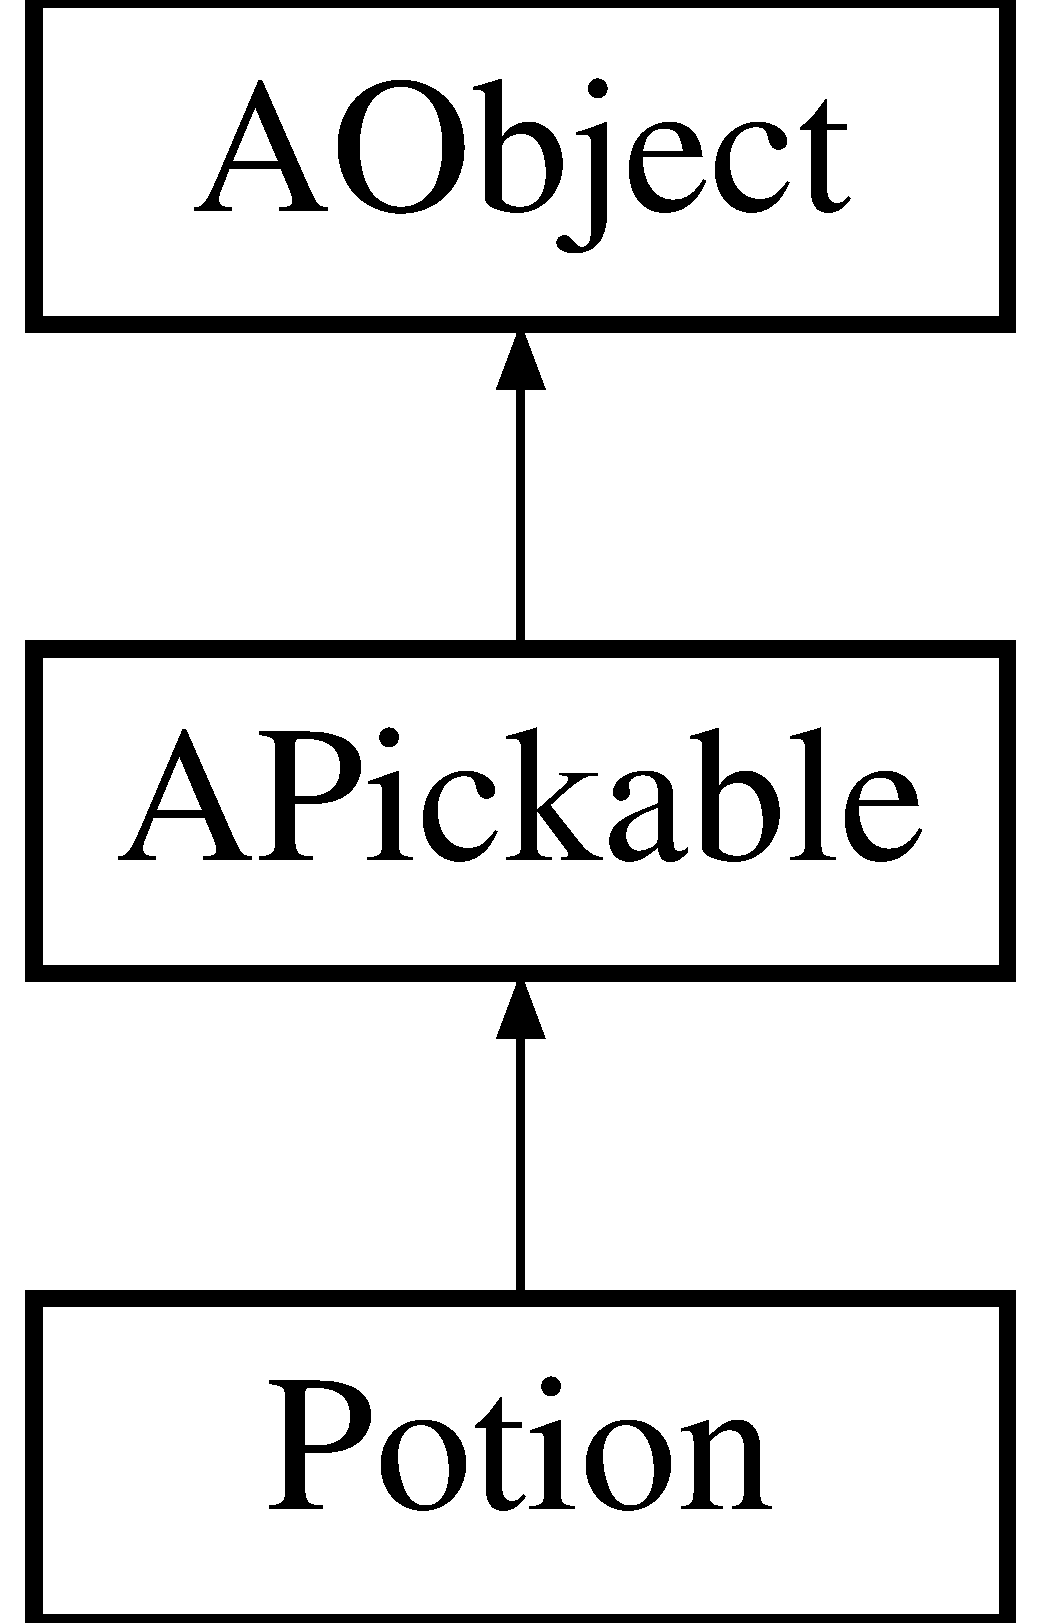
\includegraphics[height=3.000000cm]{classAObject}
\end{center}
\end{figure}
\subsection*{Public Member Functions}
\begin{DoxyCompactItemize}
\item 
\mbox{\Hypertarget{classAObject_a12a7789fca6342e9ff5c52c7cfd465d1}\label{classAObject_a12a7789fca6342e9ff5c52c7cfd465d1}} 
\hyperlink{classAObject_a12a7789fca6342e9ff5c52c7cfd465d1}{A\+Object} (std\+::shared\+\_\+ptr$<$ \hyperlink{classModel3d}{Model3d} $>$, indie\+::object\+Type=indie\+::object\+Type\+::\+U\+N\+K\+N\+OW, irr\+::u32 id=0)
\begin{DoxyCompactList}\small\item\em Constructor Build the class first param is a shared\+\_\+ptr on a \hyperlink{classModel3d}{Model3d}, second the type of object (C\+H\+E\+ST, P\+O\+T\+I\+ON, ...), third his id. \end{DoxyCompactList}\item 
\hyperlink{classAObject_ac17f3a1944792c280a3cbd83d839bc4e}{$\sim$\+A\+Object} ()
\begin{DoxyCompactList}\small\item\em Destructor. \end{DoxyCompactList}\item 
indie\+::object\+Type \hyperlink{classAObject_afcbaa047c0d02ca29b76875157a1eb1e}{get\+Type} () const
\begin{DoxyCompactList}\small\item\em get\+Type \end{DoxyCompactList}\item 
std\+::shared\+\_\+ptr$<$ \hyperlink{classModel3d}{Model3d} $>$ \hyperlink{classAObject_a3ffaa331c1842c5bf782c9a0343474bc}{get\+Model} () const
\begin{DoxyCompactList}\small\item\em get\+Model \end{DoxyCompactList}\item 
void \hyperlink{classAObject_ab4a2dc3dad1a54ff80d59c42a51479fb}{set\+Position} (Vector3d)
\begin{DoxyCompactList}\small\item\em set\+Position \end{DoxyCompactList}\item 
void \hyperlink{classAObject_a38ba628dcec6be910ce9d3c9f0de0de7}{set\+Rotation} (Vector3d)
\begin{DoxyCompactList}\small\item\em set\+Rotation \end{DoxyCompactList}\item 
void \hyperlink{classAObject_aebbd61ad13e23fa7787a5cdf12acd4ca}{print} () const
\begin{DoxyCompactList}\small\item\em print \end{DoxyCompactList}\item 
irr\+::u32 \hyperlink{classAObject_aae823d79b9bfa1ef090ee9e7b764de4a}{get\+Id} () const
\begin{DoxyCompactList}\small\item\em get\+Id \end{DoxyCompactList}\end{DoxyCompactItemize}


\subsection{Detailed Description}
An \hyperlink{classAObject}{A\+Object} instance has his own \hyperlink{classModel3d}{Model3d} attribute, and can modify it.. 

\subsection{Constructor \& Destructor Documentation}
\mbox{\Hypertarget{classAObject_ac17f3a1944792c280a3cbd83d839bc4e}\label{classAObject_ac17f3a1944792c280a3cbd83d839bc4e}} 
\index{A\+Object@{A\+Object}!````~A\+Object@{$\sim$\+A\+Object}}
\index{````~A\+Object@{$\sim$\+A\+Object}!A\+Object@{A\+Object}}
\subsubsection{\texorpdfstring{$\sim$\+A\+Object()}{~AObject()}}
{\footnotesize\ttfamily A\+Object\+::$\sim$\+A\+Object (\begin{DoxyParamCaption}{ }\end{DoxyParamCaption})}



Destructor. 

Destroy the class 

\subsection{Member Function Documentation}
\mbox{\Hypertarget{classAObject_aae823d79b9bfa1ef090ee9e7b764de4a}\label{classAObject_aae823d79b9bfa1ef090ee9e7b764de4a}} 
\index{A\+Object@{A\+Object}!get\+Id@{get\+Id}}
\index{get\+Id@{get\+Id}!A\+Object@{A\+Object}}
\subsubsection{\texorpdfstring{get\+Id()}{getId()}}
{\footnotesize\ttfamily irr\+::u32 A\+Object\+::get\+Id (\begin{DoxyParamCaption}{ }\end{DoxyParamCaption}) const}



get\+Id 

return the id of the \hyperlink{classAObject}{A\+Object} \mbox{\Hypertarget{classAObject_a3ffaa331c1842c5bf782c9a0343474bc}\label{classAObject_a3ffaa331c1842c5bf782c9a0343474bc}} 
\index{A\+Object@{A\+Object}!get\+Model@{get\+Model}}
\index{get\+Model@{get\+Model}!A\+Object@{A\+Object}}
\subsubsection{\texorpdfstring{get\+Model()}{getModel()}}
{\footnotesize\ttfamily std\+::shared\+\_\+ptr$<$ \hyperlink{classModel3d}{Model3d} $>$ A\+Object\+::get\+Model (\begin{DoxyParamCaption}{ }\end{DoxyParamCaption}) const}



get\+Model 

return the \hyperlink{classModel3d}{Model3d} of the \hyperlink{classAObject}{A\+Object} \mbox{\Hypertarget{classAObject_afcbaa047c0d02ca29b76875157a1eb1e}\label{classAObject_afcbaa047c0d02ca29b76875157a1eb1e}} 
\index{A\+Object@{A\+Object}!get\+Type@{get\+Type}}
\index{get\+Type@{get\+Type}!A\+Object@{A\+Object}}
\subsubsection{\texorpdfstring{get\+Type()}{getType()}}
{\footnotesize\ttfamily indie\+::object\+Type A\+Object\+::get\+Type (\begin{DoxyParamCaption}{ }\end{DoxyParamCaption}) const}



get\+Type 

return the type of the \hyperlink{classAObject}{A\+Object} \mbox{\Hypertarget{classAObject_aebbd61ad13e23fa7787a5cdf12acd4ca}\label{classAObject_aebbd61ad13e23fa7787a5cdf12acd4ca}} 
\index{A\+Object@{A\+Object}!print@{print}}
\index{print@{print}!A\+Object@{A\+Object}}
\subsubsection{\texorpdfstring{print()}{print()}}
{\footnotesize\ttfamily void A\+Object\+::print (\begin{DoxyParamCaption}{ }\end{DoxyParamCaption}) const}



print 

print the object on window \mbox{\Hypertarget{classAObject_ab4a2dc3dad1a54ff80d59c42a51479fb}\label{classAObject_ab4a2dc3dad1a54ff80d59c42a51479fb}} 
\index{A\+Object@{A\+Object}!set\+Position@{set\+Position}}
\index{set\+Position@{set\+Position}!A\+Object@{A\+Object}}
\subsubsection{\texorpdfstring{set\+Position()}{setPosition()}}
{\footnotesize\ttfamily void A\+Object\+::set\+Position (\begin{DoxyParamCaption}\item[{Vector3d}]{pos }\end{DoxyParamCaption})}



set\+Position 

change the vector position of the \hyperlink{classModel3d}{Model3d} of the \hyperlink{classAObject}{A\+Object} \mbox{\Hypertarget{classAObject_a38ba628dcec6be910ce9d3c9f0de0de7}\label{classAObject_a38ba628dcec6be910ce9d3c9f0de0de7}} 
\index{A\+Object@{A\+Object}!set\+Rotation@{set\+Rotation}}
\index{set\+Rotation@{set\+Rotation}!A\+Object@{A\+Object}}
\subsubsection{\texorpdfstring{set\+Rotation()}{setRotation()}}
{\footnotesize\ttfamily void A\+Object\+::set\+Rotation (\begin{DoxyParamCaption}\item[{Vector3d}]{rot }\end{DoxyParamCaption})}



set\+Rotation 

change the vector rotation of the \hyperlink{classModel3d}{Model3d} of the \hyperlink{classAObject}{A\+Object} 

The documentation for this class was generated from the following files\+:\begin{DoxyCompactItemize}
\item 
inc/game/character/heros/object/\hyperlink{AObject_8hh}{A\+Object.\+hh}\item 
src/game/character/heros/object/A\+Object.\+cpp\end{DoxyCompactItemize}

\hypertarget{classAPickable}{}\section{A\+Pickable Class Reference}
\label{classAPickable}\index{A\+Pickable@{A\+Pickable}}


create a pickable \hyperlink{classAObject}{A\+Object}  




{\ttfamily \#include $<$A\+Pickable.\+hh$>$}

Inheritance diagram for A\+Pickable\+:\begin{figure}[H]
\begin{center}
\leavevmode
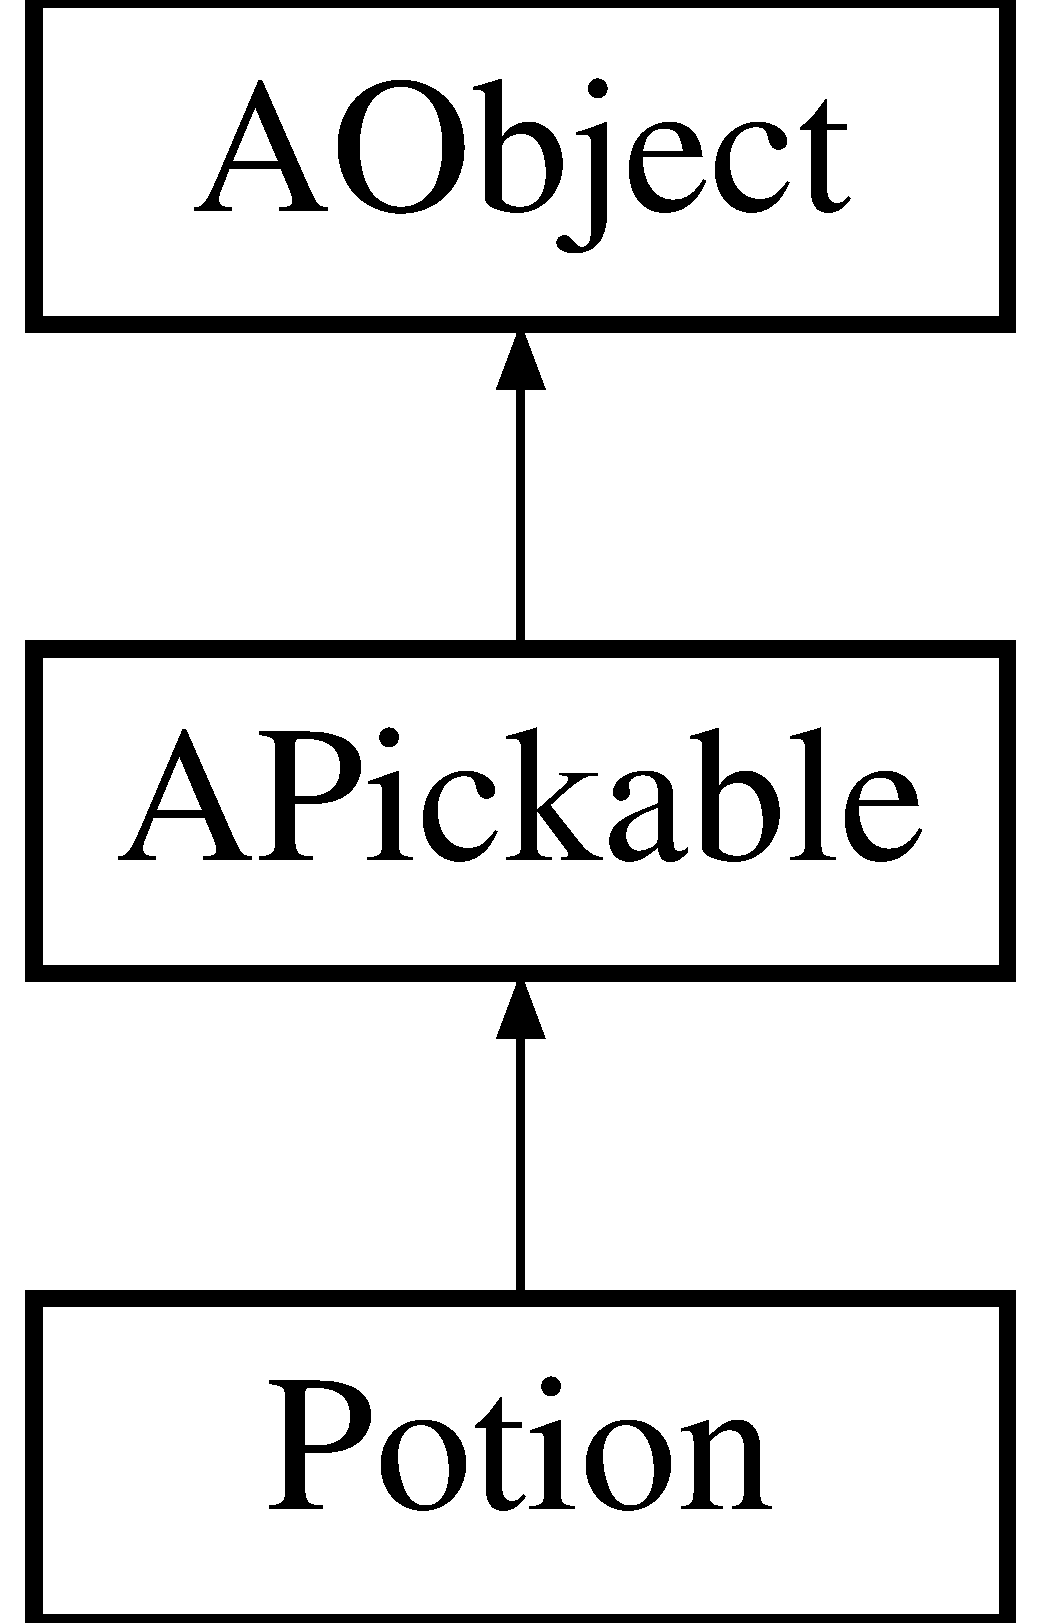
\includegraphics[height=3.000000cm]{classAPickable}
\end{center}
\end{figure}
\subsection*{Public Member Functions}
\begin{DoxyCompactItemize}
\item 
\hyperlink{classAPickable_a6be5419f2699d070f6e41c29deca6272}{A\+Pickable} (indie\+::object\+Type type)
\begin{DoxyCompactList}\small\item\em Constructor. \end{DoxyCompactList}\item 
\hyperlink{classAPickable_a145013963070158596ad2e0d07065f5d}{$\sim$\+A\+Pickable} ()
\begin{DoxyCompactList}\small\item\em Destructor. \end{DoxyCompactList}\end{DoxyCompactItemize}


\subsection{Detailed Description}
create a pickable \hyperlink{classAObject}{A\+Object} 

\subsection{Constructor \& Destructor Documentation}
\mbox{\Hypertarget{classAPickable_a6be5419f2699d070f6e41c29deca6272}\label{classAPickable_a6be5419f2699d070f6e41c29deca6272}} 
\index{A\+Pickable@{A\+Pickable}!A\+Pickable@{A\+Pickable}}
\index{A\+Pickable@{A\+Pickable}!A\+Pickable@{A\+Pickable}}
\subsubsection{\texorpdfstring{A\+Pickable()}{APickable()}}
{\footnotesize\ttfamily A\+Pickable\+::\+A\+Pickable (\begin{DoxyParamCaption}\item[{indie\+::object\+Type}]{type }\end{DoxyParamCaption})}



Constructor. 

Build the class \mbox{\Hypertarget{classAPickable_a145013963070158596ad2e0d07065f5d}\label{classAPickable_a145013963070158596ad2e0d07065f5d}} 
\index{A\+Pickable@{A\+Pickable}!````~A\+Pickable@{$\sim$\+A\+Pickable}}
\index{````~A\+Pickable@{$\sim$\+A\+Pickable}!A\+Pickable@{A\+Pickable}}
\subsubsection{\texorpdfstring{$\sim$\+A\+Pickable()}{~APickable()}}
{\footnotesize\ttfamily A\+Pickable\+::$\sim$\+A\+Pickable (\begin{DoxyParamCaption}{ }\end{DoxyParamCaption})}



Destructor. 

Destroy the class 

The documentation for this class was generated from the following files\+:\begin{DoxyCompactItemize}
\item 
inc/game/character/heros/object/\hyperlink{APickable_8hh}{A\+Pickable.\+hh}\item 
src/game/character/heros/object/A\+Pickable.\+cpp\end{DoxyCompactItemize}

\hypertarget{classirr_1_1core_1_1array}{}\section{irr\+:\+:core\+:\+:array$<$ T, T\+Alloc $>$ Class Template Reference}
\label{classirr_1_1core_1_1array}\index{irr\+::core\+::array$<$ T, T\+Alloc $>$@{irr\+::core\+::array$<$ T, T\+Alloc $>$}}


Self reallocating template array (like stl vector) with additional features.  




{\ttfamily \#include $<$irr\+Array.\+h$>$}

\subsection*{Public Member Functions}
\begin{DoxyCompactItemize}
\item 
\mbox{\Hypertarget{classirr_1_1core_1_1array_a5e0dd817352068af92448a08716f1252}\label{classirr_1_1core_1_1array_a5e0dd817352068af92448a08716f1252}} 
\hyperlink{classirr_1_1core_1_1array_a5e0dd817352068af92448a08716f1252}{array} ()
\begin{DoxyCompactList}\small\item\em Default constructor for empty array. \end{DoxyCompactList}\item 
\hyperlink{classirr_1_1core_1_1array_ab58c4b2c09693190b43ee16e99722b43}{array} (\hyperlink{namespaceirr_a0416a53257075833e7002efd0a18e804}{u32} start\+\_\+count)
\begin{DoxyCompactList}\small\item\em Constructs an array and allocates an initial chunk of memory. \end{DoxyCompactList}\item 
\mbox{\Hypertarget{classirr_1_1core_1_1array_a4e584fd375dd5f994b6bd7afd7f7a60c}\label{classirr_1_1core_1_1array_a4e584fd375dd5f994b6bd7afd7f7a60c}} 
\hyperlink{classirr_1_1core_1_1array_a4e584fd375dd5f994b6bd7afd7f7a60c}{array} (const \hyperlink{classirr_1_1core_1_1array}{array}$<$ T, T\+Alloc $>$ \&other)
\begin{DoxyCompactList}\small\item\em Copy constructor. \end{DoxyCompactList}\item 
\hyperlink{classirr_1_1core_1_1array_aac1853f45d4c18feaacac9859efe9836}{$\sim$array} ()
\begin{DoxyCompactList}\small\item\em Destructor. \end{DoxyCompactList}\item 
void \hyperlink{classirr_1_1core_1_1array_ada5735f409eca82b9031d993ee8b31c3}{reallocate} (\hyperlink{namespaceirr_a0416a53257075833e7002efd0a18e804}{u32} new\+\_\+size, bool can\+Shrink=true)
\begin{DoxyCompactList}\small\item\em Reallocates the array, make it bigger or smaller. \end{DoxyCompactList}\item 
void \hyperlink{classirr_1_1core_1_1array_a7aef3e5dbf91f8d1e8f365039e2497ae}{set\+Alloc\+Strategy} (\hyperlink{namespaceirr_1_1core_aa2e91971d5e6e84de235bfabe3c7adba}{e\+Alloc\+Strategy} new\+Strategy=A\+L\+L\+O\+C\+\_\+\+S\+T\+R\+A\+T\+E\+G\+Y\+\_\+\+D\+O\+U\+B\+LE)
\begin{DoxyCompactList}\small\item\em set a new allocation strategy \end{DoxyCompactList}\item 
void \hyperlink{classirr_1_1core_1_1array_ad2c9dff8592b95c25c59f5383fc633fe}{push\+\_\+back} (const T \&element)
\begin{DoxyCompactList}\small\item\em Adds an element at back of array. \end{DoxyCompactList}\item 
void \hyperlink{classirr_1_1core_1_1array_a31b686ce4b1ebae930f22bc40d30efbd}{push\+\_\+front} (const T \&element)
\begin{DoxyCompactList}\small\item\em Adds an element at the front of the array. \end{DoxyCompactList}\item 
void \hyperlink{classirr_1_1core_1_1array_a3b0f73c95dd449a4de576c6b1943566c}{insert} (const T \&element, \hyperlink{namespaceirr_a0416a53257075833e7002efd0a18e804}{u32} index=0)
\begin{DoxyCompactList}\small\item\em Insert item into array at specified position. \end{DoxyCompactList}\item 
\mbox{\Hypertarget{classirr_1_1core_1_1array_a236e08ca44ddf3c2b47b726f90db8d39}\label{classirr_1_1core_1_1array_a236e08ca44ddf3c2b47b726f90db8d39}} 
void \hyperlink{classirr_1_1core_1_1array_a236e08ca44ddf3c2b47b726f90db8d39}{clear} ()
\begin{DoxyCompactList}\small\item\em Clears the array and deletes all allocated memory. \end{DoxyCompactList}\item 
void \hyperlink{classirr_1_1core_1_1array_a75df5c46b08225d1ebe3c1381d85d9ff}{set\+\_\+pointer} (T $\ast$new\+Pointer, \hyperlink{namespaceirr_a0416a53257075833e7002efd0a18e804}{u32} \hyperlink{classirr_1_1core_1_1array_ab10777d1bb278c29e159ec59b5dc9378}{size}, bool \+\_\+is\+\_\+sorted=false, bool \+\_\+free\+\_\+when\+\_\+destroyed=true)
\begin{DoxyCompactList}\small\item\em Sets pointer to new array, using this as new workspace. \end{DoxyCompactList}\item 
void \hyperlink{classirr_1_1core_1_1array_afddd43e25d3ad6b1a3d75ceab13e6c56}{set\+\_\+free\+\_\+when\+\_\+destroyed} (bool f)
\begin{DoxyCompactList}\small\item\em Sets if the array should delete the memory it uses upon destruction. \end{DoxyCompactList}\item 
void \hyperlink{classirr_1_1core_1_1array_a64d70ab89f03e2ec4deae3b6c0161305}{set\+\_\+used} (\hyperlink{namespaceirr_a0416a53257075833e7002efd0a18e804}{u32} used\+Now)
\begin{DoxyCompactList}\small\item\em Sets the size of the array and allocates new elements if necessary. \end{DoxyCompactList}\item 
\mbox{\Hypertarget{classirr_1_1core_1_1array_a51c964d180507ebdef872d93886c23b2}\label{classirr_1_1core_1_1array_a51c964d180507ebdef872d93886c23b2}} 
const \hyperlink{classirr_1_1core_1_1array}{array}$<$ T, T\+Alloc $>$ \& \hyperlink{classirr_1_1core_1_1array_a51c964d180507ebdef872d93886c23b2}{operator=} (const \hyperlink{classirr_1_1core_1_1array}{array}$<$ T, T\+Alloc $>$ \&other)
\begin{DoxyCompactList}\small\item\em Assignment operator. \end{DoxyCompactList}\item 
\mbox{\Hypertarget{classirr_1_1core_1_1array_a794059b2ff063c9604eb46ae4edb599c}\label{classirr_1_1core_1_1array_a794059b2ff063c9604eb46ae4edb599c}} 
bool \hyperlink{classirr_1_1core_1_1array_a794059b2ff063c9604eb46ae4edb599c}{operator==} (const \hyperlink{classirr_1_1core_1_1array}{array}$<$ T, T\+Alloc $>$ \&other) const
\begin{DoxyCompactList}\small\item\em Equality operator. \end{DoxyCompactList}\item 
\mbox{\Hypertarget{classirr_1_1core_1_1array_a7177f0d74f839a3f26df8eedcdfc4391}\label{classirr_1_1core_1_1array_a7177f0d74f839a3f26df8eedcdfc4391}} 
bool \hyperlink{classirr_1_1core_1_1array_a7177f0d74f839a3f26df8eedcdfc4391}{operator!=} (const \hyperlink{classirr_1_1core_1_1array}{array}$<$ T, T\+Alloc $>$ \&other) const
\begin{DoxyCompactList}\small\item\em Inequality operator. \end{DoxyCompactList}\item 
\mbox{\Hypertarget{classirr_1_1core_1_1array_a1e09dc5cc93e88fd3a37cad011b3b531}\label{classirr_1_1core_1_1array_a1e09dc5cc93e88fd3a37cad011b3b531}} 
T \& \hyperlink{classirr_1_1core_1_1array_a1e09dc5cc93e88fd3a37cad011b3b531}{operator\mbox{[}$\,$\mbox{]}} (\hyperlink{namespaceirr_a0416a53257075833e7002efd0a18e804}{u32} index)
\begin{DoxyCompactList}\small\item\em Direct access operator. \end{DoxyCompactList}\item 
\mbox{\Hypertarget{classirr_1_1core_1_1array_aa3f3c984a95034950f1005f016ad0fb8}\label{classirr_1_1core_1_1array_aa3f3c984a95034950f1005f016ad0fb8}} 
const T \& \hyperlink{classirr_1_1core_1_1array_aa3f3c984a95034950f1005f016ad0fb8}{operator\mbox{[}$\,$\mbox{]}} (\hyperlink{namespaceirr_a0416a53257075833e7002efd0a18e804}{u32} index) const
\begin{DoxyCompactList}\small\item\em Direct const access operator. \end{DoxyCompactList}\item 
\mbox{\Hypertarget{classirr_1_1core_1_1array_ad87dc5db8bf6ec1033c945a0d3724e09}\label{classirr_1_1core_1_1array_ad87dc5db8bf6ec1033c945a0d3724e09}} 
T \& \hyperlink{classirr_1_1core_1_1array_ad87dc5db8bf6ec1033c945a0d3724e09}{get\+Last} ()
\begin{DoxyCompactList}\small\item\em Gets last element. \end{DoxyCompactList}\item 
\mbox{\Hypertarget{classirr_1_1core_1_1array_a6cc770ec657432983b7245b2b2473f42}\label{classirr_1_1core_1_1array_a6cc770ec657432983b7245b2b2473f42}} 
const T \& \hyperlink{classirr_1_1core_1_1array_a6cc770ec657432983b7245b2b2473f42}{get\+Last} () const
\begin{DoxyCompactList}\small\item\em Gets last element. \end{DoxyCompactList}\item 
T $\ast$ \hyperlink{classirr_1_1core_1_1array_a7b29797486e1c2ab3e7821082dab998c}{pointer} ()
\begin{DoxyCompactList}\small\item\em Gets a pointer to the array. \end{DoxyCompactList}\item 
const T $\ast$ \hyperlink{classirr_1_1core_1_1array_a8df928a9e555327c085b20f392e409ee}{const\+\_\+pointer} () const
\begin{DoxyCompactList}\small\item\em Gets a const pointer to the array. \end{DoxyCompactList}\item 
\hyperlink{namespaceirr_a0416a53257075833e7002efd0a18e804}{u32} \hyperlink{classirr_1_1core_1_1array_ab10777d1bb278c29e159ec59b5dc9378}{size} () const
\begin{DoxyCompactList}\small\item\em Get number of occupied elements of the array. \end{DoxyCompactList}\item 
\hyperlink{namespaceirr_a0416a53257075833e7002efd0a18e804}{u32} \hyperlink{classirr_1_1core_1_1array_a21e5b20b7a56ba174b19b6c36c78a14b}{allocated\+\_\+size} () const
\begin{DoxyCompactList}\small\item\em Get amount of memory allocated. \end{DoxyCompactList}\item 
bool \hyperlink{classirr_1_1core_1_1array_a956ee1019455016e21e218b61f6371ca}{empty} () const
\begin{DoxyCompactList}\small\item\em Check if array is empty. \end{DoxyCompactList}\item 
void \hyperlink{classirr_1_1core_1_1array_a870e52dd57dd67a9d59e5ca5f82bca94}{sort} ()
\begin{DoxyCompactList}\small\item\em Sorts the array using heapsort. \end{DoxyCompactList}\item 
\hyperlink{namespaceirr_ac66849b7a6ed16e30ebede579f9b47c6}{s32} \hyperlink{classirr_1_1core_1_1array_a35412f669b983eaaf3792b82966db24a}{binary\+\_\+search} (const T \&element)
\begin{DoxyCompactList}\small\item\em Performs a binary search for an element, returns -\/1 if not found. \end{DoxyCompactList}\item 
\hyperlink{namespaceirr_ac66849b7a6ed16e30ebede579f9b47c6}{s32} \hyperlink{classirr_1_1core_1_1array_aec40f807c683671067d52e83d7b72a82}{binary\+\_\+search} (const T \&element) const
\begin{DoxyCompactList}\small\item\em Performs a binary search for an element if possible, returns -\/1 if not found. \end{DoxyCompactList}\item 
\hyperlink{namespaceirr_ac66849b7a6ed16e30ebede579f9b47c6}{s32} \hyperlink{classirr_1_1core_1_1array_a9f3d6ee26c52d2e231446e4069a765a3}{binary\+\_\+search} (const T \&element, \hyperlink{namespaceirr_ac66849b7a6ed16e30ebede579f9b47c6}{s32} left, \hyperlink{namespaceirr_ac66849b7a6ed16e30ebede579f9b47c6}{s32} right) const
\begin{DoxyCompactList}\small\item\em Performs a binary search for an element, returns -\/1 if not found. \end{DoxyCompactList}\item 
\hyperlink{namespaceirr_ac66849b7a6ed16e30ebede579f9b47c6}{s32} \hyperlink{classirr_1_1core_1_1array_a62821cac92125dd76f96f21e60ca94a4}{binary\+\_\+search\+\_\+multi} (const T \&element, \hyperlink{namespaceirr_ac66849b7a6ed16e30ebede579f9b47c6}{s32} \&last)
\begin{DoxyCompactList}\small\item\em Performs a binary search for an element, returns -\/1 if not found. it is used for searching a multiset. \end{DoxyCompactList}\item 
\hyperlink{namespaceirr_ac66849b7a6ed16e30ebede579f9b47c6}{s32} \hyperlink{classirr_1_1core_1_1array_a4b5002b36bb913a3680f2412ab2ee045}{linear\+\_\+search} (const T \&element) const
\begin{DoxyCompactList}\small\item\em Finds an element in linear time, which is very slow. \end{DoxyCompactList}\item 
\hyperlink{namespaceirr_ac66849b7a6ed16e30ebede579f9b47c6}{s32} \hyperlink{classirr_1_1core_1_1array_aef6726fc4de8ca5a01881e09664981ad}{linear\+\_\+reverse\+\_\+search} (const T \&element) const
\begin{DoxyCompactList}\small\item\em Finds an element in linear time, which is very slow. \end{DoxyCompactList}\item 
void \hyperlink{classirr_1_1core_1_1array_a5ba14e37dddaecd9c3e813a78c157dc8}{erase} (\hyperlink{namespaceirr_a0416a53257075833e7002efd0a18e804}{u32} index)
\begin{DoxyCompactList}\small\item\em Erases an element from the array. \end{DoxyCompactList}\item 
void \hyperlink{classirr_1_1core_1_1array_ab9bb8cb0e6ebc4839fa2f7bc8e626800}{erase} (\hyperlink{namespaceirr_a0416a53257075833e7002efd0a18e804}{u32} index, \hyperlink{namespaceirr_ac66849b7a6ed16e30ebede579f9b47c6}{s32} count)
\begin{DoxyCompactList}\small\item\em Erases some elements from the array. \end{DoxyCompactList}\item 
\mbox{\Hypertarget{classirr_1_1core_1_1array_ab73d5838db931996f66f9efcc7127b49}\label{classirr_1_1core_1_1array_ab73d5838db931996f66f9efcc7127b49}} 
void \hyperlink{classirr_1_1core_1_1array_ab73d5838db931996f66f9efcc7127b49}{set\+\_\+sorted} (bool \+\_\+is\+\_\+sorted)
\begin{DoxyCompactList}\small\item\em Sets if the array is sorted. \end{DoxyCompactList}\item 
void \hyperlink{classirr_1_1core_1_1array_a8857046f500a2990fc9930b204a3dbad}{swap} (\hyperlink{classirr_1_1core_1_1array}{array}$<$ T, T\+Alloc $>$ \&other)
\begin{DoxyCompactList}\small\item\em Swap the content of this array container with the content of another array. \end{DoxyCompactList}\item 
\mbox{\Hypertarget{classirr_1_1core_1_1array_a5e0dd817352068af92448a08716f1252}\label{classirr_1_1core_1_1array_a5e0dd817352068af92448a08716f1252}} 
\hyperlink{classirr_1_1core_1_1array_a5e0dd817352068af92448a08716f1252}{array} ()
\begin{DoxyCompactList}\small\item\em Default constructor for empty array. \end{DoxyCompactList}\item 
\hyperlink{classirr_1_1core_1_1array_ab58c4b2c09693190b43ee16e99722b43}{array} (\hyperlink{namespaceirr_a0416a53257075833e7002efd0a18e804}{u32} start\+\_\+count)
\begin{DoxyCompactList}\small\item\em Constructs an array and allocates an initial chunk of memory. \end{DoxyCompactList}\item 
\mbox{\Hypertarget{classirr_1_1core_1_1array_a4e584fd375dd5f994b6bd7afd7f7a60c}\label{classirr_1_1core_1_1array_a4e584fd375dd5f994b6bd7afd7f7a60c}} 
\hyperlink{classirr_1_1core_1_1array_a4e584fd375dd5f994b6bd7afd7f7a60c}{array} (const \hyperlink{classirr_1_1core_1_1array}{array}$<$ T, T\+Alloc $>$ \&other)
\begin{DoxyCompactList}\small\item\em Copy constructor. \end{DoxyCompactList}\item 
\hyperlink{classirr_1_1core_1_1array_aac1853f45d4c18feaacac9859efe9836}{$\sim$array} ()
\begin{DoxyCompactList}\small\item\em Destructor. \end{DoxyCompactList}\item 
void \hyperlink{classirr_1_1core_1_1array_ada5735f409eca82b9031d993ee8b31c3}{reallocate} (\hyperlink{namespaceirr_a0416a53257075833e7002efd0a18e804}{u32} new\+\_\+size, bool can\+Shrink=true)
\begin{DoxyCompactList}\small\item\em Reallocates the array, make it bigger or smaller. \end{DoxyCompactList}\item 
void \hyperlink{classirr_1_1core_1_1array_a7aef3e5dbf91f8d1e8f365039e2497ae}{set\+Alloc\+Strategy} (\hyperlink{namespaceirr_1_1core_aa2e91971d5e6e84de235bfabe3c7adba}{e\+Alloc\+Strategy} new\+Strategy=A\+L\+L\+O\+C\+\_\+\+S\+T\+R\+A\+T\+E\+G\+Y\+\_\+\+D\+O\+U\+B\+LE)
\begin{DoxyCompactList}\small\item\em set a new allocation strategy \end{DoxyCompactList}\item 
void \hyperlink{classirr_1_1core_1_1array_ad2c9dff8592b95c25c59f5383fc633fe}{push\+\_\+back} (const T \&element)
\begin{DoxyCompactList}\small\item\em Adds an element at back of array. \end{DoxyCompactList}\item 
void \hyperlink{classirr_1_1core_1_1array_a31b686ce4b1ebae930f22bc40d30efbd}{push\+\_\+front} (const T \&element)
\begin{DoxyCompactList}\small\item\em Adds an element at the front of the array. \end{DoxyCompactList}\item 
void \hyperlink{classirr_1_1core_1_1array_a3b0f73c95dd449a4de576c6b1943566c}{insert} (const T \&element, \hyperlink{namespaceirr_a0416a53257075833e7002efd0a18e804}{u32} index=0)
\begin{DoxyCompactList}\small\item\em Insert item into array at specified position. \end{DoxyCompactList}\item 
\mbox{\Hypertarget{classirr_1_1core_1_1array_a236e08ca44ddf3c2b47b726f90db8d39}\label{classirr_1_1core_1_1array_a236e08ca44ddf3c2b47b726f90db8d39}} 
void \hyperlink{classirr_1_1core_1_1array_a236e08ca44ddf3c2b47b726f90db8d39}{clear} ()
\begin{DoxyCompactList}\small\item\em Clears the array and deletes all allocated memory. \end{DoxyCompactList}\item 
void \hyperlink{classirr_1_1core_1_1array_a75df5c46b08225d1ebe3c1381d85d9ff}{set\+\_\+pointer} (T $\ast$new\+Pointer, \hyperlink{namespaceirr_a0416a53257075833e7002efd0a18e804}{u32} \hyperlink{classirr_1_1core_1_1array_ab10777d1bb278c29e159ec59b5dc9378}{size}, bool \+\_\+is\+\_\+sorted=false, bool \+\_\+free\+\_\+when\+\_\+destroyed=true)
\begin{DoxyCompactList}\small\item\em Sets pointer to new array, using this as new workspace. \end{DoxyCompactList}\item 
void \hyperlink{classirr_1_1core_1_1array_afddd43e25d3ad6b1a3d75ceab13e6c56}{set\+\_\+free\+\_\+when\+\_\+destroyed} (bool f)
\begin{DoxyCompactList}\small\item\em Sets if the array should delete the memory it uses upon destruction. \end{DoxyCompactList}\item 
void \hyperlink{classirr_1_1core_1_1array_a64d70ab89f03e2ec4deae3b6c0161305}{set\+\_\+used} (\hyperlink{namespaceirr_a0416a53257075833e7002efd0a18e804}{u32} used\+Now)
\begin{DoxyCompactList}\small\item\em Sets the size of the array and allocates new elements if necessary. \end{DoxyCompactList}\item 
\mbox{\Hypertarget{classirr_1_1core_1_1array_a51c964d180507ebdef872d93886c23b2}\label{classirr_1_1core_1_1array_a51c964d180507ebdef872d93886c23b2}} 
const \hyperlink{classirr_1_1core_1_1array}{array}$<$ T, T\+Alloc $>$ \& \hyperlink{classirr_1_1core_1_1array_a51c964d180507ebdef872d93886c23b2}{operator=} (const \hyperlink{classirr_1_1core_1_1array}{array}$<$ T, T\+Alloc $>$ \&other)
\begin{DoxyCompactList}\small\item\em Assignment operator. \end{DoxyCompactList}\item 
\mbox{\Hypertarget{classirr_1_1core_1_1array_a794059b2ff063c9604eb46ae4edb599c}\label{classirr_1_1core_1_1array_a794059b2ff063c9604eb46ae4edb599c}} 
bool \hyperlink{classirr_1_1core_1_1array_a794059b2ff063c9604eb46ae4edb599c}{operator==} (const \hyperlink{classirr_1_1core_1_1array}{array}$<$ T, T\+Alloc $>$ \&other) const
\begin{DoxyCompactList}\small\item\em Equality operator. \end{DoxyCompactList}\item 
\mbox{\Hypertarget{classirr_1_1core_1_1array_a7177f0d74f839a3f26df8eedcdfc4391}\label{classirr_1_1core_1_1array_a7177f0d74f839a3f26df8eedcdfc4391}} 
bool \hyperlink{classirr_1_1core_1_1array_a7177f0d74f839a3f26df8eedcdfc4391}{operator!=} (const \hyperlink{classirr_1_1core_1_1array}{array}$<$ T, T\+Alloc $>$ \&other) const
\begin{DoxyCompactList}\small\item\em Inequality operator. \end{DoxyCompactList}\item 
\mbox{\Hypertarget{classirr_1_1core_1_1array_a1e09dc5cc93e88fd3a37cad011b3b531}\label{classirr_1_1core_1_1array_a1e09dc5cc93e88fd3a37cad011b3b531}} 
T \& \hyperlink{classirr_1_1core_1_1array_a1e09dc5cc93e88fd3a37cad011b3b531}{operator\mbox{[}$\,$\mbox{]}} (\hyperlink{namespaceirr_a0416a53257075833e7002efd0a18e804}{u32} index)
\begin{DoxyCompactList}\small\item\em Direct access operator. \end{DoxyCompactList}\item 
\mbox{\Hypertarget{classirr_1_1core_1_1array_aa3f3c984a95034950f1005f016ad0fb8}\label{classirr_1_1core_1_1array_aa3f3c984a95034950f1005f016ad0fb8}} 
const T \& \hyperlink{classirr_1_1core_1_1array_aa3f3c984a95034950f1005f016ad0fb8}{operator\mbox{[}$\,$\mbox{]}} (\hyperlink{namespaceirr_a0416a53257075833e7002efd0a18e804}{u32} index) const
\begin{DoxyCompactList}\small\item\em Direct const access operator. \end{DoxyCompactList}\item 
\mbox{\Hypertarget{classirr_1_1core_1_1array_ad87dc5db8bf6ec1033c945a0d3724e09}\label{classirr_1_1core_1_1array_ad87dc5db8bf6ec1033c945a0d3724e09}} 
T \& \hyperlink{classirr_1_1core_1_1array_ad87dc5db8bf6ec1033c945a0d3724e09}{get\+Last} ()
\begin{DoxyCompactList}\small\item\em Gets last element. \end{DoxyCompactList}\item 
\mbox{\Hypertarget{classirr_1_1core_1_1array_a6cc770ec657432983b7245b2b2473f42}\label{classirr_1_1core_1_1array_a6cc770ec657432983b7245b2b2473f42}} 
const T \& \hyperlink{classirr_1_1core_1_1array_a6cc770ec657432983b7245b2b2473f42}{get\+Last} () const
\begin{DoxyCompactList}\small\item\em Gets last element. \end{DoxyCompactList}\item 
T $\ast$ \hyperlink{classirr_1_1core_1_1array_a7b29797486e1c2ab3e7821082dab998c}{pointer} ()
\begin{DoxyCompactList}\small\item\em Gets a pointer to the array. \end{DoxyCompactList}\item 
const T $\ast$ \hyperlink{classirr_1_1core_1_1array_a8df928a9e555327c085b20f392e409ee}{const\+\_\+pointer} () const
\begin{DoxyCompactList}\small\item\em Gets a const pointer to the array. \end{DoxyCompactList}\item 
\hyperlink{namespaceirr_a0416a53257075833e7002efd0a18e804}{u32} \hyperlink{classirr_1_1core_1_1array_ab10777d1bb278c29e159ec59b5dc9378}{size} () const
\begin{DoxyCompactList}\small\item\em Get number of occupied elements of the array. \end{DoxyCompactList}\item 
\hyperlink{namespaceirr_a0416a53257075833e7002efd0a18e804}{u32} \hyperlink{classirr_1_1core_1_1array_a21e5b20b7a56ba174b19b6c36c78a14b}{allocated\+\_\+size} () const
\begin{DoxyCompactList}\small\item\em Get amount of memory allocated. \end{DoxyCompactList}\item 
bool \hyperlink{classirr_1_1core_1_1array_a956ee1019455016e21e218b61f6371ca}{empty} () const
\begin{DoxyCompactList}\small\item\em Check if array is empty. \end{DoxyCompactList}\item 
void \hyperlink{classirr_1_1core_1_1array_a870e52dd57dd67a9d59e5ca5f82bca94}{sort} ()
\begin{DoxyCompactList}\small\item\em Sorts the array using heapsort. \end{DoxyCompactList}\item 
\hyperlink{namespaceirr_ac66849b7a6ed16e30ebede579f9b47c6}{s32} \hyperlink{classirr_1_1core_1_1array_a35412f669b983eaaf3792b82966db24a}{binary\+\_\+search} (const T \&element)
\begin{DoxyCompactList}\small\item\em Performs a binary search for an element, returns -\/1 if not found. \end{DoxyCompactList}\item 
\hyperlink{namespaceirr_ac66849b7a6ed16e30ebede579f9b47c6}{s32} \hyperlink{classirr_1_1core_1_1array_aec40f807c683671067d52e83d7b72a82}{binary\+\_\+search} (const T \&element) const
\begin{DoxyCompactList}\small\item\em Performs a binary search for an element if possible, returns -\/1 if not found. \end{DoxyCompactList}\item 
\hyperlink{namespaceirr_ac66849b7a6ed16e30ebede579f9b47c6}{s32} \hyperlink{classirr_1_1core_1_1array_a9f3d6ee26c52d2e231446e4069a765a3}{binary\+\_\+search} (const T \&element, \hyperlink{namespaceirr_ac66849b7a6ed16e30ebede579f9b47c6}{s32} left, \hyperlink{namespaceirr_ac66849b7a6ed16e30ebede579f9b47c6}{s32} right) const
\begin{DoxyCompactList}\small\item\em Performs a binary search for an element, returns -\/1 if not found. \end{DoxyCompactList}\item 
\hyperlink{namespaceirr_ac66849b7a6ed16e30ebede579f9b47c6}{s32} \hyperlink{classirr_1_1core_1_1array_a62821cac92125dd76f96f21e60ca94a4}{binary\+\_\+search\+\_\+multi} (const T \&element, \hyperlink{namespaceirr_ac66849b7a6ed16e30ebede579f9b47c6}{s32} \&last)
\begin{DoxyCompactList}\small\item\em Performs a binary search for an element, returns -\/1 if not found. it is used for searching a multiset. \end{DoxyCompactList}\item 
\hyperlink{namespaceirr_ac66849b7a6ed16e30ebede579f9b47c6}{s32} \hyperlink{classirr_1_1core_1_1array_a4b5002b36bb913a3680f2412ab2ee045}{linear\+\_\+search} (const T \&element) const
\begin{DoxyCompactList}\small\item\em Finds an element in linear time, which is very slow. \end{DoxyCompactList}\item 
\hyperlink{namespaceirr_ac66849b7a6ed16e30ebede579f9b47c6}{s32} \hyperlink{classirr_1_1core_1_1array_aef6726fc4de8ca5a01881e09664981ad}{linear\+\_\+reverse\+\_\+search} (const T \&element) const
\begin{DoxyCompactList}\small\item\em Finds an element in linear time, which is very slow. \end{DoxyCompactList}\item 
void \hyperlink{classirr_1_1core_1_1array_a5ba14e37dddaecd9c3e813a78c157dc8}{erase} (\hyperlink{namespaceirr_a0416a53257075833e7002efd0a18e804}{u32} index)
\begin{DoxyCompactList}\small\item\em Erases an element from the array. \end{DoxyCompactList}\item 
void \hyperlink{classirr_1_1core_1_1array_ab9bb8cb0e6ebc4839fa2f7bc8e626800}{erase} (\hyperlink{namespaceirr_a0416a53257075833e7002efd0a18e804}{u32} index, \hyperlink{namespaceirr_ac66849b7a6ed16e30ebede579f9b47c6}{s32} count)
\begin{DoxyCompactList}\small\item\em Erases some elements from the array. \end{DoxyCompactList}\item 
\mbox{\Hypertarget{classirr_1_1core_1_1array_ab73d5838db931996f66f9efcc7127b49}\label{classirr_1_1core_1_1array_ab73d5838db931996f66f9efcc7127b49}} 
void \hyperlink{classirr_1_1core_1_1array_ab73d5838db931996f66f9efcc7127b49}{set\+\_\+sorted} (bool \+\_\+is\+\_\+sorted)
\begin{DoxyCompactList}\small\item\em Sets if the array is sorted. \end{DoxyCompactList}\item 
void \hyperlink{classirr_1_1core_1_1array_a8857046f500a2990fc9930b204a3dbad}{swap} (\hyperlink{classirr_1_1core_1_1array}{array}$<$ T, T\+Alloc $>$ \&other)
\begin{DoxyCompactList}\small\item\em Swap the content of this array container with the content of another array. \end{DoxyCompactList}\end{DoxyCompactItemize}


\subsection{Detailed Description}
\subsubsection*{template$<$class T, typename T\+Alloc = irr\+Allocator$<$\+T$>$$>$\newline
class irr\+::core\+::array$<$ T, T\+Alloc $>$}

Self reallocating template array (like stl vector) with additional features. 

Some features are\+: Heap sorting, binary search methods, easier debugging. 

\subsection{Constructor \& Destructor Documentation}
\mbox{\Hypertarget{classirr_1_1core_1_1array_ab58c4b2c09693190b43ee16e99722b43}\label{classirr_1_1core_1_1array_ab58c4b2c09693190b43ee16e99722b43}} 
\index{irr\+::core\+::array@{irr\+::core\+::array}!array@{array}}
\index{array@{array}!irr\+::core\+::array@{irr\+::core\+::array}}
\subsubsection{\texorpdfstring{array()}{array()}\hspace{0.1cm}{\footnotesize\ttfamily [1/2]}}
{\footnotesize\ttfamily template$<$class T, typename T\+Alloc = irr\+Allocator$<$\+T$>$$>$ \\
\hyperlink{classirr_1_1core_1_1array}{irr\+::core\+::array}$<$ T, T\+Alloc $>$\+::\hyperlink{classirr_1_1core_1_1array}{array} (\begin{DoxyParamCaption}\item[{\hyperlink{namespaceirr_a0416a53257075833e7002efd0a18e804}{u32}}]{start\+\_\+count }\end{DoxyParamCaption})\hspace{0.3cm}{\ttfamily [inline]}}



Constructs an array and allocates an initial chunk of memory. 


\begin{DoxyParams}{Parameters}
{\em start\+\_\+count} & Amount of elements to pre-\/allocate. \\
\hline
\end{DoxyParams}
\mbox{\Hypertarget{classirr_1_1core_1_1array_aac1853f45d4c18feaacac9859efe9836}\label{classirr_1_1core_1_1array_aac1853f45d4c18feaacac9859efe9836}} 
\index{irr\+::core\+::array@{irr\+::core\+::array}!````~array@{$\sim$array}}
\index{````~array@{$\sim$array}!irr\+::core\+::array@{irr\+::core\+::array}}
\subsubsection{\texorpdfstring{$\sim$array()}{~array()}\hspace{0.1cm}{\footnotesize\ttfamily [1/2]}}
{\footnotesize\ttfamily template$<$class T, typename T\+Alloc = irr\+Allocator$<$\+T$>$$>$ \\
\hyperlink{classirr_1_1core_1_1array}{irr\+::core\+::array}$<$ T, T\+Alloc $>$\+::$\sim$\hyperlink{classirr_1_1core_1_1array}{array} (\begin{DoxyParamCaption}{ }\end{DoxyParamCaption})\hspace{0.3cm}{\ttfamily [inline]}}



Destructor. 

Frees allocated memory, if set\+\_\+free\+\_\+when\+\_\+destroyed was not set to false by the user before. \mbox{\Hypertarget{classirr_1_1core_1_1array_ab58c4b2c09693190b43ee16e99722b43}\label{classirr_1_1core_1_1array_ab58c4b2c09693190b43ee16e99722b43}} 
\index{irr\+::core\+::array@{irr\+::core\+::array}!array@{array}}
\index{array@{array}!irr\+::core\+::array@{irr\+::core\+::array}}
\subsubsection{\texorpdfstring{array()}{array()}\hspace{0.1cm}{\footnotesize\ttfamily [2/2]}}
{\footnotesize\ttfamily template$<$class T, typename T\+Alloc = irr\+Allocator$<$\+T$>$$>$ \\
\hyperlink{classirr_1_1core_1_1array}{irr\+::core\+::array}$<$ T, T\+Alloc $>$\+::\hyperlink{classirr_1_1core_1_1array}{array} (\begin{DoxyParamCaption}\item[{\hyperlink{namespaceirr_a0416a53257075833e7002efd0a18e804}{u32}}]{start\+\_\+count }\end{DoxyParamCaption})\hspace{0.3cm}{\ttfamily [inline]}}



Constructs an array and allocates an initial chunk of memory. 


\begin{DoxyParams}{Parameters}
{\em start\+\_\+count} & Amount of elements to pre-\/allocate. \\
\hline
\end{DoxyParams}
\mbox{\Hypertarget{classirr_1_1core_1_1array_aac1853f45d4c18feaacac9859efe9836}\label{classirr_1_1core_1_1array_aac1853f45d4c18feaacac9859efe9836}} 
\index{irr\+::core\+::array@{irr\+::core\+::array}!````~array@{$\sim$array}}
\index{````~array@{$\sim$array}!irr\+::core\+::array@{irr\+::core\+::array}}
\subsubsection{\texorpdfstring{$\sim$array()}{~array()}\hspace{0.1cm}{\footnotesize\ttfamily [2/2]}}
{\footnotesize\ttfamily template$<$class T, typename T\+Alloc = irr\+Allocator$<$\+T$>$$>$ \\
\hyperlink{classirr_1_1core_1_1array}{irr\+::core\+::array}$<$ T, T\+Alloc $>$\+::$\sim$\hyperlink{classirr_1_1core_1_1array}{array} (\begin{DoxyParamCaption}{ }\end{DoxyParamCaption})\hspace{0.3cm}{\ttfamily [inline]}}



Destructor. 

Frees allocated memory, if set\+\_\+free\+\_\+when\+\_\+destroyed was not set to false by the user before. 

\subsection{Member Function Documentation}
\mbox{\Hypertarget{classirr_1_1core_1_1array_a21e5b20b7a56ba174b19b6c36c78a14b}\label{classirr_1_1core_1_1array_a21e5b20b7a56ba174b19b6c36c78a14b}} 
\index{irr\+::core\+::array@{irr\+::core\+::array}!allocated\+\_\+size@{allocated\+\_\+size}}
\index{allocated\+\_\+size@{allocated\+\_\+size}!irr\+::core\+::array@{irr\+::core\+::array}}
\subsubsection{\texorpdfstring{allocated\+\_\+size()}{allocated\_size()}\hspace{0.1cm}{\footnotesize\ttfamily [1/2]}}
{\footnotesize\ttfamily template$<$class T, typename T\+Alloc = irr\+Allocator$<$\+T$>$$>$ \\
\hyperlink{namespaceirr_a0416a53257075833e7002efd0a18e804}{u32} \hyperlink{classirr_1_1core_1_1array}{irr\+::core\+::array}$<$ T, T\+Alloc $>$\+::allocated\+\_\+size (\begin{DoxyParamCaption}{ }\end{DoxyParamCaption}) const\hspace{0.3cm}{\ttfamily [inline]}}



Get amount of memory allocated. 

\begin{DoxyReturn}{Returns}
Amount of memory allocated. The amount of bytes allocated would be \hyperlink{classirr_1_1core_1_1array_a21e5b20b7a56ba174b19b6c36c78a14b}{allocated\+\_\+size()} $\ast$ sizeof(\+Element\+Type\+Used); 
\end{DoxyReturn}
\mbox{\Hypertarget{classirr_1_1core_1_1array_a21e5b20b7a56ba174b19b6c36c78a14b}\label{classirr_1_1core_1_1array_a21e5b20b7a56ba174b19b6c36c78a14b}} 
\index{irr\+::core\+::array@{irr\+::core\+::array}!allocated\+\_\+size@{allocated\+\_\+size}}
\index{allocated\+\_\+size@{allocated\+\_\+size}!irr\+::core\+::array@{irr\+::core\+::array}}
\subsubsection{\texorpdfstring{allocated\+\_\+size()}{allocated\_size()}\hspace{0.1cm}{\footnotesize\ttfamily [2/2]}}
{\footnotesize\ttfamily template$<$class T, typename T\+Alloc = irr\+Allocator$<$\+T$>$$>$ \\
\hyperlink{namespaceirr_a0416a53257075833e7002efd0a18e804}{u32} \hyperlink{classirr_1_1core_1_1array}{irr\+::core\+::array}$<$ T, T\+Alloc $>$\+::allocated\+\_\+size (\begin{DoxyParamCaption}{ }\end{DoxyParamCaption}) const\hspace{0.3cm}{\ttfamily [inline]}}



Get amount of memory allocated. 

\begin{DoxyReturn}{Returns}
Amount of memory allocated. The amount of bytes allocated would be \hyperlink{classirr_1_1core_1_1array_a21e5b20b7a56ba174b19b6c36c78a14b}{allocated\+\_\+size()} $\ast$ sizeof(\+Element\+Type\+Used); 
\end{DoxyReturn}
\mbox{\Hypertarget{classirr_1_1core_1_1array_a35412f669b983eaaf3792b82966db24a}\label{classirr_1_1core_1_1array_a35412f669b983eaaf3792b82966db24a}} 
\index{irr\+::core\+::array@{irr\+::core\+::array}!binary\+\_\+search@{binary\+\_\+search}}
\index{binary\+\_\+search@{binary\+\_\+search}!irr\+::core\+::array@{irr\+::core\+::array}}
\subsubsection{\texorpdfstring{binary\+\_\+search()}{binary\_search()}\hspace{0.1cm}{\footnotesize\ttfamily [1/6]}}
{\footnotesize\ttfamily template$<$class T, typename T\+Alloc = irr\+Allocator$<$\+T$>$$>$ \\
\hyperlink{namespaceirr_ac66849b7a6ed16e30ebede579f9b47c6}{s32} \hyperlink{classirr_1_1core_1_1array}{irr\+::core\+::array}$<$ T, T\+Alloc $>$\+::binary\+\_\+search (\begin{DoxyParamCaption}\item[{const T \&}]{element }\end{DoxyParamCaption})\hspace{0.3cm}{\ttfamily [inline]}}



Performs a binary search for an element, returns -\/1 if not found. 

The array will be sorted before the binary search if it is not already sorted. Caution is advised! Be careful not to call this on unsorted const arrays, or the slower method will be used. 
\begin{DoxyParams}{Parameters}
{\em element} & Element to search for. \\
\hline
\end{DoxyParams}
\begin{DoxyReturn}{Returns}
Position of the searched element if it was found, otherwise -\/1 is returned. 
\end{DoxyReturn}
\mbox{\Hypertarget{classirr_1_1core_1_1array_a35412f669b983eaaf3792b82966db24a}\label{classirr_1_1core_1_1array_a35412f669b983eaaf3792b82966db24a}} 
\index{irr\+::core\+::array@{irr\+::core\+::array}!binary\+\_\+search@{binary\+\_\+search}}
\index{binary\+\_\+search@{binary\+\_\+search}!irr\+::core\+::array@{irr\+::core\+::array}}
\subsubsection{\texorpdfstring{binary\+\_\+search()}{binary\_search()}\hspace{0.1cm}{\footnotesize\ttfamily [2/6]}}
{\footnotesize\ttfamily template$<$class T, typename T\+Alloc = irr\+Allocator$<$\+T$>$$>$ \\
\hyperlink{namespaceirr_ac66849b7a6ed16e30ebede579f9b47c6}{s32} \hyperlink{classirr_1_1core_1_1array}{irr\+::core\+::array}$<$ T, T\+Alloc $>$\+::binary\+\_\+search (\begin{DoxyParamCaption}\item[{const T \&}]{element }\end{DoxyParamCaption})\hspace{0.3cm}{\ttfamily [inline]}}



Performs a binary search for an element, returns -\/1 if not found. 

The array will be sorted before the binary search if it is not already sorted. Caution is advised! Be careful not to call this on unsorted const arrays, or the slower method will be used. 
\begin{DoxyParams}{Parameters}
{\em element} & Element to search for. \\
\hline
\end{DoxyParams}
\begin{DoxyReturn}{Returns}
Position of the searched element if it was found, otherwise -\/1 is returned. 
\end{DoxyReturn}
\mbox{\Hypertarget{classirr_1_1core_1_1array_aec40f807c683671067d52e83d7b72a82}\label{classirr_1_1core_1_1array_aec40f807c683671067d52e83d7b72a82}} 
\index{irr\+::core\+::array@{irr\+::core\+::array}!binary\+\_\+search@{binary\+\_\+search}}
\index{binary\+\_\+search@{binary\+\_\+search}!irr\+::core\+::array@{irr\+::core\+::array}}
\subsubsection{\texorpdfstring{binary\+\_\+search()}{binary\_search()}\hspace{0.1cm}{\footnotesize\ttfamily [3/6]}}
{\footnotesize\ttfamily template$<$class T, typename T\+Alloc = irr\+Allocator$<$\+T$>$$>$ \\
\hyperlink{namespaceirr_ac66849b7a6ed16e30ebede579f9b47c6}{s32} \hyperlink{classirr_1_1core_1_1array}{irr\+::core\+::array}$<$ T, T\+Alloc $>$\+::binary\+\_\+search (\begin{DoxyParamCaption}\item[{const T \&}]{element }\end{DoxyParamCaption}) const\hspace{0.3cm}{\ttfamily [inline]}}



Performs a binary search for an element if possible, returns -\/1 if not found. 

This method is for const arrays and so cannot call \hyperlink{classirr_1_1core_1_1array_a870e52dd57dd67a9d59e5ca5f82bca94}{sort()}, if the array is not sorted then linear\+\_\+search will be used instead. Potentially very slow! 
\begin{DoxyParams}{Parameters}
{\em element} & Element to search for. \\
\hline
\end{DoxyParams}
\begin{DoxyReturn}{Returns}
Position of the searched element if it was found, otherwise -\/1 is returned. 
\end{DoxyReturn}
\mbox{\Hypertarget{classirr_1_1core_1_1array_aec40f807c683671067d52e83d7b72a82}\label{classirr_1_1core_1_1array_aec40f807c683671067d52e83d7b72a82}} 
\index{irr\+::core\+::array@{irr\+::core\+::array}!binary\+\_\+search@{binary\+\_\+search}}
\index{binary\+\_\+search@{binary\+\_\+search}!irr\+::core\+::array@{irr\+::core\+::array}}
\subsubsection{\texorpdfstring{binary\+\_\+search()}{binary\_search()}\hspace{0.1cm}{\footnotesize\ttfamily [4/6]}}
{\footnotesize\ttfamily template$<$class T, typename T\+Alloc = irr\+Allocator$<$\+T$>$$>$ \\
\hyperlink{namespaceirr_ac66849b7a6ed16e30ebede579f9b47c6}{s32} \hyperlink{classirr_1_1core_1_1array}{irr\+::core\+::array}$<$ T, T\+Alloc $>$\+::binary\+\_\+search (\begin{DoxyParamCaption}\item[{const T \&}]{element }\end{DoxyParamCaption}) const\hspace{0.3cm}{\ttfamily [inline]}}



Performs a binary search for an element if possible, returns -\/1 if not found. 

This method is for const arrays and so cannot call \hyperlink{classirr_1_1core_1_1array_a870e52dd57dd67a9d59e5ca5f82bca94}{sort()}, if the array is not sorted then linear\+\_\+search will be used instead. Potentially very slow! 
\begin{DoxyParams}{Parameters}
{\em element} & Element to search for. \\
\hline
\end{DoxyParams}
\begin{DoxyReturn}{Returns}
Position of the searched element if it was found, otherwise -\/1 is returned. 
\end{DoxyReturn}
\mbox{\Hypertarget{classirr_1_1core_1_1array_a9f3d6ee26c52d2e231446e4069a765a3}\label{classirr_1_1core_1_1array_a9f3d6ee26c52d2e231446e4069a765a3}} 
\index{irr\+::core\+::array@{irr\+::core\+::array}!binary\+\_\+search@{binary\+\_\+search}}
\index{binary\+\_\+search@{binary\+\_\+search}!irr\+::core\+::array@{irr\+::core\+::array}}
\subsubsection{\texorpdfstring{binary\+\_\+search()}{binary\_search()}\hspace{0.1cm}{\footnotesize\ttfamily [5/6]}}
{\footnotesize\ttfamily template$<$class T, typename T\+Alloc = irr\+Allocator$<$\+T$>$$>$ \\
\hyperlink{namespaceirr_ac66849b7a6ed16e30ebede579f9b47c6}{s32} \hyperlink{classirr_1_1core_1_1array}{irr\+::core\+::array}$<$ T, T\+Alloc $>$\+::binary\+\_\+search (\begin{DoxyParamCaption}\item[{const T \&}]{element,  }\item[{\hyperlink{namespaceirr_ac66849b7a6ed16e30ebede579f9b47c6}{s32}}]{left,  }\item[{\hyperlink{namespaceirr_ac66849b7a6ed16e30ebede579f9b47c6}{s32}}]{right }\end{DoxyParamCaption}) const\hspace{0.3cm}{\ttfamily [inline]}}



Performs a binary search for an element, returns -\/1 if not found. 


\begin{DoxyParams}{Parameters}
{\em element} & Element to search for. \\
\hline
{\em left} & First left index \\
\hline
{\em right} & Last right index. \\
\hline
\end{DoxyParams}
\begin{DoxyReturn}{Returns}
Position of the searched element if it was found, otherwise -\/1 is returned. 
\end{DoxyReturn}
\mbox{\Hypertarget{classirr_1_1core_1_1array_a9f3d6ee26c52d2e231446e4069a765a3}\label{classirr_1_1core_1_1array_a9f3d6ee26c52d2e231446e4069a765a3}} 
\index{irr\+::core\+::array@{irr\+::core\+::array}!binary\+\_\+search@{binary\+\_\+search}}
\index{binary\+\_\+search@{binary\+\_\+search}!irr\+::core\+::array@{irr\+::core\+::array}}
\subsubsection{\texorpdfstring{binary\+\_\+search()}{binary\_search()}\hspace{0.1cm}{\footnotesize\ttfamily [6/6]}}
{\footnotesize\ttfamily template$<$class T, typename T\+Alloc = irr\+Allocator$<$\+T$>$$>$ \\
\hyperlink{namespaceirr_ac66849b7a6ed16e30ebede579f9b47c6}{s32} \hyperlink{classirr_1_1core_1_1array}{irr\+::core\+::array}$<$ T, T\+Alloc $>$\+::binary\+\_\+search (\begin{DoxyParamCaption}\item[{const T \&}]{element,  }\item[{\hyperlink{namespaceirr_ac66849b7a6ed16e30ebede579f9b47c6}{s32}}]{left,  }\item[{\hyperlink{namespaceirr_ac66849b7a6ed16e30ebede579f9b47c6}{s32}}]{right }\end{DoxyParamCaption}) const\hspace{0.3cm}{\ttfamily [inline]}}



Performs a binary search for an element, returns -\/1 if not found. 


\begin{DoxyParams}{Parameters}
{\em element} & Element to search for. \\
\hline
{\em left} & First left index \\
\hline
{\em right} & Last right index. \\
\hline
\end{DoxyParams}
\begin{DoxyReturn}{Returns}
Position of the searched element if it was found, otherwise -\/1 is returned. 
\end{DoxyReturn}
\mbox{\Hypertarget{classirr_1_1core_1_1array_a62821cac92125dd76f96f21e60ca94a4}\label{classirr_1_1core_1_1array_a62821cac92125dd76f96f21e60ca94a4}} 
\index{irr\+::core\+::array@{irr\+::core\+::array}!binary\+\_\+search\+\_\+multi@{binary\+\_\+search\+\_\+multi}}
\index{binary\+\_\+search\+\_\+multi@{binary\+\_\+search\+\_\+multi}!irr\+::core\+::array@{irr\+::core\+::array}}
\subsubsection{\texorpdfstring{binary\+\_\+search\+\_\+multi()}{binary\_search\_multi()}\hspace{0.1cm}{\footnotesize\ttfamily [1/2]}}
{\footnotesize\ttfamily template$<$class T, typename T\+Alloc = irr\+Allocator$<$\+T$>$$>$ \\
\hyperlink{namespaceirr_ac66849b7a6ed16e30ebede579f9b47c6}{s32} \hyperlink{classirr_1_1core_1_1array}{irr\+::core\+::array}$<$ T, T\+Alloc $>$\+::binary\+\_\+search\+\_\+multi (\begin{DoxyParamCaption}\item[{const T \&}]{element,  }\item[{\hyperlink{namespaceirr_ac66849b7a6ed16e30ebede579f9b47c6}{s32} \&}]{last }\end{DoxyParamCaption})\hspace{0.3cm}{\ttfamily [inline]}}



Performs a binary search for an element, returns -\/1 if not found. it is used for searching a multiset. 

The array will be sorted before the binary search if it is not already sorted. 
\begin{DoxyParams}{Parameters}
{\em element} & Element to search for. \\
\hline
{\em \&last} & return last\+Index of equal elements \\
\hline
\end{DoxyParams}
\begin{DoxyReturn}{Returns}
Position of the first searched element if it was found, otherwise -\/1 is returned. 
\end{DoxyReturn}
\mbox{\Hypertarget{classirr_1_1core_1_1array_a62821cac92125dd76f96f21e60ca94a4}\label{classirr_1_1core_1_1array_a62821cac92125dd76f96f21e60ca94a4}} 
\index{irr\+::core\+::array@{irr\+::core\+::array}!binary\+\_\+search\+\_\+multi@{binary\+\_\+search\+\_\+multi}}
\index{binary\+\_\+search\+\_\+multi@{binary\+\_\+search\+\_\+multi}!irr\+::core\+::array@{irr\+::core\+::array}}
\subsubsection{\texorpdfstring{binary\+\_\+search\+\_\+multi()}{binary\_search\_multi()}\hspace{0.1cm}{\footnotesize\ttfamily [2/2]}}
{\footnotesize\ttfamily template$<$class T, typename T\+Alloc = irr\+Allocator$<$\+T$>$$>$ \\
\hyperlink{namespaceirr_ac66849b7a6ed16e30ebede579f9b47c6}{s32} \hyperlink{classirr_1_1core_1_1array}{irr\+::core\+::array}$<$ T, T\+Alloc $>$\+::binary\+\_\+search\+\_\+multi (\begin{DoxyParamCaption}\item[{const T \&}]{element,  }\item[{\hyperlink{namespaceirr_ac66849b7a6ed16e30ebede579f9b47c6}{s32} \&}]{last }\end{DoxyParamCaption})\hspace{0.3cm}{\ttfamily [inline]}}



Performs a binary search for an element, returns -\/1 if not found. it is used for searching a multiset. 

The array will be sorted before the binary search if it is not already sorted. 
\begin{DoxyParams}{Parameters}
{\em element} & Element to search for. \\
\hline
{\em \&last} & return last\+Index of equal elements \\
\hline
\end{DoxyParams}
\begin{DoxyReturn}{Returns}
Position of the first searched element if it was found, otherwise -\/1 is returned. 
\end{DoxyReturn}
\mbox{\Hypertarget{classirr_1_1core_1_1array_a8df928a9e555327c085b20f392e409ee}\label{classirr_1_1core_1_1array_a8df928a9e555327c085b20f392e409ee}} 
\index{irr\+::core\+::array@{irr\+::core\+::array}!const\+\_\+pointer@{const\+\_\+pointer}}
\index{const\+\_\+pointer@{const\+\_\+pointer}!irr\+::core\+::array@{irr\+::core\+::array}}
\subsubsection{\texorpdfstring{const\+\_\+pointer()}{const\_pointer()}\hspace{0.1cm}{\footnotesize\ttfamily [1/2]}}
{\footnotesize\ttfamily template$<$class T, typename T\+Alloc = irr\+Allocator$<$\+T$>$$>$ \\
const T$\ast$ \hyperlink{classirr_1_1core_1_1array}{irr\+::core\+::array}$<$ T, T\+Alloc $>$\+::const\+\_\+pointer (\begin{DoxyParamCaption}{ }\end{DoxyParamCaption}) const\hspace{0.3cm}{\ttfamily [inline]}}



Gets a const pointer to the array. 

\begin{DoxyReturn}{Returns}
Pointer to the array. 
\end{DoxyReturn}
\mbox{\Hypertarget{classirr_1_1core_1_1array_a8df928a9e555327c085b20f392e409ee}\label{classirr_1_1core_1_1array_a8df928a9e555327c085b20f392e409ee}} 
\index{irr\+::core\+::array@{irr\+::core\+::array}!const\+\_\+pointer@{const\+\_\+pointer}}
\index{const\+\_\+pointer@{const\+\_\+pointer}!irr\+::core\+::array@{irr\+::core\+::array}}
\subsubsection{\texorpdfstring{const\+\_\+pointer()}{const\_pointer()}\hspace{0.1cm}{\footnotesize\ttfamily [2/2]}}
{\footnotesize\ttfamily template$<$class T, typename T\+Alloc = irr\+Allocator$<$\+T$>$$>$ \\
const T$\ast$ \hyperlink{classirr_1_1core_1_1array}{irr\+::core\+::array}$<$ T, T\+Alloc $>$\+::const\+\_\+pointer (\begin{DoxyParamCaption}{ }\end{DoxyParamCaption}) const\hspace{0.3cm}{\ttfamily [inline]}}



Gets a const pointer to the array. 

\begin{DoxyReturn}{Returns}
Pointer to the array. 
\end{DoxyReturn}
\mbox{\Hypertarget{classirr_1_1core_1_1array_a956ee1019455016e21e218b61f6371ca}\label{classirr_1_1core_1_1array_a956ee1019455016e21e218b61f6371ca}} 
\index{irr\+::core\+::array@{irr\+::core\+::array}!empty@{empty}}
\index{empty@{empty}!irr\+::core\+::array@{irr\+::core\+::array}}
\subsubsection{\texorpdfstring{empty()}{empty()}\hspace{0.1cm}{\footnotesize\ttfamily [1/2]}}
{\footnotesize\ttfamily template$<$class T, typename T\+Alloc = irr\+Allocator$<$\+T$>$$>$ \\
bool \hyperlink{classirr_1_1core_1_1array}{irr\+::core\+::array}$<$ T, T\+Alloc $>$\+::empty (\begin{DoxyParamCaption}{ }\end{DoxyParamCaption}) const\hspace{0.3cm}{\ttfamily [inline]}}



Check if array is empty. 

\begin{DoxyReturn}{Returns}
True if the array is empty false if not. 
\end{DoxyReturn}
\mbox{\Hypertarget{classirr_1_1core_1_1array_a956ee1019455016e21e218b61f6371ca}\label{classirr_1_1core_1_1array_a956ee1019455016e21e218b61f6371ca}} 
\index{irr\+::core\+::array@{irr\+::core\+::array}!empty@{empty}}
\index{empty@{empty}!irr\+::core\+::array@{irr\+::core\+::array}}
\subsubsection{\texorpdfstring{empty()}{empty()}\hspace{0.1cm}{\footnotesize\ttfamily [2/2]}}
{\footnotesize\ttfamily template$<$class T, typename T\+Alloc = irr\+Allocator$<$\+T$>$$>$ \\
bool \hyperlink{classirr_1_1core_1_1array}{irr\+::core\+::array}$<$ T, T\+Alloc $>$\+::empty (\begin{DoxyParamCaption}{ }\end{DoxyParamCaption}) const\hspace{0.3cm}{\ttfamily [inline]}}



Check if array is empty. 

\begin{DoxyReturn}{Returns}
True if the array is empty false if not. 
\end{DoxyReturn}
\mbox{\Hypertarget{classirr_1_1core_1_1array_a5ba14e37dddaecd9c3e813a78c157dc8}\label{classirr_1_1core_1_1array_a5ba14e37dddaecd9c3e813a78c157dc8}} 
\index{irr\+::core\+::array@{irr\+::core\+::array}!erase@{erase}}
\index{erase@{erase}!irr\+::core\+::array@{irr\+::core\+::array}}
\subsubsection{\texorpdfstring{erase()}{erase()}\hspace{0.1cm}{\footnotesize\ttfamily [1/4]}}
{\footnotesize\ttfamily template$<$class T, typename T\+Alloc = irr\+Allocator$<$\+T$>$$>$ \\
void \hyperlink{classirr_1_1core_1_1array}{irr\+::core\+::array}$<$ T, T\+Alloc $>$\+::erase (\begin{DoxyParamCaption}\item[{\hyperlink{namespaceirr_a0416a53257075833e7002efd0a18e804}{u32}}]{index }\end{DoxyParamCaption})\hspace{0.3cm}{\ttfamily [inline]}}



Erases an element from the array. 

May be slow, because all elements following after the erased element have to be copied. 
\begin{DoxyParams}{Parameters}
{\em index} & Index of element to be erased. \\
\hline
\end{DoxyParams}
\mbox{\Hypertarget{classirr_1_1core_1_1array_a5ba14e37dddaecd9c3e813a78c157dc8}\label{classirr_1_1core_1_1array_a5ba14e37dddaecd9c3e813a78c157dc8}} 
\index{irr\+::core\+::array@{irr\+::core\+::array}!erase@{erase}}
\index{erase@{erase}!irr\+::core\+::array@{irr\+::core\+::array}}
\subsubsection{\texorpdfstring{erase()}{erase()}\hspace{0.1cm}{\footnotesize\ttfamily [2/4]}}
{\footnotesize\ttfamily template$<$class T, typename T\+Alloc = irr\+Allocator$<$\+T$>$$>$ \\
void \hyperlink{classirr_1_1core_1_1array}{irr\+::core\+::array}$<$ T, T\+Alloc $>$\+::erase (\begin{DoxyParamCaption}\item[{\hyperlink{namespaceirr_a0416a53257075833e7002efd0a18e804}{u32}}]{index }\end{DoxyParamCaption})\hspace{0.3cm}{\ttfamily [inline]}}



Erases an element from the array. 

May be slow, because all elements following after the erased element have to be copied. 
\begin{DoxyParams}{Parameters}
{\em index} & Index of element to be erased. \\
\hline
\end{DoxyParams}
\mbox{\Hypertarget{classirr_1_1core_1_1array_ab9bb8cb0e6ebc4839fa2f7bc8e626800}\label{classirr_1_1core_1_1array_ab9bb8cb0e6ebc4839fa2f7bc8e626800}} 
\index{irr\+::core\+::array@{irr\+::core\+::array}!erase@{erase}}
\index{erase@{erase}!irr\+::core\+::array@{irr\+::core\+::array}}
\subsubsection{\texorpdfstring{erase()}{erase()}\hspace{0.1cm}{\footnotesize\ttfamily [3/4]}}
{\footnotesize\ttfamily template$<$class T, typename T\+Alloc = irr\+Allocator$<$\+T$>$$>$ \\
void \hyperlink{classirr_1_1core_1_1array}{irr\+::core\+::array}$<$ T, T\+Alloc $>$\+::erase (\begin{DoxyParamCaption}\item[{\hyperlink{namespaceirr_a0416a53257075833e7002efd0a18e804}{u32}}]{index,  }\item[{\hyperlink{namespaceirr_ac66849b7a6ed16e30ebede579f9b47c6}{s32}}]{count }\end{DoxyParamCaption})\hspace{0.3cm}{\ttfamily [inline]}}



Erases some elements from the array. 

May be slow, because all elements following after the erased element have to be copied. 
\begin{DoxyParams}{Parameters}
{\em index} & Index of the first element to be erased. \\
\hline
{\em count} & Amount of elements to be erased. \\
\hline
\end{DoxyParams}
\mbox{\Hypertarget{classirr_1_1core_1_1array_ab9bb8cb0e6ebc4839fa2f7bc8e626800}\label{classirr_1_1core_1_1array_ab9bb8cb0e6ebc4839fa2f7bc8e626800}} 
\index{irr\+::core\+::array@{irr\+::core\+::array}!erase@{erase}}
\index{erase@{erase}!irr\+::core\+::array@{irr\+::core\+::array}}
\subsubsection{\texorpdfstring{erase()}{erase()}\hspace{0.1cm}{\footnotesize\ttfamily [4/4]}}
{\footnotesize\ttfamily template$<$class T, typename T\+Alloc = irr\+Allocator$<$\+T$>$$>$ \\
void \hyperlink{classirr_1_1core_1_1array}{irr\+::core\+::array}$<$ T, T\+Alloc $>$\+::erase (\begin{DoxyParamCaption}\item[{\hyperlink{namespaceirr_a0416a53257075833e7002efd0a18e804}{u32}}]{index,  }\item[{\hyperlink{namespaceirr_ac66849b7a6ed16e30ebede579f9b47c6}{s32}}]{count }\end{DoxyParamCaption})\hspace{0.3cm}{\ttfamily [inline]}}



Erases some elements from the array. 

May be slow, because all elements following after the erased element have to be copied. 
\begin{DoxyParams}{Parameters}
{\em index} & Index of the first element to be erased. \\
\hline
{\em count} & Amount of elements to be erased. \\
\hline
\end{DoxyParams}
\mbox{\Hypertarget{classirr_1_1core_1_1array_a3b0f73c95dd449a4de576c6b1943566c}\label{classirr_1_1core_1_1array_a3b0f73c95dd449a4de576c6b1943566c}} 
\index{irr\+::core\+::array@{irr\+::core\+::array}!insert@{insert}}
\index{insert@{insert}!irr\+::core\+::array@{irr\+::core\+::array}}
\subsubsection{\texorpdfstring{insert()}{insert()}\hspace{0.1cm}{\footnotesize\ttfamily [1/2]}}
{\footnotesize\ttfamily template$<$class T, typename T\+Alloc = irr\+Allocator$<$\+T$>$$>$ \\
void \hyperlink{classirr_1_1core_1_1array}{irr\+::core\+::array}$<$ T, T\+Alloc $>$\+::insert (\begin{DoxyParamCaption}\item[{const T \&}]{element,  }\item[{\hyperlink{namespaceirr_a0416a53257075833e7002efd0a18e804}{u32}}]{index = {\ttfamily 0} }\end{DoxyParamCaption})\hspace{0.3cm}{\ttfamily [inline]}}



Insert item into array at specified position. 

Please use this only if you know what you are doing (possible performance loss). The preferred method of adding elements should be \hyperlink{classirr_1_1core_1_1array_ad2c9dff8592b95c25c59f5383fc633fe}{push\+\_\+back()}. 
\begin{DoxyParams}{Parameters}
{\em element} & Element to be inserted \\
\hline
{\em index} & Where position to insert the new element. \\
\hline
\end{DoxyParams}
\mbox{\Hypertarget{classirr_1_1core_1_1array_a3b0f73c95dd449a4de576c6b1943566c}\label{classirr_1_1core_1_1array_a3b0f73c95dd449a4de576c6b1943566c}} 
\index{irr\+::core\+::array@{irr\+::core\+::array}!insert@{insert}}
\index{insert@{insert}!irr\+::core\+::array@{irr\+::core\+::array}}
\subsubsection{\texorpdfstring{insert()}{insert()}\hspace{0.1cm}{\footnotesize\ttfamily [2/2]}}
{\footnotesize\ttfamily template$<$class T, typename T\+Alloc = irr\+Allocator$<$\+T$>$$>$ \\
void \hyperlink{classirr_1_1core_1_1array}{irr\+::core\+::array}$<$ T, T\+Alloc $>$\+::insert (\begin{DoxyParamCaption}\item[{const T \&}]{element,  }\item[{\hyperlink{namespaceirr_a0416a53257075833e7002efd0a18e804}{u32}}]{index = {\ttfamily 0} }\end{DoxyParamCaption})\hspace{0.3cm}{\ttfamily [inline]}}



Insert item into array at specified position. 

Please use this only if you know what you are doing (possible performance loss). The preferred method of adding elements should be \hyperlink{classirr_1_1core_1_1array_ad2c9dff8592b95c25c59f5383fc633fe}{push\+\_\+back()}. 
\begin{DoxyParams}{Parameters}
{\em element} & Element to be inserted \\
\hline
{\em index} & Where position to insert the new element. \\
\hline
\end{DoxyParams}
\mbox{\Hypertarget{classirr_1_1core_1_1array_aef6726fc4de8ca5a01881e09664981ad}\label{classirr_1_1core_1_1array_aef6726fc4de8ca5a01881e09664981ad}} 
\index{irr\+::core\+::array@{irr\+::core\+::array}!linear\+\_\+reverse\+\_\+search@{linear\+\_\+reverse\+\_\+search}}
\index{linear\+\_\+reverse\+\_\+search@{linear\+\_\+reverse\+\_\+search}!irr\+::core\+::array@{irr\+::core\+::array}}
\subsubsection{\texorpdfstring{linear\+\_\+reverse\+\_\+search()}{linear\_reverse\_search()}\hspace{0.1cm}{\footnotesize\ttfamily [1/2]}}
{\footnotesize\ttfamily template$<$class T, typename T\+Alloc = irr\+Allocator$<$\+T$>$$>$ \\
\hyperlink{namespaceirr_ac66849b7a6ed16e30ebede579f9b47c6}{s32} \hyperlink{classirr_1_1core_1_1array}{irr\+::core\+::array}$<$ T, T\+Alloc $>$\+::linear\+\_\+reverse\+\_\+search (\begin{DoxyParamCaption}\item[{const T \&}]{element }\end{DoxyParamCaption}) const\hspace{0.3cm}{\ttfamily [inline]}}



Finds an element in linear time, which is very slow. 

Use binary\+\_\+search for faster finding. Only works if ==operator is implemented. 
\begin{DoxyParams}{Parameters}
{\em element} & Element to search for. \\
\hline
\end{DoxyParams}
\begin{DoxyReturn}{Returns}
Position of the searched element if it was found, otherwise -\/1 is returned. 
\end{DoxyReturn}
\mbox{\Hypertarget{classirr_1_1core_1_1array_aef6726fc4de8ca5a01881e09664981ad}\label{classirr_1_1core_1_1array_aef6726fc4de8ca5a01881e09664981ad}} 
\index{irr\+::core\+::array@{irr\+::core\+::array}!linear\+\_\+reverse\+\_\+search@{linear\+\_\+reverse\+\_\+search}}
\index{linear\+\_\+reverse\+\_\+search@{linear\+\_\+reverse\+\_\+search}!irr\+::core\+::array@{irr\+::core\+::array}}
\subsubsection{\texorpdfstring{linear\+\_\+reverse\+\_\+search()}{linear\_reverse\_search()}\hspace{0.1cm}{\footnotesize\ttfamily [2/2]}}
{\footnotesize\ttfamily template$<$class T, typename T\+Alloc = irr\+Allocator$<$\+T$>$$>$ \\
\hyperlink{namespaceirr_ac66849b7a6ed16e30ebede579f9b47c6}{s32} \hyperlink{classirr_1_1core_1_1array}{irr\+::core\+::array}$<$ T, T\+Alloc $>$\+::linear\+\_\+reverse\+\_\+search (\begin{DoxyParamCaption}\item[{const T \&}]{element }\end{DoxyParamCaption}) const\hspace{0.3cm}{\ttfamily [inline]}}



Finds an element in linear time, which is very slow. 

Use binary\+\_\+search for faster finding. Only works if ==operator is implemented. 
\begin{DoxyParams}{Parameters}
{\em element} & Element to search for. \\
\hline
\end{DoxyParams}
\begin{DoxyReturn}{Returns}
Position of the searched element if it was found, otherwise -\/1 is returned. 
\end{DoxyReturn}
\mbox{\Hypertarget{classirr_1_1core_1_1array_a4b5002b36bb913a3680f2412ab2ee045}\label{classirr_1_1core_1_1array_a4b5002b36bb913a3680f2412ab2ee045}} 
\index{irr\+::core\+::array@{irr\+::core\+::array}!linear\+\_\+search@{linear\+\_\+search}}
\index{linear\+\_\+search@{linear\+\_\+search}!irr\+::core\+::array@{irr\+::core\+::array}}
\subsubsection{\texorpdfstring{linear\+\_\+search()}{linear\_search()}\hspace{0.1cm}{\footnotesize\ttfamily [1/2]}}
{\footnotesize\ttfamily template$<$class T, typename T\+Alloc = irr\+Allocator$<$\+T$>$$>$ \\
\hyperlink{namespaceirr_ac66849b7a6ed16e30ebede579f9b47c6}{s32} \hyperlink{classirr_1_1core_1_1array}{irr\+::core\+::array}$<$ T, T\+Alloc $>$\+::linear\+\_\+search (\begin{DoxyParamCaption}\item[{const T \&}]{element }\end{DoxyParamCaption}) const\hspace{0.3cm}{\ttfamily [inline]}}



Finds an element in linear time, which is very slow. 

Use binary\+\_\+search for faster finding. Only works if ==operator is implemented. 
\begin{DoxyParams}{Parameters}
{\em element} & Element to search for. \\
\hline
\end{DoxyParams}
\begin{DoxyReturn}{Returns}
Position of the searched element if it was found, otherwise -\/1 is returned. 
\end{DoxyReturn}
\mbox{\Hypertarget{classirr_1_1core_1_1array_a4b5002b36bb913a3680f2412ab2ee045}\label{classirr_1_1core_1_1array_a4b5002b36bb913a3680f2412ab2ee045}} 
\index{irr\+::core\+::array@{irr\+::core\+::array}!linear\+\_\+search@{linear\+\_\+search}}
\index{linear\+\_\+search@{linear\+\_\+search}!irr\+::core\+::array@{irr\+::core\+::array}}
\subsubsection{\texorpdfstring{linear\+\_\+search()}{linear\_search()}\hspace{0.1cm}{\footnotesize\ttfamily [2/2]}}
{\footnotesize\ttfamily template$<$class T, typename T\+Alloc = irr\+Allocator$<$\+T$>$$>$ \\
\hyperlink{namespaceirr_ac66849b7a6ed16e30ebede579f9b47c6}{s32} \hyperlink{classirr_1_1core_1_1array}{irr\+::core\+::array}$<$ T, T\+Alloc $>$\+::linear\+\_\+search (\begin{DoxyParamCaption}\item[{const T \&}]{element }\end{DoxyParamCaption}) const\hspace{0.3cm}{\ttfamily [inline]}}



Finds an element in linear time, which is very slow. 

Use binary\+\_\+search for faster finding. Only works if ==operator is implemented. 
\begin{DoxyParams}{Parameters}
{\em element} & Element to search for. \\
\hline
\end{DoxyParams}
\begin{DoxyReturn}{Returns}
Position of the searched element if it was found, otherwise -\/1 is returned. 
\end{DoxyReturn}
\mbox{\Hypertarget{classirr_1_1core_1_1array_a7b29797486e1c2ab3e7821082dab998c}\label{classirr_1_1core_1_1array_a7b29797486e1c2ab3e7821082dab998c}} 
\index{irr\+::core\+::array@{irr\+::core\+::array}!pointer@{pointer}}
\index{pointer@{pointer}!irr\+::core\+::array@{irr\+::core\+::array}}
\subsubsection{\texorpdfstring{pointer()}{pointer()}\hspace{0.1cm}{\footnotesize\ttfamily [1/2]}}
{\footnotesize\ttfamily template$<$class T, typename T\+Alloc = irr\+Allocator$<$\+T$>$$>$ \\
T$\ast$ \hyperlink{classirr_1_1core_1_1array}{irr\+::core\+::array}$<$ T, T\+Alloc $>$\+::pointer (\begin{DoxyParamCaption}{ }\end{DoxyParamCaption})\hspace{0.3cm}{\ttfamily [inline]}}



Gets a pointer to the array. 

\begin{DoxyReturn}{Returns}
Pointer to the array. 
\end{DoxyReturn}
\mbox{\Hypertarget{classirr_1_1core_1_1array_a7b29797486e1c2ab3e7821082dab998c}\label{classirr_1_1core_1_1array_a7b29797486e1c2ab3e7821082dab998c}} 
\index{irr\+::core\+::array@{irr\+::core\+::array}!pointer@{pointer}}
\index{pointer@{pointer}!irr\+::core\+::array@{irr\+::core\+::array}}
\subsubsection{\texorpdfstring{pointer()}{pointer()}\hspace{0.1cm}{\footnotesize\ttfamily [2/2]}}
{\footnotesize\ttfamily template$<$class T, typename T\+Alloc = irr\+Allocator$<$\+T$>$$>$ \\
T$\ast$ \hyperlink{classirr_1_1core_1_1array}{irr\+::core\+::array}$<$ T, T\+Alloc $>$\+::pointer (\begin{DoxyParamCaption}{ }\end{DoxyParamCaption})\hspace{0.3cm}{\ttfamily [inline]}}



Gets a pointer to the array. 

\begin{DoxyReturn}{Returns}
Pointer to the array. 
\end{DoxyReturn}
\mbox{\Hypertarget{classirr_1_1core_1_1array_ad2c9dff8592b95c25c59f5383fc633fe}\label{classirr_1_1core_1_1array_ad2c9dff8592b95c25c59f5383fc633fe}} 
\index{irr\+::core\+::array@{irr\+::core\+::array}!push\+\_\+back@{push\+\_\+back}}
\index{push\+\_\+back@{push\+\_\+back}!irr\+::core\+::array@{irr\+::core\+::array}}
\subsubsection{\texorpdfstring{push\+\_\+back()}{push\_back()}\hspace{0.1cm}{\footnotesize\ttfamily [1/2]}}
{\footnotesize\ttfamily template$<$class T, typename T\+Alloc = irr\+Allocator$<$\+T$>$$>$ \\
void \hyperlink{classirr_1_1core_1_1array}{irr\+::core\+::array}$<$ T, T\+Alloc $>$\+::push\+\_\+back (\begin{DoxyParamCaption}\item[{const T \&}]{element }\end{DoxyParamCaption})\hspace{0.3cm}{\ttfamily [inline]}}



Adds an element at back of array. 

If the array is too small to add this new element it is made bigger. 
\begin{DoxyParams}{Parameters}
{\em element} & Element to add at the back of the array. \\
\hline
\end{DoxyParams}
\mbox{\Hypertarget{classirr_1_1core_1_1array_ad2c9dff8592b95c25c59f5383fc633fe}\label{classirr_1_1core_1_1array_ad2c9dff8592b95c25c59f5383fc633fe}} 
\index{irr\+::core\+::array@{irr\+::core\+::array}!push\+\_\+back@{push\+\_\+back}}
\index{push\+\_\+back@{push\+\_\+back}!irr\+::core\+::array@{irr\+::core\+::array}}
\subsubsection{\texorpdfstring{push\+\_\+back()}{push\_back()}\hspace{0.1cm}{\footnotesize\ttfamily [2/2]}}
{\footnotesize\ttfamily template$<$class T, typename T\+Alloc = irr\+Allocator$<$\+T$>$$>$ \\
void \hyperlink{classirr_1_1core_1_1array}{irr\+::core\+::array}$<$ T, T\+Alloc $>$\+::push\+\_\+back (\begin{DoxyParamCaption}\item[{const T \&}]{element }\end{DoxyParamCaption})\hspace{0.3cm}{\ttfamily [inline]}}



Adds an element at back of array. 

If the array is too small to add this new element it is made bigger. 
\begin{DoxyParams}{Parameters}
{\em element} & Element to add at the back of the array. \\
\hline
\end{DoxyParams}
\mbox{\Hypertarget{classirr_1_1core_1_1array_a31b686ce4b1ebae930f22bc40d30efbd}\label{classirr_1_1core_1_1array_a31b686ce4b1ebae930f22bc40d30efbd}} 
\index{irr\+::core\+::array@{irr\+::core\+::array}!push\+\_\+front@{push\+\_\+front}}
\index{push\+\_\+front@{push\+\_\+front}!irr\+::core\+::array@{irr\+::core\+::array}}
\subsubsection{\texorpdfstring{push\+\_\+front()}{push\_front()}\hspace{0.1cm}{\footnotesize\ttfamily [1/2]}}
{\footnotesize\ttfamily template$<$class T, typename T\+Alloc = irr\+Allocator$<$\+T$>$$>$ \\
void \hyperlink{classirr_1_1core_1_1array}{irr\+::core\+::array}$<$ T, T\+Alloc $>$\+::push\+\_\+front (\begin{DoxyParamCaption}\item[{const T \&}]{element }\end{DoxyParamCaption})\hspace{0.3cm}{\ttfamily [inline]}}



Adds an element at the front of the array. 

If the array is to small to add this new element, the array is made bigger. Please note that this is slow, because the whole array needs to be copied for this. 
\begin{DoxyParams}{Parameters}
{\em element} & Element to add at the back of the array. \\
\hline
\end{DoxyParams}
\mbox{\Hypertarget{classirr_1_1core_1_1array_a31b686ce4b1ebae930f22bc40d30efbd}\label{classirr_1_1core_1_1array_a31b686ce4b1ebae930f22bc40d30efbd}} 
\index{irr\+::core\+::array@{irr\+::core\+::array}!push\+\_\+front@{push\+\_\+front}}
\index{push\+\_\+front@{push\+\_\+front}!irr\+::core\+::array@{irr\+::core\+::array}}
\subsubsection{\texorpdfstring{push\+\_\+front()}{push\_front()}\hspace{0.1cm}{\footnotesize\ttfamily [2/2]}}
{\footnotesize\ttfamily template$<$class T, typename T\+Alloc = irr\+Allocator$<$\+T$>$$>$ \\
void \hyperlink{classirr_1_1core_1_1array}{irr\+::core\+::array}$<$ T, T\+Alloc $>$\+::push\+\_\+front (\begin{DoxyParamCaption}\item[{const T \&}]{element }\end{DoxyParamCaption})\hspace{0.3cm}{\ttfamily [inline]}}



Adds an element at the front of the array. 

If the array is to small to add this new element, the array is made bigger. Please note that this is slow, because the whole array needs to be copied for this. 
\begin{DoxyParams}{Parameters}
{\em element} & Element to add at the back of the array. \\
\hline
\end{DoxyParams}
\mbox{\Hypertarget{classirr_1_1core_1_1array_ada5735f409eca82b9031d993ee8b31c3}\label{classirr_1_1core_1_1array_ada5735f409eca82b9031d993ee8b31c3}} 
\index{irr\+::core\+::array@{irr\+::core\+::array}!reallocate@{reallocate}}
\index{reallocate@{reallocate}!irr\+::core\+::array@{irr\+::core\+::array}}
\subsubsection{\texorpdfstring{reallocate()}{reallocate()}\hspace{0.1cm}{\footnotesize\ttfamily [1/2]}}
{\footnotesize\ttfamily template$<$class T, typename T\+Alloc = irr\+Allocator$<$\+T$>$$>$ \\
void \hyperlink{classirr_1_1core_1_1array}{irr\+::core\+::array}$<$ T, T\+Alloc $>$\+::reallocate (\begin{DoxyParamCaption}\item[{\hyperlink{namespaceirr_a0416a53257075833e7002efd0a18e804}{u32}}]{new\+\_\+size,  }\item[{bool}]{can\+Shrink = {\ttfamily true} }\end{DoxyParamCaption})\hspace{0.3cm}{\ttfamily [inline]}}



Reallocates the array, make it bigger or smaller. 


\begin{DoxyParams}{Parameters}
{\em new\+\_\+size} & New size of array. \\
\hline
{\em can\+Shrink} & Specifies whether the array is reallocated even if enough space is available. Setting this flag to false can speed up array usage, but may use more memory than required by the data. \\
\hline
\end{DoxyParams}
\mbox{\Hypertarget{classirr_1_1core_1_1array_ada5735f409eca82b9031d993ee8b31c3}\label{classirr_1_1core_1_1array_ada5735f409eca82b9031d993ee8b31c3}} 
\index{irr\+::core\+::array@{irr\+::core\+::array}!reallocate@{reallocate}}
\index{reallocate@{reallocate}!irr\+::core\+::array@{irr\+::core\+::array}}
\subsubsection{\texorpdfstring{reallocate()}{reallocate()}\hspace{0.1cm}{\footnotesize\ttfamily [2/2]}}
{\footnotesize\ttfamily template$<$class T, typename T\+Alloc = irr\+Allocator$<$\+T$>$$>$ \\
void \hyperlink{classirr_1_1core_1_1array}{irr\+::core\+::array}$<$ T, T\+Alloc $>$\+::reallocate (\begin{DoxyParamCaption}\item[{\hyperlink{namespaceirr_a0416a53257075833e7002efd0a18e804}{u32}}]{new\+\_\+size,  }\item[{bool}]{can\+Shrink = {\ttfamily true} }\end{DoxyParamCaption})\hspace{0.3cm}{\ttfamily [inline]}}



Reallocates the array, make it bigger or smaller. 


\begin{DoxyParams}{Parameters}
{\em new\+\_\+size} & New size of array. \\
\hline
{\em can\+Shrink} & Specifies whether the array is reallocated even if enough space is available. Setting this flag to false can speed up array usage, but may use more memory than required by the data. \\
\hline
\end{DoxyParams}
\mbox{\Hypertarget{classirr_1_1core_1_1array_afddd43e25d3ad6b1a3d75ceab13e6c56}\label{classirr_1_1core_1_1array_afddd43e25d3ad6b1a3d75ceab13e6c56}} 
\index{irr\+::core\+::array@{irr\+::core\+::array}!set\+\_\+free\+\_\+when\+\_\+destroyed@{set\+\_\+free\+\_\+when\+\_\+destroyed}}
\index{set\+\_\+free\+\_\+when\+\_\+destroyed@{set\+\_\+free\+\_\+when\+\_\+destroyed}!irr\+::core\+::array@{irr\+::core\+::array}}
\subsubsection{\texorpdfstring{set\+\_\+free\+\_\+when\+\_\+destroyed()}{set\_free\_when\_destroyed()}\hspace{0.1cm}{\footnotesize\ttfamily [1/2]}}
{\footnotesize\ttfamily template$<$class T, typename T\+Alloc = irr\+Allocator$<$\+T$>$$>$ \\
void \hyperlink{classirr_1_1core_1_1array}{irr\+::core\+::array}$<$ T, T\+Alloc $>$\+::set\+\_\+free\+\_\+when\+\_\+destroyed (\begin{DoxyParamCaption}\item[{bool}]{f }\end{DoxyParamCaption})\hspace{0.3cm}{\ttfamily [inline]}}



Sets if the array should delete the memory it uses upon destruction. 

Also clear and set\+\_\+pointer will only delete the (original) memory area if this flag is set to true, which is also the default. The methods reallocate, set\+\_\+used, push\+\_\+back, push\+\_\+front, insert, and erase will still try to deallocate the original memory, which might cause troubles depending on the intended use of the memory area. 
\begin{DoxyParams}{Parameters}
{\em f} & If true, the array frees the allocated memory in its destructor, otherwise not. The default is true. \\
\hline
\end{DoxyParams}
\mbox{\Hypertarget{classirr_1_1core_1_1array_afddd43e25d3ad6b1a3d75ceab13e6c56}\label{classirr_1_1core_1_1array_afddd43e25d3ad6b1a3d75ceab13e6c56}} 
\index{irr\+::core\+::array@{irr\+::core\+::array}!set\+\_\+free\+\_\+when\+\_\+destroyed@{set\+\_\+free\+\_\+when\+\_\+destroyed}}
\index{set\+\_\+free\+\_\+when\+\_\+destroyed@{set\+\_\+free\+\_\+when\+\_\+destroyed}!irr\+::core\+::array@{irr\+::core\+::array}}
\subsubsection{\texorpdfstring{set\+\_\+free\+\_\+when\+\_\+destroyed()}{set\_free\_when\_destroyed()}\hspace{0.1cm}{\footnotesize\ttfamily [2/2]}}
{\footnotesize\ttfamily template$<$class T, typename T\+Alloc = irr\+Allocator$<$\+T$>$$>$ \\
void \hyperlink{classirr_1_1core_1_1array}{irr\+::core\+::array}$<$ T, T\+Alloc $>$\+::set\+\_\+free\+\_\+when\+\_\+destroyed (\begin{DoxyParamCaption}\item[{bool}]{f }\end{DoxyParamCaption})\hspace{0.3cm}{\ttfamily [inline]}}



Sets if the array should delete the memory it uses upon destruction. 

Also clear and set\+\_\+pointer will only delete the (original) memory area if this flag is set to true, which is also the default. The methods reallocate, set\+\_\+used, push\+\_\+back, push\+\_\+front, insert, and erase will still try to deallocate the original memory, which might cause troubles depending on the intended use of the memory area. 
\begin{DoxyParams}{Parameters}
{\em f} & If true, the array frees the allocated memory in its destructor, otherwise not. The default is true. \\
\hline
\end{DoxyParams}
\mbox{\Hypertarget{classirr_1_1core_1_1array_a75df5c46b08225d1ebe3c1381d85d9ff}\label{classirr_1_1core_1_1array_a75df5c46b08225d1ebe3c1381d85d9ff}} 
\index{irr\+::core\+::array@{irr\+::core\+::array}!set\+\_\+pointer@{set\+\_\+pointer}}
\index{set\+\_\+pointer@{set\+\_\+pointer}!irr\+::core\+::array@{irr\+::core\+::array}}
\subsubsection{\texorpdfstring{set\+\_\+pointer()}{set\_pointer()}\hspace{0.1cm}{\footnotesize\ttfamily [1/2]}}
{\footnotesize\ttfamily template$<$class T, typename T\+Alloc = irr\+Allocator$<$\+T$>$$>$ \\
void \hyperlink{classirr_1_1core_1_1array}{irr\+::core\+::array}$<$ T, T\+Alloc $>$\+::set\+\_\+pointer (\begin{DoxyParamCaption}\item[{T $\ast$}]{new\+Pointer,  }\item[{\hyperlink{namespaceirr_a0416a53257075833e7002efd0a18e804}{u32}}]{size,  }\item[{bool}]{\+\_\+is\+\_\+sorted = {\ttfamily false},  }\item[{bool}]{\+\_\+free\+\_\+when\+\_\+destroyed = {\ttfamily true} }\end{DoxyParamCaption})\hspace{0.3cm}{\ttfamily [inline]}}



Sets pointer to new array, using this as new workspace. 

Make sure that set\+\_\+free\+\_\+when\+\_\+destroyed is used properly. 
\begin{DoxyParams}{Parameters}
{\em new\+Pointer} & Pointer to new array of elements. \\
\hline
{\em size} & Size of the new array. \\
\hline
{\em \+\_\+is\+\_\+sorted} & Flag which tells whether the new array is already sorted. \\
\hline
{\em \+\_\+free\+\_\+when\+\_\+destroyed} & Sets whether the new memory area shall be freed by the array upon destruction, or if this will be up to the user application. \\
\hline
\end{DoxyParams}
\mbox{\Hypertarget{classirr_1_1core_1_1array_a75df5c46b08225d1ebe3c1381d85d9ff}\label{classirr_1_1core_1_1array_a75df5c46b08225d1ebe3c1381d85d9ff}} 
\index{irr\+::core\+::array@{irr\+::core\+::array}!set\+\_\+pointer@{set\+\_\+pointer}}
\index{set\+\_\+pointer@{set\+\_\+pointer}!irr\+::core\+::array@{irr\+::core\+::array}}
\subsubsection{\texorpdfstring{set\+\_\+pointer()}{set\_pointer()}\hspace{0.1cm}{\footnotesize\ttfamily [2/2]}}
{\footnotesize\ttfamily template$<$class T, typename T\+Alloc = irr\+Allocator$<$\+T$>$$>$ \\
void \hyperlink{classirr_1_1core_1_1array}{irr\+::core\+::array}$<$ T, T\+Alloc $>$\+::set\+\_\+pointer (\begin{DoxyParamCaption}\item[{T $\ast$}]{new\+Pointer,  }\item[{\hyperlink{namespaceirr_a0416a53257075833e7002efd0a18e804}{u32}}]{size,  }\item[{bool}]{\+\_\+is\+\_\+sorted = {\ttfamily false},  }\item[{bool}]{\+\_\+free\+\_\+when\+\_\+destroyed = {\ttfamily true} }\end{DoxyParamCaption})\hspace{0.3cm}{\ttfamily [inline]}}



Sets pointer to new array, using this as new workspace. 

Make sure that set\+\_\+free\+\_\+when\+\_\+destroyed is used properly. 
\begin{DoxyParams}{Parameters}
{\em new\+Pointer} & Pointer to new array of elements. \\
\hline
{\em size} & Size of the new array. \\
\hline
{\em \+\_\+is\+\_\+sorted} & Flag which tells whether the new array is already sorted. \\
\hline
{\em \+\_\+free\+\_\+when\+\_\+destroyed} & Sets whether the new memory area shall be freed by the array upon destruction, or if this will be up to the user application. \\
\hline
\end{DoxyParams}
\mbox{\Hypertarget{classirr_1_1core_1_1array_a64d70ab89f03e2ec4deae3b6c0161305}\label{classirr_1_1core_1_1array_a64d70ab89f03e2ec4deae3b6c0161305}} 
\index{irr\+::core\+::array@{irr\+::core\+::array}!set\+\_\+used@{set\+\_\+used}}
\index{set\+\_\+used@{set\+\_\+used}!irr\+::core\+::array@{irr\+::core\+::array}}
\subsubsection{\texorpdfstring{set\+\_\+used()}{set\_used()}\hspace{0.1cm}{\footnotesize\ttfamily [1/2]}}
{\footnotesize\ttfamily template$<$class T, typename T\+Alloc = irr\+Allocator$<$\+T$>$$>$ \\
void \hyperlink{classirr_1_1core_1_1array}{irr\+::core\+::array}$<$ T, T\+Alloc $>$\+::set\+\_\+used (\begin{DoxyParamCaption}\item[{\hyperlink{namespaceirr_a0416a53257075833e7002efd0a18e804}{u32}}]{used\+Now }\end{DoxyParamCaption})\hspace{0.3cm}{\ttfamily [inline]}}



Sets the size of the array and allocates new elements if necessary. 

Please note\+: This is only secure when using it with simple types, because no default constructor will be called for the added elements. 
\begin{DoxyParams}{Parameters}
{\em used\+Now} & Amount of elements now used. \\
\hline
\end{DoxyParams}
\mbox{\Hypertarget{classirr_1_1core_1_1array_a64d70ab89f03e2ec4deae3b6c0161305}\label{classirr_1_1core_1_1array_a64d70ab89f03e2ec4deae3b6c0161305}} 
\index{irr\+::core\+::array@{irr\+::core\+::array}!set\+\_\+used@{set\+\_\+used}}
\index{set\+\_\+used@{set\+\_\+used}!irr\+::core\+::array@{irr\+::core\+::array}}
\subsubsection{\texorpdfstring{set\+\_\+used()}{set\_used()}\hspace{0.1cm}{\footnotesize\ttfamily [2/2]}}
{\footnotesize\ttfamily template$<$class T, typename T\+Alloc = irr\+Allocator$<$\+T$>$$>$ \\
void \hyperlink{classirr_1_1core_1_1array}{irr\+::core\+::array}$<$ T, T\+Alloc $>$\+::set\+\_\+used (\begin{DoxyParamCaption}\item[{\hyperlink{namespaceirr_a0416a53257075833e7002efd0a18e804}{u32}}]{used\+Now }\end{DoxyParamCaption})\hspace{0.3cm}{\ttfamily [inline]}}



Sets the size of the array and allocates new elements if necessary. 

Please note\+: This is only secure when using it with simple types, because no default constructor will be called for the added elements. 
\begin{DoxyParams}{Parameters}
{\em used\+Now} & Amount of elements now used. \\
\hline
\end{DoxyParams}
\mbox{\Hypertarget{classirr_1_1core_1_1array_a7aef3e5dbf91f8d1e8f365039e2497ae}\label{classirr_1_1core_1_1array_a7aef3e5dbf91f8d1e8f365039e2497ae}} 
\index{irr\+::core\+::array@{irr\+::core\+::array}!set\+Alloc\+Strategy@{set\+Alloc\+Strategy}}
\index{set\+Alloc\+Strategy@{set\+Alloc\+Strategy}!irr\+::core\+::array@{irr\+::core\+::array}}
\subsubsection{\texorpdfstring{set\+Alloc\+Strategy()}{setAllocStrategy()}\hspace{0.1cm}{\footnotesize\ttfamily [1/2]}}
{\footnotesize\ttfamily template$<$class T, typename T\+Alloc = irr\+Allocator$<$\+T$>$$>$ \\
void \hyperlink{classirr_1_1core_1_1array}{irr\+::core\+::array}$<$ T, T\+Alloc $>$\+::set\+Alloc\+Strategy (\begin{DoxyParamCaption}\item[{\hyperlink{namespaceirr_1_1core_aa2e91971d5e6e84de235bfabe3c7adba}{e\+Alloc\+Strategy}}]{new\+Strategy = {\ttfamily ALLOC\+\_\+STRATEGY\+\_\+DOUBLE} }\end{DoxyParamCaption})\hspace{0.3cm}{\ttfamily [inline]}}



set a new allocation strategy 

if the maximum size of the array is unknown, you can define how big the allocation should happen. 
\begin{DoxyParams}{Parameters}
{\em new\+Strategy} & New strategy to apply to this array. \\
\hline
\end{DoxyParams}
\mbox{\Hypertarget{classirr_1_1core_1_1array_a7aef3e5dbf91f8d1e8f365039e2497ae}\label{classirr_1_1core_1_1array_a7aef3e5dbf91f8d1e8f365039e2497ae}} 
\index{irr\+::core\+::array@{irr\+::core\+::array}!set\+Alloc\+Strategy@{set\+Alloc\+Strategy}}
\index{set\+Alloc\+Strategy@{set\+Alloc\+Strategy}!irr\+::core\+::array@{irr\+::core\+::array}}
\subsubsection{\texorpdfstring{set\+Alloc\+Strategy()}{setAllocStrategy()}\hspace{0.1cm}{\footnotesize\ttfamily [2/2]}}
{\footnotesize\ttfamily template$<$class T, typename T\+Alloc = irr\+Allocator$<$\+T$>$$>$ \\
void \hyperlink{classirr_1_1core_1_1array}{irr\+::core\+::array}$<$ T, T\+Alloc $>$\+::set\+Alloc\+Strategy (\begin{DoxyParamCaption}\item[{\hyperlink{namespaceirr_1_1core_aa2e91971d5e6e84de235bfabe3c7adba}{e\+Alloc\+Strategy}}]{new\+Strategy = {\ttfamily ALLOC\+\_\+STRATEGY\+\_\+DOUBLE} }\end{DoxyParamCaption})\hspace{0.3cm}{\ttfamily [inline]}}



set a new allocation strategy 

if the maximum size of the array is unknown, you can define how big the allocation should happen. 
\begin{DoxyParams}{Parameters}
{\em new\+Strategy} & New strategy to apply to this array. \\
\hline
\end{DoxyParams}
\mbox{\Hypertarget{classirr_1_1core_1_1array_ab10777d1bb278c29e159ec59b5dc9378}\label{classirr_1_1core_1_1array_ab10777d1bb278c29e159ec59b5dc9378}} 
\index{irr\+::core\+::array@{irr\+::core\+::array}!size@{size}}
\index{size@{size}!irr\+::core\+::array@{irr\+::core\+::array}}
\subsubsection{\texorpdfstring{size()}{size()}\hspace{0.1cm}{\footnotesize\ttfamily [1/2]}}
{\footnotesize\ttfamily template$<$class T, typename T\+Alloc = irr\+Allocator$<$\+T$>$$>$ \\
\hyperlink{namespaceirr_a0416a53257075833e7002efd0a18e804}{u32} \hyperlink{classirr_1_1core_1_1array}{irr\+::core\+::array}$<$ T, T\+Alloc $>$\+::size (\begin{DoxyParamCaption}{ }\end{DoxyParamCaption}) const\hspace{0.3cm}{\ttfamily [inline]}}



Get number of occupied elements of the array. 

\begin{DoxyReturn}{Returns}
Size of elements in the array which are actually occupied. 
\end{DoxyReturn}
\mbox{\Hypertarget{classirr_1_1core_1_1array_ab10777d1bb278c29e159ec59b5dc9378}\label{classirr_1_1core_1_1array_ab10777d1bb278c29e159ec59b5dc9378}} 
\index{irr\+::core\+::array@{irr\+::core\+::array}!size@{size}}
\index{size@{size}!irr\+::core\+::array@{irr\+::core\+::array}}
\subsubsection{\texorpdfstring{size()}{size()}\hspace{0.1cm}{\footnotesize\ttfamily [2/2]}}
{\footnotesize\ttfamily template$<$class T, typename T\+Alloc = irr\+Allocator$<$\+T$>$$>$ \\
\hyperlink{namespaceirr_a0416a53257075833e7002efd0a18e804}{u32} \hyperlink{classirr_1_1core_1_1array}{irr\+::core\+::array}$<$ T, T\+Alloc $>$\+::size (\begin{DoxyParamCaption}{ }\end{DoxyParamCaption}) const\hspace{0.3cm}{\ttfamily [inline]}}



Get number of occupied elements of the array. 

\begin{DoxyReturn}{Returns}
Size of elements in the array which are actually occupied. 
\end{DoxyReturn}
\mbox{\Hypertarget{classirr_1_1core_1_1array_a870e52dd57dd67a9d59e5ca5f82bca94}\label{classirr_1_1core_1_1array_a870e52dd57dd67a9d59e5ca5f82bca94}} 
\index{irr\+::core\+::array@{irr\+::core\+::array}!sort@{sort}}
\index{sort@{sort}!irr\+::core\+::array@{irr\+::core\+::array}}
\subsubsection{\texorpdfstring{sort()}{sort()}\hspace{0.1cm}{\footnotesize\ttfamily [1/2]}}
{\footnotesize\ttfamily template$<$class T, typename T\+Alloc = irr\+Allocator$<$\+T$>$$>$ \\
void \hyperlink{classirr_1_1core_1_1array}{irr\+::core\+::array}$<$ T, T\+Alloc $>$\+::sort (\begin{DoxyParamCaption}{ }\end{DoxyParamCaption})\hspace{0.3cm}{\ttfamily [inline]}}



Sorts the array using heapsort. 

There is no additional memory waste and the algorithm performs O(n$\ast$log n) in worst case. \mbox{\Hypertarget{classirr_1_1core_1_1array_a870e52dd57dd67a9d59e5ca5f82bca94}\label{classirr_1_1core_1_1array_a870e52dd57dd67a9d59e5ca5f82bca94}} 
\index{irr\+::core\+::array@{irr\+::core\+::array}!sort@{sort}}
\index{sort@{sort}!irr\+::core\+::array@{irr\+::core\+::array}}
\subsubsection{\texorpdfstring{sort()}{sort()}\hspace{0.1cm}{\footnotesize\ttfamily [2/2]}}
{\footnotesize\ttfamily template$<$class T, typename T\+Alloc = irr\+Allocator$<$\+T$>$$>$ \\
void \hyperlink{classirr_1_1core_1_1array}{irr\+::core\+::array}$<$ T, T\+Alloc $>$\+::sort (\begin{DoxyParamCaption}{ }\end{DoxyParamCaption})\hspace{0.3cm}{\ttfamily [inline]}}



Sorts the array using heapsort. 

There is no additional memory waste and the algorithm performs O(n$\ast$log n) in worst case. \mbox{\Hypertarget{classirr_1_1core_1_1array_a8857046f500a2990fc9930b204a3dbad}\label{classirr_1_1core_1_1array_a8857046f500a2990fc9930b204a3dbad}} 
\index{irr\+::core\+::array@{irr\+::core\+::array}!swap@{swap}}
\index{swap@{swap}!irr\+::core\+::array@{irr\+::core\+::array}}
\subsubsection{\texorpdfstring{swap()}{swap()}\hspace{0.1cm}{\footnotesize\ttfamily [1/2]}}
{\footnotesize\ttfamily template$<$class T, typename T\+Alloc = irr\+Allocator$<$\+T$>$$>$ \\
void \hyperlink{classirr_1_1core_1_1array}{irr\+::core\+::array}$<$ T, T\+Alloc $>$\+::swap (\begin{DoxyParamCaption}\item[{\hyperlink{classirr_1_1core_1_1array}{array}$<$ T, T\+Alloc $>$ \&}]{other }\end{DoxyParamCaption})\hspace{0.3cm}{\ttfamily [inline]}}



Swap the content of this array container with the content of another array. 

Afterwards this object will contain the content of the other object and the other object will contain the content of this object. 
\begin{DoxyParams}{Parameters}
{\em other} & Swap content with this object \\
\hline
\end{DoxyParams}
\mbox{\Hypertarget{classirr_1_1core_1_1array_a8857046f500a2990fc9930b204a3dbad}\label{classirr_1_1core_1_1array_a8857046f500a2990fc9930b204a3dbad}} 
\index{irr\+::core\+::array@{irr\+::core\+::array}!swap@{swap}}
\index{swap@{swap}!irr\+::core\+::array@{irr\+::core\+::array}}
\subsubsection{\texorpdfstring{swap()}{swap()}\hspace{0.1cm}{\footnotesize\ttfamily [2/2]}}
{\footnotesize\ttfamily template$<$class T, typename T\+Alloc = irr\+Allocator$<$\+T$>$$>$ \\
void \hyperlink{classirr_1_1core_1_1array}{irr\+::core\+::array}$<$ T, T\+Alloc $>$\+::swap (\begin{DoxyParamCaption}\item[{\hyperlink{classirr_1_1core_1_1array}{array}$<$ T, T\+Alloc $>$ \&}]{other }\end{DoxyParamCaption})\hspace{0.3cm}{\ttfamily [inline]}}



Swap the content of this array container with the content of another array. 

Afterwards this object will contain the content of the other object and the other object will contain the content of this object. 
\begin{DoxyParams}{Parameters}
{\em other} & Swap content with this object \\
\hline
\end{DoxyParams}


The documentation for this class was generated from the following file\+:\begin{DoxyCompactItemize}
\item 
indie\+\_\+share/controller/include/irr\+Array.\+h\end{DoxyCompactItemize}

\hypertarget{classAScene}{}\section{A\+Scene Class Reference}
\label{classAScene}\index{A\+Scene@{A\+Scene}}


Represent the window\textquotesingle{}s scene that will print some widget/object of the scene \+: buttons, images, etc...  




{\ttfamily \#include $<$A\+Scene.\+hh$>$}



Inherited by Credit\+Scene, Game\+Load\+Scene, Game\+Menu\+Scene, Game\+New\+Scene, Game\+Online\+Scene, Game\+Scene, Game\+Simulation\+Scene, Intro\+Scene, Legend\+Scene, Main\+Scene, Option\+Control\+Scene, Option\+Scene, Option\+Sound\+Scene, Option\+Video\+Scene, and Score\+Scene.

\subsection*{Public Member Functions}
\begin{DoxyCompactItemize}
\item 
\hyperlink{classAScene_ad0eacf691dbc8240fdf3a42d450c1042}{A\+Scene} ()
\begin{DoxyCompactList}\small\item\em Constructor. \end{DoxyCompactList}\item 
\hyperlink{classAScene_a9faf7f1a271327227e83627432d0b210}{$\sim$\+A\+Scene} ()
\begin{DoxyCompactList}\small\item\em Destructor. \end{DoxyCompactList}\item 
void \hyperlink{classAScene_ae5d7463a823ed64f3846b5847340b68c}{print} (\hyperlink{classWindow}{Window} $\ast$win)
\begin{DoxyCompactList}\small\item\em Print all the scene\textquotesingle{}s widgets into the \hyperlink{classWindow}{Window}. \end{DoxyCompactList}\item 
void \hyperlink{classAScene_a59f0acef6ed02a578062decd0f907773}{update} (\hyperlink{classWindow}{Window} $\ast$win)
\begin{DoxyCompactList}\small\item\em Update the Irrlicht tree, currently print into the window. \end{DoxyCompactList}\item 
void \hyperlink{classAScene_aa711b6068dd8dee262160eedfd96ad02}{add\+Widget} (const std\+::shared\+\_\+ptr$<$ \hyperlink{classIWidget}{I\+Widget} $>$ \&widget, Int id=-\/1)
\begin{DoxyCompactList}\small\item\em Allow the user to add texts, images, buttons, checkboxs or 3d models into the scene. \end{DoxyCompactList}\item 
void \hyperlink{classAScene_ad2b0ac8cd74a8523c76b681a34b5f5b4}{del\+Widget} (Int id)
\begin{DoxyCompactList}\small\item\em Allow the user to delete texts, images, buttons, checkboxs or 3d models into the scene. \end{DoxyCompactList}\item 
virtual irr\+::\+I\+Event\+Receiver $\ast$ \hyperlink{classAScene_af521e5e6d30a5d2e5d30eb333e4d3abd}{get\+Event\+Receiver} () const =0
\begin{DoxyCompactList}\small\item\em Allow the user to implemente the event callback class for each scene. \end{DoxyCompactList}\end{DoxyCompactItemize}


\subsection{Detailed Description}
Represent the window\textquotesingle{}s scene that will print some widget/object of the scene \+: buttons, images, etc... 

\subsection{Constructor \& Destructor Documentation}
\mbox{\Hypertarget{classAScene_ad0eacf691dbc8240fdf3a42d450c1042}\label{classAScene_ad0eacf691dbc8240fdf3a42d450c1042}} 
\index{A\+Scene@{A\+Scene}!A\+Scene@{A\+Scene}}
\index{A\+Scene@{A\+Scene}!A\+Scene@{A\+Scene}}
\subsubsection{\texorpdfstring{A\+Scene()}{AScene()}}
{\footnotesize\ttfamily A\+Scene\+::\+A\+Scene (\begin{DoxyParamCaption}{ }\end{DoxyParamCaption})}



Constructor. 

Build the class.


\begin{DoxyParams}{Parameters}
{\em None} & \\
\hline
\end{DoxyParams}
\mbox{\Hypertarget{classAScene_a9faf7f1a271327227e83627432d0b210}\label{classAScene_a9faf7f1a271327227e83627432d0b210}} 
\index{A\+Scene@{A\+Scene}!````~A\+Scene@{$\sim$\+A\+Scene}}
\index{````~A\+Scene@{$\sim$\+A\+Scene}!A\+Scene@{A\+Scene}}
\subsubsection{\texorpdfstring{$\sim$\+A\+Scene()}{~AScene()}}
{\footnotesize\ttfamily A\+Scene\+::$\sim$\+A\+Scene (\begin{DoxyParamCaption}{ }\end{DoxyParamCaption})}



Destructor. 

Destroy the class. 

\subsection{Member Function Documentation}
\mbox{\Hypertarget{classAScene_aa711b6068dd8dee262160eedfd96ad02}\label{classAScene_aa711b6068dd8dee262160eedfd96ad02}} 
\index{A\+Scene@{A\+Scene}!add\+Widget@{add\+Widget}}
\index{add\+Widget@{add\+Widget}!A\+Scene@{A\+Scene}}
\subsubsection{\texorpdfstring{add\+Widget()}{addWidget()}}
{\footnotesize\ttfamily void A\+Scene\+::add\+Widget (\begin{DoxyParamCaption}\item[{const std\+::shared\+\_\+ptr$<$ \hyperlink{classIWidget}{I\+Widget} $>$ \&}]{widget,  }\item[{Int}]{id = {\ttfamily -\/1} }\end{DoxyParamCaption})}



Allow the user to add texts, images, buttons, checkboxs or 3d models into the scene. 


\begin{DoxyParams}{Parameters}
{\em \textquotesingle{}widget\textquotesingle{}} & the widget to add in the scene. \\
\hline
\end{DoxyParams}
\mbox{\Hypertarget{classAScene_ad2b0ac8cd74a8523c76b681a34b5f5b4}\label{classAScene_ad2b0ac8cd74a8523c76b681a34b5f5b4}} 
\index{A\+Scene@{A\+Scene}!del\+Widget@{del\+Widget}}
\index{del\+Widget@{del\+Widget}!A\+Scene@{A\+Scene}}
\subsubsection{\texorpdfstring{del\+Widget()}{delWidget()}}
{\footnotesize\ttfamily void A\+Scene\+::del\+Widget (\begin{DoxyParamCaption}\item[{Int}]{id }\end{DoxyParamCaption})}



Allow the user to delete texts, images, buttons, checkboxs or 3d models into the scene. 

Example\+: scene-\/$>$add\+Widget(widget, 2); scene-\/$>$del\+Widget(2);


\begin{DoxyParams}{Parameters}
{\em \textquotesingle{}id\textquotesingle{}} & the widget\textquotesingle{}s id to del in the scene. \\
\hline
\end{DoxyParams}
\mbox{\Hypertarget{classAScene_af521e5e6d30a5d2e5d30eb333e4d3abd}\label{classAScene_af521e5e6d30a5d2e5d30eb333e4d3abd}} 
\index{A\+Scene@{A\+Scene}!get\+Event\+Receiver@{get\+Event\+Receiver}}
\index{get\+Event\+Receiver@{get\+Event\+Receiver}!A\+Scene@{A\+Scene}}
\subsubsection{\texorpdfstring{get\+Event\+Receiver()}{getEventReceiver()}}
{\footnotesize\ttfamily virtual irr\+::\+I\+Event\+Receiver$\ast$ A\+Scene\+::get\+Event\+Receiver (\begin{DoxyParamCaption}{ }\end{DoxyParamCaption}) const\hspace{0.3cm}{\ttfamily [pure virtual]}}



Allow the user to implemente the event callback class for each scene. 


\begin{DoxyParams}{Parameters}
{\em None.} & \\
\hline
\end{DoxyParams}
\begin{DoxyReturn}{Returns}
The events\textquotesingle{} receiver of the scene. 
\end{DoxyReturn}
\mbox{\Hypertarget{classAScene_ae5d7463a823ed64f3846b5847340b68c}\label{classAScene_ae5d7463a823ed64f3846b5847340b68c}} 
\index{A\+Scene@{A\+Scene}!print@{print}}
\index{print@{print}!A\+Scene@{A\+Scene}}
\subsubsection{\texorpdfstring{print()}{print()}}
{\footnotesize\ttfamily void A\+Scene\+::print (\begin{DoxyParamCaption}\item[{\hyperlink{classWindow}{Window} $\ast$}]{win }\end{DoxyParamCaption})}



Print all the scene\textquotesingle{}s widgets into the \hyperlink{classWindow}{Window}. 


\begin{DoxyParams}{Parameters}
{\em \textquotesingle{}win\textquotesingle{}} & the window where the scene will be print. \\
\hline
\end{DoxyParams}
\mbox{\Hypertarget{classAScene_a59f0acef6ed02a578062decd0f907773}\label{classAScene_a59f0acef6ed02a578062decd0f907773}} 
\index{A\+Scene@{A\+Scene}!update@{update}}
\index{update@{update}!A\+Scene@{A\+Scene}}
\subsubsection{\texorpdfstring{update()}{update()}}
{\footnotesize\ttfamily void A\+Scene\+::update (\begin{DoxyParamCaption}\item[{\hyperlink{classWindow}{Window} $\ast$}]{win }\end{DoxyParamCaption})}



Update the Irrlicht tree, currently print into the window. 


\begin{DoxyParams}{Parameters}
{\em \textquotesingle{}win\textquotesingle{}} & the window where the scene will be update. \\
\hline
\end{DoxyParams}


The documentation for this class was generated from the following files\+:\begin{DoxyCompactItemize}
\item 
inc/graphics/\hyperlink{AScene_8hh}{A\+Scene.\+hh}\item 
src/graphics/A\+Scene.\+cpp\end{DoxyCompactItemize}

\hypertarget{classButton}{}\section{Button Class Reference}
\label{classButton}\index{Button@{Button}}


Represent a button in the user interface.  




{\ttfamily \#include $<$Button.\+hh$>$}

Inheritance diagram for Button\+:\begin{figure}[H]
\begin{center}
\leavevmode
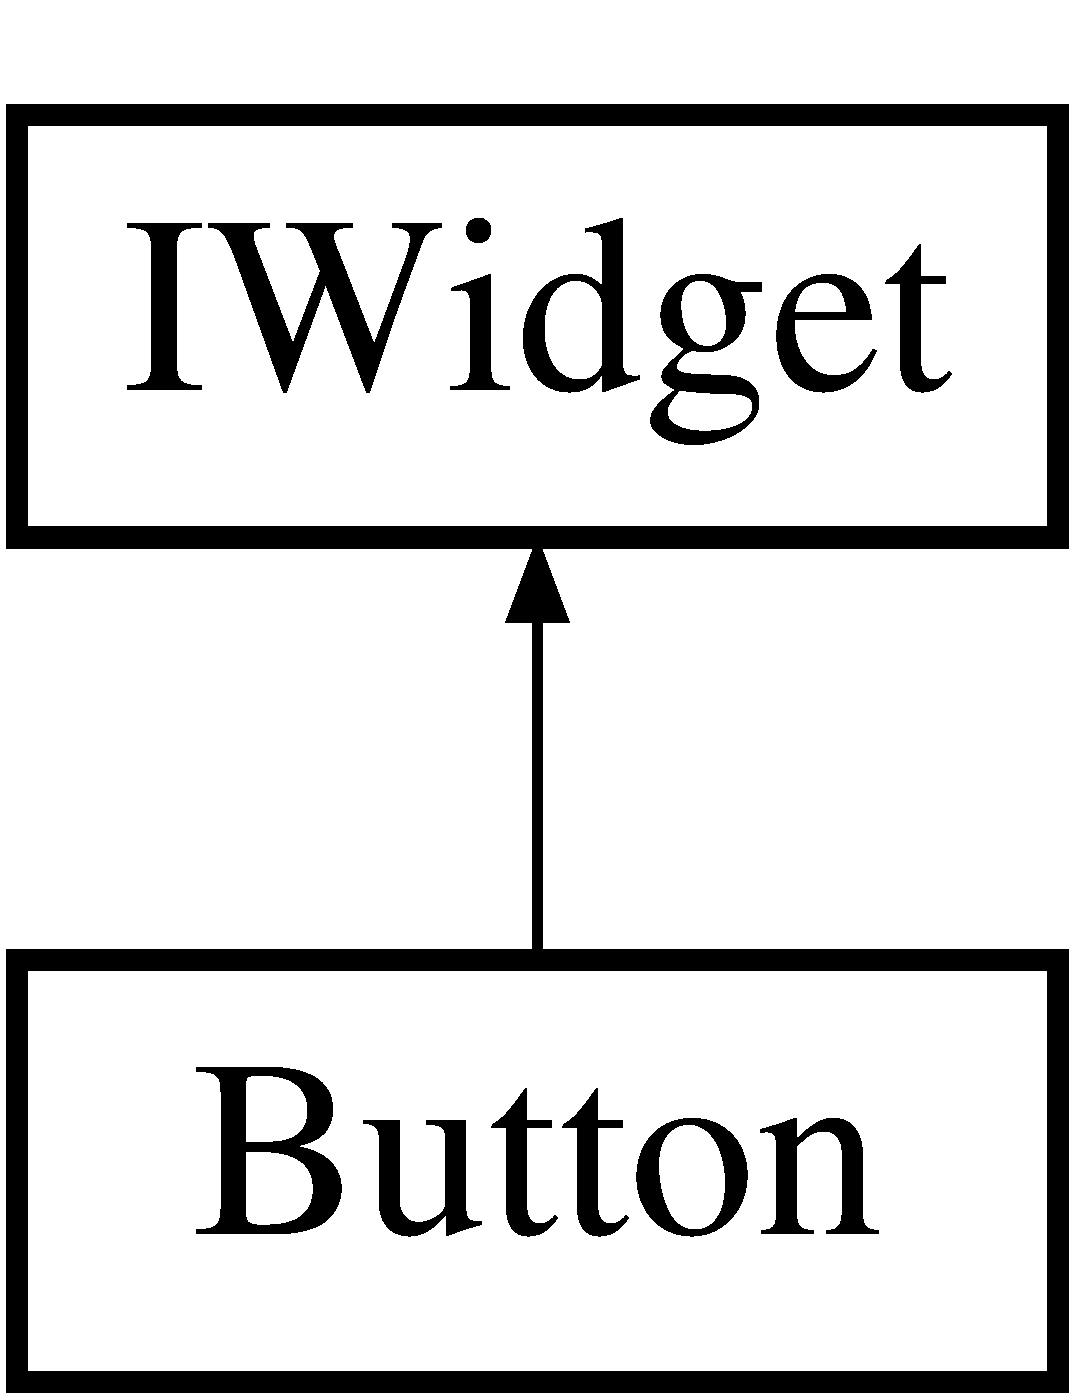
\includegraphics[height=2.000000cm]{classButton}
\end{center}
\end{figure}
\subsection*{Public Member Functions}
\begin{DoxyCompactItemize}
\item 
\hyperlink{classButton_a5729094ff8ec4ce3e64e6691c297983c}{Button} (const Rect \&rect, const wchar\+\_\+t $\ast$text, const wchar\+\_\+t $\ast$tooltext, enum indie\+::\+G\+U\+I\+Button\+Id id, const wchar\+\_\+t $\ast$background=L\char`\"{}assets/menus/transparent.\+png\char`\"{})
\begin{DoxyCompactList}\small\item\em Constructor. \end{DoxyCompactList}\item 
\mbox{\Hypertarget{classButton_a2a001eb9c3cc8ae54768a850dd345002}\label{classButton_a2a001eb9c3cc8ae54768a850dd345002}} 
\hyperlink{classButton_a2a001eb9c3cc8ae54768a850dd345002}{$\sim$\+Button} ()
\begin{DoxyCompactList}\small\item\em Destructor. \end{DoxyCompactList}\item 
void \hyperlink{classButton_aaee0c62414711ae91084b05b38d0c8c5}{print} (\hyperlink{classWindow}{Window} $\ast$win)
\begin{DoxyCompactList}\small\item\em Print the button into the window. \end{DoxyCompactList}\end{DoxyCompactItemize}


\subsection{Detailed Description}
Represent a button in the user interface. 

\subsection{Constructor \& Destructor Documentation}
\mbox{\Hypertarget{classButton_a5729094ff8ec4ce3e64e6691c297983c}\label{classButton_a5729094ff8ec4ce3e64e6691c297983c}} 
\index{Button@{Button}!Button@{Button}}
\index{Button@{Button}!Button@{Button}}
\subsubsection{\texorpdfstring{Button()}{Button()}}
{\footnotesize\ttfamily Button\+::\+Button (\begin{DoxyParamCaption}\item[{const Rect \&}]{rect,  }\item[{const wchar\+\_\+t $\ast$}]{text,  }\item[{const wchar\+\_\+t $\ast$}]{tooltext,  }\item[{enum indie\+::\+G\+U\+I\+Button\+Id}]{id,  }\item[{const wchar\+\_\+t $\ast$}]{background = {\ttfamily L\char`\"{}assets/menus/transparent.png\char`\"{}} }\end{DoxyParamCaption})}



Constructor. 

Build the class.


\begin{DoxyParams}{Parameters}
{\em rect} & The rectangle who represent the button (x1, y1, x2, y2). \\
\hline
{\em background} & The name of the image, that will be put on the background of the button. \\
\hline
{\em text} & the text that will be write on the button. \\
\hline
{\em tooltext} & The text displayed in the tooltip. \\
\hline
{\em id} & The id throw the user click on the button . \\
\hline
\end{DoxyParams}


\subsection{Member Function Documentation}
\mbox{\Hypertarget{classButton_aaee0c62414711ae91084b05b38d0c8c5}\label{classButton_aaee0c62414711ae91084b05b38d0c8c5}} 
\index{Button@{Button}!print@{print}}
\index{print@{print}!Button@{Button}}
\subsubsection{\texorpdfstring{print()}{print()}}
{\footnotesize\ttfamily void Button\+::print (\begin{DoxyParamCaption}\item[{\hyperlink{classWindow}{Window} $\ast$}]{win }\end{DoxyParamCaption})\hspace{0.3cm}{\ttfamily [virtual]}}



Print the button into the window. 


\begin{DoxyParams}{Parameters}
{\em win} & The window where the button will be print. \\
\hline
\end{DoxyParams}


Implements \hyperlink{classIWidget_a0cfa49a402e9bb31808a715e048ab2f4}{I\+Widget}.



The documentation for this class was generated from the following files\+:\begin{DoxyCompactItemize}
\item 
inc/graphics/widgets/\hyperlink{Button_8hh}{Button.\+hh}\item 
src/graphics/widgets/Button.\+cpp\end{DoxyCompactItemize}

\hypertarget{classCamera}{}\section{Camera Class Reference}
\label{classCamera}\index{Camera@{Camera}}


where cameras behaviour is defined  




{\ttfamily \#include $<$Camera.\+hh$>$}

\subsection*{Public Member Functions}
\begin{DoxyCompactItemize}
\item 
\hyperlink{classCamera_a4ffc956956f49716d7fa3bff2591cd3a}{Camera} (\hyperlink{classirr_1_1scene_1_1ICameraSceneNode}{irr\+::scene\+::\+I\+Camera\+Scene\+Node} $\ast$const cam)
\begin{DoxyCompactList}\small\item\em instanciate \hyperlink{classCamera}{Camera} \end{DoxyCompactList}\item 
\mbox{\Hypertarget{classCamera_ad1897942d0ccf91052386388a497349f}\label{classCamera_ad1897942d0ccf91052386388a497349f}} 
\hyperlink{classCamera_ad1897942d0ccf91052386388a497349f}{$\sim$\+Camera} ()
\begin{DoxyCompactList}\small\item\em Destructor... \end{DoxyCompactList}\item 
void \hyperlink{classCamera_ad7d58a7f1ab2b31f120a0bdad677b300}{change\+Position} (\hyperlink{namespaceirr_1_1core_a06f169d08b5c429f5575acb7edbad811}{irr\+::core\+::vector3df} move)
\begin{DoxyCompactList}\small\item\em change absolute camera position \end{DoxyCompactList}\item 
void \hyperlink{classCamera_a8c11f289be05671191a4f91288155685}{change\+Sight} (\hyperlink{namespaceirr_1_1core_a06f169d08b5c429f5575acb7edbad811}{irr\+::core\+::vector3df} new\+Target)
\begin{DoxyCompactList}\small\item\em change camera sight \end{DoxyCompactList}\end{DoxyCompactItemize}


\subsection{Detailed Description}
where cameras behaviour is defined 

\subsection{Constructor \& Destructor Documentation}
\mbox{\Hypertarget{classCamera_a4ffc956956f49716d7fa3bff2591cd3a}\label{classCamera_a4ffc956956f49716d7fa3bff2591cd3a}} 
\index{Camera@{Camera}!Camera@{Camera}}
\index{Camera@{Camera}!Camera@{Camera}}
\subsubsection{\texorpdfstring{Camera()}{Camera()}}
{\footnotesize\ttfamily Camera\+::\+Camera (\begin{DoxyParamCaption}\item[{\hyperlink{classirr_1_1scene_1_1ICameraSceneNode}{irr\+::scene\+::\+I\+Camera\+Scene\+Node} $\ast$const}]{cam }\end{DoxyParamCaption})}



instanciate \hyperlink{classCamera}{Camera} 


\begin{DoxyParams}{Parameters}
{\em cam} & \+: the irrlicht static camera \\
\hline
\end{DoxyParams}


\subsection{Member Function Documentation}
\mbox{\Hypertarget{classCamera_ad7d58a7f1ab2b31f120a0bdad677b300}\label{classCamera_ad7d58a7f1ab2b31f120a0bdad677b300}} 
\index{Camera@{Camera}!change\+Position@{change\+Position}}
\index{change\+Position@{change\+Position}!Camera@{Camera}}
\subsubsection{\texorpdfstring{change\+Position()}{changePosition()}}
{\footnotesize\ttfamily void Camera\+::change\+Position (\begin{DoxyParamCaption}\item[{\hyperlink{namespaceirr_1_1core_a06f169d08b5c429f5575acb7edbad811}{irr\+::core\+::vector3df}}]{move }\end{DoxyParamCaption})}



change absolute camera position 


\begin{DoxyParams}{Parameters}
{\em move} & \+: irrlicht 3D vector to positions camera \\
\hline
\end{DoxyParams}
\mbox{\Hypertarget{classCamera_a8c11f289be05671191a4f91288155685}\label{classCamera_a8c11f289be05671191a4f91288155685}} 
\index{Camera@{Camera}!change\+Sight@{change\+Sight}}
\index{change\+Sight@{change\+Sight}!Camera@{Camera}}
\subsubsection{\texorpdfstring{change\+Sight()}{changeSight()}}
{\footnotesize\ttfamily void Camera\+::change\+Sight (\begin{DoxyParamCaption}\item[{\hyperlink{namespaceirr_1_1core_a06f169d08b5c429f5575acb7edbad811}{irr\+::core\+::vector3df}}]{new\+Target }\end{DoxyParamCaption})}



change camera sight 



The documentation for this class was generated from the following files\+:\begin{DoxyCompactItemize}
\item 
inc/graphics/\hyperlink{Camera_8hh}{Camera.\+hh}\item 
src/graphics/Camera.\+cpp\end{DoxyCompactItemize}

\hypertarget{classirr_1_1core_1_1CMatrix4}{}\section{irr\+:\+:core\+:\+:C\+Matrix4$<$ T $>$ Class Template Reference}
\label{classirr_1_1core_1_1CMatrix4}\index{irr\+::core\+::\+C\+Matrix4$<$ T $>$@{irr\+::core\+::\+C\+Matrix4$<$ T $>$}}


4x4 matrix. Mostly used as transformation matrix for 3d calculations.  




{\ttfamily \#include $<$matrix4.\+h$>$}

\subsection*{Public Types}
\begin{DoxyCompactItemize}
\item 
\mbox{\Hypertarget{classirr_1_1core_1_1CMatrix4_a7bb79712227617f706ed57a34f3eb4fe}\label{classirr_1_1core_1_1CMatrix4_a7bb79712227617f706ed57a34f3eb4fe}} 
enum \hyperlink{classirr_1_1core_1_1CMatrix4_a7bb79712227617f706ed57a34f3eb4fe}{e\+Constructor} \begin{DoxyCompactList}\small\item\em Constructor Flags. \end{DoxyCompactList}
\end{DoxyCompactItemize}
\subsection*{Public Member Functions}
\begin{DoxyCompactItemize}
\item 
\hyperlink{classirr_1_1core_1_1CMatrix4_af771bfde63cdaa3baa4d9f6121e56411}{C\+Matrix4} (\hyperlink{classirr_1_1core_1_1CMatrix4_a7bb79712227617f706ed57a34f3eb4fe}{e\+Constructor} constructor=E\+M4\+C\+O\+N\+S\+T\+\_\+\+I\+D\+E\+N\+T\+I\+TY)
\begin{DoxyCompactList}\small\item\em Default constructor. \end{DoxyCompactList}\item 
\hyperlink{classirr_1_1core_1_1CMatrix4_acdb7afc2248d97a7e882cd1bdeed07b7}{C\+Matrix4} (const \hyperlink{classirr_1_1core_1_1CMatrix4}{C\+Matrix4}$<$ T $>$ \&other, \hyperlink{classirr_1_1core_1_1CMatrix4_a7bb79712227617f706ed57a34f3eb4fe}{e\+Constructor} constructor=E\+M4\+C\+O\+N\+S\+T\+\_\+\+C\+O\+PY)
\begin{DoxyCompactList}\small\item\em Copy constructor. \end{DoxyCompactList}\item 
\mbox{\Hypertarget{classirr_1_1core_1_1CMatrix4_aaede6824ed3ee05b928815d52e1834d1}\label{classirr_1_1core_1_1CMatrix4_aaede6824ed3ee05b928815d52e1834d1}} 
T \& \hyperlink{classirr_1_1core_1_1CMatrix4_aaede6824ed3ee05b928815d52e1834d1}{operator()} (const \hyperlink{namespaceirr_ac66849b7a6ed16e30ebede579f9b47c6}{s32} row, const \hyperlink{namespaceirr_ac66849b7a6ed16e30ebede579f9b47c6}{s32} col)
\begin{DoxyCompactList}\small\item\em Simple operator for directly accessing every element of the matrix. \end{DoxyCompactList}\item 
\mbox{\Hypertarget{classirr_1_1core_1_1CMatrix4_ae46b8b6b47897f4bc8eee2d1c226cab8}\label{classirr_1_1core_1_1CMatrix4_ae46b8b6b47897f4bc8eee2d1c226cab8}} 
const T \& \hyperlink{classirr_1_1core_1_1CMatrix4_ae46b8b6b47897f4bc8eee2d1c226cab8}{operator()} (const \hyperlink{namespaceirr_ac66849b7a6ed16e30ebede579f9b47c6}{s32} row, const \hyperlink{namespaceirr_ac66849b7a6ed16e30ebede579f9b47c6}{s32} col) const
\begin{DoxyCompactList}\small\item\em Simple operator for directly accessing every element of the matrix. \end{DoxyCompactList}\item 
\mbox{\Hypertarget{classirr_1_1core_1_1CMatrix4_aead4909f8bb2ab40875af175caf0085f}\label{classirr_1_1core_1_1CMatrix4_aead4909f8bb2ab40875af175caf0085f}} 
T \& \hyperlink{classirr_1_1core_1_1CMatrix4_aead4909f8bb2ab40875af175caf0085f}{operator\mbox{[}$\,$\mbox{]}} (\hyperlink{namespaceirr_a0416a53257075833e7002efd0a18e804}{u32} index)
\begin{DoxyCompactList}\small\item\em Simple operator for linearly accessing every element of the matrix. \end{DoxyCompactList}\item 
\mbox{\Hypertarget{classirr_1_1core_1_1CMatrix4_a9e34c4b4872d7f8fe587eff776585270}\label{classirr_1_1core_1_1CMatrix4_a9e34c4b4872d7f8fe587eff776585270}} 
const T \& \hyperlink{classirr_1_1core_1_1CMatrix4_a9e34c4b4872d7f8fe587eff776585270}{operator\mbox{[}$\,$\mbox{]}} (\hyperlink{namespaceirr_a0416a53257075833e7002efd0a18e804}{u32} index) const
\begin{DoxyCompactList}\small\item\em Simple operator for linearly accessing every element of the matrix. \end{DoxyCompactList}\item 
\mbox{\Hypertarget{classirr_1_1core_1_1CMatrix4_a47571eb3acae9a6aa330a03edcea7896}\label{classirr_1_1core_1_1CMatrix4_a47571eb3acae9a6aa330a03edcea7896}} 
\hyperlink{classirr_1_1core_1_1CMatrix4}{C\+Matrix4}$<$ T $>$ \& \hyperlink{classirr_1_1core_1_1CMatrix4_a47571eb3acae9a6aa330a03edcea7896}{operator=} (const \hyperlink{classirr_1_1core_1_1CMatrix4}{C\+Matrix4}$<$ T $>$ \&other)
\begin{DoxyCompactList}\small\item\em Sets this matrix equal to the other matrix. \end{DoxyCompactList}\item 
\mbox{\Hypertarget{classirr_1_1core_1_1CMatrix4_aa77c0ec30f4e42f7281392440898e9e3}\label{classirr_1_1core_1_1CMatrix4_aa77c0ec30f4e42f7281392440898e9e3}} 
\hyperlink{classirr_1_1core_1_1CMatrix4}{C\+Matrix4}$<$ T $>$ \& \hyperlink{classirr_1_1core_1_1CMatrix4_aa77c0ec30f4e42f7281392440898e9e3}{operator=} (const T \&scalar)
\begin{DoxyCompactList}\small\item\em Sets all elements of this matrix to the value. \end{DoxyCompactList}\item 
\mbox{\Hypertarget{classirr_1_1core_1_1CMatrix4_a4d258434b1baa3a52f1ae35903ca97f9}\label{classirr_1_1core_1_1CMatrix4_a4d258434b1baa3a52f1ae35903ca97f9}} 
const T $\ast$ \hyperlink{classirr_1_1core_1_1CMatrix4_a4d258434b1baa3a52f1ae35903ca97f9}{pointer} () const
\begin{DoxyCompactList}\small\item\em Returns pointer to internal array. \end{DoxyCompactList}\item 
\mbox{\Hypertarget{classirr_1_1core_1_1CMatrix4_abcff3ee7f4d4e1c9ff23193ca0827d16}\label{classirr_1_1core_1_1CMatrix4_abcff3ee7f4d4e1c9ff23193ca0827d16}} 
bool \hyperlink{classirr_1_1core_1_1CMatrix4_abcff3ee7f4d4e1c9ff23193ca0827d16}{operator==} (const \hyperlink{classirr_1_1core_1_1CMatrix4}{C\+Matrix4}$<$ T $>$ \&other) const
\begin{DoxyCompactList}\small\item\em Returns true if other matrix is equal to this matrix. \end{DoxyCompactList}\item 
\mbox{\Hypertarget{classirr_1_1core_1_1CMatrix4_a58b6bf4873a479ad15e809706e02e2cf}\label{classirr_1_1core_1_1CMatrix4_a58b6bf4873a479ad15e809706e02e2cf}} 
bool \hyperlink{classirr_1_1core_1_1CMatrix4_a58b6bf4873a479ad15e809706e02e2cf}{operator!=} (const \hyperlink{classirr_1_1core_1_1CMatrix4}{C\+Matrix4}$<$ T $>$ \&other) const
\begin{DoxyCompactList}\small\item\em Returns true if other matrix is not equal to this matrix. \end{DoxyCompactList}\item 
\mbox{\Hypertarget{classirr_1_1core_1_1CMatrix4_ac4a10f2ddd8a29cb9476eea061f33616}\label{classirr_1_1core_1_1CMatrix4_ac4a10f2ddd8a29cb9476eea061f33616}} 
\hyperlink{classirr_1_1core_1_1CMatrix4}{C\+Matrix4}$<$ T $>$ \hyperlink{classirr_1_1core_1_1CMatrix4_ac4a10f2ddd8a29cb9476eea061f33616}{operator+} (const \hyperlink{classirr_1_1core_1_1CMatrix4}{C\+Matrix4}$<$ T $>$ \&other) const
\begin{DoxyCompactList}\small\item\em Add another matrix. \end{DoxyCompactList}\item 
\mbox{\Hypertarget{classirr_1_1core_1_1CMatrix4_af91c5be0562ce4be3f8feedd3d017ba1}\label{classirr_1_1core_1_1CMatrix4_af91c5be0562ce4be3f8feedd3d017ba1}} 
\hyperlink{classirr_1_1core_1_1CMatrix4}{C\+Matrix4}$<$ T $>$ \& \hyperlink{classirr_1_1core_1_1CMatrix4_af91c5be0562ce4be3f8feedd3d017ba1}{operator+=} (const \hyperlink{classirr_1_1core_1_1CMatrix4}{C\+Matrix4}$<$ T $>$ \&other)
\begin{DoxyCompactList}\small\item\em Add another matrix. \end{DoxyCompactList}\item 
\mbox{\Hypertarget{classirr_1_1core_1_1CMatrix4_ab7a7ba0d368bd2de010cb33191492443}\label{classirr_1_1core_1_1CMatrix4_ab7a7ba0d368bd2de010cb33191492443}} 
\hyperlink{classirr_1_1core_1_1CMatrix4}{C\+Matrix4}$<$ T $>$ \hyperlink{classirr_1_1core_1_1CMatrix4_ab7a7ba0d368bd2de010cb33191492443}{operator-\/} (const \hyperlink{classirr_1_1core_1_1CMatrix4}{C\+Matrix4}$<$ T $>$ \&other) const
\begin{DoxyCompactList}\small\item\em Subtract another matrix. \end{DoxyCompactList}\item 
\mbox{\Hypertarget{classirr_1_1core_1_1CMatrix4_a24eb7faa1418765ba87d3f02f27d643f}\label{classirr_1_1core_1_1CMatrix4_a24eb7faa1418765ba87d3f02f27d643f}} 
\hyperlink{classirr_1_1core_1_1CMatrix4}{C\+Matrix4}$<$ T $>$ \& \hyperlink{classirr_1_1core_1_1CMatrix4_a24eb7faa1418765ba87d3f02f27d643f}{operator-\/=} (const \hyperlink{classirr_1_1core_1_1CMatrix4}{C\+Matrix4}$<$ T $>$ \&other)
\begin{DoxyCompactList}\small\item\em Subtract another matrix. \end{DoxyCompactList}\item 
\hyperlink{classirr_1_1core_1_1CMatrix4}{C\+Matrix4}$<$ T $>$ \& \hyperlink{classirr_1_1core_1_1CMatrix4_a8503c58913ba9407ba00b173d8a3e25c}{setbyproduct} (const \hyperlink{classirr_1_1core_1_1CMatrix4}{C\+Matrix4}$<$ T $>$ \&other\+\_\+a, const \hyperlink{classirr_1_1core_1_1CMatrix4}{C\+Matrix4}$<$ T $>$ \&other\+\_\+b)
\begin{DoxyCompactList}\small\item\em set this matrix to the product of two matrices \end{DoxyCompactList}\item 
\hyperlink{classirr_1_1core_1_1CMatrix4}{C\+Matrix4}$<$ T $>$ \& \hyperlink{classirr_1_1core_1_1CMatrix4_a526a2a11dcd8b18c9e77deb84094778d}{setbyproduct\+\_\+nocheck} (const \hyperlink{classirr_1_1core_1_1CMatrix4}{C\+Matrix4}$<$ T $>$ \&other\+\_\+a, const \hyperlink{classirr_1_1core_1_1CMatrix4}{C\+Matrix4}$<$ T $>$ \&other\+\_\+b)
\begin{DoxyCompactList}\small\item\em Set this matrix to the product of two matrices. \end{DoxyCompactList}\item 
\hyperlink{classirr_1_1core_1_1CMatrix4}{C\+Matrix4}$<$ T $>$ \hyperlink{classirr_1_1core_1_1CMatrix4_af5ecb6176941d57716bb800963042183}{operator$\ast$} (const \hyperlink{classirr_1_1core_1_1CMatrix4}{C\+Matrix4}$<$ T $>$ \&other) const
\begin{DoxyCompactList}\small\item\em Multiply by another matrix. \end{DoxyCompactList}\item 
\hyperlink{classirr_1_1core_1_1CMatrix4}{C\+Matrix4}$<$ T $>$ \& \hyperlink{classirr_1_1core_1_1CMatrix4_ac3d29f86c91d9d095ab155ecb8870f87}{operator$\ast$=} (const \hyperlink{classirr_1_1core_1_1CMatrix4}{C\+Matrix4}$<$ T $>$ \&other)
\begin{DoxyCompactList}\small\item\em Multiply by another matrix. \end{DoxyCompactList}\item 
\mbox{\Hypertarget{classirr_1_1core_1_1CMatrix4_a1557670c6fd5ff6ea72220764283dafb}\label{classirr_1_1core_1_1CMatrix4_a1557670c6fd5ff6ea72220764283dafb}} 
\hyperlink{classirr_1_1core_1_1CMatrix4}{C\+Matrix4}$<$ T $>$ \hyperlink{classirr_1_1core_1_1CMatrix4_a1557670c6fd5ff6ea72220764283dafb}{operator$\ast$} (const T \&scalar) const
\begin{DoxyCompactList}\small\item\em Multiply by scalar. \end{DoxyCompactList}\item 
\mbox{\Hypertarget{classirr_1_1core_1_1CMatrix4_ae78879a3d7f0113ba5208d5476c3af9c}\label{classirr_1_1core_1_1CMatrix4_ae78879a3d7f0113ba5208d5476c3af9c}} 
\hyperlink{classirr_1_1core_1_1CMatrix4}{C\+Matrix4}$<$ T $>$ \& \hyperlink{classirr_1_1core_1_1CMatrix4_ae78879a3d7f0113ba5208d5476c3af9c}{operator$\ast$=} (const T \&scalar)
\begin{DoxyCompactList}\small\item\em Multiply by scalar. \end{DoxyCompactList}\item 
\mbox{\Hypertarget{classirr_1_1core_1_1CMatrix4_a45f876ed1aed2c3c98b87fee6d938604}\label{classirr_1_1core_1_1CMatrix4_a45f876ed1aed2c3c98b87fee6d938604}} 
\hyperlink{classirr_1_1core_1_1CMatrix4}{C\+Matrix4}$<$ T $>$ \& \hyperlink{classirr_1_1core_1_1CMatrix4_a45f876ed1aed2c3c98b87fee6d938604}{make\+Identity} ()
\begin{DoxyCompactList}\small\item\em Set matrix to identity. \end{DoxyCompactList}\item 
\mbox{\Hypertarget{classirr_1_1core_1_1CMatrix4_a01fb063cdc136aaa827c883a3ab6cac4}\label{classirr_1_1core_1_1CMatrix4_a01fb063cdc136aaa827c883a3ab6cac4}} 
bool \hyperlink{classirr_1_1core_1_1CMatrix4_a01fb063cdc136aaa827c883a3ab6cac4}{is\+Identity} () const
\begin{DoxyCompactList}\small\item\em Returns true if the matrix is the identity matrix. \end{DoxyCompactList}\item 
\mbox{\Hypertarget{classirr_1_1core_1_1CMatrix4_a7166c462168855cb8c6aeb2fb76fa3cb}\label{classirr_1_1core_1_1CMatrix4_a7166c462168855cb8c6aeb2fb76fa3cb}} 
bool \hyperlink{classirr_1_1core_1_1CMatrix4_a7166c462168855cb8c6aeb2fb76fa3cb}{is\+Orthogonal} () const
\begin{DoxyCompactList}\small\item\em Returns true if the matrix is orthogonal. \end{DoxyCompactList}\item 
\mbox{\Hypertarget{classirr_1_1core_1_1CMatrix4_ad4fc4d401a2b40074b62882873c71e62}\label{classirr_1_1core_1_1CMatrix4_ad4fc4d401a2b40074b62882873c71e62}} 
bool \hyperlink{classirr_1_1core_1_1CMatrix4_ad4fc4d401a2b40074b62882873c71e62}{is\+Identity\+\_\+integer\+\_\+base} () const
\begin{DoxyCompactList}\small\item\em Returns true if the matrix is the identity matrix. \end{DoxyCompactList}\item 
\mbox{\Hypertarget{classirr_1_1core_1_1CMatrix4_ac04a3b341cbfbb7986be682691655622}\label{classirr_1_1core_1_1CMatrix4_ac04a3b341cbfbb7986be682691655622}} 
\hyperlink{classirr_1_1core_1_1CMatrix4}{C\+Matrix4}$<$ T $>$ \& \hyperlink{classirr_1_1core_1_1CMatrix4_ac04a3b341cbfbb7986be682691655622}{set\+Translation} (const \hyperlink{classirr_1_1core_1_1vector3d}{vector3d}$<$ T $>$ \&translation)
\begin{DoxyCompactList}\small\item\em Set the translation of the current matrix. Will erase any previous values. \end{DoxyCompactList}\item 
\mbox{\Hypertarget{classirr_1_1core_1_1CMatrix4_a574f83a4c1c6809f71ccb200020983f7}\label{classirr_1_1core_1_1CMatrix4_a574f83a4c1c6809f71ccb200020983f7}} 
\hyperlink{classirr_1_1core_1_1vector3d}{vector3d}$<$ T $>$ \hyperlink{classirr_1_1core_1_1CMatrix4_a574f83a4c1c6809f71ccb200020983f7}{get\+Translation} () const
\begin{DoxyCompactList}\small\item\em Gets the current translation. \end{DoxyCompactList}\item 
\mbox{\Hypertarget{classirr_1_1core_1_1CMatrix4_a258e103fcb6ce1564978624280ecb7fe}\label{classirr_1_1core_1_1CMatrix4_a258e103fcb6ce1564978624280ecb7fe}} 
\hyperlink{classirr_1_1core_1_1CMatrix4}{C\+Matrix4}$<$ T $>$ \& \hyperlink{classirr_1_1core_1_1CMatrix4_a258e103fcb6ce1564978624280ecb7fe}{set\+Inverse\+Translation} (const \hyperlink{classirr_1_1core_1_1vector3d}{vector3d}$<$ T $>$ \&translation)
\begin{DoxyCompactList}\small\item\em Set the inverse translation of the current matrix. Will erase any previous values. \end{DoxyCompactList}\item 
\mbox{\Hypertarget{classirr_1_1core_1_1CMatrix4_a05aac7bd2e7651369fc813a51258afbe}\label{classirr_1_1core_1_1CMatrix4_a05aac7bd2e7651369fc813a51258afbe}} 
\hyperlink{classirr_1_1core_1_1CMatrix4}{C\+Matrix4}$<$ T $>$ \& \hyperlink{classirr_1_1core_1_1CMatrix4_a05aac7bd2e7651369fc813a51258afbe}{set\+Rotation\+Radians} (const \hyperlink{classirr_1_1core_1_1vector3d}{vector3d}$<$ T $>$ \&rotation)
\begin{DoxyCompactList}\small\item\em Make a rotation matrix from Euler angles. The 4th row and column are unmodified. \end{DoxyCompactList}\item 
\mbox{\Hypertarget{classirr_1_1core_1_1CMatrix4_a8ee5ef8619d4b0f56d72ac84495ed644}\label{classirr_1_1core_1_1CMatrix4_a8ee5ef8619d4b0f56d72ac84495ed644}} 
\hyperlink{classirr_1_1core_1_1CMatrix4}{C\+Matrix4}$<$ T $>$ \& \hyperlink{classirr_1_1core_1_1CMatrix4_a8ee5ef8619d4b0f56d72ac84495ed644}{set\+Rotation\+Degrees} (const \hyperlink{classirr_1_1core_1_1vector3d}{vector3d}$<$ T $>$ \&rotation)
\begin{DoxyCompactList}\small\item\em Make a rotation matrix from Euler angles. The 4th row and column are unmodified. \end{DoxyCompactList}\item 
\hyperlink{classirr_1_1core_1_1vector3d}{core\+::vector3d}$<$ T $>$ \hyperlink{classirr_1_1core_1_1CMatrix4_ad334281fcd12eb5acda020981706b759}{get\+Rotation\+Degrees} () const
\begin{DoxyCompactList}\small\item\em Returns the rotation, as set by set\+Rotation(). \end{DoxyCompactList}\item 
\hyperlink{classirr_1_1core_1_1CMatrix4}{C\+Matrix4}$<$ T $>$ \& \hyperlink{classirr_1_1core_1_1CMatrix4_a1a15d7b55769678512144f0fb7e15a92}{set\+Inverse\+Rotation\+Radians} (const \hyperlink{classirr_1_1core_1_1vector3d}{vector3d}$<$ T $>$ \&rotation)
\begin{DoxyCompactList}\small\item\em Make an inverted rotation matrix from Euler angles. \end{DoxyCompactList}\item 
\hyperlink{classirr_1_1core_1_1CMatrix4}{C\+Matrix4}$<$ T $>$ \& \hyperlink{classirr_1_1core_1_1CMatrix4_afd84b9c93b4c8e9dc2abefa4a28057f9}{set\+Inverse\+Rotation\+Degrees} (const \hyperlink{classirr_1_1core_1_1vector3d}{vector3d}$<$ T $>$ \&rotation)
\begin{DoxyCompactList}\small\item\em Make an inverted rotation matrix from Euler angles. \end{DoxyCompactList}\item 
\hyperlink{classirr_1_1core_1_1CMatrix4}{C\+Matrix4}$<$ T $>$ \& \hyperlink{classirr_1_1core_1_1CMatrix4_a2fad61540e78fc7dafe7f6270b0558ac}{set\+Rotation\+Axis\+Radians} (const T \&angle, const \hyperlink{classirr_1_1core_1_1vector3d}{vector3d}$<$ T $>$ \&axis)
\begin{DoxyCompactList}\small\item\em Make a rotation matrix from angle and axis, assuming left handed rotation. \end{DoxyCompactList}\item 
\mbox{\Hypertarget{classirr_1_1core_1_1CMatrix4_a47117d44419af87e70084c01ab852049}\label{classirr_1_1core_1_1CMatrix4_a47117d44419af87e70084c01ab852049}} 
\hyperlink{classirr_1_1core_1_1CMatrix4}{C\+Matrix4}$<$ T $>$ \& \hyperlink{classirr_1_1core_1_1CMatrix4_a47117d44419af87e70084c01ab852049}{set\+Scale} (const \hyperlink{classirr_1_1core_1_1vector3d}{vector3d}$<$ T $>$ \&scale)
\begin{DoxyCompactList}\small\item\em Set Scale. \end{DoxyCompactList}\item 
\mbox{\Hypertarget{classirr_1_1core_1_1CMatrix4_a18af980e2bc3575f60576b6d4b4cc0f3}\label{classirr_1_1core_1_1CMatrix4_a18af980e2bc3575f60576b6d4b4cc0f3}} 
\hyperlink{classirr_1_1core_1_1CMatrix4}{C\+Matrix4}$<$ T $>$ \& \hyperlink{classirr_1_1core_1_1CMatrix4_a18af980e2bc3575f60576b6d4b4cc0f3}{set\+Scale} (const T scale)
\begin{DoxyCompactList}\small\item\em Set Scale. \end{DoxyCompactList}\item 
\hyperlink{classirr_1_1core_1_1vector3d}{core\+::vector3d}$<$ T $>$ \hyperlink{classirr_1_1core_1_1CMatrix4_a27801e0cb2d3ce458f66ff7cfbe13544}{get\+Scale} () const
\begin{DoxyCompactList}\small\item\em Get Scale. \end{DoxyCompactList}\item 
\mbox{\Hypertarget{classirr_1_1core_1_1CMatrix4_a7850ba9e85bff2b7d8e3bce517e0aba0}\label{classirr_1_1core_1_1CMatrix4_a7850ba9e85bff2b7d8e3bce517e0aba0}} 
void \hyperlink{classirr_1_1core_1_1CMatrix4_a7850ba9e85bff2b7d8e3bce517e0aba0}{inverse\+Translate\+Vect} (\hyperlink{namespaceirr_1_1core_a06f169d08b5c429f5575acb7edbad811}{vector3df} \&vect) const
\begin{DoxyCompactList}\small\item\em Translate a vector by the inverse of the translation part of this matrix. \end{DoxyCompactList}\item 
\mbox{\Hypertarget{classirr_1_1core_1_1CMatrix4_aed5bc8bb8e9b58549034e2f48189d35e}\label{classirr_1_1core_1_1CMatrix4_aed5bc8bb8e9b58549034e2f48189d35e}} 
void \hyperlink{classirr_1_1core_1_1CMatrix4_aed5bc8bb8e9b58549034e2f48189d35e}{inverse\+Rotate\+Vect} (\hyperlink{namespaceirr_1_1core_a06f169d08b5c429f5575acb7edbad811}{vector3df} \&vect) const
\begin{DoxyCompactList}\small\item\em Rotate a vector by the inverse of the rotation part of this matrix. \end{DoxyCompactList}\item 
\mbox{\Hypertarget{classirr_1_1core_1_1CMatrix4_a45e023efd5e6d0e328c63705bfb5bd06}\label{classirr_1_1core_1_1CMatrix4_a45e023efd5e6d0e328c63705bfb5bd06}} 
void \hyperlink{classirr_1_1core_1_1CMatrix4_a45e023efd5e6d0e328c63705bfb5bd06}{rotate\+Vect} (\hyperlink{namespaceirr_1_1core_a06f169d08b5c429f5575acb7edbad811}{vector3df} \&vect) const
\begin{DoxyCompactList}\small\item\em Rotate a vector by the rotation part of this matrix. \end{DoxyCompactList}\item 
\mbox{\Hypertarget{classirr_1_1core_1_1CMatrix4_aa421db751017ae447e20ac946bb4ad92}\label{classirr_1_1core_1_1CMatrix4_aa421db751017ae447e20ac946bb4ad92}} 
void \hyperlink{classirr_1_1core_1_1CMatrix4_aa421db751017ae447e20ac946bb4ad92}{rotate\+Vect} (\hyperlink{namespaceirr_1_1core_a06f169d08b5c429f5575acb7edbad811}{core\+::vector3df} \&out, const \hyperlink{namespaceirr_1_1core_a06f169d08b5c429f5575acb7edbad811}{core\+::vector3df} \&in) const
\begin{DoxyCompactList}\small\item\em An alternate transform vector method, writing into a second vector. \end{DoxyCompactList}\item 
\mbox{\Hypertarget{classirr_1_1core_1_1CMatrix4_aceb5e3d8e3b1816b6df5e83717425b7f}\label{classirr_1_1core_1_1CMatrix4_aceb5e3d8e3b1816b6df5e83717425b7f}} 
void \hyperlink{classirr_1_1core_1_1CMatrix4_aceb5e3d8e3b1816b6df5e83717425b7f}{rotate\+Vect} (T $\ast$out, const \hyperlink{namespaceirr_1_1core_a06f169d08b5c429f5575acb7edbad811}{core\+::vector3df} \&in) const
\begin{DoxyCompactList}\small\item\em An alternate transform vector method, writing into an array of 3 floats. \end{DoxyCompactList}\item 
\mbox{\Hypertarget{classirr_1_1core_1_1CMatrix4_a4f100721bb28df8b71b21ec10b9c2db6}\label{classirr_1_1core_1_1CMatrix4_a4f100721bb28df8b71b21ec10b9c2db6}} 
void \hyperlink{classirr_1_1core_1_1CMatrix4_a4f100721bb28df8b71b21ec10b9c2db6}{transform\+Vect} (\hyperlink{namespaceirr_1_1core_a06f169d08b5c429f5575acb7edbad811}{vector3df} \&vect) const
\begin{DoxyCompactList}\small\item\em Transforms the vector by this matrix. \end{DoxyCompactList}\item 
\mbox{\Hypertarget{classirr_1_1core_1_1CMatrix4_a4d530a7c16fa9f6c025c1508e0058451}\label{classirr_1_1core_1_1CMatrix4_a4d530a7c16fa9f6c025c1508e0058451}} 
void \hyperlink{classirr_1_1core_1_1CMatrix4_a4d530a7c16fa9f6c025c1508e0058451}{transform\+Vect} (\hyperlink{namespaceirr_1_1core_a06f169d08b5c429f5575acb7edbad811}{vector3df} \&out, const \hyperlink{namespaceirr_1_1core_a06f169d08b5c429f5575acb7edbad811}{vector3df} \&in) const
\begin{DoxyCompactList}\small\item\em Transforms input vector by this matrix and stores result in output vector. \end{DoxyCompactList}\item 
\mbox{\Hypertarget{classirr_1_1core_1_1CMatrix4_a1f23d4c668869f28c89d400518352879}\label{classirr_1_1core_1_1CMatrix4_a1f23d4c668869f28c89d400518352879}} 
void \hyperlink{classirr_1_1core_1_1CMatrix4_a1f23d4c668869f28c89d400518352879}{transform\+Vect} (T $\ast$out, const \hyperlink{namespaceirr_1_1core_a06f169d08b5c429f5575acb7edbad811}{core\+::vector3df} \&in) const
\begin{DoxyCompactList}\small\item\em An alternate transform vector method, writing into an array of 4 floats. \end{DoxyCompactList}\item 
\mbox{\Hypertarget{classirr_1_1core_1_1CMatrix4_ab7a9dd4ba9f04fd5396dd116e8f5a1c0}\label{classirr_1_1core_1_1CMatrix4_ab7a9dd4ba9f04fd5396dd116e8f5a1c0}} 
void \hyperlink{classirr_1_1core_1_1CMatrix4_ab7a9dd4ba9f04fd5396dd116e8f5a1c0}{transform\+Vec3} (T $\ast$out, const T $\ast$in) const
\begin{DoxyCompactList}\small\item\em An alternate transform vector method, reading from and writing to an array of 3 floats. \end{DoxyCompactList}\item 
\mbox{\Hypertarget{classirr_1_1core_1_1CMatrix4_ac1b339a76eb0d2ce58dd69be896ed38a}\label{classirr_1_1core_1_1CMatrix4_ac1b339a76eb0d2ce58dd69be896ed38a}} 
void \hyperlink{classirr_1_1core_1_1CMatrix4_ac1b339a76eb0d2ce58dd69be896ed38a}{translate\+Vect} (\hyperlink{namespaceirr_1_1core_a06f169d08b5c429f5575acb7edbad811}{vector3df} \&vect) const
\begin{DoxyCompactList}\small\item\em Translate a vector by the translation part of this matrix. \end{DoxyCompactList}\item 
\mbox{\Hypertarget{classirr_1_1core_1_1CMatrix4_aa8324285dd538763f8e9cfa50cc04b62}\label{classirr_1_1core_1_1CMatrix4_aa8324285dd538763f8e9cfa50cc04b62}} 
void \hyperlink{classirr_1_1core_1_1CMatrix4_aa8324285dd538763f8e9cfa50cc04b62}{transform\+Plane} (\hyperlink{classirr_1_1core_1_1plane3d}{core\+::plane3d}$<$ \hyperlink{namespaceirr_a0277be98d67dc26ff93b1a6a1d086b07}{f32} $>$ \&plane) const
\begin{DoxyCompactList}\small\item\em Transforms a plane by this matrix. \end{DoxyCompactList}\item 
\mbox{\Hypertarget{classirr_1_1core_1_1CMatrix4_abba8dc0c37c86a50788066bba8dfb180}\label{classirr_1_1core_1_1CMatrix4_abba8dc0c37c86a50788066bba8dfb180}} 
void \hyperlink{classirr_1_1core_1_1CMatrix4_abba8dc0c37c86a50788066bba8dfb180}{transform\+Plane} (const \hyperlink{classirr_1_1core_1_1plane3d}{core\+::plane3d}$<$ \hyperlink{namespaceirr_a0277be98d67dc26ff93b1a6a1d086b07}{f32} $>$ \&in, \hyperlink{classirr_1_1core_1_1plane3d}{core\+::plane3d}$<$ \hyperlink{namespaceirr_a0277be98d67dc26ff93b1a6a1d086b07}{f32} $>$ \&out) const
\begin{DoxyCompactList}\small\item\em Transforms a plane by this matrix. \end{DoxyCompactList}\item 
void \hyperlink{classirr_1_1core_1_1CMatrix4_a0e6a0a3b1b20aac7313806fdb1a01316}{transform\+Box} (\hyperlink{classirr_1_1core_1_1aabbox3d}{core\+::aabbox3d}$<$ \hyperlink{namespaceirr_a0277be98d67dc26ff93b1a6a1d086b07}{f32} $>$ \&box) const
\begin{DoxyCompactList}\small\item\em Transforms a axis aligned bounding box. \end{DoxyCompactList}\item 
void \hyperlink{classirr_1_1core_1_1CMatrix4_a2fcdfa14ef16240470e2b46d19a5cb43}{transform\+Box\+Ex} (\hyperlink{classirr_1_1core_1_1aabbox3d}{core\+::aabbox3d}$<$ \hyperlink{namespaceirr_a0277be98d67dc26ff93b1a6a1d086b07}{f32} $>$ \&box) const
\begin{DoxyCompactList}\small\item\em Transforms a axis aligned bounding box. \end{DoxyCompactList}\item 
\mbox{\Hypertarget{classirr_1_1core_1_1CMatrix4_a21e0a68953d63bd1fca70a671a9e93b8}\label{classirr_1_1core_1_1CMatrix4_a21e0a68953d63bd1fca70a671a9e93b8}} 
void \hyperlink{classirr_1_1core_1_1CMatrix4_a21e0a68953d63bd1fca70a671a9e93b8}{multiply\+With1x4\+Matrix} (T $\ast$matrix) const
\begin{DoxyCompactList}\small\item\em Multiplies this matrix by a 1x4 matrix. \end{DoxyCompactList}\item 
bool \hyperlink{classirr_1_1core_1_1CMatrix4_a3fbface2cb6b959af64f82a5bb17540e}{make\+Inverse} ()
\begin{DoxyCompactList}\small\item\em Calculates inverse of matrix. Slow. \end{DoxyCompactList}\item 
bool \hyperlink{classirr_1_1core_1_1CMatrix4_aaeab6a8672ecc3d9790c8e7f141db795}{get\+Inverse\+Primitive} (\hyperlink{classirr_1_1core_1_1CMatrix4}{C\+Matrix4}$<$ T $>$ \&out) const
\begin{DoxyCompactList}\small\item\em Inverts a primitive matrix which only contains a translation and a rotation. \end{DoxyCompactList}\item 
bool \hyperlink{classirr_1_1core_1_1CMatrix4_a323bfa0e327636c9cd4a5d2b781b3a60}{get\+Inverse} (\hyperlink{classirr_1_1core_1_1CMatrix4}{C\+Matrix4}$<$ T $>$ \&out) const
\begin{DoxyCompactList}\small\item\em Gets the inversed matrix of this one. \end{DoxyCompactList}\item 
\mbox{\Hypertarget{classirr_1_1core_1_1CMatrix4_a5bea6c6f5479720841cea61651e35879}\label{classirr_1_1core_1_1CMatrix4_a5bea6c6f5479720841cea61651e35879}} 
\hyperlink{classirr_1_1core_1_1CMatrix4}{C\+Matrix4}$<$ T $>$ \& \hyperlink{classirr_1_1core_1_1CMatrix4_a5bea6c6f5479720841cea61651e35879}{build\+Projection\+Matrix\+Perspective\+Fov\+RH} (\hyperlink{namespaceirr_a0277be98d67dc26ff93b1a6a1d086b07}{f32} field\+Of\+View\+Radians, \hyperlink{namespaceirr_a0277be98d67dc26ff93b1a6a1d086b07}{f32} aspect\+Ratio, \hyperlink{namespaceirr_a0277be98d67dc26ff93b1a6a1d086b07}{f32} z\+Near, \hyperlink{namespaceirr_a0277be98d67dc26ff93b1a6a1d086b07}{f32} z\+Far)
\begin{DoxyCompactList}\small\item\em Builds a right-\/handed perspective projection matrix based on a field of view. \end{DoxyCompactList}\item 
\mbox{\Hypertarget{classirr_1_1core_1_1CMatrix4_a1895b967a8f8c9d7ad90fe5434f2499f}\label{classirr_1_1core_1_1CMatrix4_a1895b967a8f8c9d7ad90fe5434f2499f}} 
\hyperlink{classirr_1_1core_1_1CMatrix4}{C\+Matrix4}$<$ T $>$ \& \hyperlink{classirr_1_1core_1_1CMatrix4_a1895b967a8f8c9d7ad90fe5434f2499f}{build\+Projection\+Matrix\+Perspective\+Fov\+LH} (\hyperlink{namespaceirr_a0277be98d67dc26ff93b1a6a1d086b07}{f32} field\+Of\+View\+Radians, \hyperlink{namespaceirr_a0277be98d67dc26ff93b1a6a1d086b07}{f32} aspect\+Ratio, \hyperlink{namespaceirr_a0277be98d67dc26ff93b1a6a1d086b07}{f32} z\+Near, \hyperlink{namespaceirr_a0277be98d67dc26ff93b1a6a1d086b07}{f32} z\+Far)
\begin{DoxyCompactList}\small\item\em Builds a left-\/handed perspective projection matrix based on a field of view. \end{DoxyCompactList}\item 
\mbox{\Hypertarget{classirr_1_1core_1_1CMatrix4_a3e4c3f6c545dd522f9f09177259f2f18}\label{classirr_1_1core_1_1CMatrix4_a3e4c3f6c545dd522f9f09177259f2f18}} 
\hyperlink{classirr_1_1core_1_1CMatrix4}{C\+Matrix4}$<$ T $>$ \& \hyperlink{classirr_1_1core_1_1CMatrix4_a3e4c3f6c545dd522f9f09177259f2f18}{build\+Projection\+Matrix\+Perspective\+Fov\+Infinity\+LH} (\hyperlink{namespaceirr_a0277be98d67dc26ff93b1a6a1d086b07}{f32} field\+Of\+View\+Radians, \hyperlink{namespaceirr_a0277be98d67dc26ff93b1a6a1d086b07}{f32} aspect\+Ratio, \hyperlink{namespaceirr_a0277be98d67dc26ff93b1a6a1d086b07}{f32} z\+Near, \hyperlink{namespaceirr_a0277be98d67dc26ff93b1a6a1d086b07}{f32} epsilon=0)
\begin{DoxyCompactList}\small\item\em Builds a left-\/handed perspective projection matrix based on a field of view, with far plane at infinity. \end{DoxyCompactList}\item 
\mbox{\Hypertarget{classirr_1_1core_1_1CMatrix4_a649a29922f622503399bcb16c97b78b4}\label{classirr_1_1core_1_1CMatrix4_a649a29922f622503399bcb16c97b78b4}} 
\hyperlink{classirr_1_1core_1_1CMatrix4}{C\+Matrix4}$<$ T $>$ \& \hyperlink{classirr_1_1core_1_1CMatrix4_a649a29922f622503399bcb16c97b78b4}{build\+Projection\+Matrix\+Perspective\+RH} (\hyperlink{namespaceirr_a0277be98d67dc26ff93b1a6a1d086b07}{f32} width\+Of\+View\+Volume, \hyperlink{namespaceirr_a0277be98d67dc26ff93b1a6a1d086b07}{f32} height\+Of\+View\+Volume, \hyperlink{namespaceirr_a0277be98d67dc26ff93b1a6a1d086b07}{f32} z\+Near, \hyperlink{namespaceirr_a0277be98d67dc26ff93b1a6a1d086b07}{f32} z\+Far)
\begin{DoxyCompactList}\small\item\em Builds a right-\/handed perspective projection matrix. \end{DoxyCompactList}\item 
\mbox{\Hypertarget{classirr_1_1core_1_1CMatrix4_a8306f02451b06f8e6710f23631654086}\label{classirr_1_1core_1_1CMatrix4_a8306f02451b06f8e6710f23631654086}} 
\hyperlink{classirr_1_1core_1_1CMatrix4}{C\+Matrix4}$<$ T $>$ \& \hyperlink{classirr_1_1core_1_1CMatrix4_a8306f02451b06f8e6710f23631654086}{build\+Projection\+Matrix\+Perspective\+LH} (\hyperlink{namespaceirr_a0277be98d67dc26ff93b1a6a1d086b07}{f32} width\+Of\+View\+Volume, \hyperlink{namespaceirr_a0277be98d67dc26ff93b1a6a1d086b07}{f32} height\+Of\+View\+Volume, \hyperlink{namespaceirr_a0277be98d67dc26ff93b1a6a1d086b07}{f32} z\+Near, \hyperlink{namespaceirr_a0277be98d67dc26ff93b1a6a1d086b07}{f32} z\+Far)
\begin{DoxyCompactList}\small\item\em Builds a left-\/handed perspective projection matrix. \end{DoxyCompactList}\item 
\mbox{\Hypertarget{classirr_1_1core_1_1CMatrix4_ae4a0618e2da724a26a5d8a201a63d8a5}\label{classirr_1_1core_1_1CMatrix4_ae4a0618e2da724a26a5d8a201a63d8a5}} 
\hyperlink{classirr_1_1core_1_1CMatrix4}{C\+Matrix4}$<$ T $>$ \& \hyperlink{classirr_1_1core_1_1CMatrix4_ae4a0618e2da724a26a5d8a201a63d8a5}{build\+Projection\+Matrix\+Ortho\+LH} (\hyperlink{namespaceirr_a0277be98d67dc26ff93b1a6a1d086b07}{f32} width\+Of\+View\+Volume, \hyperlink{namespaceirr_a0277be98d67dc26ff93b1a6a1d086b07}{f32} height\+Of\+View\+Volume, \hyperlink{namespaceirr_a0277be98d67dc26ff93b1a6a1d086b07}{f32} z\+Near, \hyperlink{namespaceirr_a0277be98d67dc26ff93b1a6a1d086b07}{f32} z\+Far)
\begin{DoxyCompactList}\small\item\em Builds a left-\/handed orthogonal projection matrix. \end{DoxyCompactList}\item 
\mbox{\Hypertarget{classirr_1_1core_1_1CMatrix4_ae7a837a3b2d86bfc830d25c6144b7a46}\label{classirr_1_1core_1_1CMatrix4_ae7a837a3b2d86bfc830d25c6144b7a46}} 
\hyperlink{classirr_1_1core_1_1CMatrix4}{C\+Matrix4}$<$ T $>$ \& \hyperlink{classirr_1_1core_1_1CMatrix4_ae7a837a3b2d86bfc830d25c6144b7a46}{build\+Projection\+Matrix\+Ortho\+RH} (\hyperlink{namespaceirr_a0277be98d67dc26ff93b1a6a1d086b07}{f32} width\+Of\+View\+Volume, \hyperlink{namespaceirr_a0277be98d67dc26ff93b1a6a1d086b07}{f32} height\+Of\+View\+Volume, \hyperlink{namespaceirr_a0277be98d67dc26ff93b1a6a1d086b07}{f32} z\+Near, \hyperlink{namespaceirr_a0277be98d67dc26ff93b1a6a1d086b07}{f32} z\+Far)
\begin{DoxyCompactList}\small\item\em Builds a right-\/handed orthogonal projection matrix. \end{DoxyCompactList}\item 
\mbox{\Hypertarget{classirr_1_1core_1_1CMatrix4_a78e15297c806006898df58498755ecd4}\label{classirr_1_1core_1_1CMatrix4_a78e15297c806006898df58498755ecd4}} 
\hyperlink{classirr_1_1core_1_1CMatrix4}{C\+Matrix4}$<$ T $>$ \& \hyperlink{classirr_1_1core_1_1CMatrix4_a78e15297c806006898df58498755ecd4}{build\+Camera\+Look\+At\+Matrix\+LH} (const \hyperlink{namespaceirr_1_1core_a06f169d08b5c429f5575acb7edbad811}{vector3df} \&position, const \hyperlink{namespaceirr_1_1core_a06f169d08b5c429f5575acb7edbad811}{vector3df} \&target, const \hyperlink{namespaceirr_1_1core_a06f169d08b5c429f5575acb7edbad811}{vector3df} \&up\+Vector)
\begin{DoxyCompactList}\small\item\em Builds a left-\/handed look-\/at matrix. \end{DoxyCompactList}\item 
\mbox{\Hypertarget{classirr_1_1core_1_1CMatrix4_a62ebd6002a5018c1096ac368f6be271a}\label{classirr_1_1core_1_1CMatrix4_a62ebd6002a5018c1096ac368f6be271a}} 
\hyperlink{classirr_1_1core_1_1CMatrix4}{C\+Matrix4}$<$ T $>$ \& \hyperlink{classirr_1_1core_1_1CMatrix4_a62ebd6002a5018c1096ac368f6be271a}{build\+Camera\+Look\+At\+Matrix\+RH} (const \hyperlink{namespaceirr_1_1core_a06f169d08b5c429f5575acb7edbad811}{vector3df} \&position, const \hyperlink{namespaceirr_1_1core_a06f169d08b5c429f5575acb7edbad811}{vector3df} \&target, const \hyperlink{namespaceirr_1_1core_a06f169d08b5c429f5575acb7edbad811}{vector3df} \&up\+Vector)
\begin{DoxyCompactList}\small\item\em Builds a right-\/handed look-\/at matrix. \end{DoxyCompactList}\item 
\hyperlink{classirr_1_1core_1_1CMatrix4}{C\+Matrix4}$<$ T $>$ \& \hyperlink{classirr_1_1core_1_1CMatrix4_a583d0ece1d80f69101660e1cbe441768}{build\+Shadow\+Matrix} (const \hyperlink{namespaceirr_1_1core_a06f169d08b5c429f5575acb7edbad811}{core\+::vector3df} \&light, \hyperlink{namespaceirr_1_1core_ae7491b7985dcb74b840bfcd9c054b232}{core\+::plane3df} plane, \hyperlink{namespaceirr_a0277be98d67dc26ff93b1a6a1d086b07}{f32} point=1.\+0f)
\begin{DoxyCompactList}\small\item\em Builds a matrix that flattens geometry into a plane. \end{DoxyCompactList}\item 
\hyperlink{classirr_1_1core_1_1CMatrix4}{C\+Matrix4}$<$ T $>$ \& \hyperlink{classirr_1_1core_1_1CMatrix4_a88a7d2f56d4ce637823379de308f673a}{build\+N\+D\+C\+To\+D\+C\+Matrix} (const \hyperlink{classirr_1_1core_1_1rect}{core\+::rect}$<$ \hyperlink{namespaceirr_ac66849b7a6ed16e30ebede579f9b47c6}{s32} $>$ \&area, \hyperlink{namespaceirr_a0277be98d67dc26ff93b1a6a1d086b07}{f32} z\+Scale)
\begin{DoxyCompactList}\small\item\em Builds a matrix which transforms a normalized Device Coordinate to Device Coordinates. \end{DoxyCompactList}\item 
\hyperlink{classirr_1_1core_1_1CMatrix4}{C\+Matrix4}$<$ T $>$ \hyperlink{classirr_1_1core_1_1CMatrix4_a374a0f1c43c8c8ba78317c9c59590ad1}{interpolate} (const \hyperlink{classirr_1_1core_1_1CMatrix4}{core\+::\+C\+Matrix4}$<$ T $>$ \&b, \hyperlink{namespaceirr_a0277be98d67dc26ff93b1a6a1d086b07}{f32} time) const
\begin{DoxyCompactList}\small\item\em Creates a new matrix as interpolated matrix from two other ones. \end{DoxyCompactList}\item 
\mbox{\Hypertarget{classirr_1_1core_1_1CMatrix4_a773b3fbfcc406232ec7a1e50558f931f}\label{classirr_1_1core_1_1CMatrix4_a773b3fbfcc406232ec7a1e50558f931f}} 
\hyperlink{classirr_1_1core_1_1CMatrix4}{C\+Matrix4}$<$ T $>$ \hyperlink{classirr_1_1core_1_1CMatrix4_a773b3fbfcc406232ec7a1e50558f931f}{get\+Transposed} () const
\begin{DoxyCompactList}\small\item\em Gets transposed matrix. \end{DoxyCompactList}\item 
\mbox{\Hypertarget{classirr_1_1core_1_1CMatrix4_a23d169204ac8257f11f7c2934f12c1eb}\label{classirr_1_1core_1_1CMatrix4_a23d169204ac8257f11f7c2934f12c1eb}} 
void \hyperlink{classirr_1_1core_1_1CMatrix4_a23d169204ac8257f11f7c2934f12c1eb}{get\+Transposed} (\hyperlink{classirr_1_1core_1_1CMatrix4}{C\+Matrix4}$<$ T $>$ \&dest) const
\begin{DoxyCompactList}\small\item\em Gets transposed matrix. \end{DoxyCompactList}\item 
\hyperlink{classirr_1_1core_1_1CMatrix4}{C\+Matrix4}$<$ T $>$ \& \hyperlink{classirr_1_1core_1_1CMatrix4_a4802c6a89ad813e2919f68f512fb320f}{build\+Rotate\+From\+To} (const \hyperlink{namespaceirr_1_1core_a06f169d08b5c429f5575acb7edbad811}{core\+::vector3df} \&from, const \hyperlink{namespaceirr_1_1core_a06f169d08b5c429f5575acb7edbad811}{core\+::vector3df} \&to)
\begin{DoxyCompactList}\small\item\em Builds a matrix that rotates from one vector to another. \end{DoxyCompactList}\item 
void \hyperlink{classirr_1_1core_1_1CMatrix4_a8117628146ce654b3b292af7c49e25e2}{set\+Rotation\+Center} (const \hyperlink{namespaceirr_1_1core_a06f169d08b5c429f5575acb7edbad811}{core\+::vector3df} \&center, const \hyperlink{namespaceirr_1_1core_a06f169d08b5c429f5575acb7edbad811}{core\+::vector3df} \&translate)
\begin{DoxyCompactList}\small\item\em Builds a combined matrix which translates to a center before rotation and translates from origin afterwards. \end{DoxyCompactList}\item 
void \hyperlink{classirr_1_1core_1_1CMatrix4_ad2dc80f2aed15900839389cf52f9e798}{build\+Axis\+Aligned\+Billboard} (const \hyperlink{namespaceirr_1_1core_a06f169d08b5c429f5575acb7edbad811}{core\+::vector3df} \&cam\+Pos, const \hyperlink{namespaceirr_1_1core_a06f169d08b5c429f5575acb7edbad811}{core\+::vector3df} \&center, const \hyperlink{namespaceirr_1_1core_a06f169d08b5c429f5575acb7edbad811}{core\+::vector3df} \&translation, const \hyperlink{namespaceirr_1_1core_a06f169d08b5c429f5575acb7edbad811}{core\+::vector3df} \&axis, const \hyperlink{namespaceirr_1_1core_a06f169d08b5c429f5575acb7edbad811}{core\+::vector3df} \&from)
\begin{DoxyCompactList}\small\item\em Builds a matrix which rotates a source vector to a look vector over an arbitrary axis. \end{DoxyCompactList}\item 
\hyperlink{classirr_1_1core_1_1CMatrix4}{C\+Matrix4}$<$ T $>$ \& \hyperlink{classirr_1_1core_1_1CMatrix4_afc72faaf2c883d9c0fdc1e0940d1acde}{build\+Texture\+Transform} (\hyperlink{namespaceirr_a0277be98d67dc26ff93b1a6a1d086b07}{f32} rotate\+Rad, const \hyperlink{namespaceirr_1_1core_a2cf08556d77f6f5a792973a6e27ed11b}{core\+::vector2df} \&rotatecenter, const \hyperlink{namespaceirr_1_1core_a2cf08556d77f6f5a792973a6e27ed11b}{core\+::vector2df} \&translate, const \hyperlink{namespaceirr_1_1core_a2cf08556d77f6f5a792973a6e27ed11b}{core\+::vector2df} \&scale)
\begin{DoxyCompactList}\small\item\em Set to a texture transformation matrix with the given parameters. \end{DoxyCompactList}\item 
\hyperlink{classirr_1_1core_1_1CMatrix4}{C\+Matrix4}$<$ T $>$ \& \hyperlink{classirr_1_1core_1_1CMatrix4_a445a7653292ae4ffb0baa50032a8674e}{set\+Texture\+Rotation\+Center} (\hyperlink{namespaceirr_a0277be98d67dc26ff93b1a6a1d086b07}{f32} rad\+Angle)
\begin{DoxyCompactList}\small\item\em Set texture transformation rotation. \end{DoxyCompactList}\item 
\hyperlink{classirr_1_1core_1_1CMatrix4}{C\+Matrix4}$<$ T $>$ \& \hyperlink{classirr_1_1core_1_1CMatrix4_a2bab9633697a892f08d89c7aeee6daf6}{set\+Texture\+Translate} (\hyperlink{namespaceirr_a0277be98d67dc26ff93b1a6a1d086b07}{f32} x, \hyperlink{namespaceirr_a0277be98d67dc26ff93b1a6a1d086b07}{f32} y)
\begin{DoxyCompactList}\small\item\em Set texture transformation translation. \end{DoxyCompactList}\item 
\hyperlink{classirr_1_1core_1_1CMatrix4}{C\+Matrix4}$<$ T $>$ \& \hyperlink{classirr_1_1core_1_1CMatrix4_a7d999210cc7427e9d744271e50d26c3c}{set\+Texture\+Translate\+Transposed} (\hyperlink{namespaceirr_a0277be98d67dc26ff93b1a6a1d086b07}{f32} x, \hyperlink{namespaceirr_a0277be98d67dc26ff93b1a6a1d086b07}{f32} y)
\begin{DoxyCompactList}\small\item\em Set texture transformation translation, using a transposed representation. \end{DoxyCompactList}\item 
\hyperlink{classirr_1_1core_1_1CMatrix4}{C\+Matrix4}$<$ T $>$ \& \hyperlink{classirr_1_1core_1_1CMatrix4_aed32a7a8da9c4cee5babe8f6b4aa7dd4}{set\+Texture\+Scale} (\hyperlink{namespaceirr_a0277be98d67dc26ff93b1a6a1d086b07}{f32} sx, \hyperlink{namespaceirr_a0277be98d67dc26ff93b1a6a1d086b07}{f32} sy)
\begin{DoxyCompactList}\small\item\em Set texture transformation scale. \end{DoxyCompactList}\item 
\hyperlink{classirr_1_1core_1_1CMatrix4}{C\+Matrix4}$<$ T $>$ \& \hyperlink{classirr_1_1core_1_1CMatrix4_adbd668867d117dc9331e68abef0af221}{set\+Texture\+Scale\+Center} (\hyperlink{namespaceirr_a0277be98d67dc26ff93b1a6a1d086b07}{f32} sx, \hyperlink{namespaceirr_a0277be98d67dc26ff93b1a6a1d086b07}{f32} sy)
\begin{DoxyCompactList}\small\item\em Set texture transformation scale, and recenter at (0.\+5,0.\+5) \end{DoxyCompactList}\item 
\mbox{\Hypertarget{classirr_1_1core_1_1CMatrix4_ae59fb2248865eba3026d13b9756ba1e1}\label{classirr_1_1core_1_1CMatrix4_ae59fb2248865eba3026d13b9756ba1e1}} 
\hyperlink{classirr_1_1core_1_1CMatrix4}{C\+Matrix4}$<$ T $>$ \& \hyperlink{classirr_1_1core_1_1CMatrix4_ae59fb2248865eba3026d13b9756ba1e1}{setM} (const T $\ast$data)
\begin{DoxyCompactList}\small\item\em Sets all matrix data members at once. \end{DoxyCompactList}\item 
\mbox{\Hypertarget{classirr_1_1core_1_1CMatrix4_a87f7195337a2bf7a49978c2ec1100c0a}\label{classirr_1_1core_1_1CMatrix4_a87f7195337a2bf7a49978c2ec1100c0a}} 
void \hyperlink{classirr_1_1core_1_1CMatrix4_a87f7195337a2bf7a49978c2ec1100c0a}{set\+Definitely\+Identity\+Matrix} (bool is\+Definitely\+Identity\+Matrix)
\begin{DoxyCompactList}\small\item\em Sets if the matrix is definitely identity matrix. \end{DoxyCompactList}\item 
\mbox{\Hypertarget{classirr_1_1core_1_1CMatrix4_af71afd95d942162c1ba5f38b01396dd3}\label{classirr_1_1core_1_1CMatrix4_af71afd95d942162c1ba5f38b01396dd3}} 
bool \hyperlink{classirr_1_1core_1_1CMatrix4_af71afd95d942162c1ba5f38b01396dd3}{get\+Definitely\+Identity\+Matrix} () const
\begin{DoxyCompactList}\small\item\em Gets if the matrix is definitely identity matrix. \end{DoxyCompactList}\item 
\mbox{\Hypertarget{classirr_1_1core_1_1CMatrix4_abd3c6b6c69db075a70f65d3030113d3f}\label{classirr_1_1core_1_1CMatrix4_abd3c6b6c69db075a70f65d3030113d3f}} 
bool \hyperlink{classirr_1_1core_1_1CMatrix4_abd3c6b6c69db075a70f65d3030113d3f}{equals} (const \hyperlink{classirr_1_1core_1_1CMatrix4}{core\+::\+C\+Matrix4}$<$ T $>$ \&other, const T tolerance=(T) R\+O\+U\+N\+D\+I\+N\+G\+\_\+\+E\+R\+R\+O\+R\+\_\+f64) const
\begin{DoxyCompactList}\small\item\em Compare two matrices using the equal method. \end{DoxyCompactList}\end{DoxyCompactItemize}


\subsection{Detailed Description}
\subsubsection*{template$<$class T$>$\newline
class irr\+::core\+::\+C\+Matrix4$<$ T $>$}

4x4 matrix. Mostly used as transformation matrix for 3d calculations. 

The matrix is a D3D style matrix, row major with translations in the 4th row. 

\subsection{Constructor \& Destructor Documentation}
\mbox{\Hypertarget{classirr_1_1core_1_1CMatrix4_af771bfde63cdaa3baa4d9f6121e56411}\label{classirr_1_1core_1_1CMatrix4_af771bfde63cdaa3baa4d9f6121e56411}} 
\index{irr\+::core\+::\+C\+Matrix4@{irr\+::core\+::\+C\+Matrix4}!C\+Matrix4@{C\+Matrix4}}
\index{C\+Matrix4@{C\+Matrix4}!irr\+::core\+::\+C\+Matrix4@{irr\+::core\+::\+C\+Matrix4}}
\subsubsection{\texorpdfstring{C\+Matrix4()}{CMatrix4()}\hspace{0.1cm}{\footnotesize\ttfamily [1/2]}}
{\footnotesize\ttfamily template$<$class T $>$ \\
\hyperlink{classirr_1_1core_1_1CMatrix4}{irr\+::core\+::\+C\+Matrix4}$<$ T $>$\+::\hyperlink{classirr_1_1core_1_1CMatrix4}{C\+Matrix4} (\begin{DoxyParamCaption}\item[{\hyperlink{classirr_1_1core_1_1CMatrix4_a7bb79712227617f706ed57a34f3eb4fe}{e\+Constructor}}]{constructor = {\ttfamily EM4CONST\+\_\+IDENTITY} }\end{DoxyParamCaption})\hspace{0.3cm}{\ttfamily [inline]}}



Default constructor. 


\begin{DoxyParams}{Parameters}
{\em constructor} & Choose the initialization style \\
\hline
\end{DoxyParams}
\mbox{\Hypertarget{classirr_1_1core_1_1CMatrix4_acdb7afc2248d97a7e882cd1bdeed07b7}\label{classirr_1_1core_1_1CMatrix4_acdb7afc2248d97a7e882cd1bdeed07b7}} 
\index{irr\+::core\+::\+C\+Matrix4@{irr\+::core\+::\+C\+Matrix4}!C\+Matrix4@{C\+Matrix4}}
\index{C\+Matrix4@{C\+Matrix4}!irr\+::core\+::\+C\+Matrix4@{irr\+::core\+::\+C\+Matrix4}}
\subsubsection{\texorpdfstring{C\+Matrix4()}{CMatrix4()}\hspace{0.1cm}{\footnotesize\ttfamily [2/2]}}
{\footnotesize\ttfamily template$<$class T $>$ \\
\hyperlink{classirr_1_1core_1_1CMatrix4}{irr\+::core\+::\+C\+Matrix4}$<$ T $>$\+::\hyperlink{classirr_1_1core_1_1CMatrix4}{C\+Matrix4} (\begin{DoxyParamCaption}\item[{const \hyperlink{classirr_1_1core_1_1CMatrix4}{C\+Matrix4}$<$ T $>$ \&}]{other,  }\item[{\hyperlink{classirr_1_1core_1_1CMatrix4_a7bb79712227617f706ed57a34f3eb4fe}{e\+Constructor}}]{constructor = {\ttfamily EM4CONST\+\_\+COPY} }\end{DoxyParamCaption})\hspace{0.3cm}{\ttfamily [inline]}}



Copy constructor. 


\begin{DoxyParams}{Parameters}
{\em other} & Other matrix to copy from \\
\hline
{\em constructor} & Choose the initialization style \\
\hline
\end{DoxyParams}


\subsection{Member Function Documentation}
\mbox{\Hypertarget{classirr_1_1core_1_1CMatrix4_ad2dc80f2aed15900839389cf52f9e798}\label{classirr_1_1core_1_1CMatrix4_ad2dc80f2aed15900839389cf52f9e798}} 
\index{irr\+::core\+::\+C\+Matrix4@{irr\+::core\+::\+C\+Matrix4}!build\+Axis\+Aligned\+Billboard@{build\+Axis\+Aligned\+Billboard}}
\index{build\+Axis\+Aligned\+Billboard@{build\+Axis\+Aligned\+Billboard}!irr\+::core\+::\+C\+Matrix4@{irr\+::core\+::\+C\+Matrix4}}
\subsubsection{\texorpdfstring{build\+Axis\+Aligned\+Billboard()}{buildAxisAlignedBillboard()}}
{\footnotesize\ttfamily template$<$class T $>$ \\
void \hyperlink{classirr_1_1core_1_1CMatrix4}{irr\+::core\+::\+C\+Matrix4}$<$ T $>$\+::build\+Axis\+Aligned\+Billboard (\begin{DoxyParamCaption}\item[{const \hyperlink{namespaceirr_1_1core_a06f169d08b5c429f5575acb7edbad811}{core\+::vector3df} \&}]{cam\+Pos,  }\item[{const \hyperlink{namespaceirr_1_1core_a06f169d08b5c429f5575acb7edbad811}{core\+::vector3df} \&}]{center,  }\item[{const \hyperlink{namespaceirr_1_1core_a06f169d08b5c429f5575acb7edbad811}{core\+::vector3df} \&}]{translation,  }\item[{const \hyperlink{namespaceirr_1_1core_a06f169d08b5c429f5575acb7edbad811}{core\+::vector3df} \&}]{axis,  }\item[{const \hyperlink{namespaceirr_1_1core_a06f169d08b5c429f5575acb7edbad811}{core\+::vector3df} \&}]{from }\end{DoxyParamCaption})\hspace{0.3cm}{\ttfamily [inline]}}



Builds a matrix which rotates a source vector to a look vector over an arbitrary axis. 


\begin{DoxyParams}{Parameters}
{\em cam\+Pos} & viewer position in world coo \\
\hline
{\em center} & object position in world-\/coo and rotation pivot \\
\hline
{\em translation} & object final translation from center \\
\hline
{\em axis} & axis to rotate about \\
\hline
{\em from} & source vector to rotate from\\
\hline
{\em cam\+Pos} & viewer position in world coord \\
\hline
{\em center} & object position in world-\/coord, rotation pivot \\
\hline
{\em translation} & object final translation from center \\
\hline
{\em axis} & axis to rotate about \\
\hline
{\em from} & source vector to rotate from \\
\hline
\end{DoxyParams}
\mbox{\Hypertarget{classirr_1_1core_1_1CMatrix4_a88a7d2f56d4ce637823379de308f673a}\label{classirr_1_1core_1_1CMatrix4_a88a7d2f56d4ce637823379de308f673a}} 
\index{irr\+::core\+::\+C\+Matrix4@{irr\+::core\+::\+C\+Matrix4}!build\+N\+D\+C\+To\+D\+C\+Matrix@{build\+N\+D\+C\+To\+D\+C\+Matrix}}
\index{build\+N\+D\+C\+To\+D\+C\+Matrix@{build\+N\+D\+C\+To\+D\+C\+Matrix}!irr\+::core\+::\+C\+Matrix4@{irr\+::core\+::\+C\+Matrix4}}
\subsubsection{\texorpdfstring{build\+N\+D\+C\+To\+D\+C\+Matrix()}{buildNDCToDCMatrix()}}
{\footnotesize\ttfamily template$<$class T $>$ \\
\hyperlink{classirr_1_1core_1_1CMatrix4}{C\+Matrix4}$<$ T $>$ \& \hyperlink{classirr_1_1core_1_1CMatrix4}{irr\+::core\+::\+C\+Matrix4}$<$ T $>$\+::build\+N\+D\+C\+To\+D\+C\+Matrix (\begin{DoxyParamCaption}\item[{const \hyperlink{classirr_1_1core_1_1rect}{core\+::rect}$<$ \hyperlink{namespaceirr_ac66849b7a6ed16e30ebede579f9b47c6}{s32} $>$ \&}]{area,  }\item[{\hyperlink{namespaceirr_a0277be98d67dc26ff93b1a6a1d086b07}{f32}}]{z\+Scale }\end{DoxyParamCaption})\hspace{0.3cm}{\ttfamily [inline]}}



Builds a matrix which transforms a normalized Device Coordinate to Device Coordinates. 

Used to scale $<$-\/1,-\/1$>$$<$1,1$>$ to viewport, for example from $<$-\/1,-\/1$>$ $<$1,1$>$ to the viewport $<$0,0$>$$<$0,640$>$ \mbox{\Hypertarget{classirr_1_1core_1_1CMatrix4_a4802c6a89ad813e2919f68f512fb320f}\label{classirr_1_1core_1_1CMatrix4_a4802c6a89ad813e2919f68f512fb320f}} 
\index{irr\+::core\+::\+C\+Matrix4@{irr\+::core\+::\+C\+Matrix4}!build\+Rotate\+From\+To@{build\+Rotate\+From\+To}}
\index{build\+Rotate\+From\+To@{build\+Rotate\+From\+To}!irr\+::core\+::\+C\+Matrix4@{irr\+::core\+::\+C\+Matrix4}}
\subsubsection{\texorpdfstring{build\+Rotate\+From\+To()}{buildRotateFromTo()}}
{\footnotesize\ttfamily template$<$class T $>$ \\
\hyperlink{classirr_1_1core_1_1CMatrix4}{C\+Matrix4}$<$ T $>$ \& \hyperlink{classirr_1_1core_1_1CMatrix4}{irr\+::core\+::\+C\+Matrix4}$<$ T $>$\+::build\+Rotate\+From\+To (\begin{DoxyParamCaption}\item[{const \hyperlink{namespaceirr_1_1core_a06f169d08b5c429f5575acb7edbad811}{core\+::vector3df} \&}]{from,  }\item[{const \hyperlink{namespaceirr_1_1core_a06f169d08b5c429f5575acb7edbad811}{core\+::vector3df} \&}]{to }\end{DoxyParamCaption})\hspace{0.3cm}{\ttfamily [inline]}}



Builds a matrix that rotates from one vector to another. 


\begin{DoxyParams}{Parameters}
{\em from} & vector to rotate from \\
\hline
{\em to} & vector to rotate to\\
\hline
{\em from} & vector to rotate from \\
\hline
{\em to} & vector to rotate to \begin{DoxyVerb}http://www.euclideanspace.com/maths/geometry/rotations/conversions/angleToMatrix/index.htm\end{DoxyVerb}
 \\
\hline
\end{DoxyParams}
\mbox{\Hypertarget{classirr_1_1core_1_1CMatrix4_a583d0ece1d80f69101660e1cbe441768}\label{classirr_1_1core_1_1CMatrix4_a583d0ece1d80f69101660e1cbe441768}} 
\index{irr\+::core\+::\+C\+Matrix4@{irr\+::core\+::\+C\+Matrix4}!build\+Shadow\+Matrix@{build\+Shadow\+Matrix}}
\index{build\+Shadow\+Matrix@{build\+Shadow\+Matrix}!irr\+::core\+::\+C\+Matrix4@{irr\+::core\+::\+C\+Matrix4}}
\subsubsection{\texorpdfstring{build\+Shadow\+Matrix()}{buildShadowMatrix()}}
{\footnotesize\ttfamily template$<$class T $>$ \\
\hyperlink{classirr_1_1core_1_1CMatrix4}{C\+Matrix4}$<$ T $>$ \& \hyperlink{classirr_1_1core_1_1CMatrix4}{irr\+::core\+::\+C\+Matrix4}$<$ T $>$\+::build\+Shadow\+Matrix (\begin{DoxyParamCaption}\item[{const \hyperlink{namespaceirr_1_1core_a06f169d08b5c429f5575acb7edbad811}{core\+::vector3df} \&}]{light,  }\item[{\hyperlink{namespaceirr_1_1core_ae7491b7985dcb74b840bfcd9c054b232}{core\+::plane3df}}]{plane,  }\item[{\hyperlink{namespaceirr_a0277be98d67dc26ff93b1a6a1d086b07}{f32}}]{point = {\ttfamily 1.0f} }\end{DoxyParamCaption})\hspace{0.3cm}{\ttfamily [inline]}}



Builds a matrix that flattens geometry into a plane. 


\begin{DoxyParams}{Parameters}
{\em light} & light source \\
\hline
{\em plane} & plane into which the geometry if flattened into \\
\hline
{\em point} & value between 0 and 1, describing the light source. If this is 1, it is a point light, if it is 0, it is a directional light. \\
\hline
\end{DoxyParams}
\mbox{\Hypertarget{classirr_1_1core_1_1CMatrix4_afc72faaf2c883d9c0fdc1e0940d1acde}\label{classirr_1_1core_1_1CMatrix4_afc72faaf2c883d9c0fdc1e0940d1acde}} 
\index{irr\+::core\+::\+C\+Matrix4@{irr\+::core\+::\+C\+Matrix4}!build\+Texture\+Transform@{build\+Texture\+Transform}}
\index{build\+Texture\+Transform@{build\+Texture\+Transform}!irr\+::core\+::\+C\+Matrix4@{irr\+::core\+::\+C\+Matrix4}}
\subsubsection{\texorpdfstring{build\+Texture\+Transform()}{buildTextureTransform()}}
{\footnotesize\ttfamily template$<$class T $>$ \\
\hyperlink{classirr_1_1core_1_1CMatrix4}{C\+Matrix4}$<$ T $>$ \& \hyperlink{classirr_1_1core_1_1CMatrix4}{irr\+::core\+::\+C\+Matrix4}$<$ T $>$\+::build\+Texture\+Transform (\begin{DoxyParamCaption}\item[{\hyperlink{namespaceirr_a0277be98d67dc26ff93b1a6a1d086b07}{f32}}]{rotate\+Rad,  }\item[{const \hyperlink{namespaceirr_1_1core_a2cf08556d77f6f5a792973a6e27ed11b}{core\+::vector2df} \&}]{rotatecenter,  }\item[{const \hyperlink{namespaceirr_1_1core_a2cf08556d77f6f5a792973a6e27ed11b}{core\+::vector2df} \&}]{translate,  }\item[{const \hyperlink{namespaceirr_1_1core_a2cf08556d77f6f5a792973a6e27ed11b}{core\+::vector2df} \&}]{scale }\end{DoxyParamCaption})\hspace{0.3cm}{\ttfamily [inline]}}



Set to a texture transformation matrix with the given parameters. 

Generate texture coordinates as linear functions so that\+: u = Ux$\ast$x + Uy$\ast$y + Uz$\ast$z + Uw v = Vx$\ast$x + Vy$\ast$y + Vz$\ast$z + Vw The matrix M for this case is\+: Ux Vx 0 0 Uy Vy 0 0 Uz Vz 0 0 Uw Vw 0 0 \mbox{\Hypertarget{classirr_1_1core_1_1CMatrix4_a323bfa0e327636c9cd4a5d2b781b3a60}\label{classirr_1_1core_1_1CMatrix4_a323bfa0e327636c9cd4a5d2b781b3a60}} 
\index{irr\+::core\+::\+C\+Matrix4@{irr\+::core\+::\+C\+Matrix4}!get\+Inverse@{get\+Inverse}}
\index{get\+Inverse@{get\+Inverse}!irr\+::core\+::\+C\+Matrix4@{irr\+::core\+::\+C\+Matrix4}}
\subsubsection{\texorpdfstring{get\+Inverse()}{getInverse()}}
{\footnotesize\ttfamily template$<$class T $>$ \\
bool \hyperlink{classirr_1_1core_1_1CMatrix4}{irr\+::core\+::\+C\+Matrix4}$<$ T $>$\+::get\+Inverse (\begin{DoxyParamCaption}\item[{\hyperlink{classirr_1_1core_1_1CMatrix4}{C\+Matrix4}$<$ T $>$ \&}]{out }\end{DoxyParamCaption}) const\hspace{0.3cm}{\ttfamily [inline]}}



Gets the inversed matrix of this one. 


\begin{DoxyParams}{Parameters}
{\em out} & where result matrix is written to. \\
\hline
\end{DoxyParams}
\begin{DoxyReturn}{Returns}
Returns false if there is no inverse matrix. 
\end{DoxyReturn}
Calculates the inverse of this Matrix The inverse is calculated using Cramers rule. If no inverse exists then \textquotesingle{}false\textquotesingle{} is returned. \mbox{\Hypertarget{classirr_1_1core_1_1CMatrix4_aaeab6a8672ecc3d9790c8e7f141db795}\label{classirr_1_1core_1_1CMatrix4_aaeab6a8672ecc3d9790c8e7f141db795}} 
\index{irr\+::core\+::\+C\+Matrix4@{irr\+::core\+::\+C\+Matrix4}!get\+Inverse\+Primitive@{get\+Inverse\+Primitive}}
\index{get\+Inverse\+Primitive@{get\+Inverse\+Primitive}!irr\+::core\+::\+C\+Matrix4@{irr\+::core\+::\+C\+Matrix4}}
\subsubsection{\texorpdfstring{get\+Inverse\+Primitive()}{getInversePrimitive()}}
{\footnotesize\ttfamily template$<$class T $>$ \\
bool \hyperlink{classirr_1_1core_1_1CMatrix4}{irr\+::core\+::\+C\+Matrix4}$<$ T $>$\+::get\+Inverse\+Primitive (\begin{DoxyParamCaption}\item[{\hyperlink{classirr_1_1core_1_1CMatrix4}{C\+Matrix4}$<$ T $>$ \&}]{out }\end{DoxyParamCaption}) const\hspace{0.3cm}{\ttfamily [inline]}}



Inverts a primitive matrix which only contains a translation and a rotation. 


\begin{DoxyParams}{Parameters}
{\em out} & where result matrix is written to. \\
\hline
\end{DoxyParams}
\mbox{\Hypertarget{classirr_1_1core_1_1CMatrix4_ad334281fcd12eb5acda020981706b759}\label{classirr_1_1core_1_1CMatrix4_ad334281fcd12eb5acda020981706b759}} 
\index{irr\+::core\+::\+C\+Matrix4@{irr\+::core\+::\+C\+Matrix4}!get\+Rotation\+Degrees@{get\+Rotation\+Degrees}}
\index{get\+Rotation\+Degrees@{get\+Rotation\+Degrees}!irr\+::core\+::\+C\+Matrix4@{irr\+::core\+::\+C\+Matrix4}}
\subsubsection{\texorpdfstring{get\+Rotation\+Degrees()}{getRotationDegrees()}}
{\footnotesize\ttfamily template$<$class T $>$ \\
\hyperlink{classirr_1_1core_1_1vector3d}{core\+::vector3d}$<$ T $>$ \hyperlink{classirr_1_1core_1_1CMatrix4}{irr\+::core\+::\+C\+Matrix4}$<$ T $>$\+::get\+Rotation\+Degrees (\begin{DoxyParamCaption}{ }\end{DoxyParamCaption}) const\hspace{0.3cm}{\ttfamily [inline]}}



Returns the rotation, as set by set\+Rotation(). 

Returns a rotation that is equivalent to that set by \hyperlink{classirr_1_1core_1_1CMatrix4_a8ee5ef8619d4b0f56d72ac84495ed644}{set\+Rotation\+Degrees()}.

This code was orginally written by by Chev.

This code was sent in by Chev. Note that it does not necessarily return the {\itshape same} Euler angles as those set by \hyperlink{classirr_1_1core_1_1CMatrix4_a8ee5ef8619d4b0f56d72ac84495ed644}{set\+Rotation\+Degrees()}, but the rotation will be equivalent, i.\+e. will have the same result when used to rotate a vector or node. \mbox{\Hypertarget{classirr_1_1core_1_1CMatrix4_a27801e0cb2d3ce458f66ff7cfbe13544}\label{classirr_1_1core_1_1CMatrix4_a27801e0cb2d3ce458f66ff7cfbe13544}} 
\index{irr\+::core\+::\+C\+Matrix4@{irr\+::core\+::\+C\+Matrix4}!get\+Scale@{get\+Scale}}
\index{get\+Scale@{get\+Scale}!irr\+::core\+::\+C\+Matrix4@{irr\+::core\+::\+C\+Matrix4}}
\subsubsection{\texorpdfstring{get\+Scale()}{getScale()}}
{\footnotesize\ttfamily template$<$class T $>$ \\
\hyperlink{classirr_1_1core_1_1vector3d}{vector3d}$<$ T $>$ \hyperlink{classirr_1_1core_1_1CMatrix4}{irr\+::core\+::\+C\+Matrix4}$<$ T $>$\+::get\+Scale (\begin{DoxyParamCaption}{ }\end{DoxyParamCaption}) const\hspace{0.3cm}{\ttfamily [inline]}}



Get Scale. 

Returns the absolute values of the scales of the matrix.

Note that this returns the absolute (positive) values unless only scale is set. Unfortunately it does not appear to be possible to extract any original negative values. The best that we could do would be to arbitrarily make one scale negative if one or three of them were negative. F\+I\+X\+ME -\/ return the original values. \mbox{\Hypertarget{classirr_1_1core_1_1CMatrix4_a374a0f1c43c8c8ba78317c9c59590ad1}\label{classirr_1_1core_1_1CMatrix4_a374a0f1c43c8c8ba78317c9c59590ad1}} 
\index{irr\+::core\+::\+C\+Matrix4@{irr\+::core\+::\+C\+Matrix4}!interpolate@{interpolate}}
\index{interpolate@{interpolate}!irr\+::core\+::\+C\+Matrix4@{irr\+::core\+::\+C\+Matrix4}}
\subsubsection{\texorpdfstring{interpolate()}{interpolate()}}
{\footnotesize\ttfamily template$<$class T $>$ \\
\hyperlink{classirr_1_1core_1_1CMatrix4}{C\+Matrix4}$<$ T $>$ \hyperlink{classirr_1_1core_1_1CMatrix4}{irr\+::core\+::\+C\+Matrix4}$<$ T $>$\+::interpolate (\begin{DoxyParamCaption}\item[{const \hyperlink{classirr_1_1core_1_1CMatrix4}{core\+::\+C\+Matrix4}$<$ T $>$ \&}]{b,  }\item[{\hyperlink{namespaceirr_a0277be98d67dc26ff93b1a6a1d086b07}{f32}}]{time }\end{DoxyParamCaption}) const\hspace{0.3cm}{\ttfamily [inline]}}



Creates a new matrix as interpolated matrix from two other ones. 


\begin{DoxyParams}{Parameters}
{\em b} & other matrix to interpolate with \\
\hline
{\em time} & Must be a value between 0 and 1. \\
\hline
\end{DoxyParams}
\mbox{\Hypertarget{classirr_1_1core_1_1CMatrix4_a3fbface2cb6b959af64f82a5bb17540e}\label{classirr_1_1core_1_1CMatrix4_a3fbface2cb6b959af64f82a5bb17540e}} 
\index{irr\+::core\+::\+C\+Matrix4@{irr\+::core\+::\+C\+Matrix4}!make\+Inverse@{make\+Inverse}}
\index{make\+Inverse@{make\+Inverse}!irr\+::core\+::\+C\+Matrix4@{irr\+::core\+::\+C\+Matrix4}}
\subsubsection{\texorpdfstring{make\+Inverse()}{makeInverse()}}
{\footnotesize\ttfamily template$<$class T $>$ \\
bool \hyperlink{classirr_1_1core_1_1CMatrix4}{irr\+::core\+::\+C\+Matrix4}$<$ T $>$\+::make\+Inverse (\begin{DoxyParamCaption}{ }\end{DoxyParamCaption})\hspace{0.3cm}{\ttfamily [inline]}}



Calculates inverse of matrix. Slow. 

\begin{DoxyReturn}{Returns}
Returns false if there is no inverse matrix. 
\end{DoxyReturn}
\mbox{\Hypertarget{classirr_1_1core_1_1CMatrix4_af5ecb6176941d57716bb800963042183}\label{classirr_1_1core_1_1CMatrix4_af5ecb6176941d57716bb800963042183}} 
\index{irr\+::core\+::\+C\+Matrix4@{irr\+::core\+::\+C\+Matrix4}!operator$\ast$@{operator$\ast$}}
\index{operator$\ast$@{operator$\ast$}!irr\+::core\+::\+C\+Matrix4@{irr\+::core\+::\+C\+Matrix4}}
\subsubsection{\texorpdfstring{operator$\ast$()}{operator*()}}
{\footnotesize\ttfamily template$<$class T $>$ \\
\hyperlink{classirr_1_1core_1_1CMatrix4}{C\+Matrix4}$<$ T $>$ \hyperlink{classirr_1_1core_1_1CMatrix4}{irr\+::core\+::\+C\+Matrix4}$<$ T $>$\+::operator$\ast$ (\begin{DoxyParamCaption}\item[{const \hyperlink{classirr_1_1core_1_1CMatrix4}{C\+Matrix4}$<$ T $>$ \&}]{other }\end{DoxyParamCaption}) const\hspace{0.3cm}{\ttfamily [inline]}}



Multiply by another matrix. 

multiply by another matrix

Calculate other$\ast$this \mbox{\Hypertarget{classirr_1_1core_1_1CMatrix4_ac3d29f86c91d9d095ab155ecb8870f87}\label{classirr_1_1core_1_1CMatrix4_ac3d29f86c91d9d095ab155ecb8870f87}} 
\index{irr\+::core\+::\+C\+Matrix4@{irr\+::core\+::\+C\+Matrix4}!operator$\ast$=@{operator$\ast$=}}
\index{operator$\ast$=@{operator$\ast$=}!irr\+::core\+::\+C\+Matrix4@{irr\+::core\+::\+C\+Matrix4}}
\subsubsection{\texorpdfstring{operator$\ast$=()}{operator*=()}}
{\footnotesize\ttfamily template$<$class T $>$ \\
\hyperlink{classirr_1_1core_1_1CMatrix4}{C\+Matrix4}$<$ T $>$ \& \hyperlink{classirr_1_1core_1_1CMatrix4}{irr\+::core\+::\+C\+Matrix4}$<$ T $>$\+::operator$\ast$= (\begin{DoxyParamCaption}\item[{const \hyperlink{classirr_1_1core_1_1CMatrix4}{C\+Matrix4}$<$ T $>$ \&}]{other }\end{DoxyParamCaption})\hspace{0.3cm}{\ttfamily [inline]}}



Multiply by another matrix. 

Calculate and return other$\ast$this \mbox{\Hypertarget{classirr_1_1core_1_1CMatrix4_a8503c58913ba9407ba00b173d8a3e25c}\label{classirr_1_1core_1_1CMatrix4_a8503c58913ba9407ba00b173d8a3e25c}} 
\index{irr\+::core\+::\+C\+Matrix4@{irr\+::core\+::\+C\+Matrix4}!setbyproduct@{setbyproduct}}
\index{setbyproduct@{setbyproduct}!irr\+::core\+::\+C\+Matrix4@{irr\+::core\+::\+C\+Matrix4}}
\subsubsection{\texorpdfstring{setbyproduct()}{setbyproduct()}}
{\footnotesize\ttfamily template$<$class T $>$ \\
\hyperlink{classirr_1_1core_1_1CMatrix4}{C\+Matrix4}$<$ T $>$ \& \hyperlink{classirr_1_1core_1_1CMatrix4}{irr\+::core\+::\+C\+Matrix4}$<$ T $>$\+::setbyproduct (\begin{DoxyParamCaption}\item[{const \hyperlink{classirr_1_1core_1_1CMatrix4}{C\+Matrix4}$<$ T $>$ \&}]{other\+\_\+a,  }\item[{const \hyperlink{classirr_1_1core_1_1CMatrix4}{C\+Matrix4}$<$ T $>$ \&}]{other\+\_\+b }\end{DoxyParamCaption})\hspace{0.3cm}{\ttfamily [inline]}}



set this matrix to the product of two matrices 

multiply by another matrix

Calculate b$\ast$a \mbox{\Hypertarget{classirr_1_1core_1_1CMatrix4_a526a2a11dcd8b18c9e77deb84094778d}\label{classirr_1_1core_1_1CMatrix4_a526a2a11dcd8b18c9e77deb84094778d}} 
\index{irr\+::core\+::\+C\+Matrix4@{irr\+::core\+::\+C\+Matrix4}!setbyproduct\+\_\+nocheck@{setbyproduct\+\_\+nocheck}}
\index{setbyproduct\+\_\+nocheck@{setbyproduct\+\_\+nocheck}!irr\+::core\+::\+C\+Matrix4@{irr\+::core\+::\+C\+Matrix4}}
\subsubsection{\texorpdfstring{setbyproduct\+\_\+nocheck()}{setbyproduct\_nocheck()}}
{\footnotesize\ttfamily template$<$class T $>$ \\
\hyperlink{classirr_1_1core_1_1CMatrix4}{C\+Matrix4}$<$ T $>$ \& \hyperlink{classirr_1_1core_1_1CMatrix4}{irr\+::core\+::\+C\+Matrix4}$<$ T $>$\+::setbyproduct\+\_\+nocheck (\begin{DoxyParamCaption}\item[{const \hyperlink{classirr_1_1core_1_1CMatrix4}{C\+Matrix4}$<$ T $>$ \&}]{other\+\_\+a,  }\item[{const \hyperlink{classirr_1_1core_1_1CMatrix4}{C\+Matrix4}$<$ T $>$ \&}]{other\+\_\+b }\end{DoxyParamCaption})\hspace{0.3cm}{\ttfamily [inline]}}



Set this matrix to the product of two matrices. 

multiply by another matrix

Calculate b$\ast$a, no optimization used, use it if you know you never have a identity matrix \mbox{\Hypertarget{classirr_1_1core_1_1CMatrix4_afd84b9c93b4c8e9dc2abefa4a28057f9}\label{classirr_1_1core_1_1CMatrix4_afd84b9c93b4c8e9dc2abefa4a28057f9}} 
\index{irr\+::core\+::\+C\+Matrix4@{irr\+::core\+::\+C\+Matrix4}!set\+Inverse\+Rotation\+Degrees@{set\+Inverse\+Rotation\+Degrees}}
\index{set\+Inverse\+Rotation\+Degrees@{set\+Inverse\+Rotation\+Degrees}!irr\+::core\+::\+C\+Matrix4@{irr\+::core\+::\+C\+Matrix4}}
\subsubsection{\texorpdfstring{set\+Inverse\+Rotation\+Degrees()}{setInverseRotationDegrees()}}
{\footnotesize\ttfamily template$<$class T $>$ \\
\hyperlink{classirr_1_1core_1_1CMatrix4}{C\+Matrix4}$<$ T $>$ \& \hyperlink{classirr_1_1core_1_1CMatrix4}{irr\+::core\+::\+C\+Matrix4}$<$ T $>$\+::set\+Inverse\+Rotation\+Degrees (\begin{DoxyParamCaption}\item[{const \hyperlink{classirr_1_1core_1_1vector3d}{vector3d}$<$ T $>$ \&}]{rotation }\end{DoxyParamCaption})\hspace{0.3cm}{\ttfamily [inline]}}



Make an inverted rotation matrix from Euler angles. 

The 4th row and column are unmodified. \mbox{\Hypertarget{classirr_1_1core_1_1CMatrix4_a1a15d7b55769678512144f0fb7e15a92}\label{classirr_1_1core_1_1CMatrix4_a1a15d7b55769678512144f0fb7e15a92}} 
\index{irr\+::core\+::\+C\+Matrix4@{irr\+::core\+::\+C\+Matrix4}!set\+Inverse\+Rotation\+Radians@{set\+Inverse\+Rotation\+Radians}}
\index{set\+Inverse\+Rotation\+Radians@{set\+Inverse\+Rotation\+Radians}!irr\+::core\+::\+C\+Matrix4@{irr\+::core\+::\+C\+Matrix4}}
\subsubsection{\texorpdfstring{set\+Inverse\+Rotation\+Radians()}{setInverseRotationRadians()}}
{\footnotesize\ttfamily template$<$class T $>$ \\
\hyperlink{classirr_1_1core_1_1CMatrix4}{C\+Matrix4}$<$ T $>$ \& \hyperlink{classirr_1_1core_1_1CMatrix4}{irr\+::core\+::\+C\+Matrix4}$<$ T $>$\+::set\+Inverse\+Rotation\+Radians (\begin{DoxyParamCaption}\item[{const \hyperlink{classirr_1_1core_1_1vector3d}{vector3d}$<$ T $>$ \&}]{rotation }\end{DoxyParamCaption})\hspace{0.3cm}{\ttfamily [inline]}}



Make an inverted rotation matrix from Euler angles. 

Sets matrix to rotation matrix of inverse angles given as parameters.

The 4th row and column are unmodified. \mbox{\Hypertarget{classirr_1_1core_1_1CMatrix4_a2fad61540e78fc7dafe7f6270b0558ac}\label{classirr_1_1core_1_1CMatrix4_a2fad61540e78fc7dafe7f6270b0558ac}} 
\index{irr\+::core\+::\+C\+Matrix4@{irr\+::core\+::\+C\+Matrix4}!set\+Rotation\+Axis\+Radians@{set\+Rotation\+Axis\+Radians}}
\index{set\+Rotation\+Axis\+Radians@{set\+Rotation\+Axis\+Radians}!irr\+::core\+::\+C\+Matrix4@{irr\+::core\+::\+C\+Matrix4}}
\subsubsection{\texorpdfstring{set\+Rotation\+Axis\+Radians()}{setRotationAxisRadians()}}
{\footnotesize\ttfamily template$<$class T $>$ \\
\hyperlink{classirr_1_1core_1_1CMatrix4}{C\+Matrix4}$<$ T $>$ \& \hyperlink{classirr_1_1core_1_1CMatrix4}{irr\+::core\+::\+C\+Matrix4}$<$ T $>$\+::set\+Rotation\+Axis\+Radians (\begin{DoxyParamCaption}\item[{const T \&}]{angle,  }\item[{const \hyperlink{classirr_1_1core_1_1vector3d}{vector3d}$<$ T $>$ \&}]{axis }\end{DoxyParamCaption})\hspace{0.3cm}{\ttfamily [inline]}}



Make a rotation matrix from angle and axis, assuming left handed rotation. 

Sets matrix to rotation matrix defined by axis and angle, assuming LH rotation.

The 4th row and column are unmodified. \mbox{\Hypertarget{classirr_1_1core_1_1CMatrix4_a8117628146ce654b3b292af7c49e25e2}\label{classirr_1_1core_1_1CMatrix4_a8117628146ce654b3b292af7c49e25e2}} 
\index{irr\+::core\+::\+C\+Matrix4@{irr\+::core\+::\+C\+Matrix4}!set\+Rotation\+Center@{set\+Rotation\+Center}}
\index{set\+Rotation\+Center@{set\+Rotation\+Center}!irr\+::core\+::\+C\+Matrix4@{irr\+::core\+::\+C\+Matrix4}}
\subsubsection{\texorpdfstring{set\+Rotation\+Center()}{setRotationCenter()}}
{\footnotesize\ttfamily template$<$class T $>$ \\
void \hyperlink{classirr_1_1core_1_1CMatrix4}{irr\+::core\+::\+C\+Matrix4}$<$ T $>$\+::set\+Rotation\+Center (\begin{DoxyParamCaption}\item[{const \hyperlink{namespaceirr_1_1core_a06f169d08b5c429f5575acb7edbad811}{core\+::vector3df} \&}]{center,  }\item[{const \hyperlink{namespaceirr_1_1core_a06f169d08b5c429f5575acb7edbad811}{core\+::vector3df} \&}]{translate }\end{DoxyParamCaption})\hspace{0.3cm}{\ttfamily [inline]}}



Builds a combined matrix which translates to a center before rotation and translates from origin afterwards. 

Builds a combined matrix which translate to a center before rotation and translate afterwards.


\begin{DoxyParams}{Parameters}
{\em center} & Position to rotate around \\
\hline
{\em translate} & Translation applied after the rotation \\
\hline
\end{DoxyParams}
\mbox{\Hypertarget{classirr_1_1core_1_1CMatrix4_a445a7653292ae4ffb0baa50032a8674e}\label{classirr_1_1core_1_1CMatrix4_a445a7653292ae4ffb0baa50032a8674e}} 
\index{irr\+::core\+::\+C\+Matrix4@{irr\+::core\+::\+C\+Matrix4}!set\+Texture\+Rotation\+Center@{set\+Texture\+Rotation\+Center}}
\index{set\+Texture\+Rotation\+Center@{set\+Texture\+Rotation\+Center}!irr\+::core\+::\+C\+Matrix4@{irr\+::core\+::\+C\+Matrix4}}
\subsubsection{\texorpdfstring{set\+Texture\+Rotation\+Center()}{setTextureRotationCenter()}}
{\footnotesize\ttfamily template$<$class T $>$ \\
\hyperlink{classirr_1_1core_1_1CMatrix4}{C\+Matrix4}$<$ T $>$ \& \hyperlink{classirr_1_1core_1_1CMatrix4}{irr\+::core\+::\+C\+Matrix4}$<$ T $>$\+::set\+Texture\+Rotation\+Center (\begin{DoxyParamCaption}\item[{\hyperlink{namespaceirr_a0277be98d67dc26ff93b1a6a1d086b07}{f32}}]{rad\+Angle }\end{DoxyParamCaption})\hspace{0.3cm}{\ttfamily [inline]}}



Set texture transformation rotation. 

Rotate about z axis, recenter at (0.\+5,0.\+5). Doesn\textquotesingle{}t clear other elements than those affected 
\begin{DoxyParams}{Parameters}
{\em rad\+Angle} & Angle in radians \\
\hline
\end{DoxyParams}
\begin{DoxyReturn}{Returns}
Altered matrix 
\end{DoxyReturn}
\mbox{\Hypertarget{classirr_1_1core_1_1CMatrix4_aed32a7a8da9c4cee5babe8f6b4aa7dd4}\label{classirr_1_1core_1_1CMatrix4_aed32a7a8da9c4cee5babe8f6b4aa7dd4}} 
\index{irr\+::core\+::\+C\+Matrix4@{irr\+::core\+::\+C\+Matrix4}!set\+Texture\+Scale@{set\+Texture\+Scale}}
\index{set\+Texture\+Scale@{set\+Texture\+Scale}!irr\+::core\+::\+C\+Matrix4@{irr\+::core\+::\+C\+Matrix4}}
\subsubsection{\texorpdfstring{set\+Texture\+Scale()}{setTextureScale()}}
{\footnotesize\ttfamily template$<$class T $>$ \\
\hyperlink{classirr_1_1core_1_1CMatrix4}{C\+Matrix4}$<$ T $>$ \& \hyperlink{classirr_1_1core_1_1CMatrix4}{irr\+::core\+::\+C\+Matrix4}$<$ T $>$\+::set\+Texture\+Scale (\begin{DoxyParamCaption}\item[{\hyperlink{namespaceirr_a0277be98d67dc26ff93b1a6a1d086b07}{f32}}]{sx,  }\item[{\hyperlink{namespaceirr_a0277be98d67dc26ff93b1a6a1d086b07}{f32}}]{sy }\end{DoxyParamCaption})\hspace{0.3cm}{\ttfamily [inline]}}



Set texture transformation scale. 

Doesn\textquotesingle{}t clear other elements than those affected. 
\begin{DoxyParams}{Parameters}
{\em sx} & Scale factor on x axis \\
\hline
{\em sy} & Scale factor on y axis \\
\hline
\end{DoxyParams}
\begin{DoxyReturn}{Returns}
Altered matrix. 
\end{DoxyReturn}
\mbox{\Hypertarget{classirr_1_1core_1_1CMatrix4_adbd668867d117dc9331e68abef0af221}\label{classirr_1_1core_1_1CMatrix4_adbd668867d117dc9331e68abef0af221}} 
\index{irr\+::core\+::\+C\+Matrix4@{irr\+::core\+::\+C\+Matrix4}!set\+Texture\+Scale\+Center@{set\+Texture\+Scale\+Center}}
\index{set\+Texture\+Scale\+Center@{set\+Texture\+Scale\+Center}!irr\+::core\+::\+C\+Matrix4@{irr\+::core\+::\+C\+Matrix4}}
\subsubsection{\texorpdfstring{set\+Texture\+Scale\+Center()}{setTextureScaleCenter()}}
{\footnotesize\ttfamily template$<$class T $>$ \\
\hyperlink{classirr_1_1core_1_1CMatrix4}{C\+Matrix4}$<$ T $>$ \& \hyperlink{classirr_1_1core_1_1CMatrix4}{irr\+::core\+::\+C\+Matrix4}$<$ T $>$\+::set\+Texture\+Scale\+Center (\begin{DoxyParamCaption}\item[{\hyperlink{namespaceirr_a0277be98d67dc26ff93b1a6a1d086b07}{f32}}]{sx,  }\item[{\hyperlink{namespaceirr_a0277be98d67dc26ff93b1a6a1d086b07}{f32}}]{sy }\end{DoxyParamCaption})\hspace{0.3cm}{\ttfamily [inline]}}



Set texture transformation scale, and recenter at (0.\+5,0.\+5) 

Doesn\textquotesingle{}t clear other elements than those affected. 
\begin{DoxyParams}{Parameters}
{\em sx} & Scale factor on x axis \\
\hline
{\em sy} & Scale factor on y axis \\
\hline
\end{DoxyParams}
\begin{DoxyReturn}{Returns}
Altered matrix. 
\end{DoxyReturn}
\mbox{\Hypertarget{classirr_1_1core_1_1CMatrix4_a2bab9633697a892f08d89c7aeee6daf6}\label{classirr_1_1core_1_1CMatrix4_a2bab9633697a892f08d89c7aeee6daf6}} 
\index{irr\+::core\+::\+C\+Matrix4@{irr\+::core\+::\+C\+Matrix4}!set\+Texture\+Translate@{set\+Texture\+Translate}}
\index{set\+Texture\+Translate@{set\+Texture\+Translate}!irr\+::core\+::\+C\+Matrix4@{irr\+::core\+::\+C\+Matrix4}}
\subsubsection{\texorpdfstring{set\+Texture\+Translate()}{setTextureTranslate()}}
{\footnotesize\ttfamily template$<$class T $>$ \\
\hyperlink{classirr_1_1core_1_1CMatrix4}{C\+Matrix4}$<$ T $>$ \& \hyperlink{classirr_1_1core_1_1CMatrix4}{irr\+::core\+::\+C\+Matrix4}$<$ T $>$\+::set\+Texture\+Translate (\begin{DoxyParamCaption}\item[{\hyperlink{namespaceirr_a0277be98d67dc26ff93b1a6a1d086b07}{f32}}]{x,  }\item[{\hyperlink{namespaceirr_a0277be98d67dc26ff93b1a6a1d086b07}{f32}}]{y }\end{DoxyParamCaption})\hspace{0.3cm}{\ttfamily [inline]}}



Set texture transformation translation. 

Doesn\textquotesingle{}t clear other elements than those affected. 
\begin{DoxyParams}{Parameters}
{\em x} & Offset on x axis \\
\hline
{\em y} & Offset on y axis \\
\hline
\end{DoxyParams}
\begin{DoxyReturn}{Returns}
Altered matrix 
\end{DoxyReturn}
\mbox{\Hypertarget{classirr_1_1core_1_1CMatrix4_a7d999210cc7427e9d744271e50d26c3c}\label{classirr_1_1core_1_1CMatrix4_a7d999210cc7427e9d744271e50d26c3c}} 
\index{irr\+::core\+::\+C\+Matrix4@{irr\+::core\+::\+C\+Matrix4}!set\+Texture\+Translate\+Transposed@{set\+Texture\+Translate\+Transposed}}
\index{set\+Texture\+Translate\+Transposed@{set\+Texture\+Translate\+Transposed}!irr\+::core\+::\+C\+Matrix4@{irr\+::core\+::\+C\+Matrix4}}
\subsubsection{\texorpdfstring{set\+Texture\+Translate\+Transposed()}{setTextureTranslateTransposed()}}
{\footnotesize\ttfamily template$<$class T $>$ \\
\hyperlink{classirr_1_1core_1_1CMatrix4}{C\+Matrix4}$<$ T $>$ \& \hyperlink{classirr_1_1core_1_1CMatrix4}{irr\+::core\+::\+C\+Matrix4}$<$ T $>$\+::set\+Texture\+Translate\+Transposed (\begin{DoxyParamCaption}\item[{\hyperlink{namespaceirr_a0277be98d67dc26ff93b1a6a1d086b07}{f32}}]{x,  }\item[{\hyperlink{namespaceirr_a0277be98d67dc26ff93b1a6a1d086b07}{f32}}]{y }\end{DoxyParamCaption})\hspace{0.3cm}{\ttfamily [inline]}}



Set texture transformation translation, using a transposed representation. 

Doesn\textquotesingle{}t clear other elements than those affected. 
\begin{DoxyParams}{Parameters}
{\em x} & Offset on x axis \\
\hline
{\em y} & Offset on y axis \\
\hline
\end{DoxyParams}
\begin{DoxyReturn}{Returns}
Altered matrix 
\end{DoxyReturn}
\mbox{\Hypertarget{classirr_1_1core_1_1CMatrix4_a0e6a0a3b1b20aac7313806fdb1a01316}\label{classirr_1_1core_1_1CMatrix4_a0e6a0a3b1b20aac7313806fdb1a01316}} 
\index{irr\+::core\+::\+C\+Matrix4@{irr\+::core\+::\+C\+Matrix4}!transform\+Box@{transform\+Box}}
\index{transform\+Box@{transform\+Box}!irr\+::core\+::\+C\+Matrix4@{irr\+::core\+::\+C\+Matrix4}}
\subsubsection{\texorpdfstring{transform\+Box()}{transformBox()}}
{\footnotesize\ttfamily template$<$class T $>$ \\
\+\_\+\+I\+R\+R\+\_\+\+D\+E\+P\+R\+E\+C\+A\+T\+E\+D\+\_\+ void \hyperlink{classirr_1_1core_1_1CMatrix4}{irr\+::core\+::\+C\+Matrix4}$<$ T $>$\+::transform\+Box (\begin{DoxyParamCaption}\item[{\hyperlink{classirr_1_1core_1_1aabbox3d}{core\+::aabbox3d}$<$ \hyperlink{namespaceirr_a0277be98d67dc26ff93b1a6a1d086b07}{f32} $>$ \&}]{box }\end{DoxyParamCaption}) const\hspace{0.3cm}{\ttfamily [inline]}}



Transforms a axis aligned bounding box. 

Transforms the edge-\/points of a bounding box Deprecated as it\textquotesingle{}s usually not what people need (regards only 2 corners, but other corners might be outside the box after transformation) Use transform\+Box\+Ex instead.

The result box of this operation may not be accurate at all. For correct results, use \hyperlink{classirr_1_1core_1_1CMatrix4_a2fcdfa14ef16240470e2b46d19a5cb43}{transform\+Box\+Ex()} \mbox{\Hypertarget{classirr_1_1core_1_1CMatrix4_a2fcdfa14ef16240470e2b46d19a5cb43}\label{classirr_1_1core_1_1CMatrix4_a2fcdfa14ef16240470e2b46d19a5cb43}} 
\index{irr\+::core\+::\+C\+Matrix4@{irr\+::core\+::\+C\+Matrix4}!transform\+Box\+Ex@{transform\+Box\+Ex}}
\index{transform\+Box\+Ex@{transform\+Box\+Ex}!irr\+::core\+::\+C\+Matrix4@{irr\+::core\+::\+C\+Matrix4}}
\subsubsection{\texorpdfstring{transform\+Box\+Ex()}{transformBoxEx()}}
{\footnotesize\ttfamily template$<$class T $>$ \\
void \hyperlink{classirr_1_1core_1_1CMatrix4}{irr\+::core\+::\+C\+Matrix4}$<$ T $>$\+::transform\+Box\+Ex (\begin{DoxyParamCaption}\item[{\hyperlink{classirr_1_1core_1_1aabbox3d}{core\+::aabbox3d}$<$ \hyperlink{namespaceirr_a0277be98d67dc26ff93b1a6a1d086b07}{f32} $>$ \&}]{box }\end{DoxyParamCaption}) const\hspace{0.3cm}{\ttfamily [inline]}}



Transforms a axis aligned bounding box. 

Transforms a axis aligned bounding box more accurately than \hyperlink{classirr_1_1core_1_1CMatrix4_a0e6a0a3b1b20aac7313806fdb1a01316}{transform\+Box()}

The result box of this operation should by accurate, but this operation is slower than \hyperlink{classirr_1_1core_1_1CMatrix4_a0e6a0a3b1b20aac7313806fdb1a01316}{transform\+Box()}. 

The documentation for this class was generated from the following file\+:\begin{DoxyCompactItemize}
\item 
indie\+\_\+share/controller/include/matrix4.\+h\end{DoxyCompactItemize}

\hypertarget{classirr_1_1scene_1_1CMeshBuffer}{}\section{irr\+:\+:scene\+:\+:C\+Mesh\+Buffer$<$ T $>$ Class Template Reference}
\label{classirr_1_1scene_1_1CMeshBuffer}\index{irr\+::scene\+::\+C\+Mesh\+Buffer$<$ T $>$@{irr\+::scene\+::\+C\+Mesh\+Buffer$<$ T $>$}}


Template implementation of the \hyperlink{classirr_1_1scene_1_1IMeshBuffer}{I\+Mesh\+Buffer} interface.  




{\ttfamily \#include $<$C\+Mesh\+Buffer.\+h$>$}

Inheritance diagram for irr\+:\+:scene\+:\+:C\+Mesh\+Buffer$<$ T $>$\+:\begin{figure}[H]
\begin{center}
\leavevmode
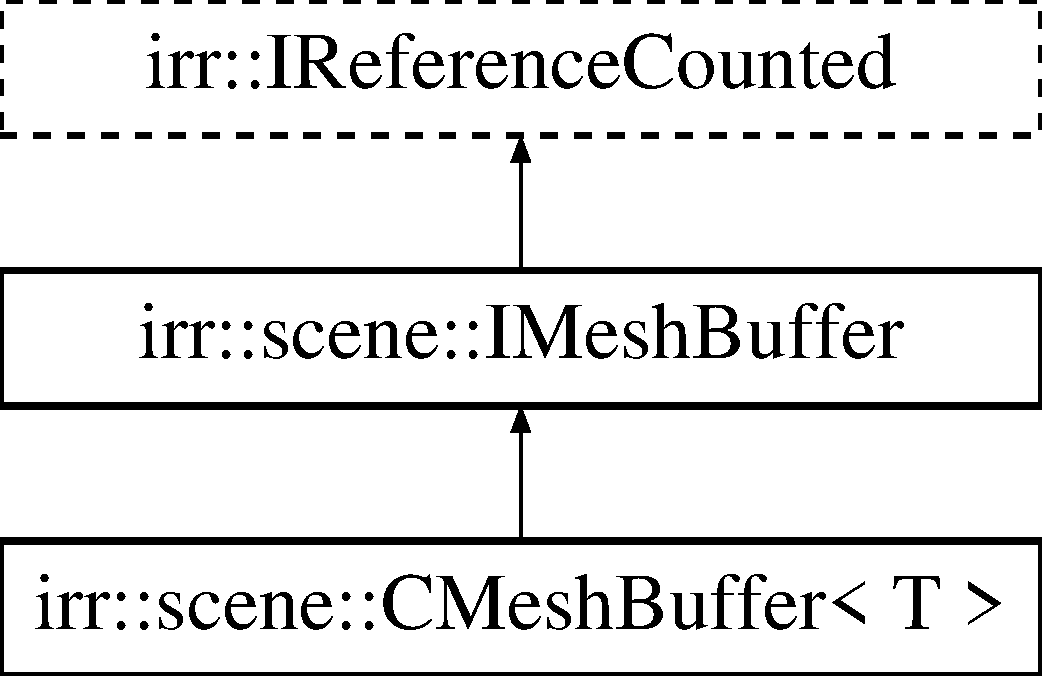
\includegraphics[height=3.000000cm]{classirr_1_1scene_1_1CMeshBuffer}
\end{center}
\end{figure}
\subsection*{Public Member Functions}
\begin{DoxyCompactItemize}
\item 
\mbox{\Hypertarget{classirr_1_1scene_1_1CMeshBuffer_aa2a6fa9d2f7b23fad0d8a86c74a56944}\label{classirr_1_1scene_1_1CMeshBuffer_aa2a6fa9d2f7b23fad0d8a86c74a56944}} 
\hyperlink{classirr_1_1scene_1_1CMeshBuffer_aa2a6fa9d2f7b23fad0d8a86c74a56944}{C\+Mesh\+Buffer} ()
\begin{DoxyCompactList}\small\item\em Default constructor for empty meshbuffer. \end{DoxyCompactList}\item 
virtual const \hyperlink{classirr_1_1video_1_1SMaterial}{video\+::\+S\+Material} \& \hyperlink{classirr_1_1scene_1_1CMeshBuffer_a3e971800b0fc1a67134f839309589e43}{get\+Material} () const
\begin{DoxyCompactList}\small\item\em Get material of this meshbuffer. \end{DoxyCompactList}\item 
virtual \hyperlink{classirr_1_1video_1_1SMaterial}{video\+::\+S\+Material} \& \hyperlink{classirr_1_1scene_1_1CMeshBuffer_af69e8356b4525a3fee1ddbf188d81e8a}{get\+Material} ()
\begin{DoxyCompactList}\small\item\em Get material of this meshbuffer. \end{DoxyCompactList}\item 
virtual const void $\ast$ \hyperlink{classirr_1_1scene_1_1CMeshBuffer_ad9463b97ee94bbc26bbb11bf867ea830}{get\+Vertices} () const
\begin{DoxyCompactList}\small\item\em Get pointer to vertices. \end{DoxyCompactList}\item 
virtual void $\ast$ \hyperlink{classirr_1_1scene_1_1CMeshBuffer_a9173c9d0c6f32890ab75dc501aaf5be6}{get\+Vertices} ()
\begin{DoxyCompactList}\small\item\em Get pointer to vertices. \end{DoxyCompactList}\item 
virtual \hyperlink{namespaceirr_a0416a53257075833e7002efd0a18e804}{u32} \hyperlink{classirr_1_1scene_1_1CMeshBuffer_a72ee778498eff327a20c6be179976994}{get\+Vertex\+Count} () const
\begin{DoxyCompactList}\small\item\em Get number of vertices. \end{DoxyCompactList}\item 
virtual video\+::\+E\+\_\+\+I\+N\+D\+E\+X\+\_\+\+T\+Y\+PE \hyperlink{classirr_1_1scene_1_1CMeshBuffer_aa183491690fa47b4697bbfcc7902301c}{get\+Index\+Type} () const
\begin{DoxyCompactList}\small\item\em Get type of index data which is stored in this meshbuffer. \end{DoxyCompactList}\item 
virtual const \hyperlink{namespaceirr_ae9f8ec82692ad3b83c21f555bfa70bcc}{u16} $\ast$ \hyperlink{classirr_1_1scene_1_1CMeshBuffer_a23af7e8ffb2ba674d1dd4448cea288bf}{get\+Indices} () const
\begin{DoxyCompactList}\small\item\em Get pointer to indices. \end{DoxyCompactList}\item 
virtual \hyperlink{namespaceirr_ae9f8ec82692ad3b83c21f555bfa70bcc}{u16} $\ast$ \hyperlink{classirr_1_1scene_1_1CMeshBuffer_a34a85f4868776d4cf312cdece5326c89}{get\+Indices} ()
\begin{DoxyCompactList}\small\item\em Get pointer to indices. \end{DoxyCompactList}\item 
virtual \hyperlink{namespaceirr_a0416a53257075833e7002efd0a18e804}{u32} \hyperlink{classirr_1_1scene_1_1CMeshBuffer_ac5585f4983423a4ba1f4ab4aba112c95}{get\+Index\+Count} () const
\begin{DoxyCompactList}\small\item\em Get number of indices. \end{DoxyCompactList}\item 
virtual const \hyperlink{classirr_1_1core_1_1aabbox3d}{core\+::aabbox3d}$<$ \hyperlink{namespaceirr_a0277be98d67dc26ff93b1a6a1d086b07}{f32} $>$ \& \hyperlink{classirr_1_1scene_1_1CMeshBuffer_a759863b44c024f79747019f492a5c7cf}{get\+Bounding\+Box} () const
\begin{DoxyCompactList}\small\item\em Get the axis aligned bounding box. \end{DoxyCompactList}\item 
virtual void \hyperlink{classirr_1_1scene_1_1CMeshBuffer_ab5a21d48a5af73f1ef880a48c3798a67}{set\+Bounding\+Box} (const \hyperlink{namespaceirr_1_1core_adfc8fa01b30044c55f3332a1d6c1aa19}{core\+::aabbox3df} \&box)
\begin{DoxyCompactList}\small\item\em Set the axis aligned bounding box. \end{DoxyCompactList}\item 
virtual void \hyperlink{classirr_1_1scene_1_1CMeshBuffer_aad55263eaf019b090c8d1c3c5f7f4407}{recalculate\+Bounding\+Box} ()
\begin{DoxyCompactList}\small\item\em Recalculate the bounding box. \end{DoxyCompactList}\item 
virtual \hyperlink{namespaceirr_1_1video_a0e3b59e025e0d0db0ed2ee0ce904deac}{video\+::\+E\+\_\+\+V\+E\+R\+T\+E\+X\+\_\+\+T\+Y\+PE} \hyperlink{classirr_1_1scene_1_1CMeshBuffer_a341db661218a49d8d8fd12550700cb67}{get\+Vertex\+Type} () const
\begin{DoxyCompactList}\small\item\em Get type of vertex data stored in this buffer. \end{DoxyCompactList}\item 
\mbox{\Hypertarget{classirr_1_1scene_1_1CMeshBuffer_a4a94e12e5b3f07a795695693ed9ef18d}\label{classirr_1_1scene_1_1CMeshBuffer_a4a94e12e5b3f07a795695693ed9ef18d}} 
virtual const \hyperlink{namespaceirr_1_1core_a06f169d08b5c429f5575acb7edbad811}{core\+::vector3df} \& \hyperlink{classirr_1_1scene_1_1CMeshBuffer_a4a94e12e5b3f07a795695693ed9ef18d}{get\+Position} (\hyperlink{namespaceirr_a0416a53257075833e7002efd0a18e804}{u32} i) const
\begin{DoxyCompactList}\small\item\em returns position of vertex i \end{DoxyCompactList}\item 
\mbox{\Hypertarget{classirr_1_1scene_1_1CMeshBuffer_a70890de5d1014a4bf1b1f9e7819f8e9b}\label{classirr_1_1scene_1_1CMeshBuffer_a70890de5d1014a4bf1b1f9e7819f8e9b}} 
virtual \hyperlink{namespaceirr_1_1core_a06f169d08b5c429f5575acb7edbad811}{core\+::vector3df} \& \hyperlink{classirr_1_1scene_1_1CMeshBuffer_a70890de5d1014a4bf1b1f9e7819f8e9b}{get\+Position} (\hyperlink{namespaceirr_a0416a53257075833e7002efd0a18e804}{u32} i)
\begin{DoxyCompactList}\small\item\em returns position of vertex i \end{DoxyCompactList}\item 
\mbox{\Hypertarget{classirr_1_1scene_1_1CMeshBuffer_ac93c92c49e801141cab699484bcf818d}\label{classirr_1_1scene_1_1CMeshBuffer_ac93c92c49e801141cab699484bcf818d}} 
virtual const \hyperlink{namespaceirr_1_1core_a06f169d08b5c429f5575acb7edbad811}{core\+::vector3df} \& \hyperlink{classirr_1_1scene_1_1CMeshBuffer_ac93c92c49e801141cab699484bcf818d}{get\+Normal} (\hyperlink{namespaceirr_a0416a53257075833e7002efd0a18e804}{u32} i) const
\begin{DoxyCompactList}\small\item\em returns normal of vertex i \end{DoxyCompactList}\item 
\mbox{\Hypertarget{classirr_1_1scene_1_1CMeshBuffer_ad8515509517384dc31e9ad46eea323a0}\label{classirr_1_1scene_1_1CMeshBuffer_ad8515509517384dc31e9ad46eea323a0}} 
virtual \hyperlink{namespaceirr_1_1core_a06f169d08b5c429f5575acb7edbad811}{core\+::vector3df} \& \hyperlink{classirr_1_1scene_1_1CMeshBuffer_ad8515509517384dc31e9ad46eea323a0}{get\+Normal} (\hyperlink{namespaceirr_a0416a53257075833e7002efd0a18e804}{u32} i)
\begin{DoxyCompactList}\small\item\em returns normal of vertex i \end{DoxyCompactList}\item 
\mbox{\Hypertarget{classirr_1_1scene_1_1CMeshBuffer_a2823a97a353b6909e66a18dca46a8f30}\label{classirr_1_1scene_1_1CMeshBuffer_a2823a97a353b6909e66a18dca46a8f30}} 
virtual const \hyperlink{namespaceirr_1_1core_a2cf08556d77f6f5a792973a6e27ed11b}{core\+::vector2df} \& \hyperlink{classirr_1_1scene_1_1CMeshBuffer_a2823a97a353b6909e66a18dca46a8f30}{get\+T\+Coords} (\hyperlink{namespaceirr_a0416a53257075833e7002efd0a18e804}{u32} i) const
\begin{DoxyCompactList}\small\item\em returns texture coord of vertex i \end{DoxyCompactList}\item 
\mbox{\Hypertarget{classirr_1_1scene_1_1CMeshBuffer_a50e1a283111e3aa8325a7e774f08fb27}\label{classirr_1_1scene_1_1CMeshBuffer_a50e1a283111e3aa8325a7e774f08fb27}} 
virtual \hyperlink{namespaceirr_1_1core_a2cf08556d77f6f5a792973a6e27ed11b}{core\+::vector2df} \& \hyperlink{classirr_1_1scene_1_1CMeshBuffer_a50e1a283111e3aa8325a7e774f08fb27}{get\+T\+Coords} (\hyperlink{namespaceirr_a0416a53257075833e7002efd0a18e804}{u32} i)
\begin{DoxyCompactList}\small\item\em returns texture coord of vertex i \end{DoxyCompactList}\item 
virtual void \hyperlink{classirr_1_1scene_1_1CMeshBuffer_a7efd85cba5d5d86bee8c2ea2fe0524d9}{append} (const void $\ast$const vertices, \hyperlink{namespaceirr_a0416a53257075833e7002efd0a18e804}{u32} num\+Vertices, const \hyperlink{namespaceirr_ae9f8ec82692ad3b83c21f555bfa70bcc}{u16} $\ast$const indices, \hyperlink{namespaceirr_a0416a53257075833e7002efd0a18e804}{u32} num\+Indices)
\begin{DoxyCompactList}\small\item\em Append the vertices and indices to the current buffer. \end{DoxyCompactList}\item 
virtual void \hyperlink{classirr_1_1scene_1_1CMeshBuffer_af48b88e6c1bd79e6abd6a6803aa106c0}{append} (const \hyperlink{classirr_1_1scene_1_1IMeshBuffer}{I\+Mesh\+Buffer} $\ast$const other)
\begin{DoxyCompactList}\small\item\em Append the meshbuffer to the current buffer. \end{DoxyCompactList}\item 
\mbox{\Hypertarget{classirr_1_1scene_1_1CMeshBuffer_adae334e8431e647d837acda0fada8bd5}\label{classirr_1_1scene_1_1CMeshBuffer_adae334e8431e647d837acda0fada8bd5}} 
virtual \hyperlink{namespaceirr_1_1scene_ac7d8ee8d77da75f2580bb9bb17231c27}{E\+\_\+\+H\+A\+R\+D\+W\+A\+R\+E\+\_\+\+M\+A\+P\+P\+I\+NG} \hyperlink{classirr_1_1scene_1_1CMeshBuffer_adae334e8431e647d837acda0fada8bd5}{get\+Hardware\+Mapping\+Hint\+\_\+\+Vertex} () const
\begin{DoxyCompactList}\small\item\em get the current hardware mapping hint \end{DoxyCompactList}\item 
\mbox{\Hypertarget{classirr_1_1scene_1_1CMeshBuffer_a3f6eb99f71576b72225ac3eccd68efbe}\label{classirr_1_1scene_1_1CMeshBuffer_a3f6eb99f71576b72225ac3eccd68efbe}} 
virtual \hyperlink{namespaceirr_1_1scene_ac7d8ee8d77da75f2580bb9bb17231c27}{E\+\_\+\+H\+A\+R\+D\+W\+A\+R\+E\+\_\+\+M\+A\+P\+P\+I\+NG} \hyperlink{classirr_1_1scene_1_1CMeshBuffer_a3f6eb99f71576b72225ac3eccd68efbe}{get\+Hardware\+Mapping\+Hint\+\_\+\+Index} () const
\begin{DoxyCompactList}\small\item\em get the current hardware mapping hint \end{DoxyCompactList}\item 
\mbox{\Hypertarget{classirr_1_1scene_1_1CMeshBuffer_aa86cd9ffbe81c9f86a6096b2e5d3410e}\label{classirr_1_1scene_1_1CMeshBuffer_aa86cd9ffbe81c9f86a6096b2e5d3410e}} 
virtual void \hyperlink{classirr_1_1scene_1_1CMeshBuffer_aa86cd9ffbe81c9f86a6096b2e5d3410e}{set\+Hardware\+Mapping\+Hint} (\hyperlink{namespaceirr_1_1scene_ac7d8ee8d77da75f2580bb9bb17231c27}{E\+\_\+\+H\+A\+R\+D\+W\+A\+R\+E\+\_\+\+M\+A\+P\+P\+I\+NG} New\+Mapping\+Hint, \hyperlink{namespaceirr_1_1scene_a8f59a89ffef0ad8e5b2c2cb874a93e8c}{E\+\_\+\+B\+U\+F\+F\+E\+R\+\_\+\+T\+Y\+PE} Buffer=\hyperlink{namespaceirr_1_1scene_a8f59a89ffef0ad8e5b2c2cb874a93e8ca833624730c30cffccc121fe31aa0832c}{E\+B\+T\+\_\+\+V\+E\+R\+T\+E\+X\+\_\+\+A\+N\+D\+\_\+\+I\+N\+D\+EX})
\begin{DoxyCompactList}\small\item\em set the hardware mapping hint, for driver \end{DoxyCompactList}\item 
\mbox{\Hypertarget{classirr_1_1scene_1_1CMeshBuffer_a7afead32226650c724f13f6f61282810}\label{classirr_1_1scene_1_1CMeshBuffer_a7afead32226650c724f13f6f61282810}} 
virtual void \hyperlink{classirr_1_1scene_1_1CMeshBuffer_a7afead32226650c724f13f6f61282810}{set\+Dirty} (\hyperlink{namespaceirr_1_1scene_a8f59a89ffef0ad8e5b2c2cb874a93e8c}{E\+\_\+\+B\+U\+F\+F\+E\+R\+\_\+\+T\+Y\+PE} Buffer=\hyperlink{namespaceirr_1_1scene_a8f59a89ffef0ad8e5b2c2cb874a93e8ca833624730c30cffccc121fe31aa0832c}{E\+B\+T\+\_\+\+V\+E\+R\+T\+E\+X\+\_\+\+A\+N\+D\+\_\+\+I\+N\+D\+EX})
\begin{DoxyCompactList}\small\item\em flags the mesh as changed, reloads hardware buffers \end{DoxyCompactList}\item 
virtual \hyperlink{namespaceirr_a0416a53257075833e7002efd0a18e804}{u32} \hyperlink{classirr_1_1scene_1_1CMeshBuffer_a99abc7d5f5a9f34221c58a598b33ce3a}{get\+Changed\+I\+D\+\_\+\+Vertex} () const
\begin{DoxyCompactList}\small\item\em Get the currently used ID for identification of changes. \end{DoxyCompactList}\item 
virtual \hyperlink{namespaceirr_a0416a53257075833e7002efd0a18e804}{u32} \hyperlink{classirr_1_1scene_1_1CMeshBuffer_aec6786022abd81ddf8d4e79a23628944}{get\+Changed\+I\+D\+\_\+\+Index} () const
\begin{DoxyCompactList}\small\item\em Get the currently used ID for identification of changes. \end{DoxyCompactList}\end{DoxyCompactItemize}
\subsection*{Public Attributes}
\begin{DoxyCompactItemize}
\item 
\mbox{\Hypertarget{classirr_1_1scene_1_1CMeshBuffer_af69f379242352b5a03bb135c02611909}\label{classirr_1_1scene_1_1CMeshBuffer_af69f379242352b5a03bb135c02611909}} 
\hyperlink{namespaceirr_1_1scene_ac7d8ee8d77da75f2580bb9bb17231c27}{E\+\_\+\+H\+A\+R\+D\+W\+A\+R\+E\+\_\+\+M\+A\+P\+P\+I\+NG} \hyperlink{classirr_1_1scene_1_1CMeshBuffer_af69f379242352b5a03bb135c02611909}{Mapping\+Hint\+\_\+\+Vertex}
\begin{DoxyCompactList}\small\item\em hardware mapping hint \end{DoxyCompactList}\item 
\mbox{\Hypertarget{classirr_1_1scene_1_1CMeshBuffer_a0b04ea5a95cda0b914f5ca5bd01283ab}\label{classirr_1_1scene_1_1CMeshBuffer_a0b04ea5a95cda0b914f5ca5bd01283ab}} 
\hyperlink{classirr_1_1video_1_1SMaterial}{video\+::\+S\+Material} \hyperlink{classirr_1_1scene_1_1CMeshBuffer_a0b04ea5a95cda0b914f5ca5bd01283ab}{Material}
\begin{DoxyCompactList}\small\item\em Material for this meshbuffer. \end{DoxyCompactList}\item 
\mbox{\Hypertarget{classirr_1_1scene_1_1CMeshBuffer_a7dcab02671df7d62fadb0d996474d853}\label{classirr_1_1scene_1_1CMeshBuffer_a7dcab02671df7d62fadb0d996474d853}} 
\hyperlink{classirr_1_1core_1_1array}{core\+::array}$<$ T $>$ \hyperlink{classirr_1_1scene_1_1CMeshBuffer_a7dcab02671df7d62fadb0d996474d853}{Vertices}
\begin{DoxyCompactList}\small\item\em Vertices of this buffer. \end{DoxyCompactList}\item 
\mbox{\Hypertarget{classirr_1_1scene_1_1CMeshBuffer_a298043df538ddcedc6586e20723b0665}\label{classirr_1_1scene_1_1CMeshBuffer_a298043df538ddcedc6586e20723b0665}} 
\hyperlink{classirr_1_1core_1_1array}{core\+::array}$<$ \hyperlink{namespaceirr_ae9f8ec82692ad3b83c21f555bfa70bcc}{u16} $>$ \hyperlink{classirr_1_1scene_1_1CMeshBuffer_a298043df538ddcedc6586e20723b0665}{Indices}
\begin{DoxyCompactList}\small\item\em Indices into the vertices of this buffer. \end{DoxyCompactList}\item 
\mbox{\Hypertarget{classirr_1_1scene_1_1CMeshBuffer_a9e16abdff220a4f7a5ffff992d3ef1d6}\label{classirr_1_1scene_1_1CMeshBuffer_a9e16abdff220a4f7a5ffff992d3ef1d6}} 
\hyperlink{classirr_1_1core_1_1aabbox3d}{core\+::aabbox3d}$<$ \hyperlink{namespaceirr_a0277be98d67dc26ff93b1a6a1d086b07}{f32} $>$ \hyperlink{classirr_1_1scene_1_1CMeshBuffer_a9e16abdff220a4f7a5ffff992d3ef1d6}{Bounding\+Box}
\begin{DoxyCompactList}\small\item\em Bounding box of this meshbuffer. \end{DoxyCompactList}\end{DoxyCompactItemize}
\subsection*{Additional Inherited Members}


\subsection{Detailed Description}
\subsubsection*{template$<$class T$>$\newline
class irr\+::scene\+::\+C\+Mesh\+Buffer$<$ T $>$}

Template implementation of the \hyperlink{classirr_1_1scene_1_1IMeshBuffer}{I\+Mesh\+Buffer} interface. 

\subsection{Member Function Documentation}
\mbox{\Hypertarget{classirr_1_1scene_1_1CMeshBuffer_a7efd85cba5d5d86bee8c2ea2fe0524d9}\label{classirr_1_1scene_1_1CMeshBuffer_a7efd85cba5d5d86bee8c2ea2fe0524d9}} 
\index{irr\+::scene\+::\+C\+Mesh\+Buffer@{irr\+::scene\+::\+C\+Mesh\+Buffer}!append@{append}}
\index{append@{append}!irr\+::scene\+::\+C\+Mesh\+Buffer@{irr\+::scene\+::\+C\+Mesh\+Buffer}}
\subsubsection{\texorpdfstring{append()}{append()}\hspace{0.1cm}{\footnotesize\ttfamily [1/2]}}
{\footnotesize\ttfamily template$<$class T $>$ \\
virtual void \hyperlink{classirr_1_1scene_1_1CMeshBuffer}{irr\+::scene\+::\+C\+Mesh\+Buffer}$<$ T $>$\+::append (\begin{DoxyParamCaption}\item[{const void $\ast$const}]{vertices,  }\item[{\hyperlink{namespaceirr_a0416a53257075833e7002efd0a18e804}{u32}}]{num\+Vertices,  }\item[{const \hyperlink{namespaceirr_ae9f8ec82692ad3b83c21f555bfa70bcc}{u16} $\ast$const}]{indices,  }\item[{\hyperlink{namespaceirr_a0416a53257075833e7002efd0a18e804}{u32}}]{num\+Indices }\end{DoxyParamCaption})\hspace{0.3cm}{\ttfamily [inline]}, {\ttfamily [virtual]}}



Append the vertices and indices to the current buffer. 

Only works for compatible types, i.\+e. either the same type or the main buffer is of standard type. Otherwise, behavior is undefined. 

Implements \hyperlink{classirr_1_1scene_1_1IMeshBuffer_ac9e9d7fbb10175cc6f1596ba3fe4e8f9}{irr\+::scene\+::\+I\+Mesh\+Buffer}.

\mbox{\Hypertarget{classirr_1_1scene_1_1CMeshBuffer_af48b88e6c1bd79e6abd6a6803aa106c0}\label{classirr_1_1scene_1_1CMeshBuffer_af48b88e6c1bd79e6abd6a6803aa106c0}} 
\index{irr\+::scene\+::\+C\+Mesh\+Buffer@{irr\+::scene\+::\+C\+Mesh\+Buffer}!append@{append}}
\index{append@{append}!irr\+::scene\+::\+C\+Mesh\+Buffer@{irr\+::scene\+::\+C\+Mesh\+Buffer}}
\subsubsection{\texorpdfstring{append()}{append()}\hspace{0.1cm}{\footnotesize\ttfamily [2/2]}}
{\footnotesize\ttfamily template$<$class T $>$ \\
virtual void \hyperlink{classirr_1_1scene_1_1CMeshBuffer}{irr\+::scene\+::\+C\+Mesh\+Buffer}$<$ T $>$\+::append (\begin{DoxyParamCaption}\item[{const \hyperlink{classirr_1_1scene_1_1IMeshBuffer}{I\+Mesh\+Buffer} $\ast$const}]{other }\end{DoxyParamCaption})\hspace{0.3cm}{\ttfamily [inline]}, {\ttfamily [virtual]}}



Append the meshbuffer to the current buffer. 

Only works for compatible types, i.\+e. either the same type or the main buffer is of standard type. Otherwise, behavior is undefined. 
\begin{DoxyParams}{Parameters}
{\em other} & Meshbuffer to be appended to this one. \\
\hline
\end{DoxyParams}


Implements \hyperlink{classirr_1_1scene_1_1IMeshBuffer_a79d2737962579138183ed0fd324310b3}{irr\+::scene\+::\+I\+Mesh\+Buffer}.

\mbox{\Hypertarget{classirr_1_1scene_1_1CMeshBuffer_a759863b44c024f79747019f492a5c7cf}\label{classirr_1_1scene_1_1CMeshBuffer_a759863b44c024f79747019f492a5c7cf}} 
\index{irr\+::scene\+::\+C\+Mesh\+Buffer@{irr\+::scene\+::\+C\+Mesh\+Buffer}!get\+Bounding\+Box@{get\+Bounding\+Box}}
\index{get\+Bounding\+Box@{get\+Bounding\+Box}!irr\+::scene\+::\+C\+Mesh\+Buffer@{irr\+::scene\+::\+C\+Mesh\+Buffer}}
\subsubsection{\texorpdfstring{get\+Bounding\+Box()}{getBoundingBox()}}
{\footnotesize\ttfamily template$<$class T $>$ \\
virtual const \hyperlink{classirr_1_1core_1_1aabbox3d}{core\+::aabbox3d}$<$\hyperlink{namespaceirr_a0277be98d67dc26ff93b1a6a1d086b07}{f32}$>$\& \hyperlink{classirr_1_1scene_1_1CMeshBuffer}{irr\+::scene\+::\+C\+Mesh\+Buffer}$<$ T $>$\+::get\+Bounding\+Box (\begin{DoxyParamCaption}{ }\end{DoxyParamCaption}) const\hspace{0.3cm}{\ttfamily [inline]}, {\ttfamily [virtual]}}



Get the axis aligned bounding box. 

\begin{DoxyReturn}{Returns}
Axis aligned bounding box of this buffer. 
\end{DoxyReturn}


Implements \hyperlink{classirr_1_1scene_1_1IMeshBuffer_ac53fe1096756a40f25dae25911e27c51}{irr\+::scene\+::\+I\+Mesh\+Buffer}.

\mbox{\Hypertarget{classirr_1_1scene_1_1CMeshBuffer_aec6786022abd81ddf8d4e79a23628944}\label{classirr_1_1scene_1_1CMeshBuffer_aec6786022abd81ddf8d4e79a23628944}} 
\index{irr\+::scene\+::\+C\+Mesh\+Buffer@{irr\+::scene\+::\+C\+Mesh\+Buffer}!get\+Changed\+I\+D\+\_\+\+Index@{get\+Changed\+I\+D\+\_\+\+Index}}
\index{get\+Changed\+I\+D\+\_\+\+Index@{get\+Changed\+I\+D\+\_\+\+Index}!irr\+::scene\+::\+C\+Mesh\+Buffer@{irr\+::scene\+::\+C\+Mesh\+Buffer}}
\subsubsection{\texorpdfstring{get\+Changed\+I\+D\+\_\+\+Index()}{getChangedID\_Index()}}
{\footnotesize\ttfamily template$<$class T $>$ \\
virtual \hyperlink{namespaceirr_a0416a53257075833e7002efd0a18e804}{u32} \hyperlink{classirr_1_1scene_1_1CMeshBuffer}{irr\+::scene\+::\+C\+Mesh\+Buffer}$<$ T $>$\+::get\+Changed\+I\+D\+\_\+\+Index (\begin{DoxyParamCaption}{ }\end{DoxyParamCaption}) const\hspace{0.3cm}{\ttfamily [inline]}, {\ttfamily [virtual]}}



Get the currently used ID for identification of changes. 

This shouldn\textquotesingle{}t be used for anything outside the Video\+Driver. 

Implements \hyperlink{classirr_1_1scene_1_1IMeshBuffer_acc389d76856dfb06c3ba45a92315e6d8}{irr\+::scene\+::\+I\+Mesh\+Buffer}.

\mbox{\Hypertarget{classirr_1_1scene_1_1CMeshBuffer_a99abc7d5f5a9f34221c58a598b33ce3a}\label{classirr_1_1scene_1_1CMeshBuffer_a99abc7d5f5a9f34221c58a598b33ce3a}} 
\index{irr\+::scene\+::\+C\+Mesh\+Buffer@{irr\+::scene\+::\+C\+Mesh\+Buffer}!get\+Changed\+I\+D\+\_\+\+Vertex@{get\+Changed\+I\+D\+\_\+\+Vertex}}
\index{get\+Changed\+I\+D\+\_\+\+Vertex@{get\+Changed\+I\+D\+\_\+\+Vertex}!irr\+::scene\+::\+C\+Mesh\+Buffer@{irr\+::scene\+::\+C\+Mesh\+Buffer}}
\subsubsection{\texorpdfstring{get\+Changed\+I\+D\+\_\+\+Vertex()}{getChangedID\_Vertex()}}
{\footnotesize\ttfamily template$<$class T $>$ \\
virtual \hyperlink{namespaceirr_a0416a53257075833e7002efd0a18e804}{u32} \hyperlink{classirr_1_1scene_1_1CMeshBuffer}{irr\+::scene\+::\+C\+Mesh\+Buffer}$<$ T $>$\+::get\+Changed\+I\+D\+\_\+\+Vertex (\begin{DoxyParamCaption}{ }\end{DoxyParamCaption}) const\hspace{0.3cm}{\ttfamily [inline]}, {\ttfamily [virtual]}}



Get the currently used ID for identification of changes. 

This shouldn\textquotesingle{}t be used for anything outside the Video\+Driver. 

Implements \hyperlink{classirr_1_1scene_1_1IMeshBuffer_aba48df31edf92a0117692c0be02298db}{irr\+::scene\+::\+I\+Mesh\+Buffer}.

\mbox{\Hypertarget{classirr_1_1scene_1_1CMeshBuffer_ac5585f4983423a4ba1f4ab4aba112c95}\label{classirr_1_1scene_1_1CMeshBuffer_ac5585f4983423a4ba1f4ab4aba112c95}} 
\index{irr\+::scene\+::\+C\+Mesh\+Buffer@{irr\+::scene\+::\+C\+Mesh\+Buffer}!get\+Index\+Count@{get\+Index\+Count}}
\index{get\+Index\+Count@{get\+Index\+Count}!irr\+::scene\+::\+C\+Mesh\+Buffer@{irr\+::scene\+::\+C\+Mesh\+Buffer}}
\subsubsection{\texorpdfstring{get\+Index\+Count()}{getIndexCount()}}
{\footnotesize\ttfamily template$<$class T $>$ \\
virtual \hyperlink{namespaceirr_a0416a53257075833e7002efd0a18e804}{u32} \hyperlink{classirr_1_1scene_1_1CMeshBuffer}{irr\+::scene\+::\+C\+Mesh\+Buffer}$<$ T $>$\+::get\+Index\+Count (\begin{DoxyParamCaption}{ }\end{DoxyParamCaption}) const\hspace{0.3cm}{\ttfamily [inline]}, {\ttfamily [virtual]}}



Get number of indices. 

\begin{DoxyReturn}{Returns}
Number of indices. 
\end{DoxyReturn}


Implements \hyperlink{classirr_1_1scene_1_1IMeshBuffer_a96e08662e15b1205516b87ada3301551}{irr\+::scene\+::\+I\+Mesh\+Buffer}.

\mbox{\Hypertarget{classirr_1_1scene_1_1CMeshBuffer_aa183491690fa47b4697bbfcc7902301c}\label{classirr_1_1scene_1_1CMeshBuffer_aa183491690fa47b4697bbfcc7902301c}} 
\index{irr\+::scene\+::\+C\+Mesh\+Buffer@{irr\+::scene\+::\+C\+Mesh\+Buffer}!get\+Index\+Type@{get\+Index\+Type}}
\index{get\+Index\+Type@{get\+Index\+Type}!irr\+::scene\+::\+C\+Mesh\+Buffer@{irr\+::scene\+::\+C\+Mesh\+Buffer}}
\subsubsection{\texorpdfstring{get\+Index\+Type()}{getIndexType()}}
{\footnotesize\ttfamily template$<$class T $>$ \\
virtual video\+::\+E\+\_\+\+I\+N\+D\+E\+X\+\_\+\+T\+Y\+PE \hyperlink{classirr_1_1scene_1_1CMeshBuffer}{irr\+::scene\+::\+C\+Mesh\+Buffer}$<$ T $>$\+::get\+Index\+Type (\begin{DoxyParamCaption}{ }\end{DoxyParamCaption}) const\hspace{0.3cm}{\ttfamily [inline]}, {\ttfamily [virtual]}}



Get type of index data which is stored in this meshbuffer. 

\begin{DoxyReturn}{Returns}
Index type of this buffer. 
\end{DoxyReturn}


Implements \hyperlink{classirr_1_1scene_1_1IMeshBuffer_a8a993431c2c35420b62a577dc18dbdc2}{irr\+::scene\+::\+I\+Mesh\+Buffer}.

\mbox{\Hypertarget{classirr_1_1scene_1_1CMeshBuffer_a23af7e8ffb2ba674d1dd4448cea288bf}\label{classirr_1_1scene_1_1CMeshBuffer_a23af7e8ffb2ba674d1dd4448cea288bf}} 
\index{irr\+::scene\+::\+C\+Mesh\+Buffer@{irr\+::scene\+::\+C\+Mesh\+Buffer}!get\+Indices@{get\+Indices}}
\index{get\+Indices@{get\+Indices}!irr\+::scene\+::\+C\+Mesh\+Buffer@{irr\+::scene\+::\+C\+Mesh\+Buffer}}
\subsubsection{\texorpdfstring{get\+Indices()}{getIndices()}\hspace{0.1cm}{\footnotesize\ttfamily [1/2]}}
{\footnotesize\ttfamily template$<$class T $>$ \\
virtual const \hyperlink{namespaceirr_ae9f8ec82692ad3b83c21f555bfa70bcc}{u16}$\ast$ \hyperlink{classirr_1_1scene_1_1CMeshBuffer}{irr\+::scene\+::\+C\+Mesh\+Buffer}$<$ T $>$\+::get\+Indices (\begin{DoxyParamCaption}{ }\end{DoxyParamCaption}) const\hspace{0.3cm}{\ttfamily [inline]}, {\ttfamily [virtual]}}



Get pointer to indices. 

\begin{DoxyReturn}{Returns}
Pointer to indices. 
\end{DoxyReturn}


Implements \hyperlink{classirr_1_1scene_1_1IMeshBuffer_a76c0013378012af7aeb6cb8f4ea8f9a1}{irr\+::scene\+::\+I\+Mesh\+Buffer}.

\mbox{\Hypertarget{classirr_1_1scene_1_1CMeshBuffer_a34a85f4868776d4cf312cdece5326c89}\label{classirr_1_1scene_1_1CMeshBuffer_a34a85f4868776d4cf312cdece5326c89}} 
\index{irr\+::scene\+::\+C\+Mesh\+Buffer@{irr\+::scene\+::\+C\+Mesh\+Buffer}!get\+Indices@{get\+Indices}}
\index{get\+Indices@{get\+Indices}!irr\+::scene\+::\+C\+Mesh\+Buffer@{irr\+::scene\+::\+C\+Mesh\+Buffer}}
\subsubsection{\texorpdfstring{get\+Indices()}{getIndices()}\hspace{0.1cm}{\footnotesize\ttfamily [2/2]}}
{\footnotesize\ttfamily template$<$class T $>$ \\
virtual \hyperlink{namespaceirr_ae9f8ec82692ad3b83c21f555bfa70bcc}{u16}$\ast$ \hyperlink{classirr_1_1scene_1_1CMeshBuffer}{irr\+::scene\+::\+C\+Mesh\+Buffer}$<$ T $>$\+::get\+Indices (\begin{DoxyParamCaption}{ }\end{DoxyParamCaption})\hspace{0.3cm}{\ttfamily [inline]}, {\ttfamily [virtual]}}



Get pointer to indices. 

\begin{DoxyReturn}{Returns}
Pointer to indices. 
\end{DoxyReturn}


Implements \hyperlink{classirr_1_1scene_1_1IMeshBuffer_a3d33a561023314677361e30cf07ae429}{irr\+::scene\+::\+I\+Mesh\+Buffer}.

\mbox{\Hypertarget{classirr_1_1scene_1_1CMeshBuffer_a3e971800b0fc1a67134f839309589e43}\label{classirr_1_1scene_1_1CMeshBuffer_a3e971800b0fc1a67134f839309589e43}} 
\index{irr\+::scene\+::\+C\+Mesh\+Buffer@{irr\+::scene\+::\+C\+Mesh\+Buffer}!get\+Material@{get\+Material}}
\index{get\+Material@{get\+Material}!irr\+::scene\+::\+C\+Mesh\+Buffer@{irr\+::scene\+::\+C\+Mesh\+Buffer}}
\subsubsection{\texorpdfstring{get\+Material()}{getMaterial()}\hspace{0.1cm}{\footnotesize\ttfamily [1/2]}}
{\footnotesize\ttfamily template$<$class T $>$ \\
virtual const \hyperlink{classirr_1_1video_1_1SMaterial}{video\+::\+S\+Material}\& \hyperlink{classirr_1_1scene_1_1CMeshBuffer}{irr\+::scene\+::\+C\+Mesh\+Buffer}$<$ T $>$\+::get\+Material (\begin{DoxyParamCaption}{ }\end{DoxyParamCaption}) const\hspace{0.3cm}{\ttfamily [inline]}, {\ttfamily [virtual]}}



Get material of this meshbuffer. 

\begin{DoxyReturn}{Returns}
Material of this buffer 
\end{DoxyReturn}


Implements \hyperlink{classirr_1_1scene_1_1IMeshBuffer_a341c1da2fd0cd556a15aab06d07dbbaa}{irr\+::scene\+::\+I\+Mesh\+Buffer}.

\mbox{\Hypertarget{classirr_1_1scene_1_1CMeshBuffer_af69e8356b4525a3fee1ddbf188d81e8a}\label{classirr_1_1scene_1_1CMeshBuffer_af69e8356b4525a3fee1ddbf188d81e8a}} 
\index{irr\+::scene\+::\+C\+Mesh\+Buffer@{irr\+::scene\+::\+C\+Mesh\+Buffer}!get\+Material@{get\+Material}}
\index{get\+Material@{get\+Material}!irr\+::scene\+::\+C\+Mesh\+Buffer@{irr\+::scene\+::\+C\+Mesh\+Buffer}}
\subsubsection{\texorpdfstring{get\+Material()}{getMaterial()}\hspace{0.1cm}{\footnotesize\ttfamily [2/2]}}
{\footnotesize\ttfamily template$<$class T $>$ \\
virtual \hyperlink{classirr_1_1video_1_1SMaterial}{video\+::\+S\+Material}\& \hyperlink{classirr_1_1scene_1_1CMeshBuffer}{irr\+::scene\+::\+C\+Mesh\+Buffer}$<$ T $>$\+::get\+Material (\begin{DoxyParamCaption}{ }\end{DoxyParamCaption})\hspace{0.3cm}{\ttfamily [inline]}, {\ttfamily [virtual]}}



Get material of this meshbuffer. 

\begin{DoxyReturn}{Returns}
Material of this buffer 
\end{DoxyReturn}


Implements \hyperlink{classirr_1_1scene_1_1IMeshBuffer_a26fd922f00fde56abbbbbe40b485238b}{irr\+::scene\+::\+I\+Mesh\+Buffer}.

\mbox{\Hypertarget{classirr_1_1scene_1_1CMeshBuffer_a72ee778498eff327a20c6be179976994}\label{classirr_1_1scene_1_1CMeshBuffer_a72ee778498eff327a20c6be179976994}} 
\index{irr\+::scene\+::\+C\+Mesh\+Buffer@{irr\+::scene\+::\+C\+Mesh\+Buffer}!get\+Vertex\+Count@{get\+Vertex\+Count}}
\index{get\+Vertex\+Count@{get\+Vertex\+Count}!irr\+::scene\+::\+C\+Mesh\+Buffer@{irr\+::scene\+::\+C\+Mesh\+Buffer}}
\subsubsection{\texorpdfstring{get\+Vertex\+Count()}{getVertexCount()}}
{\footnotesize\ttfamily template$<$class T $>$ \\
virtual \hyperlink{namespaceirr_a0416a53257075833e7002efd0a18e804}{u32} \hyperlink{classirr_1_1scene_1_1CMeshBuffer}{irr\+::scene\+::\+C\+Mesh\+Buffer}$<$ T $>$\+::get\+Vertex\+Count (\begin{DoxyParamCaption}{ }\end{DoxyParamCaption}) const\hspace{0.3cm}{\ttfamily [inline]}, {\ttfamily [virtual]}}



Get number of vertices. 

\begin{DoxyReturn}{Returns}
Number of vertices. 
\end{DoxyReturn}


Implements \hyperlink{classirr_1_1scene_1_1IMeshBuffer_a77ab285c8c886af8ddeb0371db7bde96}{irr\+::scene\+::\+I\+Mesh\+Buffer}.

\mbox{\Hypertarget{classirr_1_1scene_1_1CMeshBuffer_a341db661218a49d8d8fd12550700cb67}\label{classirr_1_1scene_1_1CMeshBuffer_a341db661218a49d8d8fd12550700cb67}} 
\index{irr\+::scene\+::\+C\+Mesh\+Buffer@{irr\+::scene\+::\+C\+Mesh\+Buffer}!get\+Vertex\+Type@{get\+Vertex\+Type}}
\index{get\+Vertex\+Type@{get\+Vertex\+Type}!irr\+::scene\+::\+C\+Mesh\+Buffer@{irr\+::scene\+::\+C\+Mesh\+Buffer}}
\subsubsection{\texorpdfstring{get\+Vertex\+Type()}{getVertexType()}}
{\footnotesize\ttfamily template$<$class T $>$ \\
virtual \hyperlink{namespaceirr_1_1video_a0e3b59e025e0d0db0ed2ee0ce904deac}{video\+::\+E\+\_\+\+V\+E\+R\+T\+E\+X\+\_\+\+T\+Y\+PE} \hyperlink{classirr_1_1scene_1_1CMeshBuffer}{irr\+::scene\+::\+C\+Mesh\+Buffer}$<$ T $>$\+::get\+Vertex\+Type (\begin{DoxyParamCaption}{ }\end{DoxyParamCaption}) const\hspace{0.3cm}{\ttfamily [inline]}, {\ttfamily [virtual]}}



Get type of vertex data stored in this buffer. 

\begin{DoxyReturn}{Returns}
Type of vertex data. 
\end{DoxyReturn}


Implements \hyperlink{classirr_1_1scene_1_1IMeshBuffer_a4d7a84ae4416487736f0ed0f519bb4f0}{irr\+::scene\+::\+I\+Mesh\+Buffer}.

\mbox{\Hypertarget{classirr_1_1scene_1_1CMeshBuffer_ad9463b97ee94bbc26bbb11bf867ea830}\label{classirr_1_1scene_1_1CMeshBuffer_ad9463b97ee94bbc26bbb11bf867ea830}} 
\index{irr\+::scene\+::\+C\+Mesh\+Buffer@{irr\+::scene\+::\+C\+Mesh\+Buffer}!get\+Vertices@{get\+Vertices}}
\index{get\+Vertices@{get\+Vertices}!irr\+::scene\+::\+C\+Mesh\+Buffer@{irr\+::scene\+::\+C\+Mesh\+Buffer}}
\subsubsection{\texorpdfstring{get\+Vertices()}{getVertices()}\hspace{0.1cm}{\footnotesize\ttfamily [1/2]}}
{\footnotesize\ttfamily template$<$class T $>$ \\
virtual const void$\ast$ \hyperlink{classirr_1_1scene_1_1CMeshBuffer}{irr\+::scene\+::\+C\+Mesh\+Buffer}$<$ T $>$\+::get\+Vertices (\begin{DoxyParamCaption}{ }\end{DoxyParamCaption}) const\hspace{0.3cm}{\ttfamily [inline]}, {\ttfamily [virtual]}}



Get pointer to vertices. 

\begin{DoxyReturn}{Returns}
Pointer to vertices. 
\end{DoxyReturn}


Implements \hyperlink{classirr_1_1scene_1_1IMeshBuffer_a99891e516246b2cff13b362a435c8028}{irr\+::scene\+::\+I\+Mesh\+Buffer}.

\mbox{\Hypertarget{classirr_1_1scene_1_1CMeshBuffer_a9173c9d0c6f32890ab75dc501aaf5be6}\label{classirr_1_1scene_1_1CMeshBuffer_a9173c9d0c6f32890ab75dc501aaf5be6}} 
\index{irr\+::scene\+::\+C\+Mesh\+Buffer@{irr\+::scene\+::\+C\+Mesh\+Buffer}!get\+Vertices@{get\+Vertices}}
\index{get\+Vertices@{get\+Vertices}!irr\+::scene\+::\+C\+Mesh\+Buffer@{irr\+::scene\+::\+C\+Mesh\+Buffer}}
\subsubsection{\texorpdfstring{get\+Vertices()}{getVertices()}\hspace{0.1cm}{\footnotesize\ttfamily [2/2]}}
{\footnotesize\ttfamily template$<$class T $>$ \\
virtual void$\ast$ \hyperlink{classirr_1_1scene_1_1CMeshBuffer}{irr\+::scene\+::\+C\+Mesh\+Buffer}$<$ T $>$\+::get\+Vertices (\begin{DoxyParamCaption}{ }\end{DoxyParamCaption})\hspace{0.3cm}{\ttfamily [inline]}, {\ttfamily [virtual]}}



Get pointer to vertices. 

\begin{DoxyReturn}{Returns}
Pointer to vertices. 
\end{DoxyReturn}


Implements \hyperlink{classirr_1_1scene_1_1IMeshBuffer_ac1695efc198b05a086487606bc2783e7}{irr\+::scene\+::\+I\+Mesh\+Buffer}.

\mbox{\Hypertarget{classirr_1_1scene_1_1CMeshBuffer_aad55263eaf019b090c8d1c3c5f7f4407}\label{classirr_1_1scene_1_1CMeshBuffer_aad55263eaf019b090c8d1c3c5f7f4407}} 
\index{irr\+::scene\+::\+C\+Mesh\+Buffer@{irr\+::scene\+::\+C\+Mesh\+Buffer}!recalculate\+Bounding\+Box@{recalculate\+Bounding\+Box}}
\index{recalculate\+Bounding\+Box@{recalculate\+Bounding\+Box}!irr\+::scene\+::\+C\+Mesh\+Buffer@{irr\+::scene\+::\+C\+Mesh\+Buffer}}
\subsubsection{\texorpdfstring{recalculate\+Bounding\+Box()}{recalculateBoundingBox()}}
{\footnotesize\ttfamily template$<$class T $>$ \\
virtual void \hyperlink{classirr_1_1scene_1_1CMeshBuffer}{irr\+::scene\+::\+C\+Mesh\+Buffer}$<$ T $>$\+::recalculate\+Bounding\+Box (\begin{DoxyParamCaption}{ }\end{DoxyParamCaption})\hspace{0.3cm}{\ttfamily [inline]}, {\ttfamily [virtual]}}



Recalculate the bounding box. 

should be called if the mesh changed. 

Implements \hyperlink{classirr_1_1scene_1_1IMeshBuffer_a161877fc3afe29a816440db12a71785d}{irr\+::scene\+::\+I\+Mesh\+Buffer}.

\mbox{\Hypertarget{classirr_1_1scene_1_1CMeshBuffer_ab5a21d48a5af73f1ef880a48c3798a67}\label{classirr_1_1scene_1_1CMeshBuffer_ab5a21d48a5af73f1ef880a48c3798a67}} 
\index{irr\+::scene\+::\+C\+Mesh\+Buffer@{irr\+::scene\+::\+C\+Mesh\+Buffer}!set\+Bounding\+Box@{set\+Bounding\+Box}}
\index{set\+Bounding\+Box@{set\+Bounding\+Box}!irr\+::scene\+::\+C\+Mesh\+Buffer@{irr\+::scene\+::\+C\+Mesh\+Buffer}}
\subsubsection{\texorpdfstring{set\+Bounding\+Box()}{setBoundingBox()}}
{\footnotesize\ttfamily template$<$class T $>$ \\
virtual void \hyperlink{classirr_1_1scene_1_1CMeshBuffer}{irr\+::scene\+::\+C\+Mesh\+Buffer}$<$ T $>$\+::set\+Bounding\+Box (\begin{DoxyParamCaption}\item[{const \hyperlink{namespaceirr_1_1core_adfc8fa01b30044c55f3332a1d6c1aa19}{core\+::aabbox3df} \&}]{box }\end{DoxyParamCaption})\hspace{0.3cm}{\ttfamily [inline]}, {\ttfamily [virtual]}}



Set the axis aligned bounding box. 


\begin{DoxyParams}{Parameters}
{\em box} & New axis aligned bounding box for this buffer. set user axis aligned bounding box \\
\hline
\end{DoxyParams}


Implements \hyperlink{classirr_1_1scene_1_1IMeshBuffer_adbbfb7757dfbba7357193d2280893df6}{irr\+::scene\+::\+I\+Mesh\+Buffer}.



The documentation for this class was generated from the following file\+:\begin{DoxyCompactItemize}
\item 
indie\+\_\+share/controller/include/C\+Mesh\+Buffer.\+h\end{DoxyCompactItemize}

\hypertarget{classConfigManager}{}\section{Config\+Manager Class Reference}
\label{classConfigManager}\index{Config\+Manager@{Config\+Manager}}


This class contain all the methode to manipulate the configuration.  




{\ttfamily \#include $<$Config\+Manager.\+hh$>$}

\subsection*{Public Member Functions}
\begin{DoxyCompactItemize}
\item 
\hyperlink{classConfigManager_a7d3d7c10423d969f7544509f6fcca32f}{Config\+Manager} ()
\begin{DoxyCompactList}\small\item\em Constructor. \end{DoxyCompactList}\item 
void \hyperlink{classConfigManager_a63ff6c831f037cf5bfe580b4944b0b6c}{load\+Config} (std\+::string)
\begin{DoxyCompactList}\small\item\em Load the configuration. \end{DoxyCompactList}\item 
\mbox{\Hypertarget{classConfigManager_a178e051860792271e9b1ec4434776f91}\label{classConfigManager_a178e051860792271e9b1ec4434776f91}} 
void \hyperlink{classConfigManager_a178e051860792271e9b1ec4434776f91}{save\+Config} () const
\begin{DoxyCompactList}\small\item\em Savethe object in the file. \end{DoxyCompactList}\item 
void \hyperlink{classConfigManager_a4f2b06f2ef741a15b3dfe82259cfd355}{create\+File} (std\+::string)
\begin{DoxyCompactList}\small\item\em create an empty configuration file \end{DoxyCompactList}\end{DoxyCompactItemize}
\subsection*{Public Attributes}
\begin{DoxyCompactItemize}
\item 
config\+::\+Video \hyperlink{classConfigManager_a1e0dbb8563b71871e6c68abce5620cd0}{video\+Config}
\begin{DoxyCompactList}\small\item\em The object video\+Config is a structure that contain all the setting for the video. \end{DoxyCompactList}\item 
config\+::\+Sound \hyperlink{classConfigManager_a010e2da02ebc90d7ce930d1c57a79e96}{sound}
\begin{DoxyCompactList}\small\item\em The object sound is a structure that constain all the setting for the sound. \end{DoxyCompactList}\item 
\mbox{\Hypertarget{classConfigManager_ad6d6269ec9827af5ca12067a49383132}\label{classConfigManager_ad6d6269ec9827af5ca12067a49383132}} 
std\+::vector$<$ config\+::\+I\+Control $>$ \hyperlink{classConfigManager_ad6d6269ec9827af5ca12067a49383132}{controllers}
\begin{DoxyCompactList}\small\item\em The object controllers is a vector that contain all the configuration for each players. \end{DoxyCompactList}\end{DoxyCompactItemize}


\subsection{Detailed Description}
This class contain all the methode to manipulate the configuration. 

\subsection{Constructor \& Destructor Documentation}
\mbox{\Hypertarget{classConfigManager_a7d3d7c10423d969f7544509f6fcca32f}\label{classConfigManager_a7d3d7c10423d969f7544509f6fcca32f}} 
\index{Config\+Manager@{Config\+Manager}!Config\+Manager@{Config\+Manager}}
\index{Config\+Manager@{Config\+Manager}!Config\+Manager@{Config\+Manager}}
\subsubsection{\texorpdfstring{Config\+Manager()}{ConfigManager()}}
{\footnotesize\ttfamily Config\+Manager\+::\+Config\+Manager (\begin{DoxyParamCaption}{ }\end{DoxyParamCaption})}



Constructor. 

Build the class


\begin{DoxyParams}{Parameters}
{\em nothing} & \\
\hline
\end{DoxyParams}


\subsection{Member Function Documentation}
\mbox{\Hypertarget{classConfigManager_a4f2b06f2ef741a15b3dfe82259cfd355}\label{classConfigManager_a4f2b06f2ef741a15b3dfe82259cfd355}} 
\index{Config\+Manager@{Config\+Manager}!create\+File@{create\+File}}
\index{create\+File@{create\+File}!Config\+Manager@{Config\+Manager}}
\subsubsection{\texorpdfstring{create\+File()}{createFile()}}
{\footnotesize\ttfamily void Config\+Manager\+::create\+File (\begin{DoxyParamCaption}\item[{std\+::string}]{file\+Name }\end{DoxyParamCaption})}



create an empty configuration file 


\begin{DoxyParams}{Parameters}
{\em path} & to the new configuration file \\
\hline
\end{DoxyParams}
\mbox{\Hypertarget{classConfigManager_a63ff6c831f037cf5bfe580b4944b0b6c}\label{classConfigManager_a63ff6c831f037cf5bfe580b4944b0b6c}} 
\index{Config\+Manager@{Config\+Manager}!load\+Config@{load\+Config}}
\index{load\+Config@{load\+Config}!Config\+Manager@{Config\+Manager}}
\subsubsection{\texorpdfstring{load\+Config()}{loadConfig()}}
{\footnotesize\ttfamily void Config\+Manager\+::load\+Config (\begin{DoxyParamCaption}\item[{std\+::string}]{file\+Name }\end{DoxyParamCaption})}



Load the configuration. 


\begin{DoxyParams}{Parameters}
{\em path} & to the configuration file \\
\hline
\end{DoxyParams}
\begin{DoxyReturn}{Returns}
void 
\end{DoxyReturn}


\subsection{Member Data Documentation}
\mbox{\Hypertarget{classConfigManager_a010e2da02ebc90d7ce930d1c57a79e96}\label{classConfigManager_a010e2da02ebc90d7ce930d1c57a79e96}} 
\index{Config\+Manager@{Config\+Manager}!sound@{sound}}
\index{sound@{sound}!Config\+Manager@{Config\+Manager}}
\subsubsection{\texorpdfstring{sound}{sound}}
{\footnotesize\ttfamily config\+::\+Sound Config\+Manager\+::sound}



The object sound is a structure that constain all the setting for the sound. 

The sructure is on the config namespace \mbox{\Hypertarget{classConfigManager_a1e0dbb8563b71871e6c68abce5620cd0}\label{classConfigManager_a1e0dbb8563b71871e6c68abce5620cd0}} 
\index{Config\+Manager@{Config\+Manager}!video\+Config@{video\+Config}}
\index{video\+Config@{video\+Config}!Config\+Manager@{Config\+Manager}}
\subsubsection{\texorpdfstring{video\+Config}{videoConfig}}
{\footnotesize\ttfamily config\+::\+Video Config\+Manager\+::video\+Config}



The object video\+Config is a structure that contain all the setting for the video. 

The sructure is on the config namespace 

The documentation for this class was generated from the following files\+:\begin{DoxyCompactItemize}
\item 
inc/managers/\hyperlink{ConfigManager_8hh}{Config\+Manager.\+hh}\item 
src/managers/Config\+Manager.\+cpp\end{DoxyCompactItemize}

\hypertarget{classirr_1_1core_1_1list_1_1ConstIterator}{}\section{irr\+:\+:core\+:\+:list$<$ T $>$\+:\+:Const\+Iterator Class Reference}
\label{classirr_1_1core_1_1list_1_1ConstIterator}\index{irr\+::core\+::list$<$ T $>$\+::\+Const\+Iterator@{irr\+::core\+::list$<$ T $>$\+::\+Const\+Iterator}}


List iterator for const access.  




{\ttfamily \#include $<$irr\+List.\+h$>$}



\subsection{Detailed Description}
\subsubsection*{template$<$class T$>$\newline
class irr\+::core\+::list$<$ T $>$\+::\+Const\+Iterator}

List iterator for const access. 

The documentation for this class was generated from the following file\+:\begin{DoxyCompactItemize}
\item 
indie\+\_\+share/controller/include/irr\+List.\+h\end{DoxyCompactItemize}

\hypertarget{classirr_1_1core_1_1map_1_1ConstIterator}{}\section{irr\+:\+:core\+:\+:map$<$ Key\+Type, Value\+Type $>$\+:\+:Const\+Iterator Class Reference}
\label{classirr_1_1core_1_1map_1_1ConstIterator}\index{irr\+::core\+::map$<$ Key\+Type, Value\+Type $>$\+::\+Const\+Iterator@{irr\+::core\+::map$<$ Key\+Type, Value\+Type $>$\+::\+Const\+Iterator}}


Const \hyperlink{classirr_1_1core_1_1map_1_1Iterator}{Iterator}.  




{\ttfamily \#include $<$irr\+Map.\+h$>$}



\subsection{Detailed Description}
\subsubsection*{template$<$class Key\+Type, class Value\+Type$>$\newline
class irr\+::core\+::map$<$ Key\+Type, Value\+Type $>$\+::\+Const\+Iterator}

Const \hyperlink{classirr_1_1core_1_1map_1_1Iterator}{Iterator}. 

The documentation for this class was generated from the following file\+:\begin{DoxyCompactItemize}
\item 
indie\+\_\+share/controller/include/irr\+Map.\+h\end{DoxyCompactItemize}

\hypertarget{classCoreManager}{}\section{Core\+Manager Class Reference}
\label{classCoreManager}\index{Core\+Manager@{Core\+Manager}}


\hyperlink{classCoreManager}{Core\+Manager} is the main manager who regroups all the other manager.  




{\ttfamily \#include $<$Core\+Manager.\+hh$>$}

\subsection*{Public Member Functions}
\begin{DoxyCompactItemize}
\item 
\mbox{\Hypertarget{classCoreManager_a0147fc3a8a8fca6b1f464d8b1257a304}\label{classCoreManager_a0147fc3a8a8fca6b1f464d8b1257a304}} 
\hyperlink{classCoreManager_a0147fc3a8a8fca6b1f464d8b1257a304}{Core\+Manager} ()
\begin{DoxyCompactList}\small\item\em Constructor. \end{DoxyCompactList}\item 
\mbox{\Hypertarget{classCoreManager_ac3489a741174a8d5e09effe11df18100}\label{classCoreManager_ac3489a741174a8d5e09effe11df18100}} 
\hyperlink{classCoreManager_ac3489a741174a8d5e09effe11df18100}{$\sim$\+Core\+Manager} ()
\begin{DoxyCompactList}\small\item\em Destructor. \end{DoxyCompactList}\end{DoxyCompactItemize}


\subsection{Detailed Description}
\hyperlink{classCoreManager}{Core\+Manager} is the main manager who regroups all the other manager. 

The documentation for this class was generated from the following files\+:\begin{DoxyCompactItemize}
\item 
inc/managers/\hyperlink{CoreManager_8hh}{Core\+Manager.\+hh}\item 
src/managers/Core\+Manager.\+cpp\end{DoxyCompactItemize}

\hypertarget{classirr_1_1core_1_1dimension2d}{}\section{irr\+:\+:core\+:\+:dimension2d$<$ T $>$ Class Template Reference}
\label{classirr_1_1core_1_1dimension2d}\index{irr\+::core\+::dimension2d$<$ T $>$@{irr\+::core\+::dimension2d$<$ T $>$}}


Specifies a 2 dimensional size.  




{\ttfamily \#include $<$dimension2d.\+h$>$}

\subsection*{Public Member Functions}
\begin{DoxyCompactItemize}
\item 
\mbox{\Hypertarget{classirr_1_1core_1_1dimension2d_ae0c2a30ce6283602c454901ef0bd6a04}\label{classirr_1_1core_1_1dimension2d_ae0c2a30ce6283602c454901ef0bd6a04}} 
\hyperlink{classirr_1_1core_1_1dimension2d_ae0c2a30ce6283602c454901ef0bd6a04}{dimension2d} ()
\begin{DoxyCompactList}\small\item\em Default constructor for empty dimension. \end{DoxyCompactList}\item 
\mbox{\Hypertarget{classirr_1_1core_1_1dimension2d_a9032aa6e975b32497ed3b570e3d03b76}\label{classirr_1_1core_1_1dimension2d_a9032aa6e975b32497ed3b570e3d03b76}} 
\hyperlink{classirr_1_1core_1_1dimension2d_a9032aa6e975b32497ed3b570e3d03b76}{dimension2d} (const T \&width, const T \&height)
\begin{DoxyCompactList}\small\item\em Constructor with width and height. \end{DoxyCompactList}\item 
\mbox{\Hypertarget{classirr_1_1core_1_1dimension2d_a50814f5fc29d226104d5739350befb31}\label{classirr_1_1core_1_1dimension2d_a50814f5fc29d226104d5739350befb31}} 
{\footnotesize template$<$class U $>$ }\\\hyperlink{classirr_1_1core_1_1dimension2d_a50814f5fc29d226104d5739350befb31}{dimension2d} (const \hyperlink{classirr_1_1core_1_1dimension2d}{dimension2d}$<$ U $>$ \&other)
\begin{DoxyCompactList}\small\item\em Use this constructor only where you are sure that the conversion is valid. \end{DoxyCompactList}\item 
\mbox{\Hypertarget{classirr_1_1core_1_1dimension2d_acb4e8b532083b57ee9849703657c7309}\label{classirr_1_1core_1_1dimension2d_acb4e8b532083b57ee9849703657c7309}} 
bool \hyperlink{classirr_1_1core_1_1dimension2d_acb4e8b532083b57ee9849703657c7309}{operator==} (const \hyperlink{classirr_1_1core_1_1dimension2d}{dimension2d}$<$ T $>$ \&other) const
\begin{DoxyCompactList}\small\item\em Equality operator. \end{DoxyCompactList}\item 
\mbox{\Hypertarget{classirr_1_1core_1_1dimension2d_a7bc8e7a51170f1e0758476d5fac4ff1b}\label{classirr_1_1core_1_1dimension2d_a7bc8e7a51170f1e0758476d5fac4ff1b}} 
bool \hyperlink{classirr_1_1core_1_1dimension2d_a7bc8e7a51170f1e0758476d5fac4ff1b}{operator!=} (const \hyperlink{classirr_1_1core_1_1dimension2d}{dimension2d}$<$ T $>$ \&other) const
\begin{DoxyCompactList}\small\item\em Inequality operator. \end{DoxyCompactList}\item 
\mbox{\Hypertarget{classirr_1_1core_1_1dimension2d_a81860d7ff5a888a37af84f7bbbad7c91}\label{classirr_1_1core_1_1dimension2d_a81860d7ff5a888a37af84f7bbbad7c91}} 
\hyperlink{classirr_1_1core_1_1dimension2d}{dimension2d}$<$ T $>$ \& \hyperlink{classirr_1_1core_1_1dimension2d_a81860d7ff5a888a37af84f7bbbad7c91}{set} (const T \&width, const T \&height)
\begin{DoxyCompactList}\small\item\em Set to new values. \end{DoxyCompactList}\item 
\mbox{\Hypertarget{classirr_1_1core_1_1dimension2d_ac581fbe07dabf2a342314c7a73f862c8}\label{classirr_1_1core_1_1dimension2d_ac581fbe07dabf2a342314c7a73f862c8}} 
\hyperlink{classirr_1_1core_1_1dimension2d}{dimension2d}$<$ T $>$ \& \hyperlink{classirr_1_1core_1_1dimension2d_ac581fbe07dabf2a342314c7a73f862c8}{operator/=} (const T \&scale)
\begin{DoxyCompactList}\small\item\em Divide width and height by scalar. \end{DoxyCompactList}\item 
\mbox{\Hypertarget{classirr_1_1core_1_1dimension2d_a927291115ac1098aeb5f98de6ce306ea}\label{classirr_1_1core_1_1dimension2d_a927291115ac1098aeb5f98de6ce306ea}} 
\hyperlink{classirr_1_1core_1_1dimension2d}{dimension2d}$<$ T $>$ \hyperlink{classirr_1_1core_1_1dimension2d_a927291115ac1098aeb5f98de6ce306ea}{operator/} (const T \&scale) const
\begin{DoxyCompactList}\small\item\em Divide width and height by scalar. \end{DoxyCompactList}\item 
\mbox{\Hypertarget{classirr_1_1core_1_1dimension2d_acd311b8270b3c95791edf9a5b2869b1b}\label{classirr_1_1core_1_1dimension2d_acd311b8270b3c95791edf9a5b2869b1b}} 
\hyperlink{classirr_1_1core_1_1dimension2d}{dimension2d}$<$ T $>$ \& \hyperlink{classirr_1_1core_1_1dimension2d_acd311b8270b3c95791edf9a5b2869b1b}{operator$\ast$=} (const T \&scale)
\begin{DoxyCompactList}\small\item\em Multiply width and height by scalar. \end{DoxyCompactList}\item 
\mbox{\Hypertarget{classirr_1_1core_1_1dimension2d_a93c0e2bc5492325febfe9b5703bfc75d}\label{classirr_1_1core_1_1dimension2d_a93c0e2bc5492325febfe9b5703bfc75d}} 
\hyperlink{classirr_1_1core_1_1dimension2d}{dimension2d}$<$ T $>$ \hyperlink{classirr_1_1core_1_1dimension2d_a93c0e2bc5492325febfe9b5703bfc75d}{operator$\ast$} (const T \&scale) const
\begin{DoxyCompactList}\small\item\em Multiply width and height by scalar. \end{DoxyCompactList}\item 
\mbox{\Hypertarget{classirr_1_1core_1_1dimension2d_ae233386e59e95f213367922f7638bc46}\label{classirr_1_1core_1_1dimension2d_ae233386e59e95f213367922f7638bc46}} 
\hyperlink{classirr_1_1core_1_1dimension2d}{dimension2d}$<$ T $>$ \& \hyperlink{classirr_1_1core_1_1dimension2d_ae233386e59e95f213367922f7638bc46}{operator+=} (const \hyperlink{classirr_1_1core_1_1dimension2d}{dimension2d}$<$ T $>$ \&other)
\begin{DoxyCompactList}\small\item\em Add another dimension to this one. \end{DoxyCompactList}\item 
\mbox{\Hypertarget{classirr_1_1core_1_1dimension2d_a128002f9610d1647fd8617ab7187e9a9}\label{classirr_1_1core_1_1dimension2d_a128002f9610d1647fd8617ab7187e9a9}} 
\hyperlink{classirr_1_1core_1_1dimension2d}{dimension2d}$<$ T $>$ \hyperlink{classirr_1_1core_1_1dimension2d_a128002f9610d1647fd8617ab7187e9a9}{operator+} (const \hyperlink{classirr_1_1core_1_1dimension2d}{dimension2d}$<$ T $>$ \&other) const
\begin{DoxyCompactList}\small\item\em Add two dimensions. \end{DoxyCompactList}\item 
\mbox{\Hypertarget{classirr_1_1core_1_1dimension2d_af5bb67163a3cdbcbceb9eda015382bfe}\label{classirr_1_1core_1_1dimension2d_af5bb67163a3cdbcbceb9eda015382bfe}} 
\hyperlink{classirr_1_1core_1_1dimension2d}{dimension2d}$<$ T $>$ \& \hyperlink{classirr_1_1core_1_1dimension2d_af5bb67163a3cdbcbceb9eda015382bfe}{operator-\/=} (const \hyperlink{classirr_1_1core_1_1dimension2d}{dimension2d}$<$ T $>$ \&other)
\begin{DoxyCompactList}\small\item\em Subtract a dimension from this one. \end{DoxyCompactList}\item 
\mbox{\Hypertarget{classirr_1_1core_1_1dimension2d_aec5df4b45e5af7fa0fe13f2b0c6d5976}\label{classirr_1_1core_1_1dimension2d_aec5df4b45e5af7fa0fe13f2b0c6d5976}} 
\hyperlink{classirr_1_1core_1_1dimension2d}{dimension2d}$<$ T $>$ \hyperlink{classirr_1_1core_1_1dimension2d_aec5df4b45e5af7fa0fe13f2b0c6d5976}{operator-\/} (const \hyperlink{classirr_1_1core_1_1dimension2d}{dimension2d}$<$ T $>$ \&other) const
\begin{DoxyCompactList}\small\item\em Subtract one dimension from another. \end{DoxyCompactList}\item 
\mbox{\Hypertarget{classirr_1_1core_1_1dimension2d_a320dee7a21500fd4625ab7660a33248b}\label{classirr_1_1core_1_1dimension2d_a320dee7a21500fd4625ab7660a33248b}} 
T \hyperlink{classirr_1_1core_1_1dimension2d_a320dee7a21500fd4625ab7660a33248b}{get\+Area} () const
\begin{DoxyCompactList}\small\item\em Get area. \end{DoxyCompactList}\item 
\hyperlink{classirr_1_1core_1_1dimension2d}{dimension2d}$<$ T $>$ \hyperlink{classirr_1_1core_1_1dimension2d_a5861f95f79fe5a23a0f2d867b6ca70fc}{get\+Optimal\+Size} (bool require\+Power\+Of\+Two=true, bool require\+Square=false, bool larger=true, \hyperlink{namespaceirr_a0416a53257075833e7002efd0a18e804}{u32} max\+Value=0) const
\begin{DoxyCompactList}\small\item\em Get the optimal size according to some properties. \end{DoxyCompactList}\item 
\hyperlink{classirr_1_1core_1_1dimension2d}{dimension2d}$<$ T $>$ \hyperlink{classirr_1_1core_1_1dimension2d_a30981123f90a2221acd85c1fe4364eee}{get\+Interpolated} (const \hyperlink{classirr_1_1core_1_1dimension2d}{dimension2d}$<$ T $>$ \&other, \hyperlink{namespaceirr_a0277be98d67dc26ff93b1a6a1d086b07}{f32} d) const
\begin{DoxyCompactList}\small\item\em Get the interpolated dimension. \end{DoxyCompactList}\end{DoxyCompactItemize}
\subsection*{Public Attributes}
\begin{DoxyCompactItemize}
\item 
\mbox{\Hypertarget{classirr_1_1core_1_1dimension2d_a0399dcc023c19d381d1a192596107db4}\label{classirr_1_1core_1_1dimension2d_a0399dcc023c19d381d1a192596107db4}} 
T \hyperlink{classirr_1_1core_1_1dimension2d_a0399dcc023c19d381d1a192596107db4}{Width}
\begin{DoxyCompactList}\small\item\em Width of the dimension. \end{DoxyCompactList}\item 
\mbox{\Hypertarget{classirr_1_1core_1_1dimension2d_a89b253523d31336c6b2a6a56dfd48a6b}\label{classirr_1_1core_1_1dimension2d_a89b253523d31336c6b2a6a56dfd48a6b}} 
T \hyperlink{classirr_1_1core_1_1dimension2d_a89b253523d31336c6b2a6a56dfd48a6b}{Height}
\begin{DoxyCompactList}\small\item\em Height of the dimension. \end{DoxyCompactList}\end{DoxyCompactItemize}


\subsection{Detailed Description}
\subsubsection*{template$<$class T$>$\newline
class irr\+::core\+::dimension2d$<$ T $>$}

Specifies a 2 dimensional size. 

\subsection{Member Function Documentation}
\mbox{\Hypertarget{classirr_1_1core_1_1dimension2d_a30981123f90a2221acd85c1fe4364eee}\label{classirr_1_1core_1_1dimension2d_a30981123f90a2221acd85c1fe4364eee}} 
\index{irr\+::core\+::dimension2d@{irr\+::core\+::dimension2d}!get\+Interpolated@{get\+Interpolated}}
\index{get\+Interpolated@{get\+Interpolated}!irr\+::core\+::dimension2d@{irr\+::core\+::dimension2d}}
\subsubsection{\texorpdfstring{get\+Interpolated()}{getInterpolated()}}
{\footnotesize\ttfamily template$<$class T$>$ \\
\hyperlink{classirr_1_1core_1_1dimension2d}{dimension2d}$<$T$>$ \hyperlink{classirr_1_1core_1_1dimension2d}{irr\+::core\+::dimension2d}$<$ T $>$\+::get\+Interpolated (\begin{DoxyParamCaption}\item[{const \hyperlink{classirr_1_1core_1_1dimension2d}{dimension2d}$<$ T $>$ \&}]{other,  }\item[{\hyperlink{namespaceirr_a0277be98d67dc26ff93b1a6a1d086b07}{f32}}]{d }\end{DoxyParamCaption}) const\hspace{0.3cm}{\ttfamily [inline]}}



Get the interpolated dimension. 


\begin{DoxyParams}{Parameters}
{\em other} & Other dimension to interpolate with. \\
\hline
{\em d} & Value between 0.\+0f and 1.\+0f. \\
\hline
\end{DoxyParams}
\begin{DoxyReturn}{Returns}
Interpolated dimension. 
\end{DoxyReturn}
\mbox{\Hypertarget{classirr_1_1core_1_1dimension2d_a5861f95f79fe5a23a0f2d867b6ca70fc}\label{classirr_1_1core_1_1dimension2d_a5861f95f79fe5a23a0f2d867b6ca70fc}} 
\index{irr\+::core\+::dimension2d@{irr\+::core\+::dimension2d}!get\+Optimal\+Size@{get\+Optimal\+Size}}
\index{get\+Optimal\+Size@{get\+Optimal\+Size}!irr\+::core\+::dimension2d@{irr\+::core\+::dimension2d}}
\subsubsection{\texorpdfstring{get\+Optimal\+Size()}{getOptimalSize()}}
{\footnotesize\ttfamily template$<$class T$>$ \\
\hyperlink{classirr_1_1core_1_1dimension2d}{dimension2d}$<$T$>$ \hyperlink{classirr_1_1core_1_1dimension2d}{irr\+::core\+::dimension2d}$<$ T $>$\+::get\+Optimal\+Size (\begin{DoxyParamCaption}\item[{bool}]{require\+Power\+Of\+Two = {\ttfamily true},  }\item[{bool}]{require\+Square = {\ttfamily false},  }\item[{bool}]{larger = {\ttfamily true},  }\item[{\hyperlink{namespaceirr_a0416a53257075833e7002efd0a18e804}{u32}}]{max\+Value = {\ttfamily 0} }\end{DoxyParamCaption}) const\hspace{0.3cm}{\ttfamily [inline]}}



Get the optimal size according to some properties. 

This is a function often used for texture dimension calculations. The function returns the next larger or smaller dimension which is a power-\/of-\/two dimension (2$^\wedge$n,2$^\wedge$m) and/or square (Width=Height). 
\begin{DoxyParams}{Parameters}
{\em require\+Power\+Of\+Two} & Forces the result to use only powers of two as values. \\
\hline
{\em require\+Square} & Makes width==height in the result \\
\hline
{\em larger} & Choose whether the result is larger or smaller than the current dimension. If one dimension need not be changed it is kept with any value of larger. \\
\hline
{\em max\+Value} & Maximum texturesize. if value $>$ 0 size is clamped to max\+Value \\
\hline
\end{DoxyParams}
\begin{DoxyReturn}{Returns}
The optimal dimension under the given constraints. 
\end{DoxyReturn}


The documentation for this class was generated from the following files\+:\begin{DoxyCompactItemize}
\item 
indie\+\_\+share/controller/include/dimension2d.\+h\item 
indie\+\_\+share/controller/include/vector2d.\+h\end{DoxyCompactItemize}

\hypertarget{classerror_1_1Exception}{}\section{error\+:\+:Exception Class Reference}
\label{classerror_1_1Exception}\index{error\+::\+Exception@{error\+::\+Exception}}


This class allow to throw some execption and handle it finely.  




{\ttfamily \#include $<$Exception.\+hh$>$}



Inherits exception.

\subsection*{Public Member Functions}
\begin{DoxyCompactItemize}
\item 
\hyperlink{classerror_1_1Exception_ae9193ed1c5b211c31c239c5f30caefb4}{Exception} (const std\+::string \&msg, const error\+::severity \&severity, const char $\ast$file, const char $\ast$func, int line)
\begin{DoxyCompactList}\small\item\em /brief Constructor \+: Build the class. \end{DoxyCompactList}\item 
\hyperlink{classerror_1_1Exception_a1350d8f9d039facfd991b6782387eae5}{$\sim$\+Exception} ()  throw ()
\begin{DoxyCompactList}\small\item\em /brief Destructor \+: Destroy the class. \end{DoxyCompactList}\item 
const error\+::severity \& \hyperlink{classerror_1_1Exception_a05f9c8eecf03bb0ca05d5fe2ec7fb36a}{get\+Severity} () const
\begin{DoxyCompactList}\small\item\em /brief Give an access on the error\textquotesingle{}s severity. \end{DoxyCompactList}\item 
const char $\ast$ \hyperlink{classerror_1_1Exception_a30163f5666745344a3aeba609727fb5a}{what} () const  throw ()
\begin{DoxyCompactList}\small\item\em /brief Describe the error. \end{DoxyCompactList}\end{DoxyCompactItemize}


\subsection{Detailed Description}
This class allow to throw some execption and handle it finely. 

\subsection{Constructor \& Destructor Documentation}
\mbox{\Hypertarget{classerror_1_1Exception_ae9193ed1c5b211c31c239c5f30caefb4}\label{classerror_1_1Exception_ae9193ed1c5b211c31c239c5f30caefb4}} 
\index{error\+::\+Exception@{error\+::\+Exception}!Exception@{Exception}}
\index{Exception@{Exception}!error\+::\+Exception@{error\+::\+Exception}}
\subsubsection{\texorpdfstring{Exception()}{Exception()}}
{\footnotesize\ttfamily error\+::\+Exception\+::\+Exception (\begin{DoxyParamCaption}\item[{const std\+::string \&}]{msg,  }\item[{const error\+::severity \&}]{severity,  }\item[{const char $\ast$}]{file,  }\item[{const char $\ast$}]{func,  }\item[{int}]{line }\end{DoxyParamCaption})}



/brief Constructor \+: Build the class. 

/param This function take 5 parameters \+: 1) \textquotesingle{}file\textquotesingle{} is the file where the error occurred. 2) \textquotesingle{}func\textquotesingle{} is the func where the error occurred. 3) \textquotesingle{}line\textquotesingle{} is the line where the error occurred. 4) \textquotesingle{}msg\textquotesingle{} is the message who describe the error. 5) \textquotesingle{}severity\textquotesingle{} is the error\textquotesingle{}s severity.

/return None. \mbox{\Hypertarget{classerror_1_1Exception_a1350d8f9d039facfd991b6782387eae5}\label{classerror_1_1Exception_a1350d8f9d039facfd991b6782387eae5}} 
\index{error\+::\+Exception@{error\+::\+Exception}!````~Exception@{$\sim$\+Exception}}
\index{````~Exception@{$\sim$\+Exception}!error\+::\+Exception@{error\+::\+Exception}}
\subsubsection{\texorpdfstring{$\sim$\+Exception()}{~Exception()}}
{\footnotesize\ttfamily error\+::\+Exception\+::$\sim$\+Exception (\begin{DoxyParamCaption}{ }\end{DoxyParamCaption}) throw  ) \hspace{0.3cm}{\ttfamily [inline]}}



/brief Destructor \+: Destroy the class. 

/param None.

/return None. 

\subsection{Member Function Documentation}
\mbox{\Hypertarget{classerror_1_1Exception_a05f9c8eecf03bb0ca05d5fe2ec7fb36a}\label{classerror_1_1Exception_a05f9c8eecf03bb0ca05d5fe2ec7fb36a}} 
\index{error\+::\+Exception@{error\+::\+Exception}!get\+Severity@{get\+Severity}}
\index{get\+Severity@{get\+Severity}!error\+::\+Exception@{error\+::\+Exception}}
\subsubsection{\texorpdfstring{get\+Severity()}{getSeverity()}}
{\footnotesize\ttfamily const error\+::severity \& error\+::\+Exception\+::get\+Severity (\begin{DoxyParamCaption}{ }\end{DoxyParamCaption}) const}



/brief Give an access on the error\textquotesingle{}s severity. 

/param None.

/return None. \mbox{\Hypertarget{classerror_1_1Exception_a30163f5666745344a3aeba609727fb5a}\label{classerror_1_1Exception_a30163f5666745344a3aeba609727fb5a}} 
\index{error\+::\+Exception@{error\+::\+Exception}!what@{what}}
\index{what@{what}!error\+::\+Exception@{error\+::\+Exception}}
\subsubsection{\texorpdfstring{what()}{what()}}
{\footnotesize\ttfamily const char $\ast$ error\+::\+Exception\+::what (\begin{DoxyParamCaption}{ }\end{DoxyParamCaption}) const throw  ) }



/brief Describe the error. 

/param None.

/return the error\textquotesingle{}s message. 

The documentation for this class was generated from the following files\+:\begin{DoxyCompactItemize}
\item 
inc/exception/\hyperlink{Exception_8hh}{Exception.\+hh}\item 
src/exception/Exception.\+cpp\end{DoxyCompactItemize}

\hypertarget{classGame}{}\section{Game Class Reference}
\label{classGame}\index{Game@{Game}}


The \hyperlink{classGame}{Game} class.  




{\ttfamily \#include $<$Game.\+hh$>$}

\subsection*{Public Member Functions}
\begin{DoxyCompactItemize}
\item 
\hyperlink{classGame_ad59df6562a58a614fda24622d3715b65}{Game} ()
\begin{DoxyCompactList}\small\item\em Constructor. \end{DoxyCompactList}\item 
\hyperlink{classGame_ae3d112ca6e0e55150d2fdbc704474530}{$\sim$\+Game} ()
\begin{DoxyCompactList}\small\item\em Destructor. \end{DoxyCompactList}\item 
const std\+::shared\+\_\+ptr$<$ \hyperlink{classLevel}{Level} $>$ \& \hyperlink{classGame_aad97bed9ceadea4fcf802feaebc66947}{get\+Level} () const
\begin{DoxyCompactList}\small\item\em Return the level\textquotesingle{}s attribute. \end{DoxyCompactList}\item 
void \hyperlink{classGame_a9b3ac5684d403e8b6ecdc83f268c420f}{set\+Level} (const std\+::shared\+\_\+ptr$<$ \hyperlink{classLevel}{Level} $>$ \&level)
\begin{DoxyCompactList}\small\item\em Change the current level. \end{DoxyCompactList}\end{DoxyCompactItemize}


\subsection{Detailed Description}
The \hyperlink{classGame}{Game} class. 

\subsection{Constructor \& Destructor Documentation}
\mbox{\Hypertarget{classGame_ad59df6562a58a614fda24622d3715b65}\label{classGame_ad59df6562a58a614fda24622d3715b65}} 
\index{Game@{Game}!Game@{Game}}
\index{Game@{Game}!Game@{Game}}
\subsubsection{\texorpdfstring{Game()}{Game()}}
{\footnotesize\ttfamily Game\+::\+Game (\begin{DoxyParamCaption}{ }\end{DoxyParamCaption})}



Constructor. 

Build the class.


\begin{DoxyParams}{Parameters}
{\em None} & \\
\hline
\end{DoxyParams}
\mbox{\Hypertarget{classGame_ae3d112ca6e0e55150d2fdbc704474530}\label{classGame_ae3d112ca6e0e55150d2fdbc704474530}} 
\index{Game@{Game}!````~Game@{$\sim$\+Game}}
\index{````~Game@{$\sim$\+Game}!Game@{Game}}
\subsubsection{\texorpdfstring{$\sim$\+Game()}{~Game()}}
{\footnotesize\ttfamily Game\+::$\sim$\+Game (\begin{DoxyParamCaption}{ }\end{DoxyParamCaption})}



Destructor. 

Destroy the class.


\begin{DoxyParams}{Parameters}
{\em None} & \\
\hline
\end{DoxyParams}


\subsection{Member Function Documentation}
\mbox{\Hypertarget{classGame_aad97bed9ceadea4fcf802feaebc66947}\label{classGame_aad97bed9ceadea4fcf802feaebc66947}} 
\index{Game@{Game}!get\+Level@{get\+Level}}
\index{get\+Level@{get\+Level}!Game@{Game}}
\subsubsection{\texorpdfstring{get\+Level()}{getLevel()}}
{\footnotesize\ttfamily const std\+::shared\+\_\+ptr$<$ \hyperlink{classLevel}{Level} $>$ \& Game\+::get\+Level (\begin{DoxyParamCaption}{ }\end{DoxyParamCaption}) const}



Return the level\textquotesingle{}s attribute. 


\begin{DoxyParams}{Parameters}
{\em None} & \\
\hline
\end{DoxyParams}
\begin{DoxyReturn}{Returns}
the current level. 
\end{DoxyReturn}
\mbox{\Hypertarget{classGame_a9b3ac5684d403e8b6ecdc83f268c420f}\label{classGame_a9b3ac5684d403e8b6ecdc83f268c420f}} 
\index{Game@{Game}!set\+Level@{set\+Level}}
\index{set\+Level@{set\+Level}!Game@{Game}}
\subsubsection{\texorpdfstring{set\+Level()}{setLevel()}}
{\footnotesize\ttfamily void Game\+::set\+Level (\begin{DoxyParamCaption}\item[{const std\+::shared\+\_\+ptr$<$ \hyperlink{classLevel}{Level} $>$ \&}]{level }\end{DoxyParamCaption})}



Change the current level. 


\begin{DoxyParams}{Parameters}
{\em The} & new level.\\
\hline
\end{DoxyParams}
\begin{DoxyReturn}{Returns}
None. 
\end{DoxyReturn}


The documentation for this class was generated from the following files\+:\begin{DoxyCompactItemize}
\item 
inc/game/\hyperlink{Game_8hh}{Game.\+hh}\item 
src/game/Game.\+cpp\end{DoxyCompactItemize}

\hypertarget{classGameLoadScene}{}\section{Game\+Load\+Scene Class Reference}
\label{classGameLoadScene}\index{Game\+Load\+Scene@{Game\+Load\+Scene}}


\hyperlink{classButton}{Button} interface of Game\+Load scene.  




{\ttfamily \#include $<$Game\+Load\+Scene.\+hh$>$}

Inheritance diagram for Game\+Load\+Scene\+:\begin{figure}[H]
\begin{center}
\leavevmode
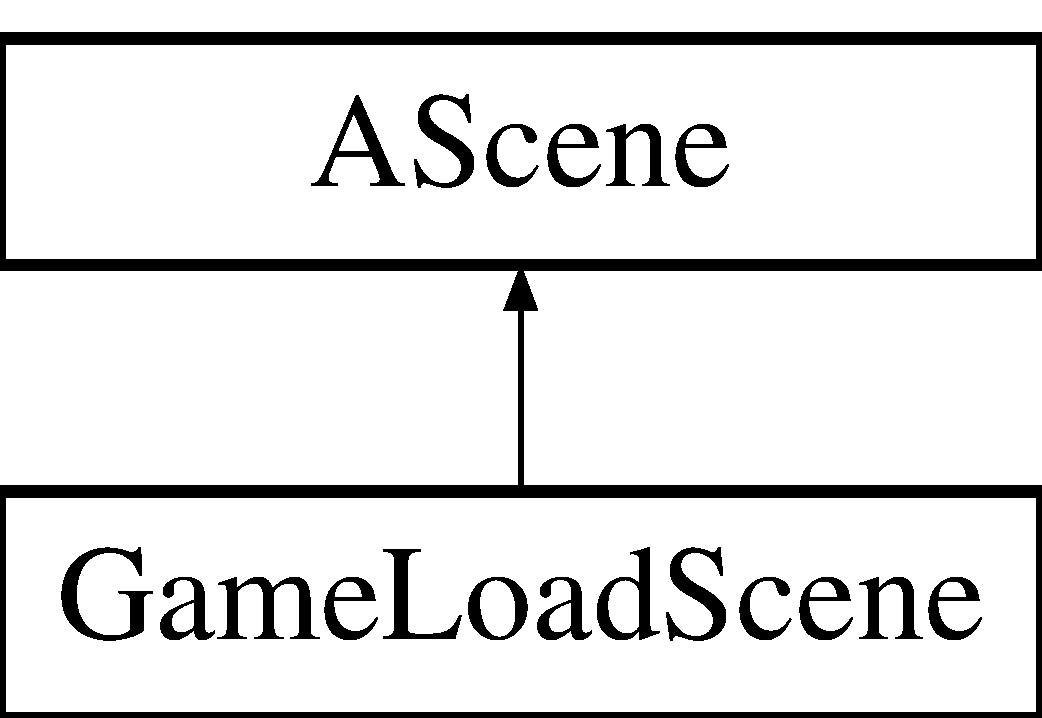
\includegraphics[height=2.000000cm]{classGameLoadScene}
\end{center}
\end{figure}
\subsection*{Public Member Functions}
\begin{DoxyCompactItemize}
\item 
\hyperlink{classGameLoadScene_a225786d3826577aa3743164b6262dc2b}{Game\+Load\+Scene} ()
\begin{DoxyCompactList}\small\item\em Constructor. \end{DoxyCompactList}\item 
\hyperlink{classGameLoadScene_a39c0f378455520c08d21e0642f35cd9b}{$\sim$\+Game\+Load\+Scene} ()
\begin{DoxyCompactList}\small\item\em Destructor. \end{DoxyCompactList}\item 
\mbox{\Hypertarget{classGameLoadScene_a4d2c3a0455cd070671dbef281b7bd87f}\label{classGameLoadScene_a4d2c3a0455cd070671dbef281b7bd87f}} 
void \hyperlink{classGameLoadScene_a4d2c3a0455cd070671dbef281b7bd87f}{prev} ()
\begin{DoxyCompactList}\small\item\em Pass to the prev scene. \end{DoxyCompactList}\item 
\mbox{\Hypertarget{classGameLoadScene_a67796257e428031f44010b9bf0b3173a}\label{classGameLoadScene_a67796257e428031f44010b9bf0b3173a}} 
void \hyperlink{classGameLoadScene_a67796257e428031f44010b9bf0b3173a}{print\+Current\+Save} ()
\begin{DoxyCompactList}\small\item\em Print current scene. \end{DoxyCompactList}\item 
\mbox{\Hypertarget{classGameLoadScene_aa00e2695ad042ee9a637ab0d5c08b054}\label{classGameLoadScene_aa00e2695ad042ee9a637ab0d5c08b054}} 
void \hyperlink{classGameLoadScene_aa00e2695ad042ee9a637ab0d5c08b054}{next} ()
\begin{DoxyCompactList}\small\item\em Pass to the next scene. \end{DoxyCompactList}\item 
irr\+::\+I\+Event\+Receiver $\ast$ \hyperlink{classGameLoadScene_a81807790ad65bd2cf97a1e543cae2b74}{get\+Event\+Receiver} () const
\begin{DoxyCompactList}\small\item\em Allow the user to implemente the event callback class for each scene. \end{DoxyCompactList}\end{DoxyCompactItemize}


\subsection{Detailed Description}
\hyperlink{classButton}{Button} interface of Game\+Load scene. 

\subsection{Constructor \& Destructor Documentation}
\mbox{\Hypertarget{classGameLoadScene_a225786d3826577aa3743164b6262dc2b}\label{classGameLoadScene_a225786d3826577aa3743164b6262dc2b}} 
\index{Game\+Load\+Scene@{Game\+Load\+Scene}!Game\+Load\+Scene@{Game\+Load\+Scene}}
\index{Game\+Load\+Scene@{Game\+Load\+Scene}!Game\+Load\+Scene@{Game\+Load\+Scene}}
\subsubsection{\texorpdfstring{Game\+Load\+Scene()}{GameLoadScene()}}
{\footnotesize\ttfamily Game\+Load\+Scene\+::\+Game\+Load\+Scene (\begin{DoxyParamCaption}{ }\end{DoxyParamCaption})}



Constructor. 

Build the class. \mbox{\Hypertarget{classGameLoadScene_a39c0f378455520c08d21e0642f35cd9b}\label{classGameLoadScene_a39c0f378455520c08d21e0642f35cd9b}} 
\index{Game\+Load\+Scene@{Game\+Load\+Scene}!````~Game\+Load\+Scene@{$\sim$\+Game\+Load\+Scene}}
\index{````~Game\+Load\+Scene@{$\sim$\+Game\+Load\+Scene}!Game\+Load\+Scene@{Game\+Load\+Scene}}
\subsubsection{\texorpdfstring{$\sim$\+Game\+Load\+Scene()}{~GameLoadScene()}}
{\footnotesize\ttfamily Game\+Load\+Scene\+::$\sim$\+Game\+Load\+Scene (\begin{DoxyParamCaption}{ }\end{DoxyParamCaption})}



Destructor. 

Destroy the class. 

\subsection{Member Function Documentation}
\mbox{\Hypertarget{classGameLoadScene_a81807790ad65bd2cf97a1e543cae2b74}\label{classGameLoadScene_a81807790ad65bd2cf97a1e543cae2b74}} 
\index{Game\+Load\+Scene@{Game\+Load\+Scene}!get\+Event\+Receiver@{get\+Event\+Receiver}}
\index{get\+Event\+Receiver@{get\+Event\+Receiver}!Game\+Load\+Scene@{Game\+Load\+Scene}}
\subsubsection{\texorpdfstring{get\+Event\+Receiver()}{getEventReceiver()}}
{\footnotesize\ttfamily irr\+::\+I\+Event\+Receiver $\ast$ Game\+Load\+Scene\+::get\+Event\+Receiver (\begin{DoxyParamCaption}{ }\end{DoxyParamCaption}) const\hspace{0.3cm}{\ttfamily [virtual]}}



Allow the user to implemente the event callback class for each scene. 

Return the event. 

Implements \hyperlink{classAScene_af521e5e6d30a5d2e5d30eb333e4d3abd}{A\+Scene}.



The documentation for this class was generated from the following files\+:\begin{DoxyCompactItemize}
\item 
inc/graphics/scenes/\hyperlink{GameLoadScene_8hh}{Game\+Load\+Scene.\+hh}\item 
src/graphics/scenes/Game\+Load\+Scene.\+cpp\end{DoxyCompactItemize}

\hypertarget{classGameMenuReceiver}{}\section{Game\+Menu\+Receiver Class Reference}
\label{classGameMenuReceiver}\index{Game\+Menu\+Receiver@{Game\+Menu\+Receiver}}


Manager of event of game scene.  




{\ttfamily \#include $<$Game\+Menu\+Receiver.\+hh$>$}



Inherits I\+Event\+Receiver.

\subsection*{Public Member Functions}
\begin{DoxyCompactItemize}
\item 
\hyperlink{classGameMenuReceiver_a5dd735dbdeddd9f11a999c9f0c4210e8}{Game\+Menu\+Receiver} ()
\begin{DoxyCompactList}\small\item\em Constructor. \end{DoxyCompactList}\item 
\hyperlink{classGameMenuReceiver_a490afacab72bebb8b1f28c3977f9ed44}{$\sim$\+Game\+Menu\+Receiver} ()
\begin{DoxyCompactList}\small\item\em Destructor. \end{DoxyCompactList}\item 
bool \hyperlink{classGameMenuReceiver_af6774556abc7e3718b7bf904cc62ead0}{On\+Event} (const irr\+::\+S\+Event \&event)
\begin{DoxyCompactList}\small\item\em Allow the user to handle envent into a scene. \end{DoxyCompactList}\end{DoxyCompactItemize}


\subsection{Detailed Description}
Manager of event of game scene. 

\subsection{Constructor \& Destructor Documentation}
\mbox{\Hypertarget{classGameMenuReceiver_a5dd735dbdeddd9f11a999c9f0c4210e8}\label{classGameMenuReceiver_a5dd735dbdeddd9f11a999c9f0c4210e8}} 
\index{Game\+Menu\+Receiver@{Game\+Menu\+Receiver}!Game\+Menu\+Receiver@{Game\+Menu\+Receiver}}
\index{Game\+Menu\+Receiver@{Game\+Menu\+Receiver}!Game\+Menu\+Receiver@{Game\+Menu\+Receiver}}
\subsubsection{\texorpdfstring{Game\+Menu\+Receiver()}{GameMenuReceiver()}}
{\footnotesize\ttfamily Game\+Menu\+Receiver\+::\+Game\+Menu\+Receiver (\begin{DoxyParamCaption}{ }\end{DoxyParamCaption})}



Constructor. 

Build the class. \mbox{\Hypertarget{classGameMenuReceiver_a490afacab72bebb8b1f28c3977f9ed44}\label{classGameMenuReceiver_a490afacab72bebb8b1f28c3977f9ed44}} 
\index{Game\+Menu\+Receiver@{Game\+Menu\+Receiver}!````~Game\+Menu\+Receiver@{$\sim$\+Game\+Menu\+Receiver}}
\index{````~Game\+Menu\+Receiver@{$\sim$\+Game\+Menu\+Receiver}!Game\+Menu\+Receiver@{Game\+Menu\+Receiver}}
\subsubsection{\texorpdfstring{$\sim$\+Game\+Menu\+Receiver()}{~GameMenuReceiver()}}
{\footnotesize\ttfamily Game\+Menu\+Receiver\+::$\sim$\+Game\+Menu\+Receiver (\begin{DoxyParamCaption}{ }\end{DoxyParamCaption})}



Destructor. 

Destroy the class. 

\subsection{Member Function Documentation}
\mbox{\Hypertarget{classGameMenuReceiver_af6774556abc7e3718b7bf904cc62ead0}\label{classGameMenuReceiver_af6774556abc7e3718b7bf904cc62ead0}} 
\index{Game\+Menu\+Receiver@{Game\+Menu\+Receiver}!On\+Event@{On\+Event}}
\index{On\+Event@{On\+Event}!Game\+Menu\+Receiver@{Game\+Menu\+Receiver}}
\subsubsection{\texorpdfstring{On\+Event()}{OnEvent()}}
{\footnotesize\ttfamily bool Game\+Menu\+Receiver\+::\+On\+Event (\begin{DoxyParamCaption}\item[{const irr\+::\+S\+Event \&}]{event }\end{DoxyParamCaption})}



Allow the user to handle envent into a scene. 

Return true if he know the event, false if not. 

The documentation for this class was generated from the following files\+:\begin{DoxyCompactItemize}
\item 
inc/graphics/scenes/events/\hyperlink{GameMenuReceiver_8hh}{Game\+Menu\+Receiver.\+hh}\item 
src/graphics/scenes/events/Game\+Menu\+Receiver.\+cpp\end{DoxyCompactItemize}

\hypertarget{classGameMenuScene}{}\section{Game\+Menu\+Scene Class Reference}
\label{classGameMenuScene}\index{Game\+Menu\+Scene@{Game\+Menu\+Scene}}


\hyperlink{classButton}{Button} interface of menu setting scene.  




{\ttfamily \#include $<$Game\+Menu\+Scene.\+hh$>$}

Inheritance diagram for Game\+Menu\+Scene\+:\begin{figure}[H]
\begin{center}
\leavevmode
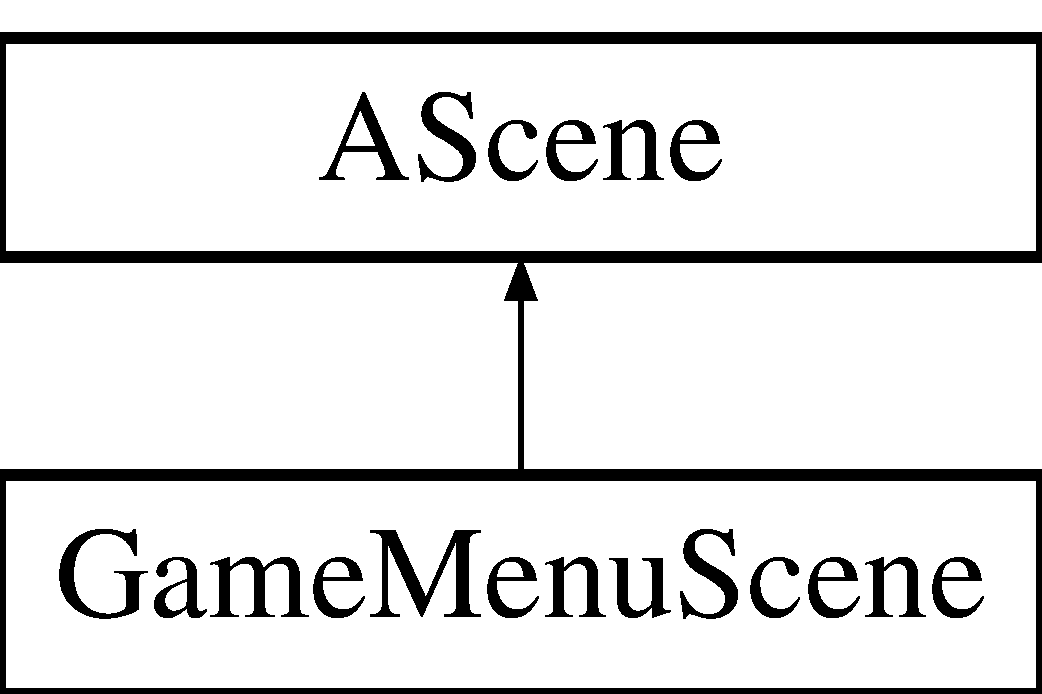
\includegraphics[height=2.000000cm]{classGameMenuScene}
\end{center}
\end{figure}
\subsection*{Public Member Functions}
\begin{DoxyCompactItemize}
\item 
\hyperlink{classGameMenuScene_a990633f8037ab2691f0aca251f3d89ee}{Game\+Menu\+Scene} ()
\begin{DoxyCompactList}\small\item\em Constructor. \end{DoxyCompactList}\item 
\hyperlink{classGameMenuScene_afbc6eddfe5f84b6f0b21bc652c9fc435}{$\sim$\+Game\+Menu\+Scene} ()
\begin{DoxyCompactList}\small\item\em Destructor. \end{DoxyCompactList}\item 
irr\+::\+I\+Event\+Receiver $\ast$ \hyperlink{classGameMenuScene_adcb01430b24486c4e5d0157fc32d7611}{get\+Event\+Receiver} () const
\begin{DoxyCompactList}\small\item\em Event getter. \end{DoxyCompactList}\end{DoxyCompactItemize}


\subsection{Detailed Description}
\hyperlink{classButton}{Button} interface of menu setting scene. 

\subsection{Constructor \& Destructor Documentation}
\mbox{\Hypertarget{classGameMenuScene_a990633f8037ab2691f0aca251f3d89ee}\label{classGameMenuScene_a990633f8037ab2691f0aca251f3d89ee}} 
\index{Game\+Menu\+Scene@{Game\+Menu\+Scene}!Game\+Menu\+Scene@{Game\+Menu\+Scene}}
\index{Game\+Menu\+Scene@{Game\+Menu\+Scene}!Game\+Menu\+Scene@{Game\+Menu\+Scene}}
\subsubsection{\texorpdfstring{Game\+Menu\+Scene()}{GameMenuScene()}}
{\footnotesize\ttfamily Game\+Menu\+Scene\+::\+Game\+Menu\+Scene (\begin{DoxyParamCaption}{ }\end{DoxyParamCaption})}



Constructor. 

Build the class. \mbox{\Hypertarget{classGameMenuScene_afbc6eddfe5f84b6f0b21bc652c9fc435}\label{classGameMenuScene_afbc6eddfe5f84b6f0b21bc652c9fc435}} 
\index{Game\+Menu\+Scene@{Game\+Menu\+Scene}!````~Game\+Menu\+Scene@{$\sim$\+Game\+Menu\+Scene}}
\index{````~Game\+Menu\+Scene@{$\sim$\+Game\+Menu\+Scene}!Game\+Menu\+Scene@{Game\+Menu\+Scene}}
\subsubsection{\texorpdfstring{$\sim$\+Game\+Menu\+Scene()}{~GameMenuScene()}}
{\footnotesize\ttfamily Game\+Menu\+Scene\+::$\sim$\+Game\+Menu\+Scene (\begin{DoxyParamCaption}{ }\end{DoxyParamCaption})}



Destructor. 

Destroy the class. 

\subsection{Member Function Documentation}
\mbox{\Hypertarget{classGameMenuScene_adcb01430b24486c4e5d0157fc32d7611}\label{classGameMenuScene_adcb01430b24486c4e5d0157fc32d7611}} 
\index{Game\+Menu\+Scene@{Game\+Menu\+Scene}!get\+Event\+Receiver@{get\+Event\+Receiver}}
\index{get\+Event\+Receiver@{get\+Event\+Receiver}!Game\+Menu\+Scene@{Game\+Menu\+Scene}}
\subsubsection{\texorpdfstring{get\+Event\+Receiver()}{getEventReceiver()}}
{\footnotesize\ttfamily irr\+::\+I\+Event\+Receiver $\ast$ Game\+Menu\+Scene\+::get\+Event\+Receiver (\begin{DoxyParamCaption}{ }\end{DoxyParamCaption}) const\hspace{0.3cm}{\ttfamily [virtual]}}



Event getter. 

Return the event. 

Implements \hyperlink{classAScene_af521e5e6d30a5d2e5d30eb333e4d3abd}{A\+Scene}.



The documentation for this class was generated from the following files\+:\begin{DoxyCompactItemize}
\item 
inc/graphics/scenes/\hyperlink{GameMenuScene_8hh}{Game\+Menu\+Scene.\+hh}\item 
src/graphics/scenes/Game\+Menu\+Scene.\+cpp\end{DoxyCompactItemize}

\hypertarget{classGameNewReceiver}{}\section{Game\+New\+Receiver Class Reference}
\label{classGameNewReceiver}\index{Game\+New\+Receiver@{Game\+New\+Receiver}}


Manager of event of new game scene.  




{\ttfamily \#include $<$Game\+New\+Receiver.\+hh$>$}

Inheritance diagram for Game\+New\+Receiver\+:\begin{figure}[H]
\begin{center}
\leavevmode
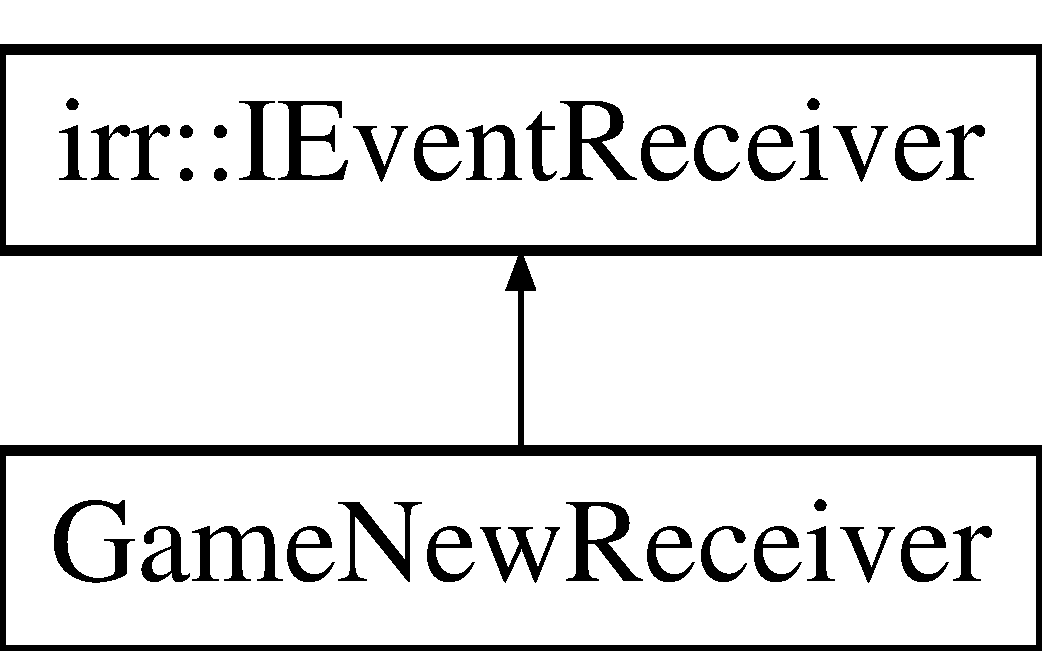
\includegraphics[height=2.000000cm]{classGameNewReceiver}
\end{center}
\end{figure}
\subsection*{Public Member Functions}
\begin{DoxyCompactItemize}
\item 
\hyperlink{classGameNewReceiver_a41816905e385ac8e17849d599106b930}{Game\+New\+Receiver} (const \hyperlink{classGameNewScene}{Game\+New\+Scene} $\ast$parent)
\begin{DoxyCompactList}\small\item\em Constructor. \end{DoxyCompactList}\item 
\hyperlink{classGameNewReceiver_ab92b6653b56d291853a4e2f737eaf6fd}{$\sim$\+Game\+New\+Receiver} ()
\begin{DoxyCompactList}\small\item\em Destructor. \end{DoxyCompactList}\item 
bool \hyperlink{classGameNewReceiver_ad9ec097d8b46946ed1a21c24463fc0b6}{On\+Event} (const \hyperlink{structirr_1_1SEvent}{irr\+::\+S\+Event} \&event)
\begin{DoxyCompactList}\small\item\em Allow the user to handle envent into a scene. \end{DoxyCompactList}\end{DoxyCompactItemize}


\subsection{Detailed Description}
Manager of event of new game scene. 

\subsection{Constructor \& Destructor Documentation}
\mbox{\Hypertarget{classGameNewReceiver_a41816905e385ac8e17849d599106b930}\label{classGameNewReceiver_a41816905e385ac8e17849d599106b930}} 
\index{Game\+New\+Receiver@{Game\+New\+Receiver}!Game\+New\+Receiver@{Game\+New\+Receiver}}
\index{Game\+New\+Receiver@{Game\+New\+Receiver}!Game\+New\+Receiver@{Game\+New\+Receiver}}
\subsubsection{\texorpdfstring{Game\+New\+Receiver()}{GameNewReceiver()}}
{\footnotesize\ttfamily Game\+New\+Receiver\+::\+Game\+New\+Receiver (\begin{DoxyParamCaption}\item[{const \hyperlink{classGameNewScene}{Game\+New\+Scene} $\ast$}]{parent }\end{DoxyParamCaption})}



Constructor. 

Build the class. \mbox{\Hypertarget{classGameNewReceiver_ab92b6653b56d291853a4e2f737eaf6fd}\label{classGameNewReceiver_ab92b6653b56d291853a4e2f737eaf6fd}} 
\index{Game\+New\+Receiver@{Game\+New\+Receiver}!````~Game\+New\+Receiver@{$\sim$\+Game\+New\+Receiver}}
\index{````~Game\+New\+Receiver@{$\sim$\+Game\+New\+Receiver}!Game\+New\+Receiver@{Game\+New\+Receiver}}
\subsubsection{\texorpdfstring{$\sim$\+Game\+New\+Receiver()}{~GameNewReceiver()}}
{\footnotesize\ttfamily Game\+New\+Receiver\+::$\sim$\+Game\+New\+Receiver (\begin{DoxyParamCaption}{ }\end{DoxyParamCaption})}



Destructor. 

Destroy the class. 

\subsection{Member Function Documentation}
\mbox{\Hypertarget{classGameNewReceiver_ad9ec097d8b46946ed1a21c24463fc0b6}\label{classGameNewReceiver_ad9ec097d8b46946ed1a21c24463fc0b6}} 
\index{Game\+New\+Receiver@{Game\+New\+Receiver}!On\+Event@{On\+Event}}
\index{On\+Event@{On\+Event}!Game\+New\+Receiver@{Game\+New\+Receiver}}
\subsubsection{\texorpdfstring{On\+Event()}{OnEvent()}}
{\footnotesize\ttfamily bool Game\+New\+Receiver\+::\+On\+Event (\begin{DoxyParamCaption}\item[{const \hyperlink{structirr_1_1SEvent}{irr\+::\+S\+Event} \&}]{event }\end{DoxyParamCaption})\hspace{0.3cm}{\ttfamily [virtual]}}



Allow the user to handle envent into a scene. 

Return true if he know the event, false if not. 

Implements \hyperlink{classirr_1_1IEventReceiver_a571f744ceffc3b4fe8a81f529163eb97}{irr\+::\+I\+Event\+Receiver}.



The documentation for this class was generated from the following files\+:\begin{DoxyCompactItemize}
\item 
inc/graphics/scenes/events/\hyperlink{GameNewReceiver_8hh}{Game\+New\+Receiver.\+hh}\item 
src/graphics/scenes/events/Game\+New\+Receiver.\+cpp\end{DoxyCompactItemize}

\hypertarget{classGameNewScene}{}\section{Game\+New\+Scene Class Reference}
\label{classGameNewScene}\index{Game\+New\+Scene@{Game\+New\+Scene}}


\hyperlink{classButton}{Button} interface of new game setting scene.  




{\ttfamily \#include $<$Game\+New\+Scene.\+hh$>$}

Inheritance diagram for Game\+New\+Scene\+:\begin{figure}[H]
\begin{center}
\leavevmode
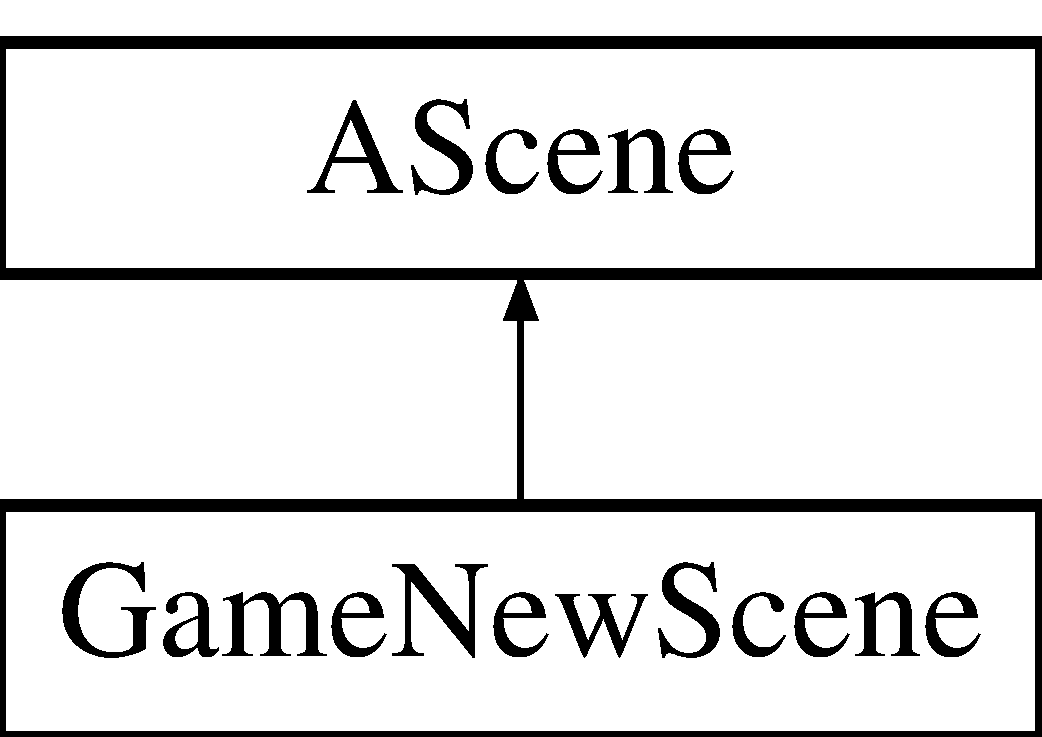
\includegraphics[height=2.000000cm]{classGameNewScene}
\end{center}
\end{figure}
\subsection*{Public Member Functions}
\begin{DoxyCompactItemize}
\item 
\hyperlink{classGameNewScene_af482b13a2d9e315ef39a6e41293bf4fb}{Game\+New\+Scene} ()
\begin{DoxyCompactList}\small\item\em Constructor. \end{DoxyCompactList}\item 
\hyperlink{classGameNewScene_a3df0ff81012d3f7dbd08c7367be22fdf}{$\sim$\+Game\+New\+Scene} ()
\begin{DoxyCompactList}\small\item\em Destructor. \end{DoxyCompactList}\item 
irr\+::\+I\+Event\+Receiver $\ast$ \hyperlink{classGameNewScene_a21c27ef3ea1923d975683e1bcdd134fa}{get\+Event\+Receiver} () const
\begin{DoxyCompactList}\small\item\em Allow the user to implemente the event callback class for each scene. \end{DoxyCompactList}\item 
\mbox{\Hypertarget{classGameNewScene_a2fb7cacfacbf5c565c3e2f98bd06aec4}\label{classGameNewScene_a2fb7cacfacbf5c565c3e2f98bd06aec4}} 
std\+::vector$<$ std\+::shared\+\_\+ptr$<$ A\+Hero $>$ $>$ \& \hyperlink{classGameNewScene_a2fb7cacfacbf5c565c3e2f98bd06aec4}{get\+Players} ()
\begin{DoxyCompactList}\small\item\em Return the players table. \end{DoxyCompactList}\item 
\mbox{\Hypertarget{classGameNewScene_a8ec7d1675e6be7490aee15126d8f2026}\label{classGameNewScene_a8ec7d1675e6be7490aee15126d8f2026}} 
std\+::vector$<$ std\+::shared\+\_\+ptr$<$ Player\+Configuration $>$ $>$ \& \hyperlink{classGameNewScene_a8ec7d1675e6be7490aee15126d8f2026}{get\+Players\+Configurations} ()
\begin{DoxyCompactList}\small\item\em Return the players configurations. \end{DoxyCompactList}\end{DoxyCompactItemize}


\subsection{Detailed Description}
\hyperlink{classButton}{Button} interface of new game setting scene. 

\subsection{Constructor \& Destructor Documentation}
\mbox{\Hypertarget{classGameNewScene_af482b13a2d9e315ef39a6e41293bf4fb}\label{classGameNewScene_af482b13a2d9e315ef39a6e41293bf4fb}} 
\index{Game\+New\+Scene@{Game\+New\+Scene}!Game\+New\+Scene@{Game\+New\+Scene}}
\index{Game\+New\+Scene@{Game\+New\+Scene}!Game\+New\+Scene@{Game\+New\+Scene}}
\subsubsection{\texorpdfstring{Game\+New\+Scene()}{GameNewScene()}}
{\footnotesize\ttfamily Game\+New\+Scene\+::\+Game\+New\+Scene (\begin{DoxyParamCaption}{ }\end{DoxyParamCaption})}



Constructor. 

Build the class. \mbox{\Hypertarget{classGameNewScene_a3df0ff81012d3f7dbd08c7367be22fdf}\label{classGameNewScene_a3df0ff81012d3f7dbd08c7367be22fdf}} 
\index{Game\+New\+Scene@{Game\+New\+Scene}!````~Game\+New\+Scene@{$\sim$\+Game\+New\+Scene}}
\index{````~Game\+New\+Scene@{$\sim$\+Game\+New\+Scene}!Game\+New\+Scene@{Game\+New\+Scene}}
\subsubsection{\texorpdfstring{$\sim$\+Game\+New\+Scene()}{~GameNewScene()}}
{\footnotesize\ttfamily Game\+New\+Scene\+::$\sim$\+Game\+New\+Scene (\begin{DoxyParamCaption}{ }\end{DoxyParamCaption})}



Destructor. 

Destroy the class. 

\subsection{Member Function Documentation}
\mbox{\Hypertarget{classGameNewScene_a21c27ef3ea1923d975683e1bcdd134fa}\label{classGameNewScene_a21c27ef3ea1923d975683e1bcdd134fa}} 
\index{Game\+New\+Scene@{Game\+New\+Scene}!get\+Event\+Receiver@{get\+Event\+Receiver}}
\index{get\+Event\+Receiver@{get\+Event\+Receiver}!Game\+New\+Scene@{Game\+New\+Scene}}
\subsubsection{\texorpdfstring{get\+Event\+Receiver()}{getEventReceiver()}}
{\footnotesize\ttfamily irr\+::\+I\+Event\+Receiver $\ast$ Game\+New\+Scene\+::get\+Event\+Receiver (\begin{DoxyParamCaption}{ }\end{DoxyParamCaption}) const\hspace{0.3cm}{\ttfamily [virtual]}}



Allow the user to implemente the event callback class for each scene. 

Return the event. 

Implements \hyperlink{classAScene_af521e5e6d30a5d2e5d30eb333e4d3abd}{A\+Scene}.



The documentation for this class was generated from the following files\+:\begin{DoxyCompactItemize}
\item 
inc/graphics/scenes/\hyperlink{GameNewScene_8hh}{Game\+New\+Scene.\+hh}\item 
src/graphics/scenes/Game\+New\+Scene.\+cpp\end{DoxyCompactItemize}

\hypertarget{classGameOnlineScene}{}\section{Game\+Online\+Scene Class Reference}
\label{classGameOnlineScene}\index{Game\+Online\+Scene@{Game\+Online\+Scene}}


\hyperlink{classButton}{Button} interface of Game\+Onlinescene.  




{\ttfamily \#include $<$Game\+Online\+Scene.\+hh$>$}

Inheritance diagram for Game\+Online\+Scene\+:\begin{figure}[H]
\begin{center}
\leavevmode
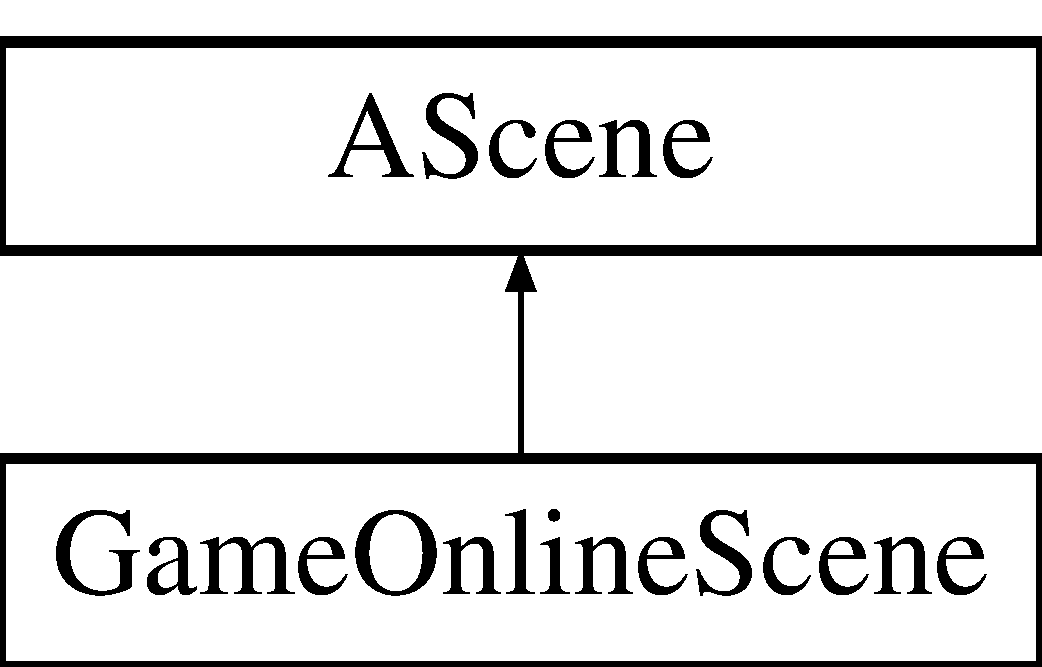
\includegraphics[height=2.000000cm]{classGameOnlineScene}
\end{center}
\end{figure}
\subsection*{Public Member Functions}
\begin{DoxyCompactItemize}
\item 
\hyperlink{classGameOnlineScene_a057362d043c386aa2b6789baf548fa09}{Game\+Online\+Scene} ()
\begin{DoxyCompactList}\small\item\em Constructor. \end{DoxyCompactList}\item 
\hyperlink{classGameOnlineScene_a59b127983ae2338edcf0b8bd86ff9f96}{$\sim$\+Game\+Online\+Scene} ()
\begin{DoxyCompactList}\small\item\em Destructor. \end{DoxyCompactList}\item 
irr\+::\+I\+Event\+Receiver $\ast$ \hyperlink{classGameOnlineScene_a00ce9773db4f1886fc463b023cbf63f9}{get\+Event\+Receiver} () const
\begin{DoxyCompactList}\small\item\em Allow the user to implemente the event callback class for each scene. \end{DoxyCompactList}\end{DoxyCompactItemize}


\subsection{Detailed Description}
\hyperlink{classButton}{Button} interface of Game\+Onlinescene. 

\subsection{Constructor \& Destructor Documentation}
\mbox{\Hypertarget{classGameOnlineScene_a057362d043c386aa2b6789baf548fa09}\label{classGameOnlineScene_a057362d043c386aa2b6789baf548fa09}} 
\index{Game\+Online\+Scene@{Game\+Online\+Scene}!Game\+Online\+Scene@{Game\+Online\+Scene}}
\index{Game\+Online\+Scene@{Game\+Online\+Scene}!Game\+Online\+Scene@{Game\+Online\+Scene}}
\subsubsection{\texorpdfstring{Game\+Online\+Scene()}{GameOnlineScene()}}
{\footnotesize\ttfamily Game\+Online\+Scene\+::\+Game\+Online\+Scene (\begin{DoxyParamCaption}{ }\end{DoxyParamCaption})}



Constructor. 

Build the class. \mbox{\Hypertarget{classGameOnlineScene_a59b127983ae2338edcf0b8bd86ff9f96}\label{classGameOnlineScene_a59b127983ae2338edcf0b8bd86ff9f96}} 
\index{Game\+Online\+Scene@{Game\+Online\+Scene}!````~Game\+Online\+Scene@{$\sim$\+Game\+Online\+Scene}}
\index{````~Game\+Online\+Scene@{$\sim$\+Game\+Online\+Scene}!Game\+Online\+Scene@{Game\+Online\+Scene}}
\subsubsection{\texorpdfstring{$\sim$\+Game\+Online\+Scene()}{~GameOnlineScene()}}
{\footnotesize\ttfamily Game\+Online\+Scene\+::$\sim$\+Game\+Online\+Scene (\begin{DoxyParamCaption}{ }\end{DoxyParamCaption})}



Destructor. 

Destroy the class. 

\subsection{Member Function Documentation}
\mbox{\Hypertarget{classGameOnlineScene_a00ce9773db4f1886fc463b023cbf63f9}\label{classGameOnlineScene_a00ce9773db4f1886fc463b023cbf63f9}} 
\index{Game\+Online\+Scene@{Game\+Online\+Scene}!get\+Event\+Receiver@{get\+Event\+Receiver}}
\index{get\+Event\+Receiver@{get\+Event\+Receiver}!Game\+Online\+Scene@{Game\+Online\+Scene}}
\subsubsection{\texorpdfstring{get\+Event\+Receiver()}{getEventReceiver()}}
{\footnotesize\ttfamily irr\+::\+I\+Event\+Receiver $\ast$ Game\+Online\+Scene\+::get\+Event\+Receiver (\begin{DoxyParamCaption}{ }\end{DoxyParamCaption}) const\hspace{0.3cm}{\ttfamily [virtual]}}



Allow the user to implemente the event callback class for each scene. 

Return the event. 

Implements \hyperlink{classAScene_af521e5e6d30a5d2e5d30eb333e4d3abd}{A\+Scene}.



The documentation for this class was generated from the following files\+:\begin{DoxyCompactItemize}
\item 
inc/graphics/scenes/\hyperlink{GameOnlineScene_8hh}{Game\+Online\+Scene.\+hh}\item 
src/graphics/scenes/Game\+Online\+Scene.\+cpp\end{DoxyCompactItemize}

\hypertarget{classGameSimulationScene}{}\section{Game\+Simulation\+Scene Class Reference}
\label{classGameSimulationScene}\index{Game\+Simulation\+Scene@{Game\+Simulation\+Scene}}


\hyperlink{classButton}{Button} interface of Game\+Simulationscene.  




{\ttfamily \#include $<$Game\+Simulation\+Scene.\+hh$>$}

Inheritance diagram for Game\+Simulation\+Scene\+:\begin{figure}[H]
\begin{center}
\leavevmode
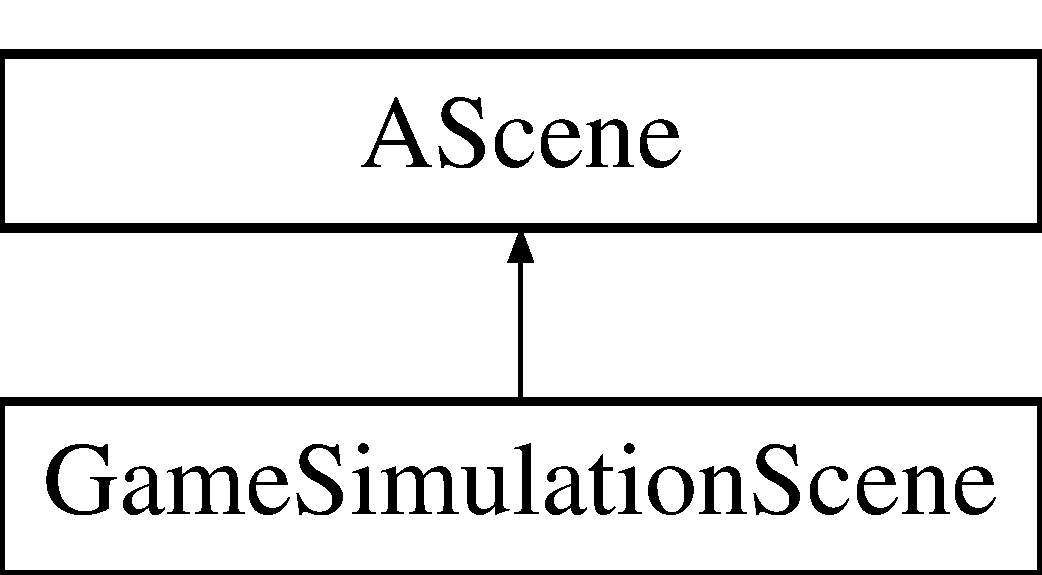
\includegraphics[height=2.000000cm]{classGameSimulationScene}
\end{center}
\end{figure}
\subsection*{Public Member Functions}
\begin{DoxyCompactItemize}
\item 
\hyperlink{classGameSimulationScene_a6983b2c511d45278121bcf62151fbb19}{Game\+Simulation\+Scene} (const std\+::shared\+\_\+ptr$<$ \hyperlink{classLevel}{Level} $>$ \&level)
\begin{DoxyCompactList}\small\item\em Constructor. \end{DoxyCompactList}\item 
\hyperlink{classGameSimulationScene_af45f3e7f70376e59a6f320f21ce2897b}{$\sim$\+Game\+Simulation\+Scene} ()
\begin{DoxyCompactList}\small\item\em Destructor. \end{DoxyCompactList}\item 
void \hyperlink{classGameSimulationScene_a66b107f708b5eed87a3c0a0016541d29}{update\+Camera} (\hyperlink{classWindow}{Window} $\ast$win)
\begin{DoxyCompactList}\small\item\em Update camera\textquotesingle{}s position. \end{DoxyCompactList}\item 
\hyperlink{classirr_1_1IEventReceiver}{irr\+::\+I\+Event\+Receiver} $\ast$ \hyperlink{classGameSimulationScene_a048b2a937caff3af7b4d54f8bd404ec1}{get\+Event\+Receiver} () const
\begin{DoxyCompactList}\small\item\em Allow the user to implemente the event callback class for each scene. \end{DoxyCompactList}\end{DoxyCompactItemize}


\subsection{Detailed Description}
\hyperlink{classButton}{Button} interface of Game\+Simulationscene. 

\subsection{Constructor \& Destructor Documentation}
\mbox{\Hypertarget{classGameSimulationScene_a6983b2c511d45278121bcf62151fbb19}\label{classGameSimulationScene_a6983b2c511d45278121bcf62151fbb19}} 
\index{Game\+Simulation\+Scene@{Game\+Simulation\+Scene}!Game\+Simulation\+Scene@{Game\+Simulation\+Scene}}
\index{Game\+Simulation\+Scene@{Game\+Simulation\+Scene}!Game\+Simulation\+Scene@{Game\+Simulation\+Scene}}
\subsubsection{\texorpdfstring{Game\+Simulation\+Scene()}{GameSimulationScene()}}
{\footnotesize\ttfamily Game\+Simulation\+Scene\+::\+Game\+Simulation\+Scene (\begin{DoxyParamCaption}\item[{const std\+::shared\+\_\+ptr$<$ \hyperlink{classLevel}{Level} $>$ \&}]{level }\end{DoxyParamCaption})}



Constructor. 

Build the class. \mbox{\Hypertarget{classGameSimulationScene_af45f3e7f70376e59a6f320f21ce2897b}\label{classGameSimulationScene_af45f3e7f70376e59a6f320f21ce2897b}} 
\index{Game\+Simulation\+Scene@{Game\+Simulation\+Scene}!````~Game\+Simulation\+Scene@{$\sim$\+Game\+Simulation\+Scene}}
\index{````~Game\+Simulation\+Scene@{$\sim$\+Game\+Simulation\+Scene}!Game\+Simulation\+Scene@{Game\+Simulation\+Scene}}
\subsubsection{\texorpdfstring{$\sim$\+Game\+Simulation\+Scene()}{~GameSimulationScene()}}
{\footnotesize\ttfamily Game\+Simulation\+Scene\+::$\sim$\+Game\+Simulation\+Scene (\begin{DoxyParamCaption}{ }\end{DoxyParamCaption})}



Destructor. 

Destroy the class. 

\subsection{Member Function Documentation}
\mbox{\Hypertarget{classGameSimulationScene_a048b2a937caff3af7b4d54f8bd404ec1}\label{classGameSimulationScene_a048b2a937caff3af7b4d54f8bd404ec1}} 
\index{Game\+Simulation\+Scene@{Game\+Simulation\+Scene}!get\+Event\+Receiver@{get\+Event\+Receiver}}
\index{get\+Event\+Receiver@{get\+Event\+Receiver}!Game\+Simulation\+Scene@{Game\+Simulation\+Scene}}
\subsubsection{\texorpdfstring{get\+Event\+Receiver()}{getEventReceiver()}}
{\footnotesize\ttfamily \hyperlink{classirr_1_1IEventReceiver}{irr\+::\+I\+Event\+Receiver} $\ast$ Game\+Simulation\+Scene\+::get\+Event\+Receiver (\begin{DoxyParamCaption}{ }\end{DoxyParamCaption}) const\hspace{0.3cm}{\ttfamily [virtual]}}



Allow the user to implemente the event callback class for each scene. 

Return the event. 

Implements \hyperlink{classAScene_af521e5e6d30a5d2e5d30eb333e4d3abd}{A\+Scene}.

\mbox{\Hypertarget{classGameSimulationScene_a66b107f708b5eed87a3c0a0016541d29}\label{classGameSimulationScene_a66b107f708b5eed87a3c0a0016541d29}} 
\index{Game\+Simulation\+Scene@{Game\+Simulation\+Scene}!update\+Camera@{update\+Camera}}
\index{update\+Camera@{update\+Camera}!Game\+Simulation\+Scene@{Game\+Simulation\+Scene}}
\subsubsection{\texorpdfstring{update\+Camera()}{updateCamera()}}
{\footnotesize\ttfamily void Game\+Simulation\+Scene\+::update\+Camera (\begin{DoxyParamCaption}\item[{\hyperlink{classWindow}{Window} $\ast$}]{win }\end{DoxyParamCaption})\hspace{0.3cm}{\ttfamily [virtual]}}



Update camera\textquotesingle{}s position. 


\begin{DoxyParams}{Parameters}
{\em The} & window who contain the camera. \\
\hline
\end{DoxyParams}


Reimplemented from \hyperlink{classAScene_a18070899d965f1811c2253ad1d939374}{A\+Scene}.



The documentation for this class was generated from the following files\+:\begin{DoxyCompactItemize}
\item 
inc/graphics/scenes/\hyperlink{GameSimulationScene_8hh}{Game\+Simulation\+Scene.\+hh}\item 
src/graphics/scenes/Game\+Simulation\+Scene.\+cpp\end{DoxyCompactItemize}

\hypertarget{classirr_1_1scene_1_1IAnimatedMesh}{}\section{irr\+:\+:scene\+:\+:I\+Animated\+Mesh Class Reference}
\label{classirr_1_1scene_1_1IAnimatedMesh}\index{irr\+::scene\+::\+I\+Animated\+Mesh@{irr\+::scene\+::\+I\+Animated\+Mesh}}


Interface for an animated mesh.  




{\ttfamily \#include $<$I\+Animated\+Mesh.\+h$>$}

Inheritance diagram for irr\+:\+:scene\+:\+:I\+Animated\+Mesh\+:\begin{figure}[H]
\begin{center}
\leavevmode
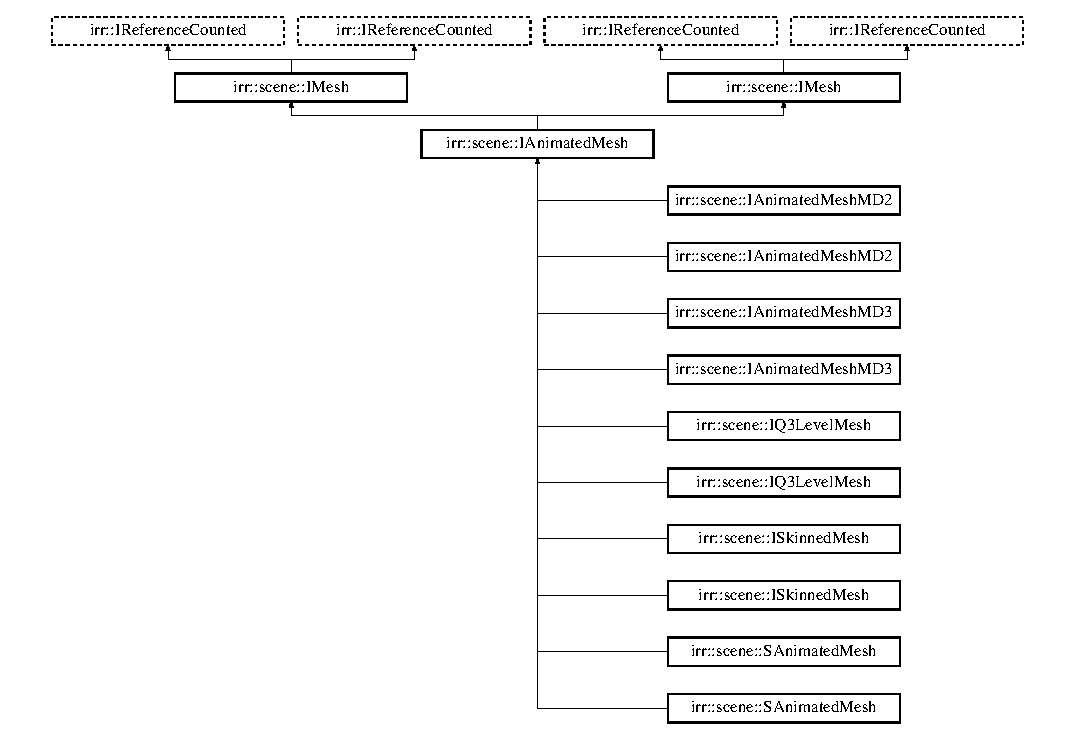
\includegraphics[height=9.479166cm]{classirr_1_1scene_1_1IAnimatedMesh}
\end{center}
\end{figure}
\subsection*{Public Member Functions}
\begin{DoxyCompactItemize}
\item 
virtual \hyperlink{namespaceirr_a0416a53257075833e7002efd0a18e804}{u32} \hyperlink{classirr_1_1scene_1_1IAnimatedMesh_a2ec99aba081e9f37802e8ea9cd65629b}{get\+Frame\+Count} () const =0
\begin{DoxyCompactList}\small\item\em Gets the frame count of the animated mesh. \end{DoxyCompactList}\item 
virtual \hyperlink{namespaceirr_a0277be98d67dc26ff93b1a6a1d086b07}{f32} \hyperlink{classirr_1_1scene_1_1IAnimatedMesh_acb4249295319c8240d5bedc167417435}{get\+Animation\+Speed} () const =0
\begin{DoxyCompactList}\small\item\em Gets the animation speed of the animated mesh. \end{DoxyCompactList}\item 
virtual void \hyperlink{classirr_1_1scene_1_1IAnimatedMesh_a5eb1b09d96547dbd273d489e58d62658}{set\+Animation\+Speed} (\hyperlink{namespaceirr_a0277be98d67dc26ff93b1a6a1d086b07}{f32} fps)=0
\begin{DoxyCompactList}\small\item\em Sets the animation speed of the animated mesh. \end{DoxyCompactList}\item 
virtual \hyperlink{classirr_1_1scene_1_1IMesh}{I\+Mesh} $\ast$ \hyperlink{classirr_1_1scene_1_1IAnimatedMesh_adccb39fee83bed36a464cf7b96f3a0ca}{get\+Mesh} (\hyperlink{namespaceirr_ac66849b7a6ed16e30ebede579f9b47c6}{s32} frame, \hyperlink{namespaceirr_ac66849b7a6ed16e30ebede579f9b47c6}{s32} detail\+Level=255, \hyperlink{namespaceirr_ac66849b7a6ed16e30ebede579f9b47c6}{s32} start\+Frame\+Loop=-\/1, \hyperlink{namespaceirr_ac66849b7a6ed16e30ebede579f9b47c6}{s32} end\+Frame\+Loop=-\/1)=0
\begin{DoxyCompactList}\small\item\em Returns the \hyperlink{classirr_1_1scene_1_1IMesh}{I\+Mesh} interface for a frame. \end{DoxyCompactList}\item 
virtual \hyperlink{namespaceirr_1_1scene_a2fc85a64604521ca063f1881b5dd1c61}{E\+\_\+\+A\+N\+I\+M\+A\+T\+E\+D\+\_\+\+M\+E\+S\+H\+\_\+\+T\+Y\+PE} \hyperlink{classirr_1_1scene_1_1IAnimatedMesh_abe5a20eccfb94eefcc6cbbc0b667ce37}{get\+Mesh\+Type} () const
\begin{DoxyCompactList}\small\item\em Returns the type of the animated mesh. \end{DoxyCompactList}\item 
virtual \hyperlink{namespaceirr_a0416a53257075833e7002efd0a18e804}{u32} \hyperlink{classirr_1_1scene_1_1IAnimatedMesh_a2ec99aba081e9f37802e8ea9cd65629b}{get\+Frame\+Count} () const =0
\begin{DoxyCompactList}\small\item\em Gets the frame count of the animated mesh. \end{DoxyCompactList}\item 
virtual \hyperlink{namespaceirr_a0277be98d67dc26ff93b1a6a1d086b07}{f32} \hyperlink{classirr_1_1scene_1_1IAnimatedMesh_acb4249295319c8240d5bedc167417435}{get\+Animation\+Speed} () const =0
\begin{DoxyCompactList}\small\item\em Gets the animation speed of the animated mesh. \end{DoxyCompactList}\item 
virtual void \hyperlink{classirr_1_1scene_1_1IAnimatedMesh_a5eb1b09d96547dbd273d489e58d62658}{set\+Animation\+Speed} (\hyperlink{namespaceirr_a0277be98d67dc26ff93b1a6a1d086b07}{f32} fps)=0
\begin{DoxyCompactList}\small\item\em Sets the animation speed of the animated mesh. \end{DoxyCompactList}\item 
virtual \hyperlink{classirr_1_1scene_1_1IMesh}{I\+Mesh} $\ast$ \hyperlink{classirr_1_1scene_1_1IAnimatedMesh_adccb39fee83bed36a464cf7b96f3a0ca}{get\+Mesh} (\hyperlink{namespaceirr_ac66849b7a6ed16e30ebede579f9b47c6}{s32} frame, \hyperlink{namespaceirr_ac66849b7a6ed16e30ebede579f9b47c6}{s32} detail\+Level=255, \hyperlink{namespaceirr_ac66849b7a6ed16e30ebede579f9b47c6}{s32} start\+Frame\+Loop=-\/1, \hyperlink{namespaceirr_ac66849b7a6ed16e30ebede579f9b47c6}{s32} end\+Frame\+Loop=-\/1)=0
\begin{DoxyCompactList}\small\item\em Returns the \hyperlink{classirr_1_1scene_1_1IMesh}{I\+Mesh} interface for a frame. \end{DoxyCompactList}\item 
virtual \hyperlink{namespaceirr_1_1scene_a2fc85a64604521ca063f1881b5dd1c61}{E\+\_\+\+A\+N\+I\+M\+A\+T\+E\+D\+\_\+\+M\+E\+S\+H\+\_\+\+T\+Y\+PE} \hyperlink{classirr_1_1scene_1_1IAnimatedMesh_abe5a20eccfb94eefcc6cbbc0b667ce37}{get\+Mesh\+Type} () const
\begin{DoxyCompactList}\small\item\em Returns the type of the animated mesh. \end{DoxyCompactList}\end{DoxyCompactItemize}
\subsection*{Additional Inherited Members}


\subsection{Detailed Description}
Interface for an animated mesh. 

There are already simple implementations of this interface available so you don\textquotesingle{}t have to implement this interface on your own if you need to\+: You might want to use \hyperlink{structirr_1_1scene_1_1SAnimatedMesh}{irr\+::scene\+::\+S\+Animated\+Mesh}, \hyperlink{structirr_1_1scene_1_1SMesh}{irr\+::scene\+::\+S\+Mesh}, \hyperlink{namespaceirr_1_1scene_ae74662460587fcb33d99e340bda3e826}{irr\+::scene\+::\+S\+Mesh\+Buffer} etc. 

\subsection{Member Function Documentation}
\mbox{\Hypertarget{classirr_1_1scene_1_1IAnimatedMesh_acb4249295319c8240d5bedc167417435}\label{classirr_1_1scene_1_1IAnimatedMesh_acb4249295319c8240d5bedc167417435}} 
\index{irr\+::scene\+::\+I\+Animated\+Mesh@{irr\+::scene\+::\+I\+Animated\+Mesh}!get\+Animation\+Speed@{get\+Animation\+Speed}}
\index{get\+Animation\+Speed@{get\+Animation\+Speed}!irr\+::scene\+::\+I\+Animated\+Mesh@{irr\+::scene\+::\+I\+Animated\+Mesh}}
\subsubsection{\texorpdfstring{get\+Animation\+Speed()}{getAnimationSpeed()}\hspace{0.1cm}{\footnotesize\ttfamily [1/2]}}
{\footnotesize\ttfamily virtual \hyperlink{namespaceirr_a0277be98d67dc26ff93b1a6a1d086b07}{f32} irr\+::scene\+::\+I\+Animated\+Mesh\+::get\+Animation\+Speed (\begin{DoxyParamCaption}{ }\end{DoxyParamCaption}) const\hspace{0.3cm}{\ttfamily [pure virtual]}}



Gets the animation speed of the animated mesh. 

\begin{DoxyReturn}{Returns}
The number of frames per second to play the animation with by default. If the amount is 0, it is a static, non animated mesh. 
\end{DoxyReturn}


Implemented in \hyperlink{structirr_1_1scene_1_1SAnimatedMesh_aa6b6302dad72761e22ba10cc4486b4c8}{irr\+::scene\+::\+S\+Animated\+Mesh}, and \hyperlink{structirr_1_1scene_1_1SAnimatedMesh_aa6b6302dad72761e22ba10cc4486b4c8}{irr\+::scene\+::\+S\+Animated\+Mesh}.

\mbox{\Hypertarget{classirr_1_1scene_1_1IAnimatedMesh_acb4249295319c8240d5bedc167417435}\label{classirr_1_1scene_1_1IAnimatedMesh_acb4249295319c8240d5bedc167417435}} 
\index{irr\+::scene\+::\+I\+Animated\+Mesh@{irr\+::scene\+::\+I\+Animated\+Mesh}!get\+Animation\+Speed@{get\+Animation\+Speed}}
\index{get\+Animation\+Speed@{get\+Animation\+Speed}!irr\+::scene\+::\+I\+Animated\+Mesh@{irr\+::scene\+::\+I\+Animated\+Mesh}}
\subsubsection{\texorpdfstring{get\+Animation\+Speed()}{getAnimationSpeed()}\hspace{0.1cm}{\footnotesize\ttfamily [2/2]}}
{\footnotesize\ttfamily virtual \hyperlink{namespaceirr_a0277be98d67dc26ff93b1a6a1d086b07}{f32} irr\+::scene\+::\+I\+Animated\+Mesh\+::get\+Animation\+Speed (\begin{DoxyParamCaption}{ }\end{DoxyParamCaption}) const\hspace{0.3cm}{\ttfamily [pure virtual]}}



Gets the animation speed of the animated mesh. 

\begin{DoxyReturn}{Returns}
The number of frames per second to play the animation with by default. If the amount is 0, it is a static, non animated mesh. 
\end{DoxyReturn}


Implemented in \hyperlink{structirr_1_1scene_1_1SAnimatedMesh_aa6b6302dad72761e22ba10cc4486b4c8}{irr\+::scene\+::\+S\+Animated\+Mesh}, and \hyperlink{structirr_1_1scene_1_1SAnimatedMesh_aa6b6302dad72761e22ba10cc4486b4c8}{irr\+::scene\+::\+S\+Animated\+Mesh}.

\mbox{\Hypertarget{classirr_1_1scene_1_1IAnimatedMesh_a2ec99aba081e9f37802e8ea9cd65629b}\label{classirr_1_1scene_1_1IAnimatedMesh_a2ec99aba081e9f37802e8ea9cd65629b}} 
\index{irr\+::scene\+::\+I\+Animated\+Mesh@{irr\+::scene\+::\+I\+Animated\+Mesh}!get\+Frame\+Count@{get\+Frame\+Count}}
\index{get\+Frame\+Count@{get\+Frame\+Count}!irr\+::scene\+::\+I\+Animated\+Mesh@{irr\+::scene\+::\+I\+Animated\+Mesh}}
\subsubsection{\texorpdfstring{get\+Frame\+Count()}{getFrameCount()}\hspace{0.1cm}{\footnotesize\ttfamily [1/2]}}
{\footnotesize\ttfamily virtual \hyperlink{namespaceirr_a0416a53257075833e7002efd0a18e804}{u32} irr\+::scene\+::\+I\+Animated\+Mesh\+::get\+Frame\+Count (\begin{DoxyParamCaption}{ }\end{DoxyParamCaption}) const\hspace{0.3cm}{\ttfamily [pure virtual]}}



Gets the frame count of the animated mesh. 

\begin{DoxyReturn}{Returns}
The amount of frames. If the amount is 1, it is a static, non animated mesh. 
\end{DoxyReturn}


Implemented in \hyperlink{structirr_1_1scene_1_1SAnimatedMesh_a58d8940d3002792194c74e209a5f2949}{irr\+::scene\+::\+S\+Animated\+Mesh}, and \hyperlink{structirr_1_1scene_1_1SAnimatedMesh_a58d8940d3002792194c74e209a5f2949}{irr\+::scene\+::\+S\+Animated\+Mesh}.

\mbox{\Hypertarget{classirr_1_1scene_1_1IAnimatedMesh_a2ec99aba081e9f37802e8ea9cd65629b}\label{classirr_1_1scene_1_1IAnimatedMesh_a2ec99aba081e9f37802e8ea9cd65629b}} 
\index{irr\+::scene\+::\+I\+Animated\+Mesh@{irr\+::scene\+::\+I\+Animated\+Mesh}!get\+Frame\+Count@{get\+Frame\+Count}}
\index{get\+Frame\+Count@{get\+Frame\+Count}!irr\+::scene\+::\+I\+Animated\+Mesh@{irr\+::scene\+::\+I\+Animated\+Mesh}}
\subsubsection{\texorpdfstring{get\+Frame\+Count()}{getFrameCount()}\hspace{0.1cm}{\footnotesize\ttfamily [2/2]}}
{\footnotesize\ttfamily virtual \hyperlink{namespaceirr_a0416a53257075833e7002efd0a18e804}{u32} irr\+::scene\+::\+I\+Animated\+Mesh\+::get\+Frame\+Count (\begin{DoxyParamCaption}{ }\end{DoxyParamCaption}) const\hspace{0.3cm}{\ttfamily [pure virtual]}}



Gets the frame count of the animated mesh. 

\begin{DoxyReturn}{Returns}
The amount of frames. If the amount is 1, it is a static, non animated mesh. 
\end{DoxyReturn}


Implemented in \hyperlink{structirr_1_1scene_1_1SAnimatedMesh_a58d8940d3002792194c74e209a5f2949}{irr\+::scene\+::\+S\+Animated\+Mesh}, and \hyperlink{structirr_1_1scene_1_1SAnimatedMesh_a58d8940d3002792194c74e209a5f2949}{irr\+::scene\+::\+S\+Animated\+Mesh}.

\mbox{\Hypertarget{classirr_1_1scene_1_1IAnimatedMesh_adccb39fee83bed36a464cf7b96f3a0ca}\label{classirr_1_1scene_1_1IAnimatedMesh_adccb39fee83bed36a464cf7b96f3a0ca}} 
\index{irr\+::scene\+::\+I\+Animated\+Mesh@{irr\+::scene\+::\+I\+Animated\+Mesh}!get\+Mesh@{get\+Mesh}}
\index{get\+Mesh@{get\+Mesh}!irr\+::scene\+::\+I\+Animated\+Mesh@{irr\+::scene\+::\+I\+Animated\+Mesh}}
\subsubsection{\texorpdfstring{get\+Mesh()}{getMesh()}\hspace{0.1cm}{\footnotesize\ttfamily [1/2]}}
{\footnotesize\ttfamily virtual \hyperlink{classirr_1_1scene_1_1IMesh}{I\+Mesh}$\ast$ irr\+::scene\+::\+I\+Animated\+Mesh\+::get\+Mesh (\begin{DoxyParamCaption}\item[{\hyperlink{namespaceirr_ac66849b7a6ed16e30ebede579f9b47c6}{s32}}]{frame,  }\item[{\hyperlink{namespaceirr_ac66849b7a6ed16e30ebede579f9b47c6}{s32}}]{detail\+Level = {\ttfamily 255},  }\item[{\hyperlink{namespaceirr_ac66849b7a6ed16e30ebede579f9b47c6}{s32}}]{start\+Frame\+Loop = {\ttfamily -\/1},  }\item[{\hyperlink{namespaceirr_ac66849b7a6ed16e30ebede579f9b47c6}{s32}}]{end\+Frame\+Loop = {\ttfamily -\/1} }\end{DoxyParamCaption})\hspace{0.3cm}{\ttfamily [pure virtual]}}



Returns the \hyperlink{classirr_1_1scene_1_1IMesh}{I\+Mesh} interface for a frame. 


\begin{DoxyParams}{Parameters}
{\em frame} & Frame number as zero based index. The maximum frame number is \hyperlink{classirr_1_1scene_1_1IAnimatedMesh_a2ec99aba081e9f37802e8ea9cd65629b}{get\+Frame\+Count()} -\/ 1; \\
\hline
{\em detail\+Level} & \hyperlink{classLevel}{Level} of detail. 0 is the lowest, 255 the highest level of detail. Most meshes will ignore the detail level. \\
\hline
{\em start\+Frame\+Loop} & Because some animated meshes (.M\+D2) are blended between 2 static frames, and maybe animated in a loop, the start\+Frame\+Loop and the end\+Frame\+Loop have to be defined, to prevent the animation to be blended between frames which are outside of this loop. If start\+Frame\+Loop and end\+Frame\+Loop are both -\/1, they are ignored. \\
\hline
{\em end\+Frame\+Loop} & see start\+Frame\+Loop. \\
\hline
\end{DoxyParams}
\begin{DoxyReturn}{Returns}
Returns the animated mesh based on a detail level. 
\end{DoxyReturn}


Implemented in \hyperlink{structirr_1_1scene_1_1SAnimatedMesh_a132d5f643fe02b57480d945e8d5be2d2}{irr\+::scene\+::\+S\+Animated\+Mesh}, and \hyperlink{structirr_1_1scene_1_1SAnimatedMesh_a132d5f643fe02b57480d945e8d5be2d2}{irr\+::scene\+::\+S\+Animated\+Mesh}.

\mbox{\Hypertarget{classirr_1_1scene_1_1IAnimatedMesh_adccb39fee83bed36a464cf7b96f3a0ca}\label{classirr_1_1scene_1_1IAnimatedMesh_adccb39fee83bed36a464cf7b96f3a0ca}} 
\index{irr\+::scene\+::\+I\+Animated\+Mesh@{irr\+::scene\+::\+I\+Animated\+Mesh}!get\+Mesh@{get\+Mesh}}
\index{get\+Mesh@{get\+Mesh}!irr\+::scene\+::\+I\+Animated\+Mesh@{irr\+::scene\+::\+I\+Animated\+Mesh}}
\subsubsection{\texorpdfstring{get\+Mesh()}{getMesh()}\hspace{0.1cm}{\footnotesize\ttfamily [2/2]}}
{\footnotesize\ttfamily virtual \hyperlink{classirr_1_1scene_1_1IMesh}{I\+Mesh}$\ast$ irr\+::scene\+::\+I\+Animated\+Mesh\+::get\+Mesh (\begin{DoxyParamCaption}\item[{\hyperlink{namespaceirr_ac66849b7a6ed16e30ebede579f9b47c6}{s32}}]{frame,  }\item[{\hyperlink{namespaceirr_ac66849b7a6ed16e30ebede579f9b47c6}{s32}}]{detail\+Level = {\ttfamily 255},  }\item[{\hyperlink{namespaceirr_ac66849b7a6ed16e30ebede579f9b47c6}{s32}}]{start\+Frame\+Loop = {\ttfamily -\/1},  }\item[{\hyperlink{namespaceirr_ac66849b7a6ed16e30ebede579f9b47c6}{s32}}]{end\+Frame\+Loop = {\ttfamily -\/1} }\end{DoxyParamCaption})\hspace{0.3cm}{\ttfamily [pure virtual]}}



Returns the \hyperlink{classirr_1_1scene_1_1IMesh}{I\+Mesh} interface for a frame. 


\begin{DoxyParams}{Parameters}
{\em frame} & Frame number as zero based index. The maximum frame number is \hyperlink{classirr_1_1scene_1_1IAnimatedMesh_a2ec99aba081e9f37802e8ea9cd65629b}{get\+Frame\+Count()} -\/ 1; \\
\hline
{\em detail\+Level} & \hyperlink{classLevel}{Level} of detail. 0 is the lowest, 255 the highest level of detail. Most meshes will ignore the detail level. \\
\hline
{\em start\+Frame\+Loop} & Because some animated meshes (.M\+D2) are blended between 2 static frames, and maybe animated in a loop, the start\+Frame\+Loop and the end\+Frame\+Loop have to be defined, to prevent the animation to be blended between frames which are outside of this loop. If start\+Frame\+Loop and end\+Frame\+Loop are both -\/1, they are ignored. \\
\hline
{\em end\+Frame\+Loop} & see start\+Frame\+Loop. \\
\hline
\end{DoxyParams}
\begin{DoxyReturn}{Returns}
Returns the animated mesh based on a detail level. 
\end{DoxyReturn}


Implemented in \hyperlink{structirr_1_1scene_1_1SAnimatedMesh_a132d5f643fe02b57480d945e8d5be2d2}{irr\+::scene\+::\+S\+Animated\+Mesh}, and \hyperlink{structirr_1_1scene_1_1SAnimatedMesh_a132d5f643fe02b57480d945e8d5be2d2}{irr\+::scene\+::\+S\+Animated\+Mesh}.

\mbox{\Hypertarget{classirr_1_1scene_1_1IAnimatedMesh_abe5a20eccfb94eefcc6cbbc0b667ce37}\label{classirr_1_1scene_1_1IAnimatedMesh_abe5a20eccfb94eefcc6cbbc0b667ce37}} 
\index{irr\+::scene\+::\+I\+Animated\+Mesh@{irr\+::scene\+::\+I\+Animated\+Mesh}!get\+Mesh\+Type@{get\+Mesh\+Type}}
\index{get\+Mesh\+Type@{get\+Mesh\+Type}!irr\+::scene\+::\+I\+Animated\+Mesh@{irr\+::scene\+::\+I\+Animated\+Mesh}}
\subsubsection{\texorpdfstring{get\+Mesh\+Type()}{getMeshType()}\hspace{0.1cm}{\footnotesize\ttfamily [1/2]}}
{\footnotesize\ttfamily virtual \hyperlink{namespaceirr_1_1scene_a2fc85a64604521ca063f1881b5dd1c61}{E\+\_\+\+A\+N\+I\+M\+A\+T\+E\+D\+\_\+\+M\+E\+S\+H\+\_\+\+T\+Y\+PE} irr\+::scene\+::\+I\+Animated\+Mesh\+::get\+Mesh\+Type (\begin{DoxyParamCaption}{ }\end{DoxyParamCaption}) const\hspace{0.3cm}{\ttfamily [inline]}, {\ttfamily [virtual]}}



Returns the type of the animated mesh. 

In most cases it is not neccessary to use this method. This is useful for making a safe downcast. For example, if \hyperlink{classirr_1_1scene_1_1IAnimatedMesh_abe5a20eccfb94eefcc6cbbc0b667ce37}{get\+Mesh\+Type()} returns E\+A\+M\+T\+\_\+\+M\+D2 it\textquotesingle{}s safe to cast the \hyperlink{classirr_1_1scene_1_1IAnimatedMesh}{I\+Animated\+Mesh} to \hyperlink{classirr_1_1scene_1_1IAnimatedMeshMD2}{I\+Animated\+Mesh\+M\+D2}. \begin{DoxyReturn}{Returns}
Type of the mesh. 
\end{DoxyReturn}


Reimplemented in \hyperlink{structirr_1_1scene_1_1SAnimatedMesh_a423a3a9a7d2075eac53280fdfb15fdc9}{irr\+::scene\+::\+S\+Animated\+Mesh}, and \hyperlink{structirr_1_1scene_1_1SAnimatedMesh_a423a3a9a7d2075eac53280fdfb15fdc9}{irr\+::scene\+::\+S\+Animated\+Mesh}.

\mbox{\Hypertarget{classirr_1_1scene_1_1IAnimatedMesh_abe5a20eccfb94eefcc6cbbc0b667ce37}\label{classirr_1_1scene_1_1IAnimatedMesh_abe5a20eccfb94eefcc6cbbc0b667ce37}} 
\index{irr\+::scene\+::\+I\+Animated\+Mesh@{irr\+::scene\+::\+I\+Animated\+Mesh}!get\+Mesh\+Type@{get\+Mesh\+Type}}
\index{get\+Mesh\+Type@{get\+Mesh\+Type}!irr\+::scene\+::\+I\+Animated\+Mesh@{irr\+::scene\+::\+I\+Animated\+Mesh}}
\subsubsection{\texorpdfstring{get\+Mesh\+Type()}{getMeshType()}\hspace{0.1cm}{\footnotesize\ttfamily [2/2]}}
{\footnotesize\ttfamily virtual \hyperlink{namespaceirr_1_1scene_a2fc85a64604521ca063f1881b5dd1c61}{E\+\_\+\+A\+N\+I\+M\+A\+T\+E\+D\+\_\+\+M\+E\+S\+H\+\_\+\+T\+Y\+PE} irr\+::scene\+::\+I\+Animated\+Mesh\+::get\+Mesh\+Type (\begin{DoxyParamCaption}{ }\end{DoxyParamCaption}) const\hspace{0.3cm}{\ttfamily [inline]}, {\ttfamily [virtual]}}



Returns the type of the animated mesh. 

In most cases it is not neccessary to use this method. This is useful for making a safe downcast. For example, if \hyperlink{classirr_1_1scene_1_1IAnimatedMesh_abe5a20eccfb94eefcc6cbbc0b667ce37}{get\+Mesh\+Type()} returns E\+A\+M\+T\+\_\+\+M\+D2 it\textquotesingle{}s safe to cast the \hyperlink{classirr_1_1scene_1_1IAnimatedMesh}{I\+Animated\+Mesh} to \hyperlink{classirr_1_1scene_1_1IAnimatedMeshMD2}{I\+Animated\+Mesh\+M\+D2}. \begin{DoxyReturn}{Returns}
Type of the mesh. 
\end{DoxyReturn}


Reimplemented in \hyperlink{structirr_1_1scene_1_1SAnimatedMesh_a423a3a9a7d2075eac53280fdfb15fdc9}{irr\+::scene\+::\+S\+Animated\+Mesh}, and \hyperlink{structirr_1_1scene_1_1SAnimatedMesh_a423a3a9a7d2075eac53280fdfb15fdc9}{irr\+::scene\+::\+S\+Animated\+Mesh}.

\mbox{\Hypertarget{classirr_1_1scene_1_1IAnimatedMesh_a5eb1b09d96547dbd273d489e58d62658}\label{classirr_1_1scene_1_1IAnimatedMesh_a5eb1b09d96547dbd273d489e58d62658}} 
\index{irr\+::scene\+::\+I\+Animated\+Mesh@{irr\+::scene\+::\+I\+Animated\+Mesh}!set\+Animation\+Speed@{set\+Animation\+Speed}}
\index{set\+Animation\+Speed@{set\+Animation\+Speed}!irr\+::scene\+::\+I\+Animated\+Mesh@{irr\+::scene\+::\+I\+Animated\+Mesh}}
\subsubsection{\texorpdfstring{set\+Animation\+Speed()}{setAnimationSpeed()}\hspace{0.1cm}{\footnotesize\ttfamily [1/2]}}
{\footnotesize\ttfamily virtual void irr\+::scene\+::\+I\+Animated\+Mesh\+::set\+Animation\+Speed (\begin{DoxyParamCaption}\item[{\hyperlink{namespaceirr_a0277be98d67dc26ff93b1a6a1d086b07}{f32}}]{fps }\end{DoxyParamCaption})\hspace{0.3cm}{\ttfamily [pure virtual]}}



Sets the animation speed of the animated mesh. 


\begin{DoxyParams}{Parameters}
{\em fps} & Number of frames per second to play the animation with by default. If the amount is 0, it is not animated. The actual speed is set in the scene node the mesh is instantiated in. \\
\hline
\end{DoxyParams}


Implemented in \hyperlink{structirr_1_1scene_1_1SAnimatedMesh_ae7a32638fe5c59007d044bbc3c170108}{irr\+::scene\+::\+S\+Animated\+Mesh}, and \hyperlink{structirr_1_1scene_1_1SAnimatedMesh_ae7a32638fe5c59007d044bbc3c170108}{irr\+::scene\+::\+S\+Animated\+Mesh}.

\mbox{\Hypertarget{classirr_1_1scene_1_1IAnimatedMesh_a5eb1b09d96547dbd273d489e58d62658}\label{classirr_1_1scene_1_1IAnimatedMesh_a5eb1b09d96547dbd273d489e58d62658}} 
\index{irr\+::scene\+::\+I\+Animated\+Mesh@{irr\+::scene\+::\+I\+Animated\+Mesh}!set\+Animation\+Speed@{set\+Animation\+Speed}}
\index{set\+Animation\+Speed@{set\+Animation\+Speed}!irr\+::scene\+::\+I\+Animated\+Mesh@{irr\+::scene\+::\+I\+Animated\+Mesh}}
\subsubsection{\texorpdfstring{set\+Animation\+Speed()}{setAnimationSpeed()}\hspace{0.1cm}{\footnotesize\ttfamily [2/2]}}
{\footnotesize\ttfamily virtual void irr\+::scene\+::\+I\+Animated\+Mesh\+::set\+Animation\+Speed (\begin{DoxyParamCaption}\item[{\hyperlink{namespaceirr_a0277be98d67dc26ff93b1a6a1d086b07}{f32}}]{fps }\end{DoxyParamCaption})\hspace{0.3cm}{\ttfamily [pure virtual]}}



Sets the animation speed of the animated mesh. 


\begin{DoxyParams}{Parameters}
{\em fps} & Number of frames per second to play the animation with by default. If the amount is 0, it is not animated. The actual speed is set in the scene node the mesh is instantiated in. \\
\hline
\end{DoxyParams}


Implemented in \hyperlink{structirr_1_1scene_1_1SAnimatedMesh_ae7a32638fe5c59007d044bbc3c170108}{irr\+::scene\+::\+S\+Animated\+Mesh}, and \hyperlink{structirr_1_1scene_1_1SAnimatedMesh_ae7a32638fe5c59007d044bbc3c170108}{irr\+::scene\+::\+S\+Animated\+Mesh}.



The documentation for this class was generated from the following file\+:\begin{DoxyCompactItemize}
\item 
indie\+\_\+share/controller/include/I\+Animated\+Mesh.\+h\end{DoxyCompactItemize}

\hypertarget{classirr_1_1scene_1_1IAnimatedMeshMD2}{}\section{irr\+:\+:scene\+:\+:I\+Animated\+Mesh\+M\+D2 Class Reference}
\label{classirr_1_1scene_1_1IAnimatedMeshMD2}\index{irr\+::scene\+::\+I\+Animated\+Mesh\+M\+D2@{irr\+::scene\+::\+I\+Animated\+Mesh\+M\+D2}}


Interface for using some special functions of M\+D2 meshes.  




{\ttfamily \#include $<$I\+Animated\+Mesh\+M\+D2.\+h$>$}

Inheritance diagram for irr\+:\+:scene\+:\+:I\+Animated\+Mesh\+M\+D2\+:\begin{figure}[H]
\begin{center}
\leavevmode
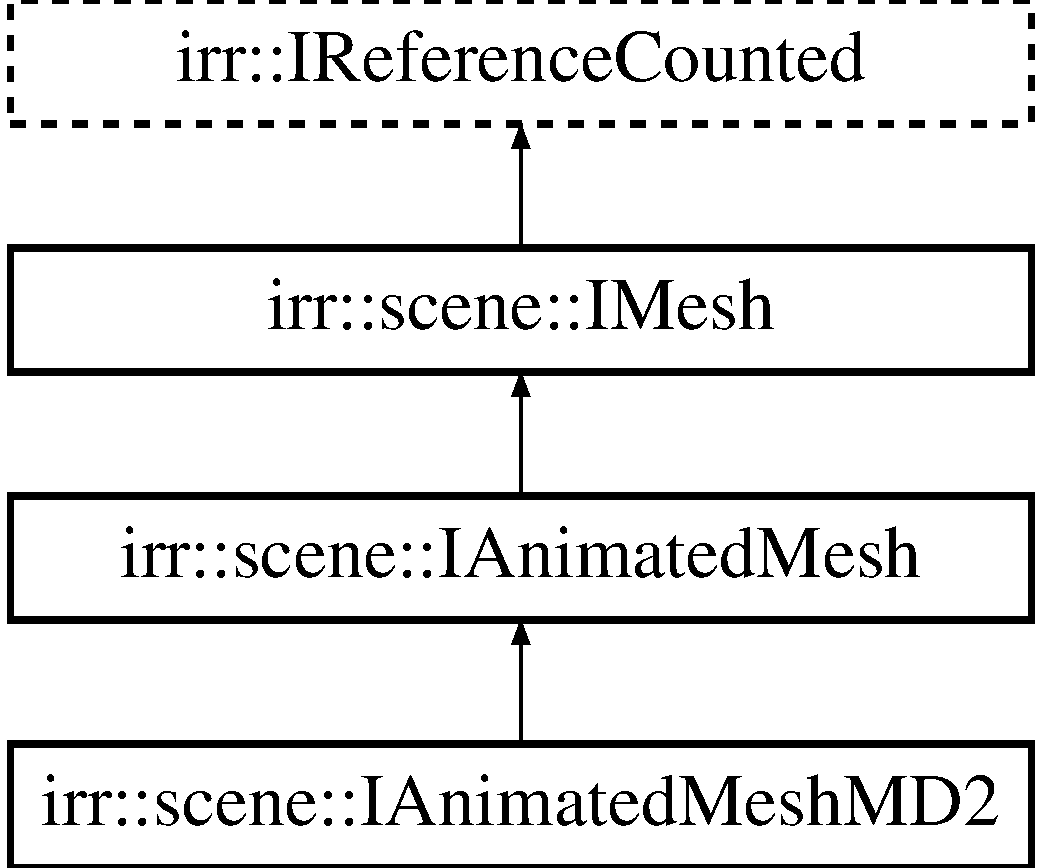
\includegraphics[height=1.822917cm]{classirr_1_1scene_1_1IAnimatedMeshMD2}
\end{center}
\end{figure}
\subsection*{Public Member Functions}
\begin{DoxyCompactItemize}
\item 
virtual void \hyperlink{classirr_1_1scene_1_1IAnimatedMeshMD2_a0bab7f9b11fd11f1fa8f2cd6e085b596}{get\+Frame\+Loop} (\hyperlink{namespaceirr_1_1scene_a08d4a84966e1d2886d0d57e4acbb4f19}{E\+M\+D2\+\_\+\+A\+N\+I\+M\+A\+T\+I\+O\+N\+\_\+\+T\+Y\+PE} l, \hyperlink{namespaceirr_ac66849b7a6ed16e30ebede579f9b47c6}{s32} \&out\+Begin, \hyperlink{namespaceirr_ac66849b7a6ed16e30ebede579f9b47c6}{s32} \&out\+End, \hyperlink{namespaceirr_ac66849b7a6ed16e30ebede579f9b47c6}{s32} \&out\+F\+PS) const =0
\begin{DoxyCompactList}\small\item\em Get frame loop data for a default M\+D2 animation type. \end{DoxyCompactList}\item 
virtual bool \hyperlink{classirr_1_1scene_1_1IAnimatedMeshMD2_a4d52cae663c479d88296561ec961410a}{get\+Frame\+Loop} (const \hyperlink{namespaceirr_a9395eaea339bcb546b319e9c96bf7410}{c8} $\ast$name, \hyperlink{namespaceirr_ac66849b7a6ed16e30ebede579f9b47c6}{s32} \&out\+Begin, \hyperlink{namespaceirr_ac66849b7a6ed16e30ebede579f9b47c6}{s32} \&out\+End, \hyperlink{namespaceirr_ac66849b7a6ed16e30ebede579f9b47c6}{s32} \&out\+F\+PS) const =0
\begin{DoxyCompactList}\small\item\em Get frame loop data for a special M\+D2 animation type, identified by name. \end{DoxyCompactList}\item 
\mbox{\Hypertarget{classirr_1_1scene_1_1IAnimatedMeshMD2_abb4479ea266ea54230bf21c36319b323}\label{classirr_1_1scene_1_1IAnimatedMeshMD2_abb4479ea266ea54230bf21c36319b323}} 
virtual \hyperlink{namespaceirr_ac66849b7a6ed16e30ebede579f9b47c6}{s32} \hyperlink{classirr_1_1scene_1_1IAnimatedMeshMD2_abb4479ea266ea54230bf21c36319b323}{get\+Animation\+Count} () const =0
\begin{DoxyCompactList}\small\item\em Get amount of md2 animations in this file. \end{DoxyCompactList}\item 
virtual const \hyperlink{namespaceirr_a9395eaea339bcb546b319e9c96bf7410}{c8} $\ast$ \hyperlink{classirr_1_1scene_1_1IAnimatedMeshMD2_aa619158d0fc11ea1032d838abf3566ca}{get\+Animation\+Name} (\hyperlink{namespaceirr_ac66849b7a6ed16e30ebede579f9b47c6}{s32} nr) const =0
\begin{DoxyCompactList}\small\item\em Get name of md2 animation. \end{DoxyCompactList}\item 
virtual void \hyperlink{classirr_1_1scene_1_1IAnimatedMeshMD2_a0bab7f9b11fd11f1fa8f2cd6e085b596}{get\+Frame\+Loop} (\hyperlink{namespaceirr_1_1scene_a08d4a84966e1d2886d0d57e4acbb4f19}{E\+M\+D2\+\_\+\+A\+N\+I\+M\+A\+T\+I\+O\+N\+\_\+\+T\+Y\+PE} l, \hyperlink{namespaceirr_ac66849b7a6ed16e30ebede579f9b47c6}{s32} \&out\+Begin, \hyperlink{namespaceirr_ac66849b7a6ed16e30ebede579f9b47c6}{s32} \&out\+End, \hyperlink{namespaceirr_ac66849b7a6ed16e30ebede579f9b47c6}{s32} \&out\+F\+PS) const =0
\begin{DoxyCompactList}\small\item\em Get frame loop data for a default M\+D2 animation type. \end{DoxyCompactList}\item 
virtual bool \hyperlink{classirr_1_1scene_1_1IAnimatedMeshMD2_a4d52cae663c479d88296561ec961410a}{get\+Frame\+Loop} (const \hyperlink{namespaceirr_a9395eaea339bcb546b319e9c96bf7410}{c8} $\ast$name, \hyperlink{namespaceirr_ac66849b7a6ed16e30ebede579f9b47c6}{s32} \&out\+Begin, \hyperlink{namespaceirr_ac66849b7a6ed16e30ebede579f9b47c6}{s32} \&out\+End, \hyperlink{namespaceirr_ac66849b7a6ed16e30ebede579f9b47c6}{s32} \&out\+F\+PS) const =0
\begin{DoxyCompactList}\small\item\em Get frame loop data for a special M\+D2 animation type, identified by name. \end{DoxyCompactList}\item 
\mbox{\Hypertarget{classirr_1_1scene_1_1IAnimatedMeshMD2_abb4479ea266ea54230bf21c36319b323}\label{classirr_1_1scene_1_1IAnimatedMeshMD2_abb4479ea266ea54230bf21c36319b323}} 
virtual \hyperlink{namespaceirr_ac66849b7a6ed16e30ebede579f9b47c6}{s32} \hyperlink{classirr_1_1scene_1_1IAnimatedMeshMD2_abb4479ea266ea54230bf21c36319b323}{get\+Animation\+Count} () const =0
\begin{DoxyCompactList}\small\item\em Get amount of md2 animations in this file. \end{DoxyCompactList}\item 
virtual const \hyperlink{namespaceirr_a9395eaea339bcb546b319e9c96bf7410}{c8} $\ast$ \hyperlink{classirr_1_1scene_1_1IAnimatedMeshMD2_aa619158d0fc11ea1032d838abf3566ca}{get\+Animation\+Name} (\hyperlink{namespaceirr_ac66849b7a6ed16e30ebede579f9b47c6}{s32} nr) const =0
\begin{DoxyCompactList}\small\item\em Get name of md2 animation. \end{DoxyCompactList}\end{DoxyCompactItemize}
\subsection*{Additional Inherited Members}


\subsection{Detailed Description}
Interface for using some special functions of M\+D2 meshes. 

\subsection{Member Function Documentation}
\mbox{\Hypertarget{classirr_1_1scene_1_1IAnimatedMeshMD2_aa619158d0fc11ea1032d838abf3566ca}\label{classirr_1_1scene_1_1IAnimatedMeshMD2_aa619158d0fc11ea1032d838abf3566ca}} 
\index{irr\+::scene\+::\+I\+Animated\+Mesh\+M\+D2@{irr\+::scene\+::\+I\+Animated\+Mesh\+M\+D2}!get\+Animation\+Name@{get\+Animation\+Name}}
\index{get\+Animation\+Name@{get\+Animation\+Name}!irr\+::scene\+::\+I\+Animated\+Mesh\+M\+D2@{irr\+::scene\+::\+I\+Animated\+Mesh\+M\+D2}}
\subsubsection{\texorpdfstring{get\+Animation\+Name()}{getAnimationName()}\hspace{0.1cm}{\footnotesize\ttfamily [1/2]}}
{\footnotesize\ttfamily virtual const \hyperlink{namespaceirr_a9395eaea339bcb546b319e9c96bf7410}{c8}$\ast$ irr\+::scene\+::\+I\+Animated\+Mesh\+M\+D2\+::get\+Animation\+Name (\begin{DoxyParamCaption}\item[{\hyperlink{namespaceirr_ac66849b7a6ed16e30ebede579f9b47c6}{s32}}]{nr }\end{DoxyParamCaption}) const\hspace{0.3cm}{\ttfamily [pure virtual]}}



Get name of md2 animation. 


\begin{DoxyParams}{Parameters}
{\em nr} & Zero based index of animation. \\
\hline
\end{DoxyParams}
\mbox{\Hypertarget{classirr_1_1scene_1_1IAnimatedMeshMD2_aa619158d0fc11ea1032d838abf3566ca}\label{classirr_1_1scene_1_1IAnimatedMeshMD2_aa619158d0fc11ea1032d838abf3566ca}} 
\index{irr\+::scene\+::\+I\+Animated\+Mesh\+M\+D2@{irr\+::scene\+::\+I\+Animated\+Mesh\+M\+D2}!get\+Animation\+Name@{get\+Animation\+Name}}
\index{get\+Animation\+Name@{get\+Animation\+Name}!irr\+::scene\+::\+I\+Animated\+Mesh\+M\+D2@{irr\+::scene\+::\+I\+Animated\+Mesh\+M\+D2}}
\subsubsection{\texorpdfstring{get\+Animation\+Name()}{getAnimationName()}\hspace{0.1cm}{\footnotesize\ttfamily [2/2]}}
{\footnotesize\ttfamily virtual const \hyperlink{namespaceirr_a9395eaea339bcb546b319e9c96bf7410}{c8}$\ast$ irr\+::scene\+::\+I\+Animated\+Mesh\+M\+D2\+::get\+Animation\+Name (\begin{DoxyParamCaption}\item[{\hyperlink{namespaceirr_ac66849b7a6ed16e30ebede579f9b47c6}{s32}}]{nr }\end{DoxyParamCaption}) const\hspace{0.3cm}{\ttfamily [pure virtual]}}



Get name of md2 animation. 


\begin{DoxyParams}{Parameters}
{\em nr} & Zero based index of animation. \\
\hline
\end{DoxyParams}
\mbox{\Hypertarget{classirr_1_1scene_1_1IAnimatedMeshMD2_a0bab7f9b11fd11f1fa8f2cd6e085b596}\label{classirr_1_1scene_1_1IAnimatedMeshMD2_a0bab7f9b11fd11f1fa8f2cd6e085b596}} 
\index{irr\+::scene\+::\+I\+Animated\+Mesh\+M\+D2@{irr\+::scene\+::\+I\+Animated\+Mesh\+M\+D2}!get\+Frame\+Loop@{get\+Frame\+Loop}}
\index{get\+Frame\+Loop@{get\+Frame\+Loop}!irr\+::scene\+::\+I\+Animated\+Mesh\+M\+D2@{irr\+::scene\+::\+I\+Animated\+Mesh\+M\+D2}}
\subsubsection{\texorpdfstring{get\+Frame\+Loop()}{getFrameLoop()}\hspace{0.1cm}{\footnotesize\ttfamily [1/4]}}
{\footnotesize\ttfamily virtual void irr\+::scene\+::\+I\+Animated\+Mesh\+M\+D2\+::get\+Frame\+Loop (\begin{DoxyParamCaption}\item[{\hyperlink{namespaceirr_1_1scene_a08d4a84966e1d2886d0d57e4acbb4f19}{E\+M\+D2\+\_\+\+A\+N\+I\+M\+A\+T\+I\+O\+N\+\_\+\+T\+Y\+PE}}]{l,  }\item[{\hyperlink{namespaceirr_ac66849b7a6ed16e30ebede579f9b47c6}{s32} \&}]{out\+Begin,  }\item[{\hyperlink{namespaceirr_ac66849b7a6ed16e30ebede579f9b47c6}{s32} \&}]{out\+End,  }\item[{\hyperlink{namespaceirr_ac66849b7a6ed16e30ebede579f9b47c6}{s32} \&}]{out\+F\+PS }\end{DoxyParamCaption}) const\hspace{0.3cm}{\ttfamily [pure virtual]}}



Get frame loop data for a default M\+D2 animation type. 


\begin{DoxyParams}{Parameters}
{\em l} & The E\+M\+D2\+\_\+\+A\+N\+I\+M\+A\+T\+I\+O\+N\+\_\+\+T\+Y\+PE to get the frames for. \\
\hline
{\em out\+Begin} & The returned beginning frame for animation type specified. \\
\hline
{\em out\+End} & The returned ending frame for the animation type specified. \\
\hline
{\em out\+F\+PS} & The number of frames per second, this animation should be played at. \\
\hline
\end{DoxyParams}
\begin{DoxyReturn}{Returns}
beginframe, endframe and frames per second for a default M\+D2 animation type. 
\end{DoxyReturn}
\mbox{\Hypertarget{classirr_1_1scene_1_1IAnimatedMeshMD2_a0bab7f9b11fd11f1fa8f2cd6e085b596}\label{classirr_1_1scene_1_1IAnimatedMeshMD2_a0bab7f9b11fd11f1fa8f2cd6e085b596}} 
\index{irr\+::scene\+::\+I\+Animated\+Mesh\+M\+D2@{irr\+::scene\+::\+I\+Animated\+Mesh\+M\+D2}!get\+Frame\+Loop@{get\+Frame\+Loop}}
\index{get\+Frame\+Loop@{get\+Frame\+Loop}!irr\+::scene\+::\+I\+Animated\+Mesh\+M\+D2@{irr\+::scene\+::\+I\+Animated\+Mesh\+M\+D2}}
\subsubsection{\texorpdfstring{get\+Frame\+Loop()}{getFrameLoop()}\hspace{0.1cm}{\footnotesize\ttfamily [2/4]}}
{\footnotesize\ttfamily virtual void irr\+::scene\+::\+I\+Animated\+Mesh\+M\+D2\+::get\+Frame\+Loop (\begin{DoxyParamCaption}\item[{\hyperlink{namespaceirr_1_1scene_a08d4a84966e1d2886d0d57e4acbb4f19}{E\+M\+D2\+\_\+\+A\+N\+I\+M\+A\+T\+I\+O\+N\+\_\+\+T\+Y\+PE}}]{l,  }\item[{\hyperlink{namespaceirr_ac66849b7a6ed16e30ebede579f9b47c6}{s32} \&}]{out\+Begin,  }\item[{\hyperlink{namespaceirr_ac66849b7a6ed16e30ebede579f9b47c6}{s32} \&}]{out\+End,  }\item[{\hyperlink{namespaceirr_ac66849b7a6ed16e30ebede579f9b47c6}{s32} \&}]{out\+F\+PS }\end{DoxyParamCaption}) const\hspace{0.3cm}{\ttfamily [pure virtual]}}



Get frame loop data for a default M\+D2 animation type. 


\begin{DoxyParams}{Parameters}
{\em l} & The E\+M\+D2\+\_\+\+A\+N\+I\+M\+A\+T\+I\+O\+N\+\_\+\+T\+Y\+PE to get the frames for. \\
\hline
{\em out\+Begin} & The returned beginning frame for animation type specified. \\
\hline
{\em out\+End} & The returned ending frame for the animation type specified. \\
\hline
{\em out\+F\+PS} & The number of frames per second, this animation should be played at. \\
\hline
\end{DoxyParams}
\begin{DoxyReturn}{Returns}
beginframe, endframe and frames per second for a default M\+D2 animation type. 
\end{DoxyReturn}
\mbox{\Hypertarget{classirr_1_1scene_1_1IAnimatedMeshMD2_a4d52cae663c479d88296561ec961410a}\label{classirr_1_1scene_1_1IAnimatedMeshMD2_a4d52cae663c479d88296561ec961410a}} 
\index{irr\+::scene\+::\+I\+Animated\+Mesh\+M\+D2@{irr\+::scene\+::\+I\+Animated\+Mesh\+M\+D2}!get\+Frame\+Loop@{get\+Frame\+Loop}}
\index{get\+Frame\+Loop@{get\+Frame\+Loop}!irr\+::scene\+::\+I\+Animated\+Mesh\+M\+D2@{irr\+::scene\+::\+I\+Animated\+Mesh\+M\+D2}}
\subsubsection{\texorpdfstring{get\+Frame\+Loop()}{getFrameLoop()}\hspace{0.1cm}{\footnotesize\ttfamily [3/4]}}
{\footnotesize\ttfamily virtual bool irr\+::scene\+::\+I\+Animated\+Mesh\+M\+D2\+::get\+Frame\+Loop (\begin{DoxyParamCaption}\item[{const \hyperlink{namespaceirr_a9395eaea339bcb546b319e9c96bf7410}{c8} $\ast$}]{name,  }\item[{\hyperlink{namespaceirr_ac66849b7a6ed16e30ebede579f9b47c6}{s32} \&}]{out\+Begin,  }\item[{\hyperlink{namespaceirr_ac66849b7a6ed16e30ebede579f9b47c6}{s32} \&}]{out\+End,  }\item[{\hyperlink{namespaceirr_ac66849b7a6ed16e30ebede579f9b47c6}{s32} \&}]{out\+F\+PS }\end{DoxyParamCaption}) const\hspace{0.3cm}{\ttfamily [pure virtual]}}



Get frame loop data for a special M\+D2 animation type, identified by name. 


\begin{DoxyParams}{Parameters}
{\em name} & Name of the animation. \\
\hline
{\em out\+Begin} & The returned beginning frame for animation type specified. \\
\hline
{\em out\+End} & The returned ending frame for the animation type specified. \\
\hline
{\em out\+F\+PS} & The number of frames per second, this animation should be played at. \\
\hline
\end{DoxyParams}
\begin{DoxyReturn}{Returns}
beginframe, endframe and frames per second for a special M\+D2 animation type. 
\end{DoxyReturn}
\mbox{\Hypertarget{classirr_1_1scene_1_1IAnimatedMeshMD2_a4d52cae663c479d88296561ec961410a}\label{classirr_1_1scene_1_1IAnimatedMeshMD2_a4d52cae663c479d88296561ec961410a}} 
\index{irr\+::scene\+::\+I\+Animated\+Mesh\+M\+D2@{irr\+::scene\+::\+I\+Animated\+Mesh\+M\+D2}!get\+Frame\+Loop@{get\+Frame\+Loop}}
\index{get\+Frame\+Loop@{get\+Frame\+Loop}!irr\+::scene\+::\+I\+Animated\+Mesh\+M\+D2@{irr\+::scene\+::\+I\+Animated\+Mesh\+M\+D2}}
\subsubsection{\texorpdfstring{get\+Frame\+Loop()}{getFrameLoop()}\hspace{0.1cm}{\footnotesize\ttfamily [4/4]}}
{\footnotesize\ttfamily virtual bool irr\+::scene\+::\+I\+Animated\+Mesh\+M\+D2\+::get\+Frame\+Loop (\begin{DoxyParamCaption}\item[{const \hyperlink{namespaceirr_a9395eaea339bcb546b319e9c96bf7410}{c8} $\ast$}]{name,  }\item[{\hyperlink{namespaceirr_ac66849b7a6ed16e30ebede579f9b47c6}{s32} \&}]{out\+Begin,  }\item[{\hyperlink{namespaceirr_ac66849b7a6ed16e30ebede579f9b47c6}{s32} \&}]{out\+End,  }\item[{\hyperlink{namespaceirr_ac66849b7a6ed16e30ebede579f9b47c6}{s32} \&}]{out\+F\+PS }\end{DoxyParamCaption}) const\hspace{0.3cm}{\ttfamily [pure virtual]}}



Get frame loop data for a special M\+D2 animation type, identified by name. 


\begin{DoxyParams}{Parameters}
{\em name} & Name of the animation. \\
\hline
{\em out\+Begin} & The returned beginning frame for animation type specified. \\
\hline
{\em out\+End} & The returned ending frame for the animation type specified. \\
\hline
{\em out\+F\+PS} & The number of frames per second, this animation should be played at. \\
\hline
\end{DoxyParams}
\begin{DoxyReturn}{Returns}
beginframe, endframe and frames per second for a special M\+D2 animation type. 
\end{DoxyReturn}


The documentation for this class was generated from the following file\+:\begin{DoxyCompactItemize}
\item 
indie\+\_\+share/controller/include/I\+Animated\+Mesh\+M\+D2.\+h\end{DoxyCompactItemize}

\hypertarget{classirr_1_1scene_1_1IAnimatedMeshMD3}{}\section{irr\+:\+:scene\+:\+:I\+Animated\+Mesh\+M\+D3 Class Reference}
\label{classirr_1_1scene_1_1IAnimatedMeshMD3}\index{irr\+::scene\+::\+I\+Animated\+Mesh\+M\+D3@{irr\+::scene\+::\+I\+Animated\+Mesh\+M\+D3}}


Interface for using some special functions of M\+D3 meshes.  




{\ttfamily \#include $<$I\+Animated\+Mesh\+M\+D3.\+h$>$}

Inheritance diagram for irr\+:\+:scene\+:\+:I\+Animated\+Mesh\+M\+D3\+:\begin{figure}[H]
\begin{center}
\leavevmode
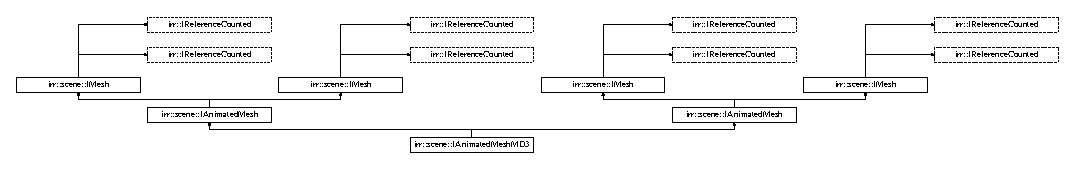
\includegraphics[height=1.822917cm]{classirr_1_1scene_1_1IAnimatedMeshMD3}
\end{center}
\end{figure}
\subsection*{Public Member Functions}
\begin{DoxyCompactItemize}
\item 
\mbox{\Hypertarget{classirr_1_1scene_1_1IAnimatedMeshMD3_ae72d5c1bbef975834ddb3fdf8d73e608}\label{classirr_1_1scene_1_1IAnimatedMeshMD3_ae72d5c1bbef975834ddb3fdf8d73e608}} 
virtual void \hyperlink{classirr_1_1scene_1_1IAnimatedMeshMD3_ae72d5c1bbef975834ddb3fdf8d73e608}{set\+Interpolation\+Shift} (\hyperlink{namespaceirr_a0416a53257075833e7002efd0a18e804}{u32} shift, \hyperlink{namespaceirr_a0416a53257075833e7002efd0a18e804}{u32} loop\+Mode)=0
\begin{DoxyCompactList}\small\item\em tune how many frames you want to render inbetween. \end{DoxyCompactList}\item 
\mbox{\Hypertarget{classirr_1_1scene_1_1IAnimatedMeshMD3_a1de2fa2fc55ab8fb7f881f3e9a9b0d78}\label{classirr_1_1scene_1_1IAnimatedMeshMD3_a1de2fa2fc55ab8fb7f881f3e9a9b0d78}} 
virtual \hyperlink{structirr_1_1scene_1_1SMD3QuaternionTagList}{S\+M\+D3\+Quaternion\+Tag\+List} $\ast$ \hyperlink{classirr_1_1scene_1_1IAnimatedMeshMD3_a1de2fa2fc55ab8fb7f881f3e9a9b0d78}{get\+Tag\+List} (\hyperlink{namespaceirr_ac66849b7a6ed16e30ebede579f9b47c6}{s32} frame, \hyperlink{namespaceirr_ac66849b7a6ed16e30ebede579f9b47c6}{s32} detail\+Level, \hyperlink{namespaceirr_ac66849b7a6ed16e30ebede579f9b47c6}{s32} start\+Frame\+Loop, \hyperlink{namespaceirr_ac66849b7a6ed16e30ebede579f9b47c6}{s32} end\+Frame\+Loop)=0
\begin{DoxyCompactList}\small\item\em get the tag list of the mesh. \end{DoxyCompactList}\item 
\mbox{\Hypertarget{classirr_1_1scene_1_1IAnimatedMeshMD3_ac6b6b53da9413b4404bcad0e68561bcb}\label{classirr_1_1scene_1_1IAnimatedMeshMD3_ac6b6b53da9413b4404bcad0e68561bcb}} 
virtual \hyperlink{structirr_1_1scene_1_1SMD3Mesh}{S\+M\+D3\+Mesh} $\ast$ \hyperlink{classirr_1_1scene_1_1IAnimatedMeshMD3_ac6b6b53da9413b4404bcad0e68561bcb}{get\+Original\+Mesh} ()=0
\begin{DoxyCompactList}\small\item\em get the original md3 mesh. \end{DoxyCompactList}\item 
\mbox{\Hypertarget{classirr_1_1scene_1_1IAnimatedMeshMD3_ae72d5c1bbef975834ddb3fdf8d73e608}\label{classirr_1_1scene_1_1IAnimatedMeshMD3_ae72d5c1bbef975834ddb3fdf8d73e608}} 
virtual void \hyperlink{classirr_1_1scene_1_1IAnimatedMeshMD3_ae72d5c1bbef975834ddb3fdf8d73e608}{set\+Interpolation\+Shift} (\hyperlink{namespaceirr_a0416a53257075833e7002efd0a18e804}{u32} shift, \hyperlink{namespaceirr_a0416a53257075833e7002efd0a18e804}{u32} loop\+Mode)=0
\begin{DoxyCompactList}\small\item\em tune how many frames you want to render inbetween. \end{DoxyCompactList}\item 
\mbox{\Hypertarget{classirr_1_1scene_1_1IAnimatedMeshMD3_a1de2fa2fc55ab8fb7f881f3e9a9b0d78}\label{classirr_1_1scene_1_1IAnimatedMeshMD3_a1de2fa2fc55ab8fb7f881f3e9a9b0d78}} 
virtual \hyperlink{structirr_1_1scene_1_1SMD3QuaternionTagList}{S\+M\+D3\+Quaternion\+Tag\+List} $\ast$ \hyperlink{classirr_1_1scene_1_1IAnimatedMeshMD3_a1de2fa2fc55ab8fb7f881f3e9a9b0d78}{get\+Tag\+List} (\hyperlink{namespaceirr_ac66849b7a6ed16e30ebede579f9b47c6}{s32} frame, \hyperlink{namespaceirr_ac66849b7a6ed16e30ebede579f9b47c6}{s32} detail\+Level, \hyperlink{namespaceirr_ac66849b7a6ed16e30ebede579f9b47c6}{s32} start\+Frame\+Loop, \hyperlink{namespaceirr_ac66849b7a6ed16e30ebede579f9b47c6}{s32} end\+Frame\+Loop)=0
\begin{DoxyCompactList}\small\item\em get the tag list of the mesh. \end{DoxyCompactList}\item 
\mbox{\Hypertarget{classirr_1_1scene_1_1IAnimatedMeshMD3_ac6b6b53da9413b4404bcad0e68561bcb}\label{classirr_1_1scene_1_1IAnimatedMeshMD3_ac6b6b53da9413b4404bcad0e68561bcb}} 
virtual \hyperlink{structirr_1_1scene_1_1SMD3Mesh}{S\+M\+D3\+Mesh} $\ast$ \hyperlink{classirr_1_1scene_1_1IAnimatedMeshMD3_ac6b6b53da9413b4404bcad0e68561bcb}{get\+Original\+Mesh} ()=0
\begin{DoxyCompactList}\small\item\em get the original md3 mesh. \end{DoxyCompactList}\end{DoxyCompactItemize}
\subsection*{Additional Inherited Members}


\subsection{Detailed Description}
Interface for using some special functions of M\+D3 meshes. 

The documentation for this class was generated from the following file\+:\begin{DoxyCompactItemize}
\item 
indie\+\_\+share/controller/include/I\+Animated\+Mesh\+M\+D3.\+h\end{DoxyCompactItemize}

\hypertarget{classirr_1_1scene_1_1IAnimatedMeshSceneNode}{}\section{irr\+:\+:scene\+:\+:I\+Animated\+Mesh\+Scene\+Node Class Reference}
\label{classirr_1_1scene_1_1IAnimatedMeshSceneNode}\index{irr\+::scene\+::\+I\+Animated\+Mesh\+Scene\+Node@{irr\+::scene\+::\+I\+Animated\+Mesh\+Scene\+Node}}


Scene node capable of displaying an animated mesh and its shadow.  




{\ttfamily \#include $<$I\+Animated\+Mesh\+Scene\+Node.\+h$>$}

Inheritance diagram for irr\+:\+:scene\+:\+:I\+Animated\+Mesh\+Scene\+Node\+:\begin{figure}[H]
\begin{center}
\leavevmode
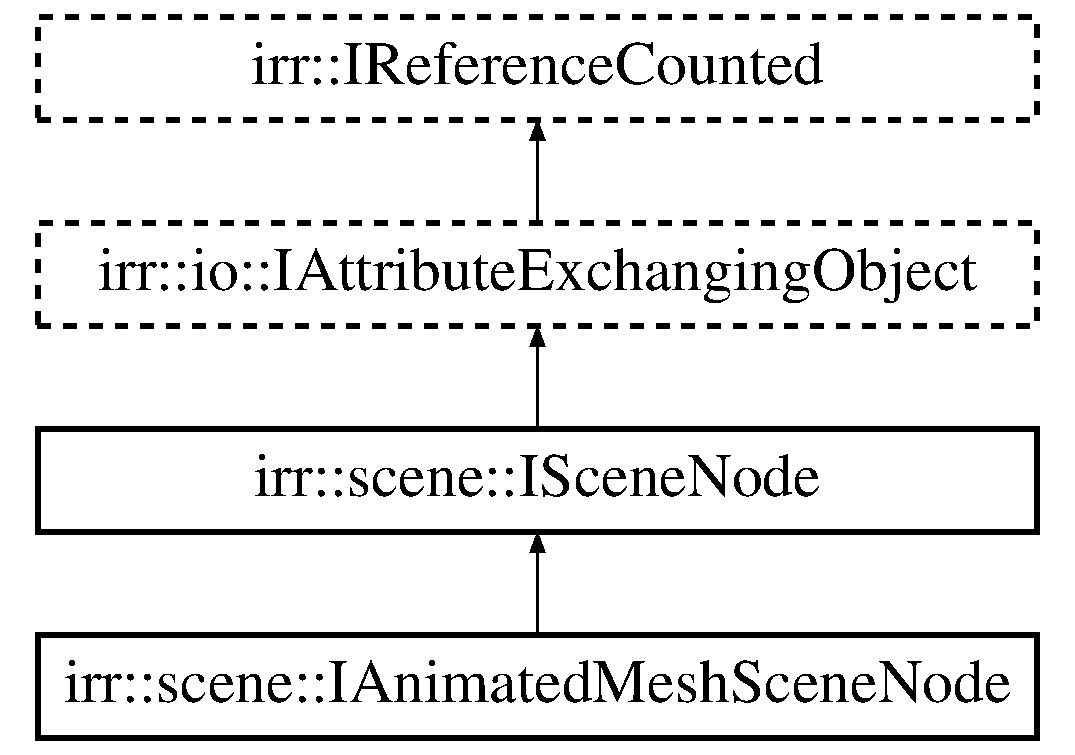
\includegraphics[height=1.515152cm]{classirr_1_1scene_1_1IAnimatedMeshSceneNode}
\end{center}
\end{figure}
\subsection*{Public Member Functions}
\begin{DoxyCompactItemize}
\item 
\mbox{\Hypertarget{classirr_1_1scene_1_1IAnimatedMeshSceneNode_a6c76b97d6e587e81e057a038dde0956b}\label{classirr_1_1scene_1_1IAnimatedMeshSceneNode_a6c76b97d6e587e81e057a038dde0956b}} 
\hyperlink{classirr_1_1scene_1_1IAnimatedMeshSceneNode_a6c76b97d6e587e81e057a038dde0956b}{I\+Animated\+Mesh\+Scene\+Node} (\hyperlink{classirr_1_1scene_1_1ISceneNode}{I\+Scene\+Node} $\ast$parent, \hyperlink{classirr_1_1scene_1_1ISceneManager}{I\+Scene\+Manager} $\ast$mgr, \hyperlink{namespaceirr_ac66849b7a6ed16e30ebede579f9b47c6}{s32} id, const \hyperlink{namespaceirr_1_1core_ae6e2b2a6c552833ebbd5b7463d03586b}{core\+::vector3df} \&position=\hyperlink{namespaceirr_1_1core_ae6e2b2a6c552833ebbd5b7463d03586b}{core\+::vector3df}(0, 0, 0), const \hyperlink{namespaceirr_1_1core_ae6e2b2a6c552833ebbd5b7463d03586b}{core\+::vector3df} \&rotation=\hyperlink{namespaceirr_1_1core_ae6e2b2a6c552833ebbd5b7463d03586b}{core\+::vector3df}(0, 0, 0), const \hyperlink{namespaceirr_1_1core_ae6e2b2a6c552833ebbd5b7463d03586b}{core\+::vector3df} \&scale=\hyperlink{namespaceirr_1_1core_ae6e2b2a6c552833ebbd5b7463d03586b}{core\+::vector3df}(1.\+0f, 1.\+0f, 1.\+0f))
\begin{DoxyCompactList}\small\item\em Constructor. \end{DoxyCompactList}\item 
\mbox{\Hypertarget{classirr_1_1scene_1_1IAnimatedMeshSceneNode_ae914c207eb12ae9025bfd102922c01cf}\label{classirr_1_1scene_1_1IAnimatedMeshSceneNode_ae914c207eb12ae9025bfd102922c01cf}} 
virtual \hyperlink{classirr_1_1scene_1_1IAnimatedMeshSceneNode_ae914c207eb12ae9025bfd102922c01cf}{$\sim$\+I\+Animated\+Mesh\+Scene\+Node} ()
\begin{DoxyCompactList}\small\item\em Destructor. \end{DoxyCompactList}\item 
virtual void \hyperlink{classirr_1_1scene_1_1IAnimatedMeshSceneNode_aff1c1e2270f4d3d94e58e7c130c575a4}{set\+Current\+Frame} (\hyperlink{namespaceirr_a0277be98d67dc26ff93b1a6a1d086b07}{f32} frame)=0
\begin{DoxyCompactList}\small\item\em Sets the current frame number. \end{DoxyCompactList}\item 
virtual bool \hyperlink{classirr_1_1scene_1_1IAnimatedMeshSceneNode_a900400fe375ca13f48876b84900ffddf}{set\+Frame\+Loop} (\hyperlink{namespaceirr_ac66849b7a6ed16e30ebede579f9b47c6}{s32} begin, \hyperlink{namespaceirr_ac66849b7a6ed16e30ebede579f9b47c6}{s32} end)=0
\begin{DoxyCompactList}\small\item\em Sets the frame numbers between the animation is looped. \end{DoxyCompactList}\item 
virtual void \hyperlink{classirr_1_1scene_1_1IAnimatedMeshSceneNode_a89ef2d20c6e9e83fdb861403c9698c4a}{set\+Animation\+Speed} (\hyperlink{namespaceirr_a0277be98d67dc26ff93b1a6a1d086b07}{f32} frames\+Per\+Second)=0
\begin{DoxyCompactList}\small\item\em Sets the speed with which the animation is played. \end{DoxyCompactList}\item 
virtual \hyperlink{namespaceirr_a0277be98d67dc26ff93b1a6a1d086b07}{f32} \hyperlink{classirr_1_1scene_1_1IAnimatedMeshSceneNode_a246c21ec2ae5b3a5cecc10f9cc3625c4}{get\+Animation\+Speed} () const =0
\begin{DoxyCompactList}\small\item\em Gets the speed with which the animation is played. \end{DoxyCompactList}\item 
virtual \hyperlink{classirr_1_1scene_1_1IShadowVolumeSceneNode}{I\+Shadow\+Volume\+Scene\+Node} $\ast$ \hyperlink{classirr_1_1scene_1_1IAnimatedMeshSceneNode_aaa4947ed5f7ba72870da37ee1fc17125}{add\+Shadow\+Volume\+Scene\+Node} (const \hyperlink{classirr_1_1scene_1_1IMesh}{I\+Mesh} $\ast$shadow\+Mesh=0, \hyperlink{namespaceirr_ac66849b7a6ed16e30ebede579f9b47c6}{s32} id=-\/1, bool zfailmethod=true, \hyperlink{namespaceirr_a0277be98d67dc26ff93b1a6a1d086b07}{f32} infinity=1000.\+0f)=0
\begin{DoxyCompactList}\small\item\em Creates shadow volume scene node as child of this node. \end{DoxyCompactList}\item 
virtual \hyperlink{classirr_1_1scene_1_1IBoneSceneNode}{I\+Bone\+Scene\+Node} $\ast$ \hyperlink{classirr_1_1scene_1_1IAnimatedMeshSceneNode_ac7b64a5ddbe5d570dc5276b894a63619}{get\+Joint\+Node} (const \hyperlink{namespaceirr_a9395eaea339bcb546b319e9c96bf7410}{c8} $\ast$joint\+Name)=0
\begin{DoxyCompactList}\small\item\em Get a pointer to a joint in the mesh (if the mesh is a bone based mesh). \end{DoxyCompactList}\item 
\mbox{\Hypertarget{classirr_1_1scene_1_1IAnimatedMeshSceneNode_a790a1a03ada0eb754504609d76c5fcc1}\label{classirr_1_1scene_1_1IAnimatedMeshSceneNode_a790a1a03ada0eb754504609d76c5fcc1}} 
virtual \hyperlink{classirr_1_1scene_1_1IBoneSceneNode}{I\+Bone\+Scene\+Node} $\ast$ \hyperlink{classirr_1_1scene_1_1IAnimatedMeshSceneNode_a790a1a03ada0eb754504609d76c5fcc1}{get\+Joint\+Node} (\hyperlink{namespaceirr_a0416a53257075833e7002efd0a18e804}{u32} joint\+ID)=0
\begin{DoxyCompactList}\small\item\em same as \hyperlink{classirr_1_1scene_1_1IAnimatedMeshSceneNode_ac7b64a5ddbe5d570dc5276b894a63619}{get\+Joint\+Node(const c8$\ast$ joint\+Name)}, but based on id \end{DoxyCompactList}\item 
virtual \hyperlink{namespaceirr_a0416a53257075833e7002efd0a18e804}{u32} \hyperlink{classirr_1_1scene_1_1IAnimatedMeshSceneNode_a146657063c055fcb951ca6fd66171589}{get\+Joint\+Count} () const =0
\begin{DoxyCompactList}\small\item\em Gets joint count. \end{DoxyCompactList}\item 
virtual bool \hyperlink{classirr_1_1scene_1_1IAnimatedMeshSceneNode_aca2ca2593857c60aac61c0fd78365d2d}{set\+M\+D2\+Animation} (\hyperlink{namespaceirr_1_1scene_a08d4a84966e1d2886d0d57e4acbb4f19}{E\+M\+D2\+\_\+\+A\+N\+I\+M\+A\+T\+I\+O\+N\+\_\+\+T\+Y\+PE} anim)=0
\begin{DoxyCompactList}\small\item\em Starts a default M\+D2 animation. \end{DoxyCompactList}\item 
virtual bool \hyperlink{classirr_1_1scene_1_1IAnimatedMeshSceneNode_a8732866332327a7d43b91f41b5549fe3}{set\+M\+D2\+Animation} (const \hyperlink{namespaceirr_a9395eaea339bcb546b319e9c96bf7410}{c8} $\ast$animation\+Name)=0
\begin{DoxyCompactList}\small\item\em Starts a special M\+D2 animation. \end{DoxyCompactList}\item 
\mbox{\Hypertarget{classirr_1_1scene_1_1IAnimatedMeshSceneNode_abba274efec0cc98900518a86a150e09e}\label{classirr_1_1scene_1_1IAnimatedMeshSceneNode_abba274efec0cc98900518a86a150e09e}} 
virtual \hyperlink{namespaceirr_a0277be98d67dc26ff93b1a6a1d086b07}{f32} \hyperlink{classirr_1_1scene_1_1IAnimatedMeshSceneNode_abba274efec0cc98900518a86a150e09e}{get\+Frame\+Nr} () const =0
\begin{DoxyCompactList}\small\item\em Returns the currently displayed frame number. \end{DoxyCompactList}\item 
\mbox{\Hypertarget{classirr_1_1scene_1_1IAnimatedMeshSceneNode_a103022e7383241ea5f1ed76c2deacc69}\label{classirr_1_1scene_1_1IAnimatedMeshSceneNode_a103022e7383241ea5f1ed76c2deacc69}} 
virtual \hyperlink{namespaceirr_ac66849b7a6ed16e30ebede579f9b47c6}{s32} \hyperlink{classirr_1_1scene_1_1IAnimatedMeshSceneNode_a103022e7383241ea5f1ed76c2deacc69}{get\+Start\+Frame} () const =0
\begin{DoxyCompactList}\small\item\em Returns the current start frame number. \end{DoxyCompactList}\item 
\mbox{\Hypertarget{classirr_1_1scene_1_1IAnimatedMeshSceneNode_a8c4f524c00b520e870881ca7abfdce5a}\label{classirr_1_1scene_1_1IAnimatedMeshSceneNode_a8c4f524c00b520e870881ca7abfdce5a}} 
virtual \hyperlink{namespaceirr_ac66849b7a6ed16e30ebede579f9b47c6}{s32} \hyperlink{classirr_1_1scene_1_1IAnimatedMeshSceneNode_a8c4f524c00b520e870881ca7abfdce5a}{get\+End\+Frame} () const =0
\begin{DoxyCompactList}\small\item\em Returns the current end frame number. \end{DoxyCompactList}\item 
virtual void \hyperlink{classirr_1_1scene_1_1IAnimatedMeshSceneNode_ae6cae051c74c3953061aa9e49e10cd06}{set\+Loop\+Mode} (bool play\+Animation\+Looped)=0
\begin{DoxyCompactList}\small\item\em Sets looping mode which is on by default. \end{DoxyCompactList}\item 
virtual bool \hyperlink{classirr_1_1scene_1_1IAnimatedMeshSceneNode_a3271dc33b1911d637b05c58f17398a0a}{get\+Loop\+Mode} () const =0
\begin{DoxyCompactList}\small\item\em returns the current loop mode \end{DoxyCompactList}\item 
virtual void \hyperlink{classirr_1_1scene_1_1IAnimatedMeshSceneNode_ad688bb5a7654116d1ee823e48393f1bd}{set\+Animation\+End\+Callback} (\hyperlink{classirr_1_1scene_1_1IAnimationEndCallBack}{I\+Animation\+End\+Call\+Back} $\ast$callback=0)=0
\begin{DoxyCompactList}\small\item\em Sets a callback interface which will be called if an animation playback has ended. \end{DoxyCompactList}\item 
virtual void \hyperlink{classirr_1_1scene_1_1IAnimatedMeshSceneNode_af04e917ab3cae5631b06edad2d8a3a04}{set\+Read\+Only\+Materials} (bool readonly)=0
\begin{DoxyCompactList}\small\item\em Sets if the scene node should not copy the materials of the mesh but use them in a read only style. \end{DoxyCompactList}\item 
\mbox{\Hypertarget{classirr_1_1scene_1_1IAnimatedMeshSceneNode_a8916713c72582d270f6363c9ed1b509e}\label{classirr_1_1scene_1_1IAnimatedMeshSceneNode_a8916713c72582d270f6363c9ed1b509e}} 
virtual bool \hyperlink{classirr_1_1scene_1_1IAnimatedMeshSceneNode_a8916713c72582d270f6363c9ed1b509e}{is\+Read\+Only\+Materials} () const =0
\begin{DoxyCompactList}\small\item\em Returns if the scene node should not copy the materials of the mesh but use them in a read only style. \end{DoxyCompactList}\item 
\mbox{\Hypertarget{classirr_1_1scene_1_1IAnimatedMeshSceneNode_af3027cb62d62968a0ae85c9f15725668}\label{classirr_1_1scene_1_1IAnimatedMeshSceneNode_af3027cb62d62968a0ae85c9f15725668}} 
virtual void \hyperlink{classirr_1_1scene_1_1IAnimatedMeshSceneNode_af3027cb62d62968a0ae85c9f15725668}{set\+Mesh} (\hyperlink{classirr_1_1scene_1_1IAnimatedMesh}{I\+Animated\+Mesh} $\ast$mesh)=0
\begin{DoxyCompactList}\small\item\em Sets a new mesh. \end{DoxyCompactList}\item 
\mbox{\Hypertarget{classirr_1_1scene_1_1IAnimatedMeshSceneNode_ad52e5bd15a2bfb6d0745c77d4329086b}\label{classirr_1_1scene_1_1IAnimatedMeshSceneNode_ad52e5bd15a2bfb6d0745c77d4329086b}} 
virtual \hyperlink{classirr_1_1scene_1_1IAnimatedMesh}{I\+Animated\+Mesh} $\ast$ \hyperlink{classirr_1_1scene_1_1IAnimatedMeshSceneNode_ad52e5bd15a2bfb6d0745c77d4329086b}{get\+Mesh} (void)=0
\begin{DoxyCompactList}\small\item\em Returns the current mesh. \end{DoxyCompactList}\item 
\mbox{\Hypertarget{classirr_1_1scene_1_1IAnimatedMeshSceneNode_abb3c2cee9c3271014c8615907d98c021}\label{classirr_1_1scene_1_1IAnimatedMeshSceneNode_abb3c2cee9c3271014c8615907d98c021}} 
virtual const \hyperlink{structirr_1_1scene_1_1SMD3QuaternionTag}{S\+M\+D3\+Quaternion\+Tag} $\ast$ \hyperlink{classirr_1_1scene_1_1IAnimatedMeshSceneNode_abb3c2cee9c3271014c8615907d98c021}{get\+M\+D3\+Tag\+Transformation} (const \hyperlink{namespaceirr_1_1core_ab26a0e0359206b5a694f35c37c829d7f}{core\+::stringc} \&tagname)=0
\begin{DoxyCompactList}\small\item\em Get the absolute transformation for a special M\+D3 Tag if the mesh is a md3 mesh, or the absolutetransformation if it\textquotesingle{}s a normal scenenode. \end{DoxyCompactList}\item 
\mbox{\Hypertarget{classirr_1_1scene_1_1IAnimatedMeshSceneNode_a5ff68cb07badfbb01f491c0371c8b459}\label{classirr_1_1scene_1_1IAnimatedMeshSceneNode_a5ff68cb07badfbb01f491c0371c8b459}} 
virtual void \hyperlink{classirr_1_1scene_1_1IAnimatedMeshSceneNode_a5ff68cb07badfbb01f491c0371c8b459}{set\+Joint\+Mode} (\hyperlink{namespaceirr_1_1scene_a4a36461b5fa197ca3c6636c043413fa5}{E\+\_\+\+J\+O\+I\+N\+T\+\_\+\+U\+P\+D\+A\+T\+E\+\_\+\+O\+N\+\_\+\+R\+E\+N\+D\+ER} mode)=0
\begin{DoxyCompactList}\small\item\em Set how the joints should be updated on render. \end{DoxyCompactList}\item 
virtual void \hyperlink{classirr_1_1scene_1_1IAnimatedMeshSceneNode_a424d2dc577842949094a9d8c2a3eba0e}{set\+Transition\+Time} (\hyperlink{namespaceirr_a0277be98d67dc26ff93b1a6a1d086b07}{f32} Time)=0
\begin{DoxyCompactList}\small\item\em Sets the transition time in seconds. \end{DoxyCompactList}\item 
virtual void \hyperlink{classirr_1_1scene_1_1IAnimatedMeshSceneNode_a76af2c9a2b0cea6ee2b3559c1f32f850}{animate\+Joints} (bool Calculate\+Absolute\+Positions=true)=0
\begin{DoxyCompactList}\small\item\em animates the joints in the mesh based on the current frame. \end{DoxyCompactList}\item 
virtual void \hyperlink{classirr_1_1scene_1_1IAnimatedMeshSceneNode_aa3aa695d2e949bbc2ff17429951e77d0}{set\+Render\+From\+Identity} (bool On)=0
\begin{DoxyCompactList}\small\item\em render mesh ignoring its transformation. \end{DoxyCompactList}\item 
virtual \hyperlink{classirr_1_1scene_1_1ISceneNode}{I\+Scene\+Node} $\ast$ \hyperlink{classirr_1_1scene_1_1IAnimatedMeshSceneNode_a47aabf6554e3f91bbb033edb8668cec8}{clone} (\hyperlink{classirr_1_1scene_1_1ISceneNode}{I\+Scene\+Node} $\ast$new\+Parent=0, \hyperlink{classirr_1_1scene_1_1ISceneManager}{I\+Scene\+Manager} $\ast$new\+Manager=0)=0
\begin{DoxyCompactList}\small\item\em Creates a clone of this scene node and its children. \end{DoxyCompactList}\item 
\mbox{\Hypertarget{classirr_1_1scene_1_1IAnimatedMeshSceneNode_a6c76b97d6e587e81e057a038dde0956b}\label{classirr_1_1scene_1_1IAnimatedMeshSceneNode_a6c76b97d6e587e81e057a038dde0956b}} 
\hyperlink{classirr_1_1scene_1_1IAnimatedMeshSceneNode_a6c76b97d6e587e81e057a038dde0956b}{I\+Animated\+Mesh\+Scene\+Node} (\hyperlink{classirr_1_1scene_1_1ISceneNode}{I\+Scene\+Node} $\ast$parent, \hyperlink{classirr_1_1scene_1_1ISceneManager}{I\+Scene\+Manager} $\ast$mgr, \hyperlink{namespaceirr_ac66849b7a6ed16e30ebede579f9b47c6}{s32} id, const \hyperlink{namespaceirr_1_1core_ae6e2b2a6c552833ebbd5b7463d03586b}{core\+::vector3df} \&position=\hyperlink{namespaceirr_1_1core_ae6e2b2a6c552833ebbd5b7463d03586b}{core\+::vector3df}(0, 0, 0), const \hyperlink{namespaceirr_1_1core_ae6e2b2a6c552833ebbd5b7463d03586b}{core\+::vector3df} \&rotation=\hyperlink{namespaceirr_1_1core_ae6e2b2a6c552833ebbd5b7463d03586b}{core\+::vector3df}(0, 0, 0), const \hyperlink{namespaceirr_1_1core_ae6e2b2a6c552833ebbd5b7463d03586b}{core\+::vector3df} \&scale=\hyperlink{namespaceirr_1_1core_ae6e2b2a6c552833ebbd5b7463d03586b}{core\+::vector3df}(1.\+0f, 1.\+0f, 1.\+0f))
\begin{DoxyCompactList}\small\item\em Constructor. \end{DoxyCompactList}\item 
\mbox{\Hypertarget{classirr_1_1scene_1_1IAnimatedMeshSceneNode_ae914c207eb12ae9025bfd102922c01cf}\label{classirr_1_1scene_1_1IAnimatedMeshSceneNode_ae914c207eb12ae9025bfd102922c01cf}} 
virtual \hyperlink{classirr_1_1scene_1_1IAnimatedMeshSceneNode_ae914c207eb12ae9025bfd102922c01cf}{$\sim$\+I\+Animated\+Mesh\+Scene\+Node} ()
\begin{DoxyCompactList}\small\item\em Destructor. \end{DoxyCompactList}\item 
virtual void \hyperlink{classirr_1_1scene_1_1IAnimatedMeshSceneNode_aff1c1e2270f4d3d94e58e7c130c575a4}{set\+Current\+Frame} (\hyperlink{namespaceirr_a0277be98d67dc26ff93b1a6a1d086b07}{f32} frame)=0
\begin{DoxyCompactList}\small\item\em Sets the current frame number. \end{DoxyCompactList}\item 
virtual bool \hyperlink{classirr_1_1scene_1_1IAnimatedMeshSceneNode_a900400fe375ca13f48876b84900ffddf}{set\+Frame\+Loop} (\hyperlink{namespaceirr_ac66849b7a6ed16e30ebede579f9b47c6}{s32} begin, \hyperlink{namespaceirr_ac66849b7a6ed16e30ebede579f9b47c6}{s32} end)=0
\begin{DoxyCompactList}\small\item\em Sets the frame numbers between the animation is looped. \end{DoxyCompactList}\item 
virtual void \hyperlink{classirr_1_1scene_1_1IAnimatedMeshSceneNode_a89ef2d20c6e9e83fdb861403c9698c4a}{set\+Animation\+Speed} (\hyperlink{namespaceirr_a0277be98d67dc26ff93b1a6a1d086b07}{f32} frames\+Per\+Second)=0
\begin{DoxyCompactList}\small\item\em Sets the speed with which the animation is played. \end{DoxyCompactList}\item 
virtual \hyperlink{namespaceirr_a0277be98d67dc26ff93b1a6a1d086b07}{f32} \hyperlink{classirr_1_1scene_1_1IAnimatedMeshSceneNode_a246c21ec2ae5b3a5cecc10f9cc3625c4}{get\+Animation\+Speed} () const =0
\begin{DoxyCompactList}\small\item\em Gets the speed with which the animation is played. \end{DoxyCompactList}\item 
virtual \hyperlink{classirr_1_1scene_1_1IShadowVolumeSceneNode}{I\+Shadow\+Volume\+Scene\+Node} $\ast$ \hyperlink{classirr_1_1scene_1_1IAnimatedMeshSceneNode_aaa4947ed5f7ba72870da37ee1fc17125}{add\+Shadow\+Volume\+Scene\+Node} (const \hyperlink{classirr_1_1scene_1_1IMesh}{I\+Mesh} $\ast$shadow\+Mesh=0, \hyperlink{namespaceirr_ac66849b7a6ed16e30ebede579f9b47c6}{s32} id=-\/1, bool zfailmethod=true, \hyperlink{namespaceirr_a0277be98d67dc26ff93b1a6a1d086b07}{f32} infinity=1000.\+0f)=0
\begin{DoxyCompactList}\small\item\em Creates shadow volume scene node as child of this node. \end{DoxyCompactList}\item 
virtual \hyperlink{classirr_1_1scene_1_1IBoneSceneNode}{I\+Bone\+Scene\+Node} $\ast$ \hyperlink{classirr_1_1scene_1_1IAnimatedMeshSceneNode_ac7b64a5ddbe5d570dc5276b894a63619}{get\+Joint\+Node} (const \hyperlink{namespaceirr_a9395eaea339bcb546b319e9c96bf7410}{c8} $\ast$joint\+Name)=0
\begin{DoxyCompactList}\small\item\em Get a pointer to a joint in the mesh (if the mesh is a bone based mesh). \end{DoxyCompactList}\item 
\mbox{\Hypertarget{classirr_1_1scene_1_1IAnimatedMeshSceneNode_a790a1a03ada0eb754504609d76c5fcc1}\label{classirr_1_1scene_1_1IAnimatedMeshSceneNode_a790a1a03ada0eb754504609d76c5fcc1}} 
virtual \hyperlink{classirr_1_1scene_1_1IBoneSceneNode}{I\+Bone\+Scene\+Node} $\ast$ \hyperlink{classirr_1_1scene_1_1IAnimatedMeshSceneNode_a790a1a03ada0eb754504609d76c5fcc1}{get\+Joint\+Node} (\hyperlink{namespaceirr_a0416a53257075833e7002efd0a18e804}{u32} joint\+ID)=0
\begin{DoxyCompactList}\small\item\em same as \hyperlink{classirr_1_1scene_1_1IAnimatedMeshSceneNode_ac7b64a5ddbe5d570dc5276b894a63619}{get\+Joint\+Node(const c8$\ast$ joint\+Name)}, but based on id \end{DoxyCompactList}\item 
virtual \hyperlink{namespaceirr_a0416a53257075833e7002efd0a18e804}{u32} \hyperlink{classirr_1_1scene_1_1IAnimatedMeshSceneNode_a146657063c055fcb951ca6fd66171589}{get\+Joint\+Count} () const =0
\begin{DoxyCompactList}\small\item\em Gets joint count. \end{DoxyCompactList}\item 
virtual bool \hyperlink{classirr_1_1scene_1_1IAnimatedMeshSceneNode_aca2ca2593857c60aac61c0fd78365d2d}{set\+M\+D2\+Animation} (\hyperlink{namespaceirr_1_1scene_a08d4a84966e1d2886d0d57e4acbb4f19}{E\+M\+D2\+\_\+\+A\+N\+I\+M\+A\+T\+I\+O\+N\+\_\+\+T\+Y\+PE} anim)=0
\begin{DoxyCompactList}\small\item\em Starts a default M\+D2 animation. \end{DoxyCompactList}\item 
virtual bool \hyperlink{classirr_1_1scene_1_1IAnimatedMeshSceneNode_a8732866332327a7d43b91f41b5549fe3}{set\+M\+D2\+Animation} (const \hyperlink{namespaceirr_a9395eaea339bcb546b319e9c96bf7410}{c8} $\ast$animation\+Name)=0
\begin{DoxyCompactList}\small\item\em Starts a special M\+D2 animation. \end{DoxyCompactList}\item 
\mbox{\Hypertarget{classirr_1_1scene_1_1IAnimatedMeshSceneNode_abba274efec0cc98900518a86a150e09e}\label{classirr_1_1scene_1_1IAnimatedMeshSceneNode_abba274efec0cc98900518a86a150e09e}} 
virtual \hyperlink{namespaceirr_a0277be98d67dc26ff93b1a6a1d086b07}{f32} \hyperlink{classirr_1_1scene_1_1IAnimatedMeshSceneNode_abba274efec0cc98900518a86a150e09e}{get\+Frame\+Nr} () const =0
\begin{DoxyCompactList}\small\item\em Returns the currently displayed frame number. \end{DoxyCompactList}\item 
\mbox{\Hypertarget{classirr_1_1scene_1_1IAnimatedMeshSceneNode_a103022e7383241ea5f1ed76c2deacc69}\label{classirr_1_1scene_1_1IAnimatedMeshSceneNode_a103022e7383241ea5f1ed76c2deacc69}} 
virtual \hyperlink{namespaceirr_ac66849b7a6ed16e30ebede579f9b47c6}{s32} \hyperlink{classirr_1_1scene_1_1IAnimatedMeshSceneNode_a103022e7383241ea5f1ed76c2deacc69}{get\+Start\+Frame} () const =0
\begin{DoxyCompactList}\small\item\em Returns the current start frame number. \end{DoxyCompactList}\item 
\mbox{\Hypertarget{classirr_1_1scene_1_1IAnimatedMeshSceneNode_a8c4f524c00b520e870881ca7abfdce5a}\label{classirr_1_1scene_1_1IAnimatedMeshSceneNode_a8c4f524c00b520e870881ca7abfdce5a}} 
virtual \hyperlink{namespaceirr_ac66849b7a6ed16e30ebede579f9b47c6}{s32} \hyperlink{classirr_1_1scene_1_1IAnimatedMeshSceneNode_a8c4f524c00b520e870881ca7abfdce5a}{get\+End\+Frame} () const =0
\begin{DoxyCompactList}\small\item\em Returns the current end frame number. \end{DoxyCompactList}\item 
virtual void \hyperlink{classirr_1_1scene_1_1IAnimatedMeshSceneNode_ae6cae051c74c3953061aa9e49e10cd06}{set\+Loop\+Mode} (bool play\+Animation\+Looped)=0
\begin{DoxyCompactList}\small\item\em Sets looping mode which is on by default. \end{DoxyCompactList}\item 
virtual bool \hyperlink{classirr_1_1scene_1_1IAnimatedMeshSceneNode_a3271dc33b1911d637b05c58f17398a0a}{get\+Loop\+Mode} () const =0
\begin{DoxyCompactList}\small\item\em returns the current loop mode \end{DoxyCompactList}\item 
virtual void \hyperlink{classirr_1_1scene_1_1IAnimatedMeshSceneNode_ad688bb5a7654116d1ee823e48393f1bd}{set\+Animation\+End\+Callback} (\hyperlink{classirr_1_1scene_1_1IAnimationEndCallBack}{I\+Animation\+End\+Call\+Back} $\ast$callback=0)=0
\begin{DoxyCompactList}\small\item\em Sets a callback interface which will be called if an animation playback has ended. \end{DoxyCompactList}\item 
virtual void \hyperlink{classirr_1_1scene_1_1IAnimatedMeshSceneNode_af04e917ab3cae5631b06edad2d8a3a04}{set\+Read\+Only\+Materials} (bool readonly)=0
\begin{DoxyCompactList}\small\item\em Sets if the scene node should not copy the materials of the mesh but use them in a read only style. \end{DoxyCompactList}\item 
\mbox{\Hypertarget{classirr_1_1scene_1_1IAnimatedMeshSceneNode_a8916713c72582d270f6363c9ed1b509e}\label{classirr_1_1scene_1_1IAnimatedMeshSceneNode_a8916713c72582d270f6363c9ed1b509e}} 
virtual bool \hyperlink{classirr_1_1scene_1_1IAnimatedMeshSceneNode_a8916713c72582d270f6363c9ed1b509e}{is\+Read\+Only\+Materials} () const =0
\begin{DoxyCompactList}\small\item\em Returns if the scene node should not copy the materials of the mesh but use them in a read only style. \end{DoxyCompactList}\item 
\mbox{\Hypertarget{classirr_1_1scene_1_1IAnimatedMeshSceneNode_af3027cb62d62968a0ae85c9f15725668}\label{classirr_1_1scene_1_1IAnimatedMeshSceneNode_af3027cb62d62968a0ae85c9f15725668}} 
virtual void \hyperlink{classirr_1_1scene_1_1IAnimatedMeshSceneNode_af3027cb62d62968a0ae85c9f15725668}{set\+Mesh} (\hyperlink{classirr_1_1scene_1_1IAnimatedMesh}{I\+Animated\+Mesh} $\ast$mesh)=0
\begin{DoxyCompactList}\small\item\em Sets a new mesh. \end{DoxyCompactList}\item 
\mbox{\Hypertarget{classirr_1_1scene_1_1IAnimatedMeshSceneNode_ad52e5bd15a2bfb6d0745c77d4329086b}\label{classirr_1_1scene_1_1IAnimatedMeshSceneNode_ad52e5bd15a2bfb6d0745c77d4329086b}} 
virtual \hyperlink{classirr_1_1scene_1_1IAnimatedMesh}{I\+Animated\+Mesh} $\ast$ \hyperlink{classirr_1_1scene_1_1IAnimatedMeshSceneNode_ad52e5bd15a2bfb6d0745c77d4329086b}{get\+Mesh} (void)=0
\begin{DoxyCompactList}\small\item\em Returns the current mesh. \end{DoxyCompactList}\item 
\mbox{\Hypertarget{classirr_1_1scene_1_1IAnimatedMeshSceneNode_abb3c2cee9c3271014c8615907d98c021}\label{classirr_1_1scene_1_1IAnimatedMeshSceneNode_abb3c2cee9c3271014c8615907d98c021}} 
virtual const \hyperlink{structirr_1_1scene_1_1SMD3QuaternionTag}{S\+M\+D3\+Quaternion\+Tag} $\ast$ \hyperlink{classirr_1_1scene_1_1IAnimatedMeshSceneNode_abb3c2cee9c3271014c8615907d98c021}{get\+M\+D3\+Tag\+Transformation} (const \hyperlink{namespaceirr_1_1core_ab26a0e0359206b5a694f35c37c829d7f}{core\+::stringc} \&tagname)=0
\begin{DoxyCompactList}\small\item\em Get the absolute transformation for a special M\+D3 Tag if the mesh is a md3 mesh, or the absolutetransformation if it\textquotesingle{}s a normal scenenode. \end{DoxyCompactList}\item 
\mbox{\Hypertarget{classirr_1_1scene_1_1IAnimatedMeshSceneNode_a5ff68cb07badfbb01f491c0371c8b459}\label{classirr_1_1scene_1_1IAnimatedMeshSceneNode_a5ff68cb07badfbb01f491c0371c8b459}} 
virtual void \hyperlink{classirr_1_1scene_1_1IAnimatedMeshSceneNode_a5ff68cb07badfbb01f491c0371c8b459}{set\+Joint\+Mode} (\hyperlink{namespaceirr_1_1scene_a4a36461b5fa197ca3c6636c043413fa5}{E\+\_\+\+J\+O\+I\+N\+T\+\_\+\+U\+P\+D\+A\+T\+E\+\_\+\+O\+N\+\_\+\+R\+E\+N\+D\+ER} mode)=0
\begin{DoxyCompactList}\small\item\em Set how the joints should be updated on render. \end{DoxyCompactList}\item 
virtual void \hyperlink{classirr_1_1scene_1_1IAnimatedMeshSceneNode_a424d2dc577842949094a9d8c2a3eba0e}{set\+Transition\+Time} (\hyperlink{namespaceirr_a0277be98d67dc26ff93b1a6a1d086b07}{f32} Time)=0
\begin{DoxyCompactList}\small\item\em Sets the transition time in seconds. \end{DoxyCompactList}\item 
virtual void \hyperlink{classirr_1_1scene_1_1IAnimatedMeshSceneNode_a76af2c9a2b0cea6ee2b3559c1f32f850}{animate\+Joints} (bool Calculate\+Absolute\+Positions=true)=0
\begin{DoxyCompactList}\small\item\em animates the joints in the mesh based on the current frame. \end{DoxyCompactList}\item 
virtual void \hyperlink{classirr_1_1scene_1_1IAnimatedMeshSceneNode_aa3aa695d2e949bbc2ff17429951e77d0}{set\+Render\+From\+Identity} (bool On)=0
\begin{DoxyCompactList}\small\item\em render mesh ignoring its transformation. \end{DoxyCompactList}\item 
virtual \hyperlink{classirr_1_1scene_1_1ISceneNode}{I\+Scene\+Node} $\ast$ \hyperlink{classirr_1_1scene_1_1IAnimatedMeshSceneNode_a47aabf6554e3f91bbb033edb8668cec8}{clone} (\hyperlink{classirr_1_1scene_1_1ISceneNode}{I\+Scene\+Node} $\ast$new\+Parent=0, \hyperlink{classirr_1_1scene_1_1ISceneManager}{I\+Scene\+Manager} $\ast$new\+Manager=0)=0
\begin{DoxyCompactList}\small\item\em Creates a clone of this scene node and its children. \end{DoxyCompactList}\end{DoxyCompactItemize}
\subsection*{Additional Inherited Members}


\subsection{Detailed Description}
Scene node capable of displaying an animated mesh and its shadow. 

The shadow is optional\+: If a shadow should be displayed too, just invoke the I\+Animated\+Mesh\+Scene\+Node\+::create\+Shadow\+Volume\+Scene\+Node(). 

\subsection{Member Function Documentation}
\mbox{\Hypertarget{classirr_1_1scene_1_1IAnimatedMeshSceneNode_aaa4947ed5f7ba72870da37ee1fc17125}\label{classirr_1_1scene_1_1IAnimatedMeshSceneNode_aaa4947ed5f7ba72870da37ee1fc17125}} 
\index{irr\+::scene\+::\+I\+Animated\+Mesh\+Scene\+Node@{irr\+::scene\+::\+I\+Animated\+Mesh\+Scene\+Node}!add\+Shadow\+Volume\+Scene\+Node@{add\+Shadow\+Volume\+Scene\+Node}}
\index{add\+Shadow\+Volume\+Scene\+Node@{add\+Shadow\+Volume\+Scene\+Node}!irr\+::scene\+::\+I\+Animated\+Mesh\+Scene\+Node@{irr\+::scene\+::\+I\+Animated\+Mesh\+Scene\+Node}}
\subsubsection{\texorpdfstring{add\+Shadow\+Volume\+Scene\+Node()}{addShadowVolumeSceneNode()}\hspace{0.1cm}{\footnotesize\ttfamily [1/2]}}
{\footnotesize\ttfamily virtual \hyperlink{classirr_1_1scene_1_1IShadowVolumeSceneNode}{I\+Shadow\+Volume\+Scene\+Node}$\ast$ irr\+::scene\+::\+I\+Animated\+Mesh\+Scene\+Node\+::add\+Shadow\+Volume\+Scene\+Node (\begin{DoxyParamCaption}\item[{const \hyperlink{classirr_1_1scene_1_1IMesh}{I\+Mesh} $\ast$}]{shadow\+Mesh = {\ttfamily 0},  }\item[{\hyperlink{namespaceirr_ac66849b7a6ed16e30ebede579f9b47c6}{s32}}]{id = {\ttfamily -\/1},  }\item[{bool}]{zfailmethod = {\ttfamily true},  }\item[{\hyperlink{namespaceirr_a0277be98d67dc26ff93b1a6a1d086b07}{f32}}]{infinity = {\ttfamily 1000.0f} }\end{DoxyParamCaption})\hspace{0.3cm}{\ttfamily [pure virtual]}}



Creates shadow volume scene node as child of this node. 

The shadow can be rendered using the Z\+Pass or the zfail method. Z\+Pass is a little bit faster because the shadow volume creation is easier, but with this method there occur ugly looking artifacs when the camera is inside the shadow volume. These error do not occur with the Z\+Fail method. 
\begin{DoxyParams}{Parameters}
{\em shadow\+Mesh} & Optional custom mesh for shadow volume. \\
\hline
{\em id} & Id of the shadow scene node. This id can be used to identify the node later. \\
\hline
{\em zfailmethod} & If set to true, the shadow will use the zfail method, if not, zpass is used. \\
\hline
{\em infinity} & Value used by the shadow volume algorithm to scale the shadow volume (for zfail shadow volume we support only finite shadows, so camera zfar must be larger than shadow back cap, which is depend on infinity parameter). \\
\hline
\end{DoxyParams}
\begin{DoxyReturn}{Returns}
Pointer to the created shadow scene node. This pointer should not be dropped. See \hyperlink{classirr_1_1IReferenceCounted_a03856a09355b89d178090c4a5f738543}{I\+Reference\+Counted\+::drop()} for more information. 
\end{DoxyReturn}
\mbox{\Hypertarget{classirr_1_1scene_1_1IAnimatedMeshSceneNode_aaa4947ed5f7ba72870da37ee1fc17125}\label{classirr_1_1scene_1_1IAnimatedMeshSceneNode_aaa4947ed5f7ba72870da37ee1fc17125}} 
\index{irr\+::scene\+::\+I\+Animated\+Mesh\+Scene\+Node@{irr\+::scene\+::\+I\+Animated\+Mesh\+Scene\+Node}!add\+Shadow\+Volume\+Scene\+Node@{add\+Shadow\+Volume\+Scene\+Node}}
\index{add\+Shadow\+Volume\+Scene\+Node@{add\+Shadow\+Volume\+Scene\+Node}!irr\+::scene\+::\+I\+Animated\+Mesh\+Scene\+Node@{irr\+::scene\+::\+I\+Animated\+Mesh\+Scene\+Node}}
\subsubsection{\texorpdfstring{add\+Shadow\+Volume\+Scene\+Node()}{addShadowVolumeSceneNode()}\hspace{0.1cm}{\footnotesize\ttfamily [2/2]}}
{\footnotesize\ttfamily virtual \hyperlink{classirr_1_1scene_1_1IShadowVolumeSceneNode}{I\+Shadow\+Volume\+Scene\+Node}$\ast$ irr\+::scene\+::\+I\+Animated\+Mesh\+Scene\+Node\+::add\+Shadow\+Volume\+Scene\+Node (\begin{DoxyParamCaption}\item[{const \hyperlink{classirr_1_1scene_1_1IMesh}{I\+Mesh} $\ast$}]{shadow\+Mesh = {\ttfamily 0},  }\item[{\hyperlink{namespaceirr_ac66849b7a6ed16e30ebede579f9b47c6}{s32}}]{id = {\ttfamily -\/1},  }\item[{bool}]{zfailmethod = {\ttfamily true},  }\item[{\hyperlink{namespaceirr_a0277be98d67dc26ff93b1a6a1d086b07}{f32}}]{infinity = {\ttfamily 1000.0f} }\end{DoxyParamCaption})\hspace{0.3cm}{\ttfamily [pure virtual]}}



Creates shadow volume scene node as child of this node. 

The shadow can be rendered using the Z\+Pass or the zfail method. Z\+Pass is a little bit faster because the shadow volume creation is easier, but with this method there occur ugly looking artifacs when the camera is inside the shadow volume. These error do not occur with the Z\+Fail method. 
\begin{DoxyParams}{Parameters}
{\em shadow\+Mesh} & Optional custom mesh for shadow volume. \\
\hline
{\em id} & Id of the shadow scene node. This id can be used to identify the node later. \\
\hline
{\em zfailmethod} & If set to true, the shadow will use the zfail method, if not, zpass is used. \\
\hline
{\em infinity} & Value used by the shadow volume algorithm to scale the shadow volume (for zfail shadow volume we support only finite shadows, so camera zfar must be larger than shadow back cap, which is depend on infinity parameter). \\
\hline
\end{DoxyParams}
\begin{DoxyReturn}{Returns}
Pointer to the created shadow scene node. This pointer should not be dropped. See \hyperlink{classirr_1_1IReferenceCounted_a03856a09355b89d178090c4a5f738543}{I\+Reference\+Counted\+::drop()} for more information. 
\end{DoxyReturn}
\mbox{\Hypertarget{classirr_1_1scene_1_1IAnimatedMeshSceneNode_a76af2c9a2b0cea6ee2b3559c1f32f850}\label{classirr_1_1scene_1_1IAnimatedMeshSceneNode_a76af2c9a2b0cea6ee2b3559c1f32f850}} 
\index{irr\+::scene\+::\+I\+Animated\+Mesh\+Scene\+Node@{irr\+::scene\+::\+I\+Animated\+Mesh\+Scene\+Node}!animate\+Joints@{animate\+Joints}}
\index{animate\+Joints@{animate\+Joints}!irr\+::scene\+::\+I\+Animated\+Mesh\+Scene\+Node@{irr\+::scene\+::\+I\+Animated\+Mesh\+Scene\+Node}}
\subsubsection{\texorpdfstring{animate\+Joints()}{animateJoints()}\hspace{0.1cm}{\footnotesize\ttfamily [1/2]}}
{\footnotesize\ttfamily virtual void irr\+::scene\+::\+I\+Animated\+Mesh\+Scene\+Node\+::animate\+Joints (\begin{DoxyParamCaption}\item[{bool}]{Calculate\+Absolute\+Positions = {\ttfamily true} }\end{DoxyParamCaption})\hspace{0.3cm}{\ttfamily [pure virtual]}}



animates the joints in the mesh based on the current frame. 

Also takes in to account transitions. \mbox{\Hypertarget{classirr_1_1scene_1_1IAnimatedMeshSceneNode_a76af2c9a2b0cea6ee2b3559c1f32f850}\label{classirr_1_1scene_1_1IAnimatedMeshSceneNode_a76af2c9a2b0cea6ee2b3559c1f32f850}} 
\index{irr\+::scene\+::\+I\+Animated\+Mesh\+Scene\+Node@{irr\+::scene\+::\+I\+Animated\+Mesh\+Scene\+Node}!animate\+Joints@{animate\+Joints}}
\index{animate\+Joints@{animate\+Joints}!irr\+::scene\+::\+I\+Animated\+Mesh\+Scene\+Node@{irr\+::scene\+::\+I\+Animated\+Mesh\+Scene\+Node}}
\subsubsection{\texorpdfstring{animate\+Joints()}{animateJoints()}\hspace{0.1cm}{\footnotesize\ttfamily [2/2]}}
{\footnotesize\ttfamily virtual void irr\+::scene\+::\+I\+Animated\+Mesh\+Scene\+Node\+::animate\+Joints (\begin{DoxyParamCaption}\item[{bool}]{Calculate\+Absolute\+Positions = {\ttfamily true} }\end{DoxyParamCaption})\hspace{0.3cm}{\ttfamily [pure virtual]}}



animates the joints in the mesh based on the current frame. 

Also takes in to account transitions. \mbox{\Hypertarget{classirr_1_1scene_1_1IAnimatedMeshSceneNode_a47aabf6554e3f91bbb033edb8668cec8}\label{classirr_1_1scene_1_1IAnimatedMeshSceneNode_a47aabf6554e3f91bbb033edb8668cec8}} 
\index{irr\+::scene\+::\+I\+Animated\+Mesh\+Scene\+Node@{irr\+::scene\+::\+I\+Animated\+Mesh\+Scene\+Node}!clone@{clone}}
\index{clone@{clone}!irr\+::scene\+::\+I\+Animated\+Mesh\+Scene\+Node@{irr\+::scene\+::\+I\+Animated\+Mesh\+Scene\+Node}}
\subsubsection{\texorpdfstring{clone()}{clone()}\hspace{0.1cm}{\footnotesize\ttfamily [1/2]}}
{\footnotesize\ttfamily virtual \hyperlink{classirr_1_1scene_1_1ISceneNode}{I\+Scene\+Node}$\ast$ irr\+::scene\+::\+I\+Animated\+Mesh\+Scene\+Node\+::clone (\begin{DoxyParamCaption}\item[{\hyperlink{classirr_1_1scene_1_1ISceneNode}{I\+Scene\+Node} $\ast$}]{new\+Parent = {\ttfamily 0},  }\item[{\hyperlink{classirr_1_1scene_1_1ISceneManager}{I\+Scene\+Manager} $\ast$}]{new\+Manager = {\ttfamily 0} }\end{DoxyParamCaption})\hspace{0.3cm}{\ttfamily [pure virtual]}}



Creates a clone of this scene node and its children. 


\begin{DoxyParams}{Parameters}
{\em new\+Parent} & An optional new parent. \\
\hline
{\em new\+Manager} & An optional new scene manager. \\
\hline
\end{DoxyParams}
\begin{DoxyReturn}{Returns}
The newly created clone of this node. 
\end{DoxyReturn}


Reimplemented from \hyperlink{classirr_1_1scene_1_1ISceneNode_ac39832b55855dc59196053adbaec95cc}{irr\+::scene\+::\+I\+Scene\+Node}.

\mbox{\Hypertarget{classirr_1_1scene_1_1IAnimatedMeshSceneNode_a47aabf6554e3f91bbb033edb8668cec8}\label{classirr_1_1scene_1_1IAnimatedMeshSceneNode_a47aabf6554e3f91bbb033edb8668cec8}} 
\index{irr\+::scene\+::\+I\+Animated\+Mesh\+Scene\+Node@{irr\+::scene\+::\+I\+Animated\+Mesh\+Scene\+Node}!clone@{clone}}
\index{clone@{clone}!irr\+::scene\+::\+I\+Animated\+Mesh\+Scene\+Node@{irr\+::scene\+::\+I\+Animated\+Mesh\+Scene\+Node}}
\subsubsection{\texorpdfstring{clone()}{clone()}\hspace{0.1cm}{\footnotesize\ttfamily [2/2]}}
{\footnotesize\ttfamily virtual \hyperlink{classirr_1_1scene_1_1ISceneNode}{I\+Scene\+Node}$\ast$ irr\+::scene\+::\+I\+Animated\+Mesh\+Scene\+Node\+::clone (\begin{DoxyParamCaption}\item[{\hyperlink{classirr_1_1scene_1_1ISceneNode}{I\+Scene\+Node} $\ast$}]{new\+Parent = {\ttfamily 0},  }\item[{\hyperlink{classirr_1_1scene_1_1ISceneManager}{I\+Scene\+Manager} $\ast$}]{new\+Manager = {\ttfamily 0} }\end{DoxyParamCaption})\hspace{0.3cm}{\ttfamily [pure virtual]}}



Creates a clone of this scene node and its children. 


\begin{DoxyParams}{Parameters}
{\em new\+Parent} & An optional new parent. \\
\hline
{\em new\+Manager} & An optional new scene manager. \\
\hline
\end{DoxyParams}
\begin{DoxyReturn}{Returns}
The newly created clone of this node. 
\end{DoxyReturn}


Reimplemented from \hyperlink{classirr_1_1scene_1_1ISceneNode_ac39832b55855dc59196053adbaec95cc}{irr\+::scene\+::\+I\+Scene\+Node}.

\mbox{\Hypertarget{classirr_1_1scene_1_1IAnimatedMeshSceneNode_a246c21ec2ae5b3a5cecc10f9cc3625c4}\label{classirr_1_1scene_1_1IAnimatedMeshSceneNode_a246c21ec2ae5b3a5cecc10f9cc3625c4}} 
\index{irr\+::scene\+::\+I\+Animated\+Mesh\+Scene\+Node@{irr\+::scene\+::\+I\+Animated\+Mesh\+Scene\+Node}!get\+Animation\+Speed@{get\+Animation\+Speed}}
\index{get\+Animation\+Speed@{get\+Animation\+Speed}!irr\+::scene\+::\+I\+Animated\+Mesh\+Scene\+Node@{irr\+::scene\+::\+I\+Animated\+Mesh\+Scene\+Node}}
\subsubsection{\texorpdfstring{get\+Animation\+Speed()}{getAnimationSpeed()}\hspace{0.1cm}{\footnotesize\ttfamily [1/2]}}
{\footnotesize\ttfamily virtual \hyperlink{namespaceirr_a0277be98d67dc26ff93b1a6a1d086b07}{f32} irr\+::scene\+::\+I\+Animated\+Mesh\+Scene\+Node\+::get\+Animation\+Speed (\begin{DoxyParamCaption}{ }\end{DoxyParamCaption}) const\hspace{0.3cm}{\ttfamily [pure virtual]}}



Gets the speed with which the animation is played. 

\begin{DoxyReturn}{Returns}
Frames per second played. 
\end{DoxyReturn}
\mbox{\Hypertarget{classirr_1_1scene_1_1IAnimatedMeshSceneNode_a246c21ec2ae5b3a5cecc10f9cc3625c4}\label{classirr_1_1scene_1_1IAnimatedMeshSceneNode_a246c21ec2ae5b3a5cecc10f9cc3625c4}} 
\index{irr\+::scene\+::\+I\+Animated\+Mesh\+Scene\+Node@{irr\+::scene\+::\+I\+Animated\+Mesh\+Scene\+Node}!get\+Animation\+Speed@{get\+Animation\+Speed}}
\index{get\+Animation\+Speed@{get\+Animation\+Speed}!irr\+::scene\+::\+I\+Animated\+Mesh\+Scene\+Node@{irr\+::scene\+::\+I\+Animated\+Mesh\+Scene\+Node}}
\subsubsection{\texorpdfstring{get\+Animation\+Speed()}{getAnimationSpeed()}\hspace{0.1cm}{\footnotesize\ttfamily [2/2]}}
{\footnotesize\ttfamily virtual \hyperlink{namespaceirr_a0277be98d67dc26ff93b1a6a1d086b07}{f32} irr\+::scene\+::\+I\+Animated\+Mesh\+Scene\+Node\+::get\+Animation\+Speed (\begin{DoxyParamCaption}{ }\end{DoxyParamCaption}) const\hspace{0.3cm}{\ttfamily [pure virtual]}}



Gets the speed with which the animation is played. 

\begin{DoxyReturn}{Returns}
Frames per second played. 
\end{DoxyReturn}
\mbox{\Hypertarget{classirr_1_1scene_1_1IAnimatedMeshSceneNode_a146657063c055fcb951ca6fd66171589}\label{classirr_1_1scene_1_1IAnimatedMeshSceneNode_a146657063c055fcb951ca6fd66171589}} 
\index{irr\+::scene\+::\+I\+Animated\+Mesh\+Scene\+Node@{irr\+::scene\+::\+I\+Animated\+Mesh\+Scene\+Node}!get\+Joint\+Count@{get\+Joint\+Count}}
\index{get\+Joint\+Count@{get\+Joint\+Count}!irr\+::scene\+::\+I\+Animated\+Mesh\+Scene\+Node@{irr\+::scene\+::\+I\+Animated\+Mesh\+Scene\+Node}}
\subsubsection{\texorpdfstring{get\+Joint\+Count()}{getJointCount()}\hspace{0.1cm}{\footnotesize\ttfamily [1/2]}}
{\footnotesize\ttfamily virtual \hyperlink{namespaceirr_a0416a53257075833e7002efd0a18e804}{u32} irr\+::scene\+::\+I\+Animated\+Mesh\+Scene\+Node\+::get\+Joint\+Count (\begin{DoxyParamCaption}{ }\end{DoxyParamCaption}) const\hspace{0.3cm}{\ttfamily [pure virtual]}}



Gets joint count. 

\begin{DoxyReturn}{Returns}
Amount of joints in the mesh. 
\end{DoxyReturn}
\mbox{\Hypertarget{classirr_1_1scene_1_1IAnimatedMeshSceneNode_a146657063c055fcb951ca6fd66171589}\label{classirr_1_1scene_1_1IAnimatedMeshSceneNode_a146657063c055fcb951ca6fd66171589}} 
\index{irr\+::scene\+::\+I\+Animated\+Mesh\+Scene\+Node@{irr\+::scene\+::\+I\+Animated\+Mesh\+Scene\+Node}!get\+Joint\+Count@{get\+Joint\+Count}}
\index{get\+Joint\+Count@{get\+Joint\+Count}!irr\+::scene\+::\+I\+Animated\+Mesh\+Scene\+Node@{irr\+::scene\+::\+I\+Animated\+Mesh\+Scene\+Node}}
\subsubsection{\texorpdfstring{get\+Joint\+Count()}{getJointCount()}\hspace{0.1cm}{\footnotesize\ttfamily [2/2]}}
{\footnotesize\ttfamily virtual \hyperlink{namespaceirr_a0416a53257075833e7002efd0a18e804}{u32} irr\+::scene\+::\+I\+Animated\+Mesh\+Scene\+Node\+::get\+Joint\+Count (\begin{DoxyParamCaption}{ }\end{DoxyParamCaption}) const\hspace{0.3cm}{\ttfamily [pure virtual]}}



Gets joint count. 

\begin{DoxyReturn}{Returns}
Amount of joints in the mesh. 
\end{DoxyReturn}
\mbox{\Hypertarget{classirr_1_1scene_1_1IAnimatedMeshSceneNode_ac7b64a5ddbe5d570dc5276b894a63619}\label{classirr_1_1scene_1_1IAnimatedMeshSceneNode_ac7b64a5ddbe5d570dc5276b894a63619}} 
\index{irr\+::scene\+::\+I\+Animated\+Mesh\+Scene\+Node@{irr\+::scene\+::\+I\+Animated\+Mesh\+Scene\+Node}!get\+Joint\+Node@{get\+Joint\+Node}}
\index{get\+Joint\+Node@{get\+Joint\+Node}!irr\+::scene\+::\+I\+Animated\+Mesh\+Scene\+Node@{irr\+::scene\+::\+I\+Animated\+Mesh\+Scene\+Node}}
\subsubsection{\texorpdfstring{get\+Joint\+Node()}{getJointNode()}\hspace{0.1cm}{\footnotesize\ttfamily [1/2]}}
{\footnotesize\ttfamily virtual \hyperlink{classirr_1_1scene_1_1IBoneSceneNode}{I\+Bone\+Scene\+Node}$\ast$ irr\+::scene\+::\+I\+Animated\+Mesh\+Scene\+Node\+::get\+Joint\+Node (\begin{DoxyParamCaption}\item[{const \hyperlink{namespaceirr_a9395eaea339bcb546b319e9c96bf7410}{c8} $\ast$}]{joint\+Name }\end{DoxyParamCaption})\hspace{0.3cm}{\ttfamily [pure virtual]}}



Get a pointer to a joint in the mesh (if the mesh is a bone based mesh). 

With this method it is possible to attach scene nodes to joints for example possible to attach a weapon to the left hand of an animated model. This example shows how\+: 
\begin{DoxyCode}
\hyperlink{classirr_1_1scene_1_1ISceneNode_a9894d951df2f720924f891e0a7b9fac2}{ISceneNode}* hand =
    yourAnimatedMeshSceneNode->getJointNode(\textcolor{stringliteral}{"LeftHand"});
hand->addChild(weaponSceneNode);
\end{DoxyCode}
 Please note that the joint returned by this method may not exist before this call and the joints in the node were created by it. 
\begin{DoxyParams}{Parameters}
{\em joint\+Name} & Name of the joint. \\
\hline
\end{DoxyParams}
\begin{DoxyReturn}{Returns}
Pointer to the scene node which represents the joint with the specified name. Returns 0 if the contained mesh is not an skinned mesh or the name of the joint could not be found. 
\end{DoxyReturn}
\mbox{\Hypertarget{classirr_1_1scene_1_1IAnimatedMeshSceneNode_ac7b64a5ddbe5d570dc5276b894a63619}\label{classirr_1_1scene_1_1IAnimatedMeshSceneNode_ac7b64a5ddbe5d570dc5276b894a63619}} 
\index{irr\+::scene\+::\+I\+Animated\+Mesh\+Scene\+Node@{irr\+::scene\+::\+I\+Animated\+Mesh\+Scene\+Node}!get\+Joint\+Node@{get\+Joint\+Node}}
\index{get\+Joint\+Node@{get\+Joint\+Node}!irr\+::scene\+::\+I\+Animated\+Mesh\+Scene\+Node@{irr\+::scene\+::\+I\+Animated\+Mesh\+Scene\+Node}}
\subsubsection{\texorpdfstring{get\+Joint\+Node()}{getJointNode()}\hspace{0.1cm}{\footnotesize\ttfamily [2/2]}}
{\footnotesize\ttfamily virtual \hyperlink{classirr_1_1scene_1_1IBoneSceneNode}{I\+Bone\+Scene\+Node}$\ast$ irr\+::scene\+::\+I\+Animated\+Mesh\+Scene\+Node\+::get\+Joint\+Node (\begin{DoxyParamCaption}\item[{const \hyperlink{namespaceirr_a9395eaea339bcb546b319e9c96bf7410}{c8} $\ast$}]{joint\+Name }\end{DoxyParamCaption})\hspace{0.3cm}{\ttfamily [pure virtual]}}



Get a pointer to a joint in the mesh (if the mesh is a bone based mesh). 

With this method it is possible to attach scene nodes to joints for example possible to attach a weapon to the left hand of an animated model. This example shows how\+: 
\begin{DoxyCode}
\hyperlink{classirr_1_1scene_1_1ISceneNode_a9894d951df2f720924f891e0a7b9fac2}{ISceneNode}* hand =
    yourAnimatedMeshSceneNode->getJointNode(\textcolor{stringliteral}{"LeftHand"});
hand->addChild(weaponSceneNode);
\end{DoxyCode}
 Please note that the joint returned by this method may not exist before this call and the joints in the node were created by it. 
\begin{DoxyParams}{Parameters}
{\em joint\+Name} & Name of the joint. \\
\hline
\end{DoxyParams}
\begin{DoxyReturn}{Returns}
Pointer to the scene node which represents the joint with the specified name. Returns 0 if the contained mesh is not an skinned mesh or the name of the joint could not be found. 
\end{DoxyReturn}
\mbox{\Hypertarget{classirr_1_1scene_1_1IAnimatedMeshSceneNode_a3271dc33b1911d637b05c58f17398a0a}\label{classirr_1_1scene_1_1IAnimatedMeshSceneNode_a3271dc33b1911d637b05c58f17398a0a}} 
\index{irr\+::scene\+::\+I\+Animated\+Mesh\+Scene\+Node@{irr\+::scene\+::\+I\+Animated\+Mesh\+Scene\+Node}!get\+Loop\+Mode@{get\+Loop\+Mode}}
\index{get\+Loop\+Mode@{get\+Loop\+Mode}!irr\+::scene\+::\+I\+Animated\+Mesh\+Scene\+Node@{irr\+::scene\+::\+I\+Animated\+Mesh\+Scene\+Node}}
\subsubsection{\texorpdfstring{get\+Loop\+Mode()}{getLoopMode()}\hspace{0.1cm}{\footnotesize\ttfamily [1/2]}}
{\footnotesize\ttfamily virtual bool irr\+::scene\+::\+I\+Animated\+Mesh\+Scene\+Node\+::get\+Loop\+Mode (\begin{DoxyParamCaption}{ }\end{DoxyParamCaption}) const\hspace{0.3cm}{\ttfamily [pure virtual]}}



returns the current loop mode 

When true the animations are played looped \mbox{\Hypertarget{classirr_1_1scene_1_1IAnimatedMeshSceneNode_a3271dc33b1911d637b05c58f17398a0a}\label{classirr_1_1scene_1_1IAnimatedMeshSceneNode_a3271dc33b1911d637b05c58f17398a0a}} 
\index{irr\+::scene\+::\+I\+Animated\+Mesh\+Scene\+Node@{irr\+::scene\+::\+I\+Animated\+Mesh\+Scene\+Node}!get\+Loop\+Mode@{get\+Loop\+Mode}}
\index{get\+Loop\+Mode@{get\+Loop\+Mode}!irr\+::scene\+::\+I\+Animated\+Mesh\+Scene\+Node@{irr\+::scene\+::\+I\+Animated\+Mesh\+Scene\+Node}}
\subsubsection{\texorpdfstring{get\+Loop\+Mode()}{getLoopMode()}\hspace{0.1cm}{\footnotesize\ttfamily [2/2]}}
{\footnotesize\ttfamily virtual bool irr\+::scene\+::\+I\+Animated\+Mesh\+Scene\+Node\+::get\+Loop\+Mode (\begin{DoxyParamCaption}{ }\end{DoxyParamCaption}) const\hspace{0.3cm}{\ttfamily [pure virtual]}}



returns the current loop mode 

When true the animations are played looped \mbox{\Hypertarget{classirr_1_1scene_1_1IAnimatedMeshSceneNode_ad688bb5a7654116d1ee823e48393f1bd}\label{classirr_1_1scene_1_1IAnimatedMeshSceneNode_ad688bb5a7654116d1ee823e48393f1bd}} 
\index{irr\+::scene\+::\+I\+Animated\+Mesh\+Scene\+Node@{irr\+::scene\+::\+I\+Animated\+Mesh\+Scene\+Node}!set\+Animation\+End\+Callback@{set\+Animation\+End\+Callback}}
\index{set\+Animation\+End\+Callback@{set\+Animation\+End\+Callback}!irr\+::scene\+::\+I\+Animated\+Mesh\+Scene\+Node@{irr\+::scene\+::\+I\+Animated\+Mesh\+Scene\+Node}}
\subsubsection{\texorpdfstring{set\+Animation\+End\+Callback()}{setAnimationEndCallback()}\hspace{0.1cm}{\footnotesize\ttfamily [1/2]}}
{\footnotesize\ttfamily virtual void irr\+::scene\+::\+I\+Animated\+Mesh\+Scene\+Node\+::set\+Animation\+End\+Callback (\begin{DoxyParamCaption}\item[{\hyperlink{classirr_1_1scene_1_1IAnimationEndCallBack}{I\+Animation\+End\+Call\+Back} $\ast$}]{callback = {\ttfamily 0} }\end{DoxyParamCaption})\hspace{0.3cm}{\ttfamily [pure virtual]}}



Sets a callback interface which will be called if an animation playback has ended. 

Set this to 0 to disable the callback again. Please note that this will only be called when in non looped mode, see \hyperlink{classirr_1_1scene_1_1IAnimatedMeshSceneNode_ae6cae051c74c3953061aa9e49e10cd06}{I\+Animated\+Mesh\+Scene\+Node\+::set\+Loop\+Mode()}. \mbox{\Hypertarget{classirr_1_1scene_1_1IAnimatedMeshSceneNode_ad688bb5a7654116d1ee823e48393f1bd}\label{classirr_1_1scene_1_1IAnimatedMeshSceneNode_ad688bb5a7654116d1ee823e48393f1bd}} 
\index{irr\+::scene\+::\+I\+Animated\+Mesh\+Scene\+Node@{irr\+::scene\+::\+I\+Animated\+Mesh\+Scene\+Node}!set\+Animation\+End\+Callback@{set\+Animation\+End\+Callback}}
\index{set\+Animation\+End\+Callback@{set\+Animation\+End\+Callback}!irr\+::scene\+::\+I\+Animated\+Mesh\+Scene\+Node@{irr\+::scene\+::\+I\+Animated\+Mesh\+Scene\+Node}}
\subsubsection{\texorpdfstring{set\+Animation\+End\+Callback()}{setAnimationEndCallback()}\hspace{0.1cm}{\footnotesize\ttfamily [2/2]}}
{\footnotesize\ttfamily virtual void irr\+::scene\+::\+I\+Animated\+Mesh\+Scene\+Node\+::set\+Animation\+End\+Callback (\begin{DoxyParamCaption}\item[{\hyperlink{classirr_1_1scene_1_1IAnimationEndCallBack}{I\+Animation\+End\+Call\+Back} $\ast$}]{callback = {\ttfamily 0} }\end{DoxyParamCaption})\hspace{0.3cm}{\ttfamily [pure virtual]}}



Sets a callback interface which will be called if an animation playback has ended. 

Set this to 0 to disable the callback again. Please note that this will only be called when in non looped mode, see \hyperlink{classirr_1_1scene_1_1IAnimatedMeshSceneNode_ae6cae051c74c3953061aa9e49e10cd06}{I\+Animated\+Mesh\+Scene\+Node\+::set\+Loop\+Mode()}. \mbox{\Hypertarget{classirr_1_1scene_1_1IAnimatedMeshSceneNode_a89ef2d20c6e9e83fdb861403c9698c4a}\label{classirr_1_1scene_1_1IAnimatedMeshSceneNode_a89ef2d20c6e9e83fdb861403c9698c4a}} 
\index{irr\+::scene\+::\+I\+Animated\+Mesh\+Scene\+Node@{irr\+::scene\+::\+I\+Animated\+Mesh\+Scene\+Node}!set\+Animation\+Speed@{set\+Animation\+Speed}}
\index{set\+Animation\+Speed@{set\+Animation\+Speed}!irr\+::scene\+::\+I\+Animated\+Mesh\+Scene\+Node@{irr\+::scene\+::\+I\+Animated\+Mesh\+Scene\+Node}}
\subsubsection{\texorpdfstring{set\+Animation\+Speed()}{setAnimationSpeed()}\hspace{0.1cm}{\footnotesize\ttfamily [1/2]}}
{\footnotesize\ttfamily virtual void irr\+::scene\+::\+I\+Animated\+Mesh\+Scene\+Node\+::set\+Animation\+Speed (\begin{DoxyParamCaption}\item[{\hyperlink{namespaceirr_a0277be98d67dc26ff93b1a6a1d086b07}{f32}}]{frames\+Per\+Second }\end{DoxyParamCaption})\hspace{0.3cm}{\ttfamily [pure virtual]}}



Sets the speed with which the animation is played. 


\begin{DoxyParams}{Parameters}
{\em frames\+Per\+Second} & Frames per second played. \\
\hline
\end{DoxyParams}
\mbox{\Hypertarget{classirr_1_1scene_1_1IAnimatedMeshSceneNode_a89ef2d20c6e9e83fdb861403c9698c4a}\label{classirr_1_1scene_1_1IAnimatedMeshSceneNode_a89ef2d20c6e9e83fdb861403c9698c4a}} 
\index{irr\+::scene\+::\+I\+Animated\+Mesh\+Scene\+Node@{irr\+::scene\+::\+I\+Animated\+Mesh\+Scene\+Node}!set\+Animation\+Speed@{set\+Animation\+Speed}}
\index{set\+Animation\+Speed@{set\+Animation\+Speed}!irr\+::scene\+::\+I\+Animated\+Mesh\+Scene\+Node@{irr\+::scene\+::\+I\+Animated\+Mesh\+Scene\+Node}}
\subsubsection{\texorpdfstring{set\+Animation\+Speed()}{setAnimationSpeed()}\hspace{0.1cm}{\footnotesize\ttfamily [2/2]}}
{\footnotesize\ttfamily virtual void irr\+::scene\+::\+I\+Animated\+Mesh\+Scene\+Node\+::set\+Animation\+Speed (\begin{DoxyParamCaption}\item[{\hyperlink{namespaceirr_a0277be98d67dc26ff93b1a6a1d086b07}{f32}}]{frames\+Per\+Second }\end{DoxyParamCaption})\hspace{0.3cm}{\ttfamily [pure virtual]}}



Sets the speed with which the animation is played. 


\begin{DoxyParams}{Parameters}
{\em frames\+Per\+Second} & Frames per second played. \\
\hline
\end{DoxyParams}
\mbox{\Hypertarget{classirr_1_1scene_1_1IAnimatedMeshSceneNode_aff1c1e2270f4d3d94e58e7c130c575a4}\label{classirr_1_1scene_1_1IAnimatedMeshSceneNode_aff1c1e2270f4d3d94e58e7c130c575a4}} 
\index{irr\+::scene\+::\+I\+Animated\+Mesh\+Scene\+Node@{irr\+::scene\+::\+I\+Animated\+Mesh\+Scene\+Node}!set\+Current\+Frame@{set\+Current\+Frame}}
\index{set\+Current\+Frame@{set\+Current\+Frame}!irr\+::scene\+::\+I\+Animated\+Mesh\+Scene\+Node@{irr\+::scene\+::\+I\+Animated\+Mesh\+Scene\+Node}}
\subsubsection{\texorpdfstring{set\+Current\+Frame()}{setCurrentFrame()}\hspace{0.1cm}{\footnotesize\ttfamily [1/2]}}
{\footnotesize\ttfamily virtual void irr\+::scene\+::\+I\+Animated\+Mesh\+Scene\+Node\+::set\+Current\+Frame (\begin{DoxyParamCaption}\item[{\hyperlink{namespaceirr_a0277be98d67dc26ff93b1a6a1d086b07}{f32}}]{frame }\end{DoxyParamCaption})\hspace{0.3cm}{\ttfamily [pure virtual]}}



Sets the current frame number. 

From now on the animation is played from this frame. 
\begin{DoxyParams}{Parameters}
{\em frame} & Number of the frame to let the animation be started from. The frame number must be a valid frame number of the \hyperlink{classirr_1_1scene_1_1IMesh}{I\+Mesh} used by this scene node. Set \hyperlink{classirr_1_1scene_1_1IAnimatedMesh_adccb39fee83bed36a464cf7b96f3a0ca}{I\+Animated\+Mesh\+::get\+Mesh()} for details. \\
\hline
\end{DoxyParams}
\mbox{\Hypertarget{classirr_1_1scene_1_1IAnimatedMeshSceneNode_aff1c1e2270f4d3d94e58e7c130c575a4}\label{classirr_1_1scene_1_1IAnimatedMeshSceneNode_aff1c1e2270f4d3d94e58e7c130c575a4}} 
\index{irr\+::scene\+::\+I\+Animated\+Mesh\+Scene\+Node@{irr\+::scene\+::\+I\+Animated\+Mesh\+Scene\+Node}!set\+Current\+Frame@{set\+Current\+Frame}}
\index{set\+Current\+Frame@{set\+Current\+Frame}!irr\+::scene\+::\+I\+Animated\+Mesh\+Scene\+Node@{irr\+::scene\+::\+I\+Animated\+Mesh\+Scene\+Node}}
\subsubsection{\texorpdfstring{set\+Current\+Frame()}{setCurrentFrame()}\hspace{0.1cm}{\footnotesize\ttfamily [2/2]}}
{\footnotesize\ttfamily virtual void irr\+::scene\+::\+I\+Animated\+Mesh\+Scene\+Node\+::set\+Current\+Frame (\begin{DoxyParamCaption}\item[{\hyperlink{namespaceirr_a0277be98d67dc26ff93b1a6a1d086b07}{f32}}]{frame }\end{DoxyParamCaption})\hspace{0.3cm}{\ttfamily [pure virtual]}}



Sets the current frame number. 

From now on the animation is played from this frame. 
\begin{DoxyParams}{Parameters}
{\em frame} & Number of the frame to let the animation be started from. The frame number must be a valid frame number of the \hyperlink{classirr_1_1scene_1_1IMesh}{I\+Mesh} used by this scene node. Set \hyperlink{classirr_1_1scene_1_1IAnimatedMesh_adccb39fee83bed36a464cf7b96f3a0ca}{I\+Animated\+Mesh\+::get\+Mesh()} for details. \\
\hline
\end{DoxyParams}
\mbox{\Hypertarget{classirr_1_1scene_1_1IAnimatedMeshSceneNode_a900400fe375ca13f48876b84900ffddf}\label{classirr_1_1scene_1_1IAnimatedMeshSceneNode_a900400fe375ca13f48876b84900ffddf}} 
\index{irr\+::scene\+::\+I\+Animated\+Mesh\+Scene\+Node@{irr\+::scene\+::\+I\+Animated\+Mesh\+Scene\+Node}!set\+Frame\+Loop@{set\+Frame\+Loop}}
\index{set\+Frame\+Loop@{set\+Frame\+Loop}!irr\+::scene\+::\+I\+Animated\+Mesh\+Scene\+Node@{irr\+::scene\+::\+I\+Animated\+Mesh\+Scene\+Node}}
\subsubsection{\texorpdfstring{set\+Frame\+Loop()}{setFrameLoop()}\hspace{0.1cm}{\footnotesize\ttfamily [1/2]}}
{\footnotesize\ttfamily virtual bool irr\+::scene\+::\+I\+Animated\+Mesh\+Scene\+Node\+::set\+Frame\+Loop (\begin{DoxyParamCaption}\item[{\hyperlink{namespaceirr_ac66849b7a6ed16e30ebede579f9b47c6}{s32}}]{begin,  }\item[{\hyperlink{namespaceirr_ac66849b7a6ed16e30ebede579f9b47c6}{s32}}]{end }\end{DoxyParamCaption})\hspace{0.3cm}{\ttfamily [pure virtual]}}



Sets the frame numbers between the animation is looped. 

The default is 0 -\/ Maximal\+Frame\+Count of the mesh. 
\begin{DoxyParams}{Parameters}
{\em begin} & Start frame number of the loop. \\
\hline
{\em end} & End frame number of the loop. \\
\hline
\end{DoxyParams}
\begin{DoxyReturn}{Returns}
True if successful, false if not. 
\end{DoxyReturn}
\mbox{\Hypertarget{classirr_1_1scene_1_1IAnimatedMeshSceneNode_a900400fe375ca13f48876b84900ffddf}\label{classirr_1_1scene_1_1IAnimatedMeshSceneNode_a900400fe375ca13f48876b84900ffddf}} 
\index{irr\+::scene\+::\+I\+Animated\+Mesh\+Scene\+Node@{irr\+::scene\+::\+I\+Animated\+Mesh\+Scene\+Node}!set\+Frame\+Loop@{set\+Frame\+Loop}}
\index{set\+Frame\+Loop@{set\+Frame\+Loop}!irr\+::scene\+::\+I\+Animated\+Mesh\+Scene\+Node@{irr\+::scene\+::\+I\+Animated\+Mesh\+Scene\+Node}}
\subsubsection{\texorpdfstring{set\+Frame\+Loop()}{setFrameLoop()}\hspace{0.1cm}{\footnotesize\ttfamily [2/2]}}
{\footnotesize\ttfamily virtual bool irr\+::scene\+::\+I\+Animated\+Mesh\+Scene\+Node\+::set\+Frame\+Loop (\begin{DoxyParamCaption}\item[{\hyperlink{namespaceirr_ac66849b7a6ed16e30ebede579f9b47c6}{s32}}]{begin,  }\item[{\hyperlink{namespaceirr_ac66849b7a6ed16e30ebede579f9b47c6}{s32}}]{end }\end{DoxyParamCaption})\hspace{0.3cm}{\ttfamily [pure virtual]}}



Sets the frame numbers between the animation is looped. 

The default is 0 -\/ Maximal\+Frame\+Count of the mesh. 
\begin{DoxyParams}{Parameters}
{\em begin} & Start frame number of the loop. \\
\hline
{\em end} & End frame number of the loop. \\
\hline
\end{DoxyParams}
\begin{DoxyReturn}{Returns}
True if successful, false if not. 
\end{DoxyReturn}
\mbox{\Hypertarget{classirr_1_1scene_1_1IAnimatedMeshSceneNode_ae6cae051c74c3953061aa9e49e10cd06}\label{classirr_1_1scene_1_1IAnimatedMeshSceneNode_ae6cae051c74c3953061aa9e49e10cd06}} 
\index{irr\+::scene\+::\+I\+Animated\+Mesh\+Scene\+Node@{irr\+::scene\+::\+I\+Animated\+Mesh\+Scene\+Node}!set\+Loop\+Mode@{set\+Loop\+Mode}}
\index{set\+Loop\+Mode@{set\+Loop\+Mode}!irr\+::scene\+::\+I\+Animated\+Mesh\+Scene\+Node@{irr\+::scene\+::\+I\+Animated\+Mesh\+Scene\+Node}}
\subsubsection{\texorpdfstring{set\+Loop\+Mode()}{setLoopMode()}\hspace{0.1cm}{\footnotesize\ttfamily [1/2]}}
{\footnotesize\ttfamily virtual void irr\+::scene\+::\+I\+Animated\+Mesh\+Scene\+Node\+::set\+Loop\+Mode (\begin{DoxyParamCaption}\item[{bool}]{play\+Animation\+Looped }\end{DoxyParamCaption})\hspace{0.3cm}{\ttfamily [pure virtual]}}



Sets looping mode which is on by default. 

If set to false, animations will not be played looped. \mbox{\Hypertarget{classirr_1_1scene_1_1IAnimatedMeshSceneNode_ae6cae051c74c3953061aa9e49e10cd06}\label{classirr_1_1scene_1_1IAnimatedMeshSceneNode_ae6cae051c74c3953061aa9e49e10cd06}} 
\index{irr\+::scene\+::\+I\+Animated\+Mesh\+Scene\+Node@{irr\+::scene\+::\+I\+Animated\+Mesh\+Scene\+Node}!set\+Loop\+Mode@{set\+Loop\+Mode}}
\index{set\+Loop\+Mode@{set\+Loop\+Mode}!irr\+::scene\+::\+I\+Animated\+Mesh\+Scene\+Node@{irr\+::scene\+::\+I\+Animated\+Mesh\+Scene\+Node}}
\subsubsection{\texorpdfstring{set\+Loop\+Mode()}{setLoopMode()}\hspace{0.1cm}{\footnotesize\ttfamily [2/2]}}
{\footnotesize\ttfamily virtual void irr\+::scene\+::\+I\+Animated\+Mesh\+Scene\+Node\+::set\+Loop\+Mode (\begin{DoxyParamCaption}\item[{bool}]{play\+Animation\+Looped }\end{DoxyParamCaption})\hspace{0.3cm}{\ttfamily [pure virtual]}}



Sets looping mode which is on by default. 

If set to false, animations will not be played looped. \mbox{\Hypertarget{classirr_1_1scene_1_1IAnimatedMeshSceneNode_aca2ca2593857c60aac61c0fd78365d2d}\label{classirr_1_1scene_1_1IAnimatedMeshSceneNode_aca2ca2593857c60aac61c0fd78365d2d}} 
\index{irr\+::scene\+::\+I\+Animated\+Mesh\+Scene\+Node@{irr\+::scene\+::\+I\+Animated\+Mesh\+Scene\+Node}!set\+M\+D2\+Animation@{set\+M\+D2\+Animation}}
\index{set\+M\+D2\+Animation@{set\+M\+D2\+Animation}!irr\+::scene\+::\+I\+Animated\+Mesh\+Scene\+Node@{irr\+::scene\+::\+I\+Animated\+Mesh\+Scene\+Node}}
\subsubsection{\texorpdfstring{set\+M\+D2\+Animation()}{setMD2Animation()}\hspace{0.1cm}{\footnotesize\ttfamily [1/4]}}
{\footnotesize\ttfamily virtual bool irr\+::scene\+::\+I\+Animated\+Mesh\+Scene\+Node\+::set\+M\+D2\+Animation (\begin{DoxyParamCaption}\item[{\hyperlink{namespaceirr_1_1scene_a08d4a84966e1d2886d0d57e4acbb4f19}{E\+M\+D2\+\_\+\+A\+N\+I\+M\+A\+T\+I\+O\+N\+\_\+\+T\+Y\+PE}}]{anim }\end{DoxyParamCaption})\hspace{0.3cm}{\ttfamily [pure virtual]}}



Starts a default M\+D2 animation. 

With this method it is easily possible to start a Run, Attack, Die or whatever animation, if the mesh contained in this scene node is an md2 mesh. Otherwise, nothing happens. 
\begin{DoxyParams}{Parameters}
{\em anim} & An M\+D2 animation type, which should be played, for example E\+M\+A\+T\+\_\+\+S\+T\+A\+ND for the standing animation. \\
\hline
\end{DoxyParams}
\begin{DoxyReturn}{Returns}
True if successful, and false if not, for example if the mesh in the scene node is not a md2 mesh. 
\end{DoxyReturn}
\mbox{\Hypertarget{classirr_1_1scene_1_1IAnimatedMeshSceneNode_aca2ca2593857c60aac61c0fd78365d2d}\label{classirr_1_1scene_1_1IAnimatedMeshSceneNode_aca2ca2593857c60aac61c0fd78365d2d}} 
\index{irr\+::scene\+::\+I\+Animated\+Mesh\+Scene\+Node@{irr\+::scene\+::\+I\+Animated\+Mesh\+Scene\+Node}!set\+M\+D2\+Animation@{set\+M\+D2\+Animation}}
\index{set\+M\+D2\+Animation@{set\+M\+D2\+Animation}!irr\+::scene\+::\+I\+Animated\+Mesh\+Scene\+Node@{irr\+::scene\+::\+I\+Animated\+Mesh\+Scene\+Node}}
\subsubsection{\texorpdfstring{set\+M\+D2\+Animation()}{setMD2Animation()}\hspace{0.1cm}{\footnotesize\ttfamily [2/4]}}
{\footnotesize\ttfamily virtual bool irr\+::scene\+::\+I\+Animated\+Mesh\+Scene\+Node\+::set\+M\+D2\+Animation (\begin{DoxyParamCaption}\item[{\hyperlink{namespaceirr_1_1scene_a08d4a84966e1d2886d0d57e4acbb4f19}{E\+M\+D2\+\_\+\+A\+N\+I\+M\+A\+T\+I\+O\+N\+\_\+\+T\+Y\+PE}}]{anim }\end{DoxyParamCaption})\hspace{0.3cm}{\ttfamily [pure virtual]}}



Starts a default M\+D2 animation. 

With this method it is easily possible to start a Run, Attack, Die or whatever animation, if the mesh contained in this scene node is an md2 mesh. Otherwise, nothing happens. 
\begin{DoxyParams}{Parameters}
{\em anim} & An M\+D2 animation type, which should be played, for example E\+M\+A\+T\+\_\+\+S\+T\+A\+ND for the standing animation. \\
\hline
\end{DoxyParams}
\begin{DoxyReturn}{Returns}
True if successful, and false if not, for example if the mesh in the scene node is not a md2 mesh. 
\end{DoxyReturn}
\mbox{\Hypertarget{classirr_1_1scene_1_1IAnimatedMeshSceneNode_a8732866332327a7d43b91f41b5549fe3}\label{classirr_1_1scene_1_1IAnimatedMeshSceneNode_a8732866332327a7d43b91f41b5549fe3}} 
\index{irr\+::scene\+::\+I\+Animated\+Mesh\+Scene\+Node@{irr\+::scene\+::\+I\+Animated\+Mesh\+Scene\+Node}!set\+M\+D2\+Animation@{set\+M\+D2\+Animation}}
\index{set\+M\+D2\+Animation@{set\+M\+D2\+Animation}!irr\+::scene\+::\+I\+Animated\+Mesh\+Scene\+Node@{irr\+::scene\+::\+I\+Animated\+Mesh\+Scene\+Node}}
\subsubsection{\texorpdfstring{set\+M\+D2\+Animation()}{setMD2Animation()}\hspace{0.1cm}{\footnotesize\ttfamily [3/4]}}
{\footnotesize\ttfamily virtual bool irr\+::scene\+::\+I\+Animated\+Mesh\+Scene\+Node\+::set\+M\+D2\+Animation (\begin{DoxyParamCaption}\item[{const \hyperlink{namespaceirr_a9395eaea339bcb546b319e9c96bf7410}{c8} $\ast$}]{animation\+Name }\end{DoxyParamCaption})\hspace{0.3cm}{\ttfamily [pure virtual]}}



Starts a special M\+D2 animation. 

With this method it is easily possible to start a Run, Attack, Die or whatever animation, if the mesh contained in this scene node is an md2 mesh. Otherwise, nothing happens. This method uses a character string to identify the animation. If the animation is a standard md2 animation, you might want to start this animation with the E\+M\+D2\+\_\+\+A\+N\+I\+M\+A\+T\+I\+O\+N\+\_\+\+T\+Y\+PE enumeration instead. 
\begin{DoxyParams}{Parameters}
{\em animation\+Name} & Name of the animation which should be played. \\
\hline
\end{DoxyParams}
\begin{DoxyReturn}{Returns}
Returns true if successful, and false if not, for example if the mesh in the scene node is not an md2 mesh, or no animation with this name could be found. 
\end{DoxyReturn}
\mbox{\Hypertarget{classirr_1_1scene_1_1IAnimatedMeshSceneNode_a8732866332327a7d43b91f41b5549fe3}\label{classirr_1_1scene_1_1IAnimatedMeshSceneNode_a8732866332327a7d43b91f41b5549fe3}} 
\index{irr\+::scene\+::\+I\+Animated\+Mesh\+Scene\+Node@{irr\+::scene\+::\+I\+Animated\+Mesh\+Scene\+Node}!set\+M\+D2\+Animation@{set\+M\+D2\+Animation}}
\index{set\+M\+D2\+Animation@{set\+M\+D2\+Animation}!irr\+::scene\+::\+I\+Animated\+Mesh\+Scene\+Node@{irr\+::scene\+::\+I\+Animated\+Mesh\+Scene\+Node}}
\subsubsection{\texorpdfstring{set\+M\+D2\+Animation()}{setMD2Animation()}\hspace{0.1cm}{\footnotesize\ttfamily [4/4]}}
{\footnotesize\ttfamily virtual bool irr\+::scene\+::\+I\+Animated\+Mesh\+Scene\+Node\+::set\+M\+D2\+Animation (\begin{DoxyParamCaption}\item[{const \hyperlink{namespaceirr_a9395eaea339bcb546b319e9c96bf7410}{c8} $\ast$}]{animation\+Name }\end{DoxyParamCaption})\hspace{0.3cm}{\ttfamily [pure virtual]}}



Starts a special M\+D2 animation. 

With this method it is easily possible to start a Run, Attack, Die or whatever animation, if the mesh contained in this scene node is an md2 mesh. Otherwise, nothing happens. This method uses a character string to identify the animation. If the animation is a standard md2 animation, you might want to start this animation with the E\+M\+D2\+\_\+\+A\+N\+I\+M\+A\+T\+I\+O\+N\+\_\+\+T\+Y\+PE enumeration instead. 
\begin{DoxyParams}{Parameters}
{\em animation\+Name} & Name of the animation which should be played. \\
\hline
\end{DoxyParams}
\begin{DoxyReturn}{Returns}
Returns true if successful, and false if not, for example if the mesh in the scene node is not an md2 mesh, or no animation with this name could be found. 
\end{DoxyReturn}
\mbox{\Hypertarget{classirr_1_1scene_1_1IAnimatedMeshSceneNode_af04e917ab3cae5631b06edad2d8a3a04}\label{classirr_1_1scene_1_1IAnimatedMeshSceneNode_af04e917ab3cae5631b06edad2d8a3a04}} 
\index{irr\+::scene\+::\+I\+Animated\+Mesh\+Scene\+Node@{irr\+::scene\+::\+I\+Animated\+Mesh\+Scene\+Node}!set\+Read\+Only\+Materials@{set\+Read\+Only\+Materials}}
\index{set\+Read\+Only\+Materials@{set\+Read\+Only\+Materials}!irr\+::scene\+::\+I\+Animated\+Mesh\+Scene\+Node@{irr\+::scene\+::\+I\+Animated\+Mesh\+Scene\+Node}}
\subsubsection{\texorpdfstring{set\+Read\+Only\+Materials()}{setReadOnlyMaterials()}\hspace{0.1cm}{\footnotesize\ttfamily [1/2]}}
{\footnotesize\ttfamily virtual void irr\+::scene\+::\+I\+Animated\+Mesh\+Scene\+Node\+::set\+Read\+Only\+Materials (\begin{DoxyParamCaption}\item[{bool}]{readonly }\end{DoxyParamCaption})\hspace{0.3cm}{\ttfamily [pure virtual]}}



Sets if the scene node should not copy the materials of the mesh but use them in a read only style. 

In this way it is possible to change the materials a mesh causing all mesh scene nodes referencing this mesh to change too. \mbox{\Hypertarget{classirr_1_1scene_1_1IAnimatedMeshSceneNode_af04e917ab3cae5631b06edad2d8a3a04}\label{classirr_1_1scene_1_1IAnimatedMeshSceneNode_af04e917ab3cae5631b06edad2d8a3a04}} 
\index{irr\+::scene\+::\+I\+Animated\+Mesh\+Scene\+Node@{irr\+::scene\+::\+I\+Animated\+Mesh\+Scene\+Node}!set\+Read\+Only\+Materials@{set\+Read\+Only\+Materials}}
\index{set\+Read\+Only\+Materials@{set\+Read\+Only\+Materials}!irr\+::scene\+::\+I\+Animated\+Mesh\+Scene\+Node@{irr\+::scene\+::\+I\+Animated\+Mesh\+Scene\+Node}}
\subsubsection{\texorpdfstring{set\+Read\+Only\+Materials()}{setReadOnlyMaterials()}\hspace{0.1cm}{\footnotesize\ttfamily [2/2]}}
{\footnotesize\ttfamily virtual void irr\+::scene\+::\+I\+Animated\+Mesh\+Scene\+Node\+::set\+Read\+Only\+Materials (\begin{DoxyParamCaption}\item[{bool}]{readonly }\end{DoxyParamCaption})\hspace{0.3cm}{\ttfamily [pure virtual]}}



Sets if the scene node should not copy the materials of the mesh but use them in a read only style. 

In this way it is possible to change the materials a mesh causing all mesh scene nodes referencing this mesh to change too. \mbox{\Hypertarget{classirr_1_1scene_1_1IAnimatedMeshSceneNode_aa3aa695d2e949bbc2ff17429951e77d0}\label{classirr_1_1scene_1_1IAnimatedMeshSceneNode_aa3aa695d2e949bbc2ff17429951e77d0}} 
\index{irr\+::scene\+::\+I\+Animated\+Mesh\+Scene\+Node@{irr\+::scene\+::\+I\+Animated\+Mesh\+Scene\+Node}!set\+Render\+From\+Identity@{set\+Render\+From\+Identity}}
\index{set\+Render\+From\+Identity@{set\+Render\+From\+Identity}!irr\+::scene\+::\+I\+Animated\+Mesh\+Scene\+Node@{irr\+::scene\+::\+I\+Animated\+Mesh\+Scene\+Node}}
\subsubsection{\texorpdfstring{set\+Render\+From\+Identity()}{setRenderFromIdentity()}\hspace{0.1cm}{\footnotesize\ttfamily [1/2]}}
{\footnotesize\ttfamily virtual void irr\+::scene\+::\+I\+Animated\+Mesh\+Scene\+Node\+::set\+Render\+From\+Identity (\begin{DoxyParamCaption}\item[{bool}]{On }\end{DoxyParamCaption})\hspace{0.3cm}{\ttfamily [pure virtual]}}



render mesh ignoring its transformation. 

Culling is unaffected. \mbox{\Hypertarget{classirr_1_1scene_1_1IAnimatedMeshSceneNode_aa3aa695d2e949bbc2ff17429951e77d0}\label{classirr_1_1scene_1_1IAnimatedMeshSceneNode_aa3aa695d2e949bbc2ff17429951e77d0}} 
\index{irr\+::scene\+::\+I\+Animated\+Mesh\+Scene\+Node@{irr\+::scene\+::\+I\+Animated\+Mesh\+Scene\+Node}!set\+Render\+From\+Identity@{set\+Render\+From\+Identity}}
\index{set\+Render\+From\+Identity@{set\+Render\+From\+Identity}!irr\+::scene\+::\+I\+Animated\+Mesh\+Scene\+Node@{irr\+::scene\+::\+I\+Animated\+Mesh\+Scene\+Node}}
\subsubsection{\texorpdfstring{set\+Render\+From\+Identity()}{setRenderFromIdentity()}\hspace{0.1cm}{\footnotesize\ttfamily [2/2]}}
{\footnotesize\ttfamily virtual void irr\+::scene\+::\+I\+Animated\+Mesh\+Scene\+Node\+::set\+Render\+From\+Identity (\begin{DoxyParamCaption}\item[{bool}]{On }\end{DoxyParamCaption})\hspace{0.3cm}{\ttfamily [pure virtual]}}



render mesh ignoring its transformation. 

Culling is unaffected. \mbox{\Hypertarget{classirr_1_1scene_1_1IAnimatedMeshSceneNode_a424d2dc577842949094a9d8c2a3eba0e}\label{classirr_1_1scene_1_1IAnimatedMeshSceneNode_a424d2dc577842949094a9d8c2a3eba0e}} 
\index{irr\+::scene\+::\+I\+Animated\+Mesh\+Scene\+Node@{irr\+::scene\+::\+I\+Animated\+Mesh\+Scene\+Node}!set\+Transition\+Time@{set\+Transition\+Time}}
\index{set\+Transition\+Time@{set\+Transition\+Time}!irr\+::scene\+::\+I\+Animated\+Mesh\+Scene\+Node@{irr\+::scene\+::\+I\+Animated\+Mesh\+Scene\+Node}}
\subsubsection{\texorpdfstring{set\+Transition\+Time()}{setTransitionTime()}\hspace{0.1cm}{\footnotesize\ttfamily [1/2]}}
{\footnotesize\ttfamily virtual void irr\+::scene\+::\+I\+Animated\+Mesh\+Scene\+Node\+::set\+Transition\+Time (\begin{DoxyParamCaption}\item[{\hyperlink{namespaceirr_a0277be98d67dc26ff93b1a6a1d086b07}{f32}}]{Time }\end{DoxyParamCaption})\hspace{0.3cm}{\ttfamily [pure virtual]}}



Sets the transition time in seconds. 

Note\+: This needs to enable joints, and set\+Jointmode set to E\+J\+U\+O\+R\+\_\+\+C\+O\+N\+T\+R\+OL. You must call \hyperlink{classirr_1_1scene_1_1IAnimatedMeshSceneNode_a76af2c9a2b0cea6ee2b3559c1f32f850}{animate\+Joints()}, or the mesh will not animate. \mbox{\Hypertarget{classirr_1_1scene_1_1IAnimatedMeshSceneNode_a424d2dc577842949094a9d8c2a3eba0e}\label{classirr_1_1scene_1_1IAnimatedMeshSceneNode_a424d2dc577842949094a9d8c2a3eba0e}} 
\index{irr\+::scene\+::\+I\+Animated\+Mesh\+Scene\+Node@{irr\+::scene\+::\+I\+Animated\+Mesh\+Scene\+Node}!set\+Transition\+Time@{set\+Transition\+Time}}
\index{set\+Transition\+Time@{set\+Transition\+Time}!irr\+::scene\+::\+I\+Animated\+Mesh\+Scene\+Node@{irr\+::scene\+::\+I\+Animated\+Mesh\+Scene\+Node}}
\subsubsection{\texorpdfstring{set\+Transition\+Time()}{setTransitionTime()}\hspace{0.1cm}{\footnotesize\ttfamily [2/2]}}
{\footnotesize\ttfamily virtual void irr\+::scene\+::\+I\+Animated\+Mesh\+Scene\+Node\+::set\+Transition\+Time (\begin{DoxyParamCaption}\item[{\hyperlink{namespaceirr_a0277be98d67dc26ff93b1a6a1d086b07}{f32}}]{Time }\end{DoxyParamCaption})\hspace{0.3cm}{\ttfamily [pure virtual]}}



Sets the transition time in seconds. 

Note\+: This needs to enable joints, and set\+Jointmode set to E\+J\+U\+O\+R\+\_\+\+C\+O\+N\+T\+R\+OL. You must call \hyperlink{classirr_1_1scene_1_1IAnimatedMeshSceneNode_a76af2c9a2b0cea6ee2b3559c1f32f850}{animate\+Joints()}, or the mesh will not animate. 

The documentation for this class was generated from the following file\+:\begin{DoxyCompactItemize}
\item 
indie\+\_\+share/controller/include/I\+Animated\+Mesh\+Scene\+Node.\+h\end{DoxyCompactItemize}

\hypertarget{classirr_1_1scene_1_1IAnimationEndCallBack}{}\section{irr\+:\+:scene\+:\+:I\+Animation\+End\+Call\+Back Class Reference}
\label{classirr_1_1scene_1_1IAnimationEndCallBack}\index{irr\+::scene\+::\+I\+Animation\+End\+Call\+Back@{irr\+::scene\+::\+I\+Animation\+End\+Call\+Back}}


Callback interface for catching events of ended animations.  




{\ttfamily \#include $<$I\+Animated\+Mesh\+Scene\+Node.\+h$>$}

Inheritance diagram for irr\+:\+:scene\+:\+:I\+Animation\+End\+Call\+Back\+:\begin{figure}[H]
\begin{center}
\leavevmode
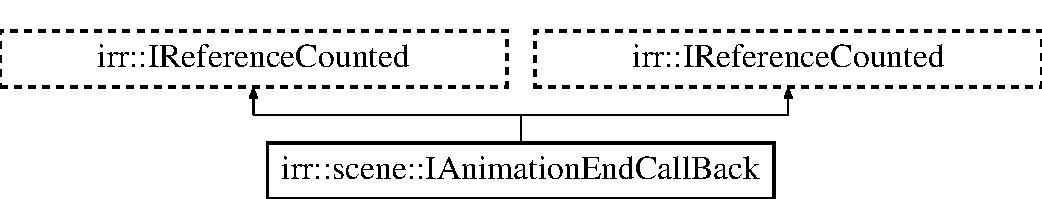
\includegraphics[height=2.000000cm]{classirr_1_1scene_1_1IAnimationEndCallBack}
\end{center}
\end{figure}
\subsection*{Public Member Functions}
\begin{DoxyCompactItemize}
\item 
virtual void \hyperlink{classirr_1_1scene_1_1IAnimationEndCallBack_a7676b37828697b63e42ad5264274cc1f}{On\+Animation\+End} (\hyperlink{classirr_1_1scene_1_1IAnimatedMeshSceneNode}{I\+Animated\+Mesh\+Scene\+Node} $\ast$node)=0
\begin{DoxyCompactList}\small\item\em Will be called when the animation playback has ended. \end{DoxyCompactList}\item 
virtual void \hyperlink{classirr_1_1scene_1_1IAnimationEndCallBack_a7676b37828697b63e42ad5264274cc1f}{On\+Animation\+End} (\hyperlink{classirr_1_1scene_1_1IAnimatedMeshSceneNode}{I\+Animated\+Mesh\+Scene\+Node} $\ast$node)=0
\begin{DoxyCompactList}\small\item\em Will be called when the animation playback has ended. \end{DoxyCompactList}\end{DoxyCompactItemize}
\subsection*{Additional Inherited Members}


\subsection{Detailed Description}
Callback interface for catching events of ended animations. 

Implement this interface and use \hyperlink{classirr_1_1scene_1_1IAnimatedMeshSceneNode_ad688bb5a7654116d1ee823e48393f1bd}{I\+Animated\+Mesh\+Scene\+Node\+::set\+Animation\+End\+Callback} to be able to be notified if an animation playback has ended. 

\subsection{Member Function Documentation}
\mbox{\Hypertarget{classirr_1_1scene_1_1IAnimationEndCallBack_a7676b37828697b63e42ad5264274cc1f}\label{classirr_1_1scene_1_1IAnimationEndCallBack_a7676b37828697b63e42ad5264274cc1f}} 
\index{irr\+::scene\+::\+I\+Animation\+End\+Call\+Back@{irr\+::scene\+::\+I\+Animation\+End\+Call\+Back}!On\+Animation\+End@{On\+Animation\+End}}
\index{On\+Animation\+End@{On\+Animation\+End}!irr\+::scene\+::\+I\+Animation\+End\+Call\+Back@{irr\+::scene\+::\+I\+Animation\+End\+Call\+Back}}
\subsubsection{\texorpdfstring{On\+Animation\+End()}{OnAnimationEnd()}\hspace{0.1cm}{\footnotesize\ttfamily [1/2]}}
{\footnotesize\ttfamily virtual void irr\+::scene\+::\+I\+Animation\+End\+Call\+Back\+::\+On\+Animation\+End (\begin{DoxyParamCaption}\item[{\hyperlink{classirr_1_1scene_1_1IAnimatedMeshSceneNode}{I\+Animated\+Mesh\+Scene\+Node} $\ast$}]{node }\end{DoxyParamCaption})\hspace{0.3cm}{\ttfamily [pure virtual]}}



Will be called when the animation playback has ended. 

See \hyperlink{classirr_1_1scene_1_1IAnimatedMeshSceneNode_ad688bb5a7654116d1ee823e48393f1bd}{I\+Animated\+Mesh\+Scene\+Node\+::set\+Animation\+End\+Callback} for more informations. 
\begin{DoxyParams}{Parameters}
{\em node} & Node of which the animation has ended. \\
\hline
\end{DoxyParams}
\mbox{\Hypertarget{classirr_1_1scene_1_1IAnimationEndCallBack_a7676b37828697b63e42ad5264274cc1f}\label{classirr_1_1scene_1_1IAnimationEndCallBack_a7676b37828697b63e42ad5264274cc1f}} 
\index{irr\+::scene\+::\+I\+Animation\+End\+Call\+Back@{irr\+::scene\+::\+I\+Animation\+End\+Call\+Back}!On\+Animation\+End@{On\+Animation\+End}}
\index{On\+Animation\+End@{On\+Animation\+End}!irr\+::scene\+::\+I\+Animation\+End\+Call\+Back@{irr\+::scene\+::\+I\+Animation\+End\+Call\+Back}}
\subsubsection{\texorpdfstring{On\+Animation\+End()}{OnAnimationEnd()}\hspace{0.1cm}{\footnotesize\ttfamily [2/2]}}
{\footnotesize\ttfamily virtual void irr\+::scene\+::\+I\+Animation\+End\+Call\+Back\+::\+On\+Animation\+End (\begin{DoxyParamCaption}\item[{\hyperlink{classirr_1_1scene_1_1IAnimatedMeshSceneNode}{I\+Animated\+Mesh\+Scene\+Node} $\ast$}]{node }\end{DoxyParamCaption})\hspace{0.3cm}{\ttfamily [pure virtual]}}



Will be called when the animation playback has ended. 

See \hyperlink{classirr_1_1scene_1_1IAnimatedMeshSceneNode_ad688bb5a7654116d1ee823e48393f1bd}{I\+Animated\+Mesh\+Scene\+Node\+::set\+Animation\+End\+Callback} for more informations. 
\begin{DoxyParams}{Parameters}
{\em node} & Node of which the animation has ended. \\
\hline
\end{DoxyParams}


The documentation for this class was generated from the following file\+:\begin{DoxyCompactItemize}
\item 
indie\+\_\+share/controller/include/I\+Animated\+Mesh\+Scene\+Node.\+h\end{DoxyCompactItemize}

\hypertarget{classirr_1_1io_1_1IArchiveLoader}{}\section{irr\+:\+:io\+:\+:I\+Archive\+Loader Class Reference}
\label{classirr_1_1io_1_1IArchiveLoader}\index{irr\+::io\+::\+I\+Archive\+Loader@{irr\+::io\+::\+I\+Archive\+Loader}}


Class which is able to create an archive from a file.  




{\ttfamily \#include $<$I\+File\+Archive.\+h$>$}

Inheritance diagram for irr\+:\+:io\+:\+:I\+Archive\+Loader\+:\begin{figure}[H]
\begin{center}
\leavevmode
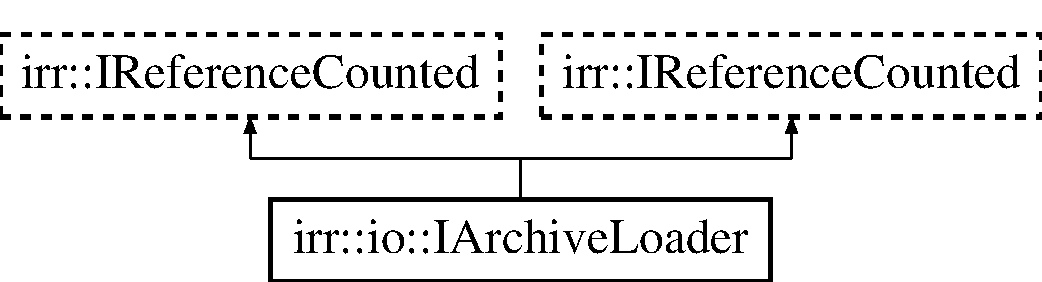
\includegraphics[height=2.000000cm]{classirr_1_1io_1_1IArchiveLoader}
\end{center}
\end{figure}
\subsection*{Public Member Functions}
\begin{DoxyCompactItemize}
\item 
virtual bool \hyperlink{classirr_1_1io_1_1IArchiveLoader_a9835ccbfd2c261edf4a738421c488ce3}{is\+A\+Loadable\+File\+Format} (const \hyperlink{namespaceirr_1_1io_a6468281622ce3a1c46b72e19f32dded5}{path} \&filename) const =0
\begin{DoxyCompactList}\small\item\em Check if the file might be loaded by this class. \end{DoxyCompactList}\item 
virtual bool \hyperlink{classirr_1_1io_1_1IArchiveLoader_acda22c3c2a5268665a4a4cf17379931b}{is\+A\+Loadable\+File\+Format} (\hyperlink{classirr_1_1io_1_1IReadFile}{io\+::\+I\+Read\+File} $\ast$file) const =0
\begin{DoxyCompactList}\small\item\em Check if the file might be loaded by this class. \end{DoxyCompactList}\item 
virtual bool \hyperlink{classirr_1_1io_1_1IArchiveLoader_af60c081f27ab941702a4a32dfe482c05}{is\+A\+Loadable\+File\+Format} (\hyperlink{namespaceirr_1_1io_adb3e3c445ec8e608ed1f0f93306da14f}{E\+\_\+\+F\+I\+L\+E\+\_\+\+A\+R\+C\+H\+I\+V\+E\+\_\+\+T\+Y\+PE} file\+Type) const =0
\begin{DoxyCompactList}\small\item\em Check to see if the loader can create archives of this type. \end{DoxyCompactList}\item 
virtual \hyperlink{classirr_1_1io_1_1IFileArchive}{I\+File\+Archive} $\ast$ \hyperlink{classirr_1_1io_1_1IArchiveLoader_a55e9586f190588e5fea6d17f63fb7aad}{create\+Archive} (const \hyperlink{namespaceirr_1_1io_a6468281622ce3a1c46b72e19f32dded5}{path} \&filename, bool ignore\+Case, bool ignore\+Paths) const =0
\begin{DoxyCompactList}\small\item\em Creates an archive from the filename. \end{DoxyCompactList}\item 
virtual \hyperlink{classirr_1_1io_1_1IFileArchive}{I\+File\+Archive} $\ast$ \hyperlink{classirr_1_1io_1_1IArchiveLoader_acd4a78189c62db96e4e10aa89c934980}{create\+Archive} (\hyperlink{classirr_1_1io_1_1IReadFile}{io\+::\+I\+Read\+File} $\ast$file, bool ignore\+Case, bool ignore\+Paths) const =0
\begin{DoxyCompactList}\small\item\em Creates an archive from the file. \end{DoxyCompactList}\item 
virtual bool \hyperlink{classirr_1_1io_1_1IArchiveLoader_a9835ccbfd2c261edf4a738421c488ce3}{is\+A\+Loadable\+File\+Format} (const \hyperlink{namespaceirr_1_1io_a6468281622ce3a1c46b72e19f32dded5}{path} \&filename) const =0
\begin{DoxyCompactList}\small\item\em Check if the file might be loaded by this class. \end{DoxyCompactList}\item 
virtual bool \hyperlink{classirr_1_1io_1_1IArchiveLoader_acda22c3c2a5268665a4a4cf17379931b}{is\+A\+Loadable\+File\+Format} (\hyperlink{classirr_1_1io_1_1IReadFile}{io\+::\+I\+Read\+File} $\ast$file) const =0
\begin{DoxyCompactList}\small\item\em Check if the file might be loaded by this class. \end{DoxyCompactList}\item 
virtual bool \hyperlink{classirr_1_1io_1_1IArchiveLoader_af60c081f27ab941702a4a32dfe482c05}{is\+A\+Loadable\+File\+Format} (\hyperlink{namespaceirr_1_1io_adb3e3c445ec8e608ed1f0f93306da14f}{E\+\_\+\+F\+I\+L\+E\+\_\+\+A\+R\+C\+H\+I\+V\+E\+\_\+\+T\+Y\+PE} file\+Type) const =0
\begin{DoxyCompactList}\small\item\em Check to see if the loader can create archives of this type. \end{DoxyCompactList}\item 
virtual \hyperlink{classirr_1_1io_1_1IFileArchive}{I\+File\+Archive} $\ast$ \hyperlink{classirr_1_1io_1_1IArchiveLoader_a55e9586f190588e5fea6d17f63fb7aad}{create\+Archive} (const \hyperlink{namespaceirr_1_1io_a6468281622ce3a1c46b72e19f32dded5}{path} \&filename, bool ignore\+Case, bool ignore\+Paths) const =0
\begin{DoxyCompactList}\small\item\em Creates an archive from the filename. \end{DoxyCompactList}\item 
virtual \hyperlink{classirr_1_1io_1_1IFileArchive}{I\+File\+Archive} $\ast$ \hyperlink{classirr_1_1io_1_1IArchiveLoader_acd4a78189c62db96e4e10aa89c934980}{create\+Archive} (\hyperlink{classirr_1_1io_1_1IReadFile}{io\+::\+I\+Read\+File} $\ast$file, bool ignore\+Case, bool ignore\+Paths) const =0
\begin{DoxyCompactList}\small\item\em Creates an archive from the file. \end{DoxyCompactList}\end{DoxyCompactItemize}
\subsection*{Additional Inherited Members}


\subsection{Detailed Description}
Class which is able to create an archive from a file. 

If you want the Irrlicht Engine be able to load archives of currently unsupported file formats (e.\+g .wad), then implement this and add your new Archive loader with \hyperlink{classirr_1_1io_1_1IFileSystem_ad56456302b4697c49b461a909d9269b9}{I\+File\+System\+::add\+Archive\+Loader()} to the engine. 

\subsection{Member Function Documentation}
\mbox{\Hypertarget{classirr_1_1io_1_1IArchiveLoader_a55e9586f190588e5fea6d17f63fb7aad}\label{classirr_1_1io_1_1IArchiveLoader_a55e9586f190588e5fea6d17f63fb7aad}} 
\index{irr\+::io\+::\+I\+Archive\+Loader@{irr\+::io\+::\+I\+Archive\+Loader}!create\+Archive@{create\+Archive}}
\index{create\+Archive@{create\+Archive}!irr\+::io\+::\+I\+Archive\+Loader@{irr\+::io\+::\+I\+Archive\+Loader}}
\subsubsection{\texorpdfstring{create\+Archive()}{createArchive()}\hspace{0.1cm}{\footnotesize\ttfamily [1/4]}}
{\footnotesize\ttfamily virtual \hyperlink{classirr_1_1io_1_1IFileArchive}{I\+File\+Archive}$\ast$ irr\+::io\+::\+I\+Archive\+Loader\+::create\+Archive (\begin{DoxyParamCaption}\item[{const \hyperlink{namespaceirr_1_1io_a6468281622ce3a1c46b72e19f32dded5}{path} \&}]{filename,  }\item[{bool}]{ignore\+Case,  }\item[{bool}]{ignore\+Paths }\end{DoxyParamCaption}) const\hspace{0.3cm}{\ttfamily [pure virtual]}}



Creates an archive from the filename. 


\begin{DoxyParams}{Parameters}
{\em filename} & File to use. \\
\hline
{\em ignore\+Case} & Searching is performed without regarding the case \\
\hline
{\em ignore\+Paths} & Files are searched for without checking for the directories \\
\hline
\end{DoxyParams}
\begin{DoxyReturn}{Returns}
Pointer to newly created archive, or 0 upon error. 
\end{DoxyReturn}
\mbox{\Hypertarget{classirr_1_1io_1_1IArchiveLoader_a55e9586f190588e5fea6d17f63fb7aad}\label{classirr_1_1io_1_1IArchiveLoader_a55e9586f190588e5fea6d17f63fb7aad}} 
\index{irr\+::io\+::\+I\+Archive\+Loader@{irr\+::io\+::\+I\+Archive\+Loader}!create\+Archive@{create\+Archive}}
\index{create\+Archive@{create\+Archive}!irr\+::io\+::\+I\+Archive\+Loader@{irr\+::io\+::\+I\+Archive\+Loader}}
\subsubsection{\texorpdfstring{create\+Archive()}{createArchive()}\hspace{0.1cm}{\footnotesize\ttfamily [2/4]}}
{\footnotesize\ttfamily virtual \hyperlink{classirr_1_1io_1_1IFileArchive}{I\+File\+Archive}$\ast$ irr\+::io\+::\+I\+Archive\+Loader\+::create\+Archive (\begin{DoxyParamCaption}\item[{const \hyperlink{namespaceirr_1_1io_a6468281622ce3a1c46b72e19f32dded5}{path} \&}]{filename,  }\item[{bool}]{ignore\+Case,  }\item[{bool}]{ignore\+Paths }\end{DoxyParamCaption}) const\hspace{0.3cm}{\ttfamily [pure virtual]}}



Creates an archive from the filename. 


\begin{DoxyParams}{Parameters}
{\em filename} & File to use. \\
\hline
{\em ignore\+Case} & Searching is performed without regarding the case \\
\hline
{\em ignore\+Paths} & Files are searched for without checking for the directories \\
\hline
\end{DoxyParams}
\begin{DoxyReturn}{Returns}
Pointer to newly created archive, or 0 upon error. 
\end{DoxyReturn}
\mbox{\Hypertarget{classirr_1_1io_1_1IArchiveLoader_acd4a78189c62db96e4e10aa89c934980}\label{classirr_1_1io_1_1IArchiveLoader_acd4a78189c62db96e4e10aa89c934980}} 
\index{irr\+::io\+::\+I\+Archive\+Loader@{irr\+::io\+::\+I\+Archive\+Loader}!create\+Archive@{create\+Archive}}
\index{create\+Archive@{create\+Archive}!irr\+::io\+::\+I\+Archive\+Loader@{irr\+::io\+::\+I\+Archive\+Loader}}
\subsubsection{\texorpdfstring{create\+Archive()}{createArchive()}\hspace{0.1cm}{\footnotesize\ttfamily [3/4]}}
{\footnotesize\ttfamily virtual \hyperlink{classirr_1_1io_1_1IFileArchive}{I\+File\+Archive}$\ast$ irr\+::io\+::\+I\+Archive\+Loader\+::create\+Archive (\begin{DoxyParamCaption}\item[{\hyperlink{classirr_1_1io_1_1IReadFile}{io\+::\+I\+Read\+File} $\ast$}]{file,  }\item[{bool}]{ignore\+Case,  }\item[{bool}]{ignore\+Paths }\end{DoxyParamCaption}) const\hspace{0.3cm}{\ttfamily [pure virtual]}}



Creates an archive from the file. 


\begin{DoxyParams}{Parameters}
{\em file} & File handle to use. \\
\hline
{\em ignore\+Case} & Searching is performed without regarding the case \\
\hline
{\em ignore\+Paths} & Files are searched for without checking for the directories \\
\hline
\end{DoxyParams}
\begin{DoxyReturn}{Returns}
Pointer to newly created archive, or 0 upon error. 
\end{DoxyReturn}
\mbox{\Hypertarget{classirr_1_1io_1_1IArchiveLoader_acd4a78189c62db96e4e10aa89c934980}\label{classirr_1_1io_1_1IArchiveLoader_acd4a78189c62db96e4e10aa89c934980}} 
\index{irr\+::io\+::\+I\+Archive\+Loader@{irr\+::io\+::\+I\+Archive\+Loader}!create\+Archive@{create\+Archive}}
\index{create\+Archive@{create\+Archive}!irr\+::io\+::\+I\+Archive\+Loader@{irr\+::io\+::\+I\+Archive\+Loader}}
\subsubsection{\texorpdfstring{create\+Archive()}{createArchive()}\hspace{0.1cm}{\footnotesize\ttfamily [4/4]}}
{\footnotesize\ttfamily virtual \hyperlink{classirr_1_1io_1_1IFileArchive}{I\+File\+Archive}$\ast$ irr\+::io\+::\+I\+Archive\+Loader\+::create\+Archive (\begin{DoxyParamCaption}\item[{\hyperlink{classirr_1_1io_1_1IReadFile}{io\+::\+I\+Read\+File} $\ast$}]{file,  }\item[{bool}]{ignore\+Case,  }\item[{bool}]{ignore\+Paths }\end{DoxyParamCaption}) const\hspace{0.3cm}{\ttfamily [pure virtual]}}



Creates an archive from the file. 


\begin{DoxyParams}{Parameters}
{\em file} & File handle to use. \\
\hline
{\em ignore\+Case} & Searching is performed without regarding the case \\
\hline
{\em ignore\+Paths} & Files are searched for without checking for the directories \\
\hline
\end{DoxyParams}
\begin{DoxyReturn}{Returns}
Pointer to newly created archive, or 0 upon error. 
\end{DoxyReturn}
\mbox{\Hypertarget{classirr_1_1io_1_1IArchiveLoader_a9835ccbfd2c261edf4a738421c488ce3}\label{classirr_1_1io_1_1IArchiveLoader_a9835ccbfd2c261edf4a738421c488ce3}} 
\index{irr\+::io\+::\+I\+Archive\+Loader@{irr\+::io\+::\+I\+Archive\+Loader}!is\+A\+Loadable\+File\+Format@{is\+A\+Loadable\+File\+Format}}
\index{is\+A\+Loadable\+File\+Format@{is\+A\+Loadable\+File\+Format}!irr\+::io\+::\+I\+Archive\+Loader@{irr\+::io\+::\+I\+Archive\+Loader}}
\subsubsection{\texorpdfstring{is\+A\+Loadable\+File\+Format()}{isALoadableFileFormat()}\hspace{0.1cm}{\footnotesize\ttfamily [1/6]}}
{\footnotesize\ttfamily virtual bool irr\+::io\+::\+I\+Archive\+Loader\+::is\+A\+Loadable\+File\+Format (\begin{DoxyParamCaption}\item[{const \hyperlink{namespaceirr_1_1io_a6468281622ce3a1c46b72e19f32dded5}{path} \&}]{filename }\end{DoxyParamCaption}) const\hspace{0.3cm}{\ttfamily [pure virtual]}}



Check if the file might be loaded by this class. 

Check based on the file extension (e.\+g. \char`\"{}.\+zip\char`\"{}) 
\begin{DoxyParams}{Parameters}
{\em filename} & Name of file to check. \\
\hline
\end{DoxyParams}
\begin{DoxyReturn}{Returns}
True if file seems to be loadable. 
\end{DoxyReturn}
\mbox{\Hypertarget{classirr_1_1io_1_1IArchiveLoader_a9835ccbfd2c261edf4a738421c488ce3}\label{classirr_1_1io_1_1IArchiveLoader_a9835ccbfd2c261edf4a738421c488ce3}} 
\index{irr\+::io\+::\+I\+Archive\+Loader@{irr\+::io\+::\+I\+Archive\+Loader}!is\+A\+Loadable\+File\+Format@{is\+A\+Loadable\+File\+Format}}
\index{is\+A\+Loadable\+File\+Format@{is\+A\+Loadable\+File\+Format}!irr\+::io\+::\+I\+Archive\+Loader@{irr\+::io\+::\+I\+Archive\+Loader}}
\subsubsection{\texorpdfstring{is\+A\+Loadable\+File\+Format()}{isALoadableFileFormat()}\hspace{0.1cm}{\footnotesize\ttfamily [2/6]}}
{\footnotesize\ttfamily virtual bool irr\+::io\+::\+I\+Archive\+Loader\+::is\+A\+Loadable\+File\+Format (\begin{DoxyParamCaption}\item[{const \hyperlink{namespaceirr_1_1io_a6468281622ce3a1c46b72e19f32dded5}{path} \&}]{filename }\end{DoxyParamCaption}) const\hspace{0.3cm}{\ttfamily [pure virtual]}}



Check if the file might be loaded by this class. 

Check based on the file extension (e.\+g. \char`\"{}.\+zip\char`\"{}) 
\begin{DoxyParams}{Parameters}
{\em filename} & Name of file to check. \\
\hline
\end{DoxyParams}
\begin{DoxyReturn}{Returns}
True if file seems to be loadable. 
\end{DoxyReturn}
\mbox{\Hypertarget{classirr_1_1io_1_1IArchiveLoader_acda22c3c2a5268665a4a4cf17379931b}\label{classirr_1_1io_1_1IArchiveLoader_acda22c3c2a5268665a4a4cf17379931b}} 
\index{irr\+::io\+::\+I\+Archive\+Loader@{irr\+::io\+::\+I\+Archive\+Loader}!is\+A\+Loadable\+File\+Format@{is\+A\+Loadable\+File\+Format}}
\index{is\+A\+Loadable\+File\+Format@{is\+A\+Loadable\+File\+Format}!irr\+::io\+::\+I\+Archive\+Loader@{irr\+::io\+::\+I\+Archive\+Loader}}
\subsubsection{\texorpdfstring{is\+A\+Loadable\+File\+Format()}{isALoadableFileFormat()}\hspace{0.1cm}{\footnotesize\ttfamily [3/6]}}
{\footnotesize\ttfamily virtual bool irr\+::io\+::\+I\+Archive\+Loader\+::is\+A\+Loadable\+File\+Format (\begin{DoxyParamCaption}\item[{\hyperlink{classirr_1_1io_1_1IReadFile}{io\+::\+I\+Read\+File} $\ast$}]{file }\end{DoxyParamCaption}) const\hspace{0.3cm}{\ttfamily [pure virtual]}}



Check if the file might be loaded by this class. 

This check may look into the file. 
\begin{DoxyParams}{Parameters}
{\em file} & File handle to check. \\
\hline
\end{DoxyParams}
\begin{DoxyReturn}{Returns}
True if file seems to be loadable. 
\end{DoxyReturn}
\mbox{\Hypertarget{classirr_1_1io_1_1IArchiveLoader_acda22c3c2a5268665a4a4cf17379931b}\label{classirr_1_1io_1_1IArchiveLoader_acda22c3c2a5268665a4a4cf17379931b}} 
\index{irr\+::io\+::\+I\+Archive\+Loader@{irr\+::io\+::\+I\+Archive\+Loader}!is\+A\+Loadable\+File\+Format@{is\+A\+Loadable\+File\+Format}}
\index{is\+A\+Loadable\+File\+Format@{is\+A\+Loadable\+File\+Format}!irr\+::io\+::\+I\+Archive\+Loader@{irr\+::io\+::\+I\+Archive\+Loader}}
\subsubsection{\texorpdfstring{is\+A\+Loadable\+File\+Format()}{isALoadableFileFormat()}\hspace{0.1cm}{\footnotesize\ttfamily [4/6]}}
{\footnotesize\ttfamily virtual bool irr\+::io\+::\+I\+Archive\+Loader\+::is\+A\+Loadable\+File\+Format (\begin{DoxyParamCaption}\item[{\hyperlink{classirr_1_1io_1_1IReadFile}{io\+::\+I\+Read\+File} $\ast$}]{file }\end{DoxyParamCaption}) const\hspace{0.3cm}{\ttfamily [pure virtual]}}



Check if the file might be loaded by this class. 

This check may look into the file. 
\begin{DoxyParams}{Parameters}
{\em file} & File handle to check. \\
\hline
\end{DoxyParams}
\begin{DoxyReturn}{Returns}
True if file seems to be loadable. 
\end{DoxyReturn}
\mbox{\Hypertarget{classirr_1_1io_1_1IArchiveLoader_af60c081f27ab941702a4a32dfe482c05}\label{classirr_1_1io_1_1IArchiveLoader_af60c081f27ab941702a4a32dfe482c05}} 
\index{irr\+::io\+::\+I\+Archive\+Loader@{irr\+::io\+::\+I\+Archive\+Loader}!is\+A\+Loadable\+File\+Format@{is\+A\+Loadable\+File\+Format}}
\index{is\+A\+Loadable\+File\+Format@{is\+A\+Loadable\+File\+Format}!irr\+::io\+::\+I\+Archive\+Loader@{irr\+::io\+::\+I\+Archive\+Loader}}
\subsubsection{\texorpdfstring{is\+A\+Loadable\+File\+Format()}{isALoadableFileFormat()}\hspace{0.1cm}{\footnotesize\ttfamily [5/6]}}
{\footnotesize\ttfamily virtual bool irr\+::io\+::\+I\+Archive\+Loader\+::is\+A\+Loadable\+File\+Format (\begin{DoxyParamCaption}\item[{\hyperlink{namespaceirr_1_1io_adb3e3c445ec8e608ed1f0f93306da14f}{E\+\_\+\+F\+I\+L\+E\+\_\+\+A\+R\+C\+H\+I\+V\+E\+\_\+\+T\+Y\+PE}}]{file\+Type }\end{DoxyParamCaption}) const\hspace{0.3cm}{\ttfamily [pure virtual]}}



Check to see if the loader can create archives of this type. 

Check based on the archive type. 
\begin{DoxyParams}{Parameters}
{\em file\+Type} & The archive type to check. \\
\hline
\end{DoxyParams}
\begin{DoxyReturn}{Returns}
True if the archile loader supports this type, false if not 
\end{DoxyReturn}
\mbox{\Hypertarget{classirr_1_1io_1_1IArchiveLoader_af60c081f27ab941702a4a32dfe482c05}\label{classirr_1_1io_1_1IArchiveLoader_af60c081f27ab941702a4a32dfe482c05}} 
\index{irr\+::io\+::\+I\+Archive\+Loader@{irr\+::io\+::\+I\+Archive\+Loader}!is\+A\+Loadable\+File\+Format@{is\+A\+Loadable\+File\+Format}}
\index{is\+A\+Loadable\+File\+Format@{is\+A\+Loadable\+File\+Format}!irr\+::io\+::\+I\+Archive\+Loader@{irr\+::io\+::\+I\+Archive\+Loader}}
\subsubsection{\texorpdfstring{is\+A\+Loadable\+File\+Format()}{isALoadableFileFormat()}\hspace{0.1cm}{\footnotesize\ttfamily [6/6]}}
{\footnotesize\ttfamily virtual bool irr\+::io\+::\+I\+Archive\+Loader\+::is\+A\+Loadable\+File\+Format (\begin{DoxyParamCaption}\item[{\hyperlink{namespaceirr_1_1io_adb3e3c445ec8e608ed1f0f93306da14f}{E\+\_\+\+F\+I\+L\+E\+\_\+\+A\+R\+C\+H\+I\+V\+E\+\_\+\+T\+Y\+PE}}]{file\+Type }\end{DoxyParamCaption}) const\hspace{0.3cm}{\ttfamily [pure virtual]}}



Check to see if the loader can create archives of this type. 

Check based on the archive type. 
\begin{DoxyParams}{Parameters}
{\em file\+Type} & The archive type to check. \\
\hline
\end{DoxyParams}
\begin{DoxyReturn}{Returns}
True if the archile loader supports this type, false if not 
\end{DoxyReturn}


The documentation for this class was generated from the following file\+:\begin{DoxyCompactItemize}
\item 
indie\+\_\+share/controller/include/I\+File\+Archive.\+h\end{DoxyCompactItemize}

\hypertarget{classirr_1_1io_1_1IAttributeExchangingObject}{}\section{irr\+:\+:io\+:\+:I\+Attribute\+Exchanging\+Object Class Reference}
\label{classirr_1_1io_1_1IAttributeExchangingObject}\index{irr\+::io\+::\+I\+Attribute\+Exchanging\+Object@{irr\+::io\+::\+I\+Attribute\+Exchanging\+Object}}


An object which is able to serialize and deserialize its attributes into an attributes object.  




{\ttfamily \#include $<$I\+Attribute\+Exchanging\+Object.\+h$>$}

Inheritance diagram for irr\+:\+:io\+:\+:I\+Attribute\+Exchanging\+Object\+:\begin{figure}[H]
\begin{center}
\leavevmode
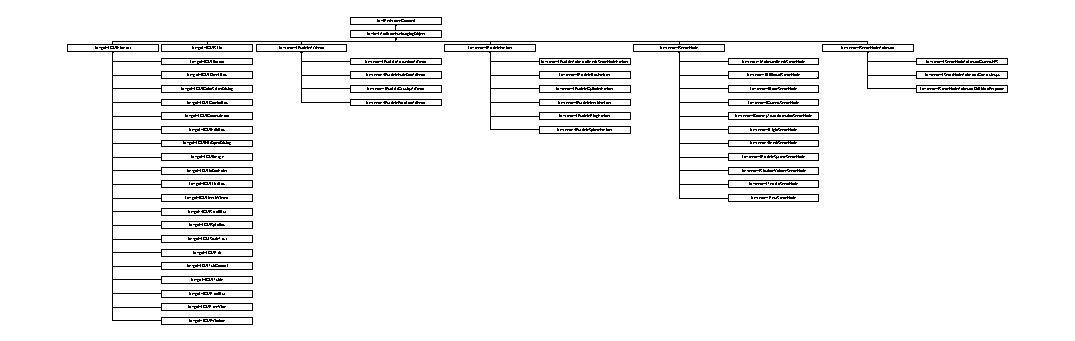
\includegraphics[height=4.128205cm]{classirr_1_1io_1_1IAttributeExchangingObject}
\end{center}
\end{figure}
\subsection*{Public Member Functions}
\begin{DoxyCompactItemize}
\item 
virtual void \hyperlink{classirr_1_1io_1_1IAttributeExchangingObject_a587f7b633366968f0488e1099e9172ef}{serialize\+Attributes} (\hyperlink{classirr_1_1io_1_1IAttributes}{io\+::\+I\+Attributes} $\ast$out, \hyperlink{structirr_1_1io_1_1SAttributeReadWriteOptions}{io\+::\+S\+Attribute\+Read\+Write\+Options} $\ast$options=0) const
\begin{DoxyCompactList}\small\item\em Writes attributes of the object. \end{DoxyCompactList}\item 
virtual void \hyperlink{classirr_1_1io_1_1IAttributeExchangingObject_a013d4ead3736d7fab4bc18c2d61a3e2e}{deserialize\+Attributes} (\hyperlink{classirr_1_1io_1_1IAttributes}{io\+::\+I\+Attributes} $\ast$in, \hyperlink{structirr_1_1io_1_1SAttributeReadWriteOptions}{io\+::\+S\+Attribute\+Read\+Write\+Options} $\ast$options=0)
\begin{DoxyCompactList}\small\item\em Reads attributes of the object. \end{DoxyCompactList}\end{DoxyCompactItemize}
\subsection*{Additional Inherited Members}


\subsection{Detailed Description}
An object which is able to serialize and deserialize its attributes into an attributes object. 

\subsection{Member Function Documentation}
\mbox{\Hypertarget{classirr_1_1io_1_1IAttributeExchangingObject_a013d4ead3736d7fab4bc18c2d61a3e2e}\label{classirr_1_1io_1_1IAttributeExchangingObject_a013d4ead3736d7fab4bc18c2d61a3e2e}} 
\index{irr\+::io\+::\+I\+Attribute\+Exchanging\+Object@{irr\+::io\+::\+I\+Attribute\+Exchanging\+Object}!deserialize\+Attributes@{deserialize\+Attributes}}
\index{deserialize\+Attributes@{deserialize\+Attributes}!irr\+::io\+::\+I\+Attribute\+Exchanging\+Object@{irr\+::io\+::\+I\+Attribute\+Exchanging\+Object}}
\subsubsection{\texorpdfstring{deserialize\+Attributes()}{deserializeAttributes()}}
{\footnotesize\ttfamily virtual void irr\+::io\+::\+I\+Attribute\+Exchanging\+Object\+::deserialize\+Attributes (\begin{DoxyParamCaption}\item[{\hyperlink{classirr_1_1io_1_1IAttributes}{io\+::\+I\+Attributes} $\ast$}]{in,  }\item[{\hyperlink{structirr_1_1io_1_1SAttributeReadWriteOptions}{io\+::\+S\+Attribute\+Read\+Write\+Options} $\ast$}]{options = {\ttfamily 0} }\end{DoxyParamCaption})\hspace{0.3cm}{\ttfamily [inline]}, {\ttfamily [virtual]}}



Reads attributes of the object. 

Implement this to set the attributes of your scene node animator for scripting languages, editors, debuggers or xml deserialization purposes. 

Reimplemented in \hyperlink{classirr_1_1gui_1_1IGUIElement_af71b96163b8d95816cd9c80fbf413b4d}{irr\+::gui\+::\+I\+G\+U\+I\+Element}, \hyperlink{classirr_1_1scene_1_1ISceneNode_a5fb609b08fc89a92f928c19ce3b181eb}{irr\+::scene\+::\+I\+Scene\+Node}, and \hyperlink{classirr_1_1scene_1_1ICameraSceneNode_a0df881cb5e2a55562399281061151ae8}{irr\+::scene\+::\+I\+Camera\+Scene\+Node}.

\mbox{\Hypertarget{classirr_1_1io_1_1IAttributeExchangingObject_a587f7b633366968f0488e1099e9172ef}\label{classirr_1_1io_1_1IAttributeExchangingObject_a587f7b633366968f0488e1099e9172ef}} 
\index{irr\+::io\+::\+I\+Attribute\+Exchanging\+Object@{irr\+::io\+::\+I\+Attribute\+Exchanging\+Object}!serialize\+Attributes@{serialize\+Attributes}}
\index{serialize\+Attributes@{serialize\+Attributes}!irr\+::io\+::\+I\+Attribute\+Exchanging\+Object@{irr\+::io\+::\+I\+Attribute\+Exchanging\+Object}}
\subsubsection{\texorpdfstring{serialize\+Attributes()}{serializeAttributes()}}
{\footnotesize\ttfamily virtual void irr\+::io\+::\+I\+Attribute\+Exchanging\+Object\+::serialize\+Attributes (\begin{DoxyParamCaption}\item[{\hyperlink{classirr_1_1io_1_1IAttributes}{io\+::\+I\+Attributes} $\ast$}]{out,  }\item[{\hyperlink{structirr_1_1io_1_1SAttributeReadWriteOptions}{io\+::\+S\+Attribute\+Read\+Write\+Options} $\ast$}]{options = {\ttfamily 0} }\end{DoxyParamCaption}) const\hspace{0.3cm}{\ttfamily [inline]}, {\ttfamily [virtual]}}



Writes attributes of the object. 

Implement this to expose the attributes of your scene node animator for scripting languages, editors, debuggers or xml serialization purposes. 

Reimplemented in \hyperlink{classirr_1_1gui_1_1IGUIElement_ac575f2f817b05733dbc667ff298f6e78}{irr\+::gui\+::\+I\+G\+U\+I\+Element}, \hyperlink{classirr_1_1scene_1_1ISceneNode_a3210345b70227c03c7f889c94754fdaa}{irr\+::scene\+::\+I\+Scene\+Node}, and \hyperlink{classirr_1_1scene_1_1ICameraSceneNode_a0a78a29638be1665ee5dba22c2c3b846}{irr\+::scene\+::\+I\+Camera\+Scene\+Node}.



The documentation for this class was generated from the following file\+:\begin{DoxyCompactItemize}
\item 
indie\+\_\+share/controller/include/I\+Attribute\+Exchanging\+Object.\+h\end{DoxyCompactItemize}

\hypertarget{classirr_1_1io_1_1IAttributes}{}\section{irr\+:\+:io\+:\+:I\+Attributes Class Reference}
\label{classirr_1_1io_1_1IAttributes}\index{irr\+::io\+::\+I\+Attributes@{irr\+::io\+::\+I\+Attributes}}


Provides a generic interface for attributes and their values and the possiblity to serialize them.  




{\ttfamily \#include $<$I\+Attributes.\+h$>$}

Inheritance diagram for irr\+:\+:io\+:\+:I\+Attributes\+:\begin{figure}[H]
\begin{center}
\leavevmode
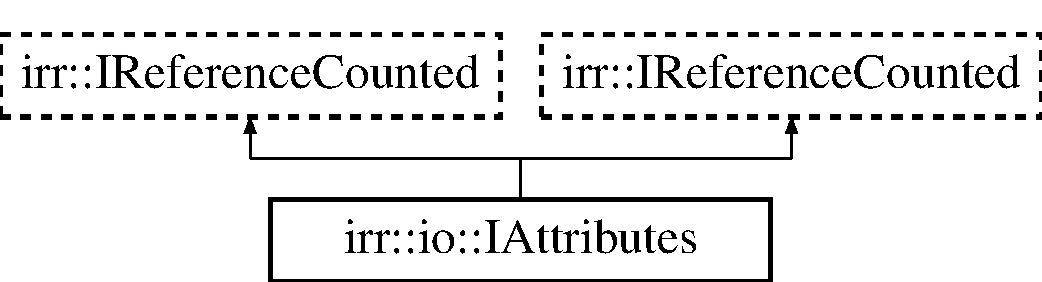
\includegraphics[height=2.000000cm]{classirr_1_1io_1_1IAttributes}
\end{center}
\end{figure}
\subsection*{Public Member Functions}
\begin{DoxyCompactItemize}
\item 
\mbox{\Hypertarget{classirr_1_1io_1_1IAttributes_a796bdd9440ee7ba0b6742a90a82870b6}\label{classirr_1_1io_1_1IAttributes_a796bdd9440ee7ba0b6742a90a82870b6}} 
virtual \hyperlink{namespaceirr_a0416a53257075833e7002efd0a18e804}{u32} \hyperlink{classirr_1_1io_1_1IAttributes_a796bdd9440ee7ba0b6742a90a82870b6}{get\+Attribute\+Count} () const =0
\begin{DoxyCompactList}\small\item\em Returns amount of attributes in this collection of attributes. \end{DoxyCompactList}\item 
virtual const \hyperlink{namespaceirr_a9395eaea339bcb546b319e9c96bf7410}{c8} $\ast$ \hyperlink{classirr_1_1io_1_1IAttributes_adee33f518d95a1ca17146bb055c6e5f3}{get\+Attribute\+Name} (\hyperlink{namespaceirr_ac66849b7a6ed16e30ebede579f9b47c6}{s32} index)=0
\begin{DoxyCompactList}\small\item\em Returns attribute name by index. \end{DoxyCompactList}\item 
virtual \hyperlink{namespaceirr_1_1io_a874a5f14dbe2e45c40c2bb29e9f0ebcb}{E\+\_\+\+A\+T\+T\+R\+I\+B\+U\+T\+E\+\_\+\+T\+Y\+PE} \hyperlink{classirr_1_1io_1_1IAttributes_af14805d54f8cfae0a76751d13931390a}{get\+Attribute\+Type} (const \hyperlink{namespaceirr_a9395eaea339bcb546b319e9c96bf7410}{c8} $\ast$attribute\+Name)=0
\begin{DoxyCompactList}\small\item\em Returns the type of an attribute. \end{DoxyCompactList}\item 
virtual \hyperlink{namespaceirr_1_1io_a874a5f14dbe2e45c40c2bb29e9f0ebcb}{E\+\_\+\+A\+T\+T\+R\+I\+B\+U\+T\+E\+\_\+\+T\+Y\+PE} \hyperlink{classirr_1_1io_1_1IAttributes_a2cb0eb3befcbf7feb2bbdd4676c53954}{get\+Attribute\+Type} (\hyperlink{namespaceirr_ac66849b7a6ed16e30ebede579f9b47c6}{s32} index)=0
\begin{DoxyCompactList}\small\item\em Returns attribute type by index. \end{DoxyCompactList}\item 
virtual const wchar\+\_\+t $\ast$ \hyperlink{classirr_1_1io_1_1IAttributes_a6a460acccdbf5b2f8eac8d2bd6a1e428}{get\+Attribute\+Type\+String} (const \hyperlink{namespaceirr_a9395eaea339bcb546b319e9c96bf7410}{c8} $\ast$attribute\+Name)=0
\begin{DoxyCompactList}\small\item\em Returns the type string of the attribute. \end{DoxyCompactList}\item 
virtual const wchar\+\_\+t $\ast$ \hyperlink{classirr_1_1io_1_1IAttributes_a2dc2dffe38bc50222615f40a7ca7711a}{get\+Attribute\+Type\+String} (\hyperlink{namespaceirr_ac66849b7a6ed16e30ebede579f9b47c6}{s32} index)=0
\begin{DoxyCompactList}\small\item\em Returns the type string of the attribute by index. \end{DoxyCompactList}\item 
\mbox{\Hypertarget{classirr_1_1io_1_1IAttributes_ae2b4783b220e424269beee14674babb3}\label{classirr_1_1io_1_1IAttributes_ae2b4783b220e424269beee14674babb3}} 
virtual bool \hyperlink{classirr_1_1io_1_1IAttributes_ae2b4783b220e424269beee14674babb3}{exists\+Attribute} (const \hyperlink{namespaceirr_a9395eaea339bcb546b319e9c96bf7410}{c8} $\ast$attribute\+Name)=0
\begin{DoxyCompactList}\small\item\em Returns if an attribute with a name exists. \end{DoxyCompactList}\item 
\mbox{\Hypertarget{classirr_1_1io_1_1IAttributes_abda2f84c5b87d69d9008485740afcb7c}\label{classirr_1_1io_1_1IAttributes_abda2f84c5b87d69d9008485740afcb7c}} 
virtual \hyperlink{namespaceirr_ac66849b7a6ed16e30ebede579f9b47c6}{s32} \hyperlink{classirr_1_1io_1_1IAttributes_abda2f84c5b87d69d9008485740afcb7c}{find\+Attribute} (const \hyperlink{namespaceirr_a9395eaea339bcb546b319e9c96bf7410}{c8} $\ast$attribute\+Name) const =0
\begin{DoxyCompactList}\small\item\em Returns attribute index from name, -\/1 if not found. \end{DoxyCompactList}\item 
\mbox{\Hypertarget{classirr_1_1io_1_1IAttributes_ab33109fc1b62432973a49b794231a061}\label{classirr_1_1io_1_1IAttributes_ab33109fc1b62432973a49b794231a061}} 
virtual void \hyperlink{classirr_1_1io_1_1IAttributes_ab33109fc1b62432973a49b794231a061}{clear} ()=0
\begin{DoxyCompactList}\small\item\em Removes all attributes. \end{DoxyCompactList}\item 
virtual bool \hyperlink{classirr_1_1io_1_1IAttributes_a9001fd2760cba4e1b13efc6539c0f441}{read} (\hyperlink{namespaceirr_1_1io_a9dc6291fb7e4c73155a3e3c8339f9bff}{io\+::\+I\+X\+M\+L\+Reader} $\ast$reader, bool read\+Current\+Element\+Only=false, const wchar\+\_\+t $\ast$element\+Name=0)=0
\begin{DoxyCompactList}\small\item\em Reads attributes from a xml file. \end{DoxyCompactList}\item 
virtual bool \hyperlink{classirr_1_1io_1_1IAttributes_a5a32fcdfca5426cccf69e8f654a0050c}{write} (\hyperlink{classirr_1_1io_1_1IXMLWriter}{io\+::\+I\+X\+M\+L\+Writer} $\ast$writer, bool write\+X\+M\+L\+Header=false, const wchar\+\_\+t $\ast$element\+Name=0)=0
\begin{DoxyCompactList}\small\item\em Write these attributes into a xml file. \end{DoxyCompactList}\item 
\mbox{\Hypertarget{classirr_1_1io_1_1IAttributes_afbde111f36d59e9cf42b20595cf2ed24}\label{classirr_1_1io_1_1IAttributes_afbde111f36d59e9cf42b20595cf2ed24}} 
virtual void \hyperlink{classirr_1_1io_1_1IAttributes_afbde111f36d59e9cf42b20595cf2ed24}{add\+Int} (const \hyperlink{namespaceirr_a9395eaea339bcb546b319e9c96bf7410}{c8} $\ast$attribute\+Name, \hyperlink{namespaceirr_ac66849b7a6ed16e30ebede579f9b47c6}{s32} value)=0
\begin{DoxyCompactList}\small\item\em Adds an attribute as integer. \end{DoxyCompactList}\item 
\mbox{\Hypertarget{classirr_1_1io_1_1IAttributes_a03fa31acb481ae23678676cc183f09a6}\label{classirr_1_1io_1_1IAttributes_a03fa31acb481ae23678676cc183f09a6}} 
virtual void \hyperlink{classirr_1_1io_1_1IAttributes_a03fa31acb481ae23678676cc183f09a6}{set\+Attribute} (const \hyperlink{namespaceirr_a9395eaea339bcb546b319e9c96bf7410}{c8} $\ast$attribute\+Name, \hyperlink{namespaceirr_ac66849b7a6ed16e30ebede579f9b47c6}{s32} value)=0
\begin{DoxyCompactList}\small\item\em Sets an attribute as integer value. \end{DoxyCompactList}\item 
virtual \hyperlink{namespaceirr_ac66849b7a6ed16e30ebede579f9b47c6}{s32} \hyperlink{classirr_1_1io_1_1IAttributes_ac6c51254c9d43cb58cb89866cdd210ed}{get\+Attribute\+As\+Int} (const \hyperlink{namespaceirr_a9395eaea339bcb546b319e9c96bf7410}{c8} $\ast$attribute\+Name) const =0
\begin{DoxyCompactList}\small\item\em Gets an attribute as integer value. \end{DoxyCompactList}\item 
virtual \hyperlink{namespaceirr_ac66849b7a6ed16e30ebede579f9b47c6}{s32} \hyperlink{classirr_1_1io_1_1IAttributes_a71aab77245c8cfc02b547d1031548006}{get\+Attribute\+As\+Int} (\hyperlink{namespaceirr_ac66849b7a6ed16e30ebede579f9b47c6}{s32} index) const =0
\begin{DoxyCompactList}\small\item\em Gets an attribute as integer value. \end{DoxyCompactList}\item 
\mbox{\Hypertarget{classirr_1_1io_1_1IAttributes_aab68bfaf76afb61799ab0b6bc2d66cd7}\label{classirr_1_1io_1_1IAttributes_aab68bfaf76afb61799ab0b6bc2d66cd7}} 
virtual void \hyperlink{classirr_1_1io_1_1IAttributes_aab68bfaf76afb61799ab0b6bc2d66cd7}{set\+Attribute} (\hyperlink{namespaceirr_ac66849b7a6ed16e30ebede579f9b47c6}{s32} index, \hyperlink{namespaceirr_ac66849b7a6ed16e30ebede579f9b47c6}{s32} value)=0
\begin{DoxyCompactList}\small\item\em Sets an attribute as integer value. \end{DoxyCompactList}\item 
\mbox{\Hypertarget{classirr_1_1io_1_1IAttributes_a8e3add73bd9daba6f6e614361c659930}\label{classirr_1_1io_1_1IAttributes_a8e3add73bd9daba6f6e614361c659930}} 
virtual void \hyperlink{classirr_1_1io_1_1IAttributes_a8e3add73bd9daba6f6e614361c659930}{add\+Float} (const \hyperlink{namespaceirr_a9395eaea339bcb546b319e9c96bf7410}{c8} $\ast$attribute\+Name, \hyperlink{namespaceirr_a0277be98d67dc26ff93b1a6a1d086b07}{f32} value)=0
\begin{DoxyCompactList}\small\item\em Adds an attribute as float. \end{DoxyCompactList}\item 
\mbox{\Hypertarget{classirr_1_1io_1_1IAttributes_ab6f77e30a926a509847439b345537aaf}\label{classirr_1_1io_1_1IAttributes_ab6f77e30a926a509847439b345537aaf}} 
virtual void \hyperlink{classirr_1_1io_1_1IAttributes_ab6f77e30a926a509847439b345537aaf}{set\+Attribute} (const \hyperlink{namespaceirr_a9395eaea339bcb546b319e9c96bf7410}{c8} $\ast$attribute\+Name, \hyperlink{namespaceirr_a0277be98d67dc26ff93b1a6a1d086b07}{f32} value)=0
\begin{DoxyCompactList}\small\item\em Sets a attribute as float value. \end{DoxyCompactList}\item 
virtual \hyperlink{namespaceirr_a0277be98d67dc26ff93b1a6a1d086b07}{f32} \hyperlink{classirr_1_1io_1_1IAttributes_a9bfcf5b9dae3fa18796c74888bef977f}{get\+Attribute\+As\+Float} (const \hyperlink{namespaceirr_a9395eaea339bcb546b319e9c96bf7410}{c8} $\ast$attribute\+Name)=0
\begin{DoxyCompactList}\small\item\em Gets an attribute as float value. \end{DoxyCompactList}\item 
virtual \hyperlink{namespaceirr_a0277be98d67dc26ff93b1a6a1d086b07}{f32} \hyperlink{classirr_1_1io_1_1IAttributes_a9ef1a4d52b39daa2f0645df4eb8f40a9}{get\+Attribute\+As\+Float} (\hyperlink{namespaceirr_ac66849b7a6ed16e30ebede579f9b47c6}{s32} index)=0
\begin{DoxyCompactList}\small\item\em Gets an attribute as float value. \end{DoxyCompactList}\item 
\mbox{\Hypertarget{classirr_1_1io_1_1IAttributes_a7346bf5c9c2e42c05d5827872e77c51b}\label{classirr_1_1io_1_1IAttributes_a7346bf5c9c2e42c05d5827872e77c51b}} 
virtual void \hyperlink{classirr_1_1io_1_1IAttributes_a7346bf5c9c2e42c05d5827872e77c51b}{set\+Attribute} (\hyperlink{namespaceirr_ac66849b7a6ed16e30ebede579f9b47c6}{s32} index, \hyperlink{namespaceirr_a0277be98d67dc26ff93b1a6a1d086b07}{f32} value)=0
\begin{DoxyCompactList}\small\item\em Sets an attribute as float value. \end{DoxyCompactList}\item 
\mbox{\Hypertarget{classirr_1_1io_1_1IAttributes_a051f092d809f9d40215a1480d9d69afc}\label{classirr_1_1io_1_1IAttributes_a051f092d809f9d40215a1480d9d69afc}} 
virtual void \hyperlink{classirr_1_1io_1_1IAttributes_a051f092d809f9d40215a1480d9d69afc}{add\+String} (const \hyperlink{namespaceirr_a9395eaea339bcb546b319e9c96bf7410}{c8} $\ast$attribute\+Name, const \hyperlink{namespaceirr_a9395eaea339bcb546b319e9c96bf7410}{c8} $\ast$value)=0
\begin{DoxyCompactList}\small\item\em Adds an attribute as string. \end{DoxyCompactList}\item 
virtual void \hyperlink{classirr_1_1io_1_1IAttributes_a9ff2fbcb3861c59159661aaebc84cb27}{set\+Attribute} (const \hyperlink{namespaceirr_a9395eaea339bcb546b319e9c96bf7410}{c8} $\ast$attribute\+Name, const \hyperlink{namespaceirr_a9395eaea339bcb546b319e9c96bf7410}{c8} $\ast$value)=0
\begin{DoxyCompactList}\small\item\em Sets an attribute value as string. \end{DoxyCompactList}\item 
virtual \hyperlink{namespaceirr_1_1core_ade1071a878633f2f6d8a75c5d11fec19}{core\+::stringc} \hyperlink{classirr_1_1io_1_1IAttributes_a60f395fd008a70cc0531fa038c81f0ea}{get\+Attribute\+As\+String} (const \hyperlink{namespaceirr_a9395eaea339bcb546b319e9c96bf7410}{c8} $\ast$attribute\+Name)=0
\begin{DoxyCompactList}\small\item\em Gets an attribute as string. \end{DoxyCompactList}\item 
virtual void \hyperlink{classirr_1_1io_1_1IAttributes_a8d10d4874bcb90143ba11f6c548cff42}{get\+Attribute\+As\+String} (const \hyperlink{namespaceirr_a9395eaea339bcb546b319e9c96bf7410}{c8} $\ast$attribute\+Name, \hyperlink{namespaceirr_a9395eaea339bcb546b319e9c96bf7410}{c8} $\ast$target)=0
\begin{DoxyCompactList}\small\item\em Gets an attribute as string. \end{DoxyCompactList}\item 
virtual \hyperlink{namespaceirr_1_1core_ade1071a878633f2f6d8a75c5d11fec19}{core\+::stringc} \hyperlink{classirr_1_1io_1_1IAttributes_a9938e13ea4cc3e8e0ea3fadacaa97c5c}{get\+Attribute\+As\+String} (\hyperlink{namespaceirr_ac66849b7a6ed16e30ebede579f9b47c6}{s32} index)=0
\begin{DoxyCompactList}\small\item\em Returns attribute value as string by index. \end{DoxyCompactList}\item 
virtual void \hyperlink{classirr_1_1io_1_1IAttributes_a0d270e61c06e6553857f90946fe177f7}{set\+Attribute} (\hyperlink{namespaceirr_ac66849b7a6ed16e30ebede579f9b47c6}{s32} index, const \hyperlink{namespaceirr_a9395eaea339bcb546b319e9c96bf7410}{c8} $\ast$value)=0
\begin{DoxyCompactList}\small\item\em Sets an attribute value as string. \end{DoxyCompactList}\item 
\mbox{\Hypertarget{classirr_1_1io_1_1IAttributes_a71cc4c6d4368b85a0567a50526eef9a3}\label{classirr_1_1io_1_1IAttributes_a71cc4c6d4368b85a0567a50526eef9a3}} 
virtual void \hyperlink{classirr_1_1io_1_1IAttributes_a71cc4c6d4368b85a0567a50526eef9a3}{add\+String} (const \hyperlink{namespaceirr_a9395eaea339bcb546b319e9c96bf7410}{c8} $\ast$attribute\+Name, const wchar\+\_\+t $\ast$value)=0
\begin{DoxyCompactList}\small\item\em Adds an attribute as string. \end{DoxyCompactList}\item 
virtual void \hyperlink{classirr_1_1io_1_1IAttributes_a61d592097529c763c1da1db8ef5af224}{set\+Attribute} (const \hyperlink{namespaceirr_a9395eaea339bcb546b319e9c96bf7410}{c8} $\ast$attribute\+Name, const wchar\+\_\+t $\ast$value)=0
\begin{DoxyCompactList}\small\item\em Sets an attribute value as string. \end{DoxyCompactList}\item 
virtual \hyperlink{namespaceirr_1_1core_aef83fafbb1b36fcce44c07c9be23a7f2}{core\+::stringw} \hyperlink{classirr_1_1io_1_1IAttributes_a874219751c3a52d781cdfa372cd8bcf5}{get\+Attribute\+As\+StringW} (const \hyperlink{namespaceirr_a9395eaea339bcb546b319e9c96bf7410}{c8} $\ast$attribute\+Name)=0
\begin{DoxyCompactList}\small\item\em Gets an attribute as string. \end{DoxyCompactList}\item 
virtual void \hyperlink{classirr_1_1io_1_1IAttributes_a972aca66779e767e635a1c52b1559382}{get\+Attribute\+As\+StringW} (const \hyperlink{namespaceirr_a9395eaea339bcb546b319e9c96bf7410}{c8} $\ast$attribute\+Name, wchar\+\_\+t $\ast$target)=0
\begin{DoxyCompactList}\small\item\em Gets an attribute as string. \end{DoxyCompactList}\item 
virtual \hyperlink{namespaceirr_1_1core_aef83fafbb1b36fcce44c07c9be23a7f2}{core\+::stringw} \hyperlink{classirr_1_1io_1_1IAttributes_a60ab65d3d3e123af2b2d47b1bd48f771}{get\+Attribute\+As\+StringW} (\hyperlink{namespaceirr_ac66849b7a6ed16e30ebede579f9b47c6}{s32} index)=0
\begin{DoxyCompactList}\small\item\em Returns attribute value as string by index. \end{DoxyCompactList}\item 
virtual void \hyperlink{classirr_1_1io_1_1IAttributes_a679ae0badc391b6814db9cd7cf3d45bc}{set\+Attribute} (\hyperlink{namespaceirr_ac66849b7a6ed16e30ebede579f9b47c6}{s32} index, const wchar\+\_\+t $\ast$value)=0
\begin{DoxyCompactList}\small\item\em Sets an attribute value as string. \end{DoxyCompactList}\item 
\mbox{\Hypertarget{classirr_1_1io_1_1IAttributes_a71b20b390b0c02324123f1cd2ea0b66f}\label{classirr_1_1io_1_1IAttributes_a71b20b390b0c02324123f1cd2ea0b66f}} 
virtual void \hyperlink{classirr_1_1io_1_1IAttributes_a71b20b390b0c02324123f1cd2ea0b66f}{add\+Binary} (const \hyperlink{namespaceirr_a9395eaea339bcb546b319e9c96bf7410}{c8} $\ast$attribute\+Name, void $\ast$data, \hyperlink{namespaceirr_ac66849b7a6ed16e30ebede579f9b47c6}{s32} data\+Size\+In\+Bytes)=0
\begin{DoxyCompactList}\small\item\em Adds an attribute as binary data. \end{DoxyCompactList}\item 
\mbox{\Hypertarget{classirr_1_1io_1_1IAttributes_a2901bd83d186222fc0c9d56a324e6318}\label{classirr_1_1io_1_1IAttributes_a2901bd83d186222fc0c9d56a324e6318}} 
virtual void \hyperlink{classirr_1_1io_1_1IAttributes_a2901bd83d186222fc0c9d56a324e6318}{set\+Attribute} (const \hyperlink{namespaceirr_a9395eaea339bcb546b319e9c96bf7410}{c8} $\ast$attribute\+Name, void $\ast$data, \hyperlink{namespaceirr_ac66849b7a6ed16e30ebede579f9b47c6}{s32} data\+Size\+In\+Bytes)=0
\begin{DoxyCompactList}\small\item\em Sets an attribute as binary data. \end{DoxyCompactList}\item 
virtual void \hyperlink{classirr_1_1io_1_1IAttributes_acfb2d9c332942601f2e9757ddd8f999a}{get\+Attribute\+As\+Binary\+Data} (const \hyperlink{namespaceirr_a9395eaea339bcb546b319e9c96bf7410}{c8} $\ast$attribute\+Name, void $\ast$out\+Data, \hyperlink{namespaceirr_ac66849b7a6ed16e30ebede579f9b47c6}{s32} max\+Size\+In\+Bytes)=0
\begin{DoxyCompactList}\small\item\em Gets an attribute as binary data. \end{DoxyCompactList}\item 
virtual void \hyperlink{classirr_1_1io_1_1IAttributes_adcb3d463be127839c71838a050079b55}{get\+Attribute\+As\+Binary\+Data} (\hyperlink{namespaceirr_ac66849b7a6ed16e30ebede579f9b47c6}{s32} index, void $\ast$out\+Data, \hyperlink{namespaceirr_ac66849b7a6ed16e30ebede579f9b47c6}{s32} max\+Size\+In\+Bytes)=0
\begin{DoxyCompactList}\small\item\em Gets an attribute as binary data. \end{DoxyCompactList}\item 
\mbox{\Hypertarget{classirr_1_1io_1_1IAttributes_a26d06e1f7da14ce1bfb7b84c0b22dd64}\label{classirr_1_1io_1_1IAttributes_a26d06e1f7da14ce1bfb7b84c0b22dd64}} 
virtual void \hyperlink{classirr_1_1io_1_1IAttributes_a26d06e1f7da14ce1bfb7b84c0b22dd64}{set\+Attribute} (\hyperlink{namespaceirr_ac66849b7a6ed16e30ebede579f9b47c6}{s32} index, void $\ast$data, \hyperlink{namespaceirr_ac66849b7a6ed16e30ebede579f9b47c6}{s32} data\+Size\+In\+Bytes)=0
\begin{DoxyCompactList}\small\item\em Sets an attribute as binary data. \end{DoxyCompactList}\item 
\mbox{\Hypertarget{classirr_1_1io_1_1IAttributes_abbf204e53ef70b89fc25a98f01111031}\label{classirr_1_1io_1_1IAttributes_abbf204e53ef70b89fc25a98f01111031}} 
virtual void \hyperlink{classirr_1_1io_1_1IAttributes_abbf204e53ef70b89fc25a98f01111031}{add\+Array} (const \hyperlink{namespaceirr_a9395eaea339bcb546b319e9c96bf7410}{c8} $\ast$attribute\+Name, const \hyperlink{classirr_1_1core_1_1array}{core\+::array}$<$ \hyperlink{namespaceirr_1_1core_aef83fafbb1b36fcce44c07c9be23a7f2}{core\+::stringw} $>$ \&value)=0
\begin{DoxyCompactList}\small\item\em Adds an attribute as wide string array. \end{DoxyCompactList}\item 
virtual void \hyperlink{classirr_1_1io_1_1IAttributes_a95abee2c34c3a438ba0df22d339b806e}{set\+Attribute} (const \hyperlink{namespaceirr_a9395eaea339bcb546b319e9c96bf7410}{c8} $\ast$attribute\+Name, const \hyperlink{classirr_1_1core_1_1array}{core\+::array}$<$ \hyperlink{namespaceirr_1_1core_aef83fafbb1b36fcce44c07c9be23a7f2}{core\+::stringw} $>$ \&value)=0
\begin{DoxyCompactList}\small\item\em Sets an attribute value as a wide string array. \end{DoxyCompactList}\item 
virtual \hyperlink{classirr_1_1core_1_1array}{core\+::array}$<$ \hyperlink{namespaceirr_1_1core_aef83fafbb1b36fcce44c07c9be23a7f2}{core\+::stringw} $>$ \hyperlink{classirr_1_1io_1_1IAttributes_af4fb7e071a70bc0e9c57099bc04eda4f}{get\+Attribute\+As\+Array} (const \hyperlink{namespaceirr_a9395eaea339bcb546b319e9c96bf7410}{c8} $\ast$attribute\+Name)=0
\begin{DoxyCompactList}\small\item\em Gets an attribute as an array of wide strings. \end{DoxyCompactList}\item 
virtual \hyperlink{classirr_1_1core_1_1array}{core\+::array}$<$ \hyperlink{namespaceirr_1_1core_aef83fafbb1b36fcce44c07c9be23a7f2}{core\+::stringw} $>$ \hyperlink{classirr_1_1io_1_1IAttributes_a78e6562bd6e45c24d10c8cf77e3b317a}{get\+Attribute\+As\+Array} (\hyperlink{namespaceirr_ac66849b7a6ed16e30ebede579f9b47c6}{s32} index)=0
\begin{DoxyCompactList}\small\item\em Returns attribute value as an array of wide strings by index. \end{DoxyCompactList}\item 
\mbox{\Hypertarget{classirr_1_1io_1_1IAttributes_aa4e2e82c29e917cac49d92ac30628099}\label{classirr_1_1io_1_1IAttributes_aa4e2e82c29e917cac49d92ac30628099}} 
virtual void \hyperlink{classirr_1_1io_1_1IAttributes_aa4e2e82c29e917cac49d92ac30628099}{set\+Attribute} (\hyperlink{namespaceirr_ac66849b7a6ed16e30ebede579f9b47c6}{s32} index, const \hyperlink{classirr_1_1core_1_1array}{core\+::array}$<$ \hyperlink{namespaceirr_1_1core_aef83fafbb1b36fcce44c07c9be23a7f2}{core\+::stringw} $>$ \&value)=0
\begin{DoxyCompactList}\small\item\em Sets an attribute as an array of wide strings. \end{DoxyCompactList}\item 
\mbox{\Hypertarget{classirr_1_1io_1_1IAttributes_a3335f912c0dfcf0e88f662796314123b}\label{classirr_1_1io_1_1IAttributes_a3335f912c0dfcf0e88f662796314123b}} 
virtual void \hyperlink{classirr_1_1io_1_1IAttributes_a3335f912c0dfcf0e88f662796314123b}{add\+Bool} (const \hyperlink{namespaceirr_a9395eaea339bcb546b319e9c96bf7410}{c8} $\ast$attribute\+Name, bool value)=0
\begin{DoxyCompactList}\small\item\em Adds an attribute as bool. \end{DoxyCompactList}\item 
\mbox{\Hypertarget{classirr_1_1io_1_1IAttributes_a1c145485baeebae6066cee83af3a6b31}\label{classirr_1_1io_1_1IAttributes_a1c145485baeebae6066cee83af3a6b31}} 
virtual void \hyperlink{classirr_1_1io_1_1IAttributes_a1c145485baeebae6066cee83af3a6b31}{set\+Attribute} (const \hyperlink{namespaceirr_a9395eaea339bcb546b319e9c96bf7410}{c8} $\ast$attribute\+Name, bool value)=0
\begin{DoxyCompactList}\small\item\em Sets an attribute as boolean value. \end{DoxyCompactList}\item 
virtual bool \hyperlink{classirr_1_1io_1_1IAttributes_a197407f5b0f1d0c1aefab3e1b8d7c02d}{get\+Attribute\+As\+Bool} (const \hyperlink{namespaceirr_a9395eaea339bcb546b319e9c96bf7410}{c8} $\ast$attribute\+Name)=0
\begin{DoxyCompactList}\small\item\em Gets an attribute as boolean value. \end{DoxyCompactList}\item 
virtual bool \hyperlink{classirr_1_1io_1_1IAttributes_acf9dc477c8610923c373d2ad15ff7752}{get\+Attribute\+As\+Bool} (\hyperlink{namespaceirr_ac66849b7a6ed16e30ebede579f9b47c6}{s32} index)=0
\begin{DoxyCompactList}\small\item\em Gets an attribute as boolean value. \end{DoxyCompactList}\item 
\mbox{\Hypertarget{classirr_1_1io_1_1IAttributes_a02fde3a6de462bd36b9338e2f3b35a92}\label{classirr_1_1io_1_1IAttributes_a02fde3a6de462bd36b9338e2f3b35a92}} 
virtual void \hyperlink{classirr_1_1io_1_1IAttributes_a02fde3a6de462bd36b9338e2f3b35a92}{set\+Attribute} (\hyperlink{namespaceirr_ac66849b7a6ed16e30ebede579f9b47c6}{s32} index, bool value)=0
\begin{DoxyCompactList}\small\item\em Sets an attribute as boolean value. \end{DoxyCompactList}\item 
\mbox{\Hypertarget{classirr_1_1io_1_1IAttributes_af03f3c31e9dadc98d875f993a8995819}\label{classirr_1_1io_1_1IAttributes_af03f3c31e9dadc98d875f993a8995819}} 
virtual void \hyperlink{classirr_1_1io_1_1IAttributes_af03f3c31e9dadc98d875f993a8995819}{add\+Enum} (const \hyperlink{namespaceirr_a9395eaea339bcb546b319e9c96bf7410}{c8} $\ast$attribute\+Name, const \hyperlink{namespaceirr_a9395eaea339bcb546b319e9c96bf7410}{c8} $\ast$enum\+Value, const \hyperlink{namespaceirr_a9395eaea339bcb546b319e9c96bf7410}{c8} $\ast$const $\ast$enumeration\+Literals)=0
\begin{DoxyCompactList}\small\item\em Adds an attribute as enum. \end{DoxyCompactList}\item 
\mbox{\Hypertarget{classirr_1_1io_1_1IAttributes_a00fad990466737cced8be90079444fe4}\label{classirr_1_1io_1_1IAttributes_a00fad990466737cced8be90079444fe4}} 
virtual void \hyperlink{classirr_1_1io_1_1IAttributes_a00fad990466737cced8be90079444fe4}{add\+Enum} (const \hyperlink{namespaceirr_a9395eaea339bcb546b319e9c96bf7410}{c8} $\ast$attribute\+Name, \hyperlink{namespaceirr_ac66849b7a6ed16e30ebede579f9b47c6}{s32} enum\+Value, const \hyperlink{namespaceirr_a9395eaea339bcb546b319e9c96bf7410}{c8} $\ast$const $\ast$enumeration\+Literals)=0
\begin{DoxyCompactList}\small\item\em Adds an attribute as enum. \end{DoxyCompactList}\item 
\mbox{\Hypertarget{classirr_1_1io_1_1IAttributes_a4670e9270e610770245b2109c2b49597}\label{classirr_1_1io_1_1IAttributes_a4670e9270e610770245b2109c2b49597}} 
virtual void \hyperlink{classirr_1_1io_1_1IAttributes_a4670e9270e610770245b2109c2b49597}{set\+Attribute} (const \hyperlink{namespaceirr_a9395eaea339bcb546b319e9c96bf7410}{c8} $\ast$attribute\+Name, const \hyperlink{namespaceirr_a9395eaea339bcb546b319e9c96bf7410}{c8} $\ast$enum\+Value, const \hyperlink{namespaceirr_a9395eaea339bcb546b319e9c96bf7410}{c8} $\ast$const $\ast$enumeration\+Literals)=0
\begin{DoxyCompactList}\small\item\em Sets an attribute as enumeration. \end{DoxyCompactList}\item 
virtual const \hyperlink{namespaceirr_a9395eaea339bcb546b319e9c96bf7410}{c8} $\ast$ \hyperlink{classirr_1_1io_1_1IAttributes_a2a204c332735a0b15fa555ae6e785214}{get\+Attribute\+As\+Enumeration} (const \hyperlink{namespaceirr_a9395eaea339bcb546b319e9c96bf7410}{c8} $\ast$attribute\+Name)=0
\begin{DoxyCompactList}\small\item\em Gets an attribute as enumeration. \end{DoxyCompactList}\item 
virtual \hyperlink{namespaceirr_ac66849b7a6ed16e30ebede579f9b47c6}{s32} \hyperlink{classirr_1_1io_1_1IAttributes_a77c6a5fba661a85701986382df7d13b3}{get\+Attribute\+As\+Enumeration} (const \hyperlink{namespaceirr_a9395eaea339bcb546b319e9c96bf7410}{c8} $\ast$attribute\+Name, const \hyperlink{namespaceirr_a9395eaea339bcb546b319e9c96bf7410}{c8} $\ast$const $\ast$enumeration\+Literals\+To\+Use)=0
\begin{DoxyCompactList}\small\item\em Gets an attribute as enumeration. \end{DoxyCompactList}\item 
virtual \hyperlink{namespaceirr_ac66849b7a6ed16e30ebede579f9b47c6}{s32} \hyperlink{classirr_1_1io_1_1IAttributes_a906b34ac742d3418d16afcf1d1e2aaa4}{get\+Attribute\+As\+Enumeration} (\hyperlink{namespaceirr_ac66849b7a6ed16e30ebede579f9b47c6}{s32} index, const \hyperlink{namespaceirr_a9395eaea339bcb546b319e9c96bf7410}{c8} $\ast$const $\ast$enumeration\+Literals\+To\+Use)=0
\begin{DoxyCompactList}\small\item\em Gets an attribute as enumeration. \end{DoxyCompactList}\item 
virtual const \hyperlink{namespaceirr_a9395eaea339bcb546b319e9c96bf7410}{c8} $\ast$ \hyperlink{classirr_1_1io_1_1IAttributes_a195cd7ee6a50a6a10d22a874072a93c9}{get\+Attribute\+As\+Enumeration} (\hyperlink{namespaceirr_ac66849b7a6ed16e30ebede579f9b47c6}{s32} index)=0
\begin{DoxyCompactList}\small\item\em Gets an attribute as enumeration. \end{DoxyCompactList}\item 
virtual void \hyperlink{classirr_1_1io_1_1IAttributes_a74980af4d5297b74670f55711e25fd79}{get\+Attribute\+Enumeration\+Literals\+Of\+Enumeration} (const \hyperlink{namespaceirr_a9395eaea339bcb546b319e9c96bf7410}{c8} $\ast$attribute\+Name, \hyperlink{classirr_1_1core_1_1array}{core\+::array}$<$ \hyperlink{namespaceirr_1_1core_ade1071a878633f2f6d8a75c5d11fec19}{core\+::stringc} $>$ \&out\+Literals)=0
\begin{DoxyCompactList}\small\item\em Gets the list of enumeration literals of an enumeration attribute. \end{DoxyCompactList}\item 
virtual void \hyperlink{classirr_1_1io_1_1IAttributes_ae5d5d0c42a5a0199baf12abe971cb610}{get\+Attribute\+Enumeration\+Literals\+Of\+Enumeration} (\hyperlink{namespaceirr_ac66849b7a6ed16e30ebede579f9b47c6}{s32} index, \hyperlink{classirr_1_1core_1_1array}{core\+::array}$<$ \hyperlink{namespaceirr_1_1core_ade1071a878633f2f6d8a75c5d11fec19}{core\+::stringc} $>$ \&out\+Literals)=0
\begin{DoxyCompactList}\small\item\em Gets the list of enumeration literals of an enumeration attribute. \end{DoxyCompactList}\item 
\mbox{\Hypertarget{classirr_1_1io_1_1IAttributes_a90962800fc16f01aa90e88a83188449b}\label{classirr_1_1io_1_1IAttributes_a90962800fc16f01aa90e88a83188449b}} 
virtual void \hyperlink{classirr_1_1io_1_1IAttributes_a90962800fc16f01aa90e88a83188449b}{set\+Attribute} (\hyperlink{namespaceirr_ac66849b7a6ed16e30ebede579f9b47c6}{s32} index, const \hyperlink{namespaceirr_a9395eaea339bcb546b319e9c96bf7410}{c8} $\ast$enum\+Value, const \hyperlink{namespaceirr_a9395eaea339bcb546b319e9c96bf7410}{c8} $\ast$const $\ast$enumeration\+Literals)=0
\begin{DoxyCompactList}\small\item\em Sets an attribute as enumeration. \end{DoxyCompactList}\item 
\mbox{\Hypertarget{classirr_1_1io_1_1IAttributes_ac21b8b746405ed42429bc4f2a56d7b93}\label{classirr_1_1io_1_1IAttributes_ac21b8b746405ed42429bc4f2a56d7b93}} 
virtual void \hyperlink{classirr_1_1io_1_1IAttributes_ac21b8b746405ed42429bc4f2a56d7b93}{add\+Color} (const \hyperlink{namespaceirr_a9395eaea339bcb546b319e9c96bf7410}{c8} $\ast$attribute\+Name, \hyperlink{classirr_1_1video_1_1SColor}{video\+::\+S\+Color} value)=0
\begin{DoxyCompactList}\small\item\em Adds an attribute as color. \end{DoxyCompactList}\item 
\mbox{\Hypertarget{classirr_1_1io_1_1IAttributes_afee757df879cb6bac464ae5000caf386}\label{classirr_1_1io_1_1IAttributes_afee757df879cb6bac464ae5000caf386}} 
virtual void \hyperlink{classirr_1_1io_1_1IAttributes_afee757df879cb6bac464ae5000caf386}{set\+Attribute} (const \hyperlink{namespaceirr_a9395eaea339bcb546b319e9c96bf7410}{c8} $\ast$attribute\+Name, \hyperlink{classirr_1_1video_1_1SColor}{video\+::\+S\+Color} color)=0
\begin{DoxyCompactList}\small\item\em Sets a attribute as color. \end{DoxyCompactList}\item 
virtual \hyperlink{classirr_1_1video_1_1SColor}{video\+::\+S\+Color} \hyperlink{classirr_1_1io_1_1IAttributes_a72b576b9ba7332952cdb86c60dae2fee}{get\+Attribute\+As\+Color} (const \hyperlink{namespaceirr_a9395eaea339bcb546b319e9c96bf7410}{c8} $\ast$attribute\+Name)=0
\begin{DoxyCompactList}\small\item\em Gets an attribute as color. \end{DoxyCompactList}\item 
virtual \hyperlink{classirr_1_1video_1_1SColor}{video\+::\+S\+Color} \hyperlink{classirr_1_1io_1_1IAttributes_ac3ef831227f7c9383e3e9144ae877c60}{get\+Attribute\+As\+Color} (\hyperlink{namespaceirr_ac66849b7a6ed16e30ebede579f9b47c6}{s32} index)=0
\begin{DoxyCompactList}\small\item\em Gets an attribute as color. \end{DoxyCompactList}\item 
\mbox{\Hypertarget{classirr_1_1io_1_1IAttributes_a852d8937c6dafe90f290c1a0322cacf7}\label{classirr_1_1io_1_1IAttributes_a852d8937c6dafe90f290c1a0322cacf7}} 
virtual void \hyperlink{classirr_1_1io_1_1IAttributes_a852d8937c6dafe90f290c1a0322cacf7}{set\+Attribute} (\hyperlink{namespaceirr_ac66849b7a6ed16e30ebede579f9b47c6}{s32} index, \hyperlink{classirr_1_1video_1_1SColor}{video\+::\+S\+Color} color)=0
\begin{DoxyCompactList}\small\item\em Sets an attribute as color. \end{DoxyCompactList}\item 
\mbox{\Hypertarget{classirr_1_1io_1_1IAttributes_a3107a3b74356b6e456f5a0bdf855e510}\label{classirr_1_1io_1_1IAttributes_a3107a3b74356b6e456f5a0bdf855e510}} 
virtual void \hyperlink{classirr_1_1io_1_1IAttributes_a3107a3b74356b6e456f5a0bdf855e510}{add\+Colorf} (const \hyperlink{namespaceirr_a9395eaea339bcb546b319e9c96bf7410}{c8} $\ast$attribute\+Name, \hyperlink{classirr_1_1video_1_1SColorf}{video\+::\+S\+Colorf} value)=0
\begin{DoxyCompactList}\small\item\em Adds an attribute as floating point color. \end{DoxyCompactList}\item 
\mbox{\Hypertarget{classirr_1_1io_1_1IAttributes_a360d6ab48ca8d2bfc727e0aeab34c44b}\label{classirr_1_1io_1_1IAttributes_a360d6ab48ca8d2bfc727e0aeab34c44b}} 
virtual void \hyperlink{classirr_1_1io_1_1IAttributes_a360d6ab48ca8d2bfc727e0aeab34c44b}{set\+Attribute} (const \hyperlink{namespaceirr_a9395eaea339bcb546b319e9c96bf7410}{c8} $\ast$attribute\+Name, \hyperlink{classirr_1_1video_1_1SColorf}{video\+::\+S\+Colorf} color)=0
\begin{DoxyCompactList}\small\item\em Sets a attribute as floating point color. \end{DoxyCompactList}\item 
virtual \hyperlink{classirr_1_1video_1_1SColorf}{video\+::\+S\+Colorf} \hyperlink{classirr_1_1io_1_1IAttributes_ac072aeae816dd06e196eafb910511d2b}{get\+Attribute\+As\+Colorf} (const \hyperlink{namespaceirr_a9395eaea339bcb546b319e9c96bf7410}{c8} $\ast$attribute\+Name)=0
\begin{DoxyCompactList}\small\item\em Gets an attribute as floating point color. \end{DoxyCompactList}\item 
virtual \hyperlink{classirr_1_1video_1_1SColorf}{video\+::\+S\+Colorf} \hyperlink{classirr_1_1io_1_1IAttributes_a3400093bf32360c0b2916b94ad0bdbdd}{get\+Attribute\+As\+Colorf} (\hyperlink{namespaceirr_ac66849b7a6ed16e30ebede579f9b47c6}{s32} index)=0
\begin{DoxyCompactList}\small\item\em Gets an attribute as floating point color. \end{DoxyCompactList}\item 
\mbox{\Hypertarget{classirr_1_1io_1_1IAttributes_a9f5e93e5ee0f270973de42ad32b0b616}\label{classirr_1_1io_1_1IAttributes_a9f5e93e5ee0f270973de42ad32b0b616}} 
virtual void \hyperlink{classirr_1_1io_1_1IAttributes_a9f5e93e5ee0f270973de42ad32b0b616}{set\+Attribute} (\hyperlink{namespaceirr_ac66849b7a6ed16e30ebede579f9b47c6}{s32} index, \hyperlink{classirr_1_1video_1_1SColorf}{video\+::\+S\+Colorf} color)=0
\begin{DoxyCompactList}\small\item\em Sets an attribute as floating point color. \end{DoxyCompactList}\item 
\mbox{\Hypertarget{classirr_1_1io_1_1IAttributes_aee73f5e51ad978b2bf146d10725da72f}\label{classirr_1_1io_1_1IAttributes_aee73f5e51ad978b2bf146d10725da72f}} 
virtual void \hyperlink{classirr_1_1io_1_1IAttributes_aee73f5e51ad978b2bf146d10725da72f}{add\+Vector3d} (const \hyperlink{namespaceirr_a9395eaea339bcb546b319e9c96bf7410}{c8} $\ast$attribute\+Name, \hyperlink{namespaceirr_1_1core_a06f169d08b5c429f5575acb7edbad811}{core\+::vector3df} value)=0
\begin{DoxyCompactList}\small\item\em Adds an attribute as 3d vector. \end{DoxyCompactList}\item 
\mbox{\Hypertarget{classirr_1_1io_1_1IAttributes_ac08a589c89febec76cfd942fad0bb519}\label{classirr_1_1io_1_1IAttributes_ac08a589c89febec76cfd942fad0bb519}} 
virtual void \hyperlink{classirr_1_1io_1_1IAttributes_ac08a589c89febec76cfd942fad0bb519}{set\+Attribute} (const \hyperlink{namespaceirr_a9395eaea339bcb546b319e9c96bf7410}{c8} $\ast$attribute\+Name, \hyperlink{namespaceirr_1_1core_a06f169d08b5c429f5575acb7edbad811}{core\+::vector3df} v)=0
\begin{DoxyCompactList}\small\item\em Sets a attribute as 3d vector. \end{DoxyCompactList}\item 
virtual \hyperlink{namespaceirr_1_1core_a06f169d08b5c429f5575acb7edbad811}{core\+::vector3df} \hyperlink{classirr_1_1io_1_1IAttributes_ac4ad5d4db7fd08e0523d3f8e671c2f68}{get\+Attribute\+As\+Vector3d} (const \hyperlink{namespaceirr_a9395eaea339bcb546b319e9c96bf7410}{c8} $\ast$attribute\+Name)=0
\begin{DoxyCompactList}\small\item\em Gets an attribute as 3d vector. \end{DoxyCompactList}\item 
virtual \hyperlink{namespaceirr_1_1core_a06f169d08b5c429f5575acb7edbad811}{core\+::vector3df} \hyperlink{classirr_1_1io_1_1IAttributes_a7ff94072381cac9912d73c9c6c77c6ce}{get\+Attribute\+As\+Vector3d} (\hyperlink{namespaceirr_ac66849b7a6ed16e30ebede579f9b47c6}{s32} index)=0
\begin{DoxyCompactList}\small\item\em Gets an attribute as 3d vector. \end{DoxyCompactList}\item 
\mbox{\Hypertarget{classirr_1_1io_1_1IAttributes_ac042bda6760e9adcfd967b0046d55d20}\label{classirr_1_1io_1_1IAttributes_ac042bda6760e9adcfd967b0046d55d20}} 
virtual void \hyperlink{classirr_1_1io_1_1IAttributes_ac042bda6760e9adcfd967b0046d55d20}{set\+Attribute} (\hyperlink{namespaceirr_ac66849b7a6ed16e30ebede579f9b47c6}{s32} index, \hyperlink{namespaceirr_1_1core_a06f169d08b5c429f5575acb7edbad811}{core\+::vector3df} v)=0
\begin{DoxyCompactList}\small\item\em Sets an attribute as vector. \end{DoxyCompactList}\item 
\mbox{\Hypertarget{classirr_1_1io_1_1IAttributes_a515026d0bfa5c984cb2b0799b9468803}\label{classirr_1_1io_1_1IAttributes_a515026d0bfa5c984cb2b0799b9468803}} 
virtual void \hyperlink{classirr_1_1io_1_1IAttributes_a515026d0bfa5c984cb2b0799b9468803}{add\+Vector2d} (const \hyperlink{namespaceirr_a9395eaea339bcb546b319e9c96bf7410}{c8} $\ast$attribute\+Name, \hyperlink{namespaceirr_1_1core_a2cf08556d77f6f5a792973a6e27ed11b}{core\+::vector2df} value)=0
\begin{DoxyCompactList}\small\item\em Adds an attribute as 2d vector. \end{DoxyCompactList}\item 
\mbox{\Hypertarget{classirr_1_1io_1_1IAttributes_a51c9f7fbc0d26fd4123a5cf3d6059f4d}\label{classirr_1_1io_1_1IAttributes_a51c9f7fbc0d26fd4123a5cf3d6059f4d}} 
virtual void \hyperlink{classirr_1_1io_1_1IAttributes_a51c9f7fbc0d26fd4123a5cf3d6059f4d}{set\+Attribute} (const \hyperlink{namespaceirr_a9395eaea339bcb546b319e9c96bf7410}{c8} $\ast$attribute\+Name, \hyperlink{namespaceirr_1_1core_a2cf08556d77f6f5a792973a6e27ed11b}{core\+::vector2df} v)=0
\begin{DoxyCompactList}\small\item\em Sets a attribute as 2d vector. \end{DoxyCompactList}\item 
virtual \hyperlink{namespaceirr_1_1core_a2cf08556d77f6f5a792973a6e27ed11b}{core\+::vector2df} \hyperlink{classirr_1_1io_1_1IAttributes_a047461734c2eb9e3f1b68a4278a0d24b}{get\+Attribute\+As\+Vector2d} (const \hyperlink{namespaceirr_a9395eaea339bcb546b319e9c96bf7410}{c8} $\ast$attribute\+Name)=0
\begin{DoxyCompactList}\small\item\em Gets an attribute as vector. \end{DoxyCompactList}\item 
virtual \hyperlink{namespaceirr_1_1core_a2cf08556d77f6f5a792973a6e27ed11b}{core\+::vector2df} \hyperlink{classirr_1_1io_1_1IAttributes_a81fb2a12345e49b12cd6cf05968544f5}{get\+Attribute\+As\+Vector2d} (\hyperlink{namespaceirr_ac66849b7a6ed16e30ebede579f9b47c6}{s32} index)=0
\begin{DoxyCompactList}\small\item\em Gets an attribute as position. \end{DoxyCompactList}\item 
\mbox{\Hypertarget{classirr_1_1io_1_1IAttributes_a10fd4234098fbdbc53c1a2e32fb370f2}\label{classirr_1_1io_1_1IAttributes_a10fd4234098fbdbc53c1a2e32fb370f2}} 
virtual void \hyperlink{classirr_1_1io_1_1IAttributes_a10fd4234098fbdbc53c1a2e32fb370f2}{set\+Attribute} (\hyperlink{namespaceirr_ac66849b7a6ed16e30ebede579f9b47c6}{s32} index, \hyperlink{namespaceirr_1_1core_a2cf08556d77f6f5a792973a6e27ed11b}{core\+::vector2df} v)=0
\begin{DoxyCompactList}\small\item\em Sets an attribute as 2d vector. \end{DoxyCompactList}\item 
\mbox{\Hypertarget{classirr_1_1io_1_1IAttributes_ae875ea8d21955b4945b3d2d4f6e739fe}\label{classirr_1_1io_1_1IAttributes_ae875ea8d21955b4945b3d2d4f6e739fe}} 
virtual void \hyperlink{classirr_1_1io_1_1IAttributes_ae875ea8d21955b4945b3d2d4f6e739fe}{add\+Position2d} (const \hyperlink{namespaceirr_a9395eaea339bcb546b319e9c96bf7410}{c8} $\ast$attribute\+Name, \hyperlink{namespaceirr_1_1core_a3643c2cc7820dd78cd87e73a46b92145}{core\+::position2di} value)=0
\begin{DoxyCompactList}\small\item\em Adds an attribute as 2d position. \end{DoxyCompactList}\item 
\mbox{\Hypertarget{classirr_1_1io_1_1IAttributes_abd4c30bfab5a3755682b9fc902b04310}\label{classirr_1_1io_1_1IAttributes_abd4c30bfab5a3755682b9fc902b04310}} 
virtual void \hyperlink{classirr_1_1io_1_1IAttributes_abd4c30bfab5a3755682b9fc902b04310}{set\+Attribute} (const \hyperlink{namespaceirr_a9395eaea339bcb546b319e9c96bf7410}{c8} $\ast$attribute\+Name, \hyperlink{namespaceirr_1_1core_a3643c2cc7820dd78cd87e73a46b92145}{core\+::position2di} v)=0
\begin{DoxyCompactList}\small\item\em Sets a attribute as 2d position. \end{DoxyCompactList}\item 
virtual \hyperlink{namespaceirr_1_1core_a3643c2cc7820dd78cd87e73a46b92145}{core\+::position2di} \hyperlink{classirr_1_1io_1_1IAttributes_abedde01b678c482be20735e4d730942f}{get\+Attribute\+As\+Position2d} (const \hyperlink{namespaceirr_a9395eaea339bcb546b319e9c96bf7410}{c8} $\ast$attribute\+Name)=0
\begin{DoxyCompactList}\small\item\em Gets an attribute as position. \end{DoxyCompactList}\item 
virtual \hyperlink{namespaceirr_1_1core_a3643c2cc7820dd78cd87e73a46b92145}{core\+::position2di} \hyperlink{classirr_1_1io_1_1IAttributes_a11afd9cf70fb04706e26ef15a3423d9a}{get\+Attribute\+As\+Position2d} (\hyperlink{namespaceirr_ac66849b7a6ed16e30ebede579f9b47c6}{s32} index)=0
\begin{DoxyCompactList}\small\item\em Gets an attribute as position. \end{DoxyCompactList}\item 
\mbox{\Hypertarget{classirr_1_1io_1_1IAttributes_a164e65ef2719645ee55d263f98d67530}\label{classirr_1_1io_1_1IAttributes_a164e65ef2719645ee55d263f98d67530}} 
virtual void \hyperlink{classirr_1_1io_1_1IAttributes_a164e65ef2719645ee55d263f98d67530}{set\+Attribute} (\hyperlink{namespaceirr_ac66849b7a6ed16e30ebede579f9b47c6}{s32} index, \hyperlink{namespaceirr_1_1core_a3643c2cc7820dd78cd87e73a46b92145}{core\+::position2di} v)=0
\begin{DoxyCompactList}\small\item\em Sets an attribute as 2d position. \end{DoxyCompactList}\item 
\mbox{\Hypertarget{classirr_1_1io_1_1IAttributes_ab96f842013ac61bb75a460c073d90c57}\label{classirr_1_1io_1_1IAttributes_ab96f842013ac61bb75a460c073d90c57}} 
virtual void \hyperlink{classirr_1_1io_1_1IAttributes_ab96f842013ac61bb75a460c073d90c57}{add\+Rect} (const \hyperlink{namespaceirr_a9395eaea339bcb546b319e9c96bf7410}{c8} $\ast$attribute\+Name, \hyperlink{classirr_1_1core_1_1rect}{core\+::rect}$<$ \hyperlink{namespaceirr_ac66849b7a6ed16e30ebede579f9b47c6}{s32} $>$ value)=0
\begin{DoxyCompactList}\small\item\em Adds an attribute as rectangle. \end{DoxyCompactList}\item 
\mbox{\Hypertarget{classirr_1_1io_1_1IAttributes_aa564013b1dda96e618f949a8308af4b1}\label{classirr_1_1io_1_1IAttributes_aa564013b1dda96e618f949a8308af4b1}} 
virtual void \hyperlink{classirr_1_1io_1_1IAttributes_aa564013b1dda96e618f949a8308af4b1}{set\+Attribute} (const \hyperlink{namespaceirr_a9395eaea339bcb546b319e9c96bf7410}{c8} $\ast$attribute\+Name, \hyperlink{classirr_1_1core_1_1rect}{core\+::rect}$<$ \hyperlink{namespaceirr_ac66849b7a6ed16e30ebede579f9b47c6}{s32} $>$ v)=0
\begin{DoxyCompactList}\small\item\em Sets an attribute as rectangle. \end{DoxyCompactList}\item 
virtual \hyperlink{classirr_1_1core_1_1rect}{core\+::rect}$<$ \hyperlink{namespaceirr_ac66849b7a6ed16e30ebede579f9b47c6}{s32} $>$ \hyperlink{classirr_1_1io_1_1IAttributes_ac2d077105e2e7c263ea181f67a005cc2}{get\+Attribute\+As\+Rect} (const \hyperlink{namespaceirr_a9395eaea339bcb546b319e9c96bf7410}{c8} $\ast$attribute\+Name)=0
\begin{DoxyCompactList}\small\item\em Gets an attribute as rectangle. \end{DoxyCompactList}\item 
virtual \hyperlink{classirr_1_1core_1_1rect}{core\+::rect}$<$ \hyperlink{namespaceirr_ac66849b7a6ed16e30ebede579f9b47c6}{s32} $>$ \hyperlink{classirr_1_1io_1_1IAttributes_af8efe18246d51e968da7d6380515dcd1}{get\+Attribute\+As\+Rect} (\hyperlink{namespaceirr_ac66849b7a6ed16e30ebede579f9b47c6}{s32} index)=0
\begin{DoxyCompactList}\small\item\em Gets an attribute as rectangle. \end{DoxyCompactList}\item 
\mbox{\Hypertarget{classirr_1_1io_1_1IAttributes_a30f5097b085ad4c60d118028ee9384ec}\label{classirr_1_1io_1_1IAttributes_a30f5097b085ad4c60d118028ee9384ec}} 
virtual void \hyperlink{classirr_1_1io_1_1IAttributes_a30f5097b085ad4c60d118028ee9384ec}{set\+Attribute} (\hyperlink{namespaceirr_ac66849b7a6ed16e30ebede579f9b47c6}{s32} index, \hyperlink{classirr_1_1core_1_1rect}{core\+::rect}$<$ \hyperlink{namespaceirr_ac66849b7a6ed16e30ebede579f9b47c6}{s32} $>$ v)=0
\begin{DoxyCompactList}\small\item\em Sets an attribute as rectangle. \end{DoxyCompactList}\item 
\mbox{\Hypertarget{classirr_1_1io_1_1IAttributes_a6ed7b4304a6aee37ecff2d51f9b56443}\label{classirr_1_1io_1_1IAttributes_a6ed7b4304a6aee37ecff2d51f9b56443}} 
virtual void \hyperlink{classirr_1_1io_1_1IAttributes_a6ed7b4304a6aee37ecff2d51f9b56443}{add\+Dimension2d} (const \hyperlink{namespaceirr_a9395eaea339bcb546b319e9c96bf7410}{c8} $\ast$attribute\+Name, \hyperlink{classirr_1_1core_1_1dimension2d}{core\+::dimension2d}$<$ \hyperlink{namespaceirr_a0416a53257075833e7002efd0a18e804}{u32} $>$ value)=0
\begin{DoxyCompactList}\small\item\em Adds an attribute as dimension2d. \end{DoxyCompactList}\item 
\mbox{\Hypertarget{classirr_1_1io_1_1IAttributes_aec6b634f9c8f9f1f986ab2f8e4e8ed3f}\label{classirr_1_1io_1_1IAttributes_aec6b634f9c8f9f1f986ab2f8e4e8ed3f}} 
virtual void \hyperlink{classirr_1_1io_1_1IAttributes_aec6b634f9c8f9f1f986ab2f8e4e8ed3f}{set\+Attribute} (const \hyperlink{namespaceirr_a9395eaea339bcb546b319e9c96bf7410}{c8} $\ast$attribute\+Name, \hyperlink{classirr_1_1core_1_1dimension2d}{core\+::dimension2d}$<$ \hyperlink{namespaceirr_a0416a53257075833e7002efd0a18e804}{u32} $>$ v)=0
\begin{DoxyCompactList}\small\item\em Sets an attribute as dimension2d. \end{DoxyCompactList}\item 
virtual \hyperlink{classirr_1_1core_1_1dimension2d}{core\+::dimension2d}$<$ \hyperlink{namespaceirr_a0416a53257075833e7002efd0a18e804}{u32} $>$ \hyperlink{classirr_1_1io_1_1IAttributes_a150afece0c99c98668a8f21247f2396f}{get\+Attribute\+As\+Dimension2d} (const \hyperlink{namespaceirr_a9395eaea339bcb546b319e9c96bf7410}{c8} $\ast$attribute\+Name)=0
\begin{DoxyCompactList}\small\item\em Gets an attribute as dimension2d. \end{DoxyCompactList}\item 
virtual \hyperlink{classirr_1_1core_1_1dimension2d}{core\+::dimension2d}$<$ \hyperlink{namespaceirr_a0416a53257075833e7002efd0a18e804}{u32} $>$ \hyperlink{classirr_1_1io_1_1IAttributes_a07f89c0d3670df87242cf8b82a8c7e3f}{get\+Attribute\+As\+Dimension2d} (\hyperlink{namespaceirr_ac66849b7a6ed16e30ebede579f9b47c6}{s32} index)=0
\begin{DoxyCompactList}\small\item\em Gets an attribute as dimension2d. \end{DoxyCompactList}\item 
\mbox{\Hypertarget{classirr_1_1io_1_1IAttributes_ad2019a4dbefb6b45b80fe702fe99d3ae}\label{classirr_1_1io_1_1IAttributes_ad2019a4dbefb6b45b80fe702fe99d3ae}} 
virtual void \hyperlink{classirr_1_1io_1_1IAttributes_ad2019a4dbefb6b45b80fe702fe99d3ae}{set\+Attribute} (\hyperlink{namespaceirr_ac66849b7a6ed16e30ebede579f9b47c6}{s32} index, \hyperlink{classirr_1_1core_1_1dimension2d}{core\+::dimension2d}$<$ \hyperlink{namespaceirr_a0416a53257075833e7002efd0a18e804}{u32} $>$ v)=0
\begin{DoxyCompactList}\small\item\em Sets an attribute as dimension2d. \end{DoxyCompactList}\item 
\mbox{\Hypertarget{classirr_1_1io_1_1IAttributes_a766631588618287f20af1f66f21fca3d}\label{classirr_1_1io_1_1IAttributes_a766631588618287f20af1f66f21fca3d}} 
virtual void \hyperlink{classirr_1_1io_1_1IAttributes_a766631588618287f20af1f66f21fca3d}{add\+Matrix} (const \hyperlink{namespaceirr_a9395eaea339bcb546b319e9c96bf7410}{c8} $\ast$attribute\+Name, const \hyperlink{namespaceirr_1_1core_a73fa92e638c5ca97efd72da307cc9b65}{core\+::matrix4} \&v)=0
\begin{DoxyCompactList}\small\item\em Adds an attribute as matrix. \end{DoxyCompactList}\item 
\mbox{\Hypertarget{classirr_1_1io_1_1IAttributes_ad722717549e321ad37e6a63a9dde6365}\label{classirr_1_1io_1_1IAttributes_ad722717549e321ad37e6a63a9dde6365}} 
virtual void \hyperlink{classirr_1_1io_1_1IAttributes_ad722717549e321ad37e6a63a9dde6365}{set\+Attribute} (const \hyperlink{namespaceirr_a9395eaea339bcb546b319e9c96bf7410}{c8} $\ast$attribute\+Name, const \hyperlink{namespaceirr_1_1core_a73fa92e638c5ca97efd72da307cc9b65}{core\+::matrix4} \&v)=0
\begin{DoxyCompactList}\small\item\em Sets an attribute as matrix. \end{DoxyCompactList}\item 
virtual \hyperlink{namespaceirr_1_1core_a73fa92e638c5ca97efd72da307cc9b65}{core\+::matrix4} \hyperlink{classirr_1_1io_1_1IAttributes_a0329ce7827096c56f3c7e905afe04ced}{get\+Attribute\+As\+Matrix} (const \hyperlink{namespaceirr_a9395eaea339bcb546b319e9c96bf7410}{c8} $\ast$attribute\+Name)=0
\begin{DoxyCompactList}\small\item\em Gets an attribute as a matrix4. \end{DoxyCompactList}\item 
virtual \hyperlink{namespaceirr_1_1core_a73fa92e638c5ca97efd72da307cc9b65}{core\+::matrix4} \hyperlink{classirr_1_1io_1_1IAttributes_aaceb2fc0fca684d941918ce18d876336}{get\+Attribute\+As\+Matrix} (\hyperlink{namespaceirr_ac66849b7a6ed16e30ebede579f9b47c6}{s32} index)=0
\begin{DoxyCompactList}\small\item\em Gets an attribute as matrix. \end{DoxyCompactList}\item 
\mbox{\Hypertarget{classirr_1_1io_1_1IAttributes_ae25f3ab5a4e8a8f27f4678c07b16e021}\label{classirr_1_1io_1_1IAttributes_ae25f3ab5a4e8a8f27f4678c07b16e021}} 
virtual void \hyperlink{classirr_1_1io_1_1IAttributes_ae25f3ab5a4e8a8f27f4678c07b16e021}{set\+Attribute} (\hyperlink{namespaceirr_ac66849b7a6ed16e30ebede579f9b47c6}{s32} index, const \hyperlink{namespaceirr_1_1core_a73fa92e638c5ca97efd72da307cc9b65}{core\+::matrix4} \&v)=0
\begin{DoxyCompactList}\small\item\em Sets an attribute as matrix. \end{DoxyCompactList}\item 
\mbox{\Hypertarget{classirr_1_1io_1_1IAttributes_af502127e96f12c3d4dc506455e586acc}\label{classirr_1_1io_1_1IAttributes_af502127e96f12c3d4dc506455e586acc}} 
virtual void \hyperlink{classirr_1_1io_1_1IAttributes_af502127e96f12c3d4dc506455e586acc}{add\+Quaternion} (const \hyperlink{namespaceirr_a9395eaea339bcb546b319e9c96bf7410}{c8} $\ast$attribute\+Name, \hyperlink{classirr_1_1core_1_1quaternion}{core\+::quaternion} v)=0
\begin{DoxyCompactList}\small\item\em Adds an attribute as quaternion. \end{DoxyCompactList}\item 
\mbox{\Hypertarget{classirr_1_1io_1_1IAttributes_a12488b48428edb2b0979f42a5cc6377a}\label{classirr_1_1io_1_1IAttributes_a12488b48428edb2b0979f42a5cc6377a}} 
virtual void \hyperlink{classirr_1_1io_1_1IAttributes_a12488b48428edb2b0979f42a5cc6377a}{set\+Attribute} (const \hyperlink{namespaceirr_a9395eaea339bcb546b319e9c96bf7410}{c8} $\ast$attribute\+Name, \hyperlink{classirr_1_1core_1_1quaternion}{core\+::quaternion} v)=0
\begin{DoxyCompactList}\small\item\em Sets an attribute as quaternion. \end{DoxyCompactList}\item 
virtual \hyperlink{classirr_1_1core_1_1quaternion}{core\+::quaternion} \hyperlink{classirr_1_1io_1_1IAttributes_a59248466d3f3ea2d7930876e577b222d}{get\+Attribute\+As\+Quaternion} (const \hyperlink{namespaceirr_a9395eaea339bcb546b319e9c96bf7410}{c8} $\ast$attribute\+Name)=0
\begin{DoxyCompactList}\small\item\em Gets an attribute as a quaternion. \end{DoxyCompactList}\item 
virtual \hyperlink{classirr_1_1core_1_1quaternion}{core\+::quaternion} \hyperlink{classirr_1_1io_1_1IAttributes_aee7cc16cae259af9cbdd37bfc9956a5f}{get\+Attribute\+As\+Quaternion} (\hyperlink{namespaceirr_ac66849b7a6ed16e30ebede579f9b47c6}{s32} index)=0
\begin{DoxyCompactList}\small\item\em Gets an attribute as quaternion. \end{DoxyCompactList}\item 
\mbox{\Hypertarget{classirr_1_1io_1_1IAttributes_ac727ca222d4604f04742f391c9e18008}\label{classirr_1_1io_1_1IAttributes_ac727ca222d4604f04742f391c9e18008}} 
virtual void \hyperlink{classirr_1_1io_1_1IAttributes_ac727ca222d4604f04742f391c9e18008}{set\+Attribute} (\hyperlink{namespaceirr_ac66849b7a6ed16e30ebede579f9b47c6}{s32} index, \hyperlink{classirr_1_1core_1_1quaternion}{core\+::quaternion} v)=0
\begin{DoxyCompactList}\small\item\em Sets an attribute as quaternion. \end{DoxyCompactList}\item 
\mbox{\Hypertarget{classirr_1_1io_1_1IAttributes_adb9f747bf01137075e8e30f0d75cb56c}\label{classirr_1_1io_1_1IAttributes_adb9f747bf01137075e8e30f0d75cb56c}} 
virtual void \hyperlink{classirr_1_1io_1_1IAttributes_adb9f747bf01137075e8e30f0d75cb56c}{add\+Box3d} (const \hyperlink{namespaceirr_a9395eaea339bcb546b319e9c96bf7410}{c8} $\ast$attribute\+Name, \hyperlink{namespaceirr_1_1core_adfc8fa01b30044c55f3332a1d6c1aa19}{core\+::aabbox3df} v)=0
\begin{DoxyCompactList}\small\item\em Adds an attribute as axis aligned bounding box. \end{DoxyCompactList}\item 
\mbox{\Hypertarget{classirr_1_1io_1_1IAttributes_a1b876bafce99d3401c2157c0a01dd9f6}\label{classirr_1_1io_1_1IAttributes_a1b876bafce99d3401c2157c0a01dd9f6}} 
virtual void \hyperlink{classirr_1_1io_1_1IAttributes_a1b876bafce99d3401c2157c0a01dd9f6}{set\+Attribute} (const \hyperlink{namespaceirr_a9395eaea339bcb546b319e9c96bf7410}{c8} $\ast$attribute\+Name, \hyperlink{namespaceirr_1_1core_adfc8fa01b30044c55f3332a1d6c1aa19}{core\+::aabbox3df} v)=0
\begin{DoxyCompactList}\small\item\em Sets an attribute as axis aligned bounding box. \end{DoxyCompactList}\item 
virtual \hyperlink{namespaceirr_1_1core_adfc8fa01b30044c55f3332a1d6c1aa19}{core\+::aabbox3df} \hyperlink{classirr_1_1io_1_1IAttributes_a215218b9b1ebb8313557b44bb3bce363}{get\+Attribute\+As\+Box3d} (const \hyperlink{namespaceirr_a9395eaea339bcb546b319e9c96bf7410}{c8} $\ast$attribute\+Name)=0
\begin{DoxyCompactList}\small\item\em Gets an attribute as a axis aligned bounding box. \end{DoxyCompactList}\item 
virtual \hyperlink{namespaceirr_1_1core_adfc8fa01b30044c55f3332a1d6c1aa19}{core\+::aabbox3df} \hyperlink{classirr_1_1io_1_1IAttributes_a3da2aafbf1bfe8bcdb7dfa2866a4efe4}{get\+Attribute\+As\+Box3d} (\hyperlink{namespaceirr_ac66849b7a6ed16e30ebede579f9b47c6}{s32} index)=0
\begin{DoxyCompactList}\small\item\em Gets an attribute as axis aligned bounding box. \end{DoxyCompactList}\item 
\mbox{\Hypertarget{classirr_1_1io_1_1IAttributes_a5384d725e45fa4b8916ecbf64d07b3be}\label{classirr_1_1io_1_1IAttributes_a5384d725e45fa4b8916ecbf64d07b3be}} 
virtual void \hyperlink{classirr_1_1io_1_1IAttributes_a5384d725e45fa4b8916ecbf64d07b3be}{set\+Attribute} (\hyperlink{namespaceirr_ac66849b7a6ed16e30ebede579f9b47c6}{s32} index, \hyperlink{namespaceirr_1_1core_adfc8fa01b30044c55f3332a1d6c1aa19}{core\+::aabbox3df} v)=0
\begin{DoxyCompactList}\small\item\em Sets an attribute as axis aligned bounding box. \end{DoxyCompactList}\item 
\mbox{\Hypertarget{classirr_1_1io_1_1IAttributes_a567d22135378c1da552f480e0ca90d43}\label{classirr_1_1io_1_1IAttributes_a567d22135378c1da552f480e0ca90d43}} 
virtual void \hyperlink{classirr_1_1io_1_1IAttributes_a567d22135378c1da552f480e0ca90d43}{add\+Plane3d} (const \hyperlink{namespaceirr_a9395eaea339bcb546b319e9c96bf7410}{c8} $\ast$attribute\+Name, \hyperlink{namespaceirr_1_1core_ae7491b7985dcb74b840bfcd9c054b232}{core\+::plane3df} v)=0
\begin{DoxyCompactList}\small\item\em Adds an attribute as 3d plane. \end{DoxyCompactList}\item 
\mbox{\Hypertarget{classirr_1_1io_1_1IAttributes_a6a4cb4cb9c5296fc05892f0821009609}\label{classirr_1_1io_1_1IAttributes_a6a4cb4cb9c5296fc05892f0821009609}} 
virtual void \hyperlink{classirr_1_1io_1_1IAttributes_a6a4cb4cb9c5296fc05892f0821009609}{set\+Attribute} (const \hyperlink{namespaceirr_a9395eaea339bcb546b319e9c96bf7410}{c8} $\ast$attribute\+Name, \hyperlink{namespaceirr_1_1core_ae7491b7985dcb74b840bfcd9c054b232}{core\+::plane3df} v)=0
\begin{DoxyCompactList}\small\item\em Sets an attribute as 3d plane. \end{DoxyCompactList}\item 
virtual \hyperlink{namespaceirr_1_1core_ae7491b7985dcb74b840bfcd9c054b232}{core\+::plane3df} \hyperlink{classirr_1_1io_1_1IAttributes_a1d660e66f832cd670a47f5898bc0f5df}{get\+Attribute\+As\+Plane3d} (const \hyperlink{namespaceirr_a9395eaea339bcb546b319e9c96bf7410}{c8} $\ast$attribute\+Name)=0
\begin{DoxyCompactList}\small\item\em Gets an attribute as a 3d plane. \end{DoxyCompactList}\item 
virtual \hyperlink{namespaceirr_1_1core_ae7491b7985dcb74b840bfcd9c054b232}{core\+::plane3df} \hyperlink{classirr_1_1io_1_1IAttributes_adcb6bc5b7d76f8299b587b34b7dfaeee}{get\+Attribute\+As\+Plane3d} (\hyperlink{namespaceirr_ac66849b7a6ed16e30ebede579f9b47c6}{s32} index)=0
\begin{DoxyCompactList}\small\item\em Gets an attribute as 3d plane. \end{DoxyCompactList}\item 
\mbox{\Hypertarget{classirr_1_1io_1_1IAttributes_a51277b8aa2971cb070ab9ebfadf586a1}\label{classirr_1_1io_1_1IAttributes_a51277b8aa2971cb070ab9ebfadf586a1}} 
virtual void \hyperlink{classirr_1_1io_1_1IAttributes_a51277b8aa2971cb070ab9ebfadf586a1}{set\+Attribute} (\hyperlink{namespaceirr_ac66849b7a6ed16e30ebede579f9b47c6}{s32} index, \hyperlink{namespaceirr_1_1core_ae7491b7985dcb74b840bfcd9c054b232}{core\+::plane3df} v)=0
\begin{DoxyCompactList}\small\item\em Sets an attribute as 3d plane. \end{DoxyCompactList}\item 
\mbox{\Hypertarget{classirr_1_1io_1_1IAttributes_a0f27f971247a14b10945bade9534b045}\label{classirr_1_1io_1_1IAttributes_a0f27f971247a14b10945bade9534b045}} 
virtual void \hyperlink{classirr_1_1io_1_1IAttributes_a0f27f971247a14b10945bade9534b045}{add\+Triangle3d} (const \hyperlink{namespaceirr_a9395eaea339bcb546b319e9c96bf7410}{c8} $\ast$attribute\+Name, \hyperlink{namespaceirr_1_1core_a1112835405bbec5dadf031dc7934e7d0}{core\+::triangle3df} v)=0
\begin{DoxyCompactList}\small\item\em Adds an attribute as 3d triangle. \end{DoxyCompactList}\item 
\mbox{\Hypertarget{classirr_1_1io_1_1IAttributes_ad86e88d9eb7c7af519fedd04d9328ea6}\label{classirr_1_1io_1_1IAttributes_ad86e88d9eb7c7af519fedd04d9328ea6}} 
virtual void \hyperlink{classirr_1_1io_1_1IAttributes_ad86e88d9eb7c7af519fedd04d9328ea6}{set\+Attribute} (const \hyperlink{namespaceirr_a9395eaea339bcb546b319e9c96bf7410}{c8} $\ast$attribute\+Name, \hyperlink{namespaceirr_1_1core_a1112835405bbec5dadf031dc7934e7d0}{core\+::triangle3df} v)=0
\begin{DoxyCompactList}\small\item\em Sets an attribute as 3d trianle. \end{DoxyCompactList}\item 
virtual \hyperlink{namespaceirr_1_1core_a1112835405bbec5dadf031dc7934e7d0}{core\+::triangle3df} \hyperlink{classirr_1_1io_1_1IAttributes_a11b477925de4a257400cc7c920ec5e40}{get\+Attribute\+As\+Triangle3d} (const \hyperlink{namespaceirr_a9395eaea339bcb546b319e9c96bf7410}{c8} $\ast$attribute\+Name)=0
\begin{DoxyCompactList}\small\item\em Gets an attribute as a 3d triangle. \end{DoxyCompactList}\item 
virtual \hyperlink{namespaceirr_1_1core_a1112835405bbec5dadf031dc7934e7d0}{core\+::triangle3df} \hyperlink{classirr_1_1io_1_1IAttributes_a75ff98c5c43f887dcaa2f1c8439d791d}{get\+Attribute\+As\+Triangle3d} (\hyperlink{namespaceirr_ac66849b7a6ed16e30ebede579f9b47c6}{s32} index)=0
\begin{DoxyCompactList}\small\item\em Gets an attribute as 3d triangle. \end{DoxyCompactList}\item 
\mbox{\Hypertarget{classirr_1_1io_1_1IAttributes_ab5aaaa5b8979eef09b005613264dd8af}\label{classirr_1_1io_1_1IAttributes_ab5aaaa5b8979eef09b005613264dd8af}} 
virtual void \hyperlink{classirr_1_1io_1_1IAttributes_ab5aaaa5b8979eef09b005613264dd8af}{set\+Attribute} (\hyperlink{namespaceirr_ac66849b7a6ed16e30ebede579f9b47c6}{s32} index, \hyperlink{namespaceirr_1_1core_a1112835405bbec5dadf031dc7934e7d0}{core\+::triangle3df} v)=0
\begin{DoxyCompactList}\small\item\em Sets an attribute as 3d triangle. \end{DoxyCompactList}\item 
\mbox{\Hypertarget{classirr_1_1io_1_1IAttributes_abf98be37e1be44dfde1f5a34c2e31240}\label{classirr_1_1io_1_1IAttributes_abf98be37e1be44dfde1f5a34c2e31240}} 
virtual void \hyperlink{classirr_1_1io_1_1IAttributes_abf98be37e1be44dfde1f5a34c2e31240}{add\+Line2d} (const \hyperlink{namespaceirr_a9395eaea339bcb546b319e9c96bf7410}{c8} $\ast$attribute\+Name, \hyperlink{namespaceirr_1_1core_a19bbe2f8741053a37be916e9ea42e456}{core\+::line2df} v)=0
\begin{DoxyCompactList}\small\item\em Adds an attribute as a 2d line. \end{DoxyCompactList}\item 
\mbox{\Hypertarget{classirr_1_1io_1_1IAttributes_aedfdad4b7196cb04dc45c9b4ab5a15f5}\label{classirr_1_1io_1_1IAttributes_aedfdad4b7196cb04dc45c9b4ab5a15f5}} 
virtual void \hyperlink{classirr_1_1io_1_1IAttributes_aedfdad4b7196cb04dc45c9b4ab5a15f5}{set\+Attribute} (const \hyperlink{namespaceirr_a9395eaea339bcb546b319e9c96bf7410}{c8} $\ast$attribute\+Name, \hyperlink{namespaceirr_1_1core_a19bbe2f8741053a37be916e9ea42e456}{core\+::line2df} v)=0
\begin{DoxyCompactList}\small\item\em Sets an attribute as a 2d line. \end{DoxyCompactList}\item 
virtual \hyperlink{namespaceirr_1_1core_a19bbe2f8741053a37be916e9ea42e456}{core\+::line2df} \hyperlink{classirr_1_1io_1_1IAttributes_ace0d40cce5fad56cbe030d63c5743854}{get\+Attribute\+As\+Line2d} (const \hyperlink{namespaceirr_a9395eaea339bcb546b319e9c96bf7410}{c8} $\ast$attribute\+Name)=0
\begin{DoxyCompactList}\small\item\em Gets an attribute as a 2d line. \end{DoxyCompactList}\item 
virtual \hyperlink{namespaceirr_1_1core_a19bbe2f8741053a37be916e9ea42e456}{core\+::line2df} \hyperlink{classirr_1_1io_1_1IAttributes_aa03235ad3ff3eb4468c424c171ee652f}{get\+Attribute\+As\+Line2d} (\hyperlink{namespaceirr_ac66849b7a6ed16e30ebede579f9b47c6}{s32} index)=0
\begin{DoxyCompactList}\small\item\em Gets an attribute as a 2d line. \end{DoxyCompactList}\item 
\mbox{\Hypertarget{classirr_1_1io_1_1IAttributes_a818870208df1c6dc37462451761efab1}\label{classirr_1_1io_1_1IAttributes_a818870208df1c6dc37462451761efab1}} 
virtual void \hyperlink{classirr_1_1io_1_1IAttributes_a818870208df1c6dc37462451761efab1}{set\+Attribute} (\hyperlink{namespaceirr_ac66849b7a6ed16e30ebede579f9b47c6}{s32} index, \hyperlink{namespaceirr_1_1core_a19bbe2f8741053a37be916e9ea42e456}{core\+::line2df} v)=0
\begin{DoxyCompactList}\small\item\em Sets an attribute as a 2d line. \end{DoxyCompactList}\item 
\mbox{\Hypertarget{classirr_1_1io_1_1IAttributes_abbfb8cb612936e2f9c4b6728deb4b0c9}\label{classirr_1_1io_1_1IAttributes_abbfb8cb612936e2f9c4b6728deb4b0c9}} 
virtual void \hyperlink{classirr_1_1io_1_1IAttributes_abbfb8cb612936e2f9c4b6728deb4b0c9}{add\+Line3d} (const \hyperlink{namespaceirr_a9395eaea339bcb546b319e9c96bf7410}{c8} $\ast$attribute\+Name, \hyperlink{namespaceirr_1_1core_a384a3bb17659466af5521c7f74cfcea7}{core\+::line3df} v)=0
\begin{DoxyCompactList}\small\item\em Adds an attribute as a 3d line. \end{DoxyCompactList}\item 
\mbox{\Hypertarget{classirr_1_1io_1_1IAttributes_a0f7d2a6c68c2faa0933189c3d6a55913}\label{classirr_1_1io_1_1IAttributes_a0f7d2a6c68c2faa0933189c3d6a55913}} 
virtual void \hyperlink{classirr_1_1io_1_1IAttributes_a0f7d2a6c68c2faa0933189c3d6a55913}{set\+Attribute} (const \hyperlink{namespaceirr_a9395eaea339bcb546b319e9c96bf7410}{c8} $\ast$attribute\+Name, \hyperlink{namespaceirr_1_1core_a384a3bb17659466af5521c7f74cfcea7}{core\+::line3df} v)=0
\begin{DoxyCompactList}\small\item\em Sets an attribute as a 3d line. \end{DoxyCompactList}\item 
virtual \hyperlink{namespaceirr_1_1core_a384a3bb17659466af5521c7f74cfcea7}{core\+::line3df} \hyperlink{classirr_1_1io_1_1IAttributes_ab6da415d43f2a4211026b191b17b0938}{get\+Attribute\+As\+Line3d} (const \hyperlink{namespaceirr_a9395eaea339bcb546b319e9c96bf7410}{c8} $\ast$attribute\+Name)=0
\begin{DoxyCompactList}\small\item\em Gets an attribute as a 3d line. \end{DoxyCompactList}\item 
virtual \hyperlink{namespaceirr_1_1core_a384a3bb17659466af5521c7f74cfcea7}{core\+::line3df} \hyperlink{classirr_1_1io_1_1IAttributes_ab6cc3141c7d5bd82ade97c7da899d025}{get\+Attribute\+As\+Line3d} (\hyperlink{namespaceirr_ac66849b7a6ed16e30ebede579f9b47c6}{s32} index)=0
\begin{DoxyCompactList}\small\item\em Gets an attribute as a 3d line. \end{DoxyCompactList}\item 
\mbox{\Hypertarget{classirr_1_1io_1_1IAttributes_ad39ffaf8f149906be60f9ef71dff9110}\label{classirr_1_1io_1_1IAttributes_ad39ffaf8f149906be60f9ef71dff9110}} 
virtual void \hyperlink{classirr_1_1io_1_1IAttributes_ad39ffaf8f149906be60f9ef71dff9110}{set\+Attribute} (\hyperlink{namespaceirr_ac66849b7a6ed16e30ebede579f9b47c6}{s32} index, \hyperlink{namespaceirr_1_1core_a384a3bb17659466af5521c7f74cfcea7}{core\+::line3df} v)=0
\begin{DoxyCompactList}\small\item\em Sets an attribute as a 3d line. \end{DoxyCompactList}\item 
\mbox{\Hypertarget{classirr_1_1io_1_1IAttributes_a3e2ee4641f97a67bd9be924d1e2b8f2c}\label{classirr_1_1io_1_1IAttributes_a3e2ee4641f97a67bd9be924d1e2b8f2c}} 
virtual void \hyperlink{classirr_1_1io_1_1IAttributes_a3e2ee4641f97a67bd9be924d1e2b8f2c}{add\+Texture} (const \hyperlink{namespaceirr_a9395eaea339bcb546b319e9c96bf7410}{c8} $\ast$attribute\+Name, \hyperlink{classirr_1_1video_1_1ITexture}{video\+::\+I\+Texture} $\ast$texture, const \hyperlink{namespaceirr_1_1io_ab1bdc45edb3f94d8319c02bc0f840ee1}{io\+::path} \&filename=\char`\"{}\char`\"{})=0
\begin{DoxyCompactList}\small\item\em Adds an attribute as texture reference. \end{DoxyCompactList}\item 
\mbox{\Hypertarget{classirr_1_1io_1_1IAttributes_a8d7bd343b16d026b58ea2f5d175fd022}\label{classirr_1_1io_1_1IAttributes_a8d7bd343b16d026b58ea2f5d175fd022}} 
virtual void \hyperlink{classirr_1_1io_1_1IAttributes_a8d7bd343b16d026b58ea2f5d175fd022}{set\+Attribute} (const \hyperlink{namespaceirr_a9395eaea339bcb546b319e9c96bf7410}{c8} $\ast$attribute\+Name, \hyperlink{classirr_1_1video_1_1ITexture}{video\+::\+I\+Texture} $\ast$texture, const \hyperlink{namespaceirr_1_1io_ab1bdc45edb3f94d8319c02bc0f840ee1}{io\+::path} \&filename=\char`\"{}\char`\"{})=0
\begin{DoxyCompactList}\small\item\em Sets an attribute as texture reference. \end{DoxyCompactList}\item 
virtual \hyperlink{classirr_1_1video_1_1ITexture}{video\+::\+I\+Texture} $\ast$ \hyperlink{classirr_1_1io_1_1IAttributes_a2044beb7dcf310beb95ed0f4008f2b27}{get\+Attribute\+As\+Texture} (const \hyperlink{namespaceirr_a9395eaea339bcb546b319e9c96bf7410}{c8} $\ast$attribute\+Name)=0
\begin{DoxyCompactList}\small\item\em Gets an attribute as texture reference. \end{DoxyCompactList}\item 
virtual \hyperlink{classirr_1_1video_1_1ITexture}{video\+::\+I\+Texture} $\ast$ \hyperlink{classirr_1_1io_1_1IAttributes_ad022db880ccf7844c720efceef7c22fc}{get\+Attribute\+As\+Texture} (\hyperlink{namespaceirr_ac66849b7a6ed16e30ebede579f9b47c6}{s32} index)=0
\begin{DoxyCompactList}\small\item\em Gets an attribute as texture reference. \end{DoxyCompactList}\item 
\mbox{\Hypertarget{classirr_1_1io_1_1IAttributes_a31db1888f86c81f35caab8414ef8dcfc}\label{classirr_1_1io_1_1IAttributes_a31db1888f86c81f35caab8414ef8dcfc}} 
virtual void \hyperlink{classirr_1_1io_1_1IAttributes_a31db1888f86c81f35caab8414ef8dcfc}{set\+Attribute} (\hyperlink{namespaceirr_ac66849b7a6ed16e30ebede579f9b47c6}{s32} index, \hyperlink{classirr_1_1video_1_1ITexture}{video\+::\+I\+Texture} $\ast$texture, const \hyperlink{namespaceirr_1_1io_ab1bdc45edb3f94d8319c02bc0f840ee1}{io\+::path} \&filename=\char`\"{}\char`\"{})=0
\begin{DoxyCompactList}\small\item\em Sets an attribute as texture reference. \end{DoxyCompactList}\item 
\mbox{\Hypertarget{classirr_1_1io_1_1IAttributes_a04717eae75a539cd87ea057bf0444db2}\label{classirr_1_1io_1_1IAttributes_a04717eae75a539cd87ea057bf0444db2}} 
virtual void \hyperlink{classirr_1_1io_1_1IAttributes_a04717eae75a539cd87ea057bf0444db2}{add\+User\+Pointer} (const \hyperlink{namespaceirr_a9395eaea339bcb546b319e9c96bf7410}{c8} $\ast$attribute\+Name, void $\ast$user\+Pointer)=0
\begin{DoxyCompactList}\small\item\em Adds an attribute as user pointner. \end{DoxyCompactList}\item 
\mbox{\Hypertarget{classirr_1_1io_1_1IAttributes_a558e6bb8c92226e99cd5b858db1b3ea8}\label{classirr_1_1io_1_1IAttributes_a558e6bb8c92226e99cd5b858db1b3ea8}} 
virtual void \hyperlink{classirr_1_1io_1_1IAttributes_a558e6bb8c92226e99cd5b858db1b3ea8}{set\+Attribute} (const \hyperlink{namespaceirr_a9395eaea339bcb546b319e9c96bf7410}{c8} $\ast$attribute\+Name, void $\ast$user\+Pointer)=0
\begin{DoxyCompactList}\small\item\em Sets an attribute as user pointer. \end{DoxyCompactList}\item 
virtual void $\ast$ \hyperlink{classirr_1_1io_1_1IAttributes_a6f97e7af81f611bd13ced0378531ed2d}{get\+Attribute\+As\+User\+Pointer} (const \hyperlink{namespaceirr_a9395eaea339bcb546b319e9c96bf7410}{c8} $\ast$attribute\+Name)=0
\begin{DoxyCompactList}\small\item\em Gets an attribute as user pointer. \end{DoxyCompactList}\item 
virtual void $\ast$ \hyperlink{classirr_1_1io_1_1IAttributes_ae720da1bc66bc535ab839e95018d7398}{get\+Attribute\+As\+User\+Pointer} (\hyperlink{namespaceirr_ac66849b7a6ed16e30ebede579f9b47c6}{s32} index)=0
\begin{DoxyCompactList}\small\item\em Gets an attribute as user pointer. \end{DoxyCompactList}\item 
\mbox{\Hypertarget{classirr_1_1io_1_1IAttributes_aacc6e6d6190d77651c5015ab4a911614}\label{classirr_1_1io_1_1IAttributes_aacc6e6d6190d77651c5015ab4a911614}} 
virtual void \hyperlink{classirr_1_1io_1_1IAttributes_aacc6e6d6190d77651c5015ab4a911614}{set\+Attribute} (\hyperlink{namespaceirr_ac66849b7a6ed16e30ebede579f9b47c6}{s32} index, void $\ast$user\+Pointer)=0
\begin{DoxyCompactList}\small\item\em Sets an attribute as user pointer. \end{DoxyCompactList}\end{DoxyCompactItemize}
\subsection*{Additional Inherited Members}


\subsection{Detailed Description}
Provides a generic interface for attributes and their values and the possiblity to serialize them. 

\subsection{Member Function Documentation}
\mbox{\Hypertarget{classirr_1_1io_1_1IAttributes_af4fb7e071a70bc0e9c57099bc04eda4f}\label{classirr_1_1io_1_1IAttributes_af4fb7e071a70bc0e9c57099bc04eda4f}} 
\index{irr\+::io\+::\+I\+Attributes@{irr\+::io\+::\+I\+Attributes}!get\+Attribute\+As\+Array@{get\+Attribute\+As\+Array}}
\index{get\+Attribute\+As\+Array@{get\+Attribute\+As\+Array}!irr\+::io\+::\+I\+Attributes@{irr\+::io\+::\+I\+Attributes}}
\subsubsection{\texorpdfstring{get\+Attribute\+As\+Array()}{getAttributeAsArray()}\hspace{0.1cm}{\footnotesize\ttfamily [1/2]}}
{\footnotesize\ttfamily virtual \hyperlink{classirr_1_1core_1_1array}{core\+::array}$<$\hyperlink{namespaceirr_1_1core_aef83fafbb1b36fcce44c07c9be23a7f2}{core\+::stringw}$>$ irr\+::io\+::\+I\+Attributes\+::get\+Attribute\+As\+Array (\begin{DoxyParamCaption}\item[{const \hyperlink{namespaceirr_a9395eaea339bcb546b319e9c96bf7410}{c8} $\ast$}]{attribute\+Name }\end{DoxyParamCaption})\hspace{0.3cm}{\ttfamily [pure virtual]}}



Gets an attribute as an array of wide strings. 


\begin{DoxyParams}{Parameters}
{\em attribute\+Name} & Name of the attribute to get. \\
\hline
\end{DoxyParams}
\begin{DoxyReturn}{Returns}
Returns value of the attribute previously set by \hyperlink{classirr_1_1io_1_1IAttributes_a03fa31acb481ae23678676cc183f09a6}{set\+Attribute()} or 0 if attribute is not set. 
\end{DoxyReturn}
\mbox{\Hypertarget{classirr_1_1io_1_1IAttributes_a78e6562bd6e45c24d10c8cf77e3b317a}\label{classirr_1_1io_1_1IAttributes_a78e6562bd6e45c24d10c8cf77e3b317a}} 
\index{irr\+::io\+::\+I\+Attributes@{irr\+::io\+::\+I\+Attributes}!get\+Attribute\+As\+Array@{get\+Attribute\+As\+Array}}
\index{get\+Attribute\+As\+Array@{get\+Attribute\+As\+Array}!irr\+::io\+::\+I\+Attributes@{irr\+::io\+::\+I\+Attributes}}
\subsubsection{\texorpdfstring{get\+Attribute\+As\+Array()}{getAttributeAsArray()}\hspace{0.1cm}{\footnotesize\ttfamily [2/2]}}
{\footnotesize\ttfamily virtual \hyperlink{classirr_1_1core_1_1array}{core\+::array}$<$\hyperlink{namespaceirr_1_1core_aef83fafbb1b36fcce44c07c9be23a7f2}{core\+::stringw}$>$ irr\+::io\+::\+I\+Attributes\+::get\+Attribute\+As\+Array (\begin{DoxyParamCaption}\item[{\hyperlink{namespaceirr_ac66849b7a6ed16e30ebede579f9b47c6}{s32}}]{index }\end{DoxyParamCaption})\hspace{0.3cm}{\ttfamily [pure virtual]}}



Returns attribute value as an array of wide strings by index. 


\begin{DoxyParams}{Parameters}
{\em index} & Index value, must be between 0 and \hyperlink{classirr_1_1io_1_1IAttributes_a796bdd9440ee7ba0b6742a90a82870b6}{get\+Attribute\+Count()}-\/1. \\
\hline
\end{DoxyParams}
\mbox{\Hypertarget{classirr_1_1io_1_1IAttributes_acfb2d9c332942601f2e9757ddd8f999a}\label{classirr_1_1io_1_1IAttributes_acfb2d9c332942601f2e9757ddd8f999a}} 
\index{irr\+::io\+::\+I\+Attributes@{irr\+::io\+::\+I\+Attributes}!get\+Attribute\+As\+Binary\+Data@{get\+Attribute\+As\+Binary\+Data}}
\index{get\+Attribute\+As\+Binary\+Data@{get\+Attribute\+As\+Binary\+Data}!irr\+::io\+::\+I\+Attributes@{irr\+::io\+::\+I\+Attributes}}
\subsubsection{\texorpdfstring{get\+Attribute\+As\+Binary\+Data()}{getAttributeAsBinaryData()}\hspace{0.1cm}{\footnotesize\ttfamily [1/2]}}
{\footnotesize\ttfamily virtual void irr\+::io\+::\+I\+Attributes\+::get\+Attribute\+As\+Binary\+Data (\begin{DoxyParamCaption}\item[{const \hyperlink{namespaceirr_a9395eaea339bcb546b319e9c96bf7410}{c8} $\ast$}]{attribute\+Name,  }\item[{void $\ast$}]{out\+Data,  }\item[{\hyperlink{namespaceirr_ac66849b7a6ed16e30ebede579f9b47c6}{s32}}]{max\+Size\+In\+Bytes }\end{DoxyParamCaption})\hspace{0.3cm}{\ttfamily [pure virtual]}}



Gets an attribute as binary data. 


\begin{DoxyParams}{Parameters}
{\em attribute\+Name} & Name of the attribute to get. \\
\hline
{\em out\+Data} & Pointer to buffer where data shall be stored. \\
\hline
{\em max\+Size\+In\+Bytes} & Maximum number of bytes to write into out\+Data. \\
\hline
\end{DoxyParams}
\mbox{\Hypertarget{classirr_1_1io_1_1IAttributes_adcb3d463be127839c71838a050079b55}\label{classirr_1_1io_1_1IAttributes_adcb3d463be127839c71838a050079b55}} 
\index{irr\+::io\+::\+I\+Attributes@{irr\+::io\+::\+I\+Attributes}!get\+Attribute\+As\+Binary\+Data@{get\+Attribute\+As\+Binary\+Data}}
\index{get\+Attribute\+As\+Binary\+Data@{get\+Attribute\+As\+Binary\+Data}!irr\+::io\+::\+I\+Attributes@{irr\+::io\+::\+I\+Attributes}}
\subsubsection{\texorpdfstring{get\+Attribute\+As\+Binary\+Data()}{getAttributeAsBinaryData()}\hspace{0.1cm}{\footnotesize\ttfamily [2/2]}}
{\footnotesize\ttfamily virtual void irr\+::io\+::\+I\+Attributes\+::get\+Attribute\+As\+Binary\+Data (\begin{DoxyParamCaption}\item[{\hyperlink{namespaceirr_ac66849b7a6ed16e30ebede579f9b47c6}{s32}}]{index,  }\item[{void $\ast$}]{out\+Data,  }\item[{\hyperlink{namespaceirr_ac66849b7a6ed16e30ebede579f9b47c6}{s32}}]{max\+Size\+In\+Bytes }\end{DoxyParamCaption})\hspace{0.3cm}{\ttfamily [pure virtual]}}



Gets an attribute as binary data. 


\begin{DoxyParams}{Parameters}
{\em index} & Index value, must be between 0 and \hyperlink{classirr_1_1io_1_1IAttributes_a796bdd9440ee7ba0b6742a90a82870b6}{get\+Attribute\+Count()}-\/1. \\
\hline
{\em out\+Data} & Pointer to buffer where data shall be stored. \\
\hline
{\em max\+Size\+In\+Bytes} & Maximum number of bytes to write into out\+Data. \\
\hline
\end{DoxyParams}
\mbox{\Hypertarget{classirr_1_1io_1_1IAttributes_a197407f5b0f1d0c1aefab3e1b8d7c02d}\label{classirr_1_1io_1_1IAttributes_a197407f5b0f1d0c1aefab3e1b8d7c02d}} 
\index{irr\+::io\+::\+I\+Attributes@{irr\+::io\+::\+I\+Attributes}!get\+Attribute\+As\+Bool@{get\+Attribute\+As\+Bool}}
\index{get\+Attribute\+As\+Bool@{get\+Attribute\+As\+Bool}!irr\+::io\+::\+I\+Attributes@{irr\+::io\+::\+I\+Attributes}}
\subsubsection{\texorpdfstring{get\+Attribute\+As\+Bool()}{getAttributeAsBool()}\hspace{0.1cm}{\footnotesize\ttfamily [1/2]}}
{\footnotesize\ttfamily virtual bool irr\+::io\+::\+I\+Attributes\+::get\+Attribute\+As\+Bool (\begin{DoxyParamCaption}\item[{const \hyperlink{namespaceirr_a9395eaea339bcb546b319e9c96bf7410}{c8} $\ast$}]{attribute\+Name }\end{DoxyParamCaption})\hspace{0.3cm}{\ttfamily [pure virtual]}}



Gets an attribute as boolean value. 


\begin{DoxyParams}{Parameters}
{\em attribute\+Name} & Name of the attribute to get. \\
\hline
\end{DoxyParams}
\begin{DoxyReturn}{Returns}
Returns value of the attribute previously set by \hyperlink{classirr_1_1io_1_1IAttributes_a03fa31acb481ae23678676cc183f09a6}{set\+Attribute()} 
\end{DoxyReturn}
\mbox{\Hypertarget{classirr_1_1io_1_1IAttributes_acf9dc477c8610923c373d2ad15ff7752}\label{classirr_1_1io_1_1IAttributes_acf9dc477c8610923c373d2ad15ff7752}} 
\index{irr\+::io\+::\+I\+Attributes@{irr\+::io\+::\+I\+Attributes}!get\+Attribute\+As\+Bool@{get\+Attribute\+As\+Bool}}
\index{get\+Attribute\+As\+Bool@{get\+Attribute\+As\+Bool}!irr\+::io\+::\+I\+Attributes@{irr\+::io\+::\+I\+Attributes}}
\subsubsection{\texorpdfstring{get\+Attribute\+As\+Bool()}{getAttributeAsBool()}\hspace{0.1cm}{\footnotesize\ttfamily [2/2]}}
{\footnotesize\ttfamily virtual bool irr\+::io\+::\+I\+Attributes\+::get\+Attribute\+As\+Bool (\begin{DoxyParamCaption}\item[{\hyperlink{namespaceirr_ac66849b7a6ed16e30ebede579f9b47c6}{s32}}]{index }\end{DoxyParamCaption})\hspace{0.3cm}{\ttfamily [pure virtual]}}



Gets an attribute as boolean value. 


\begin{DoxyParams}{Parameters}
{\em index} & Index value, must be between 0 and \hyperlink{classirr_1_1io_1_1IAttributes_a796bdd9440ee7ba0b6742a90a82870b6}{get\+Attribute\+Count()}-\/1. \\
\hline
\end{DoxyParams}
\mbox{\Hypertarget{classirr_1_1io_1_1IAttributes_a215218b9b1ebb8313557b44bb3bce363}\label{classirr_1_1io_1_1IAttributes_a215218b9b1ebb8313557b44bb3bce363}} 
\index{irr\+::io\+::\+I\+Attributes@{irr\+::io\+::\+I\+Attributes}!get\+Attribute\+As\+Box3d@{get\+Attribute\+As\+Box3d}}
\index{get\+Attribute\+As\+Box3d@{get\+Attribute\+As\+Box3d}!irr\+::io\+::\+I\+Attributes@{irr\+::io\+::\+I\+Attributes}}
\subsubsection{\texorpdfstring{get\+Attribute\+As\+Box3d()}{getAttributeAsBox3d()}\hspace{0.1cm}{\footnotesize\ttfamily [1/2]}}
{\footnotesize\ttfamily virtual \hyperlink{namespaceirr_1_1core_adfc8fa01b30044c55f3332a1d6c1aa19}{core\+::aabbox3df} irr\+::io\+::\+I\+Attributes\+::get\+Attribute\+As\+Box3d (\begin{DoxyParamCaption}\item[{const \hyperlink{namespaceirr_a9395eaea339bcb546b319e9c96bf7410}{c8} $\ast$}]{attribute\+Name }\end{DoxyParamCaption})\hspace{0.3cm}{\ttfamily [pure virtual]}}



Gets an attribute as a axis aligned bounding box. 


\begin{DoxyParams}{Parameters}
{\em attribute\+Name} & Name of the attribute to get. \\
\hline
\end{DoxyParams}
\begin{DoxyReturn}{Returns}
Returns value of the attribute previously set by \hyperlink{classirr_1_1io_1_1IAttributes_a03fa31acb481ae23678676cc183f09a6}{set\+Attribute()} 
\end{DoxyReturn}
\mbox{\Hypertarget{classirr_1_1io_1_1IAttributes_a3da2aafbf1bfe8bcdb7dfa2866a4efe4}\label{classirr_1_1io_1_1IAttributes_a3da2aafbf1bfe8bcdb7dfa2866a4efe4}} 
\index{irr\+::io\+::\+I\+Attributes@{irr\+::io\+::\+I\+Attributes}!get\+Attribute\+As\+Box3d@{get\+Attribute\+As\+Box3d}}
\index{get\+Attribute\+As\+Box3d@{get\+Attribute\+As\+Box3d}!irr\+::io\+::\+I\+Attributes@{irr\+::io\+::\+I\+Attributes}}
\subsubsection{\texorpdfstring{get\+Attribute\+As\+Box3d()}{getAttributeAsBox3d()}\hspace{0.1cm}{\footnotesize\ttfamily [2/2]}}
{\footnotesize\ttfamily virtual \hyperlink{namespaceirr_1_1core_adfc8fa01b30044c55f3332a1d6c1aa19}{core\+::aabbox3df} irr\+::io\+::\+I\+Attributes\+::get\+Attribute\+As\+Box3d (\begin{DoxyParamCaption}\item[{\hyperlink{namespaceirr_ac66849b7a6ed16e30ebede579f9b47c6}{s32}}]{index }\end{DoxyParamCaption})\hspace{0.3cm}{\ttfamily [pure virtual]}}



Gets an attribute as axis aligned bounding box. 


\begin{DoxyParams}{Parameters}
{\em index} & Index value, must be between 0 and \hyperlink{classirr_1_1io_1_1IAttributes_a796bdd9440ee7ba0b6742a90a82870b6}{get\+Attribute\+Count()}-\/1. \\
\hline
\end{DoxyParams}
\mbox{\Hypertarget{classirr_1_1io_1_1IAttributes_a72b576b9ba7332952cdb86c60dae2fee}\label{classirr_1_1io_1_1IAttributes_a72b576b9ba7332952cdb86c60dae2fee}} 
\index{irr\+::io\+::\+I\+Attributes@{irr\+::io\+::\+I\+Attributes}!get\+Attribute\+As\+Color@{get\+Attribute\+As\+Color}}
\index{get\+Attribute\+As\+Color@{get\+Attribute\+As\+Color}!irr\+::io\+::\+I\+Attributes@{irr\+::io\+::\+I\+Attributes}}
\subsubsection{\texorpdfstring{get\+Attribute\+As\+Color()}{getAttributeAsColor()}\hspace{0.1cm}{\footnotesize\ttfamily [1/2]}}
{\footnotesize\ttfamily virtual \hyperlink{classirr_1_1video_1_1SColor}{video\+::\+S\+Color} irr\+::io\+::\+I\+Attributes\+::get\+Attribute\+As\+Color (\begin{DoxyParamCaption}\item[{const \hyperlink{namespaceirr_a9395eaea339bcb546b319e9c96bf7410}{c8} $\ast$}]{attribute\+Name }\end{DoxyParamCaption})\hspace{0.3cm}{\ttfamily [pure virtual]}}



Gets an attribute as color. 


\begin{DoxyParams}{Parameters}
{\em attribute\+Name} & Name of the attribute to get. \\
\hline
\end{DoxyParams}
\begin{DoxyReturn}{Returns}
Returns value of the attribute previously set by \hyperlink{classirr_1_1io_1_1IAttributes_a03fa31acb481ae23678676cc183f09a6}{set\+Attribute()} 
\end{DoxyReturn}
\mbox{\Hypertarget{classirr_1_1io_1_1IAttributes_ac3ef831227f7c9383e3e9144ae877c60}\label{classirr_1_1io_1_1IAttributes_ac3ef831227f7c9383e3e9144ae877c60}} 
\index{irr\+::io\+::\+I\+Attributes@{irr\+::io\+::\+I\+Attributes}!get\+Attribute\+As\+Color@{get\+Attribute\+As\+Color}}
\index{get\+Attribute\+As\+Color@{get\+Attribute\+As\+Color}!irr\+::io\+::\+I\+Attributes@{irr\+::io\+::\+I\+Attributes}}
\subsubsection{\texorpdfstring{get\+Attribute\+As\+Color()}{getAttributeAsColor()}\hspace{0.1cm}{\footnotesize\ttfamily [2/2]}}
{\footnotesize\ttfamily virtual \hyperlink{classirr_1_1video_1_1SColor}{video\+::\+S\+Color} irr\+::io\+::\+I\+Attributes\+::get\+Attribute\+As\+Color (\begin{DoxyParamCaption}\item[{\hyperlink{namespaceirr_ac66849b7a6ed16e30ebede579f9b47c6}{s32}}]{index }\end{DoxyParamCaption})\hspace{0.3cm}{\ttfamily [pure virtual]}}



Gets an attribute as color. 


\begin{DoxyParams}{Parameters}
{\em index} & Index value, must be between 0 and \hyperlink{classirr_1_1io_1_1IAttributes_a796bdd9440ee7ba0b6742a90a82870b6}{get\+Attribute\+Count()}-\/1. \\
\hline
\end{DoxyParams}
\mbox{\Hypertarget{classirr_1_1io_1_1IAttributes_ac072aeae816dd06e196eafb910511d2b}\label{classirr_1_1io_1_1IAttributes_ac072aeae816dd06e196eafb910511d2b}} 
\index{irr\+::io\+::\+I\+Attributes@{irr\+::io\+::\+I\+Attributes}!get\+Attribute\+As\+Colorf@{get\+Attribute\+As\+Colorf}}
\index{get\+Attribute\+As\+Colorf@{get\+Attribute\+As\+Colorf}!irr\+::io\+::\+I\+Attributes@{irr\+::io\+::\+I\+Attributes}}
\subsubsection{\texorpdfstring{get\+Attribute\+As\+Colorf()}{getAttributeAsColorf()}\hspace{0.1cm}{\footnotesize\ttfamily [1/2]}}
{\footnotesize\ttfamily virtual \hyperlink{classirr_1_1video_1_1SColorf}{video\+::\+S\+Colorf} irr\+::io\+::\+I\+Attributes\+::get\+Attribute\+As\+Colorf (\begin{DoxyParamCaption}\item[{const \hyperlink{namespaceirr_a9395eaea339bcb546b319e9c96bf7410}{c8} $\ast$}]{attribute\+Name }\end{DoxyParamCaption})\hspace{0.3cm}{\ttfamily [pure virtual]}}



Gets an attribute as floating point color. 


\begin{DoxyParams}{Parameters}
{\em attribute\+Name} & Name of the attribute to get. \\
\hline
\end{DoxyParams}
\begin{DoxyReturn}{Returns}
Returns value of the attribute previously set by \hyperlink{classirr_1_1io_1_1IAttributes_a03fa31acb481ae23678676cc183f09a6}{set\+Attribute()} 
\end{DoxyReturn}
\mbox{\Hypertarget{classirr_1_1io_1_1IAttributes_a3400093bf32360c0b2916b94ad0bdbdd}\label{classirr_1_1io_1_1IAttributes_a3400093bf32360c0b2916b94ad0bdbdd}} 
\index{irr\+::io\+::\+I\+Attributes@{irr\+::io\+::\+I\+Attributes}!get\+Attribute\+As\+Colorf@{get\+Attribute\+As\+Colorf}}
\index{get\+Attribute\+As\+Colorf@{get\+Attribute\+As\+Colorf}!irr\+::io\+::\+I\+Attributes@{irr\+::io\+::\+I\+Attributes}}
\subsubsection{\texorpdfstring{get\+Attribute\+As\+Colorf()}{getAttributeAsColorf()}\hspace{0.1cm}{\footnotesize\ttfamily [2/2]}}
{\footnotesize\ttfamily virtual \hyperlink{classirr_1_1video_1_1SColorf}{video\+::\+S\+Colorf} irr\+::io\+::\+I\+Attributes\+::get\+Attribute\+As\+Colorf (\begin{DoxyParamCaption}\item[{\hyperlink{namespaceirr_ac66849b7a6ed16e30ebede579f9b47c6}{s32}}]{index }\end{DoxyParamCaption})\hspace{0.3cm}{\ttfamily [pure virtual]}}



Gets an attribute as floating point color. 


\begin{DoxyParams}{Parameters}
{\em index} & Index value, must be between 0 and \hyperlink{classirr_1_1io_1_1IAttributes_a796bdd9440ee7ba0b6742a90a82870b6}{get\+Attribute\+Count()}-\/1. \\
\hline
\end{DoxyParams}
\mbox{\Hypertarget{classirr_1_1io_1_1IAttributes_a150afece0c99c98668a8f21247f2396f}\label{classirr_1_1io_1_1IAttributes_a150afece0c99c98668a8f21247f2396f}} 
\index{irr\+::io\+::\+I\+Attributes@{irr\+::io\+::\+I\+Attributes}!get\+Attribute\+As\+Dimension2d@{get\+Attribute\+As\+Dimension2d}}
\index{get\+Attribute\+As\+Dimension2d@{get\+Attribute\+As\+Dimension2d}!irr\+::io\+::\+I\+Attributes@{irr\+::io\+::\+I\+Attributes}}
\subsubsection{\texorpdfstring{get\+Attribute\+As\+Dimension2d()}{getAttributeAsDimension2d()}\hspace{0.1cm}{\footnotesize\ttfamily [1/2]}}
{\footnotesize\ttfamily virtual \hyperlink{classirr_1_1core_1_1dimension2d}{core\+::dimension2d}$<$\hyperlink{namespaceirr_a0416a53257075833e7002efd0a18e804}{u32}$>$ irr\+::io\+::\+I\+Attributes\+::get\+Attribute\+As\+Dimension2d (\begin{DoxyParamCaption}\item[{const \hyperlink{namespaceirr_a9395eaea339bcb546b319e9c96bf7410}{c8} $\ast$}]{attribute\+Name }\end{DoxyParamCaption})\hspace{0.3cm}{\ttfamily [pure virtual]}}



Gets an attribute as dimension2d. 


\begin{DoxyParams}{Parameters}
{\em attribute\+Name} & Name of the attribute to get. \\
\hline
\end{DoxyParams}
\begin{DoxyReturn}{Returns}
Returns value of the attribute previously set by \hyperlink{classirr_1_1io_1_1IAttributes_a03fa31acb481ae23678676cc183f09a6}{set\+Attribute()} 
\end{DoxyReturn}
\mbox{\Hypertarget{classirr_1_1io_1_1IAttributes_a07f89c0d3670df87242cf8b82a8c7e3f}\label{classirr_1_1io_1_1IAttributes_a07f89c0d3670df87242cf8b82a8c7e3f}} 
\index{irr\+::io\+::\+I\+Attributes@{irr\+::io\+::\+I\+Attributes}!get\+Attribute\+As\+Dimension2d@{get\+Attribute\+As\+Dimension2d}}
\index{get\+Attribute\+As\+Dimension2d@{get\+Attribute\+As\+Dimension2d}!irr\+::io\+::\+I\+Attributes@{irr\+::io\+::\+I\+Attributes}}
\subsubsection{\texorpdfstring{get\+Attribute\+As\+Dimension2d()}{getAttributeAsDimension2d()}\hspace{0.1cm}{\footnotesize\ttfamily [2/2]}}
{\footnotesize\ttfamily virtual \hyperlink{classirr_1_1core_1_1dimension2d}{core\+::dimension2d}$<$\hyperlink{namespaceirr_a0416a53257075833e7002efd0a18e804}{u32}$>$ irr\+::io\+::\+I\+Attributes\+::get\+Attribute\+As\+Dimension2d (\begin{DoxyParamCaption}\item[{\hyperlink{namespaceirr_ac66849b7a6ed16e30ebede579f9b47c6}{s32}}]{index }\end{DoxyParamCaption})\hspace{0.3cm}{\ttfamily [pure virtual]}}



Gets an attribute as dimension2d. 


\begin{DoxyParams}{Parameters}
{\em index} & Index value, must be between 0 and \hyperlink{classirr_1_1io_1_1IAttributes_a796bdd9440ee7ba0b6742a90a82870b6}{get\+Attribute\+Count()}-\/1. \\
\hline
\end{DoxyParams}
\mbox{\Hypertarget{classirr_1_1io_1_1IAttributes_a2a204c332735a0b15fa555ae6e785214}\label{classirr_1_1io_1_1IAttributes_a2a204c332735a0b15fa555ae6e785214}} 
\index{irr\+::io\+::\+I\+Attributes@{irr\+::io\+::\+I\+Attributes}!get\+Attribute\+As\+Enumeration@{get\+Attribute\+As\+Enumeration}}
\index{get\+Attribute\+As\+Enumeration@{get\+Attribute\+As\+Enumeration}!irr\+::io\+::\+I\+Attributes@{irr\+::io\+::\+I\+Attributes}}
\subsubsection{\texorpdfstring{get\+Attribute\+As\+Enumeration()}{getAttributeAsEnumeration()}\hspace{0.1cm}{\footnotesize\ttfamily [1/4]}}
{\footnotesize\ttfamily virtual const \hyperlink{namespaceirr_a9395eaea339bcb546b319e9c96bf7410}{c8}$\ast$ irr\+::io\+::\+I\+Attributes\+::get\+Attribute\+As\+Enumeration (\begin{DoxyParamCaption}\item[{const \hyperlink{namespaceirr_a9395eaea339bcb546b319e9c96bf7410}{c8} $\ast$}]{attribute\+Name }\end{DoxyParamCaption})\hspace{0.3cm}{\ttfamily [pure virtual]}}



Gets an attribute as enumeration. 


\begin{DoxyParams}{Parameters}
{\em attribute\+Name} & Name of the attribute to get. \\
\hline
\end{DoxyParams}
\begin{DoxyReturn}{Returns}
Returns value of the attribute previously set by \hyperlink{classirr_1_1io_1_1IAttributes_a03fa31acb481ae23678676cc183f09a6}{set\+Attribute()} 
\end{DoxyReturn}
\mbox{\Hypertarget{classirr_1_1io_1_1IAttributes_a77c6a5fba661a85701986382df7d13b3}\label{classirr_1_1io_1_1IAttributes_a77c6a5fba661a85701986382df7d13b3}} 
\index{irr\+::io\+::\+I\+Attributes@{irr\+::io\+::\+I\+Attributes}!get\+Attribute\+As\+Enumeration@{get\+Attribute\+As\+Enumeration}}
\index{get\+Attribute\+As\+Enumeration@{get\+Attribute\+As\+Enumeration}!irr\+::io\+::\+I\+Attributes@{irr\+::io\+::\+I\+Attributes}}
\subsubsection{\texorpdfstring{get\+Attribute\+As\+Enumeration()}{getAttributeAsEnumeration()}\hspace{0.1cm}{\footnotesize\ttfamily [2/4]}}
{\footnotesize\ttfamily virtual \hyperlink{namespaceirr_ac66849b7a6ed16e30ebede579f9b47c6}{s32} irr\+::io\+::\+I\+Attributes\+::get\+Attribute\+As\+Enumeration (\begin{DoxyParamCaption}\item[{const \hyperlink{namespaceirr_a9395eaea339bcb546b319e9c96bf7410}{c8} $\ast$}]{attribute\+Name,  }\item[{const \hyperlink{namespaceirr_a9395eaea339bcb546b319e9c96bf7410}{c8} $\ast$const $\ast$}]{enumeration\+Literals\+To\+Use }\end{DoxyParamCaption})\hspace{0.3cm}{\ttfamily [pure virtual]}}



Gets an attribute as enumeration. 


\begin{DoxyParams}{Parameters}
{\em attribute\+Name} & Name of the attribute to get. \\
\hline
{\em enumeration\+Literals\+To\+Use} & Use these enumeration literals to get the index value instead of the set ones. This is useful when the attribute list maybe was read from an xml file, and only contains the enumeration string, but no information about its index. \\
\hline
\end{DoxyParams}
\begin{DoxyReturn}{Returns}
Returns value of the attribute previously set by \hyperlink{classirr_1_1io_1_1IAttributes_a03fa31acb481ae23678676cc183f09a6}{set\+Attribute()} 
\end{DoxyReturn}
\mbox{\Hypertarget{classirr_1_1io_1_1IAttributes_a906b34ac742d3418d16afcf1d1e2aaa4}\label{classirr_1_1io_1_1IAttributes_a906b34ac742d3418d16afcf1d1e2aaa4}} 
\index{irr\+::io\+::\+I\+Attributes@{irr\+::io\+::\+I\+Attributes}!get\+Attribute\+As\+Enumeration@{get\+Attribute\+As\+Enumeration}}
\index{get\+Attribute\+As\+Enumeration@{get\+Attribute\+As\+Enumeration}!irr\+::io\+::\+I\+Attributes@{irr\+::io\+::\+I\+Attributes}}
\subsubsection{\texorpdfstring{get\+Attribute\+As\+Enumeration()}{getAttributeAsEnumeration()}\hspace{0.1cm}{\footnotesize\ttfamily [3/4]}}
{\footnotesize\ttfamily virtual \hyperlink{namespaceirr_ac66849b7a6ed16e30ebede579f9b47c6}{s32} irr\+::io\+::\+I\+Attributes\+::get\+Attribute\+As\+Enumeration (\begin{DoxyParamCaption}\item[{\hyperlink{namespaceirr_ac66849b7a6ed16e30ebede579f9b47c6}{s32}}]{index,  }\item[{const \hyperlink{namespaceirr_a9395eaea339bcb546b319e9c96bf7410}{c8} $\ast$const $\ast$}]{enumeration\+Literals\+To\+Use }\end{DoxyParamCaption})\hspace{0.3cm}{\ttfamily [pure virtual]}}



Gets an attribute as enumeration. 


\begin{DoxyParams}{Parameters}
{\em index} & Index value, must be between 0 and \hyperlink{classirr_1_1io_1_1IAttributes_a796bdd9440ee7ba0b6742a90a82870b6}{get\+Attribute\+Count()}-\/1. \\
\hline
{\em enumeration\+Literals\+To\+Use} & Use these enumeration literals to get the index value instead of the set ones. This is useful when the attribute list maybe was read from an xml file, and only contains the enumeration string, but no information about its index. \\
\hline
\end{DoxyParams}
\begin{DoxyReturn}{Returns}
Returns value of the attribute previously set by \hyperlink{classirr_1_1io_1_1IAttributes_a03fa31acb481ae23678676cc183f09a6}{set\+Attribute()} 
\end{DoxyReturn}
\mbox{\Hypertarget{classirr_1_1io_1_1IAttributes_a195cd7ee6a50a6a10d22a874072a93c9}\label{classirr_1_1io_1_1IAttributes_a195cd7ee6a50a6a10d22a874072a93c9}} 
\index{irr\+::io\+::\+I\+Attributes@{irr\+::io\+::\+I\+Attributes}!get\+Attribute\+As\+Enumeration@{get\+Attribute\+As\+Enumeration}}
\index{get\+Attribute\+As\+Enumeration@{get\+Attribute\+As\+Enumeration}!irr\+::io\+::\+I\+Attributes@{irr\+::io\+::\+I\+Attributes}}
\subsubsection{\texorpdfstring{get\+Attribute\+As\+Enumeration()}{getAttributeAsEnumeration()}\hspace{0.1cm}{\footnotesize\ttfamily [4/4]}}
{\footnotesize\ttfamily virtual const \hyperlink{namespaceirr_a9395eaea339bcb546b319e9c96bf7410}{c8}$\ast$ irr\+::io\+::\+I\+Attributes\+::get\+Attribute\+As\+Enumeration (\begin{DoxyParamCaption}\item[{\hyperlink{namespaceirr_ac66849b7a6ed16e30ebede579f9b47c6}{s32}}]{index }\end{DoxyParamCaption})\hspace{0.3cm}{\ttfamily [pure virtual]}}



Gets an attribute as enumeration. 


\begin{DoxyParams}{Parameters}
{\em index} & Index value, must be between 0 and \hyperlink{classirr_1_1io_1_1IAttributes_a796bdd9440ee7ba0b6742a90a82870b6}{get\+Attribute\+Count()}-\/1. \\
\hline
\end{DoxyParams}
\mbox{\Hypertarget{classirr_1_1io_1_1IAttributes_a9bfcf5b9dae3fa18796c74888bef977f}\label{classirr_1_1io_1_1IAttributes_a9bfcf5b9dae3fa18796c74888bef977f}} 
\index{irr\+::io\+::\+I\+Attributes@{irr\+::io\+::\+I\+Attributes}!get\+Attribute\+As\+Float@{get\+Attribute\+As\+Float}}
\index{get\+Attribute\+As\+Float@{get\+Attribute\+As\+Float}!irr\+::io\+::\+I\+Attributes@{irr\+::io\+::\+I\+Attributes}}
\subsubsection{\texorpdfstring{get\+Attribute\+As\+Float()}{getAttributeAsFloat()}\hspace{0.1cm}{\footnotesize\ttfamily [1/2]}}
{\footnotesize\ttfamily virtual \hyperlink{namespaceirr_a0277be98d67dc26ff93b1a6a1d086b07}{f32} irr\+::io\+::\+I\+Attributes\+::get\+Attribute\+As\+Float (\begin{DoxyParamCaption}\item[{const \hyperlink{namespaceirr_a9395eaea339bcb546b319e9c96bf7410}{c8} $\ast$}]{attribute\+Name }\end{DoxyParamCaption})\hspace{0.3cm}{\ttfamily [pure virtual]}}



Gets an attribute as float value. 


\begin{DoxyParams}{Parameters}
{\em attribute\+Name} & Name of the attribute to get. \\
\hline
\end{DoxyParams}
\begin{DoxyReturn}{Returns}
Returns value of the attribute previously set by \hyperlink{classirr_1_1io_1_1IAttributes_a03fa31acb481ae23678676cc183f09a6}{set\+Attribute()} 
\end{DoxyReturn}
\mbox{\Hypertarget{classirr_1_1io_1_1IAttributes_a9ef1a4d52b39daa2f0645df4eb8f40a9}\label{classirr_1_1io_1_1IAttributes_a9ef1a4d52b39daa2f0645df4eb8f40a9}} 
\index{irr\+::io\+::\+I\+Attributes@{irr\+::io\+::\+I\+Attributes}!get\+Attribute\+As\+Float@{get\+Attribute\+As\+Float}}
\index{get\+Attribute\+As\+Float@{get\+Attribute\+As\+Float}!irr\+::io\+::\+I\+Attributes@{irr\+::io\+::\+I\+Attributes}}
\subsubsection{\texorpdfstring{get\+Attribute\+As\+Float()}{getAttributeAsFloat()}\hspace{0.1cm}{\footnotesize\ttfamily [2/2]}}
{\footnotesize\ttfamily virtual \hyperlink{namespaceirr_a0277be98d67dc26ff93b1a6a1d086b07}{f32} irr\+::io\+::\+I\+Attributes\+::get\+Attribute\+As\+Float (\begin{DoxyParamCaption}\item[{\hyperlink{namespaceirr_ac66849b7a6ed16e30ebede579f9b47c6}{s32}}]{index }\end{DoxyParamCaption})\hspace{0.3cm}{\ttfamily [pure virtual]}}



Gets an attribute as float value. 


\begin{DoxyParams}{Parameters}
{\em index} & Index value, must be between 0 and \hyperlink{classirr_1_1io_1_1IAttributes_a796bdd9440ee7ba0b6742a90a82870b6}{get\+Attribute\+Count()}-\/1. \\
\hline
\end{DoxyParams}
\mbox{\Hypertarget{classirr_1_1io_1_1IAttributes_ac6c51254c9d43cb58cb89866cdd210ed}\label{classirr_1_1io_1_1IAttributes_ac6c51254c9d43cb58cb89866cdd210ed}} 
\index{irr\+::io\+::\+I\+Attributes@{irr\+::io\+::\+I\+Attributes}!get\+Attribute\+As\+Int@{get\+Attribute\+As\+Int}}
\index{get\+Attribute\+As\+Int@{get\+Attribute\+As\+Int}!irr\+::io\+::\+I\+Attributes@{irr\+::io\+::\+I\+Attributes}}
\subsubsection{\texorpdfstring{get\+Attribute\+As\+Int()}{getAttributeAsInt()}\hspace{0.1cm}{\footnotesize\ttfamily [1/2]}}
{\footnotesize\ttfamily virtual \hyperlink{namespaceirr_ac66849b7a6ed16e30ebede579f9b47c6}{s32} irr\+::io\+::\+I\+Attributes\+::get\+Attribute\+As\+Int (\begin{DoxyParamCaption}\item[{const \hyperlink{namespaceirr_a9395eaea339bcb546b319e9c96bf7410}{c8} $\ast$}]{attribute\+Name }\end{DoxyParamCaption}) const\hspace{0.3cm}{\ttfamily [pure virtual]}}



Gets an attribute as integer value. 


\begin{DoxyParams}{Parameters}
{\em attribute\+Name} & Name of the attribute to get. \\
\hline
\end{DoxyParams}
\begin{DoxyReturn}{Returns}
Returns value of the attribute previously set by \hyperlink{classirr_1_1io_1_1IAttributes_a03fa31acb481ae23678676cc183f09a6}{set\+Attribute()} 
\end{DoxyReturn}
\mbox{\Hypertarget{classirr_1_1io_1_1IAttributes_a71aab77245c8cfc02b547d1031548006}\label{classirr_1_1io_1_1IAttributes_a71aab77245c8cfc02b547d1031548006}} 
\index{irr\+::io\+::\+I\+Attributes@{irr\+::io\+::\+I\+Attributes}!get\+Attribute\+As\+Int@{get\+Attribute\+As\+Int}}
\index{get\+Attribute\+As\+Int@{get\+Attribute\+As\+Int}!irr\+::io\+::\+I\+Attributes@{irr\+::io\+::\+I\+Attributes}}
\subsubsection{\texorpdfstring{get\+Attribute\+As\+Int()}{getAttributeAsInt()}\hspace{0.1cm}{\footnotesize\ttfamily [2/2]}}
{\footnotesize\ttfamily virtual \hyperlink{namespaceirr_ac66849b7a6ed16e30ebede579f9b47c6}{s32} irr\+::io\+::\+I\+Attributes\+::get\+Attribute\+As\+Int (\begin{DoxyParamCaption}\item[{\hyperlink{namespaceirr_ac66849b7a6ed16e30ebede579f9b47c6}{s32}}]{index }\end{DoxyParamCaption}) const\hspace{0.3cm}{\ttfamily [pure virtual]}}



Gets an attribute as integer value. 


\begin{DoxyParams}{Parameters}
{\em index} & Index value, must be between 0 and \hyperlink{classirr_1_1io_1_1IAttributes_a796bdd9440ee7ba0b6742a90a82870b6}{get\+Attribute\+Count()}-\/1. \\
\hline
\end{DoxyParams}
\mbox{\Hypertarget{classirr_1_1io_1_1IAttributes_ace0d40cce5fad56cbe030d63c5743854}\label{classirr_1_1io_1_1IAttributes_ace0d40cce5fad56cbe030d63c5743854}} 
\index{irr\+::io\+::\+I\+Attributes@{irr\+::io\+::\+I\+Attributes}!get\+Attribute\+As\+Line2d@{get\+Attribute\+As\+Line2d}}
\index{get\+Attribute\+As\+Line2d@{get\+Attribute\+As\+Line2d}!irr\+::io\+::\+I\+Attributes@{irr\+::io\+::\+I\+Attributes}}
\subsubsection{\texorpdfstring{get\+Attribute\+As\+Line2d()}{getAttributeAsLine2d()}\hspace{0.1cm}{\footnotesize\ttfamily [1/2]}}
{\footnotesize\ttfamily virtual \hyperlink{namespaceirr_1_1core_a19bbe2f8741053a37be916e9ea42e456}{core\+::line2df} irr\+::io\+::\+I\+Attributes\+::get\+Attribute\+As\+Line2d (\begin{DoxyParamCaption}\item[{const \hyperlink{namespaceirr_a9395eaea339bcb546b319e9c96bf7410}{c8} $\ast$}]{attribute\+Name }\end{DoxyParamCaption})\hspace{0.3cm}{\ttfamily [pure virtual]}}



Gets an attribute as a 2d line. 


\begin{DoxyParams}{Parameters}
{\em attribute\+Name} & Name of the attribute to get. \\
\hline
\end{DoxyParams}
\begin{DoxyReturn}{Returns}
Returns value of the attribute previously set by \hyperlink{classirr_1_1io_1_1IAttributes_a03fa31acb481ae23678676cc183f09a6}{set\+Attribute()} 
\end{DoxyReturn}
\mbox{\Hypertarget{classirr_1_1io_1_1IAttributes_aa03235ad3ff3eb4468c424c171ee652f}\label{classirr_1_1io_1_1IAttributes_aa03235ad3ff3eb4468c424c171ee652f}} 
\index{irr\+::io\+::\+I\+Attributes@{irr\+::io\+::\+I\+Attributes}!get\+Attribute\+As\+Line2d@{get\+Attribute\+As\+Line2d}}
\index{get\+Attribute\+As\+Line2d@{get\+Attribute\+As\+Line2d}!irr\+::io\+::\+I\+Attributes@{irr\+::io\+::\+I\+Attributes}}
\subsubsection{\texorpdfstring{get\+Attribute\+As\+Line2d()}{getAttributeAsLine2d()}\hspace{0.1cm}{\footnotesize\ttfamily [2/2]}}
{\footnotesize\ttfamily virtual \hyperlink{namespaceirr_1_1core_a19bbe2f8741053a37be916e9ea42e456}{core\+::line2df} irr\+::io\+::\+I\+Attributes\+::get\+Attribute\+As\+Line2d (\begin{DoxyParamCaption}\item[{\hyperlink{namespaceirr_ac66849b7a6ed16e30ebede579f9b47c6}{s32}}]{index }\end{DoxyParamCaption})\hspace{0.3cm}{\ttfamily [pure virtual]}}



Gets an attribute as a 2d line. 


\begin{DoxyParams}{Parameters}
{\em index} & Index value, must be between 0 and \hyperlink{classirr_1_1io_1_1IAttributes_a796bdd9440ee7ba0b6742a90a82870b6}{get\+Attribute\+Count()}-\/1. \\
\hline
\end{DoxyParams}
\mbox{\Hypertarget{classirr_1_1io_1_1IAttributes_ab6da415d43f2a4211026b191b17b0938}\label{classirr_1_1io_1_1IAttributes_ab6da415d43f2a4211026b191b17b0938}} 
\index{irr\+::io\+::\+I\+Attributes@{irr\+::io\+::\+I\+Attributes}!get\+Attribute\+As\+Line3d@{get\+Attribute\+As\+Line3d}}
\index{get\+Attribute\+As\+Line3d@{get\+Attribute\+As\+Line3d}!irr\+::io\+::\+I\+Attributes@{irr\+::io\+::\+I\+Attributes}}
\subsubsection{\texorpdfstring{get\+Attribute\+As\+Line3d()}{getAttributeAsLine3d()}\hspace{0.1cm}{\footnotesize\ttfamily [1/2]}}
{\footnotesize\ttfamily virtual \hyperlink{namespaceirr_1_1core_a384a3bb17659466af5521c7f74cfcea7}{core\+::line3df} irr\+::io\+::\+I\+Attributes\+::get\+Attribute\+As\+Line3d (\begin{DoxyParamCaption}\item[{const \hyperlink{namespaceirr_a9395eaea339bcb546b319e9c96bf7410}{c8} $\ast$}]{attribute\+Name }\end{DoxyParamCaption})\hspace{0.3cm}{\ttfamily [pure virtual]}}



Gets an attribute as a 3d line. 


\begin{DoxyParams}{Parameters}
{\em attribute\+Name} & Name of the attribute to get. \\
\hline
\end{DoxyParams}
\begin{DoxyReturn}{Returns}
Returns value of the attribute previously set by \hyperlink{classirr_1_1io_1_1IAttributes_a03fa31acb481ae23678676cc183f09a6}{set\+Attribute()} 
\end{DoxyReturn}
\mbox{\Hypertarget{classirr_1_1io_1_1IAttributes_ab6cc3141c7d5bd82ade97c7da899d025}\label{classirr_1_1io_1_1IAttributes_ab6cc3141c7d5bd82ade97c7da899d025}} 
\index{irr\+::io\+::\+I\+Attributes@{irr\+::io\+::\+I\+Attributes}!get\+Attribute\+As\+Line3d@{get\+Attribute\+As\+Line3d}}
\index{get\+Attribute\+As\+Line3d@{get\+Attribute\+As\+Line3d}!irr\+::io\+::\+I\+Attributes@{irr\+::io\+::\+I\+Attributes}}
\subsubsection{\texorpdfstring{get\+Attribute\+As\+Line3d()}{getAttributeAsLine3d()}\hspace{0.1cm}{\footnotesize\ttfamily [2/2]}}
{\footnotesize\ttfamily virtual \hyperlink{namespaceirr_1_1core_a384a3bb17659466af5521c7f74cfcea7}{core\+::line3df} irr\+::io\+::\+I\+Attributes\+::get\+Attribute\+As\+Line3d (\begin{DoxyParamCaption}\item[{\hyperlink{namespaceirr_ac66849b7a6ed16e30ebede579f9b47c6}{s32}}]{index }\end{DoxyParamCaption})\hspace{0.3cm}{\ttfamily [pure virtual]}}



Gets an attribute as a 3d line. 


\begin{DoxyParams}{Parameters}
{\em index} & Index value, must be between 0 and \hyperlink{classirr_1_1io_1_1IAttributes_a796bdd9440ee7ba0b6742a90a82870b6}{get\+Attribute\+Count()}-\/1. \\
\hline
\end{DoxyParams}
\mbox{\Hypertarget{classirr_1_1io_1_1IAttributes_a0329ce7827096c56f3c7e905afe04ced}\label{classirr_1_1io_1_1IAttributes_a0329ce7827096c56f3c7e905afe04ced}} 
\index{irr\+::io\+::\+I\+Attributes@{irr\+::io\+::\+I\+Attributes}!get\+Attribute\+As\+Matrix@{get\+Attribute\+As\+Matrix}}
\index{get\+Attribute\+As\+Matrix@{get\+Attribute\+As\+Matrix}!irr\+::io\+::\+I\+Attributes@{irr\+::io\+::\+I\+Attributes}}
\subsubsection{\texorpdfstring{get\+Attribute\+As\+Matrix()}{getAttributeAsMatrix()}\hspace{0.1cm}{\footnotesize\ttfamily [1/2]}}
{\footnotesize\ttfamily virtual \hyperlink{namespaceirr_1_1core_a73fa92e638c5ca97efd72da307cc9b65}{core\+::matrix4} irr\+::io\+::\+I\+Attributes\+::get\+Attribute\+As\+Matrix (\begin{DoxyParamCaption}\item[{const \hyperlink{namespaceirr_a9395eaea339bcb546b319e9c96bf7410}{c8} $\ast$}]{attribute\+Name }\end{DoxyParamCaption})\hspace{0.3cm}{\ttfamily [pure virtual]}}



Gets an attribute as a matrix4. 


\begin{DoxyParams}{Parameters}
{\em attribute\+Name} & Name of the attribute to get. \\
\hline
\end{DoxyParams}
\begin{DoxyReturn}{Returns}
Returns value of the attribute previously set by \hyperlink{classirr_1_1io_1_1IAttributes_a03fa31acb481ae23678676cc183f09a6}{set\+Attribute()} 
\end{DoxyReturn}
\mbox{\Hypertarget{classirr_1_1io_1_1IAttributes_aaceb2fc0fca684d941918ce18d876336}\label{classirr_1_1io_1_1IAttributes_aaceb2fc0fca684d941918ce18d876336}} 
\index{irr\+::io\+::\+I\+Attributes@{irr\+::io\+::\+I\+Attributes}!get\+Attribute\+As\+Matrix@{get\+Attribute\+As\+Matrix}}
\index{get\+Attribute\+As\+Matrix@{get\+Attribute\+As\+Matrix}!irr\+::io\+::\+I\+Attributes@{irr\+::io\+::\+I\+Attributes}}
\subsubsection{\texorpdfstring{get\+Attribute\+As\+Matrix()}{getAttributeAsMatrix()}\hspace{0.1cm}{\footnotesize\ttfamily [2/2]}}
{\footnotesize\ttfamily virtual \hyperlink{namespaceirr_1_1core_a73fa92e638c5ca97efd72da307cc9b65}{core\+::matrix4} irr\+::io\+::\+I\+Attributes\+::get\+Attribute\+As\+Matrix (\begin{DoxyParamCaption}\item[{\hyperlink{namespaceirr_ac66849b7a6ed16e30ebede579f9b47c6}{s32}}]{index }\end{DoxyParamCaption})\hspace{0.3cm}{\ttfamily [pure virtual]}}



Gets an attribute as matrix. 


\begin{DoxyParams}{Parameters}
{\em index} & Index value, must be between 0 and \hyperlink{classirr_1_1io_1_1IAttributes_a796bdd9440ee7ba0b6742a90a82870b6}{get\+Attribute\+Count()}-\/1. \\
\hline
\end{DoxyParams}
\mbox{\Hypertarget{classirr_1_1io_1_1IAttributes_a1d660e66f832cd670a47f5898bc0f5df}\label{classirr_1_1io_1_1IAttributes_a1d660e66f832cd670a47f5898bc0f5df}} 
\index{irr\+::io\+::\+I\+Attributes@{irr\+::io\+::\+I\+Attributes}!get\+Attribute\+As\+Plane3d@{get\+Attribute\+As\+Plane3d}}
\index{get\+Attribute\+As\+Plane3d@{get\+Attribute\+As\+Plane3d}!irr\+::io\+::\+I\+Attributes@{irr\+::io\+::\+I\+Attributes}}
\subsubsection{\texorpdfstring{get\+Attribute\+As\+Plane3d()}{getAttributeAsPlane3d()}\hspace{0.1cm}{\footnotesize\ttfamily [1/2]}}
{\footnotesize\ttfamily virtual \hyperlink{namespaceirr_1_1core_ae7491b7985dcb74b840bfcd9c054b232}{core\+::plane3df} irr\+::io\+::\+I\+Attributes\+::get\+Attribute\+As\+Plane3d (\begin{DoxyParamCaption}\item[{const \hyperlink{namespaceirr_a9395eaea339bcb546b319e9c96bf7410}{c8} $\ast$}]{attribute\+Name }\end{DoxyParamCaption})\hspace{0.3cm}{\ttfamily [pure virtual]}}



Gets an attribute as a 3d plane. 


\begin{DoxyParams}{Parameters}
{\em attribute\+Name} & Name of the attribute to get. \\
\hline
\end{DoxyParams}
\begin{DoxyReturn}{Returns}
Returns value of the attribute previously set by \hyperlink{classirr_1_1io_1_1IAttributes_a03fa31acb481ae23678676cc183f09a6}{set\+Attribute()} 
\end{DoxyReturn}
\mbox{\Hypertarget{classirr_1_1io_1_1IAttributes_adcb6bc5b7d76f8299b587b34b7dfaeee}\label{classirr_1_1io_1_1IAttributes_adcb6bc5b7d76f8299b587b34b7dfaeee}} 
\index{irr\+::io\+::\+I\+Attributes@{irr\+::io\+::\+I\+Attributes}!get\+Attribute\+As\+Plane3d@{get\+Attribute\+As\+Plane3d}}
\index{get\+Attribute\+As\+Plane3d@{get\+Attribute\+As\+Plane3d}!irr\+::io\+::\+I\+Attributes@{irr\+::io\+::\+I\+Attributes}}
\subsubsection{\texorpdfstring{get\+Attribute\+As\+Plane3d()}{getAttributeAsPlane3d()}\hspace{0.1cm}{\footnotesize\ttfamily [2/2]}}
{\footnotesize\ttfamily virtual \hyperlink{namespaceirr_1_1core_ae7491b7985dcb74b840bfcd9c054b232}{core\+::plane3df} irr\+::io\+::\+I\+Attributes\+::get\+Attribute\+As\+Plane3d (\begin{DoxyParamCaption}\item[{\hyperlink{namespaceirr_ac66849b7a6ed16e30ebede579f9b47c6}{s32}}]{index }\end{DoxyParamCaption})\hspace{0.3cm}{\ttfamily [pure virtual]}}



Gets an attribute as 3d plane. 


\begin{DoxyParams}{Parameters}
{\em index} & Index value, must be between 0 and \hyperlink{classirr_1_1io_1_1IAttributes_a796bdd9440ee7ba0b6742a90a82870b6}{get\+Attribute\+Count()}-\/1. \\
\hline
\end{DoxyParams}
\mbox{\Hypertarget{classirr_1_1io_1_1IAttributes_abedde01b678c482be20735e4d730942f}\label{classirr_1_1io_1_1IAttributes_abedde01b678c482be20735e4d730942f}} 
\index{irr\+::io\+::\+I\+Attributes@{irr\+::io\+::\+I\+Attributes}!get\+Attribute\+As\+Position2d@{get\+Attribute\+As\+Position2d}}
\index{get\+Attribute\+As\+Position2d@{get\+Attribute\+As\+Position2d}!irr\+::io\+::\+I\+Attributes@{irr\+::io\+::\+I\+Attributes}}
\subsubsection{\texorpdfstring{get\+Attribute\+As\+Position2d()}{getAttributeAsPosition2d()}\hspace{0.1cm}{\footnotesize\ttfamily [1/2]}}
{\footnotesize\ttfamily virtual \hyperlink{namespaceirr_1_1core_a3643c2cc7820dd78cd87e73a46b92145}{core\+::position2di} irr\+::io\+::\+I\+Attributes\+::get\+Attribute\+As\+Position2d (\begin{DoxyParamCaption}\item[{const \hyperlink{namespaceirr_a9395eaea339bcb546b319e9c96bf7410}{c8} $\ast$}]{attribute\+Name }\end{DoxyParamCaption})\hspace{0.3cm}{\ttfamily [pure virtual]}}



Gets an attribute as position. 


\begin{DoxyParams}{Parameters}
{\em attribute\+Name} & Name of the attribute to get. \\
\hline
\end{DoxyParams}
\begin{DoxyReturn}{Returns}
Returns value of the attribute previously set by \hyperlink{classirr_1_1io_1_1IAttributes_a03fa31acb481ae23678676cc183f09a6}{set\+Attribute()} 
\end{DoxyReturn}
\mbox{\Hypertarget{classirr_1_1io_1_1IAttributes_a11afd9cf70fb04706e26ef15a3423d9a}\label{classirr_1_1io_1_1IAttributes_a11afd9cf70fb04706e26ef15a3423d9a}} 
\index{irr\+::io\+::\+I\+Attributes@{irr\+::io\+::\+I\+Attributes}!get\+Attribute\+As\+Position2d@{get\+Attribute\+As\+Position2d}}
\index{get\+Attribute\+As\+Position2d@{get\+Attribute\+As\+Position2d}!irr\+::io\+::\+I\+Attributes@{irr\+::io\+::\+I\+Attributes}}
\subsubsection{\texorpdfstring{get\+Attribute\+As\+Position2d()}{getAttributeAsPosition2d()}\hspace{0.1cm}{\footnotesize\ttfamily [2/2]}}
{\footnotesize\ttfamily virtual \hyperlink{namespaceirr_1_1core_a3643c2cc7820dd78cd87e73a46b92145}{core\+::position2di} irr\+::io\+::\+I\+Attributes\+::get\+Attribute\+As\+Position2d (\begin{DoxyParamCaption}\item[{\hyperlink{namespaceirr_ac66849b7a6ed16e30ebede579f9b47c6}{s32}}]{index }\end{DoxyParamCaption})\hspace{0.3cm}{\ttfamily [pure virtual]}}



Gets an attribute as position. 


\begin{DoxyParams}{Parameters}
{\em index} & Index value, must be between 0 and \hyperlink{classirr_1_1io_1_1IAttributes_a796bdd9440ee7ba0b6742a90a82870b6}{get\+Attribute\+Count()}-\/1. \\
\hline
\end{DoxyParams}
\mbox{\Hypertarget{classirr_1_1io_1_1IAttributes_a59248466d3f3ea2d7930876e577b222d}\label{classirr_1_1io_1_1IAttributes_a59248466d3f3ea2d7930876e577b222d}} 
\index{irr\+::io\+::\+I\+Attributes@{irr\+::io\+::\+I\+Attributes}!get\+Attribute\+As\+Quaternion@{get\+Attribute\+As\+Quaternion}}
\index{get\+Attribute\+As\+Quaternion@{get\+Attribute\+As\+Quaternion}!irr\+::io\+::\+I\+Attributes@{irr\+::io\+::\+I\+Attributes}}
\subsubsection{\texorpdfstring{get\+Attribute\+As\+Quaternion()}{getAttributeAsQuaternion()}\hspace{0.1cm}{\footnotesize\ttfamily [1/2]}}
{\footnotesize\ttfamily virtual \hyperlink{classirr_1_1core_1_1quaternion}{core\+::quaternion} irr\+::io\+::\+I\+Attributes\+::get\+Attribute\+As\+Quaternion (\begin{DoxyParamCaption}\item[{const \hyperlink{namespaceirr_a9395eaea339bcb546b319e9c96bf7410}{c8} $\ast$}]{attribute\+Name }\end{DoxyParamCaption})\hspace{0.3cm}{\ttfamily [pure virtual]}}



Gets an attribute as a quaternion. 


\begin{DoxyParams}{Parameters}
{\em attribute\+Name} & Name of the attribute to get. \\
\hline
\end{DoxyParams}
\begin{DoxyReturn}{Returns}
Returns value of the attribute previously set by \hyperlink{classirr_1_1io_1_1IAttributes_a03fa31acb481ae23678676cc183f09a6}{set\+Attribute()} 
\end{DoxyReturn}
\mbox{\Hypertarget{classirr_1_1io_1_1IAttributes_aee7cc16cae259af9cbdd37bfc9956a5f}\label{classirr_1_1io_1_1IAttributes_aee7cc16cae259af9cbdd37bfc9956a5f}} 
\index{irr\+::io\+::\+I\+Attributes@{irr\+::io\+::\+I\+Attributes}!get\+Attribute\+As\+Quaternion@{get\+Attribute\+As\+Quaternion}}
\index{get\+Attribute\+As\+Quaternion@{get\+Attribute\+As\+Quaternion}!irr\+::io\+::\+I\+Attributes@{irr\+::io\+::\+I\+Attributes}}
\subsubsection{\texorpdfstring{get\+Attribute\+As\+Quaternion()}{getAttributeAsQuaternion()}\hspace{0.1cm}{\footnotesize\ttfamily [2/2]}}
{\footnotesize\ttfamily virtual \hyperlink{classirr_1_1core_1_1quaternion}{core\+::quaternion} irr\+::io\+::\+I\+Attributes\+::get\+Attribute\+As\+Quaternion (\begin{DoxyParamCaption}\item[{\hyperlink{namespaceirr_ac66849b7a6ed16e30ebede579f9b47c6}{s32}}]{index }\end{DoxyParamCaption})\hspace{0.3cm}{\ttfamily [pure virtual]}}



Gets an attribute as quaternion. 


\begin{DoxyParams}{Parameters}
{\em index} & Index value, must be between 0 and \hyperlink{classirr_1_1io_1_1IAttributes_a796bdd9440ee7ba0b6742a90a82870b6}{get\+Attribute\+Count()}-\/1. \\
\hline
\end{DoxyParams}
\mbox{\Hypertarget{classirr_1_1io_1_1IAttributes_ac2d077105e2e7c263ea181f67a005cc2}\label{classirr_1_1io_1_1IAttributes_ac2d077105e2e7c263ea181f67a005cc2}} 
\index{irr\+::io\+::\+I\+Attributes@{irr\+::io\+::\+I\+Attributes}!get\+Attribute\+As\+Rect@{get\+Attribute\+As\+Rect}}
\index{get\+Attribute\+As\+Rect@{get\+Attribute\+As\+Rect}!irr\+::io\+::\+I\+Attributes@{irr\+::io\+::\+I\+Attributes}}
\subsubsection{\texorpdfstring{get\+Attribute\+As\+Rect()}{getAttributeAsRect()}\hspace{0.1cm}{\footnotesize\ttfamily [1/2]}}
{\footnotesize\ttfamily virtual \hyperlink{classirr_1_1core_1_1rect}{core\+::rect}$<$\hyperlink{namespaceirr_ac66849b7a6ed16e30ebede579f9b47c6}{s32}$>$ irr\+::io\+::\+I\+Attributes\+::get\+Attribute\+As\+Rect (\begin{DoxyParamCaption}\item[{const \hyperlink{namespaceirr_a9395eaea339bcb546b319e9c96bf7410}{c8} $\ast$}]{attribute\+Name }\end{DoxyParamCaption})\hspace{0.3cm}{\ttfamily [pure virtual]}}



Gets an attribute as rectangle. 


\begin{DoxyParams}{Parameters}
{\em attribute\+Name} & Name of the attribute to get. \\
\hline
\end{DoxyParams}
\begin{DoxyReturn}{Returns}
Returns value of the attribute previously set by \hyperlink{classirr_1_1io_1_1IAttributes_a03fa31acb481ae23678676cc183f09a6}{set\+Attribute()} 
\end{DoxyReturn}
\mbox{\Hypertarget{classirr_1_1io_1_1IAttributes_af8efe18246d51e968da7d6380515dcd1}\label{classirr_1_1io_1_1IAttributes_af8efe18246d51e968da7d6380515dcd1}} 
\index{irr\+::io\+::\+I\+Attributes@{irr\+::io\+::\+I\+Attributes}!get\+Attribute\+As\+Rect@{get\+Attribute\+As\+Rect}}
\index{get\+Attribute\+As\+Rect@{get\+Attribute\+As\+Rect}!irr\+::io\+::\+I\+Attributes@{irr\+::io\+::\+I\+Attributes}}
\subsubsection{\texorpdfstring{get\+Attribute\+As\+Rect()}{getAttributeAsRect()}\hspace{0.1cm}{\footnotesize\ttfamily [2/2]}}
{\footnotesize\ttfamily virtual \hyperlink{classirr_1_1core_1_1rect}{core\+::rect}$<$\hyperlink{namespaceirr_ac66849b7a6ed16e30ebede579f9b47c6}{s32}$>$ irr\+::io\+::\+I\+Attributes\+::get\+Attribute\+As\+Rect (\begin{DoxyParamCaption}\item[{\hyperlink{namespaceirr_ac66849b7a6ed16e30ebede579f9b47c6}{s32}}]{index }\end{DoxyParamCaption})\hspace{0.3cm}{\ttfamily [pure virtual]}}



Gets an attribute as rectangle. 


\begin{DoxyParams}{Parameters}
{\em index} & Index value, must be between 0 and \hyperlink{classirr_1_1io_1_1IAttributes_a796bdd9440ee7ba0b6742a90a82870b6}{get\+Attribute\+Count()}-\/1. \\
\hline
\end{DoxyParams}
\mbox{\Hypertarget{classirr_1_1io_1_1IAttributes_a60f395fd008a70cc0531fa038c81f0ea}\label{classirr_1_1io_1_1IAttributes_a60f395fd008a70cc0531fa038c81f0ea}} 
\index{irr\+::io\+::\+I\+Attributes@{irr\+::io\+::\+I\+Attributes}!get\+Attribute\+As\+String@{get\+Attribute\+As\+String}}
\index{get\+Attribute\+As\+String@{get\+Attribute\+As\+String}!irr\+::io\+::\+I\+Attributes@{irr\+::io\+::\+I\+Attributes}}
\subsubsection{\texorpdfstring{get\+Attribute\+As\+String()}{getAttributeAsString()}\hspace{0.1cm}{\footnotesize\ttfamily [1/3]}}
{\footnotesize\ttfamily virtual \hyperlink{namespaceirr_1_1core_ade1071a878633f2f6d8a75c5d11fec19}{core\+::stringc} irr\+::io\+::\+I\+Attributes\+::get\+Attribute\+As\+String (\begin{DoxyParamCaption}\item[{const \hyperlink{namespaceirr_a9395eaea339bcb546b319e9c96bf7410}{c8} $\ast$}]{attribute\+Name }\end{DoxyParamCaption})\hspace{0.3cm}{\ttfamily [pure virtual]}}



Gets an attribute as string. 


\begin{DoxyParams}{Parameters}
{\em attribute\+Name} & Name of the attribute to get. \\
\hline
\end{DoxyParams}
\begin{DoxyReturn}{Returns}
Returns value of the attribute previously set by \hyperlink{classirr_1_1io_1_1IAttributes_a03fa31acb481ae23678676cc183f09a6}{set\+Attribute()} or 0 if attribute is not set. 
\end{DoxyReturn}
\mbox{\Hypertarget{classirr_1_1io_1_1IAttributes_a8d10d4874bcb90143ba11f6c548cff42}\label{classirr_1_1io_1_1IAttributes_a8d10d4874bcb90143ba11f6c548cff42}} 
\index{irr\+::io\+::\+I\+Attributes@{irr\+::io\+::\+I\+Attributes}!get\+Attribute\+As\+String@{get\+Attribute\+As\+String}}
\index{get\+Attribute\+As\+String@{get\+Attribute\+As\+String}!irr\+::io\+::\+I\+Attributes@{irr\+::io\+::\+I\+Attributes}}
\subsubsection{\texorpdfstring{get\+Attribute\+As\+String()}{getAttributeAsString()}\hspace{0.1cm}{\footnotesize\ttfamily [2/3]}}
{\footnotesize\ttfamily virtual void irr\+::io\+::\+I\+Attributes\+::get\+Attribute\+As\+String (\begin{DoxyParamCaption}\item[{const \hyperlink{namespaceirr_a9395eaea339bcb546b319e9c96bf7410}{c8} $\ast$}]{attribute\+Name,  }\item[{\hyperlink{namespaceirr_a9395eaea339bcb546b319e9c96bf7410}{c8} $\ast$}]{target }\end{DoxyParamCaption})\hspace{0.3cm}{\ttfamily [pure virtual]}}



Gets an attribute as string. 


\begin{DoxyParams}{Parameters}
{\em attribute\+Name} & Name of the attribute to get. \\
\hline
{\em target} & Buffer where the string is copied to. \\
\hline
\end{DoxyParams}
\mbox{\Hypertarget{classirr_1_1io_1_1IAttributes_a9938e13ea4cc3e8e0ea3fadacaa97c5c}\label{classirr_1_1io_1_1IAttributes_a9938e13ea4cc3e8e0ea3fadacaa97c5c}} 
\index{irr\+::io\+::\+I\+Attributes@{irr\+::io\+::\+I\+Attributes}!get\+Attribute\+As\+String@{get\+Attribute\+As\+String}}
\index{get\+Attribute\+As\+String@{get\+Attribute\+As\+String}!irr\+::io\+::\+I\+Attributes@{irr\+::io\+::\+I\+Attributes}}
\subsubsection{\texorpdfstring{get\+Attribute\+As\+String()}{getAttributeAsString()}\hspace{0.1cm}{\footnotesize\ttfamily [3/3]}}
{\footnotesize\ttfamily virtual \hyperlink{namespaceirr_1_1core_ade1071a878633f2f6d8a75c5d11fec19}{core\+::stringc} irr\+::io\+::\+I\+Attributes\+::get\+Attribute\+As\+String (\begin{DoxyParamCaption}\item[{\hyperlink{namespaceirr_ac66849b7a6ed16e30ebede579f9b47c6}{s32}}]{index }\end{DoxyParamCaption})\hspace{0.3cm}{\ttfamily [pure virtual]}}



Returns attribute value as string by index. 


\begin{DoxyParams}{Parameters}
{\em index} & Index value, must be between 0 and \hyperlink{classirr_1_1io_1_1IAttributes_a796bdd9440ee7ba0b6742a90a82870b6}{get\+Attribute\+Count()}-\/1. \\
\hline
\end{DoxyParams}
\mbox{\Hypertarget{classirr_1_1io_1_1IAttributes_a874219751c3a52d781cdfa372cd8bcf5}\label{classirr_1_1io_1_1IAttributes_a874219751c3a52d781cdfa372cd8bcf5}} 
\index{irr\+::io\+::\+I\+Attributes@{irr\+::io\+::\+I\+Attributes}!get\+Attribute\+As\+StringW@{get\+Attribute\+As\+StringW}}
\index{get\+Attribute\+As\+StringW@{get\+Attribute\+As\+StringW}!irr\+::io\+::\+I\+Attributes@{irr\+::io\+::\+I\+Attributes}}
\subsubsection{\texorpdfstring{get\+Attribute\+As\+String\+W()}{getAttributeAsStringW()}\hspace{0.1cm}{\footnotesize\ttfamily [1/3]}}
{\footnotesize\ttfamily virtual \hyperlink{namespaceirr_1_1core_aef83fafbb1b36fcce44c07c9be23a7f2}{core\+::stringw} irr\+::io\+::\+I\+Attributes\+::get\+Attribute\+As\+StringW (\begin{DoxyParamCaption}\item[{const \hyperlink{namespaceirr_a9395eaea339bcb546b319e9c96bf7410}{c8} $\ast$}]{attribute\+Name }\end{DoxyParamCaption})\hspace{0.3cm}{\ttfamily [pure virtual]}}



Gets an attribute as string. 


\begin{DoxyParams}{Parameters}
{\em attribute\+Name} & Name of the attribute to get. \\
\hline
\end{DoxyParams}
\begin{DoxyReturn}{Returns}
Returns value of the attribute previously set by \hyperlink{classirr_1_1io_1_1IAttributes_a03fa31acb481ae23678676cc183f09a6}{set\+Attribute()} or 0 if attribute is not set. 
\end{DoxyReturn}
\mbox{\Hypertarget{classirr_1_1io_1_1IAttributes_a972aca66779e767e635a1c52b1559382}\label{classirr_1_1io_1_1IAttributes_a972aca66779e767e635a1c52b1559382}} 
\index{irr\+::io\+::\+I\+Attributes@{irr\+::io\+::\+I\+Attributes}!get\+Attribute\+As\+StringW@{get\+Attribute\+As\+StringW}}
\index{get\+Attribute\+As\+StringW@{get\+Attribute\+As\+StringW}!irr\+::io\+::\+I\+Attributes@{irr\+::io\+::\+I\+Attributes}}
\subsubsection{\texorpdfstring{get\+Attribute\+As\+String\+W()}{getAttributeAsStringW()}\hspace{0.1cm}{\footnotesize\ttfamily [2/3]}}
{\footnotesize\ttfamily virtual void irr\+::io\+::\+I\+Attributes\+::get\+Attribute\+As\+StringW (\begin{DoxyParamCaption}\item[{const \hyperlink{namespaceirr_a9395eaea339bcb546b319e9c96bf7410}{c8} $\ast$}]{attribute\+Name,  }\item[{wchar\+\_\+t $\ast$}]{target }\end{DoxyParamCaption})\hspace{0.3cm}{\ttfamily [pure virtual]}}



Gets an attribute as string. 


\begin{DoxyParams}{Parameters}
{\em attribute\+Name} & Name of the attribute to get. \\
\hline
{\em target} & Buffer where the string is copied to. \\
\hline
\end{DoxyParams}
\mbox{\Hypertarget{classirr_1_1io_1_1IAttributes_a60ab65d3d3e123af2b2d47b1bd48f771}\label{classirr_1_1io_1_1IAttributes_a60ab65d3d3e123af2b2d47b1bd48f771}} 
\index{irr\+::io\+::\+I\+Attributes@{irr\+::io\+::\+I\+Attributes}!get\+Attribute\+As\+StringW@{get\+Attribute\+As\+StringW}}
\index{get\+Attribute\+As\+StringW@{get\+Attribute\+As\+StringW}!irr\+::io\+::\+I\+Attributes@{irr\+::io\+::\+I\+Attributes}}
\subsubsection{\texorpdfstring{get\+Attribute\+As\+String\+W()}{getAttributeAsStringW()}\hspace{0.1cm}{\footnotesize\ttfamily [3/3]}}
{\footnotesize\ttfamily virtual \hyperlink{namespaceirr_1_1core_aef83fafbb1b36fcce44c07c9be23a7f2}{core\+::stringw} irr\+::io\+::\+I\+Attributes\+::get\+Attribute\+As\+StringW (\begin{DoxyParamCaption}\item[{\hyperlink{namespaceirr_ac66849b7a6ed16e30ebede579f9b47c6}{s32}}]{index }\end{DoxyParamCaption})\hspace{0.3cm}{\ttfamily [pure virtual]}}



Returns attribute value as string by index. 


\begin{DoxyParams}{Parameters}
{\em index} & Index value, must be between 0 and \hyperlink{classirr_1_1io_1_1IAttributes_a796bdd9440ee7ba0b6742a90a82870b6}{get\+Attribute\+Count()}-\/1. \\
\hline
\end{DoxyParams}
\mbox{\Hypertarget{classirr_1_1io_1_1IAttributes_a2044beb7dcf310beb95ed0f4008f2b27}\label{classirr_1_1io_1_1IAttributes_a2044beb7dcf310beb95ed0f4008f2b27}} 
\index{irr\+::io\+::\+I\+Attributes@{irr\+::io\+::\+I\+Attributes}!get\+Attribute\+As\+Texture@{get\+Attribute\+As\+Texture}}
\index{get\+Attribute\+As\+Texture@{get\+Attribute\+As\+Texture}!irr\+::io\+::\+I\+Attributes@{irr\+::io\+::\+I\+Attributes}}
\subsubsection{\texorpdfstring{get\+Attribute\+As\+Texture()}{getAttributeAsTexture()}\hspace{0.1cm}{\footnotesize\ttfamily [1/2]}}
{\footnotesize\ttfamily virtual \hyperlink{classirr_1_1video_1_1ITexture}{video\+::\+I\+Texture}$\ast$ irr\+::io\+::\+I\+Attributes\+::get\+Attribute\+As\+Texture (\begin{DoxyParamCaption}\item[{const \hyperlink{namespaceirr_a9395eaea339bcb546b319e9c96bf7410}{c8} $\ast$}]{attribute\+Name }\end{DoxyParamCaption})\hspace{0.3cm}{\ttfamily [pure virtual]}}



Gets an attribute as texture reference. 


\begin{DoxyParams}{Parameters}
{\em attribute\+Name} & Name of the attribute to get. \\
\hline
\end{DoxyParams}
\mbox{\Hypertarget{classirr_1_1io_1_1IAttributes_ad022db880ccf7844c720efceef7c22fc}\label{classirr_1_1io_1_1IAttributes_ad022db880ccf7844c720efceef7c22fc}} 
\index{irr\+::io\+::\+I\+Attributes@{irr\+::io\+::\+I\+Attributes}!get\+Attribute\+As\+Texture@{get\+Attribute\+As\+Texture}}
\index{get\+Attribute\+As\+Texture@{get\+Attribute\+As\+Texture}!irr\+::io\+::\+I\+Attributes@{irr\+::io\+::\+I\+Attributes}}
\subsubsection{\texorpdfstring{get\+Attribute\+As\+Texture()}{getAttributeAsTexture()}\hspace{0.1cm}{\footnotesize\ttfamily [2/2]}}
{\footnotesize\ttfamily virtual \hyperlink{classirr_1_1video_1_1ITexture}{video\+::\+I\+Texture}$\ast$ irr\+::io\+::\+I\+Attributes\+::get\+Attribute\+As\+Texture (\begin{DoxyParamCaption}\item[{\hyperlink{namespaceirr_ac66849b7a6ed16e30ebede579f9b47c6}{s32}}]{index }\end{DoxyParamCaption})\hspace{0.3cm}{\ttfamily [pure virtual]}}



Gets an attribute as texture reference. 


\begin{DoxyParams}{Parameters}
{\em index} & Index value, must be between 0 and \hyperlink{classirr_1_1io_1_1IAttributes_a796bdd9440ee7ba0b6742a90a82870b6}{get\+Attribute\+Count()}-\/1. \\
\hline
\end{DoxyParams}
\mbox{\Hypertarget{classirr_1_1io_1_1IAttributes_a11b477925de4a257400cc7c920ec5e40}\label{classirr_1_1io_1_1IAttributes_a11b477925de4a257400cc7c920ec5e40}} 
\index{irr\+::io\+::\+I\+Attributes@{irr\+::io\+::\+I\+Attributes}!get\+Attribute\+As\+Triangle3d@{get\+Attribute\+As\+Triangle3d}}
\index{get\+Attribute\+As\+Triangle3d@{get\+Attribute\+As\+Triangle3d}!irr\+::io\+::\+I\+Attributes@{irr\+::io\+::\+I\+Attributes}}
\subsubsection{\texorpdfstring{get\+Attribute\+As\+Triangle3d()}{getAttributeAsTriangle3d()}\hspace{0.1cm}{\footnotesize\ttfamily [1/2]}}
{\footnotesize\ttfamily virtual \hyperlink{namespaceirr_1_1core_a1112835405bbec5dadf031dc7934e7d0}{core\+::triangle3df} irr\+::io\+::\+I\+Attributes\+::get\+Attribute\+As\+Triangle3d (\begin{DoxyParamCaption}\item[{const \hyperlink{namespaceirr_a9395eaea339bcb546b319e9c96bf7410}{c8} $\ast$}]{attribute\+Name }\end{DoxyParamCaption})\hspace{0.3cm}{\ttfamily [pure virtual]}}



Gets an attribute as a 3d triangle. 


\begin{DoxyParams}{Parameters}
{\em attribute\+Name} & Name of the attribute to get. \\
\hline
\end{DoxyParams}
\begin{DoxyReturn}{Returns}
Returns value of the attribute previously set by \hyperlink{classirr_1_1io_1_1IAttributes_a03fa31acb481ae23678676cc183f09a6}{set\+Attribute()} 
\end{DoxyReturn}
\mbox{\Hypertarget{classirr_1_1io_1_1IAttributes_a75ff98c5c43f887dcaa2f1c8439d791d}\label{classirr_1_1io_1_1IAttributes_a75ff98c5c43f887dcaa2f1c8439d791d}} 
\index{irr\+::io\+::\+I\+Attributes@{irr\+::io\+::\+I\+Attributes}!get\+Attribute\+As\+Triangle3d@{get\+Attribute\+As\+Triangle3d}}
\index{get\+Attribute\+As\+Triangle3d@{get\+Attribute\+As\+Triangle3d}!irr\+::io\+::\+I\+Attributes@{irr\+::io\+::\+I\+Attributes}}
\subsubsection{\texorpdfstring{get\+Attribute\+As\+Triangle3d()}{getAttributeAsTriangle3d()}\hspace{0.1cm}{\footnotesize\ttfamily [2/2]}}
{\footnotesize\ttfamily virtual \hyperlink{namespaceirr_1_1core_a1112835405bbec5dadf031dc7934e7d0}{core\+::triangle3df} irr\+::io\+::\+I\+Attributes\+::get\+Attribute\+As\+Triangle3d (\begin{DoxyParamCaption}\item[{\hyperlink{namespaceirr_ac66849b7a6ed16e30ebede579f9b47c6}{s32}}]{index }\end{DoxyParamCaption})\hspace{0.3cm}{\ttfamily [pure virtual]}}



Gets an attribute as 3d triangle. 


\begin{DoxyParams}{Parameters}
{\em index} & Index value, must be between 0 and \hyperlink{classirr_1_1io_1_1IAttributes_a796bdd9440ee7ba0b6742a90a82870b6}{get\+Attribute\+Count()}-\/1. \\
\hline
\end{DoxyParams}
\mbox{\Hypertarget{classirr_1_1io_1_1IAttributes_a6f97e7af81f611bd13ced0378531ed2d}\label{classirr_1_1io_1_1IAttributes_a6f97e7af81f611bd13ced0378531ed2d}} 
\index{irr\+::io\+::\+I\+Attributes@{irr\+::io\+::\+I\+Attributes}!get\+Attribute\+As\+User\+Pointer@{get\+Attribute\+As\+User\+Pointer}}
\index{get\+Attribute\+As\+User\+Pointer@{get\+Attribute\+As\+User\+Pointer}!irr\+::io\+::\+I\+Attributes@{irr\+::io\+::\+I\+Attributes}}
\subsubsection{\texorpdfstring{get\+Attribute\+As\+User\+Pointer()}{getAttributeAsUserPointer()}\hspace{0.1cm}{\footnotesize\ttfamily [1/2]}}
{\footnotesize\ttfamily virtual void$\ast$ irr\+::io\+::\+I\+Attributes\+::get\+Attribute\+As\+User\+Pointer (\begin{DoxyParamCaption}\item[{const \hyperlink{namespaceirr_a9395eaea339bcb546b319e9c96bf7410}{c8} $\ast$}]{attribute\+Name }\end{DoxyParamCaption})\hspace{0.3cm}{\ttfamily [pure virtual]}}



Gets an attribute as user pointer. 


\begin{DoxyParams}{Parameters}
{\em attribute\+Name} & Name of the attribute to get. \\
\hline
\end{DoxyParams}
\mbox{\Hypertarget{classirr_1_1io_1_1IAttributes_ae720da1bc66bc535ab839e95018d7398}\label{classirr_1_1io_1_1IAttributes_ae720da1bc66bc535ab839e95018d7398}} 
\index{irr\+::io\+::\+I\+Attributes@{irr\+::io\+::\+I\+Attributes}!get\+Attribute\+As\+User\+Pointer@{get\+Attribute\+As\+User\+Pointer}}
\index{get\+Attribute\+As\+User\+Pointer@{get\+Attribute\+As\+User\+Pointer}!irr\+::io\+::\+I\+Attributes@{irr\+::io\+::\+I\+Attributes}}
\subsubsection{\texorpdfstring{get\+Attribute\+As\+User\+Pointer()}{getAttributeAsUserPointer()}\hspace{0.1cm}{\footnotesize\ttfamily [2/2]}}
{\footnotesize\ttfamily virtual void$\ast$ irr\+::io\+::\+I\+Attributes\+::get\+Attribute\+As\+User\+Pointer (\begin{DoxyParamCaption}\item[{\hyperlink{namespaceirr_ac66849b7a6ed16e30ebede579f9b47c6}{s32}}]{index }\end{DoxyParamCaption})\hspace{0.3cm}{\ttfamily [pure virtual]}}



Gets an attribute as user pointer. 


\begin{DoxyParams}{Parameters}
{\em index} & Index value, must be between 0 and \hyperlink{classirr_1_1io_1_1IAttributes_a796bdd9440ee7ba0b6742a90a82870b6}{get\+Attribute\+Count()}-\/1. \\
\hline
\end{DoxyParams}
\mbox{\Hypertarget{classirr_1_1io_1_1IAttributes_a047461734c2eb9e3f1b68a4278a0d24b}\label{classirr_1_1io_1_1IAttributes_a047461734c2eb9e3f1b68a4278a0d24b}} 
\index{irr\+::io\+::\+I\+Attributes@{irr\+::io\+::\+I\+Attributes}!get\+Attribute\+As\+Vector2d@{get\+Attribute\+As\+Vector2d}}
\index{get\+Attribute\+As\+Vector2d@{get\+Attribute\+As\+Vector2d}!irr\+::io\+::\+I\+Attributes@{irr\+::io\+::\+I\+Attributes}}
\subsubsection{\texorpdfstring{get\+Attribute\+As\+Vector2d()}{getAttributeAsVector2d()}\hspace{0.1cm}{\footnotesize\ttfamily [1/2]}}
{\footnotesize\ttfamily virtual \hyperlink{namespaceirr_1_1core_a2cf08556d77f6f5a792973a6e27ed11b}{core\+::vector2df} irr\+::io\+::\+I\+Attributes\+::get\+Attribute\+As\+Vector2d (\begin{DoxyParamCaption}\item[{const \hyperlink{namespaceirr_a9395eaea339bcb546b319e9c96bf7410}{c8} $\ast$}]{attribute\+Name }\end{DoxyParamCaption})\hspace{0.3cm}{\ttfamily [pure virtual]}}



Gets an attribute as vector. 


\begin{DoxyParams}{Parameters}
{\em attribute\+Name} & Name of the attribute to get. \\
\hline
\end{DoxyParams}
\begin{DoxyReturn}{Returns}
Returns value of the attribute previously set by \hyperlink{classirr_1_1io_1_1IAttributes_a03fa31acb481ae23678676cc183f09a6}{set\+Attribute()} 
\end{DoxyReturn}
\mbox{\Hypertarget{classirr_1_1io_1_1IAttributes_a81fb2a12345e49b12cd6cf05968544f5}\label{classirr_1_1io_1_1IAttributes_a81fb2a12345e49b12cd6cf05968544f5}} 
\index{irr\+::io\+::\+I\+Attributes@{irr\+::io\+::\+I\+Attributes}!get\+Attribute\+As\+Vector2d@{get\+Attribute\+As\+Vector2d}}
\index{get\+Attribute\+As\+Vector2d@{get\+Attribute\+As\+Vector2d}!irr\+::io\+::\+I\+Attributes@{irr\+::io\+::\+I\+Attributes}}
\subsubsection{\texorpdfstring{get\+Attribute\+As\+Vector2d()}{getAttributeAsVector2d()}\hspace{0.1cm}{\footnotesize\ttfamily [2/2]}}
{\footnotesize\ttfamily virtual \hyperlink{namespaceirr_1_1core_a2cf08556d77f6f5a792973a6e27ed11b}{core\+::vector2df} irr\+::io\+::\+I\+Attributes\+::get\+Attribute\+As\+Vector2d (\begin{DoxyParamCaption}\item[{\hyperlink{namespaceirr_ac66849b7a6ed16e30ebede579f9b47c6}{s32}}]{index }\end{DoxyParamCaption})\hspace{0.3cm}{\ttfamily [pure virtual]}}



Gets an attribute as position. 


\begin{DoxyParams}{Parameters}
{\em index} & Index value, must be between 0 and \hyperlink{classirr_1_1io_1_1IAttributes_a796bdd9440ee7ba0b6742a90a82870b6}{get\+Attribute\+Count()}-\/1. \\
\hline
\end{DoxyParams}
\mbox{\Hypertarget{classirr_1_1io_1_1IAttributes_ac4ad5d4db7fd08e0523d3f8e671c2f68}\label{classirr_1_1io_1_1IAttributes_ac4ad5d4db7fd08e0523d3f8e671c2f68}} 
\index{irr\+::io\+::\+I\+Attributes@{irr\+::io\+::\+I\+Attributes}!get\+Attribute\+As\+Vector3d@{get\+Attribute\+As\+Vector3d}}
\index{get\+Attribute\+As\+Vector3d@{get\+Attribute\+As\+Vector3d}!irr\+::io\+::\+I\+Attributes@{irr\+::io\+::\+I\+Attributes}}
\subsubsection{\texorpdfstring{get\+Attribute\+As\+Vector3d()}{getAttributeAsVector3d()}\hspace{0.1cm}{\footnotesize\ttfamily [1/2]}}
{\footnotesize\ttfamily virtual \hyperlink{namespaceirr_1_1core_a06f169d08b5c429f5575acb7edbad811}{core\+::vector3df} irr\+::io\+::\+I\+Attributes\+::get\+Attribute\+As\+Vector3d (\begin{DoxyParamCaption}\item[{const \hyperlink{namespaceirr_a9395eaea339bcb546b319e9c96bf7410}{c8} $\ast$}]{attribute\+Name }\end{DoxyParamCaption})\hspace{0.3cm}{\ttfamily [pure virtual]}}



Gets an attribute as 3d vector. 


\begin{DoxyParams}{Parameters}
{\em attribute\+Name} & Name of the attribute to get. \\
\hline
\end{DoxyParams}
\begin{DoxyReturn}{Returns}
Returns value of the attribute previously set by \hyperlink{classirr_1_1io_1_1IAttributes_a03fa31acb481ae23678676cc183f09a6}{set\+Attribute()} 
\end{DoxyReturn}
\mbox{\Hypertarget{classirr_1_1io_1_1IAttributes_a7ff94072381cac9912d73c9c6c77c6ce}\label{classirr_1_1io_1_1IAttributes_a7ff94072381cac9912d73c9c6c77c6ce}} 
\index{irr\+::io\+::\+I\+Attributes@{irr\+::io\+::\+I\+Attributes}!get\+Attribute\+As\+Vector3d@{get\+Attribute\+As\+Vector3d}}
\index{get\+Attribute\+As\+Vector3d@{get\+Attribute\+As\+Vector3d}!irr\+::io\+::\+I\+Attributes@{irr\+::io\+::\+I\+Attributes}}
\subsubsection{\texorpdfstring{get\+Attribute\+As\+Vector3d()}{getAttributeAsVector3d()}\hspace{0.1cm}{\footnotesize\ttfamily [2/2]}}
{\footnotesize\ttfamily virtual \hyperlink{namespaceirr_1_1core_a06f169d08b5c429f5575acb7edbad811}{core\+::vector3df} irr\+::io\+::\+I\+Attributes\+::get\+Attribute\+As\+Vector3d (\begin{DoxyParamCaption}\item[{\hyperlink{namespaceirr_ac66849b7a6ed16e30ebede579f9b47c6}{s32}}]{index }\end{DoxyParamCaption})\hspace{0.3cm}{\ttfamily [pure virtual]}}



Gets an attribute as 3d vector. 


\begin{DoxyParams}{Parameters}
{\em index} & Index value, must be between 0 and \hyperlink{classirr_1_1io_1_1IAttributes_a796bdd9440ee7ba0b6742a90a82870b6}{get\+Attribute\+Count()}-\/1. \\
\hline
\end{DoxyParams}
\mbox{\Hypertarget{classirr_1_1io_1_1IAttributes_a74980af4d5297b74670f55711e25fd79}\label{classirr_1_1io_1_1IAttributes_a74980af4d5297b74670f55711e25fd79}} 
\index{irr\+::io\+::\+I\+Attributes@{irr\+::io\+::\+I\+Attributes}!get\+Attribute\+Enumeration\+Literals\+Of\+Enumeration@{get\+Attribute\+Enumeration\+Literals\+Of\+Enumeration}}
\index{get\+Attribute\+Enumeration\+Literals\+Of\+Enumeration@{get\+Attribute\+Enumeration\+Literals\+Of\+Enumeration}!irr\+::io\+::\+I\+Attributes@{irr\+::io\+::\+I\+Attributes}}
\subsubsection{\texorpdfstring{get\+Attribute\+Enumeration\+Literals\+Of\+Enumeration()}{getAttributeEnumerationLiteralsOfEnumeration()}\hspace{0.1cm}{\footnotesize\ttfamily [1/2]}}
{\footnotesize\ttfamily virtual void irr\+::io\+::\+I\+Attributes\+::get\+Attribute\+Enumeration\+Literals\+Of\+Enumeration (\begin{DoxyParamCaption}\item[{const \hyperlink{namespaceirr_a9395eaea339bcb546b319e9c96bf7410}{c8} $\ast$}]{attribute\+Name,  }\item[{\hyperlink{classirr_1_1core_1_1array}{core\+::array}$<$ \hyperlink{namespaceirr_1_1core_ade1071a878633f2f6d8a75c5d11fec19}{core\+::stringc} $>$ \&}]{out\+Literals }\end{DoxyParamCaption})\hspace{0.3cm}{\ttfamily [pure virtual]}}



Gets the list of enumeration literals of an enumeration attribute. 


\begin{DoxyParams}{Parameters}
{\em attribute\+Name} & Name of the attribute to get. \\
\hline
{\em out\+Literals} & Set of strings to choose the enum name from. \\
\hline
\end{DoxyParams}
\mbox{\Hypertarget{classirr_1_1io_1_1IAttributes_ae5d5d0c42a5a0199baf12abe971cb610}\label{classirr_1_1io_1_1IAttributes_ae5d5d0c42a5a0199baf12abe971cb610}} 
\index{irr\+::io\+::\+I\+Attributes@{irr\+::io\+::\+I\+Attributes}!get\+Attribute\+Enumeration\+Literals\+Of\+Enumeration@{get\+Attribute\+Enumeration\+Literals\+Of\+Enumeration}}
\index{get\+Attribute\+Enumeration\+Literals\+Of\+Enumeration@{get\+Attribute\+Enumeration\+Literals\+Of\+Enumeration}!irr\+::io\+::\+I\+Attributes@{irr\+::io\+::\+I\+Attributes}}
\subsubsection{\texorpdfstring{get\+Attribute\+Enumeration\+Literals\+Of\+Enumeration()}{getAttributeEnumerationLiteralsOfEnumeration()}\hspace{0.1cm}{\footnotesize\ttfamily [2/2]}}
{\footnotesize\ttfamily virtual void irr\+::io\+::\+I\+Attributes\+::get\+Attribute\+Enumeration\+Literals\+Of\+Enumeration (\begin{DoxyParamCaption}\item[{\hyperlink{namespaceirr_ac66849b7a6ed16e30ebede579f9b47c6}{s32}}]{index,  }\item[{\hyperlink{classirr_1_1core_1_1array}{core\+::array}$<$ \hyperlink{namespaceirr_1_1core_ade1071a878633f2f6d8a75c5d11fec19}{core\+::stringc} $>$ \&}]{out\+Literals }\end{DoxyParamCaption})\hspace{0.3cm}{\ttfamily [pure virtual]}}



Gets the list of enumeration literals of an enumeration attribute. 


\begin{DoxyParams}{Parameters}
{\em index} & Index value, must be between 0 and \hyperlink{classirr_1_1io_1_1IAttributes_a796bdd9440ee7ba0b6742a90a82870b6}{get\+Attribute\+Count()}-\/1. \\
\hline
{\em out\+Literals} & Set of strings to choose the enum name from. \\
\hline
\end{DoxyParams}
\mbox{\Hypertarget{classirr_1_1io_1_1IAttributes_adee33f518d95a1ca17146bb055c6e5f3}\label{classirr_1_1io_1_1IAttributes_adee33f518d95a1ca17146bb055c6e5f3}} 
\index{irr\+::io\+::\+I\+Attributes@{irr\+::io\+::\+I\+Attributes}!get\+Attribute\+Name@{get\+Attribute\+Name}}
\index{get\+Attribute\+Name@{get\+Attribute\+Name}!irr\+::io\+::\+I\+Attributes@{irr\+::io\+::\+I\+Attributes}}
\subsubsection{\texorpdfstring{get\+Attribute\+Name()}{getAttributeName()}}
{\footnotesize\ttfamily virtual const \hyperlink{namespaceirr_a9395eaea339bcb546b319e9c96bf7410}{c8}$\ast$ irr\+::io\+::\+I\+Attributes\+::get\+Attribute\+Name (\begin{DoxyParamCaption}\item[{\hyperlink{namespaceirr_ac66849b7a6ed16e30ebede579f9b47c6}{s32}}]{index }\end{DoxyParamCaption})\hspace{0.3cm}{\ttfamily [pure virtual]}}



Returns attribute name by index. 


\begin{DoxyParams}{Parameters}
{\em index} & Index value, must be between 0 and \hyperlink{classirr_1_1io_1_1IAttributes_a796bdd9440ee7ba0b6742a90a82870b6}{get\+Attribute\+Count()}-\/1. \\
\hline
\end{DoxyParams}
\mbox{\Hypertarget{classirr_1_1io_1_1IAttributes_af14805d54f8cfae0a76751d13931390a}\label{classirr_1_1io_1_1IAttributes_af14805d54f8cfae0a76751d13931390a}} 
\index{irr\+::io\+::\+I\+Attributes@{irr\+::io\+::\+I\+Attributes}!get\+Attribute\+Type@{get\+Attribute\+Type}}
\index{get\+Attribute\+Type@{get\+Attribute\+Type}!irr\+::io\+::\+I\+Attributes@{irr\+::io\+::\+I\+Attributes}}
\subsubsection{\texorpdfstring{get\+Attribute\+Type()}{getAttributeType()}\hspace{0.1cm}{\footnotesize\ttfamily [1/2]}}
{\footnotesize\ttfamily virtual \hyperlink{namespaceirr_1_1io_a874a5f14dbe2e45c40c2bb29e9f0ebcb}{E\+\_\+\+A\+T\+T\+R\+I\+B\+U\+T\+E\+\_\+\+T\+Y\+PE} irr\+::io\+::\+I\+Attributes\+::get\+Attribute\+Type (\begin{DoxyParamCaption}\item[{const \hyperlink{namespaceirr_a9395eaea339bcb546b319e9c96bf7410}{c8} $\ast$}]{attribute\+Name }\end{DoxyParamCaption})\hspace{0.3cm}{\ttfamily [pure virtual]}}



Returns the type of an attribute. 


\begin{DoxyParams}{Parameters}
{\em attribute\+Name} & Name for the attribute \\
\hline
\end{DoxyParams}
\mbox{\Hypertarget{classirr_1_1io_1_1IAttributes_a2cb0eb3befcbf7feb2bbdd4676c53954}\label{classirr_1_1io_1_1IAttributes_a2cb0eb3befcbf7feb2bbdd4676c53954}} 
\index{irr\+::io\+::\+I\+Attributes@{irr\+::io\+::\+I\+Attributes}!get\+Attribute\+Type@{get\+Attribute\+Type}}
\index{get\+Attribute\+Type@{get\+Attribute\+Type}!irr\+::io\+::\+I\+Attributes@{irr\+::io\+::\+I\+Attributes}}
\subsubsection{\texorpdfstring{get\+Attribute\+Type()}{getAttributeType()}\hspace{0.1cm}{\footnotesize\ttfamily [2/2]}}
{\footnotesize\ttfamily virtual \hyperlink{namespaceirr_1_1io_a874a5f14dbe2e45c40c2bb29e9f0ebcb}{E\+\_\+\+A\+T\+T\+R\+I\+B\+U\+T\+E\+\_\+\+T\+Y\+PE} irr\+::io\+::\+I\+Attributes\+::get\+Attribute\+Type (\begin{DoxyParamCaption}\item[{\hyperlink{namespaceirr_ac66849b7a6ed16e30ebede579f9b47c6}{s32}}]{index }\end{DoxyParamCaption})\hspace{0.3cm}{\ttfamily [pure virtual]}}



Returns attribute type by index. 


\begin{DoxyParams}{Parameters}
{\em index} & Index value, must be between 0 and \hyperlink{classirr_1_1io_1_1IAttributes_a796bdd9440ee7ba0b6742a90a82870b6}{get\+Attribute\+Count()}-\/1. \\
\hline
\end{DoxyParams}
\mbox{\Hypertarget{classirr_1_1io_1_1IAttributes_a6a460acccdbf5b2f8eac8d2bd6a1e428}\label{classirr_1_1io_1_1IAttributes_a6a460acccdbf5b2f8eac8d2bd6a1e428}} 
\index{irr\+::io\+::\+I\+Attributes@{irr\+::io\+::\+I\+Attributes}!get\+Attribute\+Type\+String@{get\+Attribute\+Type\+String}}
\index{get\+Attribute\+Type\+String@{get\+Attribute\+Type\+String}!irr\+::io\+::\+I\+Attributes@{irr\+::io\+::\+I\+Attributes}}
\subsubsection{\texorpdfstring{get\+Attribute\+Type\+String()}{getAttributeTypeString()}\hspace{0.1cm}{\footnotesize\ttfamily [1/2]}}
{\footnotesize\ttfamily virtual const wchar\+\_\+t$\ast$ irr\+::io\+::\+I\+Attributes\+::get\+Attribute\+Type\+String (\begin{DoxyParamCaption}\item[{const \hyperlink{namespaceirr_a9395eaea339bcb546b319e9c96bf7410}{c8} $\ast$}]{attribute\+Name }\end{DoxyParamCaption})\hspace{0.3cm}{\ttfamily [pure virtual]}}



Returns the type string of the attribute. 


\begin{DoxyParams}{Parameters}
{\em attribute\+Name} & String for the attribute type \\
\hline
\end{DoxyParams}
\mbox{\Hypertarget{classirr_1_1io_1_1IAttributes_a2dc2dffe38bc50222615f40a7ca7711a}\label{classirr_1_1io_1_1IAttributes_a2dc2dffe38bc50222615f40a7ca7711a}} 
\index{irr\+::io\+::\+I\+Attributes@{irr\+::io\+::\+I\+Attributes}!get\+Attribute\+Type\+String@{get\+Attribute\+Type\+String}}
\index{get\+Attribute\+Type\+String@{get\+Attribute\+Type\+String}!irr\+::io\+::\+I\+Attributes@{irr\+::io\+::\+I\+Attributes}}
\subsubsection{\texorpdfstring{get\+Attribute\+Type\+String()}{getAttributeTypeString()}\hspace{0.1cm}{\footnotesize\ttfamily [2/2]}}
{\footnotesize\ttfamily virtual const wchar\+\_\+t$\ast$ irr\+::io\+::\+I\+Attributes\+::get\+Attribute\+Type\+String (\begin{DoxyParamCaption}\item[{\hyperlink{namespaceirr_ac66849b7a6ed16e30ebede579f9b47c6}{s32}}]{index }\end{DoxyParamCaption})\hspace{0.3cm}{\ttfamily [pure virtual]}}



Returns the type string of the attribute by index. 


\begin{DoxyParams}{Parameters}
{\em index} & Index value, must be between 0 and \hyperlink{classirr_1_1io_1_1IAttributes_a796bdd9440ee7ba0b6742a90a82870b6}{get\+Attribute\+Count()}-\/1. \\
\hline
\end{DoxyParams}
\mbox{\Hypertarget{classirr_1_1io_1_1IAttributes_a9001fd2760cba4e1b13efc6539c0f441}\label{classirr_1_1io_1_1IAttributes_a9001fd2760cba4e1b13efc6539c0f441}} 
\index{irr\+::io\+::\+I\+Attributes@{irr\+::io\+::\+I\+Attributes}!read@{read}}
\index{read@{read}!irr\+::io\+::\+I\+Attributes@{irr\+::io\+::\+I\+Attributes}}
\subsubsection{\texorpdfstring{read()}{read()}}
{\footnotesize\ttfamily virtual bool irr\+::io\+::\+I\+Attributes\+::read (\begin{DoxyParamCaption}\item[{\hyperlink{namespaceirr_1_1io_a9dc6291fb7e4c73155a3e3c8339f9bff}{io\+::\+I\+X\+M\+L\+Reader} $\ast$}]{reader,  }\item[{bool}]{read\+Current\+Element\+Only = {\ttfamily false},  }\item[{const wchar\+\_\+t $\ast$}]{element\+Name = {\ttfamily 0} }\end{DoxyParamCaption})\hspace{0.3cm}{\ttfamily [pure virtual]}}



Reads attributes from a xml file. 


\begin{DoxyParams}{Parameters}
{\em reader} & The X\+ML reader to read from \\
\hline
{\em read\+Current\+Element\+Only} & If set to true, reading only works if current element has the name \textquotesingle{}attributes\textquotesingle{} or the name specified using element\+Name. \\
\hline
{\em element\+Name} & The surrounding element name. If it is null, the default one, \char`\"{}attributes\char`\"{} will be taken. If set to false, the first appearing list of attributes are read. \\
\hline
\end{DoxyParams}
\mbox{\Hypertarget{classirr_1_1io_1_1IAttributes_a9ff2fbcb3861c59159661aaebc84cb27}\label{classirr_1_1io_1_1IAttributes_a9ff2fbcb3861c59159661aaebc84cb27}} 
\index{irr\+::io\+::\+I\+Attributes@{irr\+::io\+::\+I\+Attributes}!set\+Attribute@{set\+Attribute}}
\index{set\+Attribute@{set\+Attribute}!irr\+::io\+::\+I\+Attributes@{irr\+::io\+::\+I\+Attributes}}
\subsubsection{\texorpdfstring{set\+Attribute()}{setAttribute()}\hspace{0.1cm}{\footnotesize\ttfamily [1/5]}}
{\footnotesize\ttfamily virtual void irr\+::io\+::\+I\+Attributes\+::set\+Attribute (\begin{DoxyParamCaption}\item[{const \hyperlink{namespaceirr_a9395eaea339bcb546b319e9c96bf7410}{c8} $\ast$}]{attribute\+Name,  }\item[{const \hyperlink{namespaceirr_a9395eaea339bcb546b319e9c96bf7410}{c8} $\ast$}]{value }\end{DoxyParamCaption})\hspace{0.3cm}{\ttfamily [pure virtual]}}



Sets an attribute value as string. 


\begin{DoxyParams}{Parameters}
{\em attribute\+Name} & Name for the attribute \\
\hline
{\em value} & Value for the attribute. Set this to 0 to delete the attribute \\
\hline
\end{DoxyParams}
\mbox{\Hypertarget{classirr_1_1io_1_1IAttributes_a0d270e61c06e6553857f90946fe177f7}\label{classirr_1_1io_1_1IAttributes_a0d270e61c06e6553857f90946fe177f7}} 
\index{irr\+::io\+::\+I\+Attributes@{irr\+::io\+::\+I\+Attributes}!set\+Attribute@{set\+Attribute}}
\index{set\+Attribute@{set\+Attribute}!irr\+::io\+::\+I\+Attributes@{irr\+::io\+::\+I\+Attributes}}
\subsubsection{\texorpdfstring{set\+Attribute()}{setAttribute()}\hspace{0.1cm}{\footnotesize\ttfamily [2/5]}}
{\footnotesize\ttfamily virtual void irr\+::io\+::\+I\+Attributes\+::set\+Attribute (\begin{DoxyParamCaption}\item[{\hyperlink{namespaceirr_ac66849b7a6ed16e30ebede579f9b47c6}{s32}}]{index,  }\item[{const \hyperlink{namespaceirr_a9395eaea339bcb546b319e9c96bf7410}{c8} $\ast$}]{value }\end{DoxyParamCaption})\hspace{0.3cm}{\ttfamily [pure virtual]}}



Sets an attribute value as string. 


\begin{DoxyParams}{Parameters}
{\em index} & Index value, must be between 0 and \hyperlink{classirr_1_1io_1_1IAttributes_a796bdd9440ee7ba0b6742a90a82870b6}{get\+Attribute\+Count()}-\/1. \\
\hline
{\em value} & String to which the attribute is set. \\
\hline
\end{DoxyParams}
\mbox{\Hypertarget{classirr_1_1io_1_1IAttributes_a61d592097529c763c1da1db8ef5af224}\label{classirr_1_1io_1_1IAttributes_a61d592097529c763c1da1db8ef5af224}} 
\index{irr\+::io\+::\+I\+Attributes@{irr\+::io\+::\+I\+Attributes}!set\+Attribute@{set\+Attribute}}
\index{set\+Attribute@{set\+Attribute}!irr\+::io\+::\+I\+Attributes@{irr\+::io\+::\+I\+Attributes}}
\subsubsection{\texorpdfstring{set\+Attribute()}{setAttribute()}\hspace{0.1cm}{\footnotesize\ttfamily [3/5]}}
{\footnotesize\ttfamily virtual void irr\+::io\+::\+I\+Attributes\+::set\+Attribute (\begin{DoxyParamCaption}\item[{const \hyperlink{namespaceirr_a9395eaea339bcb546b319e9c96bf7410}{c8} $\ast$}]{attribute\+Name,  }\item[{const wchar\+\_\+t $\ast$}]{value }\end{DoxyParamCaption})\hspace{0.3cm}{\ttfamily [pure virtual]}}



Sets an attribute value as string. 


\begin{DoxyParams}{Parameters}
{\em attribute\+Name} & Name for the attribute \\
\hline
{\em value} & Value for the attribute. Set this to 0 to delete the attribute \\
\hline
\end{DoxyParams}
\mbox{\Hypertarget{classirr_1_1io_1_1IAttributes_a679ae0badc391b6814db9cd7cf3d45bc}\label{classirr_1_1io_1_1IAttributes_a679ae0badc391b6814db9cd7cf3d45bc}} 
\index{irr\+::io\+::\+I\+Attributes@{irr\+::io\+::\+I\+Attributes}!set\+Attribute@{set\+Attribute}}
\index{set\+Attribute@{set\+Attribute}!irr\+::io\+::\+I\+Attributes@{irr\+::io\+::\+I\+Attributes}}
\subsubsection{\texorpdfstring{set\+Attribute()}{setAttribute()}\hspace{0.1cm}{\footnotesize\ttfamily [4/5]}}
{\footnotesize\ttfamily virtual void irr\+::io\+::\+I\+Attributes\+::set\+Attribute (\begin{DoxyParamCaption}\item[{\hyperlink{namespaceirr_ac66849b7a6ed16e30ebede579f9b47c6}{s32}}]{index,  }\item[{const wchar\+\_\+t $\ast$}]{value }\end{DoxyParamCaption})\hspace{0.3cm}{\ttfamily [pure virtual]}}



Sets an attribute value as string. 


\begin{DoxyParams}{Parameters}
{\em index} & Index value, must be between 0 and \hyperlink{classirr_1_1io_1_1IAttributes_a796bdd9440ee7ba0b6742a90a82870b6}{get\+Attribute\+Count()}-\/1. \\
\hline
{\em value} & String to which the attribute is set. \\
\hline
\end{DoxyParams}
\mbox{\Hypertarget{classirr_1_1io_1_1IAttributes_a95abee2c34c3a438ba0df22d339b806e}\label{classirr_1_1io_1_1IAttributes_a95abee2c34c3a438ba0df22d339b806e}} 
\index{irr\+::io\+::\+I\+Attributes@{irr\+::io\+::\+I\+Attributes}!set\+Attribute@{set\+Attribute}}
\index{set\+Attribute@{set\+Attribute}!irr\+::io\+::\+I\+Attributes@{irr\+::io\+::\+I\+Attributes}}
\subsubsection{\texorpdfstring{set\+Attribute()}{setAttribute()}\hspace{0.1cm}{\footnotesize\ttfamily [5/5]}}
{\footnotesize\ttfamily virtual void irr\+::io\+::\+I\+Attributes\+::set\+Attribute (\begin{DoxyParamCaption}\item[{const \hyperlink{namespaceirr_a9395eaea339bcb546b319e9c96bf7410}{c8} $\ast$}]{attribute\+Name,  }\item[{const \hyperlink{classirr_1_1core_1_1array}{core\+::array}$<$ \hyperlink{namespaceirr_1_1core_aef83fafbb1b36fcce44c07c9be23a7f2}{core\+::stringw} $>$ \&}]{value }\end{DoxyParamCaption})\hspace{0.3cm}{\ttfamily [pure virtual]}}



Sets an attribute value as a wide string array. 


\begin{DoxyParams}{Parameters}
{\em attribute\+Name} & Name for the attribute \\
\hline
{\em value} & Value for the attribute. Set this to 0 to delete the attribute \\
\hline
\end{DoxyParams}
\mbox{\Hypertarget{classirr_1_1io_1_1IAttributes_a5a32fcdfca5426cccf69e8f654a0050c}\label{classirr_1_1io_1_1IAttributes_a5a32fcdfca5426cccf69e8f654a0050c}} 
\index{irr\+::io\+::\+I\+Attributes@{irr\+::io\+::\+I\+Attributes}!write@{write}}
\index{write@{write}!irr\+::io\+::\+I\+Attributes@{irr\+::io\+::\+I\+Attributes}}
\subsubsection{\texorpdfstring{write()}{write()}}
{\footnotesize\ttfamily virtual bool irr\+::io\+::\+I\+Attributes\+::write (\begin{DoxyParamCaption}\item[{\hyperlink{classirr_1_1io_1_1IXMLWriter}{io\+::\+I\+X\+M\+L\+Writer} $\ast$}]{writer,  }\item[{bool}]{write\+X\+M\+L\+Header = {\ttfamily false},  }\item[{const wchar\+\_\+t $\ast$}]{element\+Name = {\ttfamily 0} }\end{DoxyParamCaption})\hspace{0.3cm}{\ttfamily [pure virtual]}}



Write these attributes into a xml file. 


\begin{DoxyParams}{Parameters}
{\em writer} & The X\+ML writer to write to \\
\hline
{\em write\+X\+M\+L\+Header} & Writes a header to the X\+ML file, required if at the beginning of the file \\
\hline
{\em element\+Name} & The surrounding element name. If it is null, the default one, \char`\"{}attributes\char`\"{} will be taken. \\
\hline
\end{DoxyParams}


The documentation for this class was generated from the following file\+:\begin{DoxyCompactItemize}
\item 
indie\+\_\+share/controller/include/I\+Attributes.\+h\end{DoxyCompactItemize}

\hypertarget{classirr_1_1scene_1_1IBillboardSceneNode}{}\section{irr\+:\+:scene\+:\+:I\+Billboard\+Scene\+Node Class Reference}
\label{classirr_1_1scene_1_1IBillboardSceneNode}\index{irr\+::scene\+::\+I\+Billboard\+Scene\+Node@{irr\+::scene\+::\+I\+Billboard\+Scene\+Node}}


A billboard scene node.  




{\ttfamily \#include $<$I\+Billboard\+Scene\+Node.\+h$>$}

Inheritance diagram for irr\+:\+:scene\+:\+:I\+Billboard\+Scene\+Node\+:\begin{figure}[H]
\begin{center}
\leavevmode
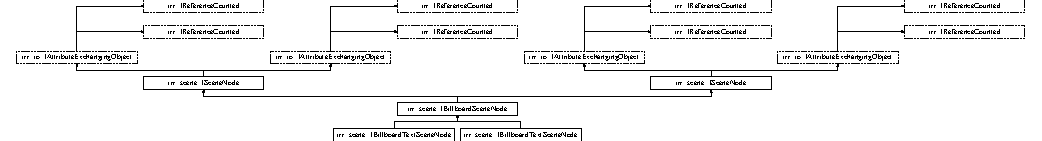
\includegraphics[height=1.900452cm]{classirr_1_1scene_1_1IBillboardSceneNode}
\end{center}
\end{figure}
\subsection*{Public Member Functions}
\begin{DoxyCompactItemize}
\item 
\mbox{\Hypertarget{classirr_1_1scene_1_1IBillboardSceneNode_a32225fb98ab8f9e472272ae9e83c3c88}\label{classirr_1_1scene_1_1IBillboardSceneNode_a32225fb98ab8f9e472272ae9e83c3c88}} 
\hyperlink{classirr_1_1scene_1_1IBillboardSceneNode_a32225fb98ab8f9e472272ae9e83c3c88}{I\+Billboard\+Scene\+Node} (\hyperlink{classirr_1_1scene_1_1ISceneNode}{I\+Scene\+Node} $\ast$parent, \hyperlink{classirr_1_1scene_1_1ISceneManager}{I\+Scene\+Manager} $\ast$mgr, \hyperlink{namespaceirr_ac66849b7a6ed16e30ebede579f9b47c6}{s32} id, const \hyperlink{namespaceirr_1_1core_ae6e2b2a6c552833ebbd5b7463d03586b}{core\+::vector3df} \&position=\hyperlink{namespaceirr_1_1core_ae6e2b2a6c552833ebbd5b7463d03586b}{core\+::vector3df}(0, 0, 0))
\begin{DoxyCompactList}\small\item\em Constructor. \end{DoxyCompactList}\item 
\mbox{\Hypertarget{classirr_1_1scene_1_1IBillboardSceneNode_a911415ac24440bd3ccfcde102583fd60}\label{classirr_1_1scene_1_1IBillboardSceneNode_a911415ac24440bd3ccfcde102583fd60}} 
virtual void \hyperlink{classirr_1_1scene_1_1IBillboardSceneNode_a911415ac24440bd3ccfcde102583fd60}{set\+Size} (const \hyperlink{classirr_1_1core_1_1dimension2d}{core\+::dimension2d}$<$ \hyperlink{namespaceirr_a0277be98d67dc26ff93b1a6a1d086b07}{f32} $>$ \&size)=0
\begin{DoxyCompactList}\small\item\em Sets the size of the billboard, making it rectangular. \end{DoxyCompactList}\item 
virtual void \hyperlink{classirr_1_1scene_1_1IBillboardSceneNode_a9a5d47a00bb0160daab8fa53453a2ba4}{set\+Size} (\hyperlink{namespaceirr_a0277be98d67dc26ff93b1a6a1d086b07}{f32} height, \hyperlink{namespaceirr_a0277be98d67dc26ff93b1a6a1d086b07}{f32} bottom\+Edge\+Width, \hyperlink{namespaceirr_a0277be98d67dc26ff93b1a6a1d086b07}{f32} top\+Edge\+Width)=0
\begin{DoxyCompactList}\small\item\em Sets the size of the billboard with independent widths of the bottom and top edges. \end{DoxyCompactList}\item 
virtual const \hyperlink{classirr_1_1core_1_1dimension2d}{core\+::dimension2d}$<$ \hyperlink{namespaceirr_a0277be98d67dc26ff93b1a6a1d086b07}{f32} $>$ \& \hyperlink{classirr_1_1scene_1_1IBillboardSceneNode_a466cfd24ccb0fb6c2216dbdc7228e3c0}{get\+Size} () const =0
\begin{DoxyCompactList}\small\item\em Returns the size of the billboard. \end{DoxyCompactList}\item 
virtual void \hyperlink{classirr_1_1scene_1_1IBillboardSceneNode_a79a636a0da637eaa9c061138f5ef3f68}{get\+Size} (\hyperlink{namespaceirr_a0277be98d67dc26ff93b1a6a1d086b07}{f32} \&height, \hyperlink{namespaceirr_a0277be98d67dc26ff93b1a6a1d086b07}{f32} \&bottom\+Edge\+Width, \hyperlink{namespaceirr_a0277be98d67dc26ff93b1a6a1d086b07}{f32} \&top\+Edge\+Width) const =0
\begin{DoxyCompactList}\small\item\em Gets the size of the the billboard and handles independent top and bottom edge widths correctly. \end{DoxyCompactList}\item 
virtual void \hyperlink{classirr_1_1scene_1_1IBillboardSceneNode_a82c1038a6dfcd255863baa96aaba4182}{set\+Color} (const \hyperlink{classirr_1_1video_1_1SColor}{video\+::\+S\+Color} \&overall\+Color)=0
\begin{DoxyCompactList}\small\item\em Set the color of all vertices of the billboard. \end{DoxyCompactList}\item 
virtual void \hyperlink{classirr_1_1scene_1_1IBillboardSceneNode_a13efdfa73998706baf10cedcdb48d559}{set\+Color} (const \hyperlink{classirr_1_1video_1_1SColor}{video\+::\+S\+Color} \&top\+Color, const \hyperlink{classirr_1_1video_1_1SColor}{video\+::\+S\+Color} \&bottom\+Color)=0
\begin{DoxyCompactList}\small\item\em Set the color of the top and bottom vertices of the billboard. \end{DoxyCompactList}\item 
virtual void \hyperlink{classirr_1_1scene_1_1IBillboardSceneNode_a0b2729cc4913b0890ae28cf0ef0ab949}{get\+Color} (\hyperlink{classirr_1_1video_1_1SColor}{video\+::\+S\+Color} \&top\+Color, \hyperlink{classirr_1_1video_1_1SColor}{video\+::\+S\+Color} \&bottom\+Color) const =0
\begin{DoxyCompactList}\small\item\em Gets the color of the top and bottom vertices of the billboard. \end{DoxyCompactList}\item 
\mbox{\Hypertarget{classirr_1_1scene_1_1IBillboardSceneNode_a32225fb98ab8f9e472272ae9e83c3c88}\label{classirr_1_1scene_1_1IBillboardSceneNode_a32225fb98ab8f9e472272ae9e83c3c88}} 
\hyperlink{classirr_1_1scene_1_1IBillboardSceneNode_a32225fb98ab8f9e472272ae9e83c3c88}{I\+Billboard\+Scene\+Node} (\hyperlink{classirr_1_1scene_1_1ISceneNode}{I\+Scene\+Node} $\ast$parent, \hyperlink{classirr_1_1scene_1_1ISceneManager}{I\+Scene\+Manager} $\ast$mgr, \hyperlink{namespaceirr_ac66849b7a6ed16e30ebede579f9b47c6}{s32} id, const \hyperlink{namespaceirr_1_1core_ae6e2b2a6c552833ebbd5b7463d03586b}{core\+::vector3df} \&position=\hyperlink{namespaceirr_1_1core_ae6e2b2a6c552833ebbd5b7463d03586b}{core\+::vector3df}(0, 0, 0))
\begin{DoxyCompactList}\small\item\em Constructor. \end{DoxyCompactList}\item 
\mbox{\Hypertarget{classirr_1_1scene_1_1IBillboardSceneNode_a911415ac24440bd3ccfcde102583fd60}\label{classirr_1_1scene_1_1IBillboardSceneNode_a911415ac24440bd3ccfcde102583fd60}} 
virtual void \hyperlink{classirr_1_1scene_1_1IBillboardSceneNode_a911415ac24440bd3ccfcde102583fd60}{set\+Size} (const \hyperlink{classirr_1_1core_1_1dimension2d}{core\+::dimension2d}$<$ \hyperlink{namespaceirr_a0277be98d67dc26ff93b1a6a1d086b07}{f32} $>$ \&size)=0
\begin{DoxyCompactList}\small\item\em Sets the size of the billboard, making it rectangular. \end{DoxyCompactList}\item 
virtual void \hyperlink{classirr_1_1scene_1_1IBillboardSceneNode_a9a5d47a00bb0160daab8fa53453a2ba4}{set\+Size} (\hyperlink{namespaceirr_a0277be98d67dc26ff93b1a6a1d086b07}{f32} height, \hyperlink{namespaceirr_a0277be98d67dc26ff93b1a6a1d086b07}{f32} bottom\+Edge\+Width, \hyperlink{namespaceirr_a0277be98d67dc26ff93b1a6a1d086b07}{f32} top\+Edge\+Width)=0
\begin{DoxyCompactList}\small\item\em Sets the size of the billboard with independent widths of the bottom and top edges. \end{DoxyCompactList}\item 
virtual const \hyperlink{classirr_1_1core_1_1dimension2d}{core\+::dimension2d}$<$ \hyperlink{namespaceirr_a0277be98d67dc26ff93b1a6a1d086b07}{f32} $>$ \& \hyperlink{classirr_1_1scene_1_1IBillboardSceneNode_a466cfd24ccb0fb6c2216dbdc7228e3c0}{get\+Size} () const =0
\begin{DoxyCompactList}\small\item\em Returns the size of the billboard. \end{DoxyCompactList}\item 
virtual void \hyperlink{classirr_1_1scene_1_1IBillboardSceneNode_a79a636a0da637eaa9c061138f5ef3f68}{get\+Size} (\hyperlink{namespaceirr_a0277be98d67dc26ff93b1a6a1d086b07}{f32} \&height, \hyperlink{namespaceirr_a0277be98d67dc26ff93b1a6a1d086b07}{f32} \&bottom\+Edge\+Width, \hyperlink{namespaceirr_a0277be98d67dc26ff93b1a6a1d086b07}{f32} \&top\+Edge\+Width) const =0
\begin{DoxyCompactList}\small\item\em Gets the size of the the billboard and handles independent top and bottom edge widths correctly. \end{DoxyCompactList}\item 
virtual void \hyperlink{classirr_1_1scene_1_1IBillboardSceneNode_a82c1038a6dfcd255863baa96aaba4182}{set\+Color} (const \hyperlink{classirr_1_1video_1_1SColor}{video\+::\+S\+Color} \&overall\+Color)=0
\begin{DoxyCompactList}\small\item\em Set the color of all vertices of the billboard. \end{DoxyCompactList}\item 
virtual void \hyperlink{classirr_1_1scene_1_1IBillboardSceneNode_a13efdfa73998706baf10cedcdb48d559}{set\+Color} (const \hyperlink{classirr_1_1video_1_1SColor}{video\+::\+S\+Color} \&top\+Color, const \hyperlink{classirr_1_1video_1_1SColor}{video\+::\+S\+Color} \&bottom\+Color)=0
\begin{DoxyCompactList}\small\item\em Set the color of the top and bottom vertices of the billboard. \end{DoxyCompactList}\item 
virtual void \hyperlink{classirr_1_1scene_1_1IBillboardSceneNode_a0b2729cc4913b0890ae28cf0ef0ab949}{get\+Color} (\hyperlink{classirr_1_1video_1_1SColor}{video\+::\+S\+Color} \&top\+Color, \hyperlink{classirr_1_1video_1_1SColor}{video\+::\+S\+Color} \&bottom\+Color) const =0
\begin{DoxyCompactList}\small\item\em Gets the color of the top and bottom vertices of the billboard. \end{DoxyCompactList}\end{DoxyCompactItemize}
\subsection*{Additional Inherited Members}


\subsection{Detailed Description}
A billboard scene node. 

A billboard is like a 3d sprite\+: A 2d element, which always looks to the camera. It is usually used for explosions, fire, lensflares, particles and things like that. 

\subsection{Member Function Documentation}
\mbox{\Hypertarget{classirr_1_1scene_1_1IBillboardSceneNode_a0b2729cc4913b0890ae28cf0ef0ab949}\label{classirr_1_1scene_1_1IBillboardSceneNode_a0b2729cc4913b0890ae28cf0ef0ab949}} 
\index{irr\+::scene\+::\+I\+Billboard\+Scene\+Node@{irr\+::scene\+::\+I\+Billboard\+Scene\+Node}!get\+Color@{get\+Color}}
\index{get\+Color@{get\+Color}!irr\+::scene\+::\+I\+Billboard\+Scene\+Node@{irr\+::scene\+::\+I\+Billboard\+Scene\+Node}}
\subsubsection{\texorpdfstring{get\+Color()}{getColor()}\hspace{0.1cm}{\footnotesize\ttfamily [1/2]}}
{\footnotesize\ttfamily virtual void irr\+::scene\+::\+I\+Billboard\+Scene\+Node\+::get\+Color (\begin{DoxyParamCaption}\item[{\hyperlink{classirr_1_1video_1_1SColor}{video\+::\+S\+Color} \&}]{top\+Color,  }\item[{\hyperlink{classirr_1_1video_1_1SColor}{video\+::\+S\+Color} \&}]{bottom\+Color }\end{DoxyParamCaption}) const\hspace{0.3cm}{\ttfamily [pure virtual]}}



Gets the color of the top and bottom vertices of the billboard. 


\begin{DoxyParams}[1]{Parameters}
\mbox{\tt out}  & {\em top\+Color} & Stores the color of the top vertices \\
\hline
\mbox{\tt out}  & {\em bottom\+Color} & Stores the color of the bottom vertices \\
\hline
\end{DoxyParams}


Implemented in \hyperlink{classirr_1_1scene_1_1IBillboardTextSceneNode_ac142a04e455811d5a3efa47ce2499d18}{irr\+::scene\+::\+I\+Billboard\+Text\+Scene\+Node}, and \hyperlink{classirr_1_1scene_1_1IBillboardTextSceneNode_ac142a04e455811d5a3efa47ce2499d18}{irr\+::scene\+::\+I\+Billboard\+Text\+Scene\+Node}.

\mbox{\Hypertarget{classirr_1_1scene_1_1IBillboardSceneNode_a0b2729cc4913b0890ae28cf0ef0ab949}\label{classirr_1_1scene_1_1IBillboardSceneNode_a0b2729cc4913b0890ae28cf0ef0ab949}} 
\index{irr\+::scene\+::\+I\+Billboard\+Scene\+Node@{irr\+::scene\+::\+I\+Billboard\+Scene\+Node}!get\+Color@{get\+Color}}
\index{get\+Color@{get\+Color}!irr\+::scene\+::\+I\+Billboard\+Scene\+Node@{irr\+::scene\+::\+I\+Billboard\+Scene\+Node}}
\subsubsection{\texorpdfstring{get\+Color()}{getColor()}\hspace{0.1cm}{\footnotesize\ttfamily [2/2]}}
{\footnotesize\ttfamily virtual void irr\+::scene\+::\+I\+Billboard\+Scene\+Node\+::get\+Color (\begin{DoxyParamCaption}\item[{\hyperlink{classirr_1_1video_1_1SColor}{video\+::\+S\+Color} \&}]{top\+Color,  }\item[{\hyperlink{classirr_1_1video_1_1SColor}{video\+::\+S\+Color} \&}]{bottom\+Color }\end{DoxyParamCaption}) const\hspace{0.3cm}{\ttfamily [pure virtual]}}



Gets the color of the top and bottom vertices of the billboard. 


\begin{DoxyParams}[1]{Parameters}
\mbox{\tt out}  & {\em top\+Color} & Stores the color of the top vertices \\
\hline
\mbox{\tt out}  & {\em bottom\+Color} & Stores the color of the bottom vertices \\
\hline
\end{DoxyParams}


Implemented in \hyperlink{classirr_1_1scene_1_1IBillboardTextSceneNode_ac142a04e455811d5a3efa47ce2499d18}{irr\+::scene\+::\+I\+Billboard\+Text\+Scene\+Node}, and \hyperlink{classirr_1_1scene_1_1IBillboardTextSceneNode_ac142a04e455811d5a3efa47ce2499d18}{irr\+::scene\+::\+I\+Billboard\+Text\+Scene\+Node}.

\mbox{\Hypertarget{classirr_1_1scene_1_1IBillboardSceneNode_a466cfd24ccb0fb6c2216dbdc7228e3c0}\label{classirr_1_1scene_1_1IBillboardSceneNode_a466cfd24ccb0fb6c2216dbdc7228e3c0}} 
\index{irr\+::scene\+::\+I\+Billboard\+Scene\+Node@{irr\+::scene\+::\+I\+Billboard\+Scene\+Node}!get\+Size@{get\+Size}}
\index{get\+Size@{get\+Size}!irr\+::scene\+::\+I\+Billboard\+Scene\+Node@{irr\+::scene\+::\+I\+Billboard\+Scene\+Node}}
\subsubsection{\texorpdfstring{get\+Size()}{getSize()}\hspace{0.1cm}{\footnotesize\ttfamily [1/4]}}
{\footnotesize\ttfamily virtual const \hyperlink{classirr_1_1core_1_1dimension2d}{core\+::dimension2d}$<$\hyperlink{namespaceirr_a0277be98d67dc26ff93b1a6a1d086b07}{f32}$>$\& irr\+::scene\+::\+I\+Billboard\+Scene\+Node\+::get\+Size (\begin{DoxyParamCaption}{ }\end{DoxyParamCaption}) const\hspace{0.3cm}{\ttfamily [pure virtual]}}



Returns the size of the billboard. 

This will return the width of the bottom edge of the billboard. Use get\+Widths() to retrieve the bottom and top edges independently. \begin{DoxyReturn}{Returns}
Size of the billboard. 
\end{DoxyReturn}


Implemented in \hyperlink{classirr_1_1scene_1_1IBillboardTextSceneNode_aead5178207d887357fb7f3fbddcc51d6}{irr\+::scene\+::\+I\+Billboard\+Text\+Scene\+Node}, and \hyperlink{classirr_1_1scene_1_1IBillboardTextSceneNode_aead5178207d887357fb7f3fbddcc51d6}{irr\+::scene\+::\+I\+Billboard\+Text\+Scene\+Node}.

\mbox{\Hypertarget{classirr_1_1scene_1_1IBillboardSceneNode_a466cfd24ccb0fb6c2216dbdc7228e3c0}\label{classirr_1_1scene_1_1IBillboardSceneNode_a466cfd24ccb0fb6c2216dbdc7228e3c0}} 
\index{irr\+::scene\+::\+I\+Billboard\+Scene\+Node@{irr\+::scene\+::\+I\+Billboard\+Scene\+Node}!get\+Size@{get\+Size}}
\index{get\+Size@{get\+Size}!irr\+::scene\+::\+I\+Billboard\+Scene\+Node@{irr\+::scene\+::\+I\+Billboard\+Scene\+Node}}
\subsubsection{\texorpdfstring{get\+Size()}{getSize()}\hspace{0.1cm}{\footnotesize\ttfamily [2/4]}}
{\footnotesize\ttfamily virtual const \hyperlink{classirr_1_1core_1_1dimension2d}{core\+::dimension2d}$<$\hyperlink{namespaceirr_a0277be98d67dc26ff93b1a6a1d086b07}{f32}$>$\& irr\+::scene\+::\+I\+Billboard\+Scene\+Node\+::get\+Size (\begin{DoxyParamCaption}{ }\end{DoxyParamCaption}) const\hspace{0.3cm}{\ttfamily [pure virtual]}}



Returns the size of the billboard. 

This will return the width of the bottom edge of the billboard. Use get\+Widths() to retrieve the bottom and top edges independently. \begin{DoxyReturn}{Returns}
Size of the billboard. 
\end{DoxyReturn}


Implemented in \hyperlink{classirr_1_1scene_1_1IBillboardTextSceneNode_aead5178207d887357fb7f3fbddcc51d6}{irr\+::scene\+::\+I\+Billboard\+Text\+Scene\+Node}, and \hyperlink{classirr_1_1scene_1_1IBillboardTextSceneNode_aead5178207d887357fb7f3fbddcc51d6}{irr\+::scene\+::\+I\+Billboard\+Text\+Scene\+Node}.

\mbox{\Hypertarget{classirr_1_1scene_1_1IBillboardSceneNode_a79a636a0da637eaa9c061138f5ef3f68}\label{classirr_1_1scene_1_1IBillboardSceneNode_a79a636a0da637eaa9c061138f5ef3f68}} 
\index{irr\+::scene\+::\+I\+Billboard\+Scene\+Node@{irr\+::scene\+::\+I\+Billboard\+Scene\+Node}!get\+Size@{get\+Size}}
\index{get\+Size@{get\+Size}!irr\+::scene\+::\+I\+Billboard\+Scene\+Node@{irr\+::scene\+::\+I\+Billboard\+Scene\+Node}}
\subsubsection{\texorpdfstring{get\+Size()}{getSize()}\hspace{0.1cm}{\footnotesize\ttfamily [3/4]}}
{\footnotesize\ttfamily virtual void irr\+::scene\+::\+I\+Billboard\+Scene\+Node\+::get\+Size (\begin{DoxyParamCaption}\item[{\hyperlink{namespaceirr_a0277be98d67dc26ff93b1a6a1d086b07}{f32} \&}]{height,  }\item[{\hyperlink{namespaceirr_a0277be98d67dc26ff93b1a6a1d086b07}{f32} \&}]{bottom\+Edge\+Width,  }\item[{\hyperlink{namespaceirr_a0277be98d67dc26ff93b1a6a1d086b07}{f32} \&}]{top\+Edge\+Width }\end{DoxyParamCaption}) const\hspace{0.3cm}{\ttfamily [pure virtual]}}



Gets the size of the the billboard and handles independent top and bottom edge widths correctly. 


\begin{DoxyParams}[1]{Parameters}
\mbox{\tt out}  & {\em height} & The height of the billboard. \\
\hline
\mbox{\tt out}  & {\em bottom\+Edge\+Width} & The width of the bottom edge of the billboard. \\
\hline
\mbox{\tt out}  & {\em top\+Edge\+Width} & The width of the top edge of the billboard. \\
\hline
\end{DoxyParams}
\mbox{\Hypertarget{classirr_1_1scene_1_1IBillboardSceneNode_a79a636a0da637eaa9c061138f5ef3f68}\label{classirr_1_1scene_1_1IBillboardSceneNode_a79a636a0da637eaa9c061138f5ef3f68}} 
\index{irr\+::scene\+::\+I\+Billboard\+Scene\+Node@{irr\+::scene\+::\+I\+Billboard\+Scene\+Node}!get\+Size@{get\+Size}}
\index{get\+Size@{get\+Size}!irr\+::scene\+::\+I\+Billboard\+Scene\+Node@{irr\+::scene\+::\+I\+Billboard\+Scene\+Node}}
\subsubsection{\texorpdfstring{get\+Size()}{getSize()}\hspace{0.1cm}{\footnotesize\ttfamily [4/4]}}
{\footnotesize\ttfamily virtual void irr\+::scene\+::\+I\+Billboard\+Scene\+Node\+::get\+Size (\begin{DoxyParamCaption}\item[{\hyperlink{namespaceirr_a0277be98d67dc26ff93b1a6a1d086b07}{f32} \&}]{height,  }\item[{\hyperlink{namespaceirr_a0277be98d67dc26ff93b1a6a1d086b07}{f32} \&}]{bottom\+Edge\+Width,  }\item[{\hyperlink{namespaceirr_a0277be98d67dc26ff93b1a6a1d086b07}{f32} \&}]{top\+Edge\+Width }\end{DoxyParamCaption}) const\hspace{0.3cm}{\ttfamily [pure virtual]}}



Gets the size of the the billboard and handles independent top and bottom edge widths correctly. 


\begin{DoxyParams}[1]{Parameters}
\mbox{\tt out}  & {\em height} & The height of the billboard. \\
\hline
\mbox{\tt out}  & {\em bottom\+Edge\+Width} & The width of the bottom edge of the billboard. \\
\hline
\mbox{\tt out}  & {\em top\+Edge\+Width} & The width of the top edge of the billboard. \\
\hline
\end{DoxyParams}
\mbox{\Hypertarget{classirr_1_1scene_1_1IBillboardSceneNode_a82c1038a6dfcd255863baa96aaba4182}\label{classirr_1_1scene_1_1IBillboardSceneNode_a82c1038a6dfcd255863baa96aaba4182}} 
\index{irr\+::scene\+::\+I\+Billboard\+Scene\+Node@{irr\+::scene\+::\+I\+Billboard\+Scene\+Node}!set\+Color@{set\+Color}}
\index{set\+Color@{set\+Color}!irr\+::scene\+::\+I\+Billboard\+Scene\+Node@{irr\+::scene\+::\+I\+Billboard\+Scene\+Node}}
\subsubsection{\texorpdfstring{set\+Color()}{setColor()}\hspace{0.1cm}{\footnotesize\ttfamily [1/4]}}
{\footnotesize\ttfamily virtual void irr\+::scene\+::\+I\+Billboard\+Scene\+Node\+::set\+Color (\begin{DoxyParamCaption}\item[{const \hyperlink{classirr_1_1video_1_1SColor}{video\+::\+S\+Color} \&}]{overall\+Color }\end{DoxyParamCaption})\hspace{0.3cm}{\ttfamily [pure virtual]}}



Set the color of all vertices of the billboard. 


\begin{DoxyParams}[1]{Parameters}
\mbox{\tt in}  & {\em overall\+Color} & Color to set \\
\hline
\end{DoxyParams}


Implemented in \hyperlink{classirr_1_1scene_1_1IBillboardTextSceneNode_aaa65d10d3a49206728c47b148a64bb4a}{irr\+::scene\+::\+I\+Billboard\+Text\+Scene\+Node}, and \hyperlink{classirr_1_1scene_1_1IBillboardTextSceneNode_aaa65d10d3a49206728c47b148a64bb4a}{irr\+::scene\+::\+I\+Billboard\+Text\+Scene\+Node}.

\mbox{\Hypertarget{classirr_1_1scene_1_1IBillboardSceneNode_a82c1038a6dfcd255863baa96aaba4182}\label{classirr_1_1scene_1_1IBillboardSceneNode_a82c1038a6dfcd255863baa96aaba4182}} 
\index{irr\+::scene\+::\+I\+Billboard\+Scene\+Node@{irr\+::scene\+::\+I\+Billboard\+Scene\+Node}!set\+Color@{set\+Color}}
\index{set\+Color@{set\+Color}!irr\+::scene\+::\+I\+Billboard\+Scene\+Node@{irr\+::scene\+::\+I\+Billboard\+Scene\+Node}}
\subsubsection{\texorpdfstring{set\+Color()}{setColor()}\hspace{0.1cm}{\footnotesize\ttfamily [2/4]}}
{\footnotesize\ttfamily virtual void irr\+::scene\+::\+I\+Billboard\+Scene\+Node\+::set\+Color (\begin{DoxyParamCaption}\item[{const \hyperlink{classirr_1_1video_1_1SColor}{video\+::\+S\+Color} \&}]{overall\+Color }\end{DoxyParamCaption})\hspace{0.3cm}{\ttfamily [pure virtual]}}



Set the color of all vertices of the billboard. 


\begin{DoxyParams}[1]{Parameters}
\mbox{\tt in}  & {\em overall\+Color} & Color to set \\
\hline
\end{DoxyParams}


Implemented in \hyperlink{classirr_1_1scene_1_1IBillboardTextSceneNode_aaa65d10d3a49206728c47b148a64bb4a}{irr\+::scene\+::\+I\+Billboard\+Text\+Scene\+Node}, and \hyperlink{classirr_1_1scene_1_1IBillboardTextSceneNode_aaa65d10d3a49206728c47b148a64bb4a}{irr\+::scene\+::\+I\+Billboard\+Text\+Scene\+Node}.

\mbox{\Hypertarget{classirr_1_1scene_1_1IBillboardSceneNode_a13efdfa73998706baf10cedcdb48d559}\label{classirr_1_1scene_1_1IBillboardSceneNode_a13efdfa73998706baf10cedcdb48d559}} 
\index{irr\+::scene\+::\+I\+Billboard\+Scene\+Node@{irr\+::scene\+::\+I\+Billboard\+Scene\+Node}!set\+Color@{set\+Color}}
\index{set\+Color@{set\+Color}!irr\+::scene\+::\+I\+Billboard\+Scene\+Node@{irr\+::scene\+::\+I\+Billboard\+Scene\+Node}}
\subsubsection{\texorpdfstring{set\+Color()}{setColor()}\hspace{0.1cm}{\footnotesize\ttfamily [3/4]}}
{\footnotesize\ttfamily virtual void irr\+::scene\+::\+I\+Billboard\+Scene\+Node\+::set\+Color (\begin{DoxyParamCaption}\item[{const \hyperlink{classirr_1_1video_1_1SColor}{video\+::\+S\+Color} \&}]{top\+Color,  }\item[{const \hyperlink{classirr_1_1video_1_1SColor}{video\+::\+S\+Color} \&}]{bottom\+Color }\end{DoxyParamCaption})\hspace{0.3cm}{\ttfamily [pure virtual]}}



Set the color of the top and bottom vertices of the billboard. 


\begin{DoxyParams}[1]{Parameters}
\mbox{\tt in}  & {\em top\+Color} & Color to set the top vertices \\
\hline
\mbox{\tt in}  & {\em bottom\+Color} & Color to set the bottom vertices \\
\hline
\end{DoxyParams}


Implemented in \hyperlink{classirr_1_1scene_1_1IBillboardTextSceneNode_ab3faa7c4238acd6bc3a2330cb5650da5}{irr\+::scene\+::\+I\+Billboard\+Text\+Scene\+Node}, and \hyperlink{classirr_1_1scene_1_1IBillboardTextSceneNode_ab3faa7c4238acd6bc3a2330cb5650da5}{irr\+::scene\+::\+I\+Billboard\+Text\+Scene\+Node}.

\mbox{\Hypertarget{classirr_1_1scene_1_1IBillboardSceneNode_a13efdfa73998706baf10cedcdb48d559}\label{classirr_1_1scene_1_1IBillboardSceneNode_a13efdfa73998706baf10cedcdb48d559}} 
\index{irr\+::scene\+::\+I\+Billboard\+Scene\+Node@{irr\+::scene\+::\+I\+Billboard\+Scene\+Node}!set\+Color@{set\+Color}}
\index{set\+Color@{set\+Color}!irr\+::scene\+::\+I\+Billboard\+Scene\+Node@{irr\+::scene\+::\+I\+Billboard\+Scene\+Node}}
\subsubsection{\texorpdfstring{set\+Color()}{setColor()}\hspace{0.1cm}{\footnotesize\ttfamily [4/4]}}
{\footnotesize\ttfamily virtual void irr\+::scene\+::\+I\+Billboard\+Scene\+Node\+::set\+Color (\begin{DoxyParamCaption}\item[{const \hyperlink{classirr_1_1video_1_1SColor}{video\+::\+S\+Color} \&}]{top\+Color,  }\item[{const \hyperlink{classirr_1_1video_1_1SColor}{video\+::\+S\+Color} \&}]{bottom\+Color }\end{DoxyParamCaption})\hspace{0.3cm}{\ttfamily [pure virtual]}}



Set the color of the top and bottom vertices of the billboard. 


\begin{DoxyParams}[1]{Parameters}
\mbox{\tt in}  & {\em top\+Color} & Color to set the top vertices \\
\hline
\mbox{\tt in}  & {\em bottom\+Color} & Color to set the bottom vertices \\
\hline
\end{DoxyParams}


Implemented in \hyperlink{classirr_1_1scene_1_1IBillboardTextSceneNode_ab3faa7c4238acd6bc3a2330cb5650da5}{irr\+::scene\+::\+I\+Billboard\+Text\+Scene\+Node}, and \hyperlink{classirr_1_1scene_1_1IBillboardTextSceneNode_ab3faa7c4238acd6bc3a2330cb5650da5}{irr\+::scene\+::\+I\+Billboard\+Text\+Scene\+Node}.

\mbox{\Hypertarget{classirr_1_1scene_1_1IBillboardSceneNode_a9a5d47a00bb0160daab8fa53453a2ba4}\label{classirr_1_1scene_1_1IBillboardSceneNode_a9a5d47a00bb0160daab8fa53453a2ba4}} 
\index{irr\+::scene\+::\+I\+Billboard\+Scene\+Node@{irr\+::scene\+::\+I\+Billboard\+Scene\+Node}!set\+Size@{set\+Size}}
\index{set\+Size@{set\+Size}!irr\+::scene\+::\+I\+Billboard\+Scene\+Node@{irr\+::scene\+::\+I\+Billboard\+Scene\+Node}}
\subsubsection{\texorpdfstring{set\+Size()}{setSize()}\hspace{0.1cm}{\footnotesize\ttfamily [1/2]}}
{\footnotesize\ttfamily virtual void irr\+::scene\+::\+I\+Billboard\+Scene\+Node\+::set\+Size (\begin{DoxyParamCaption}\item[{\hyperlink{namespaceirr_a0277be98d67dc26ff93b1a6a1d086b07}{f32}}]{height,  }\item[{\hyperlink{namespaceirr_a0277be98d67dc26ff93b1a6a1d086b07}{f32}}]{bottom\+Edge\+Width,  }\item[{\hyperlink{namespaceirr_a0277be98d67dc26ff93b1a6a1d086b07}{f32}}]{top\+Edge\+Width }\end{DoxyParamCaption})\hspace{0.3cm}{\ttfamily [pure virtual]}}



Sets the size of the billboard with independent widths of the bottom and top edges. 


\begin{DoxyParams}[1]{Parameters}
\mbox{\tt in}  & {\em height} & The height of the billboard. \\
\hline
\mbox{\tt in}  & {\em bottom\+Edge\+Width} & The width of the bottom edge of the billboard. \\
\hline
\mbox{\tt in}  & {\em top\+Edge\+Width} & The width of the top edge of the billboard. \\
\hline
\end{DoxyParams}
\mbox{\Hypertarget{classirr_1_1scene_1_1IBillboardSceneNode_a9a5d47a00bb0160daab8fa53453a2ba4}\label{classirr_1_1scene_1_1IBillboardSceneNode_a9a5d47a00bb0160daab8fa53453a2ba4}} 
\index{irr\+::scene\+::\+I\+Billboard\+Scene\+Node@{irr\+::scene\+::\+I\+Billboard\+Scene\+Node}!set\+Size@{set\+Size}}
\index{set\+Size@{set\+Size}!irr\+::scene\+::\+I\+Billboard\+Scene\+Node@{irr\+::scene\+::\+I\+Billboard\+Scene\+Node}}
\subsubsection{\texorpdfstring{set\+Size()}{setSize()}\hspace{0.1cm}{\footnotesize\ttfamily [2/2]}}
{\footnotesize\ttfamily virtual void irr\+::scene\+::\+I\+Billboard\+Scene\+Node\+::set\+Size (\begin{DoxyParamCaption}\item[{\hyperlink{namespaceirr_a0277be98d67dc26ff93b1a6a1d086b07}{f32}}]{height,  }\item[{\hyperlink{namespaceirr_a0277be98d67dc26ff93b1a6a1d086b07}{f32}}]{bottom\+Edge\+Width,  }\item[{\hyperlink{namespaceirr_a0277be98d67dc26ff93b1a6a1d086b07}{f32}}]{top\+Edge\+Width }\end{DoxyParamCaption})\hspace{0.3cm}{\ttfamily [pure virtual]}}



Sets the size of the billboard with independent widths of the bottom and top edges. 


\begin{DoxyParams}[1]{Parameters}
\mbox{\tt in}  & {\em height} & The height of the billboard. \\
\hline
\mbox{\tt in}  & {\em bottom\+Edge\+Width} & The width of the bottom edge of the billboard. \\
\hline
\mbox{\tt in}  & {\em top\+Edge\+Width} & The width of the top edge of the billboard. \\
\hline
\end{DoxyParams}


The documentation for this class was generated from the following file\+:\begin{DoxyCompactItemize}
\item 
indie\+\_\+share/controller/include/I\+Billboard\+Scene\+Node.\+h\end{DoxyCompactItemize}

\hypertarget{classirr_1_1scene_1_1IBillboardTextSceneNode}{}\section{irr\+:\+:scene\+:\+:I\+Billboard\+Text\+Scene\+Node Class Reference}
\label{classirr_1_1scene_1_1IBillboardTextSceneNode}\index{irr\+::scene\+::\+I\+Billboard\+Text\+Scene\+Node@{irr\+::scene\+::\+I\+Billboard\+Text\+Scene\+Node}}


A billboard text scene node.  




{\ttfamily \#include $<$I\+Billboard\+Text\+Scene\+Node.\+h$>$}

Inheritance diagram for irr\+:\+:scene\+:\+:I\+Billboard\+Text\+Scene\+Node\+:\begin{figure}[H]
\begin{center}
\leavevmode
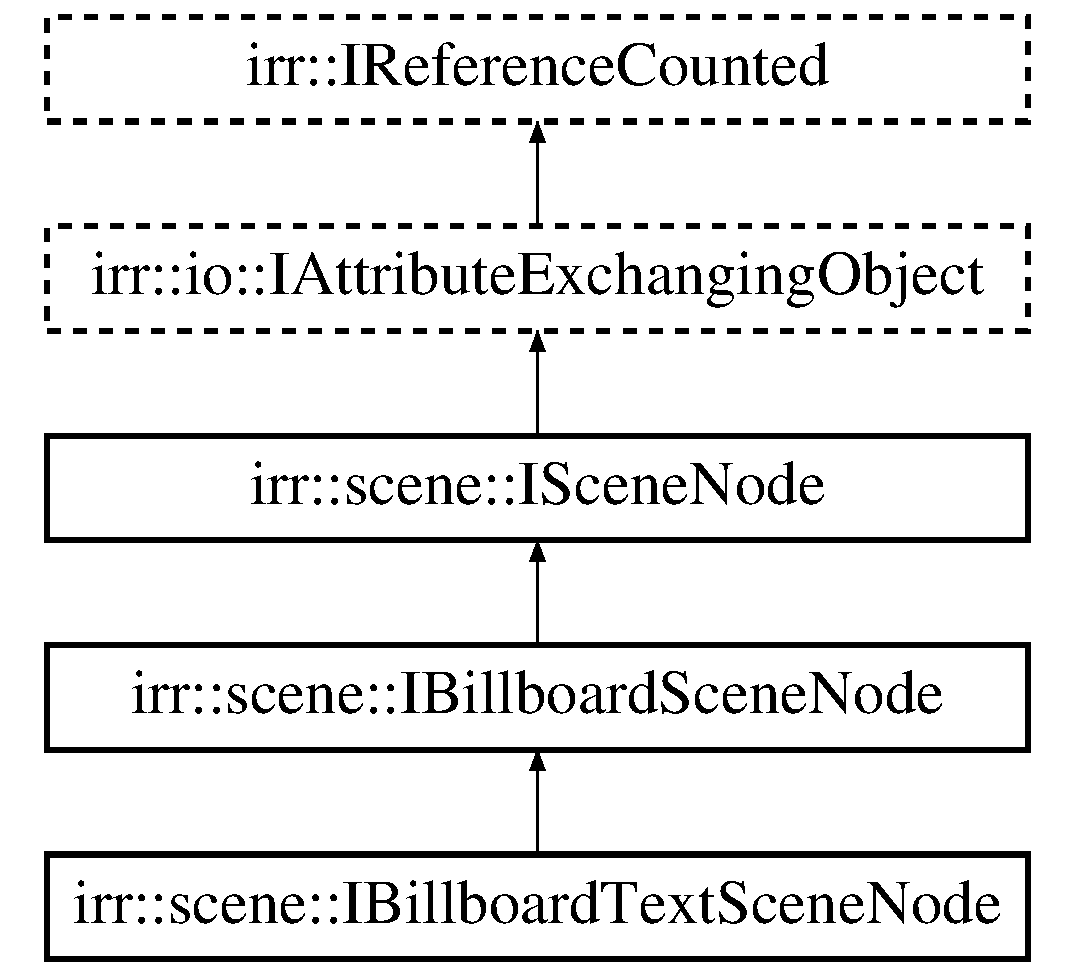
\includegraphics[height=5.000000cm]{classirr_1_1scene_1_1IBillboardTextSceneNode}
\end{center}
\end{figure}
\subsection*{Public Member Functions}
\begin{DoxyCompactItemize}
\item 
\mbox{\Hypertarget{classirr_1_1scene_1_1IBillboardTextSceneNode_a758a6a0ec2f76ee7623f19a55f1e7c4b}\label{classirr_1_1scene_1_1IBillboardTextSceneNode_a758a6a0ec2f76ee7623f19a55f1e7c4b}} 
\hyperlink{classirr_1_1scene_1_1IBillboardTextSceneNode_a758a6a0ec2f76ee7623f19a55f1e7c4b}{I\+Billboard\+Text\+Scene\+Node} (\hyperlink{classirr_1_1scene_1_1ISceneNode}{I\+Scene\+Node} $\ast$parent, \hyperlink{classirr_1_1scene_1_1ISceneManager}{I\+Scene\+Manager} $\ast$mgr, \hyperlink{namespaceirr_ac66849b7a6ed16e30ebede579f9b47c6}{s32} id, const \hyperlink{namespaceirr_1_1core_a06f169d08b5c429f5575acb7edbad811}{core\+::vector3df} \&position=\hyperlink{namespaceirr_1_1core_a06f169d08b5c429f5575acb7edbad811}{core\+::vector3df}(0, 0, 0))
\begin{DoxyCompactList}\small\item\em Constructor. \end{DoxyCompactList}\item 
\mbox{\Hypertarget{classirr_1_1scene_1_1IBillboardTextSceneNode_a506ca9b0ef160993fc44f4e0b5b97b63}\label{classirr_1_1scene_1_1IBillboardTextSceneNode_a506ca9b0ef160993fc44f4e0b5b97b63}} 
virtual void \hyperlink{classirr_1_1scene_1_1IBillboardTextSceneNode_a506ca9b0ef160993fc44f4e0b5b97b63}{set\+Size} (const \hyperlink{classirr_1_1core_1_1dimension2d}{core\+::dimension2d}$<$ \hyperlink{namespaceirr_a0277be98d67dc26ff93b1a6a1d086b07}{f32} $>$ \&size)=0
\begin{DoxyCompactList}\small\item\em Sets the size of the billboard. \end{DoxyCompactList}\item 
\mbox{\Hypertarget{classirr_1_1scene_1_1IBillboardTextSceneNode_aead5178207d887357fb7f3fbddcc51d6}\label{classirr_1_1scene_1_1IBillboardTextSceneNode_aead5178207d887357fb7f3fbddcc51d6}} 
virtual const \hyperlink{classirr_1_1core_1_1dimension2d}{core\+::dimension2d}$<$ \hyperlink{namespaceirr_a0277be98d67dc26ff93b1a6a1d086b07}{f32} $>$ \& \hyperlink{classirr_1_1scene_1_1IBillboardTextSceneNode_aead5178207d887357fb7f3fbddcc51d6}{get\+Size} () const =0
\begin{DoxyCompactList}\small\item\em Returns the size of the billboard. \end{DoxyCompactList}\item 
virtual void \hyperlink{classirr_1_1scene_1_1IBillboardTextSceneNode_aaa65d10d3a49206728c47b148a64bb4a}{set\+Color} (const \hyperlink{classirr_1_1video_1_1SColor}{video\+::\+S\+Color} \&overall\+Color)=0
\begin{DoxyCompactList}\small\item\em Set the color of all vertices of the billboard. \end{DoxyCompactList}\item 
virtual void \hyperlink{classirr_1_1scene_1_1IBillboardTextSceneNode_ab3faa7c4238acd6bc3a2330cb5650da5}{set\+Color} (const \hyperlink{classirr_1_1video_1_1SColor}{video\+::\+S\+Color} \&top\+Color, const \hyperlink{classirr_1_1video_1_1SColor}{video\+::\+S\+Color} \&bottom\+Color)=0
\begin{DoxyCompactList}\small\item\em Set the color of the top and bottom vertices of the billboard. \end{DoxyCompactList}\item 
virtual void \hyperlink{classirr_1_1scene_1_1IBillboardTextSceneNode_ac142a04e455811d5a3efa47ce2499d18}{get\+Color} (\hyperlink{classirr_1_1video_1_1SColor}{video\+::\+S\+Color} \&top\+Color, \hyperlink{classirr_1_1video_1_1SColor}{video\+::\+S\+Color} \&bottom\+Color) const =0
\begin{DoxyCompactList}\small\item\em Gets the color of the top and bottom vertices of the billboard. \end{DoxyCompactList}\item 
\mbox{\Hypertarget{classirr_1_1scene_1_1IBillboardTextSceneNode_ab404347cd57f64bb559cca8bed8caa53}\label{classirr_1_1scene_1_1IBillboardTextSceneNode_ab404347cd57f64bb559cca8bed8caa53}} 
virtual void \hyperlink{classirr_1_1scene_1_1IBillboardTextSceneNode_ab404347cd57f64bb559cca8bed8caa53}{set\+Text} (const wchar\+\_\+t $\ast$text)=0
\begin{DoxyCompactList}\small\item\em sets the text string \end{DoxyCompactList}\item 
\mbox{\Hypertarget{classirr_1_1scene_1_1IBillboardTextSceneNode_a05e1db5ef9af3ff0ab2750ba584583ef}\label{classirr_1_1scene_1_1IBillboardTextSceneNode_a05e1db5ef9af3ff0ab2750ba584583ef}} 
virtual void \hyperlink{classirr_1_1scene_1_1IBillboardTextSceneNode_a05e1db5ef9af3ff0ab2750ba584583ef}{set\+Text\+Color} (\hyperlink{classirr_1_1video_1_1SColor}{video\+::\+S\+Color} color)=0
\begin{DoxyCompactList}\small\item\em sets the color of the text \end{DoxyCompactList}\end{DoxyCompactItemize}
\subsection*{Additional Inherited Members}


\subsection{Detailed Description}
A billboard text scene node. 

Acts like a billboard which displays the currently set text. Due to the exclusion of R\+T\+TI in Irrlicht we have to avoid multiple inheritance. Hence, changes to the \hyperlink{classirr_1_1scene_1_1ITextSceneNode}{I\+Text\+Scene\+Node} interface have to be copied here manually. 

\subsection{Member Function Documentation}
\mbox{\Hypertarget{classirr_1_1scene_1_1IBillboardTextSceneNode_ac142a04e455811d5a3efa47ce2499d18}\label{classirr_1_1scene_1_1IBillboardTextSceneNode_ac142a04e455811d5a3efa47ce2499d18}} 
\index{irr\+::scene\+::\+I\+Billboard\+Text\+Scene\+Node@{irr\+::scene\+::\+I\+Billboard\+Text\+Scene\+Node}!get\+Color@{get\+Color}}
\index{get\+Color@{get\+Color}!irr\+::scene\+::\+I\+Billboard\+Text\+Scene\+Node@{irr\+::scene\+::\+I\+Billboard\+Text\+Scene\+Node}}
\subsubsection{\texorpdfstring{get\+Color()}{getColor()}}
{\footnotesize\ttfamily virtual void irr\+::scene\+::\+I\+Billboard\+Text\+Scene\+Node\+::get\+Color (\begin{DoxyParamCaption}\item[{\hyperlink{classirr_1_1video_1_1SColor}{video\+::\+S\+Color} \&}]{top\+Color,  }\item[{\hyperlink{classirr_1_1video_1_1SColor}{video\+::\+S\+Color} \&}]{bottom\+Color }\end{DoxyParamCaption}) const\hspace{0.3cm}{\ttfamily [pure virtual]}}



Gets the color of the top and bottom vertices of the billboard. 


\begin{DoxyParams}{Parameters}
{\em top\+Color} & stores the color of the top vertices \\
\hline
{\em bottom\+Color} & stores the color of the bottom vertices \\
\hline
\end{DoxyParams}


Implements \hyperlink{classirr_1_1scene_1_1IBillboardSceneNode_a0b2729cc4913b0890ae28cf0ef0ab949}{irr\+::scene\+::\+I\+Billboard\+Scene\+Node}.

\mbox{\Hypertarget{classirr_1_1scene_1_1IBillboardTextSceneNode_aaa65d10d3a49206728c47b148a64bb4a}\label{classirr_1_1scene_1_1IBillboardTextSceneNode_aaa65d10d3a49206728c47b148a64bb4a}} 
\index{irr\+::scene\+::\+I\+Billboard\+Text\+Scene\+Node@{irr\+::scene\+::\+I\+Billboard\+Text\+Scene\+Node}!set\+Color@{set\+Color}}
\index{set\+Color@{set\+Color}!irr\+::scene\+::\+I\+Billboard\+Text\+Scene\+Node@{irr\+::scene\+::\+I\+Billboard\+Text\+Scene\+Node}}
\subsubsection{\texorpdfstring{set\+Color()}{setColor()}\hspace{0.1cm}{\footnotesize\ttfamily [1/2]}}
{\footnotesize\ttfamily virtual void irr\+::scene\+::\+I\+Billboard\+Text\+Scene\+Node\+::set\+Color (\begin{DoxyParamCaption}\item[{const \hyperlink{classirr_1_1video_1_1SColor}{video\+::\+S\+Color} \&}]{overall\+Color }\end{DoxyParamCaption})\hspace{0.3cm}{\ttfamily [pure virtual]}}



Set the color of all vertices of the billboard. 


\begin{DoxyParams}{Parameters}
{\em overall\+Color} & the color to set \\
\hline
\end{DoxyParams}


Implements \hyperlink{classirr_1_1scene_1_1IBillboardSceneNode_a82c1038a6dfcd255863baa96aaba4182}{irr\+::scene\+::\+I\+Billboard\+Scene\+Node}.

\mbox{\Hypertarget{classirr_1_1scene_1_1IBillboardTextSceneNode_ab3faa7c4238acd6bc3a2330cb5650da5}\label{classirr_1_1scene_1_1IBillboardTextSceneNode_ab3faa7c4238acd6bc3a2330cb5650da5}} 
\index{irr\+::scene\+::\+I\+Billboard\+Text\+Scene\+Node@{irr\+::scene\+::\+I\+Billboard\+Text\+Scene\+Node}!set\+Color@{set\+Color}}
\index{set\+Color@{set\+Color}!irr\+::scene\+::\+I\+Billboard\+Text\+Scene\+Node@{irr\+::scene\+::\+I\+Billboard\+Text\+Scene\+Node}}
\subsubsection{\texorpdfstring{set\+Color()}{setColor()}\hspace{0.1cm}{\footnotesize\ttfamily [2/2]}}
{\footnotesize\ttfamily virtual void irr\+::scene\+::\+I\+Billboard\+Text\+Scene\+Node\+::set\+Color (\begin{DoxyParamCaption}\item[{const \hyperlink{classirr_1_1video_1_1SColor}{video\+::\+S\+Color} \&}]{top\+Color,  }\item[{const \hyperlink{classirr_1_1video_1_1SColor}{video\+::\+S\+Color} \&}]{bottom\+Color }\end{DoxyParamCaption})\hspace{0.3cm}{\ttfamily [pure virtual]}}



Set the color of the top and bottom vertices of the billboard. 


\begin{DoxyParams}{Parameters}
{\em top\+Color} & the color to set the top vertices \\
\hline
{\em bottom\+Color} & the color to set the bottom vertices \\
\hline
\end{DoxyParams}


Implements \hyperlink{classirr_1_1scene_1_1IBillboardSceneNode_a13efdfa73998706baf10cedcdb48d559}{irr\+::scene\+::\+I\+Billboard\+Scene\+Node}.



The documentation for this class was generated from the following file\+:\begin{DoxyCompactItemize}
\item 
indie\+\_\+share/controller/include/I\+Billboard\+Text\+Scene\+Node.\+h\end{DoxyCompactItemize}

\hypertarget{classirr_1_1scene_1_1IBoneSceneNode}{}\section{irr\+:\+:scene\+:\+:I\+Bone\+Scene\+Node Class Reference}
\label{classirr_1_1scene_1_1IBoneSceneNode}\index{irr\+::scene\+::\+I\+Bone\+Scene\+Node@{irr\+::scene\+::\+I\+Bone\+Scene\+Node}}


Interface for bones used for skeletal animation.  




{\ttfamily \#include $<$I\+Bone\+Scene\+Node.\+h$>$}

Inheritance diagram for irr\+:\+:scene\+:\+:I\+Bone\+Scene\+Node\+:\begin{figure}[H]
\begin{center}
\leavevmode
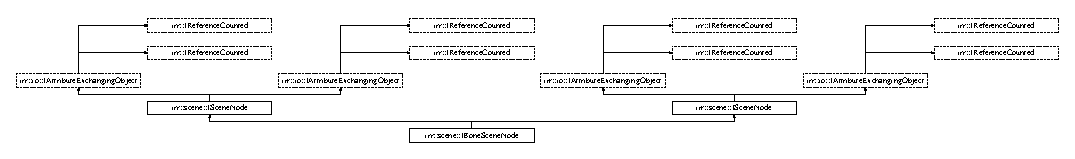
\includegraphics[height=1.682692cm]{classirr_1_1scene_1_1IBoneSceneNode}
\end{center}
\end{figure}
\subsection*{Public Member Functions}
\begin{DoxyCompactItemize}
\item 
virtual \+\_\+\+I\+R\+R\+\_\+\+D\+E\+P\+R\+E\+C\+A\+T\+E\+D\+\_\+ const \hyperlink{namespaceirr_a9395eaea339bcb546b319e9c96bf7410}{c8} $\ast$ \hyperlink{classirr_1_1scene_1_1IBoneSceneNode_a1c40bee44b89fe81178782e999cbe3a8}{get\+Bone\+Name} () const
\begin{DoxyCompactList}\small\item\em Get the name of the bone. \end{DoxyCompactList}\item 
\mbox{\Hypertarget{classirr_1_1scene_1_1IBoneSceneNode_ac372b2c84a3427df1fdc78deae7d00ea}\label{classirr_1_1scene_1_1IBoneSceneNode_ac372b2c84a3427df1fdc78deae7d00ea}} 
virtual \hyperlink{namespaceirr_a0416a53257075833e7002efd0a18e804}{u32} \hyperlink{classirr_1_1scene_1_1IBoneSceneNode_ac372b2c84a3427df1fdc78deae7d00ea}{get\+Bone\+Index} () const =0
\begin{DoxyCompactList}\small\item\em Get the index of the bone. \end{DoxyCompactList}\item 
virtual bool \hyperlink{classirr_1_1scene_1_1IBoneSceneNode_a424a467f045e809bcad2aa239edb9994}{set\+Animation\+Mode} (\hyperlink{namespaceirr_1_1scene_a318162c0a3aad1cf228ed7daddd44801}{E\+\_\+\+B\+O\+N\+E\+\_\+\+A\+N\+I\+M\+A\+T\+I\+O\+N\+\_\+\+M\+O\+DE} mode)=0
\begin{DoxyCompactList}\small\item\em Sets the animation mode of the bone. \end{DoxyCompactList}\item 
\mbox{\Hypertarget{classirr_1_1scene_1_1IBoneSceneNode_a332e040471057cf6a1a0ae8dfa2c0f5f}\label{classirr_1_1scene_1_1IBoneSceneNode_a332e040471057cf6a1a0ae8dfa2c0f5f}} 
virtual \hyperlink{namespaceirr_1_1scene_a318162c0a3aad1cf228ed7daddd44801}{E\+\_\+\+B\+O\+N\+E\+\_\+\+A\+N\+I\+M\+A\+T\+I\+O\+N\+\_\+\+M\+O\+DE} \hyperlink{classirr_1_1scene_1_1IBoneSceneNode_a332e040471057cf6a1a0ae8dfa2c0f5f}{get\+Animation\+Mode} () const =0
\begin{DoxyCompactList}\small\item\em Gets the current animation mode of the bone. \end{DoxyCompactList}\item 
\mbox{\Hypertarget{classirr_1_1scene_1_1IBoneSceneNode_ac5d0a610b0a24a7501f29ad000d28b3b}\label{classirr_1_1scene_1_1IBoneSceneNode_ac5d0a610b0a24a7501f29ad000d28b3b}} 
virtual const \hyperlink{classirr_1_1core_1_1aabbox3d}{core\+::aabbox3d}$<$ \hyperlink{namespaceirr_a0277be98d67dc26ff93b1a6a1d086b07}{f32} $>$ \& \hyperlink{classirr_1_1scene_1_1IBoneSceneNode_ac5d0a610b0a24a7501f29ad000d28b3b}{get\+Bounding\+Box} () const =0
\begin{DoxyCompactList}\small\item\em Get the axis aligned bounding box of this node. \end{DoxyCompactList}\item 
virtual void \hyperlink{classirr_1_1scene_1_1IBoneSceneNode_a7e21d0722e5b105e4d2a956bff110a7f}{On\+Animate} (\hyperlink{namespaceirr_a0416a53257075833e7002efd0a18e804}{u32} time\+Ms)=0
\begin{DoxyCompactList}\small\item\em Returns the relative transformation of the scene node. \end{DoxyCompactList}\item 
virtual void \hyperlink{classirr_1_1scene_1_1IBoneSceneNode_ac942248f09d2db69804ea47476e3829e}{render} ()
\begin{DoxyCompactList}\small\item\em The render method. \end{DoxyCompactList}\item 
\mbox{\Hypertarget{classirr_1_1scene_1_1IBoneSceneNode_a071c9edb957b67f18c8285fe7670f9d4}\label{classirr_1_1scene_1_1IBoneSceneNode_a071c9edb957b67f18c8285fe7670f9d4}} 
virtual void \hyperlink{classirr_1_1scene_1_1IBoneSceneNode_a071c9edb957b67f18c8285fe7670f9d4}{set\+Skinning\+Space} (\hyperlink{namespaceirr_1_1scene_a47bfc785c34c953f926c920cd13ba1fb}{E\+\_\+\+B\+O\+N\+E\+\_\+\+S\+K\+I\+N\+N\+I\+N\+G\+\_\+\+S\+P\+A\+CE} space)=0
\begin{DoxyCompactList}\small\item\em How the relative transformation of the bone is used. \end{DoxyCompactList}\item 
\mbox{\Hypertarget{classirr_1_1scene_1_1IBoneSceneNode_aa41c118c8fa8741c6945787c50c42df7}\label{classirr_1_1scene_1_1IBoneSceneNode_aa41c118c8fa8741c6945787c50c42df7}} 
virtual \hyperlink{namespaceirr_1_1scene_a47bfc785c34c953f926c920cd13ba1fb}{E\+\_\+\+B\+O\+N\+E\+\_\+\+S\+K\+I\+N\+N\+I\+N\+G\+\_\+\+S\+P\+A\+CE} \hyperlink{classirr_1_1scene_1_1IBoneSceneNode_aa41c118c8fa8741c6945787c50c42df7}{get\+Skinning\+Space} () const =0
\begin{DoxyCompactList}\small\item\em How the relative transformation of the bone is used. \end{DoxyCompactList}\item 
\mbox{\Hypertarget{classirr_1_1scene_1_1IBoneSceneNode_ab405c67e87dd79b7c1b9c16a6b8c3182}\label{classirr_1_1scene_1_1IBoneSceneNode_ab405c67e87dd79b7c1b9c16a6b8c3182}} 
virtual void \hyperlink{classirr_1_1scene_1_1IBoneSceneNode_ab405c67e87dd79b7c1b9c16a6b8c3182}{update\+Absolute\+Position\+Of\+All\+Children} ()=0
\begin{DoxyCompactList}\small\item\em Updates the absolute position based on the relative and the parents position. \end{DoxyCompactList}\item 
virtual \+\_\+\+I\+R\+R\+\_\+\+D\+E\+P\+R\+E\+C\+A\+T\+E\+D\+\_\+ const \hyperlink{namespaceirr_a9395eaea339bcb546b319e9c96bf7410}{c8} $\ast$ \hyperlink{classirr_1_1scene_1_1IBoneSceneNode_a1c40bee44b89fe81178782e999cbe3a8}{get\+Bone\+Name} () const
\begin{DoxyCompactList}\small\item\em Get the name of the bone. \end{DoxyCompactList}\item 
\mbox{\Hypertarget{classirr_1_1scene_1_1IBoneSceneNode_ac372b2c84a3427df1fdc78deae7d00ea}\label{classirr_1_1scene_1_1IBoneSceneNode_ac372b2c84a3427df1fdc78deae7d00ea}} 
virtual \hyperlink{namespaceirr_a0416a53257075833e7002efd0a18e804}{u32} \hyperlink{classirr_1_1scene_1_1IBoneSceneNode_ac372b2c84a3427df1fdc78deae7d00ea}{get\+Bone\+Index} () const =0
\begin{DoxyCompactList}\small\item\em Get the index of the bone. \end{DoxyCompactList}\item 
virtual bool \hyperlink{classirr_1_1scene_1_1IBoneSceneNode_a424a467f045e809bcad2aa239edb9994}{set\+Animation\+Mode} (\hyperlink{namespaceirr_1_1scene_a318162c0a3aad1cf228ed7daddd44801}{E\+\_\+\+B\+O\+N\+E\+\_\+\+A\+N\+I\+M\+A\+T\+I\+O\+N\+\_\+\+M\+O\+DE} mode)=0
\begin{DoxyCompactList}\small\item\em Sets the animation mode of the bone. \end{DoxyCompactList}\item 
\mbox{\Hypertarget{classirr_1_1scene_1_1IBoneSceneNode_a332e040471057cf6a1a0ae8dfa2c0f5f}\label{classirr_1_1scene_1_1IBoneSceneNode_a332e040471057cf6a1a0ae8dfa2c0f5f}} 
virtual \hyperlink{namespaceirr_1_1scene_a318162c0a3aad1cf228ed7daddd44801}{E\+\_\+\+B\+O\+N\+E\+\_\+\+A\+N\+I\+M\+A\+T\+I\+O\+N\+\_\+\+M\+O\+DE} \hyperlink{classirr_1_1scene_1_1IBoneSceneNode_a332e040471057cf6a1a0ae8dfa2c0f5f}{get\+Animation\+Mode} () const =0
\begin{DoxyCompactList}\small\item\em Gets the current animation mode of the bone. \end{DoxyCompactList}\item 
\mbox{\Hypertarget{classirr_1_1scene_1_1IBoneSceneNode_ac5d0a610b0a24a7501f29ad000d28b3b}\label{classirr_1_1scene_1_1IBoneSceneNode_ac5d0a610b0a24a7501f29ad000d28b3b}} 
virtual const \hyperlink{classirr_1_1core_1_1aabbox3d}{core\+::aabbox3d}$<$ \hyperlink{namespaceirr_a0277be98d67dc26ff93b1a6a1d086b07}{f32} $>$ \& \hyperlink{classirr_1_1scene_1_1IBoneSceneNode_ac5d0a610b0a24a7501f29ad000d28b3b}{get\+Bounding\+Box} () const =0
\begin{DoxyCompactList}\small\item\em Get the axis aligned bounding box of this node. \end{DoxyCompactList}\item 
virtual void \hyperlink{classirr_1_1scene_1_1IBoneSceneNode_a7e21d0722e5b105e4d2a956bff110a7f}{On\+Animate} (\hyperlink{namespaceirr_a0416a53257075833e7002efd0a18e804}{u32} time\+Ms)=0
\begin{DoxyCompactList}\small\item\em Returns the relative transformation of the scene node. \end{DoxyCompactList}\item 
virtual void \hyperlink{classirr_1_1scene_1_1IBoneSceneNode_ac942248f09d2db69804ea47476e3829e}{render} ()
\begin{DoxyCompactList}\small\item\em The render method. \end{DoxyCompactList}\item 
\mbox{\Hypertarget{classirr_1_1scene_1_1IBoneSceneNode_a071c9edb957b67f18c8285fe7670f9d4}\label{classirr_1_1scene_1_1IBoneSceneNode_a071c9edb957b67f18c8285fe7670f9d4}} 
virtual void \hyperlink{classirr_1_1scene_1_1IBoneSceneNode_a071c9edb957b67f18c8285fe7670f9d4}{set\+Skinning\+Space} (\hyperlink{namespaceirr_1_1scene_a47bfc785c34c953f926c920cd13ba1fb}{E\+\_\+\+B\+O\+N\+E\+\_\+\+S\+K\+I\+N\+N\+I\+N\+G\+\_\+\+S\+P\+A\+CE} space)=0
\begin{DoxyCompactList}\small\item\em How the relative transformation of the bone is used. \end{DoxyCompactList}\item 
\mbox{\Hypertarget{classirr_1_1scene_1_1IBoneSceneNode_aa41c118c8fa8741c6945787c50c42df7}\label{classirr_1_1scene_1_1IBoneSceneNode_aa41c118c8fa8741c6945787c50c42df7}} 
virtual \hyperlink{namespaceirr_1_1scene_a47bfc785c34c953f926c920cd13ba1fb}{E\+\_\+\+B\+O\+N\+E\+\_\+\+S\+K\+I\+N\+N\+I\+N\+G\+\_\+\+S\+P\+A\+CE} \hyperlink{classirr_1_1scene_1_1IBoneSceneNode_aa41c118c8fa8741c6945787c50c42df7}{get\+Skinning\+Space} () const =0
\begin{DoxyCompactList}\small\item\em How the relative transformation of the bone is used. \end{DoxyCompactList}\item 
\mbox{\Hypertarget{classirr_1_1scene_1_1IBoneSceneNode_ab405c67e87dd79b7c1b9c16a6b8c3182}\label{classirr_1_1scene_1_1IBoneSceneNode_ab405c67e87dd79b7c1b9c16a6b8c3182}} 
virtual void \hyperlink{classirr_1_1scene_1_1IBoneSceneNode_ab405c67e87dd79b7c1b9c16a6b8c3182}{update\+Absolute\+Position\+Of\+All\+Children} ()=0
\begin{DoxyCompactList}\small\item\em Updates the absolute position based on the relative and the parents position. \end{DoxyCompactList}\end{DoxyCompactItemize}
\subsection*{Additional Inherited Members}


\subsection{Detailed Description}
Interface for bones used for skeletal animation. 

Used with \hyperlink{classirr_1_1scene_1_1ISkinnedMesh}{I\+Skinned\+Mesh} and \hyperlink{classirr_1_1scene_1_1IAnimatedMeshSceneNode}{I\+Animated\+Mesh\+Scene\+Node}. 

\subsection{Member Function Documentation}
\mbox{\Hypertarget{classirr_1_1scene_1_1IBoneSceneNode_a1c40bee44b89fe81178782e999cbe3a8}\label{classirr_1_1scene_1_1IBoneSceneNode_a1c40bee44b89fe81178782e999cbe3a8}} 
\index{irr\+::scene\+::\+I\+Bone\+Scene\+Node@{irr\+::scene\+::\+I\+Bone\+Scene\+Node}!get\+Bone\+Name@{get\+Bone\+Name}}
\index{get\+Bone\+Name@{get\+Bone\+Name}!irr\+::scene\+::\+I\+Bone\+Scene\+Node@{irr\+::scene\+::\+I\+Bone\+Scene\+Node}}
\subsubsection{\texorpdfstring{get\+Bone\+Name()}{getBoneName()}\hspace{0.1cm}{\footnotesize\ttfamily [1/2]}}
{\footnotesize\ttfamily virtual \+\_\+\+I\+R\+R\+\_\+\+D\+E\+P\+R\+E\+C\+A\+T\+E\+D\+\_\+ const \hyperlink{namespaceirr_a9395eaea339bcb546b319e9c96bf7410}{c8}$\ast$ irr\+::scene\+::\+I\+Bone\+Scene\+Node\+::get\+Bone\+Name (\begin{DoxyParamCaption}{ }\end{DoxyParamCaption}) const\hspace{0.3cm}{\ttfamily [inline]}, {\ttfamily [virtual]}}



Get the name of the bone. 

\begin{DoxyRefDesc}{Deprecated}
\item[\hyperlink{deprecated__deprecated000001}{Deprecated}]Use get\+Name instead. This method may be removed by Irrlicht 1.\+9 \end{DoxyRefDesc}
\mbox{\Hypertarget{classirr_1_1scene_1_1IBoneSceneNode_a1c40bee44b89fe81178782e999cbe3a8}\label{classirr_1_1scene_1_1IBoneSceneNode_a1c40bee44b89fe81178782e999cbe3a8}} 
\index{irr\+::scene\+::\+I\+Bone\+Scene\+Node@{irr\+::scene\+::\+I\+Bone\+Scene\+Node}!get\+Bone\+Name@{get\+Bone\+Name}}
\index{get\+Bone\+Name@{get\+Bone\+Name}!irr\+::scene\+::\+I\+Bone\+Scene\+Node@{irr\+::scene\+::\+I\+Bone\+Scene\+Node}}
\subsubsection{\texorpdfstring{get\+Bone\+Name()}{getBoneName()}\hspace{0.1cm}{\footnotesize\ttfamily [2/2]}}
{\footnotesize\ttfamily virtual \+\_\+\+I\+R\+R\+\_\+\+D\+E\+P\+R\+E\+C\+A\+T\+E\+D\+\_\+ const \hyperlink{namespaceirr_a9395eaea339bcb546b319e9c96bf7410}{c8}$\ast$ irr\+::scene\+::\+I\+Bone\+Scene\+Node\+::get\+Bone\+Name (\begin{DoxyParamCaption}{ }\end{DoxyParamCaption}) const\hspace{0.3cm}{\ttfamily [inline]}, {\ttfamily [virtual]}}



Get the name of the bone. 

\begin{DoxyRefDesc}{Deprecated}
\item[\hyperlink{deprecated__deprecated000027}{Deprecated}]Use get\+Name instead. This method may be removed by Irrlicht 1.\+9 \end{DoxyRefDesc}
\mbox{\Hypertarget{classirr_1_1scene_1_1IBoneSceneNode_a7e21d0722e5b105e4d2a956bff110a7f}\label{classirr_1_1scene_1_1IBoneSceneNode_a7e21d0722e5b105e4d2a956bff110a7f}} 
\index{irr\+::scene\+::\+I\+Bone\+Scene\+Node@{irr\+::scene\+::\+I\+Bone\+Scene\+Node}!On\+Animate@{On\+Animate}}
\index{On\+Animate@{On\+Animate}!irr\+::scene\+::\+I\+Bone\+Scene\+Node@{irr\+::scene\+::\+I\+Bone\+Scene\+Node}}
\subsubsection{\texorpdfstring{On\+Animate()}{OnAnimate()}\hspace{0.1cm}{\footnotesize\ttfamily [1/2]}}
{\footnotesize\ttfamily virtual void irr\+::scene\+::\+I\+Bone\+Scene\+Node\+::\+On\+Animate (\begin{DoxyParamCaption}\item[{\hyperlink{namespaceirr_a0416a53257075833e7002efd0a18e804}{u32}}]{time\+Ms }\end{DoxyParamCaption})\hspace{0.3cm}{\ttfamily [pure virtual]}}



Returns the relative transformation of the scene node. 

The animation method. 

Reimplemented from \hyperlink{classirr_1_1scene_1_1ISceneNode_afc1dcb5cb19116d0c7aa3d4ebdf04cc5}{irr\+::scene\+::\+I\+Scene\+Node}.

\mbox{\Hypertarget{classirr_1_1scene_1_1IBoneSceneNode_a7e21d0722e5b105e4d2a956bff110a7f}\label{classirr_1_1scene_1_1IBoneSceneNode_a7e21d0722e5b105e4d2a956bff110a7f}} 
\index{irr\+::scene\+::\+I\+Bone\+Scene\+Node@{irr\+::scene\+::\+I\+Bone\+Scene\+Node}!On\+Animate@{On\+Animate}}
\index{On\+Animate@{On\+Animate}!irr\+::scene\+::\+I\+Bone\+Scene\+Node@{irr\+::scene\+::\+I\+Bone\+Scene\+Node}}
\subsubsection{\texorpdfstring{On\+Animate()}{OnAnimate()}\hspace{0.1cm}{\footnotesize\ttfamily [2/2]}}
{\footnotesize\ttfamily virtual void irr\+::scene\+::\+I\+Bone\+Scene\+Node\+::\+On\+Animate (\begin{DoxyParamCaption}\item[{\hyperlink{namespaceirr_a0416a53257075833e7002efd0a18e804}{u32}}]{time\+Ms }\end{DoxyParamCaption})\hspace{0.3cm}{\ttfamily [pure virtual]}}



Returns the relative transformation of the scene node. 

The animation method. 

Reimplemented from \hyperlink{classirr_1_1scene_1_1ISceneNode_afc1dcb5cb19116d0c7aa3d4ebdf04cc5}{irr\+::scene\+::\+I\+Scene\+Node}.

\mbox{\Hypertarget{classirr_1_1scene_1_1IBoneSceneNode_ac942248f09d2db69804ea47476e3829e}\label{classirr_1_1scene_1_1IBoneSceneNode_ac942248f09d2db69804ea47476e3829e}} 
\index{irr\+::scene\+::\+I\+Bone\+Scene\+Node@{irr\+::scene\+::\+I\+Bone\+Scene\+Node}!render@{render}}
\index{render@{render}!irr\+::scene\+::\+I\+Bone\+Scene\+Node@{irr\+::scene\+::\+I\+Bone\+Scene\+Node}}
\subsubsection{\texorpdfstring{render()}{render()}\hspace{0.1cm}{\footnotesize\ttfamily [1/2]}}
{\footnotesize\ttfamily virtual void irr\+::scene\+::\+I\+Bone\+Scene\+Node\+::render (\begin{DoxyParamCaption}{ }\end{DoxyParamCaption})\hspace{0.3cm}{\ttfamily [inline]}, {\ttfamily [virtual]}}



The render method. 

Does nothing as bones are not visible. 

Implements \hyperlink{classirr_1_1scene_1_1ISceneNode_aff530cc4856792101d0aedee51ce35fa}{irr\+::scene\+::\+I\+Scene\+Node}.

\mbox{\Hypertarget{classirr_1_1scene_1_1IBoneSceneNode_ac942248f09d2db69804ea47476e3829e}\label{classirr_1_1scene_1_1IBoneSceneNode_ac942248f09d2db69804ea47476e3829e}} 
\index{irr\+::scene\+::\+I\+Bone\+Scene\+Node@{irr\+::scene\+::\+I\+Bone\+Scene\+Node}!render@{render}}
\index{render@{render}!irr\+::scene\+::\+I\+Bone\+Scene\+Node@{irr\+::scene\+::\+I\+Bone\+Scene\+Node}}
\subsubsection{\texorpdfstring{render()}{render()}\hspace{0.1cm}{\footnotesize\ttfamily [2/2]}}
{\footnotesize\ttfamily virtual void irr\+::scene\+::\+I\+Bone\+Scene\+Node\+::render (\begin{DoxyParamCaption}{ }\end{DoxyParamCaption})\hspace{0.3cm}{\ttfamily [inline]}, {\ttfamily [virtual]}}



The render method. 

Does nothing as bones are not visible. 

Implements \hyperlink{classirr_1_1scene_1_1ISceneNode_aff530cc4856792101d0aedee51ce35fa}{irr\+::scene\+::\+I\+Scene\+Node}.

\mbox{\Hypertarget{classirr_1_1scene_1_1IBoneSceneNode_a424a467f045e809bcad2aa239edb9994}\label{classirr_1_1scene_1_1IBoneSceneNode_a424a467f045e809bcad2aa239edb9994}} 
\index{irr\+::scene\+::\+I\+Bone\+Scene\+Node@{irr\+::scene\+::\+I\+Bone\+Scene\+Node}!set\+Animation\+Mode@{set\+Animation\+Mode}}
\index{set\+Animation\+Mode@{set\+Animation\+Mode}!irr\+::scene\+::\+I\+Bone\+Scene\+Node@{irr\+::scene\+::\+I\+Bone\+Scene\+Node}}
\subsubsection{\texorpdfstring{set\+Animation\+Mode()}{setAnimationMode()}\hspace{0.1cm}{\footnotesize\ttfamily [1/2]}}
{\footnotesize\ttfamily virtual bool irr\+::scene\+::\+I\+Bone\+Scene\+Node\+::set\+Animation\+Mode (\begin{DoxyParamCaption}\item[{\hyperlink{namespaceirr_1_1scene_a318162c0a3aad1cf228ed7daddd44801}{E\+\_\+\+B\+O\+N\+E\+\_\+\+A\+N\+I\+M\+A\+T\+I\+O\+N\+\_\+\+M\+O\+DE}}]{mode }\end{DoxyParamCaption})\hspace{0.3cm}{\ttfamily [pure virtual]}}



Sets the animation mode of the bone. 

\begin{DoxyReturn}{Returns}
True if successful. (Unused) 
\end{DoxyReturn}
\mbox{\Hypertarget{classirr_1_1scene_1_1IBoneSceneNode_a424a467f045e809bcad2aa239edb9994}\label{classirr_1_1scene_1_1IBoneSceneNode_a424a467f045e809bcad2aa239edb9994}} 
\index{irr\+::scene\+::\+I\+Bone\+Scene\+Node@{irr\+::scene\+::\+I\+Bone\+Scene\+Node}!set\+Animation\+Mode@{set\+Animation\+Mode}}
\index{set\+Animation\+Mode@{set\+Animation\+Mode}!irr\+::scene\+::\+I\+Bone\+Scene\+Node@{irr\+::scene\+::\+I\+Bone\+Scene\+Node}}
\subsubsection{\texorpdfstring{set\+Animation\+Mode()}{setAnimationMode()}\hspace{0.1cm}{\footnotesize\ttfamily [2/2]}}
{\footnotesize\ttfamily virtual bool irr\+::scene\+::\+I\+Bone\+Scene\+Node\+::set\+Animation\+Mode (\begin{DoxyParamCaption}\item[{\hyperlink{namespaceirr_1_1scene_a318162c0a3aad1cf228ed7daddd44801}{E\+\_\+\+B\+O\+N\+E\+\_\+\+A\+N\+I\+M\+A\+T\+I\+O\+N\+\_\+\+M\+O\+DE}}]{mode }\end{DoxyParamCaption})\hspace{0.3cm}{\ttfamily [pure virtual]}}



Sets the animation mode of the bone. 

\begin{DoxyReturn}{Returns}
True if successful. (Unused) 
\end{DoxyReturn}


The documentation for this class was generated from the following file\+:\begin{DoxyCompactItemize}
\item 
indie\+\_\+share/controller/include/I\+Bone\+Scene\+Node.\+h\end{DoxyCompactItemize}

\hypertarget{classirr_1_1scene_1_1ICameraSceneNode}{}\section{irr\+:\+:scene\+:\+:I\+Camera\+Scene\+Node Class Reference}
\label{classirr_1_1scene_1_1ICameraSceneNode}\index{irr\+::scene\+::\+I\+Camera\+Scene\+Node@{irr\+::scene\+::\+I\+Camera\+Scene\+Node}}


Scene Node which is a (controlable) camera.  




{\ttfamily \#include $<$I\+Camera\+Scene\+Node.\+h$>$}

Inheritance diagram for irr\+:\+:scene\+:\+:I\+Camera\+Scene\+Node\+:\begin{figure}[H]
\begin{center}
\leavevmode
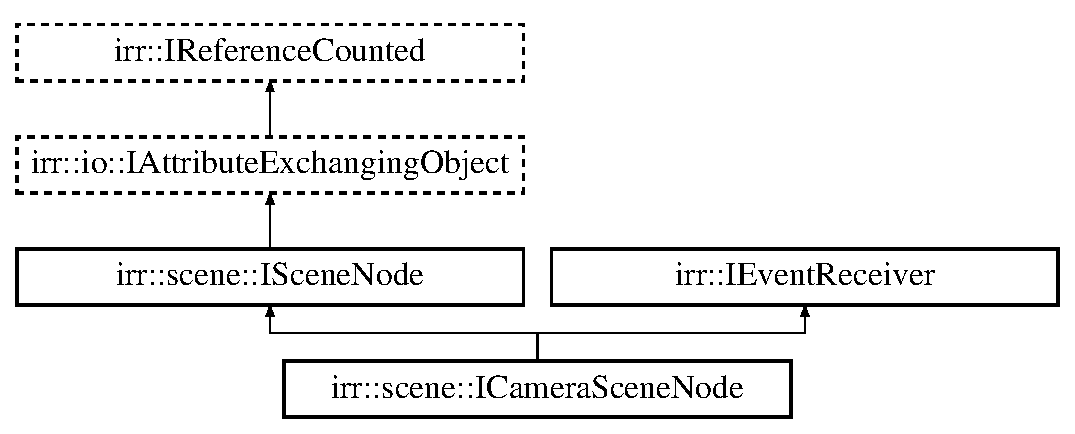
\includegraphics[height=1.682692cm]{classirr_1_1scene_1_1ICameraSceneNode}
\end{center}
\end{figure}
\subsection*{Public Member Functions}
\begin{DoxyCompactItemize}
\item 
\mbox{\Hypertarget{classirr_1_1scene_1_1ICameraSceneNode_a80e2a6e96feaf3191129eb6abefebc6f}\label{classirr_1_1scene_1_1ICameraSceneNode_a80e2a6e96feaf3191129eb6abefebc6f}} 
\hyperlink{classirr_1_1scene_1_1ICameraSceneNode_a80e2a6e96feaf3191129eb6abefebc6f}{I\+Camera\+Scene\+Node} (\hyperlink{classirr_1_1scene_1_1ISceneNode}{I\+Scene\+Node} $\ast$parent, \hyperlink{classirr_1_1scene_1_1ISceneManager}{I\+Scene\+Manager} $\ast$mgr, \hyperlink{namespaceirr_ac66849b7a6ed16e30ebede579f9b47c6}{s32} id, const \hyperlink{namespaceirr_1_1core_ae6e2b2a6c552833ebbd5b7463d03586b}{core\+::vector3df} \&position=\hyperlink{namespaceirr_1_1core_ae6e2b2a6c552833ebbd5b7463d03586b}{core\+::vector3df}(0, 0, 0), const \hyperlink{namespaceirr_1_1core_ae6e2b2a6c552833ebbd5b7463d03586b}{core\+::vector3df} \&rotation=\hyperlink{namespaceirr_1_1core_ae6e2b2a6c552833ebbd5b7463d03586b}{core\+::vector3df}(0, 0, 0), const \hyperlink{namespaceirr_1_1core_ae6e2b2a6c552833ebbd5b7463d03586b}{core\+::vector3df} \&scale=\hyperlink{namespaceirr_1_1core_ae6e2b2a6c552833ebbd5b7463d03586b}{core\+::vector3df}(1.\+0f, 1.\+0f, 1.\+0f))
\begin{DoxyCompactList}\small\item\em Constructor. \end{DoxyCompactList}\item 
virtual void \hyperlink{classirr_1_1scene_1_1ICameraSceneNode_a022415e06070ad77c6053eba64ba62ae}{set\+Projection\+Matrix} (const \hyperlink{namespaceirr_1_1core_a4c9d4e29899535971052810954a14431}{core\+::matrix4} \&projection, bool \hyperlink{classirr_1_1scene_1_1ICameraSceneNode_a5cfd588d836004923f01667543837d6c}{is\+Orthogonal}=false)=0
\begin{DoxyCompactList}\small\item\em Sets the projection matrix of the camera. \end{DoxyCompactList}\item 
virtual const \hyperlink{namespaceirr_1_1core_a4c9d4e29899535971052810954a14431}{core\+::matrix4} \& \hyperlink{classirr_1_1scene_1_1ICameraSceneNode_a80f4a43d24dc31d797a84e0e2f62f1a1}{get\+Projection\+Matrix} () const =0
\begin{DoxyCompactList}\small\item\em Gets the current projection matrix of the camera. \end{DoxyCompactList}\item 
virtual const \hyperlink{namespaceirr_1_1core_a4c9d4e29899535971052810954a14431}{core\+::matrix4} \& \hyperlink{classirr_1_1scene_1_1ICameraSceneNode_aef40bb2f8f4a95a66dbb7fc3abee3e49}{get\+View\+Matrix} () const =0
\begin{DoxyCompactList}\small\item\em Gets the current view matrix of the camera. \end{DoxyCompactList}\item 
virtual void \hyperlink{classirr_1_1scene_1_1ICameraSceneNode_adb3500cac2a8a47e6a3f48aa343ce2fd}{set\+View\+Matrix\+Affector} (const \hyperlink{namespaceirr_1_1core_a4c9d4e29899535971052810954a14431}{core\+::matrix4} \&affector)=0
\begin{DoxyCompactList}\small\item\em Sets a custom view matrix affector. \end{DoxyCompactList}\item 
virtual const \hyperlink{namespaceirr_1_1core_a4c9d4e29899535971052810954a14431}{core\+::matrix4} \& \hyperlink{classirr_1_1scene_1_1ICameraSceneNode_a033018cccdb26f94cc33256e23d764c6}{get\+View\+Matrix\+Affector} () const =0
\begin{DoxyCompactList}\small\item\em Get the custom view matrix affector. \end{DoxyCompactList}\item 
virtual bool \hyperlink{classirr_1_1scene_1_1ICameraSceneNode_af27145518f43a17f803cdea086f68f3c}{On\+Event} (const \hyperlink{structirr_1_1SEvent}{S\+Event} \&event)=0
\begin{DoxyCompactList}\small\item\em It is possible to send mouse and key events to the camera. \end{DoxyCompactList}\item 
virtual void \hyperlink{classirr_1_1scene_1_1ICameraSceneNode_a7280b07fd7915c64350db5a132b4ba07}{set\+Target} (const \hyperlink{namespaceirr_1_1core_ae6e2b2a6c552833ebbd5b7463d03586b}{core\+::vector3df} \&pos)=0
\begin{DoxyCompactList}\small\item\em Sets the look at target of the camera. \end{DoxyCompactList}\item 
virtual void \hyperlink{classirr_1_1scene_1_1ICameraSceneNode_af95d5f50c192f212e11f3f050e92a470}{set\+Rotation} (const \hyperlink{namespaceirr_1_1core_ae6e2b2a6c552833ebbd5b7463d03586b}{core\+::vector3df} \&rotation)=0
\begin{DoxyCompactList}\small\item\em Sets the rotation of the node. \end{DoxyCompactList}\item 
virtual const \hyperlink{namespaceirr_1_1core_ae6e2b2a6c552833ebbd5b7463d03586b}{core\+::vector3df} \& \hyperlink{classirr_1_1scene_1_1ICameraSceneNode_a3ce50433986650eea15b20e4ed19c952}{get\+Target} () const =0
\begin{DoxyCompactList}\small\item\em Gets the current look at target of the camera. \end{DoxyCompactList}\item 
virtual void \hyperlink{classirr_1_1scene_1_1ICameraSceneNode_a1e74c17d89979fde4738276ccdcc0d3a}{set\+Up\+Vector} (const \hyperlink{namespaceirr_1_1core_ae6e2b2a6c552833ebbd5b7463d03586b}{core\+::vector3df} \&pos)=0
\begin{DoxyCompactList}\small\item\em Sets the up vector of the camera. \end{DoxyCompactList}\item 
virtual const \hyperlink{namespaceirr_1_1core_ae6e2b2a6c552833ebbd5b7463d03586b}{core\+::vector3df} \& \hyperlink{classirr_1_1scene_1_1ICameraSceneNode_a0dfb97859302021b9a44f2ead59fa230}{get\+Up\+Vector} () const =0
\begin{DoxyCompactList}\small\item\em Gets the up vector of the camera. \end{DoxyCompactList}\item 
virtual \hyperlink{namespaceirr_a0277be98d67dc26ff93b1a6a1d086b07}{f32} \hyperlink{classirr_1_1scene_1_1ICameraSceneNode_aee5dfccee2ec0b0cbcdb1079a6430a25}{get\+Near\+Value} () const =0
\begin{DoxyCompactList}\small\item\em Gets the value of the near plane of the camera. \end{DoxyCompactList}\item 
virtual \hyperlink{namespaceirr_a0277be98d67dc26ff93b1a6a1d086b07}{f32} \hyperlink{classirr_1_1scene_1_1ICameraSceneNode_a7a6603b808522605276359b834d48245}{get\+Far\+Value} () const =0
\begin{DoxyCompactList}\small\item\em Gets the value of the far plane of the camera. \end{DoxyCompactList}\item 
virtual \hyperlink{namespaceirr_a0277be98d67dc26ff93b1a6a1d086b07}{f32} \hyperlink{classirr_1_1scene_1_1ICameraSceneNode_aed7af13bc5a076d61a10a1998f71742e}{get\+Aspect\+Ratio} () const =0
\begin{DoxyCompactList}\small\item\em Gets the aspect ratio of the camera. \end{DoxyCompactList}\item 
virtual \hyperlink{namespaceirr_a0277be98d67dc26ff93b1a6a1d086b07}{f32} \hyperlink{classirr_1_1scene_1_1ICameraSceneNode_a8396148b1c3e27e79a615a859ae7d75d}{get\+F\+OV} () const =0
\begin{DoxyCompactList}\small\item\em Gets the field of view of the camera. \end{DoxyCompactList}\item 
virtual void \hyperlink{classirr_1_1scene_1_1ICameraSceneNode_aab5107ae5d0373d6fb005a87741e7057}{set\+Near\+Value} (\hyperlink{namespaceirr_a0277be98d67dc26ff93b1a6a1d086b07}{f32} zn)=0
\begin{DoxyCompactList}\small\item\em Sets the value of the near clipping plane. (default\+: 1.\+0f) \end{DoxyCompactList}\item 
virtual void \hyperlink{classirr_1_1scene_1_1ICameraSceneNode_ab7e427dd639b6bb63f648d6d087da1ea}{set\+Far\+Value} (\hyperlink{namespaceirr_a0277be98d67dc26ff93b1a6a1d086b07}{f32} zf)=0
\begin{DoxyCompactList}\small\item\em Sets the value of the far clipping plane (default\+: 2000.\+0f) \end{DoxyCompactList}\item 
virtual void \hyperlink{classirr_1_1scene_1_1ICameraSceneNode_a5c3728a61a208376b9df6a701f4a5b3c}{set\+Aspect\+Ratio} (\hyperlink{namespaceirr_a0277be98d67dc26ff93b1a6a1d086b07}{f32} aspect)=0
\begin{DoxyCompactList}\small\item\em Sets the aspect ratio (default\+: 4.\+0f / 3.\+0f) \end{DoxyCompactList}\item 
virtual void \hyperlink{classirr_1_1scene_1_1ICameraSceneNode_a43ee11523e9cf842d4b5d8c6a572241c}{set\+F\+OV} (\hyperlink{namespaceirr_a0277be98d67dc26ff93b1a6a1d086b07}{f32} fovy)=0
\begin{DoxyCompactList}\small\item\em Sets the field of view (Default\+: PI / 2.\+5f) \end{DoxyCompactList}\item 
virtual const \hyperlink{structirr_1_1scene_1_1SViewFrustum}{S\+View\+Frustum} $\ast$ \hyperlink{classirr_1_1scene_1_1ICameraSceneNode_add0cba097d3e59714546f04f2c53477e}{get\+View\+Frustum} () const =0
\begin{DoxyCompactList}\small\item\em Get the view frustum. \end{DoxyCompactList}\item 
virtual void \hyperlink{classirr_1_1scene_1_1ICameraSceneNode_a5b5c89233c1805676d6fcb392236dfec}{set\+Input\+Receiver\+Enabled} (bool enabled)=0
\begin{DoxyCompactList}\small\item\em Disables or enables the camera to get key or mouse inputs. \end{DoxyCompactList}\item 
\mbox{\Hypertarget{classirr_1_1scene_1_1ICameraSceneNode_a15eeaf8a5c69af91d920b8243f76796f}\label{classirr_1_1scene_1_1ICameraSceneNode_a15eeaf8a5c69af91d920b8243f76796f}} 
virtual bool \hyperlink{classirr_1_1scene_1_1ICameraSceneNode_a15eeaf8a5c69af91d920b8243f76796f}{is\+Input\+Receiver\+Enabled} () const =0
\begin{DoxyCompactList}\small\item\em Checks if the input receiver of the camera is currently enabled. \end{DoxyCompactList}\item 
\mbox{\Hypertarget{classirr_1_1scene_1_1ICameraSceneNode_a5cfd588d836004923f01667543837d6c}\label{classirr_1_1scene_1_1ICameraSceneNode_a5cfd588d836004923f01667543837d6c}} 
virtual bool \hyperlink{classirr_1_1scene_1_1ICameraSceneNode_a5cfd588d836004923f01667543837d6c}{is\+Orthogonal} () const
\begin{DoxyCompactList}\small\item\em Checks if a camera is orthogonal. \end{DoxyCompactList}\item 
virtual void \hyperlink{classirr_1_1scene_1_1ICameraSceneNode_ad8785d7b2f730933a8d4425ac54e7205}{bind\+Target\+And\+Rotation} (bool bound)=0
\begin{DoxyCompactList}\small\item\em Binds the camera scene node\textquotesingle{}s rotation to its target position and vice vera, or unbinds them. \end{DoxyCompactList}\item 
virtual bool \hyperlink{classirr_1_1scene_1_1ICameraSceneNode_a343be24b2c43db7580127229db2dec6a}{get\+Target\+And\+Rotation\+Binding} (void) const =0
\begin{DoxyCompactList}\small\item\em Queries if the camera scene node\textquotesingle{}s rotation and its target position are bound together. \end{DoxyCompactList}\item 
\mbox{\Hypertarget{classirr_1_1scene_1_1ICameraSceneNode_a0a78a29638be1665ee5dba22c2c3b846}\label{classirr_1_1scene_1_1ICameraSceneNode_a0a78a29638be1665ee5dba22c2c3b846}} 
virtual void \hyperlink{classirr_1_1scene_1_1ICameraSceneNode_a0a78a29638be1665ee5dba22c2c3b846}{serialize\+Attributes} (\hyperlink{classirr_1_1io_1_1IAttributes}{io\+::\+I\+Attributes} $\ast$out, \hyperlink{structirr_1_1io_1_1SAttributeReadWriteOptions}{io\+::\+S\+Attribute\+Read\+Write\+Options} $\ast$options=0) const
\begin{DoxyCompactList}\small\item\em Writes attributes of the camera node. \end{DoxyCompactList}\item 
\mbox{\Hypertarget{classirr_1_1scene_1_1ICameraSceneNode_a0df881cb5e2a55562399281061151ae8}\label{classirr_1_1scene_1_1ICameraSceneNode_a0df881cb5e2a55562399281061151ae8}} 
virtual void \hyperlink{classirr_1_1scene_1_1ICameraSceneNode_a0df881cb5e2a55562399281061151ae8}{deserialize\+Attributes} (\hyperlink{classirr_1_1io_1_1IAttributes}{io\+::\+I\+Attributes} $\ast$in, \hyperlink{structirr_1_1io_1_1SAttributeReadWriteOptions}{io\+::\+S\+Attribute\+Read\+Write\+Options} $\ast$options=0)
\begin{DoxyCompactList}\small\item\em Reads attributes of the camera node. \end{DoxyCompactList}\item 
\mbox{\Hypertarget{classirr_1_1scene_1_1ICameraSceneNode_a80e2a6e96feaf3191129eb6abefebc6f}\label{classirr_1_1scene_1_1ICameraSceneNode_a80e2a6e96feaf3191129eb6abefebc6f}} 
\hyperlink{classirr_1_1scene_1_1ICameraSceneNode_a80e2a6e96feaf3191129eb6abefebc6f}{I\+Camera\+Scene\+Node} (\hyperlink{classirr_1_1scene_1_1ISceneNode}{I\+Scene\+Node} $\ast$parent, \hyperlink{classirr_1_1scene_1_1ISceneManager}{I\+Scene\+Manager} $\ast$mgr, \hyperlink{namespaceirr_ac66849b7a6ed16e30ebede579f9b47c6}{s32} id, const \hyperlink{namespaceirr_1_1core_ae6e2b2a6c552833ebbd5b7463d03586b}{core\+::vector3df} \&position=\hyperlink{namespaceirr_1_1core_ae6e2b2a6c552833ebbd5b7463d03586b}{core\+::vector3df}(0, 0, 0), const \hyperlink{namespaceirr_1_1core_ae6e2b2a6c552833ebbd5b7463d03586b}{core\+::vector3df} \&rotation=\hyperlink{namespaceirr_1_1core_ae6e2b2a6c552833ebbd5b7463d03586b}{core\+::vector3df}(0, 0, 0), const \hyperlink{namespaceirr_1_1core_ae6e2b2a6c552833ebbd5b7463d03586b}{core\+::vector3df} \&scale=\hyperlink{namespaceirr_1_1core_ae6e2b2a6c552833ebbd5b7463d03586b}{core\+::vector3df}(1.\+0f, 1.\+0f, 1.\+0f))
\begin{DoxyCompactList}\small\item\em Constructor. \end{DoxyCompactList}\item 
virtual void \hyperlink{classirr_1_1scene_1_1ICameraSceneNode_a022415e06070ad77c6053eba64ba62ae}{set\+Projection\+Matrix} (const \hyperlink{namespaceirr_1_1core_a4c9d4e29899535971052810954a14431}{core\+::matrix4} \&projection, bool \hyperlink{classirr_1_1scene_1_1ICameraSceneNode_a5cfd588d836004923f01667543837d6c}{is\+Orthogonal}=false)=0
\begin{DoxyCompactList}\small\item\em Sets the projection matrix of the camera. \end{DoxyCompactList}\item 
virtual const \hyperlink{namespaceirr_1_1core_a4c9d4e29899535971052810954a14431}{core\+::matrix4} \& \hyperlink{classirr_1_1scene_1_1ICameraSceneNode_a80f4a43d24dc31d797a84e0e2f62f1a1}{get\+Projection\+Matrix} () const =0
\begin{DoxyCompactList}\small\item\em Gets the current projection matrix of the camera. \end{DoxyCompactList}\item 
virtual const \hyperlink{namespaceirr_1_1core_a4c9d4e29899535971052810954a14431}{core\+::matrix4} \& \hyperlink{classirr_1_1scene_1_1ICameraSceneNode_aef40bb2f8f4a95a66dbb7fc3abee3e49}{get\+View\+Matrix} () const =0
\begin{DoxyCompactList}\small\item\em Gets the current view matrix of the camera. \end{DoxyCompactList}\item 
virtual void \hyperlink{classirr_1_1scene_1_1ICameraSceneNode_adb3500cac2a8a47e6a3f48aa343ce2fd}{set\+View\+Matrix\+Affector} (const \hyperlink{namespaceirr_1_1core_a4c9d4e29899535971052810954a14431}{core\+::matrix4} \&affector)=0
\begin{DoxyCompactList}\small\item\em Sets a custom view matrix affector. \end{DoxyCompactList}\item 
virtual const \hyperlink{namespaceirr_1_1core_a4c9d4e29899535971052810954a14431}{core\+::matrix4} \& \hyperlink{classirr_1_1scene_1_1ICameraSceneNode_a033018cccdb26f94cc33256e23d764c6}{get\+View\+Matrix\+Affector} () const =0
\begin{DoxyCompactList}\small\item\em Get the custom view matrix affector. \end{DoxyCompactList}\item 
virtual bool \hyperlink{classirr_1_1scene_1_1ICameraSceneNode_af27145518f43a17f803cdea086f68f3c}{On\+Event} (const \hyperlink{structirr_1_1SEvent}{S\+Event} \&event)=0
\begin{DoxyCompactList}\small\item\em It is possible to send mouse and key events to the camera. \end{DoxyCompactList}\item 
virtual void \hyperlink{classirr_1_1scene_1_1ICameraSceneNode_a7280b07fd7915c64350db5a132b4ba07}{set\+Target} (const \hyperlink{namespaceirr_1_1core_ae6e2b2a6c552833ebbd5b7463d03586b}{core\+::vector3df} \&pos)=0
\begin{DoxyCompactList}\small\item\em Sets the look at target of the camera. \end{DoxyCompactList}\item 
virtual void \hyperlink{classirr_1_1scene_1_1ICameraSceneNode_af95d5f50c192f212e11f3f050e92a470}{set\+Rotation} (const \hyperlink{namespaceirr_1_1core_ae6e2b2a6c552833ebbd5b7463d03586b}{core\+::vector3df} \&rotation)=0
\begin{DoxyCompactList}\small\item\em Sets the rotation of the node. \end{DoxyCompactList}\item 
virtual const \hyperlink{namespaceirr_1_1core_ae6e2b2a6c552833ebbd5b7463d03586b}{core\+::vector3df} \& \hyperlink{classirr_1_1scene_1_1ICameraSceneNode_a3ce50433986650eea15b20e4ed19c952}{get\+Target} () const =0
\begin{DoxyCompactList}\small\item\em Gets the current look at target of the camera. \end{DoxyCompactList}\item 
virtual void \hyperlink{classirr_1_1scene_1_1ICameraSceneNode_a1e74c17d89979fde4738276ccdcc0d3a}{set\+Up\+Vector} (const \hyperlink{namespaceirr_1_1core_ae6e2b2a6c552833ebbd5b7463d03586b}{core\+::vector3df} \&pos)=0
\begin{DoxyCompactList}\small\item\em Sets the up vector of the camera. \end{DoxyCompactList}\item 
virtual const \hyperlink{namespaceirr_1_1core_ae6e2b2a6c552833ebbd5b7463d03586b}{core\+::vector3df} \& \hyperlink{classirr_1_1scene_1_1ICameraSceneNode_a0dfb97859302021b9a44f2ead59fa230}{get\+Up\+Vector} () const =0
\begin{DoxyCompactList}\small\item\em Gets the up vector of the camera. \end{DoxyCompactList}\item 
virtual \hyperlink{namespaceirr_a0277be98d67dc26ff93b1a6a1d086b07}{f32} \hyperlink{classirr_1_1scene_1_1ICameraSceneNode_aee5dfccee2ec0b0cbcdb1079a6430a25}{get\+Near\+Value} () const =0
\begin{DoxyCompactList}\small\item\em Gets the value of the near plane of the camera. \end{DoxyCompactList}\item 
virtual \hyperlink{namespaceirr_a0277be98d67dc26ff93b1a6a1d086b07}{f32} \hyperlink{classirr_1_1scene_1_1ICameraSceneNode_a7a6603b808522605276359b834d48245}{get\+Far\+Value} () const =0
\begin{DoxyCompactList}\small\item\em Gets the value of the far plane of the camera. \end{DoxyCompactList}\item 
virtual \hyperlink{namespaceirr_a0277be98d67dc26ff93b1a6a1d086b07}{f32} \hyperlink{classirr_1_1scene_1_1ICameraSceneNode_aed7af13bc5a076d61a10a1998f71742e}{get\+Aspect\+Ratio} () const =0
\begin{DoxyCompactList}\small\item\em Gets the aspect ratio of the camera. \end{DoxyCompactList}\item 
virtual \hyperlink{namespaceirr_a0277be98d67dc26ff93b1a6a1d086b07}{f32} \hyperlink{classirr_1_1scene_1_1ICameraSceneNode_a8396148b1c3e27e79a615a859ae7d75d}{get\+F\+OV} () const =0
\begin{DoxyCompactList}\small\item\em Gets the field of view of the camera. \end{DoxyCompactList}\item 
virtual void \hyperlink{classirr_1_1scene_1_1ICameraSceneNode_aab5107ae5d0373d6fb005a87741e7057}{set\+Near\+Value} (\hyperlink{namespaceirr_a0277be98d67dc26ff93b1a6a1d086b07}{f32} zn)=0
\begin{DoxyCompactList}\small\item\em Sets the value of the near clipping plane. (default\+: 1.\+0f) \end{DoxyCompactList}\item 
virtual void \hyperlink{classirr_1_1scene_1_1ICameraSceneNode_ab7e427dd639b6bb63f648d6d087da1ea}{set\+Far\+Value} (\hyperlink{namespaceirr_a0277be98d67dc26ff93b1a6a1d086b07}{f32} zf)=0
\begin{DoxyCompactList}\small\item\em Sets the value of the far clipping plane (default\+: 2000.\+0f) \end{DoxyCompactList}\item 
virtual void \hyperlink{classirr_1_1scene_1_1ICameraSceneNode_a5c3728a61a208376b9df6a701f4a5b3c}{set\+Aspect\+Ratio} (\hyperlink{namespaceirr_a0277be98d67dc26ff93b1a6a1d086b07}{f32} aspect)=0
\begin{DoxyCompactList}\small\item\em Sets the aspect ratio (default\+: 4.\+0f / 3.\+0f) \end{DoxyCompactList}\item 
virtual void \hyperlink{classirr_1_1scene_1_1ICameraSceneNode_a43ee11523e9cf842d4b5d8c6a572241c}{set\+F\+OV} (\hyperlink{namespaceirr_a0277be98d67dc26ff93b1a6a1d086b07}{f32} fovy)=0
\begin{DoxyCompactList}\small\item\em Sets the field of view (Default\+: PI / 2.\+5f) \end{DoxyCompactList}\item 
virtual const \hyperlink{structirr_1_1scene_1_1SViewFrustum}{S\+View\+Frustum} $\ast$ \hyperlink{classirr_1_1scene_1_1ICameraSceneNode_add0cba097d3e59714546f04f2c53477e}{get\+View\+Frustum} () const =0
\begin{DoxyCompactList}\small\item\em Get the view frustum. \end{DoxyCompactList}\item 
virtual void \hyperlink{classirr_1_1scene_1_1ICameraSceneNode_a5b5c89233c1805676d6fcb392236dfec}{set\+Input\+Receiver\+Enabled} (bool enabled)=0
\begin{DoxyCompactList}\small\item\em Disables or enables the camera to get key or mouse inputs. \end{DoxyCompactList}\item 
\mbox{\Hypertarget{classirr_1_1scene_1_1ICameraSceneNode_a15eeaf8a5c69af91d920b8243f76796f}\label{classirr_1_1scene_1_1ICameraSceneNode_a15eeaf8a5c69af91d920b8243f76796f}} 
virtual bool \hyperlink{classirr_1_1scene_1_1ICameraSceneNode_a15eeaf8a5c69af91d920b8243f76796f}{is\+Input\+Receiver\+Enabled} () const =0
\begin{DoxyCompactList}\small\item\em Checks if the input receiver of the camera is currently enabled. \end{DoxyCompactList}\item 
\mbox{\Hypertarget{classirr_1_1scene_1_1ICameraSceneNode_a5cfd588d836004923f01667543837d6c}\label{classirr_1_1scene_1_1ICameraSceneNode_a5cfd588d836004923f01667543837d6c}} 
virtual bool \hyperlink{classirr_1_1scene_1_1ICameraSceneNode_a5cfd588d836004923f01667543837d6c}{is\+Orthogonal} () const
\begin{DoxyCompactList}\small\item\em Checks if a camera is orthogonal. \end{DoxyCompactList}\item 
virtual void \hyperlink{classirr_1_1scene_1_1ICameraSceneNode_ad8785d7b2f730933a8d4425ac54e7205}{bind\+Target\+And\+Rotation} (bool bound)=0
\begin{DoxyCompactList}\small\item\em Binds the camera scene node\textquotesingle{}s rotation to its target position and vice vera, or unbinds them. \end{DoxyCompactList}\item 
virtual bool \hyperlink{classirr_1_1scene_1_1ICameraSceneNode_a343be24b2c43db7580127229db2dec6a}{get\+Target\+And\+Rotation\+Binding} (void) const =0
\begin{DoxyCompactList}\small\item\em Queries if the camera scene node\textquotesingle{}s rotation and its target position are bound together. \end{DoxyCompactList}\item 
\mbox{\Hypertarget{classirr_1_1scene_1_1ICameraSceneNode_a0a78a29638be1665ee5dba22c2c3b846}\label{classirr_1_1scene_1_1ICameraSceneNode_a0a78a29638be1665ee5dba22c2c3b846}} 
virtual void \hyperlink{classirr_1_1scene_1_1ICameraSceneNode_a0a78a29638be1665ee5dba22c2c3b846}{serialize\+Attributes} (\hyperlink{classirr_1_1io_1_1IAttributes}{io\+::\+I\+Attributes} $\ast$out, \hyperlink{structirr_1_1io_1_1SAttributeReadWriteOptions}{io\+::\+S\+Attribute\+Read\+Write\+Options} $\ast$options=0) const
\begin{DoxyCompactList}\small\item\em Writes attributes of the camera node. \end{DoxyCompactList}\item 
\mbox{\Hypertarget{classirr_1_1scene_1_1ICameraSceneNode_a0df881cb5e2a55562399281061151ae8}\label{classirr_1_1scene_1_1ICameraSceneNode_a0df881cb5e2a55562399281061151ae8}} 
virtual void \hyperlink{classirr_1_1scene_1_1ICameraSceneNode_a0df881cb5e2a55562399281061151ae8}{deserialize\+Attributes} (\hyperlink{classirr_1_1io_1_1IAttributes}{io\+::\+I\+Attributes} $\ast$in, \hyperlink{structirr_1_1io_1_1SAttributeReadWriteOptions}{io\+::\+S\+Attribute\+Read\+Write\+Options} $\ast$options=0)
\begin{DoxyCompactList}\small\item\em Reads attributes of the camera node. \end{DoxyCompactList}\end{DoxyCompactItemize}
\subsection*{Additional Inherited Members}


\subsection{Detailed Description}
Scene Node which is a (controlable) camera. 

The whole scene will be rendered from the cameras point of view. Because the I\+Camera\+Scen\+Node is a Scene\+Node, it can be attached to any other scene node, and will follow its parents movement, rotation and so on. 

\subsection{Member Function Documentation}
\mbox{\Hypertarget{classirr_1_1scene_1_1ICameraSceneNode_ad8785d7b2f730933a8d4425ac54e7205}\label{classirr_1_1scene_1_1ICameraSceneNode_ad8785d7b2f730933a8d4425ac54e7205}} 
\index{irr\+::scene\+::\+I\+Camera\+Scene\+Node@{irr\+::scene\+::\+I\+Camera\+Scene\+Node}!bind\+Target\+And\+Rotation@{bind\+Target\+And\+Rotation}}
\index{bind\+Target\+And\+Rotation@{bind\+Target\+And\+Rotation}!irr\+::scene\+::\+I\+Camera\+Scene\+Node@{irr\+::scene\+::\+I\+Camera\+Scene\+Node}}
\subsubsection{\texorpdfstring{bind\+Target\+And\+Rotation()}{bindTargetAndRotation()}\hspace{0.1cm}{\footnotesize\ttfamily [1/2]}}
{\footnotesize\ttfamily virtual void irr\+::scene\+::\+I\+Camera\+Scene\+Node\+::bind\+Target\+And\+Rotation (\begin{DoxyParamCaption}\item[{bool}]{bound }\end{DoxyParamCaption})\hspace{0.3cm}{\ttfamily [pure virtual]}}



Binds the camera scene node\textquotesingle{}s rotation to its target position and vice vera, or unbinds them. 

When bound, calling \hyperlink{classirr_1_1scene_1_1ICameraSceneNode_af95d5f50c192f212e11f3f050e92a470}{set\+Rotation()} will update the camera\textquotesingle{}s target position to be along its +Z axis, and likewise calling \hyperlink{classirr_1_1scene_1_1ICameraSceneNode_a7280b07fd7915c64350db5a132b4ba07}{set\+Target()} will update its rotation so that its +Z axis will point at the target point. F\+PS camera use this binding by default; other cameras do not. 
\begin{DoxyParams}{Parameters}
{\em bound} & True to bind the camera\textquotesingle{}s scene node rotation and targetting, false to unbind them. \\
\hline
\end{DoxyParams}
\begin{DoxySeeAlso}{See also}
\hyperlink{classirr_1_1scene_1_1ICameraSceneNode_a343be24b2c43db7580127229db2dec6a}{get\+Target\+And\+Rotation\+Binding()} 
\end{DoxySeeAlso}
\mbox{\Hypertarget{classirr_1_1scene_1_1ICameraSceneNode_ad8785d7b2f730933a8d4425ac54e7205}\label{classirr_1_1scene_1_1ICameraSceneNode_ad8785d7b2f730933a8d4425ac54e7205}} 
\index{irr\+::scene\+::\+I\+Camera\+Scene\+Node@{irr\+::scene\+::\+I\+Camera\+Scene\+Node}!bind\+Target\+And\+Rotation@{bind\+Target\+And\+Rotation}}
\index{bind\+Target\+And\+Rotation@{bind\+Target\+And\+Rotation}!irr\+::scene\+::\+I\+Camera\+Scene\+Node@{irr\+::scene\+::\+I\+Camera\+Scene\+Node}}
\subsubsection{\texorpdfstring{bind\+Target\+And\+Rotation()}{bindTargetAndRotation()}\hspace{0.1cm}{\footnotesize\ttfamily [2/2]}}
{\footnotesize\ttfamily virtual void irr\+::scene\+::\+I\+Camera\+Scene\+Node\+::bind\+Target\+And\+Rotation (\begin{DoxyParamCaption}\item[{bool}]{bound }\end{DoxyParamCaption})\hspace{0.3cm}{\ttfamily [pure virtual]}}



Binds the camera scene node\textquotesingle{}s rotation to its target position and vice vera, or unbinds them. 

When bound, calling \hyperlink{classirr_1_1scene_1_1ICameraSceneNode_af95d5f50c192f212e11f3f050e92a470}{set\+Rotation()} will update the camera\textquotesingle{}s target position to be along its +Z axis, and likewise calling \hyperlink{classirr_1_1scene_1_1ICameraSceneNode_a7280b07fd7915c64350db5a132b4ba07}{set\+Target()} will update its rotation so that its +Z axis will point at the target point. F\+PS camera use this binding by default; other cameras do not. 
\begin{DoxyParams}{Parameters}
{\em bound} & True to bind the camera\textquotesingle{}s scene node rotation and targetting, false to unbind them. \\
\hline
\end{DoxyParams}
\begin{DoxySeeAlso}{See also}
\hyperlink{classirr_1_1scene_1_1ICameraSceneNode_a343be24b2c43db7580127229db2dec6a}{get\+Target\+And\+Rotation\+Binding()} 
\end{DoxySeeAlso}
\mbox{\Hypertarget{classirr_1_1scene_1_1ICameraSceneNode_aed7af13bc5a076d61a10a1998f71742e}\label{classirr_1_1scene_1_1ICameraSceneNode_aed7af13bc5a076d61a10a1998f71742e}} 
\index{irr\+::scene\+::\+I\+Camera\+Scene\+Node@{irr\+::scene\+::\+I\+Camera\+Scene\+Node}!get\+Aspect\+Ratio@{get\+Aspect\+Ratio}}
\index{get\+Aspect\+Ratio@{get\+Aspect\+Ratio}!irr\+::scene\+::\+I\+Camera\+Scene\+Node@{irr\+::scene\+::\+I\+Camera\+Scene\+Node}}
\subsubsection{\texorpdfstring{get\+Aspect\+Ratio()}{getAspectRatio()}\hspace{0.1cm}{\footnotesize\ttfamily [1/2]}}
{\footnotesize\ttfamily virtual \hyperlink{namespaceirr_a0277be98d67dc26ff93b1a6a1d086b07}{f32} irr\+::scene\+::\+I\+Camera\+Scene\+Node\+::get\+Aspect\+Ratio (\begin{DoxyParamCaption}{ }\end{DoxyParamCaption}) const\hspace{0.3cm}{\ttfamily [pure virtual]}}



Gets the aspect ratio of the camera. 

\begin{DoxyReturn}{Returns}
The aspect ratio of the camera. 
\end{DoxyReturn}
\mbox{\Hypertarget{classirr_1_1scene_1_1ICameraSceneNode_aed7af13bc5a076d61a10a1998f71742e}\label{classirr_1_1scene_1_1ICameraSceneNode_aed7af13bc5a076d61a10a1998f71742e}} 
\index{irr\+::scene\+::\+I\+Camera\+Scene\+Node@{irr\+::scene\+::\+I\+Camera\+Scene\+Node}!get\+Aspect\+Ratio@{get\+Aspect\+Ratio}}
\index{get\+Aspect\+Ratio@{get\+Aspect\+Ratio}!irr\+::scene\+::\+I\+Camera\+Scene\+Node@{irr\+::scene\+::\+I\+Camera\+Scene\+Node}}
\subsubsection{\texorpdfstring{get\+Aspect\+Ratio()}{getAspectRatio()}\hspace{0.1cm}{\footnotesize\ttfamily [2/2]}}
{\footnotesize\ttfamily virtual \hyperlink{namespaceirr_a0277be98d67dc26ff93b1a6a1d086b07}{f32} irr\+::scene\+::\+I\+Camera\+Scene\+Node\+::get\+Aspect\+Ratio (\begin{DoxyParamCaption}{ }\end{DoxyParamCaption}) const\hspace{0.3cm}{\ttfamily [pure virtual]}}



Gets the aspect ratio of the camera. 

\begin{DoxyReturn}{Returns}
The aspect ratio of the camera. 
\end{DoxyReturn}
\mbox{\Hypertarget{classirr_1_1scene_1_1ICameraSceneNode_a7a6603b808522605276359b834d48245}\label{classirr_1_1scene_1_1ICameraSceneNode_a7a6603b808522605276359b834d48245}} 
\index{irr\+::scene\+::\+I\+Camera\+Scene\+Node@{irr\+::scene\+::\+I\+Camera\+Scene\+Node}!get\+Far\+Value@{get\+Far\+Value}}
\index{get\+Far\+Value@{get\+Far\+Value}!irr\+::scene\+::\+I\+Camera\+Scene\+Node@{irr\+::scene\+::\+I\+Camera\+Scene\+Node}}
\subsubsection{\texorpdfstring{get\+Far\+Value()}{getFarValue()}\hspace{0.1cm}{\footnotesize\ttfamily [1/2]}}
{\footnotesize\ttfamily virtual \hyperlink{namespaceirr_a0277be98d67dc26ff93b1a6a1d086b07}{f32} irr\+::scene\+::\+I\+Camera\+Scene\+Node\+::get\+Far\+Value (\begin{DoxyParamCaption}{ }\end{DoxyParamCaption}) const\hspace{0.3cm}{\ttfamily [pure virtual]}}



Gets the value of the far plane of the camera. 

\begin{DoxyReturn}{Returns}
The value of the far plane of the camera. 
\end{DoxyReturn}
\mbox{\Hypertarget{classirr_1_1scene_1_1ICameraSceneNode_a7a6603b808522605276359b834d48245}\label{classirr_1_1scene_1_1ICameraSceneNode_a7a6603b808522605276359b834d48245}} 
\index{irr\+::scene\+::\+I\+Camera\+Scene\+Node@{irr\+::scene\+::\+I\+Camera\+Scene\+Node}!get\+Far\+Value@{get\+Far\+Value}}
\index{get\+Far\+Value@{get\+Far\+Value}!irr\+::scene\+::\+I\+Camera\+Scene\+Node@{irr\+::scene\+::\+I\+Camera\+Scene\+Node}}
\subsubsection{\texorpdfstring{get\+Far\+Value()}{getFarValue()}\hspace{0.1cm}{\footnotesize\ttfamily [2/2]}}
{\footnotesize\ttfamily virtual \hyperlink{namespaceirr_a0277be98d67dc26ff93b1a6a1d086b07}{f32} irr\+::scene\+::\+I\+Camera\+Scene\+Node\+::get\+Far\+Value (\begin{DoxyParamCaption}{ }\end{DoxyParamCaption}) const\hspace{0.3cm}{\ttfamily [pure virtual]}}



Gets the value of the far plane of the camera. 

\begin{DoxyReturn}{Returns}
The value of the far plane of the camera. 
\end{DoxyReturn}
\mbox{\Hypertarget{classirr_1_1scene_1_1ICameraSceneNode_a8396148b1c3e27e79a615a859ae7d75d}\label{classirr_1_1scene_1_1ICameraSceneNode_a8396148b1c3e27e79a615a859ae7d75d}} 
\index{irr\+::scene\+::\+I\+Camera\+Scene\+Node@{irr\+::scene\+::\+I\+Camera\+Scene\+Node}!get\+F\+OV@{get\+F\+OV}}
\index{get\+F\+OV@{get\+F\+OV}!irr\+::scene\+::\+I\+Camera\+Scene\+Node@{irr\+::scene\+::\+I\+Camera\+Scene\+Node}}
\subsubsection{\texorpdfstring{get\+F\+O\+V()}{getFOV()}\hspace{0.1cm}{\footnotesize\ttfamily [1/2]}}
{\footnotesize\ttfamily virtual \hyperlink{namespaceirr_a0277be98d67dc26ff93b1a6a1d086b07}{f32} irr\+::scene\+::\+I\+Camera\+Scene\+Node\+::get\+F\+OV (\begin{DoxyParamCaption}{ }\end{DoxyParamCaption}) const\hspace{0.3cm}{\ttfamily [pure virtual]}}



Gets the field of view of the camera. 

\begin{DoxyReturn}{Returns}
The field of view of the camera in radians. 
\end{DoxyReturn}
\mbox{\Hypertarget{classirr_1_1scene_1_1ICameraSceneNode_a8396148b1c3e27e79a615a859ae7d75d}\label{classirr_1_1scene_1_1ICameraSceneNode_a8396148b1c3e27e79a615a859ae7d75d}} 
\index{irr\+::scene\+::\+I\+Camera\+Scene\+Node@{irr\+::scene\+::\+I\+Camera\+Scene\+Node}!get\+F\+OV@{get\+F\+OV}}
\index{get\+F\+OV@{get\+F\+OV}!irr\+::scene\+::\+I\+Camera\+Scene\+Node@{irr\+::scene\+::\+I\+Camera\+Scene\+Node}}
\subsubsection{\texorpdfstring{get\+F\+O\+V()}{getFOV()}\hspace{0.1cm}{\footnotesize\ttfamily [2/2]}}
{\footnotesize\ttfamily virtual \hyperlink{namespaceirr_a0277be98d67dc26ff93b1a6a1d086b07}{f32} irr\+::scene\+::\+I\+Camera\+Scene\+Node\+::get\+F\+OV (\begin{DoxyParamCaption}{ }\end{DoxyParamCaption}) const\hspace{0.3cm}{\ttfamily [pure virtual]}}



Gets the field of view of the camera. 

\begin{DoxyReturn}{Returns}
The field of view of the camera in radians. 
\end{DoxyReturn}
\mbox{\Hypertarget{classirr_1_1scene_1_1ICameraSceneNode_aee5dfccee2ec0b0cbcdb1079a6430a25}\label{classirr_1_1scene_1_1ICameraSceneNode_aee5dfccee2ec0b0cbcdb1079a6430a25}} 
\index{irr\+::scene\+::\+I\+Camera\+Scene\+Node@{irr\+::scene\+::\+I\+Camera\+Scene\+Node}!get\+Near\+Value@{get\+Near\+Value}}
\index{get\+Near\+Value@{get\+Near\+Value}!irr\+::scene\+::\+I\+Camera\+Scene\+Node@{irr\+::scene\+::\+I\+Camera\+Scene\+Node}}
\subsubsection{\texorpdfstring{get\+Near\+Value()}{getNearValue()}\hspace{0.1cm}{\footnotesize\ttfamily [1/2]}}
{\footnotesize\ttfamily virtual \hyperlink{namespaceirr_a0277be98d67dc26ff93b1a6a1d086b07}{f32} irr\+::scene\+::\+I\+Camera\+Scene\+Node\+::get\+Near\+Value (\begin{DoxyParamCaption}{ }\end{DoxyParamCaption}) const\hspace{0.3cm}{\ttfamily [pure virtual]}}



Gets the value of the near plane of the camera. 

\begin{DoxyReturn}{Returns}
The value of the near plane of the camera. 
\end{DoxyReturn}
\mbox{\Hypertarget{classirr_1_1scene_1_1ICameraSceneNode_aee5dfccee2ec0b0cbcdb1079a6430a25}\label{classirr_1_1scene_1_1ICameraSceneNode_aee5dfccee2ec0b0cbcdb1079a6430a25}} 
\index{irr\+::scene\+::\+I\+Camera\+Scene\+Node@{irr\+::scene\+::\+I\+Camera\+Scene\+Node}!get\+Near\+Value@{get\+Near\+Value}}
\index{get\+Near\+Value@{get\+Near\+Value}!irr\+::scene\+::\+I\+Camera\+Scene\+Node@{irr\+::scene\+::\+I\+Camera\+Scene\+Node}}
\subsubsection{\texorpdfstring{get\+Near\+Value()}{getNearValue()}\hspace{0.1cm}{\footnotesize\ttfamily [2/2]}}
{\footnotesize\ttfamily virtual \hyperlink{namespaceirr_a0277be98d67dc26ff93b1a6a1d086b07}{f32} irr\+::scene\+::\+I\+Camera\+Scene\+Node\+::get\+Near\+Value (\begin{DoxyParamCaption}{ }\end{DoxyParamCaption}) const\hspace{0.3cm}{\ttfamily [pure virtual]}}



Gets the value of the near plane of the camera. 

\begin{DoxyReturn}{Returns}
The value of the near plane of the camera. 
\end{DoxyReturn}
\mbox{\Hypertarget{classirr_1_1scene_1_1ICameraSceneNode_a80f4a43d24dc31d797a84e0e2f62f1a1}\label{classirr_1_1scene_1_1ICameraSceneNode_a80f4a43d24dc31d797a84e0e2f62f1a1}} 
\index{irr\+::scene\+::\+I\+Camera\+Scene\+Node@{irr\+::scene\+::\+I\+Camera\+Scene\+Node}!get\+Projection\+Matrix@{get\+Projection\+Matrix}}
\index{get\+Projection\+Matrix@{get\+Projection\+Matrix}!irr\+::scene\+::\+I\+Camera\+Scene\+Node@{irr\+::scene\+::\+I\+Camera\+Scene\+Node}}
\subsubsection{\texorpdfstring{get\+Projection\+Matrix()}{getProjectionMatrix()}\hspace{0.1cm}{\footnotesize\ttfamily [1/2]}}
{\footnotesize\ttfamily virtual const \hyperlink{namespaceirr_1_1core_a4c9d4e29899535971052810954a14431}{core\+::matrix4}\& irr\+::scene\+::\+I\+Camera\+Scene\+Node\+::get\+Projection\+Matrix (\begin{DoxyParamCaption}{ }\end{DoxyParamCaption}) const\hspace{0.3cm}{\ttfamily [pure virtual]}}



Gets the current projection matrix of the camera. 

\begin{DoxyReturn}{Returns}
The current projection matrix of the camera. 
\end{DoxyReturn}
\mbox{\Hypertarget{classirr_1_1scene_1_1ICameraSceneNode_a80f4a43d24dc31d797a84e0e2f62f1a1}\label{classirr_1_1scene_1_1ICameraSceneNode_a80f4a43d24dc31d797a84e0e2f62f1a1}} 
\index{irr\+::scene\+::\+I\+Camera\+Scene\+Node@{irr\+::scene\+::\+I\+Camera\+Scene\+Node}!get\+Projection\+Matrix@{get\+Projection\+Matrix}}
\index{get\+Projection\+Matrix@{get\+Projection\+Matrix}!irr\+::scene\+::\+I\+Camera\+Scene\+Node@{irr\+::scene\+::\+I\+Camera\+Scene\+Node}}
\subsubsection{\texorpdfstring{get\+Projection\+Matrix()}{getProjectionMatrix()}\hspace{0.1cm}{\footnotesize\ttfamily [2/2]}}
{\footnotesize\ttfamily virtual const \hyperlink{namespaceirr_1_1core_a4c9d4e29899535971052810954a14431}{core\+::matrix4}\& irr\+::scene\+::\+I\+Camera\+Scene\+Node\+::get\+Projection\+Matrix (\begin{DoxyParamCaption}{ }\end{DoxyParamCaption}) const\hspace{0.3cm}{\ttfamily [pure virtual]}}



Gets the current projection matrix of the camera. 

\begin{DoxyReturn}{Returns}
The current projection matrix of the camera. 
\end{DoxyReturn}
\mbox{\Hypertarget{classirr_1_1scene_1_1ICameraSceneNode_a3ce50433986650eea15b20e4ed19c952}\label{classirr_1_1scene_1_1ICameraSceneNode_a3ce50433986650eea15b20e4ed19c952}} 
\index{irr\+::scene\+::\+I\+Camera\+Scene\+Node@{irr\+::scene\+::\+I\+Camera\+Scene\+Node}!get\+Target@{get\+Target}}
\index{get\+Target@{get\+Target}!irr\+::scene\+::\+I\+Camera\+Scene\+Node@{irr\+::scene\+::\+I\+Camera\+Scene\+Node}}
\subsubsection{\texorpdfstring{get\+Target()}{getTarget()}\hspace{0.1cm}{\footnotesize\ttfamily [1/2]}}
{\footnotesize\ttfamily virtual const \hyperlink{namespaceirr_1_1core_ae6e2b2a6c552833ebbd5b7463d03586b}{core\+::vector3df}\& irr\+::scene\+::\+I\+Camera\+Scene\+Node\+::get\+Target (\begin{DoxyParamCaption}{ }\end{DoxyParamCaption}) const\hspace{0.3cm}{\ttfamily [pure virtual]}}



Gets the current look at target of the camera. 

\begin{DoxyReturn}{Returns}
The current look at target of the camera, in world co-\/ordinates 
\end{DoxyReturn}
\mbox{\Hypertarget{classirr_1_1scene_1_1ICameraSceneNode_a3ce50433986650eea15b20e4ed19c952}\label{classirr_1_1scene_1_1ICameraSceneNode_a3ce50433986650eea15b20e4ed19c952}} 
\index{irr\+::scene\+::\+I\+Camera\+Scene\+Node@{irr\+::scene\+::\+I\+Camera\+Scene\+Node}!get\+Target@{get\+Target}}
\index{get\+Target@{get\+Target}!irr\+::scene\+::\+I\+Camera\+Scene\+Node@{irr\+::scene\+::\+I\+Camera\+Scene\+Node}}
\subsubsection{\texorpdfstring{get\+Target()}{getTarget()}\hspace{0.1cm}{\footnotesize\ttfamily [2/2]}}
{\footnotesize\ttfamily virtual const \hyperlink{namespaceirr_1_1core_ae6e2b2a6c552833ebbd5b7463d03586b}{core\+::vector3df}\& irr\+::scene\+::\+I\+Camera\+Scene\+Node\+::get\+Target (\begin{DoxyParamCaption}{ }\end{DoxyParamCaption}) const\hspace{0.3cm}{\ttfamily [pure virtual]}}



Gets the current look at target of the camera. 

\begin{DoxyReturn}{Returns}
The current look at target of the camera, in world co-\/ordinates 
\end{DoxyReturn}
\mbox{\Hypertarget{classirr_1_1scene_1_1ICameraSceneNode_a343be24b2c43db7580127229db2dec6a}\label{classirr_1_1scene_1_1ICameraSceneNode_a343be24b2c43db7580127229db2dec6a}} 
\index{irr\+::scene\+::\+I\+Camera\+Scene\+Node@{irr\+::scene\+::\+I\+Camera\+Scene\+Node}!get\+Target\+And\+Rotation\+Binding@{get\+Target\+And\+Rotation\+Binding}}
\index{get\+Target\+And\+Rotation\+Binding@{get\+Target\+And\+Rotation\+Binding}!irr\+::scene\+::\+I\+Camera\+Scene\+Node@{irr\+::scene\+::\+I\+Camera\+Scene\+Node}}
\subsubsection{\texorpdfstring{get\+Target\+And\+Rotation\+Binding()}{getTargetAndRotationBinding()}\hspace{0.1cm}{\footnotesize\ttfamily [1/2]}}
{\footnotesize\ttfamily virtual bool irr\+::scene\+::\+I\+Camera\+Scene\+Node\+::get\+Target\+And\+Rotation\+Binding (\begin{DoxyParamCaption}\item[{void}]{ }\end{DoxyParamCaption}) const\hspace{0.3cm}{\ttfamily [pure virtual]}}



Queries if the camera scene node\textquotesingle{}s rotation and its target position are bound together. 

\begin{DoxySeeAlso}{See also}
\hyperlink{classirr_1_1scene_1_1ICameraSceneNode_ad8785d7b2f730933a8d4425ac54e7205}{bind\+Target\+And\+Rotation()} 
\end{DoxySeeAlso}
\mbox{\Hypertarget{classirr_1_1scene_1_1ICameraSceneNode_a343be24b2c43db7580127229db2dec6a}\label{classirr_1_1scene_1_1ICameraSceneNode_a343be24b2c43db7580127229db2dec6a}} 
\index{irr\+::scene\+::\+I\+Camera\+Scene\+Node@{irr\+::scene\+::\+I\+Camera\+Scene\+Node}!get\+Target\+And\+Rotation\+Binding@{get\+Target\+And\+Rotation\+Binding}}
\index{get\+Target\+And\+Rotation\+Binding@{get\+Target\+And\+Rotation\+Binding}!irr\+::scene\+::\+I\+Camera\+Scene\+Node@{irr\+::scene\+::\+I\+Camera\+Scene\+Node}}
\subsubsection{\texorpdfstring{get\+Target\+And\+Rotation\+Binding()}{getTargetAndRotationBinding()}\hspace{0.1cm}{\footnotesize\ttfamily [2/2]}}
{\footnotesize\ttfamily virtual bool irr\+::scene\+::\+I\+Camera\+Scene\+Node\+::get\+Target\+And\+Rotation\+Binding (\begin{DoxyParamCaption}\item[{void}]{ }\end{DoxyParamCaption}) const\hspace{0.3cm}{\ttfamily [pure virtual]}}



Queries if the camera scene node\textquotesingle{}s rotation and its target position are bound together. 

\begin{DoxySeeAlso}{See also}
\hyperlink{classirr_1_1scene_1_1ICameraSceneNode_ad8785d7b2f730933a8d4425ac54e7205}{bind\+Target\+And\+Rotation()} 
\end{DoxySeeAlso}
\mbox{\Hypertarget{classirr_1_1scene_1_1ICameraSceneNode_a0dfb97859302021b9a44f2ead59fa230}\label{classirr_1_1scene_1_1ICameraSceneNode_a0dfb97859302021b9a44f2ead59fa230}} 
\index{irr\+::scene\+::\+I\+Camera\+Scene\+Node@{irr\+::scene\+::\+I\+Camera\+Scene\+Node}!get\+Up\+Vector@{get\+Up\+Vector}}
\index{get\+Up\+Vector@{get\+Up\+Vector}!irr\+::scene\+::\+I\+Camera\+Scene\+Node@{irr\+::scene\+::\+I\+Camera\+Scene\+Node}}
\subsubsection{\texorpdfstring{get\+Up\+Vector()}{getUpVector()}\hspace{0.1cm}{\footnotesize\ttfamily [1/2]}}
{\footnotesize\ttfamily virtual const \hyperlink{namespaceirr_1_1core_ae6e2b2a6c552833ebbd5b7463d03586b}{core\+::vector3df}\& irr\+::scene\+::\+I\+Camera\+Scene\+Node\+::get\+Up\+Vector (\begin{DoxyParamCaption}{ }\end{DoxyParamCaption}) const\hspace{0.3cm}{\ttfamily [pure virtual]}}



Gets the up vector of the camera. 

\begin{DoxyReturn}{Returns}
The up vector of the camera, in world space. 
\end{DoxyReturn}
\mbox{\Hypertarget{classirr_1_1scene_1_1ICameraSceneNode_a0dfb97859302021b9a44f2ead59fa230}\label{classirr_1_1scene_1_1ICameraSceneNode_a0dfb97859302021b9a44f2ead59fa230}} 
\index{irr\+::scene\+::\+I\+Camera\+Scene\+Node@{irr\+::scene\+::\+I\+Camera\+Scene\+Node}!get\+Up\+Vector@{get\+Up\+Vector}}
\index{get\+Up\+Vector@{get\+Up\+Vector}!irr\+::scene\+::\+I\+Camera\+Scene\+Node@{irr\+::scene\+::\+I\+Camera\+Scene\+Node}}
\subsubsection{\texorpdfstring{get\+Up\+Vector()}{getUpVector()}\hspace{0.1cm}{\footnotesize\ttfamily [2/2]}}
{\footnotesize\ttfamily virtual const \hyperlink{namespaceirr_1_1core_ae6e2b2a6c552833ebbd5b7463d03586b}{core\+::vector3df}\& irr\+::scene\+::\+I\+Camera\+Scene\+Node\+::get\+Up\+Vector (\begin{DoxyParamCaption}{ }\end{DoxyParamCaption}) const\hspace{0.3cm}{\ttfamily [pure virtual]}}



Gets the up vector of the camera. 

\begin{DoxyReturn}{Returns}
The up vector of the camera, in world space. 
\end{DoxyReturn}
\mbox{\Hypertarget{classirr_1_1scene_1_1ICameraSceneNode_add0cba097d3e59714546f04f2c53477e}\label{classirr_1_1scene_1_1ICameraSceneNode_add0cba097d3e59714546f04f2c53477e}} 
\index{irr\+::scene\+::\+I\+Camera\+Scene\+Node@{irr\+::scene\+::\+I\+Camera\+Scene\+Node}!get\+View\+Frustum@{get\+View\+Frustum}}
\index{get\+View\+Frustum@{get\+View\+Frustum}!irr\+::scene\+::\+I\+Camera\+Scene\+Node@{irr\+::scene\+::\+I\+Camera\+Scene\+Node}}
\subsubsection{\texorpdfstring{get\+View\+Frustum()}{getViewFrustum()}\hspace{0.1cm}{\footnotesize\ttfamily [1/2]}}
{\footnotesize\ttfamily virtual const \hyperlink{structirr_1_1scene_1_1SViewFrustum}{S\+View\+Frustum}$\ast$ irr\+::scene\+::\+I\+Camera\+Scene\+Node\+::get\+View\+Frustum (\begin{DoxyParamCaption}{ }\end{DoxyParamCaption}) const\hspace{0.3cm}{\ttfamily [pure virtual]}}



Get the view frustum. 

Needed sometimes by bsp\+Tree or L\+OD render nodes. \begin{DoxyReturn}{Returns}
The current view frustum. 
\end{DoxyReturn}
\mbox{\Hypertarget{classirr_1_1scene_1_1ICameraSceneNode_add0cba097d3e59714546f04f2c53477e}\label{classirr_1_1scene_1_1ICameraSceneNode_add0cba097d3e59714546f04f2c53477e}} 
\index{irr\+::scene\+::\+I\+Camera\+Scene\+Node@{irr\+::scene\+::\+I\+Camera\+Scene\+Node}!get\+View\+Frustum@{get\+View\+Frustum}}
\index{get\+View\+Frustum@{get\+View\+Frustum}!irr\+::scene\+::\+I\+Camera\+Scene\+Node@{irr\+::scene\+::\+I\+Camera\+Scene\+Node}}
\subsubsection{\texorpdfstring{get\+View\+Frustum()}{getViewFrustum()}\hspace{0.1cm}{\footnotesize\ttfamily [2/2]}}
{\footnotesize\ttfamily virtual const \hyperlink{structirr_1_1scene_1_1SViewFrustum}{S\+View\+Frustum}$\ast$ irr\+::scene\+::\+I\+Camera\+Scene\+Node\+::get\+View\+Frustum (\begin{DoxyParamCaption}{ }\end{DoxyParamCaption}) const\hspace{0.3cm}{\ttfamily [pure virtual]}}



Get the view frustum. 

Needed sometimes by bsp\+Tree or L\+OD render nodes. \begin{DoxyReturn}{Returns}
The current view frustum. 
\end{DoxyReturn}
\mbox{\Hypertarget{classirr_1_1scene_1_1ICameraSceneNode_aef40bb2f8f4a95a66dbb7fc3abee3e49}\label{classirr_1_1scene_1_1ICameraSceneNode_aef40bb2f8f4a95a66dbb7fc3abee3e49}} 
\index{irr\+::scene\+::\+I\+Camera\+Scene\+Node@{irr\+::scene\+::\+I\+Camera\+Scene\+Node}!get\+View\+Matrix@{get\+View\+Matrix}}
\index{get\+View\+Matrix@{get\+View\+Matrix}!irr\+::scene\+::\+I\+Camera\+Scene\+Node@{irr\+::scene\+::\+I\+Camera\+Scene\+Node}}
\subsubsection{\texorpdfstring{get\+View\+Matrix()}{getViewMatrix()}\hspace{0.1cm}{\footnotesize\ttfamily [1/2]}}
{\footnotesize\ttfamily virtual const \hyperlink{namespaceirr_1_1core_a4c9d4e29899535971052810954a14431}{core\+::matrix4}\& irr\+::scene\+::\+I\+Camera\+Scene\+Node\+::get\+View\+Matrix (\begin{DoxyParamCaption}{ }\end{DoxyParamCaption}) const\hspace{0.3cm}{\ttfamily [pure virtual]}}



Gets the current view matrix of the camera. 

\begin{DoxyReturn}{Returns}
The current view matrix of the camera. 
\end{DoxyReturn}
\mbox{\Hypertarget{classirr_1_1scene_1_1ICameraSceneNode_aef40bb2f8f4a95a66dbb7fc3abee3e49}\label{classirr_1_1scene_1_1ICameraSceneNode_aef40bb2f8f4a95a66dbb7fc3abee3e49}} 
\index{irr\+::scene\+::\+I\+Camera\+Scene\+Node@{irr\+::scene\+::\+I\+Camera\+Scene\+Node}!get\+View\+Matrix@{get\+View\+Matrix}}
\index{get\+View\+Matrix@{get\+View\+Matrix}!irr\+::scene\+::\+I\+Camera\+Scene\+Node@{irr\+::scene\+::\+I\+Camera\+Scene\+Node}}
\subsubsection{\texorpdfstring{get\+View\+Matrix()}{getViewMatrix()}\hspace{0.1cm}{\footnotesize\ttfamily [2/2]}}
{\footnotesize\ttfamily virtual const \hyperlink{namespaceirr_1_1core_a4c9d4e29899535971052810954a14431}{core\+::matrix4}\& irr\+::scene\+::\+I\+Camera\+Scene\+Node\+::get\+View\+Matrix (\begin{DoxyParamCaption}{ }\end{DoxyParamCaption}) const\hspace{0.3cm}{\ttfamily [pure virtual]}}



Gets the current view matrix of the camera. 

\begin{DoxyReturn}{Returns}
The current view matrix of the camera. 
\end{DoxyReturn}
\mbox{\Hypertarget{classirr_1_1scene_1_1ICameraSceneNode_a033018cccdb26f94cc33256e23d764c6}\label{classirr_1_1scene_1_1ICameraSceneNode_a033018cccdb26f94cc33256e23d764c6}} 
\index{irr\+::scene\+::\+I\+Camera\+Scene\+Node@{irr\+::scene\+::\+I\+Camera\+Scene\+Node}!get\+View\+Matrix\+Affector@{get\+View\+Matrix\+Affector}}
\index{get\+View\+Matrix\+Affector@{get\+View\+Matrix\+Affector}!irr\+::scene\+::\+I\+Camera\+Scene\+Node@{irr\+::scene\+::\+I\+Camera\+Scene\+Node}}
\subsubsection{\texorpdfstring{get\+View\+Matrix\+Affector()}{getViewMatrixAffector()}\hspace{0.1cm}{\footnotesize\ttfamily [1/2]}}
{\footnotesize\ttfamily virtual const \hyperlink{namespaceirr_1_1core_a4c9d4e29899535971052810954a14431}{core\+::matrix4}\& irr\+::scene\+::\+I\+Camera\+Scene\+Node\+::get\+View\+Matrix\+Affector (\begin{DoxyParamCaption}{ }\end{DoxyParamCaption}) const\hspace{0.3cm}{\ttfamily [pure virtual]}}



Get the custom view matrix affector. 

\begin{DoxyReturn}{Returns}
The affector matrix. 
\end{DoxyReturn}
\mbox{\Hypertarget{classirr_1_1scene_1_1ICameraSceneNode_a033018cccdb26f94cc33256e23d764c6}\label{classirr_1_1scene_1_1ICameraSceneNode_a033018cccdb26f94cc33256e23d764c6}} 
\index{irr\+::scene\+::\+I\+Camera\+Scene\+Node@{irr\+::scene\+::\+I\+Camera\+Scene\+Node}!get\+View\+Matrix\+Affector@{get\+View\+Matrix\+Affector}}
\index{get\+View\+Matrix\+Affector@{get\+View\+Matrix\+Affector}!irr\+::scene\+::\+I\+Camera\+Scene\+Node@{irr\+::scene\+::\+I\+Camera\+Scene\+Node}}
\subsubsection{\texorpdfstring{get\+View\+Matrix\+Affector()}{getViewMatrixAffector()}\hspace{0.1cm}{\footnotesize\ttfamily [2/2]}}
{\footnotesize\ttfamily virtual const \hyperlink{namespaceirr_1_1core_a4c9d4e29899535971052810954a14431}{core\+::matrix4}\& irr\+::scene\+::\+I\+Camera\+Scene\+Node\+::get\+View\+Matrix\+Affector (\begin{DoxyParamCaption}{ }\end{DoxyParamCaption}) const\hspace{0.3cm}{\ttfamily [pure virtual]}}



Get the custom view matrix affector. 

\begin{DoxyReturn}{Returns}
The affector matrix. 
\end{DoxyReturn}
\mbox{\Hypertarget{classirr_1_1scene_1_1ICameraSceneNode_af27145518f43a17f803cdea086f68f3c}\label{classirr_1_1scene_1_1ICameraSceneNode_af27145518f43a17f803cdea086f68f3c}} 
\index{irr\+::scene\+::\+I\+Camera\+Scene\+Node@{irr\+::scene\+::\+I\+Camera\+Scene\+Node}!On\+Event@{On\+Event}}
\index{On\+Event@{On\+Event}!irr\+::scene\+::\+I\+Camera\+Scene\+Node@{irr\+::scene\+::\+I\+Camera\+Scene\+Node}}
\subsubsection{\texorpdfstring{On\+Event()}{OnEvent()}\hspace{0.1cm}{\footnotesize\ttfamily [1/2]}}
{\footnotesize\ttfamily virtual bool irr\+::scene\+::\+I\+Camera\+Scene\+Node\+::\+On\+Event (\begin{DoxyParamCaption}\item[{const \hyperlink{structirr_1_1SEvent}{S\+Event} \&}]{event }\end{DoxyParamCaption})\hspace{0.3cm}{\ttfamily [pure virtual]}}



It is possible to send mouse and key events to the camera. 

Most cameras may ignore this input, but camera scene nodes which are created for example with \hyperlink{classirr_1_1scene_1_1ISceneManager_a18e81a59e02231567ac938ea287fe523}{I\+Scene\+Manager\+::add\+Camera\+Scene\+Node\+Maya} or \hyperlink{classirr_1_1scene_1_1ISceneManager_ac312cbc85161678d00192880f2cdddbb}{I\+Scene\+Manager\+::add\+Camera\+Scene\+Node\+F\+PS}, may want to get this input for changing their position, look at target or whatever. 

Implements \hyperlink{classirr_1_1IEventReceiver_a571f744ceffc3b4fe8a81f529163eb97}{irr\+::\+I\+Event\+Receiver}.

\mbox{\Hypertarget{classirr_1_1scene_1_1ICameraSceneNode_af27145518f43a17f803cdea086f68f3c}\label{classirr_1_1scene_1_1ICameraSceneNode_af27145518f43a17f803cdea086f68f3c}} 
\index{irr\+::scene\+::\+I\+Camera\+Scene\+Node@{irr\+::scene\+::\+I\+Camera\+Scene\+Node}!On\+Event@{On\+Event}}
\index{On\+Event@{On\+Event}!irr\+::scene\+::\+I\+Camera\+Scene\+Node@{irr\+::scene\+::\+I\+Camera\+Scene\+Node}}
\subsubsection{\texorpdfstring{On\+Event()}{OnEvent()}\hspace{0.1cm}{\footnotesize\ttfamily [2/2]}}
{\footnotesize\ttfamily virtual bool irr\+::scene\+::\+I\+Camera\+Scene\+Node\+::\+On\+Event (\begin{DoxyParamCaption}\item[{const \hyperlink{structirr_1_1SEvent}{S\+Event} \&}]{event }\end{DoxyParamCaption})\hspace{0.3cm}{\ttfamily [pure virtual]}}



It is possible to send mouse and key events to the camera. 

Most cameras may ignore this input, but camera scene nodes which are created for example with \hyperlink{classirr_1_1scene_1_1ISceneManager_a18e81a59e02231567ac938ea287fe523}{I\+Scene\+Manager\+::add\+Camera\+Scene\+Node\+Maya} or \hyperlink{classirr_1_1scene_1_1ISceneManager_ac312cbc85161678d00192880f2cdddbb}{I\+Scene\+Manager\+::add\+Camera\+Scene\+Node\+F\+PS}, may want to get this input for changing their position, look at target or whatever. 

Implements \hyperlink{classirr_1_1IEventReceiver_a571f744ceffc3b4fe8a81f529163eb97}{irr\+::\+I\+Event\+Receiver}.

\mbox{\Hypertarget{classirr_1_1scene_1_1ICameraSceneNode_a5c3728a61a208376b9df6a701f4a5b3c}\label{classirr_1_1scene_1_1ICameraSceneNode_a5c3728a61a208376b9df6a701f4a5b3c}} 
\index{irr\+::scene\+::\+I\+Camera\+Scene\+Node@{irr\+::scene\+::\+I\+Camera\+Scene\+Node}!set\+Aspect\+Ratio@{set\+Aspect\+Ratio}}
\index{set\+Aspect\+Ratio@{set\+Aspect\+Ratio}!irr\+::scene\+::\+I\+Camera\+Scene\+Node@{irr\+::scene\+::\+I\+Camera\+Scene\+Node}}
\subsubsection{\texorpdfstring{set\+Aspect\+Ratio()}{setAspectRatio()}\hspace{0.1cm}{\footnotesize\ttfamily [1/2]}}
{\footnotesize\ttfamily virtual void irr\+::scene\+::\+I\+Camera\+Scene\+Node\+::set\+Aspect\+Ratio (\begin{DoxyParamCaption}\item[{\hyperlink{namespaceirr_a0277be98d67dc26ff93b1a6a1d086b07}{f32}}]{aspect }\end{DoxyParamCaption})\hspace{0.3cm}{\ttfamily [pure virtual]}}



Sets the aspect ratio (default\+: 4.\+0f / 3.\+0f) 


\begin{DoxyParams}{Parameters}
{\em aspect} & New aspect ratio. \\
\hline
\end{DoxyParams}
\mbox{\Hypertarget{classirr_1_1scene_1_1ICameraSceneNode_a5c3728a61a208376b9df6a701f4a5b3c}\label{classirr_1_1scene_1_1ICameraSceneNode_a5c3728a61a208376b9df6a701f4a5b3c}} 
\index{irr\+::scene\+::\+I\+Camera\+Scene\+Node@{irr\+::scene\+::\+I\+Camera\+Scene\+Node}!set\+Aspect\+Ratio@{set\+Aspect\+Ratio}}
\index{set\+Aspect\+Ratio@{set\+Aspect\+Ratio}!irr\+::scene\+::\+I\+Camera\+Scene\+Node@{irr\+::scene\+::\+I\+Camera\+Scene\+Node}}
\subsubsection{\texorpdfstring{set\+Aspect\+Ratio()}{setAspectRatio()}\hspace{0.1cm}{\footnotesize\ttfamily [2/2]}}
{\footnotesize\ttfamily virtual void irr\+::scene\+::\+I\+Camera\+Scene\+Node\+::set\+Aspect\+Ratio (\begin{DoxyParamCaption}\item[{\hyperlink{namespaceirr_a0277be98d67dc26ff93b1a6a1d086b07}{f32}}]{aspect }\end{DoxyParamCaption})\hspace{0.3cm}{\ttfamily [pure virtual]}}



Sets the aspect ratio (default\+: 4.\+0f / 3.\+0f) 


\begin{DoxyParams}{Parameters}
{\em aspect} & New aspect ratio. \\
\hline
\end{DoxyParams}
\mbox{\Hypertarget{classirr_1_1scene_1_1ICameraSceneNode_ab7e427dd639b6bb63f648d6d087da1ea}\label{classirr_1_1scene_1_1ICameraSceneNode_ab7e427dd639b6bb63f648d6d087da1ea}} 
\index{irr\+::scene\+::\+I\+Camera\+Scene\+Node@{irr\+::scene\+::\+I\+Camera\+Scene\+Node}!set\+Far\+Value@{set\+Far\+Value}}
\index{set\+Far\+Value@{set\+Far\+Value}!irr\+::scene\+::\+I\+Camera\+Scene\+Node@{irr\+::scene\+::\+I\+Camera\+Scene\+Node}}
\subsubsection{\texorpdfstring{set\+Far\+Value()}{setFarValue()}\hspace{0.1cm}{\footnotesize\ttfamily [1/2]}}
{\footnotesize\ttfamily virtual void irr\+::scene\+::\+I\+Camera\+Scene\+Node\+::set\+Far\+Value (\begin{DoxyParamCaption}\item[{\hyperlink{namespaceirr_a0277be98d67dc26ff93b1a6a1d086b07}{f32}}]{zf }\end{DoxyParamCaption})\hspace{0.3cm}{\ttfamily [pure virtual]}}



Sets the value of the far clipping plane (default\+: 2000.\+0f) 


\begin{DoxyParams}{Parameters}
{\em zf} & New z far value. \\
\hline
\end{DoxyParams}
\mbox{\Hypertarget{classirr_1_1scene_1_1ICameraSceneNode_ab7e427dd639b6bb63f648d6d087da1ea}\label{classirr_1_1scene_1_1ICameraSceneNode_ab7e427dd639b6bb63f648d6d087da1ea}} 
\index{irr\+::scene\+::\+I\+Camera\+Scene\+Node@{irr\+::scene\+::\+I\+Camera\+Scene\+Node}!set\+Far\+Value@{set\+Far\+Value}}
\index{set\+Far\+Value@{set\+Far\+Value}!irr\+::scene\+::\+I\+Camera\+Scene\+Node@{irr\+::scene\+::\+I\+Camera\+Scene\+Node}}
\subsubsection{\texorpdfstring{set\+Far\+Value()}{setFarValue()}\hspace{0.1cm}{\footnotesize\ttfamily [2/2]}}
{\footnotesize\ttfamily virtual void irr\+::scene\+::\+I\+Camera\+Scene\+Node\+::set\+Far\+Value (\begin{DoxyParamCaption}\item[{\hyperlink{namespaceirr_a0277be98d67dc26ff93b1a6a1d086b07}{f32}}]{zf }\end{DoxyParamCaption})\hspace{0.3cm}{\ttfamily [pure virtual]}}



Sets the value of the far clipping plane (default\+: 2000.\+0f) 


\begin{DoxyParams}{Parameters}
{\em zf} & New z far value. \\
\hline
\end{DoxyParams}
\mbox{\Hypertarget{classirr_1_1scene_1_1ICameraSceneNode_a43ee11523e9cf842d4b5d8c6a572241c}\label{classirr_1_1scene_1_1ICameraSceneNode_a43ee11523e9cf842d4b5d8c6a572241c}} 
\index{irr\+::scene\+::\+I\+Camera\+Scene\+Node@{irr\+::scene\+::\+I\+Camera\+Scene\+Node}!set\+F\+OV@{set\+F\+OV}}
\index{set\+F\+OV@{set\+F\+OV}!irr\+::scene\+::\+I\+Camera\+Scene\+Node@{irr\+::scene\+::\+I\+Camera\+Scene\+Node}}
\subsubsection{\texorpdfstring{set\+F\+O\+V()}{setFOV()}\hspace{0.1cm}{\footnotesize\ttfamily [1/2]}}
{\footnotesize\ttfamily virtual void irr\+::scene\+::\+I\+Camera\+Scene\+Node\+::set\+F\+OV (\begin{DoxyParamCaption}\item[{\hyperlink{namespaceirr_a0277be98d67dc26ff93b1a6a1d086b07}{f32}}]{fovy }\end{DoxyParamCaption})\hspace{0.3cm}{\ttfamily [pure virtual]}}



Sets the field of view (Default\+: PI / 2.\+5f) 


\begin{DoxyParams}{Parameters}
{\em fovy} & New field of view in radians. \\
\hline
\end{DoxyParams}
\mbox{\Hypertarget{classirr_1_1scene_1_1ICameraSceneNode_a43ee11523e9cf842d4b5d8c6a572241c}\label{classirr_1_1scene_1_1ICameraSceneNode_a43ee11523e9cf842d4b5d8c6a572241c}} 
\index{irr\+::scene\+::\+I\+Camera\+Scene\+Node@{irr\+::scene\+::\+I\+Camera\+Scene\+Node}!set\+F\+OV@{set\+F\+OV}}
\index{set\+F\+OV@{set\+F\+OV}!irr\+::scene\+::\+I\+Camera\+Scene\+Node@{irr\+::scene\+::\+I\+Camera\+Scene\+Node}}
\subsubsection{\texorpdfstring{set\+F\+O\+V()}{setFOV()}\hspace{0.1cm}{\footnotesize\ttfamily [2/2]}}
{\footnotesize\ttfamily virtual void irr\+::scene\+::\+I\+Camera\+Scene\+Node\+::set\+F\+OV (\begin{DoxyParamCaption}\item[{\hyperlink{namespaceirr_a0277be98d67dc26ff93b1a6a1d086b07}{f32}}]{fovy }\end{DoxyParamCaption})\hspace{0.3cm}{\ttfamily [pure virtual]}}



Sets the field of view (Default\+: PI / 2.\+5f) 


\begin{DoxyParams}{Parameters}
{\em fovy} & New field of view in radians. \\
\hline
\end{DoxyParams}
\mbox{\Hypertarget{classirr_1_1scene_1_1ICameraSceneNode_a5b5c89233c1805676d6fcb392236dfec}\label{classirr_1_1scene_1_1ICameraSceneNode_a5b5c89233c1805676d6fcb392236dfec}} 
\index{irr\+::scene\+::\+I\+Camera\+Scene\+Node@{irr\+::scene\+::\+I\+Camera\+Scene\+Node}!set\+Input\+Receiver\+Enabled@{set\+Input\+Receiver\+Enabled}}
\index{set\+Input\+Receiver\+Enabled@{set\+Input\+Receiver\+Enabled}!irr\+::scene\+::\+I\+Camera\+Scene\+Node@{irr\+::scene\+::\+I\+Camera\+Scene\+Node}}
\subsubsection{\texorpdfstring{set\+Input\+Receiver\+Enabled()}{setInputReceiverEnabled()}\hspace{0.1cm}{\footnotesize\ttfamily [1/2]}}
{\footnotesize\ttfamily virtual void irr\+::scene\+::\+I\+Camera\+Scene\+Node\+::set\+Input\+Receiver\+Enabled (\begin{DoxyParamCaption}\item[{bool}]{enabled }\end{DoxyParamCaption})\hspace{0.3cm}{\ttfamily [pure virtual]}}



Disables or enables the camera to get key or mouse inputs. 

If this is set to true, the camera will respond to key inputs otherwise not. \mbox{\Hypertarget{classirr_1_1scene_1_1ICameraSceneNode_a5b5c89233c1805676d6fcb392236dfec}\label{classirr_1_1scene_1_1ICameraSceneNode_a5b5c89233c1805676d6fcb392236dfec}} 
\index{irr\+::scene\+::\+I\+Camera\+Scene\+Node@{irr\+::scene\+::\+I\+Camera\+Scene\+Node}!set\+Input\+Receiver\+Enabled@{set\+Input\+Receiver\+Enabled}}
\index{set\+Input\+Receiver\+Enabled@{set\+Input\+Receiver\+Enabled}!irr\+::scene\+::\+I\+Camera\+Scene\+Node@{irr\+::scene\+::\+I\+Camera\+Scene\+Node}}
\subsubsection{\texorpdfstring{set\+Input\+Receiver\+Enabled()}{setInputReceiverEnabled()}\hspace{0.1cm}{\footnotesize\ttfamily [2/2]}}
{\footnotesize\ttfamily virtual void irr\+::scene\+::\+I\+Camera\+Scene\+Node\+::set\+Input\+Receiver\+Enabled (\begin{DoxyParamCaption}\item[{bool}]{enabled }\end{DoxyParamCaption})\hspace{0.3cm}{\ttfamily [pure virtual]}}



Disables or enables the camera to get key or mouse inputs. 

If this is set to true, the camera will respond to key inputs otherwise not. \mbox{\Hypertarget{classirr_1_1scene_1_1ICameraSceneNode_aab5107ae5d0373d6fb005a87741e7057}\label{classirr_1_1scene_1_1ICameraSceneNode_aab5107ae5d0373d6fb005a87741e7057}} 
\index{irr\+::scene\+::\+I\+Camera\+Scene\+Node@{irr\+::scene\+::\+I\+Camera\+Scene\+Node}!set\+Near\+Value@{set\+Near\+Value}}
\index{set\+Near\+Value@{set\+Near\+Value}!irr\+::scene\+::\+I\+Camera\+Scene\+Node@{irr\+::scene\+::\+I\+Camera\+Scene\+Node}}
\subsubsection{\texorpdfstring{set\+Near\+Value()}{setNearValue()}\hspace{0.1cm}{\footnotesize\ttfamily [1/2]}}
{\footnotesize\ttfamily virtual void irr\+::scene\+::\+I\+Camera\+Scene\+Node\+::set\+Near\+Value (\begin{DoxyParamCaption}\item[{\hyperlink{namespaceirr_a0277be98d67dc26ff93b1a6a1d086b07}{f32}}]{zn }\end{DoxyParamCaption})\hspace{0.3cm}{\ttfamily [pure virtual]}}



Sets the value of the near clipping plane. (default\+: 1.\+0f) 


\begin{DoxyParams}{Parameters}
{\em zn} & New z near value. \\
\hline
\end{DoxyParams}
\mbox{\Hypertarget{classirr_1_1scene_1_1ICameraSceneNode_aab5107ae5d0373d6fb005a87741e7057}\label{classirr_1_1scene_1_1ICameraSceneNode_aab5107ae5d0373d6fb005a87741e7057}} 
\index{irr\+::scene\+::\+I\+Camera\+Scene\+Node@{irr\+::scene\+::\+I\+Camera\+Scene\+Node}!set\+Near\+Value@{set\+Near\+Value}}
\index{set\+Near\+Value@{set\+Near\+Value}!irr\+::scene\+::\+I\+Camera\+Scene\+Node@{irr\+::scene\+::\+I\+Camera\+Scene\+Node}}
\subsubsection{\texorpdfstring{set\+Near\+Value()}{setNearValue()}\hspace{0.1cm}{\footnotesize\ttfamily [2/2]}}
{\footnotesize\ttfamily virtual void irr\+::scene\+::\+I\+Camera\+Scene\+Node\+::set\+Near\+Value (\begin{DoxyParamCaption}\item[{\hyperlink{namespaceirr_a0277be98d67dc26ff93b1a6a1d086b07}{f32}}]{zn }\end{DoxyParamCaption})\hspace{0.3cm}{\ttfamily [pure virtual]}}



Sets the value of the near clipping plane. (default\+: 1.\+0f) 


\begin{DoxyParams}{Parameters}
{\em zn} & New z near value. \\
\hline
\end{DoxyParams}
\mbox{\Hypertarget{classirr_1_1scene_1_1ICameraSceneNode_a022415e06070ad77c6053eba64ba62ae}\label{classirr_1_1scene_1_1ICameraSceneNode_a022415e06070ad77c6053eba64ba62ae}} 
\index{irr\+::scene\+::\+I\+Camera\+Scene\+Node@{irr\+::scene\+::\+I\+Camera\+Scene\+Node}!set\+Projection\+Matrix@{set\+Projection\+Matrix}}
\index{set\+Projection\+Matrix@{set\+Projection\+Matrix}!irr\+::scene\+::\+I\+Camera\+Scene\+Node@{irr\+::scene\+::\+I\+Camera\+Scene\+Node}}
\subsubsection{\texorpdfstring{set\+Projection\+Matrix()}{setProjectionMatrix()}\hspace{0.1cm}{\footnotesize\ttfamily [1/2]}}
{\footnotesize\ttfamily virtual void irr\+::scene\+::\+I\+Camera\+Scene\+Node\+::set\+Projection\+Matrix (\begin{DoxyParamCaption}\item[{const \hyperlink{namespaceirr_1_1core_a4c9d4e29899535971052810954a14431}{core\+::matrix4} \&}]{projection,  }\item[{bool}]{is\+Orthogonal = {\ttfamily false} }\end{DoxyParamCaption})\hspace{0.3cm}{\ttfamily [pure virtual]}}



Sets the projection matrix of the camera. 

The \hyperlink{namespaceirr_1_1core_a4c9d4e29899535971052810954a14431}{core\+::matrix4} class has some methods to build a projection matrix. e.\+g\+: \hyperlink{classirr_1_1core_1_1CMatrix4_a1895b967a8f8c9d7ad90fe5434f2499f}{core\+::matrix4\+::build\+Projection\+Matrix\+Perspective\+Fov\+LH}. Note that the matrix will only stay as set by this method until one of the following Methods are called\+: set\+Near\+Value, set\+Far\+Value, set\+Aspect\+Ratio, set\+F\+OV. 
\begin{DoxyParams}{Parameters}
{\em projection} & The new projection matrix of the camera. \\
\hline
{\em is\+Orthogonal} & Set this to true if the matrix is an orthogonal one (e.\+g. from matrix4\+::build\+Projection\+Matrix\+Ortho). \\
\hline
\end{DoxyParams}
\mbox{\Hypertarget{classirr_1_1scene_1_1ICameraSceneNode_a022415e06070ad77c6053eba64ba62ae}\label{classirr_1_1scene_1_1ICameraSceneNode_a022415e06070ad77c6053eba64ba62ae}} 
\index{irr\+::scene\+::\+I\+Camera\+Scene\+Node@{irr\+::scene\+::\+I\+Camera\+Scene\+Node}!set\+Projection\+Matrix@{set\+Projection\+Matrix}}
\index{set\+Projection\+Matrix@{set\+Projection\+Matrix}!irr\+::scene\+::\+I\+Camera\+Scene\+Node@{irr\+::scene\+::\+I\+Camera\+Scene\+Node}}
\subsubsection{\texorpdfstring{set\+Projection\+Matrix()}{setProjectionMatrix()}\hspace{0.1cm}{\footnotesize\ttfamily [2/2]}}
{\footnotesize\ttfamily virtual void irr\+::scene\+::\+I\+Camera\+Scene\+Node\+::set\+Projection\+Matrix (\begin{DoxyParamCaption}\item[{const \hyperlink{namespaceirr_1_1core_a4c9d4e29899535971052810954a14431}{core\+::matrix4} \&}]{projection,  }\item[{bool}]{is\+Orthogonal = {\ttfamily false} }\end{DoxyParamCaption})\hspace{0.3cm}{\ttfamily [pure virtual]}}



Sets the projection matrix of the camera. 

The \hyperlink{namespaceirr_1_1core_a4c9d4e29899535971052810954a14431}{core\+::matrix4} class has some methods to build a projection matrix. e.\+g\+: \hyperlink{classirr_1_1core_1_1CMatrix4_a1895b967a8f8c9d7ad90fe5434f2499f}{core\+::matrix4\+::build\+Projection\+Matrix\+Perspective\+Fov\+LH}. Note that the matrix will only stay as set by this method until one of the following Methods are called\+: set\+Near\+Value, set\+Far\+Value, set\+Aspect\+Ratio, set\+F\+OV. 
\begin{DoxyParams}{Parameters}
{\em projection} & The new projection matrix of the camera. \\
\hline
{\em is\+Orthogonal} & Set this to true if the matrix is an orthogonal one (e.\+g. from matrix4\+::build\+Projection\+Matrix\+Ortho). \\
\hline
\end{DoxyParams}
\mbox{\Hypertarget{classirr_1_1scene_1_1ICameraSceneNode_af95d5f50c192f212e11f3f050e92a470}\label{classirr_1_1scene_1_1ICameraSceneNode_af95d5f50c192f212e11f3f050e92a470}} 
\index{irr\+::scene\+::\+I\+Camera\+Scene\+Node@{irr\+::scene\+::\+I\+Camera\+Scene\+Node}!set\+Rotation@{set\+Rotation}}
\index{set\+Rotation@{set\+Rotation}!irr\+::scene\+::\+I\+Camera\+Scene\+Node@{irr\+::scene\+::\+I\+Camera\+Scene\+Node}}
\subsubsection{\texorpdfstring{set\+Rotation()}{setRotation()}\hspace{0.1cm}{\footnotesize\ttfamily [1/2]}}
{\footnotesize\ttfamily virtual void irr\+::scene\+::\+I\+Camera\+Scene\+Node\+::set\+Rotation (\begin{DoxyParamCaption}\item[{const \hyperlink{namespaceirr_1_1core_ae6e2b2a6c552833ebbd5b7463d03586b}{core\+::vector3df} \&}]{rotation }\end{DoxyParamCaption})\hspace{0.3cm}{\ttfamily [pure virtual]}}



Sets the rotation of the node. 

This only modifies the relative rotation of the node. If the camera\textquotesingle{}s target and rotation are bound ( \begin{DoxySeeAlso}{See also}
\hyperlink{classirr_1_1scene_1_1ICameraSceneNode_ad8785d7b2f730933a8d4425ac54e7205}{bind\+Target\+And\+Rotation()} ) then calling this will also change the camera\textquotesingle{}s target to match the rotation. 
\end{DoxySeeAlso}

\begin{DoxyParams}{Parameters}
{\em rotation} & New rotation of the node in degrees. \\
\hline
\end{DoxyParams}


Reimplemented from \hyperlink{classirr_1_1scene_1_1ISceneNode_adb6ff54f52d3a9e1514cd487a550935c}{irr\+::scene\+::\+I\+Scene\+Node}.

\mbox{\Hypertarget{classirr_1_1scene_1_1ICameraSceneNode_af95d5f50c192f212e11f3f050e92a470}\label{classirr_1_1scene_1_1ICameraSceneNode_af95d5f50c192f212e11f3f050e92a470}} 
\index{irr\+::scene\+::\+I\+Camera\+Scene\+Node@{irr\+::scene\+::\+I\+Camera\+Scene\+Node}!set\+Rotation@{set\+Rotation}}
\index{set\+Rotation@{set\+Rotation}!irr\+::scene\+::\+I\+Camera\+Scene\+Node@{irr\+::scene\+::\+I\+Camera\+Scene\+Node}}
\subsubsection{\texorpdfstring{set\+Rotation()}{setRotation()}\hspace{0.1cm}{\footnotesize\ttfamily [2/2]}}
{\footnotesize\ttfamily virtual void irr\+::scene\+::\+I\+Camera\+Scene\+Node\+::set\+Rotation (\begin{DoxyParamCaption}\item[{const \hyperlink{namespaceirr_1_1core_ae6e2b2a6c552833ebbd5b7463d03586b}{core\+::vector3df} \&}]{rotation }\end{DoxyParamCaption})\hspace{0.3cm}{\ttfamily [pure virtual]}}



Sets the rotation of the node. 

This only modifies the relative rotation of the node. If the camera\textquotesingle{}s target and rotation are bound ( \begin{DoxySeeAlso}{See also}
\hyperlink{classirr_1_1scene_1_1ICameraSceneNode_ad8785d7b2f730933a8d4425ac54e7205}{bind\+Target\+And\+Rotation()} ) then calling this will also change the camera\textquotesingle{}s target to match the rotation. 
\end{DoxySeeAlso}

\begin{DoxyParams}{Parameters}
{\em rotation} & New rotation of the node in degrees. \\
\hline
\end{DoxyParams}


Reimplemented from \hyperlink{classirr_1_1scene_1_1ISceneNode_adb6ff54f52d3a9e1514cd487a550935c}{irr\+::scene\+::\+I\+Scene\+Node}.

\mbox{\Hypertarget{classirr_1_1scene_1_1ICameraSceneNode_a7280b07fd7915c64350db5a132b4ba07}\label{classirr_1_1scene_1_1ICameraSceneNode_a7280b07fd7915c64350db5a132b4ba07}} 
\index{irr\+::scene\+::\+I\+Camera\+Scene\+Node@{irr\+::scene\+::\+I\+Camera\+Scene\+Node}!set\+Target@{set\+Target}}
\index{set\+Target@{set\+Target}!irr\+::scene\+::\+I\+Camera\+Scene\+Node@{irr\+::scene\+::\+I\+Camera\+Scene\+Node}}
\subsubsection{\texorpdfstring{set\+Target()}{setTarget()}\hspace{0.1cm}{\footnotesize\ttfamily [1/2]}}
{\footnotesize\ttfamily virtual void irr\+::scene\+::\+I\+Camera\+Scene\+Node\+::set\+Target (\begin{DoxyParamCaption}\item[{const \hyperlink{namespaceirr_1_1core_ae6e2b2a6c552833ebbd5b7463d03586b}{core\+::vector3df} \&}]{pos }\end{DoxyParamCaption})\hspace{0.3cm}{\ttfamily [pure virtual]}}



Sets the look at target of the camera. 

If the camera\textquotesingle{}s target and rotation are bound ( \begin{DoxySeeAlso}{See also}
\hyperlink{classirr_1_1scene_1_1ICameraSceneNode_ad8785d7b2f730933a8d4425ac54e7205}{bind\+Target\+And\+Rotation()} ) then calling this will also change the camera\textquotesingle{}s \hyperlink{namespaceirr_1_1scene}{scene} node rotation to match the target. Note that \hyperlink{classirr_1_1scene_1_1ICameraSceneNode_a7280b07fd7915c64350db5a132b4ba07}{set\+Target} uses the current absolute position internally, so if you changed \hyperlink{classirr_1_1scene_1_1ISceneNode_a2166eb0a92cc0e46c49266f41a68ed50}{set\+Position} since last rendering you must call \hyperlink{classirr_1_1scene_1_1ISceneNode_aeb6e0dc034bb2101600ce87acbcf0f6e}{update\+Absolute\+Position} before using this function. 
\end{DoxySeeAlso}

\begin{DoxyParams}{Parameters}
{\em pos} & Look at target of the camera, in world co-\/ordinates. \\
\hline
\end{DoxyParams}
\mbox{\Hypertarget{classirr_1_1scene_1_1ICameraSceneNode_a7280b07fd7915c64350db5a132b4ba07}\label{classirr_1_1scene_1_1ICameraSceneNode_a7280b07fd7915c64350db5a132b4ba07}} 
\index{irr\+::scene\+::\+I\+Camera\+Scene\+Node@{irr\+::scene\+::\+I\+Camera\+Scene\+Node}!set\+Target@{set\+Target}}
\index{set\+Target@{set\+Target}!irr\+::scene\+::\+I\+Camera\+Scene\+Node@{irr\+::scene\+::\+I\+Camera\+Scene\+Node}}
\subsubsection{\texorpdfstring{set\+Target()}{setTarget()}\hspace{0.1cm}{\footnotesize\ttfamily [2/2]}}
{\footnotesize\ttfamily virtual void irr\+::scene\+::\+I\+Camera\+Scene\+Node\+::set\+Target (\begin{DoxyParamCaption}\item[{const \hyperlink{namespaceirr_1_1core_ae6e2b2a6c552833ebbd5b7463d03586b}{core\+::vector3df} \&}]{pos }\end{DoxyParamCaption})\hspace{0.3cm}{\ttfamily [pure virtual]}}



Sets the look at target of the camera. 

If the camera\textquotesingle{}s target and rotation are bound ( \begin{DoxySeeAlso}{See also}
\hyperlink{classirr_1_1scene_1_1ICameraSceneNode_ad8785d7b2f730933a8d4425ac54e7205}{bind\+Target\+And\+Rotation()} ) then calling this will also change the camera\textquotesingle{}s \hyperlink{namespaceirr_1_1scene}{scene} node rotation to match the target. Note that \hyperlink{classirr_1_1scene_1_1ICameraSceneNode_a7280b07fd7915c64350db5a132b4ba07}{set\+Target} uses the current absolute position internally, so if you changed \hyperlink{classirr_1_1scene_1_1ISceneNode_a2166eb0a92cc0e46c49266f41a68ed50}{set\+Position} since last rendering you must call \hyperlink{classirr_1_1scene_1_1ISceneNode_aeb6e0dc034bb2101600ce87acbcf0f6e}{update\+Absolute\+Position} before using this function. 
\end{DoxySeeAlso}

\begin{DoxyParams}{Parameters}
{\em pos} & Look at target of the camera, in world co-\/ordinates. \\
\hline
\end{DoxyParams}
\mbox{\Hypertarget{classirr_1_1scene_1_1ICameraSceneNode_a1e74c17d89979fde4738276ccdcc0d3a}\label{classirr_1_1scene_1_1ICameraSceneNode_a1e74c17d89979fde4738276ccdcc0d3a}} 
\index{irr\+::scene\+::\+I\+Camera\+Scene\+Node@{irr\+::scene\+::\+I\+Camera\+Scene\+Node}!set\+Up\+Vector@{set\+Up\+Vector}}
\index{set\+Up\+Vector@{set\+Up\+Vector}!irr\+::scene\+::\+I\+Camera\+Scene\+Node@{irr\+::scene\+::\+I\+Camera\+Scene\+Node}}
\subsubsection{\texorpdfstring{set\+Up\+Vector()}{setUpVector()}\hspace{0.1cm}{\footnotesize\ttfamily [1/2]}}
{\footnotesize\ttfamily virtual void irr\+::scene\+::\+I\+Camera\+Scene\+Node\+::set\+Up\+Vector (\begin{DoxyParamCaption}\item[{const \hyperlink{namespaceirr_1_1core_ae6e2b2a6c552833ebbd5b7463d03586b}{core\+::vector3df} \&}]{pos }\end{DoxyParamCaption})\hspace{0.3cm}{\ttfamily [pure virtual]}}



Sets the up vector of the camera. 


\begin{DoxyParams}{Parameters}
{\em pos} & New upvector of the camera. \\
\hline
\end{DoxyParams}
\mbox{\Hypertarget{classirr_1_1scene_1_1ICameraSceneNode_a1e74c17d89979fde4738276ccdcc0d3a}\label{classirr_1_1scene_1_1ICameraSceneNode_a1e74c17d89979fde4738276ccdcc0d3a}} 
\index{irr\+::scene\+::\+I\+Camera\+Scene\+Node@{irr\+::scene\+::\+I\+Camera\+Scene\+Node}!set\+Up\+Vector@{set\+Up\+Vector}}
\index{set\+Up\+Vector@{set\+Up\+Vector}!irr\+::scene\+::\+I\+Camera\+Scene\+Node@{irr\+::scene\+::\+I\+Camera\+Scene\+Node}}
\subsubsection{\texorpdfstring{set\+Up\+Vector()}{setUpVector()}\hspace{0.1cm}{\footnotesize\ttfamily [2/2]}}
{\footnotesize\ttfamily virtual void irr\+::scene\+::\+I\+Camera\+Scene\+Node\+::set\+Up\+Vector (\begin{DoxyParamCaption}\item[{const \hyperlink{namespaceirr_1_1core_ae6e2b2a6c552833ebbd5b7463d03586b}{core\+::vector3df} \&}]{pos }\end{DoxyParamCaption})\hspace{0.3cm}{\ttfamily [pure virtual]}}



Sets the up vector of the camera. 


\begin{DoxyParams}{Parameters}
{\em pos} & New upvector of the camera. \\
\hline
\end{DoxyParams}
\mbox{\Hypertarget{classirr_1_1scene_1_1ICameraSceneNode_adb3500cac2a8a47e6a3f48aa343ce2fd}\label{classirr_1_1scene_1_1ICameraSceneNode_adb3500cac2a8a47e6a3f48aa343ce2fd}} 
\index{irr\+::scene\+::\+I\+Camera\+Scene\+Node@{irr\+::scene\+::\+I\+Camera\+Scene\+Node}!set\+View\+Matrix\+Affector@{set\+View\+Matrix\+Affector}}
\index{set\+View\+Matrix\+Affector@{set\+View\+Matrix\+Affector}!irr\+::scene\+::\+I\+Camera\+Scene\+Node@{irr\+::scene\+::\+I\+Camera\+Scene\+Node}}
\subsubsection{\texorpdfstring{set\+View\+Matrix\+Affector()}{setViewMatrixAffector()}\hspace{0.1cm}{\footnotesize\ttfamily [1/2]}}
{\footnotesize\ttfamily virtual void irr\+::scene\+::\+I\+Camera\+Scene\+Node\+::set\+View\+Matrix\+Affector (\begin{DoxyParamCaption}\item[{const \hyperlink{namespaceirr_1_1core_a4c9d4e29899535971052810954a14431}{core\+::matrix4} \&}]{affector }\end{DoxyParamCaption})\hspace{0.3cm}{\ttfamily [pure virtual]}}



Sets a custom view matrix affector. 

The matrix passed here, will be multiplied with the view matrix when it gets updated. This allows for custom camera setups like, for example, a reflection camera. 
\begin{DoxyParams}{Parameters}
{\em affector} & The affector matrix. \\
\hline
\end{DoxyParams}
\mbox{\Hypertarget{classirr_1_1scene_1_1ICameraSceneNode_adb3500cac2a8a47e6a3f48aa343ce2fd}\label{classirr_1_1scene_1_1ICameraSceneNode_adb3500cac2a8a47e6a3f48aa343ce2fd}} 
\index{irr\+::scene\+::\+I\+Camera\+Scene\+Node@{irr\+::scene\+::\+I\+Camera\+Scene\+Node}!set\+View\+Matrix\+Affector@{set\+View\+Matrix\+Affector}}
\index{set\+View\+Matrix\+Affector@{set\+View\+Matrix\+Affector}!irr\+::scene\+::\+I\+Camera\+Scene\+Node@{irr\+::scene\+::\+I\+Camera\+Scene\+Node}}
\subsubsection{\texorpdfstring{set\+View\+Matrix\+Affector()}{setViewMatrixAffector()}\hspace{0.1cm}{\footnotesize\ttfamily [2/2]}}
{\footnotesize\ttfamily virtual void irr\+::scene\+::\+I\+Camera\+Scene\+Node\+::set\+View\+Matrix\+Affector (\begin{DoxyParamCaption}\item[{const \hyperlink{namespaceirr_1_1core_a4c9d4e29899535971052810954a14431}{core\+::matrix4} \&}]{affector }\end{DoxyParamCaption})\hspace{0.3cm}{\ttfamily [pure virtual]}}



Sets a custom view matrix affector. 

The matrix passed here, will be multiplied with the view matrix when it gets updated. This allows for custom camera setups like, for example, a reflection camera. 
\begin{DoxyParams}{Parameters}
{\em affector} & The affector matrix. \\
\hline
\end{DoxyParams}


The documentation for this class was generated from the following file\+:\begin{DoxyCompactItemize}
\item 
indie\+\_\+share/controller/include/I\+Camera\+Scene\+Node.\+h\end{DoxyCompactItemize}

\hypertarget{classirr_1_1scene_1_1IColladaMeshWriter}{}\section{irr\+:\+:scene\+:\+:I\+Collada\+Mesh\+Writer Class Reference}
\label{classirr_1_1scene_1_1IColladaMeshWriter}\index{irr\+::scene\+::\+I\+Collada\+Mesh\+Writer@{irr\+::scene\+::\+I\+Collada\+Mesh\+Writer}}


Interface for writing meshes.  




{\ttfamily \#include $<$I\+Collada\+Mesh\+Writer.\+h$>$}

Inheritance diagram for irr\+:\+:scene\+:\+:I\+Collada\+Mesh\+Writer\+:\begin{figure}[H]
\begin{center}
\leavevmode
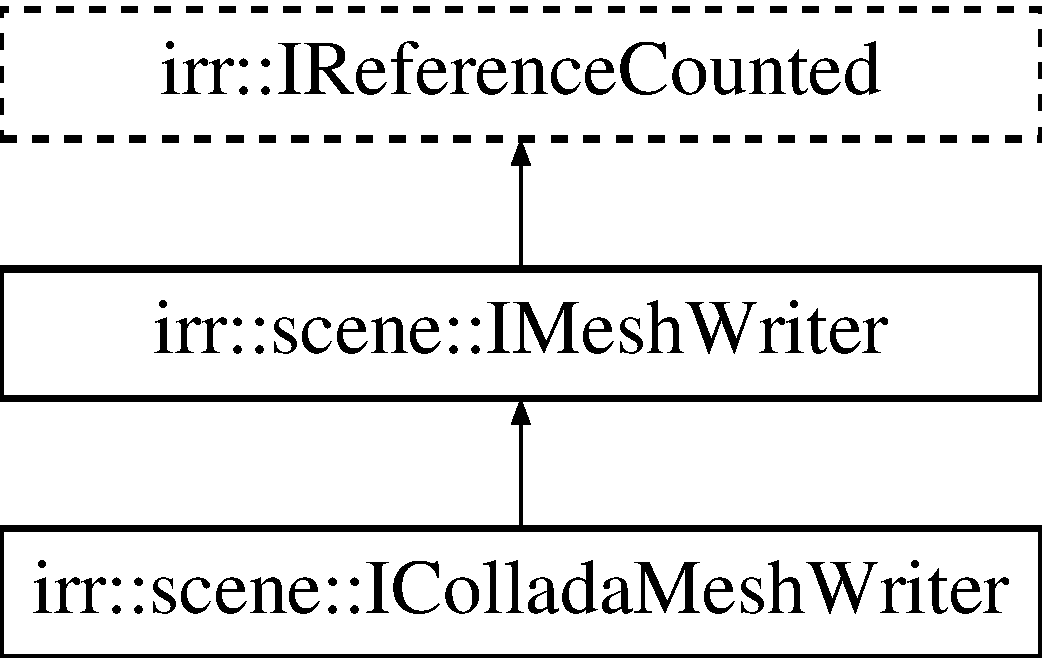
\includegraphics[height=3.000000cm]{classirr_1_1scene_1_1IColladaMeshWriter}
\end{center}
\end{figure}
\subsection*{Public Member Functions}
\begin{DoxyCompactItemize}
\item 
\mbox{\Hypertarget{classirr_1_1scene_1_1IColladaMeshWriter_a85ed9eb856663c6698e1f7c4535b9057}\label{classirr_1_1scene_1_1IColladaMeshWriter_a85ed9eb856663c6698e1f7c4535b9057}} 
virtual \hyperlink{classirr_1_1scene_1_1IColladaMeshWriter_a85ed9eb856663c6698e1f7c4535b9057}{$\sim$\+I\+Collada\+Mesh\+Writer} ()
\begin{DoxyCompactList}\small\item\em Destructor. \end{DoxyCompactList}\item 
\mbox{\Hypertarget{classirr_1_1scene_1_1IColladaMeshWriter_ad2e6e7617052c83d5f19d7811e0d5fd7}\label{classirr_1_1scene_1_1IColladaMeshWriter_ad2e6e7617052c83d5f19d7811e0d5fd7}} 
virtual bool \hyperlink{classirr_1_1scene_1_1IColladaMeshWriter_ad2e6e7617052c83d5f19d7811e0d5fd7}{write\+Scene} (\hyperlink{classirr_1_1io_1_1IWriteFile}{io\+::\+I\+Write\+File} $\ast$file, \hyperlink{classirr_1_1scene_1_1ISceneNode}{scene\+::\+I\+Scene\+Node} $\ast$root)=0
\begin{DoxyCompactList}\small\item\em writes a scene starting with the given node \end{DoxyCompactList}\item 
\mbox{\Hypertarget{classirr_1_1scene_1_1IColladaMeshWriter_a2fa67e9fcfefdc6cf71d682e9891d15e}\label{classirr_1_1scene_1_1IColladaMeshWriter_a2fa67e9fcfefdc6cf71d682e9891d15e}} 
virtual void \hyperlink{classirr_1_1scene_1_1IColladaMeshWriter_a2fa67e9fcfefdc6cf71d682e9891d15e}{set\+Write\+Textures} (bool write)
\begin{DoxyCompactList}\small\item\em Set if texture information should be written. \end{DoxyCompactList}\item 
\mbox{\Hypertarget{classirr_1_1scene_1_1IColladaMeshWriter_a55088db1ff55ebb1a657fac22f52386b}\label{classirr_1_1scene_1_1IColladaMeshWriter_a55088db1ff55ebb1a657fac22f52386b}} 
virtual bool \hyperlink{classirr_1_1scene_1_1IColladaMeshWriter_a55088db1ff55ebb1a657fac22f52386b}{get\+Write\+Textures} () const
\begin{DoxyCompactList}\small\item\em Get if texture information should be written. \end{DoxyCompactList}\item 
virtual void \hyperlink{classirr_1_1scene_1_1IColladaMeshWriter_acf1952c459b4b2bde5b479b6d9717c35}{set\+Write\+Default\+Scene} (bool write)
\begin{DoxyCompactList}\small\item\em Set if a default scene should be written when writing meshes. \end{DoxyCompactList}\item 
\mbox{\Hypertarget{classirr_1_1scene_1_1IColladaMeshWriter_a311c259b48fade63a30c9b5f422571d4}\label{classirr_1_1scene_1_1IColladaMeshWriter_a311c259b48fade63a30c9b5f422571d4}} 
virtual bool \hyperlink{classirr_1_1scene_1_1IColladaMeshWriter_a311c259b48fade63a30c9b5f422571d4}{get\+Write\+Default\+Scene} () const
\begin{DoxyCompactList}\small\item\em Get if a default scene should be written. \end{DoxyCompactList}\item 
\mbox{\Hypertarget{classirr_1_1scene_1_1IColladaMeshWriter_a410fb9e46db6250ff8bbf4ddb18ef1f2}\label{classirr_1_1scene_1_1IColladaMeshWriter_a410fb9e46db6250ff8bbf4ddb18ef1f2}} 
virtual void \hyperlink{classirr_1_1scene_1_1IColladaMeshWriter_a410fb9e46db6250ff8bbf4ddb18ef1f2}{set\+Ambient\+Light} (const \hyperlink{classirr_1_1video_1_1SColorf}{video\+::\+S\+Colorf} \&ambient\+Color)
\begin{DoxyCompactList}\small\item\em Sets ambient color of the scene to write. \end{DoxyCompactList}\item 
\mbox{\Hypertarget{classirr_1_1scene_1_1IColladaMeshWriter_af263653d1159795a9aeead92c4e94b44}\label{classirr_1_1scene_1_1IColladaMeshWriter_af263653d1159795a9aeead92c4e94b44}} 
virtual \hyperlink{classirr_1_1video_1_1SColorf}{video\+::\+S\+Colorf} \hyperlink{classirr_1_1scene_1_1IColladaMeshWriter_af263653d1159795a9aeead92c4e94b44}{get\+Ambient\+Light} () const
\begin{DoxyCompactList}\small\item\em Return ambient light of the scene which is written. \end{DoxyCompactList}\item 
virtual void \hyperlink{classirr_1_1scene_1_1IColladaMeshWriter_a25d2e1ff0bf04375c822800b0b3a4b01}{set\+Geometry\+Writing} (\hyperlink{namespaceirr_1_1scene_a179008e7c02889459edf81394dbd6959}{E\+\_\+\+C\+O\+L\+L\+A\+D\+A\+\_\+\+G\+E\+O\+M\+E\+T\+R\+Y\+\_\+\+W\+R\+I\+T\+I\+NG} write\+Style)
\begin{DoxyCompactList}\small\item\em Control when and how often a mesh is written. \end{DoxyCompactList}\item 
\mbox{\Hypertarget{classirr_1_1scene_1_1IColladaMeshWriter_ab83b1690e233d6742e716aa5a1cf32f2}\label{classirr_1_1scene_1_1IColladaMeshWriter_ab83b1690e233d6742e716aa5a1cf32f2}} 
virtual \hyperlink{namespaceirr_1_1scene_a179008e7c02889459edf81394dbd6959}{E\+\_\+\+C\+O\+L\+L\+A\+D\+A\+\_\+\+G\+E\+O\+M\+E\+T\+R\+Y\+\_\+\+W\+R\+I\+T\+I\+NG} \hyperlink{classirr_1_1scene_1_1IColladaMeshWriter_ab83b1690e233d6742e716aa5a1cf32f2}{get\+Geometry\+Writing} () const
\begin{DoxyCompactList}\small\item\em Get the current style of geometry writing. \end{DoxyCompactList}\item 
virtual void \hyperlink{classirr_1_1scene_1_1IColladaMeshWriter_af6f37ca4a1ef6238cc079f3f5d5eb612}{set\+Export\+S\+Materials\+Only\+Once} (bool export\+Once)
\begin{DoxyCompactList}\small\item\em Make certain there is only one collada material generated per Irrlicht material. \end{DoxyCompactList}\item 
virtual void \hyperlink{classirr_1_1scene_1_1IColladaMeshWriter_acffa89579171224f10e30f2c0d09f8c1}{set\+Properties} (\hyperlink{classirr_1_1scene_1_1IColladaMeshWriterProperties}{I\+Collada\+Mesh\+Writer\+Properties} $\ast$p)
\begin{DoxyCompactList}\small\item\em Set properties to use by the meshwriter instead of it\textquotesingle{}s default properties. \end{DoxyCompactList}\item 
\mbox{\Hypertarget{classirr_1_1scene_1_1IColladaMeshWriter_acce5ebec91c7f655da4557953df80a7a}\label{classirr_1_1scene_1_1IColladaMeshWriter_acce5ebec91c7f655da4557953df80a7a}} 
virtual \hyperlink{classirr_1_1scene_1_1IColladaMeshWriterProperties}{I\+Collada\+Mesh\+Writer\+Properties} $\ast$ \hyperlink{classirr_1_1scene_1_1IColladaMeshWriter_acce5ebec91c7f655da4557953df80a7a}{get\+Properties} () const
\begin{DoxyCompactList}\small\item\em Get properties which are currently used. \end{DoxyCompactList}\item 
\hyperlink{classirr_1_1scene_1_1IColladaMeshWriterProperties}{I\+Collada\+Mesh\+Writer\+Properties} $\ast$ \hyperlink{classirr_1_1scene_1_1IColladaMeshWriter_ae5d7e19d6d4bba65bcfb006c011cb6f2}{get\+Default\+Properties} () const
\begin{DoxyCompactList}\small\item\em Return the original default properties of the writer. \end{DoxyCompactList}\item 
\mbox{\Hypertarget{classirr_1_1scene_1_1IColladaMeshWriter_a7e48b43c91133e482e76da54849ef153}\label{classirr_1_1scene_1_1IColladaMeshWriter_a7e48b43c91133e482e76da54849ef153}} 
virtual void \hyperlink{classirr_1_1scene_1_1IColladaMeshWriter_a7e48b43c91133e482e76da54849ef153}{set\+Name\+Generator} (\hyperlink{classirr_1_1scene_1_1IColladaMeshWriterNames}{I\+Collada\+Mesh\+Writer\+Names} $\ast$name\+Generator)
\begin{DoxyCompactList}\small\item\em Install a generator to create custom names on export. \end{DoxyCompactList}\item 
\mbox{\Hypertarget{classirr_1_1scene_1_1IColladaMeshWriter_ad519f6ce64dcf1013b6fe0b9aaa67b40}\label{classirr_1_1scene_1_1IColladaMeshWriter_ad519f6ce64dcf1013b6fe0b9aaa67b40}} 
virtual \hyperlink{classirr_1_1scene_1_1IColladaMeshWriterNames}{I\+Collada\+Mesh\+Writer\+Names} $\ast$ \hyperlink{classirr_1_1scene_1_1IColladaMeshWriter_ad519f6ce64dcf1013b6fe0b9aaa67b40}{get\+Name\+Generator} () const
\begin{DoxyCompactList}\small\item\em Get currently used name generator. \end{DoxyCompactList}\item 
\hyperlink{classirr_1_1scene_1_1IColladaMeshWriterNames}{I\+Collada\+Mesh\+Writer\+Names} $\ast$ \hyperlink{classirr_1_1scene_1_1IColladaMeshWriter_acd10fcf2458271d59cf76284613288f6}{get\+Default\+Name\+Generator} () const
\begin{DoxyCompactList}\small\item\em Return the original default name generator of the writer. \end{DoxyCompactList}\item 
virtual \hyperlink{namespaceirr_1_1core_aef83fafbb1b36fcce44c07c9be23a7f2}{irr\+::core\+::stringw} \hyperlink{classirr_1_1scene_1_1IColladaMeshWriter_ac9c48beab095aa6f4cb4f696bb2ecd45}{to\+N\+C\+Name} (const \hyperlink{namespaceirr_1_1core_aef83fafbb1b36fcce44c07c9be23a7f2}{irr\+::core\+::stringw} \&old\+String, const \hyperlink{namespaceirr_1_1core_aef83fafbb1b36fcce44c07c9be23a7f2}{irr\+::core\+::stringw} \&prefix=\hyperlink{namespaceirr_1_1core_aef83fafbb1b36fcce44c07c9be23a7f2}{irr\+::core\+::stringw}(L\char`\"{}\+\_\+\+N\+C\+\_\+\char`\"{})) const =0
\begin{DoxyCompactList}\small\item\em Restrict the characters of old\+String a set of allowed characters in xs\+::\+N\+C\+Name and add the prefix. \end{DoxyCompactList}\end{DoxyCompactItemize}
\subsection*{Additional Inherited Members}


\subsection{Detailed Description}
Interface for writing meshes. 

\subsection{Member Function Documentation}
\mbox{\Hypertarget{classirr_1_1scene_1_1IColladaMeshWriter_acd10fcf2458271d59cf76284613288f6}\label{classirr_1_1scene_1_1IColladaMeshWriter_acd10fcf2458271d59cf76284613288f6}} 
\index{irr\+::scene\+::\+I\+Collada\+Mesh\+Writer@{irr\+::scene\+::\+I\+Collada\+Mesh\+Writer}!get\+Default\+Name\+Generator@{get\+Default\+Name\+Generator}}
\index{get\+Default\+Name\+Generator@{get\+Default\+Name\+Generator}!irr\+::scene\+::\+I\+Collada\+Mesh\+Writer@{irr\+::scene\+::\+I\+Collada\+Mesh\+Writer}}
\subsubsection{\texorpdfstring{get\+Default\+Name\+Generator()}{getDefaultNameGenerator()}}
{\footnotesize\ttfamily \hyperlink{classirr_1_1scene_1_1IColladaMeshWriterNames}{I\+Collada\+Mesh\+Writer\+Names}$\ast$ irr\+::scene\+::\+I\+Collada\+Mesh\+Writer\+::get\+Default\+Name\+Generator (\begin{DoxyParamCaption}{ }\end{DoxyParamCaption}) const\hspace{0.3cm}{\ttfamily [inline]}}



Return the original default name generator of the writer. 

You can use this pointer in your own generator to access and return default values. \mbox{\Hypertarget{classirr_1_1scene_1_1IColladaMeshWriter_ae5d7e19d6d4bba65bcfb006c011cb6f2}\label{classirr_1_1scene_1_1IColladaMeshWriter_ae5d7e19d6d4bba65bcfb006c011cb6f2}} 
\index{irr\+::scene\+::\+I\+Collada\+Mesh\+Writer@{irr\+::scene\+::\+I\+Collada\+Mesh\+Writer}!get\+Default\+Properties@{get\+Default\+Properties}}
\index{get\+Default\+Properties@{get\+Default\+Properties}!irr\+::scene\+::\+I\+Collada\+Mesh\+Writer@{irr\+::scene\+::\+I\+Collada\+Mesh\+Writer}}
\subsubsection{\texorpdfstring{get\+Default\+Properties()}{getDefaultProperties()}}
{\footnotesize\ttfamily \hyperlink{classirr_1_1scene_1_1IColladaMeshWriterProperties}{I\+Collada\+Mesh\+Writer\+Properties}$\ast$ irr\+::scene\+::\+I\+Collada\+Mesh\+Writer\+::get\+Default\+Properties (\begin{DoxyParamCaption}{ }\end{DoxyParamCaption}) const\hspace{0.3cm}{\ttfamily [inline]}}



Return the original default properties of the writer. 

You can use this pointer in your own properties to access and return default values. \mbox{\Hypertarget{classirr_1_1scene_1_1IColladaMeshWriter_af6f37ca4a1ef6238cc079f3f5d5eb612}\label{classirr_1_1scene_1_1IColladaMeshWriter_af6f37ca4a1ef6238cc079f3f5d5eb612}} 
\index{irr\+::scene\+::\+I\+Collada\+Mesh\+Writer@{irr\+::scene\+::\+I\+Collada\+Mesh\+Writer}!set\+Export\+S\+Materials\+Only\+Once@{set\+Export\+S\+Materials\+Only\+Once}}
\index{set\+Export\+S\+Materials\+Only\+Once@{set\+Export\+S\+Materials\+Only\+Once}!irr\+::scene\+::\+I\+Collada\+Mesh\+Writer@{irr\+::scene\+::\+I\+Collada\+Mesh\+Writer}}
\subsubsection{\texorpdfstring{set\+Export\+S\+Materials\+Only\+Once()}{setExportSMaterialsOnlyOnce()}}
{\footnotesize\ttfamily virtual void irr\+::scene\+::\+I\+Collada\+Mesh\+Writer\+::set\+Export\+S\+Materials\+Only\+Once (\begin{DoxyParamCaption}\item[{bool}]{export\+Once }\end{DoxyParamCaption})\hspace{0.3cm}{\ttfamily [inline]}, {\ttfamily [virtual]}}



Make certain there is only one collada material generated per Irrlicht material. 

Checks before creating a collada material-\/name if an identical irr\+:\+::video\+::\+S\+Material has been exported already. If so don\textquotesingle{}t export it with another name. This is set by default and leads to way smaller .dae files. Note that if you need to disable this flag for some reason you can still get a similar effect using the \hyperlink{classirr_1_1scene_1_1IColladaMeshWriterNames_acb5c8f38769d3fedcc76df73d9350c07}{I\+Collada\+Mesh\+Writer\+Names\+::name\+For\+Material} by returning identical names for identical materials there. \mbox{\Hypertarget{classirr_1_1scene_1_1IColladaMeshWriter_a25d2e1ff0bf04375c822800b0b3a4b01}\label{classirr_1_1scene_1_1IColladaMeshWriter_a25d2e1ff0bf04375c822800b0b3a4b01}} 
\index{irr\+::scene\+::\+I\+Collada\+Mesh\+Writer@{irr\+::scene\+::\+I\+Collada\+Mesh\+Writer}!set\+Geometry\+Writing@{set\+Geometry\+Writing}}
\index{set\+Geometry\+Writing@{set\+Geometry\+Writing}!irr\+::scene\+::\+I\+Collada\+Mesh\+Writer@{irr\+::scene\+::\+I\+Collada\+Mesh\+Writer}}
\subsubsection{\texorpdfstring{set\+Geometry\+Writing()}{setGeometryWriting()}}
{\footnotesize\ttfamily virtual void irr\+::scene\+::\+I\+Collada\+Mesh\+Writer\+::set\+Geometry\+Writing (\begin{DoxyParamCaption}\item[{\hyperlink{namespaceirr_1_1scene_a179008e7c02889459edf81394dbd6959}{E\+\_\+\+C\+O\+L\+L\+A\+D\+A\+\_\+\+G\+E\+O\+M\+E\+T\+R\+Y\+\_\+\+W\+R\+I\+T\+I\+NG}}]{write\+Style }\end{DoxyParamCaption})\hspace{0.3cm}{\ttfamily [inline]}, {\ttfamily [virtual]}}



Control when and how often a mesh is written. 

Optimally E\+C\+G\+I\+\_\+\+P\+E\+R\+\_\+\+M\+E\+SH would be always sufficent -\/ writing geometry once per mesh. Unfortunately many tools (at the time of writing this nearly all of them) have trouble on import when different materials are used per node. So when you override materials per node and importing the resuling collada has materials problems in other tools try using other values here. 
\begin{DoxyParams}{Parameters}
{\em write\+Style} & One of the E\+\_\+\+C\+O\+L\+L\+A\+D\+A\+\_\+\+G\+E\+O\+M\+E\+T\+R\+Y\+\_\+\+W\+R\+I\+T\+I\+NG settings. \\
\hline
\end{DoxyParams}
\mbox{\Hypertarget{classirr_1_1scene_1_1IColladaMeshWriter_acffa89579171224f10e30f2c0d09f8c1}\label{classirr_1_1scene_1_1IColladaMeshWriter_acffa89579171224f10e30f2c0d09f8c1}} 
\index{irr\+::scene\+::\+I\+Collada\+Mesh\+Writer@{irr\+::scene\+::\+I\+Collada\+Mesh\+Writer}!set\+Properties@{set\+Properties}}
\index{set\+Properties@{set\+Properties}!irr\+::scene\+::\+I\+Collada\+Mesh\+Writer@{irr\+::scene\+::\+I\+Collada\+Mesh\+Writer}}
\subsubsection{\texorpdfstring{set\+Properties()}{setProperties()}}
{\footnotesize\ttfamily virtual void irr\+::scene\+::\+I\+Collada\+Mesh\+Writer\+::set\+Properties (\begin{DoxyParamCaption}\item[{\hyperlink{classirr_1_1scene_1_1IColladaMeshWriterProperties}{I\+Collada\+Mesh\+Writer\+Properties} $\ast$}]{p }\end{DoxyParamCaption})\hspace{0.3cm}{\ttfamily [inline]}, {\ttfamily [virtual]}}



Set properties to use by the meshwriter instead of it\textquotesingle{}s default properties. 

Overloading properties with an own class allows modifying the writing process in certain ways. By default properties are set to the Default\+Properties. \mbox{\Hypertarget{classirr_1_1scene_1_1IColladaMeshWriter_acf1952c459b4b2bde5b479b6d9717c35}\label{classirr_1_1scene_1_1IColladaMeshWriter_acf1952c459b4b2bde5b479b6d9717c35}} 
\index{irr\+::scene\+::\+I\+Collada\+Mesh\+Writer@{irr\+::scene\+::\+I\+Collada\+Mesh\+Writer}!set\+Write\+Default\+Scene@{set\+Write\+Default\+Scene}}
\index{set\+Write\+Default\+Scene@{set\+Write\+Default\+Scene}!irr\+::scene\+::\+I\+Collada\+Mesh\+Writer@{irr\+::scene\+::\+I\+Collada\+Mesh\+Writer}}
\subsubsection{\texorpdfstring{set\+Write\+Default\+Scene()}{setWriteDefaultScene()}}
{\footnotesize\ttfamily virtual void irr\+::scene\+::\+I\+Collada\+Mesh\+Writer\+::set\+Write\+Default\+Scene (\begin{DoxyParamCaption}\item[{bool}]{write }\end{DoxyParamCaption})\hspace{0.3cm}{\ttfamily [inline]}, {\ttfamily [virtual]}}



Set if a default scene should be written when writing meshes. 

Many collada readers fail to read a mesh if the collada files doesn\textquotesingle{}t contain a scene as well. The scene is doing an instantiation of the mesh. When using write\+Scene this flag is ignored (as we have scene there already) \mbox{\Hypertarget{classirr_1_1scene_1_1IColladaMeshWriter_ac9c48beab095aa6f4cb4f696bb2ecd45}\label{classirr_1_1scene_1_1IColladaMeshWriter_ac9c48beab095aa6f4cb4f696bb2ecd45}} 
\index{irr\+::scene\+::\+I\+Collada\+Mesh\+Writer@{irr\+::scene\+::\+I\+Collada\+Mesh\+Writer}!to\+N\+C\+Name@{to\+N\+C\+Name}}
\index{to\+N\+C\+Name@{to\+N\+C\+Name}!irr\+::scene\+::\+I\+Collada\+Mesh\+Writer@{irr\+::scene\+::\+I\+Collada\+Mesh\+Writer}}
\subsubsection{\texorpdfstring{to\+N\+C\+Name()}{toNCName()}}
{\footnotesize\ttfamily virtual \hyperlink{namespaceirr_1_1core_aef83fafbb1b36fcce44c07c9be23a7f2}{irr\+::core\+::stringw} irr\+::scene\+::\+I\+Collada\+Mesh\+Writer\+::to\+N\+C\+Name (\begin{DoxyParamCaption}\item[{const \hyperlink{namespaceirr_1_1core_aef83fafbb1b36fcce44c07c9be23a7f2}{irr\+::core\+::stringw} \&}]{old\+String,  }\item[{const \hyperlink{namespaceirr_1_1core_aef83fafbb1b36fcce44c07c9be23a7f2}{irr\+::core\+::stringw} \&}]{prefix = {\ttfamily \hyperlink{namespaceirr_1_1core_aef83fafbb1b36fcce44c07c9be23a7f2}{irr\+::core\+::stringw}(L\char`\"{}\+\_\+NC\+\_\+\char`\"{})} }\end{DoxyParamCaption}) const\hspace{0.3cm}{\ttfamily [pure virtual]}}



Restrict the characters of old\+String a set of allowed characters in xs\+::\+N\+C\+Name and add the prefix. 

A tool function to help when using a custom name generator to generative valid names for collada names and id\textquotesingle{}s. 

The documentation for this class was generated from the following file\+:\begin{DoxyCompactItemize}
\item 
indie\+\_\+share/controller/include/I\+Collada\+Mesh\+Writer.\+h\end{DoxyCompactItemize}

\hypertarget{classirr_1_1scene_1_1IColladaMeshWriterNames}{}\section{irr\+:\+:scene\+:\+:I\+Collada\+Mesh\+Writer\+Names Class Reference}
\label{classirr_1_1scene_1_1IColladaMeshWriterNames}\index{irr\+::scene\+::\+I\+Collada\+Mesh\+Writer\+Names@{irr\+::scene\+::\+I\+Collada\+Mesh\+Writer\+Names}}


Callback interface to use custom names on collada writing.  




{\ttfamily \#include $<$I\+Collada\+Mesh\+Writer.\+h$>$}

Inheritance diagram for irr\+:\+:scene\+:\+:I\+Collada\+Mesh\+Writer\+Names\+:\begin{figure}[H]
\begin{center}
\leavevmode
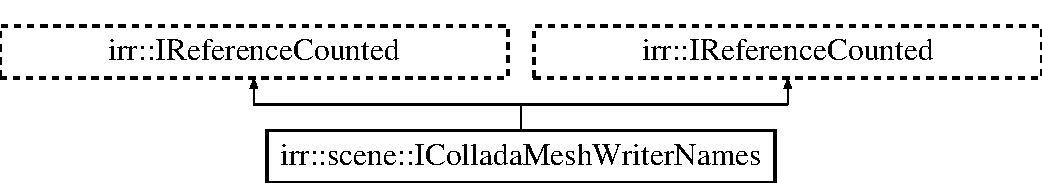
\includegraphics[height=2.000000cm]{classirr_1_1scene_1_1IColladaMeshWriterNames}
\end{center}
\end{figure}
\subsection*{Public Member Functions}
\begin{DoxyCompactItemize}
\item 
virtual \hyperlink{namespaceirr_1_1core_aef83fafbb1b36fcce44c07c9be23a7f2}{irr\+::core\+::stringw} \hyperlink{classirr_1_1scene_1_1IColladaMeshWriterNames_a2d36f1dee5904b3c622363282761ed0d}{name\+For\+Mesh} (const \hyperlink{classirr_1_1scene_1_1IMesh}{scene\+::\+I\+Mesh} $\ast$mesh, int instance)=0
\begin{DoxyCompactList}\small\item\em Return a unique name for the given mesh. \end{DoxyCompactList}\item 
virtual \hyperlink{namespaceirr_1_1core_aef83fafbb1b36fcce44c07c9be23a7f2}{irr\+::core\+::stringw} \hyperlink{classirr_1_1scene_1_1IColladaMeshWriterNames_a60d3fdad90edc25b0305c91be15b255f}{name\+For\+Node} (const \hyperlink{classirr_1_1scene_1_1ISceneNode}{scene\+::\+I\+Scene\+Node} $\ast$node)=0
\begin{DoxyCompactList}\small\item\em Return a unique name for the given node. \end{DoxyCompactList}\item 
virtual \hyperlink{namespaceirr_1_1core_aef83fafbb1b36fcce44c07c9be23a7f2}{irr\+::core\+::stringw} \hyperlink{classirr_1_1scene_1_1IColladaMeshWriterNames_acb5c8f38769d3fedcc76df73d9350c07}{name\+For\+Material} (const \hyperlink{classirr_1_1video_1_1SMaterial}{video\+::\+S\+Material} \&material, int material\+Id, const \hyperlink{classirr_1_1scene_1_1IMesh}{scene\+::\+I\+Mesh} $\ast$mesh, const \hyperlink{classirr_1_1scene_1_1ISceneNode}{scene\+::\+I\+Scene\+Node} $\ast$node)=0
\begin{DoxyCompactList}\small\item\em Return a name for the material. \end{DoxyCompactList}\end{DoxyCompactItemize}
\subsection*{Additional Inherited Members}


\subsection{Detailed Description}
Callback interface to use custom names on collada writing. 

You can either modify names and id\textquotesingle{}s written to collada or you can use this interface to just find out which names are used on writing. 

\subsection{Member Function Documentation}
\mbox{\Hypertarget{classirr_1_1scene_1_1IColladaMeshWriterNames_acb5c8f38769d3fedcc76df73d9350c07}\label{classirr_1_1scene_1_1IColladaMeshWriterNames_acb5c8f38769d3fedcc76df73d9350c07}} 
\index{irr\+::scene\+::\+I\+Collada\+Mesh\+Writer\+Names@{irr\+::scene\+::\+I\+Collada\+Mesh\+Writer\+Names}!name\+For\+Material@{name\+For\+Material}}
\index{name\+For\+Material@{name\+For\+Material}!irr\+::scene\+::\+I\+Collada\+Mesh\+Writer\+Names@{irr\+::scene\+::\+I\+Collada\+Mesh\+Writer\+Names}}
\subsubsection{\texorpdfstring{name\+For\+Material()}{nameForMaterial()}}
{\footnotesize\ttfamily virtual \hyperlink{namespaceirr_1_1core_aef83fafbb1b36fcce44c07c9be23a7f2}{irr\+::core\+::stringw} irr\+::scene\+::\+I\+Collada\+Mesh\+Writer\+Names\+::name\+For\+Material (\begin{DoxyParamCaption}\item[{const \hyperlink{classirr_1_1video_1_1SMaterial}{video\+::\+S\+Material} \&}]{material,  }\item[{int}]{material\+Id,  }\item[{const \hyperlink{classirr_1_1scene_1_1IMesh}{scene\+::\+I\+Mesh} $\ast$}]{mesh,  }\item[{const \hyperlink{classirr_1_1scene_1_1ISceneNode}{scene\+::\+I\+Scene\+Node} $\ast$}]{node }\end{DoxyParamCaption})\hspace{0.3cm}{\ttfamily [pure virtual]}}



Return a name for the material. 

There is one material created in the writer for each unique name. So you can use this to control the number of materials which get written. For example Irrlicht does by default write one material for each material instanced by a node. So if you know that in your application material instances per node are identical between different nodes you can reduce the number of exported materials using that knowledge by using identical names for such shared materials. Names must follow the xs\+::\+N\+C\+Name standard to be valid, you can run them through \hyperlink{classirr_1_1scene_1_1IColladaMeshWriter_ac9c48beab095aa6f4cb4f696bb2ecd45}{I\+Collada\+Mesh\+Writer\+::to\+N\+C\+Name} to ensure that. \mbox{\Hypertarget{classirr_1_1scene_1_1IColladaMeshWriterNames_a2d36f1dee5904b3c622363282761ed0d}\label{classirr_1_1scene_1_1IColladaMeshWriterNames_a2d36f1dee5904b3c622363282761ed0d}} 
\index{irr\+::scene\+::\+I\+Collada\+Mesh\+Writer\+Names@{irr\+::scene\+::\+I\+Collada\+Mesh\+Writer\+Names}!name\+For\+Mesh@{name\+For\+Mesh}}
\index{name\+For\+Mesh@{name\+For\+Mesh}!irr\+::scene\+::\+I\+Collada\+Mesh\+Writer\+Names@{irr\+::scene\+::\+I\+Collada\+Mesh\+Writer\+Names}}
\subsubsection{\texorpdfstring{name\+For\+Mesh()}{nameForMesh()}}
{\footnotesize\ttfamily virtual \hyperlink{namespaceirr_1_1core_aef83fafbb1b36fcce44c07c9be23a7f2}{irr\+::core\+::stringw} irr\+::scene\+::\+I\+Collada\+Mesh\+Writer\+Names\+::name\+For\+Mesh (\begin{DoxyParamCaption}\item[{const \hyperlink{classirr_1_1scene_1_1IMesh}{scene\+::\+I\+Mesh} $\ast$}]{mesh,  }\item[{int}]{instance }\end{DoxyParamCaption})\hspace{0.3cm}{\ttfamily [pure virtual]}}



Return a unique name for the given mesh. 

Note that names really must be unique here per mesh-\/pointer, so mostly it\textquotesingle{}s a good idea to return the name\+For\+Mesh from \hyperlink{classirr_1_1scene_1_1IColladaMeshWriter_acd10fcf2458271d59cf76284613288f6}{I\+Collada\+Mesh\+Writer\+::get\+Default\+Name\+Generator()}. Also names must follow the xs\+::\+N\+C\+Name standard to be valid, you can run them through \hyperlink{classirr_1_1scene_1_1IColladaMeshWriter_ac9c48beab095aa6f4cb4f696bb2ecd45}{I\+Collada\+Mesh\+Writer\+::to\+N\+C\+Name} to ensure that. 
\begin{DoxyParams}{Parameters}
{\em mesh} & Pointer to the mesh which needs a name \\
\hline
{\em instance} & When E\+\_\+\+C\+O\+L\+L\+A\+D\+A\+\_\+\+G\+E\+O\+M\+E\+T\+R\+Y\+\_\+\+W\+R\+I\+T\+I\+NG is not E\+C\+G\+I\+\_\+\+P\+E\+R\+\_\+\+M\+E\+SH then several instances of the same mesh can be written and this counts them. \\
\hline
\end{DoxyParams}
\mbox{\Hypertarget{classirr_1_1scene_1_1IColladaMeshWriterNames_a60d3fdad90edc25b0305c91be15b255f}\label{classirr_1_1scene_1_1IColladaMeshWriterNames_a60d3fdad90edc25b0305c91be15b255f}} 
\index{irr\+::scene\+::\+I\+Collada\+Mesh\+Writer\+Names@{irr\+::scene\+::\+I\+Collada\+Mesh\+Writer\+Names}!name\+For\+Node@{name\+For\+Node}}
\index{name\+For\+Node@{name\+For\+Node}!irr\+::scene\+::\+I\+Collada\+Mesh\+Writer\+Names@{irr\+::scene\+::\+I\+Collada\+Mesh\+Writer\+Names}}
\subsubsection{\texorpdfstring{name\+For\+Node()}{nameForNode()}}
{\footnotesize\ttfamily virtual \hyperlink{namespaceirr_1_1core_aef83fafbb1b36fcce44c07c9be23a7f2}{irr\+::core\+::stringw} irr\+::scene\+::\+I\+Collada\+Mesh\+Writer\+Names\+::name\+For\+Node (\begin{DoxyParamCaption}\item[{const \hyperlink{classirr_1_1scene_1_1ISceneNode}{scene\+::\+I\+Scene\+Node} $\ast$}]{node }\end{DoxyParamCaption})\hspace{0.3cm}{\ttfamily [pure virtual]}}



Return a unique name for the given node. 

Note that names really must be unique here per node-\/pointer, so mostly it\textquotesingle{}s a good idea to return the name\+For\+Node from \hyperlink{classirr_1_1scene_1_1IColladaMeshWriter_acd10fcf2458271d59cf76284613288f6}{I\+Collada\+Mesh\+Writer\+::get\+Default\+Name\+Generator()}. Also names must follow the xs\+::\+N\+C\+Name standard to be valid, you can run them through \hyperlink{classirr_1_1scene_1_1IColladaMeshWriter_ac9c48beab095aa6f4cb4f696bb2ecd45}{I\+Collada\+Mesh\+Writer\+::to\+N\+C\+Name} to ensure that. 

The documentation for this class was generated from the following file\+:\begin{DoxyCompactItemize}
\item 
indie\+\_\+share/controller/include/I\+Collada\+Mesh\+Writer.\+h\end{DoxyCompactItemize}

\hypertarget{classirr_1_1scene_1_1IColladaMeshWriterProperties}{}\section{irr\+:\+:scene\+:\+:I\+Collada\+Mesh\+Writer\+Properties Class Reference}
\label{classirr_1_1scene_1_1IColladaMeshWriterProperties}\index{irr\+::scene\+::\+I\+Collada\+Mesh\+Writer\+Properties@{irr\+::scene\+::\+I\+Collada\+Mesh\+Writer\+Properties}}


Callback interface for properties which can be used to influence collada writing.  




{\ttfamily \#include $<$I\+Collada\+Mesh\+Writer.\+h$>$}

Inheritance diagram for irr\+:\+:scene\+:\+:I\+Collada\+Mesh\+Writer\+Properties\+:\begin{figure}[H]
\begin{center}
\leavevmode
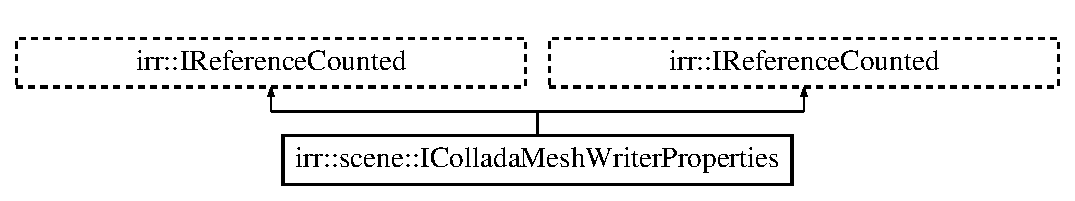
\includegraphics[height=2.000000cm]{classirr_1_1scene_1_1IColladaMeshWriterProperties}
\end{center}
\end{figure}
\subsection*{Public Member Functions}
\begin{DoxyCompactItemize}
\item 
\mbox{\Hypertarget{classirr_1_1scene_1_1IColladaMeshWriterProperties_abc0fb19092b53bdf48be8cc97a2af63b}\label{classirr_1_1scene_1_1IColladaMeshWriterProperties_abc0fb19092b53bdf48be8cc97a2af63b}} 
virtual \hyperlink{namespaceirr_1_1scene_a9ec31e84e05295892488296b0741e2b1}{E\+\_\+\+C\+O\+L\+L\+A\+D\+A\+\_\+\+T\+E\+C\+H\+N\+I\+Q\+U\+E\+\_\+\+FX} \hyperlink{classirr_1_1scene_1_1IColladaMeshWriterProperties_abc0fb19092b53bdf48be8cc97a2af63b}{get\+Technique\+Fx} (const \hyperlink{classirr_1_1video_1_1SMaterial}{video\+::\+S\+Material} \&material) const =0
\begin{DoxyCompactList}\small\item\em Which lighting model should be used in the technique (FX) section when exporting effects (materials) \end{DoxyCompactList}\item 
virtual \hyperlink{namespaceirr_ac66849b7a6ed16e30ebede579f9b47c6}{s32} \hyperlink{classirr_1_1scene_1_1IColladaMeshWriterProperties_a171287213537036be889a36ae4896c0e}{get\+Texture\+Idx} (const \hyperlink{classirr_1_1video_1_1SMaterial}{video\+::\+S\+Material} \&material, \hyperlink{namespaceirr_1_1scene_a6204218341c6b449d879cd8367b2f8d8}{E\+\_\+\+C\+O\+L\+L\+A\+D\+A\+\_\+\+C\+O\+L\+O\+R\+\_\+\+S\+A\+M\+P\+L\+ER} cs) const =0
\begin{DoxyCompactList}\small\item\em Which texture index should be used when writing the texture of the given sampler color. \end{DoxyCompactList}\item 
virtual \hyperlink{namespaceirr_1_1scene_a61cba210038d6d843b81d9282f1cac7e}{E\+\_\+\+C\+O\+L\+L\+A\+D\+A\+\_\+\+I\+R\+R\+\_\+\+C\+O\+L\+OR} \hyperlink{classirr_1_1scene_1_1IColladaMeshWriterProperties_ab347c50cc9b291625d051a919d8772ab}{get\+Color\+Mapping} (const \hyperlink{classirr_1_1video_1_1SMaterial}{video\+::\+S\+Material} \&material, \hyperlink{namespaceirr_1_1scene_a6204218341c6b449d879cd8367b2f8d8}{E\+\_\+\+C\+O\+L\+L\+A\+D\+A\+\_\+\+C\+O\+L\+O\+R\+\_\+\+S\+A\+M\+P\+L\+ER} cs) const =0
\begin{DoxyCompactList}\small\item\em Return which color from Irrlicht should be used for the color requested by collada. \end{DoxyCompactList}\item 
virtual \hyperlink{classirr_1_1video_1_1SColor}{video\+::\+S\+Color} \hyperlink{classirr_1_1scene_1_1IColladaMeshWriterProperties_a8028af2323dab63df4bdfeb292ec48cd}{get\+Custom\+Color} (const \hyperlink{classirr_1_1video_1_1SMaterial}{video\+::\+S\+Material} \&material, \hyperlink{namespaceirr_1_1scene_a6204218341c6b449d879cd8367b2f8d8}{E\+\_\+\+C\+O\+L\+L\+A\+D\+A\+\_\+\+C\+O\+L\+O\+R\+\_\+\+S\+A\+M\+P\+L\+ER} cs) const =0
\begin{DoxyCompactList}\small\item\em Return custom colors for certain color types requested by collada. \end{DoxyCompactList}\item 
virtual \hyperlink{namespaceirr_1_1scene_af7dadd5b96b683cfe1800f343c4f6619}{E\+\_\+\+C\+O\+L\+L\+A\+D\+A\+\_\+\+T\+R\+A\+N\+S\+P\+A\+R\+E\+N\+T\+\_\+\+FX} \hyperlink{classirr_1_1scene_1_1IColladaMeshWriterProperties_a0d934ae86d3e587ae22f74d775bbfa36}{get\+Transparent\+Fx} (const \hyperlink{classirr_1_1video_1_1SMaterial}{video\+::\+S\+Material} \&material) const =0
\begin{DoxyCompactList}\small\item\em Return the transparence color interpretation. \end{DoxyCompactList}\item 
virtual \hyperlink{namespaceirr_a0277be98d67dc26ff93b1a6a1d086b07}{f32} \hyperlink{classirr_1_1scene_1_1IColladaMeshWriterProperties_ac547e1f89f4655751ecd570ad70d010b}{get\+Transparency} (const \hyperlink{classirr_1_1video_1_1SMaterial}{video\+::\+S\+Material} \&material) const =0
\begin{DoxyCompactList}\small\item\em Transparency value for that material. \end{DoxyCompactList}\item 
virtual \hyperlink{namespaceirr_a0277be98d67dc26ff93b1a6a1d086b07}{f32} \hyperlink{classirr_1_1scene_1_1IColladaMeshWriterProperties_ad880b5fc91114049b20347a31199b2a9}{get\+Reflectivity} (const \hyperlink{classirr_1_1video_1_1SMaterial}{video\+::\+S\+Material} \&material) const =0
\begin{DoxyCompactList}\small\item\em Reflectivity value for that material. \end{DoxyCompactList}\item 
virtual \hyperlink{namespaceirr_a0277be98d67dc26ff93b1a6a1d086b07}{f32} \hyperlink{classirr_1_1scene_1_1IColladaMeshWriterProperties_ab7ec58f708ebebe941246e6c78b0691d}{get\+Index\+Of\+Refraction} (const \hyperlink{classirr_1_1video_1_1SMaterial}{video\+::\+S\+Material} \&material) const =0
\begin{DoxyCompactList}\small\item\em Return index of refraction for that material. \end{DoxyCompactList}\item 
\mbox{\Hypertarget{classirr_1_1scene_1_1IColladaMeshWriterProperties_af24d1c12b3f4168407c078bd7fc3dc82}\label{classirr_1_1scene_1_1IColladaMeshWriterProperties_af24d1c12b3f4168407c078bd7fc3dc82}} 
virtual bool \hyperlink{classirr_1_1scene_1_1IColladaMeshWriterProperties_af24d1c12b3f4168407c078bd7fc3dc82}{is\+Exportable} (const \hyperlink{classirr_1_1scene_1_1ISceneNode}{irr\+::scene\+::\+I\+Scene\+Node} $\ast$node) const =0
\begin{DoxyCompactList}\small\item\em Should node be used in scene export? (only needed for scene-\/writing, ignored in mesh-\/writing) By default all visible nodes are exported. \end{DoxyCompactList}\item 
\mbox{\Hypertarget{classirr_1_1scene_1_1IColladaMeshWriterProperties_ac6d9e1583642ac777471bd9225d72007}\label{classirr_1_1scene_1_1IColladaMeshWriterProperties_ac6d9e1583642ac777471bd9225d72007}} 
virtual \hyperlink{classirr_1_1scene_1_1IMesh}{I\+Mesh} $\ast$ \hyperlink{classirr_1_1scene_1_1IColladaMeshWriterProperties_ac6d9e1583642ac777471bd9225d72007}{get\+Mesh} (\hyperlink{classirr_1_1scene_1_1ISceneNode}{irr\+::scene\+::\+I\+Scene\+Node} $\ast$node)=0
\begin{DoxyCompactList}\small\item\em Return the mesh for the given node. If it has no mesh or shouldn\textquotesingle{}t export it\textquotesingle{}s mesh you can return 0 in which case only the transformation matrix of the node will be used. \end{DoxyCompactList}\item 
virtual bool \hyperlink{classirr_1_1scene_1_1IColladaMeshWriterProperties_a9c10df4dc3602efbba6a47b34e2f8f4b}{use\+Node\+Material} (const \hyperlink{classirr_1_1scene_1_1ISceneNode}{scene\+::\+I\+Scene\+Node} $\ast$node) const =0
\begin{DoxyCompactList}\small\item\em Return if the node has it\textquotesingle{}s own material overwriting the mesh-\/materials. \end{DoxyCompactList}\item 
\mbox{\Hypertarget{classirr_1_1scene_1_1IColladaMeshWriterProperties_abc0fb19092b53bdf48be8cc97a2af63b}\label{classirr_1_1scene_1_1IColladaMeshWriterProperties_abc0fb19092b53bdf48be8cc97a2af63b}} 
virtual \hyperlink{namespaceirr_1_1scene_a9ec31e84e05295892488296b0741e2b1}{E\+\_\+\+C\+O\+L\+L\+A\+D\+A\+\_\+\+T\+E\+C\+H\+N\+I\+Q\+U\+E\+\_\+\+FX} \hyperlink{classirr_1_1scene_1_1IColladaMeshWriterProperties_abc0fb19092b53bdf48be8cc97a2af63b}{get\+Technique\+Fx} (const \hyperlink{classirr_1_1video_1_1SMaterial}{video\+::\+S\+Material} \&material) const =0
\begin{DoxyCompactList}\small\item\em Which lighting model should be used in the technique (FX) section when exporting effects (materials) \end{DoxyCompactList}\item 
virtual \hyperlink{namespaceirr_ac66849b7a6ed16e30ebede579f9b47c6}{s32} \hyperlink{classirr_1_1scene_1_1IColladaMeshWriterProperties_a171287213537036be889a36ae4896c0e}{get\+Texture\+Idx} (const \hyperlink{classirr_1_1video_1_1SMaterial}{video\+::\+S\+Material} \&material, \hyperlink{namespaceirr_1_1scene_a6204218341c6b449d879cd8367b2f8d8}{E\+\_\+\+C\+O\+L\+L\+A\+D\+A\+\_\+\+C\+O\+L\+O\+R\+\_\+\+S\+A\+M\+P\+L\+ER} cs) const =0
\begin{DoxyCompactList}\small\item\em Which texture index should be used when writing the texture of the given sampler color. \end{DoxyCompactList}\item 
virtual \hyperlink{namespaceirr_1_1scene_a61cba210038d6d843b81d9282f1cac7e}{E\+\_\+\+C\+O\+L\+L\+A\+D\+A\+\_\+\+I\+R\+R\+\_\+\+C\+O\+L\+OR} \hyperlink{classirr_1_1scene_1_1IColladaMeshWriterProperties_ab347c50cc9b291625d051a919d8772ab}{get\+Color\+Mapping} (const \hyperlink{classirr_1_1video_1_1SMaterial}{video\+::\+S\+Material} \&material, \hyperlink{namespaceirr_1_1scene_a6204218341c6b449d879cd8367b2f8d8}{E\+\_\+\+C\+O\+L\+L\+A\+D\+A\+\_\+\+C\+O\+L\+O\+R\+\_\+\+S\+A\+M\+P\+L\+ER} cs) const =0
\begin{DoxyCompactList}\small\item\em Return which color from Irrlicht should be used for the color requested by collada. \end{DoxyCompactList}\item 
virtual \hyperlink{classirr_1_1video_1_1SColor}{video\+::\+S\+Color} \hyperlink{classirr_1_1scene_1_1IColladaMeshWriterProperties_a8028af2323dab63df4bdfeb292ec48cd}{get\+Custom\+Color} (const \hyperlink{classirr_1_1video_1_1SMaterial}{video\+::\+S\+Material} \&material, \hyperlink{namespaceirr_1_1scene_a6204218341c6b449d879cd8367b2f8d8}{E\+\_\+\+C\+O\+L\+L\+A\+D\+A\+\_\+\+C\+O\+L\+O\+R\+\_\+\+S\+A\+M\+P\+L\+ER} cs) const =0
\begin{DoxyCompactList}\small\item\em Return custom colors for certain color types requested by collada. \end{DoxyCompactList}\item 
virtual \hyperlink{namespaceirr_1_1scene_af7dadd5b96b683cfe1800f343c4f6619}{E\+\_\+\+C\+O\+L\+L\+A\+D\+A\+\_\+\+T\+R\+A\+N\+S\+P\+A\+R\+E\+N\+T\+\_\+\+FX} \hyperlink{classirr_1_1scene_1_1IColladaMeshWriterProperties_a0d934ae86d3e587ae22f74d775bbfa36}{get\+Transparent\+Fx} (const \hyperlink{classirr_1_1video_1_1SMaterial}{video\+::\+S\+Material} \&material) const =0
\begin{DoxyCompactList}\small\item\em Return the transparence color interpretation. \end{DoxyCompactList}\item 
virtual \hyperlink{namespaceirr_a0277be98d67dc26ff93b1a6a1d086b07}{f32} \hyperlink{classirr_1_1scene_1_1IColladaMeshWriterProperties_ac547e1f89f4655751ecd570ad70d010b}{get\+Transparency} (const \hyperlink{classirr_1_1video_1_1SMaterial}{video\+::\+S\+Material} \&material) const =0
\begin{DoxyCompactList}\small\item\em Transparency value for that material. \end{DoxyCompactList}\item 
virtual \hyperlink{namespaceirr_a0277be98d67dc26ff93b1a6a1d086b07}{f32} \hyperlink{classirr_1_1scene_1_1IColladaMeshWriterProperties_ad880b5fc91114049b20347a31199b2a9}{get\+Reflectivity} (const \hyperlink{classirr_1_1video_1_1SMaterial}{video\+::\+S\+Material} \&material) const =0
\begin{DoxyCompactList}\small\item\em Reflectivity value for that material. \end{DoxyCompactList}\item 
virtual \hyperlink{namespaceirr_a0277be98d67dc26ff93b1a6a1d086b07}{f32} \hyperlink{classirr_1_1scene_1_1IColladaMeshWriterProperties_ab7ec58f708ebebe941246e6c78b0691d}{get\+Index\+Of\+Refraction} (const \hyperlink{classirr_1_1video_1_1SMaterial}{video\+::\+S\+Material} \&material) const =0
\begin{DoxyCompactList}\small\item\em Return index of refraction for that material. \end{DoxyCompactList}\item 
\mbox{\Hypertarget{classirr_1_1scene_1_1IColladaMeshWriterProperties_af24d1c12b3f4168407c078bd7fc3dc82}\label{classirr_1_1scene_1_1IColladaMeshWriterProperties_af24d1c12b3f4168407c078bd7fc3dc82}} 
virtual bool \hyperlink{classirr_1_1scene_1_1IColladaMeshWriterProperties_af24d1c12b3f4168407c078bd7fc3dc82}{is\+Exportable} (const \hyperlink{classirr_1_1scene_1_1ISceneNode}{irr\+::scene\+::\+I\+Scene\+Node} $\ast$node) const =0
\begin{DoxyCompactList}\small\item\em Should node be used in scene export? (only needed for scene-\/writing, ignored in mesh-\/writing) By default all visible nodes are exported. \end{DoxyCompactList}\item 
\mbox{\Hypertarget{classirr_1_1scene_1_1IColladaMeshWriterProperties_ac6d9e1583642ac777471bd9225d72007}\label{classirr_1_1scene_1_1IColladaMeshWriterProperties_ac6d9e1583642ac777471bd9225d72007}} 
virtual \hyperlink{classirr_1_1scene_1_1IMesh}{I\+Mesh} $\ast$ \hyperlink{classirr_1_1scene_1_1IColladaMeshWriterProperties_ac6d9e1583642ac777471bd9225d72007}{get\+Mesh} (\hyperlink{classirr_1_1scene_1_1ISceneNode}{irr\+::scene\+::\+I\+Scene\+Node} $\ast$node)=0
\begin{DoxyCompactList}\small\item\em Return the mesh for the given node. If it has no mesh or shouldn\textquotesingle{}t export it\textquotesingle{}s mesh you can return 0 in which case only the transformation matrix of the node will be used. \end{DoxyCompactList}\item 
virtual bool \hyperlink{classirr_1_1scene_1_1IColladaMeshWriterProperties_a9c10df4dc3602efbba6a47b34e2f8f4b}{use\+Node\+Material} (const \hyperlink{classirr_1_1scene_1_1ISceneNode}{scene\+::\+I\+Scene\+Node} $\ast$node) const =0
\begin{DoxyCompactList}\small\item\em Return if the node has it\textquotesingle{}s own material overwriting the mesh-\/materials. \end{DoxyCompactList}\end{DoxyCompactItemize}
\subsection*{Additional Inherited Members}


\subsection{Detailed Description}
Callback interface for properties which can be used to influence collada writing. 

\subsection{Member Function Documentation}
\mbox{\Hypertarget{classirr_1_1scene_1_1IColladaMeshWriterProperties_ab347c50cc9b291625d051a919d8772ab}\label{classirr_1_1scene_1_1IColladaMeshWriterProperties_ab347c50cc9b291625d051a919d8772ab}} 
\index{irr\+::scene\+::\+I\+Collada\+Mesh\+Writer\+Properties@{irr\+::scene\+::\+I\+Collada\+Mesh\+Writer\+Properties}!get\+Color\+Mapping@{get\+Color\+Mapping}}
\index{get\+Color\+Mapping@{get\+Color\+Mapping}!irr\+::scene\+::\+I\+Collada\+Mesh\+Writer\+Properties@{irr\+::scene\+::\+I\+Collada\+Mesh\+Writer\+Properties}}
\subsubsection{\texorpdfstring{get\+Color\+Mapping()}{getColorMapping()}\hspace{0.1cm}{\footnotesize\ttfamily [1/2]}}
{\footnotesize\ttfamily virtual \hyperlink{namespaceirr_1_1scene_a61cba210038d6d843b81d9282f1cac7e}{E\+\_\+\+C\+O\+L\+L\+A\+D\+A\+\_\+\+I\+R\+R\+\_\+\+C\+O\+L\+OR} irr\+::scene\+::\+I\+Collada\+Mesh\+Writer\+Properties\+::get\+Color\+Mapping (\begin{DoxyParamCaption}\item[{const \hyperlink{classirr_1_1video_1_1SMaterial}{video\+::\+S\+Material} \&}]{material,  }\item[{\hyperlink{namespaceirr_1_1scene_a6204218341c6b449d879cd8367b2f8d8}{E\+\_\+\+C\+O\+L\+L\+A\+D\+A\+\_\+\+C\+O\+L\+O\+R\+\_\+\+S\+A\+M\+P\+L\+ER}}]{cs }\end{DoxyParamCaption}) const\hspace{0.3cm}{\ttfamily [pure virtual]}}



Return which color from Irrlicht should be used for the color requested by collada. 

Note that collada allows exporting either texture or color, not both. So color mapping is only checked if we have no valid texture already. By default we try to return best fits when possible. For example E\+C\+C\+S\+\_\+\+D\+I\+F\+F\+U\+SE is mapped to E\+C\+I\+C\+\_\+\+D\+I\+F\+F\+U\+SE. When E\+C\+I\+C\+\_\+\+C\+U\+S\+T\+OM is returned then the result of get\+Custom\+Color will be used. \mbox{\Hypertarget{classirr_1_1scene_1_1IColladaMeshWriterProperties_ab347c50cc9b291625d051a919d8772ab}\label{classirr_1_1scene_1_1IColladaMeshWriterProperties_ab347c50cc9b291625d051a919d8772ab}} 
\index{irr\+::scene\+::\+I\+Collada\+Mesh\+Writer\+Properties@{irr\+::scene\+::\+I\+Collada\+Mesh\+Writer\+Properties}!get\+Color\+Mapping@{get\+Color\+Mapping}}
\index{get\+Color\+Mapping@{get\+Color\+Mapping}!irr\+::scene\+::\+I\+Collada\+Mesh\+Writer\+Properties@{irr\+::scene\+::\+I\+Collada\+Mesh\+Writer\+Properties}}
\subsubsection{\texorpdfstring{get\+Color\+Mapping()}{getColorMapping()}\hspace{0.1cm}{\footnotesize\ttfamily [2/2]}}
{\footnotesize\ttfamily virtual \hyperlink{namespaceirr_1_1scene_a61cba210038d6d843b81d9282f1cac7e}{E\+\_\+\+C\+O\+L\+L\+A\+D\+A\+\_\+\+I\+R\+R\+\_\+\+C\+O\+L\+OR} irr\+::scene\+::\+I\+Collada\+Mesh\+Writer\+Properties\+::get\+Color\+Mapping (\begin{DoxyParamCaption}\item[{const \hyperlink{classirr_1_1video_1_1SMaterial}{video\+::\+S\+Material} \&}]{material,  }\item[{\hyperlink{namespaceirr_1_1scene_a6204218341c6b449d879cd8367b2f8d8}{E\+\_\+\+C\+O\+L\+L\+A\+D\+A\+\_\+\+C\+O\+L\+O\+R\+\_\+\+S\+A\+M\+P\+L\+ER}}]{cs }\end{DoxyParamCaption}) const\hspace{0.3cm}{\ttfamily [pure virtual]}}



Return which color from Irrlicht should be used for the color requested by collada. 

Note that collada allows exporting either texture or color, not both. So color mapping is only checked if we have no valid texture already. By default we try to return best fits when possible. For example E\+C\+C\+S\+\_\+\+D\+I\+F\+F\+U\+SE is mapped to E\+C\+I\+C\+\_\+\+D\+I\+F\+F\+U\+SE. When E\+C\+I\+C\+\_\+\+C\+U\+S\+T\+OM is returned then the result of get\+Custom\+Color will be used. \mbox{\Hypertarget{classirr_1_1scene_1_1IColladaMeshWriterProperties_a8028af2323dab63df4bdfeb292ec48cd}\label{classirr_1_1scene_1_1IColladaMeshWriterProperties_a8028af2323dab63df4bdfeb292ec48cd}} 
\index{irr\+::scene\+::\+I\+Collada\+Mesh\+Writer\+Properties@{irr\+::scene\+::\+I\+Collada\+Mesh\+Writer\+Properties}!get\+Custom\+Color@{get\+Custom\+Color}}
\index{get\+Custom\+Color@{get\+Custom\+Color}!irr\+::scene\+::\+I\+Collada\+Mesh\+Writer\+Properties@{irr\+::scene\+::\+I\+Collada\+Mesh\+Writer\+Properties}}
\subsubsection{\texorpdfstring{get\+Custom\+Color()}{getCustomColor()}\hspace{0.1cm}{\footnotesize\ttfamily [1/2]}}
{\footnotesize\ttfamily virtual \hyperlink{classirr_1_1video_1_1SColor}{video\+::\+S\+Color} irr\+::scene\+::\+I\+Collada\+Mesh\+Writer\+Properties\+::get\+Custom\+Color (\begin{DoxyParamCaption}\item[{const \hyperlink{classirr_1_1video_1_1SMaterial}{video\+::\+S\+Material} \&}]{material,  }\item[{\hyperlink{namespaceirr_1_1scene_a6204218341c6b449d879cd8367b2f8d8}{E\+\_\+\+C\+O\+L\+L\+A\+D\+A\+\_\+\+C\+O\+L\+O\+R\+\_\+\+S\+A\+M\+P\+L\+ER}}]{cs }\end{DoxyParamCaption}) const\hspace{0.3cm}{\ttfamily [pure virtual]}}



Return custom colors for certain color types requested by collada. 

Only used when get\+Color\+Mapping returns E\+C\+I\+C\+\_\+\+C\+U\+S\+T\+OM for the same paramters. \mbox{\Hypertarget{classirr_1_1scene_1_1IColladaMeshWriterProperties_a8028af2323dab63df4bdfeb292ec48cd}\label{classirr_1_1scene_1_1IColladaMeshWriterProperties_a8028af2323dab63df4bdfeb292ec48cd}} 
\index{irr\+::scene\+::\+I\+Collada\+Mesh\+Writer\+Properties@{irr\+::scene\+::\+I\+Collada\+Mesh\+Writer\+Properties}!get\+Custom\+Color@{get\+Custom\+Color}}
\index{get\+Custom\+Color@{get\+Custom\+Color}!irr\+::scene\+::\+I\+Collada\+Mesh\+Writer\+Properties@{irr\+::scene\+::\+I\+Collada\+Mesh\+Writer\+Properties}}
\subsubsection{\texorpdfstring{get\+Custom\+Color()}{getCustomColor()}\hspace{0.1cm}{\footnotesize\ttfamily [2/2]}}
{\footnotesize\ttfamily virtual \hyperlink{classirr_1_1video_1_1SColor}{video\+::\+S\+Color} irr\+::scene\+::\+I\+Collada\+Mesh\+Writer\+Properties\+::get\+Custom\+Color (\begin{DoxyParamCaption}\item[{const \hyperlink{classirr_1_1video_1_1SMaterial}{video\+::\+S\+Material} \&}]{material,  }\item[{\hyperlink{namespaceirr_1_1scene_a6204218341c6b449d879cd8367b2f8d8}{E\+\_\+\+C\+O\+L\+L\+A\+D\+A\+\_\+\+C\+O\+L\+O\+R\+\_\+\+S\+A\+M\+P\+L\+ER}}]{cs }\end{DoxyParamCaption}) const\hspace{0.3cm}{\ttfamily [pure virtual]}}



Return custom colors for certain color types requested by collada. 

Only used when get\+Color\+Mapping returns E\+C\+I\+C\+\_\+\+C\+U\+S\+T\+OM for the same paramters. \mbox{\Hypertarget{classirr_1_1scene_1_1IColladaMeshWriterProperties_ab7ec58f708ebebe941246e6c78b0691d}\label{classirr_1_1scene_1_1IColladaMeshWriterProperties_ab7ec58f708ebebe941246e6c78b0691d}} 
\index{irr\+::scene\+::\+I\+Collada\+Mesh\+Writer\+Properties@{irr\+::scene\+::\+I\+Collada\+Mesh\+Writer\+Properties}!get\+Index\+Of\+Refraction@{get\+Index\+Of\+Refraction}}
\index{get\+Index\+Of\+Refraction@{get\+Index\+Of\+Refraction}!irr\+::scene\+::\+I\+Collada\+Mesh\+Writer\+Properties@{irr\+::scene\+::\+I\+Collada\+Mesh\+Writer\+Properties}}
\subsubsection{\texorpdfstring{get\+Index\+Of\+Refraction()}{getIndexOfRefraction()}\hspace{0.1cm}{\footnotesize\ttfamily [1/2]}}
{\footnotesize\ttfamily virtual \hyperlink{namespaceirr_a0277be98d67dc26ff93b1a6a1d086b07}{f32} irr\+::scene\+::\+I\+Collada\+Mesh\+Writer\+Properties\+::get\+Index\+Of\+Refraction (\begin{DoxyParamCaption}\item[{const \hyperlink{classirr_1_1video_1_1SMaterial}{video\+::\+S\+Material} \&}]{material }\end{DoxyParamCaption}) const\hspace{0.3cm}{\ttfamily [pure virtual]}}



Return index of refraction for that material. 

By default we don\textquotesingle{}t write that. \begin{DoxyReturn}{Returns}
a value greater equal 0.\+f to write $<$index\+\_\+of\+\_\+refraction$>$ when it is lesser than 0 nothing will be written 
\end{DoxyReturn}
\mbox{\Hypertarget{classirr_1_1scene_1_1IColladaMeshWriterProperties_ab7ec58f708ebebe941246e6c78b0691d}\label{classirr_1_1scene_1_1IColladaMeshWriterProperties_ab7ec58f708ebebe941246e6c78b0691d}} 
\index{irr\+::scene\+::\+I\+Collada\+Mesh\+Writer\+Properties@{irr\+::scene\+::\+I\+Collada\+Mesh\+Writer\+Properties}!get\+Index\+Of\+Refraction@{get\+Index\+Of\+Refraction}}
\index{get\+Index\+Of\+Refraction@{get\+Index\+Of\+Refraction}!irr\+::scene\+::\+I\+Collada\+Mesh\+Writer\+Properties@{irr\+::scene\+::\+I\+Collada\+Mesh\+Writer\+Properties}}
\subsubsection{\texorpdfstring{get\+Index\+Of\+Refraction()}{getIndexOfRefraction()}\hspace{0.1cm}{\footnotesize\ttfamily [2/2]}}
{\footnotesize\ttfamily virtual \hyperlink{namespaceirr_a0277be98d67dc26ff93b1a6a1d086b07}{f32} irr\+::scene\+::\+I\+Collada\+Mesh\+Writer\+Properties\+::get\+Index\+Of\+Refraction (\begin{DoxyParamCaption}\item[{const \hyperlink{classirr_1_1video_1_1SMaterial}{video\+::\+S\+Material} \&}]{material }\end{DoxyParamCaption}) const\hspace{0.3cm}{\ttfamily [pure virtual]}}



Return index of refraction for that material. 

By default we don\textquotesingle{}t write that. \begin{DoxyReturn}{Returns}
a value greater equal 0.\+f to write $<$index\+\_\+of\+\_\+refraction$>$ when it is lesser than 0 nothing will be written 
\end{DoxyReturn}
\mbox{\Hypertarget{classirr_1_1scene_1_1IColladaMeshWriterProperties_ad880b5fc91114049b20347a31199b2a9}\label{classirr_1_1scene_1_1IColladaMeshWriterProperties_ad880b5fc91114049b20347a31199b2a9}} 
\index{irr\+::scene\+::\+I\+Collada\+Mesh\+Writer\+Properties@{irr\+::scene\+::\+I\+Collada\+Mesh\+Writer\+Properties}!get\+Reflectivity@{get\+Reflectivity}}
\index{get\+Reflectivity@{get\+Reflectivity}!irr\+::scene\+::\+I\+Collada\+Mesh\+Writer\+Properties@{irr\+::scene\+::\+I\+Collada\+Mesh\+Writer\+Properties}}
\subsubsection{\texorpdfstring{get\+Reflectivity()}{getReflectivity()}\hspace{0.1cm}{\footnotesize\ttfamily [1/2]}}
{\footnotesize\ttfamily virtual \hyperlink{namespaceirr_a0277be98d67dc26ff93b1a6a1d086b07}{f32} irr\+::scene\+::\+I\+Collada\+Mesh\+Writer\+Properties\+::get\+Reflectivity (\begin{DoxyParamCaption}\item[{const \hyperlink{classirr_1_1video_1_1SMaterial}{video\+::\+S\+Material} \&}]{material }\end{DoxyParamCaption}) const\hspace{0.3cm}{\ttfamily [pure virtual]}}



Reflectivity value for that material. 

The amount of perfect mirror reflection to be added to the reflected light \begin{DoxyReturn}{Returns}
0.\+0 -\/ 1.\+0 for reflectivity and element is not written at all when $<$ 0.\+f 
\end{DoxyReturn}
\mbox{\Hypertarget{classirr_1_1scene_1_1IColladaMeshWriterProperties_ad880b5fc91114049b20347a31199b2a9}\label{classirr_1_1scene_1_1IColladaMeshWriterProperties_ad880b5fc91114049b20347a31199b2a9}} 
\index{irr\+::scene\+::\+I\+Collada\+Mesh\+Writer\+Properties@{irr\+::scene\+::\+I\+Collada\+Mesh\+Writer\+Properties}!get\+Reflectivity@{get\+Reflectivity}}
\index{get\+Reflectivity@{get\+Reflectivity}!irr\+::scene\+::\+I\+Collada\+Mesh\+Writer\+Properties@{irr\+::scene\+::\+I\+Collada\+Mesh\+Writer\+Properties}}
\subsubsection{\texorpdfstring{get\+Reflectivity()}{getReflectivity()}\hspace{0.1cm}{\footnotesize\ttfamily [2/2]}}
{\footnotesize\ttfamily virtual \hyperlink{namespaceirr_a0277be98d67dc26ff93b1a6a1d086b07}{f32} irr\+::scene\+::\+I\+Collada\+Mesh\+Writer\+Properties\+::get\+Reflectivity (\begin{DoxyParamCaption}\item[{const \hyperlink{classirr_1_1video_1_1SMaterial}{video\+::\+S\+Material} \&}]{material }\end{DoxyParamCaption}) const\hspace{0.3cm}{\ttfamily [pure virtual]}}



Reflectivity value for that material. 

The amount of perfect mirror reflection to be added to the reflected light \begin{DoxyReturn}{Returns}
0.\+0 -\/ 1.\+0 for reflectivity and element is not written at all when $<$ 0.\+f 
\end{DoxyReturn}
\mbox{\Hypertarget{classirr_1_1scene_1_1IColladaMeshWriterProperties_a171287213537036be889a36ae4896c0e}\label{classirr_1_1scene_1_1IColladaMeshWriterProperties_a171287213537036be889a36ae4896c0e}} 
\index{irr\+::scene\+::\+I\+Collada\+Mesh\+Writer\+Properties@{irr\+::scene\+::\+I\+Collada\+Mesh\+Writer\+Properties}!get\+Texture\+Idx@{get\+Texture\+Idx}}
\index{get\+Texture\+Idx@{get\+Texture\+Idx}!irr\+::scene\+::\+I\+Collada\+Mesh\+Writer\+Properties@{irr\+::scene\+::\+I\+Collada\+Mesh\+Writer\+Properties}}
\subsubsection{\texorpdfstring{get\+Texture\+Idx()}{getTextureIdx()}\hspace{0.1cm}{\footnotesize\ttfamily [1/2]}}
{\footnotesize\ttfamily virtual \hyperlink{namespaceirr_ac66849b7a6ed16e30ebede579f9b47c6}{s32} irr\+::scene\+::\+I\+Collada\+Mesh\+Writer\+Properties\+::get\+Texture\+Idx (\begin{DoxyParamCaption}\item[{const \hyperlink{classirr_1_1video_1_1SMaterial}{video\+::\+S\+Material} \&}]{material,  }\item[{\hyperlink{namespaceirr_1_1scene_a6204218341c6b449d879cd8367b2f8d8}{E\+\_\+\+C\+O\+L\+L\+A\+D\+A\+\_\+\+C\+O\+L\+O\+R\+\_\+\+S\+A\+M\+P\+L\+ER}}]{cs }\end{DoxyParamCaption}) const\hspace{0.3cm}{\ttfamily [pure virtual]}}



Which texture index should be used when writing the texture of the given sampler color. 

\begin{DoxyReturn}{Returns}
the index to the texture-\/layer or -\/1 if that texture should never be exported Note\+: for E\+C\+C\+S\+\_\+\+T\+R\+A\+N\+S\+P\+A\+R\+E\+NT by default the alpha channel is used, if you want to use R\+GB you have to set also the E\+C\+O\+F\+\_\+\+R\+G\+B\+\_\+\+Z\+E\+RO flag in get\+Transparent\+Fx. 
\end{DoxyReturn}
\mbox{\Hypertarget{classirr_1_1scene_1_1IColladaMeshWriterProperties_a171287213537036be889a36ae4896c0e}\label{classirr_1_1scene_1_1IColladaMeshWriterProperties_a171287213537036be889a36ae4896c0e}} 
\index{irr\+::scene\+::\+I\+Collada\+Mesh\+Writer\+Properties@{irr\+::scene\+::\+I\+Collada\+Mesh\+Writer\+Properties}!get\+Texture\+Idx@{get\+Texture\+Idx}}
\index{get\+Texture\+Idx@{get\+Texture\+Idx}!irr\+::scene\+::\+I\+Collada\+Mesh\+Writer\+Properties@{irr\+::scene\+::\+I\+Collada\+Mesh\+Writer\+Properties}}
\subsubsection{\texorpdfstring{get\+Texture\+Idx()}{getTextureIdx()}\hspace{0.1cm}{\footnotesize\ttfamily [2/2]}}
{\footnotesize\ttfamily virtual \hyperlink{namespaceirr_ac66849b7a6ed16e30ebede579f9b47c6}{s32} irr\+::scene\+::\+I\+Collada\+Mesh\+Writer\+Properties\+::get\+Texture\+Idx (\begin{DoxyParamCaption}\item[{const \hyperlink{classirr_1_1video_1_1SMaterial}{video\+::\+S\+Material} \&}]{material,  }\item[{\hyperlink{namespaceirr_1_1scene_a6204218341c6b449d879cd8367b2f8d8}{E\+\_\+\+C\+O\+L\+L\+A\+D\+A\+\_\+\+C\+O\+L\+O\+R\+\_\+\+S\+A\+M\+P\+L\+ER}}]{cs }\end{DoxyParamCaption}) const\hspace{0.3cm}{\ttfamily [pure virtual]}}



Which texture index should be used when writing the texture of the given sampler color. 

\begin{DoxyReturn}{Returns}
the index to the texture-\/layer or -\/1 if that texture should never be exported Note\+: for E\+C\+C\+S\+\_\+\+T\+R\+A\+N\+S\+P\+A\+R\+E\+NT by default the alpha channel is used, if you want to use R\+GB you have to set also the E\+C\+O\+F\+\_\+\+R\+G\+B\+\_\+\+Z\+E\+RO flag in get\+Transparent\+Fx. 
\end{DoxyReturn}
\mbox{\Hypertarget{classirr_1_1scene_1_1IColladaMeshWriterProperties_ac547e1f89f4655751ecd570ad70d010b}\label{classirr_1_1scene_1_1IColladaMeshWriterProperties_ac547e1f89f4655751ecd570ad70d010b}} 
\index{irr\+::scene\+::\+I\+Collada\+Mesh\+Writer\+Properties@{irr\+::scene\+::\+I\+Collada\+Mesh\+Writer\+Properties}!get\+Transparency@{get\+Transparency}}
\index{get\+Transparency@{get\+Transparency}!irr\+::scene\+::\+I\+Collada\+Mesh\+Writer\+Properties@{irr\+::scene\+::\+I\+Collada\+Mesh\+Writer\+Properties}}
\subsubsection{\texorpdfstring{get\+Transparency()}{getTransparency()}\hspace{0.1cm}{\footnotesize\ttfamily [1/2]}}
{\footnotesize\ttfamily virtual \hyperlink{namespaceirr_a0277be98d67dc26ff93b1a6a1d086b07}{f32} irr\+::scene\+::\+I\+Collada\+Mesh\+Writer\+Properties\+::get\+Transparency (\begin{DoxyParamCaption}\item[{const \hyperlink{classirr_1_1video_1_1SMaterial}{video\+::\+S\+Material} \&}]{material }\end{DoxyParamCaption}) const\hspace{0.3cm}{\ttfamily [pure virtual]}}



Transparency value for that material. 

This value is additional to transparent settings, if both are set they will be multiplicated. \begin{DoxyReturn}{Returns}
1.\+0 for fully transparent, 0.\+0 for not transparent and not written at all when $<$ 0.\+f 
\end{DoxyReturn}
\mbox{\Hypertarget{classirr_1_1scene_1_1IColladaMeshWriterProperties_ac547e1f89f4655751ecd570ad70d010b}\label{classirr_1_1scene_1_1IColladaMeshWriterProperties_ac547e1f89f4655751ecd570ad70d010b}} 
\index{irr\+::scene\+::\+I\+Collada\+Mesh\+Writer\+Properties@{irr\+::scene\+::\+I\+Collada\+Mesh\+Writer\+Properties}!get\+Transparency@{get\+Transparency}}
\index{get\+Transparency@{get\+Transparency}!irr\+::scene\+::\+I\+Collada\+Mesh\+Writer\+Properties@{irr\+::scene\+::\+I\+Collada\+Mesh\+Writer\+Properties}}
\subsubsection{\texorpdfstring{get\+Transparency()}{getTransparency()}\hspace{0.1cm}{\footnotesize\ttfamily [2/2]}}
{\footnotesize\ttfamily virtual \hyperlink{namespaceirr_a0277be98d67dc26ff93b1a6a1d086b07}{f32} irr\+::scene\+::\+I\+Collada\+Mesh\+Writer\+Properties\+::get\+Transparency (\begin{DoxyParamCaption}\item[{const \hyperlink{classirr_1_1video_1_1SMaterial}{video\+::\+S\+Material} \&}]{material }\end{DoxyParamCaption}) const\hspace{0.3cm}{\ttfamily [pure virtual]}}



Transparency value for that material. 

This value is additional to transparent settings, if both are set they will be multiplicated. \begin{DoxyReturn}{Returns}
1.\+0 for fully transparent, 0.\+0 for not transparent and not written at all when $<$ 0.\+f 
\end{DoxyReturn}
\mbox{\Hypertarget{classirr_1_1scene_1_1IColladaMeshWriterProperties_a0d934ae86d3e587ae22f74d775bbfa36}\label{classirr_1_1scene_1_1IColladaMeshWriterProperties_a0d934ae86d3e587ae22f74d775bbfa36}} 
\index{irr\+::scene\+::\+I\+Collada\+Mesh\+Writer\+Properties@{irr\+::scene\+::\+I\+Collada\+Mesh\+Writer\+Properties}!get\+Transparent\+Fx@{get\+Transparent\+Fx}}
\index{get\+Transparent\+Fx@{get\+Transparent\+Fx}!irr\+::scene\+::\+I\+Collada\+Mesh\+Writer\+Properties@{irr\+::scene\+::\+I\+Collada\+Mesh\+Writer\+Properties}}
\subsubsection{\texorpdfstring{get\+Transparent\+Fx()}{getTransparentFx()}\hspace{0.1cm}{\footnotesize\ttfamily [1/2]}}
{\footnotesize\ttfamily virtual \hyperlink{namespaceirr_1_1scene_af7dadd5b96b683cfe1800f343c4f6619}{E\+\_\+\+C\+O\+L\+L\+A\+D\+A\+\_\+\+T\+R\+A\+N\+S\+P\+A\+R\+E\+N\+T\+\_\+\+FX} irr\+::scene\+::\+I\+Collada\+Mesh\+Writer\+Properties\+::get\+Transparent\+Fx (\begin{DoxyParamCaption}\item[{const \hyperlink{classirr_1_1video_1_1SMaterial}{video\+::\+S\+Material} \&}]{material }\end{DoxyParamCaption}) const\hspace{0.3cm}{\ttfamily [pure virtual]}}



Return the transparence color interpretation. 

Not this is only about E\+C\+C\+S\+\_\+\+T\+R\+A\+N\+S\+P\+A\+R\+E\+NT and does not affect get\+Transparency. \mbox{\Hypertarget{classirr_1_1scene_1_1IColladaMeshWriterProperties_a0d934ae86d3e587ae22f74d775bbfa36}\label{classirr_1_1scene_1_1IColladaMeshWriterProperties_a0d934ae86d3e587ae22f74d775bbfa36}} 
\index{irr\+::scene\+::\+I\+Collada\+Mesh\+Writer\+Properties@{irr\+::scene\+::\+I\+Collada\+Mesh\+Writer\+Properties}!get\+Transparent\+Fx@{get\+Transparent\+Fx}}
\index{get\+Transparent\+Fx@{get\+Transparent\+Fx}!irr\+::scene\+::\+I\+Collada\+Mesh\+Writer\+Properties@{irr\+::scene\+::\+I\+Collada\+Mesh\+Writer\+Properties}}
\subsubsection{\texorpdfstring{get\+Transparent\+Fx()}{getTransparentFx()}\hspace{0.1cm}{\footnotesize\ttfamily [2/2]}}
{\footnotesize\ttfamily virtual \hyperlink{namespaceirr_1_1scene_af7dadd5b96b683cfe1800f343c4f6619}{E\+\_\+\+C\+O\+L\+L\+A\+D\+A\+\_\+\+T\+R\+A\+N\+S\+P\+A\+R\+E\+N\+T\+\_\+\+FX} irr\+::scene\+::\+I\+Collada\+Mesh\+Writer\+Properties\+::get\+Transparent\+Fx (\begin{DoxyParamCaption}\item[{const \hyperlink{classirr_1_1video_1_1SMaterial}{video\+::\+S\+Material} \&}]{material }\end{DoxyParamCaption}) const\hspace{0.3cm}{\ttfamily [pure virtual]}}



Return the transparence color interpretation. 

Not this is only about E\+C\+C\+S\+\_\+\+T\+R\+A\+N\+S\+P\+A\+R\+E\+NT and does not affect get\+Transparency. \mbox{\Hypertarget{classirr_1_1scene_1_1IColladaMeshWriterProperties_a9c10df4dc3602efbba6a47b34e2f8f4b}\label{classirr_1_1scene_1_1IColladaMeshWriterProperties_a9c10df4dc3602efbba6a47b34e2f8f4b}} 
\index{irr\+::scene\+::\+I\+Collada\+Mesh\+Writer\+Properties@{irr\+::scene\+::\+I\+Collada\+Mesh\+Writer\+Properties}!use\+Node\+Material@{use\+Node\+Material}}
\index{use\+Node\+Material@{use\+Node\+Material}!irr\+::scene\+::\+I\+Collada\+Mesh\+Writer\+Properties@{irr\+::scene\+::\+I\+Collada\+Mesh\+Writer\+Properties}}
\subsubsection{\texorpdfstring{use\+Node\+Material()}{useNodeMaterial()}\hspace{0.1cm}{\footnotesize\ttfamily [1/2]}}
{\footnotesize\ttfamily virtual bool irr\+::scene\+::\+I\+Collada\+Mesh\+Writer\+Properties\+::use\+Node\+Material (\begin{DoxyParamCaption}\item[{const \hyperlink{classirr_1_1scene_1_1ISceneNode}{scene\+::\+I\+Scene\+Node} $\ast$}]{node }\end{DoxyParamCaption}) const\hspace{0.3cm}{\ttfamily [pure virtual]}}



Return if the node has it\textquotesingle{}s own material overwriting the mesh-\/materials. 

Usually true except for mesh-\/nodes which have is\+Read\+Only\+Materials set. This is mostly important for naming (as \hyperlink{classirr_1_1scene_1_1ISceneNode_a1f44d8cf753b2e4c17c90d4fc2ed05b2}{I\+Scene\+Node\+::get\+Material()} already returns the correct material). You have to override it when exporting custom scenenodes with own materials. \begin{DoxyReturn}{Returns}
true =$>$ The node\textquotesingle{}s own material is used, false =$>$ ignore node material and use the one from the mesh 
\end{DoxyReturn}
\mbox{\Hypertarget{classirr_1_1scene_1_1IColladaMeshWriterProperties_a9c10df4dc3602efbba6a47b34e2f8f4b}\label{classirr_1_1scene_1_1IColladaMeshWriterProperties_a9c10df4dc3602efbba6a47b34e2f8f4b}} 
\index{irr\+::scene\+::\+I\+Collada\+Mesh\+Writer\+Properties@{irr\+::scene\+::\+I\+Collada\+Mesh\+Writer\+Properties}!use\+Node\+Material@{use\+Node\+Material}}
\index{use\+Node\+Material@{use\+Node\+Material}!irr\+::scene\+::\+I\+Collada\+Mesh\+Writer\+Properties@{irr\+::scene\+::\+I\+Collada\+Mesh\+Writer\+Properties}}
\subsubsection{\texorpdfstring{use\+Node\+Material()}{useNodeMaterial()}\hspace{0.1cm}{\footnotesize\ttfamily [2/2]}}
{\footnotesize\ttfamily virtual bool irr\+::scene\+::\+I\+Collada\+Mesh\+Writer\+Properties\+::use\+Node\+Material (\begin{DoxyParamCaption}\item[{const \hyperlink{classirr_1_1scene_1_1ISceneNode}{scene\+::\+I\+Scene\+Node} $\ast$}]{node }\end{DoxyParamCaption}) const\hspace{0.3cm}{\ttfamily [pure virtual]}}



Return if the node has it\textquotesingle{}s own material overwriting the mesh-\/materials. 

Usually true except for mesh-\/nodes which have is\+Read\+Only\+Materials set. This is mostly important for naming (as \hyperlink{classirr_1_1scene_1_1ISceneNode_a1f44d8cf753b2e4c17c90d4fc2ed05b2}{I\+Scene\+Node\+::get\+Material()} already returns the correct material). You have to override it when exporting custom scenenodes with own materials. \begin{DoxyReturn}{Returns}
true =$>$ The node\textquotesingle{}s own material is used, false =$>$ ignore node material and use the one from the mesh 
\end{DoxyReturn}


The documentation for this class was generated from the following file\+:\begin{DoxyCompactItemize}
\item 
indie\+\_\+share/controller/include/I\+Collada\+Mesh\+Writer.\+h\end{DoxyCompactItemize}

\hypertarget{classirr_1_1scene_1_1ICollisionCallback}{}\section{irr\+:\+:scene\+:\+:I\+Collision\+Callback Class Reference}
\label{classirr_1_1scene_1_1ICollisionCallback}\index{irr\+::scene\+::\+I\+Collision\+Callback@{irr\+::scene\+::\+I\+Collision\+Callback}}


Callback interface for catching events of collisions.  




{\ttfamily \#include $<$I\+Scene\+Node\+Animator\+Collision\+Response.\+h$>$}

Inheritance diagram for irr\+:\+:scene\+:\+:I\+Collision\+Callback\+:\begin{figure}[H]
\begin{center}
\leavevmode
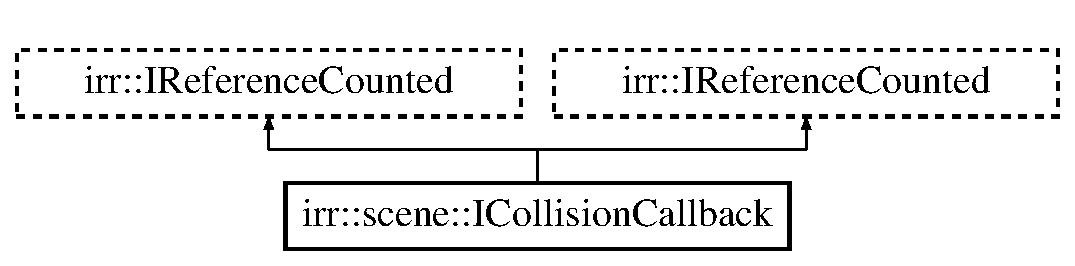
\includegraphics[height=2.000000cm]{classirr_1_1scene_1_1ICollisionCallback}
\end{center}
\end{figure}
\subsection*{Public Member Functions}
\begin{DoxyCompactItemize}
\item 
virtual bool \hyperlink{classirr_1_1scene_1_1ICollisionCallback_a35791df17defc6fd301dccef1cae596a}{on\+Collision} (const \hyperlink{classirr_1_1scene_1_1ISceneNodeAnimatorCollisionResponse}{I\+Scene\+Node\+Animator\+Collision\+Response} \&animator)=0
\begin{DoxyCompactList}\small\item\em Will be called when a collision occurrs. \end{DoxyCompactList}\end{DoxyCompactItemize}
\subsection*{Additional Inherited Members}


\subsection{Detailed Description}
Callback interface for catching events of collisions. 

Implement this interface and use \hyperlink{classirr_1_1scene_1_1ISceneNodeAnimatorCollisionResponse_a2b97f977b446200c5dd22230aec5d275}{I\+Scene\+Node\+Animator\+Collision\+Response\+::set\+Collision\+Callback} to be able to be notified if a collision has occurred. 

\subsection{Member Function Documentation}
\mbox{\Hypertarget{classirr_1_1scene_1_1ICollisionCallback_a35791df17defc6fd301dccef1cae596a}\label{classirr_1_1scene_1_1ICollisionCallback_a35791df17defc6fd301dccef1cae596a}} 
\index{irr\+::scene\+::\+I\+Collision\+Callback@{irr\+::scene\+::\+I\+Collision\+Callback}!on\+Collision@{on\+Collision}}
\index{on\+Collision@{on\+Collision}!irr\+::scene\+::\+I\+Collision\+Callback@{irr\+::scene\+::\+I\+Collision\+Callback}}
\subsubsection{\texorpdfstring{on\+Collision()}{onCollision()}}
{\footnotesize\ttfamily virtual bool irr\+::scene\+::\+I\+Collision\+Callback\+::on\+Collision (\begin{DoxyParamCaption}\item[{const \hyperlink{classirr_1_1scene_1_1ISceneNodeAnimatorCollisionResponse}{I\+Scene\+Node\+Animator\+Collision\+Response} \&}]{animator }\end{DoxyParamCaption})\hspace{0.3cm}{\ttfamily [pure virtual]}}



Will be called when a collision occurrs. 

See \hyperlink{classirr_1_1scene_1_1ISceneNodeAnimatorCollisionResponse_a2b97f977b446200c5dd22230aec5d275}{I\+Scene\+Node\+Animator\+Collision\+Response\+::set\+Collision\+Callback} for more information. 
\begin{DoxyParams}{Parameters}
{\em animator} & Collision response animator in which the collision occurred. You can call this animator\textquotesingle{}s methods to find the node, collision\+Point and/or collision triangle. \\
\hline
\end{DoxyParams}

\begin{DoxyRetVals}{Return values}
{\em true} & if the collision was handled in the animator. The animator\textquotesingle{}s target node will {\itshape not} be stopped at the collision point, but will instead move fully to the location that triggered the collision check. \\
\hline
{\em false} & if the collision was not handled in the animator. The animator\textquotesingle{}s target node will be moved to the collision position. \\
\hline
\end{DoxyRetVals}


The documentation for this class was generated from the following file\+:\begin{DoxyCompactItemize}
\item 
indie\+\_\+share/controller/include/I\+Scene\+Node\+Animator\+Collision\+Response.\+h\end{DoxyCompactItemize}

\hypertarget{classirr_1_1gui_1_1ICursorControl}{}\section{irr\+:\+:gui\+:\+:I\+Cursor\+Control Class Reference}
\label{classirr_1_1gui_1_1ICursorControl}\index{irr\+::gui\+::\+I\+Cursor\+Control@{irr\+::gui\+::\+I\+Cursor\+Control}}


Interface to manipulate the mouse cursor.  




{\ttfamily \#include $<$I\+Cursor\+Control.\+h$>$}

Inheritance diagram for irr\+:\+:gui\+:\+:I\+Cursor\+Control\+:\begin{figure}[H]
\begin{center}
\leavevmode
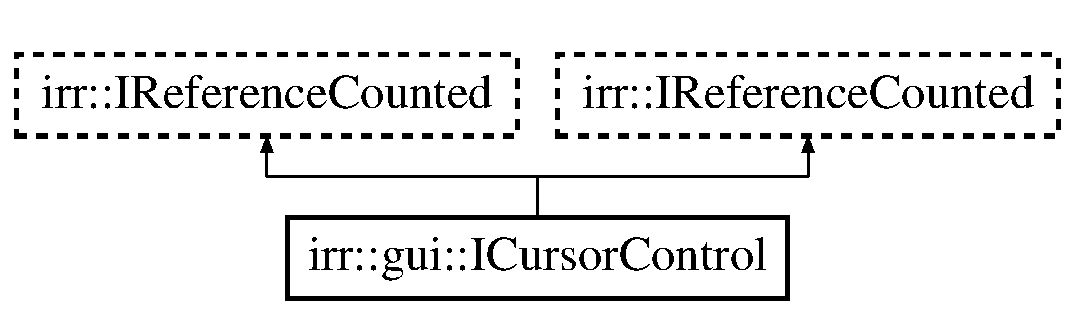
\includegraphics[height=2.000000cm]{classirr_1_1gui_1_1ICursorControl}
\end{center}
\end{figure}
\subsection*{Public Member Functions}
\begin{DoxyCompactItemize}
\item 
virtual void \hyperlink{classirr_1_1gui_1_1ICursorControl_aceb41d68494e2b2076fbc6949b254c74}{set\+Visible} (bool visible)=0
\begin{DoxyCompactList}\small\item\em Changes the visible state of the mouse cursor. \end{DoxyCompactList}\item 
virtual bool \hyperlink{classirr_1_1gui_1_1ICursorControl_ae1d1ca4c1c3042388881fabda4e53a42}{is\+Visible} () const =0
\begin{DoxyCompactList}\small\item\em Returns if the cursor is currently visible. \end{DoxyCompactList}\item 
virtual void \hyperlink{classirr_1_1gui_1_1ICursorControl_a951b5afe97fa21d98ce5360d96314306}{set\+Position} (const core\+::position2d$<$ \hyperlink{namespaceirr_a0277be98d67dc26ff93b1a6a1d086b07}{f32} $>$ \&pos)=0
\begin{DoxyCompactList}\small\item\em Sets the new position of the cursor. \end{DoxyCompactList}\item 
virtual void \hyperlink{classirr_1_1gui_1_1ICursorControl_adca41054684f73435c9b045520f7c83b}{set\+Position} (\hyperlink{namespaceirr_a0277be98d67dc26ff93b1a6a1d086b07}{f32} x, \hyperlink{namespaceirr_a0277be98d67dc26ff93b1a6a1d086b07}{f32} y)=0
\begin{DoxyCompactList}\small\item\em Sets the new position of the cursor. \end{DoxyCompactList}\item 
virtual void \hyperlink{classirr_1_1gui_1_1ICursorControl_a421c770ffc494f8f6082a16bef0feed2}{set\+Position} (const core\+::position2d$<$ \hyperlink{namespaceirr_ac66849b7a6ed16e30ebede579f9b47c6}{s32} $>$ \&pos)=0
\begin{DoxyCompactList}\small\item\em Sets the new position of the cursor. \end{DoxyCompactList}\item 
virtual void \hyperlink{classirr_1_1gui_1_1ICursorControl_a3b0a59608d1d0810079349acfa01a79b}{set\+Position} (\hyperlink{namespaceirr_ac66849b7a6ed16e30ebede579f9b47c6}{s32} x, \hyperlink{namespaceirr_ac66849b7a6ed16e30ebede579f9b47c6}{s32} y)=0
\begin{DoxyCompactList}\small\item\em Sets the new position of the cursor. \end{DoxyCompactList}\item 
virtual const core\+::position2d$<$ \hyperlink{namespaceirr_ac66849b7a6ed16e30ebede579f9b47c6}{s32} $>$ \& \hyperlink{classirr_1_1gui_1_1ICursorControl_a65d9f6e734baa02be69b7e9f5fbdd565}{get\+Position} ()=0
\begin{DoxyCompactList}\small\item\em Returns the current position of the mouse cursor. \end{DoxyCompactList}\item 
virtual core\+::position2d$<$ \hyperlink{namespaceirr_a0277be98d67dc26ff93b1a6a1d086b07}{f32} $>$ \hyperlink{classirr_1_1gui_1_1ICursorControl_a8ba1cb0ff11edc5fb32cdadddece09f8}{get\+Relative\+Position} ()=0
\begin{DoxyCompactList}\small\item\em Returns the current position of the mouse cursor. \end{DoxyCompactList}\item 
virtual void \hyperlink{classirr_1_1gui_1_1ICursorControl_a2a7428ef716a60f8f4b86361a69b8770}{set\+Reference\+Rect} (\hyperlink{classirr_1_1core_1_1rect}{core\+::rect}$<$ \hyperlink{namespaceirr_ac66849b7a6ed16e30ebede579f9b47c6}{s32} $>$ $\ast$rect=0)=0
\begin{DoxyCompactList}\small\item\em Sets an absolute reference rect for setting and retrieving the cursor position. \end{DoxyCompactList}\item 
virtual void \hyperlink{classirr_1_1gui_1_1ICursorControl_af394700d5279b13cc0f2bcdad679469c}{set\+Active\+Icon} (\hyperlink{namespaceirr_1_1gui_aefee802dd632c5735703e40ef40f879b}{E\+C\+U\+R\+S\+O\+R\+\_\+\+I\+C\+ON} icon\+Id)
\begin{DoxyCompactList}\small\item\em Sets the active cursor icon. \end{DoxyCompactList}\item 
\mbox{\Hypertarget{classirr_1_1gui_1_1ICursorControl_aeffb0659049614ced7a56b607177c3bb}\label{classirr_1_1gui_1_1ICursorControl_aeffb0659049614ced7a56b607177c3bb}} 
virtual \hyperlink{namespaceirr_1_1gui_aefee802dd632c5735703e40ef40f879b}{E\+C\+U\+R\+S\+O\+R\+\_\+\+I\+C\+ON} \hyperlink{classirr_1_1gui_1_1ICursorControl_aeffb0659049614ced7a56b607177c3bb}{get\+Active\+Icon} () const
\begin{DoxyCompactList}\small\item\em Gets the currently active icon. \end{DoxyCompactList}\item 
virtual \hyperlink{namespaceirr_1_1gui_aefee802dd632c5735703e40ef40f879b}{E\+C\+U\+R\+S\+O\+R\+\_\+\+I\+C\+ON} \hyperlink{classirr_1_1gui_1_1ICursorControl_a102ff455c70595886281e636ef063d3b}{add\+Icon} (const \hyperlink{structirr_1_1gui_1_1SCursorSprite}{gui\+::\+S\+Cursor\+Sprite} \&icon)
\begin{DoxyCompactList}\small\item\em Add a custom sprite as cursor icon. \end{DoxyCompactList}\item 
virtual void \hyperlink{classirr_1_1gui_1_1ICursorControl_a3e7c8cb1f03e1ccc31fcc3c30f717762}{change\+Icon} (\hyperlink{namespaceirr_1_1gui_aefee802dd632c5735703e40ef40f879b}{E\+C\+U\+R\+S\+O\+R\+\_\+\+I\+C\+ON} icon\+Id, const \hyperlink{structirr_1_1gui_1_1SCursorSprite}{gui\+::\+S\+Cursor\+Sprite} \&sprite)
\begin{DoxyCompactList}\small\item\em replace a cursor icon. \end{DoxyCompactList}\item 
\mbox{\Hypertarget{classirr_1_1gui_1_1ICursorControl_a0710b659cbab1474e3486f7dd0e8c35e}\label{classirr_1_1gui_1_1ICursorControl_a0710b659cbab1474e3486f7dd0e8c35e}} 
virtual \hyperlink{namespaceirr_1_1core_aacaa9f583051276807125e964db2f073}{core\+::dimension2di} \hyperlink{classirr_1_1gui_1_1ICursorControl_a0710b659cbab1474e3486f7dd0e8c35e}{get\+Supported\+Icon\+Size} () const
\begin{DoxyCompactList}\small\item\em Return a system-\/specific size which is supported for cursors. Larger icons will fail, smaller icons might work. \end{DoxyCompactList}\item 
\mbox{\Hypertarget{classirr_1_1gui_1_1ICursorControl_ad7688bb200945f15877a598e8be53878}\label{classirr_1_1gui_1_1ICursorControl_ad7688bb200945f15877a598e8be53878}} 
virtual void \hyperlink{classirr_1_1gui_1_1ICursorControl_ad7688bb200945f15877a598e8be53878}{set\+Platform\+Behavior} (\hyperlink{namespaceirr_1_1gui_abbd186f9cfba2f805d98248df226acef}{E\+C\+U\+R\+S\+O\+R\+\_\+\+P\+L\+A\+T\+F\+O\+R\+M\+\_\+\+B\+E\+H\+A\+V\+I\+OR} behavior)
\begin{DoxyCompactList}\small\item\em Set platform specific behavior flags. \end{DoxyCompactList}\item 
virtual \hyperlink{namespaceirr_1_1gui_abbd186f9cfba2f805d98248df226acef}{E\+C\+U\+R\+S\+O\+R\+\_\+\+P\+L\+A\+T\+F\+O\+R\+M\+\_\+\+B\+E\+H\+A\+V\+I\+OR} \hyperlink{classirr_1_1gui_1_1ICursorControl_aad19b5b02de0b8bc476c66b152b745c4}{get\+Platform\+Behavior} () const
\begin{DoxyCompactList}\small\item\em Return platform specific behavior. \end{DoxyCompactList}\item 
virtual void \hyperlink{classirr_1_1gui_1_1ICursorControl_aceb41d68494e2b2076fbc6949b254c74}{set\+Visible} (bool visible)=0
\begin{DoxyCompactList}\small\item\em Changes the visible state of the mouse cursor. \end{DoxyCompactList}\item 
virtual bool \hyperlink{classirr_1_1gui_1_1ICursorControl_ae1d1ca4c1c3042388881fabda4e53a42}{is\+Visible} () const =0
\begin{DoxyCompactList}\small\item\em Returns if the cursor is currently visible. \end{DoxyCompactList}\item 
virtual void \hyperlink{classirr_1_1gui_1_1ICursorControl_a951b5afe97fa21d98ce5360d96314306}{set\+Position} (const core\+::position2d$<$ \hyperlink{namespaceirr_a0277be98d67dc26ff93b1a6a1d086b07}{f32} $>$ \&pos)=0
\begin{DoxyCompactList}\small\item\em Sets the new position of the cursor. \end{DoxyCompactList}\item 
virtual void \hyperlink{classirr_1_1gui_1_1ICursorControl_adca41054684f73435c9b045520f7c83b}{set\+Position} (\hyperlink{namespaceirr_a0277be98d67dc26ff93b1a6a1d086b07}{f32} x, \hyperlink{namespaceirr_a0277be98d67dc26ff93b1a6a1d086b07}{f32} y)=0
\begin{DoxyCompactList}\small\item\em Sets the new position of the cursor. \end{DoxyCompactList}\item 
virtual void \hyperlink{classirr_1_1gui_1_1ICursorControl_a421c770ffc494f8f6082a16bef0feed2}{set\+Position} (const core\+::position2d$<$ \hyperlink{namespaceirr_ac66849b7a6ed16e30ebede579f9b47c6}{s32} $>$ \&pos)=0
\begin{DoxyCompactList}\small\item\em Sets the new position of the cursor. \end{DoxyCompactList}\item 
virtual void \hyperlink{classirr_1_1gui_1_1ICursorControl_a3b0a59608d1d0810079349acfa01a79b}{set\+Position} (\hyperlink{namespaceirr_ac66849b7a6ed16e30ebede579f9b47c6}{s32} x, \hyperlink{namespaceirr_ac66849b7a6ed16e30ebede579f9b47c6}{s32} y)=0
\begin{DoxyCompactList}\small\item\em Sets the new position of the cursor. \end{DoxyCompactList}\item 
virtual const core\+::position2d$<$ \hyperlink{namespaceirr_ac66849b7a6ed16e30ebede579f9b47c6}{s32} $>$ \& \hyperlink{classirr_1_1gui_1_1ICursorControl_a65d9f6e734baa02be69b7e9f5fbdd565}{get\+Position} ()=0
\begin{DoxyCompactList}\small\item\em Returns the current position of the mouse cursor. \end{DoxyCompactList}\item 
virtual core\+::position2d$<$ \hyperlink{namespaceirr_a0277be98d67dc26ff93b1a6a1d086b07}{f32} $>$ \hyperlink{classirr_1_1gui_1_1ICursorControl_a8ba1cb0ff11edc5fb32cdadddece09f8}{get\+Relative\+Position} ()=0
\begin{DoxyCompactList}\small\item\em Returns the current position of the mouse cursor. \end{DoxyCompactList}\item 
virtual void \hyperlink{classirr_1_1gui_1_1ICursorControl_a2a7428ef716a60f8f4b86361a69b8770}{set\+Reference\+Rect} (\hyperlink{classirr_1_1core_1_1rect}{core\+::rect}$<$ \hyperlink{namespaceirr_ac66849b7a6ed16e30ebede579f9b47c6}{s32} $>$ $\ast$rect=0)=0
\begin{DoxyCompactList}\small\item\em Sets an absolute reference rect for setting and retrieving the cursor position. \end{DoxyCompactList}\item 
virtual void \hyperlink{classirr_1_1gui_1_1ICursorControl_af394700d5279b13cc0f2bcdad679469c}{set\+Active\+Icon} (\hyperlink{namespaceirr_1_1gui_aefee802dd632c5735703e40ef40f879b}{E\+C\+U\+R\+S\+O\+R\+\_\+\+I\+C\+ON} icon\+Id)
\begin{DoxyCompactList}\small\item\em Sets the active cursor icon. \end{DoxyCompactList}\item 
\mbox{\Hypertarget{classirr_1_1gui_1_1ICursorControl_aeffb0659049614ced7a56b607177c3bb}\label{classirr_1_1gui_1_1ICursorControl_aeffb0659049614ced7a56b607177c3bb}} 
virtual \hyperlink{namespaceirr_1_1gui_aefee802dd632c5735703e40ef40f879b}{E\+C\+U\+R\+S\+O\+R\+\_\+\+I\+C\+ON} \hyperlink{classirr_1_1gui_1_1ICursorControl_aeffb0659049614ced7a56b607177c3bb}{get\+Active\+Icon} () const
\begin{DoxyCompactList}\small\item\em Gets the currently active icon. \end{DoxyCompactList}\item 
virtual \hyperlink{namespaceirr_1_1gui_aefee802dd632c5735703e40ef40f879b}{E\+C\+U\+R\+S\+O\+R\+\_\+\+I\+C\+ON} \hyperlink{classirr_1_1gui_1_1ICursorControl_a102ff455c70595886281e636ef063d3b}{add\+Icon} (const \hyperlink{structirr_1_1gui_1_1SCursorSprite}{gui\+::\+S\+Cursor\+Sprite} \&icon)
\begin{DoxyCompactList}\small\item\em Add a custom sprite as cursor icon. \end{DoxyCompactList}\item 
virtual void \hyperlink{classirr_1_1gui_1_1ICursorControl_a3e7c8cb1f03e1ccc31fcc3c30f717762}{change\+Icon} (\hyperlink{namespaceirr_1_1gui_aefee802dd632c5735703e40ef40f879b}{E\+C\+U\+R\+S\+O\+R\+\_\+\+I\+C\+ON} icon\+Id, const \hyperlink{structirr_1_1gui_1_1SCursorSprite}{gui\+::\+S\+Cursor\+Sprite} \&sprite)
\begin{DoxyCompactList}\small\item\em replace a cursor icon. \end{DoxyCompactList}\item 
\mbox{\Hypertarget{classirr_1_1gui_1_1ICursorControl_a0710b659cbab1474e3486f7dd0e8c35e}\label{classirr_1_1gui_1_1ICursorControl_a0710b659cbab1474e3486f7dd0e8c35e}} 
virtual \hyperlink{namespaceirr_1_1core_aacaa9f583051276807125e964db2f073}{core\+::dimension2di} \hyperlink{classirr_1_1gui_1_1ICursorControl_a0710b659cbab1474e3486f7dd0e8c35e}{get\+Supported\+Icon\+Size} () const
\begin{DoxyCompactList}\small\item\em Return a system-\/specific size which is supported for cursors. Larger icons will fail, smaller icons might work. \end{DoxyCompactList}\item 
\mbox{\Hypertarget{classirr_1_1gui_1_1ICursorControl_ad7688bb200945f15877a598e8be53878}\label{classirr_1_1gui_1_1ICursorControl_ad7688bb200945f15877a598e8be53878}} 
virtual void \hyperlink{classirr_1_1gui_1_1ICursorControl_ad7688bb200945f15877a598e8be53878}{set\+Platform\+Behavior} (\hyperlink{namespaceirr_1_1gui_abbd186f9cfba2f805d98248df226acef}{E\+C\+U\+R\+S\+O\+R\+\_\+\+P\+L\+A\+T\+F\+O\+R\+M\+\_\+\+B\+E\+H\+A\+V\+I\+OR} behavior)
\begin{DoxyCompactList}\small\item\em Set platform specific behavior flags. \end{DoxyCompactList}\item 
virtual \hyperlink{namespaceirr_1_1gui_abbd186f9cfba2f805d98248df226acef}{E\+C\+U\+R\+S\+O\+R\+\_\+\+P\+L\+A\+T\+F\+O\+R\+M\+\_\+\+B\+E\+H\+A\+V\+I\+OR} \hyperlink{classirr_1_1gui_1_1ICursorControl_aad19b5b02de0b8bc476c66b152b745c4}{get\+Platform\+Behavior} () const
\begin{DoxyCompactList}\small\item\em Return platform specific behavior. \end{DoxyCompactList}\end{DoxyCompactItemize}
\subsection*{Additional Inherited Members}


\subsection{Detailed Description}
Interface to manipulate the mouse cursor. 

\subsection{Member Function Documentation}
\mbox{\Hypertarget{classirr_1_1gui_1_1ICursorControl_a102ff455c70595886281e636ef063d3b}\label{classirr_1_1gui_1_1ICursorControl_a102ff455c70595886281e636ef063d3b}} 
\index{irr\+::gui\+::\+I\+Cursor\+Control@{irr\+::gui\+::\+I\+Cursor\+Control}!add\+Icon@{add\+Icon}}
\index{add\+Icon@{add\+Icon}!irr\+::gui\+::\+I\+Cursor\+Control@{irr\+::gui\+::\+I\+Cursor\+Control}}
\subsubsection{\texorpdfstring{add\+Icon()}{addIcon()}\hspace{0.1cm}{\footnotesize\ttfamily [1/2]}}
{\footnotesize\ttfamily virtual \hyperlink{namespaceirr_1_1gui_aefee802dd632c5735703e40ef40f879b}{E\+C\+U\+R\+S\+O\+R\+\_\+\+I\+C\+ON} irr\+::gui\+::\+I\+Cursor\+Control\+::add\+Icon (\begin{DoxyParamCaption}\item[{const \hyperlink{structirr_1_1gui_1_1SCursorSprite}{gui\+::\+S\+Cursor\+Sprite} \&}]{icon }\end{DoxyParamCaption})\hspace{0.3cm}{\ttfamily [inline]}, {\ttfamily [virtual]}}



Add a custom sprite as cursor icon. 

\begin{DoxyReturn}{Returns}
Identification for the icon 
\end{DoxyReturn}
\mbox{\Hypertarget{classirr_1_1gui_1_1ICursorControl_a102ff455c70595886281e636ef063d3b}\label{classirr_1_1gui_1_1ICursorControl_a102ff455c70595886281e636ef063d3b}} 
\index{irr\+::gui\+::\+I\+Cursor\+Control@{irr\+::gui\+::\+I\+Cursor\+Control}!add\+Icon@{add\+Icon}}
\index{add\+Icon@{add\+Icon}!irr\+::gui\+::\+I\+Cursor\+Control@{irr\+::gui\+::\+I\+Cursor\+Control}}
\subsubsection{\texorpdfstring{add\+Icon()}{addIcon()}\hspace{0.1cm}{\footnotesize\ttfamily [2/2]}}
{\footnotesize\ttfamily virtual \hyperlink{namespaceirr_1_1gui_aefee802dd632c5735703e40ef40f879b}{E\+C\+U\+R\+S\+O\+R\+\_\+\+I\+C\+ON} irr\+::gui\+::\+I\+Cursor\+Control\+::add\+Icon (\begin{DoxyParamCaption}\item[{const \hyperlink{structirr_1_1gui_1_1SCursorSprite}{gui\+::\+S\+Cursor\+Sprite} \&}]{icon }\end{DoxyParamCaption})\hspace{0.3cm}{\ttfamily [inline]}, {\ttfamily [virtual]}}



Add a custom sprite as cursor icon. 

\begin{DoxyReturn}{Returns}
Identification for the icon 
\end{DoxyReturn}
\mbox{\Hypertarget{classirr_1_1gui_1_1ICursorControl_a3e7c8cb1f03e1ccc31fcc3c30f717762}\label{classirr_1_1gui_1_1ICursorControl_a3e7c8cb1f03e1ccc31fcc3c30f717762}} 
\index{irr\+::gui\+::\+I\+Cursor\+Control@{irr\+::gui\+::\+I\+Cursor\+Control}!change\+Icon@{change\+Icon}}
\index{change\+Icon@{change\+Icon}!irr\+::gui\+::\+I\+Cursor\+Control@{irr\+::gui\+::\+I\+Cursor\+Control}}
\subsubsection{\texorpdfstring{change\+Icon()}{changeIcon()}\hspace{0.1cm}{\footnotesize\ttfamily [1/2]}}
{\footnotesize\ttfamily virtual void irr\+::gui\+::\+I\+Cursor\+Control\+::change\+Icon (\begin{DoxyParamCaption}\item[{\hyperlink{namespaceirr_1_1gui_aefee802dd632c5735703e40ef40f879b}{E\+C\+U\+R\+S\+O\+R\+\_\+\+I\+C\+ON}}]{icon\+Id,  }\item[{const \hyperlink{structirr_1_1gui_1_1SCursorSprite}{gui\+::\+S\+Cursor\+Sprite} \&}]{sprite }\end{DoxyParamCaption})\hspace{0.3cm}{\ttfamily [inline]}, {\ttfamily [virtual]}}



replace a cursor icon. 

Changing cursor icons is so far only supported on Win32 and Linux Note that this only changes the icons within your application, system cursors outside your application will not be affected. \mbox{\Hypertarget{classirr_1_1gui_1_1ICursorControl_a3e7c8cb1f03e1ccc31fcc3c30f717762}\label{classirr_1_1gui_1_1ICursorControl_a3e7c8cb1f03e1ccc31fcc3c30f717762}} 
\index{irr\+::gui\+::\+I\+Cursor\+Control@{irr\+::gui\+::\+I\+Cursor\+Control}!change\+Icon@{change\+Icon}}
\index{change\+Icon@{change\+Icon}!irr\+::gui\+::\+I\+Cursor\+Control@{irr\+::gui\+::\+I\+Cursor\+Control}}
\subsubsection{\texorpdfstring{change\+Icon()}{changeIcon()}\hspace{0.1cm}{\footnotesize\ttfamily [2/2]}}
{\footnotesize\ttfamily virtual void irr\+::gui\+::\+I\+Cursor\+Control\+::change\+Icon (\begin{DoxyParamCaption}\item[{\hyperlink{namespaceirr_1_1gui_aefee802dd632c5735703e40ef40f879b}{E\+C\+U\+R\+S\+O\+R\+\_\+\+I\+C\+ON}}]{icon\+Id,  }\item[{const \hyperlink{structirr_1_1gui_1_1SCursorSprite}{gui\+::\+S\+Cursor\+Sprite} \&}]{sprite }\end{DoxyParamCaption})\hspace{0.3cm}{\ttfamily [inline]}, {\ttfamily [virtual]}}



replace a cursor icon. 

Changing cursor icons is so far only supported on Win32 and Linux Note that this only changes the icons within your application, system cursors outside your application will not be affected. \mbox{\Hypertarget{classirr_1_1gui_1_1ICursorControl_aad19b5b02de0b8bc476c66b152b745c4}\label{classirr_1_1gui_1_1ICursorControl_aad19b5b02de0b8bc476c66b152b745c4}} 
\index{irr\+::gui\+::\+I\+Cursor\+Control@{irr\+::gui\+::\+I\+Cursor\+Control}!get\+Platform\+Behavior@{get\+Platform\+Behavior}}
\index{get\+Platform\+Behavior@{get\+Platform\+Behavior}!irr\+::gui\+::\+I\+Cursor\+Control@{irr\+::gui\+::\+I\+Cursor\+Control}}
\subsubsection{\texorpdfstring{get\+Platform\+Behavior()}{getPlatformBehavior()}\hspace{0.1cm}{\footnotesize\ttfamily [1/2]}}
{\footnotesize\ttfamily virtual \hyperlink{namespaceirr_1_1gui_abbd186f9cfba2f805d98248df226acef}{E\+C\+U\+R\+S\+O\+R\+\_\+\+P\+L\+A\+T\+F\+O\+R\+M\+\_\+\+B\+E\+H\+A\+V\+I\+OR} irr\+::gui\+::\+I\+Cursor\+Control\+::get\+Platform\+Behavior (\begin{DoxyParamCaption}{ }\end{DoxyParamCaption}) const\hspace{0.3cm}{\ttfamily [inline]}, {\ttfamily [virtual]}}



Return platform specific behavior. 

\begin{DoxyReturn}{Returns}
Behavior set by set\+Platform\+Behavior or E\+C\+P\+B\+\_\+\+N\+O\+NE for platforms not implementing specific behaviors. 
\end{DoxyReturn}
\mbox{\Hypertarget{classirr_1_1gui_1_1ICursorControl_aad19b5b02de0b8bc476c66b152b745c4}\label{classirr_1_1gui_1_1ICursorControl_aad19b5b02de0b8bc476c66b152b745c4}} 
\index{irr\+::gui\+::\+I\+Cursor\+Control@{irr\+::gui\+::\+I\+Cursor\+Control}!get\+Platform\+Behavior@{get\+Platform\+Behavior}}
\index{get\+Platform\+Behavior@{get\+Platform\+Behavior}!irr\+::gui\+::\+I\+Cursor\+Control@{irr\+::gui\+::\+I\+Cursor\+Control}}
\subsubsection{\texorpdfstring{get\+Platform\+Behavior()}{getPlatformBehavior()}\hspace{0.1cm}{\footnotesize\ttfamily [2/2]}}
{\footnotesize\ttfamily virtual \hyperlink{namespaceirr_1_1gui_abbd186f9cfba2f805d98248df226acef}{E\+C\+U\+R\+S\+O\+R\+\_\+\+P\+L\+A\+T\+F\+O\+R\+M\+\_\+\+B\+E\+H\+A\+V\+I\+OR} irr\+::gui\+::\+I\+Cursor\+Control\+::get\+Platform\+Behavior (\begin{DoxyParamCaption}{ }\end{DoxyParamCaption}) const\hspace{0.3cm}{\ttfamily [inline]}, {\ttfamily [virtual]}}



Return platform specific behavior. 

\begin{DoxyReturn}{Returns}
Behavior set by set\+Platform\+Behavior or E\+C\+P\+B\+\_\+\+N\+O\+NE for platforms not implementing specific behaviors. 
\end{DoxyReturn}
\mbox{\Hypertarget{classirr_1_1gui_1_1ICursorControl_a65d9f6e734baa02be69b7e9f5fbdd565}\label{classirr_1_1gui_1_1ICursorControl_a65d9f6e734baa02be69b7e9f5fbdd565}} 
\index{irr\+::gui\+::\+I\+Cursor\+Control@{irr\+::gui\+::\+I\+Cursor\+Control}!get\+Position@{get\+Position}}
\index{get\+Position@{get\+Position}!irr\+::gui\+::\+I\+Cursor\+Control@{irr\+::gui\+::\+I\+Cursor\+Control}}
\subsubsection{\texorpdfstring{get\+Position()}{getPosition()}\hspace{0.1cm}{\footnotesize\ttfamily [1/2]}}
{\footnotesize\ttfamily virtual const core\+::position2d$<$\hyperlink{namespaceirr_ac66849b7a6ed16e30ebede579f9b47c6}{s32}$>$\& irr\+::gui\+::\+I\+Cursor\+Control\+::get\+Position (\begin{DoxyParamCaption}{ }\end{DoxyParamCaption})\hspace{0.3cm}{\ttfamily [pure virtual]}}



Returns the current position of the mouse cursor. 

\begin{DoxyReturn}{Returns}
Returns the current position of the cursor. The returned position is the position of the mouse cursor in pixel units. 
\end{DoxyReturn}
\mbox{\Hypertarget{classirr_1_1gui_1_1ICursorControl_a65d9f6e734baa02be69b7e9f5fbdd565}\label{classirr_1_1gui_1_1ICursorControl_a65d9f6e734baa02be69b7e9f5fbdd565}} 
\index{irr\+::gui\+::\+I\+Cursor\+Control@{irr\+::gui\+::\+I\+Cursor\+Control}!get\+Position@{get\+Position}}
\index{get\+Position@{get\+Position}!irr\+::gui\+::\+I\+Cursor\+Control@{irr\+::gui\+::\+I\+Cursor\+Control}}
\subsubsection{\texorpdfstring{get\+Position()}{getPosition()}\hspace{0.1cm}{\footnotesize\ttfamily [2/2]}}
{\footnotesize\ttfamily virtual const core\+::position2d$<$\hyperlink{namespaceirr_ac66849b7a6ed16e30ebede579f9b47c6}{s32}$>$\& irr\+::gui\+::\+I\+Cursor\+Control\+::get\+Position (\begin{DoxyParamCaption}{ }\end{DoxyParamCaption})\hspace{0.3cm}{\ttfamily [pure virtual]}}



Returns the current position of the mouse cursor. 

\begin{DoxyReturn}{Returns}
Returns the current position of the cursor. The returned position is the position of the mouse cursor in pixel units. 
\end{DoxyReturn}
\mbox{\Hypertarget{classirr_1_1gui_1_1ICursorControl_a8ba1cb0ff11edc5fb32cdadddece09f8}\label{classirr_1_1gui_1_1ICursorControl_a8ba1cb0ff11edc5fb32cdadddece09f8}} 
\index{irr\+::gui\+::\+I\+Cursor\+Control@{irr\+::gui\+::\+I\+Cursor\+Control}!get\+Relative\+Position@{get\+Relative\+Position}}
\index{get\+Relative\+Position@{get\+Relative\+Position}!irr\+::gui\+::\+I\+Cursor\+Control@{irr\+::gui\+::\+I\+Cursor\+Control}}
\subsubsection{\texorpdfstring{get\+Relative\+Position()}{getRelativePosition()}\hspace{0.1cm}{\footnotesize\ttfamily [1/2]}}
{\footnotesize\ttfamily virtual core\+::position2d$<$\hyperlink{namespaceirr_a0277be98d67dc26ff93b1a6a1d086b07}{f32}$>$ irr\+::gui\+::\+I\+Cursor\+Control\+::get\+Relative\+Position (\begin{DoxyParamCaption}{ }\end{DoxyParamCaption})\hspace{0.3cm}{\ttfamily [pure virtual]}}



Returns the current position of the mouse cursor. 

\begin{DoxyReturn}{Returns}
Returns the current position of the cursor. The returned position is a value between (0.\+0f, 0.\+0f) and (1.\+0f, 1.\+0f), where (0.\+0f, 0.\+0f) is the top left corner and (1.\+0f, 1.\+0f) is the bottom right corner of the render window. 
\end{DoxyReturn}
\mbox{\Hypertarget{classirr_1_1gui_1_1ICursorControl_a8ba1cb0ff11edc5fb32cdadddece09f8}\label{classirr_1_1gui_1_1ICursorControl_a8ba1cb0ff11edc5fb32cdadddece09f8}} 
\index{irr\+::gui\+::\+I\+Cursor\+Control@{irr\+::gui\+::\+I\+Cursor\+Control}!get\+Relative\+Position@{get\+Relative\+Position}}
\index{get\+Relative\+Position@{get\+Relative\+Position}!irr\+::gui\+::\+I\+Cursor\+Control@{irr\+::gui\+::\+I\+Cursor\+Control}}
\subsubsection{\texorpdfstring{get\+Relative\+Position()}{getRelativePosition()}\hspace{0.1cm}{\footnotesize\ttfamily [2/2]}}
{\footnotesize\ttfamily virtual core\+::position2d$<$\hyperlink{namespaceirr_a0277be98d67dc26ff93b1a6a1d086b07}{f32}$>$ irr\+::gui\+::\+I\+Cursor\+Control\+::get\+Relative\+Position (\begin{DoxyParamCaption}{ }\end{DoxyParamCaption})\hspace{0.3cm}{\ttfamily [pure virtual]}}



Returns the current position of the mouse cursor. 

\begin{DoxyReturn}{Returns}
Returns the current position of the cursor. The returned position is a value between (0.\+0f, 0.\+0f) and (1.\+0f, 1.\+0f), where (0.\+0f, 0.\+0f) is the top left corner and (1.\+0f, 1.\+0f) is the bottom right corner of the render window. 
\end{DoxyReturn}
\mbox{\Hypertarget{classirr_1_1gui_1_1ICursorControl_ae1d1ca4c1c3042388881fabda4e53a42}\label{classirr_1_1gui_1_1ICursorControl_ae1d1ca4c1c3042388881fabda4e53a42}} 
\index{irr\+::gui\+::\+I\+Cursor\+Control@{irr\+::gui\+::\+I\+Cursor\+Control}!is\+Visible@{is\+Visible}}
\index{is\+Visible@{is\+Visible}!irr\+::gui\+::\+I\+Cursor\+Control@{irr\+::gui\+::\+I\+Cursor\+Control}}
\subsubsection{\texorpdfstring{is\+Visible()}{isVisible()}\hspace{0.1cm}{\footnotesize\ttfamily [1/2]}}
{\footnotesize\ttfamily virtual bool irr\+::gui\+::\+I\+Cursor\+Control\+::is\+Visible (\begin{DoxyParamCaption}{ }\end{DoxyParamCaption}) const\hspace{0.3cm}{\ttfamily [pure virtual]}}



Returns if the cursor is currently visible. 

\begin{DoxyReturn}{Returns}
True if the cursor is visible, false if not. 
\end{DoxyReturn}
\mbox{\Hypertarget{classirr_1_1gui_1_1ICursorControl_ae1d1ca4c1c3042388881fabda4e53a42}\label{classirr_1_1gui_1_1ICursorControl_ae1d1ca4c1c3042388881fabda4e53a42}} 
\index{irr\+::gui\+::\+I\+Cursor\+Control@{irr\+::gui\+::\+I\+Cursor\+Control}!is\+Visible@{is\+Visible}}
\index{is\+Visible@{is\+Visible}!irr\+::gui\+::\+I\+Cursor\+Control@{irr\+::gui\+::\+I\+Cursor\+Control}}
\subsubsection{\texorpdfstring{is\+Visible()}{isVisible()}\hspace{0.1cm}{\footnotesize\ttfamily [2/2]}}
{\footnotesize\ttfamily virtual bool irr\+::gui\+::\+I\+Cursor\+Control\+::is\+Visible (\begin{DoxyParamCaption}{ }\end{DoxyParamCaption}) const\hspace{0.3cm}{\ttfamily [pure virtual]}}



Returns if the cursor is currently visible. 

\begin{DoxyReturn}{Returns}
True if the cursor is visible, false if not. 
\end{DoxyReturn}
\mbox{\Hypertarget{classirr_1_1gui_1_1ICursorControl_af394700d5279b13cc0f2bcdad679469c}\label{classirr_1_1gui_1_1ICursorControl_af394700d5279b13cc0f2bcdad679469c}} 
\index{irr\+::gui\+::\+I\+Cursor\+Control@{irr\+::gui\+::\+I\+Cursor\+Control}!set\+Active\+Icon@{set\+Active\+Icon}}
\index{set\+Active\+Icon@{set\+Active\+Icon}!irr\+::gui\+::\+I\+Cursor\+Control@{irr\+::gui\+::\+I\+Cursor\+Control}}
\subsubsection{\texorpdfstring{set\+Active\+Icon()}{setActiveIcon()}\hspace{0.1cm}{\footnotesize\ttfamily [1/2]}}
{\footnotesize\ttfamily virtual void irr\+::gui\+::\+I\+Cursor\+Control\+::set\+Active\+Icon (\begin{DoxyParamCaption}\item[{\hyperlink{namespaceirr_1_1gui_aefee802dd632c5735703e40ef40f879b}{E\+C\+U\+R\+S\+O\+R\+\_\+\+I\+C\+ON}}]{icon\+Id }\end{DoxyParamCaption})\hspace{0.3cm}{\ttfamily [inline]}, {\ttfamily [virtual]}}



Sets the active cursor icon. 

Setting cursor icons is so far only supported on Win32 and Linux \mbox{\Hypertarget{classirr_1_1gui_1_1ICursorControl_af394700d5279b13cc0f2bcdad679469c}\label{classirr_1_1gui_1_1ICursorControl_af394700d5279b13cc0f2bcdad679469c}} 
\index{irr\+::gui\+::\+I\+Cursor\+Control@{irr\+::gui\+::\+I\+Cursor\+Control}!set\+Active\+Icon@{set\+Active\+Icon}}
\index{set\+Active\+Icon@{set\+Active\+Icon}!irr\+::gui\+::\+I\+Cursor\+Control@{irr\+::gui\+::\+I\+Cursor\+Control}}
\subsubsection{\texorpdfstring{set\+Active\+Icon()}{setActiveIcon()}\hspace{0.1cm}{\footnotesize\ttfamily [2/2]}}
{\footnotesize\ttfamily virtual void irr\+::gui\+::\+I\+Cursor\+Control\+::set\+Active\+Icon (\begin{DoxyParamCaption}\item[{\hyperlink{namespaceirr_1_1gui_aefee802dd632c5735703e40ef40f879b}{E\+C\+U\+R\+S\+O\+R\+\_\+\+I\+C\+ON}}]{icon\+Id }\end{DoxyParamCaption})\hspace{0.3cm}{\ttfamily [inline]}, {\ttfamily [virtual]}}



Sets the active cursor icon. 

Setting cursor icons is so far only supported on Win32 and Linux \mbox{\Hypertarget{classirr_1_1gui_1_1ICursorControl_a951b5afe97fa21d98ce5360d96314306}\label{classirr_1_1gui_1_1ICursorControl_a951b5afe97fa21d98ce5360d96314306}} 
\index{irr\+::gui\+::\+I\+Cursor\+Control@{irr\+::gui\+::\+I\+Cursor\+Control}!set\+Position@{set\+Position}}
\index{set\+Position@{set\+Position}!irr\+::gui\+::\+I\+Cursor\+Control@{irr\+::gui\+::\+I\+Cursor\+Control}}
\subsubsection{\texorpdfstring{set\+Position()}{setPosition()}\hspace{0.1cm}{\footnotesize\ttfamily [1/8]}}
{\footnotesize\ttfamily virtual void irr\+::gui\+::\+I\+Cursor\+Control\+::set\+Position (\begin{DoxyParamCaption}\item[{const core\+::position2d$<$ \hyperlink{namespaceirr_a0277be98d67dc26ff93b1a6a1d086b07}{f32} $>$ \&}]{pos }\end{DoxyParamCaption})\hspace{0.3cm}{\ttfamily [pure virtual]}}



Sets the new position of the cursor. 

The position must be between (0.\+0f, 0.\+0f) and (1.\+0f, 1.\+0f), where (0.\+0f, 0.\+0f) is the top left corner and (1.\+0f, 1.\+0f) is the bottom right corner of the render window. 
\begin{DoxyParams}{Parameters}
{\em pos} & New position of the cursor. \\
\hline
\end{DoxyParams}
\mbox{\Hypertarget{classirr_1_1gui_1_1ICursorControl_a951b5afe97fa21d98ce5360d96314306}\label{classirr_1_1gui_1_1ICursorControl_a951b5afe97fa21d98ce5360d96314306}} 
\index{irr\+::gui\+::\+I\+Cursor\+Control@{irr\+::gui\+::\+I\+Cursor\+Control}!set\+Position@{set\+Position}}
\index{set\+Position@{set\+Position}!irr\+::gui\+::\+I\+Cursor\+Control@{irr\+::gui\+::\+I\+Cursor\+Control}}
\subsubsection{\texorpdfstring{set\+Position()}{setPosition()}\hspace{0.1cm}{\footnotesize\ttfamily [2/8]}}
{\footnotesize\ttfamily virtual void irr\+::gui\+::\+I\+Cursor\+Control\+::set\+Position (\begin{DoxyParamCaption}\item[{const core\+::position2d$<$ \hyperlink{namespaceirr_a0277be98d67dc26ff93b1a6a1d086b07}{f32} $>$ \&}]{pos }\end{DoxyParamCaption})\hspace{0.3cm}{\ttfamily [pure virtual]}}



Sets the new position of the cursor. 

The position must be between (0.\+0f, 0.\+0f) and (1.\+0f, 1.\+0f), where (0.\+0f, 0.\+0f) is the top left corner and (1.\+0f, 1.\+0f) is the bottom right corner of the render window. 
\begin{DoxyParams}{Parameters}
{\em pos} & New position of the cursor. \\
\hline
\end{DoxyParams}
\mbox{\Hypertarget{classirr_1_1gui_1_1ICursorControl_adca41054684f73435c9b045520f7c83b}\label{classirr_1_1gui_1_1ICursorControl_adca41054684f73435c9b045520f7c83b}} 
\index{irr\+::gui\+::\+I\+Cursor\+Control@{irr\+::gui\+::\+I\+Cursor\+Control}!set\+Position@{set\+Position}}
\index{set\+Position@{set\+Position}!irr\+::gui\+::\+I\+Cursor\+Control@{irr\+::gui\+::\+I\+Cursor\+Control}}
\subsubsection{\texorpdfstring{set\+Position()}{setPosition()}\hspace{0.1cm}{\footnotesize\ttfamily [3/8]}}
{\footnotesize\ttfamily virtual void irr\+::gui\+::\+I\+Cursor\+Control\+::set\+Position (\begin{DoxyParamCaption}\item[{\hyperlink{namespaceirr_a0277be98d67dc26ff93b1a6a1d086b07}{f32}}]{x,  }\item[{\hyperlink{namespaceirr_a0277be98d67dc26ff93b1a6a1d086b07}{f32}}]{y }\end{DoxyParamCaption})\hspace{0.3cm}{\ttfamily [pure virtual]}}



Sets the new position of the cursor. 

The position must be between (0.\+0f, 0.\+0f) and (1.\+0f, 1.\+0f), where (0.\+0f, 0.\+0f) is the top left corner and (1.\+0f, 1.\+0f) is the bottom right corner of the render window. 
\begin{DoxyParams}{Parameters}
{\em x} & New x-\/coord of the cursor. \\
\hline
{\em y} & New x-\/coord of the cursor. \\
\hline
\end{DoxyParams}
\mbox{\Hypertarget{classirr_1_1gui_1_1ICursorControl_adca41054684f73435c9b045520f7c83b}\label{classirr_1_1gui_1_1ICursorControl_adca41054684f73435c9b045520f7c83b}} 
\index{irr\+::gui\+::\+I\+Cursor\+Control@{irr\+::gui\+::\+I\+Cursor\+Control}!set\+Position@{set\+Position}}
\index{set\+Position@{set\+Position}!irr\+::gui\+::\+I\+Cursor\+Control@{irr\+::gui\+::\+I\+Cursor\+Control}}
\subsubsection{\texorpdfstring{set\+Position()}{setPosition()}\hspace{0.1cm}{\footnotesize\ttfamily [4/8]}}
{\footnotesize\ttfamily virtual void irr\+::gui\+::\+I\+Cursor\+Control\+::set\+Position (\begin{DoxyParamCaption}\item[{\hyperlink{namespaceirr_a0277be98d67dc26ff93b1a6a1d086b07}{f32}}]{x,  }\item[{\hyperlink{namespaceirr_a0277be98d67dc26ff93b1a6a1d086b07}{f32}}]{y }\end{DoxyParamCaption})\hspace{0.3cm}{\ttfamily [pure virtual]}}



Sets the new position of the cursor. 

The position must be between (0.\+0f, 0.\+0f) and (1.\+0f, 1.\+0f), where (0.\+0f, 0.\+0f) is the top left corner and (1.\+0f, 1.\+0f) is the bottom right corner of the render window. 
\begin{DoxyParams}{Parameters}
{\em x} & New x-\/coord of the cursor. \\
\hline
{\em y} & New x-\/coord of the cursor. \\
\hline
\end{DoxyParams}
\mbox{\Hypertarget{classirr_1_1gui_1_1ICursorControl_a421c770ffc494f8f6082a16bef0feed2}\label{classirr_1_1gui_1_1ICursorControl_a421c770ffc494f8f6082a16bef0feed2}} 
\index{irr\+::gui\+::\+I\+Cursor\+Control@{irr\+::gui\+::\+I\+Cursor\+Control}!set\+Position@{set\+Position}}
\index{set\+Position@{set\+Position}!irr\+::gui\+::\+I\+Cursor\+Control@{irr\+::gui\+::\+I\+Cursor\+Control}}
\subsubsection{\texorpdfstring{set\+Position()}{setPosition()}\hspace{0.1cm}{\footnotesize\ttfamily [5/8]}}
{\footnotesize\ttfamily virtual void irr\+::gui\+::\+I\+Cursor\+Control\+::set\+Position (\begin{DoxyParamCaption}\item[{const core\+::position2d$<$ \hyperlink{namespaceirr_ac66849b7a6ed16e30ebede579f9b47c6}{s32} $>$ \&}]{pos }\end{DoxyParamCaption})\hspace{0.3cm}{\ttfamily [pure virtual]}}



Sets the new position of the cursor. 


\begin{DoxyParams}{Parameters}
{\em pos} & New position of the cursor. The coordinates are pixel units. \\
\hline
\end{DoxyParams}
\mbox{\Hypertarget{classirr_1_1gui_1_1ICursorControl_a421c770ffc494f8f6082a16bef0feed2}\label{classirr_1_1gui_1_1ICursorControl_a421c770ffc494f8f6082a16bef0feed2}} 
\index{irr\+::gui\+::\+I\+Cursor\+Control@{irr\+::gui\+::\+I\+Cursor\+Control}!set\+Position@{set\+Position}}
\index{set\+Position@{set\+Position}!irr\+::gui\+::\+I\+Cursor\+Control@{irr\+::gui\+::\+I\+Cursor\+Control}}
\subsubsection{\texorpdfstring{set\+Position()}{setPosition()}\hspace{0.1cm}{\footnotesize\ttfamily [6/8]}}
{\footnotesize\ttfamily virtual void irr\+::gui\+::\+I\+Cursor\+Control\+::set\+Position (\begin{DoxyParamCaption}\item[{const core\+::position2d$<$ \hyperlink{namespaceirr_ac66849b7a6ed16e30ebede579f9b47c6}{s32} $>$ \&}]{pos }\end{DoxyParamCaption})\hspace{0.3cm}{\ttfamily [pure virtual]}}



Sets the new position of the cursor. 


\begin{DoxyParams}{Parameters}
{\em pos} & New position of the cursor. The coordinates are pixel units. \\
\hline
\end{DoxyParams}
\mbox{\Hypertarget{classirr_1_1gui_1_1ICursorControl_a3b0a59608d1d0810079349acfa01a79b}\label{classirr_1_1gui_1_1ICursorControl_a3b0a59608d1d0810079349acfa01a79b}} 
\index{irr\+::gui\+::\+I\+Cursor\+Control@{irr\+::gui\+::\+I\+Cursor\+Control}!set\+Position@{set\+Position}}
\index{set\+Position@{set\+Position}!irr\+::gui\+::\+I\+Cursor\+Control@{irr\+::gui\+::\+I\+Cursor\+Control}}
\subsubsection{\texorpdfstring{set\+Position()}{setPosition()}\hspace{0.1cm}{\footnotesize\ttfamily [7/8]}}
{\footnotesize\ttfamily virtual void irr\+::gui\+::\+I\+Cursor\+Control\+::set\+Position (\begin{DoxyParamCaption}\item[{\hyperlink{namespaceirr_ac66849b7a6ed16e30ebede579f9b47c6}{s32}}]{x,  }\item[{\hyperlink{namespaceirr_ac66849b7a6ed16e30ebede579f9b47c6}{s32}}]{y }\end{DoxyParamCaption})\hspace{0.3cm}{\ttfamily [pure virtual]}}



Sets the new position of the cursor. 


\begin{DoxyParams}{Parameters}
{\em x} & New x-\/coord of the cursor. The coordinates are pixel units. \\
\hline
{\em y} & New y-\/coord of the cursor. The coordinates are pixel units. \\
\hline
\end{DoxyParams}
\mbox{\Hypertarget{classirr_1_1gui_1_1ICursorControl_a3b0a59608d1d0810079349acfa01a79b}\label{classirr_1_1gui_1_1ICursorControl_a3b0a59608d1d0810079349acfa01a79b}} 
\index{irr\+::gui\+::\+I\+Cursor\+Control@{irr\+::gui\+::\+I\+Cursor\+Control}!set\+Position@{set\+Position}}
\index{set\+Position@{set\+Position}!irr\+::gui\+::\+I\+Cursor\+Control@{irr\+::gui\+::\+I\+Cursor\+Control}}
\subsubsection{\texorpdfstring{set\+Position()}{setPosition()}\hspace{0.1cm}{\footnotesize\ttfamily [8/8]}}
{\footnotesize\ttfamily virtual void irr\+::gui\+::\+I\+Cursor\+Control\+::set\+Position (\begin{DoxyParamCaption}\item[{\hyperlink{namespaceirr_ac66849b7a6ed16e30ebede579f9b47c6}{s32}}]{x,  }\item[{\hyperlink{namespaceirr_ac66849b7a6ed16e30ebede579f9b47c6}{s32}}]{y }\end{DoxyParamCaption})\hspace{0.3cm}{\ttfamily [pure virtual]}}



Sets the new position of the cursor. 


\begin{DoxyParams}{Parameters}
{\em x} & New x-\/coord of the cursor. The coordinates are pixel units. \\
\hline
{\em y} & New y-\/coord of the cursor. The coordinates are pixel units. \\
\hline
\end{DoxyParams}
\mbox{\Hypertarget{classirr_1_1gui_1_1ICursorControl_a2a7428ef716a60f8f4b86361a69b8770}\label{classirr_1_1gui_1_1ICursorControl_a2a7428ef716a60f8f4b86361a69b8770}} 
\index{irr\+::gui\+::\+I\+Cursor\+Control@{irr\+::gui\+::\+I\+Cursor\+Control}!set\+Reference\+Rect@{set\+Reference\+Rect}}
\index{set\+Reference\+Rect@{set\+Reference\+Rect}!irr\+::gui\+::\+I\+Cursor\+Control@{irr\+::gui\+::\+I\+Cursor\+Control}}
\subsubsection{\texorpdfstring{set\+Reference\+Rect()}{setReferenceRect()}\hspace{0.1cm}{\footnotesize\ttfamily [1/2]}}
{\footnotesize\ttfamily virtual void irr\+::gui\+::\+I\+Cursor\+Control\+::set\+Reference\+Rect (\begin{DoxyParamCaption}\item[{\hyperlink{classirr_1_1core_1_1rect}{core\+::rect}$<$ \hyperlink{namespaceirr_ac66849b7a6ed16e30ebede579f9b47c6}{s32} $>$ $\ast$}]{rect = {\ttfamily 0} }\end{DoxyParamCaption})\hspace{0.3cm}{\ttfamily [pure virtual]}}



Sets an absolute reference rect for setting and retrieving the cursor position. 

If this rect is set, the cursor position is not being calculated relative to the rendering window but to this rect. You can set the rect pointer to 0 to disable this feature again. This feature is useful when rendering into parts of foreign windows for example in an editor. 
\begin{DoxyParams}{Parameters}
{\em rect} & A pointer to an reference rectangle or 0 to disable the reference rectangle. \\
\hline
\end{DoxyParams}
\mbox{\Hypertarget{classirr_1_1gui_1_1ICursorControl_a2a7428ef716a60f8f4b86361a69b8770}\label{classirr_1_1gui_1_1ICursorControl_a2a7428ef716a60f8f4b86361a69b8770}} 
\index{irr\+::gui\+::\+I\+Cursor\+Control@{irr\+::gui\+::\+I\+Cursor\+Control}!set\+Reference\+Rect@{set\+Reference\+Rect}}
\index{set\+Reference\+Rect@{set\+Reference\+Rect}!irr\+::gui\+::\+I\+Cursor\+Control@{irr\+::gui\+::\+I\+Cursor\+Control}}
\subsubsection{\texorpdfstring{set\+Reference\+Rect()}{setReferenceRect()}\hspace{0.1cm}{\footnotesize\ttfamily [2/2]}}
{\footnotesize\ttfamily virtual void irr\+::gui\+::\+I\+Cursor\+Control\+::set\+Reference\+Rect (\begin{DoxyParamCaption}\item[{\hyperlink{classirr_1_1core_1_1rect}{core\+::rect}$<$ \hyperlink{namespaceirr_ac66849b7a6ed16e30ebede579f9b47c6}{s32} $>$ $\ast$}]{rect = {\ttfamily 0} }\end{DoxyParamCaption})\hspace{0.3cm}{\ttfamily [pure virtual]}}



Sets an absolute reference rect for setting and retrieving the cursor position. 

If this rect is set, the cursor position is not being calculated relative to the rendering window but to this rect. You can set the rect pointer to 0 to disable this feature again. This feature is useful when rendering into parts of foreign windows for example in an editor. 
\begin{DoxyParams}{Parameters}
{\em rect} & A pointer to an reference rectangle or 0 to disable the reference rectangle. \\
\hline
\end{DoxyParams}
\mbox{\Hypertarget{classirr_1_1gui_1_1ICursorControl_aceb41d68494e2b2076fbc6949b254c74}\label{classirr_1_1gui_1_1ICursorControl_aceb41d68494e2b2076fbc6949b254c74}} 
\index{irr\+::gui\+::\+I\+Cursor\+Control@{irr\+::gui\+::\+I\+Cursor\+Control}!set\+Visible@{set\+Visible}}
\index{set\+Visible@{set\+Visible}!irr\+::gui\+::\+I\+Cursor\+Control@{irr\+::gui\+::\+I\+Cursor\+Control}}
\subsubsection{\texorpdfstring{set\+Visible()}{setVisible()}\hspace{0.1cm}{\footnotesize\ttfamily [1/2]}}
{\footnotesize\ttfamily virtual void irr\+::gui\+::\+I\+Cursor\+Control\+::set\+Visible (\begin{DoxyParamCaption}\item[{bool}]{visible }\end{DoxyParamCaption})\hspace{0.3cm}{\ttfamily [pure virtual]}}



Changes the visible state of the mouse cursor. 


\begin{DoxyParams}{Parameters}
{\em visible} & The new visible state. If true, the cursor will be visible, if false, it will be invisible. \\
\hline
\end{DoxyParams}
\mbox{\Hypertarget{classirr_1_1gui_1_1ICursorControl_aceb41d68494e2b2076fbc6949b254c74}\label{classirr_1_1gui_1_1ICursorControl_aceb41d68494e2b2076fbc6949b254c74}} 
\index{irr\+::gui\+::\+I\+Cursor\+Control@{irr\+::gui\+::\+I\+Cursor\+Control}!set\+Visible@{set\+Visible}}
\index{set\+Visible@{set\+Visible}!irr\+::gui\+::\+I\+Cursor\+Control@{irr\+::gui\+::\+I\+Cursor\+Control}}
\subsubsection{\texorpdfstring{set\+Visible()}{setVisible()}\hspace{0.1cm}{\footnotesize\ttfamily [2/2]}}
{\footnotesize\ttfamily virtual void irr\+::gui\+::\+I\+Cursor\+Control\+::set\+Visible (\begin{DoxyParamCaption}\item[{bool}]{visible }\end{DoxyParamCaption})\hspace{0.3cm}{\ttfamily [pure virtual]}}



Changes the visible state of the mouse cursor. 


\begin{DoxyParams}{Parameters}
{\em visible} & The new visible state. If true, the cursor will be visible, if false, it will be invisible. \\
\hline
\end{DoxyParams}


The documentation for this class was generated from the following file\+:\begin{DoxyCompactItemize}
\item 
indie\+\_\+share/controller/include/I\+Cursor\+Control.\+h\end{DoxyCompactItemize}

\hypertarget{classirr_1_1scene_1_1IDummyTransformationSceneNode}{}\section{irr\+:\+:scene\+:\+:I\+Dummy\+Transformation\+Scene\+Node Class Reference}
\label{classirr_1_1scene_1_1IDummyTransformationSceneNode}\index{irr\+::scene\+::\+I\+Dummy\+Transformation\+Scene\+Node@{irr\+::scene\+::\+I\+Dummy\+Transformation\+Scene\+Node}}


Dummy scene node for adding additional transformations to the scene graph.  




{\ttfamily \#include $<$I\+Dummy\+Transformation\+Scene\+Node.\+h$>$}

Inheritance diagram for irr\+:\+:scene\+:\+:I\+Dummy\+Transformation\+Scene\+Node\+:\begin{figure}[H]
\begin{center}
\leavevmode
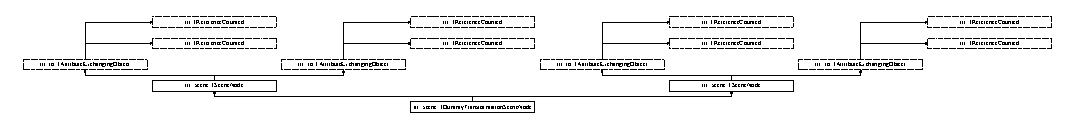
\includegraphics[height=4.000000cm]{classirr_1_1scene_1_1IDummyTransformationSceneNode}
\end{center}
\end{figure}
\subsection*{Public Member Functions}
\begin{DoxyCompactItemize}
\item 
\mbox{\Hypertarget{classirr_1_1scene_1_1IDummyTransformationSceneNode_a542c82a6fb76e99ea9773b974363fab1}\label{classirr_1_1scene_1_1IDummyTransformationSceneNode_a542c82a6fb76e99ea9773b974363fab1}} 
\hyperlink{classirr_1_1scene_1_1IDummyTransformationSceneNode_a542c82a6fb76e99ea9773b974363fab1}{I\+Dummy\+Transformation\+Scene\+Node} (\hyperlink{classirr_1_1scene_1_1ISceneNode}{I\+Scene\+Node} $\ast$parent, \hyperlink{classirr_1_1scene_1_1ISceneManager}{I\+Scene\+Manager} $\ast$mgr, \hyperlink{namespaceirr_ac66849b7a6ed16e30ebede579f9b47c6}{s32} id)
\begin{DoxyCompactList}\small\item\em Constructor. \end{DoxyCompactList}\item 
virtual \hyperlink{namespaceirr_1_1core_a73fa92e638c5ca97efd72da307cc9b65}{core\+::matrix4} \& \hyperlink{classirr_1_1scene_1_1IDummyTransformationSceneNode_a95612d8bb225213c907fbf5a2606f0d3}{get\+Relative\+Transformation\+Matrix} ()=0
\begin{DoxyCompactList}\small\item\em Returns a reference to the current relative transformation matrix. \end{DoxyCompactList}\end{DoxyCompactItemize}
\subsection*{Additional Inherited Members}


\subsection{Detailed Description}
Dummy scene node for adding additional transformations to the scene graph. 

This scene node does not render itself, and does not respond to set/get\+Position, set/get\+Rotation and set/get\+Scale. Its just a simple scene node that takes a matrix as relative transformation, making it possible to insert any transformation anywhere into the scene graph. This scene node is for example used by the \hyperlink{classirr_1_1scene_1_1IAnimatedMeshSceneNode}{I\+Animated\+Mesh\+Scene\+Node} for emulating joint scene nodes when playing skeletal animations. 

\subsection{Member Function Documentation}
\mbox{\Hypertarget{classirr_1_1scene_1_1IDummyTransformationSceneNode_a95612d8bb225213c907fbf5a2606f0d3}\label{classirr_1_1scene_1_1IDummyTransformationSceneNode_a95612d8bb225213c907fbf5a2606f0d3}} 
\index{irr\+::scene\+::\+I\+Dummy\+Transformation\+Scene\+Node@{irr\+::scene\+::\+I\+Dummy\+Transformation\+Scene\+Node}!get\+Relative\+Transformation\+Matrix@{get\+Relative\+Transformation\+Matrix}}
\index{get\+Relative\+Transformation\+Matrix@{get\+Relative\+Transformation\+Matrix}!irr\+::scene\+::\+I\+Dummy\+Transformation\+Scene\+Node@{irr\+::scene\+::\+I\+Dummy\+Transformation\+Scene\+Node}}
\subsubsection{\texorpdfstring{get\+Relative\+Transformation\+Matrix()}{getRelativeTransformationMatrix()}}
{\footnotesize\ttfamily virtual \hyperlink{namespaceirr_1_1core_a73fa92e638c5ca97efd72da307cc9b65}{core\+::matrix4}\& irr\+::scene\+::\+I\+Dummy\+Transformation\+Scene\+Node\+::get\+Relative\+Transformation\+Matrix (\begin{DoxyParamCaption}{ }\end{DoxyParamCaption})\hspace{0.3cm}{\ttfamily [pure virtual]}}



Returns a reference to the current relative transformation matrix. 

This is the matrix, this scene node uses instead of scale, translation and rotation. 

The documentation for this class was generated from the following file\+:\begin{DoxyCompactItemize}
\item 
indie\+\_\+share/controller/include/I\+Dummy\+Transformation\+Scene\+Node.\+h\end{DoxyCompactItemize}

\hypertarget{classirr_1_1scene_1_1IDynamicMeshBuffer}{}\section{irr\+:\+:scene\+:\+:I\+Dynamic\+Mesh\+Buffer Class Reference}
\label{classirr_1_1scene_1_1IDynamicMeshBuffer}\index{irr\+::scene\+::\+I\+Dynamic\+Mesh\+Buffer@{irr\+::scene\+::\+I\+Dynamic\+Mesh\+Buffer}}


{\ttfamily \#include $<$I\+Dynamic\+Mesh\+Buffer.\+h$>$}

Inheritance diagram for irr\+:\+:scene\+:\+:I\+Dynamic\+Mesh\+Buffer\+:\begin{figure}[H]
\begin{center}
\leavevmode
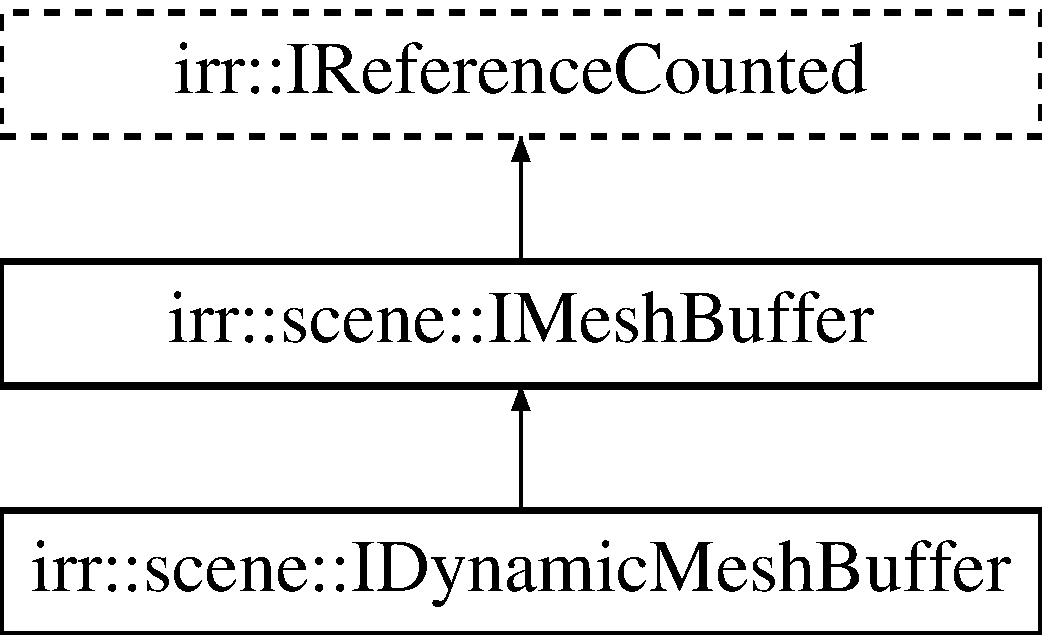
\includegraphics[height=2.131979cm]{classirr_1_1scene_1_1IDynamicMeshBuffer}
\end{center}
\end{figure}
\subsection*{Public Member Functions}
\begin{DoxyCompactItemize}
\item 
virtual \hyperlink{classirr_1_1video_1_1SMaterial}{video\+::\+S\+Material} \& \hyperlink{classirr_1_1scene_1_1IDynamicMeshBuffer_a6ed3a5ce948ebef063b7ea9e07974eb7}{get\+Material} ()=0
\begin{DoxyCompactList}\small\item\em Get the material of this meshbuffer. \end{DoxyCompactList}\item 
virtual const \hyperlink{classirr_1_1video_1_1SMaterial}{video\+::\+S\+Material} \& \hyperlink{classirr_1_1scene_1_1IDynamicMeshBuffer_a3be83e4819e9f79a3d9b264eb8bf4cfc}{get\+Material} () const =0
\begin{DoxyCompactList}\small\item\em Get the material of this meshbuffer. \end{DoxyCompactList}\item 
virtual const \hyperlink{namespaceirr_1_1core_a60f4b4c744aba55f10530d503c6ecb04}{core\+::aabbox3df} \& \hyperlink{classirr_1_1scene_1_1IDynamicMeshBuffer_a9053baee5a13c8b51e306d99e5ef7427}{get\+Bounding\+Box} () const =0
\begin{DoxyCompactList}\small\item\em Get the axis aligned bounding box of this meshbuffer. \end{DoxyCompactList}\item 
virtual void \hyperlink{classirr_1_1scene_1_1IDynamicMeshBuffer_adbe127e3774de6ae7ce96cb534a336e5}{set\+Bounding\+Box} (const \hyperlink{namespaceirr_1_1core_a60f4b4c744aba55f10530d503c6ecb04}{core\+::aabbox3df} \&box)=0
\begin{DoxyCompactList}\small\item\em Set axis aligned bounding box. \end{DoxyCompactList}\item 
\mbox{\Hypertarget{classirr_1_1scene_1_1IDynamicMeshBuffer_a0b3351f29578e0340c2e2ce3d03c9e59}\label{classirr_1_1scene_1_1IDynamicMeshBuffer_a0b3351f29578e0340c2e2ce3d03c9e59}} 
virtual void \hyperlink{classirr_1_1scene_1_1IDynamicMeshBuffer_a0b3351f29578e0340c2e2ce3d03c9e59}{recalculate\+Bounding\+Box} ()=0
\begin{DoxyCompactList}\small\item\em Recalculates the bounding box. Should be called if the mesh changed. \end{DoxyCompactList}\item 
virtual void \hyperlink{classirr_1_1scene_1_1IDynamicMeshBuffer_a0fb73ead4f2d2d86e9fef8768be1a1ff}{append} (const void $\ast$const vertices, \hyperlink{namespaceirr_a0416a53257075833e7002efd0a18e804}{u32} num\+Vertices, const \hyperlink{namespaceirr_ae9f8ec82692ad3b83c21f555bfa70bcc}{u16} $\ast$const indices, \hyperlink{namespaceirr_a0416a53257075833e7002efd0a18e804}{u32} num\+Indices)
\begin{DoxyCompactList}\small\item\em Append the vertices and indices to the current buffer. \end{DoxyCompactList}\item 
virtual void \hyperlink{classirr_1_1scene_1_1IDynamicMeshBuffer_aada30374517d2a52d6264b6359a1e35c}{append} (const \hyperlink{classirr_1_1scene_1_1IMeshBuffer}{I\+Mesh\+Buffer} $\ast$const other)
\begin{DoxyCompactList}\small\item\em Append the meshbuffer to the current buffer. \end{DoxyCompactList}\item 
\mbox{\Hypertarget{classirr_1_1scene_1_1IDynamicMeshBuffer_a59b514ca8f413396314d2dc93e00f6d5}\label{classirr_1_1scene_1_1IDynamicMeshBuffer_a59b514ca8f413396314d2dc93e00f6d5}} 
virtual \hyperlink{namespaceirr_1_1scene_ac7d8ee8d77da75f2580bb9bb17231c27}{E\+\_\+\+H\+A\+R\+D\+W\+A\+R\+E\+\_\+\+M\+A\+P\+P\+I\+NG} \hyperlink{classirr_1_1scene_1_1IDynamicMeshBuffer_a59b514ca8f413396314d2dc93e00f6d5}{get\+Hardware\+Mapping\+Hint\+\_\+\+Vertex} () const
\begin{DoxyCompactList}\small\item\em get the current hardware mapping hint \end{DoxyCompactList}\item 
\mbox{\Hypertarget{classirr_1_1scene_1_1IDynamicMeshBuffer_a4e08eea6ffaf32cc0d23c2b2008f4abb}\label{classirr_1_1scene_1_1IDynamicMeshBuffer_a4e08eea6ffaf32cc0d23c2b2008f4abb}} 
virtual \hyperlink{namespaceirr_1_1scene_ac7d8ee8d77da75f2580bb9bb17231c27}{E\+\_\+\+H\+A\+R\+D\+W\+A\+R\+E\+\_\+\+M\+A\+P\+P\+I\+NG} \hyperlink{classirr_1_1scene_1_1IDynamicMeshBuffer_a4e08eea6ffaf32cc0d23c2b2008f4abb}{get\+Hardware\+Mapping\+Hint\+\_\+\+Index} () const
\begin{DoxyCompactList}\small\item\em get the current hardware mapping hint \end{DoxyCompactList}\item 
\mbox{\Hypertarget{classirr_1_1scene_1_1IDynamicMeshBuffer_a8286f22fc7967422e2ddb5c183473247}\label{classirr_1_1scene_1_1IDynamicMeshBuffer_a8286f22fc7967422e2ddb5c183473247}} 
virtual void \hyperlink{classirr_1_1scene_1_1IDynamicMeshBuffer_a8286f22fc7967422e2ddb5c183473247}{set\+Hardware\+Mapping\+Hint} (\hyperlink{namespaceirr_1_1scene_ac7d8ee8d77da75f2580bb9bb17231c27}{E\+\_\+\+H\+A\+R\+D\+W\+A\+R\+E\+\_\+\+M\+A\+P\+P\+I\+NG} New\+Mapping\+Hint, \hyperlink{namespaceirr_1_1scene_a8f59a89ffef0ad8e5b2c2cb874a93e8c}{E\+\_\+\+B\+U\+F\+F\+E\+R\+\_\+\+T\+Y\+PE} Buffer=\hyperlink{namespaceirr_1_1scene_a8f59a89ffef0ad8e5b2c2cb874a93e8ca34ea664123fbc28610408e51b014dcdd}{E\+B\+T\+\_\+\+V\+E\+R\+T\+E\+X\+\_\+\+A\+N\+D\+\_\+\+I\+N\+D\+EX})
\begin{DoxyCompactList}\small\item\em set the hardware mapping hint, for driver \end{DoxyCompactList}\item 
\mbox{\Hypertarget{classirr_1_1scene_1_1IDynamicMeshBuffer_aed99e87534a2507c30362a20f4c43277}\label{classirr_1_1scene_1_1IDynamicMeshBuffer_aed99e87534a2507c30362a20f4c43277}} 
virtual void \hyperlink{classirr_1_1scene_1_1IDynamicMeshBuffer_aed99e87534a2507c30362a20f4c43277}{set\+Dirty} (\hyperlink{namespaceirr_1_1scene_a8f59a89ffef0ad8e5b2c2cb874a93e8c}{E\+\_\+\+B\+U\+F\+F\+E\+R\+\_\+\+T\+Y\+PE} Buffer=\hyperlink{namespaceirr_1_1scene_a8f59a89ffef0ad8e5b2c2cb874a93e8ca34ea664123fbc28610408e51b014dcdd}{E\+B\+T\+\_\+\+V\+E\+R\+T\+E\+X\+\_\+\+A\+N\+D\+\_\+\+I\+N\+D\+EX})
\begin{DoxyCompactList}\small\item\em flags the mesh as changed, reloads hardware buffers \end{DoxyCompactList}\item 
virtual \hyperlink{namespaceirr_a0416a53257075833e7002efd0a18e804}{u32} \hyperlink{classirr_1_1scene_1_1IDynamicMeshBuffer_a3480aae22a6701453a19b4c4cbcf2555}{get\+Changed\+I\+D\+\_\+\+Vertex} () const
\begin{DoxyCompactList}\small\item\em Get the currently used ID for identification of changes. \end{DoxyCompactList}\item 
virtual \hyperlink{namespaceirr_a0416a53257075833e7002efd0a18e804}{u32} \hyperlink{classirr_1_1scene_1_1IDynamicMeshBuffer_a2514a3d0e4865b7b9714fe1f9f58ad51}{get\+Changed\+I\+D\+\_\+\+Index} () const
\begin{DoxyCompactList}\small\item\em Get the currently used ID for identification of changes. \end{DoxyCompactList}\item 
virtual \hyperlink{namespaceirr_1_1video_a0e3b59e025e0d0db0ed2ee0ce904deac}{video\+::\+E\+\_\+\+V\+E\+R\+T\+E\+X\+\_\+\+T\+Y\+PE} \hyperlink{classirr_1_1scene_1_1IDynamicMeshBuffer_a3e7523774efaf9a177de6396dfdc14e2}{get\+Vertex\+Type} () const
\begin{DoxyCompactList}\small\item\em Get type of vertex data which is stored in this meshbuffer. \end{DoxyCompactList}\item 
virtual const void $\ast$ \hyperlink{classirr_1_1scene_1_1IDynamicMeshBuffer_a433e0e8ec301ce898dc373ca65e30e85}{get\+Vertices} () const
\begin{DoxyCompactList}\small\item\em Get access to vertex data. The data is an array of vertices. \end{DoxyCompactList}\item 
virtual void $\ast$ \hyperlink{classirr_1_1scene_1_1IDynamicMeshBuffer_a449643505823c7cfe793c5a82cde5fa4}{get\+Vertices} ()
\begin{DoxyCompactList}\small\item\em Get access to vertex data. The data is an array of vertices. \end{DoxyCompactList}\item 
virtual \hyperlink{namespaceirr_a0416a53257075833e7002efd0a18e804}{u32} \hyperlink{classirr_1_1scene_1_1IDynamicMeshBuffer_afc317a8ccda7e7eceb1f4955c90848d2}{get\+Vertex\+Count} () const
\begin{DoxyCompactList}\small\item\em Get amount of vertices in meshbuffer. \end{DoxyCompactList}\item 
virtual video\+::\+E\+\_\+\+I\+N\+D\+E\+X\+\_\+\+T\+Y\+PE \hyperlink{classirr_1_1scene_1_1IDynamicMeshBuffer_a3ac73aed8c40103682c5c6388339e70d}{get\+Index\+Type} () const
\begin{DoxyCompactList}\small\item\em Get type of index data which is stored in this meshbuffer. \end{DoxyCompactList}\item 
virtual const \hyperlink{namespaceirr_ae9f8ec82692ad3b83c21f555bfa70bcc}{u16} $\ast$ \hyperlink{classirr_1_1scene_1_1IDynamicMeshBuffer_ab762d23eb5666125dad83ce20f15b4dd}{get\+Indices} () const
\begin{DoxyCompactList}\small\item\em Get access to Indices. \end{DoxyCompactList}\item 
virtual \hyperlink{namespaceirr_ae9f8ec82692ad3b83c21f555bfa70bcc}{u16} $\ast$ \hyperlink{classirr_1_1scene_1_1IDynamicMeshBuffer_a556d8107ac44cbb16892f54370e32812}{get\+Indices} ()
\begin{DoxyCompactList}\small\item\em Get access to Indices. \end{DoxyCompactList}\item 
virtual \hyperlink{namespaceirr_a0416a53257075833e7002efd0a18e804}{u32} \hyperlink{classirr_1_1scene_1_1IDynamicMeshBuffer_adc483bdd7dfac4eb54e25c763ae1dae0}{get\+Index\+Count} () const
\begin{DoxyCompactList}\small\item\em Get amount of indices in this meshbuffer. \end{DoxyCompactList}\item 
\mbox{\Hypertarget{classirr_1_1scene_1_1IDynamicMeshBuffer_af68d8162eeb84addf0bb08e71e220f45}\label{classirr_1_1scene_1_1IDynamicMeshBuffer_af68d8162eeb84addf0bb08e71e220f45}} 
virtual const \hyperlink{namespaceirr_1_1core_ae6e2b2a6c552833ebbd5b7463d03586b}{core\+::vector3df} \& \hyperlink{classirr_1_1scene_1_1IDynamicMeshBuffer_af68d8162eeb84addf0bb08e71e220f45}{get\+Position} (\hyperlink{namespaceirr_a0416a53257075833e7002efd0a18e804}{u32} i) const
\begin{DoxyCompactList}\small\item\em returns position of vertex i \end{DoxyCompactList}\item 
\mbox{\Hypertarget{classirr_1_1scene_1_1IDynamicMeshBuffer_a773fef3c0f15b34390e5bea81894a55b}\label{classirr_1_1scene_1_1IDynamicMeshBuffer_a773fef3c0f15b34390e5bea81894a55b}} 
virtual \hyperlink{namespaceirr_1_1core_ae6e2b2a6c552833ebbd5b7463d03586b}{core\+::vector3df} \& \hyperlink{classirr_1_1scene_1_1IDynamicMeshBuffer_a773fef3c0f15b34390e5bea81894a55b}{get\+Position} (\hyperlink{namespaceirr_a0416a53257075833e7002efd0a18e804}{u32} i)
\begin{DoxyCompactList}\small\item\em returns position of vertex i \end{DoxyCompactList}\item 
\mbox{\Hypertarget{classirr_1_1scene_1_1IDynamicMeshBuffer_aa8dc513cdd282cb9c0ad99df9756068f}\label{classirr_1_1scene_1_1IDynamicMeshBuffer_aa8dc513cdd282cb9c0ad99df9756068f}} 
virtual const \hyperlink{namespaceirr_1_1core_a116f90bd31515724b6235014ee2b74d5}{core\+::vector2df} \& \hyperlink{classirr_1_1scene_1_1IDynamicMeshBuffer_aa8dc513cdd282cb9c0ad99df9756068f}{get\+T\+Coords} (\hyperlink{namespaceirr_a0416a53257075833e7002efd0a18e804}{u32} i) const
\begin{DoxyCompactList}\small\item\em returns texture coords of vertex i \end{DoxyCompactList}\item 
\mbox{\Hypertarget{classirr_1_1scene_1_1IDynamicMeshBuffer_aa366aaa5bc8488af18a3814a30cb7f09}\label{classirr_1_1scene_1_1IDynamicMeshBuffer_aa366aaa5bc8488af18a3814a30cb7f09}} 
virtual \hyperlink{namespaceirr_1_1core_a116f90bd31515724b6235014ee2b74d5}{core\+::vector2df} \& \hyperlink{classirr_1_1scene_1_1IDynamicMeshBuffer_aa366aaa5bc8488af18a3814a30cb7f09}{get\+T\+Coords} (\hyperlink{namespaceirr_a0416a53257075833e7002efd0a18e804}{u32} i)
\begin{DoxyCompactList}\small\item\em returns texture coords of vertex i \end{DoxyCompactList}\item 
\mbox{\Hypertarget{classirr_1_1scene_1_1IDynamicMeshBuffer_af4f8cbcaef9632e5b68b14d15d068218}\label{classirr_1_1scene_1_1IDynamicMeshBuffer_af4f8cbcaef9632e5b68b14d15d068218}} 
virtual const \hyperlink{namespaceirr_1_1core_ae6e2b2a6c552833ebbd5b7463d03586b}{core\+::vector3df} \& \hyperlink{classirr_1_1scene_1_1IDynamicMeshBuffer_af4f8cbcaef9632e5b68b14d15d068218}{get\+Normal} (\hyperlink{namespaceirr_a0416a53257075833e7002efd0a18e804}{u32} i) const
\begin{DoxyCompactList}\small\item\em returns normal of vertex i \end{DoxyCompactList}\item 
\mbox{\Hypertarget{classirr_1_1scene_1_1IDynamicMeshBuffer_a8a1647d10585b9cd262feeeac98ae371}\label{classirr_1_1scene_1_1IDynamicMeshBuffer_a8a1647d10585b9cd262feeeac98ae371}} 
virtual \hyperlink{namespaceirr_1_1core_ae6e2b2a6c552833ebbd5b7463d03586b}{core\+::vector3df} \& \hyperlink{classirr_1_1scene_1_1IDynamicMeshBuffer_a8a1647d10585b9cd262feeeac98ae371}{get\+Normal} (\hyperlink{namespaceirr_a0416a53257075833e7002efd0a18e804}{u32} i)
\begin{DoxyCompactList}\small\item\em returns normal of vertex i \end{DoxyCompactList}\item 
virtual \hyperlink{classirr_1_1video_1_1SMaterial}{video\+::\+S\+Material} \& \hyperlink{classirr_1_1scene_1_1IDynamicMeshBuffer_a6ed3a5ce948ebef063b7ea9e07974eb7}{get\+Material} ()=0
\begin{DoxyCompactList}\small\item\em Get the material of this meshbuffer. \end{DoxyCompactList}\item 
virtual const \hyperlink{classirr_1_1video_1_1SMaterial}{video\+::\+S\+Material} \& \hyperlink{classirr_1_1scene_1_1IDynamicMeshBuffer_a3be83e4819e9f79a3d9b264eb8bf4cfc}{get\+Material} () const =0
\begin{DoxyCompactList}\small\item\em Get the material of this meshbuffer. \end{DoxyCompactList}\item 
virtual const \hyperlink{namespaceirr_1_1core_a60f4b4c744aba55f10530d503c6ecb04}{core\+::aabbox3df} \& \hyperlink{classirr_1_1scene_1_1IDynamicMeshBuffer_a9053baee5a13c8b51e306d99e5ef7427}{get\+Bounding\+Box} () const =0
\begin{DoxyCompactList}\small\item\em Get the axis aligned bounding box of this meshbuffer. \end{DoxyCompactList}\item 
virtual void \hyperlink{classirr_1_1scene_1_1IDynamicMeshBuffer_adbe127e3774de6ae7ce96cb534a336e5}{set\+Bounding\+Box} (const \hyperlink{namespaceirr_1_1core_a60f4b4c744aba55f10530d503c6ecb04}{core\+::aabbox3df} \&box)=0
\begin{DoxyCompactList}\small\item\em Set axis aligned bounding box. \end{DoxyCompactList}\item 
\mbox{\Hypertarget{classirr_1_1scene_1_1IDynamicMeshBuffer_a0b3351f29578e0340c2e2ce3d03c9e59}\label{classirr_1_1scene_1_1IDynamicMeshBuffer_a0b3351f29578e0340c2e2ce3d03c9e59}} 
virtual void \hyperlink{classirr_1_1scene_1_1IDynamicMeshBuffer_a0b3351f29578e0340c2e2ce3d03c9e59}{recalculate\+Bounding\+Box} ()=0
\begin{DoxyCompactList}\small\item\em Recalculates the bounding box. Should be called if the mesh changed. \end{DoxyCompactList}\item 
virtual void \hyperlink{classirr_1_1scene_1_1IDynamicMeshBuffer_a0fb73ead4f2d2d86e9fef8768be1a1ff}{append} (const void $\ast$const vertices, \hyperlink{namespaceirr_a0416a53257075833e7002efd0a18e804}{u32} num\+Vertices, const \hyperlink{namespaceirr_ae9f8ec82692ad3b83c21f555bfa70bcc}{u16} $\ast$const indices, \hyperlink{namespaceirr_a0416a53257075833e7002efd0a18e804}{u32} num\+Indices)
\begin{DoxyCompactList}\small\item\em Append the vertices and indices to the current buffer. \end{DoxyCompactList}\item 
virtual void \hyperlink{classirr_1_1scene_1_1IDynamicMeshBuffer_aada30374517d2a52d6264b6359a1e35c}{append} (const \hyperlink{classirr_1_1scene_1_1IMeshBuffer}{I\+Mesh\+Buffer} $\ast$const other)
\begin{DoxyCompactList}\small\item\em Append the meshbuffer to the current buffer. \end{DoxyCompactList}\item 
\mbox{\Hypertarget{classirr_1_1scene_1_1IDynamicMeshBuffer_a59b514ca8f413396314d2dc93e00f6d5}\label{classirr_1_1scene_1_1IDynamicMeshBuffer_a59b514ca8f413396314d2dc93e00f6d5}} 
virtual \hyperlink{namespaceirr_1_1scene_ac7d8ee8d77da75f2580bb9bb17231c27}{E\+\_\+\+H\+A\+R\+D\+W\+A\+R\+E\+\_\+\+M\+A\+P\+P\+I\+NG} \hyperlink{classirr_1_1scene_1_1IDynamicMeshBuffer_a59b514ca8f413396314d2dc93e00f6d5}{get\+Hardware\+Mapping\+Hint\+\_\+\+Vertex} () const
\begin{DoxyCompactList}\small\item\em get the current hardware mapping hint \end{DoxyCompactList}\item 
\mbox{\Hypertarget{classirr_1_1scene_1_1IDynamicMeshBuffer_a4e08eea6ffaf32cc0d23c2b2008f4abb}\label{classirr_1_1scene_1_1IDynamicMeshBuffer_a4e08eea6ffaf32cc0d23c2b2008f4abb}} 
virtual \hyperlink{namespaceirr_1_1scene_ac7d8ee8d77da75f2580bb9bb17231c27}{E\+\_\+\+H\+A\+R\+D\+W\+A\+R\+E\+\_\+\+M\+A\+P\+P\+I\+NG} \hyperlink{classirr_1_1scene_1_1IDynamicMeshBuffer_a4e08eea6ffaf32cc0d23c2b2008f4abb}{get\+Hardware\+Mapping\+Hint\+\_\+\+Index} () const
\begin{DoxyCompactList}\small\item\em get the current hardware mapping hint \end{DoxyCompactList}\item 
\mbox{\Hypertarget{classirr_1_1scene_1_1IDynamicMeshBuffer_a8286f22fc7967422e2ddb5c183473247}\label{classirr_1_1scene_1_1IDynamicMeshBuffer_a8286f22fc7967422e2ddb5c183473247}} 
virtual void \hyperlink{classirr_1_1scene_1_1IDynamicMeshBuffer_a8286f22fc7967422e2ddb5c183473247}{set\+Hardware\+Mapping\+Hint} (\hyperlink{namespaceirr_1_1scene_ac7d8ee8d77da75f2580bb9bb17231c27}{E\+\_\+\+H\+A\+R\+D\+W\+A\+R\+E\+\_\+\+M\+A\+P\+P\+I\+NG} New\+Mapping\+Hint, \hyperlink{namespaceirr_1_1scene_a8f59a89ffef0ad8e5b2c2cb874a93e8c}{E\+\_\+\+B\+U\+F\+F\+E\+R\+\_\+\+T\+Y\+PE} Buffer=\hyperlink{namespaceirr_1_1scene_a8f59a89ffef0ad8e5b2c2cb874a93e8ca34ea664123fbc28610408e51b014dcdd}{E\+B\+T\+\_\+\+V\+E\+R\+T\+E\+X\+\_\+\+A\+N\+D\+\_\+\+I\+N\+D\+EX})
\begin{DoxyCompactList}\small\item\em set the hardware mapping hint, for driver \end{DoxyCompactList}\item 
\mbox{\Hypertarget{classirr_1_1scene_1_1IDynamicMeshBuffer_aed99e87534a2507c30362a20f4c43277}\label{classirr_1_1scene_1_1IDynamicMeshBuffer_aed99e87534a2507c30362a20f4c43277}} 
virtual void \hyperlink{classirr_1_1scene_1_1IDynamicMeshBuffer_aed99e87534a2507c30362a20f4c43277}{set\+Dirty} (\hyperlink{namespaceirr_1_1scene_a8f59a89ffef0ad8e5b2c2cb874a93e8c}{E\+\_\+\+B\+U\+F\+F\+E\+R\+\_\+\+T\+Y\+PE} Buffer=\hyperlink{namespaceirr_1_1scene_a8f59a89ffef0ad8e5b2c2cb874a93e8ca34ea664123fbc28610408e51b014dcdd}{E\+B\+T\+\_\+\+V\+E\+R\+T\+E\+X\+\_\+\+A\+N\+D\+\_\+\+I\+N\+D\+EX})
\begin{DoxyCompactList}\small\item\em flags the mesh as changed, reloads hardware buffers \end{DoxyCompactList}\item 
virtual \hyperlink{namespaceirr_a0416a53257075833e7002efd0a18e804}{u32} \hyperlink{classirr_1_1scene_1_1IDynamicMeshBuffer_a3480aae22a6701453a19b4c4cbcf2555}{get\+Changed\+I\+D\+\_\+\+Vertex} () const
\begin{DoxyCompactList}\small\item\em Get the currently used ID for identification of changes. \end{DoxyCompactList}\item 
virtual \hyperlink{namespaceirr_a0416a53257075833e7002efd0a18e804}{u32} \hyperlink{classirr_1_1scene_1_1IDynamicMeshBuffer_a2514a3d0e4865b7b9714fe1f9f58ad51}{get\+Changed\+I\+D\+\_\+\+Index} () const
\begin{DoxyCompactList}\small\item\em Get the currently used ID for identification of changes. \end{DoxyCompactList}\item 
virtual \hyperlink{namespaceirr_1_1video_a0e3b59e025e0d0db0ed2ee0ce904deac}{video\+::\+E\+\_\+\+V\+E\+R\+T\+E\+X\+\_\+\+T\+Y\+PE} \hyperlink{classirr_1_1scene_1_1IDynamicMeshBuffer_a3e7523774efaf9a177de6396dfdc14e2}{get\+Vertex\+Type} () const
\begin{DoxyCompactList}\small\item\em Get type of vertex data which is stored in this meshbuffer. \end{DoxyCompactList}\item 
virtual const void $\ast$ \hyperlink{classirr_1_1scene_1_1IDynamicMeshBuffer_a433e0e8ec301ce898dc373ca65e30e85}{get\+Vertices} () const
\begin{DoxyCompactList}\small\item\em Get access to vertex data. The data is an array of vertices. \end{DoxyCompactList}\item 
virtual void $\ast$ \hyperlink{classirr_1_1scene_1_1IDynamicMeshBuffer_a449643505823c7cfe793c5a82cde5fa4}{get\+Vertices} ()
\begin{DoxyCompactList}\small\item\em Get access to vertex data. The data is an array of vertices. \end{DoxyCompactList}\item 
virtual \hyperlink{namespaceirr_a0416a53257075833e7002efd0a18e804}{u32} \hyperlink{classirr_1_1scene_1_1IDynamicMeshBuffer_afc317a8ccda7e7eceb1f4955c90848d2}{get\+Vertex\+Count} () const
\begin{DoxyCompactList}\small\item\em Get amount of vertices in meshbuffer. \end{DoxyCompactList}\item 
virtual video\+::\+E\+\_\+\+I\+N\+D\+E\+X\+\_\+\+T\+Y\+PE \hyperlink{classirr_1_1scene_1_1IDynamicMeshBuffer_a3ac73aed8c40103682c5c6388339e70d}{get\+Index\+Type} () const
\begin{DoxyCompactList}\small\item\em Get type of index data which is stored in this meshbuffer. \end{DoxyCompactList}\item 
virtual const \hyperlink{namespaceirr_ae9f8ec82692ad3b83c21f555bfa70bcc}{u16} $\ast$ \hyperlink{classirr_1_1scene_1_1IDynamicMeshBuffer_ab762d23eb5666125dad83ce20f15b4dd}{get\+Indices} () const
\begin{DoxyCompactList}\small\item\em Get access to Indices. \end{DoxyCompactList}\item 
virtual \hyperlink{namespaceirr_ae9f8ec82692ad3b83c21f555bfa70bcc}{u16} $\ast$ \hyperlink{classirr_1_1scene_1_1IDynamicMeshBuffer_a556d8107ac44cbb16892f54370e32812}{get\+Indices} ()
\begin{DoxyCompactList}\small\item\em Get access to Indices. \end{DoxyCompactList}\item 
virtual \hyperlink{namespaceirr_a0416a53257075833e7002efd0a18e804}{u32} \hyperlink{classirr_1_1scene_1_1IDynamicMeshBuffer_adc483bdd7dfac4eb54e25c763ae1dae0}{get\+Index\+Count} () const
\begin{DoxyCompactList}\small\item\em Get amount of indices in this meshbuffer. \end{DoxyCompactList}\item 
\mbox{\Hypertarget{classirr_1_1scene_1_1IDynamicMeshBuffer_af68d8162eeb84addf0bb08e71e220f45}\label{classirr_1_1scene_1_1IDynamicMeshBuffer_af68d8162eeb84addf0bb08e71e220f45}} 
virtual const \hyperlink{namespaceirr_1_1core_ae6e2b2a6c552833ebbd5b7463d03586b}{core\+::vector3df} \& \hyperlink{classirr_1_1scene_1_1IDynamicMeshBuffer_af68d8162eeb84addf0bb08e71e220f45}{get\+Position} (\hyperlink{namespaceirr_a0416a53257075833e7002efd0a18e804}{u32} i) const
\begin{DoxyCompactList}\small\item\em returns position of vertex i \end{DoxyCompactList}\item 
\mbox{\Hypertarget{classirr_1_1scene_1_1IDynamicMeshBuffer_a773fef3c0f15b34390e5bea81894a55b}\label{classirr_1_1scene_1_1IDynamicMeshBuffer_a773fef3c0f15b34390e5bea81894a55b}} 
virtual \hyperlink{namespaceirr_1_1core_ae6e2b2a6c552833ebbd5b7463d03586b}{core\+::vector3df} \& \hyperlink{classirr_1_1scene_1_1IDynamicMeshBuffer_a773fef3c0f15b34390e5bea81894a55b}{get\+Position} (\hyperlink{namespaceirr_a0416a53257075833e7002efd0a18e804}{u32} i)
\begin{DoxyCompactList}\small\item\em returns position of vertex i \end{DoxyCompactList}\item 
\mbox{\Hypertarget{classirr_1_1scene_1_1IDynamicMeshBuffer_aa8dc513cdd282cb9c0ad99df9756068f}\label{classirr_1_1scene_1_1IDynamicMeshBuffer_aa8dc513cdd282cb9c0ad99df9756068f}} 
virtual const \hyperlink{namespaceirr_1_1core_a116f90bd31515724b6235014ee2b74d5}{core\+::vector2df} \& \hyperlink{classirr_1_1scene_1_1IDynamicMeshBuffer_aa8dc513cdd282cb9c0ad99df9756068f}{get\+T\+Coords} (\hyperlink{namespaceirr_a0416a53257075833e7002efd0a18e804}{u32} i) const
\begin{DoxyCompactList}\small\item\em returns texture coords of vertex i \end{DoxyCompactList}\item 
\mbox{\Hypertarget{classirr_1_1scene_1_1IDynamicMeshBuffer_aa366aaa5bc8488af18a3814a30cb7f09}\label{classirr_1_1scene_1_1IDynamicMeshBuffer_aa366aaa5bc8488af18a3814a30cb7f09}} 
virtual \hyperlink{namespaceirr_1_1core_a116f90bd31515724b6235014ee2b74d5}{core\+::vector2df} \& \hyperlink{classirr_1_1scene_1_1IDynamicMeshBuffer_aa366aaa5bc8488af18a3814a30cb7f09}{get\+T\+Coords} (\hyperlink{namespaceirr_a0416a53257075833e7002efd0a18e804}{u32} i)
\begin{DoxyCompactList}\small\item\em returns texture coords of vertex i \end{DoxyCompactList}\item 
\mbox{\Hypertarget{classirr_1_1scene_1_1IDynamicMeshBuffer_af4f8cbcaef9632e5b68b14d15d068218}\label{classirr_1_1scene_1_1IDynamicMeshBuffer_af4f8cbcaef9632e5b68b14d15d068218}} 
virtual const \hyperlink{namespaceirr_1_1core_ae6e2b2a6c552833ebbd5b7463d03586b}{core\+::vector3df} \& \hyperlink{classirr_1_1scene_1_1IDynamicMeshBuffer_af4f8cbcaef9632e5b68b14d15d068218}{get\+Normal} (\hyperlink{namespaceirr_a0416a53257075833e7002efd0a18e804}{u32} i) const
\begin{DoxyCompactList}\small\item\em returns normal of vertex i \end{DoxyCompactList}\item 
\mbox{\Hypertarget{classirr_1_1scene_1_1IDynamicMeshBuffer_a8a1647d10585b9cd262feeeac98ae371}\label{classirr_1_1scene_1_1IDynamicMeshBuffer_a8a1647d10585b9cd262feeeac98ae371}} 
virtual \hyperlink{namespaceirr_1_1core_ae6e2b2a6c552833ebbd5b7463d03586b}{core\+::vector3df} \& \hyperlink{classirr_1_1scene_1_1IDynamicMeshBuffer_a8a1647d10585b9cd262feeeac98ae371}{get\+Normal} (\hyperlink{namespaceirr_a0416a53257075833e7002efd0a18e804}{u32} i)
\begin{DoxyCompactList}\small\item\em returns normal of vertex i \end{DoxyCompactList}\end{DoxyCompactItemize}
\subsection*{Additional Inherited Members}


\subsection{Detailed Description}
a dynamic mesh\+Buffer 

\subsection{Member Function Documentation}
\mbox{\Hypertarget{classirr_1_1scene_1_1IDynamicMeshBuffer_a0fb73ead4f2d2d86e9fef8768be1a1ff}\label{classirr_1_1scene_1_1IDynamicMeshBuffer_a0fb73ead4f2d2d86e9fef8768be1a1ff}} 
\index{irr\+::scene\+::\+I\+Dynamic\+Mesh\+Buffer@{irr\+::scene\+::\+I\+Dynamic\+Mesh\+Buffer}!append@{append}}
\index{append@{append}!irr\+::scene\+::\+I\+Dynamic\+Mesh\+Buffer@{irr\+::scene\+::\+I\+Dynamic\+Mesh\+Buffer}}
\subsubsection{\texorpdfstring{append()}{append()}\hspace{0.1cm}{\footnotesize\ttfamily [1/4]}}
{\footnotesize\ttfamily virtual void irr\+::scene\+::\+I\+Dynamic\+Mesh\+Buffer\+::append (\begin{DoxyParamCaption}\item[{const void $\ast$const}]{vertices,  }\item[{\hyperlink{namespaceirr_a0416a53257075833e7002efd0a18e804}{u32}}]{num\+Vertices,  }\item[{const \hyperlink{namespaceirr_ae9f8ec82692ad3b83c21f555bfa70bcc}{u16} $\ast$const}]{indices,  }\item[{\hyperlink{namespaceirr_a0416a53257075833e7002efd0a18e804}{u32}}]{num\+Indices }\end{DoxyParamCaption})\hspace{0.3cm}{\ttfamily [inline]}, {\ttfamily [virtual]}}



Append the vertices and indices to the current buffer. 

Only works for compatible vertex types. 
\begin{DoxyParams}{Parameters}
{\em vertices} & Pointer to a vertex array. \\
\hline
{\em num\+Vertices} & Number of vertices in the array. \\
\hline
{\em indices} & Pointer to index array. \\
\hline
{\em num\+Indices} & Number of indices in array. \\
\hline
\end{DoxyParams}


Implements \hyperlink{classirr_1_1scene_1_1IMeshBuffer_ac9e9d7fbb10175cc6f1596ba3fe4e8f9}{irr\+::scene\+::\+I\+Mesh\+Buffer}.

\mbox{\Hypertarget{classirr_1_1scene_1_1IDynamicMeshBuffer_a0fb73ead4f2d2d86e9fef8768be1a1ff}\label{classirr_1_1scene_1_1IDynamicMeshBuffer_a0fb73ead4f2d2d86e9fef8768be1a1ff}} 
\index{irr\+::scene\+::\+I\+Dynamic\+Mesh\+Buffer@{irr\+::scene\+::\+I\+Dynamic\+Mesh\+Buffer}!append@{append}}
\index{append@{append}!irr\+::scene\+::\+I\+Dynamic\+Mesh\+Buffer@{irr\+::scene\+::\+I\+Dynamic\+Mesh\+Buffer}}
\subsubsection{\texorpdfstring{append()}{append()}\hspace{0.1cm}{\footnotesize\ttfamily [2/4]}}
{\footnotesize\ttfamily virtual void irr\+::scene\+::\+I\+Dynamic\+Mesh\+Buffer\+::append (\begin{DoxyParamCaption}\item[{const void $\ast$const}]{vertices,  }\item[{\hyperlink{namespaceirr_a0416a53257075833e7002efd0a18e804}{u32}}]{num\+Vertices,  }\item[{const \hyperlink{namespaceirr_ae9f8ec82692ad3b83c21f555bfa70bcc}{u16} $\ast$const}]{indices,  }\item[{\hyperlink{namespaceirr_a0416a53257075833e7002efd0a18e804}{u32}}]{num\+Indices }\end{DoxyParamCaption})\hspace{0.3cm}{\ttfamily [inline]}, {\ttfamily [virtual]}}



Append the vertices and indices to the current buffer. 

Only works for compatible vertex types. 
\begin{DoxyParams}{Parameters}
{\em vertices} & Pointer to a vertex array. \\
\hline
{\em num\+Vertices} & Number of vertices in the array. \\
\hline
{\em indices} & Pointer to index array. \\
\hline
{\em num\+Indices} & Number of indices in array. \\
\hline
\end{DoxyParams}


Implements \hyperlink{classirr_1_1scene_1_1IMeshBuffer_ac9e9d7fbb10175cc6f1596ba3fe4e8f9}{irr\+::scene\+::\+I\+Mesh\+Buffer}.

\mbox{\Hypertarget{classirr_1_1scene_1_1IDynamicMeshBuffer_aada30374517d2a52d6264b6359a1e35c}\label{classirr_1_1scene_1_1IDynamicMeshBuffer_aada30374517d2a52d6264b6359a1e35c}} 
\index{irr\+::scene\+::\+I\+Dynamic\+Mesh\+Buffer@{irr\+::scene\+::\+I\+Dynamic\+Mesh\+Buffer}!append@{append}}
\index{append@{append}!irr\+::scene\+::\+I\+Dynamic\+Mesh\+Buffer@{irr\+::scene\+::\+I\+Dynamic\+Mesh\+Buffer}}
\subsubsection{\texorpdfstring{append()}{append()}\hspace{0.1cm}{\footnotesize\ttfamily [3/4]}}
{\footnotesize\ttfamily virtual void irr\+::scene\+::\+I\+Dynamic\+Mesh\+Buffer\+::append (\begin{DoxyParamCaption}\item[{const \hyperlink{classirr_1_1scene_1_1IMeshBuffer}{I\+Mesh\+Buffer} $\ast$const}]{other }\end{DoxyParamCaption})\hspace{0.3cm}{\ttfamily [inline]}, {\ttfamily [virtual]}}



Append the meshbuffer to the current buffer. 

Only works for compatible vertex types 
\begin{DoxyParams}{Parameters}
{\em other} & Buffer to append to this one. \\
\hline
\end{DoxyParams}


Implements \hyperlink{classirr_1_1scene_1_1IMeshBuffer_a79d2737962579138183ed0fd324310b3}{irr\+::scene\+::\+I\+Mesh\+Buffer}.

\mbox{\Hypertarget{classirr_1_1scene_1_1IDynamicMeshBuffer_aada30374517d2a52d6264b6359a1e35c}\label{classirr_1_1scene_1_1IDynamicMeshBuffer_aada30374517d2a52d6264b6359a1e35c}} 
\index{irr\+::scene\+::\+I\+Dynamic\+Mesh\+Buffer@{irr\+::scene\+::\+I\+Dynamic\+Mesh\+Buffer}!append@{append}}
\index{append@{append}!irr\+::scene\+::\+I\+Dynamic\+Mesh\+Buffer@{irr\+::scene\+::\+I\+Dynamic\+Mesh\+Buffer}}
\subsubsection{\texorpdfstring{append()}{append()}\hspace{0.1cm}{\footnotesize\ttfamily [4/4]}}
{\footnotesize\ttfamily virtual void irr\+::scene\+::\+I\+Dynamic\+Mesh\+Buffer\+::append (\begin{DoxyParamCaption}\item[{const \hyperlink{classirr_1_1scene_1_1IMeshBuffer}{I\+Mesh\+Buffer} $\ast$const}]{other }\end{DoxyParamCaption})\hspace{0.3cm}{\ttfamily [inline]}, {\ttfamily [virtual]}}



Append the meshbuffer to the current buffer. 

Only works for compatible vertex types 
\begin{DoxyParams}{Parameters}
{\em other} & Buffer to append to this one. \\
\hline
\end{DoxyParams}


Implements \hyperlink{classirr_1_1scene_1_1IMeshBuffer_a79d2737962579138183ed0fd324310b3}{irr\+::scene\+::\+I\+Mesh\+Buffer}.

\mbox{\Hypertarget{classirr_1_1scene_1_1IDynamicMeshBuffer_a9053baee5a13c8b51e306d99e5ef7427}\label{classirr_1_1scene_1_1IDynamicMeshBuffer_a9053baee5a13c8b51e306d99e5ef7427}} 
\index{irr\+::scene\+::\+I\+Dynamic\+Mesh\+Buffer@{irr\+::scene\+::\+I\+Dynamic\+Mesh\+Buffer}!get\+Bounding\+Box@{get\+Bounding\+Box}}
\index{get\+Bounding\+Box@{get\+Bounding\+Box}!irr\+::scene\+::\+I\+Dynamic\+Mesh\+Buffer@{irr\+::scene\+::\+I\+Dynamic\+Mesh\+Buffer}}
\subsubsection{\texorpdfstring{get\+Bounding\+Box()}{getBoundingBox()}\hspace{0.1cm}{\footnotesize\ttfamily [1/2]}}
{\footnotesize\ttfamily virtual const \hyperlink{namespaceirr_1_1core_a60f4b4c744aba55f10530d503c6ecb04}{core\+::aabbox3df}\& irr\+::scene\+::\+I\+Dynamic\+Mesh\+Buffer\+::get\+Bounding\+Box (\begin{DoxyParamCaption}{ }\end{DoxyParamCaption}) const\hspace{0.3cm}{\ttfamily [pure virtual]}}



Get the axis aligned bounding box of this meshbuffer. 

\begin{DoxyReturn}{Returns}
Axis aligned bounding box of this buffer. 
\end{DoxyReturn}


Implements \hyperlink{classirr_1_1scene_1_1IMeshBuffer_ac53fe1096756a40f25dae25911e27c51}{irr\+::scene\+::\+I\+Mesh\+Buffer}.

\mbox{\Hypertarget{classirr_1_1scene_1_1IDynamicMeshBuffer_a9053baee5a13c8b51e306d99e5ef7427}\label{classirr_1_1scene_1_1IDynamicMeshBuffer_a9053baee5a13c8b51e306d99e5ef7427}} 
\index{irr\+::scene\+::\+I\+Dynamic\+Mesh\+Buffer@{irr\+::scene\+::\+I\+Dynamic\+Mesh\+Buffer}!get\+Bounding\+Box@{get\+Bounding\+Box}}
\index{get\+Bounding\+Box@{get\+Bounding\+Box}!irr\+::scene\+::\+I\+Dynamic\+Mesh\+Buffer@{irr\+::scene\+::\+I\+Dynamic\+Mesh\+Buffer}}
\subsubsection{\texorpdfstring{get\+Bounding\+Box()}{getBoundingBox()}\hspace{0.1cm}{\footnotesize\ttfamily [2/2]}}
{\footnotesize\ttfamily virtual const \hyperlink{namespaceirr_1_1core_a60f4b4c744aba55f10530d503c6ecb04}{core\+::aabbox3df}\& irr\+::scene\+::\+I\+Dynamic\+Mesh\+Buffer\+::get\+Bounding\+Box (\begin{DoxyParamCaption}{ }\end{DoxyParamCaption}) const\hspace{0.3cm}{\ttfamily [pure virtual]}}



Get the axis aligned bounding box of this meshbuffer. 

\begin{DoxyReturn}{Returns}
Axis aligned bounding box of this buffer. 
\end{DoxyReturn}


Implements \hyperlink{classirr_1_1scene_1_1IMeshBuffer_ac53fe1096756a40f25dae25911e27c51}{irr\+::scene\+::\+I\+Mesh\+Buffer}.

\mbox{\Hypertarget{classirr_1_1scene_1_1IDynamicMeshBuffer_a2514a3d0e4865b7b9714fe1f9f58ad51}\label{classirr_1_1scene_1_1IDynamicMeshBuffer_a2514a3d0e4865b7b9714fe1f9f58ad51}} 
\index{irr\+::scene\+::\+I\+Dynamic\+Mesh\+Buffer@{irr\+::scene\+::\+I\+Dynamic\+Mesh\+Buffer}!get\+Changed\+I\+D\+\_\+\+Index@{get\+Changed\+I\+D\+\_\+\+Index}}
\index{get\+Changed\+I\+D\+\_\+\+Index@{get\+Changed\+I\+D\+\_\+\+Index}!irr\+::scene\+::\+I\+Dynamic\+Mesh\+Buffer@{irr\+::scene\+::\+I\+Dynamic\+Mesh\+Buffer}}
\subsubsection{\texorpdfstring{get\+Changed\+I\+D\+\_\+\+Index()}{getChangedID\_Index()}\hspace{0.1cm}{\footnotesize\ttfamily [1/2]}}
{\footnotesize\ttfamily virtual \hyperlink{namespaceirr_a0416a53257075833e7002efd0a18e804}{u32} irr\+::scene\+::\+I\+Dynamic\+Mesh\+Buffer\+::get\+Changed\+I\+D\+\_\+\+Index (\begin{DoxyParamCaption}{ }\end{DoxyParamCaption}) const\hspace{0.3cm}{\ttfamily [inline]}, {\ttfamily [virtual]}}



Get the currently used ID for identification of changes. 

This shouldn\textquotesingle{}t be used for anything outside the Video\+Driver. 

Implements \hyperlink{classirr_1_1scene_1_1IMeshBuffer_acc389d76856dfb06c3ba45a92315e6d8}{irr\+::scene\+::\+I\+Mesh\+Buffer}.

\mbox{\Hypertarget{classirr_1_1scene_1_1IDynamicMeshBuffer_a2514a3d0e4865b7b9714fe1f9f58ad51}\label{classirr_1_1scene_1_1IDynamicMeshBuffer_a2514a3d0e4865b7b9714fe1f9f58ad51}} 
\index{irr\+::scene\+::\+I\+Dynamic\+Mesh\+Buffer@{irr\+::scene\+::\+I\+Dynamic\+Mesh\+Buffer}!get\+Changed\+I\+D\+\_\+\+Index@{get\+Changed\+I\+D\+\_\+\+Index}}
\index{get\+Changed\+I\+D\+\_\+\+Index@{get\+Changed\+I\+D\+\_\+\+Index}!irr\+::scene\+::\+I\+Dynamic\+Mesh\+Buffer@{irr\+::scene\+::\+I\+Dynamic\+Mesh\+Buffer}}
\subsubsection{\texorpdfstring{get\+Changed\+I\+D\+\_\+\+Index()}{getChangedID\_Index()}\hspace{0.1cm}{\footnotesize\ttfamily [2/2]}}
{\footnotesize\ttfamily virtual \hyperlink{namespaceirr_a0416a53257075833e7002efd0a18e804}{u32} irr\+::scene\+::\+I\+Dynamic\+Mesh\+Buffer\+::get\+Changed\+I\+D\+\_\+\+Index (\begin{DoxyParamCaption}{ }\end{DoxyParamCaption}) const\hspace{0.3cm}{\ttfamily [inline]}, {\ttfamily [virtual]}}



Get the currently used ID for identification of changes. 

This shouldn\textquotesingle{}t be used for anything outside the Video\+Driver. 

Implements \hyperlink{classirr_1_1scene_1_1IMeshBuffer_acc389d76856dfb06c3ba45a92315e6d8}{irr\+::scene\+::\+I\+Mesh\+Buffer}.

\mbox{\Hypertarget{classirr_1_1scene_1_1IDynamicMeshBuffer_a3480aae22a6701453a19b4c4cbcf2555}\label{classirr_1_1scene_1_1IDynamicMeshBuffer_a3480aae22a6701453a19b4c4cbcf2555}} 
\index{irr\+::scene\+::\+I\+Dynamic\+Mesh\+Buffer@{irr\+::scene\+::\+I\+Dynamic\+Mesh\+Buffer}!get\+Changed\+I\+D\+\_\+\+Vertex@{get\+Changed\+I\+D\+\_\+\+Vertex}}
\index{get\+Changed\+I\+D\+\_\+\+Vertex@{get\+Changed\+I\+D\+\_\+\+Vertex}!irr\+::scene\+::\+I\+Dynamic\+Mesh\+Buffer@{irr\+::scene\+::\+I\+Dynamic\+Mesh\+Buffer}}
\subsubsection{\texorpdfstring{get\+Changed\+I\+D\+\_\+\+Vertex()}{getChangedID\_Vertex()}\hspace{0.1cm}{\footnotesize\ttfamily [1/2]}}
{\footnotesize\ttfamily virtual \hyperlink{namespaceirr_a0416a53257075833e7002efd0a18e804}{u32} irr\+::scene\+::\+I\+Dynamic\+Mesh\+Buffer\+::get\+Changed\+I\+D\+\_\+\+Vertex (\begin{DoxyParamCaption}{ }\end{DoxyParamCaption}) const\hspace{0.3cm}{\ttfamily [inline]}, {\ttfamily [virtual]}}



Get the currently used ID for identification of changes. 

This shouldn\textquotesingle{}t be used for anything outside the Video\+Driver. 

Implements \hyperlink{classirr_1_1scene_1_1IMeshBuffer_aba48df31edf92a0117692c0be02298db}{irr\+::scene\+::\+I\+Mesh\+Buffer}.

\mbox{\Hypertarget{classirr_1_1scene_1_1IDynamicMeshBuffer_a3480aae22a6701453a19b4c4cbcf2555}\label{classirr_1_1scene_1_1IDynamicMeshBuffer_a3480aae22a6701453a19b4c4cbcf2555}} 
\index{irr\+::scene\+::\+I\+Dynamic\+Mesh\+Buffer@{irr\+::scene\+::\+I\+Dynamic\+Mesh\+Buffer}!get\+Changed\+I\+D\+\_\+\+Vertex@{get\+Changed\+I\+D\+\_\+\+Vertex}}
\index{get\+Changed\+I\+D\+\_\+\+Vertex@{get\+Changed\+I\+D\+\_\+\+Vertex}!irr\+::scene\+::\+I\+Dynamic\+Mesh\+Buffer@{irr\+::scene\+::\+I\+Dynamic\+Mesh\+Buffer}}
\subsubsection{\texorpdfstring{get\+Changed\+I\+D\+\_\+\+Vertex()}{getChangedID\_Vertex()}\hspace{0.1cm}{\footnotesize\ttfamily [2/2]}}
{\footnotesize\ttfamily virtual \hyperlink{namespaceirr_a0416a53257075833e7002efd0a18e804}{u32} irr\+::scene\+::\+I\+Dynamic\+Mesh\+Buffer\+::get\+Changed\+I\+D\+\_\+\+Vertex (\begin{DoxyParamCaption}{ }\end{DoxyParamCaption}) const\hspace{0.3cm}{\ttfamily [inline]}, {\ttfamily [virtual]}}



Get the currently used ID for identification of changes. 

This shouldn\textquotesingle{}t be used for anything outside the Video\+Driver. 

Implements \hyperlink{classirr_1_1scene_1_1IMeshBuffer_aba48df31edf92a0117692c0be02298db}{irr\+::scene\+::\+I\+Mesh\+Buffer}.

\mbox{\Hypertarget{classirr_1_1scene_1_1IDynamicMeshBuffer_adc483bdd7dfac4eb54e25c763ae1dae0}\label{classirr_1_1scene_1_1IDynamicMeshBuffer_adc483bdd7dfac4eb54e25c763ae1dae0}} 
\index{irr\+::scene\+::\+I\+Dynamic\+Mesh\+Buffer@{irr\+::scene\+::\+I\+Dynamic\+Mesh\+Buffer}!get\+Index\+Count@{get\+Index\+Count}}
\index{get\+Index\+Count@{get\+Index\+Count}!irr\+::scene\+::\+I\+Dynamic\+Mesh\+Buffer@{irr\+::scene\+::\+I\+Dynamic\+Mesh\+Buffer}}
\subsubsection{\texorpdfstring{get\+Index\+Count()}{getIndexCount()}\hspace{0.1cm}{\footnotesize\ttfamily [1/2]}}
{\footnotesize\ttfamily virtual \hyperlink{namespaceirr_a0416a53257075833e7002efd0a18e804}{u32} irr\+::scene\+::\+I\+Dynamic\+Mesh\+Buffer\+::get\+Index\+Count (\begin{DoxyParamCaption}{ }\end{DoxyParamCaption}) const\hspace{0.3cm}{\ttfamily [inline]}, {\ttfamily [virtual]}}



Get amount of indices in this meshbuffer. 

\begin{DoxyReturn}{Returns}
Number of indices in this buffer. 
\end{DoxyReturn}


Implements \hyperlink{classirr_1_1scene_1_1IMeshBuffer_a96e08662e15b1205516b87ada3301551}{irr\+::scene\+::\+I\+Mesh\+Buffer}.

\mbox{\Hypertarget{classirr_1_1scene_1_1IDynamicMeshBuffer_adc483bdd7dfac4eb54e25c763ae1dae0}\label{classirr_1_1scene_1_1IDynamicMeshBuffer_adc483bdd7dfac4eb54e25c763ae1dae0}} 
\index{irr\+::scene\+::\+I\+Dynamic\+Mesh\+Buffer@{irr\+::scene\+::\+I\+Dynamic\+Mesh\+Buffer}!get\+Index\+Count@{get\+Index\+Count}}
\index{get\+Index\+Count@{get\+Index\+Count}!irr\+::scene\+::\+I\+Dynamic\+Mesh\+Buffer@{irr\+::scene\+::\+I\+Dynamic\+Mesh\+Buffer}}
\subsubsection{\texorpdfstring{get\+Index\+Count()}{getIndexCount()}\hspace{0.1cm}{\footnotesize\ttfamily [2/2]}}
{\footnotesize\ttfamily virtual \hyperlink{namespaceirr_a0416a53257075833e7002efd0a18e804}{u32} irr\+::scene\+::\+I\+Dynamic\+Mesh\+Buffer\+::get\+Index\+Count (\begin{DoxyParamCaption}{ }\end{DoxyParamCaption}) const\hspace{0.3cm}{\ttfamily [inline]}, {\ttfamily [virtual]}}



Get amount of indices in this meshbuffer. 

\begin{DoxyReturn}{Returns}
Number of indices in this buffer. 
\end{DoxyReturn}


Implements \hyperlink{classirr_1_1scene_1_1IMeshBuffer_a96e08662e15b1205516b87ada3301551}{irr\+::scene\+::\+I\+Mesh\+Buffer}.

\mbox{\Hypertarget{classirr_1_1scene_1_1IDynamicMeshBuffer_a3ac73aed8c40103682c5c6388339e70d}\label{classirr_1_1scene_1_1IDynamicMeshBuffer_a3ac73aed8c40103682c5c6388339e70d}} 
\index{irr\+::scene\+::\+I\+Dynamic\+Mesh\+Buffer@{irr\+::scene\+::\+I\+Dynamic\+Mesh\+Buffer}!get\+Index\+Type@{get\+Index\+Type}}
\index{get\+Index\+Type@{get\+Index\+Type}!irr\+::scene\+::\+I\+Dynamic\+Mesh\+Buffer@{irr\+::scene\+::\+I\+Dynamic\+Mesh\+Buffer}}
\subsubsection{\texorpdfstring{get\+Index\+Type()}{getIndexType()}\hspace{0.1cm}{\footnotesize\ttfamily [1/2]}}
{\footnotesize\ttfamily virtual video\+::\+E\+\_\+\+I\+N\+D\+E\+X\+\_\+\+T\+Y\+PE irr\+::scene\+::\+I\+Dynamic\+Mesh\+Buffer\+::get\+Index\+Type (\begin{DoxyParamCaption}{ }\end{DoxyParamCaption}) const\hspace{0.3cm}{\ttfamily [inline]}, {\ttfamily [virtual]}}



Get type of index data which is stored in this meshbuffer. 

\begin{DoxyReturn}{Returns}
Index type of this buffer. 
\end{DoxyReturn}


Implements \hyperlink{classirr_1_1scene_1_1IMeshBuffer_a8a993431c2c35420b62a577dc18dbdc2}{irr\+::scene\+::\+I\+Mesh\+Buffer}.

\mbox{\Hypertarget{classirr_1_1scene_1_1IDynamicMeshBuffer_a3ac73aed8c40103682c5c6388339e70d}\label{classirr_1_1scene_1_1IDynamicMeshBuffer_a3ac73aed8c40103682c5c6388339e70d}} 
\index{irr\+::scene\+::\+I\+Dynamic\+Mesh\+Buffer@{irr\+::scene\+::\+I\+Dynamic\+Mesh\+Buffer}!get\+Index\+Type@{get\+Index\+Type}}
\index{get\+Index\+Type@{get\+Index\+Type}!irr\+::scene\+::\+I\+Dynamic\+Mesh\+Buffer@{irr\+::scene\+::\+I\+Dynamic\+Mesh\+Buffer}}
\subsubsection{\texorpdfstring{get\+Index\+Type()}{getIndexType()}\hspace{0.1cm}{\footnotesize\ttfamily [2/2]}}
{\footnotesize\ttfamily virtual video\+::\+E\+\_\+\+I\+N\+D\+E\+X\+\_\+\+T\+Y\+PE irr\+::scene\+::\+I\+Dynamic\+Mesh\+Buffer\+::get\+Index\+Type (\begin{DoxyParamCaption}{ }\end{DoxyParamCaption}) const\hspace{0.3cm}{\ttfamily [inline]}, {\ttfamily [virtual]}}



Get type of index data which is stored in this meshbuffer. 

\begin{DoxyReturn}{Returns}
Index type of this buffer. 
\end{DoxyReturn}


Implements \hyperlink{classirr_1_1scene_1_1IMeshBuffer_a8a993431c2c35420b62a577dc18dbdc2}{irr\+::scene\+::\+I\+Mesh\+Buffer}.

\mbox{\Hypertarget{classirr_1_1scene_1_1IDynamicMeshBuffer_ab762d23eb5666125dad83ce20f15b4dd}\label{classirr_1_1scene_1_1IDynamicMeshBuffer_ab762d23eb5666125dad83ce20f15b4dd}} 
\index{irr\+::scene\+::\+I\+Dynamic\+Mesh\+Buffer@{irr\+::scene\+::\+I\+Dynamic\+Mesh\+Buffer}!get\+Indices@{get\+Indices}}
\index{get\+Indices@{get\+Indices}!irr\+::scene\+::\+I\+Dynamic\+Mesh\+Buffer@{irr\+::scene\+::\+I\+Dynamic\+Mesh\+Buffer}}
\subsubsection{\texorpdfstring{get\+Indices()}{getIndices()}\hspace{0.1cm}{\footnotesize\ttfamily [1/4]}}
{\footnotesize\ttfamily virtual const \hyperlink{namespaceirr_ae9f8ec82692ad3b83c21f555bfa70bcc}{u16}$\ast$ irr\+::scene\+::\+I\+Dynamic\+Mesh\+Buffer\+::get\+Indices (\begin{DoxyParamCaption}{ }\end{DoxyParamCaption}) const\hspace{0.3cm}{\ttfamily [inline]}, {\ttfamily [virtual]}}



Get access to Indices. 

\begin{DoxyReturn}{Returns}
Pointer to indices array. 
\end{DoxyReturn}


Implements \hyperlink{classirr_1_1scene_1_1IMeshBuffer_a76c0013378012af7aeb6cb8f4ea8f9a1}{irr\+::scene\+::\+I\+Mesh\+Buffer}.

\mbox{\Hypertarget{classirr_1_1scene_1_1IDynamicMeshBuffer_ab762d23eb5666125dad83ce20f15b4dd}\label{classirr_1_1scene_1_1IDynamicMeshBuffer_ab762d23eb5666125dad83ce20f15b4dd}} 
\index{irr\+::scene\+::\+I\+Dynamic\+Mesh\+Buffer@{irr\+::scene\+::\+I\+Dynamic\+Mesh\+Buffer}!get\+Indices@{get\+Indices}}
\index{get\+Indices@{get\+Indices}!irr\+::scene\+::\+I\+Dynamic\+Mesh\+Buffer@{irr\+::scene\+::\+I\+Dynamic\+Mesh\+Buffer}}
\subsubsection{\texorpdfstring{get\+Indices()}{getIndices()}\hspace{0.1cm}{\footnotesize\ttfamily [2/4]}}
{\footnotesize\ttfamily virtual const \hyperlink{namespaceirr_ae9f8ec82692ad3b83c21f555bfa70bcc}{u16}$\ast$ irr\+::scene\+::\+I\+Dynamic\+Mesh\+Buffer\+::get\+Indices (\begin{DoxyParamCaption}{ }\end{DoxyParamCaption}) const\hspace{0.3cm}{\ttfamily [inline]}, {\ttfamily [virtual]}}



Get access to Indices. 

\begin{DoxyReturn}{Returns}
Pointer to indices array. 
\end{DoxyReturn}


Implements \hyperlink{classirr_1_1scene_1_1IMeshBuffer_a76c0013378012af7aeb6cb8f4ea8f9a1}{irr\+::scene\+::\+I\+Mesh\+Buffer}.

\mbox{\Hypertarget{classirr_1_1scene_1_1IDynamicMeshBuffer_a556d8107ac44cbb16892f54370e32812}\label{classirr_1_1scene_1_1IDynamicMeshBuffer_a556d8107ac44cbb16892f54370e32812}} 
\index{irr\+::scene\+::\+I\+Dynamic\+Mesh\+Buffer@{irr\+::scene\+::\+I\+Dynamic\+Mesh\+Buffer}!get\+Indices@{get\+Indices}}
\index{get\+Indices@{get\+Indices}!irr\+::scene\+::\+I\+Dynamic\+Mesh\+Buffer@{irr\+::scene\+::\+I\+Dynamic\+Mesh\+Buffer}}
\subsubsection{\texorpdfstring{get\+Indices()}{getIndices()}\hspace{0.1cm}{\footnotesize\ttfamily [3/4]}}
{\footnotesize\ttfamily virtual \hyperlink{namespaceirr_ae9f8ec82692ad3b83c21f555bfa70bcc}{u16}$\ast$ irr\+::scene\+::\+I\+Dynamic\+Mesh\+Buffer\+::get\+Indices (\begin{DoxyParamCaption}{ }\end{DoxyParamCaption})\hspace{0.3cm}{\ttfamily [inline]}, {\ttfamily [virtual]}}



Get access to Indices. 

\begin{DoxyReturn}{Returns}
Pointer to indices array. 
\end{DoxyReturn}


Implements \hyperlink{classirr_1_1scene_1_1IMeshBuffer_a3d33a561023314677361e30cf07ae429}{irr\+::scene\+::\+I\+Mesh\+Buffer}.

\mbox{\Hypertarget{classirr_1_1scene_1_1IDynamicMeshBuffer_a556d8107ac44cbb16892f54370e32812}\label{classirr_1_1scene_1_1IDynamicMeshBuffer_a556d8107ac44cbb16892f54370e32812}} 
\index{irr\+::scene\+::\+I\+Dynamic\+Mesh\+Buffer@{irr\+::scene\+::\+I\+Dynamic\+Mesh\+Buffer}!get\+Indices@{get\+Indices}}
\index{get\+Indices@{get\+Indices}!irr\+::scene\+::\+I\+Dynamic\+Mesh\+Buffer@{irr\+::scene\+::\+I\+Dynamic\+Mesh\+Buffer}}
\subsubsection{\texorpdfstring{get\+Indices()}{getIndices()}\hspace{0.1cm}{\footnotesize\ttfamily [4/4]}}
{\footnotesize\ttfamily virtual \hyperlink{namespaceirr_ae9f8ec82692ad3b83c21f555bfa70bcc}{u16}$\ast$ irr\+::scene\+::\+I\+Dynamic\+Mesh\+Buffer\+::get\+Indices (\begin{DoxyParamCaption}{ }\end{DoxyParamCaption})\hspace{0.3cm}{\ttfamily [inline]}, {\ttfamily [virtual]}}



Get access to Indices. 

\begin{DoxyReturn}{Returns}
Pointer to indices array. 
\end{DoxyReturn}


Implements \hyperlink{classirr_1_1scene_1_1IMeshBuffer_a3d33a561023314677361e30cf07ae429}{irr\+::scene\+::\+I\+Mesh\+Buffer}.

\mbox{\Hypertarget{classirr_1_1scene_1_1IDynamicMeshBuffer_a6ed3a5ce948ebef063b7ea9e07974eb7}\label{classirr_1_1scene_1_1IDynamicMeshBuffer_a6ed3a5ce948ebef063b7ea9e07974eb7}} 
\index{irr\+::scene\+::\+I\+Dynamic\+Mesh\+Buffer@{irr\+::scene\+::\+I\+Dynamic\+Mesh\+Buffer}!get\+Material@{get\+Material}}
\index{get\+Material@{get\+Material}!irr\+::scene\+::\+I\+Dynamic\+Mesh\+Buffer@{irr\+::scene\+::\+I\+Dynamic\+Mesh\+Buffer}}
\subsubsection{\texorpdfstring{get\+Material()}{getMaterial()}\hspace{0.1cm}{\footnotesize\ttfamily [1/4]}}
{\footnotesize\ttfamily virtual \hyperlink{classirr_1_1video_1_1SMaterial}{video\+::\+S\+Material}\& irr\+::scene\+::\+I\+Dynamic\+Mesh\+Buffer\+::get\+Material (\begin{DoxyParamCaption}{ }\end{DoxyParamCaption})\hspace{0.3cm}{\ttfamily [pure virtual]}}



Get the material of this meshbuffer. 

\begin{DoxyReturn}{Returns}
Material of this buffer. 
\end{DoxyReturn}


Implements \hyperlink{classirr_1_1scene_1_1IMeshBuffer_a26fd922f00fde56abbbbbe40b485238b}{irr\+::scene\+::\+I\+Mesh\+Buffer}.

\mbox{\Hypertarget{classirr_1_1scene_1_1IDynamicMeshBuffer_a6ed3a5ce948ebef063b7ea9e07974eb7}\label{classirr_1_1scene_1_1IDynamicMeshBuffer_a6ed3a5ce948ebef063b7ea9e07974eb7}} 
\index{irr\+::scene\+::\+I\+Dynamic\+Mesh\+Buffer@{irr\+::scene\+::\+I\+Dynamic\+Mesh\+Buffer}!get\+Material@{get\+Material}}
\index{get\+Material@{get\+Material}!irr\+::scene\+::\+I\+Dynamic\+Mesh\+Buffer@{irr\+::scene\+::\+I\+Dynamic\+Mesh\+Buffer}}
\subsubsection{\texorpdfstring{get\+Material()}{getMaterial()}\hspace{0.1cm}{\footnotesize\ttfamily [2/4]}}
{\footnotesize\ttfamily virtual \hyperlink{classirr_1_1video_1_1SMaterial}{video\+::\+S\+Material}\& irr\+::scene\+::\+I\+Dynamic\+Mesh\+Buffer\+::get\+Material (\begin{DoxyParamCaption}{ }\end{DoxyParamCaption})\hspace{0.3cm}{\ttfamily [pure virtual]}}



Get the material of this meshbuffer. 

\begin{DoxyReturn}{Returns}
Material of this buffer. 
\end{DoxyReturn}


Implements \hyperlink{classirr_1_1scene_1_1IMeshBuffer_a26fd922f00fde56abbbbbe40b485238b}{irr\+::scene\+::\+I\+Mesh\+Buffer}.

\mbox{\Hypertarget{classirr_1_1scene_1_1IDynamicMeshBuffer_a3be83e4819e9f79a3d9b264eb8bf4cfc}\label{classirr_1_1scene_1_1IDynamicMeshBuffer_a3be83e4819e9f79a3d9b264eb8bf4cfc}} 
\index{irr\+::scene\+::\+I\+Dynamic\+Mesh\+Buffer@{irr\+::scene\+::\+I\+Dynamic\+Mesh\+Buffer}!get\+Material@{get\+Material}}
\index{get\+Material@{get\+Material}!irr\+::scene\+::\+I\+Dynamic\+Mesh\+Buffer@{irr\+::scene\+::\+I\+Dynamic\+Mesh\+Buffer}}
\subsubsection{\texorpdfstring{get\+Material()}{getMaterial()}\hspace{0.1cm}{\footnotesize\ttfamily [3/4]}}
{\footnotesize\ttfamily virtual const \hyperlink{classirr_1_1video_1_1SMaterial}{video\+::\+S\+Material}\& irr\+::scene\+::\+I\+Dynamic\+Mesh\+Buffer\+::get\+Material (\begin{DoxyParamCaption}{ }\end{DoxyParamCaption}) const\hspace{0.3cm}{\ttfamily [pure virtual]}}



Get the material of this meshbuffer. 

\begin{DoxyReturn}{Returns}
Material of this buffer. 
\end{DoxyReturn}


Implements \hyperlink{classirr_1_1scene_1_1IMeshBuffer_a341c1da2fd0cd556a15aab06d07dbbaa}{irr\+::scene\+::\+I\+Mesh\+Buffer}.

\mbox{\Hypertarget{classirr_1_1scene_1_1IDynamicMeshBuffer_a3be83e4819e9f79a3d9b264eb8bf4cfc}\label{classirr_1_1scene_1_1IDynamicMeshBuffer_a3be83e4819e9f79a3d9b264eb8bf4cfc}} 
\index{irr\+::scene\+::\+I\+Dynamic\+Mesh\+Buffer@{irr\+::scene\+::\+I\+Dynamic\+Mesh\+Buffer}!get\+Material@{get\+Material}}
\index{get\+Material@{get\+Material}!irr\+::scene\+::\+I\+Dynamic\+Mesh\+Buffer@{irr\+::scene\+::\+I\+Dynamic\+Mesh\+Buffer}}
\subsubsection{\texorpdfstring{get\+Material()}{getMaterial()}\hspace{0.1cm}{\footnotesize\ttfamily [4/4]}}
{\footnotesize\ttfamily virtual const \hyperlink{classirr_1_1video_1_1SMaterial}{video\+::\+S\+Material}\& irr\+::scene\+::\+I\+Dynamic\+Mesh\+Buffer\+::get\+Material (\begin{DoxyParamCaption}{ }\end{DoxyParamCaption}) const\hspace{0.3cm}{\ttfamily [pure virtual]}}



Get the material of this meshbuffer. 

\begin{DoxyReturn}{Returns}
Material of this buffer. 
\end{DoxyReturn}


Implements \hyperlink{classirr_1_1scene_1_1IMeshBuffer_a341c1da2fd0cd556a15aab06d07dbbaa}{irr\+::scene\+::\+I\+Mesh\+Buffer}.

\mbox{\Hypertarget{classirr_1_1scene_1_1IDynamicMeshBuffer_afc317a8ccda7e7eceb1f4955c90848d2}\label{classirr_1_1scene_1_1IDynamicMeshBuffer_afc317a8ccda7e7eceb1f4955c90848d2}} 
\index{irr\+::scene\+::\+I\+Dynamic\+Mesh\+Buffer@{irr\+::scene\+::\+I\+Dynamic\+Mesh\+Buffer}!get\+Vertex\+Count@{get\+Vertex\+Count}}
\index{get\+Vertex\+Count@{get\+Vertex\+Count}!irr\+::scene\+::\+I\+Dynamic\+Mesh\+Buffer@{irr\+::scene\+::\+I\+Dynamic\+Mesh\+Buffer}}
\subsubsection{\texorpdfstring{get\+Vertex\+Count()}{getVertexCount()}\hspace{0.1cm}{\footnotesize\ttfamily [1/2]}}
{\footnotesize\ttfamily virtual \hyperlink{namespaceirr_a0416a53257075833e7002efd0a18e804}{u32} irr\+::scene\+::\+I\+Dynamic\+Mesh\+Buffer\+::get\+Vertex\+Count (\begin{DoxyParamCaption}{ }\end{DoxyParamCaption}) const\hspace{0.3cm}{\ttfamily [inline]}, {\ttfamily [virtual]}}



Get amount of vertices in meshbuffer. 

\begin{DoxyReturn}{Returns}
Number of vertices in this buffer. 
\end{DoxyReturn}


Implements \hyperlink{classirr_1_1scene_1_1IMeshBuffer_a77ab285c8c886af8ddeb0371db7bde96}{irr\+::scene\+::\+I\+Mesh\+Buffer}.

\mbox{\Hypertarget{classirr_1_1scene_1_1IDynamicMeshBuffer_afc317a8ccda7e7eceb1f4955c90848d2}\label{classirr_1_1scene_1_1IDynamicMeshBuffer_afc317a8ccda7e7eceb1f4955c90848d2}} 
\index{irr\+::scene\+::\+I\+Dynamic\+Mesh\+Buffer@{irr\+::scene\+::\+I\+Dynamic\+Mesh\+Buffer}!get\+Vertex\+Count@{get\+Vertex\+Count}}
\index{get\+Vertex\+Count@{get\+Vertex\+Count}!irr\+::scene\+::\+I\+Dynamic\+Mesh\+Buffer@{irr\+::scene\+::\+I\+Dynamic\+Mesh\+Buffer}}
\subsubsection{\texorpdfstring{get\+Vertex\+Count()}{getVertexCount()}\hspace{0.1cm}{\footnotesize\ttfamily [2/2]}}
{\footnotesize\ttfamily virtual \hyperlink{namespaceirr_a0416a53257075833e7002efd0a18e804}{u32} irr\+::scene\+::\+I\+Dynamic\+Mesh\+Buffer\+::get\+Vertex\+Count (\begin{DoxyParamCaption}{ }\end{DoxyParamCaption}) const\hspace{0.3cm}{\ttfamily [inline]}, {\ttfamily [virtual]}}



Get amount of vertices in meshbuffer. 

\begin{DoxyReturn}{Returns}
Number of vertices in this buffer. 
\end{DoxyReturn}


Implements \hyperlink{classirr_1_1scene_1_1IMeshBuffer_a77ab285c8c886af8ddeb0371db7bde96}{irr\+::scene\+::\+I\+Mesh\+Buffer}.

\mbox{\Hypertarget{classirr_1_1scene_1_1IDynamicMeshBuffer_a3e7523774efaf9a177de6396dfdc14e2}\label{classirr_1_1scene_1_1IDynamicMeshBuffer_a3e7523774efaf9a177de6396dfdc14e2}} 
\index{irr\+::scene\+::\+I\+Dynamic\+Mesh\+Buffer@{irr\+::scene\+::\+I\+Dynamic\+Mesh\+Buffer}!get\+Vertex\+Type@{get\+Vertex\+Type}}
\index{get\+Vertex\+Type@{get\+Vertex\+Type}!irr\+::scene\+::\+I\+Dynamic\+Mesh\+Buffer@{irr\+::scene\+::\+I\+Dynamic\+Mesh\+Buffer}}
\subsubsection{\texorpdfstring{get\+Vertex\+Type()}{getVertexType()}\hspace{0.1cm}{\footnotesize\ttfamily [1/2]}}
{\footnotesize\ttfamily virtual \hyperlink{namespaceirr_1_1video_a0e3b59e025e0d0db0ed2ee0ce904deac}{video\+::\+E\+\_\+\+V\+E\+R\+T\+E\+X\+\_\+\+T\+Y\+PE} irr\+::scene\+::\+I\+Dynamic\+Mesh\+Buffer\+::get\+Vertex\+Type (\begin{DoxyParamCaption}{ }\end{DoxyParamCaption}) const\hspace{0.3cm}{\ttfamily [inline]}, {\ttfamily [virtual]}}



Get type of vertex data which is stored in this meshbuffer. 

\begin{DoxyReturn}{Returns}
Vertex type of this buffer. 
\end{DoxyReturn}


Implements \hyperlink{classirr_1_1scene_1_1IMeshBuffer_a4d7a84ae4416487736f0ed0f519bb4f0}{irr\+::scene\+::\+I\+Mesh\+Buffer}.

\mbox{\Hypertarget{classirr_1_1scene_1_1IDynamicMeshBuffer_a3e7523774efaf9a177de6396dfdc14e2}\label{classirr_1_1scene_1_1IDynamicMeshBuffer_a3e7523774efaf9a177de6396dfdc14e2}} 
\index{irr\+::scene\+::\+I\+Dynamic\+Mesh\+Buffer@{irr\+::scene\+::\+I\+Dynamic\+Mesh\+Buffer}!get\+Vertex\+Type@{get\+Vertex\+Type}}
\index{get\+Vertex\+Type@{get\+Vertex\+Type}!irr\+::scene\+::\+I\+Dynamic\+Mesh\+Buffer@{irr\+::scene\+::\+I\+Dynamic\+Mesh\+Buffer}}
\subsubsection{\texorpdfstring{get\+Vertex\+Type()}{getVertexType()}\hspace{0.1cm}{\footnotesize\ttfamily [2/2]}}
{\footnotesize\ttfamily virtual \hyperlink{namespaceirr_1_1video_a0e3b59e025e0d0db0ed2ee0ce904deac}{video\+::\+E\+\_\+\+V\+E\+R\+T\+E\+X\+\_\+\+T\+Y\+PE} irr\+::scene\+::\+I\+Dynamic\+Mesh\+Buffer\+::get\+Vertex\+Type (\begin{DoxyParamCaption}{ }\end{DoxyParamCaption}) const\hspace{0.3cm}{\ttfamily [inline]}, {\ttfamily [virtual]}}



Get type of vertex data which is stored in this meshbuffer. 

\begin{DoxyReturn}{Returns}
Vertex type of this buffer. 
\end{DoxyReturn}


Implements \hyperlink{classirr_1_1scene_1_1IMeshBuffer_a4d7a84ae4416487736f0ed0f519bb4f0}{irr\+::scene\+::\+I\+Mesh\+Buffer}.

\mbox{\Hypertarget{classirr_1_1scene_1_1IDynamicMeshBuffer_a433e0e8ec301ce898dc373ca65e30e85}\label{classirr_1_1scene_1_1IDynamicMeshBuffer_a433e0e8ec301ce898dc373ca65e30e85}} 
\index{irr\+::scene\+::\+I\+Dynamic\+Mesh\+Buffer@{irr\+::scene\+::\+I\+Dynamic\+Mesh\+Buffer}!get\+Vertices@{get\+Vertices}}
\index{get\+Vertices@{get\+Vertices}!irr\+::scene\+::\+I\+Dynamic\+Mesh\+Buffer@{irr\+::scene\+::\+I\+Dynamic\+Mesh\+Buffer}}
\subsubsection{\texorpdfstring{get\+Vertices()}{getVertices()}\hspace{0.1cm}{\footnotesize\ttfamily [1/4]}}
{\footnotesize\ttfamily virtual const void$\ast$ irr\+::scene\+::\+I\+Dynamic\+Mesh\+Buffer\+::get\+Vertices (\begin{DoxyParamCaption}{ }\end{DoxyParamCaption}) const\hspace{0.3cm}{\ttfamily [inline]}, {\ttfamily [virtual]}}



Get access to vertex data. The data is an array of vertices. 

Which vertex type is used can be determined by \hyperlink{classirr_1_1scene_1_1IDynamicMeshBuffer_a3e7523774efaf9a177de6396dfdc14e2}{get\+Vertex\+Type()}. \begin{DoxyReturn}{Returns}
Pointer to array of vertices. 
\end{DoxyReturn}


Implements \hyperlink{classirr_1_1scene_1_1IMeshBuffer_a99891e516246b2cff13b362a435c8028}{irr\+::scene\+::\+I\+Mesh\+Buffer}.

\mbox{\Hypertarget{classirr_1_1scene_1_1IDynamicMeshBuffer_a433e0e8ec301ce898dc373ca65e30e85}\label{classirr_1_1scene_1_1IDynamicMeshBuffer_a433e0e8ec301ce898dc373ca65e30e85}} 
\index{irr\+::scene\+::\+I\+Dynamic\+Mesh\+Buffer@{irr\+::scene\+::\+I\+Dynamic\+Mesh\+Buffer}!get\+Vertices@{get\+Vertices}}
\index{get\+Vertices@{get\+Vertices}!irr\+::scene\+::\+I\+Dynamic\+Mesh\+Buffer@{irr\+::scene\+::\+I\+Dynamic\+Mesh\+Buffer}}
\subsubsection{\texorpdfstring{get\+Vertices()}{getVertices()}\hspace{0.1cm}{\footnotesize\ttfamily [2/4]}}
{\footnotesize\ttfamily virtual const void$\ast$ irr\+::scene\+::\+I\+Dynamic\+Mesh\+Buffer\+::get\+Vertices (\begin{DoxyParamCaption}{ }\end{DoxyParamCaption}) const\hspace{0.3cm}{\ttfamily [inline]}, {\ttfamily [virtual]}}



Get access to vertex data. The data is an array of vertices. 

Which vertex type is used can be determined by \hyperlink{classirr_1_1scene_1_1IDynamicMeshBuffer_a3e7523774efaf9a177de6396dfdc14e2}{get\+Vertex\+Type()}. \begin{DoxyReturn}{Returns}
Pointer to array of vertices. 
\end{DoxyReturn}


Implements \hyperlink{classirr_1_1scene_1_1IMeshBuffer_a99891e516246b2cff13b362a435c8028}{irr\+::scene\+::\+I\+Mesh\+Buffer}.

\mbox{\Hypertarget{classirr_1_1scene_1_1IDynamicMeshBuffer_a449643505823c7cfe793c5a82cde5fa4}\label{classirr_1_1scene_1_1IDynamicMeshBuffer_a449643505823c7cfe793c5a82cde5fa4}} 
\index{irr\+::scene\+::\+I\+Dynamic\+Mesh\+Buffer@{irr\+::scene\+::\+I\+Dynamic\+Mesh\+Buffer}!get\+Vertices@{get\+Vertices}}
\index{get\+Vertices@{get\+Vertices}!irr\+::scene\+::\+I\+Dynamic\+Mesh\+Buffer@{irr\+::scene\+::\+I\+Dynamic\+Mesh\+Buffer}}
\subsubsection{\texorpdfstring{get\+Vertices()}{getVertices()}\hspace{0.1cm}{\footnotesize\ttfamily [3/4]}}
{\footnotesize\ttfamily virtual void$\ast$ irr\+::scene\+::\+I\+Dynamic\+Mesh\+Buffer\+::get\+Vertices (\begin{DoxyParamCaption}{ }\end{DoxyParamCaption})\hspace{0.3cm}{\ttfamily [inline]}, {\ttfamily [virtual]}}



Get access to vertex data. The data is an array of vertices. 

Which vertex type is used can be determined by \hyperlink{classirr_1_1scene_1_1IDynamicMeshBuffer_a3e7523774efaf9a177de6396dfdc14e2}{get\+Vertex\+Type()}. \begin{DoxyReturn}{Returns}
Pointer to array of vertices. 
\end{DoxyReturn}


Implements \hyperlink{classirr_1_1scene_1_1IMeshBuffer_ac1695efc198b05a086487606bc2783e7}{irr\+::scene\+::\+I\+Mesh\+Buffer}.

\mbox{\Hypertarget{classirr_1_1scene_1_1IDynamicMeshBuffer_a449643505823c7cfe793c5a82cde5fa4}\label{classirr_1_1scene_1_1IDynamicMeshBuffer_a449643505823c7cfe793c5a82cde5fa4}} 
\index{irr\+::scene\+::\+I\+Dynamic\+Mesh\+Buffer@{irr\+::scene\+::\+I\+Dynamic\+Mesh\+Buffer}!get\+Vertices@{get\+Vertices}}
\index{get\+Vertices@{get\+Vertices}!irr\+::scene\+::\+I\+Dynamic\+Mesh\+Buffer@{irr\+::scene\+::\+I\+Dynamic\+Mesh\+Buffer}}
\subsubsection{\texorpdfstring{get\+Vertices()}{getVertices()}\hspace{0.1cm}{\footnotesize\ttfamily [4/4]}}
{\footnotesize\ttfamily virtual void$\ast$ irr\+::scene\+::\+I\+Dynamic\+Mesh\+Buffer\+::get\+Vertices (\begin{DoxyParamCaption}{ }\end{DoxyParamCaption})\hspace{0.3cm}{\ttfamily [inline]}, {\ttfamily [virtual]}}



Get access to vertex data. The data is an array of vertices. 

Which vertex type is used can be determined by \hyperlink{classirr_1_1scene_1_1IDynamicMeshBuffer_a3e7523774efaf9a177de6396dfdc14e2}{get\+Vertex\+Type()}. \begin{DoxyReturn}{Returns}
Pointer to array of vertices. 
\end{DoxyReturn}


Implements \hyperlink{classirr_1_1scene_1_1IMeshBuffer_ac1695efc198b05a086487606bc2783e7}{irr\+::scene\+::\+I\+Mesh\+Buffer}.

\mbox{\Hypertarget{classirr_1_1scene_1_1IDynamicMeshBuffer_adbe127e3774de6ae7ce96cb534a336e5}\label{classirr_1_1scene_1_1IDynamicMeshBuffer_adbe127e3774de6ae7ce96cb534a336e5}} 
\index{irr\+::scene\+::\+I\+Dynamic\+Mesh\+Buffer@{irr\+::scene\+::\+I\+Dynamic\+Mesh\+Buffer}!set\+Bounding\+Box@{set\+Bounding\+Box}}
\index{set\+Bounding\+Box@{set\+Bounding\+Box}!irr\+::scene\+::\+I\+Dynamic\+Mesh\+Buffer@{irr\+::scene\+::\+I\+Dynamic\+Mesh\+Buffer}}
\subsubsection{\texorpdfstring{set\+Bounding\+Box()}{setBoundingBox()}\hspace{0.1cm}{\footnotesize\ttfamily [1/2]}}
{\footnotesize\ttfamily virtual void irr\+::scene\+::\+I\+Dynamic\+Mesh\+Buffer\+::set\+Bounding\+Box (\begin{DoxyParamCaption}\item[{const \hyperlink{namespaceirr_1_1core_a60f4b4c744aba55f10530d503c6ecb04}{core\+::aabbox3df} \&}]{box }\end{DoxyParamCaption})\hspace{0.3cm}{\ttfamily [pure virtual]}}



Set axis aligned bounding box. 


\begin{DoxyParams}{Parameters}
{\em box} & User defined axis aligned bounding box to use for this buffer. \\
\hline
\end{DoxyParams}


Implements \hyperlink{classirr_1_1scene_1_1IMeshBuffer_adbbfb7757dfbba7357193d2280893df6}{irr\+::scene\+::\+I\+Mesh\+Buffer}.

\mbox{\Hypertarget{classirr_1_1scene_1_1IDynamicMeshBuffer_adbe127e3774de6ae7ce96cb534a336e5}\label{classirr_1_1scene_1_1IDynamicMeshBuffer_adbe127e3774de6ae7ce96cb534a336e5}} 
\index{irr\+::scene\+::\+I\+Dynamic\+Mesh\+Buffer@{irr\+::scene\+::\+I\+Dynamic\+Mesh\+Buffer}!set\+Bounding\+Box@{set\+Bounding\+Box}}
\index{set\+Bounding\+Box@{set\+Bounding\+Box}!irr\+::scene\+::\+I\+Dynamic\+Mesh\+Buffer@{irr\+::scene\+::\+I\+Dynamic\+Mesh\+Buffer}}
\subsubsection{\texorpdfstring{set\+Bounding\+Box()}{setBoundingBox()}\hspace{0.1cm}{\footnotesize\ttfamily [2/2]}}
{\footnotesize\ttfamily virtual void irr\+::scene\+::\+I\+Dynamic\+Mesh\+Buffer\+::set\+Bounding\+Box (\begin{DoxyParamCaption}\item[{const \hyperlink{namespaceirr_1_1core_a60f4b4c744aba55f10530d503c6ecb04}{core\+::aabbox3df} \&}]{box }\end{DoxyParamCaption})\hspace{0.3cm}{\ttfamily [pure virtual]}}



Set axis aligned bounding box. 


\begin{DoxyParams}{Parameters}
{\em box} & User defined axis aligned bounding box to use for this buffer. \\
\hline
\end{DoxyParams}


Implements \hyperlink{classirr_1_1scene_1_1IMeshBuffer_adbbfb7757dfbba7357193d2280893df6}{irr\+::scene\+::\+I\+Mesh\+Buffer}.



The documentation for this class was generated from the following file\+:\begin{DoxyCompactItemize}
\item 
indie\+\_\+share/controller/include/I\+Dynamic\+Mesh\+Buffer.\+h\end{DoxyCompactItemize}

\hypertarget{classirr_1_1IEventReceiver}{}\section{irr\+:\+:I\+Event\+Receiver Class Reference}
\label{classirr_1_1IEventReceiver}\index{irr\+::\+I\+Event\+Receiver@{irr\+::\+I\+Event\+Receiver}}


Interface of an object which can receive events.  




{\ttfamily \#include $<$I\+Event\+Receiver.\+h$>$}

Inheritance diagram for irr\+:\+:I\+Event\+Receiver\+:\begin{figure}[H]
\begin{center}
\leavevmode
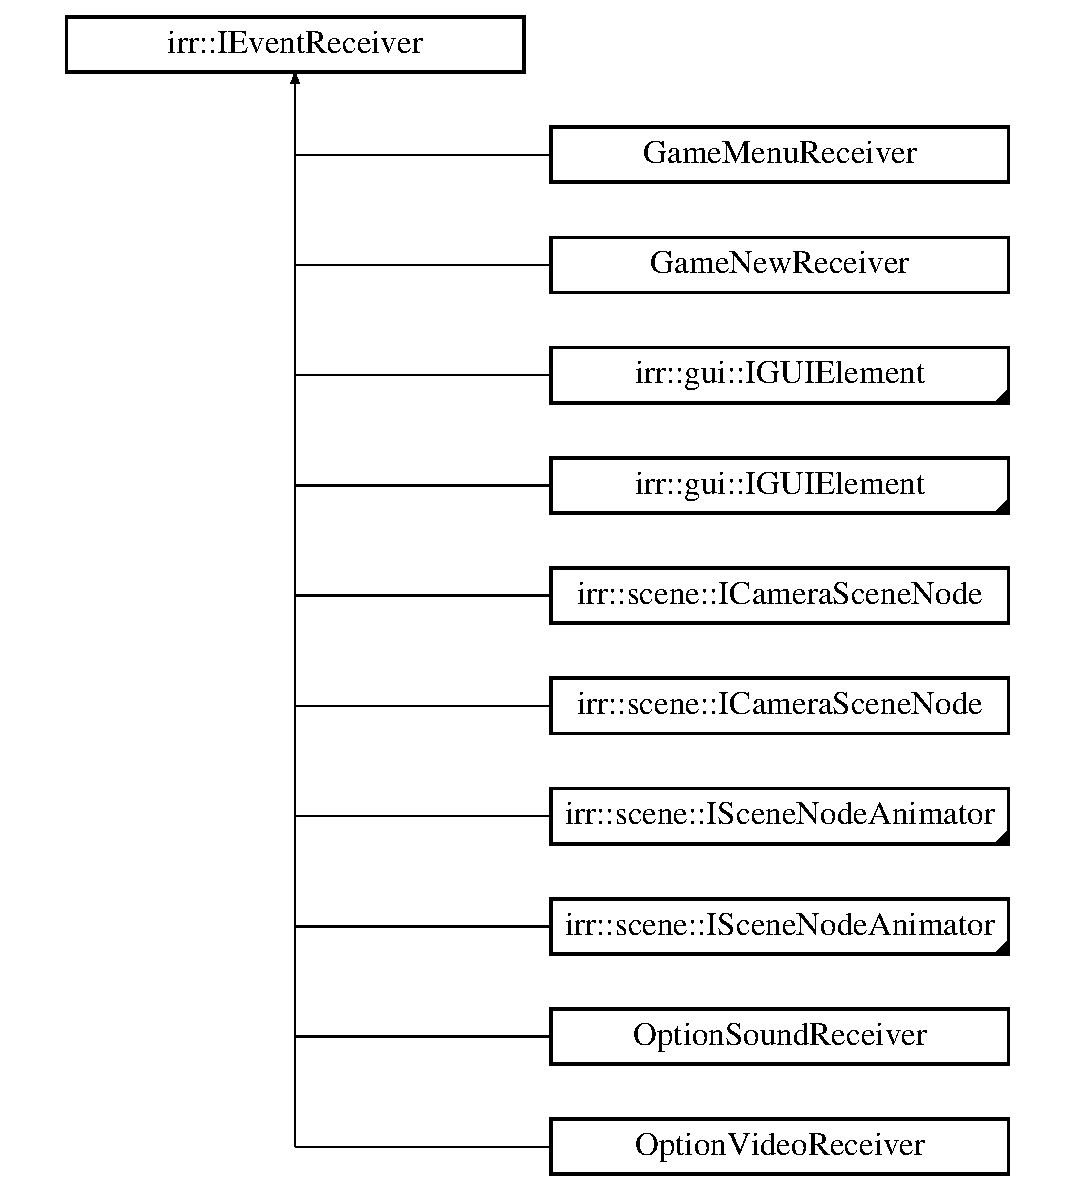
\includegraphics[height=5.847177cm]{classirr_1_1IEventReceiver}
\end{center}
\end{figure}
\subsection*{Public Member Functions}
\begin{DoxyCompactItemize}
\item 
\mbox{\Hypertarget{classirr_1_1IEventReceiver_a4ec011612f02017d95654cf5b5d567b6}\label{classirr_1_1IEventReceiver_a4ec011612f02017d95654cf5b5d567b6}} 
virtual \hyperlink{classirr_1_1IEventReceiver_a4ec011612f02017d95654cf5b5d567b6}{$\sim$\+I\+Event\+Receiver} ()
\begin{DoxyCompactList}\small\item\em Destructor. \end{DoxyCompactList}\item 
virtual bool \hyperlink{classirr_1_1IEventReceiver_a571f744ceffc3b4fe8a81f529163eb97}{On\+Event} (const \hyperlink{structirr_1_1SEvent}{S\+Event} \&event)=0
\begin{DoxyCompactList}\small\item\em Called if an event happened. \end{DoxyCompactList}\end{DoxyCompactItemize}


\subsection{Detailed Description}
Interface of an object which can receive events. 

Many of the engine\textquotesingle{}s classes inherit \hyperlink{classirr_1_1IEventReceiver}{I\+Event\+Receiver} so they are able to process events. Events usually start at a post\+Event\+From\+User function and are passed down through a chain of event receivers until On\+Event returns true. See \hyperlink{namespaceirr_ac9eed96e06e85ce3c86fcbbbe9e48a0c}{irr\+::\+E\+E\+V\+E\+N\+T\+\_\+\+T\+Y\+PE} for a description of where each type of event starts, and the path it takes through the system. 

\subsection{Member Function Documentation}
\mbox{\Hypertarget{classirr_1_1IEventReceiver_a571f744ceffc3b4fe8a81f529163eb97}\label{classirr_1_1IEventReceiver_a571f744ceffc3b4fe8a81f529163eb97}} 
\index{irr\+::\+I\+Event\+Receiver@{irr\+::\+I\+Event\+Receiver}!On\+Event@{On\+Event}}
\index{On\+Event@{On\+Event}!irr\+::\+I\+Event\+Receiver@{irr\+::\+I\+Event\+Receiver}}
\subsubsection{\texorpdfstring{On\+Event()}{OnEvent()}}
{\footnotesize\ttfamily virtual bool irr\+::\+I\+Event\+Receiver\+::\+On\+Event (\begin{DoxyParamCaption}\item[{const \hyperlink{structirr_1_1SEvent}{S\+Event} \&}]{event }\end{DoxyParamCaption})\hspace{0.3cm}{\ttfamily [pure virtual]}}



Called if an event happened. 

Please take care that you should only return \textquotesingle{}true\textquotesingle{} when you want to {\itshape prevent} Irrlicht from processing the event any further. So \textquotesingle{}true\textquotesingle{} does mean that an event is completely done. Therefore your return value for all unprocessed events should be \textquotesingle{}false\textquotesingle{}. \begin{DoxyReturn}{Returns}
True if the event was processed. 
\end{DoxyReturn}


Implemented in \hyperlink{classirr_1_1gui_1_1IGUIElement_a54b1799e21722d9e6ce5b8e4bdb2e80a}{irr\+::gui\+::\+I\+G\+U\+I\+Element}, \hyperlink{classirr_1_1scene_1_1ICameraSceneNode_af27145518f43a17f803cdea086f68f3c}{irr\+::scene\+::\+I\+Camera\+Scene\+Node}, \hyperlink{classOptionSoundReceiver_ae7c9643b12df38a45d4e3d629274019c}{Option\+Sound\+Receiver}, \hyperlink{classOptionVideoReceiver_a203025900c489eb2df12a6b3471c3caa}{Option\+Video\+Receiver}, \hyperlink{classGameMenuReceiver_af6774556abc7e3718b7bf904cc62ead0}{Game\+Menu\+Receiver}, \hyperlink{classGameNewReceiver_ad9ec097d8b46946ed1a21c24463fc0b6}{Game\+New\+Receiver}, and \hyperlink{classirr_1_1scene_1_1ISceneNodeAnimator_aca20b841bb586cd9654464b001a7b6aa}{irr\+::scene\+::\+I\+Scene\+Node\+Animator}.



The documentation for this class was generated from the following file\+:\begin{DoxyCompactItemize}
\item 
indie\+\_\+share/controller/include/I\+Event\+Receiver.\+h\end{DoxyCompactItemize}

\hypertarget{classirr_1_1io_1_1IFileArchive}{}\section{irr\+:\+:io\+:\+:I\+File\+Archive Class Reference}
\label{classirr_1_1io_1_1IFileArchive}\index{irr\+::io\+::\+I\+File\+Archive@{irr\+::io\+::\+I\+File\+Archive}}


The File\+Archive manages archives and provides access to files inside them.  




{\ttfamily \#include $<$I\+File\+Archive.\+h$>$}

Inheritance diagram for irr\+:\+:io\+:\+:I\+File\+Archive\+:\begin{figure}[H]
\begin{center}
\leavevmode
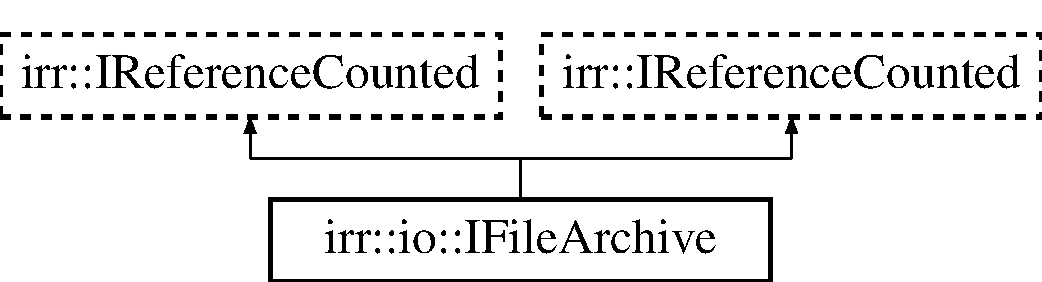
\includegraphics[height=2.000000cm]{classirr_1_1io_1_1IFileArchive}
\end{center}
\end{figure}
\subsection*{Public Member Functions}
\begin{DoxyCompactItemize}
\item 
virtual \hyperlink{classirr_1_1io_1_1IReadFile}{I\+Read\+File} $\ast$ \hyperlink{classirr_1_1io_1_1IFileArchive_a5c3b4994ae63447d2634dd86b3069988}{create\+And\+Open\+File} (const \hyperlink{namespaceirr_1_1io_a6468281622ce3a1c46b72e19f32dded5}{path} \&filename)=0
\begin{DoxyCompactList}\small\item\em Opens a file based on its name. \end{DoxyCompactList}\item 
virtual \hyperlink{classirr_1_1io_1_1IReadFile}{I\+Read\+File} $\ast$ \hyperlink{classirr_1_1io_1_1IFileArchive_ab6bc8fbd660bbbe42b4d30a9d4f26c7d}{create\+And\+Open\+File} (\hyperlink{namespaceirr_a0416a53257075833e7002efd0a18e804}{u32} index)=0
\begin{DoxyCompactList}\small\item\em Opens a file based on its position in the file list. \end{DoxyCompactList}\item 
virtual const \hyperlink{classirr_1_1io_1_1IFileList}{I\+File\+List} $\ast$ \hyperlink{classirr_1_1io_1_1IFileArchive_a73c683318837b13d16843373da00ded3}{get\+File\+List} () const =0
\begin{DoxyCompactList}\small\item\em Returns the complete file tree. \end{DoxyCompactList}\item 
\mbox{\Hypertarget{classirr_1_1io_1_1IFileArchive_ae991b223b7f3b8b47916d82d842e3004}\label{classirr_1_1io_1_1IFileArchive_ae991b223b7f3b8b47916d82d842e3004}} 
virtual \hyperlink{namespaceirr_1_1io_adb3e3c445ec8e608ed1f0f93306da14f}{E\+\_\+\+F\+I\+L\+E\+\_\+\+A\+R\+C\+H\+I\+V\+E\+\_\+\+T\+Y\+PE} \hyperlink{classirr_1_1io_1_1IFileArchive_ae991b223b7f3b8b47916d82d842e3004}{get\+Type} () const
\begin{DoxyCompactList}\small\item\em get the archive type \end{DoxyCompactList}\item 
virtual \hyperlink{classirr_1_1io_1_1IReadFile}{I\+Read\+File} $\ast$ \hyperlink{classirr_1_1io_1_1IFileArchive_a5c3b4994ae63447d2634dd86b3069988}{create\+And\+Open\+File} (const \hyperlink{namespaceirr_1_1io_a6468281622ce3a1c46b72e19f32dded5}{path} \&filename)=0
\begin{DoxyCompactList}\small\item\em Opens a file based on its name. \end{DoxyCompactList}\item 
virtual \hyperlink{classirr_1_1io_1_1IReadFile}{I\+Read\+File} $\ast$ \hyperlink{classirr_1_1io_1_1IFileArchive_ab6bc8fbd660bbbe42b4d30a9d4f26c7d}{create\+And\+Open\+File} (\hyperlink{namespaceirr_a0416a53257075833e7002efd0a18e804}{u32} index)=0
\begin{DoxyCompactList}\small\item\em Opens a file based on its position in the file list. \end{DoxyCompactList}\item 
virtual const \hyperlink{classirr_1_1io_1_1IFileList}{I\+File\+List} $\ast$ \hyperlink{classirr_1_1io_1_1IFileArchive_a73c683318837b13d16843373da00ded3}{get\+File\+List} () const =0
\begin{DoxyCompactList}\small\item\em Returns the complete file tree. \end{DoxyCompactList}\item 
\mbox{\Hypertarget{classirr_1_1io_1_1IFileArchive_ae991b223b7f3b8b47916d82d842e3004}\label{classirr_1_1io_1_1IFileArchive_ae991b223b7f3b8b47916d82d842e3004}} 
virtual \hyperlink{namespaceirr_1_1io_adb3e3c445ec8e608ed1f0f93306da14f}{E\+\_\+\+F\+I\+L\+E\+\_\+\+A\+R\+C\+H\+I\+V\+E\+\_\+\+T\+Y\+PE} \hyperlink{classirr_1_1io_1_1IFileArchive_ae991b223b7f3b8b47916d82d842e3004}{get\+Type} () const
\begin{DoxyCompactList}\small\item\em get the archive type \end{DoxyCompactList}\end{DoxyCompactItemize}
\subsection*{Public Attributes}
\begin{DoxyCompactItemize}
\item 
\hyperlink{namespaceirr_1_1core_ab26a0e0359206b5a694f35c37c829d7f}{core\+::stringc} \hyperlink{classirr_1_1io_1_1IFileArchive_ae5b574864226b09c70518e163e59b6ba}{Password}
\begin{DoxyCompactList}\small\item\em An optionally used password string. \end{DoxyCompactList}\end{DoxyCompactItemize}
\subsection*{Additional Inherited Members}


\subsection{Detailed Description}
The File\+Archive manages archives and provides access to files inside them. 

\subsection{Member Function Documentation}
\mbox{\Hypertarget{classirr_1_1io_1_1IFileArchive_a5c3b4994ae63447d2634dd86b3069988}\label{classirr_1_1io_1_1IFileArchive_a5c3b4994ae63447d2634dd86b3069988}} 
\index{irr\+::io\+::\+I\+File\+Archive@{irr\+::io\+::\+I\+File\+Archive}!create\+And\+Open\+File@{create\+And\+Open\+File}}
\index{create\+And\+Open\+File@{create\+And\+Open\+File}!irr\+::io\+::\+I\+File\+Archive@{irr\+::io\+::\+I\+File\+Archive}}
\subsubsection{\texorpdfstring{create\+And\+Open\+File()}{createAndOpenFile()}\hspace{0.1cm}{\footnotesize\ttfamily [1/4]}}
{\footnotesize\ttfamily virtual \hyperlink{classirr_1_1io_1_1IReadFile}{I\+Read\+File}$\ast$ irr\+::io\+::\+I\+File\+Archive\+::create\+And\+Open\+File (\begin{DoxyParamCaption}\item[{const \hyperlink{namespaceirr_1_1io_a6468281622ce3a1c46b72e19f32dded5}{path} \&}]{filename }\end{DoxyParamCaption})\hspace{0.3cm}{\ttfamily [pure virtual]}}



Opens a file based on its name. 

Creates and returns a new \hyperlink{classirr_1_1io_1_1IReadFile}{I\+Read\+File} for a file in the archive. 
\begin{DoxyParams}{Parameters}
{\em filename} & The file to open \\
\hline
\end{DoxyParams}
\begin{DoxyReturn}{Returns}
Returns A pointer to the created file on success, or 0 on failure. 
\end{DoxyReturn}
\mbox{\Hypertarget{classirr_1_1io_1_1IFileArchive_a5c3b4994ae63447d2634dd86b3069988}\label{classirr_1_1io_1_1IFileArchive_a5c3b4994ae63447d2634dd86b3069988}} 
\index{irr\+::io\+::\+I\+File\+Archive@{irr\+::io\+::\+I\+File\+Archive}!create\+And\+Open\+File@{create\+And\+Open\+File}}
\index{create\+And\+Open\+File@{create\+And\+Open\+File}!irr\+::io\+::\+I\+File\+Archive@{irr\+::io\+::\+I\+File\+Archive}}
\subsubsection{\texorpdfstring{create\+And\+Open\+File()}{createAndOpenFile()}\hspace{0.1cm}{\footnotesize\ttfamily [2/4]}}
{\footnotesize\ttfamily virtual \hyperlink{classirr_1_1io_1_1IReadFile}{I\+Read\+File}$\ast$ irr\+::io\+::\+I\+File\+Archive\+::create\+And\+Open\+File (\begin{DoxyParamCaption}\item[{const \hyperlink{namespaceirr_1_1io_a6468281622ce3a1c46b72e19f32dded5}{path} \&}]{filename }\end{DoxyParamCaption})\hspace{0.3cm}{\ttfamily [pure virtual]}}



Opens a file based on its name. 

Creates and returns a new \hyperlink{classirr_1_1io_1_1IReadFile}{I\+Read\+File} for a file in the archive. 
\begin{DoxyParams}{Parameters}
{\em filename} & The file to open \\
\hline
\end{DoxyParams}
\begin{DoxyReturn}{Returns}
Returns A pointer to the created file on success, or 0 on failure. 
\end{DoxyReturn}
\mbox{\Hypertarget{classirr_1_1io_1_1IFileArchive_ab6bc8fbd660bbbe42b4d30a9d4f26c7d}\label{classirr_1_1io_1_1IFileArchive_ab6bc8fbd660bbbe42b4d30a9d4f26c7d}} 
\index{irr\+::io\+::\+I\+File\+Archive@{irr\+::io\+::\+I\+File\+Archive}!create\+And\+Open\+File@{create\+And\+Open\+File}}
\index{create\+And\+Open\+File@{create\+And\+Open\+File}!irr\+::io\+::\+I\+File\+Archive@{irr\+::io\+::\+I\+File\+Archive}}
\subsubsection{\texorpdfstring{create\+And\+Open\+File()}{createAndOpenFile()}\hspace{0.1cm}{\footnotesize\ttfamily [3/4]}}
{\footnotesize\ttfamily virtual \hyperlink{classirr_1_1io_1_1IReadFile}{I\+Read\+File}$\ast$ irr\+::io\+::\+I\+File\+Archive\+::create\+And\+Open\+File (\begin{DoxyParamCaption}\item[{\hyperlink{namespaceirr_a0416a53257075833e7002efd0a18e804}{u32}}]{index }\end{DoxyParamCaption})\hspace{0.3cm}{\ttfamily [pure virtual]}}



Opens a file based on its position in the file list. 

Creates and returns 
\begin{DoxyParams}{Parameters}
{\em index} & The zero based index of the file. \\
\hline
\end{DoxyParams}
\begin{DoxyReturn}{Returns}
Returns a pointer to the created file on success, or 0 on failure. 
\end{DoxyReturn}
\mbox{\Hypertarget{classirr_1_1io_1_1IFileArchive_ab6bc8fbd660bbbe42b4d30a9d4f26c7d}\label{classirr_1_1io_1_1IFileArchive_ab6bc8fbd660bbbe42b4d30a9d4f26c7d}} 
\index{irr\+::io\+::\+I\+File\+Archive@{irr\+::io\+::\+I\+File\+Archive}!create\+And\+Open\+File@{create\+And\+Open\+File}}
\index{create\+And\+Open\+File@{create\+And\+Open\+File}!irr\+::io\+::\+I\+File\+Archive@{irr\+::io\+::\+I\+File\+Archive}}
\subsubsection{\texorpdfstring{create\+And\+Open\+File()}{createAndOpenFile()}\hspace{0.1cm}{\footnotesize\ttfamily [4/4]}}
{\footnotesize\ttfamily virtual \hyperlink{classirr_1_1io_1_1IReadFile}{I\+Read\+File}$\ast$ irr\+::io\+::\+I\+File\+Archive\+::create\+And\+Open\+File (\begin{DoxyParamCaption}\item[{\hyperlink{namespaceirr_a0416a53257075833e7002efd0a18e804}{u32}}]{index }\end{DoxyParamCaption})\hspace{0.3cm}{\ttfamily [pure virtual]}}



Opens a file based on its position in the file list. 

Creates and returns 
\begin{DoxyParams}{Parameters}
{\em index} & The zero based index of the file. \\
\hline
\end{DoxyParams}
\begin{DoxyReturn}{Returns}
Returns a pointer to the created file on success, or 0 on failure. 
\end{DoxyReturn}
\mbox{\Hypertarget{classirr_1_1io_1_1IFileArchive_a73c683318837b13d16843373da00ded3}\label{classirr_1_1io_1_1IFileArchive_a73c683318837b13d16843373da00ded3}} 
\index{irr\+::io\+::\+I\+File\+Archive@{irr\+::io\+::\+I\+File\+Archive}!get\+File\+List@{get\+File\+List}}
\index{get\+File\+List@{get\+File\+List}!irr\+::io\+::\+I\+File\+Archive@{irr\+::io\+::\+I\+File\+Archive}}
\subsubsection{\texorpdfstring{get\+File\+List()}{getFileList()}\hspace{0.1cm}{\footnotesize\ttfamily [1/2]}}
{\footnotesize\ttfamily virtual const \hyperlink{classirr_1_1io_1_1IFileList}{I\+File\+List}$\ast$ irr\+::io\+::\+I\+File\+Archive\+::get\+File\+List (\begin{DoxyParamCaption}{ }\end{DoxyParamCaption}) const\hspace{0.3cm}{\ttfamily [pure virtual]}}



Returns the complete file tree. 

\begin{DoxyReturn}{Returns}
Returns the complete directory tree for the archive, including all files and folders 
\end{DoxyReturn}
\mbox{\Hypertarget{classirr_1_1io_1_1IFileArchive_a73c683318837b13d16843373da00ded3}\label{classirr_1_1io_1_1IFileArchive_a73c683318837b13d16843373da00ded3}} 
\index{irr\+::io\+::\+I\+File\+Archive@{irr\+::io\+::\+I\+File\+Archive}!get\+File\+List@{get\+File\+List}}
\index{get\+File\+List@{get\+File\+List}!irr\+::io\+::\+I\+File\+Archive@{irr\+::io\+::\+I\+File\+Archive}}
\subsubsection{\texorpdfstring{get\+File\+List()}{getFileList()}\hspace{0.1cm}{\footnotesize\ttfamily [2/2]}}
{\footnotesize\ttfamily virtual const \hyperlink{classirr_1_1io_1_1IFileList}{I\+File\+List}$\ast$ irr\+::io\+::\+I\+File\+Archive\+::get\+File\+List (\begin{DoxyParamCaption}{ }\end{DoxyParamCaption}) const\hspace{0.3cm}{\ttfamily [pure virtual]}}



Returns the complete file tree. 

\begin{DoxyReturn}{Returns}
Returns the complete directory tree for the archive, including all files and folders 
\end{DoxyReturn}


\subsection{Member Data Documentation}
\mbox{\Hypertarget{classirr_1_1io_1_1IFileArchive_ae5b574864226b09c70518e163e59b6ba}\label{classirr_1_1io_1_1IFileArchive_ae5b574864226b09c70518e163e59b6ba}} 
\index{irr\+::io\+::\+I\+File\+Archive@{irr\+::io\+::\+I\+File\+Archive}!Password@{Password}}
\index{Password@{Password}!irr\+::io\+::\+I\+File\+Archive@{irr\+::io\+::\+I\+File\+Archive}}
\subsubsection{\texorpdfstring{Password}{Password}}
{\footnotesize\ttfamily \hyperlink{namespaceirr_1_1core_ab26a0e0359206b5a694f35c37c829d7f}{core\+::stringc} irr\+::io\+::\+I\+File\+Archive\+::\+Password}



An optionally used password string. 

This variable is publicly accessible from the interface in order to avoid single access patterns to this place, and hence allow some more obscurity. 

The documentation for this class was generated from the following file\+:\begin{DoxyCompactItemize}
\item 
indie\+\_\+share/controller/include/I\+File\+Archive.\+h\end{DoxyCompactItemize}

\hypertarget{classirr_1_1io_1_1IFileList}{}\section{irr\+:\+:io\+:\+:I\+File\+List Class Reference}
\label{classirr_1_1io_1_1IFileList}\index{irr\+::io\+::\+I\+File\+List@{irr\+::io\+::\+I\+File\+List}}


Provides a list of files and folders.  




{\ttfamily \#include $<$I\+File\+List.\+h$>$}

Inheritance diagram for irr\+:\+:io\+:\+:I\+File\+List\+:\begin{figure}[H]
\begin{center}
\leavevmode
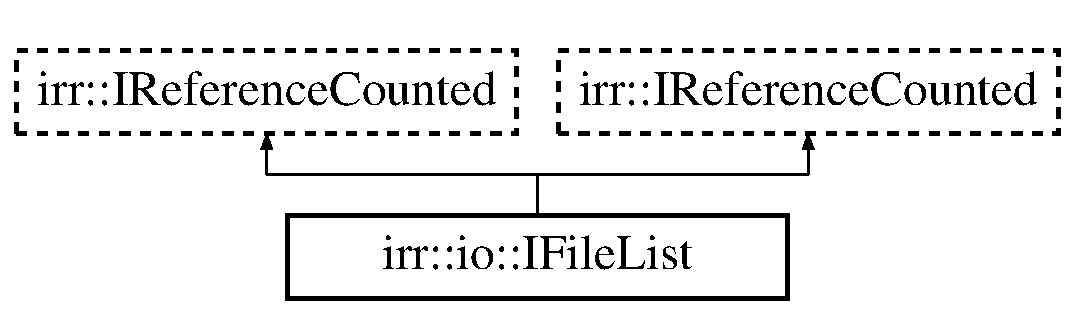
\includegraphics[height=2.000000cm]{classirr_1_1io_1_1IFileList}
\end{center}
\end{figure}
\subsection*{Public Member Functions}
\begin{DoxyCompactItemize}
\item 
virtual \hyperlink{namespaceirr_a0416a53257075833e7002efd0a18e804}{u32} \hyperlink{classirr_1_1io_1_1IFileList_a871861be76e18d58274c4580b1d103b9}{get\+File\+Count} () const =0
\begin{DoxyCompactList}\small\item\em Get the number of files in the filelist. \end{DoxyCompactList}\item 
virtual const \hyperlink{namespaceirr_1_1io_a6468281622ce3a1c46b72e19f32dded5}{io\+::path} \& \hyperlink{classirr_1_1io_1_1IFileList_ab4e0330adf34afa3c21e06ff0b4e84d5}{get\+File\+Name} (\hyperlink{namespaceirr_a0416a53257075833e7002efd0a18e804}{u32} index) const =0
\begin{DoxyCompactList}\small\item\em Gets the name of a file in the list, based on an index. \end{DoxyCompactList}\item 
virtual const \hyperlink{namespaceirr_1_1io_a6468281622ce3a1c46b72e19f32dded5}{io\+::path} \& \hyperlink{classirr_1_1io_1_1IFileList_a063c823f58019bda79efabefabe365da}{get\+Full\+File\+Name} (\hyperlink{namespaceirr_a0416a53257075833e7002efd0a18e804}{u32} index) const =0
\begin{DoxyCompactList}\small\item\em Gets the full name of a file in the list including the path, based on an index. \end{DoxyCompactList}\item 
virtual \hyperlink{namespaceirr_a0416a53257075833e7002efd0a18e804}{u32} \hyperlink{classirr_1_1io_1_1IFileList_a305561d0c5db74ac721da5d26c461b36}{get\+File\+Size} (\hyperlink{namespaceirr_a0416a53257075833e7002efd0a18e804}{u32} index) const =0
\begin{DoxyCompactList}\small\item\em Returns the size of a file in the file list, based on an index. \end{DoxyCompactList}\item 
virtual \hyperlink{namespaceirr_a0416a53257075833e7002efd0a18e804}{u32} \hyperlink{classirr_1_1io_1_1IFileList_a97582a2cf5c05e7b8dcb702384ab76bd}{get\+File\+Offset} (\hyperlink{namespaceirr_a0416a53257075833e7002efd0a18e804}{u32} index) const =0
\begin{DoxyCompactList}\small\item\em Returns the file offset of a file in the file list, based on an index. \end{DoxyCompactList}\item 
virtual \hyperlink{namespaceirr_a0416a53257075833e7002efd0a18e804}{u32} \hyperlink{classirr_1_1io_1_1IFileList_a9f633344aa2bb36f619d1ca8472b46b6}{get\+ID} (\hyperlink{namespaceirr_a0416a53257075833e7002efd0a18e804}{u32} index) const =0
\begin{DoxyCompactList}\small\item\em Returns the ID of a file in the file list, based on an index. \end{DoxyCompactList}\item 
virtual bool \hyperlink{classirr_1_1io_1_1IFileList_a0f2cb8c99e9ecc4b56d08718c885a5af}{is\+Directory} (\hyperlink{namespaceirr_a0416a53257075833e7002efd0a18e804}{u32} index) const =0
\begin{DoxyCompactList}\small\item\em Check if the file is a directory. \end{DoxyCompactList}\item 
virtual \hyperlink{namespaceirr_ac66849b7a6ed16e30ebede579f9b47c6}{s32} \hyperlink{classirr_1_1io_1_1IFileList_a2b0fce45cbea72f5c6dc13eb85183054}{find\+File} (const \hyperlink{namespaceirr_1_1io_a6468281622ce3a1c46b72e19f32dded5}{io\+::path} \&filename, bool is\+Folder=false) const =0
\begin{DoxyCompactList}\small\item\em Searches for a file or folder in the list. \end{DoxyCompactList}\item 
\mbox{\Hypertarget{classirr_1_1io_1_1IFileList_ac3473e66ba9c3cee2e06c1fb46493e88}\label{classirr_1_1io_1_1IFileList_ac3473e66ba9c3cee2e06c1fb46493e88}} 
virtual const \hyperlink{namespaceirr_1_1io_a6468281622ce3a1c46b72e19f32dded5}{io\+::path} \& \hyperlink{classirr_1_1io_1_1IFileList_ac3473e66ba9c3cee2e06c1fb46493e88}{get\+Path} () const =0
\begin{DoxyCompactList}\small\item\em Returns the base path of the file list. \end{DoxyCompactList}\item 
virtual \hyperlink{namespaceirr_a0416a53257075833e7002efd0a18e804}{u32} \hyperlink{classirr_1_1io_1_1IFileList_ad0d90f1bb8a35910f4f877268e2f043e}{add\+Item} (const \hyperlink{namespaceirr_1_1io_a6468281622ce3a1c46b72e19f32dded5}{io\+::path} \&full\+Path, \hyperlink{namespaceirr_a0416a53257075833e7002efd0a18e804}{u32} offset, \hyperlink{namespaceirr_a0416a53257075833e7002efd0a18e804}{u32} size, bool \hyperlink{classirr_1_1io_1_1IFileList_a0f2cb8c99e9ecc4b56d08718c885a5af}{is\+Directory}, \hyperlink{namespaceirr_a0416a53257075833e7002efd0a18e804}{u32} id=0)=0
\begin{DoxyCompactList}\small\item\em Add as a file or folder to the list. \end{DoxyCompactList}\item 
\mbox{\Hypertarget{classirr_1_1io_1_1IFileList_a2cf4f12d7ee6ab35257169ec23654da8}\label{classirr_1_1io_1_1IFileList_a2cf4f12d7ee6ab35257169ec23654da8}} 
virtual void \hyperlink{classirr_1_1io_1_1IFileList_a2cf4f12d7ee6ab35257169ec23654da8}{sort} ()=0
\begin{DoxyCompactList}\small\item\em Sorts the file list. You should call this after adding any items to the file list. \end{DoxyCompactList}\item 
virtual \hyperlink{namespaceirr_a0416a53257075833e7002efd0a18e804}{u32} \hyperlink{classirr_1_1io_1_1IFileList_a871861be76e18d58274c4580b1d103b9}{get\+File\+Count} () const =0
\begin{DoxyCompactList}\small\item\em Get the number of files in the filelist. \end{DoxyCompactList}\item 
virtual const \hyperlink{namespaceirr_1_1io_a6468281622ce3a1c46b72e19f32dded5}{io\+::path} \& \hyperlink{classirr_1_1io_1_1IFileList_ab4e0330adf34afa3c21e06ff0b4e84d5}{get\+File\+Name} (\hyperlink{namespaceirr_a0416a53257075833e7002efd0a18e804}{u32} index) const =0
\begin{DoxyCompactList}\small\item\em Gets the name of a file in the list, based on an index. \end{DoxyCompactList}\item 
virtual const \hyperlink{namespaceirr_1_1io_a6468281622ce3a1c46b72e19f32dded5}{io\+::path} \& \hyperlink{classirr_1_1io_1_1IFileList_a063c823f58019bda79efabefabe365da}{get\+Full\+File\+Name} (\hyperlink{namespaceirr_a0416a53257075833e7002efd0a18e804}{u32} index) const =0
\begin{DoxyCompactList}\small\item\em Gets the full name of a file in the list including the path, based on an index. \end{DoxyCompactList}\item 
virtual \hyperlink{namespaceirr_a0416a53257075833e7002efd0a18e804}{u32} \hyperlink{classirr_1_1io_1_1IFileList_a305561d0c5db74ac721da5d26c461b36}{get\+File\+Size} (\hyperlink{namespaceirr_a0416a53257075833e7002efd0a18e804}{u32} index) const =0
\begin{DoxyCompactList}\small\item\em Returns the size of a file in the file list, based on an index. \end{DoxyCompactList}\item 
virtual \hyperlink{namespaceirr_a0416a53257075833e7002efd0a18e804}{u32} \hyperlink{classirr_1_1io_1_1IFileList_a97582a2cf5c05e7b8dcb702384ab76bd}{get\+File\+Offset} (\hyperlink{namespaceirr_a0416a53257075833e7002efd0a18e804}{u32} index) const =0
\begin{DoxyCompactList}\small\item\em Returns the file offset of a file in the file list, based on an index. \end{DoxyCompactList}\item 
virtual \hyperlink{namespaceirr_a0416a53257075833e7002efd0a18e804}{u32} \hyperlink{classirr_1_1io_1_1IFileList_a9f633344aa2bb36f619d1ca8472b46b6}{get\+ID} (\hyperlink{namespaceirr_a0416a53257075833e7002efd0a18e804}{u32} index) const =0
\begin{DoxyCompactList}\small\item\em Returns the ID of a file in the file list, based on an index. \end{DoxyCompactList}\item 
virtual bool \hyperlink{classirr_1_1io_1_1IFileList_a0f2cb8c99e9ecc4b56d08718c885a5af}{is\+Directory} (\hyperlink{namespaceirr_a0416a53257075833e7002efd0a18e804}{u32} index) const =0
\begin{DoxyCompactList}\small\item\em Check if the file is a directory. \end{DoxyCompactList}\item 
virtual \hyperlink{namespaceirr_ac66849b7a6ed16e30ebede579f9b47c6}{s32} \hyperlink{classirr_1_1io_1_1IFileList_a2b0fce45cbea72f5c6dc13eb85183054}{find\+File} (const \hyperlink{namespaceirr_1_1io_a6468281622ce3a1c46b72e19f32dded5}{io\+::path} \&filename, bool is\+Folder=false) const =0
\begin{DoxyCompactList}\small\item\em Searches for a file or folder in the list. \end{DoxyCompactList}\item 
\mbox{\Hypertarget{classirr_1_1io_1_1IFileList_ac3473e66ba9c3cee2e06c1fb46493e88}\label{classirr_1_1io_1_1IFileList_ac3473e66ba9c3cee2e06c1fb46493e88}} 
virtual const \hyperlink{namespaceirr_1_1io_a6468281622ce3a1c46b72e19f32dded5}{io\+::path} \& \hyperlink{classirr_1_1io_1_1IFileList_ac3473e66ba9c3cee2e06c1fb46493e88}{get\+Path} () const =0
\begin{DoxyCompactList}\small\item\em Returns the base path of the file list. \end{DoxyCompactList}\item 
virtual \hyperlink{namespaceirr_a0416a53257075833e7002efd0a18e804}{u32} \hyperlink{classirr_1_1io_1_1IFileList_ad0d90f1bb8a35910f4f877268e2f043e}{add\+Item} (const \hyperlink{namespaceirr_1_1io_a6468281622ce3a1c46b72e19f32dded5}{io\+::path} \&full\+Path, \hyperlink{namespaceirr_a0416a53257075833e7002efd0a18e804}{u32} offset, \hyperlink{namespaceirr_a0416a53257075833e7002efd0a18e804}{u32} size, bool \hyperlink{classirr_1_1io_1_1IFileList_a0f2cb8c99e9ecc4b56d08718c885a5af}{is\+Directory}, \hyperlink{namespaceirr_a0416a53257075833e7002efd0a18e804}{u32} id=0)=0
\begin{DoxyCompactList}\small\item\em Add as a file or folder to the list. \end{DoxyCompactList}\item 
\mbox{\Hypertarget{classirr_1_1io_1_1IFileList_a2cf4f12d7ee6ab35257169ec23654da8}\label{classirr_1_1io_1_1IFileList_a2cf4f12d7ee6ab35257169ec23654da8}} 
virtual void \hyperlink{classirr_1_1io_1_1IFileList_a2cf4f12d7ee6ab35257169ec23654da8}{sort} ()=0
\begin{DoxyCompactList}\small\item\em Sorts the file list. You should call this after adding any items to the file list. \end{DoxyCompactList}\end{DoxyCompactItemize}
\subsection*{Additional Inherited Members}


\subsection{Detailed Description}
Provides a list of files and folders. 

File lists usually contain a list of all files in a given folder, but can also contain a complete directory structure. 

\subsection{Member Function Documentation}
\mbox{\Hypertarget{classirr_1_1io_1_1IFileList_ad0d90f1bb8a35910f4f877268e2f043e}\label{classirr_1_1io_1_1IFileList_ad0d90f1bb8a35910f4f877268e2f043e}} 
\index{irr\+::io\+::\+I\+File\+List@{irr\+::io\+::\+I\+File\+List}!add\+Item@{add\+Item}}
\index{add\+Item@{add\+Item}!irr\+::io\+::\+I\+File\+List@{irr\+::io\+::\+I\+File\+List}}
\subsubsection{\texorpdfstring{add\+Item()}{addItem()}\hspace{0.1cm}{\footnotesize\ttfamily [1/2]}}
{\footnotesize\ttfamily virtual \hyperlink{namespaceirr_a0416a53257075833e7002efd0a18e804}{u32} irr\+::io\+::\+I\+File\+List\+::add\+Item (\begin{DoxyParamCaption}\item[{const \hyperlink{namespaceirr_1_1io_a6468281622ce3a1c46b72e19f32dded5}{io\+::path} \&}]{full\+Path,  }\item[{\hyperlink{namespaceirr_a0416a53257075833e7002efd0a18e804}{u32}}]{offset,  }\item[{\hyperlink{namespaceirr_a0416a53257075833e7002efd0a18e804}{u32}}]{size,  }\item[{bool}]{is\+Directory,  }\item[{\hyperlink{namespaceirr_a0416a53257075833e7002efd0a18e804}{u32}}]{id = {\ttfamily 0} }\end{DoxyParamCaption})\hspace{0.3cm}{\ttfamily [pure virtual]}}



Add as a file or folder to the list. 


\begin{DoxyParams}{Parameters}
{\em full\+Path} & The file name including path, from the root of the file list. \\
\hline
{\em is\+Directory} & True if this is a directory rather than a file. \\
\hline
{\em offset} & The file offset inside an archive \\
\hline
{\em size} & The size of the file in bytes. \\
\hline
{\em id} & The ID of the file in the archive which owns it \\
\hline
\end{DoxyParams}
\mbox{\Hypertarget{classirr_1_1io_1_1IFileList_ad0d90f1bb8a35910f4f877268e2f043e}\label{classirr_1_1io_1_1IFileList_ad0d90f1bb8a35910f4f877268e2f043e}} 
\index{irr\+::io\+::\+I\+File\+List@{irr\+::io\+::\+I\+File\+List}!add\+Item@{add\+Item}}
\index{add\+Item@{add\+Item}!irr\+::io\+::\+I\+File\+List@{irr\+::io\+::\+I\+File\+List}}
\subsubsection{\texorpdfstring{add\+Item()}{addItem()}\hspace{0.1cm}{\footnotesize\ttfamily [2/2]}}
{\footnotesize\ttfamily virtual \hyperlink{namespaceirr_a0416a53257075833e7002efd0a18e804}{u32} irr\+::io\+::\+I\+File\+List\+::add\+Item (\begin{DoxyParamCaption}\item[{const \hyperlink{namespaceirr_1_1io_a6468281622ce3a1c46b72e19f32dded5}{io\+::path} \&}]{full\+Path,  }\item[{\hyperlink{namespaceirr_a0416a53257075833e7002efd0a18e804}{u32}}]{offset,  }\item[{\hyperlink{namespaceirr_a0416a53257075833e7002efd0a18e804}{u32}}]{size,  }\item[{bool}]{is\+Directory,  }\item[{\hyperlink{namespaceirr_a0416a53257075833e7002efd0a18e804}{u32}}]{id = {\ttfamily 0} }\end{DoxyParamCaption})\hspace{0.3cm}{\ttfamily [pure virtual]}}



Add as a file or folder to the list. 


\begin{DoxyParams}{Parameters}
{\em full\+Path} & The file name including path, from the root of the file list. \\
\hline
{\em is\+Directory} & True if this is a directory rather than a file. \\
\hline
{\em offset} & The file offset inside an archive \\
\hline
{\em size} & The size of the file in bytes. \\
\hline
{\em id} & The ID of the file in the archive which owns it \\
\hline
\end{DoxyParams}
\mbox{\Hypertarget{classirr_1_1io_1_1IFileList_a2b0fce45cbea72f5c6dc13eb85183054}\label{classirr_1_1io_1_1IFileList_a2b0fce45cbea72f5c6dc13eb85183054}} 
\index{irr\+::io\+::\+I\+File\+List@{irr\+::io\+::\+I\+File\+List}!find\+File@{find\+File}}
\index{find\+File@{find\+File}!irr\+::io\+::\+I\+File\+List@{irr\+::io\+::\+I\+File\+List}}
\subsubsection{\texorpdfstring{find\+File()}{findFile()}\hspace{0.1cm}{\footnotesize\ttfamily [1/2]}}
{\footnotesize\ttfamily virtual \hyperlink{namespaceirr_ac66849b7a6ed16e30ebede579f9b47c6}{s32} irr\+::io\+::\+I\+File\+List\+::find\+File (\begin{DoxyParamCaption}\item[{const \hyperlink{namespaceirr_1_1io_a6468281622ce3a1c46b72e19f32dded5}{io\+::path} \&}]{filename,  }\item[{bool}]{is\+Folder = {\ttfamily false} }\end{DoxyParamCaption}) const\hspace{0.3cm}{\ttfamily [pure virtual]}}



Searches for a file or folder in the list. 

Searches for a file by name 
\begin{DoxyParams}{Parameters}
{\em filename} & The name of the file to search for. \\
\hline
{\em is\+Folder} & True if you are searching for a directory path, false if you are searching for a file \\
\hline
\end{DoxyParams}
\begin{DoxyReturn}{Returns}
Returns the index of the file in the file list, or -\/1 if no matching name name was found. 
\end{DoxyReturn}
\mbox{\Hypertarget{classirr_1_1io_1_1IFileList_a2b0fce45cbea72f5c6dc13eb85183054}\label{classirr_1_1io_1_1IFileList_a2b0fce45cbea72f5c6dc13eb85183054}} 
\index{irr\+::io\+::\+I\+File\+List@{irr\+::io\+::\+I\+File\+List}!find\+File@{find\+File}}
\index{find\+File@{find\+File}!irr\+::io\+::\+I\+File\+List@{irr\+::io\+::\+I\+File\+List}}
\subsubsection{\texorpdfstring{find\+File()}{findFile()}\hspace{0.1cm}{\footnotesize\ttfamily [2/2]}}
{\footnotesize\ttfamily virtual \hyperlink{namespaceirr_ac66849b7a6ed16e30ebede579f9b47c6}{s32} irr\+::io\+::\+I\+File\+List\+::find\+File (\begin{DoxyParamCaption}\item[{const \hyperlink{namespaceirr_1_1io_a6468281622ce3a1c46b72e19f32dded5}{io\+::path} \&}]{filename,  }\item[{bool}]{is\+Folder = {\ttfamily false} }\end{DoxyParamCaption}) const\hspace{0.3cm}{\ttfamily [pure virtual]}}



Searches for a file or folder in the list. 

Searches for a file by name 
\begin{DoxyParams}{Parameters}
{\em filename} & The name of the file to search for. \\
\hline
{\em is\+Folder} & True if you are searching for a directory path, false if you are searching for a file \\
\hline
\end{DoxyParams}
\begin{DoxyReturn}{Returns}
Returns the index of the file in the file list, or -\/1 if no matching name name was found. 
\end{DoxyReturn}
\mbox{\Hypertarget{classirr_1_1io_1_1IFileList_a871861be76e18d58274c4580b1d103b9}\label{classirr_1_1io_1_1IFileList_a871861be76e18d58274c4580b1d103b9}} 
\index{irr\+::io\+::\+I\+File\+List@{irr\+::io\+::\+I\+File\+List}!get\+File\+Count@{get\+File\+Count}}
\index{get\+File\+Count@{get\+File\+Count}!irr\+::io\+::\+I\+File\+List@{irr\+::io\+::\+I\+File\+List}}
\subsubsection{\texorpdfstring{get\+File\+Count()}{getFileCount()}\hspace{0.1cm}{\footnotesize\ttfamily [1/2]}}
{\footnotesize\ttfamily virtual \hyperlink{namespaceirr_a0416a53257075833e7002efd0a18e804}{u32} irr\+::io\+::\+I\+File\+List\+::get\+File\+Count (\begin{DoxyParamCaption}{ }\end{DoxyParamCaption}) const\hspace{0.3cm}{\ttfamily [pure virtual]}}



Get the number of files in the filelist. 

\begin{DoxyReturn}{Returns}
Amount of files and directories in the file list. 
\end{DoxyReturn}
\mbox{\Hypertarget{classirr_1_1io_1_1IFileList_a871861be76e18d58274c4580b1d103b9}\label{classirr_1_1io_1_1IFileList_a871861be76e18d58274c4580b1d103b9}} 
\index{irr\+::io\+::\+I\+File\+List@{irr\+::io\+::\+I\+File\+List}!get\+File\+Count@{get\+File\+Count}}
\index{get\+File\+Count@{get\+File\+Count}!irr\+::io\+::\+I\+File\+List@{irr\+::io\+::\+I\+File\+List}}
\subsubsection{\texorpdfstring{get\+File\+Count()}{getFileCount()}\hspace{0.1cm}{\footnotesize\ttfamily [2/2]}}
{\footnotesize\ttfamily virtual \hyperlink{namespaceirr_a0416a53257075833e7002efd0a18e804}{u32} irr\+::io\+::\+I\+File\+List\+::get\+File\+Count (\begin{DoxyParamCaption}{ }\end{DoxyParamCaption}) const\hspace{0.3cm}{\ttfamily [pure virtual]}}



Get the number of files in the filelist. 

\begin{DoxyReturn}{Returns}
Amount of files and directories in the file list. 
\end{DoxyReturn}
\mbox{\Hypertarget{classirr_1_1io_1_1IFileList_ab4e0330adf34afa3c21e06ff0b4e84d5}\label{classirr_1_1io_1_1IFileList_ab4e0330adf34afa3c21e06ff0b4e84d5}} 
\index{irr\+::io\+::\+I\+File\+List@{irr\+::io\+::\+I\+File\+List}!get\+File\+Name@{get\+File\+Name}}
\index{get\+File\+Name@{get\+File\+Name}!irr\+::io\+::\+I\+File\+List@{irr\+::io\+::\+I\+File\+List}}
\subsubsection{\texorpdfstring{get\+File\+Name()}{getFileName()}\hspace{0.1cm}{\footnotesize\ttfamily [1/2]}}
{\footnotesize\ttfamily virtual const \hyperlink{namespaceirr_1_1io_a6468281622ce3a1c46b72e19f32dded5}{io\+::path}\& irr\+::io\+::\+I\+File\+List\+::get\+File\+Name (\begin{DoxyParamCaption}\item[{\hyperlink{namespaceirr_a0416a53257075833e7002efd0a18e804}{u32}}]{index }\end{DoxyParamCaption}) const\hspace{0.3cm}{\ttfamily [pure virtual]}}



Gets the name of a file in the list, based on an index. 

The path is not included in this name. Use get\+Full\+File\+Name for this. 
\begin{DoxyParams}{Parameters}
{\em index} & is the zero based index of the file which name should be returned. The index must be less than the amount \hyperlink{classirr_1_1io_1_1IFileList_a871861be76e18d58274c4580b1d103b9}{get\+File\+Count()} returns. \\
\hline
\end{DoxyParams}
\begin{DoxyReturn}{Returns}
File name of the file. Returns 0, if an error occured. 
\end{DoxyReturn}
\mbox{\Hypertarget{classirr_1_1io_1_1IFileList_ab4e0330adf34afa3c21e06ff0b4e84d5}\label{classirr_1_1io_1_1IFileList_ab4e0330adf34afa3c21e06ff0b4e84d5}} 
\index{irr\+::io\+::\+I\+File\+List@{irr\+::io\+::\+I\+File\+List}!get\+File\+Name@{get\+File\+Name}}
\index{get\+File\+Name@{get\+File\+Name}!irr\+::io\+::\+I\+File\+List@{irr\+::io\+::\+I\+File\+List}}
\subsubsection{\texorpdfstring{get\+File\+Name()}{getFileName()}\hspace{0.1cm}{\footnotesize\ttfamily [2/2]}}
{\footnotesize\ttfamily virtual const \hyperlink{namespaceirr_1_1io_a6468281622ce3a1c46b72e19f32dded5}{io\+::path}\& irr\+::io\+::\+I\+File\+List\+::get\+File\+Name (\begin{DoxyParamCaption}\item[{\hyperlink{namespaceirr_a0416a53257075833e7002efd0a18e804}{u32}}]{index }\end{DoxyParamCaption}) const\hspace{0.3cm}{\ttfamily [pure virtual]}}



Gets the name of a file in the list, based on an index. 

The path is not included in this name. Use get\+Full\+File\+Name for this. 
\begin{DoxyParams}{Parameters}
{\em index} & is the zero based index of the file which name should be returned. The index must be less than the amount \hyperlink{classirr_1_1io_1_1IFileList_a871861be76e18d58274c4580b1d103b9}{get\+File\+Count()} returns. \\
\hline
\end{DoxyParams}
\begin{DoxyReturn}{Returns}
File name of the file. Returns 0, if an error occured. 
\end{DoxyReturn}
\mbox{\Hypertarget{classirr_1_1io_1_1IFileList_a97582a2cf5c05e7b8dcb702384ab76bd}\label{classirr_1_1io_1_1IFileList_a97582a2cf5c05e7b8dcb702384ab76bd}} 
\index{irr\+::io\+::\+I\+File\+List@{irr\+::io\+::\+I\+File\+List}!get\+File\+Offset@{get\+File\+Offset}}
\index{get\+File\+Offset@{get\+File\+Offset}!irr\+::io\+::\+I\+File\+List@{irr\+::io\+::\+I\+File\+List}}
\subsubsection{\texorpdfstring{get\+File\+Offset()}{getFileOffset()}\hspace{0.1cm}{\footnotesize\ttfamily [1/2]}}
{\footnotesize\ttfamily virtual \hyperlink{namespaceirr_a0416a53257075833e7002efd0a18e804}{u32} irr\+::io\+::\+I\+File\+List\+::get\+File\+Offset (\begin{DoxyParamCaption}\item[{\hyperlink{namespaceirr_a0416a53257075833e7002efd0a18e804}{u32}}]{index }\end{DoxyParamCaption}) const\hspace{0.3cm}{\ttfamily [pure virtual]}}



Returns the file offset of a file in the file list, based on an index. 


\begin{DoxyParams}{Parameters}
{\em index} & is the zero based index of the file which should be returned. The index must be less than the amount \hyperlink{classirr_1_1io_1_1IFileList_a871861be76e18d58274c4580b1d103b9}{get\+File\+Count()} returns. \\
\hline
\end{DoxyParams}
\begin{DoxyReturn}{Returns}
The offset of the file in bytes. 
\end{DoxyReturn}
\mbox{\Hypertarget{classirr_1_1io_1_1IFileList_a97582a2cf5c05e7b8dcb702384ab76bd}\label{classirr_1_1io_1_1IFileList_a97582a2cf5c05e7b8dcb702384ab76bd}} 
\index{irr\+::io\+::\+I\+File\+List@{irr\+::io\+::\+I\+File\+List}!get\+File\+Offset@{get\+File\+Offset}}
\index{get\+File\+Offset@{get\+File\+Offset}!irr\+::io\+::\+I\+File\+List@{irr\+::io\+::\+I\+File\+List}}
\subsubsection{\texorpdfstring{get\+File\+Offset()}{getFileOffset()}\hspace{0.1cm}{\footnotesize\ttfamily [2/2]}}
{\footnotesize\ttfamily virtual \hyperlink{namespaceirr_a0416a53257075833e7002efd0a18e804}{u32} irr\+::io\+::\+I\+File\+List\+::get\+File\+Offset (\begin{DoxyParamCaption}\item[{\hyperlink{namespaceirr_a0416a53257075833e7002efd0a18e804}{u32}}]{index }\end{DoxyParamCaption}) const\hspace{0.3cm}{\ttfamily [pure virtual]}}



Returns the file offset of a file in the file list, based on an index. 


\begin{DoxyParams}{Parameters}
{\em index} & is the zero based index of the file which should be returned. The index must be less than the amount \hyperlink{classirr_1_1io_1_1IFileList_a871861be76e18d58274c4580b1d103b9}{get\+File\+Count()} returns. \\
\hline
\end{DoxyParams}
\begin{DoxyReturn}{Returns}
The offset of the file in bytes. 
\end{DoxyReturn}
\mbox{\Hypertarget{classirr_1_1io_1_1IFileList_a305561d0c5db74ac721da5d26c461b36}\label{classirr_1_1io_1_1IFileList_a305561d0c5db74ac721da5d26c461b36}} 
\index{irr\+::io\+::\+I\+File\+List@{irr\+::io\+::\+I\+File\+List}!get\+File\+Size@{get\+File\+Size}}
\index{get\+File\+Size@{get\+File\+Size}!irr\+::io\+::\+I\+File\+List@{irr\+::io\+::\+I\+File\+List}}
\subsubsection{\texorpdfstring{get\+File\+Size()}{getFileSize()}\hspace{0.1cm}{\footnotesize\ttfamily [1/2]}}
{\footnotesize\ttfamily virtual \hyperlink{namespaceirr_a0416a53257075833e7002efd0a18e804}{u32} irr\+::io\+::\+I\+File\+List\+::get\+File\+Size (\begin{DoxyParamCaption}\item[{\hyperlink{namespaceirr_a0416a53257075833e7002efd0a18e804}{u32}}]{index }\end{DoxyParamCaption}) const\hspace{0.3cm}{\ttfamily [pure virtual]}}



Returns the size of a file in the file list, based on an index. 


\begin{DoxyParams}{Parameters}
{\em index} & is the zero based index of the file which should be returned. The index must be less than the amount \hyperlink{classirr_1_1io_1_1IFileList_a871861be76e18d58274c4580b1d103b9}{get\+File\+Count()} returns. \\
\hline
\end{DoxyParams}
\begin{DoxyReturn}{Returns}
The size of the file in bytes. 
\end{DoxyReturn}
\mbox{\Hypertarget{classirr_1_1io_1_1IFileList_a305561d0c5db74ac721da5d26c461b36}\label{classirr_1_1io_1_1IFileList_a305561d0c5db74ac721da5d26c461b36}} 
\index{irr\+::io\+::\+I\+File\+List@{irr\+::io\+::\+I\+File\+List}!get\+File\+Size@{get\+File\+Size}}
\index{get\+File\+Size@{get\+File\+Size}!irr\+::io\+::\+I\+File\+List@{irr\+::io\+::\+I\+File\+List}}
\subsubsection{\texorpdfstring{get\+File\+Size()}{getFileSize()}\hspace{0.1cm}{\footnotesize\ttfamily [2/2]}}
{\footnotesize\ttfamily virtual \hyperlink{namespaceirr_a0416a53257075833e7002efd0a18e804}{u32} irr\+::io\+::\+I\+File\+List\+::get\+File\+Size (\begin{DoxyParamCaption}\item[{\hyperlink{namespaceirr_a0416a53257075833e7002efd0a18e804}{u32}}]{index }\end{DoxyParamCaption}) const\hspace{0.3cm}{\ttfamily [pure virtual]}}



Returns the size of a file in the file list, based on an index. 


\begin{DoxyParams}{Parameters}
{\em index} & is the zero based index of the file which should be returned. The index must be less than the amount \hyperlink{classirr_1_1io_1_1IFileList_a871861be76e18d58274c4580b1d103b9}{get\+File\+Count()} returns. \\
\hline
\end{DoxyParams}
\begin{DoxyReturn}{Returns}
The size of the file in bytes. 
\end{DoxyReturn}
\mbox{\Hypertarget{classirr_1_1io_1_1IFileList_a063c823f58019bda79efabefabe365da}\label{classirr_1_1io_1_1IFileList_a063c823f58019bda79efabefabe365da}} 
\index{irr\+::io\+::\+I\+File\+List@{irr\+::io\+::\+I\+File\+List}!get\+Full\+File\+Name@{get\+Full\+File\+Name}}
\index{get\+Full\+File\+Name@{get\+Full\+File\+Name}!irr\+::io\+::\+I\+File\+List@{irr\+::io\+::\+I\+File\+List}}
\subsubsection{\texorpdfstring{get\+Full\+File\+Name()}{getFullFileName()}\hspace{0.1cm}{\footnotesize\ttfamily [1/2]}}
{\footnotesize\ttfamily virtual const \hyperlink{namespaceirr_1_1io_a6468281622ce3a1c46b72e19f32dded5}{io\+::path}\& irr\+::io\+::\+I\+File\+List\+::get\+Full\+File\+Name (\begin{DoxyParamCaption}\item[{\hyperlink{namespaceirr_a0416a53257075833e7002efd0a18e804}{u32}}]{index }\end{DoxyParamCaption}) const\hspace{0.3cm}{\ttfamily [pure virtual]}}



Gets the full name of a file in the list including the path, based on an index. 


\begin{DoxyParams}{Parameters}
{\em index} & is the zero based index of the file which name should be returned. The index must be less than the amount \hyperlink{classirr_1_1io_1_1IFileList_a871861be76e18d58274c4580b1d103b9}{get\+File\+Count()} returns. \\
\hline
\end{DoxyParams}
\begin{DoxyReturn}{Returns}
File name of the file. Returns 0 if an error occured. 
\end{DoxyReturn}
\mbox{\Hypertarget{classirr_1_1io_1_1IFileList_a063c823f58019bda79efabefabe365da}\label{classirr_1_1io_1_1IFileList_a063c823f58019bda79efabefabe365da}} 
\index{irr\+::io\+::\+I\+File\+List@{irr\+::io\+::\+I\+File\+List}!get\+Full\+File\+Name@{get\+Full\+File\+Name}}
\index{get\+Full\+File\+Name@{get\+Full\+File\+Name}!irr\+::io\+::\+I\+File\+List@{irr\+::io\+::\+I\+File\+List}}
\subsubsection{\texorpdfstring{get\+Full\+File\+Name()}{getFullFileName()}\hspace{0.1cm}{\footnotesize\ttfamily [2/2]}}
{\footnotesize\ttfamily virtual const \hyperlink{namespaceirr_1_1io_a6468281622ce3a1c46b72e19f32dded5}{io\+::path}\& irr\+::io\+::\+I\+File\+List\+::get\+Full\+File\+Name (\begin{DoxyParamCaption}\item[{\hyperlink{namespaceirr_a0416a53257075833e7002efd0a18e804}{u32}}]{index }\end{DoxyParamCaption}) const\hspace{0.3cm}{\ttfamily [pure virtual]}}



Gets the full name of a file in the list including the path, based on an index. 


\begin{DoxyParams}{Parameters}
{\em index} & is the zero based index of the file which name should be returned. The index must be less than the amount \hyperlink{classirr_1_1io_1_1IFileList_a871861be76e18d58274c4580b1d103b9}{get\+File\+Count()} returns. \\
\hline
\end{DoxyParams}
\begin{DoxyReturn}{Returns}
File name of the file. Returns 0 if an error occured. 
\end{DoxyReturn}
\mbox{\Hypertarget{classirr_1_1io_1_1IFileList_a9f633344aa2bb36f619d1ca8472b46b6}\label{classirr_1_1io_1_1IFileList_a9f633344aa2bb36f619d1ca8472b46b6}} 
\index{irr\+::io\+::\+I\+File\+List@{irr\+::io\+::\+I\+File\+List}!get\+ID@{get\+ID}}
\index{get\+ID@{get\+ID}!irr\+::io\+::\+I\+File\+List@{irr\+::io\+::\+I\+File\+List}}
\subsubsection{\texorpdfstring{get\+I\+D()}{getID()}\hspace{0.1cm}{\footnotesize\ttfamily [1/2]}}
{\footnotesize\ttfamily virtual \hyperlink{namespaceirr_a0416a53257075833e7002efd0a18e804}{u32} irr\+::io\+::\+I\+File\+List\+::get\+ID (\begin{DoxyParamCaption}\item[{\hyperlink{namespaceirr_a0416a53257075833e7002efd0a18e804}{u32}}]{index }\end{DoxyParamCaption}) const\hspace{0.3cm}{\ttfamily [pure virtual]}}



Returns the ID of a file in the file list, based on an index. 

This optional ID can be used to link the file list entry to information held elsewhere. For example this could be an index in an \hyperlink{classirr_1_1io_1_1IFileArchive}{I\+File\+Archive}, linking the entry to its data offset, uncompressed size and C\+RC. 
\begin{DoxyParams}{Parameters}
{\em index} & is the zero based index of the file which should be returned. The index must be less than the amount \hyperlink{classirr_1_1io_1_1IFileList_a871861be76e18d58274c4580b1d103b9}{get\+File\+Count()} returns. \\
\hline
\end{DoxyParams}
\begin{DoxyReturn}{Returns}
The ID of the file. 
\end{DoxyReturn}
\mbox{\Hypertarget{classirr_1_1io_1_1IFileList_a9f633344aa2bb36f619d1ca8472b46b6}\label{classirr_1_1io_1_1IFileList_a9f633344aa2bb36f619d1ca8472b46b6}} 
\index{irr\+::io\+::\+I\+File\+List@{irr\+::io\+::\+I\+File\+List}!get\+ID@{get\+ID}}
\index{get\+ID@{get\+ID}!irr\+::io\+::\+I\+File\+List@{irr\+::io\+::\+I\+File\+List}}
\subsubsection{\texorpdfstring{get\+I\+D()}{getID()}\hspace{0.1cm}{\footnotesize\ttfamily [2/2]}}
{\footnotesize\ttfamily virtual \hyperlink{namespaceirr_a0416a53257075833e7002efd0a18e804}{u32} irr\+::io\+::\+I\+File\+List\+::get\+ID (\begin{DoxyParamCaption}\item[{\hyperlink{namespaceirr_a0416a53257075833e7002efd0a18e804}{u32}}]{index }\end{DoxyParamCaption}) const\hspace{0.3cm}{\ttfamily [pure virtual]}}



Returns the ID of a file in the file list, based on an index. 

This optional ID can be used to link the file list entry to information held elsewhere. For example this could be an index in an \hyperlink{classirr_1_1io_1_1IFileArchive}{I\+File\+Archive}, linking the entry to its data offset, uncompressed size and C\+RC. 
\begin{DoxyParams}{Parameters}
{\em index} & is the zero based index of the file which should be returned. The index must be less than the amount \hyperlink{classirr_1_1io_1_1IFileList_a871861be76e18d58274c4580b1d103b9}{get\+File\+Count()} returns. \\
\hline
\end{DoxyParams}
\begin{DoxyReturn}{Returns}
The ID of the file. 
\end{DoxyReturn}
\mbox{\Hypertarget{classirr_1_1io_1_1IFileList_a0f2cb8c99e9ecc4b56d08718c885a5af}\label{classirr_1_1io_1_1IFileList_a0f2cb8c99e9ecc4b56d08718c885a5af}} 
\index{irr\+::io\+::\+I\+File\+List@{irr\+::io\+::\+I\+File\+List}!is\+Directory@{is\+Directory}}
\index{is\+Directory@{is\+Directory}!irr\+::io\+::\+I\+File\+List@{irr\+::io\+::\+I\+File\+List}}
\subsubsection{\texorpdfstring{is\+Directory()}{isDirectory()}\hspace{0.1cm}{\footnotesize\ttfamily [1/2]}}
{\footnotesize\ttfamily virtual bool irr\+::io\+::\+I\+File\+List\+::is\+Directory (\begin{DoxyParamCaption}\item[{\hyperlink{namespaceirr_a0416a53257075833e7002efd0a18e804}{u32}}]{index }\end{DoxyParamCaption}) const\hspace{0.3cm}{\ttfamily [pure virtual]}}



Check if the file is a directory. 


\begin{DoxyParams}{Parameters}
{\em index} & The zero based index which will be checked. The index must be less than the amount \hyperlink{classirr_1_1io_1_1IFileList_a871861be76e18d58274c4580b1d103b9}{get\+File\+Count()} returns. \\
\hline
\end{DoxyParams}
\begin{DoxyReturn}{Returns}
True if the file is a directory, else false. 
\end{DoxyReturn}
\mbox{\Hypertarget{classirr_1_1io_1_1IFileList_a0f2cb8c99e9ecc4b56d08718c885a5af}\label{classirr_1_1io_1_1IFileList_a0f2cb8c99e9ecc4b56d08718c885a5af}} 
\index{irr\+::io\+::\+I\+File\+List@{irr\+::io\+::\+I\+File\+List}!is\+Directory@{is\+Directory}}
\index{is\+Directory@{is\+Directory}!irr\+::io\+::\+I\+File\+List@{irr\+::io\+::\+I\+File\+List}}
\subsubsection{\texorpdfstring{is\+Directory()}{isDirectory()}\hspace{0.1cm}{\footnotesize\ttfamily [2/2]}}
{\footnotesize\ttfamily virtual bool irr\+::io\+::\+I\+File\+List\+::is\+Directory (\begin{DoxyParamCaption}\item[{\hyperlink{namespaceirr_a0416a53257075833e7002efd0a18e804}{u32}}]{index }\end{DoxyParamCaption}) const\hspace{0.3cm}{\ttfamily [pure virtual]}}



Check if the file is a directory. 


\begin{DoxyParams}{Parameters}
{\em index} & The zero based index which will be checked. The index must be less than the amount \hyperlink{classirr_1_1io_1_1IFileList_a871861be76e18d58274c4580b1d103b9}{get\+File\+Count()} returns. \\
\hline
\end{DoxyParams}
\begin{DoxyReturn}{Returns}
True if the file is a directory, else false. 
\end{DoxyReturn}


The documentation for this class was generated from the following file\+:\begin{DoxyCompactItemize}
\item 
indie\+\_\+share/controller/include/I\+File\+List.\+h\end{DoxyCompactItemize}

\hypertarget{classirr_1_1io_1_1IFileReadCallBack}{}\section{irr\+:\+:io\+:\+:I\+File\+Read\+Call\+Back Class Reference}
\label{classirr_1_1io_1_1IFileReadCallBack}\index{irr\+::io\+::\+I\+File\+Read\+Call\+Back@{irr\+::io\+::\+I\+File\+Read\+Call\+Back}}


Callback class for file read abstraction.  




{\ttfamily \#include $<$irr\+X\+M\+L.\+h$>$}

\subsection*{Public Member Functions}
\begin{DoxyCompactItemize}
\item 
\mbox{\Hypertarget{classirr_1_1io_1_1IFileReadCallBack_a91ace84f0a3966d88d78da5342eb9619}\label{classirr_1_1io_1_1IFileReadCallBack_a91ace84f0a3966d88d78da5342eb9619}} 
virtual \hyperlink{classirr_1_1io_1_1IFileReadCallBack_a91ace84f0a3966d88d78da5342eb9619}{$\sim$\+I\+File\+Read\+Call\+Back} ()
\begin{DoxyCompactList}\small\item\em Destructor. \end{DoxyCompactList}\item 
virtual int \hyperlink{classirr_1_1io_1_1IFileReadCallBack_ae8c57b8454078aa2acd39772a6aa4439}{read} (void $\ast$buffer, int size\+To\+Read)=0
\begin{DoxyCompactList}\small\item\em Reads an amount of bytes from the file. \end{DoxyCompactList}\item 
\mbox{\Hypertarget{classirr_1_1io_1_1IFileReadCallBack_aba9a5b45e5cdead9fb12def3069bd0ec}\label{classirr_1_1io_1_1IFileReadCallBack_aba9a5b45e5cdead9fb12def3069bd0ec}} 
virtual long \hyperlink{classirr_1_1io_1_1IFileReadCallBack_aba9a5b45e5cdead9fb12def3069bd0ec}{get\+Size} () const =0
\begin{DoxyCompactList}\small\item\em Returns size of file in bytes. \end{DoxyCompactList}\end{DoxyCompactItemize}


\subsection{Detailed Description}
Callback class for file read abstraction. 

With this, it is possible to make the xml parser read in other things than just files. The Irrlicht engine is using this for example to read xml from compressed .zip files. To make the parser read in any other data, derive a class from this interface, implement the two methods to read your data and give a pointer to an instance of your implementation when calling \hyperlink{namespaceirr_1_1io_a581f4d4648398759c61266d63d7106b1}{create\+Irr\+X\+M\+L\+Reader()}, \hyperlink{namespaceirr_1_1io_a86473ef152c15b685af181a4c5461a5d}{create\+Irr\+X\+M\+L\+Reader\+U\+T\+F16()} or \hyperlink{namespaceirr_1_1io_ae05bf7ee342431ea8c98fb98e75b974a}{create\+Irr\+X\+M\+L\+Reader\+U\+T\+F32()} 

\subsection{Member Function Documentation}
\mbox{\Hypertarget{classirr_1_1io_1_1IFileReadCallBack_ae8c57b8454078aa2acd39772a6aa4439}\label{classirr_1_1io_1_1IFileReadCallBack_ae8c57b8454078aa2acd39772a6aa4439}} 
\index{irr\+::io\+::\+I\+File\+Read\+Call\+Back@{irr\+::io\+::\+I\+File\+Read\+Call\+Back}!read@{read}}
\index{read@{read}!irr\+::io\+::\+I\+File\+Read\+Call\+Back@{irr\+::io\+::\+I\+File\+Read\+Call\+Back}}
\subsubsection{\texorpdfstring{read()}{read()}}
{\footnotesize\ttfamily virtual int irr\+::io\+::\+I\+File\+Read\+Call\+Back\+::read (\begin{DoxyParamCaption}\item[{void $\ast$}]{buffer,  }\item[{int}]{size\+To\+Read }\end{DoxyParamCaption})\hspace{0.3cm}{\ttfamily [pure virtual]}}



Reads an amount of bytes from the file. 


\begin{DoxyParams}{Parameters}
{\em buffer} & Pointer to buffer where to read bytes will be written to. \\
\hline
{\em size\+To\+Read} & Amount of bytes to read from the file. \\
\hline
\end{DoxyParams}
\begin{DoxyReturn}{Returns}
Returns how much bytes were read. 
\end{DoxyReturn}


The documentation for this class was generated from the following file\+:\begin{DoxyCompactItemize}
\item 
indie\+\_\+share/controller/include/\hyperlink{irrXML_8h}{irr\+X\+M\+L.\+h}\end{DoxyCompactItemize}

\hypertarget{classirr_1_1io_1_1IFileSystem}{}\section{irr\+:\+:io\+:\+:I\+File\+System Class Reference}
\label{classirr_1_1io_1_1IFileSystem}\index{irr\+::io\+::\+I\+File\+System@{irr\+::io\+::\+I\+File\+System}}


The File\+System manages files and archives and provides access to them.  




{\ttfamily \#include $<$I\+File\+System.\+h$>$}

Inheritance diagram for irr\+:\+:io\+:\+:I\+File\+System\+:\begin{figure}[H]
\begin{center}
\leavevmode
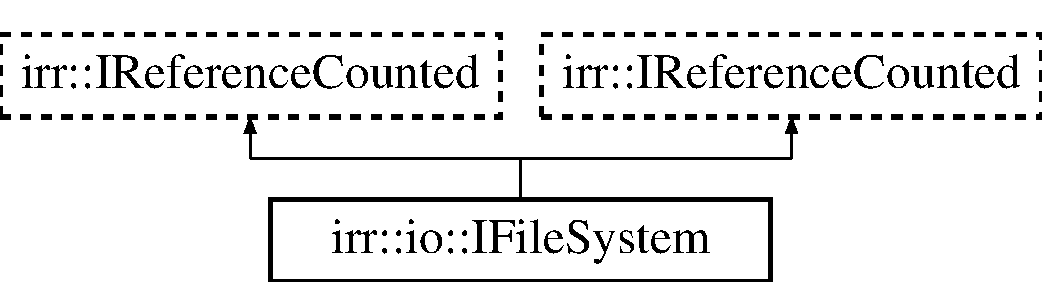
\includegraphics[height=2.000000cm]{classirr_1_1io_1_1IFileSystem}
\end{center}
\end{figure}
\subsection*{Public Member Functions}
\begin{DoxyCompactItemize}
\item 
virtual \hyperlink{classirr_1_1io_1_1IReadFile}{I\+Read\+File} $\ast$ \hyperlink{classirr_1_1io_1_1IFileSystem_a3678bb77e12cc6ee2b3947f4c79f6c90}{create\+And\+Open\+File} (const \hyperlink{namespaceirr_1_1io_ab1bdc45edb3f94d8319c02bc0f840ee1}{path} \&filename)=0
\begin{DoxyCompactList}\small\item\em Opens a file for read access. \end{DoxyCompactList}\item 
virtual \hyperlink{classirr_1_1io_1_1IReadFile}{I\+Read\+File} $\ast$ \hyperlink{classirr_1_1io_1_1IFileSystem_ac60a4b7912a7f2364426dc1aaf9bccae}{create\+Memory\+Read\+File} (void $\ast$memory, \hyperlink{namespaceirr_ac66849b7a6ed16e30ebede579f9b47c6}{s32} len, const \hyperlink{namespaceirr_1_1io_ab1bdc45edb3f94d8319c02bc0f840ee1}{path} \&file\+Name, bool delete\+Memory\+When\+Dropped=false)=0
\begin{DoxyCompactList}\small\item\em Creates an \hyperlink{classirr_1_1io_1_1IReadFile}{I\+Read\+File} interface for accessing memory like a file. \end{DoxyCompactList}\item 
virtual \hyperlink{classirr_1_1io_1_1IReadFile}{I\+Read\+File} $\ast$ \hyperlink{classirr_1_1io_1_1IFileSystem_a8b110f1ed6f52098753b7a558c020dbc}{create\+Limit\+Read\+File} (const \hyperlink{namespaceirr_1_1io_ab1bdc45edb3f94d8319c02bc0f840ee1}{path} \&file\+Name, \hyperlink{classirr_1_1io_1_1IReadFile}{I\+Read\+File} $\ast$already\+Opened\+File, long pos, long area\+Size)=0
\begin{DoxyCompactList}\small\item\em Creates an \hyperlink{classirr_1_1io_1_1IReadFile}{I\+Read\+File} interface for accessing files inside files. \end{DoxyCompactList}\item 
virtual \hyperlink{classirr_1_1io_1_1IWriteFile}{I\+Write\+File} $\ast$ \hyperlink{classirr_1_1io_1_1IFileSystem_a568dd1e737fe3d3222b2e4ca2b6ebad3}{create\+Memory\+Write\+File} (void $\ast$memory, \hyperlink{namespaceirr_ac66849b7a6ed16e30ebede579f9b47c6}{s32} len, const \hyperlink{namespaceirr_1_1io_ab1bdc45edb3f94d8319c02bc0f840ee1}{path} \&file\+Name, bool delete\+Memory\+When\+Dropped=false)=0
\begin{DoxyCompactList}\small\item\em Creates an \hyperlink{classirr_1_1io_1_1IWriteFile}{I\+Write\+File} interface for accessing memory like a file. \end{DoxyCompactList}\item 
virtual \hyperlink{classirr_1_1io_1_1IWriteFile}{I\+Write\+File} $\ast$ \hyperlink{classirr_1_1io_1_1IFileSystem_af0ed28b697936ee8aa60a5a0877ac90a}{create\+And\+Write\+File} (const \hyperlink{namespaceirr_1_1io_ab1bdc45edb3f94d8319c02bc0f840ee1}{path} \&filename, bool append=false)=0
\begin{DoxyCompactList}\small\item\em Opens a file for write access. \end{DoxyCompactList}\item 
virtual bool \hyperlink{classirr_1_1io_1_1IFileSystem_afe6641c7f88a8fea0205c113b8379730}{add\+File\+Archive} (const \hyperlink{namespaceirr_1_1io_ab1bdc45edb3f94d8319c02bc0f840ee1}{path} \&filename, bool ignore\+Case=true, bool ignore\+Paths=true, \hyperlink{namespaceirr_1_1io_adb3e3c445ec8e608ed1f0f93306da14f}{E\+\_\+\+F\+I\+L\+E\+\_\+\+A\+R\+C\+H\+I\+V\+E\+\_\+\+T\+Y\+PE} archive\+Type=\hyperlink{namespaceirr_1_1io_adb3e3c445ec8e608ed1f0f93306da14fa2c2aea9bc955ae4e0d29071ba66ff8dc}{E\+F\+A\+T\+\_\+\+U\+N\+K\+N\+O\+WN}, const \hyperlink{namespaceirr_1_1core_ade1071a878633f2f6d8a75c5d11fec19}{core\+::stringc} \&password=\char`\"{}\char`\"{}, \hyperlink{classirr_1_1io_1_1IFileArchive}{I\+File\+Archive} $\ast$$\ast$ret\+Archive=0)=0
\begin{DoxyCompactList}\small\item\em Adds an archive to the file system. \end{DoxyCompactList}\item 
virtual bool \hyperlink{classirr_1_1io_1_1IFileSystem_abe4d01069e7fbf0fa871197a68ad87b9}{add\+File\+Archive} (\hyperlink{classirr_1_1io_1_1IReadFile}{I\+Read\+File} $\ast$file, bool ignore\+Case=true, bool ignore\+Paths=true, \hyperlink{namespaceirr_1_1io_adb3e3c445ec8e608ed1f0f93306da14f}{E\+\_\+\+F\+I\+L\+E\+\_\+\+A\+R\+C\+H\+I\+V\+E\+\_\+\+T\+Y\+PE} archive\+Type=\hyperlink{namespaceirr_1_1io_adb3e3c445ec8e608ed1f0f93306da14fa2c2aea9bc955ae4e0d29071ba66ff8dc}{E\+F\+A\+T\+\_\+\+U\+N\+K\+N\+O\+WN}, const \hyperlink{namespaceirr_1_1core_ade1071a878633f2f6d8a75c5d11fec19}{core\+::stringc} \&password=\char`\"{}\char`\"{}, \hyperlink{classirr_1_1io_1_1IFileArchive}{I\+File\+Archive} $\ast$$\ast$ret\+Archive=0)=0
\begin{DoxyCompactList}\small\item\em Adds an archive to the file system. \end{DoxyCompactList}\item 
virtual bool \hyperlink{classirr_1_1io_1_1IFileSystem_aedecc2c6f4c567de8bbe54fd711f7143}{add\+File\+Archive} (\hyperlink{classirr_1_1io_1_1IFileArchive}{I\+File\+Archive} $\ast$archive)=0
\begin{DoxyCompactList}\small\item\em Adds an archive to the file system. \end{DoxyCompactList}\item 
\mbox{\Hypertarget{classirr_1_1io_1_1IFileSystem_a85862865f72b1e187402365e4236dce0}\label{classirr_1_1io_1_1IFileSystem_a85862865f72b1e187402365e4236dce0}} 
virtual \hyperlink{namespaceirr_a0416a53257075833e7002efd0a18e804}{u32} \hyperlink{classirr_1_1io_1_1IFileSystem_a85862865f72b1e187402365e4236dce0}{get\+File\+Archive\+Count} () const =0
\begin{DoxyCompactList}\small\item\em Get the number of archives currently attached to the file system. \end{DoxyCompactList}\item 
virtual bool \hyperlink{classirr_1_1io_1_1IFileSystem_aa509623756c9bcbc3a9bcf455ea2a3ba}{remove\+File\+Archive} (\hyperlink{namespaceirr_a0416a53257075833e7002efd0a18e804}{u32} index)=0
\begin{DoxyCompactList}\small\item\em Removes an archive from the file system. \end{DoxyCompactList}\item 
virtual bool \hyperlink{classirr_1_1io_1_1IFileSystem_a03b405c8f5346c225c590cde585eb73c}{remove\+File\+Archive} (const \hyperlink{namespaceirr_1_1io_ab1bdc45edb3f94d8319c02bc0f840ee1}{path} \&filename)=0
\begin{DoxyCompactList}\small\item\em Removes an archive from the file system. \end{DoxyCompactList}\item 
virtual bool \hyperlink{classirr_1_1io_1_1IFileSystem_ab7579f5ccca7bc7c1e079f5cb38173ed}{remove\+File\+Archive} (const \hyperlink{classirr_1_1io_1_1IFileArchive}{I\+File\+Archive} $\ast$archive)=0
\begin{DoxyCompactList}\small\item\em Removes an archive from the file system. \end{DoxyCompactList}\item 
virtual bool \hyperlink{classirr_1_1io_1_1IFileSystem_ae8530fb9793373cf4dbee956090e99f6}{move\+File\+Archive} (\hyperlink{namespaceirr_a0416a53257075833e7002efd0a18e804}{u32} source\+Index, \hyperlink{namespaceirr_ac66849b7a6ed16e30ebede579f9b47c6}{s32} relative)=0
\begin{DoxyCompactList}\small\item\em Changes the search order of attached archives. \end{DoxyCompactList}\item 
\mbox{\Hypertarget{classirr_1_1io_1_1IFileSystem_a1ac4bfb7bfd7d2961af8e5c128190fae}\label{classirr_1_1io_1_1IFileSystem_a1ac4bfb7bfd7d2961af8e5c128190fae}} 
virtual \hyperlink{classirr_1_1io_1_1IFileArchive}{I\+File\+Archive} $\ast$ \hyperlink{classirr_1_1io_1_1IFileSystem_a1ac4bfb7bfd7d2961af8e5c128190fae}{get\+File\+Archive} (\hyperlink{namespaceirr_a0416a53257075833e7002efd0a18e804}{u32} index)=0
\begin{DoxyCompactList}\small\item\em Get the archive at a given index. \end{DoxyCompactList}\item 
virtual void \hyperlink{classirr_1_1io_1_1IFileSystem_ad56456302b4697c49b461a909d9269b9}{add\+Archive\+Loader} (\hyperlink{classirr_1_1io_1_1IArchiveLoader}{I\+Archive\+Loader} $\ast$loader)=0
\begin{DoxyCompactList}\small\item\em Adds an external archive loader to the engine. \end{DoxyCompactList}\item 
\mbox{\Hypertarget{classirr_1_1io_1_1IFileSystem_ae1e958f65eb8b61b40f3c71a593f852d}\label{classirr_1_1io_1_1IFileSystem_ae1e958f65eb8b61b40f3c71a593f852d}} 
virtual \hyperlink{namespaceirr_a0416a53257075833e7002efd0a18e804}{u32} \hyperlink{classirr_1_1io_1_1IFileSystem_ae1e958f65eb8b61b40f3c71a593f852d}{get\+Archive\+Loader\+Count} () const =0
\begin{DoxyCompactList}\small\item\em Gets the number of archive loaders currently added. \end{DoxyCompactList}\item 
virtual \hyperlink{classirr_1_1io_1_1IArchiveLoader}{I\+Archive\+Loader} $\ast$ \hyperlink{classirr_1_1io_1_1IFileSystem_a175208d74556d1a0e4fe7400bbc65d7b}{get\+Archive\+Loader} (\hyperlink{namespaceirr_a0416a53257075833e7002efd0a18e804}{u32} index) const =0
\begin{DoxyCompactList}\small\item\em Retrieve the given archive loader. \end{DoxyCompactList}\item 
virtual \+\_\+\+I\+R\+R\+\_\+\+D\+E\+P\+R\+E\+C\+A\+T\+E\+D\+\_\+ bool \hyperlink{classirr_1_1io_1_1IFileSystem_aef11ff9b5c171d7b3a99d8a79b71f2b3}{add\+Zip\+File\+Archive} (const \hyperlink{namespaceirr_a9395eaea339bcb546b319e9c96bf7410}{c8} $\ast$filename, bool ignore\+Case=true, bool ignore\+Paths=true)
\begin{DoxyCompactList}\small\item\em Adds a zip archive to the file system. \end{DoxyCompactList}\item 
virtual \+\_\+\+I\+R\+R\+\_\+\+D\+E\+P\+R\+E\+C\+A\+T\+E\+D\+\_\+ bool \hyperlink{classirr_1_1io_1_1IFileSystem_a7b5235a1473ff67d97f1487211762723}{add\+Folder\+File\+Archive} (const \hyperlink{namespaceirr_a9395eaea339bcb546b319e9c96bf7410}{c8} $\ast$filename, bool ignore\+Case=true, bool ignore\+Paths=true)
\begin{DoxyCompactList}\small\item\em Adds an unzipped archive (or basedirectory with subdirectories..) to the file system. \end{DoxyCompactList}\item 
virtual \+\_\+\+I\+R\+R\+\_\+\+D\+E\+P\+R\+E\+C\+A\+T\+E\+D\+\_\+ bool \hyperlink{classirr_1_1io_1_1IFileSystem_a5ade21d59a80b16965d57d1977ad6cc4}{add\+Pak\+File\+Archive} (const \hyperlink{namespaceirr_a9395eaea339bcb546b319e9c96bf7410}{c8} $\ast$filename, bool ignore\+Case=true, bool ignore\+Paths=true)
\begin{DoxyCompactList}\small\item\em Adds a pak archive to the file system. \end{DoxyCompactList}\item 
virtual const \hyperlink{namespaceirr_1_1io_ab1bdc45edb3f94d8319c02bc0f840ee1}{path} \& \hyperlink{classirr_1_1io_1_1IFileSystem_acbf7342afa6e2fc9583db3e521e66e61}{get\+Working\+Directory} ()=0
\begin{DoxyCompactList}\small\item\em Get the current working directory. \end{DoxyCompactList}\item 
virtual bool \hyperlink{classirr_1_1io_1_1IFileSystem_a8859a2bed44815eeccc4fbcef189b073}{change\+Working\+Directory\+To} (const \hyperlink{namespaceirr_1_1io_ab1bdc45edb3f94d8319c02bc0f840ee1}{path} \&new\+Directory)=0
\begin{DoxyCompactList}\small\item\em Changes the current working directory. \end{DoxyCompactList}\item 
virtual \hyperlink{namespaceirr_1_1io_ab1bdc45edb3f94d8319c02bc0f840ee1}{path} \hyperlink{classirr_1_1io_1_1IFileSystem_a77191d7917349a0200f5de3ef29acd18}{get\+Absolute\+Path} (const \hyperlink{namespaceirr_1_1io_ab1bdc45edb3f94d8319c02bc0f840ee1}{path} \&filename) const =0
\begin{DoxyCompactList}\small\item\em Converts a relative path to an absolute (unique) path, resolving symbolic links if required. \end{DoxyCompactList}\item 
virtual \hyperlink{namespaceirr_1_1io_ab1bdc45edb3f94d8319c02bc0f840ee1}{path} \hyperlink{classirr_1_1io_1_1IFileSystem_ad8b7b93f32f58c1ba9a8e7cacd5de80b}{get\+File\+Dir} (const \hyperlink{namespaceirr_1_1io_ab1bdc45edb3f94d8319c02bc0f840ee1}{path} \&filename) const =0
\begin{DoxyCompactList}\small\item\em Get the directory a file is located in. \end{DoxyCompactList}\item 
virtual \hyperlink{namespaceirr_1_1io_ab1bdc45edb3f94d8319c02bc0f840ee1}{path} \hyperlink{classirr_1_1io_1_1IFileSystem_a4235989e4ec21c78f1fd1ca861980c6c}{get\+File\+Basename} (const \hyperlink{namespaceirr_1_1io_ab1bdc45edb3f94d8319c02bc0f840ee1}{path} \&filename, bool keep\+Extension=true) const =0
\begin{DoxyCompactList}\small\item\em Get the base part of a filename, i.\+e. the name without the directory part. \end{DoxyCompactList}\item 
\mbox{\Hypertarget{classirr_1_1io_1_1IFileSystem_aa76bbc9cc5ec7a8dbe96713f1ba20de6}\label{classirr_1_1io_1_1IFileSystem_aa76bbc9cc5ec7a8dbe96713f1ba20de6}} 
virtual \hyperlink{namespaceirr_1_1io_ab1bdc45edb3f94d8319c02bc0f840ee1}{path} \& \hyperlink{classirr_1_1io_1_1IFileSystem_aa76bbc9cc5ec7a8dbe96713f1ba20de6}{flatten\+Filename} (\hyperlink{namespaceirr_1_1io_ab1bdc45edb3f94d8319c02bc0f840ee1}{path} \&directory, const \hyperlink{namespaceirr_1_1io_ab1bdc45edb3f94d8319c02bc0f840ee1}{path} \&root=\char`\"{}/\char`\"{}) const =0
\begin{DoxyCompactList}\small\item\em flatten a path and file name for example\+: \char`\"{}/you/me/../.\char`\"{} becomes \char`\"{}/you\char`\"{} \end{DoxyCompactList}\item 
\mbox{\Hypertarget{classirr_1_1io_1_1IFileSystem_a9cb85c468a6cda253ff99c88010028c7}\label{classirr_1_1io_1_1IFileSystem_a9cb85c468a6cda253ff99c88010028c7}} 
virtual \hyperlink{namespaceirr_1_1io_ab1bdc45edb3f94d8319c02bc0f840ee1}{path} \hyperlink{classirr_1_1io_1_1IFileSystem_a9cb85c468a6cda253ff99c88010028c7}{get\+Relative\+Filename} (const \hyperlink{namespaceirr_1_1io_ab1bdc45edb3f94d8319c02bc0f840ee1}{path} \&filename, const \hyperlink{namespaceirr_1_1io_ab1bdc45edb3f94d8319c02bc0f840ee1}{path} \&directory) const =0
\begin{DoxyCompactList}\small\item\em Get the relative filename, relative to the given directory. \end{DoxyCompactList}\item 
virtual \hyperlink{classirr_1_1io_1_1IFileList}{I\+File\+List} $\ast$ \hyperlink{classirr_1_1io_1_1IFileSystem_ad5820e7664377c12015ea7a6c801f7f8}{create\+File\+List} ()=0
\begin{DoxyCompactList}\small\item\em Creates a list of files and directories in the current working directory and returns it. \end{DoxyCompactList}\item 
virtual \hyperlink{classirr_1_1io_1_1IFileList}{I\+File\+List} $\ast$ \hyperlink{classirr_1_1io_1_1IFileSystem_a4f8a69f557f2b7022f6cd7346c3e85d2}{create\+Empty\+File\+List} (const \hyperlink{namespaceirr_1_1io_ab1bdc45edb3f94d8319c02bc0f840ee1}{io\+::path} \&\hyperlink{namespaceirr_1_1io_ab1bdc45edb3f94d8319c02bc0f840ee1}{path}, bool ignore\+Case, bool ignore\+Paths)=0
\begin{DoxyCompactList}\small\item\em Creates an empty filelist. \end{DoxyCompactList}\item 
\mbox{\Hypertarget{classirr_1_1io_1_1IFileSystem_a767614d727f0b1ec0bc5fdaaf906169b}\label{classirr_1_1io_1_1IFileSystem_a767614d727f0b1ec0bc5fdaaf906169b}} 
virtual \hyperlink{namespaceirr_1_1io_a22364f1caf06442a70f6198025af3fe9}{E\+File\+System\+Type} \hyperlink{classirr_1_1io_1_1IFileSystem_a767614d727f0b1ec0bc5fdaaf906169b}{set\+File\+List\+System} (\hyperlink{namespaceirr_1_1io_a22364f1caf06442a70f6198025af3fe9}{E\+File\+System\+Type} list\+Type)=0
\begin{DoxyCompactList}\small\item\em Set the active type of file system. \end{DoxyCompactList}\item 
virtual bool \hyperlink{classirr_1_1io_1_1IFileSystem_a1c5e98bc16e38b1d15b44e24b1b3bd32}{exist\+File} (const \hyperlink{namespaceirr_1_1io_ab1bdc45edb3f94d8319c02bc0f840ee1}{path} \&filename) const =0
\begin{DoxyCompactList}\small\item\em Determines if a file exists and could be opened. \end{DoxyCompactList}\item 
virtual \hyperlink{namespaceirr_1_1io_a9dc6291fb7e4c73155a3e3c8339f9bff}{I\+X\+M\+L\+Reader} $\ast$ \hyperlink{classirr_1_1io_1_1IFileSystem_a167c9fa159d16ee5c56c074636b0865e}{create\+X\+M\+L\+Reader} (const \hyperlink{namespaceirr_1_1io_ab1bdc45edb3f94d8319c02bc0f840ee1}{path} \&filename)=0
\begin{DoxyCompactList}\small\item\em Creates a X\+ML Reader from a file which returns all parsed strings as wide characters (wchar\+\_\+t$\ast$). \end{DoxyCompactList}\item 
virtual \hyperlink{namespaceirr_1_1io_a9dc6291fb7e4c73155a3e3c8339f9bff}{I\+X\+M\+L\+Reader} $\ast$ \hyperlink{classirr_1_1io_1_1IFileSystem_a38f4c90db3fd1b21473ce0cd2437bb59}{create\+X\+M\+L\+Reader} (\hyperlink{classirr_1_1io_1_1IReadFile}{I\+Read\+File} $\ast$file)=0
\begin{DoxyCompactList}\small\item\em Creates a X\+ML Reader from a file which returns all parsed strings as wide characters (wchar\+\_\+t$\ast$). \end{DoxyCompactList}\item 
virtual \hyperlink{namespaceirr_1_1io_a2dedc8156931082e6b147b562195e310}{I\+X\+M\+L\+Reader\+U\+T\+F8} $\ast$ \hyperlink{classirr_1_1io_1_1IFileSystem_affd8f622ac7c3dcd507f20f9cd23b21f}{create\+X\+M\+L\+Reader\+U\+T\+F8} (const \hyperlink{namespaceirr_1_1io_ab1bdc45edb3f94d8319c02bc0f840ee1}{path} \&filename)=0
\begin{DoxyCompactList}\small\item\em Creates a X\+ML Reader from a file which returns all parsed strings as A\+S\+C\+I\+I/\+U\+T\+F-\/8 characters (char$\ast$). \end{DoxyCompactList}\item 
virtual \hyperlink{namespaceirr_1_1io_a2dedc8156931082e6b147b562195e310}{I\+X\+M\+L\+Reader\+U\+T\+F8} $\ast$ \hyperlink{classirr_1_1io_1_1IFileSystem_acda42a761d3b2fb4d39ad1d9e2ada973}{create\+X\+M\+L\+Reader\+U\+T\+F8} (\hyperlink{classirr_1_1io_1_1IReadFile}{I\+Read\+File} $\ast$file)=0
\begin{DoxyCompactList}\small\item\em Creates a X\+ML Reader from a file which returns all parsed strings as A\+S\+C\+I\+I/\+U\+T\+F-\/8 characters (char$\ast$). \end{DoxyCompactList}\item 
virtual \hyperlink{classirr_1_1io_1_1IXMLWriter}{I\+X\+M\+L\+Writer} $\ast$ \hyperlink{classirr_1_1io_1_1IFileSystem_a0737712d1c90001e5765ef46912c616d}{create\+X\+M\+L\+Writer} (const \hyperlink{namespaceirr_1_1io_ab1bdc45edb3f94d8319c02bc0f840ee1}{path} \&filename)=0
\begin{DoxyCompactList}\small\item\em Creates a X\+ML Writer from a file. \end{DoxyCompactList}\item 
virtual \hyperlink{classirr_1_1io_1_1IXMLWriter}{I\+X\+M\+L\+Writer} $\ast$ \hyperlink{classirr_1_1io_1_1IFileSystem_ac2bcaf8c338e80ff579061b7056c06da}{create\+X\+M\+L\+Writer} (\hyperlink{classirr_1_1io_1_1IWriteFile}{I\+Write\+File} $\ast$file)=0
\begin{DoxyCompactList}\small\item\em Creates a X\+ML Writer from a file. \end{DoxyCompactList}\item 
virtual \hyperlink{classirr_1_1io_1_1IAttributes}{I\+Attributes} $\ast$ \hyperlink{classirr_1_1io_1_1IFileSystem_a50f91cd88b926751367dac153c1cefd2}{create\+Empty\+Attributes} (\hyperlink{classirr_1_1video_1_1IVideoDriver}{video\+::\+I\+Video\+Driver} $\ast$driver=0)=0
\begin{DoxyCompactList}\small\item\em Creates a new empty collection of attributes, usable for serialization and more. \end{DoxyCompactList}\end{DoxyCompactItemize}
\subsection*{Additional Inherited Members}


\subsection{Detailed Description}
The File\+System manages files and archives and provides access to them. 

It manages where files are, so that modules which use the the IO do not need to know where every file is located. A file could be in a .zip-\/\+Archive or as file on disk, using the \hyperlink{classirr_1_1io_1_1IFileSystem}{I\+File\+System} makes no difference to this. 

\subsection{Member Function Documentation}
\mbox{\Hypertarget{classirr_1_1io_1_1IFileSystem_ad56456302b4697c49b461a909d9269b9}\label{classirr_1_1io_1_1IFileSystem_ad56456302b4697c49b461a909d9269b9}} 
\index{irr\+::io\+::\+I\+File\+System@{irr\+::io\+::\+I\+File\+System}!add\+Archive\+Loader@{add\+Archive\+Loader}}
\index{add\+Archive\+Loader@{add\+Archive\+Loader}!irr\+::io\+::\+I\+File\+System@{irr\+::io\+::\+I\+File\+System}}
\subsubsection{\texorpdfstring{add\+Archive\+Loader()}{addArchiveLoader()}}
{\footnotesize\ttfamily virtual void irr\+::io\+::\+I\+File\+System\+::add\+Archive\+Loader (\begin{DoxyParamCaption}\item[{\hyperlink{classirr_1_1io_1_1IArchiveLoader}{I\+Archive\+Loader} $\ast$}]{loader }\end{DoxyParamCaption})\hspace{0.3cm}{\ttfamily [pure virtual]}}



Adds an external archive loader to the engine. 

Use this function to add support for new archive types to the engine, for example proprietary or encrypted file storage. \mbox{\Hypertarget{classirr_1_1io_1_1IFileSystem_afe6641c7f88a8fea0205c113b8379730}\label{classirr_1_1io_1_1IFileSystem_afe6641c7f88a8fea0205c113b8379730}} 
\index{irr\+::io\+::\+I\+File\+System@{irr\+::io\+::\+I\+File\+System}!add\+File\+Archive@{add\+File\+Archive}}
\index{add\+File\+Archive@{add\+File\+Archive}!irr\+::io\+::\+I\+File\+System@{irr\+::io\+::\+I\+File\+System}}
\subsubsection{\texorpdfstring{add\+File\+Archive()}{addFileArchive()}\hspace{0.1cm}{\footnotesize\ttfamily [1/3]}}
{\footnotesize\ttfamily virtual bool irr\+::io\+::\+I\+File\+System\+::add\+File\+Archive (\begin{DoxyParamCaption}\item[{const \hyperlink{namespaceirr_1_1io_ab1bdc45edb3f94d8319c02bc0f840ee1}{path} \&}]{filename,  }\item[{bool}]{ignore\+Case = {\ttfamily true},  }\item[{bool}]{ignore\+Paths = {\ttfamily true},  }\item[{\hyperlink{namespaceirr_1_1io_adb3e3c445ec8e608ed1f0f93306da14f}{E\+\_\+\+F\+I\+L\+E\+\_\+\+A\+R\+C\+H\+I\+V\+E\+\_\+\+T\+Y\+PE}}]{archive\+Type = {\ttfamily \hyperlink{namespaceirr_1_1io_adb3e3c445ec8e608ed1f0f93306da14fa2c2aea9bc955ae4e0d29071ba66ff8dc}{E\+F\+A\+T\+\_\+\+U\+N\+K\+N\+O\+WN}},  }\item[{const \hyperlink{namespaceirr_1_1core_ade1071a878633f2f6d8a75c5d11fec19}{core\+::stringc} \&}]{password = {\ttfamily \char`\"{}\char`\"{}},  }\item[{\hyperlink{classirr_1_1io_1_1IFileArchive}{I\+File\+Archive} $\ast$$\ast$}]{ret\+Archive = {\ttfamily 0} }\end{DoxyParamCaption})\hspace{0.3cm}{\ttfamily [pure virtual]}}



Adds an archive to the file system. 

After calling this, the Irrlicht Engine will also search and open files directly from this archive. This is useful for hiding data from the end user, speeding up file access and making it possible to access for example Quake3 .pk3 files, which are just renamed .zip files. By default Irrlicht supports Z\+IP, P\+AK, T\+AR, P\+NK, and directories as archives. You can provide your own archive types by implementing \hyperlink{classirr_1_1io_1_1IArchiveLoader}{I\+Archive\+Loader} and passing an instance to add\+Archive\+Loader. Irrlicht supports A\+E\+S-\/encrypted zip files, and the advanced compression techniques lzma and bzip2. 
\begin{DoxyParams}{Parameters}
{\em filename} & Filename of the archive to add to the file system. \\
\hline
{\em ignore\+Case} & If set to true, files in the archive can be accessed without writing all letters in the right case. \\
\hline
{\em ignore\+Paths} & If set to true, files in the added archive can be accessed without its complete path. \\
\hline
{\em archive\+Type} & If no specific E\+\_\+\+F\+I\+L\+E\+\_\+\+A\+R\+C\+H\+I\+V\+E\+\_\+\+T\+Y\+PE is selected then the type of archive will depend on the extension of the file name. If you use a different extension then you can use this parameter to force a specific type of archive. \\
\hline
{\em password} & An optional password, which is used in case of encrypted archives. \\
\hline
{\em ret\+Archive} & A pointer that will be set to the archive that is added. \\
\hline
\end{DoxyParams}
\begin{DoxyReturn}{Returns}
True if the archive was added successfully, false if not. 
\end{DoxyReturn}
\mbox{\Hypertarget{classirr_1_1io_1_1IFileSystem_abe4d01069e7fbf0fa871197a68ad87b9}\label{classirr_1_1io_1_1IFileSystem_abe4d01069e7fbf0fa871197a68ad87b9}} 
\index{irr\+::io\+::\+I\+File\+System@{irr\+::io\+::\+I\+File\+System}!add\+File\+Archive@{add\+File\+Archive}}
\index{add\+File\+Archive@{add\+File\+Archive}!irr\+::io\+::\+I\+File\+System@{irr\+::io\+::\+I\+File\+System}}
\subsubsection{\texorpdfstring{add\+File\+Archive()}{addFileArchive()}\hspace{0.1cm}{\footnotesize\ttfamily [2/3]}}
{\footnotesize\ttfamily virtual bool irr\+::io\+::\+I\+File\+System\+::add\+File\+Archive (\begin{DoxyParamCaption}\item[{\hyperlink{classirr_1_1io_1_1IReadFile}{I\+Read\+File} $\ast$}]{file,  }\item[{bool}]{ignore\+Case = {\ttfamily true},  }\item[{bool}]{ignore\+Paths = {\ttfamily true},  }\item[{\hyperlink{namespaceirr_1_1io_adb3e3c445ec8e608ed1f0f93306da14f}{E\+\_\+\+F\+I\+L\+E\+\_\+\+A\+R\+C\+H\+I\+V\+E\+\_\+\+T\+Y\+PE}}]{archive\+Type = {\ttfamily \hyperlink{namespaceirr_1_1io_adb3e3c445ec8e608ed1f0f93306da14fa2c2aea9bc955ae4e0d29071ba66ff8dc}{E\+F\+A\+T\+\_\+\+U\+N\+K\+N\+O\+WN}},  }\item[{const \hyperlink{namespaceirr_1_1core_ade1071a878633f2f6d8a75c5d11fec19}{core\+::stringc} \&}]{password = {\ttfamily \char`\"{}\char`\"{}},  }\item[{\hyperlink{classirr_1_1io_1_1IFileArchive}{I\+File\+Archive} $\ast$$\ast$}]{ret\+Archive = {\ttfamily 0} }\end{DoxyParamCaption})\hspace{0.3cm}{\ttfamily [pure virtual]}}



Adds an archive to the file system. 

After calling this, the Irrlicht Engine will also search and open files directly from this archive. This is useful for hiding data from the end user, speeding up file access and making it possible to access for example Quake3 .pk3 files, which are just renamed .zip files. By default Irrlicht supports Z\+IP, P\+AK, T\+AR, P\+NK, and directories as archives. You can provide your own archive types by implementing \hyperlink{classirr_1_1io_1_1IArchiveLoader}{I\+Archive\+Loader} and passing an instance to add\+Archive\+Loader. Irrlicht supports A\+E\+S-\/encrypted zip files, and the advanced compression techniques lzma and bzip2. If you want to add a directory as an archive, prefix its name with a slash in order to let Irrlicht recognize it as a folder mount (mypath/). Using this technique one can build up a search order, because archives are read first, and can be used more easily with relative filenames. 
\begin{DoxyParams}{Parameters}
{\em file} & Archive to add to the file system. \\
\hline
{\em ignore\+Case} & If set to true, files in the archive can be accessed without writing all letters in the right case. \\
\hline
{\em ignore\+Paths} & If set to true, files in the added archive can be accessed without its complete path. \\
\hline
{\em archive\+Type} & If no specific E\+\_\+\+F\+I\+L\+E\+\_\+\+A\+R\+C\+H\+I\+V\+E\+\_\+\+T\+Y\+PE is selected then the type of archive will depend on the extension of the file name. If you use a different extension then you can use this parameter to force a specific type of archive. \\
\hline
{\em password} & An optional password, which is used in case of encrypted archives. \\
\hline
{\em ret\+Archive} & A pointer that will be set to the archive that is added. \\
\hline
\end{DoxyParams}
\begin{DoxyReturn}{Returns}
True if the archive was added successfully, false if not. 
\end{DoxyReturn}
\mbox{\Hypertarget{classirr_1_1io_1_1IFileSystem_aedecc2c6f4c567de8bbe54fd711f7143}\label{classirr_1_1io_1_1IFileSystem_aedecc2c6f4c567de8bbe54fd711f7143}} 
\index{irr\+::io\+::\+I\+File\+System@{irr\+::io\+::\+I\+File\+System}!add\+File\+Archive@{add\+File\+Archive}}
\index{add\+File\+Archive@{add\+File\+Archive}!irr\+::io\+::\+I\+File\+System@{irr\+::io\+::\+I\+File\+System}}
\subsubsection{\texorpdfstring{add\+File\+Archive()}{addFileArchive()}\hspace{0.1cm}{\footnotesize\ttfamily [3/3]}}
{\footnotesize\ttfamily virtual bool irr\+::io\+::\+I\+File\+System\+::add\+File\+Archive (\begin{DoxyParamCaption}\item[{\hyperlink{classirr_1_1io_1_1IFileArchive}{I\+File\+Archive} $\ast$}]{archive }\end{DoxyParamCaption})\hspace{0.3cm}{\ttfamily [pure virtual]}}



Adds an archive to the file system. 


\begin{DoxyParams}{Parameters}
{\em archive} & The archive to add to the file system. \\
\hline
\end{DoxyParams}
\begin{DoxyReturn}{Returns}
True if the archive was added successfully, false if not. 
\end{DoxyReturn}
\mbox{\Hypertarget{classirr_1_1io_1_1IFileSystem_a7b5235a1473ff67d97f1487211762723}\label{classirr_1_1io_1_1IFileSystem_a7b5235a1473ff67d97f1487211762723}} 
\index{irr\+::io\+::\+I\+File\+System@{irr\+::io\+::\+I\+File\+System}!add\+Folder\+File\+Archive@{add\+Folder\+File\+Archive}}
\index{add\+Folder\+File\+Archive@{add\+Folder\+File\+Archive}!irr\+::io\+::\+I\+File\+System@{irr\+::io\+::\+I\+File\+System}}
\subsubsection{\texorpdfstring{add\+Folder\+File\+Archive()}{addFolderFileArchive()}}
{\footnotesize\ttfamily virtual \+\_\+\+I\+R\+R\+\_\+\+D\+E\+P\+R\+E\+C\+A\+T\+E\+D\+\_\+ bool irr\+::io\+::\+I\+File\+System\+::add\+Folder\+File\+Archive (\begin{DoxyParamCaption}\item[{const \hyperlink{namespaceirr_a9395eaea339bcb546b319e9c96bf7410}{c8} $\ast$}]{filename,  }\item[{bool}]{ignore\+Case = {\ttfamily true},  }\item[{bool}]{ignore\+Paths = {\ttfamily true} }\end{DoxyParamCaption})\hspace{0.3cm}{\ttfamily [inline]}, {\ttfamily [virtual]}}



Adds an unzipped archive (or basedirectory with subdirectories..) to the file system. 

\begin{DoxyRefDesc}{Deprecated}
\item[\hyperlink{deprecated__deprecated000003}{Deprecated}]This function is provided for compatibility with older versions of Irrlicht and may be removed in Irrlicht 1.\+9, you should use add\+File\+Archive instead. Useful for handling data which will be in a zip file \end{DoxyRefDesc}

\begin{DoxyParams}{Parameters}
{\em filename} & Filename of the unzipped zip archive base directory to add to the file system. \\
\hline
{\em ignore\+Case} & If set to true, files in the archive can be accessed without writing all letters in the right case. \\
\hline
{\em ignore\+Paths} & If set to true, files in the added archive can be accessed without its complete path. \\
\hline
\end{DoxyParams}
\begin{DoxyReturn}{Returns}
True if the archive was added successful, false if not. 
\end{DoxyReturn}
\mbox{\Hypertarget{classirr_1_1io_1_1IFileSystem_a5ade21d59a80b16965d57d1977ad6cc4}\label{classirr_1_1io_1_1IFileSystem_a5ade21d59a80b16965d57d1977ad6cc4}} 
\index{irr\+::io\+::\+I\+File\+System@{irr\+::io\+::\+I\+File\+System}!add\+Pak\+File\+Archive@{add\+Pak\+File\+Archive}}
\index{add\+Pak\+File\+Archive@{add\+Pak\+File\+Archive}!irr\+::io\+::\+I\+File\+System@{irr\+::io\+::\+I\+File\+System}}
\subsubsection{\texorpdfstring{add\+Pak\+File\+Archive()}{addPakFileArchive()}}
{\footnotesize\ttfamily virtual \+\_\+\+I\+R\+R\+\_\+\+D\+E\+P\+R\+E\+C\+A\+T\+E\+D\+\_\+ bool irr\+::io\+::\+I\+File\+System\+::add\+Pak\+File\+Archive (\begin{DoxyParamCaption}\item[{const \hyperlink{namespaceirr_a9395eaea339bcb546b319e9c96bf7410}{c8} $\ast$}]{filename,  }\item[{bool}]{ignore\+Case = {\ttfamily true},  }\item[{bool}]{ignore\+Paths = {\ttfamily true} }\end{DoxyParamCaption})\hspace{0.3cm}{\ttfamily [inline]}, {\ttfamily [virtual]}}



Adds a pak archive to the file system. 

\begin{DoxyRefDesc}{Deprecated}
\item[\hyperlink{deprecated__deprecated000004}{Deprecated}]This function is provided for compatibility with older versions of Irrlicht and may be removed in Irrlicht 1.\+9, you should use add\+File\+Archive instead. After calling this, the Irrlicht Engine will search and open files directly from this archive too. This is useful for hiding data from the end user, speeding up file access and making it possible to access for example Quake2/\+King\+Pin/\+Hexen2 .pak files \end{DoxyRefDesc}

\begin{DoxyParams}{Parameters}
{\em filename} & Filename of the pak archive to add to the file system. \\
\hline
{\em ignore\+Case} & If set to true, files in the archive can be accessed without writing all letters in the right case. \\
\hline
{\em ignore\+Paths} & If set to true, files in the added archive can be accessed without its complete path.(should not use with Quake2 paks \\
\hline
\end{DoxyParams}
\begin{DoxyReturn}{Returns}
True if the archive was added successful, false if not. 
\end{DoxyReturn}
\mbox{\Hypertarget{classirr_1_1io_1_1IFileSystem_aef11ff9b5c171d7b3a99d8a79b71f2b3}\label{classirr_1_1io_1_1IFileSystem_aef11ff9b5c171d7b3a99d8a79b71f2b3}} 
\index{irr\+::io\+::\+I\+File\+System@{irr\+::io\+::\+I\+File\+System}!add\+Zip\+File\+Archive@{add\+Zip\+File\+Archive}}
\index{add\+Zip\+File\+Archive@{add\+Zip\+File\+Archive}!irr\+::io\+::\+I\+File\+System@{irr\+::io\+::\+I\+File\+System}}
\subsubsection{\texorpdfstring{add\+Zip\+File\+Archive()}{addZipFileArchive()}}
{\footnotesize\ttfamily virtual \+\_\+\+I\+R\+R\+\_\+\+D\+E\+P\+R\+E\+C\+A\+T\+E\+D\+\_\+ bool irr\+::io\+::\+I\+File\+System\+::add\+Zip\+File\+Archive (\begin{DoxyParamCaption}\item[{const \hyperlink{namespaceirr_a9395eaea339bcb546b319e9c96bf7410}{c8} $\ast$}]{filename,  }\item[{bool}]{ignore\+Case = {\ttfamily true},  }\item[{bool}]{ignore\+Paths = {\ttfamily true} }\end{DoxyParamCaption})\hspace{0.3cm}{\ttfamily [inline]}, {\ttfamily [virtual]}}



Adds a zip archive to the file system. 

\begin{DoxyRefDesc}{Deprecated}
\item[\hyperlink{deprecated__deprecated000002}{Deprecated}]This function is provided for compatibility with older versions of Irrlicht and may be removed in Irrlicht 1.\+9, you should use add\+File\+Archive instead. After calling this, the Irrlicht Engine will search and open files directly from this archive too. This is useful for hiding data from the end user, speeding up file access and making it possible to access for example Quake3 .pk3 files, which are no different than .zip files. \end{DoxyRefDesc}

\begin{DoxyParams}{Parameters}
{\em filename} & Filename of the zip archive to add to the file system. \\
\hline
{\em ignore\+Case} & If set to true, files in the archive can be accessed without writing all letters in the right case. \\
\hline
{\em ignore\+Paths} & If set to true, files in the added archive can be accessed without its complete path. \\
\hline
\end{DoxyParams}
\begin{DoxyReturn}{Returns}
True if the archive was added successfully, false if not. 
\end{DoxyReturn}
\mbox{\Hypertarget{classirr_1_1io_1_1IFileSystem_a8859a2bed44815eeccc4fbcef189b073}\label{classirr_1_1io_1_1IFileSystem_a8859a2bed44815eeccc4fbcef189b073}} 
\index{irr\+::io\+::\+I\+File\+System@{irr\+::io\+::\+I\+File\+System}!change\+Working\+Directory\+To@{change\+Working\+Directory\+To}}
\index{change\+Working\+Directory\+To@{change\+Working\+Directory\+To}!irr\+::io\+::\+I\+File\+System@{irr\+::io\+::\+I\+File\+System}}
\subsubsection{\texorpdfstring{change\+Working\+Directory\+To()}{changeWorkingDirectoryTo()}}
{\footnotesize\ttfamily virtual bool irr\+::io\+::\+I\+File\+System\+::change\+Working\+Directory\+To (\begin{DoxyParamCaption}\item[{const \hyperlink{namespaceirr_1_1io_ab1bdc45edb3f94d8319c02bc0f840ee1}{path} \&}]{new\+Directory }\end{DoxyParamCaption})\hspace{0.3cm}{\ttfamily [pure virtual]}}



Changes the current working directory. 


\begin{DoxyParams}{Parameters}
{\em new\+Directory} & A string specifying the new working directory. The string is operating system dependent. Under Windows it has the form \char`\"{}$<$drive$>$\+:\textbackslash{}$<$directory$>$\textbackslash{}$<$sudirectory$>$\textbackslash{}$<$..$>$\char`\"{}. An example would be\+: \char`\"{}\+C\+:\textbackslash{}\+Windows\textbackslash{}\char`\"{} \\
\hline
\end{DoxyParams}
\begin{DoxyReturn}{Returns}
True if successful, otherwise false. 
\end{DoxyReturn}
\mbox{\Hypertarget{classirr_1_1io_1_1IFileSystem_a3678bb77e12cc6ee2b3947f4c79f6c90}\label{classirr_1_1io_1_1IFileSystem_a3678bb77e12cc6ee2b3947f4c79f6c90}} 
\index{irr\+::io\+::\+I\+File\+System@{irr\+::io\+::\+I\+File\+System}!create\+And\+Open\+File@{create\+And\+Open\+File}}
\index{create\+And\+Open\+File@{create\+And\+Open\+File}!irr\+::io\+::\+I\+File\+System@{irr\+::io\+::\+I\+File\+System}}
\subsubsection{\texorpdfstring{create\+And\+Open\+File()}{createAndOpenFile()}}
{\footnotesize\ttfamily virtual \hyperlink{classirr_1_1io_1_1IReadFile}{I\+Read\+File}$\ast$ irr\+::io\+::\+I\+File\+System\+::create\+And\+Open\+File (\begin{DoxyParamCaption}\item[{const \hyperlink{namespaceirr_1_1io_ab1bdc45edb3f94d8319c02bc0f840ee1}{path} \&}]{filename }\end{DoxyParamCaption})\hspace{0.3cm}{\ttfamily [pure virtual]}}



Opens a file for read access. 


\begin{DoxyParams}{Parameters}
{\em filename} & Name of file to open. \\
\hline
\end{DoxyParams}
\begin{DoxyReturn}{Returns}
Pointer to the created file interface. The returned pointer should be dropped when no longer needed. See \hyperlink{classirr_1_1IReferenceCounted_a03856a09355b89d178090c4a5f738543}{I\+Reference\+Counted\+::drop()} for more information. 
\end{DoxyReturn}
\mbox{\Hypertarget{classirr_1_1io_1_1IFileSystem_af0ed28b697936ee8aa60a5a0877ac90a}\label{classirr_1_1io_1_1IFileSystem_af0ed28b697936ee8aa60a5a0877ac90a}} 
\index{irr\+::io\+::\+I\+File\+System@{irr\+::io\+::\+I\+File\+System}!create\+And\+Write\+File@{create\+And\+Write\+File}}
\index{create\+And\+Write\+File@{create\+And\+Write\+File}!irr\+::io\+::\+I\+File\+System@{irr\+::io\+::\+I\+File\+System}}
\subsubsection{\texorpdfstring{create\+And\+Write\+File()}{createAndWriteFile()}}
{\footnotesize\ttfamily virtual \hyperlink{classirr_1_1io_1_1IWriteFile}{I\+Write\+File}$\ast$ irr\+::io\+::\+I\+File\+System\+::create\+And\+Write\+File (\begin{DoxyParamCaption}\item[{const \hyperlink{namespaceirr_1_1io_ab1bdc45edb3f94d8319c02bc0f840ee1}{path} \&}]{filename,  }\item[{bool}]{append = {\ttfamily false} }\end{DoxyParamCaption})\hspace{0.3cm}{\ttfamily [pure virtual]}}



Opens a file for write access. 


\begin{DoxyParams}{Parameters}
{\em filename} & Name of file to open. \\
\hline
{\em append} & If the file already exist, all write operations are appended to the file. \\
\hline
\end{DoxyParams}
\begin{DoxyReturn}{Returns}
Pointer to the created file interface. 0 is returned, if the file could not created or opened for writing. The returned pointer should be dropped when no longer needed. See \hyperlink{classirr_1_1IReferenceCounted_a03856a09355b89d178090c4a5f738543}{I\+Reference\+Counted\+::drop()} for more information. 
\end{DoxyReturn}
\mbox{\Hypertarget{classirr_1_1io_1_1IFileSystem_a50f91cd88b926751367dac153c1cefd2}\label{classirr_1_1io_1_1IFileSystem_a50f91cd88b926751367dac153c1cefd2}} 
\index{irr\+::io\+::\+I\+File\+System@{irr\+::io\+::\+I\+File\+System}!create\+Empty\+Attributes@{create\+Empty\+Attributes}}
\index{create\+Empty\+Attributes@{create\+Empty\+Attributes}!irr\+::io\+::\+I\+File\+System@{irr\+::io\+::\+I\+File\+System}}
\subsubsection{\texorpdfstring{create\+Empty\+Attributes()}{createEmptyAttributes()}}
{\footnotesize\ttfamily virtual \hyperlink{classirr_1_1io_1_1IAttributes}{I\+Attributes}$\ast$ irr\+::io\+::\+I\+File\+System\+::create\+Empty\+Attributes (\begin{DoxyParamCaption}\item[{\hyperlink{classirr_1_1video_1_1IVideoDriver}{video\+::\+I\+Video\+Driver} $\ast$}]{driver = {\ttfamily 0} }\end{DoxyParamCaption})\hspace{0.3cm}{\ttfamily [pure virtual]}}



Creates a new empty collection of attributes, usable for serialization and more. 


\begin{DoxyParams}{Parameters}
{\em driver} & Video driver to be used to load textures when specified as attribute values. Can be null to prevent automatic texture loading by attributes. \\
\hline
\end{DoxyParams}
\begin{DoxyReturn}{Returns}
Pointer to the created object. If you no longer need the object, you should call \hyperlink{classirr_1_1IReferenceCounted_a03856a09355b89d178090c4a5f738543}{I\+Attributes\+::drop()}. See \hyperlink{classirr_1_1IReferenceCounted_a03856a09355b89d178090c4a5f738543}{I\+Reference\+Counted\+::drop()} for more information. 
\end{DoxyReturn}
\mbox{\Hypertarget{classirr_1_1io_1_1IFileSystem_a4f8a69f557f2b7022f6cd7346c3e85d2}\label{classirr_1_1io_1_1IFileSystem_a4f8a69f557f2b7022f6cd7346c3e85d2}} 
\index{irr\+::io\+::\+I\+File\+System@{irr\+::io\+::\+I\+File\+System}!create\+Empty\+File\+List@{create\+Empty\+File\+List}}
\index{create\+Empty\+File\+List@{create\+Empty\+File\+List}!irr\+::io\+::\+I\+File\+System@{irr\+::io\+::\+I\+File\+System}}
\subsubsection{\texorpdfstring{create\+Empty\+File\+List()}{createEmptyFileList()}}
{\footnotesize\ttfamily virtual \hyperlink{classirr_1_1io_1_1IFileList}{I\+File\+List}$\ast$ irr\+::io\+::\+I\+File\+System\+::create\+Empty\+File\+List (\begin{DoxyParamCaption}\item[{const \hyperlink{namespaceirr_1_1io_ab1bdc45edb3f94d8319c02bc0f840ee1}{io\+::path} \&}]{path,  }\item[{bool}]{ignore\+Case,  }\item[{bool}]{ignore\+Paths }\end{DoxyParamCaption})\hspace{0.3cm}{\ttfamily [pure virtual]}}



Creates an empty filelist. 

\begin{DoxyReturn}{Returns}
a Pointer to the created \hyperlink{classirr_1_1io_1_1IFileList}{I\+File\+List} is returned. After the list has been used it has to be deleted using its \hyperlink{classirr_1_1IReferenceCounted_a03856a09355b89d178090c4a5f738543}{I\+File\+List\+::drop()} method. See \hyperlink{classirr_1_1IReferenceCounted_a03856a09355b89d178090c4a5f738543}{I\+Reference\+Counted\+::drop()} for more information. 
\end{DoxyReturn}
\mbox{\Hypertarget{classirr_1_1io_1_1IFileSystem_ad5820e7664377c12015ea7a6c801f7f8}\label{classirr_1_1io_1_1IFileSystem_ad5820e7664377c12015ea7a6c801f7f8}} 
\index{irr\+::io\+::\+I\+File\+System@{irr\+::io\+::\+I\+File\+System}!create\+File\+List@{create\+File\+List}}
\index{create\+File\+List@{create\+File\+List}!irr\+::io\+::\+I\+File\+System@{irr\+::io\+::\+I\+File\+System}}
\subsubsection{\texorpdfstring{create\+File\+List()}{createFileList()}}
{\footnotesize\ttfamily virtual \hyperlink{classirr_1_1io_1_1IFileList}{I\+File\+List}$\ast$ irr\+::io\+::\+I\+File\+System\+::create\+File\+List (\begin{DoxyParamCaption}{ }\end{DoxyParamCaption})\hspace{0.3cm}{\ttfamily [pure virtual]}}



Creates a list of files and directories in the current working directory and returns it. 

\begin{DoxyReturn}{Returns}
a Pointer to the created \hyperlink{classirr_1_1io_1_1IFileList}{I\+File\+List} is returned. After the list has been used it has to be deleted using its \hyperlink{classirr_1_1IReferenceCounted_a03856a09355b89d178090c4a5f738543}{I\+File\+List\+::drop()} method. See \hyperlink{classirr_1_1IReferenceCounted_a03856a09355b89d178090c4a5f738543}{I\+Reference\+Counted\+::drop()} for more information. 
\end{DoxyReturn}
\mbox{\Hypertarget{classirr_1_1io_1_1IFileSystem_a8b110f1ed6f52098753b7a558c020dbc}\label{classirr_1_1io_1_1IFileSystem_a8b110f1ed6f52098753b7a558c020dbc}} 
\index{irr\+::io\+::\+I\+File\+System@{irr\+::io\+::\+I\+File\+System}!create\+Limit\+Read\+File@{create\+Limit\+Read\+File}}
\index{create\+Limit\+Read\+File@{create\+Limit\+Read\+File}!irr\+::io\+::\+I\+File\+System@{irr\+::io\+::\+I\+File\+System}}
\subsubsection{\texorpdfstring{create\+Limit\+Read\+File()}{createLimitReadFile()}}
{\footnotesize\ttfamily virtual \hyperlink{classirr_1_1io_1_1IReadFile}{I\+Read\+File}$\ast$ irr\+::io\+::\+I\+File\+System\+::create\+Limit\+Read\+File (\begin{DoxyParamCaption}\item[{const \hyperlink{namespaceirr_1_1io_ab1bdc45edb3f94d8319c02bc0f840ee1}{path} \&}]{file\+Name,  }\item[{\hyperlink{classirr_1_1io_1_1IReadFile}{I\+Read\+File} $\ast$}]{already\+Opened\+File,  }\item[{long}]{pos,  }\item[{long}]{area\+Size }\end{DoxyParamCaption})\hspace{0.3cm}{\ttfamily [pure virtual]}}



Creates an \hyperlink{classirr_1_1io_1_1IReadFile}{I\+Read\+File} interface for accessing files inside files. 

This is useful e.\+g. for archives. 
\begin{DoxyParams}{Parameters}
{\em file\+Name} & The name given to this file \\
\hline
{\em already\+Opened\+File} & Pointer to the enclosing file \\
\hline
{\em pos} & Start of the file inside already\+Opened\+File \\
\hline
{\em area\+Size} & The length of the file \\
\hline
\end{DoxyParams}
\begin{DoxyReturn}{Returns}
A pointer to the created file interface. The returned pointer should be dropped when no longer needed. See \hyperlink{classirr_1_1IReferenceCounted_a03856a09355b89d178090c4a5f738543}{I\+Reference\+Counted\+::drop()} for more information. 
\end{DoxyReturn}
\mbox{\Hypertarget{classirr_1_1io_1_1IFileSystem_ac60a4b7912a7f2364426dc1aaf9bccae}\label{classirr_1_1io_1_1IFileSystem_ac60a4b7912a7f2364426dc1aaf9bccae}} 
\index{irr\+::io\+::\+I\+File\+System@{irr\+::io\+::\+I\+File\+System}!create\+Memory\+Read\+File@{create\+Memory\+Read\+File}}
\index{create\+Memory\+Read\+File@{create\+Memory\+Read\+File}!irr\+::io\+::\+I\+File\+System@{irr\+::io\+::\+I\+File\+System}}
\subsubsection{\texorpdfstring{create\+Memory\+Read\+File()}{createMemoryReadFile()}}
{\footnotesize\ttfamily virtual \hyperlink{classirr_1_1io_1_1IReadFile}{I\+Read\+File}$\ast$ irr\+::io\+::\+I\+File\+System\+::create\+Memory\+Read\+File (\begin{DoxyParamCaption}\item[{void $\ast$}]{memory,  }\item[{\hyperlink{namespaceirr_ac66849b7a6ed16e30ebede579f9b47c6}{s32}}]{len,  }\item[{const \hyperlink{namespaceirr_1_1io_ab1bdc45edb3f94d8319c02bc0f840ee1}{path} \&}]{file\+Name,  }\item[{bool}]{delete\+Memory\+When\+Dropped = {\ttfamily false} }\end{DoxyParamCaption})\hspace{0.3cm}{\ttfamily [pure virtual]}}



Creates an \hyperlink{classirr_1_1io_1_1IReadFile}{I\+Read\+File} interface for accessing memory like a file. 

This allows you to use a pointer to memory where an \hyperlink{classirr_1_1io_1_1IReadFile}{I\+Read\+File} is requested. 
\begin{DoxyParams}{Parameters}
{\em memory} & A pointer to the start of the file in memory \\
\hline
{\em len} & The length of the memory in bytes \\
\hline
{\em file\+Name} & The name given to this file \\
\hline
{\em delete\+Memory\+When\+Dropped} & True if the memory should be deleted along with the \hyperlink{classirr_1_1io_1_1IReadFile}{I\+Read\+File} when it is dropped. \\
\hline
\end{DoxyParams}
\begin{DoxyReturn}{Returns}
Pointer to the created file interface. The returned pointer should be dropped when no longer needed. See \hyperlink{classirr_1_1IReferenceCounted_a03856a09355b89d178090c4a5f738543}{I\+Reference\+Counted\+::drop()} for more information. 
\end{DoxyReturn}
\mbox{\Hypertarget{classirr_1_1io_1_1IFileSystem_a568dd1e737fe3d3222b2e4ca2b6ebad3}\label{classirr_1_1io_1_1IFileSystem_a568dd1e737fe3d3222b2e4ca2b6ebad3}} 
\index{irr\+::io\+::\+I\+File\+System@{irr\+::io\+::\+I\+File\+System}!create\+Memory\+Write\+File@{create\+Memory\+Write\+File}}
\index{create\+Memory\+Write\+File@{create\+Memory\+Write\+File}!irr\+::io\+::\+I\+File\+System@{irr\+::io\+::\+I\+File\+System}}
\subsubsection{\texorpdfstring{create\+Memory\+Write\+File()}{createMemoryWriteFile()}}
{\footnotesize\ttfamily virtual \hyperlink{classirr_1_1io_1_1IWriteFile}{I\+Write\+File}$\ast$ irr\+::io\+::\+I\+File\+System\+::create\+Memory\+Write\+File (\begin{DoxyParamCaption}\item[{void $\ast$}]{memory,  }\item[{\hyperlink{namespaceirr_ac66849b7a6ed16e30ebede579f9b47c6}{s32}}]{len,  }\item[{const \hyperlink{namespaceirr_1_1io_ab1bdc45edb3f94d8319c02bc0f840ee1}{path} \&}]{file\+Name,  }\item[{bool}]{delete\+Memory\+When\+Dropped = {\ttfamily false} }\end{DoxyParamCaption})\hspace{0.3cm}{\ttfamily [pure virtual]}}



Creates an \hyperlink{classirr_1_1io_1_1IWriteFile}{I\+Write\+File} interface for accessing memory like a file. 

This allows you to use a pointer to memory where an \hyperlink{classirr_1_1io_1_1IWriteFile}{I\+Write\+File} is requested. You are responsible for allocating enough memory. 
\begin{DoxyParams}{Parameters}
{\em memory} & A pointer to the start of the file in memory (allocated by you) \\
\hline
{\em len} & The length of the memory in bytes \\
\hline
{\em file\+Name} & The name given to this file \\
\hline
{\em delete\+Memory\+When\+Dropped} & True if the memory should be deleted along with the \hyperlink{classirr_1_1io_1_1IWriteFile}{I\+Write\+File} when it is dropped. \\
\hline
\end{DoxyParams}
\begin{DoxyReturn}{Returns}
Pointer to the created file interface. The returned pointer should be dropped when no longer needed. See \hyperlink{classirr_1_1IReferenceCounted_a03856a09355b89d178090c4a5f738543}{I\+Reference\+Counted\+::drop()} for more information. 
\end{DoxyReturn}
\mbox{\Hypertarget{classirr_1_1io_1_1IFileSystem_a167c9fa159d16ee5c56c074636b0865e}\label{classirr_1_1io_1_1IFileSystem_a167c9fa159d16ee5c56c074636b0865e}} 
\index{irr\+::io\+::\+I\+File\+System@{irr\+::io\+::\+I\+File\+System}!create\+X\+M\+L\+Reader@{create\+X\+M\+L\+Reader}}
\index{create\+X\+M\+L\+Reader@{create\+X\+M\+L\+Reader}!irr\+::io\+::\+I\+File\+System@{irr\+::io\+::\+I\+File\+System}}
\subsubsection{\texorpdfstring{create\+X\+M\+L\+Reader()}{createXMLReader()}\hspace{0.1cm}{\footnotesize\ttfamily [1/2]}}
{\footnotesize\ttfamily virtual \hyperlink{namespaceirr_1_1io_a9dc6291fb7e4c73155a3e3c8339f9bff}{I\+X\+M\+L\+Reader}$\ast$ irr\+::io\+::\+I\+File\+System\+::create\+X\+M\+L\+Reader (\begin{DoxyParamCaption}\item[{const \hyperlink{namespaceirr_1_1io_ab1bdc45edb3f94d8319c02bc0f840ee1}{path} \&}]{filename }\end{DoxyParamCaption})\hspace{0.3cm}{\ttfamily [pure virtual]}}



Creates a X\+ML Reader from a file which returns all parsed strings as wide characters (wchar\+\_\+t$\ast$). 

Use \hyperlink{classirr_1_1io_1_1IFileSystem_affd8f622ac7c3dcd507f20f9cd23b21f}{create\+X\+M\+L\+Reader\+U\+T\+F8()} if you prefer char$\ast$ instead of wchar\+\_\+t$\ast$. See \hyperlink{classirr_1_1io_1_1IIrrXMLReader}{I\+Irr\+X\+M\+L\+Reader} for more information on how to use the parser. \begin{DoxyReturn}{Returns}
0, if file could not be opened, otherwise a pointer to the created I\+X\+M\+L\+Reader is returned. After use, the reader has to be deleted using its I\+X\+M\+L\+Reader\+::drop() method. See \hyperlink{classirr_1_1IReferenceCounted_a03856a09355b89d178090c4a5f738543}{I\+Reference\+Counted\+::drop()} for more information. 
\end{DoxyReturn}
\mbox{\Hypertarget{classirr_1_1io_1_1IFileSystem_a38f4c90db3fd1b21473ce0cd2437bb59}\label{classirr_1_1io_1_1IFileSystem_a38f4c90db3fd1b21473ce0cd2437bb59}} 
\index{irr\+::io\+::\+I\+File\+System@{irr\+::io\+::\+I\+File\+System}!create\+X\+M\+L\+Reader@{create\+X\+M\+L\+Reader}}
\index{create\+X\+M\+L\+Reader@{create\+X\+M\+L\+Reader}!irr\+::io\+::\+I\+File\+System@{irr\+::io\+::\+I\+File\+System}}
\subsubsection{\texorpdfstring{create\+X\+M\+L\+Reader()}{createXMLReader()}\hspace{0.1cm}{\footnotesize\ttfamily [2/2]}}
{\footnotesize\ttfamily virtual \hyperlink{namespaceirr_1_1io_a9dc6291fb7e4c73155a3e3c8339f9bff}{I\+X\+M\+L\+Reader}$\ast$ irr\+::io\+::\+I\+File\+System\+::create\+X\+M\+L\+Reader (\begin{DoxyParamCaption}\item[{\hyperlink{classirr_1_1io_1_1IReadFile}{I\+Read\+File} $\ast$}]{file }\end{DoxyParamCaption})\hspace{0.3cm}{\ttfamily [pure virtual]}}



Creates a X\+ML Reader from a file which returns all parsed strings as wide characters (wchar\+\_\+t$\ast$). 

Use \hyperlink{classirr_1_1io_1_1IFileSystem_affd8f622ac7c3dcd507f20f9cd23b21f}{create\+X\+M\+L\+Reader\+U\+T\+F8()} if you prefer char$\ast$ instead of wchar\+\_\+t$\ast$. See \hyperlink{classirr_1_1io_1_1IIrrXMLReader}{I\+Irr\+X\+M\+L\+Reader} for more information on how to use the parser. \begin{DoxyReturn}{Returns}
0, if file could not be opened, otherwise a pointer to the created I\+X\+M\+L\+Reader is returned. After use, the reader has to be deleted using its I\+X\+M\+L\+Reader\+::drop() method. See \hyperlink{classirr_1_1IReferenceCounted_a03856a09355b89d178090c4a5f738543}{I\+Reference\+Counted\+::drop()} for more information. 
\end{DoxyReturn}
\mbox{\Hypertarget{classirr_1_1io_1_1IFileSystem_affd8f622ac7c3dcd507f20f9cd23b21f}\label{classirr_1_1io_1_1IFileSystem_affd8f622ac7c3dcd507f20f9cd23b21f}} 
\index{irr\+::io\+::\+I\+File\+System@{irr\+::io\+::\+I\+File\+System}!create\+X\+M\+L\+Reader\+U\+T\+F8@{create\+X\+M\+L\+Reader\+U\+T\+F8}}
\index{create\+X\+M\+L\+Reader\+U\+T\+F8@{create\+X\+M\+L\+Reader\+U\+T\+F8}!irr\+::io\+::\+I\+File\+System@{irr\+::io\+::\+I\+File\+System}}
\subsubsection{\texorpdfstring{create\+X\+M\+L\+Reader\+U\+T\+F8()}{createXMLReaderUTF8()}\hspace{0.1cm}{\footnotesize\ttfamily [1/2]}}
{\footnotesize\ttfamily virtual \hyperlink{namespaceirr_1_1io_a2dedc8156931082e6b147b562195e310}{I\+X\+M\+L\+Reader\+U\+T\+F8}$\ast$ irr\+::io\+::\+I\+File\+System\+::create\+X\+M\+L\+Reader\+U\+T\+F8 (\begin{DoxyParamCaption}\item[{const \hyperlink{namespaceirr_1_1io_ab1bdc45edb3f94d8319c02bc0f840ee1}{path} \&}]{filename }\end{DoxyParamCaption})\hspace{0.3cm}{\ttfamily [pure virtual]}}



Creates a X\+ML Reader from a file which returns all parsed strings as A\+S\+C\+I\+I/\+U\+T\+F-\/8 characters (char$\ast$). 

Use \hyperlink{classirr_1_1io_1_1IFileSystem_a167c9fa159d16ee5c56c074636b0865e}{create\+X\+M\+L\+Reader()} if you prefer wchar\+\_\+t$\ast$ instead of char$\ast$. See \hyperlink{classirr_1_1io_1_1IIrrXMLReader}{I\+Irr\+X\+M\+L\+Reader} for more information on how to use the parser. \begin{DoxyReturn}{Returns}
0, if file could not be opened, otherwise a pointer to the created I\+X\+M\+L\+Reader is returned. After use, the reader has to be deleted using its I\+X\+M\+L\+Reader\+U\+T\+F8\+::drop() method. See \hyperlink{classirr_1_1IReferenceCounted_a03856a09355b89d178090c4a5f738543}{I\+Reference\+Counted\+::drop()} for more information. 
\end{DoxyReturn}
\mbox{\Hypertarget{classirr_1_1io_1_1IFileSystem_acda42a761d3b2fb4d39ad1d9e2ada973}\label{classirr_1_1io_1_1IFileSystem_acda42a761d3b2fb4d39ad1d9e2ada973}} 
\index{irr\+::io\+::\+I\+File\+System@{irr\+::io\+::\+I\+File\+System}!create\+X\+M\+L\+Reader\+U\+T\+F8@{create\+X\+M\+L\+Reader\+U\+T\+F8}}
\index{create\+X\+M\+L\+Reader\+U\+T\+F8@{create\+X\+M\+L\+Reader\+U\+T\+F8}!irr\+::io\+::\+I\+File\+System@{irr\+::io\+::\+I\+File\+System}}
\subsubsection{\texorpdfstring{create\+X\+M\+L\+Reader\+U\+T\+F8()}{createXMLReaderUTF8()}\hspace{0.1cm}{\footnotesize\ttfamily [2/2]}}
{\footnotesize\ttfamily virtual \hyperlink{namespaceirr_1_1io_a2dedc8156931082e6b147b562195e310}{I\+X\+M\+L\+Reader\+U\+T\+F8}$\ast$ irr\+::io\+::\+I\+File\+System\+::create\+X\+M\+L\+Reader\+U\+T\+F8 (\begin{DoxyParamCaption}\item[{\hyperlink{classirr_1_1io_1_1IReadFile}{I\+Read\+File} $\ast$}]{file }\end{DoxyParamCaption})\hspace{0.3cm}{\ttfamily [pure virtual]}}



Creates a X\+ML Reader from a file which returns all parsed strings as A\+S\+C\+I\+I/\+U\+T\+F-\/8 characters (char$\ast$). 

Use \hyperlink{classirr_1_1io_1_1IFileSystem_a167c9fa159d16ee5c56c074636b0865e}{create\+X\+M\+L\+Reader()} if you prefer wchar\+\_\+t$\ast$ instead of char$\ast$. See \hyperlink{classirr_1_1io_1_1IIrrXMLReader}{I\+Irr\+X\+M\+L\+Reader} for more information on how to use the parser. \begin{DoxyReturn}{Returns}
0, if file could not be opened, otherwise a pointer to the created I\+X\+M\+L\+Reader is returned. After use, the reader has to be deleted using its I\+X\+M\+L\+Reader\+U\+T\+F8\+::drop() method. See \hyperlink{classirr_1_1IReferenceCounted_a03856a09355b89d178090c4a5f738543}{I\+Reference\+Counted\+::drop()} for more information. 
\end{DoxyReturn}
\mbox{\Hypertarget{classirr_1_1io_1_1IFileSystem_a0737712d1c90001e5765ef46912c616d}\label{classirr_1_1io_1_1IFileSystem_a0737712d1c90001e5765ef46912c616d}} 
\index{irr\+::io\+::\+I\+File\+System@{irr\+::io\+::\+I\+File\+System}!create\+X\+M\+L\+Writer@{create\+X\+M\+L\+Writer}}
\index{create\+X\+M\+L\+Writer@{create\+X\+M\+L\+Writer}!irr\+::io\+::\+I\+File\+System@{irr\+::io\+::\+I\+File\+System}}
\subsubsection{\texorpdfstring{create\+X\+M\+L\+Writer()}{createXMLWriter()}\hspace{0.1cm}{\footnotesize\ttfamily [1/2]}}
{\footnotesize\ttfamily virtual \hyperlink{classirr_1_1io_1_1IXMLWriter}{I\+X\+M\+L\+Writer}$\ast$ irr\+::io\+::\+I\+File\+System\+::create\+X\+M\+L\+Writer (\begin{DoxyParamCaption}\item[{const \hyperlink{namespaceirr_1_1io_ab1bdc45edb3f94d8319c02bc0f840ee1}{path} \&}]{filename }\end{DoxyParamCaption})\hspace{0.3cm}{\ttfamily [pure virtual]}}



Creates a X\+ML Writer from a file. 

\begin{DoxyReturn}{Returns}
0, if file could not be opened, otherwise a pointer to the created \hyperlink{classirr_1_1io_1_1IXMLWriter}{I\+X\+M\+L\+Writer} is returned. After use, the reader has to be deleted using its \hyperlink{classirr_1_1IReferenceCounted_a03856a09355b89d178090c4a5f738543}{I\+X\+M\+L\+Writer\+::drop()} method. See \hyperlink{classirr_1_1IReferenceCounted_a03856a09355b89d178090c4a5f738543}{I\+Reference\+Counted\+::drop()} for more information. 
\end{DoxyReturn}
\mbox{\Hypertarget{classirr_1_1io_1_1IFileSystem_ac2bcaf8c338e80ff579061b7056c06da}\label{classirr_1_1io_1_1IFileSystem_ac2bcaf8c338e80ff579061b7056c06da}} 
\index{irr\+::io\+::\+I\+File\+System@{irr\+::io\+::\+I\+File\+System}!create\+X\+M\+L\+Writer@{create\+X\+M\+L\+Writer}}
\index{create\+X\+M\+L\+Writer@{create\+X\+M\+L\+Writer}!irr\+::io\+::\+I\+File\+System@{irr\+::io\+::\+I\+File\+System}}
\subsubsection{\texorpdfstring{create\+X\+M\+L\+Writer()}{createXMLWriter()}\hspace{0.1cm}{\footnotesize\ttfamily [2/2]}}
{\footnotesize\ttfamily virtual \hyperlink{classirr_1_1io_1_1IXMLWriter}{I\+X\+M\+L\+Writer}$\ast$ irr\+::io\+::\+I\+File\+System\+::create\+X\+M\+L\+Writer (\begin{DoxyParamCaption}\item[{\hyperlink{classirr_1_1io_1_1IWriteFile}{I\+Write\+File} $\ast$}]{file }\end{DoxyParamCaption})\hspace{0.3cm}{\ttfamily [pure virtual]}}



Creates a X\+ML Writer from a file. 

\begin{DoxyReturn}{Returns}
0, if file could not be opened, otherwise a pointer to the created \hyperlink{classirr_1_1io_1_1IXMLWriter}{I\+X\+M\+L\+Writer} is returned. After use, the reader has to be deleted using its \hyperlink{classirr_1_1IReferenceCounted_a03856a09355b89d178090c4a5f738543}{I\+X\+M\+L\+Writer\+::drop()} method. See \hyperlink{classirr_1_1IReferenceCounted_a03856a09355b89d178090c4a5f738543}{I\+Reference\+Counted\+::drop()} for more information. 
\end{DoxyReturn}
\mbox{\Hypertarget{classirr_1_1io_1_1IFileSystem_a1c5e98bc16e38b1d15b44e24b1b3bd32}\label{classirr_1_1io_1_1IFileSystem_a1c5e98bc16e38b1d15b44e24b1b3bd32}} 
\index{irr\+::io\+::\+I\+File\+System@{irr\+::io\+::\+I\+File\+System}!exist\+File@{exist\+File}}
\index{exist\+File@{exist\+File}!irr\+::io\+::\+I\+File\+System@{irr\+::io\+::\+I\+File\+System}}
\subsubsection{\texorpdfstring{exist\+File()}{existFile()}}
{\footnotesize\ttfamily virtual bool irr\+::io\+::\+I\+File\+System\+::exist\+File (\begin{DoxyParamCaption}\item[{const \hyperlink{namespaceirr_1_1io_ab1bdc45edb3f94d8319c02bc0f840ee1}{path} \&}]{filename }\end{DoxyParamCaption}) const\hspace{0.3cm}{\ttfamily [pure virtual]}}



Determines if a file exists and could be opened. 


\begin{DoxyParams}{Parameters}
{\em filename} & is the string identifying the file which should be tested for existence. \\
\hline
\end{DoxyParams}
\begin{DoxyReturn}{Returns}
True if file exists, and false if it does not exist or an error occured. 
\end{DoxyReturn}
\mbox{\Hypertarget{classirr_1_1io_1_1IFileSystem_a77191d7917349a0200f5de3ef29acd18}\label{classirr_1_1io_1_1IFileSystem_a77191d7917349a0200f5de3ef29acd18}} 
\index{irr\+::io\+::\+I\+File\+System@{irr\+::io\+::\+I\+File\+System}!get\+Absolute\+Path@{get\+Absolute\+Path}}
\index{get\+Absolute\+Path@{get\+Absolute\+Path}!irr\+::io\+::\+I\+File\+System@{irr\+::io\+::\+I\+File\+System}}
\subsubsection{\texorpdfstring{get\+Absolute\+Path()}{getAbsolutePath()}}
{\footnotesize\ttfamily virtual \hyperlink{namespaceirr_1_1io_ab1bdc45edb3f94d8319c02bc0f840ee1}{path} irr\+::io\+::\+I\+File\+System\+::get\+Absolute\+Path (\begin{DoxyParamCaption}\item[{const \hyperlink{namespaceirr_1_1io_ab1bdc45edb3f94d8319c02bc0f840ee1}{path} \&}]{filename }\end{DoxyParamCaption}) const\hspace{0.3cm}{\ttfamily [pure virtual]}}



Converts a relative path to an absolute (unique) path, resolving symbolic links if required. 


\begin{DoxyParams}{Parameters}
{\em filename} & Possibly relative file or directory name to query. \\
\hline
\end{DoxyParams}
\begin{DoxyReturn}{Returns}
Absolute filename which points to the same file. 
\end{DoxyReturn}
\mbox{\Hypertarget{classirr_1_1io_1_1IFileSystem_a175208d74556d1a0e4fe7400bbc65d7b}\label{classirr_1_1io_1_1IFileSystem_a175208d74556d1a0e4fe7400bbc65d7b}} 
\index{irr\+::io\+::\+I\+File\+System@{irr\+::io\+::\+I\+File\+System}!get\+Archive\+Loader@{get\+Archive\+Loader}}
\index{get\+Archive\+Loader@{get\+Archive\+Loader}!irr\+::io\+::\+I\+File\+System@{irr\+::io\+::\+I\+File\+System}}
\subsubsection{\texorpdfstring{get\+Archive\+Loader()}{getArchiveLoader()}}
{\footnotesize\ttfamily virtual \hyperlink{classirr_1_1io_1_1IArchiveLoader}{I\+Archive\+Loader}$\ast$ irr\+::io\+::\+I\+File\+System\+::get\+Archive\+Loader (\begin{DoxyParamCaption}\item[{\hyperlink{namespaceirr_a0416a53257075833e7002efd0a18e804}{u32}}]{index }\end{DoxyParamCaption}) const\hspace{0.3cm}{\ttfamily [pure virtual]}}



Retrieve the given archive loader. 


\begin{DoxyParams}{Parameters}
{\em index} & The index of the loader to retrieve. This parameter is an 0-\/based array index. \\
\hline
\end{DoxyParams}
\begin{DoxyReturn}{Returns}
A pointer to the specified loader, 0 if the index is incorrect. 
\end{DoxyReturn}
\mbox{\Hypertarget{classirr_1_1io_1_1IFileSystem_a4235989e4ec21c78f1fd1ca861980c6c}\label{classirr_1_1io_1_1IFileSystem_a4235989e4ec21c78f1fd1ca861980c6c}} 
\index{irr\+::io\+::\+I\+File\+System@{irr\+::io\+::\+I\+File\+System}!get\+File\+Basename@{get\+File\+Basename}}
\index{get\+File\+Basename@{get\+File\+Basename}!irr\+::io\+::\+I\+File\+System@{irr\+::io\+::\+I\+File\+System}}
\subsubsection{\texorpdfstring{get\+File\+Basename()}{getFileBasename()}}
{\footnotesize\ttfamily virtual \hyperlink{namespaceirr_1_1io_ab1bdc45edb3f94d8319c02bc0f840ee1}{path} irr\+::io\+::\+I\+File\+System\+::get\+File\+Basename (\begin{DoxyParamCaption}\item[{const \hyperlink{namespaceirr_1_1io_ab1bdc45edb3f94d8319c02bc0f840ee1}{path} \&}]{filename,  }\item[{bool}]{keep\+Extension = {\ttfamily true} }\end{DoxyParamCaption}) const\hspace{0.3cm}{\ttfamily [pure virtual]}}



Get the base part of a filename, i.\+e. the name without the directory part. 

If no directory is prefixed, the full name is returned. 
\begin{DoxyParams}{Parameters}
{\em filename} & The file to get the basename from \\
\hline
{\em keep\+Extension} & True if filename with extension is returned otherwise everything after the final \textquotesingle{}.\textquotesingle{} is removed as well. \\
\hline
\end{DoxyParams}
\mbox{\Hypertarget{classirr_1_1io_1_1IFileSystem_ad8b7b93f32f58c1ba9a8e7cacd5de80b}\label{classirr_1_1io_1_1IFileSystem_ad8b7b93f32f58c1ba9a8e7cacd5de80b}} 
\index{irr\+::io\+::\+I\+File\+System@{irr\+::io\+::\+I\+File\+System}!get\+File\+Dir@{get\+File\+Dir}}
\index{get\+File\+Dir@{get\+File\+Dir}!irr\+::io\+::\+I\+File\+System@{irr\+::io\+::\+I\+File\+System}}
\subsubsection{\texorpdfstring{get\+File\+Dir()}{getFileDir()}}
{\footnotesize\ttfamily virtual \hyperlink{namespaceirr_1_1io_ab1bdc45edb3f94d8319c02bc0f840ee1}{path} irr\+::io\+::\+I\+File\+System\+::get\+File\+Dir (\begin{DoxyParamCaption}\item[{const \hyperlink{namespaceirr_1_1io_ab1bdc45edb3f94d8319c02bc0f840ee1}{path} \&}]{filename }\end{DoxyParamCaption}) const\hspace{0.3cm}{\ttfamily [pure virtual]}}



Get the directory a file is located in. 


\begin{DoxyParams}{Parameters}
{\em filename} & The file to get the directory from. \\
\hline
\end{DoxyParams}
\begin{DoxyReturn}{Returns}
String containing the directory of the file. 
\end{DoxyReturn}
\mbox{\Hypertarget{classirr_1_1io_1_1IFileSystem_acbf7342afa6e2fc9583db3e521e66e61}\label{classirr_1_1io_1_1IFileSystem_acbf7342afa6e2fc9583db3e521e66e61}} 
\index{irr\+::io\+::\+I\+File\+System@{irr\+::io\+::\+I\+File\+System}!get\+Working\+Directory@{get\+Working\+Directory}}
\index{get\+Working\+Directory@{get\+Working\+Directory}!irr\+::io\+::\+I\+File\+System@{irr\+::io\+::\+I\+File\+System}}
\subsubsection{\texorpdfstring{get\+Working\+Directory()}{getWorkingDirectory()}}
{\footnotesize\ttfamily virtual const \hyperlink{namespaceirr_1_1io_ab1bdc45edb3f94d8319c02bc0f840ee1}{path}\& irr\+::io\+::\+I\+File\+System\+::get\+Working\+Directory (\begin{DoxyParamCaption}{ }\end{DoxyParamCaption})\hspace{0.3cm}{\ttfamily [pure virtual]}}



Get the current working directory. 

\begin{DoxyReturn}{Returns}
Current working directory as a string. 
\end{DoxyReturn}
\mbox{\Hypertarget{classirr_1_1io_1_1IFileSystem_ae8530fb9793373cf4dbee956090e99f6}\label{classirr_1_1io_1_1IFileSystem_ae8530fb9793373cf4dbee956090e99f6}} 
\index{irr\+::io\+::\+I\+File\+System@{irr\+::io\+::\+I\+File\+System}!move\+File\+Archive@{move\+File\+Archive}}
\index{move\+File\+Archive@{move\+File\+Archive}!irr\+::io\+::\+I\+File\+System@{irr\+::io\+::\+I\+File\+System}}
\subsubsection{\texorpdfstring{move\+File\+Archive()}{moveFileArchive()}}
{\footnotesize\ttfamily virtual bool irr\+::io\+::\+I\+File\+System\+::move\+File\+Archive (\begin{DoxyParamCaption}\item[{\hyperlink{namespaceirr_a0416a53257075833e7002efd0a18e804}{u32}}]{source\+Index,  }\item[{\hyperlink{namespaceirr_ac66849b7a6ed16e30ebede579f9b47c6}{s32}}]{relative }\end{DoxyParamCaption})\hspace{0.3cm}{\ttfamily [pure virtual]}}



Changes the search order of attached archives. 


\begin{DoxyParams}{Parameters}
{\em source\+Index} & The index of the archive to change \\
\hline
{\em relative} & The relative change in position, archives with a lower index are searched first \\
\hline
\end{DoxyParams}
\mbox{\Hypertarget{classirr_1_1io_1_1IFileSystem_aa509623756c9bcbc3a9bcf455ea2a3ba}\label{classirr_1_1io_1_1IFileSystem_aa509623756c9bcbc3a9bcf455ea2a3ba}} 
\index{irr\+::io\+::\+I\+File\+System@{irr\+::io\+::\+I\+File\+System}!remove\+File\+Archive@{remove\+File\+Archive}}
\index{remove\+File\+Archive@{remove\+File\+Archive}!irr\+::io\+::\+I\+File\+System@{irr\+::io\+::\+I\+File\+System}}
\subsubsection{\texorpdfstring{remove\+File\+Archive()}{removeFileArchive()}\hspace{0.1cm}{\footnotesize\ttfamily [1/3]}}
{\footnotesize\ttfamily virtual bool irr\+::io\+::\+I\+File\+System\+::remove\+File\+Archive (\begin{DoxyParamCaption}\item[{\hyperlink{namespaceirr_a0416a53257075833e7002efd0a18e804}{u32}}]{index }\end{DoxyParamCaption})\hspace{0.3cm}{\ttfamily [pure virtual]}}



Removes an archive from the file system. 

This will close the archive and free any file handles, but will not close resources which have already been loaded and are now cached, for example textures and meshes. 
\begin{DoxyParams}{Parameters}
{\em index} & The index of the archive to remove \\
\hline
\end{DoxyParams}
\begin{DoxyReturn}{Returns}
True on success, false on failure 
\end{DoxyReturn}
\mbox{\Hypertarget{classirr_1_1io_1_1IFileSystem_a03b405c8f5346c225c590cde585eb73c}\label{classirr_1_1io_1_1IFileSystem_a03b405c8f5346c225c590cde585eb73c}} 
\index{irr\+::io\+::\+I\+File\+System@{irr\+::io\+::\+I\+File\+System}!remove\+File\+Archive@{remove\+File\+Archive}}
\index{remove\+File\+Archive@{remove\+File\+Archive}!irr\+::io\+::\+I\+File\+System@{irr\+::io\+::\+I\+File\+System}}
\subsubsection{\texorpdfstring{remove\+File\+Archive()}{removeFileArchive()}\hspace{0.1cm}{\footnotesize\ttfamily [2/3]}}
{\footnotesize\ttfamily virtual bool irr\+::io\+::\+I\+File\+System\+::remove\+File\+Archive (\begin{DoxyParamCaption}\item[{const \hyperlink{namespaceirr_1_1io_ab1bdc45edb3f94d8319c02bc0f840ee1}{path} \&}]{filename }\end{DoxyParamCaption})\hspace{0.3cm}{\ttfamily [pure virtual]}}



Removes an archive from the file system. 

This will close the archive and free any file handles, but will not close resources which have already been loaded and are now cached, for example textures and meshes. Note that a relative filename might be interpreted differently on each call, depending on the current working directory. In case you want to remove an archive that was added using a relative path name, you have to change to the same working directory again. This means, that the filename given on creation is not an identifier for the archive, but just a usual filename that is used for locating the archive to work with. 
\begin{DoxyParams}{Parameters}
{\em filename} & The archive pointed to by the name will be removed \\
\hline
\end{DoxyParams}
\begin{DoxyReturn}{Returns}
True on success, false on failure 
\end{DoxyReturn}
\mbox{\Hypertarget{classirr_1_1io_1_1IFileSystem_ab7579f5ccca7bc7c1e079f5cb38173ed}\label{classirr_1_1io_1_1IFileSystem_ab7579f5ccca7bc7c1e079f5cb38173ed}} 
\index{irr\+::io\+::\+I\+File\+System@{irr\+::io\+::\+I\+File\+System}!remove\+File\+Archive@{remove\+File\+Archive}}
\index{remove\+File\+Archive@{remove\+File\+Archive}!irr\+::io\+::\+I\+File\+System@{irr\+::io\+::\+I\+File\+System}}
\subsubsection{\texorpdfstring{remove\+File\+Archive()}{removeFileArchive()}\hspace{0.1cm}{\footnotesize\ttfamily [3/3]}}
{\footnotesize\ttfamily virtual bool irr\+::io\+::\+I\+File\+System\+::remove\+File\+Archive (\begin{DoxyParamCaption}\item[{const \hyperlink{classirr_1_1io_1_1IFileArchive}{I\+File\+Archive} $\ast$}]{archive }\end{DoxyParamCaption})\hspace{0.3cm}{\ttfamily [pure virtual]}}



Removes an archive from the file system. 

This will close the archive and free any file handles, but will not close resources which have already been loaded and are now cached, for example textures and meshes. 
\begin{DoxyParams}{Parameters}
{\em archive} & The archive to remove. \\
\hline
\end{DoxyParams}
\begin{DoxyReturn}{Returns}
True on success, false on failure 
\end{DoxyReturn}


The documentation for this class was generated from the following file\+:\begin{DoxyCompactItemize}
\item 
indie\+\_\+share/controller/include/I\+File\+System.\+h\end{DoxyCompactItemize}

\hypertarget{classirr_1_1scene_1_1IGeometryCreator}{}\section{irr\+:\+:scene\+:\+:I\+Geometry\+Creator Class Reference}
\label{classirr_1_1scene_1_1IGeometryCreator}\index{irr\+::scene\+::\+I\+Geometry\+Creator@{irr\+::scene\+::\+I\+Geometry\+Creator}}


Helper class for creating geometry on the fly.  




{\ttfamily \#include $<$I\+Geometry\+Creator.\+h$>$}

Inheritance diagram for irr\+:\+:scene\+:\+:I\+Geometry\+Creator\+:\begin{figure}[H]
\begin{center}
\leavevmode
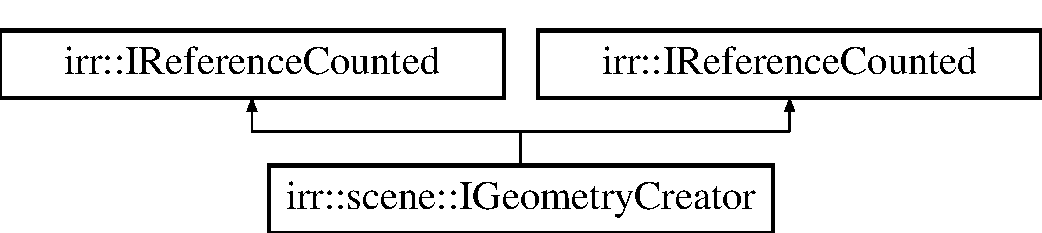
\includegraphics[height=2.000000cm]{classirr_1_1scene_1_1IGeometryCreator}
\end{center}
\end{figure}
\subsection*{Public Member Functions}
\begin{DoxyCompactItemize}
\item 
virtual \hyperlink{classirr_1_1scene_1_1IMesh}{I\+Mesh} $\ast$ \hyperlink{classirr_1_1scene_1_1IGeometryCreator_a43a1310362ad8e682c21375b2b9de39b}{create\+Cube\+Mesh} (const \hyperlink{namespaceirr_1_1core_a06f169d08b5c429f5575acb7edbad811}{core\+::vector3df} \&size=\hyperlink{namespaceirr_1_1core_a06f169d08b5c429f5575acb7edbad811}{core\+::vector3df}(5.f, 5.f, 5.f)) const =0
\begin{DoxyCompactList}\small\item\em Creates a simple cube mesh. \end{DoxyCompactList}\item 
virtual \hyperlink{classirr_1_1scene_1_1IMesh}{I\+Mesh} $\ast$ \hyperlink{classirr_1_1scene_1_1IGeometryCreator_a85cb5d4271a1ef4ba1706b15f70ae391}{create\+Hill\+Plane\+Mesh} (const \hyperlink{classirr_1_1core_1_1dimension2d}{core\+::dimension2d}$<$ \hyperlink{namespaceirr_a0277be98d67dc26ff93b1a6a1d086b07}{f32} $>$ \&tile\+Size, const \hyperlink{classirr_1_1core_1_1dimension2d}{core\+::dimension2d}$<$ \hyperlink{namespaceirr_a0416a53257075833e7002efd0a18e804}{u32} $>$ \&tile\+Count, \hyperlink{classirr_1_1video_1_1SMaterial}{video\+::\+S\+Material} $\ast$material, \hyperlink{namespaceirr_a0277be98d67dc26ff93b1a6a1d086b07}{f32} hill\+Height, const \hyperlink{classirr_1_1core_1_1dimension2d}{core\+::dimension2d}$<$ \hyperlink{namespaceirr_a0277be98d67dc26ff93b1a6a1d086b07}{f32} $>$ \&count\+Hills, const \hyperlink{classirr_1_1core_1_1dimension2d}{core\+::dimension2d}$<$ \hyperlink{namespaceirr_a0277be98d67dc26ff93b1a6a1d086b07}{f32} $>$ \&texture\+Repeat\+Count) const =0
\begin{DoxyCompactList}\small\item\em Create a pseudo-\/random mesh representing a hilly terrain. \end{DoxyCompactList}\item 
\hyperlink{classirr_1_1scene_1_1IMesh}{I\+Mesh} $\ast$ \hyperlink{classirr_1_1scene_1_1IGeometryCreator_ad584dd294e44104452c4418d70223381}{create\+Plane\+Mesh} (const \hyperlink{classirr_1_1core_1_1dimension2d}{core\+::dimension2d}$<$ \hyperlink{namespaceirr_a0277be98d67dc26ff93b1a6a1d086b07}{f32} $>$ \&tile\+Size, const \hyperlink{classirr_1_1core_1_1dimension2d}{core\+::dimension2d}$<$ \hyperlink{namespaceirr_a0416a53257075833e7002efd0a18e804}{u32} $>$ \&tile\+Count=\hyperlink{namespaceirr_1_1core_ad2e562e3219072e2f7fc7c2bba0ef0cb}{core\+::dimension2du}(1, 1), \hyperlink{classirr_1_1video_1_1SMaterial}{video\+::\+S\+Material} $\ast$material=0, const \hyperlink{namespaceirr_1_1core_af6dc5c45ff13e7712758c827ff58676b}{core\+::dimension2df} \&texture\+Repeat\+Count=\hyperlink{namespaceirr_1_1core_af6dc5c45ff13e7712758c827ff58676b}{core\+::dimension2df}(1.f, 1.f)) const
\begin{DoxyCompactList}\small\item\em Create a simple rectangular textured plane mesh. \end{DoxyCompactList}\item 
virtual \hyperlink{classirr_1_1scene_1_1IMesh}{I\+Mesh} $\ast$ \hyperlink{classirr_1_1scene_1_1IGeometryCreator_a7cf8a80a7d76d91ab9a2a1d5f63d4eea}{create\+Terrain\+Mesh} (\hyperlink{classirr_1_1video_1_1IImage}{video\+::\+I\+Image} $\ast$texture, \hyperlink{classirr_1_1video_1_1IImage}{video\+::\+I\+Image} $\ast$heightmap, const \hyperlink{classirr_1_1core_1_1dimension2d}{core\+::dimension2d}$<$ \hyperlink{namespaceirr_a0277be98d67dc26ff93b1a6a1d086b07}{f32} $>$ \&stretch\+Size, \hyperlink{namespaceirr_a0277be98d67dc26ff93b1a6a1d086b07}{f32} max\+Height, \hyperlink{classirr_1_1video_1_1IVideoDriver}{video\+::\+I\+Video\+Driver} $\ast$driver, const \hyperlink{classirr_1_1core_1_1dimension2d}{core\+::dimension2d}$<$ \hyperlink{namespaceirr_a0416a53257075833e7002efd0a18e804}{u32} $>$ \&default\+Vertex\+Block\+Size, bool debug\+Borders=false) const =0
\begin{DoxyCompactList}\small\item\em Create a terrain mesh from an image representing a heightfield. \end{DoxyCompactList}\item 
virtual \hyperlink{classirr_1_1scene_1_1IMesh}{I\+Mesh} $\ast$ \hyperlink{classirr_1_1scene_1_1IGeometryCreator_aba5b1b9a614c211eeb7a9f88d8e3ec50}{create\+Arrow\+Mesh} (const \hyperlink{namespaceirr_a0416a53257075833e7002efd0a18e804}{u32} tesselation\+Cylinder=4, const \hyperlink{namespaceirr_a0416a53257075833e7002efd0a18e804}{u32} tesselation\+Cone=8, const \hyperlink{namespaceirr_a0277be98d67dc26ff93b1a6a1d086b07}{f32} height=1.f, const \hyperlink{namespaceirr_a0277be98d67dc26ff93b1a6a1d086b07}{f32} cylinder\+Height=0.\+6f, const f32 width\+Cylinder=0.\+05f, const f32 width\+Cone=0.\+3f, const video\+::\+S\+Color color\+Cylinder=0x\+F\+F\+F\+F\+F\+F\+F\+F, const video\+::\+S\+Color color\+Cone=0x\+F\+F\+F\+F\+F\+F\+F\+F) const =0
\begin{DoxyCompactList}\small\item\em Create an arrow mesh, composed of a cylinder and a cone. \end{DoxyCompactList}\item 
virtual \hyperlink{classirr_1_1scene_1_1IMesh}{I\+Mesh} $\ast$ \hyperlink{classirr_1_1scene_1_1IGeometryCreator_ab97eb5f80cc08b4611cd56a968a98521}{create\+Sphere\+Mesh} (\hyperlink{namespaceirr_a0277be98d67dc26ff93b1a6a1d086b07}{f32} radius=5.f, \hyperlink{namespaceirr_a0416a53257075833e7002efd0a18e804}{u32} poly\+CountX=16, \hyperlink{namespaceirr_a0416a53257075833e7002efd0a18e804}{u32} poly\+CountY=16) const =0
\begin{DoxyCompactList}\small\item\em Create a sphere mesh. \end{DoxyCompactList}\item 
virtual \hyperlink{classirr_1_1scene_1_1IMesh}{I\+Mesh} $\ast$ \hyperlink{classirr_1_1scene_1_1IGeometryCreator_a87143de278ac305bc37dc905e800f5f8}{create\+Cylinder\+Mesh} (\hyperlink{namespaceirr_a0277be98d67dc26ff93b1a6a1d086b07}{f32} radius, \hyperlink{namespaceirr_a0277be98d67dc26ff93b1a6a1d086b07}{f32} length, \hyperlink{namespaceirr_a0416a53257075833e7002efd0a18e804}{u32} tesselation, const \hyperlink{classirr_1_1video_1_1SColor}{video\+::\+S\+Color} \&color=\hyperlink{classirr_1_1video_1_1SColor}{video\+::\+S\+Color}(0xffffffff), bool close\+Top=true, f32 oblique=0.\+f) const =0
\begin{DoxyCompactList}\small\item\em Create a cylinder mesh. \end{DoxyCompactList}\item 
virtual \hyperlink{classirr_1_1scene_1_1IMesh}{I\+Mesh} $\ast$ \hyperlink{classirr_1_1scene_1_1IGeometryCreator_af532c8fb5558cf274181eb81220db85b}{create\+Cone\+Mesh} (\hyperlink{namespaceirr_a0277be98d67dc26ff93b1a6a1d086b07}{f32} radius, \hyperlink{namespaceirr_a0277be98d67dc26ff93b1a6a1d086b07}{f32} length, \hyperlink{namespaceirr_a0416a53257075833e7002efd0a18e804}{u32} tesselation, const \hyperlink{classirr_1_1video_1_1SColor}{video\+::\+S\+Color} \&color\+Top=\hyperlink{classirr_1_1video_1_1SColor}{video\+::\+S\+Color}(0xffffffff), const video\+::\+S\+Color \&color\+Bottom=video\+::\+S\+Color(0xffffffff), f32 oblique=0.\+f) const =0
\begin{DoxyCompactList}\small\item\em Create a cone mesh. \end{DoxyCompactList}\item 
virtual \hyperlink{classirr_1_1scene_1_1IMesh}{I\+Mesh} $\ast$ \hyperlink{classirr_1_1scene_1_1IGeometryCreator_a4f4e4a3c266698c375d14c1e19a91407}{create\+Volume\+Light\+Mesh} (const \hyperlink{namespaceirr_a0416a53257075833e7002efd0a18e804}{u32} subdivideU=32, const \hyperlink{namespaceirr_a0416a53257075833e7002efd0a18e804}{u32} subdivideV=32, const \hyperlink{classirr_1_1video_1_1SColor}{video\+::\+S\+Color} foot\+Color=0xffffffff, const video\+::\+S\+Color tail\+Color=0xffffffff, const f32 lp\+Distance=8.\+f, const core\+::vector3df \&light\+Dim=core\+::vector3df(1.\+f, 1.\+2f, 1.\+f)) const =0
\begin{DoxyCompactList}\small\item\em Create a volume light mesh. \end{DoxyCompactList}\end{DoxyCompactItemize}
\subsection*{Additional Inherited Members}


\subsection{Detailed Description}
Helper class for creating geometry on the fly. 

You can get an instance of this class through \hyperlink{classirr_1_1scene_1_1ISceneManager_a9840cfd39b44f238d06b7bc51e6ba1f6}{I\+Scene\+Manager\+::get\+Geometry\+Creator()} 

\subsection{Member Function Documentation}
\mbox{\Hypertarget{classirr_1_1scene_1_1IGeometryCreator_aba5b1b9a614c211eeb7a9f88d8e3ec50}\label{classirr_1_1scene_1_1IGeometryCreator_aba5b1b9a614c211eeb7a9f88d8e3ec50}} 
\index{irr\+::scene\+::\+I\+Geometry\+Creator@{irr\+::scene\+::\+I\+Geometry\+Creator}!create\+Arrow\+Mesh@{create\+Arrow\+Mesh}}
\index{create\+Arrow\+Mesh@{create\+Arrow\+Mesh}!irr\+::scene\+::\+I\+Geometry\+Creator@{irr\+::scene\+::\+I\+Geometry\+Creator}}
\subsubsection{\texorpdfstring{create\+Arrow\+Mesh()}{createArrowMesh()}}
{\footnotesize\ttfamily virtual \hyperlink{classirr_1_1scene_1_1IMesh}{I\+Mesh}$\ast$ irr\+::scene\+::\+I\+Geometry\+Creator\+::create\+Arrow\+Mesh (\begin{DoxyParamCaption}\item[{const \hyperlink{namespaceirr_a0416a53257075833e7002efd0a18e804}{u32}}]{tesselation\+Cylinder = {\ttfamily 4},  }\item[{const \hyperlink{namespaceirr_a0416a53257075833e7002efd0a18e804}{u32}}]{tesselation\+Cone = {\ttfamily 8},  }\item[{const \hyperlink{namespaceirr_a0277be98d67dc26ff93b1a6a1d086b07}{f32}}]{height = {\ttfamily 1.f},  }\item[{const \hyperlink{namespaceirr_a0277be98d67dc26ff93b1a6a1d086b07}{f32}}]{cylinder\+Height = {\ttfamily 0.6f},  }\item[{const \hyperlink{namespaceirr_a0277be98d67dc26ff93b1a6a1d086b07}{f32}}]{width\+Cylinder = {\ttfamily 0.05f},  }\item[{const \hyperlink{namespaceirr_a0277be98d67dc26ff93b1a6a1d086b07}{f32}}]{width\+Cone = {\ttfamily 0.3f},  }\item[{const \hyperlink{classirr_1_1video_1_1SColor}{video\+::\+S\+Color}}]{color\+Cylinder = {\ttfamily 0xFFFFFFFF},  }\item[{const \hyperlink{classirr_1_1video_1_1SColor}{video\+::\+S\+Color}}]{color\+Cone = {\ttfamily 0xFFFFFFFF} }\end{DoxyParamCaption}) const\hspace{0.3cm}{\ttfamily [pure virtual]}}



Create an arrow mesh, composed of a cylinder and a cone. 


\begin{DoxyParams}{Parameters}
{\em tesselation\+Cylinder} & Number of quads composing the cylinder. \\
\hline
{\em tesselation\+Cone} & Number of triangles composing the cone\textquotesingle{}s roof. \\
\hline
{\em height} & Total height of the arrow \\
\hline
{\em cylinder\+Height} & Total height of the cylinder, should be lesser than total height \\
\hline
{\em width\+Cylinder} & Diameter of the cylinder \\
\hline
{\em width\+Cone} & Diameter of the cone\textquotesingle{}s base, should be not smaller than the cylinder\textquotesingle{}s diameter \\
\hline
{\em color\+Cylinder} & color of the cylinder \\
\hline
{\em color\+Cone} & color of the cone \\
\hline
\end{DoxyParams}
\begin{DoxyReturn}{Returns}
Generated mesh. 
\end{DoxyReturn}
\mbox{\Hypertarget{classirr_1_1scene_1_1IGeometryCreator_af532c8fb5558cf274181eb81220db85b}\label{classirr_1_1scene_1_1IGeometryCreator_af532c8fb5558cf274181eb81220db85b}} 
\index{irr\+::scene\+::\+I\+Geometry\+Creator@{irr\+::scene\+::\+I\+Geometry\+Creator}!create\+Cone\+Mesh@{create\+Cone\+Mesh}}
\index{create\+Cone\+Mesh@{create\+Cone\+Mesh}!irr\+::scene\+::\+I\+Geometry\+Creator@{irr\+::scene\+::\+I\+Geometry\+Creator}}
\subsubsection{\texorpdfstring{create\+Cone\+Mesh()}{createConeMesh()}}
{\footnotesize\ttfamily virtual \hyperlink{classirr_1_1scene_1_1IMesh}{I\+Mesh}$\ast$ irr\+::scene\+::\+I\+Geometry\+Creator\+::create\+Cone\+Mesh (\begin{DoxyParamCaption}\item[{\hyperlink{namespaceirr_a0277be98d67dc26ff93b1a6a1d086b07}{f32}}]{radius,  }\item[{\hyperlink{namespaceirr_a0277be98d67dc26ff93b1a6a1d086b07}{f32}}]{length,  }\item[{\hyperlink{namespaceirr_a0416a53257075833e7002efd0a18e804}{u32}}]{tesselation,  }\item[{const \hyperlink{classirr_1_1video_1_1SColor}{video\+::\+S\+Color} \&}]{color\+Top = {\ttfamily \hyperlink{classirr_1_1video_1_1SColor}{video\+::\+S\+Color}(0xffffffff)},  }\item[{const \hyperlink{classirr_1_1video_1_1SColor}{video\+::\+S\+Color} \&}]{color\+Bottom = {\ttfamily \hyperlink{classirr_1_1video_1_1SColor}{video\+::\+S\+Color}(0xffffffff)},  }\item[{\hyperlink{namespaceirr_a0277be98d67dc26ff93b1a6a1d086b07}{f32}}]{oblique = {\ttfamily 0.f} }\end{DoxyParamCaption}) const\hspace{0.3cm}{\ttfamily [pure virtual]}}



Create a cone mesh. 


\begin{DoxyParams}{Parameters}
{\em radius} & Radius of the cone. \\
\hline
{\em length} & Length of the cone. \\
\hline
{\em tesselation} & Number of quads around the circumference of the cone. \\
\hline
{\em color\+Top} & The color of the top of the cone. \\
\hline
{\em color\+Bottom} & The color of the bottom of the cone. \\
\hline
{\em oblique} & (to be documented) \\
\hline
\end{DoxyParams}
\begin{DoxyReturn}{Returns}
Generated mesh. 
\end{DoxyReturn}
\mbox{\Hypertarget{classirr_1_1scene_1_1IGeometryCreator_a43a1310362ad8e682c21375b2b9de39b}\label{classirr_1_1scene_1_1IGeometryCreator_a43a1310362ad8e682c21375b2b9de39b}} 
\index{irr\+::scene\+::\+I\+Geometry\+Creator@{irr\+::scene\+::\+I\+Geometry\+Creator}!create\+Cube\+Mesh@{create\+Cube\+Mesh}}
\index{create\+Cube\+Mesh@{create\+Cube\+Mesh}!irr\+::scene\+::\+I\+Geometry\+Creator@{irr\+::scene\+::\+I\+Geometry\+Creator}}
\subsubsection{\texorpdfstring{create\+Cube\+Mesh()}{createCubeMesh()}}
{\footnotesize\ttfamily virtual \hyperlink{classirr_1_1scene_1_1IMesh}{I\+Mesh}$\ast$ irr\+::scene\+::\+I\+Geometry\+Creator\+::create\+Cube\+Mesh (\begin{DoxyParamCaption}\item[{const \hyperlink{namespaceirr_1_1core_a06f169d08b5c429f5575acb7edbad811}{core\+::vector3df} \&}]{size = {\ttfamily \hyperlink{namespaceirr_1_1core_a06f169d08b5c429f5575acb7edbad811}{core\+::vector3df}(5.f,~5.f,~5.f)} }\end{DoxyParamCaption}) const\hspace{0.3cm}{\ttfamily [pure virtual]}}



Creates a simple cube mesh. 


\begin{DoxyParams}{Parameters}
{\em size} & Dimensions of the cube. \\
\hline
\end{DoxyParams}
\begin{DoxyReturn}{Returns}
Generated mesh. 
\end{DoxyReturn}
\mbox{\Hypertarget{classirr_1_1scene_1_1IGeometryCreator_a87143de278ac305bc37dc905e800f5f8}\label{classirr_1_1scene_1_1IGeometryCreator_a87143de278ac305bc37dc905e800f5f8}} 
\index{irr\+::scene\+::\+I\+Geometry\+Creator@{irr\+::scene\+::\+I\+Geometry\+Creator}!create\+Cylinder\+Mesh@{create\+Cylinder\+Mesh}}
\index{create\+Cylinder\+Mesh@{create\+Cylinder\+Mesh}!irr\+::scene\+::\+I\+Geometry\+Creator@{irr\+::scene\+::\+I\+Geometry\+Creator}}
\subsubsection{\texorpdfstring{create\+Cylinder\+Mesh()}{createCylinderMesh()}}
{\footnotesize\ttfamily virtual \hyperlink{classirr_1_1scene_1_1IMesh}{I\+Mesh}$\ast$ irr\+::scene\+::\+I\+Geometry\+Creator\+::create\+Cylinder\+Mesh (\begin{DoxyParamCaption}\item[{\hyperlink{namespaceirr_a0277be98d67dc26ff93b1a6a1d086b07}{f32}}]{radius,  }\item[{\hyperlink{namespaceirr_a0277be98d67dc26ff93b1a6a1d086b07}{f32}}]{length,  }\item[{\hyperlink{namespaceirr_a0416a53257075833e7002efd0a18e804}{u32}}]{tesselation,  }\item[{const \hyperlink{classirr_1_1video_1_1SColor}{video\+::\+S\+Color} \&}]{color = {\ttfamily \hyperlink{classirr_1_1video_1_1SColor}{video\+::\+S\+Color}(0xffffffff)},  }\item[{bool}]{close\+Top = {\ttfamily true},  }\item[{\hyperlink{namespaceirr_a0277be98d67dc26ff93b1a6a1d086b07}{f32}}]{oblique = {\ttfamily 0.f} }\end{DoxyParamCaption}) const\hspace{0.3cm}{\ttfamily [pure virtual]}}



Create a cylinder mesh. 


\begin{DoxyParams}{Parameters}
{\em radius} & Radius of the cylinder. \\
\hline
{\em length} & Length of the cylinder. \\
\hline
{\em tesselation} & Number of quads around the circumference of the cylinder. \\
\hline
{\em color} & The color of the cylinder. \\
\hline
{\em close\+Top} & If true, close the ends of the cylinder, otherwise leave them open. \\
\hline
{\em oblique} & (to be documented) \\
\hline
\end{DoxyParams}
\begin{DoxyReturn}{Returns}
Generated mesh. 
\end{DoxyReturn}
\mbox{\Hypertarget{classirr_1_1scene_1_1IGeometryCreator_a85cb5d4271a1ef4ba1706b15f70ae391}\label{classirr_1_1scene_1_1IGeometryCreator_a85cb5d4271a1ef4ba1706b15f70ae391}} 
\index{irr\+::scene\+::\+I\+Geometry\+Creator@{irr\+::scene\+::\+I\+Geometry\+Creator}!create\+Hill\+Plane\+Mesh@{create\+Hill\+Plane\+Mesh}}
\index{create\+Hill\+Plane\+Mesh@{create\+Hill\+Plane\+Mesh}!irr\+::scene\+::\+I\+Geometry\+Creator@{irr\+::scene\+::\+I\+Geometry\+Creator}}
\subsubsection{\texorpdfstring{create\+Hill\+Plane\+Mesh()}{createHillPlaneMesh()}}
{\footnotesize\ttfamily virtual \hyperlink{classirr_1_1scene_1_1IMesh}{I\+Mesh}$\ast$ irr\+::scene\+::\+I\+Geometry\+Creator\+::create\+Hill\+Plane\+Mesh (\begin{DoxyParamCaption}\item[{const \hyperlink{classirr_1_1core_1_1dimension2d}{core\+::dimension2d}$<$ \hyperlink{namespaceirr_a0277be98d67dc26ff93b1a6a1d086b07}{f32} $>$ \&}]{tile\+Size,  }\item[{const \hyperlink{classirr_1_1core_1_1dimension2d}{core\+::dimension2d}$<$ \hyperlink{namespaceirr_a0416a53257075833e7002efd0a18e804}{u32} $>$ \&}]{tile\+Count,  }\item[{\hyperlink{classirr_1_1video_1_1SMaterial}{video\+::\+S\+Material} $\ast$}]{material,  }\item[{\hyperlink{namespaceirr_a0277be98d67dc26ff93b1a6a1d086b07}{f32}}]{hill\+Height,  }\item[{const \hyperlink{classirr_1_1core_1_1dimension2d}{core\+::dimension2d}$<$ \hyperlink{namespaceirr_a0277be98d67dc26ff93b1a6a1d086b07}{f32} $>$ \&}]{count\+Hills,  }\item[{const \hyperlink{classirr_1_1core_1_1dimension2d}{core\+::dimension2d}$<$ \hyperlink{namespaceirr_a0277be98d67dc26ff93b1a6a1d086b07}{f32} $>$ \&}]{texture\+Repeat\+Count }\end{DoxyParamCaption}) const\hspace{0.3cm}{\ttfamily [pure virtual]}}



Create a pseudo-\/random mesh representing a hilly terrain. 


\begin{DoxyParams}{Parameters}
{\em tile\+Size} & The size of each tile. \\
\hline
{\em tile\+Count} & The number of tiles in each dimension. \\
\hline
{\em material} & The material to apply to the mesh. \\
\hline
{\em hill\+Height} & The maximum height of the hills. \\
\hline
{\em count\+Hills} & The number of hills along each dimension. \\
\hline
{\em texture\+Repeat\+Count} & The number of times to repeat the material texture along each dimension. \\
\hline
\end{DoxyParams}
\begin{DoxyReturn}{Returns}
Generated mesh. 
\end{DoxyReturn}
\mbox{\Hypertarget{classirr_1_1scene_1_1IGeometryCreator_ad584dd294e44104452c4418d70223381}\label{classirr_1_1scene_1_1IGeometryCreator_ad584dd294e44104452c4418d70223381}} 
\index{irr\+::scene\+::\+I\+Geometry\+Creator@{irr\+::scene\+::\+I\+Geometry\+Creator}!create\+Plane\+Mesh@{create\+Plane\+Mesh}}
\index{create\+Plane\+Mesh@{create\+Plane\+Mesh}!irr\+::scene\+::\+I\+Geometry\+Creator@{irr\+::scene\+::\+I\+Geometry\+Creator}}
\subsubsection{\texorpdfstring{create\+Plane\+Mesh()}{createPlaneMesh()}}
{\footnotesize\ttfamily \hyperlink{classirr_1_1scene_1_1IMesh}{I\+Mesh}$\ast$ irr\+::scene\+::\+I\+Geometry\+Creator\+::create\+Plane\+Mesh (\begin{DoxyParamCaption}\item[{const \hyperlink{classirr_1_1core_1_1dimension2d}{core\+::dimension2d}$<$ \hyperlink{namespaceirr_a0277be98d67dc26ff93b1a6a1d086b07}{f32} $>$ \&}]{tile\+Size,  }\item[{const \hyperlink{classirr_1_1core_1_1dimension2d}{core\+::dimension2d}$<$ \hyperlink{namespaceirr_a0416a53257075833e7002efd0a18e804}{u32} $>$ \&}]{tile\+Count = {\ttfamily \hyperlink{namespaceirr_1_1core_ad2e562e3219072e2f7fc7c2bba0ef0cb}{core\+::dimension2du}(1,1)},  }\item[{\hyperlink{classirr_1_1video_1_1SMaterial}{video\+::\+S\+Material} $\ast$}]{material = {\ttfamily 0},  }\item[{const \hyperlink{namespaceirr_1_1core_af6dc5c45ff13e7712758c827ff58676b}{core\+::dimension2df} \&}]{texture\+Repeat\+Count = {\ttfamily \hyperlink{namespaceirr_1_1core_af6dc5c45ff13e7712758c827ff58676b}{core\+::dimension2df}(1.f,1.f)} }\end{DoxyParamCaption}) const\hspace{0.3cm}{\ttfamily [inline]}}



Create a simple rectangular textured plane mesh. 


\begin{DoxyParams}{Parameters}
{\em tile\+Size} & The size of each tile. \\
\hline
{\em tile\+Count} & The number of tiles in each dimension. \\
\hline
{\em material} & The material to apply to the mesh. \\
\hline
{\em texture\+Repeat\+Count} & The number of times to repeat the material texture along each dimension. \\
\hline
\end{DoxyParams}
\begin{DoxyReturn}{Returns}
Generated mesh. 
\end{DoxyReturn}
\mbox{\Hypertarget{classirr_1_1scene_1_1IGeometryCreator_ab97eb5f80cc08b4611cd56a968a98521}\label{classirr_1_1scene_1_1IGeometryCreator_ab97eb5f80cc08b4611cd56a968a98521}} 
\index{irr\+::scene\+::\+I\+Geometry\+Creator@{irr\+::scene\+::\+I\+Geometry\+Creator}!create\+Sphere\+Mesh@{create\+Sphere\+Mesh}}
\index{create\+Sphere\+Mesh@{create\+Sphere\+Mesh}!irr\+::scene\+::\+I\+Geometry\+Creator@{irr\+::scene\+::\+I\+Geometry\+Creator}}
\subsubsection{\texorpdfstring{create\+Sphere\+Mesh()}{createSphereMesh()}}
{\footnotesize\ttfamily virtual \hyperlink{classirr_1_1scene_1_1IMesh}{I\+Mesh}$\ast$ irr\+::scene\+::\+I\+Geometry\+Creator\+::create\+Sphere\+Mesh (\begin{DoxyParamCaption}\item[{\hyperlink{namespaceirr_a0277be98d67dc26ff93b1a6a1d086b07}{f32}}]{radius = {\ttfamily 5.f},  }\item[{\hyperlink{namespaceirr_a0416a53257075833e7002efd0a18e804}{u32}}]{poly\+CountX = {\ttfamily 16},  }\item[{\hyperlink{namespaceirr_a0416a53257075833e7002efd0a18e804}{u32}}]{poly\+CountY = {\ttfamily 16} }\end{DoxyParamCaption}) const\hspace{0.3cm}{\ttfamily [pure virtual]}}



Create a sphere mesh. 


\begin{DoxyParams}{Parameters}
{\em radius} & Radius of the sphere \\
\hline
{\em poly\+CountX} & Number of quads used for the horizontal tiling \\
\hline
{\em poly\+CountY} & Number of quads used for the vertical tiling \\
\hline
\end{DoxyParams}
\begin{DoxyReturn}{Returns}
Generated mesh. 
\end{DoxyReturn}
\mbox{\Hypertarget{classirr_1_1scene_1_1IGeometryCreator_a7cf8a80a7d76d91ab9a2a1d5f63d4eea}\label{classirr_1_1scene_1_1IGeometryCreator_a7cf8a80a7d76d91ab9a2a1d5f63d4eea}} 
\index{irr\+::scene\+::\+I\+Geometry\+Creator@{irr\+::scene\+::\+I\+Geometry\+Creator}!create\+Terrain\+Mesh@{create\+Terrain\+Mesh}}
\index{create\+Terrain\+Mesh@{create\+Terrain\+Mesh}!irr\+::scene\+::\+I\+Geometry\+Creator@{irr\+::scene\+::\+I\+Geometry\+Creator}}
\subsubsection{\texorpdfstring{create\+Terrain\+Mesh()}{createTerrainMesh()}}
{\footnotesize\ttfamily virtual \hyperlink{classirr_1_1scene_1_1IMesh}{I\+Mesh}$\ast$ irr\+::scene\+::\+I\+Geometry\+Creator\+::create\+Terrain\+Mesh (\begin{DoxyParamCaption}\item[{\hyperlink{classirr_1_1video_1_1IImage}{video\+::\+I\+Image} $\ast$}]{texture,  }\item[{\hyperlink{classirr_1_1video_1_1IImage}{video\+::\+I\+Image} $\ast$}]{heightmap,  }\item[{const \hyperlink{classirr_1_1core_1_1dimension2d}{core\+::dimension2d}$<$ \hyperlink{namespaceirr_a0277be98d67dc26ff93b1a6a1d086b07}{f32} $>$ \&}]{stretch\+Size,  }\item[{\hyperlink{namespaceirr_a0277be98d67dc26ff93b1a6a1d086b07}{f32}}]{max\+Height,  }\item[{\hyperlink{classirr_1_1video_1_1IVideoDriver}{video\+::\+I\+Video\+Driver} $\ast$}]{driver,  }\item[{const \hyperlink{classirr_1_1core_1_1dimension2d}{core\+::dimension2d}$<$ \hyperlink{namespaceirr_a0416a53257075833e7002efd0a18e804}{u32} $>$ \&}]{default\+Vertex\+Block\+Size,  }\item[{bool}]{debug\+Borders = {\ttfamily false} }\end{DoxyParamCaption}) const\hspace{0.3cm}{\ttfamily [pure virtual]}}



Create a terrain mesh from an image representing a heightfield. 


\begin{DoxyParams}{Parameters}
{\em texture} & The texture to apply to the terrain. \\
\hline
{\em heightmap} & An image that will be interpreted as a heightmap. The brightness (average color) of each pixel is interpreted as a height, with a 255 brightness pixel producing the maximum height. \\
\hline
{\em stretch\+Size} & The size that each pixel will produce, i.\+e. a 512x512 heightmap and a stretch\+Size of (10.\+f, 20.\+f) will produce a mesh of size 5120.\+f x 10240.\+f \\
\hline
{\em max\+Height} & The maximum height of the terrain. \\
\hline
{\em driver} & The current video driver. \\
\hline
{\em default\+Vertex\+Block\+Size} & (to be documented) \\
\hline
{\em debug\+Borders} & (to be documented) \\
\hline
\end{DoxyParams}
\begin{DoxyReturn}{Returns}
Generated mesh. 
\end{DoxyReturn}
\mbox{\Hypertarget{classirr_1_1scene_1_1IGeometryCreator_a4f4e4a3c266698c375d14c1e19a91407}\label{classirr_1_1scene_1_1IGeometryCreator_a4f4e4a3c266698c375d14c1e19a91407}} 
\index{irr\+::scene\+::\+I\+Geometry\+Creator@{irr\+::scene\+::\+I\+Geometry\+Creator}!create\+Volume\+Light\+Mesh@{create\+Volume\+Light\+Mesh}}
\index{create\+Volume\+Light\+Mesh@{create\+Volume\+Light\+Mesh}!irr\+::scene\+::\+I\+Geometry\+Creator@{irr\+::scene\+::\+I\+Geometry\+Creator}}
\subsubsection{\texorpdfstring{create\+Volume\+Light\+Mesh()}{createVolumeLightMesh()}}
{\footnotesize\ttfamily virtual \hyperlink{classirr_1_1scene_1_1IMesh}{I\+Mesh}$\ast$ irr\+::scene\+::\+I\+Geometry\+Creator\+::create\+Volume\+Light\+Mesh (\begin{DoxyParamCaption}\item[{const \hyperlink{namespaceirr_a0416a53257075833e7002efd0a18e804}{u32}}]{subdivideU = {\ttfamily 32},  }\item[{const \hyperlink{namespaceirr_a0416a53257075833e7002efd0a18e804}{u32}}]{subdivideV = {\ttfamily 32},  }\item[{const \hyperlink{classirr_1_1video_1_1SColor}{video\+::\+S\+Color}}]{foot\+Color = {\ttfamily 0xffffffff},  }\item[{const \hyperlink{classirr_1_1video_1_1SColor}{video\+::\+S\+Color}}]{tail\+Color = {\ttfamily 0xffffffff},  }\item[{const \hyperlink{namespaceirr_a0277be98d67dc26ff93b1a6a1d086b07}{f32}}]{lp\+Distance = {\ttfamily 8.f},  }\item[{const \hyperlink{namespaceirr_1_1core_a06f169d08b5c429f5575acb7edbad811}{core\+::vector3df} \&}]{light\+Dim = {\ttfamily \hyperlink{namespaceirr_1_1core_a06f169d08b5c429f5575acb7edbad811}{core\+::vector3df}(1.f,~1.2f,~1.f)} }\end{DoxyParamCaption}) const\hspace{0.3cm}{\ttfamily [pure virtual]}}



Create a volume light mesh. 


\begin{DoxyParams}{Parameters}
{\em subdivideU} & Horizontal patch count. \\
\hline
{\em subdivideV} & Vertical patch count. \\
\hline
{\em foot\+Color} & Color at the bottom of the light. \\
\hline
{\em tail\+Color} & Color at the mid of the light. \\
\hline
{\em lp\+Distance} & Virtual distance of the light point for normals. \\
\hline
{\em light\+Dim} & Dimensions of the light. \\
\hline
\end{DoxyParams}
\begin{DoxyReturn}{Returns}
Generated mesh. 
\end{DoxyReturn}


The documentation for this class was generated from the following file\+:\begin{DoxyCompactItemize}
\item 
indie\+\_\+share/controller/include/I\+Geometry\+Creator.\+h\end{DoxyCompactItemize}

\hypertarget{classirr_1_1video_1_1IGPUProgrammingServices}{}\section{irr\+:\+:video\+:\+:I\+G\+P\+U\+Programming\+Services Class Reference}
\label{classirr_1_1video_1_1IGPUProgrammingServices}\index{irr\+::video\+::\+I\+G\+P\+U\+Programming\+Services@{irr\+::video\+::\+I\+G\+P\+U\+Programming\+Services}}


Interface making it possible to create and use programs running on the G\+PU.  




{\ttfamily \#include $<$I\+G\+P\+U\+Programming\+Services.\+h$>$}

\subsection*{Public Member Functions}
\begin{DoxyCompactItemize}
\item 
\mbox{\Hypertarget{classirr_1_1video_1_1IGPUProgrammingServices_a09d143ea5c55840c15ebcb84e8539bc0}\label{classirr_1_1video_1_1IGPUProgrammingServices_a09d143ea5c55840c15ebcb84e8539bc0}} 
virtual \hyperlink{classirr_1_1video_1_1IGPUProgrammingServices_a09d143ea5c55840c15ebcb84e8539bc0}{$\sim$\+I\+G\+P\+U\+Programming\+Services} ()
\begin{DoxyCompactList}\small\item\em Destructor. \end{DoxyCompactList}\item 
virtual \hyperlink{namespaceirr_ac66849b7a6ed16e30ebede579f9b47c6}{s32} \hyperlink{classirr_1_1video_1_1IGPUProgrammingServices_a4a8d3b727ee9223d8baa353b82da0478}{add\+High\+Level\+Shader\+Material} (const \hyperlink{namespaceirr_a9395eaea339bcb546b319e9c96bf7410}{c8} $\ast$vertex\+Shader\+Program, const \hyperlink{namespaceirr_a9395eaea339bcb546b319e9c96bf7410}{c8} $\ast$vertex\+Shader\+Entry\+Point\+Name, \hyperlink{namespaceirr_1_1video_a9decae50d4dc2455e7b009f5c71b24f9}{E\+\_\+\+V\+E\+R\+T\+E\+X\+\_\+\+S\+H\+A\+D\+E\+R\+\_\+\+T\+Y\+PE} vs\+Compile\+Target, const \hyperlink{namespaceirr_a9395eaea339bcb546b319e9c96bf7410}{c8} $\ast$pixel\+Shader\+Program, const \hyperlink{namespaceirr_a9395eaea339bcb546b319e9c96bf7410}{c8} $\ast$pixel\+Shader\+Entry\+Point\+Name, \hyperlink{namespaceirr_1_1video_a07fb77e9aec681402ad376f7ef9b724c}{E\+\_\+\+P\+I\+X\+E\+L\+\_\+\+S\+H\+A\+D\+E\+R\+\_\+\+T\+Y\+PE} ps\+Compile\+Target, const \hyperlink{namespaceirr_a9395eaea339bcb546b319e9c96bf7410}{c8} $\ast$geometry\+Shader\+Program, const \hyperlink{namespaceirr_a9395eaea339bcb546b319e9c96bf7410}{c8} $\ast$geometry\+Shader\+Entry\+Point\+Name=\char`\"{}main\char`\"{}, E\+\_\+\+G\+E\+O\+M\+E\+T\+R\+Y\+\_\+\+S\+H\+A\+D\+E\+R\+\_\+\+T\+Y\+PE gs\+Compile\+Target=E\+G\+S\+T\+\_\+\+G\+S\+\_\+4\+\_\+0, \hyperlink{namespaceirr_1_1scene_a5d7de82f2169761194b2f44d95cdc1dc}{scene\+::\+E\+\_\+\+P\+R\+I\+M\+I\+T\+I\+V\+E\+\_\+\+T\+Y\+PE} in\+Type=\hyperlink{namespaceirr_1_1scene_a5d7de82f2169761194b2f44d95cdc1dca237fc76e4b259febd27b4b84066ca581}{scene\+::\+E\+P\+T\+\_\+\+T\+R\+I\+A\+N\+G\+L\+ES}, \hyperlink{namespaceirr_1_1scene_a5d7de82f2169761194b2f44d95cdc1dc}{scene\+::\+E\+\_\+\+P\+R\+I\+M\+I\+T\+I\+V\+E\+\_\+\+T\+Y\+PE} out\+Type=\hyperlink{namespaceirr_1_1scene_a5d7de82f2169761194b2f44d95cdc1dcaef19e8b586de395af81c8cd9851a1b40}{scene\+::\+E\+P\+T\+\_\+\+T\+R\+I\+A\+N\+G\+L\+E\+\_\+\+S\+T\+R\+IP}, \hyperlink{namespaceirr_a0416a53257075833e7002efd0a18e804}{u32} vertices\+Out=0, \hyperlink{classirr_1_1video_1_1IShaderConstantSetCallBack}{I\+Shader\+Constant\+Set\+Call\+Back} $\ast$callback=0, \hyperlink{namespaceirr_1_1video_ac8e9b6c66f7cebabd1a6d30cbc5430f1}{E\+\_\+\+M\+A\+T\+E\+R\+I\+A\+L\+\_\+\+T\+Y\+PE} base\+Material=\hyperlink{namespaceirr_1_1video_ac8e9b6c66f7cebabd1a6d30cbc5430f1a9bc471b9c18c9e2d20496004d2a2e803}{video\+::\+E\+M\+T\+\_\+\+S\+O\+L\+ID}, \hyperlink{namespaceirr_ac66849b7a6ed16e30ebede579f9b47c6}{s32} user\+Data=0, \hyperlink{namespaceirr_1_1video_a913671e32f20f13e51336bfbe20a82a3}{E\+\_\+\+G\+P\+U\+\_\+\+S\+H\+A\+D\+I\+N\+G\+\_\+\+L\+A\+N\+G\+U\+A\+GE} shading\+Lang=\hyperlink{namespaceirr_1_1video_a913671e32f20f13e51336bfbe20a82a3ac65c039e1c80a430a816c450a5f30d4b}{E\+G\+S\+L\+\_\+\+D\+E\+F\+A\+U\+LT})=0
\begin{DoxyCompactList}\small\item\em Adds a new high-\/level shading material renderer to the Video\+Driver. \end{DoxyCompactList}\item 
\mbox{\Hypertarget{classirr_1_1video_1_1IGPUProgrammingServices_aa65337bb19777dd025ff02f1953277b6}\label{classirr_1_1video_1_1IGPUProgrammingServices_aa65337bb19777dd025ff02f1953277b6}} 
\hyperlink{namespaceirr_ac66849b7a6ed16e30ebede579f9b47c6}{s32} \hyperlink{classirr_1_1video_1_1IGPUProgrammingServices_aa65337bb19777dd025ff02f1953277b6}{add\+High\+Level\+Shader\+Material} (const \hyperlink{namespaceirr_a9395eaea339bcb546b319e9c96bf7410}{c8} $\ast$vertex\+Shader\+Program, const \hyperlink{namespaceirr_a9395eaea339bcb546b319e9c96bf7410}{c8} $\ast$vertex\+Shader\+Entry\+Point\+Name=\char`\"{}main\char`\"{}, E\+\_\+\+V\+E\+R\+T\+E\+X\+\_\+\+S\+H\+A\+D\+E\+R\+\_\+\+T\+Y\+PE vs\+Compile\+Target=E\+V\+S\+T\+\_\+\+V\+S\+\_\+1\+\_\+1, const \hyperlink{namespaceirr_a9395eaea339bcb546b319e9c96bf7410}{c8} $\ast$pixel\+Shader\+Program=0, const \hyperlink{namespaceirr_a9395eaea339bcb546b319e9c96bf7410}{c8} $\ast$pixel\+Shader\+Entry\+Point\+Name=\char`\"{}main\char`\"{}, E\+\_\+\+P\+I\+X\+E\+L\+\_\+\+S\+H\+A\+D\+E\+R\+\_\+\+T\+Y\+PE ps\+Compile\+Target=E\+P\+S\+T\+\_\+\+P\+S\+\_\+1\+\_\+1, \hyperlink{classirr_1_1video_1_1IShaderConstantSetCallBack}{I\+Shader\+Constant\+Set\+Call\+Back} $\ast$callback=0, \hyperlink{namespaceirr_1_1video_ac8e9b6c66f7cebabd1a6d30cbc5430f1}{E\+\_\+\+M\+A\+T\+E\+R\+I\+A\+L\+\_\+\+T\+Y\+PE} base\+Material=\hyperlink{namespaceirr_1_1video_ac8e9b6c66f7cebabd1a6d30cbc5430f1a9bc471b9c18c9e2d20496004d2a2e803}{video\+::\+E\+M\+T\+\_\+\+S\+O\+L\+ID}, \hyperlink{namespaceirr_ac66849b7a6ed16e30ebede579f9b47c6}{s32} user\+Data=0, \hyperlink{namespaceirr_1_1video_a913671e32f20f13e51336bfbe20a82a3}{E\+\_\+\+G\+P\+U\+\_\+\+S\+H\+A\+D\+I\+N\+G\+\_\+\+L\+A\+N\+G\+U\+A\+GE} shading\+Lang=\hyperlink{namespaceirr_1_1video_a913671e32f20f13e51336bfbe20a82a3ac65c039e1c80a430a816c450a5f30d4b}{E\+G\+S\+L\+\_\+\+D\+E\+F\+A\+U\+LT})
\begin{DoxyCompactList}\small\item\em convenience function for use without geometry shaders \end{DoxyCompactList}\item 
\hyperlink{namespaceirr_ac66849b7a6ed16e30ebede579f9b47c6}{s32} \hyperlink{classirr_1_1video_1_1IGPUProgrammingServices_aeeecb11a1cab75912585b74e5329a593}{add\+High\+Level\+Shader\+Material} (const \hyperlink{namespaceirr_a9395eaea339bcb546b319e9c96bf7410}{c8} $\ast$vertex\+Shader\+Program, const \hyperlink{namespaceirr_a9395eaea339bcb546b319e9c96bf7410}{c8} $\ast$pixel\+Shader\+Program=0, \hyperlink{classirr_1_1video_1_1IShaderConstantSetCallBack}{I\+Shader\+Constant\+Set\+Call\+Back} $\ast$callback=0, \hyperlink{namespaceirr_1_1video_ac8e9b6c66f7cebabd1a6d30cbc5430f1}{E\+\_\+\+M\+A\+T\+E\+R\+I\+A\+L\+\_\+\+T\+Y\+PE} base\+Material=\hyperlink{namespaceirr_1_1video_ac8e9b6c66f7cebabd1a6d30cbc5430f1a9bc471b9c18c9e2d20496004d2a2e803}{video\+::\+E\+M\+T\+\_\+\+S\+O\+L\+ID}, \hyperlink{namespaceirr_ac66849b7a6ed16e30ebede579f9b47c6}{s32} user\+Data=0)
\begin{DoxyCompactList}\small\item\em convenience function for use with many defaults, without geometry shader \end{DoxyCompactList}\item 
\hyperlink{namespaceirr_ac66849b7a6ed16e30ebede579f9b47c6}{s32} \hyperlink{classirr_1_1video_1_1IGPUProgrammingServices_a53869b9475eecf48305ee97b72d458a7}{add\+High\+Level\+Shader\+Material} (const \hyperlink{namespaceirr_a9395eaea339bcb546b319e9c96bf7410}{c8} $\ast$vertex\+Shader\+Program, const \hyperlink{namespaceirr_a9395eaea339bcb546b319e9c96bf7410}{c8} $\ast$pixel\+Shader\+Program=0, const \hyperlink{namespaceirr_a9395eaea339bcb546b319e9c96bf7410}{c8} $\ast$geometry\+Shader\+Program=0, \hyperlink{namespaceirr_1_1scene_a5d7de82f2169761194b2f44d95cdc1dc}{scene\+::\+E\+\_\+\+P\+R\+I\+M\+I\+T\+I\+V\+E\+\_\+\+T\+Y\+PE} in\+Type=\hyperlink{namespaceirr_1_1scene_a5d7de82f2169761194b2f44d95cdc1dca237fc76e4b259febd27b4b84066ca581}{scene\+::\+E\+P\+T\+\_\+\+T\+R\+I\+A\+N\+G\+L\+ES}, \hyperlink{namespaceirr_1_1scene_a5d7de82f2169761194b2f44d95cdc1dc}{scene\+::\+E\+\_\+\+P\+R\+I\+M\+I\+T\+I\+V\+E\+\_\+\+T\+Y\+PE} out\+Type=\hyperlink{namespaceirr_1_1scene_a5d7de82f2169761194b2f44d95cdc1dcaef19e8b586de395af81c8cd9851a1b40}{scene\+::\+E\+P\+T\+\_\+\+T\+R\+I\+A\+N\+G\+L\+E\+\_\+\+S\+T\+R\+IP}, \hyperlink{namespaceirr_a0416a53257075833e7002efd0a18e804}{u32} vertices\+Out=0, \hyperlink{classirr_1_1video_1_1IShaderConstantSetCallBack}{I\+Shader\+Constant\+Set\+Call\+Back} $\ast$callback=0, \hyperlink{namespaceirr_1_1video_ac8e9b6c66f7cebabd1a6d30cbc5430f1}{E\+\_\+\+M\+A\+T\+E\+R\+I\+A\+L\+\_\+\+T\+Y\+PE} base\+Material=\hyperlink{namespaceirr_1_1video_ac8e9b6c66f7cebabd1a6d30cbc5430f1a9bc471b9c18c9e2d20496004d2a2e803}{video\+::\+E\+M\+T\+\_\+\+S\+O\+L\+ID}, \hyperlink{namespaceirr_ac66849b7a6ed16e30ebede579f9b47c6}{s32} user\+Data=0)
\begin{DoxyCompactList}\small\item\em convenience function for use with many defaults, with geometry shader \end{DoxyCompactList}\item 
virtual \hyperlink{namespaceirr_ac66849b7a6ed16e30ebede579f9b47c6}{s32} \hyperlink{classirr_1_1video_1_1IGPUProgrammingServices_aeca8039e37e386b1e203cfa38338b848}{add\+High\+Level\+Shader\+Material\+From\+Files} (const \hyperlink{namespaceirr_1_1io_ab1bdc45edb3f94d8319c02bc0f840ee1}{io\+::path} \&vertex\+Shader\+Program\+File\+Name, const \hyperlink{namespaceirr_a9395eaea339bcb546b319e9c96bf7410}{c8} $\ast$vertex\+Shader\+Entry\+Point\+Name, \hyperlink{namespaceirr_1_1video_a9decae50d4dc2455e7b009f5c71b24f9}{E\+\_\+\+V\+E\+R\+T\+E\+X\+\_\+\+S\+H\+A\+D\+E\+R\+\_\+\+T\+Y\+PE} vs\+Compile\+Target, const \hyperlink{namespaceirr_1_1io_ab1bdc45edb3f94d8319c02bc0f840ee1}{io\+::path} \&pixel\+Shader\+Program\+File\+Name, const \hyperlink{namespaceirr_a9395eaea339bcb546b319e9c96bf7410}{c8} $\ast$pixel\+Shader\+Entry\+Point\+Name, \hyperlink{namespaceirr_1_1video_a07fb77e9aec681402ad376f7ef9b724c}{E\+\_\+\+P\+I\+X\+E\+L\+\_\+\+S\+H\+A\+D\+E\+R\+\_\+\+T\+Y\+PE} ps\+Compile\+Target, const \hyperlink{namespaceirr_1_1io_ab1bdc45edb3f94d8319c02bc0f840ee1}{io\+::path} \&geometry\+Shader\+Program\+File\+Name, const \hyperlink{namespaceirr_a9395eaea339bcb546b319e9c96bf7410}{c8} $\ast$geometry\+Shader\+Entry\+Point\+Name=\char`\"{}main\char`\"{}, E\+\_\+\+G\+E\+O\+M\+E\+T\+R\+Y\+\_\+\+S\+H\+A\+D\+E\+R\+\_\+\+T\+Y\+PE gs\+Compile\+Target=E\+G\+S\+T\+\_\+\+G\+S\+\_\+4\+\_\+0, \hyperlink{namespaceirr_1_1scene_a5d7de82f2169761194b2f44d95cdc1dc}{scene\+::\+E\+\_\+\+P\+R\+I\+M\+I\+T\+I\+V\+E\+\_\+\+T\+Y\+PE} in\+Type=\hyperlink{namespaceirr_1_1scene_a5d7de82f2169761194b2f44d95cdc1dca237fc76e4b259febd27b4b84066ca581}{scene\+::\+E\+P\+T\+\_\+\+T\+R\+I\+A\+N\+G\+L\+ES}, \hyperlink{namespaceirr_1_1scene_a5d7de82f2169761194b2f44d95cdc1dc}{scene\+::\+E\+\_\+\+P\+R\+I\+M\+I\+T\+I\+V\+E\+\_\+\+T\+Y\+PE} out\+Type=\hyperlink{namespaceirr_1_1scene_a5d7de82f2169761194b2f44d95cdc1dcaef19e8b586de395af81c8cd9851a1b40}{scene\+::\+E\+P\+T\+\_\+\+T\+R\+I\+A\+N\+G\+L\+E\+\_\+\+S\+T\+R\+IP}, \hyperlink{namespaceirr_a0416a53257075833e7002efd0a18e804}{u32} vertices\+Out=0, \hyperlink{classirr_1_1video_1_1IShaderConstantSetCallBack}{I\+Shader\+Constant\+Set\+Call\+Back} $\ast$callback=0, \hyperlink{namespaceirr_1_1video_ac8e9b6c66f7cebabd1a6d30cbc5430f1}{E\+\_\+\+M\+A\+T\+E\+R\+I\+A\+L\+\_\+\+T\+Y\+PE} base\+Material=\hyperlink{namespaceirr_1_1video_ac8e9b6c66f7cebabd1a6d30cbc5430f1a9bc471b9c18c9e2d20496004d2a2e803}{video\+::\+E\+M\+T\+\_\+\+S\+O\+L\+ID}, \hyperlink{namespaceirr_ac66849b7a6ed16e30ebede579f9b47c6}{s32} user\+Data=0, \hyperlink{namespaceirr_1_1video_a913671e32f20f13e51336bfbe20a82a3}{E\+\_\+\+G\+P\+U\+\_\+\+S\+H\+A\+D\+I\+N\+G\+\_\+\+L\+A\+N\+G\+U\+A\+GE} shading\+Lang=\hyperlink{namespaceirr_1_1video_a913671e32f20f13e51336bfbe20a82a3ac65c039e1c80a430a816c450a5f30d4b}{E\+G\+S\+L\+\_\+\+D\+E\+F\+A\+U\+LT})=0
\begin{DoxyCompactList}\small\item\em Like \hyperlink{classirr_1_1video_1_1IGPUProgrammingServices_af7c7515773d4be33e1c66b8e3b65c293}{I\+G\+P\+U\+Programming\+Services\+::add\+Shader\+Material()}, but loads from files. \end{DoxyCompactList}\item 
\mbox{\Hypertarget{classirr_1_1video_1_1IGPUProgrammingServices_a2e6abff7d3e976d65955aae13df5e500}\label{classirr_1_1video_1_1IGPUProgrammingServices_a2e6abff7d3e976d65955aae13df5e500}} 
\hyperlink{namespaceirr_ac66849b7a6ed16e30ebede579f9b47c6}{s32} \hyperlink{classirr_1_1video_1_1IGPUProgrammingServices_a2e6abff7d3e976d65955aae13df5e500}{add\+High\+Level\+Shader\+Material\+From\+Files} (const \hyperlink{namespaceirr_1_1io_ab1bdc45edb3f94d8319c02bc0f840ee1}{io\+::path} \&vertex\+Shader\+Program\+File\+Name, const \hyperlink{namespaceirr_a9395eaea339bcb546b319e9c96bf7410}{c8} $\ast$vertex\+Shader\+Entry\+Point\+Name=\char`\"{}main\char`\"{}, E\+\_\+\+V\+E\+R\+T\+E\+X\+\_\+\+S\+H\+A\+D\+E\+R\+\_\+\+T\+Y\+PE vs\+Compile\+Target=E\+V\+S\+T\+\_\+\+V\+S\+\_\+1\+\_\+1, const \hyperlink{namespaceirr_1_1io_ab1bdc45edb3f94d8319c02bc0f840ee1}{io\+::path} \&pixel\+Shader\+Program\+File\+Name=\char`\"{}\char`\"{}, const \hyperlink{namespaceirr_a9395eaea339bcb546b319e9c96bf7410}{c8} $\ast$pixel\+Shader\+Entry\+Point\+Name=\char`\"{}main\char`\"{}, E\+\_\+\+P\+I\+X\+E\+L\+\_\+\+S\+H\+A\+D\+E\+R\+\_\+\+T\+Y\+PE ps\+Compile\+Target=E\+P\+S\+T\+\_\+\+P\+S\+\_\+1\+\_\+1, \hyperlink{classirr_1_1video_1_1IShaderConstantSetCallBack}{I\+Shader\+Constant\+Set\+Call\+Back} $\ast$callback=0, \hyperlink{namespaceirr_1_1video_ac8e9b6c66f7cebabd1a6d30cbc5430f1}{E\+\_\+\+M\+A\+T\+E\+R\+I\+A\+L\+\_\+\+T\+Y\+PE} base\+Material=\hyperlink{namespaceirr_1_1video_ac8e9b6c66f7cebabd1a6d30cbc5430f1a9bc471b9c18c9e2d20496004d2a2e803}{video\+::\+E\+M\+T\+\_\+\+S\+O\+L\+ID}, \hyperlink{namespaceirr_ac66849b7a6ed16e30ebede579f9b47c6}{s32} user\+Data=0, \hyperlink{namespaceirr_1_1video_a913671e32f20f13e51336bfbe20a82a3}{E\+\_\+\+G\+P\+U\+\_\+\+S\+H\+A\+D\+I\+N\+G\+\_\+\+L\+A\+N\+G\+U\+A\+GE} shading\+Lang=\hyperlink{namespaceirr_1_1video_a913671e32f20f13e51336bfbe20a82a3ac65c039e1c80a430a816c450a5f30d4b}{E\+G\+S\+L\+\_\+\+D\+E\+F\+A\+U\+LT})
\begin{DoxyCompactList}\small\item\em convenience function for use without geometry shaders \end{DoxyCompactList}\item 
\hyperlink{namespaceirr_ac66849b7a6ed16e30ebede579f9b47c6}{s32} \hyperlink{classirr_1_1video_1_1IGPUProgrammingServices_a6ad72d2498a05669231531d54d849655}{add\+High\+Level\+Shader\+Material\+From\+Files} (const \hyperlink{namespaceirr_1_1io_ab1bdc45edb3f94d8319c02bc0f840ee1}{io\+::path} \&vertex\+Shader\+Program\+File\+Name, const \hyperlink{namespaceirr_1_1io_ab1bdc45edb3f94d8319c02bc0f840ee1}{io\+::path} \&pixel\+Shader\+Program\+File\+Name=\char`\"{}\char`\"{}, \hyperlink{classirr_1_1video_1_1IShaderConstantSetCallBack}{I\+Shader\+Constant\+Set\+Call\+Back} $\ast$callback=0, \hyperlink{namespaceirr_1_1video_ac8e9b6c66f7cebabd1a6d30cbc5430f1}{E\+\_\+\+M\+A\+T\+E\+R\+I\+A\+L\+\_\+\+T\+Y\+PE} base\+Material=\hyperlink{namespaceirr_1_1video_ac8e9b6c66f7cebabd1a6d30cbc5430f1a9bc471b9c18c9e2d20496004d2a2e803}{video\+::\+E\+M\+T\+\_\+\+S\+O\+L\+ID}, \hyperlink{namespaceirr_ac66849b7a6ed16e30ebede579f9b47c6}{s32} user\+Data=0)
\begin{DoxyCompactList}\small\item\em convenience function for use with many defaults, without geometry shader \end{DoxyCompactList}\item 
\hyperlink{namespaceirr_ac66849b7a6ed16e30ebede579f9b47c6}{s32} \hyperlink{classirr_1_1video_1_1IGPUProgrammingServices_af3c8b043db5b9b63dcd008c59fb9686b}{add\+High\+Level\+Shader\+Material\+From\+Files} (const \hyperlink{namespaceirr_1_1io_ab1bdc45edb3f94d8319c02bc0f840ee1}{io\+::path} \&vertex\+Shader\+Program\+File\+Name, const \hyperlink{namespaceirr_1_1io_ab1bdc45edb3f94d8319c02bc0f840ee1}{io\+::path} \&pixel\+Shader\+Program\+File\+Name=\char`\"{}\char`\"{}, const \hyperlink{namespaceirr_1_1io_ab1bdc45edb3f94d8319c02bc0f840ee1}{io\+::path} \&geometry\+Shader\+Program\+File\+Name=\char`\"{}\char`\"{}, \hyperlink{namespaceirr_1_1scene_a5d7de82f2169761194b2f44d95cdc1dc}{scene\+::\+E\+\_\+\+P\+R\+I\+M\+I\+T\+I\+V\+E\+\_\+\+T\+Y\+PE} in\+Type=\hyperlink{namespaceirr_1_1scene_a5d7de82f2169761194b2f44d95cdc1dca237fc76e4b259febd27b4b84066ca581}{scene\+::\+E\+P\+T\+\_\+\+T\+R\+I\+A\+N\+G\+L\+ES}, \hyperlink{namespaceirr_1_1scene_a5d7de82f2169761194b2f44d95cdc1dc}{scene\+::\+E\+\_\+\+P\+R\+I\+M\+I\+T\+I\+V\+E\+\_\+\+T\+Y\+PE} out\+Type=\hyperlink{namespaceirr_1_1scene_a5d7de82f2169761194b2f44d95cdc1dcaef19e8b586de395af81c8cd9851a1b40}{scene\+::\+E\+P\+T\+\_\+\+T\+R\+I\+A\+N\+G\+L\+E\+\_\+\+S\+T\+R\+IP}, \hyperlink{namespaceirr_a0416a53257075833e7002efd0a18e804}{u32} vertices\+Out=0, \hyperlink{classirr_1_1video_1_1IShaderConstantSetCallBack}{I\+Shader\+Constant\+Set\+Call\+Back} $\ast$callback=0, \hyperlink{namespaceirr_1_1video_ac8e9b6c66f7cebabd1a6d30cbc5430f1}{E\+\_\+\+M\+A\+T\+E\+R\+I\+A\+L\+\_\+\+T\+Y\+PE} base\+Material=\hyperlink{namespaceirr_1_1video_ac8e9b6c66f7cebabd1a6d30cbc5430f1a9bc471b9c18c9e2d20496004d2a2e803}{video\+::\+E\+M\+T\+\_\+\+S\+O\+L\+ID}, \hyperlink{namespaceirr_ac66849b7a6ed16e30ebede579f9b47c6}{s32} user\+Data=0)
\begin{DoxyCompactList}\small\item\em convenience function for use with many defaults, with geometry shader \end{DoxyCompactList}\item 
virtual \hyperlink{namespaceirr_ac66849b7a6ed16e30ebede579f9b47c6}{s32} \hyperlink{classirr_1_1video_1_1IGPUProgrammingServices_a8bd3c5d07209f90958d8e83c81dd1128}{add\+High\+Level\+Shader\+Material\+From\+Files} (\hyperlink{classirr_1_1io_1_1IReadFile}{io\+::\+I\+Read\+File} $\ast$vertex\+Shader\+Program, const \hyperlink{namespaceirr_a9395eaea339bcb546b319e9c96bf7410}{c8} $\ast$vertex\+Shader\+Entry\+Point\+Name, \hyperlink{namespaceirr_1_1video_a9decae50d4dc2455e7b009f5c71b24f9}{E\+\_\+\+V\+E\+R\+T\+E\+X\+\_\+\+S\+H\+A\+D\+E\+R\+\_\+\+T\+Y\+PE} vs\+Compile\+Target, \hyperlink{classirr_1_1io_1_1IReadFile}{io\+::\+I\+Read\+File} $\ast$pixel\+Shader\+Program, const \hyperlink{namespaceirr_a9395eaea339bcb546b319e9c96bf7410}{c8} $\ast$pixel\+Shader\+Entry\+Point\+Name, \hyperlink{namespaceirr_1_1video_a07fb77e9aec681402ad376f7ef9b724c}{E\+\_\+\+P\+I\+X\+E\+L\+\_\+\+S\+H\+A\+D\+E\+R\+\_\+\+T\+Y\+PE} ps\+Compile\+Target, \hyperlink{classirr_1_1io_1_1IReadFile}{io\+::\+I\+Read\+File} $\ast$geometry\+Shader\+Program, const \hyperlink{namespaceirr_a9395eaea339bcb546b319e9c96bf7410}{c8} $\ast$geometry\+Shader\+Entry\+Point\+Name=\char`\"{}main\char`\"{}, E\+\_\+\+G\+E\+O\+M\+E\+T\+R\+Y\+\_\+\+S\+H\+A\+D\+E\+R\+\_\+\+T\+Y\+PE gs\+Compile\+Target=E\+G\+S\+T\+\_\+\+G\+S\+\_\+4\+\_\+0, \hyperlink{namespaceirr_1_1scene_a5d7de82f2169761194b2f44d95cdc1dc}{scene\+::\+E\+\_\+\+P\+R\+I\+M\+I\+T\+I\+V\+E\+\_\+\+T\+Y\+PE} in\+Type=\hyperlink{namespaceirr_1_1scene_a5d7de82f2169761194b2f44d95cdc1dca237fc76e4b259febd27b4b84066ca581}{scene\+::\+E\+P\+T\+\_\+\+T\+R\+I\+A\+N\+G\+L\+ES}, \hyperlink{namespaceirr_1_1scene_a5d7de82f2169761194b2f44d95cdc1dc}{scene\+::\+E\+\_\+\+P\+R\+I\+M\+I\+T\+I\+V\+E\+\_\+\+T\+Y\+PE} out\+Type=\hyperlink{namespaceirr_1_1scene_a5d7de82f2169761194b2f44d95cdc1dcaef19e8b586de395af81c8cd9851a1b40}{scene\+::\+E\+P\+T\+\_\+\+T\+R\+I\+A\+N\+G\+L\+E\+\_\+\+S\+T\+R\+IP}, \hyperlink{namespaceirr_a0416a53257075833e7002efd0a18e804}{u32} vertices\+Out=0, \hyperlink{classirr_1_1video_1_1IShaderConstantSetCallBack}{I\+Shader\+Constant\+Set\+Call\+Back} $\ast$callback=0, \hyperlink{namespaceirr_1_1video_ac8e9b6c66f7cebabd1a6d30cbc5430f1}{E\+\_\+\+M\+A\+T\+E\+R\+I\+A\+L\+\_\+\+T\+Y\+PE} base\+Material=\hyperlink{namespaceirr_1_1video_ac8e9b6c66f7cebabd1a6d30cbc5430f1a9bc471b9c18c9e2d20496004d2a2e803}{video\+::\+E\+M\+T\+\_\+\+S\+O\+L\+ID}, \hyperlink{namespaceirr_ac66849b7a6ed16e30ebede579f9b47c6}{s32} user\+Data=0, \hyperlink{namespaceirr_1_1video_a913671e32f20f13e51336bfbe20a82a3}{E\+\_\+\+G\+P\+U\+\_\+\+S\+H\+A\+D\+I\+N\+G\+\_\+\+L\+A\+N\+G\+U\+A\+GE} shading\+Lang=\hyperlink{namespaceirr_1_1video_a913671e32f20f13e51336bfbe20a82a3ac65c039e1c80a430a816c450a5f30d4b}{E\+G\+S\+L\+\_\+\+D\+E\+F\+A\+U\+LT})=0
\begin{DoxyCompactList}\small\item\em Like \hyperlink{classirr_1_1video_1_1IGPUProgrammingServices_af7c7515773d4be33e1c66b8e3b65c293}{I\+G\+P\+U\+Programming\+Services\+::add\+Shader\+Material()}, but loads from files. \end{DoxyCompactList}\item 
\mbox{\Hypertarget{classirr_1_1video_1_1IGPUProgrammingServices_ab50a1187abec7b8b4e6a0593053daaeb}\label{classirr_1_1video_1_1IGPUProgrammingServices_ab50a1187abec7b8b4e6a0593053daaeb}} 
\hyperlink{namespaceirr_ac66849b7a6ed16e30ebede579f9b47c6}{s32} \hyperlink{classirr_1_1video_1_1IGPUProgrammingServices_ab50a1187abec7b8b4e6a0593053daaeb}{add\+High\+Level\+Shader\+Material\+From\+Files} (\hyperlink{classirr_1_1io_1_1IReadFile}{io\+::\+I\+Read\+File} $\ast$vertex\+Shader\+Program, const \hyperlink{namespaceirr_a9395eaea339bcb546b319e9c96bf7410}{c8} $\ast$vertex\+Shader\+Entry\+Point\+Name=\char`\"{}main\char`\"{}, E\+\_\+\+V\+E\+R\+T\+E\+X\+\_\+\+S\+H\+A\+D\+E\+R\+\_\+\+T\+Y\+PE vs\+Compile\+Target=E\+V\+S\+T\+\_\+\+V\+S\+\_\+1\+\_\+1, \hyperlink{classirr_1_1io_1_1IReadFile}{io\+::\+I\+Read\+File} $\ast$pixel\+Shader\+Program=0, const \hyperlink{namespaceirr_a9395eaea339bcb546b319e9c96bf7410}{c8} $\ast$pixel\+Shader\+Entry\+Point\+Name=\char`\"{}main\char`\"{}, E\+\_\+\+P\+I\+X\+E\+L\+\_\+\+S\+H\+A\+D\+E\+R\+\_\+\+T\+Y\+PE ps\+Compile\+Target=E\+P\+S\+T\+\_\+\+P\+S\+\_\+1\+\_\+1, \hyperlink{classirr_1_1video_1_1IShaderConstantSetCallBack}{I\+Shader\+Constant\+Set\+Call\+Back} $\ast$callback=0, \hyperlink{namespaceirr_1_1video_ac8e9b6c66f7cebabd1a6d30cbc5430f1}{E\+\_\+\+M\+A\+T\+E\+R\+I\+A\+L\+\_\+\+T\+Y\+PE} base\+Material=\hyperlink{namespaceirr_1_1video_ac8e9b6c66f7cebabd1a6d30cbc5430f1a9bc471b9c18c9e2d20496004d2a2e803}{video\+::\+E\+M\+T\+\_\+\+S\+O\+L\+ID}, \hyperlink{namespaceirr_ac66849b7a6ed16e30ebede579f9b47c6}{s32} user\+Data=0, \hyperlink{namespaceirr_1_1video_a913671e32f20f13e51336bfbe20a82a3}{E\+\_\+\+G\+P\+U\+\_\+\+S\+H\+A\+D\+I\+N\+G\+\_\+\+L\+A\+N\+G\+U\+A\+GE} shading\+Lang=\hyperlink{namespaceirr_1_1video_a913671e32f20f13e51336bfbe20a82a3ac65c039e1c80a430a816c450a5f30d4b}{E\+G\+S\+L\+\_\+\+D\+E\+F\+A\+U\+LT})
\begin{DoxyCompactList}\small\item\em convenience function for use without geometry shaders \end{DoxyCompactList}\item 
virtual \hyperlink{namespaceirr_ac66849b7a6ed16e30ebede579f9b47c6}{s32} \hyperlink{classirr_1_1video_1_1IGPUProgrammingServices_af7c7515773d4be33e1c66b8e3b65c293}{add\+Shader\+Material} (const \hyperlink{namespaceirr_a9395eaea339bcb546b319e9c96bf7410}{c8} $\ast$vertex\+Shader\+Program=0, const \hyperlink{namespaceirr_a9395eaea339bcb546b319e9c96bf7410}{c8} $\ast$pixel\+Shader\+Program=0, \hyperlink{classirr_1_1video_1_1IShaderConstantSetCallBack}{I\+Shader\+Constant\+Set\+Call\+Back} $\ast$callback=0, \hyperlink{namespaceirr_1_1video_ac8e9b6c66f7cebabd1a6d30cbc5430f1}{E\+\_\+\+M\+A\+T\+E\+R\+I\+A\+L\+\_\+\+T\+Y\+PE} base\+Material=\hyperlink{namespaceirr_1_1video_ac8e9b6c66f7cebabd1a6d30cbc5430f1a9bc471b9c18c9e2d20496004d2a2e803}{video\+::\+E\+M\+T\+\_\+\+S\+O\+L\+ID}, \hyperlink{namespaceirr_ac66849b7a6ed16e30ebede579f9b47c6}{s32} user\+Data=0)=0
\begin{DoxyCompactList}\small\item\em Adds a new A\+SM shader material renderer to the Video\+Driver. \end{DoxyCompactList}\item 
virtual \hyperlink{namespaceirr_ac66849b7a6ed16e30ebede579f9b47c6}{s32} \hyperlink{classirr_1_1video_1_1IGPUProgrammingServices_a3d525d13fe863dc4f06af01eb44ea9e6}{add\+Shader\+Material\+From\+Files} (\hyperlink{classirr_1_1io_1_1IReadFile}{io\+::\+I\+Read\+File} $\ast$vertex\+Shader\+Program, \hyperlink{classirr_1_1io_1_1IReadFile}{io\+::\+I\+Read\+File} $\ast$pixel\+Shader\+Program, \hyperlink{classirr_1_1video_1_1IShaderConstantSetCallBack}{I\+Shader\+Constant\+Set\+Call\+Back} $\ast$callback=0, \hyperlink{namespaceirr_1_1video_ac8e9b6c66f7cebabd1a6d30cbc5430f1}{E\+\_\+\+M\+A\+T\+E\+R\+I\+A\+L\+\_\+\+T\+Y\+PE} base\+Material=\hyperlink{namespaceirr_1_1video_ac8e9b6c66f7cebabd1a6d30cbc5430f1a9bc471b9c18c9e2d20496004d2a2e803}{video\+::\+E\+M\+T\+\_\+\+S\+O\+L\+ID}, \hyperlink{namespaceirr_ac66849b7a6ed16e30ebede579f9b47c6}{s32} user\+Data=0)=0
\begin{DoxyCompactList}\small\item\em Like \hyperlink{classirr_1_1video_1_1IGPUProgrammingServices_af7c7515773d4be33e1c66b8e3b65c293}{I\+G\+P\+U\+Programming\+Services\+::add\+Shader\+Material()}, but loads from files. \end{DoxyCompactList}\item 
virtual \hyperlink{namespaceirr_ac66849b7a6ed16e30ebede579f9b47c6}{s32} \hyperlink{classirr_1_1video_1_1IGPUProgrammingServices_a46042ab1425d6c20f5d148febd7d9f00}{add\+Shader\+Material\+From\+Files} (const \hyperlink{namespaceirr_1_1io_ab1bdc45edb3f94d8319c02bc0f840ee1}{io\+::path} \&vertex\+Shader\+Program\+File\+Name, const \hyperlink{namespaceirr_1_1io_ab1bdc45edb3f94d8319c02bc0f840ee1}{io\+::path} \&pixel\+Shader\+Program\+File\+Name, \hyperlink{classirr_1_1video_1_1IShaderConstantSetCallBack}{I\+Shader\+Constant\+Set\+Call\+Back} $\ast$callback=0, \hyperlink{namespaceirr_1_1video_ac8e9b6c66f7cebabd1a6d30cbc5430f1}{E\+\_\+\+M\+A\+T\+E\+R\+I\+A\+L\+\_\+\+T\+Y\+PE} base\+Material=\hyperlink{namespaceirr_1_1video_ac8e9b6c66f7cebabd1a6d30cbc5430f1a9bc471b9c18c9e2d20496004d2a2e803}{video\+::\+E\+M\+T\+\_\+\+S\+O\+L\+ID}, \hyperlink{namespaceirr_ac66849b7a6ed16e30ebede579f9b47c6}{s32} user\+Data=0)=0
\begin{DoxyCompactList}\small\item\em Like \hyperlink{classirr_1_1video_1_1IGPUProgrammingServices_af7c7515773d4be33e1c66b8e3b65c293}{I\+G\+P\+U\+Programming\+Services\+::add\+Shader\+Material()}, but loads from files. \end{DoxyCompactList}\end{DoxyCompactItemize}


\subsection{Detailed Description}
Interface making it possible to create and use programs running on the G\+PU. 

\subsection{Member Function Documentation}
\mbox{\Hypertarget{classirr_1_1video_1_1IGPUProgrammingServices_a4a8d3b727ee9223d8baa353b82da0478}\label{classirr_1_1video_1_1IGPUProgrammingServices_a4a8d3b727ee9223d8baa353b82da0478}} 
\index{irr\+::video\+::\+I\+G\+P\+U\+Programming\+Services@{irr\+::video\+::\+I\+G\+P\+U\+Programming\+Services}!add\+High\+Level\+Shader\+Material@{add\+High\+Level\+Shader\+Material}}
\index{add\+High\+Level\+Shader\+Material@{add\+High\+Level\+Shader\+Material}!irr\+::video\+::\+I\+G\+P\+U\+Programming\+Services@{irr\+::video\+::\+I\+G\+P\+U\+Programming\+Services}}
\subsubsection{\texorpdfstring{add\+High\+Level\+Shader\+Material()}{addHighLevelShaderMaterial()}\hspace{0.1cm}{\footnotesize\ttfamily [1/3]}}
{\footnotesize\ttfamily virtual \hyperlink{namespaceirr_ac66849b7a6ed16e30ebede579f9b47c6}{s32} irr\+::video\+::\+I\+G\+P\+U\+Programming\+Services\+::add\+High\+Level\+Shader\+Material (\begin{DoxyParamCaption}\item[{const \hyperlink{namespaceirr_a9395eaea339bcb546b319e9c96bf7410}{c8} $\ast$}]{vertex\+Shader\+Program,  }\item[{const \hyperlink{namespaceirr_a9395eaea339bcb546b319e9c96bf7410}{c8} $\ast$}]{vertex\+Shader\+Entry\+Point\+Name,  }\item[{\hyperlink{namespaceirr_1_1video_a9decae50d4dc2455e7b009f5c71b24f9}{E\+\_\+\+V\+E\+R\+T\+E\+X\+\_\+\+S\+H\+A\+D\+E\+R\+\_\+\+T\+Y\+PE}}]{vs\+Compile\+Target,  }\item[{const \hyperlink{namespaceirr_a9395eaea339bcb546b319e9c96bf7410}{c8} $\ast$}]{pixel\+Shader\+Program,  }\item[{const \hyperlink{namespaceirr_a9395eaea339bcb546b319e9c96bf7410}{c8} $\ast$}]{pixel\+Shader\+Entry\+Point\+Name,  }\item[{\hyperlink{namespaceirr_1_1video_a07fb77e9aec681402ad376f7ef9b724c}{E\+\_\+\+P\+I\+X\+E\+L\+\_\+\+S\+H\+A\+D\+E\+R\+\_\+\+T\+Y\+PE}}]{ps\+Compile\+Target,  }\item[{const \hyperlink{namespaceirr_a9395eaea339bcb546b319e9c96bf7410}{c8} $\ast$}]{geometry\+Shader\+Program,  }\item[{const \hyperlink{namespaceirr_a9395eaea339bcb546b319e9c96bf7410}{c8} $\ast$}]{geometry\+Shader\+Entry\+Point\+Name = {\ttfamily \char`\"{}main\char`\"{}},  }\item[{\hyperlink{namespaceirr_1_1video_a3aad41cbdf894faaeeadf465592af18f}{E\+\_\+\+G\+E\+O\+M\+E\+T\+R\+Y\+\_\+\+S\+H\+A\+D\+E\+R\+\_\+\+T\+Y\+PE}}]{gs\+Compile\+Target = {\ttfamily EGST\+\_\+GS\+\_\+4\+\_\+0},  }\item[{\hyperlink{namespaceirr_1_1scene_a5d7de82f2169761194b2f44d95cdc1dc}{scene\+::\+E\+\_\+\+P\+R\+I\+M\+I\+T\+I\+V\+E\+\_\+\+T\+Y\+PE}}]{in\+Type = {\ttfamily \hyperlink{namespaceirr_1_1scene_a5d7de82f2169761194b2f44d95cdc1dca237fc76e4b259febd27b4b84066ca581}{scene\+::\+E\+P\+T\+\_\+\+T\+R\+I\+A\+N\+G\+L\+ES}},  }\item[{\hyperlink{namespaceirr_1_1scene_a5d7de82f2169761194b2f44d95cdc1dc}{scene\+::\+E\+\_\+\+P\+R\+I\+M\+I\+T\+I\+V\+E\+\_\+\+T\+Y\+PE}}]{out\+Type = {\ttfamily \hyperlink{namespaceirr_1_1scene_a5d7de82f2169761194b2f44d95cdc1dcaef19e8b586de395af81c8cd9851a1b40}{scene\+::\+E\+P\+T\+\_\+\+T\+R\+I\+A\+N\+G\+L\+E\+\_\+\+S\+T\+R\+IP}},  }\item[{\hyperlink{namespaceirr_a0416a53257075833e7002efd0a18e804}{u32}}]{vertices\+Out = {\ttfamily 0},  }\item[{\hyperlink{classirr_1_1video_1_1IShaderConstantSetCallBack}{I\+Shader\+Constant\+Set\+Call\+Back} $\ast$}]{callback = {\ttfamily 0},  }\item[{\hyperlink{namespaceirr_1_1video_ac8e9b6c66f7cebabd1a6d30cbc5430f1}{E\+\_\+\+M\+A\+T\+E\+R\+I\+A\+L\+\_\+\+T\+Y\+PE}}]{base\+Material = {\ttfamily \hyperlink{namespaceirr_1_1video_ac8e9b6c66f7cebabd1a6d30cbc5430f1a9bc471b9c18c9e2d20496004d2a2e803}{video\+::\+E\+M\+T\+\_\+\+S\+O\+L\+ID}},  }\item[{\hyperlink{namespaceirr_ac66849b7a6ed16e30ebede579f9b47c6}{s32}}]{user\+Data = {\ttfamily 0},  }\item[{\hyperlink{namespaceirr_1_1video_a913671e32f20f13e51336bfbe20a82a3}{E\+\_\+\+G\+P\+U\+\_\+\+S\+H\+A\+D\+I\+N\+G\+\_\+\+L\+A\+N\+G\+U\+A\+GE}}]{shading\+Lang = {\ttfamily \hyperlink{namespaceirr_1_1video_a913671e32f20f13e51336bfbe20a82a3ac65c039e1c80a430a816c450a5f30d4b}{E\+G\+S\+L\+\_\+\+D\+E\+F\+A\+U\+LT}} }\end{DoxyParamCaption})\hspace{0.3cm}{\ttfamily [pure virtual]}}



Adds a new high-\/level shading material renderer to the Video\+Driver. 

Currently only H\+L\+S\+L/\+D3\+D9 and G\+L\+S\+L/\+Open\+GL are supported. 
\begin{DoxyParams}{Parameters}
{\em vertex\+Shader\+Program} & String containing the source of the vertex shader program. This can be 0 if no vertex program shall be used. \\
\hline
{\em vertex\+Shader\+Entry\+Point\+Name} & Name of the entry function of the vertex\+Shader\+Program (p.\+e. \char`\"{}main\char`\"{}) \\
\hline
{\em vs\+Compile\+Target} & Vertex shader version the high level shader shall be compiled to. \\
\hline
{\em pixel\+Shader\+Program} & String containing the source of the pixel shader program. This can be 0 if no pixel shader shall be used. \\
\hline
{\em pixel\+Shader\+Entry\+Point\+Name} & Entry name of the function of the pixel\+Shader\+Program (p.\+e. \char`\"{}main\char`\"{}) \\
\hline
{\em ps\+Compile\+Target} & Pixel shader version the high level shader shall be compiled to. \\
\hline
{\em geometry\+Shader\+Program} & String containing the source of the geometry shader program. This can be 0 if no geometry shader shall be used. \\
\hline
{\em geometry\+Shader\+Entry\+Point\+Name} & Entry name of the function of the geometry\+Shader\+Program (p.\+e. \char`\"{}main\char`\"{}) \\
\hline
{\em gs\+Compile\+Target} & Geometry shader version the high level shader shall be compiled to. \\
\hline
{\em in\+Type} & Type of vertices passed to geometry shader \\
\hline
{\em out\+Type} & Type of vertices created by geometry shader \\
\hline
{\em vertices\+Out} & Maximal number of vertices created by geometry shader. If 0, maximal number supported is assumed. \\
\hline
{\em callback} & Pointer to an implementation of \hyperlink{classirr_1_1video_1_1IShaderConstantSetCallBack}{I\+Shader\+Constant\+Set\+Call\+Back} in which you can set the needed vertex, pixel, and geometry shader program constants. Set this to 0 if you don\textquotesingle{}t need this. \\
\hline
{\em base\+Material} & Base material which renderstates will be used to shade the material. \\
\hline
{\em user\+Data} & a user data int. This int can be set to any value and will be set as parameter in the callback method when calling On\+Set\+Constants(). In this way it is easily possible to use the same callback method for multiple materials and distinguish between them during the call. \\
\hline
{\em shader\+Lang} & a type of shading language used in current shader. \\
\hline
\end{DoxyParams}
\begin{DoxyReturn}{Returns}
Number of the material type which can be set in \hyperlink{classirr_1_1video_1_1SMaterial_a8cb63ab4b49ae1c61fbca8353e6b2f8a}{S\+Material\+::\+Material\+Type} to use the renderer. -\/1 is returned if an error occured, e.\+g. if a shader program could not be compiled or a compile target is not reachable. The error strings are then printed to the error log and can be catched with a custom event receiver. 
\end{DoxyReturn}
\mbox{\Hypertarget{classirr_1_1video_1_1IGPUProgrammingServices_aeeecb11a1cab75912585b74e5329a593}\label{classirr_1_1video_1_1IGPUProgrammingServices_aeeecb11a1cab75912585b74e5329a593}} 
\index{irr\+::video\+::\+I\+G\+P\+U\+Programming\+Services@{irr\+::video\+::\+I\+G\+P\+U\+Programming\+Services}!add\+High\+Level\+Shader\+Material@{add\+High\+Level\+Shader\+Material}}
\index{add\+High\+Level\+Shader\+Material@{add\+High\+Level\+Shader\+Material}!irr\+::video\+::\+I\+G\+P\+U\+Programming\+Services@{irr\+::video\+::\+I\+G\+P\+U\+Programming\+Services}}
\subsubsection{\texorpdfstring{add\+High\+Level\+Shader\+Material()}{addHighLevelShaderMaterial()}\hspace{0.1cm}{\footnotesize\ttfamily [2/3]}}
{\footnotesize\ttfamily \hyperlink{namespaceirr_ac66849b7a6ed16e30ebede579f9b47c6}{s32} irr\+::video\+::\+I\+G\+P\+U\+Programming\+Services\+::add\+High\+Level\+Shader\+Material (\begin{DoxyParamCaption}\item[{const \hyperlink{namespaceirr_a9395eaea339bcb546b319e9c96bf7410}{c8} $\ast$}]{vertex\+Shader\+Program,  }\item[{const \hyperlink{namespaceirr_a9395eaea339bcb546b319e9c96bf7410}{c8} $\ast$}]{pixel\+Shader\+Program = {\ttfamily 0},  }\item[{\hyperlink{classirr_1_1video_1_1IShaderConstantSetCallBack}{I\+Shader\+Constant\+Set\+Call\+Back} $\ast$}]{callback = {\ttfamily 0},  }\item[{\hyperlink{namespaceirr_1_1video_ac8e9b6c66f7cebabd1a6d30cbc5430f1}{E\+\_\+\+M\+A\+T\+E\+R\+I\+A\+L\+\_\+\+T\+Y\+PE}}]{base\+Material = {\ttfamily \hyperlink{namespaceirr_1_1video_ac8e9b6c66f7cebabd1a6d30cbc5430f1a9bc471b9c18c9e2d20496004d2a2e803}{video\+::\+E\+M\+T\+\_\+\+S\+O\+L\+ID}},  }\item[{\hyperlink{namespaceirr_ac66849b7a6ed16e30ebede579f9b47c6}{s32}}]{user\+Data = {\ttfamily 0} }\end{DoxyParamCaption})\hspace{0.3cm}{\ttfamily [inline]}}



convenience function for use with many defaults, without geometry shader 

All shader names are set to \char`\"{}main\char`\"{} and compile targets are shader type 1.\+1. \mbox{\Hypertarget{classirr_1_1video_1_1IGPUProgrammingServices_a53869b9475eecf48305ee97b72d458a7}\label{classirr_1_1video_1_1IGPUProgrammingServices_a53869b9475eecf48305ee97b72d458a7}} 
\index{irr\+::video\+::\+I\+G\+P\+U\+Programming\+Services@{irr\+::video\+::\+I\+G\+P\+U\+Programming\+Services}!add\+High\+Level\+Shader\+Material@{add\+High\+Level\+Shader\+Material}}
\index{add\+High\+Level\+Shader\+Material@{add\+High\+Level\+Shader\+Material}!irr\+::video\+::\+I\+G\+P\+U\+Programming\+Services@{irr\+::video\+::\+I\+G\+P\+U\+Programming\+Services}}
\subsubsection{\texorpdfstring{add\+High\+Level\+Shader\+Material()}{addHighLevelShaderMaterial()}\hspace{0.1cm}{\footnotesize\ttfamily [3/3]}}
{\footnotesize\ttfamily \hyperlink{namespaceirr_ac66849b7a6ed16e30ebede579f9b47c6}{s32} irr\+::video\+::\+I\+G\+P\+U\+Programming\+Services\+::add\+High\+Level\+Shader\+Material (\begin{DoxyParamCaption}\item[{const \hyperlink{namespaceirr_a9395eaea339bcb546b319e9c96bf7410}{c8} $\ast$}]{vertex\+Shader\+Program,  }\item[{const \hyperlink{namespaceirr_a9395eaea339bcb546b319e9c96bf7410}{c8} $\ast$}]{pixel\+Shader\+Program = {\ttfamily 0},  }\item[{const \hyperlink{namespaceirr_a9395eaea339bcb546b319e9c96bf7410}{c8} $\ast$}]{geometry\+Shader\+Program = {\ttfamily 0},  }\item[{\hyperlink{namespaceirr_1_1scene_a5d7de82f2169761194b2f44d95cdc1dc}{scene\+::\+E\+\_\+\+P\+R\+I\+M\+I\+T\+I\+V\+E\+\_\+\+T\+Y\+PE}}]{in\+Type = {\ttfamily \hyperlink{namespaceirr_1_1scene_a5d7de82f2169761194b2f44d95cdc1dca237fc76e4b259febd27b4b84066ca581}{scene\+::\+E\+P\+T\+\_\+\+T\+R\+I\+A\+N\+G\+L\+ES}},  }\item[{\hyperlink{namespaceirr_1_1scene_a5d7de82f2169761194b2f44d95cdc1dc}{scene\+::\+E\+\_\+\+P\+R\+I\+M\+I\+T\+I\+V\+E\+\_\+\+T\+Y\+PE}}]{out\+Type = {\ttfamily \hyperlink{namespaceirr_1_1scene_a5d7de82f2169761194b2f44d95cdc1dcaef19e8b586de395af81c8cd9851a1b40}{scene\+::\+E\+P\+T\+\_\+\+T\+R\+I\+A\+N\+G\+L\+E\+\_\+\+S\+T\+R\+IP}},  }\item[{\hyperlink{namespaceirr_a0416a53257075833e7002efd0a18e804}{u32}}]{vertices\+Out = {\ttfamily 0},  }\item[{\hyperlink{classirr_1_1video_1_1IShaderConstantSetCallBack}{I\+Shader\+Constant\+Set\+Call\+Back} $\ast$}]{callback = {\ttfamily 0},  }\item[{\hyperlink{namespaceirr_1_1video_ac8e9b6c66f7cebabd1a6d30cbc5430f1}{E\+\_\+\+M\+A\+T\+E\+R\+I\+A\+L\+\_\+\+T\+Y\+PE}}]{base\+Material = {\ttfamily \hyperlink{namespaceirr_1_1video_ac8e9b6c66f7cebabd1a6d30cbc5430f1a9bc471b9c18c9e2d20496004d2a2e803}{video\+::\+E\+M\+T\+\_\+\+S\+O\+L\+ID}},  }\item[{\hyperlink{namespaceirr_ac66849b7a6ed16e30ebede579f9b47c6}{s32}}]{user\+Data = {\ttfamily 0} }\end{DoxyParamCaption})\hspace{0.3cm}{\ttfamily [inline]}}



convenience function for use with many defaults, with geometry shader 

All shader names are set to \char`\"{}main\char`\"{} and compile targets are shader type 1.\+1 and geometry shader 4.\+0. \mbox{\Hypertarget{classirr_1_1video_1_1IGPUProgrammingServices_aeca8039e37e386b1e203cfa38338b848}\label{classirr_1_1video_1_1IGPUProgrammingServices_aeca8039e37e386b1e203cfa38338b848}} 
\index{irr\+::video\+::\+I\+G\+P\+U\+Programming\+Services@{irr\+::video\+::\+I\+G\+P\+U\+Programming\+Services}!add\+High\+Level\+Shader\+Material\+From\+Files@{add\+High\+Level\+Shader\+Material\+From\+Files}}
\index{add\+High\+Level\+Shader\+Material\+From\+Files@{add\+High\+Level\+Shader\+Material\+From\+Files}!irr\+::video\+::\+I\+G\+P\+U\+Programming\+Services@{irr\+::video\+::\+I\+G\+P\+U\+Programming\+Services}}
\subsubsection{\texorpdfstring{add\+High\+Level\+Shader\+Material\+From\+Files()}{addHighLevelShaderMaterialFromFiles()}\hspace{0.1cm}{\footnotesize\ttfamily [1/4]}}
{\footnotesize\ttfamily virtual \hyperlink{namespaceirr_ac66849b7a6ed16e30ebede579f9b47c6}{s32} irr\+::video\+::\+I\+G\+P\+U\+Programming\+Services\+::add\+High\+Level\+Shader\+Material\+From\+Files (\begin{DoxyParamCaption}\item[{const \hyperlink{namespaceirr_1_1io_ab1bdc45edb3f94d8319c02bc0f840ee1}{io\+::path} \&}]{vertex\+Shader\+Program\+File\+Name,  }\item[{const \hyperlink{namespaceirr_a9395eaea339bcb546b319e9c96bf7410}{c8} $\ast$}]{vertex\+Shader\+Entry\+Point\+Name,  }\item[{\hyperlink{namespaceirr_1_1video_a9decae50d4dc2455e7b009f5c71b24f9}{E\+\_\+\+V\+E\+R\+T\+E\+X\+\_\+\+S\+H\+A\+D\+E\+R\+\_\+\+T\+Y\+PE}}]{vs\+Compile\+Target,  }\item[{const \hyperlink{namespaceirr_1_1io_ab1bdc45edb3f94d8319c02bc0f840ee1}{io\+::path} \&}]{pixel\+Shader\+Program\+File\+Name,  }\item[{const \hyperlink{namespaceirr_a9395eaea339bcb546b319e9c96bf7410}{c8} $\ast$}]{pixel\+Shader\+Entry\+Point\+Name,  }\item[{\hyperlink{namespaceirr_1_1video_a07fb77e9aec681402ad376f7ef9b724c}{E\+\_\+\+P\+I\+X\+E\+L\+\_\+\+S\+H\+A\+D\+E\+R\+\_\+\+T\+Y\+PE}}]{ps\+Compile\+Target,  }\item[{const \hyperlink{namespaceirr_1_1io_ab1bdc45edb3f94d8319c02bc0f840ee1}{io\+::path} \&}]{geometry\+Shader\+Program\+File\+Name,  }\item[{const \hyperlink{namespaceirr_a9395eaea339bcb546b319e9c96bf7410}{c8} $\ast$}]{geometry\+Shader\+Entry\+Point\+Name = {\ttfamily \char`\"{}main\char`\"{}},  }\item[{\hyperlink{namespaceirr_1_1video_a3aad41cbdf894faaeeadf465592af18f}{E\+\_\+\+G\+E\+O\+M\+E\+T\+R\+Y\+\_\+\+S\+H\+A\+D\+E\+R\+\_\+\+T\+Y\+PE}}]{gs\+Compile\+Target = {\ttfamily EGST\+\_\+GS\+\_\+4\+\_\+0},  }\item[{\hyperlink{namespaceirr_1_1scene_a5d7de82f2169761194b2f44d95cdc1dc}{scene\+::\+E\+\_\+\+P\+R\+I\+M\+I\+T\+I\+V\+E\+\_\+\+T\+Y\+PE}}]{in\+Type = {\ttfamily \hyperlink{namespaceirr_1_1scene_a5d7de82f2169761194b2f44d95cdc1dca237fc76e4b259febd27b4b84066ca581}{scene\+::\+E\+P\+T\+\_\+\+T\+R\+I\+A\+N\+G\+L\+ES}},  }\item[{\hyperlink{namespaceirr_1_1scene_a5d7de82f2169761194b2f44d95cdc1dc}{scene\+::\+E\+\_\+\+P\+R\+I\+M\+I\+T\+I\+V\+E\+\_\+\+T\+Y\+PE}}]{out\+Type = {\ttfamily \hyperlink{namespaceirr_1_1scene_a5d7de82f2169761194b2f44d95cdc1dcaef19e8b586de395af81c8cd9851a1b40}{scene\+::\+E\+P\+T\+\_\+\+T\+R\+I\+A\+N\+G\+L\+E\+\_\+\+S\+T\+R\+IP}},  }\item[{\hyperlink{namespaceirr_a0416a53257075833e7002efd0a18e804}{u32}}]{vertices\+Out = {\ttfamily 0},  }\item[{\hyperlink{classirr_1_1video_1_1IShaderConstantSetCallBack}{I\+Shader\+Constant\+Set\+Call\+Back} $\ast$}]{callback = {\ttfamily 0},  }\item[{\hyperlink{namespaceirr_1_1video_ac8e9b6c66f7cebabd1a6d30cbc5430f1}{E\+\_\+\+M\+A\+T\+E\+R\+I\+A\+L\+\_\+\+T\+Y\+PE}}]{base\+Material = {\ttfamily \hyperlink{namespaceirr_1_1video_ac8e9b6c66f7cebabd1a6d30cbc5430f1a9bc471b9c18c9e2d20496004d2a2e803}{video\+::\+E\+M\+T\+\_\+\+S\+O\+L\+ID}},  }\item[{\hyperlink{namespaceirr_ac66849b7a6ed16e30ebede579f9b47c6}{s32}}]{user\+Data = {\ttfamily 0},  }\item[{\hyperlink{namespaceirr_1_1video_a913671e32f20f13e51336bfbe20a82a3}{E\+\_\+\+G\+P\+U\+\_\+\+S\+H\+A\+D\+I\+N\+G\+\_\+\+L\+A\+N\+G\+U\+A\+GE}}]{shading\+Lang = {\ttfamily \hyperlink{namespaceirr_1_1video_a913671e32f20f13e51336bfbe20a82a3ac65c039e1c80a430a816c450a5f30d4b}{E\+G\+S\+L\+\_\+\+D\+E\+F\+A\+U\+LT}} }\end{DoxyParamCaption})\hspace{0.3cm}{\ttfamily [pure virtual]}}



Like \hyperlink{classirr_1_1video_1_1IGPUProgrammingServices_af7c7515773d4be33e1c66b8e3b65c293}{I\+G\+P\+U\+Programming\+Services\+::add\+Shader\+Material()}, but loads from files. 


\begin{DoxyParams}{Parameters}
{\em vertex\+Shader\+Program\+File\+Name} & \hyperlink{classText}{Text} file containing the source of the vertex shader program. Set to empty string if no vertex shader shall be created. \\
\hline
{\em vertex\+Shader\+Entry\+Point\+Name} & Name of the entry function of the vertex\+Shader\+Program (p.\+e. \char`\"{}main\char`\"{}) \\
\hline
{\em vs\+Compile\+Target} & Vertex shader version the high level shader shall be compiled to. \\
\hline
{\em pixel\+Shader\+Program\+File\+Name} & \hyperlink{classText}{Text} file containing the source of the pixel shader program. Set to empty string if no pixel shader shall be created. \\
\hline
{\em pixel\+Shader\+Entry\+Point\+Name} & Entry name of the function of the pixel\+Shader\+Program (p.\+e. \char`\"{}main\char`\"{}) \\
\hline
{\em ps\+Compile\+Target} & Pixel shader version the high level shader shall be compiled to. \\
\hline
{\em geometry\+Shader\+Program\+File\+Name} & Name of the source of the geometry shader program. Set to empty string if no geometry shader shall be created. \\
\hline
{\em geometry\+Shader\+Entry\+Point\+Name} & Entry name of the function of the geometry\+Shader\+Program (p.\+e. \char`\"{}main\char`\"{}) \\
\hline
{\em gs\+Compile\+Target} & Geometry shader version the high level shader shall be compiled to. \\
\hline
{\em in\+Type} & Type of vertices passed to geometry shader \\
\hline
{\em out\+Type} & Type of vertices created by geometry shader \\
\hline
{\em vertices\+Out} & Maximal number of vertices created by geometry shader. If 0, maximal number supported is assumed. \\
\hline
{\em callback} & Pointer to an implementation of \hyperlink{classirr_1_1video_1_1IShaderConstantSetCallBack}{I\+Shader\+Constant\+Set\+Call\+Back} in which you can set the needed vertex, pixel, and geometry shader program constants. Set this to 0 if you don\textquotesingle{}t need this. \\
\hline
{\em base\+Material} & Base material which renderstates will be used to shade the material. \\
\hline
{\em user\+Data} & a user data int. This int can be set to any value and will be set as parameter in the callback method when calling On\+Set\+Constants(). In this way it is easily possible to use the same callback method for multiple materials and distinguish between them during the call. \\
\hline
{\em shader\+Lang} & a type of shading language used in current shader. \\
\hline
\end{DoxyParams}
\begin{DoxyReturn}{Returns}
Number of the material type which can be set in \hyperlink{classirr_1_1video_1_1SMaterial_a8cb63ab4b49ae1c61fbca8353e6b2f8a}{S\+Material\+::\+Material\+Type} to use the renderer. -\/1 is returned if an error occured, e.\+g. if a shader program could not be compiled or a compile target is not reachable. The error strings are then printed to the error log and can be catched with a custom event receiver. 
\end{DoxyReturn}
\mbox{\Hypertarget{classirr_1_1video_1_1IGPUProgrammingServices_a6ad72d2498a05669231531d54d849655}\label{classirr_1_1video_1_1IGPUProgrammingServices_a6ad72d2498a05669231531d54d849655}} 
\index{irr\+::video\+::\+I\+G\+P\+U\+Programming\+Services@{irr\+::video\+::\+I\+G\+P\+U\+Programming\+Services}!add\+High\+Level\+Shader\+Material\+From\+Files@{add\+High\+Level\+Shader\+Material\+From\+Files}}
\index{add\+High\+Level\+Shader\+Material\+From\+Files@{add\+High\+Level\+Shader\+Material\+From\+Files}!irr\+::video\+::\+I\+G\+P\+U\+Programming\+Services@{irr\+::video\+::\+I\+G\+P\+U\+Programming\+Services}}
\subsubsection{\texorpdfstring{add\+High\+Level\+Shader\+Material\+From\+Files()}{addHighLevelShaderMaterialFromFiles()}\hspace{0.1cm}{\footnotesize\ttfamily [2/4]}}
{\footnotesize\ttfamily \hyperlink{namespaceirr_ac66849b7a6ed16e30ebede579f9b47c6}{s32} irr\+::video\+::\+I\+G\+P\+U\+Programming\+Services\+::add\+High\+Level\+Shader\+Material\+From\+Files (\begin{DoxyParamCaption}\item[{const \hyperlink{namespaceirr_1_1io_ab1bdc45edb3f94d8319c02bc0f840ee1}{io\+::path} \&}]{vertex\+Shader\+Program\+File\+Name,  }\item[{const \hyperlink{namespaceirr_1_1io_ab1bdc45edb3f94d8319c02bc0f840ee1}{io\+::path} \&}]{pixel\+Shader\+Program\+File\+Name = {\ttfamily \char`\"{}\char`\"{}},  }\item[{\hyperlink{classirr_1_1video_1_1IShaderConstantSetCallBack}{I\+Shader\+Constant\+Set\+Call\+Back} $\ast$}]{callback = {\ttfamily 0},  }\item[{\hyperlink{namespaceirr_1_1video_ac8e9b6c66f7cebabd1a6d30cbc5430f1}{E\+\_\+\+M\+A\+T\+E\+R\+I\+A\+L\+\_\+\+T\+Y\+PE}}]{base\+Material = {\ttfamily \hyperlink{namespaceirr_1_1video_ac8e9b6c66f7cebabd1a6d30cbc5430f1a9bc471b9c18c9e2d20496004d2a2e803}{video\+::\+E\+M\+T\+\_\+\+S\+O\+L\+ID}},  }\item[{\hyperlink{namespaceirr_ac66849b7a6ed16e30ebede579f9b47c6}{s32}}]{user\+Data = {\ttfamily 0} }\end{DoxyParamCaption})\hspace{0.3cm}{\ttfamily [inline]}}



convenience function for use with many defaults, without geometry shader 

All shader names are set to \char`\"{}main\char`\"{} and compile targets are shader type 1.\+1. \mbox{\Hypertarget{classirr_1_1video_1_1IGPUProgrammingServices_af3c8b043db5b9b63dcd008c59fb9686b}\label{classirr_1_1video_1_1IGPUProgrammingServices_af3c8b043db5b9b63dcd008c59fb9686b}} 
\index{irr\+::video\+::\+I\+G\+P\+U\+Programming\+Services@{irr\+::video\+::\+I\+G\+P\+U\+Programming\+Services}!add\+High\+Level\+Shader\+Material\+From\+Files@{add\+High\+Level\+Shader\+Material\+From\+Files}}
\index{add\+High\+Level\+Shader\+Material\+From\+Files@{add\+High\+Level\+Shader\+Material\+From\+Files}!irr\+::video\+::\+I\+G\+P\+U\+Programming\+Services@{irr\+::video\+::\+I\+G\+P\+U\+Programming\+Services}}
\subsubsection{\texorpdfstring{add\+High\+Level\+Shader\+Material\+From\+Files()}{addHighLevelShaderMaterialFromFiles()}\hspace{0.1cm}{\footnotesize\ttfamily [3/4]}}
{\footnotesize\ttfamily \hyperlink{namespaceirr_ac66849b7a6ed16e30ebede579f9b47c6}{s32} irr\+::video\+::\+I\+G\+P\+U\+Programming\+Services\+::add\+High\+Level\+Shader\+Material\+From\+Files (\begin{DoxyParamCaption}\item[{const \hyperlink{namespaceirr_1_1io_ab1bdc45edb3f94d8319c02bc0f840ee1}{io\+::path} \&}]{vertex\+Shader\+Program\+File\+Name,  }\item[{const \hyperlink{namespaceirr_1_1io_ab1bdc45edb3f94d8319c02bc0f840ee1}{io\+::path} \&}]{pixel\+Shader\+Program\+File\+Name = {\ttfamily \char`\"{}\char`\"{}},  }\item[{const \hyperlink{namespaceirr_1_1io_ab1bdc45edb3f94d8319c02bc0f840ee1}{io\+::path} \&}]{geometry\+Shader\+Program\+File\+Name = {\ttfamily \char`\"{}\char`\"{}},  }\item[{\hyperlink{namespaceirr_1_1scene_a5d7de82f2169761194b2f44d95cdc1dc}{scene\+::\+E\+\_\+\+P\+R\+I\+M\+I\+T\+I\+V\+E\+\_\+\+T\+Y\+PE}}]{in\+Type = {\ttfamily \hyperlink{namespaceirr_1_1scene_a5d7de82f2169761194b2f44d95cdc1dca237fc76e4b259febd27b4b84066ca581}{scene\+::\+E\+P\+T\+\_\+\+T\+R\+I\+A\+N\+G\+L\+ES}},  }\item[{\hyperlink{namespaceirr_1_1scene_a5d7de82f2169761194b2f44d95cdc1dc}{scene\+::\+E\+\_\+\+P\+R\+I\+M\+I\+T\+I\+V\+E\+\_\+\+T\+Y\+PE}}]{out\+Type = {\ttfamily \hyperlink{namespaceirr_1_1scene_a5d7de82f2169761194b2f44d95cdc1dcaef19e8b586de395af81c8cd9851a1b40}{scene\+::\+E\+P\+T\+\_\+\+T\+R\+I\+A\+N\+G\+L\+E\+\_\+\+S\+T\+R\+IP}},  }\item[{\hyperlink{namespaceirr_a0416a53257075833e7002efd0a18e804}{u32}}]{vertices\+Out = {\ttfamily 0},  }\item[{\hyperlink{classirr_1_1video_1_1IShaderConstantSetCallBack}{I\+Shader\+Constant\+Set\+Call\+Back} $\ast$}]{callback = {\ttfamily 0},  }\item[{\hyperlink{namespaceirr_1_1video_ac8e9b6c66f7cebabd1a6d30cbc5430f1}{E\+\_\+\+M\+A\+T\+E\+R\+I\+A\+L\+\_\+\+T\+Y\+PE}}]{base\+Material = {\ttfamily \hyperlink{namespaceirr_1_1video_ac8e9b6c66f7cebabd1a6d30cbc5430f1a9bc471b9c18c9e2d20496004d2a2e803}{video\+::\+E\+M\+T\+\_\+\+S\+O\+L\+ID}},  }\item[{\hyperlink{namespaceirr_ac66849b7a6ed16e30ebede579f9b47c6}{s32}}]{user\+Data = {\ttfamily 0} }\end{DoxyParamCaption})\hspace{0.3cm}{\ttfamily [inline]}}



convenience function for use with many defaults, with geometry shader 

All shader names are set to \char`\"{}main\char`\"{} and compile targets are shader type 1.\+1 and geometry shader 4.\+0. \mbox{\Hypertarget{classirr_1_1video_1_1IGPUProgrammingServices_a8bd3c5d07209f90958d8e83c81dd1128}\label{classirr_1_1video_1_1IGPUProgrammingServices_a8bd3c5d07209f90958d8e83c81dd1128}} 
\index{irr\+::video\+::\+I\+G\+P\+U\+Programming\+Services@{irr\+::video\+::\+I\+G\+P\+U\+Programming\+Services}!add\+High\+Level\+Shader\+Material\+From\+Files@{add\+High\+Level\+Shader\+Material\+From\+Files}}
\index{add\+High\+Level\+Shader\+Material\+From\+Files@{add\+High\+Level\+Shader\+Material\+From\+Files}!irr\+::video\+::\+I\+G\+P\+U\+Programming\+Services@{irr\+::video\+::\+I\+G\+P\+U\+Programming\+Services}}
\subsubsection{\texorpdfstring{add\+High\+Level\+Shader\+Material\+From\+Files()}{addHighLevelShaderMaterialFromFiles()}\hspace{0.1cm}{\footnotesize\ttfamily [4/4]}}
{\footnotesize\ttfamily virtual \hyperlink{namespaceirr_ac66849b7a6ed16e30ebede579f9b47c6}{s32} irr\+::video\+::\+I\+G\+P\+U\+Programming\+Services\+::add\+High\+Level\+Shader\+Material\+From\+Files (\begin{DoxyParamCaption}\item[{\hyperlink{classirr_1_1io_1_1IReadFile}{io\+::\+I\+Read\+File} $\ast$}]{vertex\+Shader\+Program,  }\item[{const \hyperlink{namespaceirr_a9395eaea339bcb546b319e9c96bf7410}{c8} $\ast$}]{vertex\+Shader\+Entry\+Point\+Name,  }\item[{\hyperlink{namespaceirr_1_1video_a9decae50d4dc2455e7b009f5c71b24f9}{E\+\_\+\+V\+E\+R\+T\+E\+X\+\_\+\+S\+H\+A\+D\+E\+R\+\_\+\+T\+Y\+PE}}]{vs\+Compile\+Target,  }\item[{\hyperlink{classirr_1_1io_1_1IReadFile}{io\+::\+I\+Read\+File} $\ast$}]{pixel\+Shader\+Program,  }\item[{const \hyperlink{namespaceirr_a9395eaea339bcb546b319e9c96bf7410}{c8} $\ast$}]{pixel\+Shader\+Entry\+Point\+Name,  }\item[{\hyperlink{namespaceirr_1_1video_a07fb77e9aec681402ad376f7ef9b724c}{E\+\_\+\+P\+I\+X\+E\+L\+\_\+\+S\+H\+A\+D\+E\+R\+\_\+\+T\+Y\+PE}}]{ps\+Compile\+Target,  }\item[{\hyperlink{classirr_1_1io_1_1IReadFile}{io\+::\+I\+Read\+File} $\ast$}]{geometry\+Shader\+Program,  }\item[{const \hyperlink{namespaceirr_a9395eaea339bcb546b319e9c96bf7410}{c8} $\ast$}]{geometry\+Shader\+Entry\+Point\+Name = {\ttfamily \char`\"{}main\char`\"{}},  }\item[{\hyperlink{namespaceirr_1_1video_a3aad41cbdf894faaeeadf465592af18f}{E\+\_\+\+G\+E\+O\+M\+E\+T\+R\+Y\+\_\+\+S\+H\+A\+D\+E\+R\+\_\+\+T\+Y\+PE}}]{gs\+Compile\+Target = {\ttfamily EGST\+\_\+GS\+\_\+4\+\_\+0},  }\item[{\hyperlink{namespaceirr_1_1scene_a5d7de82f2169761194b2f44d95cdc1dc}{scene\+::\+E\+\_\+\+P\+R\+I\+M\+I\+T\+I\+V\+E\+\_\+\+T\+Y\+PE}}]{in\+Type = {\ttfamily \hyperlink{namespaceirr_1_1scene_a5d7de82f2169761194b2f44d95cdc1dca237fc76e4b259febd27b4b84066ca581}{scene\+::\+E\+P\+T\+\_\+\+T\+R\+I\+A\+N\+G\+L\+ES}},  }\item[{\hyperlink{namespaceirr_1_1scene_a5d7de82f2169761194b2f44d95cdc1dc}{scene\+::\+E\+\_\+\+P\+R\+I\+M\+I\+T\+I\+V\+E\+\_\+\+T\+Y\+PE}}]{out\+Type = {\ttfamily \hyperlink{namespaceirr_1_1scene_a5d7de82f2169761194b2f44d95cdc1dcaef19e8b586de395af81c8cd9851a1b40}{scene\+::\+E\+P\+T\+\_\+\+T\+R\+I\+A\+N\+G\+L\+E\+\_\+\+S\+T\+R\+IP}},  }\item[{\hyperlink{namespaceirr_a0416a53257075833e7002efd0a18e804}{u32}}]{vertices\+Out = {\ttfamily 0},  }\item[{\hyperlink{classirr_1_1video_1_1IShaderConstantSetCallBack}{I\+Shader\+Constant\+Set\+Call\+Back} $\ast$}]{callback = {\ttfamily 0},  }\item[{\hyperlink{namespaceirr_1_1video_ac8e9b6c66f7cebabd1a6d30cbc5430f1}{E\+\_\+\+M\+A\+T\+E\+R\+I\+A\+L\+\_\+\+T\+Y\+PE}}]{base\+Material = {\ttfamily \hyperlink{namespaceirr_1_1video_ac8e9b6c66f7cebabd1a6d30cbc5430f1a9bc471b9c18c9e2d20496004d2a2e803}{video\+::\+E\+M\+T\+\_\+\+S\+O\+L\+ID}},  }\item[{\hyperlink{namespaceirr_ac66849b7a6ed16e30ebede579f9b47c6}{s32}}]{user\+Data = {\ttfamily 0},  }\item[{\hyperlink{namespaceirr_1_1video_a913671e32f20f13e51336bfbe20a82a3}{E\+\_\+\+G\+P\+U\+\_\+\+S\+H\+A\+D\+I\+N\+G\+\_\+\+L\+A\+N\+G\+U\+A\+GE}}]{shading\+Lang = {\ttfamily \hyperlink{namespaceirr_1_1video_a913671e32f20f13e51336bfbe20a82a3ac65c039e1c80a430a816c450a5f30d4b}{E\+G\+S\+L\+\_\+\+D\+E\+F\+A\+U\+LT}} }\end{DoxyParamCaption})\hspace{0.3cm}{\ttfamily [pure virtual]}}



Like \hyperlink{classirr_1_1video_1_1IGPUProgrammingServices_af7c7515773d4be33e1c66b8e3b65c293}{I\+G\+P\+U\+Programming\+Services\+::add\+Shader\+Material()}, but loads from files. 


\begin{DoxyParams}{Parameters}
{\em vertex\+Shader\+Program} & \hyperlink{classText}{Text} file handle containing the source of the vertex shader program. Set to 0 if no vertex shader shall be created. \\
\hline
{\em vertex\+Shader\+Entry\+Point\+Name} & Name of the entry function of the vertex\+Shader\+Program \\
\hline
{\em vs\+Compile\+Target} & Vertex shader version the high level shader shall be compiled to. \\
\hline
{\em pixel\+Shader\+Program} & \hyperlink{classText}{Text} file handle containing the source of the pixel shader program. Set to 0 if no pixel shader shall be created. \\
\hline
{\em pixel\+Shader\+Entry\+Point\+Name} & Entry name of the function of the pixel\+Shader\+Program (p.\+e. \char`\"{}main\char`\"{}) \\
\hline
{\em ps\+Compile\+Target} & Pixel shader version the high level shader shall be compiled to. \\
\hline
{\em geometry\+Shader\+Program} & \hyperlink{classText}{Text} file handle containing the source of the geometry shader program. Set to 0 if no geometry shader shall be created. \\
\hline
{\em geometry\+Shader\+Entry\+Point\+Name} & Entry name of the function of the geometry\+Shader\+Program (p.\+e. \char`\"{}main\char`\"{}) \\
\hline
{\em gs\+Compile\+Target} & Geometry shader version the high level shader shall be compiled to. \\
\hline
{\em in\+Type} & Type of vertices passed to geometry shader \\
\hline
{\em out\+Type} & Type of vertices created by geometry shader \\
\hline
{\em vertices\+Out} & Maximal number of vertices created by geometry shader. If 0, maximal number supported is assumed. \\
\hline
{\em callback} & Pointer to an implementation of \hyperlink{classirr_1_1video_1_1IShaderConstantSetCallBack}{I\+Shader\+Constant\+Set\+Call\+Back} in which you can set the needed vertex and pixel shader program constants. Set this to 0 if you don\textquotesingle{}t need this. \\
\hline
{\em base\+Material} & Base material which renderstates will be used to shade the material. \\
\hline
{\em user\+Data} & a user data int. This int can be set to any value and will be set as parameter in the callback method when calling On\+Set\+Constants(). In this way it is easily possible to use the same callback method for multiple materials and distinguish between them during the call. \\
\hline
{\em shader\+Lang} & a type of shading language used in current shader. \\
\hline
\end{DoxyParams}
\begin{DoxyReturn}{Returns}
Number of the material type which can be set in \hyperlink{classirr_1_1video_1_1SMaterial_a8cb63ab4b49ae1c61fbca8353e6b2f8a}{S\+Material\+::\+Material\+Type} to use the renderer. -\/1 is returned if an error occured, e.\+g. if a shader program could not be compiled or a compile target is not reachable. The error strings are then printed to the error log and can be catched with a custom event receiver. 
\end{DoxyReturn}
\mbox{\Hypertarget{classirr_1_1video_1_1IGPUProgrammingServices_af7c7515773d4be33e1c66b8e3b65c293}\label{classirr_1_1video_1_1IGPUProgrammingServices_af7c7515773d4be33e1c66b8e3b65c293}} 
\index{irr\+::video\+::\+I\+G\+P\+U\+Programming\+Services@{irr\+::video\+::\+I\+G\+P\+U\+Programming\+Services}!add\+Shader\+Material@{add\+Shader\+Material}}
\index{add\+Shader\+Material@{add\+Shader\+Material}!irr\+::video\+::\+I\+G\+P\+U\+Programming\+Services@{irr\+::video\+::\+I\+G\+P\+U\+Programming\+Services}}
\subsubsection{\texorpdfstring{add\+Shader\+Material()}{addShaderMaterial()}}
{\footnotesize\ttfamily virtual \hyperlink{namespaceirr_ac66849b7a6ed16e30ebede579f9b47c6}{s32} irr\+::video\+::\+I\+G\+P\+U\+Programming\+Services\+::add\+Shader\+Material (\begin{DoxyParamCaption}\item[{const \hyperlink{namespaceirr_a9395eaea339bcb546b319e9c96bf7410}{c8} $\ast$}]{vertex\+Shader\+Program = {\ttfamily 0},  }\item[{const \hyperlink{namespaceirr_a9395eaea339bcb546b319e9c96bf7410}{c8} $\ast$}]{pixel\+Shader\+Program = {\ttfamily 0},  }\item[{\hyperlink{classirr_1_1video_1_1IShaderConstantSetCallBack}{I\+Shader\+Constant\+Set\+Call\+Back} $\ast$}]{callback = {\ttfamily 0},  }\item[{\hyperlink{namespaceirr_1_1video_ac8e9b6c66f7cebabd1a6d30cbc5430f1}{E\+\_\+\+M\+A\+T\+E\+R\+I\+A\+L\+\_\+\+T\+Y\+PE}}]{base\+Material = {\ttfamily \hyperlink{namespaceirr_1_1video_ac8e9b6c66f7cebabd1a6d30cbc5430f1a9bc471b9c18c9e2d20496004d2a2e803}{video\+::\+E\+M\+T\+\_\+\+S\+O\+L\+ID}},  }\item[{\hyperlink{namespaceirr_ac66849b7a6ed16e30ebede579f9b47c6}{s32}}]{user\+Data = {\ttfamily 0} }\end{DoxyParamCaption})\hspace{0.3cm}{\ttfamily [pure virtual]}}



Adds a new A\+SM shader material renderer to the Video\+Driver. 

Note that it is a good idea to call \hyperlink{classirr_1_1video_1_1IVideoDriver_adde468368b77441ada246e1603da4f47}{I\+Video\+Driver\+::query\+Feature()} in advance to check if the \hyperlink{classirr_1_1video_1_1IVideoDriver}{I\+Video\+Driver} supports the vertex and/or pixel shader version your are using.

The material is added to the Video\+Driver like with \hyperlink{classirr_1_1video_1_1IVideoDriver_a0dfc3a7168f3a73a6f4323b579f03ff6}{I\+Video\+Driver\+::add\+Material\+Renderer()} and can be used like it had been added with that method. 
\begin{DoxyParams}{Parameters}
{\em vertex\+Shader\+Program} & String containing the source of the vertex shader program. This can be 0 if no vertex program shall be used.\\
\hline
\end{DoxyParams}
For D\+X8 programs, the will always input registers look like this\+: v0\+: position, v1\+: normal, v2\+: color, v3\+: texture cooridnates, v4\+: texture coordinates 2 if available.

For D\+X9 programs, you can manually set the registers using the dcl\+\_\+ statements. 
\begin{DoxyParams}{Parameters}
{\em pixel\+Shader\+Program} & String containing the source of the pixel shader program. This can be 0 if you don\textquotesingle{}t want to use a pixel shader. \\
\hline
{\em callback} & Pointer to an implementation of \hyperlink{classirr_1_1video_1_1IShaderConstantSetCallBack}{I\+Shader\+Constant\+Set\+Call\+Back} in which you can set the needed vertex and pixel shader program constants. Set this to 0 if you don\textquotesingle{}t need this. \\
\hline
{\em base\+Material} & Base material which renderstates will be used to shade the material. \\
\hline
{\em user\+Data} & a user data int. This int can be set to any value and will be set as parameter in the callback method when calling On\+Set\+Constants(). In this way it is easily possible to use the same callback method for multiple materials and distinguish between them during the call. \\
\hline
\end{DoxyParams}
\begin{DoxyReturn}{Returns}
Returns the number of the material type which can be set in \hyperlink{classirr_1_1video_1_1SMaterial_a8cb63ab4b49ae1c61fbca8353e6b2f8a}{S\+Material\+::\+Material\+Type} to use the renderer. -\/1 is returned if an error occured. -\/1 is returned for example if a vertex or pixel shader program could not be compiled, the error strings are then printed out into the error log, and can be catched with a custom event receiver. 
\end{DoxyReturn}
\mbox{\Hypertarget{classirr_1_1video_1_1IGPUProgrammingServices_a3d525d13fe863dc4f06af01eb44ea9e6}\label{classirr_1_1video_1_1IGPUProgrammingServices_a3d525d13fe863dc4f06af01eb44ea9e6}} 
\index{irr\+::video\+::\+I\+G\+P\+U\+Programming\+Services@{irr\+::video\+::\+I\+G\+P\+U\+Programming\+Services}!add\+Shader\+Material\+From\+Files@{add\+Shader\+Material\+From\+Files}}
\index{add\+Shader\+Material\+From\+Files@{add\+Shader\+Material\+From\+Files}!irr\+::video\+::\+I\+G\+P\+U\+Programming\+Services@{irr\+::video\+::\+I\+G\+P\+U\+Programming\+Services}}
\subsubsection{\texorpdfstring{add\+Shader\+Material\+From\+Files()}{addShaderMaterialFromFiles()}\hspace{0.1cm}{\footnotesize\ttfamily [1/2]}}
{\footnotesize\ttfamily virtual \hyperlink{namespaceirr_ac66849b7a6ed16e30ebede579f9b47c6}{s32} irr\+::video\+::\+I\+G\+P\+U\+Programming\+Services\+::add\+Shader\+Material\+From\+Files (\begin{DoxyParamCaption}\item[{\hyperlink{classirr_1_1io_1_1IReadFile}{io\+::\+I\+Read\+File} $\ast$}]{vertex\+Shader\+Program,  }\item[{\hyperlink{classirr_1_1io_1_1IReadFile}{io\+::\+I\+Read\+File} $\ast$}]{pixel\+Shader\+Program,  }\item[{\hyperlink{classirr_1_1video_1_1IShaderConstantSetCallBack}{I\+Shader\+Constant\+Set\+Call\+Back} $\ast$}]{callback = {\ttfamily 0},  }\item[{\hyperlink{namespaceirr_1_1video_ac8e9b6c66f7cebabd1a6d30cbc5430f1}{E\+\_\+\+M\+A\+T\+E\+R\+I\+A\+L\+\_\+\+T\+Y\+PE}}]{base\+Material = {\ttfamily \hyperlink{namespaceirr_1_1video_ac8e9b6c66f7cebabd1a6d30cbc5430f1a9bc471b9c18c9e2d20496004d2a2e803}{video\+::\+E\+M\+T\+\_\+\+S\+O\+L\+ID}},  }\item[{\hyperlink{namespaceirr_ac66849b7a6ed16e30ebede579f9b47c6}{s32}}]{user\+Data = {\ttfamily 0} }\end{DoxyParamCaption})\hspace{0.3cm}{\ttfamily [pure virtual]}}



Like \hyperlink{classirr_1_1video_1_1IGPUProgrammingServices_af7c7515773d4be33e1c66b8e3b65c293}{I\+G\+P\+U\+Programming\+Services\+::add\+Shader\+Material()}, but loads from files. 


\begin{DoxyParams}{Parameters}
{\em vertex\+Shader\+Program} & \hyperlink{classText}{Text} file containing the source of the vertex shader program. Set to 0 if no shader shall be created. \\
\hline
{\em pixel\+Shader\+Program} & \hyperlink{classText}{Text} file containing the source of the pixel shader program. Set to 0 if no shader shall be created. \\
\hline
{\em callback} & Pointer to an I\+Shader\+Constant\+Set\+Callback object to which the On\+Set\+Constants function is called. \\
\hline
{\em base\+Material} & base\+Material \\
\hline
{\em user\+Data} & a user data int. This int can be set to any value and will be set as parameter in the callback method when calling On\+Set\+Constants(). In this way it is easily possible to use the same callback method for multiple materials and distinguish between them during the call. \\
\hline
\end{DoxyParams}
\begin{DoxyReturn}{Returns}
Returns the number of the material type which can be set in \hyperlink{classirr_1_1video_1_1SMaterial_a8cb63ab4b49ae1c61fbca8353e6b2f8a}{S\+Material\+::\+Material\+Type} to use the renderer. -\/1 is returned if an error occured. -\/1 is returned for example if a vertex or pixel shader program could not be compiled, the error strings are then printed out into the error log, and can be catched with a custom event receiver. 
\end{DoxyReturn}
\mbox{\Hypertarget{classirr_1_1video_1_1IGPUProgrammingServices_a46042ab1425d6c20f5d148febd7d9f00}\label{classirr_1_1video_1_1IGPUProgrammingServices_a46042ab1425d6c20f5d148febd7d9f00}} 
\index{irr\+::video\+::\+I\+G\+P\+U\+Programming\+Services@{irr\+::video\+::\+I\+G\+P\+U\+Programming\+Services}!add\+Shader\+Material\+From\+Files@{add\+Shader\+Material\+From\+Files}}
\index{add\+Shader\+Material\+From\+Files@{add\+Shader\+Material\+From\+Files}!irr\+::video\+::\+I\+G\+P\+U\+Programming\+Services@{irr\+::video\+::\+I\+G\+P\+U\+Programming\+Services}}
\subsubsection{\texorpdfstring{add\+Shader\+Material\+From\+Files()}{addShaderMaterialFromFiles()}\hspace{0.1cm}{\footnotesize\ttfamily [2/2]}}
{\footnotesize\ttfamily virtual \hyperlink{namespaceirr_ac66849b7a6ed16e30ebede579f9b47c6}{s32} irr\+::video\+::\+I\+G\+P\+U\+Programming\+Services\+::add\+Shader\+Material\+From\+Files (\begin{DoxyParamCaption}\item[{const \hyperlink{namespaceirr_1_1io_ab1bdc45edb3f94d8319c02bc0f840ee1}{io\+::path} \&}]{vertex\+Shader\+Program\+File\+Name,  }\item[{const \hyperlink{namespaceirr_1_1io_ab1bdc45edb3f94d8319c02bc0f840ee1}{io\+::path} \&}]{pixel\+Shader\+Program\+File\+Name,  }\item[{\hyperlink{classirr_1_1video_1_1IShaderConstantSetCallBack}{I\+Shader\+Constant\+Set\+Call\+Back} $\ast$}]{callback = {\ttfamily 0},  }\item[{\hyperlink{namespaceirr_1_1video_ac8e9b6c66f7cebabd1a6d30cbc5430f1}{E\+\_\+\+M\+A\+T\+E\+R\+I\+A\+L\+\_\+\+T\+Y\+PE}}]{base\+Material = {\ttfamily \hyperlink{namespaceirr_1_1video_ac8e9b6c66f7cebabd1a6d30cbc5430f1a9bc471b9c18c9e2d20496004d2a2e803}{video\+::\+E\+M\+T\+\_\+\+S\+O\+L\+ID}},  }\item[{\hyperlink{namespaceirr_ac66849b7a6ed16e30ebede579f9b47c6}{s32}}]{user\+Data = {\ttfamily 0} }\end{DoxyParamCaption})\hspace{0.3cm}{\ttfamily [pure virtual]}}



Like \hyperlink{classirr_1_1video_1_1IGPUProgrammingServices_af7c7515773d4be33e1c66b8e3b65c293}{I\+G\+P\+U\+Programming\+Services\+::add\+Shader\+Material()}, but loads from files. 


\begin{DoxyParams}{Parameters}
{\em vertex\+Shader\+Program\+File\+Name} & \hyperlink{classText}{Text} file name containing the source of the vertex shader program. Set to 0 if no shader shall be created. \\
\hline
{\em pixel\+Shader\+Program\+File\+Name} & \hyperlink{classText}{Text} file name containing the source of the pixel shader program. Set to 0 if no shader shall be created. \\
\hline
{\em callback} & Pointer to an I\+Shader\+Constant\+Set\+Callback object on which the On\+Set\+Constants function is called. \\
\hline
{\em base\+Material} & base\+Material \\
\hline
{\em user\+Data} & a user data int. This int can be set to any value and will be set as parameter in the callback method when calling On\+Set\+Constants(). In this way it is easily possible to use the same callback method for multiple materials and distinguish between them during the call. \\
\hline
\end{DoxyParams}
\begin{DoxyReturn}{Returns}
Returns the number of the material type which can be set in \hyperlink{classirr_1_1video_1_1SMaterial_a8cb63ab4b49ae1c61fbca8353e6b2f8a}{S\+Material\+::\+Material\+Type} to use the renderer. -\/1 is returned if an error occured. -\/1 is returned for example if a vertex or pixel shader program could not be compiled, the error strings are then printed out into the error log, and can be catched with a custom event receiver. 
\end{DoxyReturn}


The documentation for this class was generated from the following file\+:\begin{DoxyCompactItemize}
\item 
indie\+\_\+share/controller/include/I\+G\+P\+U\+Programming\+Services.\+h\end{DoxyCompactItemize}

\hypertarget{classirr_1_1gui_1_1IGUIButton}{}\section{irr\+:\+:gui\+:\+:I\+G\+U\+I\+Button Class Reference}
\label{classirr_1_1gui_1_1IGUIButton}\index{irr\+::gui\+::\+I\+G\+U\+I\+Button@{irr\+::gui\+::\+I\+G\+U\+I\+Button}}


G\+UI \hyperlink{classButton}{Button} interface.  




{\ttfamily \#include $<$I\+G\+U\+I\+Button.\+h$>$}

Inheritance diagram for irr\+:\+:gui\+:\+:I\+G\+U\+I\+Button\+:\begin{figure}[H]
\begin{center}
\leavevmode
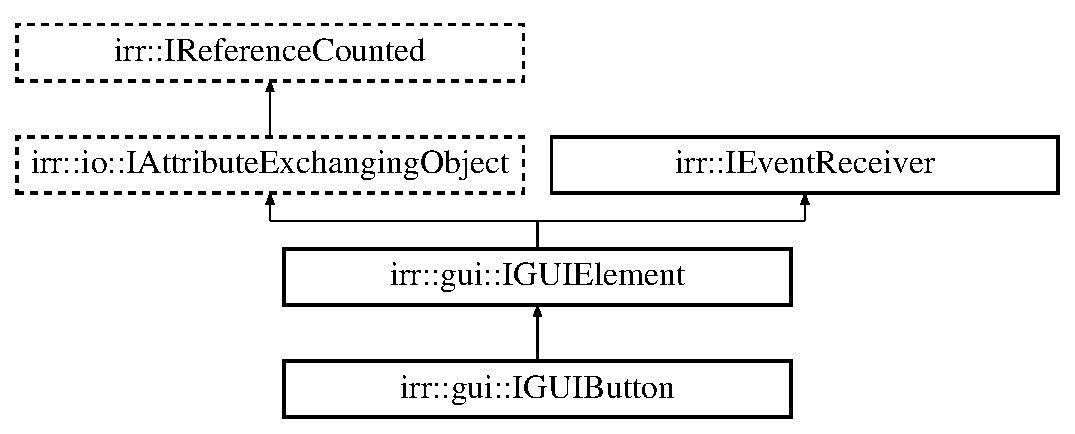
\includegraphics[height=4.000000cm]{classirr_1_1gui_1_1IGUIButton}
\end{center}
\end{figure}
\subsection*{Public Member Functions}
\begin{DoxyCompactItemize}
\item 
\mbox{\Hypertarget{classirr_1_1gui_1_1IGUIButton_a9ce8f3172c2c82269c2cf6a650ccaaa8}\label{classirr_1_1gui_1_1IGUIButton_a9ce8f3172c2c82269c2cf6a650ccaaa8}} 
\hyperlink{classirr_1_1gui_1_1IGUIButton_a9ce8f3172c2c82269c2cf6a650ccaaa8}{I\+G\+U\+I\+Button} (\hyperlink{classirr_1_1gui_1_1IGUIEnvironment}{I\+G\+U\+I\+Environment} $\ast$environment, \hyperlink{classirr_1_1gui_1_1IGUIElement}{I\+G\+U\+I\+Element} $\ast$parent, \hyperlink{namespaceirr_ac66849b7a6ed16e30ebede579f9b47c6}{s32} id, \hyperlink{classirr_1_1core_1_1rect}{core\+::rect}$<$ \hyperlink{namespaceirr_ac66849b7a6ed16e30ebede579f9b47c6}{s32} $>$ rectangle)
\begin{DoxyCompactList}\small\item\em constructor \end{DoxyCompactList}\item 
virtual void \hyperlink{classirr_1_1gui_1_1IGUIButton_ab63c3536bd2eb92e9ebec8ea3a381ec1}{set\+Override\+Font} (\hyperlink{classirr_1_1gui_1_1IGUIFont}{I\+G\+U\+I\+Font} $\ast$font=0)=0
\begin{DoxyCompactList}\small\item\em Sets another skin independent font. \end{DoxyCompactList}\item 
virtual \hyperlink{classirr_1_1gui_1_1IGUIFont}{I\+G\+U\+I\+Font} $\ast$ \hyperlink{classirr_1_1gui_1_1IGUIButton_adbc27c7589bf22d2a7fa676401358578}{get\+Override\+Font} (void) const =0
\begin{DoxyCompactList}\small\item\em Gets the override font (if any) \end{DoxyCompactList}\item 
virtual \hyperlink{classirr_1_1gui_1_1IGUIFont}{I\+G\+U\+I\+Font} $\ast$ \hyperlink{classirr_1_1gui_1_1IGUIButton_a1caa9253c284c3e3366733bf7805d762}{get\+Active\+Font} () const =0
\begin{DoxyCompactList}\small\item\em Get the font which is used right now for drawing. \end{DoxyCompactList}\item 
virtual void \hyperlink{classirr_1_1gui_1_1IGUIButton_af233578beb34ba115b0197731e34a3f1}{set\+Image} (\hyperlink{classirr_1_1video_1_1ITexture}{video\+::\+I\+Texture} $\ast$image=0)=0
\begin{DoxyCompactList}\small\item\em Sets an image which should be displayed on the button when it is in normal state. \end{DoxyCompactList}\item 
virtual void \hyperlink{classirr_1_1gui_1_1IGUIButton_a205490ec6b4978afe9d3f6a4aed92b50}{set\+Image} (\hyperlink{classirr_1_1video_1_1ITexture}{video\+::\+I\+Texture} $\ast$image, const \hyperlink{classirr_1_1core_1_1rect}{core\+::rect}$<$ \hyperlink{namespaceirr_ac66849b7a6ed16e30ebede579f9b47c6}{s32} $>$ \&pos)=0
\begin{DoxyCompactList}\small\item\em Sets a background image for the button when it is in normal state. \end{DoxyCompactList}\item 
virtual void \hyperlink{classirr_1_1gui_1_1IGUIButton_a10389917530aa2f4a3008330c0695aad}{set\+Pressed\+Image} (\hyperlink{classirr_1_1video_1_1ITexture}{video\+::\+I\+Texture} $\ast$image=0)=0
\begin{DoxyCompactList}\small\item\em Sets a background image for the button when it is in pressed state. \end{DoxyCompactList}\item 
virtual void \hyperlink{classirr_1_1gui_1_1IGUIButton_a08019647ec3e08984d795b3c564d457e}{set\+Pressed\+Image} (\hyperlink{classirr_1_1video_1_1ITexture}{video\+::\+I\+Texture} $\ast$image, const \hyperlink{classirr_1_1core_1_1rect}{core\+::rect}$<$ \hyperlink{namespaceirr_ac66849b7a6ed16e30ebede579f9b47c6}{s32} $>$ \&pos)=0
\begin{DoxyCompactList}\small\item\em Sets an image which should be displayed on the button when it is in pressed state. \end{DoxyCompactList}\item 
\mbox{\Hypertarget{classirr_1_1gui_1_1IGUIButton_a0570cc64a1445866a0c8123c0209c83d}\label{classirr_1_1gui_1_1IGUIButton_a0570cc64a1445866a0c8123c0209c83d}} 
virtual void \hyperlink{classirr_1_1gui_1_1IGUIButton_a0570cc64a1445866a0c8123c0209c83d}{set\+Sprite\+Bank} (\hyperlink{classirr_1_1gui_1_1IGUISpriteBank}{I\+G\+U\+I\+Sprite\+Bank} $\ast$bank=0)=0
\begin{DoxyCompactList}\small\item\em Sets the sprite bank used by the button. \end{DoxyCompactList}\item 
virtual void \hyperlink{classirr_1_1gui_1_1IGUIButton_a26c5f05e922b0fc1b5790a001fd04b78}{set\+Sprite} (\hyperlink{namespaceirr_1_1gui_a2520445dec46e00684645ef8053aebb5}{E\+G\+U\+I\+\_\+\+B\+U\+T\+T\+O\+N\+\_\+\+S\+T\+A\+TE} state, \hyperlink{namespaceirr_ac66849b7a6ed16e30ebede579f9b47c6}{s32} index, \hyperlink{classirr_1_1video_1_1SColor}{video\+::\+S\+Color} color=\hyperlink{classirr_1_1video_1_1SColor}{video\+::\+S\+Color}(255, 255, 255, 255), bool loop=false)=0
\begin{DoxyCompactList}\small\item\em Sets the animated sprite for a specific button state. \end{DoxyCompactList}\item 
virtual void \hyperlink{classirr_1_1gui_1_1IGUIButton_a992775637ba91f5267c4c04d5889fc6d}{set\+Is\+Push\+Button} (bool \hyperlink{classirr_1_1gui_1_1IGUIButton_abb12a92ba70d1fe738655d04ef73734f}{is\+Push\+Button}=true)=0
\begin{DoxyCompactList}\small\item\em Sets if the button should behave like a push button. \end{DoxyCompactList}\item 
\mbox{\Hypertarget{classirr_1_1gui_1_1IGUIButton_a2508fb292fab222bcebdeae0f9874348}\label{classirr_1_1gui_1_1IGUIButton_a2508fb292fab222bcebdeae0f9874348}} 
virtual void \hyperlink{classirr_1_1gui_1_1IGUIButton_a2508fb292fab222bcebdeae0f9874348}{set\+Pressed} (bool pressed=true)=0
\begin{DoxyCompactList}\small\item\em Sets the pressed state of the button if this is a pushbutton. \end{DoxyCompactList}\item 
\mbox{\Hypertarget{classirr_1_1gui_1_1IGUIButton_a2621bd10a5eb91fa14037feb9378c252}\label{classirr_1_1gui_1_1IGUIButton_a2621bd10a5eb91fa14037feb9378c252}} 
virtual bool \hyperlink{classirr_1_1gui_1_1IGUIButton_a2621bd10a5eb91fa14037feb9378c252}{is\+Pressed} () const =0
\begin{DoxyCompactList}\small\item\em Returns if the button is currently pressed. \end{DoxyCompactList}\item 
\mbox{\Hypertarget{classirr_1_1gui_1_1IGUIButton_a3d7727e7807e8b71dae6f81a44737e8a}\label{classirr_1_1gui_1_1IGUIButton_a3d7727e7807e8b71dae6f81a44737e8a}} 
virtual void \hyperlink{classirr_1_1gui_1_1IGUIButton_a3d7727e7807e8b71dae6f81a44737e8a}{set\+Use\+Alpha\+Channel} (bool use\+Alpha\+Channel=true)=0
\begin{DoxyCompactList}\small\item\em Sets if the alpha channel should be used for drawing background images on the button (default is false) \end{DoxyCompactList}\item 
\mbox{\Hypertarget{classirr_1_1gui_1_1IGUIButton_af4cb47805f2a296506b8a0b4cb65fddf}\label{classirr_1_1gui_1_1IGUIButton_af4cb47805f2a296506b8a0b4cb65fddf}} 
virtual bool \hyperlink{classirr_1_1gui_1_1IGUIButton_af4cb47805f2a296506b8a0b4cb65fddf}{is\+Alpha\+Channel\+Used} () const =0
\begin{DoxyCompactList}\small\item\em Returns if the alpha channel should be used for drawing background images on the button. \end{DoxyCompactList}\item 
\mbox{\Hypertarget{classirr_1_1gui_1_1IGUIButton_abb12a92ba70d1fe738655d04ef73734f}\label{classirr_1_1gui_1_1IGUIButton_abb12a92ba70d1fe738655d04ef73734f}} 
virtual bool \hyperlink{classirr_1_1gui_1_1IGUIButton_abb12a92ba70d1fe738655d04ef73734f}{is\+Push\+Button} () const =0
\begin{DoxyCompactList}\small\item\em Returns whether the button is a push button. \end{DoxyCompactList}\item 
\mbox{\Hypertarget{classirr_1_1gui_1_1IGUIButton_aa6e68e5335f67472bde80b530b6d31fd}\label{classirr_1_1gui_1_1IGUIButton_aa6e68e5335f67472bde80b530b6d31fd}} 
virtual void \hyperlink{classirr_1_1gui_1_1IGUIButton_aa6e68e5335f67472bde80b530b6d31fd}{set\+Draw\+Border} (bool border=true)=0
\begin{DoxyCompactList}\small\item\em Sets if the button should use the skin to draw its border and button face (default is true) \end{DoxyCompactList}\item 
\mbox{\Hypertarget{classirr_1_1gui_1_1IGUIButton_af2e1cee431cc5f90cede3820719625f1}\label{classirr_1_1gui_1_1IGUIButton_af2e1cee431cc5f90cede3820719625f1}} 
virtual bool \hyperlink{classirr_1_1gui_1_1IGUIButton_af2e1cee431cc5f90cede3820719625f1}{is\+Drawing\+Border} () const =0
\begin{DoxyCompactList}\small\item\em Returns if the border and button face are being drawn using the skin. \end{DoxyCompactList}\item 
\mbox{\Hypertarget{classirr_1_1gui_1_1IGUIButton_ae0767cb927c7974e19eaa3e5ca52bf1f}\label{classirr_1_1gui_1_1IGUIButton_ae0767cb927c7974e19eaa3e5ca52bf1f}} 
virtual void \hyperlink{classirr_1_1gui_1_1IGUIButton_ae0767cb927c7974e19eaa3e5ca52bf1f}{set\+Scale\+Image} (bool scale\+Image=true)=0
\begin{DoxyCompactList}\small\item\em Sets if the button should scale the button images to fit. \end{DoxyCompactList}\item 
\mbox{\Hypertarget{classirr_1_1gui_1_1IGUIButton_af2660457dae6def0b34d4748e96c653a}\label{classirr_1_1gui_1_1IGUIButton_af2660457dae6def0b34d4748e96c653a}} 
virtual bool \hyperlink{classirr_1_1gui_1_1IGUIButton_af2660457dae6def0b34d4748e96c653a}{is\+Scaling\+Image} () const =0
\begin{DoxyCompactList}\small\item\em Checks whether the button scales the used images. \end{DoxyCompactList}\end{DoxyCompactItemize}
\subsection*{Additional Inherited Members}


\subsection{Detailed Description}
G\+UI \hyperlink{classButton}{Button} interface. 

\begin{DoxyParagraph}{This element can create the following events of type E\+G\+U\+I\+\_\+\+E\+V\+E\+N\+T\+\_\+\+T\+Y\+PE\+:}
\begin{DoxyItemize}
\item E\+G\+E\+T\+\_\+\+B\+U\+T\+T\+O\+N\+\_\+\+C\+L\+I\+C\+K\+ED \end{DoxyItemize}

\end{DoxyParagraph}


\subsection{Member Function Documentation}
\mbox{\Hypertarget{classirr_1_1gui_1_1IGUIButton_a1caa9253c284c3e3366733bf7805d762}\label{classirr_1_1gui_1_1IGUIButton_a1caa9253c284c3e3366733bf7805d762}} 
\index{irr\+::gui\+::\+I\+G\+U\+I\+Button@{irr\+::gui\+::\+I\+G\+U\+I\+Button}!get\+Active\+Font@{get\+Active\+Font}}
\index{get\+Active\+Font@{get\+Active\+Font}!irr\+::gui\+::\+I\+G\+U\+I\+Button@{irr\+::gui\+::\+I\+G\+U\+I\+Button}}
\subsubsection{\texorpdfstring{get\+Active\+Font()}{getActiveFont()}}
{\footnotesize\ttfamily virtual \hyperlink{classirr_1_1gui_1_1IGUIFont}{I\+G\+U\+I\+Font}$\ast$ irr\+::gui\+::\+I\+G\+U\+I\+Button\+::get\+Active\+Font (\begin{DoxyParamCaption}{ }\end{DoxyParamCaption}) const\hspace{0.3cm}{\ttfamily [pure virtual]}}



Get the font which is used right now for drawing. 

Currently this is the override font when one is set and the font of the active skin otherwise \mbox{\Hypertarget{classirr_1_1gui_1_1IGUIButton_adbc27c7589bf22d2a7fa676401358578}\label{classirr_1_1gui_1_1IGUIButton_adbc27c7589bf22d2a7fa676401358578}} 
\index{irr\+::gui\+::\+I\+G\+U\+I\+Button@{irr\+::gui\+::\+I\+G\+U\+I\+Button}!get\+Override\+Font@{get\+Override\+Font}}
\index{get\+Override\+Font@{get\+Override\+Font}!irr\+::gui\+::\+I\+G\+U\+I\+Button@{irr\+::gui\+::\+I\+G\+U\+I\+Button}}
\subsubsection{\texorpdfstring{get\+Override\+Font()}{getOverrideFont()}}
{\footnotesize\ttfamily virtual \hyperlink{classirr_1_1gui_1_1IGUIFont}{I\+G\+U\+I\+Font}$\ast$ irr\+::gui\+::\+I\+G\+U\+I\+Button\+::get\+Override\+Font (\begin{DoxyParamCaption}\item[{void}]{ }\end{DoxyParamCaption}) const\hspace{0.3cm}{\ttfamily [pure virtual]}}



Gets the override font (if any) 

\begin{DoxyReturn}{Returns}
The override font (may be 0) 
\end{DoxyReturn}
\mbox{\Hypertarget{classirr_1_1gui_1_1IGUIButton_af233578beb34ba115b0197731e34a3f1}\label{classirr_1_1gui_1_1IGUIButton_af233578beb34ba115b0197731e34a3f1}} 
\index{irr\+::gui\+::\+I\+G\+U\+I\+Button@{irr\+::gui\+::\+I\+G\+U\+I\+Button}!set\+Image@{set\+Image}}
\index{set\+Image@{set\+Image}!irr\+::gui\+::\+I\+G\+U\+I\+Button@{irr\+::gui\+::\+I\+G\+U\+I\+Button}}
\subsubsection{\texorpdfstring{set\+Image()}{setImage()}\hspace{0.1cm}{\footnotesize\ttfamily [1/2]}}
{\footnotesize\ttfamily virtual void irr\+::gui\+::\+I\+G\+U\+I\+Button\+::set\+Image (\begin{DoxyParamCaption}\item[{\hyperlink{classirr_1_1video_1_1ITexture}{video\+::\+I\+Texture} $\ast$}]{image = {\ttfamily 0} }\end{DoxyParamCaption})\hspace{0.3cm}{\ttfamily [pure virtual]}}



Sets an image which should be displayed on the button when it is in normal state. 


\begin{DoxyParams}{Parameters}
{\em image} & \hyperlink{classImage}{Image} to be displayed \\
\hline
\end{DoxyParams}
\mbox{\Hypertarget{classirr_1_1gui_1_1IGUIButton_a205490ec6b4978afe9d3f6a4aed92b50}\label{classirr_1_1gui_1_1IGUIButton_a205490ec6b4978afe9d3f6a4aed92b50}} 
\index{irr\+::gui\+::\+I\+G\+U\+I\+Button@{irr\+::gui\+::\+I\+G\+U\+I\+Button}!set\+Image@{set\+Image}}
\index{set\+Image@{set\+Image}!irr\+::gui\+::\+I\+G\+U\+I\+Button@{irr\+::gui\+::\+I\+G\+U\+I\+Button}}
\subsubsection{\texorpdfstring{set\+Image()}{setImage()}\hspace{0.1cm}{\footnotesize\ttfamily [2/2]}}
{\footnotesize\ttfamily virtual void irr\+::gui\+::\+I\+G\+U\+I\+Button\+::set\+Image (\begin{DoxyParamCaption}\item[{\hyperlink{classirr_1_1video_1_1ITexture}{video\+::\+I\+Texture} $\ast$}]{image,  }\item[{const \hyperlink{classirr_1_1core_1_1rect}{core\+::rect}$<$ \hyperlink{namespaceirr_ac66849b7a6ed16e30ebede579f9b47c6}{s32} $>$ \&}]{pos }\end{DoxyParamCaption})\hspace{0.3cm}{\ttfamily [pure virtual]}}



Sets a background image for the button when it is in normal state. 


\begin{DoxyParams}{Parameters}
{\em image} & Texture containing the image to be displayed \\
\hline
{\em pos} & Position in the texture, where the image is located \\
\hline
\end{DoxyParams}
\mbox{\Hypertarget{classirr_1_1gui_1_1IGUIButton_a992775637ba91f5267c4c04d5889fc6d}\label{classirr_1_1gui_1_1IGUIButton_a992775637ba91f5267c4c04d5889fc6d}} 
\index{irr\+::gui\+::\+I\+G\+U\+I\+Button@{irr\+::gui\+::\+I\+G\+U\+I\+Button}!set\+Is\+Push\+Button@{set\+Is\+Push\+Button}}
\index{set\+Is\+Push\+Button@{set\+Is\+Push\+Button}!irr\+::gui\+::\+I\+G\+U\+I\+Button@{irr\+::gui\+::\+I\+G\+U\+I\+Button}}
\subsubsection{\texorpdfstring{set\+Is\+Push\+Button()}{setIsPushButton()}}
{\footnotesize\ttfamily virtual void irr\+::gui\+::\+I\+G\+U\+I\+Button\+::set\+Is\+Push\+Button (\begin{DoxyParamCaption}\item[{bool}]{is\+Push\+Button = {\ttfamily true} }\end{DoxyParamCaption})\hspace{0.3cm}{\ttfamily [pure virtual]}}



Sets if the button should behave like a push button. 

Which means it can be in two states\+: Normal or Pressed. With a click on the button, the user can change the state of the button. \mbox{\Hypertarget{classirr_1_1gui_1_1IGUIButton_ab63c3536bd2eb92e9ebec8ea3a381ec1}\label{classirr_1_1gui_1_1IGUIButton_ab63c3536bd2eb92e9ebec8ea3a381ec1}} 
\index{irr\+::gui\+::\+I\+G\+U\+I\+Button@{irr\+::gui\+::\+I\+G\+U\+I\+Button}!set\+Override\+Font@{set\+Override\+Font}}
\index{set\+Override\+Font@{set\+Override\+Font}!irr\+::gui\+::\+I\+G\+U\+I\+Button@{irr\+::gui\+::\+I\+G\+U\+I\+Button}}
\subsubsection{\texorpdfstring{set\+Override\+Font()}{setOverrideFont()}}
{\footnotesize\ttfamily virtual void irr\+::gui\+::\+I\+G\+U\+I\+Button\+::set\+Override\+Font (\begin{DoxyParamCaption}\item[{\hyperlink{classirr_1_1gui_1_1IGUIFont}{I\+G\+U\+I\+Font} $\ast$}]{font = {\ttfamily 0} }\end{DoxyParamCaption})\hspace{0.3cm}{\ttfamily [pure virtual]}}



Sets another skin independent font. 

If this is set to zero, the button uses the font of the skin. 
\begin{DoxyParams}{Parameters}
{\em font} & New font to set. \\
\hline
\end{DoxyParams}
\mbox{\Hypertarget{classirr_1_1gui_1_1IGUIButton_a10389917530aa2f4a3008330c0695aad}\label{classirr_1_1gui_1_1IGUIButton_a10389917530aa2f4a3008330c0695aad}} 
\index{irr\+::gui\+::\+I\+G\+U\+I\+Button@{irr\+::gui\+::\+I\+G\+U\+I\+Button}!set\+Pressed\+Image@{set\+Pressed\+Image}}
\index{set\+Pressed\+Image@{set\+Pressed\+Image}!irr\+::gui\+::\+I\+G\+U\+I\+Button@{irr\+::gui\+::\+I\+G\+U\+I\+Button}}
\subsubsection{\texorpdfstring{set\+Pressed\+Image()}{setPressedImage()}\hspace{0.1cm}{\footnotesize\ttfamily [1/2]}}
{\footnotesize\ttfamily virtual void irr\+::gui\+::\+I\+G\+U\+I\+Button\+::set\+Pressed\+Image (\begin{DoxyParamCaption}\item[{\hyperlink{classirr_1_1video_1_1ITexture}{video\+::\+I\+Texture} $\ast$}]{image = {\ttfamily 0} }\end{DoxyParamCaption})\hspace{0.3cm}{\ttfamily [pure virtual]}}



Sets a background image for the button when it is in pressed state. 

If no images is specified for the pressed state via \hyperlink{classirr_1_1gui_1_1IGUIButton_a10389917530aa2f4a3008330c0695aad}{set\+Pressed\+Image()}, this image is also drawn in pressed state. 
\begin{DoxyParams}{Parameters}
{\em image} & \hyperlink{classImage}{Image} to be displayed \\
\hline
\end{DoxyParams}
\mbox{\Hypertarget{classirr_1_1gui_1_1IGUIButton_a08019647ec3e08984d795b3c564d457e}\label{classirr_1_1gui_1_1IGUIButton_a08019647ec3e08984d795b3c564d457e}} 
\index{irr\+::gui\+::\+I\+G\+U\+I\+Button@{irr\+::gui\+::\+I\+G\+U\+I\+Button}!set\+Pressed\+Image@{set\+Pressed\+Image}}
\index{set\+Pressed\+Image@{set\+Pressed\+Image}!irr\+::gui\+::\+I\+G\+U\+I\+Button@{irr\+::gui\+::\+I\+G\+U\+I\+Button}}
\subsubsection{\texorpdfstring{set\+Pressed\+Image()}{setPressedImage()}\hspace{0.1cm}{\footnotesize\ttfamily [2/2]}}
{\footnotesize\ttfamily virtual void irr\+::gui\+::\+I\+G\+U\+I\+Button\+::set\+Pressed\+Image (\begin{DoxyParamCaption}\item[{\hyperlink{classirr_1_1video_1_1ITexture}{video\+::\+I\+Texture} $\ast$}]{image,  }\item[{const \hyperlink{classirr_1_1core_1_1rect}{core\+::rect}$<$ \hyperlink{namespaceirr_ac66849b7a6ed16e30ebede579f9b47c6}{s32} $>$ \&}]{pos }\end{DoxyParamCaption})\hspace{0.3cm}{\ttfamily [pure virtual]}}



Sets an image which should be displayed on the button when it is in pressed state. 


\begin{DoxyParams}{Parameters}
{\em image} & Texture containing the image to be displayed \\
\hline
{\em pos} & Position in the texture, where the image is located \\
\hline
\end{DoxyParams}
\mbox{\Hypertarget{classirr_1_1gui_1_1IGUIButton_a26c5f05e922b0fc1b5790a001fd04b78}\label{classirr_1_1gui_1_1IGUIButton_a26c5f05e922b0fc1b5790a001fd04b78}} 
\index{irr\+::gui\+::\+I\+G\+U\+I\+Button@{irr\+::gui\+::\+I\+G\+U\+I\+Button}!set\+Sprite@{set\+Sprite}}
\index{set\+Sprite@{set\+Sprite}!irr\+::gui\+::\+I\+G\+U\+I\+Button@{irr\+::gui\+::\+I\+G\+U\+I\+Button}}
\subsubsection{\texorpdfstring{set\+Sprite()}{setSprite()}}
{\footnotesize\ttfamily virtual void irr\+::gui\+::\+I\+G\+U\+I\+Button\+::set\+Sprite (\begin{DoxyParamCaption}\item[{\hyperlink{namespaceirr_1_1gui_a2520445dec46e00684645ef8053aebb5}{E\+G\+U\+I\+\_\+\+B\+U\+T\+T\+O\+N\+\_\+\+S\+T\+A\+TE}}]{state,  }\item[{\hyperlink{namespaceirr_ac66849b7a6ed16e30ebede579f9b47c6}{s32}}]{index,  }\item[{\hyperlink{classirr_1_1video_1_1SColor}{video\+::\+S\+Color}}]{color = {\ttfamily \hyperlink{classirr_1_1video_1_1SColor}{video\+::\+S\+Color}(255,~255,~255,~255)},  }\item[{bool}]{loop = {\ttfamily false} }\end{DoxyParamCaption})\hspace{0.3cm}{\ttfamily [pure virtual]}}



Sets the animated sprite for a specific button state. 


\begin{DoxyParams}{Parameters}
{\em index} & Number of the sprite within the sprite bank, use -\/1 for no sprite \\
\hline
{\em state} & State of the button to set the sprite for \\
\hline
{\em index} & The sprite number from the current sprite bank \\
\hline
{\em color} & The color of the sprite \\
\hline
{\em loop} & True if the animation should loop, false if not \\
\hline
\end{DoxyParams}


The documentation for this class was generated from the following file\+:\begin{DoxyCompactItemize}
\item 
indie\+\_\+share/controller/include/I\+G\+U\+I\+Button.\+h\end{DoxyCompactItemize}

\hypertarget{classirr_1_1gui_1_1IGUICheckBox}{}\section{irr\+:\+:gui\+:\+:I\+G\+U\+I\+Check\+Box Class Reference}
\label{classirr_1_1gui_1_1IGUICheckBox}\index{irr\+::gui\+::\+I\+G\+U\+I\+Check\+Box@{irr\+::gui\+::\+I\+G\+U\+I\+Check\+Box}}


G\+UI Check box interface.  




{\ttfamily \#include $<$I\+G\+U\+I\+Check\+Box.\+h$>$}

Inheritance diagram for irr\+:\+:gui\+:\+:I\+G\+U\+I\+Check\+Box\+:\begin{figure}[H]
\begin{center}
\leavevmode
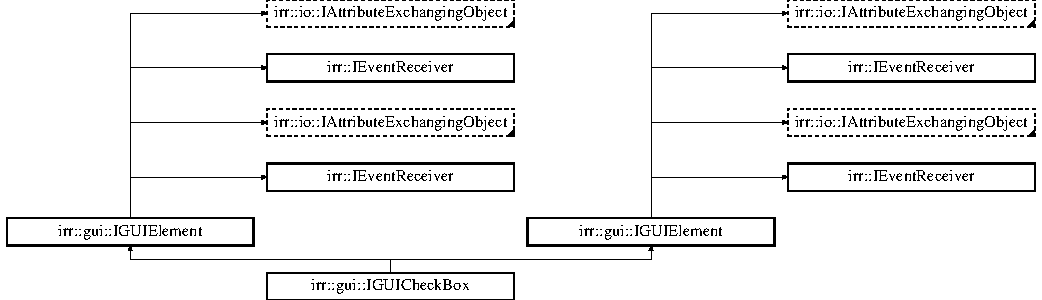
\includegraphics[height=4.038462cm]{classirr_1_1gui_1_1IGUICheckBox}
\end{center}
\end{figure}
\subsection*{Public Member Functions}
\begin{DoxyCompactItemize}
\item 
\mbox{\Hypertarget{classirr_1_1gui_1_1IGUICheckBox_a6a9826188131ec1bf1d1ec22c3ce3393}\label{classirr_1_1gui_1_1IGUICheckBox_a6a9826188131ec1bf1d1ec22c3ce3393}} 
\hyperlink{classirr_1_1gui_1_1IGUICheckBox_a6a9826188131ec1bf1d1ec22c3ce3393}{I\+G\+U\+I\+Check\+Box} (\hyperlink{classirr_1_1gui_1_1IGUIEnvironment}{I\+G\+U\+I\+Environment} $\ast$environment, \hyperlink{classirr_1_1gui_1_1IGUIElement}{I\+G\+U\+I\+Element} $\ast$parent, \hyperlink{namespaceirr_ac66849b7a6ed16e30ebede579f9b47c6}{s32} id, \hyperlink{classirr_1_1core_1_1rect}{core\+::rect}$<$ \hyperlink{namespaceirr_ac66849b7a6ed16e30ebede579f9b47c6}{s32} $>$ rectangle)
\begin{DoxyCompactList}\small\item\em constructor \end{DoxyCompactList}\item 
\mbox{\Hypertarget{classirr_1_1gui_1_1IGUICheckBox_ac57493d2d2ffbe820b0d634bd344d455}\label{classirr_1_1gui_1_1IGUICheckBox_ac57493d2d2ffbe820b0d634bd344d455}} 
virtual void \hyperlink{classirr_1_1gui_1_1IGUICheckBox_ac57493d2d2ffbe820b0d634bd344d455}{set\+Checked} (bool checked)=0
\begin{DoxyCompactList}\small\item\em Set if box is checked. \end{DoxyCompactList}\item 
\mbox{\Hypertarget{classirr_1_1gui_1_1IGUICheckBox_a3c7bffd5a06af81ff894d08bdeaf72ca}\label{classirr_1_1gui_1_1IGUICheckBox_a3c7bffd5a06af81ff894d08bdeaf72ca}} 
virtual bool \hyperlink{classirr_1_1gui_1_1IGUICheckBox_a3c7bffd5a06af81ff894d08bdeaf72ca}{is\+Checked} () const =0
\begin{DoxyCompactList}\small\item\em Returns true if box is checked. \end{DoxyCompactList}\item 
\mbox{\Hypertarget{classirr_1_1gui_1_1IGUICheckBox_a6a9826188131ec1bf1d1ec22c3ce3393}\label{classirr_1_1gui_1_1IGUICheckBox_a6a9826188131ec1bf1d1ec22c3ce3393}} 
\hyperlink{classirr_1_1gui_1_1IGUICheckBox_a6a9826188131ec1bf1d1ec22c3ce3393}{I\+G\+U\+I\+Check\+Box} (\hyperlink{classirr_1_1gui_1_1IGUIEnvironment}{I\+G\+U\+I\+Environment} $\ast$environment, \hyperlink{classirr_1_1gui_1_1IGUIElement}{I\+G\+U\+I\+Element} $\ast$parent, \hyperlink{namespaceirr_ac66849b7a6ed16e30ebede579f9b47c6}{s32} id, \hyperlink{classirr_1_1core_1_1rect}{core\+::rect}$<$ \hyperlink{namespaceirr_ac66849b7a6ed16e30ebede579f9b47c6}{s32} $>$ rectangle)
\begin{DoxyCompactList}\small\item\em constructor \end{DoxyCompactList}\item 
\mbox{\Hypertarget{classirr_1_1gui_1_1IGUICheckBox_ac57493d2d2ffbe820b0d634bd344d455}\label{classirr_1_1gui_1_1IGUICheckBox_ac57493d2d2ffbe820b0d634bd344d455}} 
virtual void \hyperlink{classirr_1_1gui_1_1IGUICheckBox_ac57493d2d2ffbe820b0d634bd344d455}{set\+Checked} (bool checked)=0
\begin{DoxyCompactList}\small\item\em Set if box is checked. \end{DoxyCompactList}\item 
\mbox{\Hypertarget{classirr_1_1gui_1_1IGUICheckBox_a3c7bffd5a06af81ff894d08bdeaf72ca}\label{classirr_1_1gui_1_1IGUICheckBox_a3c7bffd5a06af81ff894d08bdeaf72ca}} 
virtual bool \hyperlink{classirr_1_1gui_1_1IGUICheckBox_a3c7bffd5a06af81ff894d08bdeaf72ca}{is\+Checked} () const =0
\begin{DoxyCompactList}\small\item\em Returns true if box is checked. \end{DoxyCompactList}\end{DoxyCompactItemize}
\subsection*{Additional Inherited Members}


\subsection{Detailed Description}
G\+UI Check box interface. 

\begin{DoxyParagraph}{This element can create the following events of type E\+G\+U\+I\+\_\+\+E\+V\+E\+N\+T\+\_\+\+T\+Y\+PE\+:}
\begin{DoxyItemize}
\item E\+G\+E\+T\+\_\+\+C\+H\+E\+C\+K\+B\+O\+X\+\_\+\+C\+H\+A\+N\+G\+ED \end{DoxyItemize}

\end{DoxyParagraph}


The documentation for this class was generated from the following file\+:\begin{DoxyCompactItemize}
\item 
indie\+\_\+share/controller/include/I\+G\+U\+I\+Check\+Box.\+h\end{DoxyCompactItemize}

\hypertarget{classirr_1_1gui_1_1IGUIColorSelectDialog}{}\section{irr\+:\+:gui\+:\+:I\+G\+U\+I\+Color\+Select\+Dialog Class Reference}
\label{classirr_1_1gui_1_1IGUIColorSelectDialog}\index{irr\+::gui\+::\+I\+G\+U\+I\+Color\+Select\+Dialog@{irr\+::gui\+::\+I\+G\+U\+I\+Color\+Select\+Dialog}}


Standard color chooser dialog.  




{\ttfamily \#include $<$I\+G\+U\+I\+Color\+Select\+Dialog.\+h$>$}

Inheritance diagram for irr\+:\+:gui\+:\+:I\+G\+U\+I\+Color\+Select\+Dialog\+:\begin{figure}[H]
\begin{center}
\leavevmode
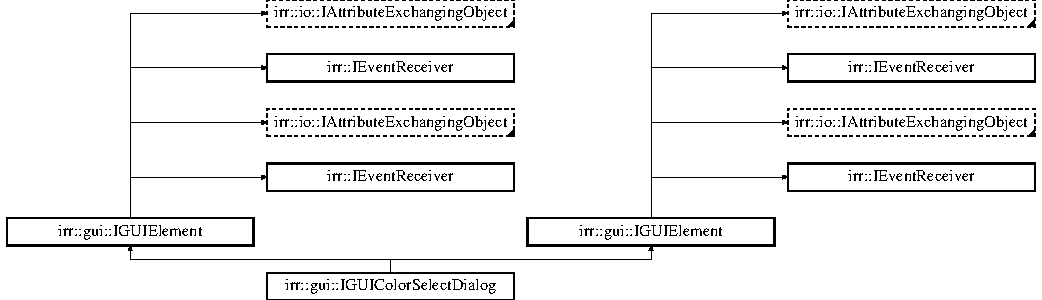
\includegraphics[height=4.000000cm]{classirr_1_1gui_1_1IGUIColorSelectDialog}
\end{center}
\end{figure}
\subsection*{Public Member Functions}
\begin{DoxyCompactItemize}
\item 
\mbox{\Hypertarget{classirr_1_1gui_1_1IGUIColorSelectDialog_a67ac184f6dc90f74a2694015b02e3acd}\label{classirr_1_1gui_1_1IGUIColorSelectDialog_a67ac184f6dc90f74a2694015b02e3acd}} 
\hyperlink{classirr_1_1gui_1_1IGUIColorSelectDialog_a67ac184f6dc90f74a2694015b02e3acd}{I\+G\+U\+I\+Color\+Select\+Dialog} (\hyperlink{classirr_1_1gui_1_1IGUIEnvironment}{I\+G\+U\+I\+Environment} $\ast$environment, \hyperlink{classirr_1_1gui_1_1IGUIElement}{I\+G\+U\+I\+Element} $\ast$parent, \hyperlink{namespaceirr_ac66849b7a6ed16e30ebede579f9b47c6}{s32} id, \hyperlink{classirr_1_1core_1_1rect}{core\+::rect}$<$ \hyperlink{namespaceirr_ac66849b7a6ed16e30ebede579f9b47c6}{s32} $>$ rectangle)
\begin{DoxyCompactList}\small\item\em constructor \end{DoxyCompactList}\end{DoxyCompactItemize}
\subsection*{Additional Inherited Members}


\subsection{Detailed Description}
Standard color chooser dialog. 

The documentation for this class was generated from the following file\+:\begin{DoxyCompactItemize}
\item 
indie\+\_\+share/controller/include/I\+G\+U\+I\+Color\+Select\+Dialog.\+h\end{DoxyCompactItemize}

\hypertarget{classirr_1_1gui_1_1IGUIComboBox}{}\section{irr\+:\+:gui\+:\+:I\+G\+U\+I\+Combo\+Box Class Reference}
\label{classirr_1_1gui_1_1IGUIComboBox}\index{irr\+::gui\+::\+I\+G\+U\+I\+Combo\+Box@{irr\+::gui\+::\+I\+G\+U\+I\+Combo\+Box}}


Combobox widget.  




{\ttfamily \#include $<$I\+G\+U\+I\+Combo\+Box.\+h$>$}

Inheritance diagram for irr\+:\+:gui\+:\+:I\+G\+U\+I\+Combo\+Box\+:\begin{figure}[H]
\begin{center}
\leavevmode
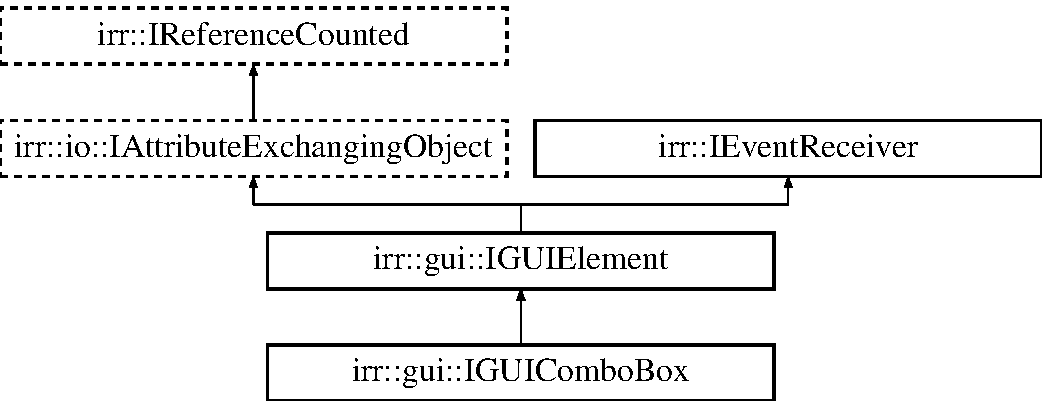
\includegraphics[height=4.038462cm]{classirr_1_1gui_1_1IGUIComboBox}
\end{center}
\end{figure}
\subsection*{Public Member Functions}
\begin{DoxyCompactItemize}
\item 
\mbox{\Hypertarget{classirr_1_1gui_1_1IGUIComboBox_a89e96a8ac4c47e7b202be120486f1f94}\label{classirr_1_1gui_1_1IGUIComboBox_a89e96a8ac4c47e7b202be120486f1f94}} 
\hyperlink{classirr_1_1gui_1_1IGUIComboBox_a89e96a8ac4c47e7b202be120486f1f94}{I\+G\+U\+I\+Combo\+Box} (\hyperlink{classirr_1_1gui_1_1IGUIEnvironment}{I\+G\+U\+I\+Environment} $\ast$environment, \hyperlink{classirr_1_1gui_1_1IGUIElement}{I\+G\+U\+I\+Element} $\ast$parent, \hyperlink{namespaceirr_ac66849b7a6ed16e30ebede579f9b47c6}{s32} id, \hyperlink{classirr_1_1core_1_1rect}{core\+::rect}$<$ \hyperlink{namespaceirr_ac66849b7a6ed16e30ebede579f9b47c6}{s32} $>$ rectangle)
\begin{DoxyCompactList}\small\item\em constructor \end{DoxyCompactList}\item 
\mbox{\Hypertarget{classirr_1_1gui_1_1IGUIComboBox_a573bdf5507fd9d389635cbb4d84c3757}\label{classirr_1_1gui_1_1IGUIComboBox_a573bdf5507fd9d389635cbb4d84c3757}} 
virtual \hyperlink{namespaceirr_a0416a53257075833e7002efd0a18e804}{u32} \hyperlink{classirr_1_1gui_1_1IGUIComboBox_a573bdf5507fd9d389635cbb4d84c3757}{get\+Item\+Count} () const =0
\begin{DoxyCompactList}\small\item\em Returns amount of items in box. \end{DoxyCompactList}\item 
\mbox{\Hypertarget{classirr_1_1gui_1_1IGUIComboBox_afe60f75b5e8685f6a19101d31ad6d369}\label{classirr_1_1gui_1_1IGUIComboBox_afe60f75b5e8685f6a19101d31ad6d369}} 
virtual const wchar\+\_\+t $\ast$ \hyperlink{classirr_1_1gui_1_1IGUIComboBox_afe60f75b5e8685f6a19101d31ad6d369}{get\+Item} (\hyperlink{namespaceirr_a0416a53257075833e7002efd0a18e804}{u32} idx) const =0
\begin{DoxyCompactList}\small\item\em Returns string of an item. the idx may be a value from 0 to item\+Count-\/1. \end{DoxyCompactList}\item 
\mbox{\Hypertarget{classirr_1_1gui_1_1IGUIComboBox_ac0f2189cf87e4ffe38834edea01c75fb}\label{classirr_1_1gui_1_1IGUIComboBox_ac0f2189cf87e4ffe38834edea01c75fb}} 
virtual \hyperlink{namespaceirr_a0416a53257075833e7002efd0a18e804}{u32} \hyperlink{classirr_1_1gui_1_1IGUIComboBox_ac0f2189cf87e4ffe38834edea01c75fb}{get\+Item\+Data} (\hyperlink{namespaceirr_a0416a53257075833e7002efd0a18e804}{u32} idx) const =0
\begin{DoxyCompactList}\small\item\em Returns item data of an item. the idx may be a value from 0 to item\+Count-\/1. \end{DoxyCompactList}\item 
\mbox{\Hypertarget{classirr_1_1gui_1_1IGUIComboBox_a01c1dea5455f7a9302cea8d156787c3e}\label{classirr_1_1gui_1_1IGUIComboBox_a01c1dea5455f7a9302cea8d156787c3e}} 
virtual \hyperlink{namespaceirr_ac66849b7a6ed16e30ebede579f9b47c6}{s32} \hyperlink{classirr_1_1gui_1_1IGUIComboBox_a01c1dea5455f7a9302cea8d156787c3e}{get\+Index\+For\+Item\+Data} (\hyperlink{namespaceirr_a0416a53257075833e7002efd0a18e804}{u32} data) const =0
\begin{DoxyCompactList}\small\item\em Returns index based on item data. \end{DoxyCompactList}\item 
\mbox{\Hypertarget{classirr_1_1gui_1_1IGUIComboBox_a1952afb705f497306cb006c502ac181c}\label{classirr_1_1gui_1_1IGUIComboBox_a1952afb705f497306cb006c502ac181c}} 
virtual \hyperlink{namespaceirr_a0416a53257075833e7002efd0a18e804}{u32} \hyperlink{classirr_1_1gui_1_1IGUIComboBox_a1952afb705f497306cb006c502ac181c}{add\+Item} (const wchar\+\_\+t $\ast$text, \hyperlink{namespaceirr_a0416a53257075833e7002efd0a18e804}{u32} data=0)=0
\begin{DoxyCompactList}\small\item\em Adds an item and returns the index of it. \end{DoxyCompactList}\item 
virtual void \hyperlink{classirr_1_1gui_1_1IGUIComboBox_aa6a351f80aa57374459a9d66f416ce3c}{remove\+Item} (\hyperlink{namespaceirr_a0416a53257075833e7002efd0a18e804}{u32} idx)=0
\begin{DoxyCompactList}\small\item\em Removes an item from the combo box. \end{DoxyCompactList}\item 
\mbox{\Hypertarget{classirr_1_1gui_1_1IGUIComboBox_af9f5d813496af19af437a6f51fa7e029}\label{classirr_1_1gui_1_1IGUIComboBox_af9f5d813496af19af437a6f51fa7e029}} 
virtual void \hyperlink{classirr_1_1gui_1_1IGUIComboBox_af9f5d813496af19af437a6f51fa7e029}{clear} ()=0
\begin{DoxyCompactList}\small\item\em Deletes all items in the combo box. \end{DoxyCompactList}\item 
\mbox{\Hypertarget{classirr_1_1gui_1_1IGUIComboBox_a7cb6bb2a86fccfc78cbb3c3d56b88778}\label{classirr_1_1gui_1_1IGUIComboBox_a7cb6bb2a86fccfc78cbb3c3d56b88778}} 
virtual \hyperlink{namespaceirr_ac66849b7a6ed16e30ebede579f9b47c6}{s32} \hyperlink{classirr_1_1gui_1_1IGUIComboBox_a7cb6bb2a86fccfc78cbb3c3d56b88778}{get\+Selected} () const =0
\begin{DoxyCompactList}\small\item\em Returns id of selected item. returns -\/1 if no item is selected. \end{DoxyCompactList}\item 
\mbox{\Hypertarget{classirr_1_1gui_1_1IGUIComboBox_a84660e6f4a677349ca7dc39024fe7b17}\label{classirr_1_1gui_1_1IGUIComboBox_a84660e6f4a677349ca7dc39024fe7b17}} 
virtual void \hyperlink{classirr_1_1gui_1_1IGUIComboBox_a84660e6f4a677349ca7dc39024fe7b17}{set\+Selected} (\hyperlink{namespaceirr_ac66849b7a6ed16e30ebede579f9b47c6}{s32} idx)=0
\begin{DoxyCompactList}\small\item\em Sets the selected item. Set this to -\/1 if no item should be selected. \end{DoxyCompactList}\item 
virtual void \hyperlink{classirr_1_1gui_1_1IGUIComboBox_a902681b9cfc783d29270f919ab3e71d8}{set\+Text\+Alignment} (\hyperlink{namespaceirr_1_1gui_a19eb5fb40e67f108cb16aba922ddaa2d}{E\+G\+U\+I\+\_\+\+A\+L\+I\+G\+N\+M\+E\+NT} horizontal, \hyperlink{namespaceirr_1_1gui_a19eb5fb40e67f108cb16aba922ddaa2d}{E\+G\+U\+I\+\_\+\+A\+L\+I\+G\+N\+M\+E\+NT} vertical)=0
\begin{DoxyCompactList}\small\item\em Sets text justification of the text area. \end{DoxyCompactList}\item 
\mbox{\Hypertarget{classirr_1_1gui_1_1IGUIComboBox_a273f90cfe3cf279ccae2cc612117862d}\label{classirr_1_1gui_1_1IGUIComboBox_a273f90cfe3cf279ccae2cc612117862d}} 
virtual void \hyperlink{classirr_1_1gui_1_1IGUIComboBox_a273f90cfe3cf279ccae2cc612117862d}{set\+Max\+Selection\+Rows} (\hyperlink{namespaceirr_a0416a53257075833e7002efd0a18e804}{u32} max)=0
\begin{DoxyCompactList}\small\item\em Set the maximal number of rows for the selection listbox. \end{DoxyCompactList}\item 
\mbox{\Hypertarget{classirr_1_1gui_1_1IGUIComboBox_afc75706835598a9016ce8a8f020c690c}\label{classirr_1_1gui_1_1IGUIComboBox_afc75706835598a9016ce8a8f020c690c}} 
virtual \hyperlink{namespaceirr_a0416a53257075833e7002efd0a18e804}{u32} \hyperlink{classirr_1_1gui_1_1IGUIComboBox_afc75706835598a9016ce8a8f020c690c}{get\+Max\+Selection\+Rows} () const =0
\begin{DoxyCompactList}\small\item\em Get the maximimal number of rows for the selection listbox. \end{DoxyCompactList}\item 
\mbox{\Hypertarget{classirr_1_1gui_1_1IGUIComboBox_a89e96a8ac4c47e7b202be120486f1f94}\label{classirr_1_1gui_1_1IGUIComboBox_a89e96a8ac4c47e7b202be120486f1f94}} 
\hyperlink{classirr_1_1gui_1_1IGUIComboBox_a89e96a8ac4c47e7b202be120486f1f94}{I\+G\+U\+I\+Combo\+Box} (\hyperlink{classirr_1_1gui_1_1IGUIEnvironment}{I\+G\+U\+I\+Environment} $\ast$environment, \hyperlink{classirr_1_1gui_1_1IGUIElement}{I\+G\+U\+I\+Element} $\ast$parent, \hyperlink{namespaceirr_ac66849b7a6ed16e30ebede579f9b47c6}{s32} id, \hyperlink{classirr_1_1core_1_1rect}{core\+::rect}$<$ \hyperlink{namespaceirr_ac66849b7a6ed16e30ebede579f9b47c6}{s32} $>$ rectangle)
\begin{DoxyCompactList}\small\item\em constructor \end{DoxyCompactList}\item 
\mbox{\Hypertarget{classirr_1_1gui_1_1IGUIComboBox_a573bdf5507fd9d389635cbb4d84c3757}\label{classirr_1_1gui_1_1IGUIComboBox_a573bdf5507fd9d389635cbb4d84c3757}} 
virtual \hyperlink{namespaceirr_a0416a53257075833e7002efd0a18e804}{u32} \hyperlink{classirr_1_1gui_1_1IGUIComboBox_a573bdf5507fd9d389635cbb4d84c3757}{get\+Item\+Count} () const =0
\begin{DoxyCompactList}\small\item\em Returns amount of items in box. \end{DoxyCompactList}\item 
\mbox{\Hypertarget{classirr_1_1gui_1_1IGUIComboBox_afe60f75b5e8685f6a19101d31ad6d369}\label{classirr_1_1gui_1_1IGUIComboBox_afe60f75b5e8685f6a19101d31ad6d369}} 
virtual const wchar\+\_\+t $\ast$ \hyperlink{classirr_1_1gui_1_1IGUIComboBox_afe60f75b5e8685f6a19101d31ad6d369}{get\+Item} (\hyperlink{namespaceirr_a0416a53257075833e7002efd0a18e804}{u32} idx) const =0
\begin{DoxyCompactList}\small\item\em Returns string of an item. the idx may be a value from 0 to item\+Count-\/1. \end{DoxyCompactList}\item 
\mbox{\Hypertarget{classirr_1_1gui_1_1IGUIComboBox_ac0f2189cf87e4ffe38834edea01c75fb}\label{classirr_1_1gui_1_1IGUIComboBox_ac0f2189cf87e4ffe38834edea01c75fb}} 
virtual \hyperlink{namespaceirr_a0416a53257075833e7002efd0a18e804}{u32} \hyperlink{classirr_1_1gui_1_1IGUIComboBox_ac0f2189cf87e4ffe38834edea01c75fb}{get\+Item\+Data} (\hyperlink{namespaceirr_a0416a53257075833e7002efd0a18e804}{u32} idx) const =0
\begin{DoxyCompactList}\small\item\em Returns item data of an item. the idx may be a value from 0 to item\+Count-\/1. \end{DoxyCompactList}\item 
\mbox{\Hypertarget{classirr_1_1gui_1_1IGUIComboBox_a01c1dea5455f7a9302cea8d156787c3e}\label{classirr_1_1gui_1_1IGUIComboBox_a01c1dea5455f7a9302cea8d156787c3e}} 
virtual \hyperlink{namespaceirr_ac66849b7a6ed16e30ebede579f9b47c6}{s32} \hyperlink{classirr_1_1gui_1_1IGUIComboBox_a01c1dea5455f7a9302cea8d156787c3e}{get\+Index\+For\+Item\+Data} (\hyperlink{namespaceirr_a0416a53257075833e7002efd0a18e804}{u32} data) const =0
\begin{DoxyCompactList}\small\item\em Returns index based on item data. \end{DoxyCompactList}\item 
\mbox{\Hypertarget{classirr_1_1gui_1_1IGUIComboBox_a1952afb705f497306cb006c502ac181c}\label{classirr_1_1gui_1_1IGUIComboBox_a1952afb705f497306cb006c502ac181c}} 
virtual \hyperlink{namespaceirr_a0416a53257075833e7002efd0a18e804}{u32} \hyperlink{classirr_1_1gui_1_1IGUIComboBox_a1952afb705f497306cb006c502ac181c}{add\+Item} (const wchar\+\_\+t $\ast$text, \hyperlink{namespaceirr_a0416a53257075833e7002efd0a18e804}{u32} data=0)=0
\begin{DoxyCompactList}\small\item\em Adds an item and returns the index of it. \end{DoxyCompactList}\item 
virtual void \hyperlink{classirr_1_1gui_1_1IGUIComboBox_aa6a351f80aa57374459a9d66f416ce3c}{remove\+Item} (\hyperlink{namespaceirr_a0416a53257075833e7002efd0a18e804}{u32} idx)=0
\begin{DoxyCompactList}\small\item\em Removes an item from the combo box. \end{DoxyCompactList}\item 
\mbox{\Hypertarget{classirr_1_1gui_1_1IGUIComboBox_af9f5d813496af19af437a6f51fa7e029}\label{classirr_1_1gui_1_1IGUIComboBox_af9f5d813496af19af437a6f51fa7e029}} 
virtual void \hyperlink{classirr_1_1gui_1_1IGUIComboBox_af9f5d813496af19af437a6f51fa7e029}{clear} ()=0
\begin{DoxyCompactList}\small\item\em Deletes all items in the combo box. \end{DoxyCompactList}\item 
\mbox{\Hypertarget{classirr_1_1gui_1_1IGUIComboBox_a7cb6bb2a86fccfc78cbb3c3d56b88778}\label{classirr_1_1gui_1_1IGUIComboBox_a7cb6bb2a86fccfc78cbb3c3d56b88778}} 
virtual \hyperlink{namespaceirr_ac66849b7a6ed16e30ebede579f9b47c6}{s32} \hyperlink{classirr_1_1gui_1_1IGUIComboBox_a7cb6bb2a86fccfc78cbb3c3d56b88778}{get\+Selected} () const =0
\begin{DoxyCompactList}\small\item\em Returns id of selected item. returns -\/1 if no item is selected. \end{DoxyCompactList}\item 
\mbox{\Hypertarget{classirr_1_1gui_1_1IGUIComboBox_a84660e6f4a677349ca7dc39024fe7b17}\label{classirr_1_1gui_1_1IGUIComboBox_a84660e6f4a677349ca7dc39024fe7b17}} 
virtual void \hyperlink{classirr_1_1gui_1_1IGUIComboBox_a84660e6f4a677349ca7dc39024fe7b17}{set\+Selected} (\hyperlink{namespaceirr_ac66849b7a6ed16e30ebede579f9b47c6}{s32} idx)=0
\begin{DoxyCompactList}\small\item\em Sets the selected item. Set this to -\/1 if no item should be selected. \end{DoxyCompactList}\item 
virtual void \hyperlink{classirr_1_1gui_1_1IGUIComboBox_a902681b9cfc783d29270f919ab3e71d8}{set\+Text\+Alignment} (\hyperlink{namespaceirr_1_1gui_a19eb5fb40e67f108cb16aba922ddaa2d}{E\+G\+U\+I\+\_\+\+A\+L\+I\+G\+N\+M\+E\+NT} horizontal, \hyperlink{namespaceirr_1_1gui_a19eb5fb40e67f108cb16aba922ddaa2d}{E\+G\+U\+I\+\_\+\+A\+L\+I\+G\+N\+M\+E\+NT} vertical)=0
\begin{DoxyCompactList}\small\item\em Sets text justification of the text area. \end{DoxyCompactList}\item 
\mbox{\Hypertarget{classirr_1_1gui_1_1IGUIComboBox_a273f90cfe3cf279ccae2cc612117862d}\label{classirr_1_1gui_1_1IGUIComboBox_a273f90cfe3cf279ccae2cc612117862d}} 
virtual void \hyperlink{classirr_1_1gui_1_1IGUIComboBox_a273f90cfe3cf279ccae2cc612117862d}{set\+Max\+Selection\+Rows} (\hyperlink{namespaceirr_a0416a53257075833e7002efd0a18e804}{u32} max)=0
\begin{DoxyCompactList}\small\item\em Set the maximal number of rows for the selection listbox. \end{DoxyCompactList}\item 
\mbox{\Hypertarget{classirr_1_1gui_1_1IGUIComboBox_afc75706835598a9016ce8a8f020c690c}\label{classirr_1_1gui_1_1IGUIComboBox_afc75706835598a9016ce8a8f020c690c}} 
virtual \hyperlink{namespaceirr_a0416a53257075833e7002efd0a18e804}{u32} \hyperlink{classirr_1_1gui_1_1IGUIComboBox_afc75706835598a9016ce8a8f020c690c}{get\+Max\+Selection\+Rows} () const =0
\begin{DoxyCompactList}\small\item\em Get the maximimal number of rows for the selection listbox. \end{DoxyCompactList}\end{DoxyCompactItemize}
\subsection*{Additional Inherited Members}


\subsection{Detailed Description}
Combobox widget. 

\begin{DoxyParagraph}{This element can create the following events of type E\+G\+U\+I\+\_\+\+E\+V\+E\+N\+T\+\_\+\+T\+Y\+PE\+:}
\begin{DoxyItemize}
\item E\+G\+E\+T\+\_\+\+C\+O\+M\+B\+O\+\_\+\+B\+O\+X\+\_\+\+C\+H\+A\+N\+G\+ED \end{DoxyItemize}

\end{DoxyParagraph}


\subsection{Member Function Documentation}
\mbox{\Hypertarget{classirr_1_1gui_1_1IGUIComboBox_aa6a351f80aa57374459a9d66f416ce3c}\label{classirr_1_1gui_1_1IGUIComboBox_aa6a351f80aa57374459a9d66f416ce3c}} 
\index{irr\+::gui\+::\+I\+G\+U\+I\+Combo\+Box@{irr\+::gui\+::\+I\+G\+U\+I\+Combo\+Box}!remove\+Item@{remove\+Item}}
\index{remove\+Item@{remove\+Item}!irr\+::gui\+::\+I\+G\+U\+I\+Combo\+Box@{irr\+::gui\+::\+I\+G\+U\+I\+Combo\+Box}}
\subsubsection{\texorpdfstring{remove\+Item()}{removeItem()}\hspace{0.1cm}{\footnotesize\ttfamily [1/2]}}
{\footnotesize\ttfamily virtual void irr\+::gui\+::\+I\+G\+U\+I\+Combo\+Box\+::remove\+Item (\begin{DoxyParamCaption}\item[{\hyperlink{namespaceirr_a0416a53257075833e7002efd0a18e804}{u32}}]{idx }\end{DoxyParamCaption})\hspace{0.3cm}{\ttfamily [pure virtual]}}



Removes an item from the combo box. 

Warning. This will change the index of all following items \mbox{\Hypertarget{classirr_1_1gui_1_1IGUIComboBox_aa6a351f80aa57374459a9d66f416ce3c}\label{classirr_1_1gui_1_1IGUIComboBox_aa6a351f80aa57374459a9d66f416ce3c}} 
\index{irr\+::gui\+::\+I\+G\+U\+I\+Combo\+Box@{irr\+::gui\+::\+I\+G\+U\+I\+Combo\+Box}!remove\+Item@{remove\+Item}}
\index{remove\+Item@{remove\+Item}!irr\+::gui\+::\+I\+G\+U\+I\+Combo\+Box@{irr\+::gui\+::\+I\+G\+U\+I\+Combo\+Box}}
\subsubsection{\texorpdfstring{remove\+Item()}{removeItem()}\hspace{0.1cm}{\footnotesize\ttfamily [2/2]}}
{\footnotesize\ttfamily virtual void irr\+::gui\+::\+I\+G\+U\+I\+Combo\+Box\+::remove\+Item (\begin{DoxyParamCaption}\item[{\hyperlink{namespaceirr_a0416a53257075833e7002efd0a18e804}{u32}}]{idx }\end{DoxyParamCaption})\hspace{0.3cm}{\ttfamily [pure virtual]}}



Removes an item from the combo box. 

Warning. This will change the index of all following items \mbox{\Hypertarget{classirr_1_1gui_1_1IGUIComboBox_a902681b9cfc783d29270f919ab3e71d8}\label{classirr_1_1gui_1_1IGUIComboBox_a902681b9cfc783d29270f919ab3e71d8}} 
\index{irr\+::gui\+::\+I\+G\+U\+I\+Combo\+Box@{irr\+::gui\+::\+I\+G\+U\+I\+Combo\+Box}!set\+Text\+Alignment@{set\+Text\+Alignment}}
\index{set\+Text\+Alignment@{set\+Text\+Alignment}!irr\+::gui\+::\+I\+G\+U\+I\+Combo\+Box@{irr\+::gui\+::\+I\+G\+U\+I\+Combo\+Box}}
\subsubsection{\texorpdfstring{set\+Text\+Alignment()}{setTextAlignment()}\hspace{0.1cm}{\footnotesize\ttfamily [1/2]}}
{\footnotesize\ttfamily virtual void irr\+::gui\+::\+I\+G\+U\+I\+Combo\+Box\+::set\+Text\+Alignment (\begin{DoxyParamCaption}\item[{\hyperlink{namespaceirr_1_1gui_a19eb5fb40e67f108cb16aba922ddaa2d}{E\+G\+U\+I\+\_\+\+A\+L\+I\+G\+N\+M\+E\+NT}}]{horizontal,  }\item[{\hyperlink{namespaceirr_1_1gui_a19eb5fb40e67f108cb16aba922ddaa2d}{E\+G\+U\+I\+\_\+\+A\+L\+I\+G\+N\+M\+E\+NT}}]{vertical }\end{DoxyParamCaption})\hspace{0.3cm}{\ttfamily [pure virtual]}}



Sets text justification of the text area. 


\begin{DoxyParams}{Parameters}
{\em horizontal} & E\+G\+U\+I\+A\+\_\+\+U\+P\+P\+E\+R\+L\+E\+FT for left justified (default), E\+G\+U\+I\+A\+\_\+\+L\+O\+W\+E\+E\+R\+R\+I\+G\+HT for right justified, or E\+G\+U\+I\+A\+\_\+\+C\+E\+N\+T\+ER for centered text. \\
\hline
{\em vertical} & E\+G\+U\+I\+A\+\_\+\+U\+P\+P\+E\+R\+L\+E\+FT to align with top edge, E\+G\+U\+I\+A\+\_\+\+L\+O\+W\+E\+E\+R\+R\+I\+G\+HT for bottom edge, or E\+G\+U\+I\+A\+\_\+\+C\+E\+N\+T\+ER for centered text (default). \\
\hline
\end{DoxyParams}
\mbox{\Hypertarget{classirr_1_1gui_1_1IGUIComboBox_a902681b9cfc783d29270f919ab3e71d8}\label{classirr_1_1gui_1_1IGUIComboBox_a902681b9cfc783d29270f919ab3e71d8}} 
\index{irr\+::gui\+::\+I\+G\+U\+I\+Combo\+Box@{irr\+::gui\+::\+I\+G\+U\+I\+Combo\+Box}!set\+Text\+Alignment@{set\+Text\+Alignment}}
\index{set\+Text\+Alignment@{set\+Text\+Alignment}!irr\+::gui\+::\+I\+G\+U\+I\+Combo\+Box@{irr\+::gui\+::\+I\+G\+U\+I\+Combo\+Box}}
\subsubsection{\texorpdfstring{set\+Text\+Alignment()}{setTextAlignment()}\hspace{0.1cm}{\footnotesize\ttfamily [2/2]}}
{\footnotesize\ttfamily virtual void irr\+::gui\+::\+I\+G\+U\+I\+Combo\+Box\+::set\+Text\+Alignment (\begin{DoxyParamCaption}\item[{\hyperlink{namespaceirr_1_1gui_a19eb5fb40e67f108cb16aba922ddaa2d}{E\+G\+U\+I\+\_\+\+A\+L\+I\+G\+N\+M\+E\+NT}}]{horizontal,  }\item[{\hyperlink{namespaceirr_1_1gui_a19eb5fb40e67f108cb16aba922ddaa2d}{E\+G\+U\+I\+\_\+\+A\+L\+I\+G\+N\+M\+E\+NT}}]{vertical }\end{DoxyParamCaption})\hspace{0.3cm}{\ttfamily [pure virtual]}}



Sets text justification of the text area. 


\begin{DoxyParams}{Parameters}
{\em horizontal} & E\+G\+U\+I\+A\+\_\+\+U\+P\+P\+E\+R\+L\+E\+FT for left justified (default), E\+G\+U\+I\+A\+\_\+\+L\+O\+W\+E\+E\+R\+R\+I\+G\+HT for right justified, or E\+G\+U\+I\+A\+\_\+\+C\+E\+N\+T\+ER for centered text. \\
\hline
{\em vertical} & E\+G\+U\+I\+A\+\_\+\+U\+P\+P\+E\+R\+L\+E\+FT to align with top edge, E\+G\+U\+I\+A\+\_\+\+L\+O\+W\+E\+E\+R\+R\+I\+G\+HT for bottom edge, or E\+G\+U\+I\+A\+\_\+\+C\+E\+N\+T\+ER for centered text (default). \\
\hline
\end{DoxyParams}


The documentation for this class was generated from the following file\+:\begin{DoxyCompactItemize}
\item 
indie\+\_\+share/controller/include/I\+G\+U\+I\+Combo\+Box.\+h\end{DoxyCompactItemize}

\hypertarget{classirr_1_1gui_1_1IGUIContextMenu}{}\section{irr\+:\+:gui\+:\+:I\+G\+U\+I\+Context\+Menu Class Reference}
\label{classirr_1_1gui_1_1IGUIContextMenu}\index{irr\+::gui\+::\+I\+G\+U\+I\+Context\+Menu@{irr\+::gui\+::\+I\+G\+U\+I\+Context\+Menu}}


G\+UI Context menu interface.  




{\ttfamily \#include $<$I\+G\+U\+I\+Context\+Menu.\+h$>$}

Inheritance diagram for irr\+:\+:gui\+:\+:I\+G\+U\+I\+Context\+Menu\+:\begin{figure}[H]
\begin{center}
\leavevmode
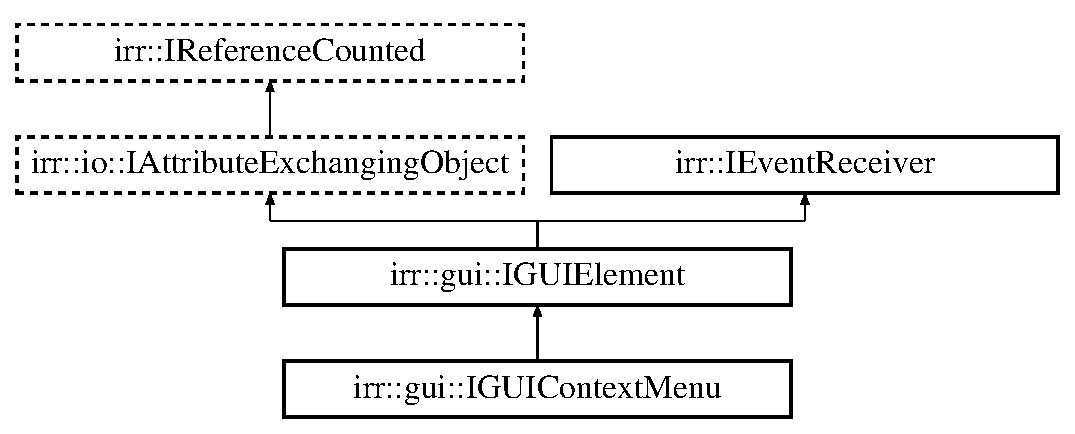
\includegraphics[height=4.038462cm]{classirr_1_1gui_1_1IGUIContextMenu}
\end{center}
\end{figure}
\subsection*{Public Member Functions}
\begin{DoxyCompactItemize}
\item 
\mbox{\Hypertarget{classirr_1_1gui_1_1IGUIContextMenu_ab7201b420431830aaaf8f9a0a831c859}\label{classirr_1_1gui_1_1IGUIContextMenu_ab7201b420431830aaaf8f9a0a831c859}} 
\hyperlink{classirr_1_1gui_1_1IGUIContextMenu_ab7201b420431830aaaf8f9a0a831c859}{I\+G\+U\+I\+Context\+Menu} (\hyperlink{classirr_1_1gui_1_1IGUIEnvironment}{I\+G\+U\+I\+Environment} $\ast$environment, \hyperlink{classirr_1_1gui_1_1IGUIElement}{I\+G\+U\+I\+Element} $\ast$parent, \hyperlink{namespaceirr_ac66849b7a6ed16e30ebede579f9b47c6}{s32} id, \hyperlink{classirr_1_1core_1_1rect}{core\+::rect}$<$ \hyperlink{namespaceirr_ac66849b7a6ed16e30ebede579f9b47c6}{s32} $>$ rectangle)
\begin{DoxyCompactList}\small\item\em constructor \end{DoxyCompactList}\item 
\mbox{\Hypertarget{classirr_1_1gui_1_1IGUIContextMenu_ae58a13dc73dffc7d30a907b76111a36d}\label{classirr_1_1gui_1_1IGUIContextMenu_ae58a13dc73dffc7d30a907b76111a36d}} 
virtual void \hyperlink{classirr_1_1gui_1_1IGUIContextMenu_ae58a13dc73dffc7d30a907b76111a36d}{set\+Close\+Handling} (\hyperlink{namespaceirr_1_1gui_a0868ffd1ff3d3fc1e2db2fcd118e320d}{E\+C\+O\+N\+T\+E\+X\+T\+\_\+\+M\+E\+N\+U\+\_\+\+C\+L\+O\+SE} on\+Close)=0
\begin{DoxyCompactList}\small\item\em set behavior when menus are closed \end{DoxyCompactList}\item 
\mbox{\Hypertarget{classirr_1_1gui_1_1IGUIContextMenu_ac9f46b106a1732ab474f3b38bf564edb}\label{classirr_1_1gui_1_1IGUIContextMenu_ac9f46b106a1732ab474f3b38bf564edb}} 
virtual \hyperlink{namespaceirr_1_1gui_a0868ffd1ff3d3fc1e2db2fcd118e320d}{E\+C\+O\+N\+T\+E\+X\+T\+\_\+\+M\+E\+N\+U\+\_\+\+C\+L\+O\+SE} \hyperlink{classirr_1_1gui_1_1IGUIContextMenu_ac9f46b106a1732ab474f3b38bf564edb}{get\+Close\+Handling} () const =0
\begin{DoxyCompactList}\small\item\em get current behavior when the menu will be closed \end{DoxyCompactList}\item 
\mbox{\Hypertarget{classirr_1_1gui_1_1IGUIContextMenu_a3e65b423c67002b64d6271072b19a829}\label{classirr_1_1gui_1_1IGUIContextMenu_a3e65b423c67002b64d6271072b19a829}} 
virtual \hyperlink{namespaceirr_a0416a53257075833e7002efd0a18e804}{u32} \hyperlink{classirr_1_1gui_1_1IGUIContextMenu_a3e65b423c67002b64d6271072b19a829}{get\+Item\+Count} () const =0
\begin{DoxyCompactList}\small\item\em Get amount of menu items. \end{DoxyCompactList}\item 
virtual \hyperlink{namespaceirr_a0416a53257075833e7002efd0a18e804}{u32} \hyperlink{classirr_1_1gui_1_1IGUIContextMenu_afa25240cb37816c3f8941ccc0f2c14ea}{add\+Item} (const wchar\+\_\+t $\ast$text, \hyperlink{namespaceirr_ac66849b7a6ed16e30ebede579f9b47c6}{s32} command\+Id=-\/1, bool enabled=true, bool has\+Sub\+Menu=false, bool checked=false, bool auto\+Checking=false)=0
\begin{DoxyCompactList}\small\item\em Adds a menu item. \end{DoxyCompactList}\item 
virtual \hyperlink{namespaceirr_a0416a53257075833e7002efd0a18e804}{u32} \hyperlink{classirr_1_1gui_1_1IGUIContextMenu_ad4695f88c63ffc09690c5ff682c3aabc}{insert\+Item} (\hyperlink{namespaceirr_a0416a53257075833e7002efd0a18e804}{u32} idx, const wchar\+\_\+t $\ast$text, \hyperlink{namespaceirr_ac66849b7a6ed16e30ebede579f9b47c6}{s32} command\+Id=-\/1, bool enabled=true, bool has\+Sub\+Menu=false, bool checked=false, bool auto\+Checking=false)=0
\begin{DoxyCompactList}\small\item\em Insert a menu item at specified position. \end{DoxyCompactList}\item 
virtual \hyperlink{namespaceirr_ac66849b7a6ed16e30ebede579f9b47c6}{s32} \hyperlink{classirr_1_1gui_1_1IGUIContextMenu_ae7b399d9940ebe566b928517aa150383}{find\+Item\+With\+Command\+Id} (\hyperlink{namespaceirr_ac66849b7a6ed16e30ebede579f9b47c6}{s32} command\+Id, \hyperlink{namespaceirr_a0416a53257075833e7002efd0a18e804}{u32} idx\+Start\+Search=0) const =0
\begin{DoxyCompactList}\small\item\em Find an item by it\textquotesingle{}s Command\+ID. \end{DoxyCompactList}\item 
\mbox{\Hypertarget{classirr_1_1gui_1_1IGUIContextMenu_a36e2edf23c88eed23d32af1d534d5bfc}\label{classirr_1_1gui_1_1IGUIContextMenu_a36e2edf23c88eed23d32af1d534d5bfc}} 
virtual void \hyperlink{classirr_1_1gui_1_1IGUIContextMenu_a36e2edf23c88eed23d32af1d534d5bfc}{add\+Separator} ()=0
\begin{DoxyCompactList}\small\item\em Adds a separator item to the menu. \end{DoxyCompactList}\item 
virtual const wchar\+\_\+t $\ast$ \hyperlink{classirr_1_1gui_1_1IGUIContextMenu_a18cf836d001f425f617c5a36db3d1ae6}{get\+Item\+Text} (\hyperlink{namespaceirr_a0416a53257075833e7002efd0a18e804}{u32} idx) const =0
\begin{DoxyCompactList}\small\item\em Get text of the menu item. \end{DoxyCompactList}\item 
virtual void \hyperlink{classirr_1_1gui_1_1IGUIContextMenu_a20d0e53213a2915a8a62c54b5aa2ff08}{set\+Item\+Text} (\hyperlink{namespaceirr_a0416a53257075833e7002efd0a18e804}{u32} idx, const wchar\+\_\+t $\ast$text)=0
\begin{DoxyCompactList}\small\item\em Sets text of the menu item. \end{DoxyCompactList}\item 
virtual bool \hyperlink{classirr_1_1gui_1_1IGUIContextMenu_a0064345c63e1f8e124e64ca96eb486e2}{is\+Item\+Enabled} (\hyperlink{namespaceirr_a0416a53257075833e7002efd0a18e804}{u32} idx) const =0
\begin{DoxyCompactList}\small\item\em Check if a menu item is enabled. \end{DoxyCompactList}\item 
virtual void \hyperlink{classirr_1_1gui_1_1IGUIContextMenu_aa3c36d6cd990f3b488be2c7f419b89ee}{set\+Item\+Enabled} (\hyperlink{namespaceirr_a0416a53257075833e7002efd0a18e804}{u32} idx, bool enabled)=0
\begin{DoxyCompactList}\small\item\em Sets if the menu item should be enabled. \end{DoxyCompactList}\item 
virtual void \hyperlink{classirr_1_1gui_1_1IGUIContextMenu_a8abbd1587dcc462f60660d7e606e954e}{set\+Item\+Checked} (\hyperlink{namespaceirr_a0416a53257075833e7002efd0a18e804}{u32} idx, bool enabled)=0
\begin{DoxyCompactList}\small\item\em Sets if the menu item should be checked. \end{DoxyCompactList}\item 
virtual bool \hyperlink{classirr_1_1gui_1_1IGUIContextMenu_a0ff910b79e5581a97aee8ec9a0679160}{is\+Item\+Checked} (\hyperlink{namespaceirr_a0416a53257075833e7002efd0a18e804}{u32} idx) const =0
\begin{DoxyCompactList}\small\item\em Check if a menu item is checked. \end{DoxyCompactList}\item 
virtual void \hyperlink{classirr_1_1gui_1_1IGUIContextMenu_af8cc0fc0f430044a318d4597f8535e9b}{remove\+Item} (\hyperlink{namespaceirr_a0416a53257075833e7002efd0a18e804}{u32} idx)=0
\begin{DoxyCompactList}\small\item\em Removes a menu item. \end{DoxyCompactList}\item 
\mbox{\Hypertarget{classirr_1_1gui_1_1IGUIContextMenu_ac06b8d80fb076c6bed3aef2a17fb01f9}\label{classirr_1_1gui_1_1IGUIContextMenu_ac06b8d80fb076c6bed3aef2a17fb01f9}} 
virtual void \hyperlink{classirr_1_1gui_1_1IGUIContextMenu_ac06b8d80fb076c6bed3aef2a17fb01f9}{remove\+All\+Items} ()=0
\begin{DoxyCompactList}\small\item\em Removes all menu items. \end{DoxyCompactList}\item 
virtual \hyperlink{namespaceirr_ac66849b7a6ed16e30ebede579f9b47c6}{s32} \hyperlink{classirr_1_1gui_1_1IGUIContextMenu_ae6cd391cf56d4454a855e19feddf8fdc}{get\+Selected\+Item} () const =0
\begin{DoxyCompactList}\small\item\em Get the selected item in the menu. \end{DoxyCompactList}\item 
virtual \hyperlink{namespaceirr_ac66849b7a6ed16e30ebede579f9b47c6}{s32} \hyperlink{classirr_1_1gui_1_1IGUIContextMenu_a5edfede62ed558acd68b06eeea0682c3}{get\+Item\+Command\+Id} (\hyperlink{namespaceirr_a0416a53257075833e7002efd0a18e804}{u32} idx) const =0
\begin{DoxyCompactList}\small\item\em Get the command id of a menu item. \end{DoxyCompactList}\item 
virtual void \hyperlink{classirr_1_1gui_1_1IGUIContextMenu_a1380ff56d8c4c5b8de8d221062464654}{set\+Item\+Command\+Id} (\hyperlink{namespaceirr_a0416a53257075833e7002efd0a18e804}{u32} idx, \hyperlink{namespaceirr_ac66849b7a6ed16e30ebede579f9b47c6}{s32} id)=0
\begin{DoxyCompactList}\small\item\em Sets the command id of a menu item. \end{DoxyCompactList}\item 
virtual \hyperlink{classirr_1_1gui_1_1IGUIContextMenu}{I\+G\+U\+I\+Context\+Menu} $\ast$ \hyperlink{classirr_1_1gui_1_1IGUIContextMenu_a296cfd0c4944b2c0bfb88973401fb824}{get\+Sub\+Menu} (\hyperlink{namespaceirr_a0416a53257075833e7002efd0a18e804}{u32} idx) const =0
\begin{DoxyCompactList}\small\item\em Get a pointer to the submenu of an item. \end{DoxyCompactList}\item 
\mbox{\Hypertarget{classirr_1_1gui_1_1IGUIContextMenu_ab393d00ca81ee9482c5a81d19cc6e79e}\label{classirr_1_1gui_1_1IGUIContextMenu_ab393d00ca81ee9482c5a81d19cc6e79e}} 
virtual void \hyperlink{classirr_1_1gui_1_1IGUIContextMenu_ab393d00ca81ee9482c5a81d19cc6e79e}{set\+Item\+Auto\+Checking} (\hyperlink{namespaceirr_a0416a53257075833e7002efd0a18e804}{u32} idx, bool auto\+Checking)=0
\begin{DoxyCompactList}\small\item\em should the element change the checked status on clicking \end{DoxyCompactList}\item 
\mbox{\Hypertarget{classirr_1_1gui_1_1IGUIContextMenu_ae1c7364f115e633bcfc040864e30f4c1}\label{classirr_1_1gui_1_1IGUIContextMenu_ae1c7364f115e633bcfc040864e30f4c1}} 
virtual bool \hyperlink{classirr_1_1gui_1_1IGUIContextMenu_ae1c7364f115e633bcfc040864e30f4c1}{get\+Item\+Auto\+Checking} (\hyperlink{namespaceirr_a0416a53257075833e7002efd0a18e804}{u32} idx) const =0
\begin{DoxyCompactList}\small\item\em does the element change the checked status on clicking \end{DoxyCompactList}\item 
\mbox{\Hypertarget{classirr_1_1gui_1_1IGUIContextMenu_a2d87831a224817fc9c9dd8f41c69ac0a}\label{classirr_1_1gui_1_1IGUIContextMenu_a2d87831a224817fc9c9dd8f41c69ac0a}} 
virtual void \hyperlink{classirr_1_1gui_1_1IGUIContextMenu_a2d87831a224817fc9c9dd8f41c69ac0a}{set\+Event\+Parent} (\hyperlink{classirr_1_1gui_1_1IGUIElement}{I\+G\+U\+I\+Element} $\ast$parent)=0
\begin{DoxyCompactList}\small\item\em When an eventparent is set it receives events instead of the usual parent element. \end{DoxyCompactList}\item 
\mbox{\Hypertarget{classirr_1_1gui_1_1IGUIContextMenu_ab7201b420431830aaaf8f9a0a831c859}\label{classirr_1_1gui_1_1IGUIContextMenu_ab7201b420431830aaaf8f9a0a831c859}} 
\hyperlink{classirr_1_1gui_1_1IGUIContextMenu_ab7201b420431830aaaf8f9a0a831c859}{I\+G\+U\+I\+Context\+Menu} (\hyperlink{classirr_1_1gui_1_1IGUIEnvironment}{I\+G\+U\+I\+Environment} $\ast$environment, \hyperlink{classirr_1_1gui_1_1IGUIElement}{I\+G\+U\+I\+Element} $\ast$parent, \hyperlink{namespaceirr_ac66849b7a6ed16e30ebede579f9b47c6}{s32} id, \hyperlink{classirr_1_1core_1_1rect}{core\+::rect}$<$ \hyperlink{namespaceirr_ac66849b7a6ed16e30ebede579f9b47c6}{s32} $>$ rectangle)
\begin{DoxyCompactList}\small\item\em constructor \end{DoxyCompactList}\item 
\mbox{\Hypertarget{classirr_1_1gui_1_1IGUIContextMenu_ae58a13dc73dffc7d30a907b76111a36d}\label{classirr_1_1gui_1_1IGUIContextMenu_ae58a13dc73dffc7d30a907b76111a36d}} 
virtual void \hyperlink{classirr_1_1gui_1_1IGUIContextMenu_ae58a13dc73dffc7d30a907b76111a36d}{set\+Close\+Handling} (\hyperlink{namespaceirr_1_1gui_a0868ffd1ff3d3fc1e2db2fcd118e320d}{E\+C\+O\+N\+T\+E\+X\+T\+\_\+\+M\+E\+N\+U\+\_\+\+C\+L\+O\+SE} on\+Close)=0
\begin{DoxyCompactList}\small\item\em set behavior when menus are closed \end{DoxyCompactList}\item 
\mbox{\Hypertarget{classirr_1_1gui_1_1IGUIContextMenu_ac9f46b106a1732ab474f3b38bf564edb}\label{classirr_1_1gui_1_1IGUIContextMenu_ac9f46b106a1732ab474f3b38bf564edb}} 
virtual \hyperlink{namespaceirr_1_1gui_a0868ffd1ff3d3fc1e2db2fcd118e320d}{E\+C\+O\+N\+T\+E\+X\+T\+\_\+\+M\+E\+N\+U\+\_\+\+C\+L\+O\+SE} \hyperlink{classirr_1_1gui_1_1IGUIContextMenu_ac9f46b106a1732ab474f3b38bf564edb}{get\+Close\+Handling} () const =0
\begin{DoxyCompactList}\small\item\em get current behavior when the menu will be closed \end{DoxyCompactList}\item 
\mbox{\Hypertarget{classirr_1_1gui_1_1IGUIContextMenu_a3e65b423c67002b64d6271072b19a829}\label{classirr_1_1gui_1_1IGUIContextMenu_a3e65b423c67002b64d6271072b19a829}} 
virtual \hyperlink{namespaceirr_a0416a53257075833e7002efd0a18e804}{u32} \hyperlink{classirr_1_1gui_1_1IGUIContextMenu_a3e65b423c67002b64d6271072b19a829}{get\+Item\+Count} () const =0
\begin{DoxyCompactList}\small\item\em Get amount of menu items. \end{DoxyCompactList}\item 
virtual \hyperlink{namespaceirr_a0416a53257075833e7002efd0a18e804}{u32} \hyperlink{classirr_1_1gui_1_1IGUIContextMenu_afa25240cb37816c3f8941ccc0f2c14ea}{add\+Item} (const wchar\+\_\+t $\ast$text, \hyperlink{namespaceirr_ac66849b7a6ed16e30ebede579f9b47c6}{s32} command\+Id=-\/1, bool enabled=true, bool has\+Sub\+Menu=false, bool checked=false, bool auto\+Checking=false)=0
\begin{DoxyCompactList}\small\item\em Adds a menu item. \end{DoxyCompactList}\item 
virtual \hyperlink{namespaceirr_a0416a53257075833e7002efd0a18e804}{u32} \hyperlink{classirr_1_1gui_1_1IGUIContextMenu_ad4695f88c63ffc09690c5ff682c3aabc}{insert\+Item} (\hyperlink{namespaceirr_a0416a53257075833e7002efd0a18e804}{u32} idx, const wchar\+\_\+t $\ast$text, \hyperlink{namespaceirr_ac66849b7a6ed16e30ebede579f9b47c6}{s32} command\+Id=-\/1, bool enabled=true, bool has\+Sub\+Menu=false, bool checked=false, bool auto\+Checking=false)=0
\begin{DoxyCompactList}\small\item\em Insert a menu item at specified position. \end{DoxyCompactList}\item 
virtual \hyperlink{namespaceirr_ac66849b7a6ed16e30ebede579f9b47c6}{s32} \hyperlink{classirr_1_1gui_1_1IGUIContextMenu_ae7b399d9940ebe566b928517aa150383}{find\+Item\+With\+Command\+Id} (\hyperlink{namespaceirr_ac66849b7a6ed16e30ebede579f9b47c6}{s32} command\+Id, \hyperlink{namespaceirr_a0416a53257075833e7002efd0a18e804}{u32} idx\+Start\+Search=0) const =0
\begin{DoxyCompactList}\small\item\em Find an item by it\textquotesingle{}s Command\+ID. \end{DoxyCompactList}\item 
\mbox{\Hypertarget{classirr_1_1gui_1_1IGUIContextMenu_a36e2edf23c88eed23d32af1d534d5bfc}\label{classirr_1_1gui_1_1IGUIContextMenu_a36e2edf23c88eed23d32af1d534d5bfc}} 
virtual void \hyperlink{classirr_1_1gui_1_1IGUIContextMenu_a36e2edf23c88eed23d32af1d534d5bfc}{add\+Separator} ()=0
\begin{DoxyCompactList}\small\item\em Adds a separator item to the menu. \end{DoxyCompactList}\item 
virtual const wchar\+\_\+t $\ast$ \hyperlink{classirr_1_1gui_1_1IGUIContextMenu_a18cf836d001f425f617c5a36db3d1ae6}{get\+Item\+Text} (\hyperlink{namespaceirr_a0416a53257075833e7002efd0a18e804}{u32} idx) const =0
\begin{DoxyCompactList}\small\item\em Get text of the menu item. \end{DoxyCompactList}\item 
virtual void \hyperlink{classirr_1_1gui_1_1IGUIContextMenu_a20d0e53213a2915a8a62c54b5aa2ff08}{set\+Item\+Text} (\hyperlink{namespaceirr_a0416a53257075833e7002efd0a18e804}{u32} idx, const wchar\+\_\+t $\ast$text)=0
\begin{DoxyCompactList}\small\item\em Sets text of the menu item. \end{DoxyCompactList}\item 
virtual bool \hyperlink{classirr_1_1gui_1_1IGUIContextMenu_a0064345c63e1f8e124e64ca96eb486e2}{is\+Item\+Enabled} (\hyperlink{namespaceirr_a0416a53257075833e7002efd0a18e804}{u32} idx) const =0
\begin{DoxyCompactList}\small\item\em Check if a menu item is enabled. \end{DoxyCompactList}\item 
virtual void \hyperlink{classirr_1_1gui_1_1IGUIContextMenu_aa3c36d6cd990f3b488be2c7f419b89ee}{set\+Item\+Enabled} (\hyperlink{namespaceirr_a0416a53257075833e7002efd0a18e804}{u32} idx, bool enabled)=0
\begin{DoxyCompactList}\small\item\em Sets if the menu item should be enabled. \end{DoxyCompactList}\item 
virtual void \hyperlink{classirr_1_1gui_1_1IGUIContextMenu_a8abbd1587dcc462f60660d7e606e954e}{set\+Item\+Checked} (\hyperlink{namespaceirr_a0416a53257075833e7002efd0a18e804}{u32} idx, bool enabled)=0
\begin{DoxyCompactList}\small\item\em Sets if the menu item should be checked. \end{DoxyCompactList}\item 
virtual bool \hyperlink{classirr_1_1gui_1_1IGUIContextMenu_a0ff910b79e5581a97aee8ec9a0679160}{is\+Item\+Checked} (\hyperlink{namespaceirr_a0416a53257075833e7002efd0a18e804}{u32} idx) const =0
\begin{DoxyCompactList}\small\item\em Check if a menu item is checked. \end{DoxyCompactList}\item 
virtual void \hyperlink{classirr_1_1gui_1_1IGUIContextMenu_af8cc0fc0f430044a318d4597f8535e9b}{remove\+Item} (\hyperlink{namespaceirr_a0416a53257075833e7002efd0a18e804}{u32} idx)=0
\begin{DoxyCompactList}\small\item\em Removes a menu item. \end{DoxyCompactList}\item 
\mbox{\Hypertarget{classirr_1_1gui_1_1IGUIContextMenu_ac06b8d80fb076c6bed3aef2a17fb01f9}\label{classirr_1_1gui_1_1IGUIContextMenu_ac06b8d80fb076c6bed3aef2a17fb01f9}} 
virtual void \hyperlink{classirr_1_1gui_1_1IGUIContextMenu_ac06b8d80fb076c6bed3aef2a17fb01f9}{remove\+All\+Items} ()=0
\begin{DoxyCompactList}\small\item\em Removes all menu items. \end{DoxyCompactList}\item 
virtual \hyperlink{namespaceirr_ac66849b7a6ed16e30ebede579f9b47c6}{s32} \hyperlink{classirr_1_1gui_1_1IGUIContextMenu_ae6cd391cf56d4454a855e19feddf8fdc}{get\+Selected\+Item} () const =0
\begin{DoxyCompactList}\small\item\em Get the selected item in the menu. \end{DoxyCompactList}\item 
virtual \hyperlink{namespaceirr_ac66849b7a6ed16e30ebede579f9b47c6}{s32} \hyperlink{classirr_1_1gui_1_1IGUIContextMenu_a5edfede62ed558acd68b06eeea0682c3}{get\+Item\+Command\+Id} (\hyperlink{namespaceirr_a0416a53257075833e7002efd0a18e804}{u32} idx) const =0
\begin{DoxyCompactList}\small\item\em Get the command id of a menu item. \end{DoxyCompactList}\item 
virtual void \hyperlink{classirr_1_1gui_1_1IGUIContextMenu_a1380ff56d8c4c5b8de8d221062464654}{set\+Item\+Command\+Id} (\hyperlink{namespaceirr_a0416a53257075833e7002efd0a18e804}{u32} idx, \hyperlink{namespaceirr_ac66849b7a6ed16e30ebede579f9b47c6}{s32} id)=0
\begin{DoxyCompactList}\small\item\em Sets the command id of a menu item. \end{DoxyCompactList}\item 
virtual \hyperlink{classirr_1_1gui_1_1IGUIContextMenu}{I\+G\+U\+I\+Context\+Menu} $\ast$ \hyperlink{classirr_1_1gui_1_1IGUIContextMenu_a296cfd0c4944b2c0bfb88973401fb824}{get\+Sub\+Menu} (\hyperlink{namespaceirr_a0416a53257075833e7002efd0a18e804}{u32} idx) const =0
\begin{DoxyCompactList}\small\item\em Get a pointer to the submenu of an item. \end{DoxyCompactList}\item 
\mbox{\Hypertarget{classirr_1_1gui_1_1IGUIContextMenu_ab393d00ca81ee9482c5a81d19cc6e79e}\label{classirr_1_1gui_1_1IGUIContextMenu_ab393d00ca81ee9482c5a81d19cc6e79e}} 
virtual void \hyperlink{classirr_1_1gui_1_1IGUIContextMenu_ab393d00ca81ee9482c5a81d19cc6e79e}{set\+Item\+Auto\+Checking} (\hyperlink{namespaceirr_a0416a53257075833e7002efd0a18e804}{u32} idx, bool auto\+Checking)=0
\begin{DoxyCompactList}\small\item\em should the element change the checked status on clicking \end{DoxyCompactList}\item 
\mbox{\Hypertarget{classirr_1_1gui_1_1IGUIContextMenu_ae1c7364f115e633bcfc040864e30f4c1}\label{classirr_1_1gui_1_1IGUIContextMenu_ae1c7364f115e633bcfc040864e30f4c1}} 
virtual bool \hyperlink{classirr_1_1gui_1_1IGUIContextMenu_ae1c7364f115e633bcfc040864e30f4c1}{get\+Item\+Auto\+Checking} (\hyperlink{namespaceirr_a0416a53257075833e7002efd0a18e804}{u32} idx) const =0
\begin{DoxyCompactList}\small\item\em does the element change the checked status on clicking \end{DoxyCompactList}\item 
\mbox{\Hypertarget{classirr_1_1gui_1_1IGUIContextMenu_a2d87831a224817fc9c9dd8f41c69ac0a}\label{classirr_1_1gui_1_1IGUIContextMenu_a2d87831a224817fc9c9dd8f41c69ac0a}} 
virtual void \hyperlink{classirr_1_1gui_1_1IGUIContextMenu_a2d87831a224817fc9c9dd8f41c69ac0a}{set\+Event\+Parent} (\hyperlink{classirr_1_1gui_1_1IGUIElement}{I\+G\+U\+I\+Element} $\ast$parent)=0
\begin{DoxyCompactList}\small\item\em When an eventparent is set it receives events instead of the usual parent element. \end{DoxyCompactList}\end{DoxyCompactItemize}
\subsection*{Additional Inherited Members}


\subsection{Detailed Description}
G\+UI Context menu interface. 

\begin{DoxyParagraph}{This element can create the following events of type E\+G\+U\+I\+\_\+\+E\+V\+E\+N\+T\+\_\+\+T\+Y\+PE\+:}
\begin{DoxyItemize}
\item E\+G\+E\+T\+\_\+\+E\+L\+E\+M\+E\+N\+T\+\_\+\+C\+L\+O\+S\+ED \item E\+G\+E\+T\+\_\+\+M\+E\+N\+U\+\_\+\+I\+T\+E\+M\+\_\+\+S\+E\+L\+E\+C\+T\+ED \end{DoxyItemize}

\end{DoxyParagraph}


\subsection{Member Function Documentation}
\mbox{\Hypertarget{classirr_1_1gui_1_1IGUIContextMenu_afa25240cb37816c3f8941ccc0f2c14ea}\label{classirr_1_1gui_1_1IGUIContextMenu_afa25240cb37816c3f8941ccc0f2c14ea}} 
\index{irr\+::gui\+::\+I\+G\+U\+I\+Context\+Menu@{irr\+::gui\+::\+I\+G\+U\+I\+Context\+Menu}!add\+Item@{add\+Item}}
\index{add\+Item@{add\+Item}!irr\+::gui\+::\+I\+G\+U\+I\+Context\+Menu@{irr\+::gui\+::\+I\+G\+U\+I\+Context\+Menu}}
\subsubsection{\texorpdfstring{add\+Item()}{addItem()}\hspace{0.1cm}{\footnotesize\ttfamily [1/2]}}
{\footnotesize\ttfamily virtual \hyperlink{namespaceirr_a0416a53257075833e7002efd0a18e804}{u32} irr\+::gui\+::\+I\+G\+U\+I\+Context\+Menu\+::add\+Item (\begin{DoxyParamCaption}\item[{const wchar\+\_\+t $\ast$}]{text,  }\item[{\hyperlink{namespaceirr_ac66849b7a6ed16e30ebede579f9b47c6}{s32}}]{command\+Id = {\ttfamily -\/1},  }\item[{bool}]{enabled = {\ttfamily true},  }\item[{bool}]{has\+Sub\+Menu = {\ttfamily false},  }\item[{bool}]{checked = {\ttfamily false},  }\item[{bool}]{auto\+Checking = {\ttfamily false} }\end{DoxyParamCaption})\hspace{0.3cm}{\ttfamily [pure virtual]}}



Adds a menu item. 


\begin{DoxyParams}{Parameters}
{\em text} & \hyperlink{classText}{Text} of menu item. Set this to 0 to create an separator instead of a real item, which is the same like calling \hyperlink{classirr_1_1gui_1_1IGUIContextMenu_a36e2edf23c88eed23d32af1d534d5bfc}{add\+Separator()}; \\
\hline
{\em command\+Id} & Command id of menu item, a simple id you may set to whatever you want. \\
\hline
{\em enabled} & Specifies if the menu item should be enabled. \\
\hline
{\em has\+Sub\+Menu} & Set this to true if there should be a submenu at this item. You can access this submenu via \hyperlink{classirr_1_1gui_1_1IGUIContextMenu_a296cfd0c4944b2c0bfb88973401fb824}{get\+Sub\+Menu()}. \\
\hline
{\em checked} & Specifies if the menu item should be initially checked. \\
\hline
{\em auto\+Checking} & Specifies if the item should be checked by clicking \\
\hline
\end{DoxyParams}
\begin{DoxyReturn}{Returns}
Returns the index of the new item 
\end{DoxyReturn}
\mbox{\Hypertarget{classirr_1_1gui_1_1IGUIContextMenu_afa25240cb37816c3f8941ccc0f2c14ea}\label{classirr_1_1gui_1_1IGUIContextMenu_afa25240cb37816c3f8941ccc0f2c14ea}} 
\index{irr\+::gui\+::\+I\+G\+U\+I\+Context\+Menu@{irr\+::gui\+::\+I\+G\+U\+I\+Context\+Menu}!add\+Item@{add\+Item}}
\index{add\+Item@{add\+Item}!irr\+::gui\+::\+I\+G\+U\+I\+Context\+Menu@{irr\+::gui\+::\+I\+G\+U\+I\+Context\+Menu}}
\subsubsection{\texorpdfstring{add\+Item()}{addItem()}\hspace{0.1cm}{\footnotesize\ttfamily [2/2]}}
{\footnotesize\ttfamily virtual \hyperlink{namespaceirr_a0416a53257075833e7002efd0a18e804}{u32} irr\+::gui\+::\+I\+G\+U\+I\+Context\+Menu\+::add\+Item (\begin{DoxyParamCaption}\item[{const wchar\+\_\+t $\ast$}]{text,  }\item[{\hyperlink{namespaceirr_ac66849b7a6ed16e30ebede579f9b47c6}{s32}}]{command\+Id = {\ttfamily -\/1},  }\item[{bool}]{enabled = {\ttfamily true},  }\item[{bool}]{has\+Sub\+Menu = {\ttfamily false},  }\item[{bool}]{checked = {\ttfamily false},  }\item[{bool}]{auto\+Checking = {\ttfamily false} }\end{DoxyParamCaption})\hspace{0.3cm}{\ttfamily [pure virtual]}}



Adds a menu item. 


\begin{DoxyParams}{Parameters}
{\em text} & \hyperlink{classText}{Text} of menu item. Set this to 0 to create an separator instead of a real item, which is the same like calling \hyperlink{classirr_1_1gui_1_1IGUIContextMenu_a36e2edf23c88eed23d32af1d534d5bfc}{add\+Separator()}; \\
\hline
{\em command\+Id} & Command id of menu item, a simple id you may set to whatever you want. \\
\hline
{\em enabled} & Specifies if the menu item should be enabled. \\
\hline
{\em has\+Sub\+Menu} & Set this to true if there should be a submenu at this item. You can access this submenu via \hyperlink{classirr_1_1gui_1_1IGUIContextMenu_a296cfd0c4944b2c0bfb88973401fb824}{get\+Sub\+Menu()}. \\
\hline
{\em checked} & Specifies if the menu item should be initially checked. \\
\hline
{\em auto\+Checking} & Specifies if the item should be checked by clicking \\
\hline
\end{DoxyParams}
\begin{DoxyReturn}{Returns}
Returns the index of the new item 
\end{DoxyReturn}
\mbox{\Hypertarget{classirr_1_1gui_1_1IGUIContextMenu_ae7b399d9940ebe566b928517aa150383}\label{classirr_1_1gui_1_1IGUIContextMenu_ae7b399d9940ebe566b928517aa150383}} 
\index{irr\+::gui\+::\+I\+G\+U\+I\+Context\+Menu@{irr\+::gui\+::\+I\+G\+U\+I\+Context\+Menu}!find\+Item\+With\+Command\+Id@{find\+Item\+With\+Command\+Id}}
\index{find\+Item\+With\+Command\+Id@{find\+Item\+With\+Command\+Id}!irr\+::gui\+::\+I\+G\+U\+I\+Context\+Menu@{irr\+::gui\+::\+I\+G\+U\+I\+Context\+Menu}}
\subsubsection{\texorpdfstring{find\+Item\+With\+Command\+Id()}{findItemWithCommandId()}\hspace{0.1cm}{\footnotesize\ttfamily [1/2]}}
{\footnotesize\ttfamily virtual \hyperlink{namespaceirr_ac66849b7a6ed16e30ebede579f9b47c6}{s32} irr\+::gui\+::\+I\+G\+U\+I\+Context\+Menu\+::find\+Item\+With\+Command\+Id (\begin{DoxyParamCaption}\item[{\hyperlink{namespaceirr_ac66849b7a6ed16e30ebede579f9b47c6}{s32}}]{command\+Id,  }\item[{\hyperlink{namespaceirr_a0416a53257075833e7002efd0a18e804}{u32}}]{idx\+Start\+Search = {\ttfamily 0} }\end{DoxyParamCaption}) const\hspace{0.3cm}{\ttfamily [pure virtual]}}



Find an item by it\textquotesingle{}s Command\+ID. 


\begin{DoxyParams}{Parameters}
{\em command\+Id} & We are looking for the first item which has this command\+ID \\
\hline
{\em idx\+Start\+Search} & Start searching from this index. \\
\hline
\end{DoxyParams}
\begin{DoxyReturn}{Returns}
Returns the index of the item when found or otherwise -\/1. 
\end{DoxyReturn}
\mbox{\Hypertarget{classirr_1_1gui_1_1IGUIContextMenu_ae7b399d9940ebe566b928517aa150383}\label{classirr_1_1gui_1_1IGUIContextMenu_ae7b399d9940ebe566b928517aa150383}} 
\index{irr\+::gui\+::\+I\+G\+U\+I\+Context\+Menu@{irr\+::gui\+::\+I\+G\+U\+I\+Context\+Menu}!find\+Item\+With\+Command\+Id@{find\+Item\+With\+Command\+Id}}
\index{find\+Item\+With\+Command\+Id@{find\+Item\+With\+Command\+Id}!irr\+::gui\+::\+I\+G\+U\+I\+Context\+Menu@{irr\+::gui\+::\+I\+G\+U\+I\+Context\+Menu}}
\subsubsection{\texorpdfstring{find\+Item\+With\+Command\+Id()}{findItemWithCommandId()}\hspace{0.1cm}{\footnotesize\ttfamily [2/2]}}
{\footnotesize\ttfamily virtual \hyperlink{namespaceirr_ac66849b7a6ed16e30ebede579f9b47c6}{s32} irr\+::gui\+::\+I\+G\+U\+I\+Context\+Menu\+::find\+Item\+With\+Command\+Id (\begin{DoxyParamCaption}\item[{\hyperlink{namespaceirr_ac66849b7a6ed16e30ebede579f9b47c6}{s32}}]{command\+Id,  }\item[{\hyperlink{namespaceirr_a0416a53257075833e7002efd0a18e804}{u32}}]{idx\+Start\+Search = {\ttfamily 0} }\end{DoxyParamCaption}) const\hspace{0.3cm}{\ttfamily [pure virtual]}}



Find an item by it\textquotesingle{}s Command\+ID. 


\begin{DoxyParams}{Parameters}
{\em command\+Id} & We are looking for the first item which has this command\+ID \\
\hline
{\em idx\+Start\+Search} & Start searching from this index. \\
\hline
\end{DoxyParams}
\begin{DoxyReturn}{Returns}
Returns the index of the item when found or otherwise -\/1. 
\end{DoxyReturn}
\mbox{\Hypertarget{classirr_1_1gui_1_1IGUIContextMenu_a5edfede62ed558acd68b06eeea0682c3}\label{classirr_1_1gui_1_1IGUIContextMenu_a5edfede62ed558acd68b06eeea0682c3}} 
\index{irr\+::gui\+::\+I\+G\+U\+I\+Context\+Menu@{irr\+::gui\+::\+I\+G\+U\+I\+Context\+Menu}!get\+Item\+Command\+Id@{get\+Item\+Command\+Id}}
\index{get\+Item\+Command\+Id@{get\+Item\+Command\+Id}!irr\+::gui\+::\+I\+G\+U\+I\+Context\+Menu@{irr\+::gui\+::\+I\+G\+U\+I\+Context\+Menu}}
\subsubsection{\texorpdfstring{get\+Item\+Command\+Id()}{getItemCommandId()}\hspace{0.1cm}{\footnotesize\ttfamily [1/2]}}
{\footnotesize\ttfamily virtual \hyperlink{namespaceirr_ac66849b7a6ed16e30ebede579f9b47c6}{s32} irr\+::gui\+::\+I\+G\+U\+I\+Context\+Menu\+::get\+Item\+Command\+Id (\begin{DoxyParamCaption}\item[{\hyperlink{namespaceirr_a0416a53257075833e7002efd0a18e804}{u32}}]{idx }\end{DoxyParamCaption}) const\hspace{0.3cm}{\ttfamily [pure virtual]}}



Get the command id of a menu item. 


\begin{DoxyParams}{Parameters}
{\em idx} & Zero based index of the menu item \\
\hline
\end{DoxyParams}
\mbox{\Hypertarget{classirr_1_1gui_1_1IGUIContextMenu_a5edfede62ed558acd68b06eeea0682c3}\label{classirr_1_1gui_1_1IGUIContextMenu_a5edfede62ed558acd68b06eeea0682c3}} 
\index{irr\+::gui\+::\+I\+G\+U\+I\+Context\+Menu@{irr\+::gui\+::\+I\+G\+U\+I\+Context\+Menu}!get\+Item\+Command\+Id@{get\+Item\+Command\+Id}}
\index{get\+Item\+Command\+Id@{get\+Item\+Command\+Id}!irr\+::gui\+::\+I\+G\+U\+I\+Context\+Menu@{irr\+::gui\+::\+I\+G\+U\+I\+Context\+Menu}}
\subsubsection{\texorpdfstring{get\+Item\+Command\+Id()}{getItemCommandId()}\hspace{0.1cm}{\footnotesize\ttfamily [2/2]}}
{\footnotesize\ttfamily virtual \hyperlink{namespaceirr_ac66849b7a6ed16e30ebede579f9b47c6}{s32} irr\+::gui\+::\+I\+G\+U\+I\+Context\+Menu\+::get\+Item\+Command\+Id (\begin{DoxyParamCaption}\item[{\hyperlink{namespaceirr_a0416a53257075833e7002efd0a18e804}{u32}}]{idx }\end{DoxyParamCaption}) const\hspace{0.3cm}{\ttfamily [pure virtual]}}



Get the command id of a menu item. 


\begin{DoxyParams}{Parameters}
{\em idx} & Zero based index of the menu item \\
\hline
\end{DoxyParams}
\mbox{\Hypertarget{classirr_1_1gui_1_1IGUIContextMenu_a18cf836d001f425f617c5a36db3d1ae6}\label{classirr_1_1gui_1_1IGUIContextMenu_a18cf836d001f425f617c5a36db3d1ae6}} 
\index{irr\+::gui\+::\+I\+G\+U\+I\+Context\+Menu@{irr\+::gui\+::\+I\+G\+U\+I\+Context\+Menu}!get\+Item\+Text@{get\+Item\+Text}}
\index{get\+Item\+Text@{get\+Item\+Text}!irr\+::gui\+::\+I\+G\+U\+I\+Context\+Menu@{irr\+::gui\+::\+I\+G\+U\+I\+Context\+Menu}}
\subsubsection{\texorpdfstring{get\+Item\+Text()}{getItemText()}\hspace{0.1cm}{\footnotesize\ttfamily [1/2]}}
{\footnotesize\ttfamily virtual const wchar\+\_\+t$\ast$ irr\+::gui\+::\+I\+G\+U\+I\+Context\+Menu\+::get\+Item\+Text (\begin{DoxyParamCaption}\item[{\hyperlink{namespaceirr_a0416a53257075833e7002efd0a18e804}{u32}}]{idx }\end{DoxyParamCaption}) const\hspace{0.3cm}{\ttfamily [pure virtual]}}



Get text of the menu item. 


\begin{DoxyParams}{Parameters}
{\em idx} & Zero based index of the menu item \\
\hline
\end{DoxyParams}
\mbox{\Hypertarget{classirr_1_1gui_1_1IGUIContextMenu_a18cf836d001f425f617c5a36db3d1ae6}\label{classirr_1_1gui_1_1IGUIContextMenu_a18cf836d001f425f617c5a36db3d1ae6}} 
\index{irr\+::gui\+::\+I\+G\+U\+I\+Context\+Menu@{irr\+::gui\+::\+I\+G\+U\+I\+Context\+Menu}!get\+Item\+Text@{get\+Item\+Text}}
\index{get\+Item\+Text@{get\+Item\+Text}!irr\+::gui\+::\+I\+G\+U\+I\+Context\+Menu@{irr\+::gui\+::\+I\+G\+U\+I\+Context\+Menu}}
\subsubsection{\texorpdfstring{get\+Item\+Text()}{getItemText()}\hspace{0.1cm}{\footnotesize\ttfamily [2/2]}}
{\footnotesize\ttfamily virtual const wchar\+\_\+t$\ast$ irr\+::gui\+::\+I\+G\+U\+I\+Context\+Menu\+::get\+Item\+Text (\begin{DoxyParamCaption}\item[{\hyperlink{namespaceirr_a0416a53257075833e7002efd0a18e804}{u32}}]{idx }\end{DoxyParamCaption}) const\hspace{0.3cm}{\ttfamily [pure virtual]}}



Get text of the menu item. 


\begin{DoxyParams}{Parameters}
{\em idx} & Zero based index of the menu item \\
\hline
\end{DoxyParams}
\mbox{\Hypertarget{classirr_1_1gui_1_1IGUIContextMenu_ae6cd391cf56d4454a855e19feddf8fdc}\label{classirr_1_1gui_1_1IGUIContextMenu_ae6cd391cf56d4454a855e19feddf8fdc}} 
\index{irr\+::gui\+::\+I\+G\+U\+I\+Context\+Menu@{irr\+::gui\+::\+I\+G\+U\+I\+Context\+Menu}!get\+Selected\+Item@{get\+Selected\+Item}}
\index{get\+Selected\+Item@{get\+Selected\+Item}!irr\+::gui\+::\+I\+G\+U\+I\+Context\+Menu@{irr\+::gui\+::\+I\+G\+U\+I\+Context\+Menu}}
\subsubsection{\texorpdfstring{get\+Selected\+Item()}{getSelectedItem()}\hspace{0.1cm}{\footnotesize\ttfamily [1/2]}}
{\footnotesize\ttfamily virtual \hyperlink{namespaceirr_ac66849b7a6ed16e30ebede579f9b47c6}{s32} irr\+::gui\+::\+I\+G\+U\+I\+Context\+Menu\+::get\+Selected\+Item (\begin{DoxyParamCaption}{ }\end{DoxyParamCaption}) const\hspace{0.3cm}{\ttfamily [pure virtual]}}



Get the selected item in the menu. 

\begin{DoxyReturn}{Returns}
Index of the selected item, -\/1 if none selected. 
\end{DoxyReturn}
\mbox{\Hypertarget{classirr_1_1gui_1_1IGUIContextMenu_ae6cd391cf56d4454a855e19feddf8fdc}\label{classirr_1_1gui_1_1IGUIContextMenu_ae6cd391cf56d4454a855e19feddf8fdc}} 
\index{irr\+::gui\+::\+I\+G\+U\+I\+Context\+Menu@{irr\+::gui\+::\+I\+G\+U\+I\+Context\+Menu}!get\+Selected\+Item@{get\+Selected\+Item}}
\index{get\+Selected\+Item@{get\+Selected\+Item}!irr\+::gui\+::\+I\+G\+U\+I\+Context\+Menu@{irr\+::gui\+::\+I\+G\+U\+I\+Context\+Menu}}
\subsubsection{\texorpdfstring{get\+Selected\+Item()}{getSelectedItem()}\hspace{0.1cm}{\footnotesize\ttfamily [2/2]}}
{\footnotesize\ttfamily virtual \hyperlink{namespaceirr_ac66849b7a6ed16e30ebede579f9b47c6}{s32} irr\+::gui\+::\+I\+G\+U\+I\+Context\+Menu\+::get\+Selected\+Item (\begin{DoxyParamCaption}{ }\end{DoxyParamCaption}) const\hspace{0.3cm}{\ttfamily [pure virtual]}}



Get the selected item in the menu. 

\begin{DoxyReturn}{Returns}
Index of the selected item, -\/1 if none selected. 
\end{DoxyReturn}
\mbox{\Hypertarget{classirr_1_1gui_1_1IGUIContextMenu_a296cfd0c4944b2c0bfb88973401fb824}\label{classirr_1_1gui_1_1IGUIContextMenu_a296cfd0c4944b2c0bfb88973401fb824}} 
\index{irr\+::gui\+::\+I\+G\+U\+I\+Context\+Menu@{irr\+::gui\+::\+I\+G\+U\+I\+Context\+Menu}!get\+Sub\+Menu@{get\+Sub\+Menu}}
\index{get\+Sub\+Menu@{get\+Sub\+Menu}!irr\+::gui\+::\+I\+G\+U\+I\+Context\+Menu@{irr\+::gui\+::\+I\+G\+U\+I\+Context\+Menu}}
\subsubsection{\texorpdfstring{get\+Sub\+Menu()}{getSubMenu()}\hspace{0.1cm}{\footnotesize\ttfamily [1/2]}}
{\footnotesize\ttfamily virtual \hyperlink{classirr_1_1gui_1_1IGUIContextMenu}{I\+G\+U\+I\+Context\+Menu}$\ast$ irr\+::gui\+::\+I\+G\+U\+I\+Context\+Menu\+::get\+Sub\+Menu (\begin{DoxyParamCaption}\item[{\hyperlink{namespaceirr_a0416a53257075833e7002efd0a18e804}{u32}}]{idx }\end{DoxyParamCaption}) const\hspace{0.3cm}{\ttfamily [pure virtual]}}



Get a pointer to the submenu of an item. 

0 is returned if there is no submenu 
\begin{DoxyParams}{Parameters}
{\em idx} & Zero based index of the menu item \\
\hline
\end{DoxyParams}
\begin{DoxyReturn}{Returns}
Returns a pointer to the submenu of an item. 
\end{DoxyReturn}
\mbox{\Hypertarget{classirr_1_1gui_1_1IGUIContextMenu_a296cfd0c4944b2c0bfb88973401fb824}\label{classirr_1_1gui_1_1IGUIContextMenu_a296cfd0c4944b2c0bfb88973401fb824}} 
\index{irr\+::gui\+::\+I\+G\+U\+I\+Context\+Menu@{irr\+::gui\+::\+I\+G\+U\+I\+Context\+Menu}!get\+Sub\+Menu@{get\+Sub\+Menu}}
\index{get\+Sub\+Menu@{get\+Sub\+Menu}!irr\+::gui\+::\+I\+G\+U\+I\+Context\+Menu@{irr\+::gui\+::\+I\+G\+U\+I\+Context\+Menu}}
\subsubsection{\texorpdfstring{get\+Sub\+Menu()}{getSubMenu()}\hspace{0.1cm}{\footnotesize\ttfamily [2/2]}}
{\footnotesize\ttfamily virtual \hyperlink{classirr_1_1gui_1_1IGUIContextMenu}{I\+G\+U\+I\+Context\+Menu}$\ast$ irr\+::gui\+::\+I\+G\+U\+I\+Context\+Menu\+::get\+Sub\+Menu (\begin{DoxyParamCaption}\item[{\hyperlink{namespaceirr_a0416a53257075833e7002efd0a18e804}{u32}}]{idx }\end{DoxyParamCaption}) const\hspace{0.3cm}{\ttfamily [pure virtual]}}



Get a pointer to the submenu of an item. 

0 is returned if there is no submenu 
\begin{DoxyParams}{Parameters}
{\em idx} & Zero based index of the menu item \\
\hline
\end{DoxyParams}
\begin{DoxyReturn}{Returns}
Returns a pointer to the submenu of an item. 
\end{DoxyReturn}
\mbox{\Hypertarget{classirr_1_1gui_1_1IGUIContextMenu_ad4695f88c63ffc09690c5ff682c3aabc}\label{classirr_1_1gui_1_1IGUIContextMenu_ad4695f88c63ffc09690c5ff682c3aabc}} 
\index{irr\+::gui\+::\+I\+G\+U\+I\+Context\+Menu@{irr\+::gui\+::\+I\+G\+U\+I\+Context\+Menu}!insert\+Item@{insert\+Item}}
\index{insert\+Item@{insert\+Item}!irr\+::gui\+::\+I\+G\+U\+I\+Context\+Menu@{irr\+::gui\+::\+I\+G\+U\+I\+Context\+Menu}}
\subsubsection{\texorpdfstring{insert\+Item()}{insertItem()}\hspace{0.1cm}{\footnotesize\ttfamily [1/2]}}
{\footnotesize\ttfamily virtual \hyperlink{namespaceirr_a0416a53257075833e7002efd0a18e804}{u32} irr\+::gui\+::\+I\+G\+U\+I\+Context\+Menu\+::insert\+Item (\begin{DoxyParamCaption}\item[{\hyperlink{namespaceirr_a0416a53257075833e7002efd0a18e804}{u32}}]{idx,  }\item[{const wchar\+\_\+t $\ast$}]{text,  }\item[{\hyperlink{namespaceirr_ac66849b7a6ed16e30ebede579f9b47c6}{s32}}]{command\+Id = {\ttfamily -\/1},  }\item[{bool}]{enabled = {\ttfamily true},  }\item[{bool}]{has\+Sub\+Menu = {\ttfamily false},  }\item[{bool}]{checked = {\ttfamily false},  }\item[{bool}]{auto\+Checking = {\ttfamily false} }\end{DoxyParamCaption})\hspace{0.3cm}{\ttfamily [pure virtual]}}



Insert a menu item at specified position. 


\begin{DoxyParams}{Parameters}
{\em idx} & Position to insert the new element, should be smaller than itemcount otherwise the item is added to the end. \\
\hline
{\em text} & \hyperlink{classText}{Text} of menu item. Set this to 0 to create an separator instead of a real item, which is the same like calling \hyperlink{classirr_1_1gui_1_1IGUIContextMenu_a36e2edf23c88eed23d32af1d534d5bfc}{add\+Separator()}; \\
\hline
{\em command\+Id} & Command id of menu item, a simple id you may set to whatever you want. \\
\hline
{\em enabled} & Specifies if the menu item should be enabled. \\
\hline
{\em has\+Sub\+Menu} & Set this to true if there should be a submenu at this item. You can access this submenu via \hyperlink{classirr_1_1gui_1_1IGUIContextMenu_a296cfd0c4944b2c0bfb88973401fb824}{get\+Sub\+Menu()}. \\
\hline
{\em checked} & Specifies if the menu item should be initially checked. \\
\hline
{\em auto\+Checking} & Specifies if the item should be checked by clicking \\
\hline
\end{DoxyParams}
\begin{DoxyReturn}{Returns}
Returns the index of the new item 
\end{DoxyReturn}
\mbox{\Hypertarget{classirr_1_1gui_1_1IGUIContextMenu_ad4695f88c63ffc09690c5ff682c3aabc}\label{classirr_1_1gui_1_1IGUIContextMenu_ad4695f88c63ffc09690c5ff682c3aabc}} 
\index{irr\+::gui\+::\+I\+G\+U\+I\+Context\+Menu@{irr\+::gui\+::\+I\+G\+U\+I\+Context\+Menu}!insert\+Item@{insert\+Item}}
\index{insert\+Item@{insert\+Item}!irr\+::gui\+::\+I\+G\+U\+I\+Context\+Menu@{irr\+::gui\+::\+I\+G\+U\+I\+Context\+Menu}}
\subsubsection{\texorpdfstring{insert\+Item()}{insertItem()}\hspace{0.1cm}{\footnotesize\ttfamily [2/2]}}
{\footnotesize\ttfamily virtual \hyperlink{namespaceirr_a0416a53257075833e7002efd0a18e804}{u32} irr\+::gui\+::\+I\+G\+U\+I\+Context\+Menu\+::insert\+Item (\begin{DoxyParamCaption}\item[{\hyperlink{namespaceirr_a0416a53257075833e7002efd0a18e804}{u32}}]{idx,  }\item[{const wchar\+\_\+t $\ast$}]{text,  }\item[{\hyperlink{namespaceirr_ac66849b7a6ed16e30ebede579f9b47c6}{s32}}]{command\+Id = {\ttfamily -\/1},  }\item[{bool}]{enabled = {\ttfamily true},  }\item[{bool}]{has\+Sub\+Menu = {\ttfamily false},  }\item[{bool}]{checked = {\ttfamily false},  }\item[{bool}]{auto\+Checking = {\ttfamily false} }\end{DoxyParamCaption})\hspace{0.3cm}{\ttfamily [pure virtual]}}



Insert a menu item at specified position. 


\begin{DoxyParams}{Parameters}
{\em idx} & Position to insert the new element, should be smaller than itemcount otherwise the item is added to the end. \\
\hline
{\em text} & \hyperlink{classText}{Text} of menu item. Set this to 0 to create an separator instead of a real item, which is the same like calling \hyperlink{classirr_1_1gui_1_1IGUIContextMenu_a36e2edf23c88eed23d32af1d534d5bfc}{add\+Separator()}; \\
\hline
{\em command\+Id} & Command id of menu item, a simple id you may set to whatever you want. \\
\hline
{\em enabled} & Specifies if the menu item should be enabled. \\
\hline
{\em has\+Sub\+Menu} & Set this to true if there should be a submenu at this item. You can access this submenu via \hyperlink{classirr_1_1gui_1_1IGUIContextMenu_a296cfd0c4944b2c0bfb88973401fb824}{get\+Sub\+Menu()}. \\
\hline
{\em checked} & Specifies if the menu item should be initially checked. \\
\hline
{\em auto\+Checking} & Specifies if the item should be checked by clicking \\
\hline
\end{DoxyParams}
\begin{DoxyReturn}{Returns}
Returns the index of the new item 
\end{DoxyReturn}
\mbox{\Hypertarget{classirr_1_1gui_1_1IGUIContextMenu_a0ff910b79e5581a97aee8ec9a0679160}\label{classirr_1_1gui_1_1IGUIContextMenu_a0ff910b79e5581a97aee8ec9a0679160}} 
\index{irr\+::gui\+::\+I\+G\+U\+I\+Context\+Menu@{irr\+::gui\+::\+I\+G\+U\+I\+Context\+Menu}!is\+Item\+Checked@{is\+Item\+Checked}}
\index{is\+Item\+Checked@{is\+Item\+Checked}!irr\+::gui\+::\+I\+G\+U\+I\+Context\+Menu@{irr\+::gui\+::\+I\+G\+U\+I\+Context\+Menu}}
\subsubsection{\texorpdfstring{is\+Item\+Checked()}{isItemChecked()}\hspace{0.1cm}{\footnotesize\ttfamily [1/2]}}
{\footnotesize\ttfamily virtual bool irr\+::gui\+::\+I\+G\+U\+I\+Context\+Menu\+::is\+Item\+Checked (\begin{DoxyParamCaption}\item[{\hyperlink{namespaceirr_a0416a53257075833e7002efd0a18e804}{u32}}]{idx }\end{DoxyParamCaption}) const\hspace{0.3cm}{\ttfamily [pure virtual]}}



Check if a menu item is checked. 


\begin{DoxyParams}{Parameters}
{\em idx} & Zero based index of the menu item \\
\hline
\end{DoxyParams}
\mbox{\Hypertarget{classirr_1_1gui_1_1IGUIContextMenu_a0ff910b79e5581a97aee8ec9a0679160}\label{classirr_1_1gui_1_1IGUIContextMenu_a0ff910b79e5581a97aee8ec9a0679160}} 
\index{irr\+::gui\+::\+I\+G\+U\+I\+Context\+Menu@{irr\+::gui\+::\+I\+G\+U\+I\+Context\+Menu}!is\+Item\+Checked@{is\+Item\+Checked}}
\index{is\+Item\+Checked@{is\+Item\+Checked}!irr\+::gui\+::\+I\+G\+U\+I\+Context\+Menu@{irr\+::gui\+::\+I\+G\+U\+I\+Context\+Menu}}
\subsubsection{\texorpdfstring{is\+Item\+Checked()}{isItemChecked()}\hspace{0.1cm}{\footnotesize\ttfamily [2/2]}}
{\footnotesize\ttfamily virtual bool irr\+::gui\+::\+I\+G\+U\+I\+Context\+Menu\+::is\+Item\+Checked (\begin{DoxyParamCaption}\item[{\hyperlink{namespaceirr_a0416a53257075833e7002efd0a18e804}{u32}}]{idx }\end{DoxyParamCaption}) const\hspace{0.3cm}{\ttfamily [pure virtual]}}



Check if a menu item is checked. 


\begin{DoxyParams}{Parameters}
{\em idx} & Zero based index of the menu item \\
\hline
\end{DoxyParams}
\mbox{\Hypertarget{classirr_1_1gui_1_1IGUIContextMenu_a0064345c63e1f8e124e64ca96eb486e2}\label{classirr_1_1gui_1_1IGUIContextMenu_a0064345c63e1f8e124e64ca96eb486e2}} 
\index{irr\+::gui\+::\+I\+G\+U\+I\+Context\+Menu@{irr\+::gui\+::\+I\+G\+U\+I\+Context\+Menu}!is\+Item\+Enabled@{is\+Item\+Enabled}}
\index{is\+Item\+Enabled@{is\+Item\+Enabled}!irr\+::gui\+::\+I\+G\+U\+I\+Context\+Menu@{irr\+::gui\+::\+I\+G\+U\+I\+Context\+Menu}}
\subsubsection{\texorpdfstring{is\+Item\+Enabled()}{isItemEnabled()}\hspace{0.1cm}{\footnotesize\ttfamily [1/2]}}
{\footnotesize\ttfamily virtual bool irr\+::gui\+::\+I\+G\+U\+I\+Context\+Menu\+::is\+Item\+Enabled (\begin{DoxyParamCaption}\item[{\hyperlink{namespaceirr_a0416a53257075833e7002efd0a18e804}{u32}}]{idx }\end{DoxyParamCaption}) const\hspace{0.3cm}{\ttfamily [pure virtual]}}



Check if a menu item is enabled. 


\begin{DoxyParams}{Parameters}
{\em idx} & Zero based index of the menu item \\
\hline
\end{DoxyParams}
\mbox{\Hypertarget{classirr_1_1gui_1_1IGUIContextMenu_a0064345c63e1f8e124e64ca96eb486e2}\label{classirr_1_1gui_1_1IGUIContextMenu_a0064345c63e1f8e124e64ca96eb486e2}} 
\index{irr\+::gui\+::\+I\+G\+U\+I\+Context\+Menu@{irr\+::gui\+::\+I\+G\+U\+I\+Context\+Menu}!is\+Item\+Enabled@{is\+Item\+Enabled}}
\index{is\+Item\+Enabled@{is\+Item\+Enabled}!irr\+::gui\+::\+I\+G\+U\+I\+Context\+Menu@{irr\+::gui\+::\+I\+G\+U\+I\+Context\+Menu}}
\subsubsection{\texorpdfstring{is\+Item\+Enabled()}{isItemEnabled()}\hspace{0.1cm}{\footnotesize\ttfamily [2/2]}}
{\footnotesize\ttfamily virtual bool irr\+::gui\+::\+I\+G\+U\+I\+Context\+Menu\+::is\+Item\+Enabled (\begin{DoxyParamCaption}\item[{\hyperlink{namespaceirr_a0416a53257075833e7002efd0a18e804}{u32}}]{idx }\end{DoxyParamCaption}) const\hspace{0.3cm}{\ttfamily [pure virtual]}}



Check if a menu item is enabled. 


\begin{DoxyParams}{Parameters}
{\em idx} & Zero based index of the menu item \\
\hline
\end{DoxyParams}
\mbox{\Hypertarget{classirr_1_1gui_1_1IGUIContextMenu_af8cc0fc0f430044a318d4597f8535e9b}\label{classirr_1_1gui_1_1IGUIContextMenu_af8cc0fc0f430044a318d4597f8535e9b}} 
\index{irr\+::gui\+::\+I\+G\+U\+I\+Context\+Menu@{irr\+::gui\+::\+I\+G\+U\+I\+Context\+Menu}!remove\+Item@{remove\+Item}}
\index{remove\+Item@{remove\+Item}!irr\+::gui\+::\+I\+G\+U\+I\+Context\+Menu@{irr\+::gui\+::\+I\+G\+U\+I\+Context\+Menu}}
\subsubsection{\texorpdfstring{remove\+Item()}{removeItem()}\hspace{0.1cm}{\footnotesize\ttfamily [1/2]}}
{\footnotesize\ttfamily virtual void irr\+::gui\+::\+I\+G\+U\+I\+Context\+Menu\+::remove\+Item (\begin{DoxyParamCaption}\item[{\hyperlink{namespaceirr_a0416a53257075833e7002efd0a18e804}{u32}}]{idx }\end{DoxyParamCaption})\hspace{0.3cm}{\ttfamily [pure virtual]}}



Removes a menu item. 


\begin{DoxyParams}{Parameters}
{\em idx} & Zero based index of the menu item \\
\hline
\end{DoxyParams}
\mbox{\Hypertarget{classirr_1_1gui_1_1IGUIContextMenu_af8cc0fc0f430044a318d4597f8535e9b}\label{classirr_1_1gui_1_1IGUIContextMenu_af8cc0fc0f430044a318d4597f8535e9b}} 
\index{irr\+::gui\+::\+I\+G\+U\+I\+Context\+Menu@{irr\+::gui\+::\+I\+G\+U\+I\+Context\+Menu}!remove\+Item@{remove\+Item}}
\index{remove\+Item@{remove\+Item}!irr\+::gui\+::\+I\+G\+U\+I\+Context\+Menu@{irr\+::gui\+::\+I\+G\+U\+I\+Context\+Menu}}
\subsubsection{\texorpdfstring{remove\+Item()}{removeItem()}\hspace{0.1cm}{\footnotesize\ttfamily [2/2]}}
{\footnotesize\ttfamily virtual void irr\+::gui\+::\+I\+G\+U\+I\+Context\+Menu\+::remove\+Item (\begin{DoxyParamCaption}\item[{\hyperlink{namespaceirr_a0416a53257075833e7002efd0a18e804}{u32}}]{idx }\end{DoxyParamCaption})\hspace{0.3cm}{\ttfamily [pure virtual]}}



Removes a menu item. 


\begin{DoxyParams}{Parameters}
{\em idx} & Zero based index of the menu item \\
\hline
\end{DoxyParams}
\mbox{\Hypertarget{classirr_1_1gui_1_1IGUIContextMenu_a8abbd1587dcc462f60660d7e606e954e}\label{classirr_1_1gui_1_1IGUIContextMenu_a8abbd1587dcc462f60660d7e606e954e}} 
\index{irr\+::gui\+::\+I\+G\+U\+I\+Context\+Menu@{irr\+::gui\+::\+I\+G\+U\+I\+Context\+Menu}!set\+Item\+Checked@{set\+Item\+Checked}}
\index{set\+Item\+Checked@{set\+Item\+Checked}!irr\+::gui\+::\+I\+G\+U\+I\+Context\+Menu@{irr\+::gui\+::\+I\+G\+U\+I\+Context\+Menu}}
\subsubsection{\texorpdfstring{set\+Item\+Checked()}{setItemChecked()}\hspace{0.1cm}{\footnotesize\ttfamily [1/2]}}
{\footnotesize\ttfamily virtual void irr\+::gui\+::\+I\+G\+U\+I\+Context\+Menu\+::set\+Item\+Checked (\begin{DoxyParamCaption}\item[{\hyperlink{namespaceirr_a0416a53257075833e7002efd0a18e804}{u32}}]{idx,  }\item[{bool}]{enabled }\end{DoxyParamCaption})\hspace{0.3cm}{\ttfamily [pure virtual]}}



Sets if the menu item should be checked. 


\begin{DoxyParams}{Parameters}
{\em idx} & Zero based index of the menu item \\
\hline
{\em enabled} & True if it is enabled, otherwise false. \\
\hline
\end{DoxyParams}
\mbox{\Hypertarget{classirr_1_1gui_1_1IGUIContextMenu_a8abbd1587dcc462f60660d7e606e954e}\label{classirr_1_1gui_1_1IGUIContextMenu_a8abbd1587dcc462f60660d7e606e954e}} 
\index{irr\+::gui\+::\+I\+G\+U\+I\+Context\+Menu@{irr\+::gui\+::\+I\+G\+U\+I\+Context\+Menu}!set\+Item\+Checked@{set\+Item\+Checked}}
\index{set\+Item\+Checked@{set\+Item\+Checked}!irr\+::gui\+::\+I\+G\+U\+I\+Context\+Menu@{irr\+::gui\+::\+I\+G\+U\+I\+Context\+Menu}}
\subsubsection{\texorpdfstring{set\+Item\+Checked()}{setItemChecked()}\hspace{0.1cm}{\footnotesize\ttfamily [2/2]}}
{\footnotesize\ttfamily virtual void irr\+::gui\+::\+I\+G\+U\+I\+Context\+Menu\+::set\+Item\+Checked (\begin{DoxyParamCaption}\item[{\hyperlink{namespaceirr_a0416a53257075833e7002efd0a18e804}{u32}}]{idx,  }\item[{bool}]{enabled }\end{DoxyParamCaption})\hspace{0.3cm}{\ttfamily [pure virtual]}}



Sets if the menu item should be checked. 


\begin{DoxyParams}{Parameters}
{\em idx} & Zero based index of the menu item \\
\hline
{\em enabled} & True if it is enabled, otherwise false. \\
\hline
\end{DoxyParams}
\mbox{\Hypertarget{classirr_1_1gui_1_1IGUIContextMenu_a1380ff56d8c4c5b8de8d221062464654}\label{classirr_1_1gui_1_1IGUIContextMenu_a1380ff56d8c4c5b8de8d221062464654}} 
\index{irr\+::gui\+::\+I\+G\+U\+I\+Context\+Menu@{irr\+::gui\+::\+I\+G\+U\+I\+Context\+Menu}!set\+Item\+Command\+Id@{set\+Item\+Command\+Id}}
\index{set\+Item\+Command\+Id@{set\+Item\+Command\+Id}!irr\+::gui\+::\+I\+G\+U\+I\+Context\+Menu@{irr\+::gui\+::\+I\+G\+U\+I\+Context\+Menu}}
\subsubsection{\texorpdfstring{set\+Item\+Command\+Id()}{setItemCommandId()}\hspace{0.1cm}{\footnotesize\ttfamily [1/2]}}
{\footnotesize\ttfamily virtual void irr\+::gui\+::\+I\+G\+U\+I\+Context\+Menu\+::set\+Item\+Command\+Id (\begin{DoxyParamCaption}\item[{\hyperlink{namespaceirr_a0416a53257075833e7002efd0a18e804}{u32}}]{idx,  }\item[{\hyperlink{namespaceirr_ac66849b7a6ed16e30ebede579f9b47c6}{s32}}]{id }\end{DoxyParamCaption})\hspace{0.3cm}{\ttfamily [pure virtual]}}



Sets the command id of a menu item. 


\begin{DoxyParams}{Parameters}
{\em idx} & Zero based index of the menu item \\
\hline
{\em id} & Command id of menu item, a simple id you may set to whatever you want. \\
\hline
\end{DoxyParams}
\mbox{\Hypertarget{classirr_1_1gui_1_1IGUIContextMenu_a1380ff56d8c4c5b8de8d221062464654}\label{classirr_1_1gui_1_1IGUIContextMenu_a1380ff56d8c4c5b8de8d221062464654}} 
\index{irr\+::gui\+::\+I\+G\+U\+I\+Context\+Menu@{irr\+::gui\+::\+I\+G\+U\+I\+Context\+Menu}!set\+Item\+Command\+Id@{set\+Item\+Command\+Id}}
\index{set\+Item\+Command\+Id@{set\+Item\+Command\+Id}!irr\+::gui\+::\+I\+G\+U\+I\+Context\+Menu@{irr\+::gui\+::\+I\+G\+U\+I\+Context\+Menu}}
\subsubsection{\texorpdfstring{set\+Item\+Command\+Id()}{setItemCommandId()}\hspace{0.1cm}{\footnotesize\ttfamily [2/2]}}
{\footnotesize\ttfamily virtual void irr\+::gui\+::\+I\+G\+U\+I\+Context\+Menu\+::set\+Item\+Command\+Id (\begin{DoxyParamCaption}\item[{\hyperlink{namespaceirr_a0416a53257075833e7002efd0a18e804}{u32}}]{idx,  }\item[{\hyperlink{namespaceirr_ac66849b7a6ed16e30ebede579f9b47c6}{s32}}]{id }\end{DoxyParamCaption})\hspace{0.3cm}{\ttfamily [pure virtual]}}



Sets the command id of a menu item. 


\begin{DoxyParams}{Parameters}
{\em idx} & Zero based index of the menu item \\
\hline
{\em id} & Command id of menu item, a simple id you may set to whatever you want. \\
\hline
\end{DoxyParams}
\mbox{\Hypertarget{classirr_1_1gui_1_1IGUIContextMenu_aa3c36d6cd990f3b488be2c7f419b89ee}\label{classirr_1_1gui_1_1IGUIContextMenu_aa3c36d6cd990f3b488be2c7f419b89ee}} 
\index{irr\+::gui\+::\+I\+G\+U\+I\+Context\+Menu@{irr\+::gui\+::\+I\+G\+U\+I\+Context\+Menu}!set\+Item\+Enabled@{set\+Item\+Enabled}}
\index{set\+Item\+Enabled@{set\+Item\+Enabled}!irr\+::gui\+::\+I\+G\+U\+I\+Context\+Menu@{irr\+::gui\+::\+I\+G\+U\+I\+Context\+Menu}}
\subsubsection{\texorpdfstring{set\+Item\+Enabled()}{setItemEnabled()}\hspace{0.1cm}{\footnotesize\ttfamily [1/2]}}
{\footnotesize\ttfamily virtual void irr\+::gui\+::\+I\+G\+U\+I\+Context\+Menu\+::set\+Item\+Enabled (\begin{DoxyParamCaption}\item[{\hyperlink{namespaceirr_a0416a53257075833e7002efd0a18e804}{u32}}]{idx,  }\item[{bool}]{enabled }\end{DoxyParamCaption})\hspace{0.3cm}{\ttfamily [pure virtual]}}



Sets if the menu item should be enabled. 


\begin{DoxyParams}{Parameters}
{\em idx} & Zero based index of the menu item \\
\hline
{\em enabled} & True if it is enabled, otherwise false. \\
\hline
\end{DoxyParams}
\mbox{\Hypertarget{classirr_1_1gui_1_1IGUIContextMenu_aa3c36d6cd990f3b488be2c7f419b89ee}\label{classirr_1_1gui_1_1IGUIContextMenu_aa3c36d6cd990f3b488be2c7f419b89ee}} 
\index{irr\+::gui\+::\+I\+G\+U\+I\+Context\+Menu@{irr\+::gui\+::\+I\+G\+U\+I\+Context\+Menu}!set\+Item\+Enabled@{set\+Item\+Enabled}}
\index{set\+Item\+Enabled@{set\+Item\+Enabled}!irr\+::gui\+::\+I\+G\+U\+I\+Context\+Menu@{irr\+::gui\+::\+I\+G\+U\+I\+Context\+Menu}}
\subsubsection{\texorpdfstring{set\+Item\+Enabled()}{setItemEnabled()}\hspace{0.1cm}{\footnotesize\ttfamily [2/2]}}
{\footnotesize\ttfamily virtual void irr\+::gui\+::\+I\+G\+U\+I\+Context\+Menu\+::set\+Item\+Enabled (\begin{DoxyParamCaption}\item[{\hyperlink{namespaceirr_a0416a53257075833e7002efd0a18e804}{u32}}]{idx,  }\item[{bool}]{enabled }\end{DoxyParamCaption})\hspace{0.3cm}{\ttfamily [pure virtual]}}



Sets if the menu item should be enabled. 


\begin{DoxyParams}{Parameters}
{\em idx} & Zero based index of the menu item \\
\hline
{\em enabled} & True if it is enabled, otherwise false. \\
\hline
\end{DoxyParams}
\mbox{\Hypertarget{classirr_1_1gui_1_1IGUIContextMenu_a20d0e53213a2915a8a62c54b5aa2ff08}\label{classirr_1_1gui_1_1IGUIContextMenu_a20d0e53213a2915a8a62c54b5aa2ff08}} 
\index{irr\+::gui\+::\+I\+G\+U\+I\+Context\+Menu@{irr\+::gui\+::\+I\+G\+U\+I\+Context\+Menu}!set\+Item\+Text@{set\+Item\+Text}}
\index{set\+Item\+Text@{set\+Item\+Text}!irr\+::gui\+::\+I\+G\+U\+I\+Context\+Menu@{irr\+::gui\+::\+I\+G\+U\+I\+Context\+Menu}}
\subsubsection{\texorpdfstring{set\+Item\+Text()}{setItemText()}\hspace{0.1cm}{\footnotesize\ttfamily [1/2]}}
{\footnotesize\ttfamily virtual void irr\+::gui\+::\+I\+G\+U\+I\+Context\+Menu\+::set\+Item\+Text (\begin{DoxyParamCaption}\item[{\hyperlink{namespaceirr_a0416a53257075833e7002efd0a18e804}{u32}}]{idx,  }\item[{const wchar\+\_\+t $\ast$}]{text }\end{DoxyParamCaption})\hspace{0.3cm}{\ttfamily [pure virtual]}}



Sets text of the menu item. 


\begin{DoxyParams}{Parameters}
{\em idx} & Zero based index of the menu item \\
\hline
{\em text} & New text of the item. \\
\hline
\end{DoxyParams}
\mbox{\Hypertarget{classirr_1_1gui_1_1IGUIContextMenu_a20d0e53213a2915a8a62c54b5aa2ff08}\label{classirr_1_1gui_1_1IGUIContextMenu_a20d0e53213a2915a8a62c54b5aa2ff08}} 
\index{irr\+::gui\+::\+I\+G\+U\+I\+Context\+Menu@{irr\+::gui\+::\+I\+G\+U\+I\+Context\+Menu}!set\+Item\+Text@{set\+Item\+Text}}
\index{set\+Item\+Text@{set\+Item\+Text}!irr\+::gui\+::\+I\+G\+U\+I\+Context\+Menu@{irr\+::gui\+::\+I\+G\+U\+I\+Context\+Menu}}
\subsubsection{\texorpdfstring{set\+Item\+Text()}{setItemText()}\hspace{0.1cm}{\footnotesize\ttfamily [2/2]}}
{\footnotesize\ttfamily virtual void irr\+::gui\+::\+I\+G\+U\+I\+Context\+Menu\+::set\+Item\+Text (\begin{DoxyParamCaption}\item[{\hyperlink{namespaceirr_a0416a53257075833e7002efd0a18e804}{u32}}]{idx,  }\item[{const wchar\+\_\+t $\ast$}]{text }\end{DoxyParamCaption})\hspace{0.3cm}{\ttfamily [pure virtual]}}



Sets text of the menu item. 


\begin{DoxyParams}{Parameters}
{\em idx} & Zero based index of the menu item \\
\hline
{\em text} & New text of the item. \\
\hline
\end{DoxyParams}


The documentation for this class was generated from the following file\+:\begin{DoxyCompactItemize}
\item 
indie\+\_\+share/controller/include/I\+G\+U\+I\+Context\+Menu.\+h\end{DoxyCompactItemize}

\hypertarget{classirr_1_1gui_1_1IGUIEditBox}{}\section{irr\+:\+:gui\+:\+:I\+G\+U\+I\+Edit\+Box Class Reference}
\label{classirr_1_1gui_1_1IGUIEditBox}\index{irr\+::gui\+::\+I\+G\+U\+I\+Edit\+Box@{irr\+::gui\+::\+I\+G\+U\+I\+Edit\+Box}}


Single line edit box for editing simple text.  




{\ttfamily \#include $<$I\+G\+U\+I\+Edit\+Box.\+h$>$}

Inheritance diagram for irr\+:\+:gui\+:\+:I\+G\+U\+I\+Edit\+Box\+:\begin{figure}[H]
\begin{center}
\leavevmode
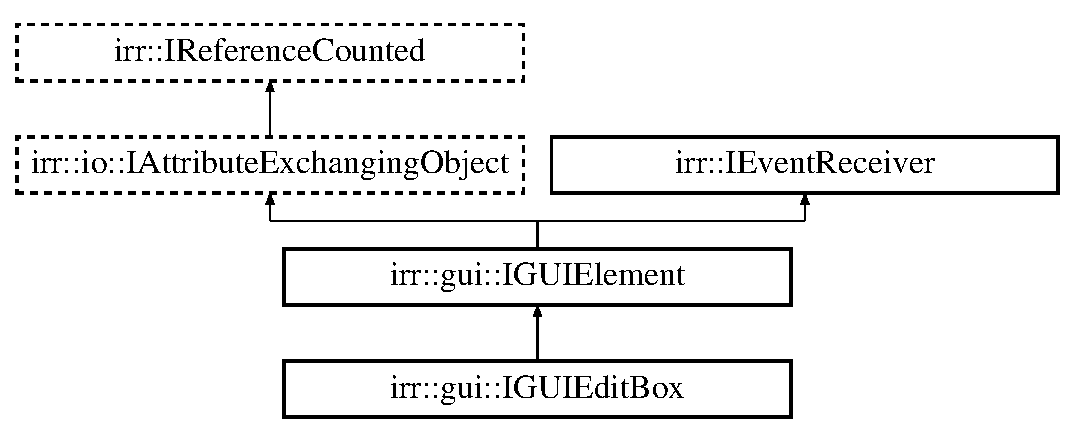
\includegraphics[height=4.038462cm]{classirr_1_1gui_1_1IGUIEditBox}
\end{center}
\end{figure}
\subsection*{Public Member Functions}
\begin{DoxyCompactItemize}
\item 
\mbox{\Hypertarget{classirr_1_1gui_1_1IGUIEditBox_a454f49d8d569bf61b45a31871cc6d301}\label{classirr_1_1gui_1_1IGUIEditBox_a454f49d8d569bf61b45a31871cc6d301}} 
\hyperlink{classirr_1_1gui_1_1IGUIEditBox_a454f49d8d569bf61b45a31871cc6d301}{I\+G\+U\+I\+Edit\+Box} (\hyperlink{classirr_1_1gui_1_1IGUIEnvironment}{I\+G\+U\+I\+Environment} $\ast$environment, \hyperlink{classirr_1_1gui_1_1IGUIElement}{I\+G\+U\+I\+Element} $\ast$parent, \hyperlink{namespaceirr_ac66849b7a6ed16e30ebede579f9b47c6}{s32} id, \hyperlink{classirr_1_1core_1_1rect}{core\+::rect}$<$ \hyperlink{namespaceirr_ac66849b7a6ed16e30ebede579f9b47c6}{s32} $>$ rectangle)
\begin{DoxyCompactList}\small\item\em constructor \end{DoxyCompactList}\item 
virtual void \hyperlink{classirr_1_1gui_1_1IGUIEditBox_a7608fe327ec860712ec87b5e1dc4aec9}{set\+Override\+Font} (\hyperlink{classirr_1_1gui_1_1IGUIFont}{I\+G\+U\+I\+Font} $\ast$font=0)=0
\begin{DoxyCompactList}\small\item\em Sets another skin independent font. \end{DoxyCompactList}\item 
virtual \hyperlink{classirr_1_1gui_1_1IGUIFont}{I\+G\+U\+I\+Font} $\ast$ \hyperlink{classirr_1_1gui_1_1IGUIEditBox_a4c5e6749a5ac390d6a10303babd845b8}{get\+Override\+Font} () const =0
\begin{DoxyCompactList}\small\item\em Gets the override font (if any) \end{DoxyCompactList}\item 
virtual \hyperlink{classirr_1_1gui_1_1IGUIFont}{I\+G\+U\+I\+Font} $\ast$ \hyperlink{classirr_1_1gui_1_1IGUIEditBox_a50542fa7f03a48458fac258a0949d987}{get\+Active\+Font} () const =0
\begin{DoxyCompactList}\small\item\em Get the font which is used right now for drawing. \end{DoxyCompactList}\item 
virtual void \hyperlink{classirr_1_1gui_1_1IGUIEditBox_aa134d2a36c52abcb4881da0267031c47}{set\+Override\+Color} (\hyperlink{classirr_1_1video_1_1SColor}{video\+::\+S\+Color} color)=0
\begin{DoxyCompactList}\small\item\em Sets another color for the text. \end{DoxyCompactList}\item 
\mbox{\Hypertarget{classirr_1_1gui_1_1IGUIEditBox_a2390e7376b017d8f1e2e724be88fbcc3}\label{classirr_1_1gui_1_1IGUIEditBox_a2390e7376b017d8f1e2e724be88fbcc3}} 
virtual \hyperlink{classirr_1_1video_1_1SColor}{video\+::\+S\+Color} \hyperlink{classirr_1_1gui_1_1IGUIEditBox_a2390e7376b017d8f1e2e724be88fbcc3}{get\+Override\+Color} () const =0
\begin{DoxyCompactList}\small\item\em Gets the override color. \end{DoxyCompactList}\item 
virtual void \hyperlink{classirr_1_1gui_1_1IGUIEditBox_a121ab76cb2b69bbc4238921095917346}{enable\+Override\+Color} (bool enable)=0
\begin{DoxyCompactList}\small\item\em Sets if the text should use the override color or the color in the gui skin. \end{DoxyCompactList}\item 
virtual bool \hyperlink{classirr_1_1gui_1_1IGUIEditBox_ae62dac299d0101be9d78ed3db9a2d314}{is\+Override\+Color\+Enabled} (void) const =0
\begin{DoxyCompactList}\small\item\em Checks if an override color is enabled. \end{DoxyCompactList}\item 
\mbox{\Hypertarget{classirr_1_1gui_1_1IGUIEditBox_a06b1913867b10018e891969d319f376f}\label{classirr_1_1gui_1_1IGUIEditBox_a06b1913867b10018e891969d319f376f}} 
virtual void \hyperlink{classirr_1_1gui_1_1IGUIEditBox_a06b1913867b10018e891969d319f376f}{set\+Draw\+Background} (bool \hyperlink{classirr_1_1gui_1_1IGUIElement_a1ef7eeaff67b8a9f4f37cacdc7e54be2}{draw})=0
\begin{DoxyCompactList}\small\item\em Sets whether to draw the background. \end{DoxyCompactList}\item 
virtual void \hyperlink{classirr_1_1gui_1_1IGUIEditBox_a37094bd4bc6b82a184bd1d7864f7ea18}{set\+Draw\+Border} (bool border)=0
\begin{DoxyCompactList}\small\item\em Turns the border on or off. \end{DoxyCompactList}\item 
virtual void \hyperlink{classirr_1_1gui_1_1IGUIEditBox_ab1e2379940983f4ff874f5143f6d7244}{set\+Text\+Alignment} (\hyperlink{namespaceirr_1_1gui_a19eb5fb40e67f108cb16aba922ddaa2d}{E\+G\+U\+I\+\_\+\+A\+L\+I\+G\+N\+M\+E\+NT} horizontal, \hyperlink{namespaceirr_1_1gui_a19eb5fb40e67f108cb16aba922ddaa2d}{E\+G\+U\+I\+\_\+\+A\+L\+I\+G\+N\+M\+E\+NT} vertical)=0
\begin{DoxyCompactList}\small\item\em Sets text justification mode. \end{DoxyCompactList}\item 
virtual void \hyperlink{classirr_1_1gui_1_1IGUIEditBox_aa020a985b38d293794b73e6e12dafd7c}{set\+Word\+Wrap} (bool enable)=0
\begin{DoxyCompactList}\small\item\em Enables or disables word wrap. \end{DoxyCompactList}\item 
virtual bool \hyperlink{classirr_1_1gui_1_1IGUIEditBox_ad0fd4782c052341744ea9d1f61f80e01}{is\+Word\+Wrap\+Enabled} () const =0
\begin{DoxyCompactList}\small\item\em Checks if word wrap is enabled. \end{DoxyCompactList}\item 
virtual void \hyperlink{classirr_1_1gui_1_1IGUIEditBox_a0f68dc7ddc74d8103ba3ba4d445dbf9a}{set\+Multi\+Line} (bool enable)=0
\begin{DoxyCompactList}\small\item\em Enables or disables newlines. \end{DoxyCompactList}\item 
virtual bool \hyperlink{classirr_1_1gui_1_1IGUIEditBox_a0be3338bc094fc93c9f0e4ed842835d6}{is\+Multi\+Line\+Enabled} () const =0
\begin{DoxyCompactList}\small\item\em Checks if multi line editing is enabled. \end{DoxyCompactList}\item 
virtual void \hyperlink{classirr_1_1gui_1_1IGUIEditBox_ad0a9db6da9d0594bb3b5b85a673b3e4d}{set\+Auto\+Scroll} (bool enable)=0
\begin{DoxyCompactList}\small\item\em Enables or disables automatic scrolling with cursor position. \end{DoxyCompactList}\item 
virtual bool \hyperlink{classirr_1_1gui_1_1IGUIEditBox_a4ccf066d1198f3548c7d04622067917f}{is\+Auto\+Scroll\+Enabled} () const =0
\begin{DoxyCompactList}\small\item\em Checks to see if automatic scrolling is enabled. \end{DoxyCompactList}\item 
virtual void \hyperlink{classirr_1_1gui_1_1IGUIEditBox_a755baeca9941267fe11b0c0598b772bf}{set\+Password\+Box} (bool password\+Box, wchar\+\_\+t password\+Char=L\textquotesingle{} $\ast$\textquotesingle{})=0
\begin{DoxyCompactList}\small\item\em Sets whether the edit box is a password box. Setting this to true will. \end{DoxyCompactList}\item 
\mbox{\Hypertarget{classirr_1_1gui_1_1IGUIEditBox_a94b093df77af7cf3e3f9853d68d2c8f2}\label{classirr_1_1gui_1_1IGUIEditBox_a94b093df77af7cf3e3f9853d68d2c8f2}} 
virtual bool \hyperlink{classirr_1_1gui_1_1IGUIEditBox_a94b093df77af7cf3e3f9853d68d2c8f2}{is\+Password\+Box} () const =0
\begin{DoxyCompactList}\small\item\em Returns true if the edit box is currently a password box. \end{DoxyCompactList}\item 
virtual \hyperlink{namespaceirr_1_1core_a13e5bd7e47b2014eefc870ede11bbbbc}{core\+::dimension2du} \hyperlink{classirr_1_1gui_1_1IGUIEditBox_ac993c4647168460c68d56527ba213b9c}{get\+Text\+Dimension} ()=0
\begin{DoxyCompactList}\small\item\em Gets the size area of the text in the edit box. \end{DoxyCompactList}\item 
virtual void \hyperlink{classirr_1_1gui_1_1IGUIEditBox_a5253ed6b422e129356e56f8e2a610be5}{set\+Max} (\hyperlink{namespaceirr_a0416a53257075833e7002efd0a18e804}{u32} max)=0
\begin{DoxyCompactList}\small\item\em Sets the maximum amount of characters which may be entered in the box. \end{DoxyCompactList}\item 
\mbox{\Hypertarget{classirr_1_1gui_1_1IGUIEditBox_ad402bf1211f1a41bf230cc587060648e}\label{classirr_1_1gui_1_1IGUIEditBox_ad402bf1211f1a41bf230cc587060648e}} 
virtual \hyperlink{namespaceirr_a0416a53257075833e7002efd0a18e804}{u32} \hyperlink{classirr_1_1gui_1_1IGUIEditBox_ad402bf1211f1a41bf230cc587060648e}{get\+Max} () const =0
\begin{DoxyCompactList}\small\item\em Returns maximum amount of characters, previously set by \hyperlink{classirr_1_1gui_1_1IGUIEditBox_a5253ed6b422e129356e56f8e2a610be5}{set\+Max()};. \end{DoxyCompactList}\item 
\mbox{\Hypertarget{classirr_1_1gui_1_1IGUIEditBox_a454f49d8d569bf61b45a31871cc6d301}\label{classirr_1_1gui_1_1IGUIEditBox_a454f49d8d569bf61b45a31871cc6d301}} 
\hyperlink{classirr_1_1gui_1_1IGUIEditBox_a454f49d8d569bf61b45a31871cc6d301}{I\+G\+U\+I\+Edit\+Box} (\hyperlink{classirr_1_1gui_1_1IGUIEnvironment}{I\+G\+U\+I\+Environment} $\ast$environment, \hyperlink{classirr_1_1gui_1_1IGUIElement}{I\+G\+U\+I\+Element} $\ast$parent, \hyperlink{namespaceirr_ac66849b7a6ed16e30ebede579f9b47c6}{s32} id, \hyperlink{classirr_1_1core_1_1rect}{core\+::rect}$<$ \hyperlink{namespaceirr_ac66849b7a6ed16e30ebede579f9b47c6}{s32} $>$ rectangle)
\begin{DoxyCompactList}\small\item\em constructor \end{DoxyCompactList}\item 
virtual void \hyperlink{classirr_1_1gui_1_1IGUIEditBox_a7608fe327ec860712ec87b5e1dc4aec9}{set\+Override\+Font} (\hyperlink{classirr_1_1gui_1_1IGUIFont}{I\+G\+U\+I\+Font} $\ast$font=0)=0
\begin{DoxyCompactList}\small\item\em Sets another skin independent font. \end{DoxyCompactList}\item 
virtual \hyperlink{classirr_1_1gui_1_1IGUIFont}{I\+G\+U\+I\+Font} $\ast$ \hyperlink{classirr_1_1gui_1_1IGUIEditBox_a4c5e6749a5ac390d6a10303babd845b8}{get\+Override\+Font} () const =0
\begin{DoxyCompactList}\small\item\em Gets the override font (if any) \end{DoxyCompactList}\item 
virtual \hyperlink{classirr_1_1gui_1_1IGUIFont}{I\+G\+U\+I\+Font} $\ast$ \hyperlink{classirr_1_1gui_1_1IGUIEditBox_a50542fa7f03a48458fac258a0949d987}{get\+Active\+Font} () const =0
\begin{DoxyCompactList}\small\item\em Get the font which is used right now for drawing. \end{DoxyCompactList}\item 
virtual void \hyperlink{classirr_1_1gui_1_1IGUIEditBox_aa134d2a36c52abcb4881da0267031c47}{set\+Override\+Color} (\hyperlink{classirr_1_1video_1_1SColor}{video\+::\+S\+Color} color)=0
\begin{DoxyCompactList}\small\item\em Sets another color for the text. \end{DoxyCompactList}\item 
\mbox{\Hypertarget{classirr_1_1gui_1_1IGUIEditBox_a2390e7376b017d8f1e2e724be88fbcc3}\label{classirr_1_1gui_1_1IGUIEditBox_a2390e7376b017d8f1e2e724be88fbcc3}} 
virtual \hyperlink{classirr_1_1video_1_1SColor}{video\+::\+S\+Color} \hyperlink{classirr_1_1gui_1_1IGUIEditBox_a2390e7376b017d8f1e2e724be88fbcc3}{get\+Override\+Color} () const =0
\begin{DoxyCompactList}\small\item\em Gets the override color. \end{DoxyCompactList}\item 
virtual void \hyperlink{classirr_1_1gui_1_1IGUIEditBox_a121ab76cb2b69bbc4238921095917346}{enable\+Override\+Color} (bool enable)=0
\begin{DoxyCompactList}\small\item\em Sets if the text should use the override color or the color in the gui skin. \end{DoxyCompactList}\item 
virtual bool \hyperlink{classirr_1_1gui_1_1IGUIEditBox_ae62dac299d0101be9d78ed3db9a2d314}{is\+Override\+Color\+Enabled} (void) const =0
\begin{DoxyCompactList}\small\item\em Checks if an override color is enabled. \end{DoxyCompactList}\item 
\mbox{\Hypertarget{classirr_1_1gui_1_1IGUIEditBox_a06b1913867b10018e891969d319f376f}\label{classirr_1_1gui_1_1IGUIEditBox_a06b1913867b10018e891969d319f376f}} 
virtual void \hyperlink{classirr_1_1gui_1_1IGUIEditBox_a06b1913867b10018e891969d319f376f}{set\+Draw\+Background} (bool \hyperlink{classirr_1_1gui_1_1IGUIElement_a1ef7eeaff67b8a9f4f37cacdc7e54be2}{draw})=0
\begin{DoxyCompactList}\small\item\em Sets whether to draw the background. \end{DoxyCompactList}\item 
virtual void \hyperlink{classirr_1_1gui_1_1IGUIEditBox_a37094bd4bc6b82a184bd1d7864f7ea18}{set\+Draw\+Border} (bool border)=0
\begin{DoxyCompactList}\small\item\em Turns the border on or off. \end{DoxyCompactList}\item 
virtual void \hyperlink{classirr_1_1gui_1_1IGUIEditBox_ab1e2379940983f4ff874f5143f6d7244}{set\+Text\+Alignment} (\hyperlink{namespaceirr_1_1gui_a19eb5fb40e67f108cb16aba922ddaa2d}{E\+G\+U\+I\+\_\+\+A\+L\+I\+G\+N\+M\+E\+NT} horizontal, \hyperlink{namespaceirr_1_1gui_a19eb5fb40e67f108cb16aba922ddaa2d}{E\+G\+U\+I\+\_\+\+A\+L\+I\+G\+N\+M\+E\+NT} vertical)=0
\begin{DoxyCompactList}\small\item\em Sets text justification mode. \end{DoxyCompactList}\item 
virtual void \hyperlink{classirr_1_1gui_1_1IGUIEditBox_aa020a985b38d293794b73e6e12dafd7c}{set\+Word\+Wrap} (bool enable)=0
\begin{DoxyCompactList}\small\item\em Enables or disables word wrap. \end{DoxyCompactList}\item 
virtual bool \hyperlink{classirr_1_1gui_1_1IGUIEditBox_ad0fd4782c052341744ea9d1f61f80e01}{is\+Word\+Wrap\+Enabled} () const =0
\begin{DoxyCompactList}\small\item\em Checks if word wrap is enabled. \end{DoxyCompactList}\item 
virtual void \hyperlink{classirr_1_1gui_1_1IGUIEditBox_a0f68dc7ddc74d8103ba3ba4d445dbf9a}{set\+Multi\+Line} (bool enable)=0
\begin{DoxyCompactList}\small\item\em Enables or disables newlines. \end{DoxyCompactList}\item 
virtual bool \hyperlink{classirr_1_1gui_1_1IGUIEditBox_a0be3338bc094fc93c9f0e4ed842835d6}{is\+Multi\+Line\+Enabled} () const =0
\begin{DoxyCompactList}\small\item\em Checks if multi line editing is enabled. \end{DoxyCompactList}\item 
virtual void \hyperlink{classirr_1_1gui_1_1IGUIEditBox_ad0a9db6da9d0594bb3b5b85a673b3e4d}{set\+Auto\+Scroll} (bool enable)=0
\begin{DoxyCompactList}\small\item\em Enables or disables automatic scrolling with cursor position. \end{DoxyCompactList}\item 
virtual bool \hyperlink{classirr_1_1gui_1_1IGUIEditBox_a4ccf066d1198f3548c7d04622067917f}{is\+Auto\+Scroll\+Enabled} () const =0
\begin{DoxyCompactList}\small\item\em Checks to see if automatic scrolling is enabled. \end{DoxyCompactList}\item 
virtual void \hyperlink{classirr_1_1gui_1_1IGUIEditBox_a755baeca9941267fe11b0c0598b772bf}{set\+Password\+Box} (bool password\+Box, wchar\+\_\+t password\+Char=L\textquotesingle{} $\ast$\textquotesingle{})=0
\begin{DoxyCompactList}\small\item\em Sets whether the edit box is a password box. Setting this to true will. \end{DoxyCompactList}\item 
\mbox{\Hypertarget{classirr_1_1gui_1_1IGUIEditBox_a94b093df77af7cf3e3f9853d68d2c8f2}\label{classirr_1_1gui_1_1IGUIEditBox_a94b093df77af7cf3e3f9853d68d2c8f2}} 
virtual bool \hyperlink{classirr_1_1gui_1_1IGUIEditBox_a94b093df77af7cf3e3f9853d68d2c8f2}{is\+Password\+Box} () const =0
\begin{DoxyCompactList}\small\item\em Returns true if the edit box is currently a password box. \end{DoxyCompactList}\item 
virtual \hyperlink{namespaceirr_1_1core_a13e5bd7e47b2014eefc870ede11bbbbc}{core\+::dimension2du} \hyperlink{classirr_1_1gui_1_1IGUIEditBox_ac993c4647168460c68d56527ba213b9c}{get\+Text\+Dimension} ()=0
\begin{DoxyCompactList}\small\item\em Gets the size area of the text in the edit box. \end{DoxyCompactList}\item 
virtual void \hyperlink{classirr_1_1gui_1_1IGUIEditBox_a5253ed6b422e129356e56f8e2a610be5}{set\+Max} (\hyperlink{namespaceirr_a0416a53257075833e7002efd0a18e804}{u32} max)=0
\begin{DoxyCompactList}\small\item\em Sets the maximum amount of characters which may be entered in the box. \end{DoxyCompactList}\item 
\mbox{\Hypertarget{classirr_1_1gui_1_1IGUIEditBox_ad402bf1211f1a41bf230cc587060648e}\label{classirr_1_1gui_1_1IGUIEditBox_ad402bf1211f1a41bf230cc587060648e}} 
virtual \hyperlink{namespaceirr_a0416a53257075833e7002efd0a18e804}{u32} \hyperlink{classirr_1_1gui_1_1IGUIEditBox_ad402bf1211f1a41bf230cc587060648e}{get\+Max} () const =0
\begin{DoxyCompactList}\small\item\em Returns maximum amount of characters, previously set by \hyperlink{classirr_1_1gui_1_1IGUIEditBox_a5253ed6b422e129356e56f8e2a610be5}{set\+Max()};. \end{DoxyCompactList}\end{DoxyCompactItemize}
\subsection*{Additional Inherited Members}


\subsection{Detailed Description}
Single line edit box for editing simple text. 

\begin{DoxyParagraph}{This element can create the following events of type E\+G\+U\+I\+\_\+\+E\+V\+E\+N\+T\+\_\+\+T\+Y\+PE\+:}
\begin{DoxyItemize}
\item E\+G\+E\+T\+\_\+\+E\+D\+I\+T\+B\+O\+X\+\_\+\+E\+N\+T\+ER \item E\+G\+E\+T\+\_\+\+E\+D\+I\+T\+B\+O\+X\+\_\+\+C\+H\+A\+N\+G\+ED \item E\+G\+E\+T\+\_\+\+E\+D\+I\+T\+B\+O\+X\+\_\+\+M\+A\+R\+K\+I\+N\+G\+\_\+\+C\+H\+A\+N\+G\+ED \end{DoxyItemize}

\end{DoxyParagraph}


\subsection{Member Function Documentation}
\mbox{\Hypertarget{classirr_1_1gui_1_1IGUIEditBox_a121ab76cb2b69bbc4238921095917346}\label{classirr_1_1gui_1_1IGUIEditBox_a121ab76cb2b69bbc4238921095917346}} 
\index{irr\+::gui\+::\+I\+G\+U\+I\+Edit\+Box@{irr\+::gui\+::\+I\+G\+U\+I\+Edit\+Box}!enable\+Override\+Color@{enable\+Override\+Color}}
\index{enable\+Override\+Color@{enable\+Override\+Color}!irr\+::gui\+::\+I\+G\+U\+I\+Edit\+Box@{irr\+::gui\+::\+I\+G\+U\+I\+Edit\+Box}}
\subsubsection{\texorpdfstring{enable\+Override\+Color()}{enableOverrideColor()}\hspace{0.1cm}{\footnotesize\ttfamily [1/2]}}
{\footnotesize\ttfamily virtual void irr\+::gui\+::\+I\+G\+U\+I\+Edit\+Box\+::enable\+Override\+Color (\begin{DoxyParamCaption}\item[{bool}]{enable }\end{DoxyParamCaption})\hspace{0.3cm}{\ttfamily [pure virtual]}}



Sets if the text should use the override color or the color in the gui skin. 


\begin{DoxyParams}{Parameters}
{\em enable} & If set to true, the override color, which can be set with \hyperlink{classirr_1_1gui_1_1IGUIEditBox_aa134d2a36c52abcb4881da0267031c47}{I\+G\+U\+I\+Edit\+Box\+::set\+Override\+Color} is used, otherwise the E\+G\+D\+C\+\_\+\+B\+U\+T\+T\+O\+N\+\_\+\+T\+E\+XT color of the skin. \\
\hline
\end{DoxyParams}
\mbox{\Hypertarget{classirr_1_1gui_1_1IGUIEditBox_a121ab76cb2b69bbc4238921095917346}\label{classirr_1_1gui_1_1IGUIEditBox_a121ab76cb2b69bbc4238921095917346}} 
\index{irr\+::gui\+::\+I\+G\+U\+I\+Edit\+Box@{irr\+::gui\+::\+I\+G\+U\+I\+Edit\+Box}!enable\+Override\+Color@{enable\+Override\+Color}}
\index{enable\+Override\+Color@{enable\+Override\+Color}!irr\+::gui\+::\+I\+G\+U\+I\+Edit\+Box@{irr\+::gui\+::\+I\+G\+U\+I\+Edit\+Box}}
\subsubsection{\texorpdfstring{enable\+Override\+Color()}{enableOverrideColor()}\hspace{0.1cm}{\footnotesize\ttfamily [2/2]}}
{\footnotesize\ttfamily virtual void irr\+::gui\+::\+I\+G\+U\+I\+Edit\+Box\+::enable\+Override\+Color (\begin{DoxyParamCaption}\item[{bool}]{enable }\end{DoxyParamCaption})\hspace{0.3cm}{\ttfamily [pure virtual]}}



Sets if the text should use the override color or the color in the gui skin. 


\begin{DoxyParams}{Parameters}
{\em enable} & If set to true, the override color, which can be set with \hyperlink{classirr_1_1gui_1_1IGUIEditBox_aa134d2a36c52abcb4881da0267031c47}{I\+G\+U\+I\+Edit\+Box\+::set\+Override\+Color} is used, otherwise the E\+G\+D\+C\+\_\+\+B\+U\+T\+T\+O\+N\+\_\+\+T\+E\+XT color of the skin. \\
\hline
\end{DoxyParams}
\mbox{\Hypertarget{classirr_1_1gui_1_1IGUIEditBox_a50542fa7f03a48458fac258a0949d987}\label{classirr_1_1gui_1_1IGUIEditBox_a50542fa7f03a48458fac258a0949d987}} 
\index{irr\+::gui\+::\+I\+G\+U\+I\+Edit\+Box@{irr\+::gui\+::\+I\+G\+U\+I\+Edit\+Box}!get\+Active\+Font@{get\+Active\+Font}}
\index{get\+Active\+Font@{get\+Active\+Font}!irr\+::gui\+::\+I\+G\+U\+I\+Edit\+Box@{irr\+::gui\+::\+I\+G\+U\+I\+Edit\+Box}}
\subsubsection{\texorpdfstring{get\+Active\+Font()}{getActiveFont()}\hspace{0.1cm}{\footnotesize\ttfamily [1/2]}}
{\footnotesize\ttfamily virtual \hyperlink{classirr_1_1gui_1_1IGUIFont}{I\+G\+U\+I\+Font}$\ast$ irr\+::gui\+::\+I\+G\+U\+I\+Edit\+Box\+::get\+Active\+Font (\begin{DoxyParamCaption}{ }\end{DoxyParamCaption}) const\hspace{0.3cm}{\ttfamily [pure virtual]}}



Get the font which is used right now for drawing. 

Currently this is the override font when one is set and the font of the active skin otherwise \mbox{\Hypertarget{classirr_1_1gui_1_1IGUIEditBox_a50542fa7f03a48458fac258a0949d987}\label{classirr_1_1gui_1_1IGUIEditBox_a50542fa7f03a48458fac258a0949d987}} 
\index{irr\+::gui\+::\+I\+G\+U\+I\+Edit\+Box@{irr\+::gui\+::\+I\+G\+U\+I\+Edit\+Box}!get\+Active\+Font@{get\+Active\+Font}}
\index{get\+Active\+Font@{get\+Active\+Font}!irr\+::gui\+::\+I\+G\+U\+I\+Edit\+Box@{irr\+::gui\+::\+I\+G\+U\+I\+Edit\+Box}}
\subsubsection{\texorpdfstring{get\+Active\+Font()}{getActiveFont()}\hspace{0.1cm}{\footnotesize\ttfamily [2/2]}}
{\footnotesize\ttfamily virtual \hyperlink{classirr_1_1gui_1_1IGUIFont}{I\+G\+U\+I\+Font}$\ast$ irr\+::gui\+::\+I\+G\+U\+I\+Edit\+Box\+::get\+Active\+Font (\begin{DoxyParamCaption}{ }\end{DoxyParamCaption}) const\hspace{0.3cm}{\ttfamily [pure virtual]}}



Get the font which is used right now for drawing. 

Currently this is the override font when one is set and the font of the active skin otherwise \mbox{\Hypertarget{classirr_1_1gui_1_1IGUIEditBox_a4c5e6749a5ac390d6a10303babd845b8}\label{classirr_1_1gui_1_1IGUIEditBox_a4c5e6749a5ac390d6a10303babd845b8}} 
\index{irr\+::gui\+::\+I\+G\+U\+I\+Edit\+Box@{irr\+::gui\+::\+I\+G\+U\+I\+Edit\+Box}!get\+Override\+Font@{get\+Override\+Font}}
\index{get\+Override\+Font@{get\+Override\+Font}!irr\+::gui\+::\+I\+G\+U\+I\+Edit\+Box@{irr\+::gui\+::\+I\+G\+U\+I\+Edit\+Box}}
\subsubsection{\texorpdfstring{get\+Override\+Font()}{getOverrideFont()}\hspace{0.1cm}{\footnotesize\ttfamily [1/2]}}
{\footnotesize\ttfamily virtual \hyperlink{classirr_1_1gui_1_1IGUIFont}{I\+G\+U\+I\+Font}$\ast$ irr\+::gui\+::\+I\+G\+U\+I\+Edit\+Box\+::get\+Override\+Font (\begin{DoxyParamCaption}{ }\end{DoxyParamCaption}) const\hspace{0.3cm}{\ttfamily [pure virtual]}}



Gets the override font (if any) 

\begin{DoxyReturn}{Returns}
The override font (may be 0) 
\end{DoxyReturn}
\mbox{\Hypertarget{classirr_1_1gui_1_1IGUIEditBox_a4c5e6749a5ac390d6a10303babd845b8}\label{classirr_1_1gui_1_1IGUIEditBox_a4c5e6749a5ac390d6a10303babd845b8}} 
\index{irr\+::gui\+::\+I\+G\+U\+I\+Edit\+Box@{irr\+::gui\+::\+I\+G\+U\+I\+Edit\+Box}!get\+Override\+Font@{get\+Override\+Font}}
\index{get\+Override\+Font@{get\+Override\+Font}!irr\+::gui\+::\+I\+G\+U\+I\+Edit\+Box@{irr\+::gui\+::\+I\+G\+U\+I\+Edit\+Box}}
\subsubsection{\texorpdfstring{get\+Override\+Font()}{getOverrideFont()}\hspace{0.1cm}{\footnotesize\ttfamily [2/2]}}
{\footnotesize\ttfamily virtual \hyperlink{classirr_1_1gui_1_1IGUIFont}{I\+G\+U\+I\+Font}$\ast$ irr\+::gui\+::\+I\+G\+U\+I\+Edit\+Box\+::get\+Override\+Font (\begin{DoxyParamCaption}{ }\end{DoxyParamCaption}) const\hspace{0.3cm}{\ttfamily [pure virtual]}}



Gets the override font (if any) 

\begin{DoxyReturn}{Returns}
The override font (may be 0) 
\end{DoxyReturn}
\mbox{\Hypertarget{classirr_1_1gui_1_1IGUIEditBox_ac993c4647168460c68d56527ba213b9c}\label{classirr_1_1gui_1_1IGUIEditBox_ac993c4647168460c68d56527ba213b9c}} 
\index{irr\+::gui\+::\+I\+G\+U\+I\+Edit\+Box@{irr\+::gui\+::\+I\+G\+U\+I\+Edit\+Box}!get\+Text\+Dimension@{get\+Text\+Dimension}}
\index{get\+Text\+Dimension@{get\+Text\+Dimension}!irr\+::gui\+::\+I\+G\+U\+I\+Edit\+Box@{irr\+::gui\+::\+I\+G\+U\+I\+Edit\+Box}}
\subsubsection{\texorpdfstring{get\+Text\+Dimension()}{getTextDimension()}\hspace{0.1cm}{\footnotesize\ttfamily [1/2]}}
{\footnotesize\ttfamily virtual \hyperlink{namespaceirr_1_1core_a13e5bd7e47b2014eefc870ede11bbbbc}{core\+::dimension2du} irr\+::gui\+::\+I\+G\+U\+I\+Edit\+Box\+::get\+Text\+Dimension (\begin{DoxyParamCaption}{ }\end{DoxyParamCaption})\hspace{0.3cm}{\ttfamily [pure virtual]}}



Gets the size area of the text in the edit box. 

\begin{DoxyReturn}{Returns}
The size in pixels of the text 
\end{DoxyReturn}
\mbox{\Hypertarget{classirr_1_1gui_1_1IGUIEditBox_ac993c4647168460c68d56527ba213b9c}\label{classirr_1_1gui_1_1IGUIEditBox_ac993c4647168460c68d56527ba213b9c}} 
\index{irr\+::gui\+::\+I\+G\+U\+I\+Edit\+Box@{irr\+::gui\+::\+I\+G\+U\+I\+Edit\+Box}!get\+Text\+Dimension@{get\+Text\+Dimension}}
\index{get\+Text\+Dimension@{get\+Text\+Dimension}!irr\+::gui\+::\+I\+G\+U\+I\+Edit\+Box@{irr\+::gui\+::\+I\+G\+U\+I\+Edit\+Box}}
\subsubsection{\texorpdfstring{get\+Text\+Dimension()}{getTextDimension()}\hspace{0.1cm}{\footnotesize\ttfamily [2/2]}}
{\footnotesize\ttfamily virtual \hyperlink{namespaceirr_1_1core_a13e5bd7e47b2014eefc870ede11bbbbc}{core\+::dimension2du} irr\+::gui\+::\+I\+G\+U\+I\+Edit\+Box\+::get\+Text\+Dimension (\begin{DoxyParamCaption}{ }\end{DoxyParamCaption})\hspace{0.3cm}{\ttfamily [pure virtual]}}



Gets the size area of the text in the edit box. 

\begin{DoxyReturn}{Returns}
The size in pixels of the text 
\end{DoxyReturn}
\mbox{\Hypertarget{classirr_1_1gui_1_1IGUIEditBox_a4ccf066d1198f3548c7d04622067917f}\label{classirr_1_1gui_1_1IGUIEditBox_a4ccf066d1198f3548c7d04622067917f}} 
\index{irr\+::gui\+::\+I\+G\+U\+I\+Edit\+Box@{irr\+::gui\+::\+I\+G\+U\+I\+Edit\+Box}!is\+Auto\+Scroll\+Enabled@{is\+Auto\+Scroll\+Enabled}}
\index{is\+Auto\+Scroll\+Enabled@{is\+Auto\+Scroll\+Enabled}!irr\+::gui\+::\+I\+G\+U\+I\+Edit\+Box@{irr\+::gui\+::\+I\+G\+U\+I\+Edit\+Box}}
\subsubsection{\texorpdfstring{is\+Auto\+Scroll\+Enabled()}{isAutoScrollEnabled()}\hspace{0.1cm}{\footnotesize\ttfamily [1/2]}}
{\footnotesize\ttfamily virtual bool irr\+::gui\+::\+I\+G\+U\+I\+Edit\+Box\+::is\+Auto\+Scroll\+Enabled (\begin{DoxyParamCaption}{ }\end{DoxyParamCaption}) const\hspace{0.3cm}{\ttfamily [pure virtual]}}



Checks to see if automatic scrolling is enabled. 

\begin{DoxyReturn}{Returns}
true if automatic scrolling is enabled, false if not 
\end{DoxyReturn}
\mbox{\Hypertarget{classirr_1_1gui_1_1IGUIEditBox_a4ccf066d1198f3548c7d04622067917f}\label{classirr_1_1gui_1_1IGUIEditBox_a4ccf066d1198f3548c7d04622067917f}} 
\index{irr\+::gui\+::\+I\+G\+U\+I\+Edit\+Box@{irr\+::gui\+::\+I\+G\+U\+I\+Edit\+Box}!is\+Auto\+Scroll\+Enabled@{is\+Auto\+Scroll\+Enabled}}
\index{is\+Auto\+Scroll\+Enabled@{is\+Auto\+Scroll\+Enabled}!irr\+::gui\+::\+I\+G\+U\+I\+Edit\+Box@{irr\+::gui\+::\+I\+G\+U\+I\+Edit\+Box}}
\subsubsection{\texorpdfstring{is\+Auto\+Scroll\+Enabled()}{isAutoScrollEnabled()}\hspace{0.1cm}{\footnotesize\ttfamily [2/2]}}
{\footnotesize\ttfamily virtual bool irr\+::gui\+::\+I\+G\+U\+I\+Edit\+Box\+::is\+Auto\+Scroll\+Enabled (\begin{DoxyParamCaption}{ }\end{DoxyParamCaption}) const\hspace{0.3cm}{\ttfamily [pure virtual]}}



Checks to see if automatic scrolling is enabled. 

\begin{DoxyReturn}{Returns}
true if automatic scrolling is enabled, false if not 
\end{DoxyReturn}
\mbox{\Hypertarget{classirr_1_1gui_1_1IGUIEditBox_a0be3338bc094fc93c9f0e4ed842835d6}\label{classirr_1_1gui_1_1IGUIEditBox_a0be3338bc094fc93c9f0e4ed842835d6}} 
\index{irr\+::gui\+::\+I\+G\+U\+I\+Edit\+Box@{irr\+::gui\+::\+I\+G\+U\+I\+Edit\+Box}!is\+Multi\+Line\+Enabled@{is\+Multi\+Line\+Enabled}}
\index{is\+Multi\+Line\+Enabled@{is\+Multi\+Line\+Enabled}!irr\+::gui\+::\+I\+G\+U\+I\+Edit\+Box@{irr\+::gui\+::\+I\+G\+U\+I\+Edit\+Box}}
\subsubsection{\texorpdfstring{is\+Multi\+Line\+Enabled()}{isMultiLineEnabled()}\hspace{0.1cm}{\footnotesize\ttfamily [1/2]}}
{\footnotesize\ttfamily virtual bool irr\+::gui\+::\+I\+G\+U\+I\+Edit\+Box\+::is\+Multi\+Line\+Enabled (\begin{DoxyParamCaption}{ }\end{DoxyParamCaption}) const\hspace{0.3cm}{\ttfamily [pure virtual]}}



Checks if multi line editing is enabled. 

\begin{DoxyReturn}{Returns}
true if multi-\/line is enabled, false otherwise 
\end{DoxyReturn}
\mbox{\Hypertarget{classirr_1_1gui_1_1IGUIEditBox_a0be3338bc094fc93c9f0e4ed842835d6}\label{classirr_1_1gui_1_1IGUIEditBox_a0be3338bc094fc93c9f0e4ed842835d6}} 
\index{irr\+::gui\+::\+I\+G\+U\+I\+Edit\+Box@{irr\+::gui\+::\+I\+G\+U\+I\+Edit\+Box}!is\+Multi\+Line\+Enabled@{is\+Multi\+Line\+Enabled}}
\index{is\+Multi\+Line\+Enabled@{is\+Multi\+Line\+Enabled}!irr\+::gui\+::\+I\+G\+U\+I\+Edit\+Box@{irr\+::gui\+::\+I\+G\+U\+I\+Edit\+Box}}
\subsubsection{\texorpdfstring{is\+Multi\+Line\+Enabled()}{isMultiLineEnabled()}\hspace{0.1cm}{\footnotesize\ttfamily [2/2]}}
{\footnotesize\ttfamily virtual bool irr\+::gui\+::\+I\+G\+U\+I\+Edit\+Box\+::is\+Multi\+Line\+Enabled (\begin{DoxyParamCaption}{ }\end{DoxyParamCaption}) const\hspace{0.3cm}{\ttfamily [pure virtual]}}



Checks if multi line editing is enabled. 

\begin{DoxyReturn}{Returns}
true if multi-\/line is enabled, false otherwise 
\end{DoxyReturn}
\mbox{\Hypertarget{classirr_1_1gui_1_1IGUIEditBox_ae62dac299d0101be9d78ed3db9a2d314}\label{classirr_1_1gui_1_1IGUIEditBox_ae62dac299d0101be9d78ed3db9a2d314}} 
\index{irr\+::gui\+::\+I\+G\+U\+I\+Edit\+Box@{irr\+::gui\+::\+I\+G\+U\+I\+Edit\+Box}!is\+Override\+Color\+Enabled@{is\+Override\+Color\+Enabled}}
\index{is\+Override\+Color\+Enabled@{is\+Override\+Color\+Enabled}!irr\+::gui\+::\+I\+G\+U\+I\+Edit\+Box@{irr\+::gui\+::\+I\+G\+U\+I\+Edit\+Box}}
\subsubsection{\texorpdfstring{is\+Override\+Color\+Enabled()}{isOverrideColorEnabled()}\hspace{0.1cm}{\footnotesize\ttfamily [1/2]}}
{\footnotesize\ttfamily virtual bool irr\+::gui\+::\+I\+G\+U\+I\+Edit\+Box\+::is\+Override\+Color\+Enabled (\begin{DoxyParamCaption}\item[{void}]{ }\end{DoxyParamCaption}) const\hspace{0.3cm}{\ttfamily [pure virtual]}}



Checks if an override color is enabled. 

\begin{DoxyReturn}{Returns}
true if the override color is enabled, false otherwise 
\end{DoxyReturn}
\mbox{\Hypertarget{classirr_1_1gui_1_1IGUIEditBox_ae62dac299d0101be9d78ed3db9a2d314}\label{classirr_1_1gui_1_1IGUIEditBox_ae62dac299d0101be9d78ed3db9a2d314}} 
\index{irr\+::gui\+::\+I\+G\+U\+I\+Edit\+Box@{irr\+::gui\+::\+I\+G\+U\+I\+Edit\+Box}!is\+Override\+Color\+Enabled@{is\+Override\+Color\+Enabled}}
\index{is\+Override\+Color\+Enabled@{is\+Override\+Color\+Enabled}!irr\+::gui\+::\+I\+G\+U\+I\+Edit\+Box@{irr\+::gui\+::\+I\+G\+U\+I\+Edit\+Box}}
\subsubsection{\texorpdfstring{is\+Override\+Color\+Enabled()}{isOverrideColorEnabled()}\hspace{0.1cm}{\footnotesize\ttfamily [2/2]}}
{\footnotesize\ttfamily virtual bool irr\+::gui\+::\+I\+G\+U\+I\+Edit\+Box\+::is\+Override\+Color\+Enabled (\begin{DoxyParamCaption}\item[{void}]{ }\end{DoxyParamCaption}) const\hspace{0.3cm}{\ttfamily [pure virtual]}}



Checks if an override color is enabled. 

\begin{DoxyReturn}{Returns}
true if the override color is enabled, false otherwise 
\end{DoxyReturn}
\mbox{\Hypertarget{classirr_1_1gui_1_1IGUIEditBox_ad0fd4782c052341744ea9d1f61f80e01}\label{classirr_1_1gui_1_1IGUIEditBox_ad0fd4782c052341744ea9d1f61f80e01}} 
\index{irr\+::gui\+::\+I\+G\+U\+I\+Edit\+Box@{irr\+::gui\+::\+I\+G\+U\+I\+Edit\+Box}!is\+Word\+Wrap\+Enabled@{is\+Word\+Wrap\+Enabled}}
\index{is\+Word\+Wrap\+Enabled@{is\+Word\+Wrap\+Enabled}!irr\+::gui\+::\+I\+G\+U\+I\+Edit\+Box@{irr\+::gui\+::\+I\+G\+U\+I\+Edit\+Box}}
\subsubsection{\texorpdfstring{is\+Word\+Wrap\+Enabled()}{isWordWrapEnabled()}\hspace{0.1cm}{\footnotesize\ttfamily [1/2]}}
{\footnotesize\ttfamily virtual bool irr\+::gui\+::\+I\+G\+U\+I\+Edit\+Box\+::is\+Word\+Wrap\+Enabled (\begin{DoxyParamCaption}{ }\end{DoxyParamCaption}) const\hspace{0.3cm}{\ttfamily [pure virtual]}}



Checks if word wrap is enabled. 

\begin{DoxyReturn}{Returns}
true if word wrap is enabled, false otherwise 
\end{DoxyReturn}
\mbox{\Hypertarget{classirr_1_1gui_1_1IGUIEditBox_ad0fd4782c052341744ea9d1f61f80e01}\label{classirr_1_1gui_1_1IGUIEditBox_ad0fd4782c052341744ea9d1f61f80e01}} 
\index{irr\+::gui\+::\+I\+G\+U\+I\+Edit\+Box@{irr\+::gui\+::\+I\+G\+U\+I\+Edit\+Box}!is\+Word\+Wrap\+Enabled@{is\+Word\+Wrap\+Enabled}}
\index{is\+Word\+Wrap\+Enabled@{is\+Word\+Wrap\+Enabled}!irr\+::gui\+::\+I\+G\+U\+I\+Edit\+Box@{irr\+::gui\+::\+I\+G\+U\+I\+Edit\+Box}}
\subsubsection{\texorpdfstring{is\+Word\+Wrap\+Enabled()}{isWordWrapEnabled()}\hspace{0.1cm}{\footnotesize\ttfamily [2/2]}}
{\footnotesize\ttfamily virtual bool irr\+::gui\+::\+I\+G\+U\+I\+Edit\+Box\+::is\+Word\+Wrap\+Enabled (\begin{DoxyParamCaption}{ }\end{DoxyParamCaption}) const\hspace{0.3cm}{\ttfamily [pure virtual]}}



Checks if word wrap is enabled. 

\begin{DoxyReturn}{Returns}
true if word wrap is enabled, false otherwise 
\end{DoxyReturn}
\mbox{\Hypertarget{classirr_1_1gui_1_1IGUIEditBox_ad0a9db6da9d0594bb3b5b85a673b3e4d}\label{classirr_1_1gui_1_1IGUIEditBox_ad0a9db6da9d0594bb3b5b85a673b3e4d}} 
\index{irr\+::gui\+::\+I\+G\+U\+I\+Edit\+Box@{irr\+::gui\+::\+I\+G\+U\+I\+Edit\+Box}!set\+Auto\+Scroll@{set\+Auto\+Scroll}}
\index{set\+Auto\+Scroll@{set\+Auto\+Scroll}!irr\+::gui\+::\+I\+G\+U\+I\+Edit\+Box@{irr\+::gui\+::\+I\+G\+U\+I\+Edit\+Box}}
\subsubsection{\texorpdfstring{set\+Auto\+Scroll()}{setAutoScroll()}\hspace{0.1cm}{\footnotesize\ttfamily [1/2]}}
{\footnotesize\ttfamily virtual void irr\+::gui\+::\+I\+G\+U\+I\+Edit\+Box\+::set\+Auto\+Scroll (\begin{DoxyParamCaption}\item[{bool}]{enable }\end{DoxyParamCaption})\hspace{0.3cm}{\ttfamily [pure virtual]}}



Enables or disables automatic scrolling with cursor position. 


\begin{DoxyParams}{Parameters}
{\em enable} & If set to true, the text will move around with the cursor position \\
\hline
\end{DoxyParams}
\mbox{\Hypertarget{classirr_1_1gui_1_1IGUIEditBox_ad0a9db6da9d0594bb3b5b85a673b3e4d}\label{classirr_1_1gui_1_1IGUIEditBox_ad0a9db6da9d0594bb3b5b85a673b3e4d}} 
\index{irr\+::gui\+::\+I\+G\+U\+I\+Edit\+Box@{irr\+::gui\+::\+I\+G\+U\+I\+Edit\+Box}!set\+Auto\+Scroll@{set\+Auto\+Scroll}}
\index{set\+Auto\+Scroll@{set\+Auto\+Scroll}!irr\+::gui\+::\+I\+G\+U\+I\+Edit\+Box@{irr\+::gui\+::\+I\+G\+U\+I\+Edit\+Box}}
\subsubsection{\texorpdfstring{set\+Auto\+Scroll()}{setAutoScroll()}\hspace{0.1cm}{\footnotesize\ttfamily [2/2]}}
{\footnotesize\ttfamily virtual void irr\+::gui\+::\+I\+G\+U\+I\+Edit\+Box\+::set\+Auto\+Scroll (\begin{DoxyParamCaption}\item[{bool}]{enable }\end{DoxyParamCaption})\hspace{0.3cm}{\ttfamily [pure virtual]}}



Enables or disables automatic scrolling with cursor position. 


\begin{DoxyParams}{Parameters}
{\em enable} & If set to true, the text will move around with the cursor position \\
\hline
\end{DoxyParams}
\mbox{\Hypertarget{classirr_1_1gui_1_1IGUIEditBox_a37094bd4bc6b82a184bd1d7864f7ea18}\label{classirr_1_1gui_1_1IGUIEditBox_a37094bd4bc6b82a184bd1d7864f7ea18}} 
\index{irr\+::gui\+::\+I\+G\+U\+I\+Edit\+Box@{irr\+::gui\+::\+I\+G\+U\+I\+Edit\+Box}!set\+Draw\+Border@{set\+Draw\+Border}}
\index{set\+Draw\+Border@{set\+Draw\+Border}!irr\+::gui\+::\+I\+G\+U\+I\+Edit\+Box@{irr\+::gui\+::\+I\+G\+U\+I\+Edit\+Box}}
\subsubsection{\texorpdfstring{set\+Draw\+Border()}{setDrawBorder()}\hspace{0.1cm}{\footnotesize\ttfamily [1/2]}}
{\footnotesize\ttfamily virtual void irr\+::gui\+::\+I\+G\+U\+I\+Edit\+Box\+::set\+Draw\+Border (\begin{DoxyParamCaption}\item[{bool}]{border }\end{DoxyParamCaption})\hspace{0.3cm}{\ttfamily [pure virtual]}}



Turns the border on or off. 


\begin{DoxyParams}{Parameters}
{\em border} & true if you want the border to be drawn, false if not \\
\hline
\end{DoxyParams}
\mbox{\Hypertarget{classirr_1_1gui_1_1IGUIEditBox_a37094bd4bc6b82a184bd1d7864f7ea18}\label{classirr_1_1gui_1_1IGUIEditBox_a37094bd4bc6b82a184bd1d7864f7ea18}} 
\index{irr\+::gui\+::\+I\+G\+U\+I\+Edit\+Box@{irr\+::gui\+::\+I\+G\+U\+I\+Edit\+Box}!set\+Draw\+Border@{set\+Draw\+Border}}
\index{set\+Draw\+Border@{set\+Draw\+Border}!irr\+::gui\+::\+I\+G\+U\+I\+Edit\+Box@{irr\+::gui\+::\+I\+G\+U\+I\+Edit\+Box}}
\subsubsection{\texorpdfstring{set\+Draw\+Border()}{setDrawBorder()}\hspace{0.1cm}{\footnotesize\ttfamily [2/2]}}
{\footnotesize\ttfamily virtual void irr\+::gui\+::\+I\+G\+U\+I\+Edit\+Box\+::set\+Draw\+Border (\begin{DoxyParamCaption}\item[{bool}]{border }\end{DoxyParamCaption})\hspace{0.3cm}{\ttfamily [pure virtual]}}



Turns the border on or off. 


\begin{DoxyParams}{Parameters}
{\em border} & true if you want the border to be drawn, false if not \\
\hline
\end{DoxyParams}
\mbox{\Hypertarget{classirr_1_1gui_1_1IGUIEditBox_a5253ed6b422e129356e56f8e2a610be5}\label{classirr_1_1gui_1_1IGUIEditBox_a5253ed6b422e129356e56f8e2a610be5}} 
\index{irr\+::gui\+::\+I\+G\+U\+I\+Edit\+Box@{irr\+::gui\+::\+I\+G\+U\+I\+Edit\+Box}!set\+Max@{set\+Max}}
\index{set\+Max@{set\+Max}!irr\+::gui\+::\+I\+G\+U\+I\+Edit\+Box@{irr\+::gui\+::\+I\+G\+U\+I\+Edit\+Box}}
\subsubsection{\texorpdfstring{set\+Max()}{setMax()}\hspace{0.1cm}{\footnotesize\ttfamily [1/2]}}
{\footnotesize\ttfamily virtual void irr\+::gui\+::\+I\+G\+U\+I\+Edit\+Box\+::set\+Max (\begin{DoxyParamCaption}\item[{\hyperlink{namespaceirr_a0416a53257075833e7002efd0a18e804}{u32}}]{max }\end{DoxyParamCaption})\hspace{0.3cm}{\ttfamily [pure virtual]}}



Sets the maximum amount of characters which may be entered in the box. 


\begin{DoxyParams}{Parameters}
{\em max} & Maximum amount of characters. If 0, the character amount is infinity. \\
\hline
\end{DoxyParams}
\mbox{\Hypertarget{classirr_1_1gui_1_1IGUIEditBox_a5253ed6b422e129356e56f8e2a610be5}\label{classirr_1_1gui_1_1IGUIEditBox_a5253ed6b422e129356e56f8e2a610be5}} 
\index{irr\+::gui\+::\+I\+G\+U\+I\+Edit\+Box@{irr\+::gui\+::\+I\+G\+U\+I\+Edit\+Box}!set\+Max@{set\+Max}}
\index{set\+Max@{set\+Max}!irr\+::gui\+::\+I\+G\+U\+I\+Edit\+Box@{irr\+::gui\+::\+I\+G\+U\+I\+Edit\+Box}}
\subsubsection{\texorpdfstring{set\+Max()}{setMax()}\hspace{0.1cm}{\footnotesize\ttfamily [2/2]}}
{\footnotesize\ttfamily virtual void irr\+::gui\+::\+I\+G\+U\+I\+Edit\+Box\+::set\+Max (\begin{DoxyParamCaption}\item[{\hyperlink{namespaceirr_a0416a53257075833e7002efd0a18e804}{u32}}]{max }\end{DoxyParamCaption})\hspace{0.3cm}{\ttfamily [pure virtual]}}



Sets the maximum amount of characters which may be entered in the box. 


\begin{DoxyParams}{Parameters}
{\em max} & Maximum amount of characters. If 0, the character amount is infinity. \\
\hline
\end{DoxyParams}
\mbox{\Hypertarget{classirr_1_1gui_1_1IGUIEditBox_a0f68dc7ddc74d8103ba3ba4d445dbf9a}\label{classirr_1_1gui_1_1IGUIEditBox_a0f68dc7ddc74d8103ba3ba4d445dbf9a}} 
\index{irr\+::gui\+::\+I\+G\+U\+I\+Edit\+Box@{irr\+::gui\+::\+I\+G\+U\+I\+Edit\+Box}!set\+Multi\+Line@{set\+Multi\+Line}}
\index{set\+Multi\+Line@{set\+Multi\+Line}!irr\+::gui\+::\+I\+G\+U\+I\+Edit\+Box@{irr\+::gui\+::\+I\+G\+U\+I\+Edit\+Box}}
\subsubsection{\texorpdfstring{set\+Multi\+Line()}{setMultiLine()}\hspace{0.1cm}{\footnotesize\ttfamily [1/2]}}
{\footnotesize\ttfamily virtual void irr\+::gui\+::\+I\+G\+U\+I\+Edit\+Box\+::set\+Multi\+Line (\begin{DoxyParamCaption}\item[{bool}]{enable }\end{DoxyParamCaption})\hspace{0.3cm}{\ttfamily [pure virtual]}}



Enables or disables newlines. 


\begin{DoxyParams}{Parameters}
{\em enable} & If set to true, the E\+G\+E\+T\+\_\+\+E\+D\+I\+T\+B\+O\+X\+\_\+\+E\+N\+T\+ER event will not be fired, instead a newline character will be inserted. \\
\hline
\end{DoxyParams}
\mbox{\Hypertarget{classirr_1_1gui_1_1IGUIEditBox_a0f68dc7ddc74d8103ba3ba4d445dbf9a}\label{classirr_1_1gui_1_1IGUIEditBox_a0f68dc7ddc74d8103ba3ba4d445dbf9a}} 
\index{irr\+::gui\+::\+I\+G\+U\+I\+Edit\+Box@{irr\+::gui\+::\+I\+G\+U\+I\+Edit\+Box}!set\+Multi\+Line@{set\+Multi\+Line}}
\index{set\+Multi\+Line@{set\+Multi\+Line}!irr\+::gui\+::\+I\+G\+U\+I\+Edit\+Box@{irr\+::gui\+::\+I\+G\+U\+I\+Edit\+Box}}
\subsubsection{\texorpdfstring{set\+Multi\+Line()}{setMultiLine()}\hspace{0.1cm}{\footnotesize\ttfamily [2/2]}}
{\footnotesize\ttfamily virtual void irr\+::gui\+::\+I\+G\+U\+I\+Edit\+Box\+::set\+Multi\+Line (\begin{DoxyParamCaption}\item[{bool}]{enable }\end{DoxyParamCaption})\hspace{0.3cm}{\ttfamily [pure virtual]}}



Enables or disables newlines. 


\begin{DoxyParams}{Parameters}
{\em enable} & If set to true, the E\+G\+E\+T\+\_\+\+E\+D\+I\+T\+B\+O\+X\+\_\+\+E\+N\+T\+ER event will not be fired, instead a newline character will be inserted. \\
\hline
\end{DoxyParams}
\mbox{\Hypertarget{classirr_1_1gui_1_1IGUIEditBox_aa134d2a36c52abcb4881da0267031c47}\label{classirr_1_1gui_1_1IGUIEditBox_aa134d2a36c52abcb4881da0267031c47}} 
\index{irr\+::gui\+::\+I\+G\+U\+I\+Edit\+Box@{irr\+::gui\+::\+I\+G\+U\+I\+Edit\+Box}!set\+Override\+Color@{set\+Override\+Color}}
\index{set\+Override\+Color@{set\+Override\+Color}!irr\+::gui\+::\+I\+G\+U\+I\+Edit\+Box@{irr\+::gui\+::\+I\+G\+U\+I\+Edit\+Box}}
\subsubsection{\texorpdfstring{set\+Override\+Color()}{setOverrideColor()}\hspace{0.1cm}{\footnotesize\ttfamily [1/2]}}
{\footnotesize\ttfamily virtual void irr\+::gui\+::\+I\+G\+U\+I\+Edit\+Box\+::set\+Override\+Color (\begin{DoxyParamCaption}\item[{\hyperlink{classirr_1_1video_1_1SColor}{video\+::\+S\+Color}}]{color }\end{DoxyParamCaption})\hspace{0.3cm}{\ttfamily [pure virtual]}}



Sets another color for the text. 

If set, the edit box does not use the E\+G\+D\+C\+\_\+\+B\+U\+T\+T\+O\+N\+\_\+\+T\+E\+XT color defined in the skin, but the set color instead. You don\textquotesingle{}t need to call I\+G\+U\+I\+Edit\+Box\+::enable\+Overrride\+Color(true) after this, this is done by this function. If you set a color, and you want the text displayed with the color of the skin again, call I\+G\+U\+I\+Edit\+Box\+::enable\+Override\+Color(false); 
\begin{DoxyParams}{Parameters}
{\em color} & New color of the text. \\
\hline
\end{DoxyParams}
\mbox{\Hypertarget{classirr_1_1gui_1_1IGUIEditBox_aa134d2a36c52abcb4881da0267031c47}\label{classirr_1_1gui_1_1IGUIEditBox_aa134d2a36c52abcb4881da0267031c47}} 
\index{irr\+::gui\+::\+I\+G\+U\+I\+Edit\+Box@{irr\+::gui\+::\+I\+G\+U\+I\+Edit\+Box}!set\+Override\+Color@{set\+Override\+Color}}
\index{set\+Override\+Color@{set\+Override\+Color}!irr\+::gui\+::\+I\+G\+U\+I\+Edit\+Box@{irr\+::gui\+::\+I\+G\+U\+I\+Edit\+Box}}
\subsubsection{\texorpdfstring{set\+Override\+Color()}{setOverrideColor()}\hspace{0.1cm}{\footnotesize\ttfamily [2/2]}}
{\footnotesize\ttfamily virtual void irr\+::gui\+::\+I\+G\+U\+I\+Edit\+Box\+::set\+Override\+Color (\begin{DoxyParamCaption}\item[{\hyperlink{classirr_1_1video_1_1SColor}{video\+::\+S\+Color}}]{color }\end{DoxyParamCaption})\hspace{0.3cm}{\ttfamily [pure virtual]}}



Sets another color for the text. 

If set, the edit box does not use the E\+G\+D\+C\+\_\+\+B\+U\+T\+T\+O\+N\+\_\+\+T\+E\+XT color defined in the skin, but the set color instead. You don\textquotesingle{}t need to call I\+G\+U\+I\+Edit\+Box\+::enable\+Overrride\+Color(true) after this, this is done by this function. If you set a color, and you want the text displayed with the color of the skin again, call I\+G\+U\+I\+Edit\+Box\+::enable\+Override\+Color(false); 
\begin{DoxyParams}{Parameters}
{\em color} & New color of the text. \\
\hline
\end{DoxyParams}
\mbox{\Hypertarget{classirr_1_1gui_1_1IGUIEditBox_a7608fe327ec860712ec87b5e1dc4aec9}\label{classirr_1_1gui_1_1IGUIEditBox_a7608fe327ec860712ec87b5e1dc4aec9}} 
\index{irr\+::gui\+::\+I\+G\+U\+I\+Edit\+Box@{irr\+::gui\+::\+I\+G\+U\+I\+Edit\+Box}!set\+Override\+Font@{set\+Override\+Font}}
\index{set\+Override\+Font@{set\+Override\+Font}!irr\+::gui\+::\+I\+G\+U\+I\+Edit\+Box@{irr\+::gui\+::\+I\+G\+U\+I\+Edit\+Box}}
\subsubsection{\texorpdfstring{set\+Override\+Font()}{setOverrideFont()}\hspace{0.1cm}{\footnotesize\ttfamily [1/2]}}
{\footnotesize\ttfamily virtual void irr\+::gui\+::\+I\+G\+U\+I\+Edit\+Box\+::set\+Override\+Font (\begin{DoxyParamCaption}\item[{\hyperlink{classirr_1_1gui_1_1IGUIFont}{I\+G\+U\+I\+Font} $\ast$}]{font = {\ttfamily 0} }\end{DoxyParamCaption})\hspace{0.3cm}{\ttfamily [pure virtual]}}



Sets another skin independent font. 

If this is set to zero, the button uses the font of the skin. 
\begin{DoxyParams}{Parameters}
{\em font} & New font to set. \\
\hline
\end{DoxyParams}
\mbox{\Hypertarget{classirr_1_1gui_1_1IGUIEditBox_a7608fe327ec860712ec87b5e1dc4aec9}\label{classirr_1_1gui_1_1IGUIEditBox_a7608fe327ec860712ec87b5e1dc4aec9}} 
\index{irr\+::gui\+::\+I\+G\+U\+I\+Edit\+Box@{irr\+::gui\+::\+I\+G\+U\+I\+Edit\+Box}!set\+Override\+Font@{set\+Override\+Font}}
\index{set\+Override\+Font@{set\+Override\+Font}!irr\+::gui\+::\+I\+G\+U\+I\+Edit\+Box@{irr\+::gui\+::\+I\+G\+U\+I\+Edit\+Box}}
\subsubsection{\texorpdfstring{set\+Override\+Font()}{setOverrideFont()}\hspace{0.1cm}{\footnotesize\ttfamily [2/2]}}
{\footnotesize\ttfamily virtual void irr\+::gui\+::\+I\+G\+U\+I\+Edit\+Box\+::set\+Override\+Font (\begin{DoxyParamCaption}\item[{\hyperlink{classirr_1_1gui_1_1IGUIFont}{I\+G\+U\+I\+Font} $\ast$}]{font = {\ttfamily 0} }\end{DoxyParamCaption})\hspace{0.3cm}{\ttfamily [pure virtual]}}



Sets another skin independent font. 

If this is set to zero, the button uses the font of the skin. 
\begin{DoxyParams}{Parameters}
{\em font} & New font to set. \\
\hline
\end{DoxyParams}
\mbox{\Hypertarget{classirr_1_1gui_1_1IGUIEditBox_a755baeca9941267fe11b0c0598b772bf}\label{classirr_1_1gui_1_1IGUIEditBox_a755baeca9941267fe11b0c0598b772bf}} 
\index{irr\+::gui\+::\+I\+G\+U\+I\+Edit\+Box@{irr\+::gui\+::\+I\+G\+U\+I\+Edit\+Box}!set\+Password\+Box@{set\+Password\+Box}}
\index{set\+Password\+Box@{set\+Password\+Box}!irr\+::gui\+::\+I\+G\+U\+I\+Edit\+Box@{irr\+::gui\+::\+I\+G\+U\+I\+Edit\+Box}}
\subsubsection{\texorpdfstring{set\+Password\+Box()}{setPasswordBox()}\hspace{0.1cm}{\footnotesize\ttfamily [1/2]}}
{\footnotesize\ttfamily virtual void irr\+::gui\+::\+I\+G\+U\+I\+Edit\+Box\+::set\+Password\+Box (\begin{DoxyParamCaption}\item[{bool}]{password\+Box,  }\item[{wchar\+\_\+t}]{password\+Char = {\ttfamily L\textquotesingle{}~$\ast$\textquotesingle{}} }\end{DoxyParamCaption})\hspace{0.3cm}{\ttfamily [pure virtual]}}



Sets whether the edit box is a password box. Setting this to true will. 

disable Multi\+Line, Word\+Wrap and the ability to copy with ctrl+c or ctrl+x 
\begin{DoxyParams}{Parameters}
{\em password\+Box} & true to enable password, false to disable \\
\hline
{\em password\+Char} & the character that is displayed instead of letters \\
\hline
\end{DoxyParams}
\mbox{\Hypertarget{classirr_1_1gui_1_1IGUIEditBox_a755baeca9941267fe11b0c0598b772bf}\label{classirr_1_1gui_1_1IGUIEditBox_a755baeca9941267fe11b0c0598b772bf}} 
\index{irr\+::gui\+::\+I\+G\+U\+I\+Edit\+Box@{irr\+::gui\+::\+I\+G\+U\+I\+Edit\+Box}!set\+Password\+Box@{set\+Password\+Box}}
\index{set\+Password\+Box@{set\+Password\+Box}!irr\+::gui\+::\+I\+G\+U\+I\+Edit\+Box@{irr\+::gui\+::\+I\+G\+U\+I\+Edit\+Box}}
\subsubsection{\texorpdfstring{set\+Password\+Box()}{setPasswordBox()}\hspace{0.1cm}{\footnotesize\ttfamily [2/2]}}
{\footnotesize\ttfamily virtual void irr\+::gui\+::\+I\+G\+U\+I\+Edit\+Box\+::set\+Password\+Box (\begin{DoxyParamCaption}\item[{bool}]{password\+Box,  }\item[{wchar\+\_\+t}]{password\+Char = {\ttfamily L\textquotesingle{}~$\ast$\textquotesingle{}} }\end{DoxyParamCaption})\hspace{0.3cm}{\ttfamily [pure virtual]}}



Sets whether the edit box is a password box. Setting this to true will. 

disable Multi\+Line, Word\+Wrap and the ability to copy with ctrl+c or ctrl+x 
\begin{DoxyParams}{Parameters}
{\em password\+Box} & true to enable password, false to disable \\
\hline
{\em password\+Char} & the character that is displayed instead of letters \\
\hline
\end{DoxyParams}
\mbox{\Hypertarget{classirr_1_1gui_1_1IGUIEditBox_ab1e2379940983f4ff874f5143f6d7244}\label{classirr_1_1gui_1_1IGUIEditBox_ab1e2379940983f4ff874f5143f6d7244}} 
\index{irr\+::gui\+::\+I\+G\+U\+I\+Edit\+Box@{irr\+::gui\+::\+I\+G\+U\+I\+Edit\+Box}!set\+Text\+Alignment@{set\+Text\+Alignment}}
\index{set\+Text\+Alignment@{set\+Text\+Alignment}!irr\+::gui\+::\+I\+G\+U\+I\+Edit\+Box@{irr\+::gui\+::\+I\+G\+U\+I\+Edit\+Box}}
\subsubsection{\texorpdfstring{set\+Text\+Alignment()}{setTextAlignment()}\hspace{0.1cm}{\footnotesize\ttfamily [1/2]}}
{\footnotesize\ttfamily virtual void irr\+::gui\+::\+I\+G\+U\+I\+Edit\+Box\+::set\+Text\+Alignment (\begin{DoxyParamCaption}\item[{\hyperlink{namespaceirr_1_1gui_a19eb5fb40e67f108cb16aba922ddaa2d}{E\+G\+U\+I\+\_\+\+A\+L\+I\+G\+N\+M\+E\+NT}}]{horizontal,  }\item[{\hyperlink{namespaceirr_1_1gui_a19eb5fb40e67f108cb16aba922ddaa2d}{E\+G\+U\+I\+\_\+\+A\+L\+I\+G\+N\+M\+E\+NT}}]{vertical }\end{DoxyParamCaption})\hspace{0.3cm}{\ttfamily [pure virtual]}}



Sets text justification mode. 


\begin{DoxyParams}{Parameters}
{\em horizontal} & E\+G\+U\+I\+A\+\_\+\+U\+P\+P\+E\+R\+L\+E\+FT for left justified (default), E\+G\+U\+I\+A\+\_\+\+L\+O\+W\+E\+R\+R\+I\+G\+HT for right justified, or E\+G\+U\+I\+A\+\_\+\+C\+E\+N\+T\+ER for centered text. \\
\hline
{\em vertical} & E\+G\+U\+I\+A\+\_\+\+U\+P\+P\+E\+R\+L\+E\+FT to align with top edge, E\+G\+U\+I\+A\+\_\+\+L\+O\+W\+E\+R\+R\+I\+G\+HT for bottom edge, or E\+G\+U\+I\+A\+\_\+\+C\+E\+N\+T\+ER for centered text (default). \\
\hline
\end{DoxyParams}
\mbox{\Hypertarget{classirr_1_1gui_1_1IGUIEditBox_ab1e2379940983f4ff874f5143f6d7244}\label{classirr_1_1gui_1_1IGUIEditBox_ab1e2379940983f4ff874f5143f6d7244}} 
\index{irr\+::gui\+::\+I\+G\+U\+I\+Edit\+Box@{irr\+::gui\+::\+I\+G\+U\+I\+Edit\+Box}!set\+Text\+Alignment@{set\+Text\+Alignment}}
\index{set\+Text\+Alignment@{set\+Text\+Alignment}!irr\+::gui\+::\+I\+G\+U\+I\+Edit\+Box@{irr\+::gui\+::\+I\+G\+U\+I\+Edit\+Box}}
\subsubsection{\texorpdfstring{set\+Text\+Alignment()}{setTextAlignment()}\hspace{0.1cm}{\footnotesize\ttfamily [2/2]}}
{\footnotesize\ttfamily virtual void irr\+::gui\+::\+I\+G\+U\+I\+Edit\+Box\+::set\+Text\+Alignment (\begin{DoxyParamCaption}\item[{\hyperlink{namespaceirr_1_1gui_a19eb5fb40e67f108cb16aba922ddaa2d}{E\+G\+U\+I\+\_\+\+A\+L\+I\+G\+N\+M\+E\+NT}}]{horizontal,  }\item[{\hyperlink{namespaceirr_1_1gui_a19eb5fb40e67f108cb16aba922ddaa2d}{E\+G\+U\+I\+\_\+\+A\+L\+I\+G\+N\+M\+E\+NT}}]{vertical }\end{DoxyParamCaption})\hspace{0.3cm}{\ttfamily [pure virtual]}}



Sets text justification mode. 


\begin{DoxyParams}{Parameters}
{\em horizontal} & E\+G\+U\+I\+A\+\_\+\+U\+P\+P\+E\+R\+L\+E\+FT for left justified (default), E\+G\+U\+I\+A\+\_\+\+L\+O\+W\+E\+R\+R\+I\+G\+HT for right justified, or E\+G\+U\+I\+A\+\_\+\+C\+E\+N\+T\+ER for centered text. \\
\hline
{\em vertical} & E\+G\+U\+I\+A\+\_\+\+U\+P\+P\+E\+R\+L\+E\+FT to align with top edge, E\+G\+U\+I\+A\+\_\+\+L\+O\+W\+E\+R\+R\+I\+G\+HT for bottom edge, or E\+G\+U\+I\+A\+\_\+\+C\+E\+N\+T\+ER for centered text (default). \\
\hline
\end{DoxyParams}
\mbox{\Hypertarget{classirr_1_1gui_1_1IGUIEditBox_aa020a985b38d293794b73e6e12dafd7c}\label{classirr_1_1gui_1_1IGUIEditBox_aa020a985b38d293794b73e6e12dafd7c}} 
\index{irr\+::gui\+::\+I\+G\+U\+I\+Edit\+Box@{irr\+::gui\+::\+I\+G\+U\+I\+Edit\+Box}!set\+Word\+Wrap@{set\+Word\+Wrap}}
\index{set\+Word\+Wrap@{set\+Word\+Wrap}!irr\+::gui\+::\+I\+G\+U\+I\+Edit\+Box@{irr\+::gui\+::\+I\+G\+U\+I\+Edit\+Box}}
\subsubsection{\texorpdfstring{set\+Word\+Wrap()}{setWordWrap()}\hspace{0.1cm}{\footnotesize\ttfamily [1/2]}}
{\footnotesize\ttfamily virtual void irr\+::gui\+::\+I\+G\+U\+I\+Edit\+Box\+::set\+Word\+Wrap (\begin{DoxyParamCaption}\item[{bool}]{enable }\end{DoxyParamCaption})\hspace{0.3cm}{\ttfamily [pure virtual]}}



Enables or disables word wrap. 


\begin{DoxyParams}{Parameters}
{\em enable} & If set to true, words going over one line are broken to the next line. \\
\hline
\end{DoxyParams}
\mbox{\Hypertarget{classirr_1_1gui_1_1IGUIEditBox_aa020a985b38d293794b73e6e12dafd7c}\label{classirr_1_1gui_1_1IGUIEditBox_aa020a985b38d293794b73e6e12dafd7c}} 
\index{irr\+::gui\+::\+I\+G\+U\+I\+Edit\+Box@{irr\+::gui\+::\+I\+G\+U\+I\+Edit\+Box}!set\+Word\+Wrap@{set\+Word\+Wrap}}
\index{set\+Word\+Wrap@{set\+Word\+Wrap}!irr\+::gui\+::\+I\+G\+U\+I\+Edit\+Box@{irr\+::gui\+::\+I\+G\+U\+I\+Edit\+Box}}
\subsubsection{\texorpdfstring{set\+Word\+Wrap()}{setWordWrap()}\hspace{0.1cm}{\footnotesize\ttfamily [2/2]}}
{\footnotesize\ttfamily virtual void irr\+::gui\+::\+I\+G\+U\+I\+Edit\+Box\+::set\+Word\+Wrap (\begin{DoxyParamCaption}\item[{bool}]{enable }\end{DoxyParamCaption})\hspace{0.3cm}{\ttfamily [pure virtual]}}



Enables or disables word wrap. 


\begin{DoxyParams}{Parameters}
{\em enable} & If set to true, words going over one line are broken to the next line. \\
\hline
\end{DoxyParams}


The documentation for this class was generated from the following file\+:\begin{DoxyCompactItemize}
\item 
indie\+\_\+share/controller/include/I\+G\+U\+I\+Edit\+Box.\+h\end{DoxyCompactItemize}

\hypertarget{classirr_1_1gui_1_1IGUIElement}{}\section{irr\+:\+:gui\+:\+:I\+G\+U\+I\+Element Class Reference}
\label{classirr_1_1gui_1_1IGUIElement}\index{irr\+::gui\+::\+I\+G\+U\+I\+Element@{irr\+::gui\+::\+I\+G\+U\+I\+Element}}


Base class of all G\+UI elements.  




{\ttfamily \#include $<$I\+G\+U\+I\+Element.\+h$>$}

Inheritance diagram for irr\+:\+:gui\+:\+:I\+G\+U\+I\+Element\+:\begin{figure}[H]
\begin{center}
\leavevmode
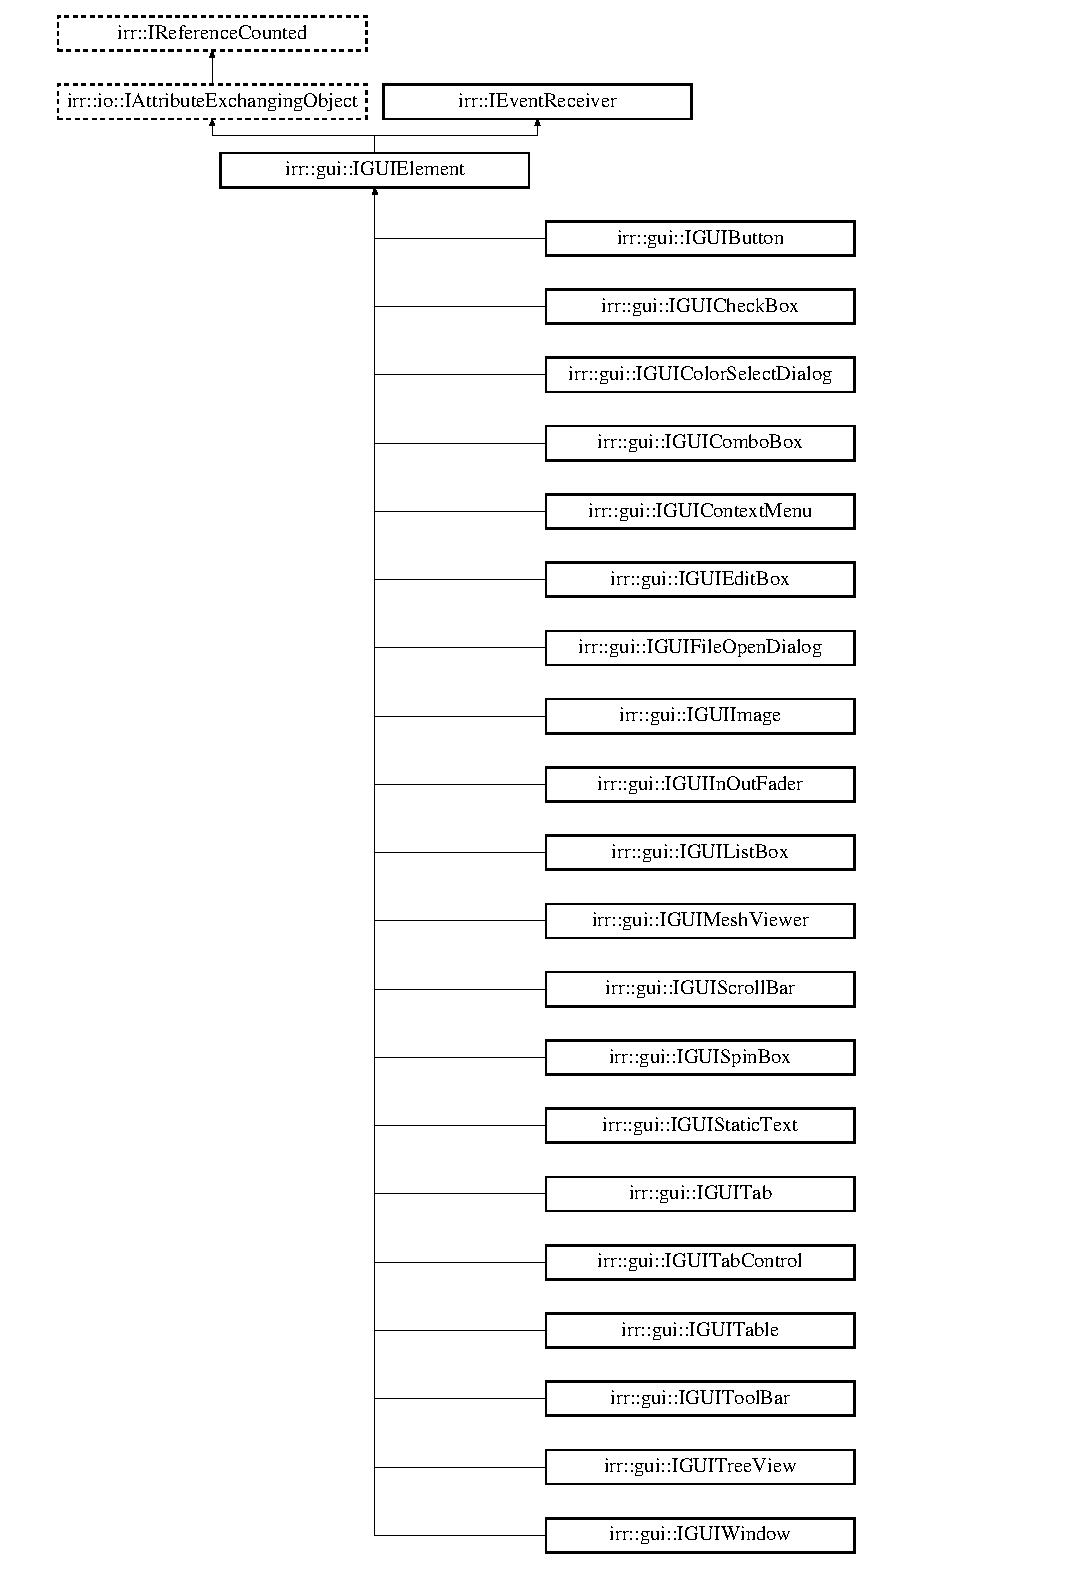
\includegraphics[height=12.000000cm]{classirr_1_1gui_1_1IGUIElement}
\end{center}
\end{figure}
\subsection*{Public Member Functions}
\begin{DoxyCompactItemize}
\item 
\mbox{\Hypertarget{classirr_1_1gui_1_1IGUIElement_a540fb9b2617696ef421d5510b4d96fea}\label{classirr_1_1gui_1_1IGUIElement_a540fb9b2617696ef421d5510b4d96fea}} 
\hyperlink{classirr_1_1gui_1_1IGUIElement_a540fb9b2617696ef421d5510b4d96fea}{I\+G\+U\+I\+Element} (\hyperlink{namespaceirr_1_1gui_ae4d66df0ecf4117cdbcf9f22404bd254}{E\+G\+U\+I\+\_\+\+E\+L\+E\+M\+E\+N\+T\+\_\+\+T\+Y\+PE} type, \hyperlink{classirr_1_1gui_1_1IGUIEnvironment}{I\+G\+U\+I\+Environment} $\ast$environment, \hyperlink{classirr_1_1gui_1_1IGUIElement}{I\+G\+U\+I\+Element} $\ast$parent, \hyperlink{namespaceirr_ac66849b7a6ed16e30ebede579f9b47c6}{s32} id, const \hyperlink{classirr_1_1core_1_1rect}{core\+::rect}$<$ \hyperlink{namespaceirr_ac66849b7a6ed16e30ebede579f9b47c6}{s32} $>$ \&rectangle)
\begin{DoxyCompactList}\small\item\em Constructor. \end{DoxyCompactList}\item 
\mbox{\Hypertarget{classirr_1_1gui_1_1IGUIElement_a062e6704aa29ed50c22179ad268d8f48}\label{classirr_1_1gui_1_1IGUIElement_a062e6704aa29ed50c22179ad268d8f48}} 
virtual \hyperlink{classirr_1_1gui_1_1IGUIElement_a062e6704aa29ed50c22179ad268d8f48}{$\sim$\+I\+G\+U\+I\+Element} ()
\begin{DoxyCompactList}\small\item\em Destructor. \end{DoxyCompactList}\item 
\mbox{\Hypertarget{classirr_1_1gui_1_1IGUIElement_ab3eacf3540cb5b020f3c4a24c6a67473}\label{classirr_1_1gui_1_1IGUIElement_ab3eacf3540cb5b020f3c4a24c6a67473}} 
\hyperlink{classirr_1_1gui_1_1IGUIElement}{I\+G\+U\+I\+Element} $\ast$ \hyperlink{classirr_1_1gui_1_1IGUIElement_ab3eacf3540cb5b020f3c4a24c6a67473}{get\+Parent} () const
\begin{DoxyCompactList}\small\item\em Returns parent of this element. \end{DoxyCompactList}\item 
\mbox{\Hypertarget{classirr_1_1gui_1_1IGUIElement_a056c893bcfe330c9c6058b6027a45cef}\label{classirr_1_1gui_1_1IGUIElement_a056c893bcfe330c9c6058b6027a45cef}} 
\hyperlink{classirr_1_1core_1_1rect}{core\+::rect}$<$ \hyperlink{namespaceirr_ac66849b7a6ed16e30ebede579f9b47c6}{s32} $>$ \hyperlink{classirr_1_1gui_1_1IGUIElement_a056c893bcfe330c9c6058b6027a45cef}{get\+Relative\+Position} () const
\begin{DoxyCompactList}\small\item\em Returns the relative rectangle of this element. \end{DoxyCompactList}\item 
void \hyperlink{classirr_1_1gui_1_1IGUIElement_a0e5bb2d0a2e88e30d3697652f8dd7034}{set\+Relative\+Position} (const \hyperlink{classirr_1_1core_1_1rect}{core\+::rect}$<$ \hyperlink{namespaceirr_ac66849b7a6ed16e30ebede579f9b47c6}{s32} $>$ \&r)
\begin{DoxyCompactList}\small\item\em Sets the relative rectangle of this element. \end{DoxyCompactList}\item 
void \hyperlink{classirr_1_1gui_1_1IGUIElement_aba1cfc75daa28e53a021faa2d954b79b}{set\+Relative\+Position} (const \hyperlink{namespaceirr_1_1core_ace0f1379db5f9f5660456ec57ab78202}{core\+::position2di} \&position)
\begin{DoxyCompactList}\small\item\em Sets the relative rectangle of this element, maintaining its current width and height. \end{DoxyCompactList}\item 
void \hyperlink{classirr_1_1gui_1_1IGUIElement_aa67e02ab54db1068e7c057721d2f24a5}{set\+Relative\+Position\+Proportional} (const \hyperlink{classirr_1_1core_1_1rect}{core\+::rect}$<$ \hyperlink{namespaceirr_a0277be98d67dc26ff93b1a6a1d086b07}{f32} $>$ \&r)
\begin{DoxyCompactList}\small\item\em Sets the relative rectangle of this element as a proportion of its parent\textquotesingle{}s area. \end{DoxyCompactList}\item 
\mbox{\Hypertarget{classirr_1_1gui_1_1IGUIElement_a6c5b94dd889533a306a03e25d0998bdf}\label{classirr_1_1gui_1_1IGUIElement_a6c5b94dd889533a306a03e25d0998bdf}} 
\hyperlink{classirr_1_1core_1_1rect}{core\+::rect}$<$ \hyperlink{namespaceirr_ac66849b7a6ed16e30ebede579f9b47c6}{s32} $>$ \hyperlink{classirr_1_1gui_1_1IGUIElement_a6c5b94dd889533a306a03e25d0998bdf}{get\+Absolute\+Position} () const
\begin{DoxyCompactList}\small\item\em Gets the absolute rectangle of this element. \end{DoxyCompactList}\item 
\mbox{\Hypertarget{classirr_1_1gui_1_1IGUIElement_ad06166ccb3e9c86f17bd2a6cfc627eba}\label{classirr_1_1gui_1_1IGUIElement_ad06166ccb3e9c86f17bd2a6cfc627eba}} 
\hyperlink{classirr_1_1core_1_1rect}{core\+::rect}$<$ \hyperlink{namespaceirr_ac66849b7a6ed16e30ebede579f9b47c6}{s32} $>$ \hyperlink{classirr_1_1gui_1_1IGUIElement_ad06166ccb3e9c86f17bd2a6cfc627eba}{get\+Absolute\+Clipping\+Rect} () const
\begin{DoxyCompactList}\small\item\em Returns the visible area of the element. \end{DoxyCompactList}\item 
void \hyperlink{classirr_1_1gui_1_1IGUIElement_a814d322989acafa74c895e5c13908b86}{set\+Not\+Clipped} (bool no\+Clip)
\begin{DoxyCompactList}\small\item\em Sets whether the element will ignore its parent\textquotesingle{}s clipping rectangle. \end{DoxyCompactList}\item 
bool \hyperlink{classirr_1_1gui_1_1IGUIElement_a940fcf886f9ae1e4bc719e19057018a2}{is\+Not\+Clipped} () const
\begin{DoxyCompactList}\small\item\em Gets whether the element will ignore its parent\textquotesingle{}s clipping rectangle. \end{DoxyCompactList}\item 
void \hyperlink{classirr_1_1gui_1_1IGUIElement_ae80ad7253fb9fb2ebbeda2a8148fff3e}{set\+Max\+Size} (\hyperlink{namespaceirr_1_1core_a13e5bd7e47b2014eefc870ede11bbbbc}{core\+::dimension2du} size)
\begin{DoxyCompactList}\small\item\em Sets the maximum size allowed for this element. \end{DoxyCompactList}\item 
\mbox{\Hypertarget{classirr_1_1gui_1_1IGUIElement_ae1ddcdd58af93fea900bd6295d4d8e61}\label{classirr_1_1gui_1_1IGUIElement_ae1ddcdd58af93fea900bd6295d4d8e61}} 
void \hyperlink{classirr_1_1gui_1_1IGUIElement_ae1ddcdd58af93fea900bd6295d4d8e61}{set\+Min\+Size} (\hyperlink{namespaceirr_1_1core_a13e5bd7e47b2014eefc870ede11bbbbc}{core\+::dimension2du} size)
\begin{DoxyCompactList}\small\item\em Sets the minimum size allowed for this element. \end{DoxyCompactList}\item 
\mbox{\Hypertarget{classirr_1_1gui_1_1IGUIElement_a1eb3d7ec13ebbf8c73859810088f666b}\label{classirr_1_1gui_1_1IGUIElement_a1eb3d7ec13ebbf8c73859810088f666b}} 
void \hyperlink{classirr_1_1gui_1_1IGUIElement_a1eb3d7ec13ebbf8c73859810088f666b}{set\+Alignment} (\hyperlink{namespaceirr_1_1gui_a19eb5fb40e67f108cb16aba922ddaa2d}{E\+G\+U\+I\+\_\+\+A\+L\+I\+G\+N\+M\+E\+NT} left, \hyperlink{namespaceirr_1_1gui_a19eb5fb40e67f108cb16aba922ddaa2d}{E\+G\+U\+I\+\_\+\+A\+L\+I\+G\+N\+M\+E\+NT} right, \hyperlink{namespaceirr_1_1gui_a19eb5fb40e67f108cb16aba922ddaa2d}{E\+G\+U\+I\+\_\+\+A\+L\+I\+G\+N\+M\+E\+NT} top, \hyperlink{namespaceirr_1_1gui_a19eb5fb40e67f108cb16aba922ddaa2d}{E\+G\+U\+I\+\_\+\+A\+L\+I\+G\+N\+M\+E\+NT} bottom)
\begin{DoxyCompactList}\small\item\em The alignment defines how the borders of this element will be positioned when the parent element is resized. \end{DoxyCompactList}\item 
\mbox{\Hypertarget{classirr_1_1gui_1_1IGUIElement_ad58bbeba69a118873a5075d86b4c90f2}\label{classirr_1_1gui_1_1IGUIElement_ad58bbeba69a118873a5075d86b4c90f2}} 
virtual void \hyperlink{classirr_1_1gui_1_1IGUIElement_ad58bbeba69a118873a5075d86b4c90f2}{update\+Absolute\+Position} ()
\begin{DoxyCompactList}\small\item\em Updates the absolute position. \end{DoxyCompactList}\item 
\hyperlink{classirr_1_1gui_1_1IGUIElement}{I\+G\+U\+I\+Element} $\ast$ \hyperlink{classirr_1_1gui_1_1IGUIElement_ae49f8a5228ce0c18e0c98becf74ee56a}{get\+Element\+From\+Point} (const core\+::position2d$<$ \hyperlink{namespaceirr_ac66849b7a6ed16e30ebede579f9b47c6}{s32} $>$ \&point)
\begin{DoxyCompactList}\small\item\em Returns the topmost G\+UI element at the specific position. \end{DoxyCompactList}\item 
virtual bool \hyperlink{classirr_1_1gui_1_1IGUIElement_a1aaf30a10b77f192dda8c548c109de89}{is\+Point\+Inside} (const core\+::position2d$<$ \hyperlink{namespaceirr_ac66849b7a6ed16e30ebede579f9b47c6}{s32} $>$ \&point) const
\begin{DoxyCompactList}\small\item\em Returns true if a point is within this element. \end{DoxyCompactList}\item 
\mbox{\Hypertarget{classirr_1_1gui_1_1IGUIElement_a221c8505217aa9c23c621627a0435554}\label{classirr_1_1gui_1_1IGUIElement_a221c8505217aa9c23c621627a0435554}} 
virtual void \hyperlink{classirr_1_1gui_1_1IGUIElement_a221c8505217aa9c23c621627a0435554}{add\+Child} (\hyperlink{classirr_1_1gui_1_1IGUIElement}{I\+G\+U\+I\+Element} $\ast$child)
\begin{DoxyCompactList}\small\item\em Adds a G\+UI element as new child of this element. \end{DoxyCompactList}\item 
\mbox{\Hypertarget{classirr_1_1gui_1_1IGUIElement_a3171cafaa9d2f3b67c886c60bdd61b32}\label{classirr_1_1gui_1_1IGUIElement_a3171cafaa9d2f3b67c886c60bdd61b32}} 
virtual void \hyperlink{classirr_1_1gui_1_1IGUIElement_a3171cafaa9d2f3b67c886c60bdd61b32}{remove\+Child} (\hyperlink{classirr_1_1gui_1_1IGUIElement}{I\+G\+U\+I\+Element} $\ast$child)
\begin{DoxyCompactList}\small\item\em Removes a child. \end{DoxyCompactList}\item 
\mbox{\Hypertarget{classirr_1_1gui_1_1IGUIElement_af8fb8c63d48ec6ceeeedc8a83c02a9d0}\label{classirr_1_1gui_1_1IGUIElement_af8fb8c63d48ec6ceeeedc8a83c02a9d0}} 
virtual void \hyperlink{classirr_1_1gui_1_1IGUIElement_af8fb8c63d48ec6ceeeedc8a83c02a9d0}{remove} ()
\begin{DoxyCompactList}\small\item\em Removes this element from its parent. \end{DoxyCompactList}\item 
\mbox{\Hypertarget{classirr_1_1gui_1_1IGUIElement_a1ef7eeaff67b8a9f4f37cacdc7e54be2}\label{classirr_1_1gui_1_1IGUIElement_a1ef7eeaff67b8a9f4f37cacdc7e54be2}} 
virtual void \hyperlink{classirr_1_1gui_1_1IGUIElement_a1ef7eeaff67b8a9f4f37cacdc7e54be2}{draw} ()
\begin{DoxyCompactList}\small\item\em Draws the element and its children. \end{DoxyCompactList}\item 
\mbox{\Hypertarget{classirr_1_1gui_1_1IGUIElement_ac71cf9174d4d35eca386657f01d744d1}\label{classirr_1_1gui_1_1IGUIElement_ac71cf9174d4d35eca386657f01d744d1}} 
virtual void \hyperlink{classirr_1_1gui_1_1IGUIElement_ac71cf9174d4d35eca386657f01d744d1}{On\+Post\+Render} (\hyperlink{namespaceirr_a0416a53257075833e7002efd0a18e804}{u32} time\+Ms)
\begin{DoxyCompactList}\small\item\em animate the element and its children. \end{DoxyCompactList}\item 
\mbox{\Hypertarget{classirr_1_1gui_1_1IGUIElement_a842eeacfcb26865416b084593a774704}\label{classirr_1_1gui_1_1IGUIElement_a842eeacfcb26865416b084593a774704}} 
virtual void \hyperlink{classirr_1_1gui_1_1IGUIElement_a842eeacfcb26865416b084593a774704}{move} (core\+::position2d$<$ \hyperlink{namespaceirr_ac66849b7a6ed16e30ebede579f9b47c6}{s32} $>$ absolute\+Movement)
\begin{DoxyCompactList}\small\item\em Moves this element. \end{DoxyCompactList}\item 
\mbox{\Hypertarget{classirr_1_1gui_1_1IGUIElement_a9cb14270ab55bdfe45442542b35567a7}\label{classirr_1_1gui_1_1IGUIElement_a9cb14270ab55bdfe45442542b35567a7}} 
virtual bool \hyperlink{classirr_1_1gui_1_1IGUIElement_a9cb14270ab55bdfe45442542b35567a7}{is\+Visible} () const
\begin{DoxyCompactList}\small\item\em Returns true if element is visible. \end{DoxyCompactList}\item 
\mbox{\Hypertarget{classirr_1_1gui_1_1IGUIElement_aed537cb0b16c670b8f895179f0027bad}\label{classirr_1_1gui_1_1IGUIElement_aed537cb0b16c670b8f895179f0027bad}} 
virtual void \hyperlink{classirr_1_1gui_1_1IGUIElement_aed537cb0b16c670b8f895179f0027bad}{set\+Visible} (bool visible)
\begin{DoxyCompactList}\small\item\em Sets the visible state of this element. \end{DoxyCompactList}\item 
\mbox{\Hypertarget{classirr_1_1gui_1_1IGUIElement_aa85661a9ebba0f46d6e7c7e0da92f4cd}\label{classirr_1_1gui_1_1IGUIElement_aa85661a9ebba0f46d6e7c7e0da92f4cd}} 
virtual bool \hyperlink{classirr_1_1gui_1_1IGUIElement_aa85661a9ebba0f46d6e7c7e0da92f4cd}{is\+Sub\+Element} () const
\begin{DoxyCompactList}\small\item\em Returns true if this element was created as part of its parent control. \end{DoxyCompactList}\item 
virtual void \hyperlink{classirr_1_1gui_1_1IGUIElement_a50eb859808b65ee24fbdd69e69118a8d}{set\+Sub\+Element} (bool sub\+Element)
\begin{DoxyCompactList}\small\item\em Sets whether this control was created as part of its parent. \end{DoxyCompactList}\item 
void \hyperlink{classirr_1_1gui_1_1IGUIElement_a58b9b6a8715b4959dda905dbc028ece6}{set\+Tab\+Stop} (bool enable)
\begin{DoxyCompactList}\small\item\em If set to true, the focus will visit this element when using the tab key to cycle through elements. \end{DoxyCompactList}\item 
\mbox{\Hypertarget{classirr_1_1gui_1_1IGUIElement_a0f9c536acf8a57faa18d61ff5b0bf567}\label{classirr_1_1gui_1_1IGUIElement_a0f9c536acf8a57faa18d61ff5b0bf567}} 
bool \hyperlink{classirr_1_1gui_1_1IGUIElement_a0f9c536acf8a57faa18d61ff5b0bf567}{is\+Tab\+Stop} () const
\begin{DoxyCompactList}\small\item\em Returns true if this element can be focused by navigating with the tab key. \end{DoxyCompactList}\item 
void \hyperlink{classirr_1_1gui_1_1IGUIElement_a1aabac2cce7847e5ab17f6c88d129ef7}{set\+Tab\+Order} (\hyperlink{namespaceirr_ac66849b7a6ed16e30ebede579f9b47c6}{s32} index)
\begin{DoxyCompactList}\small\item\em Sets the priority of focus when using the tab key to navigate between a group of elements. \end{DoxyCompactList}\item 
\mbox{\Hypertarget{classirr_1_1gui_1_1IGUIElement_af1f535aacf6e19fda64511715100e069}\label{classirr_1_1gui_1_1IGUIElement_af1f535aacf6e19fda64511715100e069}} 
\hyperlink{namespaceirr_ac66849b7a6ed16e30ebede579f9b47c6}{s32} \hyperlink{classirr_1_1gui_1_1IGUIElement_af1f535aacf6e19fda64511715100e069}{get\+Tab\+Order} () const
\begin{DoxyCompactList}\small\item\em Returns the number in the tab order sequence. \end{DoxyCompactList}\item 
void \hyperlink{classirr_1_1gui_1_1IGUIElement_aa44a46f3b639ca1b095f855c9d9c959d}{set\+Tab\+Group} (bool is\+Group)
\begin{DoxyCompactList}\small\item\em Sets whether this element is a container for a group of elements which can be navigated using the tab key. \end{DoxyCompactList}\item 
\mbox{\Hypertarget{classirr_1_1gui_1_1IGUIElement_a70596321725a708ecea4974d4df760c9}\label{classirr_1_1gui_1_1IGUIElement_a70596321725a708ecea4974d4df760c9}} 
bool \hyperlink{classirr_1_1gui_1_1IGUIElement_a70596321725a708ecea4974d4df760c9}{is\+Tab\+Group} () const
\begin{DoxyCompactList}\small\item\em Returns true if this element is a tab group. \end{DoxyCompactList}\item 
\mbox{\Hypertarget{classirr_1_1gui_1_1IGUIElement_ab6266a2fd3d8b0be385f9f3f3364e9ff}\label{classirr_1_1gui_1_1IGUIElement_ab6266a2fd3d8b0be385f9f3f3364e9ff}} 
\hyperlink{classirr_1_1gui_1_1IGUIElement}{I\+G\+U\+I\+Element} $\ast$ \hyperlink{classirr_1_1gui_1_1IGUIElement_ab6266a2fd3d8b0be385f9f3f3364e9ff}{get\+Tab\+Group} ()
\begin{DoxyCompactList}\small\item\em Returns the container element which holds all elements in this element\textquotesingle{}s tab group. \end{DoxyCompactList}\item 
virtual bool \hyperlink{classirr_1_1gui_1_1IGUIElement_add00898b0ee96565f55b1b47efaceec6}{is\+Enabled} () const
\begin{DoxyCompactList}\small\item\em Returns true if element is enabled. \end{DoxyCompactList}\item 
\mbox{\Hypertarget{classirr_1_1gui_1_1IGUIElement_a2e3fd4a5f1ae52296f98cf36fdcffd1b}\label{classirr_1_1gui_1_1IGUIElement_a2e3fd4a5f1ae52296f98cf36fdcffd1b}} 
virtual void \hyperlink{classirr_1_1gui_1_1IGUIElement_a2e3fd4a5f1ae52296f98cf36fdcffd1b}{set\+Enabled} (bool enabled)
\begin{DoxyCompactList}\small\item\em Sets the enabled state of this element. \end{DoxyCompactList}\item 
\mbox{\Hypertarget{classirr_1_1gui_1_1IGUIElement_a8f864c26d4b2ee3551c53d3ebf870656}\label{classirr_1_1gui_1_1IGUIElement_a8f864c26d4b2ee3551c53d3ebf870656}} 
virtual void \hyperlink{classirr_1_1gui_1_1IGUIElement_a8f864c26d4b2ee3551c53d3ebf870656}{set\+Text} (const wchar\+\_\+t $\ast$text)
\begin{DoxyCompactList}\small\item\em Sets the new caption of this element. \end{DoxyCompactList}\item 
\mbox{\Hypertarget{classirr_1_1gui_1_1IGUIElement_addaba768aba8a3e9d77b8ade88f05e13}\label{classirr_1_1gui_1_1IGUIElement_addaba768aba8a3e9d77b8ade88f05e13}} 
virtual const wchar\+\_\+t $\ast$ \hyperlink{classirr_1_1gui_1_1IGUIElement_addaba768aba8a3e9d77b8ade88f05e13}{get\+Text} () const
\begin{DoxyCompactList}\small\item\em Returns caption of this element. \end{DoxyCompactList}\item 
\mbox{\Hypertarget{classirr_1_1gui_1_1IGUIElement_a672f29f88c8d8f1e8ed1ac6c9f23b890}\label{classirr_1_1gui_1_1IGUIElement_a672f29f88c8d8f1e8ed1ac6c9f23b890}} 
virtual void \hyperlink{classirr_1_1gui_1_1IGUIElement_a672f29f88c8d8f1e8ed1ac6c9f23b890}{set\+Tool\+Tip\+Text} (const wchar\+\_\+t $\ast$text)
\begin{DoxyCompactList}\small\item\em Sets the new caption of this element. \end{DoxyCompactList}\item 
\mbox{\Hypertarget{classirr_1_1gui_1_1IGUIElement_a9c19741dd210443b750e02ef7d639cf8}\label{classirr_1_1gui_1_1IGUIElement_a9c19741dd210443b750e02ef7d639cf8}} 
virtual const \hyperlink{namespaceirr_1_1core_a5aedb62cb47cf01d1c548ab5e6344d2d}{core\+::stringw} \& \hyperlink{classirr_1_1gui_1_1IGUIElement_a9c19741dd210443b750e02ef7d639cf8}{get\+Tool\+Tip\+Text} () const
\begin{DoxyCompactList}\small\item\em Returns caption of this element. \end{DoxyCompactList}\item 
\mbox{\Hypertarget{classirr_1_1gui_1_1IGUIElement_af838c5de4a09e09a89de74d67d07d80c}\label{classirr_1_1gui_1_1IGUIElement_af838c5de4a09e09a89de74d67d07d80c}} 
virtual \hyperlink{namespaceirr_ac66849b7a6ed16e30ebede579f9b47c6}{s32} \hyperlink{classirr_1_1gui_1_1IGUIElement_af838c5de4a09e09a89de74d67d07d80c}{get\+ID} () const
\begin{DoxyCompactList}\small\item\em Returns id. Can be used to identify the element. \end{DoxyCompactList}\item 
\mbox{\Hypertarget{classirr_1_1gui_1_1IGUIElement_a55bad0e14306765e1fb734c56b729ba4}\label{classirr_1_1gui_1_1IGUIElement_a55bad0e14306765e1fb734c56b729ba4}} 
virtual void \hyperlink{classirr_1_1gui_1_1IGUIElement_a55bad0e14306765e1fb734c56b729ba4}{set\+ID} (\hyperlink{namespaceirr_ac66849b7a6ed16e30ebede579f9b47c6}{s32} id)
\begin{DoxyCompactList}\small\item\em Sets the id of this element. \end{DoxyCompactList}\item 
\mbox{\Hypertarget{classirr_1_1gui_1_1IGUIElement_a54b1799e21722d9e6ce5b8e4bdb2e80a}\label{classirr_1_1gui_1_1IGUIElement_a54b1799e21722d9e6ce5b8e4bdb2e80a}} 
virtual bool \hyperlink{classirr_1_1gui_1_1IGUIElement_a54b1799e21722d9e6ce5b8e4bdb2e80a}{On\+Event} (const \hyperlink{structirr_1_1SEvent}{S\+Event} \&event)
\begin{DoxyCompactList}\small\item\em Called if an event happened. \end{DoxyCompactList}\item 
virtual bool \hyperlink{classirr_1_1gui_1_1IGUIElement_ac262c8018bf4101f38f448fde16f5a52}{bring\+To\+Front} (\hyperlink{classirr_1_1gui_1_1IGUIElement}{I\+G\+U\+I\+Element} $\ast$element)
\begin{DoxyCompactList}\small\item\em Brings a child to front. \end{DoxyCompactList}\item 
virtual bool \hyperlink{classirr_1_1gui_1_1IGUIElement_a9b1880048e7542dbe289295de69e77cd}{send\+To\+Back} (\hyperlink{classirr_1_1gui_1_1IGUIElement}{I\+G\+U\+I\+Element} $\ast$child)
\begin{DoxyCompactList}\small\item\em Moves a child to the back, so it\textquotesingle{}s siblings are drawn on top of it. \end{DoxyCompactList}\item 
\mbox{\Hypertarget{classirr_1_1gui_1_1IGUIElement_a96492ba4d7974c1eae92f98b31b70d95}\label{classirr_1_1gui_1_1IGUIElement_a96492ba4d7974c1eae92f98b31b70d95}} 
virtual const \hyperlink{classirr_1_1core_1_1list}{core\+::list}$<$ \hyperlink{classirr_1_1gui_1_1IGUIElement}{I\+G\+U\+I\+Element} $\ast$ $>$ \& \hyperlink{classirr_1_1gui_1_1IGUIElement_a96492ba4d7974c1eae92f98b31b70d95}{get\+Children} () const
\begin{DoxyCompactList}\small\item\em Returns list with children of this element. \end{DoxyCompactList}\item 
virtual \hyperlink{classirr_1_1gui_1_1IGUIElement}{I\+G\+U\+I\+Element} $\ast$ \hyperlink{classirr_1_1gui_1_1IGUIElement_ab79b8e81d2f2864312345cffe9237cce}{get\+Element\+From\+Id} (\hyperlink{namespaceirr_ac66849b7a6ed16e30ebede579f9b47c6}{s32} id, bool searchchildren=false) const
\begin{DoxyCompactList}\small\item\em Finds the first element with the given id. \end{DoxyCompactList}\item 
bool \hyperlink{classirr_1_1gui_1_1IGUIElement_a72fe3668d62bfb7edc4586d582a947b4}{is\+My\+Child} (\hyperlink{classirr_1_1gui_1_1IGUIElement}{I\+G\+U\+I\+Element} $\ast$child) const
\begin{DoxyCompactList}\small\item\em returns true if the given element is a child of this one. \end{DoxyCompactList}\item 
bool \hyperlink{classirr_1_1gui_1_1IGUIElement_aaf461c857c9005d310635e56dc384ed4}{get\+Next\+Element} (\hyperlink{namespaceirr_ac66849b7a6ed16e30ebede579f9b47c6}{s32} start\+Order, bool reverse, bool group, \hyperlink{classirr_1_1gui_1_1IGUIElement}{I\+G\+U\+I\+Element} $\ast$\&first, \hyperlink{classirr_1_1gui_1_1IGUIElement}{I\+G\+U\+I\+Element} $\ast$\&closest, bool include\+Invisible=false) const
\begin{DoxyCompactList}\small\item\em searches elements to find the closest next element to tab to \end{DoxyCompactList}\item 
\hyperlink{namespaceirr_1_1gui_ae4d66df0ecf4117cdbcf9f22404bd254}{E\+G\+U\+I\+\_\+\+E\+L\+E\+M\+E\+N\+T\+\_\+\+T\+Y\+PE} \hyperlink{classirr_1_1gui_1_1IGUIElement_aeb2f4dec42afc4b8c1182897d0dc1a70}{get\+Type} () const
\begin{DoxyCompactList}\small\item\em Returns the type of the gui element. \end{DoxyCompactList}\item 
virtual bool \hyperlink{classirr_1_1gui_1_1IGUIElement_a3c9f0356f89f4906c7bf5a302e57f01d}{has\+Type} (\hyperlink{namespaceirr_1_1gui_ae4d66df0ecf4117cdbcf9f22404bd254}{E\+G\+U\+I\+\_\+\+E\+L\+E\+M\+E\+N\+T\+\_\+\+T\+Y\+PE} type) const
\begin{DoxyCompactList}\small\item\em Returns true if the gui element supports the given type. \end{DoxyCompactList}\item 
virtual const \hyperlink{namespaceirr_a9395eaea339bcb546b319e9c96bf7410}{c8} $\ast$ \hyperlink{classirr_1_1gui_1_1IGUIElement_a656d2055c0d61382afee1d494c275ce9}{get\+Type\+Name} () const
\begin{DoxyCompactList}\small\item\em Returns the type name of the gui element. \end{DoxyCompactList}\item 
virtual const \hyperlink{namespaceirr_a9395eaea339bcb546b319e9c96bf7410}{c8} $\ast$ \hyperlink{classirr_1_1gui_1_1IGUIElement_a308fa8bc16580d53df5c65ded0c1349b}{get\+Name} () const
\begin{DoxyCompactList}\small\item\em Returns the name of the element. \end{DoxyCompactList}\item 
virtual void \hyperlink{classirr_1_1gui_1_1IGUIElement_a47ce14d1a973137b6cbe91a047df2ebe}{set\+Name} (const \hyperlink{namespaceirr_a9395eaea339bcb546b319e9c96bf7410}{c8} $\ast$name)
\begin{DoxyCompactList}\small\item\em Sets the name of the element. \end{DoxyCompactList}\item 
virtual void \hyperlink{classirr_1_1gui_1_1IGUIElement_a5e318b47fece6d4157a1d7ccf401f1c8}{set\+Name} (const \hyperlink{namespaceirr_1_1core_ab26a0e0359206b5a694f35c37c829d7f}{core\+::stringc} \&name)
\begin{DoxyCompactList}\small\item\em Sets the name of the element. \end{DoxyCompactList}\item 
virtual void \hyperlink{classirr_1_1gui_1_1IGUIElement_ac575f2f817b05733dbc667ff298f6e78}{serialize\+Attributes} (\hyperlink{classirr_1_1io_1_1IAttributes}{io\+::\+I\+Attributes} $\ast$out, \hyperlink{structirr_1_1io_1_1SAttributeReadWriteOptions}{io\+::\+S\+Attribute\+Read\+Write\+Options} $\ast$options=0) const
\begin{DoxyCompactList}\small\item\em Writes attributes of the scene node. \end{DoxyCompactList}\item 
virtual void \hyperlink{classirr_1_1gui_1_1IGUIElement_af71b96163b8d95816cd9c80fbf413b4d}{deserialize\+Attributes} (\hyperlink{classirr_1_1io_1_1IAttributes}{io\+::\+I\+Attributes} $\ast$in, \hyperlink{structirr_1_1io_1_1SAttributeReadWriteOptions}{io\+::\+S\+Attribute\+Read\+Write\+Options} $\ast$options=0)
\begin{DoxyCompactList}\small\item\em Reads attributes of the scene node. \end{DoxyCompactList}\item 
\mbox{\Hypertarget{classirr_1_1gui_1_1IGUIElement_a540fb9b2617696ef421d5510b4d96fea}\label{classirr_1_1gui_1_1IGUIElement_a540fb9b2617696ef421d5510b4d96fea}} 
\hyperlink{classirr_1_1gui_1_1IGUIElement_a540fb9b2617696ef421d5510b4d96fea}{I\+G\+U\+I\+Element} (\hyperlink{namespaceirr_1_1gui_ae4d66df0ecf4117cdbcf9f22404bd254}{E\+G\+U\+I\+\_\+\+E\+L\+E\+M\+E\+N\+T\+\_\+\+T\+Y\+PE} type, \hyperlink{classirr_1_1gui_1_1IGUIEnvironment}{I\+G\+U\+I\+Environment} $\ast$environment, \hyperlink{classirr_1_1gui_1_1IGUIElement}{I\+G\+U\+I\+Element} $\ast$parent, \hyperlink{namespaceirr_ac66849b7a6ed16e30ebede579f9b47c6}{s32} id, const \hyperlink{classirr_1_1core_1_1rect}{core\+::rect}$<$ \hyperlink{namespaceirr_ac66849b7a6ed16e30ebede579f9b47c6}{s32} $>$ \&rectangle)
\begin{DoxyCompactList}\small\item\em Constructor. \end{DoxyCompactList}\item 
\mbox{\Hypertarget{classirr_1_1gui_1_1IGUIElement_a062e6704aa29ed50c22179ad268d8f48}\label{classirr_1_1gui_1_1IGUIElement_a062e6704aa29ed50c22179ad268d8f48}} 
virtual \hyperlink{classirr_1_1gui_1_1IGUIElement_a062e6704aa29ed50c22179ad268d8f48}{$\sim$\+I\+G\+U\+I\+Element} ()
\begin{DoxyCompactList}\small\item\em Destructor. \end{DoxyCompactList}\item 
\mbox{\Hypertarget{classirr_1_1gui_1_1IGUIElement_ab3eacf3540cb5b020f3c4a24c6a67473}\label{classirr_1_1gui_1_1IGUIElement_ab3eacf3540cb5b020f3c4a24c6a67473}} 
\hyperlink{classirr_1_1gui_1_1IGUIElement}{I\+G\+U\+I\+Element} $\ast$ \hyperlink{classirr_1_1gui_1_1IGUIElement_ab3eacf3540cb5b020f3c4a24c6a67473}{get\+Parent} () const
\begin{DoxyCompactList}\small\item\em Returns parent of this element. \end{DoxyCompactList}\item 
\mbox{\Hypertarget{classirr_1_1gui_1_1IGUIElement_a056c893bcfe330c9c6058b6027a45cef}\label{classirr_1_1gui_1_1IGUIElement_a056c893bcfe330c9c6058b6027a45cef}} 
\hyperlink{classirr_1_1core_1_1rect}{core\+::rect}$<$ \hyperlink{namespaceirr_ac66849b7a6ed16e30ebede579f9b47c6}{s32} $>$ \hyperlink{classirr_1_1gui_1_1IGUIElement_a056c893bcfe330c9c6058b6027a45cef}{get\+Relative\+Position} () const
\begin{DoxyCompactList}\small\item\em Returns the relative rectangle of this element. \end{DoxyCompactList}\item 
void \hyperlink{classirr_1_1gui_1_1IGUIElement_a0e5bb2d0a2e88e30d3697652f8dd7034}{set\+Relative\+Position} (const \hyperlink{classirr_1_1core_1_1rect}{core\+::rect}$<$ \hyperlink{namespaceirr_ac66849b7a6ed16e30ebede579f9b47c6}{s32} $>$ \&r)
\begin{DoxyCompactList}\small\item\em Sets the relative rectangle of this element. \end{DoxyCompactList}\item 
void \hyperlink{classirr_1_1gui_1_1IGUIElement_aba1cfc75daa28e53a021faa2d954b79b}{set\+Relative\+Position} (const \hyperlink{namespaceirr_1_1core_ace0f1379db5f9f5660456ec57ab78202}{core\+::position2di} \&position)
\begin{DoxyCompactList}\small\item\em Sets the relative rectangle of this element, maintaining its current width and height. \end{DoxyCompactList}\item 
void \hyperlink{classirr_1_1gui_1_1IGUIElement_aa67e02ab54db1068e7c057721d2f24a5}{set\+Relative\+Position\+Proportional} (const \hyperlink{classirr_1_1core_1_1rect}{core\+::rect}$<$ \hyperlink{namespaceirr_a0277be98d67dc26ff93b1a6a1d086b07}{f32} $>$ \&r)
\begin{DoxyCompactList}\small\item\em Sets the relative rectangle of this element as a proportion of its parent\textquotesingle{}s area. \end{DoxyCompactList}\item 
\mbox{\Hypertarget{classirr_1_1gui_1_1IGUIElement_a6c5b94dd889533a306a03e25d0998bdf}\label{classirr_1_1gui_1_1IGUIElement_a6c5b94dd889533a306a03e25d0998bdf}} 
\hyperlink{classirr_1_1core_1_1rect}{core\+::rect}$<$ \hyperlink{namespaceirr_ac66849b7a6ed16e30ebede579f9b47c6}{s32} $>$ \hyperlink{classirr_1_1gui_1_1IGUIElement_a6c5b94dd889533a306a03e25d0998bdf}{get\+Absolute\+Position} () const
\begin{DoxyCompactList}\small\item\em Gets the absolute rectangle of this element. \end{DoxyCompactList}\item 
\mbox{\Hypertarget{classirr_1_1gui_1_1IGUIElement_ad06166ccb3e9c86f17bd2a6cfc627eba}\label{classirr_1_1gui_1_1IGUIElement_ad06166ccb3e9c86f17bd2a6cfc627eba}} 
\hyperlink{classirr_1_1core_1_1rect}{core\+::rect}$<$ \hyperlink{namespaceirr_ac66849b7a6ed16e30ebede579f9b47c6}{s32} $>$ \hyperlink{classirr_1_1gui_1_1IGUIElement_ad06166ccb3e9c86f17bd2a6cfc627eba}{get\+Absolute\+Clipping\+Rect} () const
\begin{DoxyCompactList}\small\item\em Returns the visible area of the element. \end{DoxyCompactList}\item 
void \hyperlink{classirr_1_1gui_1_1IGUIElement_a814d322989acafa74c895e5c13908b86}{set\+Not\+Clipped} (bool no\+Clip)
\begin{DoxyCompactList}\small\item\em Sets whether the element will ignore its parent\textquotesingle{}s clipping rectangle. \end{DoxyCompactList}\item 
bool \hyperlink{classirr_1_1gui_1_1IGUIElement_a940fcf886f9ae1e4bc719e19057018a2}{is\+Not\+Clipped} () const
\begin{DoxyCompactList}\small\item\em Gets whether the element will ignore its parent\textquotesingle{}s clipping rectangle. \end{DoxyCompactList}\item 
void \hyperlink{classirr_1_1gui_1_1IGUIElement_ae80ad7253fb9fb2ebbeda2a8148fff3e}{set\+Max\+Size} (\hyperlink{namespaceirr_1_1core_a13e5bd7e47b2014eefc870ede11bbbbc}{core\+::dimension2du} size)
\begin{DoxyCompactList}\small\item\em Sets the maximum size allowed for this element. \end{DoxyCompactList}\item 
\mbox{\Hypertarget{classirr_1_1gui_1_1IGUIElement_ae1ddcdd58af93fea900bd6295d4d8e61}\label{classirr_1_1gui_1_1IGUIElement_ae1ddcdd58af93fea900bd6295d4d8e61}} 
void \hyperlink{classirr_1_1gui_1_1IGUIElement_ae1ddcdd58af93fea900bd6295d4d8e61}{set\+Min\+Size} (\hyperlink{namespaceirr_1_1core_a13e5bd7e47b2014eefc870ede11bbbbc}{core\+::dimension2du} size)
\begin{DoxyCompactList}\small\item\em Sets the minimum size allowed for this element. \end{DoxyCompactList}\item 
\mbox{\Hypertarget{classirr_1_1gui_1_1IGUIElement_a1eb3d7ec13ebbf8c73859810088f666b}\label{classirr_1_1gui_1_1IGUIElement_a1eb3d7ec13ebbf8c73859810088f666b}} 
void \hyperlink{classirr_1_1gui_1_1IGUIElement_a1eb3d7ec13ebbf8c73859810088f666b}{set\+Alignment} (\hyperlink{namespaceirr_1_1gui_a19eb5fb40e67f108cb16aba922ddaa2d}{E\+G\+U\+I\+\_\+\+A\+L\+I\+G\+N\+M\+E\+NT} left, \hyperlink{namespaceirr_1_1gui_a19eb5fb40e67f108cb16aba922ddaa2d}{E\+G\+U\+I\+\_\+\+A\+L\+I\+G\+N\+M\+E\+NT} right, \hyperlink{namespaceirr_1_1gui_a19eb5fb40e67f108cb16aba922ddaa2d}{E\+G\+U\+I\+\_\+\+A\+L\+I\+G\+N\+M\+E\+NT} top, \hyperlink{namespaceirr_1_1gui_a19eb5fb40e67f108cb16aba922ddaa2d}{E\+G\+U\+I\+\_\+\+A\+L\+I\+G\+N\+M\+E\+NT} bottom)
\begin{DoxyCompactList}\small\item\em The alignment defines how the borders of this element will be positioned when the parent element is resized. \end{DoxyCompactList}\item 
\mbox{\Hypertarget{classirr_1_1gui_1_1IGUIElement_ad58bbeba69a118873a5075d86b4c90f2}\label{classirr_1_1gui_1_1IGUIElement_ad58bbeba69a118873a5075d86b4c90f2}} 
virtual void \hyperlink{classirr_1_1gui_1_1IGUIElement_ad58bbeba69a118873a5075d86b4c90f2}{update\+Absolute\+Position} ()
\begin{DoxyCompactList}\small\item\em Updates the absolute position. \end{DoxyCompactList}\item 
\hyperlink{classirr_1_1gui_1_1IGUIElement}{I\+G\+U\+I\+Element} $\ast$ \hyperlink{classirr_1_1gui_1_1IGUIElement_ae49f8a5228ce0c18e0c98becf74ee56a}{get\+Element\+From\+Point} (const core\+::position2d$<$ \hyperlink{namespaceirr_ac66849b7a6ed16e30ebede579f9b47c6}{s32} $>$ \&point)
\begin{DoxyCompactList}\small\item\em Returns the topmost G\+UI element at the specific position. \end{DoxyCompactList}\item 
virtual bool \hyperlink{classirr_1_1gui_1_1IGUIElement_a1aaf30a10b77f192dda8c548c109de89}{is\+Point\+Inside} (const core\+::position2d$<$ \hyperlink{namespaceirr_ac66849b7a6ed16e30ebede579f9b47c6}{s32} $>$ \&point) const
\begin{DoxyCompactList}\small\item\em Returns true if a point is within this element. \end{DoxyCompactList}\item 
\mbox{\Hypertarget{classirr_1_1gui_1_1IGUIElement_a221c8505217aa9c23c621627a0435554}\label{classirr_1_1gui_1_1IGUIElement_a221c8505217aa9c23c621627a0435554}} 
virtual void \hyperlink{classirr_1_1gui_1_1IGUIElement_a221c8505217aa9c23c621627a0435554}{add\+Child} (\hyperlink{classirr_1_1gui_1_1IGUIElement}{I\+G\+U\+I\+Element} $\ast$child)
\begin{DoxyCompactList}\small\item\em Adds a G\+UI element as new child of this element. \end{DoxyCompactList}\item 
\mbox{\Hypertarget{classirr_1_1gui_1_1IGUIElement_a3171cafaa9d2f3b67c886c60bdd61b32}\label{classirr_1_1gui_1_1IGUIElement_a3171cafaa9d2f3b67c886c60bdd61b32}} 
virtual void \hyperlink{classirr_1_1gui_1_1IGUIElement_a3171cafaa9d2f3b67c886c60bdd61b32}{remove\+Child} (\hyperlink{classirr_1_1gui_1_1IGUIElement}{I\+G\+U\+I\+Element} $\ast$child)
\begin{DoxyCompactList}\small\item\em Removes a child. \end{DoxyCompactList}\item 
\mbox{\Hypertarget{classirr_1_1gui_1_1IGUIElement_af8fb8c63d48ec6ceeeedc8a83c02a9d0}\label{classirr_1_1gui_1_1IGUIElement_af8fb8c63d48ec6ceeeedc8a83c02a9d0}} 
virtual void \hyperlink{classirr_1_1gui_1_1IGUIElement_af8fb8c63d48ec6ceeeedc8a83c02a9d0}{remove} ()
\begin{DoxyCompactList}\small\item\em Removes this element from its parent. \end{DoxyCompactList}\item 
\mbox{\Hypertarget{classirr_1_1gui_1_1IGUIElement_a1ef7eeaff67b8a9f4f37cacdc7e54be2}\label{classirr_1_1gui_1_1IGUIElement_a1ef7eeaff67b8a9f4f37cacdc7e54be2}} 
virtual void \hyperlink{classirr_1_1gui_1_1IGUIElement_a1ef7eeaff67b8a9f4f37cacdc7e54be2}{draw} ()
\begin{DoxyCompactList}\small\item\em Draws the element and its children. \end{DoxyCompactList}\item 
\mbox{\Hypertarget{classirr_1_1gui_1_1IGUIElement_ac71cf9174d4d35eca386657f01d744d1}\label{classirr_1_1gui_1_1IGUIElement_ac71cf9174d4d35eca386657f01d744d1}} 
virtual void \hyperlink{classirr_1_1gui_1_1IGUIElement_ac71cf9174d4d35eca386657f01d744d1}{On\+Post\+Render} (\hyperlink{namespaceirr_a0416a53257075833e7002efd0a18e804}{u32} time\+Ms)
\begin{DoxyCompactList}\small\item\em animate the element and its children. \end{DoxyCompactList}\item 
\mbox{\Hypertarget{classirr_1_1gui_1_1IGUIElement_a842eeacfcb26865416b084593a774704}\label{classirr_1_1gui_1_1IGUIElement_a842eeacfcb26865416b084593a774704}} 
virtual void \hyperlink{classirr_1_1gui_1_1IGUIElement_a842eeacfcb26865416b084593a774704}{move} (core\+::position2d$<$ \hyperlink{namespaceirr_ac66849b7a6ed16e30ebede579f9b47c6}{s32} $>$ absolute\+Movement)
\begin{DoxyCompactList}\small\item\em Moves this element. \end{DoxyCompactList}\item 
\mbox{\Hypertarget{classirr_1_1gui_1_1IGUIElement_a9cb14270ab55bdfe45442542b35567a7}\label{classirr_1_1gui_1_1IGUIElement_a9cb14270ab55bdfe45442542b35567a7}} 
virtual bool \hyperlink{classirr_1_1gui_1_1IGUIElement_a9cb14270ab55bdfe45442542b35567a7}{is\+Visible} () const
\begin{DoxyCompactList}\small\item\em Returns true if element is visible. \end{DoxyCompactList}\item 
\mbox{\Hypertarget{classirr_1_1gui_1_1IGUIElement_aed537cb0b16c670b8f895179f0027bad}\label{classirr_1_1gui_1_1IGUIElement_aed537cb0b16c670b8f895179f0027bad}} 
virtual void \hyperlink{classirr_1_1gui_1_1IGUIElement_aed537cb0b16c670b8f895179f0027bad}{set\+Visible} (bool visible)
\begin{DoxyCompactList}\small\item\em Sets the visible state of this element. \end{DoxyCompactList}\item 
\mbox{\Hypertarget{classirr_1_1gui_1_1IGUIElement_aa85661a9ebba0f46d6e7c7e0da92f4cd}\label{classirr_1_1gui_1_1IGUIElement_aa85661a9ebba0f46d6e7c7e0da92f4cd}} 
virtual bool \hyperlink{classirr_1_1gui_1_1IGUIElement_aa85661a9ebba0f46d6e7c7e0da92f4cd}{is\+Sub\+Element} () const
\begin{DoxyCompactList}\small\item\em Returns true if this element was created as part of its parent control. \end{DoxyCompactList}\item 
virtual void \hyperlink{classirr_1_1gui_1_1IGUIElement_a50eb859808b65ee24fbdd69e69118a8d}{set\+Sub\+Element} (bool sub\+Element)
\begin{DoxyCompactList}\small\item\em Sets whether this control was created as part of its parent. \end{DoxyCompactList}\item 
void \hyperlink{classirr_1_1gui_1_1IGUIElement_a58b9b6a8715b4959dda905dbc028ece6}{set\+Tab\+Stop} (bool enable)
\begin{DoxyCompactList}\small\item\em If set to true, the focus will visit this element when using the tab key to cycle through elements. \end{DoxyCompactList}\item 
\mbox{\Hypertarget{classirr_1_1gui_1_1IGUIElement_a0f9c536acf8a57faa18d61ff5b0bf567}\label{classirr_1_1gui_1_1IGUIElement_a0f9c536acf8a57faa18d61ff5b0bf567}} 
bool \hyperlink{classirr_1_1gui_1_1IGUIElement_a0f9c536acf8a57faa18d61ff5b0bf567}{is\+Tab\+Stop} () const
\begin{DoxyCompactList}\small\item\em Returns true if this element can be focused by navigating with the tab key. \end{DoxyCompactList}\item 
void \hyperlink{classirr_1_1gui_1_1IGUIElement_a1aabac2cce7847e5ab17f6c88d129ef7}{set\+Tab\+Order} (\hyperlink{namespaceirr_ac66849b7a6ed16e30ebede579f9b47c6}{s32} index)
\begin{DoxyCompactList}\small\item\em Sets the priority of focus when using the tab key to navigate between a group of elements. \end{DoxyCompactList}\item 
\mbox{\Hypertarget{classirr_1_1gui_1_1IGUIElement_af1f535aacf6e19fda64511715100e069}\label{classirr_1_1gui_1_1IGUIElement_af1f535aacf6e19fda64511715100e069}} 
\hyperlink{namespaceirr_ac66849b7a6ed16e30ebede579f9b47c6}{s32} \hyperlink{classirr_1_1gui_1_1IGUIElement_af1f535aacf6e19fda64511715100e069}{get\+Tab\+Order} () const
\begin{DoxyCompactList}\small\item\em Returns the number in the tab order sequence. \end{DoxyCompactList}\item 
void \hyperlink{classirr_1_1gui_1_1IGUIElement_aa44a46f3b639ca1b095f855c9d9c959d}{set\+Tab\+Group} (bool is\+Group)
\begin{DoxyCompactList}\small\item\em Sets whether this element is a container for a group of elements which can be navigated using the tab key. \end{DoxyCompactList}\item 
\mbox{\Hypertarget{classirr_1_1gui_1_1IGUIElement_a70596321725a708ecea4974d4df760c9}\label{classirr_1_1gui_1_1IGUIElement_a70596321725a708ecea4974d4df760c9}} 
bool \hyperlink{classirr_1_1gui_1_1IGUIElement_a70596321725a708ecea4974d4df760c9}{is\+Tab\+Group} () const
\begin{DoxyCompactList}\small\item\em Returns true if this element is a tab group. \end{DoxyCompactList}\item 
\mbox{\Hypertarget{classirr_1_1gui_1_1IGUIElement_ab6266a2fd3d8b0be385f9f3f3364e9ff}\label{classirr_1_1gui_1_1IGUIElement_ab6266a2fd3d8b0be385f9f3f3364e9ff}} 
\hyperlink{classirr_1_1gui_1_1IGUIElement}{I\+G\+U\+I\+Element} $\ast$ \hyperlink{classirr_1_1gui_1_1IGUIElement_ab6266a2fd3d8b0be385f9f3f3364e9ff}{get\+Tab\+Group} ()
\begin{DoxyCompactList}\small\item\em Returns the container element which holds all elements in this element\textquotesingle{}s tab group. \end{DoxyCompactList}\item 
virtual bool \hyperlink{classirr_1_1gui_1_1IGUIElement_add00898b0ee96565f55b1b47efaceec6}{is\+Enabled} () const
\begin{DoxyCompactList}\small\item\em Returns true if element is enabled. \end{DoxyCompactList}\item 
\mbox{\Hypertarget{classirr_1_1gui_1_1IGUIElement_a2e3fd4a5f1ae52296f98cf36fdcffd1b}\label{classirr_1_1gui_1_1IGUIElement_a2e3fd4a5f1ae52296f98cf36fdcffd1b}} 
virtual void \hyperlink{classirr_1_1gui_1_1IGUIElement_a2e3fd4a5f1ae52296f98cf36fdcffd1b}{set\+Enabled} (bool enabled)
\begin{DoxyCompactList}\small\item\em Sets the enabled state of this element. \end{DoxyCompactList}\item 
\mbox{\Hypertarget{classirr_1_1gui_1_1IGUIElement_a8f864c26d4b2ee3551c53d3ebf870656}\label{classirr_1_1gui_1_1IGUIElement_a8f864c26d4b2ee3551c53d3ebf870656}} 
virtual void \hyperlink{classirr_1_1gui_1_1IGUIElement_a8f864c26d4b2ee3551c53d3ebf870656}{set\+Text} (const wchar\+\_\+t $\ast$text)
\begin{DoxyCompactList}\small\item\em Sets the new caption of this element. \end{DoxyCompactList}\item 
\mbox{\Hypertarget{classirr_1_1gui_1_1IGUIElement_addaba768aba8a3e9d77b8ade88f05e13}\label{classirr_1_1gui_1_1IGUIElement_addaba768aba8a3e9d77b8ade88f05e13}} 
virtual const wchar\+\_\+t $\ast$ \hyperlink{classirr_1_1gui_1_1IGUIElement_addaba768aba8a3e9d77b8ade88f05e13}{get\+Text} () const
\begin{DoxyCompactList}\small\item\em Returns caption of this element. \end{DoxyCompactList}\item 
\mbox{\Hypertarget{classirr_1_1gui_1_1IGUIElement_a672f29f88c8d8f1e8ed1ac6c9f23b890}\label{classirr_1_1gui_1_1IGUIElement_a672f29f88c8d8f1e8ed1ac6c9f23b890}} 
virtual void \hyperlink{classirr_1_1gui_1_1IGUIElement_a672f29f88c8d8f1e8ed1ac6c9f23b890}{set\+Tool\+Tip\+Text} (const wchar\+\_\+t $\ast$text)
\begin{DoxyCompactList}\small\item\em Sets the new caption of this element. \end{DoxyCompactList}\item 
\mbox{\Hypertarget{classirr_1_1gui_1_1IGUIElement_a9c19741dd210443b750e02ef7d639cf8}\label{classirr_1_1gui_1_1IGUIElement_a9c19741dd210443b750e02ef7d639cf8}} 
virtual const \hyperlink{namespaceirr_1_1core_a5aedb62cb47cf01d1c548ab5e6344d2d}{core\+::stringw} \& \hyperlink{classirr_1_1gui_1_1IGUIElement_a9c19741dd210443b750e02ef7d639cf8}{get\+Tool\+Tip\+Text} () const
\begin{DoxyCompactList}\small\item\em Returns caption of this element. \end{DoxyCompactList}\item 
\mbox{\Hypertarget{classirr_1_1gui_1_1IGUIElement_af838c5de4a09e09a89de74d67d07d80c}\label{classirr_1_1gui_1_1IGUIElement_af838c5de4a09e09a89de74d67d07d80c}} 
virtual \hyperlink{namespaceirr_ac66849b7a6ed16e30ebede579f9b47c6}{s32} \hyperlink{classirr_1_1gui_1_1IGUIElement_af838c5de4a09e09a89de74d67d07d80c}{get\+ID} () const
\begin{DoxyCompactList}\small\item\em Returns id. Can be used to identify the element. \end{DoxyCompactList}\item 
\mbox{\Hypertarget{classirr_1_1gui_1_1IGUIElement_a55bad0e14306765e1fb734c56b729ba4}\label{classirr_1_1gui_1_1IGUIElement_a55bad0e14306765e1fb734c56b729ba4}} 
virtual void \hyperlink{classirr_1_1gui_1_1IGUIElement_a55bad0e14306765e1fb734c56b729ba4}{set\+ID} (\hyperlink{namespaceirr_ac66849b7a6ed16e30ebede579f9b47c6}{s32} id)
\begin{DoxyCompactList}\small\item\em Sets the id of this element. \end{DoxyCompactList}\item 
\mbox{\Hypertarget{classirr_1_1gui_1_1IGUIElement_a54b1799e21722d9e6ce5b8e4bdb2e80a}\label{classirr_1_1gui_1_1IGUIElement_a54b1799e21722d9e6ce5b8e4bdb2e80a}} 
virtual bool \hyperlink{classirr_1_1gui_1_1IGUIElement_a54b1799e21722d9e6ce5b8e4bdb2e80a}{On\+Event} (const \hyperlink{structirr_1_1SEvent}{S\+Event} \&event)
\begin{DoxyCompactList}\small\item\em Called if an event happened. \end{DoxyCompactList}\item 
virtual bool \hyperlink{classirr_1_1gui_1_1IGUIElement_ac262c8018bf4101f38f448fde16f5a52}{bring\+To\+Front} (\hyperlink{classirr_1_1gui_1_1IGUIElement}{I\+G\+U\+I\+Element} $\ast$element)
\begin{DoxyCompactList}\small\item\em Brings a child to front. \end{DoxyCompactList}\item 
virtual bool \hyperlink{classirr_1_1gui_1_1IGUIElement_a9b1880048e7542dbe289295de69e77cd}{send\+To\+Back} (\hyperlink{classirr_1_1gui_1_1IGUIElement}{I\+G\+U\+I\+Element} $\ast$child)
\begin{DoxyCompactList}\small\item\em Moves a child to the back, so it\textquotesingle{}s siblings are drawn on top of it. \end{DoxyCompactList}\item 
\mbox{\Hypertarget{classirr_1_1gui_1_1IGUIElement_a96492ba4d7974c1eae92f98b31b70d95}\label{classirr_1_1gui_1_1IGUIElement_a96492ba4d7974c1eae92f98b31b70d95}} 
virtual const \hyperlink{classirr_1_1core_1_1list}{core\+::list}$<$ \hyperlink{classirr_1_1gui_1_1IGUIElement}{I\+G\+U\+I\+Element} $\ast$ $>$ \& \hyperlink{classirr_1_1gui_1_1IGUIElement_a96492ba4d7974c1eae92f98b31b70d95}{get\+Children} () const
\begin{DoxyCompactList}\small\item\em Returns list with children of this element. \end{DoxyCompactList}\item 
virtual \hyperlink{classirr_1_1gui_1_1IGUIElement}{I\+G\+U\+I\+Element} $\ast$ \hyperlink{classirr_1_1gui_1_1IGUIElement_ab79b8e81d2f2864312345cffe9237cce}{get\+Element\+From\+Id} (\hyperlink{namespaceirr_ac66849b7a6ed16e30ebede579f9b47c6}{s32} id, bool searchchildren=false) const
\begin{DoxyCompactList}\small\item\em Finds the first element with the given id. \end{DoxyCompactList}\item 
bool \hyperlink{classirr_1_1gui_1_1IGUIElement_a72fe3668d62bfb7edc4586d582a947b4}{is\+My\+Child} (\hyperlink{classirr_1_1gui_1_1IGUIElement}{I\+G\+U\+I\+Element} $\ast$child) const
\begin{DoxyCompactList}\small\item\em returns true if the given element is a child of this one. \end{DoxyCompactList}\item 
bool \hyperlink{classirr_1_1gui_1_1IGUIElement_aaf461c857c9005d310635e56dc384ed4}{get\+Next\+Element} (\hyperlink{namespaceirr_ac66849b7a6ed16e30ebede579f9b47c6}{s32} start\+Order, bool reverse, bool group, \hyperlink{classirr_1_1gui_1_1IGUIElement}{I\+G\+U\+I\+Element} $\ast$\&first, \hyperlink{classirr_1_1gui_1_1IGUIElement}{I\+G\+U\+I\+Element} $\ast$\&closest, bool include\+Invisible=false) const
\begin{DoxyCompactList}\small\item\em searches elements to find the closest next element to tab to \end{DoxyCompactList}\item 
\hyperlink{namespaceirr_1_1gui_ae4d66df0ecf4117cdbcf9f22404bd254}{E\+G\+U\+I\+\_\+\+E\+L\+E\+M\+E\+N\+T\+\_\+\+T\+Y\+PE} \hyperlink{classirr_1_1gui_1_1IGUIElement_aeb2f4dec42afc4b8c1182897d0dc1a70}{get\+Type} () const
\begin{DoxyCompactList}\small\item\em Returns the type of the gui element. \end{DoxyCompactList}\item 
virtual bool \hyperlink{classirr_1_1gui_1_1IGUIElement_a3c9f0356f89f4906c7bf5a302e57f01d}{has\+Type} (\hyperlink{namespaceirr_1_1gui_ae4d66df0ecf4117cdbcf9f22404bd254}{E\+G\+U\+I\+\_\+\+E\+L\+E\+M\+E\+N\+T\+\_\+\+T\+Y\+PE} type) const
\begin{DoxyCompactList}\small\item\em Returns true if the gui element supports the given type. \end{DoxyCompactList}\item 
virtual const \hyperlink{namespaceirr_a9395eaea339bcb546b319e9c96bf7410}{c8} $\ast$ \hyperlink{classirr_1_1gui_1_1IGUIElement_a656d2055c0d61382afee1d494c275ce9}{get\+Type\+Name} () const
\begin{DoxyCompactList}\small\item\em Returns the type name of the gui element. \end{DoxyCompactList}\item 
virtual const \hyperlink{namespaceirr_a9395eaea339bcb546b319e9c96bf7410}{c8} $\ast$ \hyperlink{classirr_1_1gui_1_1IGUIElement_a308fa8bc16580d53df5c65ded0c1349b}{get\+Name} () const
\begin{DoxyCompactList}\small\item\em Returns the name of the element. \end{DoxyCompactList}\item 
virtual void \hyperlink{classirr_1_1gui_1_1IGUIElement_a47ce14d1a973137b6cbe91a047df2ebe}{set\+Name} (const \hyperlink{namespaceirr_a9395eaea339bcb546b319e9c96bf7410}{c8} $\ast$name)
\begin{DoxyCompactList}\small\item\em Sets the name of the element. \end{DoxyCompactList}\item 
virtual void \hyperlink{classirr_1_1gui_1_1IGUIElement_a5e318b47fece6d4157a1d7ccf401f1c8}{set\+Name} (const \hyperlink{namespaceirr_1_1core_ab26a0e0359206b5a694f35c37c829d7f}{core\+::stringc} \&name)
\begin{DoxyCompactList}\small\item\em Sets the name of the element. \end{DoxyCompactList}\item 
virtual void \hyperlink{classirr_1_1gui_1_1IGUIElement_ac575f2f817b05733dbc667ff298f6e78}{serialize\+Attributes} (\hyperlink{classirr_1_1io_1_1IAttributes}{io\+::\+I\+Attributes} $\ast$out, \hyperlink{structirr_1_1io_1_1SAttributeReadWriteOptions}{io\+::\+S\+Attribute\+Read\+Write\+Options} $\ast$options=0) const
\begin{DoxyCompactList}\small\item\em Writes attributes of the scene node. \end{DoxyCompactList}\item 
virtual void \hyperlink{classirr_1_1gui_1_1IGUIElement_af71b96163b8d95816cd9c80fbf413b4d}{deserialize\+Attributes} (\hyperlink{classirr_1_1io_1_1IAttributes}{io\+::\+I\+Attributes} $\ast$in, \hyperlink{structirr_1_1io_1_1SAttributeReadWriteOptions}{io\+::\+S\+Attribute\+Read\+Write\+Options} $\ast$options=0)
\begin{DoxyCompactList}\small\item\em Reads attributes of the scene node. \end{DoxyCompactList}\end{DoxyCompactItemize}
\subsection*{Protected Attributes}
\begin{DoxyCompactItemize}
\item 
\mbox{\Hypertarget{classirr_1_1gui_1_1IGUIElement_af1fe670c14b5ecf6b5f804cb48ee2fe9}\label{classirr_1_1gui_1_1IGUIElement_af1fe670c14b5ecf6b5f804cb48ee2fe9}} 
\hyperlink{classirr_1_1core_1_1list}{core\+::list}$<$ \hyperlink{classirr_1_1gui_1_1IGUIElement}{I\+G\+U\+I\+Element} $\ast$ $>$ \hyperlink{classirr_1_1gui_1_1IGUIElement_af1fe670c14b5ecf6b5f804cb48ee2fe9}{Children}
\begin{DoxyCompactList}\small\item\em List of all children of this element. \end{DoxyCompactList}\item 
\mbox{\Hypertarget{classirr_1_1gui_1_1IGUIElement_a50f63d94dee43ac8aacb734470d6cbca}\label{classirr_1_1gui_1_1IGUIElement_a50f63d94dee43ac8aacb734470d6cbca}} 
\hyperlink{classirr_1_1gui_1_1IGUIElement}{I\+G\+U\+I\+Element} $\ast$ \hyperlink{classirr_1_1gui_1_1IGUIElement_a50f63d94dee43ac8aacb734470d6cbca}{Parent}
\begin{DoxyCompactList}\small\item\em Pointer to the parent. \end{DoxyCompactList}\item 
\mbox{\Hypertarget{classirr_1_1gui_1_1IGUIElement_ac713055adddecc339f74eccade81a3ba}\label{classirr_1_1gui_1_1IGUIElement_ac713055adddecc339f74eccade81a3ba}} 
\hyperlink{classirr_1_1core_1_1rect}{core\+::rect}$<$ \hyperlink{namespaceirr_ac66849b7a6ed16e30ebede579f9b47c6}{s32} $>$ \hyperlink{classirr_1_1gui_1_1IGUIElement_ac713055adddecc339f74eccade81a3ba}{Relative\+Rect}
\begin{DoxyCompactList}\small\item\em relative rect of element \end{DoxyCompactList}\item 
\mbox{\Hypertarget{classirr_1_1gui_1_1IGUIElement_affaa6790cbe02af788502cec0c44cd49}\label{classirr_1_1gui_1_1IGUIElement_affaa6790cbe02af788502cec0c44cd49}} 
\hyperlink{classirr_1_1core_1_1rect}{core\+::rect}$<$ \hyperlink{namespaceirr_ac66849b7a6ed16e30ebede579f9b47c6}{s32} $>$ \hyperlink{classirr_1_1gui_1_1IGUIElement_affaa6790cbe02af788502cec0c44cd49}{Absolute\+Rect}
\begin{DoxyCompactList}\small\item\em absolute rect of element \end{DoxyCompactList}\item 
\mbox{\Hypertarget{classirr_1_1gui_1_1IGUIElement_a1965779938ee0d61282f42abf2d67e74}\label{classirr_1_1gui_1_1IGUIElement_a1965779938ee0d61282f42abf2d67e74}} 
\hyperlink{classirr_1_1core_1_1rect}{core\+::rect}$<$ \hyperlink{namespaceirr_ac66849b7a6ed16e30ebede579f9b47c6}{s32} $>$ \hyperlink{classirr_1_1gui_1_1IGUIElement_a1965779938ee0d61282f42abf2d67e74}{Absolute\+Clipping\+Rect}
\begin{DoxyCompactList}\small\item\em absolute clipping rect of element \end{DoxyCompactList}\item 
\mbox{\Hypertarget{classirr_1_1gui_1_1IGUIElement_a1c6a6bc712abdb6f92be385c86a7f42c}\label{classirr_1_1gui_1_1IGUIElement_a1c6a6bc712abdb6f92be385c86a7f42c}} 
\hyperlink{classirr_1_1core_1_1rect}{core\+::rect}$<$ \hyperlink{namespaceirr_ac66849b7a6ed16e30ebede579f9b47c6}{s32} $>$ \hyperlink{classirr_1_1gui_1_1IGUIElement_a1c6a6bc712abdb6f92be385c86a7f42c}{Desired\+Rect}
\begin{DoxyCompactList}\small\item\em the rectangle the element would prefer to be, if it was not constrained by parent or max/min size \end{DoxyCompactList}\item 
\mbox{\Hypertarget{classirr_1_1gui_1_1IGUIElement_a1e81d741d4fdef9ce62b06ede927ca79}\label{classirr_1_1gui_1_1IGUIElement_a1e81d741d4fdef9ce62b06ede927ca79}} 
\hyperlink{classirr_1_1core_1_1rect}{core\+::rect}$<$ \hyperlink{namespaceirr_ac66849b7a6ed16e30ebede579f9b47c6}{s32} $>$ \hyperlink{classirr_1_1gui_1_1IGUIElement_a1e81d741d4fdef9ce62b06ede927ca79}{Last\+Parent\+Rect}
\begin{DoxyCompactList}\small\item\em for calculating the difference when resizing parent \end{DoxyCompactList}\item 
\mbox{\Hypertarget{classirr_1_1gui_1_1IGUIElement_ae983089017102cfb3fb016ce0186cbc3}\label{classirr_1_1gui_1_1IGUIElement_ae983089017102cfb3fb016ce0186cbc3}} 
\hyperlink{classirr_1_1core_1_1rect}{core\+::rect}$<$ \hyperlink{namespaceirr_a0277be98d67dc26ff93b1a6a1d086b07}{f32} $>$ \hyperlink{classirr_1_1gui_1_1IGUIElement_ae983089017102cfb3fb016ce0186cbc3}{Scale\+Rect}
\begin{DoxyCompactList}\small\item\em relative scale of the element inside its parent \end{DoxyCompactList}\item 
\mbox{\Hypertarget{classirr_1_1gui_1_1IGUIElement_a1649a1c740c333bfb026397411c4da95}\label{classirr_1_1gui_1_1IGUIElement_a1649a1c740c333bfb026397411c4da95}} 
\hyperlink{namespaceirr_1_1core_a13e5bd7e47b2014eefc870ede11bbbbc}{core\+::dimension2du} \hyperlink{classirr_1_1gui_1_1IGUIElement_a1649a1c740c333bfb026397411c4da95}{Max\+Size}
\begin{DoxyCompactList}\small\item\em maximum and minimum size of the element \end{DoxyCompactList}\item 
\mbox{\Hypertarget{classirr_1_1gui_1_1IGUIElement_ad8dd8fdfb5be3e4cca1f1603cbcfaccf}\label{classirr_1_1gui_1_1IGUIElement_ad8dd8fdfb5be3e4cca1f1603cbcfaccf}} 
bool \hyperlink{classirr_1_1gui_1_1IGUIElement_ad8dd8fdfb5be3e4cca1f1603cbcfaccf}{Is\+Visible}
\begin{DoxyCompactList}\small\item\em is visible? \end{DoxyCompactList}\item 
\mbox{\Hypertarget{classirr_1_1gui_1_1IGUIElement_aba90d3c36184d3b6d62a8856a8734590}\label{classirr_1_1gui_1_1IGUIElement_aba90d3c36184d3b6d62a8856a8734590}} 
bool \hyperlink{classirr_1_1gui_1_1IGUIElement_aba90d3c36184d3b6d62a8856a8734590}{Is\+Enabled}
\begin{DoxyCompactList}\small\item\em is enabled? \end{DoxyCompactList}\item 
\mbox{\Hypertarget{classirr_1_1gui_1_1IGUIElement_a19f65c7004c5b36c848dad776aabc151}\label{classirr_1_1gui_1_1IGUIElement_a19f65c7004c5b36c848dad776aabc151}} 
bool \hyperlink{classirr_1_1gui_1_1IGUIElement_a19f65c7004c5b36c848dad776aabc151}{Is\+Sub\+Element}
\begin{DoxyCompactList}\small\item\em is a part of a larger whole and should not be serialized? \end{DoxyCompactList}\item 
\mbox{\Hypertarget{classirr_1_1gui_1_1IGUIElement_a8f9ad427fe094e0e8c49cf205c606526}\label{classirr_1_1gui_1_1IGUIElement_a8f9ad427fe094e0e8c49cf205c606526}} 
bool \hyperlink{classirr_1_1gui_1_1IGUIElement_a8f9ad427fe094e0e8c49cf205c606526}{No\+Clip}
\begin{DoxyCompactList}\small\item\em does this element ignore its parent\textquotesingle{}s clipping rectangle? \end{DoxyCompactList}\item 
\mbox{\Hypertarget{classirr_1_1gui_1_1IGUIElement_af37f64cdacde0959e4993d01f555eba8}\label{classirr_1_1gui_1_1IGUIElement_af37f64cdacde0959e4993d01f555eba8}} 
\hyperlink{namespaceirr_1_1core_a5aedb62cb47cf01d1c548ab5e6344d2d}{core\+::stringw} \hyperlink{classirr_1_1gui_1_1IGUIElement_af37f64cdacde0959e4993d01f555eba8}{Text}
\begin{DoxyCompactList}\small\item\em caption \end{DoxyCompactList}\item 
\mbox{\Hypertarget{classirr_1_1gui_1_1IGUIElement_a422166b880f7829ec4e7b31322df9061}\label{classirr_1_1gui_1_1IGUIElement_a422166b880f7829ec4e7b31322df9061}} 
\hyperlink{namespaceirr_1_1core_a5aedb62cb47cf01d1c548ab5e6344d2d}{core\+::stringw} \hyperlink{classirr_1_1gui_1_1IGUIElement_a422166b880f7829ec4e7b31322df9061}{Tool\+Tip\+Text}
\begin{DoxyCompactList}\small\item\em tooltip \end{DoxyCompactList}\item 
\mbox{\Hypertarget{classirr_1_1gui_1_1IGUIElement_acdc67728b14f264b38d194853c5b5179}\label{classirr_1_1gui_1_1IGUIElement_acdc67728b14f264b38d194853c5b5179}} 
\hyperlink{namespaceirr_1_1core_ab26a0e0359206b5a694f35c37c829d7f}{core\+::stringc} \hyperlink{classirr_1_1gui_1_1IGUIElement_acdc67728b14f264b38d194853c5b5179}{Name}
\begin{DoxyCompactList}\small\item\em users can set this for identificating the element by string \end{DoxyCompactList}\item 
\mbox{\Hypertarget{classirr_1_1gui_1_1IGUIElement_a73a25c6d25bd673d92210fc2d60d916e}\label{classirr_1_1gui_1_1IGUIElement_a73a25c6d25bd673d92210fc2d60d916e}} 
\hyperlink{namespaceirr_ac66849b7a6ed16e30ebede579f9b47c6}{s32} \hyperlink{classirr_1_1gui_1_1IGUIElement_a73a25c6d25bd673d92210fc2d60d916e}{ID}
\begin{DoxyCompactList}\small\item\em users can set this for identificating the element by integer \end{DoxyCompactList}\item 
\mbox{\Hypertarget{classirr_1_1gui_1_1IGUIElement_af98dfbfc8776221b3a70ceea43fc4f9a}\label{classirr_1_1gui_1_1IGUIElement_af98dfbfc8776221b3a70ceea43fc4f9a}} 
bool \hyperlink{classirr_1_1gui_1_1IGUIElement_af98dfbfc8776221b3a70ceea43fc4f9a}{Is\+Tab\+Stop}
\begin{DoxyCompactList}\small\item\em tab stop like in windows \end{DoxyCompactList}\item 
\mbox{\Hypertarget{classirr_1_1gui_1_1IGUIElement_a90fcd9d502bb0f6e8e5f2d091f54bafb}\label{classirr_1_1gui_1_1IGUIElement_a90fcd9d502bb0f6e8e5f2d091f54bafb}} 
\hyperlink{namespaceirr_ac66849b7a6ed16e30ebede579f9b47c6}{s32} \hyperlink{classirr_1_1gui_1_1IGUIElement_a90fcd9d502bb0f6e8e5f2d091f54bafb}{Tab\+Order}
\begin{DoxyCompactList}\small\item\em tab order \end{DoxyCompactList}\item 
\mbox{\Hypertarget{classirr_1_1gui_1_1IGUIElement_a8ea1b4a60653c8cc157e806e14ae0558}\label{classirr_1_1gui_1_1IGUIElement_a8ea1b4a60653c8cc157e806e14ae0558}} 
bool \hyperlink{classirr_1_1gui_1_1IGUIElement_a8ea1b4a60653c8cc157e806e14ae0558}{Is\+Tab\+Group}
\begin{DoxyCompactList}\small\item\em tab groups are containers like windows, use ctrl+tab to navigate \end{DoxyCompactList}\item 
\mbox{\Hypertarget{classirr_1_1gui_1_1IGUIElement_a09873f314caf3144ebf470ccaa22762a}\label{classirr_1_1gui_1_1IGUIElement_a09873f314caf3144ebf470ccaa22762a}} 
\hyperlink{namespaceirr_1_1gui_a19eb5fb40e67f108cb16aba922ddaa2d}{E\+G\+U\+I\+\_\+\+A\+L\+I\+G\+N\+M\+E\+NT} \hyperlink{classirr_1_1gui_1_1IGUIElement_a09873f314caf3144ebf470ccaa22762a}{Align\+Left}
\begin{DoxyCompactList}\small\item\em tells the element how to act when its parent is resized \end{DoxyCompactList}\item 
\mbox{\Hypertarget{classirr_1_1gui_1_1IGUIElement_ab3088fc970de70f2ea090e6535e3c1b0}\label{classirr_1_1gui_1_1IGUIElement_ab3088fc970de70f2ea090e6535e3c1b0}} 
\hyperlink{classirr_1_1gui_1_1IGUIEnvironment}{I\+G\+U\+I\+Environment} $\ast$ \hyperlink{classirr_1_1gui_1_1IGUIElement_ab3088fc970de70f2ea090e6535e3c1b0}{Environment}
\begin{DoxyCompactList}\small\item\em G\+UI Environment. \end{DoxyCompactList}\item 
\mbox{\Hypertarget{classirr_1_1gui_1_1IGUIElement_ad362880afa8ccb537b04032340e989e9}\label{classirr_1_1gui_1_1IGUIElement_ad362880afa8ccb537b04032340e989e9}} 
\hyperlink{namespaceirr_1_1gui_ae4d66df0ecf4117cdbcf9f22404bd254}{E\+G\+U\+I\+\_\+\+E\+L\+E\+M\+E\+N\+T\+\_\+\+T\+Y\+PE} \hyperlink{classirr_1_1gui_1_1IGUIElement_ad362880afa8ccb537b04032340e989e9}{Type}
\begin{DoxyCompactList}\small\item\em type of element \end{DoxyCompactList}\end{DoxyCompactItemize}
\subsection*{Additional Inherited Members}


\subsection{Detailed Description}
Base class of all G\+UI elements. 

\subsection{Member Function Documentation}
\mbox{\Hypertarget{classirr_1_1gui_1_1IGUIElement_ac262c8018bf4101f38f448fde16f5a52}\label{classirr_1_1gui_1_1IGUIElement_ac262c8018bf4101f38f448fde16f5a52}} 
\index{irr\+::gui\+::\+I\+G\+U\+I\+Element@{irr\+::gui\+::\+I\+G\+U\+I\+Element}!bring\+To\+Front@{bring\+To\+Front}}
\index{bring\+To\+Front@{bring\+To\+Front}!irr\+::gui\+::\+I\+G\+U\+I\+Element@{irr\+::gui\+::\+I\+G\+U\+I\+Element}}
\subsubsection{\texorpdfstring{bring\+To\+Front()}{bringToFront()}\hspace{0.1cm}{\footnotesize\ttfamily [1/2]}}
{\footnotesize\ttfamily virtual bool irr\+::gui\+::\+I\+G\+U\+I\+Element\+::bring\+To\+Front (\begin{DoxyParamCaption}\item[{\hyperlink{classirr_1_1gui_1_1IGUIElement}{I\+G\+U\+I\+Element} $\ast$}]{element }\end{DoxyParamCaption})\hspace{0.3cm}{\ttfamily [inline]}, {\ttfamily [virtual]}}



Brings a child to front. 

\begin{DoxyReturn}{Returns}
True if successful, false if not. 
\end{DoxyReturn}
\mbox{\Hypertarget{classirr_1_1gui_1_1IGUIElement_ac262c8018bf4101f38f448fde16f5a52}\label{classirr_1_1gui_1_1IGUIElement_ac262c8018bf4101f38f448fde16f5a52}} 
\index{irr\+::gui\+::\+I\+G\+U\+I\+Element@{irr\+::gui\+::\+I\+G\+U\+I\+Element}!bring\+To\+Front@{bring\+To\+Front}}
\index{bring\+To\+Front@{bring\+To\+Front}!irr\+::gui\+::\+I\+G\+U\+I\+Element@{irr\+::gui\+::\+I\+G\+U\+I\+Element}}
\subsubsection{\texorpdfstring{bring\+To\+Front()}{bringToFront()}\hspace{0.1cm}{\footnotesize\ttfamily [2/2]}}
{\footnotesize\ttfamily virtual bool irr\+::gui\+::\+I\+G\+U\+I\+Element\+::bring\+To\+Front (\begin{DoxyParamCaption}\item[{\hyperlink{classirr_1_1gui_1_1IGUIElement}{I\+G\+U\+I\+Element} $\ast$}]{element }\end{DoxyParamCaption})\hspace{0.3cm}{\ttfamily [inline]}, {\ttfamily [virtual]}}



Brings a child to front. 

\begin{DoxyReturn}{Returns}
True if successful, false if not. 
\end{DoxyReturn}
\mbox{\Hypertarget{classirr_1_1gui_1_1IGUIElement_af71b96163b8d95816cd9c80fbf413b4d}\label{classirr_1_1gui_1_1IGUIElement_af71b96163b8d95816cd9c80fbf413b4d}} 
\index{irr\+::gui\+::\+I\+G\+U\+I\+Element@{irr\+::gui\+::\+I\+G\+U\+I\+Element}!deserialize\+Attributes@{deserialize\+Attributes}}
\index{deserialize\+Attributes@{deserialize\+Attributes}!irr\+::gui\+::\+I\+G\+U\+I\+Element@{irr\+::gui\+::\+I\+G\+U\+I\+Element}}
\subsubsection{\texorpdfstring{deserialize\+Attributes()}{deserializeAttributes()}\hspace{0.1cm}{\footnotesize\ttfamily [1/2]}}
{\footnotesize\ttfamily virtual void irr\+::gui\+::\+I\+G\+U\+I\+Element\+::deserialize\+Attributes (\begin{DoxyParamCaption}\item[{\hyperlink{classirr_1_1io_1_1IAttributes}{io\+::\+I\+Attributes} $\ast$}]{in,  }\item[{\hyperlink{structirr_1_1io_1_1SAttributeReadWriteOptions}{io\+::\+S\+Attribute\+Read\+Write\+Options} $\ast$}]{options = {\ttfamily 0} }\end{DoxyParamCaption})\hspace{0.3cm}{\ttfamily [inline]}, {\ttfamily [virtual]}}



Reads attributes of the scene node. 

Implement this to set the attributes of your scene node for scripting languages, editors, debuggers or xml deserialization purposes. 

Reimplemented from \hyperlink{classirr_1_1io_1_1IAttributeExchangingObject_a013d4ead3736d7fab4bc18c2d61a3e2e}{irr\+::io\+::\+I\+Attribute\+Exchanging\+Object}.

\mbox{\Hypertarget{classirr_1_1gui_1_1IGUIElement_af71b96163b8d95816cd9c80fbf413b4d}\label{classirr_1_1gui_1_1IGUIElement_af71b96163b8d95816cd9c80fbf413b4d}} 
\index{irr\+::gui\+::\+I\+G\+U\+I\+Element@{irr\+::gui\+::\+I\+G\+U\+I\+Element}!deserialize\+Attributes@{deserialize\+Attributes}}
\index{deserialize\+Attributes@{deserialize\+Attributes}!irr\+::gui\+::\+I\+G\+U\+I\+Element@{irr\+::gui\+::\+I\+G\+U\+I\+Element}}
\subsubsection{\texorpdfstring{deserialize\+Attributes()}{deserializeAttributes()}\hspace{0.1cm}{\footnotesize\ttfamily [2/2]}}
{\footnotesize\ttfamily virtual void irr\+::gui\+::\+I\+G\+U\+I\+Element\+::deserialize\+Attributes (\begin{DoxyParamCaption}\item[{\hyperlink{classirr_1_1io_1_1IAttributes}{io\+::\+I\+Attributes} $\ast$}]{in,  }\item[{\hyperlink{structirr_1_1io_1_1SAttributeReadWriteOptions}{io\+::\+S\+Attribute\+Read\+Write\+Options} $\ast$}]{options = {\ttfamily 0} }\end{DoxyParamCaption})\hspace{0.3cm}{\ttfamily [inline]}, {\ttfamily [virtual]}}



Reads attributes of the scene node. 

Implement this to set the attributes of your scene node for scripting languages, editors, debuggers or xml deserialization purposes. 

Reimplemented from \hyperlink{classirr_1_1io_1_1IAttributeExchangingObject_a013d4ead3736d7fab4bc18c2d61a3e2e}{irr\+::io\+::\+I\+Attribute\+Exchanging\+Object}.

\mbox{\Hypertarget{classirr_1_1gui_1_1IGUIElement_ab79b8e81d2f2864312345cffe9237cce}\label{classirr_1_1gui_1_1IGUIElement_ab79b8e81d2f2864312345cffe9237cce}} 
\index{irr\+::gui\+::\+I\+G\+U\+I\+Element@{irr\+::gui\+::\+I\+G\+U\+I\+Element}!get\+Element\+From\+Id@{get\+Element\+From\+Id}}
\index{get\+Element\+From\+Id@{get\+Element\+From\+Id}!irr\+::gui\+::\+I\+G\+U\+I\+Element@{irr\+::gui\+::\+I\+G\+U\+I\+Element}}
\subsubsection{\texorpdfstring{get\+Element\+From\+Id()}{getElementFromId()}\hspace{0.1cm}{\footnotesize\ttfamily [1/2]}}
{\footnotesize\ttfamily virtual \hyperlink{classirr_1_1gui_1_1IGUIElement}{I\+G\+U\+I\+Element}$\ast$ irr\+::gui\+::\+I\+G\+U\+I\+Element\+::get\+Element\+From\+Id (\begin{DoxyParamCaption}\item[{\hyperlink{namespaceirr_ac66849b7a6ed16e30ebede579f9b47c6}{s32}}]{id,  }\item[{bool}]{searchchildren = {\ttfamily false} }\end{DoxyParamCaption}) const\hspace{0.3cm}{\ttfamily [inline]}, {\ttfamily [virtual]}}



Finds the first element with the given id. 


\begin{DoxyParams}{Parameters}
{\em id} & Id to search for. \\
\hline
{\em searchchildren} & Set this to true, if also children of this element may contain the element with the searched id and they should be searched too. \\
\hline
\end{DoxyParams}
\begin{DoxyReturn}{Returns}
Returns the first element with the given id. If no element with this id was found, 0 is returned. 
\end{DoxyReturn}
\mbox{\Hypertarget{classirr_1_1gui_1_1IGUIElement_ab79b8e81d2f2864312345cffe9237cce}\label{classirr_1_1gui_1_1IGUIElement_ab79b8e81d2f2864312345cffe9237cce}} 
\index{irr\+::gui\+::\+I\+G\+U\+I\+Element@{irr\+::gui\+::\+I\+G\+U\+I\+Element}!get\+Element\+From\+Id@{get\+Element\+From\+Id}}
\index{get\+Element\+From\+Id@{get\+Element\+From\+Id}!irr\+::gui\+::\+I\+G\+U\+I\+Element@{irr\+::gui\+::\+I\+G\+U\+I\+Element}}
\subsubsection{\texorpdfstring{get\+Element\+From\+Id()}{getElementFromId()}\hspace{0.1cm}{\footnotesize\ttfamily [2/2]}}
{\footnotesize\ttfamily virtual \hyperlink{classirr_1_1gui_1_1IGUIElement}{I\+G\+U\+I\+Element}$\ast$ irr\+::gui\+::\+I\+G\+U\+I\+Element\+::get\+Element\+From\+Id (\begin{DoxyParamCaption}\item[{\hyperlink{namespaceirr_ac66849b7a6ed16e30ebede579f9b47c6}{s32}}]{id,  }\item[{bool}]{searchchildren = {\ttfamily false} }\end{DoxyParamCaption}) const\hspace{0.3cm}{\ttfamily [inline]}, {\ttfamily [virtual]}}



Finds the first element with the given id. 


\begin{DoxyParams}{Parameters}
{\em id} & Id to search for. \\
\hline
{\em searchchildren} & Set this to true, if also children of this element may contain the element with the searched id and they should be searched too. \\
\hline
\end{DoxyParams}
\begin{DoxyReturn}{Returns}
Returns the first element with the given id. If no element with this id was found, 0 is returned. 
\end{DoxyReturn}
\mbox{\Hypertarget{classirr_1_1gui_1_1IGUIElement_ae49f8a5228ce0c18e0c98becf74ee56a}\label{classirr_1_1gui_1_1IGUIElement_ae49f8a5228ce0c18e0c98becf74ee56a}} 
\index{irr\+::gui\+::\+I\+G\+U\+I\+Element@{irr\+::gui\+::\+I\+G\+U\+I\+Element}!get\+Element\+From\+Point@{get\+Element\+From\+Point}}
\index{get\+Element\+From\+Point@{get\+Element\+From\+Point}!irr\+::gui\+::\+I\+G\+U\+I\+Element@{irr\+::gui\+::\+I\+G\+U\+I\+Element}}
\subsubsection{\texorpdfstring{get\+Element\+From\+Point()}{getElementFromPoint()}\hspace{0.1cm}{\footnotesize\ttfamily [1/2]}}
{\footnotesize\ttfamily \hyperlink{classirr_1_1gui_1_1IGUIElement}{I\+G\+U\+I\+Element}$\ast$ irr\+::gui\+::\+I\+G\+U\+I\+Element\+::get\+Element\+From\+Point (\begin{DoxyParamCaption}\item[{const core\+::position2d$<$ \hyperlink{namespaceirr_ac66849b7a6ed16e30ebede579f9b47c6}{s32} $>$ \&}]{point }\end{DoxyParamCaption})\hspace{0.3cm}{\ttfamily [inline]}}



Returns the topmost G\+UI element at the specific position. 

This will check this G\+UI element and all of its descendants, so it may return this G\+UI element. To check all G\+UI elements, call this function on device-\/$>$get\+G\+U\+I\+Environment()-\/$>$get\+Root\+G\+U\+I\+Element(). Note that the root element is the size of the screen, so doing so (with an on-\/screen point) will always return the root element if no other element is above it at that point. 
\begin{DoxyParams}{Parameters}
{\em point} & The point at which to find a G\+UI element. \\
\hline
\end{DoxyParams}
\begin{DoxyReturn}{Returns}
The topmost G\+UI element at that point, or 0 if there are no candidate elements at this point. 
\end{DoxyReturn}
\mbox{\Hypertarget{classirr_1_1gui_1_1IGUIElement_ae49f8a5228ce0c18e0c98becf74ee56a}\label{classirr_1_1gui_1_1IGUIElement_ae49f8a5228ce0c18e0c98becf74ee56a}} 
\index{irr\+::gui\+::\+I\+G\+U\+I\+Element@{irr\+::gui\+::\+I\+G\+U\+I\+Element}!get\+Element\+From\+Point@{get\+Element\+From\+Point}}
\index{get\+Element\+From\+Point@{get\+Element\+From\+Point}!irr\+::gui\+::\+I\+G\+U\+I\+Element@{irr\+::gui\+::\+I\+G\+U\+I\+Element}}
\subsubsection{\texorpdfstring{get\+Element\+From\+Point()}{getElementFromPoint()}\hspace{0.1cm}{\footnotesize\ttfamily [2/2]}}
{\footnotesize\ttfamily \hyperlink{classirr_1_1gui_1_1IGUIElement}{I\+G\+U\+I\+Element}$\ast$ irr\+::gui\+::\+I\+G\+U\+I\+Element\+::get\+Element\+From\+Point (\begin{DoxyParamCaption}\item[{const core\+::position2d$<$ \hyperlink{namespaceirr_ac66849b7a6ed16e30ebede579f9b47c6}{s32} $>$ \&}]{point }\end{DoxyParamCaption})\hspace{0.3cm}{\ttfamily [inline]}}



Returns the topmost G\+UI element at the specific position. 

This will check this G\+UI element and all of its descendants, so it may return this G\+UI element. To check all G\+UI elements, call this function on device-\/$>$get\+G\+U\+I\+Environment()-\/$>$get\+Root\+G\+U\+I\+Element(). Note that the root element is the size of the screen, so doing so (with an on-\/screen point) will always return the root element if no other element is above it at that point. 
\begin{DoxyParams}{Parameters}
{\em point} & The point at which to find a G\+UI element. \\
\hline
\end{DoxyParams}
\begin{DoxyReturn}{Returns}
The topmost G\+UI element at that point, or 0 if there are no candidate elements at this point. 
\end{DoxyReturn}
\mbox{\Hypertarget{classirr_1_1gui_1_1IGUIElement_a308fa8bc16580d53df5c65ded0c1349b}\label{classirr_1_1gui_1_1IGUIElement_a308fa8bc16580d53df5c65ded0c1349b}} 
\index{irr\+::gui\+::\+I\+G\+U\+I\+Element@{irr\+::gui\+::\+I\+G\+U\+I\+Element}!get\+Name@{get\+Name}}
\index{get\+Name@{get\+Name}!irr\+::gui\+::\+I\+G\+U\+I\+Element@{irr\+::gui\+::\+I\+G\+U\+I\+Element}}
\subsubsection{\texorpdfstring{get\+Name()}{getName()}\hspace{0.1cm}{\footnotesize\ttfamily [1/2]}}
{\footnotesize\ttfamily virtual const \hyperlink{namespaceirr_a9395eaea339bcb546b319e9c96bf7410}{c8}$\ast$ irr\+::gui\+::\+I\+G\+U\+I\+Element\+::get\+Name (\begin{DoxyParamCaption}{ }\end{DoxyParamCaption}) const\hspace{0.3cm}{\ttfamily [inline]}, {\ttfamily [virtual]}}



Returns the name of the element. 

\begin{DoxyReturn}{Returns}
Name as character string. 
\end{DoxyReturn}
\mbox{\Hypertarget{classirr_1_1gui_1_1IGUIElement_a308fa8bc16580d53df5c65ded0c1349b}\label{classirr_1_1gui_1_1IGUIElement_a308fa8bc16580d53df5c65ded0c1349b}} 
\index{irr\+::gui\+::\+I\+G\+U\+I\+Element@{irr\+::gui\+::\+I\+G\+U\+I\+Element}!get\+Name@{get\+Name}}
\index{get\+Name@{get\+Name}!irr\+::gui\+::\+I\+G\+U\+I\+Element@{irr\+::gui\+::\+I\+G\+U\+I\+Element}}
\subsubsection{\texorpdfstring{get\+Name()}{getName()}\hspace{0.1cm}{\footnotesize\ttfamily [2/2]}}
{\footnotesize\ttfamily virtual const \hyperlink{namespaceirr_a9395eaea339bcb546b319e9c96bf7410}{c8}$\ast$ irr\+::gui\+::\+I\+G\+U\+I\+Element\+::get\+Name (\begin{DoxyParamCaption}{ }\end{DoxyParamCaption}) const\hspace{0.3cm}{\ttfamily [inline]}, {\ttfamily [virtual]}}



Returns the name of the element. 

\begin{DoxyReturn}{Returns}
Name as character string. 
\end{DoxyReturn}
\mbox{\Hypertarget{classirr_1_1gui_1_1IGUIElement_aaf461c857c9005d310635e56dc384ed4}\label{classirr_1_1gui_1_1IGUIElement_aaf461c857c9005d310635e56dc384ed4}} 
\index{irr\+::gui\+::\+I\+G\+U\+I\+Element@{irr\+::gui\+::\+I\+G\+U\+I\+Element}!get\+Next\+Element@{get\+Next\+Element}}
\index{get\+Next\+Element@{get\+Next\+Element}!irr\+::gui\+::\+I\+G\+U\+I\+Element@{irr\+::gui\+::\+I\+G\+U\+I\+Element}}
\subsubsection{\texorpdfstring{get\+Next\+Element()}{getNextElement()}\hspace{0.1cm}{\footnotesize\ttfamily [1/2]}}
{\footnotesize\ttfamily bool irr\+::gui\+::\+I\+G\+U\+I\+Element\+::get\+Next\+Element (\begin{DoxyParamCaption}\item[{\hyperlink{namespaceirr_ac66849b7a6ed16e30ebede579f9b47c6}{s32}}]{start\+Order,  }\item[{bool}]{reverse,  }\item[{bool}]{group,  }\item[{\hyperlink{classirr_1_1gui_1_1IGUIElement}{I\+G\+U\+I\+Element} $\ast$\&}]{first,  }\item[{\hyperlink{classirr_1_1gui_1_1IGUIElement}{I\+G\+U\+I\+Element} $\ast$\&}]{closest,  }\item[{bool}]{include\+Invisible = {\ttfamily false} }\end{DoxyParamCaption}) const\hspace{0.3cm}{\ttfamily [inline]}}



searches elements to find the closest next element to tab to 


\begin{DoxyParams}{Parameters}
{\em start\+Order} & The Tab\+Order of the current element, -\/1 if none \\
\hline
{\em reverse} & true if searching for a lower number \\
\hline
{\em group} & true if searching for a higher one \\
\hline
{\em first} & element with the highest/lowest known tab order depending on search direction \\
\hline
{\em closest} & the closest match, depending on tab order and direction \\
\hline
{\em include\+Invisible} & includes invisible elements in the search (default=false) \\
\hline
\end{DoxyParams}
\begin{DoxyReturn}{Returns}
true if successfully found an element, false to continue searching/fail 
\end{DoxyReturn}
\mbox{\Hypertarget{classirr_1_1gui_1_1IGUIElement_aaf461c857c9005d310635e56dc384ed4}\label{classirr_1_1gui_1_1IGUIElement_aaf461c857c9005d310635e56dc384ed4}} 
\index{irr\+::gui\+::\+I\+G\+U\+I\+Element@{irr\+::gui\+::\+I\+G\+U\+I\+Element}!get\+Next\+Element@{get\+Next\+Element}}
\index{get\+Next\+Element@{get\+Next\+Element}!irr\+::gui\+::\+I\+G\+U\+I\+Element@{irr\+::gui\+::\+I\+G\+U\+I\+Element}}
\subsubsection{\texorpdfstring{get\+Next\+Element()}{getNextElement()}\hspace{0.1cm}{\footnotesize\ttfamily [2/2]}}
{\footnotesize\ttfamily bool irr\+::gui\+::\+I\+G\+U\+I\+Element\+::get\+Next\+Element (\begin{DoxyParamCaption}\item[{\hyperlink{namespaceirr_ac66849b7a6ed16e30ebede579f9b47c6}{s32}}]{start\+Order,  }\item[{bool}]{reverse,  }\item[{bool}]{group,  }\item[{\hyperlink{classirr_1_1gui_1_1IGUIElement}{I\+G\+U\+I\+Element} $\ast$\&}]{first,  }\item[{\hyperlink{classirr_1_1gui_1_1IGUIElement}{I\+G\+U\+I\+Element} $\ast$\&}]{closest,  }\item[{bool}]{include\+Invisible = {\ttfamily false} }\end{DoxyParamCaption}) const\hspace{0.3cm}{\ttfamily [inline]}}



searches elements to find the closest next element to tab to 


\begin{DoxyParams}{Parameters}
{\em start\+Order} & The Tab\+Order of the current element, -\/1 if none \\
\hline
{\em reverse} & true if searching for a lower number \\
\hline
{\em group} & true if searching for a higher one \\
\hline
{\em first} & element with the highest/lowest known tab order depending on search direction \\
\hline
{\em closest} & the closest match, depending on tab order and direction \\
\hline
{\em include\+Invisible} & includes invisible elements in the search (default=false) \\
\hline
\end{DoxyParams}
\begin{DoxyReturn}{Returns}
true if successfully found an element, false to continue searching/fail 
\end{DoxyReturn}
\mbox{\Hypertarget{classirr_1_1gui_1_1IGUIElement_aeb2f4dec42afc4b8c1182897d0dc1a70}\label{classirr_1_1gui_1_1IGUIElement_aeb2f4dec42afc4b8c1182897d0dc1a70}} 
\index{irr\+::gui\+::\+I\+G\+U\+I\+Element@{irr\+::gui\+::\+I\+G\+U\+I\+Element}!get\+Type@{get\+Type}}
\index{get\+Type@{get\+Type}!irr\+::gui\+::\+I\+G\+U\+I\+Element@{irr\+::gui\+::\+I\+G\+U\+I\+Element}}
\subsubsection{\texorpdfstring{get\+Type()}{getType()}\hspace{0.1cm}{\footnotesize\ttfamily [1/2]}}
{\footnotesize\ttfamily \hyperlink{namespaceirr_1_1gui_ae4d66df0ecf4117cdbcf9f22404bd254}{E\+G\+U\+I\+\_\+\+E\+L\+E\+M\+E\+N\+T\+\_\+\+T\+Y\+PE} irr\+::gui\+::\+I\+G\+U\+I\+Element\+::get\+Type (\begin{DoxyParamCaption}{ }\end{DoxyParamCaption}) const\hspace{0.3cm}{\ttfamily [inline]}}



Returns the type of the gui element. 

This is needed for the .N\+ET wrapper but will be used later for serializing and deserializing. If you wrote your own G\+U\+I\+Elements, you need to set the type for your element as first parameter in the constructor of \hyperlink{classirr_1_1gui_1_1IGUIElement}{I\+G\+U\+I\+Element}. For own (=unknown) elements, simply use E\+G\+U\+I\+E\+T\+\_\+\+E\+L\+E\+M\+E\+NT as type \mbox{\Hypertarget{classirr_1_1gui_1_1IGUIElement_aeb2f4dec42afc4b8c1182897d0dc1a70}\label{classirr_1_1gui_1_1IGUIElement_aeb2f4dec42afc4b8c1182897d0dc1a70}} 
\index{irr\+::gui\+::\+I\+G\+U\+I\+Element@{irr\+::gui\+::\+I\+G\+U\+I\+Element}!get\+Type@{get\+Type}}
\index{get\+Type@{get\+Type}!irr\+::gui\+::\+I\+G\+U\+I\+Element@{irr\+::gui\+::\+I\+G\+U\+I\+Element}}
\subsubsection{\texorpdfstring{get\+Type()}{getType()}\hspace{0.1cm}{\footnotesize\ttfamily [2/2]}}
{\footnotesize\ttfamily \hyperlink{namespaceirr_1_1gui_ae4d66df0ecf4117cdbcf9f22404bd254}{E\+G\+U\+I\+\_\+\+E\+L\+E\+M\+E\+N\+T\+\_\+\+T\+Y\+PE} irr\+::gui\+::\+I\+G\+U\+I\+Element\+::get\+Type (\begin{DoxyParamCaption}{ }\end{DoxyParamCaption}) const\hspace{0.3cm}{\ttfamily [inline]}}



Returns the type of the gui element. 

This is needed for the .N\+ET wrapper but will be used later for serializing and deserializing. If you wrote your own G\+U\+I\+Elements, you need to set the type for your element as first parameter in the constructor of \hyperlink{classirr_1_1gui_1_1IGUIElement}{I\+G\+U\+I\+Element}. For own (=unknown) elements, simply use E\+G\+U\+I\+E\+T\+\_\+\+E\+L\+E\+M\+E\+NT as type \mbox{\Hypertarget{classirr_1_1gui_1_1IGUIElement_a656d2055c0d61382afee1d494c275ce9}\label{classirr_1_1gui_1_1IGUIElement_a656d2055c0d61382afee1d494c275ce9}} 
\index{irr\+::gui\+::\+I\+G\+U\+I\+Element@{irr\+::gui\+::\+I\+G\+U\+I\+Element}!get\+Type\+Name@{get\+Type\+Name}}
\index{get\+Type\+Name@{get\+Type\+Name}!irr\+::gui\+::\+I\+G\+U\+I\+Element@{irr\+::gui\+::\+I\+G\+U\+I\+Element}}
\subsubsection{\texorpdfstring{get\+Type\+Name()}{getTypeName()}\hspace{0.1cm}{\footnotesize\ttfamily [1/2]}}
{\footnotesize\ttfamily virtual const \hyperlink{namespaceirr_a9395eaea339bcb546b319e9c96bf7410}{c8}$\ast$ irr\+::gui\+::\+I\+G\+U\+I\+Element\+::get\+Type\+Name (\begin{DoxyParamCaption}{ }\end{DoxyParamCaption}) const\hspace{0.3cm}{\ttfamily [inline]}, {\ttfamily [virtual]}}



Returns the type name of the gui element. 

This is needed serializing elements. For serializing your own elements, override this function and return your own type name which is created by your \hyperlink{classirr_1_1gui_1_1IGUIElementFactory}{I\+G\+U\+I\+Element\+Factory} \mbox{\Hypertarget{classirr_1_1gui_1_1IGUIElement_a656d2055c0d61382afee1d494c275ce9}\label{classirr_1_1gui_1_1IGUIElement_a656d2055c0d61382afee1d494c275ce9}} 
\index{irr\+::gui\+::\+I\+G\+U\+I\+Element@{irr\+::gui\+::\+I\+G\+U\+I\+Element}!get\+Type\+Name@{get\+Type\+Name}}
\index{get\+Type\+Name@{get\+Type\+Name}!irr\+::gui\+::\+I\+G\+U\+I\+Element@{irr\+::gui\+::\+I\+G\+U\+I\+Element}}
\subsubsection{\texorpdfstring{get\+Type\+Name()}{getTypeName()}\hspace{0.1cm}{\footnotesize\ttfamily [2/2]}}
{\footnotesize\ttfamily virtual const \hyperlink{namespaceirr_a9395eaea339bcb546b319e9c96bf7410}{c8}$\ast$ irr\+::gui\+::\+I\+G\+U\+I\+Element\+::get\+Type\+Name (\begin{DoxyParamCaption}{ }\end{DoxyParamCaption}) const\hspace{0.3cm}{\ttfamily [inline]}, {\ttfamily [virtual]}}



Returns the type name of the gui element. 

This is needed serializing elements. For serializing your own elements, override this function and return your own type name which is created by your \hyperlink{classirr_1_1gui_1_1IGUIElementFactory}{I\+G\+U\+I\+Element\+Factory} \mbox{\Hypertarget{classirr_1_1gui_1_1IGUIElement_a3c9f0356f89f4906c7bf5a302e57f01d}\label{classirr_1_1gui_1_1IGUIElement_a3c9f0356f89f4906c7bf5a302e57f01d}} 
\index{irr\+::gui\+::\+I\+G\+U\+I\+Element@{irr\+::gui\+::\+I\+G\+U\+I\+Element}!has\+Type@{has\+Type}}
\index{has\+Type@{has\+Type}!irr\+::gui\+::\+I\+G\+U\+I\+Element@{irr\+::gui\+::\+I\+G\+U\+I\+Element}}
\subsubsection{\texorpdfstring{has\+Type()}{hasType()}\hspace{0.1cm}{\footnotesize\ttfamily [1/2]}}
{\footnotesize\ttfamily virtual bool irr\+::gui\+::\+I\+G\+U\+I\+Element\+::has\+Type (\begin{DoxyParamCaption}\item[{\hyperlink{namespaceirr_1_1gui_ae4d66df0ecf4117cdbcf9f22404bd254}{E\+G\+U\+I\+\_\+\+E\+L\+E\+M\+E\+N\+T\+\_\+\+T\+Y\+PE}}]{type }\end{DoxyParamCaption}) const\hspace{0.3cm}{\ttfamily [inline]}, {\ttfamily [virtual]}}



Returns true if the gui element supports the given type. 

This is mostly used to check if you can cast a gui element to the class that goes with the type. Most gui elements will only support their own type, but if you derive your own classes from interfaces you can overload this function and add a check for the type of the base-\/class additionally. This allows for checks comparable to the dynamic\+\_\+cast of c++ with enabled rtti. Note that you can\textquotesingle{}t do that by calling Base\+Class\+::has\+Type(type), but you have to do an explicit comparison check, because otherwise the base class usually just checks for the membervariable Type which contains the type of your derived class. \mbox{\Hypertarget{classirr_1_1gui_1_1IGUIElement_a3c9f0356f89f4906c7bf5a302e57f01d}\label{classirr_1_1gui_1_1IGUIElement_a3c9f0356f89f4906c7bf5a302e57f01d}} 
\index{irr\+::gui\+::\+I\+G\+U\+I\+Element@{irr\+::gui\+::\+I\+G\+U\+I\+Element}!has\+Type@{has\+Type}}
\index{has\+Type@{has\+Type}!irr\+::gui\+::\+I\+G\+U\+I\+Element@{irr\+::gui\+::\+I\+G\+U\+I\+Element}}
\subsubsection{\texorpdfstring{has\+Type()}{hasType()}\hspace{0.1cm}{\footnotesize\ttfamily [2/2]}}
{\footnotesize\ttfamily virtual bool irr\+::gui\+::\+I\+G\+U\+I\+Element\+::has\+Type (\begin{DoxyParamCaption}\item[{\hyperlink{namespaceirr_1_1gui_ae4d66df0ecf4117cdbcf9f22404bd254}{E\+G\+U\+I\+\_\+\+E\+L\+E\+M\+E\+N\+T\+\_\+\+T\+Y\+PE}}]{type }\end{DoxyParamCaption}) const\hspace{0.3cm}{\ttfamily [inline]}, {\ttfamily [virtual]}}



Returns true if the gui element supports the given type. 

This is mostly used to check if you can cast a gui element to the class that goes with the type. Most gui elements will only support their own type, but if you derive your own classes from interfaces you can overload this function and add a check for the type of the base-\/class additionally. This allows for checks comparable to the dynamic\+\_\+cast of c++ with enabled rtti. Note that you can\textquotesingle{}t do that by calling Base\+Class\+::has\+Type(type), but you have to do an explicit comparison check, because otherwise the base class usually just checks for the membervariable Type which contains the type of your derived class. \mbox{\Hypertarget{classirr_1_1gui_1_1IGUIElement_add00898b0ee96565f55b1b47efaceec6}\label{classirr_1_1gui_1_1IGUIElement_add00898b0ee96565f55b1b47efaceec6}} 
\index{irr\+::gui\+::\+I\+G\+U\+I\+Element@{irr\+::gui\+::\+I\+G\+U\+I\+Element}!is\+Enabled@{is\+Enabled}}
\index{is\+Enabled@{is\+Enabled}!irr\+::gui\+::\+I\+G\+U\+I\+Element@{irr\+::gui\+::\+I\+G\+U\+I\+Element}}
\subsubsection{\texorpdfstring{is\+Enabled()}{isEnabled()}\hspace{0.1cm}{\footnotesize\ttfamily [1/2]}}
{\footnotesize\ttfamily virtual bool irr\+::gui\+::\+I\+G\+U\+I\+Element\+::is\+Enabled (\begin{DoxyParamCaption}{ }\end{DoxyParamCaption}) const\hspace{0.3cm}{\ttfamily [inline]}, {\ttfamily [virtual]}}



Returns true if element is enabled. 

Currently elements do {\itshape not} care about parent-\/states. So if you want to affect childs you have to enable/disable them all. The only exception to this are sub-\/elements which also check their parent. \mbox{\Hypertarget{classirr_1_1gui_1_1IGUIElement_add00898b0ee96565f55b1b47efaceec6}\label{classirr_1_1gui_1_1IGUIElement_add00898b0ee96565f55b1b47efaceec6}} 
\index{irr\+::gui\+::\+I\+G\+U\+I\+Element@{irr\+::gui\+::\+I\+G\+U\+I\+Element}!is\+Enabled@{is\+Enabled}}
\index{is\+Enabled@{is\+Enabled}!irr\+::gui\+::\+I\+G\+U\+I\+Element@{irr\+::gui\+::\+I\+G\+U\+I\+Element}}
\subsubsection{\texorpdfstring{is\+Enabled()}{isEnabled()}\hspace{0.1cm}{\footnotesize\ttfamily [2/2]}}
{\footnotesize\ttfamily virtual bool irr\+::gui\+::\+I\+G\+U\+I\+Element\+::is\+Enabled (\begin{DoxyParamCaption}{ }\end{DoxyParamCaption}) const\hspace{0.3cm}{\ttfamily [inline]}, {\ttfamily [virtual]}}



Returns true if element is enabled. 

Currently elements do {\itshape not} care about parent-\/states. So if you want to affect childs you have to enable/disable them all. The only exception to this are sub-\/elements which also check their parent. \mbox{\Hypertarget{classirr_1_1gui_1_1IGUIElement_a72fe3668d62bfb7edc4586d582a947b4}\label{classirr_1_1gui_1_1IGUIElement_a72fe3668d62bfb7edc4586d582a947b4}} 
\index{irr\+::gui\+::\+I\+G\+U\+I\+Element@{irr\+::gui\+::\+I\+G\+U\+I\+Element}!is\+My\+Child@{is\+My\+Child}}
\index{is\+My\+Child@{is\+My\+Child}!irr\+::gui\+::\+I\+G\+U\+I\+Element@{irr\+::gui\+::\+I\+G\+U\+I\+Element}}
\subsubsection{\texorpdfstring{is\+My\+Child()}{isMyChild()}\hspace{0.1cm}{\footnotesize\ttfamily [1/2]}}
{\footnotesize\ttfamily bool irr\+::gui\+::\+I\+G\+U\+I\+Element\+::is\+My\+Child (\begin{DoxyParamCaption}\item[{\hyperlink{classirr_1_1gui_1_1IGUIElement}{I\+G\+U\+I\+Element} $\ast$}]{child }\end{DoxyParamCaption}) const\hspace{0.3cm}{\ttfamily [inline]}}



returns true if the given element is a child of this one. 


\begin{DoxyParams}{Parameters}
{\em child} & The child element to check \\
\hline
\end{DoxyParams}
\mbox{\Hypertarget{classirr_1_1gui_1_1IGUIElement_a72fe3668d62bfb7edc4586d582a947b4}\label{classirr_1_1gui_1_1IGUIElement_a72fe3668d62bfb7edc4586d582a947b4}} 
\index{irr\+::gui\+::\+I\+G\+U\+I\+Element@{irr\+::gui\+::\+I\+G\+U\+I\+Element}!is\+My\+Child@{is\+My\+Child}}
\index{is\+My\+Child@{is\+My\+Child}!irr\+::gui\+::\+I\+G\+U\+I\+Element@{irr\+::gui\+::\+I\+G\+U\+I\+Element}}
\subsubsection{\texorpdfstring{is\+My\+Child()}{isMyChild()}\hspace{0.1cm}{\footnotesize\ttfamily [2/2]}}
{\footnotesize\ttfamily bool irr\+::gui\+::\+I\+G\+U\+I\+Element\+::is\+My\+Child (\begin{DoxyParamCaption}\item[{\hyperlink{classirr_1_1gui_1_1IGUIElement}{I\+G\+U\+I\+Element} $\ast$}]{child }\end{DoxyParamCaption}) const\hspace{0.3cm}{\ttfamily [inline]}}



returns true if the given element is a child of this one. 


\begin{DoxyParams}{Parameters}
{\em child} & The child element to check \\
\hline
\end{DoxyParams}
\mbox{\Hypertarget{classirr_1_1gui_1_1IGUIElement_a940fcf886f9ae1e4bc719e19057018a2}\label{classirr_1_1gui_1_1IGUIElement_a940fcf886f9ae1e4bc719e19057018a2}} 
\index{irr\+::gui\+::\+I\+G\+U\+I\+Element@{irr\+::gui\+::\+I\+G\+U\+I\+Element}!is\+Not\+Clipped@{is\+Not\+Clipped}}
\index{is\+Not\+Clipped@{is\+Not\+Clipped}!irr\+::gui\+::\+I\+G\+U\+I\+Element@{irr\+::gui\+::\+I\+G\+U\+I\+Element}}
\subsubsection{\texorpdfstring{is\+Not\+Clipped()}{isNotClipped()}\hspace{0.1cm}{\footnotesize\ttfamily [1/2]}}
{\footnotesize\ttfamily bool irr\+::gui\+::\+I\+G\+U\+I\+Element\+::is\+Not\+Clipped (\begin{DoxyParamCaption}{ }\end{DoxyParamCaption}) const\hspace{0.3cm}{\ttfamily [inline]}}



Gets whether the element will ignore its parent\textquotesingle{}s clipping rectangle. 

\begin{DoxyReturn}{Returns}
true if the element is not clipped by its parent\textquotesingle{}s clipping rectangle. 
\end{DoxyReturn}
\mbox{\Hypertarget{classirr_1_1gui_1_1IGUIElement_a940fcf886f9ae1e4bc719e19057018a2}\label{classirr_1_1gui_1_1IGUIElement_a940fcf886f9ae1e4bc719e19057018a2}} 
\index{irr\+::gui\+::\+I\+G\+U\+I\+Element@{irr\+::gui\+::\+I\+G\+U\+I\+Element}!is\+Not\+Clipped@{is\+Not\+Clipped}}
\index{is\+Not\+Clipped@{is\+Not\+Clipped}!irr\+::gui\+::\+I\+G\+U\+I\+Element@{irr\+::gui\+::\+I\+G\+U\+I\+Element}}
\subsubsection{\texorpdfstring{is\+Not\+Clipped()}{isNotClipped()}\hspace{0.1cm}{\footnotesize\ttfamily [2/2]}}
{\footnotesize\ttfamily bool irr\+::gui\+::\+I\+G\+U\+I\+Element\+::is\+Not\+Clipped (\begin{DoxyParamCaption}{ }\end{DoxyParamCaption}) const\hspace{0.3cm}{\ttfamily [inline]}}



Gets whether the element will ignore its parent\textquotesingle{}s clipping rectangle. 

\begin{DoxyReturn}{Returns}
true if the element is not clipped by its parent\textquotesingle{}s clipping rectangle. 
\end{DoxyReturn}
\mbox{\Hypertarget{classirr_1_1gui_1_1IGUIElement_a1aaf30a10b77f192dda8c548c109de89}\label{classirr_1_1gui_1_1IGUIElement_a1aaf30a10b77f192dda8c548c109de89}} 
\index{irr\+::gui\+::\+I\+G\+U\+I\+Element@{irr\+::gui\+::\+I\+G\+U\+I\+Element}!is\+Point\+Inside@{is\+Point\+Inside}}
\index{is\+Point\+Inside@{is\+Point\+Inside}!irr\+::gui\+::\+I\+G\+U\+I\+Element@{irr\+::gui\+::\+I\+G\+U\+I\+Element}}
\subsubsection{\texorpdfstring{is\+Point\+Inside()}{isPointInside()}\hspace{0.1cm}{\footnotesize\ttfamily [1/2]}}
{\footnotesize\ttfamily virtual bool irr\+::gui\+::\+I\+G\+U\+I\+Element\+::is\+Point\+Inside (\begin{DoxyParamCaption}\item[{const core\+::position2d$<$ \hyperlink{namespaceirr_ac66849b7a6ed16e30ebede579f9b47c6}{s32} $>$ \&}]{point }\end{DoxyParamCaption}) const\hspace{0.3cm}{\ttfamily [inline]}, {\ttfamily [virtual]}}



Returns true if a point is within this element. 

Elements with a shape other than a rectangle should override this method \mbox{\Hypertarget{classirr_1_1gui_1_1IGUIElement_a1aaf30a10b77f192dda8c548c109de89}\label{classirr_1_1gui_1_1IGUIElement_a1aaf30a10b77f192dda8c548c109de89}} 
\index{irr\+::gui\+::\+I\+G\+U\+I\+Element@{irr\+::gui\+::\+I\+G\+U\+I\+Element}!is\+Point\+Inside@{is\+Point\+Inside}}
\index{is\+Point\+Inside@{is\+Point\+Inside}!irr\+::gui\+::\+I\+G\+U\+I\+Element@{irr\+::gui\+::\+I\+G\+U\+I\+Element}}
\subsubsection{\texorpdfstring{is\+Point\+Inside()}{isPointInside()}\hspace{0.1cm}{\footnotesize\ttfamily [2/2]}}
{\footnotesize\ttfamily virtual bool irr\+::gui\+::\+I\+G\+U\+I\+Element\+::is\+Point\+Inside (\begin{DoxyParamCaption}\item[{const core\+::position2d$<$ \hyperlink{namespaceirr_ac66849b7a6ed16e30ebede579f9b47c6}{s32} $>$ \&}]{point }\end{DoxyParamCaption}) const\hspace{0.3cm}{\ttfamily [inline]}, {\ttfamily [virtual]}}



Returns true if a point is within this element. 

Elements with a shape other than a rectangle should override this method \mbox{\Hypertarget{classirr_1_1gui_1_1IGUIElement_a9b1880048e7542dbe289295de69e77cd}\label{classirr_1_1gui_1_1IGUIElement_a9b1880048e7542dbe289295de69e77cd}} 
\index{irr\+::gui\+::\+I\+G\+U\+I\+Element@{irr\+::gui\+::\+I\+G\+U\+I\+Element}!send\+To\+Back@{send\+To\+Back}}
\index{send\+To\+Back@{send\+To\+Back}!irr\+::gui\+::\+I\+G\+U\+I\+Element@{irr\+::gui\+::\+I\+G\+U\+I\+Element}}
\subsubsection{\texorpdfstring{send\+To\+Back()}{sendToBack()}\hspace{0.1cm}{\footnotesize\ttfamily [1/2]}}
{\footnotesize\ttfamily virtual bool irr\+::gui\+::\+I\+G\+U\+I\+Element\+::send\+To\+Back (\begin{DoxyParamCaption}\item[{\hyperlink{classirr_1_1gui_1_1IGUIElement}{I\+G\+U\+I\+Element} $\ast$}]{child }\end{DoxyParamCaption})\hspace{0.3cm}{\ttfamily [inline]}, {\ttfamily [virtual]}}



Moves a child to the back, so it\textquotesingle{}s siblings are drawn on top of it. 

\begin{DoxyReturn}{Returns}
True if successful, false if not. 
\end{DoxyReturn}
\mbox{\Hypertarget{classirr_1_1gui_1_1IGUIElement_a9b1880048e7542dbe289295de69e77cd}\label{classirr_1_1gui_1_1IGUIElement_a9b1880048e7542dbe289295de69e77cd}} 
\index{irr\+::gui\+::\+I\+G\+U\+I\+Element@{irr\+::gui\+::\+I\+G\+U\+I\+Element}!send\+To\+Back@{send\+To\+Back}}
\index{send\+To\+Back@{send\+To\+Back}!irr\+::gui\+::\+I\+G\+U\+I\+Element@{irr\+::gui\+::\+I\+G\+U\+I\+Element}}
\subsubsection{\texorpdfstring{send\+To\+Back()}{sendToBack()}\hspace{0.1cm}{\footnotesize\ttfamily [2/2]}}
{\footnotesize\ttfamily virtual bool irr\+::gui\+::\+I\+G\+U\+I\+Element\+::send\+To\+Back (\begin{DoxyParamCaption}\item[{\hyperlink{classirr_1_1gui_1_1IGUIElement}{I\+G\+U\+I\+Element} $\ast$}]{child }\end{DoxyParamCaption})\hspace{0.3cm}{\ttfamily [inline]}, {\ttfamily [virtual]}}



Moves a child to the back, so it\textquotesingle{}s siblings are drawn on top of it. 

\begin{DoxyReturn}{Returns}
True if successful, false if not. 
\end{DoxyReturn}
\mbox{\Hypertarget{classirr_1_1gui_1_1IGUIElement_ac575f2f817b05733dbc667ff298f6e78}\label{classirr_1_1gui_1_1IGUIElement_ac575f2f817b05733dbc667ff298f6e78}} 
\index{irr\+::gui\+::\+I\+G\+U\+I\+Element@{irr\+::gui\+::\+I\+G\+U\+I\+Element}!serialize\+Attributes@{serialize\+Attributes}}
\index{serialize\+Attributes@{serialize\+Attributes}!irr\+::gui\+::\+I\+G\+U\+I\+Element@{irr\+::gui\+::\+I\+G\+U\+I\+Element}}
\subsubsection{\texorpdfstring{serialize\+Attributes()}{serializeAttributes()}\hspace{0.1cm}{\footnotesize\ttfamily [1/2]}}
{\footnotesize\ttfamily virtual void irr\+::gui\+::\+I\+G\+U\+I\+Element\+::serialize\+Attributes (\begin{DoxyParamCaption}\item[{\hyperlink{classirr_1_1io_1_1IAttributes}{io\+::\+I\+Attributes} $\ast$}]{out,  }\item[{\hyperlink{structirr_1_1io_1_1SAttributeReadWriteOptions}{io\+::\+S\+Attribute\+Read\+Write\+Options} $\ast$}]{options = {\ttfamily 0} }\end{DoxyParamCaption}) const\hspace{0.3cm}{\ttfamily [inline]}, {\ttfamily [virtual]}}



Writes attributes of the scene node. 

Implement this to expose the attributes of your scene node for scripting languages, editors, debuggers or xml serialization purposes. 

Reimplemented from \hyperlink{classirr_1_1io_1_1IAttributeExchangingObject_a587f7b633366968f0488e1099e9172ef}{irr\+::io\+::\+I\+Attribute\+Exchanging\+Object}.

\mbox{\Hypertarget{classirr_1_1gui_1_1IGUIElement_ac575f2f817b05733dbc667ff298f6e78}\label{classirr_1_1gui_1_1IGUIElement_ac575f2f817b05733dbc667ff298f6e78}} 
\index{irr\+::gui\+::\+I\+G\+U\+I\+Element@{irr\+::gui\+::\+I\+G\+U\+I\+Element}!serialize\+Attributes@{serialize\+Attributes}}
\index{serialize\+Attributes@{serialize\+Attributes}!irr\+::gui\+::\+I\+G\+U\+I\+Element@{irr\+::gui\+::\+I\+G\+U\+I\+Element}}
\subsubsection{\texorpdfstring{serialize\+Attributes()}{serializeAttributes()}\hspace{0.1cm}{\footnotesize\ttfamily [2/2]}}
{\footnotesize\ttfamily virtual void irr\+::gui\+::\+I\+G\+U\+I\+Element\+::serialize\+Attributes (\begin{DoxyParamCaption}\item[{\hyperlink{classirr_1_1io_1_1IAttributes}{io\+::\+I\+Attributes} $\ast$}]{out,  }\item[{\hyperlink{structirr_1_1io_1_1SAttributeReadWriteOptions}{io\+::\+S\+Attribute\+Read\+Write\+Options} $\ast$}]{options = {\ttfamily 0} }\end{DoxyParamCaption}) const\hspace{0.3cm}{\ttfamily [inline]}, {\ttfamily [virtual]}}



Writes attributes of the scene node. 

Implement this to expose the attributes of your scene node for scripting languages, editors, debuggers or xml serialization purposes. 

Reimplemented from \hyperlink{classirr_1_1io_1_1IAttributeExchangingObject_a587f7b633366968f0488e1099e9172ef}{irr\+::io\+::\+I\+Attribute\+Exchanging\+Object}.

\mbox{\Hypertarget{classirr_1_1gui_1_1IGUIElement_ae80ad7253fb9fb2ebbeda2a8148fff3e}\label{classirr_1_1gui_1_1IGUIElement_ae80ad7253fb9fb2ebbeda2a8148fff3e}} 
\index{irr\+::gui\+::\+I\+G\+U\+I\+Element@{irr\+::gui\+::\+I\+G\+U\+I\+Element}!set\+Max\+Size@{set\+Max\+Size}}
\index{set\+Max\+Size@{set\+Max\+Size}!irr\+::gui\+::\+I\+G\+U\+I\+Element@{irr\+::gui\+::\+I\+G\+U\+I\+Element}}
\subsubsection{\texorpdfstring{set\+Max\+Size()}{setMaxSize()}\hspace{0.1cm}{\footnotesize\ttfamily [1/2]}}
{\footnotesize\ttfamily void irr\+::gui\+::\+I\+G\+U\+I\+Element\+::set\+Max\+Size (\begin{DoxyParamCaption}\item[{\hyperlink{namespaceirr_1_1core_a13e5bd7e47b2014eefc870ede11bbbbc}{core\+::dimension2du}}]{size }\end{DoxyParamCaption})\hspace{0.3cm}{\ttfamily [inline]}}



Sets the maximum size allowed for this element. 

If set to 0,0, there is no maximum size \mbox{\Hypertarget{classirr_1_1gui_1_1IGUIElement_ae80ad7253fb9fb2ebbeda2a8148fff3e}\label{classirr_1_1gui_1_1IGUIElement_ae80ad7253fb9fb2ebbeda2a8148fff3e}} 
\index{irr\+::gui\+::\+I\+G\+U\+I\+Element@{irr\+::gui\+::\+I\+G\+U\+I\+Element}!set\+Max\+Size@{set\+Max\+Size}}
\index{set\+Max\+Size@{set\+Max\+Size}!irr\+::gui\+::\+I\+G\+U\+I\+Element@{irr\+::gui\+::\+I\+G\+U\+I\+Element}}
\subsubsection{\texorpdfstring{set\+Max\+Size()}{setMaxSize()}\hspace{0.1cm}{\footnotesize\ttfamily [2/2]}}
{\footnotesize\ttfamily void irr\+::gui\+::\+I\+G\+U\+I\+Element\+::set\+Max\+Size (\begin{DoxyParamCaption}\item[{\hyperlink{namespaceirr_1_1core_a13e5bd7e47b2014eefc870ede11bbbbc}{core\+::dimension2du}}]{size }\end{DoxyParamCaption})\hspace{0.3cm}{\ttfamily [inline]}}



Sets the maximum size allowed for this element. 

If set to 0,0, there is no maximum size \mbox{\Hypertarget{classirr_1_1gui_1_1IGUIElement_a47ce14d1a973137b6cbe91a047df2ebe}\label{classirr_1_1gui_1_1IGUIElement_a47ce14d1a973137b6cbe91a047df2ebe}} 
\index{irr\+::gui\+::\+I\+G\+U\+I\+Element@{irr\+::gui\+::\+I\+G\+U\+I\+Element}!set\+Name@{set\+Name}}
\index{set\+Name@{set\+Name}!irr\+::gui\+::\+I\+G\+U\+I\+Element@{irr\+::gui\+::\+I\+G\+U\+I\+Element}}
\subsubsection{\texorpdfstring{set\+Name()}{setName()}\hspace{0.1cm}{\footnotesize\ttfamily [1/4]}}
{\footnotesize\ttfamily virtual void irr\+::gui\+::\+I\+G\+U\+I\+Element\+::set\+Name (\begin{DoxyParamCaption}\item[{const \hyperlink{namespaceirr_a9395eaea339bcb546b319e9c96bf7410}{c8} $\ast$}]{name }\end{DoxyParamCaption})\hspace{0.3cm}{\ttfamily [inline]}, {\ttfamily [virtual]}}



Sets the name of the element. 


\begin{DoxyParams}{Parameters}
{\em name} & New name of the gui element. \\
\hline
\end{DoxyParams}
\mbox{\Hypertarget{classirr_1_1gui_1_1IGUIElement_a47ce14d1a973137b6cbe91a047df2ebe}\label{classirr_1_1gui_1_1IGUIElement_a47ce14d1a973137b6cbe91a047df2ebe}} 
\index{irr\+::gui\+::\+I\+G\+U\+I\+Element@{irr\+::gui\+::\+I\+G\+U\+I\+Element}!set\+Name@{set\+Name}}
\index{set\+Name@{set\+Name}!irr\+::gui\+::\+I\+G\+U\+I\+Element@{irr\+::gui\+::\+I\+G\+U\+I\+Element}}
\subsubsection{\texorpdfstring{set\+Name()}{setName()}\hspace{0.1cm}{\footnotesize\ttfamily [2/4]}}
{\footnotesize\ttfamily virtual void irr\+::gui\+::\+I\+G\+U\+I\+Element\+::set\+Name (\begin{DoxyParamCaption}\item[{const \hyperlink{namespaceirr_a9395eaea339bcb546b319e9c96bf7410}{c8} $\ast$}]{name }\end{DoxyParamCaption})\hspace{0.3cm}{\ttfamily [inline]}, {\ttfamily [virtual]}}



Sets the name of the element. 


\begin{DoxyParams}{Parameters}
{\em name} & New name of the gui element. \\
\hline
\end{DoxyParams}
\mbox{\Hypertarget{classirr_1_1gui_1_1IGUIElement_a5e318b47fece6d4157a1d7ccf401f1c8}\label{classirr_1_1gui_1_1IGUIElement_a5e318b47fece6d4157a1d7ccf401f1c8}} 
\index{irr\+::gui\+::\+I\+G\+U\+I\+Element@{irr\+::gui\+::\+I\+G\+U\+I\+Element}!set\+Name@{set\+Name}}
\index{set\+Name@{set\+Name}!irr\+::gui\+::\+I\+G\+U\+I\+Element@{irr\+::gui\+::\+I\+G\+U\+I\+Element}}
\subsubsection{\texorpdfstring{set\+Name()}{setName()}\hspace{0.1cm}{\footnotesize\ttfamily [3/4]}}
{\footnotesize\ttfamily virtual void irr\+::gui\+::\+I\+G\+U\+I\+Element\+::set\+Name (\begin{DoxyParamCaption}\item[{const \hyperlink{namespaceirr_1_1core_ab26a0e0359206b5a694f35c37c829d7f}{core\+::stringc} \&}]{name }\end{DoxyParamCaption})\hspace{0.3cm}{\ttfamily [inline]}, {\ttfamily [virtual]}}



Sets the name of the element. 


\begin{DoxyParams}{Parameters}
{\em name} & New name of the gui element. \\
\hline
\end{DoxyParams}
\mbox{\Hypertarget{classirr_1_1gui_1_1IGUIElement_a5e318b47fece6d4157a1d7ccf401f1c8}\label{classirr_1_1gui_1_1IGUIElement_a5e318b47fece6d4157a1d7ccf401f1c8}} 
\index{irr\+::gui\+::\+I\+G\+U\+I\+Element@{irr\+::gui\+::\+I\+G\+U\+I\+Element}!set\+Name@{set\+Name}}
\index{set\+Name@{set\+Name}!irr\+::gui\+::\+I\+G\+U\+I\+Element@{irr\+::gui\+::\+I\+G\+U\+I\+Element}}
\subsubsection{\texorpdfstring{set\+Name()}{setName()}\hspace{0.1cm}{\footnotesize\ttfamily [4/4]}}
{\footnotesize\ttfamily virtual void irr\+::gui\+::\+I\+G\+U\+I\+Element\+::set\+Name (\begin{DoxyParamCaption}\item[{const \hyperlink{namespaceirr_1_1core_ab26a0e0359206b5a694f35c37c829d7f}{core\+::stringc} \&}]{name }\end{DoxyParamCaption})\hspace{0.3cm}{\ttfamily [inline]}, {\ttfamily [virtual]}}



Sets the name of the element. 


\begin{DoxyParams}{Parameters}
{\em name} & New name of the gui element. \\
\hline
\end{DoxyParams}
\mbox{\Hypertarget{classirr_1_1gui_1_1IGUIElement_a814d322989acafa74c895e5c13908b86}\label{classirr_1_1gui_1_1IGUIElement_a814d322989acafa74c895e5c13908b86}} 
\index{irr\+::gui\+::\+I\+G\+U\+I\+Element@{irr\+::gui\+::\+I\+G\+U\+I\+Element}!set\+Not\+Clipped@{set\+Not\+Clipped}}
\index{set\+Not\+Clipped@{set\+Not\+Clipped}!irr\+::gui\+::\+I\+G\+U\+I\+Element@{irr\+::gui\+::\+I\+G\+U\+I\+Element}}
\subsubsection{\texorpdfstring{set\+Not\+Clipped()}{setNotClipped()}\hspace{0.1cm}{\footnotesize\ttfamily [1/2]}}
{\footnotesize\ttfamily void irr\+::gui\+::\+I\+G\+U\+I\+Element\+::set\+Not\+Clipped (\begin{DoxyParamCaption}\item[{bool}]{no\+Clip }\end{DoxyParamCaption})\hspace{0.3cm}{\ttfamily [inline]}}



Sets whether the element will ignore its parent\textquotesingle{}s clipping rectangle. 


\begin{DoxyParams}{Parameters}
{\em no\+Clip} & If true, the element will not be clipped by its parent\textquotesingle{}s clipping rectangle. \\
\hline
\end{DoxyParams}
\mbox{\Hypertarget{classirr_1_1gui_1_1IGUIElement_a814d322989acafa74c895e5c13908b86}\label{classirr_1_1gui_1_1IGUIElement_a814d322989acafa74c895e5c13908b86}} 
\index{irr\+::gui\+::\+I\+G\+U\+I\+Element@{irr\+::gui\+::\+I\+G\+U\+I\+Element}!set\+Not\+Clipped@{set\+Not\+Clipped}}
\index{set\+Not\+Clipped@{set\+Not\+Clipped}!irr\+::gui\+::\+I\+G\+U\+I\+Element@{irr\+::gui\+::\+I\+G\+U\+I\+Element}}
\subsubsection{\texorpdfstring{set\+Not\+Clipped()}{setNotClipped()}\hspace{0.1cm}{\footnotesize\ttfamily [2/2]}}
{\footnotesize\ttfamily void irr\+::gui\+::\+I\+G\+U\+I\+Element\+::set\+Not\+Clipped (\begin{DoxyParamCaption}\item[{bool}]{no\+Clip }\end{DoxyParamCaption})\hspace{0.3cm}{\ttfamily [inline]}}



Sets whether the element will ignore its parent\textquotesingle{}s clipping rectangle. 


\begin{DoxyParams}{Parameters}
{\em no\+Clip} & If true, the element will not be clipped by its parent\textquotesingle{}s clipping rectangle. \\
\hline
\end{DoxyParams}
\mbox{\Hypertarget{classirr_1_1gui_1_1IGUIElement_a0e5bb2d0a2e88e30d3697652f8dd7034}\label{classirr_1_1gui_1_1IGUIElement_a0e5bb2d0a2e88e30d3697652f8dd7034}} 
\index{irr\+::gui\+::\+I\+G\+U\+I\+Element@{irr\+::gui\+::\+I\+G\+U\+I\+Element}!set\+Relative\+Position@{set\+Relative\+Position}}
\index{set\+Relative\+Position@{set\+Relative\+Position}!irr\+::gui\+::\+I\+G\+U\+I\+Element@{irr\+::gui\+::\+I\+G\+U\+I\+Element}}
\subsubsection{\texorpdfstring{set\+Relative\+Position()}{setRelativePosition()}\hspace{0.1cm}{\footnotesize\ttfamily [1/4]}}
{\footnotesize\ttfamily void irr\+::gui\+::\+I\+G\+U\+I\+Element\+::set\+Relative\+Position (\begin{DoxyParamCaption}\item[{const \hyperlink{classirr_1_1core_1_1rect}{core\+::rect}$<$ \hyperlink{namespaceirr_ac66849b7a6ed16e30ebede579f9b47c6}{s32} $>$ \&}]{r }\end{DoxyParamCaption})\hspace{0.3cm}{\ttfamily [inline]}}



Sets the relative rectangle of this element. 


\begin{DoxyParams}{Parameters}
{\em r} & The absolute position to set \\
\hline
\end{DoxyParams}
\mbox{\Hypertarget{classirr_1_1gui_1_1IGUIElement_a0e5bb2d0a2e88e30d3697652f8dd7034}\label{classirr_1_1gui_1_1IGUIElement_a0e5bb2d0a2e88e30d3697652f8dd7034}} 
\index{irr\+::gui\+::\+I\+G\+U\+I\+Element@{irr\+::gui\+::\+I\+G\+U\+I\+Element}!set\+Relative\+Position@{set\+Relative\+Position}}
\index{set\+Relative\+Position@{set\+Relative\+Position}!irr\+::gui\+::\+I\+G\+U\+I\+Element@{irr\+::gui\+::\+I\+G\+U\+I\+Element}}
\subsubsection{\texorpdfstring{set\+Relative\+Position()}{setRelativePosition()}\hspace{0.1cm}{\footnotesize\ttfamily [2/4]}}
{\footnotesize\ttfamily void irr\+::gui\+::\+I\+G\+U\+I\+Element\+::set\+Relative\+Position (\begin{DoxyParamCaption}\item[{const \hyperlink{classirr_1_1core_1_1rect}{core\+::rect}$<$ \hyperlink{namespaceirr_ac66849b7a6ed16e30ebede579f9b47c6}{s32} $>$ \&}]{r }\end{DoxyParamCaption})\hspace{0.3cm}{\ttfamily [inline]}}



Sets the relative rectangle of this element. 


\begin{DoxyParams}{Parameters}
{\em r} & The absolute position to set \\
\hline
\end{DoxyParams}
\mbox{\Hypertarget{classirr_1_1gui_1_1IGUIElement_aba1cfc75daa28e53a021faa2d954b79b}\label{classirr_1_1gui_1_1IGUIElement_aba1cfc75daa28e53a021faa2d954b79b}} 
\index{irr\+::gui\+::\+I\+G\+U\+I\+Element@{irr\+::gui\+::\+I\+G\+U\+I\+Element}!set\+Relative\+Position@{set\+Relative\+Position}}
\index{set\+Relative\+Position@{set\+Relative\+Position}!irr\+::gui\+::\+I\+G\+U\+I\+Element@{irr\+::gui\+::\+I\+G\+U\+I\+Element}}
\subsubsection{\texorpdfstring{set\+Relative\+Position()}{setRelativePosition()}\hspace{0.1cm}{\footnotesize\ttfamily [3/4]}}
{\footnotesize\ttfamily void irr\+::gui\+::\+I\+G\+U\+I\+Element\+::set\+Relative\+Position (\begin{DoxyParamCaption}\item[{const \hyperlink{namespaceirr_1_1core_ace0f1379db5f9f5660456ec57ab78202}{core\+::position2di} \&}]{position }\end{DoxyParamCaption})\hspace{0.3cm}{\ttfamily [inline]}}



Sets the relative rectangle of this element, maintaining its current width and height. 


\begin{DoxyParams}{Parameters}
{\em position} & The new relative position to set. Width and height will not be changed. \\
\hline
\end{DoxyParams}
\mbox{\Hypertarget{classirr_1_1gui_1_1IGUIElement_aba1cfc75daa28e53a021faa2d954b79b}\label{classirr_1_1gui_1_1IGUIElement_aba1cfc75daa28e53a021faa2d954b79b}} 
\index{irr\+::gui\+::\+I\+G\+U\+I\+Element@{irr\+::gui\+::\+I\+G\+U\+I\+Element}!set\+Relative\+Position@{set\+Relative\+Position}}
\index{set\+Relative\+Position@{set\+Relative\+Position}!irr\+::gui\+::\+I\+G\+U\+I\+Element@{irr\+::gui\+::\+I\+G\+U\+I\+Element}}
\subsubsection{\texorpdfstring{set\+Relative\+Position()}{setRelativePosition()}\hspace{0.1cm}{\footnotesize\ttfamily [4/4]}}
{\footnotesize\ttfamily void irr\+::gui\+::\+I\+G\+U\+I\+Element\+::set\+Relative\+Position (\begin{DoxyParamCaption}\item[{const \hyperlink{namespaceirr_1_1core_ace0f1379db5f9f5660456ec57ab78202}{core\+::position2di} \&}]{position }\end{DoxyParamCaption})\hspace{0.3cm}{\ttfamily [inline]}}



Sets the relative rectangle of this element, maintaining its current width and height. 


\begin{DoxyParams}{Parameters}
{\em position} & The new relative position to set. Width and height will not be changed. \\
\hline
\end{DoxyParams}
\mbox{\Hypertarget{classirr_1_1gui_1_1IGUIElement_aa67e02ab54db1068e7c057721d2f24a5}\label{classirr_1_1gui_1_1IGUIElement_aa67e02ab54db1068e7c057721d2f24a5}} 
\index{irr\+::gui\+::\+I\+G\+U\+I\+Element@{irr\+::gui\+::\+I\+G\+U\+I\+Element}!set\+Relative\+Position\+Proportional@{set\+Relative\+Position\+Proportional}}
\index{set\+Relative\+Position\+Proportional@{set\+Relative\+Position\+Proportional}!irr\+::gui\+::\+I\+G\+U\+I\+Element@{irr\+::gui\+::\+I\+G\+U\+I\+Element}}
\subsubsection{\texorpdfstring{set\+Relative\+Position\+Proportional()}{setRelativePositionProportional()}\hspace{0.1cm}{\footnotesize\ttfamily [1/2]}}
{\footnotesize\ttfamily void irr\+::gui\+::\+I\+G\+U\+I\+Element\+::set\+Relative\+Position\+Proportional (\begin{DoxyParamCaption}\item[{const \hyperlink{classirr_1_1core_1_1rect}{core\+::rect}$<$ \hyperlink{namespaceirr_a0277be98d67dc26ff93b1a6a1d086b07}{f32} $>$ \&}]{r }\end{DoxyParamCaption})\hspace{0.3cm}{\ttfamily [inline]}}



Sets the relative rectangle of this element as a proportion of its parent\textquotesingle{}s area. 

\begin{DoxyNote}{Note}
This method used to be \textquotesingle{}void set\+Relative\+Position(const core\+::rect$<$f32$>$\& r)\textquotesingle{} 
\end{DoxyNote}

\begin{DoxyParams}{Parameters}
{\em r} & The rectangle to set, interpreted as a proportion of the parent\textquotesingle{}s area. Meaningful values are in the range \mbox{[}0...1\mbox{]}, unless you intend this element to spill outside its parent. \\
\hline
\end{DoxyParams}
\mbox{\Hypertarget{classirr_1_1gui_1_1IGUIElement_aa67e02ab54db1068e7c057721d2f24a5}\label{classirr_1_1gui_1_1IGUIElement_aa67e02ab54db1068e7c057721d2f24a5}} 
\index{irr\+::gui\+::\+I\+G\+U\+I\+Element@{irr\+::gui\+::\+I\+G\+U\+I\+Element}!set\+Relative\+Position\+Proportional@{set\+Relative\+Position\+Proportional}}
\index{set\+Relative\+Position\+Proportional@{set\+Relative\+Position\+Proportional}!irr\+::gui\+::\+I\+G\+U\+I\+Element@{irr\+::gui\+::\+I\+G\+U\+I\+Element}}
\subsubsection{\texorpdfstring{set\+Relative\+Position\+Proportional()}{setRelativePositionProportional()}\hspace{0.1cm}{\footnotesize\ttfamily [2/2]}}
{\footnotesize\ttfamily void irr\+::gui\+::\+I\+G\+U\+I\+Element\+::set\+Relative\+Position\+Proportional (\begin{DoxyParamCaption}\item[{const \hyperlink{classirr_1_1core_1_1rect}{core\+::rect}$<$ \hyperlink{namespaceirr_a0277be98d67dc26ff93b1a6a1d086b07}{f32} $>$ \&}]{r }\end{DoxyParamCaption})\hspace{0.3cm}{\ttfamily [inline]}}



Sets the relative rectangle of this element as a proportion of its parent\textquotesingle{}s area. 

\begin{DoxyNote}{Note}
This method used to be \textquotesingle{}void set\+Relative\+Position(const core\+::rect$<$f32$>$\& r)\textquotesingle{} 
\end{DoxyNote}

\begin{DoxyParams}{Parameters}
{\em r} & The rectangle to set, interpreted as a proportion of the parent\textquotesingle{}s area. Meaningful values are in the range \mbox{[}0...1\mbox{]}, unless you intend this element to spill outside its parent. \\
\hline
\end{DoxyParams}
\mbox{\Hypertarget{classirr_1_1gui_1_1IGUIElement_a50eb859808b65ee24fbdd69e69118a8d}\label{classirr_1_1gui_1_1IGUIElement_a50eb859808b65ee24fbdd69e69118a8d}} 
\index{irr\+::gui\+::\+I\+G\+U\+I\+Element@{irr\+::gui\+::\+I\+G\+U\+I\+Element}!set\+Sub\+Element@{set\+Sub\+Element}}
\index{set\+Sub\+Element@{set\+Sub\+Element}!irr\+::gui\+::\+I\+G\+U\+I\+Element@{irr\+::gui\+::\+I\+G\+U\+I\+Element}}
\subsubsection{\texorpdfstring{set\+Sub\+Element()}{setSubElement()}\hspace{0.1cm}{\footnotesize\ttfamily [1/2]}}
{\footnotesize\ttfamily virtual void irr\+::gui\+::\+I\+G\+U\+I\+Element\+::set\+Sub\+Element (\begin{DoxyParamCaption}\item[{bool}]{sub\+Element }\end{DoxyParamCaption})\hspace{0.3cm}{\ttfamily [inline]}, {\ttfamily [virtual]}}



Sets whether this control was created as part of its parent. 

For example, it is true when a scrollbar is part of a listbox. Sub\+Elements are not saved to disk when calling gui\+Environment-\/$>$save\+G\+U\+I() \mbox{\Hypertarget{classirr_1_1gui_1_1IGUIElement_a50eb859808b65ee24fbdd69e69118a8d}\label{classirr_1_1gui_1_1IGUIElement_a50eb859808b65ee24fbdd69e69118a8d}} 
\index{irr\+::gui\+::\+I\+G\+U\+I\+Element@{irr\+::gui\+::\+I\+G\+U\+I\+Element}!set\+Sub\+Element@{set\+Sub\+Element}}
\index{set\+Sub\+Element@{set\+Sub\+Element}!irr\+::gui\+::\+I\+G\+U\+I\+Element@{irr\+::gui\+::\+I\+G\+U\+I\+Element}}
\subsubsection{\texorpdfstring{set\+Sub\+Element()}{setSubElement()}\hspace{0.1cm}{\footnotesize\ttfamily [2/2]}}
{\footnotesize\ttfamily virtual void irr\+::gui\+::\+I\+G\+U\+I\+Element\+::set\+Sub\+Element (\begin{DoxyParamCaption}\item[{bool}]{sub\+Element }\end{DoxyParamCaption})\hspace{0.3cm}{\ttfamily [inline]}, {\ttfamily [virtual]}}



Sets whether this control was created as part of its parent. 

For example, it is true when a scrollbar is part of a listbox. Sub\+Elements are not saved to disk when calling gui\+Environment-\/$>$save\+G\+U\+I() \mbox{\Hypertarget{classirr_1_1gui_1_1IGUIElement_aa44a46f3b639ca1b095f855c9d9c959d}\label{classirr_1_1gui_1_1IGUIElement_aa44a46f3b639ca1b095f855c9d9c959d}} 
\index{irr\+::gui\+::\+I\+G\+U\+I\+Element@{irr\+::gui\+::\+I\+G\+U\+I\+Element}!set\+Tab\+Group@{set\+Tab\+Group}}
\index{set\+Tab\+Group@{set\+Tab\+Group}!irr\+::gui\+::\+I\+G\+U\+I\+Element@{irr\+::gui\+::\+I\+G\+U\+I\+Element}}
\subsubsection{\texorpdfstring{set\+Tab\+Group()}{setTabGroup()}\hspace{0.1cm}{\footnotesize\ttfamily [1/2]}}
{\footnotesize\ttfamily void irr\+::gui\+::\+I\+G\+U\+I\+Element\+::set\+Tab\+Group (\begin{DoxyParamCaption}\item[{bool}]{is\+Group }\end{DoxyParamCaption})\hspace{0.3cm}{\ttfamily [inline]}}



Sets whether this element is a container for a group of elements which can be navigated using the tab key. 

For example, windows are tab groups. Groups can be navigated using ctrl+tab, providing is\+Tab\+Stop is true. \mbox{\Hypertarget{classirr_1_1gui_1_1IGUIElement_aa44a46f3b639ca1b095f855c9d9c959d}\label{classirr_1_1gui_1_1IGUIElement_aa44a46f3b639ca1b095f855c9d9c959d}} 
\index{irr\+::gui\+::\+I\+G\+U\+I\+Element@{irr\+::gui\+::\+I\+G\+U\+I\+Element}!set\+Tab\+Group@{set\+Tab\+Group}}
\index{set\+Tab\+Group@{set\+Tab\+Group}!irr\+::gui\+::\+I\+G\+U\+I\+Element@{irr\+::gui\+::\+I\+G\+U\+I\+Element}}
\subsubsection{\texorpdfstring{set\+Tab\+Group()}{setTabGroup()}\hspace{0.1cm}{\footnotesize\ttfamily [2/2]}}
{\footnotesize\ttfamily void irr\+::gui\+::\+I\+G\+U\+I\+Element\+::set\+Tab\+Group (\begin{DoxyParamCaption}\item[{bool}]{is\+Group }\end{DoxyParamCaption})\hspace{0.3cm}{\ttfamily [inline]}}



Sets whether this element is a container for a group of elements which can be navigated using the tab key. 

For example, windows are tab groups. Groups can be navigated using ctrl+tab, providing is\+Tab\+Stop is true. \mbox{\Hypertarget{classirr_1_1gui_1_1IGUIElement_a1aabac2cce7847e5ab17f6c88d129ef7}\label{classirr_1_1gui_1_1IGUIElement_a1aabac2cce7847e5ab17f6c88d129ef7}} 
\index{irr\+::gui\+::\+I\+G\+U\+I\+Element@{irr\+::gui\+::\+I\+G\+U\+I\+Element}!set\+Tab\+Order@{set\+Tab\+Order}}
\index{set\+Tab\+Order@{set\+Tab\+Order}!irr\+::gui\+::\+I\+G\+U\+I\+Element@{irr\+::gui\+::\+I\+G\+U\+I\+Element}}
\subsubsection{\texorpdfstring{set\+Tab\+Order()}{setTabOrder()}\hspace{0.1cm}{\footnotesize\ttfamily [1/2]}}
{\footnotesize\ttfamily void irr\+::gui\+::\+I\+G\+U\+I\+Element\+::set\+Tab\+Order (\begin{DoxyParamCaption}\item[{\hyperlink{namespaceirr_ac66849b7a6ed16e30ebede579f9b47c6}{s32}}]{index }\end{DoxyParamCaption})\hspace{0.3cm}{\ttfamily [inline]}}



Sets the priority of focus when using the tab key to navigate between a group of elements. 

See set\+Tab\+Group, is\+Tab\+Group and get\+Tab\+Group for information on tab groups. Elements with a lower number are focused first \mbox{\Hypertarget{classirr_1_1gui_1_1IGUIElement_a1aabac2cce7847e5ab17f6c88d129ef7}\label{classirr_1_1gui_1_1IGUIElement_a1aabac2cce7847e5ab17f6c88d129ef7}} 
\index{irr\+::gui\+::\+I\+G\+U\+I\+Element@{irr\+::gui\+::\+I\+G\+U\+I\+Element}!set\+Tab\+Order@{set\+Tab\+Order}}
\index{set\+Tab\+Order@{set\+Tab\+Order}!irr\+::gui\+::\+I\+G\+U\+I\+Element@{irr\+::gui\+::\+I\+G\+U\+I\+Element}}
\subsubsection{\texorpdfstring{set\+Tab\+Order()}{setTabOrder()}\hspace{0.1cm}{\footnotesize\ttfamily [2/2]}}
{\footnotesize\ttfamily void irr\+::gui\+::\+I\+G\+U\+I\+Element\+::set\+Tab\+Order (\begin{DoxyParamCaption}\item[{\hyperlink{namespaceirr_ac66849b7a6ed16e30ebede579f9b47c6}{s32}}]{index }\end{DoxyParamCaption})\hspace{0.3cm}{\ttfamily [inline]}}



Sets the priority of focus when using the tab key to navigate between a group of elements. 

See set\+Tab\+Group, is\+Tab\+Group and get\+Tab\+Group for information on tab groups. Elements with a lower number are focused first \mbox{\Hypertarget{classirr_1_1gui_1_1IGUIElement_a58b9b6a8715b4959dda905dbc028ece6}\label{classirr_1_1gui_1_1IGUIElement_a58b9b6a8715b4959dda905dbc028ece6}} 
\index{irr\+::gui\+::\+I\+G\+U\+I\+Element@{irr\+::gui\+::\+I\+G\+U\+I\+Element}!set\+Tab\+Stop@{set\+Tab\+Stop}}
\index{set\+Tab\+Stop@{set\+Tab\+Stop}!irr\+::gui\+::\+I\+G\+U\+I\+Element@{irr\+::gui\+::\+I\+G\+U\+I\+Element}}
\subsubsection{\texorpdfstring{set\+Tab\+Stop()}{setTabStop()}\hspace{0.1cm}{\footnotesize\ttfamily [1/2]}}
{\footnotesize\ttfamily void irr\+::gui\+::\+I\+G\+U\+I\+Element\+::set\+Tab\+Stop (\begin{DoxyParamCaption}\item[{bool}]{enable }\end{DoxyParamCaption})\hspace{0.3cm}{\ttfamily [inline]}}



If set to true, the focus will visit this element when using the tab key to cycle through elements. 

If this element is a tab group (see is\+Tab\+Group/set\+Tab\+Group) then ctrl+tab will be used instead. \mbox{\Hypertarget{classirr_1_1gui_1_1IGUIElement_a58b9b6a8715b4959dda905dbc028ece6}\label{classirr_1_1gui_1_1IGUIElement_a58b9b6a8715b4959dda905dbc028ece6}} 
\index{irr\+::gui\+::\+I\+G\+U\+I\+Element@{irr\+::gui\+::\+I\+G\+U\+I\+Element}!set\+Tab\+Stop@{set\+Tab\+Stop}}
\index{set\+Tab\+Stop@{set\+Tab\+Stop}!irr\+::gui\+::\+I\+G\+U\+I\+Element@{irr\+::gui\+::\+I\+G\+U\+I\+Element}}
\subsubsection{\texorpdfstring{set\+Tab\+Stop()}{setTabStop()}\hspace{0.1cm}{\footnotesize\ttfamily [2/2]}}
{\footnotesize\ttfamily void irr\+::gui\+::\+I\+G\+U\+I\+Element\+::set\+Tab\+Stop (\begin{DoxyParamCaption}\item[{bool}]{enable }\end{DoxyParamCaption})\hspace{0.3cm}{\ttfamily [inline]}}



If set to true, the focus will visit this element when using the tab key to cycle through elements. 

If this element is a tab group (see is\+Tab\+Group/set\+Tab\+Group) then ctrl+tab will be used instead. 

The documentation for this class was generated from the following file\+:\begin{DoxyCompactItemize}
\item 
indie\+\_\+share/controller/include/I\+G\+U\+I\+Element.\+h\end{DoxyCompactItemize}

\hypertarget{classirr_1_1gui_1_1IGUIElementFactory}{}\section{irr\+:\+:gui\+:\+:I\+G\+U\+I\+Element\+Factory Class Reference}
\label{classirr_1_1gui_1_1IGUIElementFactory}\index{irr\+::gui\+::\+I\+G\+U\+I\+Element\+Factory@{irr\+::gui\+::\+I\+G\+U\+I\+Element\+Factory}}


Interface making it possible to dynamically create G\+UI elements.  




{\ttfamily \#include $<$I\+G\+U\+I\+Element\+Factory.\+h$>$}

Inheritance diagram for irr\+:\+:gui\+:\+:I\+G\+U\+I\+Element\+Factory\+:\begin{figure}[H]
\begin{center}
\leavevmode
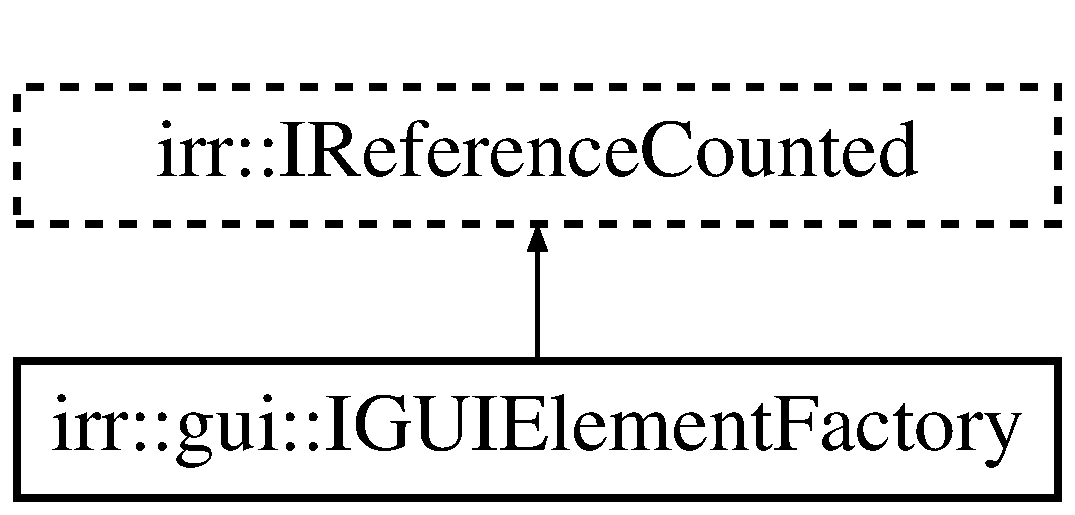
\includegraphics[height=2.000000cm]{classirr_1_1gui_1_1IGUIElementFactory}
\end{center}
\end{figure}
\subsection*{Public Member Functions}
\begin{DoxyCompactItemize}
\item 
virtual \hyperlink{classirr_1_1gui_1_1IGUIElement}{I\+G\+U\+I\+Element} $\ast$ \hyperlink{classirr_1_1gui_1_1IGUIElementFactory_aaaa0dda5493286ff745310b441347019}{add\+G\+U\+I\+Element} (\hyperlink{namespaceirr_1_1gui_ae4d66df0ecf4117cdbcf9f22404bd254}{E\+G\+U\+I\+\_\+\+E\+L\+E\+M\+E\+N\+T\+\_\+\+T\+Y\+PE} type, \hyperlink{classirr_1_1gui_1_1IGUIElement}{I\+G\+U\+I\+Element} $\ast$parent=0)=0
\begin{DoxyCompactList}\small\item\em adds an element to the gui environment based on its type id \end{DoxyCompactList}\item 
virtual \hyperlink{classirr_1_1gui_1_1IGUIElement}{I\+G\+U\+I\+Element} $\ast$ \hyperlink{classirr_1_1gui_1_1IGUIElementFactory_aec55be9ef891ba1b19c5d9c5a85130a4}{add\+G\+U\+I\+Element} (const \hyperlink{namespaceirr_a9395eaea339bcb546b319e9c96bf7410}{c8} $\ast$type\+Name, \hyperlink{classirr_1_1gui_1_1IGUIElement}{I\+G\+U\+I\+Element} $\ast$parent=0)=0
\begin{DoxyCompactList}\small\item\em adds a G\+UI element to the G\+UI Environment based on its type name \end{DoxyCompactList}\item 
\mbox{\Hypertarget{classirr_1_1gui_1_1IGUIElementFactory_aae56378de5264978e70d11a36fff02e9}\label{classirr_1_1gui_1_1IGUIElementFactory_aae56378de5264978e70d11a36fff02e9}} 
virtual \hyperlink{namespaceirr_ac66849b7a6ed16e30ebede579f9b47c6}{s32} \hyperlink{classirr_1_1gui_1_1IGUIElementFactory_aae56378de5264978e70d11a36fff02e9}{get\+Creatable\+G\+U\+I\+Element\+Type\+Count} () const =0
\begin{DoxyCompactList}\small\item\em Get amount of G\+UI element types this factory is able to create. \end{DoxyCompactList}\item 
virtual \hyperlink{namespaceirr_1_1gui_ae4d66df0ecf4117cdbcf9f22404bd254}{E\+G\+U\+I\+\_\+\+E\+L\+E\+M\+E\+N\+T\+\_\+\+T\+Y\+PE} \hyperlink{classirr_1_1gui_1_1IGUIElementFactory_a9318ddb2d0d971551db4c050c3f99a2f}{get\+Createable\+G\+U\+I\+Element\+Type} (\hyperlink{namespaceirr_ac66849b7a6ed16e30ebede579f9b47c6}{s32} idx) const =0
\begin{DoxyCompactList}\small\item\em Get type of a createable element type. \end{DoxyCompactList}\item 
virtual const \hyperlink{namespaceirr_a9395eaea339bcb546b319e9c96bf7410}{c8} $\ast$ \hyperlink{classirr_1_1gui_1_1IGUIElementFactory_aa8007c17ea40b74666c1d04c9d4de85f}{get\+Createable\+G\+U\+I\+Element\+Type\+Name} (\hyperlink{namespaceirr_ac66849b7a6ed16e30ebede579f9b47c6}{s32} idx) const =0
\begin{DoxyCompactList}\small\item\em Get type name of a createable G\+UI element type by index. \end{DoxyCompactList}\item 
virtual const \hyperlink{namespaceirr_a9395eaea339bcb546b319e9c96bf7410}{c8} $\ast$ \hyperlink{classirr_1_1gui_1_1IGUIElementFactory_a1e692e1f746ee69815bf25981ee0facf}{get\+Createable\+G\+U\+I\+Element\+Type\+Name} (\hyperlink{namespaceirr_1_1gui_ae4d66df0ecf4117cdbcf9f22404bd254}{E\+G\+U\+I\+\_\+\+E\+L\+E\+M\+E\+N\+T\+\_\+\+T\+Y\+PE} type) const =0
\begin{DoxyCompactList}\small\item\em returns type name of a createable G\+UI element \end{DoxyCompactList}\item 
virtual \hyperlink{classirr_1_1gui_1_1IGUIElement}{I\+G\+U\+I\+Element} $\ast$ \hyperlink{classirr_1_1gui_1_1IGUIElementFactory_aaaa0dda5493286ff745310b441347019}{add\+G\+U\+I\+Element} (\hyperlink{namespaceirr_1_1gui_ae4d66df0ecf4117cdbcf9f22404bd254}{E\+G\+U\+I\+\_\+\+E\+L\+E\+M\+E\+N\+T\+\_\+\+T\+Y\+PE} type, \hyperlink{classirr_1_1gui_1_1IGUIElement}{I\+G\+U\+I\+Element} $\ast$parent=0)=0
\begin{DoxyCompactList}\small\item\em adds an element to the gui environment based on its type id \end{DoxyCompactList}\item 
virtual \hyperlink{classirr_1_1gui_1_1IGUIElement}{I\+G\+U\+I\+Element} $\ast$ \hyperlink{classirr_1_1gui_1_1IGUIElementFactory_aec55be9ef891ba1b19c5d9c5a85130a4}{add\+G\+U\+I\+Element} (const \hyperlink{namespaceirr_a9395eaea339bcb546b319e9c96bf7410}{c8} $\ast$type\+Name, \hyperlink{classirr_1_1gui_1_1IGUIElement}{I\+G\+U\+I\+Element} $\ast$parent=0)=0
\begin{DoxyCompactList}\small\item\em adds a G\+UI element to the G\+UI Environment based on its type name \end{DoxyCompactList}\item 
\mbox{\Hypertarget{classirr_1_1gui_1_1IGUIElementFactory_aae56378de5264978e70d11a36fff02e9}\label{classirr_1_1gui_1_1IGUIElementFactory_aae56378de5264978e70d11a36fff02e9}} 
virtual \hyperlink{namespaceirr_ac66849b7a6ed16e30ebede579f9b47c6}{s32} \hyperlink{classirr_1_1gui_1_1IGUIElementFactory_aae56378de5264978e70d11a36fff02e9}{get\+Creatable\+G\+U\+I\+Element\+Type\+Count} () const =0
\begin{DoxyCompactList}\small\item\em Get amount of G\+UI element types this factory is able to create. \end{DoxyCompactList}\item 
virtual \hyperlink{namespaceirr_1_1gui_ae4d66df0ecf4117cdbcf9f22404bd254}{E\+G\+U\+I\+\_\+\+E\+L\+E\+M\+E\+N\+T\+\_\+\+T\+Y\+PE} \hyperlink{classirr_1_1gui_1_1IGUIElementFactory_a9318ddb2d0d971551db4c050c3f99a2f}{get\+Createable\+G\+U\+I\+Element\+Type} (\hyperlink{namespaceirr_ac66849b7a6ed16e30ebede579f9b47c6}{s32} idx) const =0
\begin{DoxyCompactList}\small\item\em Get type of a createable element type. \end{DoxyCompactList}\item 
virtual const \hyperlink{namespaceirr_a9395eaea339bcb546b319e9c96bf7410}{c8} $\ast$ \hyperlink{classirr_1_1gui_1_1IGUIElementFactory_aa8007c17ea40b74666c1d04c9d4de85f}{get\+Createable\+G\+U\+I\+Element\+Type\+Name} (\hyperlink{namespaceirr_ac66849b7a6ed16e30ebede579f9b47c6}{s32} idx) const =0
\begin{DoxyCompactList}\small\item\em Get type name of a createable G\+UI element type by index. \end{DoxyCompactList}\item 
virtual const \hyperlink{namespaceirr_a9395eaea339bcb546b319e9c96bf7410}{c8} $\ast$ \hyperlink{classirr_1_1gui_1_1IGUIElementFactory_a1e692e1f746ee69815bf25981ee0facf}{get\+Createable\+G\+U\+I\+Element\+Type\+Name} (\hyperlink{namespaceirr_1_1gui_ae4d66df0ecf4117cdbcf9f22404bd254}{E\+G\+U\+I\+\_\+\+E\+L\+E\+M\+E\+N\+T\+\_\+\+T\+Y\+PE} type) const =0
\begin{DoxyCompactList}\small\item\em returns type name of a createable G\+UI element \end{DoxyCompactList}\end{DoxyCompactItemize}
\subsection*{Additional Inherited Members}


\subsection{Detailed Description}
Interface making it possible to dynamically create G\+UI elements. 

To be able to add custom elements to Irrlicht and to make it possible for the scene manager to save and load them, simply implement this interface and register it in your gui environment via \hyperlink{classirr_1_1gui_1_1IGUIEnvironment_a653ac2cc8640899c23f4d55d9a5f0fdd}{I\+G\+U\+I\+Environment\+::register\+G\+U\+I\+Element\+Factory}. Note\+: When implementing your own element factory, don\textquotesingle{}t call \hyperlink{classirr_1_1IReferenceCounted_a396f9cdbe311ada278626477b3c6f0f5}{I\+G\+U\+I\+Environment\+::grab()} to increase the reference counter of the environment. This is not necessary because the it will \hyperlink{classirr_1_1IReferenceCounted_a396f9cdbe311ada278626477b3c6f0f5}{grab()} the factory anyway, and otherwise cyclic references will be created. 

\subsection{Member Function Documentation}
\mbox{\Hypertarget{classirr_1_1gui_1_1IGUIElementFactory_aaaa0dda5493286ff745310b441347019}\label{classirr_1_1gui_1_1IGUIElementFactory_aaaa0dda5493286ff745310b441347019}} 
\index{irr\+::gui\+::\+I\+G\+U\+I\+Element\+Factory@{irr\+::gui\+::\+I\+G\+U\+I\+Element\+Factory}!add\+G\+U\+I\+Element@{add\+G\+U\+I\+Element}}
\index{add\+G\+U\+I\+Element@{add\+G\+U\+I\+Element}!irr\+::gui\+::\+I\+G\+U\+I\+Element\+Factory@{irr\+::gui\+::\+I\+G\+U\+I\+Element\+Factory}}
\subsubsection{\texorpdfstring{add\+G\+U\+I\+Element()}{addGUIElement()}\hspace{0.1cm}{\footnotesize\ttfamily [1/4]}}
{\footnotesize\ttfamily virtual \hyperlink{classirr_1_1gui_1_1IGUIElement}{I\+G\+U\+I\+Element}$\ast$ irr\+::gui\+::\+I\+G\+U\+I\+Element\+Factory\+::add\+G\+U\+I\+Element (\begin{DoxyParamCaption}\item[{\hyperlink{namespaceirr_1_1gui_ae4d66df0ecf4117cdbcf9f22404bd254}{E\+G\+U\+I\+\_\+\+E\+L\+E\+M\+E\+N\+T\+\_\+\+T\+Y\+PE}}]{type,  }\item[{\hyperlink{classirr_1_1gui_1_1IGUIElement}{I\+G\+U\+I\+Element} $\ast$}]{parent = {\ttfamily 0} }\end{DoxyParamCaption})\hspace{0.3cm}{\ttfamily [pure virtual]}}



adds an element to the gui environment based on its type id 


\begin{DoxyParams}{Parameters}
{\em type} & Type of the element to add. \\
\hline
{\em parent} & Parent scene node of the new element, can be null to add to the root. \\
\hline
\end{DoxyParams}
\begin{DoxyReturn}{Returns}
Pointer to the new element or null if not successful. 
\end{DoxyReturn}
\mbox{\Hypertarget{classirr_1_1gui_1_1IGUIElementFactory_aaaa0dda5493286ff745310b441347019}\label{classirr_1_1gui_1_1IGUIElementFactory_aaaa0dda5493286ff745310b441347019}} 
\index{irr\+::gui\+::\+I\+G\+U\+I\+Element\+Factory@{irr\+::gui\+::\+I\+G\+U\+I\+Element\+Factory}!add\+G\+U\+I\+Element@{add\+G\+U\+I\+Element}}
\index{add\+G\+U\+I\+Element@{add\+G\+U\+I\+Element}!irr\+::gui\+::\+I\+G\+U\+I\+Element\+Factory@{irr\+::gui\+::\+I\+G\+U\+I\+Element\+Factory}}
\subsubsection{\texorpdfstring{add\+G\+U\+I\+Element()}{addGUIElement()}\hspace{0.1cm}{\footnotesize\ttfamily [2/4]}}
{\footnotesize\ttfamily virtual \hyperlink{classirr_1_1gui_1_1IGUIElement}{I\+G\+U\+I\+Element}$\ast$ irr\+::gui\+::\+I\+G\+U\+I\+Element\+Factory\+::add\+G\+U\+I\+Element (\begin{DoxyParamCaption}\item[{\hyperlink{namespaceirr_1_1gui_ae4d66df0ecf4117cdbcf9f22404bd254}{E\+G\+U\+I\+\_\+\+E\+L\+E\+M\+E\+N\+T\+\_\+\+T\+Y\+PE}}]{type,  }\item[{\hyperlink{classirr_1_1gui_1_1IGUIElement}{I\+G\+U\+I\+Element} $\ast$}]{parent = {\ttfamily 0} }\end{DoxyParamCaption})\hspace{0.3cm}{\ttfamily [pure virtual]}}



adds an element to the gui environment based on its type id 


\begin{DoxyParams}{Parameters}
{\em type} & Type of the element to add. \\
\hline
{\em parent} & Parent scene node of the new element, can be null to add to the root. \\
\hline
\end{DoxyParams}
\begin{DoxyReturn}{Returns}
Pointer to the new element or null if not successful. 
\end{DoxyReturn}
\mbox{\Hypertarget{classirr_1_1gui_1_1IGUIElementFactory_aec55be9ef891ba1b19c5d9c5a85130a4}\label{classirr_1_1gui_1_1IGUIElementFactory_aec55be9ef891ba1b19c5d9c5a85130a4}} 
\index{irr\+::gui\+::\+I\+G\+U\+I\+Element\+Factory@{irr\+::gui\+::\+I\+G\+U\+I\+Element\+Factory}!add\+G\+U\+I\+Element@{add\+G\+U\+I\+Element}}
\index{add\+G\+U\+I\+Element@{add\+G\+U\+I\+Element}!irr\+::gui\+::\+I\+G\+U\+I\+Element\+Factory@{irr\+::gui\+::\+I\+G\+U\+I\+Element\+Factory}}
\subsubsection{\texorpdfstring{add\+G\+U\+I\+Element()}{addGUIElement()}\hspace{0.1cm}{\footnotesize\ttfamily [3/4]}}
{\footnotesize\ttfamily virtual \hyperlink{classirr_1_1gui_1_1IGUIElement}{I\+G\+U\+I\+Element}$\ast$ irr\+::gui\+::\+I\+G\+U\+I\+Element\+Factory\+::add\+G\+U\+I\+Element (\begin{DoxyParamCaption}\item[{const \hyperlink{namespaceirr_a9395eaea339bcb546b319e9c96bf7410}{c8} $\ast$}]{type\+Name,  }\item[{\hyperlink{classirr_1_1gui_1_1IGUIElement}{I\+G\+U\+I\+Element} $\ast$}]{parent = {\ttfamily 0} }\end{DoxyParamCaption})\hspace{0.3cm}{\ttfamily [pure virtual]}}



adds a G\+UI element to the G\+UI Environment based on its type name 


\begin{DoxyParams}{Parameters}
{\em type\+Name} & Type name of the element to add. \\
\hline
{\em parent} & Parent scene node of the new element, can be null to add it to the root. \\
\hline
\end{DoxyParams}
\begin{DoxyReturn}{Returns}
Pointer to the new element or null if not successful. 
\end{DoxyReturn}
\mbox{\Hypertarget{classirr_1_1gui_1_1IGUIElementFactory_aec55be9ef891ba1b19c5d9c5a85130a4}\label{classirr_1_1gui_1_1IGUIElementFactory_aec55be9ef891ba1b19c5d9c5a85130a4}} 
\index{irr\+::gui\+::\+I\+G\+U\+I\+Element\+Factory@{irr\+::gui\+::\+I\+G\+U\+I\+Element\+Factory}!add\+G\+U\+I\+Element@{add\+G\+U\+I\+Element}}
\index{add\+G\+U\+I\+Element@{add\+G\+U\+I\+Element}!irr\+::gui\+::\+I\+G\+U\+I\+Element\+Factory@{irr\+::gui\+::\+I\+G\+U\+I\+Element\+Factory}}
\subsubsection{\texorpdfstring{add\+G\+U\+I\+Element()}{addGUIElement()}\hspace{0.1cm}{\footnotesize\ttfamily [4/4]}}
{\footnotesize\ttfamily virtual \hyperlink{classirr_1_1gui_1_1IGUIElement}{I\+G\+U\+I\+Element}$\ast$ irr\+::gui\+::\+I\+G\+U\+I\+Element\+Factory\+::add\+G\+U\+I\+Element (\begin{DoxyParamCaption}\item[{const \hyperlink{namespaceirr_a9395eaea339bcb546b319e9c96bf7410}{c8} $\ast$}]{type\+Name,  }\item[{\hyperlink{classirr_1_1gui_1_1IGUIElement}{I\+G\+U\+I\+Element} $\ast$}]{parent = {\ttfamily 0} }\end{DoxyParamCaption})\hspace{0.3cm}{\ttfamily [pure virtual]}}



adds a G\+UI element to the G\+UI Environment based on its type name 


\begin{DoxyParams}{Parameters}
{\em type\+Name} & Type name of the element to add. \\
\hline
{\em parent} & Parent scene node of the new element, can be null to add it to the root. \\
\hline
\end{DoxyParams}
\begin{DoxyReturn}{Returns}
Pointer to the new element or null if not successful. 
\end{DoxyReturn}
\mbox{\Hypertarget{classirr_1_1gui_1_1IGUIElementFactory_a9318ddb2d0d971551db4c050c3f99a2f}\label{classirr_1_1gui_1_1IGUIElementFactory_a9318ddb2d0d971551db4c050c3f99a2f}} 
\index{irr\+::gui\+::\+I\+G\+U\+I\+Element\+Factory@{irr\+::gui\+::\+I\+G\+U\+I\+Element\+Factory}!get\+Createable\+G\+U\+I\+Element\+Type@{get\+Createable\+G\+U\+I\+Element\+Type}}
\index{get\+Createable\+G\+U\+I\+Element\+Type@{get\+Createable\+G\+U\+I\+Element\+Type}!irr\+::gui\+::\+I\+G\+U\+I\+Element\+Factory@{irr\+::gui\+::\+I\+G\+U\+I\+Element\+Factory}}
\subsubsection{\texorpdfstring{get\+Createable\+G\+U\+I\+Element\+Type()}{getCreateableGUIElementType()}\hspace{0.1cm}{\footnotesize\ttfamily [1/2]}}
{\footnotesize\ttfamily virtual \hyperlink{namespaceirr_1_1gui_ae4d66df0ecf4117cdbcf9f22404bd254}{E\+G\+U\+I\+\_\+\+E\+L\+E\+M\+E\+N\+T\+\_\+\+T\+Y\+PE} irr\+::gui\+::\+I\+G\+U\+I\+Element\+Factory\+::get\+Createable\+G\+U\+I\+Element\+Type (\begin{DoxyParamCaption}\item[{\hyperlink{namespaceirr_ac66849b7a6ed16e30ebede579f9b47c6}{s32}}]{idx }\end{DoxyParamCaption}) const\hspace{0.3cm}{\ttfamily [pure virtual]}}



Get type of a createable element type. 


\begin{DoxyParams}{Parameters}
{\em idx} & Index of the element type in this factory. Must be a value between 0 and \hyperlink{classirr_1_1gui_1_1IGUIElementFactory_aae56378de5264978e70d11a36fff02e9}{get\+Creatable\+G\+U\+I\+Element\+Type\+Count()} \\
\hline
\end{DoxyParams}
\mbox{\Hypertarget{classirr_1_1gui_1_1IGUIElementFactory_a9318ddb2d0d971551db4c050c3f99a2f}\label{classirr_1_1gui_1_1IGUIElementFactory_a9318ddb2d0d971551db4c050c3f99a2f}} 
\index{irr\+::gui\+::\+I\+G\+U\+I\+Element\+Factory@{irr\+::gui\+::\+I\+G\+U\+I\+Element\+Factory}!get\+Createable\+G\+U\+I\+Element\+Type@{get\+Createable\+G\+U\+I\+Element\+Type}}
\index{get\+Createable\+G\+U\+I\+Element\+Type@{get\+Createable\+G\+U\+I\+Element\+Type}!irr\+::gui\+::\+I\+G\+U\+I\+Element\+Factory@{irr\+::gui\+::\+I\+G\+U\+I\+Element\+Factory}}
\subsubsection{\texorpdfstring{get\+Createable\+G\+U\+I\+Element\+Type()}{getCreateableGUIElementType()}\hspace{0.1cm}{\footnotesize\ttfamily [2/2]}}
{\footnotesize\ttfamily virtual \hyperlink{namespaceirr_1_1gui_ae4d66df0ecf4117cdbcf9f22404bd254}{E\+G\+U\+I\+\_\+\+E\+L\+E\+M\+E\+N\+T\+\_\+\+T\+Y\+PE} irr\+::gui\+::\+I\+G\+U\+I\+Element\+Factory\+::get\+Createable\+G\+U\+I\+Element\+Type (\begin{DoxyParamCaption}\item[{\hyperlink{namespaceirr_ac66849b7a6ed16e30ebede579f9b47c6}{s32}}]{idx }\end{DoxyParamCaption}) const\hspace{0.3cm}{\ttfamily [pure virtual]}}



Get type of a createable element type. 


\begin{DoxyParams}{Parameters}
{\em idx} & Index of the element type in this factory. Must be a value between 0 and \hyperlink{classirr_1_1gui_1_1IGUIElementFactory_aae56378de5264978e70d11a36fff02e9}{get\+Creatable\+G\+U\+I\+Element\+Type\+Count()} \\
\hline
\end{DoxyParams}
\mbox{\Hypertarget{classirr_1_1gui_1_1IGUIElementFactory_aa8007c17ea40b74666c1d04c9d4de85f}\label{classirr_1_1gui_1_1IGUIElementFactory_aa8007c17ea40b74666c1d04c9d4de85f}} 
\index{irr\+::gui\+::\+I\+G\+U\+I\+Element\+Factory@{irr\+::gui\+::\+I\+G\+U\+I\+Element\+Factory}!get\+Createable\+G\+U\+I\+Element\+Type\+Name@{get\+Createable\+G\+U\+I\+Element\+Type\+Name}}
\index{get\+Createable\+G\+U\+I\+Element\+Type\+Name@{get\+Createable\+G\+U\+I\+Element\+Type\+Name}!irr\+::gui\+::\+I\+G\+U\+I\+Element\+Factory@{irr\+::gui\+::\+I\+G\+U\+I\+Element\+Factory}}
\subsubsection{\texorpdfstring{get\+Createable\+G\+U\+I\+Element\+Type\+Name()}{getCreateableGUIElementTypeName()}\hspace{0.1cm}{\footnotesize\ttfamily [1/4]}}
{\footnotesize\ttfamily virtual const \hyperlink{namespaceirr_a9395eaea339bcb546b319e9c96bf7410}{c8}$\ast$ irr\+::gui\+::\+I\+G\+U\+I\+Element\+Factory\+::get\+Createable\+G\+U\+I\+Element\+Type\+Name (\begin{DoxyParamCaption}\item[{\hyperlink{namespaceirr_ac66849b7a6ed16e30ebede579f9b47c6}{s32}}]{idx }\end{DoxyParamCaption}) const\hspace{0.3cm}{\ttfamily [pure virtual]}}



Get type name of a createable G\+UI element type by index. 


\begin{DoxyParams}{Parameters}
{\em idx} & Index of the type in this factory. Must be a value between 0 and \hyperlink{classirr_1_1gui_1_1IGUIElementFactory_aae56378de5264978e70d11a36fff02e9}{get\+Creatable\+G\+U\+I\+Element\+Type\+Count()} \\
\hline
\end{DoxyParams}
\mbox{\Hypertarget{classirr_1_1gui_1_1IGUIElementFactory_aa8007c17ea40b74666c1d04c9d4de85f}\label{classirr_1_1gui_1_1IGUIElementFactory_aa8007c17ea40b74666c1d04c9d4de85f}} 
\index{irr\+::gui\+::\+I\+G\+U\+I\+Element\+Factory@{irr\+::gui\+::\+I\+G\+U\+I\+Element\+Factory}!get\+Createable\+G\+U\+I\+Element\+Type\+Name@{get\+Createable\+G\+U\+I\+Element\+Type\+Name}}
\index{get\+Createable\+G\+U\+I\+Element\+Type\+Name@{get\+Createable\+G\+U\+I\+Element\+Type\+Name}!irr\+::gui\+::\+I\+G\+U\+I\+Element\+Factory@{irr\+::gui\+::\+I\+G\+U\+I\+Element\+Factory}}
\subsubsection{\texorpdfstring{get\+Createable\+G\+U\+I\+Element\+Type\+Name()}{getCreateableGUIElementTypeName()}\hspace{0.1cm}{\footnotesize\ttfamily [2/4]}}
{\footnotesize\ttfamily virtual const \hyperlink{namespaceirr_a9395eaea339bcb546b319e9c96bf7410}{c8}$\ast$ irr\+::gui\+::\+I\+G\+U\+I\+Element\+Factory\+::get\+Createable\+G\+U\+I\+Element\+Type\+Name (\begin{DoxyParamCaption}\item[{\hyperlink{namespaceirr_ac66849b7a6ed16e30ebede579f9b47c6}{s32}}]{idx }\end{DoxyParamCaption}) const\hspace{0.3cm}{\ttfamily [pure virtual]}}



Get type name of a createable G\+UI element type by index. 


\begin{DoxyParams}{Parameters}
{\em idx} & Index of the type in this factory. Must be a value between 0 and \hyperlink{classirr_1_1gui_1_1IGUIElementFactory_aae56378de5264978e70d11a36fff02e9}{get\+Creatable\+G\+U\+I\+Element\+Type\+Count()} \\
\hline
\end{DoxyParams}
\mbox{\Hypertarget{classirr_1_1gui_1_1IGUIElementFactory_a1e692e1f746ee69815bf25981ee0facf}\label{classirr_1_1gui_1_1IGUIElementFactory_a1e692e1f746ee69815bf25981ee0facf}} 
\index{irr\+::gui\+::\+I\+G\+U\+I\+Element\+Factory@{irr\+::gui\+::\+I\+G\+U\+I\+Element\+Factory}!get\+Createable\+G\+U\+I\+Element\+Type\+Name@{get\+Createable\+G\+U\+I\+Element\+Type\+Name}}
\index{get\+Createable\+G\+U\+I\+Element\+Type\+Name@{get\+Createable\+G\+U\+I\+Element\+Type\+Name}!irr\+::gui\+::\+I\+G\+U\+I\+Element\+Factory@{irr\+::gui\+::\+I\+G\+U\+I\+Element\+Factory}}
\subsubsection{\texorpdfstring{get\+Createable\+G\+U\+I\+Element\+Type\+Name()}{getCreateableGUIElementTypeName()}\hspace{0.1cm}{\footnotesize\ttfamily [3/4]}}
{\footnotesize\ttfamily virtual const \hyperlink{namespaceirr_a9395eaea339bcb546b319e9c96bf7410}{c8}$\ast$ irr\+::gui\+::\+I\+G\+U\+I\+Element\+Factory\+::get\+Createable\+G\+U\+I\+Element\+Type\+Name (\begin{DoxyParamCaption}\item[{\hyperlink{namespaceirr_1_1gui_ae4d66df0ecf4117cdbcf9f22404bd254}{E\+G\+U\+I\+\_\+\+E\+L\+E\+M\+E\+N\+T\+\_\+\+T\+Y\+PE}}]{type }\end{DoxyParamCaption}) const\hspace{0.3cm}{\ttfamily [pure virtual]}}



returns type name of a createable G\+UI element 


\begin{DoxyParams}{Parameters}
{\em type} & Type of G\+UI element. \\
\hline
\end{DoxyParams}
\begin{DoxyReturn}{Returns}
Name of the type if this factory can create the type, otherwise 0. 
\end{DoxyReturn}
\mbox{\Hypertarget{classirr_1_1gui_1_1IGUIElementFactory_a1e692e1f746ee69815bf25981ee0facf}\label{classirr_1_1gui_1_1IGUIElementFactory_a1e692e1f746ee69815bf25981ee0facf}} 
\index{irr\+::gui\+::\+I\+G\+U\+I\+Element\+Factory@{irr\+::gui\+::\+I\+G\+U\+I\+Element\+Factory}!get\+Createable\+G\+U\+I\+Element\+Type\+Name@{get\+Createable\+G\+U\+I\+Element\+Type\+Name}}
\index{get\+Createable\+G\+U\+I\+Element\+Type\+Name@{get\+Createable\+G\+U\+I\+Element\+Type\+Name}!irr\+::gui\+::\+I\+G\+U\+I\+Element\+Factory@{irr\+::gui\+::\+I\+G\+U\+I\+Element\+Factory}}
\subsubsection{\texorpdfstring{get\+Createable\+G\+U\+I\+Element\+Type\+Name()}{getCreateableGUIElementTypeName()}\hspace{0.1cm}{\footnotesize\ttfamily [4/4]}}
{\footnotesize\ttfamily virtual const \hyperlink{namespaceirr_a9395eaea339bcb546b319e9c96bf7410}{c8}$\ast$ irr\+::gui\+::\+I\+G\+U\+I\+Element\+Factory\+::get\+Createable\+G\+U\+I\+Element\+Type\+Name (\begin{DoxyParamCaption}\item[{\hyperlink{namespaceirr_1_1gui_ae4d66df0ecf4117cdbcf9f22404bd254}{E\+G\+U\+I\+\_\+\+E\+L\+E\+M\+E\+N\+T\+\_\+\+T\+Y\+PE}}]{type }\end{DoxyParamCaption}) const\hspace{0.3cm}{\ttfamily [pure virtual]}}



returns type name of a createable G\+UI element 


\begin{DoxyParams}{Parameters}
{\em type} & Type of G\+UI element. \\
\hline
\end{DoxyParams}
\begin{DoxyReturn}{Returns}
Name of the type if this factory can create the type, otherwise 0. 
\end{DoxyReturn}


The documentation for this class was generated from the following file\+:\begin{DoxyCompactItemize}
\item 
indie\+\_\+share/controller/include/I\+G\+U\+I\+Element\+Factory.\+h\end{DoxyCompactItemize}

\hypertarget{classirr_1_1gui_1_1IGUIEnvironment}{}\section{irr\+:\+:gui\+:\+:I\+G\+U\+I\+Environment Class Reference}
\label{classirr_1_1gui_1_1IGUIEnvironment}\index{irr\+::gui\+::\+I\+G\+U\+I\+Environment@{irr\+::gui\+::\+I\+G\+U\+I\+Environment}}


G\+UI Environment. Used as factory and manager of all other G\+UI elements.  




{\ttfamily \#include $<$I\+G\+U\+I\+Environment.\+h$>$}

Inheritance diagram for irr\+:\+:gui\+:\+:I\+G\+U\+I\+Environment\+:\begin{figure}[H]
\begin{center}
\leavevmode
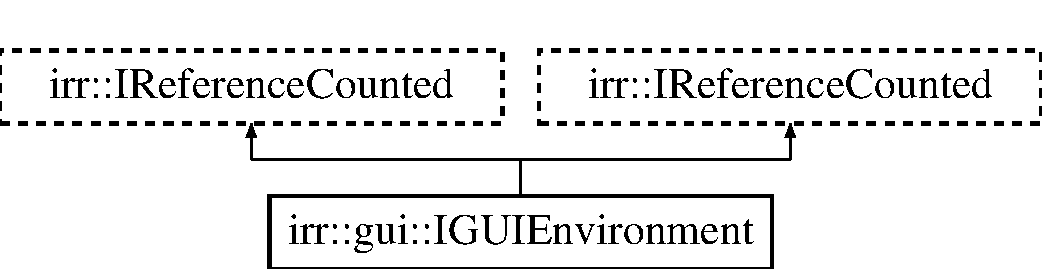
\includegraphics[height=2.000000cm]{classirr_1_1gui_1_1IGUIEnvironment}
\end{center}
\end{figure}
\subsection*{Public Member Functions}
\begin{DoxyCompactItemize}
\item 
\mbox{\Hypertarget{classirr_1_1gui_1_1IGUIEnvironment_aa6ba29bbf3121a5954cfa5a9ca72982f}\label{classirr_1_1gui_1_1IGUIEnvironment_aa6ba29bbf3121a5954cfa5a9ca72982f}} 
virtual void \hyperlink{classirr_1_1gui_1_1IGUIEnvironment_aa6ba29bbf3121a5954cfa5a9ca72982f}{draw\+All} ()=0
\begin{DoxyCompactList}\small\item\em Draws all gui elements by traversing the G\+UI environment starting at the root node. \end{DoxyCompactList}\item 
virtual bool \hyperlink{classirr_1_1gui_1_1IGUIEnvironment_a2bfe9985ae1a2f379e708fce86902cea}{set\+Focus} (\hyperlink{classirr_1_1gui_1_1IGUIElement}{I\+G\+U\+I\+Element} $\ast$element)=0
\begin{DoxyCompactList}\small\item\em Sets the focus to an element. \end{DoxyCompactList}\item 
virtual \hyperlink{classirr_1_1gui_1_1IGUIElement}{I\+G\+U\+I\+Element} $\ast$ \hyperlink{classirr_1_1gui_1_1IGUIEnvironment_a624c047cb88a5d3e3e0d17a42a627335}{get\+Focus} () const =0
\begin{DoxyCompactList}\small\item\em Returns the element which holds the focus. \end{DoxyCompactList}\item 
virtual \hyperlink{classirr_1_1gui_1_1IGUIElement}{I\+G\+U\+I\+Element} $\ast$ \hyperlink{classirr_1_1gui_1_1IGUIEnvironment_a00fa645d517a276553b78fc1d0e78591}{get\+Hovered} () const =0
\begin{DoxyCompactList}\small\item\em Returns the element which was last under the mouse cursor. \end{DoxyCompactList}\item 
virtual bool \hyperlink{classirr_1_1gui_1_1IGUIEnvironment_ab2100753b415a9950d95572d4623bf46}{remove\+Focus} (\hyperlink{classirr_1_1gui_1_1IGUIElement}{I\+G\+U\+I\+Element} $\ast$element)=0
\begin{DoxyCompactList}\small\item\em Removes the focus from an element. \end{DoxyCompactList}\item 
virtual bool \hyperlink{classirr_1_1gui_1_1IGUIEnvironment_a88c483f30a0f35debed70e8e51836552}{has\+Focus} (\hyperlink{classirr_1_1gui_1_1IGUIElement}{I\+G\+U\+I\+Element} $\ast$element) const =0
\begin{DoxyCompactList}\small\item\em Returns whether the element has focus. \end{DoxyCompactList}\item 
virtual \hyperlink{classirr_1_1video_1_1IVideoDriver}{video\+::\+I\+Video\+Driver} $\ast$ \hyperlink{classirr_1_1gui_1_1IGUIEnvironment_a48f5e442f0a2074a531234ab83148fe2}{get\+Video\+Driver} () const =0
\begin{DoxyCompactList}\small\item\em Returns the current video driver. \end{DoxyCompactList}\item 
virtual \hyperlink{classirr_1_1io_1_1IFileSystem}{io\+::\+I\+File\+System} $\ast$ \hyperlink{classirr_1_1gui_1_1IGUIEnvironment_ad3ae4570702000e09cacdb663f0ec363}{get\+File\+System} () const =0
\begin{DoxyCompactList}\small\item\em Returns the file system. \end{DoxyCompactList}\item 
virtual \hyperlink{classirr_1_1IOSOperator}{I\+O\+S\+Operator} $\ast$ \hyperlink{classirr_1_1gui_1_1IGUIEnvironment_afc715b9a9d98ae3aa8e769c9fb2f4f31}{get\+O\+S\+Operator} () const =0
\begin{DoxyCompactList}\small\item\em returns a pointer to the OS operator \end{DoxyCompactList}\item 
\mbox{\Hypertarget{classirr_1_1gui_1_1IGUIEnvironment_a77b0cdd0aec36dbb9c558446fab383c2}\label{classirr_1_1gui_1_1IGUIEnvironment_a77b0cdd0aec36dbb9c558446fab383c2}} 
virtual void \hyperlink{classirr_1_1gui_1_1IGUIEnvironment_a77b0cdd0aec36dbb9c558446fab383c2}{clear} ()=0
\begin{DoxyCompactList}\small\item\em Removes all elements from the environment. \end{DoxyCompactList}\item 
virtual bool \hyperlink{classirr_1_1gui_1_1IGUIEnvironment_aff1cc1109841f9bccd19634870c7cd65}{post\+Event\+From\+User} (const \hyperlink{structirr_1_1SEvent}{S\+Event} \&event)=0
\begin{DoxyCompactList}\small\item\em Posts an input event to the environment. \end{DoxyCompactList}\item 
virtual void \hyperlink{classirr_1_1gui_1_1IGUIEnvironment_a2491715aa30894c66357eb0451aa10b0}{set\+User\+Event\+Receiver} (\hyperlink{classirr_1_1IEventReceiver}{I\+Event\+Receiver} $\ast$evr)=0
\begin{DoxyCompactList}\small\item\em This sets a new event receiver for gui events. \end{DoxyCompactList}\item 
virtual \hyperlink{classirr_1_1gui_1_1IGUISkin}{I\+G\+U\+I\+Skin} $\ast$ \hyperlink{classirr_1_1gui_1_1IGUIEnvironment_a54ce9072ea7b89cdaea65306e93ba90c}{get\+Skin} () const =0
\begin{DoxyCompactList}\small\item\em Returns pointer to the current gui skin. \end{DoxyCompactList}\item 
virtual void \hyperlink{classirr_1_1gui_1_1IGUIEnvironment_ae7042c520e848643e080ad4532797f23}{set\+Skin} (\hyperlink{classirr_1_1gui_1_1IGUISkin}{I\+G\+U\+I\+Skin} $\ast$skin)=0
\begin{DoxyCompactList}\small\item\em Sets a new G\+UI Skin. \end{DoxyCompactList}\item 
virtual \hyperlink{classirr_1_1gui_1_1IGUISkin}{I\+G\+U\+I\+Skin} $\ast$ \hyperlink{classirr_1_1gui_1_1IGUIEnvironment_a824099cd1ba9dd4b95e40dd1b15244f1}{create\+Skin} (\hyperlink{namespaceirr_1_1gui_a7b4619db540cbdf96e81023893b4eca5}{E\+G\+U\+I\+\_\+\+S\+K\+I\+N\+\_\+\+T\+Y\+PE} type)=0
\begin{DoxyCompactList}\small\item\em Creates a new G\+UI Skin based on a template. \end{DoxyCompactList}\item 
virtual \hyperlink{classirr_1_1gui_1_1IGUIImageList}{I\+G\+U\+I\+Image\+List} $\ast$ \hyperlink{classirr_1_1gui_1_1IGUIEnvironment_af3bd793f81b15dc534648e8a37e76467}{create\+Image\+List} (\hyperlink{classirr_1_1video_1_1ITexture}{video\+::\+I\+Texture} $\ast$texture, \hyperlink{classirr_1_1core_1_1dimension2d}{core\+::dimension2d}$<$ \hyperlink{namespaceirr_ac66849b7a6ed16e30ebede579f9b47c6}{s32} $>$ image\+Size, bool use\+Alpha\+Channel)=0
\begin{DoxyCompactList}\small\item\em Creates the image list from the given texture. \end{DoxyCompactList}\item 
virtual \hyperlink{classirr_1_1gui_1_1IGUIFont}{I\+G\+U\+I\+Font} $\ast$ \hyperlink{classirr_1_1gui_1_1IGUIEnvironment_a22074f9a1a5a86d5d216126bbb90b3b1}{get\+Font} (const \hyperlink{namespaceirr_1_1io_a6468281622ce3a1c46b72e19f32dded5}{io\+::path} \&filename)=0
\begin{DoxyCompactList}\small\item\em Returns pointer to the font with the specified filename. \end{DoxyCompactList}\item 
virtual \hyperlink{classirr_1_1gui_1_1IGUIFont}{I\+G\+U\+I\+Font} $\ast$ \hyperlink{classirr_1_1gui_1_1IGUIEnvironment_a2c4fefb8a67fc92aedbbff6254532c2b}{add\+Font} (const \hyperlink{namespaceirr_1_1io_a6468281622ce3a1c46b72e19f32dded5}{io\+::path} \&name, \hyperlink{classirr_1_1gui_1_1IGUIFont}{I\+G\+U\+I\+Font} $\ast$font)=0
\begin{DoxyCompactList}\small\item\em Adds an externally loaded font to the font list. \end{DoxyCompactList}\item 
\mbox{\Hypertarget{classirr_1_1gui_1_1IGUIEnvironment_a414f61b6901e7328448247648fdf9375}\label{classirr_1_1gui_1_1IGUIEnvironment_a414f61b6901e7328448247648fdf9375}} 
virtual void \hyperlink{classirr_1_1gui_1_1IGUIEnvironment_a414f61b6901e7328448247648fdf9375}{remove\+Font} (\hyperlink{classirr_1_1gui_1_1IGUIFont}{I\+G\+U\+I\+Font} $\ast$font)=0
\begin{DoxyCompactList}\small\item\em remove loaded font \end{DoxyCompactList}\item 
virtual \hyperlink{classirr_1_1gui_1_1IGUIFont}{I\+G\+U\+I\+Font} $\ast$ \hyperlink{classirr_1_1gui_1_1IGUIEnvironment_a896fbfcbad5ccf187a835827b439da93}{get\+Built\+In\+Font} () const =0
\begin{DoxyCompactList}\small\item\em Returns the default built-\/in font. \end{DoxyCompactList}\item 
virtual \hyperlink{classirr_1_1gui_1_1IGUISpriteBank}{I\+G\+U\+I\+Sprite\+Bank} $\ast$ \hyperlink{classirr_1_1gui_1_1IGUIEnvironment_a187ebb28837dbdb88810f7e493096c3f}{get\+Sprite\+Bank} (const \hyperlink{namespaceirr_1_1io_a6468281622ce3a1c46b72e19f32dded5}{io\+::path} \&filename)=0
\begin{DoxyCompactList}\small\item\em Returns pointer to the sprite bank with the specified file name. \end{DoxyCompactList}\item 
virtual \hyperlink{classirr_1_1gui_1_1IGUISpriteBank}{I\+G\+U\+I\+Sprite\+Bank} $\ast$ \hyperlink{classirr_1_1gui_1_1IGUIEnvironment_a62f34cdf4dd600a35eaf37d856579d98}{add\+Empty\+Sprite\+Bank} (const \hyperlink{namespaceirr_1_1io_a6468281622ce3a1c46b72e19f32dded5}{io\+::path} \&name)=0
\begin{DoxyCompactList}\small\item\em Adds an empty sprite bank to the manager. \end{DoxyCompactList}\item 
virtual \hyperlink{classirr_1_1gui_1_1IGUIElement}{I\+G\+U\+I\+Element} $\ast$ \hyperlink{classirr_1_1gui_1_1IGUIEnvironment_a35fec6d5baa9b2f65aa9ee2c336104d4}{get\+Root\+G\+U\+I\+Element} ()=0
\begin{DoxyCompactList}\small\item\em Returns the root gui element. \end{DoxyCompactList}\item 
virtual \hyperlink{classirr_1_1gui_1_1IGUIButton}{I\+G\+U\+I\+Button} $\ast$ \hyperlink{classirr_1_1gui_1_1IGUIEnvironment_a666749b7352a677c74acb242199e54a0}{add\+Button} (const \hyperlink{classirr_1_1core_1_1rect}{core\+::rect}$<$ \hyperlink{namespaceirr_ac66849b7a6ed16e30ebede579f9b47c6}{s32} $>$ \&rectangle, \hyperlink{classirr_1_1gui_1_1IGUIElement}{I\+G\+U\+I\+Element} $\ast$parent=0, \hyperlink{namespaceirr_ac66849b7a6ed16e30ebede579f9b47c6}{s32} id=-\/1, const wchar\+\_\+t $\ast$text=0, const wchar\+\_\+t $\ast$tooltiptext=0)=0
\begin{DoxyCompactList}\small\item\em Adds a button element. \end{DoxyCompactList}\item 
virtual \hyperlink{classirr_1_1gui_1_1IGUIWindow}{I\+G\+U\+I\+Window} $\ast$ \hyperlink{classirr_1_1gui_1_1IGUIEnvironment_ac233dcbef643b5f7de9ab30ae5896e28}{add\+Window} (const \hyperlink{classirr_1_1core_1_1rect}{core\+::rect}$<$ \hyperlink{namespaceirr_ac66849b7a6ed16e30ebede579f9b47c6}{s32} $>$ \&rectangle, bool modal=false, const wchar\+\_\+t $\ast$text=0, \hyperlink{classirr_1_1gui_1_1IGUIElement}{I\+G\+U\+I\+Element} $\ast$parent=0, \hyperlink{namespaceirr_ac66849b7a6ed16e30ebede579f9b47c6}{s32} id=-\/1)=0
\begin{DoxyCompactList}\small\item\em Adds an empty window element. \end{DoxyCompactList}\item 
virtual \hyperlink{classirr_1_1gui_1_1IGUIElement}{I\+G\+U\+I\+Element} $\ast$ \hyperlink{classirr_1_1gui_1_1IGUIEnvironment_a8bdf2e97e3694da75205ad693d849219}{add\+Modal\+Screen} (\hyperlink{classirr_1_1gui_1_1IGUIElement}{I\+G\+U\+I\+Element} $\ast$parent)=0
\begin{DoxyCompactList}\small\item\em Adds a modal screen. \end{DoxyCompactList}\item 
virtual \hyperlink{classirr_1_1gui_1_1IGUIWindow}{I\+G\+U\+I\+Window} $\ast$ \hyperlink{classirr_1_1gui_1_1IGUIEnvironment_aaf8cad4624c26895523b22728098a917}{add\+Message\+Box} (const wchar\+\_\+t $\ast$caption, const wchar\+\_\+t $\ast$text=0, bool modal=true, \hyperlink{namespaceirr_ac66849b7a6ed16e30ebede579f9b47c6}{s32} flags=\hyperlink{namespaceirr_1_1gui_af55112e55731c9ad1b9fe9b372c521afa9660280349027f678b2315a15a23ba0e}{E\+M\+B\+F\+\_\+\+OK}, \hyperlink{classirr_1_1gui_1_1IGUIElement}{I\+G\+U\+I\+Element} $\ast$parent=0, \hyperlink{namespaceirr_ac66849b7a6ed16e30ebede579f9b47c6}{s32} id=-\/1, \hyperlink{classirr_1_1video_1_1ITexture}{video\+::\+I\+Texture} $\ast$image=0)=0
\begin{DoxyCompactList}\small\item\em Adds a message box. \end{DoxyCompactList}\item 
virtual \hyperlink{classirr_1_1gui_1_1IGUIScrollBar}{I\+G\+U\+I\+Scroll\+Bar} $\ast$ \hyperlink{classirr_1_1gui_1_1IGUIEnvironment_aff82c4b3935eaf56ce638996f5e002c9}{add\+Scroll\+Bar} (bool horizontal, const \hyperlink{classirr_1_1core_1_1rect}{core\+::rect}$<$ \hyperlink{namespaceirr_ac66849b7a6ed16e30ebede579f9b47c6}{s32} $>$ \&rectangle, \hyperlink{classirr_1_1gui_1_1IGUIElement}{I\+G\+U\+I\+Element} $\ast$parent=0, \hyperlink{namespaceirr_ac66849b7a6ed16e30ebede579f9b47c6}{s32} id=-\/1)=0
\begin{DoxyCompactList}\small\item\em Adds a scrollbar. \end{DoxyCompactList}\item 
virtual \hyperlink{classirr_1_1gui_1_1IGUIImage}{I\+G\+U\+I\+Image} $\ast$ \hyperlink{classirr_1_1gui_1_1IGUIEnvironment_a35cc257b3a183551a2ed0376dcec9fe4}{add\+Image} (\hyperlink{classirr_1_1video_1_1ITexture}{video\+::\+I\+Texture} $\ast$image, core\+::position2d$<$ \hyperlink{namespaceirr_ac66849b7a6ed16e30ebede579f9b47c6}{s32} $>$ pos, bool use\+Alpha\+Channel=true, \hyperlink{classirr_1_1gui_1_1IGUIElement}{I\+G\+U\+I\+Element} $\ast$parent=0, \hyperlink{namespaceirr_ac66849b7a6ed16e30ebede579f9b47c6}{s32} id=-\/1, const wchar\+\_\+t $\ast$text=0)=0
\begin{DoxyCompactList}\small\item\em Adds an image element. \end{DoxyCompactList}\item 
virtual \hyperlink{classirr_1_1gui_1_1IGUIImage}{I\+G\+U\+I\+Image} $\ast$ \hyperlink{classirr_1_1gui_1_1IGUIEnvironment_a0f84bdf59447419bb0555f001f68d889}{add\+Image} (const \hyperlink{classirr_1_1core_1_1rect}{core\+::rect}$<$ \hyperlink{namespaceirr_ac66849b7a6ed16e30ebede579f9b47c6}{s32} $>$ \&rectangle, \hyperlink{classirr_1_1gui_1_1IGUIElement}{I\+G\+U\+I\+Element} $\ast$parent=0, \hyperlink{namespaceirr_ac66849b7a6ed16e30ebede579f9b47c6}{s32} id=-\/1, const wchar\+\_\+t $\ast$text=0, bool use\+Alpha\+Channel=true)=0
\begin{DoxyCompactList}\small\item\em Adds an image element. \end{DoxyCompactList}\item 
virtual \hyperlink{classirr_1_1gui_1_1IGUICheckBox}{I\+G\+U\+I\+Check\+Box} $\ast$ \hyperlink{classirr_1_1gui_1_1IGUIEnvironment_a849a6970cda901fbcf745c757b46212e}{add\+Check\+Box} (bool checked, const \hyperlink{classirr_1_1core_1_1rect}{core\+::rect}$<$ \hyperlink{namespaceirr_ac66849b7a6ed16e30ebede579f9b47c6}{s32} $>$ \&rectangle, \hyperlink{classirr_1_1gui_1_1IGUIElement}{I\+G\+U\+I\+Element} $\ast$parent=0, \hyperlink{namespaceirr_ac66849b7a6ed16e30ebede579f9b47c6}{s32} id=-\/1, const wchar\+\_\+t $\ast$text=0)=0
\begin{DoxyCompactList}\small\item\em Adds a checkbox element. \end{DoxyCompactList}\item 
virtual \hyperlink{classirr_1_1gui_1_1IGUIListBox}{I\+G\+U\+I\+List\+Box} $\ast$ \hyperlink{classirr_1_1gui_1_1IGUIEnvironment_af5990b3ad8c9bdc65e645a4cb508ad5f}{add\+List\+Box} (const \hyperlink{classirr_1_1core_1_1rect}{core\+::rect}$<$ \hyperlink{namespaceirr_ac66849b7a6ed16e30ebede579f9b47c6}{s32} $>$ \&rectangle, \hyperlink{classirr_1_1gui_1_1IGUIElement}{I\+G\+U\+I\+Element} $\ast$parent=0, \hyperlink{namespaceirr_ac66849b7a6ed16e30ebede579f9b47c6}{s32} id=-\/1, bool draw\+Background=false)=0
\begin{DoxyCompactList}\small\item\em Adds a list box element. \end{DoxyCompactList}\item 
virtual \hyperlink{classirr_1_1gui_1_1IGUITreeView}{I\+G\+U\+I\+Tree\+View} $\ast$ \hyperlink{classirr_1_1gui_1_1IGUIEnvironment_a3c82300cf7eaabc451ef20a04b432c32}{add\+Tree\+View} (const \hyperlink{classirr_1_1core_1_1rect}{core\+::rect}$<$ \hyperlink{namespaceirr_ac66849b7a6ed16e30ebede579f9b47c6}{s32} $>$ \&rectangle, \hyperlink{classirr_1_1gui_1_1IGUIElement}{I\+G\+U\+I\+Element} $\ast$parent=0, \hyperlink{namespaceirr_ac66849b7a6ed16e30ebede579f9b47c6}{s32} id=-\/1, bool draw\+Background=false, bool scroll\+Bar\+Vertical=true, bool scroll\+Bar\+Horizontal=false)=0
\begin{DoxyCompactList}\small\item\em Adds a tree view element. \end{DoxyCompactList}\item 
virtual \hyperlink{classirr_1_1gui_1_1IGUIMeshViewer}{I\+G\+U\+I\+Mesh\+Viewer} $\ast$ \hyperlink{classirr_1_1gui_1_1IGUIEnvironment_a4e35088a4346e5a80d1362e406a628e2}{add\+Mesh\+Viewer} (const \hyperlink{classirr_1_1core_1_1rect}{core\+::rect}$<$ \hyperlink{namespaceirr_ac66849b7a6ed16e30ebede579f9b47c6}{s32} $>$ \&rectangle, \hyperlink{classirr_1_1gui_1_1IGUIElement}{I\+G\+U\+I\+Element} $\ast$parent=0, \hyperlink{namespaceirr_ac66849b7a6ed16e30ebede579f9b47c6}{s32} id=-\/1, const wchar\+\_\+t $\ast$text=0)=0
\begin{DoxyCompactList}\small\item\em Adds a mesh viewer. Not 100\% implemented yet. \end{DoxyCompactList}\item 
virtual \hyperlink{classirr_1_1gui_1_1IGUIFileOpenDialog}{I\+G\+U\+I\+File\+Open\+Dialog} $\ast$ \hyperlink{classirr_1_1gui_1_1IGUIEnvironment_aaac7c786a19c5cac51a550ce77cd972a}{add\+File\+Open\+Dialog} (const wchar\+\_\+t $\ast$title=0, bool modal=true, \hyperlink{classirr_1_1gui_1_1IGUIElement}{I\+G\+U\+I\+Element} $\ast$parent=0, \hyperlink{namespaceirr_ac66849b7a6ed16e30ebede579f9b47c6}{s32} id=-\/1, bool restore\+C\+WD=false, io\+::path\+::char\+\_\+type $\ast$start\+Dir=0)=0
\begin{DoxyCompactList}\small\item\em Adds a file open dialog. \end{DoxyCompactList}\item 
virtual \hyperlink{classirr_1_1gui_1_1IGUIColorSelectDialog}{I\+G\+U\+I\+Color\+Select\+Dialog} $\ast$ \hyperlink{classirr_1_1gui_1_1IGUIEnvironment_a72858e14c66a1ee4687e6f51dedb0ce0}{add\+Color\+Select\+Dialog} (const wchar\+\_\+t $\ast$title=0, bool modal=true, \hyperlink{classirr_1_1gui_1_1IGUIElement}{I\+G\+U\+I\+Element} $\ast$parent=0, \hyperlink{namespaceirr_ac66849b7a6ed16e30ebede579f9b47c6}{s32} id=-\/1)=0
\begin{DoxyCompactList}\small\item\em Adds a color select dialog. \end{DoxyCompactList}\item 
virtual \hyperlink{classirr_1_1gui_1_1IGUIStaticText}{I\+G\+U\+I\+Static\+Text} $\ast$ \hyperlink{classirr_1_1gui_1_1IGUIEnvironment_adb56652b23932a391b08f710a9546ef3}{add\+Static\+Text} (const wchar\+\_\+t $\ast$text, const \hyperlink{classirr_1_1core_1_1rect}{core\+::rect}$<$ \hyperlink{namespaceirr_ac66849b7a6ed16e30ebede579f9b47c6}{s32} $>$ \&rectangle, bool border=false, bool word\+Wrap=true, \hyperlink{classirr_1_1gui_1_1IGUIElement}{I\+G\+U\+I\+Element} $\ast$parent=0, \hyperlink{namespaceirr_ac66849b7a6ed16e30ebede579f9b47c6}{s32} id=-\/1, bool fill\+Background=false)=0
\begin{DoxyCompactList}\small\item\em Adds a static text. \end{DoxyCompactList}\item 
virtual \hyperlink{classirr_1_1gui_1_1IGUIEditBox}{I\+G\+U\+I\+Edit\+Box} $\ast$ \hyperlink{classirr_1_1gui_1_1IGUIEnvironment_ab46cdfa5f746932166ac4ccfa86a70eb}{add\+Edit\+Box} (const wchar\+\_\+t $\ast$text, const \hyperlink{classirr_1_1core_1_1rect}{core\+::rect}$<$ \hyperlink{namespaceirr_ac66849b7a6ed16e30ebede579f9b47c6}{s32} $>$ \&rectangle, bool border=true, \hyperlink{classirr_1_1gui_1_1IGUIElement}{I\+G\+U\+I\+Element} $\ast$parent=0, \hyperlink{namespaceirr_ac66849b7a6ed16e30ebede579f9b47c6}{s32} id=-\/1)=0
\begin{DoxyCompactList}\small\item\em Adds an edit box. \end{DoxyCompactList}\item 
virtual \hyperlink{classirr_1_1gui_1_1IGUISpinBox}{I\+G\+U\+I\+Spin\+Box} $\ast$ \hyperlink{classirr_1_1gui_1_1IGUIEnvironment_ab7deca80cf9b0422fba30985612c3c99}{add\+Spin\+Box} (const wchar\+\_\+t $\ast$text, const \hyperlink{classirr_1_1core_1_1rect}{core\+::rect}$<$ \hyperlink{namespaceirr_ac66849b7a6ed16e30ebede579f9b47c6}{s32} $>$ \&rectangle, bool border=true, \hyperlink{classirr_1_1gui_1_1IGUIElement}{I\+G\+U\+I\+Element} $\ast$parent=0, \hyperlink{namespaceirr_ac66849b7a6ed16e30ebede579f9b47c6}{s32} id=-\/1)=0
\begin{DoxyCompactList}\small\item\em Adds a spin box. \end{DoxyCompactList}\item 
virtual \hyperlink{classirr_1_1gui_1_1IGUIInOutFader}{I\+G\+U\+I\+In\+Out\+Fader} $\ast$ \hyperlink{classirr_1_1gui_1_1IGUIEnvironment_a9ffbddbf3785b54a284d83df4ce3df02}{add\+In\+Out\+Fader} (const \hyperlink{classirr_1_1core_1_1rect}{core\+::rect}$<$ \hyperlink{namespaceirr_ac66849b7a6ed16e30ebede579f9b47c6}{s32} $>$ $\ast$rectangle=0, \hyperlink{classirr_1_1gui_1_1IGUIElement}{I\+G\+U\+I\+Element} $\ast$parent=0, \hyperlink{namespaceirr_ac66849b7a6ed16e30ebede579f9b47c6}{s32} id=-\/1)=0
\begin{DoxyCompactList}\small\item\em Adds an element for fading in or out. \end{DoxyCompactList}\item 
virtual \hyperlink{classirr_1_1gui_1_1IGUITabControl}{I\+G\+U\+I\+Tab\+Control} $\ast$ \hyperlink{classirr_1_1gui_1_1IGUIEnvironment_af076e5646db2e392309aef75edd28238}{add\+Tab\+Control} (const \hyperlink{classirr_1_1core_1_1rect}{core\+::rect}$<$ \hyperlink{namespaceirr_ac66849b7a6ed16e30ebede579f9b47c6}{s32} $>$ \&rectangle, \hyperlink{classirr_1_1gui_1_1IGUIElement}{I\+G\+U\+I\+Element} $\ast$parent=0, bool fillbackground=false, bool border=true, \hyperlink{namespaceirr_ac66849b7a6ed16e30ebede579f9b47c6}{s32} id=-\/1)=0
\begin{DoxyCompactList}\small\item\em Adds a tab control to the environment. \end{DoxyCompactList}\item 
virtual \hyperlink{classirr_1_1gui_1_1IGUITab}{I\+G\+U\+I\+Tab} $\ast$ \hyperlink{classirr_1_1gui_1_1IGUIEnvironment_a67b5c558738d61f4753353de8b96f3c1}{add\+Tab} (const \hyperlink{classirr_1_1core_1_1rect}{core\+::rect}$<$ \hyperlink{namespaceirr_ac66849b7a6ed16e30ebede579f9b47c6}{s32} $>$ \&rectangle, \hyperlink{classirr_1_1gui_1_1IGUIElement}{I\+G\+U\+I\+Element} $\ast$parent=0, \hyperlink{namespaceirr_ac66849b7a6ed16e30ebede579f9b47c6}{s32} id=-\/1)=0
\begin{DoxyCompactList}\small\item\em Adds tab to the environment. \end{DoxyCompactList}\item 
virtual \hyperlink{classirr_1_1gui_1_1IGUIContextMenu}{I\+G\+U\+I\+Context\+Menu} $\ast$ \hyperlink{classirr_1_1gui_1_1IGUIEnvironment_a4f421209425cfe58a29c6fb2e49a2e99}{add\+Context\+Menu} (const \hyperlink{classirr_1_1core_1_1rect}{core\+::rect}$<$ \hyperlink{namespaceirr_ac66849b7a6ed16e30ebede579f9b47c6}{s32} $>$ \&rectangle, \hyperlink{classirr_1_1gui_1_1IGUIElement}{I\+G\+U\+I\+Element} $\ast$parent=0, \hyperlink{namespaceirr_ac66849b7a6ed16e30ebede579f9b47c6}{s32} id=-\/1)=0
\begin{DoxyCompactList}\small\item\em Adds a context menu to the environment. \end{DoxyCompactList}\item 
virtual \hyperlink{classirr_1_1gui_1_1IGUIContextMenu}{I\+G\+U\+I\+Context\+Menu} $\ast$ \hyperlink{classirr_1_1gui_1_1IGUIEnvironment_a0bed2ddf6c422117285f9602c8afd4a1}{add\+Menu} (\hyperlink{classirr_1_1gui_1_1IGUIElement}{I\+G\+U\+I\+Element} $\ast$parent=0, \hyperlink{namespaceirr_ac66849b7a6ed16e30ebede579f9b47c6}{s32} id=-\/1)=0
\begin{DoxyCompactList}\small\item\em Adds a menu to the environment. \end{DoxyCompactList}\item 
virtual \hyperlink{classirr_1_1gui_1_1IGUIToolBar}{I\+G\+U\+I\+Tool\+Bar} $\ast$ \hyperlink{classirr_1_1gui_1_1IGUIEnvironment_aa25084f8d939ca49b503162fd3370eae}{add\+Tool\+Bar} (\hyperlink{classirr_1_1gui_1_1IGUIElement}{I\+G\+U\+I\+Element} $\ast$parent=0, \hyperlink{namespaceirr_ac66849b7a6ed16e30ebede579f9b47c6}{s32} id=-\/1)=0
\begin{DoxyCompactList}\small\item\em Adds a toolbar to the environment. \end{DoxyCompactList}\item 
virtual \hyperlink{classirr_1_1gui_1_1IGUIComboBox}{I\+G\+U\+I\+Combo\+Box} $\ast$ \hyperlink{classirr_1_1gui_1_1IGUIEnvironment_a24c178560277c21d3d2e3c9ba1196d2f}{add\+Combo\+Box} (const \hyperlink{classirr_1_1core_1_1rect}{core\+::rect}$<$ \hyperlink{namespaceirr_ac66849b7a6ed16e30ebede579f9b47c6}{s32} $>$ \&rectangle, \hyperlink{classirr_1_1gui_1_1IGUIElement}{I\+G\+U\+I\+Element} $\ast$parent=0, \hyperlink{namespaceirr_ac66849b7a6ed16e30ebede579f9b47c6}{s32} id=-\/1)=0
\begin{DoxyCompactList}\small\item\em Adds a combo box to the environment. \end{DoxyCompactList}\item 
virtual \hyperlink{classirr_1_1gui_1_1IGUITable}{I\+G\+U\+I\+Table} $\ast$ \hyperlink{classirr_1_1gui_1_1IGUIEnvironment_a6c4a058d7c6ff21f062b5fe540ca4748}{add\+Table} (const \hyperlink{classirr_1_1core_1_1rect}{core\+::rect}$<$ \hyperlink{namespaceirr_ac66849b7a6ed16e30ebede579f9b47c6}{s32} $>$ \&rectangle, \hyperlink{classirr_1_1gui_1_1IGUIElement}{I\+G\+U\+I\+Element} $\ast$parent=0, \hyperlink{namespaceirr_ac66849b7a6ed16e30ebede579f9b47c6}{s32} id=-\/1, bool draw\+Background=false)=0
\begin{DoxyCompactList}\small\item\em Adds a table to the environment. \end{DoxyCompactList}\item 
virtual \hyperlink{classirr_1_1gui_1_1IGUIElementFactory}{I\+G\+U\+I\+Element\+Factory} $\ast$ \hyperlink{classirr_1_1gui_1_1IGUIEnvironment_a13ec41a31e1b9cdc317c0c6092c2b820}{get\+Default\+G\+U\+I\+Element\+Factory} () const =0
\begin{DoxyCompactList}\small\item\em Get the default element factory which can create all built-\/in elements. \end{DoxyCompactList}\item 
virtual void \hyperlink{classirr_1_1gui_1_1IGUIEnvironment_a653ac2cc8640899c23f4d55d9a5f0fdd}{register\+G\+U\+I\+Element\+Factory} (\hyperlink{classirr_1_1gui_1_1IGUIElementFactory}{I\+G\+U\+I\+Element\+Factory} $\ast$factory\+To\+Add)=0
\begin{DoxyCompactList}\small\item\em Adds an element factory to the gui environment. \end{DoxyCompactList}\item 
virtual \hyperlink{namespaceirr_a0416a53257075833e7002efd0a18e804}{u32} \hyperlink{classirr_1_1gui_1_1IGUIEnvironment_a022dcd144b1f955180569ef2ee844561}{get\+Registered\+G\+U\+I\+Element\+Factory\+Count} () const =0
\begin{DoxyCompactList}\small\item\em Get amount of registered gui element factories. \end{DoxyCompactList}\item 
virtual \hyperlink{classirr_1_1gui_1_1IGUIElementFactory}{I\+G\+U\+I\+Element\+Factory} $\ast$ \hyperlink{classirr_1_1gui_1_1IGUIEnvironment_a3c1ec1c13e7339e2e8abb34276d6288f}{get\+G\+U\+I\+Element\+Factory} (\hyperlink{namespaceirr_a0416a53257075833e7002efd0a18e804}{u32} index) const =0
\begin{DoxyCompactList}\small\item\em Get a gui element factory by index. \end{DoxyCompactList}\item 
virtual \hyperlink{classirr_1_1gui_1_1IGUIElement}{I\+G\+U\+I\+Element} $\ast$ \hyperlink{classirr_1_1gui_1_1IGUIEnvironment_a17114e35fc67f6d54df1baebb806f3b7}{add\+G\+U\+I\+Element} (const \hyperlink{namespaceirr_a9395eaea339bcb546b319e9c96bf7410}{c8} $\ast$element\+Name, \hyperlink{classirr_1_1gui_1_1IGUIElement}{I\+G\+U\+I\+Element} $\ast$parent=0)=0
\begin{DoxyCompactList}\small\item\em Adds a G\+UI element by its name. \end{DoxyCompactList}\item 
virtual bool \hyperlink{classirr_1_1gui_1_1IGUIEnvironment_ac5e7b39ff2292983660a5e5999b240b3}{save\+G\+UI} (const \hyperlink{namespaceirr_1_1io_a6468281622ce3a1c46b72e19f32dded5}{io\+::path} \&filename, \hyperlink{classirr_1_1gui_1_1IGUIElement}{I\+G\+U\+I\+Element} $\ast$start=0)=0
\begin{DoxyCompactList}\small\item\em Saves the current gui into a file. \end{DoxyCompactList}\item 
virtual bool \hyperlink{classirr_1_1gui_1_1IGUIEnvironment_a39fdeef8455813a2be2bce9212ec758a}{save\+G\+UI} (\hyperlink{classirr_1_1io_1_1IWriteFile}{io\+::\+I\+Write\+File} $\ast$file, \hyperlink{classirr_1_1gui_1_1IGUIElement}{I\+G\+U\+I\+Element} $\ast$start=0)=0
\begin{DoxyCompactList}\small\item\em Saves the current gui into a file. \end{DoxyCompactList}\item 
virtual bool \hyperlink{classirr_1_1gui_1_1IGUIEnvironment_a6e847a40e5c97c846f2d654605ae13a0}{load\+G\+UI} (const \hyperlink{namespaceirr_1_1io_a6468281622ce3a1c46b72e19f32dded5}{io\+::path} \&filename, \hyperlink{classirr_1_1gui_1_1IGUIElement}{I\+G\+U\+I\+Element} $\ast$parent=0)=0
\begin{DoxyCompactList}\small\item\em Loads the gui. Note that the current gui is not cleared before. \end{DoxyCompactList}\item 
virtual bool \hyperlink{classirr_1_1gui_1_1IGUIEnvironment_a23e53c388d45358c53304d095f0b029b}{load\+G\+UI} (\hyperlink{classirr_1_1io_1_1IReadFile}{io\+::\+I\+Read\+File} $\ast$file, \hyperlink{classirr_1_1gui_1_1IGUIElement}{I\+G\+U\+I\+Element} $\ast$parent=0)=0
\begin{DoxyCompactList}\small\item\em Loads the gui. Note that the current gui is not cleared before. \end{DoxyCompactList}\item 
\mbox{\Hypertarget{classirr_1_1gui_1_1IGUIEnvironment_a6342ec41dcd9fbd3f587dce369d11b34}\label{classirr_1_1gui_1_1IGUIEnvironment_a6342ec41dcd9fbd3f587dce369d11b34}} 
virtual void \hyperlink{classirr_1_1gui_1_1IGUIEnvironment_a6342ec41dcd9fbd3f587dce369d11b34}{serialize\+Attributes} (\hyperlink{classirr_1_1io_1_1IAttributes}{io\+::\+I\+Attributes} $\ast$out, \hyperlink{structirr_1_1io_1_1SAttributeReadWriteOptions}{io\+::\+S\+Attribute\+Read\+Write\+Options} $\ast$options=0) const =0
\begin{DoxyCompactList}\small\item\em Writes attributes of the gui environment. \end{DoxyCompactList}\item 
\mbox{\Hypertarget{classirr_1_1gui_1_1IGUIEnvironment_a8890a0b0cb5a08c9cca65c6efa3a1e0e}\label{classirr_1_1gui_1_1IGUIEnvironment_a8890a0b0cb5a08c9cca65c6efa3a1e0e}} 
virtual void \hyperlink{classirr_1_1gui_1_1IGUIEnvironment_a8890a0b0cb5a08c9cca65c6efa3a1e0e}{deserialize\+Attributes} (\hyperlink{classirr_1_1io_1_1IAttributes}{io\+::\+I\+Attributes} $\ast$in, \hyperlink{structirr_1_1io_1_1SAttributeReadWriteOptions}{io\+::\+S\+Attribute\+Read\+Write\+Options} $\ast$options=0)=0
\begin{DoxyCompactList}\small\item\em Reads attributes of the gui environment. \end{DoxyCompactList}\item 
\mbox{\Hypertarget{classirr_1_1gui_1_1IGUIEnvironment_a30fb040bf48603fd309632e9c60b3583}\label{classirr_1_1gui_1_1IGUIEnvironment_a30fb040bf48603fd309632e9c60b3583}} 
virtual void \hyperlink{classirr_1_1gui_1_1IGUIEnvironment_a30fb040bf48603fd309632e9c60b3583}{write\+G\+U\+I\+Element} (\hyperlink{classirr_1_1io_1_1IXMLWriter}{io\+::\+I\+X\+M\+L\+Writer} $\ast$writer, \hyperlink{classirr_1_1gui_1_1IGUIElement}{I\+G\+U\+I\+Element} $\ast$node)=0
\begin{DoxyCompactList}\small\item\em writes an element \end{DoxyCompactList}\item 
\mbox{\Hypertarget{classirr_1_1gui_1_1IGUIEnvironment_acdfcdf6330e7475e3fdfd42f43c5f6df}\label{classirr_1_1gui_1_1IGUIEnvironment_acdfcdf6330e7475e3fdfd42f43c5f6df}} 
virtual void \hyperlink{classirr_1_1gui_1_1IGUIEnvironment_acdfcdf6330e7475e3fdfd42f43c5f6df}{read\+G\+U\+I\+Element} (\hyperlink{namespaceirr_1_1io_ab620b13630f0818f3eefc000f6917fe4}{io\+::\+I\+X\+M\+L\+Reader} $\ast$reader, \hyperlink{classirr_1_1gui_1_1IGUIElement}{I\+G\+U\+I\+Element} $\ast$node)=0
\begin{DoxyCompactList}\small\item\em reads an element \end{DoxyCompactList}\item 
\mbox{\Hypertarget{classirr_1_1gui_1_1IGUIEnvironment_aa6ba29bbf3121a5954cfa5a9ca72982f}\label{classirr_1_1gui_1_1IGUIEnvironment_aa6ba29bbf3121a5954cfa5a9ca72982f}} 
virtual void \hyperlink{classirr_1_1gui_1_1IGUIEnvironment_aa6ba29bbf3121a5954cfa5a9ca72982f}{draw\+All} ()=0
\begin{DoxyCompactList}\small\item\em Draws all gui elements by traversing the G\+UI environment starting at the root node. \end{DoxyCompactList}\item 
virtual bool \hyperlink{classirr_1_1gui_1_1IGUIEnvironment_a2bfe9985ae1a2f379e708fce86902cea}{set\+Focus} (\hyperlink{classirr_1_1gui_1_1IGUIElement}{I\+G\+U\+I\+Element} $\ast$element)=0
\begin{DoxyCompactList}\small\item\em Sets the focus to an element. \end{DoxyCompactList}\item 
virtual \hyperlink{classirr_1_1gui_1_1IGUIElement}{I\+G\+U\+I\+Element} $\ast$ \hyperlink{classirr_1_1gui_1_1IGUIEnvironment_a624c047cb88a5d3e3e0d17a42a627335}{get\+Focus} () const =0
\begin{DoxyCompactList}\small\item\em Returns the element which holds the focus. \end{DoxyCompactList}\item 
virtual \hyperlink{classirr_1_1gui_1_1IGUIElement}{I\+G\+U\+I\+Element} $\ast$ \hyperlink{classirr_1_1gui_1_1IGUIEnvironment_a00fa645d517a276553b78fc1d0e78591}{get\+Hovered} () const =0
\begin{DoxyCompactList}\small\item\em Returns the element which was last under the mouse cursor. \end{DoxyCompactList}\item 
virtual bool \hyperlink{classirr_1_1gui_1_1IGUIEnvironment_ab2100753b415a9950d95572d4623bf46}{remove\+Focus} (\hyperlink{classirr_1_1gui_1_1IGUIElement}{I\+G\+U\+I\+Element} $\ast$element)=0
\begin{DoxyCompactList}\small\item\em Removes the focus from an element. \end{DoxyCompactList}\item 
virtual bool \hyperlink{classirr_1_1gui_1_1IGUIEnvironment_a88c483f30a0f35debed70e8e51836552}{has\+Focus} (\hyperlink{classirr_1_1gui_1_1IGUIElement}{I\+G\+U\+I\+Element} $\ast$element) const =0
\begin{DoxyCompactList}\small\item\em Returns whether the element has focus. \end{DoxyCompactList}\item 
virtual \hyperlink{classirr_1_1video_1_1IVideoDriver}{video\+::\+I\+Video\+Driver} $\ast$ \hyperlink{classirr_1_1gui_1_1IGUIEnvironment_a48f5e442f0a2074a531234ab83148fe2}{get\+Video\+Driver} () const =0
\begin{DoxyCompactList}\small\item\em Returns the current video driver. \end{DoxyCompactList}\item 
virtual \hyperlink{classirr_1_1io_1_1IFileSystem}{io\+::\+I\+File\+System} $\ast$ \hyperlink{classirr_1_1gui_1_1IGUIEnvironment_ad3ae4570702000e09cacdb663f0ec363}{get\+File\+System} () const =0
\begin{DoxyCompactList}\small\item\em Returns the file system. \end{DoxyCompactList}\item 
virtual \hyperlink{classirr_1_1IOSOperator}{I\+O\+S\+Operator} $\ast$ \hyperlink{classirr_1_1gui_1_1IGUIEnvironment_afc715b9a9d98ae3aa8e769c9fb2f4f31}{get\+O\+S\+Operator} () const =0
\begin{DoxyCompactList}\small\item\em returns a pointer to the OS operator \end{DoxyCompactList}\item 
\mbox{\Hypertarget{classirr_1_1gui_1_1IGUIEnvironment_a77b0cdd0aec36dbb9c558446fab383c2}\label{classirr_1_1gui_1_1IGUIEnvironment_a77b0cdd0aec36dbb9c558446fab383c2}} 
virtual void \hyperlink{classirr_1_1gui_1_1IGUIEnvironment_a77b0cdd0aec36dbb9c558446fab383c2}{clear} ()=0
\begin{DoxyCompactList}\small\item\em Removes all elements from the environment. \end{DoxyCompactList}\item 
virtual bool \hyperlink{classirr_1_1gui_1_1IGUIEnvironment_aff1cc1109841f9bccd19634870c7cd65}{post\+Event\+From\+User} (const \hyperlink{structirr_1_1SEvent}{S\+Event} \&event)=0
\begin{DoxyCompactList}\small\item\em Posts an input event to the environment. \end{DoxyCompactList}\item 
virtual void \hyperlink{classirr_1_1gui_1_1IGUIEnvironment_a2491715aa30894c66357eb0451aa10b0}{set\+User\+Event\+Receiver} (\hyperlink{classirr_1_1IEventReceiver}{I\+Event\+Receiver} $\ast$evr)=0
\begin{DoxyCompactList}\small\item\em This sets a new event receiver for gui events. \end{DoxyCompactList}\item 
virtual \hyperlink{classirr_1_1gui_1_1IGUISkin}{I\+G\+U\+I\+Skin} $\ast$ \hyperlink{classirr_1_1gui_1_1IGUIEnvironment_a54ce9072ea7b89cdaea65306e93ba90c}{get\+Skin} () const =0
\begin{DoxyCompactList}\small\item\em Returns pointer to the current gui skin. \end{DoxyCompactList}\item 
virtual void \hyperlink{classirr_1_1gui_1_1IGUIEnvironment_ae7042c520e848643e080ad4532797f23}{set\+Skin} (\hyperlink{classirr_1_1gui_1_1IGUISkin}{I\+G\+U\+I\+Skin} $\ast$skin)=0
\begin{DoxyCompactList}\small\item\em Sets a new G\+UI Skin. \end{DoxyCompactList}\item 
virtual \hyperlink{classirr_1_1gui_1_1IGUISkin}{I\+G\+U\+I\+Skin} $\ast$ \hyperlink{classirr_1_1gui_1_1IGUIEnvironment_a824099cd1ba9dd4b95e40dd1b15244f1}{create\+Skin} (\hyperlink{namespaceirr_1_1gui_a7b4619db540cbdf96e81023893b4eca5}{E\+G\+U\+I\+\_\+\+S\+K\+I\+N\+\_\+\+T\+Y\+PE} type)=0
\begin{DoxyCompactList}\small\item\em Creates a new G\+UI Skin based on a template. \end{DoxyCompactList}\item 
virtual \hyperlink{classirr_1_1gui_1_1IGUIImageList}{I\+G\+U\+I\+Image\+List} $\ast$ \hyperlink{classirr_1_1gui_1_1IGUIEnvironment_af3bd793f81b15dc534648e8a37e76467}{create\+Image\+List} (\hyperlink{classirr_1_1video_1_1ITexture}{video\+::\+I\+Texture} $\ast$texture, \hyperlink{classirr_1_1core_1_1dimension2d}{core\+::dimension2d}$<$ \hyperlink{namespaceirr_ac66849b7a6ed16e30ebede579f9b47c6}{s32} $>$ image\+Size, bool use\+Alpha\+Channel)=0
\begin{DoxyCompactList}\small\item\em Creates the image list from the given texture. \end{DoxyCompactList}\item 
virtual \hyperlink{classirr_1_1gui_1_1IGUIFont}{I\+G\+U\+I\+Font} $\ast$ \hyperlink{classirr_1_1gui_1_1IGUIEnvironment_a22074f9a1a5a86d5d216126bbb90b3b1}{get\+Font} (const \hyperlink{namespaceirr_1_1io_a6468281622ce3a1c46b72e19f32dded5}{io\+::path} \&filename)=0
\begin{DoxyCompactList}\small\item\em Returns pointer to the font with the specified filename. \end{DoxyCompactList}\item 
virtual \hyperlink{classirr_1_1gui_1_1IGUIFont}{I\+G\+U\+I\+Font} $\ast$ \hyperlink{classirr_1_1gui_1_1IGUIEnvironment_a2c4fefb8a67fc92aedbbff6254532c2b}{add\+Font} (const \hyperlink{namespaceirr_1_1io_a6468281622ce3a1c46b72e19f32dded5}{io\+::path} \&name, \hyperlink{classirr_1_1gui_1_1IGUIFont}{I\+G\+U\+I\+Font} $\ast$font)=0
\begin{DoxyCompactList}\small\item\em Adds an externally loaded font to the font list. \end{DoxyCompactList}\item 
\mbox{\Hypertarget{classirr_1_1gui_1_1IGUIEnvironment_a414f61b6901e7328448247648fdf9375}\label{classirr_1_1gui_1_1IGUIEnvironment_a414f61b6901e7328448247648fdf9375}} 
virtual void \hyperlink{classirr_1_1gui_1_1IGUIEnvironment_a414f61b6901e7328448247648fdf9375}{remove\+Font} (\hyperlink{classirr_1_1gui_1_1IGUIFont}{I\+G\+U\+I\+Font} $\ast$font)=0
\begin{DoxyCompactList}\small\item\em remove loaded font \end{DoxyCompactList}\item 
virtual \hyperlink{classirr_1_1gui_1_1IGUIFont}{I\+G\+U\+I\+Font} $\ast$ \hyperlink{classirr_1_1gui_1_1IGUIEnvironment_a896fbfcbad5ccf187a835827b439da93}{get\+Built\+In\+Font} () const =0
\begin{DoxyCompactList}\small\item\em Returns the default built-\/in font. \end{DoxyCompactList}\item 
virtual \hyperlink{classirr_1_1gui_1_1IGUISpriteBank}{I\+G\+U\+I\+Sprite\+Bank} $\ast$ \hyperlink{classirr_1_1gui_1_1IGUIEnvironment_a187ebb28837dbdb88810f7e493096c3f}{get\+Sprite\+Bank} (const \hyperlink{namespaceirr_1_1io_a6468281622ce3a1c46b72e19f32dded5}{io\+::path} \&filename)=0
\begin{DoxyCompactList}\small\item\em Returns pointer to the sprite bank with the specified file name. \end{DoxyCompactList}\item 
virtual \hyperlink{classirr_1_1gui_1_1IGUISpriteBank}{I\+G\+U\+I\+Sprite\+Bank} $\ast$ \hyperlink{classirr_1_1gui_1_1IGUIEnvironment_a62f34cdf4dd600a35eaf37d856579d98}{add\+Empty\+Sprite\+Bank} (const \hyperlink{namespaceirr_1_1io_a6468281622ce3a1c46b72e19f32dded5}{io\+::path} \&name)=0
\begin{DoxyCompactList}\small\item\em Adds an empty sprite bank to the manager. \end{DoxyCompactList}\item 
virtual \hyperlink{classirr_1_1gui_1_1IGUIElement}{I\+G\+U\+I\+Element} $\ast$ \hyperlink{classirr_1_1gui_1_1IGUIEnvironment_a35fec6d5baa9b2f65aa9ee2c336104d4}{get\+Root\+G\+U\+I\+Element} ()=0
\begin{DoxyCompactList}\small\item\em Returns the root gui element. \end{DoxyCompactList}\item 
virtual \hyperlink{classirr_1_1gui_1_1IGUIButton}{I\+G\+U\+I\+Button} $\ast$ \hyperlink{classirr_1_1gui_1_1IGUIEnvironment_a666749b7352a677c74acb242199e54a0}{add\+Button} (const \hyperlink{classirr_1_1core_1_1rect}{core\+::rect}$<$ \hyperlink{namespaceirr_ac66849b7a6ed16e30ebede579f9b47c6}{s32} $>$ \&rectangle, \hyperlink{classirr_1_1gui_1_1IGUIElement}{I\+G\+U\+I\+Element} $\ast$parent=0, \hyperlink{namespaceirr_ac66849b7a6ed16e30ebede579f9b47c6}{s32} id=-\/1, const wchar\+\_\+t $\ast$text=0, const wchar\+\_\+t $\ast$tooltiptext=0)=0
\begin{DoxyCompactList}\small\item\em Adds a button element. \end{DoxyCompactList}\item 
virtual \hyperlink{classirr_1_1gui_1_1IGUIWindow}{I\+G\+U\+I\+Window} $\ast$ \hyperlink{classirr_1_1gui_1_1IGUIEnvironment_ac233dcbef643b5f7de9ab30ae5896e28}{add\+Window} (const \hyperlink{classirr_1_1core_1_1rect}{core\+::rect}$<$ \hyperlink{namespaceirr_ac66849b7a6ed16e30ebede579f9b47c6}{s32} $>$ \&rectangle, bool modal=false, const wchar\+\_\+t $\ast$text=0, \hyperlink{classirr_1_1gui_1_1IGUIElement}{I\+G\+U\+I\+Element} $\ast$parent=0, \hyperlink{namespaceirr_ac66849b7a6ed16e30ebede579f9b47c6}{s32} id=-\/1)=0
\begin{DoxyCompactList}\small\item\em Adds an empty window element. \end{DoxyCompactList}\item 
virtual \hyperlink{classirr_1_1gui_1_1IGUIElement}{I\+G\+U\+I\+Element} $\ast$ \hyperlink{classirr_1_1gui_1_1IGUIEnvironment_a8bdf2e97e3694da75205ad693d849219}{add\+Modal\+Screen} (\hyperlink{classirr_1_1gui_1_1IGUIElement}{I\+G\+U\+I\+Element} $\ast$parent)=0
\begin{DoxyCompactList}\small\item\em Adds a modal screen. \end{DoxyCompactList}\item 
virtual \hyperlink{classirr_1_1gui_1_1IGUIWindow}{I\+G\+U\+I\+Window} $\ast$ \hyperlink{classirr_1_1gui_1_1IGUIEnvironment_aaf8cad4624c26895523b22728098a917}{add\+Message\+Box} (const wchar\+\_\+t $\ast$caption, const wchar\+\_\+t $\ast$text=0, bool modal=true, \hyperlink{namespaceirr_ac66849b7a6ed16e30ebede579f9b47c6}{s32} flags=\hyperlink{namespaceirr_1_1gui_af55112e55731c9ad1b9fe9b372c521afa9660280349027f678b2315a15a23ba0e}{E\+M\+B\+F\+\_\+\+OK}, \hyperlink{classirr_1_1gui_1_1IGUIElement}{I\+G\+U\+I\+Element} $\ast$parent=0, \hyperlink{namespaceirr_ac66849b7a6ed16e30ebede579f9b47c6}{s32} id=-\/1, \hyperlink{classirr_1_1video_1_1ITexture}{video\+::\+I\+Texture} $\ast$image=0)=0
\begin{DoxyCompactList}\small\item\em Adds a message box. \end{DoxyCompactList}\item 
virtual \hyperlink{classirr_1_1gui_1_1IGUIScrollBar}{I\+G\+U\+I\+Scroll\+Bar} $\ast$ \hyperlink{classirr_1_1gui_1_1IGUIEnvironment_aff82c4b3935eaf56ce638996f5e002c9}{add\+Scroll\+Bar} (bool horizontal, const \hyperlink{classirr_1_1core_1_1rect}{core\+::rect}$<$ \hyperlink{namespaceirr_ac66849b7a6ed16e30ebede579f9b47c6}{s32} $>$ \&rectangle, \hyperlink{classirr_1_1gui_1_1IGUIElement}{I\+G\+U\+I\+Element} $\ast$parent=0, \hyperlink{namespaceirr_ac66849b7a6ed16e30ebede579f9b47c6}{s32} id=-\/1)=0
\begin{DoxyCompactList}\small\item\em Adds a scrollbar. \end{DoxyCompactList}\item 
virtual \hyperlink{classirr_1_1gui_1_1IGUIImage}{I\+G\+U\+I\+Image} $\ast$ \hyperlink{classirr_1_1gui_1_1IGUIEnvironment_a35cc257b3a183551a2ed0376dcec9fe4}{add\+Image} (\hyperlink{classirr_1_1video_1_1ITexture}{video\+::\+I\+Texture} $\ast$image, core\+::position2d$<$ \hyperlink{namespaceirr_ac66849b7a6ed16e30ebede579f9b47c6}{s32} $>$ pos, bool use\+Alpha\+Channel=true, \hyperlink{classirr_1_1gui_1_1IGUIElement}{I\+G\+U\+I\+Element} $\ast$parent=0, \hyperlink{namespaceirr_ac66849b7a6ed16e30ebede579f9b47c6}{s32} id=-\/1, const wchar\+\_\+t $\ast$text=0)=0
\begin{DoxyCompactList}\small\item\em Adds an image element. \end{DoxyCompactList}\item 
virtual \hyperlink{classirr_1_1gui_1_1IGUIImage}{I\+G\+U\+I\+Image} $\ast$ \hyperlink{classirr_1_1gui_1_1IGUIEnvironment_a0f84bdf59447419bb0555f001f68d889}{add\+Image} (const \hyperlink{classirr_1_1core_1_1rect}{core\+::rect}$<$ \hyperlink{namespaceirr_ac66849b7a6ed16e30ebede579f9b47c6}{s32} $>$ \&rectangle, \hyperlink{classirr_1_1gui_1_1IGUIElement}{I\+G\+U\+I\+Element} $\ast$parent=0, \hyperlink{namespaceirr_ac66849b7a6ed16e30ebede579f9b47c6}{s32} id=-\/1, const wchar\+\_\+t $\ast$text=0, bool use\+Alpha\+Channel=true)=0
\begin{DoxyCompactList}\small\item\em Adds an image element. \end{DoxyCompactList}\item 
virtual \hyperlink{classirr_1_1gui_1_1IGUICheckBox}{I\+G\+U\+I\+Check\+Box} $\ast$ \hyperlink{classirr_1_1gui_1_1IGUIEnvironment_a849a6970cda901fbcf745c757b46212e}{add\+Check\+Box} (bool checked, const \hyperlink{classirr_1_1core_1_1rect}{core\+::rect}$<$ \hyperlink{namespaceirr_ac66849b7a6ed16e30ebede579f9b47c6}{s32} $>$ \&rectangle, \hyperlink{classirr_1_1gui_1_1IGUIElement}{I\+G\+U\+I\+Element} $\ast$parent=0, \hyperlink{namespaceirr_ac66849b7a6ed16e30ebede579f9b47c6}{s32} id=-\/1, const wchar\+\_\+t $\ast$text=0)=0
\begin{DoxyCompactList}\small\item\em Adds a checkbox element. \end{DoxyCompactList}\item 
virtual \hyperlink{classirr_1_1gui_1_1IGUIListBox}{I\+G\+U\+I\+List\+Box} $\ast$ \hyperlink{classirr_1_1gui_1_1IGUIEnvironment_af5990b3ad8c9bdc65e645a4cb508ad5f}{add\+List\+Box} (const \hyperlink{classirr_1_1core_1_1rect}{core\+::rect}$<$ \hyperlink{namespaceirr_ac66849b7a6ed16e30ebede579f9b47c6}{s32} $>$ \&rectangle, \hyperlink{classirr_1_1gui_1_1IGUIElement}{I\+G\+U\+I\+Element} $\ast$parent=0, \hyperlink{namespaceirr_ac66849b7a6ed16e30ebede579f9b47c6}{s32} id=-\/1, bool draw\+Background=false)=0
\begin{DoxyCompactList}\small\item\em Adds a list box element. \end{DoxyCompactList}\item 
virtual \hyperlink{classirr_1_1gui_1_1IGUITreeView}{I\+G\+U\+I\+Tree\+View} $\ast$ \hyperlink{classirr_1_1gui_1_1IGUIEnvironment_a3c82300cf7eaabc451ef20a04b432c32}{add\+Tree\+View} (const \hyperlink{classirr_1_1core_1_1rect}{core\+::rect}$<$ \hyperlink{namespaceirr_ac66849b7a6ed16e30ebede579f9b47c6}{s32} $>$ \&rectangle, \hyperlink{classirr_1_1gui_1_1IGUIElement}{I\+G\+U\+I\+Element} $\ast$parent=0, \hyperlink{namespaceirr_ac66849b7a6ed16e30ebede579f9b47c6}{s32} id=-\/1, bool draw\+Background=false, bool scroll\+Bar\+Vertical=true, bool scroll\+Bar\+Horizontal=false)=0
\begin{DoxyCompactList}\small\item\em Adds a tree view element. \end{DoxyCompactList}\item 
virtual \hyperlink{classirr_1_1gui_1_1IGUIMeshViewer}{I\+G\+U\+I\+Mesh\+Viewer} $\ast$ \hyperlink{classirr_1_1gui_1_1IGUIEnvironment_a4e35088a4346e5a80d1362e406a628e2}{add\+Mesh\+Viewer} (const \hyperlink{classirr_1_1core_1_1rect}{core\+::rect}$<$ \hyperlink{namespaceirr_ac66849b7a6ed16e30ebede579f9b47c6}{s32} $>$ \&rectangle, \hyperlink{classirr_1_1gui_1_1IGUIElement}{I\+G\+U\+I\+Element} $\ast$parent=0, \hyperlink{namespaceirr_ac66849b7a6ed16e30ebede579f9b47c6}{s32} id=-\/1, const wchar\+\_\+t $\ast$text=0)=0
\begin{DoxyCompactList}\small\item\em Adds a mesh viewer. Not 100\% implemented yet. \end{DoxyCompactList}\item 
virtual \hyperlink{classirr_1_1gui_1_1IGUIFileOpenDialog}{I\+G\+U\+I\+File\+Open\+Dialog} $\ast$ \hyperlink{classirr_1_1gui_1_1IGUIEnvironment_aaac7c786a19c5cac51a550ce77cd972a}{add\+File\+Open\+Dialog} (const wchar\+\_\+t $\ast$title=0, bool modal=true, \hyperlink{classirr_1_1gui_1_1IGUIElement}{I\+G\+U\+I\+Element} $\ast$parent=0, \hyperlink{namespaceirr_ac66849b7a6ed16e30ebede579f9b47c6}{s32} id=-\/1, bool restore\+C\+WD=false, io\+::path\+::char\+\_\+type $\ast$start\+Dir=0)=0
\begin{DoxyCompactList}\small\item\em Adds a file open dialog. \end{DoxyCompactList}\item 
virtual \hyperlink{classirr_1_1gui_1_1IGUIColorSelectDialog}{I\+G\+U\+I\+Color\+Select\+Dialog} $\ast$ \hyperlink{classirr_1_1gui_1_1IGUIEnvironment_a72858e14c66a1ee4687e6f51dedb0ce0}{add\+Color\+Select\+Dialog} (const wchar\+\_\+t $\ast$title=0, bool modal=true, \hyperlink{classirr_1_1gui_1_1IGUIElement}{I\+G\+U\+I\+Element} $\ast$parent=0, \hyperlink{namespaceirr_ac66849b7a6ed16e30ebede579f9b47c6}{s32} id=-\/1)=0
\begin{DoxyCompactList}\small\item\em Adds a color select dialog. \end{DoxyCompactList}\item 
virtual \hyperlink{classirr_1_1gui_1_1IGUIStaticText}{I\+G\+U\+I\+Static\+Text} $\ast$ \hyperlink{classirr_1_1gui_1_1IGUIEnvironment_adb56652b23932a391b08f710a9546ef3}{add\+Static\+Text} (const wchar\+\_\+t $\ast$text, const \hyperlink{classirr_1_1core_1_1rect}{core\+::rect}$<$ \hyperlink{namespaceirr_ac66849b7a6ed16e30ebede579f9b47c6}{s32} $>$ \&rectangle, bool border=false, bool word\+Wrap=true, \hyperlink{classirr_1_1gui_1_1IGUIElement}{I\+G\+U\+I\+Element} $\ast$parent=0, \hyperlink{namespaceirr_ac66849b7a6ed16e30ebede579f9b47c6}{s32} id=-\/1, bool fill\+Background=false)=0
\begin{DoxyCompactList}\small\item\em Adds a static text. \end{DoxyCompactList}\item 
virtual \hyperlink{classirr_1_1gui_1_1IGUIEditBox}{I\+G\+U\+I\+Edit\+Box} $\ast$ \hyperlink{classirr_1_1gui_1_1IGUIEnvironment_ab46cdfa5f746932166ac4ccfa86a70eb}{add\+Edit\+Box} (const wchar\+\_\+t $\ast$text, const \hyperlink{classirr_1_1core_1_1rect}{core\+::rect}$<$ \hyperlink{namespaceirr_ac66849b7a6ed16e30ebede579f9b47c6}{s32} $>$ \&rectangle, bool border=true, \hyperlink{classirr_1_1gui_1_1IGUIElement}{I\+G\+U\+I\+Element} $\ast$parent=0, \hyperlink{namespaceirr_ac66849b7a6ed16e30ebede579f9b47c6}{s32} id=-\/1)=0
\begin{DoxyCompactList}\small\item\em Adds an edit box. \end{DoxyCompactList}\item 
virtual \hyperlink{classirr_1_1gui_1_1IGUISpinBox}{I\+G\+U\+I\+Spin\+Box} $\ast$ \hyperlink{classirr_1_1gui_1_1IGUIEnvironment_ab7deca80cf9b0422fba30985612c3c99}{add\+Spin\+Box} (const wchar\+\_\+t $\ast$text, const \hyperlink{classirr_1_1core_1_1rect}{core\+::rect}$<$ \hyperlink{namespaceirr_ac66849b7a6ed16e30ebede579f9b47c6}{s32} $>$ \&rectangle, bool border=true, \hyperlink{classirr_1_1gui_1_1IGUIElement}{I\+G\+U\+I\+Element} $\ast$parent=0, \hyperlink{namespaceirr_ac66849b7a6ed16e30ebede579f9b47c6}{s32} id=-\/1)=0
\begin{DoxyCompactList}\small\item\em Adds a spin box. \end{DoxyCompactList}\item 
virtual \hyperlink{classirr_1_1gui_1_1IGUIInOutFader}{I\+G\+U\+I\+In\+Out\+Fader} $\ast$ \hyperlink{classirr_1_1gui_1_1IGUIEnvironment_a9ffbddbf3785b54a284d83df4ce3df02}{add\+In\+Out\+Fader} (const \hyperlink{classirr_1_1core_1_1rect}{core\+::rect}$<$ \hyperlink{namespaceirr_ac66849b7a6ed16e30ebede579f9b47c6}{s32} $>$ $\ast$rectangle=0, \hyperlink{classirr_1_1gui_1_1IGUIElement}{I\+G\+U\+I\+Element} $\ast$parent=0, \hyperlink{namespaceirr_ac66849b7a6ed16e30ebede579f9b47c6}{s32} id=-\/1)=0
\begin{DoxyCompactList}\small\item\em Adds an element for fading in or out. \end{DoxyCompactList}\item 
virtual \hyperlink{classirr_1_1gui_1_1IGUITabControl}{I\+G\+U\+I\+Tab\+Control} $\ast$ \hyperlink{classirr_1_1gui_1_1IGUIEnvironment_af076e5646db2e392309aef75edd28238}{add\+Tab\+Control} (const \hyperlink{classirr_1_1core_1_1rect}{core\+::rect}$<$ \hyperlink{namespaceirr_ac66849b7a6ed16e30ebede579f9b47c6}{s32} $>$ \&rectangle, \hyperlink{classirr_1_1gui_1_1IGUIElement}{I\+G\+U\+I\+Element} $\ast$parent=0, bool fillbackground=false, bool border=true, \hyperlink{namespaceirr_ac66849b7a6ed16e30ebede579f9b47c6}{s32} id=-\/1)=0
\begin{DoxyCompactList}\small\item\em Adds a tab control to the environment. \end{DoxyCompactList}\item 
virtual \hyperlink{classirr_1_1gui_1_1IGUITab}{I\+G\+U\+I\+Tab} $\ast$ \hyperlink{classirr_1_1gui_1_1IGUIEnvironment_a67b5c558738d61f4753353de8b96f3c1}{add\+Tab} (const \hyperlink{classirr_1_1core_1_1rect}{core\+::rect}$<$ \hyperlink{namespaceirr_ac66849b7a6ed16e30ebede579f9b47c6}{s32} $>$ \&rectangle, \hyperlink{classirr_1_1gui_1_1IGUIElement}{I\+G\+U\+I\+Element} $\ast$parent=0, \hyperlink{namespaceirr_ac66849b7a6ed16e30ebede579f9b47c6}{s32} id=-\/1)=0
\begin{DoxyCompactList}\small\item\em Adds tab to the environment. \end{DoxyCompactList}\item 
virtual \hyperlink{classirr_1_1gui_1_1IGUIContextMenu}{I\+G\+U\+I\+Context\+Menu} $\ast$ \hyperlink{classirr_1_1gui_1_1IGUIEnvironment_a4f421209425cfe58a29c6fb2e49a2e99}{add\+Context\+Menu} (const \hyperlink{classirr_1_1core_1_1rect}{core\+::rect}$<$ \hyperlink{namespaceirr_ac66849b7a6ed16e30ebede579f9b47c6}{s32} $>$ \&rectangle, \hyperlink{classirr_1_1gui_1_1IGUIElement}{I\+G\+U\+I\+Element} $\ast$parent=0, \hyperlink{namespaceirr_ac66849b7a6ed16e30ebede579f9b47c6}{s32} id=-\/1)=0
\begin{DoxyCompactList}\small\item\em Adds a context menu to the environment. \end{DoxyCompactList}\item 
virtual \hyperlink{classirr_1_1gui_1_1IGUIContextMenu}{I\+G\+U\+I\+Context\+Menu} $\ast$ \hyperlink{classirr_1_1gui_1_1IGUIEnvironment_a0bed2ddf6c422117285f9602c8afd4a1}{add\+Menu} (\hyperlink{classirr_1_1gui_1_1IGUIElement}{I\+G\+U\+I\+Element} $\ast$parent=0, \hyperlink{namespaceirr_ac66849b7a6ed16e30ebede579f9b47c6}{s32} id=-\/1)=0
\begin{DoxyCompactList}\small\item\em Adds a menu to the environment. \end{DoxyCompactList}\item 
virtual \hyperlink{classirr_1_1gui_1_1IGUIToolBar}{I\+G\+U\+I\+Tool\+Bar} $\ast$ \hyperlink{classirr_1_1gui_1_1IGUIEnvironment_aa25084f8d939ca49b503162fd3370eae}{add\+Tool\+Bar} (\hyperlink{classirr_1_1gui_1_1IGUIElement}{I\+G\+U\+I\+Element} $\ast$parent=0, \hyperlink{namespaceirr_ac66849b7a6ed16e30ebede579f9b47c6}{s32} id=-\/1)=0
\begin{DoxyCompactList}\small\item\em Adds a toolbar to the environment. \end{DoxyCompactList}\item 
virtual \hyperlink{classirr_1_1gui_1_1IGUIComboBox}{I\+G\+U\+I\+Combo\+Box} $\ast$ \hyperlink{classirr_1_1gui_1_1IGUIEnvironment_a24c178560277c21d3d2e3c9ba1196d2f}{add\+Combo\+Box} (const \hyperlink{classirr_1_1core_1_1rect}{core\+::rect}$<$ \hyperlink{namespaceirr_ac66849b7a6ed16e30ebede579f9b47c6}{s32} $>$ \&rectangle, \hyperlink{classirr_1_1gui_1_1IGUIElement}{I\+G\+U\+I\+Element} $\ast$parent=0, \hyperlink{namespaceirr_ac66849b7a6ed16e30ebede579f9b47c6}{s32} id=-\/1)=0
\begin{DoxyCompactList}\small\item\em Adds a combo box to the environment. \end{DoxyCompactList}\item 
virtual \hyperlink{classirr_1_1gui_1_1IGUITable}{I\+G\+U\+I\+Table} $\ast$ \hyperlink{classirr_1_1gui_1_1IGUIEnvironment_a6c4a058d7c6ff21f062b5fe540ca4748}{add\+Table} (const \hyperlink{classirr_1_1core_1_1rect}{core\+::rect}$<$ \hyperlink{namespaceirr_ac66849b7a6ed16e30ebede579f9b47c6}{s32} $>$ \&rectangle, \hyperlink{classirr_1_1gui_1_1IGUIElement}{I\+G\+U\+I\+Element} $\ast$parent=0, \hyperlink{namespaceirr_ac66849b7a6ed16e30ebede579f9b47c6}{s32} id=-\/1, bool draw\+Background=false)=0
\begin{DoxyCompactList}\small\item\em Adds a table to the environment. \end{DoxyCompactList}\item 
virtual \hyperlink{classirr_1_1gui_1_1IGUIElementFactory}{I\+G\+U\+I\+Element\+Factory} $\ast$ \hyperlink{classirr_1_1gui_1_1IGUIEnvironment_a13ec41a31e1b9cdc317c0c6092c2b820}{get\+Default\+G\+U\+I\+Element\+Factory} () const =0
\begin{DoxyCompactList}\small\item\em Get the default element factory which can create all built-\/in elements. \end{DoxyCompactList}\item 
virtual void \hyperlink{classirr_1_1gui_1_1IGUIEnvironment_a653ac2cc8640899c23f4d55d9a5f0fdd}{register\+G\+U\+I\+Element\+Factory} (\hyperlink{classirr_1_1gui_1_1IGUIElementFactory}{I\+G\+U\+I\+Element\+Factory} $\ast$factory\+To\+Add)=0
\begin{DoxyCompactList}\small\item\em Adds an element factory to the gui environment. \end{DoxyCompactList}\item 
virtual \hyperlink{namespaceirr_a0416a53257075833e7002efd0a18e804}{u32} \hyperlink{classirr_1_1gui_1_1IGUIEnvironment_a022dcd144b1f955180569ef2ee844561}{get\+Registered\+G\+U\+I\+Element\+Factory\+Count} () const =0
\begin{DoxyCompactList}\small\item\em Get amount of registered gui element factories. \end{DoxyCompactList}\item 
virtual \hyperlink{classirr_1_1gui_1_1IGUIElementFactory}{I\+G\+U\+I\+Element\+Factory} $\ast$ \hyperlink{classirr_1_1gui_1_1IGUIEnvironment_a3c1ec1c13e7339e2e8abb34276d6288f}{get\+G\+U\+I\+Element\+Factory} (\hyperlink{namespaceirr_a0416a53257075833e7002efd0a18e804}{u32} index) const =0
\begin{DoxyCompactList}\small\item\em Get a gui element factory by index. \end{DoxyCompactList}\item 
virtual \hyperlink{classirr_1_1gui_1_1IGUIElement}{I\+G\+U\+I\+Element} $\ast$ \hyperlink{classirr_1_1gui_1_1IGUIEnvironment_a17114e35fc67f6d54df1baebb806f3b7}{add\+G\+U\+I\+Element} (const \hyperlink{namespaceirr_a9395eaea339bcb546b319e9c96bf7410}{c8} $\ast$element\+Name, \hyperlink{classirr_1_1gui_1_1IGUIElement}{I\+G\+U\+I\+Element} $\ast$parent=0)=0
\begin{DoxyCompactList}\small\item\em Adds a G\+UI element by its name. \end{DoxyCompactList}\item 
virtual bool \hyperlink{classirr_1_1gui_1_1IGUIEnvironment_ac5e7b39ff2292983660a5e5999b240b3}{save\+G\+UI} (const \hyperlink{namespaceirr_1_1io_a6468281622ce3a1c46b72e19f32dded5}{io\+::path} \&filename, \hyperlink{classirr_1_1gui_1_1IGUIElement}{I\+G\+U\+I\+Element} $\ast$start=0)=0
\begin{DoxyCompactList}\small\item\em Saves the current gui into a file. \end{DoxyCompactList}\item 
virtual bool \hyperlink{classirr_1_1gui_1_1IGUIEnvironment_a39fdeef8455813a2be2bce9212ec758a}{save\+G\+UI} (\hyperlink{classirr_1_1io_1_1IWriteFile}{io\+::\+I\+Write\+File} $\ast$file, \hyperlink{classirr_1_1gui_1_1IGUIElement}{I\+G\+U\+I\+Element} $\ast$start=0)=0
\begin{DoxyCompactList}\small\item\em Saves the current gui into a file. \end{DoxyCompactList}\item 
virtual bool \hyperlink{classirr_1_1gui_1_1IGUIEnvironment_a6e847a40e5c97c846f2d654605ae13a0}{load\+G\+UI} (const \hyperlink{namespaceirr_1_1io_a6468281622ce3a1c46b72e19f32dded5}{io\+::path} \&filename, \hyperlink{classirr_1_1gui_1_1IGUIElement}{I\+G\+U\+I\+Element} $\ast$parent=0)=0
\begin{DoxyCompactList}\small\item\em Loads the gui. Note that the current gui is not cleared before. \end{DoxyCompactList}\item 
virtual bool \hyperlink{classirr_1_1gui_1_1IGUIEnvironment_a23e53c388d45358c53304d095f0b029b}{load\+G\+UI} (\hyperlink{classirr_1_1io_1_1IReadFile}{io\+::\+I\+Read\+File} $\ast$file, \hyperlink{classirr_1_1gui_1_1IGUIElement}{I\+G\+U\+I\+Element} $\ast$parent=0)=0
\begin{DoxyCompactList}\small\item\em Loads the gui. Note that the current gui is not cleared before. \end{DoxyCompactList}\item 
\mbox{\Hypertarget{classirr_1_1gui_1_1IGUIEnvironment_a6342ec41dcd9fbd3f587dce369d11b34}\label{classirr_1_1gui_1_1IGUIEnvironment_a6342ec41dcd9fbd3f587dce369d11b34}} 
virtual void \hyperlink{classirr_1_1gui_1_1IGUIEnvironment_a6342ec41dcd9fbd3f587dce369d11b34}{serialize\+Attributes} (\hyperlink{classirr_1_1io_1_1IAttributes}{io\+::\+I\+Attributes} $\ast$out, \hyperlink{structirr_1_1io_1_1SAttributeReadWriteOptions}{io\+::\+S\+Attribute\+Read\+Write\+Options} $\ast$options=0) const =0
\begin{DoxyCompactList}\small\item\em Writes attributes of the gui environment. \end{DoxyCompactList}\item 
\mbox{\Hypertarget{classirr_1_1gui_1_1IGUIEnvironment_a8890a0b0cb5a08c9cca65c6efa3a1e0e}\label{classirr_1_1gui_1_1IGUIEnvironment_a8890a0b0cb5a08c9cca65c6efa3a1e0e}} 
virtual void \hyperlink{classirr_1_1gui_1_1IGUIEnvironment_a8890a0b0cb5a08c9cca65c6efa3a1e0e}{deserialize\+Attributes} (\hyperlink{classirr_1_1io_1_1IAttributes}{io\+::\+I\+Attributes} $\ast$in, \hyperlink{structirr_1_1io_1_1SAttributeReadWriteOptions}{io\+::\+S\+Attribute\+Read\+Write\+Options} $\ast$options=0)=0
\begin{DoxyCompactList}\small\item\em Reads attributes of the gui environment. \end{DoxyCompactList}\item 
\mbox{\Hypertarget{classirr_1_1gui_1_1IGUIEnvironment_a30fb040bf48603fd309632e9c60b3583}\label{classirr_1_1gui_1_1IGUIEnvironment_a30fb040bf48603fd309632e9c60b3583}} 
virtual void \hyperlink{classirr_1_1gui_1_1IGUIEnvironment_a30fb040bf48603fd309632e9c60b3583}{write\+G\+U\+I\+Element} (\hyperlink{classirr_1_1io_1_1IXMLWriter}{io\+::\+I\+X\+M\+L\+Writer} $\ast$writer, \hyperlink{classirr_1_1gui_1_1IGUIElement}{I\+G\+U\+I\+Element} $\ast$node)=0
\begin{DoxyCompactList}\small\item\em writes an element \end{DoxyCompactList}\item 
\mbox{\Hypertarget{classirr_1_1gui_1_1IGUIEnvironment_acdfcdf6330e7475e3fdfd42f43c5f6df}\label{classirr_1_1gui_1_1IGUIEnvironment_acdfcdf6330e7475e3fdfd42f43c5f6df}} 
virtual void \hyperlink{classirr_1_1gui_1_1IGUIEnvironment_acdfcdf6330e7475e3fdfd42f43c5f6df}{read\+G\+U\+I\+Element} (\hyperlink{namespaceirr_1_1io_ab620b13630f0818f3eefc000f6917fe4}{io\+::\+I\+X\+M\+L\+Reader} $\ast$reader, \hyperlink{classirr_1_1gui_1_1IGUIElement}{I\+G\+U\+I\+Element} $\ast$node)=0
\begin{DoxyCompactList}\small\item\em reads an element \end{DoxyCompactList}\end{DoxyCompactItemize}
\subsection*{Additional Inherited Members}


\subsection{Detailed Description}
G\+UI Environment. Used as factory and manager of all other G\+UI elements. 

\begin{DoxyParagraph}{This element can create the following events of type E\+G\+U\+I\+\_\+\+E\+V\+E\+N\+T\+\_\+\+T\+Y\+PE (which are passed on to focused sub-\/elements)\+:}
\begin{DoxyItemize}
\item E\+G\+E\+T\+\_\+\+E\+L\+E\+M\+E\+N\+T\+\_\+\+F\+O\+C\+U\+S\+\_\+\+L\+O\+ST \item E\+G\+E\+T\+\_\+\+E\+L\+E\+M\+E\+N\+T\+\_\+\+F\+O\+C\+U\+S\+ED \item E\+G\+E\+T\+\_\+\+E\+L\+E\+M\+E\+N\+T\+\_\+\+L\+E\+FT \item E\+G\+E\+T\+\_\+\+E\+L\+E\+M\+E\+N\+T\+\_\+\+H\+O\+V\+E\+R\+ED \end{DoxyItemize}

\end{DoxyParagraph}


\subsection{Member Function Documentation}
\mbox{\Hypertarget{classirr_1_1gui_1_1IGUIEnvironment_a666749b7352a677c74acb242199e54a0}\label{classirr_1_1gui_1_1IGUIEnvironment_a666749b7352a677c74acb242199e54a0}} 
\index{irr\+::gui\+::\+I\+G\+U\+I\+Environment@{irr\+::gui\+::\+I\+G\+U\+I\+Environment}!add\+Button@{add\+Button}}
\index{add\+Button@{add\+Button}!irr\+::gui\+::\+I\+G\+U\+I\+Environment@{irr\+::gui\+::\+I\+G\+U\+I\+Environment}}
\subsubsection{\texorpdfstring{add\+Button()}{addButton()}\hspace{0.1cm}{\footnotesize\ttfamily [1/2]}}
{\footnotesize\ttfamily virtual \hyperlink{classirr_1_1gui_1_1IGUIButton}{I\+G\+U\+I\+Button}$\ast$ irr\+::gui\+::\+I\+G\+U\+I\+Environment\+::add\+Button (\begin{DoxyParamCaption}\item[{const \hyperlink{classirr_1_1core_1_1rect}{core\+::rect}$<$ \hyperlink{namespaceirr_ac66849b7a6ed16e30ebede579f9b47c6}{s32} $>$ \&}]{rectangle,  }\item[{\hyperlink{classirr_1_1gui_1_1IGUIElement}{I\+G\+U\+I\+Element} $\ast$}]{parent = {\ttfamily 0},  }\item[{\hyperlink{namespaceirr_ac66849b7a6ed16e30ebede579f9b47c6}{s32}}]{id = {\ttfamily -\/1},  }\item[{const wchar\+\_\+t $\ast$}]{text = {\ttfamily 0},  }\item[{const wchar\+\_\+t $\ast$}]{tooltiptext = {\ttfamily 0} }\end{DoxyParamCaption})\hspace{0.3cm}{\ttfamily [pure virtual]}}



Adds a button element. 


\begin{DoxyParams}{Parameters}
{\em rectangle} & Rectangle specifying the borders of the button. \\
\hline
{\em parent} & Parent gui element of the button. \\
\hline
{\em id} & Id with which the gui element can be identified. \\
\hline
{\em text} & \hyperlink{classText}{Text} displayed on the button. \\
\hline
{\em tooltiptext} & \hyperlink{classText}{Text} displayed in the tooltip. \\
\hline
\end{DoxyParams}
\begin{DoxyReturn}{Returns}
Pointer to the created button. Returns 0 if an error occurred. This pointer should not be dropped. See \hyperlink{classirr_1_1IReferenceCounted_a03856a09355b89d178090c4a5f738543}{I\+Reference\+Counted\+::drop()} for more information. 
\end{DoxyReturn}
\mbox{\Hypertarget{classirr_1_1gui_1_1IGUIEnvironment_a666749b7352a677c74acb242199e54a0}\label{classirr_1_1gui_1_1IGUIEnvironment_a666749b7352a677c74acb242199e54a0}} 
\index{irr\+::gui\+::\+I\+G\+U\+I\+Environment@{irr\+::gui\+::\+I\+G\+U\+I\+Environment}!add\+Button@{add\+Button}}
\index{add\+Button@{add\+Button}!irr\+::gui\+::\+I\+G\+U\+I\+Environment@{irr\+::gui\+::\+I\+G\+U\+I\+Environment}}
\subsubsection{\texorpdfstring{add\+Button()}{addButton()}\hspace{0.1cm}{\footnotesize\ttfamily [2/2]}}
{\footnotesize\ttfamily virtual \hyperlink{classirr_1_1gui_1_1IGUIButton}{I\+G\+U\+I\+Button}$\ast$ irr\+::gui\+::\+I\+G\+U\+I\+Environment\+::add\+Button (\begin{DoxyParamCaption}\item[{const \hyperlink{classirr_1_1core_1_1rect}{core\+::rect}$<$ \hyperlink{namespaceirr_ac66849b7a6ed16e30ebede579f9b47c6}{s32} $>$ \&}]{rectangle,  }\item[{\hyperlink{classirr_1_1gui_1_1IGUIElement}{I\+G\+U\+I\+Element} $\ast$}]{parent = {\ttfamily 0},  }\item[{\hyperlink{namespaceirr_ac66849b7a6ed16e30ebede579f9b47c6}{s32}}]{id = {\ttfamily -\/1},  }\item[{const wchar\+\_\+t $\ast$}]{text = {\ttfamily 0},  }\item[{const wchar\+\_\+t $\ast$}]{tooltiptext = {\ttfamily 0} }\end{DoxyParamCaption})\hspace{0.3cm}{\ttfamily [pure virtual]}}



Adds a button element. 


\begin{DoxyParams}{Parameters}
{\em rectangle} & Rectangle specifying the borders of the button. \\
\hline
{\em parent} & Parent gui element of the button. \\
\hline
{\em id} & Id with which the gui element can be identified. \\
\hline
{\em text} & \hyperlink{classText}{Text} displayed on the button. \\
\hline
{\em tooltiptext} & \hyperlink{classText}{Text} displayed in the tooltip. \\
\hline
\end{DoxyParams}
\begin{DoxyReturn}{Returns}
Pointer to the created button. Returns 0 if an error occurred. This pointer should not be dropped. See \hyperlink{classirr_1_1IReferenceCounted_a03856a09355b89d178090c4a5f738543}{I\+Reference\+Counted\+::drop()} for more information. 
\end{DoxyReturn}
\mbox{\Hypertarget{classirr_1_1gui_1_1IGUIEnvironment_a849a6970cda901fbcf745c757b46212e}\label{classirr_1_1gui_1_1IGUIEnvironment_a849a6970cda901fbcf745c757b46212e}} 
\index{irr\+::gui\+::\+I\+G\+U\+I\+Environment@{irr\+::gui\+::\+I\+G\+U\+I\+Environment}!add\+Check\+Box@{add\+Check\+Box}}
\index{add\+Check\+Box@{add\+Check\+Box}!irr\+::gui\+::\+I\+G\+U\+I\+Environment@{irr\+::gui\+::\+I\+G\+U\+I\+Environment}}
\subsubsection{\texorpdfstring{add\+Check\+Box()}{addCheckBox()}\hspace{0.1cm}{\footnotesize\ttfamily [1/2]}}
{\footnotesize\ttfamily virtual \hyperlink{classirr_1_1gui_1_1IGUICheckBox}{I\+G\+U\+I\+Check\+Box}$\ast$ irr\+::gui\+::\+I\+G\+U\+I\+Environment\+::add\+Check\+Box (\begin{DoxyParamCaption}\item[{bool}]{checked,  }\item[{const \hyperlink{classirr_1_1core_1_1rect}{core\+::rect}$<$ \hyperlink{namespaceirr_ac66849b7a6ed16e30ebede579f9b47c6}{s32} $>$ \&}]{rectangle,  }\item[{\hyperlink{classirr_1_1gui_1_1IGUIElement}{I\+G\+U\+I\+Element} $\ast$}]{parent = {\ttfamily 0},  }\item[{\hyperlink{namespaceirr_ac66849b7a6ed16e30ebede579f9b47c6}{s32}}]{id = {\ttfamily -\/1},  }\item[{const wchar\+\_\+t $\ast$}]{text = {\ttfamily 0} }\end{DoxyParamCaption})\hspace{0.3cm}{\ttfamily [pure virtual]}}



Adds a checkbox element. 


\begin{DoxyParams}{Parameters}
{\em checked} & Define the initial state of the check box. \\
\hline
{\em rectangle} & Rectangle specifying the borders of the check box. \\
\hline
{\em parent} & Parent gui element of the check box. \\
\hline
{\em id} & Id to identify the gui element. \\
\hline
{\em text} & Title text of the check box. \\
\hline
\end{DoxyParams}
\begin{DoxyReturn}{Returns}
Pointer to the created check box. Returns 0 if an error occurred. This pointer should not be dropped. See \hyperlink{classirr_1_1IReferenceCounted_a03856a09355b89d178090c4a5f738543}{I\+Reference\+Counted\+::drop()} for more information. 
\end{DoxyReturn}
\mbox{\Hypertarget{classirr_1_1gui_1_1IGUIEnvironment_a849a6970cda901fbcf745c757b46212e}\label{classirr_1_1gui_1_1IGUIEnvironment_a849a6970cda901fbcf745c757b46212e}} 
\index{irr\+::gui\+::\+I\+G\+U\+I\+Environment@{irr\+::gui\+::\+I\+G\+U\+I\+Environment}!add\+Check\+Box@{add\+Check\+Box}}
\index{add\+Check\+Box@{add\+Check\+Box}!irr\+::gui\+::\+I\+G\+U\+I\+Environment@{irr\+::gui\+::\+I\+G\+U\+I\+Environment}}
\subsubsection{\texorpdfstring{add\+Check\+Box()}{addCheckBox()}\hspace{0.1cm}{\footnotesize\ttfamily [2/2]}}
{\footnotesize\ttfamily virtual \hyperlink{classirr_1_1gui_1_1IGUICheckBox}{I\+G\+U\+I\+Check\+Box}$\ast$ irr\+::gui\+::\+I\+G\+U\+I\+Environment\+::add\+Check\+Box (\begin{DoxyParamCaption}\item[{bool}]{checked,  }\item[{const \hyperlink{classirr_1_1core_1_1rect}{core\+::rect}$<$ \hyperlink{namespaceirr_ac66849b7a6ed16e30ebede579f9b47c6}{s32} $>$ \&}]{rectangle,  }\item[{\hyperlink{classirr_1_1gui_1_1IGUIElement}{I\+G\+U\+I\+Element} $\ast$}]{parent = {\ttfamily 0},  }\item[{\hyperlink{namespaceirr_ac66849b7a6ed16e30ebede579f9b47c6}{s32}}]{id = {\ttfamily -\/1},  }\item[{const wchar\+\_\+t $\ast$}]{text = {\ttfamily 0} }\end{DoxyParamCaption})\hspace{0.3cm}{\ttfamily [pure virtual]}}



Adds a checkbox element. 


\begin{DoxyParams}{Parameters}
{\em checked} & Define the initial state of the check box. \\
\hline
{\em rectangle} & Rectangle specifying the borders of the check box. \\
\hline
{\em parent} & Parent gui element of the check box. \\
\hline
{\em id} & Id to identify the gui element. \\
\hline
{\em text} & Title text of the check box. \\
\hline
\end{DoxyParams}
\begin{DoxyReturn}{Returns}
Pointer to the created check box. Returns 0 if an error occurred. This pointer should not be dropped. See \hyperlink{classirr_1_1IReferenceCounted_a03856a09355b89d178090c4a5f738543}{I\+Reference\+Counted\+::drop()} for more information. 
\end{DoxyReturn}
\mbox{\Hypertarget{classirr_1_1gui_1_1IGUIEnvironment_a72858e14c66a1ee4687e6f51dedb0ce0}\label{classirr_1_1gui_1_1IGUIEnvironment_a72858e14c66a1ee4687e6f51dedb0ce0}} 
\index{irr\+::gui\+::\+I\+G\+U\+I\+Environment@{irr\+::gui\+::\+I\+G\+U\+I\+Environment}!add\+Color\+Select\+Dialog@{add\+Color\+Select\+Dialog}}
\index{add\+Color\+Select\+Dialog@{add\+Color\+Select\+Dialog}!irr\+::gui\+::\+I\+G\+U\+I\+Environment@{irr\+::gui\+::\+I\+G\+U\+I\+Environment}}
\subsubsection{\texorpdfstring{add\+Color\+Select\+Dialog()}{addColorSelectDialog()}\hspace{0.1cm}{\footnotesize\ttfamily [1/2]}}
{\footnotesize\ttfamily virtual \hyperlink{classirr_1_1gui_1_1IGUIColorSelectDialog}{I\+G\+U\+I\+Color\+Select\+Dialog}$\ast$ irr\+::gui\+::\+I\+G\+U\+I\+Environment\+::add\+Color\+Select\+Dialog (\begin{DoxyParamCaption}\item[{const wchar\+\_\+t $\ast$}]{title = {\ttfamily 0},  }\item[{bool}]{modal = {\ttfamily true},  }\item[{\hyperlink{classirr_1_1gui_1_1IGUIElement}{I\+G\+U\+I\+Element} $\ast$}]{parent = {\ttfamily 0},  }\item[{\hyperlink{namespaceirr_ac66849b7a6ed16e30ebede579f9b47c6}{s32}}]{id = {\ttfamily -\/1} }\end{DoxyParamCaption})\hspace{0.3cm}{\ttfamily [pure virtual]}}



Adds a color select dialog. 


\begin{DoxyParams}{Parameters}
{\em title} & The title of the dialog. \\
\hline
{\em modal} & Defines if the dialog is modal. This means, that all other gui elements which were created before the dialog cannot be used until it is removed. \\
\hline
{\em parent} & The parent of the dialog. \\
\hline
{\em id} & The ID of the dialog. \\
\hline
\end{DoxyParams}
\begin{DoxyReturn}{Returns}
Pointer to the created file open dialog. Returns 0 if an error occurred. This pointer should not be dropped. See \hyperlink{classirr_1_1IReferenceCounted_a03856a09355b89d178090c4a5f738543}{I\+Reference\+Counted\+::drop()} for more information. 
\end{DoxyReturn}
\mbox{\Hypertarget{classirr_1_1gui_1_1IGUIEnvironment_a72858e14c66a1ee4687e6f51dedb0ce0}\label{classirr_1_1gui_1_1IGUIEnvironment_a72858e14c66a1ee4687e6f51dedb0ce0}} 
\index{irr\+::gui\+::\+I\+G\+U\+I\+Environment@{irr\+::gui\+::\+I\+G\+U\+I\+Environment}!add\+Color\+Select\+Dialog@{add\+Color\+Select\+Dialog}}
\index{add\+Color\+Select\+Dialog@{add\+Color\+Select\+Dialog}!irr\+::gui\+::\+I\+G\+U\+I\+Environment@{irr\+::gui\+::\+I\+G\+U\+I\+Environment}}
\subsubsection{\texorpdfstring{add\+Color\+Select\+Dialog()}{addColorSelectDialog()}\hspace{0.1cm}{\footnotesize\ttfamily [2/2]}}
{\footnotesize\ttfamily virtual \hyperlink{classirr_1_1gui_1_1IGUIColorSelectDialog}{I\+G\+U\+I\+Color\+Select\+Dialog}$\ast$ irr\+::gui\+::\+I\+G\+U\+I\+Environment\+::add\+Color\+Select\+Dialog (\begin{DoxyParamCaption}\item[{const wchar\+\_\+t $\ast$}]{title = {\ttfamily 0},  }\item[{bool}]{modal = {\ttfamily true},  }\item[{\hyperlink{classirr_1_1gui_1_1IGUIElement}{I\+G\+U\+I\+Element} $\ast$}]{parent = {\ttfamily 0},  }\item[{\hyperlink{namespaceirr_ac66849b7a6ed16e30ebede579f9b47c6}{s32}}]{id = {\ttfamily -\/1} }\end{DoxyParamCaption})\hspace{0.3cm}{\ttfamily [pure virtual]}}



Adds a color select dialog. 


\begin{DoxyParams}{Parameters}
{\em title} & The title of the dialog. \\
\hline
{\em modal} & Defines if the dialog is modal. This means, that all other gui elements which were created before the dialog cannot be used until it is removed. \\
\hline
{\em parent} & The parent of the dialog. \\
\hline
{\em id} & The ID of the dialog. \\
\hline
\end{DoxyParams}
\begin{DoxyReturn}{Returns}
Pointer to the created file open dialog. Returns 0 if an error occurred. This pointer should not be dropped. See \hyperlink{classirr_1_1IReferenceCounted_a03856a09355b89d178090c4a5f738543}{I\+Reference\+Counted\+::drop()} for more information. 
\end{DoxyReturn}
\mbox{\Hypertarget{classirr_1_1gui_1_1IGUIEnvironment_a24c178560277c21d3d2e3c9ba1196d2f}\label{classirr_1_1gui_1_1IGUIEnvironment_a24c178560277c21d3d2e3c9ba1196d2f}} 
\index{irr\+::gui\+::\+I\+G\+U\+I\+Environment@{irr\+::gui\+::\+I\+G\+U\+I\+Environment}!add\+Combo\+Box@{add\+Combo\+Box}}
\index{add\+Combo\+Box@{add\+Combo\+Box}!irr\+::gui\+::\+I\+G\+U\+I\+Environment@{irr\+::gui\+::\+I\+G\+U\+I\+Environment}}
\subsubsection{\texorpdfstring{add\+Combo\+Box()}{addComboBox()}\hspace{0.1cm}{\footnotesize\ttfamily [1/2]}}
{\footnotesize\ttfamily virtual \hyperlink{classirr_1_1gui_1_1IGUIComboBox}{I\+G\+U\+I\+Combo\+Box}$\ast$ irr\+::gui\+::\+I\+G\+U\+I\+Environment\+::add\+Combo\+Box (\begin{DoxyParamCaption}\item[{const \hyperlink{classirr_1_1core_1_1rect}{core\+::rect}$<$ \hyperlink{namespaceirr_ac66849b7a6ed16e30ebede579f9b47c6}{s32} $>$ \&}]{rectangle,  }\item[{\hyperlink{classirr_1_1gui_1_1IGUIElement}{I\+G\+U\+I\+Element} $\ast$}]{parent = {\ttfamily 0},  }\item[{\hyperlink{namespaceirr_ac66849b7a6ed16e30ebede579f9b47c6}{s32}}]{id = {\ttfamily -\/1} }\end{DoxyParamCaption})\hspace{0.3cm}{\ttfamily [pure virtual]}}



Adds a combo box to the environment. 


\begin{DoxyParams}{Parameters}
{\em rectangle} & Rectangle specifying the borders of the combo box. \\
\hline
{\em parent} & Parent item of the element, e.\+g. a window. Set it to 0 to place the combo box directly in the environment. \\
\hline
{\em id} & An identifier for the combo box. \\
\hline
\end{DoxyParams}
\begin{DoxyReturn}{Returns}
Pointer to the created combo box. Returns 0 if an error occurred. This pointer should not be dropped. See \hyperlink{classirr_1_1IReferenceCounted_a03856a09355b89d178090c4a5f738543}{I\+Reference\+Counted\+::drop()} for more information. 
\end{DoxyReturn}
\mbox{\Hypertarget{classirr_1_1gui_1_1IGUIEnvironment_a24c178560277c21d3d2e3c9ba1196d2f}\label{classirr_1_1gui_1_1IGUIEnvironment_a24c178560277c21d3d2e3c9ba1196d2f}} 
\index{irr\+::gui\+::\+I\+G\+U\+I\+Environment@{irr\+::gui\+::\+I\+G\+U\+I\+Environment}!add\+Combo\+Box@{add\+Combo\+Box}}
\index{add\+Combo\+Box@{add\+Combo\+Box}!irr\+::gui\+::\+I\+G\+U\+I\+Environment@{irr\+::gui\+::\+I\+G\+U\+I\+Environment}}
\subsubsection{\texorpdfstring{add\+Combo\+Box()}{addComboBox()}\hspace{0.1cm}{\footnotesize\ttfamily [2/2]}}
{\footnotesize\ttfamily virtual \hyperlink{classirr_1_1gui_1_1IGUIComboBox}{I\+G\+U\+I\+Combo\+Box}$\ast$ irr\+::gui\+::\+I\+G\+U\+I\+Environment\+::add\+Combo\+Box (\begin{DoxyParamCaption}\item[{const \hyperlink{classirr_1_1core_1_1rect}{core\+::rect}$<$ \hyperlink{namespaceirr_ac66849b7a6ed16e30ebede579f9b47c6}{s32} $>$ \&}]{rectangle,  }\item[{\hyperlink{classirr_1_1gui_1_1IGUIElement}{I\+G\+U\+I\+Element} $\ast$}]{parent = {\ttfamily 0},  }\item[{\hyperlink{namespaceirr_ac66849b7a6ed16e30ebede579f9b47c6}{s32}}]{id = {\ttfamily -\/1} }\end{DoxyParamCaption})\hspace{0.3cm}{\ttfamily [pure virtual]}}



Adds a combo box to the environment. 


\begin{DoxyParams}{Parameters}
{\em rectangle} & Rectangle specifying the borders of the combo box. \\
\hline
{\em parent} & Parent item of the element, e.\+g. a window. Set it to 0 to place the combo box directly in the environment. \\
\hline
{\em id} & An identifier for the combo box. \\
\hline
\end{DoxyParams}
\begin{DoxyReturn}{Returns}
Pointer to the created combo box. Returns 0 if an error occurred. This pointer should not be dropped. See \hyperlink{classirr_1_1IReferenceCounted_a03856a09355b89d178090c4a5f738543}{I\+Reference\+Counted\+::drop()} for more information. 
\end{DoxyReturn}
\mbox{\Hypertarget{classirr_1_1gui_1_1IGUIEnvironment_a4f421209425cfe58a29c6fb2e49a2e99}\label{classirr_1_1gui_1_1IGUIEnvironment_a4f421209425cfe58a29c6fb2e49a2e99}} 
\index{irr\+::gui\+::\+I\+G\+U\+I\+Environment@{irr\+::gui\+::\+I\+G\+U\+I\+Environment}!add\+Context\+Menu@{add\+Context\+Menu}}
\index{add\+Context\+Menu@{add\+Context\+Menu}!irr\+::gui\+::\+I\+G\+U\+I\+Environment@{irr\+::gui\+::\+I\+G\+U\+I\+Environment}}
\subsubsection{\texorpdfstring{add\+Context\+Menu()}{addContextMenu()}\hspace{0.1cm}{\footnotesize\ttfamily [1/2]}}
{\footnotesize\ttfamily virtual \hyperlink{classirr_1_1gui_1_1IGUIContextMenu}{I\+G\+U\+I\+Context\+Menu}$\ast$ irr\+::gui\+::\+I\+G\+U\+I\+Environment\+::add\+Context\+Menu (\begin{DoxyParamCaption}\item[{const \hyperlink{classirr_1_1core_1_1rect}{core\+::rect}$<$ \hyperlink{namespaceirr_ac66849b7a6ed16e30ebede579f9b47c6}{s32} $>$ \&}]{rectangle,  }\item[{\hyperlink{classirr_1_1gui_1_1IGUIElement}{I\+G\+U\+I\+Element} $\ast$}]{parent = {\ttfamily 0},  }\item[{\hyperlink{namespaceirr_ac66849b7a6ed16e30ebede579f9b47c6}{s32}}]{id = {\ttfamily -\/1} }\end{DoxyParamCaption})\hspace{0.3cm}{\ttfamily [pure virtual]}}



Adds a context menu to the environment. 


\begin{DoxyParams}{Parameters}
{\em rectangle} & Rectangle specifying the borders of the menu. Note that the menu is resizing itself based on what items you add. \\
\hline
{\em parent} & Parent item of the element, e.\+g. a window. Set it to 0 to place the menu directly in the environment. \\
\hline
{\em id} & An identifier for the menu. \\
\hline
\end{DoxyParams}
\begin{DoxyReturn}{Returns}
Pointer to the created context menu. Returns 0 if an error occurred. This pointer should not be dropped. See \hyperlink{classirr_1_1IReferenceCounted_a03856a09355b89d178090c4a5f738543}{I\+Reference\+Counted\+::drop()} for more information. 
\end{DoxyReturn}
\mbox{\Hypertarget{classirr_1_1gui_1_1IGUIEnvironment_a4f421209425cfe58a29c6fb2e49a2e99}\label{classirr_1_1gui_1_1IGUIEnvironment_a4f421209425cfe58a29c6fb2e49a2e99}} 
\index{irr\+::gui\+::\+I\+G\+U\+I\+Environment@{irr\+::gui\+::\+I\+G\+U\+I\+Environment}!add\+Context\+Menu@{add\+Context\+Menu}}
\index{add\+Context\+Menu@{add\+Context\+Menu}!irr\+::gui\+::\+I\+G\+U\+I\+Environment@{irr\+::gui\+::\+I\+G\+U\+I\+Environment}}
\subsubsection{\texorpdfstring{add\+Context\+Menu()}{addContextMenu()}\hspace{0.1cm}{\footnotesize\ttfamily [2/2]}}
{\footnotesize\ttfamily virtual \hyperlink{classirr_1_1gui_1_1IGUIContextMenu}{I\+G\+U\+I\+Context\+Menu}$\ast$ irr\+::gui\+::\+I\+G\+U\+I\+Environment\+::add\+Context\+Menu (\begin{DoxyParamCaption}\item[{const \hyperlink{classirr_1_1core_1_1rect}{core\+::rect}$<$ \hyperlink{namespaceirr_ac66849b7a6ed16e30ebede579f9b47c6}{s32} $>$ \&}]{rectangle,  }\item[{\hyperlink{classirr_1_1gui_1_1IGUIElement}{I\+G\+U\+I\+Element} $\ast$}]{parent = {\ttfamily 0},  }\item[{\hyperlink{namespaceirr_ac66849b7a6ed16e30ebede579f9b47c6}{s32}}]{id = {\ttfamily -\/1} }\end{DoxyParamCaption})\hspace{0.3cm}{\ttfamily [pure virtual]}}



Adds a context menu to the environment. 


\begin{DoxyParams}{Parameters}
{\em rectangle} & Rectangle specifying the borders of the menu. Note that the menu is resizing itself based on what items you add. \\
\hline
{\em parent} & Parent item of the element, e.\+g. a window. Set it to 0 to place the menu directly in the environment. \\
\hline
{\em id} & An identifier for the menu. \\
\hline
\end{DoxyParams}
\begin{DoxyReturn}{Returns}
Pointer to the created context menu. Returns 0 if an error occurred. This pointer should not be dropped. See \hyperlink{classirr_1_1IReferenceCounted_a03856a09355b89d178090c4a5f738543}{I\+Reference\+Counted\+::drop()} for more information. 
\end{DoxyReturn}
\mbox{\Hypertarget{classirr_1_1gui_1_1IGUIEnvironment_ab46cdfa5f746932166ac4ccfa86a70eb}\label{classirr_1_1gui_1_1IGUIEnvironment_ab46cdfa5f746932166ac4ccfa86a70eb}} 
\index{irr\+::gui\+::\+I\+G\+U\+I\+Environment@{irr\+::gui\+::\+I\+G\+U\+I\+Environment}!add\+Edit\+Box@{add\+Edit\+Box}}
\index{add\+Edit\+Box@{add\+Edit\+Box}!irr\+::gui\+::\+I\+G\+U\+I\+Environment@{irr\+::gui\+::\+I\+G\+U\+I\+Environment}}
\subsubsection{\texorpdfstring{add\+Edit\+Box()}{addEditBox()}\hspace{0.1cm}{\footnotesize\ttfamily [1/2]}}
{\footnotesize\ttfamily virtual \hyperlink{classirr_1_1gui_1_1IGUIEditBox}{I\+G\+U\+I\+Edit\+Box}$\ast$ irr\+::gui\+::\+I\+G\+U\+I\+Environment\+::add\+Edit\+Box (\begin{DoxyParamCaption}\item[{const wchar\+\_\+t $\ast$}]{text,  }\item[{const \hyperlink{classirr_1_1core_1_1rect}{core\+::rect}$<$ \hyperlink{namespaceirr_ac66849b7a6ed16e30ebede579f9b47c6}{s32} $>$ \&}]{rectangle,  }\item[{bool}]{border = {\ttfamily true},  }\item[{\hyperlink{classirr_1_1gui_1_1IGUIElement}{I\+G\+U\+I\+Element} $\ast$}]{parent = {\ttfamily 0},  }\item[{\hyperlink{namespaceirr_ac66849b7a6ed16e30ebede579f9b47c6}{s32}}]{id = {\ttfamily -\/1} }\end{DoxyParamCaption})\hspace{0.3cm}{\ttfamily [pure virtual]}}



Adds an edit box. 

Supports unicode input from every keyboard around the world, scrolling, copying and pasting (exchanging data with the clipboard directly), maximum character amount, marking, and all shortcuts like ctrl+X, ctrl+V, ctrl+C, shift+\+Left, shift+\+Right, Home, End, and so on. 
\begin{DoxyParams}{Parameters}
{\em text} & \hyperlink{classText}{Text} to be displayed. Can be altered after creation by set\+Text(). \\
\hline
{\em rectangle} & Rectangle specifying the borders of the edit box. \\
\hline
{\em border} & Set to true if the edit box should have a 3d border. \\
\hline
{\em parent} & Parent item of the element, e.\+g. a window. Set it to 0 to place the edit box directly in the environment. \\
\hline
{\em id} & The ID of the element. \\
\hline
\end{DoxyParams}
\begin{DoxyReturn}{Returns}
Pointer to the created edit box. Returns 0 if an error occurred. This pointer should not be dropped. See \hyperlink{classirr_1_1IReferenceCounted_a03856a09355b89d178090c4a5f738543}{I\+Reference\+Counted\+::drop()} for more information. 
\end{DoxyReturn}
\mbox{\Hypertarget{classirr_1_1gui_1_1IGUIEnvironment_ab46cdfa5f746932166ac4ccfa86a70eb}\label{classirr_1_1gui_1_1IGUIEnvironment_ab46cdfa5f746932166ac4ccfa86a70eb}} 
\index{irr\+::gui\+::\+I\+G\+U\+I\+Environment@{irr\+::gui\+::\+I\+G\+U\+I\+Environment}!add\+Edit\+Box@{add\+Edit\+Box}}
\index{add\+Edit\+Box@{add\+Edit\+Box}!irr\+::gui\+::\+I\+G\+U\+I\+Environment@{irr\+::gui\+::\+I\+G\+U\+I\+Environment}}
\subsubsection{\texorpdfstring{add\+Edit\+Box()}{addEditBox()}\hspace{0.1cm}{\footnotesize\ttfamily [2/2]}}
{\footnotesize\ttfamily virtual \hyperlink{classirr_1_1gui_1_1IGUIEditBox}{I\+G\+U\+I\+Edit\+Box}$\ast$ irr\+::gui\+::\+I\+G\+U\+I\+Environment\+::add\+Edit\+Box (\begin{DoxyParamCaption}\item[{const wchar\+\_\+t $\ast$}]{text,  }\item[{const \hyperlink{classirr_1_1core_1_1rect}{core\+::rect}$<$ \hyperlink{namespaceirr_ac66849b7a6ed16e30ebede579f9b47c6}{s32} $>$ \&}]{rectangle,  }\item[{bool}]{border = {\ttfamily true},  }\item[{\hyperlink{classirr_1_1gui_1_1IGUIElement}{I\+G\+U\+I\+Element} $\ast$}]{parent = {\ttfamily 0},  }\item[{\hyperlink{namespaceirr_ac66849b7a6ed16e30ebede579f9b47c6}{s32}}]{id = {\ttfamily -\/1} }\end{DoxyParamCaption})\hspace{0.3cm}{\ttfamily [pure virtual]}}



Adds an edit box. 

Supports unicode input from every keyboard around the world, scrolling, copying and pasting (exchanging data with the clipboard directly), maximum character amount, marking, and all shortcuts like ctrl+X, ctrl+V, ctrl+C, shift+\+Left, shift+\+Right, Home, End, and so on. 
\begin{DoxyParams}{Parameters}
{\em text} & \hyperlink{classText}{Text} to be displayed. Can be altered after creation by set\+Text(). \\
\hline
{\em rectangle} & Rectangle specifying the borders of the edit box. \\
\hline
{\em border} & Set to true if the edit box should have a 3d border. \\
\hline
{\em parent} & Parent item of the element, e.\+g. a window. Set it to 0 to place the edit box directly in the environment. \\
\hline
{\em id} & The ID of the element. \\
\hline
\end{DoxyParams}
\begin{DoxyReturn}{Returns}
Pointer to the created edit box. Returns 0 if an error occurred. This pointer should not be dropped. See \hyperlink{classirr_1_1IReferenceCounted_a03856a09355b89d178090c4a5f738543}{I\+Reference\+Counted\+::drop()} for more information. 
\end{DoxyReturn}
\mbox{\Hypertarget{classirr_1_1gui_1_1IGUIEnvironment_a62f34cdf4dd600a35eaf37d856579d98}\label{classirr_1_1gui_1_1IGUIEnvironment_a62f34cdf4dd600a35eaf37d856579d98}} 
\index{irr\+::gui\+::\+I\+G\+U\+I\+Environment@{irr\+::gui\+::\+I\+G\+U\+I\+Environment}!add\+Empty\+Sprite\+Bank@{add\+Empty\+Sprite\+Bank}}
\index{add\+Empty\+Sprite\+Bank@{add\+Empty\+Sprite\+Bank}!irr\+::gui\+::\+I\+G\+U\+I\+Environment@{irr\+::gui\+::\+I\+G\+U\+I\+Environment}}
\subsubsection{\texorpdfstring{add\+Empty\+Sprite\+Bank()}{addEmptySpriteBank()}\hspace{0.1cm}{\footnotesize\ttfamily [1/2]}}
{\footnotesize\ttfamily virtual \hyperlink{classirr_1_1gui_1_1IGUISpriteBank}{I\+G\+U\+I\+Sprite\+Bank}$\ast$ irr\+::gui\+::\+I\+G\+U\+I\+Environment\+::add\+Empty\+Sprite\+Bank (\begin{DoxyParamCaption}\item[{const \hyperlink{namespaceirr_1_1io_a6468281622ce3a1c46b72e19f32dded5}{io\+::path} \&}]{name }\end{DoxyParamCaption})\hspace{0.3cm}{\ttfamily [pure virtual]}}



Adds an empty sprite bank to the manager. 


\begin{DoxyParams}{Parameters}
{\em name} & Name of the new sprite bank. \\
\hline
\end{DoxyParams}
\begin{DoxyReturn}{Returns}
Pointer to the sprite bank. This pointer should not be dropped. See \hyperlink{classirr_1_1IReferenceCounted_a03856a09355b89d178090c4a5f738543}{I\+Reference\+Counted\+::drop()} for more information. 
\end{DoxyReturn}
\mbox{\Hypertarget{classirr_1_1gui_1_1IGUIEnvironment_a62f34cdf4dd600a35eaf37d856579d98}\label{classirr_1_1gui_1_1IGUIEnvironment_a62f34cdf4dd600a35eaf37d856579d98}} 
\index{irr\+::gui\+::\+I\+G\+U\+I\+Environment@{irr\+::gui\+::\+I\+G\+U\+I\+Environment}!add\+Empty\+Sprite\+Bank@{add\+Empty\+Sprite\+Bank}}
\index{add\+Empty\+Sprite\+Bank@{add\+Empty\+Sprite\+Bank}!irr\+::gui\+::\+I\+G\+U\+I\+Environment@{irr\+::gui\+::\+I\+G\+U\+I\+Environment}}
\subsubsection{\texorpdfstring{add\+Empty\+Sprite\+Bank()}{addEmptySpriteBank()}\hspace{0.1cm}{\footnotesize\ttfamily [2/2]}}
{\footnotesize\ttfamily virtual \hyperlink{classirr_1_1gui_1_1IGUISpriteBank}{I\+G\+U\+I\+Sprite\+Bank}$\ast$ irr\+::gui\+::\+I\+G\+U\+I\+Environment\+::add\+Empty\+Sprite\+Bank (\begin{DoxyParamCaption}\item[{const \hyperlink{namespaceirr_1_1io_a6468281622ce3a1c46b72e19f32dded5}{io\+::path} \&}]{name }\end{DoxyParamCaption})\hspace{0.3cm}{\ttfamily [pure virtual]}}



Adds an empty sprite bank to the manager. 


\begin{DoxyParams}{Parameters}
{\em name} & Name of the new sprite bank. \\
\hline
\end{DoxyParams}
\begin{DoxyReturn}{Returns}
Pointer to the sprite bank. This pointer should not be dropped. See \hyperlink{classirr_1_1IReferenceCounted_a03856a09355b89d178090c4a5f738543}{I\+Reference\+Counted\+::drop()} for more information. 
\end{DoxyReturn}
\mbox{\Hypertarget{classirr_1_1gui_1_1IGUIEnvironment_aaac7c786a19c5cac51a550ce77cd972a}\label{classirr_1_1gui_1_1IGUIEnvironment_aaac7c786a19c5cac51a550ce77cd972a}} 
\index{irr\+::gui\+::\+I\+G\+U\+I\+Environment@{irr\+::gui\+::\+I\+G\+U\+I\+Environment}!add\+File\+Open\+Dialog@{add\+File\+Open\+Dialog}}
\index{add\+File\+Open\+Dialog@{add\+File\+Open\+Dialog}!irr\+::gui\+::\+I\+G\+U\+I\+Environment@{irr\+::gui\+::\+I\+G\+U\+I\+Environment}}
\subsubsection{\texorpdfstring{add\+File\+Open\+Dialog()}{addFileOpenDialog()}\hspace{0.1cm}{\footnotesize\ttfamily [1/2]}}
{\footnotesize\ttfamily virtual \hyperlink{classirr_1_1gui_1_1IGUIFileOpenDialog}{I\+G\+U\+I\+File\+Open\+Dialog}$\ast$ irr\+::gui\+::\+I\+G\+U\+I\+Environment\+::add\+File\+Open\+Dialog (\begin{DoxyParamCaption}\item[{const wchar\+\_\+t $\ast$}]{title = {\ttfamily 0},  }\item[{bool}]{modal = {\ttfamily true},  }\item[{\hyperlink{classirr_1_1gui_1_1IGUIElement}{I\+G\+U\+I\+Element} $\ast$}]{parent = {\ttfamily 0},  }\item[{\hyperlink{namespaceirr_ac66849b7a6ed16e30ebede579f9b47c6}{s32}}]{id = {\ttfamily -\/1},  }\item[{bool}]{restore\+C\+WD = {\ttfamily false},  }\item[{io\+::path\+::char\+\_\+type $\ast$}]{start\+Dir = {\ttfamily 0} }\end{DoxyParamCaption})\hspace{0.3cm}{\ttfamily [pure virtual]}}



Adds a file open dialog. 


\begin{DoxyParams}{Parameters}
{\em title} & \hyperlink{classText}{Text} to be displayed as the title of the dialog. \\
\hline
{\em modal} & Defines if the dialog is modal. This means, that all other gui elements which were created before the message box cannot be used until this messagebox is removed. \\
\hline
{\em parent} & Parent gui element of the dialog. \\
\hline
{\em id} & Id to identify the gui element. \\
\hline
{\em restore\+C\+WD} & If set to true, the current workingn directory will be restored after the dialog is closed in some way. Otherwise the working directory will be the one that the file dialog was last showing. \\
\hline
{\em start\+Dir} & Optional path for which the file dialog will be opened. \\
\hline
\end{DoxyParams}
\begin{DoxyReturn}{Returns}
Pointer to the created file open dialog. Returns 0 if an error occurred. This pointer should not be dropped. See \hyperlink{classirr_1_1IReferenceCounted_a03856a09355b89d178090c4a5f738543}{I\+Reference\+Counted\+::drop()} for more information. 
\end{DoxyReturn}
\mbox{\Hypertarget{classirr_1_1gui_1_1IGUIEnvironment_aaac7c786a19c5cac51a550ce77cd972a}\label{classirr_1_1gui_1_1IGUIEnvironment_aaac7c786a19c5cac51a550ce77cd972a}} 
\index{irr\+::gui\+::\+I\+G\+U\+I\+Environment@{irr\+::gui\+::\+I\+G\+U\+I\+Environment}!add\+File\+Open\+Dialog@{add\+File\+Open\+Dialog}}
\index{add\+File\+Open\+Dialog@{add\+File\+Open\+Dialog}!irr\+::gui\+::\+I\+G\+U\+I\+Environment@{irr\+::gui\+::\+I\+G\+U\+I\+Environment}}
\subsubsection{\texorpdfstring{add\+File\+Open\+Dialog()}{addFileOpenDialog()}\hspace{0.1cm}{\footnotesize\ttfamily [2/2]}}
{\footnotesize\ttfamily virtual \hyperlink{classirr_1_1gui_1_1IGUIFileOpenDialog}{I\+G\+U\+I\+File\+Open\+Dialog}$\ast$ irr\+::gui\+::\+I\+G\+U\+I\+Environment\+::add\+File\+Open\+Dialog (\begin{DoxyParamCaption}\item[{const wchar\+\_\+t $\ast$}]{title = {\ttfamily 0},  }\item[{bool}]{modal = {\ttfamily true},  }\item[{\hyperlink{classirr_1_1gui_1_1IGUIElement}{I\+G\+U\+I\+Element} $\ast$}]{parent = {\ttfamily 0},  }\item[{\hyperlink{namespaceirr_ac66849b7a6ed16e30ebede579f9b47c6}{s32}}]{id = {\ttfamily -\/1},  }\item[{bool}]{restore\+C\+WD = {\ttfamily false},  }\item[{io\+::path\+::char\+\_\+type $\ast$}]{start\+Dir = {\ttfamily 0} }\end{DoxyParamCaption})\hspace{0.3cm}{\ttfamily [pure virtual]}}



Adds a file open dialog. 


\begin{DoxyParams}{Parameters}
{\em title} & \hyperlink{classText}{Text} to be displayed as the title of the dialog. \\
\hline
{\em modal} & Defines if the dialog is modal. This means, that all other gui elements which were created before the message box cannot be used until this messagebox is removed. \\
\hline
{\em parent} & Parent gui element of the dialog. \\
\hline
{\em id} & Id to identify the gui element. \\
\hline
{\em restore\+C\+WD} & If set to true, the current workingn directory will be restored after the dialog is closed in some way. Otherwise the working directory will be the one that the file dialog was last showing. \\
\hline
{\em start\+Dir} & Optional path for which the file dialog will be opened. \\
\hline
\end{DoxyParams}
\begin{DoxyReturn}{Returns}
Pointer to the created file open dialog. Returns 0 if an error occurred. This pointer should not be dropped. See \hyperlink{classirr_1_1IReferenceCounted_a03856a09355b89d178090c4a5f738543}{I\+Reference\+Counted\+::drop()} for more information. 
\end{DoxyReturn}
\mbox{\Hypertarget{classirr_1_1gui_1_1IGUIEnvironment_a2c4fefb8a67fc92aedbbff6254532c2b}\label{classirr_1_1gui_1_1IGUIEnvironment_a2c4fefb8a67fc92aedbbff6254532c2b}} 
\index{irr\+::gui\+::\+I\+G\+U\+I\+Environment@{irr\+::gui\+::\+I\+G\+U\+I\+Environment}!add\+Font@{add\+Font}}
\index{add\+Font@{add\+Font}!irr\+::gui\+::\+I\+G\+U\+I\+Environment@{irr\+::gui\+::\+I\+G\+U\+I\+Environment}}
\subsubsection{\texorpdfstring{add\+Font()}{addFont()}\hspace{0.1cm}{\footnotesize\ttfamily [1/2]}}
{\footnotesize\ttfamily virtual \hyperlink{classirr_1_1gui_1_1IGUIFont}{I\+G\+U\+I\+Font}$\ast$ irr\+::gui\+::\+I\+G\+U\+I\+Environment\+::add\+Font (\begin{DoxyParamCaption}\item[{const \hyperlink{namespaceirr_1_1io_a6468281622ce3a1c46b72e19f32dded5}{io\+::path} \&}]{name,  }\item[{\hyperlink{classirr_1_1gui_1_1IGUIFont}{I\+G\+U\+I\+Font} $\ast$}]{font }\end{DoxyParamCaption})\hspace{0.3cm}{\ttfamily [pure virtual]}}



Adds an externally loaded font to the font list. 

This method allows to attach an already loaded font to the list of existing fonts. The font is grabbed if non-\/null and adding was successful. 
\begin{DoxyParams}{Parameters}
{\em name} & Name the font should be stored as. \\
\hline
{\em font} & Pointer to font to add. \\
\hline
\end{DoxyParams}
\begin{DoxyReturn}{Returns}
Pointer to the font stored. This can differ from given parameter if the name previously existed. 
\end{DoxyReturn}
\mbox{\Hypertarget{classirr_1_1gui_1_1IGUIEnvironment_a2c4fefb8a67fc92aedbbff6254532c2b}\label{classirr_1_1gui_1_1IGUIEnvironment_a2c4fefb8a67fc92aedbbff6254532c2b}} 
\index{irr\+::gui\+::\+I\+G\+U\+I\+Environment@{irr\+::gui\+::\+I\+G\+U\+I\+Environment}!add\+Font@{add\+Font}}
\index{add\+Font@{add\+Font}!irr\+::gui\+::\+I\+G\+U\+I\+Environment@{irr\+::gui\+::\+I\+G\+U\+I\+Environment}}
\subsubsection{\texorpdfstring{add\+Font()}{addFont()}\hspace{0.1cm}{\footnotesize\ttfamily [2/2]}}
{\footnotesize\ttfamily virtual \hyperlink{classirr_1_1gui_1_1IGUIFont}{I\+G\+U\+I\+Font}$\ast$ irr\+::gui\+::\+I\+G\+U\+I\+Environment\+::add\+Font (\begin{DoxyParamCaption}\item[{const \hyperlink{namespaceirr_1_1io_a6468281622ce3a1c46b72e19f32dded5}{io\+::path} \&}]{name,  }\item[{\hyperlink{classirr_1_1gui_1_1IGUIFont}{I\+G\+U\+I\+Font} $\ast$}]{font }\end{DoxyParamCaption})\hspace{0.3cm}{\ttfamily [pure virtual]}}



Adds an externally loaded font to the font list. 

This method allows to attach an already loaded font to the list of existing fonts. The font is grabbed if non-\/null and adding was successful. 
\begin{DoxyParams}{Parameters}
{\em name} & Name the font should be stored as. \\
\hline
{\em font} & Pointer to font to add. \\
\hline
\end{DoxyParams}
\begin{DoxyReturn}{Returns}
Pointer to the font stored. This can differ from given parameter if the name previously existed. 
\end{DoxyReturn}
\mbox{\Hypertarget{classirr_1_1gui_1_1IGUIEnvironment_a17114e35fc67f6d54df1baebb806f3b7}\label{classirr_1_1gui_1_1IGUIEnvironment_a17114e35fc67f6d54df1baebb806f3b7}} 
\index{irr\+::gui\+::\+I\+G\+U\+I\+Environment@{irr\+::gui\+::\+I\+G\+U\+I\+Environment}!add\+G\+U\+I\+Element@{add\+G\+U\+I\+Element}}
\index{add\+G\+U\+I\+Element@{add\+G\+U\+I\+Element}!irr\+::gui\+::\+I\+G\+U\+I\+Environment@{irr\+::gui\+::\+I\+G\+U\+I\+Environment}}
\subsubsection{\texorpdfstring{add\+G\+U\+I\+Element()}{addGUIElement()}\hspace{0.1cm}{\footnotesize\ttfamily [1/2]}}
{\footnotesize\ttfamily virtual \hyperlink{classirr_1_1gui_1_1IGUIElement}{I\+G\+U\+I\+Element}$\ast$ irr\+::gui\+::\+I\+G\+U\+I\+Environment\+::add\+G\+U\+I\+Element (\begin{DoxyParamCaption}\item[{const \hyperlink{namespaceirr_a9395eaea339bcb546b319e9c96bf7410}{c8} $\ast$}]{element\+Name,  }\item[{\hyperlink{classirr_1_1gui_1_1IGUIElement}{I\+G\+U\+I\+Element} $\ast$}]{parent = {\ttfamily 0} }\end{DoxyParamCaption})\hspace{0.3cm}{\ttfamily [pure virtual]}}



Adds a G\+UI element by its name. 

Each factory is checked if it can create an element of the given name. The first match will be created. 
\begin{DoxyParams}{Parameters}
{\em element\+Name} & Name of the element to be created. \\
\hline
{\em parent} & Parent of the new element, if not 0. \\
\hline
\end{DoxyParams}
\begin{DoxyReturn}{Returns}
New G\+UI element, or 0 if no such element exists. 
\end{DoxyReturn}
\mbox{\Hypertarget{classirr_1_1gui_1_1IGUIEnvironment_a17114e35fc67f6d54df1baebb806f3b7}\label{classirr_1_1gui_1_1IGUIEnvironment_a17114e35fc67f6d54df1baebb806f3b7}} 
\index{irr\+::gui\+::\+I\+G\+U\+I\+Environment@{irr\+::gui\+::\+I\+G\+U\+I\+Environment}!add\+G\+U\+I\+Element@{add\+G\+U\+I\+Element}}
\index{add\+G\+U\+I\+Element@{add\+G\+U\+I\+Element}!irr\+::gui\+::\+I\+G\+U\+I\+Environment@{irr\+::gui\+::\+I\+G\+U\+I\+Environment}}
\subsubsection{\texorpdfstring{add\+G\+U\+I\+Element()}{addGUIElement()}\hspace{0.1cm}{\footnotesize\ttfamily [2/2]}}
{\footnotesize\ttfamily virtual \hyperlink{classirr_1_1gui_1_1IGUIElement}{I\+G\+U\+I\+Element}$\ast$ irr\+::gui\+::\+I\+G\+U\+I\+Environment\+::add\+G\+U\+I\+Element (\begin{DoxyParamCaption}\item[{const \hyperlink{namespaceirr_a9395eaea339bcb546b319e9c96bf7410}{c8} $\ast$}]{element\+Name,  }\item[{\hyperlink{classirr_1_1gui_1_1IGUIElement}{I\+G\+U\+I\+Element} $\ast$}]{parent = {\ttfamily 0} }\end{DoxyParamCaption})\hspace{0.3cm}{\ttfamily [pure virtual]}}



Adds a G\+UI element by its name. 

Each factory is checked if it can create an element of the given name. The first match will be created. 
\begin{DoxyParams}{Parameters}
{\em element\+Name} & Name of the element to be created. \\
\hline
{\em parent} & Parent of the new element, if not 0. \\
\hline
\end{DoxyParams}
\begin{DoxyReturn}{Returns}
New G\+UI element, or 0 if no such element exists. 
\end{DoxyReturn}
\mbox{\Hypertarget{classirr_1_1gui_1_1IGUIEnvironment_a35cc257b3a183551a2ed0376dcec9fe4}\label{classirr_1_1gui_1_1IGUIEnvironment_a35cc257b3a183551a2ed0376dcec9fe4}} 
\index{irr\+::gui\+::\+I\+G\+U\+I\+Environment@{irr\+::gui\+::\+I\+G\+U\+I\+Environment}!add\+Image@{add\+Image}}
\index{add\+Image@{add\+Image}!irr\+::gui\+::\+I\+G\+U\+I\+Environment@{irr\+::gui\+::\+I\+G\+U\+I\+Environment}}
\subsubsection{\texorpdfstring{add\+Image()}{addImage()}\hspace{0.1cm}{\footnotesize\ttfamily [1/4]}}
{\footnotesize\ttfamily virtual \hyperlink{classirr_1_1gui_1_1IGUIImage}{I\+G\+U\+I\+Image}$\ast$ irr\+::gui\+::\+I\+G\+U\+I\+Environment\+::add\+Image (\begin{DoxyParamCaption}\item[{\hyperlink{classirr_1_1video_1_1ITexture}{video\+::\+I\+Texture} $\ast$}]{image,  }\item[{core\+::position2d$<$ \hyperlink{namespaceirr_ac66849b7a6ed16e30ebede579f9b47c6}{s32} $>$}]{pos,  }\item[{bool}]{use\+Alpha\+Channel = {\ttfamily true},  }\item[{\hyperlink{classirr_1_1gui_1_1IGUIElement}{I\+G\+U\+I\+Element} $\ast$}]{parent = {\ttfamily 0},  }\item[{\hyperlink{namespaceirr_ac66849b7a6ed16e30ebede579f9b47c6}{s32}}]{id = {\ttfamily -\/1},  }\item[{const wchar\+\_\+t $\ast$}]{text = {\ttfamily 0} }\end{DoxyParamCaption})\hspace{0.3cm}{\ttfamily [pure virtual]}}



Adds an image element. 


\begin{DoxyParams}{Parameters}
{\em image} & \hyperlink{classImage}{Image} to be displayed. \\
\hline
{\em pos} & Position of the image. The width and height of the image is taken from the image. \\
\hline
{\em use\+Alpha\+Channel} & Sets if the image should use the alpha channel of the texture to draw itself. \\
\hline
{\em parent} & Parent gui element of the image. \\
\hline
{\em id} & Id to identify the gui element. \\
\hline
{\em text} & Title text of the image. \\
\hline
\end{DoxyParams}
\begin{DoxyReturn}{Returns}
Pointer to the created image element. Returns 0 if an error occurred. This pointer should not be dropped. See \hyperlink{classirr_1_1IReferenceCounted_a03856a09355b89d178090c4a5f738543}{I\+Reference\+Counted\+::drop()} for more information. 
\end{DoxyReturn}
\mbox{\Hypertarget{classirr_1_1gui_1_1IGUIEnvironment_a35cc257b3a183551a2ed0376dcec9fe4}\label{classirr_1_1gui_1_1IGUIEnvironment_a35cc257b3a183551a2ed0376dcec9fe4}} 
\index{irr\+::gui\+::\+I\+G\+U\+I\+Environment@{irr\+::gui\+::\+I\+G\+U\+I\+Environment}!add\+Image@{add\+Image}}
\index{add\+Image@{add\+Image}!irr\+::gui\+::\+I\+G\+U\+I\+Environment@{irr\+::gui\+::\+I\+G\+U\+I\+Environment}}
\subsubsection{\texorpdfstring{add\+Image()}{addImage()}\hspace{0.1cm}{\footnotesize\ttfamily [2/4]}}
{\footnotesize\ttfamily virtual \hyperlink{classirr_1_1gui_1_1IGUIImage}{I\+G\+U\+I\+Image}$\ast$ irr\+::gui\+::\+I\+G\+U\+I\+Environment\+::add\+Image (\begin{DoxyParamCaption}\item[{\hyperlink{classirr_1_1video_1_1ITexture}{video\+::\+I\+Texture} $\ast$}]{image,  }\item[{core\+::position2d$<$ \hyperlink{namespaceirr_ac66849b7a6ed16e30ebede579f9b47c6}{s32} $>$}]{pos,  }\item[{bool}]{use\+Alpha\+Channel = {\ttfamily true},  }\item[{\hyperlink{classirr_1_1gui_1_1IGUIElement}{I\+G\+U\+I\+Element} $\ast$}]{parent = {\ttfamily 0},  }\item[{\hyperlink{namespaceirr_ac66849b7a6ed16e30ebede579f9b47c6}{s32}}]{id = {\ttfamily -\/1},  }\item[{const wchar\+\_\+t $\ast$}]{text = {\ttfamily 0} }\end{DoxyParamCaption})\hspace{0.3cm}{\ttfamily [pure virtual]}}



Adds an image element. 


\begin{DoxyParams}{Parameters}
{\em image} & \hyperlink{classImage}{Image} to be displayed. \\
\hline
{\em pos} & Position of the image. The width and height of the image is taken from the image. \\
\hline
{\em use\+Alpha\+Channel} & Sets if the image should use the alpha channel of the texture to draw itself. \\
\hline
{\em parent} & Parent gui element of the image. \\
\hline
{\em id} & Id to identify the gui element. \\
\hline
{\em text} & Title text of the image. \\
\hline
\end{DoxyParams}
\begin{DoxyReturn}{Returns}
Pointer to the created image element. Returns 0 if an error occurred. This pointer should not be dropped. See \hyperlink{classirr_1_1IReferenceCounted_a03856a09355b89d178090c4a5f738543}{I\+Reference\+Counted\+::drop()} for more information. 
\end{DoxyReturn}
\mbox{\Hypertarget{classirr_1_1gui_1_1IGUIEnvironment_a0f84bdf59447419bb0555f001f68d889}\label{classirr_1_1gui_1_1IGUIEnvironment_a0f84bdf59447419bb0555f001f68d889}} 
\index{irr\+::gui\+::\+I\+G\+U\+I\+Environment@{irr\+::gui\+::\+I\+G\+U\+I\+Environment}!add\+Image@{add\+Image}}
\index{add\+Image@{add\+Image}!irr\+::gui\+::\+I\+G\+U\+I\+Environment@{irr\+::gui\+::\+I\+G\+U\+I\+Environment}}
\subsubsection{\texorpdfstring{add\+Image()}{addImage()}\hspace{0.1cm}{\footnotesize\ttfamily [3/4]}}
{\footnotesize\ttfamily virtual \hyperlink{classirr_1_1gui_1_1IGUIImage}{I\+G\+U\+I\+Image}$\ast$ irr\+::gui\+::\+I\+G\+U\+I\+Environment\+::add\+Image (\begin{DoxyParamCaption}\item[{const \hyperlink{classirr_1_1core_1_1rect}{core\+::rect}$<$ \hyperlink{namespaceirr_ac66849b7a6ed16e30ebede579f9b47c6}{s32} $>$ \&}]{rectangle,  }\item[{\hyperlink{classirr_1_1gui_1_1IGUIElement}{I\+G\+U\+I\+Element} $\ast$}]{parent = {\ttfamily 0},  }\item[{\hyperlink{namespaceirr_ac66849b7a6ed16e30ebede579f9b47c6}{s32}}]{id = {\ttfamily -\/1},  }\item[{const wchar\+\_\+t $\ast$}]{text = {\ttfamily 0},  }\item[{bool}]{use\+Alpha\+Channel = {\ttfamily true} }\end{DoxyParamCaption})\hspace{0.3cm}{\ttfamily [pure virtual]}}



Adds an image element. 

Use \hyperlink{classirr_1_1gui_1_1IGUIImage_a35a3af4957e42acb183f562d09a4ea63}{I\+G\+U\+I\+Image\+::set\+Image} later to set the image to be displayed. 
\begin{DoxyParams}{Parameters}
{\em rectangle} & Rectangle specifying the borders of the image. \\
\hline
{\em parent} & Parent gui element of the image. \\
\hline
{\em id} & Id to identify the gui element. \\
\hline
{\em text} & Title text of the image. \\
\hline
{\em use\+Alpha\+Channel} & Sets if the image should use the alpha channel of the texture to draw itself. \\
\hline
\end{DoxyParams}
\begin{DoxyReturn}{Returns}
Pointer to the created image element. Returns 0 if an error occurred. This pointer should not be dropped. See \hyperlink{classirr_1_1IReferenceCounted_a03856a09355b89d178090c4a5f738543}{I\+Reference\+Counted\+::drop()} for more information. 
\end{DoxyReturn}
\mbox{\Hypertarget{classirr_1_1gui_1_1IGUIEnvironment_a0f84bdf59447419bb0555f001f68d889}\label{classirr_1_1gui_1_1IGUIEnvironment_a0f84bdf59447419bb0555f001f68d889}} 
\index{irr\+::gui\+::\+I\+G\+U\+I\+Environment@{irr\+::gui\+::\+I\+G\+U\+I\+Environment}!add\+Image@{add\+Image}}
\index{add\+Image@{add\+Image}!irr\+::gui\+::\+I\+G\+U\+I\+Environment@{irr\+::gui\+::\+I\+G\+U\+I\+Environment}}
\subsubsection{\texorpdfstring{add\+Image()}{addImage()}\hspace{0.1cm}{\footnotesize\ttfamily [4/4]}}
{\footnotesize\ttfamily virtual \hyperlink{classirr_1_1gui_1_1IGUIImage}{I\+G\+U\+I\+Image}$\ast$ irr\+::gui\+::\+I\+G\+U\+I\+Environment\+::add\+Image (\begin{DoxyParamCaption}\item[{const \hyperlink{classirr_1_1core_1_1rect}{core\+::rect}$<$ \hyperlink{namespaceirr_ac66849b7a6ed16e30ebede579f9b47c6}{s32} $>$ \&}]{rectangle,  }\item[{\hyperlink{classirr_1_1gui_1_1IGUIElement}{I\+G\+U\+I\+Element} $\ast$}]{parent = {\ttfamily 0},  }\item[{\hyperlink{namespaceirr_ac66849b7a6ed16e30ebede579f9b47c6}{s32}}]{id = {\ttfamily -\/1},  }\item[{const wchar\+\_\+t $\ast$}]{text = {\ttfamily 0},  }\item[{bool}]{use\+Alpha\+Channel = {\ttfamily true} }\end{DoxyParamCaption})\hspace{0.3cm}{\ttfamily [pure virtual]}}



Adds an image element. 

Use \hyperlink{classirr_1_1gui_1_1IGUIImage_a35a3af4957e42acb183f562d09a4ea63}{I\+G\+U\+I\+Image\+::set\+Image} later to set the image to be displayed. 
\begin{DoxyParams}{Parameters}
{\em rectangle} & Rectangle specifying the borders of the image. \\
\hline
{\em parent} & Parent gui element of the image. \\
\hline
{\em id} & Id to identify the gui element. \\
\hline
{\em text} & Title text of the image. \\
\hline
{\em use\+Alpha\+Channel} & Sets if the image should use the alpha channel of the texture to draw itself. \\
\hline
\end{DoxyParams}
\begin{DoxyReturn}{Returns}
Pointer to the created image element. Returns 0 if an error occurred. This pointer should not be dropped. See \hyperlink{classirr_1_1IReferenceCounted_a03856a09355b89d178090c4a5f738543}{I\+Reference\+Counted\+::drop()} for more information. 
\end{DoxyReturn}
\mbox{\Hypertarget{classirr_1_1gui_1_1IGUIEnvironment_a9ffbddbf3785b54a284d83df4ce3df02}\label{classirr_1_1gui_1_1IGUIEnvironment_a9ffbddbf3785b54a284d83df4ce3df02}} 
\index{irr\+::gui\+::\+I\+G\+U\+I\+Environment@{irr\+::gui\+::\+I\+G\+U\+I\+Environment}!add\+In\+Out\+Fader@{add\+In\+Out\+Fader}}
\index{add\+In\+Out\+Fader@{add\+In\+Out\+Fader}!irr\+::gui\+::\+I\+G\+U\+I\+Environment@{irr\+::gui\+::\+I\+G\+U\+I\+Environment}}
\subsubsection{\texorpdfstring{add\+In\+Out\+Fader()}{addInOutFader()}\hspace{0.1cm}{\footnotesize\ttfamily [1/2]}}
{\footnotesize\ttfamily virtual \hyperlink{classirr_1_1gui_1_1IGUIInOutFader}{I\+G\+U\+I\+In\+Out\+Fader}$\ast$ irr\+::gui\+::\+I\+G\+U\+I\+Environment\+::add\+In\+Out\+Fader (\begin{DoxyParamCaption}\item[{const \hyperlink{classirr_1_1core_1_1rect}{core\+::rect}$<$ \hyperlink{namespaceirr_ac66849b7a6ed16e30ebede579f9b47c6}{s32} $>$ $\ast$}]{rectangle = {\ttfamily 0},  }\item[{\hyperlink{classirr_1_1gui_1_1IGUIElement}{I\+G\+U\+I\+Element} $\ast$}]{parent = {\ttfamily 0},  }\item[{\hyperlink{namespaceirr_ac66849b7a6ed16e30ebede579f9b47c6}{s32}}]{id = {\ttfamily -\/1} }\end{DoxyParamCaption})\hspace{0.3cm}{\ttfamily [pure virtual]}}



Adds an element for fading in or out. 


\begin{DoxyParams}{Parameters}
{\em rectangle} & Rectangle specifying the borders of the fader. If the pointer is N\+U\+LL, the whole screen is used. \\
\hline
{\em parent} & Parent item of the element, e.\+g. a window. \\
\hline
{\em id} & An identifier for the fader. \\
\hline
\end{DoxyParams}
\begin{DoxyReturn}{Returns}
Pointer to the created in-\/out-\/fader. Returns 0 if an error occurred. This pointer should not be dropped. See \hyperlink{classirr_1_1IReferenceCounted_a03856a09355b89d178090c4a5f738543}{I\+Reference\+Counted\+::drop()} for more information. 
\end{DoxyReturn}
\mbox{\Hypertarget{classirr_1_1gui_1_1IGUIEnvironment_a9ffbddbf3785b54a284d83df4ce3df02}\label{classirr_1_1gui_1_1IGUIEnvironment_a9ffbddbf3785b54a284d83df4ce3df02}} 
\index{irr\+::gui\+::\+I\+G\+U\+I\+Environment@{irr\+::gui\+::\+I\+G\+U\+I\+Environment}!add\+In\+Out\+Fader@{add\+In\+Out\+Fader}}
\index{add\+In\+Out\+Fader@{add\+In\+Out\+Fader}!irr\+::gui\+::\+I\+G\+U\+I\+Environment@{irr\+::gui\+::\+I\+G\+U\+I\+Environment}}
\subsubsection{\texorpdfstring{add\+In\+Out\+Fader()}{addInOutFader()}\hspace{0.1cm}{\footnotesize\ttfamily [2/2]}}
{\footnotesize\ttfamily virtual \hyperlink{classirr_1_1gui_1_1IGUIInOutFader}{I\+G\+U\+I\+In\+Out\+Fader}$\ast$ irr\+::gui\+::\+I\+G\+U\+I\+Environment\+::add\+In\+Out\+Fader (\begin{DoxyParamCaption}\item[{const \hyperlink{classirr_1_1core_1_1rect}{core\+::rect}$<$ \hyperlink{namespaceirr_ac66849b7a6ed16e30ebede579f9b47c6}{s32} $>$ $\ast$}]{rectangle = {\ttfamily 0},  }\item[{\hyperlink{classirr_1_1gui_1_1IGUIElement}{I\+G\+U\+I\+Element} $\ast$}]{parent = {\ttfamily 0},  }\item[{\hyperlink{namespaceirr_ac66849b7a6ed16e30ebede579f9b47c6}{s32}}]{id = {\ttfamily -\/1} }\end{DoxyParamCaption})\hspace{0.3cm}{\ttfamily [pure virtual]}}



Adds an element for fading in or out. 


\begin{DoxyParams}{Parameters}
{\em rectangle} & Rectangle specifying the borders of the fader. If the pointer is N\+U\+LL, the whole screen is used. \\
\hline
{\em parent} & Parent item of the element, e.\+g. a window. \\
\hline
{\em id} & An identifier for the fader. \\
\hline
\end{DoxyParams}
\begin{DoxyReturn}{Returns}
Pointer to the created in-\/out-\/fader. Returns 0 if an error occurred. This pointer should not be dropped. See \hyperlink{classirr_1_1IReferenceCounted_a03856a09355b89d178090c4a5f738543}{I\+Reference\+Counted\+::drop()} for more information. 
\end{DoxyReturn}
\mbox{\Hypertarget{classirr_1_1gui_1_1IGUIEnvironment_af5990b3ad8c9bdc65e645a4cb508ad5f}\label{classirr_1_1gui_1_1IGUIEnvironment_af5990b3ad8c9bdc65e645a4cb508ad5f}} 
\index{irr\+::gui\+::\+I\+G\+U\+I\+Environment@{irr\+::gui\+::\+I\+G\+U\+I\+Environment}!add\+List\+Box@{add\+List\+Box}}
\index{add\+List\+Box@{add\+List\+Box}!irr\+::gui\+::\+I\+G\+U\+I\+Environment@{irr\+::gui\+::\+I\+G\+U\+I\+Environment}}
\subsubsection{\texorpdfstring{add\+List\+Box()}{addListBox()}\hspace{0.1cm}{\footnotesize\ttfamily [1/2]}}
{\footnotesize\ttfamily virtual \hyperlink{classirr_1_1gui_1_1IGUIListBox}{I\+G\+U\+I\+List\+Box}$\ast$ irr\+::gui\+::\+I\+G\+U\+I\+Environment\+::add\+List\+Box (\begin{DoxyParamCaption}\item[{const \hyperlink{classirr_1_1core_1_1rect}{core\+::rect}$<$ \hyperlink{namespaceirr_ac66849b7a6ed16e30ebede579f9b47c6}{s32} $>$ \&}]{rectangle,  }\item[{\hyperlink{classirr_1_1gui_1_1IGUIElement}{I\+G\+U\+I\+Element} $\ast$}]{parent = {\ttfamily 0},  }\item[{\hyperlink{namespaceirr_ac66849b7a6ed16e30ebede579f9b47c6}{s32}}]{id = {\ttfamily -\/1},  }\item[{bool}]{draw\+Background = {\ttfamily false} }\end{DoxyParamCaption})\hspace{0.3cm}{\ttfamily [pure virtual]}}



Adds a list box element. 


\begin{DoxyParams}{Parameters}
{\em rectangle} & Rectangle specifying the borders of the list box. \\
\hline
{\em parent} & Parent gui element of the list box. \\
\hline
{\em id} & Id to identify the gui element. \\
\hline
{\em draw\+Background} & Flag whether the background should be drawn. \\
\hline
\end{DoxyParams}
\begin{DoxyReturn}{Returns}
Pointer to the created list box. Returns 0 if an error occurred. This pointer should not be dropped. See \hyperlink{classirr_1_1IReferenceCounted_a03856a09355b89d178090c4a5f738543}{I\+Reference\+Counted\+::drop()} for more information. 
\end{DoxyReturn}
\mbox{\Hypertarget{classirr_1_1gui_1_1IGUIEnvironment_af5990b3ad8c9bdc65e645a4cb508ad5f}\label{classirr_1_1gui_1_1IGUIEnvironment_af5990b3ad8c9bdc65e645a4cb508ad5f}} 
\index{irr\+::gui\+::\+I\+G\+U\+I\+Environment@{irr\+::gui\+::\+I\+G\+U\+I\+Environment}!add\+List\+Box@{add\+List\+Box}}
\index{add\+List\+Box@{add\+List\+Box}!irr\+::gui\+::\+I\+G\+U\+I\+Environment@{irr\+::gui\+::\+I\+G\+U\+I\+Environment}}
\subsubsection{\texorpdfstring{add\+List\+Box()}{addListBox()}\hspace{0.1cm}{\footnotesize\ttfamily [2/2]}}
{\footnotesize\ttfamily virtual \hyperlink{classirr_1_1gui_1_1IGUIListBox}{I\+G\+U\+I\+List\+Box}$\ast$ irr\+::gui\+::\+I\+G\+U\+I\+Environment\+::add\+List\+Box (\begin{DoxyParamCaption}\item[{const \hyperlink{classirr_1_1core_1_1rect}{core\+::rect}$<$ \hyperlink{namespaceirr_ac66849b7a6ed16e30ebede579f9b47c6}{s32} $>$ \&}]{rectangle,  }\item[{\hyperlink{classirr_1_1gui_1_1IGUIElement}{I\+G\+U\+I\+Element} $\ast$}]{parent = {\ttfamily 0},  }\item[{\hyperlink{namespaceirr_ac66849b7a6ed16e30ebede579f9b47c6}{s32}}]{id = {\ttfamily -\/1},  }\item[{bool}]{draw\+Background = {\ttfamily false} }\end{DoxyParamCaption})\hspace{0.3cm}{\ttfamily [pure virtual]}}



Adds a list box element. 


\begin{DoxyParams}{Parameters}
{\em rectangle} & Rectangle specifying the borders of the list box. \\
\hline
{\em parent} & Parent gui element of the list box. \\
\hline
{\em id} & Id to identify the gui element. \\
\hline
{\em draw\+Background} & Flag whether the background should be drawn. \\
\hline
\end{DoxyParams}
\begin{DoxyReturn}{Returns}
Pointer to the created list box. Returns 0 if an error occurred. This pointer should not be dropped. See \hyperlink{classirr_1_1IReferenceCounted_a03856a09355b89d178090c4a5f738543}{I\+Reference\+Counted\+::drop()} for more information. 
\end{DoxyReturn}
\mbox{\Hypertarget{classirr_1_1gui_1_1IGUIEnvironment_a0bed2ddf6c422117285f9602c8afd4a1}\label{classirr_1_1gui_1_1IGUIEnvironment_a0bed2ddf6c422117285f9602c8afd4a1}} 
\index{irr\+::gui\+::\+I\+G\+U\+I\+Environment@{irr\+::gui\+::\+I\+G\+U\+I\+Environment}!add\+Menu@{add\+Menu}}
\index{add\+Menu@{add\+Menu}!irr\+::gui\+::\+I\+G\+U\+I\+Environment@{irr\+::gui\+::\+I\+G\+U\+I\+Environment}}
\subsubsection{\texorpdfstring{add\+Menu()}{addMenu()}\hspace{0.1cm}{\footnotesize\ttfamily [1/2]}}
{\footnotesize\ttfamily virtual \hyperlink{classirr_1_1gui_1_1IGUIContextMenu}{I\+G\+U\+I\+Context\+Menu}$\ast$ irr\+::gui\+::\+I\+G\+U\+I\+Environment\+::add\+Menu (\begin{DoxyParamCaption}\item[{\hyperlink{classirr_1_1gui_1_1IGUIElement}{I\+G\+U\+I\+Element} $\ast$}]{parent = {\ttfamily 0},  }\item[{\hyperlink{namespaceirr_ac66849b7a6ed16e30ebede579f9b47c6}{s32}}]{id = {\ttfamily -\/1} }\end{DoxyParamCaption})\hspace{0.3cm}{\ttfamily [pure virtual]}}



Adds a menu to the environment. 

This is like the menu you can find on top of most windows in modern graphical user interfaces. 
\begin{DoxyParams}{Parameters}
{\em parent} & Parent item of the element, e.\+g. a window. Set it to 0 to place the menu directly in the environment. \\
\hline
{\em id} & An identifier for the menu. \\
\hline
\end{DoxyParams}
\begin{DoxyReturn}{Returns}
Pointer to the created menu. Returns 0 if an error occurred. This pointer should not be dropped. See \hyperlink{classirr_1_1IReferenceCounted_a03856a09355b89d178090c4a5f738543}{I\+Reference\+Counted\+::drop()} for more information. 
\end{DoxyReturn}
\mbox{\Hypertarget{classirr_1_1gui_1_1IGUIEnvironment_a0bed2ddf6c422117285f9602c8afd4a1}\label{classirr_1_1gui_1_1IGUIEnvironment_a0bed2ddf6c422117285f9602c8afd4a1}} 
\index{irr\+::gui\+::\+I\+G\+U\+I\+Environment@{irr\+::gui\+::\+I\+G\+U\+I\+Environment}!add\+Menu@{add\+Menu}}
\index{add\+Menu@{add\+Menu}!irr\+::gui\+::\+I\+G\+U\+I\+Environment@{irr\+::gui\+::\+I\+G\+U\+I\+Environment}}
\subsubsection{\texorpdfstring{add\+Menu()}{addMenu()}\hspace{0.1cm}{\footnotesize\ttfamily [2/2]}}
{\footnotesize\ttfamily virtual \hyperlink{classirr_1_1gui_1_1IGUIContextMenu}{I\+G\+U\+I\+Context\+Menu}$\ast$ irr\+::gui\+::\+I\+G\+U\+I\+Environment\+::add\+Menu (\begin{DoxyParamCaption}\item[{\hyperlink{classirr_1_1gui_1_1IGUIElement}{I\+G\+U\+I\+Element} $\ast$}]{parent = {\ttfamily 0},  }\item[{\hyperlink{namespaceirr_ac66849b7a6ed16e30ebede579f9b47c6}{s32}}]{id = {\ttfamily -\/1} }\end{DoxyParamCaption})\hspace{0.3cm}{\ttfamily [pure virtual]}}



Adds a menu to the environment. 

This is like the menu you can find on top of most windows in modern graphical user interfaces. 
\begin{DoxyParams}{Parameters}
{\em parent} & Parent item of the element, e.\+g. a window. Set it to 0 to place the menu directly in the environment. \\
\hline
{\em id} & An identifier for the menu. \\
\hline
\end{DoxyParams}
\begin{DoxyReturn}{Returns}
Pointer to the created menu. Returns 0 if an error occurred. This pointer should not be dropped. See \hyperlink{classirr_1_1IReferenceCounted_a03856a09355b89d178090c4a5f738543}{I\+Reference\+Counted\+::drop()} for more information. 
\end{DoxyReturn}
\mbox{\Hypertarget{classirr_1_1gui_1_1IGUIEnvironment_a4e35088a4346e5a80d1362e406a628e2}\label{classirr_1_1gui_1_1IGUIEnvironment_a4e35088a4346e5a80d1362e406a628e2}} 
\index{irr\+::gui\+::\+I\+G\+U\+I\+Environment@{irr\+::gui\+::\+I\+G\+U\+I\+Environment}!add\+Mesh\+Viewer@{add\+Mesh\+Viewer}}
\index{add\+Mesh\+Viewer@{add\+Mesh\+Viewer}!irr\+::gui\+::\+I\+G\+U\+I\+Environment@{irr\+::gui\+::\+I\+G\+U\+I\+Environment}}
\subsubsection{\texorpdfstring{add\+Mesh\+Viewer()}{addMeshViewer()}\hspace{0.1cm}{\footnotesize\ttfamily [1/2]}}
{\footnotesize\ttfamily virtual \hyperlink{classirr_1_1gui_1_1IGUIMeshViewer}{I\+G\+U\+I\+Mesh\+Viewer}$\ast$ irr\+::gui\+::\+I\+G\+U\+I\+Environment\+::add\+Mesh\+Viewer (\begin{DoxyParamCaption}\item[{const \hyperlink{classirr_1_1core_1_1rect}{core\+::rect}$<$ \hyperlink{namespaceirr_ac66849b7a6ed16e30ebede579f9b47c6}{s32} $>$ \&}]{rectangle,  }\item[{\hyperlink{classirr_1_1gui_1_1IGUIElement}{I\+G\+U\+I\+Element} $\ast$}]{parent = {\ttfamily 0},  }\item[{\hyperlink{namespaceirr_ac66849b7a6ed16e30ebede579f9b47c6}{s32}}]{id = {\ttfamily -\/1},  }\item[{const wchar\+\_\+t $\ast$}]{text = {\ttfamily 0} }\end{DoxyParamCaption})\hspace{0.3cm}{\ttfamily [pure virtual]}}



Adds a mesh viewer. Not 100\% implemented yet. 


\begin{DoxyParams}{Parameters}
{\em rectangle} & Rectangle specifying the borders of the mesh viewer. \\
\hline
{\em parent} & Parent gui element of the mesh viewer. \\
\hline
{\em id} & Id to identify the gui element. \\
\hline
{\em text} & Title text of the mesh viewer. \\
\hline
\end{DoxyParams}
\begin{DoxyReturn}{Returns}
Pointer to the created mesh viewer. Returns 0 if an error occurred. This pointer should not be dropped. See \hyperlink{classirr_1_1IReferenceCounted_a03856a09355b89d178090c4a5f738543}{I\+Reference\+Counted\+::drop()} for more information. 
\end{DoxyReturn}
\mbox{\Hypertarget{classirr_1_1gui_1_1IGUIEnvironment_a4e35088a4346e5a80d1362e406a628e2}\label{classirr_1_1gui_1_1IGUIEnvironment_a4e35088a4346e5a80d1362e406a628e2}} 
\index{irr\+::gui\+::\+I\+G\+U\+I\+Environment@{irr\+::gui\+::\+I\+G\+U\+I\+Environment}!add\+Mesh\+Viewer@{add\+Mesh\+Viewer}}
\index{add\+Mesh\+Viewer@{add\+Mesh\+Viewer}!irr\+::gui\+::\+I\+G\+U\+I\+Environment@{irr\+::gui\+::\+I\+G\+U\+I\+Environment}}
\subsubsection{\texorpdfstring{add\+Mesh\+Viewer()}{addMeshViewer()}\hspace{0.1cm}{\footnotesize\ttfamily [2/2]}}
{\footnotesize\ttfamily virtual \hyperlink{classirr_1_1gui_1_1IGUIMeshViewer}{I\+G\+U\+I\+Mesh\+Viewer}$\ast$ irr\+::gui\+::\+I\+G\+U\+I\+Environment\+::add\+Mesh\+Viewer (\begin{DoxyParamCaption}\item[{const \hyperlink{classirr_1_1core_1_1rect}{core\+::rect}$<$ \hyperlink{namespaceirr_ac66849b7a6ed16e30ebede579f9b47c6}{s32} $>$ \&}]{rectangle,  }\item[{\hyperlink{classirr_1_1gui_1_1IGUIElement}{I\+G\+U\+I\+Element} $\ast$}]{parent = {\ttfamily 0},  }\item[{\hyperlink{namespaceirr_ac66849b7a6ed16e30ebede579f9b47c6}{s32}}]{id = {\ttfamily -\/1},  }\item[{const wchar\+\_\+t $\ast$}]{text = {\ttfamily 0} }\end{DoxyParamCaption})\hspace{0.3cm}{\ttfamily [pure virtual]}}



Adds a mesh viewer. Not 100\% implemented yet. 


\begin{DoxyParams}{Parameters}
{\em rectangle} & Rectangle specifying the borders of the mesh viewer. \\
\hline
{\em parent} & Parent gui element of the mesh viewer. \\
\hline
{\em id} & Id to identify the gui element. \\
\hline
{\em text} & Title text of the mesh viewer. \\
\hline
\end{DoxyParams}
\begin{DoxyReturn}{Returns}
Pointer to the created mesh viewer. Returns 0 if an error occurred. This pointer should not be dropped. See \hyperlink{classirr_1_1IReferenceCounted_a03856a09355b89d178090c4a5f738543}{I\+Reference\+Counted\+::drop()} for more information. 
\end{DoxyReturn}
\mbox{\Hypertarget{classirr_1_1gui_1_1IGUIEnvironment_aaf8cad4624c26895523b22728098a917}\label{classirr_1_1gui_1_1IGUIEnvironment_aaf8cad4624c26895523b22728098a917}} 
\index{irr\+::gui\+::\+I\+G\+U\+I\+Environment@{irr\+::gui\+::\+I\+G\+U\+I\+Environment}!add\+Message\+Box@{add\+Message\+Box}}
\index{add\+Message\+Box@{add\+Message\+Box}!irr\+::gui\+::\+I\+G\+U\+I\+Environment@{irr\+::gui\+::\+I\+G\+U\+I\+Environment}}
\subsubsection{\texorpdfstring{add\+Message\+Box()}{addMessageBox()}\hspace{0.1cm}{\footnotesize\ttfamily [1/2]}}
{\footnotesize\ttfamily virtual \hyperlink{classirr_1_1gui_1_1IGUIWindow}{I\+G\+U\+I\+Window}$\ast$ irr\+::gui\+::\+I\+G\+U\+I\+Environment\+::add\+Message\+Box (\begin{DoxyParamCaption}\item[{const wchar\+\_\+t $\ast$}]{caption,  }\item[{const wchar\+\_\+t $\ast$}]{text = {\ttfamily 0},  }\item[{bool}]{modal = {\ttfamily true},  }\item[{\hyperlink{namespaceirr_ac66849b7a6ed16e30ebede579f9b47c6}{s32}}]{flags = {\ttfamily \hyperlink{namespaceirr_1_1gui_af55112e55731c9ad1b9fe9b372c521afa9660280349027f678b2315a15a23ba0e}{E\+M\+B\+F\+\_\+\+OK}},  }\item[{\hyperlink{classirr_1_1gui_1_1IGUIElement}{I\+G\+U\+I\+Element} $\ast$}]{parent = {\ttfamily 0},  }\item[{\hyperlink{namespaceirr_ac66849b7a6ed16e30ebede579f9b47c6}{s32}}]{id = {\ttfamily -\/1},  }\item[{\hyperlink{classirr_1_1video_1_1ITexture}{video\+::\+I\+Texture} $\ast$}]{image = {\ttfamily 0} }\end{DoxyParamCaption})\hspace{0.3cm}{\ttfamily [pure virtual]}}



Adds a message box. 


\begin{DoxyParams}{Parameters}
{\em caption} & \hyperlink{classText}{Text} to be displayed the title of the message box. \\
\hline
{\em text} & \hyperlink{classText}{Text} to be displayed in the body of the message box. \\
\hline
{\em modal} & Defines if the dialog is modal. This means, that all other gui elements which were created before the message box cannot be used until this messagebox is removed. \\
\hline
{\em flags} & Flags specifying the layout of the message box. For example to create a message box with an OK and a C\+A\+N\+C\+EL button on it, set this to (E\+M\+B\+F\+\_\+\+OK $\vert$ E\+M\+B\+F\+\_\+\+C\+A\+N\+C\+EL). \\
\hline
{\em parent} & Parent gui element of the message box. \\
\hline
{\em id} & Id with which the gui element can be identified. \\
\hline
{\em image} & Optional texture which will be displayed beside the text as an image \\
\hline
\end{DoxyParams}
\begin{DoxyReturn}{Returns}
Pointer to the created message box. Returns 0 if an error occurred. This pointer should not be dropped. See \hyperlink{classirr_1_1IReferenceCounted_a03856a09355b89d178090c4a5f738543}{I\+Reference\+Counted\+::drop()} for more information. 
\end{DoxyReturn}
\mbox{\Hypertarget{classirr_1_1gui_1_1IGUIEnvironment_aaf8cad4624c26895523b22728098a917}\label{classirr_1_1gui_1_1IGUIEnvironment_aaf8cad4624c26895523b22728098a917}} 
\index{irr\+::gui\+::\+I\+G\+U\+I\+Environment@{irr\+::gui\+::\+I\+G\+U\+I\+Environment}!add\+Message\+Box@{add\+Message\+Box}}
\index{add\+Message\+Box@{add\+Message\+Box}!irr\+::gui\+::\+I\+G\+U\+I\+Environment@{irr\+::gui\+::\+I\+G\+U\+I\+Environment}}
\subsubsection{\texorpdfstring{add\+Message\+Box()}{addMessageBox()}\hspace{0.1cm}{\footnotesize\ttfamily [2/2]}}
{\footnotesize\ttfamily virtual \hyperlink{classirr_1_1gui_1_1IGUIWindow}{I\+G\+U\+I\+Window}$\ast$ irr\+::gui\+::\+I\+G\+U\+I\+Environment\+::add\+Message\+Box (\begin{DoxyParamCaption}\item[{const wchar\+\_\+t $\ast$}]{caption,  }\item[{const wchar\+\_\+t $\ast$}]{text = {\ttfamily 0},  }\item[{bool}]{modal = {\ttfamily true},  }\item[{\hyperlink{namespaceirr_ac66849b7a6ed16e30ebede579f9b47c6}{s32}}]{flags = {\ttfamily \hyperlink{namespaceirr_1_1gui_af55112e55731c9ad1b9fe9b372c521afa9660280349027f678b2315a15a23ba0e}{E\+M\+B\+F\+\_\+\+OK}},  }\item[{\hyperlink{classirr_1_1gui_1_1IGUIElement}{I\+G\+U\+I\+Element} $\ast$}]{parent = {\ttfamily 0},  }\item[{\hyperlink{namespaceirr_ac66849b7a6ed16e30ebede579f9b47c6}{s32}}]{id = {\ttfamily -\/1},  }\item[{\hyperlink{classirr_1_1video_1_1ITexture}{video\+::\+I\+Texture} $\ast$}]{image = {\ttfamily 0} }\end{DoxyParamCaption})\hspace{0.3cm}{\ttfamily [pure virtual]}}



Adds a message box. 


\begin{DoxyParams}{Parameters}
{\em caption} & \hyperlink{classText}{Text} to be displayed the title of the message box. \\
\hline
{\em text} & \hyperlink{classText}{Text} to be displayed in the body of the message box. \\
\hline
{\em modal} & Defines if the dialog is modal. This means, that all other gui elements which were created before the message box cannot be used until this messagebox is removed. \\
\hline
{\em flags} & Flags specifying the layout of the message box. For example to create a message box with an OK and a C\+A\+N\+C\+EL button on it, set this to (E\+M\+B\+F\+\_\+\+OK $\vert$ E\+M\+B\+F\+\_\+\+C\+A\+N\+C\+EL). \\
\hline
{\em parent} & Parent gui element of the message box. \\
\hline
{\em id} & Id with which the gui element can be identified. \\
\hline
{\em image} & Optional texture which will be displayed beside the text as an image \\
\hline
\end{DoxyParams}
\begin{DoxyReturn}{Returns}
Pointer to the created message box. Returns 0 if an error occurred. This pointer should not be dropped. See \hyperlink{classirr_1_1IReferenceCounted_a03856a09355b89d178090c4a5f738543}{I\+Reference\+Counted\+::drop()} for more information. 
\end{DoxyReturn}
\mbox{\Hypertarget{classirr_1_1gui_1_1IGUIEnvironment_a8bdf2e97e3694da75205ad693d849219}\label{classirr_1_1gui_1_1IGUIEnvironment_a8bdf2e97e3694da75205ad693d849219}} 
\index{irr\+::gui\+::\+I\+G\+U\+I\+Environment@{irr\+::gui\+::\+I\+G\+U\+I\+Environment}!add\+Modal\+Screen@{add\+Modal\+Screen}}
\index{add\+Modal\+Screen@{add\+Modal\+Screen}!irr\+::gui\+::\+I\+G\+U\+I\+Environment@{irr\+::gui\+::\+I\+G\+U\+I\+Environment}}
\subsubsection{\texorpdfstring{add\+Modal\+Screen()}{addModalScreen()}\hspace{0.1cm}{\footnotesize\ttfamily [1/2]}}
{\footnotesize\ttfamily virtual \hyperlink{classirr_1_1gui_1_1IGUIElement}{I\+G\+U\+I\+Element}$\ast$ irr\+::gui\+::\+I\+G\+U\+I\+Environment\+::add\+Modal\+Screen (\begin{DoxyParamCaption}\item[{\hyperlink{classirr_1_1gui_1_1IGUIElement}{I\+G\+U\+I\+Element} $\ast$}]{parent }\end{DoxyParamCaption})\hspace{0.3cm}{\ttfamily [pure virtual]}}



Adds a modal screen. 

This control stops its parent\textquotesingle{}s members from being able to receive input until its last child is removed, it then deletes itself. 
\begin{DoxyParams}{Parameters}
{\em parent} & Parent gui element of the modal. \\
\hline
\end{DoxyParams}
\begin{DoxyReturn}{Returns}
Pointer to the created modal. Returns 0 if an error occurred. This pointer should not be dropped. See \hyperlink{classirr_1_1IReferenceCounted_a03856a09355b89d178090c4a5f738543}{I\+Reference\+Counted\+::drop()} for more information. 
\end{DoxyReturn}
\mbox{\Hypertarget{classirr_1_1gui_1_1IGUIEnvironment_a8bdf2e97e3694da75205ad693d849219}\label{classirr_1_1gui_1_1IGUIEnvironment_a8bdf2e97e3694da75205ad693d849219}} 
\index{irr\+::gui\+::\+I\+G\+U\+I\+Environment@{irr\+::gui\+::\+I\+G\+U\+I\+Environment}!add\+Modal\+Screen@{add\+Modal\+Screen}}
\index{add\+Modal\+Screen@{add\+Modal\+Screen}!irr\+::gui\+::\+I\+G\+U\+I\+Environment@{irr\+::gui\+::\+I\+G\+U\+I\+Environment}}
\subsubsection{\texorpdfstring{add\+Modal\+Screen()}{addModalScreen()}\hspace{0.1cm}{\footnotesize\ttfamily [2/2]}}
{\footnotesize\ttfamily virtual \hyperlink{classirr_1_1gui_1_1IGUIElement}{I\+G\+U\+I\+Element}$\ast$ irr\+::gui\+::\+I\+G\+U\+I\+Environment\+::add\+Modal\+Screen (\begin{DoxyParamCaption}\item[{\hyperlink{classirr_1_1gui_1_1IGUIElement}{I\+G\+U\+I\+Element} $\ast$}]{parent }\end{DoxyParamCaption})\hspace{0.3cm}{\ttfamily [pure virtual]}}



Adds a modal screen. 

This control stops its parent\textquotesingle{}s members from being able to receive input until its last child is removed, it then deletes itself. 
\begin{DoxyParams}{Parameters}
{\em parent} & Parent gui element of the modal. \\
\hline
\end{DoxyParams}
\begin{DoxyReturn}{Returns}
Pointer to the created modal. Returns 0 if an error occurred. This pointer should not be dropped. See \hyperlink{classirr_1_1IReferenceCounted_a03856a09355b89d178090c4a5f738543}{I\+Reference\+Counted\+::drop()} for more information. 
\end{DoxyReturn}
\mbox{\Hypertarget{classirr_1_1gui_1_1IGUIEnvironment_aff82c4b3935eaf56ce638996f5e002c9}\label{classirr_1_1gui_1_1IGUIEnvironment_aff82c4b3935eaf56ce638996f5e002c9}} 
\index{irr\+::gui\+::\+I\+G\+U\+I\+Environment@{irr\+::gui\+::\+I\+G\+U\+I\+Environment}!add\+Scroll\+Bar@{add\+Scroll\+Bar}}
\index{add\+Scroll\+Bar@{add\+Scroll\+Bar}!irr\+::gui\+::\+I\+G\+U\+I\+Environment@{irr\+::gui\+::\+I\+G\+U\+I\+Environment}}
\subsubsection{\texorpdfstring{add\+Scroll\+Bar()}{addScrollBar()}\hspace{0.1cm}{\footnotesize\ttfamily [1/2]}}
{\footnotesize\ttfamily virtual \hyperlink{classirr_1_1gui_1_1IGUIScrollBar}{I\+G\+U\+I\+Scroll\+Bar}$\ast$ irr\+::gui\+::\+I\+G\+U\+I\+Environment\+::add\+Scroll\+Bar (\begin{DoxyParamCaption}\item[{bool}]{horizontal,  }\item[{const \hyperlink{classirr_1_1core_1_1rect}{core\+::rect}$<$ \hyperlink{namespaceirr_ac66849b7a6ed16e30ebede579f9b47c6}{s32} $>$ \&}]{rectangle,  }\item[{\hyperlink{classirr_1_1gui_1_1IGUIElement}{I\+G\+U\+I\+Element} $\ast$}]{parent = {\ttfamily 0},  }\item[{\hyperlink{namespaceirr_ac66849b7a6ed16e30ebede579f9b47c6}{s32}}]{id = {\ttfamily -\/1} }\end{DoxyParamCaption})\hspace{0.3cm}{\ttfamily [pure virtual]}}



Adds a scrollbar. 


\begin{DoxyParams}{Parameters}
{\em horizontal} & Specifies if the scroll bar is drawn horizontal or vertical. \\
\hline
{\em rectangle} & Rectangle specifying the borders of the scrollbar. \\
\hline
{\em parent} & Parent gui element of the scroll bar. \\
\hline
{\em id} & Id to identify the gui element. \\
\hline
\end{DoxyParams}
\begin{DoxyReturn}{Returns}
Pointer to the created scrollbar. Returns 0 if an error occurred. This pointer should not be dropped. See \hyperlink{classirr_1_1IReferenceCounted_a03856a09355b89d178090c4a5f738543}{I\+Reference\+Counted\+::drop()} for more information. 
\end{DoxyReturn}
\mbox{\Hypertarget{classirr_1_1gui_1_1IGUIEnvironment_aff82c4b3935eaf56ce638996f5e002c9}\label{classirr_1_1gui_1_1IGUIEnvironment_aff82c4b3935eaf56ce638996f5e002c9}} 
\index{irr\+::gui\+::\+I\+G\+U\+I\+Environment@{irr\+::gui\+::\+I\+G\+U\+I\+Environment}!add\+Scroll\+Bar@{add\+Scroll\+Bar}}
\index{add\+Scroll\+Bar@{add\+Scroll\+Bar}!irr\+::gui\+::\+I\+G\+U\+I\+Environment@{irr\+::gui\+::\+I\+G\+U\+I\+Environment}}
\subsubsection{\texorpdfstring{add\+Scroll\+Bar()}{addScrollBar()}\hspace{0.1cm}{\footnotesize\ttfamily [2/2]}}
{\footnotesize\ttfamily virtual \hyperlink{classirr_1_1gui_1_1IGUIScrollBar}{I\+G\+U\+I\+Scroll\+Bar}$\ast$ irr\+::gui\+::\+I\+G\+U\+I\+Environment\+::add\+Scroll\+Bar (\begin{DoxyParamCaption}\item[{bool}]{horizontal,  }\item[{const \hyperlink{classirr_1_1core_1_1rect}{core\+::rect}$<$ \hyperlink{namespaceirr_ac66849b7a6ed16e30ebede579f9b47c6}{s32} $>$ \&}]{rectangle,  }\item[{\hyperlink{classirr_1_1gui_1_1IGUIElement}{I\+G\+U\+I\+Element} $\ast$}]{parent = {\ttfamily 0},  }\item[{\hyperlink{namespaceirr_ac66849b7a6ed16e30ebede579f9b47c6}{s32}}]{id = {\ttfamily -\/1} }\end{DoxyParamCaption})\hspace{0.3cm}{\ttfamily [pure virtual]}}



Adds a scrollbar. 


\begin{DoxyParams}{Parameters}
{\em horizontal} & Specifies if the scroll bar is drawn horizontal or vertical. \\
\hline
{\em rectangle} & Rectangle specifying the borders of the scrollbar. \\
\hline
{\em parent} & Parent gui element of the scroll bar. \\
\hline
{\em id} & Id to identify the gui element. \\
\hline
\end{DoxyParams}
\begin{DoxyReturn}{Returns}
Pointer to the created scrollbar. Returns 0 if an error occurred. This pointer should not be dropped. See \hyperlink{classirr_1_1IReferenceCounted_a03856a09355b89d178090c4a5f738543}{I\+Reference\+Counted\+::drop()} for more information. 
\end{DoxyReturn}
\mbox{\Hypertarget{classirr_1_1gui_1_1IGUIEnvironment_ab7deca80cf9b0422fba30985612c3c99}\label{classirr_1_1gui_1_1IGUIEnvironment_ab7deca80cf9b0422fba30985612c3c99}} 
\index{irr\+::gui\+::\+I\+G\+U\+I\+Environment@{irr\+::gui\+::\+I\+G\+U\+I\+Environment}!add\+Spin\+Box@{add\+Spin\+Box}}
\index{add\+Spin\+Box@{add\+Spin\+Box}!irr\+::gui\+::\+I\+G\+U\+I\+Environment@{irr\+::gui\+::\+I\+G\+U\+I\+Environment}}
\subsubsection{\texorpdfstring{add\+Spin\+Box()}{addSpinBox()}\hspace{0.1cm}{\footnotesize\ttfamily [1/2]}}
{\footnotesize\ttfamily virtual \hyperlink{classirr_1_1gui_1_1IGUISpinBox}{I\+G\+U\+I\+Spin\+Box}$\ast$ irr\+::gui\+::\+I\+G\+U\+I\+Environment\+::add\+Spin\+Box (\begin{DoxyParamCaption}\item[{const wchar\+\_\+t $\ast$}]{text,  }\item[{const \hyperlink{classirr_1_1core_1_1rect}{core\+::rect}$<$ \hyperlink{namespaceirr_ac66849b7a6ed16e30ebede579f9b47c6}{s32} $>$ \&}]{rectangle,  }\item[{bool}]{border = {\ttfamily true},  }\item[{\hyperlink{classirr_1_1gui_1_1IGUIElement}{I\+G\+U\+I\+Element} $\ast$}]{parent = {\ttfamily 0},  }\item[{\hyperlink{namespaceirr_ac66849b7a6ed16e30ebede579f9b47c6}{s32}}]{id = {\ttfamily -\/1} }\end{DoxyParamCaption})\hspace{0.3cm}{\ttfamily [pure virtual]}}



Adds a spin box. 

An edit box with up and down buttons 
\begin{DoxyParams}{Parameters}
{\em text} & \hyperlink{classText}{Text} to be displayed. Can be altered after creation by set\+Text(). \\
\hline
{\em rectangle} & Rectangle specifying the borders of the spin box. \\
\hline
{\em border} & Set to true if the spin box should have a 3d border. \\
\hline
{\em parent} & Parent item of the element, e.\+g. a window. Set it to 0 to place the spin box directly in the environment. \\
\hline
{\em id} & The ID of the element. \\
\hline
\end{DoxyParams}
\begin{DoxyReturn}{Returns}
Pointer to the created spin box. Returns 0 if an error occurred. This pointer should not be dropped. See \hyperlink{classirr_1_1IReferenceCounted_a03856a09355b89d178090c4a5f738543}{I\+Reference\+Counted\+::drop()} for more information. 
\end{DoxyReturn}
\mbox{\Hypertarget{classirr_1_1gui_1_1IGUIEnvironment_ab7deca80cf9b0422fba30985612c3c99}\label{classirr_1_1gui_1_1IGUIEnvironment_ab7deca80cf9b0422fba30985612c3c99}} 
\index{irr\+::gui\+::\+I\+G\+U\+I\+Environment@{irr\+::gui\+::\+I\+G\+U\+I\+Environment}!add\+Spin\+Box@{add\+Spin\+Box}}
\index{add\+Spin\+Box@{add\+Spin\+Box}!irr\+::gui\+::\+I\+G\+U\+I\+Environment@{irr\+::gui\+::\+I\+G\+U\+I\+Environment}}
\subsubsection{\texorpdfstring{add\+Spin\+Box()}{addSpinBox()}\hspace{0.1cm}{\footnotesize\ttfamily [2/2]}}
{\footnotesize\ttfamily virtual \hyperlink{classirr_1_1gui_1_1IGUISpinBox}{I\+G\+U\+I\+Spin\+Box}$\ast$ irr\+::gui\+::\+I\+G\+U\+I\+Environment\+::add\+Spin\+Box (\begin{DoxyParamCaption}\item[{const wchar\+\_\+t $\ast$}]{text,  }\item[{const \hyperlink{classirr_1_1core_1_1rect}{core\+::rect}$<$ \hyperlink{namespaceirr_ac66849b7a6ed16e30ebede579f9b47c6}{s32} $>$ \&}]{rectangle,  }\item[{bool}]{border = {\ttfamily true},  }\item[{\hyperlink{classirr_1_1gui_1_1IGUIElement}{I\+G\+U\+I\+Element} $\ast$}]{parent = {\ttfamily 0},  }\item[{\hyperlink{namespaceirr_ac66849b7a6ed16e30ebede579f9b47c6}{s32}}]{id = {\ttfamily -\/1} }\end{DoxyParamCaption})\hspace{0.3cm}{\ttfamily [pure virtual]}}



Adds a spin box. 

An edit box with up and down buttons 
\begin{DoxyParams}{Parameters}
{\em text} & \hyperlink{classText}{Text} to be displayed. Can be altered after creation by set\+Text(). \\
\hline
{\em rectangle} & Rectangle specifying the borders of the spin box. \\
\hline
{\em border} & Set to true if the spin box should have a 3d border. \\
\hline
{\em parent} & Parent item of the element, e.\+g. a window. Set it to 0 to place the spin box directly in the environment. \\
\hline
{\em id} & The ID of the element. \\
\hline
\end{DoxyParams}
\begin{DoxyReturn}{Returns}
Pointer to the created spin box. Returns 0 if an error occurred. This pointer should not be dropped. See \hyperlink{classirr_1_1IReferenceCounted_a03856a09355b89d178090c4a5f738543}{I\+Reference\+Counted\+::drop()} for more information. 
\end{DoxyReturn}
\mbox{\Hypertarget{classirr_1_1gui_1_1IGUIEnvironment_adb56652b23932a391b08f710a9546ef3}\label{classirr_1_1gui_1_1IGUIEnvironment_adb56652b23932a391b08f710a9546ef3}} 
\index{irr\+::gui\+::\+I\+G\+U\+I\+Environment@{irr\+::gui\+::\+I\+G\+U\+I\+Environment}!add\+Static\+Text@{add\+Static\+Text}}
\index{add\+Static\+Text@{add\+Static\+Text}!irr\+::gui\+::\+I\+G\+U\+I\+Environment@{irr\+::gui\+::\+I\+G\+U\+I\+Environment}}
\subsubsection{\texorpdfstring{add\+Static\+Text()}{addStaticText()}\hspace{0.1cm}{\footnotesize\ttfamily [1/2]}}
{\footnotesize\ttfamily virtual \hyperlink{classirr_1_1gui_1_1IGUIStaticText}{I\+G\+U\+I\+Static\+Text}$\ast$ irr\+::gui\+::\+I\+G\+U\+I\+Environment\+::add\+Static\+Text (\begin{DoxyParamCaption}\item[{const wchar\+\_\+t $\ast$}]{text,  }\item[{const \hyperlink{classirr_1_1core_1_1rect}{core\+::rect}$<$ \hyperlink{namespaceirr_ac66849b7a6ed16e30ebede579f9b47c6}{s32} $>$ \&}]{rectangle,  }\item[{bool}]{border = {\ttfamily false},  }\item[{bool}]{word\+Wrap = {\ttfamily true},  }\item[{\hyperlink{classirr_1_1gui_1_1IGUIElement}{I\+G\+U\+I\+Element} $\ast$}]{parent = {\ttfamily 0},  }\item[{\hyperlink{namespaceirr_ac66849b7a6ed16e30ebede579f9b47c6}{s32}}]{id = {\ttfamily -\/1},  }\item[{bool}]{fill\+Background = {\ttfamily false} }\end{DoxyParamCaption})\hspace{0.3cm}{\ttfamily [pure virtual]}}



Adds a static text. 


\begin{DoxyParams}{Parameters}
{\em text} & \hyperlink{classText}{Text} to be displayed. Can be altered after creation by Set\+Text(). \\
\hline
{\em rectangle} & Rectangle specifying the borders of the static text \\
\hline
{\em border} & Set to true if the static text should have a 3d border. \\
\hline
{\em word\+Wrap} & Enable if the text should wrap into multiple lines. \\
\hline
{\em parent} & Parent item of the element, e.\+g. a window. \\
\hline
{\em id} & The ID of the element. \\
\hline
{\em fill\+Background} & Enable if the background shall be filled. Defaults to false. \\
\hline
\end{DoxyParams}
\begin{DoxyReturn}{Returns}
Pointer to the created static text. Returns 0 if an error occurred. This pointer should not be dropped. See \hyperlink{classirr_1_1IReferenceCounted_a03856a09355b89d178090c4a5f738543}{I\+Reference\+Counted\+::drop()} for more information. 
\end{DoxyReturn}
\mbox{\Hypertarget{classirr_1_1gui_1_1IGUIEnvironment_adb56652b23932a391b08f710a9546ef3}\label{classirr_1_1gui_1_1IGUIEnvironment_adb56652b23932a391b08f710a9546ef3}} 
\index{irr\+::gui\+::\+I\+G\+U\+I\+Environment@{irr\+::gui\+::\+I\+G\+U\+I\+Environment}!add\+Static\+Text@{add\+Static\+Text}}
\index{add\+Static\+Text@{add\+Static\+Text}!irr\+::gui\+::\+I\+G\+U\+I\+Environment@{irr\+::gui\+::\+I\+G\+U\+I\+Environment}}
\subsubsection{\texorpdfstring{add\+Static\+Text()}{addStaticText()}\hspace{0.1cm}{\footnotesize\ttfamily [2/2]}}
{\footnotesize\ttfamily virtual \hyperlink{classirr_1_1gui_1_1IGUIStaticText}{I\+G\+U\+I\+Static\+Text}$\ast$ irr\+::gui\+::\+I\+G\+U\+I\+Environment\+::add\+Static\+Text (\begin{DoxyParamCaption}\item[{const wchar\+\_\+t $\ast$}]{text,  }\item[{const \hyperlink{classirr_1_1core_1_1rect}{core\+::rect}$<$ \hyperlink{namespaceirr_ac66849b7a6ed16e30ebede579f9b47c6}{s32} $>$ \&}]{rectangle,  }\item[{bool}]{border = {\ttfamily false},  }\item[{bool}]{word\+Wrap = {\ttfamily true},  }\item[{\hyperlink{classirr_1_1gui_1_1IGUIElement}{I\+G\+U\+I\+Element} $\ast$}]{parent = {\ttfamily 0},  }\item[{\hyperlink{namespaceirr_ac66849b7a6ed16e30ebede579f9b47c6}{s32}}]{id = {\ttfamily -\/1},  }\item[{bool}]{fill\+Background = {\ttfamily false} }\end{DoxyParamCaption})\hspace{0.3cm}{\ttfamily [pure virtual]}}



Adds a static text. 


\begin{DoxyParams}{Parameters}
{\em text} & \hyperlink{classText}{Text} to be displayed. Can be altered after creation by Set\+Text(). \\
\hline
{\em rectangle} & Rectangle specifying the borders of the static text \\
\hline
{\em border} & Set to true if the static text should have a 3d border. \\
\hline
{\em word\+Wrap} & Enable if the text should wrap into multiple lines. \\
\hline
{\em parent} & Parent item of the element, e.\+g. a window. \\
\hline
{\em id} & The ID of the element. \\
\hline
{\em fill\+Background} & Enable if the background shall be filled. Defaults to false. \\
\hline
\end{DoxyParams}
\begin{DoxyReturn}{Returns}
Pointer to the created static text. Returns 0 if an error occurred. This pointer should not be dropped. See \hyperlink{classirr_1_1IReferenceCounted_a03856a09355b89d178090c4a5f738543}{I\+Reference\+Counted\+::drop()} for more information. 
\end{DoxyReturn}
\mbox{\Hypertarget{classirr_1_1gui_1_1IGUIEnvironment_a67b5c558738d61f4753353de8b96f3c1}\label{classirr_1_1gui_1_1IGUIEnvironment_a67b5c558738d61f4753353de8b96f3c1}} 
\index{irr\+::gui\+::\+I\+G\+U\+I\+Environment@{irr\+::gui\+::\+I\+G\+U\+I\+Environment}!add\+Tab@{add\+Tab}}
\index{add\+Tab@{add\+Tab}!irr\+::gui\+::\+I\+G\+U\+I\+Environment@{irr\+::gui\+::\+I\+G\+U\+I\+Environment}}
\subsubsection{\texorpdfstring{add\+Tab()}{addTab()}\hspace{0.1cm}{\footnotesize\ttfamily [1/2]}}
{\footnotesize\ttfamily virtual \hyperlink{classirr_1_1gui_1_1IGUITab}{I\+G\+U\+I\+Tab}$\ast$ irr\+::gui\+::\+I\+G\+U\+I\+Environment\+::add\+Tab (\begin{DoxyParamCaption}\item[{const \hyperlink{classirr_1_1core_1_1rect}{core\+::rect}$<$ \hyperlink{namespaceirr_ac66849b7a6ed16e30ebede579f9b47c6}{s32} $>$ \&}]{rectangle,  }\item[{\hyperlink{classirr_1_1gui_1_1IGUIElement}{I\+G\+U\+I\+Element} $\ast$}]{parent = {\ttfamily 0},  }\item[{\hyperlink{namespaceirr_ac66849b7a6ed16e30ebede579f9b47c6}{s32}}]{id = {\ttfamily -\/1} }\end{DoxyParamCaption})\hspace{0.3cm}{\ttfamily [pure virtual]}}



Adds tab to the environment. 

You can use this element to group other elements. This is not used for creating tabs on tab controls, please use \hyperlink{classirr_1_1gui_1_1IGUITabControl_a4b1a55fd79785abc4f5bcb05f8637a42}{I\+G\+U\+I\+Tab\+Control\+::add\+Tab()} for this instead. 
\begin{DoxyParams}{Parameters}
{\em rectangle} & Rectangle specifying the borders of the tab. \\
\hline
{\em parent} & Parent item of the element, e.\+g. a window. Set it to 0 to place the tab directly in the environment. \\
\hline
{\em id} & An identifier for the tab. \\
\hline
\end{DoxyParams}
\begin{DoxyReturn}{Returns}
Pointer to the created tab. Returns 0 if an error occurred. This pointer should not be dropped. See \hyperlink{classirr_1_1IReferenceCounted_a03856a09355b89d178090c4a5f738543}{I\+Reference\+Counted\+::drop()} for more information. 
\end{DoxyReturn}
\mbox{\Hypertarget{classirr_1_1gui_1_1IGUIEnvironment_a67b5c558738d61f4753353de8b96f3c1}\label{classirr_1_1gui_1_1IGUIEnvironment_a67b5c558738d61f4753353de8b96f3c1}} 
\index{irr\+::gui\+::\+I\+G\+U\+I\+Environment@{irr\+::gui\+::\+I\+G\+U\+I\+Environment}!add\+Tab@{add\+Tab}}
\index{add\+Tab@{add\+Tab}!irr\+::gui\+::\+I\+G\+U\+I\+Environment@{irr\+::gui\+::\+I\+G\+U\+I\+Environment}}
\subsubsection{\texorpdfstring{add\+Tab()}{addTab()}\hspace{0.1cm}{\footnotesize\ttfamily [2/2]}}
{\footnotesize\ttfamily virtual \hyperlink{classirr_1_1gui_1_1IGUITab}{I\+G\+U\+I\+Tab}$\ast$ irr\+::gui\+::\+I\+G\+U\+I\+Environment\+::add\+Tab (\begin{DoxyParamCaption}\item[{const \hyperlink{classirr_1_1core_1_1rect}{core\+::rect}$<$ \hyperlink{namespaceirr_ac66849b7a6ed16e30ebede579f9b47c6}{s32} $>$ \&}]{rectangle,  }\item[{\hyperlink{classirr_1_1gui_1_1IGUIElement}{I\+G\+U\+I\+Element} $\ast$}]{parent = {\ttfamily 0},  }\item[{\hyperlink{namespaceirr_ac66849b7a6ed16e30ebede579f9b47c6}{s32}}]{id = {\ttfamily -\/1} }\end{DoxyParamCaption})\hspace{0.3cm}{\ttfamily [pure virtual]}}



Adds tab to the environment. 

You can use this element to group other elements. This is not used for creating tabs on tab controls, please use \hyperlink{classirr_1_1gui_1_1IGUITabControl_a4b1a55fd79785abc4f5bcb05f8637a42}{I\+G\+U\+I\+Tab\+Control\+::add\+Tab()} for this instead. 
\begin{DoxyParams}{Parameters}
{\em rectangle} & Rectangle specifying the borders of the tab. \\
\hline
{\em parent} & Parent item of the element, e.\+g. a window. Set it to 0 to place the tab directly in the environment. \\
\hline
{\em id} & An identifier for the tab. \\
\hline
\end{DoxyParams}
\begin{DoxyReturn}{Returns}
Pointer to the created tab. Returns 0 if an error occurred. This pointer should not be dropped. See \hyperlink{classirr_1_1IReferenceCounted_a03856a09355b89d178090c4a5f738543}{I\+Reference\+Counted\+::drop()} for more information. 
\end{DoxyReturn}
\mbox{\Hypertarget{classirr_1_1gui_1_1IGUIEnvironment_af076e5646db2e392309aef75edd28238}\label{classirr_1_1gui_1_1IGUIEnvironment_af076e5646db2e392309aef75edd28238}} 
\index{irr\+::gui\+::\+I\+G\+U\+I\+Environment@{irr\+::gui\+::\+I\+G\+U\+I\+Environment}!add\+Tab\+Control@{add\+Tab\+Control}}
\index{add\+Tab\+Control@{add\+Tab\+Control}!irr\+::gui\+::\+I\+G\+U\+I\+Environment@{irr\+::gui\+::\+I\+G\+U\+I\+Environment}}
\subsubsection{\texorpdfstring{add\+Tab\+Control()}{addTabControl()}\hspace{0.1cm}{\footnotesize\ttfamily [1/2]}}
{\footnotesize\ttfamily virtual \hyperlink{classirr_1_1gui_1_1IGUITabControl}{I\+G\+U\+I\+Tab\+Control}$\ast$ irr\+::gui\+::\+I\+G\+U\+I\+Environment\+::add\+Tab\+Control (\begin{DoxyParamCaption}\item[{const \hyperlink{classirr_1_1core_1_1rect}{core\+::rect}$<$ \hyperlink{namespaceirr_ac66849b7a6ed16e30ebede579f9b47c6}{s32} $>$ \&}]{rectangle,  }\item[{\hyperlink{classirr_1_1gui_1_1IGUIElement}{I\+G\+U\+I\+Element} $\ast$}]{parent = {\ttfamily 0},  }\item[{bool}]{fillbackground = {\ttfamily false},  }\item[{bool}]{border = {\ttfamily true},  }\item[{\hyperlink{namespaceirr_ac66849b7a6ed16e30ebede579f9b47c6}{s32}}]{id = {\ttfamily -\/1} }\end{DoxyParamCaption})\hspace{0.3cm}{\ttfamily [pure virtual]}}



Adds a tab control to the environment. 


\begin{DoxyParams}{Parameters}
{\em rectangle} & Rectangle specifying the borders of the tab control. \\
\hline
{\em parent} & Parent item of the element, e.\+g. a window. Set it to 0 to place the tab control directly in the environment. \\
\hline
{\em fillbackground} & Specifies if the background of the tab control should be drawn. \\
\hline
{\em border} & Specifies if a flat 3d border should be drawn. This is usually not necessary unless you place the control directly into the environment without a window as parent. \\
\hline
{\em id} & An identifier for the tab control. \\
\hline
\end{DoxyParams}
\begin{DoxyReturn}{Returns}
Pointer to the created tab control element. Returns 0 if an error occurred. This pointer should not be dropped. See \hyperlink{classirr_1_1IReferenceCounted_a03856a09355b89d178090c4a5f738543}{I\+Reference\+Counted\+::drop()} for more information. 
\end{DoxyReturn}
\mbox{\Hypertarget{classirr_1_1gui_1_1IGUIEnvironment_af076e5646db2e392309aef75edd28238}\label{classirr_1_1gui_1_1IGUIEnvironment_af076e5646db2e392309aef75edd28238}} 
\index{irr\+::gui\+::\+I\+G\+U\+I\+Environment@{irr\+::gui\+::\+I\+G\+U\+I\+Environment}!add\+Tab\+Control@{add\+Tab\+Control}}
\index{add\+Tab\+Control@{add\+Tab\+Control}!irr\+::gui\+::\+I\+G\+U\+I\+Environment@{irr\+::gui\+::\+I\+G\+U\+I\+Environment}}
\subsubsection{\texorpdfstring{add\+Tab\+Control()}{addTabControl()}\hspace{0.1cm}{\footnotesize\ttfamily [2/2]}}
{\footnotesize\ttfamily virtual \hyperlink{classirr_1_1gui_1_1IGUITabControl}{I\+G\+U\+I\+Tab\+Control}$\ast$ irr\+::gui\+::\+I\+G\+U\+I\+Environment\+::add\+Tab\+Control (\begin{DoxyParamCaption}\item[{const \hyperlink{classirr_1_1core_1_1rect}{core\+::rect}$<$ \hyperlink{namespaceirr_ac66849b7a6ed16e30ebede579f9b47c6}{s32} $>$ \&}]{rectangle,  }\item[{\hyperlink{classirr_1_1gui_1_1IGUIElement}{I\+G\+U\+I\+Element} $\ast$}]{parent = {\ttfamily 0},  }\item[{bool}]{fillbackground = {\ttfamily false},  }\item[{bool}]{border = {\ttfamily true},  }\item[{\hyperlink{namespaceirr_ac66849b7a6ed16e30ebede579f9b47c6}{s32}}]{id = {\ttfamily -\/1} }\end{DoxyParamCaption})\hspace{0.3cm}{\ttfamily [pure virtual]}}



Adds a tab control to the environment. 


\begin{DoxyParams}{Parameters}
{\em rectangle} & Rectangle specifying the borders of the tab control. \\
\hline
{\em parent} & Parent item of the element, e.\+g. a window. Set it to 0 to place the tab control directly in the environment. \\
\hline
{\em fillbackground} & Specifies if the background of the tab control should be drawn. \\
\hline
{\em border} & Specifies if a flat 3d border should be drawn. This is usually not necessary unless you place the control directly into the environment without a window as parent. \\
\hline
{\em id} & An identifier for the tab control. \\
\hline
\end{DoxyParams}
\begin{DoxyReturn}{Returns}
Pointer to the created tab control element. Returns 0 if an error occurred. This pointer should not be dropped. See \hyperlink{classirr_1_1IReferenceCounted_a03856a09355b89d178090c4a5f738543}{I\+Reference\+Counted\+::drop()} for more information. 
\end{DoxyReturn}
\mbox{\Hypertarget{classirr_1_1gui_1_1IGUIEnvironment_a6c4a058d7c6ff21f062b5fe540ca4748}\label{classirr_1_1gui_1_1IGUIEnvironment_a6c4a058d7c6ff21f062b5fe540ca4748}} 
\index{irr\+::gui\+::\+I\+G\+U\+I\+Environment@{irr\+::gui\+::\+I\+G\+U\+I\+Environment}!add\+Table@{add\+Table}}
\index{add\+Table@{add\+Table}!irr\+::gui\+::\+I\+G\+U\+I\+Environment@{irr\+::gui\+::\+I\+G\+U\+I\+Environment}}
\subsubsection{\texorpdfstring{add\+Table()}{addTable()}\hspace{0.1cm}{\footnotesize\ttfamily [1/2]}}
{\footnotesize\ttfamily virtual \hyperlink{classirr_1_1gui_1_1IGUITable}{I\+G\+U\+I\+Table}$\ast$ irr\+::gui\+::\+I\+G\+U\+I\+Environment\+::add\+Table (\begin{DoxyParamCaption}\item[{const \hyperlink{classirr_1_1core_1_1rect}{core\+::rect}$<$ \hyperlink{namespaceirr_ac66849b7a6ed16e30ebede579f9b47c6}{s32} $>$ \&}]{rectangle,  }\item[{\hyperlink{classirr_1_1gui_1_1IGUIElement}{I\+G\+U\+I\+Element} $\ast$}]{parent = {\ttfamily 0},  }\item[{\hyperlink{namespaceirr_ac66849b7a6ed16e30ebede579f9b47c6}{s32}}]{id = {\ttfamily -\/1},  }\item[{bool}]{draw\+Background = {\ttfamily false} }\end{DoxyParamCaption})\hspace{0.3cm}{\ttfamily [pure virtual]}}



Adds a table to the environment. 


\begin{DoxyParams}{Parameters}
{\em rectangle} & Rectangle specifying the borders of the table. \\
\hline
{\em parent} & Parent item of the element, e.\+g. a window. Set it to 0 to place the element directly in the environment. \\
\hline
{\em id} & An identifier for the table. \\
\hline
{\em draw\+Background} & Flag whether the background should be drawn. \\
\hline
\end{DoxyParams}
\begin{DoxyReturn}{Returns}
Pointer to the created table. Returns 0 if an error occurred. This pointer should not be dropped. See \hyperlink{classirr_1_1IReferenceCounted_a03856a09355b89d178090c4a5f738543}{I\+Reference\+Counted\+::drop()} for more information. 
\end{DoxyReturn}
\mbox{\Hypertarget{classirr_1_1gui_1_1IGUIEnvironment_a6c4a058d7c6ff21f062b5fe540ca4748}\label{classirr_1_1gui_1_1IGUIEnvironment_a6c4a058d7c6ff21f062b5fe540ca4748}} 
\index{irr\+::gui\+::\+I\+G\+U\+I\+Environment@{irr\+::gui\+::\+I\+G\+U\+I\+Environment}!add\+Table@{add\+Table}}
\index{add\+Table@{add\+Table}!irr\+::gui\+::\+I\+G\+U\+I\+Environment@{irr\+::gui\+::\+I\+G\+U\+I\+Environment}}
\subsubsection{\texorpdfstring{add\+Table()}{addTable()}\hspace{0.1cm}{\footnotesize\ttfamily [2/2]}}
{\footnotesize\ttfamily virtual \hyperlink{classirr_1_1gui_1_1IGUITable}{I\+G\+U\+I\+Table}$\ast$ irr\+::gui\+::\+I\+G\+U\+I\+Environment\+::add\+Table (\begin{DoxyParamCaption}\item[{const \hyperlink{classirr_1_1core_1_1rect}{core\+::rect}$<$ \hyperlink{namespaceirr_ac66849b7a6ed16e30ebede579f9b47c6}{s32} $>$ \&}]{rectangle,  }\item[{\hyperlink{classirr_1_1gui_1_1IGUIElement}{I\+G\+U\+I\+Element} $\ast$}]{parent = {\ttfamily 0},  }\item[{\hyperlink{namespaceirr_ac66849b7a6ed16e30ebede579f9b47c6}{s32}}]{id = {\ttfamily -\/1},  }\item[{bool}]{draw\+Background = {\ttfamily false} }\end{DoxyParamCaption})\hspace{0.3cm}{\ttfamily [pure virtual]}}



Adds a table to the environment. 


\begin{DoxyParams}{Parameters}
{\em rectangle} & Rectangle specifying the borders of the table. \\
\hline
{\em parent} & Parent item of the element, e.\+g. a window. Set it to 0 to place the element directly in the environment. \\
\hline
{\em id} & An identifier for the table. \\
\hline
{\em draw\+Background} & Flag whether the background should be drawn. \\
\hline
\end{DoxyParams}
\begin{DoxyReturn}{Returns}
Pointer to the created table. Returns 0 if an error occurred. This pointer should not be dropped. See \hyperlink{classirr_1_1IReferenceCounted_a03856a09355b89d178090c4a5f738543}{I\+Reference\+Counted\+::drop()} for more information. 
\end{DoxyReturn}
\mbox{\Hypertarget{classirr_1_1gui_1_1IGUIEnvironment_aa25084f8d939ca49b503162fd3370eae}\label{classirr_1_1gui_1_1IGUIEnvironment_aa25084f8d939ca49b503162fd3370eae}} 
\index{irr\+::gui\+::\+I\+G\+U\+I\+Environment@{irr\+::gui\+::\+I\+G\+U\+I\+Environment}!add\+Tool\+Bar@{add\+Tool\+Bar}}
\index{add\+Tool\+Bar@{add\+Tool\+Bar}!irr\+::gui\+::\+I\+G\+U\+I\+Environment@{irr\+::gui\+::\+I\+G\+U\+I\+Environment}}
\subsubsection{\texorpdfstring{add\+Tool\+Bar()}{addToolBar()}\hspace{0.1cm}{\footnotesize\ttfamily [1/2]}}
{\footnotesize\ttfamily virtual \hyperlink{classirr_1_1gui_1_1IGUIToolBar}{I\+G\+U\+I\+Tool\+Bar}$\ast$ irr\+::gui\+::\+I\+G\+U\+I\+Environment\+::add\+Tool\+Bar (\begin{DoxyParamCaption}\item[{\hyperlink{classirr_1_1gui_1_1IGUIElement}{I\+G\+U\+I\+Element} $\ast$}]{parent = {\ttfamily 0},  }\item[{\hyperlink{namespaceirr_ac66849b7a6ed16e30ebede579f9b47c6}{s32}}]{id = {\ttfamily -\/1} }\end{DoxyParamCaption})\hspace{0.3cm}{\ttfamily [pure virtual]}}



Adds a toolbar to the environment. 

It is like a menu that is always placed on top of its parent, and contains buttons. 
\begin{DoxyParams}{Parameters}
{\em parent} & Parent item of the element, e.\+g. a window. Set it to 0 to place the tool bar directly in the environment. \\
\hline
{\em id} & An identifier for the tool bar. \\
\hline
\end{DoxyParams}
\begin{DoxyReturn}{Returns}
Pointer to the created tool bar. Returns 0 if an error occurred. This pointer should not be dropped. See \hyperlink{classirr_1_1IReferenceCounted_a03856a09355b89d178090c4a5f738543}{I\+Reference\+Counted\+::drop()} for more information. 
\end{DoxyReturn}
\mbox{\Hypertarget{classirr_1_1gui_1_1IGUIEnvironment_aa25084f8d939ca49b503162fd3370eae}\label{classirr_1_1gui_1_1IGUIEnvironment_aa25084f8d939ca49b503162fd3370eae}} 
\index{irr\+::gui\+::\+I\+G\+U\+I\+Environment@{irr\+::gui\+::\+I\+G\+U\+I\+Environment}!add\+Tool\+Bar@{add\+Tool\+Bar}}
\index{add\+Tool\+Bar@{add\+Tool\+Bar}!irr\+::gui\+::\+I\+G\+U\+I\+Environment@{irr\+::gui\+::\+I\+G\+U\+I\+Environment}}
\subsubsection{\texorpdfstring{add\+Tool\+Bar()}{addToolBar()}\hspace{0.1cm}{\footnotesize\ttfamily [2/2]}}
{\footnotesize\ttfamily virtual \hyperlink{classirr_1_1gui_1_1IGUIToolBar}{I\+G\+U\+I\+Tool\+Bar}$\ast$ irr\+::gui\+::\+I\+G\+U\+I\+Environment\+::add\+Tool\+Bar (\begin{DoxyParamCaption}\item[{\hyperlink{classirr_1_1gui_1_1IGUIElement}{I\+G\+U\+I\+Element} $\ast$}]{parent = {\ttfamily 0},  }\item[{\hyperlink{namespaceirr_ac66849b7a6ed16e30ebede579f9b47c6}{s32}}]{id = {\ttfamily -\/1} }\end{DoxyParamCaption})\hspace{0.3cm}{\ttfamily [pure virtual]}}



Adds a toolbar to the environment. 

It is like a menu that is always placed on top of its parent, and contains buttons. 
\begin{DoxyParams}{Parameters}
{\em parent} & Parent item of the element, e.\+g. a window. Set it to 0 to place the tool bar directly in the environment. \\
\hline
{\em id} & An identifier for the tool bar. \\
\hline
\end{DoxyParams}
\begin{DoxyReturn}{Returns}
Pointer to the created tool bar. Returns 0 if an error occurred. This pointer should not be dropped. See \hyperlink{classirr_1_1IReferenceCounted_a03856a09355b89d178090c4a5f738543}{I\+Reference\+Counted\+::drop()} for more information. 
\end{DoxyReturn}
\mbox{\Hypertarget{classirr_1_1gui_1_1IGUIEnvironment_a3c82300cf7eaabc451ef20a04b432c32}\label{classirr_1_1gui_1_1IGUIEnvironment_a3c82300cf7eaabc451ef20a04b432c32}} 
\index{irr\+::gui\+::\+I\+G\+U\+I\+Environment@{irr\+::gui\+::\+I\+G\+U\+I\+Environment}!add\+Tree\+View@{add\+Tree\+View}}
\index{add\+Tree\+View@{add\+Tree\+View}!irr\+::gui\+::\+I\+G\+U\+I\+Environment@{irr\+::gui\+::\+I\+G\+U\+I\+Environment}}
\subsubsection{\texorpdfstring{add\+Tree\+View()}{addTreeView()}\hspace{0.1cm}{\footnotesize\ttfamily [1/2]}}
{\footnotesize\ttfamily virtual \hyperlink{classirr_1_1gui_1_1IGUITreeView}{I\+G\+U\+I\+Tree\+View}$\ast$ irr\+::gui\+::\+I\+G\+U\+I\+Environment\+::add\+Tree\+View (\begin{DoxyParamCaption}\item[{const \hyperlink{classirr_1_1core_1_1rect}{core\+::rect}$<$ \hyperlink{namespaceirr_ac66849b7a6ed16e30ebede579f9b47c6}{s32} $>$ \&}]{rectangle,  }\item[{\hyperlink{classirr_1_1gui_1_1IGUIElement}{I\+G\+U\+I\+Element} $\ast$}]{parent = {\ttfamily 0},  }\item[{\hyperlink{namespaceirr_ac66849b7a6ed16e30ebede579f9b47c6}{s32}}]{id = {\ttfamily -\/1},  }\item[{bool}]{draw\+Background = {\ttfamily false},  }\item[{bool}]{scroll\+Bar\+Vertical = {\ttfamily true},  }\item[{bool}]{scroll\+Bar\+Horizontal = {\ttfamily false} }\end{DoxyParamCaption})\hspace{0.3cm}{\ttfamily [pure virtual]}}



Adds a tree view element. 


\begin{DoxyParams}{Parameters}
{\em rectangle} & Position and dimension of list box. \\
\hline
{\em parent} & Parent gui element of the list box. \\
\hline
{\em id} & Id to identify the gui element. \\
\hline
{\em draw\+Background} & Flag whether the background should be drawn. \\
\hline
{\em scroll\+Bar\+Vertical} & Flag whether a vertical scrollbar should be used \\
\hline
{\em scroll\+Bar\+Horizontal} & Flag whether a horizontal scrollbar should be used \\
\hline
\end{DoxyParams}
\begin{DoxyReturn}{Returns}
Pointer to the created list box. Returns 0 if an error occurred. This pointer should not be dropped. See \hyperlink{classirr_1_1IReferenceCounted_a03856a09355b89d178090c4a5f738543}{I\+Reference\+Counted\+::drop()} for more information. 
\end{DoxyReturn}
\mbox{\Hypertarget{classirr_1_1gui_1_1IGUIEnvironment_a3c82300cf7eaabc451ef20a04b432c32}\label{classirr_1_1gui_1_1IGUIEnvironment_a3c82300cf7eaabc451ef20a04b432c32}} 
\index{irr\+::gui\+::\+I\+G\+U\+I\+Environment@{irr\+::gui\+::\+I\+G\+U\+I\+Environment}!add\+Tree\+View@{add\+Tree\+View}}
\index{add\+Tree\+View@{add\+Tree\+View}!irr\+::gui\+::\+I\+G\+U\+I\+Environment@{irr\+::gui\+::\+I\+G\+U\+I\+Environment}}
\subsubsection{\texorpdfstring{add\+Tree\+View()}{addTreeView()}\hspace{0.1cm}{\footnotesize\ttfamily [2/2]}}
{\footnotesize\ttfamily virtual \hyperlink{classirr_1_1gui_1_1IGUITreeView}{I\+G\+U\+I\+Tree\+View}$\ast$ irr\+::gui\+::\+I\+G\+U\+I\+Environment\+::add\+Tree\+View (\begin{DoxyParamCaption}\item[{const \hyperlink{classirr_1_1core_1_1rect}{core\+::rect}$<$ \hyperlink{namespaceirr_ac66849b7a6ed16e30ebede579f9b47c6}{s32} $>$ \&}]{rectangle,  }\item[{\hyperlink{classirr_1_1gui_1_1IGUIElement}{I\+G\+U\+I\+Element} $\ast$}]{parent = {\ttfamily 0},  }\item[{\hyperlink{namespaceirr_ac66849b7a6ed16e30ebede579f9b47c6}{s32}}]{id = {\ttfamily -\/1},  }\item[{bool}]{draw\+Background = {\ttfamily false},  }\item[{bool}]{scroll\+Bar\+Vertical = {\ttfamily true},  }\item[{bool}]{scroll\+Bar\+Horizontal = {\ttfamily false} }\end{DoxyParamCaption})\hspace{0.3cm}{\ttfamily [pure virtual]}}



Adds a tree view element. 


\begin{DoxyParams}{Parameters}
{\em rectangle} & Position and dimension of list box. \\
\hline
{\em parent} & Parent gui element of the list box. \\
\hline
{\em id} & Id to identify the gui element. \\
\hline
{\em draw\+Background} & Flag whether the background should be drawn. \\
\hline
{\em scroll\+Bar\+Vertical} & Flag whether a vertical scrollbar should be used \\
\hline
{\em scroll\+Bar\+Horizontal} & Flag whether a horizontal scrollbar should be used \\
\hline
\end{DoxyParams}
\begin{DoxyReturn}{Returns}
Pointer to the created list box. Returns 0 if an error occurred. This pointer should not be dropped. See \hyperlink{classirr_1_1IReferenceCounted_a03856a09355b89d178090c4a5f738543}{I\+Reference\+Counted\+::drop()} for more information. 
\end{DoxyReturn}
\mbox{\Hypertarget{classirr_1_1gui_1_1IGUIEnvironment_ac233dcbef643b5f7de9ab30ae5896e28}\label{classirr_1_1gui_1_1IGUIEnvironment_ac233dcbef643b5f7de9ab30ae5896e28}} 
\index{irr\+::gui\+::\+I\+G\+U\+I\+Environment@{irr\+::gui\+::\+I\+G\+U\+I\+Environment}!add\+Window@{add\+Window}}
\index{add\+Window@{add\+Window}!irr\+::gui\+::\+I\+G\+U\+I\+Environment@{irr\+::gui\+::\+I\+G\+U\+I\+Environment}}
\subsubsection{\texorpdfstring{add\+Window()}{addWindow()}\hspace{0.1cm}{\footnotesize\ttfamily [1/2]}}
{\footnotesize\ttfamily virtual \hyperlink{classirr_1_1gui_1_1IGUIWindow}{I\+G\+U\+I\+Window}$\ast$ irr\+::gui\+::\+I\+G\+U\+I\+Environment\+::add\+Window (\begin{DoxyParamCaption}\item[{const \hyperlink{classirr_1_1core_1_1rect}{core\+::rect}$<$ \hyperlink{namespaceirr_ac66849b7a6ed16e30ebede579f9b47c6}{s32} $>$ \&}]{rectangle,  }\item[{bool}]{modal = {\ttfamily false},  }\item[{const wchar\+\_\+t $\ast$}]{text = {\ttfamily 0},  }\item[{\hyperlink{classirr_1_1gui_1_1IGUIElement}{I\+G\+U\+I\+Element} $\ast$}]{parent = {\ttfamily 0},  }\item[{\hyperlink{namespaceirr_ac66849b7a6ed16e30ebede579f9b47c6}{s32}}]{id = {\ttfamily -\/1} }\end{DoxyParamCaption})\hspace{0.3cm}{\ttfamily [pure virtual]}}



Adds an empty window element. 


\begin{DoxyParams}{Parameters}
{\em rectangle} & Rectangle specifying the borders of the window. \\
\hline
{\em modal} & Defines if the dialog is modal. This means, that all other gui elements which were created before the window cannot be used until it is removed. \\
\hline
{\em text} & \hyperlink{classText}{Text} displayed as the window title. \\
\hline
{\em parent} & Parent gui element of the window. \\
\hline
{\em id} & Id with which the gui element can be identified. \\
\hline
\end{DoxyParams}
\begin{DoxyReturn}{Returns}
Pointer to the created window. Returns 0 if an error occurred. This pointer should not be dropped. See \hyperlink{classirr_1_1IReferenceCounted_a03856a09355b89d178090c4a5f738543}{I\+Reference\+Counted\+::drop()} for more information. 
\end{DoxyReturn}
\mbox{\Hypertarget{classirr_1_1gui_1_1IGUIEnvironment_ac233dcbef643b5f7de9ab30ae5896e28}\label{classirr_1_1gui_1_1IGUIEnvironment_ac233dcbef643b5f7de9ab30ae5896e28}} 
\index{irr\+::gui\+::\+I\+G\+U\+I\+Environment@{irr\+::gui\+::\+I\+G\+U\+I\+Environment}!add\+Window@{add\+Window}}
\index{add\+Window@{add\+Window}!irr\+::gui\+::\+I\+G\+U\+I\+Environment@{irr\+::gui\+::\+I\+G\+U\+I\+Environment}}
\subsubsection{\texorpdfstring{add\+Window()}{addWindow()}\hspace{0.1cm}{\footnotesize\ttfamily [2/2]}}
{\footnotesize\ttfamily virtual \hyperlink{classirr_1_1gui_1_1IGUIWindow}{I\+G\+U\+I\+Window}$\ast$ irr\+::gui\+::\+I\+G\+U\+I\+Environment\+::add\+Window (\begin{DoxyParamCaption}\item[{const \hyperlink{classirr_1_1core_1_1rect}{core\+::rect}$<$ \hyperlink{namespaceirr_ac66849b7a6ed16e30ebede579f9b47c6}{s32} $>$ \&}]{rectangle,  }\item[{bool}]{modal = {\ttfamily false},  }\item[{const wchar\+\_\+t $\ast$}]{text = {\ttfamily 0},  }\item[{\hyperlink{classirr_1_1gui_1_1IGUIElement}{I\+G\+U\+I\+Element} $\ast$}]{parent = {\ttfamily 0},  }\item[{\hyperlink{namespaceirr_ac66849b7a6ed16e30ebede579f9b47c6}{s32}}]{id = {\ttfamily -\/1} }\end{DoxyParamCaption})\hspace{0.3cm}{\ttfamily [pure virtual]}}



Adds an empty window element. 


\begin{DoxyParams}{Parameters}
{\em rectangle} & Rectangle specifying the borders of the window. \\
\hline
{\em modal} & Defines if the dialog is modal. This means, that all other gui elements which were created before the window cannot be used until it is removed. \\
\hline
{\em text} & \hyperlink{classText}{Text} displayed as the window title. \\
\hline
{\em parent} & Parent gui element of the window. \\
\hline
{\em id} & Id with which the gui element can be identified. \\
\hline
\end{DoxyParams}
\begin{DoxyReturn}{Returns}
Pointer to the created window. Returns 0 if an error occurred. This pointer should not be dropped. See \hyperlink{classirr_1_1IReferenceCounted_a03856a09355b89d178090c4a5f738543}{I\+Reference\+Counted\+::drop()} for more information. 
\end{DoxyReturn}
\mbox{\Hypertarget{classirr_1_1gui_1_1IGUIEnvironment_af3bd793f81b15dc534648e8a37e76467}\label{classirr_1_1gui_1_1IGUIEnvironment_af3bd793f81b15dc534648e8a37e76467}} 
\index{irr\+::gui\+::\+I\+G\+U\+I\+Environment@{irr\+::gui\+::\+I\+G\+U\+I\+Environment}!create\+Image\+List@{create\+Image\+List}}
\index{create\+Image\+List@{create\+Image\+List}!irr\+::gui\+::\+I\+G\+U\+I\+Environment@{irr\+::gui\+::\+I\+G\+U\+I\+Environment}}
\subsubsection{\texorpdfstring{create\+Image\+List()}{createImageList()}\hspace{0.1cm}{\footnotesize\ttfamily [1/2]}}
{\footnotesize\ttfamily virtual \hyperlink{classirr_1_1gui_1_1IGUIImageList}{I\+G\+U\+I\+Image\+List}$\ast$ irr\+::gui\+::\+I\+G\+U\+I\+Environment\+::create\+Image\+List (\begin{DoxyParamCaption}\item[{\hyperlink{classirr_1_1video_1_1ITexture}{video\+::\+I\+Texture} $\ast$}]{texture,  }\item[{\hyperlink{classirr_1_1core_1_1dimension2d}{core\+::dimension2d}$<$ \hyperlink{namespaceirr_ac66849b7a6ed16e30ebede579f9b47c6}{s32} $>$}]{image\+Size,  }\item[{bool}]{use\+Alpha\+Channel }\end{DoxyParamCaption})\hspace{0.3cm}{\ttfamily [pure virtual]}}



Creates the image list from the given texture. 


\begin{DoxyParams}{Parameters}
{\em texture} & Texture to split into images \\
\hline
{\em image\+Size} & Dimension of each image \\
\hline
{\em use\+Alpha\+Channel} & Flag whether alpha channel of the texture should be honored. \\
\hline
\end{DoxyParams}
\begin{DoxyReturn}{Returns}
Pointer to the font. Returns 0 if the font could not be loaded. This pointer should not be dropped. See \hyperlink{classirr_1_1IReferenceCounted_a03856a09355b89d178090c4a5f738543}{I\+Reference\+Counted\+::drop()} for more information. 
\end{DoxyReturn}
\mbox{\Hypertarget{classirr_1_1gui_1_1IGUIEnvironment_af3bd793f81b15dc534648e8a37e76467}\label{classirr_1_1gui_1_1IGUIEnvironment_af3bd793f81b15dc534648e8a37e76467}} 
\index{irr\+::gui\+::\+I\+G\+U\+I\+Environment@{irr\+::gui\+::\+I\+G\+U\+I\+Environment}!create\+Image\+List@{create\+Image\+List}}
\index{create\+Image\+List@{create\+Image\+List}!irr\+::gui\+::\+I\+G\+U\+I\+Environment@{irr\+::gui\+::\+I\+G\+U\+I\+Environment}}
\subsubsection{\texorpdfstring{create\+Image\+List()}{createImageList()}\hspace{0.1cm}{\footnotesize\ttfamily [2/2]}}
{\footnotesize\ttfamily virtual \hyperlink{classirr_1_1gui_1_1IGUIImageList}{I\+G\+U\+I\+Image\+List}$\ast$ irr\+::gui\+::\+I\+G\+U\+I\+Environment\+::create\+Image\+List (\begin{DoxyParamCaption}\item[{\hyperlink{classirr_1_1video_1_1ITexture}{video\+::\+I\+Texture} $\ast$}]{texture,  }\item[{\hyperlink{classirr_1_1core_1_1dimension2d}{core\+::dimension2d}$<$ \hyperlink{namespaceirr_ac66849b7a6ed16e30ebede579f9b47c6}{s32} $>$}]{image\+Size,  }\item[{bool}]{use\+Alpha\+Channel }\end{DoxyParamCaption})\hspace{0.3cm}{\ttfamily [pure virtual]}}



Creates the image list from the given texture. 


\begin{DoxyParams}{Parameters}
{\em texture} & Texture to split into images \\
\hline
{\em image\+Size} & Dimension of each image \\
\hline
{\em use\+Alpha\+Channel} & Flag whether alpha channel of the texture should be honored. \\
\hline
\end{DoxyParams}
\begin{DoxyReturn}{Returns}
Pointer to the font. Returns 0 if the font could not be loaded. This pointer should not be dropped. See \hyperlink{classirr_1_1IReferenceCounted_a03856a09355b89d178090c4a5f738543}{I\+Reference\+Counted\+::drop()} for more information. 
\end{DoxyReturn}
\mbox{\Hypertarget{classirr_1_1gui_1_1IGUIEnvironment_a824099cd1ba9dd4b95e40dd1b15244f1}\label{classirr_1_1gui_1_1IGUIEnvironment_a824099cd1ba9dd4b95e40dd1b15244f1}} 
\index{irr\+::gui\+::\+I\+G\+U\+I\+Environment@{irr\+::gui\+::\+I\+G\+U\+I\+Environment}!create\+Skin@{create\+Skin}}
\index{create\+Skin@{create\+Skin}!irr\+::gui\+::\+I\+G\+U\+I\+Environment@{irr\+::gui\+::\+I\+G\+U\+I\+Environment}}
\subsubsection{\texorpdfstring{create\+Skin()}{createSkin()}\hspace{0.1cm}{\footnotesize\ttfamily [1/2]}}
{\footnotesize\ttfamily virtual \hyperlink{classirr_1_1gui_1_1IGUISkin}{I\+G\+U\+I\+Skin}$\ast$ irr\+::gui\+::\+I\+G\+U\+I\+Environment\+::create\+Skin (\begin{DoxyParamCaption}\item[{\hyperlink{namespaceirr_1_1gui_a7b4619db540cbdf96e81023893b4eca5}{E\+G\+U\+I\+\_\+\+S\+K\+I\+N\+\_\+\+T\+Y\+PE}}]{type }\end{DoxyParamCaption})\hspace{0.3cm}{\ttfamily [pure virtual]}}



Creates a new G\+UI Skin based on a template. 

Use \hyperlink{classirr_1_1gui_1_1IGUIEnvironment_ae7042c520e848643e080ad4532797f23}{set\+Skin()} to set the created skin. 
\begin{DoxyParams}{Parameters}
{\em type} & The type of the new skin. \\
\hline
\end{DoxyParams}
\begin{DoxyReturn}{Returns}
Pointer to the created skin. If you no longer need it, you should call \hyperlink{classirr_1_1IReferenceCounted_a03856a09355b89d178090c4a5f738543}{I\+G\+U\+I\+Skin\+::drop()}. See \hyperlink{classirr_1_1IReferenceCounted_a03856a09355b89d178090c4a5f738543}{I\+Reference\+Counted\+::drop()} for more information. 
\end{DoxyReturn}
\mbox{\Hypertarget{classirr_1_1gui_1_1IGUIEnvironment_a824099cd1ba9dd4b95e40dd1b15244f1}\label{classirr_1_1gui_1_1IGUIEnvironment_a824099cd1ba9dd4b95e40dd1b15244f1}} 
\index{irr\+::gui\+::\+I\+G\+U\+I\+Environment@{irr\+::gui\+::\+I\+G\+U\+I\+Environment}!create\+Skin@{create\+Skin}}
\index{create\+Skin@{create\+Skin}!irr\+::gui\+::\+I\+G\+U\+I\+Environment@{irr\+::gui\+::\+I\+G\+U\+I\+Environment}}
\subsubsection{\texorpdfstring{create\+Skin()}{createSkin()}\hspace{0.1cm}{\footnotesize\ttfamily [2/2]}}
{\footnotesize\ttfamily virtual \hyperlink{classirr_1_1gui_1_1IGUISkin}{I\+G\+U\+I\+Skin}$\ast$ irr\+::gui\+::\+I\+G\+U\+I\+Environment\+::create\+Skin (\begin{DoxyParamCaption}\item[{\hyperlink{namespaceirr_1_1gui_a7b4619db540cbdf96e81023893b4eca5}{E\+G\+U\+I\+\_\+\+S\+K\+I\+N\+\_\+\+T\+Y\+PE}}]{type }\end{DoxyParamCaption})\hspace{0.3cm}{\ttfamily [pure virtual]}}



Creates a new G\+UI Skin based on a template. 

Use \hyperlink{classirr_1_1gui_1_1IGUIEnvironment_ae7042c520e848643e080ad4532797f23}{set\+Skin()} to set the created skin. 
\begin{DoxyParams}{Parameters}
{\em type} & The type of the new skin. \\
\hline
\end{DoxyParams}
\begin{DoxyReturn}{Returns}
Pointer to the created skin. If you no longer need it, you should call \hyperlink{classirr_1_1IReferenceCounted_a03856a09355b89d178090c4a5f738543}{I\+G\+U\+I\+Skin\+::drop()}. See \hyperlink{classirr_1_1IReferenceCounted_a03856a09355b89d178090c4a5f738543}{I\+Reference\+Counted\+::drop()} for more information. 
\end{DoxyReturn}
\mbox{\Hypertarget{classirr_1_1gui_1_1IGUIEnvironment_a896fbfcbad5ccf187a835827b439da93}\label{classirr_1_1gui_1_1IGUIEnvironment_a896fbfcbad5ccf187a835827b439da93}} 
\index{irr\+::gui\+::\+I\+G\+U\+I\+Environment@{irr\+::gui\+::\+I\+G\+U\+I\+Environment}!get\+Built\+In\+Font@{get\+Built\+In\+Font}}
\index{get\+Built\+In\+Font@{get\+Built\+In\+Font}!irr\+::gui\+::\+I\+G\+U\+I\+Environment@{irr\+::gui\+::\+I\+G\+U\+I\+Environment}}
\subsubsection{\texorpdfstring{get\+Built\+In\+Font()}{getBuiltInFont()}\hspace{0.1cm}{\footnotesize\ttfamily [1/2]}}
{\footnotesize\ttfamily virtual \hyperlink{classirr_1_1gui_1_1IGUIFont}{I\+G\+U\+I\+Font}$\ast$ irr\+::gui\+::\+I\+G\+U\+I\+Environment\+::get\+Built\+In\+Font (\begin{DoxyParamCaption}{ }\end{DoxyParamCaption}) const\hspace{0.3cm}{\ttfamily [pure virtual]}}



Returns the default built-\/in font. 

\begin{DoxyReturn}{Returns}
Pointer to the default built-\/in font. This pointer should not be dropped. See \hyperlink{classirr_1_1IReferenceCounted_a03856a09355b89d178090c4a5f738543}{I\+Reference\+Counted\+::drop()} for more information. 
\end{DoxyReturn}
\mbox{\Hypertarget{classirr_1_1gui_1_1IGUIEnvironment_a896fbfcbad5ccf187a835827b439da93}\label{classirr_1_1gui_1_1IGUIEnvironment_a896fbfcbad5ccf187a835827b439da93}} 
\index{irr\+::gui\+::\+I\+G\+U\+I\+Environment@{irr\+::gui\+::\+I\+G\+U\+I\+Environment}!get\+Built\+In\+Font@{get\+Built\+In\+Font}}
\index{get\+Built\+In\+Font@{get\+Built\+In\+Font}!irr\+::gui\+::\+I\+G\+U\+I\+Environment@{irr\+::gui\+::\+I\+G\+U\+I\+Environment}}
\subsubsection{\texorpdfstring{get\+Built\+In\+Font()}{getBuiltInFont()}\hspace{0.1cm}{\footnotesize\ttfamily [2/2]}}
{\footnotesize\ttfamily virtual \hyperlink{classirr_1_1gui_1_1IGUIFont}{I\+G\+U\+I\+Font}$\ast$ irr\+::gui\+::\+I\+G\+U\+I\+Environment\+::get\+Built\+In\+Font (\begin{DoxyParamCaption}{ }\end{DoxyParamCaption}) const\hspace{0.3cm}{\ttfamily [pure virtual]}}



Returns the default built-\/in font. 

\begin{DoxyReturn}{Returns}
Pointer to the default built-\/in font. This pointer should not be dropped. See \hyperlink{classirr_1_1IReferenceCounted_a03856a09355b89d178090c4a5f738543}{I\+Reference\+Counted\+::drop()} for more information. 
\end{DoxyReturn}
\mbox{\Hypertarget{classirr_1_1gui_1_1IGUIEnvironment_a13ec41a31e1b9cdc317c0c6092c2b820}\label{classirr_1_1gui_1_1IGUIEnvironment_a13ec41a31e1b9cdc317c0c6092c2b820}} 
\index{irr\+::gui\+::\+I\+G\+U\+I\+Environment@{irr\+::gui\+::\+I\+G\+U\+I\+Environment}!get\+Default\+G\+U\+I\+Element\+Factory@{get\+Default\+G\+U\+I\+Element\+Factory}}
\index{get\+Default\+G\+U\+I\+Element\+Factory@{get\+Default\+G\+U\+I\+Element\+Factory}!irr\+::gui\+::\+I\+G\+U\+I\+Environment@{irr\+::gui\+::\+I\+G\+U\+I\+Environment}}
\subsubsection{\texorpdfstring{get\+Default\+G\+U\+I\+Element\+Factory()}{getDefaultGUIElementFactory()}\hspace{0.1cm}{\footnotesize\ttfamily [1/2]}}
{\footnotesize\ttfamily virtual \hyperlink{classirr_1_1gui_1_1IGUIElementFactory}{I\+G\+U\+I\+Element\+Factory}$\ast$ irr\+::gui\+::\+I\+G\+U\+I\+Environment\+::get\+Default\+G\+U\+I\+Element\+Factory (\begin{DoxyParamCaption}{ }\end{DoxyParamCaption}) const\hspace{0.3cm}{\ttfamily [pure virtual]}}



Get the default element factory which can create all built-\/in elements. 

\begin{DoxyReturn}{Returns}
Pointer to the factory. This pointer should not be dropped. See \hyperlink{classirr_1_1IReferenceCounted_a03856a09355b89d178090c4a5f738543}{I\+Reference\+Counted\+::drop()} for more information. 
\end{DoxyReturn}
\mbox{\Hypertarget{classirr_1_1gui_1_1IGUIEnvironment_a13ec41a31e1b9cdc317c0c6092c2b820}\label{classirr_1_1gui_1_1IGUIEnvironment_a13ec41a31e1b9cdc317c0c6092c2b820}} 
\index{irr\+::gui\+::\+I\+G\+U\+I\+Environment@{irr\+::gui\+::\+I\+G\+U\+I\+Environment}!get\+Default\+G\+U\+I\+Element\+Factory@{get\+Default\+G\+U\+I\+Element\+Factory}}
\index{get\+Default\+G\+U\+I\+Element\+Factory@{get\+Default\+G\+U\+I\+Element\+Factory}!irr\+::gui\+::\+I\+G\+U\+I\+Environment@{irr\+::gui\+::\+I\+G\+U\+I\+Environment}}
\subsubsection{\texorpdfstring{get\+Default\+G\+U\+I\+Element\+Factory()}{getDefaultGUIElementFactory()}\hspace{0.1cm}{\footnotesize\ttfamily [2/2]}}
{\footnotesize\ttfamily virtual \hyperlink{classirr_1_1gui_1_1IGUIElementFactory}{I\+G\+U\+I\+Element\+Factory}$\ast$ irr\+::gui\+::\+I\+G\+U\+I\+Environment\+::get\+Default\+G\+U\+I\+Element\+Factory (\begin{DoxyParamCaption}{ }\end{DoxyParamCaption}) const\hspace{0.3cm}{\ttfamily [pure virtual]}}



Get the default element factory which can create all built-\/in elements. 

\begin{DoxyReturn}{Returns}
Pointer to the factory. This pointer should not be dropped. See \hyperlink{classirr_1_1IReferenceCounted_a03856a09355b89d178090c4a5f738543}{I\+Reference\+Counted\+::drop()} for more information. 
\end{DoxyReturn}
\mbox{\Hypertarget{classirr_1_1gui_1_1IGUIEnvironment_ad3ae4570702000e09cacdb663f0ec363}\label{classirr_1_1gui_1_1IGUIEnvironment_ad3ae4570702000e09cacdb663f0ec363}} 
\index{irr\+::gui\+::\+I\+G\+U\+I\+Environment@{irr\+::gui\+::\+I\+G\+U\+I\+Environment}!get\+File\+System@{get\+File\+System}}
\index{get\+File\+System@{get\+File\+System}!irr\+::gui\+::\+I\+G\+U\+I\+Environment@{irr\+::gui\+::\+I\+G\+U\+I\+Environment}}
\subsubsection{\texorpdfstring{get\+File\+System()}{getFileSystem()}\hspace{0.1cm}{\footnotesize\ttfamily [1/2]}}
{\footnotesize\ttfamily virtual \hyperlink{classirr_1_1io_1_1IFileSystem}{io\+::\+I\+File\+System}$\ast$ irr\+::gui\+::\+I\+G\+U\+I\+Environment\+::get\+File\+System (\begin{DoxyParamCaption}{ }\end{DoxyParamCaption}) const\hspace{0.3cm}{\ttfamily [pure virtual]}}



Returns the file system. 

\begin{DoxyReturn}{Returns}
Pointer to the file system. 
\end{DoxyReturn}
\mbox{\Hypertarget{classirr_1_1gui_1_1IGUIEnvironment_ad3ae4570702000e09cacdb663f0ec363}\label{classirr_1_1gui_1_1IGUIEnvironment_ad3ae4570702000e09cacdb663f0ec363}} 
\index{irr\+::gui\+::\+I\+G\+U\+I\+Environment@{irr\+::gui\+::\+I\+G\+U\+I\+Environment}!get\+File\+System@{get\+File\+System}}
\index{get\+File\+System@{get\+File\+System}!irr\+::gui\+::\+I\+G\+U\+I\+Environment@{irr\+::gui\+::\+I\+G\+U\+I\+Environment}}
\subsubsection{\texorpdfstring{get\+File\+System()}{getFileSystem()}\hspace{0.1cm}{\footnotesize\ttfamily [2/2]}}
{\footnotesize\ttfamily virtual \hyperlink{classirr_1_1io_1_1IFileSystem}{io\+::\+I\+File\+System}$\ast$ irr\+::gui\+::\+I\+G\+U\+I\+Environment\+::get\+File\+System (\begin{DoxyParamCaption}{ }\end{DoxyParamCaption}) const\hspace{0.3cm}{\ttfamily [pure virtual]}}



Returns the file system. 

\begin{DoxyReturn}{Returns}
Pointer to the file system. 
\end{DoxyReturn}
\mbox{\Hypertarget{classirr_1_1gui_1_1IGUIEnvironment_a624c047cb88a5d3e3e0d17a42a627335}\label{classirr_1_1gui_1_1IGUIEnvironment_a624c047cb88a5d3e3e0d17a42a627335}} 
\index{irr\+::gui\+::\+I\+G\+U\+I\+Environment@{irr\+::gui\+::\+I\+G\+U\+I\+Environment}!get\+Focus@{get\+Focus}}
\index{get\+Focus@{get\+Focus}!irr\+::gui\+::\+I\+G\+U\+I\+Environment@{irr\+::gui\+::\+I\+G\+U\+I\+Environment}}
\subsubsection{\texorpdfstring{get\+Focus()}{getFocus()}\hspace{0.1cm}{\footnotesize\ttfamily [1/2]}}
{\footnotesize\ttfamily virtual \hyperlink{classirr_1_1gui_1_1IGUIElement}{I\+G\+U\+I\+Element}$\ast$ irr\+::gui\+::\+I\+G\+U\+I\+Environment\+::get\+Focus (\begin{DoxyParamCaption}{ }\end{DoxyParamCaption}) const\hspace{0.3cm}{\ttfamily [pure virtual]}}



Returns the element which holds the focus. 

\begin{DoxyReturn}{Returns}
Pointer to the element with focus. 
\end{DoxyReturn}
\mbox{\Hypertarget{classirr_1_1gui_1_1IGUIEnvironment_a624c047cb88a5d3e3e0d17a42a627335}\label{classirr_1_1gui_1_1IGUIEnvironment_a624c047cb88a5d3e3e0d17a42a627335}} 
\index{irr\+::gui\+::\+I\+G\+U\+I\+Environment@{irr\+::gui\+::\+I\+G\+U\+I\+Environment}!get\+Focus@{get\+Focus}}
\index{get\+Focus@{get\+Focus}!irr\+::gui\+::\+I\+G\+U\+I\+Environment@{irr\+::gui\+::\+I\+G\+U\+I\+Environment}}
\subsubsection{\texorpdfstring{get\+Focus()}{getFocus()}\hspace{0.1cm}{\footnotesize\ttfamily [2/2]}}
{\footnotesize\ttfamily virtual \hyperlink{classirr_1_1gui_1_1IGUIElement}{I\+G\+U\+I\+Element}$\ast$ irr\+::gui\+::\+I\+G\+U\+I\+Environment\+::get\+Focus (\begin{DoxyParamCaption}{ }\end{DoxyParamCaption}) const\hspace{0.3cm}{\ttfamily [pure virtual]}}



Returns the element which holds the focus. 

\begin{DoxyReturn}{Returns}
Pointer to the element with focus. 
\end{DoxyReturn}
\mbox{\Hypertarget{classirr_1_1gui_1_1IGUIEnvironment_a22074f9a1a5a86d5d216126bbb90b3b1}\label{classirr_1_1gui_1_1IGUIEnvironment_a22074f9a1a5a86d5d216126bbb90b3b1}} 
\index{irr\+::gui\+::\+I\+G\+U\+I\+Environment@{irr\+::gui\+::\+I\+G\+U\+I\+Environment}!get\+Font@{get\+Font}}
\index{get\+Font@{get\+Font}!irr\+::gui\+::\+I\+G\+U\+I\+Environment@{irr\+::gui\+::\+I\+G\+U\+I\+Environment}}
\subsubsection{\texorpdfstring{get\+Font()}{getFont()}\hspace{0.1cm}{\footnotesize\ttfamily [1/2]}}
{\footnotesize\ttfamily virtual \hyperlink{classirr_1_1gui_1_1IGUIFont}{I\+G\+U\+I\+Font}$\ast$ irr\+::gui\+::\+I\+G\+U\+I\+Environment\+::get\+Font (\begin{DoxyParamCaption}\item[{const \hyperlink{namespaceirr_1_1io_a6468281622ce3a1c46b72e19f32dded5}{io\+::path} \&}]{filename }\end{DoxyParamCaption})\hspace{0.3cm}{\ttfamily [pure virtual]}}



Returns pointer to the font with the specified filename. 

Loads the font if it was not loaded before. 
\begin{DoxyParams}{Parameters}
{\em filename} & Filename of the Font. \\
\hline
\end{DoxyParams}
\begin{DoxyReturn}{Returns}
Pointer to the font. Returns 0 if the font could not be loaded. This pointer should not be dropped. See \hyperlink{classirr_1_1IReferenceCounted_a03856a09355b89d178090c4a5f738543}{I\+Reference\+Counted\+::drop()} for more information. 
\end{DoxyReturn}
\mbox{\Hypertarget{classirr_1_1gui_1_1IGUIEnvironment_a22074f9a1a5a86d5d216126bbb90b3b1}\label{classirr_1_1gui_1_1IGUIEnvironment_a22074f9a1a5a86d5d216126bbb90b3b1}} 
\index{irr\+::gui\+::\+I\+G\+U\+I\+Environment@{irr\+::gui\+::\+I\+G\+U\+I\+Environment}!get\+Font@{get\+Font}}
\index{get\+Font@{get\+Font}!irr\+::gui\+::\+I\+G\+U\+I\+Environment@{irr\+::gui\+::\+I\+G\+U\+I\+Environment}}
\subsubsection{\texorpdfstring{get\+Font()}{getFont()}\hspace{0.1cm}{\footnotesize\ttfamily [2/2]}}
{\footnotesize\ttfamily virtual \hyperlink{classirr_1_1gui_1_1IGUIFont}{I\+G\+U\+I\+Font}$\ast$ irr\+::gui\+::\+I\+G\+U\+I\+Environment\+::get\+Font (\begin{DoxyParamCaption}\item[{const \hyperlink{namespaceirr_1_1io_a6468281622ce3a1c46b72e19f32dded5}{io\+::path} \&}]{filename }\end{DoxyParamCaption})\hspace{0.3cm}{\ttfamily [pure virtual]}}



Returns pointer to the font with the specified filename. 

Loads the font if it was not loaded before. 
\begin{DoxyParams}{Parameters}
{\em filename} & Filename of the Font. \\
\hline
\end{DoxyParams}
\begin{DoxyReturn}{Returns}
Pointer to the font. Returns 0 if the font could not be loaded. This pointer should not be dropped. See \hyperlink{classirr_1_1IReferenceCounted_a03856a09355b89d178090c4a5f738543}{I\+Reference\+Counted\+::drop()} for more information. 
\end{DoxyReturn}
\mbox{\Hypertarget{classirr_1_1gui_1_1IGUIEnvironment_a3c1ec1c13e7339e2e8abb34276d6288f}\label{classirr_1_1gui_1_1IGUIEnvironment_a3c1ec1c13e7339e2e8abb34276d6288f}} 
\index{irr\+::gui\+::\+I\+G\+U\+I\+Environment@{irr\+::gui\+::\+I\+G\+U\+I\+Environment}!get\+G\+U\+I\+Element\+Factory@{get\+G\+U\+I\+Element\+Factory}}
\index{get\+G\+U\+I\+Element\+Factory@{get\+G\+U\+I\+Element\+Factory}!irr\+::gui\+::\+I\+G\+U\+I\+Environment@{irr\+::gui\+::\+I\+G\+U\+I\+Environment}}
\subsubsection{\texorpdfstring{get\+G\+U\+I\+Element\+Factory()}{getGUIElementFactory()}\hspace{0.1cm}{\footnotesize\ttfamily [1/2]}}
{\footnotesize\ttfamily virtual \hyperlink{classirr_1_1gui_1_1IGUIElementFactory}{I\+G\+U\+I\+Element\+Factory}$\ast$ irr\+::gui\+::\+I\+G\+U\+I\+Environment\+::get\+G\+U\+I\+Element\+Factory (\begin{DoxyParamCaption}\item[{\hyperlink{namespaceirr_a0416a53257075833e7002efd0a18e804}{u32}}]{index }\end{DoxyParamCaption}) const\hspace{0.3cm}{\ttfamily [pure virtual]}}



Get a gui element factory by index. 


\begin{DoxyParams}{Parameters}
{\em index} & Index of the factory. \\
\hline
\end{DoxyParams}
\begin{DoxyReturn}{Returns}
Factory at given index, or 0 if no such factory exists. 
\end{DoxyReturn}
\mbox{\Hypertarget{classirr_1_1gui_1_1IGUIEnvironment_a3c1ec1c13e7339e2e8abb34276d6288f}\label{classirr_1_1gui_1_1IGUIEnvironment_a3c1ec1c13e7339e2e8abb34276d6288f}} 
\index{irr\+::gui\+::\+I\+G\+U\+I\+Environment@{irr\+::gui\+::\+I\+G\+U\+I\+Environment}!get\+G\+U\+I\+Element\+Factory@{get\+G\+U\+I\+Element\+Factory}}
\index{get\+G\+U\+I\+Element\+Factory@{get\+G\+U\+I\+Element\+Factory}!irr\+::gui\+::\+I\+G\+U\+I\+Environment@{irr\+::gui\+::\+I\+G\+U\+I\+Environment}}
\subsubsection{\texorpdfstring{get\+G\+U\+I\+Element\+Factory()}{getGUIElementFactory()}\hspace{0.1cm}{\footnotesize\ttfamily [2/2]}}
{\footnotesize\ttfamily virtual \hyperlink{classirr_1_1gui_1_1IGUIElementFactory}{I\+G\+U\+I\+Element\+Factory}$\ast$ irr\+::gui\+::\+I\+G\+U\+I\+Environment\+::get\+G\+U\+I\+Element\+Factory (\begin{DoxyParamCaption}\item[{\hyperlink{namespaceirr_a0416a53257075833e7002efd0a18e804}{u32}}]{index }\end{DoxyParamCaption}) const\hspace{0.3cm}{\ttfamily [pure virtual]}}



Get a gui element factory by index. 


\begin{DoxyParams}{Parameters}
{\em index} & Index of the factory. \\
\hline
\end{DoxyParams}
\begin{DoxyReturn}{Returns}
Factory at given index, or 0 if no such factory exists. 
\end{DoxyReturn}
\mbox{\Hypertarget{classirr_1_1gui_1_1IGUIEnvironment_a00fa645d517a276553b78fc1d0e78591}\label{classirr_1_1gui_1_1IGUIEnvironment_a00fa645d517a276553b78fc1d0e78591}} 
\index{irr\+::gui\+::\+I\+G\+U\+I\+Environment@{irr\+::gui\+::\+I\+G\+U\+I\+Environment}!get\+Hovered@{get\+Hovered}}
\index{get\+Hovered@{get\+Hovered}!irr\+::gui\+::\+I\+G\+U\+I\+Environment@{irr\+::gui\+::\+I\+G\+U\+I\+Environment}}
\subsubsection{\texorpdfstring{get\+Hovered()}{getHovered()}\hspace{0.1cm}{\footnotesize\ttfamily [1/2]}}
{\footnotesize\ttfamily virtual \hyperlink{classirr_1_1gui_1_1IGUIElement}{I\+G\+U\+I\+Element}$\ast$ irr\+::gui\+::\+I\+G\+U\+I\+Environment\+::get\+Hovered (\begin{DoxyParamCaption}{ }\end{DoxyParamCaption}) const\hspace{0.3cm}{\ttfamily [pure virtual]}}



Returns the element which was last under the mouse cursor. 

N\+O\+TE\+: This information is updated {\itshape after} the user-\/eventreceiver received it\textquotesingle{}s mouse-\/events. To find the hovered element while catching mouse events you have to use instead\+: \hyperlink{classirr_1_1gui_1_1IGUIEnvironment_a35fec6d5baa9b2f65aa9ee2c336104d4}{I\+G\+U\+I\+Environment\+::get\+Root\+G\+U\+I\+Element()}-\/$>$get\+Element\+From\+Point(mouse\+Pos); \begin{DoxyReturn}{Returns}
Pointer to the element under the mouse. 
\end{DoxyReturn}
\mbox{\Hypertarget{classirr_1_1gui_1_1IGUIEnvironment_a00fa645d517a276553b78fc1d0e78591}\label{classirr_1_1gui_1_1IGUIEnvironment_a00fa645d517a276553b78fc1d0e78591}} 
\index{irr\+::gui\+::\+I\+G\+U\+I\+Environment@{irr\+::gui\+::\+I\+G\+U\+I\+Environment}!get\+Hovered@{get\+Hovered}}
\index{get\+Hovered@{get\+Hovered}!irr\+::gui\+::\+I\+G\+U\+I\+Environment@{irr\+::gui\+::\+I\+G\+U\+I\+Environment}}
\subsubsection{\texorpdfstring{get\+Hovered()}{getHovered()}\hspace{0.1cm}{\footnotesize\ttfamily [2/2]}}
{\footnotesize\ttfamily virtual \hyperlink{classirr_1_1gui_1_1IGUIElement}{I\+G\+U\+I\+Element}$\ast$ irr\+::gui\+::\+I\+G\+U\+I\+Environment\+::get\+Hovered (\begin{DoxyParamCaption}{ }\end{DoxyParamCaption}) const\hspace{0.3cm}{\ttfamily [pure virtual]}}



Returns the element which was last under the mouse cursor. 

N\+O\+TE\+: This information is updated {\itshape after} the user-\/eventreceiver received it\textquotesingle{}s mouse-\/events. To find the hovered element while catching mouse events you have to use instead\+: \hyperlink{classirr_1_1gui_1_1IGUIEnvironment_a35fec6d5baa9b2f65aa9ee2c336104d4}{I\+G\+U\+I\+Environment\+::get\+Root\+G\+U\+I\+Element()}-\/$>$get\+Element\+From\+Point(mouse\+Pos); \begin{DoxyReturn}{Returns}
Pointer to the element under the mouse. 
\end{DoxyReturn}
\mbox{\Hypertarget{classirr_1_1gui_1_1IGUIEnvironment_afc715b9a9d98ae3aa8e769c9fb2f4f31}\label{classirr_1_1gui_1_1IGUIEnvironment_afc715b9a9d98ae3aa8e769c9fb2f4f31}} 
\index{irr\+::gui\+::\+I\+G\+U\+I\+Environment@{irr\+::gui\+::\+I\+G\+U\+I\+Environment}!get\+O\+S\+Operator@{get\+O\+S\+Operator}}
\index{get\+O\+S\+Operator@{get\+O\+S\+Operator}!irr\+::gui\+::\+I\+G\+U\+I\+Environment@{irr\+::gui\+::\+I\+G\+U\+I\+Environment}}
\subsubsection{\texorpdfstring{get\+O\+S\+Operator()}{getOSOperator()}\hspace{0.1cm}{\footnotesize\ttfamily [1/2]}}
{\footnotesize\ttfamily virtual \hyperlink{classirr_1_1IOSOperator}{I\+O\+S\+Operator}$\ast$ irr\+::gui\+::\+I\+G\+U\+I\+Environment\+::get\+O\+S\+Operator (\begin{DoxyParamCaption}{ }\end{DoxyParamCaption}) const\hspace{0.3cm}{\ttfamily [pure virtual]}}



returns a pointer to the OS operator 

\begin{DoxyReturn}{Returns}
Pointer to the OS operator. 
\end{DoxyReturn}
\mbox{\Hypertarget{classirr_1_1gui_1_1IGUIEnvironment_afc715b9a9d98ae3aa8e769c9fb2f4f31}\label{classirr_1_1gui_1_1IGUIEnvironment_afc715b9a9d98ae3aa8e769c9fb2f4f31}} 
\index{irr\+::gui\+::\+I\+G\+U\+I\+Environment@{irr\+::gui\+::\+I\+G\+U\+I\+Environment}!get\+O\+S\+Operator@{get\+O\+S\+Operator}}
\index{get\+O\+S\+Operator@{get\+O\+S\+Operator}!irr\+::gui\+::\+I\+G\+U\+I\+Environment@{irr\+::gui\+::\+I\+G\+U\+I\+Environment}}
\subsubsection{\texorpdfstring{get\+O\+S\+Operator()}{getOSOperator()}\hspace{0.1cm}{\footnotesize\ttfamily [2/2]}}
{\footnotesize\ttfamily virtual \hyperlink{classirr_1_1IOSOperator}{I\+O\+S\+Operator}$\ast$ irr\+::gui\+::\+I\+G\+U\+I\+Environment\+::get\+O\+S\+Operator (\begin{DoxyParamCaption}{ }\end{DoxyParamCaption}) const\hspace{0.3cm}{\ttfamily [pure virtual]}}



returns a pointer to the OS operator 

\begin{DoxyReturn}{Returns}
Pointer to the OS operator. 
\end{DoxyReturn}
\mbox{\Hypertarget{classirr_1_1gui_1_1IGUIEnvironment_a022dcd144b1f955180569ef2ee844561}\label{classirr_1_1gui_1_1IGUIEnvironment_a022dcd144b1f955180569ef2ee844561}} 
\index{irr\+::gui\+::\+I\+G\+U\+I\+Environment@{irr\+::gui\+::\+I\+G\+U\+I\+Environment}!get\+Registered\+G\+U\+I\+Element\+Factory\+Count@{get\+Registered\+G\+U\+I\+Element\+Factory\+Count}}
\index{get\+Registered\+G\+U\+I\+Element\+Factory\+Count@{get\+Registered\+G\+U\+I\+Element\+Factory\+Count}!irr\+::gui\+::\+I\+G\+U\+I\+Environment@{irr\+::gui\+::\+I\+G\+U\+I\+Environment}}
\subsubsection{\texorpdfstring{get\+Registered\+G\+U\+I\+Element\+Factory\+Count()}{getRegisteredGUIElementFactoryCount()}\hspace{0.1cm}{\footnotesize\ttfamily [1/2]}}
{\footnotesize\ttfamily virtual \hyperlink{namespaceirr_a0416a53257075833e7002efd0a18e804}{u32} irr\+::gui\+::\+I\+G\+U\+I\+Environment\+::get\+Registered\+G\+U\+I\+Element\+Factory\+Count (\begin{DoxyParamCaption}{ }\end{DoxyParamCaption}) const\hspace{0.3cm}{\ttfamily [pure virtual]}}



Get amount of registered gui element factories. 

\begin{DoxyReturn}{Returns}
Amount of registered gui element factories. 
\end{DoxyReturn}
\mbox{\Hypertarget{classirr_1_1gui_1_1IGUIEnvironment_a022dcd144b1f955180569ef2ee844561}\label{classirr_1_1gui_1_1IGUIEnvironment_a022dcd144b1f955180569ef2ee844561}} 
\index{irr\+::gui\+::\+I\+G\+U\+I\+Environment@{irr\+::gui\+::\+I\+G\+U\+I\+Environment}!get\+Registered\+G\+U\+I\+Element\+Factory\+Count@{get\+Registered\+G\+U\+I\+Element\+Factory\+Count}}
\index{get\+Registered\+G\+U\+I\+Element\+Factory\+Count@{get\+Registered\+G\+U\+I\+Element\+Factory\+Count}!irr\+::gui\+::\+I\+G\+U\+I\+Environment@{irr\+::gui\+::\+I\+G\+U\+I\+Environment}}
\subsubsection{\texorpdfstring{get\+Registered\+G\+U\+I\+Element\+Factory\+Count()}{getRegisteredGUIElementFactoryCount()}\hspace{0.1cm}{\footnotesize\ttfamily [2/2]}}
{\footnotesize\ttfamily virtual \hyperlink{namespaceirr_a0416a53257075833e7002efd0a18e804}{u32} irr\+::gui\+::\+I\+G\+U\+I\+Environment\+::get\+Registered\+G\+U\+I\+Element\+Factory\+Count (\begin{DoxyParamCaption}{ }\end{DoxyParamCaption}) const\hspace{0.3cm}{\ttfamily [pure virtual]}}



Get amount of registered gui element factories. 

\begin{DoxyReturn}{Returns}
Amount of registered gui element factories. 
\end{DoxyReturn}
\mbox{\Hypertarget{classirr_1_1gui_1_1IGUIEnvironment_a35fec6d5baa9b2f65aa9ee2c336104d4}\label{classirr_1_1gui_1_1IGUIEnvironment_a35fec6d5baa9b2f65aa9ee2c336104d4}} 
\index{irr\+::gui\+::\+I\+G\+U\+I\+Environment@{irr\+::gui\+::\+I\+G\+U\+I\+Environment}!get\+Root\+G\+U\+I\+Element@{get\+Root\+G\+U\+I\+Element}}
\index{get\+Root\+G\+U\+I\+Element@{get\+Root\+G\+U\+I\+Element}!irr\+::gui\+::\+I\+G\+U\+I\+Environment@{irr\+::gui\+::\+I\+G\+U\+I\+Environment}}
\subsubsection{\texorpdfstring{get\+Root\+G\+U\+I\+Element()}{getRootGUIElement()}\hspace{0.1cm}{\footnotesize\ttfamily [1/2]}}
{\footnotesize\ttfamily virtual \hyperlink{classirr_1_1gui_1_1IGUIElement}{I\+G\+U\+I\+Element}$\ast$ irr\+::gui\+::\+I\+G\+U\+I\+Environment\+::get\+Root\+G\+U\+I\+Element (\begin{DoxyParamCaption}{ }\end{DoxyParamCaption})\hspace{0.3cm}{\ttfamily [pure virtual]}}



Returns the root gui element. 

This is the first gui element, the (direct or indirect) parent of all other gui elements. It is a valid \hyperlink{classirr_1_1gui_1_1IGUIElement}{I\+G\+U\+I\+Element}, with dimensions the same size as the screen. \begin{DoxyReturn}{Returns}
Pointer to the root element of the G\+UI. The returned pointer should not be dropped. See \hyperlink{classirr_1_1IReferenceCounted_a03856a09355b89d178090c4a5f738543}{I\+Reference\+Counted\+::drop()} for more information. 
\end{DoxyReturn}
\mbox{\Hypertarget{classirr_1_1gui_1_1IGUIEnvironment_a35fec6d5baa9b2f65aa9ee2c336104d4}\label{classirr_1_1gui_1_1IGUIEnvironment_a35fec6d5baa9b2f65aa9ee2c336104d4}} 
\index{irr\+::gui\+::\+I\+G\+U\+I\+Environment@{irr\+::gui\+::\+I\+G\+U\+I\+Environment}!get\+Root\+G\+U\+I\+Element@{get\+Root\+G\+U\+I\+Element}}
\index{get\+Root\+G\+U\+I\+Element@{get\+Root\+G\+U\+I\+Element}!irr\+::gui\+::\+I\+G\+U\+I\+Environment@{irr\+::gui\+::\+I\+G\+U\+I\+Environment}}
\subsubsection{\texorpdfstring{get\+Root\+G\+U\+I\+Element()}{getRootGUIElement()}\hspace{0.1cm}{\footnotesize\ttfamily [2/2]}}
{\footnotesize\ttfamily virtual \hyperlink{classirr_1_1gui_1_1IGUIElement}{I\+G\+U\+I\+Element}$\ast$ irr\+::gui\+::\+I\+G\+U\+I\+Environment\+::get\+Root\+G\+U\+I\+Element (\begin{DoxyParamCaption}{ }\end{DoxyParamCaption})\hspace{0.3cm}{\ttfamily [pure virtual]}}



Returns the root gui element. 

This is the first gui element, the (direct or indirect) parent of all other gui elements. It is a valid \hyperlink{classirr_1_1gui_1_1IGUIElement}{I\+G\+U\+I\+Element}, with dimensions the same size as the screen. \begin{DoxyReturn}{Returns}
Pointer to the root element of the G\+UI. The returned pointer should not be dropped. See \hyperlink{classirr_1_1IReferenceCounted_a03856a09355b89d178090c4a5f738543}{I\+Reference\+Counted\+::drop()} for more information. 
\end{DoxyReturn}
\mbox{\Hypertarget{classirr_1_1gui_1_1IGUIEnvironment_a54ce9072ea7b89cdaea65306e93ba90c}\label{classirr_1_1gui_1_1IGUIEnvironment_a54ce9072ea7b89cdaea65306e93ba90c}} 
\index{irr\+::gui\+::\+I\+G\+U\+I\+Environment@{irr\+::gui\+::\+I\+G\+U\+I\+Environment}!get\+Skin@{get\+Skin}}
\index{get\+Skin@{get\+Skin}!irr\+::gui\+::\+I\+G\+U\+I\+Environment@{irr\+::gui\+::\+I\+G\+U\+I\+Environment}}
\subsubsection{\texorpdfstring{get\+Skin()}{getSkin()}\hspace{0.1cm}{\footnotesize\ttfamily [1/2]}}
{\footnotesize\ttfamily virtual \hyperlink{classirr_1_1gui_1_1IGUISkin}{I\+G\+U\+I\+Skin}$\ast$ irr\+::gui\+::\+I\+G\+U\+I\+Environment\+::get\+Skin (\begin{DoxyParamCaption}{ }\end{DoxyParamCaption}) const\hspace{0.3cm}{\ttfamily [pure virtual]}}



Returns pointer to the current gui skin. 

\begin{DoxyReturn}{Returns}
Pointer to the G\+UI skin. 
\end{DoxyReturn}
\mbox{\Hypertarget{classirr_1_1gui_1_1IGUIEnvironment_a54ce9072ea7b89cdaea65306e93ba90c}\label{classirr_1_1gui_1_1IGUIEnvironment_a54ce9072ea7b89cdaea65306e93ba90c}} 
\index{irr\+::gui\+::\+I\+G\+U\+I\+Environment@{irr\+::gui\+::\+I\+G\+U\+I\+Environment}!get\+Skin@{get\+Skin}}
\index{get\+Skin@{get\+Skin}!irr\+::gui\+::\+I\+G\+U\+I\+Environment@{irr\+::gui\+::\+I\+G\+U\+I\+Environment}}
\subsubsection{\texorpdfstring{get\+Skin()}{getSkin()}\hspace{0.1cm}{\footnotesize\ttfamily [2/2]}}
{\footnotesize\ttfamily virtual \hyperlink{classirr_1_1gui_1_1IGUISkin}{I\+G\+U\+I\+Skin}$\ast$ irr\+::gui\+::\+I\+G\+U\+I\+Environment\+::get\+Skin (\begin{DoxyParamCaption}{ }\end{DoxyParamCaption}) const\hspace{0.3cm}{\ttfamily [pure virtual]}}



Returns pointer to the current gui skin. 

\begin{DoxyReturn}{Returns}
Pointer to the G\+UI skin. 
\end{DoxyReturn}
\mbox{\Hypertarget{classirr_1_1gui_1_1IGUIEnvironment_a187ebb28837dbdb88810f7e493096c3f}\label{classirr_1_1gui_1_1IGUIEnvironment_a187ebb28837dbdb88810f7e493096c3f}} 
\index{irr\+::gui\+::\+I\+G\+U\+I\+Environment@{irr\+::gui\+::\+I\+G\+U\+I\+Environment}!get\+Sprite\+Bank@{get\+Sprite\+Bank}}
\index{get\+Sprite\+Bank@{get\+Sprite\+Bank}!irr\+::gui\+::\+I\+G\+U\+I\+Environment@{irr\+::gui\+::\+I\+G\+U\+I\+Environment}}
\subsubsection{\texorpdfstring{get\+Sprite\+Bank()}{getSpriteBank()}\hspace{0.1cm}{\footnotesize\ttfamily [1/2]}}
{\footnotesize\ttfamily virtual \hyperlink{classirr_1_1gui_1_1IGUISpriteBank}{I\+G\+U\+I\+Sprite\+Bank}$\ast$ irr\+::gui\+::\+I\+G\+U\+I\+Environment\+::get\+Sprite\+Bank (\begin{DoxyParamCaption}\item[{const \hyperlink{namespaceirr_1_1io_a6468281622ce3a1c46b72e19f32dded5}{io\+::path} \&}]{filename }\end{DoxyParamCaption})\hspace{0.3cm}{\ttfamily [pure virtual]}}



Returns pointer to the sprite bank with the specified file name. 

Loads the bank if it was not loaded before. 
\begin{DoxyParams}{Parameters}
{\em filename} & Filename of the sprite bank\textquotesingle{}s origin. \\
\hline
\end{DoxyParams}
\begin{DoxyReturn}{Returns}
Pointer to the sprite bank. Returns 0 if it could not be loaded. This pointer should not be dropped. See \hyperlink{classirr_1_1IReferenceCounted_a03856a09355b89d178090c4a5f738543}{I\+Reference\+Counted\+::drop()} for more information. 
\end{DoxyReturn}
\mbox{\Hypertarget{classirr_1_1gui_1_1IGUIEnvironment_a187ebb28837dbdb88810f7e493096c3f}\label{classirr_1_1gui_1_1IGUIEnvironment_a187ebb28837dbdb88810f7e493096c3f}} 
\index{irr\+::gui\+::\+I\+G\+U\+I\+Environment@{irr\+::gui\+::\+I\+G\+U\+I\+Environment}!get\+Sprite\+Bank@{get\+Sprite\+Bank}}
\index{get\+Sprite\+Bank@{get\+Sprite\+Bank}!irr\+::gui\+::\+I\+G\+U\+I\+Environment@{irr\+::gui\+::\+I\+G\+U\+I\+Environment}}
\subsubsection{\texorpdfstring{get\+Sprite\+Bank()}{getSpriteBank()}\hspace{0.1cm}{\footnotesize\ttfamily [2/2]}}
{\footnotesize\ttfamily virtual \hyperlink{classirr_1_1gui_1_1IGUISpriteBank}{I\+G\+U\+I\+Sprite\+Bank}$\ast$ irr\+::gui\+::\+I\+G\+U\+I\+Environment\+::get\+Sprite\+Bank (\begin{DoxyParamCaption}\item[{const \hyperlink{namespaceirr_1_1io_a6468281622ce3a1c46b72e19f32dded5}{io\+::path} \&}]{filename }\end{DoxyParamCaption})\hspace{0.3cm}{\ttfamily [pure virtual]}}



Returns pointer to the sprite bank with the specified file name. 

Loads the bank if it was not loaded before. 
\begin{DoxyParams}{Parameters}
{\em filename} & Filename of the sprite bank\textquotesingle{}s origin. \\
\hline
\end{DoxyParams}
\begin{DoxyReturn}{Returns}
Pointer to the sprite bank. Returns 0 if it could not be loaded. This pointer should not be dropped. See \hyperlink{classirr_1_1IReferenceCounted_a03856a09355b89d178090c4a5f738543}{I\+Reference\+Counted\+::drop()} for more information. 
\end{DoxyReturn}
\mbox{\Hypertarget{classirr_1_1gui_1_1IGUIEnvironment_a48f5e442f0a2074a531234ab83148fe2}\label{classirr_1_1gui_1_1IGUIEnvironment_a48f5e442f0a2074a531234ab83148fe2}} 
\index{irr\+::gui\+::\+I\+G\+U\+I\+Environment@{irr\+::gui\+::\+I\+G\+U\+I\+Environment}!get\+Video\+Driver@{get\+Video\+Driver}}
\index{get\+Video\+Driver@{get\+Video\+Driver}!irr\+::gui\+::\+I\+G\+U\+I\+Environment@{irr\+::gui\+::\+I\+G\+U\+I\+Environment}}
\subsubsection{\texorpdfstring{get\+Video\+Driver()}{getVideoDriver()}\hspace{0.1cm}{\footnotesize\ttfamily [1/2]}}
{\footnotesize\ttfamily virtual \hyperlink{classirr_1_1video_1_1IVideoDriver}{video\+::\+I\+Video\+Driver}$\ast$ irr\+::gui\+::\+I\+G\+U\+I\+Environment\+::get\+Video\+Driver (\begin{DoxyParamCaption}{ }\end{DoxyParamCaption}) const\hspace{0.3cm}{\ttfamily [pure virtual]}}



Returns the current video driver. 

\begin{DoxyReturn}{Returns}
Pointer to the video driver. 
\end{DoxyReturn}
\mbox{\Hypertarget{classirr_1_1gui_1_1IGUIEnvironment_a48f5e442f0a2074a531234ab83148fe2}\label{classirr_1_1gui_1_1IGUIEnvironment_a48f5e442f0a2074a531234ab83148fe2}} 
\index{irr\+::gui\+::\+I\+G\+U\+I\+Environment@{irr\+::gui\+::\+I\+G\+U\+I\+Environment}!get\+Video\+Driver@{get\+Video\+Driver}}
\index{get\+Video\+Driver@{get\+Video\+Driver}!irr\+::gui\+::\+I\+G\+U\+I\+Environment@{irr\+::gui\+::\+I\+G\+U\+I\+Environment}}
\subsubsection{\texorpdfstring{get\+Video\+Driver()}{getVideoDriver()}\hspace{0.1cm}{\footnotesize\ttfamily [2/2]}}
{\footnotesize\ttfamily virtual \hyperlink{classirr_1_1video_1_1IVideoDriver}{video\+::\+I\+Video\+Driver}$\ast$ irr\+::gui\+::\+I\+G\+U\+I\+Environment\+::get\+Video\+Driver (\begin{DoxyParamCaption}{ }\end{DoxyParamCaption}) const\hspace{0.3cm}{\ttfamily [pure virtual]}}



Returns the current video driver. 

\begin{DoxyReturn}{Returns}
Pointer to the video driver. 
\end{DoxyReturn}
\mbox{\Hypertarget{classirr_1_1gui_1_1IGUIEnvironment_a88c483f30a0f35debed70e8e51836552}\label{classirr_1_1gui_1_1IGUIEnvironment_a88c483f30a0f35debed70e8e51836552}} 
\index{irr\+::gui\+::\+I\+G\+U\+I\+Environment@{irr\+::gui\+::\+I\+G\+U\+I\+Environment}!has\+Focus@{has\+Focus}}
\index{has\+Focus@{has\+Focus}!irr\+::gui\+::\+I\+G\+U\+I\+Environment@{irr\+::gui\+::\+I\+G\+U\+I\+Environment}}
\subsubsection{\texorpdfstring{has\+Focus()}{hasFocus()}\hspace{0.1cm}{\footnotesize\ttfamily [1/2]}}
{\footnotesize\ttfamily virtual bool irr\+::gui\+::\+I\+G\+U\+I\+Environment\+::has\+Focus (\begin{DoxyParamCaption}\item[{\hyperlink{classirr_1_1gui_1_1IGUIElement}{I\+G\+U\+I\+Element} $\ast$}]{element }\end{DoxyParamCaption}) const\hspace{0.3cm}{\ttfamily [pure virtual]}}



Returns whether the element has focus. 


\begin{DoxyParams}{Parameters}
{\em element} & Pointer to the element which is tested. \\
\hline
\end{DoxyParams}
\begin{DoxyReturn}{Returns}
True if the element has focus, else false. 
\end{DoxyReturn}
\mbox{\Hypertarget{classirr_1_1gui_1_1IGUIEnvironment_a88c483f30a0f35debed70e8e51836552}\label{classirr_1_1gui_1_1IGUIEnvironment_a88c483f30a0f35debed70e8e51836552}} 
\index{irr\+::gui\+::\+I\+G\+U\+I\+Environment@{irr\+::gui\+::\+I\+G\+U\+I\+Environment}!has\+Focus@{has\+Focus}}
\index{has\+Focus@{has\+Focus}!irr\+::gui\+::\+I\+G\+U\+I\+Environment@{irr\+::gui\+::\+I\+G\+U\+I\+Environment}}
\subsubsection{\texorpdfstring{has\+Focus()}{hasFocus()}\hspace{0.1cm}{\footnotesize\ttfamily [2/2]}}
{\footnotesize\ttfamily virtual bool irr\+::gui\+::\+I\+G\+U\+I\+Environment\+::has\+Focus (\begin{DoxyParamCaption}\item[{\hyperlink{classirr_1_1gui_1_1IGUIElement}{I\+G\+U\+I\+Element} $\ast$}]{element }\end{DoxyParamCaption}) const\hspace{0.3cm}{\ttfamily [pure virtual]}}



Returns whether the element has focus. 


\begin{DoxyParams}{Parameters}
{\em element} & Pointer to the element which is tested. \\
\hline
\end{DoxyParams}
\begin{DoxyReturn}{Returns}
True if the element has focus, else false. 
\end{DoxyReturn}
\mbox{\Hypertarget{classirr_1_1gui_1_1IGUIEnvironment_a6e847a40e5c97c846f2d654605ae13a0}\label{classirr_1_1gui_1_1IGUIEnvironment_a6e847a40e5c97c846f2d654605ae13a0}} 
\index{irr\+::gui\+::\+I\+G\+U\+I\+Environment@{irr\+::gui\+::\+I\+G\+U\+I\+Environment}!load\+G\+UI@{load\+G\+UI}}
\index{load\+G\+UI@{load\+G\+UI}!irr\+::gui\+::\+I\+G\+U\+I\+Environment@{irr\+::gui\+::\+I\+G\+U\+I\+Environment}}
\subsubsection{\texorpdfstring{load\+G\+U\+I()}{loadGUI()}\hspace{0.1cm}{\footnotesize\ttfamily [1/4]}}
{\footnotesize\ttfamily virtual bool irr\+::gui\+::\+I\+G\+U\+I\+Environment\+::load\+G\+UI (\begin{DoxyParamCaption}\item[{const \hyperlink{namespaceirr_1_1io_a6468281622ce3a1c46b72e19f32dded5}{io\+::path} \&}]{filename,  }\item[{\hyperlink{classirr_1_1gui_1_1IGUIElement}{I\+G\+U\+I\+Element} $\ast$}]{parent = {\ttfamily 0} }\end{DoxyParamCaption})\hspace{0.3cm}{\ttfamily [pure virtual]}}



Loads the gui. Note that the current gui is not cleared before. 

When a parent is set the elements will be added below the parent, the parent itself does not deserialize. When the file contains skin-\/settings from the gui-\/environment those are always serialized into the guienvironment independent of the parent setting. 
\begin{DoxyParams}{Parameters}
{\em filename} & Name of the file. \\
\hline
{\em parent} & Parent for the loaded G\+UI, root if 0. \\
\hline
\end{DoxyParams}
\begin{DoxyReturn}{Returns}
True if loading succeeded, else false. 
\end{DoxyReturn}
\mbox{\Hypertarget{classirr_1_1gui_1_1IGUIEnvironment_a6e847a40e5c97c846f2d654605ae13a0}\label{classirr_1_1gui_1_1IGUIEnvironment_a6e847a40e5c97c846f2d654605ae13a0}} 
\index{irr\+::gui\+::\+I\+G\+U\+I\+Environment@{irr\+::gui\+::\+I\+G\+U\+I\+Environment}!load\+G\+UI@{load\+G\+UI}}
\index{load\+G\+UI@{load\+G\+UI}!irr\+::gui\+::\+I\+G\+U\+I\+Environment@{irr\+::gui\+::\+I\+G\+U\+I\+Environment}}
\subsubsection{\texorpdfstring{load\+G\+U\+I()}{loadGUI()}\hspace{0.1cm}{\footnotesize\ttfamily [2/4]}}
{\footnotesize\ttfamily virtual bool irr\+::gui\+::\+I\+G\+U\+I\+Environment\+::load\+G\+UI (\begin{DoxyParamCaption}\item[{const \hyperlink{namespaceirr_1_1io_a6468281622ce3a1c46b72e19f32dded5}{io\+::path} \&}]{filename,  }\item[{\hyperlink{classirr_1_1gui_1_1IGUIElement}{I\+G\+U\+I\+Element} $\ast$}]{parent = {\ttfamily 0} }\end{DoxyParamCaption})\hspace{0.3cm}{\ttfamily [pure virtual]}}



Loads the gui. Note that the current gui is not cleared before. 

When a parent is set the elements will be added below the parent, the parent itself does not deserialize. When the file contains skin-\/settings from the gui-\/environment those are always serialized into the guienvironment independent of the parent setting. 
\begin{DoxyParams}{Parameters}
{\em filename} & Name of the file. \\
\hline
{\em parent} & Parent for the loaded G\+UI, root if 0. \\
\hline
\end{DoxyParams}
\begin{DoxyReturn}{Returns}
True if loading succeeded, else false. 
\end{DoxyReturn}
\mbox{\Hypertarget{classirr_1_1gui_1_1IGUIEnvironment_a23e53c388d45358c53304d095f0b029b}\label{classirr_1_1gui_1_1IGUIEnvironment_a23e53c388d45358c53304d095f0b029b}} 
\index{irr\+::gui\+::\+I\+G\+U\+I\+Environment@{irr\+::gui\+::\+I\+G\+U\+I\+Environment}!load\+G\+UI@{load\+G\+UI}}
\index{load\+G\+UI@{load\+G\+UI}!irr\+::gui\+::\+I\+G\+U\+I\+Environment@{irr\+::gui\+::\+I\+G\+U\+I\+Environment}}
\subsubsection{\texorpdfstring{load\+G\+U\+I()}{loadGUI()}\hspace{0.1cm}{\footnotesize\ttfamily [3/4]}}
{\footnotesize\ttfamily virtual bool irr\+::gui\+::\+I\+G\+U\+I\+Environment\+::load\+G\+UI (\begin{DoxyParamCaption}\item[{\hyperlink{classirr_1_1io_1_1IReadFile}{io\+::\+I\+Read\+File} $\ast$}]{file,  }\item[{\hyperlink{classirr_1_1gui_1_1IGUIElement}{I\+G\+U\+I\+Element} $\ast$}]{parent = {\ttfamily 0} }\end{DoxyParamCaption})\hspace{0.3cm}{\ttfamily [pure virtual]}}



Loads the gui. Note that the current gui is not cleared before. 

When a parent is set the elements will be added below the parent, the parent itself does not deserialize. When the file contains skin-\/settings from the gui-\/environment those are always serialized into the guienvironment independent of the parent setting. 
\begin{DoxyParams}{Parameters}
{\em file} & The file to load from. \\
\hline
{\em parent} & Parent for the loaded G\+UI, root if 0. \\
\hline
\end{DoxyParams}
\begin{DoxyReturn}{Returns}
True if loading succeeded, else false. 
\end{DoxyReturn}
\mbox{\Hypertarget{classirr_1_1gui_1_1IGUIEnvironment_a23e53c388d45358c53304d095f0b029b}\label{classirr_1_1gui_1_1IGUIEnvironment_a23e53c388d45358c53304d095f0b029b}} 
\index{irr\+::gui\+::\+I\+G\+U\+I\+Environment@{irr\+::gui\+::\+I\+G\+U\+I\+Environment}!load\+G\+UI@{load\+G\+UI}}
\index{load\+G\+UI@{load\+G\+UI}!irr\+::gui\+::\+I\+G\+U\+I\+Environment@{irr\+::gui\+::\+I\+G\+U\+I\+Environment}}
\subsubsection{\texorpdfstring{load\+G\+U\+I()}{loadGUI()}\hspace{0.1cm}{\footnotesize\ttfamily [4/4]}}
{\footnotesize\ttfamily virtual bool irr\+::gui\+::\+I\+G\+U\+I\+Environment\+::load\+G\+UI (\begin{DoxyParamCaption}\item[{\hyperlink{classirr_1_1io_1_1IReadFile}{io\+::\+I\+Read\+File} $\ast$}]{file,  }\item[{\hyperlink{classirr_1_1gui_1_1IGUIElement}{I\+G\+U\+I\+Element} $\ast$}]{parent = {\ttfamily 0} }\end{DoxyParamCaption})\hspace{0.3cm}{\ttfamily [pure virtual]}}



Loads the gui. Note that the current gui is not cleared before. 

When a parent is set the elements will be added below the parent, the parent itself does not deserialize. When the file contains skin-\/settings from the gui-\/environment those are always serialized into the guienvironment independent of the parent setting. 
\begin{DoxyParams}{Parameters}
{\em file} & The file to load from. \\
\hline
{\em parent} & Parent for the loaded G\+UI, root if 0. \\
\hline
\end{DoxyParams}
\begin{DoxyReturn}{Returns}
True if loading succeeded, else false. 
\end{DoxyReturn}
\mbox{\Hypertarget{classirr_1_1gui_1_1IGUIEnvironment_aff1cc1109841f9bccd19634870c7cd65}\label{classirr_1_1gui_1_1IGUIEnvironment_aff1cc1109841f9bccd19634870c7cd65}} 
\index{irr\+::gui\+::\+I\+G\+U\+I\+Environment@{irr\+::gui\+::\+I\+G\+U\+I\+Environment}!post\+Event\+From\+User@{post\+Event\+From\+User}}
\index{post\+Event\+From\+User@{post\+Event\+From\+User}!irr\+::gui\+::\+I\+G\+U\+I\+Environment@{irr\+::gui\+::\+I\+G\+U\+I\+Environment}}
\subsubsection{\texorpdfstring{post\+Event\+From\+User()}{postEventFromUser()}\hspace{0.1cm}{\footnotesize\ttfamily [1/2]}}
{\footnotesize\ttfamily virtual bool irr\+::gui\+::\+I\+G\+U\+I\+Environment\+::post\+Event\+From\+User (\begin{DoxyParamCaption}\item[{const \hyperlink{structirr_1_1SEvent}{S\+Event} \&}]{event }\end{DoxyParamCaption})\hspace{0.3cm}{\ttfamily [pure virtual]}}



Posts an input event to the environment. 

Usually you do not have to use this method, it is used by the engine internally. 
\begin{DoxyParams}{Parameters}
{\em event} & The event to post. \\
\hline
\end{DoxyParams}
\begin{DoxyReturn}{Returns}
True if succeeded, else false. 
\end{DoxyReturn}
\mbox{\Hypertarget{classirr_1_1gui_1_1IGUIEnvironment_aff1cc1109841f9bccd19634870c7cd65}\label{classirr_1_1gui_1_1IGUIEnvironment_aff1cc1109841f9bccd19634870c7cd65}} 
\index{irr\+::gui\+::\+I\+G\+U\+I\+Environment@{irr\+::gui\+::\+I\+G\+U\+I\+Environment}!post\+Event\+From\+User@{post\+Event\+From\+User}}
\index{post\+Event\+From\+User@{post\+Event\+From\+User}!irr\+::gui\+::\+I\+G\+U\+I\+Environment@{irr\+::gui\+::\+I\+G\+U\+I\+Environment}}
\subsubsection{\texorpdfstring{post\+Event\+From\+User()}{postEventFromUser()}\hspace{0.1cm}{\footnotesize\ttfamily [2/2]}}
{\footnotesize\ttfamily virtual bool irr\+::gui\+::\+I\+G\+U\+I\+Environment\+::post\+Event\+From\+User (\begin{DoxyParamCaption}\item[{const \hyperlink{structirr_1_1SEvent}{S\+Event} \&}]{event }\end{DoxyParamCaption})\hspace{0.3cm}{\ttfamily [pure virtual]}}



Posts an input event to the environment. 

Usually you do not have to use this method, it is used by the engine internally. 
\begin{DoxyParams}{Parameters}
{\em event} & The event to post. \\
\hline
\end{DoxyParams}
\begin{DoxyReturn}{Returns}
True if succeeded, else false. 
\end{DoxyReturn}
\mbox{\Hypertarget{classirr_1_1gui_1_1IGUIEnvironment_a653ac2cc8640899c23f4d55d9a5f0fdd}\label{classirr_1_1gui_1_1IGUIEnvironment_a653ac2cc8640899c23f4d55d9a5f0fdd}} 
\index{irr\+::gui\+::\+I\+G\+U\+I\+Environment@{irr\+::gui\+::\+I\+G\+U\+I\+Environment}!register\+G\+U\+I\+Element\+Factory@{register\+G\+U\+I\+Element\+Factory}}
\index{register\+G\+U\+I\+Element\+Factory@{register\+G\+U\+I\+Element\+Factory}!irr\+::gui\+::\+I\+G\+U\+I\+Environment@{irr\+::gui\+::\+I\+G\+U\+I\+Environment}}
\subsubsection{\texorpdfstring{register\+G\+U\+I\+Element\+Factory()}{registerGUIElementFactory()}\hspace{0.1cm}{\footnotesize\ttfamily [1/2]}}
{\footnotesize\ttfamily virtual void irr\+::gui\+::\+I\+G\+U\+I\+Environment\+::register\+G\+U\+I\+Element\+Factory (\begin{DoxyParamCaption}\item[{\hyperlink{classirr_1_1gui_1_1IGUIElementFactory}{I\+G\+U\+I\+Element\+Factory} $\ast$}]{factory\+To\+Add }\end{DoxyParamCaption})\hspace{0.3cm}{\ttfamily [pure virtual]}}



Adds an element factory to the gui environment. 

Use this to extend the gui environment with new element types which it should be able to create automatically, for example when loading data from xml files. 
\begin{DoxyParams}{Parameters}
{\em factory\+To\+Add} & Pointer to new factory. \\
\hline
\end{DoxyParams}
\mbox{\Hypertarget{classirr_1_1gui_1_1IGUIEnvironment_a653ac2cc8640899c23f4d55d9a5f0fdd}\label{classirr_1_1gui_1_1IGUIEnvironment_a653ac2cc8640899c23f4d55d9a5f0fdd}} 
\index{irr\+::gui\+::\+I\+G\+U\+I\+Environment@{irr\+::gui\+::\+I\+G\+U\+I\+Environment}!register\+G\+U\+I\+Element\+Factory@{register\+G\+U\+I\+Element\+Factory}}
\index{register\+G\+U\+I\+Element\+Factory@{register\+G\+U\+I\+Element\+Factory}!irr\+::gui\+::\+I\+G\+U\+I\+Environment@{irr\+::gui\+::\+I\+G\+U\+I\+Environment}}
\subsubsection{\texorpdfstring{register\+G\+U\+I\+Element\+Factory()}{registerGUIElementFactory()}\hspace{0.1cm}{\footnotesize\ttfamily [2/2]}}
{\footnotesize\ttfamily virtual void irr\+::gui\+::\+I\+G\+U\+I\+Environment\+::register\+G\+U\+I\+Element\+Factory (\begin{DoxyParamCaption}\item[{\hyperlink{classirr_1_1gui_1_1IGUIElementFactory}{I\+G\+U\+I\+Element\+Factory} $\ast$}]{factory\+To\+Add }\end{DoxyParamCaption})\hspace{0.3cm}{\ttfamily [pure virtual]}}



Adds an element factory to the gui environment. 

Use this to extend the gui environment with new element types which it should be able to create automatically, for example when loading data from xml files. 
\begin{DoxyParams}{Parameters}
{\em factory\+To\+Add} & Pointer to new factory. \\
\hline
\end{DoxyParams}
\mbox{\Hypertarget{classirr_1_1gui_1_1IGUIEnvironment_ab2100753b415a9950d95572d4623bf46}\label{classirr_1_1gui_1_1IGUIEnvironment_ab2100753b415a9950d95572d4623bf46}} 
\index{irr\+::gui\+::\+I\+G\+U\+I\+Environment@{irr\+::gui\+::\+I\+G\+U\+I\+Environment}!remove\+Focus@{remove\+Focus}}
\index{remove\+Focus@{remove\+Focus}!irr\+::gui\+::\+I\+G\+U\+I\+Environment@{irr\+::gui\+::\+I\+G\+U\+I\+Environment}}
\subsubsection{\texorpdfstring{remove\+Focus()}{removeFocus()}\hspace{0.1cm}{\footnotesize\ttfamily [1/2]}}
{\footnotesize\ttfamily virtual bool irr\+::gui\+::\+I\+G\+U\+I\+Environment\+::remove\+Focus (\begin{DoxyParamCaption}\item[{\hyperlink{classirr_1_1gui_1_1IGUIElement}{I\+G\+U\+I\+Element} $\ast$}]{element }\end{DoxyParamCaption})\hspace{0.3cm}{\ttfamily [pure virtual]}}



Removes the focus from an element. 

Causes a E\+G\+E\+T\+\_\+\+E\+L\+E\+M\+E\+N\+T\+\_\+\+F\+O\+C\+U\+S\+\_\+\+L\+O\+ST event. If the event is absorbed then the focus will not be changed. 
\begin{DoxyParams}{Parameters}
{\em element} & Pointer to the element which shall lose the focus. \\
\hline
\end{DoxyParams}
\begin{DoxyReturn}{Returns}
True on success, false on failure 
\end{DoxyReturn}
\mbox{\Hypertarget{classirr_1_1gui_1_1IGUIEnvironment_ab2100753b415a9950d95572d4623bf46}\label{classirr_1_1gui_1_1IGUIEnvironment_ab2100753b415a9950d95572d4623bf46}} 
\index{irr\+::gui\+::\+I\+G\+U\+I\+Environment@{irr\+::gui\+::\+I\+G\+U\+I\+Environment}!remove\+Focus@{remove\+Focus}}
\index{remove\+Focus@{remove\+Focus}!irr\+::gui\+::\+I\+G\+U\+I\+Environment@{irr\+::gui\+::\+I\+G\+U\+I\+Environment}}
\subsubsection{\texorpdfstring{remove\+Focus()}{removeFocus()}\hspace{0.1cm}{\footnotesize\ttfamily [2/2]}}
{\footnotesize\ttfamily virtual bool irr\+::gui\+::\+I\+G\+U\+I\+Environment\+::remove\+Focus (\begin{DoxyParamCaption}\item[{\hyperlink{classirr_1_1gui_1_1IGUIElement}{I\+G\+U\+I\+Element} $\ast$}]{element }\end{DoxyParamCaption})\hspace{0.3cm}{\ttfamily [pure virtual]}}



Removes the focus from an element. 

Causes a E\+G\+E\+T\+\_\+\+E\+L\+E\+M\+E\+N\+T\+\_\+\+F\+O\+C\+U\+S\+\_\+\+L\+O\+ST event. If the event is absorbed then the focus will not be changed. 
\begin{DoxyParams}{Parameters}
{\em element} & Pointer to the element which shall lose the focus. \\
\hline
\end{DoxyParams}
\begin{DoxyReturn}{Returns}
True on success, false on failure 
\end{DoxyReturn}
\mbox{\Hypertarget{classirr_1_1gui_1_1IGUIEnvironment_ac5e7b39ff2292983660a5e5999b240b3}\label{classirr_1_1gui_1_1IGUIEnvironment_ac5e7b39ff2292983660a5e5999b240b3}} 
\index{irr\+::gui\+::\+I\+G\+U\+I\+Environment@{irr\+::gui\+::\+I\+G\+U\+I\+Environment}!save\+G\+UI@{save\+G\+UI}}
\index{save\+G\+UI@{save\+G\+UI}!irr\+::gui\+::\+I\+G\+U\+I\+Environment@{irr\+::gui\+::\+I\+G\+U\+I\+Environment}}
\subsubsection{\texorpdfstring{save\+G\+U\+I()}{saveGUI()}\hspace{0.1cm}{\footnotesize\ttfamily [1/4]}}
{\footnotesize\ttfamily virtual bool irr\+::gui\+::\+I\+G\+U\+I\+Environment\+::save\+G\+UI (\begin{DoxyParamCaption}\item[{const \hyperlink{namespaceirr_1_1io_a6468281622ce3a1c46b72e19f32dded5}{io\+::path} \&}]{filename,  }\item[{\hyperlink{classirr_1_1gui_1_1IGUIElement}{I\+G\+U\+I\+Element} $\ast$}]{start = {\ttfamily 0} }\end{DoxyParamCaption})\hspace{0.3cm}{\ttfamily [pure virtual]}}



Saves the current gui into a file. 


\begin{DoxyParams}{Parameters}
{\em filename} & Name of the file. \\
\hline
{\em start} & The G\+U\+I\+Element to start with. Root if 0. \\
\hline
\end{DoxyParams}
\begin{DoxyReturn}{Returns}
True if saving succeeded, else false. 
\end{DoxyReturn}
\mbox{\Hypertarget{classirr_1_1gui_1_1IGUIEnvironment_ac5e7b39ff2292983660a5e5999b240b3}\label{classirr_1_1gui_1_1IGUIEnvironment_ac5e7b39ff2292983660a5e5999b240b3}} 
\index{irr\+::gui\+::\+I\+G\+U\+I\+Environment@{irr\+::gui\+::\+I\+G\+U\+I\+Environment}!save\+G\+UI@{save\+G\+UI}}
\index{save\+G\+UI@{save\+G\+UI}!irr\+::gui\+::\+I\+G\+U\+I\+Environment@{irr\+::gui\+::\+I\+G\+U\+I\+Environment}}
\subsubsection{\texorpdfstring{save\+G\+U\+I()}{saveGUI()}\hspace{0.1cm}{\footnotesize\ttfamily [2/4]}}
{\footnotesize\ttfamily virtual bool irr\+::gui\+::\+I\+G\+U\+I\+Environment\+::save\+G\+UI (\begin{DoxyParamCaption}\item[{const \hyperlink{namespaceirr_1_1io_a6468281622ce3a1c46b72e19f32dded5}{io\+::path} \&}]{filename,  }\item[{\hyperlink{classirr_1_1gui_1_1IGUIElement}{I\+G\+U\+I\+Element} $\ast$}]{start = {\ttfamily 0} }\end{DoxyParamCaption})\hspace{0.3cm}{\ttfamily [pure virtual]}}



Saves the current gui into a file. 


\begin{DoxyParams}{Parameters}
{\em filename} & Name of the file. \\
\hline
{\em start} & The G\+U\+I\+Element to start with. Root if 0. \\
\hline
\end{DoxyParams}
\begin{DoxyReturn}{Returns}
True if saving succeeded, else false. 
\end{DoxyReturn}
\mbox{\Hypertarget{classirr_1_1gui_1_1IGUIEnvironment_a39fdeef8455813a2be2bce9212ec758a}\label{classirr_1_1gui_1_1IGUIEnvironment_a39fdeef8455813a2be2bce9212ec758a}} 
\index{irr\+::gui\+::\+I\+G\+U\+I\+Environment@{irr\+::gui\+::\+I\+G\+U\+I\+Environment}!save\+G\+UI@{save\+G\+UI}}
\index{save\+G\+UI@{save\+G\+UI}!irr\+::gui\+::\+I\+G\+U\+I\+Environment@{irr\+::gui\+::\+I\+G\+U\+I\+Environment}}
\subsubsection{\texorpdfstring{save\+G\+U\+I()}{saveGUI()}\hspace{0.1cm}{\footnotesize\ttfamily [3/4]}}
{\footnotesize\ttfamily virtual bool irr\+::gui\+::\+I\+G\+U\+I\+Environment\+::save\+G\+UI (\begin{DoxyParamCaption}\item[{\hyperlink{classirr_1_1io_1_1IWriteFile}{io\+::\+I\+Write\+File} $\ast$}]{file,  }\item[{\hyperlink{classirr_1_1gui_1_1IGUIElement}{I\+G\+U\+I\+Element} $\ast$}]{start = {\ttfamily 0} }\end{DoxyParamCaption})\hspace{0.3cm}{\ttfamily [pure virtual]}}



Saves the current gui into a file. 


\begin{DoxyParams}{Parameters}
{\em file} & The file to write to. \\
\hline
{\em start} & The G\+U\+I\+Element to start with. Root if 0. \\
\hline
\end{DoxyParams}
\begin{DoxyReturn}{Returns}
True if saving succeeded, else false. 
\end{DoxyReturn}
\mbox{\Hypertarget{classirr_1_1gui_1_1IGUIEnvironment_a39fdeef8455813a2be2bce9212ec758a}\label{classirr_1_1gui_1_1IGUIEnvironment_a39fdeef8455813a2be2bce9212ec758a}} 
\index{irr\+::gui\+::\+I\+G\+U\+I\+Environment@{irr\+::gui\+::\+I\+G\+U\+I\+Environment}!save\+G\+UI@{save\+G\+UI}}
\index{save\+G\+UI@{save\+G\+UI}!irr\+::gui\+::\+I\+G\+U\+I\+Environment@{irr\+::gui\+::\+I\+G\+U\+I\+Environment}}
\subsubsection{\texorpdfstring{save\+G\+U\+I()}{saveGUI()}\hspace{0.1cm}{\footnotesize\ttfamily [4/4]}}
{\footnotesize\ttfamily virtual bool irr\+::gui\+::\+I\+G\+U\+I\+Environment\+::save\+G\+UI (\begin{DoxyParamCaption}\item[{\hyperlink{classirr_1_1io_1_1IWriteFile}{io\+::\+I\+Write\+File} $\ast$}]{file,  }\item[{\hyperlink{classirr_1_1gui_1_1IGUIElement}{I\+G\+U\+I\+Element} $\ast$}]{start = {\ttfamily 0} }\end{DoxyParamCaption})\hspace{0.3cm}{\ttfamily [pure virtual]}}



Saves the current gui into a file. 


\begin{DoxyParams}{Parameters}
{\em file} & The file to write to. \\
\hline
{\em start} & The G\+U\+I\+Element to start with. Root if 0. \\
\hline
\end{DoxyParams}
\begin{DoxyReturn}{Returns}
True if saving succeeded, else false. 
\end{DoxyReturn}
\mbox{\Hypertarget{classirr_1_1gui_1_1IGUIEnvironment_a2bfe9985ae1a2f379e708fce86902cea}\label{classirr_1_1gui_1_1IGUIEnvironment_a2bfe9985ae1a2f379e708fce86902cea}} 
\index{irr\+::gui\+::\+I\+G\+U\+I\+Environment@{irr\+::gui\+::\+I\+G\+U\+I\+Environment}!set\+Focus@{set\+Focus}}
\index{set\+Focus@{set\+Focus}!irr\+::gui\+::\+I\+G\+U\+I\+Environment@{irr\+::gui\+::\+I\+G\+U\+I\+Environment}}
\subsubsection{\texorpdfstring{set\+Focus()}{setFocus()}\hspace{0.1cm}{\footnotesize\ttfamily [1/2]}}
{\footnotesize\ttfamily virtual bool irr\+::gui\+::\+I\+G\+U\+I\+Environment\+::set\+Focus (\begin{DoxyParamCaption}\item[{\hyperlink{classirr_1_1gui_1_1IGUIElement}{I\+G\+U\+I\+Element} $\ast$}]{element }\end{DoxyParamCaption})\hspace{0.3cm}{\ttfamily [pure virtual]}}



Sets the focus to an element. 

Causes a E\+G\+E\+T\+\_\+\+E\+L\+E\+M\+E\+N\+T\+\_\+\+F\+O\+C\+U\+S\+\_\+\+L\+O\+ST event followed by a E\+G\+E\+T\+\_\+\+E\+L\+E\+M\+E\+N\+T\+\_\+\+F\+O\+C\+U\+S\+ED event. If someone absorbed either of the events, then the focus will not be changed. 
\begin{DoxyParams}{Parameters}
{\em element} & Pointer to the element which shall get the focus. \\
\hline
\end{DoxyParams}
\begin{DoxyReturn}{Returns}
True on success, false on failure 
\end{DoxyReturn}
\mbox{\Hypertarget{classirr_1_1gui_1_1IGUIEnvironment_a2bfe9985ae1a2f379e708fce86902cea}\label{classirr_1_1gui_1_1IGUIEnvironment_a2bfe9985ae1a2f379e708fce86902cea}} 
\index{irr\+::gui\+::\+I\+G\+U\+I\+Environment@{irr\+::gui\+::\+I\+G\+U\+I\+Environment}!set\+Focus@{set\+Focus}}
\index{set\+Focus@{set\+Focus}!irr\+::gui\+::\+I\+G\+U\+I\+Environment@{irr\+::gui\+::\+I\+G\+U\+I\+Environment}}
\subsubsection{\texorpdfstring{set\+Focus()}{setFocus()}\hspace{0.1cm}{\footnotesize\ttfamily [2/2]}}
{\footnotesize\ttfamily virtual bool irr\+::gui\+::\+I\+G\+U\+I\+Environment\+::set\+Focus (\begin{DoxyParamCaption}\item[{\hyperlink{classirr_1_1gui_1_1IGUIElement}{I\+G\+U\+I\+Element} $\ast$}]{element }\end{DoxyParamCaption})\hspace{0.3cm}{\ttfamily [pure virtual]}}



Sets the focus to an element. 

Causes a E\+G\+E\+T\+\_\+\+E\+L\+E\+M\+E\+N\+T\+\_\+\+F\+O\+C\+U\+S\+\_\+\+L\+O\+ST event followed by a E\+G\+E\+T\+\_\+\+E\+L\+E\+M\+E\+N\+T\+\_\+\+F\+O\+C\+U\+S\+ED event. If someone absorbed either of the events, then the focus will not be changed. 
\begin{DoxyParams}{Parameters}
{\em element} & Pointer to the element which shall get the focus. \\
\hline
\end{DoxyParams}
\begin{DoxyReturn}{Returns}
True on success, false on failure 
\end{DoxyReturn}
\mbox{\Hypertarget{classirr_1_1gui_1_1IGUIEnvironment_ae7042c520e848643e080ad4532797f23}\label{classirr_1_1gui_1_1IGUIEnvironment_ae7042c520e848643e080ad4532797f23}} 
\index{irr\+::gui\+::\+I\+G\+U\+I\+Environment@{irr\+::gui\+::\+I\+G\+U\+I\+Environment}!set\+Skin@{set\+Skin}}
\index{set\+Skin@{set\+Skin}!irr\+::gui\+::\+I\+G\+U\+I\+Environment@{irr\+::gui\+::\+I\+G\+U\+I\+Environment}}
\subsubsection{\texorpdfstring{set\+Skin()}{setSkin()}\hspace{0.1cm}{\footnotesize\ttfamily [1/2]}}
{\footnotesize\ttfamily virtual void irr\+::gui\+::\+I\+G\+U\+I\+Environment\+::set\+Skin (\begin{DoxyParamCaption}\item[{\hyperlink{classirr_1_1gui_1_1IGUISkin}{I\+G\+U\+I\+Skin} $\ast$}]{skin }\end{DoxyParamCaption})\hspace{0.3cm}{\ttfamily [pure virtual]}}



Sets a new G\+UI Skin. 

You can use this to change the appearance of the whole G\+UI Environment. You can set one of the built-\/in skins or implement your own class derived from \hyperlink{classirr_1_1gui_1_1IGUISkin}{I\+G\+U\+I\+Skin} and enable it using this method. To set for example the built-\/in Windows classic skin, use the following code\+: 
\begin{DoxyCode}
gui::IGUISkin* newskin = environment->createSkin(\hyperlink{namespaceirr_1_1gui_a7b4619db540cbdf96e81023893b4eca5a19cf56de39bd4775be379ac8198cb280}{gui::EGST\_WINDOWS\_CLASSIC});
environment->setSkin(newskin);
newskin->drop();
\end{DoxyCode}
 
\begin{DoxyParams}{Parameters}
{\em skin} & New skin to use. \\
\hline
\end{DoxyParams}
\mbox{\Hypertarget{classirr_1_1gui_1_1IGUIEnvironment_ae7042c520e848643e080ad4532797f23}\label{classirr_1_1gui_1_1IGUIEnvironment_ae7042c520e848643e080ad4532797f23}} 
\index{irr\+::gui\+::\+I\+G\+U\+I\+Environment@{irr\+::gui\+::\+I\+G\+U\+I\+Environment}!set\+Skin@{set\+Skin}}
\index{set\+Skin@{set\+Skin}!irr\+::gui\+::\+I\+G\+U\+I\+Environment@{irr\+::gui\+::\+I\+G\+U\+I\+Environment}}
\subsubsection{\texorpdfstring{set\+Skin()}{setSkin()}\hspace{0.1cm}{\footnotesize\ttfamily [2/2]}}
{\footnotesize\ttfamily virtual void irr\+::gui\+::\+I\+G\+U\+I\+Environment\+::set\+Skin (\begin{DoxyParamCaption}\item[{\hyperlink{classirr_1_1gui_1_1IGUISkin}{I\+G\+U\+I\+Skin} $\ast$}]{skin }\end{DoxyParamCaption})\hspace{0.3cm}{\ttfamily [pure virtual]}}



Sets a new G\+UI Skin. 

You can use this to change the appearance of the whole G\+UI Environment. You can set one of the built-\/in skins or implement your own class derived from \hyperlink{classirr_1_1gui_1_1IGUISkin}{I\+G\+U\+I\+Skin} and enable it using this method. To set for example the built-\/in Windows classic skin, use the following code\+: 
\begin{DoxyCode}
gui::IGUISkin* newskin = environment->createSkin(\hyperlink{namespaceirr_1_1gui_a7b4619db540cbdf96e81023893b4eca5a19cf56de39bd4775be379ac8198cb280}{gui::EGST\_WINDOWS\_CLASSIC});
environment->setSkin(newskin);
newskin->drop();
\end{DoxyCode}
 
\begin{DoxyParams}{Parameters}
{\em skin} & New skin to use. \\
\hline
\end{DoxyParams}
\mbox{\Hypertarget{classirr_1_1gui_1_1IGUIEnvironment_a2491715aa30894c66357eb0451aa10b0}\label{classirr_1_1gui_1_1IGUIEnvironment_a2491715aa30894c66357eb0451aa10b0}} 
\index{irr\+::gui\+::\+I\+G\+U\+I\+Environment@{irr\+::gui\+::\+I\+G\+U\+I\+Environment}!set\+User\+Event\+Receiver@{set\+User\+Event\+Receiver}}
\index{set\+User\+Event\+Receiver@{set\+User\+Event\+Receiver}!irr\+::gui\+::\+I\+G\+U\+I\+Environment@{irr\+::gui\+::\+I\+G\+U\+I\+Environment}}
\subsubsection{\texorpdfstring{set\+User\+Event\+Receiver()}{setUserEventReceiver()}\hspace{0.1cm}{\footnotesize\ttfamily [1/2]}}
{\footnotesize\ttfamily virtual void irr\+::gui\+::\+I\+G\+U\+I\+Environment\+::set\+User\+Event\+Receiver (\begin{DoxyParamCaption}\item[{\hyperlink{classirr_1_1IEventReceiver}{I\+Event\+Receiver} $\ast$}]{evr }\end{DoxyParamCaption})\hspace{0.3cm}{\ttfamily [pure virtual]}}



This sets a new event receiver for gui events. 

Usually you do not have to use this method, it is used by the engine internally. 
\begin{DoxyParams}{Parameters}
{\em evr} & Pointer to the new receiver. \\
\hline
\end{DoxyParams}
\mbox{\Hypertarget{classirr_1_1gui_1_1IGUIEnvironment_a2491715aa30894c66357eb0451aa10b0}\label{classirr_1_1gui_1_1IGUIEnvironment_a2491715aa30894c66357eb0451aa10b0}} 
\index{irr\+::gui\+::\+I\+G\+U\+I\+Environment@{irr\+::gui\+::\+I\+G\+U\+I\+Environment}!set\+User\+Event\+Receiver@{set\+User\+Event\+Receiver}}
\index{set\+User\+Event\+Receiver@{set\+User\+Event\+Receiver}!irr\+::gui\+::\+I\+G\+U\+I\+Environment@{irr\+::gui\+::\+I\+G\+U\+I\+Environment}}
\subsubsection{\texorpdfstring{set\+User\+Event\+Receiver()}{setUserEventReceiver()}\hspace{0.1cm}{\footnotesize\ttfamily [2/2]}}
{\footnotesize\ttfamily virtual void irr\+::gui\+::\+I\+G\+U\+I\+Environment\+::set\+User\+Event\+Receiver (\begin{DoxyParamCaption}\item[{\hyperlink{classirr_1_1IEventReceiver}{I\+Event\+Receiver} $\ast$}]{evr }\end{DoxyParamCaption})\hspace{0.3cm}{\ttfamily [pure virtual]}}



This sets a new event receiver for gui events. 

Usually you do not have to use this method, it is used by the engine internally. 
\begin{DoxyParams}{Parameters}
{\em evr} & Pointer to the new receiver. \\
\hline
\end{DoxyParams}


The documentation for this class was generated from the following file\+:\begin{DoxyCompactItemize}
\item 
indie\+\_\+share/controller/include/I\+G\+U\+I\+Environment.\+h\end{DoxyCompactItemize}

\hypertarget{classirr_1_1gui_1_1IGUIFileOpenDialog}{}\section{irr\+:\+:gui\+:\+:I\+G\+U\+I\+File\+Open\+Dialog Class Reference}
\label{classirr_1_1gui_1_1IGUIFileOpenDialog}\index{irr\+::gui\+::\+I\+G\+U\+I\+File\+Open\+Dialog@{irr\+::gui\+::\+I\+G\+U\+I\+File\+Open\+Dialog}}


Standard file chooser dialog.  




{\ttfamily \#include $<$I\+G\+U\+I\+File\+Open\+Dialog.\+h$>$}

Inheritance diagram for irr\+:\+:gui\+:\+:I\+G\+U\+I\+File\+Open\+Dialog\+:\begin{figure}[H]
\begin{center}
\leavevmode
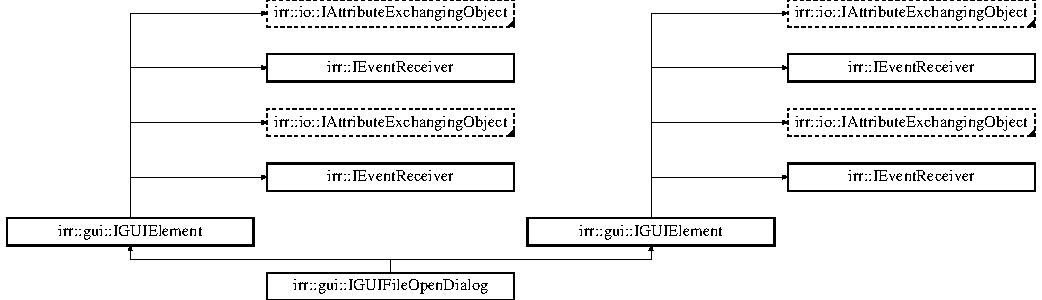
\includegraphics[height=4.038462cm]{classirr_1_1gui_1_1IGUIFileOpenDialog}
\end{center}
\end{figure}
\subsection*{Public Member Functions}
\begin{DoxyCompactItemize}
\item 
\mbox{\Hypertarget{classirr_1_1gui_1_1IGUIFileOpenDialog_a81f9db27e22941dc8370b7b7630501db}\label{classirr_1_1gui_1_1IGUIFileOpenDialog_a81f9db27e22941dc8370b7b7630501db}} 
\hyperlink{classirr_1_1gui_1_1IGUIFileOpenDialog_a81f9db27e22941dc8370b7b7630501db}{I\+G\+U\+I\+File\+Open\+Dialog} (\hyperlink{classirr_1_1gui_1_1IGUIEnvironment}{I\+G\+U\+I\+Environment} $\ast$environment, \hyperlink{classirr_1_1gui_1_1IGUIElement}{I\+G\+U\+I\+Element} $\ast$parent, \hyperlink{namespaceirr_ac66849b7a6ed16e30ebede579f9b47c6}{s32} id, \hyperlink{classirr_1_1core_1_1rect}{core\+::rect}$<$ \hyperlink{namespaceirr_ac66849b7a6ed16e30ebede579f9b47c6}{s32} $>$ rectangle)
\begin{DoxyCompactList}\small\item\em constructor \end{DoxyCompactList}\item 
\mbox{\Hypertarget{classirr_1_1gui_1_1IGUIFileOpenDialog_aa51c982b5e8264588473c147cd9a5b7b}\label{classirr_1_1gui_1_1IGUIFileOpenDialog_aa51c982b5e8264588473c147cd9a5b7b}} 
virtual const wchar\+\_\+t $\ast$ \hyperlink{classirr_1_1gui_1_1IGUIFileOpenDialog_aa51c982b5e8264588473c147cd9a5b7b}{get\+File\+Name} () const =0
\begin{DoxyCompactList}\small\item\em Returns the filename of the selected file. Returns N\+U\+LL, if no file was selected. \end{DoxyCompactList}\item 
\mbox{\Hypertarget{classirr_1_1gui_1_1IGUIFileOpenDialog_a2bc36296e0efe14992e88c9a1f4f5c61}\label{classirr_1_1gui_1_1IGUIFileOpenDialog_a2bc36296e0efe14992e88c9a1f4f5c61}} 
virtual const \hyperlink{namespaceirr_1_1io_a6468281622ce3a1c46b72e19f32dded5}{io\+::path} \& \hyperlink{classirr_1_1gui_1_1IGUIFileOpenDialog_a2bc36296e0efe14992e88c9a1f4f5c61}{get\+Directory\+Name} ()=0
\begin{DoxyCompactList}\small\item\em Returns the directory of the selected file. Returns N\+U\+LL, if no directory was selected. \end{DoxyCompactList}\item 
\mbox{\Hypertarget{classirr_1_1gui_1_1IGUIFileOpenDialog_a81f9db27e22941dc8370b7b7630501db}\label{classirr_1_1gui_1_1IGUIFileOpenDialog_a81f9db27e22941dc8370b7b7630501db}} 
\hyperlink{classirr_1_1gui_1_1IGUIFileOpenDialog_a81f9db27e22941dc8370b7b7630501db}{I\+G\+U\+I\+File\+Open\+Dialog} (\hyperlink{classirr_1_1gui_1_1IGUIEnvironment}{I\+G\+U\+I\+Environment} $\ast$environment, \hyperlink{classirr_1_1gui_1_1IGUIElement}{I\+G\+U\+I\+Element} $\ast$parent, \hyperlink{namespaceirr_ac66849b7a6ed16e30ebede579f9b47c6}{s32} id, \hyperlink{classirr_1_1core_1_1rect}{core\+::rect}$<$ \hyperlink{namespaceirr_ac66849b7a6ed16e30ebede579f9b47c6}{s32} $>$ rectangle)
\begin{DoxyCompactList}\small\item\em constructor \end{DoxyCompactList}\item 
\mbox{\Hypertarget{classirr_1_1gui_1_1IGUIFileOpenDialog_aa51c982b5e8264588473c147cd9a5b7b}\label{classirr_1_1gui_1_1IGUIFileOpenDialog_aa51c982b5e8264588473c147cd9a5b7b}} 
virtual const wchar\+\_\+t $\ast$ \hyperlink{classirr_1_1gui_1_1IGUIFileOpenDialog_aa51c982b5e8264588473c147cd9a5b7b}{get\+File\+Name} () const =0
\begin{DoxyCompactList}\small\item\em Returns the filename of the selected file. Returns N\+U\+LL, if no file was selected. \end{DoxyCompactList}\item 
\mbox{\Hypertarget{classirr_1_1gui_1_1IGUIFileOpenDialog_a2bc36296e0efe14992e88c9a1f4f5c61}\label{classirr_1_1gui_1_1IGUIFileOpenDialog_a2bc36296e0efe14992e88c9a1f4f5c61}} 
virtual const \hyperlink{namespaceirr_1_1io_a6468281622ce3a1c46b72e19f32dded5}{io\+::path} \& \hyperlink{classirr_1_1gui_1_1IGUIFileOpenDialog_a2bc36296e0efe14992e88c9a1f4f5c61}{get\+Directory\+Name} ()=0
\begin{DoxyCompactList}\small\item\em Returns the directory of the selected file. Returns N\+U\+LL, if no directory was selected. \end{DoxyCompactList}\end{DoxyCompactItemize}
\subsection*{Additional Inherited Members}


\subsection{Detailed Description}
Standard file chooser dialog. 

\begin{DoxyWarning}{Warning}
When the user selects a folder this does change the current working directory
\end{DoxyWarning}
\begin{DoxyParagraph}{This element can create the following events of type E\+G\+U\+I\+\_\+\+E\+V\+E\+N\+T\+\_\+\+T\+Y\+PE\+:}
\begin{DoxyItemize}
\item E\+G\+E\+T\+\_\+\+D\+I\+R\+E\+C\+T\+O\+R\+Y\+\_\+\+S\+E\+L\+E\+C\+T\+ED \item E\+G\+E\+T\+\_\+\+F\+I\+L\+E\+\_\+\+S\+E\+L\+E\+C\+T\+ED \item E\+G\+E\+T\+\_\+\+F\+I\+L\+E\+\_\+\+C\+H\+O\+O\+S\+E\+\_\+\+D\+I\+A\+L\+O\+G\+\_\+\+C\+A\+N\+C\+E\+L\+L\+ED \end{DoxyItemize}

\end{DoxyParagraph}


The documentation for this class was generated from the following file\+:\begin{DoxyCompactItemize}
\item 
indie\+\_\+share/controller/include/I\+G\+U\+I\+File\+Open\+Dialog.\+h\end{DoxyCompactItemize}

\hypertarget{classirr_1_1gui_1_1IGUIFont}{}\section{irr\+:\+:gui\+:\+:I\+G\+U\+I\+Font Class Reference}
\label{classirr_1_1gui_1_1IGUIFont}\index{irr\+::gui\+::\+I\+G\+U\+I\+Font@{irr\+::gui\+::\+I\+G\+U\+I\+Font}}


Font interface.  




{\ttfamily \#include $<$I\+G\+U\+I\+Font.\+h$>$}

Inheritance diagram for irr\+:\+:gui\+:\+:I\+G\+U\+I\+Font\+:\begin{figure}[H]
\begin{center}
\leavevmode
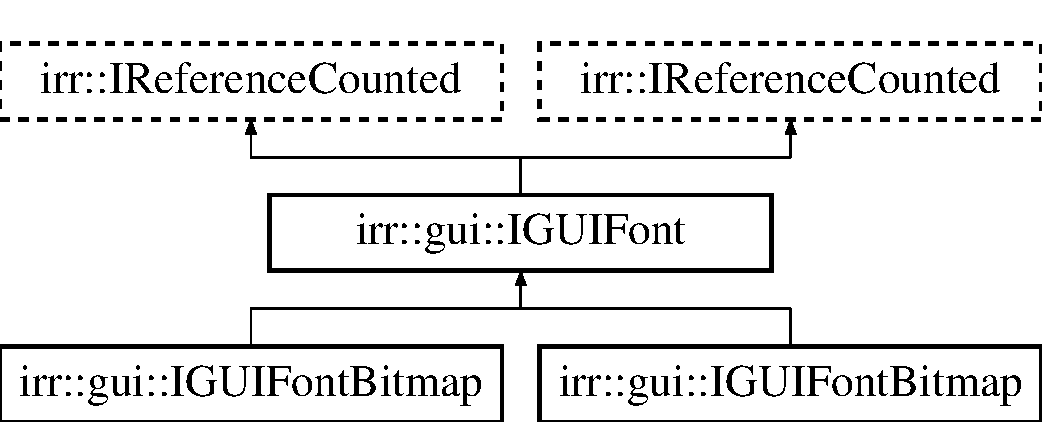
\includegraphics[height=3.000000cm]{classirr_1_1gui_1_1IGUIFont}
\end{center}
\end{figure}
\subsection*{Public Member Functions}
\begin{DoxyCompactItemize}
\item 
virtual void \hyperlink{classirr_1_1gui_1_1IGUIFont_af5627e546c474f31260fe671c24f9a33}{draw} (const \hyperlink{namespaceirr_1_1core_aef83fafbb1b36fcce44c07c9be23a7f2}{core\+::stringw} \&text, const \hyperlink{classirr_1_1core_1_1rect}{core\+::rect}$<$ \hyperlink{namespaceirr_ac66849b7a6ed16e30ebede579f9b47c6}{s32} $>$ \&position, \hyperlink{classirr_1_1video_1_1SColor}{video\+::\+S\+Color} color, bool hcenter=false, bool vcenter=false, const \hyperlink{classirr_1_1core_1_1rect}{core\+::rect}$<$ \hyperlink{namespaceirr_ac66849b7a6ed16e30ebede579f9b47c6}{s32} $>$ $\ast$clip=0)=0
\begin{DoxyCompactList}\small\item\em Draws some text and clips it to the specified rectangle if wanted. \end{DoxyCompactList}\item 
virtual \hyperlink{classirr_1_1core_1_1dimension2d}{core\+::dimension2d}$<$ \hyperlink{namespaceirr_a0416a53257075833e7002efd0a18e804}{u32} $>$ \hyperlink{classirr_1_1gui_1_1IGUIFont_aa7612db0c9dc2837b44a1a2fa5668797}{get\+Dimension} (const wchar\+\_\+t $\ast$text) const =0
\begin{DoxyCompactList}\small\item\em Calculates the width and height of a given string of text. \end{DoxyCompactList}\item 
virtual \hyperlink{namespaceirr_ac66849b7a6ed16e30ebede579f9b47c6}{s32} \hyperlink{classirr_1_1gui_1_1IGUIFont_a60d4d0465deedd811cd0fecd11b4329f}{get\+Character\+From\+Pos} (const wchar\+\_\+t $\ast$text, \hyperlink{namespaceirr_ac66849b7a6ed16e30ebede579f9b47c6}{s32} pixel\+\_\+x) const =0
\begin{DoxyCompactList}\small\item\em Calculates the index of the character in the text which is on a specific position. \end{DoxyCompactList}\item 
\mbox{\Hypertarget{classirr_1_1gui_1_1IGUIFont_a3d5a42997a718b510b73e7d6235b993e}\label{classirr_1_1gui_1_1IGUIFont_a3d5a42997a718b510b73e7d6235b993e}} 
virtual \hyperlink{namespaceirr_1_1gui_a3c818a164486f43300260327c5420a2f}{E\+G\+U\+I\+\_\+\+F\+O\+N\+T\+\_\+\+T\+Y\+PE} \hyperlink{classirr_1_1gui_1_1IGUIFont_a3d5a42997a718b510b73e7d6235b993e}{get\+Type} () const
\begin{DoxyCompactList}\small\item\em Returns the type of this font. \end{DoxyCompactList}\item 
\mbox{\Hypertarget{classirr_1_1gui_1_1IGUIFont_aa683bb2535776b7f81adc050931d9b17}\label{classirr_1_1gui_1_1IGUIFont_aa683bb2535776b7f81adc050931d9b17}} 
virtual void \hyperlink{classirr_1_1gui_1_1IGUIFont_aa683bb2535776b7f81adc050931d9b17}{set\+Kerning\+Width} (\hyperlink{namespaceirr_ac66849b7a6ed16e30ebede579f9b47c6}{s32} kerning)=0
\begin{DoxyCompactList}\small\item\em Sets global kerning width for the font. \end{DoxyCompactList}\item 
\mbox{\Hypertarget{classirr_1_1gui_1_1IGUIFont_a9545ecfae06592acd47508f6824bb386}\label{classirr_1_1gui_1_1IGUIFont_a9545ecfae06592acd47508f6824bb386}} 
virtual void \hyperlink{classirr_1_1gui_1_1IGUIFont_a9545ecfae06592acd47508f6824bb386}{set\+Kerning\+Height} (\hyperlink{namespaceirr_ac66849b7a6ed16e30ebede579f9b47c6}{s32} kerning)=0
\begin{DoxyCompactList}\small\item\em Sets global kerning height for the font. \end{DoxyCompactList}\item 
virtual \hyperlink{namespaceirr_ac66849b7a6ed16e30ebede579f9b47c6}{s32} \hyperlink{classirr_1_1gui_1_1IGUIFont_a7de0b25d3d1dbdcc9036e5d788e2d9ab}{get\+Kerning\+Width} (const wchar\+\_\+t $\ast$this\+Letter=0, const wchar\+\_\+t $\ast$previous\+Letter=0) const =0
\begin{DoxyCompactList}\small\item\em Gets kerning values (distance between letters) for the font. If no parameters are provided,. \end{DoxyCompactList}\item 
\mbox{\Hypertarget{classirr_1_1gui_1_1IGUIFont_a1f1a760be155fc0f6a632b457154a5d8}\label{classirr_1_1gui_1_1IGUIFont_a1f1a760be155fc0f6a632b457154a5d8}} 
virtual \hyperlink{namespaceirr_ac66849b7a6ed16e30ebede579f9b47c6}{s32} \hyperlink{classirr_1_1gui_1_1IGUIFont_a1f1a760be155fc0f6a632b457154a5d8}{get\+Kerning\+Height} () const =0
\begin{DoxyCompactList}\small\item\em Returns the distance between letters. \end{DoxyCompactList}\item 
virtual void \hyperlink{classirr_1_1gui_1_1IGUIFont_acff05412dc954845add611c5f71cef49}{set\+Invisible\+Characters} (const wchar\+\_\+t $\ast$s)=0
\begin{DoxyCompactList}\small\item\em Define which characters should not be drawn by the font. \end{DoxyCompactList}\end{DoxyCompactItemize}
\subsection*{Additional Inherited Members}


\subsection{Detailed Description}
Font interface. 

\subsection{Member Function Documentation}
\mbox{\Hypertarget{classirr_1_1gui_1_1IGUIFont_af5627e546c474f31260fe671c24f9a33}\label{classirr_1_1gui_1_1IGUIFont_af5627e546c474f31260fe671c24f9a33}} 
\index{irr\+::gui\+::\+I\+G\+U\+I\+Font@{irr\+::gui\+::\+I\+G\+U\+I\+Font}!draw@{draw}}
\index{draw@{draw}!irr\+::gui\+::\+I\+G\+U\+I\+Font@{irr\+::gui\+::\+I\+G\+U\+I\+Font}}
\subsubsection{\texorpdfstring{draw()}{draw()}}
{\footnotesize\ttfamily virtual void irr\+::gui\+::\+I\+G\+U\+I\+Font\+::draw (\begin{DoxyParamCaption}\item[{const \hyperlink{namespaceirr_1_1core_aef83fafbb1b36fcce44c07c9be23a7f2}{core\+::stringw} \&}]{text,  }\item[{const \hyperlink{classirr_1_1core_1_1rect}{core\+::rect}$<$ \hyperlink{namespaceirr_ac66849b7a6ed16e30ebede579f9b47c6}{s32} $>$ \&}]{position,  }\item[{\hyperlink{classirr_1_1video_1_1SColor}{video\+::\+S\+Color}}]{color,  }\item[{bool}]{hcenter = {\ttfamily false},  }\item[{bool}]{vcenter = {\ttfamily false},  }\item[{const \hyperlink{classirr_1_1core_1_1rect}{core\+::rect}$<$ \hyperlink{namespaceirr_ac66849b7a6ed16e30ebede579f9b47c6}{s32} $>$ $\ast$}]{clip = {\ttfamily 0} }\end{DoxyParamCaption})\hspace{0.3cm}{\ttfamily [pure virtual]}}



Draws some text and clips it to the specified rectangle if wanted. 


\begin{DoxyParams}{Parameters}
{\em text} & \hyperlink{classText}{Text} to draw \\
\hline
{\em position} & Rectangle specifying position where to draw the text. \\
\hline
{\em color} & Color of the text \\
\hline
{\em hcenter} & Specifies if the text should be centered horizontally into the rectangle. \\
\hline
{\em vcenter} & Specifies if the text should be centered vertically into the rectangle. \\
\hline
{\em clip} & Optional pointer to a rectangle against which the text will be clipped. If the pointer is null, no clipping will be done. \\
\hline
\end{DoxyParams}
\mbox{\Hypertarget{classirr_1_1gui_1_1IGUIFont_a60d4d0465deedd811cd0fecd11b4329f}\label{classirr_1_1gui_1_1IGUIFont_a60d4d0465deedd811cd0fecd11b4329f}} 
\index{irr\+::gui\+::\+I\+G\+U\+I\+Font@{irr\+::gui\+::\+I\+G\+U\+I\+Font}!get\+Character\+From\+Pos@{get\+Character\+From\+Pos}}
\index{get\+Character\+From\+Pos@{get\+Character\+From\+Pos}!irr\+::gui\+::\+I\+G\+U\+I\+Font@{irr\+::gui\+::\+I\+G\+U\+I\+Font}}
\subsubsection{\texorpdfstring{get\+Character\+From\+Pos()}{getCharacterFromPos()}}
{\footnotesize\ttfamily virtual \hyperlink{namespaceirr_ac66849b7a6ed16e30ebede579f9b47c6}{s32} irr\+::gui\+::\+I\+G\+U\+I\+Font\+::get\+Character\+From\+Pos (\begin{DoxyParamCaption}\item[{const wchar\+\_\+t $\ast$}]{text,  }\item[{\hyperlink{namespaceirr_ac66849b7a6ed16e30ebede579f9b47c6}{s32}}]{pixel\+\_\+x }\end{DoxyParamCaption}) const\hspace{0.3cm}{\ttfamily [pure virtual]}}



Calculates the index of the character in the text which is on a specific position. 


\begin{DoxyParams}{Parameters}
{\em text} & \hyperlink{classText}{Text} string. \\
\hline
{\em pixel\+\_\+x} & X pixel position of which the index of the character will be returned. \\
\hline
\end{DoxyParams}
\begin{DoxyReturn}{Returns}
Returns zero based index of the character in the text, and -\/1 if no no character is on this position. (=the text is too short). 
\end{DoxyReturn}
\mbox{\Hypertarget{classirr_1_1gui_1_1IGUIFont_aa7612db0c9dc2837b44a1a2fa5668797}\label{classirr_1_1gui_1_1IGUIFont_aa7612db0c9dc2837b44a1a2fa5668797}} 
\index{irr\+::gui\+::\+I\+G\+U\+I\+Font@{irr\+::gui\+::\+I\+G\+U\+I\+Font}!get\+Dimension@{get\+Dimension}}
\index{get\+Dimension@{get\+Dimension}!irr\+::gui\+::\+I\+G\+U\+I\+Font@{irr\+::gui\+::\+I\+G\+U\+I\+Font}}
\subsubsection{\texorpdfstring{get\+Dimension()}{getDimension()}}
{\footnotesize\ttfamily virtual \hyperlink{classirr_1_1core_1_1dimension2d}{core\+::dimension2d}$<$\hyperlink{namespaceirr_a0416a53257075833e7002efd0a18e804}{u32}$>$ irr\+::gui\+::\+I\+G\+U\+I\+Font\+::get\+Dimension (\begin{DoxyParamCaption}\item[{const wchar\+\_\+t $\ast$}]{text }\end{DoxyParamCaption}) const\hspace{0.3cm}{\ttfamily [pure virtual]}}



Calculates the width and height of a given string of text. 

\begin{DoxyReturn}{Returns}
Returns width and height of the area covered by the text if it would be drawn. 
\end{DoxyReturn}
\mbox{\Hypertarget{classirr_1_1gui_1_1IGUIFont_a7de0b25d3d1dbdcc9036e5d788e2d9ab}\label{classirr_1_1gui_1_1IGUIFont_a7de0b25d3d1dbdcc9036e5d788e2d9ab}} 
\index{irr\+::gui\+::\+I\+G\+U\+I\+Font@{irr\+::gui\+::\+I\+G\+U\+I\+Font}!get\+Kerning\+Width@{get\+Kerning\+Width}}
\index{get\+Kerning\+Width@{get\+Kerning\+Width}!irr\+::gui\+::\+I\+G\+U\+I\+Font@{irr\+::gui\+::\+I\+G\+U\+I\+Font}}
\subsubsection{\texorpdfstring{get\+Kerning\+Width()}{getKerningWidth()}}
{\footnotesize\ttfamily virtual \hyperlink{namespaceirr_ac66849b7a6ed16e30ebede579f9b47c6}{s32} irr\+::gui\+::\+I\+G\+U\+I\+Font\+::get\+Kerning\+Width (\begin{DoxyParamCaption}\item[{const wchar\+\_\+t $\ast$}]{this\+Letter = {\ttfamily 0},  }\item[{const wchar\+\_\+t $\ast$}]{previous\+Letter = {\ttfamily 0} }\end{DoxyParamCaption}) const\hspace{0.3cm}{\ttfamily [pure virtual]}}



Gets kerning values (distance between letters) for the font. If no parameters are provided,. 

the global kerning distance is returned. 
\begin{DoxyParams}{Parameters}
{\em this\+Letter} & If this parameter is provided, the left side kerning for this letter is added to the global kerning value. For example, a space might only be one pixel wide, but it may be displayed as several pixels. \\
\hline
{\em previous\+Letter} & If provided, kerning is calculated for both letters and added to the global kerning value. For example, in a font which supports kerning pairs a string such as \textquotesingle{}Wo\textquotesingle{} may have the \textquotesingle{}o\textquotesingle{} tucked neatly under the \textquotesingle{}W\textquotesingle{}. \\
\hline
\end{DoxyParams}


Implemented in \hyperlink{classirr_1_1gui_1_1IGUIFontBitmap_a7bdeaea45745a10e09f7769ec3b95a12}{irr\+::gui\+::\+I\+G\+U\+I\+Font\+Bitmap}.

\mbox{\Hypertarget{classirr_1_1gui_1_1IGUIFont_acff05412dc954845add611c5f71cef49}\label{classirr_1_1gui_1_1IGUIFont_acff05412dc954845add611c5f71cef49}} 
\index{irr\+::gui\+::\+I\+G\+U\+I\+Font@{irr\+::gui\+::\+I\+G\+U\+I\+Font}!set\+Invisible\+Characters@{set\+Invisible\+Characters}}
\index{set\+Invisible\+Characters@{set\+Invisible\+Characters}!irr\+::gui\+::\+I\+G\+U\+I\+Font@{irr\+::gui\+::\+I\+G\+U\+I\+Font}}
\subsubsection{\texorpdfstring{set\+Invisible\+Characters()}{setInvisibleCharacters()}}
{\footnotesize\ttfamily virtual void irr\+::gui\+::\+I\+G\+U\+I\+Font\+::set\+Invisible\+Characters (\begin{DoxyParamCaption}\item[{const wchar\+\_\+t $\ast$}]{s }\end{DoxyParamCaption})\hspace{0.3cm}{\ttfamily [pure virtual]}}



Define which characters should not be drawn by the font. 

For example \char`\"{} \char`\"{} would not draw any space which is usually blank in most fonts. 
\begin{DoxyParams}{Parameters}
{\em s} & String of symbols which are not send down to the videodriver \\
\hline
\end{DoxyParams}


The documentation for this class was generated from the following file\+:\begin{DoxyCompactItemize}
\item 
indie\+\_\+share/controller/include/I\+G\+U\+I\+Font.\+h\end{DoxyCompactItemize}

\hypertarget{classirr_1_1gui_1_1IGUIFontBitmap}{}\section{irr\+:\+:gui\+:\+:I\+G\+U\+I\+Font\+Bitmap Class Reference}
\label{classirr_1_1gui_1_1IGUIFontBitmap}\index{irr\+::gui\+::\+I\+G\+U\+I\+Font\+Bitmap@{irr\+::gui\+::\+I\+G\+U\+I\+Font\+Bitmap}}


Font interface.  




{\ttfamily \#include $<$I\+G\+U\+I\+Font\+Bitmap.\+h$>$}

Inheritance diagram for irr\+:\+:gui\+:\+:I\+G\+U\+I\+Font\+Bitmap\+:\begin{figure}[H]
\begin{center}
\leavevmode
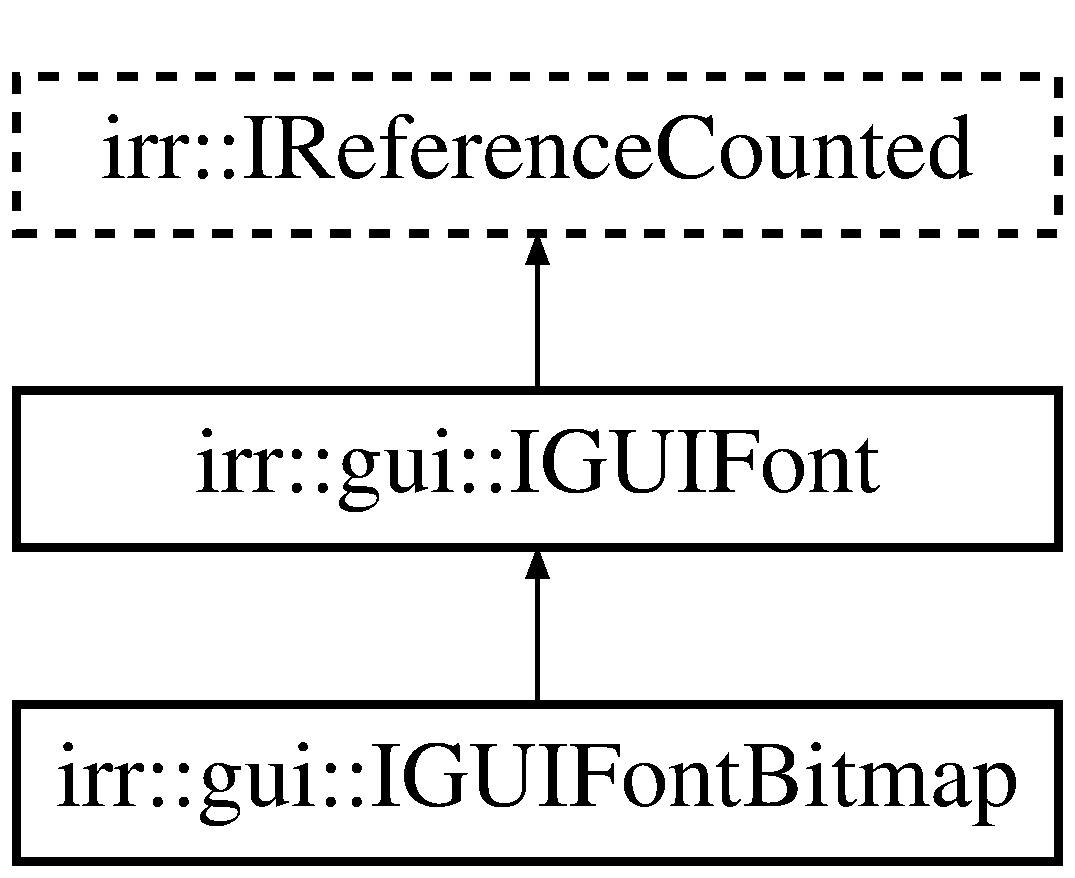
\includegraphics[height=2.837838cm]{classirr_1_1gui_1_1IGUIFontBitmap}
\end{center}
\end{figure}
\subsection*{Public Member Functions}
\begin{DoxyCompactItemize}
\item 
\mbox{\Hypertarget{classirr_1_1gui_1_1IGUIFontBitmap_a8e4b5d7d84a71fcfcf3cbb96663be332}\label{classirr_1_1gui_1_1IGUIFontBitmap_a8e4b5d7d84a71fcfcf3cbb96663be332}} 
virtual \hyperlink{namespaceirr_1_1gui_a3c818a164486f43300260327c5420a2f}{E\+G\+U\+I\+\_\+\+F\+O\+N\+T\+\_\+\+T\+Y\+PE} \hyperlink{classirr_1_1gui_1_1IGUIFontBitmap_a8e4b5d7d84a71fcfcf3cbb96663be332}{get\+Type} () const
\begin{DoxyCompactList}\small\item\em Returns the type of this font. \end{DoxyCompactList}\item 
\mbox{\Hypertarget{classirr_1_1gui_1_1IGUIFontBitmap_ab9185a0c2e708958a8caae7bdeba9deb}\label{classirr_1_1gui_1_1IGUIFontBitmap_ab9185a0c2e708958a8caae7bdeba9deb}} 
virtual \hyperlink{classirr_1_1gui_1_1IGUISpriteBank}{I\+G\+U\+I\+Sprite\+Bank} $\ast$ \hyperlink{classirr_1_1gui_1_1IGUIFontBitmap_ab9185a0c2e708958a8caae7bdeba9deb}{get\+Sprite\+Bank} () const =0
\begin{DoxyCompactList}\small\item\em returns the parsed Symbol Information \end{DoxyCompactList}\item 
\mbox{\Hypertarget{classirr_1_1gui_1_1IGUIFontBitmap_a3c717559574dd9e63b3d5869c9ee321d}\label{classirr_1_1gui_1_1IGUIFontBitmap_a3c717559574dd9e63b3d5869c9ee321d}} 
virtual \hyperlink{namespaceirr_a0416a53257075833e7002efd0a18e804}{u32} \hyperlink{classirr_1_1gui_1_1IGUIFontBitmap_a3c717559574dd9e63b3d5869c9ee321d}{get\+Sprite\+No\+From\+Char} (const wchar\+\_\+t $\ast$c) const =0
\begin{DoxyCompactList}\small\item\em returns the sprite number from a given character \end{DoxyCompactList}\item 
virtual \hyperlink{namespaceirr_ac66849b7a6ed16e30ebede579f9b47c6}{s32} \hyperlink{classirr_1_1gui_1_1IGUIFontBitmap_a7bdeaea45745a10e09f7769ec3b95a12}{get\+Kerning\+Width} (const wchar\+\_\+t $\ast$this\+Letter=0, const wchar\+\_\+t $\ast$previous\+Letter=0) const =0
\begin{DoxyCompactList}\small\item\em Gets kerning values (distance between letters) for the font. If no parameters are provided,. \end{DoxyCompactList}\item 
\mbox{\Hypertarget{classirr_1_1gui_1_1IGUIFontBitmap_a8e4b5d7d84a71fcfcf3cbb96663be332}\label{classirr_1_1gui_1_1IGUIFontBitmap_a8e4b5d7d84a71fcfcf3cbb96663be332}} 
virtual \hyperlink{namespaceirr_1_1gui_a3c818a164486f43300260327c5420a2f}{E\+G\+U\+I\+\_\+\+F\+O\+N\+T\+\_\+\+T\+Y\+PE} \hyperlink{classirr_1_1gui_1_1IGUIFontBitmap_a8e4b5d7d84a71fcfcf3cbb96663be332}{get\+Type} () const
\begin{DoxyCompactList}\small\item\em Returns the type of this font. \end{DoxyCompactList}\item 
\mbox{\Hypertarget{classirr_1_1gui_1_1IGUIFontBitmap_ab9185a0c2e708958a8caae7bdeba9deb}\label{classirr_1_1gui_1_1IGUIFontBitmap_ab9185a0c2e708958a8caae7bdeba9deb}} 
virtual \hyperlink{classirr_1_1gui_1_1IGUISpriteBank}{I\+G\+U\+I\+Sprite\+Bank} $\ast$ \hyperlink{classirr_1_1gui_1_1IGUIFontBitmap_ab9185a0c2e708958a8caae7bdeba9deb}{get\+Sprite\+Bank} () const =0
\begin{DoxyCompactList}\small\item\em returns the parsed Symbol Information \end{DoxyCompactList}\item 
\mbox{\Hypertarget{classirr_1_1gui_1_1IGUIFontBitmap_a3c717559574dd9e63b3d5869c9ee321d}\label{classirr_1_1gui_1_1IGUIFontBitmap_a3c717559574dd9e63b3d5869c9ee321d}} 
virtual \hyperlink{namespaceirr_a0416a53257075833e7002efd0a18e804}{u32} \hyperlink{classirr_1_1gui_1_1IGUIFontBitmap_a3c717559574dd9e63b3d5869c9ee321d}{get\+Sprite\+No\+From\+Char} (const wchar\+\_\+t $\ast$c) const =0
\begin{DoxyCompactList}\small\item\em returns the sprite number from a given character \end{DoxyCompactList}\item 
virtual \hyperlink{namespaceirr_ac66849b7a6ed16e30ebede579f9b47c6}{s32} \hyperlink{classirr_1_1gui_1_1IGUIFontBitmap_a7bdeaea45745a10e09f7769ec3b95a12}{get\+Kerning\+Width} (const wchar\+\_\+t $\ast$this\+Letter=0, const wchar\+\_\+t $\ast$previous\+Letter=0) const =0
\begin{DoxyCompactList}\small\item\em Gets kerning values (distance between letters) for the font. If no parameters are provided,. \end{DoxyCompactList}\end{DoxyCompactItemize}
\subsection*{Additional Inherited Members}


\subsection{Detailed Description}
Font interface. 

\subsection{Member Function Documentation}
\mbox{\Hypertarget{classirr_1_1gui_1_1IGUIFontBitmap_a7bdeaea45745a10e09f7769ec3b95a12}\label{classirr_1_1gui_1_1IGUIFontBitmap_a7bdeaea45745a10e09f7769ec3b95a12}} 
\index{irr\+::gui\+::\+I\+G\+U\+I\+Font\+Bitmap@{irr\+::gui\+::\+I\+G\+U\+I\+Font\+Bitmap}!get\+Kerning\+Width@{get\+Kerning\+Width}}
\index{get\+Kerning\+Width@{get\+Kerning\+Width}!irr\+::gui\+::\+I\+G\+U\+I\+Font\+Bitmap@{irr\+::gui\+::\+I\+G\+U\+I\+Font\+Bitmap}}
\subsubsection{\texorpdfstring{get\+Kerning\+Width()}{getKerningWidth()}\hspace{0.1cm}{\footnotesize\ttfamily [1/2]}}
{\footnotesize\ttfamily virtual \hyperlink{namespaceirr_ac66849b7a6ed16e30ebede579f9b47c6}{s32} irr\+::gui\+::\+I\+G\+U\+I\+Font\+Bitmap\+::get\+Kerning\+Width (\begin{DoxyParamCaption}\item[{const wchar\+\_\+t $\ast$}]{this\+Letter = {\ttfamily 0},  }\item[{const wchar\+\_\+t $\ast$}]{previous\+Letter = {\ttfamily 0} }\end{DoxyParamCaption}) const\hspace{0.3cm}{\ttfamily [pure virtual]}}



Gets kerning values (distance between letters) for the font. If no parameters are provided,. 

the global kerning distance is returned. 
\begin{DoxyParams}{Parameters}
{\em this\+Letter} & If this parameter is provided, the left side kerning for this letter is added to the global kerning value. For example, a space might only be one pixel wide, but it may be displayed as several pixels. \\
\hline
{\em previous\+Letter} & If provided, kerning is calculated for both letters and added to the global kerning value. For example, E\+G\+F\+T\+\_\+\+B\+I\+T\+M\+AP will add the right kerning value of previous\+Letter to the left side kerning value of this\+Letter, then add the global value. \\
\hline
\end{DoxyParams}


Implements \hyperlink{classirr_1_1gui_1_1IGUIFont_a7de0b25d3d1dbdcc9036e5d788e2d9ab}{irr\+::gui\+::\+I\+G\+U\+I\+Font}.

\mbox{\Hypertarget{classirr_1_1gui_1_1IGUIFontBitmap_a7bdeaea45745a10e09f7769ec3b95a12}\label{classirr_1_1gui_1_1IGUIFontBitmap_a7bdeaea45745a10e09f7769ec3b95a12}} 
\index{irr\+::gui\+::\+I\+G\+U\+I\+Font\+Bitmap@{irr\+::gui\+::\+I\+G\+U\+I\+Font\+Bitmap}!get\+Kerning\+Width@{get\+Kerning\+Width}}
\index{get\+Kerning\+Width@{get\+Kerning\+Width}!irr\+::gui\+::\+I\+G\+U\+I\+Font\+Bitmap@{irr\+::gui\+::\+I\+G\+U\+I\+Font\+Bitmap}}
\subsubsection{\texorpdfstring{get\+Kerning\+Width()}{getKerningWidth()}\hspace{0.1cm}{\footnotesize\ttfamily [2/2]}}
{\footnotesize\ttfamily virtual \hyperlink{namespaceirr_ac66849b7a6ed16e30ebede579f9b47c6}{s32} irr\+::gui\+::\+I\+G\+U\+I\+Font\+Bitmap\+::get\+Kerning\+Width (\begin{DoxyParamCaption}\item[{const wchar\+\_\+t $\ast$}]{this\+Letter = {\ttfamily 0},  }\item[{const wchar\+\_\+t $\ast$}]{previous\+Letter = {\ttfamily 0} }\end{DoxyParamCaption}) const\hspace{0.3cm}{\ttfamily [pure virtual]}}



Gets kerning values (distance between letters) for the font. If no parameters are provided,. 

the global kerning distance is returned. 
\begin{DoxyParams}{Parameters}
{\em this\+Letter} & If this parameter is provided, the left side kerning for this letter is added to the global kerning value. For example, a space might only be one pixel wide, but it may be displayed as several pixels. \\
\hline
{\em previous\+Letter} & If provided, kerning is calculated for both letters and added to the global kerning value. For example, E\+G\+F\+T\+\_\+\+B\+I\+T\+M\+AP will add the right kerning value of previous\+Letter to the left side kerning value of this\+Letter, then add the global value. \\
\hline
\end{DoxyParams}


Implements \hyperlink{classirr_1_1gui_1_1IGUIFont_a7de0b25d3d1dbdcc9036e5d788e2d9ab}{irr\+::gui\+::\+I\+G\+U\+I\+Font}.



The documentation for this class was generated from the following file\+:\begin{DoxyCompactItemize}
\item 
indie\+\_\+share/controller/include/I\+G\+U\+I\+Font\+Bitmap.\+h\end{DoxyCompactItemize}

\hypertarget{classirr_1_1gui_1_1IGUIImage}{}\section{irr\+:\+:gui\+:\+:I\+G\+U\+I\+Image Class Reference}
\label{classirr_1_1gui_1_1IGUIImage}\index{irr\+::gui\+::\+I\+G\+U\+I\+Image@{irr\+::gui\+::\+I\+G\+U\+I\+Image}}


G\+UI element displaying an image.  




{\ttfamily \#include $<$I\+G\+U\+I\+Image.\+h$>$}

Inheritance diagram for irr\+:\+:gui\+:\+:I\+G\+U\+I\+Image\+:\begin{figure}[H]
\begin{center}
\leavevmode
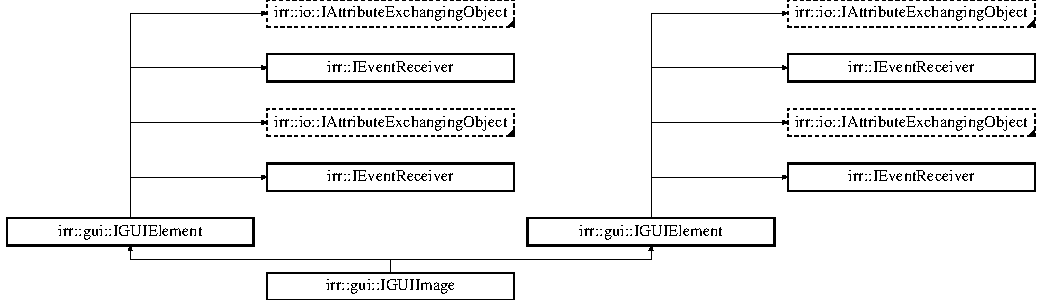
\includegraphics[height=4.000000cm]{classirr_1_1gui_1_1IGUIImage}
\end{center}
\end{figure}
\subsection*{Public Member Functions}
\begin{DoxyCompactItemize}
\item 
\mbox{\Hypertarget{classirr_1_1gui_1_1IGUIImage_a079a30cd26c749a8a42b4a689678c4dc}\label{classirr_1_1gui_1_1IGUIImage_a079a30cd26c749a8a42b4a689678c4dc}} 
\hyperlink{classirr_1_1gui_1_1IGUIImage_a079a30cd26c749a8a42b4a689678c4dc}{I\+G\+U\+I\+Image} (\hyperlink{classirr_1_1gui_1_1IGUIEnvironment}{I\+G\+U\+I\+Environment} $\ast$environment, \hyperlink{classirr_1_1gui_1_1IGUIElement}{I\+G\+U\+I\+Element} $\ast$parent, \hyperlink{namespaceirr_ac66849b7a6ed16e30ebede579f9b47c6}{s32} id, \hyperlink{classirr_1_1core_1_1rect}{core\+::rect}$<$ \hyperlink{namespaceirr_ac66849b7a6ed16e30ebede579f9b47c6}{s32} $>$ rectangle)
\begin{DoxyCompactList}\small\item\em constructor \end{DoxyCompactList}\item 
\mbox{\Hypertarget{classirr_1_1gui_1_1IGUIImage_a35a3af4957e42acb183f562d09a4ea63}\label{classirr_1_1gui_1_1IGUIImage_a35a3af4957e42acb183f562d09a4ea63}} 
virtual void \hyperlink{classirr_1_1gui_1_1IGUIImage_a35a3af4957e42acb183f562d09a4ea63}{set\+Image} (\hyperlink{classirr_1_1video_1_1ITexture}{video\+::\+I\+Texture} $\ast$image)=0
\begin{DoxyCompactList}\small\item\em Sets an image texture. \end{DoxyCompactList}\item 
\mbox{\Hypertarget{classirr_1_1gui_1_1IGUIImage_a5ed7402ca9d9810d320ff11f1251e8c0}\label{classirr_1_1gui_1_1IGUIImage_a5ed7402ca9d9810d320ff11f1251e8c0}} 
virtual \hyperlink{classirr_1_1video_1_1ITexture}{video\+::\+I\+Texture} $\ast$ \hyperlink{classirr_1_1gui_1_1IGUIImage_a5ed7402ca9d9810d320ff11f1251e8c0}{get\+Image} () const =0
\begin{DoxyCompactList}\small\item\em Gets the image texture. \end{DoxyCompactList}\item 
\mbox{\Hypertarget{classirr_1_1gui_1_1IGUIImage_ac836018aafc61f6b9fe88acfa2267d8e}\label{classirr_1_1gui_1_1IGUIImage_ac836018aafc61f6b9fe88acfa2267d8e}} 
virtual void \hyperlink{classirr_1_1gui_1_1IGUIImage_ac836018aafc61f6b9fe88acfa2267d8e}{set\+Color} (\hyperlink{classirr_1_1video_1_1SColor}{video\+::\+S\+Color} color)=0
\begin{DoxyCompactList}\small\item\em Sets the color of the image. \end{DoxyCompactList}\item 
\mbox{\Hypertarget{classirr_1_1gui_1_1IGUIImage_a642c5683600be82efa0cc04b4236e34d}\label{classirr_1_1gui_1_1IGUIImage_a642c5683600be82efa0cc04b4236e34d}} 
virtual void \hyperlink{classirr_1_1gui_1_1IGUIImage_a642c5683600be82efa0cc04b4236e34d}{set\+Scale\+Image} (bool scale)=0
\begin{DoxyCompactList}\small\item\em Sets if the image should scale to fit the element. \end{DoxyCompactList}\item 
\mbox{\Hypertarget{classirr_1_1gui_1_1IGUIImage_a9426b40769f4ef7614e6a94dcfa67455}\label{classirr_1_1gui_1_1IGUIImage_a9426b40769f4ef7614e6a94dcfa67455}} 
virtual void \hyperlink{classirr_1_1gui_1_1IGUIImage_a9426b40769f4ef7614e6a94dcfa67455}{set\+Use\+Alpha\+Channel} (bool use)=0
\begin{DoxyCompactList}\small\item\em Sets if the image should use its alpha channel to draw itself. \end{DoxyCompactList}\item 
\mbox{\Hypertarget{classirr_1_1gui_1_1IGUIImage_a46a6dc23dd045cb65247344bf71078e4}\label{classirr_1_1gui_1_1IGUIImage_a46a6dc23dd045cb65247344bf71078e4}} 
virtual \hyperlink{classirr_1_1video_1_1SColor}{video\+::\+S\+Color} \hyperlink{classirr_1_1gui_1_1IGUIImage_a46a6dc23dd045cb65247344bf71078e4}{get\+Color} () const =0
\begin{DoxyCompactList}\small\item\em Gets the color of the image. \end{DoxyCompactList}\item 
\mbox{\Hypertarget{classirr_1_1gui_1_1IGUIImage_aca24045ee740242b9c8de73a8f609a27}\label{classirr_1_1gui_1_1IGUIImage_aca24045ee740242b9c8de73a8f609a27}} 
virtual bool \hyperlink{classirr_1_1gui_1_1IGUIImage_aca24045ee740242b9c8de73a8f609a27}{is\+Image\+Scaled} () const =0
\begin{DoxyCompactList}\small\item\em Returns true if the image is scaled to fit, false if not. \end{DoxyCompactList}\item 
\mbox{\Hypertarget{classirr_1_1gui_1_1IGUIImage_a5be6faec4c156fc955c84a5b3f703d63}\label{classirr_1_1gui_1_1IGUIImage_a5be6faec4c156fc955c84a5b3f703d63}} 
virtual bool \hyperlink{classirr_1_1gui_1_1IGUIImage_a5be6faec4c156fc955c84a5b3f703d63}{is\+Alpha\+Channel\+Used} () const =0
\begin{DoxyCompactList}\small\item\em Returns true if the image is using the alpha channel, false if not. \end{DoxyCompactList}\end{DoxyCompactItemize}
\subsection*{Additional Inherited Members}


\subsection{Detailed Description}
G\+UI element displaying an image. 

The documentation for this class was generated from the following file\+:\begin{DoxyCompactItemize}
\item 
indie\+\_\+share/controller/include/I\+G\+U\+I\+Image.\+h\end{DoxyCompactItemize}

\hypertarget{classirr_1_1gui_1_1IGUIImageList}{}\section{irr\+:\+:gui\+:\+:I\+G\+U\+I\+Image\+List Class Reference}
\label{classirr_1_1gui_1_1IGUIImageList}\index{irr\+::gui\+::\+I\+G\+U\+I\+Image\+List@{irr\+::gui\+::\+I\+G\+U\+I\+Image\+List}}


Font interface.  




{\ttfamily \#include $<$I\+G\+U\+I\+Image\+List.\+h$>$}

Inheritance diagram for irr\+:\+:gui\+:\+:I\+G\+U\+I\+Image\+List\+:\begin{figure}[H]
\begin{center}
\leavevmode
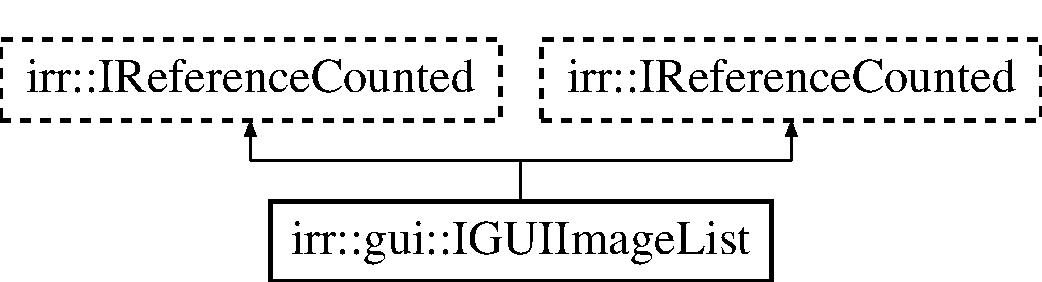
\includegraphics[height=2.000000cm]{classirr_1_1gui_1_1IGUIImageList}
\end{center}
\end{figure}
\subsection*{Public Member Functions}
\begin{DoxyCompactItemize}
\item 
\mbox{\Hypertarget{classirr_1_1gui_1_1IGUIImageList_ad6be754893f7ba902d821d215761075f}\label{classirr_1_1gui_1_1IGUIImageList_ad6be754893f7ba902d821d215761075f}} 
virtual \hyperlink{classirr_1_1gui_1_1IGUIImageList_ad6be754893f7ba902d821d215761075f}{$\sim$\+I\+G\+U\+I\+Image\+List} ()
\begin{DoxyCompactList}\small\item\em Destructor. \end{DoxyCompactList}\item 
virtual void \hyperlink{classirr_1_1gui_1_1IGUIImageList_ae19fa00cece01c5914dfc0a3e33a882c}{draw} (\hyperlink{namespaceirr_ac66849b7a6ed16e30ebede579f9b47c6}{s32} index, const core\+::position2d$<$ \hyperlink{namespaceirr_ac66849b7a6ed16e30ebede579f9b47c6}{s32} $>$ \&dest\+Pos, const \hyperlink{classirr_1_1core_1_1rect}{core\+::rect}$<$ \hyperlink{namespaceirr_ac66849b7a6ed16e30ebede579f9b47c6}{s32} $>$ $\ast$clip=0)=0
\begin{DoxyCompactList}\small\item\em Draws an image and clips it to the specified rectangle if wanted. \end{DoxyCompactList}\item 
virtual \hyperlink{namespaceirr_ac66849b7a6ed16e30ebede579f9b47c6}{s32} \hyperlink{classirr_1_1gui_1_1IGUIImageList_a1cc8626cacd608f343d103394423753e}{get\+Image\+Count} () const =0
\begin{DoxyCompactList}\small\item\em Returns the count of Images in the list. \end{DoxyCompactList}\item 
virtual \hyperlink{classirr_1_1core_1_1dimension2d}{core\+::dimension2d}$<$ \hyperlink{namespaceirr_ac66849b7a6ed16e30ebede579f9b47c6}{s32} $>$ \hyperlink{classirr_1_1gui_1_1IGUIImageList_a5973353355625da76b24100f16f90539}{get\+Image\+Size} () const =0
\begin{DoxyCompactList}\small\item\em Returns the size of the images in the list. \end{DoxyCompactList}\end{DoxyCompactItemize}
\subsection*{Additional Inherited Members}


\subsection{Detailed Description}
Font interface. 

\subsection{Member Function Documentation}
\mbox{\Hypertarget{classirr_1_1gui_1_1IGUIImageList_ae19fa00cece01c5914dfc0a3e33a882c}\label{classirr_1_1gui_1_1IGUIImageList_ae19fa00cece01c5914dfc0a3e33a882c}} 
\index{irr\+::gui\+::\+I\+G\+U\+I\+Image\+List@{irr\+::gui\+::\+I\+G\+U\+I\+Image\+List}!draw@{draw}}
\index{draw@{draw}!irr\+::gui\+::\+I\+G\+U\+I\+Image\+List@{irr\+::gui\+::\+I\+G\+U\+I\+Image\+List}}
\subsubsection{\texorpdfstring{draw()}{draw()}}
{\footnotesize\ttfamily virtual void irr\+::gui\+::\+I\+G\+U\+I\+Image\+List\+::draw (\begin{DoxyParamCaption}\item[{\hyperlink{namespaceirr_ac66849b7a6ed16e30ebede579f9b47c6}{s32}}]{index,  }\item[{const core\+::position2d$<$ \hyperlink{namespaceirr_ac66849b7a6ed16e30ebede579f9b47c6}{s32} $>$ \&}]{dest\+Pos,  }\item[{const \hyperlink{classirr_1_1core_1_1rect}{core\+::rect}$<$ \hyperlink{namespaceirr_ac66849b7a6ed16e30ebede579f9b47c6}{s32} $>$ $\ast$}]{clip = {\ttfamily 0} }\end{DoxyParamCaption})\hspace{0.3cm}{\ttfamily [pure virtual]}}



Draws an image and clips it to the specified rectangle if wanted. 


\begin{DoxyParams}{Parameters}
{\em index} & Index of the image \\
\hline
{\em dest\+Pos} & Position of the image to draw \\
\hline
{\em clip} & Optional pointer to a rectalgle against which the text will be clipped. If the pointer is null, no clipping will be done. \\
\hline
\end{DoxyParams}
\mbox{\Hypertarget{classirr_1_1gui_1_1IGUIImageList_a1cc8626cacd608f343d103394423753e}\label{classirr_1_1gui_1_1IGUIImageList_a1cc8626cacd608f343d103394423753e}} 
\index{irr\+::gui\+::\+I\+G\+U\+I\+Image\+List@{irr\+::gui\+::\+I\+G\+U\+I\+Image\+List}!get\+Image\+Count@{get\+Image\+Count}}
\index{get\+Image\+Count@{get\+Image\+Count}!irr\+::gui\+::\+I\+G\+U\+I\+Image\+List@{irr\+::gui\+::\+I\+G\+U\+I\+Image\+List}}
\subsubsection{\texorpdfstring{get\+Image\+Count()}{getImageCount()}}
{\footnotesize\ttfamily virtual \hyperlink{namespaceirr_ac66849b7a6ed16e30ebede579f9b47c6}{s32} irr\+::gui\+::\+I\+G\+U\+I\+Image\+List\+::get\+Image\+Count (\begin{DoxyParamCaption}{ }\end{DoxyParamCaption}) const\hspace{0.3cm}{\ttfamily [pure virtual]}}



Returns the count of Images in the list. 

\begin{DoxyReturn}{Returns}
Returns the count of Images in the list. 
\end{DoxyReturn}
\mbox{\Hypertarget{classirr_1_1gui_1_1IGUIImageList_a5973353355625da76b24100f16f90539}\label{classirr_1_1gui_1_1IGUIImageList_a5973353355625da76b24100f16f90539}} 
\index{irr\+::gui\+::\+I\+G\+U\+I\+Image\+List@{irr\+::gui\+::\+I\+G\+U\+I\+Image\+List}!get\+Image\+Size@{get\+Image\+Size}}
\index{get\+Image\+Size@{get\+Image\+Size}!irr\+::gui\+::\+I\+G\+U\+I\+Image\+List@{irr\+::gui\+::\+I\+G\+U\+I\+Image\+List}}
\subsubsection{\texorpdfstring{get\+Image\+Size()}{getImageSize()}}
{\footnotesize\ttfamily virtual \hyperlink{classirr_1_1core_1_1dimension2d}{core\+::dimension2d}$<$\hyperlink{namespaceirr_ac66849b7a6ed16e30ebede579f9b47c6}{s32}$>$ irr\+::gui\+::\+I\+G\+U\+I\+Image\+List\+::get\+Image\+Size (\begin{DoxyParamCaption}{ }\end{DoxyParamCaption}) const\hspace{0.3cm}{\ttfamily [pure virtual]}}



Returns the size of the images in the list. 

\begin{DoxyReturn}{Returns}
Returns the size of the images in the list. 
\end{DoxyReturn}


The documentation for this class was generated from the following file\+:\begin{DoxyCompactItemize}
\item 
indie\+\_\+share/controller/include/I\+G\+U\+I\+Image\+List.\+h\end{DoxyCompactItemize}

\hypertarget{classirr_1_1gui_1_1IGUIInOutFader}{}\section{irr\+:\+:gui\+:\+:I\+G\+U\+I\+In\+Out\+Fader Class Reference}
\label{classirr_1_1gui_1_1IGUIInOutFader}\index{irr\+::gui\+::\+I\+G\+U\+I\+In\+Out\+Fader@{irr\+::gui\+::\+I\+G\+U\+I\+In\+Out\+Fader}}


Element for fading out or in.  




{\ttfamily \#include $<$I\+G\+U\+I\+In\+Out\+Fader.\+h$>$}

Inheritance diagram for irr\+:\+:gui\+:\+:I\+G\+U\+I\+In\+Out\+Fader\+:\begin{figure}[H]
\begin{center}
\leavevmode
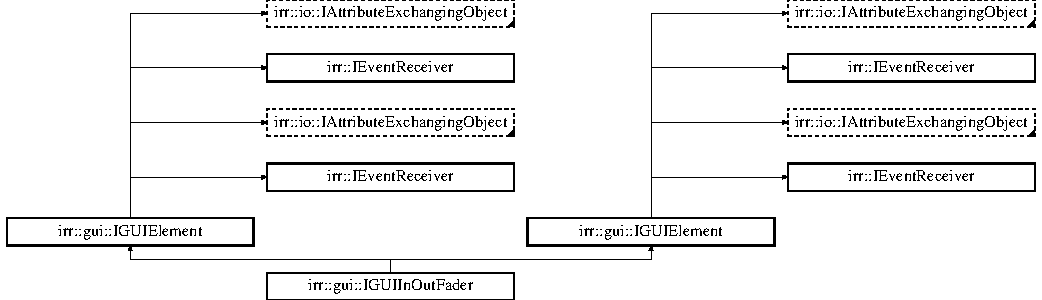
\includegraphics[height=4.038462cm]{classirr_1_1gui_1_1IGUIInOutFader}
\end{center}
\end{figure}
\subsection*{Public Member Functions}
\begin{DoxyCompactItemize}
\item 
\mbox{\Hypertarget{classirr_1_1gui_1_1IGUIInOutFader_ad839c9be778846aa0fba823c7dd30c69}\label{classirr_1_1gui_1_1IGUIInOutFader_ad839c9be778846aa0fba823c7dd30c69}} 
\hyperlink{classirr_1_1gui_1_1IGUIInOutFader_ad839c9be778846aa0fba823c7dd30c69}{I\+G\+U\+I\+In\+Out\+Fader} (\hyperlink{classirr_1_1gui_1_1IGUIEnvironment}{I\+G\+U\+I\+Environment} $\ast$environment, \hyperlink{classirr_1_1gui_1_1IGUIElement}{I\+G\+U\+I\+Element} $\ast$parent, \hyperlink{namespaceirr_ac66849b7a6ed16e30ebede579f9b47c6}{s32} id, \hyperlink{classirr_1_1core_1_1rect}{core\+::rect}$<$ \hyperlink{namespaceirr_ac66849b7a6ed16e30ebede579f9b47c6}{s32} $>$ rectangle)
\begin{DoxyCompactList}\small\item\em constructor \end{DoxyCompactList}\item 
\mbox{\Hypertarget{classirr_1_1gui_1_1IGUIInOutFader_adeed9c5ffd4b9ab6180cba40596742b9}\label{classirr_1_1gui_1_1IGUIInOutFader_adeed9c5ffd4b9ab6180cba40596742b9}} 
virtual \hyperlink{classirr_1_1video_1_1SColor}{video\+::\+S\+Color} \hyperlink{classirr_1_1gui_1_1IGUIInOutFader_adeed9c5ffd4b9ab6180cba40596742b9}{get\+Color} () const =0
\begin{DoxyCompactList}\small\item\em Gets the color to fade out to or to fade in from. \end{DoxyCompactList}\item 
virtual void \hyperlink{classirr_1_1gui_1_1IGUIInOutFader_aba1cdb4928662a2340aa6600850e03d1}{set\+Color} (\hyperlink{classirr_1_1video_1_1SColor}{video\+::\+S\+Color} color)=0
\begin{DoxyCompactList}\small\item\em Sets the color to fade out to or to fade in from. \end{DoxyCompactList}\item 
virtual void \hyperlink{classirr_1_1gui_1_1IGUIInOutFader_a407edab8f7e349612d62c39accc159e2}{fade\+In} (\hyperlink{namespaceirr_a0416a53257075833e7002efd0a18e804}{u32} time)=0
\begin{DoxyCompactList}\small\item\em Starts the fade in process. \end{DoxyCompactList}\item 
virtual void \hyperlink{classirr_1_1gui_1_1IGUIInOutFader_a5006c28699050d73be11b15ffc7ba993}{fade\+Out} (\hyperlink{namespaceirr_a0416a53257075833e7002efd0a18e804}{u32} time)=0
\begin{DoxyCompactList}\small\item\em Starts the fade out process. \end{DoxyCompactList}\item 
\mbox{\Hypertarget{classirr_1_1gui_1_1IGUIInOutFader_a8a917f7c5c74ff0bdb2ba844f1953387}\label{classirr_1_1gui_1_1IGUIInOutFader_a8a917f7c5c74ff0bdb2ba844f1953387}} 
virtual bool \hyperlink{classirr_1_1gui_1_1IGUIInOutFader_a8a917f7c5c74ff0bdb2ba844f1953387}{is\+Ready} () const =0
\begin{DoxyCompactList}\small\item\em Returns if the fade in or out process is done. \end{DoxyCompactList}\item 
\mbox{\Hypertarget{classirr_1_1gui_1_1IGUIInOutFader_ad839c9be778846aa0fba823c7dd30c69}\label{classirr_1_1gui_1_1IGUIInOutFader_ad839c9be778846aa0fba823c7dd30c69}} 
\hyperlink{classirr_1_1gui_1_1IGUIInOutFader_ad839c9be778846aa0fba823c7dd30c69}{I\+G\+U\+I\+In\+Out\+Fader} (\hyperlink{classirr_1_1gui_1_1IGUIEnvironment}{I\+G\+U\+I\+Environment} $\ast$environment, \hyperlink{classirr_1_1gui_1_1IGUIElement}{I\+G\+U\+I\+Element} $\ast$parent, \hyperlink{namespaceirr_ac66849b7a6ed16e30ebede579f9b47c6}{s32} id, \hyperlink{classirr_1_1core_1_1rect}{core\+::rect}$<$ \hyperlink{namespaceirr_ac66849b7a6ed16e30ebede579f9b47c6}{s32} $>$ rectangle)
\begin{DoxyCompactList}\small\item\em constructor \end{DoxyCompactList}\item 
\mbox{\Hypertarget{classirr_1_1gui_1_1IGUIInOutFader_adeed9c5ffd4b9ab6180cba40596742b9}\label{classirr_1_1gui_1_1IGUIInOutFader_adeed9c5ffd4b9ab6180cba40596742b9}} 
virtual \hyperlink{classirr_1_1video_1_1SColor}{video\+::\+S\+Color} \hyperlink{classirr_1_1gui_1_1IGUIInOutFader_adeed9c5ffd4b9ab6180cba40596742b9}{get\+Color} () const =0
\begin{DoxyCompactList}\small\item\em Gets the color to fade out to or to fade in from. \end{DoxyCompactList}\item 
virtual void \hyperlink{classirr_1_1gui_1_1IGUIInOutFader_aba1cdb4928662a2340aa6600850e03d1}{set\+Color} (\hyperlink{classirr_1_1video_1_1SColor}{video\+::\+S\+Color} color)=0
\begin{DoxyCompactList}\small\item\em Sets the color to fade out to or to fade in from. \end{DoxyCompactList}\item 
virtual void \hyperlink{classirr_1_1gui_1_1IGUIInOutFader_a407edab8f7e349612d62c39accc159e2}{fade\+In} (\hyperlink{namespaceirr_a0416a53257075833e7002efd0a18e804}{u32} time)=0
\begin{DoxyCompactList}\small\item\em Starts the fade in process. \end{DoxyCompactList}\item 
virtual void \hyperlink{classirr_1_1gui_1_1IGUIInOutFader_a5006c28699050d73be11b15ffc7ba993}{fade\+Out} (\hyperlink{namespaceirr_a0416a53257075833e7002efd0a18e804}{u32} time)=0
\begin{DoxyCompactList}\small\item\em Starts the fade out process. \end{DoxyCompactList}\item 
\mbox{\Hypertarget{classirr_1_1gui_1_1IGUIInOutFader_a8a917f7c5c74ff0bdb2ba844f1953387}\label{classirr_1_1gui_1_1IGUIInOutFader_a8a917f7c5c74ff0bdb2ba844f1953387}} 
virtual bool \hyperlink{classirr_1_1gui_1_1IGUIInOutFader_a8a917f7c5c74ff0bdb2ba844f1953387}{is\+Ready} () const =0
\begin{DoxyCompactList}\small\item\em Returns if the fade in or out process is done. \end{DoxyCompactList}\end{DoxyCompactItemize}
\subsection*{Additional Inherited Members}


\subsection{Detailed Description}
Element for fading out or in. 

Here is a small example on how the class is used. In this example we fade in from a total red screen in the beginning. As you can see, the fader is not only useful for dramatic in and out fading, but also to show that the player is hit in a first person shooter game for example. 
\begin{DoxyCode}
gui::IGUIInOutFader* fader = device->getGUIEnvironment()->addInOutFader();
fader->setColor(video::SColor(0,255,0,0));
fader->fadeIn(4000);
\end{DoxyCode}
 

\subsection{Member Function Documentation}
\mbox{\Hypertarget{classirr_1_1gui_1_1IGUIInOutFader_a407edab8f7e349612d62c39accc159e2}\label{classirr_1_1gui_1_1IGUIInOutFader_a407edab8f7e349612d62c39accc159e2}} 
\index{irr\+::gui\+::\+I\+G\+U\+I\+In\+Out\+Fader@{irr\+::gui\+::\+I\+G\+U\+I\+In\+Out\+Fader}!fade\+In@{fade\+In}}
\index{fade\+In@{fade\+In}!irr\+::gui\+::\+I\+G\+U\+I\+In\+Out\+Fader@{irr\+::gui\+::\+I\+G\+U\+I\+In\+Out\+Fader}}
\subsubsection{\texorpdfstring{fade\+In()}{fadeIn()}\hspace{0.1cm}{\footnotesize\ttfamily [1/2]}}
{\footnotesize\ttfamily virtual void irr\+::gui\+::\+I\+G\+U\+I\+In\+Out\+Fader\+::fade\+In (\begin{DoxyParamCaption}\item[{\hyperlink{namespaceirr_a0416a53257075833e7002efd0a18e804}{u32}}]{time }\end{DoxyParamCaption})\hspace{0.3cm}{\ttfamily [pure virtual]}}



Starts the fade in process. 

In the beginning the whole rect is drawn by the set color (black by default) and at the end of the overgiven time the color has faded out. 
\begin{DoxyParams}{Parameters}
{\em time} & Time specifying how long it should need to fade in, in milliseconds. \\
\hline
\end{DoxyParams}
\mbox{\Hypertarget{classirr_1_1gui_1_1IGUIInOutFader_a407edab8f7e349612d62c39accc159e2}\label{classirr_1_1gui_1_1IGUIInOutFader_a407edab8f7e349612d62c39accc159e2}} 
\index{irr\+::gui\+::\+I\+G\+U\+I\+In\+Out\+Fader@{irr\+::gui\+::\+I\+G\+U\+I\+In\+Out\+Fader}!fade\+In@{fade\+In}}
\index{fade\+In@{fade\+In}!irr\+::gui\+::\+I\+G\+U\+I\+In\+Out\+Fader@{irr\+::gui\+::\+I\+G\+U\+I\+In\+Out\+Fader}}
\subsubsection{\texorpdfstring{fade\+In()}{fadeIn()}\hspace{0.1cm}{\footnotesize\ttfamily [2/2]}}
{\footnotesize\ttfamily virtual void irr\+::gui\+::\+I\+G\+U\+I\+In\+Out\+Fader\+::fade\+In (\begin{DoxyParamCaption}\item[{\hyperlink{namespaceirr_a0416a53257075833e7002efd0a18e804}{u32}}]{time }\end{DoxyParamCaption})\hspace{0.3cm}{\ttfamily [pure virtual]}}



Starts the fade in process. 

In the beginning the whole rect is drawn by the set color (black by default) and at the end of the overgiven time the color has faded out. 
\begin{DoxyParams}{Parameters}
{\em time} & Time specifying how long it should need to fade in, in milliseconds. \\
\hline
\end{DoxyParams}
\mbox{\Hypertarget{classirr_1_1gui_1_1IGUIInOutFader_a5006c28699050d73be11b15ffc7ba993}\label{classirr_1_1gui_1_1IGUIInOutFader_a5006c28699050d73be11b15ffc7ba993}} 
\index{irr\+::gui\+::\+I\+G\+U\+I\+In\+Out\+Fader@{irr\+::gui\+::\+I\+G\+U\+I\+In\+Out\+Fader}!fade\+Out@{fade\+Out}}
\index{fade\+Out@{fade\+Out}!irr\+::gui\+::\+I\+G\+U\+I\+In\+Out\+Fader@{irr\+::gui\+::\+I\+G\+U\+I\+In\+Out\+Fader}}
\subsubsection{\texorpdfstring{fade\+Out()}{fadeOut()}\hspace{0.1cm}{\footnotesize\ttfamily [1/2]}}
{\footnotesize\ttfamily virtual void irr\+::gui\+::\+I\+G\+U\+I\+In\+Out\+Fader\+::fade\+Out (\begin{DoxyParamCaption}\item[{\hyperlink{namespaceirr_a0416a53257075833e7002efd0a18e804}{u32}}]{time }\end{DoxyParamCaption})\hspace{0.3cm}{\ttfamily [pure virtual]}}



Starts the fade out process. 

In the beginning everything is visible, and at the end of the time only the set color (black by the fault) will be drawn. 
\begin{DoxyParams}{Parameters}
{\em time} & Time specifying how long it should need to fade out, in milliseconds. \\
\hline
\end{DoxyParams}
\mbox{\Hypertarget{classirr_1_1gui_1_1IGUIInOutFader_a5006c28699050d73be11b15ffc7ba993}\label{classirr_1_1gui_1_1IGUIInOutFader_a5006c28699050d73be11b15ffc7ba993}} 
\index{irr\+::gui\+::\+I\+G\+U\+I\+In\+Out\+Fader@{irr\+::gui\+::\+I\+G\+U\+I\+In\+Out\+Fader}!fade\+Out@{fade\+Out}}
\index{fade\+Out@{fade\+Out}!irr\+::gui\+::\+I\+G\+U\+I\+In\+Out\+Fader@{irr\+::gui\+::\+I\+G\+U\+I\+In\+Out\+Fader}}
\subsubsection{\texorpdfstring{fade\+Out()}{fadeOut()}\hspace{0.1cm}{\footnotesize\ttfamily [2/2]}}
{\footnotesize\ttfamily virtual void irr\+::gui\+::\+I\+G\+U\+I\+In\+Out\+Fader\+::fade\+Out (\begin{DoxyParamCaption}\item[{\hyperlink{namespaceirr_a0416a53257075833e7002efd0a18e804}{u32}}]{time }\end{DoxyParamCaption})\hspace{0.3cm}{\ttfamily [pure virtual]}}



Starts the fade out process. 

In the beginning everything is visible, and at the end of the time only the set color (black by the fault) will be drawn. 
\begin{DoxyParams}{Parameters}
{\em time} & Time specifying how long it should need to fade out, in milliseconds. \\
\hline
\end{DoxyParams}
\mbox{\Hypertarget{classirr_1_1gui_1_1IGUIInOutFader_aba1cdb4928662a2340aa6600850e03d1}\label{classirr_1_1gui_1_1IGUIInOutFader_aba1cdb4928662a2340aa6600850e03d1}} 
\index{irr\+::gui\+::\+I\+G\+U\+I\+In\+Out\+Fader@{irr\+::gui\+::\+I\+G\+U\+I\+In\+Out\+Fader}!set\+Color@{set\+Color}}
\index{set\+Color@{set\+Color}!irr\+::gui\+::\+I\+G\+U\+I\+In\+Out\+Fader@{irr\+::gui\+::\+I\+G\+U\+I\+In\+Out\+Fader}}
\subsubsection{\texorpdfstring{set\+Color()}{setColor()}\hspace{0.1cm}{\footnotesize\ttfamily [1/2]}}
{\footnotesize\ttfamily virtual void irr\+::gui\+::\+I\+G\+U\+I\+In\+Out\+Fader\+::set\+Color (\begin{DoxyParamCaption}\item[{\hyperlink{classirr_1_1video_1_1SColor}{video\+::\+S\+Color}}]{color }\end{DoxyParamCaption})\hspace{0.3cm}{\ttfamily [pure virtual]}}



Sets the color to fade out to or to fade in from. 


\begin{DoxyParams}{Parameters}
{\em color} & Color to where it is faded out od from it is faded in. \\
\hline
\end{DoxyParams}
\mbox{\Hypertarget{classirr_1_1gui_1_1IGUIInOutFader_aba1cdb4928662a2340aa6600850e03d1}\label{classirr_1_1gui_1_1IGUIInOutFader_aba1cdb4928662a2340aa6600850e03d1}} 
\index{irr\+::gui\+::\+I\+G\+U\+I\+In\+Out\+Fader@{irr\+::gui\+::\+I\+G\+U\+I\+In\+Out\+Fader}!set\+Color@{set\+Color}}
\index{set\+Color@{set\+Color}!irr\+::gui\+::\+I\+G\+U\+I\+In\+Out\+Fader@{irr\+::gui\+::\+I\+G\+U\+I\+In\+Out\+Fader}}
\subsubsection{\texorpdfstring{set\+Color()}{setColor()}\hspace{0.1cm}{\footnotesize\ttfamily [2/2]}}
{\footnotesize\ttfamily virtual void irr\+::gui\+::\+I\+G\+U\+I\+In\+Out\+Fader\+::set\+Color (\begin{DoxyParamCaption}\item[{\hyperlink{classirr_1_1video_1_1SColor}{video\+::\+S\+Color}}]{color }\end{DoxyParamCaption})\hspace{0.3cm}{\ttfamily [pure virtual]}}



Sets the color to fade out to or to fade in from. 


\begin{DoxyParams}{Parameters}
{\em color} & Color to where it is faded out od from it is faded in. \\
\hline
\end{DoxyParams}


The documentation for this class was generated from the following file\+:\begin{DoxyCompactItemize}
\item 
indie\+\_\+share/controller/include/I\+G\+U\+I\+In\+Out\+Fader.\+h\end{DoxyCompactItemize}

\hypertarget{classirr_1_1gui_1_1IGUIListBox}{}\section{irr\+:\+:gui\+:\+:I\+G\+U\+I\+List\+Box Class Reference}
\label{classirr_1_1gui_1_1IGUIListBox}\index{irr\+::gui\+::\+I\+G\+U\+I\+List\+Box@{irr\+::gui\+::\+I\+G\+U\+I\+List\+Box}}


Default list box G\+UI element.  




{\ttfamily \#include $<$I\+G\+U\+I\+List\+Box.\+h$>$}

Inheritance diagram for irr\+:\+:gui\+:\+:I\+G\+U\+I\+List\+Box\+:\begin{figure}[H]
\begin{center}
\leavevmode
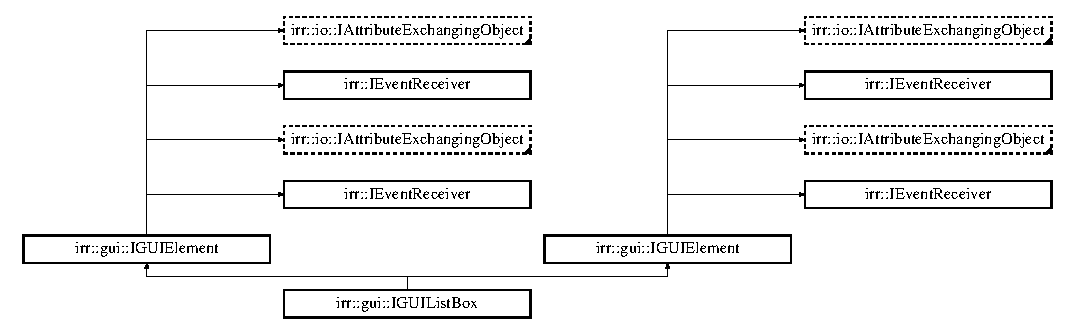
\includegraphics[height=4.038462cm]{classirr_1_1gui_1_1IGUIListBox}
\end{center}
\end{figure}
\subsection*{Public Member Functions}
\begin{DoxyCompactItemize}
\item 
\mbox{\Hypertarget{classirr_1_1gui_1_1IGUIListBox_a6f6e6a84f3d2035a0874eb9f4a4d52ef}\label{classirr_1_1gui_1_1IGUIListBox_a6f6e6a84f3d2035a0874eb9f4a4d52ef}} 
\hyperlink{classirr_1_1gui_1_1IGUIListBox_a6f6e6a84f3d2035a0874eb9f4a4d52ef}{I\+G\+U\+I\+List\+Box} (\hyperlink{classirr_1_1gui_1_1IGUIEnvironment}{I\+G\+U\+I\+Environment} $\ast$environment, \hyperlink{classirr_1_1gui_1_1IGUIElement}{I\+G\+U\+I\+Element} $\ast$parent, \hyperlink{namespaceirr_ac66849b7a6ed16e30ebede579f9b47c6}{s32} id, \hyperlink{classirr_1_1core_1_1rect}{core\+::rect}$<$ \hyperlink{namespaceirr_ac66849b7a6ed16e30ebede579f9b47c6}{s32} $>$ rectangle)
\begin{DoxyCompactList}\small\item\em constructor \end{DoxyCompactList}\item 
\mbox{\Hypertarget{classirr_1_1gui_1_1IGUIListBox_a9ae7e4858dd1dee26efab7e7c9c94ab7}\label{classirr_1_1gui_1_1IGUIListBox_a9ae7e4858dd1dee26efab7e7c9c94ab7}} 
virtual \hyperlink{namespaceirr_a0416a53257075833e7002efd0a18e804}{u32} \hyperlink{classirr_1_1gui_1_1IGUIListBox_a9ae7e4858dd1dee26efab7e7c9c94ab7}{get\+Item\+Count} () const =0
\begin{DoxyCompactList}\small\item\em returns amount of list items \end{DoxyCompactList}\item 
\mbox{\Hypertarget{classirr_1_1gui_1_1IGUIListBox_af68ea08c93b0959ea464146bc1f4d82f}\label{classirr_1_1gui_1_1IGUIListBox_af68ea08c93b0959ea464146bc1f4d82f}} 
virtual const wchar\+\_\+t $\ast$ \hyperlink{classirr_1_1gui_1_1IGUIListBox_af68ea08c93b0959ea464146bc1f4d82f}{get\+List\+Item} (\hyperlink{namespaceirr_a0416a53257075833e7002efd0a18e804}{u32} id) const =0
\begin{DoxyCompactList}\small\item\em returns string of a list item. the may id be a value from 0 to item\+Count-\/1 \end{DoxyCompactList}\item 
\mbox{\Hypertarget{classirr_1_1gui_1_1IGUIListBox_a298dbba8da28248b563a906c520dc3be}\label{classirr_1_1gui_1_1IGUIListBox_a298dbba8da28248b563a906c520dc3be}} 
virtual \hyperlink{namespaceirr_a0416a53257075833e7002efd0a18e804}{u32} \hyperlink{classirr_1_1gui_1_1IGUIListBox_a298dbba8da28248b563a906c520dc3be}{add\+Item} (const wchar\+\_\+t $\ast$text)=0
\begin{DoxyCompactList}\small\item\em adds an list item, returns id of item \end{DoxyCompactList}\item 
virtual \hyperlink{namespaceirr_a0416a53257075833e7002efd0a18e804}{u32} \hyperlink{classirr_1_1gui_1_1IGUIListBox_a2cfc2ff5f8f5114a92bd3618e79327e0}{add\+Item} (const wchar\+\_\+t $\ast$text, \hyperlink{namespaceirr_ac66849b7a6ed16e30ebede579f9b47c6}{s32} icon)=0
\begin{DoxyCompactList}\small\item\em adds an list item with an icon \end{DoxyCompactList}\item 
\mbox{\Hypertarget{classirr_1_1gui_1_1IGUIListBox_a6c19c6db0bcf52756d9bb866063a770b}\label{classirr_1_1gui_1_1IGUIListBox_a6c19c6db0bcf52756d9bb866063a770b}} 
virtual void \hyperlink{classirr_1_1gui_1_1IGUIListBox_a6c19c6db0bcf52756d9bb866063a770b}{remove\+Item} (\hyperlink{namespaceirr_a0416a53257075833e7002efd0a18e804}{u32} index)=0
\begin{DoxyCompactList}\small\item\em Removes an item from the list. \end{DoxyCompactList}\item 
virtual \hyperlink{namespaceirr_ac66849b7a6ed16e30ebede579f9b47c6}{s32} \hyperlink{classirr_1_1gui_1_1IGUIListBox_a8e1fe86805d9b970b89878291f0ccd25}{get\+Item\+At} (\hyperlink{namespaceirr_ac66849b7a6ed16e30ebede579f9b47c6}{s32} xpos, \hyperlink{namespaceirr_ac66849b7a6ed16e30ebede579f9b47c6}{s32} ypos) const =0
\begin{DoxyCompactList}\small\item\em get the the id of the item at the given absolute coordinates \end{DoxyCompactList}\item 
\mbox{\Hypertarget{classirr_1_1gui_1_1IGUIListBox_a8e5f9751a7a1a32dde5a243733b3ddc6}\label{classirr_1_1gui_1_1IGUIListBox_a8e5f9751a7a1a32dde5a243733b3ddc6}} 
virtual \hyperlink{namespaceirr_ac66849b7a6ed16e30ebede579f9b47c6}{s32} \hyperlink{classirr_1_1gui_1_1IGUIListBox_a8e5f9751a7a1a32dde5a243733b3ddc6}{get\+Icon} (\hyperlink{namespaceirr_a0416a53257075833e7002efd0a18e804}{u32} index) const =0
\begin{DoxyCompactList}\small\item\em Returns the icon of an item. \end{DoxyCompactList}\item 
virtual void \hyperlink{classirr_1_1gui_1_1IGUIListBox_ad139cef6f71bb8d36624b48e8a695ed4}{set\+Sprite\+Bank} (\hyperlink{classirr_1_1gui_1_1IGUISpriteBank}{I\+G\+U\+I\+Sprite\+Bank} $\ast$bank)=0
\begin{DoxyCompactList}\small\item\em Sets the sprite bank which should be used to draw list icons. \end{DoxyCompactList}\item 
\mbox{\Hypertarget{classirr_1_1gui_1_1IGUIListBox_aaffa1f9f823dbb254c1901dba67e31c4}\label{classirr_1_1gui_1_1IGUIListBox_aaffa1f9f823dbb254c1901dba67e31c4}} 
virtual void \hyperlink{classirr_1_1gui_1_1IGUIListBox_aaffa1f9f823dbb254c1901dba67e31c4}{clear} ()=0
\begin{DoxyCompactList}\small\item\em clears the list, deletes all items in the listbox \end{DoxyCompactList}\item 
\mbox{\Hypertarget{classirr_1_1gui_1_1IGUIListBox_a321626d92d63ce5c309466201a02b12d}\label{classirr_1_1gui_1_1IGUIListBox_a321626d92d63ce5c309466201a02b12d}} 
virtual \hyperlink{namespaceirr_ac66849b7a6ed16e30ebede579f9b47c6}{s32} \hyperlink{classirr_1_1gui_1_1IGUIListBox_a321626d92d63ce5c309466201a02b12d}{get\+Selected} () const =0
\begin{DoxyCompactList}\small\item\em returns id of selected item. returns -\/1 if no item is selected. \end{DoxyCompactList}\item 
\mbox{\Hypertarget{classirr_1_1gui_1_1IGUIListBox_ac981fa5b285115333b67202819230f6f}\label{classirr_1_1gui_1_1IGUIListBox_ac981fa5b285115333b67202819230f6f}} 
virtual void \hyperlink{classirr_1_1gui_1_1IGUIListBox_ac981fa5b285115333b67202819230f6f}{set\+Selected} (\hyperlink{namespaceirr_ac66849b7a6ed16e30ebede579f9b47c6}{s32} index)=0
\begin{DoxyCompactList}\small\item\em sets the selected item. Set this to -\/1 if no item should be selected \end{DoxyCompactList}\item 
\mbox{\Hypertarget{classirr_1_1gui_1_1IGUIListBox_aa6031e2a0ecbcfe80484d8271b1c9529}\label{classirr_1_1gui_1_1IGUIListBox_aa6031e2a0ecbcfe80484d8271b1c9529}} 
virtual void \hyperlink{classirr_1_1gui_1_1IGUIListBox_aa6031e2a0ecbcfe80484d8271b1c9529}{set\+Selected} (const wchar\+\_\+t $\ast$item)=0
\begin{DoxyCompactList}\small\item\em sets the selected item. Set this to 0 if no item should be selected \end{DoxyCompactList}\item 
\mbox{\Hypertarget{classirr_1_1gui_1_1IGUIListBox_a4d8ada56cafff847e98564283b2d06ac}\label{classirr_1_1gui_1_1IGUIListBox_a4d8ada56cafff847e98564283b2d06ac}} 
virtual void \hyperlink{classirr_1_1gui_1_1IGUIListBox_a4d8ada56cafff847e98564283b2d06ac}{set\+Auto\+Scroll\+Enabled} (bool scroll)=0
\begin{DoxyCompactList}\small\item\em set whether the listbox should scroll to newly selected items \end{DoxyCompactList}\item 
\mbox{\Hypertarget{classirr_1_1gui_1_1IGUIListBox_af04876e1e3173e9c13bb099076743137}\label{classirr_1_1gui_1_1IGUIListBox_af04876e1e3173e9c13bb099076743137}} 
virtual bool \hyperlink{classirr_1_1gui_1_1IGUIListBox_af04876e1e3173e9c13bb099076743137}{is\+Auto\+Scroll\+Enabled} () const =0
\begin{DoxyCompactList}\small\item\em returns true if automatic scrolling is enabled, false if not. \end{DoxyCompactList}\item 
\mbox{\Hypertarget{classirr_1_1gui_1_1IGUIListBox_ae2f09b02e7428175e13fa6b3216ced67}\label{classirr_1_1gui_1_1IGUIListBox_ae2f09b02e7428175e13fa6b3216ced67}} 
virtual void \hyperlink{classirr_1_1gui_1_1IGUIListBox_ae2f09b02e7428175e13fa6b3216ced67}{set\+Item\+Override\+Color} (\hyperlink{namespaceirr_a0416a53257075833e7002efd0a18e804}{u32} index, \hyperlink{classirr_1_1video_1_1SColor}{video\+::\+S\+Color} color)=0
\begin{DoxyCompactList}\small\item\em set all item colors at given index to color \end{DoxyCompactList}\item 
\mbox{\Hypertarget{classirr_1_1gui_1_1IGUIListBox_a84444d888931d79dcc50a8f229aad2c7}\label{classirr_1_1gui_1_1IGUIListBox_a84444d888931d79dcc50a8f229aad2c7}} 
virtual void \hyperlink{classirr_1_1gui_1_1IGUIListBox_a84444d888931d79dcc50a8f229aad2c7}{set\+Item\+Override\+Color} (\hyperlink{namespaceirr_a0416a53257075833e7002efd0a18e804}{u32} index, \hyperlink{namespaceirr_1_1gui_a7da705f0a0b4aa5385e6842adf409cb6}{E\+G\+U\+I\+\_\+\+L\+I\+S\+T\+B\+O\+X\+\_\+\+C\+O\+L\+OR} color\+Type, \hyperlink{classirr_1_1video_1_1SColor}{video\+::\+S\+Color} color)=0
\begin{DoxyCompactList}\small\item\em set all item colors of specified type at given index to color \end{DoxyCompactList}\item 
\mbox{\Hypertarget{classirr_1_1gui_1_1IGUIListBox_aca681d4d4814cde0678109e3bce2471e}\label{classirr_1_1gui_1_1IGUIListBox_aca681d4d4814cde0678109e3bce2471e}} 
virtual void \hyperlink{classirr_1_1gui_1_1IGUIListBox_aca681d4d4814cde0678109e3bce2471e}{clear\+Item\+Override\+Color} (\hyperlink{namespaceirr_a0416a53257075833e7002efd0a18e804}{u32} index)=0
\begin{DoxyCompactList}\small\item\em clear all item colors at index \end{DoxyCompactList}\item 
\mbox{\Hypertarget{classirr_1_1gui_1_1IGUIListBox_aa0bb8fd96be94e8de5d4496b7d5e2ffd}\label{classirr_1_1gui_1_1IGUIListBox_aa0bb8fd96be94e8de5d4496b7d5e2ffd}} 
virtual void \hyperlink{classirr_1_1gui_1_1IGUIListBox_aa0bb8fd96be94e8de5d4496b7d5e2ffd}{clear\+Item\+Override\+Color} (\hyperlink{namespaceirr_a0416a53257075833e7002efd0a18e804}{u32} index, \hyperlink{namespaceirr_1_1gui_a7da705f0a0b4aa5385e6842adf409cb6}{E\+G\+U\+I\+\_\+\+L\+I\+S\+T\+B\+O\+X\+\_\+\+C\+O\+L\+OR} color\+Type)=0
\begin{DoxyCompactList}\small\item\em clear item color at index for given colortype \end{DoxyCompactList}\item 
\mbox{\Hypertarget{classirr_1_1gui_1_1IGUIListBox_a8399578154c3cbfcdd23f3b7009c448d}\label{classirr_1_1gui_1_1IGUIListBox_a8399578154c3cbfcdd23f3b7009c448d}} 
virtual bool \hyperlink{classirr_1_1gui_1_1IGUIListBox_a8399578154c3cbfcdd23f3b7009c448d}{has\+Item\+Override\+Color} (\hyperlink{namespaceirr_a0416a53257075833e7002efd0a18e804}{u32} index, \hyperlink{namespaceirr_1_1gui_a7da705f0a0b4aa5385e6842adf409cb6}{E\+G\+U\+I\+\_\+\+L\+I\+S\+T\+B\+O\+X\+\_\+\+C\+O\+L\+OR} color\+Type) const =0
\begin{DoxyCompactList}\small\item\em has the item at index its color overwritten? \end{DoxyCompactList}\item 
\mbox{\Hypertarget{classirr_1_1gui_1_1IGUIListBox_a504c669eae86307521b643288c4ef196}\label{classirr_1_1gui_1_1IGUIListBox_a504c669eae86307521b643288c4ef196}} 
virtual \hyperlink{classirr_1_1video_1_1SColor}{video\+::\+S\+Color} \hyperlink{classirr_1_1gui_1_1IGUIListBox_a504c669eae86307521b643288c4ef196}{get\+Item\+Override\+Color} (\hyperlink{namespaceirr_a0416a53257075833e7002efd0a18e804}{u32} index, \hyperlink{namespaceirr_1_1gui_a7da705f0a0b4aa5385e6842adf409cb6}{E\+G\+U\+I\+\_\+\+L\+I\+S\+T\+B\+O\+X\+\_\+\+C\+O\+L\+OR} color\+Type) const =0
\begin{DoxyCompactList}\small\item\em return the overwrite color at given item index. \end{DoxyCompactList}\item 
\mbox{\Hypertarget{classirr_1_1gui_1_1IGUIListBox_ae755a88721a458b3255df08519b72e85}\label{classirr_1_1gui_1_1IGUIListBox_ae755a88721a458b3255df08519b72e85}} 
virtual \hyperlink{classirr_1_1video_1_1SColor}{video\+::\+S\+Color} \hyperlink{classirr_1_1gui_1_1IGUIListBox_ae755a88721a458b3255df08519b72e85}{get\+Item\+Default\+Color} (\hyperlink{namespaceirr_1_1gui_a7da705f0a0b4aa5385e6842adf409cb6}{E\+G\+U\+I\+\_\+\+L\+I\+S\+T\+B\+O\+X\+\_\+\+C\+O\+L\+OR} color\+Type) const =0
\begin{DoxyCompactList}\small\item\em return the default color which is used for the given color\+Type \end{DoxyCompactList}\item 
\mbox{\Hypertarget{classirr_1_1gui_1_1IGUIListBox_a643ca28110a7de59a378e5ba79b1c37a}\label{classirr_1_1gui_1_1IGUIListBox_a643ca28110a7de59a378e5ba79b1c37a}} 
virtual void \hyperlink{classirr_1_1gui_1_1IGUIListBox_a643ca28110a7de59a378e5ba79b1c37a}{set\+Item} (\hyperlink{namespaceirr_a0416a53257075833e7002efd0a18e804}{u32} index, const wchar\+\_\+t $\ast$text, \hyperlink{namespaceirr_ac66849b7a6ed16e30ebede579f9b47c6}{s32} icon)=0
\begin{DoxyCompactList}\small\item\em set the item at the given index \end{DoxyCompactList}\item 
virtual \hyperlink{namespaceirr_ac66849b7a6ed16e30ebede579f9b47c6}{s32} \hyperlink{classirr_1_1gui_1_1IGUIListBox_a1da5cc33687efee5ff1e33ab9f0d5b26}{insert\+Item} (\hyperlink{namespaceirr_a0416a53257075833e7002efd0a18e804}{u32} index, const wchar\+\_\+t $\ast$text, \hyperlink{namespaceirr_ac66849b7a6ed16e30ebede579f9b47c6}{s32} icon)=0
\begin{DoxyCompactList}\small\item\em Insert the item at the given index. \end{DoxyCompactList}\item 
\mbox{\Hypertarget{classirr_1_1gui_1_1IGUIListBox_accb47d6f72558ea5d3034b3e4e4ccd81}\label{classirr_1_1gui_1_1IGUIListBox_accb47d6f72558ea5d3034b3e4e4ccd81}} 
virtual void \hyperlink{classirr_1_1gui_1_1IGUIListBox_accb47d6f72558ea5d3034b3e4e4ccd81}{swap\+Items} (\hyperlink{namespaceirr_a0416a53257075833e7002efd0a18e804}{u32} index1, \hyperlink{namespaceirr_a0416a53257075833e7002efd0a18e804}{u32} index2)=0
\begin{DoxyCompactList}\small\item\em Swap the items at the given indices. \end{DoxyCompactList}\item 
\mbox{\Hypertarget{classirr_1_1gui_1_1IGUIListBox_a83fb9c6f32039a39197cf799dd5e0c8f}\label{classirr_1_1gui_1_1IGUIListBox_a83fb9c6f32039a39197cf799dd5e0c8f}} 
virtual void \hyperlink{classirr_1_1gui_1_1IGUIListBox_a83fb9c6f32039a39197cf799dd5e0c8f}{set\+Item\+Height} (\hyperlink{namespaceirr_ac66849b7a6ed16e30ebede579f9b47c6}{s32} height)=0
\begin{DoxyCompactList}\small\item\em set global item\+Height \end{DoxyCompactList}\item 
\mbox{\Hypertarget{classirr_1_1gui_1_1IGUIListBox_ad323fdf0b083dbc1870d7fa5869cff8f}\label{classirr_1_1gui_1_1IGUIListBox_ad323fdf0b083dbc1870d7fa5869cff8f}} 
virtual void \hyperlink{classirr_1_1gui_1_1IGUIListBox_ad323fdf0b083dbc1870d7fa5869cff8f}{set\+Draw\+Background} (bool \hyperlink{classirr_1_1gui_1_1IGUIElement_a1ef7eeaff67b8a9f4f37cacdc7e54be2}{draw})=0
\begin{DoxyCompactList}\small\item\em Sets whether to draw the background. \end{DoxyCompactList}\item 
\mbox{\Hypertarget{classirr_1_1gui_1_1IGUIListBox_a6f6e6a84f3d2035a0874eb9f4a4d52ef}\label{classirr_1_1gui_1_1IGUIListBox_a6f6e6a84f3d2035a0874eb9f4a4d52ef}} 
\hyperlink{classirr_1_1gui_1_1IGUIListBox_a6f6e6a84f3d2035a0874eb9f4a4d52ef}{I\+G\+U\+I\+List\+Box} (\hyperlink{classirr_1_1gui_1_1IGUIEnvironment}{I\+G\+U\+I\+Environment} $\ast$environment, \hyperlink{classirr_1_1gui_1_1IGUIElement}{I\+G\+U\+I\+Element} $\ast$parent, \hyperlink{namespaceirr_ac66849b7a6ed16e30ebede579f9b47c6}{s32} id, \hyperlink{classirr_1_1core_1_1rect}{core\+::rect}$<$ \hyperlink{namespaceirr_ac66849b7a6ed16e30ebede579f9b47c6}{s32} $>$ rectangle)
\begin{DoxyCompactList}\small\item\em constructor \end{DoxyCompactList}\item 
\mbox{\Hypertarget{classirr_1_1gui_1_1IGUIListBox_a9ae7e4858dd1dee26efab7e7c9c94ab7}\label{classirr_1_1gui_1_1IGUIListBox_a9ae7e4858dd1dee26efab7e7c9c94ab7}} 
virtual \hyperlink{namespaceirr_a0416a53257075833e7002efd0a18e804}{u32} \hyperlink{classirr_1_1gui_1_1IGUIListBox_a9ae7e4858dd1dee26efab7e7c9c94ab7}{get\+Item\+Count} () const =0
\begin{DoxyCompactList}\small\item\em returns amount of list items \end{DoxyCompactList}\item 
\mbox{\Hypertarget{classirr_1_1gui_1_1IGUIListBox_af68ea08c93b0959ea464146bc1f4d82f}\label{classirr_1_1gui_1_1IGUIListBox_af68ea08c93b0959ea464146bc1f4d82f}} 
virtual const wchar\+\_\+t $\ast$ \hyperlink{classirr_1_1gui_1_1IGUIListBox_af68ea08c93b0959ea464146bc1f4d82f}{get\+List\+Item} (\hyperlink{namespaceirr_a0416a53257075833e7002efd0a18e804}{u32} id) const =0
\begin{DoxyCompactList}\small\item\em returns string of a list item. the may id be a value from 0 to item\+Count-\/1 \end{DoxyCompactList}\item 
\mbox{\Hypertarget{classirr_1_1gui_1_1IGUIListBox_a298dbba8da28248b563a906c520dc3be}\label{classirr_1_1gui_1_1IGUIListBox_a298dbba8da28248b563a906c520dc3be}} 
virtual \hyperlink{namespaceirr_a0416a53257075833e7002efd0a18e804}{u32} \hyperlink{classirr_1_1gui_1_1IGUIListBox_a298dbba8da28248b563a906c520dc3be}{add\+Item} (const wchar\+\_\+t $\ast$text)=0
\begin{DoxyCompactList}\small\item\em adds an list item, returns id of item \end{DoxyCompactList}\item 
virtual \hyperlink{namespaceirr_a0416a53257075833e7002efd0a18e804}{u32} \hyperlink{classirr_1_1gui_1_1IGUIListBox_a2cfc2ff5f8f5114a92bd3618e79327e0}{add\+Item} (const wchar\+\_\+t $\ast$text, \hyperlink{namespaceirr_ac66849b7a6ed16e30ebede579f9b47c6}{s32} icon)=0
\begin{DoxyCompactList}\small\item\em adds an list item with an icon \end{DoxyCompactList}\item 
\mbox{\Hypertarget{classirr_1_1gui_1_1IGUIListBox_a6c19c6db0bcf52756d9bb866063a770b}\label{classirr_1_1gui_1_1IGUIListBox_a6c19c6db0bcf52756d9bb866063a770b}} 
virtual void \hyperlink{classirr_1_1gui_1_1IGUIListBox_a6c19c6db0bcf52756d9bb866063a770b}{remove\+Item} (\hyperlink{namespaceirr_a0416a53257075833e7002efd0a18e804}{u32} index)=0
\begin{DoxyCompactList}\small\item\em Removes an item from the list. \end{DoxyCompactList}\item 
virtual \hyperlink{namespaceirr_ac66849b7a6ed16e30ebede579f9b47c6}{s32} \hyperlink{classirr_1_1gui_1_1IGUIListBox_a8e1fe86805d9b970b89878291f0ccd25}{get\+Item\+At} (\hyperlink{namespaceirr_ac66849b7a6ed16e30ebede579f9b47c6}{s32} xpos, \hyperlink{namespaceirr_ac66849b7a6ed16e30ebede579f9b47c6}{s32} ypos) const =0
\begin{DoxyCompactList}\small\item\em get the the id of the item at the given absolute coordinates \end{DoxyCompactList}\item 
\mbox{\Hypertarget{classirr_1_1gui_1_1IGUIListBox_a8e5f9751a7a1a32dde5a243733b3ddc6}\label{classirr_1_1gui_1_1IGUIListBox_a8e5f9751a7a1a32dde5a243733b3ddc6}} 
virtual \hyperlink{namespaceirr_ac66849b7a6ed16e30ebede579f9b47c6}{s32} \hyperlink{classirr_1_1gui_1_1IGUIListBox_a8e5f9751a7a1a32dde5a243733b3ddc6}{get\+Icon} (\hyperlink{namespaceirr_a0416a53257075833e7002efd0a18e804}{u32} index) const =0
\begin{DoxyCompactList}\small\item\em Returns the icon of an item. \end{DoxyCompactList}\item 
virtual void \hyperlink{classirr_1_1gui_1_1IGUIListBox_ad139cef6f71bb8d36624b48e8a695ed4}{set\+Sprite\+Bank} (\hyperlink{classirr_1_1gui_1_1IGUISpriteBank}{I\+G\+U\+I\+Sprite\+Bank} $\ast$bank)=0
\begin{DoxyCompactList}\small\item\em Sets the sprite bank which should be used to draw list icons. \end{DoxyCompactList}\item 
\mbox{\Hypertarget{classirr_1_1gui_1_1IGUIListBox_aaffa1f9f823dbb254c1901dba67e31c4}\label{classirr_1_1gui_1_1IGUIListBox_aaffa1f9f823dbb254c1901dba67e31c4}} 
virtual void \hyperlink{classirr_1_1gui_1_1IGUIListBox_aaffa1f9f823dbb254c1901dba67e31c4}{clear} ()=0
\begin{DoxyCompactList}\small\item\em clears the list, deletes all items in the listbox \end{DoxyCompactList}\item 
\mbox{\Hypertarget{classirr_1_1gui_1_1IGUIListBox_a321626d92d63ce5c309466201a02b12d}\label{classirr_1_1gui_1_1IGUIListBox_a321626d92d63ce5c309466201a02b12d}} 
virtual \hyperlink{namespaceirr_ac66849b7a6ed16e30ebede579f9b47c6}{s32} \hyperlink{classirr_1_1gui_1_1IGUIListBox_a321626d92d63ce5c309466201a02b12d}{get\+Selected} () const =0
\begin{DoxyCompactList}\small\item\em returns id of selected item. returns -\/1 if no item is selected. \end{DoxyCompactList}\item 
\mbox{\Hypertarget{classirr_1_1gui_1_1IGUIListBox_ac981fa5b285115333b67202819230f6f}\label{classirr_1_1gui_1_1IGUIListBox_ac981fa5b285115333b67202819230f6f}} 
virtual void \hyperlink{classirr_1_1gui_1_1IGUIListBox_ac981fa5b285115333b67202819230f6f}{set\+Selected} (\hyperlink{namespaceirr_ac66849b7a6ed16e30ebede579f9b47c6}{s32} index)=0
\begin{DoxyCompactList}\small\item\em sets the selected item. Set this to -\/1 if no item should be selected \end{DoxyCompactList}\item 
\mbox{\Hypertarget{classirr_1_1gui_1_1IGUIListBox_aa6031e2a0ecbcfe80484d8271b1c9529}\label{classirr_1_1gui_1_1IGUIListBox_aa6031e2a0ecbcfe80484d8271b1c9529}} 
virtual void \hyperlink{classirr_1_1gui_1_1IGUIListBox_aa6031e2a0ecbcfe80484d8271b1c9529}{set\+Selected} (const wchar\+\_\+t $\ast$item)=0
\begin{DoxyCompactList}\small\item\em sets the selected item. Set this to 0 if no item should be selected \end{DoxyCompactList}\item 
\mbox{\Hypertarget{classirr_1_1gui_1_1IGUIListBox_a4d8ada56cafff847e98564283b2d06ac}\label{classirr_1_1gui_1_1IGUIListBox_a4d8ada56cafff847e98564283b2d06ac}} 
virtual void \hyperlink{classirr_1_1gui_1_1IGUIListBox_a4d8ada56cafff847e98564283b2d06ac}{set\+Auto\+Scroll\+Enabled} (bool scroll)=0
\begin{DoxyCompactList}\small\item\em set whether the listbox should scroll to newly selected items \end{DoxyCompactList}\item 
\mbox{\Hypertarget{classirr_1_1gui_1_1IGUIListBox_af04876e1e3173e9c13bb099076743137}\label{classirr_1_1gui_1_1IGUIListBox_af04876e1e3173e9c13bb099076743137}} 
virtual bool \hyperlink{classirr_1_1gui_1_1IGUIListBox_af04876e1e3173e9c13bb099076743137}{is\+Auto\+Scroll\+Enabled} () const =0
\begin{DoxyCompactList}\small\item\em returns true if automatic scrolling is enabled, false if not. \end{DoxyCompactList}\item 
\mbox{\Hypertarget{classirr_1_1gui_1_1IGUIListBox_ae2f09b02e7428175e13fa6b3216ced67}\label{classirr_1_1gui_1_1IGUIListBox_ae2f09b02e7428175e13fa6b3216ced67}} 
virtual void \hyperlink{classirr_1_1gui_1_1IGUIListBox_ae2f09b02e7428175e13fa6b3216ced67}{set\+Item\+Override\+Color} (\hyperlink{namespaceirr_a0416a53257075833e7002efd0a18e804}{u32} index, \hyperlink{classirr_1_1video_1_1SColor}{video\+::\+S\+Color} color)=0
\begin{DoxyCompactList}\small\item\em set all item colors at given index to color \end{DoxyCompactList}\item 
\mbox{\Hypertarget{classirr_1_1gui_1_1IGUIListBox_a84444d888931d79dcc50a8f229aad2c7}\label{classirr_1_1gui_1_1IGUIListBox_a84444d888931d79dcc50a8f229aad2c7}} 
virtual void \hyperlink{classirr_1_1gui_1_1IGUIListBox_a84444d888931d79dcc50a8f229aad2c7}{set\+Item\+Override\+Color} (\hyperlink{namespaceirr_a0416a53257075833e7002efd0a18e804}{u32} index, \hyperlink{namespaceirr_1_1gui_a7da705f0a0b4aa5385e6842adf409cb6}{E\+G\+U\+I\+\_\+\+L\+I\+S\+T\+B\+O\+X\+\_\+\+C\+O\+L\+OR} color\+Type, \hyperlink{classirr_1_1video_1_1SColor}{video\+::\+S\+Color} color)=0
\begin{DoxyCompactList}\small\item\em set all item colors of specified type at given index to color \end{DoxyCompactList}\item 
\mbox{\Hypertarget{classirr_1_1gui_1_1IGUIListBox_aca681d4d4814cde0678109e3bce2471e}\label{classirr_1_1gui_1_1IGUIListBox_aca681d4d4814cde0678109e3bce2471e}} 
virtual void \hyperlink{classirr_1_1gui_1_1IGUIListBox_aca681d4d4814cde0678109e3bce2471e}{clear\+Item\+Override\+Color} (\hyperlink{namespaceirr_a0416a53257075833e7002efd0a18e804}{u32} index)=0
\begin{DoxyCompactList}\small\item\em clear all item colors at index \end{DoxyCompactList}\item 
\mbox{\Hypertarget{classirr_1_1gui_1_1IGUIListBox_aa0bb8fd96be94e8de5d4496b7d5e2ffd}\label{classirr_1_1gui_1_1IGUIListBox_aa0bb8fd96be94e8de5d4496b7d5e2ffd}} 
virtual void \hyperlink{classirr_1_1gui_1_1IGUIListBox_aa0bb8fd96be94e8de5d4496b7d5e2ffd}{clear\+Item\+Override\+Color} (\hyperlink{namespaceirr_a0416a53257075833e7002efd0a18e804}{u32} index, \hyperlink{namespaceirr_1_1gui_a7da705f0a0b4aa5385e6842adf409cb6}{E\+G\+U\+I\+\_\+\+L\+I\+S\+T\+B\+O\+X\+\_\+\+C\+O\+L\+OR} color\+Type)=0
\begin{DoxyCompactList}\small\item\em clear item color at index for given colortype \end{DoxyCompactList}\item 
\mbox{\Hypertarget{classirr_1_1gui_1_1IGUIListBox_a8399578154c3cbfcdd23f3b7009c448d}\label{classirr_1_1gui_1_1IGUIListBox_a8399578154c3cbfcdd23f3b7009c448d}} 
virtual bool \hyperlink{classirr_1_1gui_1_1IGUIListBox_a8399578154c3cbfcdd23f3b7009c448d}{has\+Item\+Override\+Color} (\hyperlink{namespaceirr_a0416a53257075833e7002efd0a18e804}{u32} index, \hyperlink{namespaceirr_1_1gui_a7da705f0a0b4aa5385e6842adf409cb6}{E\+G\+U\+I\+\_\+\+L\+I\+S\+T\+B\+O\+X\+\_\+\+C\+O\+L\+OR} color\+Type) const =0
\begin{DoxyCompactList}\small\item\em has the item at index its color overwritten? \end{DoxyCompactList}\item 
\mbox{\Hypertarget{classirr_1_1gui_1_1IGUIListBox_a504c669eae86307521b643288c4ef196}\label{classirr_1_1gui_1_1IGUIListBox_a504c669eae86307521b643288c4ef196}} 
virtual \hyperlink{classirr_1_1video_1_1SColor}{video\+::\+S\+Color} \hyperlink{classirr_1_1gui_1_1IGUIListBox_a504c669eae86307521b643288c4ef196}{get\+Item\+Override\+Color} (\hyperlink{namespaceirr_a0416a53257075833e7002efd0a18e804}{u32} index, \hyperlink{namespaceirr_1_1gui_a7da705f0a0b4aa5385e6842adf409cb6}{E\+G\+U\+I\+\_\+\+L\+I\+S\+T\+B\+O\+X\+\_\+\+C\+O\+L\+OR} color\+Type) const =0
\begin{DoxyCompactList}\small\item\em return the overwrite color at given item index. \end{DoxyCompactList}\item 
\mbox{\Hypertarget{classirr_1_1gui_1_1IGUIListBox_ae755a88721a458b3255df08519b72e85}\label{classirr_1_1gui_1_1IGUIListBox_ae755a88721a458b3255df08519b72e85}} 
virtual \hyperlink{classirr_1_1video_1_1SColor}{video\+::\+S\+Color} \hyperlink{classirr_1_1gui_1_1IGUIListBox_ae755a88721a458b3255df08519b72e85}{get\+Item\+Default\+Color} (\hyperlink{namespaceirr_1_1gui_a7da705f0a0b4aa5385e6842adf409cb6}{E\+G\+U\+I\+\_\+\+L\+I\+S\+T\+B\+O\+X\+\_\+\+C\+O\+L\+OR} color\+Type) const =0
\begin{DoxyCompactList}\small\item\em return the default color which is used for the given color\+Type \end{DoxyCompactList}\item 
\mbox{\Hypertarget{classirr_1_1gui_1_1IGUIListBox_a643ca28110a7de59a378e5ba79b1c37a}\label{classirr_1_1gui_1_1IGUIListBox_a643ca28110a7de59a378e5ba79b1c37a}} 
virtual void \hyperlink{classirr_1_1gui_1_1IGUIListBox_a643ca28110a7de59a378e5ba79b1c37a}{set\+Item} (\hyperlink{namespaceirr_a0416a53257075833e7002efd0a18e804}{u32} index, const wchar\+\_\+t $\ast$text, \hyperlink{namespaceirr_ac66849b7a6ed16e30ebede579f9b47c6}{s32} icon)=0
\begin{DoxyCompactList}\small\item\em set the item at the given index \end{DoxyCompactList}\item 
virtual \hyperlink{namespaceirr_ac66849b7a6ed16e30ebede579f9b47c6}{s32} \hyperlink{classirr_1_1gui_1_1IGUIListBox_a1da5cc33687efee5ff1e33ab9f0d5b26}{insert\+Item} (\hyperlink{namespaceirr_a0416a53257075833e7002efd0a18e804}{u32} index, const wchar\+\_\+t $\ast$text, \hyperlink{namespaceirr_ac66849b7a6ed16e30ebede579f9b47c6}{s32} icon)=0
\begin{DoxyCompactList}\small\item\em Insert the item at the given index. \end{DoxyCompactList}\item 
\mbox{\Hypertarget{classirr_1_1gui_1_1IGUIListBox_accb47d6f72558ea5d3034b3e4e4ccd81}\label{classirr_1_1gui_1_1IGUIListBox_accb47d6f72558ea5d3034b3e4e4ccd81}} 
virtual void \hyperlink{classirr_1_1gui_1_1IGUIListBox_accb47d6f72558ea5d3034b3e4e4ccd81}{swap\+Items} (\hyperlink{namespaceirr_a0416a53257075833e7002efd0a18e804}{u32} index1, \hyperlink{namespaceirr_a0416a53257075833e7002efd0a18e804}{u32} index2)=0
\begin{DoxyCompactList}\small\item\em Swap the items at the given indices. \end{DoxyCompactList}\item 
\mbox{\Hypertarget{classirr_1_1gui_1_1IGUIListBox_a83fb9c6f32039a39197cf799dd5e0c8f}\label{classirr_1_1gui_1_1IGUIListBox_a83fb9c6f32039a39197cf799dd5e0c8f}} 
virtual void \hyperlink{classirr_1_1gui_1_1IGUIListBox_a83fb9c6f32039a39197cf799dd5e0c8f}{set\+Item\+Height} (\hyperlink{namespaceirr_ac66849b7a6ed16e30ebede579f9b47c6}{s32} height)=0
\begin{DoxyCompactList}\small\item\em set global item\+Height \end{DoxyCompactList}\item 
\mbox{\Hypertarget{classirr_1_1gui_1_1IGUIListBox_ad323fdf0b083dbc1870d7fa5869cff8f}\label{classirr_1_1gui_1_1IGUIListBox_ad323fdf0b083dbc1870d7fa5869cff8f}} 
virtual void \hyperlink{classirr_1_1gui_1_1IGUIListBox_ad323fdf0b083dbc1870d7fa5869cff8f}{set\+Draw\+Background} (bool \hyperlink{classirr_1_1gui_1_1IGUIElement_a1ef7eeaff67b8a9f4f37cacdc7e54be2}{draw})=0
\begin{DoxyCompactList}\small\item\em Sets whether to draw the background. \end{DoxyCompactList}\end{DoxyCompactItemize}
\subsection*{Additional Inherited Members}


\subsection{Detailed Description}
Default list box G\+UI element. 

\begin{DoxyParagraph}{This element can create the following events of type E\+G\+U\+I\+\_\+\+E\+V\+E\+N\+T\+\_\+\+T\+Y\+PE\+:}
\begin{DoxyItemize}
\item E\+G\+E\+T\+\_\+\+L\+I\+S\+T\+B\+O\+X\+\_\+\+C\+H\+A\+N\+G\+ED \item E\+G\+E\+T\+\_\+\+L\+I\+S\+T\+B\+O\+X\+\_\+\+S\+E\+L\+E\+C\+T\+E\+D\+\_\+\+A\+G\+A\+IN \end{DoxyItemize}

\end{DoxyParagraph}


\subsection{Member Function Documentation}
\mbox{\Hypertarget{classirr_1_1gui_1_1IGUIListBox_a2cfc2ff5f8f5114a92bd3618e79327e0}\label{classirr_1_1gui_1_1IGUIListBox_a2cfc2ff5f8f5114a92bd3618e79327e0}} 
\index{irr\+::gui\+::\+I\+G\+U\+I\+List\+Box@{irr\+::gui\+::\+I\+G\+U\+I\+List\+Box}!add\+Item@{add\+Item}}
\index{add\+Item@{add\+Item}!irr\+::gui\+::\+I\+G\+U\+I\+List\+Box@{irr\+::gui\+::\+I\+G\+U\+I\+List\+Box}}
\subsubsection{\texorpdfstring{add\+Item()}{addItem()}\hspace{0.1cm}{\footnotesize\ttfamily [1/2]}}
{\footnotesize\ttfamily virtual \hyperlink{namespaceirr_a0416a53257075833e7002efd0a18e804}{u32} irr\+::gui\+::\+I\+G\+U\+I\+List\+Box\+::add\+Item (\begin{DoxyParamCaption}\item[{const wchar\+\_\+t $\ast$}]{text,  }\item[{\hyperlink{namespaceirr_ac66849b7a6ed16e30ebede579f9b47c6}{s32}}]{icon }\end{DoxyParamCaption})\hspace{0.3cm}{\ttfamily [pure virtual]}}



adds an list item with an icon 


\begin{DoxyParams}{Parameters}
{\em text} & \hyperlink{classText}{Text} of list entry \\
\hline
{\em icon} & Sprite index of the Icon within the current sprite bank. Set it to -\/1 if you want no icon \\
\hline
\end{DoxyParams}
\begin{DoxyReturn}{Returns}
The id of the new created item 
\end{DoxyReturn}
\mbox{\Hypertarget{classirr_1_1gui_1_1IGUIListBox_a2cfc2ff5f8f5114a92bd3618e79327e0}\label{classirr_1_1gui_1_1IGUIListBox_a2cfc2ff5f8f5114a92bd3618e79327e0}} 
\index{irr\+::gui\+::\+I\+G\+U\+I\+List\+Box@{irr\+::gui\+::\+I\+G\+U\+I\+List\+Box}!add\+Item@{add\+Item}}
\index{add\+Item@{add\+Item}!irr\+::gui\+::\+I\+G\+U\+I\+List\+Box@{irr\+::gui\+::\+I\+G\+U\+I\+List\+Box}}
\subsubsection{\texorpdfstring{add\+Item()}{addItem()}\hspace{0.1cm}{\footnotesize\ttfamily [2/2]}}
{\footnotesize\ttfamily virtual \hyperlink{namespaceirr_a0416a53257075833e7002efd0a18e804}{u32} irr\+::gui\+::\+I\+G\+U\+I\+List\+Box\+::add\+Item (\begin{DoxyParamCaption}\item[{const wchar\+\_\+t $\ast$}]{text,  }\item[{\hyperlink{namespaceirr_ac66849b7a6ed16e30ebede579f9b47c6}{s32}}]{icon }\end{DoxyParamCaption})\hspace{0.3cm}{\ttfamily [pure virtual]}}



adds an list item with an icon 


\begin{DoxyParams}{Parameters}
{\em text} & \hyperlink{classText}{Text} of list entry \\
\hline
{\em icon} & Sprite index of the Icon within the current sprite bank. Set it to -\/1 if you want no icon \\
\hline
\end{DoxyParams}
\begin{DoxyReturn}{Returns}
The id of the new created item 
\end{DoxyReturn}
\mbox{\Hypertarget{classirr_1_1gui_1_1IGUIListBox_a8e1fe86805d9b970b89878291f0ccd25}\label{classirr_1_1gui_1_1IGUIListBox_a8e1fe86805d9b970b89878291f0ccd25}} 
\index{irr\+::gui\+::\+I\+G\+U\+I\+List\+Box@{irr\+::gui\+::\+I\+G\+U\+I\+List\+Box}!get\+Item\+At@{get\+Item\+At}}
\index{get\+Item\+At@{get\+Item\+At}!irr\+::gui\+::\+I\+G\+U\+I\+List\+Box@{irr\+::gui\+::\+I\+G\+U\+I\+List\+Box}}
\subsubsection{\texorpdfstring{get\+Item\+At()}{getItemAt()}\hspace{0.1cm}{\footnotesize\ttfamily [1/2]}}
{\footnotesize\ttfamily virtual \hyperlink{namespaceirr_ac66849b7a6ed16e30ebede579f9b47c6}{s32} irr\+::gui\+::\+I\+G\+U\+I\+List\+Box\+::get\+Item\+At (\begin{DoxyParamCaption}\item[{\hyperlink{namespaceirr_ac66849b7a6ed16e30ebede579f9b47c6}{s32}}]{xpos,  }\item[{\hyperlink{namespaceirr_ac66849b7a6ed16e30ebede579f9b47c6}{s32}}]{ypos }\end{DoxyParamCaption}) const\hspace{0.3cm}{\ttfamily [pure virtual]}}



get the the id of the item at the given absolute coordinates 

\begin{DoxyReturn}{Returns}
The id of the listitem or -\/1 when no item is at those coordinates 
\end{DoxyReturn}
\mbox{\Hypertarget{classirr_1_1gui_1_1IGUIListBox_a8e1fe86805d9b970b89878291f0ccd25}\label{classirr_1_1gui_1_1IGUIListBox_a8e1fe86805d9b970b89878291f0ccd25}} 
\index{irr\+::gui\+::\+I\+G\+U\+I\+List\+Box@{irr\+::gui\+::\+I\+G\+U\+I\+List\+Box}!get\+Item\+At@{get\+Item\+At}}
\index{get\+Item\+At@{get\+Item\+At}!irr\+::gui\+::\+I\+G\+U\+I\+List\+Box@{irr\+::gui\+::\+I\+G\+U\+I\+List\+Box}}
\subsubsection{\texorpdfstring{get\+Item\+At()}{getItemAt()}\hspace{0.1cm}{\footnotesize\ttfamily [2/2]}}
{\footnotesize\ttfamily virtual \hyperlink{namespaceirr_ac66849b7a6ed16e30ebede579f9b47c6}{s32} irr\+::gui\+::\+I\+G\+U\+I\+List\+Box\+::get\+Item\+At (\begin{DoxyParamCaption}\item[{\hyperlink{namespaceirr_ac66849b7a6ed16e30ebede579f9b47c6}{s32}}]{xpos,  }\item[{\hyperlink{namespaceirr_ac66849b7a6ed16e30ebede579f9b47c6}{s32}}]{ypos }\end{DoxyParamCaption}) const\hspace{0.3cm}{\ttfamily [pure virtual]}}



get the the id of the item at the given absolute coordinates 

\begin{DoxyReturn}{Returns}
The id of the listitem or -\/1 when no item is at those coordinates 
\end{DoxyReturn}
\mbox{\Hypertarget{classirr_1_1gui_1_1IGUIListBox_a1da5cc33687efee5ff1e33ab9f0d5b26}\label{classirr_1_1gui_1_1IGUIListBox_a1da5cc33687efee5ff1e33ab9f0d5b26}} 
\index{irr\+::gui\+::\+I\+G\+U\+I\+List\+Box@{irr\+::gui\+::\+I\+G\+U\+I\+List\+Box}!insert\+Item@{insert\+Item}}
\index{insert\+Item@{insert\+Item}!irr\+::gui\+::\+I\+G\+U\+I\+List\+Box@{irr\+::gui\+::\+I\+G\+U\+I\+List\+Box}}
\subsubsection{\texorpdfstring{insert\+Item()}{insertItem()}\hspace{0.1cm}{\footnotesize\ttfamily [1/2]}}
{\footnotesize\ttfamily virtual \hyperlink{namespaceirr_ac66849b7a6ed16e30ebede579f9b47c6}{s32} irr\+::gui\+::\+I\+G\+U\+I\+List\+Box\+::insert\+Item (\begin{DoxyParamCaption}\item[{\hyperlink{namespaceirr_a0416a53257075833e7002efd0a18e804}{u32}}]{index,  }\item[{const wchar\+\_\+t $\ast$}]{text,  }\item[{\hyperlink{namespaceirr_ac66849b7a6ed16e30ebede579f9b47c6}{s32}}]{icon }\end{DoxyParamCaption})\hspace{0.3cm}{\ttfamily [pure virtual]}}



Insert the item at the given index. 

\begin{DoxyReturn}{Returns}
The index on success or -\/1 on failure. 
\end{DoxyReturn}
\mbox{\Hypertarget{classirr_1_1gui_1_1IGUIListBox_a1da5cc33687efee5ff1e33ab9f0d5b26}\label{classirr_1_1gui_1_1IGUIListBox_a1da5cc33687efee5ff1e33ab9f0d5b26}} 
\index{irr\+::gui\+::\+I\+G\+U\+I\+List\+Box@{irr\+::gui\+::\+I\+G\+U\+I\+List\+Box}!insert\+Item@{insert\+Item}}
\index{insert\+Item@{insert\+Item}!irr\+::gui\+::\+I\+G\+U\+I\+List\+Box@{irr\+::gui\+::\+I\+G\+U\+I\+List\+Box}}
\subsubsection{\texorpdfstring{insert\+Item()}{insertItem()}\hspace{0.1cm}{\footnotesize\ttfamily [2/2]}}
{\footnotesize\ttfamily virtual \hyperlink{namespaceirr_ac66849b7a6ed16e30ebede579f9b47c6}{s32} irr\+::gui\+::\+I\+G\+U\+I\+List\+Box\+::insert\+Item (\begin{DoxyParamCaption}\item[{\hyperlink{namespaceirr_a0416a53257075833e7002efd0a18e804}{u32}}]{index,  }\item[{const wchar\+\_\+t $\ast$}]{text,  }\item[{\hyperlink{namespaceirr_ac66849b7a6ed16e30ebede579f9b47c6}{s32}}]{icon }\end{DoxyParamCaption})\hspace{0.3cm}{\ttfamily [pure virtual]}}



Insert the item at the given index. 

\begin{DoxyReturn}{Returns}
The index on success or -\/1 on failure. 
\end{DoxyReturn}
\mbox{\Hypertarget{classirr_1_1gui_1_1IGUIListBox_ad139cef6f71bb8d36624b48e8a695ed4}\label{classirr_1_1gui_1_1IGUIListBox_ad139cef6f71bb8d36624b48e8a695ed4}} 
\index{irr\+::gui\+::\+I\+G\+U\+I\+List\+Box@{irr\+::gui\+::\+I\+G\+U\+I\+List\+Box}!set\+Sprite\+Bank@{set\+Sprite\+Bank}}
\index{set\+Sprite\+Bank@{set\+Sprite\+Bank}!irr\+::gui\+::\+I\+G\+U\+I\+List\+Box@{irr\+::gui\+::\+I\+G\+U\+I\+List\+Box}}
\subsubsection{\texorpdfstring{set\+Sprite\+Bank()}{setSpriteBank()}\hspace{0.1cm}{\footnotesize\ttfamily [1/2]}}
{\footnotesize\ttfamily virtual void irr\+::gui\+::\+I\+G\+U\+I\+List\+Box\+::set\+Sprite\+Bank (\begin{DoxyParamCaption}\item[{\hyperlink{classirr_1_1gui_1_1IGUISpriteBank}{I\+G\+U\+I\+Sprite\+Bank} $\ast$}]{bank }\end{DoxyParamCaption})\hspace{0.3cm}{\ttfamily [pure virtual]}}



Sets the sprite bank which should be used to draw list icons. 

This font is set to the sprite bank of the built-\/in-\/font by default. A sprite can be displayed in front of every list item. An icon is an index within the icon sprite bank. Several default icons are available in the skin through get\+Icon. \mbox{\Hypertarget{classirr_1_1gui_1_1IGUIListBox_ad139cef6f71bb8d36624b48e8a695ed4}\label{classirr_1_1gui_1_1IGUIListBox_ad139cef6f71bb8d36624b48e8a695ed4}} 
\index{irr\+::gui\+::\+I\+G\+U\+I\+List\+Box@{irr\+::gui\+::\+I\+G\+U\+I\+List\+Box}!set\+Sprite\+Bank@{set\+Sprite\+Bank}}
\index{set\+Sprite\+Bank@{set\+Sprite\+Bank}!irr\+::gui\+::\+I\+G\+U\+I\+List\+Box@{irr\+::gui\+::\+I\+G\+U\+I\+List\+Box}}
\subsubsection{\texorpdfstring{set\+Sprite\+Bank()}{setSpriteBank()}\hspace{0.1cm}{\footnotesize\ttfamily [2/2]}}
{\footnotesize\ttfamily virtual void irr\+::gui\+::\+I\+G\+U\+I\+List\+Box\+::set\+Sprite\+Bank (\begin{DoxyParamCaption}\item[{\hyperlink{classirr_1_1gui_1_1IGUISpriteBank}{I\+G\+U\+I\+Sprite\+Bank} $\ast$}]{bank }\end{DoxyParamCaption})\hspace{0.3cm}{\ttfamily [pure virtual]}}



Sets the sprite bank which should be used to draw list icons. 

This font is set to the sprite bank of the built-\/in-\/font by default. A sprite can be displayed in front of every list item. An icon is an index within the icon sprite bank. Several default icons are available in the skin through get\+Icon. 

The documentation for this class was generated from the following file\+:\begin{DoxyCompactItemize}
\item 
indie\+\_\+share/controller/include/I\+G\+U\+I\+List\+Box.\+h\end{DoxyCompactItemize}

\hypertarget{classirr_1_1gui_1_1IGUIMeshViewer}{}\section{irr\+:\+:gui\+:\+:I\+G\+U\+I\+Mesh\+Viewer Class Reference}
\label{classirr_1_1gui_1_1IGUIMeshViewer}\index{irr\+::gui\+::\+I\+G\+U\+I\+Mesh\+Viewer@{irr\+::gui\+::\+I\+G\+U\+I\+Mesh\+Viewer}}


3d mesh viewing G\+UI element.  




{\ttfamily \#include $<$I\+G\+U\+I\+Mesh\+Viewer.\+h$>$}

Inheritance diagram for irr\+:\+:gui\+:\+:I\+G\+U\+I\+Mesh\+Viewer\+:\begin{figure}[H]
\begin{center}
\leavevmode
\includegraphics[height=4.000000cm]{classirr_1_1gui_1_1IGUIMeshViewer}
\end{center}
\end{figure}
\subsection*{Public Member Functions}
\begin{DoxyCompactItemize}
\item 
\mbox{\Hypertarget{classirr_1_1gui_1_1IGUIMeshViewer_a36025535144bcd7fc8906071738db130}\label{classirr_1_1gui_1_1IGUIMeshViewer_a36025535144bcd7fc8906071738db130}} 
\hyperlink{classirr_1_1gui_1_1IGUIMeshViewer_a36025535144bcd7fc8906071738db130}{I\+G\+U\+I\+Mesh\+Viewer} (\hyperlink{classirr_1_1gui_1_1IGUIEnvironment}{I\+G\+U\+I\+Environment} $\ast$environment, \hyperlink{classirr_1_1gui_1_1IGUIElement}{I\+G\+U\+I\+Element} $\ast$parent, \hyperlink{namespaceirr_ac66849b7a6ed16e30ebede579f9b47c6}{s32} id, \hyperlink{classirr_1_1core_1_1rect}{core\+::rect}$<$ \hyperlink{namespaceirr_ac66849b7a6ed16e30ebede579f9b47c6}{s32} $>$ rectangle)
\begin{DoxyCompactList}\small\item\em constructor \end{DoxyCompactList}\item 
\mbox{\Hypertarget{classirr_1_1gui_1_1IGUIMeshViewer_a1af18c83f050af42cdd9f76df28659ec}\label{classirr_1_1gui_1_1IGUIMeshViewer_a1af18c83f050af42cdd9f76df28659ec}} 
virtual void \hyperlink{classirr_1_1gui_1_1IGUIMeshViewer_a1af18c83f050af42cdd9f76df28659ec}{set\+Mesh} (\hyperlink{classirr_1_1scene_1_1IAnimatedMesh}{scene\+::\+I\+Animated\+Mesh} $\ast$mesh)=0
\begin{DoxyCompactList}\small\item\em Sets the mesh to be shown. \end{DoxyCompactList}\item 
\mbox{\Hypertarget{classirr_1_1gui_1_1IGUIMeshViewer_a2e61772e79bec9c9580016151b98f37b}\label{classirr_1_1gui_1_1IGUIMeshViewer_a2e61772e79bec9c9580016151b98f37b}} 
virtual \hyperlink{classirr_1_1scene_1_1IAnimatedMesh}{scene\+::\+I\+Animated\+Mesh} $\ast$ \hyperlink{classirr_1_1gui_1_1IGUIMeshViewer_a2e61772e79bec9c9580016151b98f37b}{get\+Mesh} () const =0
\begin{DoxyCompactList}\small\item\em Gets the displayed mesh. \end{DoxyCompactList}\item 
\mbox{\Hypertarget{classirr_1_1gui_1_1IGUIMeshViewer_ad840a26c63cf8b3442f61a058a7c2281}\label{classirr_1_1gui_1_1IGUIMeshViewer_ad840a26c63cf8b3442f61a058a7c2281}} 
virtual void \hyperlink{classirr_1_1gui_1_1IGUIMeshViewer_ad840a26c63cf8b3442f61a058a7c2281}{set\+Material} (const \hyperlink{classirr_1_1video_1_1SMaterial}{video\+::\+S\+Material} \&material)=0
\begin{DoxyCompactList}\small\item\em Sets the material. \end{DoxyCompactList}\item 
\mbox{\Hypertarget{classirr_1_1gui_1_1IGUIMeshViewer_a22fefc9c5255e1896c16e72edb7cd373}\label{classirr_1_1gui_1_1IGUIMeshViewer_a22fefc9c5255e1896c16e72edb7cd373}} 
virtual const \hyperlink{classirr_1_1video_1_1SMaterial}{video\+::\+S\+Material} \& \hyperlink{classirr_1_1gui_1_1IGUIMeshViewer_a22fefc9c5255e1896c16e72edb7cd373}{get\+Material} () const =0
\begin{DoxyCompactList}\small\item\em Gets the material. \end{DoxyCompactList}\end{DoxyCompactItemize}
\subsection*{Additional Inherited Members}


\subsection{Detailed Description}
3d mesh viewing G\+UI element. 

The documentation for this class was generated from the following file\+:\begin{DoxyCompactItemize}
\item 
indie\+\_\+share/controller/include/I\+G\+U\+I\+Mesh\+Viewer.\+h\end{DoxyCompactItemize}

\hypertarget{classirr_1_1gui_1_1IGUIScrollBar}{}\section{irr\+:\+:gui\+:\+:I\+G\+U\+I\+Scroll\+Bar Class Reference}
\label{classirr_1_1gui_1_1IGUIScrollBar}\index{irr\+::gui\+::\+I\+G\+U\+I\+Scroll\+Bar@{irr\+::gui\+::\+I\+G\+U\+I\+Scroll\+Bar}}


Default scroll bar G\+UI element.  




{\ttfamily \#include $<$I\+G\+U\+I\+Scroll\+Bar.\+h$>$}

Inheritance diagram for irr\+:\+:gui\+:\+:I\+G\+U\+I\+Scroll\+Bar\+:\begin{figure}[H]
\begin{center}
\leavevmode
\includegraphics[height=4.000000cm]{classirr_1_1gui_1_1IGUIScrollBar}
\end{center}
\end{figure}
\subsection*{Public Member Functions}
\begin{DoxyCompactItemize}
\item 
\mbox{\Hypertarget{classirr_1_1gui_1_1IGUIScrollBar_a350c657e1cd95ddb566570e7759ff886}\label{classirr_1_1gui_1_1IGUIScrollBar_a350c657e1cd95ddb566570e7759ff886}} 
\hyperlink{classirr_1_1gui_1_1IGUIScrollBar_a350c657e1cd95ddb566570e7759ff886}{I\+G\+U\+I\+Scroll\+Bar} (\hyperlink{classirr_1_1gui_1_1IGUIEnvironment}{I\+G\+U\+I\+Environment} $\ast$environment, \hyperlink{classirr_1_1gui_1_1IGUIElement}{I\+G\+U\+I\+Element} $\ast$parent, \hyperlink{namespaceirr_ac66849b7a6ed16e30ebede579f9b47c6}{s32} id, \hyperlink{classirr_1_1core_1_1rect}{core\+::rect}$<$ \hyperlink{namespaceirr_ac66849b7a6ed16e30ebede579f9b47c6}{s32} $>$ rectangle)
\begin{DoxyCompactList}\small\item\em constructor \end{DoxyCompactList}\item 
\mbox{\Hypertarget{classirr_1_1gui_1_1IGUIScrollBar_a0d07ab631a8aa6e8edbdfa65250cd556}\label{classirr_1_1gui_1_1IGUIScrollBar_a0d07ab631a8aa6e8edbdfa65250cd556}} 
virtual void \hyperlink{classirr_1_1gui_1_1IGUIScrollBar_a0d07ab631a8aa6e8edbdfa65250cd556}{set\+Max} (\hyperlink{namespaceirr_ac66849b7a6ed16e30ebede579f9b47c6}{s32} max)=0
\begin{DoxyCompactList}\small\item\em sets the maximum value of the scrollbar. \end{DoxyCompactList}\item 
\mbox{\Hypertarget{classirr_1_1gui_1_1IGUIScrollBar_af66eec810b46916d9bbe4aab58ecce95}\label{classirr_1_1gui_1_1IGUIScrollBar_af66eec810b46916d9bbe4aab58ecce95}} 
virtual \hyperlink{namespaceirr_ac66849b7a6ed16e30ebede579f9b47c6}{s32} \hyperlink{classirr_1_1gui_1_1IGUIScrollBar_af66eec810b46916d9bbe4aab58ecce95}{get\+Max} () const =0
\begin{DoxyCompactList}\small\item\em gets the maximum value of the scrollbar. \end{DoxyCompactList}\item 
\mbox{\Hypertarget{classirr_1_1gui_1_1IGUIScrollBar_aa354a1c3f5b59192a5e516a312bfa20f}\label{classirr_1_1gui_1_1IGUIScrollBar_aa354a1c3f5b59192a5e516a312bfa20f}} 
virtual void \hyperlink{classirr_1_1gui_1_1IGUIScrollBar_aa354a1c3f5b59192a5e516a312bfa20f}{set\+Min} (\hyperlink{namespaceirr_ac66849b7a6ed16e30ebede579f9b47c6}{s32} min)=0
\begin{DoxyCompactList}\small\item\em sets the minimum value of the scrollbar. \end{DoxyCompactList}\item 
\mbox{\Hypertarget{classirr_1_1gui_1_1IGUIScrollBar_aad9e0e40c540211d2680f1b2f963733c}\label{classirr_1_1gui_1_1IGUIScrollBar_aad9e0e40c540211d2680f1b2f963733c}} 
virtual \hyperlink{namespaceirr_ac66849b7a6ed16e30ebede579f9b47c6}{s32} \hyperlink{classirr_1_1gui_1_1IGUIScrollBar_aad9e0e40c540211d2680f1b2f963733c}{get\+Min} () const =0
\begin{DoxyCompactList}\small\item\em gets the minimum value of the scrollbar. \end{DoxyCompactList}\item 
\mbox{\Hypertarget{classirr_1_1gui_1_1IGUIScrollBar_a7c838c17236ae5012569b273251c1b18}\label{classirr_1_1gui_1_1IGUIScrollBar_a7c838c17236ae5012569b273251c1b18}} 
virtual \hyperlink{namespaceirr_ac66849b7a6ed16e30ebede579f9b47c6}{s32} \hyperlink{classirr_1_1gui_1_1IGUIScrollBar_a7c838c17236ae5012569b273251c1b18}{get\+Small\+Step} () const =0
\begin{DoxyCompactList}\small\item\em gets the small step value \end{DoxyCompactList}\item 
virtual void \hyperlink{classirr_1_1gui_1_1IGUIScrollBar_aa85963aba6c9ac21a885fcab3eab3b20}{set\+Small\+Step} (\hyperlink{namespaceirr_ac66849b7a6ed16e30ebede579f9b47c6}{s32} step)=0
\begin{DoxyCompactList}\small\item\em Sets the small step. \end{DoxyCompactList}\item 
\mbox{\Hypertarget{classirr_1_1gui_1_1IGUIScrollBar_a791668bbe49a3b6bf89f7dcd8eb286b8}\label{classirr_1_1gui_1_1IGUIScrollBar_a791668bbe49a3b6bf89f7dcd8eb286b8}} 
virtual \hyperlink{namespaceirr_ac66849b7a6ed16e30ebede579f9b47c6}{s32} \hyperlink{classirr_1_1gui_1_1IGUIScrollBar_a791668bbe49a3b6bf89f7dcd8eb286b8}{get\+Large\+Step} () const =0
\begin{DoxyCompactList}\small\item\em gets the large step value \end{DoxyCompactList}\item 
virtual void \hyperlink{classirr_1_1gui_1_1IGUIScrollBar_a2872ee4bc49bb26c979b4c891c567ab2}{set\+Large\+Step} (\hyperlink{namespaceirr_ac66849b7a6ed16e30ebede579f9b47c6}{s32} step)=0
\begin{DoxyCompactList}\small\item\em Sets the large step. \end{DoxyCompactList}\item 
\mbox{\Hypertarget{classirr_1_1gui_1_1IGUIScrollBar_ad11122ee5eafc429c4e1b7710514f90b}\label{classirr_1_1gui_1_1IGUIScrollBar_ad11122ee5eafc429c4e1b7710514f90b}} 
virtual \hyperlink{namespaceirr_ac66849b7a6ed16e30ebede579f9b47c6}{s32} \hyperlink{classirr_1_1gui_1_1IGUIScrollBar_ad11122ee5eafc429c4e1b7710514f90b}{get\+Pos} () const =0
\begin{DoxyCompactList}\small\item\em gets the current position of the scrollbar \end{DoxyCompactList}\item 
\mbox{\Hypertarget{classirr_1_1gui_1_1IGUIScrollBar_a62609bf3b076a16afeb6e67072a8ea13}\label{classirr_1_1gui_1_1IGUIScrollBar_a62609bf3b076a16afeb6e67072a8ea13}} 
virtual void \hyperlink{classirr_1_1gui_1_1IGUIScrollBar_a62609bf3b076a16afeb6e67072a8ea13}{set\+Pos} (\hyperlink{namespaceirr_ac66849b7a6ed16e30ebede579f9b47c6}{s32} pos)=0
\begin{DoxyCompactList}\small\item\em sets the current position of the scrollbar \end{DoxyCompactList}\end{DoxyCompactItemize}
\subsection*{Additional Inherited Members}


\subsection{Detailed Description}
Default scroll bar G\+UI element. 

\begin{DoxyParagraph}{This element can create the following events of type E\+G\+U\+I\+\_\+\+E\+V\+E\+N\+T\+\_\+\+T\+Y\+PE\+:}
\begin{DoxyItemize}
\item E\+G\+E\+T\+\_\+\+S\+C\+R\+O\+L\+L\+\_\+\+B\+A\+R\+\_\+\+C\+H\+A\+N\+G\+ED \end{DoxyItemize}

\end{DoxyParagraph}


\subsection{Member Function Documentation}
\mbox{\Hypertarget{classirr_1_1gui_1_1IGUIScrollBar_a2872ee4bc49bb26c979b4c891c567ab2}\label{classirr_1_1gui_1_1IGUIScrollBar_a2872ee4bc49bb26c979b4c891c567ab2}} 
\index{irr\+::gui\+::\+I\+G\+U\+I\+Scroll\+Bar@{irr\+::gui\+::\+I\+G\+U\+I\+Scroll\+Bar}!set\+Large\+Step@{set\+Large\+Step}}
\index{set\+Large\+Step@{set\+Large\+Step}!irr\+::gui\+::\+I\+G\+U\+I\+Scroll\+Bar@{irr\+::gui\+::\+I\+G\+U\+I\+Scroll\+Bar}}
\subsubsection{\texorpdfstring{set\+Large\+Step()}{setLargeStep()}}
{\footnotesize\ttfamily virtual void irr\+::gui\+::\+I\+G\+U\+I\+Scroll\+Bar\+::set\+Large\+Step (\begin{DoxyParamCaption}\item[{\hyperlink{namespaceirr_ac66849b7a6ed16e30ebede579f9b47c6}{s32}}]{step }\end{DoxyParamCaption})\hspace{0.3cm}{\ttfamily [pure virtual]}}



Sets the large step. 

That is the amount that the value changes by when clicking in the tray, or using the page up and page down keys. \mbox{\Hypertarget{classirr_1_1gui_1_1IGUIScrollBar_aa85963aba6c9ac21a885fcab3eab3b20}\label{classirr_1_1gui_1_1IGUIScrollBar_aa85963aba6c9ac21a885fcab3eab3b20}} 
\index{irr\+::gui\+::\+I\+G\+U\+I\+Scroll\+Bar@{irr\+::gui\+::\+I\+G\+U\+I\+Scroll\+Bar}!set\+Small\+Step@{set\+Small\+Step}}
\index{set\+Small\+Step@{set\+Small\+Step}!irr\+::gui\+::\+I\+G\+U\+I\+Scroll\+Bar@{irr\+::gui\+::\+I\+G\+U\+I\+Scroll\+Bar}}
\subsubsection{\texorpdfstring{set\+Small\+Step()}{setSmallStep()}}
{\footnotesize\ttfamily virtual void irr\+::gui\+::\+I\+G\+U\+I\+Scroll\+Bar\+::set\+Small\+Step (\begin{DoxyParamCaption}\item[{\hyperlink{namespaceirr_ac66849b7a6ed16e30ebede579f9b47c6}{s32}}]{step }\end{DoxyParamCaption})\hspace{0.3cm}{\ttfamily [pure virtual]}}



Sets the small step. 

That is the amount that the value changes by when clicking on the buttons or using the cursor keys. 

The documentation for this class was generated from the following file\+:\begin{DoxyCompactItemize}
\item 
indie\+\_\+share/controller/include/I\+G\+U\+I\+Scroll\+Bar.\+h\end{DoxyCompactItemize}

\hypertarget{classirr_1_1gui_1_1IGUISkin}{}\section{irr\+:\+:gui\+:\+:I\+G\+U\+I\+Skin Class Reference}
\label{classirr_1_1gui_1_1IGUISkin}\index{irr\+::gui\+::\+I\+G\+U\+I\+Skin@{irr\+::gui\+::\+I\+G\+U\+I\+Skin}}


A skin modifies the look of the G\+UI elements.  




{\ttfamily \#include $<$I\+G\+U\+I\+Skin.\+h$>$}

Inheritance diagram for irr\+:\+:gui\+:\+:I\+G\+U\+I\+Skin\+:\begin{figure}[H]
\begin{center}
\leavevmode
\includegraphics[height=2.019231cm]{classirr_1_1gui_1_1IGUISkin}
\end{center}
\end{figure}
\subsection*{Public Member Functions}
\begin{DoxyCompactItemize}
\item 
\mbox{\Hypertarget{classirr_1_1gui_1_1IGUISkin_ad1afa2e5e34c30e0cbfb85b1dee2dbe3}\label{classirr_1_1gui_1_1IGUISkin_ad1afa2e5e34c30e0cbfb85b1dee2dbe3}} 
virtual \hyperlink{classirr_1_1video_1_1SColor}{video\+::\+S\+Color} \hyperlink{classirr_1_1gui_1_1IGUISkin_ad1afa2e5e34c30e0cbfb85b1dee2dbe3}{get\+Color} (\hyperlink{namespaceirr_1_1gui_abd15860fde29833c48daff5f95d5467a}{E\+G\+U\+I\+\_\+\+D\+E\+F\+A\+U\+L\+T\+\_\+\+C\+O\+L\+OR} color) const =0
\begin{DoxyCompactList}\small\item\em returns default color \end{DoxyCompactList}\item 
\mbox{\Hypertarget{classirr_1_1gui_1_1IGUISkin_ab9782296ba881872207a0915a81d7807}\label{classirr_1_1gui_1_1IGUISkin_ab9782296ba881872207a0915a81d7807}} 
virtual void \hyperlink{classirr_1_1gui_1_1IGUISkin_ab9782296ba881872207a0915a81d7807}{set\+Color} (\hyperlink{namespaceirr_1_1gui_abd15860fde29833c48daff5f95d5467a}{E\+G\+U\+I\+\_\+\+D\+E\+F\+A\+U\+L\+T\+\_\+\+C\+O\+L\+OR} which, \hyperlink{classirr_1_1video_1_1SColor}{video\+::\+S\+Color} new\+Color)=0
\begin{DoxyCompactList}\small\item\em sets a default color \end{DoxyCompactList}\item 
\mbox{\Hypertarget{classirr_1_1gui_1_1IGUISkin_ac48a8a0b6cdccacfa90a0fb23e4d9503}\label{classirr_1_1gui_1_1IGUISkin_ac48a8a0b6cdccacfa90a0fb23e4d9503}} 
virtual \hyperlink{namespaceirr_ac66849b7a6ed16e30ebede579f9b47c6}{s32} \hyperlink{classirr_1_1gui_1_1IGUISkin_ac48a8a0b6cdccacfa90a0fb23e4d9503}{get\+Size} (\hyperlink{namespaceirr_1_1gui_a27be6aa12d4985a5005983182fe99d56}{E\+G\+U\+I\+\_\+\+D\+E\+F\+A\+U\+L\+T\+\_\+\+S\+I\+ZE} size) const =0
\begin{DoxyCompactList}\small\item\em returns size for the given size type \end{DoxyCompactList}\item 
virtual const wchar\+\_\+t $\ast$ \hyperlink{classirr_1_1gui_1_1IGUISkin_a48a987d458a0e6f4e71fe6fd9cfecb2d}{get\+Default\+Text} (\hyperlink{namespaceirr_1_1gui_a18bc64c635f8b0db66498d779569e296}{E\+G\+U\+I\+\_\+\+D\+E\+F\+A\+U\+L\+T\+\_\+\+T\+E\+XT} text) const =0
\begin{DoxyCompactList}\small\item\em Returns a default text. \end{DoxyCompactList}\item 
virtual void \hyperlink{classirr_1_1gui_1_1IGUISkin_a782a67363479b5cf7d085189774908ef}{set\+Default\+Text} (\hyperlink{namespaceirr_1_1gui_a18bc64c635f8b0db66498d779569e296}{E\+G\+U\+I\+\_\+\+D\+E\+F\+A\+U\+L\+T\+\_\+\+T\+E\+XT} which, const wchar\+\_\+t $\ast$new\+Text)=0
\begin{DoxyCompactList}\small\item\em Sets a default text. \end{DoxyCompactList}\item 
\mbox{\Hypertarget{classirr_1_1gui_1_1IGUISkin_afed39dadcfbdc74138f60a02d7b92d2d}\label{classirr_1_1gui_1_1IGUISkin_afed39dadcfbdc74138f60a02d7b92d2d}} 
virtual void \hyperlink{classirr_1_1gui_1_1IGUISkin_afed39dadcfbdc74138f60a02d7b92d2d}{set\+Size} (\hyperlink{namespaceirr_1_1gui_a27be6aa12d4985a5005983182fe99d56}{E\+G\+U\+I\+\_\+\+D\+E\+F\+A\+U\+L\+T\+\_\+\+S\+I\+ZE} which, \hyperlink{namespaceirr_ac66849b7a6ed16e30ebede579f9b47c6}{s32} size)=0
\begin{DoxyCompactList}\small\item\em sets a default size \end{DoxyCompactList}\item 
\mbox{\Hypertarget{classirr_1_1gui_1_1IGUISkin_ab1b2623d04688c4dfe106ca407171d6e}\label{classirr_1_1gui_1_1IGUISkin_ab1b2623d04688c4dfe106ca407171d6e}} 
virtual \hyperlink{classirr_1_1gui_1_1IGUIFont}{I\+G\+U\+I\+Font} $\ast$ \hyperlink{classirr_1_1gui_1_1IGUISkin_ab1b2623d04688c4dfe106ca407171d6e}{get\+Font} (\hyperlink{namespaceirr_1_1gui_a9e598ab5e8644d142e55d66e8d308441}{E\+G\+U\+I\+\_\+\+D\+E\+F\+A\+U\+L\+T\+\_\+\+F\+O\+NT} which=\hyperlink{namespaceirr_1_1gui_a9e598ab5e8644d142e55d66e8d308441a48517b1e27e7cf4362c05ed8d5e639bf}{E\+G\+D\+F\+\_\+\+D\+E\+F\+A\+U\+LT}) const =0
\begin{DoxyCompactList}\small\item\em returns the default font \end{DoxyCompactList}\item 
\mbox{\Hypertarget{classirr_1_1gui_1_1IGUISkin_a1e315ed3175b14294ba753911f8423eb}\label{classirr_1_1gui_1_1IGUISkin_a1e315ed3175b14294ba753911f8423eb}} 
virtual void \hyperlink{classirr_1_1gui_1_1IGUISkin_a1e315ed3175b14294ba753911f8423eb}{set\+Font} (\hyperlink{classirr_1_1gui_1_1IGUIFont}{I\+G\+U\+I\+Font} $\ast$font, \hyperlink{namespaceirr_1_1gui_a9e598ab5e8644d142e55d66e8d308441}{E\+G\+U\+I\+\_\+\+D\+E\+F\+A\+U\+L\+T\+\_\+\+F\+O\+NT} which=\hyperlink{namespaceirr_1_1gui_a9e598ab5e8644d142e55d66e8d308441a48517b1e27e7cf4362c05ed8d5e639bf}{E\+G\+D\+F\+\_\+\+D\+E\+F\+A\+U\+LT})=0
\begin{DoxyCompactList}\small\item\em sets a default font \end{DoxyCompactList}\item 
\mbox{\Hypertarget{classirr_1_1gui_1_1IGUISkin_a24d886480acfd238f6965adfc8a2a7d6}\label{classirr_1_1gui_1_1IGUISkin_a24d886480acfd238f6965adfc8a2a7d6}} 
virtual \hyperlink{classirr_1_1gui_1_1IGUISpriteBank}{I\+G\+U\+I\+Sprite\+Bank} $\ast$ \hyperlink{classirr_1_1gui_1_1IGUISkin_a24d886480acfd238f6965adfc8a2a7d6}{get\+Sprite\+Bank} () const =0
\begin{DoxyCompactList}\small\item\em returns the sprite bank \end{DoxyCompactList}\item 
\mbox{\Hypertarget{classirr_1_1gui_1_1IGUISkin_a65c467725a7b2cd2bf772b5ae2efac44}\label{classirr_1_1gui_1_1IGUISkin_a65c467725a7b2cd2bf772b5ae2efac44}} 
virtual void \hyperlink{classirr_1_1gui_1_1IGUISkin_a65c467725a7b2cd2bf772b5ae2efac44}{set\+Sprite\+Bank} (\hyperlink{classirr_1_1gui_1_1IGUISpriteBank}{I\+G\+U\+I\+Sprite\+Bank} $\ast$bank)=0
\begin{DoxyCompactList}\small\item\em sets the sprite bank \end{DoxyCompactList}\item 
virtual \hyperlink{namespaceirr_a0416a53257075833e7002efd0a18e804}{u32} \hyperlink{classirr_1_1gui_1_1IGUISkin_a1b96a5dcaa7ffb9228fc2095be6b18c5}{get\+Icon} (\hyperlink{namespaceirr_1_1gui_a8e54aa253459daf0b62670bda4556d9f}{E\+G\+U\+I\+\_\+\+D\+E\+F\+A\+U\+L\+T\+\_\+\+I\+C\+ON} icon) const =0
\begin{DoxyCompactList}\small\item\em Returns a default icon. \end{DoxyCompactList}\item 
virtual void \hyperlink{classirr_1_1gui_1_1IGUISkin_a7994f1001681b5eabf398b5c4c24c304}{set\+Icon} (\hyperlink{namespaceirr_1_1gui_a8e54aa253459daf0b62670bda4556d9f}{E\+G\+U\+I\+\_\+\+D\+E\+F\+A\+U\+L\+T\+\_\+\+I\+C\+ON} icon, \hyperlink{namespaceirr_a0416a53257075833e7002efd0a18e804}{u32} index)=0
\begin{DoxyCompactList}\small\item\em Sets a default icon. \end{DoxyCompactList}\item 
virtual void \hyperlink{classirr_1_1gui_1_1IGUISkin_a71becc9ffab32e4b2709bed573097d4b}{draw3\+D\+Button\+Pane\+Standard} (\hyperlink{classirr_1_1gui_1_1IGUIElement}{I\+G\+U\+I\+Element} $\ast$element, const \hyperlink{classirr_1_1core_1_1rect}{core\+::rect}$<$ \hyperlink{namespaceirr_ac66849b7a6ed16e30ebede579f9b47c6}{s32} $>$ \&rect, const \hyperlink{classirr_1_1core_1_1rect}{core\+::rect}$<$ \hyperlink{namespaceirr_ac66849b7a6ed16e30ebede579f9b47c6}{s32} $>$ $\ast$clip=0)=0
\begin{DoxyCompactList}\small\item\em draws a standard 3d button pane \end{DoxyCompactList}\item 
virtual void \hyperlink{classirr_1_1gui_1_1IGUISkin_aa31f1ba128b2149bf48fead506d53503}{draw3\+D\+Button\+Pane\+Pressed} (\hyperlink{classirr_1_1gui_1_1IGUIElement}{I\+G\+U\+I\+Element} $\ast$element, const \hyperlink{classirr_1_1core_1_1rect}{core\+::rect}$<$ \hyperlink{namespaceirr_ac66849b7a6ed16e30ebede579f9b47c6}{s32} $>$ \&rect, const \hyperlink{classirr_1_1core_1_1rect}{core\+::rect}$<$ \hyperlink{namespaceirr_ac66849b7a6ed16e30ebede579f9b47c6}{s32} $>$ $\ast$clip=0)=0
\begin{DoxyCompactList}\small\item\em draws a pressed 3d button pane \end{DoxyCompactList}\item 
virtual void \hyperlink{classirr_1_1gui_1_1IGUISkin_ae9db467e7b631d5462c7d2092efbc531}{draw3\+D\+Sunken\+Pane} (\hyperlink{classirr_1_1gui_1_1IGUIElement}{I\+G\+U\+I\+Element} $\ast$element, \hyperlink{classirr_1_1video_1_1SColor}{video\+::\+S\+Color} bgcolor, bool flat, bool fill\+Back\+Ground, const \hyperlink{classirr_1_1core_1_1rect}{core\+::rect}$<$ \hyperlink{namespaceirr_ac66849b7a6ed16e30ebede579f9b47c6}{s32} $>$ \&rect, const \hyperlink{classirr_1_1core_1_1rect}{core\+::rect}$<$ \hyperlink{namespaceirr_ac66849b7a6ed16e30ebede579f9b47c6}{s32} $>$ $\ast$clip=0)=0
\begin{DoxyCompactList}\small\item\em draws a sunken 3d pane \end{DoxyCompactList}\item 
virtual \hyperlink{classirr_1_1core_1_1rect}{core\+::rect}$<$ \hyperlink{namespaceirr_ac66849b7a6ed16e30ebede579f9b47c6}{s32} $>$ \hyperlink{classirr_1_1gui_1_1IGUISkin_a615d368dc8290d7f2a635698e697a53f}{draw3\+D\+Window\+Background} (\hyperlink{classirr_1_1gui_1_1IGUIElement}{I\+G\+U\+I\+Element} $\ast$element, bool draw\+Title\+Bar, \hyperlink{classirr_1_1video_1_1SColor}{video\+::\+S\+Color} title\+Bar\+Color, const \hyperlink{classirr_1_1core_1_1rect}{core\+::rect}$<$ \hyperlink{namespaceirr_ac66849b7a6ed16e30ebede579f9b47c6}{s32} $>$ \&rect, const \hyperlink{classirr_1_1core_1_1rect}{core\+::rect}$<$ \hyperlink{namespaceirr_ac66849b7a6ed16e30ebede579f9b47c6}{s32} $>$ $\ast$clip=0, \hyperlink{classirr_1_1core_1_1rect}{core\+::rect}$<$ \hyperlink{namespaceirr_ac66849b7a6ed16e30ebede579f9b47c6}{s32} $>$ $\ast$check\+Client\+Area=0)=0
\begin{DoxyCompactList}\small\item\em draws a window background \end{DoxyCompactList}\item 
virtual void \hyperlink{classirr_1_1gui_1_1IGUISkin_a1fce02fb3795fc5e71e775a6396fe0eb}{draw3\+D\+Menu\+Pane} (\hyperlink{classirr_1_1gui_1_1IGUIElement}{I\+G\+U\+I\+Element} $\ast$element, const \hyperlink{classirr_1_1core_1_1rect}{core\+::rect}$<$ \hyperlink{namespaceirr_ac66849b7a6ed16e30ebede579f9b47c6}{s32} $>$ \&rect, const \hyperlink{classirr_1_1core_1_1rect}{core\+::rect}$<$ \hyperlink{namespaceirr_ac66849b7a6ed16e30ebede579f9b47c6}{s32} $>$ $\ast$clip=0)=0
\begin{DoxyCompactList}\small\item\em draws a standard 3d menu pane \end{DoxyCompactList}\item 
virtual void \hyperlink{classirr_1_1gui_1_1IGUISkin_a8510de5c6bcd0dae99b9b77ac39aba6b}{draw3\+D\+Tool\+Bar} (\hyperlink{classirr_1_1gui_1_1IGUIElement}{I\+G\+U\+I\+Element} $\ast$element, const \hyperlink{classirr_1_1core_1_1rect}{core\+::rect}$<$ \hyperlink{namespaceirr_ac66849b7a6ed16e30ebede579f9b47c6}{s32} $>$ \&rect, const \hyperlink{classirr_1_1core_1_1rect}{core\+::rect}$<$ \hyperlink{namespaceirr_ac66849b7a6ed16e30ebede579f9b47c6}{s32} $>$ $\ast$clip=0)=0
\begin{DoxyCompactList}\small\item\em draws a standard 3d tool bar \end{DoxyCompactList}\item 
virtual void \hyperlink{classirr_1_1gui_1_1IGUISkin_a9e7027309a52d17554be984554134426}{draw3\+D\+Tab\+Button} (\hyperlink{classirr_1_1gui_1_1IGUIElement}{I\+G\+U\+I\+Element} $\ast$element, bool active, const \hyperlink{classirr_1_1core_1_1rect}{core\+::rect}$<$ \hyperlink{namespaceirr_ac66849b7a6ed16e30ebede579f9b47c6}{s32} $>$ \&rect, const \hyperlink{classirr_1_1core_1_1rect}{core\+::rect}$<$ \hyperlink{namespaceirr_ac66849b7a6ed16e30ebede579f9b47c6}{s32} $>$ $\ast$clip=0, \hyperlink{namespaceirr_1_1gui_a19eb5fb40e67f108cb16aba922ddaa2d}{gui\+::\+E\+G\+U\+I\+\_\+\+A\+L\+I\+G\+N\+M\+E\+NT} alignment=\hyperlink{namespaceirr_1_1gui_a19eb5fb40e67f108cb16aba922ddaa2da29a8bc6d2531cca02458ca8809aa2b75}{E\+G\+U\+I\+A\+\_\+\+U\+P\+P\+E\+R\+L\+E\+FT})=0
\begin{DoxyCompactList}\small\item\em draws a tab button \end{DoxyCompactList}\item 
virtual void \hyperlink{classirr_1_1gui_1_1IGUISkin_aeacbaa90b32b9665100320520d1d983f}{draw3\+D\+Tab\+Body} (\hyperlink{classirr_1_1gui_1_1IGUIElement}{I\+G\+U\+I\+Element} $\ast$element, bool border, bool background, const \hyperlink{classirr_1_1core_1_1rect}{core\+::rect}$<$ \hyperlink{namespaceirr_ac66849b7a6ed16e30ebede579f9b47c6}{s32} $>$ \&rect, const \hyperlink{classirr_1_1core_1_1rect}{core\+::rect}$<$ \hyperlink{namespaceirr_ac66849b7a6ed16e30ebede579f9b47c6}{s32} $>$ $\ast$clip=0, \hyperlink{namespaceirr_ac66849b7a6ed16e30ebede579f9b47c6}{s32} tab\+Height=-\/1, \hyperlink{namespaceirr_1_1gui_a19eb5fb40e67f108cb16aba922ddaa2d}{gui\+::\+E\+G\+U\+I\+\_\+\+A\+L\+I\+G\+N\+M\+E\+NT} alignment=\hyperlink{namespaceirr_1_1gui_a19eb5fb40e67f108cb16aba922ddaa2da29a8bc6d2531cca02458ca8809aa2b75}{E\+G\+U\+I\+A\+\_\+\+U\+P\+P\+E\+R\+L\+E\+FT})=0
\begin{DoxyCompactList}\small\item\em draws a tab control body \end{DoxyCompactList}\item 
virtual void \hyperlink{classirr_1_1gui_1_1IGUISkin_a121399252e149f6977eb6cc706dd5867}{draw\+Icon} (\hyperlink{classirr_1_1gui_1_1IGUIElement}{I\+G\+U\+I\+Element} $\ast$element, \hyperlink{namespaceirr_1_1gui_a8e54aa253459daf0b62670bda4556d9f}{E\+G\+U\+I\+\_\+\+D\+E\+F\+A\+U\+L\+T\+\_\+\+I\+C\+ON} icon, const \hyperlink{namespaceirr_1_1core_ace0f1379db5f9f5660456ec57ab78202}{core\+::position2di} position, \hyperlink{namespaceirr_a0416a53257075833e7002efd0a18e804}{u32} starttime=0, \hyperlink{namespaceirr_a0416a53257075833e7002efd0a18e804}{u32} currenttime=0, bool loop=false, const \hyperlink{classirr_1_1core_1_1rect}{core\+::rect}$<$ \hyperlink{namespaceirr_ac66849b7a6ed16e30ebede579f9b47c6}{s32} $>$ $\ast$clip=0)=0
\begin{DoxyCompactList}\small\item\em draws an icon, usually from the skin\textquotesingle{}s sprite bank \end{DoxyCompactList}\item 
virtual void \hyperlink{classirr_1_1gui_1_1IGUISkin_a137082ed352db8dcb713449dfba0ff3e}{draw2\+D\+Rectangle} (\hyperlink{classirr_1_1gui_1_1IGUIElement}{I\+G\+U\+I\+Element} $\ast$element, const \hyperlink{classirr_1_1video_1_1SColor}{video\+::\+S\+Color} \&color, const \hyperlink{classirr_1_1core_1_1rect}{core\+::rect}$<$ \hyperlink{namespaceirr_ac66849b7a6ed16e30ebede579f9b47c6}{s32} $>$ \&pos, const \hyperlink{classirr_1_1core_1_1rect}{core\+::rect}$<$ \hyperlink{namespaceirr_ac66849b7a6ed16e30ebede579f9b47c6}{s32} $>$ $\ast$clip=0)=0
\begin{DoxyCompactList}\small\item\em draws a 2d rectangle. \end{DoxyCompactList}\item 
\mbox{\Hypertarget{classirr_1_1gui_1_1IGUISkin_ad42c8e52f5e60d27d065f6546446d9ff}\label{classirr_1_1gui_1_1IGUISkin_ad42c8e52f5e60d27d065f6546446d9ff}} 
virtual \hyperlink{namespaceirr_1_1gui_a7b4619db540cbdf96e81023893b4eca5}{E\+G\+U\+I\+\_\+\+S\+K\+I\+N\+\_\+\+T\+Y\+PE} \hyperlink{classirr_1_1gui_1_1IGUISkin_ad42c8e52f5e60d27d065f6546446d9ff}{get\+Type} () const
\begin{DoxyCompactList}\small\item\em get the type of this skin \end{DoxyCompactList}\item 
\mbox{\Hypertarget{classirr_1_1gui_1_1IGUISkin_ad1afa2e5e34c30e0cbfb85b1dee2dbe3}\label{classirr_1_1gui_1_1IGUISkin_ad1afa2e5e34c30e0cbfb85b1dee2dbe3}} 
virtual \hyperlink{classirr_1_1video_1_1SColor}{video\+::\+S\+Color} \hyperlink{classirr_1_1gui_1_1IGUISkin_ad1afa2e5e34c30e0cbfb85b1dee2dbe3}{get\+Color} (\hyperlink{namespaceirr_1_1gui_abd15860fde29833c48daff5f95d5467a}{E\+G\+U\+I\+\_\+\+D\+E\+F\+A\+U\+L\+T\+\_\+\+C\+O\+L\+OR} color) const =0
\begin{DoxyCompactList}\small\item\em returns default color \end{DoxyCompactList}\item 
\mbox{\Hypertarget{classirr_1_1gui_1_1IGUISkin_ab9782296ba881872207a0915a81d7807}\label{classirr_1_1gui_1_1IGUISkin_ab9782296ba881872207a0915a81d7807}} 
virtual void \hyperlink{classirr_1_1gui_1_1IGUISkin_ab9782296ba881872207a0915a81d7807}{set\+Color} (\hyperlink{namespaceirr_1_1gui_abd15860fde29833c48daff5f95d5467a}{E\+G\+U\+I\+\_\+\+D\+E\+F\+A\+U\+L\+T\+\_\+\+C\+O\+L\+OR} which, \hyperlink{classirr_1_1video_1_1SColor}{video\+::\+S\+Color} new\+Color)=0
\begin{DoxyCompactList}\small\item\em sets a default color \end{DoxyCompactList}\item 
\mbox{\Hypertarget{classirr_1_1gui_1_1IGUISkin_ac48a8a0b6cdccacfa90a0fb23e4d9503}\label{classirr_1_1gui_1_1IGUISkin_ac48a8a0b6cdccacfa90a0fb23e4d9503}} 
virtual \hyperlink{namespaceirr_ac66849b7a6ed16e30ebede579f9b47c6}{s32} \hyperlink{classirr_1_1gui_1_1IGUISkin_ac48a8a0b6cdccacfa90a0fb23e4d9503}{get\+Size} (\hyperlink{namespaceirr_1_1gui_a27be6aa12d4985a5005983182fe99d56}{E\+G\+U\+I\+\_\+\+D\+E\+F\+A\+U\+L\+T\+\_\+\+S\+I\+ZE} size) const =0
\begin{DoxyCompactList}\small\item\em returns size for the given size type \end{DoxyCompactList}\item 
virtual const wchar\+\_\+t $\ast$ \hyperlink{classirr_1_1gui_1_1IGUISkin_a48a987d458a0e6f4e71fe6fd9cfecb2d}{get\+Default\+Text} (\hyperlink{namespaceirr_1_1gui_a18bc64c635f8b0db66498d779569e296}{E\+G\+U\+I\+\_\+\+D\+E\+F\+A\+U\+L\+T\+\_\+\+T\+E\+XT} text) const =0
\begin{DoxyCompactList}\small\item\em Returns a default text. \end{DoxyCompactList}\item 
virtual void \hyperlink{classirr_1_1gui_1_1IGUISkin_a782a67363479b5cf7d085189774908ef}{set\+Default\+Text} (\hyperlink{namespaceirr_1_1gui_a18bc64c635f8b0db66498d779569e296}{E\+G\+U\+I\+\_\+\+D\+E\+F\+A\+U\+L\+T\+\_\+\+T\+E\+XT} which, const wchar\+\_\+t $\ast$new\+Text)=0
\begin{DoxyCompactList}\small\item\em Sets a default text. \end{DoxyCompactList}\item 
\mbox{\Hypertarget{classirr_1_1gui_1_1IGUISkin_afed39dadcfbdc74138f60a02d7b92d2d}\label{classirr_1_1gui_1_1IGUISkin_afed39dadcfbdc74138f60a02d7b92d2d}} 
virtual void \hyperlink{classirr_1_1gui_1_1IGUISkin_afed39dadcfbdc74138f60a02d7b92d2d}{set\+Size} (\hyperlink{namespaceirr_1_1gui_a27be6aa12d4985a5005983182fe99d56}{E\+G\+U\+I\+\_\+\+D\+E\+F\+A\+U\+L\+T\+\_\+\+S\+I\+ZE} which, \hyperlink{namespaceirr_ac66849b7a6ed16e30ebede579f9b47c6}{s32} size)=0
\begin{DoxyCompactList}\small\item\em sets a default size \end{DoxyCompactList}\item 
\mbox{\Hypertarget{classirr_1_1gui_1_1IGUISkin_ab1b2623d04688c4dfe106ca407171d6e}\label{classirr_1_1gui_1_1IGUISkin_ab1b2623d04688c4dfe106ca407171d6e}} 
virtual \hyperlink{classirr_1_1gui_1_1IGUIFont}{I\+G\+U\+I\+Font} $\ast$ \hyperlink{classirr_1_1gui_1_1IGUISkin_ab1b2623d04688c4dfe106ca407171d6e}{get\+Font} (\hyperlink{namespaceirr_1_1gui_a9e598ab5e8644d142e55d66e8d308441}{E\+G\+U\+I\+\_\+\+D\+E\+F\+A\+U\+L\+T\+\_\+\+F\+O\+NT} which=\hyperlink{namespaceirr_1_1gui_a9e598ab5e8644d142e55d66e8d308441a48517b1e27e7cf4362c05ed8d5e639bf}{E\+G\+D\+F\+\_\+\+D\+E\+F\+A\+U\+LT}) const =0
\begin{DoxyCompactList}\small\item\em returns the default font \end{DoxyCompactList}\item 
\mbox{\Hypertarget{classirr_1_1gui_1_1IGUISkin_a1e315ed3175b14294ba753911f8423eb}\label{classirr_1_1gui_1_1IGUISkin_a1e315ed3175b14294ba753911f8423eb}} 
virtual void \hyperlink{classirr_1_1gui_1_1IGUISkin_a1e315ed3175b14294ba753911f8423eb}{set\+Font} (\hyperlink{classirr_1_1gui_1_1IGUIFont}{I\+G\+U\+I\+Font} $\ast$font, \hyperlink{namespaceirr_1_1gui_a9e598ab5e8644d142e55d66e8d308441}{E\+G\+U\+I\+\_\+\+D\+E\+F\+A\+U\+L\+T\+\_\+\+F\+O\+NT} which=\hyperlink{namespaceirr_1_1gui_a9e598ab5e8644d142e55d66e8d308441a48517b1e27e7cf4362c05ed8d5e639bf}{E\+G\+D\+F\+\_\+\+D\+E\+F\+A\+U\+LT})=0
\begin{DoxyCompactList}\small\item\em sets a default font \end{DoxyCompactList}\item 
\mbox{\Hypertarget{classirr_1_1gui_1_1IGUISkin_a24d886480acfd238f6965adfc8a2a7d6}\label{classirr_1_1gui_1_1IGUISkin_a24d886480acfd238f6965adfc8a2a7d6}} 
virtual \hyperlink{classirr_1_1gui_1_1IGUISpriteBank}{I\+G\+U\+I\+Sprite\+Bank} $\ast$ \hyperlink{classirr_1_1gui_1_1IGUISkin_a24d886480acfd238f6965adfc8a2a7d6}{get\+Sprite\+Bank} () const =0
\begin{DoxyCompactList}\small\item\em returns the sprite bank \end{DoxyCompactList}\item 
\mbox{\Hypertarget{classirr_1_1gui_1_1IGUISkin_a65c467725a7b2cd2bf772b5ae2efac44}\label{classirr_1_1gui_1_1IGUISkin_a65c467725a7b2cd2bf772b5ae2efac44}} 
virtual void \hyperlink{classirr_1_1gui_1_1IGUISkin_a65c467725a7b2cd2bf772b5ae2efac44}{set\+Sprite\+Bank} (\hyperlink{classirr_1_1gui_1_1IGUISpriteBank}{I\+G\+U\+I\+Sprite\+Bank} $\ast$bank)=0
\begin{DoxyCompactList}\small\item\em sets the sprite bank \end{DoxyCompactList}\item 
virtual \hyperlink{namespaceirr_a0416a53257075833e7002efd0a18e804}{u32} \hyperlink{classirr_1_1gui_1_1IGUISkin_a1b96a5dcaa7ffb9228fc2095be6b18c5}{get\+Icon} (\hyperlink{namespaceirr_1_1gui_a8e54aa253459daf0b62670bda4556d9f}{E\+G\+U\+I\+\_\+\+D\+E\+F\+A\+U\+L\+T\+\_\+\+I\+C\+ON} icon) const =0
\begin{DoxyCompactList}\small\item\em Returns a default icon. \end{DoxyCompactList}\item 
virtual void \hyperlink{classirr_1_1gui_1_1IGUISkin_a7994f1001681b5eabf398b5c4c24c304}{set\+Icon} (\hyperlink{namespaceirr_1_1gui_a8e54aa253459daf0b62670bda4556d9f}{E\+G\+U\+I\+\_\+\+D\+E\+F\+A\+U\+L\+T\+\_\+\+I\+C\+ON} icon, \hyperlink{namespaceirr_a0416a53257075833e7002efd0a18e804}{u32} index)=0
\begin{DoxyCompactList}\small\item\em Sets a default icon. \end{DoxyCompactList}\item 
virtual void \hyperlink{classirr_1_1gui_1_1IGUISkin_a71becc9ffab32e4b2709bed573097d4b}{draw3\+D\+Button\+Pane\+Standard} (\hyperlink{classirr_1_1gui_1_1IGUIElement}{I\+G\+U\+I\+Element} $\ast$element, const \hyperlink{classirr_1_1core_1_1rect}{core\+::rect}$<$ \hyperlink{namespaceirr_ac66849b7a6ed16e30ebede579f9b47c6}{s32} $>$ \&rect, const \hyperlink{classirr_1_1core_1_1rect}{core\+::rect}$<$ \hyperlink{namespaceirr_ac66849b7a6ed16e30ebede579f9b47c6}{s32} $>$ $\ast$clip=0)=0
\begin{DoxyCompactList}\small\item\em draws a standard 3d button pane \end{DoxyCompactList}\item 
virtual void \hyperlink{classirr_1_1gui_1_1IGUISkin_aa31f1ba128b2149bf48fead506d53503}{draw3\+D\+Button\+Pane\+Pressed} (\hyperlink{classirr_1_1gui_1_1IGUIElement}{I\+G\+U\+I\+Element} $\ast$element, const \hyperlink{classirr_1_1core_1_1rect}{core\+::rect}$<$ \hyperlink{namespaceirr_ac66849b7a6ed16e30ebede579f9b47c6}{s32} $>$ \&rect, const \hyperlink{classirr_1_1core_1_1rect}{core\+::rect}$<$ \hyperlink{namespaceirr_ac66849b7a6ed16e30ebede579f9b47c6}{s32} $>$ $\ast$clip=0)=0
\begin{DoxyCompactList}\small\item\em draws a pressed 3d button pane \end{DoxyCompactList}\item 
virtual void \hyperlink{classirr_1_1gui_1_1IGUISkin_ae9db467e7b631d5462c7d2092efbc531}{draw3\+D\+Sunken\+Pane} (\hyperlink{classirr_1_1gui_1_1IGUIElement}{I\+G\+U\+I\+Element} $\ast$element, \hyperlink{classirr_1_1video_1_1SColor}{video\+::\+S\+Color} bgcolor, bool flat, bool fill\+Back\+Ground, const \hyperlink{classirr_1_1core_1_1rect}{core\+::rect}$<$ \hyperlink{namespaceirr_ac66849b7a6ed16e30ebede579f9b47c6}{s32} $>$ \&rect, const \hyperlink{classirr_1_1core_1_1rect}{core\+::rect}$<$ \hyperlink{namespaceirr_ac66849b7a6ed16e30ebede579f9b47c6}{s32} $>$ $\ast$clip=0)=0
\begin{DoxyCompactList}\small\item\em draws a sunken 3d pane \end{DoxyCompactList}\item 
virtual \hyperlink{classirr_1_1core_1_1rect}{core\+::rect}$<$ \hyperlink{namespaceirr_ac66849b7a6ed16e30ebede579f9b47c6}{s32} $>$ \hyperlink{classirr_1_1gui_1_1IGUISkin_a615d368dc8290d7f2a635698e697a53f}{draw3\+D\+Window\+Background} (\hyperlink{classirr_1_1gui_1_1IGUIElement}{I\+G\+U\+I\+Element} $\ast$element, bool draw\+Title\+Bar, \hyperlink{classirr_1_1video_1_1SColor}{video\+::\+S\+Color} title\+Bar\+Color, const \hyperlink{classirr_1_1core_1_1rect}{core\+::rect}$<$ \hyperlink{namespaceirr_ac66849b7a6ed16e30ebede579f9b47c6}{s32} $>$ \&rect, const \hyperlink{classirr_1_1core_1_1rect}{core\+::rect}$<$ \hyperlink{namespaceirr_ac66849b7a6ed16e30ebede579f9b47c6}{s32} $>$ $\ast$clip=0, \hyperlink{classirr_1_1core_1_1rect}{core\+::rect}$<$ \hyperlink{namespaceirr_ac66849b7a6ed16e30ebede579f9b47c6}{s32} $>$ $\ast$check\+Client\+Area=0)=0
\begin{DoxyCompactList}\small\item\em draws a window background \end{DoxyCompactList}\item 
virtual void \hyperlink{classirr_1_1gui_1_1IGUISkin_a1fce02fb3795fc5e71e775a6396fe0eb}{draw3\+D\+Menu\+Pane} (\hyperlink{classirr_1_1gui_1_1IGUIElement}{I\+G\+U\+I\+Element} $\ast$element, const \hyperlink{classirr_1_1core_1_1rect}{core\+::rect}$<$ \hyperlink{namespaceirr_ac66849b7a6ed16e30ebede579f9b47c6}{s32} $>$ \&rect, const \hyperlink{classirr_1_1core_1_1rect}{core\+::rect}$<$ \hyperlink{namespaceirr_ac66849b7a6ed16e30ebede579f9b47c6}{s32} $>$ $\ast$clip=0)=0
\begin{DoxyCompactList}\small\item\em draws a standard 3d menu pane \end{DoxyCompactList}\item 
virtual void \hyperlink{classirr_1_1gui_1_1IGUISkin_a8510de5c6bcd0dae99b9b77ac39aba6b}{draw3\+D\+Tool\+Bar} (\hyperlink{classirr_1_1gui_1_1IGUIElement}{I\+G\+U\+I\+Element} $\ast$element, const \hyperlink{classirr_1_1core_1_1rect}{core\+::rect}$<$ \hyperlink{namespaceirr_ac66849b7a6ed16e30ebede579f9b47c6}{s32} $>$ \&rect, const \hyperlink{classirr_1_1core_1_1rect}{core\+::rect}$<$ \hyperlink{namespaceirr_ac66849b7a6ed16e30ebede579f9b47c6}{s32} $>$ $\ast$clip=0)=0
\begin{DoxyCompactList}\small\item\em draws a standard 3d tool bar \end{DoxyCompactList}\item 
virtual void \hyperlink{classirr_1_1gui_1_1IGUISkin_a9e7027309a52d17554be984554134426}{draw3\+D\+Tab\+Button} (\hyperlink{classirr_1_1gui_1_1IGUIElement}{I\+G\+U\+I\+Element} $\ast$element, bool active, const \hyperlink{classirr_1_1core_1_1rect}{core\+::rect}$<$ \hyperlink{namespaceirr_ac66849b7a6ed16e30ebede579f9b47c6}{s32} $>$ \&rect, const \hyperlink{classirr_1_1core_1_1rect}{core\+::rect}$<$ \hyperlink{namespaceirr_ac66849b7a6ed16e30ebede579f9b47c6}{s32} $>$ $\ast$clip=0, \hyperlink{namespaceirr_1_1gui_a19eb5fb40e67f108cb16aba922ddaa2d}{gui\+::\+E\+G\+U\+I\+\_\+\+A\+L\+I\+G\+N\+M\+E\+NT} alignment=\hyperlink{namespaceirr_1_1gui_a19eb5fb40e67f108cb16aba922ddaa2da29a8bc6d2531cca02458ca8809aa2b75}{E\+G\+U\+I\+A\+\_\+\+U\+P\+P\+E\+R\+L\+E\+FT})=0
\begin{DoxyCompactList}\small\item\em draws a tab button \end{DoxyCompactList}\item 
virtual void \hyperlink{classirr_1_1gui_1_1IGUISkin_aeacbaa90b32b9665100320520d1d983f}{draw3\+D\+Tab\+Body} (\hyperlink{classirr_1_1gui_1_1IGUIElement}{I\+G\+U\+I\+Element} $\ast$element, bool border, bool background, const \hyperlink{classirr_1_1core_1_1rect}{core\+::rect}$<$ \hyperlink{namespaceirr_ac66849b7a6ed16e30ebede579f9b47c6}{s32} $>$ \&rect, const \hyperlink{classirr_1_1core_1_1rect}{core\+::rect}$<$ \hyperlink{namespaceirr_ac66849b7a6ed16e30ebede579f9b47c6}{s32} $>$ $\ast$clip=0, \hyperlink{namespaceirr_ac66849b7a6ed16e30ebede579f9b47c6}{s32} tab\+Height=-\/1, \hyperlink{namespaceirr_1_1gui_a19eb5fb40e67f108cb16aba922ddaa2d}{gui\+::\+E\+G\+U\+I\+\_\+\+A\+L\+I\+G\+N\+M\+E\+NT} alignment=\hyperlink{namespaceirr_1_1gui_a19eb5fb40e67f108cb16aba922ddaa2da29a8bc6d2531cca02458ca8809aa2b75}{E\+G\+U\+I\+A\+\_\+\+U\+P\+P\+E\+R\+L\+E\+FT})=0
\begin{DoxyCompactList}\small\item\em draws a tab control body \end{DoxyCompactList}\item 
virtual void \hyperlink{classirr_1_1gui_1_1IGUISkin_a121399252e149f6977eb6cc706dd5867}{draw\+Icon} (\hyperlink{classirr_1_1gui_1_1IGUIElement}{I\+G\+U\+I\+Element} $\ast$element, \hyperlink{namespaceirr_1_1gui_a8e54aa253459daf0b62670bda4556d9f}{E\+G\+U\+I\+\_\+\+D\+E\+F\+A\+U\+L\+T\+\_\+\+I\+C\+ON} icon, const \hyperlink{namespaceirr_1_1core_ace0f1379db5f9f5660456ec57ab78202}{core\+::position2di} position, \hyperlink{namespaceirr_a0416a53257075833e7002efd0a18e804}{u32} starttime=0, \hyperlink{namespaceirr_a0416a53257075833e7002efd0a18e804}{u32} currenttime=0, bool loop=false, const \hyperlink{classirr_1_1core_1_1rect}{core\+::rect}$<$ \hyperlink{namespaceirr_ac66849b7a6ed16e30ebede579f9b47c6}{s32} $>$ $\ast$clip=0)=0
\begin{DoxyCompactList}\small\item\em draws an icon, usually from the skin\textquotesingle{}s sprite bank \end{DoxyCompactList}\item 
virtual void \hyperlink{classirr_1_1gui_1_1IGUISkin_a137082ed352db8dcb713449dfba0ff3e}{draw2\+D\+Rectangle} (\hyperlink{classirr_1_1gui_1_1IGUIElement}{I\+G\+U\+I\+Element} $\ast$element, const \hyperlink{classirr_1_1video_1_1SColor}{video\+::\+S\+Color} \&color, const \hyperlink{classirr_1_1core_1_1rect}{core\+::rect}$<$ \hyperlink{namespaceirr_ac66849b7a6ed16e30ebede579f9b47c6}{s32} $>$ \&pos, const \hyperlink{classirr_1_1core_1_1rect}{core\+::rect}$<$ \hyperlink{namespaceirr_ac66849b7a6ed16e30ebede579f9b47c6}{s32} $>$ $\ast$clip=0)=0
\begin{DoxyCompactList}\small\item\em draws a 2d rectangle. \end{DoxyCompactList}\item 
\mbox{\Hypertarget{classirr_1_1gui_1_1IGUISkin_ad42c8e52f5e60d27d065f6546446d9ff}\label{classirr_1_1gui_1_1IGUISkin_ad42c8e52f5e60d27d065f6546446d9ff}} 
virtual \hyperlink{namespaceirr_1_1gui_a7b4619db540cbdf96e81023893b4eca5}{E\+G\+U\+I\+\_\+\+S\+K\+I\+N\+\_\+\+T\+Y\+PE} \hyperlink{classirr_1_1gui_1_1IGUISkin_ad42c8e52f5e60d27d065f6546446d9ff}{get\+Type} () const
\begin{DoxyCompactList}\small\item\em get the type of this skin \end{DoxyCompactList}\end{DoxyCompactItemize}
\subsection*{Additional Inherited Members}


\subsection{Detailed Description}
A skin modifies the look of the G\+UI elements. 

\subsection{Member Function Documentation}
\mbox{\Hypertarget{classirr_1_1gui_1_1IGUISkin_a137082ed352db8dcb713449dfba0ff3e}\label{classirr_1_1gui_1_1IGUISkin_a137082ed352db8dcb713449dfba0ff3e}} 
\index{irr\+::gui\+::\+I\+G\+U\+I\+Skin@{irr\+::gui\+::\+I\+G\+U\+I\+Skin}!draw2\+D\+Rectangle@{draw2\+D\+Rectangle}}
\index{draw2\+D\+Rectangle@{draw2\+D\+Rectangle}!irr\+::gui\+::\+I\+G\+U\+I\+Skin@{irr\+::gui\+::\+I\+G\+U\+I\+Skin}}
\subsubsection{\texorpdfstring{draw2\+D\+Rectangle()}{draw2DRectangle()}\hspace{0.1cm}{\footnotesize\ttfamily [1/2]}}
{\footnotesize\ttfamily virtual void irr\+::gui\+::\+I\+G\+U\+I\+Skin\+::draw2\+D\+Rectangle (\begin{DoxyParamCaption}\item[{\hyperlink{classirr_1_1gui_1_1IGUIElement}{I\+G\+U\+I\+Element} $\ast$}]{element,  }\item[{const \hyperlink{classirr_1_1video_1_1SColor}{video\+::\+S\+Color} \&}]{color,  }\item[{const \hyperlink{classirr_1_1core_1_1rect}{core\+::rect}$<$ \hyperlink{namespaceirr_ac66849b7a6ed16e30ebede579f9b47c6}{s32} $>$ \&}]{pos,  }\item[{const \hyperlink{classirr_1_1core_1_1rect}{core\+::rect}$<$ \hyperlink{namespaceirr_ac66849b7a6ed16e30ebede579f9b47c6}{s32} $>$ $\ast$}]{clip = {\ttfamily 0} }\end{DoxyParamCaption})\hspace{0.3cm}{\ttfamily [pure virtual]}}



draws a 2d rectangle. 


\begin{DoxyParams}{Parameters}
{\em element} & Pointer to the element which wishes to draw this icon. This parameter is usually not used by \hyperlink{classirr_1_1gui_1_1IGUISkin}{I\+G\+U\+I\+Skin}, but can be used for example by more complex implementations to find out how to draw the part exactly. \\
\hline
{\em color} & Color of the rectangle to draw. The alpha component specifies how transparent the rectangle will be. \\
\hline
{\em pos} & Position of the rectangle. \\
\hline
{\em clip} & Pointer to rectangle against which the rectangle will be clipped. If the pointer is null, no clipping will be performed. \\
\hline
\end{DoxyParams}
\mbox{\Hypertarget{classirr_1_1gui_1_1IGUISkin_a137082ed352db8dcb713449dfba0ff3e}\label{classirr_1_1gui_1_1IGUISkin_a137082ed352db8dcb713449dfba0ff3e}} 
\index{irr\+::gui\+::\+I\+G\+U\+I\+Skin@{irr\+::gui\+::\+I\+G\+U\+I\+Skin}!draw2\+D\+Rectangle@{draw2\+D\+Rectangle}}
\index{draw2\+D\+Rectangle@{draw2\+D\+Rectangle}!irr\+::gui\+::\+I\+G\+U\+I\+Skin@{irr\+::gui\+::\+I\+G\+U\+I\+Skin}}
\subsubsection{\texorpdfstring{draw2\+D\+Rectangle()}{draw2DRectangle()}\hspace{0.1cm}{\footnotesize\ttfamily [2/2]}}
{\footnotesize\ttfamily virtual void irr\+::gui\+::\+I\+G\+U\+I\+Skin\+::draw2\+D\+Rectangle (\begin{DoxyParamCaption}\item[{\hyperlink{classirr_1_1gui_1_1IGUIElement}{I\+G\+U\+I\+Element} $\ast$}]{element,  }\item[{const \hyperlink{classirr_1_1video_1_1SColor}{video\+::\+S\+Color} \&}]{color,  }\item[{const \hyperlink{classirr_1_1core_1_1rect}{core\+::rect}$<$ \hyperlink{namespaceirr_ac66849b7a6ed16e30ebede579f9b47c6}{s32} $>$ \&}]{pos,  }\item[{const \hyperlink{classirr_1_1core_1_1rect}{core\+::rect}$<$ \hyperlink{namespaceirr_ac66849b7a6ed16e30ebede579f9b47c6}{s32} $>$ $\ast$}]{clip = {\ttfamily 0} }\end{DoxyParamCaption})\hspace{0.3cm}{\ttfamily [pure virtual]}}



draws a 2d rectangle. 


\begin{DoxyParams}{Parameters}
{\em element} & Pointer to the element which wishes to draw this icon. This parameter is usually not used by \hyperlink{classirr_1_1gui_1_1IGUISkin}{I\+G\+U\+I\+Skin}, but can be used for example by more complex implementations to find out how to draw the part exactly. \\
\hline
{\em color} & Color of the rectangle to draw. The alpha component specifies how transparent the rectangle will be. \\
\hline
{\em pos} & Position of the rectangle. \\
\hline
{\em clip} & Pointer to rectangle against which the rectangle will be clipped. If the pointer is null, no clipping will be performed. \\
\hline
\end{DoxyParams}
\mbox{\Hypertarget{classirr_1_1gui_1_1IGUISkin_aa31f1ba128b2149bf48fead506d53503}\label{classirr_1_1gui_1_1IGUISkin_aa31f1ba128b2149bf48fead506d53503}} 
\index{irr\+::gui\+::\+I\+G\+U\+I\+Skin@{irr\+::gui\+::\+I\+G\+U\+I\+Skin}!draw3\+D\+Button\+Pane\+Pressed@{draw3\+D\+Button\+Pane\+Pressed}}
\index{draw3\+D\+Button\+Pane\+Pressed@{draw3\+D\+Button\+Pane\+Pressed}!irr\+::gui\+::\+I\+G\+U\+I\+Skin@{irr\+::gui\+::\+I\+G\+U\+I\+Skin}}
\subsubsection{\texorpdfstring{draw3\+D\+Button\+Pane\+Pressed()}{draw3DButtonPanePressed()}\hspace{0.1cm}{\footnotesize\ttfamily [1/2]}}
{\footnotesize\ttfamily virtual void irr\+::gui\+::\+I\+G\+U\+I\+Skin\+::draw3\+D\+Button\+Pane\+Pressed (\begin{DoxyParamCaption}\item[{\hyperlink{classirr_1_1gui_1_1IGUIElement}{I\+G\+U\+I\+Element} $\ast$}]{element,  }\item[{const \hyperlink{classirr_1_1core_1_1rect}{core\+::rect}$<$ \hyperlink{namespaceirr_ac66849b7a6ed16e30ebede579f9b47c6}{s32} $>$ \&}]{rect,  }\item[{const \hyperlink{classirr_1_1core_1_1rect}{core\+::rect}$<$ \hyperlink{namespaceirr_ac66849b7a6ed16e30ebede579f9b47c6}{s32} $>$ $\ast$}]{clip = {\ttfamily 0} }\end{DoxyParamCaption})\hspace{0.3cm}{\ttfamily [pure virtual]}}



draws a pressed 3d button pane 

Used for drawing for example buttons in pressed state. It uses the colors E\+G\+D\+C\+\_\+3\+D\+\_\+\+D\+A\+R\+K\+\_\+\+S\+H\+A\+D\+OW, E\+G\+D\+C\+\_\+3\+D\+\_\+\+H\+I\+G\+H\+\_\+\+L\+I\+G\+HT, E\+G\+D\+C\+\_\+3\+D\+\_\+\+S\+H\+A\+D\+OW and E\+G\+D\+C\+\_\+3\+D\+\_\+\+F\+A\+CE for this. See E\+G\+U\+I\+\_\+\+D\+E\+F\+A\+U\+L\+T\+\_\+\+C\+O\+L\+OR for details. 
\begin{DoxyParams}{Parameters}
{\em element} & Pointer to the element which wishes to draw this. This parameter is usually not used by \hyperlink{classirr_1_1gui_1_1IGUISkin}{I\+G\+U\+I\+Skin}, but can be used for example by more complex implementations to find out how to draw the part exactly. \\
\hline
{\em rect} & Defining area where to draw. \\
\hline
{\em clip} & Clip area. \\
\hline
\end{DoxyParams}
\mbox{\Hypertarget{classirr_1_1gui_1_1IGUISkin_aa31f1ba128b2149bf48fead506d53503}\label{classirr_1_1gui_1_1IGUISkin_aa31f1ba128b2149bf48fead506d53503}} 
\index{irr\+::gui\+::\+I\+G\+U\+I\+Skin@{irr\+::gui\+::\+I\+G\+U\+I\+Skin}!draw3\+D\+Button\+Pane\+Pressed@{draw3\+D\+Button\+Pane\+Pressed}}
\index{draw3\+D\+Button\+Pane\+Pressed@{draw3\+D\+Button\+Pane\+Pressed}!irr\+::gui\+::\+I\+G\+U\+I\+Skin@{irr\+::gui\+::\+I\+G\+U\+I\+Skin}}
\subsubsection{\texorpdfstring{draw3\+D\+Button\+Pane\+Pressed()}{draw3DButtonPanePressed()}\hspace{0.1cm}{\footnotesize\ttfamily [2/2]}}
{\footnotesize\ttfamily virtual void irr\+::gui\+::\+I\+G\+U\+I\+Skin\+::draw3\+D\+Button\+Pane\+Pressed (\begin{DoxyParamCaption}\item[{\hyperlink{classirr_1_1gui_1_1IGUIElement}{I\+G\+U\+I\+Element} $\ast$}]{element,  }\item[{const \hyperlink{classirr_1_1core_1_1rect}{core\+::rect}$<$ \hyperlink{namespaceirr_ac66849b7a6ed16e30ebede579f9b47c6}{s32} $>$ \&}]{rect,  }\item[{const \hyperlink{classirr_1_1core_1_1rect}{core\+::rect}$<$ \hyperlink{namespaceirr_ac66849b7a6ed16e30ebede579f9b47c6}{s32} $>$ $\ast$}]{clip = {\ttfamily 0} }\end{DoxyParamCaption})\hspace{0.3cm}{\ttfamily [pure virtual]}}



draws a pressed 3d button pane 

Used for drawing for example buttons in pressed state. It uses the colors E\+G\+D\+C\+\_\+3\+D\+\_\+\+D\+A\+R\+K\+\_\+\+S\+H\+A\+D\+OW, E\+G\+D\+C\+\_\+3\+D\+\_\+\+H\+I\+G\+H\+\_\+\+L\+I\+G\+HT, E\+G\+D\+C\+\_\+3\+D\+\_\+\+S\+H\+A\+D\+OW and E\+G\+D\+C\+\_\+3\+D\+\_\+\+F\+A\+CE for this. See E\+G\+U\+I\+\_\+\+D\+E\+F\+A\+U\+L\+T\+\_\+\+C\+O\+L\+OR for details. 
\begin{DoxyParams}{Parameters}
{\em element} & Pointer to the element which wishes to draw this. This parameter is usually not used by \hyperlink{classirr_1_1gui_1_1IGUISkin}{I\+G\+U\+I\+Skin}, but can be used for example by more complex implementations to find out how to draw the part exactly. \\
\hline
{\em rect} & Defining area where to draw. \\
\hline
{\em clip} & Clip area. \\
\hline
\end{DoxyParams}
\mbox{\Hypertarget{classirr_1_1gui_1_1IGUISkin_a71becc9ffab32e4b2709bed573097d4b}\label{classirr_1_1gui_1_1IGUISkin_a71becc9ffab32e4b2709bed573097d4b}} 
\index{irr\+::gui\+::\+I\+G\+U\+I\+Skin@{irr\+::gui\+::\+I\+G\+U\+I\+Skin}!draw3\+D\+Button\+Pane\+Standard@{draw3\+D\+Button\+Pane\+Standard}}
\index{draw3\+D\+Button\+Pane\+Standard@{draw3\+D\+Button\+Pane\+Standard}!irr\+::gui\+::\+I\+G\+U\+I\+Skin@{irr\+::gui\+::\+I\+G\+U\+I\+Skin}}
\subsubsection{\texorpdfstring{draw3\+D\+Button\+Pane\+Standard()}{draw3DButtonPaneStandard()}\hspace{0.1cm}{\footnotesize\ttfamily [1/2]}}
{\footnotesize\ttfamily virtual void irr\+::gui\+::\+I\+G\+U\+I\+Skin\+::draw3\+D\+Button\+Pane\+Standard (\begin{DoxyParamCaption}\item[{\hyperlink{classirr_1_1gui_1_1IGUIElement}{I\+G\+U\+I\+Element} $\ast$}]{element,  }\item[{const \hyperlink{classirr_1_1core_1_1rect}{core\+::rect}$<$ \hyperlink{namespaceirr_ac66849b7a6ed16e30ebede579f9b47c6}{s32} $>$ \&}]{rect,  }\item[{const \hyperlink{classirr_1_1core_1_1rect}{core\+::rect}$<$ \hyperlink{namespaceirr_ac66849b7a6ed16e30ebede579f9b47c6}{s32} $>$ $\ast$}]{clip = {\ttfamily 0} }\end{DoxyParamCaption})\hspace{0.3cm}{\ttfamily [pure virtual]}}



draws a standard 3d button pane 

Used for drawing for example buttons in normal state. It uses the colors E\+G\+D\+C\+\_\+3\+D\+\_\+\+D\+A\+R\+K\+\_\+\+S\+H\+A\+D\+OW, E\+G\+D\+C\+\_\+3\+D\+\_\+\+H\+I\+G\+H\+\_\+\+L\+I\+G\+HT, E\+G\+D\+C\+\_\+3\+D\+\_\+\+S\+H\+A\+D\+OW and E\+G\+D\+C\+\_\+3\+D\+\_\+\+F\+A\+CE for this. See E\+G\+U\+I\+\_\+\+D\+E\+F\+A\+U\+L\+T\+\_\+\+C\+O\+L\+OR for details. 
\begin{DoxyParams}{Parameters}
{\em element} & Pointer to the element which wishes to draw this. This parameter is usually not used by \hyperlink{classirr_1_1gui_1_1IGUISkin}{I\+G\+U\+I\+Skin}, but can be used for example by more complex implementations to find out how to draw the part exactly. \\
\hline
{\em rect} & Defining area where to draw. \\
\hline
{\em clip} & Clip area. \\
\hline
\end{DoxyParams}
\mbox{\Hypertarget{classirr_1_1gui_1_1IGUISkin_a71becc9ffab32e4b2709bed573097d4b}\label{classirr_1_1gui_1_1IGUISkin_a71becc9ffab32e4b2709bed573097d4b}} 
\index{irr\+::gui\+::\+I\+G\+U\+I\+Skin@{irr\+::gui\+::\+I\+G\+U\+I\+Skin}!draw3\+D\+Button\+Pane\+Standard@{draw3\+D\+Button\+Pane\+Standard}}
\index{draw3\+D\+Button\+Pane\+Standard@{draw3\+D\+Button\+Pane\+Standard}!irr\+::gui\+::\+I\+G\+U\+I\+Skin@{irr\+::gui\+::\+I\+G\+U\+I\+Skin}}
\subsubsection{\texorpdfstring{draw3\+D\+Button\+Pane\+Standard()}{draw3DButtonPaneStandard()}\hspace{0.1cm}{\footnotesize\ttfamily [2/2]}}
{\footnotesize\ttfamily virtual void irr\+::gui\+::\+I\+G\+U\+I\+Skin\+::draw3\+D\+Button\+Pane\+Standard (\begin{DoxyParamCaption}\item[{\hyperlink{classirr_1_1gui_1_1IGUIElement}{I\+G\+U\+I\+Element} $\ast$}]{element,  }\item[{const \hyperlink{classirr_1_1core_1_1rect}{core\+::rect}$<$ \hyperlink{namespaceirr_ac66849b7a6ed16e30ebede579f9b47c6}{s32} $>$ \&}]{rect,  }\item[{const \hyperlink{classirr_1_1core_1_1rect}{core\+::rect}$<$ \hyperlink{namespaceirr_ac66849b7a6ed16e30ebede579f9b47c6}{s32} $>$ $\ast$}]{clip = {\ttfamily 0} }\end{DoxyParamCaption})\hspace{0.3cm}{\ttfamily [pure virtual]}}



draws a standard 3d button pane 

Used for drawing for example buttons in normal state. It uses the colors E\+G\+D\+C\+\_\+3\+D\+\_\+\+D\+A\+R\+K\+\_\+\+S\+H\+A\+D\+OW, E\+G\+D\+C\+\_\+3\+D\+\_\+\+H\+I\+G\+H\+\_\+\+L\+I\+G\+HT, E\+G\+D\+C\+\_\+3\+D\+\_\+\+S\+H\+A\+D\+OW and E\+G\+D\+C\+\_\+3\+D\+\_\+\+F\+A\+CE for this. See E\+G\+U\+I\+\_\+\+D\+E\+F\+A\+U\+L\+T\+\_\+\+C\+O\+L\+OR for details. 
\begin{DoxyParams}{Parameters}
{\em element} & Pointer to the element which wishes to draw this. This parameter is usually not used by \hyperlink{classirr_1_1gui_1_1IGUISkin}{I\+G\+U\+I\+Skin}, but can be used for example by more complex implementations to find out how to draw the part exactly. \\
\hline
{\em rect} & Defining area where to draw. \\
\hline
{\em clip} & Clip area. \\
\hline
\end{DoxyParams}
\mbox{\Hypertarget{classirr_1_1gui_1_1IGUISkin_a1fce02fb3795fc5e71e775a6396fe0eb}\label{classirr_1_1gui_1_1IGUISkin_a1fce02fb3795fc5e71e775a6396fe0eb}} 
\index{irr\+::gui\+::\+I\+G\+U\+I\+Skin@{irr\+::gui\+::\+I\+G\+U\+I\+Skin}!draw3\+D\+Menu\+Pane@{draw3\+D\+Menu\+Pane}}
\index{draw3\+D\+Menu\+Pane@{draw3\+D\+Menu\+Pane}!irr\+::gui\+::\+I\+G\+U\+I\+Skin@{irr\+::gui\+::\+I\+G\+U\+I\+Skin}}
\subsubsection{\texorpdfstring{draw3\+D\+Menu\+Pane()}{draw3DMenuPane()}\hspace{0.1cm}{\footnotesize\ttfamily [1/2]}}
{\footnotesize\ttfamily virtual void irr\+::gui\+::\+I\+G\+U\+I\+Skin\+::draw3\+D\+Menu\+Pane (\begin{DoxyParamCaption}\item[{\hyperlink{classirr_1_1gui_1_1IGUIElement}{I\+G\+U\+I\+Element} $\ast$}]{element,  }\item[{const \hyperlink{classirr_1_1core_1_1rect}{core\+::rect}$<$ \hyperlink{namespaceirr_ac66849b7a6ed16e30ebede579f9b47c6}{s32} $>$ \&}]{rect,  }\item[{const \hyperlink{classirr_1_1core_1_1rect}{core\+::rect}$<$ \hyperlink{namespaceirr_ac66849b7a6ed16e30ebede579f9b47c6}{s32} $>$ $\ast$}]{clip = {\ttfamily 0} }\end{DoxyParamCaption})\hspace{0.3cm}{\ttfamily [pure virtual]}}



draws a standard 3d menu pane 

Used for drawing for menus and context menus. It uses the colors E\+G\+D\+C\+\_\+3\+D\+\_\+\+D\+A\+R\+K\+\_\+\+S\+H\+A\+D\+OW, E\+G\+D\+C\+\_\+3\+D\+\_\+\+H\+I\+G\+H\+\_\+\+L\+I\+G\+HT, E\+G\+D\+C\+\_\+3\+D\+\_\+\+S\+H\+A\+D\+OW and E\+G\+D\+C\+\_\+3\+D\+\_\+\+F\+A\+CE for this. See E\+G\+U\+I\+\_\+\+D\+E\+F\+A\+U\+L\+T\+\_\+\+C\+O\+L\+OR for details. 
\begin{DoxyParams}{Parameters}
{\em element} & Pointer to the element which wishes to draw this. This parameter is usually not used by \hyperlink{classirr_1_1gui_1_1IGUISkin}{I\+G\+U\+I\+Skin}, but can be used for example by more complex implementations to find out how to draw the part exactly. \\
\hline
{\em rect} & Defining area where to draw. \\
\hline
{\em clip} & Clip area. \\
\hline
\end{DoxyParams}
\mbox{\Hypertarget{classirr_1_1gui_1_1IGUISkin_a1fce02fb3795fc5e71e775a6396fe0eb}\label{classirr_1_1gui_1_1IGUISkin_a1fce02fb3795fc5e71e775a6396fe0eb}} 
\index{irr\+::gui\+::\+I\+G\+U\+I\+Skin@{irr\+::gui\+::\+I\+G\+U\+I\+Skin}!draw3\+D\+Menu\+Pane@{draw3\+D\+Menu\+Pane}}
\index{draw3\+D\+Menu\+Pane@{draw3\+D\+Menu\+Pane}!irr\+::gui\+::\+I\+G\+U\+I\+Skin@{irr\+::gui\+::\+I\+G\+U\+I\+Skin}}
\subsubsection{\texorpdfstring{draw3\+D\+Menu\+Pane()}{draw3DMenuPane()}\hspace{0.1cm}{\footnotesize\ttfamily [2/2]}}
{\footnotesize\ttfamily virtual void irr\+::gui\+::\+I\+G\+U\+I\+Skin\+::draw3\+D\+Menu\+Pane (\begin{DoxyParamCaption}\item[{\hyperlink{classirr_1_1gui_1_1IGUIElement}{I\+G\+U\+I\+Element} $\ast$}]{element,  }\item[{const \hyperlink{classirr_1_1core_1_1rect}{core\+::rect}$<$ \hyperlink{namespaceirr_ac66849b7a6ed16e30ebede579f9b47c6}{s32} $>$ \&}]{rect,  }\item[{const \hyperlink{classirr_1_1core_1_1rect}{core\+::rect}$<$ \hyperlink{namespaceirr_ac66849b7a6ed16e30ebede579f9b47c6}{s32} $>$ $\ast$}]{clip = {\ttfamily 0} }\end{DoxyParamCaption})\hspace{0.3cm}{\ttfamily [pure virtual]}}



draws a standard 3d menu pane 

Used for drawing for menus and context menus. It uses the colors E\+G\+D\+C\+\_\+3\+D\+\_\+\+D\+A\+R\+K\+\_\+\+S\+H\+A\+D\+OW, E\+G\+D\+C\+\_\+3\+D\+\_\+\+H\+I\+G\+H\+\_\+\+L\+I\+G\+HT, E\+G\+D\+C\+\_\+3\+D\+\_\+\+S\+H\+A\+D\+OW and E\+G\+D\+C\+\_\+3\+D\+\_\+\+F\+A\+CE for this. See E\+G\+U\+I\+\_\+\+D\+E\+F\+A\+U\+L\+T\+\_\+\+C\+O\+L\+OR for details. 
\begin{DoxyParams}{Parameters}
{\em element} & Pointer to the element which wishes to draw this. This parameter is usually not used by \hyperlink{classirr_1_1gui_1_1IGUISkin}{I\+G\+U\+I\+Skin}, but can be used for example by more complex implementations to find out how to draw the part exactly. \\
\hline
{\em rect} & Defining area where to draw. \\
\hline
{\em clip} & Clip area. \\
\hline
\end{DoxyParams}
\mbox{\Hypertarget{classirr_1_1gui_1_1IGUISkin_ae9db467e7b631d5462c7d2092efbc531}\label{classirr_1_1gui_1_1IGUISkin_ae9db467e7b631d5462c7d2092efbc531}} 
\index{irr\+::gui\+::\+I\+G\+U\+I\+Skin@{irr\+::gui\+::\+I\+G\+U\+I\+Skin}!draw3\+D\+Sunken\+Pane@{draw3\+D\+Sunken\+Pane}}
\index{draw3\+D\+Sunken\+Pane@{draw3\+D\+Sunken\+Pane}!irr\+::gui\+::\+I\+G\+U\+I\+Skin@{irr\+::gui\+::\+I\+G\+U\+I\+Skin}}
\subsubsection{\texorpdfstring{draw3\+D\+Sunken\+Pane()}{draw3DSunkenPane()}\hspace{0.1cm}{\footnotesize\ttfamily [1/2]}}
{\footnotesize\ttfamily virtual void irr\+::gui\+::\+I\+G\+U\+I\+Skin\+::draw3\+D\+Sunken\+Pane (\begin{DoxyParamCaption}\item[{\hyperlink{classirr_1_1gui_1_1IGUIElement}{I\+G\+U\+I\+Element} $\ast$}]{element,  }\item[{\hyperlink{classirr_1_1video_1_1SColor}{video\+::\+S\+Color}}]{bgcolor,  }\item[{bool}]{flat,  }\item[{bool}]{fill\+Back\+Ground,  }\item[{const \hyperlink{classirr_1_1core_1_1rect}{core\+::rect}$<$ \hyperlink{namespaceirr_ac66849b7a6ed16e30ebede579f9b47c6}{s32} $>$ \&}]{rect,  }\item[{const \hyperlink{classirr_1_1core_1_1rect}{core\+::rect}$<$ \hyperlink{namespaceirr_ac66849b7a6ed16e30ebede579f9b47c6}{s32} $>$ $\ast$}]{clip = {\ttfamily 0} }\end{DoxyParamCaption})\hspace{0.3cm}{\ttfamily [pure virtual]}}



draws a sunken 3d pane 

Used for drawing the background of edit, combo or check boxes. 
\begin{DoxyParams}{Parameters}
{\em element} & Pointer to the element which wishes to draw this. This parameter is usually not used by \hyperlink{classirr_1_1gui_1_1IGUISkin}{I\+G\+U\+I\+Skin}, but can be used for example by more complex implementations to find out how to draw the part exactly. \\
\hline
{\em bgcolor} & Background color. \\
\hline
{\em flat} & Specifies if the sunken pane should be flat or displayed as sunken deep into the ground. \\
\hline
{\em fill\+Back\+Ground} & Specifies if the background should be filled with the background color or not be drawn at all. \\
\hline
{\em rect} & Defining area where to draw. \\
\hline
{\em clip} & Clip area. \\
\hline
\end{DoxyParams}
\mbox{\Hypertarget{classirr_1_1gui_1_1IGUISkin_ae9db467e7b631d5462c7d2092efbc531}\label{classirr_1_1gui_1_1IGUISkin_ae9db467e7b631d5462c7d2092efbc531}} 
\index{irr\+::gui\+::\+I\+G\+U\+I\+Skin@{irr\+::gui\+::\+I\+G\+U\+I\+Skin}!draw3\+D\+Sunken\+Pane@{draw3\+D\+Sunken\+Pane}}
\index{draw3\+D\+Sunken\+Pane@{draw3\+D\+Sunken\+Pane}!irr\+::gui\+::\+I\+G\+U\+I\+Skin@{irr\+::gui\+::\+I\+G\+U\+I\+Skin}}
\subsubsection{\texorpdfstring{draw3\+D\+Sunken\+Pane()}{draw3DSunkenPane()}\hspace{0.1cm}{\footnotesize\ttfamily [2/2]}}
{\footnotesize\ttfamily virtual void irr\+::gui\+::\+I\+G\+U\+I\+Skin\+::draw3\+D\+Sunken\+Pane (\begin{DoxyParamCaption}\item[{\hyperlink{classirr_1_1gui_1_1IGUIElement}{I\+G\+U\+I\+Element} $\ast$}]{element,  }\item[{\hyperlink{classirr_1_1video_1_1SColor}{video\+::\+S\+Color}}]{bgcolor,  }\item[{bool}]{flat,  }\item[{bool}]{fill\+Back\+Ground,  }\item[{const \hyperlink{classirr_1_1core_1_1rect}{core\+::rect}$<$ \hyperlink{namespaceirr_ac66849b7a6ed16e30ebede579f9b47c6}{s32} $>$ \&}]{rect,  }\item[{const \hyperlink{classirr_1_1core_1_1rect}{core\+::rect}$<$ \hyperlink{namespaceirr_ac66849b7a6ed16e30ebede579f9b47c6}{s32} $>$ $\ast$}]{clip = {\ttfamily 0} }\end{DoxyParamCaption})\hspace{0.3cm}{\ttfamily [pure virtual]}}



draws a sunken 3d pane 

Used for drawing the background of edit, combo or check boxes. 
\begin{DoxyParams}{Parameters}
{\em element} & Pointer to the element which wishes to draw this. This parameter is usually not used by \hyperlink{classirr_1_1gui_1_1IGUISkin}{I\+G\+U\+I\+Skin}, but can be used for example by more complex implementations to find out how to draw the part exactly. \\
\hline
{\em bgcolor} & Background color. \\
\hline
{\em flat} & Specifies if the sunken pane should be flat or displayed as sunken deep into the ground. \\
\hline
{\em fill\+Back\+Ground} & Specifies if the background should be filled with the background color or not be drawn at all. \\
\hline
{\em rect} & Defining area where to draw. \\
\hline
{\em clip} & Clip area. \\
\hline
\end{DoxyParams}
\mbox{\Hypertarget{classirr_1_1gui_1_1IGUISkin_aeacbaa90b32b9665100320520d1d983f}\label{classirr_1_1gui_1_1IGUISkin_aeacbaa90b32b9665100320520d1d983f}} 
\index{irr\+::gui\+::\+I\+G\+U\+I\+Skin@{irr\+::gui\+::\+I\+G\+U\+I\+Skin}!draw3\+D\+Tab\+Body@{draw3\+D\+Tab\+Body}}
\index{draw3\+D\+Tab\+Body@{draw3\+D\+Tab\+Body}!irr\+::gui\+::\+I\+G\+U\+I\+Skin@{irr\+::gui\+::\+I\+G\+U\+I\+Skin}}
\subsubsection{\texorpdfstring{draw3\+D\+Tab\+Body()}{draw3DTabBody()}\hspace{0.1cm}{\footnotesize\ttfamily [1/2]}}
{\footnotesize\ttfamily virtual void irr\+::gui\+::\+I\+G\+U\+I\+Skin\+::draw3\+D\+Tab\+Body (\begin{DoxyParamCaption}\item[{\hyperlink{classirr_1_1gui_1_1IGUIElement}{I\+G\+U\+I\+Element} $\ast$}]{element,  }\item[{bool}]{border,  }\item[{bool}]{background,  }\item[{const \hyperlink{classirr_1_1core_1_1rect}{core\+::rect}$<$ \hyperlink{namespaceirr_ac66849b7a6ed16e30ebede579f9b47c6}{s32} $>$ \&}]{rect,  }\item[{const \hyperlink{classirr_1_1core_1_1rect}{core\+::rect}$<$ \hyperlink{namespaceirr_ac66849b7a6ed16e30ebede579f9b47c6}{s32} $>$ $\ast$}]{clip = {\ttfamily 0},  }\item[{\hyperlink{namespaceirr_ac66849b7a6ed16e30ebede579f9b47c6}{s32}}]{tab\+Height = {\ttfamily -\/1},  }\item[{\hyperlink{namespaceirr_1_1gui_a19eb5fb40e67f108cb16aba922ddaa2d}{gui\+::\+E\+G\+U\+I\+\_\+\+A\+L\+I\+G\+N\+M\+E\+NT}}]{alignment = {\ttfamily \hyperlink{namespaceirr_1_1gui_a19eb5fb40e67f108cb16aba922ddaa2da29a8bc6d2531cca02458ca8809aa2b75}{E\+G\+U\+I\+A\+\_\+\+U\+P\+P\+E\+R\+L\+E\+FT}} }\end{DoxyParamCaption})\hspace{0.3cm}{\ttfamily [pure virtual]}}



draws a tab control body 


\begin{DoxyParams}{Parameters}
{\em element} & Pointer to the element which wishes to draw this. This parameter is usually not used by \hyperlink{classirr_1_1gui_1_1IGUISkin}{I\+G\+U\+I\+Skin}, but can be used for example by more complex implementations to find out how to draw the part exactly. \\
\hline
{\em border} & Specifies if the border should be drawn. \\
\hline
{\em background} & Specifies if the background should be drawn. \\
\hline
{\em rect} & Defining area where to draw. \\
\hline
{\em clip} & Clip area. \\
\hline
{\em tab\+Height} & Height of tab. \\
\hline
{\em alignment} & Alignment of G\+UI element. \\
\hline
\end{DoxyParams}
\mbox{\Hypertarget{classirr_1_1gui_1_1IGUISkin_aeacbaa90b32b9665100320520d1d983f}\label{classirr_1_1gui_1_1IGUISkin_aeacbaa90b32b9665100320520d1d983f}} 
\index{irr\+::gui\+::\+I\+G\+U\+I\+Skin@{irr\+::gui\+::\+I\+G\+U\+I\+Skin}!draw3\+D\+Tab\+Body@{draw3\+D\+Tab\+Body}}
\index{draw3\+D\+Tab\+Body@{draw3\+D\+Tab\+Body}!irr\+::gui\+::\+I\+G\+U\+I\+Skin@{irr\+::gui\+::\+I\+G\+U\+I\+Skin}}
\subsubsection{\texorpdfstring{draw3\+D\+Tab\+Body()}{draw3DTabBody()}\hspace{0.1cm}{\footnotesize\ttfamily [2/2]}}
{\footnotesize\ttfamily virtual void irr\+::gui\+::\+I\+G\+U\+I\+Skin\+::draw3\+D\+Tab\+Body (\begin{DoxyParamCaption}\item[{\hyperlink{classirr_1_1gui_1_1IGUIElement}{I\+G\+U\+I\+Element} $\ast$}]{element,  }\item[{bool}]{border,  }\item[{bool}]{background,  }\item[{const \hyperlink{classirr_1_1core_1_1rect}{core\+::rect}$<$ \hyperlink{namespaceirr_ac66849b7a6ed16e30ebede579f9b47c6}{s32} $>$ \&}]{rect,  }\item[{const \hyperlink{classirr_1_1core_1_1rect}{core\+::rect}$<$ \hyperlink{namespaceirr_ac66849b7a6ed16e30ebede579f9b47c6}{s32} $>$ $\ast$}]{clip = {\ttfamily 0},  }\item[{\hyperlink{namespaceirr_ac66849b7a6ed16e30ebede579f9b47c6}{s32}}]{tab\+Height = {\ttfamily -\/1},  }\item[{\hyperlink{namespaceirr_1_1gui_a19eb5fb40e67f108cb16aba922ddaa2d}{gui\+::\+E\+G\+U\+I\+\_\+\+A\+L\+I\+G\+N\+M\+E\+NT}}]{alignment = {\ttfamily \hyperlink{namespaceirr_1_1gui_a19eb5fb40e67f108cb16aba922ddaa2da29a8bc6d2531cca02458ca8809aa2b75}{E\+G\+U\+I\+A\+\_\+\+U\+P\+P\+E\+R\+L\+E\+FT}} }\end{DoxyParamCaption})\hspace{0.3cm}{\ttfamily [pure virtual]}}



draws a tab control body 


\begin{DoxyParams}{Parameters}
{\em element} & Pointer to the element which wishes to draw this. This parameter is usually not used by \hyperlink{classirr_1_1gui_1_1IGUISkin}{I\+G\+U\+I\+Skin}, but can be used for example by more complex implementations to find out how to draw the part exactly. \\
\hline
{\em border} & Specifies if the border should be drawn. \\
\hline
{\em background} & Specifies if the background should be drawn. \\
\hline
{\em rect} & Defining area where to draw. \\
\hline
{\em clip} & Clip area. \\
\hline
{\em tab\+Height} & Height of tab. \\
\hline
{\em alignment} & Alignment of G\+UI element. \\
\hline
\end{DoxyParams}
\mbox{\Hypertarget{classirr_1_1gui_1_1IGUISkin_a9e7027309a52d17554be984554134426}\label{classirr_1_1gui_1_1IGUISkin_a9e7027309a52d17554be984554134426}} 
\index{irr\+::gui\+::\+I\+G\+U\+I\+Skin@{irr\+::gui\+::\+I\+G\+U\+I\+Skin}!draw3\+D\+Tab\+Button@{draw3\+D\+Tab\+Button}}
\index{draw3\+D\+Tab\+Button@{draw3\+D\+Tab\+Button}!irr\+::gui\+::\+I\+G\+U\+I\+Skin@{irr\+::gui\+::\+I\+G\+U\+I\+Skin}}
\subsubsection{\texorpdfstring{draw3\+D\+Tab\+Button()}{draw3DTabButton()}\hspace{0.1cm}{\footnotesize\ttfamily [1/2]}}
{\footnotesize\ttfamily virtual void irr\+::gui\+::\+I\+G\+U\+I\+Skin\+::draw3\+D\+Tab\+Button (\begin{DoxyParamCaption}\item[{\hyperlink{classirr_1_1gui_1_1IGUIElement}{I\+G\+U\+I\+Element} $\ast$}]{element,  }\item[{bool}]{active,  }\item[{const \hyperlink{classirr_1_1core_1_1rect}{core\+::rect}$<$ \hyperlink{namespaceirr_ac66849b7a6ed16e30ebede579f9b47c6}{s32} $>$ \&}]{rect,  }\item[{const \hyperlink{classirr_1_1core_1_1rect}{core\+::rect}$<$ \hyperlink{namespaceirr_ac66849b7a6ed16e30ebede579f9b47c6}{s32} $>$ $\ast$}]{clip = {\ttfamily 0},  }\item[{\hyperlink{namespaceirr_1_1gui_a19eb5fb40e67f108cb16aba922ddaa2d}{gui\+::\+E\+G\+U\+I\+\_\+\+A\+L\+I\+G\+N\+M\+E\+NT}}]{alignment = {\ttfamily \hyperlink{namespaceirr_1_1gui_a19eb5fb40e67f108cb16aba922ddaa2da29a8bc6d2531cca02458ca8809aa2b75}{E\+G\+U\+I\+A\+\_\+\+U\+P\+P\+E\+R\+L\+E\+FT}} }\end{DoxyParamCaption})\hspace{0.3cm}{\ttfamily [pure virtual]}}



draws a tab button 

Used for drawing for tab buttons on top of tabs. 
\begin{DoxyParams}{Parameters}
{\em element} & Pointer to the element which wishes to draw this. This parameter is usually not used by \hyperlink{classirr_1_1gui_1_1IGUISkin}{I\+G\+U\+I\+Skin}, but can be used for example by more complex implementations to find out how to draw the part exactly. \\
\hline
{\em active} & Specifies if the tab is currently active. \\
\hline
{\em rect} & Defining area where to draw. \\
\hline
{\em clip} & Clip area. \\
\hline
{\em alignment} & Alignment of G\+UI element. \\
\hline
\end{DoxyParams}
\mbox{\Hypertarget{classirr_1_1gui_1_1IGUISkin_a9e7027309a52d17554be984554134426}\label{classirr_1_1gui_1_1IGUISkin_a9e7027309a52d17554be984554134426}} 
\index{irr\+::gui\+::\+I\+G\+U\+I\+Skin@{irr\+::gui\+::\+I\+G\+U\+I\+Skin}!draw3\+D\+Tab\+Button@{draw3\+D\+Tab\+Button}}
\index{draw3\+D\+Tab\+Button@{draw3\+D\+Tab\+Button}!irr\+::gui\+::\+I\+G\+U\+I\+Skin@{irr\+::gui\+::\+I\+G\+U\+I\+Skin}}
\subsubsection{\texorpdfstring{draw3\+D\+Tab\+Button()}{draw3DTabButton()}\hspace{0.1cm}{\footnotesize\ttfamily [2/2]}}
{\footnotesize\ttfamily virtual void irr\+::gui\+::\+I\+G\+U\+I\+Skin\+::draw3\+D\+Tab\+Button (\begin{DoxyParamCaption}\item[{\hyperlink{classirr_1_1gui_1_1IGUIElement}{I\+G\+U\+I\+Element} $\ast$}]{element,  }\item[{bool}]{active,  }\item[{const \hyperlink{classirr_1_1core_1_1rect}{core\+::rect}$<$ \hyperlink{namespaceirr_ac66849b7a6ed16e30ebede579f9b47c6}{s32} $>$ \&}]{rect,  }\item[{const \hyperlink{classirr_1_1core_1_1rect}{core\+::rect}$<$ \hyperlink{namespaceirr_ac66849b7a6ed16e30ebede579f9b47c6}{s32} $>$ $\ast$}]{clip = {\ttfamily 0},  }\item[{\hyperlink{namespaceirr_1_1gui_a19eb5fb40e67f108cb16aba922ddaa2d}{gui\+::\+E\+G\+U\+I\+\_\+\+A\+L\+I\+G\+N\+M\+E\+NT}}]{alignment = {\ttfamily \hyperlink{namespaceirr_1_1gui_a19eb5fb40e67f108cb16aba922ddaa2da29a8bc6d2531cca02458ca8809aa2b75}{E\+G\+U\+I\+A\+\_\+\+U\+P\+P\+E\+R\+L\+E\+FT}} }\end{DoxyParamCaption})\hspace{0.3cm}{\ttfamily [pure virtual]}}



draws a tab button 

Used for drawing for tab buttons on top of tabs. 
\begin{DoxyParams}{Parameters}
{\em element} & Pointer to the element which wishes to draw this. This parameter is usually not used by \hyperlink{classirr_1_1gui_1_1IGUISkin}{I\+G\+U\+I\+Skin}, but can be used for example by more complex implementations to find out how to draw the part exactly. \\
\hline
{\em active} & Specifies if the tab is currently active. \\
\hline
{\em rect} & Defining area where to draw. \\
\hline
{\em clip} & Clip area. \\
\hline
{\em alignment} & Alignment of G\+UI element. \\
\hline
\end{DoxyParams}
\mbox{\Hypertarget{classirr_1_1gui_1_1IGUISkin_a8510de5c6bcd0dae99b9b77ac39aba6b}\label{classirr_1_1gui_1_1IGUISkin_a8510de5c6bcd0dae99b9b77ac39aba6b}} 
\index{irr\+::gui\+::\+I\+G\+U\+I\+Skin@{irr\+::gui\+::\+I\+G\+U\+I\+Skin}!draw3\+D\+Tool\+Bar@{draw3\+D\+Tool\+Bar}}
\index{draw3\+D\+Tool\+Bar@{draw3\+D\+Tool\+Bar}!irr\+::gui\+::\+I\+G\+U\+I\+Skin@{irr\+::gui\+::\+I\+G\+U\+I\+Skin}}
\subsubsection{\texorpdfstring{draw3\+D\+Tool\+Bar()}{draw3DToolBar()}\hspace{0.1cm}{\footnotesize\ttfamily [1/2]}}
{\footnotesize\ttfamily virtual void irr\+::gui\+::\+I\+G\+U\+I\+Skin\+::draw3\+D\+Tool\+Bar (\begin{DoxyParamCaption}\item[{\hyperlink{classirr_1_1gui_1_1IGUIElement}{I\+G\+U\+I\+Element} $\ast$}]{element,  }\item[{const \hyperlink{classirr_1_1core_1_1rect}{core\+::rect}$<$ \hyperlink{namespaceirr_ac66849b7a6ed16e30ebede579f9b47c6}{s32} $>$ \&}]{rect,  }\item[{const \hyperlink{classirr_1_1core_1_1rect}{core\+::rect}$<$ \hyperlink{namespaceirr_ac66849b7a6ed16e30ebede579f9b47c6}{s32} $>$ $\ast$}]{clip = {\ttfamily 0} }\end{DoxyParamCaption})\hspace{0.3cm}{\ttfamily [pure virtual]}}



draws a standard 3d tool bar 

Used for drawing for toolbars and menus. 
\begin{DoxyParams}{Parameters}
{\em element} & Pointer to the element which wishes to draw this. This parameter is usually not used by \hyperlink{classirr_1_1gui_1_1IGUISkin}{I\+G\+U\+I\+Skin}, but can be used for example by more complex implementations to find out how to draw the part exactly. \\
\hline
{\em rect} & Defining area where to draw. \\
\hline
{\em clip} & Clip area. \\
\hline
\end{DoxyParams}
\mbox{\Hypertarget{classirr_1_1gui_1_1IGUISkin_a8510de5c6bcd0dae99b9b77ac39aba6b}\label{classirr_1_1gui_1_1IGUISkin_a8510de5c6bcd0dae99b9b77ac39aba6b}} 
\index{irr\+::gui\+::\+I\+G\+U\+I\+Skin@{irr\+::gui\+::\+I\+G\+U\+I\+Skin}!draw3\+D\+Tool\+Bar@{draw3\+D\+Tool\+Bar}}
\index{draw3\+D\+Tool\+Bar@{draw3\+D\+Tool\+Bar}!irr\+::gui\+::\+I\+G\+U\+I\+Skin@{irr\+::gui\+::\+I\+G\+U\+I\+Skin}}
\subsubsection{\texorpdfstring{draw3\+D\+Tool\+Bar()}{draw3DToolBar()}\hspace{0.1cm}{\footnotesize\ttfamily [2/2]}}
{\footnotesize\ttfamily virtual void irr\+::gui\+::\+I\+G\+U\+I\+Skin\+::draw3\+D\+Tool\+Bar (\begin{DoxyParamCaption}\item[{\hyperlink{classirr_1_1gui_1_1IGUIElement}{I\+G\+U\+I\+Element} $\ast$}]{element,  }\item[{const \hyperlink{classirr_1_1core_1_1rect}{core\+::rect}$<$ \hyperlink{namespaceirr_ac66849b7a6ed16e30ebede579f9b47c6}{s32} $>$ \&}]{rect,  }\item[{const \hyperlink{classirr_1_1core_1_1rect}{core\+::rect}$<$ \hyperlink{namespaceirr_ac66849b7a6ed16e30ebede579f9b47c6}{s32} $>$ $\ast$}]{clip = {\ttfamily 0} }\end{DoxyParamCaption})\hspace{0.3cm}{\ttfamily [pure virtual]}}



draws a standard 3d tool bar 

Used for drawing for toolbars and menus. 
\begin{DoxyParams}{Parameters}
{\em element} & Pointer to the element which wishes to draw this. This parameter is usually not used by \hyperlink{classirr_1_1gui_1_1IGUISkin}{I\+G\+U\+I\+Skin}, but can be used for example by more complex implementations to find out how to draw the part exactly. \\
\hline
{\em rect} & Defining area where to draw. \\
\hline
{\em clip} & Clip area. \\
\hline
\end{DoxyParams}
\mbox{\Hypertarget{classirr_1_1gui_1_1IGUISkin_a615d368dc8290d7f2a635698e697a53f}\label{classirr_1_1gui_1_1IGUISkin_a615d368dc8290d7f2a635698e697a53f}} 
\index{irr\+::gui\+::\+I\+G\+U\+I\+Skin@{irr\+::gui\+::\+I\+G\+U\+I\+Skin}!draw3\+D\+Window\+Background@{draw3\+D\+Window\+Background}}
\index{draw3\+D\+Window\+Background@{draw3\+D\+Window\+Background}!irr\+::gui\+::\+I\+G\+U\+I\+Skin@{irr\+::gui\+::\+I\+G\+U\+I\+Skin}}
\subsubsection{\texorpdfstring{draw3\+D\+Window\+Background()}{draw3DWindowBackground()}\hspace{0.1cm}{\footnotesize\ttfamily [1/2]}}
{\footnotesize\ttfamily virtual \hyperlink{classirr_1_1core_1_1rect}{core\+::rect}$<$\hyperlink{namespaceirr_ac66849b7a6ed16e30ebede579f9b47c6}{s32}$>$ irr\+::gui\+::\+I\+G\+U\+I\+Skin\+::draw3\+D\+Window\+Background (\begin{DoxyParamCaption}\item[{\hyperlink{classirr_1_1gui_1_1IGUIElement}{I\+G\+U\+I\+Element} $\ast$}]{element,  }\item[{bool}]{draw\+Title\+Bar,  }\item[{\hyperlink{classirr_1_1video_1_1SColor}{video\+::\+S\+Color}}]{title\+Bar\+Color,  }\item[{const \hyperlink{classirr_1_1core_1_1rect}{core\+::rect}$<$ \hyperlink{namespaceirr_ac66849b7a6ed16e30ebede579f9b47c6}{s32} $>$ \&}]{rect,  }\item[{const \hyperlink{classirr_1_1core_1_1rect}{core\+::rect}$<$ \hyperlink{namespaceirr_ac66849b7a6ed16e30ebede579f9b47c6}{s32} $>$ $\ast$}]{clip = {\ttfamily 0},  }\item[{\hyperlink{classirr_1_1core_1_1rect}{core\+::rect}$<$ \hyperlink{namespaceirr_ac66849b7a6ed16e30ebede579f9b47c6}{s32} $>$ $\ast$}]{check\+Client\+Area = {\ttfamily 0} }\end{DoxyParamCaption})\hspace{0.3cm}{\ttfamily [pure virtual]}}



draws a window background 

Used for drawing the background of dialogs and windows. 
\begin{DoxyParams}{Parameters}
{\em element} & Pointer to the element which wishes to draw this. This parameter is usually not used by \hyperlink{classirr_1_1gui_1_1IGUISkin}{I\+G\+U\+I\+Skin}, but can be used for example by more complex implementations to find out how to draw the part exactly. \\
\hline
{\em title\+Bar\+Color} & Title color. \\
\hline
{\em draw\+Title\+Bar} & True to enable title drawing. \\
\hline
{\em rect} & Defining area where to draw. \\
\hline
{\em clip} & Clip area. \\
\hline
{\em check\+Client\+Area} & When set to non-\/null the function will not draw anything, but will instead return the client\+Area which can be used for drawing by the calling window. That is the area without borders and without titlebar. \\
\hline
\end{DoxyParams}
\begin{DoxyReturn}{Returns}
Returns rect where it would be good to draw title bar text. This will work even when check\+Client\+Area is set to a non-\/null value. 
\end{DoxyReturn}
\mbox{\Hypertarget{classirr_1_1gui_1_1IGUISkin_a615d368dc8290d7f2a635698e697a53f}\label{classirr_1_1gui_1_1IGUISkin_a615d368dc8290d7f2a635698e697a53f}} 
\index{irr\+::gui\+::\+I\+G\+U\+I\+Skin@{irr\+::gui\+::\+I\+G\+U\+I\+Skin}!draw3\+D\+Window\+Background@{draw3\+D\+Window\+Background}}
\index{draw3\+D\+Window\+Background@{draw3\+D\+Window\+Background}!irr\+::gui\+::\+I\+G\+U\+I\+Skin@{irr\+::gui\+::\+I\+G\+U\+I\+Skin}}
\subsubsection{\texorpdfstring{draw3\+D\+Window\+Background()}{draw3DWindowBackground()}\hspace{0.1cm}{\footnotesize\ttfamily [2/2]}}
{\footnotesize\ttfamily virtual \hyperlink{classirr_1_1core_1_1rect}{core\+::rect}$<$\hyperlink{namespaceirr_ac66849b7a6ed16e30ebede579f9b47c6}{s32}$>$ irr\+::gui\+::\+I\+G\+U\+I\+Skin\+::draw3\+D\+Window\+Background (\begin{DoxyParamCaption}\item[{\hyperlink{classirr_1_1gui_1_1IGUIElement}{I\+G\+U\+I\+Element} $\ast$}]{element,  }\item[{bool}]{draw\+Title\+Bar,  }\item[{\hyperlink{classirr_1_1video_1_1SColor}{video\+::\+S\+Color}}]{title\+Bar\+Color,  }\item[{const \hyperlink{classirr_1_1core_1_1rect}{core\+::rect}$<$ \hyperlink{namespaceirr_ac66849b7a6ed16e30ebede579f9b47c6}{s32} $>$ \&}]{rect,  }\item[{const \hyperlink{classirr_1_1core_1_1rect}{core\+::rect}$<$ \hyperlink{namespaceirr_ac66849b7a6ed16e30ebede579f9b47c6}{s32} $>$ $\ast$}]{clip = {\ttfamily 0},  }\item[{\hyperlink{classirr_1_1core_1_1rect}{core\+::rect}$<$ \hyperlink{namespaceirr_ac66849b7a6ed16e30ebede579f9b47c6}{s32} $>$ $\ast$}]{check\+Client\+Area = {\ttfamily 0} }\end{DoxyParamCaption})\hspace{0.3cm}{\ttfamily [pure virtual]}}



draws a window background 

Used for drawing the background of dialogs and windows. 
\begin{DoxyParams}{Parameters}
{\em element} & Pointer to the element which wishes to draw this. This parameter is usually not used by \hyperlink{classirr_1_1gui_1_1IGUISkin}{I\+G\+U\+I\+Skin}, but can be used for example by more complex implementations to find out how to draw the part exactly. \\
\hline
{\em title\+Bar\+Color} & Title color. \\
\hline
{\em draw\+Title\+Bar} & True to enable title drawing. \\
\hline
{\em rect} & Defining area where to draw. \\
\hline
{\em clip} & Clip area. \\
\hline
{\em check\+Client\+Area} & When set to non-\/null the function will not draw anything, but will instead return the client\+Area which can be used for drawing by the calling window. That is the area without borders and without titlebar. \\
\hline
\end{DoxyParams}
\begin{DoxyReturn}{Returns}
Returns rect where it would be good to draw title bar text. This will work even when check\+Client\+Area is set to a non-\/null value. 
\end{DoxyReturn}
\mbox{\Hypertarget{classirr_1_1gui_1_1IGUISkin_a121399252e149f6977eb6cc706dd5867}\label{classirr_1_1gui_1_1IGUISkin_a121399252e149f6977eb6cc706dd5867}} 
\index{irr\+::gui\+::\+I\+G\+U\+I\+Skin@{irr\+::gui\+::\+I\+G\+U\+I\+Skin}!draw\+Icon@{draw\+Icon}}
\index{draw\+Icon@{draw\+Icon}!irr\+::gui\+::\+I\+G\+U\+I\+Skin@{irr\+::gui\+::\+I\+G\+U\+I\+Skin}}
\subsubsection{\texorpdfstring{draw\+Icon()}{drawIcon()}\hspace{0.1cm}{\footnotesize\ttfamily [1/2]}}
{\footnotesize\ttfamily virtual void irr\+::gui\+::\+I\+G\+U\+I\+Skin\+::draw\+Icon (\begin{DoxyParamCaption}\item[{\hyperlink{classirr_1_1gui_1_1IGUIElement}{I\+G\+U\+I\+Element} $\ast$}]{element,  }\item[{\hyperlink{namespaceirr_1_1gui_a8e54aa253459daf0b62670bda4556d9f}{E\+G\+U\+I\+\_\+\+D\+E\+F\+A\+U\+L\+T\+\_\+\+I\+C\+ON}}]{icon,  }\item[{const \hyperlink{namespaceirr_1_1core_ace0f1379db5f9f5660456ec57ab78202}{core\+::position2di}}]{position,  }\item[{\hyperlink{namespaceirr_a0416a53257075833e7002efd0a18e804}{u32}}]{starttime = {\ttfamily 0},  }\item[{\hyperlink{namespaceirr_a0416a53257075833e7002efd0a18e804}{u32}}]{currenttime = {\ttfamily 0},  }\item[{bool}]{loop = {\ttfamily false},  }\item[{const \hyperlink{classirr_1_1core_1_1rect}{core\+::rect}$<$ \hyperlink{namespaceirr_ac66849b7a6ed16e30ebede579f9b47c6}{s32} $>$ $\ast$}]{clip = {\ttfamily 0} }\end{DoxyParamCaption})\hspace{0.3cm}{\ttfamily [pure virtual]}}



draws an icon, usually from the skin\textquotesingle{}s sprite bank 


\begin{DoxyParams}{Parameters}
{\em element} & Pointer to the element which wishes to draw this icon. This parameter is usually not used by \hyperlink{classirr_1_1gui_1_1IGUISkin}{I\+G\+U\+I\+Skin}, but can be used for example by more complex implementations to find out how to draw the part exactly. \\
\hline
{\em icon} & Specifies the icon to be drawn. \\
\hline
{\em position} & The position to draw the icon \\
\hline
{\em starttime} & The time at the start of the animation \\
\hline
{\em currenttime} & The present time, used to calculate the frame number \\
\hline
{\em loop} & Whether the animation should loop or not \\
\hline
{\em clip} & Clip area. \\
\hline
\end{DoxyParams}
\mbox{\Hypertarget{classirr_1_1gui_1_1IGUISkin_a121399252e149f6977eb6cc706dd5867}\label{classirr_1_1gui_1_1IGUISkin_a121399252e149f6977eb6cc706dd5867}} 
\index{irr\+::gui\+::\+I\+G\+U\+I\+Skin@{irr\+::gui\+::\+I\+G\+U\+I\+Skin}!draw\+Icon@{draw\+Icon}}
\index{draw\+Icon@{draw\+Icon}!irr\+::gui\+::\+I\+G\+U\+I\+Skin@{irr\+::gui\+::\+I\+G\+U\+I\+Skin}}
\subsubsection{\texorpdfstring{draw\+Icon()}{drawIcon()}\hspace{0.1cm}{\footnotesize\ttfamily [2/2]}}
{\footnotesize\ttfamily virtual void irr\+::gui\+::\+I\+G\+U\+I\+Skin\+::draw\+Icon (\begin{DoxyParamCaption}\item[{\hyperlink{classirr_1_1gui_1_1IGUIElement}{I\+G\+U\+I\+Element} $\ast$}]{element,  }\item[{\hyperlink{namespaceirr_1_1gui_a8e54aa253459daf0b62670bda4556d9f}{E\+G\+U\+I\+\_\+\+D\+E\+F\+A\+U\+L\+T\+\_\+\+I\+C\+ON}}]{icon,  }\item[{const \hyperlink{namespaceirr_1_1core_ace0f1379db5f9f5660456ec57ab78202}{core\+::position2di}}]{position,  }\item[{\hyperlink{namespaceirr_a0416a53257075833e7002efd0a18e804}{u32}}]{starttime = {\ttfamily 0},  }\item[{\hyperlink{namespaceirr_a0416a53257075833e7002efd0a18e804}{u32}}]{currenttime = {\ttfamily 0},  }\item[{bool}]{loop = {\ttfamily false},  }\item[{const \hyperlink{classirr_1_1core_1_1rect}{core\+::rect}$<$ \hyperlink{namespaceirr_ac66849b7a6ed16e30ebede579f9b47c6}{s32} $>$ $\ast$}]{clip = {\ttfamily 0} }\end{DoxyParamCaption})\hspace{0.3cm}{\ttfamily [pure virtual]}}



draws an icon, usually from the skin\textquotesingle{}s sprite bank 


\begin{DoxyParams}{Parameters}
{\em element} & Pointer to the element which wishes to draw this icon. This parameter is usually not used by \hyperlink{classirr_1_1gui_1_1IGUISkin}{I\+G\+U\+I\+Skin}, but can be used for example by more complex implementations to find out how to draw the part exactly. \\
\hline
{\em icon} & Specifies the icon to be drawn. \\
\hline
{\em position} & The position to draw the icon \\
\hline
{\em starttime} & The time at the start of the animation \\
\hline
{\em currenttime} & The present time, used to calculate the frame number \\
\hline
{\em loop} & Whether the animation should loop or not \\
\hline
{\em clip} & Clip area. \\
\hline
\end{DoxyParams}
\mbox{\Hypertarget{classirr_1_1gui_1_1IGUISkin_a48a987d458a0e6f4e71fe6fd9cfecb2d}\label{classirr_1_1gui_1_1IGUISkin_a48a987d458a0e6f4e71fe6fd9cfecb2d}} 
\index{irr\+::gui\+::\+I\+G\+U\+I\+Skin@{irr\+::gui\+::\+I\+G\+U\+I\+Skin}!get\+Default\+Text@{get\+Default\+Text}}
\index{get\+Default\+Text@{get\+Default\+Text}!irr\+::gui\+::\+I\+G\+U\+I\+Skin@{irr\+::gui\+::\+I\+G\+U\+I\+Skin}}
\subsubsection{\texorpdfstring{get\+Default\+Text()}{getDefaultText()}\hspace{0.1cm}{\footnotesize\ttfamily [1/2]}}
{\footnotesize\ttfamily virtual const wchar\+\_\+t$\ast$ irr\+::gui\+::\+I\+G\+U\+I\+Skin\+::get\+Default\+Text (\begin{DoxyParamCaption}\item[{\hyperlink{namespaceirr_1_1gui_a18bc64c635f8b0db66498d779569e296}{E\+G\+U\+I\+\_\+\+D\+E\+F\+A\+U\+L\+T\+\_\+\+T\+E\+XT}}]{text }\end{DoxyParamCaption}) const\hspace{0.3cm}{\ttfamily [pure virtual]}}



Returns a default text. 

For example for Message box button captions\+: \char`\"{}\+O\+K\char`\"{}, \char`\"{}\+Cancel\char`\"{}, \char`\"{}\+Yes\char`\"{}, \char`\"{}\+No\char`\"{} and so on. \mbox{\Hypertarget{classirr_1_1gui_1_1IGUISkin_a48a987d458a0e6f4e71fe6fd9cfecb2d}\label{classirr_1_1gui_1_1IGUISkin_a48a987d458a0e6f4e71fe6fd9cfecb2d}} 
\index{irr\+::gui\+::\+I\+G\+U\+I\+Skin@{irr\+::gui\+::\+I\+G\+U\+I\+Skin}!get\+Default\+Text@{get\+Default\+Text}}
\index{get\+Default\+Text@{get\+Default\+Text}!irr\+::gui\+::\+I\+G\+U\+I\+Skin@{irr\+::gui\+::\+I\+G\+U\+I\+Skin}}
\subsubsection{\texorpdfstring{get\+Default\+Text()}{getDefaultText()}\hspace{0.1cm}{\footnotesize\ttfamily [2/2]}}
{\footnotesize\ttfamily virtual const wchar\+\_\+t$\ast$ irr\+::gui\+::\+I\+G\+U\+I\+Skin\+::get\+Default\+Text (\begin{DoxyParamCaption}\item[{\hyperlink{namespaceirr_1_1gui_a18bc64c635f8b0db66498d779569e296}{E\+G\+U\+I\+\_\+\+D\+E\+F\+A\+U\+L\+T\+\_\+\+T\+E\+XT}}]{text }\end{DoxyParamCaption}) const\hspace{0.3cm}{\ttfamily [pure virtual]}}



Returns a default text. 

For example for Message box button captions\+: \char`\"{}\+O\+K\char`\"{}, \char`\"{}\+Cancel\char`\"{}, \char`\"{}\+Yes\char`\"{}, \char`\"{}\+No\char`\"{} and so on. \mbox{\Hypertarget{classirr_1_1gui_1_1IGUISkin_a1b96a5dcaa7ffb9228fc2095be6b18c5}\label{classirr_1_1gui_1_1IGUISkin_a1b96a5dcaa7ffb9228fc2095be6b18c5}} 
\index{irr\+::gui\+::\+I\+G\+U\+I\+Skin@{irr\+::gui\+::\+I\+G\+U\+I\+Skin}!get\+Icon@{get\+Icon}}
\index{get\+Icon@{get\+Icon}!irr\+::gui\+::\+I\+G\+U\+I\+Skin@{irr\+::gui\+::\+I\+G\+U\+I\+Skin}}
\subsubsection{\texorpdfstring{get\+Icon()}{getIcon()}\hspace{0.1cm}{\footnotesize\ttfamily [1/2]}}
{\footnotesize\ttfamily virtual \hyperlink{namespaceirr_a0416a53257075833e7002efd0a18e804}{u32} irr\+::gui\+::\+I\+G\+U\+I\+Skin\+::get\+Icon (\begin{DoxyParamCaption}\item[{\hyperlink{namespaceirr_1_1gui_a8e54aa253459daf0b62670bda4556d9f}{E\+G\+U\+I\+\_\+\+D\+E\+F\+A\+U\+L\+T\+\_\+\+I\+C\+ON}}]{icon }\end{DoxyParamCaption}) const\hspace{0.3cm}{\ttfamily [pure virtual]}}



Returns a default icon. 

Returns the sprite index within the sprite bank \mbox{\Hypertarget{classirr_1_1gui_1_1IGUISkin_a1b96a5dcaa7ffb9228fc2095be6b18c5}\label{classirr_1_1gui_1_1IGUISkin_a1b96a5dcaa7ffb9228fc2095be6b18c5}} 
\index{irr\+::gui\+::\+I\+G\+U\+I\+Skin@{irr\+::gui\+::\+I\+G\+U\+I\+Skin}!get\+Icon@{get\+Icon}}
\index{get\+Icon@{get\+Icon}!irr\+::gui\+::\+I\+G\+U\+I\+Skin@{irr\+::gui\+::\+I\+G\+U\+I\+Skin}}
\subsubsection{\texorpdfstring{get\+Icon()}{getIcon()}\hspace{0.1cm}{\footnotesize\ttfamily [2/2]}}
{\footnotesize\ttfamily virtual \hyperlink{namespaceirr_a0416a53257075833e7002efd0a18e804}{u32} irr\+::gui\+::\+I\+G\+U\+I\+Skin\+::get\+Icon (\begin{DoxyParamCaption}\item[{\hyperlink{namespaceirr_1_1gui_a8e54aa253459daf0b62670bda4556d9f}{E\+G\+U\+I\+\_\+\+D\+E\+F\+A\+U\+L\+T\+\_\+\+I\+C\+ON}}]{icon }\end{DoxyParamCaption}) const\hspace{0.3cm}{\ttfamily [pure virtual]}}



Returns a default icon. 

Returns the sprite index within the sprite bank \mbox{\Hypertarget{classirr_1_1gui_1_1IGUISkin_a782a67363479b5cf7d085189774908ef}\label{classirr_1_1gui_1_1IGUISkin_a782a67363479b5cf7d085189774908ef}} 
\index{irr\+::gui\+::\+I\+G\+U\+I\+Skin@{irr\+::gui\+::\+I\+G\+U\+I\+Skin}!set\+Default\+Text@{set\+Default\+Text}}
\index{set\+Default\+Text@{set\+Default\+Text}!irr\+::gui\+::\+I\+G\+U\+I\+Skin@{irr\+::gui\+::\+I\+G\+U\+I\+Skin}}
\subsubsection{\texorpdfstring{set\+Default\+Text()}{setDefaultText()}\hspace{0.1cm}{\footnotesize\ttfamily [1/2]}}
{\footnotesize\ttfamily virtual void irr\+::gui\+::\+I\+G\+U\+I\+Skin\+::set\+Default\+Text (\begin{DoxyParamCaption}\item[{\hyperlink{namespaceirr_1_1gui_a18bc64c635f8b0db66498d779569e296}{E\+G\+U\+I\+\_\+\+D\+E\+F\+A\+U\+L\+T\+\_\+\+T\+E\+XT}}]{which,  }\item[{const wchar\+\_\+t $\ast$}]{new\+Text }\end{DoxyParamCaption})\hspace{0.3cm}{\ttfamily [pure virtual]}}



Sets a default text. 

For example for Message box button captions\+: \char`\"{}\+O\+K\char`\"{}, \char`\"{}\+Cancel\char`\"{}, \char`\"{}\+Yes\char`\"{}, \char`\"{}\+No\char`\"{} and so on. \mbox{\Hypertarget{classirr_1_1gui_1_1IGUISkin_a782a67363479b5cf7d085189774908ef}\label{classirr_1_1gui_1_1IGUISkin_a782a67363479b5cf7d085189774908ef}} 
\index{irr\+::gui\+::\+I\+G\+U\+I\+Skin@{irr\+::gui\+::\+I\+G\+U\+I\+Skin}!set\+Default\+Text@{set\+Default\+Text}}
\index{set\+Default\+Text@{set\+Default\+Text}!irr\+::gui\+::\+I\+G\+U\+I\+Skin@{irr\+::gui\+::\+I\+G\+U\+I\+Skin}}
\subsubsection{\texorpdfstring{set\+Default\+Text()}{setDefaultText()}\hspace{0.1cm}{\footnotesize\ttfamily [2/2]}}
{\footnotesize\ttfamily virtual void irr\+::gui\+::\+I\+G\+U\+I\+Skin\+::set\+Default\+Text (\begin{DoxyParamCaption}\item[{\hyperlink{namespaceirr_1_1gui_a18bc64c635f8b0db66498d779569e296}{E\+G\+U\+I\+\_\+\+D\+E\+F\+A\+U\+L\+T\+\_\+\+T\+E\+XT}}]{which,  }\item[{const wchar\+\_\+t $\ast$}]{new\+Text }\end{DoxyParamCaption})\hspace{0.3cm}{\ttfamily [pure virtual]}}



Sets a default text. 

For example for Message box button captions\+: \char`\"{}\+O\+K\char`\"{}, \char`\"{}\+Cancel\char`\"{}, \char`\"{}\+Yes\char`\"{}, \char`\"{}\+No\char`\"{} and so on. \mbox{\Hypertarget{classirr_1_1gui_1_1IGUISkin_a7994f1001681b5eabf398b5c4c24c304}\label{classirr_1_1gui_1_1IGUISkin_a7994f1001681b5eabf398b5c4c24c304}} 
\index{irr\+::gui\+::\+I\+G\+U\+I\+Skin@{irr\+::gui\+::\+I\+G\+U\+I\+Skin}!set\+Icon@{set\+Icon}}
\index{set\+Icon@{set\+Icon}!irr\+::gui\+::\+I\+G\+U\+I\+Skin@{irr\+::gui\+::\+I\+G\+U\+I\+Skin}}
\subsubsection{\texorpdfstring{set\+Icon()}{setIcon()}\hspace{0.1cm}{\footnotesize\ttfamily [1/2]}}
{\footnotesize\ttfamily virtual void irr\+::gui\+::\+I\+G\+U\+I\+Skin\+::set\+Icon (\begin{DoxyParamCaption}\item[{\hyperlink{namespaceirr_1_1gui_a8e54aa253459daf0b62670bda4556d9f}{E\+G\+U\+I\+\_\+\+D\+E\+F\+A\+U\+L\+T\+\_\+\+I\+C\+ON}}]{icon,  }\item[{\hyperlink{namespaceirr_a0416a53257075833e7002efd0a18e804}{u32}}]{index }\end{DoxyParamCaption})\hspace{0.3cm}{\ttfamily [pure virtual]}}



Sets a default icon. 

Sets the sprite index used for drawing icons like arrows, close buttons and ticks in checkboxes 
\begin{DoxyParams}{Parameters}
{\em icon} & Enum specifying which icon to change \\
\hline
{\em index} & The sprite index used to draw this icon \\
\hline
\end{DoxyParams}
\mbox{\Hypertarget{classirr_1_1gui_1_1IGUISkin_a7994f1001681b5eabf398b5c4c24c304}\label{classirr_1_1gui_1_1IGUISkin_a7994f1001681b5eabf398b5c4c24c304}} 
\index{irr\+::gui\+::\+I\+G\+U\+I\+Skin@{irr\+::gui\+::\+I\+G\+U\+I\+Skin}!set\+Icon@{set\+Icon}}
\index{set\+Icon@{set\+Icon}!irr\+::gui\+::\+I\+G\+U\+I\+Skin@{irr\+::gui\+::\+I\+G\+U\+I\+Skin}}
\subsubsection{\texorpdfstring{set\+Icon()}{setIcon()}\hspace{0.1cm}{\footnotesize\ttfamily [2/2]}}
{\footnotesize\ttfamily virtual void irr\+::gui\+::\+I\+G\+U\+I\+Skin\+::set\+Icon (\begin{DoxyParamCaption}\item[{\hyperlink{namespaceirr_1_1gui_a8e54aa253459daf0b62670bda4556d9f}{E\+G\+U\+I\+\_\+\+D\+E\+F\+A\+U\+L\+T\+\_\+\+I\+C\+ON}}]{icon,  }\item[{\hyperlink{namespaceirr_a0416a53257075833e7002efd0a18e804}{u32}}]{index }\end{DoxyParamCaption})\hspace{0.3cm}{\ttfamily [pure virtual]}}



Sets a default icon. 

Sets the sprite index used for drawing icons like arrows, close buttons and ticks in checkboxes 
\begin{DoxyParams}{Parameters}
{\em icon} & Enum specifying which icon to change \\
\hline
{\em index} & The sprite index used to draw this icon \\
\hline
\end{DoxyParams}


The documentation for this class was generated from the following file\+:\begin{DoxyCompactItemize}
\item 
indie\+\_\+share/controller/include/I\+G\+U\+I\+Skin.\+h\end{DoxyCompactItemize}

\hypertarget{classirr_1_1gui_1_1IGUISpinBox}{}\section{irr\+:\+:gui\+:\+:I\+G\+U\+I\+Spin\+Box Class Reference}
\label{classirr_1_1gui_1_1IGUISpinBox}\index{irr\+::gui\+::\+I\+G\+U\+I\+Spin\+Box@{irr\+::gui\+::\+I\+G\+U\+I\+Spin\+Box}}


Single line edit box + spin buttons.  




{\ttfamily \#include $<$I\+G\+U\+I\+Spin\+Box.\+h$>$}

Inheritance diagram for irr\+:\+:gui\+:\+:I\+G\+U\+I\+Spin\+Box\+:\begin{figure}[H]
\begin{center}
\leavevmode
\includegraphics[height=4.000000cm]{classirr_1_1gui_1_1IGUISpinBox}
\end{center}
\end{figure}
\subsection*{Public Member Functions}
\begin{DoxyCompactItemize}
\item 
\mbox{\Hypertarget{classirr_1_1gui_1_1IGUISpinBox_a9e9c785f73b8fadbaff330f1cbb61adf}\label{classirr_1_1gui_1_1IGUISpinBox_a9e9c785f73b8fadbaff330f1cbb61adf}} 
\hyperlink{classirr_1_1gui_1_1IGUISpinBox_a9e9c785f73b8fadbaff330f1cbb61adf}{I\+G\+U\+I\+Spin\+Box} (\hyperlink{classirr_1_1gui_1_1IGUIEnvironment}{I\+G\+U\+I\+Environment} $\ast$environment, \hyperlink{classirr_1_1gui_1_1IGUIElement}{I\+G\+U\+I\+Element} $\ast$parent, \hyperlink{namespaceirr_ac66849b7a6ed16e30ebede579f9b47c6}{s32} id, \hyperlink{classirr_1_1core_1_1rect}{core\+::rect}$<$ \hyperlink{namespaceirr_ac66849b7a6ed16e30ebede579f9b47c6}{s32} $>$ rectangle)
\begin{DoxyCompactList}\small\item\em constructor \end{DoxyCompactList}\item 
\mbox{\Hypertarget{classirr_1_1gui_1_1IGUISpinBox_a04bd863724a7b37b97e7f9368fda77ef}\label{classirr_1_1gui_1_1IGUISpinBox_a04bd863724a7b37b97e7f9368fda77ef}} 
virtual \hyperlink{classirr_1_1gui_1_1IGUIEditBox}{I\+G\+U\+I\+Edit\+Box} $\ast$ \hyperlink{classirr_1_1gui_1_1IGUISpinBox_a04bd863724a7b37b97e7f9368fda77ef}{get\+Edit\+Box} () const =0
\begin{DoxyCompactList}\small\item\em Access the edit box used in the spin control. \end{DoxyCompactList}\item 
virtual void \hyperlink{classirr_1_1gui_1_1IGUISpinBox_a28e388e3767d4257f712d899c744bc20}{set\+Value} (\hyperlink{namespaceirr_a0277be98d67dc26ff93b1a6a1d086b07}{f32} val)=0
\begin{DoxyCompactList}\small\item\em set the current value of the spinbox \end{DoxyCompactList}\item 
\mbox{\Hypertarget{classirr_1_1gui_1_1IGUISpinBox_acfb0ebe7ab30b58e9d34b7925e785bb8}\label{classirr_1_1gui_1_1IGUISpinBox_acfb0ebe7ab30b58e9d34b7925e785bb8}} 
virtual \hyperlink{namespaceirr_a0277be98d67dc26ff93b1a6a1d086b07}{f32} \hyperlink{classirr_1_1gui_1_1IGUISpinBox_acfb0ebe7ab30b58e9d34b7925e785bb8}{get\+Value} () const =0
\begin{DoxyCompactList}\small\item\em Get the current value of the spinbox. \end{DoxyCompactList}\item 
virtual void \hyperlink{classirr_1_1gui_1_1IGUISpinBox_af7bc07a7be30d16a6ff27750782aaa80}{set\+Range} (\hyperlink{namespaceirr_a0277be98d67dc26ff93b1a6a1d086b07}{f32} min, \hyperlink{namespaceirr_a0277be98d67dc26ff93b1a6a1d086b07}{f32} max)=0
\begin{DoxyCompactList}\small\item\em set the range of values which can be used in the spinbox \end{DoxyCompactList}\item 
\mbox{\Hypertarget{classirr_1_1gui_1_1IGUISpinBox_a22f2211e612a7cfe7847d249724cadc1}\label{classirr_1_1gui_1_1IGUISpinBox_a22f2211e612a7cfe7847d249724cadc1}} 
virtual \hyperlink{namespaceirr_a0277be98d67dc26ff93b1a6a1d086b07}{f32} \hyperlink{classirr_1_1gui_1_1IGUISpinBox_a22f2211e612a7cfe7847d249724cadc1}{get\+Min} () const =0
\begin{DoxyCompactList}\small\item\em get the minimum value which can be used in the spinbox \end{DoxyCompactList}\item 
\mbox{\Hypertarget{classirr_1_1gui_1_1IGUISpinBox_af332d184560dee8f273b50d1beca45cc}\label{classirr_1_1gui_1_1IGUISpinBox_af332d184560dee8f273b50d1beca45cc}} 
virtual \hyperlink{namespaceirr_a0277be98d67dc26ff93b1a6a1d086b07}{f32} \hyperlink{classirr_1_1gui_1_1IGUISpinBox_af332d184560dee8f273b50d1beca45cc}{get\+Max} () const =0
\begin{DoxyCompactList}\small\item\em get the maximum value which can be used in the spinbox \end{DoxyCompactList}\item 
virtual void \hyperlink{classirr_1_1gui_1_1IGUISpinBox_a64296e93b52129fcf9068279baf0697d}{set\+Step\+Size} (\hyperlink{namespaceirr_a0277be98d67dc26ff93b1a6a1d086b07}{f32} step=1.f)=0
\begin{DoxyCompactList}\small\item\em Step size by which values are changed when pressing the spinbuttons. \end{DoxyCompactList}\item 
virtual void \hyperlink{classirr_1_1gui_1_1IGUISpinBox_a8a335d32cbdb7f43ca814422f8cee098}{set\+Decimal\+Places} (\hyperlink{namespaceirr_ac66849b7a6ed16e30ebede579f9b47c6}{s32} places)=0
\begin{DoxyCompactList}\small\item\em Sets the number of decimal places to display. Note that this also rounds the range to the same number of decimal places. \end{DoxyCompactList}\item 
\mbox{\Hypertarget{classirr_1_1gui_1_1IGUISpinBox_a5c66183b25860667488ff6c97df241bd}\label{classirr_1_1gui_1_1IGUISpinBox_a5c66183b25860667488ff6c97df241bd}} 
virtual \hyperlink{namespaceirr_a0277be98d67dc26ff93b1a6a1d086b07}{f32} \hyperlink{classirr_1_1gui_1_1IGUISpinBox_a5c66183b25860667488ff6c97df241bd}{get\+Step\+Size} () const =0
\begin{DoxyCompactList}\small\item\em get the current step size \end{DoxyCompactList}\end{DoxyCompactItemize}
\subsection*{Additional Inherited Members}


\subsection{Detailed Description}
Single line edit box + spin buttons. 

\begin{DoxyParagraph}{This element can create the following events of type E\+G\+U\+I\+\_\+\+E\+V\+E\+N\+T\+\_\+\+T\+Y\+PE\+:}
\begin{DoxyItemize}
\item E\+G\+E\+T\+\_\+\+S\+P\+I\+N\+B\+O\+X\+\_\+\+C\+H\+A\+N\+G\+ED \end{DoxyItemize}

\end{DoxyParagraph}


\subsection{Member Function Documentation}
\mbox{\Hypertarget{classirr_1_1gui_1_1IGUISpinBox_a8a335d32cbdb7f43ca814422f8cee098}\label{classirr_1_1gui_1_1IGUISpinBox_a8a335d32cbdb7f43ca814422f8cee098}} 
\index{irr\+::gui\+::\+I\+G\+U\+I\+Spin\+Box@{irr\+::gui\+::\+I\+G\+U\+I\+Spin\+Box}!set\+Decimal\+Places@{set\+Decimal\+Places}}
\index{set\+Decimal\+Places@{set\+Decimal\+Places}!irr\+::gui\+::\+I\+G\+U\+I\+Spin\+Box@{irr\+::gui\+::\+I\+G\+U\+I\+Spin\+Box}}
\subsubsection{\texorpdfstring{set\+Decimal\+Places()}{setDecimalPlaces()}}
{\footnotesize\ttfamily virtual void irr\+::gui\+::\+I\+G\+U\+I\+Spin\+Box\+::set\+Decimal\+Places (\begin{DoxyParamCaption}\item[{\hyperlink{namespaceirr_ac66849b7a6ed16e30ebede579f9b47c6}{s32}}]{places }\end{DoxyParamCaption})\hspace{0.3cm}{\ttfamily [pure virtual]}}



Sets the number of decimal places to display. Note that this also rounds the range to the same number of decimal places. 


\begin{DoxyParams}{Parameters}
{\em places} & The number of decimal places to display, use -\/1 to reset \\
\hline
\end{DoxyParams}
\mbox{\Hypertarget{classirr_1_1gui_1_1IGUISpinBox_af7bc07a7be30d16a6ff27750782aaa80}\label{classirr_1_1gui_1_1IGUISpinBox_af7bc07a7be30d16a6ff27750782aaa80}} 
\index{irr\+::gui\+::\+I\+G\+U\+I\+Spin\+Box@{irr\+::gui\+::\+I\+G\+U\+I\+Spin\+Box}!set\+Range@{set\+Range}}
\index{set\+Range@{set\+Range}!irr\+::gui\+::\+I\+G\+U\+I\+Spin\+Box@{irr\+::gui\+::\+I\+G\+U\+I\+Spin\+Box}}
\subsubsection{\texorpdfstring{set\+Range()}{setRange()}}
{\footnotesize\ttfamily virtual void irr\+::gui\+::\+I\+G\+U\+I\+Spin\+Box\+::set\+Range (\begin{DoxyParamCaption}\item[{\hyperlink{namespaceirr_a0277be98d67dc26ff93b1a6a1d086b07}{f32}}]{min,  }\item[{\hyperlink{namespaceirr_a0277be98d67dc26ff93b1a6a1d086b07}{f32}}]{max }\end{DoxyParamCaption})\hspace{0.3cm}{\ttfamily [pure virtual]}}



set the range of values which can be used in the spinbox 


\begin{DoxyParams}{Parameters}
{\em min} & minimum value \\
\hline
{\em max} & maximum value \\
\hline
\end{DoxyParams}
\mbox{\Hypertarget{classirr_1_1gui_1_1IGUISpinBox_a64296e93b52129fcf9068279baf0697d}\label{classirr_1_1gui_1_1IGUISpinBox_a64296e93b52129fcf9068279baf0697d}} 
\index{irr\+::gui\+::\+I\+G\+U\+I\+Spin\+Box@{irr\+::gui\+::\+I\+G\+U\+I\+Spin\+Box}!set\+Step\+Size@{set\+Step\+Size}}
\index{set\+Step\+Size@{set\+Step\+Size}!irr\+::gui\+::\+I\+G\+U\+I\+Spin\+Box@{irr\+::gui\+::\+I\+G\+U\+I\+Spin\+Box}}
\subsubsection{\texorpdfstring{set\+Step\+Size()}{setStepSize()}}
{\footnotesize\ttfamily virtual void irr\+::gui\+::\+I\+G\+U\+I\+Spin\+Box\+::set\+Step\+Size (\begin{DoxyParamCaption}\item[{\hyperlink{namespaceirr_a0277be98d67dc26ff93b1a6a1d086b07}{f32}}]{step = {\ttfamily 1.f} }\end{DoxyParamCaption})\hspace{0.3cm}{\ttfamily [pure virtual]}}



Step size by which values are changed when pressing the spinbuttons. 

The step size also determines the number of decimal places to display 
\begin{DoxyParams}{Parameters}
{\em step} & stepsize used for value changes when pressing spinbuttons \\
\hline
\end{DoxyParams}
\mbox{\Hypertarget{classirr_1_1gui_1_1IGUISpinBox_a28e388e3767d4257f712d899c744bc20}\label{classirr_1_1gui_1_1IGUISpinBox_a28e388e3767d4257f712d899c744bc20}} 
\index{irr\+::gui\+::\+I\+G\+U\+I\+Spin\+Box@{irr\+::gui\+::\+I\+G\+U\+I\+Spin\+Box}!set\+Value@{set\+Value}}
\index{set\+Value@{set\+Value}!irr\+::gui\+::\+I\+G\+U\+I\+Spin\+Box@{irr\+::gui\+::\+I\+G\+U\+I\+Spin\+Box}}
\subsubsection{\texorpdfstring{set\+Value()}{setValue()}}
{\footnotesize\ttfamily virtual void irr\+::gui\+::\+I\+G\+U\+I\+Spin\+Box\+::set\+Value (\begin{DoxyParamCaption}\item[{\hyperlink{namespaceirr_a0277be98d67dc26ff93b1a6a1d086b07}{f32}}]{val }\end{DoxyParamCaption})\hspace{0.3cm}{\ttfamily [pure virtual]}}



set the current value of the spinbox 


\begin{DoxyParams}{Parameters}
{\em val} & value to be set in the spinbox \\
\hline
\end{DoxyParams}


The documentation for this class was generated from the following file\+:\begin{DoxyCompactItemize}
\item 
indie\+\_\+share/controller/include/I\+G\+U\+I\+Spin\+Box.\+h\end{DoxyCompactItemize}

\hypertarget{classirr_1_1gui_1_1IGUISpriteBank}{}\section{irr\+:\+:gui\+:\+:I\+G\+U\+I\+Sprite\+Bank Class Reference}
\label{classirr_1_1gui_1_1IGUISpriteBank}\index{irr\+::gui\+::\+I\+G\+U\+I\+Sprite\+Bank@{irr\+::gui\+::\+I\+G\+U\+I\+Sprite\+Bank}}


Sprite bank interface.  




{\ttfamily \#include $<$I\+G\+U\+I\+Sprite\+Bank.\+h$>$}

Inheritance diagram for irr\+:\+:gui\+:\+:I\+G\+U\+I\+Sprite\+Bank\+:\begin{figure}[H]
\begin{center}
\leavevmode
\includegraphics[height=2.000000cm]{classirr_1_1gui_1_1IGUISpriteBank}
\end{center}
\end{figure}
\subsection*{Public Member Functions}
\begin{DoxyCompactItemize}
\item 
\mbox{\Hypertarget{classirr_1_1gui_1_1IGUISpriteBank_ad32440617fd62d4d423c2814b2b4470e}\label{classirr_1_1gui_1_1IGUISpriteBank_ad32440617fd62d4d423c2814b2b4470e}} 
virtual \hyperlink{classirr_1_1core_1_1array}{core\+::array}$<$ \hyperlink{classirr_1_1core_1_1rect}{core\+::rect}$<$ \hyperlink{namespaceirr_ac66849b7a6ed16e30ebede579f9b47c6}{s32} $>$ $>$ \& \hyperlink{classirr_1_1gui_1_1IGUISpriteBank_ad32440617fd62d4d423c2814b2b4470e}{get\+Positions} ()=0
\begin{DoxyCompactList}\small\item\em Returns the list of rectangles held by the sprite bank. \end{DoxyCompactList}\item 
\mbox{\Hypertarget{classirr_1_1gui_1_1IGUISpriteBank_a275b3d962407ea5b57bd2d526aae0be3}\label{classirr_1_1gui_1_1IGUISpriteBank_a275b3d962407ea5b57bd2d526aae0be3}} 
virtual \hyperlink{classirr_1_1core_1_1array}{core\+::array}$<$ \hyperlink{structirr_1_1gui_1_1SGUISprite}{S\+G\+U\+I\+Sprite} $>$ \& \hyperlink{classirr_1_1gui_1_1IGUISpriteBank_a275b3d962407ea5b57bd2d526aae0be3}{get\+Sprites} ()=0
\begin{DoxyCompactList}\small\item\em Returns the array of animated sprites within the sprite bank. \end{DoxyCompactList}\item 
\mbox{\Hypertarget{classirr_1_1gui_1_1IGUISpriteBank_aa3b81dd3d2bb43acb1ba2357f722196d}\label{classirr_1_1gui_1_1IGUISpriteBank_aa3b81dd3d2bb43acb1ba2357f722196d}} 
virtual \hyperlink{namespaceirr_a0416a53257075833e7002efd0a18e804}{u32} \hyperlink{classirr_1_1gui_1_1IGUISpriteBank_aa3b81dd3d2bb43acb1ba2357f722196d}{get\+Texture\+Count} () const =0
\begin{DoxyCompactList}\small\item\em Returns the number of textures held by the sprite bank. \end{DoxyCompactList}\item 
\mbox{\Hypertarget{classirr_1_1gui_1_1IGUISpriteBank_a8a8c324def2abd4e3e6d84aa7689d056}\label{classirr_1_1gui_1_1IGUISpriteBank_a8a8c324def2abd4e3e6d84aa7689d056}} 
virtual \hyperlink{classirr_1_1video_1_1ITexture}{video\+::\+I\+Texture} $\ast$ \hyperlink{classirr_1_1gui_1_1IGUISpriteBank_a8a8c324def2abd4e3e6d84aa7689d056}{get\+Texture} (\hyperlink{namespaceirr_a0416a53257075833e7002efd0a18e804}{u32} index) const =0
\begin{DoxyCompactList}\small\item\em Gets the texture with the specified index. \end{DoxyCompactList}\item 
\mbox{\Hypertarget{classirr_1_1gui_1_1IGUISpriteBank_abc01d1c9d72b66b78708e0ccf4ad423a}\label{classirr_1_1gui_1_1IGUISpriteBank_abc01d1c9d72b66b78708e0ccf4ad423a}} 
virtual void \hyperlink{classirr_1_1gui_1_1IGUISpriteBank_abc01d1c9d72b66b78708e0ccf4ad423a}{add\+Texture} (\hyperlink{classirr_1_1video_1_1ITexture}{video\+::\+I\+Texture} $\ast$texture)=0
\begin{DoxyCompactList}\small\item\em Adds a texture to the sprite bank. \end{DoxyCompactList}\item 
\mbox{\Hypertarget{classirr_1_1gui_1_1IGUISpriteBank_a1b174b898df47df5fd3b5dcb64e8c076}\label{classirr_1_1gui_1_1IGUISpriteBank_a1b174b898df47df5fd3b5dcb64e8c076}} 
virtual void \hyperlink{classirr_1_1gui_1_1IGUISpriteBank_a1b174b898df47df5fd3b5dcb64e8c076}{set\+Texture} (\hyperlink{namespaceirr_a0416a53257075833e7002efd0a18e804}{u32} index, \hyperlink{classirr_1_1video_1_1ITexture}{video\+::\+I\+Texture} $\ast$texture)=0
\begin{DoxyCompactList}\small\item\em Changes one of the textures in the sprite bank. \end{DoxyCompactList}\item 
\mbox{\Hypertarget{classirr_1_1gui_1_1IGUISpriteBank_a6ce69269488db2357592cde11d1312bd}\label{classirr_1_1gui_1_1IGUISpriteBank_a6ce69269488db2357592cde11d1312bd}} 
virtual \hyperlink{namespaceirr_ac66849b7a6ed16e30ebede579f9b47c6}{s32} \hyperlink{classirr_1_1gui_1_1IGUISpriteBank_a6ce69269488db2357592cde11d1312bd}{add\+Texture\+As\+Sprite} (\hyperlink{classirr_1_1video_1_1ITexture}{video\+::\+I\+Texture} $\ast$texture)=0
\begin{DoxyCompactList}\small\item\em Add the texture and use it for a single non-\/animated sprite. The texture and the corresponding rectangle and sprite will all be added to the end of each array. returns the index of the sprite or -\/1 on failure. \end{DoxyCompactList}\item 
\mbox{\Hypertarget{classirr_1_1gui_1_1IGUISpriteBank_a2305053e90c03ff274b637be23a5dd2a}\label{classirr_1_1gui_1_1IGUISpriteBank_a2305053e90c03ff274b637be23a5dd2a}} 
virtual void \hyperlink{classirr_1_1gui_1_1IGUISpriteBank_a2305053e90c03ff274b637be23a5dd2a}{clear} ()=0
\begin{DoxyCompactList}\small\item\em clears sprites, rectangles and textures \end{DoxyCompactList}\item 
\mbox{\Hypertarget{classirr_1_1gui_1_1IGUISpriteBank_aec335112ba4347aa50c5082e26fe2e9a}\label{classirr_1_1gui_1_1IGUISpriteBank_aec335112ba4347aa50c5082e26fe2e9a}} 
virtual void \hyperlink{classirr_1_1gui_1_1IGUISpriteBank_aec335112ba4347aa50c5082e26fe2e9a}{draw2\+D\+Sprite} (\hyperlink{namespaceirr_a0416a53257075833e7002efd0a18e804}{u32} index, const \hyperlink{namespaceirr_1_1core_a3643c2cc7820dd78cd87e73a46b92145}{core\+::position2di} \&pos, const \hyperlink{classirr_1_1core_1_1rect}{core\+::rect}$<$ \hyperlink{namespaceirr_ac66849b7a6ed16e30ebede579f9b47c6}{s32} $>$ $\ast$clip=0, const \hyperlink{classirr_1_1video_1_1SColor}{video\+::\+S\+Color} \&color=\hyperlink{classirr_1_1video_1_1SColor}{video\+::\+S\+Color}(255, 255, 255, 255), \hyperlink{namespaceirr_a0416a53257075833e7002efd0a18e804}{u32} starttime=0, \hyperlink{namespaceirr_a0416a53257075833e7002efd0a18e804}{u32} currenttime=0, bool loop=true, bool center=false)=0
\begin{DoxyCompactList}\small\item\em Draws a sprite in 2d with position and color. \end{DoxyCompactList}\item 
\mbox{\Hypertarget{classirr_1_1gui_1_1IGUISpriteBank_adbfa01705a000248ea92149ad5e975d4}\label{classirr_1_1gui_1_1IGUISpriteBank_adbfa01705a000248ea92149ad5e975d4}} 
virtual void \hyperlink{classirr_1_1gui_1_1IGUISpriteBank_adbfa01705a000248ea92149ad5e975d4}{draw2\+D\+Sprite\+Batch} (const \hyperlink{classirr_1_1core_1_1array}{core\+::array}$<$ \hyperlink{namespaceirr_a0416a53257075833e7002efd0a18e804}{u32} $>$ \&indices, const \hyperlink{classirr_1_1core_1_1array}{core\+::array}$<$ \hyperlink{namespaceirr_1_1core_a3643c2cc7820dd78cd87e73a46b92145}{core\+::position2di} $>$ \&pos, const \hyperlink{classirr_1_1core_1_1rect}{core\+::rect}$<$ \hyperlink{namespaceirr_ac66849b7a6ed16e30ebede579f9b47c6}{s32} $>$ $\ast$clip=0, const \hyperlink{classirr_1_1video_1_1SColor}{video\+::\+S\+Color} \&color=\hyperlink{classirr_1_1video_1_1SColor}{video\+::\+S\+Color}(255, 255, 255, 255), \hyperlink{namespaceirr_a0416a53257075833e7002efd0a18e804}{u32} starttime=0, \hyperlink{namespaceirr_a0416a53257075833e7002efd0a18e804}{u32} currenttime=0, bool loop=true, bool center=false)=0
\begin{DoxyCompactList}\small\item\em Draws a sprite batch in 2d using an array of positions and a color. \end{DoxyCompactList}\end{DoxyCompactItemize}
\subsection*{Additional Inherited Members}


\subsection{Detailed Description}
Sprite bank interface. 

See \href{http://irrlicht.sourceforge.net/phpBB2/viewtopic.php?t=25742&highlight=spritebank}{\tt http\+://irrlicht.\+sourceforge.\+net/php\+B\+B2/viewtopic.\+php?t=25742\&highlight=spritebank} for more information how to use the spritebank. 

The documentation for this class was generated from the following file\+:\begin{DoxyCompactItemize}
\item 
indie\+\_\+share/controller/include/I\+G\+U\+I\+Sprite\+Bank.\+h\end{DoxyCompactItemize}

\hypertarget{classirr_1_1gui_1_1IGUIStaticText}{}\section{irr\+:\+:gui\+:\+:I\+G\+U\+I\+Static\+Text Class Reference}
\label{classirr_1_1gui_1_1IGUIStaticText}\index{irr\+::gui\+::\+I\+G\+U\+I\+Static\+Text@{irr\+::gui\+::\+I\+G\+U\+I\+Static\+Text}}


Multi or single line text label.  




{\ttfamily \#include $<$I\+G\+U\+I\+Static\+Text.\+h$>$}

Inheritance diagram for irr\+:\+:gui\+:\+:I\+G\+U\+I\+Static\+Text\+:\begin{figure}[H]
\begin{center}
\leavevmode
\includegraphics[height=4.000000cm]{classirr_1_1gui_1_1IGUIStaticText}
\end{center}
\end{figure}
\subsection*{Public Member Functions}
\begin{DoxyCompactItemize}
\item 
\mbox{\Hypertarget{classirr_1_1gui_1_1IGUIStaticText_a80f93a4419ad85a0f9aadfbdd26aa87d}\label{classirr_1_1gui_1_1IGUIStaticText_a80f93a4419ad85a0f9aadfbdd26aa87d}} 
\hyperlink{classirr_1_1gui_1_1IGUIStaticText_a80f93a4419ad85a0f9aadfbdd26aa87d}{I\+G\+U\+I\+Static\+Text} (\hyperlink{classirr_1_1gui_1_1IGUIEnvironment}{I\+G\+U\+I\+Environment} $\ast$environment, \hyperlink{classirr_1_1gui_1_1IGUIElement}{I\+G\+U\+I\+Element} $\ast$parent, \hyperlink{namespaceirr_ac66849b7a6ed16e30ebede579f9b47c6}{s32} id, \hyperlink{classirr_1_1core_1_1rect}{core\+::rect}$<$ \hyperlink{namespaceirr_ac66849b7a6ed16e30ebede579f9b47c6}{s32} $>$ rectangle)
\begin{DoxyCompactList}\small\item\em constructor \end{DoxyCompactList}\item 
virtual void \hyperlink{classirr_1_1gui_1_1IGUIStaticText_ae3f65780d10979eb323ee7310cff7396}{set\+Override\+Font} (\hyperlink{classirr_1_1gui_1_1IGUIFont}{I\+G\+U\+I\+Font} $\ast$font=0)=0
\begin{DoxyCompactList}\small\item\em Sets another skin independent font. \end{DoxyCompactList}\item 
virtual \hyperlink{classirr_1_1gui_1_1IGUIFont}{I\+G\+U\+I\+Font} $\ast$ \hyperlink{classirr_1_1gui_1_1IGUIStaticText_a581f18f3ffe650246125988b3b7dc44e}{get\+Override\+Font} (void) const =0
\begin{DoxyCompactList}\small\item\em Gets the override font (if any) \end{DoxyCompactList}\item 
virtual \hyperlink{classirr_1_1gui_1_1IGUIFont}{I\+G\+U\+I\+Font} $\ast$ \hyperlink{classirr_1_1gui_1_1IGUIStaticText_aef001eb5d0e13b5b6d1efead606605c2}{get\+Active\+Font} () const =0
\begin{DoxyCompactList}\small\item\em Get the font which is used right now for drawing. \end{DoxyCompactList}\item 
virtual void \hyperlink{classirr_1_1gui_1_1IGUIStaticText_aadc1f0e10e4b298944e6dcfd49e54009}{set\+Override\+Color} (\hyperlink{classirr_1_1video_1_1SColor}{video\+::\+S\+Color} color)=0
\begin{DoxyCompactList}\small\item\em Sets another color for the text. \end{DoxyCompactList}\item 
virtual \hyperlink{classirr_1_1video_1_1SColor}{video\+::\+S\+Color} \hyperlink{classirr_1_1gui_1_1IGUIStaticText_a9c4c43f262efd02a113da79bedb973e1}{get\+Override\+Color} (void) const =0
\begin{DoxyCompactList}\small\item\em Gets the override color. \end{DoxyCompactList}\item 
virtual void \hyperlink{classirr_1_1gui_1_1IGUIStaticText_ae1f432263d4c638b0441f8b993f301bc}{enable\+Override\+Color} (bool enable)=0
\begin{DoxyCompactList}\small\item\em Sets if the static text should use the overide color or the color in the gui skin. \end{DoxyCompactList}\item 
virtual bool \hyperlink{classirr_1_1gui_1_1IGUIStaticText_a67b17803b8ad73e8d687b23ad38db37e}{is\+Override\+Color\+Enabled} (void) const =0
\begin{DoxyCompactList}\small\item\em Checks if an override color is enabled. \end{DoxyCompactList}\item 
\mbox{\Hypertarget{classirr_1_1gui_1_1IGUIStaticText_afe9b39a38851b8d4056a35e3d62996d6}\label{classirr_1_1gui_1_1IGUIStaticText_afe9b39a38851b8d4056a35e3d62996d6}} 
virtual void \hyperlink{classirr_1_1gui_1_1IGUIStaticText_afe9b39a38851b8d4056a35e3d62996d6}{set\+Background\+Color} (\hyperlink{classirr_1_1video_1_1SColor}{video\+::\+S\+Color} color)=0
\begin{DoxyCompactList}\small\item\em Sets another color for the background. \end{DoxyCompactList}\item 
\mbox{\Hypertarget{classirr_1_1gui_1_1IGUIStaticText_aed8ab71280b2c1787c62565d199c0c34}\label{classirr_1_1gui_1_1IGUIStaticText_aed8ab71280b2c1787c62565d199c0c34}} 
virtual void \hyperlink{classirr_1_1gui_1_1IGUIStaticText_aed8ab71280b2c1787c62565d199c0c34}{set\+Draw\+Background} (bool \hyperlink{classirr_1_1gui_1_1IGUIElement_a1ef7eeaff67b8a9f4f37cacdc7e54be2}{draw})=0
\begin{DoxyCompactList}\small\item\em Sets whether to draw the background. \end{DoxyCompactList}\item 
virtual \hyperlink{classirr_1_1video_1_1SColor}{video\+::\+S\+Color} \hyperlink{classirr_1_1gui_1_1IGUIStaticText_a7149fff0b2c4159503f114807e0b0a83}{get\+Background\+Color} () const =0
\begin{DoxyCompactList}\small\item\em Gets the background color. \end{DoxyCompactList}\item 
virtual bool \hyperlink{classirr_1_1gui_1_1IGUIStaticText_ab6da7f10a72d023729d12c85e2926aec}{is\+Draw\+Background\+Enabled} () const =0
\begin{DoxyCompactList}\small\item\em Checks if background drawing is enabled. \end{DoxyCompactList}\item 
\mbox{\Hypertarget{classirr_1_1gui_1_1IGUIStaticText_a48e8662debdf36b4eb3319a5fee937c6}\label{classirr_1_1gui_1_1IGUIStaticText_a48e8662debdf36b4eb3319a5fee937c6}} 
virtual void \hyperlink{classirr_1_1gui_1_1IGUIStaticText_a48e8662debdf36b4eb3319a5fee937c6}{set\+Draw\+Border} (bool \hyperlink{classirr_1_1gui_1_1IGUIElement_a1ef7eeaff67b8a9f4f37cacdc7e54be2}{draw})=0
\begin{DoxyCompactList}\small\item\em Sets whether to draw the border. \end{DoxyCompactList}\item 
virtual bool \hyperlink{classirr_1_1gui_1_1IGUIStaticText_a52478a36f77cfbc62e1f57a486e0a083}{is\+Draw\+Border\+Enabled} () const =0
\begin{DoxyCompactList}\small\item\em Checks if border drawing is enabled. \end{DoxyCompactList}\item 
virtual void \hyperlink{classirr_1_1gui_1_1IGUIStaticText_ad8635f1247971277543cfff6e1fa9277}{set\+Text\+Alignment} (\hyperlink{namespaceirr_1_1gui_a19eb5fb40e67f108cb16aba922ddaa2d}{E\+G\+U\+I\+\_\+\+A\+L\+I\+G\+N\+M\+E\+NT} horizontal, \hyperlink{namespaceirr_1_1gui_a19eb5fb40e67f108cb16aba922ddaa2d}{E\+G\+U\+I\+\_\+\+A\+L\+I\+G\+N\+M\+E\+NT} vertical)=0
\begin{DoxyCompactList}\small\item\em Sets text justification mode. \end{DoxyCompactList}\item 
virtual void \hyperlink{classirr_1_1gui_1_1IGUIStaticText_a2a47bc2f85ced3efc1d007c5bd61f906}{set\+Word\+Wrap} (bool enable)=0
\begin{DoxyCompactList}\small\item\em Enables or disables word wrap for using the static text as multiline text control. \end{DoxyCompactList}\item 
virtual bool \hyperlink{classirr_1_1gui_1_1IGUIStaticText_a42d7fbdb196414a1d95146b53e6a3528}{is\+Word\+Wrap\+Enabled} (void) const =0
\begin{DoxyCompactList}\small\item\em Checks if word wrap is enabled. \end{DoxyCompactList}\item 
virtual \hyperlink{namespaceirr_ac66849b7a6ed16e30ebede579f9b47c6}{s32} \hyperlink{classirr_1_1gui_1_1IGUIStaticText_a88e90c238601f17e1f0b0d79c7dc1004}{get\+Text\+Height} () const =0
\begin{DoxyCompactList}\small\item\em Returns the height of the text in pixels when it is drawn. \end{DoxyCompactList}\item 
virtual \hyperlink{namespaceirr_ac66849b7a6ed16e30ebede579f9b47c6}{s32} \hyperlink{classirr_1_1gui_1_1IGUIStaticText_adcfbe869b6c0ab409bbde51d4cba7e5d}{get\+Text\+Width} (void) const =0
\begin{DoxyCompactList}\small\item\em Returns the width of the current text, in the current font. \end{DoxyCompactList}\item 
\mbox{\Hypertarget{classirr_1_1gui_1_1IGUIStaticText_aaec565b5b45581470d4e524c2efac1b6}\label{classirr_1_1gui_1_1IGUIStaticText_aaec565b5b45581470d4e524c2efac1b6}} 
virtual void \hyperlink{classirr_1_1gui_1_1IGUIStaticText_aaec565b5b45581470d4e524c2efac1b6}{set\+Text\+Restrained\+Inside} (bool restrained\+Inside)=0
\begin{DoxyCompactList}\small\item\em Set whether the text in this label should be clipped if it goes outside bounds. \end{DoxyCompactList}\item 
\mbox{\Hypertarget{classirr_1_1gui_1_1IGUIStaticText_a90823f5df79cfd4e2e3a20f38bc3b65a}\label{classirr_1_1gui_1_1IGUIStaticText_a90823f5df79cfd4e2e3a20f38bc3b65a}} 
virtual bool \hyperlink{classirr_1_1gui_1_1IGUIStaticText_a90823f5df79cfd4e2e3a20f38bc3b65a}{is\+Text\+Restrained\+Inside} () const =0
\begin{DoxyCompactList}\small\item\em Checks if the text in this label should be clipped if it goes outside bounds. \end{DoxyCompactList}\item 
virtual void \hyperlink{classirr_1_1gui_1_1IGUIStaticText_a43cee247cf34faa30851f4e8c10b2367}{set\+Right\+To\+Left} (bool rtl)=0
\begin{DoxyCompactList}\small\item\em Set whether the string should be interpreted as right-\/to-\/left (R\+TL) text. \end{DoxyCompactList}\item 
\mbox{\Hypertarget{classirr_1_1gui_1_1IGUIStaticText_a750a43d48f16d0e89aa28a0175a06ff6}\label{classirr_1_1gui_1_1IGUIStaticText_a750a43d48f16d0e89aa28a0175a06ff6}} 
virtual bool \hyperlink{classirr_1_1gui_1_1IGUIStaticText_a750a43d48f16d0e89aa28a0175a06ff6}{is\+Right\+To\+Left} () const =0
\begin{DoxyCompactList}\small\item\em Checks whether the text in this element should be interpreted as right-\/to-\/left. \end{DoxyCompactList}\end{DoxyCompactItemize}
\subsection*{Additional Inherited Members}


\subsection{Detailed Description}
Multi or single line text label. 

\subsection{Member Function Documentation}
\mbox{\Hypertarget{classirr_1_1gui_1_1IGUIStaticText_ae1f432263d4c638b0441f8b993f301bc}\label{classirr_1_1gui_1_1IGUIStaticText_ae1f432263d4c638b0441f8b993f301bc}} 
\index{irr\+::gui\+::\+I\+G\+U\+I\+Static\+Text@{irr\+::gui\+::\+I\+G\+U\+I\+Static\+Text}!enable\+Override\+Color@{enable\+Override\+Color}}
\index{enable\+Override\+Color@{enable\+Override\+Color}!irr\+::gui\+::\+I\+G\+U\+I\+Static\+Text@{irr\+::gui\+::\+I\+G\+U\+I\+Static\+Text}}
\subsubsection{\texorpdfstring{enable\+Override\+Color()}{enableOverrideColor()}}
{\footnotesize\ttfamily virtual void irr\+::gui\+::\+I\+G\+U\+I\+Static\+Text\+::enable\+Override\+Color (\begin{DoxyParamCaption}\item[{bool}]{enable }\end{DoxyParamCaption})\hspace{0.3cm}{\ttfamily [pure virtual]}}



Sets if the static text should use the overide color or the color in the gui skin. 


\begin{DoxyParams}{Parameters}
{\em enable} & If set to true, the override color, which can be set with \hyperlink{classirr_1_1gui_1_1IGUIStaticText_aadc1f0e10e4b298944e6dcfd49e54009}{I\+G\+U\+I\+Static\+Text\+::set\+Override\+Color} is used, otherwise the E\+G\+D\+C\+\_\+\+B\+U\+T\+T\+O\+N\+\_\+\+T\+E\+XT color of the skin. \\
\hline
\end{DoxyParams}
\mbox{\Hypertarget{classirr_1_1gui_1_1IGUIStaticText_aef001eb5d0e13b5b6d1efead606605c2}\label{classirr_1_1gui_1_1IGUIStaticText_aef001eb5d0e13b5b6d1efead606605c2}} 
\index{irr\+::gui\+::\+I\+G\+U\+I\+Static\+Text@{irr\+::gui\+::\+I\+G\+U\+I\+Static\+Text}!get\+Active\+Font@{get\+Active\+Font}}
\index{get\+Active\+Font@{get\+Active\+Font}!irr\+::gui\+::\+I\+G\+U\+I\+Static\+Text@{irr\+::gui\+::\+I\+G\+U\+I\+Static\+Text}}
\subsubsection{\texorpdfstring{get\+Active\+Font()}{getActiveFont()}}
{\footnotesize\ttfamily virtual \hyperlink{classirr_1_1gui_1_1IGUIFont}{I\+G\+U\+I\+Font}$\ast$ irr\+::gui\+::\+I\+G\+U\+I\+Static\+Text\+::get\+Active\+Font (\begin{DoxyParamCaption}{ }\end{DoxyParamCaption}) const\hspace{0.3cm}{\ttfamily [pure virtual]}}



Get the font which is used right now for drawing. 

Currently this is the override font when one is set and the font of the active skin otherwise \mbox{\Hypertarget{classirr_1_1gui_1_1IGUIStaticText_a7149fff0b2c4159503f114807e0b0a83}\label{classirr_1_1gui_1_1IGUIStaticText_a7149fff0b2c4159503f114807e0b0a83}} 
\index{irr\+::gui\+::\+I\+G\+U\+I\+Static\+Text@{irr\+::gui\+::\+I\+G\+U\+I\+Static\+Text}!get\+Background\+Color@{get\+Background\+Color}}
\index{get\+Background\+Color@{get\+Background\+Color}!irr\+::gui\+::\+I\+G\+U\+I\+Static\+Text@{irr\+::gui\+::\+I\+G\+U\+I\+Static\+Text}}
\subsubsection{\texorpdfstring{get\+Background\+Color()}{getBackgroundColor()}}
{\footnotesize\ttfamily virtual \hyperlink{classirr_1_1video_1_1SColor}{video\+::\+S\+Color} irr\+::gui\+::\+I\+G\+U\+I\+Static\+Text\+::get\+Background\+Color (\begin{DoxyParamCaption}{ }\end{DoxyParamCaption}) const\hspace{0.3cm}{\ttfamily [pure virtual]}}



Gets the background color. 

\begin{DoxyReturn}{Returns}
\+: The background color 
\end{DoxyReturn}
\mbox{\Hypertarget{classirr_1_1gui_1_1IGUIStaticText_a9c4c43f262efd02a113da79bedb973e1}\label{classirr_1_1gui_1_1IGUIStaticText_a9c4c43f262efd02a113da79bedb973e1}} 
\index{irr\+::gui\+::\+I\+G\+U\+I\+Static\+Text@{irr\+::gui\+::\+I\+G\+U\+I\+Static\+Text}!get\+Override\+Color@{get\+Override\+Color}}
\index{get\+Override\+Color@{get\+Override\+Color}!irr\+::gui\+::\+I\+G\+U\+I\+Static\+Text@{irr\+::gui\+::\+I\+G\+U\+I\+Static\+Text}}
\subsubsection{\texorpdfstring{get\+Override\+Color()}{getOverrideColor()}}
{\footnotesize\ttfamily virtual \hyperlink{classirr_1_1video_1_1SColor}{video\+::\+S\+Color} irr\+::gui\+::\+I\+G\+U\+I\+Static\+Text\+::get\+Override\+Color (\begin{DoxyParamCaption}\item[{void}]{ }\end{DoxyParamCaption}) const\hspace{0.3cm}{\ttfamily [pure virtual]}}



Gets the override color. 

\begin{DoxyReturn}{Returns}
\+: The override color 
\end{DoxyReturn}
\mbox{\Hypertarget{classirr_1_1gui_1_1IGUIStaticText_a581f18f3ffe650246125988b3b7dc44e}\label{classirr_1_1gui_1_1IGUIStaticText_a581f18f3ffe650246125988b3b7dc44e}} 
\index{irr\+::gui\+::\+I\+G\+U\+I\+Static\+Text@{irr\+::gui\+::\+I\+G\+U\+I\+Static\+Text}!get\+Override\+Font@{get\+Override\+Font}}
\index{get\+Override\+Font@{get\+Override\+Font}!irr\+::gui\+::\+I\+G\+U\+I\+Static\+Text@{irr\+::gui\+::\+I\+G\+U\+I\+Static\+Text}}
\subsubsection{\texorpdfstring{get\+Override\+Font()}{getOverrideFont()}}
{\footnotesize\ttfamily virtual \hyperlink{classirr_1_1gui_1_1IGUIFont}{I\+G\+U\+I\+Font}$\ast$ irr\+::gui\+::\+I\+G\+U\+I\+Static\+Text\+::get\+Override\+Font (\begin{DoxyParamCaption}\item[{void}]{ }\end{DoxyParamCaption}) const\hspace{0.3cm}{\ttfamily [pure virtual]}}



Gets the override font (if any) 

\begin{DoxyReturn}{Returns}
The override font (may be 0) 
\end{DoxyReturn}
\mbox{\Hypertarget{classirr_1_1gui_1_1IGUIStaticText_a88e90c238601f17e1f0b0d79c7dc1004}\label{classirr_1_1gui_1_1IGUIStaticText_a88e90c238601f17e1f0b0d79c7dc1004}} 
\index{irr\+::gui\+::\+I\+G\+U\+I\+Static\+Text@{irr\+::gui\+::\+I\+G\+U\+I\+Static\+Text}!get\+Text\+Height@{get\+Text\+Height}}
\index{get\+Text\+Height@{get\+Text\+Height}!irr\+::gui\+::\+I\+G\+U\+I\+Static\+Text@{irr\+::gui\+::\+I\+G\+U\+I\+Static\+Text}}
\subsubsection{\texorpdfstring{get\+Text\+Height()}{getTextHeight()}}
{\footnotesize\ttfamily virtual \hyperlink{namespaceirr_ac66849b7a6ed16e30ebede579f9b47c6}{s32} irr\+::gui\+::\+I\+G\+U\+I\+Static\+Text\+::get\+Text\+Height (\begin{DoxyParamCaption}{ }\end{DoxyParamCaption}) const\hspace{0.3cm}{\ttfamily [pure virtual]}}



Returns the height of the text in pixels when it is drawn. 

This is useful for adjusting the layout of gui elements based on the height of the multiline text in this element. \begin{DoxyReturn}{Returns}
Height of text in pixels. 
\end{DoxyReturn}
\mbox{\Hypertarget{classirr_1_1gui_1_1IGUIStaticText_adcfbe869b6c0ab409bbde51d4cba7e5d}\label{classirr_1_1gui_1_1IGUIStaticText_adcfbe869b6c0ab409bbde51d4cba7e5d}} 
\index{irr\+::gui\+::\+I\+G\+U\+I\+Static\+Text@{irr\+::gui\+::\+I\+G\+U\+I\+Static\+Text}!get\+Text\+Width@{get\+Text\+Width}}
\index{get\+Text\+Width@{get\+Text\+Width}!irr\+::gui\+::\+I\+G\+U\+I\+Static\+Text@{irr\+::gui\+::\+I\+G\+U\+I\+Static\+Text}}
\subsubsection{\texorpdfstring{get\+Text\+Width()}{getTextWidth()}}
{\footnotesize\ttfamily virtual \hyperlink{namespaceirr_ac66849b7a6ed16e30ebede579f9b47c6}{s32} irr\+::gui\+::\+I\+G\+U\+I\+Static\+Text\+::get\+Text\+Width (\begin{DoxyParamCaption}\item[{void}]{ }\end{DoxyParamCaption}) const\hspace{0.3cm}{\ttfamily [pure virtual]}}



Returns the width of the current text, in the current font. 

If the text is broken, this returns the width of the widest line \begin{DoxyReturn}{Returns}
The width of the text, or the widest broken line. 
\end{DoxyReturn}
\mbox{\Hypertarget{classirr_1_1gui_1_1IGUIStaticText_ab6da7f10a72d023729d12c85e2926aec}\label{classirr_1_1gui_1_1IGUIStaticText_ab6da7f10a72d023729d12c85e2926aec}} 
\index{irr\+::gui\+::\+I\+G\+U\+I\+Static\+Text@{irr\+::gui\+::\+I\+G\+U\+I\+Static\+Text}!is\+Draw\+Background\+Enabled@{is\+Draw\+Background\+Enabled}}
\index{is\+Draw\+Background\+Enabled@{is\+Draw\+Background\+Enabled}!irr\+::gui\+::\+I\+G\+U\+I\+Static\+Text@{irr\+::gui\+::\+I\+G\+U\+I\+Static\+Text}}
\subsubsection{\texorpdfstring{is\+Draw\+Background\+Enabled()}{isDrawBackgroundEnabled()}}
{\footnotesize\ttfamily virtual bool irr\+::gui\+::\+I\+G\+U\+I\+Static\+Text\+::is\+Draw\+Background\+Enabled (\begin{DoxyParamCaption}{ }\end{DoxyParamCaption}) const\hspace{0.3cm}{\ttfamily [pure virtual]}}



Checks if background drawing is enabled. 

\begin{DoxyReturn}{Returns}
true if background drawing is enabled, false otherwise 
\end{DoxyReturn}
\mbox{\Hypertarget{classirr_1_1gui_1_1IGUIStaticText_a52478a36f77cfbc62e1f57a486e0a083}\label{classirr_1_1gui_1_1IGUIStaticText_a52478a36f77cfbc62e1f57a486e0a083}} 
\index{irr\+::gui\+::\+I\+G\+U\+I\+Static\+Text@{irr\+::gui\+::\+I\+G\+U\+I\+Static\+Text}!is\+Draw\+Border\+Enabled@{is\+Draw\+Border\+Enabled}}
\index{is\+Draw\+Border\+Enabled@{is\+Draw\+Border\+Enabled}!irr\+::gui\+::\+I\+G\+U\+I\+Static\+Text@{irr\+::gui\+::\+I\+G\+U\+I\+Static\+Text}}
\subsubsection{\texorpdfstring{is\+Draw\+Border\+Enabled()}{isDrawBorderEnabled()}}
{\footnotesize\ttfamily virtual bool irr\+::gui\+::\+I\+G\+U\+I\+Static\+Text\+::is\+Draw\+Border\+Enabled (\begin{DoxyParamCaption}{ }\end{DoxyParamCaption}) const\hspace{0.3cm}{\ttfamily [pure virtual]}}



Checks if border drawing is enabled. 

\begin{DoxyReturn}{Returns}
true if border drawing is enabled, false otherwise 
\end{DoxyReturn}
\mbox{\Hypertarget{classirr_1_1gui_1_1IGUIStaticText_a67b17803b8ad73e8d687b23ad38db37e}\label{classirr_1_1gui_1_1IGUIStaticText_a67b17803b8ad73e8d687b23ad38db37e}} 
\index{irr\+::gui\+::\+I\+G\+U\+I\+Static\+Text@{irr\+::gui\+::\+I\+G\+U\+I\+Static\+Text}!is\+Override\+Color\+Enabled@{is\+Override\+Color\+Enabled}}
\index{is\+Override\+Color\+Enabled@{is\+Override\+Color\+Enabled}!irr\+::gui\+::\+I\+G\+U\+I\+Static\+Text@{irr\+::gui\+::\+I\+G\+U\+I\+Static\+Text}}
\subsubsection{\texorpdfstring{is\+Override\+Color\+Enabled()}{isOverrideColorEnabled()}}
{\footnotesize\ttfamily virtual bool irr\+::gui\+::\+I\+G\+U\+I\+Static\+Text\+::is\+Override\+Color\+Enabled (\begin{DoxyParamCaption}\item[{void}]{ }\end{DoxyParamCaption}) const\hspace{0.3cm}{\ttfamily [pure virtual]}}



Checks if an override color is enabled. 

\begin{DoxyReturn}{Returns}
true if the override color is enabled, false otherwise 
\end{DoxyReturn}
\mbox{\Hypertarget{classirr_1_1gui_1_1IGUIStaticText_a42d7fbdb196414a1d95146b53e6a3528}\label{classirr_1_1gui_1_1IGUIStaticText_a42d7fbdb196414a1d95146b53e6a3528}} 
\index{irr\+::gui\+::\+I\+G\+U\+I\+Static\+Text@{irr\+::gui\+::\+I\+G\+U\+I\+Static\+Text}!is\+Word\+Wrap\+Enabled@{is\+Word\+Wrap\+Enabled}}
\index{is\+Word\+Wrap\+Enabled@{is\+Word\+Wrap\+Enabled}!irr\+::gui\+::\+I\+G\+U\+I\+Static\+Text@{irr\+::gui\+::\+I\+G\+U\+I\+Static\+Text}}
\subsubsection{\texorpdfstring{is\+Word\+Wrap\+Enabled()}{isWordWrapEnabled()}}
{\footnotesize\ttfamily virtual bool irr\+::gui\+::\+I\+G\+U\+I\+Static\+Text\+::is\+Word\+Wrap\+Enabled (\begin{DoxyParamCaption}\item[{void}]{ }\end{DoxyParamCaption}) const\hspace{0.3cm}{\ttfamily [pure virtual]}}



Checks if word wrap is enabled. 

\begin{DoxyReturn}{Returns}
true if word wrap is enabled, false otherwise 
\end{DoxyReturn}
\mbox{\Hypertarget{classirr_1_1gui_1_1IGUIStaticText_aadc1f0e10e4b298944e6dcfd49e54009}\label{classirr_1_1gui_1_1IGUIStaticText_aadc1f0e10e4b298944e6dcfd49e54009}} 
\index{irr\+::gui\+::\+I\+G\+U\+I\+Static\+Text@{irr\+::gui\+::\+I\+G\+U\+I\+Static\+Text}!set\+Override\+Color@{set\+Override\+Color}}
\index{set\+Override\+Color@{set\+Override\+Color}!irr\+::gui\+::\+I\+G\+U\+I\+Static\+Text@{irr\+::gui\+::\+I\+G\+U\+I\+Static\+Text}}
\subsubsection{\texorpdfstring{set\+Override\+Color()}{setOverrideColor()}}
{\footnotesize\ttfamily virtual void irr\+::gui\+::\+I\+G\+U\+I\+Static\+Text\+::set\+Override\+Color (\begin{DoxyParamCaption}\item[{\hyperlink{classirr_1_1video_1_1SColor}{video\+::\+S\+Color}}]{color }\end{DoxyParamCaption})\hspace{0.3cm}{\ttfamily [pure virtual]}}



Sets another color for the text. 

If set, the static text does not use the E\+G\+D\+C\+\_\+\+B\+U\+T\+T\+O\+N\+\_\+\+T\+E\+XT color defined in the skin, but the set color instead. You don\textquotesingle{}t need to call I\+G\+U\+I\+Static\+Text\+::enable\+Overrride\+Color(true) after this, this is done by this function. If you set a color, and you want the text displayed with the color of the skin again, call I\+G\+U\+I\+Static\+Text\+::enable\+Override\+Color(false); 
\begin{DoxyParams}{Parameters}
{\em color} & New color of the text. \\
\hline
\end{DoxyParams}
\mbox{\Hypertarget{classirr_1_1gui_1_1IGUIStaticText_ae3f65780d10979eb323ee7310cff7396}\label{classirr_1_1gui_1_1IGUIStaticText_ae3f65780d10979eb323ee7310cff7396}} 
\index{irr\+::gui\+::\+I\+G\+U\+I\+Static\+Text@{irr\+::gui\+::\+I\+G\+U\+I\+Static\+Text}!set\+Override\+Font@{set\+Override\+Font}}
\index{set\+Override\+Font@{set\+Override\+Font}!irr\+::gui\+::\+I\+G\+U\+I\+Static\+Text@{irr\+::gui\+::\+I\+G\+U\+I\+Static\+Text}}
\subsubsection{\texorpdfstring{set\+Override\+Font()}{setOverrideFont()}}
{\footnotesize\ttfamily virtual void irr\+::gui\+::\+I\+G\+U\+I\+Static\+Text\+::set\+Override\+Font (\begin{DoxyParamCaption}\item[{\hyperlink{classirr_1_1gui_1_1IGUIFont}{I\+G\+U\+I\+Font} $\ast$}]{font = {\ttfamily 0} }\end{DoxyParamCaption})\hspace{0.3cm}{\ttfamily [pure virtual]}}



Sets another skin independent font. 

If this is set to zero, the button uses the font of the skin. 
\begin{DoxyParams}{Parameters}
{\em font} & New font to set. \\
\hline
\end{DoxyParams}
\mbox{\Hypertarget{classirr_1_1gui_1_1IGUIStaticText_a43cee247cf34faa30851f4e8c10b2367}\label{classirr_1_1gui_1_1IGUIStaticText_a43cee247cf34faa30851f4e8c10b2367}} 
\index{irr\+::gui\+::\+I\+G\+U\+I\+Static\+Text@{irr\+::gui\+::\+I\+G\+U\+I\+Static\+Text}!set\+Right\+To\+Left@{set\+Right\+To\+Left}}
\index{set\+Right\+To\+Left@{set\+Right\+To\+Left}!irr\+::gui\+::\+I\+G\+U\+I\+Static\+Text@{irr\+::gui\+::\+I\+G\+U\+I\+Static\+Text}}
\subsubsection{\texorpdfstring{set\+Right\+To\+Left()}{setRightToLeft()}}
{\footnotesize\ttfamily virtual void irr\+::gui\+::\+I\+G\+U\+I\+Static\+Text\+::set\+Right\+To\+Left (\begin{DoxyParamCaption}\item[{bool}]{rtl }\end{DoxyParamCaption})\hspace{0.3cm}{\ttfamily [pure virtual]}}



Set whether the string should be interpreted as right-\/to-\/left (R\+TL) text. 

\begin{DoxyNote}{Note}
This component does not implement the Unicode bidi standard, the text of the component should be already R\+TL if you call this. The main difference when R\+TL is enabled is that the linebreaks for multiline elements are performed starting from the end. 
\end{DoxyNote}
\mbox{\Hypertarget{classirr_1_1gui_1_1IGUIStaticText_ad8635f1247971277543cfff6e1fa9277}\label{classirr_1_1gui_1_1IGUIStaticText_ad8635f1247971277543cfff6e1fa9277}} 
\index{irr\+::gui\+::\+I\+G\+U\+I\+Static\+Text@{irr\+::gui\+::\+I\+G\+U\+I\+Static\+Text}!set\+Text\+Alignment@{set\+Text\+Alignment}}
\index{set\+Text\+Alignment@{set\+Text\+Alignment}!irr\+::gui\+::\+I\+G\+U\+I\+Static\+Text@{irr\+::gui\+::\+I\+G\+U\+I\+Static\+Text}}
\subsubsection{\texorpdfstring{set\+Text\+Alignment()}{setTextAlignment()}}
{\footnotesize\ttfamily virtual void irr\+::gui\+::\+I\+G\+U\+I\+Static\+Text\+::set\+Text\+Alignment (\begin{DoxyParamCaption}\item[{\hyperlink{namespaceirr_1_1gui_a19eb5fb40e67f108cb16aba922ddaa2d}{E\+G\+U\+I\+\_\+\+A\+L\+I\+G\+N\+M\+E\+NT}}]{horizontal,  }\item[{\hyperlink{namespaceirr_1_1gui_a19eb5fb40e67f108cb16aba922ddaa2d}{E\+G\+U\+I\+\_\+\+A\+L\+I\+G\+N\+M\+E\+NT}}]{vertical }\end{DoxyParamCaption})\hspace{0.3cm}{\ttfamily [pure virtual]}}



Sets text justification mode. 


\begin{DoxyParams}{Parameters}
{\em horizontal} & E\+G\+U\+I\+A\+\_\+\+U\+P\+P\+E\+R\+L\+E\+FT for left justified (default), E\+G\+U\+I\+A\+\_\+\+L\+O\+W\+E\+E\+R\+R\+I\+G\+HT for right justified, or E\+G\+U\+I\+A\+\_\+\+C\+E\+N\+T\+ER for centered text. \\
\hline
{\em vertical} & E\+G\+U\+I\+A\+\_\+\+U\+P\+P\+E\+R\+L\+E\+FT to align with top edge, E\+G\+U\+I\+A\+\_\+\+L\+O\+W\+E\+E\+R\+R\+I\+G\+HT for bottom edge, or E\+G\+U\+I\+A\+\_\+\+C\+E\+N\+T\+ER for centered text (default). \\
\hline
\end{DoxyParams}
\mbox{\Hypertarget{classirr_1_1gui_1_1IGUIStaticText_a2a47bc2f85ced3efc1d007c5bd61f906}\label{classirr_1_1gui_1_1IGUIStaticText_a2a47bc2f85ced3efc1d007c5bd61f906}} 
\index{irr\+::gui\+::\+I\+G\+U\+I\+Static\+Text@{irr\+::gui\+::\+I\+G\+U\+I\+Static\+Text}!set\+Word\+Wrap@{set\+Word\+Wrap}}
\index{set\+Word\+Wrap@{set\+Word\+Wrap}!irr\+::gui\+::\+I\+G\+U\+I\+Static\+Text@{irr\+::gui\+::\+I\+G\+U\+I\+Static\+Text}}
\subsubsection{\texorpdfstring{set\+Word\+Wrap()}{setWordWrap()}}
{\footnotesize\ttfamily virtual void irr\+::gui\+::\+I\+G\+U\+I\+Static\+Text\+::set\+Word\+Wrap (\begin{DoxyParamCaption}\item[{bool}]{enable }\end{DoxyParamCaption})\hspace{0.3cm}{\ttfamily [pure virtual]}}



Enables or disables word wrap for using the static text as multiline text control. 


\begin{DoxyParams}{Parameters}
{\em enable} & If set to true, words going over one line are broken on to the next line. \\
\hline
\end{DoxyParams}


The documentation for this class was generated from the following file\+:\begin{DoxyCompactItemize}
\item 
indie\+\_\+share/controller/include/I\+G\+U\+I\+Static\+Text.\+h\end{DoxyCompactItemize}

\hypertarget{classirr_1_1gui_1_1IGUITab}{}\section{irr\+:\+:gui\+:\+:I\+G\+U\+I\+Tab Class Reference}
\label{classirr_1_1gui_1_1IGUITab}\index{irr\+::gui\+::\+I\+G\+U\+I\+Tab@{irr\+::gui\+::\+I\+G\+U\+I\+Tab}}


A tab-\/page, onto which other gui elements could be added.  




{\ttfamily \#include $<$I\+G\+U\+I\+Tab\+Control.\+h$>$}

Inheritance diagram for irr\+:\+:gui\+:\+:I\+G\+U\+I\+Tab\+:\begin{figure}[H]
\begin{center}
\leavevmode
\includegraphics[height=4.000000cm]{classirr_1_1gui_1_1IGUITab}
\end{center}
\end{figure}
\subsection*{Public Member Functions}
\begin{DoxyCompactItemize}
\item 
\mbox{\Hypertarget{classirr_1_1gui_1_1IGUITab_a27026e3a71397700290289ea206b0b86}\label{classirr_1_1gui_1_1IGUITab_a27026e3a71397700290289ea206b0b86}} 
\hyperlink{classirr_1_1gui_1_1IGUITab_a27026e3a71397700290289ea206b0b86}{I\+G\+U\+I\+Tab} (\hyperlink{classirr_1_1gui_1_1IGUIEnvironment}{I\+G\+U\+I\+Environment} $\ast$environment, \hyperlink{classirr_1_1gui_1_1IGUIElement}{I\+G\+U\+I\+Element} $\ast$parent, \hyperlink{namespaceirr_ac66849b7a6ed16e30ebede579f9b47c6}{s32} id, \hyperlink{classirr_1_1core_1_1rect}{core\+::rect}$<$ \hyperlink{namespaceirr_ac66849b7a6ed16e30ebede579f9b47c6}{s32} $>$ rectangle)
\begin{DoxyCompactList}\small\item\em constructor \end{DoxyCompactList}\item 
virtual \hyperlink{namespaceirr_ac66849b7a6ed16e30ebede579f9b47c6}{s32} \hyperlink{classirr_1_1gui_1_1IGUITab_aedc76f9d93782188741ace78b32634f0}{get\+Number} () const =0
\begin{DoxyCompactList}\small\item\em Returns zero based index of tab if in tabcontrol. \end{DoxyCompactList}\item 
\mbox{\Hypertarget{classirr_1_1gui_1_1IGUITab_a15aa82c853f4e72c1da37f556cd3b097}\label{classirr_1_1gui_1_1IGUITab_a15aa82c853f4e72c1da37f556cd3b097}} 
virtual void \hyperlink{classirr_1_1gui_1_1IGUITab_a15aa82c853f4e72c1da37f556cd3b097}{set\+Draw\+Background} (bool \hyperlink{classirr_1_1gui_1_1IGUIElement_a1ef7eeaff67b8a9f4f37cacdc7e54be2}{draw}=true)=0
\begin{DoxyCompactList}\small\item\em sets if the tab should draw its background \end{DoxyCompactList}\item 
\mbox{\Hypertarget{classirr_1_1gui_1_1IGUITab_aed83e8e69af7637cfd86380f6917a7de}\label{classirr_1_1gui_1_1IGUITab_aed83e8e69af7637cfd86380f6917a7de}} 
virtual void \hyperlink{classirr_1_1gui_1_1IGUITab_aed83e8e69af7637cfd86380f6917a7de}{set\+Background\+Color} (\hyperlink{classirr_1_1video_1_1SColor}{video\+::\+S\+Color} c)=0
\begin{DoxyCompactList}\small\item\em sets the color of the background, if it should be drawn. \end{DoxyCompactList}\item 
\mbox{\Hypertarget{classirr_1_1gui_1_1IGUITab_ab357a99f63a7ecbd3da5adbc24f43e58}\label{classirr_1_1gui_1_1IGUITab_ab357a99f63a7ecbd3da5adbc24f43e58}} 
virtual bool \hyperlink{classirr_1_1gui_1_1IGUITab_ab357a99f63a7ecbd3da5adbc24f43e58}{is\+Drawing\+Background} () const =0
\begin{DoxyCompactList}\small\item\em returns true if the tab is drawing its background, false if not \end{DoxyCompactList}\item 
\mbox{\Hypertarget{classirr_1_1gui_1_1IGUITab_ab9c9bd6b40bf90482d429d9a87f7e06c}\label{classirr_1_1gui_1_1IGUITab_ab9c9bd6b40bf90482d429d9a87f7e06c}} 
virtual \hyperlink{classirr_1_1video_1_1SColor}{video\+::\+S\+Color} \hyperlink{classirr_1_1gui_1_1IGUITab_ab9c9bd6b40bf90482d429d9a87f7e06c}{get\+Background\+Color} () const =0
\begin{DoxyCompactList}\small\item\em returns the color of the background \end{DoxyCompactList}\item 
\mbox{\Hypertarget{classirr_1_1gui_1_1IGUITab_a56f7e206931506705b3a54674d6b8603}\label{classirr_1_1gui_1_1IGUITab_a56f7e206931506705b3a54674d6b8603}} 
virtual void \hyperlink{classirr_1_1gui_1_1IGUITab_a56f7e206931506705b3a54674d6b8603}{set\+Text\+Color} (\hyperlink{classirr_1_1video_1_1SColor}{video\+::\+S\+Color} c)=0
\begin{DoxyCompactList}\small\item\em sets the color of the text \end{DoxyCompactList}\item 
\mbox{\Hypertarget{classirr_1_1gui_1_1IGUITab_a91cd857c91bbbbe9a216adadf9ea3b8f}\label{classirr_1_1gui_1_1IGUITab_a91cd857c91bbbbe9a216adadf9ea3b8f}} 
virtual \hyperlink{classirr_1_1video_1_1SColor}{video\+::\+S\+Color} \hyperlink{classirr_1_1gui_1_1IGUITab_a91cd857c91bbbbe9a216adadf9ea3b8f}{get\+Text\+Color} () const =0
\begin{DoxyCompactList}\small\item\em gets the color of the text \end{DoxyCompactList}\end{DoxyCompactItemize}
\subsection*{Additional Inherited Members}


\subsection{Detailed Description}
A tab-\/page, onto which other gui elements could be added. 

\hyperlink{classirr_1_1gui_1_1IGUITab}{I\+G\+U\+I\+Tab} refers to the page itself, not to the tab in the tabbar of an \hyperlink{classirr_1_1gui_1_1IGUITabControl}{I\+G\+U\+I\+Tab\+Control}. 

\subsection{Member Function Documentation}
\mbox{\Hypertarget{classirr_1_1gui_1_1IGUITab_aedc76f9d93782188741ace78b32634f0}\label{classirr_1_1gui_1_1IGUITab_aedc76f9d93782188741ace78b32634f0}} 
\index{irr\+::gui\+::\+I\+G\+U\+I\+Tab@{irr\+::gui\+::\+I\+G\+U\+I\+Tab}!get\+Number@{get\+Number}}
\index{get\+Number@{get\+Number}!irr\+::gui\+::\+I\+G\+U\+I\+Tab@{irr\+::gui\+::\+I\+G\+U\+I\+Tab}}
\subsubsection{\texorpdfstring{get\+Number()}{getNumber()}}
{\footnotesize\ttfamily virtual \hyperlink{namespaceirr_ac66849b7a6ed16e30ebede579f9b47c6}{s32} irr\+::gui\+::\+I\+G\+U\+I\+Tab\+::get\+Number (\begin{DoxyParamCaption}{ }\end{DoxyParamCaption}) const\hspace{0.3cm}{\ttfamily [pure virtual]}}



Returns zero based index of tab if in tabcontrol. 

Can be accessed later \hyperlink{classirr_1_1gui_1_1IGUITabControl_a1ce91106037c880aae15df77f42aeeda}{I\+G\+U\+I\+Tab\+Control\+::get\+Tab()} by this number. Note that this number can change when other tabs are inserted or removed . 

The documentation for this class was generated from the following file\+:\begin{DoxyCompactItemize}
\item 
indie\+\_\+share/controller/include/I\+G\+U\+I\+Tab\+Control.\+h\end{DoxyCompactItemize}

\hypertarget{classirr_1_1gui_1_1IGUITabControl}{}\section{irr\+:\+:gui\+:\+:I\+G\+U\+I\+Tab\+Control Class Reference}
\label{classirr_1_1gui_1_1IGUITabControl}\index{irr\+::gui\+::\+I\+G\+U\+I\+Tab\+Control@{irr\+::gui\+::\+I\+G\+U\+I\+Tab\+Control}}


A standard tab control.  




{\ttfamily \#include $<$I\+G\+U\+I\+Tab\+Control.\+h$>$}

Inheritance diagram for irr\+:\+:gui\+:\+:I\+G\+U\+I\+Tab\+Control\+:\begin{figure}[H]
\begin{center}
\leavevmode
\includegraphics[height=4.038462cm]{classirr_1_1gui_1_1IGUITabControl}
\end{center}
\end{figure}
\subsection*{Public Member Functions}
\begin{DoxyCompactItemize}
\item 
\mbox{\Hypertarget{classirr_1_1gui_1_1IGUITabControl_a01e66ddc01de0a0185407e4bd839ed31}\label{classirr_1_1gui_1_1IGUITabControl_a01e66ddc01de0a0185407e4bd839ed31}} 
\hyperlink{classirr_1_1gui_1_1IGUITabControl_a01e66ddc01de0a0185407e4bd839ed31}{I\+G\+U\+I\+Tab\+Control} (\hyperlink{classirr_1_1gui_1_1IGUIEnvironment}{I\+G\+U\+I\+Environment} $\ast$environment, \hyperlink{classirr_1_1gui_1_1IGUIElement}{I\+G\+U\+I\+Element} $\ast$parent, \hyperlink{namespaceirr_ac66849b7a6ed16e30ebede579f9b47c6}{s32} id, \hyperlink{classirr_1_1core_1_1rect}{core\+::rect}$<$ \hyperlink{namespaceirr_ac66849b7a6ed16e30ebede579f9b47c6}{s32} $>$ rectangle)
\begin{DoxyCompactList}\small\item\em constructor \end{DoxyCompactList}\item 
\mbox{\Hypertarget{classirr_1_1gui_1_1IGUITabControl_a4b1a55fd79785abc4f5bcb05f8637a42}\label{classirr_1_1gui_1_1IGUITabControl_a4b1a55fd79785abc4f5bcb05f8637a42}} 
virtual \hyperlink{classirr_1_1gui_1_1IGUITab}{I\+G\+U\+I\+Tab} $\ast$ \hyperlink{classirr_1_1gui_1_1IGUITabControl_a4b1a55fd79785abc4f5bcb05f8637a42}{add\+Tab} (const wchar\+\_\+t $\ast$caption, \hyperlink{namespaceirr_ac66849b7a6ed16e30ebede579f9b47c6}{s32} id=-\/1)=0
\begin{DoxyCompactList}\small\item\em Adds a tab. \end{DoxyCompactList}\item 
virtual \hyperlink{classirr_1_1gui_1_1IGUITab}{I\+G\+U\+I\+Tab} $\ast$ \hyperlink{classirr_1_1gui_1_1IGUITabControl_a7ee37817344a547a240b751e3386b85b}{insert\+Tab} (\hyperlink{namespaceirr_ac66849b7a6ed16e30ebede579f9b47c6}{s32} idx, const wchar\+\_\+t $\ast$caption, \hyperlink{namespaceirr_ac66849b7a6ed16e30ebede579f9b47c6}{s32} id=-\/1)=0
\begin{DoxyCompactList}\small\item\em Insert the tab at the given index. \end{DoxyCompactList}\item 
\mbox{\Hypertarget{classirr_1_1gui_1_1IGUITabControl_a0d79c9d666527201b57e859e69b7523c}\label{classirr_1_1gui_1_1IGUITabControl_a0d79c9d666527201b57e859e69b7523c}} 
virtual void \hyperlink{classirr_1_1gui_1_1IGUITabControl_a0d79c9d666527201b57e859e69b7523c}{remove\+Tab} (\hyperlink{namespaceirr_ac66849b7a6ed16e30ebede579f9b47c6}{s32} idx)=0
\begin{DoxyCompactList}\small\item\em Removes a tab from the tabcontrol. \end{DoxyCompactList}\item 
\mbox{\Hypertarget{classirr_1_1gui_1_1IGUITabControl_ac5a41030a1fa56978da2142e00fef3f1}\label{classirr_1_1gui_1_1IGUITabControl_ac5a41030a1fa56978da2142e00fef3f1}} 
virtual void \hyperlink{classirr_1_1gui_1_1IGUITabControl_ac5a41030a1fa56978da2142e00fef3f1}{clear} ()=0
\begin{DoxyCompactList}\small\item\em Clears the tabcontrol removing all tabs. \end{DoxyCompactList}\item 
\mbox{\Hypertarget{classirr_1_1gui_1_1IGUITabControl_a9c0571f79bb538936182542562d2c520}\label{classirr_1_1gui_1_1IGUITabControl_a9c0571f79bb538936182542562d2c520}} 
virtual \hyperlink{namespaceirr_ac66849b7a6ed16e30ebede579f9b47c6}{s32} \hyperlink{classirr_1_1gui_1_1IGUITabControl_a9c0571f79bb538936182542562d2c520}{get\+Tab\+Count} () const =0
\begin{DoxyCompactList}\small\item\em Returns amount of tabs in the tabcontrol. \end{DoxyCompactList}\item 
virtual \hyperlink{classirr_1_1gui_1_1IGUITab}{I\+G\+U\+I\+Tab} $\ast$ \hyperlink{classirr_1_1gui_1_1IGUITabControl_a1ce91106037c880aae15df77f42aeeda}{get\+Tab} (\hyperlink{namespaceirr_ac66849b7a6ed16e30ebede579f9b47c6}{s32} idx) const =0
\begin{DoxyCompactList}\small\item\em Returns a tab based on zero based index. \end{DoxyCompactList}\item 
virtual bool \hyperlink{classirr_1_1gui_1_1IGUITabControl_a2a2d810ff8a79c4226831b689a4d8b3a}{set\+Active\+Tab} (\hyperlink{namespaceirr_ac66849b7a6ed16e30ebede579f9b47c6}{s32} idx)=0
\begin{DoxyCompactList}\small\item\em Brings a tab to front. \end{DoxyCompactList}\item 
virtual bool \hyperlink{classirr_1_1gui_1_1IGUITabControl_acea5fca2d2a883a450d4df823eea27d5}{set\+Active\+Tab} (\hyperlink{classirr_1_1gui_1_1IGUITab}{I\+G\+U\+I\+Tab} $\ast$tab)=0
\begin{DoxyCompactList}\small\item\em Brings a tab to front. \end{DoxyCompactList}\item 
\mbox{\Hypertarget{classirr_1_1gui_1_1IGUITabControl_adc55d313131e214646c9f654e1319792}\label{classirr_1_1gui_1_1IGUITabControl_adc55d313131e214646c9f654e1319792}} 
virtual \hyperlink{namespaceirr_ac66849b7a6ed16e30ebede579f9b47c6}{s32} \hyperlink{classirr_1_1gui_1_1IGUITabControl_adc55d313131e214646c9f654e1319792}{get\+Active\+Tab} () const =0
\begin{DoxyCompactList}\small\item\em Returns which tab is currently active. \end{DoxyCompactList}\item 
virtual \hyperlink{namespaceirr_ac66849b7a6ed16e30ebede579f9b47c6}{s32} \hyperlink{classirr_1_1gui_1_1IGUITabControl_abe529c6da00af1e156357562eafec031}{get\+Tab\+At} (\hyperlink{namespaceirr_ac66849b7a6ed16e30ebede579f9b47c6}{s32} xpos, \hyperlink{namespaceirr_ac66849b7a6ed16e30ebede579f9b47c6}{s32} ypos) const =0
\begin{DoxyCompactList}\small\item\em get the the id of the tab at the given absolute coordinates \end{DoxyCompactList}\item 
\mbox{\Hypertarget{classirr_1_1gui_1_1IGUITabControl_aaf32295663b656a48980ee113dd0251e}\label{classirr_1_1gui_1_1IGUITabControl_aaf32295663b656a48980ee113dd0251e}} 
virtual void \hyperlink{classirr_1_1gui_1_1IGUITabControl_aaf32295663b656a48980ee113dd0251e}{set\+Tab\+Height} (\hyperlink{namespaceirr_ac66849b7a6ed16e30ebede579f9b47c6}{s32} height)=0
\begin{DoxyCompactList}\small\item\em Set the height of the tabs. \end{DoxyCompactList}\item 
virtual \hyperlink{namespaceirr_ac66849b7a6ed16e30ebede579f9b47c6}{s32} \hyperlink{classirr_1_1gui_1_1IGUITabControl_aff6b4e0bd1a4b641fd0e3c73a0500d72}{get\+Tab\+Height} () const =0
\begin{DoxyCompactList}\small\item\em Get the height of the tabs. \end{DoxyCompactList}\item 
\mbox{\Hypertarget{classirr_1_1gui_1_1IGUITabControl_a854b4d28fda5b9eb0ccc2f6a8c8e463c}\label{classirr_1_1gui_1_1IGUITabControl_a854b4d28fda5b9eb0ccc2f6a8c8e463c}} 
virtual void \hyperlink{classirr_1_1gui_1_1IGUITabControl_a854b4d28fda5b9eb0ccc2f6a8c8e463c}{set\+Tab\+Max\+Width} (\hyperlink{namespaceirr_ac66849b7a6ed16e30ebede579f9b47c6}{s32} width)=0
\begin{DoxyCompactList}\small\item\em set the maximal width of a tab. Per default width is 0 which means \char`\"{}no width restriction\char`\"{}. \end{DoxyCompactList}\item 
\mbox{\Hypertarget{classirr_1_1gui_1_1IGUITabControl_a6f5c5210417d07c3f87ce2db91341f3c}\label{classirr_1_1gui_1_1IGUITabControl_a6f5c5210417d07c3f87ce2db91341f3c}} 
virtual \hyperlink{namespaceirr_ac66849b7a6ed16e30ebede579f9b47c6}{s32} \hyperlink{classirr_1_1gui_1_1IGUITabControl_a6f5c5210417d07c3f87ce2db91341f3c}{get\+Tab\+Max\+Width} () const =0
\begin{DoxyCompactList}\small\item\em get the maximal width of a tab \end{DoxyCompactList}\item 
virtual void \hyperlink{classirr_1_1gui_1_1IGUITabControl_a5481d1c15605d00654c12581842ad311}{set\+Tab\+Vertical\+Alignment} (\hyperlink{namespaceirr_1_1gui_a19eb5fb40e67f108cb16aba922ddaa2d}{gui\+::\+E\+G\+U\+I\+\_\+\+A\+L\+I\+G\+N\+M\+E\+NT} alignment)=0
\begin{DoxyCompactList}\small\item\em Set the alignment of the tabs. \end{DoxyCompactList}\item 
virtual \hyperlink{namespaceirr_1_1gui_a19eb5fb40e67f108cb16aba922ddaa2d}{gui\+::\+E\+G\+U\+I\+\_\+\+A\+L\+I\+G\+N\+M\+E\+NT} \hyperlink{classirr_1_1gui_1_1IGUITabControl_a3153a7dba26548eda6a8013e1e669c18}{get\+Tab\+Vertical\+Alignment} () const =0
\begin{DoxyCompactList}\small\item\em Get the alignment of the tabs. \end{DoxyCompactList}\item 
\mbox{\Hypertarget{classirr_1_1gui_1_1IGUITabControl_ab73b93ca48aabf376c4b10cf42db35d7}\label{classirr_1_1gui_1_1IGUITabControl_ab73b93ca48aabf376c4b10cf42db35d7}} 
virtual void \hyperlink{classirr_1_1gui_1_1IGUITabControl_ab73b93ca48aabf376c4b10cf42db35d7}{set\+Tab\+Extra\+Width} (\hyperlink{namespaceirr_ac66849b7a6ed16e30ebede579f9b47c6}{s32} extra\+Width)=0
\begin{DoxyCompactList}\small\item\em Set the extra width added to tabs on each side of the text. \end{DoxyCompactList}\item 
virtual \hyperlink{namespaceirr_ac66849b7a6ed16e30ebede579f9b47c6}{s32} \hyperlink{classirr_1_1gui_1_1IGUITabControl_afaeab7a998a34ab5e8398930276ab3bd}{get\+Tab\+Extra\+Width} () const =0
\begin{DoxyCompactList}\small\item\em Get the extra width added to tabs on each side of the text. \end{DoxyCompactList}\item 
\mbox{\Hypertarget{classirr_1_1gui_1_1IGUITabControl_a01e66ddc01de0a0185407e4bd839ed31}\label{classirr_1_1gui_1_1IGUITabControl_a01e66ddc01de0a0185407e4bd839ed31}} 
\hyperlink{classirr_1_1gui_1_1IGUITabControl_a01e66ddc01de0a0185407e4bd839ed31}{I\+G\+U\+I\+Tab\+Control} (\hyperlink{classirr_1_1gui_1_1IGUIEnvironment}{I\+G\+U\+I\+Environment} $\ast$environment, \hyperlink{classirr_1_1gui_1_1IGUIElement}{I\+G\+U\+I\+Element} $\ast$parent, \hyperlink{namespaceirr_ac66849b7a6ed16e30ebede579f9b47c6}{s32} id, \hyperlink{classirr_1_1core_1_1rect}{core\+::rect}$<$ \hyperlink{namespaceirr_ac66849b7a6ed16e30ebede579f9b47c6}{s32} $>$ rectangle)
\begin{DoxyCompactList}\small\item\em constructor \end{DoxyCompactList}\item 
\mbox{\Hypertarget{classirr_1_1gui_1_1IGUITabControl_a4b1a55fd79785abc4f5bcb05f8637a42}\label{classirr_1_1gui_1_1IGUITabControl_a4b1a55fd79785abc4f5bcb05f8637a42}} 
virtual \hyperlink{classirr_1_1gui_1_1IGUITab}{I\+G\+U\+I\+Tab} $\ast$ \hyperlink{classirr_1_1gui_1_1IGUITabControl_a4b1a55fd79785abc4f5bcb05f8637a42}{add\+Tab} (const wchar\+\_\+t $\ast$caption, \hyperlink{namespaceirr_ac66849b7a6ed16e30ebede579f9b47c6}{s32} id=-\/1)=0
\begin{DoxyCompactList}\small\item\em Adds a tab. \end{DoxyCompactList}\item 
virtual \hyperlink{classirr_1_1gui_1_1IGUITab}{I\+G\+U\+I\+Tab} $\ast$ \hyperlink{classirr_1_1gui_1_1IGUITabControl_a7ee37817344a547a240b751e3386b85b}{insert\+Tab} (\hyperlink{namespaceirr_ac66849b7a6ed16e30ebede579f9b47c6}{s32} idx, const wchar\+\_\+t $\ast$caption, \hyperlink{namespaceirr_ac66849b7a6ed16e30ebede579f9b47c6}{s32} id=-\/1)=0
\begin{DoxyCompactList}\small\item\em Insert the tab at the given index. \end{DoxyCompactList}\item 
\mbox{\Hypertarget{classirr_1_1gui_1_1IGUITabControl_a0d79c9d666527201b57e859e69b7523c}\label{classirr_1_1gui_1_1IGUITabControl_a0d79c9d666527201b57e859e69b7523c}} 
virtual void \hyperlink{classirr_1_1gui_1_1IGUITabControl_a0d79c9d666527201b57e859e69b7523c}{remove\+Tab} (\hyperlink{namespaceirr_ac66849b7a6ed16e30ebede579f9b47c6}{s32} idx)=0
\begin{DoxyCompactList}\small\item\em Removes a tab from the tabcontrol. \end{DoxyCompactList}\item 
\mbox{\Hypertarget{classirr_1_1gui_1_1IGUITabControl_ac5a41030a1fa56978da2142e00fef3f1}\label{classirr_1_1gui_1_1IGUITabControl_ac5a41030a1fa56978da2142e00fef3f1}} 
virtual void \hyperlink{classirr_1_1gui_1_1IGUITabControl_ac5a41030a1fa56978da2142e00fef3f1}{clear} ()=0
\begin{DoxyCompactList}\small\item\em Clears the tabcontrol removing all tabs. \end{DoxyCompactList}\item 
\mbox{\Hypertarget{classirr_1_1gui_1_1IGUITabControl_a9c0571f79bb538936182542562d2c520}\label{classirr_1_1gui_1_1IGUITabControl_a9c0571f79bb538936182542562d2c520}} 
virtual \hyperlink{namespaceirr_ac66849b7a6ed16e30ebede579f9b47c6}{s32} \hyperlink{classirr_1_1gui_1_1IGUITabControl_a9c0571f79bb538936182542562d2c520}{get\+Tab\+Count} () const =0
\begin{DoxyCompactList}\small\item\em Returns amount of tabs in the tabcontrol. \end{DoxyCompactList}\item 
virtual \hyperlink{classirr_1_1gui_1_1IGUITab}{I\+G\+U\+I\+Tab} $\ast$ \hyperlink{classirr_1_1gui_1_1IGUITabControl_a1ce91106037c880aae15df77f42aeeda}{get\+Tab} (\hyperlink{namespaceirr_ac66849b7a6ed16e30ebede579f9b47c6}{s32} idx) const =0
\begin{DoxyCompactList}\small\item\em Returns a tab based on zero based index. \end{DoxyCompactList}\item 
virtual bool \hyperlink{classirr_1_1gui_1_1IGUITabControl_a2a2d810ff8a79c4226831b689a4d8b3a}{set\+Active\+Tab} (\hyperlink{namespaceirr_ac66849b7a6ed16e30ebede579f9b47c6}{s32} idx)=0
\begin{DoxyCompactList}\small\item\em Brings a tab to front. \end{DoxyCompactList}\item 
virtual bool \hyperlink{classirr_1_1gui_1_1IGUITabControl_acea5fca2d2a883a450d4df823eea27d5}{set\+Active\+Tab} (\hyperlink{classirr_1_1gui_1_1IGUITab}{I\+G\+U\+I\+Tab} $\ast$tab)=0
\begin{DoxyCompactList}\small\item\em Brings a tab to front. \end{DoxyCompactList}\item 
\mbox{\Hypertarget{classirr_1_1gui_1_1IGUITabControl_adc55d313131e214646c9f654e1319792}\label{classirr_1_1gui_1_1IGUITabControl_adc55d313131e214646c9f654e1319792}} 
virtual \hyperlink{namespaceirr_ac66849b7a6ed16e30ebede579f9b47c6}{s32} \hyperlink{classirr_1_1gui_1_1IGUITabControl_adc55d313131e214646c9f654e1319792}{get\+Active\+Tab} () const =0
\begin{DoxyCompactList}\small\item\em Returns which tab is currently active. \end{DoxyCompactList}\item 
virtual \hyperlink{namespaceirr_ac66849b7a6ed16e30ebede579f9b47c6}{s32} \hyperlink{classirr_1_1gui_1_1IGUITabControl_abe529c6da00af1e156357562eafec031}{get\+Tab\+At} (\hyperlink{namespaceirr_ac66849b7a6ed16e30ebede579f9b47c6}{s32} xpos, \hyperlink{namespaceirr_ac66849b7a6ed16e30ebede579f9b47c6}{s32} ypos) const =0
\begin{DoxyCompactList}\small\item\em get the the id of the tab at the given absolute coordinates \end{DoxyCompactList}\item 
\mbox{\Hypertarget{classirr_1_1gui_1_1IGUITabControl_aaf32295663b656a48980ee113dd0251e}\label{classirr_1_1gui_1_1IGUITabControl_aaf32295663b656a48980ee113dd0251e}} 
virtual void \hyperlink{classirr_1_1gui_1_1IGUITabControl_aaf32295663b656a48980ee113dd0251e}{set\+Tab\+Height} (\hyperlink{namespaceirr_ac66849b7a6ed16e30ebede579f9b47c6}{s32} height)=0
\begin{DoxyCompactList}\small\item\em Set the height of the tabs. \end{DoxyCompactList}\item 
virtual \hyperlink{namespaceirr_ac66849b7a6ed16e30ebede579f9b47c6}{s32} \hyperlink{classirr_1_1gui_1_1IGUITabControl_aff6b4e0bd1a4b641fd0e3c73a0500d72}{get\+Tab\+Height} () const =0
\begin{DoxyCompactList}\small\item\em Get the height of the tabs. \end{DoxyCompactList}\item 
\mbox{\Hypertarget{classirr_1_1gui_1_1IGUITabControl_a854b4d28fda5b9eb0ccc2f6a8c8e463c}\label{classirr_1_1gui_1_1IGUITabControl_a854b4d28fda5b9eb0ccc2f6a8c8e463c}} 
virtual void \hyperlink{classirr_1_1gui_1_1IGUITabControl_a854b4d28fda5b9eb0ccc2f6a8c8e463c}{set\+Tab\+Max\+Width} (\hyperlink{namespaceirr_ac66849b7a6ed16e30ebede579f9b47c6}{s32} width)=0
\begin{DoxyCompactList}\small\item\em set the maximal width of a tab. Per default width is 0 which means \char`\"{}no width restriction\char`\"{}. \end{DoxyCompactList}\item 
\mbox{\Hypertarget{classirr_1_1gui_1_1IGUITabControl_a6f5c5210417d07c3f87ce2db91341f3c}\label{classirr_1_1gui_1_1IGUITabControl_a6f5c5210417d07c3f87ce2db91341f3c}} 
virtual \hyperlink{namespaceirr_ac66849b7a6ed16e30ebede579f9b47c6}{s32} \hyperlink{classirr_1_1gui_1_1IGUITabControl_a6f5c5210417d07c3f87ce2db91341f3c}{get\+Tab\+Max\+Width} () const =0
\begin{DoxyCompactList}\small\item\em get the maximal width of a tab \end{DoxyCompactList}\item 
virtual void \hyperlink{classirr_1_1gui_1_1IGUITabControl_a5481d1c15605d00654c12581842ad311}{set\+Tab\+Vertical\+Alignment} (\hyperlink{namespaceirr_1_1gui_a19eb5fb40e67f108cb16aba922ddaa2d}{gui\+::\+E\+G\+U\+I\+\_\+\+A\+L\+I\+G\+N\+M\+E\+NT} alignment)=0
\begin{DoxyCompactList}\small\item\em Set the alignment of the tabs. \end{DoxyCompactList}\item 
virtual \hyperlink{namespaceirr_1_1gui_a19eb5fb40e67f108cb16aba922ddaa2d}{gui\+::\+E\+G\+U\+I\+\_\+\+A\+L\+I\+G\+N\+M\+E\+NT} \hyperlink{classirr_1_1gui_1_1IGUITabControl_a3153a7dba26548eda6a8013e1e669c18}{get\+Tab\+Vertical\+Alignment} () const =0
\begin{DoxyCompactList}\small\item\em Get the alignment of the tabs. \end{DoxyCompactList}\item 
\mbox{\Hypertarget{classirr_1_1gui_1_1IGUITabControl_ab73b93ca48aabf376c4b10cf42db35d7}\label{classirr_1_1gui_1_1IGUITabControl_ab73b93ca48aabf376c4b10cf42db35d7}} 
virtual void \hyperlink{classirr_1_1gui_1_1IGUITabControl_ab73b93ca48aabf376c4b10cf42db35d7}{set\+Tab\+Extra\+Width} (\hyperlink{namespaceirr_ac66849b7a6ed16e30ebede579f9b47c6}{s32} extra\+Width)=0
\begin{DoxyCompactList}\small\item\em Set the extra width added to tabs on each side of the text. \end{DoxyCompactList}\item 
virtual \hyperlink{namespaceirr_ac66849b7a6ed16e30ebede579f9b47c6}{s32} \hyperlink{classirr_1_1gui_1_1IGUITabControl_afaeab7a998a34ab5e8398930276ab3bd}{get\+Tab\+Extra\+Width} () const =0
\begin{DoxyCompactList}\small\item\em Get the extra width added to tabs on each side of the text. \end{DoxyCompactList}\end{DoxyCompactItemize}
\subsection*{Additional Inherited Members}


\subsection{Detailed Description}
A standard tab control. 

\begin{DoxyParagraph}{This element can create the following events of type E\+G\+U\+I\+\_\+\+E\+V\+E\+N\+T\+\_\+\+T\+Y\+PE\+:}
\begin{DoxyItemize}
\item E\+G\+E\+T\+\_\+\+T\+A\+B\+\_\+\+C\+H\+A\+N\+G\+ED \end{DoxyItemize}

\end{DoxyParagraph}


\subsection{Member Function Documentation}
\mbox{\Hypertarget{classirr_1_1gui_1_1IGUITabControl_a1ce91106037c880aae15df77f42aeeda}\label{classirr_1_1gui_1_1IGUITabControl_a1ce91106037c880aae15df77f42aeeda}} 
\index{irr\+::gui\+::\+I\+G\+U\+I\+Tab\+Control@{irr\+::gui\+::\+I\+G\+U\+I\+Tab\+Control}!get\+Tab@{get\+Tab}}
\index{get\+Tab@{get\+Tab}!irr\+::gui\+::\+I\+G\+U\+I\+Tab\+Control@{irr\+::gui\+::\+I\+G\+U\+I\+Tab\+Control}}
\subsubsection{\texorpdfstring{get\+Tab()}{getTab()}\hspace{0.1cm}{\footnotesize\ttfamily [1/2]}}
{\footnotesize\ttfamily virtual \hyperlink{classirr_1_1gui_1_1IGUITab}{I\+G\+U\+I\+Tab}$\ast$ irr\+::gui\+::\+I\+G\+U\+I\+Tab\+Control\+::get\+Tab (\begin{DoxyParamCaption}\item[{\hyperlink{namespaceirr_ac66849b7a6ed16e30ebede579f9b47c6}{s32}}]{idx }\end{DoxyParamCaption}) const\hspace{0.3cm}{\ttfamily [pure virtual]}}



Returns a tab based on zero based index. 


\begin{DoxyParams}{Parameters}
{\em idx} & zero based index of tab. Is a value betwenn 0 and get\+Tabcount()-\/1; \\
\hline
\end{DoxyParams}
\begin{DoxyReturn}{Returns}
Returns pointer to the Tab. Returns 0 if no tab is corresponding to this tab. 
\end{DoxyReturn}
\mbox{\Hypertarget{classirr_1_1gui_1_1IGUITabControl_a1ce91106037c880aae15df77f42aeeda}\label{classirr_1_1gui_1_1IGUITabControl_a1ce91106037c880aae15df77f42aeeda}} 
\index{irr\+::gui\+::\+I\+G\+U\+I\+Tab\+Control@{irr\+::gui\+::\+I\+G\+U\+I\+Tab\+Control}!get\+Tab@{get\+Tab}}
\index{get\+Tab@{get\+Tab}!irr\+::gui\+::\+I\+G\+U\+I\+Tab\+Control@{irr\+::gui\+::\+I\+G\+U\+I\+Tab\+Control}}
\subsubsection{\texorpdfstring{get\+Tab()}{getTab()}\hspace{0.1cm}{\footnotesize\ttfamily [2/2]}}
{\footnotesize\ttfamily virtual \hyperlink{classirr_1_1gui_1_1IGUITab}{I\+G\+U\+I\+Tab}$\ast$ irr\+::gui\+::\+I\+G\+U\+I\+Tab\+Control\+::get\+Tab (\begin{DoxyParamCaption}\item[{\hyperlink{namespaceirr_ac66849b7a6ed16e30ebede579f9b47c6}{s32}}]{idx }\end{DoxyParamCaption}) const\hspace{0.3cm}{\ttfamily [pure virtual]}}



Returns a tab based on zero based index. 


\begin{DoxyParams}{Parameters}
{\em idx} & zero based index of tab. Is a value betwenn 0 and get\+Tabcount()-\/1; \\
\hline
\end{DoxyParams}
\begin{DoxyReturn}{Returns}
Returns pointer to the Tab. Returns 0 if no tab is corresponding to this tab. 
\end{DoxyReturn}
\mbox{\Hypertarget{classirr_1_1gui_1_1IGUITabControl_abe529c6da00af1e156357562eafec031}\label{classirr_1_1gui_1_1IGUITabControl_abe529c6da00af1e156357562eafec031}} 
\index{irr\+::gui\+::\+I\+G\+U\+I\+Tab\+Control@{irr\+::gui\+::\+I\+G\+U\+I\+Tab\+Control}!get\+Tab\+At@{get\+Tab\+At}}
\index{get\+Tab\+At@{get\+Tab\+At}!irr\+::gui\+::\+I\+G\+U\+I\+Tab\+Control@{irr\+::gui\+::\+I\+G\+U\+I\+Tab\+Control}}
\subsubsection{\texorpdfstring{get\+Tab\+At()}{getTabAt()}\hspace{0.1cm}{\footnotesize\ttfamily [1/2]}}
{\footnotesize\ttfamily virtual \hyperlink{namespaceirr_ac66849b7a6ed16e30ebede579f9b47c6}{s32} irr\+::gui\+::\+I\+G\+U\+I\+Tab\+Control\+::get\+Tab\+At (\begin{DoxyParamCaption}\item[{\hyperlink{namespaceirr_ac66849b7a6ed16e30ebede579f9b47c6}{s32}}]{xpos,  }\item[{\hyperlink{namespaceirr_ac66849b7a6ed16e30ebede579f9b47c6}{s32}}]{ypos }\end{DoxyParamCaption}) const\hspace{0.3cm}{\ttfamily [pure virtual]}}



get the the id of the tab at the given absolute coordinates 

\begin{DoxyReturn}{Returns}
The id of the tab or -\/1 when no tab is at those coordinates 
\end{DoxyReturn}
\mbox{\Hypertarget{classirr_1_1gui_1_1IGUITabControl_abe529c6da00af1e156357562eafec031}\label{classirr_1_1gui_1_1IGUITabControl_abe529c6da00af1e156357562eafec031}} 
\index{irr\+::gui\+::\+I\+G\+U\+I\+Tab\+Control@{irr\+::gui\+::\+I\+G\+U\+I\+Tab\+Control}!get\+Tab\+At@{get\+Tab\+At}}
\index{get\+Tab\+At@{get\+Tab\+At}!irr\+::gui\+::\+I\+G\+U\+I\+Tab\+Control@{irr\+::gui\+::\+I\+G\+U\+I\+Tab\+Control}}
\subsubsection{\texorpdfstring{get\+Tab\+At()}{getTabAt()}\hspace{0.1cm}{\footnotesize\ttfamily [2/2]}}
{\footnotesize\ttfamily virtual \hyperlink{namespaceirr_ac66849b7a6ed16e30ebede579f9b47c6}{s32} irr\+::gui\+::\+I\+G\+U\+I\+Tab\+Control\+::get\+Tab\+At (\begin{DoxyParamCaption}\item[{\hyperlink{namespaceirr_ac66849b7a6ed16e30ebede579f9b47c6}{s32}}]{xpos,  }\item[{\hyperlink{namespaceirr_ac66849b7a6ed16e30ebede579f9b47c6}{s32}}]{ypos }\end{DoxyParamCaption}) const\hspace{0.3cm}{\ttfamily [pure virtual]}}



get the the id of the tab at the given absolute coordinates 

\begin{DoxyReturn}{Returns}
The id of the tab or -\/1 when no tab is at those coordinates 
\end{DoxyReturn}
\mbox{\Hypertarget{classirr_1_1gui_1_1IGUITabControl_afaeab7a998a34ab5e8398930276ab3bd}\label{classirr_1_1gui_1_1IGUITabControl_afaeab7a998a34ab5e8398930276ab3bd}} 
\index{irr\+::gui\+::\+I\+G\+U\+I\+Tab\+Control@{irr\+::gui\+::\+I\+G\+U\+I\+Tab\+Control}!get\+Tab\+Extra\+Width@{get\+Tab\+Extra\+Width}}
\index{get\+Tab\+Extra\+Width@{get\+Tab\+Extra\+Width}!irr\+::gui\+::\+I\+G\+U\+I\+Tab\+Control@{irr\+::gui\+::\+I\+G\+U\+I\+Tab\+Control}}
\subsubsection{\texorpdfstring{get\+Tab\+Extra\+Width()}{getTabExtraWidth()}\hspace{0.1cm}{\footnotesize\ttfamily [1/2]}}
{\footnotesize\ttfamily virtual \hyperlink{namespaceirr_ac66849b7a6ed16e30ebede579f9b47c6}{s32} irr\+::gui\+::\+I\+G\+U\+I\+Tab\+Control\+::get\+Tab\+Extra\+Width (\begin{DoxyParamCaption}{ }\end{DoxyParamCaption}) const\hspace{0.3cm}{\ttfamily [pure virtual]}}



Get the extra width added to tabs on each side of the text. 

return Returns the extra width of the tabs \mbox{\Hypertarget{classirr_1_1gui_1_1IGUITabControl_afaeab7a998a34ab5e8398930276ab3bd}\label{classirr_1_1gui_1_1IGUITabControl_afaeab7a998a34ab5e8398930276ab3bd}} 
\index{irr\+::gui\+::\+I\+G\+U\+I\+Tab\+Control@{irr\+::gui\+::\+I\+G\+U\+I\+Tab\+Control}!get\+Tab\+Extra\+Width@{get\+Tab\+Extra\+Width}}
\index{get\+Tab\+Extra\+Width@{get\+Tab\+Extra\+Width}!irr\+::gui\+::\+I\+G\+U\+I\+Tab\+Control@{irr\+::gui\+::\+I\+G\+U\+I\+Tab\+Control}}
\subsubsection{\texorpdfstring{get\+Tab\+Extra\+Width()}{getTabExtraWidth()}\hspace{0.1cm}{\footnotesize\ttfamily [2/2]}}
{\footnotesize\ttfamily virtual \hyperlink{namespaceirr_ac66849b7a6ed16e30ebede579f9b47c6}{s32} irr\+::gui\+::\+I\+G\+U\+I\+Tab\+Control\+::get\+Tab\+Extra\+Width (\begin{DoxyParamCaption}{ }\end{DoxyParamCaption}) const\hspace{0.3cm}{\ttfamily [pure virtual]}}



Get the extra width added to tabs on each side of the text. 

return Returns the extra width of the tabs \mbox{\Hypertarget{classirr_1_1gui_1_1IGUITabControl_aff6b4e0bd1a4b641fd0e3c73a0500d72}\label{classirr_1_1gui_1_1IGUITabControl_aff6b4e0bd1a4b641fd0e3c73a0500d72}} 
\index{irr\+::gui\+::\+I\+G\+U\+I\+Tab\+Control@{irr\+::gui\+::\+I\+G\+U\+I\+Tab\+Control}!get\+Tab\+Height@{get\+Tab\+Height}}
\index{get\+Tab\+Height@{get\+Tab\+Height}!irr\+::gui\+::\+I\+G\+U\+I\+Tab\+Control@{irr\+::gui\+::\+I\+G\+U\+I\+Tab\+Control}}
\subsubsection{\texorpdfstring{get\+Tab\+Height()}{getTabHeight()}\hspace{0.1cm}{\footnotesize\ttfamily [1/2]}}
{\footnotesize\ttfamily virtual \hyperlink{namespaceirr_ac66849b7a6ed16e30ebede579f9b47c6}{s32} irr\+::gui\+::\+I\+G\+U\+I\+Tab\+Control\+::get\+Tab\+Height (\begin{DoxyParamCaption}{ }\end{DoxyParamCaption}) const\hspace{0.3cm}{\ttfamily [pure virtual]}}



Get the height of the tabs. 

return Returns the height of the tabs \mbox{\Hypertarget{classirr_1_1gui_1_1IGUITabControl_aff6b4e0bd1a4b641fd0e3c73a0500d72}\label{classirr_1_1gui_1_1IGUITabControl_aff6b4e0bd1a4b641fd0e3c73a0500d72}} 
\index{irr\+::gui\+::\+I\+G\+U\+I\+Tab\+Control@{irr\+::gui\+::\+I\+G\+U\+I\+Tab\+Control}!get\+Tab\+Height@{get\+Tab\+Height}}
\index{get\+Tab\+Height@{get\+Tab\+Height}!irr\+::gui\+::\+I\+G\+U\+I\+Tab\+Control@{irr\+::gui\+::\+I\+G\+U\+I\+Tab\+Control}}
\subsubsection{\texorpdfstring{get\+Tab\+Height()}{getTabHeight()}\hspace{0.1cm}{\footnotesize\ttfamily [2/2]}}
{\footnotesize\ttfamily virtual \hyperlink{namespaceirr_ac66849b7a6ed16e30ebede579f9b47c6}{s32} irr\+::gui\+::\+I\+G\+U\+I\+Tab\+Control\+::get\+Tab\+Height (\begin{DoxyParamCaption}{ }\end{DoxyParamCaption}) const\hspace{0.3cm}{\ttfamily [pure virtual]}}



Get the height of the tabs. 

return Returns the height of the tabs \mbox{\Hypertarget{classirr_1_1gui_1_1IGUITabControl_a3153a7dba26548eda6a8013e1e669c18}\label{classirr_1_1gui_1_1IGUITabControl_a3153a7dba26548eda6a8013e1e669c18}} 
\index{irr\+::gui\+::\+I\+G\+U\+I\+Tab\+Control@{irr\+::gui\+::\+I\+G\+U\+I\+Tab\+Control}!get\+Tab\+Vertical\+Alignment@{get\+Tab\+Vertical\+Alignment}}
\index{get\+Tab\+Vertical\+Alignment@{get\+Tab\+Vertical\+Alignment}!irr\+::gui\+::\+I\+G\+U\+I\+Tab\+Control@{irr\+::gui\+::\+I\+G\+U\+I\+Tab\+Control}}
\subsubsection{\texorpdfstring{get\+Tab\+Vertical\+Alignment()}{getTabVerticalAlignment()}\hspace{0.1cm}{\footnotesize\ttfamily [1/2]}}
{\footnotesize\ttfamily virtual \hyperlink{namespaceirr_1_1gui_a19eb5fb40e67f108cb16aba922ddaa2d}{gui\+::\+E\+G\+U\+I\+\_\+\+A\+L\+I\+G\+N\+M\+E\+NT} irr\+::gui\+::\+I\+G\+U\+I\+Tab\+Control\+::get\+Tab\+Vertical\+Alignment (\begin{DoxyParamCaption}{ }\end{DoxyParamCaption}) const\hspace{0.3cm}{\ttfamily [pure virtual]}}



Get the alignment of the tabs. 

return Returns the alignment of the tabs \mbox{\Hypertarget{classirr_1_1gui_1_1IGUITabControl_a3153a7dba26548eda6a8013e1e669c18}\label{classirr_1_1gui_1_1IGUITabControl_a3153a7dba26548eda6a8013e1e669c18}} 
\index{irr\+::gui\+::\+I\+G\+U\+I\+Tab\+Control@{irr\+::gui\+::\+I\+G\+U\+I\+Tab\+Control}!get\+Tab\+Vertical\+Alignment@{get\+Tab\+Vertical\+Alignment}}
\index{get\+Tab\+Vertical\+Alignment@{get\+Tab\+Vertical\+Alignment}!irr\+::gui\+::\+I\+G\+U\+I\+Tab\+Control@{irr\+::gui\+::\+I\+G\+U\+I\+Tab\+Control}}
\subsubsection{\texorpdfstring{get\+Tab\+Vertical\+Alignment()}{getTabVerticalAlignment()}\hspace{0.1cm}{\footnotesize\ttfamily [2/2]}}
{\footnotesize\ttfamily virtual \hyperlink{namespaceirr_1_1gui_a19eb5fb40e67f108cb16aba922ddaa2d}{gui\+::\+E\+G\+U\+I\+\_\+\+A\+L\+I\+G\+N\+M\+E\+NT} irr\+::gui\+::\+I\+G\+U\+I\+Tab\+Control\+::get\+Tab\+Vertical\+Alignment (\begin{DoxyParamCaption}{ }\end{DoxyParamCaption}) const\hspace{0.3cm}{\ttfamily [pure virtual]}}



Get the alignment of the tabs. 

return Returns the alignment of the tabs \mbox{\Hypertarget{classirr_1_1gui_1_1IGUITabControl_a7ee37817344a547a240b751e3386b85b}\label{classirr_1_1gui_1_1IGUITabControl_a7ee37817344a547a240b751e3386b85b}} 
\index{irr\+::gui\+::\+I\+G\+U\+I\+Tab\+Control@{irr\+::gui\+::\+I\+G\+U\+I\+Tab\+Control}!insert\+Tab@{insert\+Tab}}
\index{insert\+Tab@{insert\+Tab}!irr\+::gui\+::\+I\+G\+U\+I\+Tab\+Control@{irr\+::gui\+::\+I\+G\+U\+I\+Tab\+Control}}
\subsubsection{\texorpdfstring{insert\+Tab()}{insertTab()}\hspace{0.1cm}{\footnotesize\ttfamily [1/2]}}
{\footnotesize\ttfamily virtual \hyperlink{classirr_1_1gui_1_1IGUITab}{I\+G\+U\+I\+Tab}$\ast$ irr\+::gui\+::\+I\+G\+U\+I\+Tab\+Control\+::insert\+Tab (\begin{DoxyParamCaption}\item[{\hyperlink{namespaceirr_ac66849b7a6ed16e30ebede579f9b47c6}{s32}}]{idx,  }\item[{const wchar\+\_\+t $\ast$}]{caption,  }\item[{\hyperlink{namespaceirr_ac66849b7a6ed16e30ebede579f9b47c6}{s32}}]{id = {\ttfamily -\/1} }\end{DoxyParamCaption})\hspace{0.3cm}{\ttfamily [pure virtual]}}



Insert the tab at the given index. 

\begin{DoxyReturn}{Returns}
The tab on success or N\+U\+LL on failure. 
\end{DoxyReturn}
\mbox{\Hypertarget{classirr_1_1gui_1_1IGUITabControl_a7ee37817344a547a240b751e3386b85b}\label{classirr_1_1gui_1_1IGUITabControl_a7ee37817344a547a240b751e3386b85b}} 
\index{irr\+::gui\+::\+I\+G\+U\+I\+Tab\+Control@{irr\+::gui\+::\+I\+G\+U\+I\+Tab\+Control}!insert\+Tab@{insert\+Tab}}
\index{insert\+Tab@{insert\+Tab}!irr\+::gui\+::\+I\+G\+U\+I\+Tab\+Control@{irr\+::gui\+::\+I\+G\+U\+I\+Tab\+Control}}
\subsubsection{\texorpdfstring{insert\+Tab()}{insertTab()}\hspace{0.1cm}{\footnotesize\ttfamily [2/2]}}
{\footnotesize\ttfamily virtual \hyperlink{classirr_1_1gui_1_1IGUITab}{I\+G\+U\+I\+Tab}$\ast$ irr\+::gui\+::\+I\+G\+U\+I\+Tab\+Control\+::insert\+Tab (\begin{DoxyParamCaption}\item[{\hyperlink{namespaceirr_ac66849b7a6ed16e30ebede579f9b47c6}{s32}}]{idx,  }\item[{const wchar\+\_\+t $\ast$}]{caption,  }\item[{\hyperlink{namespaceirr_ac66849b7a6ed16e30ebede579f9b47c6}{s32}}]{id = {\ttfamily -\/1} }\end{DoxyParamCaption})\hspace{0.3cm}{\ttfamily [pure virtual]}}



Insert the tab at the given index. 

\begin{DoxyReturn}{Returns}
The tab on success or N\+U\+LL on failure. 
\end{DoxyReturn}
\mbox{\Hypertarget{classirr_1_1gui_1_1IGUITabControl_a2a2d810ff8a79c4226831b689a4d8b3a}\label{classirr_1_1gui_1_1IGUITabControl_a2a2d810ff8a79c4226831b689a4d8b3a}} 
\index{irr\+::gui\+::\+I\+G\+U\+I\+Tab\+Control@{irr\+::gui\+::\+I\+G\+U\+I\+Tab\+Control}!set\+Active\+Tab@{set\+Active\+Tab}}
\index{set\+Active\+Tab@{set\+Active\+Tab}!irr\+::gui\+::\+I\+G\+U\+I\+Tab\+Control@{irr\+::gui\+::\+I\+G\+U\+I\+Tab\+Control}}
\subsubsection{\texorpdfstring{set\+Active\+Tab()}{setActiveTab()}\hspace{0.1cm}{\footnotesize\ttfamily [1/4]}}
{\footnotesize\ttfamily virtual bool irr\+::gui\+::\+I\+G\+U\+I\+Tab\+Control\+::set\+Active\+Tab (\begin{DoxyParamCaption}\item[{\hyperlink{namespaceirr_ac66849b7a6ed16e30ebede579f9b47c6}{s32}}]{idx }\end{DoxyParamCaption})\hspace{0.3cm}{\ttfamily [pure virtual]}}



Brings a tab to front. 


\begin{DoxyParams}{Parameters}
{\em idx} & number of the tab. \\
\hline
\end{DoxyParams}
\begin{DoxyReturn}{Returns}
Returns true if successful. 
\end{DoxyReturn}
\mbox{\Hypertarget{classirr_1_1gui_1_1IGUITabControl_a2a2d810ff8a79c4226831b689a4d8b3a}\label{classirr_1_1gui_1_1IGUITabControl_a2a2d810ff8a79c4226831b689a4d8b3a}} 
\index{irr\+::gui\+::\+I\+G\+U\+I\+Tab\+Control@{irr\+::gui\+::\+I\+G\+U\+I\+Tab\+Control}!set\+Active\+Tab@{set\+Active\+Tab}}
\index{set\+Active\+Tab@{set\+Active\+Tab}!irr\+::gui\+::\+I\+G\+U\+I\+Tab\+Control@{irr\+::gui\+::\+I\+G\+U\+I\+Tab\+Control}}
\subsubsection{\texorpdfstring{set\+Active\+Tab()}{setActiveTab()}\hspace{0.1cm}{\footnotesize\ttfamily [2/4]}}
{\footnotesize\ttfamily virtual bool irr\+::gui\+::\+I\+G\+U\+I\+Tab\+Control\+::set\+Active\+Tab (\begin{DoxyParamCaption}\item[{\hyperlink{namespaceirr_ac66849b7a6ed16e30ebede579f9b47c6}{s32}}]{idx }\end{DoxyParamCaption})\hspace{0.3cm}{\ttfamily [pure virtual]}}



Brings a tab to front. 


\begin{DoxyParams}{Parameters}
{\em idx} & number of the tab. \\
\hline
\end{DoxyParams}
\begin{DoxyReturn}{Returns}
Returns true if successful. 
\end{DoxyReturn}
\mbox{\Hypertarget{classirr_1_1gui_1_1IGUITabControl_acea5fca2d2a883a450d4df823eea27d5}\label{classirr_1_1gui_1_1IGUITabControl_acea5fca2d2a883a450d4df823eea27d5}} 
\index{irr\+::gui\+::\+I\+G\+U\+I\+Tab\+Control@{irr\+::gui\+::\+I\+G\+U\+I\+Tab\+Control}!set\+Active\+Tab@{set\+Active\+Tab}}
\index{set\+Active\+Tab@{set\+Active\+Tab}!irr\+::gui\+::\+I\+G\+U\+I\+Tab\+Control@{irr\+::gui\+::\+I\+G\+U\+I\+Tab\+Control}}
\subsubsection{\texorpdfstring{set\+Active\+Tab()}{setActiveTab()}\hspace{0.1cm}{\footnotesize\ttfamily [3/4]}}
{\footnotesize\ttfamily virtual bool irr\+::gui\+::\+I\+G\+U\+I\+Tab\+Control\+::set\+Active\+Tab (\begin{DoxyParamCaption}\item[{\hyperlink{classirr_1_1gui_1_1IGUITab}{I\+G\+U\+I\+Tab} $\ast$}]{tab }\end{DoxyParamCaption})\hspace{0.3cm}{\ttfamily [pure virtual]}}



Brings a tab to front. 


\begin{DoxyParams}{Parameters}
{\em tab} & pointer to the tab. \\
\hline
\end{DoxyParams}
\begin{DoxyReturn}{Returns}
Returns true if successful. 
\end{DoxyReturn}
\mbox{\Hypertarget{classirr_1_1gui_1_1IGUITabControl_acea5fca2d2a883a450d4df823eea27d5}\label{classirr_1_1gui_1_1IGUITabControl_acea5fca2d2a883a450d4df823eea27d5}} 
\index{irr\+::gui\+::\+I\+G\+U\+I\+Tab\+Control@{irr\+::gui\+::\+I\+G\+U\+I\+Tab\+Control}!set\+Active\+Tab@{set\+Active\+Tab}}
\index{set\+Active\+Tab@{set\+Active\+Tab}!irr\+::gui\+::\+I\+G\+U\+I\+Tab\+Control@{irr\+::gui\+::\+I\+G\+U\+I\+Tab\+Control}}
\subsubsection{\texorpdfstring{set\+Active\+Tab()}{setActiveTab()}\hspace{0.1cm}{\footnotesize\ttfamily [4/4]}}
{\footnotesize\ttfamily virtual bool irr\+::gui\+::\+I\+G\+U\+I\+Tab\+Control\+::set\+Active\+Tab (\begin{DoxyParamCaption}\item[{\hyperlink{classirr_1_1gui_1_1IGUITab}{I\+G\+U\+I\+Tab} $\ast$}]{tab }\end{DoxyParamCaption})\hspace{0.3cm}{\ttfamily [pure virtual]}}



Brings a tab to front. 


\begin{DoxyParams}{Parameters}
{\em tab} & pointer to the tab. \\
\hline
\end{DoxyParams}
\begin{DoxyReturn}{Returns}
Returns true if successful. 
\end{DoxyReturn}
\mbox{\Hypertarget{classirr_1_1gui_1_1IGUITabControl_a5481d1c15605d00654c12581842ad311}\label{classirr_1_1gui_1_1IGUITabControl_a5481d1c15605d00654c12581842ad311}} 
\index{irr\+::gui\+::\+I\+G\+U\+I\+Tab\+Control@{irr\+::gui\+::\+I\+G\+U\+I\+Tab\+Control}!set\+Tab\+Vertical\+Alignment@{set\+Tab\+Vertical\+Alignment}}
\index{set\+Tab\+Vertical\+Alignment@{set\+Tab\+Vertical\+Alignment}!irr\+::gui\+::\+I\+G\+U\+I\+Tab\+Control@{irr\+::gui\+::\+I\+G\+U\+I\+Tab\+Control}}
\subsubsection{\texorpdfstring{set\+Tab\+Vertical\+Alignment()}{setTabVerticalAlignment()}\hspace{0.1cm}{\footnotesize\ttfamily [1/2]}}
{\footnotesize\ttfamily virtual void irr\+::gui\+::\+I\+G\+U\+I\+Tab\+Control\+::set\+Tab\+Vertical\+Alignment (\begin{DoxyParamCaption}\item[{\hyperlink{namespaceirr_1_1gui_a19eb5fb40e67f108cb16aba922ddaa2d}{gui\+::\+E\+G\+U\+I\+\_\+\+A\+L\+I\+G\+N\+M\+E\+NT}}]{alignment }\end{DoxyParamCaption})\hspace{0.3cm}{\ttfamily [pure virtual]}}



Set the alignment of the tabs. 

Use E\+G\+U\+I\+A\+\_\+\+U\+P\+P\+E\+R\+L\+E\+FT or E\+G\+U\+I\+A\+\_\+\+L\+O\+W\+E\+R\+R\+I\+G\+HT \mbox{\Hypertarget{classirr_1_1gui_1_1IGUITabControl_a5481d1c15605d00654c12581842ad311}\label{classirr_1_1gui_1_1IGUITabControl_a5481d1c15605d00654c12581842ad311}} 
\index{irr\+::gui\+::\+I\+G\+U\+I\+Tab\+Control@{irr\+::gui\+::\+I\+G\+U\+I\+Tab\+Control}!set\+Tab\+Vertical\+Alignment@{set\+Tab\+Vertical\+Alignment}}
\index{set\+Tab\+Vertical\+Alignment@{set\+Tab\+Vertical\+Alignment}!irr\+::gui\+::\+I\+G\+U\+I\+Tab\+Control@{irr\+::gui\+::\+I\+G\+U\+I\+Tab\+Control}}
\subsubsection{\texorpdfstring{set\+Tab\+Vertical\+Alignment()}{setTabVerticalAlignment()}\hspace{0.1cm}{\footnotesize\ttfamily [2/2]}}
{\footnotesize\ttfamily virtual void irr\+::gui\+::\+I\+G\+U\+I\+Tab\+Control\+::set\+Tab\+Vertical\+Alignment (\begin{DoxyParamCaption}\item[{\hyperlink{namespaceirr_1_1gui_a19eb5fb40e67f108cb16aba922ddaa2d}{gui\+::\+E\+G\+U\+I\+\_\+\+A\+L\+I\+G\+N\+M\+E\+NT}}]{alignment }\end{DoxyParamCaption})\hspace{0.3cm}{\ttfamily [pure virtual]}}



Set the alignment of the tabs. 

Use E\+G\+U\+I\+A\+\_\+\+U\+P\+P\+E\+R\+L\+E\+FT or E\+G\+U\+I\+A\+\_\+\+L\+O\+W\+E\+R\+R\+I\+G\+HT 

The documentation for this class was generated from the following file\+:\begin{DoxyCompactItemize}
\item 
indie\+\_\+share/controller/include/I\+G\+U\+I\+Tab\+Control.\+h\end{DoxyCompactItemize}

\hypertarget{classirr_1_1gui_1_1IGUITable}{}\section{irr\+:\+:gui\+:\+:I\+G\+U\+I\+Table Class Reference}
\label{classirr_1_1gui_1_1IGUITable}\index{irr\+::gui\+::\+I\+G\+U\+I\+Table@{irr\+::gui\+::\+I\+G\+U\+I\+Table}}


Default list box G\+UI element.  




{\ttfamily \#include $<$I\+G\+U\+I\+Table.\+h$>$}

Inheritance diagram for irr\+:\+:gui\+:\+:I\+G\+U\+I\+Table\+:\begin{figure}[H]
\begin{center}
\leavevmode
\includegraphics[height=4.038462cm]{classirr_1_1gui_1_1IGUITable}
\end{center}
\end{figure}
\subsection*{Public Member Functions}
\begin{DoxyCompactItemize}
\item 
\mbox{\Hypertarget{classirr_1_1gui_1_1IGUITable_a5900df485398a4184ed8d8dbbd077f7e}\label{classirr_1_1gui_1_1IGUITable_a5900df485398a4184ed8d8dbbd077f7e}} 
\hyperlink{classirr_1_1gui_1_1IGUITable_a5900df485398a4184ed8d8dbbd077f7e}{I\+G\+U\+I\+Table} (\hyperlink{classirr_1_1gui_1_1IGUIEnvironment}{I\+G\+U\+I\+Environment} $\ast$environment, \hyperlink{classirr_1_1gui_1_1IGUIElement}{I\+G\+U\+I\+Element} $\ast$parent, \hyperlink{namespaceirr_ac66849b7a6ed16e30ebede579f9b47c6}{s32} id, \hyperlink{classirr_1_1core_1_1rect}{core\+::rect}$<$ \hyperlink{namespaceirr_ac66849b7a6ed16e30ebede579f9b47c6}{s32} $>$ rectangle)
\begin{DoxyCompactList}\small\item\em constructor \end{DoxyCompactList}\item 
virtual void \hyperlink{classirr_1_1gui_1_1IGUITable_a6ae4360ca563f13a178e69653187e7f6}{add\+Column} (const wchar\+\_\+t $\ast$caption, \hyperlink{namespaceirr_ac66849b7a6ed16e30ebede579f9b47c6}{s32} column\+Index=-\/1)=0
\begin{DoxyCompactList}\small\item\em Adds a column. \end{DoxyCompactList}\item 
\mbox{\Hypertarget{classirr_1_1gui_1_1IGUITable_a3b86aae404cf9afbbba0fe72dfc56ca4}\label{classirr_1_1gui_1_1IGUITable_a3b86aae404cf9afbbba0fe72dfc56ca4}} 
virtual void \hyperlink{classirr_1_1gui_1_1IGUITable_a3b86aae404cf9afbbba0fe72dfc56ca4}{remove\+Column} (\hyperlink{namespaceirr_a0416a53257075833e7002efd0a18e804}{u32} column\+Index)=0
\begin{DoxyCompactList}\small\item\em remove a column from the table \end{DoxyCompactList}\item 
\mbox{\Hypertarget{classirr_1_1gui_1_1IGUITable_ac8511fdab2f1d286778eb4dbf3aff22e}\label{classirr_1_1gui_1_1IGUITable_ac8511fdab2f1d286778eb4dbf3aff22e}} 
virtual \hyperlink{namespaceirr_ac66849b7a6ed16e30ebede579f9b47c6}{s32} \hyperlink{classirr_1_1gui_1_1IGUITable_ac8511fdab2f1d286778eb4dbf3aff22e}{get\+Column\+Count} () const =0
\begin{DoxyCompactList}\small\item\em Returns the number of columns in the table control. \end{DoxyCompactList}\item 
virtual bool \hyperlink{classirr_1_1gui_1_1IGUITable_ae4882275e6695855c0f3ca55e20f554e}{set\+Active\+Column} (\hyperlink{namespaceirr_ac66849b7a6ed16e30ebede579f9b47c6}{s32} idx, bool do\+Order=false)=0
\begin{DoxyCompactList}\small\item\em Makes a column active. This will trigger an ordering process. \end{DoxyCompactList}\item 
\mbox{\Hypertarget{classirr_1_1gui_1_1IGUITable_ac320d3049aef1cc12f5cc96b63c3f278}\label{classirr_1_1gui_1_1IGUITable_ac320d3049aef1cc12f5cc96b63c3f278}} 
virtual \hyperlink{namespaceirr_ac66849b7a6ed16e30ebede579f9b47c6}{s32} \hyperlink{classirr_1_1gui_1_1IGUITable_ac320d3049aef1cc12f5cc96b63c3f278}{get\+Active\+Column} () const =0
\begin{DoxyCompactList}\small\item\em Returns which header is currently active. \end{DoxyCompactList}\item 
\mbox{\Hypertarget{classirr_1_1gui_1_1IGUITable_a0fbfc0ac0f9de7f11e847042e420c5a6}\label{classirr_1_1gui_1_1IGUITable_a0fbfc0ac0f9de7f11e847042e420c5a6}} 
virtual \hyperlink{namespaceirr_1_1gui_a577bf3aa30c2e3bde9aa3eaa2e4f16d3}{E\+G\+U\+I\+\_\+\+O\+R\+D\+E\+R\+I\+N\+G\+\_\+\+M\+O\+DE} \hyperlink{classirr_1_1gui_1_1IGUITable_a0fbfc0ac0f9de7f11e847042e420c5a6}{get\+Active\+Column\+Ordering} () const =0
\begin{DoxyCompactList}\small\item\em Returns the ordering used by the currently active column. \end{DoxyCompactList}\item 
\mbox{\Hypertarget{classirr_1_1gui_1_1IGUITable_aa7e268c102808c74f781f3ce47070503}\label{classirr_1_1gui_1_1IGUITable_aa7e268c102808c74f781f3ce47070503}} 
virtual void \hyperlink{classirr_1_1gui_1_1IGUITable_aa7e268c102808c74f781f3ce47070503}{set\+Column\+Width} (\hyperlink{namespaceirr_a0416a53257075833e7002efd0a18e804}{u32} column\+Index, \hyperlink{namespaceirr_a0416a53257075833e7002efd0a18e804}{u32} width)=0
\begin{DoxyCompactList}\small\item\em Set the width of a column. \end{DoxyCompactList}\item 
\mbox{\Hypertarget{classirr_1_1gui_1_1IGUITable_ab41cd5d05657cfb5e45762f290629645}\label{classirr_1_1gui_1_1IGUITable_ab41cd5d05657cfb5e45762f290629645}} 
virtual \hyperlink{namespaceirr_a0416a53257075833e7002efd0a18e804}{u32} \hyperlink{classirr_1_1gui_1_1IGUITable_ab41cd5d05657cfb5e45762f290629645}{get\+Column\+Width} (\hyperlink{namespaceirr_a0416a53257075833e7002efd0a18e804}{u32} column\+Index) const =0
\begin{DoxyCompactList}\small\item\em Get the width of a column. \end{DoxyCompactList}\item 
\mbox{\Hypertarget{classirr_1_1gui_1_1IGUITable_a62da949732a2b870ccfb056aefcf823a}\label{classirr_1_1gui_1_1IGUITable_a62da949732a2b870ccfb056aefcf823a}} 
virtual void \hyperlink{classirr_1_1gui_1_1IGUITable_a62da949732a2b870ccfb056aefcf823a}{set\+Resizable\+Columns} (bool resizable)=0
\begin{DoxyCompactList}\small\item\em columns can be resized by drag \textquotesingle{}n drop \end{DoxyCompactList}\item 
\mbox{\Hypertarget{classirr_1_1gui_1_1IGUITable_a6cd99f12740e4fbd9bdc8a431879eec3}\label{classirr_1_1gui_1_1IGUITable_a6cd99f12740e4fbd9bdc8a431879eec3}} 
virtual bool \hyperlink{classirr_1_1gui_1_1IGUITable_a6cd99f12740e4fbd9bdc8a431879eec3}{has\+Resizable\+Columns} () const =0
\begin{DoxyCompactList}\small\item\em can columns be resized by dran \textquotesingle{}n drop? \end{DoxyCompactList}\item 
virtual void \hyperlink{classirr_1_1gui_1_1IGUITable_a7d0ce2de316fb7f0e6164e8c196a819e}{set\+Column\+Ordering} (\hyperlink{namespaceirr_a0416a53257075833e7002efd0a18e804}{u32} column\+Index, \hyperlink{namespaceirr_1_1gui_a551e22458ae01a7eeaf87c0fbaaabf9a}{E\+G\+U\+I\+\_\+\+C\+O\+L\+U\+M\+N\+\_\+\+O\+R\+D\+E\+R\+I\+NG} mode)=0
\begin{DoxyCompactList}\small\item\em This tells the table control which ordering mode should be used when a column header is clicked. \end{DoxyCompactList}\item 
\mbox{\Hypertarget{classirr_1_1gui_1_1IGUITable_acbad4aeda4e0135192a29fb93c19c67c}\label{classirr_1_1gui_1_1IGUITable_acbad4aeda4e0135192a29fb93c19c67c}} 
virtual \hyperlink{namespaceirr_ac66849b7a6ed16e30ebede579f9b47c6}{s32} \hyperlink{classirr_1_1gui_1_1IGUITable_acbad4aeda4e0135192a29fb93c19c67c}{get\+Selected} () const =0
\begin{DoxyCompactList}\small\item\em Returns which row is currently selected. \end{DoxyCompactList}\item 
\mbox{\Hypertarget{classirr_1_1gui_1_1IGUITable_ab5b51e160ca739ab7f3503c5d8897184}\label{classirr_1_1gui_1_1IGUITable_ab5b51e160ca739ab7f3503c5d8897184}} 
virtual void \hyperlink{classirr_1_1gui_1_1IGUITable_ab5b51e160ca739ab7f3503c5d8897184}{set\+Selected} (\hyperlink{namespaceirr_ac66849b7a6ed16e30ebede579f9b47c6}{s32} index)=0
\begin{DoxyCompactList}\small\item\em set wich row is currently selected \end{DoxyCompactList}\item 
\mbox{\Hypertarget{classirr_1_1gui_1_1IGUITable_a261073c7350cef8292fa2497930b463b}\label{classirr_1_1gui_1_1IGUITable_a261073c7350cef8292fa2497930b463b}} 
virtual \hyperlink{namespaceirr_ac66849b7a6ed16e30ebede579f9b47c6}{s32} \hyperlink{classirr_1_1gui_1_1IGUITable_a261073c7350cef8292fa2497930b463b}{get\+Row\+Count} () const =0
\begin{DoxyCompactList}\small\item\em Get amount of rows in the tabcontrol. \end{DoxyCompactList}\item 
virtual \hyperlink{namespaceirr_a0416a53257075833e7002efd0a18e804}{u32} \hyperlink{classirr_1_1gui_1_1IGUITable_a2cd5f569985f88c6fe55d99a86b79ca8}{add\+Row} (\hyperlink{namespaceirr_a0416a53257075833e7002efd0a18e804}{u32} row\+Index)=0
\begin{DoxyCompactList}\small\item\em adds a row to the table \end{DoxyCompactList}\item 
\mbox{\Hypertarget{classirr_1_1gui_1_1IGUITable_abff899c09095fac911e0d55b43ab7838}\label{classirr_1_1gui_1_1IGUITable_abff899c09095fac911e0d55b43ab7838}} 
virtual void \hyperlink{classirr_1_1gui_1_1IGUITable_abff899c09095fac911e0d55b43ab7838}{remove\+Row} (\hyperlink{namespaceirr_a0416a53257075833e7002efd0a18e804}{u32} row\+Index)=0
\begin{DoxyCompactList}\small\item\em Remove a row from the table. \end{DoxyCompactList}\item 
\mbox{\Hypertarget{classirr_1_1gui_1_1IGUITable_a492adc813893d062f66c35dafa653fad}\label{classirr_1_1gui_1_1IGUITable_a492adc813893d062f66c35dafa653fad}} 
virtual void \hyperlink{classirr_1_1gui_1_1IGUITable_a492adc813893d062f66c35dafa653fad}{clear\+Rows} ()=0
\begin{DoxyCompactList}\small\item\em clears the table rows, but keeps the columns intact \end{DoxyCompactList}\item 
\mbox{\Hypertarget{classirr_1_1gui_1_1IGUITable_a9b54731c433912b00b3393c98a53ca68}\label{classirr_1_1gui_1_1IGUITable_a9b54731c433912b00b3393c98a53ca68}} 
virtual void \hyperlink{classirr_1_1gui_1_1IGUITable_a9b54731c433912b00b3393c98a53ca68}{swap\+Rows} (\hyperlink{namespaceirr_a0416a53257075833e7002efd0a18e804}{u32} row\+IndexA, \hyperlink{namespaceirr_a0416a53257075833e7002efd0a18e804}{u32} row\+IndexB)=0
\begin{DoxyCompactList}\small\item\em Swap two row positions. \end{DoxyCompactList}\item 
virtual void \hyperlink{classirr_1_1gui_1_1IGUITable_a22ec8c1ee8e6a191b8bdcd741b0144f2}{order\+Rows} (\hyperlink{namespaceirr_ac66849b7a6ed16e30ebede579f9b47c6}{s32} column\+Index=-\/1, \hyperlink{namespaceirr_1_1gui_a577bf3aa30c2e3bde9aa3eaa2e4f16d3}{E\+G\+U\+I\+\_\+\+O\+R\+D\+E\+R\+I\+N\+G\+\_\+\+M\+O\+DE} mode=\hyperlink{namespaceirr_1_1gui_a577bf3aa30c2e3bde9aa3eaa2e4f16d3afc9617a9d7600ff2bea753c6fe060ad0}{E\+G\+O\+M\+\_\+\+N\+O\+NE})=0
\begin{DoxyCompactList}\small\item\em This tells the table to start ordering all the rows. \end{DoxyCompactList}\item 
\mbox{\Hypertarget{classirr_1_1gui_1_1IGUITable_a4e2445949ad689a3afca73d693d01e9c}\label{classirr_1_1gui_1_1IGUITable_a4e2445949ad689a3afca73d693d01e9c}} 
virtual void \hyperlink{classirr_1_1gui_1_1IGUITable_a4e2445949ad689a3afca73d693d01e9c}{set\+Cell\+Text} (\hyperlink{namespaceirr_a0416a53257075833e7002efd0a18e804}{u32} row\+Index, \hyperlink{namespaceirr_a0416a53257075833e7002efd0a18e804}{u32} column\+Index, const \hyperlink{namespaceirr_1_1core_a5aedb62cb47cf01d1c548ab5e6344d2d}{core\+::stringw} \&text)=0
\begin{DoxyCompactList}\small\item\em Set the text of a cell. \end{DoxyCompactList}\item 
\mbox{\Hypertarget{classirr_1_1gui_1_1IGUITable_ab23ea414e2a01dd8ed8b3ab659318653}\label{classirr_1_1gui_1_1IGUITable_ab23ea414e2a01dd8ed8b3ab659318653}} 
virtual void \hyperlink{classirr_1_1gui_1_1IGUITable_ab23ea414e2a01dd8ed8b3ab659318653}{set\+Cell\+Text} (\hyperlink{namespaceirr_a0416a53257075833e7002efd0a18e804}{u32} row\+Index, \hyperlink{namespaceirr_a0416a53257075833e7002efd0a18e804}{u32} column\+Index, const \hyperlink{namespaceirr_1_1core_a5aedb62cb47cf01d1c548ab5e6344d2d}{core\+::stringw} \&text, \hyperlink{classirr_1_1video_1_1SColor}{video\+::\+S\+Color} color)=0
\begin{DoxyCompactList}\small\item\em Set the text of a cell, and set a color of this cell. \end{DoxyCompactList}\item 
\mbox{\Hypertarget{classirr_1_1gui_1_1IGUITable_a88ddb4a8f63fd42a823b7f9363b9b877}\label{classirr_1_1gui_1_1IGUITable_a88ddb4a8f63fd42a823b7f9363b9b877}} 
virtual void \hyperlink{classirr_1_1gui_1_1IGUITable_a88ddb4a8f63fd42a823b7f9363b9b877}{set\+Cell\+Data} (\hyperlink{namespaceirr_a0416a53257075833e7002efd0a18e804}{u32} row\+Index, \hyperlink{namespaceirr_a0416a53257075833e7002efd0a18e804}{u32} column\+Index, void $\ast$data)=0
\begin{DoxyCompactList}\small\item\em Set the data of a cell. \end{DoxyCompactList}\item 
\mbox{\Hypertarget{classirr_1_1gui_1_1IGUITable_abc650141a64f7e9f61cc5f8521b51ab4}\label{classirr_1_1gui_1_1IGUITable_abc650141a64f7e9f61cc5f8521b51ab4}} 
virtual void \hyperlink{classirr_1_1gui_1_1IGUITable_abc650141a64f7e9f61cc5f8521b51ab4}{set\+Cell\+Color} (\hyperlink{namespaceirr_a0416a53257075833e7002efd0a18e804}{u32} row\+Index, \hyperlink{namespaceirr_a0416a53257075833e7002efd0a18e804}{u32} column\+Index, \hyperlink{classirr_1_1video_1_1SColor}{video\+::\+S\+Color} color)=0
\begin{DoxyCompactList}\small\item\em Set the color of a cell text. \end{DoxyCompactList}\item 
\mbox{\Hypertarget{classirr_1_1gui_1_1IGUITable_a73ee7498cab65b75dafc60e0deb8c85b}\label{classirr_1_1gui_1_1IGUITable_a73ee7498cab65b75dafc60e0deb8c85b}} 
virtual const wchar\+\_\+t $\ast$ \hyperlink{classirr_1_1gui_1_1IGUITable_a73ee7498cab65b75dafc60e0deb8c85b}{get\+Cell\+Text} (\hyperlink{namespaceirr_a0416a53257075833e7002efd0a18e804}{u32} row\+Index, \hyperlink{namespaceirr_a0416a53257075833e7002efd0a18e804}{u32} column\+Index) const =0
\begin{DoxyCompactList}\small\item\em Get the text of a cell. \end{DoxyCompactList}\item 
\mbox{\Hypertarget{classirr_1_1gui_1_1IGUITable_a73332c6970e47345d42dde26f1b992cd}\label{classirr_1_1gui_1_1IGUITable_a73332c6970e47345d42dde26f1b992cd}} 
virtual void $\ast$ \hyperlink{classirr_1_1gui_1_1IGUITable_a73332c6970e47345d42dde26f1b992cd}{get\+Cell\+Data} (\hyperlink{namespaceirr_a0416a53257075833e7002efd0a18e804}{u32} row\+Index, \hyperlink{namespaceirr_a0416a53257075833e7002efd0a18e804}{u32} column\+Index) const =0
\begin{DoxyCompactList}\small\item\em Get the data of a cell. \end{DoxyCompactList}\item 
\mbox{\Hypertarget{classirr_1_1gui_1_1IGUITable_ad0b1f8cefa1cbdcede986b16abc868c0}\label{classirr_1_1gui_1_1IGUITable_ad0b1f8cefa1cbdcede986b16abc868c0}} 
virtual void \hyperlink{classirr_1_1gui_1_1IGUITable_ad0b1f8cefa1cbdcede986b16abc868c0}{clear} ()=0
\begin{DoxyCompactList}\small\item\em clears the table, deletes all items in the table \end{DoxyCompactList}\item 
\mbox{\Hypertarget{classirr_1_1gui_1_1IGUITable_ae777eb5b146642659801d1af32b9c978}\label{classirr_1_1gui_1_1IGUITable_ae777eb5b146642659801d1af32b9c978}} 
virtual void \hyperlink{classirr_1_1gui_1_1IGUITable_ae777eb5b146642659801d1af32b9c978}{set\+Draw\+Flags} (\hyperlink{namespaceirr_ac66849b7a6ed16e30ebede579f9b47c6}{s32} flags)=0
\begin{DoxyCompactList}\small\item\em Set flags, as defined in E\+G\+U\+I\+\_\+\+T\+A\+B\+L\+E\+\_\+\+D\+R\+A\+W\+\_\+\+F\+L\+A\+GS, which influence the layout. \end{DoxyCompactList}\item 
\mbox{\Hypertarget{classirr_1_1gui_1_1IGUITable_aeb6fc401f70a8aa21225663ec9195ee1}\label{classirr_1_1gui_1_1IGUITable_aeb6fc401f70a8aa21225663ec9195ee1}} 
virtual \hyperlink{namespaceirr_ac66849b7a6ed16e30ebede579f9b47c6}{s32} \hyperlink{classirr_1_1gui_1_1IGUITable_aeb6fc401f70a8aa21225663ec9195ee1}{get\+Draw\+Flags} () const =0
\begin{DoxyCompactList}\small\item\em Get the flags, as defined in E\+G\+U\+I\+\_\+\+T\+A\+B\+L\+E\+\_\+\+D\+R\+A\+W\+\_\+\+F\+L\+A\+GS, which influence the layout. \end{DoxyCompactList}\item 
\mbox{\Hypertarget{classirr_1_1gui_1_1IGUITable_a5900df485398a4184ed8d8dbbd077f7e}\label{classirr_1_1gui_1_1IGUITable_a5900df485398a4184ed8d8dbbd077f7e}} 
\hyperlink{classirr_1_1gui_1_1IGUITable_a5900df485398a4184ed8d8dbbd077f7e}{I\+G\+U\+I\+Table} (\hyperlink{classirr_1_1gui_1_1IGUIEnvironment}{I\+G\+U\+I\+Environment} $\ast$environment, \hyperlink{classirr_1_1gui_1_1IGUIElement}{I\+G\+U\+I\+Element} $\ast$parent, \hyperlink{namespaceirr_ac66849b7a6ed16e30ebede579f9b47c6}{s32} id, \hyperlink{classirr_1_1core_1_1rect}{core\+::rect}$<$ \hyperlink{namespaceirr_ac66849b7a6ed16e30ebede579f9b47c6}{s32} $>$ rectangle)
\begin{DoxyCompactList}\small\item\em constructor \end{DoxyCompactList}\item 
virtual void \hyperlink{classirr_1_1gui_1_1IGUITable_a6ae4360ca563f13a178e69653187e7f6}{add\+Column} (const wchar\+\_\+t $\ast$caption, \hyperlink{namespaceirr_ac66849b7a6ed16e30ebede579f9b47c6}{s32} column\+Index=-\/1)=0
\begin{DoxyCompactList}\small\item\em Adds a column. \end{DoxyCompactList}\item 
\mbox{\Hypertarget{classirr_1_1gui_1_1IGUITable_a3b86aae404cf9afbbba0fe72dfc56ca4}\label{classirr_1_1gui_1_1IGUITable_a3b86aae404cf9afbbba0fe72dfc56ca4}} 
virtual void \hyperlink{classirr_1_1gui_1_1IGUITable_a3b86aae404cf9afbbba0fe72dfc56ca4}{remove\+Column} (\hyperlink{namespaceirr_a0416a53257075833e7002efd0a18e804}{u32} column\+Index)=0
\begin{DoxyCompactList}\small\item\em remove a column from the table \end{DoxyCompactList}\item 
\mbox{\Hypertarget{classirr_1_1gui_1_1IGUITable_ac8511fdab2f1d286778eb4dbf3aff22e}\label{classirr_1_1gui_1_1IGUITable_ac8511fdab2f1d286778eb4dbf3aff22e}} 
virtual \hyperlink{namespaceirr_ac66849b7a6ed16e30ebede579f9b47c6}{s32} \hyperlink{classirr_1_1gui_1_1IGUITable_ac8511fdab2f1d286778eb4dbf3aff22e}{get\+Column\+Count} () const =0
\begin{DoxyCompactList}\small\item\em Returns the number of columns in the table control. \end{DoxyCompactList}\item 
virtual bool \hyperlink{classirr_1_1gui_1_1IGUITable_ae4882275e6695855c0f3ca55e20f554e}{set\+Active\+Column} (\hyperlink{namespaceirr_ac66849b7a6ed16e30ebede579f9b47c6}{s32} idx, bool do\+Order=false)=0
\begin{DoxyCompactList}\small\item\em Makes a column active. This will trigger an ordering process. \end{DoxyCompactList}\item 
\mbox{\Hypertarget{classirr_1_1gui_1_1IGUITable_ac320d3049aef1cc12f5cc96b63c3f278}\label{classirr_1_1gui_1_1IGUITable_ac320d3049aef1cc12f5cc96b63c3f278}} 
virtual \hyperlink{namespaceirr_ac66849b7a6ed16e30ebede579f9b47c6}{s32} \hyperlink{classirr_1_1gui_1_1IGUITable_ac320d3049aef1cc12f5cc96b63c3f278}{get\+Active\+Column} () const =0
\begin{DoxyCompactList}\small\item\em Returns which header is currently active. \end{DoxyCompactList}\item 
\mbox{\Hypertarget{classirr_1_1gui_1_1IGUITable_a0fbfc0ac0f9de7f11e847042e420c5a6}\label{classirr_1_1gui_1_1IGUITable_a0fbfc0ac0f9de7f11e847042e420c5a6}} 
virtual \hyperlink{namespaceirr_1_1gui_a577bf3aa30c2e3bde9aa3eaa2e4f16d3}{E\+G\+U\+I\+\_\+\+O\+R\+D\+E\+R\+I\+N\+G\+\_\+\+M\+O\+DE} \hyperlink{classirr_1_1gui_1_1IGUITable_a0fbfc0ac0f9de7f11e847042e420c5a6}{get\+Active\+Column\+Ordering} () const =0
\begin{DoxyCompactList}\small\item\em Returns the ordering used by the currently active column. \end{DoxyCompactList}\item 
\mbox{\Hypertarget{classirr_1_1gui_1_1IGUITable_aa7e268c102808c74f781f3ce47070503}\label{classirr_1_1gui_1_1IGUITable_aa7e268c102808c74f781f3ce47070503}} 
virtual void \hyperlink{classirr_1_1gui_1_1IGUITable_aa7e268c102808c74f781f3ce47070503}{set\+Column\+Width} (\hyperlink{namespaceirr_a0416a53257075833e7002efd0a18e804}{u32} column\+Index, \hyperlink{namespaceirr_a0416a53257075833e7002efd0a18e804}{u32} width)=0
\begin{DoxyCompactList}\small\item\em Set the width of a column. \end{DoxyCompactList}\item 
\mbox{\Hypertarget{classirr_1_1gui_1_1IGUITable_ab41cd5d05657cfb5e45762f290629645}\label{classirr_1_1gui_1_1IGUITable_ab41cd5d05657cfb5e45762f290629645}} 
virtual \hyperlink{namespaceirr_a0416a53257075833e7002efd0a18e804}{u32} \hyperlink{classirr_1_1gui_1_1IGUITable_ab41cd5d05657cfb5e45762f290629645}{get\+Column\+Width} (\hyperlink{namespaceirr_a0416a53257075833e7002efd0a18e804}{u32} column\+Index) const =0
\begin{DoxyCompactList}\small\item\em Get the width of a column. \end{DoxyCompactList}\item 
\mbox{\Hypertarget{classirr_1_1gui_1_1IGUITable_a62da949732a2b870ccfb056aefcf823a}\label{classirr_1_1gui_1_1IGUITable_a62da949732a2b870ccfb056aefcf823a}} 
virtual void \hyperlink{classirr_1_1gui_1_1IGUITable_a62da949732a2b870ccfb056aefcf823a}{set\+Resizable\+Columns} (bool resizable)=0
\begin{DoxyCompactList}\small\item\em columns can be resized by drag \textquotesingle{}n drop \end{DoxyCompactList}\item 
\mbox{\Hypertarget{classirr_1_1gui_1_1IGUITable_a6cd99f12740e4fbd9bdc8a431879eec3}\label{classirr_1_1gui_1_1IGUITable_a6cd99f12740e4fbd9bdc8a431879eec3}} 
virtual bool \hyperlink{classirr_1_1gui_1_1IGUITable_a6cd99f12740e4fbd9bdc8a431879eec3}{has\+Resizable\+Columns} () const =0
\begin{DoxyCompactList}\small\item\em can columns be resized by dran \textquotesingle{}n drop? \end{DoxyCompactList}\item 
virtual void \hyperlink{classirr_1_1gui_1_1IGUITable_a7d0ce2de316fb7f0e6164e8c196a819e}{set\+Column\+Ordering} (\hyperlink{namespaceirr_a0416a53257075833e7002efd0a18e804}{u32} column\+Index, \hyperlink{namespaceirr_1_1gui_a551e22458ae01a7eeaf87c0fbaaabf9a}{E\+G\+U\+I\+\_\+\+C\+O\+L\+U\+M\+N\+\_\+\+O\+R\+D\+E\+R\+I\+NG} mode)=0
\begin{DoxyCompactList}\small\item\em This tells the table control which ordering mode should be used when a column header is clicked. \end{DoxyCompactList}\item 
\mbox{\Hypertarget{classirr_1_1gui_1_1IGUITable_acbad4aeda4e0135192a29fb93c19c67c}\label{classirr_1_1gui_1_1IGUITable_acbad4aeda4e0135192a29fb93c19c67c}} 
virtual \hyperlink{namespaceirr_ac66849b7a6ed16e30ebede579f9b47c6}{s32} \hyperlink{classirr_1_1gui_1_1IGUITable_acbad4aeda4e0135192a29fb93c19c67c}{get\+Selected} () const =0
\begin{DoxyCompactList}\small\item\em Returns which row is currently selected. \end{DoxyCompactList}\item 
\mbox{\Hypertarget{classirr_1_1gui_1_1IGUITable_ab5b51e160ca739ab7f3503c5d8897184}\label{classirr_1_1gui_1_1IGUITable_ab5b51e160ca739ab7f3503c5d8897184}} 
virtual void \hyperlink{classirr_1_1gui_1_1IGUITable_ab5b51e160ca739ab7f3503c5d8897184}{set\+Selected} (\hyperlink{namespaceirr_ac66849b7a6ed16e30ebede579f9b47c6}{s32} index)=0
\begin{DoxyCompactList}\small\item\em set wich row is currently selected \end{DoxyCompactList}\item 
\mbox{\Hypertarget{classirr_1_1gui_1_1IGUITable_a261073c7350cef8292fa2497930b463b}\label{classirr_1_1gui_1_1IGUITable_a261073c7350cef8292fa2497930b463b}} 
virtual \hyperlink{namespaceirr_ac66849b7a6ed16e30ebede579f9b47c6}{s32} \hyperlink{classirr_1_1gui_1_1IGUITable_a261073c7350cef8292fa2497930b463b}{get\+Row\+Count} () const =0
\begin{DoxyCompactList}\small\item\em Get amount of rows in the tabcontrol. \end{DoxyCompactList}\item 
virtual \hyperlink{namespaceirr_a0416a53257075833e7002efd0a18e804}{u32} \hyperlink{classirr_1_1gui_1_1IGUITable_a2cd5f569985f88c6fe55d99a86b79ca8}{add\+Row} (\hyperlink{namespaceirr_a0416a53257075833e7002efd0a18e804}{u32} row\+Index)=0
\begin{DoxyCompactList}\small\item\em adds a row to the table \end{DoxyCompactList}\item 
\mbox{\Hypertarget{classirr_1_1gui_1_1IGUITable_abff899c09095fac911e0d55b43ab7838}\label{classirr_1_1gui_1_1IGUITable_abff899c09095fac911e0d55b43ab7838}} 
virtual void \hyperlink{classirr_1_1gui_1_1IGUITable_abff899c09095fac911e0d55b43ab7838}{remove\+Row} (\hyperlink{namespaceirr_a0416a53257075833e7002efd0a18e804}{u32} row\+Index)=0
\begin{DoxyCompactList}\small\item\em Remove a row from the table. \end{DoxyCompactList}\item 
\mbox{\Hypertarget{classirr_1_1gui_1_1IGUITable_a492adc813893d062f66c35dafa653fad}\label{classirr_1_1gui_1_1IGUITable_a492adc813893d062f66c35dafa653fad}} 
virtual void \hyperlink{classirr_1_1gui_1_1IGUITable_a492adc813893d062f66c35dafa653fad}{clear\+Rows} ()=0
\begin{DoxyCompactList}\small\item\em clears the table rows, but keeps the columns intact \end{DoxyCompactList}\item 
\mbox{\Hypertarget{classirr_1_1gui_1_1IGUITable_a9b54731c433912b00b3393c98a53ca68}\label{classirr_1_1gui_1_1IGUITable_a9b54731c433912b00b3393c98a53ca68}} 
virtual void \hyperlink{classirr_1_1gui_1_1IGUITable_a9b54731c433912b00b3393c98a53ca68}{swap\+Rows} (\hyperlink{namespaceirr_a0416a53257075833e7002efd0a18e804}{u32} row\+IndexA, \hyperlink{namespaceirr_a0416a53257075833e7002efd0a18e804}{u32} row\+IndexB)=0
\begin{DoxyCompactList}\small\item\em Swap two row positions. \end{DoxyCompactList}\item 
virtual void \hyperlink{classirr_1_1gui_1_1IGUITable_a22ec8c1ee8e6a191b8bdcd741b0144f2}{order\+Rows} (\hyperlink{namespaceirr_ac66849b7a6ed16e30ebede579f9b47c6}{s32} column\+Index=-\/1, \hyperlink{namespaceirr_1_1gui_a577bf3aa30c2e3bde9aa3eaa2e4f16d3}{E\+G\+U\+I\+\_\+\+O\+R\+D\+E\+R\+I\+N\+G\+\_\+\+M\+O\+DE} mode=\hyperlink{namespaceirr_1_1gui_a577bf3aa30c2e3bde9aa3eaa2e4f16d3afc9617a9d7600ff2bea753c6fe060ad0}{E\+G\+O\+M\+\_\+\+N\+O\+NE})=0
\begin{DoxyCompactList}\small\item\em This tells the table to start ordering all the rows. \end{DoxyCompactList}\item 
\mbox{\Hypertarget{classirr_1_1gui_1_1IGUITable_a4e2445949ad689a3afca73d693d01e9c}\label{classirr_1_1gui_1_1IGUITable_a4e2445949ad689a3afca73d693d01e9c}} 
virtual void \hyperlink{classirr_1_1gui_1_1IGUITable_a4e2445949ad689a3afca73d693d01e9c}{set\+Cell\+Text} (\hyperlink{namespaceirr_a0416a53257075833e7002efd0a18e804}{u32} row\+Index, \hyperlink{namespaceirr_a0416a53257075833e7002efd0a18e804}{u32} column\+Index, const \hyperlink{namespaceirr_1_1core_a5aedb62cb47cf01d1c548ab5e6344d2d}{core\+::stringw} \&text)=0
\begin{DoxyCompactList}\small\item\em Set the text of a cell. \end{DoxyCompactList}\item 
\mbox{\Hypertarget{classirr_1_1gui_1_1IGUITable_ab23ea414e2a01dd8ed8b3ab659318653}\label{classirr_1_1gui_1_1IGUITable_ab23ea414e2a01dd8ed8b3ab659318653}} 
virtual void \hyperlink{classirr_1_1gui_1_1IGUITable_ab23ea414e2a01dd8ed8b3ab659318653}{set\+Cell\+Text} (\hyperlink{namespaceirr_a0416a53257075833e7002efd0a18e804}{u32} row\+Index, \hyperlink{namespaceirr_a0416a53257075833e7002efd0a18e804}{u32} column\+Index, const \hyperlink{namespaceirr_1_1core_a5aedb62cb47cf01d1c548ab5e6344d2d}{core\+::stringw} \&text, \hyperlink{classirr_1_1video_1_1SColor}{video\+::\+S\+Color} color)=0
\begin{DoxyCompactList}\small\item\em Set the text of a cell, and set a color of this cell. \end{DoxyCompactList}\item 
\mbox{\Hypertarget{classirr_1_1gui_1_1IGUITable_a88ddb4a8f63fd42a823b7f9363b9b877}\label{classirr_1_1gui_1_1IGUITable_a88ddb4a8f63fd42a823b7f9363b9b877}} 
virtual void \hyperlink{classirr_1_1gui_1_1IGUITable_a88ddb4a8f63fd42a823b7f9363b9b877}{set\+Cell\+Data} (\hyperlink{namespaceirr_a0416a53257075833e7002efd0a18e804}{u32} row\+Index, \hyperlink{namespaceirr_a0416a53257075833e7002efd0a18e804}{u32} column\+Index, void $\ast$data)=0
\begin{DoxyCompactList}\small\item\em Set the data of a cell. \end{DoxyCompactList}\item 
\mbox{\Hypertarget{classirr_1_1gui_1_1IGUITable_abc650141a64f7e9f61cc5f8521b51ab4}\label{classirr_1_1gui_1_1IGUITable_abc650141a64f7e9f61cc5f8521b51ab4}} 
virtual void \hyperlink{classirr_1_1gui_1_1IGUITable_abc650141a64f7e9f61cc5f8521b51ab4}{set\+Cell\+Color} (\hyperlink{namespaceirr_a0416a53257075833e7002efd0a18e804}{u32} row\+Index, \hyperlink{namespaceirr_a0416a53257075833e7002efd0a18e804}{u32} column\+Index, \hyperlink{classirr_1_1video_1_1SColor}{video\+::\+S\+Color} color)=0
\begin{DoxyCompactList}\small\item\em Set the color of a cell text. \end{DoxyCompactList}\item 
\mbox{\Hypertarget{classirr_1_1gui_1_1IGUITable_a73ee7498cab65b75dafc60e0deb8c85b}\label{classirr_1_1gui_1_1IGUITable_a73ee7498cab65b75dafc60e0deb8c85b}} 
virtual const wchar\+\_\+t $\ast$ \hyperlink{classirr_1_1gui_1_1IGUITable_a73ee7498cab65b75dafc60e0deb8c85b}{get\+Cell\+Text} (\hyperlink{namespaceirr_a0416a53257075833e7002efd0a18e804}{u32} row\+Index, \hyperlink{namespaceirr_a0416a53257075833e7002efd0a18e804}{u32} column\+Index) const =0
\begin{DoxyCompactList}\small\item\em Get the text of a cell. \end{DoxyCompactList}\item 
\mbox{\Hypertarget{classirr_1_1gui_1_1IGUITable_a73332c6970e47345d42dde26f1b992cd}\label{classirr_1_1gui_1_1IGUITable_a73332c6970e47345d42dde26f1b992cd}} 
virtual void $\ast$ \hyperlink{classirr_1_1gui_1_1IGUITable_a73332c6970e47345d42dde26f1b992cd}{get\+Cell\+Data} (\hyperlink{namespaceirr_a0416a53257075833e7002efd0a18e804}{u32} row\+Index, \hyperlink{namespaceirr_a0416a53257075833e7002efd0a18e804}{u32} column\+Index) const =0
\begin{DoxyCompactList}\small\item\em Get the data of a cell. \end{DoxyCompactList}\item 
\mbox{\Hypertarget{classirr_1_1gui_1_1IGUITable_ad0b1f8cefa1cbdcede986b16abc868c0}\label{classirr_1_1gui_1_1IGUITable_ad0b1f8cefa1cbdcede986b16abc868c0}} 
virtual void \hyperlink{classirr_1_1gui_1_1IGUITable_ad0b1f8cefa1cbdcede986b16abc868c0}{clear} ()=0
\begin{DoxyCompactList}\small\item\em clears the table, deletes all items in the table \end{DoxyCompactList}\item 
\mbox{\Hypertarget{classirr_1_1gui_1_1IGUITable_ae777eb5b146642659801d1af32b9c978}\label{classirr_1_1gui_1_1IGUITable_ae777eb5b146642659801d1af32b9c978}} 
virtual void \hyperlink{classirr_1_1gui_1_1IGUITable_ae777eb5b146642659801d1af32b9c978}{set\+Draw\+Flags} (\hyperlink{namespaceirr_ac66849b7a6ed16e30ebede579f9b47c6}{s32} flags)=0
\begin{DoxyCompactList}\small\item\em Set flags, as defined in E\+G\+U\+I\+\_\+\+T\+A\+B\+L\+E\+\_\+\+D\+R\+A\+W\+\_\+\+F\+L\+A\+GS, which influence the layout. \end{DoxyCompactList}\item 
\mbox{\Hypertarget{classirr_1_1gui_1_1IGUITable_aeb6fc401f70a8aa21225663ec9195ee1}\label{classirr_1_1gui_1_1IGUITable_aeb6fc401f70a8aa21225663ec9195ee1}} 
virtual \hyperlink{namespaceirr_ac66849b7a6ed16e30ebede579f9b47c6}{s32} \hyperlink{classirr_1_1gui_1_1IGUITable_aeb6fc401f70a8aa21225663ec9195ee1}{get\+Draw\+Flags} () const =0
\begin{DoxyCompactList}\small\item\em Get the flags, as defined in E\+G\+U\+I\+\_\+\+T\+A\+B\+L\+E\+\_\+\+D\+R\+A\+W\+\_\+\+F\+L\+A\+GS, which influence the layout. \end{DoxyCompactList}\end{DoxyCompactItemize}
\subsection*{Additional Inherited Members}


\subsection{Detailed Description}
Default list box G\+UI element. 

\begin{DoxyParagraph}{This element can create the following events of type E\+G\+U\+I\+\_\+\+E\+V\+E\+N\+T\+\_\+\+T\+Y\+PE\+:}
\begin{DoxyItemize}
\item E\+G\+E\+T\+\_\+\+T\+A\+B\+L\+E\+\_\+\+C\+H\+A\+N\+G\+ED \item E\+G\+E\+T\+\_\+\+T\+A\+B\+L\+E\+\_\+\+S\+E\+L\+E\+C\+T\+E\+D\+\_\+\+A\+G\+A\+IN \item E\+G\+E\+T\+\_\+\+T\+A\+B\+L\+E\+\_\+\+H\+E\+A\+D\+E\+R\+\_\+\+C\+H\+A\+N\+G\+ED \end{DoxyItemize}

\end{DoxyParagraph}


\subsection{Member Function Documentation}
\mbox{\Hypertarget{classirr_1_1gui_1_1IGUITable_a6ae4360ca563f13a178e69653187e7f6}\label{classirr_1_1gui_1_1IGUITable_a6ae4360ca563f13a178e69653187e7f6}} 
\index{irr\+::gui\+::\+I\+G\+U\+I\+Table@{irr\+::gui\+::\+I\+G\+U\+I\+Table}!add\+Column@{add\+Column}}
\index{add\+Column@{add\+Column}!irr\+::gui\+::\+I\+G\+U\+I\+Table@{irr\+::gui\+::\+I\+G\+U\+I\+Table}}
\subsubsection{\texorpdfstring{add\+Column()}{addColumn()}\hspace{0.1cm}{\footnotesize\ttfamily [1/2]}}
{\footnotesize\ttfamily virtual void irr\+::gui\+::\+I\+G\+U\+I\+Table\+::add\+Column (\begin{DoxyParamCaption}\item[{const wchar\+\_\+t $\ast$}]{caption,  }\item[{\hyperlink{namespaceirr_ac66849b7a6ed16e30ebede579f9b47c6}{s32}}]{column\+Index = {\ttfamily -\/1} }\end{DoxyParamCaption})\hspace{0.3cm}{\ttfamily [pure virtual]}}



Adds a column. 

If column\+Index is outside the current range, do push new colum at the end \mbox{\Hypertarget{classirr_1_1gui_1_1IGUITable_a6ae4360ca563f13a178e69653187e7f6}\label{classirr_1_1gui_1_1IGUITable_a6ae4360ca563f13a178e69653187e7f6}} 
\index{irr\+::gui\+::\+I\+G\+U\+I\+Table@{irr\+::gui\+::\+I\+G\+U\+I\+Table}!add\+Column@{add\+Column}}
\index{add\+Column@{add\+Column}!irr\+::gui\+::\+I\+G\+U\+I\+Table@{irr\+::gui\+::\+I\+G\+U\+I\+Table}}
\subsubsection{\texorpdfstring{add\+Column()}{addColumn()}\hspace{0.1cm}{\footnotesize\ttfamily [2/2]}}
{\footnotesize\ttfamily virtual void irr\+::gui\+::\+I\+G\+U\+I\+Table\+::add\+Column (\begin{DoxyParamCaption}\item[{const wchar\+\_\+t $\ast$}]{caption,  }\item[{\hyperlink{namespaceirr_ac66849b7a6ed16e30ebede579f9b47c6}{s32}}]{column\+Index = {\ttfamily -\/1} }\end{DoxyParamCaption})\hspace{0.3cm}{\ttfamily [pure virtual]}}



Adds a column. 

If column\+Index is outside the current range, do push new colum at the end \mbox{\Hypertarget{classirr_1_1gui_1_1IGUITable_a2cd5f569985f88c6fe55d99a86b79ca8}\label{classirr_1_1gui_1_1IGUITable_a2cd5f569985f88c6fe55d99a86b79ca8}} 
\index{irr\+::gui\+::\+I\+G\+U\+I\+Table@{irr\+::gui\+::\+I\+G\+U\+I\+Table}!add\+Row@{add\+Row}}
\index{add\+Row@{add\+Row}!irr\+::gui\+::\+I\+G\+U\+I\+Table@{irr\+::gui\+::\+I\+G\+U\+I\+Table}}
\subsubsection{\texorpdfstring{add\+Row()}{addRow()}\hspace{0.1cm}{\footnotesize\ttfamily [1/2]}}
{\footnotesize\ttfamily virtual \hyperlink{namespaceirr_a0416a53257075833e7002efd0a18e804}{u32} irr\+::gui\+::\+I\+G\+U\+I\+Table\+::add\+Row (\begin{DoxyParamCaption}\item[{\hyperlink{namespaceirr_a0416a53257075833e7002efd0a18e804}{u32}}]{row\+Index }\end{DoxyParamCaption})\hspace{0.3cm}{\ttfamily [pure virtual]}}



adds a row to the table 


\begin{DoxyParams}{Parameters}
{\em row\+Index} & Zero based index of rows. The row will be inserted at this position, if a row already exist there, it will be placed after it. If the row is larger than the actual number of row by more than one, it won\textquotesingle{}t be created. Note that if you create a row that\textquotesingle{}s not at the end, there might be performance issues. \\
\hline
\end{DoxyParams}
\begin{DoxyReturn}{Returns}
index of inserted row. 
\end{DoxyReturn}
\mbox{\Hypertarget{classirr_1_1gui_1_1IGUITable_a2cd5f569985f88c6fe55d99a86b79ca8}\label{classirr_1_1gui_1_1IGUITable_a2cd5f569985f88c6fe55d99a86b79ca8}} 
\index{irr\+::gui\+::\+I\+G\+U\+I\+Table@{irr\+::gui\+::\+I\+G\+U\+I\+Table}!add\+Row@{add\+Row}}
\index{add\+Row@{add\+Row}!irr\+::gui\+::\+I\+G\+U\+I\+Table@{irr\+::gui\+::\+I\+G\+U\+I\+Table}}
\subsubsection{\texorpdfstring{add\+Row()}{addRow()}\hspace{0.1cm}{\footnotesize\ttfamily [2/2]}}
{\footnotesize\ttfamily virtual \hyperlink{namespaceirr_a0416a53257075833e7002efd0a18e804}{u32} irr\+::gui\+::\+I\+G\+U\+I\+Table\+::add\+Row (\begin{DoxyParamCaption}\item[{\hyperlink{namespaceirr_a0416a53257075833e7002efd0a18e804}{u32}}]{row\+Index }\end{DoxyParamCaption})\hspace{0.3cm}{\ttfamily [pure virtual]}}



adds a row to the table 


\begin{DoxyParams}{Parameters}
{\em row\+Index} & Zero based index of rows. The row will be inserted at this position, if a row already exist there, it will be placed after it. If the row is larger than the actual number of row by more than one, it won\textquotesingle{}t be created. Note that if you create a row that\textquotesingle{}s not at the end, there might be performance issues. \\
\hline
\end{DoxyParams}
\begin{DoxyReturn}{Returns}
index of inserted row. 
\end{DoxyReturn}
\mbox{\Hypertarget{classirr_1_1gui_1_1IGUITable_a22ec8c1ee8e6a191b8bdcd741b0144f2}\label{classirr_1_1gui_1_1IGUITable_a22ec8c1ee8e6a191b8bdcd741b0144f2}} 
\index{irr\+::gui\+::\+I\+G\+U\+I\+Table@{irr\+::gui\+::\+I\+G\+U\+I\+Table}!order\+Rows@{order\+Rows}}
\index{order\+Rows@{order\+Rows}!irr\+::gui\+::\+I\+G\+U\+I\+Table@{irr\+::gui\+::\+I\+G\+U\+I\+Table}}
\subsubsection{\texorpdfstring{order\+Rows()}{orderRows()}\hspace{0.1cm}{\footnotesize\ttfamily [1/2]}}
{\footnotesize\ttfamily virtual void irr\+::gui\+::\+I\+G\+U\+I\+Table\+::order\+Rows (\begin{DoxyParamCaption}\item[{\hyperlink{namespaceirr_ac66849b7a6ed16e30ebede579f9b47c6}{s32}}]{column\+Index = {\ttfamily -\/1},  }\item[{\hyperlink{namespaceirr_1_1gui_a577bf3aa30c2e3bde9aa3eaa2e4f16d3}{E\+G\+U\+I\+\_\+\+O\+R\+D\+E\+R\+I\+N\+G\+\_\+\+M\+O\+DE}}]{mode = {\ttfamily \hyperlink{namespaceirr_1_1gui_a577bf3aa30c2e3bde9aa3eaa2e4f16d3afc9617a9d7600ff2bea753c6fe060ad0}{E\+G\+O\+M\+\_\+\+N\+O\+NE}} }\end{DoxyParamCaption})\hspace{0.3cm}{\ttfamily [pure virtual]}}



This tells the table to start ordering all the rows. 

You need to explicitly tell the table to re order the rows when a new row is added or the cells data is changed. This makes the system more flexible and doesn\textquotesingle{}t make you pay the cost of ordering when adding a lot of rows. 
\begin{DoxyParams}{Parameters}
{\em column\+Index} & When set to -\/1 the active column is used. \\
\hline
{\em mode} & Ordering mode of the rows. \\
\hline
\end{DoxyParams}
\mbox{\Hypertarget{classirr_1_1gui_1_1IGUITable_a22ec8c1ee8e6a191b8bdcd741b0144f2}\label{classirr_1_1gui_1_1IGUITable_a22ec8c1ee8e6a191b8bdcd741b0144f2}} 
\index{irr\+::gui\+::\+I\+G\+U\+I\+Table@{irr\+::gui\+::\+I\+G\+U\+I\+Table}!order\+Rows@{order\+Rows}}
\index{order\+Rows@{order\+Rows}!irr\+::gui\+::\+I\+G\+U\+I\+Table@{irr\+::gui\+::\+I\+G\+U\+I\+Table}}
\subsubsection{\texorpdfstring{order\+Rows()}{orderRows()}\hspace{0.1cm}{\footnotesize\ttfamily [2/2]}}
{\footnotesize\ttfamily virtual void irr\+::gui\+::\+I\+G\+U\+I\+Table\+::order\+Rows (\begin{DoxyParamCaption}\item[{\hyperlink{namespaceirr_ac66849b7a6ed16e30ebede579f9b47c6}{s32}}]{column\+Index = {\ttfamily -\/1},  }\item[{\hyperlink{namespaceirr_1_1gui_a577bf3aa30c2e3bde9aa3eaa2e4f16d3}{E\+G\+U\+I\+\_\+\+O\+R\+D\+E\+R\+I\+N\+G\+\_\+\+M\+O\+DE}}]{mode = {\ttfamily \hyperlink{namespaceirr_1_1gui_a577bf3aa30c2e3bde9aa3eaa2e4f16d3afc9617a9d7600ff2bea753c6fe060ad0}{E\+G\+O\+M\+\_\+\+N\+O\+NE}} }\end{DoxyParamCaption})\hspace{0.3cm}{\ttfamily [pure virtual]}}



This tells the table to start ordering all the rows. 

You need to explicitly tell the table to re order the rows when a new row is added or the cells data is changed. This makes the system more flexible and doesn\textquotesingle{}t make you pay the cost of ordering when adding a lot of rows. 
\begin{DoxyParams}{Parameters}
{\em column\+Index} & When set to -\/1 the active column is used. \\
\hline
{\em mode} & Ordering mode of the rows. \\
\hline
\end{DoxyParams}
\mbox{\Hypertarget{classirr_1_1gui_1_1IGUITable_ae4882275e6695855c0f3ca55e20f554e}\label{classirr_1_1gui_1_1IGUITable_ae4882275e6695855c0f3ca55e20f554e}} 
\index{irr\+::gui\+::\+I\+G\+U\+I\+Table@{irr\+::gui\+::\+I\+G\+U\+I\+Table}!set\+Active\+Column@{set\+Active\+Column}}
\index{set\+Active\+Column@{set\+Active\+Column}!irr\+::gui\+::\+I\+G\+U\+I\+Table@{irr\+::gui\+::\+I\+G\+U\+I\+Table}}
\subsubsection{\texorpdfstring{set\+Active\+Column()}{setActiveColumn()}\hspace{0.1cm}{\footnotesize\ttfamily [1/2]}}
{\footnotesize\ttfamily virtual bool irr\+::gui\+::\+I\+G\+U\+I\+Table\+::set\+Active\+Column (\begin{DoxyParamCaption}\item[{\hyperlink{namespaceirr_ac66849b7a6ed16e30ebede579f9b47c6}{s32}}]{idx,  }\item[{bool}]{do\+Order = {\ttfamily false} }\end{DoxyParamCaption})\hspace{0.3cm}{\ttfamily [pure virtual]}}



Makes a column active. This will trigger an ordering process. 


\begin{DoxyParams}{Parameters}
{\em idx} & The id of the column to make active. \\
\hline
{\em do\+Order} & Do also the ordering which depending on mode for active column \\
\hline
\end{DoxyParams}
\begin{DoxyReturn}{Returns}
True if successful. 
\end{DoxyReturn}
\mbox{\Hypertarget{classirr_1_1gui_1_1IGUITable_ae4882275e6695855c0f3ca55e20f554e}\label{classirr_1_1gui_1_1IGUITable_ae4882275e6695855c0f3ca55e20f554e}} 
\index{irr\+::gui\+::\+I\+G\+U\+I\+Table@{irr\+::gui\+::\+I\+G\+U\+I\+Table}!set\+Active\+Column@{set\+Active\+Column}}
\index{set\+Active\+Column@{set\+Active\+Column}!irr\+::gui\+::\+I\+G\+U\+I\+Table@{irr\+::gui\+::\+I\+G\+U\+I\+Table}}
\subsubsection{\texorpdfstring{set\+Active\+Column()}{setActiveColumn()}\hspace{0.1cm}{\footnotesize\ttfamily [2/2]}}
{\footnotesize\ttfamily virtual bool irr\+::gui\+::\+I\+G\+U\+I\+Table\+::set\+Active\+Column (\begin{DoxyParamCaption}\item[{\hyperlink{namespaceirr_ac66849b7a6ed16e30ebede579f9b47c6}{s32}}]{idx,  }\item[{bool}]{do\+Order = {\ttfamily false} }\end{DoxyParamCaption})\hspace{0.3cm}{\ttfamily [pure virtual]}}



Makes a column active. This will trigger an ordering process. 


\begin{DoxyParams}{Parameters}
{\em idx} & The id of the column to make active. \\
\hline
{\em do\+Order} & Do also the ordering which depending on mode for active column \\
\hline
\end{DoxyParams}
\begin{DoxyReturn}{Returns}
True if successful. 
\end{DoxyReturn}
\mbox{\Hypertarget{classirr_1_1gui_1_1IGUITable_a7d0ce2de316fb7f0e6164e8c196a819e}\label{classirr_1_1gui_1_1IGUITable_a7d0ce2de316fb7f0e6164e8c196a819e}} 
\index{irr\+::gui\+::\+I\+G\+U\+I\+Table@{irr\+::gui\+::\+I\+G\+U\+I\+Table}!set\+Column\+Ordering@{set\+Column\+Ordering}}
\index{set\+Column\+Ordering@{set\+Column\+Ordering}!irr\+::gui\+::\+I\+G\+U\+I\+Table@{irr\+::gui\+::\+I\+G\+U\+I\+Table}}
\subsubsection{\texorpdfstring{set\+Column\+Ordering()}{setColumnOrdering()}\hspace{0.1cm}{\footnotesize\ttfamily [1/2]}}
{\footnotesize\ttfamily virtual void irr\+::gui\+::\+I\+G\+U\+I\+Table\+::set\+Column\+Ordering (\begin{DoxyParamCaption}\item[{\hyperlink{namespaceirr_a0416a53257075833e7002efd0a18e804}{u32}}]{column\+Index,  }\item[{\hyperlink{namespaceirr_1_1gui_a551e22458ae01a7eeaf87c0fbaaabf9a}{E\+G\+U\+I\+\_\+\+C\+O\+L\+U\+M\+N\+\_\+\+O\+R\+D\+E\+R\+I\+NG}}]{mode }\end{DoxyParamCaption})\hspace{0.3cm}{\ttfamily [pure virtual]}}



This tells the table control which ordering mode should be used when a column header is clicked. 


\begin{DoxyParams}{Parameters}
{\em column\+Index} & The index of the column header. \\
\hline
{\em mode} & One of the modes defined in E\+G\+U\+I\+\_\+\+C\+O\+L\+U\+M\+N\+\_\+\+O\+R\+D\+E\+R\+I\+NG \\
\hline
\end{DoxyParams}
\mbox{\Hypertarget{classirr_1_1gui_1_1IGUITable_a7d0ce2de316fb7f0e6164e8c196a819e}\label{classirr_1_1gui_1_1IGUITable_a7d0ce2de316fb7f0e6164e8c196a819e}} 
\index{irr\+::gui\+::\+I\+G\+U\+I\+Table@{irr\+::gui\+::\+I\+G\+U\+I\+Table}!set\+Column\+Ordering@{set\+Column\+Ordering}}
\index{set\+Column\+Ordering@{set\+Column\+Ordering}!irr\+::gui\+::\+I\+G\+U\+I\+Table@{irr\+::gui\+::\+I\+G\+U\+I\+Table}}
\subsubsection{\texorpdfstring{set\+Column\+Ordering()}{setColumnOrdering()}\hspace{0.1cm}{\footnotesize\ttfamily [2/2]}}
{\footnotesize\ttfamily virtual void irr\+::gui\+::\+I\+G\+U\+I\+Table\+::set\+Column\+Ordering (\begin{DoxyParamCaption}\item[{\hyperlink{namespaceirr_a0416a53257075833e7002efd0a18e804}{u32}}]{column\+Index,  }\item[{\hyperlink{namespaceirr_1_1gui_a551e22458ae01a7eeaf87c0fbaaabf9a}{E\+G\+U\+I\+\_\+\+C\+O\+L\+U\+M\+N\+\_\+\+O\+R\+D\+E\+R\+I\+NG}}]{mode }\end{DoxyParamCaption})\hspace{0.3cm}{\ttfamily [pure virtual]}}



This tells the table control which ordering mode should be used when a column header is clicked. 


\begin{DoxyParams}{Parameters}
{\em column\+Index} & The index of the column header. \\
\hline
{\em mode} & One of the modes defined in E\+G\+U\+I\+\_\+\+C\+O\+L\+U\+M\+N\+\_\+\+O\+R\+D\+E\+R\+I\+NG \\
\hline
\end{DoxyParams}


The documentation for this class was generated from the following file\+:\begin{DoxyCompactItemize}
\item 
indie\+\_\+share/controller/include/I\+G\+U\+I\+Table.\+h\end{DoxyCompactItemize}

\hypertarget{classirr_1_1gui_1_1IGUIToolBar}{}\section{irr\+:\+:gui\+:\+:I\+G\+U\+I\+Tool\+Bar Class Reference}
\label{classirr_1_1gui_1_1IGUIToolBar}\index{irr\+::gui\+::\+I\+G\+U\+I\+Tool\+Bar@{irr\+::gui\+::\+I\+G\+U\+I\+Tool\+Bar}}


Stays at the top of its parent like the menu bar and contains tool buttons.  




{\ttfamily \#include $<$I\+G\+U\+I\+Toolbar.\+h$>$}

Inheritance diagram for irr\+:\+:gui\+:\+:I\+G\+U\+I\+Tool\+Bar\+:\begin{figure}[H]
\begin{center}
\leavevmode
\includegraphics[height=4.000000cm]{classirr_1_1gui_1_1IGUIToolBar}
\end{center}
\end{figure}
\subsection*{Public Member Functions}
\begin{DoxyCompactItemize}
\item 
\mbox{\Hypertarget{classirr_1_1gui_1_1IGUIToolBar_af58b2fe4ddf884e763882ac380753d37}\label{classirr_1_1gui_1_1IGUIToolBar_af58b2fe4ddf884e763882ac380753d37}} 
\hyperlink{classirr_1_1gui_1_1IGUIToolBar_af58b2fe4ddf884e763882ac380753d37}{I\+G\+U\+I\+Tool\+Bar} (\hyperlink{classirr_1_1gui_1_1IGUIEnvironment}{I\+G\+U\+I\+Environment} $\ast$environment, \hyperlink{classirr_1_1gui_1_1IGUIElement}{I\+G\+U\+I\+Element} $\ast$parent, \hyperlink{namespaceirr_ac66849b7a6ed16e30ebede579f9b47c6}{s32} id, \hyperlink{classirr_1_1core_1_1rect}{core\+::rect}$<$ \hyperlink{namespaceirr_ac66849b7a6ed16e30ebede579f9b47c6}{s32} $>$ rectangle)
\begin{DoxyCompactList}\small\item\em constructor \end{DoxyCompactList}\item 
\mbox{\Hypertarget{classirr_1_1gui_1_1IGUIToolBar_ae7072e7db92448c0feca015d358a8fe4}\label{classirr_1_1gui_1_1IGUIToolBar_ae7072e7db92448c0feca015d358a8fe4}} 
virtual \hyperlink{classirr_1_1gui_1_1IGUIButton}{I\+G\+U\+I\+Button} $\ast$ \hyperlink{classirr_1_1gui_1_1IGUIToolBar_ae7072e7db92448c0feca015d358a8fe4}{add\+Button} (\hyperlink{namespaceirr_ac66849b7a6ed16e30ebede579f9b47c6}{s32} id=-\/1, const wchar\+\_\+t $\ast$text=0, const wchar\+\_\+t $\ast$tooltiptext=0, \hyperlink{classirr_1_1video_1_1ITexture}{video\+::\+I\+Texture} $\ast$img=0, \hyperlink{classirr_1_1video_1_1ITexture}{video\+::\+I\+Texture} $\ast$pressedimg=0, bool is\+Push\+Button=false, bool use\+Alpha\+Channel=false)=0
\begin{DoxyCompactList}\small\item\em Adds a button to the tool bar. \end{DoxyCompactList}\end{DoxyCompactItemize}
\subsection*{Additional Inherited Members}


\subsection{Detailed Description}
Stays at the top of its parent like the menu bar and contains tool buttons. 

The documentation for this class was generated from the following file\+:\begin{DoxyCompactItemize}
\item 
indie\+\_\+share/controller/include/I\+G\+U\+I\+Toolbar.\+h\end{DoxyCompactItemize}

\hypertarget{classirr_1_1gui_1_1IGUITreeView}{}\section{irr\+:\+:gui\+:\+:I\+G\+U\+I\+Tree\+View Class Reference}
\label{classirr_1_1gui_1_1IGUITreeView}\index{irr\+::gui\+::\+I\+G\+U\+I\+Tree\+View@{irr\+::gui\+::\+I\+G\+U\+I\+Tree\+View}}


Default tree view G\+UI element.  




{\ttfamily \#include $<$I\+G\+U\+I\+Tree\+View.\+h$>$}

Inheritance diagram for irr\+:\+:gui\+:\+:I\+G\+U\+I\+Tree\+View\+:\begin{figure}[H]
\begin{center}
\leavevmode
\includegraphics[height=4.000000cm]{classirr_1_1gui_1_1IGUITreeView}
\end{center}
\end{figure}
\subsection*{Public Member Functions}
\begin{DoxyCompactItemize}
\item 
\mbox{\Hypertarget{classirr_1_1gui_1_1IGUITreeView_a43d973d611542ad77c659167f14aae0d}\label{classirr_1_1gui_1_1IGUITreeView_a43d973d611542ad77c659167f14aae0d}} 
\hyperlink{classirr_1_1gui_1_1IGUITreeView_a43d973d611542ad77c659167f14aae0d}{I\+G\+U\+I\+Tree\+View} (\hyperlink{classirr_1_1gui_1_1IGUIEnvironment}{I\+G\+U\+I\+Environment} $\ast$environment, \hyperlink{classirr_1_1gui_1_1IGUIElement}{I\+G\+U\+I\+Element} $\ast$parent, \hyperlink{namespaceirr_ac66849b7a6ed16e30ebede579f9b47c6}{s32} id, \hyperlink{classirr_1_1core_1_1rect}{core\+::rect}$<$ \hyperlink{namespaceirr_ac66849b7a6ed16e30ebede579f9b47c6}{s32} $>$ rectangle)
\begin{DoxyCompactList}\small\item\em constructor \end{DoxyCompactList}\item 
\mbox{\Hypertarget{classirr_1_1gui_1_1IGUITreeView_ad423c84a07a969c786902bf29d736033}\label{classirr_1_1gui_1_1IGUITreeView_ad423c84a07a969c786902bf29d736033}} 
virtual \hyperlink{classirr_1_1gui_1_1IGUITreeViewNode}{I\+G\+U\+I\+Tree\+View\+Node} $\ast$ \hyperlink{classirr_1_1gui_1_1IGUITreeView_ad423c84a07a969c786902bf29d736033}{get\+Root} () const =0
\begin{DoxyCompactList}\small\item\em returns the root node (not visible) from the tree. \end{DoxyCompactList}\item 
\mbox{\Hypertarget{classirr_1_1gui_1_1IGUITreeView_abcdbd869a9e4b6a67ddb94aa4c058c2d}\label{classirr_1_1gui_1_1IGUITreeView_abcdbd869a9e4b6a67ddb94aa4c058c2d}} 
virtual \hyperlink{classirr_1_1gui_1_1IGUITreeViewNode}{I\+G\+U\+I\+Tree\+View\+Node} $\ast$ \hyperlink{classirr_1_1gui_1_1IGUITreeView_abcdbd869a9e4b6a67ddb94aa4c058c2d}{get\+Selected} () const =0
\begin{DoxyCompactList}\small\item\em returns the selected node of the tree or 0 if none is selected \end{DoxyCompactList}\item 
\mbox{\Hypertarget{classirr_1_1gui_1_1IGUITreeView_a4f03b904367e362ddc4413c46974d32f}\label{classirr_1_1gui_1_1IGUITreeView_a4f03b904367e362ddc4413c46974d32f}} 
virtual bool \hyperlink{classirr_1_1gui_1_1IGUITreeView_a4f03b904367e362ddc4413c46974d32f}{get\+Lines\+Visible} () const =0
\begin{DoxyCompactList}\small\item\em returns true if the tree lines are visible \end{DoxyCompactList}\item 
virtual void \hyperlink{classirr_1_1gui_1_1IGUITreeView_a7894df49d2f0f3d20e9e998ab1cac373}{set\+Lines\+Visible} (bool visible)=0
\begin{DoxyCompactList}\small\item\em sets if the tree lines are visible \end{DoxyCompactList}\item 
virtual void \hyperlink{classirr_1_1gui_1_1IGUITreeView_a07707331410d7792557c81c90ef4a09b}{set\+Icon\+Font} (\hyperlink{classirr_1_1gui_1_1IGUIFont}{I\+G\+U\+I\+Font} $\ast$font)=0
\begin{DoxyCompactList}\small\item\em Sets the font which should be used as icon font. \end{DoxyCompactList}\item 
virtual void \hyperlink{classirr_1_1gui_1_1IGUITreeView_aaa55170154f44d17e2a8129368c1a010}{set\+Image\+List} (\hyperlink{classirr_1_1gui_1_1IGUIImageList}{I\+G\+U\+I\+Image\+List} $\ast$image\+List)=0
\begin{DoxyCompactList}\small\item\em Sets the image list which should be used for the image and selected image of every node. \end{DoxyCompactList}\item 
\mbox{\Hypertarget{classirr_1_1gui_1_1IGUITreeView_aeae0fa8b33064209ddc604aec45d461c}\label{classirr_1_1gui_1_1IGUITreeView_aeae0fa8b33064209ddc604aec45d461c}} 
virtual \hyperlink{classirr_1_1gui_1_1IGUIImageList}{I\+G\+U\+I\+Image\+List} $\ast$ \hyperlink{classirr_1_1gui_1_1IGUITreeView_aeae0fa8b33064209ddc604aec45d461c}{get\+Image\+List} () const =0
\begin{DoxyCompactList}\small\item\em Returns the image list which is used for the nodes. \end{DoxyCompactList}\item 
\mbox{\Hypertarget{classirr_1_1gui_1_1IGUITreeView_afb011310d69f466ed6a4955d0c7d3697}\label{classirr_1_1gui_1_1IGUITreeView_afb011310d69f466ed6a4955d0c7d3697}} 
virtual void \hyperlink{classirr_1_1gui_1_1IGUITreeView_afb011310d69f466ed6a4955d0c7d3697}{set\+Image\+Left\+Of\+Icon} (bool b\+Left\+Of)=0
\begin{DoxyCompactList}\small\item\em Sets if the image is left of the icon. Default is true. \end{DoxyCompactList}\item 
\mbox{\Hypertarget{classirr_1_1gui_1_1IGUITreeView_a337b850f96abaecf7dae44f810f3bbed}\label{classirr_1_1gui_1_1IGUITreeView_a337b850f96abaecf7dae44f810f3bbed}} 
virtual bool \hyperlink{classirr_1_1gui_1_1IGUITreeView_a337b850f96abaecf7dae44f810f3bbed}{get\+Image\+Left\+Of\+Icon} () const =0
\begin{DoxyCompactList}\small\item\em Returns if the \hyperlink{classImage}{Image} is left of the icon. Default is true. \end{DoxyCompactList}\item 
virtual \hyperlink{classirr_1_1gui_1_1IGUITreeViewNode}{I\+G\+U\+I\+Tree\+View\+Node} $\ast$ \hyperlink{classirr_1_1gui_1_1IGUITreeView_acddfaf6a9b418100d0ec42df52874765}{get\+Last\+Event\+Node} () const =0
\begin{DoxyCompactList}\small\item\em Returns the node which is associated to the last event. \end{DoxyCompactList}\end{DoxyCompactItemize}
\subsection*{Additional Inherited Members}


\subsection{Detailed Description}
Default tree view G\+UI element. 

Displays a windows like tree buttons to expand/collaps the child nodes of an node and optional tree lines. Each node consits of an text, an icon text and a void pointer for user data. 

\subsection{Member Function Documentation}
\mbox{\Hypertarget{classirr_1_1gui_1_1IGUITreeView_acddfaf6a9b418100d0ec42df52874765}\label{classirr_1_1gui_1_1IGUITreeView_acddfaf6a9b418100d0ec42df52874765}} 
\index{irr\+::gui\+::\+I\+G\+U\+I\+Tree\+View@{irr\+::gui\+::\+I\+G\+U\+I\+Tree\+View}!get\+Last\+Event\+Node@{get\+Last\+Event\+Node}}
\index{get\+Last\+Event\+Node@{get\+Last\+Event\+Node}!irr\+::gui\+::\+I\+G\+U\+I\+Tree\+View@{irr\+::gui\+::\+I\+G\+U\+I\+Tree\+View}}
\subsubsection{\texorpdfstring{get\+Last\+Event\+Node()}{getLastEventNode()}}
{\footnotesize\ttfamily virtual \hyperlink{classirr_1_1gui_1_1IGUITreeViewNode}{I\+G\+U\+I\+Tree\+View\+Node}$\ast$ irr\+::gui\+::\+I\+G\+U\+I\+Tree\+View\+::get\+Last\+Event\+Node (\begin{DoxyParamCaption}{ }\end{DoxyParamCaption}) const\hspace{0.3cm}{\ttfamily [pure virtual]}}



Returns the node which is associated to the last event. 

This pointer is only valid inside the On\+Event call! \mbox{\Hypertarget{classirr_1_1gui_1_1IGUITreeView_a07707331410d7792557c81c90ef4a09b}\label{classirr_1_1gui_1_1IGUITreeView_a07707331410d7792557c81c90ef4a09b}} 
\index{irr\+::gui\+::\+I\+G\+U\+I\+Tree\+View@{irr\+::gui\+::\+I\+G\+U\+I\+Tree\+View}!set\+Icon\+Font@{set\+Icon\+Font}}
\index{set\+Icon\+Font@{set\+Icon\+Font}!irr\+::gui\+::\+I\+G\+U\+I\+Tree\+View@{irr\+::gui\+::\+I\+G\+U\+I\+Tree\+View}}
\subsubsection{\texorpdfstring{set\+Icon\+Font()}{setIconFont()}}
{\footnotesize\ttfamily virtual void irr\+::gui\+::\+I\+G\+U\+I\+Tree\+View\+::set\+Icon\+Font (\begin{DoxyParamCaption}\item[{\hyperlink{classirr_1_1gui_1_1IGUIFont}{I\+G\+U\+I\+Font} $\ast$}]{font }\end{DoxyParamCaption})\hspace{0.3cm}{\ttfamily [pure virtual]}}



Sets the font which should be used as icon font. 

This font is set to the Irrlicht engine built-\/in-\/font by default. Icons can be displayed in front of every list item. An icon is a string, displayed with the icon font. When using the build-\/in-\/font of the Irrlicht engine as icon font, the icon strings defined in G\+U\+I\+Icons.\+h can be used. \mbox{\Hypertarget{classirr_1_1gui_1_1IGUITreeView_aaa55170154f44d17e2a8129368c1a010}\label{classirr_1_1gui_1_1IGUITreeView_aaa55170154f44d17e2a8129368c1a010}} 
\index{irr\+::gui\+::\+I\+G\+U\+I\+Tree\+View@{irr\+::gui\+::\+I\+G\+U\+I\+Tree\+View}!set\+Image\+List@{set\+Image\+List}}
\index{set\+Image\+List@{set\+Image\+List}!irr\+::gui\+::\+I\+G\+U\+I\+Tree\+View@{irr\+::gui\+::\+I\+G\+U\+I\+Tree\+View}}
\subsubsection{\texorpdfstring{set\+Image\+List()}{setImageList()}}
{\footnotesize\ttfamily virtual void irr\+::gui\+::\+I\+G\+U\+I\+Tree\+View\+::set\+Image\+List (\begin{DoxyParamCaption}\item[{\hyperlink{classirr_1_1gui_1_1IGUIImageList}{I\+G\+U\+I\+Image\+List} $\ast$}]{image\+List }\end{DoxyParamCaption})\hspace{0.3cm}{\ttfamily [pure virtual]}}



Sets the image list which should be used for the image and selected image of every node. 

The default is 0 (no images). \mbox{\Hypertarget{classirr_1_1gui_1_1IGUITreeView_a7894df49d2f0f3d20e9e998ab1cac373}\label{classirr_1_1gui_1_1IGUITreeView_a7894df49d2f0f3d20e9e998ab1cac373}} 
\index{irr\+::gui\+::\+I\+G\+U\+I\+Tree\+View@{irr\+::gui\+::\+I\+G\+U\+I\+Tree\+View}!set\+Lines\+Visible@{set\+Lines\+Visible}}
\index{set\+Lines\+Visible@{set\+Lines\+Visible}!irr\+::gui\+::\+I\+G\+U\+I\+Tree\+View@{irr\+::gui\+::\+I\+G\+U\+I\+Tree\+View}}
\subsubsection{\texorpdfstring{set\+Lines\+Visible()}{setLinesVisible()}}
{\footnotesize\ttfamily virtual void irr\+::gui\+::\+I\+G\+U\+I\+Tree\+View\+::set\+Lines\+Visible (\begin{DoxyParamCaption}\item[{bool}]{visible }\end{DoxyParamCaption})\hspace{0.3cm}{\ttfamily [pure virtual]}}



sets if the tree lines are visible 


\begin{DoxyParams}{Parameters}
{\em visible} & true for visible, false for invisible \\
\hline
\end{DoxyParams}


The documentation for this class was generated from the following file\+:\begin{DoxyCompactItemize}
\item 
indie\+\_\+share/controller/include/I\+G\+U\+I\+Tree\+View.\+h\end{DoxyCompactItemize}

\hypertarget{classirr_1_1gui_1_1IGUITreeViewNode}{}\section{irr\+:\+:gui\+:\+:I\+G\+U\+I\+Tree\+View\+Node Class Reference}
\label{classirr_1_1gui_1_1IGUITreeViewNode}\index{irr\+::gui\+::\+I\+G\+U\+I\+Tree\+View\+Node@{irr\+::gui\+::\+I\+G\+U\+I\+Tree\+View\+Node}}


Node for gui tree view.  




{\ttfamily \#include $<$I\+G\+U\+I\+Tree\+View.\+h$>$}

Inheritance diagram for irr\+:\+:gui\+:\+:I\+G\+U\+I\+Tree\+View\+Node\+:\begin{figure}[H]
\begin{center}
\leavevmode
\includegraphics[height=2.000000cm]{classirr_1_1gui_1_1IGUITreeViewNode}
\end{center}
\end{figure}
\subsection*{Public Member Functions}
\begin{DoxyCompactItemize}
\item 
\mbox{\Hypertarget{classirr_1_1gui_1_1IGUITreeViewNode_abbd99821712d9e32f222460dcad0858a}\label{classirr_1_1gui_1_1IGUITreeViewNode_abbd99821712d9e32f222460dcad0858a}} 
virtual \hyperlink{classirr_1_1gui_1_1IGUITreeView}{I\+G\+U\+I\+Tree\+View} $\ast$ \hyperlink{classirr_1_1gui_1_1IGUITreeViewNode_abbd99821712d9e32f222460dcad0858a}{get\+Owner} () const =0
\begin{DoxyCompactList}\small\item\em returns the owner (tree view) of this node \end{DoxyCompactList}\item 
virtual \hyperlink{classirr_1_1gui_1_1IGUITreeViewNode}{I\+G\+U\+I\+Tree\+View\+Node} $\ast$ \hyperlink{classirr_1_1gui_1_1IGUITreeViewNode_a37d30138ae01528cb1213324c511d079}{get\+Parent} () const =0
\begin{DoxyCompactList}\small\item\em Returns the parent node of this node. \end{DoxyCompactList}\item 
\mbox{\Hypertarget{classirr_1_1gui_1_1IGUITreeViewNode_a2d0d53b4dbada5aa332ba1756722bb1c}\label{classirr_1_1gui_1_1IGUITreeViewNode_a2d0d53b4dbada5aa332ba1756722bb1c}} 
virtual const wchar\+\_\+t $\ast$ \hyperlink{classirr_1_1gui_1_1IGUITreeViewNode_a2d0d53b4dbada5aa332ba1756722bb1c}{get\+Text} () const =0
\begin{DoxyCompactList}\small\item\em returns the text of the node \end{DoxyCompactList}\item 
\mbox{\Hypertarget{classirr_1_1gui_1_1IGUITreeViewNode_a572a16938c907034e1e7b33b2851ad52}\label{classirr_1_1gui_1_1IGUITreeViewNode_a572a16938c907034e1e7b33b2851ad52}} 
virtual void \hyperlink{classirr_1_1gui_1_1IGUITreeViewNode_a572a16938c907034e1e7b33b2851ad52}{set\+Text} (const wchar\+\_\+t $\ast$text)=0
\begin{DoxyCompactList}\small\item\em sets the text of the node \end{DoxyCompactList}\item 
\mbox{\Hypertarget{classirr_1_1gui_1_1IGUITreeViewNode_a67e7b71c369090f81d1f721bb4ca7035}\label{classirr_1_1gui_1_1IGUITreeViewNode_a67e7b71c369090f81d1f721bb4ca7035}} 
virtual const wchar\+\_\+t $\ast$ \hyperlink{classirr_1_1gui_1_1IGUITreeViewNode_a67e7b71c369090f81d1f721bb4ca7035}{get\+Icon} () const =0
\begin{DoxyCompactList}\small\item\em returns the icon text of the node \end{DoxyCompactList}\item 
\mbox{\Hypertarget{classirr_1_1gui_1_1IGUITreeViewNode_a0e85747e30eef56d7bba846e58c597c6}\label{classirr_1_1gui_1_1IGUITreeViewNode_a0e85747e30eef56d7bba846e58c597c6}} 
virtual void \hyperlink{classirr_1_1gui_1_1IGUITreeViewNode_a0e85747e30eef56d7bba846e58c597c6}{set\+Icon} (const wchar\+\_\+t $\ast$icon)=0
\begin{DoxyCompactList}\small\item\em sets the icon text of the node \end{DoxyCompactList}\item 
\mbox{\Hypertarget{classirr_1_1gui_1_1IGUITreeViewNode_a35eb1f6c7b8623c24a842532d9511c44}\label{classirr_1_1gui_1_1IGUITreeViewNode_a35eb1f6c7b8623c24a842532d9511c44}} 
virtual \hyperlink{namespaceirr_a0416a53257075833e7002efd0a18e804}{u32} \hyperlink{classirr_1_1gui_1_1IGUITreeViewNode_a35eb1f6c7b8623c24a842532d9511c44}{get\+Image\+Index} () const =0
\begin{DoxyCompactList}\small\item\em returns the image index of the node \end{DoxyCompactList}\item 
\mbox{\Hypertarget{classirr_1_1gui_1_1IGUITreeViewNode_a811d621642ef25a3fcf7e2da4e17ab77}\label{classirr_1_1gui_1_1IGUITreeViewNode_a811d621642ef25a3fcf7e2da4e17ab77}} 
virtual void \hyperlink{classirr_1_1gui_1_1IGUITreeViewNode_a811d621642ef25a3fcf7e2da4e17ab77}{set\+Image\+Index} (\hyperlink{namespaceirr_a0416a53257075833e7002efd0a18e804}{u32} image\+Index)=0
\begin{DoxyCompactList}\small\item\em sets the image index of the node \end{DoxyCompactList}\item 
\mbox{\Hypertarget{classirr_1_1gui_1_1IGUITreeViewNode_a7358bbdfac0c2640a22ffe3f8fb988f4}\label{classirr_1_1gui_1_1IGUITreeViewNode_a7358bbdfac0c2640a22ffe3f8fb988f4}} 
virtual \hyperlink{namespaceirr_a0416a53257075833e7002efd0a18e804}{u32} \hyperlink{classirr_1_1gui_1_1IGUITreeViewNode_a7358bbdfac0c2640a22ffe3f8fb988f4}{get\+Selected\+Image\+Index} () const =0
\begin{DoxyCompactList}\small\item\em returns the image index of the node \end{DoxyCompactList}\item 
\mbox{\Hypertarget{classirr_1_1gui_1_1IGUITreeViewNode_a21e99d3f1912e859e01b0cbc9fce638d}\label{classirr_1_1gui_1_1IGUITreeViewNode_a21e99d3f1912e859e01b0cbc9fce638d}} 
virtual void \hyperlink{classirr_1_1gui_1_1IGUITreeViewNode_a21e99d3f1912e859e01b0cbc9fce638d}{set\+Selected\+Image\+Index} (\hyperlink{namespaceirr_a0416a53257075833e7002efd0a18e804}{u32} image\+Index)=0
\begin{DoxyCompactList}\small\item\em sets the image index of the node \end{DoxyCompactList}\item 
\mbox{\Hypertarget{classirr_1_1gui_1_1IGUITreeViewNode_aa8e6747bdefb5cc8423b736c5dcefb21}\label{classirr_1_1gui_1_1IGUITreeViewNode_aa8e6747bdefb5cc8423b736c5dcefb21}} 
virtual void $\ast$ \hyperlink{classirr_1_1gui_1_1IGUITreeViewNode_aa8e6747bdefb5cc8423b736c5dcefb21}{get\+Data} () const =0
\begin{DoxyCompactList}\small\item\em returns the user data (void$\ast$) of this node \end{DoxyCompactList}\item 
\mbox{\Hypertarget{classirr_1_1gui_1_1IGUITreeViewNode_a2da4071958b479dbd5799d3834a0db77}\label{classirr_1_1gui_1_1IGUITreeViewNode_a2da4071958b479dbd5799d3834a0db77}} 
virtual void \hyperlink{classirr_1_1gui_1_1IGUITreeViewNode_a2da4071958b479dbd5799d3834a0db77}{set\+Data} (void $\ast$data)=0
\begin{DoxyCompactList}\small\item\em sets the user data (void$\ast$) of this node \end{DoxyCompactList}\item 
\mbox{\Hypertarget{classirr_1_1gui_1_1IGUITreeViewNode_a2fef005441c41e47a4df5c0cfd1a4b4e}\label{classirr_1_1gui_1_1IGUITreeViewNode_a2fef005441c41e47a4df5c0cfd1a4b4e}} 
virtual \hyperlink{classirr_1_1IReferenceCounted}{I\+Reference\+Counted} $\ast$ \hyperlink{classirr_1_1gui_1_1IGUITreeViewNode_a2fef005441c41e47a4df5c0cfd1a4b4e}{get\+Data2} () const =0
\begin{DoxyCompactList}\small\item\em returns the user data2 (\hyperlink{classirr_1_1IReferenceCounted}{I\+Reference\+Counted}) of this node \end{DoxyCompactList}\item 
\mbox{\Hypertarget{classirr_1_1gui_1_1IGUITreeViewNode_aa837350d9f71ca6b3dae25678f17bd21}\label{classirr_1_1gui_1_1IGUITreeViewNode_aa837350d9f71ca6b3dae25678f17bd21}} 
virtual void \hyperlink{classirr_1_1gui_1_1IGUITreeViewNode_aa837350d9f71ca6b3dae25678f17bd21}{set\+Data2} (\hyperlink{classirr_1_1IReferenceCounted}{I\+Reference\+Counted} $\ast$data)=0
\begin{DoxyCompactList}\small\item\em sets the user data2 (\hyperlink{classirr_1_1IReferenceCounted}{I\+Reference\+Counted}) of this node \end{DoxyCompactList}\item 
\mbox{\Hypertarget{classirr_1_1gui_1_1IGUITreeViewNode_a8b9aeb50e43a76b27187aa5c0d370f23}\label{classirr_1_1gui_1_1IGUITreeViewNode_a8b9aeb50e43a76b27187aa5c0d370f23}} 
virtual \hyperlink{namespaceirr_a0416a53257075833e7002efd0a18e804}{u32} \hyperlink{classirr_1_1gui_1_1IGUITreeViewNode_a8b9aeb50e43a76b27187aa5c0d370f23}{get\+Child\+Count} () const =0
\begin{DoxyCompactList}\small\item\em returns the child item count \end{DoxyCompactList}\item 
\mbox{\Hypertarget{classirr_1_1gui_1_1IGUITreeViewNode_a0bc4702930d1ddb25b895c7176f5f459}\label{classirr_1_1gui_1_1IGUITreeViewNode_a0bc4702930d1ddb25b895c7176f5f459}} 
virtual void \hyperlink{classirr_1_1gui_1_1IGUITreeViewNode_a0bc4702930d1ddb25b895c7176f5f459}{clear\+Children} ()=0
\begin{DoxyCompactList}\small\item\em removes all children (recursive) from this node \end{DoxyCompactList}\item 
\+\_\+\+I\+R\+R\+\_\+\+D\+E\+P\+R\+E\+C\+A\+T\+E\+D\+\_\+ void \hyperlink{classirr_1_1gui_1_1IGUITreeViewNode_a6c431404c8e36eb565f033c1e1dce247}{clear\+Childs} ()
\begin{DoxyCompactList}\small\item\em removes all children (recursive) from this node \end{DoxyCompactList}\item 
\mbox{\Hypertarget{classirr_1_1gui_1_1IGUITreeViewNode_a64244b92443fefbd06c910daf5db3c5f}\label{classirr_1_1gui_1_1IGUITreeViewNode_a64244b92443fefbd06c910daf5db3c5f}} 
virtual bool \hyperlink{classirr_1_1gui_1_1IGUITreeViewNode_a64244b92443fefbd06c910daf5db3c5f}{has\+Children} () const =0
\begin{DoxyCompactList}\small\item\em returns true if this node has child nodes \end{DoxyCompactList}\item 
\+\_\+\+I\+R\+R\+\_\+\+D\+E\+P\+R\+E\+C\+A\+T\+E\+D\+\_\+ bool \hyperlink{classirr_1_1gui_1_1IGUITreeViewNode_a7a771fc86d39a62487184bc56bcf8c52}{has\+Childs} () const
\begin{DoxyCompactList}\small\item\em returns true if this node has child nodes \end{DoxyCompactList}\item 
virtual \hyperlink{classirr_1_1gui_1_1IGUITreeViewNode}{I\+G\+U\+I\+Tree\+View\+Node} $\ast$ \hyperlink{classirr_1_1gui_1_1IGUITreeViewNode_ad0a5242042cbee79d024315e80c6db33}{add\+Child\+Back} (const wchar\+\_\+t $\ast$text, const wchar\+\_\+t $\ast$icon=0, \hyperlink{namespaceirr_ac66849b7a6ed16e30ebede579f9b47c6}{s32} image\+Index=-\/1, \hyperlink{namespaceirr_ac66849b7a6ed16e30ebede579f9b47c6}{s32} selected\+Image\+Index=-\/1, void $\ast$data=0, \hyperlink{classirr_1_1IReferenceCounted}{I\+Reference\+Counted} $\ast$data2=0)=0
\begin{DoxyCompactList}\small\item\em Adds a new node behind the last child node. \end{DoxyCompactList}\item 
virtual \hyperlink{classirr_1_1gui_1_1IGUITreeViewNode}{I\+G\+U\+I\+Tree\+View\+Node} $\ast$ \hyperlink{classirr_1_1gui_1_1IGUITreeViewNode_a537f7bb8138f4dd416a5dcfe075f85c7}{add\+Child\+Front} (const wchar\+\_\+t $\ast$text, const wchar\+\_\+t $\ast$icon=0, \hyperlink{namespaceirr_ac66849b7a6ed16e30ebede579f9b47c6}{s32} image\+Index=-\/1, \hyperlink{namespaceirr_ac66849b7a6ed16e30ebede579f9b47c6}{s32} selected\+Image\+Index=-\/1, void $\ast$data=0, \hyperlink{classirr_1_1IReferenceCounted}{I\+Reference\+Counted} $\ast$data2=0)=0
\begin{DoxyCompactList}\small\item\em Adds a new node before the first child node. \end{DoxyCompactList}\item 
virtual \hyperlink{classirr_1_1gui_1_1IGUITreeViewNode}{I\+G\+U\+I\+Tree\+View\+Node} $\ast$ \hyperlink{classirr_1_1gui_1_1IGUITreeViewNode_abe890d4fde00a4a78fd5f2e39e104338}{insert\+Child\+After} (\hyperlink{classirr_1_1gui_1_1IGUITreeViewNode}{I\+G\+U\+I\+Tree\+View\+Node} $\ast$other, const wchar\+\_\+t $\ast$text, const wchar\+\_\+t $\ast$icon=0, \hyperlink{namespaceirr_ac66849b7a6ed16e30ebede579f9b47c6}{s32} image\+Index=-\/1, \hyperlink{namespaceirr_ac66849b7a6ed16e30ebede579f9b47c6}{s32} selected\+Image\+Index=-\/1, void $\ast$data=0, \hyperlink{classirr_1_1IReferenceCounted}{I\+Reference\+Counted} $\ast$data2=0)=0
\begin{DoxyCompactList}\small\item\em Adds a new node behind the other node. \end{DoxyCompactList}\item 
virtual \hyperlink{classirr_1_1gui_1_1IGUITreeViewNode}{I\+G\+U\+I\+Tree\+View\+Node} $\ast$ \hyperlink{classirr_1_1gui_1_1IGUITreeViewNode_adc7214ae72e9dae555348022b6568b7d}{insert\+Child\+Before} (\hyperlink{classirr_1_1gui_1_1IGUITreeViewNode}{I\+G\+U\+I\+Tree\+View\+Node} $\ast$other, const wchar\+\_\+t $\ast$text, const wchar\+\_\+t $\ast$icon=0, \hyperlink{namespaceirr_ac66849b7a6ed16e30ebede579f9b47c6}{s32} image\+Index=-\/1, \hyperlink{namespaceirr_ac66849b7a6ed16e30ebede579f9b47c6}{s32} selected\+Image\+Index=-\/1, void $\ast$data=0, \hyperlink{classirr_1_1IReferenceCounted}{I\+Reference\+Counted} $\ast$data2=0)=0
\begin{DoxyCompactList}\small\item\em Adds a new node before the other node. \end{DoxyCompactList}\item 
virtual \hyperlink{classirr_1_1gui_1_1IGUITreeViewNode}{I\+G\+U\+I\+Tree\+View\+Node} $\ast$ \hyperlink{classirr_1_1gui_1_1IGUITreeViewNode_a33cbd8c146ec27a4812548a32d81732b}{get\+First\+Child} () const =0
\begin{DoxyCompactList}\small\item\em Return the first child node from this node. \end{DoxyCompactList}\item 
virtual \hyperlink{classirr_1_1gui_1_1IGUITreeViewNode}{I\+G\+U\+I\+Tree\+View\+Node} $\ast$ \hyperlink{classirr_1_1gui_1_1IGUITreeViewNode_ad9f08dced84c88360485988af188e296}{get\+Last\+Child} () const =0
\begin{DoxyCompactList}\small\item\em Return the last child node from this node. \end{DoxyCompactList}\item 
virtual \hyperlink{classirr_1_1gui_1_1IGUITreeViewNode}{I\+G\+U\+I\+Tree\+View\+Node} $\ast$ \hyperlink{classirr_1_1gui_1_1IGUITreeViewNode_a41a756203d028a274586203091277aa9}{get\+Prev\+Sibling} () const =0
\begin{DoxyCompactList}\small\item\em Returns the previous sibling node from this node. \end{DoxyCompactList}\item 
virtual \hyperlink{classirr_1_1gui_1_1IGUITreeViewNode}{I\+G\+U\+I\+Tree\+View\+Node} $\ast$ \hyperlink{classirr_1_1gui_1_1IGUITreeViewNode_a5f54e1386055ad0b45775ebefb1b5600}{get\+Next\+Sibling} () const =0
\begin{DoxyCompactList}\small\item\em Returns the next sibling node from this node. \end{DoxyCompactList}\item 
virtual \hyperlink{classirr_1_1gui_1_1IGUITreeViewNode}{I\+G\+U\+I\+Tree\+View\+Node} $\ast$ \hyperlink{classirr_1_1gui_1_1IGUITreeViewNode_add12cd0ee7b12a49c0f140741f9449fb}{get\+Next\+Visible} () const =0
\begin{DoxyCompactList}\small\item\em Returns the next visible (expanded, may be out of scrolling) node from this node. \end{DoxyCompactList}\item 
virtual bool \hyperlink{classirr_1_1gui_1_1IGUITreeViewNode_a26d0ce5bc0a6e7814f69d68033c30242}{delete\+Child} (\hyperlink{classirr_1_1gui_1_1IGUITreeViewNode}{I\+G\+U\+I\+Tree\+View\+Node} $\ast$child)=0
\begin{DoxyCompactList}\small\item\em Deletes a child node. \end{DoxyCompactList}\item 
virtual bool \hyperlink{classirr_1_1gui_1_1IGUITreeViewNode_a9e55b868695250c09e53e5fa961a812c}{move\+Child\+Up} (\hyperlink{classirr_1_1gui_1_1IGUITreeViewNode}{I\+G\+U\+I\+Tree\+View\+Node} $\ast$child)=0
\begin{DoxyCompactList}\small\item\em Moves a child node one position up. \end{DoxyCompactList}\item 
virtual bool \hyperlink{classirr_1_1gui_1_1IGUITreeViewNode_a3c7eb8a1b15c2018f32d13c3ce2ee219}{move\+Child\+Down} (\hyperlink{classirr_1_1gui_1_1IGUITreeViewNode}{I\+G\+U\+I\+Tree\+View\+Node} $\ast$child)=0
\begin{DoxyCompactList}\small\item\em Moves a child node one position down. \end{DoxyCompactList}\item 
\mbox{\Hypertarget{classirr_1_1gui_1_1IGUITreeViewNode_a13e837050aa776602e3d0c98d9b303f4}\label{classirr_1_1gui_1_1IGUITreeViewNode_a13e837050aa776602e3d0c98d9b303f4}} 
virtual bool \hyperlink{classirr_1_1gui_1_1IGUITreeViewNode_a13e837050aa776602e3d0c98d9b303f4}{get\+Expanded} () const =0
\begin{DoxyCompactList}\small\item\em Returns true if the node is expanded (children are visible). \end{DoxyCompactList}\item 
\mbox{\Hypertarget{classirr_1_1gui_1_1IGUITreeViewNode_a1b51ea8f10dcaf1d10f22419da18574a}\label{classirr_1_1gui_1_1IGUITreeViewNode_a1b51ea8f10dcaf1d10f22419da18574a}} 
virtual void \hyperlink{classirr_1_1gui_1_1IGUITreeViewNode_a1b51ea8f10dcaf1d10f22419da18574a}{set\+Expanded} (bool expanded)=0
\begin{DoxyCompactList}\small\item\em Sets if the node is expanded. \end{DoxyCompactList}\item 
\mbox{\Hypertarget{classirr_1_1gui_1_1IGUITreeViewNode_a9ea16f64f6a1487942c2666c031f78fc}\label{classirr_1_1gui_1_1IGUITreeViewNode_a9ea16f64f6a1487942c2666c031f78fc}} 
virtual bool \hyperlink{classirr_1_1gui_1_1IGUITreeViewNode_a9ea16f64f6a1487942c2666c031f78fc}{get\+Selected} () const =0
\begin{DoxyCompactList}\small\item\em Returns true if the node is currently selected. \end{DoxyCompactList}\item 
\mbox{\Hypertarget{classirr_1_1gui_1_1IGUITreeViewNode_aaf71e030c2cf57a20bee59ab53cd997b}\label{classirr_1_1gui_1_1IGUITreeViewNode_aaf71e030c2cf57a20bee59ab53cd997b}} 
virtual void \hyperlink{classirr_1_1gui_1_1IGUITreeViewNode_aaf71e030c2cf57a20bee59ab53cd997b}{set\+Selected} (bool selected)=0
\begin{DoxyCompactList}\small\item\em Sets this node as selected. \end{DoxyCompactList}\item 
\mbox{\Hypertarget{classirr_1_1gui_1_1IGUITreeViewNode_a8dc2086fa899b190b1d7794610b5b06f}\label{classirr_1_1gui_1_1IGUITreeViewNode_a8dc2086fa899b190b1d7794610b5b06f}} 
virtual bool \hyperlink{classirr_1_1gui_1_1IGUITreeViewNode_a8dc2086fa899b190b1d7794610b5b06f}{is\+Root} () const =0
\begin{DoxyCompactList}\small\item\em Returns true if this node is the root node. \end{DoxyCompactList}\item 
virtual \hyperlink{namespaceirr_ac66849b7a6ed16e30ebede579f9b47c6}{s32} \hyperlink{classirr_1_1gui_1_1IGUITreeViewNode_aa57cadea8ba12bb3533ecf2845cd7971}{get\+Level} () const =0
\begin{DoxyCompactList}\small\item\em Returns the level of this node. \end{DoxyCompactList}\item 
\mbox{\Hypertarget{classirr_1_1gui_1_1IGUITreeViewNode_a8b292990c1a9c7d368d870c82d610c31}\label{classirr_1_1gui_1_1IGUITreeViewNode_a8b292990c1a9c7d368d870c82d610c31}} 
virtual bool \hyperlink{classirr_1_1gui_1_1IGUITreeViewNode_a8b292990c1a9c7d368d870c82d610c31}{is\+Visible} () const =0
\begin{DoxyCompactList}\small\item\em Returns true if this node is visible (all parents are expanded). \end{DoxyCompactList}\item 
\mbox{\Hypertarget{classirr_1_1gui_1_1IGUITreeViewNode_abbd99821712d9e32f222460dcad0858a}\label{classirr_1_1gui_1_1IGUITreeViewNode_abbd99821712d9e32f222460dcad0858a}} 
virtual \hyperlink{classirr_1_1gui_1_1IGUITreeView}{I\+G\+U\+I\+Tree\+View} $\ast$ \hyperlink{classirr_1_1gui_1_1IGUITreeViewNode_abbd99821712d9e32f222460dcad0858a}{get\+Owner} () const =0
\begin{DoxyCompactList}\small\item\em returns the owner (tree view) of this node \end{DoxyCompactList}\item 
virtual \hyperlink{classirr_1_1gui_1_1IGUITreeViewNode}{I\+G\+U\+I\+Tree\+View\+Node} $\ast$ \hyperlink{classirr_1_1gui_1_1IGUITreeViewNode_a37d30138ae01528cb1213324c511d079}{get\+Parent} () const =0
\begin{DoxyCompactList}\small\item\em Returns the parent node of this node. \end{DoxyCompactList}\item 
\mbox{\Hypertarget{classirr_1_1gui_1_1IGUITreeViewNode_a2d0d53b4dbada5aa332ba1756722bb1c}\label{classirr_1_1gui_1_1IGUITreeViewNode_a2d0d53b4dbada5aa332ba1756722bb1c}} 
virtual const wchar\+\_\+t $\ast$ \hyperlink{classirr_1_1gui_1_1IGUITreeViewNode_a2d0d53b4dbada5aa332ba1756722bb1c}{get\+Text} () const =0
\begin{DoxyCompactList}\small\item\em returns the text of the node \end{DoxyCompactList}\item 
\mbox{\Hypertarget{classirr_1_1gui_1_1IGUITreeViewNode_a572a16938c907034e1e7b33b2851ad52}\label{classirr_1_1gui_1_1IGUITreeViewNode_a572a16938c907034e1e7b33b2851ad52}} 
virtual void \hyperlink{classirr_1_1gui_1_1IGUITreeViewNode_a572a16938c907034e1e7b33b2851ad52}{set\+Text} (const wchar\+\_\+t $\ast$text)=0
\begin{DoxyCompactList}\small\item\em sets the text of the node \end{DoxyCompactList}\item 
\mbox{\Hypertarget{classirr_1_1gui_1_1IGUITreeViewNode_a67e7b71c369090f81d1f721bb4ca7035}\label{classirr_1_1gui_1_1IGUITreeViewNode_a67e7b71c369090f81d1f721bb4ca7035}} 
virtual const wchar\+\_\+t $\ast$ \hyperlink{classirr_1_1gui_1_1IGUITreeViewNode_a67e7b71c369090f81d1f721bb4ca7035}{get\+Icon} () const =0
\begin{DoxyCompactList}\small\item\em returns the icon text of the node \end{DoxyCompactList}\item 
\mbox{\Hypertarget{classirr_1_1gui_1_1IGUITreeViewNode_a0e85747e30eef56d7bba846e58c597c6}\label{classirr_1_1gui_1_1IGUITreeViewNode_a0e85747e30eef56d7bba846e58c597c6}} 
virtual void \hyperlink{classirr_1_1gui_1_1IGUITreeViewNode_a0e85747e30eef56d7bba846e58c597c6}{set\+Icon} (const wchar\+\_\+t $\ast$icon)=0
\begin{DoxyCompactList}\small\item\em sets the icon text of the node \end{DoxyCompactList}\item 
\mbox{\Hypertarget{classirr_1_1gui_1_1IGUITreeViewNode_a35eb1f6c7b8623c24a842532d9511c44}\label{classirr_1_1gui_1_1IGUITreeViewNode_a35eb1f6c7b8623c24a842532d9511c44}} 
virtual \hyperlink{namespaceirr_a0416a53257075833e7002efd0a18e804}{u32} \hyperlink{classirr_1_1gui_1_1IGUITreeViewNode_a35eb1f6c7b8623c24a842532d9511c44}{get\+Image\+Index} () const =0
\begin{DoxyCompactList}\small\item\em returns the image index of the node \end{DoxyCompactList}\item 
\mbox{\Hypertarget{classirr_1_1gui_1_1IGUITreeViewNode_a811d621642ef25a3fcf7e2da4e17ab77}\label{classirr_1_1gui_1_1IGUITreeViewNode_a811d621642ef25a3fcf7e2da4e17ab77}} 
virtual void \hyperlink{classirr_1_1gui_1_1IGUITreeViewNode_a811d621642ef25a3fcf7e2da4e17ab77}{set\+Image\+Index} (\hyperlink{namespaceirr_a0416a53257075833e7002efd0a18e804}{u32} image\+Index)=0
\begin{DoxyCompactList}\small\item\em sets the image index of the node \end{DoxyCompactList}\item 
\mbox{\Hypertarget{classirr_1_1gui_1_1IGUITreeViewNode_a7358bbdfac0c2640a22ffe3f8fb988f4}\label{classirr_1_1gui_1_1IGUITreeViewNode_a7358bbdfac0c2640a22ffe3f8fb988f4}} 
virtual \hyperlink{namespaceirr_a0416a53257075833e7002efd0a18e804}{u32} \hyperlink{classirr_1_1gui_1_1IGUITreeViewNode_a7358bbdfac0c2640a22ffe3f8fb988f4}{get\+Selected\+Image\+Index} () const =0
\begin{DoxyCompactList}\small\item\em returns the image index of the node \end{DoxyCompactList}\item 
\mbox{\Hypertarget{classirr_1_1gui_1_1IGUITreeViewNode_a21e99d3f1912e859e01b0cbc9fce638d}\label{classirr_1_1gui_1_1IGUITreeViewNode_a21e99d3f1912e859e01b0cbc9fce638d}} 
virtual void \hyperlink{classirr_1_1gui_1_1IGUITreeViewNode_a21e99d3f1912e859e01b0cbc9fce638d}{set\+Selected\+Image\+Index} (\hyperlink{namespaceirr_a0416a53257075833e7002efd0a18e804}{u32} image\+Index)=0
\begin{DoxyCompactList}\small\item\em sets the image index of the node \end{DoxyCompactList}\item 
\mbox{\Hypertarget{classirr_1_1gui_1_1IGUITreeViewNode_aa8e6747bdefb5cc8423b736c5dcefb21}\label{classirr_1_1gui_1_1IGUITreeViewNode_aa8e6747bdefb5cc8423b736c5dcefb21}} 
virtual void $\ast$ \hyperlink{classirr_1_1gui_1_1IGUITreeViewNode_aa8e6747bdefb5cc8423b736c5dcefb21}{get\+Data} () const =0
\begin{DoxyCompactList}\small\item\em returns the user data (void$\ast$) of this node \end{DoxyCompactList}\item 
\mbox{\Hypertarget{classirr_1_1gui_1_1IGUITreeViewNode_a2da4071958b479dbd5799d3834a0db77}\label{classirr_1_1gui_1_1IGUITreeViewNode_a2da4071958b479dbd5799d3834a0db77}} 
virtual void \hyperlink{classirr_1_1gui_1_1IGUITreeViewNode_a2da4071958b479dbd5799d3834a0db77}{set\+Data} (void $\ast$data)=0
\begin{DoxyCompactList}\small\item\em sets the user data (void$\ast$) of this node \end{DoxyCompactList}\item 
\mbox{\Hypertarget{classirr_1_1gui_1_1IGUITreeViewNode_a2fef005441c41e47a4df5c0cfd1a4b4e}\label{classirr_1_1gui_1_1IGUITreeViewNode_a2fef005441c41e47a4df5c0cfd1a4b4e}} 
virtual \hyperlink{classirr_1_1IReferenceCounted}{I\+Reference\+Counted} $\ast$ \hyperlink{classirr_1_1gui_1_1IGUITreeViewNode_a2fef005441c41e47a4df5c0cfd1a4b4e}{get\+Data2} () const =0
\begin{DoxyCompactList}\small\item\em returns the user data2 (\hyperlink{classirr_1_1IReferenceCounted}{I\+Reference\+Counted}) of this node \end{DoxyCompactList}\item 
\mbox{\Hypertarget{classirr_1_1gui_1_1IGUITreeViewNode_aa837350d9f71ca6b3dae25678f17bd21}\label{classirr_1_1gui_1_1IGUITreeViewNode_aa837350d9f71ca6b3dae25678f17bd21}} 
virtual void \hyperlink{classirr_1_1gui_1_1IGUITreeViewNode_aa837350d9f71ca6b3dae25678f17bd21}{set\+Data2} (\hyperlink{classirr_1_1IReferenceCounted}{I\+Reference\+Counted} $\ast$data)=0
\begin{DoxyCompactList}\small\item\em sets the user data2 (\hyperlink{classirr_1_1IReferenceCounted}{I\+Reference\+Counted}) of this node \end{DoxyCompactList}\item 
\mbox{\Hypertarget{classirr_1_1gui_1_1IGUITreeViewNode_a8b9aeb50e43a76b27187aa5c0d370f23}\label{classirr_1_1gui_1_1IGUITreeViewNode_a8b9aeb50e43a76b27187aa5c0d370f23}} 
virtual \hyperlink{namespaceirr_a0416a53257075833e7002efd0a18e804}{u32} \hyperlink{classirr_1_1gui_1_1IGUITreeViewNode_a8b9aeb50e43a76b27187aa5c0d370f23}{get\+Child\+Count} () const =0
\begin{DoxyCompactList}\small\item\em returns the child item count \end{DoxyCompactList}\item 
\mbox{\Hypertarget{classirr_1_1gui_1_1IGUITreeViewNode_a0bc4702930d1ddb25b895c7176f5f459}\label{classirr_1_1gui_1_1IGUITreeViewNode_a0bc4702930d1ddb25b895c7176f5f459}} 
virtual void \hyperlink{classirr_1_1gui_1_1IGUITreeViewNode_a0bc4702930d1ddb25b895c7176f5f459}{clear\+Children} ()=0
\begin{DoxyCompactList}\small\item\em removes all children (recursive) from this node \end{DoxyCompactList}\item 
\+\_\+\+I\+R\+R\+\_\+\+D\+E\+P\+R\+E\+C\+A\+T\+E\+D\+\_\+ void \hyperlink{classirr_1_1gui_1_1IGUITreeViewNode_a6c431404c8e36eb565f033c1e1dce247}{clear\+Childs} ()
\begin{DoxyCompactList}\small\item\em removes all children (recursive) from this node \end{DoxyCompactList}\item 
\mbox{\Hypertarget{classirr_1_1gui_1_1IGUITreeViewNode_a64244b92443fefbd06c910daf5db3c5f}\label{classirr_1_1gui_1_1IGUITreeViewNode_a64244b92443fefbd06c910daf5db3c5f}} 
virtual bool \hyperlink{classirr_1_1gui_1_1IGUITreeViewNode_a64244b92443fefbd06c910daf5db3c5f}{has\+Children} () const =0
\begin{DoxyCompactList}\small\item\em returns true if this node has child nodes \end{DoxyCompactList}\item 
\+\_\+\+I\+R\+R\+\_\+\+D\+E\+P\+R\+E\+C\+A\+T\+E\+D\+\_\+ bool \hyperlink{classirr_1_1gui_1_1IGUITreeViewNode_a7a771fc86d39a62487184bc56bcf8c52}{has\+Childs} () const
\begin{DoxyCompactList}\small\item\em returns true if this node has child nodes \end{DoxyCompactList}\item 
virtual \hyperlink{classirr_1_1gui_1_1IGUITreeViewNode}{I\+G\+U\+I\+Tree\+View\+Node} $\ast$ \hyperlink{classirr_1_1gui_1_1IGUITreeViewNode_ad0a5242042cbee79d024315e80c6db33}{add\+Child\+Back} (const wchar\+\_\+t $\ast$text, const wchar\+\_\+t $\ast$icon=0, \hyperlink{namespaceirr_ac66849b7a6ed16e30ebede579f9b47c6}{s32} image\+Index=-\/1, \hyperlink{namespaceirr_ac66849b7a6ed16e30ebede579f9b47c6}{s32} selected\+Image\+Index=-\/1, void $\ast$data=0, \hyperlink{classirr_1_1IReferenceCounted}{I\+Reference\+Counted} $\ast$data2=0)=0
\begin{DoxyCompactList}\small\item\em Adds a new node behind the last child node. \end{DoxyCompactList}\item 
virtual \hyperlink{classirr_1_1gui_1_1IGUITreeViewNode}{I\+G\+U\+I\+Tree\+View\+Node} $\ast$ \hyperlink{classirr_1_1gui_1_1IGUITreeViewNode_a537f7bb8138f4dd416a5dcfe075f85c7}{add\+Child\+Front} (const wchar\+\_\+t $\ast$text, const wchar\+\_\+t $\ast$icon=0, \hyperlink{namespaceirr_ac66849b7a6ed16e30ebede579f9b47c6}{s32} image\+Index=-\/1, \hyperlink{namespaceirr_ac66849b7a6ed16e30ebede579f9b47c6}{s32} selected\+Image\+Index=-\/1, void $\ast$data=0, \hyperlink{classirr_1_1IReferenceCounted}{I\+Reference\+Counted} $\ast$data2=0)=0
\begin{DoxyCompactList}\small\item\em Adds a new node before the first child node. \end{DoxyCompactList}\item 
virtual \hyperlink{classirr_1_1gui_1_1IGUITreeViewNode}{I\+G\+U\+I\+Tree\+View\+Node} $\ast$ \hyperlink{classirr_1_1gui_1_1IGUITreeViewNode_abe890d4fde00a4a78fd5f2e39e104338}{insert\+Child\+After} (\hyperlink{classirr_1_1gui_1_1IGUITreeViewNode}{I\+G\+U\+I\+Tree\+View\+Node} $\ast$other, const wchar\+\_\+t $\ast$text, const wchar\+\_\+t $\ast$icon=0, \hyperlink{namespaceirr_ac66849b7a6ed16e30ebede579f9b47c6}{s32} image\+Index=-\/1, \hyperlink{namespaceirr_ac66849b7a6ed16e30ebede579f9b47c6}{s32} selected\+Image\+Index=-\/1, void $\ast$data=0, \hyperlink{classirr_1_1IReferenceCounted}{I\+Reference\+Counted} $\ast$data2=0)=0
\begin{DoxyCompactList}\small\item\em Adds a new node behind the other node. \end{DoxyCompactList}\item 
virtual \hyperlink{classirr_1_1gui_1_1IGUITreeViewNode}{I\+G\+U\+I\+Tree\+View\+Node} $\ast$ \hyperlink{classirr_1_1gui_1_1IGUITreeViewNode_adc7214ae72e9dae555348022b6568b7d}{insert\+Child\+Before} (\hyperlink{classirr_1_1gui_1_1IGUITreeViewNode}{I\+G\+U\+I\+Tree\+View\+Node} $\ast$other, const wchar\+\_\+t $\ast$text, const wchar\+\_\+t $\ast$icon=0, \hyperlink{namespaceirr_ac66849b7a6ed16e30ebede579f9b47c6}{s32} image\+Index=-\/1, \hyperlink{namespaceirr_ac66849b7a6ed16e30ebede579f9b47c6}{s32} selected\+Image\+Index=-\/1, void $\ast$data=0, \hyperlink{classirr_1_1IReferenceCounted}{I\+Reference\+Counted} $\ast$data2=0)=0
\begin{DoxyCompactList}\small\item\em Adds a new node before the other node. \end{DoxyCompactList}\item 
virtual \hyperlink{classirr_1_1gui_1_1IGUITreeViewNode}{I\+G\+U\+I\+Tree\+View\+Node} $\ast$ \hyperlink{classirr_1_1gui_1_1IGUITreeViewNode_a33cbd8c146ec27a4812548a32d81732b}{get\+First\+Child} () const =0
\begin{DoxyCompactList}\small\item\em Return the first child node from this node. \end{DoxyCompactList}\item 
virtual \hyperlink{classirr_1_1gui_1_1IGUITreeViewNode}{I\+G\+U\+I\+Tree\+View\+Node} $\ast$ \hyperlink{classirr_1_1gui_1_1IGUITreeViewNode_ad9f08dced84c88360485988af188e296}{get\+Last\+Child} () const =0
\begin{DoxyCompactList}\small\item\em Return the last child node from this node. \end{DoxyCompactList}\item 
virtual \hyperlink{classirr_1_1gui_1_1IGUITreeViewNode}{I\+G\+U\+I\+Tree\+View\+Node} $\ast$ \hyperlink{classirr_1_1gui_1_1IGUITreeViewNode_a41a756203d028a274586203091277aa9}{get\+Prev\+Sibling} () const =0
\begin{DoxyCompactList}\small\item\em Returns the previous sibling node from this node. \end{DoxyCompactList}\item 
virtual \hyperlink{classirr_1_1gui_1_1IGUITreeViewNode}{I\+G\+U\+I\+Tree\+View\+Node} $\ast$ \hyperlink{classirr_1_1gui_1_1IGUITreeViewNode_a5f54e1386055ad0b45775ebefb1b5600}{get\+Next\+Sibling} () const =0
\begin{DoxyCompactList}\small\item\em Returns the next sibling node from this node. \end{DoxyCompactList}\item 
virtual \hyperlink{classirr_1_1gui_1_1IGUITreeViewNode}{I\+G\+U\+I\+Tree\+View\+Node} $\ast$ \hyperlink{classirr_1_1gui_1_1IGUITreeViewNode_add12cd0ee7b12a49c0f140741f9449fb}{get\+Next\+Visible} () const =0
\begin{DoxyCompactList}\small\item\em Returns the next visible (expanded, may be out of scrolling) node from this node. \end{DoxyCompactList}\item 
virtual bool \hyperlink{classirr_1_1gui_1_1IGUITreeViewNode_a26d0ce5bc0a6e7814f69d68033c30242}{delete\+Child} (\hyperlink{classirr_1_1gui_1_1IGUITreeViewNode}{I\+G\+U\+I\+Tree\+View\+Node} $\ast$child)=0
\begin{DoxyCompactList}\small\item\em Deletes a child node. \end{DoxyCompactList}\item 
virtual bool \hyperlink{classirr_1_1gui_1_1IGUITreeViewNode_a9e55b868695250c09e53e5fa961a812c}{move\+Child\+Up} (\hyperlink{classirr_1_1gui_1_1IGUITreeViewNode}{I\+G\+U\+I\+Tree\+View\+Node} $\ast$child)=0
\begin{DoxyCompactList}\small\item\em Moves a child node one position up. \end{DoxyCompactList}\item 
virtual bool \hyperlink{classirr_1_1gui_1_1IGUITreeViewNode_a3c7eb8a1b15c2018f32d13c3ce2ee219}{move\+Child\+Down} (\hyperlink{classirr_1_1gui_1_1IGUITreeViewNode}{I\+G\+U\+I\+Tree\+View\+Node} $\ast$child)=0
\begin{DoxyCompactList}\small\item\em Moves a child node one position down. \end{DoxyCompactList}\item 
\mbox{\Hypertarget{classirr_1_1gui_1_1IGUITreeViewNode_a13e837050aa776602e3d0c98d9b303f4}\label{classirr_1_1gui_1_1IGUITreeViewNode_a13e837050aa776602e3d0c98d9b303f4}} 
virtual bool \hyperlink{classirr_1_1gui_1_1IGUITreeViewNode_a13e837050aa776602e3d0c98d9b303f4}{get\+Expanded} () const =0
\begin{DoxyCompactList}\small\item\em Returns true if the node is expanded (children are visible). \end{DoxyCompactList}\item 
\mbox{\Hypertarget{classirr_1_1gui_1_1IGUITreeViewNode_a1b51ea8f10dcaf1d10f22419da18574a}\label{classirr_1_1gui_1_1IGUITreeViewNode_a1b51ea8f10dcaf1d10f22419da18574a}} 
virtual void \hyperlink{classirr_1_1gui_1_1IGUITreeViewNode_a1b51ea8f10dcaf1d10f22419da18574a}{set\+Expanded} (bool expanded)=0
\begin{DoxyCompactList}\small\item\em Sets if the node is expanded. \end{DoxyCompactList}\item 
\mbox{\Hypertarget{classirr_1_1gui_1_1IGUITreeViewNode_a9ea16f64f6a1487942c2666c031f78fc}\label{classirr_1_1gui_1_1IGUITreeViewNode_a9ea16f64f6a1487942c2666c031f78fc}} 
virtual bool \hyperlink{classirr_1_1gui_1_1IGUITreeViewNode_a9ea16f64f6a1487942c2666c031f78fc}{get\+Selected} () const =0
\begin{DoxyCompactList}\small\item\em Returns true if the node is currently selected. \end{DoxyCompactList}\item 
\mbox{\Hypertarget{classirr_1_1gui_1_1IGUITreeViewNode_aaf71e030c2cf57a20bee59ab53cd997b}\label{classirr_1_1gui_1_1IGUITreeViewNode_aaf71e030c2cf57a20bee59ab53cd997b}} 
virtual void \hyperlink{classirr_1_1gui_1_1IGUITreeViewNode_aaf71e030c2cf57a20bee59ab53cd997b}{set\+Selected} (bool selected)=0
\begin{DoxyCompactList}\small\item\em Sets this node as selected. \end{DoxyCompactList}\item 
\mbox{\Hypertarget{classirr_1_1gui_1_1IGUITreeViewNode_a8dc2086fa899b190b1d7794610b5b06f}\label{classirr_1_1gui_1_1IGUITreeViewNode_a8dc2086fa899b190b1d7794610b5b06f}} 
virtual bool \hyperlink{classirr_1_1gui_1_1IGUITreeViewNode_a8dc2086fa899b190b1d7794610b5b06f}{is\+Root} () const =0
\begin{DoxyCompactList}\small\item\em Returns true if this node is the root node. \end{DoxyCompactList}\item 
virtual \hyperlink{namespaceirr_ac66849b7a6ed16e30ebede579f9b47c6}{s32} \hyperlink{classirr_1_1gui_1_1IGUITreeViewNode_aa57cadea8ba12bb3533ecf2845cd7971}{get\+Level} () const =0
\begin{DoxyCompactList}\small\item\em Returns the level of this node. \end{DoxyCompactList}\item 
\mbox{\Hypertarget{classirr_1_1gui_1_1IGUITreeViewNode_a8b292990c1a9c7d368d870c82d610c31}\label{classirr_1_1gui_1_1IGUITreeViewNode_a8b292990c1a9c7d368d870c82d610c31}} 
virtual bool \hyperlink{classirr_1_1gui_1_1IGUITreeViewNode_a8b292990c1a9c7d368d870c82d610c31}{is\+Visible} () const =0
\begin{DoxyCompactList}\small\item\em Returns true if this node is visible (all parents are expanded). \end{DoxyCompactList}\end{DoxyCompactItemize}
\subsection*{Additional Inherited Members}


\subsection{Detailed Description}
Node for gui tree view. 

\begin{DoxyParagraph}{This element can create the following events of type E\+G\+U\+I\+\_\+\+E\+V\+E\+N\+T\+\_\+\+T\+Y\+PE\+:}
\begin{DoxyItemize}
\item E\+G\+E\+T\+\_\+\+T\+R\+E\+E\+V\+I\+E\+W\+\_\+\+N\+O\+D\+E\+\_\+\+E\+X\+P\+A\+ND \item E\+G\+E\+T\+\_\+\+T\+R\+E\+E\+V\+I\+E\+W\+\_\+\+N\+O\+D\+E\+\_\+\+C\+O\+L\+L\+A\+PS \item E\+G\+E\+T\+\_\+\+T\+R\+E\+E\+V\+I\+E\+W\+\_\+\+N\+O\+D\+E\+\_\+\+D\+E\+S\+E\+L\+E\+CT \item E\+G\+E\+T\+\_\+\+T\+R\+E\+E\+V\+I\+E\+W\+\_\+\+N\+O\+D\+E\+\_\+\+S\+E\+L\+E\+CT \end{DoxyItemize}

\end{DoxyParagraph}


\subsection{Member Function Documentation}
\mbox{\Hypertarget{classirr_1_1gui_1_1IGUITreeViewNode_ad0a5242042cbee79d024315e80c6db33}\label{classirr_1_1gui_1_1IGUITreeViewNode_ad0a5242042cbee79d024315e80c6db33}} 
\index{irr\+::gui\+::\+I\+G\+U\+I\+Tree\+View\+Node@{irr\+::gui\+::\+I\+G\+U\+I\+Tree\+View\+Node}!add\+Child\+Back@{add\+Child\+Back}}
\index{add\+Child\+Back@{add\+Child\+Back}!irr\+::gui\+::\+I\+G\+U\+I\+Tree\+View\+Node@{irr\+::gui\+::\+I\+G\+U\+I\+Tree\+View\+Node}}
\subsubsection{\texorpdfstring{add\+Child\+Back()}{addChildBack()}\hspace{0.1cm}{\footnotesize\ttfamily [1/2]}}
{\footnotesize\ttfamily virtual \hyperlink{classirr_1_1gui_1_1IGUITreeViewNode}{I\+G\+U\+I\+Tree\+View\+Node}$\ast$ irr\+::gui\+::\+I\+G\+U\+I\+Tree\+View\+Node\+::add\+Child\+Back (\begin{DoxyParamCaption}\item[{const wchar\+\_\+t $\ast$}]{text,  }\item[{const wchar\+\_\+t $\ast$}]{icon = {\ttfamily 0},  }\item[{\hyperlink{namespaceirr_ac66849b7a6ed16e30ebede579f9b47c6}{s32}}]{image\+Index = {\ttfamily -\/1},  }\item[{\hyperlink{namespaceirr_ac66849b7a6ed16e30ebede579f9b47c6}{s32}}]{selected\+Image\+Index = {\ttfamily -\/1},  }\item[{void $\ast$}]{data = {\ttfamily 0},  }\item[{\hyperlink{classirr_1_1IReferenceCounted}{I\+Reference\+Counted} $\ast$}]{data2 = {\ttfamily 0} }\end{DoxyParamCaption})\hspace{0.3cm}{\ttfamily [pure virtual]}}



Adds a new node behind the last child node. 


\begin{DoxyParams}{Parameters}
{\em text} & text of the new node \\
\hline
{\em icon} & icon text of the new node \\
\hline
{\em image\+Index} & index of the image for the new node (-\/1 = none) \\
\hline
{\em selected\+Image\+Index} & index of the selected image for the new node (-\/1 = same as image\+Index) \\
\hline
{\em data} & user data (void$\ast$) of the new node \\
\hline
{\em data2} & user data2 (I\+Reference\+Counted$\ast$) of the new node \\
\hline
\end{DoxyParams}
\begin{DoxyReturn}{Returns}
The new node 
\end{DoxyReturn}
\mbox{\Hypertarget{classirr_1_1gui_1_1IGUITreeViewNode_ad0a5242042cbee79d024315e80c6db33}\label{classirr_1_1gui_1_1IGUITreeViewNode_ad0a5242042cbee79d024315e80c6db33}} 
\index{irr\+::gui\+::\+I\+G\+U\+I\+Tree\+View\+Node@{irr\+::gui\+::\+I\+G\+U\+I\+Tree\+View\+Node}!add\+Child\+Back@{add\+Child\+Back}}
\index{add\+Child\+Back@{add\+Child\+Back}!irr\+::gui\+::\+I\+G\+U\+I\+Tree\+View\+Node@{irr\+::gui\+::\+I\+G\+U\+I\+Tree\+View\+Node}}
\subsubsection{\texorpdfstring{add\+Child\+Back()}{addChildBack()}\hspace{0.1cm}{\footnotesize\ttfamily [2/2]}}
{\footnotesize\ttfamily virtual \hyperlink{classirr_1_1gui_1_1IGUITreeViewNode}{I\+G\+U\+I\+Tree\+View\+Node}$\ast$ irr\+::gui\+::\+I\+G\+U\+I\+Tree\+View\+Node\+::add\+Child\+Back (\begin{DoxyParamCaption}\item[{const wchar\+\_\+t $\ast$}]{text,  }\item[{const wchar\+\_\+t $\ast$}]{icon = {\ttfamily 0},  }\item[{\hyperlink{namespaceirr_ac66849b7a6ed16e30ebede579f9b47c6}{s32}}]{image\+Index = {\ttfamily -\/1},  }\item[{\hyperlink{namespaceirr_ac66849b7a6ed16e30ebede579f9b47c6}{s32}}]{selected\+Image\+Index = {\ttfamily -\/1},  }\item[{void $\ast$}]{data = {\ttfamily 0},  }\item[{\hyperlink{classirr_1_1IReferenceCounted}{I\+Reference\+Counted} $\ast$}]{data2 = {\ttfamily 0} }\end{DoxyParamCaption})\hspace{0.3cm}{\ttfamily [pure virtual]}}



Adds a new node behind the last child node. 


\begin{DoxyParams}{Parameters}
{\em text} & text of the new node \\
\hline
{\em icon} & icon text of the new node \\
\hline
{\em image\+Index} & index of the image for the new node (-\/1 = none) \\
\hline
{\em selected\+Image\+Index} & index of the selected image for the new node (-\/1 = same as image\+Index) \\
\hline
{\em data} & user data (void$\ast$) of the new node \\
\hline
{\em data2} & user data2 (I\+Reference\+Counted$\ast$) of the new node \\
\hline
\end{DoxyParams}
\begin{DoxyReturn}{Returns}
The new node 
\end{DoxyReturn}
\mbox{\Hypertarget{classirr_1_1gui_1_1IGUITreeViewNode_a537f7bb8138f4dd416a5dcfe075f85c7}\label{classirr_1_1gui_1_1IGUITreeViewNode_a537f7bb8138f4dd416a5dcfe075f85c7}} 
\index{irr\+::gui\+::\+I\+G\+U\+I\+Tree\+View\+Node@{irr\+::gui\+::\+I\+G\+U\+I\+Tree\+View\+Node}!add\+Child\+Front@{add\+Child\+Front}}
\index{add\+Child\+Front@{add\+Child\+Front}!irr\+::gui\+::\+I\+G\+U\+I\+Tree\+View\+Node@{irr\+::gui\+::\+I\+G\+U\+I\+Tree\+View\+Node}}
\subsubsection{\texorpdfstring{add\+Child\+Front()}{addChildFront()}\hspace{0.1cm}{\footnotesize\ttfamily [1/2]}}
{\footnotesize\ttfamily virtual \hyperlink{classirr_1_1gui_1_1IGUITreeViewNode}{I\+G\+U\+I\+Tree\+View\+Node}$\ast$ irr\+::gui\+::\+I\+G\+U\+I\+Tree\+View\+Node\+::add\+Child\+Front (\begin{DoxyParamCaption}\item[{const wchar\+\_\+t $\ast$}]{text,  }\item[{const wchar\+\_\+t $\ast$}]{icon = {\ttfamily 0},  }\item[{\hyperlink{namespaceirr_ac66849b7a6ed16e30ebede579f9b47c6}{s32}}]{image\+Index = {\ttfamily -\/1},  }\item[{\hyperlink{namespaceirr_ac66849b7a6ed16e30ebede579f9b47c6}{s32}}]{selected\+Image\+Index = {\ttfamily -\/1},  }\item[{void $\ast$}]{data = {\ttfamily 0},  }\item[{\hyperlink{classirr_1_1IReferenceCounted}{I\+Reference\+Counted} $\ast$}]{data2 = {\ttfamily 0} }\end{DoxyParamCaption})\hspace{0.3cm}{\ttfamily [pure virtual]}}



Adds a new node before the first child node. 


\begin{DoxyParams}{Parameters}
{\em text} & text of the new node \\
\hline
{\em icon} & icon text of the new node \\
\hline
{\em image\+Index} & index of the image for the new node (-\/1 = none) \\
\hline
{\em selected\+Image\+Index} & index of the selected image for the new node (-\/1 = same as image\+Index) \\
\hline
{\em data} & user data (void$\ast$) of the new node \\
\hline
{\em data2} & user data2 (I\+Reference\+Counted$\ast$) of the new node \\
\hline
\end{DoxyParams}
\begin{DoxyReturn}{Returns}
The new node 
\end{DoxyReturn}
\mbox{\Hypertarget{classirr_1_1gui_1_1IGUITreeViewNode_a537f7bb8138f4dd416a5dcfe075f85c7}\label{classirr_1_1gui_1_1IGUITreeViewNode_a537f7bb8138f4dd416a5dcfe075f85c7}} 
\index{irr\+::gui\+::\+I\+G\+U\+I\+Tree\+View\+Node@{irr\+::gui\+::\+I\+G\+U\+I\+Tree\+View\+Node}!add\+Child\+Front@{add\+Child\+Front}}
\index{add\+Child\+Front@{add\+Child\+Front}!irr\+::gui\+::\+I\+G\+U\+I\+Tree\+View\+Node@{irr\+::gui\+::\+I\+G\+U\+I\+Tree\+View\+Node}}
\subsubsection{\texorpdfstring{add\+Child\+Front()}{addChildFront()}\hspace{0.1cm}{\footnotesize\ttfamily [2/2]}}
{\footnotesize\ttfamily virtual \hyperlink{classirr_1_1gui_1_1IGUITreeViewNode}{I\+G\+U\+I\+Tree\+View\+Node}$\ast$ irr\+::gui\+::\+I\+G\+U\+I\+Tree\+View\+Node\+::add\+Child\+Front (\begin{DoxyParamCaption}\item[{const wchar\+\_\+t $\ast$}]{text,  }\item[{const wchar\+\_\+t $\ast$}]{icon = {\ttfamily 0},  }\item[{\hyperlink{namespaceirr_ac66849b7a6ed16e30ebede579f9b47c6}{s32}}]{image\+Index = {\ttfamily -\/1},  }\item[{\hyperlink{namespaceirr_ac66849b7a6ed16e30ebede579f9b47c6}{s32}}]{selected\+Image\+Index = {\ttfamily -\/1},  }\item[{void $\ast$}]{data = {\ttfamily 0},  }\item[{\hyperlink{classirr_1_1IReferenceCounted}{I\+Reference\+Counted} $\ast$}]{data2 = {\ttfamily 0} }\end{DoxyParamCaption})\hspace{0.3cm}{\ttfamily [pure virtual]}}



Adds a new node before the first child node. 


\begin{DoxyParams}{Parameters}
{\em text} & text of the new node \\
\hline
{\em icon} & icon text of the new node \\
\hline
{\em image\+Index} & index of the image for the new node (-\/1 = none) \\
\hline
{\em selected\+Image\+Index} & index of the selected image for the new node (-\/1 = same as image\+Index) \\
\hline
{\em data} & user data (void$\ast$) of the new node \\
\hline
{\em data2} & user data2 (I\+Reference\+Counted$\ast$) of the new node \\
\hline
\end{DoxyParams}
\begin{DoxyReturn}{Returns}
The new node 
\end{DoxyReturn}
\mbox{\Hypertarget{classirr_1_1gui_1_1IGUITreeViewNode_a6c431404c8e36eb565f033c1e1dce247}\label{classirr_1_1gui_1_1IGUITreeViewNode_a6c431404c8e36eb565f033c1e1dce247}} 
\index{irr\+::gui\+::\+I\+G\+U\+I\+Tree\+View\+Node@{irr\+::gui\+::\+I\+G\+U\+I\+Tree\+View\+Node}!clear\+Childs@{clear\+Childs}}
\index{clear\+Childs@{clear\+Childs}!irr\+::gui\+::\+I\+G\+U\+I\+Tree\+View\+Node@{irr\+::gui\+::\+I\+G\+U\+I\+Tree\+View\+Node}}
\subsubsection{\texorpdfstring{clear\+Childs()}{clearChilds()}\hspace{0.1cm}{\footnotesize\ttfamily [1/2]}}
{\footnotesize\ttfamily \+\_\+\+I\+R\+R\+\_\+\+D\+E\+P\+R\+E\+C\+A\+T\+E\+D\+\_\+ void irr\+::gui\+::\+I\+G\+U\+I\+Tree\+View\+Node\+::clear\+Childs (\begin{DoxyParamCaption}{ }\end{DoxyParamCaption})\hspace{0.3cm}{\ttfamily [inline]}}



removes all children (recursive) from this node 

\begin{DoxyRefDesc}{Deprecated}
\item[\hyperlink{deprecated__deprecated000007}{Deprecated}]Deprecated in 1.\+8, use \hyperlink{classirr_1_1gui_1_1IGUITreeViewNode_a0bc4702930d1ddb25b895c7176f5f459}{clear\+Children()} instead. This method may be removed by Irrlicht 1.\+9 \end{DoxyRefDesc}
\mbox{\Hypertarget{classirr_1_1gui_1_1IGUITreeViewNode_a6c431404c8e36eb565f033c1e1dce247}\label{classirr_1_1gui_1_1IGUITreeViewNode_a6c431404c8e36eb565f033c1e1dce247}} 
\index{irr\+::gui\+::\+I\+G\+U\+I\+Tree\+View\+Node@{irr\+::gui\+::\+I\+G\+U\+I\+Tree\+View\+Node}!clear\+Childs@{clear\+Childs}}
\index{clear\+Childs@{clear\+Childs}!irr\+::gui\+::\+I\+G\+U\+I\+Tree\+View\+Node@{irr\+::gui\+::\+I\+G\+U\+I\+Tree\+View\+Node}}
\subsubsection{\texorpdfstring{clear\+Childs()}{clearChilds()}\hspace{0.1cm}{\footnotesize\ttfamily [2/2]}}
{\footnotesize\ttfamily \+\_\+\+I\+R\+R\+\_\+\+D\+E\+P\+R\+E\+C\+A\+T\+E\+D\+\_\+ void irr\+::gui\+::\+I\+G\+U\+I\+Tree\+View\+Node\+::clear\+Childs (\begin{DoxyParamCaption}{ }\end{DoxyParamCaption})\hspace{0.3cm}{\ttfamily [inline]}}



removes all children (recursive) from this node 

\begin{DoxyRefDesc}{Deprecated}
\item[\hyperlink{deprecated__deprecated000033}{Deprecated}]Deprecated in 1.\+8, use \hyperlink{classirr_1_1gui_1_1IGUITreeViewNode_a0bc4702930d1ddb25b895c7176f5f459}{clear\+Children()} instead. This method may be removed by Irrlicht 1.\+9 \end{DoxyRefDesc}
\mbox{\Hypertarget{classirr_1_1gui_1_1IGUITreeViewNode_a26d0ce5bc0a6e7814f69d68033c30242}\label{classirr_1_1gui_1_1IGUITreeViewNode_a26d0ce5bc0a6e7814f69d68033c30242}} 
\index{irr\+::gui\+::\+I\+G\+U\+I\+Tree\+View\+Node@{irr\+::gui\+::\+I\+G\+U\+I\+Tree\+View\+Node}!delete\+Child@{delete\+Child}}
\index{delete\+Child@{delete\+Child}!irr\+::gui\+::\+I\+G\+U\+I\+Tree\+View\+Node@{irr\+::gui\+::\+I\+G\+U\+I\+Tree\+View\+Node}}
\subsubsection{\texorpdfstring{delete\+Child()}{deleteChild()}\hspace{0.1cm}{\footnotesize\ttfamily [1/2]}}
{\footnotesize\ttfamily virtual bool irr\+::gui\+::\+I\+G\+U\+I\+Tree\+View\+Node\+::delete\+Child (\begin{DoxyParamCaption}\item[{\hyperlink{classirr_1_1gui_1_1IGUITreeViewNode}{I\+G\+U\+I\+Tree\+View\+Node} $\ast$}]{child }\end{DoxyParamCaption})\hspace{0.3cm}{\ttfamily [pure virtual]}}



Deletes a child node. 

\begin{DoxyReturn}{Returns}
Returns true if the node was found as a child and is deleted. 
\end{DoxyReturn}
\mbox{\Hypertarget{classirr_1_1gui_1_1IGUITreeViewNode_a26d0ce5bc0a6e7814f69d68033c30242}\label{classirr_1_1gui_1_1IGUITreeViewNode_a26d0ce5bc0a6e7814f69d68033c30242}} 
\index{irr\+::gui\+::\+I\+G\+U\+I\+Tree\+View\+Node@{irr\+::gui\+::\+I\+G\+U\+I\+Tree\+View\+Node}!delete\+Child@{delete\+Child}}
\index{delete\+Child@{delete\+Child}!irr\+::gui\+::\+I\+G\+U\+I\+Tree\+View\+Node@{irr\+::gui\+::\+I\+G\+U\+I\+Tree\+View\+Node}}
\subsubsection{\texorpdfstring{delete\+Child()}{deleteChild()}\hspace{0.1cm}{\footnotesize\ttfamily [2/2]}}
{\footnotesize\ttfamily virtual bool irr\+::gui\+::\+I\+G\+U\+I\+Tree\+View\+Node\+::delete\+Child (\begin{DoxyParamCaption}\item[{\hyperlink{classirr_1_1gui_1_1IGUITreeViewNode}{I\+G\+U\+I\+Tree\+View\+Node} $\ast$}]{child }\end{DoxyParamCaption})\hspace{0.3cm}{\ttfamily [pure virtual]}}



Deletes a child node. 

\begin{DoxyReturn}{Returns}
Returns true if the node was found as a child and is deleted. 
\end{DoxyReturn}
\mbox{\Hypertarget{classirr_1_1gui_1_1IGUITreeViewNode_a33cbd8c146ec27a4812548a32d81732b}\label{classirr_1_1gui_1_1IGUITreeViewNode_a33cbd8c146ec27a4812548a32d81732b}} 
\index{irr\+::gui\+::\+I\+G\+U\+I\+Tree\+View\+Node@{irr\+::gui\+::\+I\+G\+U\+I\+Tree\+View\+Node}!get\+First\+Child@{get\+First\+Child}}
\index{get\+First\+Child@{get\+First\+Child}!irr\+::gui\+::\+I\+G\+U\+I\+Tree\+View\+Node@{irr\+::gui\+::\+I\+G\+U\+I\+Tree\+View\+Node}}
\subsubsection{\texorpdfstring{get\+First\+Child()}{getFirstChild()}\hspace{0.1cm}{\footnotesize\ttfamily [1/2]}}
{\footnotesize\ttfamily virtual \hyperlink{classirr_1_1gui_1_1IGUITreeViewNode}{I\+G\+U\+I\+Tree\+View\+Node}$\ast$ irr\+::gui\+::\+I\+G\+U\+I\+Tree\+View\+Node\+::get\+First\+Child (\begin{DoxyParamCaption}{ }\end{DoxyParamCaption}) const\hspace{0.3cm}{\ttfamily [pure virtual]}}



Return the first child node from this node. 

\begin{DoxyReturn}{Returns}
The first child node or 0 if this node has no children. 
\end{DoxyReturn}
\mbox{\Hypertarget{classirr_1_1gui_1_1IGUITreeViewNode_a33cbd8c146ec27a4812548a32d81732b}\label{classirr_1_1gui_1_1IGUITreeViewNode_a33cbd8c146ec27a4812548a32d81732b}} 
\index{irr\+::gui\+::\+I\+G\+U\+I\+Tree\+View\+Node@{irr\+::gui\+::\+I\+G\+U\+I\+Tree\+View\+Node}!get\+First\+Child@{get\+First\+Child}}
\index{get\+First\+Child@{get\+First\+Child}!irr\+::gui\+::\+I\+G\+U\+I\+Tree\+View\+Node@{irr\+::gui\+::\+I\+G\+U\+I\+Tree\+View\+Node}}
\subsubsection{\texorpdfstring{get\+First\+Child()}{getFirstChild()}\hspace{0.1cm}{\footnotesize\ttfamily [2/2]}}
{\footnotesize\ttfamily virtual \hyperlink{classirr_1_1gui_1_1IGUITreeViewNode}{I\+G\+U\+I\+Tree\+View\+Node}$\ast$ irr\+::gui\+::\+I\+G\+U\+I\+Tree\+View\+Node\+::get\+First\+Child (\begin{DoxyParamCaption}{ }\end{DoxyParamCaption}) const\hspace{0.3cm}{\ttfamily [pure virtual]}}



Return the first child node from this node. 

\begin{DoxyReturn}{Returns}
The first child node or 0 if this node has no children. 
\end{DoxyReturn}
\mbox{\Hypertarget{classirr_1_1gui_1_1IGUITreeViewNode_ad9f08dced84c88360485988af188e296}\label{classirr_1_1gui_1_1IGUITreeViewNode_ad9f08dced84c88360485988af188e296}} 
\index{irr\+::gui\+::\+I\+G\+U\+I\+Tree\+View\+Node@{irr\+::gui\+::\+I\+G\+U\+I\+Tree\+View\+Node}!get\+Last\+Child@{get\+Last\+Child}}
\index{get\+Last\+Child@{get\+Last\+Child}!irr\+::gui\+::\+I\+G\+U\+I\+Tree\+View\+Node@{irr\+::gui\+::\+I\+G\+U\+I\+Tree\+View\+Node}}
\subsubsection{\texorpdfstring{get\+Last\+Child()}{getLastChild()}\hspace{0.1cm}{\footnotesize\ttfamily [1/2]}}
{\footnotesize\ttfamily virtual \hyperlink{classirr_1_1gui_1_1IGUITreeViewNode}{I\+G\+U\+I\+Tree\+View\+Node}$\ast$ irr\+::gui\+::\+I\+G\+U\+I\+Tree\+View\+Node\+::get\+Last\+Child (\begin{DoxyParamCaption}{ }\end{DoxyParamCaption}) const\hspace{0.3cm}{\ttfamily [pure virtual]}}



Return the last child node from this node. 

\begin{DoxyReturn}{Returns}
The last child node or 0 if this node has no children. 
\end{DoxyReturn}
\mbox{\Hypertarget{classirr_1_1gui_1_1IGUITreeViewNode_ad9f08dced84c88360485988af188e296}\label{classirr_1_1gui_1_1IGUITreeViewNode_ad9f08dced84c88360485988af188e296}} 
\index{irr\+::gui\+::\+I\+G\+U\+I\+Tree\+View\+Node@{irr\+::gui\+::\+I\+G\+U\+I\+Tree\+View\+Node}!get\+Last\+Child@{get\+Last\+Child}}
\index{get\+Last\+Child@{get\+Last\+Child}!irr\+::gui\+::\+I\+G\+U\+I\+Tree\+View\+Node@{irr\+::gui\+::\+I\+G\+U\+I\+Tree\+View\+Node}}
\subsubsection{\texorpdfstring{get\+Last\+Child()}{getLastChild()}\hspace{0.1cm}{\footnotesize\ttfamily [2/2]}}
{\footnotesize\ttfamily virtual \hyperlink{classirr_1_1gui_1_1IGUITreeViewNode}{I\+G\+U\+I\+Tree\+View\+Node}$\ast$ irr\+::gui\+::\+I\+G\+U\+I\+Tree\+View\+Node\+::get\+Last\+Child (\begin{DoxyParamCaption}{ }\end{DoxyParamCaption}) const\hspace{0.3cm}{\ttfamily [pure virtual]}}



Return the last child node from this node. 

\begin{DoxyReturn}{Returns}
The last child node or 0 if this node has no children. 
\end{DoxyReturn}
\mbox{\Hypertarget{classirr_1_1gui_1_1IGUITreeViewNode_aa57cadea8ba12bb3533ecf2845cd7971}\label{classirr_1_1gui_1_1IGUITreeViewNode_aa57cadea8ba12bb3533ecf2845cd7971}} 
\index{irr\+::gui\+::\+I\+G\+U\+I\+Tree\+View\+Node@{irr\+::gui\+::\+I\+G\+U\+I\+Tree\+View\+Node}!get\+Level@{get\+Level}}
\index{get\+Level@{get\+Level}!irr\+::gui\+::\+I\+G\+U\+I\+Tree\+View\+Node@{irr\+::gui\+::\+I\+G\+U\+I\+Tree\+View\+Node}}
\subsubsection{\texorpdfstring{get\+Level()}{getLevel()}\hspace{0.1cm}{\footnotesize\ttfamily [1/2]}}
{\footnotesize\ttfamily virtual \hyperlink{namespaceirr_ac66849b7a6ed16e30ebede579f9b47c6}{s32} irr\+::gui\+::\+I\+G\+U\+I\+Tree\+View\+Node\+::get\+Level (\begin{DoxyParamCaption}{ }\end{DoxyParamCaption}) const\hspace{0.3cm}{\ttfamily [pure virtual]}}



Returns the level of this node. 

The root node has level 0. Direct children of the root has level 1 ... \mbox{\Hypertarget{classirr_1_1gui_1_1IGUITreeViewNode_aa57cadea8ba12bb3533ecf2845cd7971}\label{classirr_1_1gui_1_1IGUITreeViewNode_aa57cadea8ba12bb3533ecf2845cd7971}} 
\index{irr\+::gui\+::\+I\+G\+U\+I\+Tree\+View\+Node@{irr\+::gui\+::\+I\+G\+U\+I\+Tree\+View\+Node}!get\+Level@{get\+Level}}
\index{get\+Level@{get\+Level}!irr\+::gui\+::\+I\+G\+U\+I\+Tree\+View\+Node@{irr\+::gui\+::\+I\+G\+U\+I\+Tree\+View\+Node}}
\subsubsection{\texorpdfstring{get\+Level()}{getLevel()}\hspace{0.1cm}{\footnotesize\ttfamily [2/2]}}
{\footnotesize\ttfamily virtual \hyperlink{namespaceirr_ac66849b7a6ed16e30ebede579f9b47c6}{s32} irr\+::gui\+::\+I\+G\+U\+I\+Tree\+View\+Node\+::get\+Level (\begin{DoxyParamCaption}{ }\end{DoxyParamCaption}) const\hspace{0.3cm}{\ttfamily [pure virtual]}}



Returns the level of this node. 

The root node has level 0. Direct children of the root has level 1 ... \mbox{\Hypertarget{classirr_1_1gui_1_1IGUITreeViewNode_a5f54e1386055ad0b45775ebefb1b5600}\label{classirr_1_1gui_1_1IGUITreeViewNode_a5f54e1386055ad0b45775ebefb1b5600}} 
\index{irr\+::gui\+::\+I\+G\+U\+I\+Tree\+View\+Node@{irr\+::gui\+::\+I\+G\+U\+I\+Tree\+View\+Node}!get\+Next\+Sibling@{get\+Next\+Sibling}}
\index{get\+Next\+Sibling@{get\+Next\+Sibling}!irr\+::gui\+::\+I\+G\+U\+I\+Tree\+View\+Node@{irr\+::gui\+::\+I\+G\+U\+I\+Tree\+View\+Node}}
\subsubsection{\texorpdfstring{get\+Next\+Sibling()}{getNextSibling()}\hspace{0.1cm}{\footnotesize\ttfamily [1/2]}}
{\footnotesize\ttfamily virtual \hyperlink{classirr_1_1gui_1_1IGUITreeViewNode}{I\+G\+U\+I\+Tree\+View\+Node}$\ast$ irr\+::gui\+::\+I\+G\+U\+I\+Tree\+View\+Node\+::get\+Next\+Sibling (\begin{DoxyParamCaption}{ }\end{DoxyParamCaption}) const\hspace{0.3cm}{\ttfamily [pure virtual]}}



Returns the next sibling node from this node. 

\begin{DoxyReturn}{Returns}
The next sibling node from this node or 0 if this is the last node from the parent node. 
\end{DoxyReturn}
\mbox{\Hypertarget{classirr_1_1gui_1_1IGUITreeViewNode_a5f54e1386055ad0b45775ebefb1b5600}\label{classirr_1_1gui_1_1IGUITreeViewNode_a5f54e1386055ad0b45775ebefb1b5600}} 
\index{irr\+::gui\+::\+I\+G\+U\+I\+Tree\+View\+Node@{irr\+::gui\+::\+I\+G\+U\+I\+Tree\+View\+Node}!get\+Next\+Sibling@{get\+Next\+Sibling}}
\index{get\+Next\+Sibling@{get\+Next\+Sibling}!irr\+::gui\+::\+I\+G\+U\+I\+Tree\+View\+Node@{irr\+::gui\+::\+I\+G\+U\+I\+Tree\+View\+Node}}
\subsubsection{\texorpdfstring{get\+Next\+Sibling()}{getNextSibling()}\hspace{0.1cm}{\footnotesize\ttfamily [2/2]}}
{\footnotesize\ttfamily virtual \hyperlink{classirr_1_1gui_1_1IGUITreeViewNode}{I\+G\+U\+I\+Tree\+View\+Node}$\ast$ irr\+::gui\+::\+I\+G\+U\+I\+Tree\+View\+Node\+::get\+Next\+Sibling (\begin{DoxyParamCaption}{ }\end{DoxyParamCaption}) const\hspace{0.3cm}{\ttfamily [pure virtual]}}



Returns the next sibling node from this node. 

\begin{DoxyReturn}{Returns}
The next sibling node from this node or 0 if this is the last node from the parent node. 
\end{DoxyReturn}
\mbox{\Hypertarget{classirr_1_1gui_1_1IGUITreeViewNode_add12cd0ee7b12a49c0f140741f9449fb}\label{classirr_1_1gui_1_1IGUITreeViewNode_add12cd0ee7b12a49c0f140741f9449fb}} 
\index{irr\+::gui\+::\+I\+G\+U\+I\+Tree\+View\+Node@{irr\+::gui\+::\+I\+G\+U\+I\+Tree\+View\+Node}!get\+Next\+Visible@{get\+Next\+Visible}}
\index{get\+Next\+Visible@{get\+Next\+Visible}!irr\+::gui\+::\+I\+G\+U\+I\+Tree\+View\+Node@{irr\+::gui\+::\+I\+G\+U\+I\+Tree\+View\+Node}}
\subsubsection{\texorpdfstring{get\+Next\+Visible()}{getNextVisible()}\hspace{0.1cm}{\footnotesize\ttfamily [1/2]}}
{\footnotesize\ttfamily virtual \hyperlink{classirr_1_1gui_1_1IGUITreeViewNode}{I\+G\+U\+I\+Tree\+View\+Node}$\ast$ irr\+::gui\+::\+I\+G\+U\+I\+Tree\+View\+Node\+::get\+Next\+Visible (\begin{DoxyParamCaption}{ }\end{DoxyParamCaption}) const\hspace{0.3cm}{\ttfamily [pure virtual]}}



Returns the next visible (expanded, may be out of scrolling) node from this node. 

\begin{DoxyReturn}{Returns}
The next visible node from this node or 0 if this is the last visible node. 
\end{DoxyReturn}
\mbox{\Hypertarget{classirr_1_1gui_1_1IGUITreeViewNode_add12cd0ee7b12a49c0f140741f9449fb}\label{classirr_1_1gui_1_1IGUITreeViewNode_add12cd0ee7b12a49c0f140741f9449fb}} 
\index{irr\+::gui\+::\+I\+G\+U\+I\+Tree\+View\+Node@{irr\+::gui\+::\+I\+G\+U\+I\+Tree\+View\+Node}!get\+Next\+Visible@{get\+Next\+Visible}}
\index{get\+Next\+Visible@{get\+Next\+Visible}!irr\+::gui\+::\+I\+G\+U\+I\+Tree\+View\+Node@{irr\+::gui\+::\+I\+G\+U\+I\+Tree\+View\+Node}}
\subsubsection{\texorpdfstring{get\+Next\+Visible()}{getNextVisible()}\hspace{0.1cm}{\footnotesize\ttfamily [2/2]}}
{\footnotesize\ttfamily virtual \hyperlink{classirr_1_1gui_1_1IGUITreeViewNode}{I\+G\+U\+I\+Tree\+View\+Node}$\ast$ irr\+::gui\+::\+I\+G\+U\+I\+Tree\+View\+Node\+::get\+Next\+Visible (\begin{DoxyParamCaption}{ }\end{DoxyParamCaption}) const\hspace{0.3cm}{\ttfamily [pure virtual]}}



Returns the next visible (expanded, may be out of scrolling) node from this node. 

\begin{DoxyReturn}{Returns}
The next visible node from this node or 0 if this is the last visible node. 
\end{DoxyReturn}
\mbox{\Hypertarget{classirr_1_1gui_1_1IGUITreeViewNode_a37d30138ae01528cb1213324c511d079}\label{classirr_1_1gui_1_1IGUITreeViewNode_a37d30138ae01528cb1213324c511d079}} 
\index{irr\+::gui\+::\+I\+G\+U\+I\+Tree\+View\+Node@{irr\+::gui\+::\+I\+G\+U\+I\+Tree\+View\+Node}!get\+Parent@{get\+Parent}}
\index{get\+Parent@{get\+Parent}!irr\+::gui\+::\+I\+G\+U\+I\+Tree\+View\+Node@{irr\+::gui\+::\+I\+G\+U\+I\+Tree\+View\+Node}}
\subsubsection{\texorpdfstring{get\+Parent()}{getParent()}\hspace{0.1cm}{\footnotesize\ttfamily [1/2]}}
{\footnotesize\ttfamily virtual \hyperlink{classirr_1_1gui_1_1IGUITreeViewNode}{I\+G\+U\+I\+Tree\+View\+Node}$\ast$ irr\+::gui\+::\+I\+G\+U\+I\+Tree\+View\+Node\+::get\+Parent (\begin{DoxyParamCaption}{ }\end{DoxyParamCaption}) const\hspace{0.3cm}{\ttfamily [pure virtual]}}



Returns the parent node of this node. 

For the root node this will return 0. \mbox{\Hypertarget{classirr_1_1gui_1_1IGUITreeViewNode_a37d30138ae01528cb1213324c511d079}\label{classirr_1_1gui_1_1IGUITreeViewNode_a37d30138ae01528cb1213324c511d079}} 
\index{irr\+::gui\+::\+I\+G\+U\+I\+Tree\+View\+Node@{irr\+::gui\+::\+I\+G\+U\+I\+Tree\+View\+Node}!get\+Parent@{get\+Parent}}
\index{get\+Parent@{get\+Parent}!irr\+::gui\+::\+I\+G\+U\+I\+Tree\+View\+Node@{irr\+::gui\+::\+I\+G\+U\+I\+Tree\+View\+Node}}
\subsubsection{\texorpdfstring{get\+Parent()}{getParent()}\hspace{0.1cm}{\footnotesize\ttfamily [2/2]}}
{\footnotesize\ttfamily virtual \hyperlink{classirr_1_1gui_1_1IGUITreeViewNode}{I\+G\+U\+I\+Tree\+View\+Node}$\ast$ irr\+::gui\+::\+I\+G\+U\+I\+Tree\+View\+Node\+::get\+Parent (\begin{DoxyParamCaption}{ }\end{DoxyParamCaption}) const\hspace{0.3cm}{\ttfamily [pure virtual]}}



Returns the parent node of this node. 

For the root node this will return 0. \mbox{\Hypertarget{classirr_1_1gui_1_1IGUITreeViewNode_a41a756203d028a274586203091277aa9}\label{classirr_1_1gui_1_1IGUITreeViewNode_a41a756203d028a274586203091277aa9}} 
\index{irr\+::gui\+::\+I\+G\+U\+I\+Tree\+View\+Node@{irr\+::gui\+::\+I\+G\+U\+I\+Tree\+View\+Node}!get\+Prev\+Sibling@{get\+Prev\+Sibling}}
\index{get\+Prev\+Sibling@{get\+Prev\+Sibling}!irr\+::gui\+::\+I\+G\+U\+I\+Tree\+View\+Node@{irr\+::gui\+::\+I\+G\+U\+I\+Tree\+View\+Node}}
\subsubsection{\texorpdfstring{get\+Prev\+Sibling()}{getPrevSibling()}\hspace{0.1cm}{\footnotesize\ttfamily [1/2]}}
{\footnotesize\ttfamily virtual \hyperlink{classirr_1_1gui_1_1IGUITreeViewNode}{I\+G\+U\+I\+Tree\+View\+Node}$\ast$ irr\+::gui\+::\+I\+G\+U\+I\+Tree\+View\+Node\+::get\+Prev\+Sibling (\begin{DoxyParamCaption}{ }\end{DoxyParamCaption}) const\hspace{0.3cm}{\ttfamily [pure virtual]}}



Returns the previous sibling node from this node. 

\begin{DoxyReturn}{Returns}
The previous sibling node from this node or 0 if this is the first node from the parent node. 
\end{DoxyReturn}
\mbox{\Hypertarget{classirr_1_1gui_1_1IGUITreeViewNode_a41a756203d028a274586203091277aa9}\label{classirr_1_1gui_1_1IGUITreeViewNode_a41a756203d028a274586203091277aa9}} 
\index{irr\+::gui\+::\+I\+G\+U\+I\+Tree\+View\+Node@{irr\+::gui\+::\+I\+G\+U\+I\+Tree\+View\+Node}!get\+Prev\+Sibling@{get\+Prev\+Sibling}}
\index{get\+Prev\+Sibling@{get\+Prev\+Sibling}!irr\+::gui\+::\+I\+G\+U\+I\+Tree\+View\+Node@{irr\+::gui\+::\+I\+G\+U\+I\+Tree\+View\+Node}}
\subsubsection{\texorpdfstring{get\+Prev\+Sibling()}{getPrevSibling()}\hspace{0.1cm}{\footnotesize\ttfamily [2/2]}}
{\footnotesize\ttfamily virtual \hyperlink{classirr_1_1gui_1_1IGUITreeViewNode}{I\+G\+U\+I\+Tree\+View\+Node}$\ast$ irr\+::gui\+::\+I\+G\+U\+I\+Tree\+View\+Node\+::get\+Prev\+Sibling (\begin{DoxyParamCaption}{ }\end{DoxyParamCaption}) const\hspace{0.3cm}{\ttfamily [pure virtual]}}



Returns the previous sibling node from this node. 

\begin{DoxyReturn}{Returns}
The previous sibling node from this node or 0 if this is the first node from the parent node. 
\end{DoxyReturn}
\mbox{\Hypertarget{classirr_1_1gui_1_1IGUITreeViewNode_a7a771fc86d39a62487184bc56bcf8c52}\label{classirr_1_1gui_1_1IGUITreeViewNode_a7a771fc86d39a62487184bc56bcf8c52}} 
\index{irr\+::gui\+::\+I\+G\+U\+I\+Tree\+View\+Node@{irr\+::gui\+::\+I\+G\+U\+I\+Tree\+View\+Node}!has\+Childs@{has\+Childs}}
\index{has\+Childs@{has\+Childs}!irr\+::gui\+::\+I\+G\+U\+I\+Tree\+View\+Node@{irr\+::gui\+::\+I\+G\+U\+I\+Tree\+View\+Node}}
\subsubsection{\texorpdfstring{has\+Childs()}{hasChilds()}\hspace{0.1cm}{\footnotesize\ttfamily [1/2]}}
{\footnotesize\ttfamily \+\_\+\+I\+R\+R\+\_\+\+D\+E\+P\+R\+E\+C\+A\+T\+E\+D\+\_\+ bool irr\+::gui\+::\+I\+G\+U\+I\+Tree\+View\+Node\+::has\+Childs (\begin{DoxyParamCaption}{ }\end{DoxyParamCaption}) const\hspace{0.3cm}{\ttfamily [inline]}}



returns true if this node has child nodes 

\begin{DoxyRefDesc}{Deprecated}
\item[\hyperlink{deprecated__deprecated000008}{Deprecated}]Deprecated in 1.\+8, use \hyperlink{classirr_1_1gui_1_1IGUITreeViewNode_a64244b92443fefbd06c910daf5db3c5f}{has\+Children()} instead. This method may be removed by Irrlicht 1.\+9 \end{DoxyRefDesc}
\mbox{\Hypertarget{classirr_1_1gui_1_1IGUITreeViewNode_a7a771fc86d39a62487184bc56bcf8c52}\label{classirr_1_1gui_1_1IGUITreeViewNode_a7a771fc86d39a62487184bc56bcf8c52}} 
\index{irr\+::gui\+::\+I\+G\+U\+I\+Tree\+View\+Node@{irr\+::gui\+::\+I\+G\+U\+I\+Tree\+View\+Node}!has\+Childs@{has\+Childs}}
\index{has\+Childs@{has\+Childs}!irr\+::gui\+::\+I\+G\+U\+I\+Tree\+View\+Node@{irr\+::gui\+::\+I\+G\+U\+I\+Tree\+View\+Node}}
\subsubsection{\texorpdfstring{has\+Childs()}{hasChilds()}\hspace{0.1cm}{\footnotesize\ttfamily [2/2]}}
{\footnotesize\ttfamily \+\_\+\+I\+R\+R\+\_\+\+D\+E\+P\+R\+E\+C\+A\+T\+E\+D\+\_\+ bool irr\+::gui\+::\+I\+G\+U\+I\+Tree\+View\+Node\+::has\+Childs (\begin{DoxyParamCaption}{ }\end{DoxyParamCaption}) const\hspace{0.3cm}{\ttfamily [inline]}}



returns true if this node has child nodes 

\begin{DoxyRefDesc}{Deprecated}
\item[\hyperlink{deprecated__deprecated000034}{Deprecated}]Deprecated in 1.\+8, use \hyperlink{classirr_1_1gui_1_1IGUITreeViewNode_a64244b92443fefbd06c910daf5db3c5f}{has\+Children()} instead. This method may be removed by Irrlicht 1.\+9 \end{DoxyRefDesc}
\mbox{\Hypertarget{classirr_1_1gui_1_1IGUITreeViewNode_abe890d4fde00a4a78fd5f2e39e104338}\label{classirr_1_1gui_1_1IGUITreeViewNode_abe890d4fde00a4a78fd5f2e39e104338}} 
\index{irr\+::gui\+::\+I\+G\+U\+I\+Tree\+View\+Node@{irr\+::gui\+::\+I\+G\+U\+I\+Tree\+View\+Node}!insert\+Child\+After@{insert\+Child\+After}}
\index{insert\+Child\+After@{insert\+Child\+After}!irr\+::gui\+::\+I\+G\+U\+I\+Tree\+View\+Node@{irr\+::gui\+::\+I\+G\+U\+I\+Tree\+View\+Node}}
\subsubsection{\texorpdfstring{insert\+Child\+After()}{insertChildAfter()}\hspace{0.1cm}{\footnotesize\ttfamily [1/2]}}
{\footnotesize\ttfamily virtual \hyperlink{classirr_1_1gui_1_1IGUITreeViewNode}{I\+G\+U\+I\+Tree\+View\+Node}$\ast$ irr\+::gui\+::\+I\+G\+U\+I\+Tree\+View\+Node\+::insert\+Child\+After (\begin{DoxyParamCaption}\item[{\hyperlink{classirr_1_1gui_1_1IGUITreeViewNode}{I\+G\+U\+I\+Tree\+View\+Node} $\ast$}]{other,  }\item[{const wchar\+\_\+t $\ast$}]{text,  }\item[{const wchar\+\_\+t $\ast$}]{icon = {\ttfamily 0},  }\item[{\hyperlink{namespaceirr_ac66849b7a6ed16e30ebede579f9b47c6}{s32}}]{image\+Index = {\ttfamily -\/1},  }\item[{\hyperlink{namespaceirr_ac66849b7a6ed16e30ebede579f9b47c6}{s32}}]{selected\+Image\+Index = {\ttfamily -\/1},  }\item[{void $\ast$}]{data = {\ttfamily 0},  }\item[{\hyperlink{classirr_1_1IReferenceCounted}{I\+Reference\+Counted} $\ast$}]{data2 = {\ttfamily 0} }\end{DoxyParamCaption})\hspace{0.3cm}{\ttfamily [pure virtual]}}



Adds a new node behind the other node. 

The other node has also te be a child node from this node. 
\begin{DoxyParams}{Parameters}
{\em other} & Node to insert after \\
\hline
{\em text} & text of the new node \\
\hline
{\em icon} & icon text of the new node \\
\hline
{\em image\+Index} & index of the image for the new node (-\/1 = none) \\
\hline
{\em selected\+Image\+Index} & index of the selected image for the new node (-\/1 = same as image\+Index) \\
\hline
{\em data} & user data (void$\ast$) of the new node \\
\hline
{\em data2} & user data2 (I\+Reference\+Counted$\ast$) of the new node \\
\hline
\end{DoxyParams}
\begin{DoxyReturn}{Returns}
The new node or 0 if other is no child node from this 
\end{DoxyReturn}
\mbox{\Hypertarget{classirr_1_1gui_1_1IGUITreeViewNode_abe890d4fde00a4a78fd5f2e39e104338}\label{classirr_1_1gui_1_1IGUITreeViewNode_abe890d4fde00a4a78fd5f2e39e104338}} 
\index{irr\+::gui\+::\+I\+G\+U\+I\+Tree\+View\+Node@{irr\+::gui\+::\+I\+G\+U\+I\+Tree\+View\+Node}!insert\+Child\+After@{insert\+Child\+After}}
\index{insert\+Child\+After@{insert\+Child\+After}!irr\+::gui\+::\+I\+G\+U\+I\+Tree\+View\+Node@{irr\+::gui\+::\+I\+G\+U\+I\+Tree\+View\+Node}}
\subsubsection{\texorpdfstring{insert\+Child\+After()}{insertChildAfter()}\hspace{0.1cm}{\footnotesize\ttfamily [2/2]}}
{\footnotesize\ttfamily virtual \hyperlink{classirr_1_1gui_1_1IGUITreeViewNode}{I\+G\+U\+I\+Tree\+View\+Node}$\ast$ irr\+::gui\+::\+I\+G\+U\+I\+Tree\+View\+Node\+::insert\+Child\+After (\begin{DoxyParamCaption}\item[{\hyperlink{classirr_1_1gui_1_1IGUITreeViewNode}{I\+G\+U\+I\+Tree\+View\+Node} $\ast$}]{other,  }\item[{const wchar\+\_\+t $\ast$}]{text,  }\item[{const wchar\+\_\+t $\ast$}]{icon = {\ttfamily 0},  }\item[{\hyperlink{namespaceirr_ac66849b7a6ed16e30ebede579f9b47c6}{s32}}]{image\+Index = {\ttfamily -\/1},  }\item[{\hyperlink{namespaceirr_ac66849b7a6ed16e30ebede579f9b47c6}{s32}}]{selected\+Image\+Index = {\ttfamily -\/1},  }\item[{void $\ast$}]{data = {\ttfamily 0},  }\item[{\hyperlink{classirr_1_1IReferenceCounted}{I\+Reference\+Counted} $\ast$}]{data2 = {\ttfamily 0} }\end{DoxyParamCaption})\hspace{0.3cm}{\ttfamily [pure virtual]}}



Adds a new node behind the other node. 

The other node has also te be a child node from this node. 
\begin{DoxyParams}{Parameters}
{\em other} & Node to insert after \\
\hline
{\em text} & text of the new node \\
\hline
{\em icon} & icon text of the new node \\
\hline
{\em image\+Index} & index of the image for the new node (-\/1 = none) \\
\hline
{\em selected\+Image\+Index} & index of the selected image for the new node (-\/1 = same as image\+Index) \\
\hline
{\em data} & user data (void$\ast$) of the new node \\
\hline
{\em data2} & user data2 (I\+Reference\+Counted$\ast$) of the new node \\
\hline
\end{DoxyParams}
\begin{DoxyReturn}{Returns}
The new node or 0 if other is no child node from this 
\end{DoxyReturn}
\mbox{\Hypertarget{classirr_1_1gui_1_1IGUITreeViewNode_adc7214ae72e9dae555348022b6568b7d}\label{classirr_1_1gui_1_1IGUITreeViewNode_adc7214ae72e9dae555348022b6568b7d}} 
\index{irr\+::gui\+::\+I\+G\+U\+I\+Tree\+View\+Node@{irr\+::gui\+::\+I\+G\+U\+I\+Tree\+View\+Node}!insert\+Child\+Before@{insert\+Child\+Before}}
\index{insert\+Child\+Before@{insert\+Child\+Before}!irr\+::gui\+::\+I\+G\+U\+I\+Tree\+View\+Node@{irr\+::gui\+::\+I\+G\+U\+I\+Tree\+View\+Node}}
\subsubsection{\texorpdfstring{insert\+Child\+Before()}{insertChildBefore()}\hspace{0.1cm}{\footnotesize\ttfamily [1/2]}}
{\footnotesize\ttfamily virtual \hyperlink{classirr_1_1gui_1_1IGUITreeViewNode}{I\+G\+U\+I\+Tree\+View\+Node}$\ast$ irr\+::gui\+::\+I\+G\+U\+I\+Tree\+View\+Node\+::insert\+Child\+Before (\begin{DoxyParamCaption}\item[{\hyperlink{classirr_1_1gui_1_1IGUITreeViewNode}{I\+G\+U\+I\+Tree\+View\+Node} $\ast$}]{other,  }\item[{const wchar\+\_\+t $\ast$}]{text,  }\item[{const wchar\+\_\+t $\ast$}]{icon = {\ttfamily 0},  }\item[{\hyperlink{namespaceirr_ac66849b7a6ed16e30ebede579f9b47c6}{s32}}]{image\+Index = {\ttfamily -\/1},  }\item[{\hyperlink{namespaceirr_ac66849b7a6ed16e30ebede579f9b47c6}{s32}}]{selected\+Image\+Index = {\ttfamily -\/1},  }\item[{void $\ast$}]{data = {\ttfamily 0},  }\item[{\hyperlink{classirr_1_1IReferenceCounted}{I\+Reference\+Counted} $\ast$}]{data2 = {\ttfamily 0} }\end{DoxyParamCaption})\hspace{0.3cm}{\ttfamily [pure virtual]}}



Adds a new node before the other node. 

The other node has also te be a child node from this node. 
\begin{DoxyParams}{Parameters}
{\em other} & Node to insert before \\
\hline
{\em text} & text of the new node \\
\hline
{\em icon} & icon text of the new node \\
\hline
{\em image\+Index} & index of the image for the new node (-\/1 = none) \\
\hline
{\em selected\+Image\+Index} & index of the selected image for the new node (-\/1 = same as image\+Index) \\
\hline
{\em data} & user data (void$\ast$) of the new node \\
\hline
{\em data2} & user data2 (I\+Reference\+Counted$\ast$) of the new node \\
\hline
\end{DoxyParams}
\begin{DoxyReturn}{Returns}
The new node or 0 if other is no child node from this 
\end{DoxyReturn}
\mbox{\Hypertarget{classirr_1_1gui_1_1IGUITreeViewNode_adc7214ae72e9dae555348022b6568b7d}\label{classirr_1_1gui_1_1IGUITreeViewNode_adc7214ae72e9dae555348022b6568b7d}} 
\index{irr\+::gui\+::\+I\+G\+U\+I\+Tree\+View\+Node@{irr\+::gui\+::\+I\+G\+U\+I\+Tree\+View\+Node}!insert\+Child\+Before@{insert\+Child\+Before}}
\index{insert\+Child\+Before@{insert\+Child\+Before}!irr\+::gui\+::\+I\+G\+U\+I\+Tree\+View\+Node@{irr\+::gui\+::\+I\+G\+U\+I\+Tree\+View\+Node}}
\subsubsection{\texorpdfstring{insert\+Child\+Before()}{insertChildBefore()}\hspace{0.1cm}{\footnotesize\ttfamily [2/2]}}
{\footnotesize\ttfamily virtual \hyperlink{classirr_1_1gui_1_1IGUITreeViewNode}{I\+G\+U\+I\+Tree\+View\+Node}$\ast$ irr\+::gui\+::\+I\+G\+U\+I\+Tree\+View\+Node\+::insert\+Child\+Before (\begin{DoxyParamCaption}\item[{\hyperlink{classirr_1_1gui_1_1IGUITreeViewNode}{I\+G\+U\+I\+Tree\+View\+Node} $\ast$}]{other,  }\item[{const wchar\+\_\+t $\ast$}]{text,  }\item[{const wchar\+\_\+t $\ast$}]{icon = {\ttfamily 0},  }\item[{\hyperlink{namespaceirr_ac66849b7a6ed16e30ebede579f9b47c6}{s32}}]{image\+Index = {\ttfamily -\/1},  }\item[{\hyperlink{namespaceirr_ac66849b7a6ed16e30ebede579f9b47c6}{s32}}]{selected\+Image\+Index = {\ttfamily -\/1},  }\item[{void $\ast$}]{data = {\ttfamily 0},  }\item[{\hyperlink{classirr_1_1IReferenceCounted}{I\+Reference\+Counted} $\ast$}]{data2 = {\ttfamily 0} }\end{DoxyParamCaption})\hspace{0.3cm}{\ttfamily [pure virtual]}}



Adds a new node before the other node. 

The other node has also te be a child node from this node. 
\begin{DoxyParams}{Parameters}
{\em other} & Node to insert before \\
\hline
{\em text} & text of the new node \\
\hline
{\em icon} & icon text of the new node \\
\hline
{\em image\+Index} & index of the image for the new node (-\/1 = none) \\
\hline
{\em selected\+Image\+Index} & index of the selected image for the new node (-\/1 = same as image\+Index) \\
\hline
{\em data} & user data (void$\ast$) of the new node \\
\hline
{\em data2} & user data2 (I\+Reference\+Counted$\ast$) of the new node \\
\hline
\end{DoxyParams}
\begin{DoxyReturn}{Returns}
The new node or 0 if other is no child node from this 
\end{DoxyReturn}
\mbox{\Hypertarget{classirr_1_1gui_1_1IGUITreeViewNode_a3c7eb8a1b15c2018f32d13c3ce2ee219}\label{classirr_1_1gui_1_1IGUITreeViewNode_a3c7eb8a1b15c2018f32d13c3ce2ee219}} 
\index{irr\+::gui\+::\+I\+G\+U\+I\+Tree\+View\+Node@{irr\+::gui\+::\+I\+G\+U\+I\+Tree\+View\+Node}!move\+Child\+Down@{move\+Child\+Down}}
\index{move\+Child\+Down@{move\+Child\+Down}!irr\+::gui\+::\+I\+G\+U\+I\+Tree\+View\+Node@{irr\+::gui\+::\+I\+G\+U\+I\+Tree\+View\+Node}}
\subsubsection{\texorpdfstring{move\+Child\+Down()}{moveChildDown()}\hspace{0.1cm}{\footnotesize\ttfamily [1/2]}}
{\footnotesize\ttfamily virtual bool irr\+::gui\+::\+I\+G\+U\+I\+Tree\+View\+Node\+::move\+Child\+Down (\begin{DoxyParamCaption}\item[{\hyperlink{classirr_1_1gui_1_1IGUITreeViewNode}{I\+G\+U\+I\+Tree\+View\+Node} $\ast$}]{child }\end{DoxyParamCaption})\hspace{0.3cm}{\ttfamily [pure virtual]}}



Moves a child node one position down. 

\begin{DoxyReturn}{Returns}
True if the node was found as achild node and was not already the last child. 
\end{DoxyReturn}
\mbox{\Hypertarget{classirr_1_1gui_1_1IGUITreeViewNode_a3c7eb8a1b15c2018f32d13c3ce2ee219}\label{classirr_1_1gui_1_1IGUITreeViewNode_a3c7eb8a1b15c2018f32d13c3ce2ee219}} 
\index{irr\+::gui\+::\+I\+G\+U\+I\+Tree\+View\+Node@{irr\+::gui\+::\+I\+G\+U\+I\+Tree\+View\+Node}!move\+Child\+Down@{move\+Child\+Down}}
\index{move\+Child\+Down@{move\+Child\+Down}!irr\+::gui\+::\+I\+G\+U\+I\+Tree\+View\+Node@{irr\+::gui\+::\+I\+G\+U\+I\+Tree\+View\+Node}}
\subsubsection{\texorpdfstring{move\+Child\+Down()}{moveChildDown()}\hspace{0.1cm}{\footnotesize\ttfamily [2/2]}}
{\footnotesize\ttfamily virtual bool irr\+::gui\+::\+I\+G\+U\+I\+Tree\+View\+Node\+::move\+Child\+Down (\begin{DoxyParamCaption}\item[{\hyperlink{classirr_1_1gui_1_1IGUITreeViewNode}{I\+G\+U\+I\+Tree\+View\+Node} $\ast$}]{child }\end{DoxyParamCaption})\hspace{0.3cm}{\ttfamily [pure virtual]}}



Moves a child node one position down. 

\begin{DoxyReturn}{Returns}
True if the node was found as achild node and was not already the last child. 
\end{DoxyReturn}
\mbox{\Hypertarget{classirr_1_1gui_1_1IGUITreeViewNode_a9e55b868695250c09e53e5fa961a812c}\label{classirr_1_1gui_1_1IGUITreeViewNode_a9e55b868695250c09e53e5fa961a812c}} 
\index{irr\+::gui\+::\+I\+G\+U\+I\+Tree\+View\+Node@{irr\+::gui\+::\+I\+G\+U\+I\+Tree\+View\+Node}!move\+Child\+Up@{move\+Child\+Up}}
\index{move\+Child\+Up@{move\+Child\+Up}!irr\+::gui\+::\+I\+G\+U\+I\+Tree\+View\+Node@{irr\+::gui\+::\+I\+G\+U\+I\+Tree\+View\+Node}}
\subsubsection{\texorpdfstring{move\+Child\+Up()}{moveChildUp()}\hspace{0.1cm}{\footnotesize\ttfamily [1/2]}}
{\footnotesize\ttfamily virtual bool irr\+::gui\+::\+I\+G\+U\+I\+Tree\+View\+Node\+::move\+Child\+Up (\begin{DoxyParamCaption}\item[{\hyperlink{classirr_1_1gui_1_1IGUITreeViewNode}{I\+G\+U\+I\+Tree\+View\+Node} $\ast$}]{child }\end{DoxyParamCaption})\hspace{0.3cm}{\ttfamily [pure virtual]}}



Moves a child node one position up. 

\begin{DoxyReturn}{Returns}
True if the node was found as achild node and was not already the first child. 
\end{DoxyReturn}
\mbox{\Hypertarget{classirr_1_1gui_1_1IGUITreeViewNode_a9e55b868695250c09e53e5fa961a812c}\label{classirr_1_1gui_1_1IGUITreeViewNode_a9e55b868695250c09e53e5fa961a812c}} 
\index{irr\+::gui\+::\+I\+G\+U\+I\+Tree\+View\+Node@{irr\+::gui\+::\+I\+G\+U\+I\+Tree\+View\+Node}!move\+Child\+Up@{move\+Child\+Up}}
\index{move\+Child\+Up@{move\+Child\+Up}!irr\+::gui\+::\+I\+G\+U\+I\+Tree\+View\+Node@{irr\+::gui\+::\+I\+G\+U\+I\+Tree\+View\+Node}}
\subsubsection{\texorpdfstring{move\+Child\+Up()}{moveChildUp()}\hspace{0.1cm}{\footnotesize\ttfamily [2/2]}}
{\footnotesize\ttfamily virtual bool irr\+::gui\+::\+I\+G\+U\+I\+Tree\+View\+Node\+::move\+Child\+Up (\begin{DoxyParamCaption}\item[{\hyperlink{classirr_1_1gui_1_1IGUITreeViewNode}{I\+G\+U\+I\+Tree\+View\+Node} $\ast$}]{child }\end{DoxyParamCaption})\hspace{0.3cm}{\ttfamily [pure virtual]}}



Moves a child node one position up. 

\begin{DoxyReturn}{Returns}
True if the node was found as achild node and was not already the first child. 
\end{DoxyReturn}


The documentation for this class was generated from the following file\+:\begin{DoxyCompactItemize}
\item 
indie\+\_\+share/controller/include/I\+G\+U\+I\+Tree\+View.\+h\end{DoxyCompactItemize}

\hypertarget{classirr_1_1gui_1_1IGUIWindow}{}\section{irr\+:\+:gui\+:\+:I\+G\+U\+I\+Window Class Reference}
\label{classirr_1_1gui_1_1IGUIWindow}\index{irr\+::gui\+::\+I\+G\+U\+I\+Window@{irr\+::gui\+::\+I\+G\+U\+I\+Window}}


Default moveable window G\+UI element with border, caption and close icons.  




{\ttfamily \#include $<$I\+G\+U\+I\+Window.\+h$>$}

Inheritance diagram for irr\+:\+:gui\+:\+:I\+G\+U\+I\+Window\+:\begin{figure}[H]
\begin{center}
\leavevmode
\includegraphics[height=4.038462cm]{classirr_1_1gui_1_1IGUIWindow}
\end{center}
\end{figure}
\subsection*{Public Member Functions}
\begin{DoxyCompactItemize}
\item 
\mbox{\Hypertarget{classirr_1_1gui_1_1IGUIWindow_a964282be17981b8287b0a85d65a4008d}\label{classirr_1_1gui_1_1IGUIWindow_a964282be17981b8287b0a85d65a4008d}} 
\hyperlink{classirr_1_1gui_1_1IGUIWindow_a964282be17981b8287b0a85d65a4008d}{I\+G\+U\+I\+Window} (\hyperlink{classirr_1_1gui_1_1IGUIEnvironment}{I\+G\+U\+I\+Environment} $\ast$environment, \hyperlink{classirr_1_1gui_1_1IGUIElement}{I\+G\+U\+I\+Element} $\ast$parent, \hyperlink{namespaceirr_ac66849b7a6ed16e30ebede579f9b47c6}{s32} id, \hyperlink{classirr_1_1core_1_1rect}{core\+::rect}$<$ \hyperlink{namespaceirr_ac66849b7a6ed16e30ebede579f9b47c6}{s32} $>$ rectangle)
\begin{DoxyCompactList}\small\item\em constructor \end{DoxyCompactList}\item 
virtual \hyperlink{classirr_1_1gui_1_1IGUIButton}{I\+G\+U\+I\+Button} $\ast$ \hyperlink{classirr_1_1gui_1_1IGUIWindow_ae5b6abf3c9d8d0af5539adf3fea8db70}{get\+Close\+Button} () const =0
\begin{DoxyCompactList}\small\item\em Returns pointer to the close button. \end{DoxyCompactList}\item 
virtual \hyperlink{classirr_1_1gui_1_1IGUIButton}{I\+G\+U\+I\+Button} $\ast$ \hyperlink{classirr_1_1gui_1_1IGUIWindow_a9c9b5060ca57c46bfece1339ef30facb}{get\+Minimize\+Button} () const =0
\begin{DoxyCompactList}\small\item\em Returns pointer to the minimize button. \end{DoxyCompactList}\item 
virtual \hyperlink{classirr_1_1gui_1_1IGUIButton}{I\+G\+U\+I\+Button} $\ast$ \hyperlink{classirr_1_1gui_1_1IGUIWindow_a7b5976907664ed8603f3a603079d3b15}{get\+Maximize\+Button} () const =0
\begin{DoxyCompactList}\small\item\em Returns pointer to the maximize button. \end{DoxyCompactList}\item 
\mbox{\Hypertarget{classirr_1_1gui_1_1IGUIWindow_a466621df62d0dd97eb008efd3d31d4d9}\label{classirr_1_1gui_1_1IGUIWindow_a466621df62d0dd97eb008efd3d31d4d9}} 
virtual bool \hyperlink{classirr_1_1gui_1_1IGUIWindow_a466621df62d0dd97eb008efd3d31d4d9}{is\+Draggable} () const =0
\begin{DoxyCompactList}\small\item\em Returns true if the window can be dragged with the mouse, false if not. \end{DoxyCompactList}\item 
\mbox{\Hypertarget{classirr_1_1gui_1_1IGUIWindow_aeec78bc610444411cafd5925ab7650a7}\label{classirr_1_1gui_1_1IGUIWindow_aeec78bc610444411cafd5925ab7650a7}} 
virtual void \hyperlink{classirr_1_1gui_1_1IGUIWindow_aeec78bc610444411cafd5925ab7650a7}{set\+Draggable} (bool draggable)=0
\begin{DoxyCompactList}\small\item\em Sets whether the window can be dragged by the mouse. \end{DoxyCompactList}\item 
\mbox{\Hypertarget{classirr_1_1gui_1_1IGUIWindow_a76f7d790554c6bd60b601a64a4127169}\label{classirr_1_1gui_1_1IGUIWindow_a76f7d790554c6bd60b601a64a4127169}} 
virtual void \hyperlink{classirr_1_1gui_1_1IGUIWindow_a76f7d790554c6bd60b601a64a4127169}{set\+Draw\+Background} (bool \hyperlink{classirr_1_1gui_1_1IGUIElement_a1ef7eeaff67b8a9f4f37cacdc7e54be2}{draw})=0
\begin{DoxyCompactList}\small\item\em Set if the window background will be drawn. \end{DoxyCompactList}\item 
\mbox{\Hypertarget{classirr_1_1gui_1_1IGUIWindow_a6a7720d558220d29125bc494961f4463}\label{classirr_1_1gui_1_1IGUIWindow_a6a7720d558220d29125bc494961f4463}} 
virtual bool \hyperlink{classirr_1_1gui_1_1IGUIWindow_a6a7720d558220d29125bc494961f4463}{get\+Draw\+Background} () const =0
\begin{DoxyCompactList}\small\item\em Get if the window background will be drawn. \end{DoxyCompactList}\item 
\mbox{\Hypertarget{classirr_1_1gui_1_1IGUIWindow_ae8fa25bf5eec28b8fd663f2e3856200b}\label{classirr_1_1gui_1_1IGUIWindow_ae8fa25bf5eec28b8fd663f2e3856200b}} 
virtual void \hyperlink{classirr_1_1gui_1_1IGUIWindow_ae8fa25bf5eec28b8fd663f2e3856200b}{set\+Draw\+Titlebar} (bool \hyperlink{classirr_1_1gui_1_1IGUIElement_a1ef7eeaff67b8a9f4f37cacdc7e54be2}{draw})=0
\begin{DoxyCompactList}\small\item\em Set if the window titlebar will be drawn Note\+: If the background is not drawn, then the titlebar is automatically also not drawn. \end{DoxyCompactList}\item 
\mbox{\Hypertarget{classirr_1_1gui_1_1IGUIWindow_a634a224a31577fb7eeef578c9a351b69}\label{classirr_1_1gui_1_1IGUIWindow_a634a224a31577fb7eeef578c9a351b69}} 
virtual bool \hyperlink{classirr_1_1gui_1_1IGUIWindow_a634a224a31577fb7eeef578c9a351b69}{get\+Draw\+Titlebar} () const =0
\begin{DoxyCompactList}\small\item\em Get if the window titlebar will be drawn. \end{DoxyCompactList}\item 
virtual \hyperlink{classirr_1_1core_1_1rect}{core\+::rect}$<$ \hyperlink{namespaceirr_ac66849b7a6ed16e30ebede579f9b47c6}{s32} $>$ \hyperlink{classirr_1_1gui_1_1IGUIWindow_aa6d240eb9d5b9b44c0e45fcef47e6216}{get\+Client\+Rect} () const =0
\begin{DoxyCompactList}\small\item\em Returns the rectangle of the drawable area (without border and without titlebar) \end{DoxyCompactList}\item 
\mbox{\Hypertarget{classirr_1_1gui_1_1IGUIWindow_a964282be17981b8287b0a85d65a4008d}\label{classirr_1_1gui_1_1IGUIWindow_a964282be17981b8287b0a85d65a4008d}} 
\hyperlink{classirr_1_1gui_1_1IGUIWindow_a964282be17981b8287b0a85d65a4008d}{I\+G\+U\+I\+Window} (\hyperlink{classirr_1_1gui_1_1IGUIEnvironment}{I\+G\+U\+I\+Environment} $\ast$environment, \hyperlink{classirr_1_1gui_1_1IGUIElement}{I\+G\+U\+I\+Element} $\ast$parent, \hyperlink{namespaceirr_ac66849b7a6ed16e30ebede579f9b47c6}{s32} id, \hyperlink{classirr_1_1core_1_1rect}{core\+::rect}$<$ \hyperlink{namespaceirr_ac66849b7a6ed16e30ebede579f9b47c6}{s32} $>$ rectangle)
\begin{DoxyCompactList}\small\item\em constructor \end{DoxyCompactList}\item 
virtual \hyperlink{classirr_1_1gui_1_1IGUIButton}{I\+G\+U\+I\+Button} $\ast$ \hyperlink{classirr_1_1gui_1_1IGUIWindow_ae5b6abf3c9d8d0af5539adf3fea8db70}{get\+Close\+Button} () const =0
\begin{DoxyCompactList}\small\item\em Returns pointer to the close button. \end{DoxyCompactList}\item 
virtual \hyperlink{classirr_1_1gui_1_1IGUIButton}{I\+G\+U\+I\+Button} $\ast$ \hyperlink{classirr_1_1gui_1_1IGUIWindow_a9c9b5060ca57c46bfece1339ef30facb}{get\+Minimize\+Button} () const =0
\begin{DoxyCompactList}\small\item\em Returns pointer to the minimize button. \end{DoxyCompactList}\item 
virtual \hyperlink{classirr_1_1gui_1_1IGUIButton}{I\+G\+U\+I\+Button} $\ast$ \hyperlink{classirr_1_1gui_1_1IGUIWindow_a7b5976907664ed8603f3a603079d3b15}{get\+Maximize\+Button} () const =0
\begin{DoxyCompactList}\small\item\em Returns pointer to the maximize button. \end{DoxyCompactList}\item 
\mbox{\Hypertarget{classirr_1_1gui_1_1IGUIWindow_a466621df62d0dd97eb008efd3d31d4d9}\label{classirr_1_1gui_1_1IGUIWindow_a466621df62d0dd97eb008efd3d31d4d9}} 
virtual bool \hyperlink{classirr_1_1gui_1_1IGUIWindow_a466621df62d0dd97eb008efd3d31d4d9}{is\+Draggable} () const =0
\begin{DoxyCompactList}\small\item\em Returns true if the window can be dragged with the mouse, false if not. \end{DoxyCompactList}\item 
\mbox{\Hypertarget{classirr_1_1gui_1_1IGUIWindow_aeec78bc610444411cafd5925ab7650a7}\label{classirr_1_1gui_1_1IGUIWindow_aeec78bc610444411cafd5925ab7650a7}} 
virtual void \hyperlink{classirr_1_1gui_1_1IGUIWindow_aeec78bc610444411cafd5925ab7650a7}{set\+Draggable} (bool draggable)=0
\begin{DoxyCompactList}\small\item\em Sets whether the window can be dragged by the mouse. \end{DoxyCompactList}\item 
\mbox{\Hypertarget{classirr_1_1gui_1_1IGUIWindow_a76f7d790554c6bd60b601a64a4127169}\label{classirr_1_1gui_1_1IGUIWindow_a76f7d790554c6bd60b601a64a4127169}} 
virtual void \hyperlink{classirr_1_1gui_1_1IGUIWindow_a76f7d790554c6bd60b601a64a4127169}{set\+Draw\+Background} (bool \hyperlink{classirr_1_1gui_1_1IGUIElement_a1ef7eeaff67b8a9f4f37cacdc7e54be2}{draw})=0
\begin{DoxyCompactList}\small\item\em Set if the window background will be drawn. \end{DoxyCompactList}\item 
\mbox{\Hypertarget{classirr_1_1gui_1_1IGUIWindow_a6a7720d558220d29125bc494961f4463}\label{classirr_1_1gui_1_1IGUIWindow_a6a7720d558220d29125bc494961f4463}} 
virtual bool \hyperlink{classirr_1_1gui_1_1IGUIWindow_a6a7720d558220d29125bc494961f4463}{get\+Draw\+Background} () const =0
\begin{DoxyCompactList}\small\item\em Get if the window background will be drawn. \end{DoxyCompactList}\item 
\mbox{\Hypertarget{classirr_1_1gui_1_1IGUIWindow_ae8fa25bf5eec28b8fd663f2e3856200b}\label{classirr_1_1gui_1_1IGUIWindow_ae8fa25bf5eec28b8fd663f2e3856200b}} 
virtual void \hyperlink{classirr_1_1gui_1_1IGUIWindow_ae8fa25bf5eec28b8fd663f2e3856200b}{set\+Draw\+Titlebar} (bool \hyperlink{classirr_1_1gui_1_1IGUIElement_a1ef7eeaff67b8a9f4f37cacdc7e54be2}{draw})=0
\begin{DoxyCompactList}\small\item\em Set if the window titlebar will be drawn Note\+: If the background is not drawn, then the titlebar is automatically also not drawn. \end{DoxyCompactList}\item 
\mbox{\Hypertarget{classirr_1_1gui_1_1IGUIWindow_a634a224a31577fb7eeef578c9a351b69}\label{classirr_1_1gui_1_1IGUIWindow_a634a224a31577fb7eeef578c9a351b69}} 
virtual bool \hyperlink{classirr_1_1gui_1_1IGUIWindow_a634a224a31577fb7eeef578c9a351b69}{get\+Draw\+Titlebar} () const =0
\begin{DoxyCompactList}\small\item\em Get if the window titlebar will be drawn. \end{DoxyCompactList}\item 
virtual \hyperlink{classirr_1_1core_1_1rect}{core\+::rect}$<$ \hyperlink{namespaceirr_ac66849b7a6ed16e30ebede579f9b47c6}{s32} $>$ \hyperlink{classirr_1_1gui_1_1IGUIWindow_aa6d240eb9d5b9b44c0e45fcef47e6216}{get\+Client\+Rect} () const =0
\begin{DoxyCompactList}\small\item\em Returns the rectangle of the drawable area (without border and without titlebar) \end{DoxyCompactList}\end{DoxyCompactItemize}
\subsection*{Additional Inherited Members}


\subsection{Detailed Description}
Default moveable window G\+UI element with border, caption and close icons. 

\begin{DoxyParagraph}{This element can create the following events of type E\+G\+U\+I\+\_\+\+E\+V\+E\+N\+T\+\_\+\+T\+Y\+PE\+:}
\begin{DoxyItemize}
\item E\+G\+E\+T\+\_\+\+E\+L\+E\+M\+E\+N\+T\+\_\+\+C\+L\+O\+S\+ED \end{DoxyItemize}

\end{DoxyParagraph}


\subsection{Member Function Documentation}
\mbox{\Hypertarget{classirr_1_1gui_1_1IGUIWindow_aa6d240eb9d5b9b44c0e45fcef47e6216}\label{classirr_1_1gui_1_1IGUIWindow_aa6d240eb9d5b9b44c0e45fcef47e6216}} 
\index{irr\+::gui\+::\+I\+G\+U\+I\+Window@{irr\+::gui\+::\+I\+G\+U\+I\+Window}!get\+Client\+Rect@{get\+Client\+Rect}}
\index{get\+Client\+Rect@{get\+Client\+Rect}!irr\+::gui\+::\+I\+G\+U\+I\+Window@{irr\+::gui\+::\+I\+G\+U\+I\+Window}}
\subsubsection{\texorpdfstring{get\+Client\+Rect()}{getClientRect()}\hspace{0.1cm}{\footnotesize\ttfamily [1/2]}}
{\footnotesize\ttfamily virtual \hyperlink{classirr_1_1core_1_1rect}{core\+::rect}$<$\hyperlink{namespaceirr_ac66849b7a6ed16e30ebede579f9b47c6}{s32}$>$ irr\+::gui\+::\+I\+G\+U\+I\+Window\+::get\+Client\+Rect (\begin{DoxyParamCaption}{ }\end{DoxyParamCaption}) const\hspace{0.3cm}{\ttfamily [pure virtual]}}



Returns the rectangle of the drawable area (without border and without titlebar) 

The coordinates are given relative to the top-\/left position of the gui element.~\newline
 So to get absolute positions you have to add the resulting rectangle to \hyperlink{classirr_1_1gui_1_1IGUIElement_a6c5b94dd889533a306a03e25d0998bdf}{get\+Absolute\+Position()}.Upper\+Left\+Corner.~\newline
 To get it relative to the parent element you have to add the resulting rectangle to \hyperlink{classirr_1_1gui_1_1IGUIElement_a056c893bcfe330c9c6058b6027a45cef}{get\+Relative\+Position()}.Upper\+Left\+Corner. Beware that adding a menu will not change the client\+Rect as menus are own gui elements, so in that case you might want to subtract the menu area additionally. \mbox{\Hypertarget{classirr_1_1gui_1_1IGUIWindow_aa6d240eb9d5b9b44c0e45fcef47e6216}\label{classirr_1_1gui_1_1IGUIWindow_aa6d240eb9d5b9b44c0e45fcef47e6216}} 
\index{irr\+::gui\+::\+I\+G\+U\+I\+Window@{irr\+::gui\+::\+I\+G\+U\+I\+Window}!get\+Client\+Rect@{get\+Client\+Rect}}
\index{get\+Client\+Rect@{get\+Client\+Rect}!irr\+::gui\+::\+I\+G\+U\+I\+Window@{irr\+::gui\+::\+I\+G\+U\+I\+Window}}
\subsubsection{\texorpdfstring{get\+Client\+Rect()}{getClientRect()}\hspace{0.1cm}{\footnotesize\ttfamily [2/2]}}
{\footnotesize\ttfamily virtual \hyperlink{classirr_1_1core_1_1rect}{core\+::rect}$<$\hyperlink{namespaceirr_ac66849b7a6ed16e30ebede579f9b47c6}{s32}$>$ irr\+::gui\+::\+I\+G\+U\+I\+Window\+::get\+Client\+Rect (\begin{DoxyParamCaption}{ }\end{DoxyParamCaption}) const\hspace{0.3cm}{\ttfamily [pure virtual]}}



Returns the rectangle of the drawable area (without border and without titlebar) 

The coordinates are given relative to the top-\/left position of the gui element.~\newline
 So to get absolute positions you have to add the resulting rectangle to \hyperlink{classirr_1_1gui_1_1IGUIElement_a6c5b94dd889533a306a03e25d0998bdf}{get\+Absolute\+Position()}.Upper\+Left\+Corner.~\newline
 To get it relative to the parent element you have to add the resulting rectangle to \hyperlink{classirr_1_1gui_1_1IGUIElement_a056c893bcfe330c9c6058b6027a45cef}{get\+Relative\+Position()}.Upper\+Left\+Corner. Beware that adding a menu will not change the client\+Rect as menus are own gui elements, so in that case you might want to subtract the menu area additionally. \mbox{\Hypertarget{classirr_1_1gui_1_1IGUIWindow_ae5b6abf3c9d8d0af5539adf3fea8db70}\label{classirr_1_1gui_1_1IGUIWindow_ae5b6abf3c9d8d0af5539adf3fea8db70}} 
\index{irr\+::gui\+::\+I\+G\+U\+I\+Window@{irr\+::gui\+::\+I\+G\+U\+I\+Window}!get\+Close\+Button@{get\+Close\+Button}}
\index{get\+Close\+Button@{get\+Close\+Button}!irr\+::gui\+::\+I\+G\+U\+I\+Window@{irr\+::gui\+::\+I\+G\+U\+I\+Window}}
\subsubsection{\texorpdfstring{get\+Close\+Button()}{getCloseButton()}\hspace{0.1cm}{\footnotesize\ttfamily [1/2]}}
{\footnotesize\ttfamily virtual \hyperlink{classirr_1_1gui_1_1IGUIButton}{I\+G\+U\+I\+Button}$\ast$ irr\+::gui\+::\+I\+G\+U\+I\+Window\+::get\+Close\+Button (\begin{DoxyParamCaption}{ }\end{DoxyParamCaption}) const\hspace{0.3cm}{\ttfamily [pure virtual]}}



Returns pointer to the close button. 

You can hide the button by calling set\+Visible(false) on the result. \mbox{\Hypertarget{classirr_1_1gui_1_1IGUIWindow_ae5b6abf3c9d8d0af5539adf3fea8db70}\label{classirr_1_1gui_1_1IGUIWindow_ae5b6abf3c9d8d0af5539adf3fea8db70}} 
\index{irr\+::gui\+::\+I\+G\+U\+I\+Window@{irr\+::gui\+::\+I\+G\+U\+I\+Window}!get\+Close\+Button@{get\+Close\+Button}}
\index{get\+Close\+Button@{get\+Close\+Button}!irr\+::gui\+::\+I\+G\+U\+I\+Window@{irr\+::gui\+::\+I\+G\+U\+I\+Window}}
\subsubsection{\texorpdfstring{get\+Close\+Button()}{getCloseButton()}\hspace{0.1cm}{\footnotesize\ttfamily [2/2]}}
{\footnotesize\ttfamily virtual \hyperlink{classirr_1_1gui_1_1IGUIButton}{I\+G\+U\+I\+Button}$\ast$ irr\+::gui\+::\+I\+G\+U\+I\+Window\+::get\+Close\+Button (\begin{DoxyParamCaption}{ }\end{DoxyParamCaption}) const\hspace{0.3cm}{\ttfamily [pure virtual]}}



Returns pointer to the close button. 

You can hide the button by calling set\+Visible(false) on the result. \mbox{\Hypertarget{classirr_1_1gui_1_1IGUIWindow_a7b5976907664ed8603f3a603079d3b15}\label{classirr_1_1gui_1_1IGUIWindow_a7b5976907664ed8603f3a603079d3b15}} 
\index{irr\+::gui\+::\+I\+G\+U\+I\+Window@{irr\+::gui\+::\+I\+G\+U\+I\+Window}!get\+Maximize\+Button@{get\+Maximize\+Button}}
\index{get\+Maximize\+Button@{get\+Maximize\+Button}!irr\+::gui\+::\+I\+G\+U\+I\+Window@{irr\+::gui\+::\+I\+G\+U\+I\+Window}}
\subsubsection{\texorpdfstring{get\+Maximize\+Button()}{getMaximizeButton()}\hspace{0.1cm}{\footnotesize\ttfamily [1/2]}}
{\footnotesize\ttfamily virtual \hyperlink{classirr_1_1gui_1_1IGUIButton}{I\+G\+U\+I\+Button}$\ast$ irr\+::gui\+::\+I\+G\+U\+I\+Window\+::get\+Maximize\+Button (\begin{DoxyParamCaption}{ }\end{DoxyParamCaption}) const\hspace{0.3cm}{\ttfamily [pure virtual]}}



Returns pointer to the maximize button. 

You can hide the button by calling set\+Visible(false) on the result. \mbox{\Hypertarget{classirr_1_1gui_1_1IGUIWindow_a7b5976907664ed8603f3a603079d3b15}\label{classirr_1_1gui_1_1IGUIWindow_a7b5976907664ed8603f3a603079d3b15}} 
\index{irr\+::gui\+::\+I\+G\+U\+I\+Window@{irr\+::gui\+::\+I\+G\+U\+I\+Window}!get\+Maximize\+Button@{get\+Maximize\+Button}}
\index{get\+Maximize\+Button@{get\+Maximize\+Button}!irr\+::gui\+::\+I\+G\+U\+I\+Window@{irr\+::gui\+::\+I\+G\+U\+I\+Window}}
\subsubsection{\texorpdfstring{get\+Maximize\+Button()}{getMaximizeButton()}\hspace{0.1cm}{\footnotesize\ttfamily [2/2]}}
{\footnotesize\ttfamily virtual \hyperlink{classirr_1_1gui_1_1IGUIButton}{I\+G\+U\+I\+Button}$\ast$ irr\+::gui\+::\+I\+G\+U\+I\+Window\+::get\+Maximize\+Button (\begin{DoxyParamCaption}{ }\end{DoxyParamCaption}) const\hspace{0.3cm}{\ttfamily [pure virtual]}}



Returns pointer to the maximize button. 

You can hide the button by calling set\+Visible(false) on the result. \mbox{\Hypertarget{classirr_1_1gui_1_1IGUIWindow_a9c9b5060ca57c46bfece1339ef30facb}\label{classirr_1_1gui_1_1IGUIWindow_a9c9b5060ca57c46bfece1339ef30facb}} 
\index{irr\+::gui\+::\+I\+G\+U\+I\+Window@{irr\+::gui\+::\+I\+G\+U\+I\+Window}!get\+Minimize\+Button@{get\+Minimize\+Button}}
\index{get\+Minimize\+Button@{get\+Minimize\+Button}!irr\+::gui\+::\+I\+G\+U\+I\+Window@{irr\+::gui\+::\+I\+G\+U\+I\+Window}}
\subsubsection{\texorpdfstring{get\+Minimize\+Button()}{getMinimizeButton()}\hspace{0.1cm}{\footnotesize\ttfamily [1/2]}}
{\footnotesize\ttfamily virtual \hyperlink{classirr_1_1gui_1_1IGUIButton}{I\+G\+U\+I\+Button}$\ast$ irr\+::gui\+::\+I\+G\+U\+I\+Window\+::get\+Minimize\+Button (\begin{DoxyParamCaption}{ }\end{DoxyParamCaption}) const\hspace{0.3cm}{\ttfamily [pure virtual]}}



Returns pointer to the minimize button. 

You can hide the button by calling set\+Visible(false) on the result. \mbox{\Hypertarget{classirr_1_1gui_1_1IGUIWindow_a9c9b5060ca57c46bfece1339ef30facb}\label{classirr_1_1gui_1_1IGUIWindow_a9c9b5060ca57c46bfece1339ef30facb}} 
\index{irr\+::gui\+::\+I\+G\+U\+I\+Window@{irr\+::gui\+::\+I\+G\+U\+I\+Window}!get\+Minimize\+Button@{get\+Minimize\+Button}}
\index{get\+Minimize\+Button@{get\+Minimize\+Button}!irr\+::gui\+::\+I\+G\+U\+I\+Window@{irr\+::gui\+::\+I\+G\+U\+I\+Window}}
\subsubsection{\texorpdfstring{get\+Minimize\+Button()}{getMinimizeButton()}\hspace{0.1cm}{\footnotesize\ttfamily [2/2]}}
{\footnotesize\ttfamily virtual \hyperlink{classirr_1_1gui_1_1IGUIButton}{I\+G\+U\+I\+Button}$\ast$ irr\+::gui\+::\+I\+G\+U\+I\+Window\+::get\+Minimize\+Button (\begin{DoxyParamCaption}{ }\end{DoxyParamCaption}) const\hspace{0.3cm}{\ttfamily [pure virtual]}}



Returns pointer to the minimize button. 

You can hide the button by calling set\+Visible(false) on the result. 

The documentation for this class was generated from the following file\+:\begin{DoxyCompactItemize}
\item 
indie\+\_\+share/controller/include/I\+G\+U\+I\+Window.\+h\end{DoxyCompactItemize}

\hypertarget{classirr_1_1video_1_1IImage}{}\section{irr\+:\+:video\+:\+:I\+Image Class Reference}
\label{classirr_1_1video_1_1IImage}\index{irr\+::video\+::\+I\+Image@{irr\+::video\+::\+I\+Image}}


Interface for software image data.  




{\ttfamily \#include $<$I\+Image.\+h$>$}

Inheritance diagram for irr\+:\+:video\+:\+:I\+Image\+:\begin{figure}[H]
\begin{center}
\leavevmode
\includegraphics[height=2.000000cm]{classirr_1_1video_1_1IImage}
\end{center}
\end{figure}
\subsection*{Public Member Functions}
\begin{DoxyCompactItemize}
\item 
virtual void $\ast$ \hyperlink{classirr_1_1video_1_1IImage_a5c4b0b5fa2a5f253f93c1b038e20d204}{lock} ()=0
\begin{DoxyCompactList}\small\item\em Lock function. Use this to get a pointer to the image data. \end{DoxyCompactList}\item 
virtual void \hyperlink{classirr_1_1video_1_1IImage_ad0f902d74a948ee66be2d70dc90ed38d}{unlock} ()=0
\begin{DoxyCompactList}\small\item\em Unlock function. \end{DoxyCompactList}\item 
\mbox{\Hypertarget{classirr_1_1video_1_1IImage_a3618c9793b7a1f3383a5c3944436a2be}\label{classirr_1_1video_1_1IImage_a3618c9793b7a1f3383a5c3944436a2be}} 
virtual const \hyperlink{classirr_1_1core_1_1dimension2d}{core\+::dimension2d}$<$ \hyperlink{namespaceirr_a0416a53257075833e7002efd0a18e804}{u32} $>$ \& \hyperlink{classirr_1_1video_1_1IImage_a3618c9793b7a1f3383a5c3944436a2be}{get\+Dimension} () const =0
\begin{DoxyCompactList}\small\item\em Returns width and height of image data. \end{DoxyCompactList}\item 
\mbox{\Hypertarget{classirr_1_1video_1_1IImage_adf842a506b2984f3f13d64b4967146e9}\label{classirr_1_1video_1_1IImage_adf842a506b2984f3f13d64b4967146e9}} 
virtual \hyperlink{namespaceirr_a0416a53257075833e7002efd0a18e804}{u32} \hyperlink{classirr_1_1video_1_1IImage_adf842a506b2984f3f13d64b4967146e9}{get\+Bits\+Per\+Pixel} () const =0
\begin{DoxyCompactList}\small\item\em Returns bits per pixel. \end{DoxyCompactList}\item 
\mbox{\Hypertarget{classirr_1_1video_1_1IImage_a14509044ca5215b9714ab1091b0e86d0}\label{classirr_1_1video_1_1IImage_a14509044ca5215b9714ab1091b0e86d0}} 
virtual \hyperlink{namespaceirr_a0416a53257075833e7002efd0a18e804}{u32} \hyperlink{classirr_1_1video_1_1IImage_a14509044ca5215b9714ab1091b0e86d0}{get\+Bytes\+Per\+Pixel} () const =0
\begin{DoxyCompactList}\small\item\em Returns bytes per pixel. \end{DoxyCompactList}\item 
\mbox{\Hypertarget{classirr_1_1video_1_1IImage_aaec5039f63d29633a07f0717baeb409b}\label{classirr_1_1video_1_1IImage_aaec5039f63d29633a07f0717baeb409b}} 
virtual \hyperlink{namespaceirr_a0416a53257075833e7002efd0a18e804}{u32} \hyperlink{classirr_1_1video_1_1IImage_aaec5039f63d29633a07f0717baeb409b}{get\+Image\+Data\+Size\+In\+Bytes} () const =0
\begin{DoxyCompactList}\small\item\em Returns image data size in bytes. \end{DoxyCompactList}\item 
\mbox{\Hypertarget{classirr_1_1video_1_1IImage_a9134a214b0919ba875a130e43dbc92f1}\label{classirr_1_1video_1_1IImage_a9134a214b0919ba875a130e43dbc92f1}} 
virtual \hyperlink{namespaceirr_a0416a53257075833e7002efd0a18e804}{u32} \hyperlink{classirr_1_1video_1_1IImage_a9134a214b0919ba875a130e43dbc92f1}{get\+Image\+Data\+Size\+In\+Pixels} () const =0
\begin{DoxyCompactList}\small\item\em Returns image data size in pixels. \end{DoxyCompactList}\item 
\mbox{\Hypertarget{classirr_1_1video_1_1IImage_a0645adce59442e67261eca084565a9df}\label{classirr_1_1video_1_1IImage_a0645adce59442e67261eca084565a9df}} 
virtual \hyperlink{classirr_1_1video_1_1SColor}{S\+Color} \hyperlink{classirr_1_1video_1_1IImage_a0645adce59442e67261eca084565a9df}{get\+Pixel} (\hyperlink{namespaceirr_a0416a53257075833e7002efd0a18e804}{u32} x, \hyperlink{namespaceirr_a0416a53257075833e7002efd0a18e804}{u32} y) const =0
\begin{DoxyCompactList}\small\item\em Returns a pixel. \end{DoxyCompactList}\item 
\mbox{\Hypertarget{classirr_1_1video_1_1IImage_a89bf6020ce6ac1066e4d585ce46f79bd}\label{classirr_1_1video_1_1IImage_a89bf6020ce6ac1066e4d585ce46f79bd}} 
virtual void \hyperlink{classirr_1_1video_1_1IImage_a89bf6020ce6ac1066e4d585ce46f79bd}{set\+Pixel} (\hyperlink{namespaceirr_a0416a53257075833e7002efd0a18e804}{u32} x, \hyperlink{namespaceirr_a0416a53257075833e7002efd0a18e804}{u32} y, const \hyperlink{classirr_1_1video_1_1SColor}{S\+Color} \&color, bool blend=false)=0
\begin{DoxyCompactList}\small\item\em Sets a pixel. \end{DoxyCompactList}\item 
\mbox{\Hypertarget{classirr_1_1video_1_1IImage_ad045a8d172047411d03e167b201ae8a6}\label{classirr_1_1video_1_1IImage_ad045a8d172047411d03e167b201ae8a6}} 
virtual \hyperlink{namespaceirr_1_1video_a1d5e487888c32b1674a8f75116d829ed}{E\+C\+O\+L\+O\+R\+\_\+\+F\+O\+R\+M\+AT} \hyperlink{classirr_1_1video_1_1IImage_ad045a8d172047411d03e167b201ae8a6}{get\+Color\+Format} () const =0
\begin{DoxyCompactList}\small\item\em Returns the color format. \end{DoxyCompactList}\item 
\mbox{\Hypertarget{classirr_1_1video_1_1IImage_aaf3a93ad19466928da82f54d8f286990}\label{classirr_1_1video_1_1IImage_aaf3a93ad19466928da82f54d8f286990}} 
virtual \hyperlink{namespaceirr_a0416a53257075833e7002efd0a18e804}{u32} \hyperlink{classirr_1_1video_1_1IImage_aaf3a93ad19466928da82f54d8f286990}{get\+Red\+Mask} () const =0
\begin{DoxyCompactList}\small\item\em Returns mask for red value of a pixel. \end{DoxyCompactList}\item 
\mbox{\Hypertarget{classirr_1_1video_1_1IImage_a1a12d75385fa9e0a063141c9ae0e4289}\label{classirr_1_1video_1_1IImage_a1a12d75385fa9e0a063141c9ae0e4289}} 
virtual \hyperlink{namespaceirr_a0416a53257075833e7002efd0a18e804}{u32} \hyperlink{classirr_1_1video_1_1IImage_a1a12d75385fa9e0a063141c9ae0e4289}{get\+Green\+Mask} () const =0
\begin{DoxyCompactList}\small\item\em Returns mask for green value of a pixel. \end{DoxyCompactList}\item 
\mbox{\Hypertarget{classirr_1_1video_1_1IImage_a3554ed18eb6e79213f6330d19006e9e8}\label{classirr_1_1video_1_1IImage_a3554ed18eb6e79213f6330d19006e9e8}} 
virtual \hyperlink{namespaceirr_a0416a53257075833e7002efd0a18e804}{u32} \hyperlink{classirr_1_1video_1_1IImage_a3554ed18eb6e79213f6330d19006e9e8}{get\+Blue\+Mask} () const =0
\begin{DoxyCompactList}\small\item\em Returns mask for blue value of a pixel. \end{DoxyCompactList}\item 
\mbox{\Hypertarget{classirr_1_1video_1_1IImage_a36d4f895245543080f24f99dd89930fb}\label{classirr_1_1video_1_1IImage_a36d4f895245543080f24f99dd89930fb}} 
virtual \hyperlink{namespaceirr_a0416a53257075833e7002efd0a18e804}{u32} \hyperlink{classirr_1_1video_1_1IImage_a36d4f895245543080f24f99dd89930fb}{get\+Alpha\+Mask} () const =0
\begin{DoxyCompactList}\small\item\em Returns mask for alpha value of a pixel. \end{DoxyCompactList}\item 
\mbox{\Hypertarget{classirr_1_1video_1_1IImage_aace497c2d12f217a795a546a735e2675}\label{classirr_1_1video_1_1IImage_aace497c2d12f217a795a546a735e2675}} 
virtual \hyperlink{namespaceirr_a0416a53257075833e7002efd0a18e804}{u32} \hyperlink{classirr_1_1video_1_1IImage_aace497c2d12f217a795a546a735e2675}{get\+Pitch} () const =0
\begin{DoxyCompactList}\small\item\em Returns pitch of image. \end{DoxyCompactList}\item 
\mbox{\Hypertarget{classirr_1_1video_1_1IImage_a6f57153218f5ecd4da9aeb5a37f92f59}\label{classirr_1_1video_1_1IImage_a6f57153218f5ecd4da9aeb5a37f92f59}} 
virtual void \hyperlink{classirr_1_1video_1_1IImage_a6f57153218f5ecd4da9aeb5a37f92f59}{copy\+To\+Scaling} (void $\ast$target, \hyperlink{namespaceirr_a0416a53257075833e7002efd0a18e804}{u32} width, \hyperlink{namespaceirr_a0416a53257075833e7002efd0a18e804}{u32} height, \hyperlink{namespaceirr_1_1video_a1d5e487888c32b1674a8f75116d829ed}{E\+C\+O\+L\+O\+R\+\_\+\+F\+O\+R\+M\+AT} format=\hyperlink{namespaceirr_1_1video_a1d5e487888c32b1674a8f75116d829eda55c57d63efff39efe33ee733fe962df0}{E\+C\+F\+\_\+\+A8\+R8\+G8\+B8}, \hyperlink{namespaceirr_a0416a53257075833e7002efd0a18e804}{u32} pitch=0)=0
\begin{DoxyCompactList}\small\item\em Copies the image into the target, scaling the image to fit. \end{DoxyCompactList}\item 
\mbox{\Hypertarget{classirr_1_1video_1_1IImage_aa969bf7167171a18003e26ff7876febd}\label{classirr_1_1video_1_1IImage_aa969bf7167171a18003e26ff7876febd}} 
virtual void \hyperlink{classirr_1_1video_1_1IImage_aa969bf7167171a18003e26ff7876febd}{copy\+To\+Scaling} (\hyperlink{classirr_1_1video_1_1IImage}{I\+Image} $\ast$target)=0
\begin{DoxyCompactList}\small\item\em Copies the image into the target, scaling the image to fit. \end{DoxyCompactList}\item 
\mbox{\Hypertarget{classirr_1_1video_1_1IImage_ae4a8a2fc245f691224825aceffd53b8a}\label{classirr_1_1video_1_1IImage_ae4a8a2fc245f691224825aceffd53b8a}} 
virtual void \hyperlink{classirr_1_1video_1_1IImage_ae4a8a2fc245f691224825aceffd53b8a}{copy\+To} (\hyperlink{classirr_1_1video_1_1IImage}{I\+Image} $\ast$target, const core\+::position2d$<$ \hyperlink{namespaceirr_ac66849b7a6ed16e30ebede579f9b47c6}{s32} $>$ \&pos=core\+::position2d$<$ \hyperlink{namespaceirr_ac66849b7a6ed16e30ebede579f9b47c6}{s32} $>$(0, 0))=0
\begin{DoxyCompactList}\small\item\em copies this surface into another \end{DoxyCompactList}\item 
\mbox{\Hypertarget{classirr_1_1video_1_1IImage_ac43f477f9da28077fc3573a628b33bcb}\label{classirr_1_1video_1_1IImage_ac43f477f9da28077fc3573a628b33bcb}} 
virtual void \hyperlink{classirr_1_1video_1_1IImage_ac43f477f9da28077fc3573a628b33bcb}{copy\+To} (\hyperlink{classirr_1_1video_1_1IImage}{I\+Image} $\ast$target, const core\+::position2d$<$ \hyperlink{namespaceirr_ac66849b7a6ed16e30ebede579f9b47c6}{s32} $>$ \&pos, const \hyperlink{classirr_1_1core_1_1rect}{core\+::rect}$<$ \hyperlink{namespaceirr_ac66849b7a6ed16e30ebede579f9b47c6}{s32} $>$ \&source\+Rect, const \hyperlink{classirr_1_1core_1_1rect}{core\+::rect}$<$ \hyperlink{namespaceirr_ac66849b7a6ed16e30ebede579f9b47c6}{s32} $>$ $\ast$clip\+Rect=0)=0
\begin{DoxyCompactList}\small\item\em copies this surface into another \end{DoxyCompactList}\item 
\mbox{\Hypertarget{classirr_1_1video_1_1IImage_a7dd1e5dd19cb35be17c2fa00e38a193d}\label{classirr_1_1video_1_1IImage_a7dd1e5dd19cb35be17c2fa00e38a193d}} 
virtual void \hyperlink{classirr_1_1video_1_1IImage_a7dd1e5dd19cb35be17c2fa00e38a193d}{copy\+To\+With\+Alpha} (\hyperlink{classirr_1_1video_1_1IImage}{I\+Image} $\ast$target, const core\+::position2d$<$ \hyperlink{namespaceirr_ac66849b7a6ed16e30ebede579f9b47c6}{s32} $>$ \&pos, const \hyperlink{classirr_1_1core_1_1rect}{core\+::rect}$<$ \hyperlink{namespaceirr_ac66849b7a6ed16e30ebede579f9b47c6}{s32} $>$ \&source\+Rect, const \hyperlink{classirr_1_1video_1_1SColor}{S\+Color} \&color, const \hyperlink{classirr_1_1core_1_1rect}{core\+::rect}$<$ \hyperlink{namespaceirr_ac66849b7a6ed16e30ebede579f9b47c6}{s32} $>$ $\ast$clip\+Rect=0)=0
\begin{DoxyCompactList}\small\item\em copies this surface into another, using the alpha mask and cliprect and a color to add with \end{DoxyCompactList}\item 
\mbox{\Hypertarget{classirr_1_1video_1_1IImage_a651c196f681a105fabfb5ff4f6b28682}\label{classirr_1_1video_1_1IImage_a651c196f681a105fabfb5ff4f6b28682}} 
virtual void \hyperlink{classirr_1_1video_1_1IImage_a651c196f681a105fabfb5ff4f6b28682}{copy\+To\+Scaling\+Box\+Filter} (\hyperlink{classirr_1_1video_1_1IImage}{I\+Image} $\ast$target, \hyperlink{namespaceirr_ac66849b7a6ed16e30ebede579f9b47c6}{s32} bias=0, bool blend=false)=0
\begin{DoxyCompactList}\small\item\em copies this surface into another, scaling it to fit, appyling a box filter \end{DoxyCompactList}\item 
\mbox{\Hypertarget{classirr_1_1video_1_1IImage_a04973e101790130f611c4c6790e5b352}\label{classirr_1_1video_1_1IImage_a04973e101790130f611c4c6790e5b352}} 
virtual void \hyperlink{classirr_1_1video_1_1IImage_a04973e101790130f611c4c6790e5b352}{fill} (const \hyperlink{classirr_1_1video_1_1SColor}{S\+Color} \&color)=0
\begin{DoxyCompactList}\small\item\em fills the surface with given color \end{DoxyCompactList}\end{DoxyCompactItemize}
\subsection*{Static Public Member Functions}
\begin{DoxyCompactItemize}
\item 
\mbox{\Hypertarget{classirr_1_1video_1_1IImage_a70b50ef1bbb6f90ec4c43a91f521c2b6}\label{classirr_1_1video_1_1IImage_a70b50ef1bbb6f90ec4c43a91f521c2b6}} 
static \hyperlink{namespaceirr_a0416a53257075833e7002efd0a18e804}{u32} \hyperlink{classirr_1_1video_1_1IImage_a70b50ef1bbb6f90ec4c43a91f521c2b6}{get\+Bits\+Per\+Pixel\+From\+Format} (const \hyperlink{namespaceirr_1_1video_a1d5e487888c32b1674a8f75116d829ed}{E\+C\+O\+L\+O\+R\+\_\+\+F\+O\+R\+M\+AT} format)
\begin{DoxyCompactList}\small\item\em get the amount of Bits per Pixel of the given color format \end{DoxyCompactList}\item 
static bool \hyperlink{classirr_1_1video_1_1IImage_aafbd373ef15670708010e0064ae3b946}{is\+Render\+Target\+Only\+Format} (const \hyperlink{namespaceirr_1_1video_a1d5e487888c32b1674a8f75116d829ed}{E\+C\+O\+L\+O\+R\+\_\+\+F\+O\+R\+M\+AT} format)
\begin{DoxyCompactList}\small\item\em test if the color format is only viable for Render\+Target textures \end{DoxyCompactList}\end{DoxyCompactItemize}
\subsection*{Additional Inherited Members}


\subsection{Detailed Description}
Interface for software image data. 

\hyperlink{classImage}{Image} loaders create these images from files. I\+Video\+Drivers convert these images into their (hardware) textures. 

\subsection{Member Function Documentation}
\mbox{\Hypertarget{classirr_1_1video_1_1IImage_aafbd373ef15670708010e0064ae3b946}\label{classirr_1_1video_1_1IImage_aafbd373ef15670708010e0064ae3b946}} 
\index{irr\+::video\+::\+I\+Image@{irr\+::video\+::\+I\+Image}!is\+Render\+Target\+Only\+Format@{is\+Render\+Target\+Only\+Format}}
\index{is\+Render\+Target\+Only\+Format@{is\+Render\+Target\+Only\+Format}!irr\+::video\+::\+I\+Image@{irr\+::video\+::\+I\+Image}}
\subsubsection{\texorpdfstring{is\+Render\+Target\+Only\+Format()}{isRenderTargetOnlyFormat()}}
{\footnotesize\ttfamily static bool irr\+::video\+::\+I\+Image\+::is\+Render\+Target\+Only\+Format (\begin{DoxyParamCaption}\item[{const \hyperlink{namespaceirr_1_1video_a1d5e487888c32b1674a8f75116d829ed}{E\+C\+O\+L\+O\+R\+\_\+\+F\+O\+R\+M\+AT}}]{format }\end{DoxyParamCaption})\hspace{0.3cm}{\ttfamily [inline]}, {\ttfamily [static]}}



test if the color format is only viable for Render\+Target textures 

Since we don\textquotesingle{}t have support for e.\+g. floating point \hyperlink{classirr_1_1video_1_1IImage}{I\+Image} formats one should test if the color format can be used for arbitrary usage, or if it is restricted to R\+T\+Ts. \mbox{\Hypertarget{classirr_1_1video_1_1IImage_a5c4b0b5fa2a5f253f93c1b038e20d204}\label{classirr_1_1video_1_1IImage_a5c4b0b5fa2a5f253f93c1b038e20d204}} 
\index{irr\+::video\+::\+I\+Image@{irr\+::video\+::\+I\+Image}!lock@{lock}}
\index{lock@{lock}!irr\+::video\+::\+I\+Image@{irr\+::video\+::\+I\+Image}}
\subsubsection{\texorpdfstring{lock()}{lock()}}
{\footnotesize\ttfamily virtual void$\ast$ irr\+::video\+::\+I\+Image\+::lock (\begin{DoxyParamCaption}{ }\end{DoxyParamCaption})\hspace{0.3cm}{\ttfamily [pure virtual]}}



Lock function. Use this to get a pointer to the image data. 

After you don\textquotesingle{}t need the pointer anymore, you must call \hyperlink{classirr_1_1video_1_1IImage_ad0f902d74a948ee66be2d70dc90ed38d}{unlock()}. \begin{DoxyReturn}{Returns}
Pointer to the image data. What type of data is pointed to depends on the color format of the image. For example if the color format is E\+C\+F\+\_\+\+A8\+R8\+G8\+B8, it is of u32. Be sure to call \hyperlink{classirr_1_1video_1_1IImage_ad0f902d74a948ee66be2d70dc90ed38d}{unlock()} after you don\textquotesingle{}t need the pointer any more. 
\end{DoxyReturn}
\mbox{\Hypertarget{classirr_1_1video_1_1IImage_ad0f902d74a948ee66be2d70dc90ed38d}\label{classirr_1_1video_1_1IImage_ad0f902d74a948ee66be2d70dc90ed38d}} 
\index{irr\+::video\+::\+I\+Image@{irr\+::video\+::\+I\+Image}!unlock@{unlock}}
\index{unlock@{unlock}!irr\+::video\+::\+I\+Image@{irr\+::video\+::\+I\+Image}}
\subsubsection{\texorpdfstring{unlock()}{unlock()}}
{\footnotesize\ttfamily virtual void irr\+::video\+::\+I\+Image\+::unlock (\begin{DoxyParamCaption}{ }\end{DoxyParamCaption})\hspace{0.3cm}{\ttfamily [pure virtual]}}



Unlock function. 

Should be called after the pointer received by \hyperlink{classirr_1_1video_1_1IImage_a5c4b0b5fa2a5f253f93c1b038e20d204}{lock()} is not needed anymore. 

The documentation for this class was generated from the following file\+:\begin{DoxyCompactItemize}
\item 
indie\+\_\+share/controller/include/I\+Image.\+h\end{DoxyCompactItemize}

\hypertarget{classirr_1_1video_1_1IImageLoader}{}\section{irr\+:\+:video\+:\+:I\+Image\+Loader Class Reference}
\label{classirr_1_1video_1_1IImageLoader}\index{irr\+::video\+::\+I\+Image\+Loader@{irr\+::video\+::\+I\+Image\+Loader}}


Class which is able to create a image from a file.  




{\ttfamily \#include $<$I\+Image\+Loader.\+h$>$}

Inheritance diagram for irr\+:\+:video\+:\+:I\+Image\+Loader\+:\begin{figure}[H]
\begin{center}
\leavevmode
\includegraphics[height=2.000000cm]{classirr_1_1video_1_1IImageLoader}
\end{center}
\end{figure}
\subsection*{Public Member Functions}
\begin{DoxyCompactItemize}
\item 
virtual bool \hyperlink{classirr_1_1video_1_1IImageLoader_a74f191446424017b8a71fea274bd0f0a}{is\+A\+Loadable\+File\+Extension} (const \hyperlink{namespaceirr_1_1io_a6468281622ce3a1c46b72e19f32dded5}{io\+::path} \&filename) const =0
\begin{DoxyCompactList}\small\item\em Check if the file might be loaded by this class. \end{DoxyCompactList}\item 
virtual bool \hyperlink{classirr_1_1video_1_1IImageLoader_aeb87ae825dfdb747e826b1e001a5f5cc}{is\+A\+Loadable\+File\+Format} (\hyperlink{classirr_1_1io_1_1IReadFile}{io\+::\+I\+Read\+File} $\ast$file) const =0
\begin{DoxyCompactList}\small\item\em Check if the file might be loaded by this class. \end{DoxyCompactList}\item 
virtual \hyperlink{classirr_1_1video_1_1IImage}{I\+Image} $\ast$ \hyperlink{classirr_1_1video_1_1IImageLoader_ac3cafd8396e2f6e762f91604bcacf5d3}{load\+Image} (\hyperlink{classirr_1_1io_1_1IReadFile}{io\+::\+I\+Read\+File} $\ast$file) const =0
\begin{DoxyCompactList}\small\item\em Creates a surface from the file. \end{DoxyCompactList}\item 
virtual bool \hyperlink{classirr_1_1video_1_1IImageLoader_a74f191446424017b8a71fea274bd0f0a}{is\+A\+Loadable\+File\+Extension} (const \hyperlink{namespaceirr_1_1io_a6468281622ce3a1c46b72e19f32dded5}{io\+::path} \&filename) const =0
\begin{DoxyCompactList}\small\item\em Check if the file might be loaded by this class. \end{DoxyCompactList}\item 
virtual bool \hyperlink{classirr_1_1video_1_1IImageLoader_aeb87ae825dfdb747e826b1e001a5f5cc}{is\+A\+Loadable\+File\+Format} (\hyperlink{classirr_1_1io_1_1IReadFile}{io\+::\+I\+Read\+File} $\ast$file) const =0
\begin{DoxyCompactList}\small\item\em Check if the file might be loaded by this class. \end{DoxyCompactList}\item 
virtual \hyperlink{classirr_1_1video_1_1IImage}{I\+Image} $\ast$ \hyperlink{classirr_1_1video_1_1IImageLoader_ac3cafd8396e2f6e762f91604bcacf5d3}{load\+Image} (\hyperlink{classirr_1_1io_1_1IReadFile}{io\+::\+I\+Read\+File} $\ast$file) const =0
\begin{DoxyCompactList}\small\item\em Creates a surface from the file. \end{DoxyCompactList}\end{DoxyCompactItemize}
\subsection*{Additional Inherited Members}


\subsection{Detailed Description}
Class which is able to create a image from a file. 

If you want the Irrlicht Engine be able to load textures of currently unsupported file formats (e.\+g .gif), then implement this and add your new Surface loader with \hyperlink{classirr_1_1video_1_1IVideoDriver_a9479ae15f0e26eaaf15c9420ff289b6d}{I\+Video\+Driver\+::add\+External\+Image\+Loader()} to the engine. 

\subsection{Member Function Documentation}
\mbox{\Hypertarget{classirr_1_1video_1_1IImageLoader_a74f191446424017b8a71fea274bd0f0a}\label{classirr_1_1video_1_1IImageLoader_a74f191446424017b8a71fea274bd0f0a}} 
\index{irr\+::video\+::\+I\+Image\+Loader@{irr\+::video\+::\+I\+Image\+Loader}!is\+A\+Loadable\+File\+Extension@{is\+A\+Loadable\+File\+Extension}}
\index{is\+A\+Loadable\+File\+Extension@{is\+A\+Loadable\+File\+Extension}!irr\+::video\+::\+I\+Image\+Loader@{irr\+::video\+::\+I\+Image\+Loader}}
\subsubsection{\texorpdfstring{is\+A\+Loadable\+File\+Extension()}{isALoadableFileExtension()}\hspace{0.1cm}{\footnotesize\ttfamily [1/2]}}
{\footnotesize\ttfamily virtual bool irr\+::video\+::\+I\+Image\+Loader\+::is\+A\+Loadable\+File\+Extension (\begin{DoxyParamCaption}\item[{const \hyperlink{namespaceirr_1_1io_a6468281622ce3a1c46b72e19f32dded5}{io\+::path} \&}]{filename }\end{DoxyParamCaption}) const\hspace{0.3cm}{\ttfamily [pure virtual]}}



Check if the file might be loaded by this class. 

Check is based on the file extension (e.\+g. \char`\"{}.\+tga\char`\"{}) 
\begin{DoxyParams}{Parameters}
{\em filename} & Name of file to check. \\
\hline
\end{DoxyParams}
\begin{DoxyReturn}{Returns}
True if file seems to be loadable. 
\end{DoxyReturn}
\mbox{\Hypertarget{classirr_1_1video_1_1IImageLoader_a74f191446424017b8a71fea274bd0f0a}\label{classirr_1_1video_1_1IImageLoader_a74f191446424017b8a71fea274bd0f0a}} 
\index{irr\+::video\+::\+I\+Image\+Loader@{irr\+::video\+::\+I\+Image\+Loader}!is\+A\+Loadable\+File\+Extension@{is\+A\+Loadable\+File\+Extension}}
\index{is\+A\+Loadable\+File\+Extension@{is\+A\+Loadable\+File\+Extension}!irr\+::video\+::\+I\+Image\+Loader@{irr\+::video\+::\+I\+Image\+Loader}}
\subsubsection{\texorpdfstring{is\+A\+Loadable\+File\+Extension()}{isALoadableFileExtension()}\hspace{0.1cm}{\footnotesize\ttfamily [2/2]}}
{\footnotesize\ttfamily virtual bool irr\+::video\+::\+I\+Image\+Loader\+::is\+A\+Loadable\+File\+Extension (\begin{DoxyParamCaption}\item[{const \hyperlink{namespaceirr_1_1io_a6468281622ce3a1c46b72e19f32dded5}{io\+::path} \&}]{filename }\end{DoxyParamCaption}) const\hspace{0.3cm}{\ttfamily [pure virtual]}}



Check if the file might be loaded by this class. 

Check is based on the file extension (e.\+g. \char`\"{}.\+tga\char`\"{}) 
\begin{DoxyParams}{Parameters}
{\em filename} & Name of file to check. \\
\hline
\end{DoxyParams}
\begin{DoxyReturn}{Returns}
True if file seems to be loadable. 
\end{DoxyReturn}
\mbox{\Hypertarget{classirr_1_1video_1_1IImageLoader_aeb87ae825dfdb747e826b1e001a5f5cc}\label{classirr_1_1video_1_1IImageLoader_aeb87ae825dfdb747e826b1e001a5f5cc}} 
\index{irr\+::video\+::\+I\+Image\+Loader@{irr\+::video\+::\+I\+Image\+Loader}!is\+A\+Loadable\+File\+Format@{is\+A\+Loadable\+File\+Format}}
\index{is\+A\+Loadable\+File\+Format@{is\+A\+Loadable\+File\+Format}!irr\+::video\+::\+I\+Image\+Loader@{irr\+::video\+::\+I\+Image\+Loader}}
\subsubsection{\texorpdfstring{is\+A\+Loadable\+File\+Format()}{isALoadableFileFormat()}\hspace{0.1cm}{\footnotesize\ttfamily [1/2]}}
{\footnotesize\ttfamily virtual bool irr\+::video\+::\+I\+Image\+Loader\+::is\+A\+Loadable\+File\+Format (\begin{DoxyParamCaption}\item[{\hyperlink{classirr_1_1io_1_1IReadFile}{io\+::\+I\+Read\+File} $\ast$}]{file }\end{DoxyParamCaption}) const\hspace{0.3cm}{\ttfamily [pure virtual]}}



Check if the file might be loaded by this class. 

Check might look into the file. 
\begin{DoxyParams}{Parameters}
{\em file} & File handle to check. \\
\hline
\end{DoxyParams}
\begin{DoxyReturn}{Returns}
True if file seems to be loadable. 
\end{DoxyReturn}
\mbox{\Hypertarget{classirr_1_1video_1_1IImageLoader_aeb87ae825dfdb747e826b1e001a5f5cc}\label{classirr_1_1video_1_1IImageLoader_aeb87ae825dfdb747e826b1e001a5f5cc}} 
\index{irr\+::video\+::\+I\+Image\+Loader@{irr\+::video\+::\+I\+Image\+Loader}!is\+A\+Loadable\+File\+Format@{is\+A\+Loadable\+File\+Format}}
\index{is\+A\+Loadable\+File\+Format@{is\+A\+Loadable\+File\+Format}!irr\+::video\+::\+I\+Image\+Loader@{irr\+::video\+::\+I\+Image\+Loader}}
\subsubsection{\texorpdfstring{is\+A\+Loadable\+File\+Format()}{isALoadableFileFormat()}\hspace{0.1cm}{\footnotesize\ttfamily [2/2]}}
{\footnotesize\ttfamily virtual bool irr\+::video\+::\+I\+Image\+Loader\+::is\+A\+Loadable\+File\+Format (\begin{DoxyParamCaption}\item[{\hyperlink{classirr_1_1io_1_1IReadFile}{io\+::\+I\+Read\+File} $\ast$}]{file }\end{DoxyParamCaption}) const\hspace{0.3cm}{\ttfamily [pure virtual]}}



Check if the file might be loaded by this class. 

Check might look into the file. 
\begin{DoxyParams}{Parameters}
{\em file} & File handle to check. \\
\hline
\end{DoxyParams}
\begin{DoxyReturn}{Returns}
True if file seems to be loadable. 
\end{DoxyReturn}
\mbox{\Hypertarget{classirr_1_1video_1_1IImageLoader_ac3cafd8396e2f6e762f91604bcacf5d3}\label{classirr_1_1video_1_1IImageLoader_ac3cafd8396e2f6e762f91604bcacf5d3}} 
\index{irr\+::video\+::\+I\+Image\+Loader@{irr\+::video\+::\+I\+Image\+Loader}!load\+Image@{load\+Image}}
\index{load\+Image@{load\+Image}!irr\+::video\+::\+I\+Image\+Loader@{irr\+::video\+::\+I\+Image\+Loader}}
\subsubsection{\texorpdfstring{load\+Image()}{loadImage()}\hspace{0.1cm}{\footnotesize\ttfamily [1/2]}}
{\footnotesize\ttfamily virtual \hyperlink{classirr_1_1video_1_1IImage}{I\+Image}$\ast$ irr\+::video\+::\+I\+Image\+Loader\+::load\+Image (\begin{DoxyParamCaption}\item[{\hyperlink{classirr_1_1io_1_1IReadFile}{io\+::\+I\+Read\+File} $\ast$}]{file }\end{DoxyParamCaption}) const\hspace{0.3cm}{\ttfamily [pure virtual]}}



Creates a surface from the file. 


\begin{DoxyParams}{Parameters}
{\em file} & File handle to check. \\
\hline
\end{DoxyParams}
\begin{DoxyReturn}{Returns}
Pointer to newly created image, or 0 upon error. 
\end{DoxyReturn}
\mbox{\Hypertarget{classirr_1_1video_1_1IImageLoader_ac3cafd8396e2f6e762f91604bcacf5d3}\label{classirr_1_1video_1_1IImageLoader_ac3cafd8396e2f6e762f91604bcacf5d3}} 
\index{irr\+::video\+::\+I\+Image\+Loader@{irr\+::video\+::\+I\+Image\+Loader}!load\+Image@{load\+Image}}
\index{load\+Image@{load\+Image}!irr\+::video\+::\+I\+Image\+Loader@{irr\+::video\+::\+I\+Image\+Loader}}
\subsubsection{\texorpdfstring{load\+Image()}{loadImage()}\hspace{0.1cm}{\footnotesize\ttfamily [2/2]}}
{\footnotesize\ttfamily virtual \hyperlink{classirr_1_1video_1_1IImage}{I\+Image}$\ast$ irr\+::video\+::\+I\+Image\+Loader\+::load\+Image (\begin{DoxyParamCaption}\item[{\hyperlink{classirr_1_1io_1_1IReadFile}{io\+::\+I\+Read\+File} $\ast$}]{file }\end{DoxyParamCaption}) const\hspace{0.3cm}{\ttfamily [pure virtual]}}



Creates a surface from the file. 


\begin{DoxyParams}{Parameters}
{\em file} & File handle to check. \\
\hline
\end{DoxyParams}
\begin{DoxyReturn}{Returns}
Pointer to newly created image, or 0 upon error. 
\end{DoxyReturn}


The documentation for this class was generated from the following file\+:\begin{DoxyCompactItemize}
\item 
indie\+\_\+share/controller/include/I\+Image\+Loader.\+h\end{DoxyCompactItemize}

\hypertarget{classirr_1_1video_1_1IImageWriter}{}\section{irr\+:\+:video\+:\+:I\+Image\+Writer Class Reference}
\label{classirr_1_1video_1_1IImageWriter}\index{irr\+::video\+::\+I\+Image\+Writer@{irr\+::video\+::\+I\+Image\+Writer}}


Interface for writing software image data.  




{\ttfamily \#include $<$I\+Image\+Writer.\+h$>$}

Inheritance diagram for irr\+:\+:video\+:\+:I\+Image\+Writer\+:\begin{figure}[H]
\begin{center}
\leavevmode
\includegraphics[height=2.000000cm]{classirr_1_1video_1_1IImageWriter}
\end{center}
\end{figure}
\subsection*{Public Member Functions}
\begin{DoxyCompactItemize}
\item 
virtual bool \hyperlink{classirr_1_1video_1_1IImageWriter_a776f8a7a050572f2144848a86fe6de6b}{is\+A\+Writeable\+File\+Extension} (const \hyperlink{namespaceirr_1_1io_a6468281622ce3a1c46b72e19f32dded5}{io\+::path} \&filename) const =0
\begin{DoxyCompactList}\small\item\em Check if this writer can write a file with the given extension. \end{DoxyCompactList}\item 
virtual bool \hyperlink{classirr_1_1video_1_1IImageWriter_a0a7f09d1f1613adfe2bfaadc60913f7e}{write\+Image} (\hyperlink{classirr_1_1io_1_1IWriteFile}{io\+::\+I\+Write\+File} $\ast$file, \hyperlink{classirr_1_1video_1_1IImage}{I\+Image} $\ast$image, \hyperlink{namespaceirr_a0416a53257075833e7002efd0a18e804}{u32} param=0) const =0
\begin{DoxyCompactList}\small\item\em Write image to file. \end{DoxyCompactList}\item 
virtual bool \hyperlink{classirr_1_1video_1_1IImageWriter_a776f8a7a050572f2144848a86fe6de6b}{is\+A\+Writeable\+File\+Extension} (const \hyperlink{namespaceirr_1_1io_a6468281622ce3a1c46b72e19f32dded5}{io\+::path} \&filename) const =0
\begin{DoxyCompactList}\small\item\em Check if this writer can write a file with the given extension. \end{DoxyCompactList}\item 
virtual bool \hyperlink{classirr_1_1video_1_1IImageWriter_a0a7f09d1f1613adfe2bfaadc60913f7e}{write\+Image} (\hyperlink{classirr_1_1io_1_1IWriteFile}{io\+::\+I\+Write\+File} $\ast$file, \hyperlink{classirr_1_1video_1_1IImage}{I\+Image} $\ast$image, \hyperlink{namespaceirr_a0416a53257075833e7002efd0a18e804}{u32} param=0) const =0
\begin{DoxyCompactList}\small\item\em Write image to file. \end{DoxyCompactList}\end{DoxyCompactItemize}
\subsection*{Additional Inherited Members}


\subsection{Detailed Description}
Interface for writing software image data. 

\subsection{Member Function Documentation}
\mbox{\Hypertarget{classirr_1_1video_1_1IImageWriter_a776f8a7a050572f2144848a86fe6de6b}\label{classirr_1_1video_1_1IImageWriter_a776f8a7a050572f2144848a86fe6de6b}} 
\index{irr\+::video\+::\+I\+Image\+Writer@{irr\+::video\+::\+I\+Image\+Writer}!is\+A\+Writeable\+File\+Extension@{is\+A\+Writeable\+File\+Extension}}
\index{is\+A\+Writeable\+File\+Extension@{is\+A\+Writeable\+File\+Extension}!irr\+::video\+::\+I\+Image\+Writer@{irr\+::video\+::\+I\+Image\+Writer}}
\subsubsection{\texorpdfstring{is\+A\+Writeable\+File\+Extension()}{isAWriteableFileExtension()}\hspace{0.1cm}{\footnotesize\ttfamily [1/2]}}
{\footnotesize\ttfamily virtual bool irr\+::video\+::\+I\+Image\+Writer\+::is\+A\+Writeable\+File\+Extension (\begin{DoxyParamCaption}\item[{const \hyperlink{namespaceirr_1_1io_a6468281622ce3a1c46b72e19f32dded5}{io\+::path} \&}]{filename }\end{DoxyParamCaption}) const\hspace{0.3cm}{\ttfamily [pure virtual]}}



Check if this writer can write a file with the given extension. 


\begin{DoxyParams}{Parameters}
{\em filename} & Name of the file to check. \\
\hline
\end{DoxyParams}
\begin{DoxyReturn}{Returns}
True if file extension specifies a writable type. 
\end{DoxyReturn}
\mbox{\Hypertarget{classirr_1_1video_1_1IImageWriter_a776f8a7a050572f2144848a86fe6de6b}\label{classirr_1_1video_1_1IImageWriter_a776f8a7a050572f2144848a86fe6de6b}} 
\index{irr\+::video\+::\+I\+Image\+Writer@{irr\+::video\+::\+I\+Image\+Writer}!is\+A\+Writeable\+File\+Extension@{is\+A\+Writeable\+File\+Extension}}
\index{is\+A\+Writeable\+File\+Extension@{is\+A\+Writeable\+File\+Extension}!irr\+::video\+::\+I\+Image\+Writer@{irr\+::video\+::\+I\+Image\+Writer}}
\subsubsection{\texorpdfstring{is\+A\+Writeable\+File\+Extension()}{isAWriteableFileExtension()}\hspace{0.1cm}{\footnotesize\ttfamily [2/2]}}
{\footnotesize\ttfamily virtual bool irr\+::video\+::\+I\+Image\+Writer\+::is\+A\+Writeable\+File\+Extension (\begin{DoxyParamCaption}\item[{const \hyperlink{namespaceirr_1_1io_a6468281622ce3a1c46b72e19f32dded5}{io\+::path} \&}]{filename }\end{DoxyParamCaption}) const\hspace{0.3cm}{\ttfamily [pure virtual]}}



Check if this writer can write a file with the given extension. 


\begin{DoxyParams}{Parameters}
{\em filename} & Name of the file to check. \\
\hline
\end{DoxyParams}
\begin{DoxyReturn}{Returns}
True if file extension specifies a writable type. 
\end{DoxyReturn}
\mbox{\Hypertarget{classirr_1_1video_1_1IImageWriter_a0a7f09d1f1613adfe2bfaadc60913f7e}\label{classirr_1_1video_1_1IImageWriter_a0a7f09d1f1613adfe2bfaadc60913f7e}} 
\index{irr\+::video\+::\+I\+Image\+Writer@{irr\+::video\+::\+I\+Image\+Writer}!write\+Image@{write\+Image}}
\index{write\+Image@{write\+Image}!irr\+::video\+::\+I\+Image\+Writer@{irr\+::video\+::\+I\+Image\+Writer}}
\subsubsection{\texorpdfstring{write\+Image()}{writeImage()}\hspace{0.1cm}{\footnotesize\ttfamily [1/2]}}
{\footnotesize\ttfamily virtual bool irr\+::video\+::\+I\+Image\+Writer\+::write\+Image (\begin{DoxyParamCaption}\item[{\hyperlink{classirr_1_1io_1_1IWriteFile}{io\+::\+I\+Write\+File} $\ast$}]{file,  }\item[{\hyperlink{classirr_1_1video_1_1IImage}{I\+Image} $\ast$}]{image,  }\item[{\hyperlink{namespaceirr_a0416a53257075833e7002efd0a18e804}{u32}}]{param = {\ttfamily 0} }\end{DoxyParamCaption}) const\hspace{0.3cm}{\ttfamily [pure virtual]}}



Write image to file. 


\begin{DoxyParams}{Parameters}
{\em file} & File handle to write to. \\
\hline
{\em image} & \hyperlink{classImage}{Image} to write into file. \\
\hline
{\em param} & Writer specific parameter, influencing e.\+g. quality. \\
\hline
\end{DoxyParams}
\begin{DoxyReturn}{Returns}
True if image was successfully written. 
\end{DoxyReturn}
\mbox{\Hypertarget{classirr_1_1video_1_1IImageWriter_a0a7f09d1f1613adfe2bfaadc60913f7e}\label{classirr_1_1video_1_1IImageWriter_a0a7f09d1f1613adfe2bfaadc60913f7e}} 
\index{irr\+::video\+::\+I\+Image\+Writer@{irr\+::video\+::\+I\+Image\+Writer}!write\+Image@{write\+Image}}
\index{write\+Image@{write\+Image}!irr\+::video\+::\+I\+Image\+Writer@{irr\+::video\+::\+I\+Image\+Writer}}
\subsubsection{\texorpdfstring{write\+Image()}{writeImage()}\hspace{0.1cm}{\footnotesize\ttfamily [2/2]}}
{\footnotesize\ttfamily virtual bool irr\+::video\+::\+I\+Image\+Writer\+::write\+Image (\begin{DoxyParamCaption}\item[{\hyperlink{classirr_1_1io_1_1IWriteFile}{io\+::\+I\+Write\+File} $\ast$}]{file,  }\item[{\hyperlink{classirr_1_1video_1_1IImage}{I\+Image} $\ast$}]{image,  }\item[{\hyperlink{namespaceirr_a0416a53257075833e7002efd0a18e804}{u32}}]{param = {\ttfamily 0} }\end{DoxyParamCaption}) const\hspace{0.3cm}{\ttfamily [pure virtual]}}



Write image to file. 


\begin{DoxyParams}{Parameters}
{\em file} & File handle to write to. \\
\hline
{\em image} & \hyperlink{classImage}{Image} to write into file. \\
\hline
{\em param} & Writer specific parameter, influencing e.\+g. quality. \\
\hline
\end{DoxyParams}
\begin{DoxyReturn}{Returns}
True if image was successfully written. 
\end{DoxyReturn}


The documentation for this class was generated from the following file\+:\begin{DoxyCompactItemize}
\item 
indie\+\_\+share/controller/include/I\+Image\+Writer.\+h\end{DoxyCompactItemize}

\hypertarget{classirr_1_1io_1_1IIrrXMLReader}{}\section{irr\+:\+:io\+:\+:I\+Irr\+X\+M\+L\+Reader$<$ char\+\_\+type, super\+\_\+class $>$ Class Template Reference}
\label{classirr_1_1io_1_1IIrrXMLReader}\index{irr\+::io\+::\+I\+Irr\+X\+M\+L\+Reader$<$ char\+\_\+type, super\+\_\+class $>$@{irr\+::io\+::\+I\+Irr\+X\+M\+L\+Reader$<$ char\+\_\+type, super\+\_\+class $>$}}


Interface providing easy read access to a X\+ML file.  




{\ttfamily \#include $<$irr\+X\+M\+L.\+h$>$}



Inherits super\+\_\+class.

\subsection*{Public Member Functions}
\begin{DoxyCompactItemize}
\item 
\mbox{\Hypertarget{classirr_1_1io_1_1IIrrXMLReader_ad1d9faeae926afc224d9dea0ad7a08ac}\label{classirr_1_1io_1_1IIrrXMLReader_ad1d9faeae926afc224d9dea0ad7a08ac}} 
virtual \hyperlink{classirr_1_1io_1_1IIrrXMLReader_ad1d9faeae926afc224d9dea0ad7a08ac}{$\sim$\+I\+Irr\+X\+M\+L\+Reader} ()
\begin{DoxyCompactList}\small\item\em Destructor. \end{DoxyCompactList}\item 
virtual bool \hyperlink{classirr_1_1io_1_1IIrrXMLReader_a157f458f7dabeeff173f72a0fb443a8e}{read} ()=0
\begin{DoxyCompactList}\small\item\em Reads forward to the next xml node. \end{DoxyCompactList}\item 
\mbox{\Hypertarget{classirr_1_1io_1_1IIrrXMLReader_a3482e8e6bdc15965fc6a0bcef6e9a8e0}\label{classirr_1_1io_1_1IIrrXMLReader_a3482e8e6bdc15965fc6a0bcef6e9a8e0}} 
virtual \hyperlink{namespaceirr_1_1io_a86a02676c9cbb822e04d60c81b4f33ed}{E\+X\+M\+L\+\_\+\+N\+O\+DE} \hyperlink{classirr_1_1io_1_1IIrrXMLReader_a3482e8e6bdc15965fc6a0bcef6e9a8e0}{get\+Node\+Type} () const =0
\begin{DoxyCompactList}\small\item\em Returns the type of the current X\+ML node. \end{DoxyCompactList}\item 
virtual unsigned int \hyperlink{classirr_1_1io_1_1IIrrXMLReader_a8f85253d2efb15061facdb9571b9c549}{get\+Attribute\+Count} () const =0
\begin{DoxyCompactList}\small\item\em Returns attribute count of the current X\+ML node. \end{DoxyCompactList}\item 
virtual const char\+\_\+type $\ast$ \hyperlink{classirr_1_1io_1_1IIrrXMLReader_aa0807dc565c67fcf355e656df1a326ef}{get\+Attribute\+Name} (int idx) const =0
\begin{DoxyCompactList}\small\item\em Returns name of an attribute. \end{DoxyCompactList}\item 
virtual const char\+\_\+type $\ast$ \hyperlink{classirr_1_1io_1_1IIrrXMLReader_a41bd71a1b9d4a80cd1d0257dedb35325}{get\+Attribute\+Value} (int idx) const =0
\begin{DoxyCompactList}\small\item\em Returns the value of an attribute. \end{DoxyCompactList}\item 
virtual const char\+\_\+type $\ast$ \hyperlink{classirr_1_1io_1_1IIrrXMLReader_adaac9a49b396e7fc2d335335f36391a9}{get\+Attribute\+Value} (const char\+\_\+type $\ast$name) const =0
\begin{DoxyCompactList}\small\item\em Returns the value of an attribute. \end{DoxyCompactList}\item 
virtual const char\+\_\+type $\ast$ \hyperlink{classirr_1_1io_1_1IIrrXMLReader_a7674852b2e24b2710b90aab10ef1fc22}{get\+Attribute\+Value\+Safe} (const char\+\_\+type $\ast$name) const =0
\begin{DoxyCompactList}\small\item\em Returns the value of an attribute in a safe way. \end{DoxyCompactList}\item 
virtual int \hyperlink{classirr_1_1io_1_1IIrrXMLReader_ab37bef58865355a7dba0011a38e6c8e7}{get\+Attribute\+Value\+As\+Int} (const char\+\_\+type $\ast$name) const =0
\begin{DoxyCompactList}\small\item\em Returns the value of an attribute as integer. \end{DoxyCompactList}\item 
virtual int \hyperlink{classirr_1_1io_1_1IIrrXMLReader_a8f2d57c9f358b9683fb177f440661426}{get\+Attribute\+Value\+As\+Int} (int idx) const =0
\begin{DoxyCompactList}\small\item\em Returns the value of an attribute as integer. \end{DoxyCompactList}\item 
virtual float \hyperlink{classirr_1_1io_1_1IIrrXMLReader_a2b1032f213e9910827842f6057269235}{get\+Attribute\+Value\+As\+Float} (const char\+\_\+type $\ast$name) const =0
\begin{DoxyCompactList}\small\item\em Returns the value of an attribute as float. \end{DoxyCompactList}\item 
virtual float \hyperlink{classirr_1_1io_1_1IIrrXMLReader_a3a01b3cec9db01d00928074846d39add}{get\+Attribute\+Value\+As\+Float} (int idx) const =0
\begin{DoxyCompactList}\small\item\em Returns the value of an attribute as float. \end{DoxyCompactList}\item 
virtual const char\+\_\+type $\ast$ \hyperlink{classirr_1_1io_1_1IIrrXMLReader_a7d745b130c895d0f910f191d04e20e87}{get\+Node\+Name} () const =0
\begin{DoxyCompactList}\small\item\em Returns the name of the current node. \end{DoxyCompactList}\item 
virtual const char\+\_\+type $\ast$ \hyperlink{classirr_1_1io_1_1IIrrXMLReader_aecbe0698e8f9acf88e27dd53da984210}{get\+Node\+Data} () const =0
\begin{DoxyCompactList}\small\item\em Returns data of the current node. \end{DoxyCompactList}\item 
\mbox{\Hypertarget{classirr_1_1io_1_1IIrrXMLReader_a3c85b144e0376c9ff90bce1bbbc338a9}\label{classirr_1_1io_1_1IIrrXMLReader_a3c85b144e0376c9ff90bce1bbbc338a9}} 
virtual bool \hyperlink{classirr_1_1io_1_1IIrrXMLReader_a3c85b144e0376c9ff90bce1bbbc338a9}{is\+Empty\+Element} () const =0
\begin{DoxyCompactList}\small\item\em Returns if an element is an empty element, like $<$foo /$>$ \end{DoxyCompactList}\item 
virtual \hyperlink{namespaceirr_1_1io_ac7e51e5a6bd00451dec248f497b16a9d}{E\+T\+E\+X\+T\+\_\+\+F\+O\+R\+M\+AT} \hyperlink{classirr_1_1io_1_1IIrrXMLReader_a00998ef2d3a562d6b2b8302c3430322d}{get\+Source\+Format} () const =0
\begin{DoxyCompactList}\small\item\em Returns format of the source xml file. \end{DoxyCompactList}\item 
virtual \hyperlink{namespaceirr_1_1io_ac7e51e5a6bd00451dec248f497b16a9d}{E\+T\+E\+X\+T\+\_\+\+F\+O\+R\+M\+AT} \hyperlink{classirr_1_1io_1_1IIrrXMLReader_a9af7e323c292a4836bf4a7c093b4d85a}{get\+Parser\+Format} () const =0
\begin{DoxyCompactList}\small\item\em Returns format of the strings returned by the parser. \end{DoxyCompactList}\end{DoxyCompactItemize}


\subsection{Detailed Description}
\subsubsection*{template$<$class char\+\_\+type, class super\+\_\+class$>$\newline
class irr\+::io\+::\+I\+Irr\+X\+M\+L\+Reader$<$ char\+\_\+type, super\+\_\+class $>$}

Interface providing easy read access to a X\+ML file. 

You can create an instance of this reader using one of the factory functions \hyperlink{namespaceirr_1_1io_a581f4d4648398759c61266d63d7106b1}{create\+Irr\+X\+M\+L\+Reader()}, \hyperlink{namespaceirr_1_1io_a86473ef152c15b685af181a4c5461a5d}{create\+Irr\+X\+M\+L\+Reader\+U\+T\+F16()} and \hyperlink{namespaceirr_1_1io_ae05bf7ee342431ea8c98fb98e75b974a}{create\+Irr\+X\+M\+L\+Reader\+U\+T\+F32()}. If using the parser from the Irrlicht Engine, please use \hyperlink{classirr_1_1io_1_1IFileSystem_a167c9fa159d16ee5c56c074636b0865e}{I\+File\+System\+::create\+X\+M\+L\+Reader()} instead. For a detailed intro how to use the parser, see \hyperlink{irrXML.h_irrxmlexample}{Example} and \hyperlink{irrXML.h_features}{Features}.

The typical usage of this parser looks like this\+: 
\begin{DoxyCode}
\textcolor{preprocessor}{#include <\hyperlink{irrXML_8h}{irrXML.h}>}
\textcolor{keyword}{using namespace }\hyperlink{namespaceirr}{irr}; \textcolor{comment}{// irrXML is located in the namespace irr::io}
\textcolor{keyword}{using namespace }\hyperlink{namespaceio}{io};

\textcolor{keywordtype}{void} main()
\{
    \textcolor{comment}{// create the reader using one of the factory functions}
    \hyperlink{namespaceirr_1_1io_a1628edbb9d5d53f18c82d2a92b0ad27e}{IrrXMLReader}* xml = \hyperlink{namespaceirr_1_1io_a581f4d4648398759c61266d63d7106b1}{createIrrXMLReader}(\textcolor{stringliteral}{"config.xml"});

    \textcolor{keywordflow}{if} (xml == 0)
        \textcolor{keywordflow}{return}; \textcolor{comment}{// file could not be opened}

    \textcolor{comment}{// parse the file until end reached}
    \textcolor{keywordflow}{while}(xml->read())
    \{
        \textcolor{comment}{// based on xml->getNodeType(), do something.}
    \}

    \textcolor{comment}{// delete the xml parser after usage}
    \textcolor{keyword}{delete} xml;
\}
\end{DoxyCode}
 See \hyperlink{irrXML.h_irrxmlexample}{Example} for a more detailed example. 

\subsection{Member Function Documentation}
\mbox{\Hypertarget{classirr_1_1io_1_1IIrrXMLReader_a8f85253d2efb15061facdb9571b9c549}\label{classirr_1_1io_1_1IIrrXMLReader_a8f85253d2efb15061facdb9571b9c549}} 
\index{irr\+::io\+::\+I\+Irr\+X\+M\+L\+Reader@{irr\+::io\+::\+I\+Irr\+X\+M\+L\+Reader}!get\+Attribute\+Count@{get\+Attribute\+Count}}
\index{get\+Attribute\+Count@{get\+Attribute\+Count}!irr\+::io\+::\+I\+Irr\+X\+M\+L\+Reader@{irr\+::io\+::\+I\+Irr\+X\+M\+L\+Reader}}
\subsubsection{\texorpdfstring{get\+Attribute\+Count()}{getAttributeCount()}}
{\footnotesize\ttfamily template$<$class char\+\_\+type , class super\+\_\+class $>$ \\
virtual unsigned int \hyperlink{classirr_1_1io_1_1IIrrXMLReader}{irr\+::io\+::\+I\+Irr\+X\+M\+L\+Reader}$<$ char\+\_\+type, super\+\_\+class $>$\+::get\+Attribute\+Count (\begin{DoxyParamCaption}{ }\end{DoxyParamCaption}) const\hspace{0.3cm}{\ttfamily [pure virtual]}}



Returns attribute count of the current X\+ML node. 

This is usually non null if the current node is E\+X\+N\+\_\+\+E\+L\+E\+M\+E\+NT, and the element has attributes. \begin{DoxyReturn}{Returns}
Returns amount of attributes of this xml node. 
\end{DoxyReturn}
\mbox{\Hypertarget{classirr_1_1io_1_1IIrrXMLReader_aa0807dc565c67fcf355e656df1a326ef}\label{classirr_1_1io_1_1IIrrXMLReader_aa0807dc565c67fcf355e656df1a326ef}} 
\index{irr\+::io\+::\+I\+Irr\+X\+M\+L\+Reader@{irr\+::io\+::\+I\+Irr\+X\+M\+L\+Reader}!get\+Attribute\+Name@{get\+Attribute\+Name}}
\index{get\+Attribute\+Name@{get\+Attribute\+Name}!irr\+::io\+::\+I\+Irr\+X\+M\+L\+Reader@{irr\+::io\+::\+I\+Irr\+X\+M\+L\+Reader}}
\subsubsection{\texorpdfstring{get\+Attribute\+Name()}{getAttributeName()}}
{\footnotesize\ttfamily template$<$class char\+\_\+type , class super\+\_\+class $>$ \\
virtual const char\+\_\+type$\ast$ \hyperlink{classirr_1_1io_1_1IIrrXMLReader}{irr\+::io\+::\+I\+Irr\+X\+M\+L\+Reader}$<$ char\+\_\+type, super\+\_\+class $>$\+::get\+Attribute\+Name (\begin{DoxyParamCaption}\item[{int}]{idx }\end{DoxyParamCaption}) const\hspace{0.3cm}{\ttfamily [pure virtual]}}



Returns name of an attribute. 


\begin{DoxyParams}{Parameters}
{\em idx} & Zero based index, should be something between 0 and \hyperlink{classirr_1_1io_1_1IIrrXMLReader_a8f85253d2efb15061facdb9571b9c549}{get\+Attribute\+Count()}-\/1. \\
\hline
\end{DoxyParams}
\begin{DoxyReturn}{Returns}
Name of the attribute, 0 if an attribute with this index does not exist. 
\end{DoxyReturn}
\mbox{\Hypertarget{classirr_1_1io_1_1IIrrXMLReader_a41bd71a1b9d4a80cd1d0257dedb35325}\label{classirr_1_1io_1_1IIrrXMLReader_a41bd71a1b9d4a80cd1d0257dedb35325}} 
\index{irr\+::io\+::\+I\+Irr\+X\+M\+L\+Reader@{irr\+::io\+::\+I\+Irr\+X\+M\+L\+Reader}!get\+Attribute\+Value@{get\+Attribute\+Value}}
\index{get\+Attribute\+Value@{get\+Attribute\+Value}!irr\+::io\+::\+I\+Irr\+X\+M\+L\+Reader@{irr\+::io\+::\+I\+Irr\+X\+M\+L\+Reader}}
\subsubsection{\texorpdfstring{get\+Attribute\+Value()}{getAttributeValue()}\hspace{0.1cm}{\footnotesize\ttfamily [1/2]}}
{\footnotesize\ttfamily template$<$class char\+\_\+type , class super\+\_\+class $>$ \\
virtual const char\+\_\+type$\ast$ \hyperlink{classirr_1_1io_1_1IIrrXMLReader}{irr\+::io\+::\+I\+Irr\+X\+M\+L\+Reader}$<$ char\+\_\+type, super\+\_\+class $>$\+::get\+Attribute\+Value (\begin{DoxyParamCaption}\item[{int}]{idx }\end{DoxyParamCaption}) const\hspace{0.3cm}{\ttfamily [pure virtual]}}



Returns the value of an attribute. 


\begin{DoxyParams}{Parameters}
{\em idx} & Zero based index, should be something between 0 and \hyperlink{classirr_1_1io_1_1IIrrXMLReader_a8f85253d2efb15061facdb9571b9c549}{get\+Attribute\+Count()}-\/1. \\
\hline
\end{DoxyParams}
\begin{DoxyReturn}{Returns}
Value of the attribute, 0 if an attribute with this index does not exist. 
\end{DoxyReturn}
\mbox{\Hypertarget{classirr_1_1io_1_1IIrrXMLReader_adaac9a49b396e7fc2d335335f36391a9}\label{classirr_1_1io_1_1IIrrXMLReader_adaac9a49b396e7fc2d335335f36391a9}} 
\index{irr\+::io\+::\+I\+Irr\+X\+M\+L\+Reader@{irr\+::io\+::\+I\+Irr\+X\+M\+L\+Reader}!get\+Attribute\+Value@{get\+Attribute\+Value}}
\index{get\+Attribute\+Value@{get\+Attribute\+Value}!irr\+::io\+::\+I\+Irr\+X\+M\+L\+Reader@{irr\+::io\+::\+I\+Irr\+X\+M\+L\+Reader}}
\subsubsection{\texorpdfstring{get\+Attribute\+Value()}{getAttributeValue()}\hspace{0.1cm}{\footnotesize\ttfamily [2/2]}}
{\footnotesize\ttfamily template$<$class char\+\_\+type , class super\+\_\+class $>$ \\
virtual const char\+\_\+type$\ast$ \hyperlink{classirr_1_1io_1_1IIrrXMLReader}{irr\+::io\+::\+I\+Irr\+X\+M\+L\+Reader}$<$ char\+\_\+type, super\+\_\+class $>$\+::get\+Attribute\+Value (\begin{DoxyParamCaption}\item[{const char\+\_\+type $\ast$}]{name }\end{DoxyParamCaption}) const\hspace{0.3cm}{\ttfamily [pure virtual]}}



Returns the value of an attribute. 


\begin{DoxyParams}{Parameters}
{\em name} & Name of the attribute. \\
\hline
\end{DoxyParams}
\begin{DoxyReturn}{Returns}
Value of the attribute, 0 if an attribute with this name does not exist. 
\end{DoxyReturn}
\mbox{\Hypertarget{classirr_1_1io_1_1IIrrXMLReader_a2b1032f213e9910827842f6057269235}\label{classirr_1_1io_1_1IIrrXMLReader_a2b1032f213e9910827842f6057269235}} 
\index{irr\+::io\+::\+I\+Irr\+X\+M\+L\+Reader@{irr\+::io\+::\+I\+Irr\+X\+M\+L\+Reader}!get\+Attribute\+Value\+As\+Float@{get\+Attribute\+Value\+As\+Float}}
\index{get\+Attribute\+Value\+As\+Float@{get\+Attribute\+Value\+As\+Float}!irr\+::io\+::\+I\+Irr\+X\+M\+L\+Reader@{irr\+::io\+::\+I\+Irr\+X\+M\+L\+Reader}}
\subsubsection{\texorpdfstring{get\+Attribute\+Value\+As\+Float()}{getAttributeValueAsFloat()}\hspace{0.1cm}{\footnotesize\ttfamily [1/2]}}
{\footnotesize\ttfamily template$<$class char\+\_\+type , class super\+\_\+class $>$ \\
virtual float \hyperlink{classirr_1_1io_1_1IIrrXMLReader}{irr\+::io\+::\+I\+Irr\+X\+M\+L\+Reader}$<$ char\+\_\+type, super\+\_\+class $>$\+::get\+Attribute\+Value\+As\+Float (\begin{DoxyParamCaption}\item[{const char\+\_\+type $\ast$}]{name }\end{DoxyParamCaption}) const\hspace{0.3cm}{\ttfamily [pure virtual]}}



Returns the value of an attribute as float. 


\begin{DoxyParams}{Parameters}
{\em name} & Name of the attribute. \\
\hline
\end{DoxyParams}
\begin{DoxyReturn}{Returns}
Value of the attribute as float, and 0 if an attribute with this name does not exist or the value could not be interpreted as float. 
\end{DoxyReturn}
\mbox{\Hypertarget{classirr_1_1io_1_1IIrrXMLReader_a3a01b3cec9db01d00928074846d39add}\label{classirr_1_1io_1_1IIrrXMLReader_a3a01b3cec9db01d00928074846d39add}} 
\index{irr\+::io\+::\+I\+Irr\+X\+M\+L\+Reader@{irr\+::io\+::\+I\+Irr\+X\+M\+L\+Reader}!get\+Attribute\+Value\+As\+Float@{get\+Attribute\+Value\+As\+Float}}
\index{get\+Attribute\+Value\+As\+Float@{get\+Attribute\+Value\+As\+Float}!irr\+::io\+::\+I\+Irr\+X\+M\+L\+Reader@{irr\+::io\+::\+I\+Irr\+X\+M\+L\+Reader}}
\subsubsection{\texorpdfstring{get\+Attribute\+Value\+As\+Float()}{getAttributeValueAsFloat()}\hspace{0.1cm}{\footnotesize\ttfamily [2/2]}}
{\footnotesize\ttfamily template$<$class char\+\_\+type , class super\+\_\+class $>$ \\
virtual float \hyperlink{classirr_1_1io_1_1IIrrXMLReader}{irr\+::io\+::\+I\+Irr\+X\+M\+L\+Reader}$<$ char\+\_\+type, super\+\_\+class $>$\+::get\+Attribute\+Value\+As\+Float (\begin{DoxyParamCaption}\item[{int}]{idx }\end{DoxyParamCaption}) const\hspace{0.3cm}{\ttfamily [pure virtual]}}



Returns the value of an attribute as float. 


\begin{DoxyParams}{Parameters}
{\em idx} & Zero based index, should be something between 0 and \hyperlink{classirr_1_1io_1_1IIrrXMLReader_a8f85253d2efb15061facdb9571b9c549}{get\+Attribute\+Count()}-\/1. \\
\hline
\end{DoxyParams}
\begin{DoxyReturn}{Returns}
Value of the attribute as float, and 0 if an attribute with this index does not exist or the value could not be interpreted as float. 
\end{DoxyReturn}
\mbox{\Hypertarget{classirr_1_1io_1_1IIrrXMLReader_ab37bef58865355a7dba0011a38e6c8e7}\label{classirr_1_1io_1_1IIrrXMLReader_ab37bef58865355a7dba0011a38e6c8e7}} 
\index{irr\+::io\+::\+I\+Irr\+X\+M\+L\+Reader@{irr\+::io\+::\+I\+Irr\+X\+M\+L\+Reader}!get\+Attribute\+Value\+As\+Int@{get\+Attribute\+Value\+As\+Int}}
\index{get\+Attribute\+Value\+As\+Int@{get\+Attribute\+Value\+As\+Int}!irr\+::io\+::\+I\+Irr\+X\+M\+L\+Reader@{irr\+::io\+::\+I\+Irr\+X\+M\+L\+Reader}}
\subsubsection{\texorpdfstring{get\+Attribute\+Value\+As\+Int()}{getAttributeValueAsInt()}\hspace{0.1cm}{\footnotesize\ttfamily [1/2]}}
{\footnotesize\ttfamily template$<$class char\+\_\+type , class super\+\_\+class $>$ \\
virtual int \hyperlink{classirr_1_1io_1_1IIrrXMLReader}{irr\+::io\+::\+I\+Irr\+X\+M\+L\+Reader}$<$ char\+\_\+type, super\+\_\+class $>$\+::get\+Attribute\+Value\+As\+Int (\begin{DoxyParamCaption}\item[{const char\+\_\+type $\ast$}]{name }\end{DoxyParamCaption}) const\hspace{0.3cm}{\ttfamily [pure virtual]}}



Returns the value of an attribute as integer. 


\begin{DoxyParams}{Parameters}
{\em name} & Name of the attribute. \\
\hline
\end{DoxyParams}
\begin{DoxyReturn}{Returns}
Value of the attribute as integer, and 0 if an attribute with this name does not exist or the value could not be interpreted as integer. 
\end{DoxyReturn}
\mbox{\Hypertarget{classirr_1_1io_1_1IIrrXMLReader_a8f2d57c9f358b9683fb177f440661426}\label{classirr_1_1io_1_1IIrrXMLReader_a8f2d57c9f358b9683fb177f440661426}} 
\index{irr\+::io\+::\+I\+Irr\+X\+M\+L\+Reader@{irr\+::io\+::\+I\+Irr\+X\+M\+L\+Reader}!get\+Attribute\+Value\+As\+Int@{get\+Attribute\+Value\+As\+Int}}
\index{get\+Attribute\+Value\+As\+Int@{get\+Attribute\+Value\+As\+Int}!irr\+::io\+::\+I\+Irr\+X\+M\+L\+Reader@{irr\+::io\+::\+I\+Irr\+X\+M\+L\+Reader}}
\subsubsection{\texorpdfstring{get\+Attribute\+Value\+As\+Int()}{getAttributeValueAsInt()}\hspace{0.1cm}{\footnotesize\ttfamily [2/2]}}
{\footnotesize\ttfamily template$<$class char\+\_\+type , class super\+\_\+class $>$ \\
virtual int \hyperlink{classirr_1_1io_1_1IIrrXMLReader}{irr\+::io\+::\+I\+Irr\+X\+M\+L\+Reader}$<$ char\+\_\+type, super\+\_\+class $>$\+::get\+Attribute\+Value\+As\+Int (\begin{DoxyParamCaption}\item[{int}]{idx }\end{DoxyParamCaption}) const\hspace{0.3cm}{\ttfamily [pure virtual]}}



Returns the value of an attribute as integer. 


\begin{DoxyParams}{Parameters}
{\em idx} & Zero based index, should be something between 0 and \hyperlink{classirr_1_1io_1_1IIrrXMLReader_a8f85253d2efb15061facdb9571b9c549}{get\+Attribute\+Count()}-\/1. \\
\hline
\end{DoxyParams}
\begin{DoxyReturn}{Returns}
Value of the attribute as integer, and 0 if an attribute with this index does not exist or the value could not be interpreted as integer. 
\end{DoxyReturn}
\mbox{\Hypertarget{classirr_1_1io_1_1IIrrXMLReader_a7674852b2e24b2710b90aab10ef1fc22}\label{classirr_1_1io_1_1IIrrXMLReader_a7674852b2e24b2710b90aab10ef1fc22}} 
\index{irr\+::io\+::\+I\+Irr\+X\+M\+L\+Reader@{irr\+::io\+::\+I\+Irr\+X\+M\+L\+Reader}!get\+Attribute\+Value\+Safe@{get\+Attribute\+Value\+Safe}}
\index{get\+Attribute\+Value\+Safe@{get\+Attribute\+Value\+Safe}!irr\+::io\+::\+I\+Irr\+X\+M\+L\+Reader@{irr\+::io\+::\+I\+Irr\+X\+M\+L\+Reader}}
\subsubsection{\texorpdfstring{get\+Attribute\+Value\+Safe()}{getAttributeValueSafe()}}
{\footnotesize\ttfamily template$<$class char\+\_\+type , class super\+\_\+class $>$ \\
virtual const char\+\_\+type$\ast$ \hyperlink{classirr_1_1io_1_1IIrrXMLReader}{irr\+::io\+::\+I\+Irr\+X\+M\+L\+Reader}$<$ char\+\_\+type, super\+\_\+class $>$\+::get\+Attribute\+Value\+Safe (\begin{DoxyParamCaption}\item[{const char\+\_\+type $\ast$}]{name }\end{DoxyParamCaption}) const\hspace{0.3cm}{\ttfamily [pure virtual]}}



Returns the value of an attribute in a safe way. 

Like \hyperlink{classirr_1_1io_1_1IIrrXMLReader_a41bd71a1b9d4a80cd1d0257dedb35325}{get\+Attribute\+Value()}, but does not return 0 if the attribute does not exist. An empty string (\char`\"{}\char`\"{}) is returned then. 
\begin{DoxyParams}{Parameters}
{\em name} & Name of the attribute. \\
\hline
\end{DoxyParams}
\begin{DoxyReturn}{Returns}
Value of the attribute, and \char`\"{}\char`\"{} if an attribute with this name does not exist 
\end{DoxyReturn}
\mbox{\Hypertarget{classirr_1_1io_1_1IIrrXMLReader_aecbe0698e8f9acf88e27dd53da984210}\label{classirr_1_1io_1_1IIrrXMLReader_aecbe0698e8f9acf88e27dd53da984210}} 
\index{irr\+::io\+::\+I\+Irr\+X\+M\+L\+Reader@{irr\+::io\+::\+I\+Irr\+X\+M\+L\+Reader}!get\+Node\+Data@{get\+Node\+Data}}
\index{get\+Node\+Data@{get\+Node\+Data}!irr\+::io\+::\+I\+Irr\+X\+M\+L\+Reader@{irr\+::io\+::\+I\+Irr\+X\+M\+L\+Reader}}
\subsubsection{\texorpdfstring{get\+Node\+Data()}{getNodeData()}}
{\footnotesize\ttfamily template$<$class char\+\_\+type , class super\+\_\+class $>$ \\
virtual const char\+\_\+type$\ast$ \hyperlink{classirr_1_1io_1_1IIrrXMLReader}{irr\+::io\+::\+I\+Irr\+X\+M\+L\+Reader}$<$ char\+\_\+type, super\+\_\+class $>$\+::get\+Node\+Data (\begin{DoxyParamCaption}{ }\end{DoxyParamCaption}) const\hspace{0.3cm}{\ttfamily [pure virtual]}}



Returns data of the current node. 

Only valid if the node has some data and it is of type E\+X\+N\+\_\+\+T\+E\+XT, E\+X\+N\+\_\+\+C\+O\+M\+M\+E\+NT, E\+X\+N\+\_\+\+C\+D\+A\+TA or E\+X\+N\+\_\+\+U\+N\+K\+N\+O\+WN. \mbox{\Hypertarget{classirr_1_1io_1_1IIrrXMLReader_a7d745b130c895d0f910f191d04e20e87}\label{classirr_1_1io_1_1IIrrXMLReader_a7d745b130c895d0f910f191d04e20e87}} 
\index{irr\+::io\+::\+I\+Irr\+X\+M\+L\+Reader@{irr\+::io\+::\+I\+Irr\+X\+M\+L\+Reader}!get\+Node\+Name@{get\+Node\+Name}}
\index{get\+Node\+Name@{get\+Node\+Name}!irr\+::io\+::\+I\+Irr\+X\+M\+L\+Reader@{irr\+::io\+::\+I\+Irr\+X\+M\+L\+Reader}}
\subsubsection{\texorpdfstring{get\+Node\+Name()}{getNodeName()}}
{\footnotesize\ttfamily template$<$class char\+\_\+type , class super\+\_\+class $>$ \\
virtual const char\+\_\+type$\ast$ \hyperlink{classirr_1_1io_1_1IIrrXMLReader}{irr\+::io\+::\+I\+Irr\+X\+M\+L\+Reader}$<$ char\+\_\+type, super\+\_\+class $>$\+::get\+Node\+Name (\begin{DoxyParamCaption}{ }\end{DoxyParamCaption}) const\hspace{0.3cm}{\ttfamily [pure virtual]}}



Returns the name of the current node. 

Only valid, if the node type is E\+X\+N\+\_\+\+E\+L\+E\+M\+E\+NT. \begin{DoxyReturn}{Returns}
Name of the current node or 0 if the node has no name. 
\end{DoxyReturn}
\mbox{\Hypertarget{classirr_1_1io_1_1IIrrXMLReader_a9af7e323c292a4836bf4a7c093b4d85a}\label{classirr_1_1io_1_1IIrrXMLReader_a9af7e323c292a4836bf4a7c093b4d85a}} 
\index{irr\+::io\+::\+I\+Irr\+X\+M\+L\+Reader@{irr\+::io\+::\+I\+Irr\+X\+M\+L\+Reader}!get\+Parser\+Format@{get\+Parser\+Format}}
\index{get\+Parser\+Format@{get\+Parser\+Format}!irr\+::io\+::\+I\+Irr\+X\+M\+L\+Reader@{irr\+::io\+::\+I\+Irr\+X\+M\+L\+Reader}}
\subsubsection{\texorpdfstring{get\+Parser\+Format()}{getParserFormat()}}
{\footnotesize\ttfamily template$<$class char\+\_\+type , class super\+\_\+class $>$ \\
virtual \hyperlink{namespaceirr_1_1io_ac7e51e5a6bd00451dec248f497b16a9d}{E\+T\+E\+X\+T\+\_\+\+F\+O\+R\+M\+AT} \hyperlink{classirr_1_1io_1_1IIrrXMLReader}{irr\+::io\+::\+I\+Irr\+X\+M\+L\+Reader}$<$ char\+\_\+type, super\+\_\+class $>$\+::get\+Parser\+Format (\begin{DoxyParamCaption}{ }\end{DoxyParamCaption}) const\hspace{0.3cm}{\ttfamily [pure virtual]}}



Returns format of the strings returned by the parser. 

This will be U\+T\+F8 for example when you created a parser with Irr\+X\+M\+L\+Reader\+U\+T\+F8() and U\+T\+F32 when it has been created using Irr\+X\+M\+L\+Reader\+U\+T\+F32. It should not be necessary to call this method and only exists for informational purposes. \mbox{\Hypertarget{classirr_1_1io_1_1IIrrXMLReader_a00998ef2d3a562d6b2b8302c3430322d}\label{classirr_1_1io_1_1IIrrXMLReader_a00998ef2d3a562d6b2b8302c3430322d}} 
\index{irr\+::io\+::\+I\+Irr\+X\+M\+L\+Reader@{irr\+::io\+::\+I\+Irr\+X\+M\+L\+Reader}!get\+Source\+Format@{get\+Source\+Format}}
\index{get\+Source\+Format@{get\+Source\+Format}!irr\+::io\+::\+I\+Irr\+X\+M\+L\+Reader@{irr\+::io\+::\+I\+Irr\+X\+M\+L\+Reader}}
\subsubsection{\texorpdfstring{get\+Source\+Format()}{getSourceFormat()}}
{\footnotesize\ttfamily template$<$class char\+\_\+type , class super\+\_\+class $>$ \\
virtual \hyperlink{namespaceirr_1_1io_ac7e51e5a6bd00451dec248f497b16a9d}{E\+T\+E\+X\+T\+\_\+\+F\+O\+R\+M\+AT} \hyperlink{classirr_1_1io_1_1IIrrXMLReader}{irr\+::io\+::\+I\+Irr\+X\+M\+L\+Reader}$<$ char\+\_\+type, super\+\_\+class $>$\+::get\+Source\+Format (\begin{DoxyParamCaption}{ }\end{DoxyParamCaption}) const\hspace{0.3cm}{\ttfamily [pure virtual]}}



Returns format of the source xml file. 

It is not necessary to use this method because the parser will convert the input file format to the format wanted by the user when creating the parser. This method is useful to get/display additional informations. \mbox{\Hypertarget{classirr_1_1io_1_1IIrrXMLReader_a157f458f7dabeeff173f72a0fb443a8e}\label{classirr_1_1io_1_1IIrrXMLReader_a157f458f7dabeeff173f72a0fb443a8e}} 
\index{irr\+::io\+::\+I\+Irr\+X\+M\+L\+Reader@{irr\+::io\+::\+I\+Irr\+X\+M\+L\+Reader}!read@{read}}
\index{read@{read}!irr\+::io\+::\+I\+Irr\+X\+M\+L\+Reader@{irr\+::io\+::\+I\+Irr\+X\+M\+L\+Reader}}
\subsubsection{\texorpdfstring{read()}{read()}}
{\footnotesize\ttfamily template$<$class char\+\_\+type , class super\+\_\+class $>$ \\
virtual bool \hyperlink{classirr_1_1io_1_1IIrrXMLReader}{irr\+::io\+::\+I\+Irr\+X\+M\+L\+Reader}$<$ char\+\_\+type, super\+\_\+class $>$\+::read (\begin{DoxyParamCaption}{ }\end{DoxyParamCaption})\hspace{0.3cm}{\ttfamily [pure virtual]}}



Reads forward to the next xml node. 

\begin{DoxyReturn}{Returns}
Returns false, if there was no further node. 
\end{DoxyReturn}


The documentation for this class was generated from the following file\+:\begin{DoxyCompactItemize}
\item 
indie\+\_\+share/controller/include/\hyperlink{irrXML_8h}{irr\+X\+M\+L.\+h}\end{DoxyCompactItemize}

\hypertarget{classirr_1_1scene_1_1ILightManager}{}\section{irr\+:\+:scene\+:\+:I\+Light\+Manager Class Reference}
\label{classirr_1_1scene_1_1ILightManager}\index{irr\+::scene\+::\+I\+Light\+Manager@{irr\+::scene\+::\+I\+Light\+Manager}}


\hyperlink{classirr_1_1scene_1_1ILightManager}{I\+Light\+Manager} provides an interface for user applications to manipulate the list of lights in the scene.  




{\ttfamily \#include $<$I\+Light\+Manager.\+h$>$}

Inheritance diagram for irr\+:\+:scene\+:\+:I\+Light\+Manager\+:\begin{figure}[H]
\begin{center}
\leavevmode
\includegraphics[height=2.000000cm]{classirr_1_1scene_1_1ILightManager}
\end{center}
\end{figure}
\subsection*{Public Member Functions}
\begin{DoxyCompactItemize}
\item 
virtual void \hyperlink{classirr_1_1scene_1_1ILightManager_a07d93dbbdba50c7a26d1c293949e3781}{On\+Pre\+Render} (\hyperlink{classirr_1_1core_1_1array}{core\+::array}$<$ \hyperlink{classirr_1_1scene_1_1ISceneNode}{I\+Scene\+Node} $\ast$$>$ \&light\+List)=0
\begin{DoxyCompactList}\small\item\em Called after the scene\textquotesingle{}s light list has been built, but before rendering has begun. \end{DoxyCompactList}\item 
virtual void \hyperlink{classirr_1_1scene_1_1ILightManager_ac8f92f0fbd43ba9cb01b47647125a1a3}{On\+Post\+Render} (void)=0
\begin{DoxyCompactList}\small\item\em Called after the last scene node is rendered. \end{DoxyCompactList}\item 
virtual void \hyperlink{classirr_1_1scene_1_1ILightManager_a56eaec6a697659f40b4f29b681fbdfad}{On\+Render\+Pass\+Pre\+Render} (\hyperlink{namespaceirr_1_1scene_a7862269bd1abc123929d4dbb8200d67f}{E\+\_\+\+S\+C\+E\+N\+E\+\_\+\+N\+O\+D\+E\+\_\+\+R\+E\+N\+D\+E\+R\+\_\+\+P\+A\+SS} render\+Pass)=0
\begin{DoxyCompactList}\small\item\em Called before a render pass begins. \end{DoxyCompactList}\item 
virtual void \hyperlink{classirr_1_1scene_1_1ILightManager_a189edbf3a16ebb3c82e5d9f93dd2b41b}{On\+Render\+Pass\+Post\+Render} (\hyperlink{namespaceirr_1_1scene_a7862269bd1abc123929d4dbb8200d67f}{E\+\_\+\+S\+C\+E\+N\+E\+\_\+\+N\+O\+D\+E\+\_\+\+R\+E\+N\+D\+E\+R\+\_\+\+P\+A\+SS} render\+Pass)=0
\begin{DoxyCompactList}\small\item\em Called after the render pass specified in \hyperlink{classirr_1_1scene_1_1ILightManager_a56eaec6a697659f40b4f29b681fbdfad}{On\+Render\+Pass\+Pre\+Render()} ends. \end{DoxyCompactList}\item 
virtual void \hyperlink{classirr_1_1scene_1_1ILightManager_a23ae7bdf54613e6dd41d4138cb6f5edc}{On\+Node\+Pre\+Render} (\hyperlink{classirr_1_1scene_1_1ISceneNode}{I\+Scene\+Node} $\ast$node)=0
\begin{DoxyCompactList}\small\item\em Called before the given scene node is rendered. \end{DoxyCompactList}\item 
virtual void \hyperlink{classirr_1_1scene_1_1ILightManager_aa9e6195a3a783a97f440a4b947090ab0}{On\+Node\+Post\+Render} (\hyperlink{classirr_1_1scene_1_1ISceneNode}{I\+Scene\+Node} $\ast$node)=0
\begin{DoxyCompactList}\small\item\em Called after the the node specified in \hyperlink{classirr_1_1scene_1_1ILightManager_a23ae7bdf54613e6dd41d4138cb6f5edc}{On\+Node\+Pre\+Render()} has been rendered. \end{DoxyCompactList}\item 
virtual void \hyperlink{classirr_1_1scene_1_1ILightManager_a07d93dbbdba50c7a26d1c293949e3781}{On\+Pre\+Render} (\hyperlink{classirr_1_1core_1_1array}{core\+::array}$<$ \hyperlink{classirr_1_1scene_1_1ISceneNode}{I\+Scene\+Node} $\ast$$>$ \&light\+List)=0
\begin{DoxyCompactList}\small\item\em Called after the scene\textquotesingle{}s light list has been built, but before rendering has begun. \end{DoxyCompactList}\item 
virtual void \hyperlink{classirr_1_1scene_1_1ILightManager_ac8f92f0fbd43ba9cb01b47647125a1a3}{On\+Post\+Render} (void)=0
\begin{DoxyCompactList}\small\item\em Called after the last scene node is rendered. \end{DoxyCompactList}\item 
virtual void \hyperlink{classirr_1_1scene_1_1ILightManager_a56eaec6a697659f40b4f29b681fbdfad}{On\+Render\+Pass\+Pre\+Render} (\hyperlink{namespaceirr_1_1scene_a7862269bd1abc123929d4dbb8200d67f}{E\+\_\+\+S\+C\+E\+N\+E\+\_\+\+N\+O\+D\+E\+\_\+\+R\+E\+N\+D\+E\+R\+\_\+\+P\+A\+SS} render\+Pass)=0
\begin{DoxyCompactList}\small\item\em Called before a render pass begins. \end{DoxyCompactList}\item 
virtual void \hyperlink{classirr_1_1scene_1_1ILightManager_a189edbf3a16ebb3c82e5d9f93dd2b41b}{On\+Render\+Pass\+Post\+Render} (\hyperlink{namespaceirr_1_1scene_a7862269bd1abc123929d4dbb8200d67f}{E\+\_\+\+S\+C\+E\+N\+E\+\_\+\+N\+O\+D\+E\+\_\+\+R\+E\+N\+D\+E\+R\+\_\+\+P\+A\+SS} render\+Pass)=0
\begin{DoxyCompactList}\small\item\em Called after the render pass specified in \hyperlink{classirr_1_1scene_1_1ILightManager_a56eaec6a697659f40b4f29b681fbdfad}{On\+Render\+Pass\+Pre\+Render()} ends. \end{DoxyCompactList}\item 
virtual void \hyperlink{classirr_1_1scene_1_1ILightManager_a23ae7bdf54613e6dd41d4138cb6f5edc}{On\+Node\+Pre\+Render} (\hyperlink{classirr_1_1scene_1_1ISceneNode}{I\+Scene\+Node} $\ast$node)=0
\begin{DoxyCompactList}\small\item\em Called before the given scene node is rendered. \end{DoxyCompactList}\item 
virtual void \hyperlink{classirr_1_1scene_1_1ILightManager_aa9e6195a3a783a97f440a4b947090ab0}{On\+Node\+Post\+Render} (\hyperlink{classirr_1_1scene_1_1ISceneNode}{I\+Scene\+Node} $\ast$node)=0
\begin{DoxyCompactList}\small\item\em Called after the the node specified in \hyperlink{classirr_1_1scene_1_1ILightManager_a23ae7bdf54613e6dd41d4138cb6f5edc}{On\+Node\+Pre\+Render()} has been rendered. \end{DoxyCompactList}\end{DoxyCompactItemize}
\subsection*{Additional Inherited Members}


\subsection{Detailed Description}
\hyperlink{classirr_1_1scene_1_1ILightManager}{I\+Light\+Manager} provides an interface for user applications to manipulate the list of lights in the scene. 

The light list can be trimmed or re-\/ordered before device/ hardware lights are created, and/or individual lights can be switched on and off before or after each scene node is rendered. It is assumed that the \hyperlink{classirr_1_1scene_1_1ILightManager}{I\+Light\+Manager} implementation will store any data that it wishes to retain, i.\+e. the \hyperlink{classirr_1_1scene_1_1ISceneManager}{I\+Scene\+Manager} to which it is assigned, the light\+List, the current render pass, and the current scene node. 

\subsection{Member Function Documentation}
\mbox{\Hypertarget{classirr_1_1scene_1_1ILightManager_aa9e6195a3a783a97f440a4b947090ab0}\label{classirr_1_1scene_1_1ILightManager_aa9e6195a3a783a97f440a4b947090ab0}} 
\index{irr\+::scene\+::\+I\+Light\+Manager@{irr\+::scene\+::\+I\+Light\+Manager}!On\+Node\+Post\+Render@{On\+Node\+Post\+Render}}
\index{On\+Node\+Post\+Render@{On\+Node\+Post\+Render}!irr\+::scene\+::\+I\+Light\+Manager@{irr\+::scene\+::\+I\+Light\+Manager}}
\subsubsection{\texorpdfstring{On\+Node\+Post\+Render()}{OnNodePostRender()}\hspace{0.1cm}{\footnotesize\ttfamily [1/2]}}
{\footnotesize\ttfamily virtual void irr\+::scene\+::\+I\+Light\+Manager\+::\+On\+Node\+Post\+Render (\begin{DoxyParamCaption}\item[{\hyperlink{classirr_1_1scene_1_1ISceneNode}{I\+Scene\+Node} $\ast$}]{node }\end{DoxyParamCaption})\hspace{0.3cm}{\ttfamily [pure virtual]}}



Called after the the node specified in \hyperlink{classirr_1_1scene_1_1ILightManager_a23ae7bdf54613e6dd41d4138cb6f5edc}{On\+Node\+Pre\+Render()} has been rendered. 


\begin{DoxyParams}[1]{Parameters}
\mbox{\tt in}  & {\em node} & the scene node that has just been rendered \\
\hline
\end{DoxyParams}
\mbox{\Hypertarget{classirr_1_1scene_1_1ILightManager_aa9e6195a3a783a97f440a4b947090ab0}\label{classirr_1_1scene_1_1ILightManager_aa9e6195a3a783a97f440a4b947090ab0}} 
\index{irr\+::scene\+::\+I\+Light\+Manager@{irr\+::scene\+::\+I\+Light\+Manager}!On\+Node\+Post\+Render@{On\+Node\+Post\+Render}}
\index{On\+Node\+Post\+Render@{On\+Node\+Post\+Render}!irr\+::scene\+::\+I\+Light\+Manager@{irr\+::scene\+::\+I\+Light\+Manager}}
\subsubsection{\texorpdfstring{On\+Node\+Post\+Render()}{OnNodePostRender()}\hspace{0.1cm}{\footnotesize\ttfamily [2/2]}}
{\footnotesize\ttfamily virtual void irr\+::scene\+::\+I\+Light\+Manager\+::\+On\+Node\+Post\+Render (\begin{DoxyParamCaption}\item[{\hyperlink{classirr_1_1scene_1_1ISceneNode}{I\+Scene\+Node} $\ast$}]{node }\end{DoxyParamCaption})\hspace{0.3cm}{\ttfamily [pure virtual]}}



Called after the the node specified in \hyperlink{classirr_1_1scene_1_1ILightManager_a23ae7bdf54613e6dd41d4138cb6f5edc}{On\+Node\+Pre\+Render()} has been rendered. 


\begin{DoxyParams}[1]{Parameters}
\mbox{\tt in}  & {\em node} & the scene node that has just been rendered \\
\hline
\end{DoxyParams}
\mbox{\Hypertarget{classirr_1_1scene_1_1ILightManager_a23ae7bdf54613e6dd41d4138cb6f5edc}\label{classirr_1_1scene_1_1ILightManager_a23ae7bdf54613e6dd41d4138cb6f5edc}} 
\index{irr\+::scene\+::\+I\+Light\+Manager@{irr\+::scene\+::\+I\+Light\+Manager}!On\+Node\+Pre\+Render@{On\+Node\+Pre\+Render}}
\index{On\+Node\+Pre\+Render@{On\+Node\+Pre\+Render}!irr\+::scene\+::\+I\+Light\+Manager@{irr\+::scene\+::\+I\+Light\+Manager}}
\subsubsection{\texorpdfstring{On\+Node\+Pre\+Render()}{OnNodePreRender()}\hspace{0.1cm}{\footnotesize\ttfamily [1/2]}}
{\footnotesize\ttfamily virtual void irr\+::scene\+::\+I\+Light\+Manager\+::\+On\+Node\+Pre\+Render (\begin{DoxyParamCaption}\item[{\hyperlink{classirr_1_1scene_1_1ISceneNode}{I\+Scene\+Node} $\ast$}]{node }\end{DoxyParamCaption})\hspace{0.3cm}{\ttfamily [pure virtual]}}



Called before the given scene node is rendered. 


\begin{DoxyParams}[1]{Parameters}
\mbox{\tt in}  & {\em node} & the scene node that\textquotesingle{}s about to be rendered \\
\hline
\end{DoxyParams}
\mbox{\Hypertarget{classirr_1_1scene_1_1ILightManager_a23ae7bdf54613e6dd41d4138cb6f5edc}\label{classirr_1_1scene_1_1ILightManager_a23ae7bdf54613e6dd41d4138cb6f5edc}} 
\index{irr\+::scene\+::\+I\+Light\+Manager@{irr\+::scene\+::\+I\+Light\+Manager}!On\+Node\+Pre\+Render@{On\+Node\+Pre\+Render}}
\index{On\+Node\+Pre\+Render@{On\+Node\+Pre\+Render}!irr\+::scene\+::\+I\+Light\+Manager@{irr\+::scene\+::\+I\+Light\+Manager}}
\subsubsection{\texorpdfstring{On\+Node\+Pre\+Render()}{OnNodePreRender()}\hspace{0.1cm}{\footnotesize\ttfamily [2/2]}}
{\footnotesize\ttfamily virtual void irr\+::scene\+::\+I\+Light\+Manager\+::\+On\+Node\+Pre\+Render (\begin{DoxyParamCaption}\item[{\hyperlink{classirr_1_1scene_1_1ISceneNode}{I\+Scene\+Node} $\ast$}]{node }\end{DoxyParamCaption})\hspace{0.3cm}{\ttfamily [pure virtual]}}



Called before the given scene node is rendered. 


\begin{DoxyParams}[1]{Parameters}
\mbox{\tt in}  & {\em node} & the scene node that\textquotesingle{}s about to be rendered \\
\hline
\end{DoxyParams}
\mbox{\Hypertarget{classirr_1_1scene_1_1ILightManager_ac8f92f0fbd43ba9cb01b47647125a1a3}\label{classirr_1_1scene_1_1ILightManager_ac8f92f0fbd43ba9cb01b47647125a1a3}} 
\index{irr\+::scene\+::\+I\+Light\+Manager@{irr\+::scene\+::\+I\+Light\+Manager}!On\+Post\+Render@{On\+Post\+Render}}
\index{On\+Post\+Render@{On\+Post\+Render}!irr\+::scene\+::\+I\+Light\+Manager@{irr\+::scene\+::\+I\+Light\+Manager}}
\subsubsection{\texorpdfstring{On\+Post\+Render()}{OnPostRender()}\hspace{0.1cm}{\footnotesize\ttfamily [1/2]}}
{\footnotesize\ttfamily virtual void irr\+::scene\+::\+I\+Light\+Manager\+::\+On\+Post\+Render (\begin{DoxyParamCaption}\item[{void}]{ }\end{DoxyParamCaption})\hspace{0.3cm}{\ttfamily [pure virtual]}}



Called after the last scene node is rendered. 

After this call returns, the light\+List passed to \hyperlink{classirr_1_1scene_1_1ILightManager_a07d93dbbdba50c7a26d1c293949e3781}{On\+Pre\+Render()} becomes invalid. \mbox{\Hypertarget{classirr_1_1scene_1_1ILightManager_ac8f92f0fbd43ba9cb01b47647125a1a3}\label{classirr_1_1scene_1_1ILightManager_ac8f92f0fbd43ba9cb01b47647125a1a3}} 
\index{irr\+::scene\+::\+I\+Light\+Manager@{irr\+::scene\+::\+I\+Light\+Manager}!On\+Post\+Render@{On\+Post\+Render}}
\index{On\+Post\+Render@{On\+Post\+Render}!irr\+::scene\+::\+I\+Light\+Manager@{irr\+::scene\+::\+I\+Light\+Manager}}
\subsubsection{\texorpdfstring{On\+Post\+Render()}{OnPostRender()}\hspace{0.1cm}{\footnotesize\ttfamily [2/2]}}
{\footnotesize\ttfamily virtual void irr\+::scene\+::\+I\+Light\+Manager\+::\+On\+Post\+Render (\begin{DoxyParamCaption}\item[{void}]{ }\end{DoxyParamCaption})\hspace{0.3cm}{\ttfamily [pure virtual]}}



Called after the last scene node is rendered. 

After this call returns, the light\+List passed to \hyperlink{classirr_1_1scene_1_1ILightManager_a07d93dbbdba50c7a26d1c293949e3781}{On\+Pre\+Render()} becomes invalid. \mbox{\Hypertarget{classirr_1_1scene_1_1ILightManager_a07d93dbbdba50c7a26d1c293949e3781}\label{classirr_1_1scene_1_1ILightManager_a07d93dbbdba50c7a26d1c293949e3781}} 
\index{irr\+::scene\+::\+I\+Light\+Manager@{irr\+::scene\+::\+I\+Light\+Manager}!On\+Pre\+Render@{On\+Pre\+Render}}
\index{On\+Pre\+Render@{On\+Pre\+Render}!irr\+::scene\+::\+I\+Light\+Manager@{irr\+::scene\+::\+I\+Light\+Manager}}
\subsubsection{\texorpdfstring{On\+Pre\+Render()}{OnPreRender()}\hspace{0.1cm}{\footnotesize\ttfamily [1/2]}}
{\footnotesize\ttfamily virtual void irr\+::scene\+::\+I\+Light\+Manager\+::\+On\+Pre\+Render (\begin{DoxyParamCaption}\item[{\hyperlink{classirr_1_1core_1_1array}{core\+::array}$<$ \hyperlink{classirr_1_1scene_1_1ISceneNode}{I\+Scene\+Node} $\ast$$>$ \&}]{light\+List }\end{DoxyParamCaption})\hspace{0.3cm}{\ttfamily [pure virtual]}}



Called after the scene\textquotesingle{}s light list has been built, but before rendering has begun. 

As actual device/hardware lights are not created until the E\+S\+N\+R\+P\+\_\+\+L\+I\+G\+HT render pass, this provides an opportunity for the light manager to trim or re-\/order the light list, before any device/hardware lights have actually been created. 
\begin{DoxyParams}{Parameters}
{\em light\+List} & the Scene Manager\textquotesingle{}s light list, which the light manager may modify. This reference will remain valid until \hyperlink{classirr_1_1scene_1_1ILightManager_ac8f92f0fbd43ba9cb01b47647125a1a3}{On\+Post\+Render()}. \\
\hline
\end{DoxyParams}
\mbox{\Hypertarget{classirr_1_1scene_1_1ILightManager_a07d93dbbdba50c7a26d1c293949e3781}\label{classirr_1_1scene_1_1ILightManager_a07d93dbbdba50c7a26d1c293949e3781}} 
\index{irr\+::scene\+::\+I\+Light\+Manager@{irr\+::scene\+::\+I\+Light\+Manager}!On\+Pre\+Render@{On\+Pre\+Render}}
\index{On\+Pre\+Render@{On\+Pre\+Render}!irr\+::scene\+::\+I\+Light\+Manager@{irr\+::scene\+::\+I\+Light\+Manager}}
\subsubsection{\texorpdfstring{On\+Pre\+Render()}{OnPreRender()}\hspace{0.1cm}{\footnotesize\ttfamily [2/2]}}
{\footnotesize\ttfamily virtual void irr\+::scene\+::\+I\+Light\+Manager\+::\+On\+Pre\+Render (\begin{DoxyParamCaption}\item[{\hyperlink{classirr_1_1core_1_1array}{core\+::array}$<$ \hyperlink{classirr_1_1scene_1_1ISceneNode}{I\+Scene\+Node} $\ast$$>$ \&}]{light\+List }\end{DoxyParamCaption})\hspace{0.3cm}{\ttfamily [pure virtual]}}



Called after the scene\textquotesingle{}s light list has been built, but before rendering has begun. 

As actual device/hardware lights are not created until the E\+S\+N\+R\+P\+\_\+\+L\+I\+G\+HT render pass, this provides an opportunity for the light manager to trim or re-\/order the light list, before any device/hardware lights have actually been created. 
\begin{DoxyParams}{Parameters}
{\em light\+List} & the Scene Manager\textquotesingle{}s light list, which the light manager may modify. This reference will remain valid until \hyperlink{classirr_1_1scene_1_1ILightManager_ac8f92f0fbd43ba9cb01b47647125a1a3}{On\+Post\+Render()}. \\
\hline
\end{DoxyParams}
\mbox{\Hypertarget{classirr_1_1scene_1_1ILightManager_a189edbf3a16ebb3c82e5d9f93dd2b41b}\label{classirr_1_1scene_1_1ILightManager_a189edbf3a16ebb3c82e5d9f93dd2b41b}} 
\index{irr\+::scene\+::\+I\+Light\+Manager@{irr\+::scene\+::\+I\+Light\+Manager}!On\+Render\+Pass\+Post\+Render@{On\+Render\+Pass\+Post\+Render}}
\index{On\+Render\+Pass\+Post\+Render@{On\+Render\+Pass\+Post\+Render}!irr\+::scene\+::\+I\+Light\+Manager@{irr\+::scene\+::\+I\+Light\+Manager}}
\subsubsection{\texorpdfstring{On\+Render\+Pass\+Post\+Render()}{OnRenderPassPostRender()}\hspace{0.1cm}{\footnotesize\ttfamily [1/2]}}
{\footnotesize\ttfamily virtual void irr\+::scene\+::\+I\+Light\+Manager\+::\+On\+Render\+Pass\+Post\+Render (\begin{DoxyParamCaption}\item[{\hyperlink{namespaceirr_1_1scene_a7862269bd1abc123929d4dbb8200d67f}{E\+\_\+\+S\+C\+E\+N\+E\+\_\+\+N\+O\+D\+E\+\_\+\+R\+E\+N\+D\+E\+R\+\_\+\+P\+A\+SS}}]{render\+Pass }\end{DoxyParamCaption})\hspace{0.3cm}{\ttfamily [pure virtual]}}



Called after the render pass specified in \hyperlink{classirr_1_1scene_1_1ILightManager_a56eaec6a697659f40b4f29b681fbdfad}{On\+Render\+Pass\+Pre\+Render()} ends. 


\begin{DoxyParams}[1]{Parameters}
\mbox{\tt in}  & {\em render\+Pass} & the render pass that has finished \\
\hline
\end{DoxyParams}
\mbox{\Hypertarget{classirr_1_1scene_1_1ILightManager_a189edbf3a16ebb3c82e5d9f93dd2b41b}\label{classirr_1_1scene_1_1ILightManager_a189edbf3a16ebb3c82e5d9f93dd2b41b}} 
\index{irr\+::scene\+::\+I\+Light\+Manager@{irr\+::scene\+::\+I\+Light\+Manager}!On\+Render\+Pass\+Post\+Render@{On\+Render\+Pass\+Post\+Render}}
\index{On\+Render\+Pass\+Post\+Render@{On\+Render\+Pass\+Post\+Render}!irr\+::scene\+::\+I\+Light\+Manager@{irr\+::scene\+::\+I\+Light\+Manager}}
\subsubsection{\texorpdfstring{On\+Render\+Pass\+Post\+Render()}{OnRenderPassPostRender()}\hspace{0.1cm}{\footnotesize\ttfamily [2/2]}}
{\footnotesize\ttfamily virtual void irr\+::scene\+::\+I\+Light\+Manager\+::\+On\+Render\+Pass\+Post\+Render (\begin{DoxyParamCaption}\item[{\hyperlink{namespaceirr_1_1scene_a7862269bd1abc123929d4dbb8200d67f}{E\+\_\+\+S\+C\+E\+N\+E\+\_\+\+N\+O\+D\+E\+\_\+\+R\+E\+N\+D\+E\+R\+\_\+\+P\+A\+SS}}]{render\+Pass }\end{DoxyParamCaption})\hspace{0.3cm}{\ttfamily [pure virtual]}}



Called after the render pass specified in \hyperlink{classirr_1_1scene_1_1ILightManager_a56eaec6a697659f40b4f29b681fbdfad}{On\+Render\+Pass\+Pre\+Render()} ends. 


\begin{DoxyParams}[1]{Parameters}
\mbox{\tt in}  & {\em render\+Pass} & the render pass that has finished \\
\hline
\end{DoxyParams}
\mbox{\Hypertarget{classirr_1_1scene_1_1ILightManager_a56eaec6a697659f40b4f29b681fbdfad}\label{classirr_1_1scene_1_1ILightManager_a56eaec6a697659f40b4f29b681fbdfad}} 
\index{irr\+::scene\+::\+I\+Light\+Manager@{irr\+::scene\+::\+I\+Light\+Manager}!On\+Render\+Pass\+Pre\+Render@{On\+Render\+Pass\+Pre\+Render}}
\index{On\+Render\+Pass\+Pre\+Render@{On\+Render\+Pass\+Pre\+Render}!irr\+::scene\+::\+I\+Light\+Manager@{irr\+::scene\+::\+I\+Light\+Manager}}
\subsubsection{\texorpdfstring{On\+Render\+Pass\+Pre\+Render()}{OnRenderPassPreRender()}\hspace{0.1cm}{\footnotesize\ttfamily [1/2]}}
{\footnotesize\ttfamily virtual void irr\+::scene\+::\+I\+Light\+Manager\+::\+On\+Render\+Pass\+Pre\+Render (\begin{DoxyParamCaption}\item[{\hyperlink{namespaceirr_1_1scene_a7862269bd1abc123929d4dbb8200d67f}{E\+\_\+\+S\+C\+E\+N\+E\+\_\+\+N\+O\+D\+E\+\_\+\+R\+E\+N\+D\+E\+R\+\_\+\+P\+A\+SS}}]{render\+Pass }\end{DoxyParamCaption})\hspace{0.3cm}{\ttfamily [pure virtual]}}



Called before a render pass begins. 


\begin{DoxyParams}{Parameters}
{\em render\+Pass} & the render pass that\textquotesingle{}s about to begin \\
\hline
\end{DoxyParams}
\mbox{\Hypertarget{classirr_1_1scene_1_1ILightManager_a56eaec6a697659f40b4f29b681fbdfad}\label{classirr_1_1scene_1_1ILightManager_a56eaec6a697659f40b4f29b681fbdfad}} 
\index{irr\+::scene\+::\+I\+Light\+Manager@{irr\+::scene\+::\+I\+Light\+Manager}!On\+Render\+Pass\+Pre\+Render@{On\+Render\+Pass\+Pre\+Render}}
\index{On\+Render\+Pass\+Pre\+Render@{On\+Render\+Pass\+Pre\+Render}!irr\+::scene\+::\+I\+Light\+Manager@{irr\+::scene\+::\+I\+Light\+Manager}}
\subsubsection{\texorpdfstring{On\+Render\+Pass\+Pre\+Render()}{OnRenderPassPreRender()}\hspace{0.1cm}{\footnotesize\ttfamily [2/2]}}
{\footnotesize\ttfamily virtual void irr\+::scene\+::\+I\+Light\+Manager\+::\+On\+Render\+Pass\+Pre\+Render (\begin{DoxyParamCaption}\item[{\hyperlink{namespaceirr_1_1scene_a7862269bd1abc123929d4dbb8200d67f}{E\+\_\+\+S\+C\+E\+N\+E\+\_\+\+N\+O\+D\+E\+\_\+\+R\+E\+N\+D\+E\+R\+\_\+\+P\+A\+SS}}]{render\+Pass }\end{DoxyParamCaption})\hspace{0.3cm}{\ttfamily [pure virtual]}}



Called before a render pass begins. 


\begin{DoxyParams}{Parameters}
{\em render\+Pass} & the render pass that\textquotesingle{}s about to begin \\
\hline
\end{DoxyParams}


The documentation for this class was generated from the following file\+:\begin{DoxyCompactItemize}
\item 
indie\+\_\+share/controller/include/I\+Light\+Manager.\+h\end{DoxyCompactItemize}

\hypertarget{classirr_1_1scene_1_1ILightSceneNode}{}\section{irr\+:\+:scene\+:\+:I\+Light\+Scene\+Node Class Reference}
\label{classirr_1_1scene_1_1ILightSceneNode}\index{irr\+::scene\+::\+I\+Light\+Scene\+Node@{irr\+::scene\+::\+I\+Light\+Scene\+Node}}


Scene node which is a dynamic light.  




{\ttfamily \#include $<$I\+Light\+Scene\+Node.\+h$>$}

Inheritance diagram for irr\+:\+:scene\+:\+:I\+Light\+Scene\+Node\+:\begin{figure}[H]
\begin{center}
\leavevmode
\includegraphics[height=4.000000cm]{classirr_1_1scene_1_1ILightSceneNode}
\end{center}
\end{figure}
\subsection*{Public Member Functions}
\begin{DoxyCompactItemize}
\item 
\mbox{\Hypertarget{classirr_1_1scene_1_1ILightSceneNode_aa13c236d797d731c1035820a909ba961}\label{classirr_1_1scene_1_1ILightSceneNode_aa13c236d797d731c1035820a909ba961}} 
\hyperlink{classirr_1_1scene_1_1ILightSceneNode_aa13c236d797d731c1035820a909ba961}{I\+Light\+Scene\+Node} (\hyperlink{classirr_1_1scene_1_1ISceneNode}{I\+Scene\+Node} $\ast$parent, \hyperlink{classirr_1_1scene_1_1ISceneManager}{I\+Scene\+Manager} $\ast$mgr, \hyperlink{namespaceirr_ac66849b7a6ed16e30ebede579f9b47c6}{s32} id, const \hyperlink{namespaceirr_1_1core_a06f169d08b5c429f5575acb7edbad811}{core\+::vector3df} \&position=\hyperlink{namespaceirr_1_1core_a06f169d08b5c429f5575acb7edbad811}{core\+::vector3df}(0, 0, 0))
\begin{DoxyCompactList}\small\item\em constructor \end{DoxyCompactList}\item 
virtual void \hyperlink{classirr_1_1scene_1_1ILightSceneNode_acf74ff3400a26ae31eb96b9c479e62d5}{set\+Light\+Data} (const \hyperlink{structirr_1_1video_1_1SLight}{video\+::\+S\+Light} \&light)=0
\begin{DoxyCompactList}\small\item\em Sets the light data associated with this \hyperlink{classirr_1_1scene_1_1ILightSceneNode}{I\+Light\+Scene\+Node}. \end{DoxyCompactList}\item 
virtual const \hyperlink{structirr_1_1video_1_1SLight}{video\+::\+S\+Light} \& \hyperlink{classirr_1_1scene_1_1ILightSceneNode_a687813feae9312a86882e12c2bd10194}{get\+Light\+Data} () const =0
\begin{DoxyCompactList}\small\item\em Gets the light data associated with this \hyperlink{classirr_1_1scene_1_1ILightSceneNode}{I\+Light\+Scene\+Node}. \end{DoxyCompactList}\item 
virtual \hyperlink{structirr_1_1video_1_1SLight}{video\+::\+S\+Light} \& \hyperlink{classirr_1_1scene_1_1ILightSceneNode_a20147e049be1a4790346fd72b150b30c}{get\+Light\+Data} ()=0
\begin{DoxyCompactList}\small\item\em Gets the light data associated with this \hyperlink{classirr_1_1scene_1_1ILightSceneNode}{I\+Light\+Scene\+Node}. \end{DoxyCompactList}\item 
virtual void \hyperlink{classirr_1_1scene_1_1ILightSceneNode_a3a6a6681a665ec4c214cda8a84a29337}{set\+Visible} (bool \hyperlink{classirr_1_1scene_1_1ISceneNode_a9e8e4e8be0055e8182eb26b055abf339}{is\+Visible})=0
\begin{DoxyCompactList}\small\item\em Sets if the node should be visible or not. \end{DoxyCompactList}\item 
virtual void \hyperlink{classirr_1_1scene_1_1ILightSceneNode_a7da64c8c4776988a39927827f2c3f364}{set\+Radius} (\hyperlink{namespaceirr_a0277be98d67dc26ff93b1a6a1d086b07}{f32} radius)=0
\begin{DoxyCompactList}\small\item\em Sets the light\textquotesingle{}s radius of influence. \end{DoxyCompactList}\item 
virtual \hyperlink{namespaceirr_a0277be98d67dc26ff93b1a6a1d086b07}{f32} \hyperlink{classirr_1_1scene_1_1ILightSceneNode_a4ce3cd789ed3adabd381ff7f915861a0}{get\+Radius} () const =0
\begin{DoxyCompactList}\small\item\em Gets the light\textquotesingle{}s radius of influence. \end{DoxyCompactList}\item 
virtual void \hyperlink{classirr_1_1scene_1_1ILightSceneNode_a18b3c0ba831bdc9166db341a35701c9b}{set\+Light\+Type} (\hyperlink{namespaceirr_1_1video_aaf0e02f6f83cc35cf9e764bf18400d39}{video\+::\+E\+\_\+\+L\+I\+G\+H\+T\+\_\+\+T\+Y\+PE} type)=0
\begin{DoxyCompactList}\small\item\em Sets the light type. \end{DoxyCompactList}\item 
virtual \hyperlink{namespaceirr_1_1video_aaf0e02f6f83cc35cf9e764bf18400d39}{video\+::\+E\+\_\+\+L\+I\+G\+H\+T\+\_\+\+T\+Y\+PE} \hyperlink{classirr_1_1scene_1_1ILightSceneNode_a47e327388c75391ebc910369af7eedce}{get\+Light\+Type} () const =0
\begin{DoxyCompactList}\small\item\em Gets the light type. \end{DoxyCompactList}\item 
virtual void \hyperlink{classirr_1_1scene_1_1ILightSceneNode_a1520d051fe04bc8c5c8975fb3908161b}{enable\+Cast\+Shadow} (bool shadow=true)=0
\begin{DoxyCompactList}\small\item\em Sets whether this light casts shadows. \end{DoxyCompactList}\item 
virtual bool \hyperlink{classirr_1_1scene_1_1ILightSceneNode_a5ba3a03fc0cfbad7dd8ce2f338a1991a}{get\+Cast\+Shadow} () const =0
\begin{DoxyCompactList}\small\item\em Check whether this light casts shadows. \end{DoxyCompactList}\end{DoxyCompactItemize}
\subsection*{Additional Inherited Members}


\subsection{Detailed Description}
Scene node which is a dynamic light. 

You can switch the light on and off by making it visible or not. It can be animated by ordinary scene node animators. If the light type is directional or spot, the direction of the light source is defined by the rotation of the scene node (assuming (0,0,1) as the local direction of the light). 

\subsection{Member Function Documentation}
\mbox{\Hypertarget{classirr_1_1scene_1_1ILightSceneNode_a1520d051fe04bc8c5c8975fb3908161b}\label{classirr_1_1scene_1_1ILightSceneNode_a1520d051fe04bc8c5c8975fb3908161b}} 
\index{irr\+::scene\+::\+I\+Light\+Scene\+Node@{irr\+::scene\+::\+I\+Light\+Scene\+Node}!enable\+Cast\+Shadow@{enable\+Cast\+Shadow}}
\index{enable\+Cast\+Shadow@{enable\+Cast\+Shadow}!irr\+::scene\+::\+I\+Light\+Scene\+Node@{irr\+::scene\+::\+I\+Light\+Scene\+Node}}
\subsubsection{\texorpdfstring{enable\+Cast\+Shadow()}{enableCastShadow()}}
{\footnotesize\ttfamily virtual void irr\+::scene\+::\+I\+Light\+Scene\+Node\+::enable\+Cast\+Shadow (\begin{DoxyParamCaption}\item[{bool}]{shadow = {\ttfamily true} }\end{DoxyParamCaption})\hspace{0.3cm}{\ttfamily [pure virtual]}}



Sets whether this light casts shadows. 

Enabling this flag won\textquotesingle{}t automatically cast shadows, the meshes will still need shadow scene nodes attached. But one can enable or disable distinct lights for shadow casting for performance reasons. 
\begin{DoxyParams}{Parameters}
{\em shadow} & True if this light shall cast shadows. \\
\hline
\end{DoxyParams}
\mbox{\Hypertarget{classirr_1_1scene_1_1ILightSceneNode_a5ba3a03fc0cfbad7dd8ce2f338a1991a}\label{classirr_1_1scene_1_1ILightSceneNode_a5ba3a03fc0cfbad7dd8ce2f338a1991a}} 
\index{irr\+::scene\+::\+I\+Light\+Scene\+Node@{irr\+::scene\+::\+I\+Light\+Scene\+Node}!get\+Cast\+Shadow@{get\+Cast\+Shadow}}
\index{get\+Cast\+Shadow@{get\+Cast\+Shadow}!irr\+::scene\+::\+I\+Light\+Scene\+Node@{irr\+::scene\+::\+I\+Light\+Scene\+Node}}
\subsubsection{\texorpdfstring{get\+Cast\+Shadow()}{getCastShadow()}}
{\footnotesize\ttfamily virtual bool irr\+::scene\+::\+I\+Light\+Scene\+Node\+::get\+Cast\+Shadow (\begin{DoxyParamCaption}{ }\end{DoxyParamCaption}) const\hspace{0.3cm}{\ttfamily [pure virtual]}}



Check whether this light casts shadows. 

\begin{DoxyReturn}{Returns}
True if light would cast shadows, else false. 
\end{DoxyReturn}
\mbox{\Hypertarget{classirr_1_1scene_1_1ILightSceneNode_a687813feae9312a86882e12c2bd10194}\label{classirr_1_1scene_1_1ILightSceneNode_a687813feae9312a86882e12c2bd10194}} 
\index{irr\+::scene\+::\+I\+Light\+Scene\+Node@{irr\+::scene\+::\+I\+Light\+Scene\+Node}!get\+Light\+Data@{get\+Light\+Data}}
\index{get\+Light\+Data@{get\+Light\+Data}!irr\+::scene\+::\+I\+Light\+Scene\+Node@{irr\+::scene\+::\+I\+Light\+Scene\+Node}}
\subsubsection{\texorpdfstring{get\+Light\+Data()}{getLightData()}\hspace{0.1cm}{\footnotesize\ttfamily [1/2]}}
{\footnotesize\ttfamily virtual const \hyperlink{structirr_1_1video_1_1SLight}{video\+::\+S\+Light}\& irr\+::scene\+::\+I\+Light\+Scene\+Node\+::get\+Light\+Data (\begin{DoxyParamCaption}{ }\end{DoxyParamCaption}) const\hspace{0.3cm}{\ttfamily [pure virtual]}}



Gets the light data associated with this \hyperlink{classirr_1_1scene_1_1ILightSceneNode}{I\+Light\+Scene\+Node}. 

\begin{DoxyReturn}{Returns}
The light data. 
\end{DoxyReturn}
\mbox{\Hypertarget{classirr_1_1scene_1_1ILightSceneNode_a20147e049be1a4790346fd72b150b30c}\label{classirr_1_1scene_1_1ILightSceneNode_a20147e049be1a4790346fd72b150b30c}} 
\index{irr\+::scene\+::\+I\+Light\+Scene\+Node@{irr\+::scene\+::\+I\+Light\+Scene\+Node}!get\+Light\+Data@{get\+Light\+Data}}
\index{get\+Light\+Data@{get\+Light\+Data}!irr\+::scene\+::\+I\+Light\+Scene\+Node@{irr\+::scene\+::\+I\+Light\+Scene\+Node}}
\subsubsection{\texorpdfstring{get\+Light\+Data()}{getLightData()}\hspace{0.1cm}{\footnotesize\ttfamily [2/2]}}
{\footnotesize\ttfamily virtual \hyperlink{structirr_1_1video_1_1SLight}{video\+::\+S\+Light}\& irr\+::scene\+::\+I\+Light\+Scene\+Node\+::get\+Light\+Data (\begin{DoxyParamCaption}{ }\end{DoxyParamCaption})\hspace{0.3cm}{\ttfamily [pure virtual]}}



Gets the light data associated with this \hyperlink{classirr_1_1scene_1_1ILightSceneNode}{I\+Light\+Scene\+Node}. 

\begin{DoxyReturn}{Returns}
The light data. 
\end{DoxyReturn}
\mbox{\Hypertarget{classirr_1_1scene_1_1ILightSceneNode_a47e327388c75391ebc910369af7eedce}\label{classirr_1_1scene_1_1ILightSceneNode_a47e327388c75391ebc910369af7eedce}} 
\index{irr\+::scene\+::\+I\+Light\+Scene\+Node@{irr\+::scene\+::\+I\+Light\+Scene\+Node}!get\+Light\+Type@{get\+Light\+Type}}
\index{get\+Light\+Type@{get\+Light\+Type}!irr\+::scene\+::\+I\+Light\+Scene\+Node@{irr\+::scene\+::\+I\+Light\+Scene\+Node}}
\subsubsection{\texorpdfstring{get\+Light\+Type()}{getLightType()}}
{\footnotesize\ttfamily virtual \hyperlink{namespaceirr_1_1video_aaf0e02f6f83cc35cf9e764bf18400d39}{video\+::\+E\+\_\+\+L\+I\+G\+H\+T\+\_\+\+T\+Y\+PE} irr\+::scene\+::\+I\+Light\+Scene\+Node\+::get\+Light\+Type (\begin{DoxyParamCaption}{ }\end{DoxyParamCaption}) const\hspace{0.3cm}{\ttfamily [pure virtual]}}



Gets the light type. 

\begin{DoxyReturn}{Returns}
The current light type. 
\end{DoxyReturn}
\mbox{\Hypertarget{classirr_1_1scene_1_1ILightSceneNode_a4ce3cd789ed3adabd381ff7f915861a0}\label{classirr_1_1scene_1_1ILightSceneNode_a4ce3cd789ed3adabd381ff7f915861a0}} 
\index{irr\+::scene\+::\+I\+Light\+Scene\+Node@{irr\+::scene\+::\+I\+Light\+Scene\+Node}!get\+Radius@{get\+Radius}}
\index{get\+Radius@{get\+Radius}!irr\+::scene\+::\+I\+Light\+Scene\+Node@{irr\+::scene\+::\+I\+Light\+Scene\+Node}}
\subsubsection{\texorpdfstring{get\+Radius()}{getRadius()}}
{\footnotesize\ttfamily virtual \hyperlink{namespaceirr_a0277be98d67dc26ff93b1a6a1d086b07}{f32} irr\+::scene\+::\+I\+Light\+Scene\+Node\+::get\+Radius (\begin{DoxyParamCaption}{ }\end{DoxyParamCaption}) const\hspace{0.3cm}{\ttfamily [pure virtual]}}



Gets the light\textquotesingle{}s radius of influence. 

\begin{DoxyReturn}{Returns}
The current radius. 
\end{DoxyReturn}
\mbox{\Hypertarget{classirr_1_1scene_1_1ILightSceneNode_acf74ff3400a26ae31eb96b9c479e62d5}\label{classirr_1_1scene_1_1ILightSceneNode_acf74ff3400a26ae31eb96b9c479e62d5}} 
\index{irr\+::scene\+::\+I\+Light\+Scene\+Node@{irr\+::scene\+::\+I\+Light\+Scene\+Node}!set\+Light\+Data@{set\+Light\+Data}}
\index{set\+Light\+Data@{set\+Light\+Data}!irr\+::scene\+::\+I\+Light\+Scene\+Node@{irr\+::scene\+::\+I\+Light\+Scene\+Node}}
\subsubsection{\texorpdfstring{set\+Light\+Data()}{setLightData()}}
{\footnotesize\ttfamily virtual void irr\+::scene\+::\+I\+Light\+Scene\+Node\+::set\+Light\+Data (\begin{DoxyParamCaption}\item[{const \hyperlink{structirr_1_1video_1_1SLight}{video\+::\+S\+Light} \&}]{light }\end{DoxyParamCaption})\hspace{0.3cm}{\ttfamily [pure virtual]}}



Sets the light data associated with this \hyperlink{classirr_1_1scene_1_1ILightSceneNode}{I\+Light\+Scene\+Node}. 


\begin{DoxyParams}{Parameters}
{\em light} & The new light data. \\
\hline
\end{DoxyParams}
\mbox{\Hypertarget{classirr_1_1scene_1_1ILightSceneNode_a18b3c0ba831bdc9166db341a35701c9b}\label{classirr_1_1scene_1_1ILightSceneNode_a18b3c0ba831bdc9166db341a35701c9b}} 
\index{irr\+::scene\+::\+I\+Light\+Scene\+Node@{irr\+::scene\+::\+I\+Light\+Scene\+Node}!set\+Light\+Type@{set\+Light\+Type}}
\index{set\+Light\+Type@{set\+Light\+Type}!irr\+::scene\+::\+I\+Light\+Scene\+Node@{irr\+::scene\+::\+I\+Light\+Scene\+Node}}
\subsubsection{\texorpdfstring{set\+Light\+Type()}{setLightType()}}
{\footnotesize\ttfamily virtual void irr\+::scene\+::\+I\+Light\+Scene\+Node\+::set\+Light\+Type (\begin{DoxyParamCaption}\item[{\hyperlink{namespaceirr_1_1video_aaf0e02f6f83cc35cf9e764bf18400d39}{video\+::\+E\+\_\+\+L\+I\+G\+H\+T\+\_\+\+T\+Y\+PE}}]{type }\end{DoxyParamCaption})\hspace{0.3cm}{\ttfamily [pure virtual]}}



Sets the light type. 


\begin{DoxyParams}{Parameters}
{\em type} & The new type. \\
\hline
\end{DoxyParams}
\mbox{\Hypertarget{classirr_1_1scene_1_1ILightSceneNode_a7da64c8c4776988a39927827f2c3f364}\label{classirr_1_1scene_1_1ILightSceneNode_a7da64c8c4776988a39927827f2c3f364}} 
\index{irr\+::scene\+::\+I\+Light\+Scene\+Node@{irr\+::scene\+::\+I\+Light\+Scene\+Node}!set\+Radius@{set\+Radius}}
\index{set\+Radius@{set\+Radius}!irr\+::scene\+::\+I\+Light\+Scene\+Node@{irr\+::scene\+::\+I\+Light\+Scene\+Node}}
\subsubsection{\texorpdfstring{set\+Radius()}{setRadius()}}
{\footnotesize\ttfamily virtual void irr\+::scene\+::\+I\+Light\+Scene\+Node\+::set\+Radius (\begin{DoxyParamCaption}\item[{\hyperlink{namespaceirr_a0277be98d67dc26ff93b1a6a1d086b07}{f32}}]{radius }\end{DoxyParamCaption})\hspace{0.3cm}{\ttfamily [pure virtual]}}



Sets the light\textquotesingle{}s radius of influence. 

Outside this radius the light won\textquotesingle{}t lighten geometry and cast no shadows. Setting the radius will also influence the attenuation, setting it to (0,1/radius,0). If you want to override this behavior, set the attenuation after the radius. 
\begin{DoxyParams}{Parameters}
{\em radius} & The new radius. \\
\hline
\end{DoxyParams}
\mbox{\Hypertarget{classirr_1_1scene_1_1ILightSceneNode_a3a6a6681a665ec4c214cda8a84a29337}\label{classirr_1_1scene_1_1ILightSceneNode_a3a6a6681a665ec4c214cda8a84a29337}} 
\index{irr\+::scene\+::\+I\+Light\+Scene\+Node@{irr\+::scene\+::\+I\+Light\+Scene\+Node}!set\+Visible@{set\+Visible}}
\index{set\+Visible@{set\+Visible}!irr\+::scene\+::\+I\+Light\+Scene\+Node@{irr\+::scene\+::\+I\+Light\+Scene\+Node}}
\subsubsection{\texorpdfstring{set\+Visible()}{setVisible()}}
{\footnotesize\ttfamily virtual void irr\+::scene\+::\+I\+Light\+Scene\+Node\+::set\+Visible (\begin{DoxyParamCaption}\item[{bool}]{is\+Visible }\end{DoxyParamCaption})\hspace{0.3cm}{\ttfamily [pure virtual]}}



Sets if the node should be visible or not. 

All children of this node won\textquotesingle{}t be visible either, when set to true. 
\begin{DoxyParams}{Parameters}
{\em is\+Visible} & If the node shall be visible. \\
\hline
\end{DoxyParams}


Reimplemented from \hyperlink{classirr_1_1scene_1_1ISceneNode_a2e3a88fe87d11caa7986a203afe6838c}{irr\+::scene\+::\+I\+Scene\+Node}.



The documentation for this class was generated from the following file\+:\begin{DoxyCompactItemize}
\item 
indie\+\_\+share/controller/include/I\+Light\+Scene\+Node.\+h\end{DoxyCompactItemize}

\hypertarget{classirr_1_1ILogger}{}\section{irr\+:\+:I\+Logger Class Reference}
\label{classirr_1_1ILogger}\index{irr\+::\+I\+Logger@{irr\+::\+I\+Logger}}


Interface for logging messages, warnings and errors.  




{\ttfamily \#include $<$I\+Logger.\+h$>$}

Inheritance diagram for irr\+:\+:I\+Logger\+:\begin{figure}[H]
\begin{center}
\leavevmode
\includegraphics[height=2.000000cm]{classirr_1_1ILogger}
\end{center}
\end{figure}
\subsection*{Public Member Functions}
\begin{DoxyCompactItemize}
\item 
\mbox{\Hypertarget{classirr_1_1ILogger_ae1ceda88c9b97cc1efcefa38588f9116}\label{classirr_1_1ILogger_ae1ceda88c9b97cc1efcefa38588f9116}} 
virtual \hyperlink{classirr_1_1ILogger_ae1ceda88c9b97cc1efcefa38588f9116}{$\sim$\+I\+Logger} ()
\begin{DoxyCompactList}\small\item\em Destructor. \end{DoxyCompactList}\item 
\mbox{\Hypertarget{classirr_1_1ILogger_af32c91dd813853eb0d72c10b5d774b93}\label{classirr_1_1ILogger_af32c91dd813853eb0d72c10b5d774b93}} 
virtual \hyperlink{namespaceirr_aa2d1cac68606a25ed24cfffccfa30a92}{E\+L\+O\+G\+\_\+\+L\+E\+V\+EL} \hyperlink{classirr_1_1ILogger_af32c91dd813853eb0d72c10b5d774b93}{get\+Log\+Level} () const =0
\begin{DoxyCompactList}\small\item\em Returns the current set log level. \end{DoxyCompactList}\item 
virtual void \hyperlink{classirr_1_1ILogger_a226a6f71f76970f2d846a10599f2e5ec}{set\+Log\+Level} (\hyperlink{namespaceirr_aa2d1cac68606a25ed24cfffccfa30a92}{E\+L\+O\+G\+\_\+\+L\+E\+V\+EL} ll)=0
\begin{DoxyCompactList}\small\item\em Sets a new log level. \end{DoxyCompactList}\item 
virtual void \hyperlink{classirr_1_1ILogger_acbbc214a06cd968409000f55aa76c82f}{log} (const \hyperlink{namespaceirr_a9395eaea339bcb546b319e9c96bf7410}{c8} $\ast$text, \hyperlink{namespaceirr_aa2d1cac68606a25ed24cfffccfa30a92}{E\+L\+O\+G\+\_\+\+L\+E\+V\+EL} ll=\hyperlink{namespaceirr_aa2d1cac68606a25ed24cfffccfa30a92aaed3e0f449ad8851a1bb501d4df1c0e7}{E\+L\+L\+\_\+\+I\+N\+F\+O\+R\+M\+A\+T\+I\+ON})=0
\begin{DoxyCompactList}\small\item\em Prints out a text into the log. \end{DoxyCompactList}\item 
virtual void \hyperlink{classirr_1_1ILogger_afccb7b2bb0a9b0415204d63e2b0cf290}{log} (const \hyperlink{namespaceirr_a9395eaea339bcb546b319e9c96bf7410}{c8} $\ast$text, const \hyperlink{namespaceirr_a9395eaea339bcb546b319e9c96bf7410}{c8} $\ast$hint, \hyperlink{namespaceirr_aa2d1cac68606a25ed24cfffccfa30a92}{E\+L\+O\+G\+\_\+\+L\+E\+V\+EL} ll=\hyperlink{namespaceirr_aa2d1cac68606a25ed24cfffccfa30a92aaed3e0f449ad8851a1bb501d4df1c0e7}{E\+L\+L\+\_\+\+I\+N\+F\+O\+R\+M\+A\+T\+I\+ON})=0
\begin{DoxyCompactList}\small\item\em Prints out a text into the log. \end{DoxyCompactList}\item 
virtual void \hyperlink{classirr_1_1ILogger_aeef998619135d81205d2fd488d4a69b1}{log} (const wchar\+\_\+t $\ast$text, const wchar\+\_\+t $\ast$hint, \hyperlink{namespaceirr_aa2d1cac68606a25ed24cfffccfa30a92}{E\+L\+O\+G\+\_\+\+L\+E\+V\+EL} ll=\hyperlink{namespaceirr_aa2d1cac68606a25ed24cfffccfa30a92aaed3e0f449ad8851a1bb501d4df1c0e7}{E\+L\+L\+\_\+\+I\+N\+F\+O\+R\+M\+A\+T\+I\+ON})=0
\begin{DoxyCompactList}\small\item\em Prints out a text into the log. \end{DoxyCompactList}\item 
virtual void \hyperlink{classirr_1_1ILogger_a40af57afdc28c5e890920cb448663ff9}{log} (const wchar\+\_\+t $\ast$text, \hyperlink{namespaceirr_aa2d1cac68606a25ed24cfffccfa30a92}{E\+L\+O\+G\+\_\+\+L\+E\+V\+EL} ll=\hyperlink{namespaceirr_aa2d1cac68606a25ed24cfffccfa30a92aaed3e0f449ad8851a1bb501d4df1c0e7}{E\+L\+L\+\_\+\+I\+N\+F\+O\+R\+M\+A\+T\+I\+ON})=0
\begin{DoxyCompactList}\small\item\em Prints out a text into the log. \end{DoxyCompactList}\item 
\mbox{\Hypertarget{classirr_1_1ILogger_ae1ceda88c9b97cc1efcefa38588f9116}\label{classirr_1_1ILogger_ae1ceda88c9b97cc1efcefa38588f9116}} 
virtual \hyperlink{classirr_1_1ILogger_ae1ceda88c9b97cc1efcefa38588f9116}{$\sim$\+I\+Logger} ()
\begin{DoxyCompactList}\small\item\em Destructor. \end{DoxyCompactList}\item 
\mbox{\Hypertarget{classirr_1_1ILogger_af32c91dd813853eb0d72c10b5d774b93}\label{classirr_1_1ILogger_af32c91dd813853eb0d72c10b5d774b93}} 
virtual \hyperlink{namespaceirr_aa2d1cac68606a25ed24cfffccfa30a92}{E\+L\+O\+G\+\_\+\+L\+E\+V\+EL} \hyperlink{classirr_1_1ILogger_af32c91dd813853eb0d72c10b5d774b93}{get\+Log\+Level} () const =0
\begin{DoxyCompactList}\small\item\em Returns the current set log level. \end{DoxyCompactList}\item 
virtual void \hyperlink{classirr_1_1ILogger_a226a6f71f76970f2d846a10599f2e5ec}{set\+Log\+Level} (\hyperlink{namespaceirr_aa2d1cac68606a25ed24cfffccfa30a92}{E\+L\+O\+G\+\_\+\+L\+E\+V\+EL} ll)=0
\begin{DoxyCompactList}\small\item\em Sets a new log level. \end{DoxyCompactList}\item 
virtual void \hyperlink{classirr_1_1ILogger_acbbc214a06cd968409000f55aa76c82f}{log} (const \hyperlink{namespaceirr_a9395eaea339bcb546b319e9c96bf7410}{c8} $\ast$text, \hyperlink{namespaceirr_aa2d1cac68606a25ed24cfffccfa30a92}{E\+L\+O\+G\+\_\+\+L\+E\+V\+EL} ll=\hyperlink{namespaceirr_aa2d1cac68606a25ed24cfffccfa30a92aaed3e0f449ad8851a1bb501d4df1c0e7}{E\+L\+L\+\_\+\+I\+N\+F\+O\+R\+M\+A\+T\+I\+ON})=0
\begin{DoxyCompactList}\small\item\em Prints out a text into the log. \end{DoxyCompactList}\item 
virtual void \hyperlink{classirr_1_1ILogger_afccb7b2bb0a9b0415204d63e2b0cf290}{log} (const \hyperlink{namespaceirr_a9395eaea339bcb546b319e9c96bf7410}{c8} $\ast$text, const \hyperlink{namespaceirr_a9395eaea339bcb546b319e9c96bf7410}{c8} $\ast$hint, \hyperlink{namespaceirr_aa2d1cac68606a25ed24cfffccfa30a92}{E\+L\+O\+G\+\_\+\+L\+E\+V\+EL} ll=\hyperlink{namespaceirr_aa2d1cac68606a25ed24cfffccfa30a92aaed3e0f449ad8851a1bb501d4df1c0e7}{E\+L\+L\+\_\+\+I\+N\+F\+O\+R\+M\+A\+T\+I\+ON})=0
\begin{DoxyCompactList}\small\item\em Prints out a text into the log. \end{DoxyCompactList}\item 
virtual void \hyperlink{classirr_1_1ILogger_aeef998619135d81205d2fd488d4a69b1}{log} (const wchar\+\_\+t $\ast$text, const wchar\+\_\+t $\ast$hint, \hyperlink{namespaceirr_aa2d1cac68606a25ed24cfffccfa30a92}{E\+L\+O\+G\+\_\+\+L\+E\+V\+EL} ll=\hyperlink{namespaceirr_aa2d1cac68606a25ed24cfffccfa30a92aaed3e0f449ad8851a1bb501d4df1c0e7}{E\+L\+L\+\_\+\+I\+N\+F\+O\+R\+M\+A\+T\+I\+ON})=0
\begin{DoxyCompactList}\small\item\em Prints out a text into the log. \end{DoxyCompactList}\item 
virtual void \hyperlink{classirr_1_1ILogger_a40af57afdc28c5e890920cb448663ff9}{log} (const wchar\+\_\+t $\ast$text, \hyperlink{namespaceirr_aa2d1cac68606a25ed24cfffccfa30a92}{E\+L\+O\+G\+\_\+\+L\+E\+V\+EL} ll=\hyperlink{namespaceirr_aa2d1cac68606a25ed24cfffccfa30a92aaed3e0f449ad8851a1bb501d4df1c0e7}{E\+L\+L\+\_\+\+I\+N\+F\+O\+R\+M\+A\+T\+I\+ON})=0
\begin{DoxyCompactList}\small\item\em Prints out a text into the log. \end{DoxyCompactList}\end{DoxyCompactItemize}
\subsection*{Additional Inherited Members}


\subsection{Detailed Description}
Interface for logging messages, warnings and errors. 

\subsection{Member Function Documentation}
\mbox{\Hypertarget{classirr_1_1ILogger_acbbc214a06cd968409000f55aa76c82f}\label{classirr_1_1ILogger_acbbc214a06cd968409000f55aa76c82f}} 
\index{irr\+::\+I\+Logger@{irr\+::\+I\+Logger}!log@{log}}
\index{log@{log}!irr\+::\+I\+Logger@{irr\+::\+I\+Logger}}
\subsubsection{\texorpdfstring{log()}{log()}\hspace{0.1cm}{\footnotesize\ttfamily [1/8]}}
{\footnotesize\ttfamily virtual void irr\+::\+I\+Logger\+::log (\begin{DoxyParamCaption}\item[{const \hyperlink{namespaceirr_a9395eaea339bcb546b319e9c96bf7410}{c8} $\ast$}]{text,  }\item[{\hyperlink{namespaceirr_aa2d1cac68606a25ed24cfffccfa30a92}{E\+L\+O\+G\+\_\+\+L\+E\+V\+EL}}]{ll = {\ttfamily \hyperlink{namespaceirr_aa2d1cac68606a25ed24cfffccfa30a92aaed3e0f449ad8851a1bb501d4df1c0e7}{E\+L\+L\+\_\+\+I\+N\+F\+O\+R\+M\+A\+T\+I\+ON}} }\end{DoxyParamCaption})\hspace{0.3cm}{\ttfamily [pure virtual]}}



Prints out a text into the log. 


\begin{DoxyParams}{Parameters}
{\em text} & \hyperlink{classText}{Text} to print out. \\
\hline
{\em ll} & Log level of the text. If the text is an error, set it to E\+L\+L\+\_\+\+E\+R\+R\+OR, if it is warning set it to E\+L\+L\+\_\+\+W\+A\+R\+N\+I\+NG, and if it is just an informational text, set it to E\+L\+L\+\_\+\+I\+N\+F\+O\+R\+M\+A\+T\+I\+ON. Texts are filtered with these levels. If you want to be a text displayed, independent on what level filter is set, use E\+L\+L\+\_\+\+N\+O\+NE. \\
\hline
\end{DoxyParams}
\mbox{\Hypertarget{classirr_1_1ILogger_acbbc214a06cd968409000f55aa76c82f}\label{classirr_1_1ILogger_acbbc214a06cd968409000f55aa76c82f}} 
\index{irr\+::\+I\+Logger@{irr\+::\+I\+Logger}!log@{log}}
\index{log@{log}!irr\+::\+I\+Logger@{irr\+::\+I\+Logger}}
\subsubsection{\texorpdfstring{log()}{log()}\hspace{0.1cm}{\footnotesize\ttfamily [2/8]}}
{\footnotesize\ttfamily virtual void irr\+::\+I\+Logger\+::log (\begin{DoxyParamCaption}\item[{const \hyperlink{namespaceirr_a9395eaea339bcb546b319e9c96bf7410}{c8} $\ast$}]{text,  }\item[{\hyperlink{namespaceirr_aa2d1cac68606a25ed24cfffccfa30a92}{E\+L\+O\+G\+\_\+\+L\+E\+V\+EL}}]{ll = {\ttfamily \hyperlink{namespaceirr_aa2d1cac68606a25ed24cfffccfa30a92aaed3e0f449ad8851a1bb501d4df1c0e7}{E\+L\+L\+\_\+\+I\+N\+F\+O\+R\+M\+A\+T\+I\+ON}} }\end{DoxyParamCaption})\hspace{0.3cm}{\ttfamily [pure virtual]}}



Prints out a text into the log. 


\begin{DoxyParams}{Parameters}
{\em text} & \hyperlink{classText}{Text} to print out. \\
\hline
{\em ll} & Log level of the text. If the text is an error, set it to E\+L\+L\+\_\+\+E\+R\+R\+OR, if it is warning set it to E\+L\+L\+\_\+\+W\+A\+R\+N\+I\+NG, and if it is just an informational text, set it to E\+L\+L\+\_\+\+I\+N\+F\+O\+R\+M\+A\+T\+I\+ON. Texts are filtered with these levels. If you want to be a text displayed, independent on what level filter is set, use E\+L\+L\+\_\+\+N\+O\+NE. \\
\hline
\end{DoxyParams}
\mbox{\Hypertarget{classirr_1_1ILogger_afccb7b2bb0a9b0415204d63e2b0cf290}\label{classirr_1_1ILogger_afccb7b2bb0a9b0415204d63e2b0cf290}} 
\index{irr\+::\+I\+Logger@{irr\+::\+I\+Logger}!log@{log}}
\index{log@{log}!irr\+::\+I\+Logger@{irr\+::\+I\+Logger}}
\subsubsection{\texorpdfstring{log()}{log()}\hspace{0.1cm}{\footnotesize\ttfamily [3/8]}}
{\footnotesize\ttfamily virtual void irr\+::\+I\+Logger\+::log (\begin{DoxyParamCaption}\item[{const \hyperlink{namespaceirr_a9395eaea339bcb546b319e9c96bf7410}{c8} $\ast$}]{text,  }\item[{const \hyperlink{namespaceirr_a9395eaea339bcb546b319e9c96bf7410}{c8} $\ast$}]{hint,  }\item[{\hyperlink{namespaceirr_aa2d1cac68606a25ed24cfffccfa30a92}{E\+L\+O\+G\+\_\+\+L\+E\+V\+EL}}]{ll = {\ttfamily \hyperlink{namespaceirr_aa2d1cac68606a25ed24cfffccfa30a92aaed3e0f449ad8851a1bb501d4df1c0e7}{E\+L\+L\+\_\+\+I\+N\+F\+O\+R\+M\+A\+T\+I\+ON}} }\end{DoxyParamCaption})\hspace{0.3cm}{\ttfamily [pure virtual]}}



Prints out a text into the log. 


\begin{DoxyParams}{Parameters}
{\em text} & \hyperlink{classText}{Text} to print out. \\
\hline
{\em hint} & Additional info. This string is added after a \char`\"{} \+:\char`\"{} to the string. \\
\hline
{\em ll} & Log level of the text. If the text is an error, set it to E\+L\+L\+\_\+\+E\+R\+R\+OR, if it is warning set it to E\+L\+L\+\_\+\+W\+A\+R\+N\+I\+NG, and if it is just an informational text, set it to E\+L\+L\+\_\+\+I\+N\+F\+O\+R\+M\+A\+T\+I\+ON. Texts are filtered with these levels. If you want to be a text displayed, independent on what level filter is set, use E\+L\+L\+\_\+\+N\+O\+NE. \\
\hline
\end{DoxyParams}
\mbox{\Hypertarget{classirr_1_1ILogger_afccb7b2bb0a9b0415204d63e2b0cf290}\label{classirr_1_1ILogger_afccb7b2bb0a9b0415204d63e2b0cf290}} 
\index{irr\+::\+I\+Logger@{irr\+::\+I\+Logger}!log@{log}}
\index{log@{log}!irr\+::\+I\+Logger@{irr\+::\+I\+Logger}}
\subsubsection{\texorpdfstring{log()}{log()}\hspace{0.1cm}{\footnotesize\ttfamily [4/8]}}
{\footnotesize\ttfamily virtual void irr\+::\+I\+Logger\+::log (\begin{DoxyParamCaption}\item[{const \hyperlink{namespaceirr_a9395eaea339bcb546b319e9c96bf7410}{c8} $\ast$}]{text,  }\item[{const \hyperlink{namespaceirr_a9395eaea339bcb546b319e9c96bf7410}{c8} $\ast$}]{hint,  }\item[{\hyperlink{namespaceirr_aa2d1cac68606a25ed24cfffccfa30a92}{E\+L\+O\+G\+\_\+\+L\+E\+V\+EL}}]{ll = {\ttfamily \hyperlink{namespaceirr_aa2d1cac68606a25ed24cfffccfa30a92aaed3e0f449ad8851a1bb501d4df1c0e7}{E\+L\+L\+\_\+\+I\+N\+F\+O\+R\+M\+A\+T\+I\+ON}} }\end{DoxyParamCaption})\hspace{0.3cm}{\ttfamily [pure virtual]}}



Prints out a text into the log. 


\begin{DoxyParams}{Parameters}
{\em text} & \hyperlink{classText}{Text} to print out. \\
\hline
{\em hint} & Additional info. This string is added after a \char`\"{} \+:\char`\"{} to the string. \\
\hline
{\em ll} & Log level of the text. If the text is an error, set it to E\+L\+L\+\_\+\+E\+R\+R\+OR, if it is warning set it to E\+L\+L\+\_\+\+W\+A\+R\+N\+I\+NG, and if it is just an informational text, set it to E\+L\+L\+\_\+\+I\+N\+F\+O\+R\+M\+A\+T\+I\+ON. Texts are filtered with these levels. If you want to be a text displayed, independent on what level filter is set, use E\+L\+L\+\_\+\+N\+O\+NE. \\
\hline
\end{DoxyParams}
\mbox{\Hypertarget{classirr_1_1ILogger_aeef998619135d81205d2fd488d4a69b1}\label{classirr_1_1ILogger_aeef998619135d81205d2fd488d4a69b1}} 
\index{irr\+::\+I\+Logger@{irr\+::\+I\+Logger}!log@{log}}
\index{log@{log}!irr\+::\+I\+Logger@{irr\+::\+I\+Logger}}
\subsubsection{\texorpdfstring{log()}{log()}\hspace{0.1cm}{\footnotesize\ttfamily [5/8]}}
{\footnotesize\ttfamily virtual void irr\+::\+I\+Logger\+::log (\begin{DoxyParamCaption}\item[{const wchar\+\_\+t $\ast$}]{text,  }\item[{const wchar\+\_\+t $\ast$}]{hint,  }\item[{\hyperlink{namespaceirr_aa2d1cac68606a25ed24cfffccfa30a92}{E\+L\+O\+G\+\_\+\+L\+E\+V\+EL}}]{ll = {\ttfamily \hyperlink{namespaceirr_aa2d1cac68606a25ed24cfffccfa30a92aaed3e0f449ad8851a1bb501d4df1c0e7}{E\+L\+L\+\_\+\+I\+N\+F\+O\+R\+M\+A\+T\+I\+ON}} }\end{DoxyParamCaption})\hspace{0.3cm}{\ttfamily [pure virtual]}}



Prints out a text into the log. 


\begin{DoxyParams}{Parameters}
{\em text} & \hyperlink{classText}{Text} to print out. \\
\hline
{\em hint} & Additional info. This string is added after a \char`\"{} \+:\char`\"{} to the string. \\
\hline
{\em ll} & Log level of the text. If the text is an error, set it to E\+L\+L\+\_\+\+E\+R\+R\+OR, if it is warning set it to E\+L\+L\+\_\+\+W\+A\+R\+N\+I\+NG, and if it is just an informational text, set it to E\+L\+L\+\_\+\+I\+N\+F\+O\+R\+M\+A\+T\+I\+ON. Texts are filtered with these levels. If you want to be a text displayed, independent on what level filter is set, use E\+L\+L\+\_\+\+N\+O\+NE. \\
\hline
\end{DoxyParams}
\mbox{\Hypertarget{classirr_1_1ILogger_aeef998619135d81205d2fd488d4a69b1}\label{classirr_1_1ILogger_aeef998619135d81205d2fd488d4a69b1}} 
\index{irr\+::\+I\+Logger@{irr\+::\+I\+Logger}!log@{log}}
\index{log@{log}!irr\+::\+I\+Logger@{irr\+::\+I\+Logger}}
\subsubsection{\texorpdfstring{log()}{log()}\hspace{0.1cm}{\footnotesize\ttfamily [6/8]}}
{\footnotesize\ttfamily virtual void irr\+::\+I\+Logger\+::log (\begin{DoxyParamCaption}\item[{const wchar\+\_\+t $\ast$}]{text,  }\item[{const wchar\+\_\+t $\ast$}]{hint,  }\item[{\hyperlink{namespaceirr_aa2d1cac68606a25ed24cfffccfa30a92}{E\+L\+O\+G\+\_\+\+L\+E\+V\+EL}}]{ll = {\ttfamily \hyperlink{namespaceirr_aa2d1cac68606a25ed24cfffccfa30a92aaed3e0f449ad8851a1bb501d4df1c0e7}{E\+L\+L\+\_\+\+I\+N\+F\+O\+R\+M\+A\+T\+I\+ON}} }\end{DoxyParamCaption})\hspace{0.3cm}{\ttfamily [pure virtual]}}



Prints out a text into the log. 


\begin{DoxyParams}{Parameters}
{\em text} & \hyperlink{classText}{Text} to print out. \\
\hline
{\em hint} & Additional info. This string is added after a \char`\"{} \+:\char`\"{} to the string. \\
\hline
{\em ll} & Log level of the text. If the text is an error, set it to E\+L\+L\+\_\+\+E\+R\+R\+OR, if it is warning set it to E\+L\+L\+\_\+\+W\+A\+R\+N\+I\+NG, and if it is just an informational text, set it to E\+L\+L\+\_\+\+I\+N\+F\+O\+R\+M\+A\+T\+I\+ON. Texts are filtered with these levels. If you want to be a text displayed, independent on what level filter is set, use E\+L\+L\+\_\+\+N\+O\+NE. \\
\hline
\end{DoxyParams}
\mbox{\Hypertarget{classirr_1_1ILogger_a40af57afdc28c5e890920cb448663ff9}\label{classirr_1_1ILogger_a40af57afdc28c5e890920cb448663ff9}} 
\index{irr\+::\+I\+Logger@{irr\+::\+I\+Logger}!log@{log}}
\index{log@{log}!irr\+::\+I\+Logger@{irr\+::\+I\+Logger}}
\subsubsection{\texorpdfstring{log()}{log()}\hspace{0.1cm}{\footnotesize\ttfamily [7/8]}}
{\footnotesize\ttfamily virtual void irr\+::\+I\+Logger\+::log (\begin{DoxyParamCaption}\item[{const wchar\+\_\+t $\ast$}]{text,  }\item[{\hyperlink{namespaceirr_aa2d1cac68606a25ed24cfffccfa30a92}{E\+L\+O\+G\+\_\+\+L\+E\+V\+EL}}]{ll = {\ttfamily \hyperlink{namespaceirr_aa2d1cac68606a25ed24cfffccfa30a92aaed3e0f449ad8851a1bb501d4df1c0e7}{E\+L\+L\+\_\+\+I\+N\+F\+O\+R\+M\+A\+T\+I\+ON}} }\end{DoxyParamCaption})\hspace{0.3cm}{\ttfamily [pure virtual]}}



Prints out a text into the log. 


\begin{DoxyParams}{Parameters}
{\em text} & \hyperlink{classText}{Text} to print out. \\
\hline
{\em ll} & Log level of the text. If the text is an error, set it to E\+L\+L\+\_\+\+E\+R\+R\+OR, if it is warning set it to E\+L\+L\+\_\+\+W\+A\+R\+N\+I\+NG, and if it is just an informational text, set it to E\+L\+L\+\_\+\+I\+N\+F\+O\+R\+M\+A\+T\+I\+ON. Texts are filtered with these levels. If you want to be a text displayed, independent on what level filter is set, use E\+L\+L\+\_\+\+N\+O\+NE. \\
\hline
\end{DoxyParams}
\mbox{\Hypertarget{classirr_1_1ILogger_a40af57afdc28c5e890920cb448663ff9}\label{classirr_1_1ILogger_a40af57afdc28c5e890920cb448663ff9}} 
\index{irr\+::\+I\+Logger@{irr\+::\+I\+Logger}!log@{log}}
\index{log@{log}!irr\+::\+I\+Logger@{irr\+::\+I\+Logger}}
\subsubsection{\texorpdfstring{log()}{log()}\hspace{0.1cm}{\footnotesize\ttfamily [8/8]}}
{\footnotesize\ttfamily virtual void irr\+::\+I\+Logger\+::log (\begin{DoxyParamCaption}\item[{const wchar\+\_\+t $\ast$}]{text,  }\item[{\hyperlink{namespaceirr_aa2d1cac68606a25ed24cfffccfa30a92}{E\+L\+O\+G\+\_\+\+L\+E\+V\+EL}}]{ll = {\ttfamily \hyperlink{namespaceirr_aa2d1cac68606a25ed24cfffccfa30a92aaed3e0f449ad8851a1bb501d4df1c0e7}{E\+L\+L\+\_\+\+I\+N\+F\+O\+R\+M\+A\+T\+I\+ON}} }\end{DoxyParamCaption})\hspace{0.3cm}{\ttfamily [pure virtual]}}



Prints out a text into the log. 


\begin{DoxyParams}{Parameters}
{\em text} & \hyperlink{classText}{Text} to print out. \\
\hline
{\em ll} & Log level of the text. If the text is an error, set it to E\+L\+L\+\_\+\+E\+R\+R\+OR, if it is warning set it to E\+L\+L\+\_\+\+W\+A\+R\+N\+I\+NG, and if it is just an informational text, set it to E\+L\+L\+\_\+\+I\+N\+F\+O\+R\+M\+A\+T\+I\+ON. Texts are filtered with these levels. If you want to be a text displayed, independent on what level filter is set, use E\+L\+L\+\_\+\+N\+O\+NE. \\
\hline
\end{DoxyParams}
\mbox{\Hypertarget{classirr_1_1ILogger_a226a6f71f76970f2d846a10599f2e5ec}\label{classirr_1_1ILogger_a226a6f71f76970f2d846a10599f2e5ec}} 
\index{irr\+::\+I\+Logger@{irr\+::\+I\+Logger}!set\+Log\+Level@{set\+Log\+Level}}
\index{set\+Log\+Level@{set\+Log\+Level}!irr\+::\+I\+Logger@{irr\+::\+I\+Logger}}
\subsubsection{\texorpdfstring{set\+Log\+Level()}{setLogLevel()}\hspace{0.1cm}{\footnotesize\ttfamily [1/2]}}
{\footnotesize\ttfamily virtual void irr\+::\+I\+Logger\+::set\+Log\+Level (\begin{DoxyParamCaption}\item[{\hyperlink{namespaceirr_aa2d1cac68606a25ed24cfffccfa30a92}{E\+L\+O\+G\+\_\+\+L\+E\+V\+EL}}]{ll }\end{DoxyParamCaption})\hspace{0.3cm}{\ttfamily [pure virtual]}}



Sets a new log level. 

With this value, texts which are sent to the logger are filtered out. For example setting this value to E\+L\+L\+\_\+\+W\+A\+R\+N\+I\+NG, only warnings and errors are printed out. Setting it to E\+L\+L\+\_\+\+I\+N\+F\+O\+R\+M\+A\+T\+I\+ON, which is the default setting, warnings, errors and informational texts are printed out. 
\begin{DoxyParams}{Parameters}
{\em ll} & new log level filter value. \\
\hline
\end{DoxyParams}
\mbox{\Hypertarget{classirr_1_1ILogger_a226a6f71f76970f2d846a10599f2e5ec}\label{classirr_1_1ILogger_a226a6f71f76970f2d846a10599f2e5ec}} 
\index{irr\+::\+I\+Logger@{irr\+::\+I\+Logger}!set\+Log\+Level@{set\+Log\+Level}}
\index{set\+Log\+Level@{set\+Log\+Level}!irr\+::\+I\+Logger@{irr\+::\+I\+Logger}}
\subsubsection{\texorpdfstring{set\+Log\+Level()}{setLogLevel()}\hspace{0.1cm}{\footnotesize\ttfamily [2/2]}}
{\footnotesize\ttfamily virtual void irr\+::\+I\+Logger\+::set\+Log\+Level (\begin{DoxyParamCaption}\item[{\hyperlink{namespaceirr_aa2d1cac68606a25ed24cfffccfa30a92}{E\+L\+O\+G\+\_\+\+L\+E\+V\+EL}}]{ll }\end{DoxyParamCaption})\hspace{0.3cm}{\ttfamily [pure virtual]}}



Sets a new log level. 

With this value, texts which are sent to the logger are filtered out. For example setting this value to E\+L\+L\+\_\+\+W\+A\+R\+N\+I\+NG, only warnings and errors are printed out. Setting it to E\+L\+L\+\_\+\+I\+N\+F\+O\+R\+M\+A\+T\+I\+ON, which is the default setting, warnings, errors and informational texts are printed out. 
\begin{DoxyParams}{Parameters}
{\em ll} & new log level filter value. \\
\hline
\end{DoxyParams}


The documentation for this class was generated from the following file\+:\begin{DoxyCompactItemize}
\item 
indie\+\_\+share/controller/include/I\+Logger.\+h\end{DoxyCompactItemize}

\hypertarget{classImage}{}\section{Image Class Reference}
\label{classImage}\index{Image@{Image}}


Represent a image in the user interface.  




{\ttfamily \#include $<$Image.\+hh$>$}

Inheritance diagram for Image\+:\begin{figure}[H]
\begin{center}
\leavevmode
\includegraphics[height=2.000000cm]{classImage}
\end{center}
\end{figure}
\subsection*{Public Member Functions}
\begin{DoxyCompactItemize}
\item 
\hyperlink{classImage_aca308a45e7c53ec95e244863cb31a738}{Image} (const String \&name, const Position2d \&pos)
\begin{DoxyCompactList}\small\item\em Constructor. \end{DoxyCompactList}\item 
\mbox{\Hypertarget{classImage_a0294f63700543e11c0f0da85601c7ae5}\label{classImage_a0294f63700543e11c0f0da85601c7ae5}} 
\hyperlink{classImage_a0294f63700543e11c0f0da85601c7ae5}{$\sim$\+Image} ()
\begin{DoxyCompactList}\small\item\em Destructor. \end{DoxyCompactList}\item 
\mbox{\Hypertarget{classImage_a1c98ca475ce45aaa71e8a91a2a781ff5}\label{classImage_a1c98ca475ce45aaa71e8a91a2a781ff5}} 
void \hyperlink{classImage_a1c98ca475ce45aaa71e8a91a2a781ff5}{print} ()
\begin{DoxyCompactList}\small\item\em Print the image into the window. \end{DoxyCompactList}\item 
\mbox{\Hypertarget{classImage_a8a781889a88d1757620c61501d24d394}\label{classImage_a8a781889a88d1757620c61501d24d394}} 
void \hyperlink{classImage_a8a781889a88d1757620c61501d24d394}{set\+Position} (const Position2d \&pos)
\begin{DoxyCompactList}\small\item\em Set the image\textquotesingle{}s position. \end{DoxyCompactList}\end{DoxyCompactItemize}


\subsection{Detailed Description}
Represent a image in the user interface. 

\subsection{Constructor \& Destructor Documentation}
\mbox{\Hypertarget{classImage_aca308a45e7c53ec95e244863cb31a738}\label{classImage_aca308a45e7c53ec95e244863cb31a738}} 
\index{Image@{Image}!Image@{Image}}
\index{Image@{Image}!Image@{Image}}
\subsubsection{\texorpdfstring{Image()}{Image()}}
{\footnotesize\ttfamily Image\+::\+Image (\begin{DoxyParamCaption}\item[{const String \&}]{name,  }\item[{const Position2d \&}]{pos }\end{DoxyParamCaption})}



Constructor. 


\begin{DoxyParams}{Parameters}
{\em name} & The name of the image that will be load and print. \\
\hline
{\em pos} & The position of the image where the image will be print. \\
\hline
\end{DoxyParams}


The documentation for this class was generated from the following files\+:\begin{DoxyCompactItemize}
\item 
inc/graphics/widgets/\hyperlink{Image_8hh}{Image.\+hh}\item 
src/graphics/widgets/Image.\+cpp\end{DoxyCompactItemize}

\hypertarget{classirr_1_1video_1_1IMaterialRenderer}{}\section{irr\+:\+:video\+:\+:I\+Material\+Renderer Class Reference}
\label{classirr_1_1video_1_1IMaterialRenderer}\index{irr\+::video\+::\+I\+Material\+Renderer@{irr\+::video\+::\+I\+Material\+Renderer}}


Interface for material rendering.  




{\ttfamily \#include $<$I\+Material\+Renderer.\+h$>$}

Inheritance diagram for irr\+:\+:video\+:\+:I\+Material\+Renderer\+:\begin{figure}[H]
\begin{center}
\leavevmode
\includegraphics[height=2.000000cm]{classirr_1_1video_1_1IMaterialRenderer}
\end{center}
\end{figure}
\subsection*{Public Member Functions}
\begin{DoxyCompactItemize}
\item 
virtual void \hyperlink{classirr_1_1video_1_1IMaterialRenderer_aeaffc03c1b9feb40cd01469726b287e3}{On\+Set\+Material} (const \hyperlink{classirr_1_1video_1_1SMaterial}{S\+Material} \&material, const \hyperlink{classirr_1_1video_1_1SMaterial}{S\+Material} \&last\+Material, bool reset\+All\+Renderstates, \hyperlink{classirr_1_1video_1_1IMaterialRendererServices}{I\+Material\+Renderer\+Services} $\ast$services)
\begin{DoxyCompactList}\small\item\em Called by the \hyperlink{classirr_1_1video_1_1IVideoDriver}{I\+Video\+Driver} implementation the let the renderer set its needed render states. \end{DoxyCompactList}\item 
virtual bool \hyperlink{classirr_1_1video_1_1IMaterialRenderer_a8cb6c5f93856de7586a318f14ed21a22}{On\+Render} (\hyperlink{classirr_1_1video_1_1IMaterialRendererServices}{I\+Material\+Renderer\+Services} $\ast$service, \hyperlink{namespaceirr_1_1video_a0e3b59e025e0d0db0ed2ee0ce904deac}{E\+\_\+\+V\+E\+R\+T\+E\+X\+\_\+\+T\+Y\+PE} vtxtype)
\begin{DoxyCompactList}\small\item\em Called every time before a new bunch of geometry is being drawn using this material with for example draw\+Indexed\+Triangle\+List() call. \end{DoxyCompactList}\item 
virtual void \hyperlink{classirr_1_1video_1_1IMaterialRenderer_a694b1285671853cb151c03100fd01c73}{On\+Unset\+Material} ()
\begin{DoxyCompactList}\small\item\em Called by the \hyperlink{classirr_1_1video_1_1IVideoDriver}{I\+Video\+Driver} to unset this material. \end{DoxyCompactList}\item 
virtual bool \hyperlink{classirr_1_1video_1_1IMaterialRenderer_ac472a5832eed8d848240c82278e56312}{is\+Transparent} () const
\begin{DoxyCompactList}\small\item\em Returns if the material is transparent. \end{DoxyCompactList}\item 
virtual \hyperlink{namespaceirr_ac66849b7a6ed16e30ebede579f9b47c6}{s32} \hyperlink{classirr_1_1video_1_1IMaterialRenderer_a5ca13576cb3f466cf2cd9427926121fa}{get\+Render\+Capability} () const
\begin{DoxyCompactList}\small\item\em Returns the render capability of the material. \end{DoxyCompactList}\end{DoxyCompactItemize}
\subsection*{Additional Inherited Members}


\subsection{Detailed Description}
Interface for material rendering. 

Can be used to extend the engine with new materials. Refer to \hyperlink{classirr_1_1video_1_1IVideoDriver_a0dfc3a7168f3a73a6f4323b579f03ff6}{I\+Video\+Driver\+::add\+Material\+Renderer()} for more informations on how to extend the engine with new materials. 

\subsection{Member Function Documentation}
\mbox{\Hypertarget{classirr_1_1video_1_1IMaterialRenderer_a5ca13576cb3f466cf2cd9427926121fa}\label{classirr_1_1video_1_1IMaterialRenderer_a5ca13576cb3f466cf2cd9427926121fa}} 
\index{irr\+::video\+::\+I\+Material\+Renderer@{irr\+::video\+::\+I\+Material\+Renderer}!get\+Render\+Capability@{get\+Render\+Capability}}
\index{get\+Render\+Capability@{get\+Render\+Capability}!irr\+::video\+::\+I\+Material\+Renderer@{irr\+::video\+::\+I\+Material\+Renderer}}
\subsubsection{\texorpdfstring{get\+Render\+Capability()}{getRenderCapability()}}
{\footnotesize\ttfamily virtual \hyperlink{namespaceirr_ac66849b7a6ed16e30ebede579f9b47c6}{s32} irr\+::video\+::\+I\+Material\+Renderer\+::get\+Render\+Capability (\begin{DoxyParamCaption}{ }\end{DoxyParamCaption}) const\hspace{0.3cm}{\ttfamily [inline]}, {\ttfamily [virtual]}}



Returns the render capability of the material. 

Because some more complex materials are implemented in multiple ways and need special hardware capabilities, it is possible to query how the current material renderer is performing on the current hardware with this function. \begin{DoxyReturn}{Returns}
Returns 0 if everything is running fine. Any other value is material renderer specific and means for example that the renderer switched back to a fall back material because it cannot use the latest shaders. More specific examples\+: Fixed function pipeline materials should return 0 in most cases, parallax mapped material will only return 0 when at least pixel shader 1.\+4 is available on that machine. 
\end{DoxyReturn}
\mbox{\Hypertarget{classirr_1_1video_1_1IMaterialRenderer_ac472a5832eed8d848240c82278e56312}\label{classirr_1_1video_1_1IMaterialRenderer_ac472a5832eed8d848240c82278e56312}} 
\index{irr\+::video\+::\+I\+Material\+Renderer@{irr\+::video\+::\+I\+Material\+Renderer}!is\+Transparent@{is\+Transparent}}
\index{is\+Transparent@{is\+Transparent}!irr\+::video\+::\+I\+Material\+Renderer@{irr\+::video\+::\+I\+Material\+Renderer}}
\subsubsection{\texorpdfstring{is\+Transparent()}{isTransparent()}}
{\footnotesize\ttfamily virtual bool irr\+::video\+::\+I\+Material\+Renderer\+::is\+Transparent (\begin{DoxyParamCaption}{ }\end{DoxyParamCaption}) const\hspace{0.3cm}{\ttfamily [inline]}, {\ttfamily [virtual]}}



Returns if the material is transparent. 

The scene managment needs to know this for being able to sort the materials by opaque and transparent. \mbox{\Hypertarget{classirr_1_1video_1_1IMaterialRenderer_a8cb6c5f93856de7586a318f14ed21a22}\label{classirr_1_1video_1_1IMaterialRenderer_a8cb6c5f93856de7586a318f14ed21a22}} 
\index{irr\+::video\+::\+I\+Material\+Renderer@{irr\+::video\+::\+I\+Material\+Renderer}!On\+Render@{On\+Render}}
\index{On\+Render@{On\+Render}!irr\+::video\+::\+I\+Material\+Renderer@{irr\+::video\+::\+I\+Material\+Renderer}}
\subsubsection{\texorpdfstring{On\+Render()}{OnRender()}}
{\footnotesize\ttfamily virtual bool irr\+::video\+::\+I\+Material\+Renderer\+::\+On\+Render (\begin{DoxyParamCaption}\item[{\hyperlink{classirr_1_1video_1_1IMaterialRendererServices}{I\+Material\+Renderer\+Services} $\ast$}]{service,  }\item[{\hyperlink{namespaceirr_1_1video_a0e3b59e025e0d0db0ed2ee0ce904deac}{E\+\_\+\+V\+E\+R\+T\+E\+X\+\_\+\+T\+Y\+PE}}]{vtxtype }\end{DoxyParamCaption})\hspace{0.3cm}{\ttfamily [inline]}, {\ttfamily [virtual]}}



Called every time before a new bunch of geometry is being drawn using this material with for example draw\+Indexed\+Triangle\+List() call. 

On\+Set\+Material should normally only be called if the renderer decides that the renderstates should be changed, it won\textquotesingle{}t be called if for example two draw\+Indexed\+Triangle\+List() will be called with the same material set. This method will be called every time. This is useful for example for materials with shaders, which don\textquotesingle{}t only set new renderstates but also shader constants. 
\begin{DoxyParams}{Parameters}
{\em service} & Pointer to interface providing methos for setting constants and other things. \\
\hline
{\em vtxtype} & Vertex type with which the next rendering will be done. This can be used by the material renderer to set some specific optimized shaders or if this is an incompatible vertex type for this renderer, to refuse rendering for example. \\
\hline
\end{DoxyParams}
\begin{DoxyReturn}{Returns}
Returns true if everything is ok, and false if nothing should be rendered. The material renderer can choose to return false for example if he doesn\textquotesingle{}t support the specified vertex type. This is actually done in D3\+D8 and D3\+D9 when using a normal mapped material with a vertex type other than E\+V\+T\+\_\+\+T\+A\+N\+G\+E\+N\+TS. 
\end{DoxyReturn}
\mbox{\Hypertarget{classirr_1_1video_1_1IMaterialRenderer_aeaffc03c1b9feb40cd01469726b287e3}\label{classirr_1_1video_1_1IMaterialRenderer_aeaffc03c1b9feb40cd01469726b287e3}} 
\index{irr\+::video\+::\+I\+Material\+Renderer@{irr\+::video\+::\+I\+Material\+Renderer}!On\+Set\+Material@{On\+Set\+Material}}
\index{On\+Set\+Material@{On\+Set\+Material}!irr\+::video\+::\+I\+Material\+Renderer@{irr\+::video\+::\+I\+Material\+Renderer}}
\subsubsection{\texorpdfstring{On\+Set\+Material()}{OnSetMaterial()}}
{\footnotesize\ttfamily virtual void irr\+::video\+::\+I\+Material\+Renderer\+::\+On\+Set\+Material (\begin{DoxyParamCaption}\item[{const \hyperlink{classirr_1_1video_1_1SMaterial}{S\+Material} \&}]{material,  }\item[{const \hyperlink{classirr_1_1video_1_1SMaterial}{S\+Material} \&}]{last\+Material,  }\item[{bool}]{reset\+All\+Renderstates,  }\item[{\hyperlink{classirr_1_1video_1_1IMaterialRendererServices}{I\+Material\+Renderer\+Services} $\ast$}]{services }\end{DoxyParamCaption})\hspace{0.3cm}{\ttfamily [inline]}, {\ttfamily [virtual]}}



Called by the \hyperlink{classirr_1_1video_1_1IVideoDriver}{I\+Video\+Driver} implementation the let the renderer set its needed render states. 

This is called during the \hyperlink{classirr_1_1video_1_1IVideoDriver_a8c9e31b41b7e6fd26cf65ce538ebab05}{I\+Video\+Driver\+::set\+Material()} call. When overriding this, you can set some renderstates or for example a vertex or pixel shader if you like. 
\begin{DoxyParams}{Parameters}
{\em material} & The new material parameters to be set. The renderer may change the material flags in this material. For example if this material does not accept the zbuffer = true, it can set it to false. This is useful, because in the next last\+Material will be just the material in this call. \\
\hline
{\em last\+Material} & The material parameters which have been set before this material. \\
\hline
{\em reset\+All\+Renderstates} & True if all renderstates should really be reset. This is usually true if the last rendering mode was not a usual 3d rendering mode, but for example a 2d rendering mode. You should reset really all renderstates if this is true, no matter if the last\+Material had some similar settings. This is used because in most cases, some common renderstates are not changed if they are already there, for example bilinear filtering, wireframe, gouraudshading, lighting, zbuffer, zwriteenable, backfaceculling and fogenable. \\
\hline
{\em services} & Interface providing some methods for changing advanced, internal states of a \hyperlink{classirr_1_1video_1_1IVideoDriver}{I\+Video\+Driver}. \\
\hline
\end{DoxyParams}
\mbox{\Hypertarget{classirr_1_1video_1_1IMaterialRenderer_a694b1285671853cb151c03100fd01c73}\label{classirr_1_1video_1_1IMaterialRenderer_a694b1285671853cb151c03100fd01c73}} 
\index{irr\+::video\+::\+I\+Material\+Renderer@{irr\+::video\+::\+I\+Material\+Renderer}!On\+Unset\+Material@{On\+Unset\+Material}}
\index{On\+Unset\+Material@{On\+Unset\+Material}!irr\+::video\+::\+I\+Material\+Renderer@{irr\+::video\+::\+I\+Material\+Renderer}}
\subsubsection{\texorpdfstring{On\+Unset\+Material()}{OnUnsetMaterial()}}
{\footnotesize\ttfamily virtual void irr\+::video\+::\+I\+Material\+Renderer\+::\+On\+Unset\+Material (\begin{DoxyParamCaption}{ }\end{DoxyParamCaption})\hspace{0.3cm}{\ttfamily [inline]}, {\ttfamily [virtual]}}



Called by the \hyperlink{classirr_1_1video_1_1IVideoDriver}{I\+Video\+Driver} to unset this material. 

Called during the \hyperlink{classirr_1_1video_1_1IVideoDriver_a8c9e31b41b7e6fd26cf65ce538ebab05}{I\+Video\+Driver\+::set\+Material()} call before the new material will get the \hyperlink{classirr_1_1video_1_1IMaterialRenderer_aeaffc03c1b9feb40cd01469726b287e3}{On\+Set\+Material()} call. 

The documentation for this class was generated from the following file\+:\begin{DoxyCompactItemize}
\item 
indie\+\_\+share/controller/include/I\+Material\+Renderer.\+h\end{DoxyCompactItemize}

\hypertarget{classirr_1_1video_1_1IMaterialRendererServices}{}\section{irr\+:\+:video\+:\+:I\+Material\+Renderer\+Services Class Reference}
\label{classirr_1_1video_1_1IMaterialRendererServices}\index{irr\+::video\+::\+I\+Material\+Renderer\+Services@{irr\+::video\+::\+I\+Material\+Renderer\+Services}}


Interface providing some methods for changing advanced, internal states of a \hyperlink{classirr_1_1video_1_1IVideoDriver}{I\+Video\+Driver}.  




{\ttfamily \#include $<$I\+Material\+Renderer\+Services.\+h$>$}

\subsection*{Public Member Functions}
\begin{DoxyCompactItemize}
\item 
\mbox{\Hypertarget{classirr_1_1video_1_1IMaterialRendererServices_abbab02366d5303f106d14278bf88aff3}\label{classirr_1_1video_1_1IMaterialRendererServices_abbab02366d5303f106d14278bf88aff3}} 
virtual \hyperlink{classirr_1_1video_1_1IMaterialRendererServices_abbab02366d5303f106d14278bf88aff3}{$\sim$\+I\+Material\+Renderer\+Services} ()
\begin{DoxyCompactList}\small\item\em Destructor. \end{DoxyCompactList}\item 
virtual void \hyperlink{classirr_1_1video_1_1IMaterialRendererServices_ab000e24fe3f65fb63b007a37895df3f2}{set\+Basic\+Render\+States} (const \hyperlink{classirr_1_1video_1_1SMaterial}{S\+Material} \&material, const \hyperlink{classirr_1_1video_1_1SMaterial}{S\+Material} \&last\+Material, bool reset\+All\+Renderstates)=0
\begin{DoxyCompactList}\small\item\em Can be called by an \hyperlink{classirr_1_1video_1_1IMaterialRenderer}{I\+Material\+Renderer} to make its work easier. \end{DoxyCompactList}\item 
virtual bool \hyperlink{classirr_1_1video_1_1IMaterialRendererServices_a294db14b4f3608d29d0e457246df3d16}{set\+Vertex\+Shader\+Constant} (const \hyperlink{namespaceirr_a9395eaea339bcb546b319e9c96bf7410}{c8} $\ast$name, const \hyperlink{namespaceirr_a0277be98d67dc26ff93b1a6a1d086b07}{f32} $\ast$floats, int count)=0
\begin{DoxyCompactList}\small\item\em Sets a constant for the vertex shader based on a name. \end{DoxyCompactList}\item 
\mbox{\Hypertarget{classirr_1_1video_1_1IMaterialRendererServices_aed8c3f830451ec416265202d2dc90f92}\label{classirr_1_1video_1_1IMaterialRendererServices_aed8c3f830451ec416265202d2dc90f92}} 
virtual bool \hyperlink{classirr_1_1video_1_1IMaterialRendererServices_aed8c3f830451ec416265202d2dc90f92}{set\+Vertex\+Shader\+Constant} (const \hyperlink{namespaceirr_a9395eaea339bcb546b319e9c96bf7410}{c8} $\ast$name, const bool $\ast$bools, int count)=0
\begin{DoxyCompactList}\small\item\em Bool interface for the above. \end{DoxyCompactList}\item 
\mbox{\Hypertarget{classirr_1_1video_1_1IMaterialRendererServices_a4dc7be8f9a786b9805c46f535ff7d896}\label{classirr_1_1video_1_1IMaterialRendererServices_a4dc7be8f9a786b9805c46f535ff7d896}} 
virtual bool \hyperlink{classirr_1_1video_1_1IMaterialRendererServices_a4dc7be8f9a786b9805c46f535ff7d896}{set\+Vertex\+Shader\+Constant} (const \hyperlink{namespaceirr_a9395eaea339bcb546b319e9c96bf7410}{c8} $\ast$name, const \hyperlink{namespaceirr_ac66849b7a6ed16e30ebede579f9b47c6}{s32} $\ast$ints, int count)=0
\begin{DoxyCompactList}\small\item\em Int interface for the above. \end{DoxyCompactList}\item 
virtual void \hyperlink{classirr_1_1video_1_1IMaterialRendererServices_a1f11a6df7625205511e91fb036e03929}{set\+Vertex\+Shader\+Constant} (const \hyperlink{namespaceirr_a0277be98d67dc26ff93b1a6a1d086b07}{f32} $\ast$data, \hyperlink{namespaceirr_ac66849b7a6ed16e30ebede579f9b47c6}{s32} start\+Register, \hyperlink{namespaceirr_ac66849b7a6ed16e30ebede579f9b47c6}{s32} constant\+Amount=1)=0
\begin{DoxyCompactList}\small\item\em Sets a vertex shader constant. \end{DoxyCompactList}\item 
virtual bool \hyperlink{classirr_1_1video_1_1IMaterialRendererServices_a6f612293300f643148bd537a8a70ff32}{set\+Pixel\+Shader\+Constant} (const \hyperlink{namespaceirr_a9395eaea339bcb546b319e9c96bf7410}{c8} $\ast$name, const \hyperlink{namespaceirr_a0277be98d67dc26ff93b1a6a1d086b07}{f32} $\ast$floats, int count)=0
\begin{DoxyCompactList}\small\item\em Sets a constant for the pixel shader based on a name. \end{DoxyCompactList}\item 
\mbox{\Hypertarget{classirr_1_1video_1_1IMaterialRendererServices_a252ccc1a6055f784c252435e1427de1b}\label{classirr_1_1video_1_1IMaterialRendererServices_a252ccc1a6055f784c252435e1427de1b}} 
virtual bool \hyperlink{classirr_1_1video_1_1IMaterialRendererServices_a252ccc1a6055f784c252435e1427de1b}{set\+Pixel\+Shader\+Constant} (const \hyperlink{namespaceirr_a9395eaea339bcb546b319e9c96bf7410}{c8} $\ast$name, const bool $\ast$bools, int count)=0
\begin{DoxyCompactList}\small\item\em Bool interface for the above. \end{DoxyCompactList}\item 
\mbox{\Hypertarget{classirr_1_1video_1_1IMaterialRendererServices_ac81171c7c59a9cf0fc7d76de910098f4}\label{classirr_1_1video_1_1IMaterialRendererServices_ac81171c7c59a9cf0fc7d76de910098f4}} 
virtual bool \hyperlink{classirr_1_1video_1_1IMaterialRendererServices_ac81171c7c59a9cf0fc7d76de910098f4}{set\+Pixel\+Shader\+Constant} (const \hyperlink{namespaceirr_a9395eaea339bcb546b319e9c96bf7410}{c8} $\ast$name, const \hyperlink{namespaceirr_ac66849b7a6ed16e30ebede579f9b47c6}{s32} $\ast$ints, int count)=0
\begin{DoxyCompactList}\small\item\em Int interface for the above. \end{DoxyCompactList}\item 
virtual void \hyperlink{classirr_1_1video_1_1IMaterialRendererServices_af962cb878f57d1edbc0030fedb464d1d}{set\+Pixel\+Shader\+Constant} (const \hyperlink{namespaceirr_a0277be98d67dc26ff93b1a6a1d086b07}{f32} $\ast$data, \hyperlink{namespaceirr_ac66849b7a6ed16e30ebede579f9b47c6}{s32} start\+Register, \hyperlink{namespaceirr_ac66849b7a6ed16e30ebede579f9b47c6}{s32} constant\+Amount=1)=0
\begin{DoxyCompactList}\small\item\em Sets a pixel shader constant. \end{DoxyCompactList}\item 
virtual \hyperlink{classirr_1_1video_1_1IVideoDriver}{I\+Video\+Driver} $\ast$ \hyperlink{classirr_1_1video_1_1IMaterialRendererServices_a2a80795887e43cb743eb5ee82604d4cf}{get\+Video\+Driver} ()=0
\begin{DoxyCompactList}\small\item\em Get pointer to the \hyperlink{classirr_1_1video_1_1IVideoDriver}{I\+Video\+Driver} interface. \end{DoxyCompactList}\item 
\mbox{\Hypertarget{classirr_1_1video_1_1IMaterialRendererServices_abbab02366d5303f106d14278bf88aff3}\label{classirr_1_1video_1_1IMaterialRendererServices_abbab02366d5303f106d14278bf88aff3}} 
virtual \hyperlink{classirr_1_1video_1_1IMaterialRendererServices_abbab02366d5303f106d14278bf88aff3}{$\sim$\+I\+Material\+Renderer\+Services} ()
\begin{DoxyCompactList}\small\item\em Destructor. \end{DoxyCompactList}\item 
virtual void \hyperlink{classirr_1_1video_1_1IMaterialRendererServices_ab000e24fe3f65fb63b007a37895df3f2}{set\+Basic\+Render\+States} (const \hyperlink{classirr_1_1video_1_1SMaterial}{S\+Material} \&material, const \hyperlink{classirr_1_1video_1_1SMaterial}{S\+Material} \&last\+Material, bool reset\+All\+Renderstates)=0
\begin{DoxyCompactList}\small\item\em Can be called by an \hyperlink{classirr_1_1video_1_1IMaterialRenderer}{I\+Material\+Renderer} to make its work easier. \end{DoxyCompactList}\item 
virtual bool \hyperlink{classirr_1_1video_1_1IMaterialRendererServices_a294db14b4f3608d29d0e457246df3d16}{set\+Vertex\+Shader\+Constant} (const \hyperlink{namespaceirr_a9395eaea339bcb546b319e9c96bf7410}{c8} $\ast$name, const \hyperlink{namespaceirr_a0277be98d67dc26ff93b1a6a1d086b07}{f32} $\ast$floats, int count)=0
\begin{DoxyCompactList}\small\item\em Sets a constant for the vertex shader based on a name. \end{DoxyCompactList}\item 
\mbox{\Hypertarget{classirr_1_1video_1_1IMaterialRendererServices_aed8c3f830451ec416265202d2dc90f92}\label{classirr_1_1video_1_1IMaterialRendererServices_aed8c3f830451ec416265202d2dc90f92}} 
virtual bool \hyperlink{classirr_1_1video_1_1IMaterialRendererServices_aed8c3f830451ec416265202d2dc90f92}{set\+Vertex\+Shader\+Constant} (const \hyperlink{namespaceirr_a9395eaea339bcb546b319e9c96bf7410}{c8} $\ast$name, const bool $\ast$bools, int count)=0
\begin{DoxyCompactList}\small\item\em Bool interface for the above. \end{DoxyCompactList}\item 
\mbox{\Hypertarget{classirr_1_1video_1_1IMaterialRendererServices_a4dc7be8f9a786b9805c46f535ff7d896}\label{classirr_1_1video_1_1IMaterialRendererServices_a4dc7be8f9a786b9805c46f535ff7d896}} 
virtual bool \hyperlink{classirr_1_1video_1_1IMaterialRendererServices_a4dc7be8f9a786b9805c46f535ff7d896}{set\+Vertex\+Shader\+Constant} (const \hyperlink{namespaceirr_a9395eaea339bcb546b319e9c96bf7410}{c8} $\ast$name, const \hyperlink{namespaceirr_ac66849b7a6ed16e30ebede579f9b47c6}{s32} $\ast$ints, int count)=0
\begin{DoxyCompactList}\small\item\em Int interface for the above. \end{DoxyCompactList}\item 
virtual void \hyperlink{classirr_1_1video_1_1IMaterialRendererServices_a1f11a6df7625205511e91fb036e03929}{set\+Vertex\+Shader\+Constant} (const \hyperlink{namespaceirr_a0277be98d67dc26ff93b1a6a1d086b07}{f32} $\ast$data, \hyperlink{namespaceirr_ac66849b7a6ed16e30ebede579f9b47c6}{s32} start\+Register, \hyperlink{namespaceirr_ac66849b7a6ed16e30ebede579f9b47c6}{s32} constant\+Amount=1)=0
\begin{DoxyCompactList}\small\item\em Sets a vertex shader constant. \end{DoxyCompactList}\item 
virtual bool \hyperlink{classirr_1_1video_1_1IMaterialRendererServices_a6f612293300f643148bd537a8a70ff32}{set\+Pixel\+Shader\+Constant} (const \hyperlink{namespaceirr_a9395eaea339bcb546b319e9c96bf7410}{c8} $\ast$name, const \hyperlink{namespaceirr_a0277be98d67dc26ff93b1a6a1d086b07}{f32} $\ast$floats, int count)=0
\begin{DoxyCompactList}\small\item\em Sets a constant for the pixel shader based on a name. \end{DoxyCompactList}\item 
\mbox{\Hypertarget{classirr_1_1video_1_1IMaterialRendererServices_a252ccc1a6055f784c252435e1427de1b}\label{classirr_1_1video_1_1IMaterialRendererServices_a252ccc1a6055f784c252435e1427de1b}} 
virtual bool \hyperlink{classirr_1_1video_1_1IMaterialRendererServices_a252ccc1a6055f784c252435e1427de1b}{set\+Pixel\+Shader\+Constant} (const \hyperlink{namespaceirr_a9395eaea339bcb546b319e9c96bf7410}{c8} $\ast$name, const bool $\ast$bools, int count)=0
\begin{DoxyCompactList}\small\item\em Bool interface for the above. \end{DoxyCompactList}\item 
\mbox{\Hypertarget{classirr_1_1video_1_1IMaterialRendererServices_ac81171c7c59a9cf0fc7d76de910098f4}\label{classirr_1_1video_1_1IMaterialRendererServices_ac81171c7c59a9cf0fc7d76de910098f4}} 
virtual bool \hyperlink{classirr_1_1video_1_1IMaterialRendererServices_ac81171c7c59a9cf0fc7d76de910098f4}{set\+Pixel\+Shader\+Constant} (const \hyperlink{namespaceirr_a9395eaea339bcb546b319e9c96bf7410}{c8} $\ast$name, const \hyperlink{namespaceirr_ac66849b7a6ed16e30ebede579f9b47c6}{s32} $\ast$ints, int count)=0
\begin{DoxyCompactList}\small\item\em Int interface for the above. \end{DoxyCompactList}\item 
virtual void \hyperlink{classirr_1_1video_1_1IMaterialRendererServices_af962cb878f57d1edbc0030fedb464d1d}{set\+Pixel\+Shader\+Constant} (const \hyperlink{namespaceirr_a0277be98d67dc26ff93b1a6a1d086b07}{f32} $\ast$data, \hyperlink{namespaceirr_ac66849b7a6ed16e30ebede579f9b47c6}{s32} start\+Register, \hyperlink{namespaceirr_ac66849b7a6ed16e30ebede579f9b47c6}{s32} constant\+Amount=1)=0
\begin{DoxyCompactList}\small\item\em Sets a pixel shader constant. \end{DoxyCompactList}\item 
virtual \hyperlink{classirr_1_1video_1_1IVideoDriver}{I\+Video\+Driver} $\ast$ \hyperlink{classirr_1_1video_1_1IMaterialRendererServices_a2a80795887e43cb743eb5ee82604d4cf}{get\+Video\+Driver} ()=0
\begin{DoxyCompactList}\small\item\em Get pointer to the \hyperlink{classirr_1_1video_1_1IVideoDriver}{I\+Video\+Driver} interface. \end{DoxyCompactList}\end{DoxyCompactItemize}


\subsection{Detailed Description}
Interface providing some methods for changing advanced, internal states of a \hyperlink{classirr_1_1video_1_1IVideoDriver}{I\+Video\+Driver}. 

\subsection{Member Function Documentation}
\mbox{\Hypertarget{classirr_1_1video_1_1IMaterialRendererServices_a2a80795887e43cb743eb5ee82604d4cf}\label{classirr_1_1video_1_1IMaterialRendererServices_a2a80795887e43cb743eb5ee82604d4cf}} 
\index{irr\+::video\+::\+I\+Material\+Renderer\+Services@{irr\+::video\+::\+I\+Material\+Renderer\+Services}!get\+Video\+Driver@{get\+Video\+Driver}}
\index{get\+Video\+Driver@{get\+Video\+Driver}!irr\+::video\+::\+I\+Material\+Renderer\+Services@{irr\+::video\+::\+I\+Material\+Renderer\+Services}}
\subsubsection{\texorpdfstring{get\+Video\+Driver()}{getVideoDriver()}\hspace{0.1cm}{\footnotesize\ttfamily [1/2]}}
{\footnotesize\ttfamily virtual \hyperlink{classirr_1_1video_1_1IVideoDriver}{I\+Video\+Driver}$\ast$ irr\+::video\+::\+I\+Material\+Renderer\+Services\+::get\+Video\+Driver (\begin{DoxyParamCaption}{ }\end{DoxyParamCaption})\hspace{0.3cm}{\ttfamily [pure virtual]}}



Get pointer to the \hyperlink{classirr_1_1video_1_1IVideoDriver}{I\+Video\+Driver} interface. 

\begin{DoxyReturn}{Returns}
Pointer to the \hyperlink{classirr_1_1video_1_1IVideoDriver}{I\+Video\+Driver} interface 
\end{DoxyReturn}
\mbox{\Hypertarget{classirr_1_1video_1_1IMaterialRendererServices_a2a80795887e43cb743eb5ee82604d4cf}\label{classirr_1_1video_1_1IMaterialRendererServices_a2a80795887e43cb743eb5ee82604d4cf}} 
\index{irr\+::video\+::\+I\+Material\+Renderer\+Services@{irr\+::video\+::\+I\+Material\+Renderer\+Services}!get\+Video\+Driver@{get\+Video\+Driver}}
\index{get\+Video\+Driver@{get\+Video\+Driver}!irr\+::video\+::\+I\+Material\+Renderer\+Services@{irr\+::video\+::\+I\+Material\+Renderer\+Services}}
\subsubsection{\texorpdfstring{get\+Video\+Driver()}{getVideoDriver()}\hspace{0.1cm}{\footnotesize\ttfamily [2/2]}}
{\footnotesize\ttfamily virtual \hyperlink{classirr_1_1video_1_1IVideoDriver}{I\+Video\+Driver}$\ast$ irr\+::video\+::\+I\+Material\+Renderer\+Services\+::get\+Video\+Driver (\begin{DoxyParamCaption}{ }\end{DoxyParamCaption})\hspace{0.3cm}{\ttfamily [pure virtual]}}



Get pointer to the \hyperlink{classirr_1_1video_1_1IVideoDriver}{I\+Video\+Driver} interface. 

\begin{DoxyReturn}{Returns}
Pointer to the \hyperlink{classirr_1_1video_1_1IVideoDriver}{I\+Video\+Driver} interface 
\end{DoxyReturn}
\mbox{\Hypertarget{classirr_1_1video_1_1IMaterialRendererServices_ab000e24fe3f65fb63b007a37895df3f2}\label{classirr_1_1video_1_1IMaterialRendererServices_ab000e24fe3f65fb63b007a37895df3f2}} 
\index{irr\+::video\+::\+I\+Material\+Renderer\+Services@{irr\+::video\+::\+I\+Material\+Renderer\+Services}!set\+Basic\+Render\+States@{set\+Basic\+Render\+States}}
\index{set\+Basic\+Render\+States@{set\+Basic\+Render\+States}!irr\+::video\+::\+I\+Material\+Renderer\+Services@{irr\+::video\+::\+I\+Material\+Renderer\+Services}}
\subsubsection{\texorpdfstring{set\+Basic\+Render\+States()}{setBasicRenderStates()}\hspace{0.1cm}{\footnotesize\ttfamily [1/2]}}
{\footnotesize\ttfamily virtual void irr\+::video\+::\+I\+Material\+Renderer\+Services\+::set\+Basic\+Render\+States (\begin{DoxyParamCaption}\item[{const \hyperlink{classirr_1_1video_1_1SMaterial}{S\+Material} \&}]{material,  }\item[{const \hyperlink{classirr_1_1video_1_1SMaterial}{S\+Material} \&}]{last\+Material,  }\item[{bool}]{reset\+All\+Renderstates }\end{DoxyParamCaption})\hspace{0.3cm}{\ttfamily [pure virtual]}}



Can be called by an \hyperlink{classirr_1_1video_1_1IMaterialRenderer}{I\+Material\+Renderer} to make its work easier. 

Sets all basic renderstates if needed. Basic render states are diffuse, ambient, specular, and emissive color, specular power, bilinear and trilinear filtering, wireframe mode, grouraudshading, lighting, zbuffer, zwriteenable, backfaceculling and fog enabling. 
\begin{DoxyParams}{Parameters}
{\em material} & The new material to be used. \\
\hline
{\em last\+Material} & The material used until now. \\
\hline
{\em reset\+All\+Renderstates} & Set to true if all renderstates should be set, regardless of their current state. \\
\hline
\end{DoxyParams}
\mbox{\Hypertarget{classirr_1_1video_1_1IMaterialRendererServices_ab000e24fe3f65fb63b007a37895df3f2}\label{classirr_1_1video_1_1IMaterialRendererServices_ab000e24fe3f65fb63b007a37895df3f2}} 
\index{irr\+::video\+::\+I\+Material\+Renderer\+Services@{irr\+::video\+::\+I\+Material\+Renderer\+Services}!set\+Basic\+Render\+States@{set\+Basic\+Render\+States}}
\index{set\+Basic\+Render\+States@{set\+Basic\+Render\+States}!irr\+::video\+::\+I\+Material\+Renderer\+Services@{irr\+::video\+::\+I\+Material\+Renderer\+Services}}
\subsubsection{\texorpdfstring{set\+Basic\+Render\+States()}{setBasicRenderStates()}\hspace{0.1cm}{\footnotesize\ttfamily [2/2]}}
{\footnotesize\ttfamily virtual void irr\+::video\+::\+I\+Material\+Renderer\+Services\+::set\+Basic\+Render\+States (\begin{DoxyParamCaption}\item[{const \hyperlink{classirr_1_1video_1_1SMaterial}{S\+Material} \&}]{material,  }\item[{const \hyperlink{classirr_1_1video_1_1SMaterial}{S\+Material} \&}]{last\+Material,  }\item[{bool}]{reset\+All\+Renderstates }\end{DoxyParamCaption})\hspace{0.3cm}{\ttfamily [pure virtual]}}



Can be called by an \hyperlink{classirr_1_1video_1_1IMaterialRenderer}{I\+Material\+Renderer} to make its work easier. 

Sets all basic renderstates if needed. Basic render states are diffuse, ambient, specular, and emissive color, specular power, bilinear and trilinear filtering, wireframe mode, grouraudshading, lighting, zbuffer, zwriteenable, backfaceculling and fog enabling. 
\begin{DoxyParams}{Parameters}
{\em material} & The new material to be used. \\
\hline
{\em last\+Material} & The material used until now. \\
\hline
{\em reset\+All\+Renderstates} & Set to true if all renderstates should be set, regardless of their current state. \\
\hline
\end{DoxyParams}
\mbox{\Hypertarget{classirr_1_1video_1_1IMaterialRendererServices_a6f612293300f643148bd537a8a70ff32}\label{classirr_1_1video_1_1IMaterialRendererServices_a6f612293300f643148bd537a8a70ff32}} 
\index{irr\+::video\+::\+I\+Material\+Renderer\+Services@{irr\+::video\+::\+I\+Material\+Renderer\+Services}!set\+Pixel\+Shader\+Constant@{set\+Pixel\+Shader\+Constant}}
\index{set\+Pixel\+Shader\+Constant@{set\+Pixel\+Shader\+Constant}!irr\+::video\+::\+I\+Material\+Renderer\+Services@{irr\+::video\+::\+I\+Material\+Renderer\+Services}}
\subsubsection{\texorpdfstring{set\+Pixel\+Shader\+Constant()}{setPixelShaderConstant()}\hspace{0.1cm}{\footnotesize\ttfamily [1/4]}}
{\footnotesize\ttfamily virtual bool irr\+::video\+::\+I\+Material\+Renderer\+Services\+::set\+Pixel\+Shader\+Constant (\begin{DoxyParamCaption}\item[{const \hyperlink{namespaceirr_a9395eaea339bcb546b319e9c96bf7410}{c8} $\ast$}]{name,  }\item[{const \hyperlink{namespaceirr_a0277be98d67dc26ff93b1a6a1d086b07}{f32} $\ast$}]{floats,  }\item[{int}]{count }\end{DoxyParamCaption})\hspace{0.3cm}{\ttfamily [pure virtual]}}



Sets a constant for the pixel shader based on a name. 

This can be used if you used a high level shader language like G\+L\+SL or H\+L\+SL to create a shader. See \hyperlink{classirr_1_1video_1_1IMaterialRendererServices_a294db14b4f3608d29d0e457246df3d16}{set\+Vertex\+Shader\+Constant()} for an example on how to use this. 
\begin{DoxyParams}{Parameters}
{\em name} & Name of the variable \\
\hline
{\em floats} & Pointer to array of floats \\
\hline
{\em count} & Amount of floats in array. \\
\hline
\end{DoxyParams}
\begin{DoxyReturn}{Returns}
True if successful. 
\end{DoxyReturn}
\mbox{\Hypertarget{classirr_1_1video_1_1IMaterialRendererServices_a6f612293300f643148bd537a8a70ff32}\label{classirr_1_1video_1_1IMaterialRendererServices_a6f612293300f643148bd537a8a70ff32}} 
\index{irr\+::video\+::\+I\+Material\+Renderer\+Services@{irr\+::video\+::\+I\+Material\+Renderer\+Services}!set\+Pixel\+Shader\+Constant@{set\+Pixel\+Shader\+Constant}}
\index{set\+Pixel\+Shader\+Constant@{set\+Pixel\+Shader\+Constant}!irr\+::video\+::\+I\+Material\+Renderer\+Services@{irr\+::video\+::\+I\+Material\+Renderer\+Services}}
\subsubsection{\texorpdfstring{set\+Pixel\+Shader\+Constant()}{setPixelShaderConstant()}\hspace{0.1cm}{\footnotesize\ttfamily [2/4]}}
{\footnotesize\ttfamily virtual bool irr\+::video\+::\+I\+Material\+Renderer\+Services\+::set\+Pixel\+Shader\+Constant (\begin{DoxyParamCaption}\item[{const \hyperlink{namespaceirr_a9395eaea339bcb546b319e9c96bf7410}{c8} $\ast$}]{name,  }\item[{const \hyperlink{namespaceirr_a0277be98d67dc26ff93b1a6a1d086b07}{f32} $\ast$}]{floats,  }\item[{int}]{count }\end{DoxyParamCaption})\hspace{0.3cm}{\ttfamily [pure virtual]}}



Sets a constant for the pixel shader based on a name. 

This can be used if you used a high level shader language like G\+L\+SL or H\+L\+SL to create a shader. See \hyperlink{classirr_1_1video_1_1IMaterialRendererServices_a294db14b4f3608d29d0e457246df3d16}{set\+Vertex\+Shader\+Constant()} for an example on how to use this. 
\begin{DoxyParams}{Parameters}
{\em name} & Name of the variable \\
\hline
{\em floats} & Pointer to array of floats \\
\hline
{\em count} & Amount of floats in array. \\
\hline
\end{DoxyParams}
\begin{DoxyReturn}{Returns}
True if successful. 
\end{DoxyReturn}
\mbox{\Hypertarget{classirr_1_1video_1_1IMaterialRendererServices_af962cb878f57d1edbc0030fedb464d1d}\label{classirr_1_1video_1_1IMaterialRendererServices_af962cb878f57d1edbc0030fedb464d1d}} 
\index{irr\+::video\+::\+I\+Material\+Renderer\+Services@{irr\+::video\+::\+I\+Material\+Renderer\+Services}!set\+Pixel\+Shader\+Constant@{set\+Pixel\+Shader\+Constant}}
\index{set\+Pixel\+Shader\+Constant@{set\+Pixel\+Shader\+Constant}!irr\+::video\+::\+I\+Material\+Renderer\+Services@{irr\+::video\+::\+I\+Material\+Renderer\+Services}}
\subsubsection{\texorpdfstring{set\+Pixel\+Shader\+Constant()}{setPixelShaderConstant()}\hspace{0.1cm}{\footnotesize\ttfamily [3/4]}}
{\footnotesize\ttfamily virtual void irr\+::video\+::\+I\+Material\+Renderer\+Services\+::set\+Pixel\+Shader\+Constant (\begin{DoxyParamCaption}\item[{const \hyperlink{namespaceirr_a0277be98d67dc26ff93b1a6a1d086b07}{f32} $\ast$}]{data,  }\item[{\hyperlink{namespaceirr_ac66849b7a6ed16e30ebede579f9b47c6}{s32}}]{start\+Register,  }\item[{\hyperlink{namespaceirr_ac66849b7a6ed16e30ebede579f9b47c6}{s32}}]{constant\+Amount = {\ttfamily 1} }\end{DoxyParamCaption})\hspace{0.3cm}{\ttfamily [pure virtual]}}



Sets a pixel shader constant. 

Can be used if you created a shader using pixel/vertex shader assembler or A\+R\+B\+\_\+fragment\+\_\+program or A\+R\+B\+\_\+vertex\+\_\+program. 
\begin{DoxyParams}{Parameters}
{\em data} & Data to be set in the constants \\
\hline
{\em start\+Register} & First register to be set. \\
\hline
{\em constant\+Amount} & Amount of registers to be set. One register consists of 4 floats. \\
\hline
\end{DoxyParams}
\mbox{\Hypertarget{classirr_1_1video_1_1IMaterialRendererServices_af962cb878f57d1edbc0030fedb464d1d}\label{classirr_1_1video_1_1IMaterialRendererServices_af962cb878f57d1edbc0030fedb464d1d}} 
\index{irr\+::video\+::\+I\+Material\+Renderer\+Services@{irr\+::video\+::\+I\+Material\+Renderer\+Services}!set\+Pixel\+Shader\+Constant@{set\+Pixel\+Shader\+Constant}}
\index{set\+Pixel\+Shader\+Constant@{set\+Pixel\+Shader\+Constant}!irr\+::video\+::\+I\+Material\+Renderer\+Services@{irr\+::video\+::\+I\+Material\+Renderer\+Services}}
\subsubsection{\texorpdfstring{set\+Pixel\+Shader\+Constant()}{setPixelShaderConstant()}\hspace{0.1cm}{\footnotesize\ttfamily [4/4]}}
{\footnotesize\ttfamily virtual void irr\+::video\+::\+I\+Material\+Renderer\+Services\+::set\+Pixel\+Shader\+Constant (\begin{DoxyParamCaption}\item[{const \hyperlink{namespaceirr_a0277be98d67dc26ff93b1a6a1d086b07}{f32} $\ast$}]{data,  }\item[{\hyperlink{namespaceirr_ac66849b7a6ed16e30ebede579f9b47c6}{s32}}]{start\+Register,  }\item[{\hyperlink{namespaceirr_ac66849b7a6ed16e30ebede579f9b47c6}{s32}}]{constant\+Amount = {\ttfamily 1} }\end{DoxyParamCaption})\hspace{0.3cm}{\ttfamily [pure virtual]}}



Sets a pixel shader constant. 

Can be used if you created a shader using pixel/vertex shader assembler or A\+R\+B\+\_\+fragment\+\_\+program or A\+R\+B\+\_\+vertex\+\_\+program. 
\begin{DoxyParams}{Parameters}
{\em data} & Data to be set in the constants \\
\hline
{\em start\+Register} & First register to be set. \\
\hline
{\em constant\+Amount} & Amount of registers to be set. One register consists of 4 floats. \\
\hline
\end{DoxyParams}
\mbox{\Hypertarget{classirr_1_1video_1_1IMaterialRendererServices_a294db14b4f3608d29d0e457246df3d16}\label{classirr_1_1video_1_1IMaterialRendererServices_a294db14b4f3608d29d0e457246df3d16}} 
\index{irr\+::video\+::\+I\+Material\+Renderer\+Services@{irr\+::video\+::\+I\+Material\+Renderer\+Services}!set\+Vertex\+Shader\+Constant@{set\+Vertex\+Shader\+Constant}}
\index{set\+Vertex\+Shader\+Constant@{set\+Vertex\+Shader\+Constant}!irr\+::video\+::\+I\+Material\+Renderer\+Services@{irr\+::video\+::\+I\+Material\+Renderer\+Services}}
\subsubsection{\texorpdfstring{set\+Vertex\+Shader\+Constant()}{setVertexShaderConstant()}\hspace{0.1cm}{\footnotesize\ttfamily [1/4]}}
{\footnotesize\ttfamily virtual bool irr\+::video\+::\+I\+Material\+Renderer\+Services\+::set\+Vertex\+Shader\+Constant (\begin{DoxyParamCaption}\item[{const \hyperlink{namespaceirr_a9395eaea339bcb546b319e9c96bf7410}{c8} $\ast$}]{name,  }\item[{const \hyperlink{namespaceirr_a0277be98d67dc26ff93b1a6a1d086b07}{f32} $\ast$}]{floats,  }\item[{int}]{count }\end{DoxyParamCaption})\hspace{0.3cm}{\ttfamily [pure virtual]}}



Sets a constant for the vertex shader based on a name. 

This can be used if you used a high level shader language like G\+L\+SL or H\+L\+SL to create a shader. Example\+: If you created a shader which has variables named \textquotesingle{}m\+World\+View\+Proj\textquotesingle{} (containing the World\+View\+Projection matrix) and another one named \textquotesingle{}f\+Time\textquotesingle{} containing one float, you can set them in your \hyperlink{classirr_1_1video_1_1IShaderConstantSetCallBack}{I\+Shader\+Constant\+Set\+Call\+Back} derived class like this\+: 
\begin{DoxyCode}
\textcolor{keyword}{virtual} \textcolor{keywordtype}{void} OnSetConstants(video::IMaterialRendererServices* services, \hyperlink{namespaceirr_ac66849b7a6ed16e30ebede579f9b47c6}{s32} userData)
\{
    video::IVideoDriver* driver = services->getVideoDriver();

    \hyperlink{namespaceirr_a0277be98d67dc26ff93b1a6a1d086b07}{f32} time = (\hyperlink{namespaceirr_a0277be98d67dc26ff93b1a6a1d086b07}{f32})os::Timer::getTime()/100000.0f;
    services->setVertexShaderConstant(\textcolor{stringliteral}{"fTime"}, &time, 1);

    \hyperlink{namespaceirr_1_1core_a4c9d4e29899535971052810954a14431}{core::matrix4} worldViewProj(driver->getTransform(
      \hyperlink{namespaceirr_1_1video_a15b57657a320243be03ae6f66fcff43da3e02dc0a1b7e92ea9ff2a548d54e10cc}{video::ETS\_PROJECTION}));
    worldViewProj *= driver->getTransform(\hyperlink{namespaceirr_1_1video_a15b57657a320243be03ae6f66fcff43da9f4c5ade2cd956ef9dcc658fd8df2183}{video::ETS\_VIEW});
    worldViewProj *= driver->getTransform(\hyperlink{namespaceirr_1_1video_a15b57657a320243be03ae6f66fcff43daf0d9765331daace35b8443c471738305}{video::ETS\_WORLD});
    services->setVertexShaderConstant(\textcolor{stringliteral}{"mWorldViewProj"}, worldViewProj.M, 16);
\}
\end{DoxyCode}
 
\begin{DoxyParams}{Parameters}
{\em name} & Name of the variable \\
\hline
{\em floats} & Pointer to array of floats \\
\hline
{\em count} & Amount of floats in array. \\
\hline
\end{DoxyParams}
\begin{DoxyReturn}{Returns}
True if successful. 
\end{DoxyReturn}
\mbox{\Hypertarget{classirr_1_1video_1_1IMaterialRendererServices_a294db14b4f3608d29d0e457246df3d16}\label{classirr_1_1video_1_1IMaterialRendererServices_a294db14b4f3608d29d0e457246df3d16}} 
\index{irr\+::video\+::\+I\+Material\+Renderer\+Services@{irr\+::video\+::\+I\+Material\+Renderer\+Services}!set\+Vertex\+Shader\+Constant@{set\+Vertex\+Shader\+Constant}}
\index{set\+Vertex\+Shader\+Constant@{set\+Vertex\+Shader\+Constant}!irr\+::video\+::\+I\+Material\+Renderer\+Services@{irr\+::video\+::\+I\+Material\+Renderer\+Services}}
\subsubsection{\texorpdfstring{set\+Vertex\+Shader\+Constant()}{setVertexShaderConstant()}\hspace{0.1cm}{\footnotesize\ttfamily [2/4]}}
{\footnotesize\ttfamily virtual bool irr\+::video\+::\+I\+Material\+Renderer\+Services\+::set\+Vertex\+Shader\+Constant (\begin{DoxyParamCaption}\item[{const \hyperlink{namespaceirr_a9395eaea339bcb546b319e9c96bf7410}{c8} $\ast$}]{name,  }\item[{const \hyperlink{namespaceirr_a0277be98d67dc26ff93b1a6a1d086b07}{f32} $\ast$}]{floats,  }\item[{int}]{count }\end{DoxyParamCaption})\hspace{0.3cm}{\ttfamily [pure virtual]}}



Sets a constant for the vertex shader based on a name. 

This can be used if you used a high level shader language like G\+L\+SL or H\+L\+SL to create a shader. Example\+: If you created a shader which has variables named \textquotesingle{}m\+World\+View\+Proj\textquotesingle{} (containing the World\+View\+Projection matrix) and another one named \textquotesingle{}f\+Time\textquotesingle{} containing one float, you can set them in your \hyperlink{classirr_1_1video_1_1IShaderConstantSetCallBack}{I\+Shader\+Constant\+Set\+Call\+Back} derived class like this\+: 
\begin{DoxyCode}
\textcolor{keyword}{virtual} \textcolor{keywordtype}{void} OnSetConstants(video::IMaterialRendererServices* services, \hyperlink{namespaceirr_ac66849b7a6ed16e30ebede579f9b47c6}{s32} userData)
\{
    video::IVideoDriver* driver = services->getVideoDriver();

    \hyperlink{namespaceirr_a0277be98d67dc26ff93b1a6a1d086b07}{f32} time = (\hyperlink{namespaceirr_a0277be98d67dc26ff93b1a6a1d086b07}{f32})os::Timer::getTime()/100000.0f;
    services->setVertexShaderConstant(\textcolor{stringliteral}{"fTime"}, &time, 1);

    \hyperlink{namespaceirr_1_1core_a4c9d4e29899535971052810954a14431}{core::matrix4} worldViewProj(driver->getTransform(
      \hyperlink{namespaceirr_1_1video_a15b57657a320243be03ae6f66fcff43da3e02dc0a1b7e92ea9ff2a548d54e10cc}{video::ETS\_PROJECTION}));
    worldViewProj *= driver->getTransform(\hyperlink{namespaceirr_1_1video_a15b57657a320243be03ae6f66fcff43da9f4c5ade2cd956ef9dcc658fd8df2183}{video::ETS\_VIEW});
    worldViewProj *= driver->getTransform(\hyperlink{namespaceirr_1_1video_a15b57657a320243be03ae6f66fcff43daf0d9765331daace35b8443c471738305}{video::ETS\_WORLD});
    services->setVertexShaderConstant(\textcolor{stringliteral}{"mWorldViewProj"}, worldViewProj.M, 16);
\}
\end{DoxyCode}
 
\begin{DoxyParams}{Parameters}
{\em name} & Name of the variable \\
\hline
{\em floats} & Pointer to array of floats \\
\hline
{\em count} & Amount of floats in array. \\
\hline
\end{DoxyParams}
\begin{DoxyReturn}{Returns}
True if successful. 
\end{DoxyReturn}
\mbox{\Hypertarget{classirr_1_1video_1_1IMaterialRendererServices_a1f11a6df7625205511e91fb036e03929}\label{classirr_1_1video_1_1IMaterialRendererServices_a1f11a6df7625205511e91fb036e03929}} 
\index{irr\+::video\+::\+I\+Material\+Renderer\+Services@{irr\+::video\+::\+I\+Material\+Renderer\+Services}!set\+Vertex\+Shader\+Constant@{set\+Vertex\+Shader\+Constant}}
\index{set\+Vertex\+Shader\+Constant@{set\+Vertex\+Shader\+Constant}!irr\+::video\+::\+I\+Material\+Renderer\+Services@{irr\+::video\+::\+I\+Material\+Renderer\+Services}}
\subsubsection{\texorpdfstring{set\+Vertex\+Shader\+Constant()}{setVertexShaderConstant()}\hspace{0.1cm}{\footnotesize\ttfamily [3/4]}}
{\footnotesize\ttfamily virtual void irr\+::video\+::\+I\+Material\+Renderer\+Services\+::set\+Vertex\+Shader\+Constant (\begin{DoxyParamCaption}\item[{const \hyperlink{namespaceirr_a0277be98d67dc26ff93b1a6a1d086b07}{f32} $\ast$}]{data,  }\item[{\hyperlink{namespaceirr_ac66849b7a6ed16e30ebede579f9b47c6}{s32}}]{start\+Register,  }\item[{\hyperlink{namespaceirr_ac66849b7a6ed16e30ebede579f9b47c6}{s32}}]{constant\+Amount = {\ttfamily 1} }\end{DoxyParamCaption})\hspace{0.3cm}{\ttfamily [pure virtual]}}



Sets a vertex shader constant. 

Can be used if you created a shader using pixel/vertex shader assembler or A\+R\+B\+\_\+fragment\+\_\+program or A\+R\+B\+\_\+vertex\+\_\+program. 
\begin{DoxyParams}{Parameters}
{\em data} & Data to be set in the constants \\
\hline
{\em start\+Register} & First register to be set \\
\hline
{\em constant\+Amount} & Amount of registers to be set. One register consists of 4 floats. \\
\hline
\end{DoxyParams}
\mbox{\Hypertarget{classirr_1_1video_1_1IMaterialRendererServices_a1f11a6df7625205511e91fb036e03929}\label{classirr_1_1video_1_1IMaterialRendererServices_a1f11a6df7625205511e91fb036e03929}} 
\index{irr\+::video\+::\+I\+Material\+Renderer\+Services@{irr\+::video\+::\+I\+Material\+Renderer\+Services}!set\+Vertex\+Shader\+Constant@{set\+Vertex\+Shader\+Constant}}
\index{set\+Vertex\+Shader\+Constant@{set\+Vertex\+Shader\+Constant}!irr\+::video\+::\+I\+Material\+Renderer\+Services@{irr\+::video\+::\+I\+Material\+Renderer\+Services}}
\subsubsection{\texorpdfstring{set\+Vertex\+Shader\+Constant()}{setVertexShaderConstant()}\hspace{0.1cm}{\footnotesize\ttfamily [4/4]}}
{\footnotesize\ttfamily virtual void irr\+::video\+::\+I\+Material\+Renderer\+Services\+::set\+Vertex\+Shader\+Constant (\begin{DoxyParamCaption}\item[{const \hyperlink{namespaceirr_a0277be98d67dc26ff93b1a6a1d086b07}{f32} $\ast$}]{data,  }\item[{\hyperlink{namespaceirr_ac66849b7a6ed16e30ebede579f9b47c6}{s32}}]{start\+Register,  }\item[{\hyperlink{namespaceirr_ac66849b7a6ed16e30ebede579f9b47c6}{s32}}]{constant\+Amount = {\ttfamily 1} }\end{DoxyParamCaption})\hspace{0.3cm}{\ttfamily [pure virtual]}}



Sets a vertex shader constant. 

Can be used if you created a shader using pixel/vertex shader assembler or A\+R\+B\+\_\+fragment\+\_\+program or A\+R\+B\+\_\+vertex\+\_\+program. 
\begin{DoxyParams}{Parameters}
{\em data} & Data to be set in the constants \\
\hline
{\em start\+Register} & First register to be set \\
\hline
{\em constant\+Amount} & Amount of registers to be set. One register consists of 4 floats. \\
\hline
\end{DoxyParams}


The documentation for this class was generated from the following file\+:\begin{DoxyCompactItemize}
\item 
indie\+\_\+share/controller/include/I\+Material\+Renderer\+Services.\+h\end{DoxyCompactItemize}

\hypertarget{classirr_1_1scene_1_1IMesh}{}\section{irr\+:\+:scene\+:\+:I\+Mesh Class Reference}
\label{classirr_1_1scene_1_1IMesh}\index{irr\+::scene\+::\+I\+Mesh@{irr\+::scene\+::\+I\+Mesh}}


Class which holds the geometry of an object.  




{\ttfamily \#include $<$I\+Mesh.\+h$>$}

Inheritance diagram for irr\+:\+:scene\+:\+:I\+Mesh\+:\begin{figure}[H]
\begin{center}
\leavevmode
\includegraphics[height=7.583333cm]{classirr_1_1scene_1_1IMesh}
\end{center}
\end{figure}
\subsection*{Public Member Functions}
\begin{DoxyCompactItemize}
\item 
virtual \hyperlink{namespaceirr_a0416a53257075833e7002efd0a18e804}{u32} \hyperlink{classirr_1_1scene_1_1IMesh_a2ebed0bdae2d6537c36b0b7ac831edb8}{get\+Mesh\+Buffer\+Count} () const =0
\begin{DoxyCompactList}\small\item\em Get the amount of mesh buffers. \end{DoxyCompactList}\item 
virtual \hyperlink{classirr_1_1scene_1_1IMeshBuffer}{I\+Mesh\+Buffer} $\ast$ \hyperlink{classirr_1_1scene_1_1IMesh_a2cd1a04b396235101f426befba0c5b82}{get\+Mesh\+Buffer} (\hyperlink{namespaceirr_a0416a53257075833e7002efd0a18e804}{u32} nr) const =0
\begin{DoxyCompactList}\small\item\em Get pointer to a mesh buffer. \end{DoxyCompactList}\item 
virtual \hyperlink{classirr_1_1scene_1_1IMeshBuffer}{I\+Mesh\+Buffer} $\ast$ \hyperlink{classirr_1_1scene_1_1IMesh_a9573dace82efb01ba1f35f9cc28a4ced}{get\+Mesh\+Buffer} (const \hyperlink{classirr_1_1video_1_1SMaterial}{video\+::\+S\+Material} \&material) const =0
\begin{DoxyCompactList}\small\item\em Get pointer to a mesh buffer which fits a material. \end{DoxyCompactList}\item 
virtual const \hyperlink{classirr_1_1core_1_1aabbox3d}{core\+::aabbox3d}$<$ \hyperlink{namespaceirr_a0277be98d67dc26ff93b1a6a1d086b07}{f32} $>$ \& \hyperlink{classirr_1_1scene_1_1IMesh_ada6ecee9cbebed8bb67fd92872552ea0}{get\+Bounding\+Box} () const =0
\begin{DoxyCompactList}\small\item\em Get an axis aligned bounding box of the mesh. \end{DoxyCompactList}\item 
virtual void \hyperlink{classirr_1_1scene_1_1IMesh_a0aee3b5bc5d31ce996becc069f65e642}{set\+Bounding\+Box} (const \hyperlink{namespaceirr_1_1core_a60f4b4c744aba55f10530d503c6ecb04}{core\+::aabbox3df} \&box)=0
\begin{DoxyCompactList}\small\item\em Set user-\/defined axis aligned bounding box. \end{DoxyCompactList}\item 
virtual void \hyperlink{classirr_1_1scene_1_1IMesh_a56e034b671f52653d6c91e0ffa42febd}{set\+Material\+Flag} (\hyperlink{namespaceirr_1_1video_a8a3bc00ae8137535b9fbc5f40add70d3}{video\+::\+E\+\_\+\+M\+A\+T\+E\+R\+I\+A\+L\+\_\+\+F\+L\+AG} flag, bool newvalue)=0
\begin{DoxyCompactList}\small\item\em Sets a flag of all contained materials to a new value. \end{DoxyCompactList}\item 
virtual void \hyperlink{classirr_1_1scene_1_1IMesh_a1de908b8e67c28bdac546e8599043dfe}{set\+Hardware\+Mapping\+Hint} (\hyperlink{namespaceirr_1_1scene_ac7d8ee8d77da75f2580bb9bb17231c27}{E\+\_\+\+H\+A\+R\+D\+W\+A\+R\+E\+\_\+\+M\+A\+P\+P\+I\+NG} new\+Mapping\+Hint, \hyperlink{namespaceirr_1_1scene_a8f59a89ffef0ad8e5b2c2cb874a93e8c}{E\+\_\+\+B\+U\+F\+F\+E\+R\+\_\+\+T\+Y\+PE} buffer=\hyperlink{namespaceirr_1_1scene_a8f59a89ffef0ad8e5b2c2cb874a93e8ca34ea664123fbc28610408e51b014dcdd}{E\+B\+T\+\_\+\+V\+E\+R\+T\+E\+X\+\_\+\+A\+N\+D\+\_\+\+I\+N\+D\+EX})=0
\begin{DoxyCompactList}\small\item\em Set the hardware mapping hint. \end{DoxyCompactList}\item 
virtual void \hyperlink{classirr_1_1scene_1_1IMesh_a496534cd4813d520d887785720f66c9b}{set\+Dirty} (\hyperlink{namespaceirr_1_1scene_a8f59a89ffef0ad8e5b2c2cb874a93e8c}{E\+\_\+\+B\+U\+F\+F\+E\+R\+\_\+\+T\+Y\+PE} buffer=\hyperlink{namespaceirr_1_1scene_a8f59a89ffef0ad8e5b2c2cb874a93e8ca34ea664123fbc28610408e51b014dcdd}{E\+B\+T\+\_\+\+V\+E\+R\+T\+E\+X\+\_\+\+A\+N\+D\+\_\+\+I\+N\+D\+EX})=0
\begin{DoxyCompactList}\small\item\em Flag the meshbuffer as changed, reloads hardware buffers. \end{DoxyCompactList}\item 
virtual \hyperlink{namespaceirr_a0416a53257075833e7002efd0a18e804}{u32} \hyperlink{classirr_1_1scene_1_1IMesh_a2ebed0bdae2d6537c36b0b7ac831edb8}{get\+Mesh\+Buffer\+Count} () const =0
\begin{DoxyCompactList}\small\item\em Get the amount of mesh buffers. \end{DoxyCompactList}\item 
virtual \hyperlink{classirr_1_1scene_1_1IMeshBuffer}{I\+Mesh\+Buffer} $\ast$ \hyperlink{classirr_1_1scene_1_1IMesh_a2cd1a04b396235101f426befba0c5b82}{get\+Mesh\+Buffer} (\hyperlink{namespaceirr_a0416a53257075833e7002efd0a18e804}{u32} nr) const =0
\begin{DoxyCompactList}\small\item\em Get pointer to a mesh buffer. \end{DoxyCompactList}\item 
virtual \hyperlink{classirr_1_1scene_1_1IMeshBuffer}{I\+Mesh\+Buffer} $\ast$ \hyperlink{classirr_1_1scene_1_1IMesh_a9573dace82efb01ba1f35f9cc28a4ced}{get\+Mesh\+Buffer} (const \hyperlink{classirr_1_1video_1_1SMaterial}{video\+::\+S\+Material} \&material) const =0
\begin{DoxyCompactList}\small\item\em Get pointer to a mesh buffer which fits a material. \end{DoxyCompactList}\item 
virtual const \hyperlink{classirr_1_1core_1_1aabbox3d}{core\+::aabbox3d}$<$ \hyperlink{namespaceirr_a0277be98d67dc26ff93b1a6a1d086b07}{f32} $>$ \& \hyperlink{classirr_1_1scene_1_1IMesh_ada6ecee9cbebed8bb67fd92872552ea0}{get\+Bounding\+Box} () const =0
\begin{DoxyCompactList}\small\item\em Get an axis aligned bounding box of the mesh. \end{DoxyCompactList}\item 
virtual void \hyperlink{classirr_1_1scene_1_1IMesh_a0aee3b5bc5d31ce996becc069f65e642}{set\+Bounding\+Box} (const \hyperlink{namespaceirr_1_1core_a60f4b4c744aba55f10530d503c6ecb04}{core\+::aabbox3df} \&box)=0
\begin{DoxyCompactList}\small\item\em Set user-\/defined axis aligned bounding box. \end{DoxyCompactList}\item 
virtual void \hyperlink{classirr_1_1scene_1_1IMesh_a56e034b671f52653d6c91e0ffa42febd}{set\+Material\+Flag} (\hyperlink{namespaceirr_1_1video_a8a3bc00ae8137535b9fbc5f40add70d3}{video\+::\+E\+\_\+\+M\+A\+T\+E\+R\+I\+A\+L\+\_\+\+F\+L\+AG} flag, bool newvalue)=0
\begin{DoxyCompactList}\small\item\em Sets a flag of all contained materials to a new value. \end{DoxyCompactList}\item 
virtual void \hyperlink{classirr_1_1scene_1_1IMesh_a1de908b8e67c28bdac546e8599043dfe}{set\+Hardware\+Mapping\+Hint} (\hyperlink{namespaceirr_1_1scene_ac7d8ee8d77da75f2580bb9bb17231c27}{E\+\_\+\+H\+A\+R\+D\+W\+A\+R\+E\+\_\+\+M\+A\+P\+P\+I\+NG} new\+Mapping\+Hint, \hyperlink{namespaceirr_1_1scene_a8f59a89ffef0ad8e5b2c2cb874a93e8c}{E\+\_\+\+B\+U\+F\+F\+E\+R\+\_\+\+T\+Y\+PE} buffer=\hyperlink{namespaceirr_1_1scene_a8f59a89ffef0ad8e5b2c2cb874a93e8ca34ea664123fbc28610408e51b014dcdd}{E\+B\+T\+\_\+\+V\+E\+R\+T\+E\+X\+\_\+\+A\+N\+D\+\_\+\+I\+N\+D\+EX})=0
\begin{DoxyCompactList}\small\item\em Set the hardware mapping hint. \end{DoxyCompactList}\item 
virtual void \hyperlink{classirr_1_1scene_1_1IMesh_a496534cd4813d520d887785720f66c9b}{set\+Dirty} (\hyperlink{namespaceirr_1_1scene_a8f59a89ffef0ad8e5b2c2cb874a93e8c}{E\+\_\+\+B\+U\+F\+F\+E\+R\+\_\+\+T\+Y\+PE} buffer=\hyperlink{namespaceirr_1_1scene_a8f59a89ffef0ad8e5b2c2cb874a93e8ca34ea664123fbc28610408e51b014dcdd}{E\+B\+T\+\_\+\+V\+E\+R\+T\+E\+X\+\_\+\+A\+N\+D\+\_\+\+I\+N\+D\+EX})=0
\begin{DoxyCompactList}\small\item\em Flag the meshbuffer as changed, reloads hardware buffers. \end{DoxyCompactList}\end{DoxyCompactItemize}
\subsection*{Additional Inherited Members}


\subsection{Detailed Description}
Class which holds the geometry of an object. 

An \hyperlink{classirr_1_1scene_1_1IMesh}{I\+Mesh} is nothing more than a collection of some mesh buffers (\hyperlink{classirr_1_1scene_1_1IMeshBuffer}{I\+Mesh\+Buffer}). \hyperlink{structirr_1_1scene_1_1SMesh}{S\+Mesh} is a simple implementation of an \hyperlink{classirr_1_1scene_1_1IMesh}{I\+Mesh}. A mesh is usually added to an \hyperlink{classirr_1_1scene_1_1IMeshSceneNode}{I\+Mesh\+Scene\+Node} in order to be rendered. 

\subsection{Member Function Documentation}
\mbox{\Hypertarget{classirr_1_1scene_1_1IMesh_ada6ecee9cbebed8bb67fd92872552ea0}\label{classirr_1_1scene_1_1IMesh_ada6ecee9cbebed8bb67fd92872552ea0}} 
\index{irr\+::scene\+::\+I\+Mesh@{irr\+::scene\+::\+I\+Mesh}!get\+Bounding\+Box@{get\+Bounding\+Box}}
\index{get\+Bounding\+Box@{get\+Bounding\+Box}!irr\+::scene\+::\+I\+Mesh@{irr\+::scene\+::\+I\+Mesh}}
\subsubsection{\texorpdfstring{get\+Bounding\+Box()}{getBoundingBox()}\hspace{0.1cm}{\footnotesize\ttfamily [1/2]}}
{\footnotesize\ttfamily virtual const \hyperlink{classirr_1_1core_1_1aabbox3d}{core\+::aabbox3d}$<$\hyperlink{namespaceirr_a0277be98d67dc26ff93b1a6a1d086b07}{f32}$>$\& irr\+::scene\+::\+I\+Mesh\+::get\+Bounding\+Box (\begin{DoxyParamCaption}{ }\end{DoxyParamCaption}) const\hspace{0.3cm}{\ttfamily [pure virtual]}}



Get an axis aligned bounding box of the mesh. 

\begin{DoxyReturn}{Returns}
Bounding box of this mesh. 
\end{DoxyReturn}


Implemented in \hyperlink{structirr_1_1scene_1_1SAnimatedMesh_a1494406ce8f11d47fd1e3b4af825e88f}{irr\+::scene\+::\+S\+Animated\+Mesh}, \hyperlink{structirr_1_1scene_1_1SAnimatedMesh_a1494406ce8f11d47fd1e3b4af825e88f}{irr\+::scene\+::\+S\+Animated\+Mesh}, \hyperlink{structirr_1_1scene_1_1SMesh_a379e330c863acdade37e65275903158d}{irr\+::scene\+::\+S\+Mesh}, and \hyperlink{structirr_1_1scene_1_1SMesh_a379e330c863acdade37e65275903158d}{irr\+::scene\+::\+S\+Mesh}.

\mbox{\Hypertarget{classirr_1_1scene_1_1IMesh_ada6ecee9cbebed8bb67fd92872552ea0}\label{classirr_1_1scene_1_1IMesh_ada6ecee9cbebed8bb67fd92872552ea0}} 
\index{irr\+::scene\+::\+I\+Mesh@{irr\+::scene\+::\+I\+Mesh}!get\+Bounding\+Box@{get\+Bounding\+Box}}
\index{get\+Bounding\+Box@{get\+Bounding\+Box}!irr\+::scene\+::\+I\+Mesh@{irr\+::scene\+::\+I\+Mesh}}
\subsubsection{\texorpdfstring{get\+Bounding\+Box()}{getBoundingBox()}\hspace{0.1cm}{\footnotesize\ttfamily [2/2]}}
{\footnotesize\ttfamily virtual const \hyperlink{classirr_1_1core_1_1aabbox3d}{core\+::aabbox3d}$<$\hyperlink{namespaceirr_a0277be98d67dc26ff93b1a6a1d086b07}{f32}$>$\& irr\+::scene\+::\+I\+Mesh\+::get\+Bounding\+Box (\begin{DoxyParamCaption}{ }\end{DoxyParamCaption}) const\hspace{0.3cm}{\ttfamily [pure virtual]}}



Get an axis aligned bounding box of the mesh. 

\begin{DoxyReturn}{Returns}
Bounding box of this mesh. 
\end{DoxyReturn}


Implemented in \hyperlink{structirr_1_1scene_1_1SAnimatedMesh_a1494406ce8f11d47fd1e3b4af825e88f}{irr\+::scene\+::\+S\+Animated\+Mesh}, \hyperlink{structirr_1_1scene_1_1SAnimatedMesh_a1494406ce8f11d47fd1e3b4af825e88f}{irr\+::scene\+::\+S\+Animated\+Mesh}, \hyperlink{structirr_1_1scene_1_1SMesh_a379e330c863acdade37e65275903158d}{irr\+::scene\+::\+S\+Mesh}, and \hyperlink{structirr_1_1scene_1_1SMesh_a379e330c863acdade37e65275903158d}{irr\+::scene\+::\+S\+Mesh}.

\mbox{\Hypertarget{classirr_1_1scene_1_1IMesh_a2cd1a04b396235101f426befba0c5b82}\label{classirr_1_1scene_1_1IMesh_a2cd1a04b396235101f426befba0c5b82}} 
\index{irr\+::scene\+::\+I\+Mesh@{irr\+::scene\+::\+I\+Mesh}!get\+Mesh\+Buffer@{get\+Mesh\+Buffer}}
\index{get\+Mesh\+Buffer@{get\+Mesh\+Buffer}!irr\+::scene\+::\+I\+Mesh@{irr\+::scene\+::\+I\+Mesh}}
\subsubsection{\texorpdfstring{get\+Mesh\+Buffer()}{getMeshBuffer()}\hspace{0.1cm}{\footnotesize\ttfamily [1/4]}}
{\footnotesize\ttfamily virtual \hyperlink{classirr_1_1scene_1_1IMeshBuffer}{I\+Mesh\+Buffer}$\ast$ irr\+::scene\+::\+I\+Mesh\+::get\+Mesh\+Buffer (\begin{DoxyParamCaption}\item[{\hyperlink{namespaceirr_a0416a53257075833e7002efd0a18e804}{u32}}]{nr }\end{DoxyParamCaption}) const\hspace{0.3cm}{\ttfamily [pure virtual]}}



Get pointer to a mesh buffer. 


\begin{DoxyParams}{Parameters}
{\em nr} & Zero based index of the mesh buffer. The maximum value is \hyperlink{classirr_1_1scene_1_1IMesh_a2ebed0bdae2d6537c36b0b7ac831edb8}{get\+Mesh\+Buffer\+Count()} -\/ 1; \\
\hline
\end{DoxyParams}
\begin{DoxyReturn}{Returns}
Pointer to the mesh buffer or 0 if there is no such mesh buffer. 
\end{DoxyReturn}


Implemented in \hyperlink{structirr_1_1scene_1_1SAnimatedMesh_ac186898d77ded042569a27609195d263}{irr\+::scene\+::\+S\+Animated\+Mesh}, \hyperlink{structirr_1_1scene_1_1SAnimatedMesh_ac186898d77ded042569a27609195d263}{irr\+::scene\+::\+S\+Animated\+Mesh}, \hyperlink{structirr_1_1scene_1_1SMesh_ad88b3ecd7e6f00e0ea5defb76ed205fc}{irr\+::scene\+::\+S\+Mesh}, and \hyperlink{structirr_1_1scene_1_1SMesh_ad88b3ecd7e6f00e0ea5defb76ed205fc}{irr\+::scene\+::\+S\+Mesh}.

\mbox{\Hypertarget{classirr_1_1scene_1_1IMesh_a2cd1a04b396235101f426befba0c5b82}\label{classirr_1_1scene_1_1IMesh_a2cd1a04b396235101f426befba0c5b82}} 
\index{irr\+::scene\+::\+I\+Mesh@{irr\+::scene\+::\+I\+Mesh}!get\+Mesh\+Buffer@{get\+Mesh\+Buffer}}
\index{get\+Mesh\+Buffer@{get\+Mesh\+Buffer}!irr\+::scene\+::\+I\+Mesh@{irr\+::scene\+::\+I\+Mesh}}
\subsubsection{\texorpdfstring{get\+Mesh\+Buffer()}{getMeshBuffer()}\hspace{0.1cm}{\footnotesize\ttfamily [2/4]}}
{\footnotesize\ttfamily virtual \hyperlink{classirr_1_1scene_1_1IMeshBuffer}{I\+Mesh\+Buffer}$\ast$ irr\+::scene\+::\+I\+Mesh\+::get\+Mesh\+Buffer (\begin{DoxyParamCaption}\item[{\hyperlink{namespaceirr_a0416a53257075833e7002efd0a18e804}{u32}}]{nr }\end{DoxyParamCaption}) const\hspace{0.3cm}{\ttfamily [pure virtual]}}



Get pointer to a mesh buffer. 


\begin{DoxyParams}{Parameters}
{\em nr} & Zero based index of the mesh buffer. The maximum value is \hyperlink{classirr_1_1scene_1_1IMesh_a2ebed0bdae2d6537c36b0b7ac831edb8}{get\+Mesh\+Buffer\+Count()} -\/ 1; \\
\hline
\end{DoxyParams}
\begin{DoxyReturn}{Returns}
Pointer to the mesh buffer or 0 if there is no such mesh buffer. 
\end{DoxyReturn}


Implemented in \hyperlink{structirr_1_1scene_1_1SAnimatedMesh_ac186898d77ded042569a27609195d263}{irr\+::scene\+::\+S\+Animated\+Mesh}, \hyperlink{structirr_1_1scene_1_1SAnimatedMesh_ac186898d77ded042569a27609195d263}{irr\+::scene\+::\+S\+Animated\+Mesh}, \hyperlink{structirr_1_1scene_1_1SMesh_ad88b3ecd7e6f00e0ea5defb76ed205fc}{irr\+::scene\+::\+S\+Mesh}, and \hyperlink{structirr_1_1scene_1_1SMesh_ad88b3ecd7e6f00e0ea5defb76ed205fc}{irr\+::scene\+::\+S\+Mesh}.

\mbox{\Hypertarget{classirr_1_1scene_1_1IMesh_a9573dace82efb01ba1f35f9cc28a4ced}\label{classirr_1_1scene_1_1IMesh_a9573dace82efb01ba1f35f9cc28a4ced}} 
\index{irr\+::scene\+::\+I\+Mesh@{irr\+::scene\+::\+I\+Mesh}!get\+Mesh\+Buffer@{get\+Mesh\+Buffer}}
\index{get\+Mesh\+Buffer@{get\+Mesh\+Buffer}!irr\+::scene\+::\+I\+Mesh@{irr\+::scene\+::\+I\+Mesh}}
\subsubsection{\texorpdfstring{get\+Mesh\+Buffer()}{getMeshBuffer()}\hspace{0.1cm}{\footnotesize\ttfamily [3/4]}}
{\footnotesize\ttfamily virtual \hyperlink{classirr_1_1scene_1_1IMeshBuffer}{I\+Mesh\+Buffer}$\ast$ irr\+::scene\+::\+I\+Mesh\+::get\+Mesh\+Buffer (\begin{DoxyParamCaption}\item[{const \hyperlink{classirr_1_1video_1_1SMaterial}{video\+::\+S\+Material} \&}]{material }\end{DoxyParamCaption}) const\hspace{0.3cm}{\ttfamily [pure virtual]}}



Get pointer to a mesh buffer which fits a material. 


\begin{DoxyParams}{Parameters}
{\em material} & material to search for \\
\hline
\end{DoxyParams}
\begin{DoxyReturn}{Returns}
Pointer to the mesh buffer or 0 if there is no such mesh buffer. 
\end{DoxyReturn}


Implemented in \hyperlink{structirr_1_1scene_1_1SAnimatedMesh_a3c010c881f315e56a05f40632f3c7f79}{irr\+::scene\+::\+S\+Animated\+Mesh}, \hyperlink{structirr_1_1scene_1_1SAnimatedMesh_a3c010c881f315e56a05f40632f3c7f79}{irr\+::scene\+::\+S\+Animated\+Mesh}, \hyperlink{structirr_1_1scene_1_1SMesh_a768eeba9148e949d6962bee08517a056}{irr\+::scene\+::\+S\+Mesh}, and \hyperlink{structirr_1_1scene_1_1SMesh_a768eeba9148e949d6962bee08517a056}{irr\+::scene\+::\+S\+Mesh}.

\mbox{\Hypertarget{classirr_1_1scene_1_1IMesh_a9573dace82efb01ba1f35f9cc28a4ced}\label{classirr_1_1scene_1_1IMesh_a9573dace82efb01ba1f35f9cc28a4ced}} 
\index{irr\+::scene\+::\+I\+Mesh@{irr\+::scene\+::\+I\+Mesh}!get\+Mesh\+Buffer@{get\+Mesh\+Buffer}}
\index{get\+Mesh\+Buffer@{get\+Mesh\+Buffer}!irr\+::scene\+::\+I\+Mesh@{irr\+::scene\+::\+I\+Mesh}}
\subsubsection{\texorpdfstring{get\+Mesh\+Buffer()}{getMeshBuffer()}\hspace{0.1cm}{\footnotesize\ttfamily [4/4]}}
{\footnotesize\ttfamily virtual \hyperlink{classirr_1_1scene_1_1IMeshBuffer}{I\+Mesh\+Buffer}$\ast$ irr\+::scene\+::\+I\+Mesh\+::get\+Mesh\+Buffer (\begin{DoxyParamCaption}\item[{const \hyperlink{classirr_1_1video_1_1SMaterial}{video\+::\+S\+Material} \&}]{material }\end{DoxyParamCaption}) const\hspace{0.3cm}{\ttfamily [pure virtual]}}



Get pointer to a mesh buffer which fits a material. 


\begin{DoxyParams}{Parameters}
{\em material} & material to search for \\
\hline
\end{DoxyParams}
\begin{DoxyReturn}{Returns}
Pointer to the mesh buffer or 0 if there is no such mesh buffer. 
\end{DoxyReturn}


Implemented in \hyperlink{structirr_1_1scene_1_1SAnimatedMesh_a3c010c881f315e56a05f40632f3c7f79}{irr\+::scene\+::\+S\+Animated\+Mesh}, \hyperlink{structirr_1_1scene_1_1SAnimatedMesh_a3c010c881f315e56a05f40632f3c7f79}{irr\+::scene\+::\+S\+Animated\+Mesh}, \hyperlink{structirr_1_1scene_1_1SMesh_a768eeba9148e949d6962bee08517a056}{irr\+::scene\+::\+S\+Mesh}, and \hyperlink{structirr_1_1scene_1_1SMesh_a768eeba9148e949d6962bee08517a056}{irr\+::scene\+::\+S\+Mesh}.

\mbox{\Hypertarget{classirr_1_1scene_1_1IMesh_a2ebed0bdae2d6537c36b0b7ac831edb8}\label{classirr_1_1scene_1_1IMesh_a2ebed0bdae2d6537c36b0b7ac831edb8}} 
\index{irr\+::scene\+::\+I\+Mesh@{irr\+::scene\+::\+I\+Mesh}!get\+Mesh\+Buffer\+Count@{get\+Mesh\+Buffer\+Count}}
\index{get\+Mesh\+Buffer\+Count@{get\+Mesh\+Buffer\+Count}!irr\+::scene\+::\+I\+Mesh@{irr\+::scene\+::\+I\+Mesh}}
\subsubsection{\texorpdfstring{get\+Mesh\+Buffer\+Count()}{getMeshBufferCount()}\hspace{0.1cm}{\footnotesize\ttfamily [1/2]}}
{\footnotesize\ttfamily virtual \hyperlink{namespaceirr_a0416a53257075833e7002efd0a18e804}{u32} irr\+::scene\+::\+I\+Mesh\+::get\+Mesh\+Buffer\+Count (\begin{DoxyParamCaption}{ }\end{DoxyParamCaption}) const\hspace{0.3cm}{\ttfamily [pure virtual]}}



Get the amount of mesh buffers. 

\begin{DoxyReturn}{Returns}
Amount of mesh buffers (\hyperlink{classirr_1_1scene_1_1IMeshBuffer}{I\+Mesh\+Buffer}) in this mesh. 
\end{DoxyReturn}


Implemented in \hyperlink{structirr_1_1scene_1_1SAnimatedMesh_a01dd8fd3ea4a53af90599697cd34ea01}{irr\+::scene\+::\+S\+Animated\+Mesh}, \hyperlink{structirr_1_1scene_1_1SAnimatedMesh_a01dd8fd3ea4a53af90599697cd34ea01}{irr\+::scene\+::\+S\+Animated\+Mesh}, \hyperlink{structirr_1_1scene_1_1SMesh_a08f677a62f8e3770af70293c8043fff4}{irr\+::scene\+::\+S\+Mesh}, and \hyperlink{structirr_1_1scene_1_1SMesh_a08f677a62f8e3770af70293c8043fff4}{irr\+::scene\+::\+S\+Mesh}.

\mbox{\Hypertarget{classirr_1_1scene_1_1IMesh_a2ebed0bdae2d6537c36b0b7ac831edb8}\label{classirr_1_1scene_1_1IMesh_a2ebed0bdae2d6537c36b0b7ac831edb8}} 
\index{irr\+::scene\+::\+I\+Mesh@{irr\+::scene\+::\+I\+Mesh}!get\+Mesh\+Buffer\+Count@{get\+Mesh\+Buffer\+Count}}
\index{get\+Mesh\+Buffer\+Count@{get\+Mesh\+Buffer\+Count}!irr\+::scene\+::\+I\+Mesh@{irr\+::scene\+::\+I\+Mesh}}
\subsubsection{\texorpdfstring{get\+Mesh\+Buffer\+Count()}{getMeshBufferCount()}\hspace{0.1cm}{\footnotesize\ttfamily [2/2]}}
{\footnotesize\ttfamily virtual \hyperlink{namespaceirr_a0416a53257075833e7002efd0a18e804}{u32} irr\+::scene\+::\+I\+Mesh\+::get\+Mesh\+Buffer\+Count (\begin{DoxyParamCaption}{ }\end{DoxyParamCaption}) const\hspace{0.3cm}{\ttfamily [pure virtual]}}



Get the amount of mesh buffers. 

\begin{DoxyReturn}{Returns}
Amount of mesh buffers (\hyperlink{classirr_1_1scene_1_1IMeshBuffer}{I\+Mesh\+Buffer}) in this mesh. 
\end{DoxyReturn}


Implemented in \hyperlink{structirr_1_1scene_1_1SAnimatedMesh_a01dd8fd3ea4a53af90599697cd34ea01}{irr\+::scene\+::\+S\+Animated\+Mesh}, \hyperlink{structirr_1_1scene_1_1SAnimatedMesh_a01dd8fd3ea4a53af90599697cd34ea01}{irr\+::scene\+::\+S\+Animated\+Mesh}, \hyperlink{structirr_1_1scene_1_1SMesh_a08f677a62f8e3770af70293c8043fff4}{irr\+::scene\+::\+S\+Mesh}, and \hyperlink{structirr_1_1scene_1_1SMesh_a08f677a62f8e3770af70293c8043fff4}{irr\+::scene\+::\+S\+Mesh}.

\mbox{\Hypertarget{classirr_1_1scene_1_1IMesh_a0aee3b5bc5d31ce996becc069f65e642}\label{classirr_1_1scene_1_1IMesh_a0aee3b5bc5d31ce996becc069f65e642}} 
\index{irr\+::scene\+::\+I\+Mesh@{irr\+::scene\+::\+I\+Mesh}!set\+Bounding\+Box@{set\+Bounding\+Box}}
\index{set\+Bounding\+Box@{set\+Bounding\+Box}!irr\+::scene\+::\+I\+Mesh@{irr\+::scene\+::\+I\+Mesh}}
\subsubsection{\texorpdfstring{set\+Bounding\+Box()}{setBoundingBox()}\hspace{0.1cm}{\footnotesize\ttfamily [1/2]}}
{\footnotesize\ttfamily virtual void irr\+::scene\+::\+I\+Mesh\+::set\+Bounding\+Box (\begin{DoxyParamCaption}\item[{const \hyperlink{namespaceirr_1_1core_a60f4b4c744aba55f10530d503c6ecb04}{core\+::aabbox3df} \&}]{box }\end{DoxyParamCaption})\hspace{0.3cm}{\ttfamily [pure virtual]}}



Set user-\/defined axis aligned bounding box. 


\begin{DoxyParams}{Parameters}
{\em box} & New bounding box to use for the mesh. \\
\hline
\end{DoxyParams}


Implemented in \hyperlink{structirr_1_1scene_1_1SAnimatedMesh_ab33614f8ef158c79260d555f69055bf5}{irr\+::scene\+::\+S\+Animated\+Mesh}, \hyperlink{structirr_1_1scene_1_1SAnimatedMesh_ab33614f8ef158c79260d555f69055bf5}{irr\+::scene\+::\+S\+Animated\+Mesh}, \hyperlink{structirr_1_1scene_1_1SMesh_a636e4df4054b2ed2911808cfb6df5cb3}{irr\+::scene\+::\+S\+Mesh}, and \hyperlink{structirr_1_1scene_1_1SMesh_a636e4df4054b2ed2911808cfb6df5cb3}{irr\+::scene\+::\+S\+Mesh}.

\mbox{\Hypertarget{classirr_1_1scene_1_1IMesh_a0aee3b5bc5d31ce996becc069f65e642}\label{classirr_1_1scene_1_1IMesh_a0aee3b5bc5d31ce996becc069f65e642}} 
\index{irr\+::scene\+::\+I\+Mesh@{irr\+::scene\+::\+I\+Mesh}!set\+Bounding\+Box@{set\+Bounding\+Box}}
\index{set\+Bounding\+Box@{set\+Bounding\+Box}!irr\+::scene\+::\+I\+Mesh@{irr\+::scene\+::\+I\+Mesh}}
\subsubsection{\texorpdfstring{set\+Bounding\+Box()}{setBoundingBox()}\hspace{0.1cm}{\footnotesize\ttfamily [2/2]}}
{\footnotesize\ttfamily virtual void irr\+::scene\+::\+I\+Mesh\+::set\+Bounding\+Box (\begin{DoxyParamCaption}\item[{const \hyperlink{namespaceirr_1_1core_a60f4b4c744aba55f10530d503c6ecb04}{core\+::aabbox3df} \&}]{box }\end{DoxyParamCaption})\hspace{0.3cm}{\ttfamily [pure virtual]}}



Set user-\/defined axis aligned bounding box. 


\begin{DoxyParams}{Parameters}
{\em box} & New bounding box to use for the mesh. \\
\hline
\end{DoxyParams}


Implemented in \hyperlink{structirr_1_1scene_1_1SAnimatedMesh_ab33614f8ef158c79260d555f69055bf5}{irr\+::scene\+::\+S\+Animated\+Mesh}, \hyperlink{structirr_1_1scene_1_1SAnimatedMesh_ab33614f8ef158c79260d555f69055bf5}{irr\+::scene\+::\+S\+Animated\+Mesh}, \hyperlink{structirr_1_1scene_1_1SMesh_a636e4df4054b2ed2911808cfb6df5cb3}{irr\+::scene\+::\+S\+Mesh}, and \hyperlink{structirr_1_1scene_1_1SMesh_a636e4df4054b2ed2911808cfb6df5cb3}{irr\+::scene\+::\+S\+Mesh}.

\mbox{\Hypertarget{classirr_1_1scene_1_1IMesh_a496534cd4813d520d887785720f66c9b}\label{classirr_1_1scene_1_1IMesh_a496534cd4813d520d887785720f66c9b}} 
\index{irr\+::scene\+::\+I\+Mesh@{irr\+::scene\+::\+I\+Mesh}!set\+Dirty@{set\+Dirty}}
\index{set\+Dirty@{set\+Dirty}!irr\+::scene\+::\+I\+Mesh@{irr\+::scene\+::\+I\+Mesh}}
\subsubsection{\texorpdfstring{set\+Dirty()}{setDirty()}\hspace{0.1cm}{\footnotesize\ttfamily [1/2]}}
{\footnotesize\ttfamily virtual void irr\+::scene\+::\+I\+Mesh\+::set\+Dirty (\begin{DoxyParamCaption}\item[{\hyperlink{namespaceirr_1_1scene_a8f59a89ffef0ad8e5b2c2cb874a93e8c}{E\+\_\+\+B\+U\+F\+F\+E\+R\+\_\+\+T\+Y\+PE}}]{buffer = {\ttfamily \hyperlink{namespaceirr_1_1scene_a8f59a89ffef0ad8e5b2c2cb874a93e8ca34ea664123fbc28610408e51b014dcdd}{E\+B\+T\+\_\+\+V\+E\+R\+T\+E\+X\+\_\+\+A\+N\+D\+\_\+\+I\+N\+D\+EX}} }\end{DoxyParamCaption})\hspace{0.3cm}{\ttfamily [pure virtual]}}



Flag the meshbuffer as changed, reloads hardware buffers. 

This method has to be called every time the vertices or indices have changed. Otherwise, changes won\textquotesingle{}t be updated on the G\+PU in the next render cycle. 

Implemented in \hyperlink{structirr_1_1scene_1_1SAnimatedMesh_a415b9404cee43f2f460ebb32724d7793}{irr\+::scene\+::\+S\+Animated\+Mesh}, \hyperlink{structirr_1_1scene_1_1SAnimatedMesh_a415b9404cee43f2f460ebb32724d7793}{irr\+::scene\+::\+S\+Animated\+Mesh}, \hyperlink{structirr_1_1scene_1_1SMesh_a3ffa0e6294be831ca5be6e6ff9829ca9}{irr\+::scene\+::\+S\+Mesh}, and \hyperlink{structirr_1_1scene_1_1SMesh_a3ffa0e6294be831ca5be6e6ff9829ca9}{irr\+::scene\+::\+S\+Mesh}.

\mbox{\Hypertarget{classirr_1_1scene_1_1IMesh_a496534cd4813d520d887785720f66c9b}\label{classirr_1_1scene_1_1IMesh_a496534cd4813d520d887785720f66c9b}} 
\index{irr\+::scene\+::\+I\+Mesh@{irr\+::scene\+::\+I\+Mesh}!set\+Dirty@{set\+Dirty}}
\index{set\+Dirty@{set\+Dirty}!irr\+::scene\+::\+I\+Mesh@{irr\+::scene\+::\+I\+Mesh}}
\subsubsection{\texorpdfstring{set\+Dirty()}{setDirty()}\hspace{0.1cm}{\footnotesize\ttfamily [2/2]}}
{\footnotesize\ttfamily virtual void irr\+::scene\+::\+I\+Mesh\+::set\+Dirty (\begin{DoxyParamCaption}\item[{\hyperlink{namespaceirr_1_1scene_a8f59a89ffef0ad8e5b2c2cb874a93e8c}{E\+\_\+\+B\+U\+F\+F\+E\+R\+\_\+\+T\+Y\+PE}}]{buffer = {\ttfamily \hyperlink{namespaceirr_1_1scene_a8f59a89ffef0ad8e5b2c2cb874a93e8ca34ea664123fbc28610408e51b014dcdd}{E\+B\+T\+\_\+\+V\+E\+R\+T\+E\+X\+\_\+\+A\+N\+D\+\_\+\+I\+N\+D\+EX}} }\end{DoxyParamCaption})\hspace{0.3cm}{\ttfamily [pure virtual]}}



Flag the meshbuffer as changed, reloads hardware buffers. 

This method has to be called every time the vertices or indices have changed. Otherwise, changes won\textquotesingle{}t be updated on the G\+PU in the next render cycle. 

Implemented in \hyperlink{structirr_1_1scene_1_1SAnimatedMesh_a415b9404cee43f2f460ebb32724d7793}{irr\+::scene\+::\+S\+Animated\+Mesh}, \hyperlink{structirr_1_1scene_1_1SAnimatedMesh_a415b9404cee43f2f460ebb32724d7793}{irr\+::scene\+::\+S\+Animated\+Mesh}, \hyperlink{structirr_1_1scene_1_1SMesh_a3ffa0e6294be831ca5be6e6ff9829ca9}{irr\+::scene\+::\+S\+Mesh}, and \hyperlink{structirr_1_1scene_1_1SMesh_a3ffa0e6294be831ca5be6e6ff9829ca9}{irr\+::scene\+::\+S\+Mesh}.

\mbox{\Hypertarget{classirr_1_1scene_1_1IMesh_a1de908b8e67c28bdac546e8599043dfe}\label{classirr_1_1scene_1_1IMesh_a1de908b8e67c28bdac546e8599043dfe}} 
\index{irr\+::scene\+::\+I\+Mesh@{irr\+::scene\+::\+I\+Mesh}!set\+Hardware\+Mapping\+Hint@{set\+Hardware\+Mapping\+Hint}}
\index{set\+Hardware\+Mapping\+Hint@{set\+Hardware\+Mapping\+Hint}!irr\+::scene\+::\+I\+Mesh@{irr\+::scene\+::\+I\+Mesh}}
\subsubsection{\texorpdfstring{set\+Hardware\+Mapping\+Hint()}{setHardwareMappingHint()}\hspace{0.1cm}{\footnotesize\ttfamily [1/2]}}
{\footnotesize\ttfamily virtual void irr\+::scene\+::\+I\+Mesh\+::set\+Hardware\+Mapping\+Hint (\begin{DoxyParamCaption}\item[{\hyperlink{namespaceirr_1_1scene_ac7d8ee8d77da75f2580bb9bb17231c27}{E\+\_\+\+H\+A\+R\+D\+W\+A\+R\+E\+\_\+\+M\+A\+P\+P\+I\+NG}}]{new\+Mapping\+Hint,  }\item[{\hyperlink{namespaceirr_1_1scene_a8f59a89ffef0ad8e5b2c2cb874a93e8c}{E\+\_\+\+B\+U\+F\+F\+E\+R\+\_\+\+T\+Y\+PE}}]{buffer = {\ttfamily \hyperlink{namespaceirr_1_1scene_a8f59a89ffef0ad8e5b2c2cb874a93e8ca34ea664123fbc28610408e51b014dcdd}{E\+B\+T\+\_\+\+V\+E\+R\+T\+E\+X\+\_\+\+A\+N\+D\+\_\+\+I\+N\+D\+EX}} }\end{DoxyParamCaption})\hspace{0.3cm}{\ttfamily [pure virtual]}}



Set the hardware mapping hint. 

This methods allows to define optimization hints for the hardware. This enables, e.\+g., the use of hardware buffers on pltforms that support this feature. This can lead to noticeable performance gains. 

Implemented in \hyperlink{structirr_1_1scene_1_1SAnimatedMesh_a69448fa91bd1c6316d11d9ae3b8b88e6}{irr\+::scene\+::\+S\+Animated\+Mesh}, \hyperlink{structirr_1_1scene_1_1SAnimatedMesh_a69448fa91bd1c6316d11d9ae3b8b88e6}{irr\+::scene\+::\+S\+Animated\+Mesh}, \hyperlink{structirr_1_1scene_1_1SMesh_a79839b08062bfcd283e441056bf846e6}{irr\+::scene\+::\+S\+Mesh}, and \hyperlink{structirr_1_1scene_1_1SMesh_a79839b08062bfcd283e441056bf846e6}{irr\+::scene\+::\+S\+Mesh}.

\mbox{\Hypertarget{classirr_1_1scene_1_1IMesh_a1de908b8e67c28bdac546e8599043dfe}\label{classirr_1_1scene_1_1IMesh_a1de908b8e67c28bdac546e8599043dfe}} 
\index{irr\+::scene\+::\+I\+Mesh@{irr\+::scene\+::\+I\+Mesh}!set\+Hardware\+Mapping\+Hint@{set\+Hardware\+Mapping\+Hint}}
\index{set\+Hardware\+Mapping\+Hint@{set\+Hardware\+Mapping\+Hint}!irr\+::scene\+::\+I\+Mesh@{irr\+::scene\+::\+I\+Mesh}}
\subsubsection{\texorpdfstring{set\+Hardware\+Mapping\+Hint()}{setHardwareMappingHint()}\hspace{0.1cm}{\footnotesize\ttfamily [2/2]}}
{\footnotesize\ttfamily virtual void irr\+::scene\+::\+I\+Mesh\+::set\+Hardware\+Mapping\+Hint (\begin{DoxyParamCaption}\item[{\hyperlink{namespaceirr_1_1scene_ac7d8ee8d77da75f2580bb9bb17231c27}{E\+\_\+\+H\+A\+R\+D\+W\+A\+R\+E\+\_\+\+M\+A\+P\+P\+I\+NG}}]{new\+Mapping\+Hint,  }\item[{\hyperlink{namespaceirr_1_1scene_a8f59a89ffef0ad8e5b2c2cb874a93e8c}{E\+\_\+\+B\+U\+F\+F\+E\+R\+\_\+\+T\+Y\+PE}}]{buffer = {\ttfamily \hyperlink{namespaceirr_1_1scene_a8f59a89ffef0ad8e5b2c2cb874a93e8ca34ea664123fbc28610408e51b014dcdd}{E\+B\+T\+\_\+\+V\+E\+R\+T\+E\+X\+\_\+\+A\+N\+D\+\_\+\+I\+N\+D\+EX}} }\end{DoxyParamCaption})\hspace{0.3cm}{\ttfamily [pure virtual]}}



Set the hardware mapping hint. 

This methods allows to define optimization hints for the hardware. This enables, e.\+g., the use of hardware buffers on pltforms that support this feature. This can lead to noticeable performance gains. 

Implemented in \hyperlink{structirr_1_1scene_1_1SAnimatedMesh_a69448fa91bd1c6316d11d9ae3b8b88e6}{irr\+::scene\+::\+S\+Animated\+Mesh}, \hyperlink{structirr_1_1scene_1_1SAnimatedMesh_a69448fa91bd1c6316d11d9ae3b8b88e6}{irr\+::scene\+::\+S\+Animated\+Mesh}, \hyperlink{structirr_1_1scene_1_1SMesh_a79839b08062bfcd283e441056bf846e6}{irr\+::scene\+::\+S\+Mesh}, and \hyperlink{structirr_1_1scene_1_1SMesh_a79839b08062bfcd283e441056bf846e6}{irr\+::scene\+::\+S\+Mesh}.

\mbox{\Hypertarget{classirr_1_1scene_1_1IMesh_a56e034b671f52653d6c91e0ffa42febd}\label{classirr_1_1scene_1_1IMesh_a56e034b671f52653d6c91e0ffa42febd}} 
\index{irr\+::scene\+::\+I\+Mesh@{irr\+::scene\+::\+I\+Mesh}!set\+Material\+Flag@{set\+Material\+Flag}}
\index{set\+Material\+Flag@{set\+Material\+Flag}!irr\+::scene\+::\+I\+Mesh@{irr\+::scene\+::\+I\+Mesh}}
\subsubsection{\texorpdfstring{set\+Material\+Flag()}{setMaterialFlag()}\hspace{0.1cm}{\footnotesize\ttfamily [1/2]}}
{\footnotesize\ttfamily virtual void irr\+::scene\+::\+I\+Mesh\+::set\+Material\+Flag (\begin{DoxyParamCaption}\item[{\hyperlink{namespaceirr_1_1video_a8a3bc00ae8137535b9fbc5f40add70d3}{video\+::\+E\+\_\+\+M\+A\+T\+E\+R\+I\+A\+L\+\_\+\+F\+L\+AG}}]{flag,  }\item[{bool}]{newvalue }\end{DoxyParamCaption})\hspace{0.3cm}{\ttfamily [pure virtual]}}



Sets a flag of all contained materials to a new value. 


\begin{DoxyParams}{Parameters}
{\em flag} & Flag to set in all materials. \\
\hline
{\em newvalue} & New value to set in all materials. \\
\hline
\end{DoxyParams}


Implemented in \hyperlink{structirr_1_1scene_1_1SAnimatedMesh_aefe38066b9c38c6d4ea522b5d988769e}{irr\+::scene\+::\+S\+Animated\+Mesh}, \hyperlink{structirr_1_1scene_1_1SAnimatedMesh_aefe38066b9c38c6d4ea522b5d988769e}{irr\+::scene\+::\+S\+Animated\+Mesh}, \hyperlink{structirr_1_1scene_1_1SMesh_a0ca30440aef6ca66dfc177b2a0e41e52}{irr\+::scene\+::\+S\+Mesh}, and \hyperlink{structirr_1_1scene_1_1SMesh_a0ca30440aef6ca66dfc177b2a0e41e52}{irr\+::scene\+::\+S\+Mesh}.

\mbox{\Hypertarget{classirr_1_1scene_1_1IMesh_a56e034b671f52653d6c91e0ffa42febd}\label{classirr_1_1scene_1_1IMesh_a56e034b671f52653d6c91e0ffa42febd}} 
\index{irr\+::scene\+::\+I\+Mesh@{irr\+::scene\+::\+I\+Mesh}!set\+Material\+Flag@{set\+Material\+Flag}}
\index{set\+Material\+Flag@{set\+Material\+Flag}!irr\+::scene\+::\+I\+Mesh@{irr\+::scene\+::\+I\+Mesh}}
\subsubsection{\texorpdfstring{set\+Material\+Flag()}{setMaterialFlag()}\hspace{0.1cm}{\footnotesize\ttfamily [2/2]}}
{\footnotesize\ttfamily virtual void irr\+::scene\+::\+I\+Mesh\+::set\+Material\+Flag (\begin{DoxyParamCaption}\item[{\hyperlink{namespaceirr_1_1video_a8a3bc00ae8137535b9fbc5f40add70d3}{video\+::\+E\+\_\+\+M\+A\+T\+E\+R\+I\+A\+L\+\_\+\+F\+L\+AG}}]{flag,  }\item[{bool}]{newvalue }\end{DoxyParamCaption})\hspace{0.3cm}{\ttfamily [pure virtual]}}



Sets a flag of all contained materials to a new value. 


\begin{DoxyParams}{Parameters}
{\em flag} & Flag to set in all materials. \\
\hline
{\em newvalue} & New value to set in all materials. \\
\hline
\end{DoxyParams}


Implemented in \hyperlink{structirr_1_1scene_1_1SAnimatedMesh_aefe38066b9c38c6d4ea522b5d988769e}{irr\+::scene\+::\+S\+Animated\+Mesh}, \hyperlink{structirr_1_1scene_1_1SAnimatedMesh_aefe38066b9c38c6d4ea522b5d988769e}{irr\+::scene\+::\+S\+Animated\+Mesh}, \hyperlink{structirr_1_1scene_1_1SMesh_a0ca30440aef6ca66dfc177b2a0e41e52}{irr\+::scene\+::\+S\+Mesh}, and \hyperlink{structirr_1_1scene_1_1SMesh_a0ca30440aef6ca66dfc177b2a0e41e52}{irr\+::scene\+::\+S\+Mesh}.



The documentation for this class was generated from the following file\+:\begin{DoxyCompactItemize}
\item 
indie\+\_\+share/controller/include/I\+Mesh.\+h\end{DoxyCompactItemize}

\hypertarget{classirr_1_1scene_1_1IMeshBuffer}{}\section{irr\+:\+:scene\+:\+:I\+Mesh\+Buffer Class Reference}
\label{classirr_1_1scene_1_1IMeshBuffer}\index{irr\+::scene\+::\+I\+Mesh\+Buffer@{irr\+::scene\+::\+I\+Mesh\+Buffer}}


Struct for holding a mesh with a single material.  




{\ttfamily \#include $<$I\+Mesh\+Buffer.\+h$>$}

Inheritance diagram for irr\+:\+:scene\+:\+:I\+Mesh\+Buffer\+:\begin{figure}[H]
\begin{center}
\leavevmode
\includegraphics[height=9.475466cm]{classirr_1_1scene_1_1IMeshBuffer}
\end{center}
\end{figure}
\subsection*{Public Member Functions}
\begin{DoxyCompactItemize}
\item 
virtual \hyperlink{classirr_1_1video_1_1SMaterial}{video\+::\+S\+Material} \& \hyperlink{classirr_1_1scene_1_1IMeshBuffer_a26fd922f00fde56abbbbbe40b485238b}{get\+Material} ()=0
\begin{DoxyCompactList}\small\item\em Get the material of this meshbuffer. \end{DoxyCompactList}\item 
virtual const \hyperlink{classirr_1_1video_1_1SMaterial}{video\+::\+S\+Material} \& \hyperlink{classirr_1_1scene_1_1IMeshBuffer_a341c1da2fd0cd556a15aab06d07dbbaa}{get\+Material} () const =0
\begin{DoxyCompactList}\small\item\em Get the material of this meshbuffer. \end{DoxyCompactList}\item 
virtual \hyperlink{namespaceirr_1_1video_a0e3b59e025e0d0db0ed2ee0ce904deac}{video\+::\+E\+\_\+\+V\+E\+R\+T\+E\+X\+\_\+\+T\+Y\+PE} \hyperlink{classirr_1_1scene_1_1IMeshBuffer_a4d7a84ae4416487736f0ed0f519bb4f0}{get\+Vertex\+Type} () const =0
\begin{DoxyCompactList}\small\item\em Get type of vertex data which is stored in this meshbuffer. \end{DoxyCompactList}\item 
virtual const void $\ast$ \hyperlink{classirr_1_1scene_1_1IMeshBuffer_a99891e516246b2cff13b362a435c8028}{get\+Vertices} () const =0
\begin{DoxyCompactList}\small\item\em Get access to vertex data. The data is an array of vertices. \end{DoxyCompactList}\item 
virtual void $\ast$ \hyperlink{classirr_1_1scene_1_1IMeshBuffer_ac1695efc198b05a086487606bc2783e7}{get\+Vertices} ()=0
\begin{DoxyCompactList}\small\item\em Get access to vertex data. The data is an array of vertices. \end{DoxyCompactList}\item 
virtual \hyperlink{namespaceirr_a0416a53257075833e7002efd0a18e804}{u32} \hyperlink{classirr_1_1scene_1_1IMeshBuffer_a77ab285c8c886af8ddeb0371db7bde96}{get\+Vertex\+Count} () const =0
\begin{DoxyCompactList}\small\item\em Get amount of vertices in meshbuffer. \end{DoxyCompactList}\item 
virtual video\+::\+E\+\_\+\+I\+N\+D\+E\+X\+\_\+\+T\+Y\+PE \hyperlink{classirr_1_1scene_1_1IMeshBuffer_a8a993431c2c35420b62a577dc18dbdc2}{get\+Index\+Type} () const =0
\begin{DoxyCompactList}\small\item\em Get type of index data which is stored in this meshbuffer. \end{DoxyCompactList}\item 
virtual const \hyperlink{namespaceirr_ae9f8ec82692ad3b83c21f555bfa70bcc}{u16} $\ast$ \hyperlink{classirr_1_1scene_1_1IMeshBuffer_a76c0013378012af7aeb6cb8f4ea8f9a1}{get\+Indices} () const =0
\begin{DoxyCompactList}\small\item\em Get access to Indices. \end{DoxyCompactList}\item 
virtual \hyperlink{namespaceirr_ae9f8ec82692ad3b83c21f555bfa70bcc}{u16} $\ast$ \hyperlink{classirr_1_1scene_1_1IMeshBuffer_a3d33a561023314677361e30cf07ae429}{get\+Indices} ()=0
\begin{DoxyCompactList}\small\item\em Get access to Indices. \end{DoxyCompactList}\item 
virtual \hyperlink{namespaceirr_a0416a53257075833e7002efd0a18e804}{u32} \hyperlink{classirr_1_1scene_1_1IMeshBuffer_a96e08662e15b1205516b87ada3301551}{get\+Index\+Count} () const =0
\begin{DoxyCompactList}\small\item\em Get amount of indices in this meshbuffer. \end{DoxyCompactList}\item 
virtual const \hyperlink{namespaceirr_1_1core_a60f4b4c744aba55f10530d503c6ecb04}{core\+::aabbox3df} \& \hyperlink{classirr_1_1scene_1_1IMeshBuffer_ac53fe1096756a40f25dae25911e27c51}{get\+Bounding\+Box} () const =0
\begin{DoxyCompactList}\small\item\em Get the axis aligned bounding box of this meshbuffer. \end{DoxyCompactList}\item 
virtual void \hyperlink{classirr_1_1scene_1_1IMeshBuffer_adbbfb7757dfbba7357193d2280893df6}{set\+Bounding\+Box} (const \hyperlink{namespaceirr_1_1core_a60f4b4c744aba55f10530d503c6ecb04}{core\+::aabbox3df} \&box)=0
\begin{DoxyCompactList}\small\item\em Set axis aligned bounding box. \end{DoxyCompactList}\item 
\mbox{\Hypertarget{classirr_1_1scene_1_1IMeshBuffer_a161877fc3afe29a816440db12a71785d}\label{classirr_1_1scene_1_1IMeshBuffer_a161877fc3afe29a816440db12a71785d}} 
virtual void \hyperlink{classirr_1_1scene_1_1IMeshBuffer_a161877fc3afe29a816440db12a71785d}{recalculate\+Bounding\+Box} ()=0
\begin{DoxyCompactList}\small\item\em Recalculates the bounding box. Should be called if the mesh changed. \end{DoxyCompactList}\item 
\mbox{\Hypertarget{classirr_1_1scene_1_1IMeshBuffer_a79ca051edc0ece69057fda7b4fe1e155}\label{classirr_1_1scene_1_1IMeshBuffer_a79ca051edc0ece69057fda7b4fe1e155}} 
virtual const \hyperlink{namespaceirr_1_1core_ae6e2b2a6c552833ebbd5b7463d03586b}{core\+::vector3df} \& \hyperlink{classirr_1_1scene_1_1IMeshBuffer_a79ca051edc0ece69057fda7b4fe1e155}{get\+Position} (\hyperlink{namespaceirr_a0416a53257075833e7002efd0a18e804}{u32} i) const =0
\begin{DoxyCompactList}\small\item\em returns position of vertex i \end{DoxyCompactList}\item 
\mbox{\Hypertarget{classirr_1_1scene_1_1IMeshBuffer_a66cbd49a55fd0bfffffced149902bba3}\label{classirr_1_1scene_1_1IMeshBuffer_a66cbd49a55fd0bfffffced149902bba3}} 
virtual \hyperlink{namespaceirr_1_1core_ae6e2b2a6c552833ebbd5b7463d03586b}{core\+::vector3df} \& \hyperlink{classirr_1_1scene_1_1IMeshBuffer_a66cbd49a55fd0bfffffced149902bba3}{get\+Position} (\hyperlink{namespaceirr_a0416a53257075833e7002efd0a18e804}{u32} i)=0
\begin{DoxyCompactList}\small\item\em returns position of vertex i \end{DoxyCompactList}\item 
\mbox{\Hypertarget{classirr_1_1scene_1_1IMeshBuffer_a067c78a395736da9ace45e367cb7e2e5}\label{classirr_1_1scene_1_1IMeshBuffer_a067c78a395736da9ace45e367cb7e2e5}} 
virtual const \hyperlink{namespaceirr_1_1core_ae6e2b2a6c552833ebbd5b7463d03586b}{core\+::vector3df} \& \hyperlink{classirr_1_1scene_1_1IMeshBuffer_a067c78a395736da9ace45e367cb7e2e5}{get\+Normal} (\hyperlink{namespaceirr_a0416a53257075833e7002efd0a18e804}{u32} i) const =0
\begin{DoxyCompactList}\small\item\em returns normal of vertex i \end{DoxyCompactList}\item 
\mbox{\Hypertarget{classirr_1_1scene_1_1IMeshBuffer_ad6d76e91bbd61ee8084d5c9b64bb1239}\label{classirr_1_1scene_1_1IMeshBuffer_ad6d76e91bbd61ee8084d5c9b64bb1239}} 
virtual \hyperlink{namespaceirr_1_1core_ae6e2b2a6c552833ebbd5b7463d03586b}{core\+::vector3df} \& \hyperlink{classirr_1_1scene_1_1IMeshBuffer_ad6d76e91bbd61ee8084d5c9b64bb1239}{get\+Normal} (\hyperlink{namespaceirr_a0416a53257075833e7002efd0a18e804}{u32} i)=0
\begin{DoxyCompactList}\small\item\em returns normal of vertex i \end{DoxyCompactList}\item 
\mbox{\Hypertarget{classirr_1_1scene_1_1IMeshBuffer_a44e1fd7a1a3cb35492ebb556833514ed}\label{classirr_1_1scene_1_1IMeshBuffer_a44e1fd7a1a3cb35492ebb556833514ed}} 
virtual const \hyperlink{namespaceirr_1_1core_a116f90bd31515724b6235014ee2b74d5}{core\+::vector2df} \& \hyperlink{classirr_1_1scene_1_1IMeshBuffer_a44e1fd7a1a3cb35492ebb556833514ed}{get\+T\+Coords} (\hyperlink{namespaceirr_a0416a53257075833e7002efd0a18e804}{u32} i) const =0
\begin{DoxyCompactList}\small\item\em returns texture coord of vertex i \end{DoxyCompactList}\item 
\mbox{\Hypertarget{classirr_1_1scene_1_1IMeshBuffer_adf5f493e53fe6a23aa27c395527ea6ee}\label{classirr_1_1scene_1_1IMeshBuffer_adf5f493e53fe6a23aa27c395527ea6ee}} 
virtual \hyperlink{namespaceirr_1_1core_a116f90bd31515724b6235014ee2b74d5}{core\+::vector2df} \& \hyperlink{classirr_1_1scene_1_1IMeshBuffer_adf5f493e53fe6a23aa27c395527ea6ee}{get\+T\+Coords} (\hyperlink{namespaceirr_a0416a53257075833e7002efd0a18e804}{u32} i)=0
\begin{DoxyCompactList}\small\item\em returns texture coord of vertex i \end{DoxyCompactList}\item 
virtual void \hyperlink{classirr_1_1scene_1_1IMeshBuffer_ac9e9d7fbb10175cc6f1596ba3fe4e8f9}{append} (const void $\ast$const vertices, \hyperlink{namespaceirr_a0416a53257075833e7002efd0a18e804}{u32} num\+Vertices, const \hyperlink{namespaceirr_ae9f8ec82692ad3b83c21f555bfa70bcc}{u16} $\ast$const indices, \hyperlink{namespaceirr_a0416a53257075833e7002efd0a18e804}{u32} num\+Indices)=0
\begin{DoxyCompactList}\small\item\em Append the vertices and indices to the current buffer. \end{DoxyCompactList}\item 
virtual void \hyperlink{classirr_1_1scene_1_1IMeshBuffer_a79d2737962579138183ed0fd324310b3}{append} (const \hyperlink{classirr_1_1scene_1_1IMeshBuffer}{I\+Mesh\+Buffer} $\ast$const other)=0
\begin{DoxyCompactList}\small\item\em Append the meshbuffer to the current buffer. \end{DoxyCompactList}\item 
\mbox{\Hypertarget{classirr_1_1scene_1_1IMeshBuffer_abbf42191b2fb4d2f7094a77fd76a530e}\label{classirr_1_1scene_1_1IMeshBuffer_abbf42191b2fb4d2f7094a77fd76a530e}} 
virtual \hyperlink{namespaceirr_1_1scene_ac7d8ee8d77da75f2580bb9bb17231c27}{E\+\_\+\+H\+A\+R\+D\+W\+A\+R\+E\+\_\+\+M\+A\+P\+P\+I\+NG} \hyperlink{classirr_1_1scene_1_1IMeshBuffer_abbf42191b2fb4d2f7094a77fd76a530e}{get\+Hardware\+Mapping\+Hint\+\_\+\+Vertex} () const =0
\begin{DoxyCompactList}\small\item\em get the current hardware mapping hint \end{DoxyCompactList}\item 
\mbox{\Hypertarget{classirr_1_1scene_1_1IMeshBuffer_a2260f9efb3fad4ba9581e18fccaad5a7}\label{classirr_1_1scene_1_1IMeshBuffer_a2260f9efb3fad4ba9581e18fccaad5a7}} 
virtual \hyperlink{namespaceirr_1_1scene_ac7d8ee8d77da75f2580bb9bb17231c27}{E\+\_\+\+H\+A\+R\+D\+W\+A\+R\+E\+\_\+\+M\+A\+P\+P\+I\+NG} \hyperlink{classirr_1_1scene_1_1IMeshBuffer_a2260f9efb3fad4ba9581e18fccaad5a7}{get\+Hardware\+Mapping\+Hint\+\_\+\+Index} () const =0
\begin{DoxyCompactList}\small\item\em get the current hardware mapping hint \end{DoxyCompactList}\item 
\mbox{\Hypertarget{classirr_1_1scene_1_1IMeshBuffer_a133c2ee78c14db43e0fec3d3e300700a}\label{classirr_1_1scene_1_1IMeshBuffer_a133c2ee78c14db43e0fec3d3e300700a}} 
virtual void \hyperlink{classirr_1_1scene_1_1IMeshBuffer_a133c2ee78c14db43e0fec3d3e300700a}{set\+Hardware\+Mapping\+Hint} (\hyperlink{namespaceirr_1_1scene_ac7d8ee8d77da75f2580bb9bb17231c27}{E\+\_\+\+H\+A\+R\+D\+W\+A\+R\+E\+\_\+\+M\+A\+P\+P\+I\+NG} new\+Mapping\+Hint, \hyperlink{namespaceirr_1_1scene_a8f59a89ffef0ad8e5b2c2cb874a93e8c}{E\+\_\+\+B\+U\+F\+F\+E\+R\+\_\+\+T\+Y\+PE} buffer=\hyperlink{namespaceirr_1_1scene_a8f59a89ffef0ad8e5b2c2cb874a93e8ca34ea664123fbc28610408e51b014dcdd}{E\+B\+T\+\_\+\+V\+E\+R\+T\+E\+X\+\_\+\+A\+N\+D\+\_\+\+I\+N\+D\+EX})=0
\begin{DoxyCompactList}\small\item\em set the hardware mapping hint, for driver \end{DoxyCompactList}\item 
\mbox{\Hypertarget{classirr_1_1scene_1_1IMeshBuffer_a21c9395d9751082ce3feecf33351f918}\label{classirr_1_1scene_1_1IMeshBuffer_a21c9395d9751082ce3feecf33351f918}} 
virtual void \hyperlink{classirr_1_1scene_1_1IMeshBuffer_a21c9395d9751082ce3feecf33351f918}{set\+Dirty} (\hyperlink{namespaceirr_1_1scene_a8f59a89ffef0ad8e5b2c2cb874a93e8c}{E\+\_\+\+B\+U\+F\+F\+E\+R\+\_\+\+T\+Y\+PE} buffer=\hyperlink{namespaceirr_1_1scene_a8f59a89ffef0ad8e5b2c2cb874a93e8ca34ea664123fbc28610408e51b014dcdd}{E\+B\+T\+\_\+\+V\+E\+R\+T\+E\+X\+\_\+\+A\+N\+D\+\_\+\+I\+N\+D\+EX})=0
\begin{DoxyCompactList}\small\item\em flags the meshbuffer as changed, reloads hardware buffers \end{DoxyCompactList}\item 
virtual \hyperlink{namespaceirr_a0416a53257075833e7002efd0a18e804}{u32} \hyperlink{classirr_1_1scene_1_1IMeshBuffer_aba48df31edf92a0117692c0be02298db}{get\+Changed\+I\+D\+\_\+\+Vertex} () const =0
\begin{DoxyCompactList}\small\item\em Get the currently used ID for identification of changes. \end{DoxyCompactList}\item 
virtual \hyperlink{namespaceirr_a0416a53257075833e7002efd0a18e804}{u32} \hyperlink{classirr_1_1scene_1_1IMeshBuffer_acc389d76856dfb06c3ba45a92315e6d8}{get\+Changed\+I\+D\+\_\+\+Index} () const =0
\begin{DoxyCompactList}\small\item\em Get the currently used ID for identification of changes. \end{DoxyCompactList}\item 
virtual \hyperlink{classirr_1_1video_1_1SMaterial}{video\+::\+S\+Material} \& \hyperlink{classirr_1_1scene_1_1IMeshBuffer_a26fd922f00fde56abbbbbe40b485238b}{get\+Material} ()=0
\begin{DoxyCompactList}\small\item\em Get the material of this meshbuffer. \end{DoxyCompactList}\item 
virtual const \hyperlink{classirr_1_1video_1_1SMaterial}{video\+::\+S\+Material} \& \hyperlink{classirr_1_1scene_1_1IMeshBuffer_a341c1da2fd0cd556a15aab06d07dbbaa}{get\+Material} () const =0
\begin{DoxyCompactList}\small\item\em Get the material of this meshbuffer. \end{DoxyCompactList}\item 
virtual \hyperlink{namespaceirr_1_1video_a0e3b59e025e0d0db0ed2ee0ce904deac}{video\+::\+E\+\_\+\+V\+E\+R\+T\+E\+X\+\_\+\+T\+Y\+PE} \hyperlink{classirr_1_1scene_1_1IMeshBuffer_a4d7a84ae4416487736f0ed0f519bb4f0}{get\+Vertex\+Type} () const =0
\begin{DoxyCompactList}\small\item\em Get type of vertex data which is stored in this meshbuffer. \end{DoxyCompactList}\item 
virtual const void $\ast$ \hyperlink{classirr_1_1scene_1_1IMeshBuffer_a99891e516246b2cff13b362a435c8028}{get\+Vertices} () const =0
\begin{DoxyCompactList}\small\item\em Get access to vertex data. The data is an array of vertices. \end{DoxyCompactList}\item 
virtual void $\ast$ \hyperlink{classirr_1_1scene_1_1IMeshBuffer_ac1695efc198b05a086487606bc2783e7}{get\+Vertices} ()=0
\begin{DoxyCompactList}\small\item\em Get access to vertex data. The data is an array of vertices. \end{DoxyCompactList}\item 
virtual \hyperlink{namespaceirr_a0416a53257075833e7002efd0a18e804}{u32} \hyperlink{classirr_1_1scene_1_1IMeshBuffer_a77ab285c8c886af8ddeb0371db7bde96}{get\+Vertex\+Count} () const =0
\begin{DoxyCompactList}\small\item\em Get amount of vertices in meshbuffer. \end{DoxyCompactList}\item 
virtual video\+::\+E\+\_\+\+I\+N\+D\+E\+X\+\_\+\+T\+Y\+PE \hyperlink{classirr_1_1scene_1_1IMeshBuffer_a8a993431c2c35420b62a577dc18dbdc2}{get\+Index\+Type} () const =0
\begin{DoxyCompactList}\small\item\em Get type of index data which is stored in this meshbuffer. \end{DoxyCompactList}\item 
virtual const \hyperlink{namespaceirr_ae9f8ec82692ad3b83c21f555bfa70bcc}{u16} $\ast$ \hyperlink{classirr_1_1scene_1_1IMeshBuffer_a76c0013378012af7aeb6cb8f4ea8f9a1}{get\+Indices} () const =0
\begin{DoxyCompactList}\small\item\em Get access to Indices. \end{DoxyCompactList}\item 
virtual \hyperlink{namespaceirr_ae9f8ec82692ad3b83c21f555bfa70bcc}{u16} $\ast$ \hyperlink{classirr_1_1scene_1_1IMeshBuffer_a3d33a561023314677361e30cf07ae429}{get\+Indices} ()=0
\begin{DoxyCompactList}\small\item\em Get access to Indices. \end{DoxyCompactList}\item 
virtual \hyperlink{namespaceirr_a0416a53257075833e7002efd0a18e804}{u32} \hyperlink{classirr_1_1scene_1_1IMeshBuffer_a96e08662e15b1205516b87ada3301551}{get\+Index\+Count} () const =0
\begin{DoxyCompactList}\small\item\em Get amount of indices in this meshbuffer. \end{DoxyCompactList}\item 
virtual const \hyperlink{namespaceirr_1_1core_a60f4b4c744aba55f10530d503c6ecb04}{core\+::aabbox3df} \& \hyperlink{classirr_1_1scene_1_1IMeshBuffer_ac53fe1096756a40f25dae25911e27c51}{get\+Bounding\+Box} () const =0
\begin{DoxyCompactList}\small\item\em Get the axis aligned bounding box of this meshbuffer. \end{DoxyCompactList}\item 
virtual void \hyperlink{classirr_1_1scene_1_1IMeshBuffer_adbbfb7757dfbba7357193d2280893df6}{set\+Bounding\+Box} (const \hyperlink{namespaceirr_1_1core_a60f4b4c744aba55f10530d503c6ecb04}{core\+::aabbox3df} \&box)=0
\begin{DoxyCompactList}\small\item\em Set axis aligned bounding box. \end{DoxyCompactList}\item 
\mbox{\Hypertarget{classirr_1_1scene_1_1IMeshBuffer_a161877fc3afe29a816440db12a71785d}\label{classirr_1_1scene_1_1IMeshBuffer_a161877fc3afe29a816440db12a71785d}} 
virtual void \hyperlink{classirr_1_1scene_1_1IMeshBuffer_a161877fc3afe29a816440db12a71785d}{recalculate\+Bounding\+Box} ()=0
\begin{DoxyCompactList}\small\item\em Recalculates the bounding box. Should be called if the mesh changed. \end{DoxyCompactList}\item 
\mbox{\Hypertarget{classirr_1_1scene_1_1IMeshBuffer_a79ca051edc0ece69057fda7b4fe1e155}\label{classirr_1_1scene_1_1IMeshBuffer_a79ca051edc0ece69057fda7b4fe1e155}} 
virtual const \hyperlink{namespaceirr_1_1core_ae6e2b2a6c552833ebbd5b7463d03586b}{core\+::vector3df} \& \hyperlink{classirr_1_1scene_1_1IMeshBuffer_a79ca051edc0ece69057fda7b4fe1e155}{get\+Position} (\hyperlink{namespaceirr_a0416a53257075833e7002efd0a18e804}{u32} i) const =0
\begin{DoxyCompactList}\small\item\em returns position of vertex i \end{DoxyCompactList}\item 
\mbox{\Hypertarget{classirr_1_1scene_1_1IMeshBuffer_a66cbd49a55fd0bfffffced149902bba3}\label{classirr_1_1scene_1_1IMeshBuffer_a66cbd49a55fd0bfffffced149902bba3}} 
virtual \hyperlink{namespaceirr_1_1core_ae6e2b2a6c552833ebbd5b7463d03586b}{core\+::vector3df} \& \hyperlink{classirr_1_1scene_1_1IMeshBuffer_a66cbd49a55fd0bfffffced149902bba3}{get\+Position} (\hyperlink{namespaceirr_a0416a53257075833e7002efd0a18e804}{u32} i)=0
\begin{DoxyCompactList}\small\item\em returns position of vertex i \end{DoxyCompactList}\item 
\mbox{\Hypertarget{classirr_1_1scene_1_1IMeshBuffer_a067c78a395736da9ace45e367cb7e2e5}\label{classirr_1_1scene_1_1IMeshBuffer_a067c78a395736da9ace45e367cb7e2e5}} 
virtual const \hyperlink{namespaceirr_1_1core_ae6e2b2a6c552833ebbd5b7463d03586b}{core\+::vector3df} \& \hyperlink{classirr_1_1scene_1_1IMeshBuffer_a067c78a395736da9ace45e367cb7e2e5}{get\+Normal} (\hyperlink{namespaceirr_a0416a53257075833e7002efd0a18e804}{u32} i) const =0
\begin{DoxyCompactList}\small\item\em returns normal of vertex i \end{DoxyCompactList}\item 
\mbox{\Hypertarget{classirr_1_1scene_1_1IMeshBuffer_ad6d76e91bbd61ee8084d5c9b64bb1239}\label{classirr_1_1scene_1_1IMeshBuffer_ad6d76e91bbd61ee8084d5c9b64bb1239}} 
virtual \hyperlink{namespaceirr_1_1core_ae6e2b2a6c552833ebbd5b7463d03586b}{core\+::vector3df} \& \hyperlink{classirr_1_1scene_1_1IMeshBuffer_ad6d76e91bbd61ee8084d5c9b64bb1239}{get\+Normal} (\hyperlink{namespaceirr_a0416a53257075833e7002efd0a18e804}{u32} i)=0
\begin{DoxyCompactList}\small\item\em returns normal of vertex i \end{DoxyCompactList}\item 
\mbox{\Hypertarget{classirr_1_1scene_1_1IMeshBuffer_a44e1fd7a1a3cb35492ebb556833514ed}\label{classirr_1_1scene_1_1IMeshBuffer_a44e1fd7a1a3cb35492ebb556833514ed}} 
virtual const \hyperlink{namespaceirr_1_1core_a116f90bd31515724b6235014ee2b74d5}{core\+::vector2df} \& \hyperlink{classirr_1_1scene_1_1IMeshBuffer_a44e1fd7a1a3cb35492ebb556833514ed}{get\+T\+Coords} (\hyperlink{namespaceirr_a0416a53257075833e7002efd0a18e804}{u32} i) const =0
\begin{DoxyCompactList}\small\item\em returns texture coord of vertex i \end{DoxyCompactList}\item 
\mbox{\Hypertarget{classirr_1_1scene_1_1IMeshBuffer_adf5f493e53fe6a23aa27c395527ea6ee}\label{classirr_1_1scene_1_1IMeshBuffer_adf5f493e53fe6a23aa27c395527ea6ee}} 
virtual \hyperlink{namespaceirr_1_1core_a116f90bd31515724b6235014ee2b74d5}{core\+::vector2df} \& \hyperlink{classirr_1_1scene_1_1IMeshBuffer_adf5f493e53fe6a23aa27c395527ea6ee}{get\+T\+Coords} (\hyperlink{namespaceirr_a0416a53257075833e7002efd0a18e804}{u32} i)=0
\begin{DoxyCompactList}\small\item\em returns texture coord of vertex i \end{DoxyCompactList}\item 
virtual void \hyperlink{classirr_1_1scene_1_1IMeshBuffer_ac9e9d7fbb10175cc6f1596ba3fe4e8f9}{append} (const void $\ast$const vertices, \hyperlink{namespaceirr_a0416a53257075833e7002efd0a18e804}{u32} num\+Vertices, const \hyperlink{namespaceirr_ae9f8ec82692ad3b83c21f555bfa70bcc}{u16} $\ast$const indices, \hyperlink{namespaceirr_a0416a53257075833e7002efd0a18e804}{u32} num\+Indices)=0
\begin{DoxyCompactList}\small\item\em Append the vertices and indices to the current buffer. \end{DoxyCompactList}\item 
virtual void \hyperlink{classirr_1_1scene_1_1IMeshBuffer_a79d2737962579138183ed0fd324310b3}{append} (const \hyperlink{classirr_1_1scene_1_1IMeshBuffer}{I\+Mesh\+Buffer} $\ast$const other)=0
\begin{DoxyCompactList}\small\item\em Append the meshbuffer to the current buffer. \end{DoxyCompactList}\item 
\mbox{\Hypertarget{classirr_1_1scene_1_1IMeshBuffer_abbf42191b2fb4d2f7094a77fd76a530e}\label{classirr_1_1scene_1_1IMeshBuffer_abbf42191b2fb4d2f7094a77fd76a530e}} 
virtual \hyperlink{namespaceirr_1_1scene_ac7d8ee8d77da75f2580bb9bb17231c27}{E\+\_\+\+H\+A\+R\+D\+W\+A\+R\+E\+\_\+\+M\+A\+P\+P\+I\+NG} \hyperlink{classirr_1_1scene_1_1IMeshBuffer_abbf42191b2fb4d2f7094a77fd76a530e}{get\+Hardware\+Mapping\+Hint\+\_\+\+Vertex} () const =0
\begin{DoxyCompactList}\small\item\em get the current hardware mapping hint \end{DoxyCompactList}\item 
\mbox{\Hypertarget{classirr_1_1scene_1_1IMeshBuffer_a2260f9efb3fad4ba9581e18fccaad5a7}\label{classirr_1_1scene_1_1IMeshBuffer_a2260f9efb3fad4ba9581e18fccaad5a7}} 
virtual \hyperlink{namespaceirr_1_1scene_ac7d8ee8d77da75f2580bb9bb17231c27}{E\+\_\+\+H\+A\+R\+D\+W\+A\+R\+E\+\_\+\+M\+A\+P\+P\+I\+NG} \hyperlink{classirr_1_1scene_1_1IMeshBuffer_a2260f9efb3fad4ba9581e18fccaad5a7}{get\+Hardware\+Mapping\+Hint\+\_\+\+Index} () const =0
\begin{DoxyCompactList}\small\item\em get the current hardware mapping hint \end{DoxyCompactList}\item 
\mbox{\Hypertarget{classirr_1_1scene_1_1IMeshBuffer_a133c2ee78c14db43e0fec3d3e300700a}\label{classirr_1_1scene_1_1IMeshBuffer_a133c2ee78c14db43e0fec3d3e300700a}} 
virtual void \hyperlink{classirr_1_1scene_1_1IMeshBuffer_a133c2ee78c14db43e0fec3d3e300700a}{set\+Hardware\+Mapping\+Hint} (\hyperlink{namespaceirr_1_1scene_ac7d8ee8d77da75f2580bb9bb17231c27}{E\+\_\+\+H\+A\+R\+D\+W\+A\+R\+E\+\_\+\+M\+A\+P\+P\+I\+NG} new\+Mapping\+Hint, \hyperlink{namespaceirr_1_1scene_a8f59a89ffef0ad8e5b2c2cb874a93e8c}{E\+\_\+\+B\+U\+F\+F\+E\+R\+\_\+\+T\+Y\+PE} buffer=\hyperlink{namespaceirr_1_1scene_a8f59a89ffef0ad8e5b2c2cb874a93e8ca34ea664123fbc28610408e51b014dcdd}{E\+B\+T\+\_\+\+V\+E\+R\+T\+E\+X\+\_\+\+A\+N\+D\+\_\+\+I\+N\+D\+EX})=0
\begin{DoxyCompactList}\small\item\em set the hardware mapping hint, for driver \end{DoxyCompactList}\item 
\mbox{\Hypertarget{classirr_1_1scene_1_1IMeshBuffer_a21c9395d9751082ce3feecf33351f918}\label{classirr_1_1scene_1_1IMeshBuffer_a21c9395d9751082ce3feecf33351f918}} 
virtual void \hyperlink{classirr_1_1scene_1_1IMeshBuffer_a21c9395d9751082ce3feecf33351f918}{set\+Dirty} (\hyperlink{namespaceirr_1_1scene_a8f59a89ffef0ad8e5b2c2cb874a93e8c}{E\+\_\+\+B\+U\+F\+F\+E\+R\+\_\+\+T\+Y\+PE} buffer=\hyperlink{namespaceirr_1_1scene_a8f59a89ffef0ad8e5b2c2cb874a93e8ca34ea664123fbc28610408e51b014dcdd}{E\+B\+T\+\_\+\+V\+E\+R\+T\+E\+X\+\_\+\+A\+N\+D\+\_\+\+I\+N\+D\+EX})=0
\begin{DoxyCompactList}\small\item\em flags the meshbuffer as changed, reloads hardware buffers \end{DoxyCompactList}\item 
virtual \hyperlink{namespaceirr_a0416a53257075833e7002efd0a18e804}{u32} \hyperlink{classirr_1_1scene_1_1IMeshBuffer_aba48df31edf92a0117692c0be02298db}{get\+Changed\+I\+D\+\_\+\+Vertex} () const =0
\begin{DoxyCompactList}\small\item\em Get the currently used ID for identification of changes. \end{DoxyCompactList}\item 
virtual \hyperlink{namespaceirr_a0416a53257075833e7002efd0a18e804}{u32} \hyperlink{classirr_1_1scene_1_1IMeshBuffer_acc389d76856dfb06c3ba45a92315e6d8}{get\+Changed\+I\+D\+\_\+\+Index} () const =0
\begin{DoxyCompactList}\small\item\em Get the currently used ID for identification of changes. \end{DoxyCompactList}\end{DoxyCompactItemize}
\subsection*{Additional Inherited Members}


\subsection{Detailed Description}
Struct for holding a mesh with a single material. 

A part of an \hyperlink{classirr_1_1scene_1_1IMesh}{I\+Mesh} which has the same material on each face of that group. Logical groups of an \hyperlink{classirr_1_1scene_1_1IMesh}{I\+Mesh} need not be put into separate mesh buffers, but can be. Separately animated parts of the mesh must be put into separate mesh buffers. Some mesh buffer implementations have limitations on the number of vertices the buffer can hold. In that case, logical grouping can help. Moreover, the number of vertices should be optimized for the G\+PU upload, which often depends on the type of gfx card. Typial figures are 1000-\/10000 vertices per buffer. S\+Mesh\+Buffer is a simple implementation of a Mesh\+Buffer, which supports up to 65535 vertices.

Since meshbuffers are used for drawing, and hence will be exposed to the driver, chances are high that they are \hyperlink{classirr_1_1IReferenceCounted_a396f9cdbe311ada278626477b3c6f0f5}{grab()}\textquotesingle{}ed from somewhere. It\textquotesingle{}s therefore required to dynamically allocate meshbuffers which are passed to a video driver and only drop the buffer once it\textquotesingle{}s not used in the current code block anymore. 

\subsection{Member Function Documentation}
\mbox{\Hypertarget{classirr_1_1scene_1_1IMeshBuffer_ac9e9d7fbb10175cc6f1596ba3fe4e8f9}\label{classirr_1_1scene_1_1IMeshBuffer_ac9e9d7fbb10175cc6f1596ba3fe4e8f9}} 
\index{irr\+::scene\+::\+I\+Mesh\+Buffer@{irr\+::scene\+::\+I\+Mesh\+Buffer}!append@{append}}
\index{append@{append}!irr\+::scene\+::\+I\+Mesh\+Buffer@{irr\+::scene\+::\+I\+Mesh\+Buffer}}
\subsubsection{\texorpdfstring{append()}{append()}\hspace{0.1cm}{\footnotesize\ttfamily [1/4]}}
{\footnotesize\ttfamily virtual void irr\+::scene\+::\+I\+Mesh\+Buffer\+::append (\begin{DoxyParamCaption}\item[{const void $\ast$const}]{vertices,  }\item[{\hyperlink{namespaceirr_a0416a53257075833e7002efd0a18e804}{u32}}]{num\+Vertices,  }\item[{const \hyperlink{namespaceirr_ae9f8ec82692ad3b83c21f555bfa70bcc}{u16} $\ast$const}]{indices,  }\item[{\hyperlink{namespaceirr_a0416a53257075833e7002efd0a18e804}{u32}}]{num\+Indices }\end{DoxyParamCaption})\hspace{0.3cm}{\ttfamily [pure virtual]}}



Append the vertices and indices to the current buffer. 

Only works for compatible vertex types. 
\begin{DoxyParams}{Parameters}
{\em vertices} & Pointer to a vertex array. \\
\hline
{\em num\+Vertices} & Number of vertices in the array. \\
\hline
{\em indices} & Pointer to index array. \\
\hline
{\em num\+Indices} & Number of indices in array. \\
\hline
\end{DoxyParams}


Implemented in \hyperlink{structirr_1_1scene_1_1SSkinMeshBuffer_aded60392b4d793804bbf417c6bafa5f9}{irr\+::scene\+::\+S\+Skin\+Mesh\+Buffer}, \hyperlink{structirr_1_1scene_1_1SSkinMeshBuffer_aded60392b4d793804bbf417c6bafa5f9}{irr\+::scene\+::\+S\+Skin\+Mesh\+Buffer}, \hyperlink{classirr_1_1scene_1_1CMeshBuffer_a7efd85cba5d5d86bee8c2ea2fe0524d9}{irr\+::scene\+::\+C\+Mesh\+Buffer$<$ T $>$}, \hyperlink{classirr_1_1scene_1_1CMeshBuffer_a7efd85cba5d5d86bee8c2ea2fe0524d9}{irr\+::scene\+::\+C\+Mesh\+Buffer$<$ T $>$}, \hyperlink{structirr_1_1scene_1_1SSharedMeshBuffer_af7faf5e2b8245c4be3efb6e766281579}{irr\+::scene\+::\+S\+Shared\+Mesh\+Buffer}, \hyperlink{structirr_1_1scene_1_1SSharedMeshBuffer_af7faf5e2b8245c4be3efb6e766281579}{irr\+::scene\+::\+S\+Shared\+Mesh\+Buffer}, \hyperlink{classirr_1_1scene_1_1IDynamicMeshBuffer_a0fb73ead4f2d2d86e9fef8768be1a1ff}{irr\+::scene\+::\+I\+Dynamic\+Mesh\+Buffer}, and \hyperlink{classirr_1_1scene_1_1IDynamicMeshBuffer_a0fb73ead4f2d2d86e9fef8768be1a1ff}{irr\+::scene\+::\+I\+Dynamic\+Mesh\+Buffer}.

\mbox{\Hypertarget{classirr_1_1scene_1_1IMeshBuffer_ac9e9d7fbb10175cc6f1596ba3fe4e8f9}\label{classirr_1_1scene_1_1IMeshBuffer_ac9e9d7fbb10175cc6f1596ba3fe4e8f9}} 
\index{irr\+::scene\+::\+I\+Mesh\+Buffer@{irr\+::scene\+::\+I\+Mesh\+Buffer}!append@{append}}
\index{append@{append}!irr\+::scene\+::\+I\+Mesh\+Buffer@{irr\+::scene\+::\+I\+Mesh\+Buffer}}
\subsubsection{\texorpdfstring{append()}{append()}\hspace{0.1cm}{\footnotesize\ttfamily [2/4]}}
{\footnotesize\ttfamily virtual void irr\+::scene\+::\+I\+Mesh\+Buffer\+::append (\begin{DoxyParamCaption}\item[{const void $\ast$const}]{vertices,  }\item[{\hyperlink{namespaceirr_a0416a53257075833e7002efd0a18e804}{u32}}]{num\+Vertices,  }\item[{const \hyperlink{namespaceirr_ae9f8ec82692ad3b83c21f555bfa70bcc}{u16} $\ast$const}]{indices,  }\item[{\hyperlink{namespaceirr_a0416a53257075833e7002efd0a18e804}{u32}}]{num\+Indices }\end{DoxyParamCaption})\hspace{0.3cm}{\ttfamily [pure virtual]}}



Append the vertices and indices to the current buffer. 

Only works for compatible vertex types. 
\begin{DoxyParams}{Parameters}
{\em vertices} & Pointer to a vertex array. \\
\hline
{\em num\+Vertices} & Number of vertices in the array. \\
\hline
{\em indices} & Pointer to index array. \\
\hline
{\em num\+Indices} & Number of indices in array. \\
\hline
\end{DoxyParams}


Implemented in \hyperlink{structirr_1_1scene_1_1SSkinMeshBuffer_aded60392b4d793804bbf417c6bafa5f9}{irr\+::scene\+::\+S\+Skin\+Mesh\+Buffer}, \hyperlink{structirr_1_1scene_1_1SSkinMeshBuffer_aded60392b4d793804bbf417c6bafa5f9}{irr\+::scene\+::\+S\+Skin\+Mesh\+Buffer}, \hyperlink{classirr_1_1scene_1_1CMeshBuffer_a7efd85cba5d5d86bee8c2ea2fe0524d9}{irr\+::scene\+::\+C\+Mesh\+Buffer$<$ T $>$}, \hyperlink{classirr_1_1scene_1_1CMeshBuffer_a7efd85cba5d5d86bee8c2ea2fe0524d9}{irr\+::scene\+::\+C\+Mesh\+Buffer$<$ T $>$}, \hyperlink{structirr_1_1scene_1_1SSharedMeshBuffer_af7faf5e2b8245c4be3efb6e766281579}{irr\+::scene\+::\+S\+Shared\+Mesh\+Buffer}, \hyperlink{structirr_1_1scene_1_1SSharedMeshBuffer_af7faf5e2b8245c4be3efb6e766281579}{irr\+::scene\+::\+S\+Shared\+Mesh\+Buffer}, \hyperlink{classirr_1_1scene_1_1IDynamicMeshBuffer_a0fb73ead4f2d2d86e9fef8768be1a1ff}{irr\+::scene\+::\+I\+Dynamic\+Mesh\+Buffer}, and \hyperlink{classirr_1_1scene_1_1IDynamicMeshBuffer_a0fb73ead4f2d2d86e9fef8768be1a1ff}{irr\+::scene\+::\+I\+Dynamic\+Mesh\+Buffer}.

\mbox{\Hypertarget{classirr_1_1scene_1_1IMeshBuffer_a79d2737962579138183ed0fd324310b3}\label{classirr_1_1scene_1_1IMeshBuffer_a79d2737962579138183ed0fd324310b3}} 
\index{irr\+::scene\+::\+I\+Mesh\+Buffer@{irr\+::scene\+::\+I\+Mesh\+Buffer}!append@{append}}
\index{append@{append}!irr\+::scene\+::\+I\+Mesh\+Buffer@{irr\+::scene\+::\+I\+Mesh\+Buffer}}
\subsubsection{\texorpdfstring{append()}{append()}\hspace{0.1cm}{\footnotesize\ttfamily [3/4]}}
{\footnotesize\ttfamily virtual void irr\+::scene\+::\+I\+Mesh\+Buffer\+::append (\begin{DoxyParamCaption}\item[{const \hyperlink{classirr_1_1scene_1_1IMeshBuffer}{I\+Mesh\+Buffer} $\ast$const}]{other }\end{DoxyParamCaption})\hspace{0.3cm}{\ttfamily [pure virtual]}}



Append the meshbuffer to the current buffer. 

Only works for compatible vertex types 
\begin{DoxyParams}{Parameters}
{\em other} & Buffer to append to this one. \\
\hline
\end{DoxyParams}


Implemented in \hyperlink{structirr_1_1scene_1_1SSkinMeshBuffer_a5395bc06c4c6b1c9a82dbdd56916a9e0}{irr\+::scene\+::\+S\+Skin\+Mesh\+Buffer}, \hyperlink{structirr_1_1scene_1_1SSkinMeshBuffer_a5395bc06c4c6b1c9a82dbdd56916a9e0}{irr\+::scene\+::\+S\+Skin\+Mesh\+Buffer}, \hyperlink{classirr_1_1scene_1_1CMeshBuffer_af48b88e6c1bd79e6abd6a6803aa106c0}{irr\+::scene\+::\+C\+Mesh\+Buffer$<$ T $>$}, \hyperlink{classirr_1_1scene_1_1CMeshBuffer_af48b88e6c1bd79e6abd6a6803aa106c0}{irr\+::scene\+::\+C\+Mesh\+Buffer$<$ T $>$}, \hyperlink{structirr_1_1scene_1_1SSharedMeshBuffer_aa4fbcc497cfd0b431bb85d607ed6a2fb}{irr\+::scene\+::\+S\+Shared\+Mesh\+Buffer}, \hyperlink{structirr_1_1scene_1_1SSharedMeshBuffer_aa4fbcc497cfd0b431bb85d607ed6a2fb}{irr\+::scene\+::\+S\+Shared\+Mesh\+Buffer}, \hyperlink{classirr_1_1scene_1_1IDynamicMeshBuffer_aada30374517d2a52d6264b6359a1e35c}{irr\+::scene\+::\+I\+Dynamic\+Mesh\+Buffer}, and \hyperlink{classirr_1_1scene_1_1IDynamicMeshBuffer_aada30374517d2a52d6264b6359a1e35c}{irr\+::scene\+::\+I\+Dynamic\+Mesh\+Buffer}.

\mbox{\Hypertarget{classirr_1_1scene_1_1IMeshBuffer_a79d2737962579138183ed0fd324310b3}\label{classirr_1_1scene_1_1IMeshBuffer_a79d2737962579138183ed0fd324310b3}} 
\index{irr\+::scene\+::\+I\+Mesh\+Buffer@{irr\+::scene\+::\+I\+Mesh\+Buffer}!append@{append}}
\index{append@{append}!irr\+::scene\+::\+I\+Mesh\+Buffer@{irr\+::scene\+::\+I\+Mesh\+Buffer}}
\subsubsection{\texorpdfstring{append()}{append()}\hspace{0.1cm}{\footnotesize\ttfamily [4/4]}}
{\footnotesize\ttfamily virtual void irr\+::scene\+::\+I\+Mesh\+Buffer\+::append (\begin{DoxyParamCaption}\item[{const \hyperlink{classirr_1_1scene_1_1IMeshBuffer}{I\+Mesh\+Buffer} $\ast$const}]{other }\end{DoxyParamCaption})\hspace{0.3cm}{\ttfamily [pure virtual]}}



Append the meshbuffer to the current buffer. 

Only works for compatible vertex types 
\begin{DoxyParams}{Parameters}
{\em other} & Buffer to append to this one. \\
\hline
\end{DoxyParams}


Implemented in \hyperlink{structirr_1_1scene_1_1SSkinMeshBuffer_a5395bc06c4c6b1c9a82dbdd56916a9e0}{irr\+::scene\+::\+S\+Skin\+Mesh\+Buffer}, \hyperlink{structirr_1_1scene_1_1SSkinMeshBuffer_a5395bc06c4c6b1c9a82dbdd56916a9e0}{irr\+::scene\+::\+S\+Skin\+Mesh\+Buffer}, \hyperlink{classirr_1_1scene_1_1CMeshBuffer_af48b88e6c1bd79e6abd6a6803aa106c0}{irr\+::scene\+::\+C\+Mesh\+Buffer$<$ T $>$}, \hyperlink{classirr_1_1scene_1_1CMeshBuffer_af48b88e6c1bd79e6abd6a6803aa106c0}{irr\+::scene\+::\+C\+Mesh\+Buffer$<$ T $>$}, \hyperlink{structirr_1_1scene_1_1SSharedMeshBuffer_aa4fbcc497cfd0b431bb85d607ed6a2fb}{irr\+::scene\+::\+S\+Shared\+Mesh\+Buffer}, \hyperlink{structirr_1_1scene_1_1SSharedMeshBuffer_aa4fbcc497cfd0b431bb85d607ed6a2fb}{irr\+::scene\+::\+S\+Shared\+Mesh\+Buffer}, \hyperlink{classirr_1_1scene_1_1IDynamicMeshBuffer_aada30374517d2a52d6264b6359a1e35c}{irr\+::scene\+::\+I\+Dynamic\+Mesh\+Buffer}, and \hyperlink{classirr_1_1scene_1_1IDynamicMeshBuffer_aada30374517d2a52d6264b6359a1e35c}{irr\+::scene\+::\+I\+Dynamic\+Mesh\+Buffer}.

\mbox{\Hypertarget{classirr_1_1scene_1_1IMeshBuffer_ac53fe1096756a40f25dae25911e27c51}\label{classirr_1_1scene_1_1IMeshBuffer_ac53fe1096756a40f25dae25911e27c51}} 
\index{irr\+::scene\+::\+I\+Mesh\+Buffer@{irr\+::scene\+::\+I\+Mesh\+Buffer}!get\+Bounding\+Box@{get\+Bounding\+Box}}
\index{get\+Bounding\+Box@{get\+Bounding\+Box}!irr\+::scene\+::\+I\+Mesh\+Buffer@{irr\+::scene\+::\+I\+Mesh\+Buffer}}
\subsubsection{\texorpdfstring{get\+Bounding\+Box()}{getBoundingBox()}\hspace{0.1cm}{\footnotesize\ttfamily [1/2]}}
{\footnotesize\ttfamily virtual const \hyperlink{namespaceirr_1_1core_a60f4b4c744aba55f10530d503c6ecb04}{core\+::aabbox3df}\& irr\+::scene\+::\+I\+Mesh\+Buffer\+::get\+Bounding\+Box (\begin{DoxyParamCaption}{ }\end{DoxyParamCaption}) const\hspace{0.3cm}{\ttfamily [pure virtual]}}



Get the axis aligned bounding box of this meshbuffer. 

\begin{DoxyReturn}{Returns}
Axis aligned bounding box of this buffer. 
\end{DoxyReturn}


Implemented in \hyperlink{structirr_1_1scene_1_1SSkinMeshBuffer_a350535b406a7607bd392d07e5c3f9401}{irr\+::scene\+::\+S\+Skin\+Mesh\+Buffer}, \hyperlink{structirr_1_1scene_1_1SSkinMeshBuffer_a350535b406a7607bd392d07e5c3f9401}{irr\+::scene\+::\+S\+Skin\+Mesh\+Buffer}, \hyperlink{classirr_1_1scene_1_1CMeshBuffer_a759863b44c024f79747019f492a5c7cf}{irr\+::scene\+::\+C\+Mesh\+Buffer$<$ T $>$}, \hyperlink{classirr_1_1scene_1_1CMeshBuffer_a759863b44c024f79747019f492a5c7cf}{irr\+::scene\+::\+C\+Mesh\+Buffer$<$ T $>$}, \hyperlink{structirr_1_1scene_1_1SSharedMeshBuffer_a5a736dee60a5f5ebc929dc03c0763082}{irr\+::scene\+::\+S\+Shared\+Mesh\+Buffer}, \hyperlink{structirr_1_1scene_1_1SSharedMeshBuffer_a5a736dee60a5f5ebc929dc03c0763082}{irr\+::scene\+::\+S\+Shared\+Mesh\+Buffer}, \hyperlink{classirr_1_1scene_1_1IDynamicMeshBuffer_a9053baee5a13c8b51e306d99e5ef7427}{irr\+::scene\+::\+I\+Dynamic\+Mesh\+Buffer}, and \hyperlink{classirr_1_1scene_1_1IDynamicMeshBuffer_a9053baee5a13c8b51e306d99e5ef7427}{irr\+::scene\+::\+I\+Dynamic\+Mesh\+Buffer}.

\mbox{\Hypertarget{classirr_1_1scene_1_1IMeshBuffer_ac53fe1096756a40f25dae25911e27c51}\label{classirr_1_1scene_1_1IMeshBuffer_ac53fe1096756a40f25dae25911e27c51}} 
\index{irr\+::scene\+::\+I\+Mesh\+Buffer@{irr\+::scene\+::\+I\+Mesh\+Buffer}!get\+Bounding\+Box@{get\+Bounding\+Box}}
\index{get\+Bounding\+Box@{get\+Bounding\+Box}!irr\+::scene\+::\+I\+Mesh\+Buffer@{irr\+::scene\+::\+I\+Mesh\+Buffer}}
\subsubsection{\texorpdfstring{get\+Bounding\+Box()}{getBoundingBox()}\hspace{0.1cm}{\footnotesize\ttfamily [2/2]}}
{\footnotesize\ttfamily virtual const \hyperlink{namespaceirr_1_1core_a60f4b4c744aba55f10530d503c6ecb04}{core\+::aabbox3df}\& irr\+::scene\+::\+I\+Mesh\+Buffer\+::get\+Bounding\+Box (\begin{DoxyParamCaption}{ }\end{DoxyParamCaption}) const\hspace{0.3cm}{\ttfamily [pure virtual]}}



Get the axis aligned bounding box of this meshbuffer. 

\begin{DoxyReturn}{Returns}
Axis aligned bounding box of this buffer. 
\end{DoxyReturn}


Implemented in \hyperlink{structirr_1_1scene_1_1SSkinMeshBuffer_a350535b406a7607bd392d07e5c3f9401}{irr\+::scene\+::\+S\+Skin\+Mesh\+Buffer}, \hyperlink{structirr_1_1scene_1_1SSkinMeshBuffer_a350535b406a7607bd392d07e5c3f9401}{irr\+::scene\+::\+S\+Skin\+Mesh\+Buffer}, \hyperlink{classirr_1_1scene_1_1CMeshBuffer_a759863b44c024f79747019f492a5c7cf}{irr\+::scene\+::\+C\+Mesh\+Buffer$<$ T $>$}, \hyperlink{classirr_1_1scene_1_1CMeshBuffer_a759863b44c024f79747019f492a5c7cf}{irr\+::scene\+::\+C\+Mesh\+Buffer$<$ T $>$}, \hyperlink{structirr_1_1scene_1_1SSharedMeshBuffer_a5a736dee60a5f5ebc929dc03c0763082}{irr\+::scene\+::\+S\+Shared\+Mesh\+Buffer}, \hyperlink{structirr_1_1scene_1_1SSharedMeshBuffer_a5a736dee60a5f5ebc929dc03c0763082}{irr\+::scene\+::\+S\+Shared\+Mesh\+Buffer}, \hyperlink{classirr_1_1scene_1_1IDynamicMeshBuffer_a9053baee5a13c8b51e306d99e5ef7427}{irr\+::scene\+::\+I\+Dynamic\+Mesh\+Buffer}, and \hyperlink{classirr_1_1scene_1_1IDynamicMeshBuffer_a9053baee5a13c8b51e306d99e5ef7427}{irr\+::scene\+::\+I\+Dynamic\+Mesh\+Buffer}.

\mbox{\Hypertarget{classirr_1_1scene_1_1IMeshBuffer_acc389d76856dfb06c3ba45a92315e6d8}\label{classirr_1_1scene_1_1IMeshBuffer_acc389d76856dfb06c3ba45a92315e6d8}} 
\index{irr\+::scene\+::\+I\+Mesh\+Buffer@{irr\+::scene\+::\+I\+Mesh\+Buffer}!get\+Changed\+I\+D\+\_\+\+Index@{get\+Changed\+I\+D\+\_\+\+Index}}
\index{get\+Changed\+I\+D\+\_\+\+Index@{get\+Changed\+I\+D\+\_\+\+Index}!irr\+::scene\+::\+I\+Mesh\+Buffer@{irr\+::scene\+::\+I\+Mesh\+Buffer}}
\subsubsection{\texorpdfstring{get\+Changed\+I\+D\+\_\+\+Index()}{getChangedID\_Index()}\hspace{0.1cm}{\footnotesize\ttfamily [1/2]}}
{\footnotesize\ttfamily virtual \hyperlink{namespaceirr_a0416a53257075833e7002efd0a18e804}{u32} irr\+::scene\+::\+I\+Mesh\+Buffer\+::get\+Changed\+I\+D\+\_\+\+Index (\begin{DoxyParamCaption}{ }\end{DoxyParamCaption}) const\hspace{0.3cm}{\ttfamily [pure virtual]}}



Get the currently used ID for identification of changes. 

This shouldn\textquotesingle{}t be used for anything outside the Video\+Driver. 

Implemented in \hyperlink{structirr_1_1scene_1_1SSkinMeshBuffer_a60b444cfe4b0cec6d2cc4bdf7958dd16}{irr\+::scene\+::\+S\+Skin\+Mesh\+Buffer}, \hyperlink{structirr_1_1scene_1_1SSkinMeshBuffer_a60b444cfe4b0cec6d2cc4bdf7958dd16}{irr\+::scene\+::\+S\+Skin\+Mesh\+Buffer}, \hyperlink{classirr_1_1scene_1_1CMeshBuffer_aec6786022abd81ddf8d4e79a23628944}{irr\+::scene\+::\+C\+Mesh\+Buffer$<$ T $>$}, \hyperlink{classirr_1_1scene_1_1CMeshBuffer_aec6786022abd81ddf8d4e79a23628944}{irr\+::scene\+::\+C\+Mesh\+Buffer$<$ T $>$}, \hyperlink{structirr_1_1scene_1_1SSharedMeshBuffer_a0a37d52f7ec9917d9ca0d9dd908917b9}{irr\+::scene\+::\+S\+Shared\+Mesh\+Buffer}, \hyperlink{structirr_1_1scene_1_1SSharedMeshBuffer_a0a37d52f7ec9917d9ca0d9dd908917b9}{irr\+::scene\+::\+S\+Shared\+Mesh\+Buffer}, \hyperlink{classirr_1_1scene_1_1IDynamicMeshBuffer_a2514a3d0e4865b7b9714fe1f9f58ad51}{irr\+::scene\+::\+I\+Dynamic\+Mesh\+Buffer}, and \hyperlink{classirr_1_1scene_1_1IDynamicMeshBuffer_a2514a3d0e4865b7b9714fe1f9f58ad51}{irr\+::scene\+::\+I\+Dynamic\+Mesh\+Buffer}.

\mbox{\Hypertarget{classirr_1_1scene_1_1IMeshBuffer_acc389d76856dfb06c3ba45a92315e6d8}\label{classirr_1_1scene_1_1IMeshBuffer_acc389d76856dfb06c3ba45a92315e6d8}} 
\index{irr\+::scene\+::\+I\+Mesh\+Buffer@{irr\+::scene\+::\+I\+Mesh\+Buffer}!get\+Changed\+I\+D\+\_\+\+Index@{get\+Changed\+I\+D\+\_\+\+Index}}
\index{get\+Changed\+I\+D\+\_\+\+Index@{get\+Changed\+I\+D\+\_\+\+Index}!irr\+::scene\+::\+I\+Mesh\+Buffer@{irr\+::scene\+::\+I\+Mesh\+Buffer}}
\subsubsection{\texorpdfstring{get\+Changed\+I\+D\+\_\+\+Index()}{getChangedID\_Index()}\hspace{0.1cm}{\footnotesize\ttfamily [2/2]}}
{\footnotesize\ttfamily virtual \hyperlink{namespaceirr_a0416a53257075833e7002efd0a18e804}{u32} irr\+::scene\+::\+I\+Mesh\+Buffer\+::get\+Changed\+I\+D\+\_\+\+Index (\begin{DoxyParamCaption}{ }\end{DoxyParamCaption}) const\hspace{0.3cm}{\ttfamily [pure virtual]}}



Get the currently used ID for identification of changes. 

This shouldn\textquotesingle{}t be used for anything outside the Video\+Driver. 

Implemented in \hyperlink{structirr_1_1scene_1_1SSkinMeshBuffer_a60b444cfe4b0cec6d2cc4bdf7958dd16}{irr\+::scene\+::\+S\+Skin\+Mesh\+Buffer}, \hyperlink{structirr_1_1scene_1_1SSkinMeshBuffer_a60b444cfe4b0cec6d2cc4bdf7958dd16}{irr\+::scene\+::\+S\+Skin\+Mesh\+Buffer}, \hyperlink{classirr_1_1scene_1_1CMeshBuffer_aec6786022abd81ddf8d4e79a23628944}{irr\+::scene\+::\+C\+Mesh\+Buffer$<$ T $>$}, \hyperlink{classirr_1_1scene_1_1CMeshBuffer_aec6786022abd81ddf8d4e79a23628944}{irr\+::scene\+::\+C\+Mesh\+Buffer$<$ T $>$}, \hyperlink{structirr_1_1scene_1_1SSharedMeshBuffer_a0a37d52f7ec9917d9ca0d9dd908917b9}{irr\+::scene\+::\+S\+Shared\+Mesh\+Buffer}, \hyperlink{structirr_1_1scene_1_1SSharedMeshBuffer_a0a37d52f7ec9917d9ca0d9dd908917b9}{irr\+::scene\+::\+S\+Shared\+Mesh\+Buffer}, \hyperlink{classirr_1_1scene_1_1IDynamicMeshBuffer_a2514a3d0e4865b7b9714fe1f9f58ad51}{irr\+::scene\+::\+I\+Dynamic\+Mesh\+Buffer}, and \hyperlink{classirr_1_1scene_1_1IDynamicMeshBuffer_a2514a3d0e4865b7b9714fe1f9f58ad51}{irr\+::scene\+::\+I\+Dynamic\+Mesh\+Buffer}.

\mbox{\Hypertarget{classirr_1_1scene_1_1IMeshBuffer_aba48df31edf92a0117692c0be02298db}\label{classirr_1_1scene_1_1IMeshBuffer_aba48df31edf92a0117692c0be02298db}} 
\index{irr\+::scene\+::\+I\+Mesh\+Buffer@{irr\+::scene\+::\+I\+Mesh\+Buffer}!get\+Changed\+I\+D\+\_\+\+Vertex@{get\+Changed\+I\+D\+\_\+\+Vertex}}
\index{get\+Changed\+I\+D\+\_\+\+Vertex@{get\+Changed\+I\+D\+\_\+\+Vertex}!irr\+::scene\+::\+I\+Mesh\+Buffer@{irr\+::scene\+::\+I\+Mesh\+Buffer}}
\subsubsection{\texorpdfstring{get\+Changed\+I\+D\+\_\+\+Vertex()}{getChangedID\_Vertex()}\hspace{0.1cm}{\footnotesize\ttfamily [1/2]}}
{\footnotesize\ttfamily virtual \hyperlink{namespaceirr_a0416a53257075833e7002efd0a18e804}{u32} irr\+::scene\+::\+I\+Mesh\+Buffer\+::get\+Changed\+I\+D\+\_\+\+Vertex (\begin{DoxyParamCaption}{ }\end{DoxyParamCaption}) const\hspace{0.3cm}{\ttfamily [pure virtual]}}



Get the currently used ID for identification of changes. 

This shouldn\textquotesingle{}t be used for anything outside the Video\+Driver. 

Implemented in \hyperlink{structirr_1_1scene_1_1SSkinMeshBuffer_a94faa430425d73fbb6cab74ac65af1c1}{irr\+::scene\+::\+S\+Skin\+Mesh\+Buffer}, \hyperlink{structirr_1_1scene_1_1SSkinMeshBuffer_a94faa430425d73fbb6cab74ac65af1c1}{irr\+::scene\+::\+S\+Skin\+Mesh\+Buffer}, \hyperlink{classirr_1_1scene_1_1CMeshBuffer_a99abc7d5f5a9f34221c58a598b33ce3a}{irr\+::scene\+::\+C\+Mesh\+Buffer$<$ T $>$}, \hyperlink{classirr_1_1scene_1_1CMeshBuffer_a99abc7d5f5a9f34221c58a598b33ce3a}{irr\+::scene\+::\+C\+Mesh\+Buffer$<$ T $>$}, \hyperlink{structirr_1_1scene_1_1SSharedMeshBuffer_ad9c7307fcad8c9b8db3db98f95863196}{irr\+::scene\+::\+S\+Shared\+Mesh\+Buffer}, \hyperlink{structirr_1_1scene_1_1SSharedMeshBuffer_ad9c7307fcad8c9b8db3db98f95863196}{irr\+::scene\+::\+S\+Shared\+Mesh\+Buffer}, \hyperlink{classirr_1_1scene_1_1IDynamicMeshBuffer_a3480aae22a6701453a19b4c4cbcf2555}{irr\+::scene\+::\+I\+Dynamic\+Mesh\+Buffer}, and \hyperlink{classirr_1_1scene_1_1IDynamicMeshBuffer_a3480aae22a6701453a19b4c4cbcf2555}{irr\+::scene\+::\+I\+Dynamic\+Mesh\+Buffer}.

\mbox{\Hypertarget{classirr_1_1scene_1_1IMeshBuffer_aba48df31edf92a0117692c0be02298db}\label{classirr_1_1scene_1_1IMeshBuffer_aba48df31edf92a0117692c0be02298db}} 
\index{irr\+::scene\+::\+I\+Mesh\+Buffer@{irr\+::scene\+::\+I\+Mesh\+Buffer}!get\+Changed\+I\+D\+\_\+\+Vertex@{get\+Changed\+I\+D\+\_\+\+Vertex}}
\index{get\+Changed\+I\+D\+\_\+\+Vertex@{get\+Changed\+I\+D\+\_\+\+Vertex}!irr\+::scene\+::\+I\+Mesh\+Buffer@{irr\+::scene\+::\+I\+Mesh\+Buffer}}
\subsubsection{\texorpdfstring{get\+Changed\+I\+D\+\_\+\+Vertex()}{getChangedID\_Vertex()}\hspace{0.1cm}{\footnotesize\ttfamily [2/2]}}
{\footnotesize\ttfamily virtual \hyperlink{namespaceirr_a0416a53257075833e7002efd0a18e804}{u32} irr\+::scene\+::\+I\+Mesh\+Buffer\+::get\+Changed\+I\+D\+\_\+\+Vertex (\begin{DoxyParamCaption}{ }\end{DoxyParamCaption}) const\hspace{0.3cm}{\ttfamily [pure virtual]}}



Get the currently used ID for identification of changes. 

This shouldn\textquotesingle{}t be used for anything outside the Video\+Driver. 

Implemented in \hyperlink{structirr_1_1scene_1_1SSkinMeshBuffer_a94faa430425d73fbb6cab74ac65af1c1}{irr\+::scene\+::\+S\+Skin\+Mesh\+Buffer}, \hyperlink{structirr_1_1scene_1_1SSkinMeshBuffer_a94faa430425d73fbb6cab74ac65af1c1}{irr\+::scene\+::\+S\+Skin\+Mesh\+Buffer}, \hyperlink{classirr_1_1scene_1_1CMeshBuffer_a99abc7d5f5a9f34221c58a598b33ce3a}{irr\+::scene\+::\+C\+Mesh\+Buffer$<$ T $>$}, \hyperlink{classirr_1_1scene_1_1CMeshBuffer_a99abc7d5f5a9f34221c58a598b33ce3a}{irr\+::scene\+::\+C\+Mesh\+Buffer$<$ T $>$}, \hyperlink{structirr_1_1scene_1_1SSharedMeshBuffer_ad9c7307fcad8c9b8db3db98f95863196}{irr\+::scene\+::\+S\+Shared\+Mesh\+Buffer}, \hyperlink{structirr_1_1scene_1_1SSharedMeshBuffer_ad9c7307fcad8c9b8db3db98f95863196}{irr\+::scene\+::\+S\+Shared\+Mesh\+Buffer}, \hyperlink{classirr_1_1scene_1_1IDynamicMeshBuffer_a3480aae22a6701453a19b4c4cbcf2555}{irr\+::scene\+::\+I\+Dynamic\+Mesh\+Buffer}, and \hyperlink{classirr_1_1scene_1_1IDynamicMeshBuffer_a3480aae22a6701453a19b4c4cbcf2555}{irr\+::scene\+::\+I\+Dynamic\+Mesh\+Buffer}.

\mbox{\Hypertarget{classirr_1_1scene_1_1IMeshBuffer_a96e08662e15b1205516b87ada3301551}\label{classirr_1_1scene_1_1IMeshBuffer_a96e08662e15b1205516b87ada3301551}} 
\index{irr\+::scene\+::\+I\+Mesh\+Buffer@{irr\+::scene\+::\+I\+Mesh\+Buffer}!get\+Index\+Count@{get\+Index\+Count}}
\index{get\+Index\+Count@{get\+Index\+Count}!irr\+::scene\+::\+I\+Mesh\+Buffer@{irr\+::scene\+::\+I\+Mesh\+Buffer}}
\subsubsection{\texorpdfstring{get\+Index\+Count()}{getIndexCount()}\hspace{0.1cm}{\footnotesize\ttfamily [1/2]}}
{\footnotesize\ttfamily virtual \hyperlink{namespaceirr_a0416a53257075833e7002efd0a18e804}{u32} irr\+::scene\+::\+I\+Mesh\+Buffer\+::get\+Index\+Count (\begin{DoxyParamCaption}{ }\end{DoxyParamCaption}) const\hspace{0.3cm}{\ttfamily [pure virtual]}}



Get amount of indices in this meshbuffer. 

\begin{DoxyReturn}{Returns}
Number of indices in this buffer. 
\end{DoxyReturn}


Implemented in \hyperlink{classirr_1_1scene_1_1IDynamicMeshBuffer_adc483bdd7dfac4eb54e25c763ae1dae0}{irr\+::scene\+::\+I\+Dynamic\+Mesh\+Buffer}, \hyperlink{classirr_1_1scene_1_1IDynamicMeshBuffer_adc483bdd7dfac4eb54e25c763ae1dae0}{irr\+::scene\+::\+I\+Dynamic\+Mesh\+Buffer}, \hyperlink{structirr_1_1scene_1_1SSkinMeshBuffer_adc00b4ce3b46d952575203c6e275e592}{irr\+::scene\+::\+S\+Skin\+Mesh\+Buffer}, \hyperlink{structirr_1_1scene_1_1SSkinMeshBuffer_adc00b4ce3b46d952575203c6e275e592}{irr\+::scene\+::\+S\+Skin\+Mesh\+Buffer}, \hyperlink{classirr_1_1scene_1_1CMeshBuffer_ac5585f4983423a4ba1f4ab4aba112c95}{irr\+::scene\+::\+C\+Mesh\+Buffer$<$ T $>$}, \hyperlink{classirr_1_1scene_1_1CMeshBuffer_ac5585f4983423a4ba1f4ab4aba112c95}{irr\+::scene\+::\+C\+Mesh\+Buffer$<$ T $>$}, \hyperlink{structirr_1_1scene_1_1SSharedMeshBuffer_a97a95470c8956fc0120466e57698081a}{irr\+::scene\+::\+S\+Shared\+Mesh\+Buffer}, and \hyperlink{structirr_1_1scene_1_1SSharedMeshBuffer_a97a95470c8956fc0120466e57698081a}{irr\+::scene\+::\+S\+Shared\+Mesh\+Buffer}.

\mbox{\Hypertarget{classirr_1_1scene_1_1IMeshBuffer_a96e08662e15b1205516b87ada3301551}\label{classirr_1_1scene_1_1IMeshBuffer_a96e08662e15b1205516b87ada3301551}} 
\index{irr\+::scene\+::\+I\+Mesh\+Buffer@{irr\+::scene\+::\+I\+Mesh\+Buffer}!get\+Index\+Count@{get\+Index\+Count}}
\index{get\+Index\+Count@{get\+Index\+Count}!irr\+::scene\+::\+I\+Mesh\+Buffer@{irr\+::scene\+::\+I\+Mesh\+Buffer}}
\subsubsection{\texorpdfstring{get\+Index\+Count()}{getIndexCount()}\hspace{0.1cm}{\footnotesize\ttfamily [2/2]}}
{\footnotesize\ttfamily virtual \hyperlink{namespaceirr_a0416a53257075833e7002efd0a18e804}{u32} irr\+::scene\+::\+I\+Mesh\+Buffer\+::get\+Index\+Count (\begin{DoxyParamCaption}{ }\end{DoxyParamCaption}) const\hspace{0.3cm}{\ttfamily [pure virtual]}}



Get amount of indices in this meshbuffer. 

\begin{DoxyReturn}{Returns}
Number of indices in this buffer. 
\end{DoxyReturn}


Implemented in \hyperlink{classirr_1_1scene_1_1IDynamicMeshBuffer_adc483bdd7dfac4eb54e25c763ae1dae0}{irr\+::scene\+::\+I\+Dynamic\+Mesh\+Buffer}, \hyperlink{classirr_1_1scene_1_1IDynamicMeshBuffer_adc483bdd7dfac4eb54e25c763ae1dae0}{irr\+::scene\+::\+I\+Dynamic\+Mesh\+Buffer}, \hyperlink{structirr_1_1scene_1_1SSkinMeshBuffer_adc00b4ce3b46d952575203c6e275e592}{irr\+::scene\+::\+S\+Skin\+Mesh\+Buffer}, \hyperlink{structirr_1_1scene_1_1SSkinMeshBuffer_adc00b4ce3b46d952575203c6e275e592}{irr\+::scene\+::\+S\+Skin\+Mesh\+Buffer}, \hyperlink{classirr_1_1scene_1_1CMeshBuffer_ac5585f4983423a4ba1f4ab4aba112c95}{irr\+::scene\+::\+C\+Mesh\+Buffer$<$ T $>$}, \hyperlink{classirr_1_1scene_1_1CMeshBuffer_ac5585f4983423a4ba1f4ab4aba112c95}{irr\+::scene\+::\+C\+Mesh\+Buffer$<$ T $>$}, \hyperlink{structirr_1_1scene_1_1SSharedMeshBuffer_a97a95470c8956fc0120466e57698081a}{irr\+::scene\+::\+S\+Shared\+Mesh\+Buffer}, and \hyperlink{structirr_1_1scene_1_1SSharedMeshBuffer_a97a95470c8956fc0120466e57698081a}{irr\+::scene\+::\+S\+Shared\+Mesh\+Buffer}.

\mbox{\Hypertarget{classirr_1_1scene_1_1IMeshBuffer_a8a993431c2c35420b62a577dc18dbdc2}\label{classirr_1_1scene_1_1IMeshBuffer_a8a993431c2c35420b62a577dc18dbdc2}} 
\index{irr\+::scene\+::\+I\+Mesh\+Buffer@{irr\+::scene\+::\+I\+Mesh\+Buffer}!get\+Index\+Type@{get\+Index\+Type}}
\index{get\+Index\+Type@{get\+Index\+Type}!irr\+::scene\+::\+I\+Mesh\+Buffer@{irr\+::scene\+::\+I\+Mesh\+Buffer}}
\subsubsection{\texorpdfstring{get\+Index\+Type()}{getIndexType()}\hspace{0.1cm}{\footnotesize\ttfamily [1/2]}}
{\footnotesize\ttfamily virtual video\+::\+E\+\_\+\+I\+N\+D\+E\+X\+\_\+\+T\+Y\+PE irr\+::scene\+::\+I\+Mesh\+Buffer\+::get\+Index\+Type (\begin{DoxyParamCaption}{ }\end{DoxyParamCaption}) const\hspace{0.3cm}{\ttfamily [pure virtual]}}



Get type of index data which is stored in this meshbuffer. 

\begin{DoxyReturn}{Returns}
Index type of this buffer. 
\end{DoxyReturn}


Implemented in \hyperlink{classirr_1_1scene_1_1IDynamicMeshBuffer_a3ac73aed8c40103682c5c6388339e70d}{irr\+::scene\+::\+I\+Dynamic\+Mesh\+Buffer}, \hyperlink{classirr_1_1scene_1_1IDynamicMeshBuffer_a3ac73aed8c40103682c5c6388339e70d}{irr\+::scene\+::\+I\+Dynamic\+Mesh\+Buffer}, \hyperlink{structirr_1_1scene_1_1SSkinMeshBuffer_a0655e2196cb283a164580ada6c34aecf}{irr\+::scene\+::\+S\+Skin\+Mesh\+Buffer}, \hyperlink{structirr_1_1scene_1_1SSkinMeshBuffer_a0655e2196cb283a164580ada6c34aecf}{irr\+::scene\+::\+S\+Skin\+Mesh\+Buffer}, \hyperlink{structirr_1_1scene_1_1SSharedMeshBuffer_af9d02a1f61c5498cbe21be8185d1c803}{irr\+::scene\+::\+S\+Shared\+Mesh\+Buffer}, \hyperlink{structirr_1_1scene_1_1SSharedMeshBuffer_af9d02a1f61c5498cbe21be8185d1c803}{irr\+::scene\+::\+S\+Shared\+Mesh\+Buffer}, \hyperlink{classirr_1_1scene_1_1CMeshBuffer_aa183491690fa47b4697bbfcc7902301c}{irr\+::scene\+::\+C\+Mesh\+Buffer$<$ T $>$}, and \hyperlink{classirr_1_1scene_1_1CMeshBuffer_aa183491690fa47b4697bbfcc7902301c}{irr\+::scene\+::\+C\+Mesh\+Buffer$<$ T $>$}.

\mbox{\Hypertarget{classirr_1_1scene_1_1IMeshBuffer_a8a993431c2c35420b62a577dc18dbdc2}\label{classirr_1_1scene_1_1IMeshBuffer_a8a993431c2c35420b62a577dc18dbdc2}} 
\index{irr\+::scene\+::\+I\+Mesh\+Buffer@{irr\+::scene\+::\+I\+Mesh\+Buffer}!get\+Index\+Type@{get\+Index\+Type}}
\index{get\+Index\+Type@{get\+Index\+Type}!irr\+::scene\+::\+I\+Mesh\+Buffer@{irr\+::scene\+::\+I\+Mesh\+Buffer}}
\subsubsection{\texorpdfstring{get\+Index\+Type()}{getIndexType()}\hspace{0.1cm}{\footnotesize\ttfamily [2/2]}}
{\footnotesize\ttfamily virtual video\+::\+E\+\_\+\+I\+N\+D\+E\+X\+\_\+\+T\+Y\+PE irr\+::scene\+::\+I\+Mesh\+Buffer\+::get\+Index\+Type (\begin{DoxyParamCaption}{ }\end{DoxyParamCaption}) const\hspace{0.3cm}{\ttfamily [pure virtual]}}



Get type of index data which is stored in this meshbuffer. 

\begin{DoxyReturn}{Returns}
Index type of this buffer. 
\end{DoxyReturn}


Implemented in \hyperlink{classirr_1_1scene_1_1IDynamicMeshBuffer_a3ac73aed8c40103682c5c6388339e70d}{irr\+::scene\+::\+I\+Dynamic\+Mesh\+Buffer}, \hyperlink{classirr_1_1scene_1_1IDynamicMeshBuffer_a3ac73aed8c40103682c5c6388339e70d}{irr\+::scene\+::\+I\+Dynamic\+Mesh\+Buffer}, \hyperlink{structirr_1_1scene_1_1SSkinMeshBuffer_a0655e2196cb283a164580ada6c34aecf}{irr\+::scene\+::\+S\+Skin\+Mesh\+Buffer}, \hyperlink{structirr_1_1scene_1_1SSkinMeshBuffer_a0655e2196cb283a164580ada6c34aecf}{irr\+::scene\+::\+S\+Skin\+Mesh\+Buffer}, \hyperlink{structirr_1_1scene_1_1SSharedMeshBuffer_af9d02a1f61c5498cbe21be8185d1c803}{irr\+::scene\+::\+S\+Shared\+Mesh\+Buffer}, \hyperlink{structirr_1_1scene_1_1SSharedMeshBuffer_af9d02a1f61c5498cbe21be8185d1c803}{irr\+::scene\+::\+S\+Shared\+Mesh\+Buffer}, \hyperlink{classirr_1_1scene_1_1CMeshBuffer_aa183491690fa47b4697bbfcc7902301c}{irr\+::scene\+::\+C\+Mesh\+Buffer$<$ T $>$}, and \hyperlink{classirr_1_1scene_1_1CMeshBuffer_aa183491690fa47b4697bbfcc7902301c}{irr\+::scene\+::\+C\+Mesh\+Buffer$<$ T $>$}.

\mbox{\Hypertarget{classirr_1_1scene_1_1IMeshBuffer_a76c0013378012af7aeb6cb8f4ea8f9a1}\label{classirr_1_1scene_1_1IMeshBuffer_a76c0013378012af7aeb6cb8f4ea8f9a1}} 
\index{irr\+::scene\+::\+I\+Mesh\+Buffer@{irr\+::scene\+::\+I\+Mesh\+Buffer}!get\+Indices@{get\+Indices}}
\index{get\+Indices@{get\+Indices}!irr\+::scene\+::\+I\+Mesh\+Buffer@{irr\+::scene\+::\+I\+Mesh\+Buffer}}
\subsubsection{\texorpdfstring{get\+Indices()}{getIndices()}\hspace{0.1cm}{\footnotesize\ttfamily [1/4]}}
{\footnotesize\ttfamily virtual const \hyperlink{namespaceirr_ae9f8ec82692ad3b83c21f555bfa70bcc}{u16}$\ast$ irr\+::scene\+::\+I\+Mesh\+Buffer\+::get\+Indices (\begin{DoxyParamCaption}{ }\end{DoxyParamCaption}) const\hspace{0.3cm}{\ttfamily [pure virtual]}}



Get access to Indices. 

\begin{DoxyReturn}{Returns}
Pointer to indices array. 
\end{DoxyReturn}


Implemented in \hyperlink{classirr_1_1scene_1_1IDynamicMeshBuffer_ab762d23eb5666125dad83ce20f15b4dd}{irr\+::scene\+::\+I\+Dynamic\+Mesh\+Buffer}, \hyperlink{classirr_1_1scene_1_1IDynamicMeshBuffer_ab762d23eb5666125dad83ce20f15b4dd}{irr\+::scene\+::\+I\+Dynamic\+Mesh\+Buffer}, \hyperlink{structirr_1_1scene_1_1SSkinMeshBuffer_ac5f16b3fca6454afe01939a2c1e23d08}{irr\+::scene\+::\+S\+Skin\+Mesh\+Buffer}, \hyperlink{structirr_1_1scene_1_1SSkinMeshBuffer_ac5f16b3fca6454afe01939a2c1e23d08}{irr\+::scene\+::\+S\+Skin\+Mesh\+Buffer}, \hyperlink{classirr_1_1scene_1_1CMeshBuffer_a23af7e8ffb2ba674d1dd4448cea288bf}{irr\+::scene\+::\+C\+Mesh\+Buffer$<$ T $>$}, \hyperlink{classirr_1_1scene_1_1CMeshBuffer_a23af7e8ffb2ba674d1dd4448cea288bf}{irr\+::scene\+::\+C\+Mesh\+Buffer$<$ T $>$}, \hyperlink{structirr_1_1scene_1_1SSharedMeshBuffer_a3ddd96966e9bbb409536dd8951018b69}{irr\+::scene\+::\+S\+Shared\+Mesh\+Buffer}, and \hyperlink{structirr_1_1scene_1_1SSharedMeshBuffer_a3ddd96966e9bbb409536dd8951018b69}{irr\+::scene\+::\+S\+Shared\+Mesh\+Buffer}.

\mbox{\Hypertarget{classirr_1_1scene_1_1IMeshBuffer_a76c0013378012af7aeb6cb8f4ea8f9a1}\label{classirr_1_1scene_1_1IMeshBuffer_a76c0013378012af7aeb6cb8f4ea8f9a1}} 
\index{irr\+::scene\+::\+I\+Mesh\+Buffer@{irr\+::scene\+::\+I\+Mesh\+Buffer}!get\+Indices@{get\+Indices}}
\index{get\+Indices@{get\+Indices}!irr\+::scene\+::\+I\+Mesh\+Buffer@{irr\+::scene\+::\+I\+Mesh\+Buffer}}
\subsubsection{\texorpdfstring{get\+Indices()}{getIndices()}\hspace{0.1cm}{\footnotesize\ttfamily [2/4]}}
{\footnotesize\ttfamily virtual const \hyperlink{namespaceirr_ae9f8ec82692ad3b83c21f555bfa70bcc}{u16}$\ast$ irr\+::scene\+::\+I\+Mesh\+Buffer\+::get\+Indices (\begin{DoxyParamCaption}{ }\end{DoxyParamCaption}) const\hspace{0.3cm}{\ttfamily [pure virtual]}}



Get access to Indices. 

\begin{DoxyReturn}{Returns}
Pointer to indices array. 
\end{DoxyReturn}


Implemented in \hyperlink{classirr_1_1scene_1_1IDynamicMeshBuffer_ab762d23eb5666125dad83ce20f15b4dd}{irr\+::scene\+::\+I\+Dynamic\+Mesh\+Buffer}, \hyperlink{classirr_1_1scene_1_1IDynamicMeshBuffer_ab762d23eb5666125dad83ce20f15b4dd}{irr\+::scene\+::\+I\+Dynamic\+Mesh\+Buffer}, \hyperlink{structirr_1_1scene_1_1SSkinMeshBuffer_ac5f16b3fca6454afe01939a2c1e23d08}{irr\+::scene\+::\+S\+Skin\+Mesh\+Buffer}, \hyperlink{structirr_1_1scene_1_1SSkinMeshBuffer_ac5f16b3fca6454afe01939a2c1e23d08}{irr\+::scene\+::\+S\+Skin\+Mesh\+Buffer}, \hyperlink{classirr_1_1scene_1_1CMeshBuffer_a23af7e8ffb2ba674d1dd4448cea288bf}{irr\+::scene\+::\+C\+Mesh\+Buffer$<$ T $>$}, \hyperlink{classirr_1_1scene_1_1CMeshBuffer_a23af7e8ffb2ba674d1dd4448cea288bf}{irr\+::scene\+::\+C\+Mesh\+Buffer$<$ T $>$}, \hyperlink{structirr_1_1scene_1_1SSharedMeshBuffer_a3ddd96966e9bbb409536dd8951018b69}{irr\+::scene\+::\+S\+Shared\+Mesh\+Buffer}, and \hyperlink{structirr_1_1scene_1_1SSharedMeshBuffer_a3ddd96966e9bbb409536dd8951018b69}{irr\+::scene\+::\+S\+Shared\+Mesh\+Buffer}.

\mbox{\Hypertarget{classirr_1_1scene_1_1IMeshBuffer_a3d33a561023314677361e30cf07ae429}\label{classirr_1_1scene_1_1IMeshBuffer_a3d33a561023314677361e30cf07ae429}} 
\index{irr\+::scene\+::\+I\+Mesh\+Buffer@{irr\+::scene\+::\+I\+Mesh\+Buffer}!get\+Indices@{get\+Indices}}
\index{get\+Indices@{get\+Indices}!irr\+::scene\+::\+I\+Mesh\+Buffer@{irr\+::scene\+::\+I\+Mesh\+Buffer}}
\subsubsection{\texorpdfstring{get\+Indices()}{getIndices()}\hspace{0.1cm}{\footnotesize\ttfamily [3/4]}}
{\footnotesize\ttfamily virtual \hyperlink{namespaceirr_ae9f8ec82692ad3b83c21f555bfa70bcc}{u16}$\ast$ irr\+::scene\+::\+I\+Mesh\+Buffer\+::get\+Indices (\begin{DoxyParamCaption}{ }\end{DoxyParamCaption})\hspace{0.3cm}{\ttfamily [pure virtual]}}



Get access to Indices. 

\begin{DoxyReturn}{Returns}
Pointer to indices array. 
\end{DoxyReturn}


Implemented in \hyperlink{classirr_1_1scene_1_1IDynamicMeshBuffer_a556d8107ac44cbb16892f54370e32812}{irr\+::scene\+::\+I\+Dynamic\+Mesh\+Buffer}, \hyperlink{classirr_1_1scene_1_1IDynamicMeshBuffer_a556d8107ac44cbb16892f54370e32812}{irr\+::scene\+::\+I\+Dynamic\+Mesh\+Buffer}, \hyperlink{structirr_1_1scene_1_1SSkinMeshBuffer_ada6af60ed1545fd0b3372ddbb71ada5e}{irr\+::scene\+::\+S\+Skin\+Mesh\+Buffer}, \hyperlink{structirr_1_1scene_1_1SSkinMeshBuffer_ada6af60ed1545fd0b3372ddbb71ada5e}{irr\+::scene\+::\+S\+Skin\+Mesh\+Buffer}, \hyperlink{classirr_1_1scene_1_1CMeshBuffer_a34a85f4868776d4cf312cdece5326c89}{irr\+::scene\+::\+C\+Mesh\+Buffer$<$ T $>$}, \hyperlink{classirr_1_1scene_1_1CMeshBuffer_a34a85f4868776d4cf312cdece5326c89}{irr\+::scene\+::\+C\+Mesh\+Buffer$<$ T $>$}, \hyperlink{structirr_1_1scene_1_1SSharedMeshBuffer_a16f7c525acba8d913b8de49dee869465}{irr\+::scene\+::\+S\+Shared\+Mesh\+Buffer}, and \hyperlink{structirr_1_1scene_1_1SSharedMeshBuffer_a16f7c525acba8d913b8de49dee869465}{irr\+::scene\+::\+S\+Shared\+Mesh\+Buffer}.

\mbox{\Hypertarget{classirr_1_1scene_1_1IMeshBuffer_a3d33a561023314677361e30cf07ae429}\label{classirr_1_1scene_1_1IMeshBuffer_a3d33a561023314677361e30cf07ae429}} 
\index{irr\+::scene\+::\+I\+Mesh\+Buffer@{irr\+::scene\+::\+I\+Mesh\+Buffer}!get\+Indices@{get\+Indices}}
\index{get\+Indices@{get\+Indices}!irr\+::scene\+::\+I\+Mesh\+Buffer@{irr\+::scene\+::\+I\+Mesh\+Buffer}}
\subsubsection{\texorpdfstring{get\+Indices()}{getIndices()}\hspace{0.1cm}{\footnotesize\ttfamily [4/4]}}
{\footnotesize\ttfamily virtual \hyperlink{namespaceirr_ae9f8ec82692ad3b83c21f555bfa70bcc}{u16}$\ast$ irr\+::scene\+::\+I\+Mesh\+Buffer\+::get\+Indices (\begin{DoxyParamCaption}{ }\end{DoxyParamCaption})\hspace{0.3cm}{\ttfamily [pure virtual]}}



Get access to Indices. 

\begin{DoxyReturn}{Returns}
Pointer to indices array. 
\end{DoxyReturn}


Implemented in \hyperlink{classirr_1_1scene_1_1IDynamicMeshBuffer_a556d8107ac44cbb16892f54370e32812}{irr\+::scene\+::\+I\+Dynamic\+Mesh\+Buffer}, \hyperlink{classirr_1_1scene_1_1IDynamicMeshBuffer_a556d8107ac44cbb16892f54370e32812}{irr\+::scene\+::\+I\+Dynamic\+Mesh\+Buffer}, \hyperlink{structirr_1_1scene_1_1SSkinMeshBuffer_ada6af60ed1545fd0b3372ddbb71ada5e}{irr\+::scene\+::\+S\+Skin\+Mesh\+Buffer}, \hyperlink{structirr_1_1scene_1_1SSkinMeshBuffer_ada6af60ed1545fd0b3372ddbb71ada5e}{irr\+::scene\+::\+S\+Skin\+Mesh\+Buffer}, \hyperlink{classirr_1_1scene_1_1CMeshBuffer_a34a85f4868776d4cf312cdece5326c89}{irr\+::scene\+::\+C\+Mesh\+Buffer$<$ T $>$}, \hyperlink{classirr_1_1scene_1_1CMeshBuffer_a34a85f4868776d4cf312cdece5326c89}{irr\+::scene\+::\+C\+Mesh\+Buffer$<$ T $>$}, \hyperlink{structirr_1_1scene_1_1SSharedMeshBuffer_a16f7c525acba8d913b8de49dee869465}{irr\+::scene\+::\+S\+Shared\+Mesh\+Buffer}, and \hyperlink{structirr_1_1scene_1_1SSharedMeshBuffer_a16f7c525acba8d913b8de49dee869465}{irr\+::scene\+::\+S\+Shared\+Mesh\+Buffer}.

\mbox{\Hypertarget{classirr_1_1scene_1_1IMeshBuffer_a26fd922f00fde56abbbbbe40b485238b}\label{classirr_1_1scene_1_1IMeshBuffer_a26fd922f00fde56abbbbbe40b485238b}} 
\index{irr\+::scene\+::\+I\+Mesh\+Buffer@{irr\+::scene\+::\+I\+Mesh\+Buffer}!get\+Material@{get\+Material}}
\index{get\+Material@{get\+Material}!irr\+::scene\+::\+I\+Mesh\+Buffer@{irr\+::scene\+::\+I\+Mesh\+Buffer}}
\subsubsection{\texorpdfstring{get\+Material()}{getMaterial()}\hspace{0.1cm}{\footnotesize\ttfamily [1/4]}}
{\footnotesize\ttfamily virtual \hyperlink{classirr_1_1video_1_1SMaterial}{video\+::\+S\+Material}\& irr\+::scene\+::\+I\+Mesh\+Buffer\+::get\+Material (\begin{DoxyParamCaption}{ }\end{DoxyParamCaption})\hspace{0.3cm}{\ttfamily [pure virtual]}}



Get the material of this meshbuffer. 

\begin{DoxyReturn}{Returns}
Material of this buffer. 
\end{DoxyReturn}


Implemented in \hyperlink{structirr_1_1scene_1_1SSharedMeshBuffer_ac1dcea2247c8f63adc4a5935ce39bcbc}{irr\+::scene\+::\+S\+Shared\+Mesh\+Buffer}, \hyperlink{structirr_1_1scene_1_1SSharedMeshBuffer_ac1dcea2247c8f63adc4a5935ce39bcbc}{irr\+::scene\+::\+S\+Shared\+Mesh\+Buffer}, \hyperlink{classirr_1_1scene_1_1CMeshBuffer_af69e8356b4525a3fee1ddbf188d81e8a}{irr\+::scene\+::\+C\+Mesh\+Buffer$<$ T $>$}, \hyperlink{structirr_1_1scene_1_1SSkinMeshBuffer_a5e4a6cc69dac5ac75d43d8e89a23da2b}{irr\+::scene\+::\+S\+Skin\+Mesh\+Buffer}, \hyperlink{classirr_1_1scene_1_1CMeshBuffer_af69e8356b4525a3fee1ddbf188d81e8a}{irr\+::scene\+::\+C\+Mesh\+Buffer$<$ T $>$}, \hyperlink{structirr_1_1scene_1_1SSkinMeshBuffer_a5e4a6cc69dac5ac75d43d8e89a23da2b}{irr\+::scene\+::\+S\+Skin\+Mesh\+Buffer}, \hyperlink{classirr_1_1scene_1_1IDynamicMeshBuffer_a6ed3a5ce948ebef063b7ea9e07974eb7}{irr\+::scene\+::\+I\+Dynamic\+Mesh\+Buffer}, and \hyperlink{classirr_1_1scene_1_1IDynamicMeshBuffer_a6ed3a5ce948ebef063b7ea9e07974eb7}{irr\+::scene\+::\+I\+Dynamic\+Mesh\+Buffer}.

\mbox{\Hypertarget{classirr_1_1scene_1_1IMeshBuffer_a26fd922f00fde56abbbbbe40b485238b}\label{classirr_1_1scene_1_1IMeshBuffer_a26fd922f00fde56abbbbbe40b485238b}} 
\index{irr\+::scene\+::\+I\+Mesh\+Buffer@{irr\+::scene\+::\+I\+Mesh\+Buffer}!get\+Material@{get\+Material}}
\index{get\+Material@{get\+Material}!irr\+::scene\+::\+I\+Mesh\+Buffer@{irr\+::scene\+::\+I\+Mesh\+Buffer}}
\subsubsection{\texorpdfstring{get\+Material()}{getMaterial()}\hspace{0.1cm}{\footnotesize\ttfamily [2/4]}}
{\footnotesize\ttfamily virtual \hyperlink{classirr_1_1video_1_1SMaterial}{video\+::\+S\+Material}\& irr\+::scene\+::\+I\+Mesh\+Buffer\+::get\+Material (\begin{DoxyParamCaption}{ }\end{DoxyParamCaption})\hspace{0.3cm}{\ttfamily [pure virtual]}}



Get the material of this meshbuffer. 

\begin{DoxyReturn}{Returns}
Material of this buffer. 
\end{DoxyReturn}


Implemented in \hyperlink{structirr_1_1scene_1_1SSharedMeshBuffer_ac1dcea2247c8f63adc4a5935ce39bcbc}{irr\+::scene\+::\+S\+Shared\+Mesh\+Buffer}, \hyperlink{structirr_1_1scene_1_1SSharedMeshBuffer_ac1dcea2247c8f63adc4a5935ce39bcbc}{irr\+::scene\+::\+S\+Shared\+Mesh\+Buffer}, \hyperlink{classirr_1_1scene_1_1CMeshBuffer_af69e8356b4525a3fee1ddbf188d81e8a}{irr\+::scene\+::\+C\+Mesh\+Buffer$<$ T $>$}, \hyperlink{structirr_1_1scene_1_1SSkinMeshBuffer_a5e4a6cc69dac5ac75d43d8e89a23da2b}{irr\+::scene\+::\+S\+Skin\+Mesh\+Buffer}, \hyperlink{classirr_1_1scene_1_1CMeshBuffer_af69e8356b4525a3fee1ddbf188d81e8a}{irr\+::scene\+::\+C\+Mesh\+Buffer$<$ T $>$}, \hyperlink{structirr_1_1scene_1_1SSkinMeshBuffer_a5e4a6cc69dac5ac75d43d8e89a23da2b}{irr\+::scene\+::\+S\+Skin\+Mesh\+Buffer}, \hyperlink{classirr_1_1scene_1_1IDynamicMeshBuffer_a6ed3a5ce948ebef063b7ea9e07974eb7}{irr\+::scene\+::\+I\+Dynamic\+Mesh\+Buffer}, and \hyperlink{classirr_1_1scene_1_1IDynamicMeshBuffer_a6ed3a5ce948ebef063b7ea9e07974eb7}{irr\+::scene\+::\+I\+Dynamic\+Mesh\+Buffer}.

\mbox{\Hypertarget{classirr_1_1scene_1_1IMeshBuffer_a341c1da2fd0cd556a15aab06d07dbbaa}\label{classirr_1_1scene_1_1IMeshBuffer_a341c1da2fd0cd556a15aab06d07dbbaa}} 
\index{irr\+::scene\+::\+I\+Mesh\+Buffer@{irr\+::scene\+::\+I\+Mesh\+Buffer}!get\+Material@{get\+Material}}
\index{get\+Material@{get\+Material}!irr\+::scene\+::\+I\+Mesh\+Buffer@{irr\+::scene\+::\+I\+Mesh\+Buffer}}
\subsubsection{\texorpdfstring{get\+Material()}{getMaterial()}\hspace{0.1cm}{\footnotesize\ttfamily [3/4]}}
{\footnotesize\ttfamily virtual const \hyperlink{classirr_1_1video_1_1SMaterial}{video\+::\+S\+Material}\& irr\+::scene\+::\+I\+Mesh\+Buffer\+::get\+Material (\begin{DoxyParamCaption}{ }\end{DoxyParamCaption}) const\hspace{0.3cm}{\ttfamily [pure virtual]}}



Get the material of this meshbuffer. 

\begin{DoxyReturn}{Returns}
Material of this buffer. 
\end{DoxyReturn}


Implemented in \hyperlink{structirr_1_1scene_1_1SSharedMeshBuffer_aea6a55293929329800d6299f86b65841}{irr\+::scene\+::\+S\+Shared\+Mesh\+Buffer}, \hyperlink{structirr_1_1scene_1_1SSharedMeshBuffer_aea6a55293929329800d6299f86b65841}{irr\+::scene\+::\+S\+Shared\+Mesh\+Buffer}, \hyperlink{classirr_1_1scene_1_1IDynamicMeshBuffer_a3be83e4819e9f79a3d9b264eb8bf4cfc}{irr\+::scene\+::\+I\+Dynamic\+Mesh\+Buffer}, \hyperlink{structirr_1_1scene_1_1SSkinMeshBuffer_a0ba6d4da9bbb92c5aa9c7c70225d3eb6}{irr\+::scene\+::\+S\+Skin\+Mesh\+Buffer}, \hyperlink{classirr_1_1scene_1_1IDynamicMeshBuffer_a3be83e4819e9f79a3d9b264eb8bf4cfc}{irr\+::scene\+::\+I\+Dynamic\+Mesh\+Buffer}, \hyperlink{structirr_1_1scene_1_1SSkinMeshBuffer_a0ba6d4da9bbb92c5aa9c7c70225d3eb6}{irr\+::scene\+::\+S\+Skin\+Mesh\+Buffer}, \hyperlink{classirr_1_1scene_1_1CMeshBuffer_a3e971800b0fc1a67134f839309589e43}{irr\+::scene\+::\+C\+Mesh\+Buffer$<$ T $>$}, and \hyperlink{classirr_1_1scene_1_1CMeshBuffer_a3e971800b0fc1a67134f839309589e43}{irr\+::scene\+::\+C\+Mesh\+Buffer$<$ T $>$}.

\mbox{\Hypertarget{classirr_1_1scene_1_1IMeshBuffer_a341c1da2fd0cd556a15aab06d07dbbaa}\label{classirr_1_1scene_1_1IMeshBuffer_a341c1da2fd0cd556a15aab06d07dbbaa}} 
\index{irr\+::scene\+::\+I\+Mesh\+Buffer@{irr\+::scene\+::\+I\+Mesh\+Buffer}!get\+Material@{get\+Material}}
\index{get\+Material@{get\+Material}!irr\+::scene\+::\+I\+Mesh\+Buffer@{irr\+::scene\+::\+I\+Mesh\+Buffer}}
\subsubsection{\texorpdfstring{get\+Material()}{getMaterial()}\hspace{0.1cm}{\footnotesize\ttfamily [4/4]}}
{\footnotesize\ttfamily virtual const \hyperlink{classirr_1_1video_1_1SMaterial}{video\+::\+S\+Material}\& irr\+::scene\+::\+I\+Mesh\+Buffer\+::get\+Material (\begin{DoxyParamCaption}{ }\end{DoxyParamCaption}) const\hspace{0.3cm}{\ttfamily [pure virtual]}}



Get the material of this meshbuffer. 

\begin{DoxyReturn}{Returns}
Material of this buffer. 
\end{DoxyReturn}


Implemented in \hyperlink{structirr_1_1scene_1_1SSharedMeshBuffer_aea6a55293929329800d6299f86b65841}{irr\+::scene\+::\+S\+Shared\+Mesh\+Buffer}, \hyperlink{structirr_1_1scene_1_1SSharedMeshBuffer_aea6a55293929329800d6299f86b65841}{irr\+::scene\+::\+S\+Shared\+Mesh\+Buffer}, \hyperlink{classirr_1_1scene_1_1IDynamicMeshBuffer_a3be83e4819e9f79a3d9b264eb8bf4cfc}{irr\+::scene\+::\+I\+Dynamic\+Mesh\+Buffer}, \hyperlink{structirr_1_1scene_1_1SSkinMeshBuffer_a0ba6d4da9bbb92c5aa9c7c70225d3eb6}{irr\+::scene\+::\+S\+Skin\+Mesh\+Buffer}, \hyperlink{classirr_1_1scene_1_1IDynamicMeshBuffer_a3be83e4819e9f79a3d9b264eb8bf4cfc}{irr\+::scene\+::\+I\+Dynamic\+Mesh\+Buffer}, \hyperlink{structirr_1_1scene_1_1SSkinMeshBuffer_a0ba6d4da9bbb92c5aa9c7c70225d3eb6}{irr\+::scene\+::\+S\+Skin\+Mesh\+Buffer}, \hyperlink{classirr_1_1scene_1_1CMeshBuffer_a3e971800b0fc1a67134f839309589e43}{irr\+::scene\+::\+C\+Mesh\+Buffer$<$ T $>$}, and \hyperlink{classirr_1_1scene_1_1CMeshBuffer_a3e971800b0fc1a67134f839309589e43}{irr\+::scene\+::\+C\+Mesh\+Buffer$<$ T $>$}.

\mbox{\Hypertarget{classirr_1_1scene_1_1IMeshBuffer_a77ab285c8c886af8ddeb0371db7bde96}\label{classirr_1_1scene_1_1IMeshBuffer_a77ab285c8c886af8ddeb0371db7bde96}} 
\index{irr\+::scene\+::\+I\+Mesh\+Buffer@{irr\+::scene\+::\+I\+Mesh\+Buffer}!get\+Vertex\+Count@{get\+Vertex\+Count}}
\index{get\+Vertex\+Count@{get\+Vertex\+Count}!irr\+::scene\+::\+I\+Mesh\+Buffer@{irr\+::scene\+::\+I\+Mesh\+Buffer}}
\subsubsection{\texorpdfstring{get\+Vertex\+Count()}{getVertexCount()}\hspace{0.1cm}{\footnotesize\ttfamily [1/2]}}
{\footnotesize\ttfamily virtual \hyperlink{namespaceirr_a0416a53257075833e7002efd0a18e804}{u32} irr\+::scene\+::\+I\+Mesh\+Buffer\+::get\+Vertex\+Count (\begin{DoxyParamCaption}{ }\end{DoxyParamCaption}) const\hspace{0.3cm}{\ttfamily [pure virtual]}}



Get amount of vertices in meshbuffer. 

\begin{DoxyReturn}{Returns}
Number of vertices in this buffer. 
\end{DoxyReturn}


Implemented in \hyperlink{classirr_1_1scene_1_1IDynamicMeshBuffer_afc317a8ccda7e7eceb1f4955c90848d2}{irr\+::scene\+::\+I\+Dynamic\+Mesh\+Buffer}, \hyperlink{classirr_1_1scene_1_1IDynamicMeshBuffer_afc317a8ccda7e7eceb1f4955c90848d2}{irr\+::scene\+::\+I\+Dynamic\+Mesh\+Buffer}, \hyperlink{structirr_1_1scene_1_1SSkinMeshBuffer_a0420d14f4a4317192aa3423c0634d8d8}{irr\+::scene\+::\+S\+Skin\+Mesh\+Buffer}, \hyperlink{structirr_1_1scene_1_1SSkinMeshBuffer_a0420d14f4a4317192aa3423c0634d8d8}{irr\+::scene\+::\+S\+Skin\+Mesh\+Buffer}, \hyperlink{structirr_1_1scene_1_1SSharedMeshBuffer_aa50aed87725f3cc745b0f04f0233107b}{irr\+::scene\+::\+S\+Shared\+Mesh\+Buffer}, \hyperlink{structirr_1_1scene_1_1SSharedMeshBuffer_aa50aed87725f3cc745b0f04f0233107b}{irr\+::scene\+::\+S\+Shared\+Mesh\+Buffer}, \hyperlink{classirr_1_1scene_1_1CMeshBuffer_a72ee778498eff327a20c6be179976994}{irr\+::scene\+::\+C\+Mesh\+Buffer$<$ T $>$}, and \hyperlink{classirr_1_1scene_1_1CMeshBuffer_a72ee778498eff327a20c6be179976994}{irr\+::scene\+::\+C\+Mesh\+Buffer$<$ T $>$}.

\mbox{\Hypertarget{classirr_1_1scene_1_1IMeshBuffer_a77ab285c8c886af8ddeb0371db7bde96}\label{classirr_1_1scene_1_1IMeshBuffer_a77ab285c8c886af8ddeb0371db7bde96}} 
\index{irr\+::scene\+::\+I\+Mesh\+Buffer@{irr\+::scene\+::\+I\+Mesh\+Buffer}!get\+Vertex\+Count@{get\+Vertex\+Count}}
\index{get\+Vertex\+Count@{get\+Vertex\+Count}!irr\+::scene\+::\+I\+Mesh\+Buffer@{irr\+::scene\+::\+I\+Mesh\+Buffer}}
\subsubsection{\texorpdfstring{get\+Vertex\+Count()}{getVertexCount()}\hspace{0.1cm}{\footnotesize\ttfamily [2/2]}}
{\footnotesize\ttfamily virtual \hyperlink{namespaceirr_a0416a53257075833e7002efd0a18e804}{u32} irr\+::scene\+::\+I\+Mesh\+Buffer\+::get\+Vertex\+Count (\begin{DoxyParamCaption}{ }\end{DoxyParamCaption}) const\hspace{0.3cm}{\ttfamily [pure virtual]}}



Get amount of vertices in meshbuffer. 

\begin{DoxyReturn}{Returns}
Number of vertices in this buffer. 
\end{DoxyReturn}


Implemented in \hyperlink{classirr_1_1scene_1_1IDynamicMeshBuffer_afc317a8ccda7e7eceb1f4955c90848d2}{irr\+::scene\+::\+I\+Dynamic\+Mesh\+Buffer}, \hyperlink{classirr_1_1scene_1_1IDynamicMeshBuffer_afc317a8ccda7e7eceb1f4955c90848d2}{irr\+::scene\+::\+I\+Dynamic\+Mesh\+Buffer}, \hyperlink{structirr_1_1scene_1_1SSkinMeshBuffer_a0420d14f4a4317192aa3423c0634d8d8}{irr\+::scene\+::\+S\+Skin\+Mesh\+Buffer}, \hyperlink{structirr_1_1scene_1_1SSkinMeshBuffer_a0420d14f4a4317192aa3423c0634d8d8}{irr\+::scene\+::\+S\+Skin\+Mesh\+Buffer}, \hyperlink{structirr_1_1scene_1_1SSharedMeshBuffer_aa50aed87725f3cc745b0f04f0233107b}{irr\+::scene\+::\+S\+Shared\+Mesh\+Buffer}, \hyperlink{structirr_1_1scene_1_1SSharedMeshBuffer_aa50aed87725f3cc745b0f04f0233107b}{irr\+::scene\+::\+S\+Shared\+Mesh\+Buffer}, \hyperlink{classirr_1_1scene_1_1CMeshBuffer_a72ee778498eff327a20c6be179976994}{irr\+::scene\+::\+C\+Mesh\+Buffer$<$ T $>$}, and \hyperlink{classirr_1_1scene_1_1CMeshBuffer_a72ee778498eff327a20c6be179976994}{irr\+::scene\+::\+C\+Mesh\+Buffer$<$ T $>$}.

\mbox{\Hypertarget{classirr_1_1scene_1_1IMeshBuffer_a4d7a84ae4416487736f0ed0f519bb4f0}\label{classirr_1_1scene_1_1IMeshBuffer_a4d7a84ae4416487736f0ed0f519bb4f0}} 
\index{irr\+::scene\+::\+I\+Mesh\+Buffer@{irr\+::scene\+::\+I\+Mesh\+Buffer}!get\+Vertex\+Type@{get\+Vertex\+Type}}
\index{get\+Vertex\+Type@{get\+Vertex\+Type}!irr\+::scene\+::\+I\+Mesh\+Buffer@{irr\+::scene\+::\+I\+Mesh\+Buffer}}
\subsubsection{\texorpdfstring{get\+Vertex\+Type()}{getVertexType()}\hspace{0.1cm}{\footnotesize\ttfamily [1/2]}}
{\footnotesize\ttfamily virtual \hyperlink{namespaceirr_1_1video_a0e3b59e025e0d0db0ed2ee0ce904deac}{video\+::\+E\+\_\+\+V\+E\+R\+T\+E\+X\+\_\+\+T\+Y\+PE} irr\+::scene\+::\+I\+Mesh\+Buffer\+::get\+Vertex\+Type (\begin{DoxyParamCaption}{ }\end{DoxyParamCaption}) const\hspace{0.3cm}{\ttfamily [pure virtual]}}



Get type of vertex data which is stored in this meshbuffer. 

\begin{DoxyReturn}{Returns}
Vertex type of this buffer. 
\end{DoxyReturn}


Implemented in \hyperlink{structirr_1_1scene_1_1SSkinMeshBuffer_a8a249cbb52eba63a694bff2e4a81667b}{irr\+::scene\+::\+S\+Skin\+Mesh\+Buffer}, \hyperlink{structirr_1_1scene_1_1SSkinMeshBuffer_a8a249cbb52eba63a694bff2e4a81667b}{irr\+::scene\+::\+S\+Skin\+Mesh\+Buffer}, \hyperlink{classirr_1_1scene_1_1CMeshBuffer_a341db661218a49d8d8fd12550700cb67}{irr\+::scene\+::\+C\+Mesh\+Buffer$<$ T $>$}, \hyperlink{classirr_1_1scene_1_1CMeshBuffer_a341db661218a49d8d8fd12550700cb67}{irr\+::scene\+::\+C\+Mesh\+Buffer$<$ T $>$}, \hyperlink{classirr_1_1scene_1_1IDynamicMeshBuffer_a3e7523774efaf9a177de6396dfdc14e2}{irr\+::scene\+::\+I\+Dynamic\+Mesh\+Buffer}, \hyperlink{classirr_1_1scene_1_1IDynamicMeshBuffer_a3e7523774efaf9a177de6396dfdc14e2}{irr\+::scene\+::\+I\+Dynamic\+Mesh\+Buffer}, \hyperlink{structirr_1_1scene_1_1SSharedMeshBuffer_af6e2e8a103a2c0713d5a090d92a4edb6}{irr\+::scene\+::\+S\+Shared\+Mesh\+Buffer}, and \hyperlink{structirr_1_1scene_1_1SSharedMeshBuffer_af6e2e8a103a2c0713d5a090d92a4edb6}{irr\+::scene\+::\+S\+Shared\+Mesh\+Buffer}.

\mbox{\Hypertarget{classirr_1_1scene_1_1IMeshBuffer_a4d7a84ae4416487736f0ed0f519bb4f0}\label{classirr_1_1scene_1_1IMeshBuffer_a4d7a84ae4416487736f0ed0f519bb4f0}} 
\index{irr\+::scene\+::\+I\+Mesh\+Buffer@{irr\+::scene\+::\+I\+Mesh\+Buffer}!get\+Vertex\+Type@{get\+Vertex\+Type}}
\index{get\+Vertex\+Type@{get\+Vertex\+Type}!irr\+::scene\+::\+I\+Mesh\+Buffer@{irr\+::scene\+::\+I\+Mesh\+Buffer}}
\subsubsection{\texorpdfstring{get\+Vertex\+Type()}{getVertexType()}\hspace{0.1cm}{\footnotesize\ttfamily [2/2]}}
{\footnotesize\ttfamily virtual \hyperlink{namespaceirr_1_1video_a0e3b59e025e0d0db0ed2ee0ce904deac}{video\+::\+E\+\_\+\+V\+E\+R\+T\+E\+X\+\_\+\+T\+Y\+PE} irr\+::scene\+::\+I\+Mesh\+Buffer\+::get\+Vertex\+Type (\begin{DoxyParamCaption}{ }\end{DoxyParamCaption}) const\hspace{0.3cm}{\ttfamily [pure virtual]}}



Get type of vertex data which is stored in this meshbuffer. 

\begin{DoxyReturn}{Returns}
Vertex type of this buffer. 
\end{DoxyReturn}


Implemented in \hyperlink{structirr_1_1scene_1_1SSkinMeshBuffer_a8a249cbb52eba63a694bff2e4a81667b}{irr\+::scene\+::\+S\+Skin\+Mesh\+Buffer}, \hyperlink{structirr_1_1scene_1_1SSkinMeshBuffer_a8a249cbb52eba63a694bff2e4a81667b}{irr\+::scene\+::\+S\+Skin\+Mesh\+Buffer}, \hyperlink{classirr_1_1scene_1_1CMeshBuffer_a341db661218a49d8d8fd12550700cb67}{irr\+::scene\+::\+C\+Mesh\+Buffer$<$ T $>$}, \hyperlink{classirr_1_1scene_1_1CMeshBuffer_a341db661218a49d8d8fd12550700cb67}{irr\+::scene\+::\+C\+Mesh\+Buffer$<$ T $>$}, \hyperlink{classirr_1_1scene_1_1IDynamicMeshBuffer_a3e7523774efaf9a177de6396dfdc14e2}{irr\+::scene\+::\+I\+Dynamic\+Mesh\+Buffer}, \hyperlink{classirr_1_1scene_1_1IDynamicMeshBuffer_a3e7523774efaf9a177de6396dfdc14e2}{irr\+::scene\+::\+I\+Dynamic\+Mesh\+Buffer}, \hyperlink{structirr_1_1scene_1_1SSharedMeshBuffer_af6e2e8a103a2c0713d5a090d92a4edb6}{irr\+::scene\+::\+S\+Shared\+Mesh\+Buffer}, and \hyperlink{structirr_1_1scene_1_1SSharedMeshBuffer_af6e2e8a103a2c0713d5a090d92a4edb6}{irr\+::scene\+::\+S\+Shared\+Mesh\+Buffer}.

\mbox{\Hypertarget{classirr_1_1scene_1_1IMeshBuffer_a99891e516246b2cff13b362a435c8028}\label{classirr_1_1scene_1_1IMeshBuffer_a99891e516246b2cff13b362a435c8028}} 
\index{irr\+::scene\+::\+I\+Mesh\+Buffer@{irr\+::scene\+::\+I\+Mesh\+Buffer}!get\+Vertices@{get\+Vertices}}
\index{get\+Vertices@{get\+Vertices}!irr\+::scene\+::\+I\+Mesh\+Buffer@{irr\+::scene\+::\+I\+Mesh\+Buffer}}
\subsubsection{\texorpdfstring{get\+Vertices()}{getVertices()}\hspace{0.1cm}{\footnotesize\ttfamily [1/4]}}
{\footnotesize\ttfamily virtual const void$\ast$ irr\+::scene\+::\+I\+Mesh\+Buffer\+::get\+Vertices (\begin{DoxyParamCaption}{ }\end{DoxyParamCaption}) const\hspace{0.3cm}{\ttfamily [pure virtual]}}



Get access to vertex data. The data is an array of vertices. 

Which vertex type is used can be determined by \hyperlink{classirr_1_1scene_1_1IMeshBuffer_a4d7a84ae4416487736f0ed0f519bb4f0}{get\+Vertex\+Type()}. \begin{DoxyReturn}{Returns}
Pointer to array of vertices. 
\end{DoxyReturn}


Implemented in \hyperlink{classirr_1_1scene_1_1IDynamicMeshBuffer_a433e0e8ec301ce898dc373ca65e30e85}{irr\+::scene\+::\+I\+Dynamic\+Mesh\+Buffer}, \hyperlink{classirr_1_1scene_1_1IDynamicMeshBuffer_a433e0e8ec301ce898dc373ca65e30e85}{irr\+::scene\+::\+I\+Dynamic\+Mesh\+Buffer}, \hyperlink{structirr_1_1scene_1_1SSkinMeshBuffer_a61271053674a773fd4afcdffafddf9b3}{irr\+::scene\+::\+S\+Skin\+Mesh\+Buffer}, \hyperlink{structirr_1_1scene_1_1SSkinMeshBuffer_a61271053674a773fd4afcdffafddf9b3}{irr\+::scene\+::\+S\+Skin\+Mesh\+Buffer}, \hyperlink{classirr_1_1scene_1_1CMeshBuffer_ad9463b97ee94bbc26bbb11bf867ea830}{irr\+::scene\+::\+C\+Mesh\+Buffer$<$ T $>$}, \hyperlink{structirr_1_1scene_1_1SSharedMeshBuffer_a564b81fd7498e6df3c912e1a7dec21de}{irr\+::scene\+::\+S\+Shared\+Mesh\+Buffer}, \hyperlink{classirr_1_1scene_1_1CMeshBuffer_ad9463b97ee94bbc26bbb11bf867ea830}{irr\+::scene\+::\+C\+Mesh\+Buffer$<$ T $>$}, and \hyperlink{structirr_1_1scene_1_1SSharedMeshBuffer_a564b81fd7498e6df3c912e1a7dec21de}{irr\+::scene\+::\+S\+Shared\+Mesh\+Buffer}.

\mbox{\Hypertarget{classirr_1_1scene_1_1IMeshBuffer_a99891e516246b2cff13b362a435c8028}\label{classirr_1_1scene_1_1IMeshBuffer_a99891e516246b2cff13b362a435c8028}} 
\index{irr\+::scene\+::\+I\+Mesh\+Buffer@{irr\+::scene\+::\+I\+Mesh\+Buffer}!get\+Vertices@{get\+Vertices}}
\index{get\+Vertices@{get\+Vertices}!irr\+::scene\+::\+I\+Mesh\+Buffer@{irr\+::scene\+::\+I\+Mesh\+Buffer}}
\subsubsection{\texorpdfstring{get\+Vertices()}{getVertices()}\hspace{0.1cm}{\footnotesize\ttfamily [2/4]}}
{\footnotesize\ttfamily virtual const void$\ast$ irr\+::scene\+::\+I\+Mesh\+Buffer\+::get\+Vertices (\begin{DoxyParamCaption}{ }\end{DoxyParamCaption}) const\hspace{0.3cm}{\ttfamily [pure virtual]}}



Get access to vertex data. The data is an array of vertices. 

Which vertex type is used can be determined by \hyperlink{classirr_1_1scene_1_1IMeshBuffer_a4d7a84ae4416487736f0ed0f519bb4f0}{get\+Vertex\+Type()}. \begin{DoxyReturn}{Returns}
Pointer to array of vertices. 
\end{DoxyReturn}


Implemented in \hyperlink{classirr_1_1scene_1_1IDynamicMeshBuffer_a433e0e8ec301ce898dc373ca65e30e85}{irr\+::scene\+::\+I\+Dynamic\+Mesh\+Buffer}, \hyperlink{classirr_1_1scene_1_1IDynamicMeshBuffer_a433e0e8ec301ce898dc373ca65e30e85}{irr\+::scene\+::\+I\+Dynamic\+Mesh\+Buffer}, \hyperlink{structirr_1_1scene_1_1SSkinMeshBuffer_a61271053674a773fd4afcdffafddf9b3}{irr\+::scene\+::\+S\+Skin\+Mesh\+Buffer}, \hyperlink{structirr_1_1scene_1_1SSkinMeshBuffer_a61271053674a773fd4afcdffafddf9b3}{irr\+::scene\+::\+S\+Skin\+Mesh\+Buffer}, \hyperlink{classirr_1_1scene_1_1CMeshBuffer_ad9463b97ee94bbc26bbb11bf867ea830}{irr\+::scene\+::\+C\+Mesh\+Buffer$<$ T $>$}, \hyperlink{structirr_1_1scene_1_1SSharedMeshBuffer_a564b81fd7498e6df3c912e1a7dec21de}{irr\+::scene\+::\+S\+Shared\+Mesh\+Buffer}, \hyperlink{classirr_1_1scene_1_1CMeshBuffer_ad9463b97ee94bbc26bbb11bf867ea830}{irr\+::scene\+::\+C\+Mesh\+Buffer$<$ T $>$}, and \hyperlink{structirr_1_1scene_1_1SSharedMeshBuffer_a564b81fd7498e6df3c912e1a7dec21de}{irr\+::scene\+::\+S\+Shared\+Mesh\+Buffer}.

\mbox{\Hypertarget{classirr_1_1scene_1_1IMeshBuffer_ac1695efc198b05a086487606bc2783e7}\label{classirr_1_1scene_1_1IMeshBuffer_ac1695efc198b05a086487606bc2783e7}} 
\index{irr\+::scene\+::\+I\+Mesh\+Buffer@{irr\+::scene\+::\+I\+Mesh\+Buffer}!get\+Vertices@{get\+Vertices}}
\index{get\+Vertices@{get\+Vertices}!irr\+::scene\+::\+I\+Mesh\+Buffer@{irr\+::scene\+::\+I\+Mesh\+Buffer}}
\subsubsection{\texorpdfstring{get\+Vertices()}{getVertices()}\hspace{0.1cm}{\footnotesize\ttfamily [3/4]}}
{\footnotesize\ttfamily virtual void$\ast$ irr\+::scene\+::\+I\+Mesh\+Buffer\+::get\+Vertices (\begin{DoxyParamCaption}{ }\end{DoxyParamCaption})\hspace{0.3cm}{\ttfamily [pure virtual]}}



Get access to vertex data. The data is an array of vertices. 

Which vertex type is used can be determined by \hyperlink{classirr_1_1scene_1_1IMeshBuffer_a4d7a84ae4416487736f0ed0f519bb4f0}{get\+Vertex\+Type()}. \begin{DoxyReturn}{Returns}
Pointer to array of vertices. 
\end{DoxyReturn}


Implemented in \hyperlink{classirr_1_1scene_1_1IDynamicMeshBuffer_a449643505823c7cfe793c5a82cde5fa4}{irr\+::scene\+::\+I\+Dynamic\+Mesh\+Buffer}, \hyperlink{classirr_1_1scene_1_1IDynamicMeshBuffer_a449643505823c7cfe793c5a82cde5fa4}{irr\+::scene\+::\+I\+Dynamic\+Mesh\+Buffer}, \hyperlink{structirr_1_1scene_1_1SSkinMeshBuffer_af9671765c9d6be2b6d99878e1bdb1b9d}{irr\+::scene\+::\+S\+Skin\+Mesh\+Buffer}, \hyperlink{structirr_1_1scene_1_1SSkinMeshBuffer_af9671765c9d6be2b6d99878e1bdb1b9d}{irr\+::scene\+::\+S\+Skin\+Mesh\+Buffer}, \hyperlink{structirr_1_1scene_1_1SSharedMeshBuffer_a43d93dd17ede5931189376c1518ee501}{irr\+::scene\+::\+S\+Shared\+Mesh\+Buffer}, \hyperlink{structirr_1_1scene_1_1SSharedMeshBuffer_a43d93dd17ede5931189376c1518ee501}{irr\+::scene\+::\+S\+Shared\+Mesh\+Buffer}, \hyperlink{classirr_1_1scene_1_1CMeshBuffer_a9173c9d0c6f32890ab75dc501aaf5be6}{irr\+::scene\+::\+C\+Mesh\+Buffer$<$ T $>$}, and \hyperlink{classirr_1_1scene_1_1CMeshBuffer_a9173c9d0c6f32890ab75dc501aaf5be6}{irr\+::scene\+::\+C\+Mesh\+Buffer$<$ T $>$}.

\mbox{\Hypertarget{classirr_1_1scene_1_1IMeshBuffer_ac1695efc198b05a086487606bc2783e7}\label{classirr_1_1scene_1_1IMeshBuffer_ac1695efc198b05a086487606bc2783e7}} 
\index{irr\+::scene\+::\+I\+Mesh\+Buffer@{irr\+::scene\+::\+I\+Mesh\+Buffer}!get\+Vertices@{get\+Vertices}}
\index{get\+Vertices@{get\+Vertices}!irr\+::scene\+::\+I\+Mesh\+Buffer@{irr\+::scene\+::\+I\+Mesh\+Buffer}}
\subsubsection{\texorpdfstring{get\+Vertices()}{getVertices()}\hspace{0.1cm}{\footnotesize\ttfamily [4/4]}}
{\footnotesize\ttfamily virtual void$\ast$ irr\+::scene\+::\+I\+Mesh\+Buffer\+::get\+Vertices (\begin{DoxyParamCaption}{ }\end{DoxyParamCaption})\hspace{0.3cm}{\ttfamily [pure virtual]}}



Get access to vertex data. The data is an array of vertices. 

Which vertex type is used can be determined by \hyperlink{classirr_1_1scene_1_1IMeshBuffer_a4d7a84ae4416487736f0ed0f519bb4f0}{get\+Vertex\+Type()}. \begin{DoxyReturn}{Returns}
Pointer to array of vertices. 
\end{DoxyReturn}


Implemented in \hyperlink{classirr_1_1scene_1_1IDynamicMeshBuffer_a449643505823c7cfe793c5a82cde5fa4}{irr\+::scene\+::\+I\+Dynamic\+Mesh\+Buffer}, \hyperlink{classirr_1_1scene_1_1IDynamicMeshBuffer_a449643505823c7cfe793c5a82cde5fa4}{irr\+::scene\+::\+I\+Dynamic\+Mesh\+Buffer}, \hyperlink{structirr_1_1scene_1_1SSkinMeshBuffer_af9671765c9d6be2b6d99878e1bdb1b9d}{irr\+::scene\+::\+S\+Skin\+Mesh\+Buffer}, \hyperlink{structirr_1_1scene_1_1SSkinMeshBuffer_af9671765c9d6be2b6d99878e1bdb1b9d}{irr\+::scene\+::\+S\+Skin\+Mesh\+Buffer}, \hyperlink{structirr_1_1scene_1_1SSharedMeshBuffer_a43d93dd17ede5931189376c1518ee501}{irr\+::scene\+::\+S\+Shared\+Mesh\+Buffer}, \hyperlink{structirr_1_1scene_1_1SSharedMeshBuffer_a43d93dd17ede5931189376c1518ee501}{irr\+::scene\+::\+S\+Shared\+Mesh\+Buffer}, \hyperlink{classirr_1_1scene_1_1CMeshBuffer_a9173c9d0c6f32890ab75dc501aaf5be6}{irr\+::scene\+::\+C\+Mesh\+Buffer$<$ T $>$}, and \hyperlink{classirr_1_1scene_1_1CMeshBuffer_a9173c9d0c6f32890ab75dc501aaf5be6}{irr\+::scene\+::\+C\+Mesh\+Buffer$<$ T $>$}.

\mbox{\Hypertarget{classirr_1_1scene_1_1IMeshBuffer_adbbfb7757dfbba7357193d2280893df6}\label{classirr_1_1scene_1_1IMeshBuffer_adbbfb7757dfbba7357193d2280893df6}} 
\index{irr\+::scene\+::\+I\+Mesh\+Buffer@{irr\+::scene\+::\+I\+Mesh\+Buffer}!set\+Bounding\+Box@{set\+Bounding\+Box}}
\index{set\+Bounding\+Box@{set\+Bounding\+Box}!irr\+::scene\+::\+I\+Mesh\+Buffer@{irr\+::scene\+::\+I\+Mesh\+Buffer}}
\subsubsection{\texorpdfstring{set\+Bounding\+Box()}{setBoundingBox()}\hspace{0.1cm}{\footnotesize\ttfamily [1/2]}}
{\footnotesize\ttfamily virtual void irr\+::scene\+::\+I\+Mesh\+Buffer\+::set\+Bounding\+Box (\begin{DoxyParamCaption}\item[{const \hyperlink{namespaceirr_1_1core_a60f4b4c744aba55f10530d503c6ecb04}{core\+::aabbox3df} \&}]{box }\end{DoxyParamCaption})\hspace{0.3cm}{\ttfamily [pure virtual]}}



Set axis aligned bounding box. 


\begin{DoxyParams}{Parameters}
{\em box} & User defined axis aligned bounding box to use for this buffer. \\
\hline
\end{DoxyParams}


Implemented in \hyperlink{structirr_1_1scene_1_1SSkinMeshBuffer_ab4d3b6c78a4a3cfe368af4c89350497f}{irr\+::scene\+::\+S\+Skin\+Mesh\+Buffer}, \hyperlink{structirr_1_1scene_1_1SSkinMeshBuffer_ab4d3b6c78a4a3cfe368af4c89350497f}{irr\+::scene\+::\+S\+Skin\+Mesh\+Buffer}, \hyperlink{classirr_1_1scene_1_1CMeshBuffer_ab5a21d48a5af73f1ef880a48c3798a67}{irr\+::scene\+::\+C\+Mesh\+Buffer$<$ T $>$}, \hyperlink{classirr_1_1scene_1_1CMeshBuffer_ab5a21d48a5af73f1ef880a48c3798a67}{irr\+::scene\+::\+C\+Mesh\+Buffer$<$ T $>$}, \hyperlink{structirr_1_1scene_1_1SSharedMeshBuffer_a54e11fd284245c3f5e5e07145ad4a202}{irr\+::scene\+::\+S\+Shared\+Mesh\+Buffer}, \hyperlink{structirr_1_1scene_1_1SSharedMeshBuffer_a54e11fd284245c3f5e5e07145ad4a202}{irr\+::scene\+::\+S\+Shared\+Mesh\+Buffer}, \hyperlink{classirr_1_1scene_1_1IDynamicMeshBuffer_adbe127e3774de6ae7ce96cb534a336e5}{irr\+::scene\+::\+I\+Dynamic\+Mesh\+Buffer}, and \hyperlink{classirr_1_1scene_1_1IDynamicMeshBuffer_adbe127e3774de6ae7ce96cb534a336e5}{irr\+::scene\+::\+I\+Dynamic\+Mesh\+Buffer}.

\mbox{\Hypertarget{classirr_1_1scene_1_1IMeshBuffer_adbbfb7757dfbba7357193d2280893df6}\label{classirr_1_1scene_1_1IMeshBuffer_adbbfb7757dfbba7357193d2280893df6}} 
\index{irr\+::scene\+::\+I\+Mesh\+Buffer@{irr\+::scene\+::\+I\+Mesh\+Buffer}!set\+Bounding\+Box@{set\+Bounding\+Box}}
\index{set\+Bounding\+Box@{set\+Bounding\+Box}!irr\+::scene\+::\+I\+Mesh\+Buffer@{irr\+::scene\+::\+I\+Mesh\+Buffer}}
\subsubsection{\texorpdfstring{set\+Bounding\+Box()}{setBoundingBox()}\hspace{0.1cm}{\footnotesize\ttfamily [2/2]}}
{\footnotesize\ttfamily virtual void irr\+::scene\+::\+I\+Mesh\+Buffer\+::set\+Bounding\+Box (\begin{DoxyParamCaption}\item[{const \hyperlink{namespaceirr_1_1core_a60f4b4c744aba55f10530d503c6ecb04}{core\+::aabbox3df} \&}]{box }\end{DoxyParamCaption})\hspace{0.3cm}{\ttfamily [pure virtual]}}



Set axis aligned bounding box. 


\begin{DoxyParams}{Parameters}
{\em box} & User defined axis aligned bounding box to use for this buffer. \\
\hline
\end{DoxyParams}


Implemented in \hyperlink{structirr_1_1scene_1_1SSkinMeshBuffer_ab4d3b6c78a4a3cfe368af4c89350497f}{irr\+::scene\+::\+S\+Skin\+Mesh\+Buffer}, \hyperlink{structirr_1_1scene_1_1SSkinMeshBuffer_ab4d3b6c78a4a3cfe368af4c89350497f}{irr\+::scene\+::\+S\+Skin\+Mesh\+Buffer}, \hyperlink{classirr_1_1scene_1_1CMeshBuffer_ab5a21d48a5af73f1ef880a48c3798a67}{irr\+::scene\+::\+C\+Mesh\+Buffer$<$ T $>$}, \hyperlink{classirr_1_1scene_1_1CMeshBuffer_ab5a21d48a5af73f1ef880a48c3798a67}{irr\+::scene\+::\+C\+Mesh\+Buffer$<$ T $>$}, \hyperlink{structirr_1_1scene_1_1SSharedMeshBuffer_a54e11fd284245c3f5e5e07145ad4a202}{irr\+::scene\+::\+S\+Shared\+Mesh\+Buffer}, \hyperlink{structirr_1_1scene_1_1SSharedMeshBuffer_a54e11fd284245c3f5e5e07145ad4a202}{irr\+::scene\+::\+S\+Shared\+Mesh\+Buffer}, \hyperlink{classirr_1_1scene_1_1IDynamicMeshBuffer_adbe127e3774de6ae7ce96cb534a336e5}{irr\+::scene\+::\+I\+Dynamic\+Mesh\+Buffer}, and \hyperlink{classirr_1_1scene_1_1IDynamicMeshBuffer_adbe127e3774de6ae7ce96cb534a336e5}{irr\+::scene\+::\+I\+Dynamic\+Mesh\+Buffer}.



The documentation for this class was generated from the following file\+:\begin{DoxyCompactItemize}
\item 
indie\+\_\+share/controller/include/I\+Mesh\+Buffer.\+h\end{DoxyCompactItemize}

\hypertarget{classirr_1_1scene_1_1IMeshCache}{}\section{irr\+:\+:scene\+:\+:I\+Mesh\+Cache Class Reference}
\label{classirr_1_1scene_1_1IMeshCache}\index{irr\+::scene\+::\+I\+Mesh\+Cache@{irr\+::scene\+::\+I\+Mesh\+Cache}}


The mesh cache stores already loaded meshes and provides an interface to them.  




{\ttfamily \#include $<$I\+Mesh\+Cache.\+h$>$}

Inheritance diagram for irr\+:\+:scene\+:\+:I\+Mesh\+Cache\+:\begin{figure}[H]
\begin{center}
\leavevmode
\includegraphics[height=2.000000cm]{classirr_1_1scene_1_1IMeshCache}
\end{center}
\end{figure}
\subsection*{Public Member Functions}
\begin{DoxyCompactItemize}
\item 
\mbox{\Hypertarget{classirr_1_1scene_1_1IMeshCache_a6d1bfbd0bda8a559d85cfd6735bc0667}\label{classirr_1_1scene_1_1IMeshCache_a6d1bfbd0bda8a559d85cfd6735bc0667}} 
virtual \hyperlink{classirr_1_1scene_1_1IMeshCache_a6d1bfbd0bda8a559d85cfd6735bc0667}{$\sim$\+I\+Mesh\+Cache} ()
\begin{DoxyCompactList}\small\item\em Destructor. \end{DoxyCompactList}\item 
virtual void \hyperlink{classirr_1_1scene_1_1IMeshCache_a2959812a3a393817b1db42761766c49b}{add\+Mesh} (const \hyperlink{namespaceirr_1_1io_ab1bdc45edb3f94d8319c02bc0f840ee1}{io\+::path} \&name, \hyperlink{classirr_1_1scene_1_1IAnimatedMesh}{I\+Animated\+Mesh} $\ast$mesh)=0
\begin{DoxyCompactList}\small\item\em Adds a mesh to the internal list of loaded meshes. \end{DoxyCompactList}\item 
virtual void \hyperlink{classirr_1_1scene_1_1IMeshCache_aa82078b06fdcaa332b44a59e4027f921}{remove\+Mesh} (const \hyperlink{classirr_1_1scene_1_1IMesh}{I\+Mesh} $\ast$const mesh)=0
\begin{DoxyCompactList}\small\item\em Removes the mesh from the cache. \end{DoxyCompactList}\item 
virtual \hyperlink{namespaceirr_a0416a53257075833e7002efd0a18e804}{u32} \hyperlink{classirr_1_1scene_1_1IMeshCache_a9dc99e46309a6ef494ef7672c9b49853}{get\+Mesh\+Count} () const =0
\begin{DoxyCompactList}\small\item\em Returns amount of loaded meshes in the cache. \end{DoxyCompactList}\item 
virtual \hyperlink{namespaceirr_ac66849b7a6ed16e30ebede579f9b47c6}{s32} \hyperlink{classirr_1_1scene_1_1IMeshCache_a2b3512bd3ff11d0b290fa5d2d580eb54}{get\+Mesh\+Index} (const \hyperlink{classirr_1_1scene_1_1IMesh}{I\+Mesh} $\ast$const mesh) const =0
\begin{DoxyCompactList}\small\item\em Returns current index number of the mesh or -\/1 when not found. \end{DoxyCompactList}\item 
virtual \hyperlink{classirr_1_1scene_1_1IAnimatedMesh}{I\+Animated\+Mesh} $\ast$ \hyperlink{classirr_1_1scene_1_1IMeshCache_a06e7755013445f9bc3d7339fbd009e31}{get\+Mesh\+By\+Index} (\hyperlink{namespaceirr_a0416a53257075833e7002efd0a18e804}{u32} index)=0
\begin{DoxyCompactList}\small\item\em Returns a mesh based on its index number. \end{DoxyCompactList}\item 
\+\_\+\+I\+R\+R\+\_\+\+D\+E\+P\+R\+E\+C\+A\+T\+E\+D\+\_\+ \hyperlink{classirr_1_1scene_1_1IAnimatedMesh}{I\+Animated\+Mesh} $\ast$ \hyperlink{classirr_1_1scene_1_1IMeshCache_aa3946324e39cc074b1f73e01d57cae70}{get\+Mesh\+By\+Filename} (const \hyperlink{namespaceirr_1_1io_ab1bdc45edb3f94d8319c02bc0f840ee1}{io\+::path} \&filename)
\begin{DoxyCompactList}\small\item\em Returns a mesh based on its name (often a filename). \end{DoxyCompactList}\item 
\+\_\+\+I\+R\+R\+\_\+\+D\+E\+P\+R\+E\+C\+A\+T\+E\+D\+\_\+ const \hyperlink{namespaceirr_1_1io_ab1bdc45edb3f94d8319c02bc0f840ee1}{io\+::path} \& \hyperlink{classirr_1_1scene_1_1IMeshCache_afda96c4fb8ab272f3d3688dcaef3abc3}{get\+Mesh\+Filename} (\hyperlink{namespaceirr_a0416a53257075833e7002efd0a18e804}{u32} index) const
\begin{DoxyCompactList}\small\item\em Get the name of a loaded mesh, based on its index. (Name is often identical to the filename). \end{DoxyCompactList}\item 
\+\_\+\+I\+R\+R\+\_\+\+D\+E\+P\+R\+E\+C\+A\+T\+E\+D\+\_\+ const \hyperlink{namespaceirr_1_1io_ab1bdc45edb3f94d8319c02bc0f840ee1}{io\+::path} \& \hyperlink{classirr_1_1scene_1_1IMeshCache_adc17a943cd79a94710def8dd7d2de605}{get\+Mesh\+Filename} (const \hyperlink{classirr_1_1scene_1_1IMesh}{I\+Mesh} $\ast$const mesh) const
\begin{DoxyCompactList}\small\item\em Get the name of a loaded mesh, if there is any. (Name is often identical to the filename). \end{DoxyCompactList}\item 
\+\_\+\+I\+R\+R\+\_\+\+D\+E\+P\+R\+E\+C\+A\+T\+E\+D\+\_\+ bool \hyperlink{classirr_1_1scene_1_1IMeshCache_a5b87031dbfdb70a59c00a1b892b74c3d}{set\+Mesh\+Filename} (\hyperlink{namespaceirr_a0416a53257075833e7002efd0a18e804}{u32} index, const \hyperlink{namespaceirr_1_1io_ab1bdc45edb3f94d8319c02bc0f840ee1}{io\+::path} \&filename)
\begin{DoxyCompactList}\small\item\em Renames a loaded mesh. \end{DoxyCompactList}\item 
\+\_\+\+I\+R\+R\+\_\+\+D\+E\+P\+R\+E\+C\+A\+T\+E\+D\+\_\+ bool \hyperlink{classirr_1_1scene_1_1IMeshCache_a9b7770a23859ddd045b3c22dfbecbcaf}{set\+Mesh\+Filename} (const \hyperlink{classirr_1_1scene_1_1IMesh}{I\+Mesh} $\ast$const mesh, const \hyperlink{namespaceirr_1_1io_ab1bdc45edb3f94d8319c02bc0f840ee1}{io\+::path} \&filename)
\begin{DoxyCompactList}\small\item\em Renames a loaded mesh. \end{DoxyCompactList}\item 
virtual \hyperlink{classirr_1_1scene_1_1IAnimatedMesh}{I\+Animated\+Mesh} $\ast$ \hyperlink{classirr_1_1scene_1_1IMeshCache_a4c93e736bdca8c84d478afc82540d6bb}{get\+Mesh\+By\+Name} (const \hyperlink{namespaceirr_1_1io_ab1bdc45edb3f94d8319c02bc0f840ee1}{io\+::path} \&name)=0
\begin{DoxyCompactList}\small\item\em Returns a mesh based on its name. \end{DoxyCompactList}\item 
virtual const \hyperlink{structirr_1_1io_1_1SNamedPath}{io\+::\+S\+Named\+Path} \& \hyperlink{classirr_1_1scene_1_1IMeshCache_af06efb8fb21f6bba16e52d879b5d3ddd}{get\+Mesh\+Name} (\hyperlink{namespaceirr_a0416a53257075833e7002efd0a18e804}{u32} index) const =0
\begin{DoxyCompactList}\small\item\em Get the name of a loaded mesh, based on its index. \end{DoxyCompactList}\item 
virtual const \hyperlink{structirr_1_1io_1_1SNamedPath}{io\+::\+S\+Named\+Path} \& \hyperlink{classirr_1_1scene_1_1IMeshCache_a7271fa1247b8c1198c196dc947b5ede0}{get\+Mesh\+Name} (const \hyperlink{classirr_1_1scene_1_1IMesh}{I\+Mesh} $\ast$const mesh) const =0
\begin{DoxyCompactList}\small\item\em Get the name of the loaded mesh if there is any. \end{DoxyCompactList}\item 
virtual bool \hyperlink{classirr_1_1scene_1_1IMeshCache_a820743b703cdc4362a3dbe6664271bcb}{rename\+Mesh} (\hyperlink{namespaceirr_a0416a53257075833e7002efd0a18e804}{u32} index, const \hyperlink{namespaceirr_1_1io_ab1bdc45edb3f94d8319c02bc0f840ee1}{io\+::path} \&name)=0
\begin{DoxyCompactList}\small\item\em Renames a loaded mesh. \end{DoxyCompactList}\item 
virtual bool \hyperlink{classirr_1_1scene_1_1IMeshCache_a4533c81f4f3df112fa106d6fb1118f3b}{rename\+Mesh} (const \hyperlink{classirr_1_1scene_1_1IMesh}{I\+Mesh} $\ast$const mesh, const \hyperlink{namespaceirr_1_1io_ab1bdc45edb3f94d8319c02bc0f840ee1}{io\+::path} \&name)=0
\begin{DoxyCompactList}\small\item\em Renames the loaded mesh. \end{DoxyCompactList}\item 
virtual bool \hyperlink{classirr_1_1scene_1_1IMeshCache_a42a13fab5b76ab7142a1d47dac80548b}{is\+Mesh\+Loaded} (const \hyperlink{namespaceirr_1_1io_ab1bdc45edb3f94d8319c02bc0f840ee1}{io\+::path} \&name)=0
\begin{DoxyCompactList}\small\item\em Check if a mesh was already loaded. \end{DoxyCompactList}\item 
virtual void \hyperlink{classirr_1_1scene_1_1IMeshCache_ad92d924e558c3a7504f9154ee29b1569}{clear} ()=0
\begin{DoxyCompactList}\small\item\em Clears the whole mesh cache, removing all meshes. \end{DoxyCompactList}\item 
virtual void \hyperlink{classirr_1_1scene_1_1IMeshCache_a9f3e20b8e0f66d59bc454a311d13bbee}{clear\+Unused\+Meshes} ()=0
\begin{DoxyCompactList}\small\item\em Clears all meshes that are held in the mesh cache but not used anywhere else. \end{DoxyCompactList}\end{DoxyCompactItemize}
\subsection*{Additional Inherited Members}


\subsection{Detailed Description}
The mesh cache stores already loaded meshes and provides an interface to them. 

You can access it using \hyperlink{classirr_1_1scene_1_1ISceneManager_a45d89c816e33abe0e77eb063d7ce58a8}{I\+Scene\+Manager\+::get\+Mesh\+Cache()}. All existing scene managers will return a pointer to the same mesh cache, because it is shared between them. With this interface, it is possible to manually add new loaded meshes (if \hyperlink{classirr_1_1scene_1_1ISceneManager_a63894c3f3d46cfc385116f1705935e03}{I\+Scene\+Manager\+::get\+Mesh()} is not sufficient), to remove them and to iterate through already loaded meshes. 

\subsection{Member Function Documentation}
\mbox{\Hypertarget{classirr_1_1scene_1_1IMeshCache_a2959812a3a393817b1db42761766c49b}\label{classirr_1_1scene_1_1IMeshCache_a2959812a3a393817b1db42761766c49b}} 
\index{irr\+::scene\+::\+I\+Mesh\+Cache@{irr\+::scene\+::\+I\+Mesh\+Cache}!add\+Mesh@{add\+Mesh}}
\index{add\+Mesh@{add\+Mesh}!irr\+::scene\+::\+I\+Mesh\+Cache@{irr\+::scene\+::\+I\+Mesh\+Cache}}
\subsubsection{\texorpdfstring{add\+Mesh()}{addMesh()}}
{\footnotesize\ttfamily virtual void irr\+::scene\+::\+I\+Mesh\+Cache\+::add\+Mesh (\begin{DoxyParamCaption}\item[{const \hyperlink{namespaceirr_1_1io_ab1bdc45edb3f94d8319c02bc0f840ee1}{io\+::path} \&}]{name,  }\item[{\hyperlink{classirr_1_1scene_1_1IAnimatedMesh}{I\+Animated\+Mesh} $\ast$}]{mesh }\end{DoxyParamCaption})\hspace{0.3cm}{\ttfamily [pure virtual]}}



Adds a mesh to the internal list of loaded meshes. 

Usually, \hyperlink{classirr_1_1scene_1_1ISceneManager_a63894c3f3d46cfc385116f1705935e03}{I\+Scene\+Manager\+::get\+Mesh()} is called to load a mesh from a file. That method searches the list of loaded meshes if a mesh has already been loaded and returns a pointer to if it is in that list and already in memory. Otherwise it loads the mesh. With \hyperlink{classirr_1_1scene_1_1IMeshCache_a2959812a3a393817b1db42761766c49b}{I\+Mesh\+Cache\+::add\+Mesh()}, it is possible to pretend that a mesh already has been loaded. This method can be used for example by mesh loaders who need to load more than one mesh with one call. They can add additional meshes with this method to the scene manager. The C\+O\+L\+L\+A\+DA loader for example uses this method. 
\begin{DoxyParams}{Parameters}
{\em name} & Name of the mesh. When calling \hyperlink{classirr_1_1scene_1_1ISceneManager_a63894c3f3d46cfc385116f1705935e03}{I\+Scene\+Manager\+::get\+Mesh()} with this name it will return the mesh set by this method. \\
\hline
{\em mesh} & Pointer to a mesh which will now be referenced by this name. \\
\hline
\end{DoxyParams}
\mbox{\Hypertarget{classirr_1_1scene_1_1IMeshCache_ad92d924e558c3a7504f9154ee29b1569}\label{classirr_1_1scene_1_1IMeshCache_ad92d924e558c3a7504f9154ee29b1569}} 
\index{irr\+::scene\+::\+I\+Mesh\+Cache@{irr\+::scene\+::\+I\+Mesh\+Cache}!clear@{clear}}
\index{clear@{clear}!irr\+::scene\+::\+I\+Mesh\+Cache@{irr\+::scene\+::\+I\+Mesh\+Cache}}
\subsubsection{\texorpdfstring{clear()}{clear()}}
{\footnotesize\ttfamily virtual void irr\+::scene\+::\+I\+Mesh\+Cache\+::clear (\begin{DoxyParamCaption}{ }\end{DoxyParamCaption})\hspace{0.3cm}{\ttfamily [pure virtual]}}



Clears the whole mesh cache, removing all meshes. 

All meshes will be reloaded completely when using \hyperlink{classirr_1_1scene_1_1ISceneManager_a63894c3f3d46cfc385116f1705935e03}{I\+Scene\+Manager\+::get\+Mesh()} after calling this method. Warning\+: If you have pointers to meshes that were loaded with \hyperlink{classirr_1_1scene_1_1ISceneManager_a63894c3f3d46cfc385116f1705935e03}{I\+Scene\+Manager\+::get\+Mesh()} and you did not grab them, then they may become invalid. \mbox{\Hypertarget{classirr_1_1scene_1_1IMeshCache_a9f3e20b8e0f66d59bc454a311d13bbee}\label{classirr_1_1scene_1_1IMeshCache_a9f3e20b8e0f66d59bc454a311d13bbee}} 
\index{irr\+::scene\+::\+I\+Mesh\+Cache@{irr\+::scene\+::\+I\+Mesh\+Cache}!clear\+Unused\+Meshes@{clear\+Unused\+Meshes}}
\index{clear\+Unused\+Meshes@{clear\+Unused\+Meshes}!irr\+::scene\+::\+I\+Mesh\+Cache@{irr\+::scene\+::\+I\+Mesh\+Cache}}
\subsubsection{\texorpdfstring{clear\+Unused\+Meshes()}{clearUnusedMeshes()}}
{\footnotesize\ttfamily virtual void irr\+::scene\+::\+I\+Mesh\+Cache\+::clear\+Unused\+Meshes (\begin{DoxyParamCaption}{ }\end{DoxyParamCaption})\hspace{0.3cm}{\ttfamily [pure virtual]}}



Clears all meshes that are held in the mesh cache but not used anywhere else. 

Warning\+: If you have pointers to meshes that were loaded with \hyperlink{classirr_1_1scene_1_1ISceneManager_a63894c3f3d46cfc385116f1705935e03}{I\+Scene\+Manager\+::get\+Mesh()} and you did not grab them, then they may become invalid. \mbox{\Hypertarget{classirr_1_1scene_1_1IMeshCache_aa3946324e39cc074b1f73e01d57cae70}\label{classirr_1_1scene_1_1IMeshCache_aa3946324e39cc074b1f73e01d57cae70}} 
\index{irr\+::scene\+::\+I\+Mesh\+Cache@{irr\+::scene\+::\+I\+Mesh\+Cache}!get\+Mesh\+By\+Filename@{get\+Mesh\+By\+Filename}}
\index{get\+Mesh\+By\+Filename@{get\+Mesh\+By\+Filename}!irr\+::scene\+::\+I\+Mesh\+Cache@{irr\+::scene\+::\+I\+Mesh\+Cache}}
\subsubsection{\texorpdfstring{get\+Mesh\+By\+Filename()}{getMeshByFilename()}}
{\footnotesize\ttfamily \+\_\+\+I\+R\+R\+\_\+\+D\+E\+P\+R\+E\+C\+A\+T\+E\+D\+\_\+ \hyperlink{classirr_1_1scene_1_1IAnimatedMesh}{I\+Animated\+Mesh}$\ast$ irr\+::scene\+::\+I\+Mesh\+Cache\+::get\+Mesh\+By\+Filename (\begin{DoxyParamCaption}\item[{const \hyperlink{namespaceirr_1_1io_ab1bdc45edb3f94d8319c02bc0f840ee1}{io\+::path} \&}]{filename }\end{DoxyParamCaption})\hspace{0.3cm}{\ttfamily [inline]}}



Returns a mesh based on its name (often a filename). 

\begin{DoxyRefDesc}{Deprecated}
\item[\hyperlink{deprecated__deprecated000009}{Deprecated}]Use \hyperlink{classirr_1_1scene_1_1IMeshCache_a4c93e736bdca8c84d478afc82540d6bb}{get\+Mesh\+By\+Name()} instead. This method may be removed by Irrlicht 1.\+9 \end{DoxyRefDesc}
\mbox{\Hypertarget{classirr_1_1scene_1_1IMeshCache_a06e7755013445f9bc3d7339fbd009e31}\label{classirr_1_1scene_1_1IMeshCache_a06e7755013445f9bc3d7339fbd009e31}} 
\index{irr\+::scene\+::\+I\+Mesh\+Cache@{irr\+::scene\+::\+I\+Mesh\+Cache}!get\+Mesh\+By\+Index@{get\+Mesh\+By\+Index}}
\index{get\+Mesh\+By\+Index@{get\+Mesh\+By\+Index}!irr\+::scene\+::\+I\+Mesh\+Cache@{irr\+::scene\+::\+I\+Mesh\+Cache}}
\subsubsection{\texorpdfstring{get\+Mesh\+By\+Index()}{getMeshByIndex()}}
{\footnotesize\ttfamily virtual \hyperlink{classirr_1_1scene_1_1IAnimatedMesh}{I\+Animated\+Mesh}$\ast$ irr\+::scene\+::\+I\+Mesh\+Cache\+::get\+Mesh\+By\+Index (\begin{DoxyParamCaption}\item[{\hyperlink{namespaceirr_a0416a53257075833e7002efd0a18e804}{u32}}]{index }\end{DoxyParamCaption})\hspace{0.3cm}{\ttfamily [pure virtual]}}



Returns a mesh based on its index number. 


\begin{DoxyParams}{Parameters}
{\em index} & Index of the mesh, number between 0 and \hyperlink{classirr_1_1scene_1_1IMeshCache_a9dc99e46309a6ef494ef7672c9b49853}{get\+Mesh\+Count()}-\/1. Note that this number is only valid until a new mesh is loaded or removed. \\
\hline
\end{DoxyParams}
\begin{DoxyReturn}{Returns}
Pointer to the mesh or 0 if there is none with this number. 
\end{DoxyReturn}
\mbox{\Hypertarget{classirr_1_1scene_1_1IMeshCache_a4c93e736bdca8c84d478afc82540d6bb}\label{classirr_1_1scene_1_1IMeshCache_a4c93e736bdca8c84d478afc82540d6bb}} 
\index{irr\+::scene\+::\+I\+Mesh\+Cache@{irr\+::scene\+::\+I\+Mesh\+Cache}!get\+Mesh\+By\+Name@{get\+Mesh\+By\+Name}}
\index{get\+Mesh\+By\+Name@{get\+Mesh\+By\+Name}!irr\+::scene\+::\+I\+Mesh\+Cache@{irr\+::scene\+::\+I\+Mesh\+Cache}}
\subsubsection{\texorpdfstring{get\+Mesh\+By\+Name()}{getMeshByName()}}
{\footnotesize\ttfamily virtual \hyperlink{classirr_1_1scene_1_1IAnimatedMesh}{I\+Animated\+Mesh}$\ast$ irr\+::scene\+::\+I\+Mesh\+Cache\+::get\+Mesh\+By\+Name (\begin{DoxyParamCaption}\item[{const \hyperlink{namespaceirr_1_1io_ab1bdc45edb3f94d8319c02bc0f840ee1}{io\+::path} \&}]{name }\end{DoxyParamCaption})\hspace{0.3cm}{\ttfamily [pure virtual]}}



Returns a mesh based on its name. 


\begin{DoxyParams}{Parameters}
{\em name} & Name of the mesh. Usually a filename. \\
\hline
\end{DoxyParams}
\begin{DoxyReturn}{Returns}
Pointer to the mesh or 0 if there is none with this number. 
\end{DoxyReturn}
\mbox{\Hypertarget{classirr_1_1scene_1_1IMeshCache_a9dc99e46309a6ef494ef7672c9b49853}\label{classirr_1_1scene_1_1IMeshCache_a9dc99e46309a6ef494ef7672c9b49853}} 
\index{irr\+::scene\+::\+I\+Mesh\+Cache@{irr\+::scene\+::\+I\+Mesh\+Cache}!get\+Mesh\+Count@{get\+Mesh\+Count}}
\index{get\+Mesh\+Count@{get\+Mesh\+Count}!irr\+::scene\+::\+I\+Mesh\+Cache@{irr\+::scene\+::\+I\+Mesh\+Cache}}
\subsubsection{\texorpdfstring{get\+Mesh\+Count()}{getMeshCount()}}
{\footnotesize\ttfamily virtual \hyperlink{namespaceirr_a0416a53257075833e7002efd0a18e804}{u32} irr\+::scene\+::\+I\+Mesh\+Cache\+::get\+Mesh\+Count (\begin{DoxyParamCaption}{ }\end{DoxyParamCaption}) const\hspace{0.3cm}{\ttfamily [pure virtual]}}



Returns amount of loaded meshes in the cache. 

You can load new meshes into the cache using get\+Mesh() and \hyperlink{classirr_1_1scene_1_1IMeshCache_a2959812a3a393817b1db42761766c49b}{add\+Mesh()}. If you ever need to access the internal mesh cache, you can do this using \hyperlink{classirr_1_1scene_1_1IMeshCache_aa82078b06fdcaa332b44a59e4027f921}{remove\+Mesh()}, get\+Mesh\+Number(), \hyperlink{classirr_1_1scene_1_1IMeshCache_a06e7755013445f9bc3d7339fbd009e31}{get\+Mesh\+By\+Index()} and \hyperlink{classirr_1_1scene_1_1IMeshCache_af06efb8fb21f6bba16e52d879b5d3ddd}{get\+Mesh\+Name()}. \begin{DoxyReturn}{Returns}
Number of meshes in cache. 
\end{DoxyReturn}
\mbox{\Hypertarget{classirr_1_1scene_1_1IMeshCache_afda96c4fb8ab272f3d3688dcaef3abc3}\label{classirr_1_1scene_1_1IMeshCache_afda96c4fb8ab272f3d3688dcaef3abc3}} 
\index{irr\+::scene\+::\+I\+Mesh\+Cache@{irr\+::scene\+::\+I\+Mesh\+Cache}!get\+Mesh\+Filename@{get\+Mesh\+Filename}}
\index{get\+Mesh\+Filename@{get\+Mesh\+Filename}!irr\+::scene\+::\+I\+Mesh\+Cache@{irr\+::scene\+::\+I\+Mesh\+Cache}}
\subsubsection{\texorpdfstring{get\+Mesh\+Filename()}{getMeshFilename()}\hspace{0.1cm}{\footnotesize\ttfamily [1/2]}}
{\footnotesize\ttfamily \+\_\+\+I\+R\+R\+\_\+\+D\+E\+P\+R\+E\+C\+A\+T\+E\+D\+\_\+ const \hyperlink{namespaceirr_1_1io_ab1bdc45edb3f94d8319c02bc0f840ee1}{io\+::path}\& irr\+::scene\+::\+I\+Mesh\+Cache\+::get\+Mesh\+Filename (\begin{DoxyParamCaption}\item[{\hyperlink{namespaceirr_a0416a53257075833e7002efd0a18e804}{u32}}]{index }\end{DoxyParamCaption}) const\hspace{0.3cm}{\ttfamily [inline]}}



Get the name of a loaded mesh, based on its index. (Name is often identical to the filename). 

\begin{DoxyRefDesc}{Deprecated}
\item[\hyperlink{deprecated__deprecated000010}{Deprecated}]Use \hyperlink{classirr_1_1scene_1_1IMeshCache_af06efb8fb21f6bba16e52d879b5d3ddd}{get\+Mesh\+Name()} instead. This method may be removed by Irrlicht 1.\+9 \end{DoxyRefDesc}
\mbox{\Hypertarget{classirr_1_1scene_1_1IMeshCache_adc17a943cd79a94710def8dd7d2de605}\label{classirr_1_1scene_1_1IMeshCache_adc17a943cd79a94710def8dd7d2de605}} 
\index{irr\+::scene\+::\+I\+Mesh\+Cache@{irr\+::scene\+::\+I\+Mesh\+Cache}!get\+Mesh\+Filename@{get\+Mesh\+Filename}}
\index{get\+Mesh\+Filename@{get\+Mesh\+Filename}!irr\+::scene\+::\+I\+Mesh\+Cache@{irr\+::scene\+::\+I\+Mesh\+Cache}}
\subsubsection{\texorpdfstring{get\+Mesh\+Filename()}{getMeshFilename()}\hspace{0.1cm}{\footnotesize\ttfamily [2/2]}}
{\footnotesize\ttfamily \+\_\+\+I\+R\+R\+\_\+\+D\+E\+P\+R\+E\+C\+A\+T\+E\+D\+\_\+ const \hyperlink{namespaceirr_1_1io_ab1bdc45edb3f94d8319c02bc0f840ee1}{io\+::path}\& irr\+::scene\+::\+I\+Mesh\+Cache\+::get\+Mesh\+Filename (\begin{DoxyParamCaption}\item[{const \hyperlink{classirr_1_1scene_1_1IMesh}{I\+Mesh} $\ast$const}]{mesh }\end{DoxyParamCaption}) const\hspace{0.3cm}{\ttfamily [inline]}}



Get the name of a loaded mesh, if there is any. (Name is often identical to the filename). 

\begin{DoxyRefDesc}{Deprecated}
\item[\hyperlink{deprecated__deprecated000011}{Deprecated}]Use \hyperlink{classirr_1_1scene_1_1IMeshCache_af06efb8fb21f6bba16e52d879b5d3ddd}{get\+Mesh\+Name()} instead. This method may be removed by Irrlicht 1.\+9 \end{DoxyRefDesc}
\mbox{\Hypertarget{classirr_1_1scene_1_1IMeshCache_a2b3512bd3ff11d0b290fa5d2d580eb54}\label{classirr_1_1scene_1_1IMeshCache_a2b3512bd3ff11d0b290fa5d2d580eb54}} 
\index{irr\+::scene\+::\+I\+Mesh\+Cache@{irr\+::scene\+::\+I\+Mesh\+Cache}!get\+Mesh\+Index@{get\+Mesh\+Index}}
\index{get\+Mesh\+Index@{get\+Mesh\+Index}!irr\+::scene\+::\+I\+Mesh\+Cache@{irr\+::scene\+::\+I\+Mesh\+Cache}}
\subsubsection{\texorpdfstring{get\+Mesh\+Index()}{getMeshIndex()}}
{\footnotesize\ttfamily virtual \hyperlink{namespaceirr_ac66849b7a6ed16e30ebede579f9b47c6}{s32} irr\+::scene\+::\+I\+Mesh\+Cache\+::get\+Mesh\+Index (\begin{DoxyParamCaption}\item[{const \hyperlink{classirr_1_1scene_1_1IMesh}{I\+Mesh} $\ast$const}]{mesh }\end{DoxyParamCaption}) const\hspace{0.3cm}{\ttfamily [pure virtual]}}



Returns current index number of the mesh or -\/1 when not found. 


\begin{DoxyParams}{Parameters}
{\em mesh} & Pointer to the mesh to search for. \\
\hline
\end{DoxyParams}
\begin{DoxyReturn}{Returns}
Index of the mesh in the cache, or -\/1 if not found. 
\end{DoxyReturn}
\mbox{\Hypertarget{classirr_1_1scene_1_1IMeshCache_af06efb8fb21f6bba16e52d879b5d3ddd}\label{classirr_1_1scene_1_1IMeshCache_af06efb8fb21f6bba16e52d879b5d3ddd}} 
\index{irr\+::scene\+::\+I\+Mesh\+Cache@{irr\+::scene\+::\+I\+Mesh\+Cache}!get\+Mesh\+Name@{get\+Mesh\+Name}}
\index{get\+Mesh\+Name@{get\+Mesh\+Name}!irr\+::scene\+::\+I\+Mesh\+Cache@{irr\+::scene\+::\+I\+Mesh\+Cache}}
\subsubsection{\texorpdfstring{get\+Mesh\+Name()}{getMeshName()}\hspace{0.1cm}{\footnotesize\ttfamily [1/2]}}
{\footnotesize\ttfamily virtual const \hyperlink{structirr_1_1io_1_1SNamedPath}{io\+::\+S\+Named\+Path}\& irr\+::scene\+::\+I\+Mesh\+Cache\+::get\+Mesh\+Name (\begin{DoxyParamCaption}\item[{\hyperlink{namespaceirr_a0416a53257075833e7002efd0a18e804}{u32}}]{index }\end{DoxyParamCaption}) const\hspace{0.3cm}{\ttfamily [pure virtual]}}



Get the name of a loaded mesh, based on its index. 


\begin{DoxyParams}{Parameters}
{\em index} & Index of the mesh, number between 0 and \hyperlink{classirr_1_1scene_1_1IMeshCache_a9dc99e46309a6ef494ef7672c9b49853}{get\+Mesh\+Count()}-\/1. \\
\hline
\end{DoxyParams}
\begin{DoxyReturn}{Returns}
The name if mesh was found and has a name, else the path is empty. 
\end{DoxyReturn}
\mbox{\Hypertarget{classirr_1_1scene_1_1IMeshCache_a7271fa1247b8c1198c196dc947b5ede0}\label{classirr_1_1scene_1_1IMeshCache_a7271fa1247b8c1198c196dc947b5ede0}} 
\index{irr\+::scene\+::\+I\+Mesh\+Cache@{irr\+::scene\+::\+I\+Mesh\+Cache}!get\+Mesh\+Name@{get\+Mesh\+Name}}
\index{get\+Mesh\+Name@{get\+Mesh\+Name}!irr\+::scene\+::\+I\+Mesh\+Cache@{irr\+::scene\+::\+I\+Mesh\+Cache}}
\subsubsection{\texorpdfstring{get\+Mesh\+Name()}{getMeshName()}\hspace{0.1cm}{\footnotesize\ttfamily [2/2]}}
{\footnotesize\ttfamily virtual const \hyperlink{structirr_1_1io_1_1SNamedPath}{io\+::\+S\+Named\+Path}\& irr\+::scene\+::\+I\+Mesh\+Cache\+::get\+Mesh\+Name (\begin{DoxyParamCaption}\item[{const \hyperlink{classirr_1_1scene_1_1IMesh}{I\+Mesh} $\ast$const}]{mesh }\end{DoxyParamCaption}) const\hspace{0.3cm}{\ttfamily [pure virtual]}}



Get the name of the loaded mesh if there is any. 


\begin{DoxyParams}{Parameters}
{\em mesh} & Pointer to mesh to query. \\
\hline
\end{DoxyParams}
\begin{DoxyReturn}{Returns}
The name if mesh was found and has a name, else the path is empty. 
\end{DoxyReturn}
\mbox{\Hypertarget{classirr_1_1scene_1_1IMeshCache_a42a13fab5b76ab7142a1d47dac80548b}\label{classirr_1_1scene_1_1IMeshCache_a42a13fab5b76ab7142a1d47dac80548b}} 
\index{irr\+::scene\+::\+I\+Mesh\+Cache@{irr\+::scene\+::\+I\+Mesh\+Cache}!is\+Mesh\+Loaded@{is\+Mesh\+Loaded}}
\index{is\+Mesh\+Loaded@{is\+Mesh\+Loaded}!irr\+::scene\+::\+I\+Mesh\+Cache@{irr\+::scene\+::\+I\+Mesh\+Cache}}
\subsubsection{\texorpdfstring{is\+Mesh\+Loaded()}{isMeshLoaded()}}
{\footnotesize\ttfamily virtual bool irr\+::scene\+::\+I\+Mesh\+Cache\+::is\+Mesh\+Loaded (\begin{DoxyParamCaption}\item[{const \hyperlink{namespaceirr_1_1io_ab1bdc45edb3f94d8319c02bc0f840ee1}{io\+::path} \&}]{name }\end{DoxyParamCaption})\hspace{0.3cm}{\ttfamily [pure virtual]}}



Check if a mesh was already loaded. 


\begin{DoxyParams}{Parameters}
{\em name} & Name of the mesh. Usually a filename. \\
\hline
\end{DoxyParams}
\begin{DoxyReturn}{Returns}
True if the mesh has been loaded, else false. 
\end{DoxyReturn}
\mbox{\Hypertarget{classirr_1_1scene_1_1IMeshCache_aa82078b06fdcaa332b44a59e4027f921}\label{classirr_1_1scene_1_1IMeshCache_aa82078b06fdcaa332b44a59e4027f921}} 
\index{irr\+::scene\+::\+I\+Mesh\+Cache@{irr\+::scene\+::\+I\+Mesh\+Cache}!remove\+Mesh@{remove\+Mesh}}
\index{remove\+Mesh@{remove\+Mesh}!irr\+::scene\+::\+I\+Mesh\+Cache@{irr\+::scene\+::\+I\+Mesh\+Cache}}
\subsubsection{\texorpdfstring{remove\+Mesh()}{removeMesh()}}
{\footnotesize\ttfamily virtual void irr\+::scene\+::\+I\+Mesh\+Cache\+::remove\+Mesh (\begin{DoxyParamCaption}\item[{const \hyperlink{classirr_1_1scene_1_1IMesh}{I\+Mesh} $\ast$const}]{mesh }\end{DoxyParamCaption})\hspace{0.3cm}{\ttfamily [pure virtual]}}



Removes the mesh from the cache. 

After loading a mesh with get\+Mesh(), the mesh can be removed from the cache using this method, freeing a lot of memory. 
\begin{DoxyParams}{Parameters}
{\em mesh} & Pointer to the mesh which shall be removed. \\
\hline
\end{DoxyParams}
\mbox{\Hypertarget{classirr_1_1scene_1_1IMeshCache_a820743b703cdc4362a3dbe6664271bcb}\label{classirr_1_1scene_1_1IMeshCache_a820743b703cdc4362a3dbe6664271bcb}} 
\index{irr\+::scene\+::\+I\+Mesh\+Cache@{irr\+::scene\+::\+I\+Mesh\+Cache}!rename\+Mesh@{rename\+Mesh}}
\index{rename\+Mesh@{rename\+Mesh}!irr\+::scene\+::\+I\+Mesh\+Cache@{irr\+::scene\+::\+I\+Mesh\+Cache}}
\subsubsection{\texorpdfstring{rename\+Mesh()}{renameMesh()}\hspace{0.1cm}{\footnotesize\ttfamily [1/2]}}
{\footnotesize\ttfamily virtual bool irr\+::scene\+::\+I\+Mesh\+Cache\+::rename\+Mesh (\begin{DoxyParamCaption}\item[{\hyperlink{namespaceirr_a0416a53257075833e7002efd0a18e804}{u32}}]{index,  }\item[{const \hyperlink{namespaceirr_1_1io_ab1bdc45edb3f94d8319c02bc0f840ee1}{io\+::path} \&}]{name }\end{DoxyParamCaption})\hspace{0.3cm}{\ttfamily [pure virtual]}}



Renames a loaded mesh. 

Note that renaming meshes might change the ordering of the meshes, and so the index of the meshes as returned by \hyperlink{classirr_1_1scene_1_1IMeshCache_a2b3512bd3ff11d0b290fa5d2d580eb54}{get\+Mesh\+Index()} or taken by some methods will change. 
\begin{DoxyParams}{Parameters}
{\em index} & The index of the mesh in the cache. \\
\hline
{\em name} & New name for the mesh. \\
\hline
\end{DoxyParams}
\begin{DoxyReturn}{Returns}
True if mesh was renamed. 
\end{DoxyReturn}
\mbox{\Hypertarget{classirr_1_1scene_1_1IMeshCache_a4533c81f4f3df112fa106d6fb1118f3b}\label{classirr_1_1scene_1_1IMeshCache_a4533c81f4f3df112fa106d6fb1118f3b}} 
\index{irr\+::scene\+::\+I\+Mesh\+Cache@{irr\+::scene\+::\+I\+Mesh\+Cache}!rename\+Mesh@{rename\+Mesh}}
\index{rename\+Mesh@{rename\+Mesh}!irr\+::scene\+::\+I\+Mesh\+Cache@{irr\+::scene\+::\+I\+Mesh\+Cache}}
\subsubsection{\texorpdfstring{rename\+Mesh()}{renameMesh()}\hspace{0.1cm}{\footnotesize\ttfamily [2/2]}}
{\footnotesize\ttfamily virtual bool irr\+::scene\+::\+I\+Mesh\+Cache\+::rename\+Mesh (\begin{DoxyParamCaption}\item[{const \hyperlink{classirr_1_1scene_1_1IMesh}{I\+Mesh} $\ast$const}]{mesh,  }\item[{const \hyperlink{namespaceirr_1_1io_ab1bdc45edb3f94d8319c02bc0f840ee1}{io\+::path} \&}]{name }\end{DoxyParamCaption})\hspace{0.3cm}{\ttfamily [pure virtual]}}



Renames the loaded mesh. 

Note that renaming meshes might change the ordering of the meshes, and so the index of the meshes as returned by \hyperlink{classirr_1_1scene_1_1IMeshCache_a2b3512bd3ff11d0b290fa5d2d580eb54}{get\+Mesh\+Index()} or taken by some methods will change. 
\begin{DoxyParams}{Parameters}
{\em mesh} & Mesh to be renamed. \\
\hline
{\em name} & New name for the mesh. \\
\hline
\end{DoxyParams}
\begin{DoxyReturn}{Returns}
True if mesh was renamed. 
\end{DoxyReturn}
\mbox{\Hypertarget{classirr_1_1scene_1_1IMeshCache_a5b87031dbfdb70a59c00a1b892b74c3d}\label{classirr_1_1scene_1_1IMeshCache_a5b87031dbfdb70a59c00a1b892b74c3d}} 
\index{irr\+::scene\+::\+I\+Mesh\+Cache@{irr\+::scene\+::\+I\+Mesh\+Cache}!set\+Mesh\+Filename@{set\+Mesh\+Filename}}
\index{set\+Mesh\+Filename@{set\+Mesh\+Filename}!irr\+::scene\+::\+I\+Mesh\+Cache@{irr\+::scene\+::\+I\+Mesh\+Cache}}
\subsubsection{\texorpdfstring{set\+Mesh\+Filename()}{setMeshFilename()}\hspace{0.1cm}{\footnotesize\ttfamily [1/2]}}
{\footnotesize\ttfamily \+\_\+\+I\+R\+R\+\_\+\+D\+E\+P\+R\+E\+C\+A\+T\+E\+D\+\_\+ bool irr\+::scene\+::\+I\+Mesh\+Cache\+::set\+Mesh\+Filename (\begin{DoxyParamCaption}\item[{\hyperlink{namespaceirr_a0416a53257075833e7002efd0a18e804}{u32}}]{index,  }\item[{const \hyperlink{namespaceirr_1_1io_ab1bdc45edb3f94d8319c02bc0f840ee1}{io\+::path} \&}]{filename }\end{DoxyParamCaption})\hspace{0.3cm}{\ttfamily [inline]}}



Renames a loaded mesh. 

\begin{DoxyRefDesc}{Deprecated}
\item[\hyperlink{deprecated__deprecated000012}{Deprecated}]Use \hyperlink{classirr_1_1scene_1_1IMeshCache_a820743b703cdc4362a3dbe6664271bcb}{rename\+Mesh()} instead. This method may be removed by Irrlicht 1.\+9 \end{DoxyRefDesc}
\mbox{\Hypertarget{classirr_1_1scene_1_1IMeshCache_a9b7770a23859ddd045b3c22dfbecbcaf}\label{classirr_1_1scene_1_1IMeshCache_a9b7770a23859ddd045b3c22dfbecbcaf}} 
\index{irr\+::scene\+::\+I\+Mesh\+Cache@{irr\+::scene\+::\+I\+Mesh\+Cache}!set\+Mesh\+Filename@{set\+Mesh\+Filename}}
\index{set\+Mesh\+Filename@{set\+Mesh\+Filename}!irr\+::scene\+::\+I\+Mesh\+Cache@{irr\+::scene\+::\+I\+Mesh\+Cache}}
\subsubsection{\texorpdfstring{set\+Mesh\+Filename()}{setMeshFilename()}\hspace{0.1cm}{\footnotesize\ttfamily [2/2]}}
{\footnotesize\ttfamily \+\_\+\+I\+R\+R\+\_\+\+D\+E\+P\+R\+E\+C\+A\+T\+E\+D\+\_\+ bool irr\+::scene\+::\+I\+Mesh\+Cache\+::set\+Mesh\+Filename (\begin{DoxyParamCaption}\item[{const \hyperlink{classirr_1_1scene_1_1IMesh}{I\+Mesh} $\ast$const}]{mesh,  }\item[{const \hyperlink{namespaceirr_1_1io_ab1bdc45edb3f94d8319c02bc0f840ee1}{io\+::path} \&}]{filename }\end{DoxyParamCaption})\hspace{0.3cm}{\ttfamily [inline]}}



Renames a loaded mesh. 

\begin{DoxyRefDesc}{Deprecated}
\item[\hyperlink{deprecated__deprecated000013}{Deprecated}]Use \hyperlink{classirr_1_1scene_1_1IMeshCache_a820743b703cdc4362a3dbe6664271bcb}{rename\+Mesh()} instead. This method may be removed by Irrlicht 1.\+9 \end{DoxyRefDesc}


The documentation for this class was generated from the following file\+:\begin{DoxyCompactItemize}
\item 
indie\+\_\+share/controller/include/I\+Mesh\+Cache.\+h\end{DoxyCompactItemize}

\hypertarget{classirr_1_1scene_1_1IMeshLoader}{}\section{irr\+:\+:scene\+:\+:I\+Mesh\+Loader Class Reference}
\label{classirr_1_1scene_1_1IMeshLoader}\index{irr\+::scene\+::\+I\+Mesh\+Loader@{irr\+::scene\+::\+I\+Mesh\+Loader}}


Class which is able to load an animated mesh from a file.  




{\ttfamily \#include $<$I\+Mesh\+Loader.\+h$>$}

Inheritance diagram for irr\+:\+:scene\+:\+:I\+Mesh\+Loader\+:\begin{figure}[H]
\begin{center}
\leavevmode
\includegraphics[height=2.000000cm]{classirr_1_1scene_1_1IMeshLoader}
\end{center}
\end{figure}
\subsection*{Public Member Functions}
\begin{DoxyCompactItemize}
\item 
\mbox{\Hypertarget{classirr_1_1scene_1_1IMeshLoader_ad20920b323a9902d50e8d09211730d4d}\label{classirr_1_1scene_1_1IMeshLoader_ad20920b323a9902d50e8d09211730d4d}} 
virtual \hyperlink{classirr_1_1scene_1_1IMeshLoader_ad20920b323a9902d50e8d09211730d4d}{$\sim$\+I\+Mesh\+Loader} ()
\begin{DoxyCompactList}\small\item\em Destructor. \end{DoxyCompactList}\item 
virtual bool \hyperlink{classirr_1_1scene_1_1IMeshLoader_a64bd3f1f17b4ff1f0f4f929c850614f3}{is\+A\+Loadable\+File\+Extension} (const \hyperlink{namespaceirr_1_1io_ab1bdc45edb3f94d8319c02bc0f840ee1}{io\+::path} \&filename) const =0
\begin{DoxyCompactList}\small\item\em Returns true if the file might be loaded by this class. \end{DoxyCompactList}\item 
virtual \hyperlink{classirr_1_1scene_1_1IAnimatedMesh}{I\+Animated\+Mesh} $\ast$ \hyperlink{classirr_1_1scene_1_1IMeshLoader_ad09c19dd8c8608f0e49c40102e2aaee1}{create\+Mesh} (\hyperlink{classirr_1_1io_1_1IReadFile}{io\+::\+I\+Read\+File} $\ast$file)=0
\begin{DoxyCompactList}\small\item\em Creates/loads an animated mesh from the file. \end{DoxyCompactList}\end{DoxyCompactItemize}
\subsection*{Additional Inherited Members}


\subsection{Detailed Description}
Class which is able to load an animated mesh from a file. 

If you want Irrlicht be able to load meshes of currently unsupported file formats (e.\+g. .cob), then implement this and add your new Meshloader with \hyperlink{classirr_1_1scene_1_1ISceneManager_a808972cc001db86c0576c38b3b3fbbf7}{I\+Scene\+Manager\+::add\+External\+Mesh\+Loader()} to the engine. 

\subsection{Member Function Documentation}
\mbox{\Hypertarget{classirr_1_1scene_1_1IMeshLoader_ad09c19dd8c8608f0e49c40102e2aaee1}\label{classirr_1_1scene_1_1IMeshLoader_ad09c19dd8c8608f0e49c40102e2aaee1}} 
\index{irr\+::scene\+::\+I\+Mesh\+Loader@{irr\+::scene\+::\+I\+Mesh\+Loader}!create\+Mesh@{create\+Mesh}}
\index{create\+Mesh@{create\+Mesh}!irr\+::scene\+::\+I\+Mesh\+Loader@{irr\+::scene\+::\+I\+Mesh\+Loader}}
\subsubsection{\texorpdfstring{create\+Mesh()}{createMesh()}}
{\footnotesize\ttfamily virtual \hyperlink{classirr_1_1scene_1_1IAnimatedMesh}{I\+Animated\+Mesh}$\ast$ irr\+::scene\+::\+I\+Mesh\+Loader\+::create\+Mesh (\begin{DoxyParamCaption}\item[{\hyperlink{classirr_1_1io_1_1IReadFile}{io\+::\+I\+Read\+File} $\ast$}]{file }\end{DoxyParamCaption})\hspace{0.3cm}{\ttfamily [pure virtual]}}



Creates/loads an animated mesh from the file. 


\begin{DoxyParams}{Parameters}
{\em file} & File handler to load the file from. \\
\hline
\end{DoxyParams}
\begin{DoxyReturn}{Returns}
Pointer to the created mesh. Returns 0 if loading failed. If you no longer need the mesh, you should call \hyperlink{classirr_1_1IReferenceCounted_a03856a09355b89d178090c4a5f738543}{I\+Animated\+Mesh\+::drop()}. See \hyperlink{classirr_1_1IReferenceCounted_a03856a09355b89d178090c4a5f738543}{I\+Reference\+Counted\+::drop()} for more information. 
\end{DoxyReturn}
\mbox{\Hypertarget{classirr_1_1scene_1_1IMeshLoader_a64bd3f1f17b4ff1f0f4f929c850614f3}\label{classirr_1_1scene_1_1IMeshLoader_a64bd3f1f17b4ff1f0f4f929c850614f3}} 
\index{irr\+::scene\+::\+I\+Mesh\+Loader@{irr\+::scene\+::\+I\+Mesh\+Loader}!is\+A\+Loadable\+File\+Extension@{is\+A\+Loadable\+File\+Extension}}
\index{is\+A\+Loadable\+File\+Extension@{is\+A\+Loadable\+File\+Extension}!irr\+::scene\+::\+I\+Mesh\+Loader@{irr\+::scene\+::\+I\+Mesh\+Loader}}
\subsubsection{\texorpdfstring{is\+A\+Loadable\+File\+Extension()}{isALoadableFileExtension()}}
{\footnotesize\ttfamily virtual bool irr\+::scene\+::\+I\+Mesh\+Loader\+::is\+A\+Loadable\+File\+Extension (\begin{DoxyParamCaption}\item[{const \hyperlink{namespaceirr_1_1io_ab1bdc45edb3f94d8319c02bc0f840ee1}{io\+::path} \&}]{filename }\end{DoxyParamCaption}) const\hspace{0.3cm}{\ttfamily [pure virtual]}}



Returns true if the file might be loaded by this class. 

This decision should be based on the file extension (e.\+g. \char`\"{}.\+cob\char`\"{}) only. 
\begin{DoxyParams}{Parameters}
{\em filename} & Name of the file to test. \\
\hline
\end{DoxyParams}
\begin{DoxyReturn}{Returns}
True if the file might be loaded by this class. 
\end{DoxyReturn}


The documentation for this class was generated from the following file\+:\begin{DoxyCompactItemize}
\item 
indie\+\_\+share/controller/include/I\+Mesh\+Loader.\+h\end{DoxyCompactItemize}

\hypertarget{classirr_1_1scene_1_1IMeshManipulator}{}\section{irr\+:\+:scene\+:\+:I\+Mesh\+Manipulator Class Reference}
\label{classirr_1_1scene_1_1IMeshManipulator}\index{irr\+::scene\+::\+I\+Mesh\+Manipulator@{irr\+::scene\+::\+I\+Mesh\+Manipulator}}


An interface for easy manipulation of meshes.  




{\ttfamily \#include $<$I\+Mesh\+Manipulator.\+h$>$}

Inheritance diagram for irr\+:\+:scene\+:\+:I\+Mesh\+Manipulator\+:\begin{figure}[H]
\begin{center}
\leavevmode
\includegraphics[height=2.000000cm]{classirr_1_1scene_1_1IMeshManipulator}
\end{center}
\end{figure}
\subsection*{Public Member Functions}
\begin{DoxyCompactItemize}
\item 
virtual void \hyperlink{classirr_1_1scene_1_1IMeshManipulator_a7194e8a44bfe3a6444826f346c4104ff}{flip\+Surfaces} (\hyperlink{classirr_1_1scene_1_1IMesh}{I\+Mesh} $\ast$mesh) const =0
\begin{DoxyCompactList}\small\item\em Flips the direction of surfaces. \end{DoxyCompactList}\item 
void \hyperlink{classirr_1_1scene_1_1IMeshManipulator_a96391fbe81aaddf8afa56b5b13da66e2}{set\+Vertex\+Color\+Alpha} (\hyperlink{classirr_1_1scene_1_1IMesh}{I\+Mesh} $\ast$mesh, \hyperlink{namespaceirr_ac66849b7a6ed16e30ebede579f9b47c6}{s32} alpha) const
\begin{DoxyCompactList}\small\item\em Sets the alpha vertex color value of the whole mesh to a new value. \end{DoxyCompactList}\item 
void \hyperlink{classirr_1_1scene_1_1IMeshManipulator_af69cbfcfd9286ccec2c6088a09dbe4a3}{set\+Vertex\+Color\+Alpha} (\hyperlink{classirr_1_1scene_1_1IMeshBuffer}{I\+Mesh\+Buffer} $\ast$buffer, \hyperlink{namespaceirr_ac66849b7a6ed16e30ebede579f9b47c6}{s32} alpha) const
\begin{DoxyCompactList}\small\item\em Sets the alpha vertex color value of the whole mesh to a new value. \end{DoxyCompactList}\item 
void \hyperlink{classirr_1_1scene_1_1IMeshManipulator_a72bc31cb9468480698277f0f164e71ee}{set\+Vertex\+Colors} (\hyperlink{classirr_1_1scene_1_1IMesh}{I\+Mesh} $\ast$mesh, \hyperlink{classirr_1_1video_1_1SColor}{video\+::\+S\+Color} color) const
\begin{DoxyCompactList}\small\item\em Sets the colors of all vertices to one color. \end{DoxyCompactList}\item 
void \hyperlink{classirr_1_1scene_1_1IMeshManipulator_ab13881bea577e0f0ffc03b102f29db6a}{set\+Vertex\+Colors} (\hyperlink{classirr_1_1scene_1_1IMeshBuffer}{I\+Mesh\+Buffer} $\ast$buffer, \hyperlink{classirr_1_1video_1_1SColor}{video\+::\+S\+Color} color) const
\begin{DoxyCompactList}\small\item\em Sets the colors of all vertices to one color. \end{DoxyCompactList}\item 
virtual void \hyperlink{classirr_1_1scene_1_1IMeshManipulator_a8dba16b7eedeac07761c9c1247944429}{recalculate\+Normals} (\hyperlink{classirr_1_1scene_1_1IMesh}{I\+Mesh} $\ast$mesh, bool smooth=false, bool angle\+Weighted=false) const =0
\begin{DoxyCompactList}\small\item\em Recalculates all normals of the mesh. \end{DoxyCompactList}\item 
virtual void \hyperlink{classirr_1_1scene_1_1IMeshManipulator_a94d8390182763e608ca43978b8866d11}{recalculate\+Normals} (\hyperlink{classirr_1_1scene_1_1IMeshBuffer}{I\+Mesh\+Buffer} $\ast$buffer, bool smooth=false, bool angle\+Weighted=false) const =0
\begin{DoxyCompactList}\small\item\em Recalculates all normals of the mesh buffer. \end{DoxyCompactList}\item 
virtual void \hyperlink{classirr_1_1scene_1_1IMeshManipulator_a0ea43e8c4e8489551228b3005d325cd6}{recalculate\+Tangents} (\hyperlink{classirr_1_1scene_1_1IMesh}{I\+Mesh} $\ast$mesh, bool \hyperlink{classirr_1_1scene_1_1IMeshManipulator_a8dba16b7eedeac07761c9c1247944429}{recalculate\+Normals}=false, bool smooth=false, bool angle\+Weighted=false) const =0
\begin{DoxyCompactList}\small\item\em Recalculates tangents, requires a tangent mesh. \end{DoxyCompactList}\item 
virtual void \hyperlink{classirr_1_1scene_1_1IMeshManipulator_a6bea784eb6cf29bdd771dde3903a2758}{recalculate\+Tangents} (\hyperlink{classirr_1_1scene_1_1IMeshBuffer}{I\+Mesh\+Buffer} $\ast$buffer, bool \hyperlink{classirr_1_1scene_1_1IMeshManipulator_a8dba16b7eedeac07761c9c1247944429}{recalculate\+Normals}=false, bool smooth=false, bool angle\+Weighted=false) const =0
\begin{DoxyCompactList}\small\item\em Recalculates tangents, requires a tangent mesh buffer. \end{DoxyCompactList}\item 
void \hyperlink{classirr_1_1scene_1_1IMeshManipulator_abd2a0bdd00605f638f619177e64b1cce}{scale} (\hyperlink{classirr_1_1scene_1_1IMesh}{I\+Mesh} $\ast$mesh, const \hyperlink{namespaceirr_1_1core_a06f169d08b5c429f5575acb7edbad811}{core\+::vector3df} \&factor) const
\begin{DoxyCompactList}\small\item\em Scales the actual mesh, not a scene node. \end{DoxyCompactList}\item 
void \hyperlink{classirr_1_1scene_1_1IMeshManipulator_a6aa8b1bd153c7e524e8200988078282f}{scale} (\hyperlink{classirr_1_1scene_1_1IMeshBuffer}{I\+Mesh\+Buffer} $\ast$buffer, const \hyperlink{namespaceirr_1_1core_a06f169d08b5c429f5575acb7edbad811}{core\+::vector3df} \&factor) const
\begin{DoxyCompactList}\small\item\em Scales the actual meshbuffer, not a scene node. \end{DoxyCompactList}\item 
\+\_\+\+I\+R\+R\+\_\+\+D\+E\+P\+R\+E\+C\+A\+T\+E\+D\+\_\+ void \hyperlink{classirr_1_1scene_1_1IMeshManipulator_a00f8ef80adfd5bb15644b64e8cd9f55e}{scale\+Mesh} (\hyperlink{classirr_1_1scene_1_1IMesh}{I\+Mesh} $\ast$mesh, const \hyperlink{namespaceirr_1_1core_a06f169d08b5c429f5575acb7edbad811}{core\+::vector3df} \&factor) const
\begin{DoxyCompactList}\small\item\em Scales the actual mesh, not a scene node. \end{DoxyCompactList}\item 
void \hyperlink{classirr_1_1scene_1_1IMeshManipulator_a2bc907891c8db77eebcad387ae3b31c3}{scale\+T\+Coords} (\hyperlink{classirr_1_1scene_1_1IMesh}{scene\+::\+I\+Mesh} $\ast$mesh, const \hyperlink{namespaceirr_1_1core_a2cf08556d77f6f5a792973a6e27ed11b}{core\+::vector2df} \&factor, \hyperlink{namespaceirr_a0416a53257075833e7002efd0a18e804}{u32} level=1) const
\begin{DoxyCompactList}\small\item\em Scale the texture coords of a mesh. \end{DoxyCompactList}\item 
void \hyperlink{classirr_1_1scene_1_1IMeshManipulator_ad9e58b8382ab8d7a84b2383590f6d147}{scale\+T\+Coords} (\hyperlink{classirr_1_1scene_1_1IMeshBuffer}{scene\+::\+I\+Mesh\+Buffer} $\ast$buffer, const \hyperlink{namespaceirr_1_1core_a2cf08556d77f6f5a792973a6e27ed11b}{core\+::vector2df} \&factor, \hyperlink{namespaceirr_a0416a53257075833e7002efd0a18e804}{u32} level=1) const
\begin{DoxyCompactList}\small\item\em Scale the texture coords of a meshbuffer. \end{DoxyCompactList}\item 
void \hyperlink{classirr_1_1scene_1_1IMeshManipulator_a9f9962d31cbd4ebeb1be0812765884cf}{transform} (\hyperlink{classirr_1_1scene_1_1IMesh}{I\+Mesh} $\ast$mesh, const \hyperlink{namespaceirr_1_1core_a73fa92e638c5ca97efd72da307cc9b65}{core\+::matrix4} \&m) const
\begin{DoxyCompactList}\small\item\em Applies a transformation to a mesh. \end{DoxyCompactList}\item 
void \hyperlink{classirr_1_1scene_1_1IMeshManipulator_a14dc2101f7facaddec49f59ed363bbc1}{transform} (\hyperlink{classirr_1_1scene_1_1IMeshBuffer}{I\+Mesh\+Buffer} $\ast$buffer, const \hyperlink{namespaceirr_1_1core_a73fa92e638c5ca97efd72da307cc9b65}{core\+::matrix4} \&m) const
\begin{DoxyCompactList}\small\item\em Applies a transformation to a meshbuffer. \end{DoxyCompactList}\item 
virtual \+\_\+\+I\+R\+R\+\_\+\+D\+E\+P\+R\+E\+C\+A\+T\+E\+D\+\_\+ void \hyperlink{classirr_1_1scene_1_1IMeshManipulator_a10e09e28622a5d1f5fd0f3a65fd2cb5b}{transform\+Mesh} (\hyperlink{classirr_1_1scene_1_1IMesh}{I\+Mesh} $\ast$mesh, const \hyperlink{namespaceirr_1_1core_a73fa92e638c5ca97efd72da307cc9b65}{core\+::matrix4} \&m) const
\begin{DoxyCompactList}\small\item\em Applies a transformation to a mesh. \end{DoxyCompactList}\item 
virtual void \hyperlink{classirr_1_1scene_1_1IMeshManipulator_a82a3092d53e84e751bb13dac8dfa2ab4}{make\+Planar\+Texture\+Mapping} (\hyperlink{classirr_1_1scene_1_1IMesh}{I\+Mesh} $\ast$mesh, \hyperlink{namespaceirr_a0277be98d67dc26ff93b1a6a1d086b07}{f32} resolution=0.\+001f) const =0
\begin{DoxyCompactList}\small\item\em Creates a planar texture mapping on the mesh. \end{DoxyCompactList}\item 
virtual void \hyperlink{classirr_1_1scene_1_1IMeshManipulator_a757511833420a24ed8cbf4dfd6607143}{make\+Planar\+Texture\+Mapping} (\hyperlink{classirr_1_1scene_1_1IMeshBuffer}{scene\+::\+I\+Mesh\+Buffer} $\ast$meshbuffer, \hyperlink{namespaceirr_a0277be98d67dc26ff93b1a6a1d086b07}{f32} resolution=0.\+001f) const =0
\begin{DoxyCompactList}\small\item\em Creates a planar texture mapping on the meshbuffer. \end{DoxyCompactList}\item 
virtual void \hyperlink{classirr_1_1scene_1_1IMeshManipulator_abc1b4ae56f126e8466ba6f6634a0f723}{make\+Planar\+Texture\+Mapping} (\hyperlink{classirr_1_1scene_1_1IMesh}{scene\+::\+I\+Mesh} $\ast$mesh, \hyperlink{namespaceirr_a0277be98d67dc26ff93b1a6a1d086b07}{f32} resolutionS, \hyperlink{namespaceirr_a0277be98d67dc26ff93b1a6a1d086b07}{f32} resolutionT, \hyperlink{namespaceirr_a646874f69af8ff87fc10201b0254a761}{u8} axis, const \hyperlink{namespaceirr_1_1core_a06f169d08b5c429f5575acb7edbad811}{core\+::vector3df} \&offset) const =0
\begin{DoxyCompactList}\small\item\em Creates a planar texture mapping on the buffer. \end{DoxyCompactList}\item 
virtual void \hyperlink{classirr_1_1scene_1_1IMeshManipulator_a28c9aaddc04baa710138a065457f9df1}{make\+Planar\+Texture\+Mapping} (\hyperlink{classirr_1_1scene_1_1IMeshBuffer}{scene\+::\+I\+Mesh\+Buffer} $\ast$buffer, \hyperlink{namespaceirr_a0277be98d67dc26ff93b1a6a1d086b07}{f32} resolutionS, \hyperlink{namespaceirr_a0277be98d67dc26ff93b1a6a1d086b07}{f32} resolutionT, \hyperlink{namespaceirr_a646874f69af8ff87fc10201b0254a761}{u8} axis, const \hyperlink{namespaceirr_1_1core_a06f169d08b5c429f5575acb7edbad811}{core\+::vector3df} \&offset) const =0
\begin{DoxyCompactList}\small\item\em Creates a planar texture mapping on the meshbuffer. \end{DoxyCompactList}\item 
virtual \hyperlink{structirr_1_1scene_1_1SMesh}{S\+Mesh} $\ast$ \hyperlink{classirr_1_1scene_1_1IMeshManipulator_a3d2e7401f1d43919834a1bfe0b65e77f}{create\+Mesh\+Copy} (\hyperlink{classirr_1_1scene_1_1IMesh}{I\+Mesh} $\ast$mesh) const =0
\begin{DoxyCompactList}\small\item\em Clones a static \hyperlink{classirr_1_1scene_1_1IMesh}{I\+Mesh} into a modifiable \hyperlink{structirr_1_1scene_1_1SMesh}{S\+Mesh}. \end{DoxyCompactList}\item 
virtual \hyperlink{classirr_1_1scene_1_1IMesh}{I\+Mesh} $\ast$ \hyperlink{classirr_1_1scene_1_1IMeshManipulator_ab849bd2c83b206de1e5da19ce3481e35}{create\+Mesh\+With\+Tangents} (\hyperlink{classirr_1_1scene_1_1IMesh}{I\+Mesh} $\ast$mesh, bool \hyperlink{classirr_1_1scene_1_1IMeshManipulator_a8dba16b7eedeac07761c9c1247944429}{recalculate\+Normals}=false, bool smooth=false, bool angle\+Weighted=false, bool \hyperlink{classirr_1_1scene_1_1IMeshManipulator_a0ea43e8c4e8489551228b3005d325cd6}{recalculate\+Tangents}=true) const =0
\begin{DoxyCompactList}\small\item\em Creates a copy of the mesh, which will only consist of S3\+D\+Vertex\+Tangents vertices. \end{DoxyCompactList}\item 
virtual \hyperlink{classirr_1_1scene_1_1IMesh}{I\+Mesh} $\ast$ \hyperlink{classirr_1_1scene_1_1IMeshManipulator_abf123f6fece99816be402e1edf70dc13}{create\+Mesh\+With2\+T\+Coords} (\hyperlink{classirr_1_1scene_1_1IMesh}{I\+Mesh} $\ast$mesh) const =0
\begin{DoxyCompactList}\small\item\em Creates a copy of the mesh, which will only consist of S3\+D\+Vertex2\+T\+Coord vertices. \end{DoxyCompactList}\item 
virtual \hyperlink{classirr_1_1scene_1_1IMesh}{I\+Mesh} $\ast$ \hyperlink{classirr_1_1scene_1_1IMeshManipulator_af7feb558fbaad9671667d1332c83bb5d}{create\+Mesh\+With1\+T\+Coords} (\hyperlink{classirr_1_1scene_1_1IMesh}{I\+Mesh} $\ast$mesh) const =0
\begin{DoxyCompactList}\small\item\em Creates a copy of the mesh, which will only consist of S3\+D\+Vertex vertices. \end{DoxyCompactList}\item 
virtual \hyperlink{classirr_1_1scene_1_1IMesh}{I\+Mesh} $\ast$ \hyperlink{classirr_1_1scene_1_1IMeshManipulator_a73051bc082f128a2e0592fb1a3da2b7d}{create\+Mesh\+Unique\+Primitives} (\hyperlink{classirr_1_1scene_1_1IMesh}{I\+Mesh} $\ast$mesh) const =0
\begin{DoxyCompactList}\small\item\em Creates a copy of a mesh with all vertices unwelded. \end{DoxyCompactList}\item 
virtual \hyperlink{classirr_1_1scene_1_1IMesh}{I\+Mesh} $\ast$ \hyperlink{classirr_1_1scene_1_1IMeshManipulator_ac19065037302c0500cb6ebecefcc6c6d}{create\+Mesh\+Welded} (\hyperlink{classirr_1_1scene_1_1IMesh}{I\+Mesh} $\ast$mesh, \hyperlink{namespaceirr_a0277be98d67dc26ff93b1a6a1d086b07}{f32} tolerance=core\+::\+R\+O\+U\+N\+D\+I\+N\+G\+\_\+\+E\+R\+R\+O\+R\+\_\+f32) const =0
\begin{DoxyCompactList}\small\item\em Creates a copy of a mesh with vertices welded. \end{DoxyCompactList}\item 
virtual \hyperlink{namespaceirr_ac66849b7a6ed16e30ebede579f9b47c6}{s32} \hyperlink{classirr_1_1scene_1_1IMeshManipulator_a914c8cbfbde1428dea91b34fe99e716d}{get\+Poly\+Count} (\hyperlink{classirr_1_1scene_1_1IMesh}{I\+Mesh} $\ast$mesh) const =0
\begin{DoxyCompactList}\small\item\em Get amount of polygons in mesh. \end{DoxyCompactList}\item 
virtual \hyperlink{namespaceirr_ac66849b7a6ed16e30ebede579f9b47c6}{s32} \hyperlink{classirr_1_1scene_1_1IMeshManipulator_af20519dbaa2c2c346e8ddf7c94babc38}{get\+Poly\+Count} (\hyperlink{classirr_1_1scene_1_1IAnimatedMesh}{I\+Animated\+Mesh} $\ast$mesh) const =0
\begin{DoxyCompactList}\small\item\em Get amount of polygons in mesh. \end{DoxyCompactList}\item 
virtual \hyperlink{classirr_1_1scene_1_1IAnimatedMesh}{I\+Animated\+Mesh} $\ast$ \hyperlink{classirr_1_1scene_1_1IMeshManipulator_a08c2483575a88f68d099690932c11562}{create\+Animated\+Mesh} (\hyperlink{classirr_1_1scene_1_1IMesh}{I\+Mesh} $\ast$mesh, \hyperlink{namespaceirr_1_1scene_a2fc85a64604521ca063f1881b5dd1c61}{scene\+::\+E\+\_\+\+A\+N\+I\+M\+A\+T\+E\+D\+\_\+\+M\+E\+S\+H\+\_\+\+T\+Y\+PE} type=\hyperlink{namespaceirr_1_1scene_a2fc85a64604521ca063f1881b5dd1c61a6f44a8730987c53332017ff74048acd0}{scene\+::\+E\+A\+M\+T\+\_\+\+U\+N\+K\+N\+O\+WN}) const =0
\begin{DoxyCompactList}\small\item\em Create a new Animated\+Mesh and adds the mesh to it. \end{DoxyCompactList}\item 
virtual \hyperlink{classirr_1_1scene_1_1IMesh}{I\+Mesh} $\ast$ \hyperlink{classirr_1_1scene_1_1IMeshManipulator_a5003ca5eabee96fe1c871bdb25ae43fd}{create\+Forsyth\+Optimized\+Mesh} (const \hyperlink{classirr_1_1scene_1_1IMesh}{I\+Mesh} $\ast$mesh) const =0
\begin{DoxyCompactList}\small\item\em Vertex cache optimization according to the Forsyth paper. \end{DoxyCompactList}\item 
{\footnotesize template$<$typename Functor $>$ }\\bool \hyperlink{classirr_1_1scene_1_1IMeshManipulator_a6d685fb465a8b5efecd0825b74099ceb}{apply} (const Functor \&func, \hyperlink{classirr_1_1scene_1_1IMeshBuffer}{I\+Mesh\+Buffer} $\ast$buffer, bool bounding\+Box\+Update=false) const
\begin{DoxyCompactList}\small\item\em Apply a manipulator on the Meshbuffer. \end{DoxyCompactList}\item 
{\footnotesize template$<$typename Functor $>$ }\\bool \hyperlink{classirr_1_1scene_1_1IMeshManipulator_a5a69b634835f4314d93a192758f910da}{apply} (const Functor \&func, \hyperlink{classirr_1_1scene_1_1IMesh}{I\+Mesh} $\ast$mesh, bool bounding\+Box\+Update=false) const
\begin{DoxyCompactList}\small\item\em Apply a manipulator on the Mesh. \end{DoxyCompactList}\end{DoxyCompactItemize}
\subsection*{Protected Member Functions}
\begin{DoxyCompactItemize}
\item 
{\footnotesize template$<$typename Functor $>$ }\\bool \hyperlink{classirr_1_1scene_1_1IMeshManipulator_a774eccf79c86497b49b4dea7ead1eeb2}{apply\+\_\+} (const Functor \&func, \hyperlink{classirr_1_1scene_1_1IMeshBuffer}{I\+Mesh\+Buffer} $\ast$buffer, bool bounding\+Box\+Update, const \hyperlink{structirr_1_1scene_1_1IVertexManipulator}{I\+Vertex\+Manipulator} \&type\+Test) const
\begin{DoxyCompactList}\small\item\em Apply a manipulator based on the type of the functor. \end{DoxyCompactList}\end{DoxyCompactItemize}


\subsection{Detailed Description}
An interface for easy manipulation of meshes. 

Scale, set alpha value, flip surfaces, and so on. This exists for fixing problems with wrong imported or exported meshes quickly after loading. It is not intended for doing mesh modifications and/or animations during runtime. 

\subsection{Member Function Documentation}
\mbox{\Hypertarget{classirr_1_1scene_1_1IMeshManipulator_a6d685fb465a8b5efecd0825b74099ceb}\label{classirr_1_1scene_1_1IMeshManipulator_a6d685fb465a8b5efecd0825b74099ceb}} 
\index{irr\+::scene\+::\+I\+Mesh\+Manipulator@{irr\+::scene\+::\+I\+Mesh\+Manipulator}!apply@{apply}}
\index{apply@{apply}!irr\+::scene\+::\+I\+Mesh\+Manipulator@{irr\+::scene\+::\+I\+Mesh\+Manipulator}}
\subsubsection{\texorpdfstring{apply()}{apply()}\hspace{0.1cm}{\footnotesize\ttfamily [1/2]}}
{\footnotesize\ttfamily template$<$typename Functor $>$ \\
bool irr\+::scene\+::\+I\+Mesh\+Manipulator\+::apply (\begin{DoxyParamCaption}\item[{const Functor \&}]{func,  }\item[{\hyperlink{classirr_1_1scene_1_1IMeshBuffer}{I\+Mesh\+Buffer} $\ast$}]{buffer,  }\item[{bool}]{bounding\+Box\+Update = {\ttfamily false} }\end{DoxyParamCaption}) const\hspace{0.3cm}{\ttfamily [inline]}}



Apply a manipulator on the Meshbuffer. 


\begin{DoxyParams}{Parameters}
{\em func} & A functor defining the mesh manipulation. \\
\hline
{\em buffer} & The Meshbuffer to apply the manipulator to. \\
\hline
{\em bounding\+Box\+Update} & Specifies if the bounding box should be updated during manipulation. \\
\hline
\end{DoxyParams}
\begin{DoxyReturn}{Returns}
True if the functor was successfully applied, else false. 
\end{DoxyReturn}
\mbox{\Hypertarget{classirr_1_1scene_1_1IMeshManipulator_a5a69b634835f4314d93a192758f910da}\label{classirr_1_1scene_1_1IMeshManipulator_a5a69b634835f4314d93a192758f910da}} 
\index{irr\+::scene\+::\+I\+Mesh\+Manipulator@{irr\+::scene\+::\+I\+Mesh\+Manipulator}!apply@{apply}}
\index{apply@{apply}!irr\+::scene\+::\+I\+Mesh\+Manipulator@{irr\+::scene\+::\+I\+Mesh\+Manipulator}}
\subsubsection{\texorpdfstring{apply()}{apply()}\hspace{0.1cm}{\footnotesize\ttfamily [2/2]}}
{\footnotesize\ttfamily template$<$typename Functor $>$ \\
bool irr\+::scene\+::\+I\+Mesh\+Manipulator\+::apply (\begin{DoxyParamCaption}\item[{const Functor \&}]{func,  }\item[{\hyperlink{classirr_1_1scene_1_1IMesh}{I\+Mesh} $\ast$}]{mesh,  }\item[{bool}]{bounding\+Box\+Update = {\ttfamily false} }\end{DoxyParamCaption}) const\hspace{0.3cm}{\ttfamily [inline]}}



Apply a manipulator on the Mesh. 


\begin{DoxyParams}{Parameters}
{\em func} & A functor defining the mesh manipulation. \\
\hline
{\em mesh} & The Mesh to apply the manipulator to. \\
\hline
{\em bounding\+Box\+Update} & Specifies if the bounding box should be updated during manipulation. \\
\hline
\end{DoxyParams}
\begin{DoxyReturn}{Returns}
True if the functor was successfully applied, else false. 
\end{DoxyReturn}
\mbox{\Hypertarget{classirr_1_1scene_1_1IMeshManipulator_a774eccf79c86497b49b4dea7ead1eeb2}\label{classirr_1_1scene_1_1IMeshManipulator_a774eccf79c86497b49b4dea7ead1eeb2}} 
\index{irr\+::scene\+::\+I\+Mesh\+Manipulator@{irr\+::scene\+::\+I\+Mesh\+Manipulator}!apply\+\_\+@{apply\+\_\+}}
\index{apply\+\_\+@{apply\+\_\+}!irr\+::scene\+::\+I\+Mesh\+Manipulator@{irr\+::scene\+::\+I\+Mesh\+Manipulator}}
\subsubsection{\texorpdfstring{apply\+\_\+()}{apply\_()}}
{\footnotesize\ttfamily template$<$typename Functor $>$ \\
bool irr\+::scene\+::\+I\+Mesh\+Manipulator\+::apply\+\_\+ (\begin{DoxyParamCaption}\item[{const Functor \&}]{func,  }\item[{\hyperlink{classirr_1_1scene_1_1IMeshBuffer}{I\+Mesh\+Buffer} $\ast$}]{buffer,  }\item[{bool}]{bounding\+Box\+Update,  }\item[{const \hyperlink{structirr_1_1scene_1_1IVertexManipulator}{I\+Vertex\+Manipulator} \&}]{type\+Test }\end{DoxyParamCaption}) const\hspace{0.3cm}{\ttfamily [inline]}, {\ttfamily [protected]}}



Apply a manipulator based on the type of the functor. 


\begin{DoxyParams}{Parameters}
{\em func} & A functor defining the mesh manipulation. \\
\hline
{\em buffer} & The Meshbuffer to apply the manipulator to. \\
\hline
{\em bounding\+Box\+Update} & Specifies if the bounding box should be updated during manipulation. \\
\hline
{\em type\+Test} & Unused parameter, which handles the proper call selection based on the type of the Functor which is passed in two times. \\
\hline
\end{DoxyParams}
\begin{DoxyReturn}{Returns}
True if the functor was successfully applied, else false. 
\end{DoxyReturn}
\mbox{\Hypertarget{classirr_1_1scene_1_1IMeshManipulator_a08c2483575a88f68d099690932c11562}\label{classirr_1_1scene_1_1IMeshManipulator_a08c2483575a88f68d099690932c11562}} 
\index{irr\+::scene\+::\+I\+Mesh\+Manipulator@{irr\+::scene\+::\+I\+Mesh\+Manipulator}!create\+Animated\+Mesh@{create\+Animated\+Mesh}}
\index{create\+Animated\+Mesh@{create\+Animated\+Mesh}!irr\+::scene\+::\+I\+Mesh\+Manipulator@{irr\+::scene\+::\+I\+Mesh\+Manipulator}}
\subsubsection{\texorpdfstring{create\+Animated\+Mesh()}{createAnimatedMesh()}}
{\footnotesize\ttfamily virtual \hyperlink{classirr_1_1scene_1_1IAnimatedMesh}{I\+Animated\+Mesh}$\ast$ irr\+::scene\+::\+I\+Mesh\+Manipulator\+::create\+Animated\+Mesh (\begin{DoxyParamCaption}\item[{\hyperlink{classirr_1_1scene_1_1IMesh}{I\+Mesh} $\ast$}]{mesh,  }\item[{\hyperlink{namespaceirr_1_1scene_a2fc85a64604521ca063f1881b5dd1c61}{scene\+::\+E\+\_\+\+A\+N\+I\+M\+A\+T\+E\+D\+\_\+\+M\+E\+S\+H\+\_\+\+T\+Y\+PE}}]{type = {\ttfamily \hyperlink{namespaceirr_1_1scene_a2fc85a64604521ca063f1881b5dd1c61a6f44a8730987c53332017ff74048acd0}{scene\+::\+E\+A\+M\+T\+\_\+\+U\+N\+K\+N\+O\+WN}} }\end{DoxyParamCaption}) const\hspace{0.3cm}{\ttfamily [pure virtual]}}



Create a new Animated\+Mesh and adds the mesh to it. 


\begin{DoxyParams}{Parameters}
{\em mesh} & Input mesh \\
\hline
{\em type} & The type of the animated mesh to create. \\
\hline
\end{DoxyParams}
\begin{DoxyReturn}{Returns}
Newly created animated mesh with mesh as its only content. When you don\textquotesingle{}t need the animated mesh anymore, you should call \hyperlink{classirr_1_1IReferenceCounted_a03856a09355b89d178090c4a5f738543}{I\+Animated\+Mesh\+::drop()}. See \hyperlink{classirr_1_1IReferenceCounted_a03856a09355b89d178090c4a5f738543}{I\+Reference\+Counted\+::drop()} for more information. 
\end{DoxyReturn}
\mbox{\Hypertarget{classirr_1_1scene_1_1IMeshManipulator_a5003ca5eabee96fe1c871bdb25ae43fd}\label{classirr_1_1scene_1_1IMeshManipulator_a5003ca5eabee96fe1c871bdb25ae43fd}} 
\index{irr\+::scene\+::\+I\+Mesh\+Manipulator@{irr\+::scene\+::\+I\+Mesh\+Manipulator}!create\+Forsyth\+Optimized\+Mesh@{create\+Forsyth\+Optimized\+Mesh}}
\index{create\+Forsyth\+Optimized\+Mesh@{create\+Forsyth\+Optimized\+Mesh}!irr\+::scene\+::\+I\+Mesh\+Manipulator@{irr\+::scene\+::\+I\+Mesh\+Manipulator}}
\subsubsection{\texorpdfstring{create\+Forsyth\+Optimized\+Mesh()}{createForsythOptimizedMesh()}}
{\footnotesize\ttfamily virtual \hyperlink{classirr_1_1scene_1_1IMesh}{I\+Mesh}$\ast$ irr\+::scene\+::\+I\+Mesh\+Manipulator\+::create\+Forsyth\+Optimized\+Mesh (\begin{DoxyParamCaption}\item[{const \hyperlink{classirr_1_1scene_1_1IMesh}{I\+Mesh} $\ast$}]{mesh }\end{DoxyParamCaption}) const\hspace{0.3cm}{\ttfamily [pure virtual]}}



Vertex cache optimization according to the Forsyth paper. 

More information can be found at \href{http://home.comcast.net/~tom_forsyth/papers/fast_vert_cache_opt.html}{\tt http\+://home.\+comcast.\+net/$\sim$tom\+\_\+forsyth/papers/fast\+\_\+vert\+\_\+cache\+\_\+opt.\+html}

The function is thread-\/safe (read\+: you can optimize several meshes in different threads).


\begin{DoxyParams}{Parameters}
{\em mesh} & Source mesh for the operation. \\
\hline
\end{DoxyParams}
\begin{DoxyReturn}{Returns}
A new mesh optimized for the vertex cache. 
\end{DoxyReturn}
\mbox{\Hypertarget{classirr_1_1scene_1_1IMeshManipulator_a3d2e7401f1d43919834a1bfe0b65e77f}\label{classirr_1_1scene_1_1IMeshManipulator_a3d2e7401f1d43919834a1bfe0b65e77f}} 
\index{irr\+::scene\+::\+I\+Mesh\+Manipulator@{irr\+::scene\+::\+I\+Mesh\+Manipulator}!create\+Mesh\+Copy@{create\+Mesh\+Copy}}
\index{create\+Mesh\+Copy@{create\+Mesh\+Copy}!irr\+::scene\+::\+I\+Mesh\+Manipulator@{irr\+::scene\+::\+I\+Mesh\+Manipulator}}
\subsubsection{\texorpdfstring{create\+Mesh\+Copy()}{createMeshCopy()}}
{\footnotesize\ttfamily virtual \hyperlink{structirr_1_1scene_1_1SMesh}{S\+Mesh}$\ast$ irr\+::scene\+::\+I\+Mesh\+Manipulator\+::create\+Mesh\+Copy (\begin{DoxyParamCaption}\item[{\hyperlink{classirr_1_1scene_1_1IMesh}{I\+Mesh} $\ast$}]{mesh }\end{DoxyParamCaption}) const\hspace{0.3cm}{\ttfamily [pure virtual]}}



Clones a static \hyperlink{classirr_1_1scene_1_1IMesh}{I\+Mesh} into a modifiable \hyperlink{structirr_1_1scene_1_1SMesh}{S\+Mesh}. 

All meshbuffers in the returned \hyperlink{structirr_1_1scene_1_1SMesh}{S\+Mesh} are of type S\+Mesh\+Buffer or S\+Mesh\+Buffer\+Light\+Map. 
\begin{DoxyParams}{Parameters}
{\em mesh} & Mesh to copy. \\
\hline
\end{DoxyParams}
\begin{DoxyReturn}{Returns}
Cloned mesh. If you no longer need the cloned mesh, you should call \hyperlink{classirr_1_1IReferenceCounted_a03856a09355b89d178090c4a5f738543}{S\+Mesh\+::drop()}. See \hyperlink{classirr_1_1IReferenceCounted_a03856a09355b89d178090c4a5f738543}{I\+Reference\+Counted\+::drop()} for more information. 
\end{DoxyReturn}
\mbox{\Hypertarget{classirr_1_1scene_1_1IMeshManipulator_a73051bc082f128a2e0592fb1a3da2b7d}\label{classirr_1_1scene_1_1IMeshManipulator_a73051bc082f128a2e0592fb1a3da2b7d}} 
\index{irr\+::scene\+::\+I\+Mesh\+Manipulator@{irr\+::scene\+::\+I\+Mesh\+Manipulator}!create\+Mesh\+Unique\+Primitives@{create\+Mesh\+Unique\+Primitives}}
\index{create\+Mesh\+Unique\+Primitives@{create\+Mesh\+Unique\+Primitives}!irr\+::scene\+::\+I\+Mesh\+Manipulator@{irr\+::scene\+::\+I\+Mesh\+Manipulator}}
\subsubsection{\texorpdfstring{create\+Mesh\+Unique\+Primitives()}{createMeshUniquePrimitives()}}
{\footnotesize\ttfamily virtual \hyperlink{classirr_1_1scene_1_1IMesh}{I\+Mesh}$\ast$ irr\+::scene\+::\+I\+Mesh\+Manipulator\+::create\+Mesh\+Unique\+Primitives (\begin{DoxyParamCaption}\item[{\hyperlink{classirr_1_1scene_1_1IMesh}{I\+Mesh} $\ast$}]{mesh }\end{DoxyParamCaption}) const\hspace{0.3cm}{\ttfamily [pure virtual]}}



Creates a copy of a mesh with all vertices unwelded. 


\begin{DoxyParams}{Parameters}
{\em mesh} & Input mesh \\
\hline
\end{DoxyParams}
\begin{DoxyReturn}{Returns}
Mesh consisting only of unique faces. All vertices which were previously shared are now duplicated. If you no longer need the cloned mesh, you should call \hyperlink{classirr_1_1IReferenceCounted_a03856a09355b89d178090c4a5f738543}{I\+Mesh\+::drop()}. See \hyperlink{classirr_1_1IReferenceCounted_a03856a09355b89d178090c4a5f738543}{I\+Reference\+Counted\+::drop()} for more information. 
\end{DoxyReturn}
\mbox{\Hypertarget{classirr_1_1scene_1_1IMeshManipulator_ac19065037302c0500cb6ebecefcc6c6d}\label{classirr_1_1scene_1_1IMeshManipulator_ac19065037302c0500cb6ebecefcc6c6d}} 
\index{irr\+::scene\+::\+I\+Mesh\+Manipulator@{irr\+::scene\+::\+I\+Mesh\+Manipulator}!create\+Mesh\+Welded@{create\+Mesh\+Welded}}
\index{create\+Mesh\+Welded@{create\+Mesh\+Welded}!irr\+::scene\+::\+I\+Mesh\+Manipulator@{irr\+::scene\+::\+I\+Mesh\+Manipulator}}
\subsubsection{\texorpdfstring{create\+Mesh\+Welded()}{createMeshWelded()}}
{\footnotesize\ttfamily virtual \hyperlink{classirr_1_1scene_1_1IMesh}{I\+Mesh}$\ast$ irr\+::scene\+::\+I\+Mesh\+Manipulator\+::create\+Mesh\+Welded (\begin{DoxyParamCaption}\item[{\hyperlink{classirr_1_1scene_1_1IMesh}{I\+Mesh} $\ast$}]{mesh,  }\item[{\hyperlink{namespaceirr_a0277be98d67dc26ff93b1a6a1d086b07}{f32}}]{tolerance = {\ttfamily core\+:\+:ROUNDING\+\_\+ERROR\+\_\+f32} }\end{DoxyParamCaption}) const\hspace{0.3cm}{\ttfamily [pure virtual]}}



Creates a copy of a mesh with vertices welded. 


\begin{DoxyParams}{Parameters}
{\em mesh} & Input mesh \\
\hline
{\em tolerance} & The threshold for vertex comparisons. \\
\hline
\end{DoxyParams}
\begin{DoxyReturn}{Returns}
Mesh without redundant vertices. If you no longer need the cloned mesh, you should call \hyperlink{classirr_1_1IReferenceCounted_a03856a09355b89d178090c4a5f738543}{I\+Mesh\+::drop()}. See \hyperlink{classirr_1_1IReferenceCounted_a03856a09355b89d178090c4a5f738543}{I\+Reference\+Counted\+::drop()} for more information. 
\end{DoxyReturn}
\mbox{\Hypertarget{classirr_1_1scene_1_1IMeshManipulator_af7feb558fbaad9671667d1332c83bb5d}\label{classirr_1_1scene_1_1IMeshManipulator_af7feb558fbaad9671667d1332c83bb5d}} 
\index{irr\+::scene\+::\+I\+Mesh\+Manipulator@{irr\+::scene\+::\+I\+Mesh\+Manipulator}!create\+Mesh\+With1\+T\+Coords@{create\+Mesh\+With1\+T\+Coords}}
\index{create\+Mesh\+With1\+T\+Coords@{create\+Mesh\+With1\+T\+Coords}!irr\+::scene\+::\+I\+Mesh\+Manipulator@{irr\+::scene\+::\+I\+Mesh\+Manipulator}}
\subsubsection{\texorpdfstring{create\+Mesh\+With1\+T\+Coords()}{createMeshWith1TCoords()}}
{\footnotesize\ttfamily virtual \hyperlink{classirr_1_1scene_1_1IMesh}{I\+Mesh}$\ast$ irr\+::scene\+::\+I\+Mesh\+Manipulator\+::create\+Mesh\+With1\+T\+Coords (\begin{DoxyParamCaption}\item[{\hyperlink{classirr_1_1scene_1_1IMesh}{I\+Mesh} $\ast$}]{mesh }\end{DoxyParamCaption}) const\hspace{0.3cm}{\ttfamily [pure virtual]}}



Creates a copy of the mesh, which will only consist of S3\+D\+Vertex vertices. 


\begin{DoxyParams}{Parameters}
{\em mesh} & Input mesh \\
\hline
\end{DoxyParams}
\begin{DoxyReturn}{Returns}
Mesh consisting only of S3\+D\+Vertex vertices. If you no longer need the cloned mesh, you should call \hyperlink{classirr_1_1IReferenceCounted_a03856a09355b89d178090c4a5f738543}{I\+Mesh\+::drop()}. See \hyperlink{classirr_1_1IReferenceCounted_a03856a09355b89d178090c4a5f738543}{I\+Reference\+Counted\+::drop()} for more information. 
\end{DoxyReturn}
\mbox{\Hypertarget{classirr_1_1scene_1_1IMeshManipulator_abf123f6fece99816be402e1edf70dc13}\label{classirr_1_1scene_1_1IMeshManipulator_abf123f6fece99816be402e1edf70dc13}} 
\index{irr\+::scene\+::\+I\+Mesh\+Manipulator@{irr\+::scene\+::\+I\+Mesh\+Manipulator}!create\+Mesh\+With2\+T\+Coords@{create\+Mesh\+With2\+T\+Coords}}
\index{create\+Mesh\+With2\+T\+Coords@{create\+Mesh\+With2\+T\+Coords}!irr\+::scene\+::\+I\+Mesh\+Manipulator@{irr\+::scene\+::\+I\+Mesh\+Manipulator}}
\subsubsection{\texorpdfstring{create\+Mesh\+With2\+T\+Coords()}{createMeshWith2TCoords()}}
{\footnotesize\ttfamily virtual \hyperlink{classirr_1_1scene_1_1IMesh}{I\+Mesh}$\ast$ irr\+::scene\+::\+I\+Mesh\+Manipulator\+::create\+Mesh\+With2\+T\+Coords (\begin{DoxyParamCaption}\item[{\hyperlink{classirr_1_1scene_1_1IMesh}{I\+Mesh} $\ast$}]{mesh }\end{DoxyParamCaption}) const\hspace{0.3cm}{\ttfamily [pure virtual]}}



Creates a copy of the mesh, which will only consist of S3\+D\+Vertex2\+T\+Coord vertices. 


\begin{DoxyParams}{Parameters}
{\em mesh} & Input mesh \\
\hline
\end{DoxyParams}
\begin{DoxyReturn}{Returns}
Mesh consisting only of S3\+D\+Vertex2\+T\+Coord vertices. If you no longer need the cloned mesh, you should call \hyperlink{classirr_1_1IReferenceCounted_a03856a09355b89d178090c4a5f738543}{I\+Mesh\+::drop()}. See \hyperlink{classirr_1_1IReferenceCounted_a03856a09355b89d178090c4a5f738543}{I\+Reference\+Counted\+::drop()} for more information. 
\end{DoxyReturn}
\mbox{\Hypertarget{classirr_1_1scene_1_1IMeshManipulator_ab849bd2c83b206de1e5da19ce3481e35}\label{classirr_1_1scene_1_1IMeshManipulator_ab849bd2c83b206de1e5da19ce3481e35}} 
\index{irr\+::scene\+::\+I\+Mesh\+Manipulator@{irr\+::scene\+::\+I\+Mesh\+Manipulator}!create\+Mesh\+With\+Tangents@{create\+Mesh\+With\+Tangents}}
\index{create\+Mesh\+With\+Tangents@{create\+Mesh\+With\+Tangents}!irr\+::scene\+::\+I\+Mesh\+Manipulator@{irr\+::scene\+::\+I\+Mesh\+Manipulator}}
\subsubsection{\texorpdfstring{create\+Mesh\+With\+Tangents()}{createMeshWithTangents()}}
{\footnotesize\ttfamily virtual \hyperlink{classirr_1_1scene_1_1IMesh}{I\+Mesh}$\ast$ irr\+::scene\+::\+I\+Mesh\+Manipulator\+::create\+Mesh\+With\+Tangents (\begin{DoxyParamCaption}\item[{\hyperlink{classirr_1_1scene_1_1IMesh}{I\+Mesh} $\ast$}]{mesh,  }\item[{bool}]{recalculate\+Normals = {\ttfamily false},  }\item[{bool}]{smooth = {\ttfamily false},  }\item[{bool}]{angle\+Weighted = {\ttfamily false},  }\item[{bool}]{recalculate\+Tangents = {\ttfamily true} }\end{DoxyParamCaption}) const\hspace{0.3cm}{\ttfamily [pure virtual]}}



Creates a copy of the mesh, which will only consist of S3\+D\+Vertex\+Tangents vertices. 

This is useful if you want to draw tangent space normal mapped geometry because it calculates the tangent and binormal data which is needed there. 
\begin{DoxyParams}{Parameters}
{\em mesh} & Input mesh \\
\hline
{\em recalculate\+Normals} & The normals are recalculated if set, otherwise the original ones are kept. Note that keeping the normals may introduce inaccurate tangents if the normals are very different to those calculated from the faces. \\
\hline
{\em smooth} & The normals/tangents are smoothed across the meshbuffer\textquotesingle{}s faces if this flag is set. \\
\hline
{\em angle\+Weighted} & Improved smoothing calculation used \\
\hline
{\em recalculate\+Tangents} & Whether are actually calculated, or just the mesh with proper type is created. \\
\hline
\end{DoxyParams}
\begin{DoxyReturn}{Returns}
Mesh consisting only of S3\+D\+Vertex\+Tangents vertices. If you no longer need the cloned mesh, you should call \hyperlink{classirr_1_1IReferenceCounted_a03856a09355b89d178090c4a5f738543}{I\+Mesh\+::drop()}. See \hyperlink{classirr_1_1IReferenceCounted_a03856a09355b89d178090c4a5f738543}{I\+Reference\+Counted\+::drop()} for more information. 
\end{DoxyReturn}
\mbox{\Hypertarget{classirr_1_1scene_1_1IMeshManipulator_a7194e8a44bfe3a6444826f346c4104ff}\label{classirr_1_1scene_1_1IMeshManipulator_a7194e8a44bfe3a6444826f346c4104ff}} 
\index{irr\+::scene\+::\+I\+Mesh\+Manipulator@{irr\+::scene\+::\+I\+Mesh\+Manipulator}!flip\+Surfaces@{flip\+Surfaces}}
\index{flip\+Surfaces@{flip\+Surfaces}!irr\+::scene\+::\+I\+Mesh\+Manipulator@{irr\+::scene\+::\+I\+Mesh\+Manipulator}}
\subsubsection{\texorpdfstring{flip\+Surfaces()}{flipSurfaces()}}
{\footnotesize\ttfamily virtual void irr\+::scene\+::\+I\+Mesh\+Manipulator\+::flip\+Surfaces (\begin{DoxyParamCaption}\item[{\hyperlink{classirr_1_1scene_1_1IMesh}{I\+Mesh} $\ast$}]{mesh }\end{DoxyParamCaption}) const\hspace{0.3cm}{\ttfamily [pure virtual]}}



Flips the direction of surfaces. 

Changes backfacing triangles to frontfacing triangles and vice versa. 
\begin{DoxyParams}{Parameters}
{\em mesh} & Mesh on which the operation is performed. \\
\hline
\end{DoxyParams}
\mbox{\Hypertarget{classirr_1_1scene_1_1IMeshManipulator_a914c8cbfbde1428dea91b34fe99e716d}\label{classirr_1_1scene_1_1IMeshManipulator_a914c8cbfbde1428dea91b34fe99e716d}} 
\index{irr\+::scene\+::\+I\+Mesh\+Manipulator@{irr\+::scene\+::\+I\+Mesh\+Manipulator}!get\+Poly\+Count@{get\+Poly\+Count}}
\index{get\+Poly\+Count@{get\+Poly\+Count}!irr\+::scene\+::\+I\+Mesh\+Manipulator@{irr\+::scene\+::\+I\+Mesh\+Manipulator}}
\subsubsection{\texorpdfstring{get\+Poly\+Count()}{getPolyCount()}\hspace{0.1cm}{\footnotesize\ttfamily [1/2]}}
{\footnotesize\ttfamily virtual \hyperlink{namespaceirr_ac66849b7a6ed16e30ebede579f9b47c6}{s32} irr\+::scene\+::\+I\+Mesh\+Manipulator\+::get\+Poly\+Count (\begin{DoxyParamCaption}\item[{\hyperlink{classirr_1_1scene_1_1IMesh}{I\+Mesh} $\ast$}]{mesh }\end{DoxyParamCaption}) const\hspace{0.3cm}{\ttfamily [pure virtual]}}



Get amount of polygons in mesh. 


\begin{DoxyParams}{Parameters}
{\em mesh} & Input mesh \\
\hline
\end{DoxyParams}
\begin{DoxyReturn}{Returns}
Number of polygons in mesh. 
\end{DoxyReturn}
\mbox{\Hypertarget{classirr_1_1scene_1_1IMeshManipulator_af20519dbaa2c2c346e8ddf7c94babc38}\label{classirr_1_1scene_1_1IMeshManipulator_af20519dbaa2c2c346e8ddf7c94babc38}} 
\index{irr\+::scene\+::\+I\+Mesh\+Manipulator@{irr\+::scene\+::\+I\+Mesh\+Manipulator}!get\+Poly\+Count@{get\+Poly\+Count}}
\index{get\+Poly\+Count@{get\+Poly\+Count}!irr\+::scene\+::\+I\+Mesh\+Manipulator@{irr\+::scene\+::\+I\+Mesh\+Manipulator}}
\subsubsection{\texorpdfstring{get\+Poly\+Count()}{getPolyCount()}\hspace{0.1cm}{\footnotesize\ttfamily [2/2]}}
{\footnotesize\ttfamily virtual \hyperlink{namespaceirr_ac66849b7a6ed16e30ebede579f9b47c6}{s32} irr\+::scene\+::\+I\+Mesh\+Manipulator\+::get\+Poly\+Count (\begin{DoxyParamCaption}\item[{\hyperlink{classirr_1_1scene_1_1IAnimatedMesh}{I\+Animated\+Mesh} $\ast$}]{mesh }\end{DoxyParamCaption}) const\hspace{0.3cm}{\ttfamily [pure virtual]}}



Get amount of polygons in mesh. 


\begin{DoxyParams}{Parameters}
{\em mesh} & Input mesh \\
\hline
\end{DoxyParams}
\begin{DoxyReturn}{Returns}
Number of polygons in mesh. 
\end{DoxyReturn}
\mbox{\Hypertarget{classirr_1_1scene_1_1IMeshManipulator_a82a3092d53e84e751bb13dac8dfa2ab4}\label{classirr_1_1scene_1_1IMeshManipulator_a82a3092d53e84e751bb13dac8dfa2ab4}} 
\index{irr\+::scene\+::\+I\+Mesh\+Manipulator@{irr\+::scene\+::\+I\+Mesh\+Manipulator}!make\+Planar\+Texture\+Mapping@{make\+Planar\+Texture\+Mapping}}
\index{make\+Planar\+Texture\+Mapping@{make\+Planar\+Texture\+Mapping}!irr\+::scene\+::\+I\+Mesh\+Manipulator@{irr\+::scene\+::\+I\+Mesh\+Manipulator}}
\subsubsection{\texorpdfstring{make\+Planar\+Texture\+Mapping()}{makePlanarTextureMapping()}\hspace{0.1cm}{\footnotesize\ttfamily [1/4]}}
{\footnotesize\ttfamily virtual void irr\+::scene\+::\+I\+Mesh\+Manipulator\+::make\+Planar\+Texture\+Mapping (\begin{DoxyParamCaption}\item[{\hyperlink{classirr_1_1scene_1_1IMesh}{I\+Mesh} $\ast$}]{mesh,  }\item[{\hyperlink{namespaceirr_a0277be98d67dc26ff93b1a6a1d086b07}{f32}}]{resolution = {\ttfamily 0.001f} }\end{DoxyParamCaption}) const\hspace{0.3cm}{\ttfamily [pure virtual]}}



Creates a planar texture mapping on the mesh. 


\begin{DoxyParams}{Parameters}
{\em mesh} & Mesh on which the operation is performed. \\
\hline
{\em resolution} & resolution of the planar mapping. This is the value specifying which is the relation between world space and texture coordinate space. \\
\hline
\end{DoxyParams}
\mbox{\Hypertarget{classirr_1_1scene_1_1IMeshManipulator_a757511833420a24ed8cbf4dfd6607143}\label{classirr_1_1scene_1_1IMeshManipulator_a757511833420a24ed8cbf4dfd6607143}} 
\index{irr\+::scene\+::\+I\+Mesh\+Manipulator@{irr\+::scene\+::\+I\+Mesh\+Manipulator}!make\+Planar\+Texture\+Mapping@{make\+Planar\+Texture\+Mapping}}
\index{make\+Planar\+Texture\+Mapping@{make\+Planar\+Texture\+Mapping}!irr\+::scene\+::\+I\+Mesh\+Manipulator@{irr\+::scene\+::\+I\+Mesh\+Manipulator}}
\subsubsection{\texorpdfstring{make\+Planar\+Texture\+Mapping()}{makePlanarTextureMapping()}\hspace{0.1cm}{\footnotesize\ttfamily [2/4]}}
{\footnotesize\ttfamily virtual void irr\+::scene\+::\+I\+Mesh\+Manipulator\+::make\+Planar\+Texture\+Mapping (\begin{DoxyParamCaption}\item[{\hyperlink{classirr_1_1scene_1_1IMeshBuffer}{scene\+::\+I\+Mesh\+Buffer} $\ast$}]{meshbuffer,  }\item[{\hyperlink{namespaceirr_a0277be98d67dc26ff93b1a6a1d086b07}{f32}}]{resolution = {\ttfamily 0.001f} }\end{DoxyParamCaption}) const\hspace{0.3cm}{\ttfamily [pure virtual]}}



Creates a planar texture mapping on the meshbuffer. 


\begin{DoxyParams}{Parameters}
{\em meshbuffer} & Buffer on which the operation is performed. \\
\hline
{\em resolution} & resolution of the planar mapping. This is the value specifying which is the relation between world space and texture coordinate space. \\
\hline
\end{DoxyParams}
\mbox{\Hypertarget{classirr_1_1scene_1_1IMeshManipulator_abc1b4ae56f126e8466ba6f6634a0f723}\label{classirr_1_1scene_1_1IMeshManipulator_abc1b4ae56f126e8466ba6f6634a0f723}} 
\index{irr\+::scene\+::\+I\+Mesh\+Manipulator@{irr\+::scene\+::\+I\+Mesh\+Manipulator}!make\+Planar\+Texture\+Mapping@{make\+Planar\+Texture\+Mapping}}
\index{make\+Planar\+Texture\+Mapping@{make\+Planar\+Texture\+Mapping}!irr\+::scene\+::\+I\+Mesh\+Manipulator@{irr\+::scene\+::\+I\+Mesh\+Manipulator}}
\subsubsection{\texorpdfstring{make\+Planar\+Texture\+Mapping()}{makePlanarTextureMapping()}\hspace{0.1cm}{\footnotesize\ttfamily [3/4]}}
{\footnotesize\ttfamily virtual void irr\+::scene\+::\+I\+Mesh\+Manipulator\+::make\+Planar\+Texture\+Mapping (\begin{DoxyParamCaption}\item[{\hyperlink{classirr_1_1scene_1_1IMesh}{scene\+::\+I\+Mesh} $\ast$}]{mesh,  }\item[{\hyperlink{namespaceirr_a0277be98d67dc26ff93b1a6a1d086b07}{f32}}]{resolutionS,  }\item[{\hyperlink{namespaceirr_a0277be98d67dc26ff93b1a6a1d086b07}{f32}}]{resolutionT,  }\item[{\hyperlink{namespaceirr_a646874f69af8ff87fc10201b0254a761}{u8}}]{axis,  }\item[{const \hyperlink{namespaceirr_1_1core_a06f169d08b5c429f5575acb7edbad811}{core\+::vector3df} \&}]{offset }\end{DoxyParamCaption}) const\hspace{0.3cm}{\ttfamily [pure virtual]}}



Creates a planar texture mapping on the buffer. 

This method is currently implemented towards the L\+WO planar mapping. A more general biasing might be required. 
\begin{DoxyParams}{Parameters}
{\em mesh} & Mesh on which the operation is performed. \\
\hline
{\em resolutionS} & Resolution of the planar mapping in horizontal direction. This is the ratio between object space and texture space. \\
\hline
{\em resolutionT} & Resolution of the planar mapping in vertical direction. This is the ratio between object space and texture space. \\
\hline
{\em axis} & The axis along which the texture is projected. The allowed values are 0 (X), 1(Y), and 2(Z). \\
\hline
{\em offset} & Vector added to the vertex positions (in object coordinates). \\
\hline
\end{DoxyParams}
\mbox{\Hypertarget{classirr_1_1scene_1_1IMeshManipulator_a28c9aaddc04baa710138a065457f9df1}\label{classirr_1_1scene_1_1IMeshManipulator_a28c9aaddc04baa710138a065457f9df1}} 
\index{irr\+::scene\+::\+I\+Mesh\+Manipulator@{irr\+::scene\+::\+I\+Mesh\+Manipulator}!make\+Planar\+Texture\+Mapping@{make\+Planar\+Texture\+Mapping}}
\index{make\+Planar\+Texture\+Mapping@{make\+Planar\+Texture\+Mapping}!irr\+::scene\+::\+I\+Mesh\+Manipulator@{irr\+::scene\+::\+I\+Mesh\+Manipulator}}
\subsubsection{\texorpdfstring{make\+Planar\+Texture\+Mapping()}{makePlanarTextureMapping()}\hspace{0.1cm}{\footnotesize\ttfamily [4/4]}}
{\footnotesize\ttfamily virtual void irr\+::scene\+::\+I\+Mesh\+Manipulator\+::make\+Planar\+Texture\+Mapping (\begin{DoxyParamCaption}\item[{\hyperlink{classirr_1_1scene_1_1IMeshBuffer}{scene\+::\+I\+Mesh\+Buffer} $\ast$}]{buffer,  }\item[{\hyperlink{namespaceirr_a0277be98d67dc26ff93b1a6a1d086b07}{f32}}]{resolutionS,  }\item[{\hyperlink{namespaceirr_a0277be98d67dc26ff93b1a6a1d086b07}{f32}}]{resolutionT,  }\item[{\hyperlink{namespaceirr_a646874f69af8ff87fc10201b0254a761}{u8}}]{axis,  }\item[{const \hyperlink{namespaceirr_1_1core_a06f169d08b5c429f5575acb7edbad811}{core\+::vector3df} \&}]{offset }\end{DoxyParamCaption}) const\hspace{0.3cm}{\ttfamily [pure virtual]}}



Creates a planar texture mapping on the meshbuffer. 

This method is currently implemented towards the L\+WO planar mapping. A more general biasing might be required. 
\begin{DoxyParams}{Parameters}
{\em buffer} & Buffer on which the operation is performed. \\
\hline
{\em resolutionS} & Resolution of the planar mapping in horizontal direction. This is the ratio between object space and texture space. \\
\hline
{\em resolutionT} & Resolution of the planar mapping in vertical direction. This is the ratio between object space and texture space. \\
\hline
{\em axis} & The axis along which the texture is projected. The allowed values are 0 (X), 1(Y), and 2(Z). \\
\hline
{\em offset} & Vector added to the vertex positions (in object coordinates). \\
\hline
\end{DoxyParams}
\mbox{\Hypertarget{classirr_1_1scene_1_1IMeshManipulator_a8dba16b7eedeac07761c9c1247944429}\label{classirr_1_1scene_1_1IMeshManipulator_a8dba16b7eedeac07761c9c1247944429}} 
\index{irr\+::scene\+::\+I\+Mesh\+Manipulator@{irr\+::scene\+::\+I\+Mesh\+Manipulator}!recalculate\+Normals@{recalculate\+Normals}}
\index{recalculate\+Normals@{recalculate\+Normals}!irr\+::scene\+::\+I\+Mesh\+Manipulator@{irr\+::scene\+::\+I\+Mesh\+Manipulator}}
\subsubsection{\texorpdfstring{recalculate\+Normals()}{recalculateNormals()}\hspace{0.1cm}{\footnotesize\ttfamily [1/2]}}
{\footnotesize\ttfamily virtual void irr\+::scene\+::\+I\+Mesh\+Manipulator\+::recalculate\+Normals (\begin{DoxyParamCaption}\item[{\hyperlink{classirr_1_1scene_1_1IMesh}{I\+Mesh} $\ast$}]{mesh,  }\item[{bool}]{smooth = {\ttfamily false},  }\item[{bool}]{angle\+Weighted = {\ttfamily false} }\end{DoxyParamCaption}) const\hspace{0.3cm}{\ttfamily [pure virtual]}}



Recalculates all normals of the mesh. 


\begin{DoxyParams}{Parameters}
{\em mesh} & Mesh on which the operation is performed. \\
\hline
{\em smooth} & If the normals shall be smoothed. \\
\hline
{\em angle\+Weighted} & If the normals shall be smoothed in relation to their angles. More expensive, but also higher precision. \\
\hline
\end{DoxyParams}
\mbox{\Hypertarget{classirr_1_1scene_1_1IMeshManipulator_a94d8390182763e608ca43978b8866d11}\label{classirr_1_1scene_1_1IMeshManipulator_a94d8390182763e608ca43978b8866d11}} 
\index{irr\+::scene\+::\+I\+Mesh\+Manipulator@{irr\+::scene\+::\+I\+Mesh\+Manipulator}!recalculate\+Normals@{recalculate\+Normals}}
\index{recalculate\+Normals@{recalculate\+Normals}!irr\+::scene\+::\+I\+Mesh\+Manipulator@{irr\+::scene\+::\+I\+Mesh\+Manipulator}}
\subsubsection{\texorpdfstring{recalculate\+Normals()}{recalculateNormals()}\hspace{0.1cm}{\footnotesize\ttfamily [2/2]}}
{\footnotesize\ttfamily virtual void irr\+::scene\+::\+I\+Mesh\+Manipulator\+::recalculate\+Normals (\begin{DoxyParamCaption}\item[{\hyperlink{classirr_1_1scene_1_1IMeshBuffer}{I\+Mesh\+Buffer} $\ast$}]{buffer,  }\item[{bool}]{smooth = {\ttfamily false},  }\item[{bool}]{angle\+Weighted = {\ttfamily false} }\end{DoxyParamCaption}) const\hspace{0.3cm}{\ttfamily [pure virtual]}}



Recalculates all normals of the mesh buffer. 


\begin{DoxyParams}{Parameters}
{\em buffer} & Mesh buffer on which the operation is performed. \\
\hline
{\em smooth} & If the normals shall be smoothed. \\
\hline
{\em angle\+Weighted} & If the normals shall be smoothed in relation to their angles. More expensive, but also higher precision. \\
\hline
\end{DoxyParams}
\mbox{\Hypertarget{classirr_1_1scene_1_1IMeshManipulator_a0ea43e8c4e8489551228b3005d325cd6}\label{classirr_1_1scene_1_1IMeshManipulator_a0ea43e8c4e8489551228b3005d325cd6}} 
\index{irr\+::scene\+::\+I\+Mesh\+Manipulator@{irr\+::scene\+::\+I\+Mesh\+Manipulator}!recalculate\+Tangents@{recalculate\+Tangents}}
\index{recalculate\+Tangents@{recalculate\+Tangents}!irr\+::scene\+::\+I\+Mesh\+Manipulator@{irr\+::scene\+::\+I\+Mesh\+Manipulator}}
\subsubsection{\texorpdfstring{recalculate\+Tangents()}{recalculateTangents()}\hspace{0.1cm}{\footnotesize\ttfamily [1/2]}}
{\footnotesize\ttfamily virtual void irr\+::scene\+::\+I\+Mesh\+Manipulator\+::recalculate\+Tangents (\begin{DoxyParamCaption}\item[{\hyperlink{classirr_1_1scene_1_1IMesh}{I\+Mesh} $\ast$}]{mesh,  }\item[{bool}]{recalculate\+Normals = {\ttfamily false},  }\item[{bool}]{smooth = {\ttfamily false},  }\item[{bool}]{angle\+Weighted = {\ttfamily false} }\end{DoxyParamCaption}) const\hspace{0.3cm}{\ttfamily [pure virtual]}}



Recalculates tangents, requires a tangent mesh. 


\begin{DoxyParams}{Parameters}
{\em mesh} & Mesh on which the operation is performed. \\
\hline
{\em recalculate\+Normals} & If the normals shall be recalculated, otherwise original normals of the mesh are used unchanged. \\
\hline
{\em smooth} & If the normals shall be smoothed. \\
\hline
{\em angle\+Weighted} & If the normals shall be smoothed in relation to their angles. More expensive, but also higher precision. \\
\hline
\end{DoxyParams}
\mbox{\Hypertarget{classirr_1_1scene_1_1IMeshManipulator_a6bea784eb6cf29bdd771dde3903a2758}\label{classirr_1_1scene_1_1IMeshManipulator_a6bea784eb6cf29bdd771dde3903a2758}} 
\index{irr\+::scene\+::\+I\+Mesh\+Manipulator@{irr\+::scene\+::\+I\+Mesh\+Manipulator}!recalculate\+Tangents@{recalculate\+Tangents}}
\index{recalculate\+Tangents@{recalculate\+Tangents}!irr\+::scene\+::\+I\+Mesh\+Manipulator@{irr\+::scene\+::\+I\+Mesh\+Manipulator}}
\subsubsection{\texorpdfstring{recalculate\+Tangents()}{recalculateTangents()}\hspace{0.1cm}{\footnotesize\ttfamily [2/2]}}
{\footnotesize\ttfamily virtual void irr\+::scene\+::\+I\+Mesh\+Manipulator\+::recalculate\+Tangents (\begin{DoxyParamCaption}\item[{\hyperlink{classirr_1_1scene_1_1IMeshBuffer}{I\+Mesh\+Buffer} $\ast$}]{buffer,  }\item[{bool}]{recalculate\+Normals = {\ttfamily false},  }\item[{bool}]{smooth = {\ttfamily false},  }\item[{bool}]{angle\+Weighted = {\ttfamily false} }\end{DoxyParamCaption}) const\hspace{0.3cm}{\ttfamily [pure virtual]}}



Recalculates tangents, requires a tangent mesh buffer. 


\begin{DoxyParams}{Parameters}
{\em buffer} & Meshbuffer on which the operation is performed. \\
\hline
{\em recalculate\+Normals} & If the normals shall be recalculated, otherwise original normals of the buffer are used unchanged. \\
\hline
{\em smooth} & If the normals shall be smoothed. \\
\hline
{\em angle\+Weighted} & If the normals shall be smoothed in relation to their angles. More expensive, but also higher precision. \\
\hline
\end{DoxyParams}
\mbox{\Hypertarget{classirr_1_1scene_1_1IMeshManipulator_abd2a0bdd00605f638f619177e64b1cce}\label{classirr_1_1scene_1_1IMeshManipulator_abd2a0bdd00605f638f619177e64b1cce}} 
\index{irr\+::scene\+::\+I\+Mesh\+Manipulator@{irr\+::scene\+::\+I\+Mesh\+Manipulator}!scale@{scale}}
\index{scale@{scale}!irr\+::scene\+::\+I\+Mesh\+Manipulator@{irr\+::scene\+::\+I\+Mesh\+Manipulator}}
\subsubsection{\texorpdfstring{scale()}{scale()}\hspace{0.1cm}{\footnotesize\ttfamily [1/2]}}
{\footnotesize\ttfamily void irr\+::scene\+::\+I\+Mesh\+Manipulator\+::scale (\begin{DoxyParamCaption}\item[{\hyperlink{classirr_1_1scene_1_1IMesh}{I\+Mesh} $\ast$}]{mesh,  }\item[{const \hyperlink{namespaceirr_1_1core_a06f169d08b5c429f5575acb7edbad811}{core\+::vector3df} \&}]{factor }\end{DoxyParamCaption}) const\hspace{0.3cm}{\ttfamily [inline]}}



Scales the actual mesh, not a scene node. 


\begin{DoxyParams}{Parameters}
{\em mesh} & Mesh on which the operation is performed. \\
\hline
{\em factor} & Scale factor for each axis. \\
\hline
\end{DoxyParams}
\mbox{\Hypertarget{classirr_1_1scene_1_1IMeshManipulator_a6aa8b1bd153c7e524e8200988078282f}\label{classirr_1_1scene_1_1IMeshManipulator_a6aa8b1bd153c7e524e8200988078282f}} 
\index{irr\+::scene\+::\+I\+Mesh\+Manipulator@{irr\+::scene\+::\+I\+Mesh\+Manipulator}!scale@{scale}}
\index{scale@{scale}!irr\+::scene\+::\+I\+Mesh\+Manipulator@{irr\+::scene\+::\+I\+Mesh\+Manipulator}}
\subsubsection{\texorpdfstring{scale()}{scale()}\hspace{0.1cm}{\footnotesize\ttfamily [2/2]}}
{\footnotesize\ttfamily void irr\+::scene\+::\+I\+Mesh\+Manipulator\+::scale (\begin{DoxyParamCaption}\item[{\hyperlink{classirr_1_1scene_1_1IMeshBuffer}{I\+Mesh\+Buffer} $\ast$}]{buffer,  }\item[{const \hyperlink{namespaceirr_1_1core_a06f169d08b5c429f5575acb7edbad811}{core\+::vector3df} \&}]{factor }\end{DoxyParamCaption}) const\hspace{0.3cm}{\ttfamily [inline]}}



Scales the actual meshbuffer, not a scene node. 


\begin{DoxyParams}{Parameters}
{\em buffer} & Meshbuffer on which the operation is performed. \\
\hline
{\em factor} & Scale factor for each axis. \\
\hline
\end{DoxyParams}
\mbox{\Hypertarget{classirr_1_1scene_1_1IMeshManipulator_a00f8ef80adfd5bb15644b64e8cd9f55e}\label{classirr_1_1scene_1_1IMeshManipulator_a00f8ef80adfd5bb15644b64e8cd9f55e}} 
\index{irr\+::scene\+::\+I\+Mesh\+Manipulator@{irr\+::scene\+::\+I\+Mesh\+Manipulator}!scale\+Mesh@{scale\+Mesh}}
\index{scale\+Mesh@{scale\+Mesh}!irr\+::scene\+::\+I\+Mesh\+Manipulator@{irr\+::scene\+::\+I\+Mesh\+Manipulator}}
\subsubsection{\texorpdfstring{scale\+Mesh()}{scaleMesh()}}
{\footnotesize\ttfamily \+\_\+\+I\+R\+R\+\_\+\+D\+E\+P\+R\+E\+C\+A\+T\+E\+D\+\_\+ void irr\+::scene\+::\+I\+Mesh\+Manipulator\+::scale\+Mesh (\begin{DoxyParamCaption}\item[{\hyperlink{classirr_1_1scene_1_1IMesh}{I\+Mesh} $\ast$}]{mesh,  }\item[{const \hyperlink{namespaceirr_1_1core_a06f169d08b5c429f5575acb7edbad811}{core\+::vector3df} \&}]{factor }\end{DoxyParamCaption}) const\hspace{0.3cm}{\ttfamily [inline]}}



Scales the actual mesh, not a scene node. 

\begin{DoxyRefDesc}{Deprecated}
\item[\hyperlink{deprecated__deprecated000014}{Deprecated}]Use \hyperlink{classirr_1_1scene_1_1IMeshManipulator_abd2a0bdd00605f638f619177e64b1cce}{scale()} instead. This method may be removed by Irrlicht 1.\+9 \end{DoxyRefDesc}

\begin{DoxyParams}{Parameters}
{\em mesh} & Mesh on which the operation is performed. \\
\hline
{\em factor} & Scale factor for each axis. \\
\hline
\end{DoxyParams}
\mbox{\Hypertarget{classirr_1_1scene_1_1IMeshManipulator_a2bc907891c8db77eebcad387ae3b31c3}\label{classirr_1_1scene_1_1IMeshManipulator_a2bc907891c8db77eebcad387ae3b31c3}} 
\index{irr\+::scene\+::\+I\+Mesh\+Manipulator@{irr\+::scene\+::\+I\+Mesh\+Manipulator}!scale\+T\+Coords@{scale\+T\+Coords}}
\index{scale\+T\+Coords@{scale\+T\+Coords}!irr\+::scene\+::\+I\+Mesh\+Manipulator@{irr\+::scene\+::\+I\+Mesh\+Manipulator}}
\subsubsection{\texorpdfstring{scale\+T\+Coords()}{scaleTCoords()}\hspace{0.1cm}{\footnotesize\ttfamily [1/2]}}
{\footnotesize\ttfamily void irr\+::scene\+::\+I\+Mesh\+Manipulator\+::scale\+T\+Coords (\begin{DoxyParamCaption}\item[{\hyperlink{classirr_1_1scene_1_1IMesh}{scene\+::\+I\+Mesh} $\ast$}]{mesh,  }\item[{const \hyperlink{namespaceirr_1_1core_a2cf08556d77f6f5a792973a6e27ed11b}{core\+::vector2df} \&}]{factor,  }\item[{\hyperlink{namespaceirr_a0416a53257075833e7002efd0a18e804}{u32}}]{level = {\ttfamily 1} }\end{DoxyParamCaption}) const\hspace{0.3cm}{\ttfamily [inline]}}



Scale the texture coords of a mesh. 


\begin{DoxyParams}{Parameters}
{\em mesh} & Mesh on which the operation is performed. \\
\hline
{\em factor} & Vector which defines the scale for each axis. \\
\hline
{\em level} & Number of texture coord, starting from 1. Support for level 2 exists for Light\+Map buffers. \\
\hline
\end{DoxyParams}
\mbox{\Hypertarget{classirr_1_1scene_1_1IMeshManipulator_ad9e58b8382ab8d7a84b2383590f6d147}\label{classirr_1_1scene_1_1IMeshManipulator_ad9e58b8382ab8d7a84b2383590f6d147}} 
\index{irr\+::scene\+::\+I\+Mesh\+Manipulator@{irr\+::scene\+::\+I\+Mesh\+Manipulator}!scale\+T\+Coords@{scale\+T\+Coords}}
\index{scale\+T\+Coords@{scale\+T\+Coords}!irr\+::scene\+::\+I\+Mesh\+Manipulator@{irr\+::scene\+::\+I\+Mesh\+Manipulator}}
\subsubsection{\texorpdfstring{scale\+T\+Coords()}{scaleTCoords()}\hspace{0.1cm}{\footnotesize\ttfamily [2/2]}}
{\footnotesize\ttfamily void irr\+::scene\+::\+I\+Mesh\+Manipulator\+::scale\+T\+Coords (\begin{DoxyParamCaption}\item[{\hyperlink{classirr_1_1scene_1_1IMeshBuffer}{scene\+::\+I\+Mesh\+Buffer} $\ast$}]{buffer,  }\item[{const \hyperlink{namespaceirr_1_1core_a2cf08556d77f6f5a792973a6e27ed11b}{core\+::vector2df} \&}]{factor,  }\item[{\hyperlink{namespaceirr_a0416a53257075833e7002efd0a18e804}{u32}}]{level = {\ttfamily 1} }\end{DoxyParamCaption}) const\hspace{0.3cm}{\ttfamily [inline]}}



Scale the texture coords of a meshbuffer. 


\begin{DoxyParams}{Parameters}
{\em buffer} & Meshbuffer on which the operation is performed. \\
\hline
{\em factor} & Vector which defines the scale for each axis. \\
\hline
{\em level} & Number of texture coord, starting from 1. Support for level 2 exists for Light\+Map buffers. \\
\hline
\end{DoxyParams}
\mbox{\Hypertarget{classirr_1_1scene_1_1IMeshManipulator_a96391fbe81aaddf8afa56b5b13da66e2}\label{classirr_1_1scene_1_1IMeshManipulator_a96391fbe81aaddf8afa56b5b13da66e2}} 
\index{irr\+::scene\+::\+I\+Mesh\+Manipulator@{irr\+::scene\+::\+I\+Mesh\+Manipulator}!set\+Vertex\+Color\+Alpha@{set\+Vertex\+Color\+Alpha}}
\index{set\+Vertex\+Color\+Alpha@{set\+Vertex\+Color\+Alpha}!irr\+::scene\+::\+I\+Mesh\+Manipulator@{irr\+::scene\+::\+I\+Mesh\+Manipulator}}
\subsubsection{\texorpdfstring{set\+Vertex\+Color\+Alpha()}{setVertexColorAlpha()}\hspace{0.1cm}{\footnotesize\ttfamily [1/2]}}
{\footnotesize\ttfamily void irr\+::scene\+::\+I\+Mesh\+Manipulator\+::set\+Vertex\+Color\+Alpha (\begin{DoxyParamCaption}\item[{\hyperlink{classirr_1_1scene_1_1IMesh}{I\+Mesh} $\ast$}]{mesh,  }\item[{\hyperlink{namespaceirr_ac66849b7a6ed16e30ebede579f9b47c6}{s32}}]{alpha }\end{DoxyParamCaption}) const\hspace{0.3cm}{\ttfamily [inline]}}



Sets the alpha vertex color value of the whole mesh to a new value. 


\begin{DoxyParams}{Parameters}
{\em mesh} & Mesh on which the operation is performed. \\
\hline
{\em alpha} & New alpha value. Must be a value between 0 and 255. \\
\hline
\end{DoxyParams}
\mbox{\Hypertarget{classirr_1_1scene_1_1IMeshManipulator_af69cbfcfd9286ccec2c6088a09dbe4a3}\label{classirr_1_1scene_1_1IMeshManipulator_af69cbfcfd9286ccec2c6088a09dbe4a3}} 
\index{irr\+::scene\+::\+I\+Mesh\+Manipulator@{irr\+::scene\+::\+I\+Mesh\+Manipulator}!set\+Vertex\+Color\+Alpha@{set\+Vertex\+Color\+Alpha}}
\index{set\+Vertex\+Color\+Alpha@{set\+Vertex\+Color\+Alpha}!irr\+::scene\+::\+I\+Mesh\+Manipulator@{irr\+::scene\+::\+I\+Mesh\+Manipulator}}
\subsubsection{\texorpdfstring{set\+Vertex\+Color\+Alpha()}{setVertexColorAlpha()}\hspace{0.1cm}{\footnotesize\ttfamily [2/2]}}
{\footnotesize\ttfamily void irr\+::scene\+::\+I\+Mesh\+Manipulator\+::set\+Vertex\+Color\+Alpha (\begin{DoxyParamCaption}\item[{\hyperlink{classirr_1_1scene_1_1IMeshBuffer}{I\+Mesh\+Buffer} $\ast$}]{buffer,  }\item[{\hyperlink{namespaceirr_ac66849b7a6ed16e30ebede579f9b47c6}{s32}}]{alpha }\end{DoxyParamCaption}) const\hspace{0.3cm}{\ttfamily [inline]}}



Sets the alpha vertex color value of the whole mesh to a new value. 


\begin{DoxyParams}{Parameters}
{\em buffer} & Meshbuffer on which the operation is performed. \\
\hline
{\em alpha} & New alpha value. Must be a value between 0 and 255. \\
\hline
\end{DoxyParams}
\mbox{\Hypertarget{classirr_1_1scene_1_1IMeshManipulator_a72bc31cb9468480698277f0f164e71ee}\label{classirr_1_1scene_1_1IMeshManipulator_a72bc31cb9468480698277f0f164e71ee}} 
\index{irr\+::scene\+::\+I\+Mesh\+Manipulator@{irr\+::scene\+::\+I\+Mesh\+Manipulator}!set\+Vertex\+Colors@{set\+Vertex\+Colors}}
\index{set\+Vertex\+Colors@{set\+Vertex\+Colors}!irr\+::scene\+::\+I\+Mesh\+Manipulator@{irr\+::scene\+::\+I\+Mesh\+Manipulator}}
\subsubsection{\texorpdfstring{set\+Vertex\+Colors()}{setVertexColors()}\hspace{0.1cm}{\footnotesize\ttfamily [1/2]}}
{\footnotesize\ttfamily void irr\+::scene\+::\+I\+Mesh\+Manipulator\+::set\+Vertex\+Colors (\begin{DoxyParamCaption}\item[{\hyperlink{classirr_1_1scene_1_1IMesh}{I\+Mesh} $\ast$}]{mesh,  }\item[{\hyperlink{classirr_1_1video_1_1SColor}{video\+::\+S\+Color}}]{color }\end{DoxyParamCaption}) const\hspace{0.3cm}{\ttfamily [inline]}}



Sets the colors of all vertices to one color. 


\begin{DoxyParams}{Parameters}
{\em mesh} & Mesh on which the operation is performed. \\
\hline
{\em color} & New color. \\
\hline
\end{DoxyParams}
\mbox{\Hypertarget{classirr_1_1scene_1_1IMeshManipulator_ab13881bea577e0f0ffc03b102f29db6a}\label{classirr_1_1scene_1_1IMeshManipulator_ab13881bea577e0f0ffc03b102f29db6a}} 
\index{irr\+::scene\+::\+I\+Mesh\+Manipulator@{irr\+::scene\+::\+I\+Mesh\+Manipulator}!set\+Vertex\+Colors@{set\+Vertex\+Colors}}
\index{set\+Vertex\+Colors@{set\+Vertex\+Colors}!irr\+::scene\+::\+I\+Mesh\+Manipulator@{irr\+::scene\+::\+I\+Mesh\+Manipulator}}
\subsubsection{\texorpdfstring{set\+Vertex\+Colors()}{setVertexColors()}\hspace{0.1cm}{\footnotesize\ttfamily [2/2]}}
{\footnotesize\ttfamily void irr\+::scene\+::\+I\+Mesh\+Manipulator\+::set\+Vertex\+Colors (\begin{DoxyParamCaption}\item[{\hyperlink{classirr_1_1scene_1_1IMeshBuffer}{I\+Mesh\+Buffer} $\ast$}]{buffer,  }\item[{\hyperlink{classirr_1_1video_1_1SColor}{video\+::\+S\+Color}}]{color }\end{DoxyParamCaption}) const\hspace{0.3cm}{\ttfamily [inline]}}



Sets the colors of all vertices to one color. 


\begin{DoxyParams}{Parameters}
{\em buffer} & Meshbuffer on which the operation is performed. \\
\hline
{\em color} & New color. \\
\hline
\end{DoxyParams}
\mbox{\Hypertarget{classirr_1_1scene_1_1IMeshManipulator_a9f9962d31cbd4ebeb1be0812765884cf}\label{classirr_1_1scene_1_1IMeshManipulator_a9f9962d31cbd4ebeb1be0812765884cf}} 
\index{irr\+::scene\+::\+I\+Mesh\+Manipulator@{irr\+::scene\+::\+I\+Mesh\+Manipulator}!transform@{transform}}
\index{transform@{transform}!irr\+::scene\+::\+I\+Mesh\+Manipulator@{irr\+::scene\+::\+I\+Mesh\+Manipulator}}
\subsubsection{\texorpdfstring{transform()}{transform()}\hspace{0.1cm}{\footnotesize\ttfamily [1/2]}}
{\footnotesize\ttfamily void irr\+::scene\+::\+I\+Mesh\+Manipulator\+::transform (\begin{DoxyParamCaption}\item[{\hyperlink{classirr_1_1scene_1_1IMesh}{I\+Mesh} $\ast$}]{mesh,  }\item[{const \hyperlink{namespaceirr_1_1core_a73fa92e638c5ca97efd72da307cc9b65}{core\+::matrix4} \&}]{m }\end{DoxyParamCaption}) const\hspace{0.3cm}{\ttfamily [inline]}}



Applies a transformation to a mesh. 


\begin{DoxyParams}{Parameters}
{\em mesh} & Mesh on which the operation is performed. \\
\hline
{\em m} & transformation matrix. \\
\hline
\end{DoxyParams}
\mbox{\Hypertarget{classirr_1_1scene_1_1IMeshManipulator_a14dc2101f7facaddec49f59ed363bbc1}\label{classirr_1_1scene_1_1IMeshManipulator_a14dc2101f7facaddec49f59ed363bbc1}} 
\index{irr\+::scene\+::\+I\+Mesh\+Manipulator@{irr\+::scene\+::\+I\+Mesh\+Manipulator}!transform@{transform}}
\index{transform@{transform}!irr\+::scene\+::\+I\+Mesh\+Manipulator@{irr\+::scene\+::\+I\+Mesh\+Manipulator}}
\subsubsection{\texorpdfstring{transform()}{transform()}\hspace{0.1cm}{\footnotesize\ttfamily [2/2]}}
{\footnotesize\ttfamily void irr\+::scene\+::\+I\+Mesh\+Manipulator\+::transform (\begin{DoxyParamCaption}\item[{\hyperlink{classirr_1_1scene_1_1IMeshBuffer}{I\+Mesh\+Buffer} $\ast$}]{buffer,  }\item[{const \hyperlink{namespaceirr_1_1core_a73fa92e638c5ca97efd72da307cc9b65}{core\+::matrix4} \&}]{m }\end{DoxyParamCaption}) const\hspace{0.3cm}{\ttfamily [inline]}}



Applies a transformation to a meshbuffer. 


\begin{DoxyParams}{Parameters}
{\em buffer} & Meshbuffer on which the operation is performed. \\
\hline
{\em m} & transformation matrix. \\
\hline
\end{DoxyParams}
\mbox{\Hypertarget{classirr_1_1scene_1_1IMeshManipulator_a10e09e28622a5d1f5fd0f3a65fd2cb5b}\label{classirr_1_1scene_1_1IMeshManipulator_a10e09e28622a5d1f5fd0f3a65fd2cb5b}} 
\index{irr\+::scene\+::\+I\+Mesh\+Manipulator@{irr\+::scene\+::\+I\+Mesh\+Manipulator}!transform\+Mesh@{transform\+Mesh}}
\index{transform\+Mesh@{transform\+Mesh}!irr\+::scene\+::\+I\+Mesh\+Manipulator@{irr\+::scene\+::\+I\+Mesh\+Manipulator}}
\subsubsection{\texorpdfstring{transform\+Mesh()}{transformMesh()}}
{\footnotesize\ttfamily virtual \+\_\+\+I\+R\+R\+\_\+\+D\+E\+P\+R\+E\+C\+A\+T\+E\+D\+\_\+ void irr\+::scene\+::\+I\+Mesh\+Manipulator\+::transform\+Mesh (\begin{DoxyParamCaption}\item[{\hyperlink{classirr_1_1scene_1_1IMesh}{I\+Mesh} $\ast$}]{mesh,  }\item[{const \hyperlink{namespaceirr_1_1core_a73fa92e638c5ca97efd72da307cc9b65}{core\+::matrix4} \&}]{m }\end{DoxyParamCaption}) const\hspace{0.3cm}{\ttfamily [inline]}, {\ttfamily [virtual]}}



Applies a transformation to a mesh. 

\begin{DoxyRefDesc}{Deprecated}
\item[\hyperlink{deprecated__deprecated000015}{Deprecated}]Use \hyperlink{classirr_1_1scene_1_1IMeshManipulator_a9f9962d31cbd4ebeb1be0812765884cf}{transform()} instead. This method may be removed by Irrlicht 1.\+9 \end{DoxyRefDesc}

\begin{DoxyParams}{Parameters}
{\em mesh} & Mesh on which the operation is performed. \\
\hline
{\em m} & transformation matrix. \\
\hline
\end{DoxyParams}


The documentation for this class was generated from the following file\+:\begin{DoxyCompactItemize}
\item 
indie\+\_\+share/controller/include/I\+Mesh\+Manipulator.\+h\end{DoxyCompactItemize}

\hypertarget{classirr_1_1scene_1_1IMeshSceneNode}{}\section{irr\+:\+:scene\+:\+:I\+Mesh\+Scene\+Node Class Reference}
\label{classirr_1_1scene_1_1IMeshSceneNode}\index{irr\+::scene\+::\+I\+Mesh\+Scene\+Node@{irr\+::scene\+::\+I\+Mesh\+Scene\+Node}}


A scene node displaying a static mesh.  




{\ttfamily \#include $<$I\+Mesh\+Scene\+Node.\+h$>$}

Inheritance diagram for irr\+:\+:scene\+:\+:I\+Mesh\+Scene\+Node\+:\begin{figure}[H]
\begin{center}
\leavevmode
\includegraphics[height=1.682692cm]{classirr_1_1scene_1_1IMeshSceneNode}
\end{center}
\end{figure}
\subsection*{Public Member Functions}
\begin{DoxyCompactItemize}
\item 
\hyperlink{classirr_1_1scene_1_1IMeshSceneNode_a491d6cac4ec270ab01c24e27c88e6ca4}{I\+Mesh\+Scene\+Node} (\hyperlink{classirr_1_1scene_1_1ISceneNode}{I\+Scene\+Node} $\ast$parent, \hyperlink{classirr_1_1scene_1_1ISceneManager}{I\+Scene\+Manager} $\ast$mgr, \hyperlink{namespaceirr_ac66849b7a6ed16e30ebede579f9b47c6}{s32} id, const \hyperlink{namespaceirr_1_1core_ae6e2b2a6c552833ebbd5b7463d03586b}{core\+::vector3df} \&position=\hyperlink{namespaceirr_1_1core_ae6e2b2a6c552833ebbd5b7463d03586b}{core\+::vector3df}(0, 0, 0), const \hyperlink{namespaceirr_1_1core_ae6e2b2a6c552833ebbd5b7463d03586b}{core\+::vector3df} \&rotation=\hyperlink{namespaceirr_1_1core_ae6e2b2a6c552833ebbd5b7463d03586b}{core\+::vector3df}(0, 0, 0), const \hyperlink{namespaceirr_1_1core_ae6e2b2a6c552833ebbd5b7463d03586b}{core\+::vector3df} \&scale=\hyperlink{namespaceirr_1_1core_ae6e2b2a6c552833ebbd5b7463d03586b}{core\+::vector3df}(1, 1, 1))
\begin{DoxyCompactList}\small\item\em Constructor. \end{DoxyCompactList}\item 
virtual void \hyperlink{classirr_1_1scene_1_1IMeshSceneNode_a8d7e98ddfb990bfc354c9c410a4d788f}{set\+Mesh} (\hyperlink{classirr_1_1scene_1_1IMesh}{I\+Mesh} $\ast$mesh)=0
\begin{DoxyCompactList}\small\item\em Sets a new mesh to display. \end{DoxyCompactList}\item 
virtual \hyperlink{classirr_1_1scene_1_1IMesh}{I\+Mesh} $\ast$ \hyperlink{classirr_1_1scene_1_1IMeshSceneNode_afe540de69bc3a058919cd5ce465be634}{get\+Mesh} (void)=0
\begin{DoxyCompactList}\small\item\em Get the currently defined mesh for display. \end{DoxyCompactList}\item 
virtual \hyperlink{classirr_1_1scene_1_1IShadowVolumeSceneNode}{I\+Shadow\+Volume\+Scene\+Node} $\ast$ \hyperlink{classirr_1_1scene_1_1IMeshSceneNode_ad7cd00b302466dea891c7a0b6b28de19}{add\+Shadow\+Volume\+Scene\+Node} (const \hyperlink{classirr_1_1scene_1_1IMesh}{I\+Mesh} $\ast$shadow\+Mesh=0, \hyperlink{namespaceirr_ac66849b7a6ed16e30ebede579f9b47c6}{s32} id=-\/1, bool zfailmethod=true, \hyperlink{namespaceirr_a0277be98d67dc26ff93b1a6a1d086b07}{f32} infinity=1000.\+0f)=0
\begin{DoxyCompactList}\small\item\em Creates shadow volume scene node as child of this node. \end{DoxyCompactList}\item 
virtual void \hyperlink{classirr_1_1scene_1_1IMeshSceneNode_a3bae73b4f7b1a6b265a62ece964c008f}{set\+Read\+Only\+Materials} (bool readonly)=0
\begin{DoxyCompactList}\small\item\em Sets if the scene node should not copy the materials of the mesh but use them in a read only style. \end{DoxyCompactList}\item 
virtual bool \hyperlink{classirr_1_1scene_1_1IMeshSceneNode_a1d7de4331b84480598f636c929418e3d}{is\+Read\+Only\+Materials} () const =0
\begin{DoxyCompactList}\small\item\em Check if the scene node should not copy the materials of the mesh but use them in a read only style. \end{DoxyCompactList}\item 
\hyperlink{classirr_1_1scene_1_1IMeshSceneNode_a491d6cac4ec270ab01c24e27c88e6ca4}{I\+Mesh\+Scene\+Node} (\hyperlink{classirr_1_1scene_1_1ISceneNode}{I\+Scene\+Node} $\ast$parent, \hyperlink{classirr_1_1scene_1_1ISceneManager}{I\+Scene\+Manager} $\ast$mgr, \hyperlink{namespaceirr_ac66849b7a6ed16e30ebede579f9b47c6}{s32} id, const \hyperlink{namespaceirr_1_1core_ae6e2b2a6c552833ebbd5b7463d03586b}{core\+::vector3df} \&position=\hyperlink{namespaceirr_1_1core_ae6e2b2a6c552833ebbd5b7463d03586b}{core\+::vector3df}(0, 0, 0), const \hyperlink{namespaceirr_1_1core_ae6e2b2a6c552833ebbd5b7463d03586b}{core\+::vector3df} \&rotation=\hyperlink{namespaceirr_1_1core_ae6e2b2a6c552833ebbd5b7463d03586b}{core\+::vector3df}(0, 0, 0), const \hyperlink{namespaceirr_1_1core_ae6e2b2a6c552833ebbd5b7463d03586b}{core\+::vector3df} \&scale=\hyperlink{namespaceirr_1_1core_ae6e2b2a6c552833ebbd5b7463d03586b}{core\+::vector3df}(1, 1, 1))
\begin{DoxyCompactList}\small\item\em Constructor. \end{DoxyCompactList}\item 
virtual void \hyperlink{classirr_1_1scene_1_1IMeshSceneNode_a8d7e98ddfb990bfc354c9c410a4d788f}{set\+Mesh} (\hyperlink{classirr_1_1scene_1_1IMesh}{I\+Mesh} $\ast$mesh)=0
\begin{DoxyCompactList}\small\item\em Sets a new mesh to display. \end{DoxyCompactList}\item 
virtual \hyperlink{classirr_1_1scene_1_1IMesh}{I\+Mesh} $\ast$ \hyperlink{classirr_1_1scene_1_1IMeshSceneNode_afe540de69bc3a058919cd5ce465be634}{get\+Mesh} (void)=0
\begin{DoxyCompactList}\small\item\em Get the currently defined mesh for display. \end{DoxyCompactList}\item 
virtual \hyperlink{classirr_1_1scene_1_1IShadowVolumeSceneNode}{I\+Shadow\+Volume\+Scene\+Node} $\ast$ \hyperlink{classirr_1_1scene_1_1IMeshSceneNode_ad7cd00b302466dea891c7a0b6b28de19}{add\+Shadow\+Volume\+Scene\+Node} (const \hyperlink{classirr_1_1scene_1_1IMesh}{I\+Mesh} $\ast$shadow\+Mesh=0, \hyperlink{namespaceirr_ac66849b7a6ed16e30ebede579f9b47c6}{s32} id=-\/1, bool zfailmethod=true, \hyperlink{namespaceirr_a0277be98d67dc26ff93b1a6a1d086b07}{f32} infinity=1000.\+0f)=0
\begin{DoxyCompactList}\small\item\em Creates shadow volume scene node as child of this node. \end{DoxyCompactList}\item 
virtual void \hyperlink{classirr_1_1scene_1_1IMeshSceneNode_a3bae73b4f7b1a6b265a62ece964c008f}{set\+Read\+Only\+Materials} (bool readonly)=0
\begin{DoxyCompactList}\small\item\em Sets if the scene node should not copy the materials of the mesh but use them in a read only style. \end{DoxyCompactList}\item 
virtual bool \hyperlink{classirr_1_1scene_1_1IMeshSceneNode_a1d7de4331b84480598f636c929418e3d}{is\+Read\+Only\+Materials} () const =0
\begin{DoxyCompactList}\small\item\em Check if the scene node should not copy the materials of the mesh but use them in a read only style. \end{DoxyCompactList}\end{DoxyCompactItemize}
\subsection*{Additional Inherited Members}


\subsection{Detailed Description}
A scene node displaying a static mesh. 

\subsection{Constructor \& Destructor Documentation}
\mbox{\Hypertarget{classirr_1_1scene_1_1IMeshSceneNode_a491d6cac4ec270ab01c24e27c88e6ca4}\label{classirr_1_1scene_1_1IMeshSceneNode_a491d6cac4ec270ab01c24e27c88e6ca4}} 
\index{irr\+::scene\+::\+I\+Mesh\+Scene\+Node@{irr\+::scene\+::\+I\+Mesh\+Scene\+Node}!I\+Mesh\+Scene\+Node@{I\+Mesh\+Scene\+Node}}
\index{I\+Mesh\+Scene\+Node@{I\+Mesh\+Scene\+Node}!irr\+::scene\+::\+I\+Mesh\+Scene\+Node@{irr\+::scene\+::\+I\+Mesh\+Scene\+Node}}
\subsubsection{\texorpdfstring{I\+Mesh\+Scene\+Node()}{IMeshSceneNode()}\hspace{0.1cm}{\footnotesize\ttfamily [1/2]}}
{\footnotesize\ttfamily irr\+::scene\+::\+I\+Mesh\+Scene\+Node\+::\+I\+Mesh\+Scene\+Node (\begin{DoxyParamCaption}\item[{\hyperlink{classirr_1_1scene_1_1ISceneNode}{I\+Scene\+Node} $\ast$}]{parent,  }\item[{\hyperlink{classirr_1_1scene_1_1ISceneManager}{I\+Scene\+Manager} $\ast$}]{mgr,  }\item[{\hyperlink{namespaceirr_ac66849b7a6ed16e30ebede579f9b47c6}{s32}}]{id,  }\item[{const \hyperlink{namespaceirr_1_1core_ae6e2b2a6c552833ebbd5b7463d03586b}{core\+::vector3df} \&}]{position = {\ttfamily \hyperlink{namespaceirr_1_1core_ae6e2b2a6c552833ebbd5b7463d03586b}{core\+::vector3df}(0,0,0)},  }\item[{const \hyperlink{namespaceirr_1_1core_ae6e2b2a6c552833ebbd5b7463d03586b}{core\+::vector3df} \&}]{rotation = {\ttfamily \hyperlink{namespaceirr_1_1core_ae6e2b2a6c552833ebbd5b7463d03586b}{core\+::vector3df}(0,0,0)},  }\item[{const \hyperlink{namespaceirr_1_1core_ae6e2b2a6c552833ebbd5b7463d03586b}{core\+::vector3df} \&}]{scale = {\ttfamily \hyperlink{namespaceirr_1_1core_ae6e2b2a6c552833ebbd5b7463d03586b}{core\+::vector3df}(1,1,1)} }\end{DoxyParamCaption})\hspace{0.3cm}{\ttfamily [inline]}}



Constructor. 

Use \hyperlink{classirr_1_1scene_1_1IMeshSceneNode_a8d7e98ddfb990bfc354c9c410a4d788f}{set\+Mesh()} to set the mesh to display. \mbox{\Hypertarget{classirr_1_1scene_1_1IMeshSceneNode_a491d6cac4ec270ab01c24e27c88e6ca4}\label{classirr_1_1scene_1_1IMeshSceneNode_a491d6cac4ec270ab01c24e27c88e6ca4}} 
\index{irr\+::scene\+::\+I\+Mesh\+Scene\+Node@{irr\+::scene\+::\+I\+Mesh\+Scene\+Node}!I\+Mesh\+Scene\+Node@{I\+Mesh\+Scene\+Node}}
\index{I\+Mesh\+Scene\+Node@{I\+Mesh\+Scene\+Node}!irr\+::scene\+::\+I\+Mesh\+Scene\+Node@{irr\+::scene\+::\+I\+Mesh\+Scene\+Node}}
\subsubsection{\texorpdfstring{I\+Mesh\+Scene\+Node()}{IMeshSceneNode()}\hspace{0.1cm}{\footnotesize\ttfamily [2/2]}}
{\footnotesize\ttfamily irr\+::scene\+::\+I\+Mesh\+Scene\+Node\+::\+I\+Mesh\+Scene\+Node (\begin{DoxyParamCaption}\item[{\hyperlink{classirr_1_1scene_1_1ISceneNode}{I\+Scene\+Node} $\ast$}]{parent,  }\item[{\hyperlink{classirr_1_1scene_1_1ISceneManager}{I\+Scene\+Manager} $\ast$}]{mgr,  }\item[{\hyperlink{namespaceirr_ac66849b7a6ed16e30ebede579f9b47c6}{s32}}]{id,  }\item[{const \hyperlink{namespaceirr_1_1core_ae6e2b2a6c552833ebbd5b7463d03586b}{core\+::vector3df} \&}]{position = {\ttfamily \hyperlink{namespaceirr_1_1core_ae6e2b2a6c552833ebbd5b7463d03586b}{core\+::vector3df}(0,0,0)},  }\item[{const \hyperlink{namespaceirr_1_1core_ae6e2b2a6c552833ebbd5b7463d03586b}{core\+::vector3df} \&}]{rotation = {\ttfamily \hyperlink{namespaceirr_1_1core_ae6e2b2a6c552833ebbd5b7463d03586b}{core\+::vector3df}(0,0,0)},  }\item[{const \hyperlink{namespaceirr_1_1core_ae6e2b2a6c552833ebbd5b7463d03586b}{core\+::vector3df} \&}]{scale = {\ttfamily \hyperlink{namespaceirr_1_1core_ae6e2b2a6c552833ebbd5b7463d03586b}{core\+::vector3df}(1,1,1)} }\end{DoxyParamCaption})\hspace{0.3cm}{\ttfamily [inline]}}



Constructor. 

Use \hyperlink{classirr_1_1scene_1_1IMeshSceneNode_a8d7e98ddfb990bfc354c9c410a4d788f}{set\+Mesh()} to set the mesh to display. 

\subsection{Member Function Documentation}
\mbox{\Hypertarget{classirr_1_1scene_1_1IMeshSceneNode_ad7cd00b302466dea891c7a0b6b28de19}\label{classirr_1_1scene_1_1IMeshSceneNode_ad7cd00b302466dea891c7a0b6b28de19}} 
\index{irr\+::scene\+::\+I\+Mesh\+Scene\+Node@{irr\+::scene\+::\+I\+Mesh\+Scene\+Node}!add\+Shadow\+Volume\+Scene\+Node@{add\+Shadow\+Volume\+Scene\+Node}}
\index{add\+Shadow\+Volume\+Scene\+Node@{add\+Shadow\+Volume\+Scene\+Node}!irr\+::scene\+::\+I\+Mesh\+Scene\+Node@{irr\+::scene\+::\+I\+Mesh\+Scene\+Node}}
\subsubsection{\texorpdfstring{add\+Shadow\+Volume\+Scene\+Node()}{addShadowVolumeSceneNode()}\hspace{0.1cm}{\footnotesize\ttfamily [1/2]}}
{\footnotesize\ttfamily virtual \hyperlink{classirr_1_1scene_1_1IShadowVolumeSceneNode}{I\+Shadow\+Volume\+Scene\+Node}$\ast$ irr\+::scene\+::\+I\+Mesh\+Scene\+Node\+::add\+Shadow\+Volume\+Scene\+Node (\begin{DoxyParamCaption}\item[{const \hyperlink{classirr_1_1scene_1_1IMesh}{I\+Mesh} $\ast$}]{shadow\+Mesh = {\ttfamily 0},  }\item[{\hyperlink{namespaceirr_ac66849b7a6ed16e30ebede579f9b47c6}{s32}}]{id = {\ttfamily -\/1},  }\item[{bool}]{zfailmethod = {\ttfamily true},  }\item[{\hyperlink{namespaceirr_a0277be98d67dc26ff93b1a6a1d086b07}{f32}}]{infinity = {\ttfamily 1000.0f} }\end{DoxyParamCaption})\hspace{0.3cm}{\ttfamily [pure virtual]}}



Creates shadow volume scene node as child of this node. 

The shadow can be rendered using the Z\+Pass or the zfail method. Z\+Pass is a little bit faster because the shadow volume creation is easier, but with this method there occur ugly looking artifacs when the camera is inside the shadow volume. These error do not occur with the Z\+Fail method. 
\begin{DoxyParams}{Parameters}
{\em shadow\+Mesh} & Optional custom mesh for shadow volume. \\
\hline
{\em id} & Id of the shadow scene node. This id can be used to identify the node later. \\
\hline
{\em zfailmethod} & If set to true, the shadow will use the zfail method, if not, zpass is used. \\
\hline
{\em infinity} & Value used by the shadow volume algorithm to scale the shadow volume (for zfail shadow volume we support only finite shadows, so camera zfar must be larger than shadow back cap, which is depend on infinity parameter). \\
\hline
\end{DoxyParams}
\begin{DoxyReturn}{Returns}
Pointer to the created shadow scene node. This pointer should not be dropped. See \hyperlink{classirr_1_1IReferenceCounted_a03856a09355b89d178090c4a5f738543}{I\+Reference\+Counted\+::drop()} for more information. 
\end{DoxyReturn}
\mbox{\Hypertarget{classirr_1_1scene_1_1IMeshSceneNode_ad7cd00b302466dea891c7a0b6b28de19}\label{classirr_1_1scene_1_1IMeshSceneNode_ad7cd00b302466dea891c7a0b6b28de19}} 
\index{irr\+::scene\+::\+I\+Mesh\+Scene\+Node@{irr\+::scene\+::\+I\+Mesh\+Scene\+Node}!add\+Shadow\+Volume\+Scene\+Node@{add\+Shadow\+Volume\+Scene\+Node}}
\index{add\+Shadow\+Volume\+Scene\+Node@{add\+Shadow\+Volume\+Scene\+Node}!irr\+::scene\+::\+I\+Mesh\+Scene\+Node@{irr\+::scene\+::\+I\+Mesh\+Scene\+Node}}
\subsubsection{\texorpdfstring{add\+Shadow\+Volume\+Scene\+Node()}{addShadowVolumeSceneNode()}\hspace{0.1cm}{\footnotesize\ttfamily [2/2]}}
{\footnotesize\ttfamily virtual \hyperlink{classirr_1_1scene_1_1IShadowVolumeSceneNode}{I\+Shadow\+Volume\+Scene\+Node}$\ast$ irr\+::scene\+::\+I\+Mesh\+Scene\+Node\+::add\+Shadow\+Volume\+Scene\+Node (\begin{DoxyParamCaption}\item[{const \hyperlink{classirr_1_1scene_1_1IMesh}{I\+Mesh} $\ast$}]{shadow\+Mesh = {\ttfamily 0},  }\item[{\hyperlink{namespaceirr_ac66849b7a6ed16e30ebede579f9b47c6}{s32}}]{id = {\ttfamily -\/1},  }\item[{bool}]{zfailmethod = {\ttfamily true},  }\item[{\hyperlink{namespaceirr_a0277be98d67dc26ff93b1a6a1d086b07}{f32}}]{infinity = {\ttfamily 1000.0f} }\end{DoxyParamCaption})\hspace{0.3cm}{\ttfamily [pure virtual]}}



Creates shadow volume scene node as child of this node. 

The shadow can be rendered using the Z\+Pass or the zfail method. Z\+Pass is a little bit faster because the shadow volume creation is easier, but with this method there occur ugly looking artifacs when the camera is inside the shadow volume. These error do not occur with the Z\+Fail method. 
\begin{DoxyParams}{Parameters}
{\em shadow\+Mesh} & Optional custom mesh for shadow volume. \\
\hline
{\em id} & Id of the shadow scene node. This id can be used to identify the node later. \\
\hline
{\em zfailmethod} & If set to true, the shadow will use the zfail method, if not, zpass is used. \\
\hline
{\em infinity} & Value used by the shadow volume algorithm to scale the shadow volume (for zfail shadow volume we support only finite shadows, so camera zfar must be larger than shadow back cap, which is depend on infinity parameter). \\
\hline
\end{DoxyParams}
\begin{DoxyReturn}{Returns}
Pointer to the created shadow scene node. This pointer should not be dropped. See \hyperlink{classirr_1_1IReferenceCounted_a03856a09355b89d178090c4a5f738543}{I\+Reference\+Counted\+::drop()} for more information. 
\end{DoxyReturn}
\mbox{\Hypertarget{classirr_1_1scene_1_1IMeshSceneNode_afe540de69bc3a058919cd5ce465be634}\label{classirr_1_1scene_1_1IMeshSceneNode_afe540de69bc3a058919cd5ce465be634}} 
\index{irr\+::scene\+::\+I\+Mesh\+Scene\+Node@{irr\+::scene\+::\+I\+Mesh\+Scene\+Node}!get\+Mesh@{get\+Mesh}}
\index{get\+Mesh@{get\+Mesh}!irr\+::scene\+::\+I\+Mesh\+Scene\+Node@{irr\+::scene\+::\+I\+Mesh\+Scene\+Node}}
\subsubsection{\texorpdfstring{get\+Mesh()}{getMesh()}\hspace{0.1cm}{\footnotesize\ttfamily [1/2]}}
{\footnotesize\ttfamily virtual \hyperlink{classirr_1_1scene_1_1IMesh}{I\+Mesh}$\ast$ irr\+::scene\+::\+I\+Mesh\+Scene\+Node\+::get\+Mesh (\begin{DoxyParamCaption}\item[{void}]{ }\end{DoxyParamCaption})\hspace{0.3cm}{\ttfamily [pure virtual]}}



Get the currently defined mesh for display. 

\begin{DoxyReturn}{Returns}
Pointer to mesh which is displayed by this node. 
\end{DoxyReturn}
\mbox{\Hypertarget{classirr_1_1scene_1_1IMeshSceneNode_afe540de69bc3a058919cd5ce465be634}\label{classirr_1_1scene_1_1IMeshSceneNode_afe540de69bc3a058919cd5ce465be634}} 
\index{irr\+::scene\+::\+I\+Mesh\+Scene\+Node@{irr\+::scene\+::\+I\+Mesh\+Scene\+Node}!get\+Mesh@{get\+Mesh}}
\index{get\+Mesh@{get\+Mesh}!irr\+::scene\+::\+I\+Mesh\+Scene\+Node@{irr\+::scene\+::\+I\+Mesh\+Scene\+Node}}
\subsubsection{\texorpdfstring{get\+Mesh()}{getMesh()}\hspace{0.1cm}{\footnotesize\ttfamily [2/2]}}
{\footnotesize\ttfamily virtual \hyperlink{classirr_1_1scene_1_1IMesh}{I\+Mesh}$\ast$ irr\+::scene\+::\+I\+Mesh\+Scene\+Node\+::get\+Mesh (\begin{DoxyParamCaption}\item[{void}]{ }\end{DoxyParamCaption})\hspace{0.3cm}{\ttfamily [pure virtual]}}



Get the currently defined mesh for display. 

\begin{DoxyReturn}{Returns}
Pointer to mesh which is displayed by this node. 
\end{DoxyReturn}
\mbox{\Hypertarget{classirr_1_1scene_1_1IMeshSceneNode_a1d7de4331b84480598f636c929418e3d}\label{classirr_1_1scene_1_1IMeshSceneNode_a1d7de4331b84480598f636c929418e3d}} 
\index{irr\+::scene\+::\+I\+Mesh\+Scene\+Node@{irr\+::scene\+::\+I\+Mesh\+Scene\+Node}!is\+Read\+Only\+Materials@{is\+Read\+Only\+Materials}}
\index{is\+Read\+Only\+Materials@{is\+Read\+Only\+Materials}!irr\+::scene\+::\+I\+Mesh\+Scene\+Node@{irr\+::scene\+::\+I\+Mesh\+Scene\+Node}}
\subsubsection{\texorpdfstring{is\+Read\+Only\+Materials()}{isReadOnlyMaterials()}\hspace{0.1cm}{\footnotesize\ttfamily [1/2]}}
{\footnotesize\ttfamily virtual bool irr\+::scene\+::\+I\+Mesh\+Scene\+Node\+::is\+Read\+Only\+Materials (\begin{DoxyParamCaption}{ }\end{DoxyParamCaption}) const\hspace{0.3cm}{\ttfamily [pure virtual]}}



Check if the scene node should not copy the materials of the mesh but use them in a read only style. 

This flag can be set by \hyperlink{classirr_1_1scene_1_1IMeshSceneNode_a3bae73b4f7b1a6b265a62ece964c008f}{set\+Read\+Only\+Materials()}. \begin{DoxyReturn}{Returns}
Whether the materials are read-\/only. 
\end{DoxyReturn}
\mbox{\Hypertarget{classirr_1_1scene_1_1IMeshSceneNode_a1d7de4331b84480598f636c929418e3d}\label{classirr_1_1scene_1_1IMeshSceneNode_a1d7de4331b84480598f636c929418e3d}} 
\index{irr\+::scene\+::\+I\+Mesh\+Scene\+Node@{irr\+::scene\+::\+I\+Mesh\+Scene\+Node}!is\+Read\+Only\+Materials@{is\+Read\+Only\+Materials}}
\index{is\+Read\+Only\+Materials@{is\+Read\+Only\+Materials}!irr\+::scene\+::\+I\+Mesh\+Scene\+Node@{irr\+::scene\+::\+I\+Mesh\+Scene\+Node}}
\subsubsection{\texorpdfstring{is\+Read\+Only\+Materials()}{isReadOnlyMaterials()}\hspace{0.1cm}{\footnotesize\ttfamily [2/2]}}
{\footnotesize\ttfamily virtual bool irr\+::scene\+::\+I\+Mesh\+Scene\+Node\+::is\+Read\+Only\+Materials (\begin{DoxyParamCaption}{ }\end{DoxyParamCaption}) const\hspace{0.3cm}{\ttfamily [pure virtual]}}



Check if the scene node should not copy the materials of the mesh but use them in a read only style. 

This flag can be set by \hyperlink{classirr_1_1scene_1_1IMeshSceneNode_a3bae73b4f7b1a6b265a62ece964c008f}{set\+Read\+Only\+Materials()}. \begin{DoxyReturn}{Returns}
Whether the materials are read-\/only. 
\end{DoxyReturn}
\mbox{\Hypertarget{classirr_1_1scene_1_1IMeshSceneNode_a8d7e98ddfb990bfc354c9c410a4d788f}\label{classirr_1_1scene_1_1IMeshSceneNode_a8d7e98ddfb990bfc354c9c410a4d788f}} 
\index{irr\+::scene\+::\+I\+Mesh\+Scene\+Node@{irr\+::scene\+::\+I\+Mesh\+Scene\+Node}!set\+Mesh@{set\+Mesh}}
\index{set\+Mesh@{set\+Mesh}!irr\+::scene\+::\+I\+Mesh\+Scene\+Node@{irr\+::scene\+::\+I\+Mesh\+Scene\+Node}}
\subsubsection{\texorpdfstring{set\+Mesh()}{setMesh()}\hspace{0.1cm}{\footnotesize\ttfamily [1/2]}}
{\footnotesize\ttfamily virtual void irr\+::scene\+::\+I\+Mesh\+Scene\+Node\+::set\+Mesh (\begin{DoxyParamCaption}\item[{\hyperlink{classirr_1_1scene_1_1IMesh}{I\+Mesh} $\ast$}]{mesh }\end{DoxyParamCaption})\hspace{0.3cm}{\ttfamily [pure virtual]}}



Sets a new mesh to display. 


\begin{DoxyParams}{Parameters}
{\em mesh} & Mesh to display. \\
\hline
\end{DoxyParams}
\mbox{\Hypertarget{classirr_1_1scene_1_1IMeshSceneNode_a8d7e98ddfb990bfc354c9c410a4d788f}\label{classirr_1_1scene_1_1IMeshSceneNode_a8d7e98ddfb990bfc354c9c410a4d788f}} 
\index{irr\+::scene\+::\+I\+Mesh\+Scene\+Node@{irr\+::scene\+::\+I\+Mesh\+Scene\+Node}!set\+Mesh@{set\+Mesh}}
\index{set\+Mesh@{set\+Mesh}!irr\+::scene\+::\+I\+Mesh\+Scene\+Node@{irr\+::scene\+::\+I\+Mesh\+Scene\+Node}}
\subsubsection{\texorpdfstring{set\+Mesh()}{setMesh()}\hspace{0.1cm}{\footnotesize\ttfamily [2/2]}}
{\footnotesize\ttfamily virtual void irr\+::scene\+::\+I\+Mesh\+Scene\+Node\+::set\+Mesh (\begin{DoxyParamCaption}\item[{\hyperlink{classirr_1_1scene_1_1IMesh}{I\+Mesh} $\ast$}]{mesh }\end{DoxyParamCaption})\hspace{0.3cm}{\ttfamily [pure virtual]}}



Sets a new mesh to display. 


\begin{DoxyParams}{Parameters}
{\em mesh} & Mesh to display. \\
\hline
\end{DoxyParams}
\mbox{\Hypertarget{classirr_1_1scene_1_1IMeshSceneNode_a3bae73b4f7b1a6b265a62ece964c008f}\label{classirr_1_1scene_1_1IMeshSceneNode_a3bae73b4f7b1a6b265a62ece964c008f}} 
\index{irr\+::scene\+::\+I\+Mesh\+Scene\+Node@{irr\+::scene\+::\+I\+Mesh\+Scene\+Node}!set\+Read\+Only\+Materials@{set\+Read\+Only\+Materials}}
\index{set\+Read\+Only\+Materials@{set\+Read\+Only\+Materials}!irr\+::scene\+::\+I\+Mesh\+Scene\+Node@{irr\+::scene\+::\+I\+Mesh\+Scene\+Node}}
\subsubsection{\texorpdfstring{set\+Read\+Only\+Materials()}{setReadOnlyMaterials()}\hspace{0.1cm}{\footnotesize\ttfamily [1/2]}}
{\footnotesize\ttfamily virtual void irr\+::scene\+::\+I\+Mesh\+Scene\+Node\+::set\+Read\+Only\+Materials (\begin{DoxyParamCaption}\item[{bool}]{readonly }\end{DoxyParamCaption})\hspace{0.3cm}{\ttfamily [pure virtual]}}



Sets if the scene node should not copy the materials of the mesh but use them in a read only style. 

In this way it is possible to change the materials of a mesh causing all mesh scene nodes referencing this mesh to change, too. 
\begin{DoxyParams}{Parameters}
{\em readonly} & Flag if the materials shall be read-\/only. \\
\hline
\end{DoxyParams}
\mbox{\Hypertarget{classirr_1_1scene_1_1IMeshSceneNode_a3bae73b4f7b1a6b265a62ece964c008f}\label{classirr_1_1scene_1_1IMeshSceneNode_a3bae73b4f7b1a6b265a62ece964c008f}} 
\index{irr\+::scene\+::\+I\+Mesh\+Scene\+Node@{irr\+::scene\+::\+I\+Mesh\+Scene\+Node}!set\+Read\+Only\+Materials@{set\+Read\+Only\+Materials}}
\index{set\+Read\+Only\+Materials@{set\+Read\+Only\+Materials}!irr\+::scene\+::\+I\+Mesh\+Scene\+Node@{irr\+::scene\+::\+I\+Mesh\+Scene\+Node}}
\subsubsection{\texorpdfstring{set\+Read\+Only\+Materials()}{setReadOnlyMaterials()}\hspace{0.1cm}{\footnotesize\ttfamily [2/2]}}
{\footnotesize\ttfamily virtual void irr\+::scene\+::\+I\+Mesh\+Scene\+Node\+::set\+Read\+Only\+Materials (\begin{DoxyParamCaption}\item[{bool}]{readonly }\end{DoxyParamCaption})\hspace{0.3cm}{\ttfamily [pure virtual]}}



Sets if the scene node should not copy the materials of the mesh but use them in a read only style. 

In this way it is possible to change the materials of a mesh causing all mesh scene nodes referencing this mesh to change, too. 
\begin{DoxyParams}{Parameters}
{\em readonly} & Flag if the materials shall be read-\/only. \\
\hline
\end{DoxyParams}


The documentation for this class was generated from the following file\+:\begin{DoxyCompactItemize}
\item 
indie\+\_\+share/controller/include/I\+Mesh\+Scene\+Node.\+h\end{DoxyCompactItemize}

\hypertarget{classirr_1_1scene_1_1IMeshWriter}{}\section{irr\+:\+:scene\+:\+:I\+Mesh\+Writer Class Reference}
\label{classirr_1_1scene_1_1IMeshWriter}\index{irr\+::scene\+::\+I\+Mesh\+Writer@{irr\+::scene\+::\+I\+Mesh\+Writer}}


Interface for writing meshes.  




{\ttfamily \#include $<$I\+Mesh\+Writer.\+h$>$}

Inheritance diagram for irr\+:\+:scene\+:\+:I\+Mesh\+Writer\+:\begin{figure}[H]
\begin{center}
\leavevmode
\includegraphics[height=3.000000cm]{classirr_1_1scene_1_1IMeshWriter}
\end{center}
\end{figure}
\subsection*{Public Member Functions}
\begin{DoxyCompactItemize}
\item 
\mbox{\Hypertarget{classirr_1_1scene_1_1IMeshWriter_a9f92ba59b4ea9a21ccc6bcddc0d3ada9}\label{classirr_1_1scene_1_1IMeshWriter_a9f92ba59b4ea9a21ccc6bcddc0d3ada9}} 
virtual \hyperlink{classirr_1_1scene_1_1IMeshWriter_a9f92ba59b4ea9a21ccc6bcddc0d3ada9}{$\sim$\+I\+Mesh\+Writer} ()
\begin{DoxyCompactList}\small\item\em Destructor. \end{DoxyCompactList}\item 
virtual \hyperlink{namespaceirr_1_1scene_a431fa15741518ba15f6d5f2608b6cb4e}{E\+M\+E\+S\+H\+\_\+\+W\+R\+I\+T\+E\+R\+\_\+\+T\+Y\+PE} \hyperlink{classirr_1_1scene_1_1IMeshWriter_af70d702a86e25074f96e93a2d5a15813}{get\+Type} () const =0
\begin{DoxyCompactList}\small\item\em Get the type of the mesh writer. \end{DoxyCompactList}\item 
virtual bool \hyperlink{classirr_1_1scene_1_1IMeshWriter_a8cc31e211dc94104c7dd4b0ce4fd2cca}{write\+Mesh} (\hyperlink{classirr_1_1io_1_1IWriteFile}{io\+::\+I\+Write\+File} $\ast$file, \hyperlink{classirr_1_1scene_1_1IMesh}{scene\+::\+I\+Mesh} $\ast$mesh, \hyperlink{namespaceirr_ac66849b7a6ed16e30ebede579f9b47c6}{s32} flags=\hyperlink{namespaceirr_1_1scene_a9faae6cd9e415a0553cb4cdc190bbc1dac17214e9fb1a903dbe17812feff84656}{E\+M\+W\+F\+\_\+\+N\+O\+NE})=0
\begin{DoxyCompactList}\small\item\em Write a static mesh. \end{DoxyCompactList}\item 
\mbox{\Hypertarget{classirr_1_1scene_1_1IMeshWriter_a9f92ba59b4ea9a21ccc6bcddc0d3ada9}\label{classirr_1_1scene_1_1IMeshWriter_a9f92ba59b4ea9a21ccc6bcddc0d3ada9}} 
virtual \hyperlink{classirr_1_1scene_1_1IMeshWriter_a9f92ba59b4ea9a21ccc6bcddc0d3ada9}{$\sim$\+I\+Mesh\+Writer} ()
\begin{DoxyCompactList}\small\item\em Destructor. \end{DoxyCompactList}\item 
virtual \hyperlink{namespaceirr_1_1scene_a431fa15741518ba15f6d5f2608b6cb4e}{E\+M\+E\+S\+H\+\_\+\+W\+R\+I\+T\+E\+R\+\_\+\+T\+Y\+PE} \hyperlink{classirr_1_1scene_1_1IMeshWriter_af70d702a86e25074f96e93a2d5a15813}{get\+Type} () const =0
\begin{DoxyCompactList}\small\item\em Get the type of the mesh writer. \end{DoxyCompactList}\item 
virtual bool \hyperlink{classirr_1_1scene_1_1IMeshWriter_a8cc31e211dc94104c7dd4b0ce4fd2cca}{write\+Mesh} (\hyperlink{classirr_1_1io_1_1IWriteFile}{io\+::\+I\+Write\+File} $\ast$file, \hyperlink{classirr_1_1scene_1_1IMesh}{scene\+::\+I\+Mesh} $\ast$mesh, \hyperlink{namespaceirr_ac66849b7a6ed16e30ebede579f9b47c6}{s32} flags=\hyperlink{namespaceirr_1_1scene_a9faae6cd9e415a0553cb4cdc190bbc1dac17214e9fb1a903dbe17812feff84656}{E\+M\+W\+F\+\_\+\+N\+O\+NE})=0
\begin{DoxyCompactList}\small\item\em Write a static mesh. \end{DoxyCompactList}\end{DoxyCompactItemize}
\subsection*{Additional Inherited Members}


\subsection{Detailed Description}
Interface for writing meshes. 

\subsection{Member Function Documentation}
\mbox{\Hypertarget{classirr_1_1scene_1_1IMeshWriter_af70d702a86e25074f96e93a2d5a15813}\label{classirr_1_1scene_1_1IMeshWriter_af70d702a86e25074f96e93a2d5a15813}} 
\index{irr\+::scene\+::\+I\+Mesh\+Writer@{irr\+::scene\+::\+I\+Mesh\+Writer}!get\+Type@{get\+Type}}
\index{get\+Type@{get\+Type}!irr\+::scene\+::\+I\+Mesh\+Writer@{irr\+::scene\+::\+I\+Mesh\+Writer}}
\subsubsection{\texorpdfstring{get\+Type()}{getType()}\hspace{0.1cm}{\footnotesize\ttfamily [1/2]}}
{\footnotesize\ttfamily virtual \hyperlink{namespaceirr_1_1scene_a431fa15741518ba15f6d5f2608b6cb4e}{E\+M\+E\+S\+H\+\_\+\+W\+R\+I\+T\+E\+R\+\_\+\+T\+Y\+PE} irr\+::scene\+::\+I\+Mesh\+Writer\+::get\+Type (\begin{DoxyParamCaption}{ }\end{DoxyParamCaption}) const\hspace{0.3cm}{\ttfamily [pure virtual]}}



Get the type of the mesh writer. 

For own implementations, use M\+A\+K\+E\+\_\+\+I\+R\+R\+\_\+\+ID as shown in the E\+M\+E\+S\+H\+\_\+\+W\+R\+I\+T\+E\+R\+\_\+\+T\+Y\+PE enumeration to return your own unique mesh type id. \begin{DoxyReturn}{Returns}
Type of the mesh writer. 
\end{DoxyReturn}
\mbox{\Hypertarget{classirr_1_1scene_1_1IMeshWriter_af70d702a86e25074f96e93a2d5a15813}\label{classirr_1_1scene_1_1IMeshWriter_af70d702a86e25074f96e93a2d5a15813}} 
\index{irr\+::scene\+::\+I\+Mesh\+Writer@{irr\+::scene\+::\+I\+Mesh\+Writer}!get\+Type@{get\+Type}}
\index{get\+Type@{get\+Type}!irr\+::scene\+::\+I\+Mesh\+Writer@{irr\+::scene\+::\+I\+Mesh\+Writer}}
\subsubsection{\texorpdfstring{get\+Type()}{getType()}\hspace{0.1cm}{\footnotesize\ttfamily [2/2]}}
{\footnotesize\ttfamily virtual \hyperlink{namespaceirr_1_1scene_a431fa15741518ba15f6d5f2608b6cb4e}{E\+M\+E\+S\+H\+\_\+\+W\+R\+I\+T\+E\+R\+\_\+\+T\+Y\+PE} irr\+::scene\+::\+I\+Mesh\+Writer\+::get\+Type (\begin{DoxyParamCaption}{ }\end{DoxyParamCaption}) const\hspace{0.3cm}{\ttfamily [pure virtual]}}



Get the type of the mesh writer. 

For own implementations, use M\+A\+K\+E\+\_\+\+I\+R\+R\+\_\+\+ID as shown in the E\+M\+E\+S\+H\+\_\+\+W\+R\+I\+T\+E\+R\+\_\+\+T\+Y\+PE enumeration to return your own unique mesh type id. \begin{DoxyReturn}{Returns}
Type of the mesh writer. 
\end{DoxyReturn}
\mbox{\Hypertarget{classirr_1_1scene_1_1IMeshWriter_a8cc31e211dc94104c7dd4b0ce4fd2cca}\label{classirr_1_1scene_1_1IMeshWriter_a8cc31e211dc94104c7dd4b0ce4fd2cca}} 
\index{irr\+::scene\+::\+I\+Mesh\+Writer@{irr\+::scene\+::\+I\+Mesh\+Writer}!write\+Mesh@{write\+Mesh}}
\index{write\+Mesh@{write\+Mesh}!irr\+::scene\+::\+I\+Mesh\+Writer@{irr\+::scene\+::\+I\+Mesh\+Writer}}
\subsubsection{\texorpdfstring{write\+Mesh()}{writeMesh()}\hspace{0.1cm}{\footnotesize\ttfamily [1/2]}}
{\footnotesize\ttfamily virtual bool irr\+::scene\+::\+I\+Mesh\+Writer\+::write\+Mesh (\begin{DoxyParamCaption}\item[{\hyperlink{classirr_1_1io_1_1IWriteFile}{io\+::\+I\+Write\+File} $\ast$}]{file,  }\item[{\hyperlink{classirr_1_1scene_1_1IMesh}{scene\+::\+I\+Mesh} $\ast$}]{mesh,  }\item[{\hyperlink{namespaceirr_ac66849b7a6ed16e30ebede579f9b47c6}{s32}}]{flags = {\ttfamily \hyperlink{namespaceirr_1_1scene_a9faae6cd9e415a0553cb4cdc190bbc1dac17214e9fb1a903dbe17812feff84656}{E\+M\+W\+F\+\_\+\+N\+O\+NE}} }\end{DoxyParamCaption})\hspace{0.3cm}{\ttfamily [pure virtual]}}



Write a static mesh. 


\begin{DoxyParams}{Parameters}
{\em file} & File handle to write the mesh to. \\
\hline
{\em mesh} & Pointer to mesh to be written. \\
\hline
{\em flags} & Optional flags to set properties of the writer. \\
\hline
\end{DoxyParams}
\begin{DoxyReturn}{Returns}
True if sucessful 
\end{DoxyReturn}
\mbox{\Hypertarget{classirr_1_1scene_1_1IMeshWriter_a8cc31e211dc94104c7dd4b0ce4fd2cca}\label{classirr_1_1scene_1_1IMeshWriter_a8cc31e211dc94104c7dd4b0ce4fd2cca}} 
\index{irr\+::scene\+::\+I\+Mesh\+Writer@{irr\+::scene\+::\+I\+Mesh\+Writer}!write\+Mesh@{write\+Mesh}}
\index{write\+Mesh@{write\+Mesh}!irr\+::scene\+::\+I\+Mesh\+Writer@{irr\+::scene\+::\+I\+Mesh\+Writer}}
\subsubsection{\texorpdfstring{write\+Mesh()}{writeMesh()}\hspace{0.1cm}{\footnotesize\ttfamily [2/2]}}
{\footnotesize\ttfamily virtual bool irr\+::scene\+::\+I\+Mesh\+Writer\+::write\+Mesh (\begin{DoxyParamCaption}\item[{\hyperlink{classirr_1_1io_1_1IWriteFile}{io\+::\+I\+Write\+File} $\ast$}]{file,  }\item[{\hyperlink{classirr_1_1scene_1_1IMesh}{scene\+::\+I\+Mesh} $\ast$}]{mesh,  }\item[{\hyperlink{namespaceirr_ac66849b7a6ed16e30ebede579f9b47c6}{s32}}]{flags = {\ttfamily \hyperlink{namespaceirr_1_1scene_a9faae6cd9e415a0553cb4cdc190bbc1dac17214e9fb1a903dbe17812feff84656}{E\+M\+W\+F\+\_\+\+N\+O\+NE}} }\end{DoxyParamCaption})\hspace{0.3cm}{\ttfamily [pure virtual]}}



Write a static mesh. 


\begin{DoxyParams}{Parameters}
{\em file} & File handle to write the mesh to. \\
\hline
{\em mesh} & Pointer to mesh to be written. \\
\hline
{\em flags} & Optional flags to set properties of the writer. \\
\hline
\end{DoxyParams}
\begin{DoxyReturn}{Returns}
True if sucessful 
\end{DoxyReturn}


The documentation for this class was generated from the following file\+:\begin{DoxyCompactItemize}
\item 
indie\+\_\+share/controller/include/I\+Mesh\+Writer.\+h\end{DoxyCompactItemize}

\hypertarget{classirr_1_1scene_1_1IMetaTriangleSelector}{}\section{irr\+:\+:scene\+:\+:I\+Meta\+Triangle\+Selector Class Reference}
\label{classirr_1_1scene_1_1IMetaTriangleSelector}\index{irr\+::scene\+::\+I\+Meta\+Triangle\+Selector@{irr\+::scene\+::\+I\+Meta\+Triangle\+Selector}}


Interface for making multiple triangle selectors work as one big selector.  




{\ttfamily \#include $<$I\+Meta\+Triangle\+Selector.\+h$>$}

Inheritance diagram for irr\+:\+:scene\+:\+:I\+Meta\+Triangle\+Selector\+:\begin{figure}[H]
\begin{center}
\leavevmode
\includegraphics[height=3.000000cm]{classirr_1_1scene_1_1IMetaTriangleSelector}
\end{center}
\end{figure}
\subsection*{Public Member Functions}
\begin{DoxyCompactItemize}
\item 
virtual void \hyperlink{classirr_1_1scene_1_1IMetaTriangleSelector_afb19b5f7cbf37d202b09c126417f9a83}{add\+Triangle\+Selector} (\hyperlink{classirr_1_1scene_1_1ITriangleSelector}{I\+Triangle\+Selector} $\ast$to\+Add)=0
\begin{DoxyCompactList}\small\item\em Adds a triangle selector to the collection of triangle selectors. \end{DoxyCompactList}\item 
virtual bool \hyperlink{classirr_1_1scene_1_1IMetaTriangleSelector_ac1534f0bb8bb24a196ae262f3a80f32d}{remove\+Triangle\+Selector} (\hyperlink{classirr_1_1scene_1_1ITriangleSelector}{I\+Triangle\+Selector} $\ast$to\+Remove)=0
\begin{DoxyCompactList}\small\item\em Removes a specific triangle selector from the collection. \end{DoxyCompactList}\item 
\mbox{\Hypertarget{classirr_1_1scene_1_1IMetaTriangleSelector_a4137793b61aed8cc8e60f8362feba939}\label{classirr_1_1scene_1_1IMetaTriangleSelector_a4137793b61aed8cc8e60f8362feba939}} 
virtual void \hyperlink{classirr_1_1scene_1_1IMetaTriangleSelector_a4137793b61aed8cc8e60f8362feba939}{remove\+All\+Triangle\+Selectors} ()=0
\begin{DoxyCompactList}\small\item\em Removes all triangle selectors from the collection. \end{DoxyCompactList}\end{DoxyCompactItemize}
\subsection*{Additional Inherited Members}


\subsection{Detailed Description}
Interface for making multiple triangle selectors work as one big selector. 

This is nothing more than a collection of one or more triangle selectors providing together the interface of one triangle selector. In this way, collision tests can be done with different triangle soups in one pass. 

\subsection{Member Function Documentation}
\mbox{\Hypertarget{classirr_1_1scene_1_1IMetaTriangleSelector_afb19b5f7cbf37d202b09c126417f9a83}\label{classirr_1_1scene_1_1IMetaTriangleSelector_afb19b5f7cbf37d202b09c126417f9a83}} 
\index{irr\+::scene\+::\+I\+Meta\+Triangle\+Selector@{irr\+::scene\+::\+I\+Meta\+Triangle\+Selector}!add\+Triangle\+Selector@{add\+Triangle\+Selector}}
\index{add\+Triangle\+Selector@{add\+Triangle\+Selector}!irr\+::scene\+::\+I\+Meta\+Triangle\+Selector@{irr\+::scene\+::\+I\+Meta\+Triangle\+Selector}}
\subsubsection{\texorpdfstring{add\+Triangle\+Selector()}{addTriangleSelector()}}
{\footnotesize\ttfamily virtual void irr\+::scene\+::\+I\+Meta\+Triangle\+Selector\+::add\+Triangle\+Selector (\begin{DoxyParamCaption}\item[{\hyperlink{classirr_1_1scene_1_1ITriangleSelector}{I\+Triangle\+Selector} $\ast$}]{to\+Add }\end{DoxyParamCaption})\hspace{0.3cm}{\ttfamily [pure virtual]}}



Adds a triangle selector to the collection of triangle selectors. 


\begin{DoxyParams}{Parameters}
{\em to\+Add} & Pointer to an triangle selector to add to the list. \\
\hline
\end{DoxyParams}
\mbox{\Hypertarget{classirr_1_1scene_1_1IMetaTriangleSelector_ac1534f0bb8bb24a196ae262f3a80f32d}\label{classirr_1_1scene_1_1IMetaTriangleSelector_ac1534f0bb8bb24a196ae262f3a80f32d}} 
\index{irr\+::scene\+::\+I\+Meta\+Triangle\+Selector@{irr\+::scene\+::\+I\+Meta\+Triangle\+Selector}!remove\+Triangle\+Selector@{remove\+Triangle\+Selector}}
\index{remove\+Triangle\+Selector@{remove\+Triangle\+Selector}!irr\+::scene\+::\+I\+Meta\+Triangle\+Selector@{irr\+::scene\+::\+I\+Meta\+Triangle\+Selector}}
\subsubsection{\texorpdfstring{remove\+Triangle\+Selector()}{removeTriangleSelector()}}
{\footnotesize\ttfamily virtual bool irr\+::scene\+::\+I\+Meta\+Triangle\+Selector\+::remove\+Triangle\+Selector (\begin{DoxyParamCaption}\item[{\hyperlink{classirr_1_1scene_1_1ITriangleSelector}{I\+Triangle\+Selector} $\ast$}]{to\+Remove }\end{DoxyParamCaption})\hspace{0.3cm}{\ttfamily [pure virtual]}}



Removes a specific triangle selector from the collection. 


\begin{DoxyParams}{Parameters}
{\em to\+Remove} & Pointer to an triangle selector which is in the list but will be removed. \\
\hline
\end{DoxyParams}
\begin{DoxyReturn}{Returns}
True if successful, false if not. 
\end{DoxyReturn}


The documentation for this class was generated from the following file\+:\begin{DoxyCompactItemize}
\item 
indie\+\_\+share/controller/include/I\+Meta\+Triangle\+Selector.\+h\end{DoxyCompactItemize}

\hypertarget{classIntroScene}{}\section{Intro\+Scene Class Reference}
\label{classIntroScene}\index{Intro\+Scene@{Intro\+Scene}}


\hyperlink{classButton}{Button} interface of Introcene.  




{\ttfamily \#include $<$Intro\+Scene.\+hh$>$}

Inheritance diagram for Intro\+Scene\+:\begin{figure}[H]
\begin{center}
\leavevmode
\includegraphics[height=2.000000cm]{classIntroScene}
\end{center}
\end{figure}
\subsection*{Public Member Functions}
\begin{DoxyCompactItemize}
\item 
\hyperlink{classIntroScene_a3691b51409f65b40f0c84008e49ef32b}{Intro\+Scene} ()
\begin{DoxyCompactList}\small\item\em Constructor. \end{DoxyCompactList}\item 
\hyperlink{classIntroScene_a7cdb50b55c0f5cf66b7bd151e4abe2b1}{$\sim$\+Intro\+Scene} ()
\begin{DoxyCompactList}\small\item\em Destructor. \end{DoxyCompactList}\item 
\hyperlink{classirr_1_1IEventReceiver}{irr\+::\+I\+Event\+Receiver} $\ast$ \hyperlink{classIntroScene_acabf925dab7b2a346edd398445cd5800}{get\+Event\+Receiver} () const
\begin{DoxyCompactList}\small\item\em Event getter. \end{DoxyCompactList}\end{DoxyCompactItemize}


\subsection{Detailed Description}
\hyperlink{classButton}{Button} interface of Introcene. 

\subsection{Constructor \& Destructor Documentation}
\mbox{\Hypertarget{classIntroScene_a3691b51409f65b40f0c84008e49ef32b}\label{classIntroScene_a3691b51409f65b40f0c84008e49ef32b}} 
\index{Intro\+Scene@{Intro\+Scene}!Intro\+Scene@{Intro\+Scene}}
\index{Intro\+Scene@{Intro\+Scene}!Intro\+Scene@{Intro\+Scene}}
\subsubsection{\texorpdfstring{Intro\+Scene()}{IntroScene()}}
{\footnotesize\ttfamily Intro\+Scene\+::\+Intro\+Scene (\begin{DoxyParamCaption}{ }\end{DoxyParamCaption})}



Constructor. 

Build the class. \mbox{\Hypertarget{classIntroScene_a7cdb50b55c0f5cf66b7bd151e4abe2b1}\label{classIntroScene_a7cdb50b55c0f5cf66b7bd151e4abe2b1}} 
\index{Intro\+Scene@{Intro\+Scene}!````~Intro\+Scene@{$\sim$\+Intro\+Scene}}
\index{````~Intro\+Scene@{$\sim$\+Intro\+Scene}!Intro\+Scene@{Intro\+Scene}}
\subsubsection{\texorpdfstring{$\sim$\+Intro\+Scene()}{~IntroScene()}}
{\footnotesize\ttfamily Intro\+Scene\+::$\sim$\+Intro\+Scene (\begin{DoxyParamCaption}{ }\end{DoxyParamCaption})}



Destructor. 

Destroy the class. 

\subsection{Member Function Documentation}
\mbox{\Hypertarget{classIntroScene_acabf925dab7b2a346edd398445cd5800}\label{classIntroScene_acabf925dab7b2a346edd398445cd5800}} 
\index{Intro\+Scene@{Intro\+Scene}!get\+Event\+Receiver@{get\+Event\+Receiver}}
\index{get\+Event\+Receiver@{get\+Event\+Receiver}!Intro\+Scene@{Intro\+Scene}}
\subsubsection{\texorpdfstring{get\+Event\+Receiver()}{getEventReceiver()}}
{\footnotesize\ttfamily \hyperlink{classirr_1_1IEventReceiver}{irr\+::\+I\+Event\+Receiver} $\ast$ Intro\+Scene\+::get\+Event\+Receiver (\begin{DoxyParamCaption}{ }\end{DoxyParamCaption}) const\hspace{0.3cm}{\ttfamily [virtual]}}



Event getter. 

Return the event. 

Implements \hyperlink{classAScene_af521e5e6d30a5d2e5d30eb333e4d3abd}{A\+Scene}.



The documentation for this class was generated from the following files\+:\begin{DoxyCompactItemize}
\item 
inc/graphics/scenes/\hyperlink{IntroScene_8hh}{Intro\+Scene.\+hh}\item 
src/graphics/scenes/Intro\+Scene.\+cpp\end{DoxyCompactItemize}

\hypertarget{classirr_1_1IOSOperator}{}\section{irr\+:\+:I\+O\+S\+Operator Class Reference}
\label{classirr_1_1IOSOperator}\index{irr\+::\+I\+O\+S\+Operator@{irr\+::\+I\+O\+S\+Operator}}


The Operating system operator provides operation system specific methods and informations.  




{\ttfamily \#include $<$I\+O\+S\+Operator.\+h$>$}

Inheritance diagram for irr\+:\+:I\+O\+S\+Operator\+:\begin{figure}[H]
\begin{center}
\leavevmode
\includegraphics[height=2.000000cm]{classirr_1_1IOSOperator}
\end{center}
\end{figure}
\subsection*{Public Member Functions}
\begin{DoxyCompactItemize}
\item 
\mbox{\Hypertarget{classirr_1_1IOSOperator_acf89b7715468ad2af91807dea6d40bf8}\label{classirr_1_1IOSOperator_acf89b7715468ad2af91807dea6d40bf8}} 
virtual const \hyperlink{namespaceirr_1_1core_ab26a0e0359206b5a694f35c37c829d7f}{core\+::stringc} \& \hyperlink{classirr_1_1IOSOperator_acf89b7715468ad2af91807dea6d40bf8}{get\+Operating\+System\+Version} () const =0
\begin{DoxyCompactList}\small\item\em Get the current operation system version as string. \end{DoxyCompactList}\item 
\+\_\+\+I\+R\+R\+\_\+\+D\+E\+P\+R\+E\+C\+A\+T\+E\+D\+\_\+ const wchar\+\_\+t $\ast$ \hyperlink{classirr_1_1IOSOperator_a8d634ee79439742b7397ca7ad7a3812a}{get\+Operation\+System\+Version} () const
\begin{DoxyCompactList}\small\item\em Get the current operation system version as string. \end{DoxyCompactList}\item 
\mbox{\Hypertarget{classirr_1_1IOSOperator_aba3b621ed3b64e5a421c42b06b49e0b6}\label{classirr_1_1IOSOperator_aba3b621ed3b64e5a421c42b06b49e0b6}} 
virtual void \hyperlink{classirr_1_1IOSOperator_aba3b621ed3b64e5a421c42b06b49e0b6}{copy\+To\+Clipboard} (const \hyperlink{namespaceirr_a9395eaea339bcb546b319e9c96bf7410}{c8} $\ast$text) const =0
\begin{DoxyCompactList}\small\item\em Copies text to the clipboard. \end{DoxyCompactList}\item 
virtual const \hyperlink{namespaceirr_a9395eaea339bcb546b319e9c96bf7410}{c8} $\ast$ \hyperlink{classirr_1_1IOSOperator_a9026ff9f28b48615971e18fcee6fff4c}{get\+Text\+From\+Clipboard} () const =0
\begin{DoxyCompactList}\small\item\em Get text from the clipboard. \end{DoxyCompactList}\item 
virtual bool \hyperlink{classirr_1_1IOSOperator_abc61b8016ec35125ef94adea42209ecd}{get\+Processor\+Speed\+M\+Hz} (\hyperlink{namespaceirr_a0416a53257075833e7002efd0a18e804}{u32} $\ast$M\+Hz) const =0
\begin{DoxyCompactList}\small\item\em Get the processor speed in megahertz. \end{DoxyCompactList}\item 
virtual bool \hyperlink{classirr_1_1IOSOperator_af58b50cecf28f247e1f302ee0b9e8270}{get\+System\+Memory} (\hyperlink{namespaceirr_a0416a53257075833e7002efd0a18e804}{u32} $\ast$Total, \hyperlink{namespaceirr_a0416a53257075833e7002efd0a18e804}{u32} $\ast$Avail) const =0
\begin{DoxyCompactList}\small\item\em Get the total and available system R\+AM. \end{DoxyCompactList}\item 
\mbox{\Hypertarget{classirr_1_1IOSOperator_acf89b7715468ad2af91807dea6d40bf8}\label{classirr_1_1IOSOperator_acf89b7715468ad2af91807dea6d40bf8}} 
virtual const \hyperlink{namespaceirr_1_1core_ab26a0e0359206b5a694f35c37c829d7f}{core\+::stringc} \& \hyperlink{classirr_1_1IOSOperator_acf89b7715468ad2af91807dea6d40bf8}{get\+Operating\+System\+Version} () const =0
\begin{DoxyCompactList}\small\item\em Get the current operation system version as string. \end{DoxyCompactList}\item 
\+\_\+\+I\+R\+R\+\_\+\+D\+E\+P\+R\+E\+C\+A\+T\+E\+D\+\_\+ const wchar\+\_\+t $\ast$ \hyperlink{classirr_1_1IOSOperator_a8d634ee79439742b7397ca7ad7a3812a}{get\+Operation\+System\+Version} () const
\begin{DoxyCompactList}\small\item\em Get the current operation system version as string. \end{DoxyCompactList}\item 
\mbox{\Hypertarget{classirr_1_1IOSOperator_aba3b621ed3b64e5a421c42b06b49e0b6}\label{classirr_1_1IOSOperator_aba3b621ed3b64e5a421c42b06b49e0b6}} 
virtual void \hyperlink{classirr_1_1IOSOperator_aba3b621ed3b64e5a421c42b06b49e0b6}{copy\+To\+Clipboard} (const \hyperlink{namespaceirr_a9395eaea339bcb546b319e9c96bf7410}{c8} $\ast$text) const =0
\begin{DoxyCompactList}\small\item\em Copies text to the clipboard. \end{DoxyCompactList}\item 
virtual const \hyperlink{namespaceirr_a9395eaea339bcb546b319e9c96bf7410}{c8} $\ast$ \hyperlink{classirr_1_1IOSOperator_a9026ff9f28b48615971e18fcee6fff4c}{get\+Text\+From\+Clipboard} () const =0
\begin{DoxyCompactList}\small\item\em Get text from the clipboard. \end{DoxyCompactList}\item 
virtual bool \hyperlink{classirr_1_1IOSOperator_abc61b8016ec35125ef94adea42209ecd}{get\+Processor\+Speed\+M\+Hz} (\hyperlink{namespaceirr_a0416a53257075833e7002efd0a18e804}{u32} $\ast$M\+Hz) const =0
\begin{DoxyCompactList}\small\item\em Get the processor speed in megahertz. \end{DoxyCompactList}\item 
virtual bool \hyperlink{classirr_1_1IOSOperator_af58b50cecf28f247e1f302ee0b9e8270}{get\+System\+Memory} (\hyperlink{namespaceirr_a0416a53257075833e7002efd0a18e804}{u32} $\ast$Total, \hyperlink{namespaceirr_a0416a53257075833e7002efd0a18e804}{u32} $\ast$Avail) const =0
\begin{DoxyCompactList}\small\item\em Get the total and available system R\+AM. \end{DoxyCompactList}\end{DoxyCompactItemize}
\subsection*{Additional Inherited Members}


\subsection{Detailed Description}
The Operating system operator provides operation system specific methods and informations. 

\subsection{Member Function Documentation}
\mbox{\Hypertarget{classirr_1_1IOSOperator_a8d634ee79439742b7397ca7ad7a3812a}\label{classirr_1_1IOSOperator_a8d634ee79439742b7397ca7ad7a3812a}} 
\index{irr\+::\+I\+O\+S\+Operator@{irr\+::\+I\+O\+S\+Operator}!get\+Operation\+System\+Version@{get\+Operation\+System\+Version}}
\index{get\+Operation\+System\+Version@{get\+Operation\+System\+Version}!irr\+::\+I\+O\+S\+Operator@{irr\+::\+I\+O\+S\+Operator}}
\subsubsection{\texorpdfstring{get\+Operation\+System\+Version()}{getOperationSystemVersion()}\hspace{0.1cm}{\footnotesize\ttfamily [1/2]}}
{\footnotesize\ttfamily \+\_\+\+I\+R\+R\+\_\+\+D\+E\+P\+R\+E\+C\+A\+T\+E\+D\+\_\+ const wchar\+\_\+t$\ast$ irr\+::\+I\+O\+S\+Operator\+::get\+Operation\+System\+Version (\begin{DoxyParamCaption}{ }\end{DoxyParamCaption}) const\hspace{0.3cm}{\ttfamily [inline]}}



Get the current operation system version as string. 

\begin{DoxyRefDesc}{Deprecated}
\item[\hyperlink{deprecated__deprecated000016}{Deprecated}]Use get\+Operating\+System\+Version instead. This method will be removed in Irrlicht 1.\+9. \end{DoxyRefDesc}
\mbox{\Hypertarget{classirr_1_1IOSOperator_a8d634ee79439742b7397ca7ad7a3812a}\label{classirr_1_1IOSOperator_a8d634ee79439742b7397ca7ad7a3812a}} 
\index{irr\+::\+I\+O\+S\+Operator@{irr\+::\+I\+O\+S\+Operator}!get\+Operation\+System\+Version@{get\+Operation\+System\+Version}}
\index{get\+Operation\+System\+Version@{get\+Operation\+System\+Version}!irr\+::\+I\+O\+S\+Operator@{irr\+::\+I\+O\+S\+Operator}}
\subsubsection{\texorpdfstring{get\+Operation\+System\+Version()}{getOperationSystemVersion()}\hspace{0.1cm}{\footnotesize\ttfamily [2/2]}}
{\footnotesize\ttfamily \+\_\+\+I\+R\+R\+\_\+\+D\+E\+P\+R\+E\+C\+A\+T\+E\+D\+\_\+ const wchar\+\_\+t$\ast$ irr\+::\+I\+O\+S\+Operator\+::get\+Operation\+System\+Version (\begin{DoxyParamCaption}{ }\end{DoxyParamCaption}) const\hspace{0.3cm}{\ttfamily [inline]}}



Get the current operation system version as string. 

\begin{DoxyRefDesc}{Deprecated}
\item[\hyperlink{deprecated__deprecated000042}{Deprecated}]Use get\+Operating\+System\+Version instead. This method will be removed in Irrlicht 1.\+9. \end{DoxyRefDesc}
\mbox{\Hypertarget{classirr_1_1IOSOperator_abc61b8016ec35125ef94adea42209ecd}\label{classirr_1_1IOSOperator_abc61b8016ec35125ef94adea42209ecd}} 
\index{irr\+::\+I\+O\+S\+Operator@{irr\+::\+I\+O\+S\+Operator}!get\+Processor\+Speed\+M\+Hz@{get\+Processor\+Speed\+M\+Hz}}
\index{get\+Processor\+Speed\+M\+Hz@{get\+Processor\+Speed\+M\+Hz}!irr\+::\+I\+O\+S\+Operator@{irr\+::\+I\+O\+S\+Operator}}
\subsubsection{\texorpdfstring{get\+Processor\+Speed\+M\+Hz()}{getProcessorSpeedMHz()}\hspace{0.1cm}{\footnotesize\ttfamily [1/2]}}
{\footnotesize\ttfamily virtual bool irr\+::\+I\+O\+S\+Operator\+::get\+Processor\+Speed\+M\+Hz (\begin{DoxyParamCaption}\item[{\hyperlink{namespaceirr_a0416a53257075833e7002efd0a18e804}{u32} $\ast$}]{M\+Hz }\end{DoxyParamCaption}) const\hspace{0.3cm}{\ttfamily [pure virtual]}}



Get the processor speed in megahertz. 


\begin{DoxyParams}{Parameters}
{\em M\+Hz} & The integer variable to store the speed in. \\
\hline
\end{DoxyParams}
\begin{DoxyReturn}{Returns}
True if successful, false if not 
\end{DoxyReturn}
\mbox{\Hypertarget{classirr_1_1IOSOperator_abc61b8016ec35125ef94adea42209ecd}\label{classirr_1_1IOSOperator_abc61b8016ec35125ef94adea42209ecd}} 
\index{irr\+::\+I\+O\+S\+Operator@{irr\+::\+I\+O\+S\+Operator}!get\+Processor\+Speed\+M\+Hz@{get\+Processor\+Speed\+M\+Hz}}
\index{get\+Processor\+Speed\+M\+Hz@{get\+Processor\+Speed\+M\+Hz}!irr\+::\+I\+O\+S\+Operator@{irr\+::\+I\+O\+S\+Operator}}
\subsubsection{\texorpdfstring{get\+Processor\+Speed\+M\+Hz()}{getProcessorSpeedMHz()}\hspace{0.1cm}{\footnotesize\ttfamily [2/2]}}
{\footnotesize\ttfamily virtual bool irr\+::\+I\+O\+S\+Operator\+::get\+Processor\+Speed\+M\+Hz (\begin{DoxyParamCaption}\item[{\hyperlink{namespaceirr_a0416a53257075833e7002efd0a18e804}{u32} $\ast$}]{M\+Hz }\end{DoxyParamCaption}) const\hspace{0.3cm}{\ttfamily [pure virtual]}}



Get the processor speed in megahertz. 


\begin{DoxyParams}{Parameters}
{\em M\+Hz} & The integer variable to store the speed in. \\
\hline
\end{DoxyParams}
\begin{DoxyReturn}{Returns}
True if successful, false if not 
\end{DoxyReturn}
\mbox{\Hypertarget{classirr_1_1IOSOperator_af58b50cecf28f247e1f302ee0b9e8270}\label{classirr_1_1IOSOperator_af58b50cecf28f247e1f302ee0b9e8270}} 
\index{irr\+::\+I\+O\+S\+Operator@{irr\+::\+I\+O\+S\+Operator}!get\+System\+Memory@{get\+System\+Memory}}
\index{get\+System\+Memory@{get\+System\+Memory}!irr\+::\+I\+O\+S\+Operator@{irr\+::\+I\+O\+S\+Operator}}
\subsubsection{\texorpdfstring{get\+System\+Memory()}{getSystemMemory()}\hspace{0.1cm}{\footnotesize\ttfamily [1/2]}}
{\footnotesize\ttfamily virtual bool irr\+::\+I\+O\+S\+Operator\+::get\+System\+Memory (\begin{DoxyParamCaption}\item[{\hyperlink{namespaceirr_a0416a53257075833e7002efd0a18e804}{u32} $\ast$}]{Total,  }\item[{\hyperlink{namespaceirr_a0416a53257075833e7002efd0a18e804}{u32} $\ast$}]{Avail }\end{DoxyParamCaption}) const\hspace{0.3cm}{\ttfamily [pure virtual]}}



Get the total and available system R\+AM. 


\begin{DoxyParams}{Parameters}
{\em Total} & will contain the total system memory \\
\hline
{\em Avail} & will contain the available memory \\
\hline
\end{DoxyParams}
\begin{DoxyReturn}{Returns}
True if successful, false if not 
\end{DoxyReturn}
\mbox{\Hypertarget{classirr_1_1IOSOperator_af58b50cecf28f247e1f302ee0b9e8270}\label{classirr_1_1IOSOperator_af58b50cecf28f247e1f302ee0b9e8270}} 
\index{irr\+::\+I\+O\+S\+Operator@{irr\+::\+I\+O\+S\+Operator}!get\+System\+Memory@{get\+System\+Memory}}
\index{get\+System\+Memory@{get\+System\+Memory}!irr\+::\+I\+O\+S\+Operator@{irr\+::\+I\+O\+S\+Operator}}
\subsubsection{\texorpdfstring{get\+System\+Memory()}{getSystemMemory()}\hspace{0.1cm}{\footnotesize\ttfamily [2/2]}}
{\footnotesize\ttfamily virtual bool irr\+::\+I\+O\+S\+Operator\+::get\+System\+Memory (\begin{DoxyParamCaption}\item[{\hyperlink{namespaceirr_a0416a53257075833e7002efd0a18e804}{u32} $\ast$}]{Total,  }\item[{\hyperlink{namespaceirr_a0416a53257075833e7002efd0a18e804}{u32} $\ast$}]{Avail }\end{DoxyParamCaption}) const\hspace{0.3cm}{\ttfamily [pure virtual]}}



Get the total and available system R\+AM. 


\begin{DoxyParams}{Parameters}
{\em Total} & will contain the total system memory \\
\hline
{\em Avail} & will contain the available memory \\
\hline
\end{DoxyParams}
\begin{DoxyReturn}{Returns}
True if successful, false if not 
\end{DoxyReturn}
\mbox{\Hypertarget{classirr_1_1IOSOperator_a9026ff9f28b48615971e18fcee6fff4c}\label{classirr_1_1IOSOperator_a9026ff9f28b48615971e18fcee6fff4c}} 
\index{irr\+::\+I\+O\+S\+Operator@{irr\+::\+I\+O\+S\+Operator}!get\+Text\+From\+Clipboard@{get\+Text\+From\+Clipboard}}
\index{get\+Text\+From\+Clipboard@{get\+Text\+From\+Clipboard}!irr\+::\+I\+O\+S\+Operator@{irr\+::\+I\+O\+S\+Operator}}
\subsubsection{\texorpdfstring{get\+Text\+From\+Clipboard()}{getTextFromClipboard()}\hspace{0.1cm}{\footnotesize\ttfamily [1/2]}}
{\footnotesize\ttfamily virtual const \hyperlink{namespaceirr_a9395eaea339bcb546b319e9c96bf7410}{c8}$\ast$ irr\+::\+I\+O\+S\+Operator\+::get\+Text\+From\+Clipboard (\begin{DoxyParamCaption}{ }\end{DoxyParamCaption}) const\hspace{0.3cm}{\ttfamily [pure virtual]}}



Get text from the clipboard. 

\begin{DoxyReturn}{Returns}
Returns 0 if no string is in there. 
\end{DoxyReturn}
\mbox{\Hypertarget{classirr_1_1IOSOperator_a9026ff9f28b48615971e18fcee6fff4c}\label{classirr_1_1IOSOperator_a9026ff9f28b48615971e18fcee6fff4c}} 
\index{irr\+::\+I\+O\+S\+Operator@{irr\+::\+I\+O\+S\+Operator}!get\+Text\+From\+Clipboard@{get\+Text\+From\+Clipboard}}
\index{get\+Text\+From\+Clipboard@{get\+Text\+From\+Clipboard}!irr\+::\+I\+O\+S\+Operator@{irr\+::\+I\+O\+S\+Operator}}
\subsubsection{\texorpdfstring{get\+Text\+From\+Clipboard()}{getTextFromClipboard()}\hspace{0.1cm}{\footnotesize\ttfamily [2/2]}}
{\footnotesize\ttfamily virtual const \hyperlink{namespaceirr_a9395eaea339bcb546b319e9c96bf7410}{c8}$\ast$ irr\+::\+I\+O\+S\+Operator\+::get\+Text\+From\+Clipboard (\begin{DoxyParamCaption}{ }\end{DoxyParamCaption}) const\hspace{0.3cm}{\ttfamily [pure virtual]}}



Get text from the clipboard. 

\begin{DoxyReturn}{Returns}
Returns 0 if no string is in there. 
\end{DoxyReturn}


The documentation for this class was generated from the following file\+:\begin{DoxyCompactItemize}
\item 
indie\+\_\+share/controller/include/I\+O\+S\+Operator.\+h\end{DoxyCompactItemize}

\hypertarget{classirr_1_1scene_1_1IParticleAffector}{}\section{irr\+:\+:scene\+:\+:I\+Particle\+Affector Class Reference}
\label{classirr_1_1scene_1_1IParticleAffector}\index{irr\+::scene\+::\+I\+Particle\+Affector@{irr\+::scene\+::\+I\+Particle\+Affector}}


A particle affector modifies particles.  




{\ttfamily \#include $<$I\+Particle\+Affector.\+h$>$}

Inheritance diagram for irr\+:\+:scene\+:\+:I\+Particle\+Affector\+:\begin{figure}[H]
\begin{center}
\leavevmode
\includegraphics[height=2.488889cm]{classirr_1_1scene_1_1IParticleAffector}
\end{center}
\end{figure}
\subsection*{Public Member Functions}
\begin{DoxyCompactItemize}
\item 
\mbox{\Hypertarget{classirr_1_1scene_1_1IParticleAffector_a060c7080c8c619e9bb2d35c7ac981889}\label{classirr_1_1scene_1_1IParticleAffector_a060c7080c8c619e9bb2d35c7ac981889}} 
\hyperlink{classirr_1_1scene_1_1IParticleAffector_a060c7080c8c619e9bb2d35c7ac981889}{I\+Particle\+Affector} ()
\begin{DoxyCompactList}\small\item\em constructor \end{DoxyCompactList}\item 
virtual void \hyperlink{classirr_1_1scene_1_1IParticleAffector_a87fb9116bb1a4d3ea075c59f3e2d1dbc}{affect} (\hyperlink{namespaceirr_a0416a53257075833e7002efd0a18e804}{u32} now, \hyperlink{structirr_1_1scene_1_1SParticle}{S\+Particle} $\ast$particlearray, \hyperlink{namespaceirr_a0416a53257075833e7002efd0a18e804}{u32} count)=0
\begin{DoxyCompactList}\small\item\em Affects an array of particles. \end{DoxyCompactList}\item 
\mbox{\Hypertarget{classirr_1_1scene_1_1IParticleAffector_aa3715a5686640a180462ad7843aaff0b}\label{classirr_1_1scene_1_1IParticleAffector_aa3715a5686640a180462ad7843aaff0b}} 
virtual void \hyperlink{classirr_1_1scene_1_1IParticleAffector_aa3715a5686640a180462ad7843aaff0b}{set\+Enabled} (bool enabled)
\begin{DoxyCompactList}\small\item\em Sets whether or not the affector is currently enabled. \end{DoxyCompactList}\item 
\mbox{\Hypertarget{classirr_1_1scene_1_1IParticleAffector_a5665add84311a13c2dbfed3a77670cae}\label{classirr_1_1scene_1_1IParticleAffector_a5665add84311a13c2dbfed3a77670cae}} 
virtual bool \hyperlink{classirr_1_1scene_1_1IParticleAffector_a5665add84311a13c2dbfed3a77670cae}{get\+Enabled} () const
\begin{DoxyCompactList}\small\item\em Gets whether or not the affector is currently enabled. \end{DoxyCompactList}\item 
\mbox{\Hypertarget{classirr_1_1scene_1_1IParticleAffector_add5652cd7dabb91342497fed776e2557}\label{classirr_1_1scene_1_1IParticleAffector_add5652cd7dabb91342497fed776e2557}} 
virtual \hyperlink{namespaceirr_1_1scene_a34c0f9475cfcbda8b50ad816a046010b}{E\+\_\+\+P\+A\+R\+T\+I\+C\+L\+E\+\_\+\+A\+F\+F\+E\+C\+T\+O\+R\+\_\+\+T\+Y\+PE} \hyperlink{classirr_1_1scene_1_1IParticleAffector_add5652cd7dabb91342497fed776e2557}{get\+Type} () const =0
\begin{DoxyCompactList}\small\item\em Get emitter type. \end{DoxyCompactList}\end{DoxyCompactItemize}
\subsection*{Additional Inherited Members}


\subsection{Detailed Description}
A particle affector modifies particles. 

\subsection{Member Function Documentation}
\mbox{\Hypertarget{classirr_1_1scene_1_1IParticleAffector_a87fb9116bb1a4d3ea075c59f3e2d1dbc}\label{classirr_1_1scene_1_1IParticleAffector_a87fb9116bb1a4d3ea075c59f3e2d1dbc}} 
\index{irr\+::scene\+::\+I\+Particle\+Affector@{irr\+::scene\+::\+I\+Particle\+Affector}!affect@{affect}}
\index{affect@{affect}!irr\+::scene\+::\+I\+Particle\+Affector@{irr\+::scene\+::\+I\+Particle\+Affector}}
\subsubsection{\texorpdfstring{affect()}{affect()}}
{\footnotesize\ttfamily virtual void irr\+::scene\+::\+I\+Particle\+Affector\+::affect (\begin{DoxyParamCaption}\item[{\hyperlink{namespaceirr_a0416a53257075833e7002efd0a18e804}{u32}}]{now,  }\item[{\hyperlink{structirr_1_1scene_1_1SParticle}{S\+Particle} $\ast$}]{particlearray,  }\item[{\hyperlink{namespaceirr_a0416a53257075833e7002efd0a18e804}{u32}}]{count }\end{DoxyParamCaption})\hspace{0.3cm}{\ttfamily [pure virtual]}}



Affects an array of particles. 


\begin{DoxyParams}{Parameters}
{\em now} & Current time. (Same as \hyperlink{classirr_1_1ITimer_aa2c53890268d6886b3b5bbf2af5dba9c}{I\+Timer\+::get\+Time()} would return) \\
\hline
{\em particlearray} & Array of particles. \\
\hline
{\em count} & Amount of particles in array. \\
\hline
\end{DoxyParams}


The documentation for this class was generated from the following file\+:\begin{DoxyCompactItemize}
\item 
indie\+\_\+share/controller/include/I\+Particle\+Affector.\+h\end{DoxyCompactItemize}

\hypertarget{classirr_1_1scene_1_1IParticleAnimatedMeshSceneNodeEmitter}{}\section{irr\+:\+:scene\+:\+:I\+Particle\+Animated\+Mesh\+Scene\+Node\+Emitter Class Reference}
\label{classirr_1_1scene_1_1IParticleAnimatedMeshSceneNodeEmitter}\index{irr\+::scene\+::\+I\+Particle\+Animated\+Mesh\+Scene\+Node\+Emitter@{irr\+::scene\+::\+I\+Particle\+Animated\+Mesh\+Scene\+Node\+Emitter}}


A particle emitter which emits particles from mesh vertices.  




{\ttfamily \#include $<$I\+Particle\+Animated\+Mesh\+Scene\+Node\+Emitter.\+h$>$}

Inheritance diagram for irr\+:\+:scene\+:\+:I\+Particle\+Animated\+Mesh\+Scene\+Node\+Emitter\+:\begin{figure}[H]
\begin{center}
\leavevmode
\includegraphics[height=1.121795cm]{classirr_1_1scene_1_1IParticleAnimatedMeshSceneNodeEmitter}
\end{center}
\end{figure}
\subsection*{Public Member Functions}
\begin{DoxyCompactItemize}
\item 
\mbox{\Hypertarget{classirr_1_1scene_1_1IParticleAnimatedMeshSceneNodeEmitter_aea7018c57995b67aaf86db6df5bf6967}\label{classirr_1_1scene_1_1IParticleAnimatedMeshSceneNodeEmitter_aea7018c57995b67aaf86db6df5bf6967}} 
virtual void \hyperlink{classirr_1_1scene_1_1IParticleAnimatedMeshSceneNodeEmitter_aea7018c57995b67aaf86db6df5bf6967}{set\+Animated\+Mesh\+Scene\+Node} (\hyperlink{classirr_1_1scene_1_1IAnimatedMeshSceneNode}{I\+Animated\+Mesh\+Scene\+Node} $\ast$node)=0
\begin{DoxyCompactList}\small\item\em Set Mesh to emit particles from. \end{DoxyCompactList}\item 
\mbox{\Hypertarget{classirr_1_1scene_1_1IParticleAnimatedMeshSceneNodeEmitter_a2ce1db214df2ce15444e10460a06859a}\label{classirr_1_1scene_1_1IParticleAnimatedMeshSceneNodeEmitter_a2ce1db214df2ce15444e10460a06859a}} 
virtual void \hyperlink{classirr_1_1scene_1_1IParticleAnimatedMeshSceneNodeEmitter_a2ce1db214df2ce15444e10460a06859a}{set\+Use\+Normal\+Direction} (bool use\+Normal\+Direction=true)=0
\begin{DoxyCompactList}\small\item\em Set whether to use vertex normal for direction, or direction specified. \end{DoxyCompactList}\item 
\mbox{\Hypertarget{classirr_1_1scene_1_1IParticleAnimatedMeshSceneNodeEmitter_a0f7da6d0e149de9169091b3a144632e8}\label{classirr_1_1scene_1_1IParticleAnimatedMeshSceneNodeEmitter_a0f7da6d0e149de9169091b3a144632e8}} 
virtual void \hyperlink{classirr_1_1scene_1_1IParticleAnimatedMeshSceneNodeEmitter_a0f7da6d0e149de9169091b3a144632e8}{set\+Normal\+Direction\+Modifier} (\hyperlink{namespaceirr_a0277be98d67dc26ff93b1a6a1d086b07}{f32} normal\+Direction\+Modifier)=0
\begin{DoxyCompactList}\small\item\em Set the amount that the normal is divided by for getting a particles direction. \end{DoxyCompactList}\item 
\mbox{\Hypertarget{classirr_1_1scene_1_1IParticleAnimatedMeshSceneNodeEmitter_adfb1ff0bef8f6a86be81f928f5d27784}\label{classirr_1_1scene_1_1IParticleAnimatedMeshSceneNodeEmitter_adfb1ff0bef8f6a86be81f928f5d27784}} 
virtual void \hyperlink{classirr_1_1scene_1_1IParticleAnimatedMeshSceneNodeEmitter_adfb1ff0bef8f6a86be81f928f5d27784}{set\+Every\+Mesh\+Vertex} (bool every\+Mesh\+Vertex=true)=0
\begin{DoxyCompactList}\small\item\em Sets whether to emit min$<$-\/$>$max particles for every vertex or to pick min$<$-\/$>$max vertices. \end{DoxyCompactList}\item 
\mbox{\Hypertarget{classirr_1_1scene_1_1IParticleAnimatedMeshSceneNodeEmitter_a7db412dd66d33b05074b59005798fc00}\label{classirr_1_1scene_1_1IParticleAnimatedMeshSceneNodeEmitter_a7db412dd66d33b05074b59005798fc00}} 
virtual const \hyperlink{classirr_1_1scene_1_1IAnimatedMeshSceneNode}{I\+Animated\+Mesh\+Scene\+Node} $\ast$ \hyperlink{classirr_1_1scene_1_1IParticleAnimatedMeshSceneNodeEmitter_a7db412dd66d33b05074b59005798fc00}{get\+Animated\+Mesh\+Scene\+Node} () const =0
\begin{DoxyCompactList}\small\item\em Get mesh we\textquotesingle{}re emitting particles from. \end{DoxyCompactList}\item 
\mbox{\Hypertarget{classirr_1_1scene_1_1IParticleAnimatedMeshSceneNodeEmitter_aa72ac0294ad9b01710e5e935c77a8191}\label{classirr_1_1scene_1_1IParticleAnimatedMeshSceneNodeEmitter_aa72ac0294ad9b01710e5e935c77a8191}} 
virtual bool \hyperlink{classirr_1_1scene_1_1IParticleAnimatedMeshSceneNodeEmitter_aa72ac0294ad9b01710e5e935c77a8191}{is\+Using\+Normal\+Direction} () const =0
\begin{DoxyCompactList}\small\item\em Get whether to use vertex normal for direction, or direction specified. \end{DoxyCompactList}\item 
\mbox{\Hypertarget{classirr_1_1scene_1_1IParticleAnimatedMeshSceneNodeEmitter_a473f626357779e7aaf4080aa41414b4a}\label{classirr_1_1scene_1_1IParticleAnimatedMeshSceneNodeEmitter_a473f626357779e7aaf4080aa41414b4a}} 
virtual \hyperlink{namespaceirr_a0277be98d67dc26ff93b1a6a1d086b07}{f32} \hyperlink{classirr_1_1scene_1_1IParticleAnimatedMeshSceneNodeEmitter_a473f626357779e7aaf4080aa41414b4a}{get\+Normal\+Direction\+Modifier} () const =0
\begin{DoxyCompactList}\small\item\em Get the amount that the normal is divided by for getting a particles direction. \end{DoxyCompactList}\item 
\mbox{\Hypertarget{classirr_1_1scene_1_1IParticleAnimatedMeshSceneNodeEmitter_afe672788259a71157ab26ff334d68c52}\label{classirr_1_1scene_1_1IParticleAnimatedMeshSceneNodeEmitter_afe672788259a71157ab26ff334d68c52}} 
virtual bool \hyperlink{classirr_1_1scene_1_1IParticleAnimatedMeshSceneNodeEmitter_afe672788259a71157ab26ff334d68c52}{get\+Every\+Mesh\+Vertex} () const =0
\begin{DoxyCompactList}\small\item\em Gets whether to emit min$<$-\/$>$max particles for every vertex or to pick min$<$-\/$>$max vertices. \end{DoxyCompactList}\item 
\mbox{\Hypertarget{classirr_1_1scene_1_1IParticleAnimatedMeshSceneNodeEmitter_a1fb468ed4d8976e084d56d11024d310d}\label{classirr_1_1scene_1_1IParticleAnimatedMeshSceneNodeEmitter_a1fb468ed4d8976e084d56d11024d310d}} 
virtual \hyperlink{namespaceirr_1_1scene_a3e251a881c886884a78adea2e546272b}{E\+\_\+\+P\+A\+R\+T\+I\+C\+L\+E\+\_\+\+E\+M\+I\+T\+T\+E\+R\+\_\+\+T\+Y\+PE} \hyperlink{classirr_1_1scene_1_1IParticleAnimatedMeshSceneNodeEmitter_a1fb468ed4d8976e084d56d11024d310d}{get\+Type} () const
\begin{DoxyCompactList}\small\item\em Get emitter type. \end{DoxyCompactList}\item 
\mbox{\Hypertarget{classirr_1_1scene_1_1IParticleAnimatedMeshSceneNodeEmitter_aea7018c57995b67aaf86db6df5bf6967}\label{classirr_1_1scene_1_1IParticleAnimatedMeshSceneNodeEmitter_aea7018c57995b67aaf86db6df5bf6967}} 
virtual void \hyperlink{classirr_1_1scene_1_1IParticleAnimatedMeshSceneNodeEmitter_aea7018c57995b67aaf86db6df5bf6967}{set\+Animated\+Mesh\+Scene\+Node} (\hyperlink{classirr_1_1scene_1_1IAnimatedMeshSceneNode}{I\+Animated\+Mesh\+Scene\+Node} $\ast$node)=0
\begin{DoxyCompactList}\small\item\em Set Mesh to emit particles from. \end{DoxyCompactList}\item 
\mbox{\Hypertarget{classirr_1_1scene_1_1IParticleAnimatedMeshSceneNodeEmitter_a2ce1db214df2ce15444e10460a06859a}\label{classirr_1_1scene_1_1IParticleAnimatedMeshSceneNodeEmitter_a2ce1db214df2ce15444e10460a06859a}} 
virtual void \hyperlink{classirr_1_1scene_1_1IParticleAnimatedMeshSceneNodeEmitter_a2ce1db214df2ce15444e10460a06859a}{set\+Use\+Normal\+Direction} (bool use\+Normal\+Direction=true)=0
\begin{DoxyCompactList}\small\item\em Set whether to use vertex normal for direction, or direction specified. \end{DoxyCompactList}\item 
\mbox{\Hypertarget{classirr_1_1scene_1_1IParticleAnimatedMeshSceneNodeEmitter_a0f7da6d0e149de9169091b3a144632e8}\label{classirr_1_1scene_1_1IParticleAnimatedMeshSceneNodeEmitter_a0f7da6d0e149de9169091b3a144632e8}} 
virtual void \hyperlink{classirr_1_1scene_1_1IParticleAnimatedMeshSceneNodeEmitter_a0f7da6d0e149de9169091b3a144632e8}{set\+Normal\+Direction\+Modifier} (\hyperlink{namespaceirr_a0277be98d67dc26ff93b1a6a1d086b07}{f32} normal\+Direction\+Modifier)=0
\begin{DoxyCompactList}\small\item\em Set the amount that the normal is divided by for getting a particles direction. \end{DoxyCompactList}\item 
\mbox{\Hypertarget{classirr_1_1scene_1_1IParticleAnimatedMeshSceneNodeEmitter_adfb1ff0bef8f6a86be81f928f5d27784}\label{classirr_1_1scene_1_1IParticleAnimatedMeshSceneNodeEmitter_adfb1ff0bef8f6a86be81f928f5d27784}} 
virtual void \hyperlink{classirr_1_1scene_1_1IParticleAnimatedMeshSceneNodeEmitter_adfb1ff0bef8f6a86be81f928f5d27784}{set\+Every\+Mesh\+Vertex} (bool every\+Mesh\+Vertex=true)=0
\begin{DoxyCompactList}\small\item\em Sets whether to emit min$<$-\/$>$max particles for every vertex or to pick min$<$-\/$>$max vertices. \end{DoxyCompactList}\item 
\mbox{\Hypertarget{classirr_1_1scene_1_1IParticleAnimatedMeshSceneNodeEmitter_a7db412dd66d33b05074b59005798fc00}\label{classirr_1_1scene_1_1IParticleAnimatedMeshSceneNodeEmitter_a7db412dd66d33b05074b59005798fc00}} 
virtual const \hyperlink{classirr_1_1scene_1_1IAnimatedMeshSceneNode}{I\+Animated\+Mesh\+Scene\+Node} $\ast$ \hyperlink{classirr_1_1scene_1_1IParticleAnimatedMeshSceneNodeEmitter_a7db412dd66d33b05074b59005798fc00}{get\+Animated\+Mesh\+Scene\+Node} () const =0
\begin{DoxyCompactList}\small\item\em Get mesh we\textquotesingle{}re emitting particles from. \end{DoxyCompactList}\item 
\mbox{\Hypertarget{classirr_1_1scene_1_1IParticleAnimatedMeshSceneNodeEmitter_aa72ac0294ad9b01710e5e935c77a8191}\label{classirr_1_1scene_1_1IParticleAnimatedMeshSceneNodeEmitter_aa72ac0294ad9b01710e5e935c77a8191}} 
virtual bool \hyperlink{classirr_1_1scene_1_1IParticleAnimatedMeshSceneNodeEmitter_aa72ac0294ad9b01710e5e935c77a8191}{is\+Using\+Normal\+Direction} () const =0
\begin{DoxyCompactList}\small\item\em Get whether to use vertex normal for direction, or direction specified. \end{DoxyCompactList}\item 
\mbox{\Hypertarget{classirr_1_1scene_1_1IParticleAnimatedMeshSceneNodeEmitter_a473f626357779e7aaf4080aa41414b4a}\label{classirr_1_1scene_1_1IParticleAnimatedMeshSceneNodeEmitter_a473f626357779e7aaf4080aa41414b4a}} 
virtual \hyperlink{namespaceirr_a0277be98d67dc26ff93b1a6a1d086b07}{f32} \hyperlink{classirr_1_1scene_1_1IParticleAnimatedMeshSceneNodeEmitter_a473f626357779e7aaf4080aa41414b4a}{get\+Normal\+Direction\+Modifier} () const =0
\begin{DoxyCompactList}\small\item\em Get the amount that the normal is divided by for getting a particles direction. \end{DoxyCompactList}\item 
\mbox{\Hypertarget{classirr_1_1scene_1_1IParticleAnimatedMeshSceneNodeEmitter_afe672788259a71157ab26ff334d68c52}\label{classirr_1_1scene_1_1IParticleAnimatedMeshSceneNodeEmitter_afe672788259a71157ab26ff334d68c52}} 
virtual bool \hyperlink{classirr_1_1scene_1_1IParticleAnimatedMeshSceneNodeEmitter_afe672788259a71157ab26ff334d68c52}{get\+Every\+Mesh\+Vertex} () const =0
\begin{DoxyCompactList}\small\item\em Gets whether to emit min$<$-\/$>$max particles for every vertex or to pick min$<$-\/$>$max vertices. \end{DoxyCompactList}\item 
\mbox{\Hypertarget{classirr_1_1scene_1_1IParticleAnimatedMeshSceneNodeEmitter_a1fb468ed4d8976e084d56d11024d310d}\label{classirr_1_1scene_1_1IParticleAnimatedMeshSceneNodeEmitter_a1fb468ed4d8976e084d56d11024d310d}} 
virtual \hyperlink{namespaceirr_1_1scene_a3e251a881c886884a78adea2e546272b}{E\+\_\+\+P\+A\+R\+T\+I\+C\+L\+E\+\_\+\+E\+M\+I\+T\+T\+E\+R\+\_\+\+T\+Y\+PE} \hyperlink{classirr_1_1scene_1_1IParticleAnimatedMeshSceneNodeEmitter_a1fb468ed4d8976e084d56d11024d310d}{get\+Type} () const
\begin{DoxyCompactList}\small\item\em Get emitter type. \end{DoxyCompactList}\end{DoxyCompactItemize}
\subsection*{Additional Inherited Members}


\subsection{Detailed Description}
A particle emitter which emits particles from mesh vertices. 

The documentation for this class was generated from the following file\+:\begin{DoxyCompactItemize}
\item 
indie\+\_\+share/controller/include/I\+Particle\+Animated\+Mesh\+Scene\+Node\+Emitter.\+h\end{DoxyCompactItemize}

\hypertarget{classirr_1_1scene_1_1IParticleAttractionAffector}{}\section{irr\+:\+:scene\+:\+:I\+Particle\+Attraction\+Affector Class Reference}
\label{classirr_1_1scene_1_1IParticleAttractionAffector}\index{irr\+::scene\+::\+I\+Particle\+Attraction\+Affector@{irr\+::scene\+::\+I\+Particle\+Attraction\+Affector}}


A particle affector which attracts or detracts particles.  




{\ttfamily \#include $<$I\+Particle\+Attraction\+Affector.\+h$>$}

Inheritance diagram for irr\+:\+:scene\+:\+:I\+Particle\+Attraction\+Affector\+:\begin{figure}[H]
\begin{center}
\leavevmode
\includegraphics[height=1.555556cm]{classirr_1_1scene_1_1IParticleAttractionAffector}
\end{center}
\end{figure}
\subsection*{Public Member Functions}
\begin{DoxyCompactItemize}
\item 
\mbox{\Hypertarget{classirr_1_1scene_1_1IParticleAttractionAffector_a135e26063faa04fb0aae701454239ac7}\label{classirr_1_1scene_1_1IParticleAttractionAffector_a135e26063faa04fb0aae701454239ac7}} 
virtual void \hyperlink{classirr_1_1scene_1_1IParticleAttractionAffector_a135e26063faa04fb0aae701454239ac7}{set\+Point} (const \hyperlink{namespaceirr_1_1core_ae6e2b2a6c552833ebbd5b7463d03586b}{core\+::vector3df} \&point)=0
\begin{DoxyCompactList}\small\item\em Set the point that particles will attract to. \end{DoxyCompactList}\item 
\mbox{\Hypertarget{classirr_1_1scene_1_1IParticleAttractionAffector_a73dcbb5f7bc6c050255f7d005c904cd1}\label{classirr_1_1scene_1_1IParticleAttractionAffector_a73dcbb5f7bc6c050255f7d005c904cd1}} 
virtual void \hyperlink{classirr_1_1scene_1_1IParticleAttractionAffector_a73dcbb5f7bc6c050255f7d005c904cd1}{set\+Attract} (bool attract)=0
\begin{DoxyCompactList}\small\item\em Set whether or not the particles are attracting or detracting. \end{DoxyCompactList}\item 
\mbox{\Hypertarget{classirr_1_1scene_1_1IParticleAttractionAffector_adb3f5cd7d9eff5af6ec6c43f25e0511b}\label{classirr_1_1scene_1_1IParticleAttractionAffector_adb3f5cd7d9eff5af6ec6c43f25e0511b}} 
virtual void \hyperlink{classirr_1_1scene_1_1IParticleAttractionAffector_adb3f5cd7d9eff5af6ec6c43f25e0511b}{set\+AffectX} (bool \hyperlink{classirr_1_1scene_1_1IParticleAffector_a87fb9116bb1a4d3ea075c59f3e2d1dbc}{affect})=0
\begin{DoxyCompactList}\small\item\em Set whether or not this will affect particles in the X direction. \end{DoxyCompactList}\item 
\mbox{\Hypertarget{classirr_1_1scene_1_1IParticleAttractionAffector_a7a0452f7602cb027cad43b510fadc37c}\label{classirr_1_1scene_1_1IParticleAttractionAffector_a7a0452f7602cb027cad43b510fadc37c}} 
virtual void \hyperlink{classirr_1_1scene_1_1IParticleAttractionAffector_a7a0452f7602cb027cad43b510fadc37c}{set\+AffectY} (bool \hyperlink{classirr_1_1scene_1_1IParticleAffector_a87fb9116bb1a4d3ea075c59f3e2d1dbc}{affect})=0
\begin{DoxyCompactList}\small\item\em Set whether or not this will affect particles in the Y direction. \end{DoxyCompactList}\item 
\mbox{\Hypertarget{classirr_1_1scene_1_1IParticleAttractionAffector_a49f368cac233d59458dee1b73dec833d}\label{classirr_1_1scene_1_1IParticleAttractionAffector_a49f368cac233d59458dee1b73dec833d}} 
virtual void \hyperlink{classirr_1_1scene_1_1IParticleAttractionAffector_a49f368cac233d59458dee1b73dec833d}{set\+AffectZ} (bool \hyperlink{classirr_1_1scene_1_1IParticleAffector_a87fb9116bb1a4d3ea075c59f3e2d1dbc}{affect})=0
\begin{DoxyCompactList}\small\item\em Set whether or not this will affect particles in the Z direction. \end{DoxyCompactList}\item 
\mbox{\Hypertarget{classirr_1_1scene_1_1IParticleAttractionAffector_a170e9d369460225b11ed3f8cfe1e426b}\label{classirr_1_1scene_1_1IParticleAttractionAffector_a170e9d369460225b11ed3f8cfe1e426b}} 
virtual const \hyperlink{namespaceirr_1_1core_ae6e2b2a6c552833ebbd5b7463d03586b}{core\+::vector3df} \& \hyperlink{classirr_1_1scene_1_1IParticleAttractionAffector_a170e9d369460225b11ed3f8cfe1e426b}{get\+Point} () const =0
\begin{DoxyCompactList}\small\item\em Get the point that particles are attracted to. \end{DoxyCompactList}\item 
\mbox{\Hypertarget{classirr_1_1scene_1_1IParticleAttractionAffector_a860d078586d99905c261804a857d9ff8}\label{classirr_1_1scene_1_1IParticleAttractionAffector_a860d078586d99905c261804a857d9ff8}} 
virtual bool \hyperlink{classirr_1_1scene_1_1IParticleAttractionAffector_a860d078586d99905c261804a857d9ff8}{get\+Attract} () const =0
\begin{DoxyCompactList}\small\item\em Get whether or not the particles are attracting or detracting. \end{DoxyCompactList}\item 
\mbox{\Hypertarget{classirr_1_1scene_1_1IParticleAttractionAffector_a8ccecdafff68056bbb4348256875e7cb}\label{classirr_1_1scene_1_1IParticleAttractionAffector_a8ccecdafff68056bbb4348256875e7cb}} 
virtual bool \hyperlink{classirr_1_1scene_1_1IParticleAttractionAffector_a8ccecdafff68056bbb4348256875e7cb}{get\+AffectX} () const =0
\begin{DoxyCompactList}\small\item\em Get whether or not the particles X position are affected. \end{DoxyCompactList}\item 
\mbox{\Hypertarget{classirr_1_1scene_1_1IParticleAttractionAffector_a06a2872adddd7bfca9f79325563dd799}\label{classirr_1_1scene_1_1IParticleAttractionAffector_a06a2872adddd7bfca9f79325563dd799}} 
virtual bool \hyperlink{classirr_1_1scene_1_1IParticleAttractionAffector_a06a2872adddd7bfca9f79325563dd799}{get\+AffectY} () const =0
\begin{DoxyCompactList}\small\item\em Get whether or not the particles Y position are affected. \end{DoxyCompactList}\item 
\mbox{\Hypertarget{classirr_1_1scene_1_1IParticleAttractionAffector_a71c62c5cd7e871eef76fca9a686e15fc}\label{classirr_1_1scene_1_1IParticleAttractionAffector_a71c62c5cd7e871eef76fca9a686e15fc}} 
virtual bool \hyperlink{classirr_1_1scene_1_1IParticleAttractionAffector_a71c62c5cd7e871eef76fca9a686e15fc}{get\+AffectZ} () const =0
\begin{DoxyCompactList}\small\item\em Get whether or not the particles Z position are affected. \end{DoxyCompactList}\item 
\mbox{\Hypertarget{classirr_1_1scene_1_1IParticleAttractionAffector_a3040cb5bc4ec7eef2472be5d7d787e46}\label{classirr_1_1scene_1_1IParticleAttractionAffector_a3040cb5bc4ec7eef2472be5d7d787e46}} 
virtual \hyperlink{namespaceirr_1_1scene_a34c0f9475cfcbda8b50ad816a046010b}{E\+\_\+\+P\+A\+R\+T\+I\+C\+L\+E\+\_\+\+A\+F\+F\+E\+C\+T\+O\+R\+\_\+\+T\+Y\+PE} \hyperlink{classirr_1_1scene_1_1IParticleAttractionAffector_a3040cb5bc4ec7eef2472be5d7d787e46}{get\+Type} () const
\begin{DoxyCompactList}\small\item\em Get emitter type. \end{DoxyCompactList}\item 
\mbox{\Hypertarget{classirr_1_1scene_1_1IParticleAttractionAffector_a135e26063faa04fb0aae701454239ac7}\label{classirr_1_1scene_1_1IParticleAttractionAffector_a135e26063faa04fb0aae701454239ac7}} 
virtual void \hyperlink{classirr_1_1scene_1_1IParticleAttractionAffector_a135e26063faa04fb0aae701454239ac7}{set\+Point} (const \hyperlink{namespaceirr_1_1core_ae6e2b2a6c552833ebbd5b7463d03586b}{core\+::vector3df} \&point)=0
\begin{DoxyCompactList}\small\item\em Set the point that particles will attract to. \end{DoxyCompactList}\item 
\mbox{\Hypertarget{classirr_1_1scene_1_1IParticleAttractionAffector_a73dcbb5f7bc6c050255f7d005c904cd1}\label{classirr_1_1scene_1_1IParticleAttractionAffector_a73dcbb5f7bc6c050255f7d005c904cd1}} 
virtual void \hyperlink{classirr_1_1scene_1_1IParticleAttractionAffector_a73dcbb5f7bc6c050255f7d005c904cd1}{set\+Attract} (bool attract)=0
\begin{DoxyCompactList}\small\item\em Set whether or not the particles are attracting or detracting. \end{DoxyCompactList}\item 
\mbox{\Hypertarget{classirr_1_1scene_1_1IParticleAttractionAffector_adb3f5cd7d9eff5af6ec6c43f25e0511b}\label{classirr_1_1scene_1_1IParticleAttractionAffector_adb3f5cd7d9eff5af6ec6c43f25e0511b}} 
virtual void \hyperlink{classirr_1_1scene_1_1IParticleAttractionAffector_adb3f5cd7d9eff5af6ec6c43f25e0511b}{set\+AffectX} (bool \hyperlink{classirr_1_1scene_1_1IParticleAffector_a87fb9116bb1a4d3ea075c59f3e2d1dbc}{affect})=0
\begin{DoxyCompactList}\small\item\em Set whether or not this will affect particles in the X direction. \end{DoxyCompactList}\item 
\mbox{\Hypertarget{classirr_1_1scene_1_1IParticleAttractionAffector_a7a0452f7602cb027cad43b510fadc37c}\label{classirr_1_1scene_1_1IParticleAttractionAffector_a7a0452f7602cb027cad43b510fadc37c}} 
virtual void \hyperlink{classirr_1_1scene_1_1IParticleAttractionAffector_a7a0452f7602cb027cad43b510fadc37c}{set\+AffectY} (bool \hyperlink{classirr_1_1scene_1_1IParticleAffector_a87fb9116bb1a4d3ea075c59f3e2d1dbc}{affect})=0
\begin{DoxyCompactList}\small\item\em Set whether or not this will affect particles in the Y direction. \end{DoxyCompactList}\item 
\mbox{\Hypertarget{classirr_1_1scene_1_1IParticleAttractionAffector_a49f368cac233d59458dee1b73dec833d}\label{classirr_1_1scene_1_1IParticleAttractionAffector_a49f368cac233d59458dee1b73dec833d}} 
virtual void \hyperlink{classirr_1_1scene_1_1IParticleAttractionAffector_a49f368cac233d59458dee1b73dec833d}{set\+AffectZ} (bool \hyperlink{classirr_1_1scene_1_1IParticleAffector_a87fb9116bb1a4d3ea075c59f3e2d1dbc}{affect})=0
\begin{DoxyCompactList}\small\item\em Set whether or not this will affect particles in the Z direction. \end{DoxyCompactList}\item 
\mbox{\Hypertarget{classirr_1_1scene_1_1IParticleAttractionAffector_a170e9d369460225b11ed3f8cfe1e426b}\label{classirr_1_1scene_1_1IParticleAttractionAffector_a170e9d369460225b11ed3f8cfe1e426b}} 
virtual const \hyperlink{namespaceirr_1_1core_ae6e2b2a6c552833ebbd5b7463d03586b}{core\+::vector3df} \& \hyperlink{classirr_1_1scene_1_1IParticleAttractionAffector_a170e9d369460225b11ed3f8cfe1e426b}{get\+Point} () const =0
\begin{DoxyCompactList}\small\item\em Get the point that particles are attracted to. \end{DoxyCompactList}\item 
\mbox{\Hypertarget{classirr_1_1scene_1_1IParticleAttractionAffector_a860d078586d99905c261804a857d9ff8}\label{classirr_1_1scene_1_1IParticleAttractionAffector_a860d078586d99905c261804a857d9ff8}} 
virtual bool \hyperlink{classirr_1_1scene_1_1IParticleAttractionAffector_a860d078586d99905c261804a857d9ff8}{get\+Attract} () const =0
\begin{DoxyCompactList}\small\item\em Get whether or not the particles are attracting or detracting. \end{DoxyCompactList}\item 
\mbox{\Hypertarget{classirr_1_1scene_1_1IParticleAttractionAffector_a8ccecdafff68056bbb4348256875e7cb}\label{classirr_1_1scene_1_1IParticleAttractionAffector_a8ccecdafff68056bbb4348256875e7cb}} 
virtual bool \hyperlink{classirr_1_1scene_1_1IParticleAttractionAffector_a8ccecdafff68056bbb4348256875e7cb}{get\+AffectX} () const =0
\begin{DoxyCompactList}\small\item\em Get whether or not the particles X position are affected. \end{DoxyCompactList}\item 
\mbox{\Hypertarget{classirr_1_1scene_1_1IParticleAttractionAffector_a06a2872adddd7bfca9f79325563dd799}\label{classirr_1_1scene_1_1IParticleAttractionAffector_a06a2872adddd7bfca9f79325563dd799}} 
virtual bool \hyperlink{classirr_1_1scene_1_1IParticleAttractionAffector_a06a2872adddd7bfca9f79325563dd799}{get\+AffectY} () const =0
\begin{DoxyCompactList}\small\item\em Get whether or not the particles Y position are affected. \end{DoxyCompactList}\item 
\mbox{\Hypertarget{classirr_1_1scene_1_1IParticleAttractionAffector_a71c62c5cd7e871eef76fca9a686e15fc}\label{classirr_1_1scene_1_1IParticleAttractionAffector_a71c62c5cd7e871eef76fca9a686e15fc}} 
virtual bool \hyperlink{classirr_1_1scene_1_1IParticleAttractionAffector_a71c62c5cd7e871eef76fca9a686e15fc}{get\+AffectZ} () const =0
\begin{DoxyCompactList}\small\item\em Get whether or not the particles Z position are affected. \end{DoxyCompactList}\item 
\mbox{\Hypertarget{classirr_1_1scene_1_1IParticleAttractionAffector_a3040cb5bc4ec7eef2472be5d7d787e46}\label{classirr_1_1scene_1_1IParticleAttractionAffector_a3040cb5bc4ec7eef2472be5d7d787e46}} 
virtual \hyperlink{namespaceirr_1_1scene_a34c0f9475cfcbda8b50ad816a046010b}{E\+\_\+\+P\+A\+R\+T\+I\+C\+L\+E\+\_\+\+A\+F\+F\+E\+C\+T\+O\+R\+\_\+\+T\+Y\+PE} \hyperlink{classirr_1_1scene_1_1IParticleAttractionAffector_a3040cb5bc4ec7eef2472be5d7d787e46}{get\+Type} () const
\begin{DoxyCompactList}\small\item\em Get emitter type. \end{DoxyCompactList}\end{DoxyCompactItemize}
\subsection*{Additional Inherited Members}


\subsection{Detailed Description}
A particle affector which attracts or detracts particles. 

The documentation for this class was generated from the following file\+:\begin{DoxyCompactItemize}
\item 
indie\+\_\+share/controller/include/I\+Particle\+Attraction\+Affector.\+h\end{DoxyCompactItemize}

\hypertarget{classirr_1_1scene_1_1IParticleBoxEmitter}{}\section{irr\+:\+:scene\+:\+:I\+Particle\+Box\+Emitter Class Reference}
\label{classirr_1_1scene_1_1IParticleBoxEmitter}\index{irr\+::scene\+::\+I\+Particle\+Box\+Emitter@{irr\+::scene\+::\+I\+Particle\+Box\+Emitter}}


A particle emitter which emits particles from a box shaped space.  




{\ttfamily \#include $<$I\+Particle\+Box\+Emitter.\+h$>$}

Inheritance diagram for irr\+:\+:scene\+:\+:I\+Particle\+Box\+Emitter\+:\begin{figure}[H]
\begin{center}
\leavevmode
\includegraphics[height=1.682692cm]{classirr_1_1scene_1_1IParticleBoxEmitter}
\end{center}
\end{figure}
\subsection*{Public Member Functions}
\begin{DoxyCompactItemize}
\item 
\mbox{\Hypertarget{classirr_1_1scene_1_1IParticleBoxEmitter_af3833d2cc46d1a704f5dd6f9c12e40a8}\label{classirr_1_1scene_1_1IParticleBoxEmitter_af3833d2cc46d1a704f5dd6f9c12e40a8}} 
virtual void \hyperlink{classirr_1_1scene_1_1IParticleBoxEmitter_af3833d2cc46d1a704f5dd6f9c12e40a8}{set\+Box} (const \hyperlink{namespaceirr_1_1core_a60f4b4c744aba55f10530d503c6ecb04}{core\+::aabbox3df} \&box)=0
\begin{DoxyCompactList}\small\item\em Set the box shape. \end{DoxyCompactList}\item 
\mbox{\Hypertarget{classirr_1_1scene_1_1IParticleBoxEmitter_a06eaf3f090994cd4d5a8d52a63652504}\label{classirr_1_1scene_1_1IParticleBoxEmitter_a06eaf3f090994cd4d5a8d52a63652504}} 
virtual const \hyperlink{namespaceirr_1_1core_a60f4b4c744aba55f10530d503c6ecb04}{core\+::aabbox3df} \& \hyperlink{classirr_1_1scene_1_1IParticleBoxEmitter_a06eaf3f090994cd4d5a8d52a63652504}{get\+Box} () const =0
\begin{DoxyCompactList}\small\item\em Get the box shape set. \end{DoxyCompactList}\item 
\mbox{\Hypertarget{classirr_1_1scene_1_1IParticleBoxEmitter_a7072d42775bc75b9d5a08f26d39a27a0}\label{classirr_1_1scene_1_1IParticleBoxEmitter_a7072d42775bc75b9d5a08f26d39a27a0}} 
virtual \hyperlink{namespaceirr_1_1scene_a3e251a881c886884a78adea2e546272b}{E\+\_\+\+P\+A\+R\+T\+I\+C\+L\+E\+\_\+\+E\+M\+I\+T\+T\+E\+R\+\_\+\+T\+Y\+PE} \hyperlink{classirr_1_1scene_1_1IParticleBoxEmitter_a7072d42775bc75b9d5a08f26d39a27a0}{get\+Type} () const
\begin{DoxyCompactList}\small\item\em Get emitter type. \end{DoxyCompactList}\item 
\mbox{\Hypertarget{classirr_1_1scene_1_1IParticleBoxEmitter_af3833d2cc46d1a704f5dd6f9c12e40a8}\label{classirr_1_1scene_1_1IParticleBoxEmitter_af3833d2cc46d1a704f5dd6f9c12e40a8}} 
virtual void \hyperlink{classirr_1_1scene_1_1IParticleBoxEmitter_af3833d2cc46d1a704f5dd6f9c12e40a8}{set\+Box} (const \hyperlink{namespaceirr_1_1core_a60f4b4c744aba55f10530d503c6ecb04}{core\+::aabbox3df} \&box)=0
\begin{DoxyCompactList}\small\item\em Set the box shape. \end{DoxyCompactList}\item 
\mbox{\Hypertarget{classirr_1_1scene_1_1IParticleBoxEmitter_a06eaf3f090994cd4d5a8d52a63652504}\label{classirr_1_1scene_1_1IParticleBoxEmitter_a06eaf3f090994cd4d5a8d52a63652504}} 
virtual const \hyperlink{namespaceirr_1_1core_a60f4b4c744aba55f10530d503c6ecb04}{core\+::aabbox3df} \& \hyperlink{classirr_1_1scene_1_1IParticleBoxEmitter_a06eaf3f090994cd4d5a8d52a63652504}{get\+Box} () const =0
\begin{DoxyCompactList}\small\item\em Get the box shape set. \end{DoxyCompactList}\item 
\mbox{\Hypertarget{classirr_1_1scene_1_1IParticleBoxEmitter_a7072d42775bc75b9d5a08f26d39a27a0}\label{classirr_1_1scene_1_1IParticleBoxEmitter_a7072d42775bc75b9d5a08f26d39a27a0}} 
virtual \hyperlink{namespaceirr_1_1scene_a3e251a881c886884a78adea2e546272b}{E\+\_\+\+P\+A\+R\+T\+I\+C\+L\+E\+\_\+\+E\+M\+I\+T\+T\+E\+R\+\_\+\+T\+Y\+PE} \hyperlink{classirr_1_1scene_1_1IParticleBoxEmitter_a7072d42775bc75b9d5a08f26d39a27a0}{get\+Type} () const
\begin{DoxyCompactList}\small\item\em Get emitter type. \end{DoxyCompactList}\end{DoxyCompactItemize}
\subsection*{Additional Inherited Members}


\subsection{Detailed Description}
A particle emitter which emits particles from a box shaped space. 

The documentation for this class was generated from the following file\+:\begin{DoxyCompactItemize}
\item 
indie\+\_\+share/controller/include/I\+Particle\+Box\+Emitter.\+h\end{DoxyCompactItemize}

\hypertarget{classirr_1_1scene_1_1IParticleCylinderEmitter}{}\section{irr\+:\+:scene\+:\+:I\+Particle\+Cylinder\+Emitter Class Reference}
\label{classirr_1_1scene_1_1IParticleCylinderEmitter}\index{irr\+::scene\+::\+I\+Particle\+Cylinder\+Emitter@{irr\+::scene\+::\+I\+Particle\+Cylinder\+Emitter}}


A particle emitter which emits from a cylindrically shaped space.  




{\ttfamily \#include $<$I\+Particle\+Cylinder\+Emitter.\+h$>$}

Inheritance diagram for irr\+:\+:scene\+:\+:I\+Particle\+Cylinder\+Emitter\+:\begin{figure}[H]
\begin{center}
\leavevmode
\includegraphics[height=4.000000cm]{classirr_1_1scene_1_1IParticleCylinderEmitter}
\end{center}
\end{figure}
\subsection*{Public Member Functions}
\begin{DoxyCompactItemize}
\item 
\mbox{\Hypertarget{classirr_1_1scene_1_1IParticleCylinderEmitter_a93e13715b485cc732e11d1e551b6fd97}\label{classirr_1_1scene_1_1IParticleCylinderEmitter_a93e13715b485cc732e11d1e551b6fd97}} 
virtual void \hyperlink{classirr_1_1scene_1_1IParticleCylinderEmitter_a93e13715b485cc732e11d1e551b6fd97}{set\+Center} (const \hyperlink{namespaceirr_1_1core_a06f169d08b5c429f5575acb7edbad811}{core\+::vector3df} \&center)=0
\begin{DoxyCompactList}\small\item\em Set the center of the radius for the cylinder, at one end of the cylinder. \end{DoxyCompactList}\item 
\mbox{\Hypertarget{classirr_1_1scene_1_1IParticleCylinderEmitter_a15fdc31ab77f659ee7d10b3c6bec7bb6}\label{classirr_1_1scene_1_1IParticleCylinderEmitter_a15fdc31ab77f659ee7d10b3c6bec7bb6}} 
virtual void \hyperlink{classirr_1_1scene_1_1IParticleCylinderEmitter_a15fdc31ab77f659ee7d10b3c6bec7bb6}{set\+Normal} (const \hyperlink{namespaceirr_1_1core_a06f169d08b5c429f5575acb7edbad811}{core\+::vector3df} \&normal)=0
\begin{DoxyCompactList}\small\item\em Set the normal of the cylinder. \end{DoxyCompactList}\item 
\mbox{\Hypertarget{classirr_1_1scene_1_1IParticleCylinderEmitter_a5961ae932128327520e3c961edd943be}\label{classirr_1_1scene_1_1IParticleCylinderEmitter_a5961ae932128327520e3c961edd943be}} 
virtual void \hyperlink{classirr_1_1scene_1_1IParticleCylinderEmitter_a5961ae932128327520e3c961edd943be}{set\+Radius} (\hyperlink{namespaceirr_a0277be98d67dc26ff93b1a6a1d086b07}{f32} radius)=0
\begin{DoxyCompactList}\small\item\em Set the radius of the cylinder. \end{DoxyCompactList}\item 
\mbox{\Hypertarget{classirr_1_1scene_1_1IParticleCylinderEmitter_aa074f71486084c28bd374c3714d3d9ef}\label{classirr_1_1scene_1_1IParticleCylinderEmitter_aa074f71486084c28bd374c3714d3d9ef}} 
virtual void \hyperlink{classirr_1_1scene_1_1IParticleCylinderEmitter_aa074f71486084c28bd374c3714d3d9ef}{set\+Length} (\hyperlink{namespaceirr_a0277be98d67dc26ff93b1a6a1d086b07}{f32} length)=0
\begin{DoxyCompactList}\small\item\em Set the length of the cylinder. \end{DoxyCompactList}\item 
\mbox{\Hypertarget{classirr_1_1scene_1_1IParticleCylinderEmitter_a76e1e8738251b768018ca826ed965ed2}\label{classirr_1_1scene_1_1IParticleCylinderEmitter_a76e1e8738251b768018ca826ed965ed2}} 
virtual void \hyperlink{classirr_1_1scene_1_1IParticleCylinderEmitter_a76e1e8738251b768018ca826ed965ed2}{set\+Outline\+Only} (bool outline\+Only=true)=0
\begin{DoxyCompactList}\small\item\em Set whether or not to draw points inside the cylinder. \end{DoxyCompactList}\item 
\mbox{\Hypertarget{classirr_1_1scene_1_1IParticleCylinderEmitter_ad3dad1bd0ccae1491282c5c0a36f6061}\label{classirr_1_1scene_1_1IParticleCylinderEmitter_ad3dad1bd0ccae1491282c5c0a36f6061}} 
virtual const \hyperlink{namespaceirr_1_1core_a06f169d08b5c429f5575acb7edbad811}{core\+::vector3df} \& \hyperlink{classirr_1_1scene_1_1IParticleCylinderEmitter_ad3dad1bd0ccae1491282c5c0a36f6061}{get\+Center} () const =0
\begin{DoxyCompactList}\small\item\em Get the center of the cylinder. \end{DoxyCompactList}\item 
\mbox{\Hypertarget{classirr_1_1scene_1_1IParticleCylinderEmitter_a795281d982572422c62b0e30a7aba086}\label{classirr_1_1scene_1_1IParticleCylinderEmitter_a795281d982572422c62b0e30a7aba086}} 
virtual const \hyperlink{namespaceirr_1_1core_a06f169d08b5c429f5575acb7edbad811}{core\+::vector3df} \& \hyperlink{classirr_1_1scene_1_1IParticleCylinderEmitter_a795281d982572422c62b0e30a7aba086}{get\+Normal} () const =0
\begin{DoxyCompactList}\small\item\em Get the normal of the cylinder. \end{DoxyCompactList}\item 
\mbox{\Hypertarget{classirr_1_1scene_1_1IParticleCylinderEmitter_af3e2a84ea4f0e1f38b3ba299a56eb064}\label{classirr_1_1scene_1_1IParticleCylinderEmitter_af3e2a84ea4f0e1f38b3ba299a56eb064}} 
virtual \hyperlink{namespaceirr_a0277be98d67dc26ff93b1a6a1d086b07}{f32} \hyperlink{classirr_1_1scene_1_1IParticleCylinderEmitter_af3e2a84ea4f0e1f38b3ba299a56eb064}{get\+Radius} () const =0
\begin{DoxyCompactList}\small\item\em Get the radius of the cylinder. \end{DoxyCompactList}\item 
\mbox{\Hypertarget{classirr_1_1scene_1_1IParticleCylinderEmitter_aa69c1478e4b472fbd7940ec6042d7ee8}\label{classirr_1_1scene_1_1IParticleCylinderEmitter_aa69c1478e4b472fbd7940ec6042d7ee8}} 
virtual \hyperlink{namespaceirr_a0277be98d67dc26ff93b1a6a1d086b07}{f32} \hyperlink{classirr_1_1scene_1_1IParticleCylinderEmitter_aa69c1478e4b472fbd7940ec6042d7ee8}{get\+Length} () const =0
\begin{DoxyCompactList}\small\item\em Get the center of the cylinder. \end{DoxyCompactList}\item 
\mbox{\Hypertarget{classirr_1_1scene_1_1IParticleCylinderEmitter_a624cebc97c4984a6d713d5ae1efe2d8e}\label{classirr_1_1scene_1_1IParticleCylinderEmitter_a624cebc97c4984a6d713d5ae1efe2d8e}} 
virtual bool \hyperlink{classirr_1_1scene_1_1IParticleCylinderEmitter_a624cebc97c4984a6d713d5ae1efe2d8e}{get\+Outline\+Only} () const =0
\begin{DoxyCompactList}\small\item\em Get whether or not to draw points inside the cylinder. \end{DoxyCompactList}\item 
\mbox{\Hypertarget{classirr_1_1scene_1_1IParticleCylinderEmitter_a644dc9a329d371cc0c1f92212c4f2c60}\label{classirr_1_1scene_1_1IParticleCylinderEmitter_a644dc9a329d371cc0c1f92212c4f2c60}} 
virtual \hyperlink{namespaceirr_1_1scene_a3e251a881c886884a78adea2e546272b}{E\+\_\+\+P\+A\+R\+T\+I\+C\+L\+E\+\_\+\+E\+M\+I\+T\+T\+E\+R\+\_\+\+T\+Y\+PE} \hyperlink{classirr_1_1scene_1_1IParticleCylinderEmitter_a644dc9a329d371cc0c1f92212c4f2c60}{get\+Type} () const
\begin{DoxyCompactList}\small\item\em Get emitter type. \end{DoxyCompactList}\end{DoxyCompactItemize}
\subsection*{Additional Inherited Members}


\subsection{Detailed Description}
A particle emitter which emits from a cylindrically shaped space. 

The documentation for this class was generated from the following file\+:\begin{DoxyCompactItemize}
\item 
indie\+\_\+share/controller/include/I\+Particle\+Cylinder\+Emitter.\+h\end{DoxyCompactItemize}

\hypertarget{classirr_1_1scene_1_1IParticleEmitter}{}\section{irr\+:\+:scene\+:\+:I\+Particle\+Emitter Class Reference}
\label{classirr_1_1scene_1_1IParticleEmitter}\index{irr\+::scene\+::\+I\+Particle\+Emitter@{irr\+::scene\+::\+I\+Particle\+Emitter}}


A particle emitter for using with particle systems.  




{\ttfamily \#include $<$I\+Particle\+Emitter.\+h$>$}

Inheritance diagram for irr\+:\+:scene\+:\+:I\+Particle\+Emitter\+:\begin{figure}[H]
\begin{center}
\leavevmode
\includegraphics[height=1.196581cm]{classirr_1_1scene_1_1IParticleEmitter}
\end{center}
\end{figure}
\subsection*{Public Member Functions}
\begin{DoxyCompactItemize}
\item 
virtual \hyperlink{namespaceirr_ac66849b7a6ed16e30ebede579f9b47c6}{s32} \hyperlink{classirr_1_1scene_1_1IParticleEmitter_aaf773f8ce5db3b5a2455561ef7818506}{emitt} (\hyperlink{namespaceirr_a0416a53257075833e7002efd0a18e804}{u32} now, \hyperlink{namespaceirr_a0416a53257075833e7002efd0a18e804}{u32} time\+Since\+Last\+Call, \hyperlink{structirr_1_1scene_1_1SParticle}{S\+Particle} $\ast$\&out\+Array)=0
\begin{DoxyCompactList}\small\item\em Prepares an array with new particles to emitt into the system. \end{DoxyCompactList}\item 
\mbox{\Hypertarget{classirr_1_1scene_1_1IParticleEmitter_abb433f4f96ad468c0314138743ae1044}\label{classirr_1_1scene_1_1IParticleEmitter_abb433f4f96ad468c0314138743ae1044}} 
virtual void \hyperlink{classirr_1_1scene_1_1IParticleEmitter_abb433f4f96ad468c0314138743ae1044}{set\+Direction} (const \hyperlink{namespaceirr_1_1core_a06f169d08b5c429f5575acb7edbad811}{core\+::vector3df} \&new\+Direction)=0
\begin{DoxyCompactList}\small\item\em Set direction the emitter emits particles. \end{DoxyCompactList}\item 
\mbox{\Hypertarget{classirr_1_1scene_1_1IParticleEmitter_af27d98a4e0251467238c10e2cc4fad0b}\label{classirr_1_1scene_1_1IParticleEmitter_af27d98a4e0251467238c10e2cc4fad0b}} 
virtual void \hyperlink{classirr_1_1scene_1_1IParticleEmitter_af27d98a4e0251467238c10e2cc4fad0b}{set\+Min\+Particles\+Per\+Second} (\hyperlink{namespaceirr_a0416a53257075833e7002efd0a18e804}{u32} min\+P\+PS)=0
\begin{DoxyCompactList}\small\item\em Set minimum number of particles the emitter emits per second. \end{DoxyCompactList}\item 
\mbox{\Hypertarget{classirr_1_1scene_1_1IParticleEmitter_aba42268e14a02e3d97c88599ab82f881}\label{classirr_1_1scene_1_1IParticleEmitter_aba42268e14a02e3d97c88599ab82f881}} 
virtual void \hyperlink{classirr_1_1scene_1_1IParticleEmitter_aba42268e14a02e3d97c88599ab82f881}{set\+Max\+Particles\+Per\+Second} (\hyperlink{namespaceirr_a0416a53257075833e7002efd0a18e804}{u32} max\+P\+PS)=0
\begin{DoxyCompactList}\small\item\em Set maximum number of particles the emitter emits per second. \end{DoxyCompactList}\item 
\mbox{\Hypertarget{classirr_1_1scene_1_1IParticleEmitter_a4fcbde10bd7885b5a87f19b0a916b5ca}\label{classirr_1_1scene_1_1IParticleEmitter_a4fcbde10bd7885b5a87f19b0a916b5ca}} 
virtual void \hyperlink{classirr_1_1scene_1_1IParticleEmitter_a4fcbde10bd7885b5a87f19b0a916b5ca}{set\+Min\+Start\+Color} (const \hyperlink{classirr_1_1video_1_1SColor}{video\+::\+S\+Color} \&color)=0
\begin{DoxyCompactList}\small\item\em Set minimum starting color for particles. \end{DoxyCompactList}\item 
\mbox{\Hypertarget{classirr_1_1scene_1_1IParticleEmitter_a7fe40f02ec88e54ff9d5273495cdf879}\label{classirr_1_1scene_1_1IParticleEmitter_a7fe40f02ec88e54ff9d5273495cdf879}} 
virtual void \hyperlink{classirr_1_1scene_1_1IParticleEmitter_a7fe40f02ec88e54ff9d5273495cdf879}{set\+Max\+Start\+Color} (const \hyperlink{classirr_1_1video_1_1SColor}{video\+::\+S\+Color} \&color)=0
\begin{DoxyCompactList}\small\item\em Set maximum starting color for particles. \end{DoxyCompactList}\item 
\mbox{\Hypertarget{classirr_1_1scene_1_1IParticleEmitter_ab395cff6fc4910e437876aca1edc348c}\label{classirr_1_1scene_1_1IParticleEmitter_ab395cff6fc4910e437876aca1edc348c}} 
virtual void \hyperlink{classirr_1_1scene_1_1IParticleEmitter_ab395cff6fc4910e437876aca1edc348c}{set\+Max\+Start\+Size} (const \hyperlink{namespaceirr_1_1core_af6dc5c45ff13e7712758c827ff58676b}{core\+::dimension2df} \&size)=0
\begin{DoxyCompactList}\small\item\em Set the maximum starting size for particles. \end{DoxyCompactList}\item 
\mbox{\Hypertarget{classirr_1_1scene_1_1IParticleEmitter_a05fdfbf05ef3b86304e55b1712c12725}\label{classirr_1_1scene_1_1IParticleEmitter_a05fdfbf05ef3b86304e55b1712c12725}} 
virtual void \hyperlink{classirr_1_1scene_1_1IParticleEmitter_a05fdfbf05ef3b86304e55b1712c12725}{set\+Min\+Start\+Size} (const \hyperlink{namespaceirr_1_1core_af6dc5c45ff13e7712758c827ff58676b}{core\+::dimension2df} \&size)=0
\begin{DoxyCompactList}\small\item\em Set the minimum starting size for particles. \end{DoxyCompactList}\item 
\mbox{\Hypertarget{classirr_1_1scene_1_1IParticleEmitter_a568914da28fc4f38e792de56aa0ad1e0}\label{classirr_1_1scene_1_1IParticleEmitter_a568914da28fc4f38e792de56aa0ad1e0}} 
virtual void \hyperlink{classirr_1_1scene_1_1IParticleEmitter_a568914da28fc4f38e792de56aa0ad1e0}{set\+Min\+Life\+Time} (\hyperlink{namespaceirr_a0416a53257075833e7002efd0a18e804}{u32} life\+Time\+Min)=0
\begin{DoxyCompactList}\small\item\em Set the minimum particle life-\/time in milliseconds. \end{DoxyCompactList}\item 
\mbox{\Hypertarget{classirr_1_1scene_1_1IParticleEmitter_a607631549dba3328b5093e6f02e47cd8}\label{classirr_1_1scene_1_1IParticleEmitter_a607631549dba3328b5093e6f02e47cd8}} 
virtual void \hyperlink{classirr_1_1scene_1_1IParticleEmitter_a607631549dba3328b5093e6f02e47cd8}{set\+Max\+Life\+Time} (\hyperlink{namespaceirr_a0416a53257075833e7002efd0a18e804}{u32} life\+Time\+Max)=0
\begin{DoxyCompactList}\small\item\em Set the maximum particle life-\/time in milliseconds. \end{DoxyCompactList}\item 
\mbox{\Hypertarget{classirr_1_1scene_1_1IParticleEmitter_aa796cf949482b58f7821163d5f186acb}\label{classirr_1_1scene_1_1IParticleEmitter_aa796cf949482b58f7821163d5f186acb}} 
virtual void \hyperlink{classirr_1_1scene_1_1IParticleEmitter_aa796cf949482b58f7821163d5f186acb}{set\+Max\+Angle\+Degrees} (\hyperlink{namespaceirr_ac66849b7a6ed16e30ebede579f9b47c6}{s32} max\+Angle\+Degrees)=0
\begin{DoxyCompactList}\small\item\em Set maximal random derivation from the direction. \end{DoxyCompactList}\item 
\mbox{\Hypertarget{classirr_1_1scene_1_1IParticleEmitter_a832ac8c82a5e555b3c926b200aa2bd87}\label{classirr_1_1scene_1_1IParticleEmitter_a832ac8c82a5e555b3c926b200aa2bd87}} 
virtual const \hyperlink{namespaceirr_1_1core_a06f169d08b5c429f5575acb7edbad811}{core\+::vector3df} \& \hyperlink{classirr_1_1scene_1_1IParticleEmitter_a832ac8c82a5e555b3c926b200aa2bd87}{get\+Direction} () const =0
\begin{DoxyCompactList}\small\item\em Get direction the emitter emits particles. \end{DoxyCompactList}\item 
\mbox{\Hypertarget{classirr_1_1scene_1_1IParticleEmitter_a375f9a3b4d462e55d503a6db58a76717}\label{classirr_1_1scene_1_1IParticleEmitter_a375f9a3b4d462e55d503a6db58a76717}} 
virtual \hyperlink{namespaceirr_a0416a53257075833e7002efd0a18e804}{u32} \hyperlink{classirr_1_1scene_1_1IParticleEmitter_a375f9a3b4d462e55d503a6db58a76717}{get\+Min\+Particles\+Per\+Second} () const =0
\begin{DoxyCompactList}\small\item\em Get the minimum number of particles the emitter emits per second. \end{DoxyCompactList}\item 
\mbox{\Hypertarget{classirr_1_1scene_1_1IParticleEmitter_afd04037b5e4988e053d7d9bf17817cd7}\label{classirr_1_1scene_1_1IParticleEmitter_afd04037b5e4988e053d7d9bf17817cd7}} 
virtual \hyperlink{namespaceirr_a0416a53257075833e7002efd0a18e804}{u32} \hyperlink{classirr_1_1scene_1_1IParticleEmitter_afd04037b5e4988e053d7d9bf17817cd7}{get\+Max\+Particles\+Per\+Second} () const =0
\begin{DoxyCompactList}\small\item\em Get the maximum number of particles the emitter emits per second. \end{DoxyCompactList}\item 
\mbox{\Hypertarget{classirr_1_1scene_1_1IParticleEmitter_a919f23add74b59c88a6c72b417d187e2}\label{classirr_1_1scene_1_1IParticleEmitter_a919f23add74b59c88a6c72b417d187e2}} 
virtual const \hyperlink{classirr_1_1video_1_1SColor}{video\+::\+S\+Color} \& \hyperlink{classirr_1_1scene_1_1IParticleEmitter_a919f23add74b59c88a6c72b417d187e2}{get\+Min\+Start\+Color} () const =0
\begin{DoxyCompactList}\small\item\em Get the minimum starting color for particles. \end{DoxyCompactList}\item 
\mbox{\Hypertarget{classirr_1_1scene_1_1IParticleEmitter_a898736e31071bb5bfdb806e4c892eb01}\label{classirr_1_1scene_1_1IParticleEmitter_a898736e31071bb5bfdb806e4c892eb01}} 
virtual const \hyperlink{classirr_1_1video_1_1SColor}{video\+::\+S\+Color} \& \hyperlink{classirr_1_1scene_1_1IParticleEmitter_a898736e31071bb5bfdb806e4c892eb01}{get\+Max\+Start\+Color} () const =0
\begin{DoxyCompactList}\small\item\em Get the maximum starting color for particles. \end{DoxyCompactList}\item 
\mbox{\Hypertarget{classirr_1_1scene_1_1IParticleEmitter_a89a84536dc2ddc0df4ec831f9367b187}\label{classirr_1_1scene_1_1IParticleEmitter_a89a84536dc2ddc0df4ec831f9367b187}} 
virtual const \hyperlink{namespaceirr_1_1core_af6dc5c45ff13e7712758c827ff58676b}{core\+::dimension2df} \& \hyperlink{classirr_1_1scene_1_1IParticleEmitter_a89a84536dc2ddc0df4ec831f9367b187}{get\+Max\+Start\+Size} () const =0
\begin{DoxyCompactList}\small\item\em Get the maximum starting size for particles. \end{DoxyCompactList}\item 
\mbox{\Hypertarget{classirr_1_1scene_1_1IParticleEmitter_a97ddc124d93f83164aa49f7b6370bc8f}\label{classirr_1_1scene_1_1IParticleEmitter_a97ddc124d93f83164aa49f7b6370bc8f}} 
virtual const \hyperlink{namespaceirr_1_1core_af6dc5c45ff13e7712758c827ff58676b}{core\+::dimension2df} \& \hyperlink{classirr_1_1scene_1_1IParticleEmitter_a97ddc124d93f83164aa49f7b6370bc8f}{get\+Min\+Start\+Size} () const =0
\begin{DoxyCompactList}\small\item\em Get the minimum starting size for particles. \end{DoxyCompactList}\item 
\mbox{\Hypertarget{classirr_1_1scene_1_1IParticleEmitter_a35c512bd4cd12411ae0b7344f7511dd0}\label{classirr_1_1scene_1_1IParticleEmitter_a35c512bd4cd12411ae0b7344f7511dd0}} 
virtual \hyperlink{namespaceirr_a0416a53257075833e7002efd0a18e804}{u32} \hyperlink{classirr_1_1scene_1_1IParticleEmitter_a35c512bd4cd12411ae0b7344f7511dd0}{get\+Min\+Life\+Time} () const =0
\begin{DoxyCompactList}\small\item\em Get the minimum particle life-\/time in milliseconds. \end{DoxyCompactList}\item 
\mbox{\Hypertarget{classirr_1_1scene_1_1IParticleEmitter_a8e0455166f97db683686b5deb43da83f}\label{classirr_1_1scene_1_1IParticleEmitter_a8e0455166f97db683686b5deb43da83f}} 
virtual \hyperlink{namespaceirr_a0416a53257075833e7002efd0a18e804}{u32} \hyperlink{classirr_1_1scene_1_1IParticleEmitter_a8e0455166f97db683686b5deb43da83f}{get\+Max\+Life\+Time} () const =0
\begin{DoxyCompactList}\small\item\em Get the maximum particle life-\/time in milliseconds. \end{DoxyCompactList}\item 
\mbox{\Hypertarget{classirr_1_1scene_1_1IParticleEmitter_acce76d94b340feea5b35416e0a9705ae}\label{classirr_1_1scene_1_1IParticleEmitter_acce76d94b340feea5b35416e0a9705ae}} 
virtual \hyperlink{namespaceirr_ac66849b7a6ed16e30ebede579f9b47c6}{s32} \hyperlink{classirr_1_1scene_1_1IParticleEmitter_acce76d94b340feea5b35416e0a9705ae}{get\+Max\+Angle\+Degrees} () const =0
\begin{DoxyCompactList}\small\item\em Get maximal random derivation from the direction. \end{DoxyCompactList}\item 
\mbox{\Hypertarget{classirr_1_1scene_1_1IParticleEmitter_a3eca8b0f8914803778cbfdf2731f3245}\label{classirr_1_1scene_1_1IParticleEmitter_a3eca8b0f8914803778cbfdf2731f3245}} 
virtual \hyperlink{namespaceirr_1_1scene_a3e251a881c886884a78adea2e546272b}{E\+\_\+\+P\+A\+R\+T\+I\+C\+L\+E\+\_\+\+E\+M\+I\+T\+T\+E\+R\+\_\+\+T\+Y\+PE} \hyperlink{classirr_1_1scene_1_1IParticleEmitter_a3eca8b0f8914803778cbfdf2731f3245}{get\+Type} () const
\begin{DoxyCompactList}\small\item\em Get emitter type. \end{DoxyCompactList}\end{DoxyCompactItemize}
\subsection*{Additional Inherited Members}


\subsection{Detailed Description}
A particle emitter for using with particle systems. 

A Particle emitter emitts new particles into a particle system. 

\subsection{Member Function Documentation}
\mbox{\Hypertarget{classirr_1_1scene_1_1IParticleEmitter_aaf773f8ce5db3b5a2455561ef7818506}\label{classirr_1_1scene_1_1IParticleEmitter_aaf773f8ce5db3b5a2455561ef7818506}} 
\index{irr\+::scene\+::\+I\+Particle\+Emitter@{irr\+::scene\+::\+I\+Particle\+Emitter}!emitt@{emitt}}
\index{emitt@{emitt}!irr\+::scene\+::\+I\+Particle\+Emitter@{irr\+::scene\+::\+I\+Particle\+Emitter}}
\subsubsection{\texorpdfstring{emitt()}{emitt()}}
{\footnotesize\ttfamily virtual \hyperlink{namespaceirr_ac66849b7a6ed16e30ebede579f9b47c6}{s32} irr\+::scene\+::\+I\+Particle\+Emitter\+::emitt (\begin{DoxyParamCaption}\item[{\hyperlink{namespaceirr_a0416a53257075833e7002efd0a18e804}{u32}}]{now,  }\item[{\hyperlink{namespaceirr_a0416a53257075833e7002efd0a18e804}{u32}}]{time\+Since\+Last\+Call,  }\item[{\hyperlink{structirr_1_1scene_1_1SParticle}{S\+Particle} $\ast$\&}]{out\+Array }\end{DoxyParamCaption})\hspace{0.3cm}{\ttfamily [pure virtual]}}



Prepares an array with new particles to emitt into the system. 


\begin{DoxyParams}{Parameters}
{\em now} & Current time. \\
\hline
{\em time\+Since\+Last\+Call} & Time elapsed since last call, in milliseconds. \\
\hline
{\em out\+Array} & Pointer which will point to the array with the new particles to add into the system. \\
\hline
\end{DoxyParams}
\begin{DoxyReturn}{Returns}
Amount of new particles in the array. Can be 0. 
\end{DoxyReturn}


The documentation for this class was generated from the following file\+:\begin{DoxyCompactItemize}
\item 
indie\+\_\+share/controller/include/I\+Particle\+Emitter.\+h\end{DoxyCompactItemize}

\hypertarget{classirr_1_1scene_1_1IParticleFadeOutAffector}{}\section{irr\+:\+:scene\+:\+:I\+Particle\+Fade\+Out\+Affector Class Reference}
\label{classirr_1_1scene_1_1IParticleFadeOutAffector}\index{irr\+::scene\+::\+I\+Particle\+Fade\+Out\+Affector@{irr\+::scene\+::\+I\+Particle\+Fade\+Out\+Affector}}


A particle affector which fades out the particles.  




{\ttfamily \#include $<$I\+Particle\+Fade\+Out\+Affector.\+h$>$}

Inheritance diagram for irr\+:\+:scene\+:\+:I\+Particle\+Fade\+Out\+Affector\+:\begin{figure}[H]
\begin{center}
\leavevmode
\includegraphics[height=1.590909cm]{classirr_1_1scene_1_1IParticleFadeOutAffector}
\end{center}
\end{figure}
\subsection*{Public Member Functions}
\begin{DoxyCompactItemize}
\item 
\mbox{\Hypertarget{classirr_1_1scene_1_1IParticleFadeOutAffector_a600712e14e4a4a55da773cdc6f39cdf4}\label{classirr_1_1scene_1_1IParticleFadeOutAffector_a600712e14e4a4a55da773cdc6f39cdf4}} 
virtual void \hyperlink{classirr_1_1scene_1_1IParticleFadeOutAffector_a600712e14e4a4a55da773cdc6f39cdf4}{set\+Target\+Color} (const \hyperlink{classirr_1_1video_1_1SColor}{video\+::\+S\+Color} \&target\+Color)=0
\begin{DoxyCompactList}\small\item\em Sets the target\+Color, i.\+e. the color the particles will interpolate to over time. \end{DoxyCompactList}\item 
\mbox{\Hypertarget{classirr_1_1scene_1_1IParticleFadeOutAffector_a838758aef6c351a26c4d3190dc1b7645}\label{classirr_1_1scene_1_1IParticleFadeOutAffector_a838758aef6c351a26c4d3190dc1b7645}} 
virtual void \hyperlink{classirr_1_1scene_1_1IParticleFadeOutAffector_a838758aef6c351a26c4d3190dc1b7645}{set\+Fade\+Out\+Time} (\hyperlink{namespaceirr_a0416a53257075833e7002efd0a18e804}{u32} fade\+Out\+Time)=0
\begin{DoxyCompactList}\small\item\em Sets the time in milliseconds it takes for each particle to fade out (minimal 1 ms) \end{DoxyCompactList}\item 
\mbox{\Hypertarget{classirr_1_1scene_1_1IParticleFadeOutAffector_a85301f6c37546e881ffa354a67d673ed}\label{classirr_1_1scene_1_1IParticleFadeOutAffector_a85301f6c37546e881ffa354a67d673ed}} 
virtual const \hyperlink{classirr_1_1video_1_1SColor}{video\+::\+S\+Color} \& \hyperlink{classirr_1_1scene_1_1IParticleFadeOutAffector_a85301f6c37546e881ffa354a67d673ed}{get\+Target\+Color} () const =0
\begin{DoxyCompactList}\small\item\em Gets the target\+Color, i.\+e. the color the particles will interpolate to over time. \end{DoxyCompactList}\item 
\mbox{\Hypertarget{classirr_1_1scene_1_1IParticleFadeOutAffector_a4c4195b7878fd93526506e1c592bdbec}\label{classirr_1_1scene_1_1IParticleFadeOutAffector_a4c4195b7878fd93526506e1c592bdbec}} 
virtual \hyperlink{namespaceirr_a0416a53257075833e7002efd0a18e804}{u32} \hyperlink{classirr_1_1scene_1_1IParticleFadeOutAffector_a4c4195b7878fd93526506e1c592bdbec}{get\+Fade\+Out\+Time} () const =0
\begin{DoxyCompactList}\small\item\em Gets the time in milliseconds it takes for each particle to fade out. \end{DoxyCompactList}\item 
\mbox{\Hypertarget{classirr_1_1scene_1_1IParticleFadeOutAffector_aaf584388aa7065bbfdb571253ba34b61}\label{classirr_1_1scene_1_1IParticleFadeOutAffector_aaf584388aa7065bbfdb571253ba34b61}} 
virtual \hyperlink{namespaceirr_1_1scene_a34c0f9475cfcbda8b50ad816a046010b}{E\+\_\+\+P\+A\+R\+T\+I\+C\+L\+E\+\_\+\+A\+F\+F\+E\+C\+T\+O\+R\+\_\+\+T\+Y\+PE} \hyperlink{classirr_1_1scene_1_1IParticleFadeOutAffector_aaf584388aa7065bbfdb571253ba34b61}{get\+Type} () const
\begin{DoxyCompactList}\small\item\em Get emitter type. \end{DoxyCompactList}\item 
\mbox{\Hypertarget{classirr_1_1scene_1_1IParticleFadeOutAffector_a600712e14e4a4a55da773cdc6f39cdf4}\label{classirr_1_1scene_1_1IParticleFadeOutAffector_a600712e14e4a4a55da773cdc6f39cdf4}} 
virtual void \hyperlink{classirr_1_1scene_1_1IParticleFadeOutAffector_a600712e14e4a4a55da773cdc6f39cdf4}{set\+Target\+Color} (const \hyperlink{classirr_1_1video_1_1SColor}{video\+::\+S\+Color} \&target\+Color)=0
\begin{DoxyCompactList}\small\item\em Sets the target\+Color, i.\+e. the color the particles will interpolate to over time. \end{DoxyCompactList}\item 
\mbox{\Hypertarget{classirr_1_1scene_1_1IParticleFadeOutAffector_a838758aef6c351a26c4d3190dc1b7645}\label{classirr_1_1scene_1_1IParticleFadeOutAffector_a838758aef6c351a26c4d3190dc1b7645}} 
virtual void \hyperlink{classirr_1_1scene_1_1IParticleFadeOutAffector_a838758aef6c351a26c4d3190dc1b7645}{set\+Fade\+Out\+Time} (\hyperlink{namespaceirr_a0416a53257075833e7002efd0a18e804}{u32} fade\+Out\+Time)=0
\begin{DoxyCompactList}\small\item\em Sets the time in milliseconds it takes for each particle to fade out (minimal 1 ms) \end{DoxyCompactList}\item 
\mbox{\Hypertarget{classirr_1_1scene_1_1IParticleFadeOutAffector_a85301f6c37546e881ffa354a67d673ed}\label{classirr_1_1scene_1_1IParticleFadeOutAffector_a85301f6c37546e881ffa354a67d673ed}} 
virtual const \hyperlink{classirr_1_1video_1_1SColor}{video\+::\+S\+Color} \& \hyperlink{classirr_1_1scene_1_1IParticleFadeOutAffector_a85301f6c37546e881ffa354a67d673ed}{get\+Target\+Color} () const =0
\begin{DoxyCompactList}\small\item\em Gets the target\+Color, i.\+e. the color the particles will interpolate to over time. \end{DoxyCompactList}\item 
\mbox{\Hypertarget{classirr_1_1scene_1_1IParticleFadeOutAffector_a4c4195b7878fd93526506e1c592bdbec}\label{classirr_1_1scene_1_1IParticleFadeOutAffector_a4c4195b7878fd93526506e1c592bdbec}} 
virtual \hyperlink{namespaceirr_a0416a53257075833e7002efd0a18e804}{u32} \hyperlink{classirr_1_1scene_1_1IParticleFadeOutAffector_a4c4195b7878fd93526506e1c592bdbec}{get\+Fade\+Out\+Time} () const =0
\begin{DoxyCompactList}\small\item\em Gets the time in milliseconds it takes for each particle to fade out. \end{DoxyCompactList}\item 
\mbox{\Hypertarget{classirr_1_1scene_1_1IParticleFadeOutAffector_aaf584388aa7065bbfdb571253ba34b61}\label{classirr_1_1scene_1_1IParticleFadeOutAffector_aaf584388aa7065bbfdb571253ba34b61}} 
virtual \hyperlink{namespaceirr_1_1scene_a34c0f9475cfcbda8b50ad816a046010b}{E\+\_\+\+P\+A\+R\+T\+I\+C\+L\+E\+\_\+\+A\+F\+F\+E\+C\+T\+O\+R\+\_\+\+T\+Y\+PE} \hyperlink{classirr_1_1scene_1_1IParticleFadeOutAffector_aaf584388aa7065bbfdb571253ba34b61}{get\+Type} () const
\begin{DoxyCompactList}\small\item\em Get emitter type. \end{DoxyCompactList}\end{DoxyCompactItemize}
\subsection*{Additional Inherited Members}


\subsection{Detailed Description}
A particle affector which fades out the particles. 

The documentation for this class was generated from the following file\+:\begin{DoxyCompactItemize}
\item 
indie\+\_\+share/controller/include/I\+Particle\+Fade\+Out\+Affector.\+h\end{DoxyCompactItemize}

\hypertarget{classirr_1_1scene_1_1IParticleGravityAffector}{}\section{irr\+:\+:scene\+:\+:I\+Particle\+Gravity\+Affector Class Reference}
\label{classirr_1_1scene_1_1IParticleGravityAffector}\index{irr\+::scene\+::\+I\+Particle\+Gravity\+Affector@{irr\+::scene\+::\+I\+Particle\+Gravity\+Affector}}


A particle affector which applies gravity to particles.  




{\ttfamily \#include $<$I\+Particle\+Gravity\+Affector.\+h$>$}

Inheritance diagram for irr\+:\+:scene\+:\+:I\+Particle\+Gravity\+Affector\+:\begin{figure}[H]
\begin{center}
\leavevmode
\includegraphics[height=1.650943cm]{classirr_1_1scene_1_1IParticleGravityAffector}
\end{center}
\end{figure}
\subsection*{Public Member Functions}
\begin{DoxyCompactItemize}
\item 
virtual void \hyperlink{classirr_1_1scene_1_1IParticleGravityAffector_a3910d872c740e678373cecbd5523ad38}{set\+Time\+Force\+Lost} (\hyperlink{namespaceirr_a0277be98d67dc26ff93b1a6a1d086b07}{f32} time\+Force\+Lost)=0
\begin{DoxyCompactList}\small\item\em Set the time in milliseconds when the gravity force is totally lost. \end{DoxyCompactList}\item 
\mbox{\Hypertarget{classirr_1_1scene_1_1IParticleGravityAffector_ad5c31751978d5b0415a36353e4279e77}\label{classirr_1_1scene_1_1IParticleGravityAffector_ad5c31751978d5b0415a36353e4279e77}} 
virtual void \hyperlink{classirr_1_1scene_1_1IParticleGravityAffector_ad5c31751978d5b0415a36353e4279e77}{set\+Gravity} (const \hyperlink{namespaceirr_1_1core_ae6e2b2a6c552833ebbd5b7463d03586b}{core\+::vector3df} \&gravity)=0
\begin{DoxyCompactList}\small\item\em Set the direction and force of gravity in all 3 dimensions. \end{DoxyCompactList}\item 
\mbox{\Hypertarget{classirr_1_1scene_1_1IParticleGravityAffector_a957d0e0d273e4c2fb4b2cc6017a67038}\label{classirr_1_1scene_1_1IParticleGravityAffector_a957d0e0d273e4c2fb4b2cc6017a67038}} 
virtual \hyperlink{namespaceirr_a0277be98d67dc26ff93b1a6a1d086b07}{f32} \hyperlink{classirr_1_1scene_1_1IParticleGravityAffector_a957d0e0d273e4c2fb4b2cc6017a67038}{get\+Time\+Force\+Lost} () const =0
\begin{DoxyCompactList}\small\item\em Get the time in milliseconds when the gravity force is totally lost. \end{DoxyCompactList}\item 
\mbox{\Hypertarget{classirr_1_1scene_1_1IParticleGravityAffector_ac6368c49867f62a4e873dfd6142abec9}\label{classirr_1_1scene_1_1IParticleGravityAffector_ac6368c49867f62a4e873dfd6142abec9}} 
virtual const \hyperlink{namespaceirr_1_1core_ae6e2b2a6c552833ebbd5b7463d03586b}{core\+::vector3df} \& \hyperlink{classirr_1_1scene_1_1IParticleGravityAffector_ac6368c49867f62a4e873dfd6142abec9}{get\+Gravity} () const =0
\begin{DoxyCompactList}\small\item\em Get the direction and force of gravity. \end{DoxyCompactList}\item 
\mbox{\Hypertarget{classirr_1_1scene_1_1IParticleGravityAffector_a60a002206e1fa758137f92b8dc390b7c}\label{classirr_1_1scene_1_1IParticleGravityAffector_a60a002206e1fa758137f92b8dc390b7c}} 
virtual \hyperlink{namespaceirr_1_1scene_a34c0f9475cfcbda8b50ad816a046010b}{E\+\_\+\+P\+A\+R\+T\+I\+C\+L\+E\+\_\+\+A\+F\+F\+E\+C\+T\+O\+R\+\_\+\+T\+Y\+PE} \hyperlink{classirr_1_1scene_1_1IParticleGravityAffector_a60a002206e1fa758137f92b8dc390b7c}{get\+Type} () const
\begin{DoxyCompactList}\small\item\em Get emitter type. \end{DoxyCompactList}\item 
virtual void \hyperlink{classirr_1_1scene_1_1IParticleGravityAffector_a3910d872c740e678373cecbd5523ad38}{set\+Time\+Force\+Lost} (\hyperlink{namespaceirr_a0277be98d67dc26ff93b1a6a1d086b07}{f32} time\+Force\+Lost)=0
\begin{DoxyCompactList}\small\item\em Set the time in milliseconds when the gravity force is totally lost. \end{DoxyCompactList}\item 
\mbox{\Hypertarget{classirr_1_1scene_1_1IParticleGravityAffector_ad5c31751978d5b0415a36353e4279e77}\label{classirr_1_1scene_1_1IParticleGravityAffector_ad5c31751978d5b0415a36353e4279e77}} 
virtual void \hyperlink{classirr_1_1scene_1_1IParticleGravityAffector_ad5c31751978d5b0415a36353e4279e77}{set\+Gravity} (const \hyperlink{namespaceirr_1_1core_ae6e2b2a6c552833ebbd5b7463d03586b}{core\+::vector3df} \&gravity)=0
\begin{DoxyCompactList}\small\item\em Set the direction and force of gravity in all 3 dimensions. \end{DoxyCompactList}\item 
\mbox{\Hypertarget{classirr_1_1scene_1_1IParticleGravityAffector_a957d0e0d273e4c2fb4b2cc6017a67038}\label{classirr_1_1scene_1_1IParticleGravityAffector_a957d0e0d273e4c2fb4b2cc6017a67038}} 
virtual \hyperlink{namespaceirr_a0277be98d67dc26ff93b1a6a1d086b07}{f32} \hyperlink{classirr_1_1scene_1_1IParticleGravityAffector_a957d0e0d273e4c2fb4b2cc6017a67038}{get\+Time\+Force\+Lost} () const =0
\begin{DoxyCompactList}\small\item\em Get the time in milliseconds when the gravity force is totally lost. \end{DoxyCompactList}\item 
\mbox{\Hypertarget{classirr_1_1scene_1_1IParticleGravityAffector_ac6368c49867f62a4e873dfd6142abec9}\label{classirr_1_1scene_1_1IParticleGravityAffector_ac6368c49867f62a4e873dfd6142abec9}} 
virtual const \hyperlink{namespaceirr_1_1core_ae6e2b2a6c552833ebbd5b7463d03586b}{core\+::vector3df} \& \hyperlink{classirr_1_1scene_1_1IParticleGravityAffector_ac6368c49867f62a4e873dfd6142abec9}{get\+Gravity} () const =0
\begin{DoxyCompactList}\small\item\em Get the direction and force of gravity. \end{DoxyCompactList}\item 
\mbox{\Hypertarget{classirr_1_1scene_1_1IParticleGravityAffector_a60a002206e1fa758137f92b8dc390b7c}\label{classirr_1_1scene_1_1IParticleGravityAffector_a60a002206e1fa758137f92b8dc390b7c}} 
virtual \hyperlink{namespaceirr_1_1scene_a34c0f9475cfcbda8b50ad816a046010b}{E\+\_\+\+P\+A\+R\+T\+I\+C\+L\+E\+\_\+\+A\+F\+F\+E\+C\+T\+O\+R\+\_\+\+T\+Y\+PE} \hyperlink{classirr_1_1scene_1_1IParticleGravityAffector_a60a002206e1fa758137f92b8dc390b7c}{get\+Type} () const
\begin{DoxyCompactList}\small\item\em Get emitter type. \end{DoxyCompactList}\end{DoxyCompactItemize}
\subsection*{Additional Inherited Members}


\subsection{Detailed Description}
A particle affector which applies gravity to particles. 

\subsection{Member Function Documentation}
\mbox{\Hypertarget{classirr_1_1scene_1_1IParticleGravityAffector_a3910d872c740e678373cecbd5523ad38}\label{classirr_1_1scene_1_1IParticleGravityAffector_a3910d872c740e678373cecbd5523ad38}} 
\index{irr\+::scene\+::\+I\+Particle\+Gravity\+Affector@{irr\+::scene\+::\+I\+Particle\+Gravity\+Affector}!set\+Time\+Force\+Lost@{set\+Time\+Force\+Lost}}
\index{set\+Time\+Force\+Lost@{set\+Time\+Force\+Lost}!irr\+::scene\+::\+I\+Particle\+Gravity\+Affector@{irr\+::scene\+::\+I\+Particle\+Gravity\+Affector}}
\subsubsection{\texorpdfstring{set\+Time\+Force\+Lost()}{setTimeForceLost()}\hspace{0.1cm}{\footnotesize\ttfamily [1/2]}}
{\footnotesize\ttfamily virtual void irr\+::scene\+::\+I\+Particle\+Gravity\+Affector\+::set\+Time\+Force\+Lost (\begin{DoxyParamCaption}\item[{\hyperlink{namespaceirr_a0277be98d67dc26ff93b1a6a1d086b07}{f32}}]{time\+Force\+Lost }\end{DoxyParamCaption})\hspace{0.3cm}{\ttfamily [pure virtual]}}



Set the time in milliseconds when the gravity force is totally lost. 

At that point the particle does not move any more. \mbox{\Hypertarget{classirr_1_1scene_1_1IParticleGravityAffector_a3910d872c740e678373cecbd5523ad38}\label{classirr_1_1scene_1_1IParticleGravityAffector_a3910d872c740e678373cecbd5523ad38}} 
\index{irr\+::scene\+::\+I\+Particle\+Gravity\+Affector@{irr\+::scene\+::\+I\+Particle\+Gravity\+Affector}!set\+Time\+Force\+Lost@{set\+Time\+Force\+Lost}}
\index{set\+Time\+Force\+Lost@{set\+Time\+Force\+Lost}!irr\+::scene\+::\+I\+Particle\+Gravity\+Affector@{irr\+::scene\+::\+I\+Particle\+Gravity\+Affector}}
\subsubsection{\texorpdfstring{set\+Time\+Force\+Lost()}{setTimeForceLost()}\hspace{0.1cm}{\footnotesize\ttfamily [2/2]}}
{\footnotesize\ttfamily virtual void irr\+::scene\+::\+I\+Particle\+Gravity\+Affector\+::set\+Time\+Force\+Lost (\begin{DoxyParamCaption}\item[{\hyperlink{namespaceirr_a0277be98d67dc26ff93b1a6a1d086b07}{f32}}]{time\+Force\+Lost }\end{DoxyParamCaption})\hspace{0.3cm}{\ttfamily [pure virtual]}}



Set the time in milliseconds when the gravity force is totally lost. 

At that point the particle does not move any more. 

The documentation for this class was generated from the following file\+:\begin{DoxyCompactItemize}
\item 
indie\+\_\+share/controller/include/I\+Particle\+Gravity\+Affector.\+h\end{DoxyCompactItemize}

\hypertarget{classirr_1_1scene_1_1IParticleMeshEmitter}{}\section{irr\+:\+:scene\+:\+:I\+Particle\+Mesh\+Emitter Class Reference}
\label{classirr_1_1scene_1_1IParticleMeshEmitter}\index{irr\+::scene\+::\+I\+Particle\+Mesh\+Emitter@{irr\+::scene\+::\+I\+Particle\+Mesh\+Emitter}}


A particle emitter which emits from vertices of a mesh.  




{\ttfamily \#include $<$I\+Particle\+Mesh\+Emitter.\+h$>$}

Inheritance diagram for irr\+:\+:scene\+:\+:I\+Particle\+Mesh\+Emitter\+:\begin{figure}[H]
\begin{center}
\leavevmode
\includegraphics[height=1.682692cm]{classirr_1_1scene_1_1IParticleMeshEmitter}
\end{center}
\end{figure}
\subsection*{Public Member Functions}
\begin{DoxyCompactItemize}
\item 
\mbox{\Hypertarget{classirr_1_1scene_1_1IParticleMeshEmitter_ae4c0410bb93d6d8404c79953b4bcfde6}\label{classirr_1_1scene_1_1IParticleMeshEmitter_ae4c0410bb93d6d8404c79953b4bcfde6}} 
virtual void \hyperlink{classirr_1_1scene_1_1IParticleMeshEmitter_ae4c0410bb93d6d8404c79953b4bcfde6}{set\+Mesh} (\hyperlink{classirr_1_1scene_1_1IMesh}{I\+Mesh} $\ast$mesh)=0
\begin{DoxyCompactList}\small\item\em Set Mesh to emit particles from. \end{DoxyCompactList}\item 
\mbox{\Hypertarget{classirr_1_1scene_1_1IParticleMeshEmitter_abf450e804340f13771c58d6bbb1ba01f}\label{classirr_1_1scene_1_1IParticleMeshEmitter_abf450e804340f13771c58d6bbb1ba01f}} 
virtual void \hyperlink{classirr_1_1scene_1_1IParticleMeshEmitter_abf450e804340f13771c58d6bbb1ba01f}{set\+Use\+Normal\+Direction} (bool use\+Normal\+Direction=true)=0
\begin{DoxyCompactList}\small\item\em Set whether to use vertex normal for direction, or direction specified. \end{DoxyCompactList}\item 
\mbox{\Hypertarget{classirr_1_1scene_1_1IParticleMeshEmitter_af07cce3784ce2b4968bd1808f0b6cfb9}\label{classirr_1_1scene_1_1IParticleMeshEmitter_af07cce3784ce2b4968bd1808f0b6cfb9}} 
virtual void \hyperlink{classirr_1_1scene_1_1IParticleMeshEmitter_af07cce3784ce2b4968bd1808f0b6cfb9}{set\+Normal\+Direction\+Modifier} (\hyperlink{namespaceirr_a0277be98d67dc26ff93b1a6a1d086b07}{f32} normal\+Direction\+Modifier)=0
\begin{DoxyCompactList}\small\item\em Set the amount that the normal is divided by for getting a particles direction. \end{DoxyCompactList}\item 
\mbox{\Hypertarget{classirr_1_1scene_1_1IParticleMeshEmitter_a1afad351c4d456ad61340f64afa1b7ae}\label{classirr_1_1scene_1_1IParticleMeshEmitter_a1afad351c4d456ad61340f64afa1b7ae}} 
virtual void \hyperlink{classirr_1_1scene_1_1IParticleMeshEmitter_a1afad351c4d456ad61340f64afa1b7ae}{set\+Every\+Mesh\+Vertex} (bool every\+Mesh\+Vertex=true)=0
\begin{DoxyCompactList}\small\item\em Sets whether to emit min$<$-\/$>$max particles for every vertex or to pick min$<$-\/$>$max vertices. \end{DoxyCompactList}\item 
\mbox{\Hypertarget{classirr_1_1scene_1_1IParticleMeshEmitter_aedecba70f370878c757a1c95cfde52e9}\label{classirr_1_1scene_1_1IParticleMeshEmitter_aedecba70f370878c757a1c95cfde52e9}} 
virtual const \hyperlink{classirr_1_1scene_1_1IMesh}{I\+Mesh} $\ast$ \hyperlink{classirr_1_1scene_1_1IParticleMeshEmitter_aedecba70f370878c757a1c95cfde52e9}{get\+Mesh} () const =0
\begin{DoxyCompactList}\small\item\em Get Mesh we\textquotesingle{}re emitting particles from. \end{DoxyCompactList}\item 
\mbox{\Hypertarget{classirr_1_1scene_1_1IParticleMeshEmitter_a23d866a4cbfab5a3f7ab55636516d1e2}\label{classirr_1_1scene_1_1IParticleMeshEmitter_a23d866a4cbfab5a3f7ab55636516d1e2}} 
virtual bool \hyperlink{classirr_1_1scene_1_1IParticleMeshEmitter_a23d866a4cbfab5a3f7ab55636516d1e2}{is\+Using\+Normal\+Direction} () const =0
\begin{DoxyCompactList}\small\item\em Get whether to use vertex normal for direction, or direction specified. \end{DoxyCompactList}\item 
\mbox{\Hypertarget{classirr_1_1scene_1_1IParticleMeshEmitter_aded144f185ab40a4b45371e3686e802b}\label{classirr_1_1scene_1_1IParticleMeshEmitter_aded144f185ab40a4b45371e3686e802b}} 
virtual \hyperlink{namespaceirr_a0277be98d67dc26ff93b1a6a1d086b07}{f32} \hyperlink{classirr_1_1scene_1_1IParticleMeshEmitter_aded144f185ab40a4b45371e3686e802b}{get\+Normal\+Direction\+Modifier} () const =0
\begin{DoxyCompactList}\small\item\em Get the amount that the normal is divided by for getting a particles direction. \end{DoxyCompactList}\item 
\mbox{\Hypertarget{classirr_1_1scene_1_1IParticleMeshEmitter_a394a9a256d57daf168bf0d770d4d4396}\label{classirr_1_1scene_1_1IParticleMeshEmitter_a394a9a256d57daf168bf0d770d4d4396}} 
virtual bool \hyperlink{classirr_1_1scene_1_1IParticleMeshEmitter_a394a9a256d57daf168bf0d770d4d4396}{get\+Every\+Mesh\+Vertex} () const =0
\begin{DoxyCompactList}\small\item\em Gets whether to emit min$<$-\/$>$max particles for every vertex or to pick min$<$-\/$>$max vertices. \end{DoxyCompactList}\item 
\mbox{\Hypertarget{classirr_1_1scene_1_1IParticleMeshEmitter_acb0b3f4c04c12da20e3503773aa2eb2c}\label{classirr_1_1scene_1_1IParticleMeshEmitter_acb0b3f4c04c12da20e3503773aa2eb2c}} 
virtual \hyperlink{namespaceirr_1_1scene_a3e251a881c886884a78adea2e546272b}{E\+\_\+\+P\+A\+R\+T\+I\+C\+L\+E\+\_\+\+E\+M\+I\+T\+T\+E\+R\+\_\+\+T\+Y\+PE} \hyperlink{classirr_1_1scene_1_1IParticleMeshEmitter_acb0b3f4c04c12da20e3503773aa2eb2c}{get\+Type} () const
\begin{DoxyCompactList}\small\item\em Get emitter type. \end{DoxyCompactList}\item 
\mbox{\Hypertarget{classirr_1_1scene_1_1IParticleMeshEmitter_ae4c0410bb93d6d8404c79953b4bcfde6}\label{classirr_1_1scene_1_1IParticleMeshEmitter_ae4c0410bb93d6d8404c79953b4bcfde6}} 
virtual void \hyperlink{classirr_1_1scene_1_1IParticleMeshEmitter_ae4c0410bb93d6d8404c79953b4bcfde6}{set\+Mesh} (\hyperlink{classirr_1_1scene_1_1IMesh}{I\+Mesh} $\ast$mesh)=0
\begin{DoxyCompactList}\small\item\em Set Mesh to emit particles from. \end{DoxyCompactList}\item 
\mbox{\Hypertarget{classirr_1_1scene_1_1IParticleMeshEmitter_abf450e804340f13771c58d6bbb1ba01f}\label{classirr_1_1scene_1_1IParticleMeshEmitter_abf450e804340f13771c58d6bbb1ba01f}} 
virtual void \hyperlink{classirr_1_1scene_1_1IParticleMeshEmitter_abf450e804340f13771c58d6bbb1ba01f}{set\+Use\+Normal\+Direction} (bool use\+Normal\+Direction=true)=0
\begin{DoxyCompactList}\small\item\em Set whether to use vertex normal for direction, or direction specified. \end{DoxyCompactList}\item 
\mbox{\Hypertarget{classirr_1_1scene_1_1IParticleMeshEmitter_af07cce3784ce2b4968bd1808f0b6cfb9}\label{classirr_1_1scene_1_1IParticleMeshEmitter_af07cce3784ce2b4968bd1808f0b6cfb9}} 
virtual void \hyperlink{classirr_1_1scene_1_1IParticleMeshEmitter_af07cce3784ce2b4968bd1808f0b6cfb9}{set\+Normal\+Direction\+Modifier} (\hyperlink{namespaceirr_a0277be98d67dc26ff93b1a6a1d086b07}{f32} normal\+Direction\+Modifier)=0
\begin{DoxyCompactList}\small\item\em Set the amount that the normal is divided by for getting a particles direction. \end{DoxyCompactList}\item 
\mbox{\Hypertarget{classirr_1_1scene_1_1IParticleMeshEmitter_a1afad351c4d456ad61340f64afa1b7ae}\label{classirr_1_1scene_1_1IParticleMeshEmitter_a1afad351c4d456ad61340f64afa1b7ae}} 
virtual void \hyperlink{classirr_1_1scene_1_1IParticleMeshEmitter_a1afad351c4d456ad61340f64afa1b7ae}{set\+Every\+Mesh\+Vertex} (bool every\+Mesh\+Vertex=true)=0
\begin{DoxyCompactList}\small\item\em Sets whether to emit min$<$-\/$>$max particles for every vertex or to pick min$<$-\/$>$max vertices. \end{DoxyCompactList}\item 
\mbox{\Hypertarget{classirr_1_1scene_1_1IParticleMeshEmitter_aedecba70f370878c757a1c95cfde52e9}\label{classirr_1_1scene_1_1IParticleMeshEmitter_aedecba70f370878c757a1c95cfde52e9}} 
virtual const \hyperlink{classirr_1_1scene_1_1IMesh}{I\+Mesh} $\ast$ \hyperlink{classirr_1_1scene_1_1IParticleMeshEmitter_aedecba70f370878c757a1c95cfde52e9}{get\+Mesh} () const =0
\begin{DoxyCompactList}\small\item\em Get Mesh we\textquotesingle{}re emitting particles from. \end{DoxyCompactList}\item 
\mbox{\Hypertarget{classirr_1_1scene_1_1IParticleMeshEmitter_a23d866a4cbfab5a3f7ab55636516d1e2}\label{classirr_1_1scene_1_1IParticleMeshEmitter_a23d866a4cbfab5a3f7ab55636516d1e2}} 
virtual bool \hyperlink{classirr_1_1scene_1_1IParticleMeshEmitter_a23d866a4cbfab5a3f7ab55636516d1e2}{is\+Using\+Normal\+Direction} () const =0
\begin{DoxyCompactList}\small\item\em Get whether to use vertex normal for direction, or direction specified. \end{DoxyCompactList}\item 
\mbox{\Hypertarget{classirr_1_1scene_1_1IParticleMeshEmitter_aded144f185ab40a4b45371e3686e802b}\label{classirr_1_1scene_1_1IParticleMeshEmitter_aded144f185ab40a4b45371e3686e802b}} 
virtual \hyperlink{namespaceirr_a0277be98d67dc26ff93b1a6a1d086b07}{f32} \hyperlink{classirr_1_1scene_1_1IParticleMeshEmitter_aded144f185ab40a4b45371e3686e802b}{get\+Normal\+Direction\+Modifier} () const =0
\begin{DoxyCompactList}\small\item\em Get the amount that the normal is divided by for getting a particles direction. \end{DoxyCompactList}\item 
\mbox{\Hypertarget{classirr_1_1scene_1_1IParticleMeshEmitter_a394a9a256d57daf168bf0d770d4d4396}\label{classirr_1_1scene_1_1IParticleMeshEmitter_a394a9a256d57daf168bf0d770d4d4396}} 
virtual bool \hyperlink{classirr_1_1scene_1_1IParticleMeshEmitter_a394a9a256d57daf168bf0d770d4d4396}{get\+Every\+Mesh\+Vertex} () const =0
\begin{DoxyCompactList}\small\item\em Gets whether to emit min$<$-\/$>$max particles for every vertex or to pick min$<$-\/$>$max vertices. \end{DoxyCompactList}\item 
\mbox{\Hypertarget{classirr_1_1scene_1_1IParticleMeshEmitter_acb0b3f4c04c12da20e3503773aa2eb2c}\label{classirr_1_1scene_1_1IParticleMeshEmitter_acb0b3f4c04c12da20e3503773aa2eb2c}} 
virtual \hyperlink{namespaceirr_1_1scene_a3e251a881c886884a78adea2e546272b}{E\+\_\+\+P\+A\+R\+T\+I\+C\+L\+E\+\_\+\+E\+M\+I\+T\+T\+E\+R\+\_\+\+T\+Y\+PE} \hyperlink{classirr_1_1scene_1_1IParticleMeshEmitter_acb0b3f4c04c12da20e3503773aa2eb2c}{get\+Type} () const
\begin{DoxyCompactList}\small\item\em Get emitter type. \end{DoxyCompactList}\end{DoxyCompactItemize}
\subsection*{Additional Inherited Members}


\subsection{Detailed Description}
A particle emitter which emits from vertices of a mesh. 

The documentation for this class was generated from the following file\+:\begin{DoxyCompactItemize}
\item 
indie\+\_\+share/controller/include/I\+Particle\+Mesh\+Emitter.\+h\end{DoxyCompactItemize}

\hypertarget{classirr_1_1scene_1_1IParticleRingEmitter}{}\section{irr\+:\+:scene\+:\+:I\+Particle\+Ring\+Emitter Class Reference}
\label{classirr_1_1scene_1_1IParticleRingEmitter}\index{irr\+::scene\+::\+I\+Particle\+Ring\+Emitter@{irr\+::scene\+::\+I\+Particle\+Ring\+Emitter}}


A particle emitter which emits particles along a ring shaped area.  




{\ttfamily \#include $<$I\+Particle\+Ring\+Emitter.\+h$>$}

Inheritance diagram for irr\+:\+:scene\+:\+:I\+Particle\+Ring\+Emitter\+:\begin{figure}[H]
\begin{center}
\leavevmode
\includegraphics[height=1.682692cm]{classirr_1_1scene_1_1IParticleRingEmitter}
\end{center}
\end{figure}
\subsection*{Public Member Functions}
\begin{DoxyCompactItemize}
\item 
\mbox{\Hypertarget{classirr_1_1scene_1_1IParticleRingEmitter_abb0b2574e3ffd07fad37328483722997}\label{classirr_1_1scene_1_1IParticleRingEmitter_abb0b2574e3ffd07fad37328483722997}} 
virtual void \hyperlink{classirr_1_1scene_1_1IParticleRingEmitter_abb0b2574e3ffd07fad37328483722997}{set\+Center} (const \hyperlink{namespaceirr_1_1core_ae6e2b2a6c552833ebbd5b7463d03586b}{core\+::vector3df} \&center)=0
\begin{DoxyCompactList}\small\item\em Set the center of the ring. \end{DoxyCompactList}\item 
\mbox{\Hypertarget{classirr_1_1scene_1_1IParticleRingEmitter_a1601e885f65f118f26dd79646cf817eb}\label{classirr_1_1scene_1_1IParticleRingEmitter_a1601e885f65f118f26dd79646cf817eb}} 
virtual void \hyperlink{classirr_1_1scene_1_1IParticleRingEmitter_a1601e885f65f118f26dd79646cf817eb}{set\+Radius} (\hyperlink{namespaceirr_a0277be98d67dc26ff93b1a6a1d086b07}{f32} radius)=0
\begin{DoxyCompactList}\small\item\em Set the radius of the ring. \end{DoxyCompactList}\item 
\mbox{\Hypertarget{classirr_1_1scene_1_1IParticleRingEmitter_a23c9c9b497f75ee0b9fe1f2241b7afff}\label{classirr_1_1scene_1_1IParticleRingEmitter_a23c9c9b497f75ee0b9fe1f2241b7afff}} 
virtual void \hyperlink{classirr_1_1scene_1_1IParticleRingEmitter_a23c9c9b497f75ee0b9fe1f2241b7afff}{set\+Ring\+Thickness} (\hyperlink{namespaceirr_a0277be98d67dc26ff93b1a6a1d086b07}{f32} ring\+Thickness)=0
\begin{DoxyCompactList}\small\item\em Set the thickness of the ring. \end{DoxyCompactList}\item 
\mbox{\Hypertarget{classirr_1_1scene_1_1IParticleRingEmitter_a5d09aae6d192de5ff94fa04235edd7f4}\label{classirr_1_1scene_1_1IParticleRingEmitter_a5d09aae6d192de5ff94fa04235edd7f4}} 
virtual const \hyperlink{namespaceirr_1_1core_ae6e2b2a6c552833ebbd5b7463d03586b}{core\+::vector3df} \& \hyperlink{classirr_1_1scene_1_1IParticleRingEmitter_a5d09aae6d192de5ff94fa04235edd7f4}{get\+Center} () const =0
\begin{DoxyCompactList}\small\item\em Get the center of the ring. \end{DoxyCompactList}\item 
\mbox{\Hypertarget{classirr_1_1scene_1_1IParticleRingEmitter_af2a3e9b7a946359159e75d298968b6d8}\label{classirr_1_1scene_1_1IParticleRingEmitter_af2a3e9b7a946359159e75d298968b6d8}} 
virtual \hyperlink{namespaceirr_a0277be98d67dc26ff93b1a6a1d086b07}{f32} \hyperlink{classirr_1_1scene_1_1IParticleRingEmitter_af2a3e9b7a946359159e75d298968b6d8}{get\+Radius} () const =0
\begin{DoxyCompactList}\small\item\em Get the radius of the ring. \end{DoxyCompactList}\item 
\mbox{\Hypertarget{classirr_1_1scene_1_1IParticleRingEmitter_a6148ae3c6186d32f3714f83bbb71034c}\label{classirr_1_1scene_1_1IParticleRingEmitter_a6148ae3c6186d32f3714f83bbb71034c}} 
virtual \hyperlink{namespaceirr_a0277be98d67dc26ff93b1a6a1d086b07}{f32} \hyperlink{classirr_1_1scene_1_1IParticleRingEmitter_a6148ae3c6186d32f3714f83bbb71034c}{get\+Ring\+Thickness} () const =0
\begin{DoxyCompactList}\small\item\em Get the thickness of the ring. \end{DoxyCompactList}\item 
\mbox{\Hypertarget{classirr_1_1scene_1_1IParticleRingEmitter_adbf6ff1bd1d25ee40e97bb17b152136f}\label{classirr_1_1scene_1_1IParticleRingEmitter_adbf6ff1bd1d25ee40e97bb17b152136f}} 
virtual \hyperlink{namespaceirr_1_1scene_a3e251a881c886884a78adea2e546272b}{E\+\_\+\+P\+A\+R\+T\+I\+C\+L\+E\+\_\+\+E\+M\+I\+T\+T\+E\+R\+\_\+\+T\+Y\+PE} \hyperlink{classirr_1_1scene_1_1IParticleRingEmitter_adbf6ff1bd1d25ee40e97bb17b152136f}{get\+Type} () const
\begin{DoxyCompactList}\small\item\em Get emitter type. \end{DoxyCompactList}\item 
\mbox{\Hypertarget{classirr_1_1scene_1_1IParticleRingEmitter_abb0b2574e3ffd07fad37328483722997}\label{classirr_1_1scene_1_1IParticleRingEmitter_abb0b2574e3ffd07fad37328483722997}} 
virtual void \hyperlink{classirr_1_1scene_1_1IParticleRingEmitter_abb0b2574e3ffd07fad37328483722997}{set\+Center} (const \hyperlink{namespaceirr_1_1core_ae6e2b2a6c552833ebbd5b7463d03586b}{core\+::vector3df} \&center)=0
\begin{DoxyCompactList}\small\item\em Set the center of the ring. \end{DoxyCompactList}\item 
\mbox{\Hypertarget{classirr_1_1scene_1_1IParticleRingEmitter_a1601e885f65f118f26dd79646cf817eb}\label{classirr_1_1scene_1_1IParticleRingEmitter_a1601e885f65f118f26dd79646cf817eb}} 
virtual void \hyperlink{classirr_1_1scene_1_1IParticleRingEmitter_a1601e885f65f118f26dd79646cf817eb}{set\+Radius} (\hyperlink{namespaceirr_a0277be98d67dc26ff93b1a6a1d086b07}{f32} radius)=0
\begin{DoxyCompactList}\small\item\em Set the radius of the ring. \end{DoxyCompactList}\item 
\mbox{\Hypertarget{classirr_1_1scene_1_1IParticleRingEmitter_a23c9c9b497f75ee0b9fe1f2241b7afff}\label{classirr_1_1scene_1_1IParticleRingEmitter_a23c9c9b497f75ee0b9fe1f2241b7afff}} 
virtual void \hyperlink{classirr_1_1scene_1_1IParticleRingEmitter_a23c9c9b497f75ee0b9fe1f2241b7afff}{set\+Ring\+Thickness} (\hyperlink{namespaceirr_a0277be98d67dc26ff93b1a6a1d086b07}{f32} ring\+Thickness)=0
\begin{DoxyCompactList}\small\item\em Set the thickness of the ring. \end{DoxyCompactList}\item 
\mbox{\Hypertarget{classirr_1_1scene_1_1IParticleRingEmitter_a5d09aae6d192de5ff94fa04235edd7f4}\label{classirr_1_1scene_1_1IParticleRingEmitter_a5d09aae6d192de5ff94fa04235edd7f4}} 
virtual const \hyperlink{namespaceirr_1_1core_ae6e2b2a6c552833ebbd5b7463d03586b}{core\+::vector3df} \& \hyperlink{classirr_1_1scene_1_1IParticleRingEmitter_a5d09aae6d192de5ff94fa04235edd7f4}{get\+Center} () const =0
\begin{DoxyCompactList}\small\item\em Get the center of the ring. \end{DoxyCompactList}\item 
\mbox{\Hypertarget{classirr_1_1scene_1_1IParticleRingEmitter_af2a3e9b7a946359159e75d298968b6d8}\label{classirr_1_1scene_1_1IParticleRingEmitter_af2a3e9b7a946359159e75d298968b6d8}} 
virtual \hyperlink{namespaceirr_a0277be98d67dc26ff93b1a6a1d086b07}{f32} \hyperlink{classirr_1_1scene_1_1IParticleRingEmitter_af2a3e9b7a946359159e75d298968b6d8}{get\+Radius} () const =0
\begin{DoxyCompactList}\small\item\em Get the radius of the ring. \end{DoxyCompactList}\item 
\mbox{\Hypertarget{classirr_1_1scene_1_1IParticleRingEmitter_a6148ae3c6186d32f3714f83bbb71034c}\label{classirr_1_1scene_1_1IParticleRingEmitter_a6148ae3c6186d32f3714f83bbb71034c}} 
virtual \hyperlink{namespaceirr_a0277be98d67dc26ff93b1a6a1d086b07}{f32} \hyperlink{classirr_1_1scene_1_1IParticleRingEmitter_a6148ae3c6186d32f3714f83bbb71034c}{get\+Ring\+Thickness} () const =0
\begin{DoxyCompactList}\small\item\em Get the thickness of the ring. \end{DoxyCompactList}\item 
\mbox{\Hypertarget{classirr_1_1scene_1_1IParticleRingEmitter_adbf6ff1bd1d25ee40e97bb17b152136f}\label{classirr_1_1scene_1_1IParticleRingEmitter_adbf6ff1bd1d25ee40e97bb17b152136f}} 
virtual \hyperlink{namespaceirr_1_1scene_a3e251a881c886884a78adea2e546272b}{E\+\_\+\+P\+A\+R\+T\+I\+C\+L\+E\+\_\+\+E\+M\+I\+T\+T\+E\+R\+\_\+\+T\+Y\+PE} \hyperlink{classirr_1_1scene_1_1IParticleRingEmitter_adbf6ff1bd1d25ee40e97bb17b152136f}{get\+Type} () const
\begin{DoxyCompactList}\small\item\em Get emitter type. \end{DoxyCompactList}\end{DoxyCompactItemize}
\subsection*{Additional Inherited Members}


\subsection{Detailed Description}
A particle emitter which emits particles along a ring shaped area. 

The documentation for this class was generated from the following file\+:\begin{DoxyCompactItemize}
\item 
indie\+\_\+share/controller/include/I\+Particle\+Ring\+Emitter.\+h\end{DoxyCompactItemize}

\hypertarget{classirr_1_1scene_1_1IParticleRotationAffector}{}\section{irr\+:\+:scene\+:\+:I\+Particle\+Rotation\+Affector Class Reference}
\label{classirr_1_1scene_1_1IParticleRotationAffector}\index{irr\+::scene\+::\+I\+Particle\+Rotation\+Affector@{irr\+::scene\+::\+I\+Particle\+Rotation\+Affector}}


A particle affector which rotates the particle system.  




{\ttfamily \#include $<$I\+Particle\+Rotation\+Affector.\+h$>$}

Inheritance diagram for irr\+:\+:scene\+:\+:I\+Particle\+Rotation\+Affector\+:\begin{figure}[H]
\begin{center}
\leavevmode
\includegraphics[height=1.620370cm]{classirr_1_1scene_1_1IParticleRotationAffector}
\end{center}
\end{figure}
\subsection*{Public Member Functions}
\begin{DoxyCompactItemize}
\item 
\mbox{\Hypertarget{classirr_1_1scene_1_1IParticleRotationAffector_a631f5645a687b3683a3a0315e9844a0b}\label{classirr_1_1scene_1_1IParticleRotationAffector_a631f5645a687b3683a3a0315e9844a0b}} 
virtual void \hyperlink{classirr_1_1scene_1_1IParticleRotationAffector_a631f5645a687b3683a3a0315e9844a0b}{set\+Pivot\+Point} (const \hyperlink{namespaceirr_1_1core_ae6e2b2a6c552833ebbd5b7463d03586b}{core\+::vector3df} \&point)=0
\begin{DoxyCompactList}\small\item\em Set the point that particles will rotate around. \end{DoxyCompactList}\item 
\mbox{\Hypertarget{classirr_1_1scene_1_1IParticleRotationAffector_ae612fdfb02132323af1004c714e2fe2b}\label{classirr_1_1scene_1_1IParticleRotationAffector_ae612fdfb02132323af1004c714e2fe2b}} 
virtual void \hyperlink{classirr_1_1scene_1_1IParticleRotationAffector_ae612fdfb02132323af1004c714e2fe2b}{set\+Speed} (const \hyperlink{namespaceirr_1_1core_ae6e2b2a6c552833ebbd5b7463d03586b}{core\+::vector3df} \&speed)=0
\begin{DoxyCompactList}\small\item\em Set the speed in degrees per second in all 3 dimensions. \end{DoxyCompactList}\item 
\mbox{\Hypertarget{classirr_1_1scene_1_1IParticleRotationAffector_ae920893af3df5c69bca9fe04d2ea51fc}\label{classirr_1_1scene_1_1IParticleRotationAffector_ae920893af3df5c69bca9fe04d2ea51fc}} 
virtual const \hyperlink{namespaceirr_1_1core_ae6e2b2a6c552833ebbd5b7463d03586b}{core\+::vector3df} \& \hyperlink{classirr_1_1scene_1_1IParticleRotationAffector_ae920893af3df5c69bca9fe04d2ea51fc}{get\+Pivot\+Point} () const =0
\begin{DoxyCompactList}\small\item\em Get the point that particles are attracted to. \end{DoxyCompactList}\item 
\mbox{\Hypertarget{classirr_1_1scene_1_1IParticleRotationAffector_a49274165a72699096b84e99bbfc64470}\label{classirr_1_1scene_1_1IParticleRotationAffector_a49274165a72699096b84e99bbfc64470}} 
virtual const \hyperlink{namespaceirr_1_1core_ae6e2b2a6c552833ebbd5b7463d03586b}{core\+::vector3df} \& \hyperlink{classirr_1_1scene_1_1IParticleRotationAffector_a49274165a72699096b84e99bbfc64470}{get\+Speed} () const =0
\begin{DoxyCompactList}\small\item\em Get the speed in degrees per second in all 3 dimensions. \end{DoxyCompactList}\item 
\mbox{\Hypertarget{classirr_1_1scene_1_1IParticleRotationAffector_a01055bd7d4720418bc2a3b16fce58571}\label{classirr_1_1scene_1_1IParticleRotationAffector_a01055bd7d4720418bc2a3b16fce58571}} 
virtual \hyperlink{namespaceirr_1_1scene_a34c0f9475cfcbda8b50ad816a046010b}{E\+\_\+\+P\+A\+R\+T\+I\+C\+L\+E\+\_\+\+A\+F\+F\+E\+C\+T\+O\+R\+\_\+\+T\+Y\+PE} \hyperlink{classirr_1_1scene_1_1IParticleRotationAffector_a01055bd7d4720418bc2a3b16fce58571}{get\+Type} () const
\begin{DoxyCompactList}\small\item\em Get emitter type. \end{DoxyCompactList}\item 
\mbox{\Hypertarget{classirr_1_1scene_1_1IParticleRotationAffector_a631f5645a687b3683a3a0315e9844a0b}\label{classirr_1_1scene_1_1IParticleRotationAffector_a631f5645a687b3683a3a0315e9844a0b}} 
virtual void \hyperlink{classirr_1_1scene_1_1IParticleRotationAffector_a631f5645a687b3683a3a0315e9844a0b}{set\+Pivot\+Point} (const \hyperlink{namespaceirr_1_1core_ae6e2b2a6c552833ebbd5b7463d03586b}{core\+::vector3df} \&point)=0
\begin{DoxyCompactList}\small\item\em Set the point that particles will rotate around. \end{DoxyCompactList}\item 
\mbox{\Hypertarget{classirr_1_1scene_1_1IParticleRotationAffector_ae612fdfb02132323af1004c714e2fe2b}\label{classirr_1_1scene_1_1IParticleRotationAffector_ae612fdfb02132323af1004c714e2fe2b}} 
virtual void \hyperlink{classirr_1_1scene_1_1IParticleRotationAffector_ae612fdfb02132323af1004c714e2fe2b}{set\+Speed} (const \hyperlink{namespaceirr_1_1core_ae6e2b2a6c552833ebbd5b7463d03586b}{core\+::vector3df} \&speed)=0
\begin{DoxyCompactList}\small\item\em Set the speed in degrees per second in all 3 dimensions. \end{DoxyCompactList}\item 
\mbox{\Hypertarget{classirr_1_1scene_1_1IParticleRotationAffector_ae920893af3df5c69bca9fe04d2ea51fc}\label{classirr_1_1scene_1_1IParticleRotationAffector_ae920893af3df5c69bca9fe04d2ea51fc}} 
virtual const \hyperlink{namespaceirr_1_1core_ae6e2b2a6c552833ebbd5b7463d03586b}{core\+::vector3df} \& \hyperlink{classirr_1_1scene_1_1IParticleRotationAffector_ae920893af3df5c69bca9fe04d2ea51fc}{get\+Pivot\+Point} () const =0
\begin{DoxyCompactList}\small\item\em Get the point that particles are attracted to. \end{DoxyCompactList}\item 
\mbox{\Hypertarget{classirr_1_1scene_1_1IParticleRotationAffector_a49274165a72699096b84e99bbfc64470}\label{classirr_1_1scene_1_1IParticleRotationAffector_a49274165a72699096b84e99bbfc64470}} 
virtual const \hyperlink{namespaceirr_1_1core_ae6e2b2a6c552833ebbd5b7463d03586b}{core\+::vector3df} \& \hyperlink{classirr_1_1scene_1_1IParticleRotationAffector_a49274165a72699096b84e99bbfc64470}{get\+Speed} () const =0
\begin{DoxyCompactList}\small\item\em Get the speed in degrees per second in all 3 dimensions. \end{DoxyCompactList}\item 
\mbox{\Hypertarget{classirr_1_1scene_1_1IParticleRotationAffector_a01055bd7d4720418bc2a3b16fce58571}\label{classirr_1_1scene_1_1IParticleRotationAffector_a01055bd7d4720418bc2a3b16fce58571}} 
virtual \hyperlink{namespaceirr_1_1scene_a34c0f9475cfcbda8b50ad816a046010b}{E\+\_\+\+P\+A\+R\+T\+I\+C\+L\+E\+\_\+\+A\+F\+F\+E\+C\+T\+O\+R\+\_\+\+T\+Y\+PE} \hyperlink{classirr_1_1scene_1_1IParticleRotationAffector_a01055bd7d4720418bc2a3b16fce58571}{get\+Type} () const
\begin{DoxyCompactList}\small\item\em Get emitter type. \end{DoxyCompactList}\end{DoxyCompactItemize}
\subsection*{Additional Inherited Members}


\subsection{Detailed Description}
A particle affector which rotates the particle system. 

The documentation for this class was generated from the following file\+:\begin{DoxyCompactItemize}
\item 
indie\+\_\+share/controller/include/I\+Particle\+Rotation\+Affector.\+h\end{DoxyCompactItemize}

\hypertarget{classirr_1_1scene_1_1IParticleSphereEmitter}{}\section{irr\+:\+:scene\+:\+:I\+Particle\+Sphere\+Emitter Class Reference}
\label{classirr_1_1scene_1_1IParticleSphereEmitter}\index{irr\+::scene\+::\+I\+Particle\+Sphere\+Emitter@{irr\+::scene\+::\+I\+Particle\+Sphere\+Emitter}}


A particle emitter which emits from a spherical space.  




{\ttfamily \#include $<$I\+Particle\+Sphere\+Emitter.\+h$>$}

Inheritance diagram for irr\+:\+:scene\+:\+:I\+Particle\+Sphere\+Emitter\+:\begin{figure}[H]
\begin{center}
\leavevmode
\includegraphics[height=1.682692cm]{classirr_1_1scene_1_1IParticleSphereEmitter}
\end{center}
\end{figure}
\subsection*{Public Member Functions}
\begin{DoxyCompactItemize}
\item 
\mbox{\Hypertarget{classirr_1_1scene_1_1IParticleSphereEmitter_a801d2ea9d0ebfb877e4c0fdbbf277ecd}\label{classirr_1_1scene_1_1IParticleSphereEmitter_a801d2ea9d0ebfb877e4c0fdbbf277ecd}} 
virtual void \hyperlink{classirr_1_1scene_1_1IParticleSphereEmitter_a801d2ea9d0ebfb877e4c0fdbbf277ecd}{set\+Center} (const \hyperlink{namespaceirr_1_1core_ae6e2b2a6c552833ebbd5b7463d03586b}{core\+::vector3df} \&center)=0
\begin{DoxyCompactList}\small\item\em Set the center of the sphere for particle emissions. \end{DoxyCompactList}\item 
\mbox{\Hypertarget{classirr_1_1scene_1_1IParticleSphereEmitter_ab693f10a9129706e76aac806ea4c4f2b}\label{classirr_1_1scene_1_1IParticleSphereEmitter_ab693f10a9129706e76aac806ea4c4f2b}} 
virtual void \hyperlink{classirr_1_1scene_1_1IParticleSphereEmitter_ab693f10a9129706e76aac806ea4c4f2b}{set\+Radius} (\hyperlink{namespaceirr_a0277be98d67dc26ff93b1a6a1d086b07}{f32} radius)=0
\begin{DoxyCompactList}\small\item\em Set the radius of the sphere for particle emissions. \end{DoxyCompactList}\item 
\mbox{\Hypertarget{classirr_1_1scene_1_1IParticleSphereEmitter_aed7e8a6a26b53d066b18596faf52353c}\label{classirr_1_1scene_1_1IParticleSphereEmitter_aed7e8a6a26b53d066b18596faf52353c}} 
virtual const \hyperlink{namespaceirr_1_1core_ae6e2b2a6c552833ebbd5b7463d03586b}{core\+::vector3df} \& \hyperlink{classirr_1_1scene_1_1IParticleSphereEmitter_aed7e8a6a26b53d066b18596faf52353c}{get\+Center} () const =0
\begin{DoxyCompactList}\small\item\em Get the center of the sphere for particle emissions. \end{DoxyCompactList}\item 
\mbox{\Hypertarget{classirr_1_1scene_1_1IParticleSphereEmitter_aae898401589c9152990990800cb573ce}\label{classirr_1_1scene_1_1IParticleSphereEmitter_aae898401589c9152990990800cb573ce}} 
virtual \hyperlink{namespaceirr_a0277be98d67dc26ff93b1a6a1d086b07}{f32} \hyperlink{classirr_1_1scene_1_1IParticleSphereEmitter_aae898401589c9152990990800cb573ce}{get\+Radius} () const =0
\begin{DoxyCompactList}\small\item\em Get the radius of the sphere for particle emissions. \end{DoxyCompactList}\item 
\mbox{\Hypertarget{classirr_1_1scene_1_1IParticleSphereEmitter_aed807c85d4a31076ffff8f2bc3524124}\label{classirr_1_1scene_1_1IParticleSphereEmitter_aed807c85d4a31076ffff8f2bc3524124}} 
virtual \hyperlink{namespaceirr_1_1scene_a3e251a881c886884a78adea2e546272b}{E\+\_\+\+P\+A\+R\+T\+I\+C\+L\+E\+\_\+\+E\+M\+I\+T\+T\+E\+R\+\_\+\+T\+Y\+PE} \hyperlink{classirr_1_1scene_1_1IParticleSphereEmitter_aed807c85d4a31076ffff8f2bc3524124}{get\+Type} () const
\begin{DoxyCompactList}\small\item\em Get emitter type. \end{DoxyCompactList}\item 
\mbox{\Hypertarget{classirr_1_1scene_1_1IParticleSphereEmitter_a801d2ea9d0ebfb877e4c0fdbbf277ecd}\label{classirr_1_1scene_1_1IParticleSphereEmitter_a801d2ea9d0ebfb877e4c0fdbbf277ecd}} 
virtual void \hyperlink{classirr_1_1scene_1_1IParticleSphereEmitter_a801d2ea9d0ebfb877e4c0fdbbf277ecd}{set\+Center} (const \hyperlink{namespaceirr_1_1core_ae6e2b2a6c552833ebbd5b7463d03586b}{core\+::vector3df} \&center)=0
\begin{DoxyCompactList}\small\item\em Set the center of the sphere for particle emissions. \end{DoxyCompactList}\item 
\mbox{\Hypertarget{classirr_1_1scene_1_1IParticleSphereEmitter_ab693f10a9129706e76aac806ea4c4f2b}\label{classirr_1_1scene_1_1IParticleSphereEmitter_ab693f10a9129706e76aac806ea4c4f2b}} 
virtual void \hyperlink{classirr_1_1scene_1_1IParticleSphereEmitter_ab693f10a9129706e76aac806ea4c4f2b}{set\+Radius} (\hyperlink{namespaceirr_a0277be98d67dc26ff93b1a6a1d086b07}{f32} radius)=0
\begin{DoxyCompactList}\small\item\em Set the radius of the sphere for particle emissions. \end{DoxyCompactList}\item 
\mbox{\Hypertarget{classirr_1_1scene_1_1IParticleSphereEmitter_aed7e8a6a26b53d066b18596faf52353c}\label{classirr_1_1scene_1_1IParticleSphereEmitter_aed7e8a6a26b53d066b18596faf52353c}} 
virtual const \hyperlink{namespaceirr_1_1core_ae6e2b2a6c552833ebbd5b7463d03586b}{core\+::vector3df} \& \hyperlink{classirr_1_1scene_1_1IParticleSphereEmitter_aed7e8a6a26b53d066b18596faf52353c}{get\+Center} () const =0
\begin{DoxyCompactList}\small\item\em Get the center of the sphere for particle emissions. \end{DoxyCompactList}\item 
\mbox{\Hypertarget{classirr_1_1scene_1_1IParticleSphereEmitter_aae898401589c9152990990800cb573ce}\label{classirr_1_1scene_1_1IParticleSphereEmitter_aae898401589c9152990990800cb573ce}} 
virtual \hyperlink{namespaceirr_a0277be98d67dc26ff93b1a6a1d086b07}{f32} \hyperlink{classirr_1_1scene_1_1IParticleSphereEmitter_aae898401589c9152990990800cb573ce}{get\+Radius} () const =0
\begin{DoxyCompactList}\small\item\em Get the radius of the sphere for particle emissions. \end{DoxyCompactList}\item 
\mbox{\Hypertarget{classirr_1_1scene_1_1IParticleSphereEmitter_aed807c85d4a31076ffff8f2bc3524124}\label{classirr_1_1scene_1_1IParticleSphereEmitter_aed807c85d4a31076ffff8f2bc3524124}} 
virtual \hyperlink{namespaceirr_1_1scene_a3e251a881c886884a78adea2e546272b}{E\+\_\+\+P\+A\+R\+T\+I\+C\+L\+E\+\_\+\+E\+M\+I\+T\+T\+E\+R\+\_\+\+T\+Y\+PE} \hyperlink{classirr_1_1scene_1_1IParticleSphereEmitter_aed807c85d4a31076ffff8f2bc3524124}{get\+Type} () const
\begin{DoxyCompactList}\small\item\em Get emitter type. \end{DoxyCompactList}\end{DoxyCompactItemize}
\subsection*{Additional Inherited Members}


\subsection{Detailed Description}
A particle emitter which emits from a spherical space. 

The documentation for this class was generated from the following file\+:\begin{DoxyCompactItemize}
\item 
indie\+\_\+share/controller/include/I\+Particle\+Sphere\+Emitter.\+h\end{DoxyCompactItemize}

\hypertarget{classirr_1_1scene_1_1IParticleSystemSceneNode}{}\section{irr\+:\+:scene\+:\+:I\+Particle\+System\+Scene\+Node Class Reference}
\label{classirr_1_1scene_1_1IParticleSystemSceneNode}\index{irr\+::scene\+::\+I\+Particle\+System\+Scene\+Node@{irr\+::scene\+::\+I\+Particle\+System\+Scene\+Node}}


A particle system scene node for creating snow, fire, exlosions, smoke...  




{\ttfamily \#include $<$I\+Particle\+System\+Scene\+Node.\+h$>$}

Inheritance diagram for irr\+:\+:scene\+:\+:I\+Particle\+System\+Scene\+Node\+:\begin{figure}[H]
\begin{center}
\leavevmode
\includegraphics[height=4.000000cm]{classirr_1_1scene_1_1IParticleSystemSceneNode}
\end{center}
\end{figure}
\subsection*{Public Member Functions}
\begin{DoxyCompactItemize}
\item 
\mbox{\Hypertarget{classirr_1_1scene_1_1IParticleSystemSceneNode_a41c24f2388af5451d23f25c79b95295a}\label{classirr_1_1scene_1_1IParticleSystemSceneNode_a41c24f2388af5451d23f25c79b95295a}} 
\hyperlink{classirr_1_1scene_1_1IParticleSystemSceneNode_a41c24f2388af5451d23f25c79b95295a}{I\+Particle\+System\+Scene\+Node} (\hyperlink{classirr_1_1scene_1_1ISceneNode}{I\+Scene\+Node} $\ast$parent, \hyperlink{classirr_1_1scene_1_1ISceneManager}{I\+Scene\+Manager} $\ast$mgr, \hyperlink{namespaceirr_ac66849b7a6ed16e30ebede579f9b47c6}{s32} id, const \hyperlink{namespaceirr_1_1core_a06f169d08b5c429f5575acb7edbad811}{core\+::vector3df} \&position=\hyperlink{namespaceirr_1_1core_a06f169d08b5c429f5575acb7edbad811}{core\+::vector3df}(0, 0, 0), const \hyperlink{namespaceirr_1_1core_a06f169d08b5c429f5575acb7edbad811}{core\+::vector3df} \&rotation=\hyperlink{namespaceirr_1_1core_a06f169d08b5c429f5575acb7edbad811}{core\+::vector3df}(0, 0, 0), const \hyperlink{namespaceirr_1_1core_a06f169d08b5c429f5575acb7edbad811}{core\+::vector3df} \&scale=\hyperlink{namespaceirr_1_1core_a06f169d08b5c429f5575acb7edbad811}{core\+::vector3df}(1.\+0f, 1.\+0f, 1.\+0f))
\begin{DoxyCompactList}\small\item\em Constructor. \end{DoxyCompactList}\item 
\mbox{\Hypertarget{classirr_1_1scene_1_1IParticleSystemSceneNode_a17e1abe0feb0b57e96bf49d984bcbb86}\label{classirr_1_1scene_1_1IParticleSystemSceneNode_a17e1abe0feb0b57e96bf49d984bcbb86}} 
virtual void \hyperlink{classirr_1_1scene_1_1IParticleSystemSceneNode_a17e1abe0feb0b57e96bf49d984bcbb86}{set\+Particle\+Size} (const \hyperlink{classirr_1_1core_1_1dimension2d}{core\+::dimension2d}$<$ \hyperlink{namespaceirr_a0277be98d67dc26ff93b1a6a1d086b07}{f32} $>$ \&size=\hyperlink{classirr_1_1core_1_1dimension2d}{core\+::dimension2d}$<$ \hyperlink{namespaceirr_a0277be98d67dc26ff93b1a6a1d086b07}{f32} $>$(5.\+0f, 5.\+0f))=0
\begin{DoxyCompactList}\small\item\em Sets the size of all particles. \end{DoxyCompactList}\item 
virtual void \hyperlink{classirr_1_1scene_1_1IParticleSystemSceneNode_adc1c12bd7bf1a075f00c5dafa3aff266}{set\+Particles\+Are\+Global} (bool global=true)=0
\begin{DoxyCompactList}\small\item\em Sets if the particles should be global. \end{DoxyCompactList}\item 
\mbox{\Hypertarget{classirr_1_1scene_1_1IParticleSystemSceneNode_aaebda202df3c76911773ebf80ed9e393}\label{classirr_1_1scene_1_1IParticleSystemSceneNode_aaebda202df3c76911773ebf80ed9e393}} 
virtual void \hyperlink{classirr_1_1scene_1_1IParticleSystemSceneNode_aaebda202df3c76911773ebf80ed9e393}{clear\+Particles} ()=0
\begin{DoxyCompactList}\small\item\em Remove all currently visible particles. \end{DoxyCompactList}\item 
\mbox{\Hypertarget{classirr_1_1scene_1_1IParticleSystemSceneNode_aac6245c300b7226cb2b911b0ea642cec}\label{classirr_1_1scene_1_1IParticleSystemSceneNode_aac6245c300b7226cb2b911b0ea642cec}} 
virtual void \hyperlink{classirr_1_1scene_1_1IParticleSystemSceneNode_aac6245c300b7226cb2b911b0ea642cec}{do\+Particle\+System} (\hyperlink{namespaceirr_a0416a53257075833e7002efd0a18e804}{u32} time)=0
\begin{DoxyCompactList}\small\item\em Do manually update the particles. This should only be called when you want to render the node outside the scenegraph, as the node will care about this otherwise automatically. \end{DoxyCompactList}\item 
virtual \hyperlink{classirr_1_1scene_1_1IParticleEmitter}{I\+Particle\+Emitter} $\ast$ \hyperlink{classirr_1_1scene_1_1IParticleSystemSceneNode_a2f1a12f030ad5aadfd8d1be24021c7d5}{get\+Emitter} ()=0
\begin{DoxyCompactList}\small\item\em Gets the particle emitter, which creates the particles. \end{DoxyCompactList}\item 
virtual void \hyperlink{classirr_1_1scene_1_1IParticleSystemSceneNode_aececff4531482ce976f1859c40bf3f76}{set\+Emitter} (\hyperlink{classirr_1_1scene_1_1IParticleEmitter}{I\+Particle\+Emitter} $\ast$emitter)=0
\begin{DoxyCompactList}\small\item\em Sets the particle emitter, which creates the particles. \end{DoxyCompactList}\item 
virtual void \hyperlink{classirr_1_1scene_1_1IParticleSystemSceneNode_a401f5afbbb748878011c5ceb7d447f8b}{add\+Affector} (\hyperlink{classirr_1_1scene_1_1IParticleAffector}{I\+Particle\+Affector} $\ast$affector)=0
\begin{DoxyCompactList}\small\item\em Adds new particle effector to the particle system. \end{DoxyCompactList}\item 
virtual const \hyperlink{classirr_1_1core_1_1list}{core\+::list}$<$ \hyperlink{classirr_1_1scene_1_1IParticleAffector}{I\+Particle\+Affector} $\ast$ $>$ \& \hyperlink{classirr_1_1scene_1_1IParticleSystemSceneNode_a3a9159e6ec5869814fdf879c5a7c41a3}{get\+Affectors} () const =0
\begin{DoxyCompactList}\small\item\em Get a list of all particle affectors. \end{DoxyCompactList}\item 
\mbox{\Hypertarget{classirr_1_1scene_1_1IParticleSystemSceneNode_a96df4c07ee0c480cc2e51e157be308c6}\label{classirr_1_1scene_1_1IParticleSystemSceneNode_a96df4c07ee0c480cc2e51e157be308c6}} 
virtual void \hyperlink{classirr_1_1scene_1_1IParticleSystemSceneNode_a96df4c07ee0c480cc2e51e157be308c6}{remove\+All\+Affectors} ()=0
\begin{DoxyCompactList}\small\item\em Removes all particle affectors in the particle system. \end{DoxyCompactList}\item 
virtual \hyperlink{classirr_1_1scene_1_1IParticleAnimatedMeshSceneNodeEmitter}{I\+Particle\+Animated\+Mesh\+Scene\+Node\+Emitter} $\ast$ \hyperlink{classirr_1_1scene_1_1IParticleSystemSceneNode_a1459245186d570f81f6c7ff78ddd38db}{create\+Animated\+Mesh\+Scene\+Node\+Emitter} (\hyperlink{classirr_1_1scene_1_1IAnimatedMeshSceneNode}{scene\+::\+I\+Animated\+Mesh\+Scene\+Node} $\ast$node, bool use\+Normal\+Direction=true, const \hyperlink{namespaceirr_1_1core_a06f169d08b5c429f5575acb7edbad811}{core\+::vector3df} \&direction=\hyperlink{namespaceirr_1_1core_a06f169d08b5c429f5575acb7edbad811}{core\+::vector3df}(0.\+0f, 0.\+03f, 0.\+0f), f32 normal\+Direction\+Modifier=100.\+0f, s32 mb\+Number=-\/1, bool every\+Mesh\+Vertex=false, u32 min\+Particles\+Per\+Second=5, u32 max\+Particles\+Per\+Second=10, const video\+::\+S\+Color \&min\+Start\+Color=video\+::\+S\+Color(255, 0, 0, 0), const video\+::\+S\+Color \&max\+Start\+Color=video\+::\+S\+Color(255, 255, 255, 255), u32 life\+Time\+Min=2000, u32 life\+Time\+Max=4000, s32 max\+Angle\+Degrees=0, const core\+::dimension2df \&min\+Start\+Size=core\+::dimension2df(5.\+0f, 5.\+0f), const core\+::dimension2df \&max\+Start\+Size=core\+::dimension2df(5.\+0f, 5.\+0f))=0
\begin{DoxyCompactList}\small\item\em Creates a particle emitter for an animated mesh scene node. \end{DoxyCompactList}\item 
virtual \hyperlink{classirr_1_1scene_1_1IParticleBoxEmitter}{I\+Particle\+Box\+Emitter} $\ast$ \hyperlink{classirr_1_1scene_1_1IParticleSystemSceneNode_ae5f92fb41680b5da357c42cbb44e1675}{create\+Box\+Emitter} (const \hyperlink{namespaceirr_1_1core_adfc8fa01b30044c55f3332a1d6c1aa19}{core\+::aabbox3df} \&box=\hyperlink{namespaceirr_1_1core_adfc8fa01b30044c55f3332a1d6c1aa19}{core\+::aabbox3df}(-\/10, 28,-\/10, 10, 30, 10), const \hyperlink{namespaceirr_1_1core_a06f169d08b5c429f5575acb7edbad811}{core\+::vector3df} \&direction=\hyperlink{namespaceirr_1_1core_a06f169d08b5c429f5575acb7edbad811}{core\+::vector3df}(0.\+0f, 0.\+03f, 0.\+0f), u32 min\+Particles\+Per\+Second=5, u32 max\+Particles\+Per\+Second=10, const video\+::\+S\+Color \&min\+Start\+Color=video\+::\+S\+Color(255, 0, 0, 0), const video\+::\+S\+Color \&max\+Start\+Color=video\+::\+S\+Color(255, 255, 255, 255), u32 life\+Time\+Min=2000, u32 life\+Time\+Max=4000, s32 max\+Angle\+Degrees=0, const core\+::dimension2df \&min\+Start\+Size=core\+::dimension2df(5.\+0f, 5.\+0f), const core\+::dimension2df \&max\+Start\+Size=core\+::dimension2df(5.\+0f, 5.\+0f))=0
\begin{DoxyCompactList}\small\item\em Creates a box particle emitter. \end{DoxyCompactList}\item 
virtual \hyperlink{classirr_1_1scene_1_1IParticleCylinderEmitter}{I\+Particle\+Cylinder\+Emitter} $\ast$ \hyperlink{classirr_1_1scene_1_1IParticleSystemSceneNode_a191550f97d9f8a1ac7c6fefd78d84bf5}{create\+Cylinder\+Emitter} (const \hyperlink{namespaceirr_1_1core_a06f169d08b5c429f5575acb7edbad811}{core\+::vector3df} \&center, \hyperlink{namespaceirr_a0277be98d67dc26ff93b1a6a1d086b07}{f32} radius, const \hyperlink{namespaceirr_1_1core_a06f169d08b5c429f5575acb7edbad811}{core\+::vector3df} \&normal, \hyperlink{namespaceirr_a0277be98d67dc26ff93b1a6a1d086b07}{f32} length, bool outline\+Only=false, const \hyperlink{namespaceirr_1_1core_a06f169d08b5c429f5575acb7edbad811}{core\+::vector3df} \&direction=\hyperlink{namespaceirr_1_1core_a06f169d08b5c429f5575acb7edbad811}{core\+::vector3df}(0.\+0f, 0.\+03f, 0.\+0f), u32 min\+Particles\+Per\+Second=5, u32 max\+Particles\+Per\+Second=10, const video\+::\+S\+Color \&min\+Start\+Color=video\+::\+S\+Color(255, 0, 0, 0), const video\+::\+S\+Color \&max\+Start\+Color=video\+::\+S\+Color(255, 255, 255, 255), u32 life\+Time\+Min=2000, u32 life\+Time\+Max=4000, s32 max\+Angle\+Degrees=0, const core\+::dimension2df \&min\+Start\+Size=core\+::dimension2df(5.\+0f, 5.\+0f), const core\+::dimension2df \&max\+Start\+Size=core\+::dimension2df(5.\+0f, 5.\+0f))=0
\begin{DoxyCompactList}\small\item\em Creates a particle emitter for emitting from a cylinder. \end{DoxyCompactList}\item 
virtual \hyperlink{classirr_1_1scene_1_1IParticleMeshEmitter}{I\+Particle\+Mesh\+Emitter} $\ast$ \hyperlink{classirr_1_1scene_1_1IParticleSystemSceneNode_a7e08b7e74a5295fd167769d5ee5a5161}{create\+Mesh\+Emitter} (\hyperlink{classirr_1_1scene_1_1IMesh}{scene\+::\+I\+Mesh} $\ast$mesh, bool use\+Normal\+Direction=true, const \hyperlink{namespaceirr_1_1core_a06f169d08b5c429f5575acb7edbad811}{core\+::vector3df} \&direction=\hyperlink{namespaceirr_1_1core_a06f169d08b5c429f5575acb7edbad811}{core\+::vector3df}(0.\+0f, 0.\+03f, 0.\+0f), f32 normal\+Direction\+Modifier=100.\+0f, s32 mb\+Number=-\/1, bool every\+Mesh\+Vertex=false, u32 min\+Particles\+Per\+Second=5, u32 max\+Particles\+Per\+Second=10, const video\+::\+S\+Color \&min\+Start\+Color=video\+::\+S\+Color(255, 0, 0, 0), const video\+::\+S\+Color \&max\+Start\+Color=video\+::\+S\+Color(255, 255, 255, 255), u32 life\+Time\+Min=2000, u32 life\+Time\+Max=4000, s32 max\+Angle\+Degrees=0, const core\+::dimension2df \&min\+Start\+Size=core\+::dimension2df(5.\+0f, 5.\+0f), const core\+::dimension2df \&max\+Start\+Size=core\+::dimension2df(5.\+0f, 5.\+0f))=0
\begin{DoxyCompactList}\small\item\em Creates a mesh particle emitter. \end{DoxyCompactList}\item 
virtual \hyperlink{classirr_1_1scene_1_1IParticleEmitter}{I\+Particle\+Point\+Emitter} $\ast$ \hyperlink{classirr_1_1scene_1_1IParticleSystemSceneNode_a99e2549ad185f0c23b73f43869c60ab8}{create\+Point\+Emitter} (const \hyperlink{namespaceirr_1_1core_a06f169d08b5c429f5575acb7edbad811}{core\+::vector3df} \&direction=\hyperlink{namespaceirr_1_1core_a06f169d08b5c429f5575acb7edbad811}{core\+::vector3df}(0.\+0f, 0.\+03f, 0.\+0f), u32 min\+Particles\+Per\+Second=5, u32 max\+Particles\+Per\+Second=10, const video\+::\+S\+Color \&min\+Start\+Color=video\+::\+S\+Color(255, 0, 0, 0), const video\+::\+S\+Color \&max\+Start\+Color=video\+::\+S\+Color(255, 255, 255, 255), u32 life\+Time\+Min=2000, u32 life\+Time\+Max=4000, s32 max\+Angle\+Degrees=0, const core\+::dimension2df \&min\+Start\+Size=core\+::dimension2df(5.\+0f, 5.\+0f), const core\+::dimension2df \&max\+Start\+Size=core\+::dimension2df(5.\+0f, 5.\+0f))=0
\begin{DoxyCompactList}\small\item\em Creates a point particle emitter. \end{DoxyCompactList}\item 
virtual \hyperlink{classirr_1_1scene_1_1IParticleRingEmitter}{I\+Particle\+Ring\+Emitter} $\ast$ \hyperlink{classirr_1_1scene_1_1IParticleSystemSceneNode_adee7e28b730ce82ae78e01ccccfff98e}{create\+Ring\+Emitter} (const \hyperlink{namespaceirr_1_1core_a06f169d08b5c429f5575acb7edbad811}{core\+::vector3df} \&center, \hyperlink{namespaceirr_a0277be98d67dc26ff93b1a6a1d086b07}{f32} radius, \hyperlink{namespaceirr_a0277be98d67dc26ff93b1a6a1d086b07}{f32} ring\+Thickness, const \hyperlink{namespaceirr_1_1core_a06f169d08b5c429f5575acb7edbad811}{core\+::vector3df} \&direction=\hyperlink{namespaceirr_1_1core_a06f169d08b5c429f5575acb7edbad811}{core\+::vector3df}(0.\+0f, 0.\+03f, 0.\+0f), u32 min\+Particles\+Per\+Second=5, u32 max\+Particles\+Per\+Second=10, const video\+::\+S\+Color \&min\+Start\+Color=video\+::\+S\+Color(255, 0, 0, 0), const video\+::\+S\+Color \&max\+Start\+Color=video\+::\+S\+Color(255, 255, 255, 255), u32 life\+Time\+Min=2000, u32 life\+Time\+Max=4000, s32 max\+Angle\+Degrees=0, const core\+::dimension2df \&min\+Start\+Size=core\+::dimension2df(5.\+0f, 5.\+0f), const core\+::dimension2df \&max\+Start\+Size=core\+::dimension2df(5.\+0f, 5.\+0f))=0
\begin{DoxyCompactList}\small\item\em Creates a ring particle emitter. \end{DoxyCompactList}\item 
virtual \hyperlink{classirr_1_1scene_1_1IParticleSphereEmitter}{I\+Particle\+Sphere\+Emitter} $\ast$ \hyperlink{classirr_1_1scene_1_1IParticleSystemSceneNode_abb4fe6b6346ede961805166fc5355fef}{create\+Sphere\+Emitter} (const \hyperlink{namespaceirr_1_1core_a06f169d08b5c429f5575acb7edbad811}{core\+::vector3df} \&center, \hyperlink{namespaceirr_a0277be98d67dc26ff93b1a6a1d086b07}{f32} radius, const \hyperlink{namespaceirr_1_1core_a06f169d08b5c429f5575acb7edbad811}{core\+::vector3df} \&direction=\hyperlink{namespaceirr_1_1core_a06f169d08b5c429f5575acb7edbad811}{core\+::vector3df}(0.\+0f, 0.\+03f, 0.\+0f), u32 min\+Particles\+Per\+Second=5, u32 max\+Particles\+Per\+Second=10, const video\+::\+S\+Color \&min\+Start\+Color=video\+::\+S\+Color(255, 0, 0, 0), const video\+::\+S\+Color \&max\+Start\+Color=video\+::\+S\+Color(255, 255, 255, 255), u32 life\+Time\+Min=2000, u32 life\+Time\+Max=4000, s32 max\+Angle\+Degrees=0, const core\+::dimension2df \&min\+Start\+Size=core\+::dimension2df(5.\+0f, 5.\+0f), const core\+::dimension2df \&max\+Start\+Size=core\+::dimension2df(5.\+0f, 5.\+0f))=0
\begin{DoxyCompactList}\small\item\em Creates a sphere particle emitter. \end{DoxyCompactList}\item 
virtual \hyperlink{classirr_1_1scene_1_1IParticleAttractionAffector}{I\+Particle\+Attraction\+Affector} $\ast$ \hyperlink{classirr_1_1scene_1_1IParticleSystemSceneNode_a833def146fb8b3d79bbbfbf69a9ed963}{create\+Attraction\+Affector} (const \hyperlink{namespaceirr_1_1core_a06f169d08b5c429f5575acb7edbad811}{core\+::vector3df} \&point, \hyperlink{namespaceirr_a0277be98d67dc26ff93b1a6a1d086b07}{f32} speed=1.\+0f, bool attract=true, bool affect\+X=true, bool affect\+Y=true, bool affect\+Z=true)=0
\begin{DoxyCompactList}\small\item\em Creates a point attraction affector. \end{DoxyCompactList}\item 
virtual \hyperlink{classirr_1_1scene_1_1IParticleAffector}{I\+Particle\+Affector} $\ast$ \hyperlink{classirr_1_1scene_1_1IParticleSystemSceneNode_a015692bb57e0b6dfff1de96975b3bc74}{create\+Scale\+Particle\+Affector} (const \hyperlink{namespaceirr_1_1core_af6dc5c45ff13e7712758c827ff58676b}{core\+::dimension2df} \&scale\+To=\hyperlink{namespaceirr_1_1core_af6dc5c45ff13e7712758c827ff58676b}{core\+::dimension2df}(1.\+0f, 1.\+0f))=0
\begin{DoxyCompactList}\small\item\em Creates a scale particle affector. \end{DoxyCompactList}\item 
virtual \hyperlink{classirr_1_1scene_1_1IParticleFadeOutAffector}{I\+Particle\+Fade\+Out\+Affector} $\ast$ \hyperlink{classirr_1_1scene_1_1IParticleSystemSceneNode_a4a9c3ecdf6118267f312f9389bb24888}{create\+Fade\+Out\+Particle\+Affector} (const \hyperlink{classirr_1_1video_1_1SColor}{video\+::\+S\+Color} \&target\+Color=\hyperlink{classirr_1_1video_1_1SColor}{video\+::\+S\+Color}(0, 0, 0, 0), \hyperlink{namespaceirr_a0416a53257075833e7002efd0a18e804}{u32} time\+Needed\+To\+Fade\+Out=1000)=0
\begin{DoxyCompactList}\small\item\em Creates a fade out particle affector. \end{DoxyCompactList}\item 
virtual \hyperlink{classirr_1_1scene_1_1IParticleGravityAffector}{I\+Particle\+Gravity\+Affector} $\ast$ \hyperlink{classirr_1_1scene_1_1IParticleSystemSceneNode_af06d3565f9c352bdcdf68bb2e3797c32}{create\+Gravity\+Affector} (const \hyperlink{namespaceirr_1_1core_a06f169d08b5c429f5575acb7edbad811}{core\+::vector3df} \&gravity=\hyperlink{namespaceirr_1_1core_a06f169d08b5c429f5575acb7edbad811}{core\+::vector3df}(0.\+0f,-\/0.\+03f, 0.\+0f), u32 time\+Force\+Lost=1000)=0
\begin{DoxyCompactList}\small\item\em Creates a gravity affector. \end{DoxyCompactList}\item 
virtual \hyperlink{classirr_1_1scene_1_1IParticleRotationAffector}{I\+Particle\+Rotation\+Affector} $\ast$ \hyperlink{classirr_1_1scene_1_1IParticleSystemSceneNode_a7a09b7ebc0d4a2d164233c42689623d6}{create\+Rotation\+Affector} (const \hyperlink{namespaceirr_1_1core_a06f169d08b5c429f5575acb7edbad811}{core\+::vector3df} \&speed=\hyperlink{namespaceirr_1_1core_a06f169d08b5c429f5575acb7edbad811}{core\+::vector3df}(5.\+0f, 5.\+0f, 5.\+0f), const core\+::vector3df \&pivot\+Point=core\+::vector3df(0.\+0f, 0.\+0f, 0.\+0f))=0
\begin{DoxyCompactList}\small\item\em Creates a rotation affector. \end{DoxyCompactList}\end{DoxyCompactItemize}
\subsection*{Additional Inherited Members}


\subsection{Detailed Description}
A particle system scene node for creating snow, fire, exlosions, smoke... 

A scene node controlling a particle System. The behavior of the particles can be controlled by setting the right particle emitters and affectors. You can for example easily create a campfire by doing this\+:


\begin{DoxyCode}
scene::IParticleSystemSceneNode* p = scenemgr->addParticleSystemSceneNode();
p->setParticleSize(core::dimension2d<f32>(20.0f, 10.0f));
scene::IParticleEmitter* em = p->createBoxEmitter(
    core::aabbox3d<f32>(-5,0,-5,5,1,5),
    \hyperlink{namespaceirr_1_1core_a06f169d08b5c429f5575acb7edbad811}{core::vector3df}(0.0f,0.03f,0.0f),
    40,80, video::SColor(0,255,255,255),video::SColor(0,255,255,255), 1100,2000);
p->setEmitter(em);
em->drop();
scene::IParticleAffector* paf = p->createFadeOutParticleAffector();
p->addAffector(paf);
paf->drop();
\end{DoxyCode}
 

\subsection{Member Function Documentation}
\mbox{\Hypertarget{classirr_1_1scene_1_1IParticleSystemSceneNode_a401f5afbbb748878011c5ceb7d447f8b}\label{classirr_1_1scene_1_1IParticleSystemSceneNode_a401f5afbbb748878011c5ceb7d447f8b}} 
\index{irr\+::scene\+::\+I\+Particle\+System\+Scene\+Node@{irr\+::scene\+::\+I\+Particle\+System\+Scene\+Node}!add\+Affector@{add\+Affector}}
\index{add\+Affector@{add\+Affector}!irr\+::scene\+::\+I\+Particle\+System\+Scene\+Node@{irr\+::scene\+::\+I\+Particle\+System\+Scene\+Node}}
\subsubsection{\texorpdfstring{add\+Affector()}{addAffector()}}
{\footnotesize\ttfamily virtual void irr\+::scene\+::\+I\+Particle\+System\+Scene\+Node\+::add\+Affector (\begin{DoxyParamCaption}\item[{\hyperlink{classirr_1_1scene_1_1IParticleAffector}{I\+Particle\+Affector} $\ast$}]{affector }\end{DoxyParamCaption})\hspace{0.3cm}{\ttfamily [pure virtual]}}



Adds new particle effector to the particle system. 

A particle affector modifies the particles. For example, the Fade\+Out affector lets all particles fade out after some time. It is created and used in this way\+: 
\begin{DoxyCode}
IParticleAffector* p = \hyperlink{classirr_1_1scene_1_1IParticleSystemSceneNode_a4a9c3ecdf6118267f312f9389bb24888}{createFadeOutParticleAffector}();
\hyperlink{classirr_1_1scene_1_1IParticleSystemSceneNode_a401f5afbbb748878011c5ceb7d447f8b}{addAffector}(p);
p->drop();
\end{DoxyCode}
 Please note that an affector is not necessary for the particle system to work. 
\begin{DoxyParams}{Parameters}
{\em affector} & New affector. \\
\hline
\end{DoxyParams}
\mbox{\Hypertarget{classirr_1_1scene_1_1IParticleSystemSceneNode_a1459245186d570f81f6c7ff78ddd38db}\label{classirr_1_1scene_1_1IParticleSystemSceneNode_a1459245186d570f81f6c7ff78ddd38db}} 
\index{irr\+::scene\+::\+I\+Particle\+System\+Scene\+Node@{irr\+::scene\+::\+I\+Particle\+System\+Scene\+Node}!create\+Animated\+Mesh\+Scene\+Node\+Emitter@{create\+Animated\+Mesh\+Scene\+Node\+Emitter}}
\index{create\+Animated\+Mesh\+Scene\+Node\+Emitter@{create\+Animated\+Mesh\+Scene\+Node\+Emitter}!irr\+::scene\+::\+I\+Particle\+System\+Scene\+Node@{irr\+::scene\+::\+I\+Particle\+System\+Scene\+Node}}
\subsubsection{\texorpdfstring{create\+Animated\+Mesh\+Scene\+Node\+Emitter()}{createAnimatedMeshSceneNodeEmitter()}}
{\footnotesize\ttfamily virtual \hyperlink{classirr_1_1scene_1_1IParticleAnimatedMeshSceneNodeEmitter}{I\+Particle\+Animated\+Mesh\+Scene\+Node\+Emitter}$\ast$ irr\+::scene\+::\+I\+Particle\+System\+Scene\+Node\+::create\+Animated\+Mesh\+Scene\+Node\+Emitter (\begin{DoxyParamCaption}\item[{\hyperlink{classirr_1_1scene_1_1IAnimatedMeshSceneNode}{scene\+::\+I\+Animated\+Mesh\+Scene\+Node} $\ast$}]{node,  }\item[{bool}]{use\+Normal\+Direction = {\ttfamily true},  }\item[{const \hyperlink{namespaceirr_1_1core_a06f169d08b5c429f5575acb7edbad811}{core\+::vector3df} \&}]{direction = {\ttfamily \hyperlink{namespaceirr_1_1core_a06f169d08b5c429f5575acb7edbad811}{core\+::vector3df}(0.0f,~0.03f,~0.0f)},  }\item[{\hyperlink{namespaceirr_a0277be98d67dc26ff93b1a6a1d086b07}{f32}}]{normal\+Direction\+Modifier = {\ttfamily 100.0f},  }\item[{\hyperlink{namespaceirr_ac66849b7a6ed16e30ebede579f9b47c6}{s32}}]{mb\+Number = {\ttfamily -\/1},  }\item[{bool}]{every\+Mesh\+Vertex = {\ttfamily false},  }\item[{\hyperlink{namespaceirr_a0416a53257075833e7002efd0a18e804}{u32}}]{min\+Particles\+Per\+Second = {\ttfamily 5},  }\item[{\hyperlink{namespaceirr_a0416a53257075833e7002efd0a18e804}{u32}}]{max\+Particles\+Per\+Second = {\ttfamily 10},  }\item[{const \hyperlink{classirr_1_1video_1_1SColor}{video\+::\+S\+Color} \&}]{min\+Start\+Color = {\ttfamily \hyperlink{classirr_1_1video_1_1SColor}{video\+::\+S\+Color}(255,~0,~0,~0)},  }\item[{const \hyperlink{classirr_1_1video_1_1SColor}{video\+::\+S\+Color} \&}]{max\+Start\+Color = {\ttfamily \hyperlink{classirr_1_1video_1_1SColor}{video\+::\+S\+Color}(255,~255,~255,~255)},  }\item[{\hyperlink{namespaceirr_a0416a53257075833e7002efd0a18e804}{u32}}]{life\+Time\+Min = {\ttfamily 2000},  }\item[{\hyperlink{namespaceirr_a0416a53257075833e7002efd0a18e804}{u32}}]{life\+Time\+Max = {\ttfamily 4000},  }\item[{\hyperlink{namespaceirr_ac66849b7a6ed16e30ebede579f9b47c6}{s32}}]{max\+Angle\+Degrees = {\ttfamily 0},  }\item[{const \hyperlink{namespaceirr_1_1core_af6dc5c45ff13e7712758c827ff58676b}{core\+::dimension2df} \&}]{min\+Start\+Size = {\ttfamily \hyperlink{namespaceirr_1_1core_af6dc5c45ff13e7712758c827ff58676b}{core\+::dimension2df}(5.0f,~5.0f)},  }\item[{const \hyperlink{namespaceirr_1_1core_af6dc5c45ff13e7712758c827ff58676b}{core\+::dimension2df} \&}]{max\+Start\+Size = {\ttfamily \hyperlink{namespaceirr_1_1core_af6dc5c45ff13e7712758c827ff58676b}{core\+::dimension2df}(5.0f,~5.0f)} }\end{DoxyParamCaption})\hspace{0.3cm}{\ttfamily [pure virtual]}}



Creates a particle emitter for an animated mesh scene node. 


\begin{DoxyParams}{Parameters}
{\em node} & Pointer to the animated mesh scene node to emit particles from \\
\hline
{\em use\+Normal\+Direction} & If true, the direction of each particle created will be the normal of the vertex that it\textquotesingle{}s emitting from. The normal is divided by the normal\+Direction\+Modifier parameter, which defaults to 100.\+0f. \\
\hline
{\em direction} & Direction and speed of particle emission. \\
\hline
{\em normal\+Direction\+Modifier} & If the emitter is using the normal direction then the normal of the vertex that is being emitted from is divided by this number. \\
\hline
{\em mb\+Number} & This allows you to specify a specific mesh\+Buffer for the I\+Mesh$\ast$ to emit particles from. The default value is -\/1, which means a random mesh\+Buffer picked from all of the meshes mesh\+Buffers will be selected to pick a random vertex from. If the value is 0 or greater, it will only pick random vertices from the mesh\+Buffer specified by this value. \\
\hline
{\em every\+Mesh\+Vertex} & If true, the emitter will emit between min/max particles every second, for every vertex in the mesh, if false, it will emit between min/max particles from random vertices in the mesh. \\
\hline
{\em min\+Particles\+Per\+Second} & Minimal amount of particles emitted per second. \\
\hline
{\em max\+Particles\+Per\+Second} & Maximal amount of particles emitted per second. \\
\hline
{\em min\+Start\+Color} & Minimal initial start color of a particle. The real color of every particle is calculated as random interpolation between min\+Start\+Color and max\+Start\+Color. \\
\hline
{\em max\+Start\+Color} & Maximal initial start color of a particle. The real color of every particle is calculated as random interpolation between min\+Start\+Color and max\+Start\+Color. \\
\hline
{\em life\+Time\+Min} & Minimal lifetime of a particle, in milliseconds. \\
\hline
{\em life\+Time\+Max} & Maximal lifetime of a particle, in milliseconds. \\
\hline
{\em max\+Angle\+Degrees} & Maximal angle in degrees, the emitting direction of the particle will differ from the original direction. \\
\hline
{\em min\+Start\+Size} & Minimal initial start size of a particle. The real size of every particle is calculated as random interpolation between min\+Start\+Size and max\+Start\+Size. \\
\hline
{\em max\+Start\+Size} & Maximal initial start size of a particle. The real size of every particle is calculated as random interpolation between min\+Start\+Size and max\+Start\+Size. \\
\hline
\end{DoxyParams}
\begin{DoxyReturn}{Returns}
Pointer to the created particle emitter. To set this emitter as new emitter of this particle system, just call \hyperlink{classirr_1_1scene_1_1IParticleSystemSceneNode_aececff4531482ce976f1859c40bf3f76}{set\+Emitter()}. Note that you\textquotesingle{}ll have to \hyperlink{classirr_1_1IReferenceCounted_a03856a09355b89d178090c4a5f738543}{drop()} the returned pointer, after you don\textquotesingle{}t need it any more, see \hyperlink{classirr_1_1IReferenceCounted_a03856a09355b89d178090c4a5f738543}{I\+Reference\+Counted\+::drop()} for more informations. 
\end{DoxyReturn}
\mbox{\Hypertarget{classirr_1_1scene_1_1IParticleSystemSceneNode_a833def146fb8b3d79bbbfbf69a9ed963}\label{classirr_1_1scene_1_1IParticleSystemSceneNode_a833def146fb8b3d79bbbfbf69a9ed963}} 
\index{irr\+::scene\+::\+I\+Particle\+System\+Scene\+Node@{irr\+::scene\+::\+I\+Particle\+System\+Scene\+Node}!create\+Attraction\+Affector@{create\+Attraction\+Affector}}
\index{create\+Attraction\+Affector@{create\+Attraction\+Affector}!irr\+::scene\+::\+I\+Particle\+System\+Scene\+Node@{irr\+::scene\+::\+I\+Particle\+System\+Scene\+Node}}
\subsubsection{\texorpdfstring{create\+Attraction\+Affector()}{createAttractionAffector()}}
{\footnotesize\ttfamily virtual \hyperlink{classirr_1_1scene_1_1IParticleAttractionAffector}{I\+Particle\+Attraction\+Affector}$\ast$ irr\+::scene\+::\+I\+Particle\+System\+Scene\+Node\+::create\+Attraction\+Affector (\begin{DoxyParamCaption}\item[{const \hyperlink{namespaceirr_1_1core_a06f169d08b5c429f5575acb7edbad811}{core\+::vector3df} \&}]{point,  }\item[{\hyperlink{namespaceirr_a0277be98d67dc26ff93b1a6a1d086b07}{f32}}]{speed = {\ttfamily 1.0f},  }\item[{bool}]{attract = {\ttfamily true},  }\item[{bool}]{affectX = {\ttfamily true},  }\item[{bool}]{affectY = {\ttfamily true},  }\item[{bool}]{affectZ = {\ttfamily true} }\end{DoxyParamCaption})\hspace{0.3cm}{\ttfamily [pure virtual]}}



Creates a point attraction affector. 

This affector modifies the positions of the particles and attracts them to a specified point at a specified speed per second. 
\begin{DoxyParams}{Parameters}
{\em point} & Point to attract particles to. \\
\hline
{\em speed} & Speed in units per second, to attract to the specified point. \\
\hline
{\em attract} & Whether the particles attract or detract from this point. \\
\hline
{\em affectX} & Whether or not this will affect the X position of the particle. \\
\hline
{\em affectY} & Whether or not this will affect the Y position of the particle. \\
\hline
{\em affectZ} & Whether or not this will affect the Z position of the particle. \\
\hline
\end{DoxyParams}
\begin{DoxyReturn}{Returns}
Pointer to the created particle affector. To add this affector as new affector of this particle system, just call \hyperlink{classirr_1_1scene_1_1IParticleSystemSceneNode_a401f5afbbb748878011c5ceb7d447f8b}{add\+Affector()}. Note that you\textquotesingle{}ll have to \hyperlink{classirr_1_1IReferenceCounted_a03856a09355b89d178090c4a5f738543}{drop()} the returned pointer, after you don\textquotesingle{}t need it any more, see \hyperlink{classirr_1_1IReferenceCounted_a03856a09355b89d178090c4a5f738543}{I\+Reference\+Counted\+::drop()} for more informations. 
\end{DoxyReturn}
\mbox{\Hypertarget{classirr_1_1scene_1_1IParticleSystemSceneNode_ae5f92fb41680b5da357c42cbb44e1675}\label{classirr_1_1scene_1_1IParticleSystemSceneNode_ae5f92fb41680b5da357c42cbb44e1675}} 
\index{irr\+::scene\+::\+I\+Particle\+System\+Scene\+Node@{irr\+::scene\+::\+I\+Particle\+System\+Scene\+Node}!create\+Box\+Emitter@{create\+Box\+Emitter}}
\index{create\+Box\+Emitter@{create\+Box\+Emitter}!irr\+::scene\+::\+I\+Particle\+System\+Scene\+Node@{irr\+::scene\+::\+I\+Particle\+System\+Scene\+Node}}
\subsubsection{\texorpdfstring{create\+Box\+Emitter()}{createBoxEmitter()}}
{\footnotesize\ttfamily virtual \hyperlink{classirr_1_1scene_1_1IParticleBoxEmitter}{I\+Particle\+Box\+Emitter}$\ast$ irr\+::scene\+::\+I\+Particle\+System\+Scene\+Node\+::create\+Box\+Emitter (\begin{DoxyParamCaption}\item[{const \hyperlink{namespaceirr_1_1core_adfc8fa01b30044c55f3332a1d6c1aa19}{core\+::aabbox3df} \&}]{box = {\ttfamily \hyperlink{namespaceirr_1_1core_adfc8fa01b30044c55f3332a1d6c1aa19}{core\+::aabbox3df}(-\/10,~28,-\/10,~10,~30,~10)},  }\item[{const \hyperlink{namespaceirr_1_1core_a06f169d08b5c429f5575acb7edbad811}{core\+::vector3df} \&}]{direction = {\ttfamily \hyperlink{namespaceirr_1_1core_a06f169d08b5c429f5575acb7edbad811}{core\+::vector3df}(0.0f,~0.03f,~0.0f)},  }\item[{\hyperlink{namespaceirr_a0416a53257075833e7002efd0a18e804}{u32}}]{min\+Particles\+Per\+Second = {\ttfamily 5},  }\item[{\hyperlink{namespaceirr_a0416a53257075833e7002efd0a18e804}{u32}}]{max\+Particles\+Per\+Second = {\ttfamily 10},  }\item[{const \hyperlink{classirr_1_1video_1_1SColor}{video\+::\+S\+Color} \&}]{min\+Start\+Color = {\ttfamily \hyperlink{classirr_1_1video_1_1SColor}{video\+::\+S\+Color}(255,~0,~0,~0)},  }\item[{const \hyperlink{classirr_1_1video_1_1SColor}{video\+::\+S\+Color} \&}]{max\+Start\+Color = {\ttfamily \hyperlink{classirr_1_1video_1_1SColor}{video\+::\+S\+Color}(255,~255,~255,~255)},  }\item[{\hyperlink{namespaceirr_a0416a53257075833e7002efd0a18e804}{u32}}]{life\+Time\+Min = {\ttfamily 2000},  }\item[{\hyperlink{namespaceirr_a0416a53257075833e7002efd0a18e804}{u32}}]{life\+Time\+Max = {\ttfamily 4000},  }\item[{\hyperlink{namespaceirr_ac66849b7a6ed16e30ebede579f9b47c6}{s32}}]{max\+Angle\+Degrees = {\ttfamily 0},  }\item[{const \hyperlink{namespaceirr_1_1core_af6dc5c45ff13e7712758c827ff58676b}{core\+::dimension2df} \&}]{min\+Start\+Size = {\ttfamily \hyperlink{namespaceirr_1_1core_af6dc5c45ff13e7712758c827ff58676b}{core\+::dimension2df}(5.0f,~5.0f)},  }\item[{const \hyperlink{namespaceirr_1_1core_af6dc5c45ff13e7712758c827ff58676b}{core\+::dimension2df} \&}]{max\+Start\+Size = {\ttfamily \hyperlink{namespaceirr_1_1core_af6dc5c45ff13e7712758c827ff58676b}{core\+::dimension2df}(5.0f,~5.0f)} }\end{DoxyParamCaption})\hspace{0.3cm}{\ttfamily [pure virtual]}}



Creates a box particle emitter. 


\begin{DoxyParams}{Parameters}
{\em box} & The box for the emitter. \\
\hline
{\em direction} & Direction and speed of particle emission. \\
\hline
{\em min\+Particles\+Per\+Second} & Minimal amount of particles emitted per second. \\
\hline
{\em max\+Particles\+Per\+Second} & Maximal amount of particles emitted per second. \\
\hline
{\em min\+Start\+Color} & Minimal initial start color of a particle. The real color of every particle is calculated as random interpolation between min\+Start\+Color and max\+Start\+Color. \\
\hline
{\em max\+Start\+Color} & Maximal initial start color of a particle. The real color of every particle is calculated as random interpolation between min\+Start\+Color and max\+Start\+Color. \\
\hline
{\em life\+Time\+Min} & Minimal lifetime of a particle, in milliseconds. \\
\hline
{\em life\+Time\+Max} & Maximal lifetime of a particle, in milliseconds. \\
\hline
{\em max\+Angle\+Degrees} & Maximal angle in degrees, the emitting direction of the particle will differ from the original direction. \\
\hline
{\em min\+Start\+Size} & Minimal initial start size of a particle. The real size of every particle is calculated as random interpolation between min\+Start\+Size and max\+Start\+Size. \\
\hline
{\em max\+Start\+Size} & Maximal initial start size of a particle. The real size of every particle is calculated as random interpolation between min\+Start\+Size and max\+Start\+Size. \\
\hline
\end{DoxyParams}
\begin{DoxyReturn}{Returns}
Pointer to the created particle emitter. To set this emitter as new emitter of this particle system, just call \hyperlink{classirr_1_1scene_1_1IParticleSystemSceneNode_aececff4531482ce976f1859c40bf3f76}{set\+Emitter()}. Note that you\textquotesingle{}ll have to \hyperlink{classirr_1_1IReferenceCounted_a03856a09355b89d178090c4a5f738543}{drop()} the returned pointer, after you don\textquotesingle{}t need it any more, see \hyperlink{classirr_1_1IReferenceCounted_a03856a09355b89d178090c4a5f738543}{I\+Reference\+Counted\+::drop()} for more informations. 
\end{DoxyReturn}
\mbox{\Hypertarget{classirr_1_1scene_1_1IParticleSystemSceneNode_a191550f97d9f8a1ac7c6fefd78d84bf5}\label{classirr_1_1scene_1_1IParticleSystemSceneNode_a191550f97d9f8a1ac7c6fefd78d84bf5}} 
\index{irr\+::scene\+::\+I\+Particle\+System\+Scene\+Node@{irr\+::scene\+::\+I\+Particle\+System\+Scene\+Node}!create\+Cylinder\+Emitter@{create\+Cylinder\+Emitter}}
\index{create\+Cylinder\+Emitter@{create\+Cylinder\+Emitter}!irr\+::scene\+::\+I\+Particle\+System\+Scene\+Node@{irr\+::scene\+::\+I\+Particle\+System\+Scene\+Node}}
\subsubsection{\texorpdfstring{create\+Cylinder\+Emitter()}{createCylinderEmitter()}}
{\footnotesize\ttfamily virtual \hyperlink{classirr_1_1scene_1_1IParticleCylinderEmitter}{I\+Particle\+Cylinder\+Emitter}$\ast$ irr\+::scene\+::\+I\+Particle\+System\+Scene\+Node\+::create\+Cylinder\+Emitter (\begin{DoxyParamCaption}\item[{const \hyperlink{namespaceirr_1_1core_a06f169d08b5c429f5575acb7edbad811}{core\+::vector3df} \&}]{center,  }\item[{\hyperlink{namespaceirr_a0277be98d67dc26ff93b1a6a1d086b07}{f32}}]{radius,  }\item[{const \hyperlink{namespaceirr_1_1core_a06f169d08b5c429f5575acb7edbad811}{core\+::vector3df} \&}]{normal,  }\item[{\hyperlink{namespaceirr_a0277be98d67dc26ff93b1a6a1d086b07}{f32}}]{length,  }\item[{bool}]{outline\+Only = {\ttfamily false},  }\item[{const \hyperlink{namespaceirr_1_1core_a06f169d08b5c429f5575acb7edbad811}{core\+::vector3df} \&}]{direction = {\ttfamily \hyperlink{namespaceirr_1_1core_a06f169d08b5c429f5575acb7edbad811}{core\+::vector3df}(0.0f,~0.03f,~0.0f)},  }\item[{\hyperlink{namespaceirr_a0416a53257075833e7002efd0a18e804}{u32}}]{min\+Particles\+Per\+Second = {\ttfamily 5},  }\item[{\hyperlink{namespaceirr_a0416a53257075833e7002efd0a18e804}{u32}}]{max\+Particles\+Per\+Second = {\ttfamily 10},  }\item[{const \hyperlink{classirr_1_1video_1_1SColor}{video\+::\+S\+Color} \&}]{min\+Start\+Color = {\ttfamily \hyperlink{classirr_1_1video_1_1SColor}{video\+::\+S\+Color}(255,~0,~0,~0)},  }\item[{const \hyperlink{classirr_1_1video_1_1SColor}{video\+::\+S\+Color} \&}]{max\+Start\+Color = {\ttfamily \hyperlink{classirr_1_1video_1_1SColor}{video\+::\+S\+Color}(255,~255,~255,~255)},  }\item[{\hyperlink{namespaceirr_a0416a53257075833e7002efd0a18e804}{u32}}]{life\+Time\+Min = {\ttfamily 2000},  }\item[{\hyperlink{namespaceirr_a0416a53257075833e7002efd0a18e804}{u32}}]{life\+Time\+Max = {\ttfamily 4000},  }\item[{\hyperlink{namespaceirr_ac66849b7a6ed16e30ebede579f9b47c6}{s32}}]{max\+Angle\+Degrees = {\ttfamily 0},  }\item[{const \hyperlink{namespaceirr_1_1core_af6dc5c45ff13e7712758c827ff58676b}{core\+::dimension2df} \&}]{min\+Start\+Size = {\ttfamily \hyperlink{namespaceirr_1_1core_af6dc5c45ff13e7712758c827ff58676b}{core\+::dimension2df}(5.0f,~5.0f)},  }\item[{const \hyperlink{namespaceirr_1_1core_af6dc5c45ff13e7712758c827ff58676b}{core\+::dimension2df} \&}]{max\+Start\+Size = {\ttfamily \hyperlink{namespaceirr_1_1core_af6dc5c45ff13e7712758c827ff58676b}{core\+::dimension2df}(5.0f,~5.0f)} }\end{DoxyParamCaption})\hspace{0.3cm}{\ttfamily [pure virtual]}}



Creates a particle emitter for emitting from a cylinder. 


\begin{DoxyParams}{Parameters}
{\em center} & The center of the circle at the base of the cylinder \\
\hline
{\em radius} & The thickness of the cylinder \\
\hline
{\em normal} & Direction of the length of the cylinder \\
\hline
{\em length} & The length of the the cylinder \\
\hline
{\em outline\+Only} & Whether or not to put points inside the cylinder or on the outline only \\
\hline
{\em direction} & Direction and speed of particle emission. \\
\hline
{\em min\+Particles\+Per\+Second} & Minimal amount of particles emitted per second. \\
\hline
{\em max\+Particles\+Per\+Second} & Maximal amount of particles emitted per second. \\
\hline
{\em min\+Start\+Color} & Minimal initial start color of a particle. The real color of every particle is calculated as random interpolation between min\+Start\+Color and max\+Start\+Color. \\
\hline
{\em max\+Start\+Color} & Maximal initial start color of a particle. The real color of every particle is calculated as random interpolation between min\+Start\+Color and max\+Start\+Color. \\
\hline
{\em life\+Time\+Min} & Minimal lifetime of a particle, in milliseconds. \\
\hline
{\em life\+Time\+Max} & Maximal lifetime of a particle, in milliseconds. \\
\hline
{\em max\+Angle\+Degrees} & Maximal angle in degrees, the emitting direction of the particle will differ from the original direction. \\
\hline
{\em min\+Start\+Size} & Minimal initial start size of a particle. The real size of every particle is calculated as random interpolation between min\+Start\+Size and max\+Start\+Size. \\
\hline
{\em max\+Start\+Size} & Maximal initial start size of a particle. The real size of every particle is calculated as random interpolation between min\+Start\+Size and max\+Start\+Size. \\
\hline
\end{DoxyParams}
\begin{DoxyReturn}{Returns}
Pointer to the created particle emitter. To set this emitter as new emitter of this particle system, just call \hyperlink{classirr_1_1scene_1_1IParticleSystemSceneNode_aececff4531482ce976f1859c40bf3f76}{set\+Emitter()}. Note that you\textquotesingle{}ll have to \hyperlink{classirr_1_1IReferenceCounted_a03856a09355b89d178090c4a5f738543}{drop()} the returned pointer, after you don\textquotesingle{}t need it any more, see \hyperlink{classirr_1_1IReferenceCounted_a03856a09355b89d178090c4a5f738543}{I\+Reference\+Counted\+::drop()} for more informations. 
\end{DoxyReturn}
\mbox{\Hypertarget{classirr_1_1scene_1_1IParticleSystemSceneNode_a4a9c3ecdf6118267f312f9389bb24888}\label{classirr_1_1scene_1_1IParticleSystemSceneNode_a4a9c3ecdf6118267f312f9389bb24888}} 
\index{irr\+::scene\+::\+I\+Particle\+System\+Scene\+Node@{irr\+::scene\+::\+I\+Particle\+System\+Scene\+Node}!create\+Fade\+Out\+Particle\+Affector@{create\+Fade\+Out\+Particle\+Affector}}
\index{create\+Fade\+Out\+Particle\+Affector@{create\+Fade\+Out\+Particle\+Affector}!irr\+::scene\+::\+I\+Particle\+System\+Scene\+Node@{irr\+::scene\+::\+I\+Particle\+System\+Scene\+Node}}
\subsubsection{\texorpdfstring{create\+Fade\+Out\+Particle\+Affector()}{createFadeOutParticleAffector()}}
{\footnotesize\ttfamily virtual \hyperlink{classirr_1_1scene_1_1IParticleFadeOutAffector}{I\+Particle\+Fade\+Out\+Affector}$\ast$ irr\+::scene\+::\+I\+Particle\+System\+Scene\+Node\+::create\+Fade\+Out\+Particle\+Affector (\begin{DoxyParamCaption}\item[{const \hyperlink{classirr_1_1video_1_1SColor}{video\+::\+S\+Color} \&}]{target\+Color = {\ttfamily \hyperlink{classirr_1_1video_1_1SColor}{video\+::\+S\+Color}(0,~0,~0,~0)},  }\item[{\hyperlink{namespaceirr_a0416a53257075833e7002efd0a18e804}{u32}}]{time\+Needed\+To\+Fade\+Out = {\ttfamily 1000} }\end{DoxyParamCaption})\hspace{0.3cm}{\ttfamily [pure virtual]}}



Creates a fade out particle affector. 

This affector modifies the color of every particle and and reaches the final color when the particle dies. This affector looks really good, if the E\+M\+T\+\_\+\+T\+R\+A\+N\+S\+P\+A\+R\+E\+N\+T\+\_\+\+A\+D\+D\+\_\+\+C\+O\+L\+OR material is used and the target\+Color is video\+::\+S\+Color(0,0,0,0)\+: Particles are fading out into void with this setting. 
\begin{DoxyParams}{Parameters}
{\em target\+Color} & Color whereto the color of the particle is changed. \\
\hline
{\em time\+Needed\+To\+Fade\+Out} & How much time in milli seconds should the affector need to change the color to the target\+Color. \\
\hline
\end{DoxyParams}
\begin{DoxyReturn}{Returns}
Pointer to the created particle affector. To add this affector as new affector of this particle system, just call \hyperlink{classirr_1_1scene_1_1IParticleSystemSceneNode_a401f5afbbb748878011c5ceb7d447f8b}{add\+Affector()}. Note that you\textquotesingle{}ll have to \hyperlink{classirr_1_1IReferenceCounted_a03856a09355b89d178090c4a5f738543}{drop()} the returned pointer, after you don\textquotesingle{}t need it any more, see \hyperlink{classirr_1_1IReferenceCounted_a03856a09355b89d178090c4a5f738543}{I\+Reference\+Counted\+::drop()} for more informations. 
\end{DoxyReturn}
\mbox{\Hypertarget{classirr_1_1scene_1_1IParticleSystemSceneNode_af06d3565f9c352bdcdf68bb2e3797c32}\label{classirr_1_1scene_1_1IParticleSystemSceneNode_af06d3565f9c352bdcdf68bb2e3797c32}} 
\index{irr\+::scene\+::\+I\+Particle\+System\+Scene\+Node@{irr\+::scene\+::\+I\+Particle\+System\+Scene\+Node}!create\+Gravity\+Affector@{create\+Gravity\+Affector}}
\index{create\+Gravity\+Affector@{create\+Gravity\+Affector}!irr\+::scene\+::\+I\+Particle\+System\+Scene\+Node@{irr\+::scene\+::\+I\+Particle\+System\+Scene\+Node}}
\subsubsection{\texorpdfstring{create\+Gravity\+Affector()}{createGravityAffector()}}
{\footnotesize\ttfamily virtual \hyperlink{classirr_1_1scene_1_1IParticleGravityAffector}{I\+Particle\+Gravity\+Affector}$\ast$ irr\+::scene\+::\+I\+Particle\+System\+Scene\+Node\+::create\+Gravity\+Affector (\begin{DoxyParamCaption}\item[{const \hyperlink{namespaceirr_1_1core_a06f169d08b5c429f5575acb7edbad811}{core\+::vector3df} \&}]{gravity = {\ttfamily \hyperlink{namespaceirr_1_1core_a06f169d08b5c429f5575acb7edbad811}{core\+::vector3df}(0.0f,-\/0.03f,~0.0f)},  }\item[{\hyperlink{namespaceirr_a0416a53257075833e7002efd0a18e804}{u32}}]{time\+Force\+Lost = {\ttfamily 1000} }\end{DoxyParamCaption})\hspace{0.3cm}{\ttfamily [pure virtual]}}



Creates a gravity affector. 

This affector modifies the direction of the particle. It assumes that the particle is fired out of the emitter with huge force, but is loosing this after some time and is catched by the gravity then. This affector is ideal for creating things like fountains. 
\begin{DoxyParams}{Parameters}
{\em gravity} & Direction and force of gravity. \\
\hline
{\em time\+Force\+Lost} & Time in milli seconds when the force of the emitter is totally lost and the particle does not move any more. This is the time where gravity fully affects the particle. \\
\hline
\end{DoxyParams}
\begin{DoxyReturn}{Returns}
Pointer to the created particle affector. To add this affector as new affector of this particle system, just call \hyperlink{classirr_1_1scene_1_1IParticleSystemSceneNode_a401f5afbbb748878011c5ceb7d447f8b}{add\+Affector()}. Note that you\textquotesingle{}ll have to \hyperlink{classirr_1_1IReferenceCounted_a03856a09355b89d178090c4a5f738543}{drop()} the returned pointer, after you don\textquotesingle{}t need it any more, see \hyperlink{classirr_1_1IReferenceCounted_a03856a09355b89d178090c4a5f738543}{I\+Reference\+Counted\+::drop()} for more informations. 
\end{DoxyReturn}
\mbox{\Hypertarget{classirr_1_1scene_1_1IParticleSystemSceneNode_a7e08b7e74a5295fd167769d5ee5a5161}\label{classirr_1_1scene_1_1IParticleSystemSceneNode_a7e08b7e74a5295fd167769d5ee5a5161}} 
\index{irr\+::scene\+::\+I\+Particle\+System\+Scene\+Node@{irr\+::scene\+::\+I\+Particle\+System\+Scene\+Node}!create\+Mesh\+Emitter@{create\+Mesh\+Emitter}}
\index{create\+Mesh\+Emitter@{create\+Mesh\+Emitter}!irr\+::scene\+::\+I\+Particle\+System\+Scene\+Node@{irr\+::scene\+::\+I\+Particle\+System\+Scene\+Node}}
\subsubsection{\texorpdfstring{create\+Mesh\+Emitter()}{createMeshEmitter()}}
{\footnotesize\ttfamily virtual \hyperlink{classirr_1_1scene_1_1IParticleMeshEmitter}{I\+Particle\+Mesh\+Emitter}$\ast$ irr\+::scene\+::\+I\+Particle\+System\+Scene\+Node\+::create\+Mesh\+Emitter (\begin{DoxyParamCaption}\item[{\hyperlink{classirr_1_1scene_1_1IMesh}{scene\+::\+I\+Mesh} $\ast$}]{mesh,  }\item[{bool}]{use\+Normal\+Direction = {\ttfamily true},  }\item[{const \hyperlink{namespaceirr_1_1core_a06f169d08b5c429f5575acb7edbad811}{core\+::vector3df} \&}]{direction = {\ttfamily \hyperlink{namespaceirr_1_1core_a06f169d08b5c429f5575acb7edbad811}{core\+::vector3df}(0.0f,~0.03f,~0.0f)},  }\item[{\hyperlink{namespaceirr_a0277be98d67dc26ff93b1a6a1d086b07}{f32}}]{normal\+Direction\+Modifier = {\ttfamily 100.0f},  }\item[{\hyperlink{namespaceirr_ac66849b7a6ed16e30ebede579f9b47c6}{s32}}]{mb\+Number = {\ttfamily -\/1},  }\item[{bool}]{every\+Mesh\+Vertex = {\ttfamily false},  }\item[{\hyperlink{namespaceirr_a0416a53257075833e7002efd0a18e804}{u32}}]{min\+Particles\+Per\+Second = {\ttfamily 5},  }\item[{\hyperlink{namespaceirr_a0416a53257075833e7002efd0a18e804}{u32}}]{max\+Particles\+Per\+Second = {\ttfamily 10},  }\item[{const \hyperlink{classirr_1_1video_1_1SColor}{video\+::\+S\+Color} \&}]{min\+Start\+Color = {\ttfamily \hyperlink{classirr_1_1video_1_1SColor}{video\+::\+S\+Color}(255,~0,~0,~0)},  }\item[{const \hyperlink{classirr_1_1video_1_1SColor}{video\+::\+S\+Color} \&}]{max\+Start\+Color = {\ttfamily \hyperlink{classirr_1_1video_1_1SColor}{video\+::\+S\+Color}(255,~255,~255,~255)},  }\item[{\hyperlink{namespaceirr_a0416a53257075833e7002efd0a18e804}{u32}}]{life\+Time\+Min = {\ttfamily 2000},  }\item[{\hyperlink{namespaceirr_a0416a53257075833e7002efd0a18e804}{u32}}]{life\+Time\+Max = {\ttfamily 4000},  }\item[{\hyperlink{namespaceirr_ac66849b7a6ed16e30ebede579f9b47c6}{s32}}]{max\+Angle\+Degrees = {\ttfamily 0},  }\item[{const \hyperlink{namespaceirr_1_1core_af6dc5c45ff13e7712758c827ff58676b}{core\+::dimension2df} \&}]{min\+Start\+Size = {\ttfamily \hyperlink{namespaceirr_1_1core_af6dc5c45ff13e7712758c827ff58676b}{core\+::dimension2df}(5.0f,~5.0f)},  }\item[{const \hyperlink{namespaceirr_1_1core_af6dc5c45ff13e7712758c827ff58676b}{core\+::dimension2df} \&}]{max\+Start\+Size = {\ttfamily \hyperlink{namespaceirr_1_1core_af6dc5c45ff13e7712758c827ff58676b}{core\+::dimension2df}(5.0f,~5.0f)} }\end{DoxyParamCaption})\hspace{0.3cm}{\ttfamily [pure virtual]}}



Creates a mesh particle emitter. 


\begin{DoxyParams}{Parameters}
{\em mesh} & Pointer to mesh to emit particles from \\
\hline
{\em use\+Normal\+Direction} & If true, the direction of each particle created will be the normal of the vertex that it\textquotesingle{}s emitting from. The normal is divided by the normal\+Direction\+Modifier parameter, which defaults to 100.\+0f. \\
\hline
{\em direction} & Direction and speed of particle emission. \\
\hline
{\em normal\+Direction\+Modifier} & If the emitter is using the normal direction then the normal of the vertex that is being emitted from is divided by this number. \\
\hline
{\em mb\+Number} & This allows you to specify a specific mesh\+Buffer for the I\+Mesh$\ast$ to emit particles from. The default value is -\/1, which means a random mesh\+Buffer picked from all of the meshes mesh\+Buffers will be selected to pick a random vertex from. If the value is 0 or greater, it will only pick random vertices from the mesh\+Buffer specified by this value. \\
\hline
{\em every\+Mesh\+Vertex} & If true, the emitter will emit between min/max particles every second, for every vertex in the mesh, if false, it will emit between min/max particles from random vertices in the mesh. \\
\hline
{\em min\+Particles\+Per\+Second} & Minimal amount of particles emitted per second. \\
\hline
{\em max\+Particles\+Per\+Second} & Maximal amount of particles emitted per second. \\
\hline
{\em min\+Start\+Color} & Minimal initial start color of a particle. The real color of every particle is calculated as random interpolation between min\+Start\+Color and max\+Start\+Color. \\
\hline
{\em max\+Start\+Color} & Maximal initial start color of a particle. The real color of every particle is calculated as random interpolation between min\+Start\+Color and max\+Start\+Color. \\
\hline
{\em life\+Time\+Min} & Minimal lifetime of a particle, in milliseconds. \\
\hline
{\em life\+Time\+Max} & Maximal lifetime of a particle, in milliseconds. \\
\hline
{\em max\+Angle\+Degrees} & Maximal angle in degrees, the emitting direction of the particle will differ from the original direction. \\
\hline
{\em min\+Start\+Size} & Minimal initial start size of a particle. The real size of every particle is calculated as random interpolation between min\+Start\+Size and max\+Start\+Size. \\
\hline
{\em max\+Start\+Size} & Maximal initial start size of a particle. The real size of every particle is calculated as random interpolation between min\+Start\+Size and max\+Start\+Size. \\
\hline
\end{DoxyParams}
\begin{DoxyReturn}{Returns}
Pointer to the created particle emitter. To set this emitter as new emitter of this particle system, just call \hyperlink{classirr_1_1scene_1_1IParticleSystemSceneNode_aececff4531482ce976f1859c40bf3f76}{set\+Emitter()}. Note that you\textquotesingle{}ll have to \hyperlink{classirr_1_1IReferenceCounted_a03856a09355b89d178090c4a5f738543}{drop()} the returned pointer, after you don\textquotesingle{}t need it any more, see \hyperlink{classirr_1_1IReferenceCounted_a03856a09355b89d178090c4a5f738543}{I\+Reference\+Counted\+::drop()} for more informations. 
\end{DoxyReturn}
\mbox{\Hypertarget{classirr_1_1scene_1_1IParticleSystemSceneNode_a99e2549ad185f0c23b73f43869c60ab8}\label{classirr_1_1scene_1_1IParticleSystemSceneNode_a99e2549ad185f0c23b73f43869c60ab8}} 
\index{irr\+::scene\+::\+I\+Particle\+System\+Scene\+Node@{irr\+::scene\+::\+I\+Particle\+System\+Scene\+Node}!create\+Point\+Emitter@{create\+Point\+Emitter}}
\index{create\+Point\+Emitter@{create\+Point\+Emitter}!irr\+::scene\+::\+I\+Particle\+System\+Scene\+Node@{irr\+::scene\+::\+I\+Particle\+System\+Scene\+Node}}
\subsubsection{\texorpdfstring{create\+Point\+Emitter()}{createPointEmitter()}}
{\footnotesize\ttfamily virtual \hyperlink{classirr_1_1scene_1_1IParticleEmitter}{I\+Particle\+Point\+Emitter}$\ast$ irr\+::scene\+::\+I\+Particle\+System\+Scene\+Node\+::create\+Point\+Emitter (\begin{DoxyParamCaption}\item[{const \hyperlink{namespaceirr_1_1core_a06f169d08b5c429f5575acb7edbad811}{core\+::vector3df} \&}]{direction = {\ttfamily \hyperlink{namespaceirr_1_1core_a06f169d08b5c429f5575acb7edbad811}{core\+::vector3df}(0.0f,~0.03f,~0.0f)},  }\item[{\hyperlink{namespaceirr_a0416a53257075833e7002efd0a18e804}{u32}}]{min\+Particles\+Per\+Second = {\ttfamily 5},  }\item[{\hyperlink{namespaceirr_a0416a53257075833e7002efd0a18e804}{u32}}]{max\+Particles\+Per\+Second = {\ttfamily 10},  }\item[{const \hyperlink{classirr_1_1video_1_1SColor}{video\+::\+S\+Color} \&}]{min\+Start\+Color = {\ttfamily \hyperlink{classirr_1_1video_1_1SColor}{video\+::\+S\+Color}(255,~0,~0,~0)},  }\item[{const \hyperlink{classirr_1_1video_1_1SColor}{video\+::\+S\+Color} \&}]{max\+Start\+Color = {\ttfamily \hyperlink{classirr_1_1video_1_1SColor}{video\+::\+S\+Color}(255,~255,~255,~255)},  }\item[{\hyperlink{namespaceirr_a0416a53257075833e7002efd0a18e804}{u32}}]{life\+Time\+Min = {\ttfamily 2000},  }\item[{\hyperlink{namespaceirr_a0416a53257075833e7002efd0a18e804}{u32}}]{life\+Time\+Max = {\ttfamily 4000},  }\item[{\hyperlink{namespaceirr_ac66849b7a6ed16e30ebede579f9b47c6}{s32}}]{max\+Angle\+Degrees = {\ttfamily 0},  }\item[{const \hyperlink{namespaceirr_1_1core_af6dc5c45ff13e7712758c827ff58676b}{core\+::dimension2df} \&}]{min\+Start\+Size = {\ttfamily \hyperlink{namespaceirr_1_1core_af6dc5c45ff13e7712758c827ff58676b}{core\+::dimension2df}(5.0f,~5.0f)},  }\item[{const \hyperlink{namespaceirr_1_1core_af6dc5c45ff13e7712758c827ff58676b}{core\+::dimension2df} \&}]{max\+Start\+Size = {\ttfamily \hyperlink{namespaceirr_1_1core_af6dc5c45ff13e7712758c827ff58676b}{core\+::dimension2df}(5.0f,~5.0f)} }\end{DoxyParamCaption})\hspace{0.3cm}{\ttfamily [pure virtual]}}



Creates a point particle emitter. 


\begin{DoxyParams}{Parameters}
{\em direction} & Direction and speed of particle emission. \\
\hline
{\em min\+Particles\+Per\+Second} & Minimal amount of particles emitted per second. \\
\hline
{\em max\+Particles\+Per\+Second} & Maximal amount of particles emitted per second. \\
\hline
{\em min\+Start\+Color} & Minimal initial start color of a particle. The real color of every particle is calculated as random interpolation between min\+Start\+Color and max\+Start\+Color. \\
\hline
{\em max\+Start\+Color} & Maximal initial start color of a particle. The real color of every particle is calculated as random interpolation between min\+Start\+Color and max\+Start\+Color. \\
\hline
{\em life\+Time\+Min} & Minimal lifetime of a particle, in milliseconds. \\
\hline
{\em life\+Time\+Max} & Maximal lifetime of a particle, in milliseconds. \\
\hline
{\em max\+Angle\+Degrees} & Maximal angle in degrees, the emitting direction of the particle will differ from the original direction. \\
\hline
{\em min\+Start\+Size} & Minimal initial start size of a particle. The real size of every particle is calculated as random interpolation between min\+Start\+Size and max\+Start\+Size. \\
\hline
{\em max\+Start\+Size} & Maximal initial start size of a particle. The real size of every particle is calculated as random interpolation between min\+Start\+Size and max\+Start\+Size. \\
\hline
\end{DoxyParams}
\begin{DoxyReturn}{Returns}
Pointer to the created particle emitter. To set this emitter as new emitter of this particle system, just call \hyperlink{classirr_1_1scene_1_1IParticleSystemSceneNode_aececff4531482ce976f1859c40bf3f76}{set\+Emitter()}. Note that you\textquotesingle{}ll have to \hyperlink{classirr_1_1IReferenceCounted_a03856a09355b89d178090c4a5f738543}{drop()} the returned pointer, after you don\textquotesingle{}t need it any more, see \hyperlink{classirr_1_1IReferenceCounted_a03856a09355b89d178090c4a5f738543}{I\+Reference\+Counted\+::drop()} for more informations. 
\end{DoxyReturn}
\mbox{\Hypertarget{classirr_1_1scene_1_1IParticleSystemSceneNode_adee7e28b730ce82ae78e01ccccfff98e}\label{classirr_1_1scene_1_1IParticleSystemSceneNode_adee7e28b730ce82ae78e01ccccfff98e}} 
\index{irr\+::scene\+::\+I\+Particle\+System\+Scene\+Node@{irr\+::scene\+::\+I\+Particle\+System\+Scene\+Node}!create\+Ring\+Emitter@{create\+Ring\+Emitter}}
\index{create\+Ring\+Emitter@{create\+Ring\+Emitter}!irr\+::scene\+::\+I\+Particle\+System\+Scene\+Node@{irr\+::scene\+::\+I\+Particle\+System\+Scene\+Node}}
\subsubsection{\texorpdfstring{create\+Ring\+Emitter()}{createRingEmitter()}}
{\footnotesize\ttfamily virtual \hyperlink{classirr_1_1scene_1_1IParticleRingEmitter}{I\+Particle\+Ring\+Emitter}$\ast$ irr\+::scene\+::\+I\+Particle\+System\+Scene\+Node\+::create\+Ring\+Emitter (\begin{DoxyParamCaption}\item[{const \hyperlink{namespaceirr_1_1core_a06f169d08b5c429f5575acb7edbad811}{core\+::vector3df} \&}]{center,  }\item[{\hyperlink{namespaceirr_a0277be98d67dc26ff93b1a6a1d086b07}{f32}}]{radius,  }\item[{\hyperlink{namespaceirr_a0277be98d67dc26ff93b1a6a1d086b07}{f32}}]{ring\+Thickness,  }\item[{const \hyperlink{namespaceirr_1_1core_a06f169d08b5c429f5575acb7edbad811}{core\+::vector3df} \&}]{direction = {\ttfamily \hyperlink{namespaceirr_1_1core_a06f169d08b5c429f5575acb7edbad811}{core\+::vector3df}(0.0f,~0.03f,~0.0f)},  }\item[{\hyperlink{namespaceirr_a0416a53257075833e7002efd0a18e804}{u32}}]{min\+Particles\+Per\+Second = {\ttfamily 5},  }\item[{\hyperlink{namespaceirr_a0416a53257075833e7002efd0a18e804}{u32}}]{max\+Particles\+Per\+Second = {\ttfamily 10},  }\item[{const \hyperlink{classirr_1_1video_1_1SColor}{video\+::\+S\+Color} \&}]{min\+Start\+Color = {\ttfamily \hyperlink{classirr_1_1video_1_1SColor}{video\+::\+S\+Color}(255,~0,~0,~0)},  }\item[{const \hyperlink{classirr_1_1video_1_1SColor}{video\+::\+S\+Color} \&}]{max\+Start\+Color = {\ttfamily \hyperlink{classirr_1_1video_1_1SColor}{video\+::\+S\+Color}(255,~255,~255,~255)},  }\item[{\hyperlink{namespaceirr_a0416a53257075833e7002efd0a18e804}{u32}}]{life\+Time\+Min = {\ttfamily 2000},  }\item[{\hyperlink{namespaceirr_a0416a53257075833e7002efd0a18e804}{u32}}]{life\+Time\+Max = {\ttfamily 4000},  }\item[{\hyperlink{namespaceirr_ac66849b7a6ed16e30ebede579f9b47c6}{s32}}]{max\+Angle\+Degrees = {\ttfamily 0},  }\item[{const \hyperlink{namespaceirr_1_1core_af6dc5c45ff13e7712758c827ff58676b}{core\+::dimension2df} \&}]{min\+Start\+Size = {\ttfamily \hyperlink{namespaceirr_1_1core_af6dc5c45ff13e7712758c827ff58676b}{core\+::dimension2df}(5.0f,~5.0f)},  }\item[{const \hyperlink{namespaceirr_1_1core_af6dc5c45ff13e7712758c827ff58676b}{core\+::dimension2df} \&}]{max\+Start\+Size = {\ttfamily \hyperlink{namespaceirr_1_1core_af6dc5c45ff13e7712758c827ff58676b}{core\+::dimension2df}(5.0f,~5.0f)} }\end{DoxyParamCaption})\hspace{0.3cm}{\ttfamily [pure virtual]}}



Creates a ring particle emitter. 


\begin{DoxyParams}{Parameters}
{\em center} & Center of ring \\
\hline
{\em radius} & Distance of points from center, points will be rotated around the Y axis at a random 360 degrees and will then be shifted by the provided ring\+Thickness values in each axis. \\
\hline
{\em ring\+Thickness} & \+: thickness of the ring or how wide the ring is \\
\hline
{\em direction} & Direction and speed of particle emission. \\
\hline
{\em min\+Particles\+Per\+Second} & Minimal amount of particles emitted per second. \\
\hline
{\em max\+Particles\+Per\+Second} & Maximal amount of particles emitted per second. \\
\hline
{\em min\+Start\+Color} & Minimal initial start color of a particle. The real color of every particle is calculated as random interpolation between min\+Start\+Color and max\+Start\+Color. \\
\hline
{\em max\+Start\+Color} & Maximal initial start color of a particle. The real color of every particle is calculated as random interpolation between min\+Start\+Color and max\+Start\+Color. \\
\hline
{\em life\+Time\+Min} & Minimal lifetime of a particle, in milliseconds. \\
\hline
{\em life\+Time\+Max} & Maximal lifetime of a particle, in milliseconds. \\
\hline
{\em max\+Angle\+Degrees} & Maximal angle in degrees, the emitting direction of the particle will differ from the original direction. \\
\hline
{\em min\+Start\+Size} & Minimal initial start size of a particle. The real size of every particle is calculated as random interpolation between min\+Start\+Size and max\+Start\+Size. \\
\hline
{\em max\+Start\+Size} & Maximal initial start size of a particle. The real size of every particle is calculated as random interpolation between min\+Start\+Size and max\+Start\+Size. \\
\hline
\end{DoxyParams}
\begin{DoxyReturn}{Returns}
Pointer to the created particle emitter. To set this emitter as new emitter of this particle system, just call \hyperlink{classirr_1_1scene_1_1IParticleSystemSceneNode_aececff4531482ce976f1859c40bf3f76}{set\+Emitter()}. Note that you\textquotesingle{}ll have to \hyperlink{classirr_1_1IReferenceCounted_a03856a09355b89d178090c4a5f738543}{drop()} the returned pointer, after you don\textquotesingle{}t need it any more, see \hyperlink{classirr_1_1IReferenceCounted_a03856a09355b89d178090c4a5f738543}{I\+Reference\+Counted\+::drop()} for more informations. 
\end{DoxyReturn}
\mbox{\Hypertarget{classirr_1_1scene_1_1IParticleSystemSceneNode_a7a09b7ebc0d4a2d164233c42689623d6}\label{classirr_1_1scene_1_1IParticleSystemSceneNode_a7a09b7ebc0d4a2d164233c42689623d6}} 
\index{irr\+::scene\+::\+I\+Particle\+System\+Scene\+Node@{irr\+::scene\+::\+I\+Particle\+System\+Scene\+Node}!create\+Rotation\+Affector@{create\+Rotation\+Affector}}
\index{create\+Rotation\+Affector@{create\+Rotation\+Affector}!irr\+::scene\+::\+I\+Particle\+System\+Scene\+Node@{irr\+::scene\+::\+I\+Particle\+System\+Scene\+Node}}
\subsubsection{\texorpdfstring{create\+Rotation\+Affector()}{createRotationAffector()}}
{\footnotesize\ttfamily virtual \hyperlink{classirr_1_1scene_1_1IParticleRotationAffector}{I\+Particle\+Rotation\+Affector}$\ast$ irr\+::scene\+::\+I\+Particle\+System\+Scene\+Node\+::create\+Rotation\+Affector (\begin{DoxyParamCaption}\item[{const \hyperlink{namespaceirr_1_1core_a06f169d08b5c429f5575acb7edbad811}{core\+::vector3df} \&}]{speed = {\ttfamily \hyperlink{namespaceirr_1_1core_a06f169d08b5c429f5575acb7edbad811}{core\+::vector3df}(5.0f,~5.0f,~5.0f)},  }\item[{const \hyperlink{namespaceirr_1_1core_a06f169d08b5c429f5575acb7edbad811}{core\+::vector3df} \&}]{pivot\+Point = {\ttfamily \hyperlink{namespaceirr_1_1core_a06f169d08b5c429f5575acb7edbad811}{core\+::vector3df}(0.0f,~0.0f,~0.0f)} }\end{DoxyParamCaption})\hspace{0.3cm}{\ttfamily [pure virtual]}}



Creates a rotation affector. 

This affector modifies the positions of the particles and attracts them to a specified point at a specified speed per second. 
\begin{DoxyParams}{Parameters}
{\em speed} & Rotation in degrees per second \\
\hline
{\em pivot\+Point} & Point to rotate the particles around \\
\hline
\end{DoxyParams}
\begin{DoxyReturn}{Returns}
Pointer to the created particle affector. To add this affector as new affector of this particle system, just call \hyperlink{classirr_1_1scene_1_1IParticleSystemSceneNode_a401f5afbbb748878011c5ceb7d447f8b}{add\+Affector()}. Note that you\textquotesingle{}ll have to \hyperlink{classirr_1_1IReferenceCounted_a03856a09355b89d178090c4a5f738543}{drop()} the returned pointer, after you don\textquotesingle{}t need it any more, see \hyperlink{classirr_1_1IReferenceCounted_a03856a09355b89d178090c4a5f738543}{I\+Reference\+Counted\+::drop()} for more informations. 
\end{DoxyReturn}
\mbox{\Hypertarget{classirr_1_1scene_1_1IParticleSystemSceneNode_a015692bb57e0b6dfff1de96975b3bc74}\label{classirr_1_1scene_1_1IParticleSystemSceneNode_a015692bb57e0b6dfff1de96975b3bc74}} 
\index{irr\+::scene\+::\+I\+Particle\+System\+Scene\+Node@{irr\+::scene\+::\+I\+Particle\+System\+Scene\+Node}!create\+Scale\+Particle\+Affector@{create\+Scale\+Particle\+Affector}}
\index{create\+Scale\+Particle\+Affector@{create\+Scale\+Particle\+Affector}!irr\+::scene\+::\+I\+Particle\+System\+Scene\+Node@{irr\+::scene\+::\+I\+Particle\+System\+Scene\+Node}}
\subsubsection{\texorpdfstring{create\+Scale\+Particle\+Affector()}{createScaleParticleAffector()}}
{\footnotesize\ttfamily virtual \hyperlink{classirr_1_1scene_1_1IParticleAffector}{I\+Particle\+Affector}$\ast$ irr\+::scene\+::\+I\+Particle\+System\+Scene\+Node\+::create\+Scale\+Particle\+Affector (\begin{DoxyParamCaption}\item[{const \hyperlink{namespaceirr_1_1core_af6dc5c45ff13e7712758c827ff58676b}{core\+::dimension2df} \&}]{scale\+To = {\ttfamily \hyperlink{namespaceirr_1_1core_af6dc5c45ff13e7712758c827ff58676b}{core\+::dimension2df}(1.0f,~1.0f)} }\end{DoxyParamCaption})\hspace{0.3cm}{\ttfamily [pure virtual]}}



Creates a scale particle affector. 

This affector scales the particle to the a multiple of its size defined by the scale\+To variable. 
\begin{DoxyParams}{Parameters}
{\em scale\+To} & multiple of the size which the particle will be scaled to until deletion \\
\hline
\end{DoxyParams}
\begin{DoxyReturn}{Returns}
Pointer to the created particle affector. To add this affector as new affector of this particle system, just call \hyperlink{classirr_1_1scene_1_1IParticleSystemSceneNode_a401f5afbbb748878011c5ceb7d447f8b}{add\+Affector()}. Note that you\textquotesingle{}ll have to \hyperlink{classirr_1_1IReferenceCounted_a03856a09355b89d178090c4a5f738543}{drop()} the returned pointer, after you don\textquotesingle{}t need it any more, see \hyperlink{classirr_1_1IReferenceCounted_a03856a09355b89d178090c4a5f738543}{I\+Reference\+Counted\+::drop()} for more information. 
\end{DoxyReturn}
\mbox{\Hypertarget{classirr_1_1scene_1_1IParticleSystemSceneNode_abb4fe6b6346ede961805166fc5355fef}\label{classirr_1_1scene_1_1IParticleSystemSceneNode_abb4fe6b6346ede961805166fc5355fef}} 
\index{irr\+::scene\+::\+I\+Particle\+System\+Scene\+Node@{irr\+::scene\+::\+I\+Particle\+System\+Scene\+Node}!create\+Sphere\+Emitter@{create\+Sphere\+Emitter}}
\index{create\+Sphere\+Emitter@{create\+Sphere\+Emitter}!irr\+::scene\+::\+I\+Particle\+System\+Scene\+Node@{irr\+::scene\+::\+I\+Particle\+System\+Scene\+Node}}
\subsubsection{\texorpdfstring{create\+Sphere\+Emitter()}{createSphereEmitter()}}
{\footnotesize\ttfamily virtual \hyperlink{classirr_1_1scene_1_1IParticleSphereEmitter}{I\+Particle\+Sphere\+Emitter}$\ast$ irr\+::scene\+::\+I\+Particle\+System\+Scene\+Node\+::create\+Sphere\+Emitter (\begin{DoxyParamCaption}\item[{const \hyperlink{namespaceirr_1_1core_a06f169d08b5c429f5575acb7edbad811}{core\+::vector3df} \&}]{center,  }\item[{\hyperlink{namespaceirr_a0277be98d67dc26ff93b1a6a1d086b07}{f32}}]{radius,  }\item[{const \hyperlink{namespaceirr_1_1core_a06f169d08b5c429f5575acb7edbad811}{core\+::vector3df} \&}]{direction = {\ttfamily \hyperlink{namespaceirr_1_1core_a06f169d08b5c429f5575acb7edbad811}{core\+::vector3df}(0.0f,~0.03f,~0.0f)},  }\item[{\hyperlink{namespaceirr_a0416a53257075833e7002efd0a18e804}{u32}}]{min\+Particles\+Per\+Second = {\ttfamily 5},  }\item[{\hyperlink{namespaceirr_a0416a53257075833e7002efd0a18e804}{u32}}]{max\+Particles\+Per\+Second = {\ttfamily 10},  }\item[{const \hyperlink{classirr_1_1video_1_1SColor}{video\+::\+S\+Color} \&}]{min\+Start\+Color = {\ttfamily \hyperlink{classirr_1_1video_1_1SColor}{video\+::\+S\+Color}(255,~0,~0,~0)},  }\item[{const \hyperlink{classirr_1_1video_1_1SColor}{video\+::\+S\+Color} \&}]{max\+Start\+Color = {\ttfamily \hyperlink{classirr_1_1video_1_1SColor}{video\+::\+S\+Color}(255,~255,~255,~255)},  }\item[{\hyperlink{namespaceirr_a0416a53257075833e7002efd0a18e804}{u32}}]{life\+Time\+Min = {\ttfamily 2000},  }\item[{\hyperlink{namespaceirr_a0416a53257075833e7002efd0a18e804}{u32}}]{life\+Time\+Max = {\ttfamily 4000},  }\item[{\hyperlink{namespaceirr_ac66849b7a6ed16e30ebede579f9b47c6}{s32}}]{max\+Angle\+Degrees = {\ttfamily 0},  }\item[{const \hyperlink{namespaceirr_1_1core_af6dc5c45ff13e7712758c827ff58676b}{core\+::dimension2df} \&}]{min\+Start\+Size = {\ttfamily \hyperlink{namespaceirr_1_1core_af6dc5c45ff13e7712758c827ff58676b}{core\+::dimension2df}(5.0f,~5.0f)},  }\item[{const \hyperlink{namespaceirr_1_1core_af6dc5c45ff13e7712758c827ff58676b}{core\+::dimension2df} \&}]{max\+Start\+Size = {\ttfamily \hyperlink{namespaceirr_1_1core_af6dc5c45ff13e7712758c827ff58676b}{core\+::dimension2df}(5.0f,~5.0f)} }\end{DoxyParamCaption})\hspace{0.3cm}{\ttfamily [pure virtual]}}



Creates a sphere particle emitter. 


\begin{DoxyParams}{Parameters}
{\em center} & Center of sphere \\
\hline
{\em radius} & Radius of sphere \\
\hline
{\em direction} & Direction and speed of particle emission. \\
\hline
{\em min\+Particles\+Per\+Second} & Minimal amount of particles emitted per second. \\
\hline
{\em max\+Particles\+Per\+Second} & Maximal amount of particles emitted per second. \\
\hline
{\em min\+Start\+Color} & Minimal initial start color of a particle. The real color of every particle is calculated as random interpolation between min\+Start\+Color and max\+Start\+Color. \\
\hline
{\em max\+Start\+Color} & Maximal initial start color of a particle. The real color of every particle is calculated as random interpolation between min\+Start\+Color and max\+Start\+Color. \\
\hline
{\em life\+Time\+Min} & Minimal lifetime of a particle, in milliseconds. \\
\hline
{\em life\+Time\+Max} & Maximal lifetime of a particle, in milliseconds. \\
\hline
{\em max\+Angle\+Degrees} & Maximal angle in degrees, the emitting direction of the particle will differ from the original direction. \\
\hline
{\em min\+Start\+Size} & Minimal initial start size of a particle. The real size of every particle is calculated as random interpolation between min\+Start\+Size and max\+Start\+Size. \\
\hline
{\em max\+Start\+Size} & Maximal initial start size of a particle. The real size of every particle is calculated as random interpolation between min\+Start\+Size and max\+Start\+Size. \\
\hline
\end{DoxyParams}
\begin{DoxyReturn}{Returns}
Pointer to the created particle emitter. To set this emitter as new emitter of this particle system, just call \hyperlink{classirr_1_1scene_1_1IParticleSystemSceneNode_aececff4531482ce976f1859c40bf3f76}{set\+Emitter()}. Note that you\textquotesingle{}ll have to \hyperlink{classirr_1_1IReferenceCounted_a03856a09355b89d178090c4a5f738543}{drop()} the returned pointer, after you don\textquotesingle{}t need it any more, see \hyperlink{classirr_1_1IReferenceCounted_a03856a09355b89d178090c4a5f738543}{I\+Reference\+Counted\+::drop()} for more informations. 
\end{DoxyReturn}
\mbox{\Hypertarget{classirr_1_1scene_1_1IParticleSystemSceneNode_a3a9159e6ec5869814fdf879c5a7c41a3}\label{classirr_1_1scene_1_1IParticleSystemSceneNode_a3a9159e6ec5869814fdf879c5a7c41a3}} 
\index{irr\+::scene\+::\+I\+Particle\+System\+Scene\+Node@{irr\+::scene\+::\+I\+Particle\+System\+Scene\+Node}!get\+Affectors@{get\+Affectors}}
\index{get\+Affectors@{get\+Affectors}!irr\+::scene\+::\+I\+Particle\+System\+Scene\+Node@{irr\+::scene\+::\+I\+Particle\+System\+Scene\+Node}}
\subsubsection{\texorpdfstring{get\+Affectors()}{getAffectors()}}
{\footnotesize\ttfamily virtual const \hyperlink{classirr_1_1core_1_1list}{core\+::list}$<$\hyperlink{classirr_1_1scene_1_1IParticleAffector}{I\+Particle\+Affector}$\ast$$>$\& irr\+::scene\+::\+I\+Particle\+System\+Scene\+Node\+::get\+Affectors (\begin{DoxyParamCaption}{ }\end{DoxyParamCaption}) const\hspace{0.3cm}{\ttfamily [pure virtual]}}



Get a list of all particle affectors. 

\begin{DoxyReturn}{Returns}
The list of particle affectors attached to this node. 
\end{DoxyReturn}
\mbox{\Hypertarget{classirr_1_1scene_1_1IParticleSystemSceneNode_a2f1a12f030ad5aadfd8d1be24021c7d5}\label{classirr_1_1scene_1_1IParticleSystemSceneNode_a2f1a12f030ad5aadfd8d1be24021c7d5}} 
\index{irr\+::scene\+::\+I\+Particle\+System\+Scene\+Node@{irr\+::scene\+::\+I\+Particle\+System\+Scene\+Node}!get\+Emitter@{get\+Emitter}}
\index{get\+Emitter@{get\+Emitter}!irr\+::scene\+::\+I\+Particle\+System\+Scene\+Node@{irr\+::scene\+::\+I\+Particle\+System\+Scene\+Node}}
\subsubsection{\texorpdfstring{get\+Emitter()}{getEmitter()}}
{\footnotesize\ttfamily virtual \hyperlink{classirr_1_1scene_1_1IParticleEmitter}{I\+Particle\+Emitter}$\ast$ irr\+::scene\+::\+I\+Particle\+System\+Scene\+Node\+::get\+Emitter (\begin{DoxyParamCaption}{ }\end{DoxyParamCaption})\hspace{0.3cm}{\ttfamily [pure virtual]}}



Gets the particle emitter, which creates the particles. 

\begin{DoxyReturn}{Returns}
The particle emitter. Can be 0 if none is set. 
\end{DoxyReturn}
\mbox{\Hypertarget{classirr_1_1scene_1_1IParticleSystemSceneNode_aececff4531482ce976f1859c40bf3f76}\label{classirr_1_1scene_1_1IParticleSystemSceneNode_aececff4531482ce976f1859c40bf3f76}} 
\index{irr\+::scene\+::\+I\+Particle\+System\+Scene\+Node@{irr\+::scene\+::\+I\+Particle\+System\+Scene\+Node}!set\+Emitter@{set\+Emitter}}
\index{set\+Emitter@{set\+Emitter}!irr\+::scene\+::\+I\+Particle\+System\+Scene\+Node@{irr\+::scene\+::\+I\+Particle\+System\+Scene\+Node}}
\subsubsection{\texorpdfstring{set\+Emitter()}{setEmitter()}}
{\footnotesize\ttfamily virtual void irr\+::scene\+::\+I\+Particle\+System\+Scene\+Node\+::set\+Emitter (\begin{DoxyParamCaption}\item[{\hyperlink{classirr_1_1scene_1_1IParticleEmitter}{I\+Particle\+Emitter} $\ast$}]{emitter }\end{DoxyParamCaption})\hspace{0.3cm}{\ttfamily [pure virtual]}}



Sets the particle emitter, which creates the particles. 

A particle emitter can be created using one of the create\+Emitter methods. For example to create and use a simple Point\+Emitter, call I\+Particle\+Emitter$\ast$ p = \hyperlink{classirr_1_1scene_1_1IParticleSystemSceneNode_a99e2549ad185f0c23b73f43869c60ab8}{create\+Point\+Emitter()}; set\+Emitter(p); p-\/$>$\hyperlink{classirr_1_1IReferenceCounted_a03856a09355b89d178090c4a5f738543}{drop()}; 
\begin{DoxyParams}{Parameters}
{\em emitter} & Sets the particle emitter. You can set this to 0 for removing the current emitter and stopping the particle system emitting new particles. \\
\hline
\end{DoxyParams}
\mbox{\Hypertarget{classirr_1_1scene_1_1IParticleSystemSceneNode_adc1c12bd7bf1a075f00c5dafa3aff266}\label{classirr_1_1scene_1_1IParticleSystemSceneNode_adc1c12bd7bf1a075f00c5dafa3aff266}} 
\index{irr\+::scene\+::\+I\+Particle\+System\+Scene\+Node@{irr\+::scene\+::\+I\+Particle\+System\+Scene\+Node}!set\+Particles\+Are\+Global@{set\+Particles\+Are\+Global}}
\index{set\+Particles\+Are\+Global@{set\+Particles\+Are\+Global}!irr\+::scene\+::\+I\+Particle\+System\+Scene\+Node@{irr\+::scene\+::\+I\+Particle\+System\+Scene\+Node}}
\subsubsection{\texorpdfstring{set\+Particles\+Are\+Global()}{setParticlesAreGlobal()}}
{\footnotesize\ttfamily virtual void irr\+::scene\+::\+I\+Particle\+System\+Scene\+Node\+::set\+Particles\+Are\+Global (\begin{DoxyParamCaption}\item[{bool}]{global = {\ttfamily true} }\end{DoxyParamCaption})\hspace{0.3cm}{\ttfamily [pure virtual]}}



Sets if the particles should be global. 

If they are, the particles are affected by the movement of the particle system scene node too, otherwise they completely ignore it. Default is true. 

The documentation for this class was generated from the following file\+:\begin{DoxyCompactItemize}
\item 
indie\+\_\+share/controller/include/I\+Particle\+System\+Scene\+Node.\+h\end{DoxyCompactItemize}

\hypertarget{classirr_1_1scene_1_1IQ3LevelMesh}{}\section{irr\+:\+:scene\+:\+:I\+Q3\+Level\+Mesh Class Reference}
\label{classirr_1_1scene_1_1IQ3LevelMesh}\index{irr\+::scene\+::\+I\+Q3\+Level\+Mesh@{irr\+::scene\+::\+I\+Q3\+Level\+Mesh}}


Interface for a Mesh which can be loaded directly from a Quake3 .bsp-\/file.  




{\ttfamily \#include $<$I\+Q3\+Level\+Mesh.\+h$>$}

Inheritance diagram for irr\+:\+:scene\+:\+:I\+Q3\+Level\+Mesh\+:\begin{figure}[H]
\begin{center}
\leavevmode
\includegraphics[height=2.121212cm]{classirr_1_1scene_1_1IQ3LevelMesh}
\end{center}
\end{figure}
\subsection*{Public Member Functions}
\begin{DoxyCompactItemize}
\item 
virtual const \hyperlink{structirr_1_1scene_1_1quake3_1_1IShader}{quake3\+::\+I\+Shader} $\ast$ \hyperlink{classirr_1_1scene_1_1IQ3LevelMesh_aa2f9609e950e32876665d7531a54a484}{get\+Shader} (const \hyperlink{namespaceirr_a9395eaea339bcb546b319e9c96bf7410}{c8} $\ast$filename, bool file\+Name\+Is\+Valid=true)=0
\begin{DoxyCompactList}\small\item\em loads the shader definition from file \end{DoxyCompactList}\item 
\mbox{\Hypertarget{classirr_1_1scene_1_1IQ3LevelMesh_a71c4481a2c9b0a99210ed7d4b8a8fc20}\label{classirr_1_1scene_1_1IQ3LevelMesh_a71c4481a2c9b0a99210ed7d4b8a8fc20}} 
virtual const \hyperlink{structirr_1_1scene_1_1quake3_1_1IShader}{quake3\+::\+I\+Shader} $\ast$ \hyperlink{classirr_1_1scene_1_1IQ3LevelMesh_a71c4481a2c9b0a99210ed7d4b8a8fc20}{get\+Shader} (\hyperlink{namespaceirr_a0416a53257075833e7002efd0a18e804}{u32} index) const =0
\begin{DoxyCompactList}\small\item\em returns a already loaded Shader \end{DoxyCompactList}\item 
\mbox{\Hypertarget{classirr_1_1scene_1_1IQ3LevelMesh_a6e95f072e7bfe1d96a587ed3c27eedfc}\label{classirr_1_1scene_1_1IQ3LevelMesh_a6e95f072e7bfe1d96a587ed3c27eedfc}} 
virtual \hyperlink{classirr_1_1core_1_1array}{quake3\+::t\+Q3\+Entity\+List} \& \hyperlink{classirr_1_1scene_1_1IQ3LevelMesh_a6e95f072e7bfe1d96a587ed3c27eedfc}{get\+Entity\+List} ()=0
\begin{DoxyCompactList}\small\item\em get\textquotesingle{}s an interface to the entities \end{DoxyCompactList}\item 
virtual \hyperlink{classirr_1_1scene_1_1IMesh}{I\+Mesh} $\ast$ \hyperlink{classirr_1_1scene_1_1IQ3LevelMesh_ad0ed15c97e55ffb02d1d48fb62a769d5}{get\+Brush\+Entity\+Mesh} (\hyperlink{namespaceirr_ac66849b7a6ed16e30ebede579f9b47c6}{s32} num) const =0
\begin{DoxyCompactList}\small\item\em returns the requested brush entity \end{DoxyCompactList}\item 
\mbox{\Hypertarget{classirr_1_1scene_1_1IQ3LevelMesh_a31276c90be36a1c7c5b8e87433dd5f63}\label{classirr_1_1scene_1_1IQ3LevelMesh_a31276c90be36a1c7c5b8e87433dd5f63}} 
virtual \hyperlink{classirr_1_1scene_1_1IMesh}{I\+Mesh} $\ast$ \hyperlink{classirr_1_1scene_1_1IQ3LevelMesh_a31276c90be36a1c7c5b8e87433dd5f63}{get\+Brush\+Entity\+Mesh} (\hyperlink{structirr_1_1scene_1_1quake3_1_1IShader}{quake3\+::\+I\+Entity} \&ent) const =0
\begin{DoxyCompactList}\small\item\em returns the requested brush entity \end{DoxyCompactList}\item 
virtual const \hyperlink{structirr_1_1scene_1_1quake3_1_1IShader}{quake3\+::\+I\+Shader} $\ast$ \hyperlink{classirr_1_1scene_1_1IQ3LevelMesh_aa2f9609e950e32876665d7531a54a484}{get\+Shader} (const \hyperlink{namespaceirr_a9395eaea339bcb546b319e9c96bf7410}{c8} $\ast$filename, bool file\+Name\+Is\+Valid=true)=0
\begin{DoxyCompactList}\small\item\em loads the shader definition from file \end{DoxyCompactList}\item 
\mbox{\Hypertarget{classirr_1_1scene_1_1IQ3LevelMesh_a71c4481a2c9b0a99210ed7d4b8a8fc20}\label{classirr_1_1scene_1_1IQ3LevelMesh_a71c4481a2c9b0a99210ed7d4b8a8fc20}} 
virtual const \hyperlink{structirr_1_1scene_1_1quake3_1_1IShader}{quake3\+::\+I\+Shader} $\ast$ \hyperlink{classirr_1_1scene_1_1IQ3LevelMesh_a71c4481a2c9b0a99210ed7d4b8a8fc20}{get\+Shader} (\hyperlink{namespaceirr_a0416a53257075833e7002efd0a18e804}{u32} index) const =0
\begin{DoxyCompactList}\small\item\em returns a already loaded Shader \end{DoxyCompactList}\item 
\mbox{\Hypertarget{classirr_1_1scene_1_1IQ3LevelMesh_a6e95f072e7bfe1d96a587ed3c27eedfc}\label{classirr_1_1scene_1_1IQ3LevelMesh_a6e95f072e7bfe1d96a587ed3c27eedfc}} 
virtual \hyperlink{classirr_1_1core_1_1array}{quake3\+::t\+Q3\+Entity\+List} \& \hyperlink{classirr_1_1scene_1_1IQ3LevelMesh_a6e95f072e7bfe1d96a587ed3c27eedfc}{get\+Entity\+List} ()=0
\begin{DoxyCompactList}\small\item\em get\textquotesingle{}s an interface to the entities \end{DoxyCompactList}\item 
virtual \hyperlink{classirr_1_1scene_1_1IMesh}{I\+Mesh} $\ast$ \hyperlink{classirr_1_1scene_1_1IQ3LevelMesh_ad0ed15c97e55ffb02d1d48fb62a769d5}{get\+Brush\+Entity\+Mesh} (\hyperlink{namespaceirr_ac66849b7a6ed16e30ebede579f9b47c6}{s32} num) const =0
\begin{DoxyCompactList}\small\item\em returns the requested brush entity \end{DoxyCompactList}\item 
\mbox{\Hypertarget{classirr_1_1scene_1_1IQ3LevelMesh_a31276c90be36a1c7c5b8e87433dd5f63}\label{classirr_1_1scene_1_1IQ3LevelMesh_a31276c90be36a1c7c5b8e87433dd5f63}} 
virtual \hyperlink{classirr_1_1scene_1_1IMesh}{I\+Mesh} $\ast$ \hyperlink{classirr_1_1scene_1_1IQ3LevelMesh_a31276c90be36a1c7c5b8e87433dd5f63}{get\+Brush\+Entity\+Mesh} (\hyperlink{structirr_1_1scene_1_1quake3_1_1IShader}{quake3\+::\+I\+Entity} \&ent) const =0
\begin{DoxyCompactList}\small\item\em returns the requested brush entity \end{DoxyCompactList}\end{DoxyCompactItemize}
\subsection*{Additional Inherited Members}


\subsection{Detailed Description}
Interface for a Mesh which can be loaded directly from a Quake3 .bsp-\/file. 

The Mesh tries to load all textures of the map. 

\subsection{Member Function Documentation}
\mbox{\Hypertarget{classirr_1_1scene_1_1IQ3LevelMesh_ad0ed15c97e55ffb02d1d48fb62a769d5}\label{classirr_1_1scene_1_1IQ3LevelMesh_ad0ed15c97e55ffb02d1d48fb62a769d5}} 
\index{irr\+::scene\+::\+I\+Q3\+Level\+Mesh@{irr\+::scene\+::\+I\+Q3\+Level\+Mesh}!get\+Brush\+Entity\+Mesh@{get\+Brush\+Entity\+Mesh}}
\index{get\+Brush\+Entity\+Mesh@{get\+Brush\+Entity\+Mesh}!irr\+::scene\+::\+I\+Q3\+Level\+Mesh@{irr\+::scene\+::\+I\+Q3\+Level\+Mesh}}
\subsubsection{\texorpdfstring{get\+Brush\+Entity\+Mesh()}{getBrushEntityMesh()}\hspace{0.1cm}{\footnotesize\ttfamily [1/2]}}
{\footnotesize\ttfamily virtual \hyperlink{classirr_1_1scene_1_1IMesh}{I\+Mesh}$\ast$ irr\+::scene\+::\+I\+Q3\+Level\+Mesh\+::get\+Brush\+Entity\+Mesh (\begin{DoxyParamCaption}\item[{\hyperlink{namespaceirr_ac66849b7a6ed16e30ebede579f9b47c6}{s32}}]{num }\end{DoxyParamCaption}) const\hspace{0.3cm}{\ttfamily [pure virtual]}}



returns the requested brush entity 


\begin{DoxyParams}{Parameters}
{\em num} & The number from the model key of the entity.\\
\hline
\end{DoxyParams}
Use this interface if you parse the entities yourself. \mbox{\Hypertarget{classirr_1_1scene_1_1IQ3LevelMesh_ad0ed15c97e55ffb02d1d48fb62a769d5}\label{classirr_1_1scene_1_1IQ3LevelMesh_ad0ed15c97e55ffb02d1d48fb62a769d5}} 
\index{irr\+::scene\+::\+I\+Q3\+Level\+Mesh@{irr\+::scene\+::\+I\+Q3\+Level\+Mesh}!get\+Brush\+Entity\+Mesh@{get\+Brush\+Entity\+Mesh}}
\index{get\+Brush\+Entity\+Mesh@{get\+Brush\+Entity\+Mesh}!irr\+::scene\+::\+I\+Q3\+Level\+Mesh@{irr\+::scene\+::\+I\+Q3\+Level\+Mesh}}
\subsubsection{\texorpdfstring{get\+Brush\+Entity\+Mesh()}{getBrushEntityMesh()}\hspace{0.1cm}{\footnotesize\ttfamily [2/2]}}
{\footnotesize\ttfamily virtual \hyperlink{classirr_1_1scene_1_1IMesh}{I\+Mesh}$\ast$ irr\+::scene\+::\+I\+Q3\+Level\+Mesh\+::get\+Brush\+Entity\+Mesh (\begin{DoxyParamCaption}\item[{\hyperlink{namespaceirr_ac66849b7a6ed16e30ebede579f9b47c6}{s32}}]{num }\end{DoxyParamCaption}) const\hspace{0.3cm}{\ttfamily [pure virtual]}}



returns the requested brush entity 


\begin{DoxyParams}{Parameters}
{\em num} & The number from the model key of the entity.\\
\hline
\end{DoxyParams}
Use this interface if you parse the entities yourself. \mbox{\Hypertarget{classirr_1_1scene_1_1IQ3LevelMesh_aa2f9609e950e32876665d7531a54a484}\label{classirr_1_1scene_1_1IQ3LevelMesh_aa2f9609e950e32876665d7531a54a484}} 
\index{irr\+::scene\+::\+I\+Q3\+Level\+Mesh@{irr\+::scene\+::\+I\+Q3\+Level\+Mesh}!get\+Shader@{get\+Shader}}
\index{get\+Shader@{get\+Shader}!irr\+::scene\+::\+I\+Q3\+Level\+Mesh@{irr\+::scene\+::\+I\+Q3\+Level\+Mesh}}
\subsubsection{\texorpdfstring{get\+Shader()}{getShader()}\hspace{0.1cm}{\footnotesize\ttfamily [1/2]}}
{\footnotesize\ttfamily virtual const \hyperlink{structirr_1_1scene_1_1quake3_1_1IShader}{quake3\+::\+I\+Shader}$\ast$ irr\+::scene\+::\+I\+Q3\+Level\+Mesh\+::get\+Shader (\begin{DoxyParamCaption}\item[{const \hyperlink{namespaceirr_a9395eaea339bcb546b319e9c96bf7410}{c8} $\ast$}]{filename,  }\item[{bool}]{file\+Name\+Is\+Valid = {\ttfamily true} }\end{DoxyParamCaption})\hspace{0.3cm}{\ttfamily [pure virtual]}}



loads the shader definition from file 


\begin{DoxyParams}{Parameters}
{\em filename} & Name of the shaderfile, defaults to /scripts if file\+Name\+Is\+Valid is false. \\
\hline
{\em file\+Name\+Is\+Valid} & Specifies whether the filename is valid in the current situation. \\
\hline
\end{DoxyParams}
\mbox{\Hypertarget{classirr_1_1scene_1_1IQ3LevelMesh_aa2f9609e950e32876665d7531a54a484}\label{classirr_1_1scene_1_1IQ3LevelMesh_aa2f9609e950e32876665d7531a54a484}} 
\index{irr\+::scene\+::\+I\+Q3\+Level\+Mesh@{irr\+::scene\+::\+I\+Q3\+Level\+Mesh}!get\+Shader@{get\+Shader}}
\index{get\+Shader@{get\+Shader}!irr\+::scene\+::\+I\+Q3\+Level\+Mesh@{irr\+::scene\+::\+I\+Q3\+Level\+Mesh}}
\subsubsection{\texorpdfstring{get\+Shader()}{getShader()}\hspace{0.1cm}{\footnotesize\ttfamily [2/2]}}
{\footnotesize\ttfamily virtual const \hyperlink{structirr_1_1scene_1_1quake3_1_1IShader}{quake3\+::\+I\+Shader}$\ast$ irr\+::scene\+::\+I\+Q3\+Level\+Mesh\+::get\+Shader (\begin{DoxyParamCaption}\item[{const \hyperlink{namespaceirr_a9395eaea339bcb546b319e9c96bf7410}{c8} $\ast$}]{filename,  }\item[{bool}]{file\+Name\+Is\+Valid = {\ttfamily true} }\end{DoxyParamCaption})\hspace{0.3cm}{\ttfamily [pure virtual]}}



loads the shader definition from file 


\begin{DoxyParams}{Parameters}
{\em filename} & Name of the shaderfile, defaults to /scripts if file\+Name\+Is\+Valid is false. \\
\hline
{\em file\+Name\+Is\+Valid} & Specifies whether the filename is valid in the current situation. \\
\hline
\end{DoxyParams}


The documentation for this class was generated from the following file\+:\begin{DoxyCompactItemize}
\item 
indie\+\_\+share/controller/include/I\+Q3\+Level\+Mesh.\+h\end{DoxyCompactItemize}

\hypertarget{classirr_1_1IRandomizer}{}\section{irr\+:\+:I\+Randomizer Class Reference}
\label{classirr_1_1IRandomizer}\index{irr\+::\+I\+Randomizer@{irr\+::\+I\+Randomizer}}


Interface for generating random numbers.  




{\ttfamily \#include $<$I\+Randomizer.\+h$>$}

Inheritance diagram for irr\+:\+:I\+Randomizer\+:\begin{figure}[H]
\begin{center}
\leavevmode
\includegraphics[height=2.000000cm]{classirr_1_1IRandomizer}
\end{center}
\end{figure}
\subsection*{Public Member Functions}
\begin{DoxyCompactItemize}
\item 
virtual void \hyperlink{classirr_1_1IRandomizer_ac9d7c9464698f6e183992fb895fa5ac4}{reset} (\hyperlink{namespaceirr_ac66849b7a6ed16e30ebede579f9b47c6}{s32} value=0x0f0f0f0f)=0
\begin{DoxyCompactList}\small\item\em resets the randomizer \end{DoxyCompactList}\item 
\mbox{\Hypertarget{classirr_1_1IRandomizer_a3a31414f525aad0c8815a451340a2729}\label{classirr_1_1IRandomizer_a3a31414f525aad0c8815a451340a2729}} 
virtual \hyperlink{namespaceirr_ac66849b7a6ed16e30ebede579f9b47c6}{s32} \hyperlink{classirr_1_1IRandomizer_a3a31414f525aad0c8815a451340a2729}{rand} () const =0
\begin{DoxyCompactList}\small\item\em generates a pseudo random number in the range 0..\hyperlink{classirr_1_1IRandomizer_ac5f1856ac9e8a33bbb5ce1493cc6f351}{rand\+Max()} \end{DoxyCompactList}\item 
\mbox{\Hypertarget{classirr_1_1IRandomizer_ab48106f4d9f171f31a39c147be2df9d6}\label{classirr_1_1IRandomizer_ab48106f4d9f171f31a39c147be2df9d6}} 
virtual \hyperlink{namespaceirr_a0277be98d67dc26ff93b1a6a1d086b07}{f32} \hyperlink{classirr_1_1IRandomizer_ab48106f4d9f171f31a39c147be2df9d6}{frand} () const =0
\begin{DoxyCompactList}\small\item\em generates a pseudo random number in the range 0..1 \end{DoxyCompactList}\item 
\mbox{\Hypertarget{classirr_1_1IRandomizer_ac5f1856ac9e8a33bbb5ce1493cc6f351}\label{classirr_1_1IRandomizer_ac5f1856ac9e8a33bbb5ce1493cc6f351}} 
virtual \hyperlink{namespaceirr_ac66849b7a6ed16e30ebede579f9b47c6}{s32} \hyperlink{classirr_1_1IRandomizer_ac5f1856ac9e8a33bbb5ce1493cc6f351}{rand\+Max} () const =0
\begin{DoxyCompactList}\small\item\em get maxmimum number generated by \hyperlink{classirr_1_1IRandomizer_a3a31414f525aad0c8815a451340a2729}{rand()} \end{DoxyCompactList}\item 
virtual void \hyperlink{classirr_1_1IRandomizer_ac9d7c9464698f6e183992fb895fa5ac4}{reset} (\hyperlink{namespaceirr_ac66849b7a6ed16e30ebede579f9b47c6}{s32} value=0x0f0f0f0f)=0
\begin{DoxyCompactList}\small\item\em resets the randomizer \end{DoxyCompactList}\item 
\mbox{\Hypertarget{classirr_1_1IRandomizer_a3a31414f525aad0c8815a451340a2729}\label{classirr_1_1IRandomizer_a3a31414f525aad0c8815a451340a2729}} 
virtual \hyperlink{namespaceirr_ac66849b7a6ed16e30ebede579f9b47c6}{s32} \hyperlink{classirr_1_1IRandomizer_a3a31414f525aad0c8815a451340a2729}{rand} () const =0
\begin{DoxyCompactList}\small\item\em generates a pseudo random number in the range 0..\hyperlink{classirr_1_1IRandomizer_ac5f1856ac9e8a33bbb5ce1493cc6f351}{rand\+Max()} \end{DoxyCompactList}\item 
\mbox{\Hypertarget{classirr_1_1IRandomizer_ab48106f4d9f171f31a39c147be2df9d6}\label{classirr_1_1IRandomizer_ab48106f4d9f171f31a39c147be2df9d6}} 
virtual \hyperlink{namespaceirr_a0277be98d67dc26ff93b1a6a1d086b07}{f32} \hyperlink{classirr_1_1IRandomizer_ab48106f4d9f171f31a39c147be2df9d6}{frand} () const =0
\begin{DoxyCompactList}\small\item\em generates a pseudo random number in the range 0..1 \end{DoxyCompactList}\item 
\mbox{\Hypertarget{classirr_1_1IRandomizer_ac5f1856ac9e8a33bbb5ce1493cc6f351}\label{classirr_1_1IRandomizer_ac5f1856ac9e8a33bbb5ce1493cc6f351}} 
virtual \hyperlink{namespaceirr_ac66849b7a6ed16e30ebede579f9b47c6}{s32} \hyperlink{classirr_1_1IRandomizer_ac5f1856ac9e8a33bbb5ce1493cc6f351}{rand\+Max} () const =0
\begin{DoxyCompactList}\small\item\em get maxmimum number generated by \hyperlink{classirr_1_1IRandomizer_a3a31414f525aad0c8815a451340a2729}{rand()} \end{DoxyCompactList}\end{DoxyCompactItemize}
\subsection*{Additional Inherited Members}


\subsection{Detailed Description}
Interface for generating random numbers. 

\subsection{Member Function Documentation}
\mbox{\Hypertarget{classirr_1_1IRandomizer_ac9d7c9464698f6e183992fb895fa5ac4}\label{classirr_1_1IRandomizer_ac9d7c9464698f6e183992fb895fa5ac4}} 
\index{irr\+::\+I\+Randomizer@{irr\+::\+I\+Randomizer}!reset@{reset}}
\index{reset@{reset}!irr\+::\+I\+Randomizer@{irr\+::\+I\+Randomizer}}
\subsubsection{\texorpdfstring{reset()}{reset()}\hspace{0.1cm}{\footnotesize\ttfamily [1/2]}}
{\footnotesize\ttfamily virtual void irr\+::\+I\+Randomizer\+::reset (\begin{DoxyParamCaption}\item[{\hyperlink{namespaceirr_ac66849b7a6ed16e30ebede579f9b47c6}{s32}}]{value = {\ttfamily 0x0f0f0f0f} }\end{DoxyParamCaption})\hspace{0.3cm}{\ttfamily [pure virtual]}}



resets the randomizer 


\begin{DoxyParams}{Parameters}
{\em value} & Initialization value (seed) \\
\hline
\end{DoxyParams}
\mbox{\Hypertarget{classirr_1_1IRandomizer_ac9d7c9464698f6e183992fb895fa5ac4}\label{classirr_1_1IRandomizer_ac9d7c9464698f6e183992fb895fa5ac4}} 
\index{irr\+::\+I\+Randomizer@{irr\+::\+I\+Randomizer}!reset@{reset}}
\index{reset@{reset}!irr\+::\+I\+Randomizer@{irr\+::\+I\+Randomizer}}
\subsubsection{\texorpdfstring{reset()}{reset()}\hspace{0.1cm}{\footnotesize\ttfamily [2/2]}}
{\footnotesize\ttfamily virtual void irr\+::\+I\+Randomizer\+::reset (\begin{DoxyParamCaption}\item[{\hyperlink{namespaceirr_ac66849b7a6ed16e30ebede579f9b47c6}{s32}}]{value = {\ttfamily 0x0f0f0f0f} }\end{DoxyParamCaption})\hspace{0.3cm}{\ttfamily [pure virtual]}}



resets the randomizer 


\begin{DoxyParams}{Parameters}
{\em value} & Initialization value (seed) \\
\hline
\end{DoxyParams}


The documentation for this class was generated from the following file\+:\begin{DoxyCompactItemize}
\item 
indie\+\_\+share/controller/include/I\+Randomizer.\+h\end{DoxyCompactItemize}

\hypertarget{classirr_1_1io_1_1IReadFile}{}\section{irr\+:\+:io\+:\+:I\+Read\+File Class Reference}
\label{classirr_1_1io_1_1IReadFile}\index{irr\+::io\+::\+I\+Read\+File@{irr\+::io\+::\+I\+Read\+File}}


Interface providing read acess to a file.  




{\ttfamily \#include $<$I\+Read\+File.\+h$>$}

Inheritance diagram for irr\+:\+:io\+:\+:I\+Read\+File\+:\begin{figure}[H]
\begin{center}
\leavevmode
\includegraphics[height=2.000000cm]{classirr_1_1io_1_1IReadFile}
\end{center}
\end{figure}
\subsection*{Public Member Functions}
\begin{DoxyCompactItemize}
\item 
virtual \hyperlink{namespaceirr_ac66849b7a6ed16e30ebede579f9b47c6}{s32} \hyperlink{classirr_1_1io_1_1IReadFile_ab51878d36bc9dd3964b664055fbeb13f}{read} (void $\ast$buffer, \hyperlink{namespaceirr_a0416a53257075833e7002efd0a18e804}{u32} size\+To\+Read)=0
\begin{DoxyCompactList}\small\item\em Reads an amount of bytes from the file. \end{DoxyCompactList}\item 
virtual bool \hyperlink{classirr_1_1io_1_1IReadFile_ac1cd81f18832e8703838d7abd495bf34}{seek} (long final\+Pos, bool relative\+Movement=false)=0
\begin{DoxyCompactList}\small\item\em Changes position in file. \end{DoxyCompactList}\item 
virtual long \hyperlink{classirr_1_1io_1_1IReadFile_a9c64fca7f1d665d7e458cd7d766c35a2}{get\+Size} () const =0
\begin{DoxyCompactList}\small\item\em Get size of file. \end{DoxyCompactList}\item 
virtual long \hyperlink{classirr_1_1io_1_1IReadFile_aeee143ee38871c30f240c025b100941d}{get\+Pos} () const =0
\begin{DoxyCompactList}\small\item\em Get the current position in the file. \end{DoxyCompactList}\item 
virtual const \hyperlink{namespaceirr_1_1io_a6468281622ce3a1c46b72e19f32dded5}{io\+::path} \& \hyperlink{classirr_1_1io_1_1IReadFile_a73b9c884319d2e4b0ff9a7ea15cbf316}{get\+File\+Name} () const =0
\begin{DoxyCompactList}\small\item\em Get name of file. \end{DoxyCompactList}\item 
virtual \hyperlink{namespaceirr_ac66849b7a6ed16e30ebede579f9b47c6}{s32} \hyperlink{classirr_1_1io_1_1IReadFile_ab51878d36bc9dd3964b664055fbeb13f}{read} (void $\ast$buffer, \hyperlink{namespaceirr_a0416a53257075833e7002efd0a18e804}{u32} size\+To\+Read)=0
\begin{DoxyCompactList}\small\item\em Reads an amount of bytes from the file. \end{DoxyCompactList}\item 
virtual bool \hyperlink{classirr_1_1io_1_1IReadFile_ac1cd81f18832e8703838d7abd495bf34}{seek} (long final\+Pos, bool relative\+Movement=false)=0
\begin{DoxyCompactList}\small\item\em Changes position in file. \end{DoxyCompactList}\item 
virtual long \hyperlink{classirr_1_1io_1_1IReadFile_a9c64fca7f1d665d7e458cd7d766c35a2}{get\+Size} () const =0
\begin{DoxyCompactList}\small\item\em Get size of file. \end{DoxyCompactList}\item 
virtual long \hyperlink{classirr_1_1io_1_1IReadFile_aeee143ee38871c30f240c025b100941d}{get\+Pos} () const =0
\begin{DoxyCompactList}\small\item\em Get the current position in the file. \end{DoxyCompactList}\item 
virtual const \hyperlink{namespaceirr_1_1io_a6468281622ce3a1c46b72e19f32dded5}{io\+::path} \& \hyperlink{classirr_1_1io_1_1IReadFile_a73b9c884319d2e4b0ff9a7ea15cbf316}{get\+File\+Name} () const =0
\begin{DoxyCompactList}\small\item\em Get name of file. \end{DoxyCompactList}\end{DoxyCompactItemize}
\subsection*{Additional Inherited Members}


\subsection{Detailed Description}
Interface providing read acess to a file. 

\subsection{Member Function Documentation}
\mbox{\Hypertarget{classirr_1_1io_1_1IReadFile_a73b9c884319d2e4b0ff9a7ea15cbf316}\label{classirr_1_1io_1_1IReadFile_a73b9c884319d2e4b0ff9a7ea15cbf316}} 
\index{irr\+::io\+::\+I\+Read\+File@{irr\+::io\+::\+I\+Read\+File}!get\+File\+Name@{get\+File\+Name}}
\index{get\+File\+Name@{get\+File\+Name}!irr\+::io\+::\+I\+Read\+File@{irr\+::io\+::\+I\+Read\+File}}
\subsubsection{\texorpdfstring{get\+File\+Name()}{getFileName()}\hspace{0.1cm}{\footnotesize\ttfamily [1/2]}}
{\footnotesize\ttfamily virtual const \hyperlink{namespaceirr_1_1io_a6468281622ce3a1c46b72e19f32dded5}{io\+::path}\& irr\+::io\+::\+I\+Read\+File\+::get\+File\+Name (\begin{DoxyParamCaption}{ }\end{DoxyParamCaption}) const\hspace{0.3cm}{\ttfamily [pure virtual]}}



Get name of file. 

\begin{DoxyReturn}{Returns}
File name as zero terminated character string. 
\end{DoxyReturn}
\mbox{\Hypertarget{classirr_1_1io_1_1IReadFile_a73b9c884319d2e4b0ff9a7ea15cbf316}\label{classirr_1_1io_1_1IReadFile_a73b9c884319d2e4b0ff9a7ea15cbf316}} 
\index{irr\+::io\+::\+I\+Read\+File@{irr\+::io\+::\+I\+Read\+File}!get\+File\+Name@{get\+File\+Name}}
\index{get\+File\+Name@{get\+File\+Name}!irr\+::io\+::\+I\+Read\+File@{irr\+::io\+::\+I\+Read\+File}}
\subsubsection{\texorpdfstring{get\+File\+Name()}{getFileName()}\hspace{0.1cm}{\footnotesize\ttfamily [2/2]}}
{\footnotesize\ttfamily virtual const \hyperlink{namespaceirr_1_1io_a6468281622ce3a1c46b72e19f32dded5}{io\+::path}\& irr\+::io\+::\+I\+Read\+File\+::get\+File\+Name (\begin{DoxyParamCaption}{ }\end{DoxyParamCaption}) const\hspace{0.3cm}{\ttfamily [pure virtual]}}



Get name of file. 

\begin{DoxyReturn}{Returns}
File name as zero terminated character string. 
\end{DoxyReturn}
\mbox{\Hypertarget{classirr_1_1io_1_1IReadFile_aeee143ee38871c30f240c025b100941d}\label{classirr_1_1io_1_1IReadFile_aeee143ee38871c30f240c025b100941d}} 
\index{irr\+::io\+::\+I\+Read\+File@{irr\+::io\+::\+I\+Read\+File}!get\+Pos@{get\+Pos}}
\index{get\+Pos@{get\+Pos}!irr\+::io\+::\+I\+Read\+File@{irr\+::io\+::\+I\+Read\+File}}
\subsubsection{\texorpdfstring{get\+Pos()}{getPos()}\hspace{0.1cm}{\footnotesize\ttfamily [1/2]}}
{\footnotesize\ttfamily virtual long irr\+::io\+::\+I\+Read\+File\+::get\+Pos (\begin{DoxyParamCaption}{ }\end{DoxyParamCaption}) const\hspace{0.3cm}{\ttfamily [pure virtual]}}



Get the current position in the file. 

\begin{DoxyReturn}{Returns}
Current position in the file in bytes. 
\end{DoxyReturn}
\mbox{\Hypertarget{classirr_1_1io_1_1IReadFile_aeee143ee38871c30f240c025b100941d}\label{classirr_1_1io_1_1IReadFile_aeee143ee38871c30f240c025b100941d}} 
\index{irr\+::io\+::\+I\+Read\+File@{irr\+::io\+::\+I\+Read\+File}!get\+Pos@{get\+Pos}}
\index{get\+Pos@{get\+Pos}!irr\+::io\+::\+I\+Read\+File@{irr\+::io\+::\+I\+Read\+File}}
\subsubsection{\texorpdfstring{get\+Pos()}{getPos()}\hspace{0.1cm}{\footnotesize\ttfamily [2/2]}}
{\footnotesize\ttfamily virtual long irr\+::io\+::\+I\+Read\+File\+::get\+Pos (\begin{DoxyParamCaption}{ }\end{DoxyParamCaption}) const\hspace{0.3cm}{\ttfamily [pure virtual]}}



Get the current position in the file. 

\begin{DoxyReturn}{Returns}
Current position in the file in bytes. 
\end{DoxyReturn}
\mbox{\Hypertarget{classirr_1_1io_1_1IReadFile_a9c64fca7f1d665d7e458cd7d766c35a2}\label{classirr_1_1io_1_1IReadFile_a9c64fca7f1d665d7e458cd7d766c35a2}} 
\index{irr\+::io\+::\+I\+Read\+File@{irr\+::io\+::\+I\+Read\+File}!get\+Size@{get\+Size}}
\index{get\+Size@{get\+Size}!irr\+::io\+::\+I\+Read\+File@{irr\+::io\+::\+I\+Read\+File}}
\subsubsection{\texorpdfstring{get\+Size()}{getSize()}\hspace{0.1cm}{\footnotesize\ttfamily [1/2]}}
{\footnotesize\ttfamily virtual long irr\+::io\+::\+I\+Read\+File\+::get\+Size (\begin{DoxyParamCaption}{ }\end{DoxyParamCaption}) const\hspace{0.3cm}{\ttfamily [pure virtual]}}



Get size of file. 

\begin{DoxyReturn}{Returns}
Size of the file in bytes. 
\end{DoxyReturn}
\mbox{\Hypertarget{classirr_1_1io_1_1IReadFile_a9c64fca7f1d665d7e458cd7d766c35a2}\label{classirr_1_1io_1_1IReadFile_a9c64fca7f1d665d7e458cd7d766c35a2}} 
\index{irr\+::io\+::\+I\+Read\+File@{irr\+::io\+::\+I\+Read\+File}!get\+Size@{get\+Size}}
\index{get\+Size@{get\+Size}!irr\+::io\+::\+I\+Read\+File@{irr\+::io\+::\+I\+Read\+File}}
\subsubsection{\texorpdfstring{get\+Size()}{getSize()}\hspace{0.1cm}{\footnotesize\ttfamily [2/2]}}
{\footnotesize\ttfamily virtual long irr\+::io\+::\+I\+Read\+File\+::get\+Size (\begin{DoxyParamCaption}{ }\end{DoxyParamCaption}) const\hspace{0.3cm}{\ttfamily [pure virtual]}}



Get size of file. 

\begin{DoxyReturn}{Returns}
Size of the file in bytes. 
\end{DoxyReturn}
\mbox{\Hypertarget{classirr_1_1io_1_1IReadFile_ab51878d36bc9dd3964b664055fbeb13f}\label{classirr_1_1io_1_1IReadFile_ab51878d36bc9dd3964b664055fbeb13f}} 
\index{irr\+::io\+::\+I\+Read\+File@{irr\+::io\+::\+I\+Read\+File}!read@{read}}
\index{read@{read}!irr\+::io\+::\+I\+Read\+File@{irr\+::io\+::\+I\+Read\+File}}
\subsubsection{\texorpdfstring{read()}{read()}\hspace{0.1cm}{\footnotesize\ttfamily [1/2]}}
{\footnotesize\ttfamily virtual \hyperlink{namespaceirr_ac66849b7a6ed16e30ebede579f9b47c6}{s32} irr\+::io\+::\+I\+Read\+File\+::read (\begin{DoxyParamCaption}\item[{void $\ast$}]{buffer,  }\item[{\hyperlink{namespaceirr_a0416a53257075833e7002efd0a18e804}{u32}}]{size\+To\+Read }\end{DoxyParamCaption})\hspace{0.3cm}{\ttfamily [pure virtual]}}



Reads an amount of bytes from the file. 


\begin{DoxyParams}{Parameters}
{\em buffer} & Pointer to buffer where read bytes are written to. \\
\hline
{\em size\+To\+Read} & Amount of bytes to read from the file. \\
\hline
\end{DoxyParams}
\begin{DoxyReturn}{Returns}
How many bytes were read. 
\end{DoxyReturn}
\mbox{\Hypertarget{classirr_1_1io_1_1IReadFile_ab51878d36bc9dd3964b664055fbeb13f}\label{classirr_1_1io_1_1IReadFile_ab51878d36bc9dd3964b664055fbeb13f}} 
\index{irr\+::io\+::\+I\+Read\+File@{irr\+::io\+::\+I\+Read\+File}!read@{read}}
\index{read@{read}!irr\+::io\+::\+I\+Read\+File@{irr\+::io\+::\+I\+Read\+File}}
\subsubsection{\texorpdfstring{read()}{read()}\hspace{0.1cm}{\footnotesize\ttfamily [2/2]}}
{\footnotesize\ttfamily virtual \hyperlink{namespaceirr_ac66849b7a6ed16e30ebede579f9b47c6}{s32} irr\+::io\+::\+I\+Read\+File\+::read (\begin{DoxyParamCaption}\item[{void $\ast$}]{buffer,  }\item[{\hyperlink{namespaceirr_a0416a53257075833e7002efd0a18e804}{u32}}]{size\+To\+Read }\end{DoxyParamCaption})\hspace{0.3cm}{\ttfamily [pure virtual]}}



Reads an amount of bytes from the file. 


\begin{DoxyParams}{Parameters}
{\em buffer} & Pointer to buffer where read bytes are written to. \\
\hline
{\em size\+To\+Read} & Amount of bytes to read from the file. \\
\hline
\end{DoxyParams}
\begin{DoxyReturn}{Returns}
How many bytes were read. 
\end{DoxyReturn}
\mbox{\Hypertarget{classirr_1_1io_1_1IReadFile_ac1cd81f18832e8703838d7abd495bf34}\label{classirr_1_1io_1_1IReadFile_ac1cd81f18832e8703838d7abd495bf34}} 
\index{irr\+::io\+::\+I\+Read\+File@{irr\+::io\+::\+I\+Read\+File}!seek@{seek}}
\index{seek@{seek}!irr\+::io\+::\+I\+Read\+File@{irr\+::io\+::\+I\+Read\+File}}
\subsubsection{\texorpdfstring{seek()}{seek()}\hspace{0.1cm}{\footnotesize\ttfamily [1/2]}}
{\footnotesize\ttfamily virtual bool irr\+::io\+::\+I\+Read\+File\+::seek (\begin{DoxyParamCaption}\item[{long}]{final\+Pos,  }\item[{bool}]{relative\+Movement = {\ttfamily false} }\end{DoxyParamCaption})\hspace{0.3cm}{\ttfamily [pure virtual]}}



Changes position in file. 


\begin{DoxyParams}{Parameters}
{\em final\+Pos} & Destination position in the file. \\
\hline
{\em relative\+Movement} & If set to true, the position in the file is changed relative to current position. Otherwise the position is changed from beginning of file. \\
\hline
\end{DoxyParams}
\begin{DoxyReturn}{Returns}
True if successful, otherwise false. 
\end{DoxyReturn}
\mbox{\Hypertarget{classirr_1_1io_1_1IReadFile_ac1cd81f18832e8703838d7abd495bf34}\label{classirr_1_1io_1_1IReadFile_ac1cd81f18832e8703838d7abd495bf34}} 
\index{irr\+::io\+::\+I\+Read\+File@{irr\+::io\+::\+I\+Read\+File}!seek@{seek}}
\index{seek@{seek}!irr\+::io\+::\+I\+Read\+File@{irr\+::io\+::\+I\+Read\+File}}
\subsubsection{\texorpdfstring{seek()}{seek()}\hspace{0.1cm}{\footnotesize\ttfamily [2/2]}}
{\footnotesize\ttfamily virtual bool irr\+::io\+::\+I\+Read\+File\+::seek (\begin{DoxyParamCaption}\item[{long}]{final\+Pos,  }\item[{bool}]{relative\+Movement = {\ttfamily false} }\end{DoxyParamCaption})\hspace{0.3cm}{\ttfamily [pure virtual]}}



Changes position in file. 


\begin{DoxyParams}{Parameters}
{\em final\+Pos} & Destination position in the file. \\
\hline
{\em relative\+Movement} & If set to true, the position in the file is changed relative to current position. Otherwise the position is changed from beginning of file. \\
\hline
\end{DoxyParams}
\begin{DoxyReturn}{Returns}
True if successful, otherwise false. 
\end{DoxyReturn}


The documentation for this class was generated from the following file\+:\begin{DoxyCompactItemize}
\item 
indie\+\_\+share/controller/include/I\+Read\+File.\+h\end{DoxyCompactItemize}

\hypertarget{classirr_1_1IReferenceCounted}{}\section{irr\+:\+:I\+Reference\+Counted Class Reference}
\label{classirr_1_1IReferenceCounted}\index{irr\+::\+I\+Reference\+Counted@{irr\+::\+I\+Reference\+Counted}}


Base class of most objects of the Irrlicht Engine.  




{\ttfamily \#include $<$I\+Reference\+Counted.\+h$>$}

Inheritance diagram for irr\+:\+:I\+Reference\+Counted\+:\begin{figure}[H]
\begin{center}
\leavevmode
\includegraphics[height=12.000000cm]{classirr_1_1IReferenceCounted}
\end{center}
\end{figure}
\subsection*{Public Member Functions}
\begin{DoxyCompactItemize}
\item 
\mbox{\Hypertarget{classirr_1_1IReferenceCounted_a8411682018e68a2752d4c82675c71040}\label{classirr_1_1IReferenceCounted_a8411682018e68a2752d4c82675c71040}} 
\hyperlink{classirr_1_1IReferenceCounted_a8411682018e68a2752d4c82675c71040}{I\+Reference\+Counted} ()
\begin{DoxyCompactList}\small\item\em Constructor. \end{DoxyCompactList}\item 
\mbox{\Hypertarget{classirr_1_1IReferenceCounted_a78abc75801cbb13d9db0955b3c07251c}\label{classirr_1_1IReferenceCounted_a78abc75801cbb13d9db0955b3c07251c}} 
virtual \hyperlink{classirr_1_1IReferenceCounted_a78abc75801cbb13d9db0955b3c07251c}{$\sim$\+I\+Reference\+Counted} ()
\begin{DoxyCompactList}\small\item\em Destructor. \end{DoxyCompactList}\item 
void \hyperlink{classirr_1_1IReferenceCounted_a396f9cdbe311ada278626477b3c6f0f5}{grab} () const
\begin{DoxyCompactList}\small\item\em Grabs the object. Increments the reference counter by one. \end{DoxyCompactList}\item 
bool \hyperlink{classirr_1_1IReferenceCounted_a03856a09355b89d178090c4a5f738543}{drop} () const
\begin{DoxyCompactList}\small\item\em Drops the object. Decrements the reference counter by one. \end{DoxyCompactList}\item 
\hyperlink{namespaceirr_ac66849b7a6ed16e30ebede579f9b47c6}{s32} \hyperlink{classirr_1_1IReferenceCounted_ae9836f102c33c68068e74292e0a01819}{get\+Reference\+Count} () const
\begin{DoxyCompactList}\small\item\em Get the reference count. \end{DoxyCompactList}\item 
const \hyperlink{namespaceirr_a9395eaea339bcb546b319e9c96bf7410}{c8} $\ast$ \hyperlink{classirr_1_1IReferenceCounted_ad336c6e3c975e4c7911a606c27b894f0}{get\+Debug\+Name} () const
\begin{DoxyCompactList}\small\item\em Returns the debug name of the object. \end{DoxyCompactList}\end{DoxyCompactItemize}
\subsection*{Protected Member Functions}
\begin{DoxyCompactItemize}
\item 
void \hyperlink{classirr_1_1IReferenceCounted_a704c5042d399fe8cd3bdd65a0559002a}{set\+Debug\+Name} (const \hyperlink{namespaceirr_a9395eaea339bcb546b319e9c96bf7410}{c8} $\ast$new\+Name)
\begin{DoxyCompactList}\small\item\em Sets the debug name of the object. \end{DoxyCompactList}\end{DoxyCompactItemize}


\subsection{Detailed Description}
Base class of most objects of the Irrlicht Engine. 

This class provides reference counting through the methods \hyperlink{classirr_1_1IReferenceCounted_a396f9cdbe311ada278626477b3c6f0f5}{grab()} and \hyperlink{classirr_1_1IReferenceCounted_a03856a09355b89d178090c4a5f738543}{drop()}. It also is able to store a debug string for every instance of an object. Most objects of the Irrlicht Engine are derived from \hyperlink{classirr_1_1IReferenceCounted}{I\+Reference\+Counted}, and so they are reference counted.

When you create an object in the Irrlicht engine, calling a method which starts with \textquotesingle{}create\textquotesingle{}, an object is created, and you get a pointer to the new object. If you no longer need the object, you have to call \hyperlink{classirr_1_1IReferenceCounted_a03856a09355b89d178090c4a5f738543}{drop()}. This will destroy the object, if \hyperlink{classirr_1_1IReferenceCounted_a396f9cdbe311ada278626477b3c6f0f5}{grab()} was not called in another part of you program, because this part still needs the object. Note, that you only need to call \hyperlink{classirr_1_1IReferenceCounted_a03856a09355b89d178090c4a5f738543}{drop()} to the object, if you created it, and the method had a \textquotesingle{}create\textquotesingle{} in it.

A simple example\+:

If you want to create a texture, you may want to call an imaginable method I\+Driver\+::create\+Texture. You call I\+Texture$\ast$ texture = driver-\/$>$create\+Texture(dimension2d$<$u32$>$(128, 128)); If you no longer need the texture, call texture-\/$>$\hyperlink{classirr_1_1IReferenceCounted_a03856a09355b89d178090c4a5f738543}{drop()}.

If you want to load a texture, you may want to call imaginable method I\+Driver\+::load\+Texture. You do this like I\+Texture$\ast$ texture = driver-\/$>$load\+Texture(\char`\"{}example.\+jpg\char`\"{}); You will not have to drop the pointer to the loaded texture, because the name of the method does not start with \textquotesingle{}create\textquotesingle{}. The texture is stored somewhere by the driver. 

\subsection{Member Function Documentation}
\mbox{\Hypertarget{classirr_1_1IReferenceCounted_a03856a09355b89d178090c4a5f738543}\label{classirr_1_1IReferenceCounted_a03856a09355b89d178090c4a5f738543}} 
\index{irr\+::\+I\+Reference\+Counted@{irr\+::\+I\+Reference\+Counted}!drop@{drop}}
\index{drop@{drop}!irr\+::\+I\+Reference\+Counted@{irr\+::\+I\+Reference\+Counted}}
\subsubsection{\texorpdfstring{drop()}{drop()}}
{\footnotesize\ttfamily bool irr\+::\+I\+Reference\+Counted\+::drop (\begin{DoxyParamCaption}{ }\end{DoxyParamCaption}) const\hspace{0.3cm}{\ttfamily [inline]}}



Drops the object. Decrements the reference counter by one. 

The \hyperlink{classirr_1_1IReferenceCounted}{I\+Reference\+Counted} class provides a basic reference counting mechanism with its methods \hyperlink{classirr_1_1IReferenceCounted_a396f9cdbe311ada278626477b3c6f0f5}{grab()} and \hyperlink{classirr_1_1IReferenceCounted_a03856a09355b89d178090c4a5f738543}{drop()}. Most objects of the Irrlicht Engine are derived from \hyperlink{classirr_1_1IReferenceCounted}{I\+Reference\+Counted}, and so they are reference counted.

When you create an object in the Irrlicht engine, calling a method which starts with \textquotesingle{}create\textquotesingle{}, an object is created, and you get a pointer to the new object. If you no longer need the object, you have to call \hyperlink{classirr_1_1IReferenceCounted_a03856a09355b89d178090c4a5f738543}{drop()}. This will destroy the object, if \hyperlink{classirr_1_1IReferenceCounted_a396f9cdbe311ada278626477b3c6f0f5}{grab()} was not called in another part of you program, because this part still needs the object. Note, that you only need to call \hyperlink{classirr_1_1IReferenceCounted_a03856a09355b89d178090c4a5f738543}{drop()} to the object, if you created it, and the method had a \textquotesingle{}create\textquotesingle{} in it.

A simple example\+:

If you want to create a texture, you may want to call an imaginable method I\+Driver\+::create\+Texture. You call I\+Texture$\ast$ texture = driver-\/$>$create\+Texture(dimension2d$<$u32$>$(128, 128)); If you no longer need the texture, call texture-\/$>$\hyperlink{classirr_1_1IReferenceCounted_a03856a09355b89d178090c4a5f738543}{drop()}. If you want to load a texture, you may want to call imaginable method I\+Driver\+::load\+Texture. You do this like I\+Texture$\ast$ texture = driver-\/$>$load\+Texture(\char`\"{}example.\+jpg\char`\"{}); You will not have to drop the pointer to the loaded texture, because the name of the method does not start with \textquotesingle{}create\textquotesingle{}. The texture is stored somewhere by the driver. \begin{DoxyReturn}{Returns}
True, if the object was deleted. 
\end{DoxyReturn}
\mbox{\Hypertarget{classirr_1_1IReferenceCounted_ad336c6e3c975e4c7911a606c27b894f0}\label{classirr_1_1IReferenceCounted_ad336c6e3c975e4c7911a606c27b894f0}} 
\index{irr\+::\+I\+Reference\+Counted@{irr\+::\+I\+Reference\+Counted}!get\+Debug\+Name@{get\+Debug\+Name}}
\index{get\+Debug\+Name@{get\+Debug\+Name}!irr\+::\+I\+Reference\+Counted@{irr\+::\+I\+Reference\+Counted}}
\subsubsection{\texorpdfstring{get\+Debug\+Name()}{getDebugName()}}
{\footnotesize\ttfamily const \hyperlink{namespaceirr_a9395eaea339bcb546b319e9c96bf7410}{c8}$\ast$ irr\+::\+I\+Reference\+Counted\+::get\+Debug\+Name (\begin{DoxyParamCaption}{ }\end{DoxyParamCaption}) const\hspace{0.3cm}{\ttfamily [inline]}}



Returns the debug name of the object. 

The Debugname may only be set and changed by the object itself. This method should only be used in Debug mode. \begin{DoxyReturn}{Returns}
Returns a string, previously set by \hyperlink{classirr_1_1IReferenceCounted_a704c5042d399fe8cd3bdd65a0559002a}{set\+Debug\+Name()}; 
\end{DoxyReturn}
\mbox{\Hypertarget{classirr_1_1IReferenceCounted_ae9836f102c33c68068e74292e0a01819}\label{classirr_1_1IReferenceCounted_ae9836f102c33c68068e74292e0a01819}} 
\index{irr\+::\+I\+Reference\+Counted@{irr\+::\+I\+Reference\+Counted}!get\+Reference\+Count@{get\+Reference\+Count}}
\index{get\+Reference\+Count@{get\+Reference\+Count}!irr\+::\+I\+Reference\+Counted@{irr\+::\+I\+Reference\+Counted}}
\subsubsection{\texorpdfstring{get\+Reference\+Count()}{getReferenceCount()}}
{\footnotesize\ttfamily \hyperlink{namespaceirr_ac66849b7a6ed16e30ebede579f9b47c6}{s32} irr\+::\+I\+Reference\+Counted\+::get\+Reference\+Count (\begin{DoxyParamCaption}{ }\end{DoxyParamCaption}) const\hspace{0.3cm}{\ttfamily [inline]}}



Get the reference count. 

\begin{DoxyReturn}{Returns}
Current value of the reference counter. 
\end{DoxyReturn}
\mbox{\Hypertarget{classirr_1_1IReferenceCounted_a396f9cdbe311ada278626477b3c6f0f5}\label{classirr_1_1IReferenceCounted_a396f9cdbe311ada278626477b3c6f0f5}} 
\index{irr\+::\+I\+Reference\+Counted@{irr\+::\+I\+Reference\+Counted}!grab@{grab}}
\index{grab@{grab}!irr\+::\+I\+Reference\+Counted@{irr\+::\+I\+Reference\+Counted}}
\subsubsection{\texorpdfstring{grab()}{grab()}}
{\footnotesize\ttfamily void irr\+::\+I\+Reference\+Counted\+::grab (\begin{DoxyParamCaption}{ }\end{DoxyParamCaption}) const\hspace{0.3cm}{\ttfamily [inline]}}



Grabs the object. Increments the reference counter by one. 

Someone who calls \hyperlink{classirr_1_1IReferenceCounted_a396f9cdbe311ada278626477b3c6f0f5}{grab()} to an object, should later also call \hyperlink{classirr_1_1IReferenceCounted_a03856a09355b89d178090c4a5f738543}{drop()} to it. If an object never gets as much \hyperlink{classirr_1_1IReferenceCounted_a03856a09355b89d178090c4a5f738543}{drop()} as \hyperlink{classirr_1_1IReferenceCounted_a396f9cdbe311ada278626477b3c6f0f5}{grab()} calls, it will never be destroyed. The \hyperlink{classirr_1_1IReferenceCounted}{I\+Reference\+Counted} class provides a basic reference counting mechanism with its methods \hyperlink{classirr_1_1IReferenceCounted_a396f9cdbe311ada278626477b3c6f0f5}{grab()} and \hyperlink{classirr_1_1IReferenceCounted_a03856a09355b89d178090c4a5f738543}{drop()}. Most objects of the Irrlicht Engine are derived from \hyperlink{classirr_1_1IReferenceCounted}{I\+Reference\+Counted}, and so they are reference counted.

When you create an object in the Irrlicht engine, calling a method which starts with \textquotesingle{}create\textquotesingle{}, an object is created, and you get a pointer to the new object. If you no longer need the object, you have to call \hyperlink{classirr_1_1IReferenceCounted_a03856a09355b89d178090c4a5f738543}{drop()}. This will destroy the object, if \hyperlink{classirr_1_1IReferenceCounted_a396f9cdbe311ada278626477b3c6f0f5}{grab()} was not called in another part of you program, because this part still needs the object. Note, that you only need to call \hyperlink{classirr_1_1IReferenceCounted_a03856a09355b89d178090c4a5f738543}{drop()} to the object, if you created it, and the method had a \textquotesingle{}create\textquotesingle{} in it.

A simple example\+:

If you want to create a texture, you may want to call an imaginable method I\+Driver\+::create\+Texture. You call I\+Texture$\ast$ texture = driver-\/$>$create\+Texture(dimension2d$<$u32$>$(128, 128)); If you no longer need the texture, call texture-\/$>$\hyperlink{classirr_1_1IReferenceCounted_a03856a09355b89d178090c4a5f738543}{drop()}. If you want to load a texture, you may want to call imaginable method I\+Driver\+::load\+Texture. You do this like I\+Texture$\ast$ texture = driver-\/$>$load\+Texture(\char`\"{}example.\+jpg\char`\"{}); You will not have to drop the pointer to the loaded texture, because the name of the method does not start with \textquotesingle{}create\textquotesingle{}. The texture is stored somewhere by the driver. \mbox{\Hypertarget{classirr_1_1IReferenceCounted_a704c5042d399fe8cd3bdd65a0559002a}\label{classirr_1_1IReferenceCounted_a704c5042d399fe8cd3bdd65a0559002a}} 
\index{irr\+::\+I\+Reference\+Counted@{irr\+::\+I\+Reference\+Counted}!set\+Debug\+Name@{set\+Debug\+Name}}
\index{set\+Debug\+Name@{set\+Debug\+Name}!irr\+::\+I\+Reference\+Counted@{irr\+::\+I\+Reference\+Counted}}
\subsubsection{\texorpdfstring{set\+Debug\+Name()}{setDebugName()}}
{\footnotesize\ttfamily void irr\+::\+I\+Reference\+Counted\+::set\+Debug\+Name (\begin{DoxyParamCaption}\item[{const \hyperlink{namespaceirr_a9395eaea339bcb546b319e9c96bf7410}{c8} $\ast$}]{new\+Name }\end{DoxyParamCaption})\hspace{0.3cm}{\ttfamily [inline]}, {\ttfamily [protected]}}



Sets the debug name of the object. 

The Debugname may only be set and changed by the object itself. This method should only be used in Debug mode. 
\begin{DoxyParams}{Parameters}
{\em new\+Name} & New debug name to set. \\
\hline
\end{DoxyParams}


The documentation for this class was generated from the following file\+:\begin{DoxyCompactItemize}
\item 
indie\+\_\+share/controller/include/I\+Reference\+Counted.\+h\end{DoxyCompactItemize}

\hypertarget{classirr_1_1core_1_1irrAllocator}{}\section{irr\+:\+:core\+:\+:irr\+Allocator$<$ T $>$ Class Template Reference}
\label{classirr_1_1core_1_1irrAllocator}\index{irr\+::core\+::irr\+Allocator$<$ T $>$@{irr\+::core\+::irr\+Allocator$<$ T $>$}}


Very simple allocator implementation, containers using it can be used across dll boundaries.  




{\ttfamily \#include $<$irr\+Allocator.\+h$>$}

\subsection*{Public Member Functions}
\begin{DoxyCompactItemize}
\item 
\mbox{\Hypertarget{classirr_1_1core_1_1irrAllocator_afbb5a33a4fb6491be506081673fb3824}\label{classirr_1_1core_1_1irrAllocator_afbb5a33a4fb6491be506081673fb3824}} 
virtual \hyperlink{classirr_1_1core_1_1irrAllocator_afbb5a33a4fb6491be506081673fb3824}{$\sim$irr\+Allocator} ()
\begin{DoxyCompactList}\small\item\em Destructor. \end{DoxyCompactList}\item 
\mbox{\Hypertarget{classirr_1_1core_1_1irrAllocator_ac4b471d893b1f19da361302af977c5c1}\label{classirr_1_1core_1_1irrAllocator_ac4b471d893b1f19da361302af977c5c1}} 
T $\ast$ \hyperlink{classirr_1_1core_1_1irrAllocator_ac4b471d893b1f19da361302af977c5c1}{allocate} (size\+\_\+t cnt)
\begin{DoxyCompactList}\small\item\em Allocate memory for an array of objects. \end{DoxyCompactList}\item 
\mbox{\Hypertarget{classirr_1_1core_1_1irrAllocator_a7670f5dc0be9162c669eb6ac5eae00a8}\label{classirr_1_1core_1_1irrAllocator_a7670f5dc0be9162c669eb6ac5eae00a8}} 
void \hyperlink{classirr_1_1core_1_1irrAllocator_a7670f5dc0be9162c669eb6ac5eae00a8}{deallocate} (T $\ast$ptr)
\begin{DoxyCompactList}\small\item\em Deallocate memory for an array of objects. \end{DoxyCompactList}\item 
\mbox{\Hypertarget{classirr_1_1core_1_1irrAllocator_a24601bd03410855534207c3e5ad7a24b}\label{classirr_1_1core_1_1irrAllocator_a24601bd03410855534207c3e5ad7a24b}} 
void \hyperlink{classirr_1_1core_1_1irrAllocator_a24601bd03410855534207c3e5ad7a24b}{construct} (T $\ast$ptr, const T \&e)
\begin{DoxyCompactList}\small\item\em Construct an element. \end{DoxyCompactList}\item 
\mbox{\Hypertarget{classirr_1_1core_1_1irrAllocator_a59e37e05219bd2ef3e57e66db4b994eb}\label{classirr_1_1core_1_1irrAllocator_a59e37e05219bd2ef3e57e66db4b994eb}} 
void \hyperlink{classirr_1_1core_1_1irrAllocator_a59e37e05219bd2ef3e57e66db4b994eb}{destruct} (T $\ast$ptr)
\begin{DoxyCompactList}\small\item\em Destruct an element. \end{DoxyCompactList}\item 
\mbox{\Hypertarget{classirr_1_1core_1_1irrAllocator_afbb5a33a4fb6491be506081673fb3824}\label{classirr_1_1core_1_1irrAllocator_afbb5a33a4fb6491be506081673fb3824}} 
virtual \hyperlink{classirr_1_1core_1_1irrAllocator_afbb5a33a4fb6491be506081673fb3824}{$\sim$irr\+Allocator} ()
\begin{DoxyCompactList}\small\item\em Destructor. \end{DoxyCompactList}\item 
\mbox{\Hypertarget{classirr_1_1core_1_1irrAllocator_ac4b471d893b1f19da361302af977c5c1}\label{classirr_1_1core_1_1irrAllocator_ac4b471d893b1f19da361302af977c5c1}} 
T $\ast$ \hyperlink{classirr_1_1core_1_1irrAllocator_ac4b471d893b1f19da361302af977c5c1}{allocate} (size\+\_\+t cnt)
\begin{DoxyCompactList}\small\item\em Allocate memory for an array of objects. \end{DoxyCompactList}\item 
\mbox{\Hypertarget{classirr_1_1core_1_1irrAllocator_a7670f5dc0be9162c669eb6ac5eae00a8}\label{classirr_1_1core_1_1irrAllocator_a7670f5dc0be9162c669eb6ac5eae00a8}} 
void \hyperlink{classirr_1_1core_1_1irrAllocator_a7670f5dc0be9162c669eb6ac5eae00a8}{deallocate} (T $\ast$ptr)
\begin{DoxyCompactList}\small\item\em Deallocate memory for an array of objects. \end{DoxyCompactList}\item 
\mbox{\Hypertarget{classirr_1_1core_1_1irrAllocator_a24601bd03410855534207c3e5ad7a24b}\label{classirr_1_1core_1_1irrAllocator_a24601bd03410855534207c3e5ad7a24b}} 
void \hyperlink{classirr_1_1core_1_1irrAllocator_a24601bd03410855534207c3e5ad7a24b}{construct} (T $\ast$ptr, const T \&e)
\begin{DoxyCompactList}\small\item\em Construct an element. \end{DoxyCompactList}\item 
\mbox{\Hypertarget{classirr_1_1core_1_1irrAllocator_a59e37e05219bd2ef3e57e66db4b994eb}\label{classirr_1_1core_1_1irrAllocator_a59e37e05219bd2ef3e57e66db4b994eb}} 
void \hyperlink{classirr_1_1core_1_1irrAllocator_a59e37e05219bd2ef3e57e66db4b994eb}{destruct} (T $\ast$ptr)
\begin{DoxyCompactList}\small\item\em Destruct an element. \end{DoxyCompactList}\end{DoxyCompactItemize}


\subsection{Detailed Description}
\subsubsection*{template$<$typename T$>$\newline
class irr\+::core\+::irr\+Allocator$<$ T $>$}

Very simple allocator implementation, containers using it can be used across dll boundaries. 

The documentation for this class was generated from the following file\+:\begin{DoxyCompactItemize}
\item 
indie\+\_\+share/controller/include/irr\+Allocator.\+h\end{DoxyCompactItemize}

\hypertarget{classirr_1_1core_1_1irrAllocatorFast}{}\section{irr\+:\+:core\+:\+:irr\+Allocator\+Fast$<$ T $>$ Class Template Reference}
\label{classirr_1_1core_1_1irrAllocatorFast}\index{irr\+::core\+::irr\+Allocator\+Fast$<$ T $>$@{irr\+::core\+::irr\+Allocator\+Fast$<$ T $>$}}


Fast allocator, only to be used in containers inside the same memory heap.  




{\ttfamily \#include $<$irr\+Allocator.\+h$>$}

\subsection*{Public Member Functions}
\begin{DoxyCompactItemize}
\item 
\mbox{\Hypertarget{classirr_1_1core_1_1irrAllocatorFast_a13d11b5583ef053825f7aea8dc3ed283}\label{classirr_1_1core_1_1irrAllocatorFast_a13d11b5583ef053825f7aea8dc3ed283}} 
T $\ast$ \hyperlink{classirr_1_1core_1_1irrAllocatorFast_a13d11b5583ef053825f7aea8dc3ed283}{allocate} (size\+\_\+t cnt)
\begin{DoxyCompactList}\small\item\em Allocate memory for an array of objects. \end{DoxyCompactList}\item 
\mbox{\Hypertarget{classirr_1_1core_1_1irrAllocatorFast_aa3d0f4fadf4e330abe277ba3f639bb07}\label{classirr_1_1core_1_1irrAllocatorFast_aa3d0f4fadf4e330abe277ba3f639bb07}} 
void \hyperlink{classirr_1_1core_1_1irrAllocatorFast_aa3d0f4fadf4e330abe277ba3f639bb07}{deallocate} (T $\ast$ptr)
\begin{DoxyCompactList}\small\item\em Deallocate memory for an array of objects. \end{DoxyCompactList}\item 
\mbox{\Hypertarget{classirr_1_1core_1_1irrAllocatorFast_a0cadba66801009a1118d7046615c8e04}\label{classirr_1_1core_1_1irrAllocatorFast_a0cadba66801009a1118d7046615c8e04}} 
void \hyperlink{classirr_1_1core_1_1irrAllocatorFast_a0cadba66801009a1118d7046615c8e04}{construct} (T $\ast$ptr, const T \&e)
\begin{DoxyCompactList}\small\item\em Construct an element. \end{DoxyCompactList}\item 
\mbox{\Hypertarget{classirr_1_1core_1_1irrAllocatorFast_a4249f5cde51abf01a25ab53dc173646d}\label{classirr_1_1core_1_1irrAllocatorFast_a4249f5cde51abf01a25ab53dc173646d}} 
void \hyperlink{classirr_1_1core_1_1irrAllocatorFast_a4249f5cde51abf01a25ab53dc173646d}{destruct} (T $\ast$ptr)
\begin{DoxyCompactList}\small\item\em Destruct an element. \end{DoxyCompactList}\end{DoxyCompactItemize}


\subsection{Detailed Description}
\subsubsection*{template$<$typename T$>$\newline
class irr\+::core\+::irr\+Allocator\+Fast$<$ T $>$}

Fast allocator, only to be used in containers inside the same memory heap. 

Containers using it are N\+OT able to be used it across dll boundaries. Use this when using in an internal class or function or when compiled into a static lib 

The documentation for this class was generated from the following file\+:\begin{DoxyCompactItemize}
\item 
indie\+\_\+share/controller/include/irr\+Allocator.\+h\end{DoxyCompactItemize}

\hypertarget{classirr_1_1IrrlichtDevice}{}\section{irr\+:\+:Irrlicht\+Device Class Reference}
\label{classirr_1_1IrrlichtDevice}\index{irr\+::\+Irrlicht\+Device@{irr\+::\+Irrlicht\+Device}}


The Irrlicht device. You can create it with \hyperlink{namespaceirr_abaf4d8719cc26b0d30813abf85e47c76}{create\+Device()} or \hyperlink{namespaceirr_ac83a30d674204dcb94d70f849e9b4a62}{create\+Device\+Ex()}.  




{\ttfamily \#include $<$Irrlicht\+Device.\+h$>$}

Inheritance diagram for irr\+:\+:Irrlicht\+Device\+:\begin{figure}[H]
\begin{center}
\leavevmode
\includegraphics[height=2.000000cm]{classirr_1_1IrrlichtDevice}
\end{center}
\end{figure}
\subsection*{Public Member Functions}
\begin{DoxyCompactItemize}
\item 
virtual bool \hyperlink{classirr_1_1IrrlichtDevice_a0489f8151dc43f6f41503ffb5a160b35}{run} ()=0
\begin{DoxyCompactList}\small\item\em Runs the device. \end{DoxyCompactList}\item 
virtual void \hyperlink{classirr_1_1IrrlichtDevice_a731727774fad9fc4c6c1c85277ca36dc}{yield} ()=0
\begin{DoxyCompactList}\small\item\em Cause the device to temporarily pause execution and let other processes run. \end{DoxyCompactList}\item 
virtual void \hyperlink{classirr_1_1IrrlichtDevice_a89a3ecebc0e7c5ae08617b78a6e8a9f7}{sleep} (\hyperlink{namespaceirr_a0416a53257075833e7002efd0a18e804}{u32} time\+Ms, bool pause\+Timer=false)=0
\begin{DoxyCompactList}\small\item\em Pause execution and let other processes to run for a specified amount of time. \end{DoxyCompactList}\item 
virtual \hyperlink{classirr_1_1video_1_1IVideoDriver}{video\+::\+I\+Video\+Driver} $\ast$ \hyperlink{classirr_1_1IrrlichtDevice_ada90707ba5c645d47e000e4e0f87c4c4}{get\+Video\+Driver} ()=0
\begin{DoxyCompactList}\small\item\em Provides access to the video driver for drawing 3d and 2d geometry. \end{DoxyCompactList}\item 
virtual \hyperlink{classirr_1_1io_1_1IFileSystem}{io\+::\+I\+File\+System} $\ast$ \hyperlink{classirr_1_1IrrlichtDevice_a3d8d2dee2f57aa7e6c0d14592de3e6ed}{get\+File\+System} ()=0
\begin{DoxyCompactList}\small\item\em Provides access to the virtual file system. \end{DoxyCompactList}\item 
virtual \hyperlink{classirr_1_1gui_1_1IGUIEnvironment}{gui\+::\+I\+G\+U\+I\+Environment} $\ast$ \hyperlink{classirr_1_1IrrlichtDevice_af7491b8c5ef4f71360f30fbad90ae35c}{get\+G\+U\+I\+Environment} ()=0
\begin{DoxyCompactList}\small\item\em Provides access to the 2d user interface environment. \end{DoxyCompactList}\item 
virtual \hyperlink{classirr_1_1scene_1_1ISceneManager}{scene\+::\+I\+Scene\+Manager} $\ast$ \hyperlink{classirr_1_1IrrlichtDevice_a891b503ff4d5041296d88f23f97d7b3d}{get\+Scene\+Manager} ()=0
\begin{DoxyCompactList}\small\item\em Provides access to the scene manager. \end{DoxyCompactList}\item 
virtual \hyperlink{classirr_1_1gui_1_1ICursorControl}{gui\+::\+I\+Cursor\+Control} $\ast$ \hyperlink{classirr_1_1IrrlichtDevice_a500a3b7bf69487ff7e2075dd0b0db529}{get\+Cursor\+Control} ()=0
\begin{DoxyCompactList}\small\item\em Provides access to the cursor control. \end{DoxyCompactList}\item 
virtual \hyperlink{classirr_1_1ILogger}{I\+Logger} $\ast$ \hyperlink{classirr_1_1IrrlichtDevice_adec0b0b6b71b5066dd2c7039f1f4d85b}{get\+Logger} ()=0
\begin{DoxyCompactList}\small\item\em Provides access to the message logger. \end{DoxyCompactList}\item 
virtual \hyperlink{classirr_1_1video_1_1IVideoModeList}{video\+::\+I\+Video\+Mode\+List} $\ast$ \hyperlink{classirr_1_1IrrlichtDevice_a8872867a5ad728a4673679e9e8f469e7}{get\+Video\+Mode\+List} ()=0
\begin{DoxyCompactList}\small\item\em Gets a list with all video modes available. \end{DoxyCompactList}\item 
virtual \hyperlink{classirr_1_1IOSOperator}{I\+O\+S\+Operator} $\ast$ \hyperlink{classirr_1_1IrrlichtDevice_a3833250e8b0d7a94cd34b1e1809033ac}{get\+O\+S\+Operator} ()=0
\begin{DoxyCompactList}\small\item\em Provides access to the operation system operator object. \end{DoxyCompactList}\item 
virtual \hyperlink{classirr_1_1ITimer}{I\+Timer} $\ast$ \hyperlink{classirr_1_1IrrlichtDevice_a96c30fb7f644e1d1dabff563bde26460}{get\+Timer} ()=0
\begin{DoxyCompactList}\small\item\em Provides access to the engine\textquotesingle{}s timer. \end{DoxyCompactList}\item 
virtual \hyperlink{classirr_1_1IRandomizer}{I\+Randomizer} $\ast$ \hyperlink{classirr_1_1IrrlichtDevice_aaba0cb18cac48e381d841ad763c7ea8b}{get\+Randomizer} () const =0
\begin{DoxyCompactList}\small\item\em Provides access to the engine\textquotesingle{}s currently set randomizer. \end{DoxyCompactList}\item 
virtual void \hyperlink{classirr_1_1IrrlichtDevice_af996a8a8031dacd823e3c65ee3ed2c33}{set\+Randomizer} (\hyperlink{classirr_1_1IRandomizer}{I\+Randomizer} $\ast$r)=0
\begin{DoxyCompactList}\small\item\em Sets a new randomizer. \end{DoxyCompactList}\item 
virtual \hyperlink{classirr_1_1IRandomizer}{I\+Randomizer} $\ast$ \hyperlink{classirr_1_1IrrlichtDevice_a267b069ea2c5f5b008fd7afa5b931ee9}{create\+Default\+Randomizer} () const =0
\begin{DoxyCompactList}\small\item\em Creates a new default randomizer. \end{DoxyCompactList}\item 
virtual void \hyperlink{classirr_1_1IrrlichtDevice_a3d7c98d520bf18ce1973c6f1439a7c0f}{set\+Window\+Caption} (const wchar\+\_\+t $\ast$text)=0
\begin{DoxyCompactList}\small\item\em Sets the caption of the window. \end{DoxyCompactList}\item 
virtual bool \hyperlink{classirr_1_1IrrlichtDevice_abd3c88336b739da2694883d5ffd25a70}{is\+Window\+Active} () const =0
\begin{DoxyCompactList}\small\item\em Returns if the window is active. \end{DoxyCompactList}\item 
virtual bool \hyperlink{classirr_1_1IrrlichtDevice_a960069dc52b4f1303d18945dcbad7f3a}{is\+Window\+Focused} () const =0
\begin{DoxyCompactList}\small\item\em Checks if the Irrlicht window has focus. \end{DoxyCompactList}\item 
virtual bool \hyperlink{classirr_1_1IrrlichtDevice_a69e96b9c49c65391e406377a92e795b1}{is\+Window\+Minimized} () const =0
\begin{DoxyCompactList}\small\item\em Checks if the Irrlicht window is minimized. \end{DoxyCompactList}\item 
virtual bool \hyperlink{classirr_1_1IrrlichtDevice_a409df5e9b9b90635bd3c2db31978a5c1}{is\+Fullscreen} () const =0
\begin{DoxyCompactList}\small\item\em Checks if the Irrlicht window is running in fullscreen mode. \end{DoxyCompactList}\item 
virtual \hyperlink{namespaceirr_1_1video_a1d5e487888c32b1674a8f75116d829ed}{video\+::\+E\+C\+O\+L\+O\+R\+\_\+\+F\+O\+R\+M\+AT} \hyperlink{classirr_1_1IrrlichtDevice_a9dccd3d7af7cfbabee46214a89bd6650}{get\+Color\+Format} () const =0
\begin{DoxyCompactList}\small\item\em Get the current color format of the window. \end{DoxyCompactList}\item 
virtual void \hyperlink{classirr_1_1IrrlichtDevice_a08c97937e0f60f98d443b397a7c60e18}{close\+Device} ()=0
\begin{DoxyCompactList}\small\item\em Notifies the device that it should close itself. \end{DoxyCompactList}\item 
virtual const \hyperlink{namespaceirr_a9395eaea339bcb546b319e9c96bf7410}{c8} $\ast$ \hyperlink{classirr_1_1IrrlichtDevice_a4eb5bc1b15f552ce2c37d792231392f7}{get\+Version} () const =0
\begin{DoxyCompactList}\small\item\em Get the version of the engine. \end{DoxyCompactList}\item 
virtual void \hyperlink{classirr_1_1IrrlichtDevice_abf71a5ed6bb6b287e769f699010cedf0}{set\+Event\+Receiver} (\hyperlink{classirr_1_1IEventReceiver}{I\+Event\+Receiver} $\ast$receiver)=0
\begin{DoxyCompactList}\small\item\em Sets a new user event receiver which will receive events from the engine. \end{DoxyCompactList}\item 
virtual \hyperlink{classirr_1_1IEventReceiver}{I\+Event\+Receiver} $\ast$ \hyperlink{classirr_1_1IrrlichtDevice_a26227e20e46915942d067532c61df42b}{get\+Event\+Receiver} ()=0
\begin{DoxyCompactList}\small\item\em Provides access to the current event receiver. \end{DoxyCompactList}\item 
virtual bool \hyperlink{classirr_1_1IrrlichtDevice_abf859e39f017b0403c6ed331e48e01df}{post\+Event\+From\+User} (const \hyperlink{structirr_1_1SEvent}{S\+Event} \&event)=0
\begin{DoxyCompactList}\small\item\em Sends a user created event to the engine. \end{DoxyCompactList}\item 
virtual void \hyperlink{classirr_1_1IrrlichtDevice_a22ab84f23050dbef122f16a33aa9b91d}{set\+Input\+Receiving\+Scene\+Manager} (\hyperlink{classirr_1_1scene_1_1ISceneManager}{scene\+::\+I\+Scene\+Manager} $\ast$scene\+Manager)=0
\begin{DoxyCompactList}\small\item\em Sets the input receiving scene manager. \end{DoxyCompactList}\item 
virtual void \hyperlink{classirr_1_1IrrlichtDevice_a4911502bd085d2d87474ff12959bc341}{set\+Resizable} (bool resize=false)=0
\begin{DoxyCompactList}\small\item\em Sets if the window should be resizable in windowed mode. \end{DoxyCompactList}\item 
\mbox{\Hypertarget{classirr_1_1IrrlichtDevice_a23e31ff31f564d5e715edc901e519311}\label{classirr_1_1IrrlichtDevice_a23e31ff31f564d5e715edc901e519311}} 
virtual void \hyperlink{classirr_1_1IrrlichtDevice_a23e31ff31f564d5e715edc901e519311}{minimize\+Window} ()=0
\begin{DoxyCompactList}\small\item\em Minimizes the window if possible. \end{DoxyCompactList}\item 
\mbox{\Hypertarget{classirr_1_1IrrlichtDevice_a24cb8ac97c16114ff7df1f0ec604a219}\label{classirr_1_1IrrlichtDevice_a24cb8ac97c16114ff7df1f0ec604a219}} 
virtual void \hyperlink{classirr_1_1IrrlichtDevice_a24cb8ac97c16114ff7df1f0ec604a219}{maximize\+Window} ()=0
\begin{DoxyCompactList}\small\item\em Maximizes the window if possible. \end{DoxyCompactList}\item 
\mbox{\Hypertarget{classirr_1_1IrrlichtDevice_a4a92974b424cc612198505e31fe125d3}\label{classirr_1_1IrrlichtDevice_a4a92974b424cc612198505e31fe125d3}} 
virtual void \hyperlink{classirr_1_1IrrlichtDevice_a4a92974b424cc612198505e31fe125d3}{restore\+Window} ()=0
\begin{DoxyCompactList}\small\item\em Restore the window to normal size if possible. \end{DoxyCompactList}\item 
virtual bool \hyperlink{classirr_1_1IrrlichtDevice_af06f8d2c4fdffd1f879e46685bcbc6e3}{activate\+Joysticks} (\hyperlink{classirr_1_1core_1_1array}{core\+::array}$<$ \hyperlink{structirr_1_1SJoystickInfo}{S\+Joystick\+Info} $>$ \&joystick\+Info)=0
\begin{DoxyCompactList}\small\item\em Activate any joysticks, and generate events for them. \end{DoxyCompactList}\item 
\mbox{\Hypertarget{classirr_1_1IrrlichtDevice_aaa6cec87ca0a18ec369ea12f7fbd490c}\label{classirr_1_1IrrlichtDevice_aaa6cec87ca0a18ec369ea12f7fbd490c}} 
virtual bool \hyperlink{classirr_1_1IrrlichtDevice_aaa6cec87ca0a18ec369ea12f7fbd490c}{set\+Gamma\+Ramp} (\hyperlink{namespaceirr_a0277be98d67dc26ff93b1a6a1d086b07}{f32} red, \hyperlink{namespaceirr_a0277be98d67dc26ff93b1a6a1d086b07}{f32} green, \hyperlink{namespaceirr_a0277be98d67dc26ff93b1a6a1d086b07}{f32} blue, \hyperlink{namespaceirr_a0277be98d67dc26ff93b1a6a1d086b07}{f32} relativebrightness, \hyperlink{namespaceirr_a0277be98d67dc26ff93b1a6a1d086b07}{f32} relativecontrast)=0
\begin{DoxyCompactList}\small\item\em Set the current Gamma Value for the Display. \end{DoxyCompactList}\item 
\mbox{\Hypertarget{classirr_1_1IrrlichtDevice_a30c4e1716271600a88e0ca07ca030f9b}\label{classirr_1_1IrrlichtDevice_a30c4e1716271600a88e0ca07ca030f9b}} 
virtual bool \hyperlink{classirr_1_1IrrlichtDevice_a30c4e1716271600a88e0ca07ca030f9b}{get\+Gamma\+Ramp} (\hyperlink{namespaceirr_a0277be98d67dc26ff93b1a6a1d086b07}{f32} \&red, \hyperlink{namespaceirr_a0277be98d67dc26ff93b1a6a1d086b07}{f32} \&green, \hyperlink{namespaceirr_a0277be98d67dc26ff93b1a6a1d086b07}{f32} \&blue, \hyperlink{namespaceirr_a0277be98d67dc26ff93b1a6a1d086b07}{f32} \&brightness, \hyperlink{namespaceirr_a0277be98d67dc26ff93b1a6a1d086b07}{f32} \&contrast)=0
\begin{DoxyCompactList}\small\item\em Get the current Gamma Value for the Display. \end{DoxyCompactList}\item 
virtual void \hyperlink{classirr_1_1IrrlichtDevice_aa10c6151a267d8a1500d5dc7b44425dd}{clear\+System\+Messages} ()=0
\begin{DoxyCompactList}\small\item\em Remove messages pending in the system message loop. \end{DoxyCompactList}\item 
virtual \hyperlink{namespaceirr_ac25d94cf2e1037c7ca18ee79b3bd4505}{E\+\_\+\+D\+E\+V\+I\+C\+E\+\_\+\+T\+Y\+PE} \hyperlink{classirr_1_1IrrlichtDevice_a2a2ec439b1f153169003c4d3e986a7d7}{get\+Type} () const =0
\begin{DoxyCompactList}\small\item\em Get the type of the device. \end{DoxyCompactList}\item 
virtual bool \hyperlink{classirr_1_1IrrlichtDevice_a0489f8151dc43f6f41503ffb5a160b35}{run} ()=0
\begin{DoxyCompactList}\small\item\em Runs the device. \end{DoxyCompactList}\item 
virtual void \hyperlink{classirr_1_1IrrlichtDevice_a731727774fad9fc4c6c1c85277ca36dc}{yield} ()=0
\begin{DoxyCompactList}\small\item\em Cause the device to temporarily pause execution and let other processes run. \end{DoxyCompactList}\item 
virtual void \hyperlink{classirr_1_1IrrlichtDevice_a89a3ecebc0e7c5ae08617b78a6e8a9f7}{sleep} (\hyperlink{namespaceirr_a0416a53257075833e7002efd0a18e804}{u32} time\+Ms, bool pause\+Timer=false)=0
\begin{DoxyCompactList}\small\item\em Pause execution and let other processes to run for a specified amount of time. \end{DoxyCompactList}\item 
virtual \hyperlink{classirr_1_1video_1_1IVideoDriver}{video\+::\+I\+Video\+Driver} $\ast$ \hyperlink{classirr_1_1IrrlichtDevice_ada90707ba5c645d47e000e4e0f87c4c4}{get\+Video\+Driver} ()=0
\begin{DoxyCompactList}\small\item\em Provides access to the video driver for drawing 3d and 2d geometry. \end{DoxyCompactList}\item 
virtual \hyperlink{classirr_1_1io_1_1IFileSystem}{io\+::\+I\+File\+System} $\ast$ \hyperlink{classirr_1_1IrrlichtDevice_a3d8d2dee2f57aa7e6c0d14592de3e6ed}{get\+File\+System} ()=0
\begin{DoxyCompactList}\small\item\em Provides access to the virtual file system. \end{DoxyCompactList}\item 
virtual \hyperlink{classirr_1_1gui_1_1IGUIEnvironment}{gui\+::\+I\+G\+U\+I\+Environment} $\ast$ \hyperlink{classirr_1_1IrrlichtDevice_af7491b8c5ef4f71360f30fbad90ae35c}{get\+G\+U\+I\+Environment} ()=0
\begin{DoxyCompactList}\small\item\em Provides access to the 2d user interface environment. \end{DoxyCompactList}\item 
virtual \hyperlink{classirr_1_1scene_1_1ISceneManager}{scene\+::\+I\+Scene\+Manager} $\ast$ \hyperlink{classirr_1_1IrrlichtDevice_a891b503ff4d5041296d88f23f97d7b3d}{get\+Scene\+Manager} ()=0
\begin{DoxyCompactList}\small\item\em Provides access to the scene manager. \end{DoxyCompactList}\item 
virtual \hyperlink{classirr_1_1gui_1_1ICursorControl}{gui\+::\+I\+Cursor\+Control} $\ast$ \hyperlink{classirr_1_1IrrlichtDevice_a500a3b7bf69487ff7e2075dd0b0db529}{get\+Cursor\+Control} ()=0
\begin{DoxyCompactList}\small\item\em Provides access to the cursor control. \end{DoxyCompactList}\item 
virtual \hyperlink{classirr_1_1ILogger}{I\+Logger} $\ast$ \hyperlink{classirr_1_1IrrlichtDevice_adec0b0b6b71b5066dd2c7039f1f4d85b}{get\+Logger} ()=0
\begin{DoxyCompactList}\small\item\em Provides access to the message logger. \end{DoxyCompactList}\item 
virtual \hyperlink{classirr_1_1video_1_1IVideoModeList}{video\+::\+I\+Video\+Mode\+List} $\ast$ \hyperlink{classirr_1_1IrrlichtDevice_a8872867a5ad728a4673679e9e8f469e7}{get\+Video\+Mode\+List} ()=0
\begin{DoxyCompactList}\small\item\em Gets a list with all video modes available. \end{DoxyCompactList}\item 
virtual \hyperlink{classirr_1_1IOSOperator}{I\+O\+S\+Operator} $\ast$ \hyperlink{classirr_1_1IrrlichtDevice_a3833250e8b0d7a94cd34b1e1809033ac}{get\+O\+S\+Operator} ()=0
\begin{DoxyCompactList}\small\item\em Provides access to the operation system operator object. \end{DoxyCompactList}\item 
virtual \hyperlink{classirr_1_1ITimer}{I\+Timer} $\ast$ \hyperlink{classirr_1_1IrrlichtDevice_a96c30fb7f644e1d1dabff563bde26460}{get\+Timer} ()=0
\begin{DoxyCompactList}\small\item\em Provides access to the engine\textquotesingle{}s timer. \end{DoxyCompactList}\item 
virtual \hyperlink{classirr_1_1IRandomizer}{I\+Randomizer} $\ast$ \hyperlink{classirr_1_1IrrlichtDevice_aaba0cb18cac48e381d841ad763c7ea8b}{get\+Randomizer} () const =0
\begin{DoxyCompactList}\small\item\em Provides access to the engine\textquotesingle{}s currently set randomizer. \end{DoxyCompactList}\item 
virtual void \hyperlink{classirr_1_1IrrlichtDevice_af996a8a8031dacd823e3c65ee3ed2c33}{set\+Randomizer} (\hyperlink{classirr_1_1IRandomizer}{I\+Randomizer} $\ast$r)=0
\begin{DoxyCompactList}\small\item\em Sets a new randomizer. \end{DoxyCompactList}\item 
virtual \hyperlink{classirr_1_1IRandomizer}{I\+Randomizer} $\ast$ \hyperlink{classirr_1_1IrrlichtDevice_a267b069ea2c5f5b008fd7afa5b931ee9}{create\+Default\+Randomizer} () const =0
\begin{DoxyCompactList}\small\item\em Creates a new default randomizer. \end{DoxyCompactList}\item 
virtual void \hyperlink{classirr_1_1IrrlichtDevice_a3d7c98d520bf18ce1973c6f1439a7c0f}{set\+Window\+Caption} (const wchar\+\_\+t $\ast$text)=0
\begin{DoxyCompactList}\small\item\em Sets the caption of the window. \end{DoxyCompactList}\item 
virtual bool \hyperlink{classirr_1_1IrrlichtDevice_abd3c88336b739da2694883d5ffd25a70}{is\+Window\+Active} () const =0
\begin{DoxyCompactList}\small\item\em Returns if the window is active. \end{DoxyCompactList}\item 
virtual bool \hyperlink{classirr_1_1IrrlichtDevice_a960069dc52b4f1303d18945dcbad7f3a}{is\+Window\+Focused} () const =0
\begin{DoxyCompactList}\small\item\em Checks if the Irrlicht window has focus. \end{DoxyCompactList}\item 
virtual bool \hyperlink{classirr_1_1IrrlichtDevice_a69e96b9c49c65391e406377a92e795b1}{is\+Window\+Minimized} () const =0
\begin{DoxyCompactList}\small\item\em Checks if the Irrlicht window is minimized. \end{DoxyCompactList}\item 
virtual bool \hyperlink{classirr_1_1IrrlichtDevice_a409df5e9b9b90635bd3c2db31978a5c1}{is\+Fullscreen} () const =0
\begin{DoxyCompactList}\small\item\em Checks if the Irrlicht window is running in fullscreen mode. \end{DoxyCompactList}\item 
virtual \hyperlink{namespaceirr_1_1video_a1d5e487888c32b1674a8f75116d829ed}{video\+::\+E\+C\+O\+L\+O\+R\+\_\+\+F\+O\+R\+M\+AT} \hyperlink{classirr_1_1IrrlichtDevice_a9dccd3d7af7cfbabee46214a89bd6650}{get\+Color\+Format} () const =0
\begin{DoxyCompactList}\small\item\em Get the current color format of the window. \end{DoxyCompactList}\item 
virtual void \hyperlink{classirr_1_1IrrlichtDevice_a08c97937e0f60f98d443b397a7c60e18}{close\+Device} ()=0
\begin{DoxyCompactList}\small\item\em Notifies the device that it should close itself. \end{DoxyCompactList}\item 
virtual const \hyperlink{namespaceirr_a9395eaea339bcb546b319e9c96bf7410}{c8} $\ast$ \hyperlink{classirr_1_1IrrlichtDevice_a4eb5bc1b15f552ce2c37d792231392f7}{get\+Version} () const =0
\begin{DoxyCompactList}\small\item\em Get the version of the engine. \end{DoxyCompactList}\item 
virtual void \hyperlink{classirr_1_1IrrlichtDevice_abf71a5ed6bb6b287e769f699010cedf0}{set\+Event\+Receiver} (\hyperlink{classirr_1_1IEventReceiver}{I\+Event\+Receiver} $\ast$receiver)=0
\begin{DoxyCompactList}\small\item\em Sets a new user event receiver which will receive events from the engine. \end{DoxyCompactList}\item 
virtual \hyperlink{classirr_1_1IEventReceiver}{I\+Event\+Receiver} $\ast$ \hyperlink{classirr_1_1IrrlichtDevice_a26227e20e46915942d067532c61df42b}{get\+Event\+Receiver} ()=0
\begin{DoxyCompactList}\small\item\em Provides access to the current event receiver. \end{DoxyCompactList}\item 
virtual bool \hyperlink{classirr_1_1IrrlichtDevice_abf859e39f017b0403c6ed331e48e01df}{post\+Event\+From\+User} (const \hyperlink{structirr_1_1SEvent}{S\+Event} \&event)=0
\begin{DoxyCompactList}\small\item\em Sends a user created event to the engine. \end{DoxyCompactList}\item 
virtual void \hyperlink{classirr_1_1IrrlichtDevice_a22ab84f23050dbef122f16a33aa9b91d}{set\+Input\+Receiving\+Scene\+Manager} (\hyperlink{classirr_1_1scene_1_1ISceneManager}{scene\+::\+I\+Scene\+Manager} $\ast$scene\+Manager)=0
\begin{DoxyCompactList}\small\item\em Sets the input receiving scene manager. \end{DoxyCompactList}\item 
virtual void \hyperlink{classirr_1_1IrrlichtDevice_a4911502bd085d2d87474ff12959bc341}{set\+Resizable} (bool resize=false)=0
\begin{DoxyCompactList}\small\item\em Sets if the window should be resizable in windowed mode. \end{DoxyCompactList}\item 
\mbox{\Hypertarget{classirr_1_1IrrlichtDevice_a23e31ff31f564d5e715edc901e519311}\label{classirr_1_1IrrlichtDevice_a23e31ff31f564d5e715edc901e519311}} 
virtual void \hyperlink{classirr_1_1IrrlichtDevice_a23e31ff31f564d5e715edc901e519311}{minimize\+Window} ()=0
\begin{DoxyCompactList}\small\item\em Minimizes the window if possible. \end{DoxyCompactList}\item 
\mbox{\Hypertarget{classirr_1_1IrrlichtDevice_a24cb8ac97c16114ff7df1f0ec604a219}\label{classirr_1_1IrrlichtDevice_a24cb8ac97c16114ff7df1f0ec604a219}} 
virtual void \hyperlink{classirr_1_1IrrlichtDevice_a24cb8ac97c16114ff7df1f0ec604a219}{maximize\+Window} ()=0
\begin{DoxyCompactList}\small\item\em Maximizes the window if possible. \end{DoxyCompactList}\item 
\mbox{\Hypertarget{classirr_1_1IrrlichtDevice_a4a92974b424cc612198505e31fe125d3}\label{classirr_1_1IrrlichtDevice_a4a92974b424cc612198505e31fe125d3}} 
virtual void \hyperlink{classirr_1_1IrrlichtDevice_a4a92974b424cc612198505e31fe125d3}{restore\+Window} ()=0
\begin{DoxyCompactList}\small\item\em Restore the window to normal size if possible. \end{DoxyCompactList}\item 
virtual bool \hyperlink{classirr_1_1IrrlichtDevice_af06f8d2c4fdffd1f879e46685bcbc6e3}{activate\+Joysticks} (\hyperlink{classirr_1_1core_1_1array}{core\+::array}$<$ \hyperlink{structirr_1_1SJoystickInfo}{S\+Joystick\+Info} $>$ \&joystick\+Info)=0
\begin{DoxyCompactList}\small\item\em Activate any joysticks, and generate events for them. \end{DoxyCompactList}\item 
\mbox{\Hypertarget{classirr_1_1IrrlichtDevice_aaa6cec87ca0a18ec369ea12f7fbd490c}\label{classirr_1_1IrrlichtDevice_aaa6cec87ca0a18ec369ea12f7fbd490c}} 
virtual bool \hyperlink{classirr_1_1IrrlichtDevice_aaa6cec87ca0a18ec369ea12f7fbd490c}{set\+Gamma\+Ramp} (\hyperlink{namespaceirr_a0277be98d67dc26ff93b1a6a1d086b07}{f32} red, \hyperlink{namespaceirr_a0277be98d67dc26ff93b1a6a1d086b07}{f32} green, \hyperlink{namespaceirr_a0277be98d67dc26ff93b1a6a1d086b07}{f32} blue, \hyperlink{namespaceirr_a0277be98d67dc26ff93b1a6a1d086b07}{f32} relativebrightness, \hyperlink{namespaceirr_a0277be98d67dc26ff93b1a6a1d086b07}{f32} relativecontrast)=0
\begin{DoxyCompactList}\small\item\em Set the current Gamma Value for the Display. \end{DoxyCompactList}\item 
\mbox{\Hypertarget{classirr_1_1IrrlichtDevice_a30c4e1716271600a88e0ca07ca030f9b}\label{classirr_1_1IrrlichtDevice_a30c4e1716271600a88e0ca07ca030f9b}} 
virtual bool \hyperlink{classirr_1_1IrrlichtDevice_a30c4e1716271600a88e0ca07ca030f9b}{get\+Gamma\+Ramp} (\hyperlink{namespaceirr_a0277be98d67dc26ff93b1a6a1d086b07}{f32} \&red, \hyperlink{namespaceirr_a0277be98d67dc26ff93b1a6a1d086b07}{f32} \&green, \hyperlink{namespaceirr_a0277be98d67dc26ff93b1a6a1d086b07}{f32} \&blue, \hyperlink{namespaceirr_a0277be98d67dc26ff93b1a6a1d086b07}{f32} \&brightness, \hyperlink{namespaceirr_a0277be98d67dc26ff93b1a6a1d086b07}{f32} \&contrast)=0
\begin{DoxyCompactList}\small\item\em Get the current Gamma Value for the Display. \end{DoxyCompactList}\item 
virtual void \hyperlink{classirr_1_1IrrlichtDevice_aa10c6151a267d8a1500d5dc7b44425dd}{clear\+System\+Messages} ()=0
\begin{DoxyCompactList}\small\item\em Remove messages pending in the system message loop. \end{DoxyCompactList}\item 
virtual \hyperlink{namespaceirr_ac25d94cf2e1037c7ca18ee79b3bd4505}{E\+\_\+\+D\+E\+V\+I\+C\+E\+\_\+\+T\+Y\+PE} \hyperlink{classirr_1_1IrrlichtDevice_a2a2ec439b1f153169003c4d3e986a7d7}{get\+Type} () const =0
\begin{DoxyCompactList}\small\item\em Get the type of the device. \end{DoxyCompactList}\end{DoxyCompactItemize}
\subsection*{Static Public Member Functions}
\begin{DoxyCompactItemize}
\item 
static bool \hyperlink{classirr_1_1IrrlichtDevice_a5a74995aec731b26c6a9cb5bea6842fe}{is\+Driver\+Supported} (\hyperlink{namespaceirr_1_1video_ae35a6de6d436c76107ad157fe42356d0}{video\+::\+E\+\_\+\+D\+R\+I\+V\+E\+R\+\_\+\+T\+Y\+PE} driver)
\begin{DoxyCompactList}\small\item\em Check if a driver type is supported by the engine. \end{DoxyCompactList}\item 
static bool \hyperlink{classirr_1_1IrrlichtDevice_a5a74995aec731b26c6a9cb5bea6842fe}{is\+Driver\+Supported} (\hyperlink{namespaceirr_1_1video_ae35a6de6d436c76107ad157fe42356d0}{video\+::\+E\+\_\+\+D\+R\+I\+V\+E\+R\+\_\+\+T\+Y\+PE} driver)
\begin{DoxyCompactList}\small\item\em Check if a driver type is supported by the engine. \end{DoxyCompactList}\end{DoxyCompactItemize}
\subsection*{Additional Inherited Members}


\subsection{Detailed Description}
The Irrlicht device. You can create it with \hyperlink{namespaceirr_abaf4d8719cc26b0d30813abf85e47c76}{create\+Device()} or \hyperlink{namespaceirr_ac83a30d674204dcb94d70f849e9b4a62}{create\+Device\+Ex()}. 

This is the most important class of the Irrlicht Engine. You can access everything in the engine if you have a pointer to an instance of this class. There should be only one instance of this class at any time. 

\subsection{Member Function Documentation}
\mbox{\Hypertarget{classirr_1_1IrrlichtDevice_af06f8d2c4fdffd1f879e46685bcbc6e3}\label{classirr_1_1IrrlichtDevice_af06f8d2c4fdffd1f879e46685bcbc6e3}} 
\index{irr\+::\+Irrlicht\+Device@{irr\+::\+Irrlicht\+Device}!activate\+Joysticks@{activate\+Joysticks}}
\index{activate\+Joysticks@{activate\+Joysticks}!irr\+::\+Irrlicht\+Device@{irr\+::\+Irrlicht\+Device}}
\subsubsection{\texorpdfstring{activate\+Joysticks()}{activateJoysticks()}\hspace{0.1cm}{\footnotesize\ttfamily [1/2]}}
{\footnotesize\ttfamily virtual bool irr\+::\+Irrlicht\+Device\+::activate\+Joysticks (\begin{DoxyParamCaption}\item[{\hyperlink{classirr_1_1core_1_1array}{core\+::array}$<$ \hyperlink{structirr_1_1SJoystickInfo}{S\+Joystick\+Info} $>$ \&}]{joystick\+Info }\end{DoxyParamCaption})\hspace{0.3cm}{\ttfamily [pure virtual]}}



Activate any joysticks, and generate events for them. 

Irrlicht contains support for joysticks, but does not generate joystick events by default, as this would consume joystick info that 3rd party libraries might rely on. Call this method to activate joystick support in Irrlicht and to receive irr\+::\+S\+Joystick\+Event events. 
\begin{DoxyParams}{Parameters}
{\em joystick\+Info} & On return, this will contain an array of each joystick that was found and activated. \\
\hline
\end{DoxyParams}
\begin{DoxyReturn}{Returns}
true if joysticks are supported on this device and {\itshape I\+R\+R\+\_\+\+C\+O\+M\+P\+I\+L\+E\+\_\+\+W\+I\+T\+H\+\_\+\+J\+O\+Y\+S\+T\+I\+C\+K\+\_\+\+E\+V\+E\+N\+TS} is defined, false if joysticks are not supported or support is compiled out. 
\end{DoxyReturn}
\mbox{\Hypertarget{classirr_1_1IrrlichtDevice_af06f8d2c4fdffd1f879e46685bcbc6e3}\label{classirr_1_1IrrlichtDevice_af06f8d2c4fdffd1f879e46685bcbc6e3}} 
\index{irr\+::\+Irrlicht\+Device@{irr\+::\+Irrlicht\+Device}!activate\+Joysticks@{activate\+Joysticks}}
\index{activate\+Joysticks@{activate\+Joysticks}!irr\+::\+Irrlicht\+Device@{irr\+::\+Irrlicht\+Device}}
\subsubsection{\texorpdfstring{activate\+Joysticks()}{activateJoysticks()}\hspace{0.1cm}{\footnotesize\ttfamily [2/2]}}
{\footnotesize\ttfamily virtual bool irr\+::\+Irrlicht\+Device\+::activate\+Joysticks (\begin{DoxyParamCaption}\item[{\hyperlink{classirr_1_1core_1_1array}{core\+::array}$<$ \hyperlink{structirr_1_1SJoystickInfo}{S\+Joystick\+Info} $>$ \&}]{joystick\+Info }\end{DoxyParamCaption})\hspace{0.3cm}{\ttfamily [pure virtual]}}



Activate any joysticks, and generate events for them. 

Irrlicht contains support for joysticks, but does not generate joystick events by default, as this would consume joystick info that 3rd party libraries might rely on. Call this method to activate joystick support in Irrlicht and to receive irr\+::\+S\+Joystick\+Event events. 
\begin{DoxyParams}{Parameters}
{\em joystick\+Info} & On return, this will contain an array of each joystick that was found and activated. \\
\hline
\end{DoxyParams}
\begin{DoxyReturn}{Returns}
true if joysticks are supported on this device and {\itshape I\+R\+R\+\_\+\+C\+O\+M\+P\+I\+L\+E\+\_\+\+W\+I\+T\+H\+\_\+\+J\+O\+Y\+S\+T\+I\+C\+K\+\_\+\+E\+V\+E\+N\+TS} is defined, false if joysticks are not supported or support is compiled out. 
\end{DoxyReturn}
\mbox{\Hypertarget{classirr_1_1IrrlichtDevice_aa10c6151a267d8a1500d5dc7b44425dd}\label{classirr_1_1IrrlichtDevice_aa10c6151a267d8a1500d5dc7b44425dd}} 
\index{irr\+::\+Irrlicht\+Device@{irr\+::\+Irrlicht\+Device}!clear\+System\+Messages@{clear\+System\+Messages}}
\index{clear\+System\+Messages@{clear\+System\+Messages}!irr\+::\+Irrlicht\+Device@{irr\+::\+Irrlicht\+Device}}
\subsubsection{\texorpdfstring{clear\+System\+Messages()}{clearSystemMessages()}\hspace{0.1cm}{\footnotesize\ttfamily [1/2]}}
{\footnotesize\ttfamily virtual void irr\+::\+Irrlicht\+Device\+::clear\+System\+Messages (\begin{DoxyParamCaption}{ }\end{DoxyParamCaption})\hspace{0.3cm}{\ttfamily [pure virtual]}}



Remove messages pending in the system message loop. 

This function is usually used after messages have been buffered for a longer time, for example when loading a large scene. Clearing the message loop prevents that mouse-\/ or buttonclicks which users have pressed in the meantime will now trigger unexpected actions in the gui. ~\newline
 So far the following messages are cleared\+:~\newline
 Win32\+: All keyboard and mouse messages~\newline
 Linux\+: All keyboard and mouse messages~\newline
 All other devices are not yet supported here.~\newline
 The function is still somewhat experimental, as the kind of messages we clear is based on just a few use-\/cases. If you think further messages should be cleared, or some messages should not be cleared here, then please tell us. \mbox{\Hypertarget{classirr_1_1IrrlichtDevice_aa10c6151a267d8a1500d5dc7b44425dd}\label{classirr_1_1IrrlichtDevice_aa10c6151a267d8a1500d5dc7b44425dd}} 
\index{irr\+::\+Irrlicht\+Device@{irr\+::\+Irrlicht\+Device}!clear\+System\+Messages@{clear\+System\+Messages}}
\index{clear\+System\+Messages@{clear\+System\+Messages}!irr\+::\+Irrlicht\+Device@{irr\+::\+Irrlicht\+Device}}
\subsubsection{\texorpdfstring{clear\+System\+Messages()}{clearSystemMessages()}\hspace{0.1cm}{\footnotesize\ttfamily [2/2]}}
{\footnotesize\ttfamily virtual void irr\+::\+Irrlicht\+Device\+::clear\+System\+Messages (\begin{DoxyParamCaption}{ }\end{DoxyParamCaption})\hspace{0.3cm}{\ttfamily [pure virtual]}}



Remove messages pending in the system message loop. 

This function is usually used after messages have been buffered for a longer time, for example when loading a large scene. Clearing the message loop prevents that mouse-\/ or buttonclicks which users have pressed in the meantime will now trigger unexpected actions in the gui. ~\newline
 So far the following messages are cleared\+:~\newline
 Win32\+: All keyboard and mouse messages~\newline
 Linux\+: All keyboard and mouse messages~\newline
 All other devices are not yet supported here.~\newline
 The function is still somewhat experimental, as the kind of messages we clear is based on just a few use-\/cases. If you think further messages should be cleared, or some messages should not be cleared here, then please tell us. \mbox{\Hypertarget{classirr_1_1IrrlichtDevice_a08c97937e0f60f98d443b397a7c60e18}\label{classirr_1_1IrrlichtDevice_a08c97937e0f60f98d443b397a7c60e18}} 
\index{irr\+::\+Irrlicht\+Device@{irr\+::\+Irrlicht\+Device}!close\+Device@{close\+Device}}
\index{close\+Device@{close\+Device}!irr\+::\+Irrlicht\+Device@{irr\+::\+Irrlicht\+Device}}
\subsubsection{\texorpdfstring{close\+Device()}{closeDevice()}\hspace{0.1cm}{\footnotesize\ttfamily [1/2]}}
{\footnotesize\ttfamily virtual void irr\+::\+Irrlicht\+Device\+::close\+Device (\begin{DoxyParamCaption}{ }\end{DoxyParamCaption})\hspace{0.3cm}{\ttfamily [pure virtual]}}



Notifies the device that it should close itself. 

\hyperlink{classirr_1_1IrrlichtDevice_a0489f8151dc43f6f41503ffb5a160b35}{Irrlicht\+Device\+::run()} will always return false after \hyperlink{classirr_1_1IrrlichtDevice_a08c97937e0f60f98d443b397a7c60e18}{close\+Device()} was called. \mbox{\Hypertarget{classirr_1_1IrrlichtDevice_a08c97937e0f60f98d443b397a7c60e18}\label{classirr_1_1IrrlichtDevice_a08c97937e0f60f98d443b397a7c60e18}} 
\index{irr\+::\+Irrlicht\+Device@{irr\+::\+Irrlicht\+Device}!close\+Device@{close\+Device}}
\index{close\+Device@{close\+Device}!irr\+::\+Irrlicht\+Device@{irr\+::\+Irrlicht\+Device}}
\subsubsection{\texorpdfstring{close\+Device()}{closeDevice()}\hspace{0.1cm}{\footnotesize\ttfamily [2/2]}}
{\footnotesize\ttfamily virtual void irr\+::\+Irrlicht\+Device\+::close\+Device (\begin{DoxyParamCaption}{ }\end{DoxyParamCaption})\hspace{0.3cm}{\ttfamily [pure virtual]}}



Notifies the device that it should close itself. 

\hyperlink{classirr_1_1IrrlichtDevice_a0489f8151dc43f6f41503ffb5a160b35}{Irrlicht\+Device\+::run()} will always return false after \hyperlink{classirr_1_1IrrlichtDevice_a08c97937e0f60f98d443b397a7c60e18}{close\+Device()} was called. \mbox{\Hypertarget{classirr_1_1IrrlichtDevice_a267b069ea2c5f5b008fd7afa5b931ee9}\label{classirr_1_1IrrlichtDevice_a267b069ea2c5f5b008fd7afa5b931ee9}} 
\index{irr\+::\+Irrlicht\+Device@{irr\+::\+Irrlicht\+Device}!create\+Default\+Randomizer@{create\+Default\+Randomizer}}
\index{create\+Default\+Randomizer@{create\+Default\+Randomizer}!irr\+::\+Irrlicht\+Device@{irr\+::\+Irrlicht\+Device}}
\subsubsection{\texorpdfstring{create\+Default\+Randomizer()}{createDefaultRandomizer()}\hspace{0.1cm}{\footnotesize\ttfamily [1/2]}}
{\footnotesize\ttfamily virtual \hyperlink{classirr_1_1IRandomizer}{I\+Randomizer}$\ast$ irr\+::\+Irrlicht\+Device\+::create\+Default\+Randomizer (\begin{DoxyParamCaption}{ }\end{DoxyParamCaption}) const\hspace{0.3cm}{\ttfamily [pure virtual]}}



Creates a new default randomizer. 

The default randomizer provides the random sequence known from previous Irrlicht versions and is the initial randomizer set on device creation. \begin{DoxyReturn}{Returns}
Pointer to the default \hyperlink{classirr_1_1IRandomizer}{I\+Randomizer} object. 
\end{DoxyReturn}
\mbox{\Hypertarget{classirr_1_1IrrlichtDevice_a267b069ea2c5f5b008fd7afa5b931ee9}\label{classirr_1_1IrrlichtDevice_a267b069ea2c5f5b008fd7afa5b931ee9}} 
\index{irr\+::\+Irrlicht\+Device@{irr\+::\+Irrlicht\+Device}!create\+Default\+Randomizer@{create\+Default\+Randomizer}}
\index{create\+Default\+Randomizer@{create\+Default\+Randomizer}!irr\+::\+Irrlicht\+Device@{irr\+::\+Irrlicht\+Device}}
\subsubsection{\texorpdfstring{create\+Default\+Randomizer()}{createDefaultRandomizer()}\hspace{0.1cm}{\footnotesize\ttfamily [2/2]}}
{\footnotesize\ttfamily virtual \hyperlink{classirr_1_1IRandomizer}{I\+Randomizer}$\ast$ irr\+::\+Irrlicht\+Device\+::create\+Default\+Randomizer (\begin{DoxyParamCaption}{ }\end{DoxyParamCaption}) const\hspace{0.3cm}{\ttfamily [pure virtual]}}



Creates a new default randomizer. 

The default randomizer provides the random sequence known from previous Irrlicht versions and is the initial randomizer set on device creation. \begin{DoxyReturn}{Returns}
Pointer to the default \hyperlink{classirr_1_1IRandomizer}{I\+Randomizer} object. 
\end{DoxyReturn}
\mbox{\Hypertarget{classirr_1_1IrrlichtDevice_a9dccd3d7af7cfbabee46214a89bd6650}\label{classirr_1_1IrrlichtDevice_a9dccd3d7af7cfbabee46214a89bd6650}} 
\index{irr\+::\+Irrlicht\+Device@{irr\+::\+Irrlicht\+Device}!get\+Color\+Format@{get\+Color\+Format}}
\index{get\+Color\+Format@{get\+Color\+Format}!irr\+::\+Irrlicht\+Device@{irr\+::\+Irrlicht\+Device}}
\subsubsection{\texorpdfstring{get\+Color\+Format()}{getColorFormat()}\hspace{0.1cm}{\footnotesize\ttfamily [1/2]}}
{\footnotesize\ttfamily virtual \hyperlink{namespaceirr_1_1video_a1d5e487888c32b1674a8f75116d829ed}{video\+::\+E\+C\+O\+L\+O\+R\+\_\+\+F\+O\+R\+M\+AT} irr\+::\+Irrlicht\+Device\+::get\+Color\+Format (\begin{DoxyParamCaption}{ }\end{DoxyParamCaption}) const\hspace{0.3cm}{\ttfamily [pure virtual]}}



Get the current color format of the window. 

\begin{DoxyReturn}{Returns}
Color format of the window. 
\end{DoxyReturn}
\mbox{\Hypertarget{classirr_1_1IrrlichtDevice_a9dccd3d7af7cfbabee46214a89bd6650}\label{classirr_1_1IrrlichtDevice_a9dccd3d7af7cfbabee46214a89bd6650}} 
\index{irr\+::\+Irrlicht\+Device@{irr\+::\+Irrlicht\+Device}!get\+Color\+Format@{get\+Color\+Format}}
\index{get\+Color\+Format@{get\+Color\+Format}!irr\+::\+Irrlicht\+Device@{irr\+::\+Irrlicht\+Device}}
\subsubsection{\texorpdfstring{get\+Color\+Format()}{getColorFormat()}\hspace{0.1cm}{\footnotesize\ttfamily [2/2]}}
{\footnotesize\ttfamily virtual \hyperlink{namespaceirr_1_1video_a1d5e487888c32b1674a8f75116d829ed}{video\+::\+E\+C\+O\+L\+O\+R\+\_\+\+F\+O\+R\+M\+AT} irr\+::\+Irrlicht\+Device\+::get\+Color\+Format (\begin{DoxyParamCaption}{ }\end{DoxyParamCaption}) const\hspace{0.3cm}{\ttfamily [pure virtual]}}



Get the current color format of the window. 

\begin{DoxyReturn}{Returns}
Color format of the window. 
\end{DoxyReturn}
\mbox{\Hypertarget{classirr_1_1IrrlichtDevice_a500a3b7bf69487ff7e2075dd0b0db529}\label{classirr_1_1IrrlichtDevice_a500a3b7bf69487ff7e2075dd0b0db529}} 
\index{irr\+::\+Irrlicht\+Device@{irr\+::\+Irrlicht\+Device}!get\+Cursor\+Control@{get\+Cursor\+Control}}
\index{get\+Cursor\+Control@{get\+Cursor\+Control}!irr\+::\+Irrlicht\+Device@{irr\+::\+Irrlicht\+Device}}
\subsubsection{\texorpdfstring{get\+Cursor\+Control()}{getCursorControl()}\hspace{0.1cm}{\footnotesize\ttfamily [1/2]}}
{\footnotesize\ttfamily virtual \hyperlink{classirr_1_1gui_1_1ICursorControl}{gui\+::\+I\+Cursor\+Control}$\ast$ irr\+::\+Irrlicht\+Device\+::get\+Cursor\+Control (\begin{DoxyParamCaption}{ }\end{DoxyParamCaption})\hspace{0.3cm}{\ttfamily [pure virtual]}}



Provides access to the cursor control. 

\begin{DoxyReturn}{Returns}
Pointer to the mouse cursor control interface. 
\end{DoxyReturn}
\mbox{\Hypertarget{classirr_1_1IrrlichtDevice_a500a3b7bf69487ff7e2075dd0b0db529}\label{classirr_1_1IrrlichtDevice_a500a3b7bf69487ff7e2075dd0b0db529}} 
\index{irr\+::\+Irrlicht\+Device@{irr\+::\+Irrlicht\+Device}!get\+Cursor\+Control@{get\+Cursor\+Control}}
\index{get\+Cursor\+Control@{get\+Cursor\+Control}!irr\+::\+Irrlicht\+Device@{irr\+::\+Irrlicht\+Device}}
\subsubsection{\texorpdfstring{get\+Cursor\+Control()}{getCursorControl()}\hspace{0.1cm}{\footnotesize\ttfamily [2/2]}}
{\footnotesize\ttfamily virtual \hyperlink{classirr_1_1gui_1_1ICursorControl}{gui\+::\+I\+Cursor\+Control}$\ast$ irr\+::\+Irrlicht\+Device\+::get\+Cursor\+Control (\begin{DoxyParamCaption}{ }\end{DoxyParamCaption})\hspace{0.3cm}{\ttfamily [pure virtual]}}



Provides access to the cursor control. 

\begin{DoxyReturn}{Returns}
Pointer to the mouse cursor control interface. 
\end{DoxyReturn}
\mbox{\Hypertarget{classirr_1_1IrrlichtDevice_a26227e20e46915942d067532c61df42b}\label{classirr_1_1IrrlichtDevice_a26227e20e46915942d067532c61df42b}} 
\index{irr\+::\+Irrlicht\+Device@{irr\+::\+Irrlicht\+Device}!get\+Event\+Receiver@{get\+Event\+Receiver}}
\index{get\+Event\+Receiver@{get\+Event\+Receiver}!irr\+::\+Irrlicht\+Device@{irr\+::\+Irrlicht\+Device}}
\subsubsection{\texorpdfstring{get\+Event\+Receiver()}{getEventReceiver()}\hspace{0.1cm}{\footnotesize\ttfamily [1/2]}}
{\footnotesize\ttfamily virtual \hyperlink{classirr_1_1IEventReceiver}{I\+Event\+Receiver}$\ast$ irr\+::\+Irrlicht\+Device\+::get\+Event\+Receiver (\begin{DoxyParamCaption}{ }\end{DoxyParamCaption})\hspace{0.3cm}{\ttfamily [pure virtual]}}



Provides access to the current event receiver. 

\begin{DoxyReturn}{Returns}
Pointer to the current event receiver. Returns 0 if there is none. 
\end{DoxyReturn}
\mbox{\Hypertarget{classirr_1_1IrrlichtDevice_a26227e20e46915942d067532c61df42b}\label{classirr_1_1IrrlichtDevice_a26227e20e46915942d067532c61df42b}} 
\index{irr\+::\+Irrlicht\+Device@{irr\+::\+Irrlicht\+Device}!get\+Event\+Receiver@{get\+Event\+Receiver}}
\index{get\+Event\+Receiver@{get\+Event\+Receiver}!irr\+::\+Irrlicht\+Device@{irr\+::\+Irrlicht\+Device}}
\subsubsection{\texorpdfstring{get\+Event\+Receiver()}{getEventReceiver()}\hspace{0.1cm}{\footnotesize\ttfamily [2/2]}}
{\footnotesize\ttfamily virtual \hyperlink{classirr_1_1IEventReceiver}{I\+Event\+Receiver}$\ast$ irr\+::\+Irrlicht\+Device\+::get\+Event\+Receiver (\begin{DoxyParamCaption}{ }\end{DoxyParamCaption})\hspace{0.3cm}{\ttfamily [pure virtual]}}



Provides access to the current event receiver. 

\begin{DoxyReturn}{Returns}
Pointer to the current event receiver. Returns 0 if there is none. 
\end{DoxyReturn}
\mbox{\Hypertarget{classirr_1_1IrrlichtDevice_a3d8d2dee2f57aa7e6c0d14592de3e6ed}\label{classirr_1_1IrrlichtDevice_a3d8d2dee2f57aa7e6c0d14592de3e6ed}} 
\index{irr\+::\+Irrlicht\+Device@{irr\+::\+Irrlicht\+Device}!get\+File\+System@{get\+File\+System}}
\index{get\+File\+System@{get\+File\+System}!irr\+::\+Irrlicht\+Device@{irr\+::\+Irrlicht\+Device}}
\subsubsection{\texorpdfstring{get\+File\+System()}{getFileSystem()}\hspace{0.1cm}{\footnotesize\ttfamily [1/2]}}
{\footnotesize\ttfamily virtual \hyperlink{classirr_1_1io_1_1IFileSystem}{io\+::\+I\+File\+System}$\ast$ irr\+::\+Irrlicht\+Device\+::get\+File\+System (\begin{DoxyParamCaption}{ }\end{DoxyParamCaption})\hspace{0.3cm}{\ttfamily [pure virtual]}}



Provides access to the virtual file system. 

\begin{DoxyReturn}{Returns}
Pointer to the file system. 
\end{DoxyReturn}
\mbox{\Hypertarget{classirr_1_1IrrlichtDevice_a3d8d2dee2f57aa7e6c0d14592de3e6ed}\label{classirr_1_1IrrlichtDevice_a3d8d2dee2f57aa7e6c0d14592de3e6ed}} 
\index{irr\+::\+Irrlicht\+Device@{irr\+::\+Irrlicht\+Device}!get\+File\+System@{get\+File\+System}}
\index{get\+File\+System@{get\+File\+System}!irr\+::\+Irrlicht\+Device@{irr\+::\+Irrlicht\+Device}}
\subsubsection{\texorpdfstring{get\+File\+System()}{getFileSystem()}\hspace{0.1cm}{\footnotesize\ttfamily [2/2]}}
{\footnotesize\ttfamily virtual \hyperlink{classirr_1_1io_1_1IFileSystem}{io\+::\+I\+File\+System}$\ast$ irr\+::\+Irrlicht\+Device\+::get\+File\+System (\begin{DoxyParamCaption}{ }\end{DoxyParamCaption})\hspace{0.3cm}{\ttfamily [pure virtual]}}



Provides access to the virtual file system. 

\begin{DoxyReturn}{Returns}
Pointer to the file system. 
\end{DoxyReturn}
\mbox{\Hypertarget{classirr_1_1IrrlichtDevice_af7491b8c5ef4f71360f30fbad90ae35c}\label{classirr_1_1IrrlichtDevice_af7491b8c5ef4f71360f30fbad90ae35c}} 
\index{irr\+::\+Irrlicht\+Device@{irr\+::\+Irrlicht\+Device}!get\+G\+U\+I\+Environment@{get\+G\+U\+I\+Environment}}
\index{get\+G\+U\+I\+Environment@{get\+G\+U\+I\+Environment}!irr\+::\+Irrlicht\+Device@{irr\+::\+Irrlicht\+Device}}
\subsubsection{\texorpdfstring{get\+G\+U\+I\+Environment()}{getGUIEnvironment()}\hspace{0.1cm}{\footnotesize\ttfamily [1/2]}}
{\footnotesize\ttfamily virtual \hyperlink{classirr_1_1gui_1_1IGUIEnvironment}{gui\+::\+I\+G\+U\+I\+Environment}$\ast$ irr\+::\+Irrlicht\+Device\+::get\+G\+U\+I\+Environment (\begin{DoxyParamCaption}{ }\end{DoxyParamCaption})\hspace{0.3cm}{\ttfamily [pure virtual]}}



Provides access to the 2d user interface environment. 

\begin{DoxyReturn}{Returns}
Pointer to the gui environment. 
\end{DoxyReturn}
\mbox{\Hypertarget{classirr_1_1IrrlichtDevice_af7491b8c5ef4f71360f30fbad90ae35c}\label{classirr_1_1IrrlichtDevice_af7491b8c5ef4f71360f30fbad90ae35c}} 
\index{irr\+::\+Irrlicht\+Device@{irr\+::\+Irrlicht\+Device}!get\+G\+U\+I\+Environment@{get\+G\+U\+I\+Environment}}
\index{get\+G\+U\+I\+Environment@{get\+G\+U\+I\+Environment}!irr\+::\+Irrlicht\+Device@{irr\+::\+Irrlicht\+Device}}
\subsubsection{\texorpdfstring{get\+G\+U\+I\+Environment()}{getGUIEnvironment()}\hspace{0.1cm}{\footnotesize\ttfamily [2/2]}}
{\footnotesize\ttfamily virtual \hyperlink{classirr_1_1gui_1_1IGUIEnvironment}{gui\+::\+I\+G\+U\+I\+Environment}$\ast$ irr\+::\+Irrlicht\+Device\+::get\+G\+U\+I\+Environment (\begin{DoxyParamCaption}{ }\end{DoxyParamCaption})\hspace{0.3cm}{\ttfamily [pure virtual]}}



Provides access to the 2d user interface environment. 

\begin{DoxyReturn}{Returns}
Pointer to the gui environment. 
\end{DoxyReturn}
\mbox{\Hypertarget{classirr_1_1IrrlichtDevice_adec0b0b6b71b5066dd2c7039f1f4d85b}\label{classirr_1_1IrrlichtDevice_adec0b0b6b71b5066dd2c7039f1f4d85b}} 
\index{irr\+::\+Irrlicht\+Device@{irr\+::\+Irrlicht\+Device}!get\+Logger@{get\+Logger}}
\index{get\+Logger@{get\+Logger}!irr\+::\+Irrlicht\+Device@{irr\+::\+Irrlicht\+Device}}
\subsubsection{\texorpdfstring{get\+Logger()}{getLogger()}\hspace{0.1cm}{\footnotesize\ttfamily [1/2]}}
{\footnotesize\ttfamily virtual \hyperlink{classirr_1_1ILogger}{I\+Logger}$\ast$ irr\+::\+Irrlicht\+Device\+::get\+Logger (\begin{DoxyParamCaption}{ }\end{DoxyParamCaption})\hspace{0.3cm}{\ttfamily [pure virtual]}}



Provides access to the message logger. 

\begin{DoxyReturn}{Returns}
Pointer to the logger. 
\end{DoxyReturn}
\mbox{\Hypertarget{classirr_1_1IrrlichtDevice_adec0b0b6b71b5066dd2c7039f1f4d85b}\label{classirr_1_1IrrlichtDevice_adec0b0b6b71b5066dd2c7039f1f4d85b}} 
\index{irr\+::\+Irrlicht\+Device@{irr\+::\+Irrlicht\+Device}!get\+Logger@{get\+Logger}}
\index{get\+Logger@{get\+Logger}!irr\+::\+Irrlicht\+Device@{irr\+::\+Irrlicht\+Device}}
\subsubsection{\texorpdfstring{get\+Logger()}{getLogger()}\hspace{0.1cm}{\footnotesize\ttfamily [2/2]}}
{\footnotesize\ttfamily virtual \hyperlink{classirr_1_1ILogger}{I\+Logger}$\ast$ irr\+::\+Irrlicht\+Device\+::get\+Logger (\begin{DoxyParamCaption}{ }\end{DoxyParamCaption})\hspace{0.3cm}{\ttfamily [pure virtual]}}



Provides access to the message logger. 

\begin{DoxyReturn}{Returns}
Pointer to the logger. 
\end{DoxyReturn}
\mbox{\Hypertarget{classirr_1_1IrrlichtDevice_a3833250e8b0d7a94cd34b1e1809033ac}\label{classirr_1_1IrrlichtDevice_a3833250e8b0d7a94cd34b1e1809033ac}} 
\index{irr\+::\+Irrlicht\+Device@{irr\+::\+Irrlicht\+Device}!get\+O\+S\+Operator@{get\+O\+S\+Operator}}
\index{get\+O\+S\+Operator@{get\+O\+S\+Operator}!irr\+::\+Irrlicht\+Device@{irr\+::\+Irrlicht\+Device}}
\subsubsection{\texorpdfstring{get\+O\+S\+Operator()}{getOSOperator()}\hspace{0.1cm}{\footnotesize\ttfamily [1/2]}}
{\footnotesize\ttfamily virtual \hyperlink{classirr_1_1IOSOperator}{I\+O\+S\+Operator}$\ast$ irr\+::\+Irrlicht\+Device\+::get\+O\+S\+Operator (\begin{DoxyParamCaption}{ }\end{DoxyParamCaption})\hspace{0.3cm}{\ttfamily [pure virtual]}}



Provides access to the operation system operator object. 

The OS operator provides methods for getting system specific informations and doing system specific operations, such as exchanging data with the clipboard or reading the operation system version. \begin{DoxyReturn}{Returns}
Pointer to the OS operator. 
\end{DoxyReturn}
\mbox{\Hypertarget{classirr_1_1IrrlichtDevice_a3833250e8b0d7a94cd34b1e1809033ac}\label{classirr_1_1IrrlichtDevice_a3833250e8b0d7a94cd34b1e1809033ac}} 
\index{irr\+::\+Irrlicht\+Device@{irr\+::\+Irrlicht\+Device}!get\+O\+S\+Operator@{get\+O\+S\+Operator}}
\index{get\+O\+S\+Operator@{get\+O\+S\+Operator}!irr\+::\+Irrlicht\+Device@{irr\+::\+Irrlicht\+Device}}
\subsubsection{\texorpdfstring{get\+O\+S\+Operator()}{getOSOperator()}\hspace{0.1cm}{\footnotesize\ttfamily [2/2]}}
{\footnotesize\ttfamily virtual \hyperlink{classirr_1_1IOSOperator}{I\+O\+S\+Operator}$\ast$ irr\+::\+Irrlicht\+Device\+::get\+O\+S\+Operator (\begin{DoxyParamCaption}{ }\end{DoxyParamCaption})\hspace{0.3cm}{\ttfamily [pure virtual]}}



Provides access to the operation system operator object. 

The OS operator provides methods for getting system specific informations and doing system specific operations, such as exchanging data with the clipboard or reading the operation system version. \begin{DoxyReturn}{Returns}
Pointer to the OS operator. 
\end{DoxyReturn}
\mbox{\Hypertarget{classirr_1_1IrrlichtDevice_aaba0cb18cac48e381d841ad763c7ea8b}\label{classirr_1_1IrrlichtDevice_aaba0cb18cac48e381d841ad763c7ea8b}} 
\index{irr\+::\+Irrlicht\+Device@{irr\+::\+Irrlicht\+Device}!get\+Randomizer@{get\+Randomizer}}
\index{get\+Randomizer@{get\+Randomizer}!irr\+::\+Irrlicht\+Device@{irr\+::\+Irrlicht\+Device}}
\subsubsection{\texorpdfstring{get\+Randomizer()}{getRandomizer()}\hspace{0.1cm}{\footnotesize\ttfamily [1/2]}}
{\footnotesize\ttfamily virtual \hyperlink{classirr_1_1IRandomizer}{I\+Randomizer}$\ast$ irr\+::\+Irrlicht\+Device\+::get\+Randomizer (\begin{DoxyParamCaption}{ }\end{DoxyParamCaption}) const\hspace{0.3cm}{\ttfamily [pure virtual]}}



Provides access to the engine\textquotesingle{}s currently set randomizer. 

\begin{DoxyReturn}{Returns}
Pointer to the \hyperlink{classirr_1_1IRandomizer}{I\+Randomizer} object. 
\end{DoxyReturn}
\mbox{\Hypertarget{classirr_1_1IrrlichtDevice_aaba0cb18cac48e381d841ad763c7ea8b}\label{classirr_1_1IrrlichtDevice_aaba0cb18cac48e381d841ad763c7ea8b}} 
\index{irr\+::\+Irrlicht\+Device@{irr\+::\+Irrlicht\+Device}!get\+Randomizer@{get\+Randomizer}}
\index{get\+Randomizer@{get\+Randomizer}!irr\+::\+Irrlicht\+Device@{irr\+::\+Irrlicht\+Device}}
\subsubsection{\texorpdfstring{get\+Randomizer()}{getRandomizer()}\hspace{0.1cm}{\footnotesize\ttfamily [2/2]}}
{\footnotesize\ttfamily virtual \hyperlink{classirr_1_1IRandomizer}{I\+Randomizer}$\ast$ irr\+::\+Irrlicht\+Device\+::get\+Randomizer (\begin{DoxyParamCaption}{ }\end{DoxyParamCaption}) const\hspace{0.3cm}{\ttfamily [pure virtual]}}



Provides access to the engine\textquotesingle{}s currently set randomizer. 

\begin{DoxyReturn}{Returns}
Pointer to the \hyperlink{classirr_1_1IRandomizer}{I\+Randomizer} object. 
\end{DoxyReturn}
\mbox{\Hypertarget{classirr_1_1IrrlichtDevice_a891b503ff4d5041296d88f23f97d7b3d}\label{classirr_1_1IrrlichtDevice_a891b503ff4d5041296d88f23f97d7b3d}} 
\index{irr\+::\+Irrlicht\+Device@{irr\+::\+Irrlicht\+Device}!get\+Scene\+Manager@{get\+Scene\+Manager}}
\index{get\+Scene\+Manager@{get\+Scene\+Manager}!irr\+::\+Irrlicht\+Device@{irr\+::\+Irrlicht\+Device}}
\subsubsection{\texorpdfstring{get\+Scene\+Manager()}{getSceneManager()}\hspace{0.1cm}{\footnotesize\ttfamily [1/2]}}
{\footnotesize\ttfamily virtual \hyperlink{classirr_1_1scene_1_1ISceneManager}{scene\+::\+I\+Scene\+Manager}$\ast$ irr\+::\+Irrlicht\+Device\+::get\+Scene\+Manager (\begin{DoxyParamCaption}{ }\end{DoxyParamCaption})\hspace{0.3cm}{\ttfamily [pure virtual]}}



Provides access to the scene manager. 

\begin{DoxyReturn}{Returns}
Pointer to the scene manager. 
\end{DoxyReturn}
\mbox{\Hypertarget{classirr_1_1IrrlichtDevice_a891b503ff4d5041296d88f23f97d7b3d}\label{classirr_1_1IrrlichtDevice_a891b503ff4d5041296d88f23f97d7b3d}} 
\index{irr\+::\+Irrlicht\+Device@{irr\+::\+Irrlicht\+Device}!get\+Scene\+Manager@{get\+Scene\+Manager}}
\index{get\+Scene\+Manager@{get\+Scene\+Manager}!irr\+::\+Irrlicht\+Device@{irr\+::\+Irrlicht\+Device}}
\subsubsection{\texorpdfstring{get\+Scene\+Manager()}{getSceneManager()}\hspace{0.1cm}{\footnotesize\ttfamily [2/2]}}
{\footnotesize\ttfamily virtual \hyperlink{classirr_1_1scene_1_1ISceneManager}{scene\+::\+I\+Scene\+Manager}$\ast$ irr\+::\+Irrlicht\+Device\+::get\+Scene\+Manager (\begin{DoxyParamCaption}{ }\end{DoxyParamCaption})\hspace{0.3cm}{\ttfamily [pure virtual]}}



Provides access to the scene manager. 

\begin{DoxyReturn}{Returns}
Pointer to the scene manager. 
\end{DoxyReturn}
\mbox{\Hypertarget{classirr_1_1IrrlichtDevice_a96c30fb7f644e1d1dabff563bde26460}\label{classirr_1_1IrrlichtDevice_a96c30fb7f644e1d1dabff563bde26460}} 
\index{irr\+::\+Irrlicht\+Device@{irr\+::\+Irrlicht\+Device}!get\+Timer@{get\+Timer}}
\index{get\+Timer@{get\+Timer}!irr\+::\+Irrlicht\+Device@{irr\+::\+Irrlicht\+Device}}
\subsubsection{\texorpdfstring{get\+Timer()}{getTimer()}\hspace{0.1cm}{\footnotesize\ttfamily [1/2]}}
{\footnotesize\ttfamily virtual \hyperlink{classirr_1_1ITimer}{I\+Timer}$\ast$ irr\+::\+Irrlicht\+Device\+::get\+Timer (\begin{DoxyParamCaption}{ }\end{DoxyParamCaption})\hspace{0.3cm}{\ttfamily [pure virtual]}}



Provides access to the engine\textquotesingle{}s timer. 

The system time can be retrieved by it as well as the virtual time, which also can be manipulated. \begin{DoxyReturn}{Returns}
Pointer to the \hyperlink{classirr_1_1ITimer}{I\+Timer} object. 
\end{DoxyReturn}
\mbox{\Hypertarget{classirr_1_1IrrlichtDevice_a96c30fb7f644e1d1dabff563bde26460}\label{classirr_1_1IrrlichtDevice_a96c30fb7f644e1d1dabff563bde26460}} 
\index{irr\+::\+Irrlicht\+Device@{irr\+::\+Irrlicht\+Device}!get\+Timer@{get\+Timer}}
\index{get\+Timer@{get\+Timer}!irr\+::\+Irrlicht\+Device@{irr\+::\+Irrlicht\+Device}}
\subsubsection{\texorpdfstring{get\+Timer()}{getTimer()}\hspace{0.1cm}{\footnotesize\ttfamily [2/2]}}
{\footnotesize\ttfamily virtual \hyperlink{classirr_1_1ITimer}{I\+Timer}$\ast$ irr\+::\+Irrlicht\+Device\+::get\+Timer (\begin{DoxyParamCaption}{ }\end{DoxyParamCaption})\hspace{0.3cm}{\ttfamily [pure virtual]}}



Provides access to the engine\textquotesingle{}s timer. 

The system time can be retrieved by it as well as the virtual time, which also can be manipulated. \begin{DoxyReturn}{Returns}
Pointer to the \hyperlink{classirr_1_1ITimer}{I\+Timer} object. 
\end{DoxyReturn}
\mbox{\Hypertarget{classirr_1_1IrrlichtDevice_a2a2ec439b1f153169003c4d3e986a7d7}\label{classirr_1_1IrrlichtDevice_a2a2ec439b1f153169003c4d3e986a7d7}} 
\index{irr\+::\+Irrlicht\+Device@{irr\+::\+Irrlicht\+Device}!get\+Type@{get\+Type}}
\index{get\+Type@{get\+Type}!irr\+::\+Irrlicht\+Device@{irr\+::\+Irrlicht\+Device}}
\subsubsection{\texorpdfstring{get\+Type()}{getType()}\hspace{0.1cm}{\footnotesize\ttfamily [1/2]}}
{\footnotesize\ttfamily virtual \hyperlink{namespaceirr_ac25d94cf2e1037c7ca18ee79b3bd4505}{E\+\_\+\+D\+E\+V\+I\+C\+E\+\_\+\+T\+Y\+PE} irr\+::\+Irrlicht\+Device\+::get\+Type (\begin{DoxyParamCaption}{ }\end{DoxyParamCaption}) const\hspace{0.3cm}{\ttfamily [pure virtual]}}



Get the type of the device. 

This allows the user to check which windowing system is currently being used. \mbox{\Hypertarget{classirr_1_1IrrlichtDevice_a2a2ec439b1f153169003c4d3e986a7d7}\label{classirr_1_1IrrlichtDevice_a2a2ec439b1f153169003c4d3e986a7d7}} 
\index{irr\+::\+Irrlicht\+Device@{irr\+::\+Irrlicht\+Device}!get\+Type@{get\+Type}}
\index{get\+Type@{get\+Type}!irr\+::\+Irrlicht\+Device@{irr\+::\+Irrlicht\+Device}}
\subsubsection{\texorpdfstring{get\+Type()}{getType()}\hspace{0.1cm}{\footnotesize\ttfamily [2/2]}}
{\footnotesize\ttfamily virtual \hyperlink{namespaceirr_ac25d94cf2e1037c7ca18ee79b3bd4505}{E\+\_\+\+D\+E\+V\+I\+C\+E\+\_\+\+T\+Y\+PE} irr\+::\+Irrlicht\+Device\+::get\+Type (\begin{DoxyParamCaption}{ }\end{DoxyParamCaption}) const\hspace{0.3cm}{\ttfamily [pure virtual]}}



Get the type of the device. 

This allows the user to check which windowing system is currently being used. \mbox{\Hypertarget{classirr_1_1IrrlichtDevice_a4eb5bc1b15f552ce2c37d792231392f7}\label{classirr_1_1IrrlichtDevice_a4eb5bc1b15f552ce2c37d792231392f7}} 
\index{irr\+::\+Irrlicht\+Device@{irr\+::\+Irrlicht\+Device}!get\+Version@{get\+Version}}
\index{get\+Version@{get\+Version}!irr\+::\+Irrlicht\+Device@{irr\+::\+Irrlicht\+Device}}
\subsubsection{\texorpdfstring{get\+Version()}{getVersion()}\hspace{0.1cm}{\footnotesize\ttfamily [1/2]}}
{\footnotesize\ttfamily virtual const \hyperlink{namespaceirr_a9395eaea339bcb546b319e9c96bf7410}{c8}$\ast$ irr\+::\+Irrlicht\+Device\+::get\+Version (\begin{DoxyParamCaption}{ }\end{DoxyParamCaption}) const\hspace{0.3cm}{\ttfamily [pure virtual]}}



Get the version of the engine. 

The returned string will look like this\+: \char`\"{}1.\+2.\+3\char`\"{} or this\+: \char`\"{}1.\+2\char`\"{}. \begin{DoxyReturn}{Returns}
String which contains the version. 
\end{DoxyReturn}
\mbox{\Hypertarget{classirr_1_1IrrlichtDevice_a4eb5bc1b15f552ce2c37d792231392f7}\label{classirr_1_1IrrlichtDevice_a4eb5bc1b15f552ce2c37d792231392f7}} 
\index{irr\+::\+Irrlicht\+Device@{irr\+::\+Irrlicht\+Device}!get\+Version@{get\+Version}}
\index{get\+Version@{get\+Version}!irr\+::\+Irrlicht\+Device@{irr\+::\+Irrlicht\+Device}}
\subsubsection{\texorpdfstring{get\+Version()}{getVersion()}\hspace{0.1cm}{\footnotesize\ttfamily [2/2]}}
{\footnotesize\ttfamily virtual const \hyperlink{namespaceirr_a9395eaea339bcb546b319e9c96bf7410}{c8}$\ast$ irr\+::\+Irrlicht\+Device\+::get\+Version (\begin{DoxyParamCaption}{ }\end{DoxyParamCaption}) const\hspace{0.3cm}{\ttfamily [pure virtual]}}



Get the version of the engine. 

The returned string will look like this\+: \char`\"{}1.\+2.\+3\char`\"{} or this\+: \char`\"{}1.\+2\char`\"{}. \begin{DoxyReturn}{Returns}
String which contains the version. 
\end{DoxyReturn}
\mbox{\Hypertarget{classirr_1_1IrrlichtDevice_ada90707ba5c645d47e000e4e0f87c4c4}\label{classirr_1_1IrrlichtDevice_ada90707ba5c645d47e000e4e0f87c4c4}} 
\index{irr\+::\+Irrlicht\+Device@{irr\+::\+Irrlicht\+Device}!get\+Video\+Driver@{get\+Video\+Driver}}
\index{get\+Video\+Driver@{get\+Video\+Driver}!irr\+::\+Irrlicht\+Device@{irr\+::\+Irrlicht\+Device}}
\subsubsection{\texorpdfstring{get\+Video\+Driver()}{getVideoDriver()}\hspace{0.1cm}{\footnotesize\ttfamily [1/2]}}
{\footnotesize\ttfamily virtual \hyperlink{classirr_1_1video_1_1IVideoDriver}{video\+::\+I\+Video\+Driver}$\ast$ irr\+::\+Irrlicht\+Device\+::get\+Video\+Driver (\begin{DoxyParamCaption}{ }\end{DoxyParamCaption})\hspace{0.3cm}{\ttfamily [pure virtual]}}



Provides access to the video driver for drawing 3d and 2d geometry. 

\begin{DoxyReturn}{Returns}
Pointer the video driver. 
\end{DoxyReturn}
\mbox{\Hypertarget{classirr_1_1IrrlichtDevice_ada90707ba5c645d47e000e4e0f87c4c4}\label{classirr_1_1IrrlichtDevice_ada90707ba5c645d47e000e4e0f87c4c4}} 
\index{irr\+::\+Irrlicht\+Device@{irr\+::\+Irrlicht\+Device}!get\+Video\+Driver@{get\+Video\+Driver}}
\index{get\+Video\+Driver@{get\+Video\+Driver}!irr\+::\+Irrlicht\+Device@{irr\+::\+Irrlicht\+Device}}
\subsubsection{\texorpdfstring{get\+Video\+Driver()}{getVideoDriver()}\hspace{0.1cm}{\footnotesize\ttfamily [2/2]}}
{\footnotesize\ttfamily virtual \hyperlink{classirr_1_1video_1_1IVideoDriver}{video\+::\+I\+Video\+Driver}$\ast$ irr\+::\+Irrlicht\+Device\+::get\+Video\+Driver (\begin{DoxyParamCaption}{ }\end{DoxyParamCaption})\hspace{0.3cm}{\ttfamily [pure virtual]}}



Provides access to the video driver for drawing 3d and 2d geometry. 

\begin{DoxyReturn}{Returns}
Pointer the video driver. 
\end{DoxyReturn}
\mbox{\Hypertarget{classirr_1_1IrrlichtDevice_a8872867a5ad728a4673679e9e8f469e7}\label{classirr_1_1IrrlichtDevice_a8872867a5ad728a4673679e9e8f469e7}} 
\index{irr\+::\+Irrlicht\+Device@{irr\+::\+Irrlicht\+Device}!get\+Video\+Mode\+List@{get\+Video\+Mode\+List}}
\index{get\+Video\+Mode\+List@{get\+Video\+Mode\+List}!irr\+::\+Irrlicht\+Device@{irr\+::\+Irrlicht\+Device}}
\subsubsection{\texorpdfstring{get\+Video\+Mode\+List()}{getVideoModeList()}\hspace{0.1cm}{\footnotesize\ttfamily [1/2]}}
{\footnotesize\ttfamily virtual \hyperlink{classirr_1_1video_1_1IVideoModeList}{video\+::\+I\+Video\+Mode\+List}$\ast$ irr\+::\+Irrlicht\+Device\+::get\+Video\+Mode\+List (\begin{DoxyParamCaption}{ }\end{DoxyParamCaption})\hspace{0.3cm}{\ttfamily [pure virtual]}}



Gets a list with all video modes available. 

If you are confused now, because you think you have to create an Irrlicht Device with a video mode before being able to get the video mode list, let me tell you that there is no need to start up an Irrlicht Device with E\+D\+T\+\_\+\+D\+I\+R\+E\+C\+T3\+D8, E\+D\+T\+\_\+\+O\+P\+E\+N\+GL or E\+D\+T\+\_\+\+S\+O\+F\+T\+W\+A\+RE\+: For this (and for lots of other reasons) the null driver, E\+D\+T\+\_\+\+N\+U\+LL exists. \begin{DoxyReturn}{Returns}
Pointer to a list with all video modes supported by the gfx adapter. 
\end{DoxyReturn}
\mbox{\Hypertarget{classirr_1_1IrrlichtDevice_a8872867a5ad728a4673679e9e8f469e7}\label{classirr_1_1IrrlichtDevice_a8872867a5ad728a4673679e9e8f469e7}} 
\index{irr\+::\+Irrlicht\+Device@{irr\+::\+Irrlicht\+Device}!get\+Video\+Mode\+List@{get\+Video\+Mode\+List}}
\index{get\+Video\+Mode\+List@{get\+Video\+Mode\+List}!irr\+::\+Irrlicht\+Device@{irr\+::\+Irrlicht\+Device}}
\subsubsection{\texorpdfstring{get\+Video\+Mode\+List()}{getVideoModeList()}\hspace{0.1cm}{\footnotesize\ttfamily [2/2]}}
{\footnotesize\ttfamily virtual \hyperlink{classirr_1_1video_1_1IVideoModeList}{video\+::\+I\+Video\+Mode\+List}$\ast$ irr\+::\+Irrlicht\+Device\+::get\+Video\+Mode\+List (\begin{DoxyParamCaption}{ }\end{DoxyParamCaption})\hspace{0.3cm}{\ttfamily [pure virtual]}}



Gets a list with all video modes available. 

If you are confused now, because you think you have to create an Irrlicht Device with a video mode before being able to get the video mode list, let me tell you that there is no need to start up an Irrlicht Device with E\+D\+T\+\_\+\+D\+I\+R\+E\+C\+T3\+D8, E\+D\+T\+\_\+\+O\+P\+E\+N\+GL or E\+D\+T\+\_\+\+S\+O\+F\+T\+W\+A\+RE\+: For this (and for lots of other reasons) the null driver, E\+D\+T\+\_\+\+N\+U\+LL exists. \begin{DoxyReturn}{Returns}
Pointer to a list with all video modes supported by the gfx adapter. 
\end{DoxyReturn}
\mbox{\Hypertarget{classirr_1_1IrrlichtDevice_a5a74995aec731b26c6a9cb5bea6842fe}\label{classirr_1_1IrrlichtDevice_a5a74995aec731b26c6a9cb5bea6842fe}} 
\index{irr\+::\+Irrlicht\+Device@{irr\+::\+Irrlicht\+Device}!is\+Driver\+Supported@{is\+Driver\+Supported}}
\index{is\+Driver\+Supported@{is\+Driver\+Supported}!irr\+::\+Irrlicht\+Device@{irr\+::\+Irrlicht\+Device}}
\subsubsection{\texorpdfstring{is\+Driver\+Supported()}{isDriverSupported()}\hspace{0.1cm}{\footnotesize\ttfamily [1/2]}}
{\footnotesize\ttfamily static bool irr\+::\+Irrlicht\+Device\+::is\+Driver\+Supported (\begin{DoxyParamCaption}\item[{\hyperlink{namespaceirr_1_1video_ae35a6de6d436c76107ad157fe42356d0}{video\+::\+E\+\_\+\+D\+R\+I\+V\+E\+R\+\_\+\+T\+Y\+PE}}]{driver }\end{DoxyParamCaption})\hspace{0.3cm}{\ttfamily [inline]}, {\ttfamily [static]}}



Check if a driver type is supported by the engine. 

Even if true is returned the driver may not be available for a configuration requested when creating the device. \mbox{\Hypertarget{classirr_1_1IrrlichtDevice_a5a74995aec731b26c6a9cb5bea6842fe}\label{classirr_1_1IrrlichtDevice_a5a74995aec731b26c6a9cb5bea6842fe}} 
\index{irr\+::\+Irrlicht\+Device@{irr\+::\+Irrlicht\+Device}!is\+Driver\+Supported@{is\+Driver\+Supported}}
\index{is\+Driver\+Supported@{is\+Driver\+Supported}!irr\+::\+Irrlicht\+Device@{irr\+::\+Irrlicht\+Device}}
\subsubsection{\texorpdfstring{is\+Driver\+Supported()}{isDriverSupported()}\hspace{0.1cm}{\footnotesize\ttfamily [2/2]}}
{\footnotesize\ttfamily static bool irr\+::\+Irrlicht\+Device\+::is\+Driver\+Supported (\begin{DoxyParamCaption}\item[{\hyperlink{namespaceirr_1_1video_ae35a6de6d436c76107ad157fe42356d0}{video\+::\+E\+\_\+\+D\+R\+I\+V\+E\+R\+\_\+\+T\+Y\+PE}}]{driver }\end{DoxyParamCaption})\hspace{0.3cm}{\ttfamily [inline]}, {\ttfamily [static]}}



Check if a driver type is supported by the engine. 

Even if true is returned the driver may not be available for a configuration requested when creating the device. \mbox{\Hypertarget{classirr_1_1IrrlichtDevice_a409df5e9b9b90635bd3c2db31978a5c1}\label{classirr_1_1IrrlichtDevice_a409df5e9b9b90635bd3c2db31978a5c1}} 
\index{irr\+::\+Irrlicht\+Device@{irr\+::\+Irrlicht\+Device}!is\+Fullscreen@{is\+Fullscreen}}
\index{is\+Fullscreen@{is\+Fullscreen}!irr\+::\+Irrlicht\+Device@{irr\+::\+Irrlicht\+Device}}
\subsubsection{\texorpdfstring{is\+Fullscreen()}{isFullscreen()}\hspace{0.1cm}{\footnotesize\ttfamily [1/2]}}
{\footnotesize\ttfamily virtual bool irr\+::\+Irrlicht\+Device\+::is\+Fullscreen (\begin{DoxyParamCaption}{ }\end{DoxyParamCaption}) const\hspace{0.3cm}{\ttfamily [pure virtual]}}



Checks if the Irrlicht window is running in fullscreen mode. 

\begin{DoxyReturn}{Returns}
True if window is fullscreen. 
\end{DoxyReturn}
\mbox{\Hypertarget{classirr_1_1IrrlichtDevice_a409df5e9b9b90635bd3c2db31978a5c1}\label{classirr_1_1IrrlichtDevice_a409df5e9b9b90635bd3c2db31978a5c1}} 
\index{irr\+::\+Irrlicht\+Device@{irr\+::\+Irrlicht\+Device}!is\+Fullscreen@{is\+Fullscreen}}
\index{is\+Fullscreen@{is\+Fullscreen}!irr\+::\+Irrlicht\+Device@{irr\+::\+Irrlicht\+Device}}
\subsubsection{\texorpdfstring{is\+Fullscreen()}{isFullscreen()}\hspace{0.1cm}{\footnotesize\ttfamily [2/2]}}
{\footnotesize\ttfamily virtual bool irr\+::\+Irrlicht\+Device\+::is\+Fullscreen (\begin{DoxyParamCaption}{ }\end{DoxyParamCaption}) const\hspace{0.3cm}{\ttfamily [pure virtual]}}



Checks if the Irrlicht window is running in fullscreen mode. 

\begin{DoxyReturn}{Returns}
True if window is fullscreen. 
\end{DoxyReturn}
\mbox{\Hypertarget{classirr_1_1IrrlichtDevice_abd3c88336b739da2694883d5ffd25a70}\label{classirr_1_1IrrlichtDevice_abd3c88336b739da2694883d5ffd25a70}} 
\index{irr\+::\+Irrlicht\+Device@{irr\+::\+Irrlicht\+Device}!is\+Window\+Active@{is\+Window\+Active}}
\index{is\+Window\+Active@{is\+Window\+Active}!irr\+::\+Irrlicht\+Device@{irr\+::\+Irrlicht\+Device}}
\subsubsection{\texorpdfstring{is\+Window\+Active()}{isWindowActive()}\hspace{0.1cm}{\footnotesize\ttfamily [1/2]}}
{\footnotesize\ttfamily virtual bool irr\+::\+Irrlicht\+Device\+::is\+Window\+Active (\begin{DoxyParamCaption}{ }\end{DoxyParamCaption}) const\hspace{0.3cm}{\ttfamily [pure virtual]}}



Returns if the window is active. 

If the window is inactive, nothing needs to be drawn. So if you don\textquotesingle{}t want to draw anything when the window is inactive, create your drawing loop this way\+: 
\begin{DoxyCode}
\textcolor{keywordflow}{while}(device->run())
\{
    \textcolor{keywordflow}{if} (device->isWindowActive())
    \{
        \textcolor{comment}{// draw everything here}
    \}
    \textcolor{keywordflow}{else}
        device->yield();
\}
\end{DoxyCode}
 \begin{DoxyReturn}{Returns}
True if window is active. 
\end{DoxyReturn}
\mbox{\Hypertarget{classirr_1_1IrrlichtDevice_abd3c88336b739da2694883d5ffd25a70}\label{classirr_1_1IrrlichtDevice_abd3c88336b739da2694883d5ffd25a70}} 
\index{irr\+::\+Irrlicht\+Device@{irr\+::\+Irrlicht\+Device}!is\+Window\+Active@{is\+Window\+Active}}
\index{is\+Window\+Active@{is\+Window\+Active}!irr\+::\+Irrlicht\+Device@{irr\+::\+Irrlicht\+Device}}
\subsubsection{\texorpdfstring{is\+Window\+Active()}{isWindowActive()}\hspace{0.1cm}{\footnotesize\ttfamily [2/2]}}
{\footnotesize\ttfamily virtual bool irr\+::\+Irrlicht\+Device\+::is\+Window\+Active (\begin{DoxyParamCaption}{ }\end{DoxyParamCaption}) const\hspace{0.3cm}{\ttfamily [pure virtual]}}



Returns if the window is active. 

If the window is inactive, nothing needs to be drawn. So if you don\textquotesingle{}t want to draw anything when the window is inactive, create your drawing loop this way\+: 
\begin{DoxyCode}
\textcolor{keywordflow}{while}(device->run())
\{
    \textcolor{keywordflow}{if} (device->isWindowActive())
    \{
        \textcolor{comment}{// draw everything here}
    \}
    \textcolor{keywordflow}{else}
        device->yield();
\}
\end{DoxyCode}
 \begin{DoxyReturn}{Returns}
True if window is active. 
\end{DoxyReturn}
\mbox{\Hypertarget{classirr_1_1IrrlichtDevice_a960069dc52b4f1303d18945dcbad7f3a}\label{classirr_1_1IrrlichtDevice_a960069dc52b4f1303d18945dcbad7f3a}} 
\index{irr\+::\+Irrlicht\+Device@{irr\+::\+Irrlicht\+Device}!is\+Window\+Focused@{is\+Window\+Focused}}
\index{is\+Window\+Focused@{is\+Window\+Focused}!irr\+::\+Irrlicht\+Device@{irr\+::\+Irrlicht\+Device}}
\subsubsection{\texorpdfstring{is\+Window\+Focused()}{isWindowFocused()}\hspace{0.1cm}{\footnotesize\ttfamily [1/2]}}
{\footnotesize\ttfamily virtual bool irr\+::\+Irrlicht\+Device\+::is\+Window\+Focused (\begin{DoxyParamCaption}{ }\end{DoxyParamCaption}) const\hspace{0.3cm}{\ttfamily [pure virtual]}}



Checks if the Irrlicht window has focus. 

\begin{DoxyReturn}{Returns}
True if window has focus. 
\end{DoxyReturn}
\mbox{\Hypertarget{classirr_1_1IrrlichtDevice_a960069dc52b4f1303d18945dcbad7f3a}\label{classirr_1_1IrrlichtDevice_a960069dc52b4f1303d18945dcbad7f3a}} 
\index{irr\+::\+Irrlicht\+Device@{irr\+::\+Irrlicht\+Device}!is\+Window\+Focused@{is\+Window\+Focused}}
\index{is\+Window\+Focused@{is\+Window\+Focused}!irr\+::\+Irrlicht\+Device@{irr\+::\+Irrlicht\+Device}}
\subsubsection{\texorpdfstring{is\+Window\+Focused()}{isWindowFocused()}\hspace{0.1cm}{\footnotesize\ttfamily [2/2]}}
{\footnotesize\ttfamily virtual bool irr\+::\+Irrlicht\+Device\+::is\+Window\+Focused (\begin{DoxyParamCaption}{ }\end{DoxyParamCaption}) const\hspace{0.3cm}{\ttfamily [pure virtual]}}



Checks if the Irrlicht window has focus. 

\begin{DoxyReturn}{Returns}
True if window has focus. 
\end{DoxyReturn}
\mbox{\Hypertarget{classirr_1_1IrrlichtDevice_a69e96b9c49c65391e406377a92e795b1}\label{classirr_1_1IrrlichtDevice_a69e96b9c49c65391e406377a92e795b1}} 
\index{irr\+::\+Irrlicht\+Device@{irr\+::\+Irrlicht\+Device}!is\+Window\+Minimized@{is\+Window\+Minimized}}
\index{is\+Window\+Minimized@{is\+Window\+Minimized}!irr\+::\+Irrlicht\+Device@{irr\+::\+Irrlicht\+Device}}
\subsubsection{\texorpdfstring{is\+Window\+Minimized()}{isWindowMinimized()}\hspace{0.1cm}{\footnotesize\ttfamily [1/2]}}
{\footnotesize\ttfamily virtual bool irr\+::\+Irrlicht\+Device\+::is\+Window\+Minimized (\begin{DoxyParamCaption}{ }\end{DoxyParamCaption}) const\hspace{0.3cm}{\ttfamily [pure virtual]}}



Checks if the Irrlicht window is minimized. 

\begin{DoxyReturn}{Returns}
True if window is minimized. 
\end{DoxyReturn}
\mbox{\Hypertarget{classirr_1_1IrrlichtDevice_a69e96b9c49c65391e406377a92e795b1}\label{classirr_1_1IrrlichtDevice_a69e96b9c49c65391e406377a92e795b1}} 
\index{irr\+::\+Irrlicht\+Device@{irr\+::\+Irrlicht\+Device}!is\+Window\+Minimized@{is\+Window\+Minimized}}
\index{is\+Window\+Minimized@{is\+Window\+Minimized}!irr\+::\+Irrlicht\+Device@{irr\+::\+Irrlicht\+Device}}
\subsubsection{\texorpdfstring{is\+Window\+Minimized()}{isWindowMinimized()}\hspace{0.1cm}{\footnotesize\ttfamily [2/2]}}
{\footnotesize\ttfamily virtual bool irr\+::\+Irrlicht\+Device\+::is\+Window\+Minimized (\begin{DoxyParamCaption}{ }\end{DoxyParamCaption}) const\hspace{0.3cm}{\ttfamily [pure virtual]}}



Checks if the Irrlicht window is minimized. 

\begin{DoxyReturn}{Returns}
True if window is minimized. 
\end{DoxyReturn}
\mbox{\Hypertarget{classirr_1_1IrrlichtDevice_abf859e39f017b0403c6ed331e48e01df}\label{classirr_1_1IrrlichtDevice_abf859e39f017b0403c6ed331e48e01df}} 
\index{irr\+::\+Irrlicht\+Device@{irr\+::\+Irrlicht\+Device}!post\+Event\+From\+User@{post\+Event\+From\+User}}
\index{post\+Event\+From\+User@{post\+Event\+From\+User}!irr\+::\+Irrlicht\+Device@{irr\+::\+Irrlicht\+Device}}
\subsubsection{\texorpdfstring{post\+Event\+From\+User()}{postEventFromUser()}\hspace{0.1cm}{\footnotesize\ttfamily [1/2]}}
{\footnotesize\ttfamily virtual bool irr\+::\+Irrlicht\+Device\+::post\+Event\+From\+User (\begin{DoxyParamCaption}\item[{const \hyperlink{structirr_1_1SEvent}{S\+Event} \&}]{event }\end{DoxyParamCaption})\hspace{0.3cm}{\ttfamily [pure virtual]}}



Sends a user created event to the engine. 

Is is usually not necessary to use this. However, if you are using an own input library for example for doing joystick input, you can use this to post key or mouse input events to the engine. Internally, this method only delegates the events further to the scene manager and the G\+UI environment. \mbox{\Hypertarget{classirr_1_1IrrlichtDevice_abf859e39f017b0403c6ed331e48e01df}\label{classirr_1_1IrrlichtDevice_abf859e39f017b0403c6ed331e48e01df}} 
\index{irr\+::\+Irrlicht\+Device@{irr\+::\+Irrlicht\+Device}!post\+Event\+From\+User@{post\+Event\+From\+User}}
\index{post\+Event\+From\+User@{post\+Event\+From\+User}!irr\+::\+Irrlicht\+Device@{irr\+::\+Irrlicht\+Device}}
\subsubsection{\texorpdfstring{post\+Event\+From\+User()}{postEventFromUser()}\hspace{0.1cm}{\footnotesize\ttfamily [2/2]}}
{\footnotesize\ttfamily virtual bool irr\+::\+Irrlicht\+Device\+::post\+Event\+From\+User (\begin{DoxyParamCaption}\item[{const \hyperlink{structirr_1_1SEvent}{S\+Event} \&}]{event }\end{DoxyParamCaption})\hspace{0.3cm}{\ttfamily [pure virtual]}}



Sends a user created event to the engine. 

Is is usually not necessary to use this. However, if you are using an own input library for example for doing joystick input, you can use this to post key or mouse input events to the engine. Internally, this method only delegates the events further to the scene manager and the G\+UI environment. \mbox{\Hypertarget{classirr_1_1IrrlichtDevice_a0489f8151dc43f6f41503ffb5a160b35}\label{classirr_1_1IrrlichtDevice_a0489f8151dc43f6f41503ffb5a160b35}} 
\index{irr\+::\+Irrlicht\+Device@{irr\+::\+Irrlicht\+Device}!run@{run}}
\index{run@{run}!irr\+::\+Irrlicht\+Device@{irr\+::\+Irrlicht\+Device}}
\subsubsection{\texorpdfstring{run()}{run()}\hspace{0.1cm}{\footnotesize\ttfamily [1/2]}}
{\footnotesize\ttfamily virtual bool irr\+::\+Irrlicht\+Device\+::run (\begin{DoxyParamCaption}{ }\end{DoxyParamCaption})\hspace{0.3cm}{\ttfamily [pure virtual]}}



Runs the device. 

Also increments the virtual timer by calling \hyperlink{classirr_1_1ITimer_a50ee793711cace4410e1f9c9e1ce20c6}{I\+Timer\+::tick()};. You can prevent this by calling \hyperlink{classirr_1_1ITimer_a649e7294fafc6e6de00f9a4dc6894c16}{I\+Timer\+::stop()}; before and \hyperlink{classirr_1_1ITimer_a9467dc5a72de3869712715d0473c9697}{I\+Timer\+::start()} after calling \hyperlink{classirr_1_1IrrlichtDevice_a0489f8151dc43f6f41503ffb5a160b35}{Irrlicht\+Device\+::run()}. Returns false if device wants to be deleted. Use it in this way\+: 
\begin{DoxyCode}
\textcolor{keywordflow}{while}(device->run())
\{
    \textcolor{comment}{// draw everything here}
\}
\end{DoxyCode}
 If you want the device to do nothing if the window is inactive (recommended), use the slightly enhanced code shown at \hyperlink{classirr_1_1IrrlichtDevice_abd3c88336b739da2694883d5ffd25a70}{is\+Window\+Active()}.

Note if you are running Irrlicht inside an external, custom created window\+: Calling Device-\/$>$\hyperlink{classirr_1_1IrrlichtDevice_a0489f8151dc43f6f41503ffb5a160b35}{run()} will cause Irrlicht to dispatch windows messages internally. If you are running Irrlicht in your own custom window, you can also simply use your own message loop using Get\+Message, Dispatch\+Message and whatever and simply don\textquotesingle{}t use this method. But note that Irrlicht will not be able to fetch user input then. See \hyperlink{structirr_1_1SIrrlichtCreationParameters_af287810d910a23f8f7db98cef87b6eae}{irr\+::\+S\+Irrlicht\+Creation\+Parameters\+::\+Window\+Id} for more informations and example code. \mbox{\Hypertarget{classirr_1_1IrrlichtDevice_a0489f8151dc43f6f41503ffb5a160b35}\label{classirr_1_1IrrlichtDevice_a0489f8151dc43f6f41503ffb5a160b35}} 
\index{irr\+::\+Irrlicht\+Device@{irr\+::\+Irrlicht\+Device}!run@{run}}
\index{run@{run}!irr\+::\+Irrlicht\+Device@{irr\+::\+Irrlicht\+Device}}
\subsubsection{\texorpdfstring{run()}{run()}\hspace{0.1cm}{\footnotesize\ttfamily [2/2]}}
{\footnotesize\ttfamily virtual bool irr\+::\+Irrlicht\+Device\+::run (\begin{DoxyParamCaption}{ }\end{DoxyParamCaption})\hspace{0.3cm}{\ttfamily [pure virtual]}}



Runs the device. 

Also increments the virtual timer by calling \hyperlink{classirr_1_1ITimer_a50ee793711cace4410e1f9c9e1ce20c6}{I\+Timer\+::tick()};. You can prevent this by calling \hyperlink{classirr_1_1ITimer_a649e7294fafc6e6de00f9a4dc6894c16}{I\+Timer\+::stop()}; before and \hyperlink{classirr_1_1ITimer_a9467dc5a72de3869712715d0473c9697}{I\+Timer\+::start()} after calling \hyperlink{classirr_1_1IrrlichtDevice_a0489f8151dc43f6f41503ffb5a160b35}{Irrlicht\+Device\+::run()}. Returns false if device wants to be deleted. Use it in this way\+: 
\begin{DoxyCode}
\textcolor{keywordflow}{while}(device->run())
\{
    \textcolor{comment}{// draw everything here}
\}
\end{DoxyCode}
 If you want the device to do nothing if the window is inactive (recommended), use the slightly enhanced code shown at \hyperlink{classirr_1_1IrrlichtDevice_abd3c88336b739da2694883d5ffd25a70}{is\+Window\+Active()}.

Note if you are running Irrlicht inside an external, custom created window\+: Calling Device-\/$>$\hyperlink{classirr_1_1IrrlichtDevice_a0489f8151dc43f6f41503ffb5a160b35}{run()} will cause Irrlicht to dispatch windows messages internally. If you are running Irrlicht in your own custom window, you can also simply use your own message loop using Get\+Message, Dispatch\+Message and whatever and simply don\textquotesingle{}t use this method. But note that Irrlicht will not be able to fetch user input then. See \hyperlink{structirr_1_1SIrrlichtCreationParameters_af287810d910a23f8f7db98cef87b6eae}{irr\+::\+S\+Irrlicht\+Creation\+Parameters\+::\+Window\+Id} for more informations and example code. \mbox{\Hypertarget{classirr_1_1IrrlichtDevice_abf71a5ed6bb6b287e769f699010cedf0}\label{classirr_1_1IrrlichtDevice_abf71a5ed6bb6b287e769f699010cedf0}} 
\index{irr\+::\+Irrlicht\+Device@{irr\+::\+Irrlicht\+Device}!set\+Event\+Receiver@{set\+Event\+Receiver}}
\index{set\+Event\+Receiver@{set\+Event\+Receiver}!irr\+::\+Irrlicht\+Device@{irr\+::\+Irrlicht\+Device}}
\subsubsection{\texorpdfstring{set\+Event\+Receiver()}{setEventReceiver()}\hspace{0.1cm}{\footnotesize\ttfamily [1/2]}}
{\footnotesize\ttfamily virtual void irr\+::\+Irrlicht\+Device\+::set\+Event\+Receiver (\begin{DoxyParamCaption}\item[{\hyperlink{classirr_1_1IEventReceiver}{I\+Event\+Receiver} $\ast$}]{receiver }\end{DoxyParamCaption})\hspace{0.3cm}{\ttfamily [pure virtual]}}



Sets a new user event receiver which will receive events from the engine. 

Return true in \hyperlink{classirr_1_1IEventReceiver_a571f744ceffc3b4fe8a81f529163eb97}{I\+Event\+Receiver\+::\+On\+Event} to prevent the event from continuing along the chain of event receivers. The path that an event takes through the system depends on its type. See \hyperlink{namespaceirr_ac9eed96e06e85ce3c86fcbbbe9e48a0c}{irr\+::\+E\+E\+V\+E\+N\+T\+\_\+\+T\+Y\+PE} for details. 
\begin{DoxyParams}{Parameters}
{\em receiver} & New receiver to be used. \\
\hline
\end{DoxyParams}
\mbox{\Hypertarget{classirr_1_1IrrlichtDevice_abf71a5ed6bb6b287e769f699010cedf0}\label{classirr_1_1IrrlichtDevice_abf71a5ed6bb6b287e769f699010cedf0}} 
\index{irr\+::\+Irrlicht\+Device@{irr\+::\+Irrlicht\+Device}!set\+Event\+Receiver@{set\+Event\+Receiver}}
\index{set\+Event\+Receiver@{set\+Event\+Receiver}!irr\+::\+Irrlicht\+Device@{irr\+::\+Irrlicht\+Device}}
\subsubsection{\texorpdfstring{set\+Event\+Receiver()}{setEventReceiver()}\hspace{0.1cm}{\footnotesize\ttfamily [2/2]}}
{\footnotesize\ttfamily virtual void irr\+::\+Irrlicht\+Device\+::set\+Event\+Receiver (\begin{DoxyParamCaption}\item[{\hyperlink{classirr_1_1IEventReceiver}{I\+Event\+Receiver} $\ast$}]{receiver }\end{DoxyParamCaption})\hspace{0.3cm}{\ttfamily [pure virtual]}}



Sets a new user event receiver which will receive events from the engine. 

Return true in \hyperlink{classirr_1_1IEventReceiver_a571f744ceffc3b4fe8a81f529163eb97}{I\+Event\+Receiver\+::\+On\+Event} to prevent the event from continuing along the chain of event receivers. The path that an event takes through the system depends on its type. See \hyperlink{namespaceirr_ac9eed96e06e85ce3c86fcbbbe9e48a0c}{irr\+::\+E\+E\+V\+E\+N\+T\+\_\+\+T\+Y\+PE} for details. 
\begin{DoxyParams}{Parameters}
{\em receiver} & New receiver to be used. \\
\hline
\end{DoxyParams}
\mbox{\Hypertarget{classirr_1_1IrrlichtDevice_a22ab84f23050dbef122f16a33aa9b91d}\label{classirr_1_1IrrlichtDevice_a22ab84f23050dbef122f16a33aa9b91d}} 
\index{irr\+::\+Irrlicht\+Device@{irr\+::\+Irrlicht\+Device}!set\+Input\+Receiving\+Scene\+Manager@{set\+Input\+Receiving\+Scene\+Manager}}
\index{set\+Input\+Receiving\+Scene\+Manager@{set\+Input\+Receiving\+Scene\+Manager}!irr\+::\+Irrlicht\+Device@{irr\+::\+Irrlicht\+Device}}
\subsubsection{\texorpdfstring{set\+Input\+Receiving\+Scene\+Manager()}{setInputReceivingSceneManager()}\hspace{0.1cm}{\footnotesize\ttfamily [1/2]}}
{\footnotesize\ttfamily virtual void irr\+::\+Irrlicht\+Device\+::set\+Input\+Receiving\+Scene\+Manager (\begin{DoxyParamCaption}\item[{\hyperlink{classirr_1_1scene_1_1ISceneManager}{scene\+::\+I\+Scene\+Manager} $\ast$}]{scene\+Manager }\end{DoxyParamCaption})\hspace{0.3cm}{\ttfamily [pure virtual]}}



Sets the input receiving scene manager. 

If set to null, the main scene manager (returned by Get\+Scene\+Manager()) will receive the input 
\begin{DoxyParams}{Parameters}
{\em scene\+Manager} & New scene manager to be used. \\
\hline
\end{DoxyParams}
\mbox{\Hypertarget{classirr_1_1IrrlichtDevice_a22ab84f23050dbef122f16a33aa9b91d}\label{classirr_1_1IrrlichtDevice_a22ab84f23050dbef122f16a33aa9b91d}} 
\index{irr\+::\+Irrlicht\+Device@{irr\+::\+Irrlicht\+Device}!set\+Input\+Receiving\+Scene\+Manager@{set\+Input\+Receiving\+Scene\+Manager}}
\index{set\+Input\+Receiving\+Scene\+Manager@{set\+Input\+Receiving\+Scene\+Manager}!irr\+::\+Irrlicht\+Device@{irr\+::\+Irrlicht\+Device}}
\subsubsection{\texorpdfstring{set\+Input\+Receiving\+Scene\+Manager()}{setInputReceivingSceneManager()}\hspace{0.1cm}{\footnotesize\ttfamily [2/2]}}
{\footnotesize\ttfamily virtual void irr\+::\+Irrlicht\+Device\+::set\+Input\+Receiving\+Scene\+Manager (\begin{DoxyParamCaption}\item[{\hyperlink{classirr_1_1scene_1_1ISceneManager}{scene\+::\+I\+Scene\+Manager} $\ast$}]{scene\+Manager }\end{DoxyParamCaption})\hspace{0.3cm}{\ttfamily [pure virtual]}}



Sets the input receiving scene manager. 

If set to null, the main scene manager (returned by Get\+Scene\+Manager()) will receive the input 
\begin{DoxyParams}{Parameters}
{\em scene\+Manager} & New scene manager to be used. \\
\hline
\end{DoxyParams}
\mbox{\Hypertarget{classirr_1_1IrrlichtDevice_af996a8a8031dacd823e3c65ee3ed2c33}\label{classirr_1_1IrrlichtDevice_af996a8a8031dacd823e3c65ee3ed2c33}} 
\index{irr\+::\+Irrlicht\+Device@{irr\+::\+Irrlicht\+Device}!set\+Randomizer@{set\+Randomizer}}
\index{set\+Randomizer@{set\+Randomizer}!irr\+::\+Irrlicht\+Device@{irr\+::\+Irrlicht\+Device}}
\subsubsection{\texorpdfstring{set\+Randomizer()}{setRandomizer()}\hspace{0.1cm}{\footnotesize\ttfamily [1/2]}}
{\footnotesize\ttfamily virtual void irr\+::\+Irrlicht\+Device\+::set\+Randomizer (\begin{DoxyParamCaption}\item[{\hyperlink{classirr_1_1IRandomizer}{I\+Randomizer} $\ast$}]{r }\end{DoxyParamCaption})\hspace{0.3cm}{\ttfamily [pure virtual]}}



Sets a new randomizer. 


\begin{DoxyParams}{Parameters}
{\em r} & Pointer to the new \hyperlink{classirr_1_1IRandomizer}{I\+Randomizer} object. This object is \hyperlink{classirr_1_1IReferenceCounted_a396f9cdbe311ada278626477b3c6f0f5}{grab()}\textquotesingle{}ed by the engine and will be released upon the next set\+Randomizer call or upon device destruction. \\
\hline
\end{DoxyParams}
\mbox{\Hypertarget{classirr_1_1IrrlichtDevice_af996a8a8031dacd823e3c65ee3ed2c33}\label{classirr_1_1IrrlichtDevice_af996a8a8031dacd823e3c65ee3ed2c33}} 
\index{irr\+::\+Irrlicht\+Device@{irr\+::\+Irrlicht\+Device}!set\+Randomizer@{set\+Randomizer}}
\index{set\+Randomizer@{set\+Randomizer}!irr\+::\+Irrlicht\+Device@{irr\+::\+Irrlicht\+Device}}
\subsubsection{\texorpdfstring{set\+Randomizer()}{setRandomizer()}\hspace{0.1cm}{\footnotesize\ttfamily [2/2]}}
{\footnotesize\ttfamily virtual void irr\+::\+Irrlicht\+Device\+::set\+Randomizer (\begin{DoxyParamCaption}\item[{\hyperlink{classirr_1_1IRandomizer}{I\+Randomizer} $\ast$}]{r }\end{DoxyParamCaption})\hspace{0.3cm}{\ttfamily [pure virtual]}}



Sets a new randomizer. 


\begin{DoxyParams}{Parameters}
{\em r} & Pointer to the new \hyperlink{classirr_1_1IRandomizer}{I\+Randomizer} object. This object is \hyperlink{classirr_1_1IReferenceCounted_a396f9cdbe311ada278626477b3c6f0f5}{grab()}\textquotesingle{}ed by the engine and will be released upon the next set\+Randomizer call or upon device destruction. \\
\hline
\end{DoxyParams}
\mbox{\Hypertarget{classirr_1_1IrrlichtDevice_a4911502bd085d2d87474ff12959bc341}\label{classirr_1_1IrrlichtDevice_a4911502bd085d2d87474ff12959bc341}} 
\index{irr\+::\+Irrlicht\+Device@{irr\+::\+Irrlicht\+Device}!set\+Resizable@{set\+Resizable}}
\index{set\+Resizable@{set\+Resizable}!irr\+::\+Irrlicht\+Device@{irr\+::\+Irrlicht\+Device}}
\subsubsection{\texorpdfstring{set\+Resizable()}{setResizable()}\hspace{0.1cm}{\footnotesize\ttfamily [1/2]}}
{\footnotesize\ttfamily virtual void irr\+::\+Irrlicht\+Device\+::set\+Resizable (\begin{DoxyParamCaption}\item[{bool}]{resize = {\ttfamily false} }\end{DoxyParamCaption})\hspace{0.3cm}{\ttfamily [pure virtual]}}



Sets if the window should be resizable in windowed mode. 

The default is false. This method only works in windowed mode. 
\begin{DoxyParams}{Parameters}
{\em resize} & Flag whether the window should be resizable. \\
\hline
\end{DoxyParams}
\mbox{\Hypertarget{classirr_1_1IrrlichtDevice_a4911502bd085d2d87474ff12959bc341}\label{classirr_1_1IrrlichtDevice_a4911502bd085d2d87474ff12959bc341}} 
\index{irr\+::\+Irrlicht\+Device@{irr\+::\+Irrlicht\+Device}!set\+Resizable@{set\+Resizable}}
\index{set\+Resizable@{set\+Resizable}!irr\+::\+Irrlicht\+Device@{irr\+::\+Irrlicht\+Device}}
\subsubsection{\texorpdfstring{set\+Resizable()}{setResizable()}\hspace{0.1cm}{\footnotesize\ttfamily [2/2]}}
{\footnotesize\ttfamily virtual void irr\+::\+Irrlicht\+Device\+::set\+Resizable (\begin{DoxyParamCaption}\item[{bool}]{resize = {\ttfamily false} }\end{DoxyParamCaption})\hspace{0.3cm}{\ttfamily [pure virtual]}}



Sets if the window should be resizable in windowed mode. 

The default is false. This method only works in windowed mode. 
\begin{DoxyParams}{Parameters}
{\em resize} & Flag whether the window should be resizable. \\
\hline
\end{DoxyParams}
\mbox{\Hypertarget{classirr_1_1IrrlichtDevice_a3d7c98d520bf18ce1973c6f1439a7c0f}\label{classirr_1_1IrrlichtDevice_a3d7c98d520bf18ce1973c6f1439a7c0f}} 
\index{irr\+::\+Irrlicht\+Device@{irr\+::\+Irrlicht\+Device}!set\+Window\+Caption@{set\+Window\+Caption}}
\index{set\+Window\+Caption@{set\+Window\+Caption}!irr\+::\+Irrlicht\+Device@{irr\+::\+Irrlicht\+Device}}
\subsubsection{\texorpdfstring{set\+Window\+Caption()}{setWindowCaption()}\hspace{0.1cm}{\footnotesize\ttfamily [1/2]}}
{\footnotesize\ttfamily virtual void irr\+::\+Irrlicht\+Device\+::set\+Window\+Caption (\begin{DoxyParamCaption}\item[{const wchar\+\_\+t $\ast$}]{text }\end{DoxyParamCaption})\hspace{0.3cm}{\ttfamily [pure virtual]}}



Sets the caption of the window. 


\begin{DoxyParams}{Parameters}
{\em text} & New text of the window caption. \\
\hline
\end{DoxyParams}
\mbox{\Hypertarget{classirr_1_1IrrlichtDevice_a3d7c98d520bf18ce1973c6f1439a7c0f}\label{classirr_1_1IrrlichtDevice_a3d7c98d520bf18ce1973c6f1439a7c0f}} 
\index{irr\+::\+Irrlicht\+Device@{irr\+::\+Irrlicht\+Device}!set\+Window\+Caption@{set\+Window\+Caption}}
\index{set\+Window\+Caption@{set\+Window\+Caption}!irr\+::\+Irrlicht\+Device@{irr\+::\+Irrlicht\+Device}}
\subsubsection{\texorpdfstring{set\+Window\+Caption()}{setWindowCaption()}\hspace{0.1cm}{\footnotesize\ttfamily [2/2]}}
{\footnotesize\ttfamily virtual void irr\+::\+Irrlicht\+Device\+::set\+Window\+Caption (\begin{DoxyParamCaption}\item[{const wchar\+\_\+t $\ast$}]{text }\end{DoxyParamCaption})\hspace{0.3cm}{\ttfamily [pure virtual]}}



Sets the caption of the window. 


\begin{DoxyParams}{Parameters}
{\em text} & New text of the window caption. \\
\hline
\end{DoxyParams}
\mbox{\Hypertarget{classirr_1_1IrrlichtDevice_a89a3ecebc0e7c5ae08617b78a6e8a9f7}\label{classirr_1_1IrrlichtDevice_a89a3ecebc0e7c5ae08617b78a6e8a9f7}} 
\index{irr\+::\+Irrlicht\+Device@{irr\+::\+Irrlicht\+Device}!sleep@{sleep}}
\index{sleep@{sleep}!irr\+::\+Irrlicht\+Device@{irr\+::\+Irrlicht\+Device}}
\subsubsection{\texorpdfstring{sleep()}{sleep()}\hspace{0.1cm}{\footnotesize\ttfamily [1/2]}}
{\footnotesize\ttfamily virtual void irr\+::\+Irrlicht\+Device\+::sleep (\begin{DoxyParamCaption}\item[{\hyperlink{namespaceirr_a0416a53257075833e7002efd0a18e804}{u32}}]{time\+Ms,  }\item[{bool}]{pause\+Timer = {\ttfamily false} }\end{DoxyParamCaption})\hspace{0.3cm}{\ttfamily [pure virtual]}}



Pause execution and let other processes to run for a specified amount of time. 

It may not wait the full given time, as sleep may be interrupted 
\begin{DoxyParams}{Parameters}
{\em time\+Ms} & Time to sleep for in milisecs. \\
\hline
{\em pause\+Timer} & If true, pauses the device timer while sleeping \\
\hline
\end{DoxyParams}
\mbox{\Hypertarget{classirr_1_1IrrlichtDevice_a89a3ecebc0e7c5ae08617b78a6e8a9f7}\label{classirr_1_1IrrlichtDevice_a89a3ecebc0e7c5ae08617b78a6e8a9f7}} 
\index{irr\+::\+Irrlicht\+Device@{irr\+::\+Irrlicht\+Device}!sleep@{sleep}}
\index{sleep@{sleep}!irr\+::\+Irrlicht\+Device@{irr\+::\+Irrlicht\+Device}}
\subsubsection{\texorpdfstring{sleep()}{sleep()}\hspace{0.1cm}{\footnotesize\ttfamily [2/2]}}
{\footnotesize\ttfamily virtual void irr\+::\+Irrlicht\+Device\+::sleep (\begin{DoxyParamCaption}\item[{\hyperlink{namespaceirr_a0416a53257075833e7002efd0a18e804}{u32}}]{time\+Ms,  }\item[{bool}]{pause\+Timer = {\ttfamily false} }\end{DoxyParamCaption})\hspace{0.3cm}{\ttfamily [pure virtual]}}



Pause execution and let other processes to run for a specified amount of time. 

It may not wait the full given time, as sleep may be interrupted 
\begin{DoxyParams}{Parameters}
{\em time\+Ms} & Time to sleep for in milisecs. \\
\hline
{\em pause\+Timer} & If true, pauses the device timer while sleeping \\
\hline
\end{DoxyParams}
\mbox{\Hypertarget{classirr_1_1IrrlichtDevice_a731727774fad9fc4c6c1c85277ca36dc}\label{classirr_1_1IrrlichtDevice_a731727774fad9fc4c6c1c85277ca36dc}} 
\index{irr\+::\+Irrlicht\+Device@{irr\+::\+Irrlicht\+Device}!yield@{yield}}
\index{yield@{yield}!irr\+::\+Irrlicht\+Device@{irr\+::\+Irrlicht\+Device}}
\subsubsection{\texorpdfstring{yield()}{yield()}\hspace{0.1cm}{\footnotesize\ttfamily [1/2]}}
{\footnotesize\ttfamily virtual void irr\+::\+Irrlicht\+Device\+::yield (\begin{DoxyParamCaption}{ }\end{DoxyParamCaption})\hspace{0.3cm}{\ttfamily [pure virtual]}}



Cause the device to temporarily pause execution and let other processes run. 

This should bring down processor usage without major performance loss for Irrlicht \mbox{\Hypertarget{classirr_1_1IrrlichtDevice_a731727774fad9fc4c6c1c85277ca36dc}\label{classirr_1_1IrrlichtDevice_a731727774fad9fc4c6c1c85277ca36dc}} 
\index{irr\+::\+Irrlicht\+Device@{irr\+::\+Irrlicht\+Device}!yield@{yield}}
\index{yield@{yield}!irr\+::\+Irrlicht\+Device@{irr\+::\+Irrlicht\+Device}}
\subsubsection{\texorpdfstring{yield()}{yield()}\hspace{0.1cm}{\footnotesize\ttfamily [2/2]}}
{\footnotesize\ttfamily virtual void irr\+::\+Irrlicht\+Device\+::yield (\begin{DoxyParamCaption}{ }\end{DoxyParamCaption})\hspace{0.3cm}{\ttfamily [pure virtual]}}



Cause the device to temporarily pause execution and let other processes run. 

This should bring down processor usage without major performance loss for Irrlicht 

The documentation for this class was generated from the following file\+:\begin{DoxyCompactItemize}
\item 
indie\+\_\+share/controller/include/Irrlicht\+Device.\+h\end{DoxyCompactItemize}

\hypertarget{classirr_1_1scene_1_1ISceneCollisionManager}{}\section{irr\+:\+:scene\+:\+:I\+Scene\+Collision\+Manager Class Reference}
\label{classirr_1_1scene_1_1ISceneCollisionManager}\index{irr\+::scene\+::\+I\+Scene\+Collision\+Manager@{irr\+::scene\+::\+I\+Scene\+Collision\+Manager}}


The Scene Collision Manager provides methods for performing collision tests and picking on scene nodes.  




{\ttfamily \#include $<$I\+Scene\+Collision\+Manager.\+h$>$}

Inheritance diagram for irr\+:\+:scene\+:\+:I\+Scene\+Collision\+Manager\+:\begin{figure}[H]
\begin{center}
\leavevmode
\includegraphics[height=2.000000cm]{classirr_1_1scene_1_1ISceneCollisionManager}
\end{center}
\end{figure}
\subsection*{Public Member Functions}
\begin{DoxyCompactItemize}
\item 
virtual bool \hyperlink{classirr_1_1scene_1_1ISceneCollisionManager_a0adcf9dca228fac89b085144141f33b0}{get\+Collision\+Point} (const \hyperlink{classirr_1_1core_1_1line3d}{core\+::line3d}$<$ \hyperlink{namespaceirr_a0277be98d67dc26ff93b1a6a1d086b07}{f32} $>$ \&ray, \hyperlink{classirr_1_1scene_1_1ITriangleSelector}{I\+Triangle\+Selector} $\ast$selector, \hyperlink{namespaceirr_1_1core_a06f169d08b5c429f5575acb7edbad811}{core\+::vector3df} \&out\+Collision\+Point, \hyperlink{namespaceirr_1_1core_a1112835405bbec5dadf031dc7934e7d0}{core\+::triangle3df} \&out\+Triangle, \hyperlink{classirr_1_1scene_1_1ISceneNode}{I\+Scene\+Node} $\ast$\&out\+Node)=0
\begin{DoxyCompactList}\small\item\em Finds the nearest collision point of a line and lots of triangles, if there is one. \end{DoxyCompactList}\item 
virtual \hyperlink{namespaceirr_1_1core_a06f169d08b5c429f5575acb7edbad811}{core\+::vector3df} \hyperlink{classirr_1_1scene_1_1ISceneCollisionManager_a4a1b1bdf49ec8dd3d4de8b502409ee00}{get\+Collision\+Result\+Position} (\hyperlink{classirr_1_1scene_1_1ITriangleSelector}{I\+Triangle\+Selector} $\ast$selector, const \hyperlink{namespaceirr_1_1core_a06f169d08b5c429f5575acb7edbad811}{core\+::vector3df} \&ellipsoid\+Position, const \hyperlink{namespaceirr_1_1core_a06f169d08b5c429f5575acb7edbad811}{core\+::vector3df} \&ellipsoid\+Radius, const \hyperlink{namespaceirr_1_1core_a06f169d08b5c429f5575acb7edbad811}{core\+::vector3df} \&ellipsoid\+Direction\+And\+Speed, \hyperlink{namespaceirr_1_1core_a1112835405bbec5dadf031dc7934e7d0}{core\+::triangle3df} \&triout, \hyperlink{namespaceirr_1_1core_a06f169d08b5c429f5575acb7edbad811}{core\+::vector3df} \&hit\+Position, bool \&out\+Falling, \hyperlink{classirr_1_1scene_1_1ISceneNode}{I\+Scene\+Node} $\ast$\&out\+Node, \hyperlink{namespaceirr_a0277be98d67dc26ff93b1a6a1d086b07}{f32} sliding\+Speed=0.\+0005f, const core\+::vector3df \&gravity\+Direction\+And\+Speed=core\+::vector3df(0.\+0f, 0.\+0f, 0.\+0f))=0
\begin{DoxyCompactList}\small\item\em Collides a moving ellipsoid with a 3d world with gravity and returns the resulting new position of the ellipsoid. \end{DoxyCompactList}\item 
virtual \hyperlink{classirr_1_1core_1_1line3d}{core\+::line3d}$<$ \hyperlink{namespaceirr_a0277be98d67dc26ff93b1a6a1d086b07}{f32} $>$ \hyperlink{classirr_1_1scene_1_1ISceneCollisionManager_adb95809ed422e138405f30844740666b}{get\+Ray\+From\+Screen\+Coordinates} (const core\+::position2d$<$ \hyperlink{namespaceirr_ac66849b7a6ed16e30ebede579f9b47c6}{s32} $>$ \&pos, \hyperlink{classirr_1_1scene_1_1ICameraSceneNode}{I\+Camera\+Scene\+Node} $\ast$camera=0)=0
\begin{DoxyCompactList}\small\item\em Returns a 3d ray which would go through the 2d screen coodinates. \end{DoxyCompactList}\item 
virtual core\+::position2d$<$ \hyperlink{namespaceirr_ac66849b7a6ed16e30ebede579f9b47c6}{s32} $>$ \hyperlink{classirr_1_1scene_1_1ISceneCollisionManager_a6032377ff769e42c3e28547794f015ea}{get\+Screen\+Coordinates\+From3\+D\+Position} (const \hyperlink{namespaceirr_1_1core_a06f169d08b5c429f5575acb7edbad811}{core\+::vector3df} \&pos, \hyperlink{classirr_1_1scene_1_1ICameraSceneNode}{I\+Camera\+Scene\+Node} $\ast$camera=0, bool use\+View\+Port=false)=0
\begin{DoxyCompactList}\small\item\em Calculates 2d screen position from a 3d position. \end{DoxyCompactList}\item 
virtual \hyperlink{classirr_1_1scene_1_1ISceneNode}{I\+Scene\+Node} $\ast$ \hyperlink{classirr_1_1scene_1_1ISceneCollisionManager_aca97a47ae237373bbd681268a462f4a0}{get\+Scene\+Node\+From\+Screen\+Coordinates\+BB} (const core\+::position2d$<$ \hyperlink{namespaceirr_ac66849b7a6ed16e30ebede579f9b47c6}{s32} $>$ \&pos, \hyperlink{namespaceirr_ac66849b7a6ed16e30ebede579f9b47c6}{s32} id\+Bit\+Mask=0, bool b\+No\+Debug\+Objects=false, \hyperlink{classirr_1_1scene_1_1ISceneNode}{I\+Scene\+Node} $\ast$root=0)=0
\begin{DoxyCompactList}\small\item\em Gets the scene node, which is currently visible under the given screencoordinates, viewed from the currently active camera. \end{DoxyCompactList}\item 
virtual \hyperlink{classirr_1_1scene_1_1ISceneNode}{I\+Scene\+Node} $\ast$ \hyperlink{classirr_1_1scene_1_1ISceneCollisionManager_a420ffad2d3a8bcd2f51b504cb8709ac6}{get\+Scene\+Node\+From\+Ray\+BB} (const \hyperlink{classirr_1_1core_1_1line3d}{core\+::line3d}$<$ \hyperlink{namespaceirr_a0277be98d67dc26ff93b1a6a1d086b07}{f32} $>$ \&ray, \hyperlink{namespaceirr_ac66849b7a6ed16e30ebede579f9b47c6}{s32} id\+Bit\+Mask=0, bool b\+No\+Debug\+Objects=false, \hyperlink{classirr_1_1scene_1_1ISceneNode}{I\+Scene\+Node} $\ast$root=0)=0
\begin{DoxyCompactList}\small\item\em Returns the nearest scene node which collides with a 3d ray and whose id matches a bitmask. \end{DoxyCompactList}\item 
virtual \hyperlink{classirr_1_1scene_1_1ISceneNode}{I\+Scene\+Node} $\ast$ \hyperlink{classirr_1_1scene_1_1ISceneCollisionManager_ab29e0a261409a95a20e15ee09cc0de64}{get\+Scene\+Node\+From\+Camera\+BB} (\hyperlink{classirr_1_1scene_1_1ICameraSceneNode}{I\+Camera\+Scene\+Node} $\ast$camera, \hyperlink{namespaceirr_ac66849b7a6ed16e30ebede579f9b47c6}{s32} id\+Bit\+Mask=0, bool b\+No\+Debug\+Objects=false)=0
\begin{DoxyCompactList}\small\item\em Get the scene node, which the given camera is looking at and whose id matches the bitmask. \end{DoxyCompactList}\item 
virtual \hyperlink{classirr_1_1scene_1_1ISceneNode}{I\+Scene\+Node} $\ast$ \hyperlink{classirr_1_1scene_1_1ISceneCollisionManager_a25af822d52bce9acd88adfc7ce484982}{get\+Scene\+Node\+And\+Collision\+Point\+From\+Ray} (\hyperlink{namespaceirr_1_1core_a384a3bb17659466af5521c7f74cfcea7}{core\+::line3df} ray, \hyperlink{namespaceirr_1_1core_a06f169d08b5c429f5575acb7edbad811}{core\+::vector3df} \&out\+Collision\+Point, \hyperlink{namespaceirr_1_1core_a1112835405bbec5dadf031dc7934e7d0}{core\+::triangle3df} \&out\+Triangle, \hyperlink{namespaceirr_ac66849b7a6ed16e30ebede579f9b47c6}{s32} id\+Bit\+Mask=0, \hyperlink{classirr_1_1scene_1_1ISceneNode}{I\+Scene\+Node} $\ast$collision\+Root\+Node=0, bool no\+Debug\+Objects=false)=0
\begin{DoxyCompactList}\small\item\em Perform a ray/box and ray/triangle collision check on a heirarchy of scene nodes. \end{DoxyCompactList}\end{DoxyCompactItemize}
\subsection*{Additional Inherited Members}


\subsection{Detailed Description}
The Scene Collision Manager provides methods for performing collision tests and picking on scene nodes. 

\subsection{Member Function Documentation}
\mbox{\Hypertarget{classirr_1_1scene_1_1ISceneCollisionManager_a0adcf9dca228fac89b085144141f33b0}\label{classirr_1_1scene_1_1ISceneCollisionManager_a0adcf9dca228fac89b085144141f33b0}} 
\index{irr\+::scene\+::\+I\+Scene\+Collision\+Manager@{irr\+::scene\+::\+I\+Scene\+Collision\+Manager}!get\+Collision\+Point@{get\+Collision\+Point}}
\index{get\+Collision\+Point@{get\+Collision\+Point}!irr\+::scene\+::\+I\+Scene\+Collision\+Manager@{irr\+::scene\+::\+I\+Scene\+Collision\+Manager}}
\subsubsection{\texorpdfstring{get\+Collision\+Point()}{getCollisionPoint()}}
{\footnotesize\ttfamily virtual bool irr\+::scene\+::\+I\+Scene\+Collision\+Manager\+::get\+Collision\+Point (\begin{DoxyParamCaption}\item[{const \hyperlink{classirr_1_1core_1_1line3d}{core\+::line3d}$<$ \hyperlink{namespaceirr_a0277be98d67dc26ff93b1a6a1d086b07}{f32} $>$ \&}]{ray,  }\item[{\hyperlink{classirr_1_1scene_1_1ITriangleSelector}{I\+Triangle\+Selector} $\ast$}]{selector,  }\item[{\hyperlink{namespaceirr_1_1core_a06f169d08b5c429f5575acb7edbad811}{core\+::vector3df} \&}]{out\+Collision\+Point,  }\item[{\hyperlink{namespaceirr_1_1core_a1112835405bbec5dadf031dc7934e7d0}{core\+::triangle3df} \&}]{out\+Triangle,  }\item[{\hyperlink{classirr_1_1scene_1_1ISceneNode}{I\+Scene\+Node} $\ast$\&}]{out\+Node }\end{DoxyParamCaption})\hspace{0.3cm}{\ttfamily [pure virtual]}}



Finds the nearest collision point of a line and lots of triangles, if there is one. 


\begin{DoxyParams}{Parameters}
{\em ray} & Line with which collisions are tested. \\
\hline
{\em selector} & Triangle\+Selector containing the triangles. It can be created for example using \hyperlink{classirr_1_1scene_1_1ISceneManager_a266625379b1558e9be1dc062ea4e71f7}{I\+Scene\+Manager\+::create\+Triangle\+Selector()} or I\+Scene\+Manager\+::create\+Triangle\+Octree\+Selector(). \\
\hline
{\em out\+Collision\+Point} & If a collision is detected, this will contain the position of the nearest collision to the line-\/start. \\
\hline
{\em out\+Triangle} & If a collision is detected, this will contain the triangle with which the ray collided. \\
\hline
{\em out\+Node} & If a collision is detected, this will contain the scene node associated with the triangle that was hit. \\
\hline
\end{DoxyParams}
\begin{DoxyReturn}{Returns}
True if a collision was detected and false if not. 
\end{DoxyReturn}
\mbox{\Hypertarget{classirr_1_1scene_1_1ISceneCollisionManager_a4a1b1bdf49ec8dd3d4de8b502409ee00}\label{classirr_1_1scene_1_1ISceneCollisionManager_a4a1b1bdf49ec8dd3d4de8b502409ee00}} 
\index{irr\+::scene\+::\+I\+Scene\+Collision\+Manager@{irr\+::scene\+::\+I\+Scene\+Collision\+Manager}!get\+Collision\+Result\+Position@{get\+Collision\+Result\+Position}}
\index{get\+Collision\+Result\+Position@{get\+Collision\+Result\+Position}!irr\+::scene\+::\+I\+Scene\+Collision\+Manager@{irr\+::scene\+::\+I\+Scene\+Collision\+Manager}}
\subsubsection{\texorpdfstring{get\+Collision\+Result\+Position()}{getCollisionResultPosition()}}
{\footnotesize\ttfamily virtual \hyperlink{namespaceirr_1_1core_a06f169d08b5c429f5575acb7edbad811}{core\+::vector3df} irr\+::scene\+::\+I\+Scene\+Collision\+Manager\+::get\+Collision\+Result\+Position (\begin{DoxyParamCaption}\item[{\hyperlink{classirr_1_1scene_1_1ITriangleSelector}{I\+Triangle\+Selector} $\ast$}]{selector,  }\item[{const \hyperlink{namespaceirr_1_1core_a06f169d08b5c429f5575acb7edbad811}{core\+::vector3df} \&}]{ellipsoid\+Position,  }\item[{const \hyperlink{namespaceirr_1_1core_a06f169d08b5c429f5575acb7edbad811}{core\+::vector3df} \&}]{ellipsoid\+Radius,  }\item[{const \hyperlink{namespaceirr_1_1core_a06f169d08b5c429f5575acb7edbad811}{core\+::vector3df} \&}]{ellipsoid\+Direction\+And\+Speed,  }\item[{\hyperlink{namespaceirr_1_1core_a1112835405bbec5dadf031dc7934e7d0}{core\+::triangle3df} \&}]{triout,  }\item[{\hyperlink{namespaceirr_1_1core_a06f169d08b5c429f5575acb7edbad811}{core\+::vector3df} \&}]{hit\+Position,  }\item[{bool \&}]{out\+Falling,  }\item[{\hyperlink{classirr_1_1scene_1_1ISceneNode}{I\+Scene\+Node} $\ast$\&}]{out\+Node,  }\item[{\hyperlink{namespaceirr_a0277be98d67dc26ff93b1a6a1d086b07}{f32}}]{sliding\+Speed = {\ttfamily 0.0005f},  }\item[{const \hyperlink{namespaceirr_1_1core_a06f169d08b5c429f5575acb7edbad811}{core\+::vector3df} \&}]{gravity\+Direction\+And\+Speed = {\ttfamily \hyperlink{namespaceirr_1_1core_a06f169d08b5c429f5575acb7edbad811}{core\+::vector3df}(0.0f,~0.0f,~0.0f)} }\end{DoxyParamCaption})\hspace{0.3cm}{\ttfamily [pure virtual]}}



Collides a moving ellipsoid with a 3d world with gravity and returns the resulting new position of the ellipsoid. 

This can be used for moving a character in a 3d world\+: The character will slide at walls and is able to walk up stairs. The method used how to calculate the collision result position is based on the paper \char`\"{}\+Improved Collision detection and
\+Response\char`\"{} by Kasper Fauerby. 
\begin{DoxyParams}{Parameters}
{\em selector} & Triangle\+Selector containing the triangles of the world. It can be created for example using \hyperlink{classirr_1_1scene_1_1ISceneManager_a266625379b1558e9be1dc062ea4e71f7}{I\+Scene\+Manager\+::create\+Triangle\+Selector()} or I\+Scene\+Manager\+::create\+Triangle\+Octree\+Selector(). \\
\hline
{\em ellipsoid\+Position} & Position of the ellipsoid. \\
\hline
{\em ellipsoid\+Radius} & Radius of the ellipsoid. \\
\hline
{\em ellipsoid\+Direction\+And\+Speed} & Direction and speed of the movement of the ellipsoid. \\
\hline
{\em triout} & Optional parameter where the last triangle causing a collision is stored, if there is a collision. \\
\hline
{\em hit\+Position} & Return value for the position of the collision \\
\hline
{\em out\+Falling} & Is set to true if the ellipsoid is falling down, caused by gravity. \\
\hline
{\em out\+Node} & the node with which the ellipoid collided (if any) \\
\hline
{\em sliding\+Speed} & D\+O\+C\+U\+M\+E\+N\+T\+A\+T\+I\+ON N\+E\+E\+D\+ED. \\
\hline
{\em gravity\+Direction\+And\+Speed} & Direction and force of gravity. \\
\hline
\end{DoxyParams}
\begin{DoxyReturn}{Returns}
New position of the ellipsoid. 
\end{DoxyReturn}
\mbox{\Hypertarget{classirr_1_1scene_1_1ISceneCollisionManager_adb95809ed422e138405f30844740666b}\label{classirr_1_1scene_1_1ISceneCollisionManager_adb95809ed422e138405f30844740666b}} 
\index{irr\+::scene\+::\+I\+Scene\+Collision\+Manager@{irr\+::scene\+::\+I\+Scene\+Collision\+Manager}!get\+Ray\+From\+Screen\+Coordinates@{get\+Ray\+From\+Screen\+Coordinates}}
\index{get\+Ray\+From\+Screen\+Coordinates@{get\+Ray\+From\+Screen\+Coordinates}!irr\+::scene\+::\+I\+Scene\+Collision\+Manager@{irr\+::scene\+::\+I\+Scene\+Collision\+Manager}}
\subsubsection{\texorpdfstring{get\+Ray\+From\+Screen\+Coordinates()}{getRayFromScreenCoordinates()}}
{\footnotesize\ttfamily virtual \hyperlink{classirr_1_1core_1_1line3d}{core\+::line3d}$<$\hyperlink{namespaceirr_a0277be98d67dc26ff93b1a6a1d086b07}{f32}$>$ irr\+::scene\+::\+I\+Scene\+Collision\+Manager\+::get\+Ray\+From\+Screen\+Coordinates (\begin{DoxyParamCaption}\item[{const core\+::position2d$<$ \hyperlink{namespaceirr_ac66849b7a6ed16e30ebede579f9b47c6}{s32} $>$ \&}]{pos,  }\item[{\hyperlink{classirr_1_1scene_1_1ICameraSceneNode}{I\+Camera\+Scene\+Node} $\ast$}]{camera = {\ttfamily 0} }\end{DoxyParamCaption})\hspace{0.3cm}{\ttfamily [pure virtual]}}



Returns a 3d ray which would go through the 2d screen coodinates. 


\begin{DoxyParams}{Parameters}
{\em pos} & Screen coordinates in pixels. \\
\hline
{\em camera} & \hyperlink{classCamera}{Camera} from which the ray starts. If null, the active camera is used. \\
\hline
\end{DoxyParams}
\begin{DoxyReturn}{Returns}
Ray starting from the position of the camera and ending at a length of the far value of the camera at a position which would be behind the 2d screen coodinates. 
\end{DoxyReturn}
\mbox{\Hypertarget{classirr_1_1scene_1_1ISceneCollisionManager_a25af822d52bce9acd88adfc7ce484982}\label{classirr_1_1scene_1_1ISceneCollisionManager_a25af822d52bce9acd88adfc7ce484982}} 
\index{irr\+::scene\+::\+I\+Scene\+Collision\+Manager@{irr\+::scene\+::\+I\+Scene\+Collision\+Manager}!get\+Scene\+Node\+And\+Collision\+Point\+From\+Ray@{get\+Scene\+Node\+And\+Collision\+Point\+From\+Ray}}
\index{get\+Scene\+Node\+And\+Collision\+Point\+From\+Ray@{get\+Scene\+Node\+And\+Collision\+Point\+From\+Ray}!irr\+::scene\+::\+I\+Scene\+Collision\+Manager@{irr\+::scene\+::\+I\+Scene\+Collision\+Manager}}
\subsubsection{\texorpdfstring{get\+Scene\+Node\+And\+Collision\+Point\+From\+Ray()}{getSceneNodeAndCollisionPointFromRay()}}
{\footnotesize\ttfamily virtual \hyperlink{classirr_1_1scene_1_1ISceneNode}{I\+Scene\+Node}$\ast$ irr\+::scene\+::\+I\+Scene\+Collision\+Manager\+::get\+Scene\+Node\+And\+Collision\+Point\+From\+Ray (\begin{DoxyParamCaption}\item[{\hyperlink{namespaceirr_1_1core_a384a3bb17659466af5521c7f74cfcea7}{core\+::line3df}}]{ray,  }\item[{\hyperlink{namespaceirr_1_1core_a06f169d08b5c429f5575acb7edbad811}{core\+::vector3df} \&}]{out\+Collision\+Point,  }\item[{\hyperlink{namespaceirr_1_1core_a1112835405bbec5dadf031dc7934e7d0}{core\+::triangle3df} \&}]{out\+Triangle,  }\item[{\hyperlink{namespaceirr_ac66849b7a6ed16e30ebede579f9b47c6}{s32}}]{id\+Bit\+Mask = {\ttfamily 0},  }\item[{\hyperlink{classirr_1_1scene_1_1ISceneNode}{I\+Scene\+Node} $\ast$}]{collision\+Root\+Node = {\ttfamily 0},  }\item[{bool}]{no\+Debug\+Objects = {\ttfamily false} }\end{DoxyParamCaption})\hspace{0.3cm}{\ttfamily [pure virtual]}}



Perform a ray/box and ray/triangle collision check on a heirarchy of scene nodes. 

This checks all scene nodes under the specified one, first by ray/bounding box, and then by accurate ray/triangle collision, finding the nearest collision, and the scene node containg it. It returns the node hit, and (via output parameters) the position of the collision, and the triangle that was hit.

All scene nodes in the hierarchy tree under the specified node are checked. Only nodes that are visible, with an ID that matches at least one bit in the supplied bitmask, and which have a triangle selector are considered as candidates for being hit. You do not have to build a meta triangle selector; the individual triangle selectors of each candidate scene node are used automatically.


\begin{DoxyParams}{Parameters}
{\em ray} & Line with which collisions are tested. \\
\hline
{\em out\+Collision\+Point} & If a collision is detected, this will contain the position of the nearest collision. \\
\hline
{\em out\+Triangle} & If a collision is detected, this will contain the triangle with which the ray collided. \\
\hline
{\em id\+Bit\+Mask} & Only scene nodes with an id which matches at least one of the bits contained in this mask will be tested. However, if this parameter is 0, then all nodes are checked. \\
\hline
{\em collision\+Root\+Node} & the scene node at which to begin checking. Only this node and its children will be checked. If you want to check the entire scene, pass 0, and the root scene node will be used (this is the default). \\
\hline
{\em no\+Debug\+Objects} & when true, debug objects are not considered viable targets. Debug objects are scene nodes with Is\+Debug\+Object() = true. \\
\hline
\end{DoxyParams}
\begin{DoxyReturn}{Returns}
Returns the scene node containing the hit triangle nearest to ray.\+start. If no collision is detected, then 0 is returned. 
\end{DoxyReturn}
\mbox{\Hypertarget{classirr_1_1scene_1_1ISceneCollisionManager_ab29e0a261409a95a20e15ee09cc0de64}\label{classirr_1_1scene_1_1ISceneCollisionManager_ab29e0a261409a95a20e15ee09cc0de64}} 
\index{irr\+::scene\+::\+I\+Scene\+Collision\+Manager@{irr\+::scene\+::\+I\+Scene\+Collision\+Manager}!get\+Scene\+Node\+From\+Camera\+BB@{get\+Scene\+Node\+From\+Camera\+BB}}
\index{get\+Scene\+Node\+From\+Camera\+BB@{get\+Scene\+Node\+From\+Camera\+BB}!irr\+::scene\+::\+I\+Scene\+Collision\+Manager@{irr\+::scene\+::\+I\+Scene\+Collision\+Manager}}
\subsubsection{\texorpdfstring{get\+Scene\+Node\+From\+Camera\+B\+B()}{getSceneNodeFromCameraBB()}}
{\footnotesize\ttfamily virtual \hyperlink{classirr_1_1scene_1_1ISceneNode}{I\+Scene\+Node}$\ast$ irr\+::scene\+::\+I\+Scene\+Collision\+Manager\+::get\+Scene\+Node\+From\+Camera\+BB (\begin{DoxyParamCaption}\item[{\hyperlink{classirr_1_1scene_1_1ICameraSceneNode}{I\+Camera\+Scene\+Node} $\ast$}]{camera,  }\item[{\hyperlink{namespaceirr_ac66849b7a6ed16e30ebede579f9b47c6}{s32}}]{id\+Bit\+Mask = {\ttfamily 0},  }\item[{bool}]{b\+No\+Debug\+Objects = {\ttfamily false} }\end{DoxyParamCaption})\hspace{0.3cm}{\ttfamily [pure virtual]}}



Get the scene node, which the given camera is looking at and whose id matches the bitmask. 

A ray is simply casted from the position of the camera to the view target position, and all scene nodes are tested against this ray. The collision tests are done using a bounding box for each scene node. 
\begin{DoxyParams}{Parameters}
{\em camera} & \hyperlink{classCamera}{Camera} from which the ray is casted. \\
\hline
{\em id\+Bit\+Mask} & Only scene nodes with an id which matches at least one of the bits contained in this mask will be tested. However, if this parameter is 0, then all nodes are checked. feature is disabled. Please note that the default node id of -\/1 will match with every bitmask != 0 \\
\hline
{\em b\+No\+Debug\+Objects} & Doesn\textquotesingle{}t take debug objects into account when true. These are scene nodes with Is\+Debug\+Object() = true. \\
\hline
\end{DoxyParams}
\begin{DoxyReturn}{Returns}
Scene node nearest to the camera, which collides with the ray and matches the id\+Bit\+Mask, if the mask is not null. If no scene node is found, 0 is returned. 
\end{DoxyReturn}
\mbox{\Hypertarget{classirr_1_1scene_1_1ISceneCollisionManager_a420ffad2d3a8bcd2f51b504cb8709ac6}\label{classirr_1_1scene_1_1ISceneCollisionManager_a420ffad2d3a8bcd2f51b504cb8709ac6}} 
\index{irr\+::scene\+::\+I\+Scene\+Collision\+Manager@{irr\+::scene\+::\+I\+Scene\+Collision\+Manager}!get\+Scene\+Node\+From\+Ray\+BB@{get\+Scene\+Node\+From\+Ray\+BB}}
\index{get\+Scene\+Node\+From\+Ray\+BB@{get\+Scene\+Node\+From\+Ray\+BB}!irr\+::scene\+::\+I\+Scene\+Collision\+Manager@{irr\+::scene\+::\+I\+Scene\+Collision\+Manager}}
\subsubsection{\texorpdfstring{get\+Scene\+Node\+From\+Ray\+B\+B()}{getSceneNodeFromRayBB()}}
{\footnotesize\ttfamily virtual \hyperlink{classirr_1_1scene_1_1ISceneNode}{I\+Scene\+Node}$\ast$ irr\+::scene\+::\+I\+Scene\+Collision\+Manager\+::get\+Scene\+Node\+From\+Ray\+BB (\begin{DoxyParamCaption}\item[{const \hyperlink{classirr_1_1core_1_1line3d}{core\+::line3d}$<$ \hyperlink{namespaceirr_a0277be98d67dc26ff93b1a6a1d086b07}{f32} $>$ \&}]{ray,  }\item[{\hyperlink{namespaceirr_ac66849b7a6ed16e30ebede579f9b47c6}{s32}}]{id\+Bit\+Mask = {\ttfamily 0},  }\item[{bool}]{b\+No\+Debug\+Objects = {\ttfamily false},  }\item[{\hyperlink{classirr_1_1scene_1_1ISceneNode}{I\+Scene\+Node} $\ast$}]{root = {\ttfamily 0} }\end{DoxyParamCaption})\hspace{0.3cm}{\ttfamily [pure virtual]}}



Returns the nearest scene node which collides with a 3d ray and whose id matches a bitmask. 

The collision tests are done using a bounding box for each scene node. The recursive search can be limited be specifying a scene node. 
\begin{DoxyParams}{Parameters}
{\em ray} & Line with which collisions are tested. \\
\hline
{\em id\+Bit\+Mask} & Only scene nodes with an id which matches at least one of the bits contained in this mask will be tested. However, if this parameter is 0, then all nodes are checked. \\
\hline
{\em b\+No\+Debug\+Objects} & Doesn\textquotesingle{}t take debug objects into account when true. These are scene nodes with Is\+Debug\+Object() = true. \\
\hline
{\em root} & If different from 0, the search is limited to the children of this node. \\
\hline
\end{DoxyParams}
\begin{DoxyReturn}{Returns}
Scene node nearest to ray.\+start, which collides with the ray and matches the id\+Bit\+Mask, if the mask is not null. If no scene node is found, 0 is returned. 
\end{DoxyReturn}
\mbox{\Hypertarget{classirr_1_1scene_1_1ISceneCollisionManager_aca97a47ae237373bbd681268a462f4a0}\label{classirr_1_1scene_1_1ISceneCollisionManager_aca97a47ae237373bbd681268a462f4a0}} 
\index{irr\+::scene\+::\+I\+Scene\+Collision\+Manager@{irr\+::scene\+::\+I\+Scene\+Collision\+Manager}!get\+Scene\+Node\+From\+Screen\+Coordinates\+BB@{get\+Scene\+Node\+From\+Screen\+Coordinates\+BB}}
\index{get\+Scene\+Node\+From\+Screen\+Coordinates\+BB@{get\+Scene\+Node\+From\+Screen\+Coordinates\+BB}!irr\+::scene\+::\+I\+Scene\+Collision\+Manager@{irr\+::scene\+::\+I\+Scene\+Collision\+Manager}}
\subsubsection{\texorpdfstring{get\+Scene\+Node\+From\+Screen\+Coordinates\+B\+B()}{getSceneNodeFromScreenCoordinatesBB()}}
{\footnotesize\ttfamily virtual \hyperlink{classirr_1_1scene_1_1ISceneNode}{I\+Scene\+Node}$\ast$ irr\+::scene\+::\+I\+Scene\+Collision\+Manager\+::get\+Scene\+Node\+From\+Screen\+Coordinates\+BB (\begin{DoxyParamCaption}\item[{const core\+::position2d$<$ \hyperlink{namespaceirr_ac66849b7a6ed16e30ebede579f9b47c6}{s32} $>$ \&}]{pos,  }\item[{\hyperlink{namespaceirr_ac66849b7a6ed16e30ebede579f9b47c6}{s32}}]{id\+Bit\+Mask = {\ttfamily 0},  }\item[{bool}]{b\+No\+Debug\+Objects = {\ttfamily false},  }\item[{\hyperlink{classirr_1_1scene_1_1ISceneNode}{I\+Scene\+Node} $\ast$}]{root = {\ttfamily 0} }\end{DoxyParamCaption})\hspace{0.3cm}{\ttfamily [pure virtual]}}



Gets the scene node, which is currently visible under the given screencoordinates, viewed from the currently active camera. 

The collision tests are done using a bounding box for each scene node. You can limit the recursive search so just all children of the specified root are tested. 
\begin{DoxyParams}{Parameters}
{\em pos} & Position in pixel screen coordinates, under which the returned scene node will be. \\
\hline
{\em id\+Bit\+Mask} & Only scene nodes with an id with bits set like in this mask will be tested. If the Bit\+Mask is 0, this feature is disabled. Please note that the default node id of -\/1 will match with every bitmask != 0 \\
\hline
{\em b\+No\+Debug\+Objects} & Doesn\textquotesingle{}t take debug objects into account when true. These are scene nodes with Is\+Debug\+Object() = true. \\
\hline
{\em root} & If different from 0, the search is limited to the children of this node. \\
\hline
\end{DoxyParams}
\begin{DoxyReturn}{Returns}
Visible scene node under screen coordinates with matching bits in its id. If there is no scene node under this position, 0 is returned. 
\end{DoxyReturn}
\mbox{\Hypertarget{classirr_1_1scene_1_1ISceneCollisionManager_a6032377ff769e42c3e28547794f015ea}\label{classirr_1_1scene_1_1ISceneCollisionManager_a6032377ff769e42c3e28547794f015ea}} 
\index{irr\+::scene\+::\+I\+Scene\+Collision\+Manager@{irr\+::scene\+::\+I\+Scene\+Collision\+Manager}!get\+Screen\+Coordinates\+From3\+D\+Position@{get\+Screen\+Coordinates\+From3\+D\+Position}}
\index{get\+Screen\+Coordinates\+From3\+D\+Position@{get\+Screen\+Coordinates\+From3\+D\+Position}!irr\+::scene\+::\+I\+Scene\+Collision\+Manager@{irr\+::scene\+::\+I\+Scene\+Collision\+Manager}}
\subsubsection{\texorpdfstring{get\+Screen\+Coordinates\+From3\+D\+Position()}{getScreenCoordinatesFrom3DPosition()}}
{\footnotesize\ttfamily virtual core\+::position2d$<$\hyperlink{namespaceirr_ac66849b7a6ed16e30ebede579f9b47c6}{s32}$>$ irr\+::scene\+::\+I\+Scene\+Collision\+Manager\+::get\+Screen\+Coordinates\+From3\+D\+Position (\begin{DoxyParamCaption}\item[{const \hyperlink{namespaceirr_1_1core_a06f169d08b5c429f5575acb7edbad811}{core\+::vector3df} \&}]{pos,  }\item[{\hyperlink{classirr_1_1scene_1_1ICameraSceneNode}{I\+Camera\+Scene\+Node} $\ast$}]{camera = {\ttfamily 0},  }\item[{bool}]{use\+View\+Port = {\ttfamily false} }\end{DoxyParamCaption})\hspace{0.3cm}{\ttfamily [pure virtual]}}



Calculates 2d screen position from a 3d position. 


\begin{DoxyParams}{Parameters}
{\em pos} & 3D position in world space to be transformed into 2d. \\
\hline
{\em camera} & \hyperlink{classCamera}{Camera} to be used. If null, the currently active camera is used. \\
\hline
{\em use\+View\+Port} & Calculate screen coordinates relative to the current view port. Please note that unless the driver does not take care of the view port, it is usually best to get the result in absolute screen coordinates (flag=false). \\
\hline
\end{DoxyParams}
\begin{DoxyReturn}{Returns}
2d screen coordinates which a object in the 3d world would have if it would be rendered to the screen. If the 3d position is behind the camera, it is set to (-\/1000,-\/1000). In most cases you can ignore this fact, because if you use this method for drawing a decorator over a 3d object, it will be clipped by the screen borders. 
\end{DoxyReturn}


The documentation for this class was generated from the following file\+:\begin{DoxyCompactItemize}
\item 
indie\+\_\+share/controller/include/I\+Scene\+Collision\+Manager.\+h\end{DoxyCompactItemize}

\hypertarget{classirr_1_1scene_1_1ISceneLoader}{}\section{irr\+:\+:scene\+:\+:I\+Scene\+Loader Class Reference}
\label{classirr_1_1scene_1_1ISceneLoader}\index{irr\+::scene\+::\+I\+Scene\+Loader@{irr\+::scene\+::\+I\+Scene\+Loader}}


Class which can load a scene into the scene manager.  




{\ttfamily \#include $<$I\+Scene\+Loader.\+h$>$}

Inheritance diagram for irr\+:\+:scene\+:\+:I\+Scene\+Loader\+:\begin{figure}[H]
\begin{center}
\leavevmode
\includegraphics[height=2.000000cm]{classirr_1_1scene_1_1ISceneLoader}
\end{center}
\end{figure}
\subsection*{Public Member Functions}
\begin{DoxyCompactItemize}
\item 
virtual bool \hyperlink{classirr_1_1scene_1_1ISceneLoader_a55b0367762135b84a077ef75ca942594}{is\+A\+Loadable\+File\+Extension} (const \hyperlink{namespaceirr_1_1io_ab1bdc45edb3f94d8319c02bc0f840ee1}{io\+::path} \&filename) const =0
\begin{DoxyCompactList}\small\item\em Returns true if the class might be able to load this file. \end{DoxyCompactList}\item 
virtual bool \hyperlink{classirr_1_1scene_1_1ISceneLoader_a5f1b2f44fcac12acdc2f1948d8f3b258}{is\+A\+Loadable\+File\+Format} (\hyperlink{classirr_1_1io_1_1IReadFile}{io\+::\+I\+Read\+File} $\ast$file) const =0
\begin{DoxyCompactList}\small\item\em Returns true if the class might be able to load this file. \end{DoxyCompactList}\item 
virtual bool \hyperlink{classirr_1_1scene_1_1ISceneLoader_a55282c77040a78c2b172d77bbcff8ae8}{load\+Scene} (\hyperlink{classirr_1_1io_1_1IReadFile}{io\+::\+I\+Read\+File} $\ast$file, \hyperlink{classirr_1_1scene_1_1ISceneUserDataSerializer}{I\+Scene\+User\+Data\+Serializer} $\ast$user\+Data\+Serializer=0, \hyperlink{classirr_1_1scene_1_1ISceneNode}{I\+Scene\+Node} $\ast$root\+Node=0)=0
\begin{DoxyCompactList}\small\item\em Loads the scene into the scene manager. \end{DoxyCompactList}\end{DoxyCompactItemize}
\subsection*{Additional Inherited Members}


\subsection{Detailed Description}
Class which can load a scene into the scene manager. 

If you want Irrlicht to be able to load currently unsupported scene file formats (e.\+g. .vrml), then implement this and add your new Sceneloader to the engine with \hyperlink{classirr_1_1scene_1_1ISceneManager_a8f0bc0221c4faaca80ac8f560ee424ef}{I\+Scene\+Manager\+::add\+External\+Scene\+Loader()}. 

\subsection{Member Function Documentation}
\mbox{\Hypertarget{classirr_1_1scene_1_1ISceneLoader_a55b0367762135b84a077ef75ca942594}\label{classirr_1_1scene_1_1ISceneLoader_a55b0367762135b84a077ef75ca942594}} 
\index{irr\+::scene\+::\+I\+Scene\+Loader@{irr\+::scene\+::\+I\+Scene\+Loader}!is\+A\+Loadable\+File\+Extension@{is\+A\+Loadable\+File\+Extension}}
\index{is\+A\+Loadable\+File\+Extension@{is\+A\+Loadable\+File\+Extension}!irr\+::scene\+::\+I\+Scene\+Loader@{irr\+::scene\+::\+I\+Scene\+Loader}}
\subsubsection{\texorpdfstring{is\+A\+Loadable\+File\+Extension()}{isALoadableFileExtension()}}
{\footnotesize\ttfamily virtual bool irr\+::scene\+::\+I\+Scene\+Loader\+::is\+A\+Loadable\+File\+Extension (\begin{DoxyParamCaption}\item[{const \hyperlink{namespaceirr_1_1io_ab1bdc45edb3f94d8319c02bc0f840ee1}{io\+::path} \&}]{filename }\end{DoxyParamCaption}) const\hspace{0.3cm}{\ttfamily [pure virtual]}}



Returns true if the class might be able to load this file. 

This decision should be based on the file extension (e.\+g. \char`\"{}.\+vrml\char`\"{}) only. 
\begin{DoxyParams}{Parameters}
{\em filename} & Name of the file to test. \\
\hline
\end{DoxyParams}
\begin{DoxyReturn}{Returns}
True if the extension is a recognised type. 
\end{DoxyReturn}
\mbox{\Hypertarget{classirr_1_1scene_1_1ISceneLoader_a5f1b2f44fcac12acdc2f1948d8f3b258}\label{classirr_1_1scene_1_1ISceneLoader_a5f1b2f44fcac12acdc2f1948d8f3b258}} 
\index{irr\+::scene\+::\+I\+Scene\+Loader@{irr\+::scene\+::\+I\+Scene\+Loader}!is\+A\+Loadable\+File\+Format@{is\+A\+Loadable\+File\+Format}}
\index{is\+A\+Loadable\+File\+Format@{is\+A\+Loadable\+File\+Format}!irr\+::scene\+::\+I\+Scene\+Loader@{irr\+::scene\+::\+I\+Scene\+Loader}}
\subsubsection{\texorpdfstring{is\+A\+Loadable\+File\+Format()}{isALoadableFileFormat()}}
{\footnotesize\ttfamily virtual bool irr\+::scene\+::\+I\+Scene\+Loader\+::is\+A\+Loadable\+File\+Format (\begin{DoxyParamCaption}\item[{\hyperlink{classirr_1_1io_1_1IReadFile}{io\+::\+I\+Read\+File} $\ast$}]{file }\end{DoxyParamCaption}) const\hspace{0.3cm}{\ttfamily [pure virtual]}}



Returns true if the class might be able to load this file. 

This decision will be based on a quick look at the contents of the file. 
\begin{DoxyParams}{Parameters}
{\em file} & The file to test. \\
\hline
\end{DoxyParams}
\begin{DoxyReturn}{Returns}
True if the extension is a recognised type. 
\end{DoxyReturn}
\mbox{\Hypertarget{classirr_1_1scene_1_1ISceneLoader_a55282c77040a78c2b172d77bbcff8ae8}\label{classirr_1_1scene_1_1ISceneLoader_a55282c77040a78c2b172d77bbcff8ae8}} 
\index{irr\+::scene\+::\+I\+Scene\+Loader@{irr\+::scene\+::\+I\+Scene\+Loader}!load\+Scene@{load\+Scene}}
\index{load\+Scene@{load\+Scene}!irr\+::scene\+::\+I\+Scene\+Loader@{irr\+::scene\+::\+I\+Scene\+Loader}}
\subsubsection{\texorpdfstring{load\+Scene()}{loadScene()}}
{\footnotesize\ttfamily virtual bool irr\+::scene\+::\+I\+Scene\+Loader\+::load\+Scene (\begin{DoxyParamCaption}\item[{\hyperlink{classirr_1_1io_1_1IReadFile}{io\+::\+I\+Read\+File} $\ast$}]{file,  }\item[{\hyperlink{classirr_1_1scene_1_1ISceneUserDataSerializer}{I\+Scene\+User\+Data\+Serializer} $\ast$}]{user\+Data\+Serializer = {\ttfamily 0},  }\item[{\hyperlink{classirr_1_1scene_1_1ISceneNode}{I\+Scene\+Node} $\ast$}]{root\+Node = {\ttfamily 0} }\end{DoxyParamCaption})\hspace{0.3cm}{\ttfamily [pure virtual]}}



Loads the scene into the scene manager. 


\begin{DoxyParams}{Parameters}
{\em file} & File which contains the scene. \\
\hline
{\em user\+Data\+Serializer} & If you want to load user data which may be attached to some some scene nodes in the file, implement the \hyperlink{classirr_1_1scene_1_1ISceneUserDataSerializer}{I\+Scene\+User\+Data\+Serializer} interface and provide it as parameter here. Otherwise, simply specify 0 as this parameter. \\
\hline
{\em root\+Node} & The node to load the scene into, if none is provided then the scene will be loaded into the root node. \\
\hline
\end{DoxyParams}
\begin{DoxyReturn}{Returns}
Returns true on success, false on failure. Returns 0 if loading failed. 
\end{DoxyReturn}


The documentation for this class was generated from the following file\+:\begin{DoxyCompactItemize}
\item 
indie\+\_\+share/controller/include/I\+Scene\+Loader.\+h\end{DoxyCompactItemize}

\hypertarget{classirr_1_1scene_1_1ISceneManager}{}\section{irr\+:\+:scene\+:\+:I\+Scene\+Manager Class Reference}
\label{classirr_1_1scene_1_1ISceneManager}\index{irr\+::scene\+::\+I\+Scene\+Manager@{irr\+::scene\+::\+I\+Scene\+Manager}}


The Scene Manager manages scene nodes, mesh recources, cameras and all the other stuff.  




{\ttfamily \#include $<$I\+Scene\+Manager.\+h$>$}

Inheritance diagram for irr\+:\+:scene\+:\+:I\+Scene\+Manager\+:\begin{figure}[H]
\begin{center}
\leavevmode
\includegraphics[height=2.000000cm]{classirr_1_1scene_1_1ISceneManager}
\end{center}
\end{figure}
\subsection*{Public Member Functions}
\begin{DoxyCompactItemize}
\item 
virtual \hyperlink{classirr_1_1scene_1_1IAnimatedMesh}{I\+Animated\+Mesh} $\ast$ \hyperlink{classirr_1_1scene_1_1ISceneManager_a63894c3f3d46cfc385116f1705935e03}{get\+Mesh} (const \hyperlink{namespaceirr_1_1io_a6468281622ce3a1c46b72e19f32dded5}{io\+::path} \&filename)=0
\begin{DoxyCompactList}\small\item\em Get pointer to an animateable mesh. Loads the file if not loaded already. \end{DoxyCompactList}\item 
virtual \hyperlink{classirr_1_1scene_1_1IAnimatedMesh}{I\+Animated\+Mesh} $\ast$ \hyperlink{classirr_1_1scene_1_1ISceneManager_af0ff82d7bac969d6a30f67c7b1fa0c46}{get\+Mesh} (\hyperlink{classirr_1_1io_1_1IReadFile}{io\+::\+I\+Read\+File} $\ast$file)=0
\begin{DoxyCompactList}\small\item\em Get pointer to an animateable mesh. Loads the file if not loaded already. \end{DoxyCompactList}\item 
virtual \hyperlink{classirr_1_1scene_1_1IMeshCache}{I\+Mesh\+Cache} $\ast$ \hyperlink{classirr_1_1scene_1_1ISceneManager_a45d89c816e33abe0e77eb063d7ce58a8}{get\+Mesh\+Cache} ()=0
\begin{DoxyCompactList}\small\item\em Get interface to the mesh cache which is shared beween all existing scene managers. \end{DoxyCompactList}\item 
virtual \hyperlink{classirr_1_1video_1_1IVideoDriver}{video\+::\+I\+Video\+Driver} $\ast$ \hyperlink{classirr_1_1scene_1_1ISceneManager_afde082160205a8faab44cd5b61e3745c}{get\+Video\+Driver} ()=0
\begin{DoxyCompactList}\small\item\em Get the video driver. \end{DoxyCompactList}\item 
virtual \hyperlink{classirr_1_1gui_1_1IGUIEnvironment}{gui\+::\+I\+G\+U\+I\+Environment} $\ast$ \hyperlink{classirr_1_1scene_1_1ISceneManager_ad887536e9cc41d0670364f9f0a0f4510}{get\+G\+U\+I\+Environment} ()=0
\begin{DoxyCompactList}\small\item\em Get the active G\+U\+I\+Environment. \end{DoxyCompactList}\item 
virtual \hyperlink{classirr_1_1io_1_1IFileSystem}{io\+::\+I\+File\+System} $\ast$ \hyperlink{classirr_1_1scene_1_1ISceneManager_adbd98fbeba199005cf795a5bae7ccbaf}{get\+File\+System} ()=0
\begin{DoxyCompactList}\small\item\em Get the active File\+System. \end{DoxyCompactList}\item 
virtual I\+Volume\+Light\+Scene\+Node $\ast$ \hyperlink{classirr_1_1scene_1_1ISceneManager_a75fc84dd6ee9140da8fd63357947c724}{add\+Volume\+Light\+Scene\+Node} (\hyperlink{classirr_1_1scene_1_1ISceneNode}{I\+Scene\+Node} $\ast$parent=0, \hyperlink{namespaceirr_ac66849b7a6ed16e30ebede579f9b47c6}{s32} id=-\/1, const \hyperlink{namespaceirr_a0416a53257075833e7002efd0a18e804}{u32} subdivU=32, const \hyperlink{namespaceirr_a0416a53257075833e7002efd0a18e804}{u32} subdivV=32, const \hyperlink{classirr_1_1video_1_1SColor}{video\+::\+S\+Color} foot=\hyperlink{classirr_1_1video_1_1SColor}{video\+::\+S\+Color}(51, 0, 230, 180), const \hyperlink{classirr_1_1video_1_1SColor}{video\+::\+S\+Color} tail=\hyperlink{classirr_1_1video_1_1SColor}{video\+::\+S\+Color}(0, 0, 0, 0), const \hyperlink{namespaceirr_1_1core_ae6e2b2a6c552833ebbd5b7463d03586b}{core\+::vector3df} \&position=\hyperlink{namespaceirr_1_1core_ae6e2b2a6c552833ebbd5b7463d03586b}{core\+::vector3df}(0, 0, 0), const \hyperlink{namespaceirr_1_1core_ae6e2b2a6c552833ebbd5b7463d03586b}{core\+::vector3df} \&rotation=\hyperlink{namespaceirr_1_1core_ae6e2b2a6c552833ebbd5b7463d03586b}{core\+::vector3df}(0, 0, 0), const \hyperlink{namespaceirr_1_1core_ae6e2b2a6c552833ebbd5b7463d03586b}{core\+::vector3df} \&scale=\hyperlink{namespaceirr_1_1core_ae6e2b2a6c552833ebbd5b7463d03586b}{core\+::vector3df}(1.\+0f, 1.\+0f, 1.\+0f))=0
\begin{DoxyCompactList}\small\item\em adds Volume Lighting Scene Node. \end{DoxyCompactList}\item 
virtual \hyperlink{classirr_1_1scene_1_1IMeshSceneNode}{I\+Mesh\+Scene\+Node} $\ast$ \hyperlink{classirr_1_1scene_1_1ISceneManager_a23d1328c68b1585f613108f386fabc1c}{add\+Cube\+Scene\+Node} (\hyperlink{namespaceirr_a0277be98d67dc26ff93b1a6a1d086b07}{f32} size=10.\+0f, I\+Scene\+Node $\ast$parent=0, s32 id=-\/1, const core\+::vector3df \&position=core\+::vector3df(0, 0, 0), const core\+::vector3df \&rotation=core\+::vector3df(0, 0, 0), const core\+::vector3df \&scale=core\+::vector3df(1.\+0f, 1.\+0f, 1.\+0f))=0
\begin{DoxyCompactList}\small\item\em Adds a cube scene node. \end{DoxyCompactList}\item 
virtual \hyperlink{classirr_1_1scene_1_1IMeshSceneNode}{I\+Mesh\+Scene\+Node} $\ast$ \hyperlink{classirr_1_1scene_1_1ISceneManager_acd6454347276ff8c74e46063970cfc04}{add\+Sphere\+Scene\+Node} (\hyperlink{namespaceirr_a0277be98d67dc26ff93b1a6a1d086b07}{f32} radius=5.\+0f, s32 poly\+Count=16, I\+Scene\+Node $\ast$parent=0, s32 id=-\/1, const core\+::vector3df \&position=core\+::vector3df(0, 0, 0), const core\+::vector3df \&rotation=core\+::vector3df(0, 0, 0), const core\+::vector3df \&scale=core\+::vector3df(1.\+0f, 1.\+0f, 1.\+0f))=0
\begin{DoxyCompactList}\small\item\em Adds a sphere scene node of the given radius and detail. \end{DoxyCompactList}\item 
virtual \hyperlink{classirr_1_1scene_1_1IAnimatedMeshSceneNode}{I\+Animated\+Mesh\+Scene\+Node} $\ast$ \hyperlink{classirr_1_1scene_1_1ISceneManager_a8e2e0cd3a27e85b4116855dd2f3365b8}{add\+Animated\+Mesh\+Scene\+Node} (\hyperlink{classirr_1_1scene_1_1IAnimatedMesh}{I\+Animated\+Mesh} $\ast$mesh, \hyperlink{classirr_1_1scene_1_1ISceneNode}{I\+Scene\+Node} $\ast$parent=0, \hyperlink{namespaceirr_ac66849b7a6ed16e30ebede579f9b47c6}{s32} id=-\/1, const \hyperlink{namespaceirr_1_1core_ae6e2b2a6c552833ebbd5b7463d03586b}{core\+::vector3df} \&position=\hyperlink{namespaceirr_1_1core_ae6e2b2a6c552833ebbd5b7463d03586b}{core\+::vector3df}(0, 0, 0), const \hyperlink{namespaceirr_1_1core_ae6e2b2a6c552833ebbd5b7463d03586b}{core\+::vector3df} \&rotation=\hyperlink{namespaceirr_1_1core_ae6e2b2a6c552833ebbd5b7463d03586b}{core\+::vector3df}(0, 0, 0), const \hyperlink{namespaceirr_1_1core_ae6e2b2a6c552833ebbd5b7463d03586b}{core\+::vector3df} \&scale=\hyperlink{namespaceirr_1_1core_ae6e2b2a6c552833ebbd5b7463d03586b}{core\+::vector3df}(1.\+0f, 1.\+0f, 1.\+0f), bool also\+Add\+If\+Mesh\+Pointer\+Zero=false)=0
\begin{DoxyCompactList}\small\item\em Adds a scene node for rendering an animated mesh model. \end{DoxyCompactList}\item 
virtual \hyperlink{classirr_1_1scene_1_1IMeshSceneNode}{I\+Mesh\+Scene\+Node} $\ast$ \hyperlink{classirr_1_1scene_1_1ISceneManager_aa0a32f9f5b13d94e24eed80bdb999919}{add\+Mesh\+Scene\+Node} (\hyperlink{classirr_1_1scene_1_1IMesh}{I\+Mesh} $\ast$mesh, \hyperlink{classirr_1_1scene_1_1ISceneNode}{I\+Scene\+Node} $\ast$parent=0, \hyperlink{namespaceirr_ac66849b7a6ed16e30ebede579f9b47c6}{s32} id=-\/1, const \hyperlink{namespaceirr_1_1core_ae6e2b2a6c552833ebbd5b7463d03586b}{core\+::vector3df} \&position=\hyperlink{namespaceirr_1_1core_ae6e2b2a6c552833ebbd5b7463d03586b}{core\+::vector3df}(0, 0, 0), const \hyperlink{namespaceirr_1_1core_ae6e2b2a6c552833ebbd5b7463d03586b}{core\+::vector3df} \&rotation=\hyperlink{namespaceirr_1_1core_ae6e2b2a6c552833ebbd5b7463d03586b}{core\+::vector3df}(0, 0, 0), const \hyperlink{namespaceirr_1_1core_ae6e2b2a6c552833ebbd5b7463d03586b}{core\+::vector3df} \&scale=\hyperlink{namespaceirr_1_1core_ae6e2b2a6c552833ebbd5b7463d03586b}{core\+::vector3df}(1.\+0f, 1.\+0f, 1.\+0f), bool also\+Add\+If\+Mesh\+Pointer\+Zero=false)=0
\begin{DoxyCompactList}\small\item\em Adds a scene node for rendering a static mesh. \end{DoxyCompactList}\item 
virtual \hyperlink{classirr_1_1scene_1_1ISceneNode}{I\+Scene\+Node} $\ast$ \hyperlink{classirr_1_1scene_1_1ISceneManager_a5f5beb6271d3ab753687400dd6573044}{add\+Water\+Surface\+Scene\+Node} (\hyperlink{classirr_1_1scene_1_1IMesh}{I\+Mesh} $\ast$mesh, \hyperlink{namespaceirr_a0277be98d67dc26ff93b1a6a1d086b07}{f32} wave\+Height=2.\+0f, f32 wave\+Speed=300.\+0f, f32 wave\+Length=10.\+0f, I\+Scene\+Node $\ast$parent=0, s32 id=-\/1, const core\+::vector3df \&position=core\+::vector3df(0, 0, 0), const core\+::vector3df \&rotation=core\+::vector3df(0, 0, 0), const core\+::vector3df \&scale=core\+::vector3df(1.\+0f, 1.\+0f, 1.\+0f))=0
\begin{DoxyCompactList}\small\item\em Adds a scene node for rendering a animated water surface mesh. \end{DoxyCompactList}\item 
virtual \hyperlink{classirr_1_1scene_1_1IMeshSceneNode}{I\+Mesh\+Scene\+Node} $\ast$ \hyperlink{classirr_1_1scene_1_1ISceneManager_a503339385ca2b33d7e8035a61c4eca84}{add\+Octree\+Scene\+Node} (\hyperlink{classirr_1_1scene_1_1IAnimatedMesh}{I\+Animated\+Mesh} $\ast$mesh, \hyperlink{classirr_1_1scene_1_1ISceneNode}{I\+Scene\+Node} $\ast$parent=0, \hyperlink{namespaceirr_ac66849b7a6ed16e30ebede579f9b47c6}{s32} id=-\/1, \hyperlink{namespaceirr_ac66849b7a6ed16e30ebede579f9b47c6}{s32} minimal\+Polys\+Per\+Node=512, bool also\+Add\+If\+Mesh\+Pointer\+Zero=false)=0
\begin{DoxyCompactList}\small\item\em Adds a scene node for rendering using a octree to the scene graph. \end{DoxyCompactList}\item 
\+\_\+\+I\+R\+R\+\_\+\+D\+E\+P\+R\+E\+C\+A\+T\+E\+D\+\_\+ \hyperlink{classirr_1_1scene_1_1IMeshSceneNode}{I\+Mesh\+Scene\+Node} $\ast$ \hyperlink{classirr_1_1scene_1_1ISceneManager_ad976720f7b110b47374e129b29e4e572}{add\+Oct\+Tree\+Scene\+Node} (\hyperlink{classirr_1_1scene_1_1IAnimatedMesh}{I\+Animated\+Mesh} $\ast$mesh, \hyperlink{classirr_1_1scene_1_1ISceneNode}{I\+Scene\+Node} $\ast$parent=0, \hyperlink{namespaceirr_ac66849b7a6ed16e30ebede579f9b47c6}{s32} id=-\/1, \hyperlink{namespaceirr_ac66849b7a6ed16e30ebede579f9b47c6}{s32} minimal\+Polys\+Per\+Node=512, bool also\+Add\+If\+Mesh\+Pointer\+Zero=false)
\begin{DoxyCompactList}\small\item\em Adds a scene node for rendering using a octree to the scene graph. \end{DoxyCompactList}\item 
virtual \hyperlink{classirr_1_1scene_1_1IMeshSceneNode}{I\+Mesh\+Scene\+Node} $\ast$ \hyperlink{classirr_1_1scene_1_1ISceneManager_abfa8d1ebb1ff681d588aea98e6e2b193}{add\+Octree\+Scene\+Node} (\hyperlink{classirr_1_1scene_1_1IMesh}{I\+Mesh} $\ast$mesh, \hyperlink{classirr_1_1scene_1_1ISceneNode}{I\+Scene\+Node} $\ast$parent=0, \hyperlink{namespaceirr_ac66849b7a6ed16e30ebede579f9b47c6}{s32} id=-\/1, \hyperlink{namespaceirr_ac66849b7a6ed16e30ebede579f9b47c6}{s32} minimal\+Polys\+Per\+Node=256, bool also\+Add\+If\+Mesh\+Pointer\+Zero=false)=0
\begin{DoxyCompactList}\small\item\em Adds a scene node for rendering using a octree to the scene graph. \end{DoxyCompactList}\item 
\+\_\+\+I\+R\+R\+\_\+\+D\+E\+P\+R\+E\+C\+A\+T\+E\+D\+\_\+ \hyperlink{classirr_1_1scene_1_1IMeshSceneNode}{I\+Mesh\+Scene\+Node} $\ast$ \hyperlink{classirr_1_1scene_1_1ISceneManager_af2f5dfc8d5d0f525aee59058fd7457cd}{add\+Oct\+Tree\+Scene\+Node} (\hyperlink{classirr_1_1scene_1_1IMesh}{I\+Mesh} $\ast$mesh, \hyperlink{classirr_1_1scene_1_1ISceneNode}{I\+Scene\+Node} $\ast$parent=0, \hyperlink{namespaceirr_ac66849b7a6ed16e30ebede579f9b47c6}{s32} id=-\/1, \hyperlink{namespaceirr_ac66849b7a6ed16e30ebede579f9b47c6}{s32} minimal\+Polys\+Per\+Node=256, bool also\+Add\+If\+Mesh\+Pointer\+Zero=false)
\begin{DoxyCompactList}\small\item\em Adds a scene node for rendering using a octree to the scene graph. \end{DoxyCompactList}\item 
virtual \hyperlink{classirr_1_1scene_1_1ICameraSceneNode}{I\+Camera\+Scene\+Node} $\ast$ \hyperlink{classirr_1_1scene_1_1ISceneManager_afc3733849319078d5d22d94f58c7d1f2}{add\+Camera\+Scene\+Node} (\hyperlink{classirr_1_1scene_1_1ISceneNode}{I\+Scene\+Node} $\ast$parent=0, const \hyperlink{namespaceirr_1_1core_ae6e2b2a6c552833ebbd5b7463d03586b}{core\+::vector3df} \&position=\hyperlink{namespaceirr_1_1core_ae6e2b2a6c552833ebbd5b7463d03586b}{core\+::vector3df}(0, 0, 0), const \hyperlink{namespaceirr_1_1core_ae6e2b2a6c552833ebbd5b7463d03586b}{core\+::vector3df} \&lookat=\hyperlink{namespaceirr_1_1core_ae6e2b2a6c552833ebbd5b7463d03586b}{core\+::vector3df}(0, 0, 100), \hyperlink{namespaceirr_ac66849b7a6ed16e30ebede579f9b47c6}{s32} id=-\/1, bool make\+Active=true)=0
\begin{DoxyCompactList}\small\item\em Adds a camera scene node to the scene graph and sets it as active camera. \end{DoxyCompactList}\item 
virtual \hyperlink{classirr_1_1scene_1_1ICameraSceneNode}{I\+Camera\+Scene\+Node} $\ast$ \hyperlink{classirr_1_1scene_1_1ISceneManager_a18e81a59e02231567ac938ea287fe523}{add\+Camera\+Scene\+Node\+Maya} (\hyperlink{classirr_1_1scene_1_1ISceneNode}{I\+Scene\+Node} $\ast$parent=0, \hyperlink{namespaceirr_a0277be98d67dc26ff93b1a6a1d086b07}{f32} rotate\+Speed=-\/1500.f, \hyperlink{namespaceirr_a0277be98d67dc26ff93b1a6a1d086b07}{f32} zoom\+Speed=200.f, \hyperlink{namespaceirr_a0277be98d67dc26ff93b1a6a1d086b07}{f32} translation\+Speed=1500.f, \hyperlink{namespaceirr_ac66849b7a6ed16e30ebede579f9b47c6}{s32} id=-\/1, \hyperlink{namespaceirr_a0277be98d67dc26ff93b1a6a1d086b07}{f32} distance=70.f, bool make\+Active=true)=0
\begin{DoxyCompactList}\small\item\em Adds a maya style user controlled camera scene node to the scene graph. \end{DoxyCompactList}\item 
virtual \hyperlink{classirr_1_1scene_1_1ICameraSceneNode}{I\+Camera\+Scene\+Node} $\ast$ \hyperlink{classirr_1_1scene_1_1ISceneManager_ac312cbc85161678d00192880f2cdddbb}{add\+Camera\+Scene\+Node\+F\+PS} (\hyperlink{classirr_1_1scene_1_1ISceneNode}{I\+Scene\+Node} $\ast$parent=0, \hyperlink{namespaceirr_a0277be98d67dc26ff93b1a6a1d086b07}{f32} rotate\+Speed=100.\+0f, f32 move\+Speed=0.\+5f, s32 id=-\/1, S\+Key\+Map $\ast$key\+Map\+Array=0, s32 key\+Map\+Size=0, bool no\+Vertical\+Movement=false, f32 jump\+Speed=0.\+f, bool invert\+Mouse=false, bool make\+Active=true)=0
\begin{DoxyCompactList}\small\item\em Adds a camera scene node with an animator which provides mouse and keyboard control appropriate for first person shooters (F\+PS). \end{DoxyCompactList}\item 
virtual \hyperlink{classirr_1_1scene_1_1ILightSceneNode}{I\+Light\+Scene\+Node} $\ast$ \hyperlink{classirr_1_1scene_1_1ISceneManager_a2e6442f8c95a544c355bd137ccdb7095}{add\+Light\+Scene\+Node} (\hyperlink{classirr_1_1scene_1_1ISceneNode}{I\+Scene\+Node} $\ast$parent=0, const \hyperlink{namespaceirr_1_1core_ae6e2b2a6c552833ebbd5b7463d03586b}{core\+::vector3df} \&position=\hyperlink{namespaceirr_1_1core_ae6e2b2a6c552833ebbd5b7463d03586b}{core\+::vector3df}(0, 0, 0), \hyperlink{classirr_1_1video_1_1SColorf}{video\+::\+S\+Colorf} color=\hyperlink{classirr_1_1video_1_1SColorf}{video\+::\+S\+Colorf}(1.\+0f, 1.\+0f, 1.\+0f), f32 radius=100.\+0f, s32 id=-\/1)=0
\begin{DoxyCompactList}\small\item\em Adds a dynamic light scene node to the scene graph. \end{DoxyCompactList}\item 
virtual \hyperlink{classirr_1_1scene_1_1IBillboardSceneNode}{I\+Billboard\+Scene\+Node} $\ast$ \hyperlink{classirr_1_1scene_1_1ISceneManager_a00266a58b97e827acd9e105806a99c3a}{add\+Billboard\+Scene\+Node} (\hyperlink{classirr_1_1scene_1_1ISceneNode}{I\+Scene\+Node} $\ast$parent=0, const \hyperlink{classirr_1_1core_1_1dimension2d}{core\+::dimension2d}$<$ \hyperlink{namespaceirr_a0277be98d67dc26ff93b1a6a1d086b07}{f32} $>$ \&size=\hyperlink{classirr_1_1core_1_1dimension2d}{core\+::dimension2d}$<$ \hyperlink{namespaceirr_a0277be98d67dc26ff93b1a6a1d086b07}{f32} $>$(10.\+0f, 10.\+0f), const core\+::vector3df \&position=core\+::vector3df(0, 0, 0), s32 id=-\/1, video\+::\+S\+Color color\+Top=0x\+F\+F\+F\+F\+F\+F\+F\+F, video\+::\+S\+Color color\+Bottom=0x\+F\+F\+F\+F\+F\+F\+F\+F)=0
\begin{DoxyCompactList}\small\item\em Adds a billboard scene node to the scene graph. \end{DoxyCompactList}\item 
virtual \hyperlink{classirr_1_1scene_1_1ISceneNode}{I\+Scene\+Node} $\ast$ \hyperlink{classirr_1_1scene_1_1ISceneManager_a2b08b9f20ec62faeffc02b9fed9fd683}{add\+Sky\+Box\+Scene\+Node} (\hyperlink{classirr_1_1video_1_1ITexture}{video\+::\+I\+Texture} $\ast$top, \hyperlink{classirr_1_1video_1_1ITexture}{video\+::\+I\+Texture} $\ast$bottom, \hyperlink{classirr_1_1video_1_1ITexture}{video\+::\+I\+Texture} $\ast$left, \hyperlink{classirr_1_1video_1_1ITexture}{video\+::\+I\+Texture} $\ast$right, \hyperlink{classirr_1_1video_1_1ITexture}{video\+::\+I\+Texture} $\ast$front, \hyperlink{classirr_1_1video_1_1ITexture}{video\+::\+I\+Texture} $\ast$back, \hyperlink{classirr_1_1scene_1_1ISceneNode}{I\+Scene\+Node} $\ast$parent=0, \hyperlink{namespaceirr_ac66849b7a6ed16e30ebede579f9b47c6}{s32} id=-\/1)=0
\begin{DoxyCompactList}\small\item\em Adds a skybox scene node to the scene graph. \end{DoxyCompactList}\item 
virtual \hyperlink{classirr_1_1scene_1_1ISceneNode}{I\+Scene\+Node} $\ast$ \hyperlink{classirr_1_1scene_1_1ISceneManager_aadf84a7a18a5ed92d9868f90c506daa7}{add\+Sky\+Dome\+Scene\+Node} (\hyperlink{classirr_1_1video_1_1ITexture}{video\+::\+I\+Texture} $\ast$texture, \hyperlink{namespaceirr_a0416a53257075833e7002efd0a18e804}{u32} hori\+Res=16, \hyperlink{namespaceirr_a0416a53257075833e7002efd0a18e804}{u32} vert\+Res=8, \hyperlink{namespaceirr_a0277be98d67dc26ff93b1a6a1d086b07}{f32} texture\+Percentage=0.\+9, \hyperlink{namespaceirr_a0277be98d67dc26ff93b1a6a1d086b07}{f32} sphere\+Percentage=2.\+0, \hyperlink{namespaceirr_a0277be98d67dc26ff93b1a6a1d086b07}{f32} radius=1000.f, \hyperlink{classirr_1_1scene_1_1ISceneNode}{I\+Scene\+Node} $\ast$parent=0, \hyperlink{namespaceirr_ac66849b7a6ed16e30ebede579f9b47c6}{s32} id=-\/1)=0
\begin{DoxyCompactList}\small\item\em Adds a skydome scene node to the scene graph. \end{DoxyCompactList}\item 
virtual \hyperlink{classirr_1_1scene_1_1IParticleSystemSceneNode}{I\+Particle\+System\+Scene\+Node} $\ast$ \hyperlink{classirr_1_1scene_1_1ISceneManager_a1c1c2b024a01bd1d6d56518926e37fa8}{add\+Particle\+System\+Scene\+Node} (bool with\+Default\+Emitter=true, \hyperlink{classirr_1_1scene_1_1ISceneNode}{I\+Scene\+Node} $\ast$parent=0, \hyperlink{namespaceirr_ac66849b7a6ed16e30ebede579f9b47c6}{s32} id=-\/1, const \hyperlink{namespaceirr_1_1core_ae6e2b2a6c552833ebbd5b7463d03586b}{core\+::vector3df} \&position=\hyperlink{namespaceirr_1_1core_ae6e2b2a6c552833ebbd5b7463d03586b}{core\+::vector3df}(0, 0, 0), const \hyperlink{namespaceirr_1_1core_ae6e2b2a6c552833ebbd5b7463d03586b}{core\+::vector3df} \&rotation=\hyperlink{namespaceirr_1_1core_ae6e2b2a6c552833ebbd5b7463d03586b}{core\+::vector3df}(0, 0, 0), const \hyperlink{namespaceirr_1_1core_ae6e2b2a6c552833ebbd5b7463d03586b}{core\+::vector3df} \&scale=\hyperlink{namespaceirr_1_1core_ae6e2b2a6c552833ebbd5b7463d03586b}{core\+::vector3df}(1.\+0f, 1.\+0f, 1.\+0f))=0
\begin{DoxyCompactList}\small\item\em Adds a particle system scene node to the scene graph. \end{DoxyCompactList}\item 
virtual \hyperlink{classirr_1_1scene_1_1ITerrainSceneNode}{I\+Terrain\+Scene\+Node} $\ast$ \hyperlink{classirr_1_1scene_1_1ISceneManager_a2188fb0443c7e0b6b69a673ca1d9ca5c}{add\+Terrain\+Scene\+Node} (const \hyperlink{namespaceirr_1_1io_a6468281622ce3a1c46b72e19f32dded5}{io\+::path} \&height\+Map\+File\+Name, \hyperlink{classirr_1_1scene_1_1ISceneNode}{I\+Scene\+Node} $\ast$parent=0, \hyperlink{namespaceirr_ac66849b7a6ed16e30ebede579f9b47c6}{s32} id=-\/1, const \hyperlink{namespaceirr_1_1core_ae6e2b2a6c552833ebbd5b7463d03586b}{core\+::vector3df} \&position=\hyperlink{namespaceirr_1_1core_ae6e2b2a6c552833ebbd5b7463d03586b}{core\+::vector3df}(0.\+0f, 0.\+0f, 0.\+0f), const core\+::vector3df \&rotation=core\+::vector3df(0.\+0f, 0.\+0f, 0.\+0f), const core\+::vector3df \&scale=core\+::vector3df(1.\+0f, 1.\+0f, 1.\+0f), video\+::\+S\+Color vertex\+Color=video\+::\+S\+Color(255, 255, 255, 255), s32 max\+L\+O\+D=5, E\+\_\+\+T\+E\+R\+R\+A\+I\+N\+\_\+\+P\+A\+T\+C\+H\+\_\+\+S\+I\+Z\+E patch\+Size=\+E\+T\+P\+S\+\_\+17, s32 smooth\+Factor=0, bool add\+Also\+If\+Heightmap\+Empty=false)=0
\begin{DoxyCompactList}\small\item\em Adds a terrain scene node to the scene graph. \end{DoxyCompactList}\item 
virtual \hyperlink{classirr_1_1scene_1_1ITerrainSceneNode}{I\+Terrain\+Scene\+Node} $\ast$ \hyperlink{classirr_1_1scene_1_1ISceneManager_ae89a0a2d162a86f087eec66ddcd801b6}{add\+Terrain\+Scene\+Node} (\hyperlink{classirr_1_1io_1_1IReadFile}{io\+::\+I\+Read\+File} $\ast$height\+Map\+File, \hyperlink{classirr_1_1scene_1_1ISceneNode}{I\+Scene\+Node} $\ast$parent=0, \hyperlink{namespaceirr_ac66849b7a6ed16e30ebede579f9b47c6}{s32} id=-\/1, const \hyperlink{namespaceirr_1_1core_ae6e2b2a6c552833ebbd5b7463d03586b}{core\+::vector3df} \&position=\hyperlink{namespaceirr_1_1core_ae6e2b2a6c552833ebbd5b7463d03586b}{core\+::vector3df}(0.\+0f, 0.\+0f, 0.\+0f), const core\+::vector3df \&rotation=core\+::vector3df(0.\+0f, 0.\+0f, 0.\+0f), const core\+::vector3df \&scale=core\+::vector3df(1.\+0f, 1.\+0f, 1.\+0f), video\+::\+S\+Color vertex\+Color=video\+::\+S\+Color(255, 255, 255, 255), s32 max\+L\+O\+D=5, E\+\_\+\+T\+E\+R\+R\+A\+I\+N\+\_\+\+P\+A\+T\+C\+H\+\_\+\+S\+I\+Z\+E patch\+Size=\+E\+T\+P\+S\+\_\+17, s32 smooth\+Factor=0, bool add\+Also\+If\+Heightmap\+Empty=false)=0
\begin{DoxyCompactList}\small\item\em Adds a terrain scene node to the scene graph. \end{DoxyCompactList}\item 
virtual \hyperlink{classirr_1_1scene_1_1IMeshSceneNode}{I\+Mesh\+Scene\+Node} $\ast$ \hyperlink{classirr_1_1scene_1_1ISceneManager_a58642d304110532988d27cebbe76ed41}{add\+Quake3\+Scene\+Node} (const \hyperlink{classirr_1_1scene_1_1IMeshBuffer}{I\+Mesh\+Buffer} $\ast$mesh\+Buffer, const \hyperlink{structirr_1_1scene_1_1quake3_1_1IShader}{quake3\+::\+I\+Shader} $\ast$shader, \hyperlink{classirr_1_1scene_1_1ISceneNode}{I\+Scene\+Node} $\ast$parent=0, \hyperlink{namespaceirr_ac66849b7a6ed16e30ebede579f9b47c6}{s32} id=-\/1)=0
\begin{DoxyCompactList}\small\item\em Adds a quake3 scene node to the scene graph. \end{DoxyCompactList}\item 
virtual \hyperlink{classirr_1_1scene_1_1ISceneNode}{I\+Scene\+Node} $\ast$ \hyperlink{classirr_1_1scene_1_1ISceneManager_a3811d3d2a092474e2c5613d550678187}{add\+Empty\+Scene\+Node} (\hyperlink{classirr_1_1scene_1_1ISceneNode}{I\+Scene\+Node} $\ast$parent=0, \hyperlink{namespaceirr_ac66849b7a6ed16e30ebede579f9b47c6}{s32} id=-\/1)=0
\begin{DoxyCompactList}\small\item\em Adds an empty scene node to the scene graph. \end{DoxyCompactList}\item 
virtual \hyperlink{classirr_1_1scene_1_1IDummyTransformationSceneNode}{I\+Dummy\+Transformation\+Scene\+Node} $\ast$ \hyperlink{classirr_1_1scene_1_1ISceneManager_ad7aa119894aa960f428b7baefcedc58a}{add\+Dummy\+Transformation\+Scene\+Node} (\hyperlink{classirr_1_1scene_1_1ISceneNode}{I\+Scene\+Node} $\ast$parent=0, \hyperlink{namespaceirr_ac66849b7a6ed16e30ebede579f9b47c6}{s32} id=-\/1)=0
\begin{DoxyCompactList}\small\item\em Adds a dummy transformation scene node to the scene graph. \end{DoxyCompactList}\item 
\mbox{\Hypertarget{classirr_1_1scene_1_1ISceneManager_ae3a173f0b0dd97e69251a22b5e4fbc0f}\label{classirr_1_1scene_1_1ISceneManager_ae3a173f0b0dd97e69251a22b5e4fbc0f}} 
virtual \hyperlink{classirr_1_1scene_1_1ITextSceneNode}{I\+Text\+Scene\+Node} $\ast$ \hyperlink{classirr_1_1scene_1_1ISceneManager_ae3a173f0b0dd97e69251a22b5e4fbc0f}{add\+Text\+Scene\+Node} (\hyperlink{classirr_1_1gui_1_1IGUIFont}{gui\+::\+I\+G\+U\+I\+Font} $\ast$font, const wchar\+\_\+t $\ast$text, \hyperlink{classirr_1_1video_1_1SColor}{video\+::\+S\+Color} color=\hyperlink{classirr_1_1video_1_1SColor}{video\+::\+S\+Color}(100, 255, 255, 255), \hyperlink{classirr_1_1scene_1_1ISceneNode}{I\+Scene\+Node} $\ast$parent=0, const \hyperlink{namespaceirr_1_1core_ae6e2b2a6c552833ebbd5b7463d03586b}{core\+::vector3df} \&position=\hyperlink{namespaceirr_1_1core_ae6e2b2a6c552833ebbd5b7463d03586b}{core\+::vector3df}(0, 0, 0), \hyperlink{namespaceirr_ac66849b7a6ed16e30ebede579f9b47c6}{s32} id=-\/1)=0
\begin{DoxyCompactList}\small\item\em Adds a text scene node, which is able to display 2d text at a position in three dimensional space. \end{DoxyCompactList}\item 
virtual \hyperlink{classirr_1_1scene_1_1IBillboardTextSceneNode}{I\+Billboard\+Text\+Scene\+Node} $\ast$ \hyperlink{classirr_1_1scene_1_1ISceneManager_a82e91e414ac6ad4f4c0eaa5b17ce3a44}{add\+Billboard\+Text\+Scene\+Node} (\hyperlink{classirr_1_1gui_1_1IGUIFont}{gui\+::\+I\+G\+U\+I\+Font} $\ast$font, const wchar\+\_\+t $\ast$text, \hyperlink{classirr_1_1scene_1_1ISceneNode}{I\+Scene\+Node} $\ast$parent=0, const \hyperlink{classirr_1_1core_1_1dimension2d}{core\+::dimension2d}$<$ \hyperlink{namespaceirr_a0277be98d67dc26ff93b1a6a1d086b07}{f32} $>$ \&size=\hyperlink{classirr_1_1core_1_1dimension2d}{core\+::dimension2d}$<$ \hyperlink{namespaceirr_a0277be98d67dc26ff93b1a6a1d086b07}{f32} $>$(10.\+0f, 10.\+0f), const core\+::vector3df \&position=core\+::vector3df(0, 0, 0), s32 id=-\/1, video\+::\+S\+Color color\+Top=0x\+F\+F\+F\+F\+F\+F\+F\+F, video\+::\+S\+Color color\+Bottom=0x\+F\+F\+F\+F\+F\+F\+F\+F)=0
\begin{DoxyCompactList}\small\item\em Adds a text scene node, which uses billboards. The node, and the text on it, will scale with distance. \end{DoxyCompactList}\item 
virtual \hyperlink{classirr_1_1scene_1_1IAnimatedMesh}{I\+Animated\+Mesh} $\ast$ \hyperlink{classirr_1_1scene_1_1ISceneManager_a2eb986c6975ebc1aa1f68c878ac8dcda}{add\+Hill\+Plane\+Mesh} (const \hyperlink{namespaceirr_1_1io_a6468281622ce3a1c46b72e19f32dded5}{io\+::path} \&name, const \hyperlink{classirr_1_1core_1_1dimension2d}{core\+::dimension2d}$<$ \hyperlink{namespaceirr_a0277be98d67dc26ff93b1a6a1d086b07}{f32} $>$ \&tile\+Size, const \hyperlink{classirr_1_1core_1_1dimension2d}{core\+::dimension2d}$<$ \hyperlink{namespaceirr_a0416a53257075833e7002efd0a18e804}{u32} $>$ \&tile\+Count, \hyperlink{classirr_1_1video_1_1SMaterial}{video\+::\+S\+Material} $\ast$material=0, \hyperlink{namespaceirr_a0277be98d67dc26ff93b1a6a1d086b07}{f32} hill\+Height=0.\+0f, const core\+::dimension2d$<$ f32 $>$ \&count\+Hills=core\+::dimension2d$<$ f32 $>$(0.\+0f, 0.\+0f), const core\+::dimension2d$<$ f32 $>$ \&texture\+Repeat\+Count=core\+::dimension2d$<$ f32 $>$(1.\+0f, 1.\+0f))=0
\begin{DoxyCompactList}\small\item\em Adds a Hill Plane mesh to the mesh pool. \end{DoxyCompactList}\item 
virtual \hyperlink{classirr_1_1scene_1_1IAnimatedMesh}{I\+Animated\+Mesh} $\ast$ \hyperlink{classirr_1_1scene_1_1ISceneManager_ac56c56d5ec02bfe7cfb35db7afc19b50}{add\+Terrain\+Mesh} (const \hyperlink{namespaceirr_1_1io_a6468281622ce3a1c46b72e19f32dded5}{io\+::path} \&meshname, \hyperlink{classirr_1_1video_1_1IImage}{video\+::\+I\+Image} $\ast$texture, \hyperlink{classirr_1_1video_1_1IImage}{video\+::\+I\+Image} $\ast$heightmap, const \hyperlink{classirr_1_1core_1_1dimension2d}{core\+::dimension2d}$<$ \hyperlink{namespaceirr_a0277be98d67dc26ff93b1a6a1d086b07}{f32} $>$ \&stretch\+Size=\hyperlink{classirr_1_1core_1_1dimension2d}{core\+::dimension2d}$<$ \hyperlink{namespaceirr_a0277be98d67dc26ff93b1a6a1d086b07}{f32} $>$(10.\+0f, 10.\+0f), f32 max\+Height=200.\+0f, const core\+::dimension2d$<$ u32 $>$ \&default\+Vertex\+Block\+Size=core\+::dimension2d$<$ u32 $>$(64, 64))=0
\begin{DoxyCompactList}\small\item\em Adds a static terrain mesh to the mesh pool. \end{DoxyCompactList}\item 
virtual \hyperlink{classirr_1_1scene_1_1IAnimatedMesh}{I\+Animated\+Mesh} $\ast$ \hyperlink{classirr_1_1scene_1_1ISceneManager_ac1bca43a6301e6c9daf09806ea46309a}{add\+Arrow\+Mesh} (const \hyperlink{namespaceirr_1_1io_a6468281622ce3a1c46b72e19f32dded5}{io\+::path} \&name, \hyperlink{classirr_1_1video_1_1SColor}{video\+::\+S\+Color} vtx\+Color\+Cylinder=0x\+F\+F\+F\+F\+F\+F\+F\+F, video\+::\+S\+Color vtx\+Color\+Cone=0x\+F\+F\+F\+F\+F\+F\+F\+F, u32 tesselation\+Cylinder=4, u32 tesselation\+Cone=8, f32 height=1.\+f, f32 cylinder\+Height=0.\+6f, f32 width\+Cylinder=0.\+05f, f32 width\+Cone=0.\+3f)=0
\begin{DoxyCompactList}\small\item\em add a static arrow mesh to the meshpool \end{DoxyCompactList}\item 
virtual \hyperlink{classirr_1_1scene_1_1IAnimatedMesh}{I\+Animated\+Mesh} $\ast$ \hyperlink{classirr_1_1scene_1_1ISceneManager_a9e9e8524055ca841c0bb16316f4b8212}{add\+Sphere\+Mesh} (const \hyperlink{namespaceirr_1_1io_a6468281622ce3a1c46b72e19f32dded5}{io\+::path} \&name, \hyperlink{namespaceirr_a0277be98d67dc26ff93b1a6a1d086b07}{f32} radius=5.f, \hyperlink{namespaceirr_a0416a53257075833e7002efd0a18e804}{u32} poly\+CountX=16, \hyperlink{namespaceirr_a0416a53257075833e7002efd0a18e804}{u32} poly\+CountY=16)=0
\begin{DoxyCompactList}\small\item\em add a static sphere mesh to the meshpool \end{DoxyCompactList}\item 
virtual \hyperlink{classirr_1_1scene_1_1IAnimatedMesh}{I\+Animated\+Mesh} $\ast$ \hyperlink{classirr_1_1scene_1_1ISceneManager_a7086c554b86bdf055d6ebcc5950e1f16}{add\+Volume\+Light\+Mesh} (const \hyperlink{namespaceirr_1_1io_a6468281622ce3a1c46b72e19f32dded5}{io\+::path} \&name, const \hyperlink{namespaceirr_a0416a53257075833e7002efd0a18e804}{u32} SubdivideU=32, const \hyperlink{namespaceirr_a0416a53257075833e7002efd0a18e804}{u32} SubdivideV=32, const \hyperlink{classirr_1_1video_1_1SColor}{video\+::\+S\+Color} Foot\+Color=\hyperlink{classirr_1_1video_1_1SColor}{video\+::\+S\+Color}(51, 0, 230, 180), const \hyperlink{classirr_1_1video_1_1SColor}{video\+::\+S\+Color} Tail\+Color=\hyperlink{classirr_1_1video_1_1SColor}{video\+::\+S\+Color}(0, 0, 0, 0))=0
\begin{DoxyCompactList}\small\item\em Add a volume light mesh to the meshpool. \end{DoxyCompactList}\item 
virtual \hyperlink{classirr_1_1scene_1_1ISceneNode}{I\+Scene\+Node} $\ast$ \hyperlink{classirr_1_1scene_1_1ISceneManager_a4f7075320f1a3bf2838f29c23f78635f}{get\+Root\+Scene\+Node} ()=0
\begin{DoxyCompactList}\small\item\em Gets the root scene node. \end{DoxyCompactList}\item 
virtual \hyperlink{classirr_1_1scene_1_1ISceneNode}{I\+Scene\+Node} $\ast$ \hyperlink{classirr_1_1scene_1_1ISceneManager_a038e2afb1397fe8f2b6f8f6c55d52b55}{get\+Scene\+Node\+From\+Id} (\hyperlink{namespaceirr_ac66849b7a6ed16e30ebede579f9b47c6}{s32} id, \hyperlink{classirr_1_1scene_1_1ISceneNode}{I\+Scene\+Node} $\ast$start=0)=0
\begin{DoxyCompactList}\small\item\em Get the first scene node with the specified id. \end{DoxyCompactList}\item 
virtual \hyperlink{classirr_1_1scene_1_1ISceneNode}{I\+Scene\+Node} $\ast$ \hyperlink{classirr_1_1scene_1_1ISceneManager_a13ada3cca4b9eadee5e8ba3ccb6683da}{get\+Scene\+Node\+From\+Name} (const \hyperlink{namespaceirr_a9395eaea339bcb546b319e9c96bf7410}{c8} $\ast$name, \hyperlink{classirr_1_1scene_1_1ISceneNode}{I\+Scene\+Node} $\ast$start=0)=0
\begin{DoxyCompactList}\small\item\em Get the first scene node with the specified name. \end{DoxyCompactList}\item 
virtual \hyperlink{classirr_1_1scene_1_1ISceneNode}{I\+Scene\+Node} $\ast$ \hyperlink{classirr_1_1scene_1_1ISceneManager_a5ab8e8f8cc8456a3ea881c75dfe505bb}{get\+Scene\+Node\+From\+Type} (\hyperlink{namespaceirr_1_1scene_acad3d7ef92a9807d391ba29120f3b7bd}{scene\+::\+E\+S\+C\+E\+N\+E\+\_\+\+N\+O\+D\+E\+\_\+\+T\+Y\+PE} type, \hyperlink{classirr_1_1scene_1_1ISceneNode}{I\+Scene\+Node} $\ast$start=0)=0
\begin{DoxyCompactList}\small\item\em Get the first scene node with the specified type. \end{DoxyCompactList}\item 
virtual void \hyperlink{classirr_1_1scene_1_1ISceneManager_aa920cb095fc901273fd097a39ebc3255}{get\+Scene\+Nodes\+From\+Type} (\hyperlink{namespaceirr_1_1scene_acad3d7ef92a9807d391ba29120f3b7bd}{E\+S\+C\+E\+N\+E\+\_\+\+N\+O\+D\+E\+\_\+\+T\+Y\+PE} type, \hyperlink{classirr_1_1core_1_1array}{core\+::array}$<$ \hyperlink{classirr_1_1scene_1_1ISceneNode}{scene\+::\+I\+Scene\+Node} $\ast$$>$ \&out\+Nodes, \hyperlink{classirr_1_1scene_1_1ISceneNode}{I\+Scene\+Node} $\ast$start=0)=0
\begin{DoxyCompactList}\small\item\em Get scene nodes by type. \end{DoxyCompactList}\item 
virtual \hyperlink{classirr_1_1scene_1_1ICameraSceneNode}{I\+Camera\+Scene\+Node} $\ast$ \hyperlink{classirr_1_1scene_1_1ISceneManager_a71391ee37dece0714d95c519f110010f}{get\+Active\+Camera} () const =0
\begin{DoxyCompactList}\small\item\em Get the current active camera. \end{DoxyCompactList}\item 
virtual void \hyperlink{classirr_1_1scene_1_1ISceneManager_a5d19b7a6803a0a021082fc2b86043b3d}{set\+Active\+Camera} (\hyperlink{classirr_1_1scene_1_1ICameraSceneNode}{I\+Camera\+Scene\+Node} $\ast$camera)=0
\begin{DoxyCompactList}\small\item\em Sets the currently active camera. \end{DoxyCompactList}\item 
\mbox{\Hypertarget{classirr_1_1scene_1_1ISceneManager_a074feb54d61f5402befef5e1bf0aff37}\label{classirr_1_1scene_1_1ISceneManager_a074feb54d61f5402befef5e1bf0aff37}} 
virtual void \hyperlink{classirr_1_1scene_1_1ISceneManager_a074feb54d61f5402befef5e1bf0aff37}{set\+Shadow\+Color} (\hyperlink{classirr_1_1video_1_1SColor}{video\+::\+S\+Color} color=\hyperlink{classirr_1_1video_1_1SColor}{video\+::\+S\+Color}(150, 0, 0, 0))=0
\begin{DoxyCompactList}\small\item\em Sets the color of stencil buffers shadows drawn by the scene manager. \end{DoxyCompactList}\item 
\mbox{\Hypertarget{classirr_1_1scene_1_1ISceneManager_ac57d3e4fca82867fd3f0ef2a47c4c07c}\label{classirr_1_1scene_1_1ISceneManager_ac57d3e4fca82867fd3f0ef2a47c4c07c}} 
virtual \hyperlink{classirr_1_1video_1_1SColor}{video\+::\+S\+Color} \hyperlink{classirr_1_1scene_1_1ISceneManager_ac57d3e4fca82867fd3f0ef2a47c4c07c}{get\+Shadow\+Color} () const =0
\begin{DoxyCompactList}\small\item\em Get the current color of shadows. \end{DoxyCompactList}\item 
virtual \hyperlink{namespaceirr_a0416a53257075833e7002efd0a18e804}{u32} \hyperlink{classirr_1_1scene_1_1ISceneManager_aaf17bdde6d4e9ef61a76f3b43100ecb8}{register\+Node\+For\+Rendering} (\hyperlink{classirr_1_1scene_1_1ISceneNode}{I\+Scene\+Node} $\ast$node, \hyperlink{namespaceirr_1_1scene_a7862269bd1abc123929d4dbb8200d67f}{E\+\_\+\+S\+C\+E\+N\+E\+\_\+\+N\+O\+D\+E\+\_\+\+R\+E\+N\+D\+E\+R\+\_\+\+P\+A\+SS} pass=\hyperlink{namespaceirr_1_1scene_a7862269bd1abc123929d4dbb8200d67fad9a67a121247bc1001e35b8a8c0ef20d}{E\+S\+N\+R\+P\+\_\+\+A\+U\+T\+O\+M\+A\+T\+IC})=0
\begin{DoxyCompactList}\small\item\em Registers a node for rendering it at a specific time. \end{DoxyCompactList}\item 
virtual void \hyperlink{classirr_1_1scene_1_1ISceneManager_a04240262904667c821bd9de5e5fd9b02}{draw\+All} ()=0
\begin{DoxyCompactList}\small\item\em Draws all the scene nodes. \end{DoxyCompactList}\item 
virtual \hyperlink{classirr_1_1scene_1_1ISceneNodeAnimator}{I\+Scene\+Node\+Animator} $\ast$ \hyperlink{classirr_1_1scene_1_1ISceneManager_a29efe9505de4e5dc2218283ef0c2a64d}{create\+Rotation\+Animator} (const \hyperlink{namespaceirr_1_1core_ae6e2b2a6c552833ebbd5b7463d03586b}{core\+::vector3df} \&rotation\+Speed)=0
\begin{DoxyCompactList}\small\item\em Creates a rotation animator, which rotates the attached scene node around itself. \end{DoxyCompactList}\item 
virtual \hyperlink{classirr_1_1scene_1_1ISceneNodeAnimator}{I\+Scene\+Node\+Animator} $\ast$ \hyperlink{classirr_1_1scene_1_1ISceneManager_a2e49ff49bc9e88e8ecf3d681354e1ab6}{create\+Fly\+Circle\+Animator} (const \hyperlink{namespaceirr_1_1core_ae6e2b2a6c552833ebbd5b7463d03586b}{core\+::vector3df} \&center=\hyperlink{namespaceirr_1_1core_ae6e2b2a6c552833ebbd5b7463d03586b}{core\+::vector3df}(0.f, 0.f, 0.f), \hyperlink{namespaceirr_a0277be98d67dc26ff93b1a6a1d086b07}{f32} radius=100.f, \hyperlink{namespaceirr_a0277be98d67dc26ff93b1a6a1d086b07}{f32} speed=0.\+001f, const core\+::vector3df \&direction=core\+::vector3df(0.\+f, 1.\+f, 0.\+f), f32 start\+Position=0.\+f, f32 radius\+Ellipsoid=0.\+f)=0
\begin{DoxyCompactList}\small\item\em Creates a fly circle animator, which lets the attached scene node fly around a center. \end{DoxyCompactList}\item 
virtual \hyperlink{classirr_1_1scene_1_1ISceneNodeAnimator}{I\+Scene\+Node\+Animator} $\ast$ \hyperlink{classirr_1_1scene_1_1ISceneManager_a865c2da86486dcdb44847d5baa7aaa61}{create\+Fly\+Straight\+Animator} (const \hyperlink{namespaceirr_1_1core_ae6e2b2a6c552833ebbd5b7463d03586b}{core\+::vector3df} \&start\+Point, const \hyperlink{namespaceirr_1_1core_ae6e2b2a6c552833ebbd5b7463d03586b}{core\+::vector3df} \&end\+Point, \hyperlink{namespaceirr_a0416a53257075833e7002efd0a18e804}{u32} time\+For\+Way, bool loop=false, bool pingpong=false)=0
\begin{DoxyCompactList}\small\item\em Creates a fly straight animator, which lets the attached scene node fly or move along a line between two points. \end{DoxyCompactList}\item 
virtual \hyperlink{classirr_1_1scene_1_1ISceneNodeAnimator}{I\+Scene\+Node\+Animator} $\ast$ \hyperlink{classirr_1_1scene_1_1ISceneManager_af50f3bdcefe2e7df979b86e297498c29}{create\+Texture\+Animator} (const \hyperlink{classirr_1_1core_1_1array}{core\+::array}$<$ \hyperlink{classirr_1_1video_1_1ITexture}{video\+::\+I\+Texture} $\ast$$>$ \&textures, \hyperlink{namespaceirr_ac66849b7a6ed16e30ebede579f9b47c6}{s32} time\+Per\+Frame, bool loop=true)=0
\begin{DoxyCompactList}\small\item\em Creates a texture animator, which switches the textures of the target scene node based on a list of textures. \end{DoxyCompactList}\item 
virtual \hyperlink{classirr_1_1scene_1_1ISceneNodeAnimator}{I\+Scene\+Node\+Animator} $\ast$ \hyperlink{classirr_1_1scene_1_1ISceneManager_a163cc04ff2cb03852ac891de56200fa3}{create\+Delete\+Animator} (\hyperlink{namespaceirr_a0416a53257075833e7002efd0a18e804}{u32} time\+Ms)=0
\begin{DoxyCompactList}\small\item\em Creates a scene node animator, which deletes the scene node after some time automatically. \end{DoxyCompactList}\item 
virtual \hyperlink{classirr_1_1scene_1_1ISceneNodeAnimatorCollisionResponse}{I\+Scene\+Node\+Animator\+Collision\+Response} $\ast$ \hyperlink{classirr_1_1scene_1_1ISceneManager_a67b266cc40ebd66b5d21c26a78f002be}{create\+Collision\+Response\+Animator} (\hyperlink{classirr_1_1scene_1_1ITriangleSelector}{I\+Triangle\+Selector} $\ast$world, \hyperlink{classirr_1_1scene_1_1ISceneNode}{I\+Scene\+Node} $\ast$scene\+Node, const \hyperlink{namespaceirr_1_1core_ae6e2b2a6c552833ebbd5b7463d03586b}{core\+::vector3df} \&ellipsoid\+Radius=\hyperlink{namespaceirr_1_1core_ae6e2b2a6c552833ebbd5b7463d03586b}{core\+::vector3df}(30, 60, 30), const \hyperlink{namespaceirr_1_1core_ae6e2b2a6c552833ebbd5b7463d03586b}{core\+::vector3df} \&gravity\+Per\+Second=\hyperlink{namespaceirr_1_1core_ae6e2b2a6c552833ebbd5b7463d03586b}{core\+::vector3df}(0,-\/10.\+0f, 0), const core\+::vector3df \&ellipsoid\+Translation=core\+::vector3df(0, 0, 0), f32 sliding\+Value=0.\+0005f)=0
\begin{DoxyCompactList}\small\item\em Creates a special scene node animator for doing automatic collision detection and response. \end{DoxyCompactList}\item 
virtual \hyperlink{classirr_1_1scene_1_1ISceneNodeAnimator}{I\+Scene\+Node\+Animator} $\ast$ \hyperlink{classirr_1_1scene_1_1ISceneManager_ab0c9d4ab88bbe2ad71623b1054a0c3ba}{create\+Follow\+Spline\+Animator} (\hyperlink{namespaceirr_ac66849b7a6ed16e30ebede579f9b47c6}{s32} start\+Time, const \hyperlink{classirr_1_1core_1_1array}{core\+::array}$<$ \hyperlink{namespaceirr_1_1core_ae6e2b2a6c552833ebbd5b7463d03586b}{core\+::vector3df} $>$ \&points, \hyperlink{namespaceirr_a0277be98d67dc26ff93b1a6a1d086b07}{f32} speed=1.\+0f, f32 tightness=0.\+5f, bool loop=true, bool pingpong=false)=0
\begin{DoxyCompactList}\small\item\em Creates a follow spline animator. \end{DoxyCompactList}\item 
virtual \hyperlink{classirr_1_1scene_1_1ITriangleSelector}{I\+Triangle\+Selector} $\ast$ \hyperlink{classirr_1_1scene_1_1ISceneManager_a266625379b1558e9be1dc062ea4e71f7}{create\+Triangle\+Selector} (\hyperlink{classirr_1_1scene_1_1IMesh}{I\+Mesh} $\ast$mesh, \hyperlink{classirr_1_1scene_1_1ISceneNode}{I\+Scene\+Node} $\ast$node)=0
\begin{DoxyCompactList}\small\item\em Creates a simple \hyperlink{classirr_1_1scene_1_1ITriangleSelector}{I\+Triangle\+Selector}, based on a mesh. \end{DoxyCompactList}\item 
virtual \hyperlink{classirr_1_1scene_1_1ITriangleSelector}{I\+Triangle\+Selector} $\ast$ \hyperlink{classirr_1_1scene_1_1ISceneManager_abc1ecc9a60abb40e7ffddbd72c077231}{create\+Triangle\+Selector} (\hyperlink{classirr_1_1scene_1_1IAnimatedMeshSceneNode}{I\+Animated\+Mesh\+Scene\+Node} $\ast$node)=0
\begin{DoxyCompactList}\small\item\em Creates a simple \hyperlink{classirr_1_1scene_1_1ITriangleSelector}{I\+Triangle\+Selector}, based on an animated mesh scene node. \end{DoxyCompactList}\item 
virtual \hyperlink{classirr_1_1scene_1_1ITriangleSelector}{I\+Triangle\+Selector} $\ast$ \hyperlink{classirr_1_1scene_1_1ISceneManager_adb717113b4203e92f2bd95c84488059c}{create\+Triangle\+Selector\+From\+Bounding\+Box} (\hyperlink{classirr_1_1scene_1_1ISceneNode}{I\+Scene\+Node} $\ast$node)=0
\begin{DoxyCompactList}\small\item\em Creates a simple dynamic \hyperlink{classirr_1_1scene_1_1ITriangleSelector}{I\+Triangle\+Selector}, based on a axis aligned bounding box. \end{DoxyCompactList}\item 
virtual \hyperlink{classirr_1_1scene_1_1ITriangleSelector}{I\+Triangle\+Selector} $\ast$ \hyperlink{classirr_1_1scene_1_1ISceneManager_a4ed7d3b34f4d0c70395b6d464fe32b96}{create\+Octree\+Triangle\+Selector} (\hyperlink{classirr_1_1scene_1_1IMesh}{I\+Mesh} $\ast$mesh, \hyperlink{classirr_1_1scene_1_1ISceneNode}{I\+Scene\+Node} $\ast$node, \hyperlink{namespaceirr_ac66849b7a6ed16e30ebede579f9b47c6}{s32} minimal\+Polys\+Per\+Node=32)=0
\begin{DoxyCompactList}\small\item\em Creates a Triangle Selector, optimized by an octree. \end{DoxyCompactList}\item 
\+\_\+\+I\+R\+R\+\_\+\+D\+E\+P\+R\+E\+C\+A\+T\+E\+D\+\_\+ \hyperlink{classirr_1_1scene_1_1ITriangleSelector}{I\+Triangle\+Selector} $\ast$ \hyperlink{classirr_1_1scene_1_1ISceneManager_a67f20d1a535645048f2f7e2b5c670656}{create\+Oct\+Tree\+Triangle\+Selector} (\hyperlink{classirr_1_1scene_1_1IMesh}{I\+Mesh} $\ast$mesh, \hyperlink{classirr_1_1scene_1_1ISceneNode}{I\+Scene\+Node} $\ast$node, \hyperlink{namespaceirr_ac66849b7a6ed16e30ebede579f9b47c6}{s32} minimal\+Polys\+Per\+Node=32)
\begin{DoxyCompactList}\small\item\em //! Creates a Triangle Selector, optimized by an octree. \end{DoxyCompactList}\item 
virtual \hyperlink{classirr_1_1scene_1_1IMetaTriangleSelector}{I\+Meta\+Triangle\+Selector} $\ast$ \hyperlink{classirr_1_1scene_1_1ISceneManager_aee99e59dc55fe9f8c3507df68f84a9ff}{create\+Meta\+Triangle\+Selector} ()=0
\begin{DoxyCompactList}\small\item\em Creates a meta triangle selector. \end{DoxyCompactList}\item 
virtual \hyperlink{classirr_1_1scene_1_1ITriangleSelector}{I\+Triangle\+Selector} $\ast$ \hyperlink{classirr_1_1scene_1_1ISceneManager_af52f8c74e08637b7643d239542371bc5}{create\+Terrain\+Triangle\+Selector} (\hyperlink{classirr_1_1scene_1_1ITerrainSceneNode}{I\+Terrain\+Scene\+Node} $\ast$node, \hyperlink{namespaceirr_ac66849b7a6ed16e30ebede579f9b47c6}{s32} L\+OD=0)=0
\begin{DoxyCompactList}\small\item\em Creates a triangle selector which can select triangles from a terrain scene node. \end{DoxyCompactList}\item 
virtual void \hyperlink{classirr_1_1scene_1_1ISceneManager_a808972cc001db86c0576c38b3b3fbbf7}{add\+External\+Mesh\+Loader} (\hyperlink{classirr_1_1scene_1_1IMeshLoader}{I\+Mesh\+Loader} $\ast$external\+Loader)=0
\begin{DoxyCompactList}\small\item\em Adds an external mesh loader for extending the engine with new file formats. \end{DoxyCompactList}\item 
\mbox{\Hypertarget{classirr_1_1scene_1_1ISceneManager_abb3fc9803b7de0cf7177042bd24508ad}\label{classirr_1_1scene_1_1ISceneManager_abb3fc9803b7de0cf7177042bd24508ad}} 
virtual \hyperlink{namespaceirr_a0416a53257075833e7002efd0a18e804}{u32} \hyperlink{classirr_1_1scene_1_1ISceneManager_abb3fc9803b7de0cf7177042bd24508ad}{get\+Mesh\+Loader\+Count} () const =0
\begin{DoxyCompactList}\small\item\em Returns the number of mesh loaders supported by Irrlicht at this time. \end{DoxyCompactList}\item 
virtual \hyperlink{classirr_1_1scene_1_1IMeshLoader}{I\+Mesh\+Loader} $\ast$ \hyperlink{classirr_1_1scene_1_1ISceneManager_afabf244b50875a52eb42d5d375fa40d4}{get\+Mesh\+Loader} (\hyperlink{namespaceirr_a0416a53257075833e7002efd0a18e804}{u32} index) const =0
\begin{DoxyCompactList}\small\item\em Retrieve the given mesh loader. \end{DoxyCompactList}\item 
virtual void \hyperlink{classirr_1_1scene_1_1ISceneManager_a8f0bc0221c4faaca80ac8f560ee424ef}{add\+External\+Scene\+Loader} (\hyperlink{classirr_1_1scene_1_1ISceneLoader}{I\+Scene\+Loader} $\ast$external\+Loader)=0
\begin{DoxyCompactList}\small\item\em Adds an external scene loader for extending the engine with new file formats. \end{DoxyCompactList}\item 
\mbox{\Hypertarget{classirr_1_1scene_1_1ISceneManager_a3e5cd3e93d3ed711df7692c830c5a58a}\label{classirr_1_1scene_1_1ISceneManager_a3e5cd3e93d3ed711df7692c830c5a58a}} 
virtual \hyperlink{namespaceirr_a0416a53257075833e7002efd0a18e804}{u32} \hyperlink{classirr_1_1scene_1_1ISceneManager_a3e5cd3e93d3ed711df7692c830c5a58a}{get\+Scene\+Loader\+Count} () const =0
\begin{DoxyCompactList}\small\item\em Returns the number of scene loaders supported by Irrlicht at this time. \end{DoxyCompactList}\item 
virtual \hyperlink{classirr_1_1scene_1_1ISceneLoader}{I\+Scene\+Loader} $\ast$ \hyperlink{classirr_1_1scene_1_1ISceneManager_a504fd792634ce0fbace4d13e70e4efab}{get\+Scene\+Loader} (\hyperlink{namespaceirr_a0416a53257075833e7002efd0a18e804}{u32} index) const =0
\begin{DoxyCompactList}\small\item\em Retrieve the given scene loader. \end{DoxyCompactList}\item 
virtual \hyperlink{classirr_1_1scene_1_1ISceneCollisionManager}{I\+Scene\+Collision\+Manager} $\ast$ \hyperlink{classirr_1_1scene_1_1ISceneManager_a433b65bfc974d069a1dc2fc296b23d9b}{get\+Scene\+Collision\+Manager} ()=0
\begin{DoxyCompactList}\small\item\em Get pointer to the scene collision manager. \end{DoxyCompactList}\item 
virtual \hyperlink{classirr_1_1scene_1_1IMeshManipulator}{I\+Mesh\+Manipulator} $\ast$ \hyperlink{classirr_1_1scene_1_1ISceneManager_a05138d6b5f99fced0061794fb5c42318}{get\+Mesh\+Manipulator} ()=0
\begin{DoxyCompactList}\small\item\em Get pointer to the mesh manipulator. \end{DoxyCompactList}\item 
virtual void \hyperlink{classirr_1_1scene_1_1ISceneManager_a11eac917a4c75c7a7730198d7bf31f5a}{add\+To\+Deletion\+Queue} (\hyperlink{classirr_1_1scene_1_1ISceneNode}{I\+Scene\+Node} $\ast$node)=0
\begin{DoxyCompactList}\small\item\em Adds a scene node to the deletion queue. \end{DoxyCompactList}\item 
virtual bool \hyperlink{classirr_1_1scene_1_1ISceneManager_ac68aa8d654884f19ad52fa28f11db424}{post\+Event\+From\+User} (const \hyperlink{structirr_1_1SEvent}{S\+Event} \&event)=0
\begin{DoxyCompactList}\small\item\em Posts an input event to the environment. \end{DoxyCompactList}\item 
virtual void \hyperlink{classirr_1_1scene_1_1ISceneManager_abaa3d11a833b89f7579848e234881988}{clear} ()=0
\begin{DoxyCompactList}\small\item\em Clears the whole scene. \end{DoxyCompactList}\item 
virtual \hyperlink{classirr_1_1io_1_1IAttributes}{io\+::\+I\+Attributes} $\ast$ \hyperlink{classirr_1_1scene_1_1ISceneManager_a4dba8ee7f48fdf6ede2c3f4b5fabcad3}{get\+Parameters} ()=0
\begin{DoxyCompactList}\small\item\em Get interface to the parameters set in this scene. \end{DoxyCompactList}\item 
virtual \hyperlink{namespaceirr_1_1scene_a7862269bd1abc123929d4dbb8200d67f}{E\+\_\+\+S\+C\+E\+N\+E\+\_\+\+N\+O\+D\+E\+\_\+\+R\+E\+N\+D\+E\+R\+\_\+\+P\+A\+SS} \hyperlink{classirr_1_1scene_1_1ISceneManager_a2b8f844a1367d80648bc055a5639807b}{get\+Scene\+Node\+Render\+Pass} () const =0
\begin{DoxyCompactList}\small\item\em Get current render pass. \end{DoxyCompactList}\item 
virtual \hyperlink{classirr_1_1scene_1_1ISceneNodeFactory}{I\+Scene\+Node\+Factory} $\ast$ \hyperlink{classirr_1_1scene_1_1ISceneManager_a1ea0ec7ec95a97819f1de5222b97e774}{get\+Default\+Scene\+Node\+Factory} ()=0
\begin{DoxyCompactList}\small\item\em Get the default scene node factory which can create all built in scene nodes. \end{DoxyCompactList}\item 
virtual void \hyperlink{classirr_1_1scene_1_1ISceneManager_a75ac9315def74ae5e26a2d6a2f5a38e9}{register\+Scene\+Node\+Factory} (\hyperlink{classirr_1_1scene_1_1ISceneNodeFactory}{I\+Scene\+Node\+Factory} $\ast$factory\+To\+Add)=0
\begin{DoxyCompactList}\small\item\em Adds a scene node factory to the scene manager. \end{DoxyCompactList}\item 
\mbox{\Hypertarget{classirr_1_1scene_1_1ISceneManager_a405dd898657d08cd1dbf973d1cb88b19}\label{classirr_1_1scene_1_1ISceneManager_a405dd898657d08cd1dbf973d1cb88b19}} 
virtual \hyperlink{namespaceirr_a0416a53257075833e7002efd0a18e804}{u32} \hyperlink{classirr_1_1scene_1_1ISceneManager_a405dd898657d08cd1dbf973d1cb88b19}{get\+Registered\+Scene\+Node\+Factory\+Count} () const =0
\begin{DoxyCompactList}\small\item\em Get amount of registered scene node factories. \end{DoxyCompactList}\item 
virtual \hyperlink{classirr_1_1scene_1_1ISceneNodeFactory}{I\+Scene\+Node\+Factory} $\ast$ \hyperlink{classirr_1_1scene_1_1ISceneManager_ac912b9effd5ce46f5dc038e0568e614c}{get\+Scene\+Node\+Factory} (\hyperlink{namespaceirr_a0416a53257075833e7002efd0a18e804}{u32} index)=0
\begin{DoxyCompactList}\small\item\em Get a scene node factory by index. \end{DoxyCompactList}\item 
virtual \hyperlink{classirr_1_1scene_1_1ISceneNodeAnimatorFactory}{I\+Scene\+Node\+Animator\+Factory} $\ast$ \hyperlink{classirr_1_1scene_1_1ISceneManager_adeb3d24c8ffafd5e671f344931a0b3a5}{get\+Default\+Scene\+Node\+Animator\+Factory} ()=0
\begin{DoxyCompactList}\small\item\em Get the default scene node animator factory which can create all built-\/in scene node animators. \end{DoxyCompactList}\item 
virtual void \hyperlink{classirr_1_1scene_1_1ISceneManager_af48c93cc41f986f08ed964cc575ee7a0}{register\+Scene\+Node\+Animator\+Factory} (\hyperlink{classirr_1_1scene_1_1ISceneNodeAnimatorFactory}{I\+Scene\+Node\+Animator\+Factory} $\ast$factory\+To\+Add)=0
\begin{DoxyCompactList}\small\item\em Adds a scene node animator factory to the scene manager. \end{DoxyCompactList}\item 
\mbox{\Hypertarget{classirr_1_1scene_1_1ISceneManager_abf31f8c0dfb5242d07339fbba20a63e5}\label{classirr_1_1scene_1_1ISceneManager_abf31f8c0dfb5242d07339fbba20a63e5}} 
virtual \hyperlink{namespaceirr_a0416a53257075833e7002efd0a18e804}{u32} \hyperlink{classirr_1_1scene_1_1ISceneManager_abf31f8c0dfb5242d07339fbba20a63e5}{get\+Registered\+Scene\+Node\+Animator\+Factory\+Count} () const =0
\begin{DoxyCompactList}\small\item\em Get amount of registered scene node animator factories. \end{DoxyCompactList}\item 
virtual \hyperlink{classirr_1_1scene_1_1ISceneNodeAnimatorFactory}{I\+Scene\+Node\+Animator\+Factory} $\ast$ \hyperlink{classirr_1_1scene_1_1ISceneManager_a96d8272b74bd0adc9138f17e832dc887}{get\+Scene\+Node\+Animator\+Factory} (\hyperlink{namespaceirr_a0416a53257075833e7002efd0a18e804}{u32} index)=0
\begin{DoxyCompactList}\small\item\em Get scene node animator factory by index. \end{DoxyCompactList}\item 
\mbox{\Hypertarget{classirr_1_1scene_1_1ISceneManager_a9f8cc1f55b8e067528b7a9a21b7fdd50}\label{classirr_1_1scene_1_1ISceneManager_a9f8cc1f55b8e067528b7a9a21b7fdd50}} 
virtual const \hyperlink{namespaceirr_a9395eaea339bcb546b319e9c96bf7410}{c8} $\ast$ \hyperlink{classirr_1_1scene_1_1ISceneManager_a9f8cc1f55b8e067528b7a9a21b7fdd50}{get\+Scene\+Node\+Type\+Name} (\hyperlink{namespaceirr_1_1scene_acad3d7ef92a9807d391ba29120f3b7bd}{E\+S\+C\+E\+N\+E\+\_\+\+N\+O\+D\+E\+\_\+\+T\+Y\+PE} type)=0
\begin{DoxyCompactList}\small\item\em Get typename from a scene node type or null if not found. \end{DoxyCompactList}\item 
\mbox{\Hypertarget{classirr_1_1scene_1_1ISceneManager_aeedfa596280048e6ea6463ff69d23855}\label{classirr_1_1scene_1_1ISceneManager_aeedfa596280048e6ea6463ff69d23855}} 
virtual const \hyperlink{namespaceirr_a9395eaea339bcb546b319e9c96bf7410}{c8} $\ast$ \hyperlink{classirr_1_1scene_1_1ISceneManager_aeedfa596280048e6ea6463ff69d23855}{get\+Animator\+Type\+Name} (\hyperlink{namespaceirr_1_1scene_a327a1e43872705cf8f3f3342fb307d19}{E\+S\+C\+E\+N\+E\+\_\+\+N\+O\+D\+E\+\_\+\+A\+N\+I\+M\+A\+T\+O\+R\+\_\+\+T\+Y\+PE} type)=0
\begin{DoxyCompactList}\small\item\em Returns a typename from a scene node animator type or null if not found. \end{DoxyCompactList}\item 
virtual \hyperlink{classirr_1_1scene_1_1ISceneNode}{I\+Scene\+Node} $\ast$ \hyperlink{classirr_1_1scene_1_1ISceneManager_a22ea17e8c06a773af9828f7bb70cdc40}{add\+Scene\+Node} (const char $\ast$scene\+Node\+Type\+Name, \hyperlink{classirr_1_1scene_1_1ISceneNode}{I\+Scene\+Node} $\ast$parent=0)=0
\begin{DoxyCompactList}\small\item\em Adds a scene node to the scene by name. \end{DoxyCompactList}\item 
virtual \hyperlink{classirr_1_1scene_1_1ISceneNodeAnimator}{I\+Scene\+Node\+Animator} $\ast$ \hyperlink{classirr_1_1scene_1_1ISceneManager_ac63c38a05b8e7d0a11ddb1752da36835}{create\+Scene\+Node\+Animator} (const char $\ast$type\+Name, \hyperlink{classirr_1_1scene_1_1ISceneNode}{I\+Scene\+Node} $\ast$target=0)=0
\begin{DoxyCompactList}\small\item\em creates a scene node animator based on its type name \end{DoxyCompactList}\item 
virtual \hyperlink{classirr_1_1scene_1_1ISceneManager}{I\+Scene\+Manager} $\ast$ \hyperlink{classirr_1_1scene_1_1ISceneManager_a94805dd4eca41ccef9607aefe669aed9}{create\+New\+Scene\+Manager} (bool clone\+Content=false)=0
\begin{DoxyCompactList}\small\item\em Creates a new scene manager. \end{DoxyCompactList}\item 
virtual bool \hyperlink{classirr_1_1scene_1_1ISceneManager_a6dd059e96ff4f7233b7ba1ed7e39c337}{save\+Scene} (const \hyperlink{namespaceirr_1_1io_a6468281622ce3a1c46b72e19f32dded5}{io\+::path} \&filename, \hyperlink{classirr_1_1scene_1_1ISceneUserDataSerializer}{I\+Scene\+User\+Data\+Serializer} $\ast$user\+Data\+Serializer=0, \hyperlink{classirr_1_1scene_1_1ISceneNode}{I\+Scene\+Node} $\ast$node=0)=0
\begin{DoxyCompactList}\small\item\em Saves the current scene into a file. \end{DoxyCompactList}\item 
virtual bool \hyperlink{classirr_1_1scene_1_1ISceneManager_a5de4b5131186f3bcd8b0213f68e4a9ce}{save\+Scene} (\hyperlink{classirr_1_1io_1_1IWriteFile}{io\+::\+I\+Write\+File} $\ast$file, \hyperlink{classirr_1_1scene_1_1ISceneUserDataSerializer}{I\+Scene\+User\+Data\+Serializer} $\ast$user\+Data\+Serializer=0, \hyperlink{classirr_1_1scene_1_1ISceneNode}{I\+Scene\+Node} $\ast$node=0)=0
\begin{DoxyCompactList}\small\item\em Saves the current scene into a file. \end{DoxyCompactList}\item 
virtual bool \hyperlink{classirr_1_1scene_1_1ISceneManager_a824daa42c8bcf5c5eff159a56052000d}{save\+Scene} (\hyperlink{classirr_1_1io_1_1IXMLWriter}{io\+::\+I\+X\+M\+L\+Writer} $\ast$writer, const \hyperlink{namespaceirr_1_1io_a6468281622ce3a1c46b72e19f32dded5}{io\+::path} \&current\+Path, \hyperlink{classirr_1_1scene_1_1ISceneUserDataSerializer}{I\+Scene\+User\+Data\+Serializer} $\ast$user\+Data\+Serializer=0, \hyperlink{classirr_1_1scene_1_1ISceneNode}{I\+Scene\+Node} $\ast$node=0)=0
\begin{DoxyCompactList}\small\item\em Saves the current scene into a file. \end{DoxyCompactList}\item 
virtual bool \hyperlink{classirr_1_1scene_1_1ISceneManager_aa7641dd33e84fca7946ed17047349a3e}{load\+Scene} (const \hyperlink{namespaceirr_1_1io_a6468281622ce3a1c46b72e19f32dded5}{io\+::path} \&filename, \hyperlink{classirr_1_1scene_1_1ISceneUserDataSerializer}{I\+Scene\+User\+Data\+Serializer} $\ast$user\+Data\+Serializer=0, \hyperlink{classirr_1_1scene_1_1ISceneNode}{I\+Scene\+Node} $\ast$root\+Node=0)=0
\begin{DoxyCompactList}\small\item\em Loads a scene. Note that the current scene is not cleared before. \end{DoxyCompactList}\item 
virtual bool \hyperlink{classirr_1_1scene_1_1ISceneManager_a21549d3cae3526313c37d9ed7fd08767}{load\+Scene} (\hyperlink{classirr_1_1io_1_1IReadFile}{io\+::\+I\+Read\+File} $\ast$file, \hyperlink{classirr_1_1scene_1_1ISceneUserDataSerializer}{I\+Scene\+User\+Data\+Serializer} $\ast$user\+Data\+Serializer=0, \hyperlink{classirr_1_1scene_1_1ISceneNode}{I\+Scene\+Node} $\ast$root\+Node=0)=0
\begin{DoxyCompactList}\small\item\em Loads a scene. Note that the current scene is not cleared before. \end{DoxyCompactList}\item 
virtual \hyperlink{classirr_1_1scene_1_1IMeshWriter}{I\+Mesh\+Writer} $\ast$ \hyperlink{classirr_1_1scene_1_1ISceneManager_ae9a06fb68757381f99cfe11ecbd153e6}{create\+Mesh\+Writer} (\hyperlink{namespaceirr_1_1scene_a431fa15741518ba15f6d5f2608b6cb4e}{E\+M\+E\+S\+H\+\_\+\+W\+R\+I\+T\+E\+R\+\_\+\+T\+Y\+PE} type)=0
\begin{DoxyCompactList}\small\item\em Get a mesh writer implementation if available. \end{DoxyCompactList}\item 
virtual \hyperlink{classirr_1_1scene_1_1ISkinnedMesh}{I\+Skinned\+Mesh} $\ast$ \hyperlink{classirr_1_1scene_1_1ISceneManager_a67015b46ffde252ba723e6dcc6a93ac2}{create\+Skinned\+Mesh} ()=0
\begin{DoxyCompactList}\small\item\em Get a skinned mesh, which is not available as header-\/only code. \end{DoxyCompactList}\item 
\mbox{\Hypertarget{classirr_1_1scene_1_1ISceneManager_a8a424accb615c4f60fde59f55033a816}\label{classirr_1_1scene_1_1ISceneManager_a8a424accb615c4f60fde59f55033a816}} 
virtual void \hyperlink{classirr_1_1scene_1_1ISceneManager_a8a424accb615c4f60fde59f55033a816}{set\+Ambient\+Light} (const \hyperlink{classirr_1_1video_1_1SColorf}{video\+::\+S\+Colorf} \&ambient\+Color)=0
\begin{DoxyCompactList}\small\item\em Sets ambient color of the scene. \end{DoxyCompactList}\item 
\mbox{\Hypertarget{classirr_1_1scene_1_1ISceneManager_a9da2090baaeeaa6261d6a1fac5025b09}\label{classirr_1_1scene_1_1ISceneManager_a9da2090baaeeaa6261d6a1fac5025b09}} 
virtual const \hyperlink{classirr_1_1video_1_1SColorf}{video\+::\+S\+Colorf} \& \hyperlink{classirr_1_1scene_1_1ISceneManager_a9da2090baaeeaa6261d6a1fac5025b09}{get\+Ambient\+Light} () const =0
\begin{DoxyCompactList}\small\item\em Get ambient color of the scene. \end{DoxyCompactList}\item 
virtual void \hyperlink{classirr_1_1scene_1_1ISceneManager_a0065307bf3ff12fdc5b7bb624987a1c2}{set\+Light\+Manager} (\hyperlink{classirr_1_1scene_1_1ILightManager}{I\+Light\+Manager} $\ast$light\+Manager)=0
\begin{DoxyCompactList}\small\item\em Register a custom callbacks manager which gets callbacks during scene rendering. \end{DoxyCompactList}\item 
virtual const \hyperlink{classirr_1_1scene_1_1IGeometryCreator}{I\+Geometry\+Creator} $\ast$ \hyperlink{classirr_1_1scene_1_1ISceneManager_a9840cfd39b44f238d06b7bc51e6ba1f6}{get\+Geometry\+Creator} (void) const =0
\begin{DoxyCompactList}\small\item\em Get an instance of a geometry creator. \end{DoxyCompactList}\item 
virtual bool \hyperlink{classirr_1_1scene_1_1ISceneManager_aff6c6d553e0faf12bbfd33e814ad4352}{is\+Culled} (const \hyperlink{classirr_1_1scene_1_1ISceneNode}{I\+Scene\+Node} $\ast$node) const =0
\begin{DoxyCompactList}\small\item\em Check if node is culled in current view frustum. \end{DoxyCompactList}\item 
virtual \hyperlink{classirr_1_1scene_1_1IAnimatedMesh}{I\+Animated\+Mesh} $\ast$ \hyperlink{classirr_1_1scene_1_1ISceneManager_a63894c3f3d46cfc385116f1705935e03}{get\+Mesh} (const \hyperlink{namespaceirr_1_1io_a6468281622ce3a1c46b72e19f32dded5}{io\+::path} \&filename)=0
\begin{DoxyCompactList}\small\item\em Get pointer to an animateable mesh. Loads the file if not loaded already. \end{DoxyCompactList}\item 
virtual \hyperlink{classirr_1_1scene_1_1IAnimatedMesh}{I\+Animated\+Mesh} $\ast$ \hyperlink{classirr_1_1scene_1_1ISceneManager_af0ff82d7bac969d6a30f67c7b1fa0c46}{get\+Mesh} (\hyperlink{classirr_1_1io_1_1IReadFile}{io\+::\+I\+Read\+File} $\ast$file)=0
\begin{DoxyCompactList}\small\item\em Get pointer to an animateable mesh. Loads the file if not loaded already. \end{DoxyCompactList}\item 
virtual \hyperlink{classirr_1_1scene_1_1IMeshCache}{I\+Mesh\+Cache} $\ast$ \hyperlink{classirr_1_1scene_1_1ISceneManager_a45d89c816e33abe0e77eb063d7ce58a8}{get\+Mesh\+Cache} ()=0
\begin{DoxyCompactList}\small\item\em Get interface to the mesh cache which is shared beween all existing scene managers. \end{DoxyCompactList}\item 
virtual \hyperlink{classirr_1_1video_1_1IVideoDriver}{video\+::\+I\+Video\+Driver} $\ast$ \hyperlink{classirr_1_1scene_1_1ISceneManager_afde082160205a8faab44cd5b61e3745c}{get\+Video\+Driver} ()=0
\begin{DoxyCompactList}\small\item\em Get the video driver. \end{DoxyCompactList}\item 
virtual \hyperlink{classirr_1_1gui_1_1IGUIEnvironment}{gui\+::\+I\+G\+U\+I\+Environment} $\ast$ \hyperlink{classirr_1_1scene_1_1ISceneManager_ad887536e9cc41d0670364f9f0a0f4510}{get\+G\+U\+I\+Environment} ()=0
\begin{DoxyCompactList}\small\item\em Get the active G\+U\+I\+Environment. \end{DoxyCompactList}\item 
virtual \hyperlink{classirr_1_1io_1_1IFileSystem}{io\+::\+I\+File\+System} $\ast$ \hyperlink{classirr_1_1scene_1_1ISceneManager_adbd98fbeba199005cf795a5bae7ccbaf}{get\+File\+System} ()=0
\begin{DoxyCompactList}\small\item\em Get the active File\+System. \end{DoxyCompactList}\item 
virtual I\+Volume\+Light\+Scene\+Node $\ast$ \hyperlink{classirr_1_1scene_1_1ISceneManager_a75fc84dd6ee9140da8fd63357947c724}{add\+Volume\+Light\+Scene\+Node} (\hyperlink{classirr_1_1scene_1_1ISceneNode}{I\+Scene\+Node} $\ast$parent=0, \hyperlink{namespaceirr_ac66849b7a6ed16e30ebede579f9b47c6}{s32} id=-\/1, const \hyperlink{namespaceirr_a0416a53257075833e7002efd0a18e804}{u32} subdivU=32, const \hyperlink{namespaceirr_a0416a53257075833e7002efd0a18e804}{u32} subdivV=32, const \hyperlink{classirr_1_1video_1_1SColor}{video\+::\+S\+Color} foot=\hyperlink{classirr_1_1video_1_1SColor}{video\+::\+S\+Color}(51, 0, 230, 180), const \hyperlink{classirr_1_1video_1_1SColor}{video\+::\+S\+Color} tail=\hyperlink{classirr_1_1video_1_1SColor}{video\+::\+S\+Color}(0, 0, 0, 0), const \hyperlink{namespaceirr_1_1core_ae6e2b2a6c552833ebbd5b7463d03586b}{core\+::vector3df} \&position=\hyperlink{namespaceirr_1_1core_ae6e2b2a6c552833ebbd5b7463d03586b}{core\+::vector3df}(0, 0, 0), const \hyperlink{namespaceirr_1_1core_ae6e2b2a6c552833ebbd5b7463d03586b}{core\+::vector3df} \&rotation=\hyperlink{namespaceirr_1_1core_ae6e2b2a6c552833ebbd5b7463d03586b}{core\+::vector3df}(0, 0, 0), const \hyperlink{namespaceirr_1_1core_ae6e2b2a6c552833ebbd5b7463d03586b}{core\+::vector3df} \&scale=\hyperlink{namespaceirr_1_1core_ae6e2b2a6c552833ebbd5b7463d03586b}{core\+::vector3df}(1.\+0f, 1.\+0f, 1.\+0f))=0
\begin{DoxyCompactList}\small\item\em adds Volume Lighting Scene Node. \end{DoxyCompactList}\item 
virtual \hyperlink{classirr_1_1scene_1_1IMeshSceneNode}{I\+Mesh\+Scene\+Node} $\ast$ \hyperlink{classirr_1_1scene_1_1ISceneManager_a23d1328c68b1585f613108f386fabc1c}{add\+Cube\+Scene\+Node} (\hyperlink{namespaceirr_a0277be98d67dc26ff93b1a6a1d086b07}{f32} size=10.\+0f, I\+Scene\+Node $\ast$parent=0, s32 id=-\/1, const core\+::vector3df \&position=core\+::vector3df(0, 0, 0), const core\+::vector3df \&rotation=core\+::vector3df(0, 0, 0), const core\+::vector3df \&scale=core\+::vector3df(1.\+0f, 1.\+0f, 1.\+0f))=0
\begin{DoxyCompactList}\small\item\em Adds a cube scene node. \end{DoxyCompactList}\item 
virtual \hyperlink{classirr_1_1scene_1_1IMeshSceneNode}{I\+Mesh\+Scene\+Node} $\ast$ \hyperlink{classirr_1_1scene_1_1ISceneManager_acd6454347276ff8c74e46063970cfc04}{add\+Sphere\+Scene\+Node} (\hyperlink{namespaceirr_a0277be98d67dc26ff93b1a6a1d086b07}{f32} radius=5.\+0f, s32 poly\+Count=16, I\+Scene\+Node $\ast$parent=0, s32 id=-\/1, const core\+::vector3df \&position=core\+::vector3df(0, 0, 0), const core\+::vector3df \&rotation=core\+::vector3df(0, 0, 0), const core\+::vector3df \&scale=core\+::vector3df(1.\+0f, 1.\+0f, 1.\+0f))=0
\begin{DoxyCompactList}\small\item\em Adds a sphere scene node of the given radius and detail. \end{DoxyCompactList}\item 
virtual \hyperlink{classirr_1_1scene_1_1IAnimatedMeshSceneNode}{I\+Animated\+Mesh\+Scene\+Node} $\ast$ \hyperlink{classirr_1_1scene_1_1ISceneManager_a8e2e0cd3a27e85b4116855dd2f3365b8}{add\+Animated\+Mesh\+Scene\+Node} (\hyperlink{classirr_1_1scene_1_1IAnimatedMesh}{I\+Animated\+Mesh} $\ast$mesh, \hyperlink{classirr_1_1scene_1_1ISceneNode}{I\+Scene\+Node} $\ast$parent=0, \hyperlink{namespaceirr_ac66849b7a6ed16e30ebede579f9b47c6}{s32} id=-\/1, const \hyperlink{namespaceirr_1_1core_ae6e2b2a6c552833ebbd5b7463d03586b}{core\+::vector3df} \&position=\hyperlink{namespaceirr_1_1core_ae6e2b2a6c552833ebbd5b7463d03586b}{core\+::vector3df}(0, 0, 0), const \hyperlink{namespaceirr_1_1core_ae6e2b2a6c552833ebbd5b7463d03586b}{core\+::vector3df} \&rotation=\hyperlink{namespaceirr_1_1core_ae6e2b2a6c552833ebbd5b7463d03586b}{core\+::vector3df}(0, 0, 0), const \hyperlink{namespaceirr_1_1core_ae6e2b2a6c552833ebbd5b7463d03586b}{core\+::vector3df} \&scale=\hyperlink{namespaceirr_1_1core_ae6e2b2a6c552833ebbd5b7463d03586b}{core\+::vector3df}(1.\+0f, 1.\+0f, 1.\+0f), bool also\+Add\+If\+Mesh\+Pointer\+Zero=false)=0
\begin{DoxyCompactList}\small\item\em Adds a scene node for rendering an animated mesh model. \end{DoxyCompactList}\item 
virtual \hyperlink{classirr_1_1scene_1_1IMeshSceneNode}{I\+Mesh\+Scene\+Node} $\ast$ \hyperlink{classirr_1_1scene_1_1ISceneManager_aa0a32f9f5b13d94e24eed80bdb999919}{add\+Mesh\+Scene\+Node} (\hyperlink{classirr_1_1scene_1_1IMesh}{I\+Mesh} $\ast$mesh, \hyperlink{classirr_1_1scene_1_1ISceneNode}{I\+Scene\+Node} $\ast$parent=0, \hyperlink{namespaceirr_ac66849b7a6ed16e30ebede579f9b47c6}{s32} id=-\/1, const \hyperlink{namespaceirr_1_1core_ae6e2b2a6c552833ebbd5b7463d03586b}{core\+::vector3df} \&position=\hyperlink{namespaceirr_1_1core_ae6e2b2a6c552833ebbd5b7463d03586b}{core\+::vector3df}(0, 0, 0), const \hyperlink{namespaceirr_1_1core_ae6e2b2a6c552833ebbd5b7463d03586b}{core\+::vector3df} \&rotation=\hyperlink{namespaceirr_1_1core_ae6e2b2a6c552833ebbd5b7463d03586b}{core\+::vector3df}(0, 0, 0), const \hyperlink{namespaceirr_1_1core_ae6e2b2a6c552833ebbd5b7463d03586b}{core\+::vector3df} \&scale=\hyperlink{namespaceirr_1_1core_ae6e2b2a6c552833ebbd5b7463d03586b}{core\+::vector3df}(1.\+0f, 1.\+0f, 1.\+0f), bool also\+Add\+If\+Mesh\+Pointer\+Zero=false)=0
\begin{DoxyCompactList}\small\item\em Adds a scene node for rendering a static mesh. \end{DoxyCompactList}\item 
virtual \hyperlink{classirr_1_1scene_1_1ISceneNode}{I\+Scene\+Node} $\ast$ \hyperlink{classirr_1_1scene_1_1ISceneManager_a5f5beb6271d3ab753687400dd6573044}{add\+Water\+Surface\+Scene\+Node} (\hyperlink{classirr_1_1scene_1_1IMesh}{I\+Mesh} $\ast$mesh, \hyperlink{namespaceirr_a0277be98d67dc26ff93b1a6a1d086b07}{f32} wave\+Height=2.\+0f, f32 wave\+Speed=300.\+0f, f32 wave\+Length=10.\+0f, I\+Scene\+Node $\ast$parent=0, s32 id=-\/1, const core\+::vector3df \&position=core\+::vector3df(0, 0, 0), const core\+::vector3df \&rotation=core\+::vector3df(0, 0, 0), const core\+::vector3df \&scale=core\+::vector3df(1.\+0f, 1.\+0f, 1.\+0f))=0
\begin{DoxyCompactList}\small\item\em Adds a scene node for rendering a animated water surface mesh. \end{DoxyCompactList}\item 
virtual \hyperlink{classirr_1_1scene_1_1IMeshSceneNode}{I\+Mesh\+Scene\+Node} $\ast$ \hyperlink{classirr_1_1scene_1_1ISceneManager_a503339385ca2b33d7e8035a61c4eca84}{add\+Octree\+Scene\+Node} (\hyperlink{classirr_1_1scene_1_1IAnimatedMesh}{I\+Animated\+Mesh} $\ast$mesh, \hyperlink{classirr_1_1scene_1_1ISceneNode}{I\+Scene\+Node} $\ast$parent=0, \hyperlink{namespaceirr_ac66849b7a6ed16e30ebede579f9b47c6}{s32} id=-\/1, \hyperlink{namespaceirr_ac66849b7a6ed16e30ebede579f9b47c6}{s32} minimal\+Polys\+Per\+Node=512, bool also\+Add\+If\+Mesh\+Pointer\+Zero=false)=0
\begin{DoxyCompactList}\small\item\em Adds a scene node for rendering using a octree to the scene graph. \end{DoxyCompactList}\item 
\+\_\+\+I\+R\+R\+\_\+\+D\+E\+P\+R\+E\+C\+A\+T\+E\+D\+\_\+ \hyperlink{classirr_1_1scene_1_1IMeshSceneNode}{I\+Mesh\+Scene\+Node} $\ast$ \hyperlink{classirr_1_1scene_1_1ISceneManager_ad976720f7b110b47374e129b29e4e572}{add\+Oct\+Tree\+Scene\+Node} (\hyperlink{classirr_1_1scene_1_1IAnimatedMesh}{I\+Animated\+Mesh} $\ast$mesh, \hyperlink{classirr_1_1scene_1_1ISceneNode}{I\+Scene\+Node} $\ast$parent=0, \hyperlink{namespaceirr_ac66849b7a6ed16e30ebede579f9b47c6}{s32} id=-\/1, \hyperlink{namespaceirr_ac66849b7a6ed16e30ebede579f9b47c6}{s32} minimal\+Polys\+Per\+Node=512, bool also\+Add\+If\+Mesh\+Pointer\+Zero=false)
\begin{DoxyCompactList}\small\item\em Adds a scene node for rendering using a octree to the scene graph. \end{DoxyCompactList}\item 
virtual \hyperlink{classirr_1_1scene_1_1IMeshSceneNode}{I\+Mesh\+Scene\+Node} $\ast$ \hyperlink{classirr_1_1scene_1_1ISceneManager_abfa8d1ebb1ff681d588aea98e6e2b193}{add\+Octree\+Scene\+Node} (\hyperlink{classirr_1_1scene_1_1IMesh}{I\+Mesh} $\ast$mesh, \hyperlink{classirr_1_1scene_1_1ISceneNode}{I\+Scene\+Node} $\ast$parent=0, \hyperlink{namespaceirr_ac66849b7a6ed16e30ebede579f9b47c6}{s32} id=-\/1, \hyperlink{namespaceirr_ac66849b7a6ed16e30ebede579f9b47c6}{s32} minimal\+Polys\+Per\+Node=256, bool also\+Add\+If\+Mesh\+Pointer\+Zero=false)=0
\begin{DoxyCompactList}\small\item\em Adds a scene node for rendering using a octree to the scene graph. \end{DoxyCompactList}\item 
\+\_\+\+I\+R\+R\+\_\+\+D\+E\+P\+R\+E\+C\+A\+T\+E\+D\+\_\+ \hyperlink{classirr_1_1scene_1_1IMeshSceneNode}{I\+Mesh\+Scene\+Node} $\ast$ \hyperlink{classirr_1_1scene_1_1ISceneManager_af2f5dfc8d5d0f525aee59058fd7457cd}{add\+Oct\+Tree\+Scene\+Node} (\hyperlink{classirr_1_1scene_1_1IMesh}{I\+Mesh} $\ast$mesh, \hyperlink{classirr_1_1scene_1_1ISceneNode}{I\+Scene\+Node} $\ast$parent=0, \hyperlink{namespaceirr_ac66849b7a6ed16e30ebede579f9b47c6}{s32} id=-\/1, \hyperlink{namespaceirr_ac66849b7a6ed16e30ebede579f9b47c6}{s32} minimal\+Polys\+Per\+Node=256, bool also\+Add\+If\+Mesh\+Pointer\+Zero=false)
\begin{DoxyCompactList}\small\item\em Adds a scene node for rendering using a octree to the scene graph. \end{DoxyCompactList}\item 
virtual \hyperlink{classirr_1_1scene_1_1ICameraSceneNode}{I\+Camera\+Scene\+Node} $\ast$ \hyperlink{classirr_1_1scene_1_1ISceneManager_afc3733849319078d5d22d94f58c7d1f2}{add\+Camera\+Scene\+Node} (\hyperlink{classirr_1_1scene_1_1ISceneNode}{I\+Scene\+Node} $\ast$parent=0, const \hyperlink{namespaceirr_1_1core_ae6e2b2a6c552833ebbd5b7463d03586b}{core\+::vector3df} \&position=\hyperlink{namespaceirr_1_1core_ae6e2b2a6c552833ebbd5b7463d03586b}{core\+::vector3df}(0, 0, 0), const \hyperlink{namespaceirr_1_1core_ae6e2b2a6c552833ebbd5b7463d03586b}{core\+::vector3df} \&lookat=\hyperlink{namespaceirr_1_1core_ae6e2b2a6c552833ebbd5b7463d03586b}{core\+::vector3df}(0, 0, 100), \hyperlink{namespaceirr_ac66849b7a6ed16e30ebede579f9b47c6}{s32} id=-\/1, bool make\+Active=true)=0
\begin{DoxyCompactList}\small\item\em Adds a camera scene node to the scene graph and sets it as active camera. \end{DoxyCompactList}\item 
virtual \hyperlink{classirr_1_1scene_1_1ICameraSceneNode}{I\+Camera\+Scene\+Node} $\ast$ \hyperlink{classirr_1_1scene_1_1ISceneManager_a18e81a59e02231567ac938ea287fe523}{add\+Camera\+Scene\+Node\+Maya} (\hyperlink{classirr_1_1scene_1_1ISceneNode}{I\+Scene\+Node} $\ast$parent=0, \hyperlink{namespaceirr_a0277be98d67dc26ff93b1a6a1d086b07}{f32} rotate\+Speed=-\/1500.f, \hyperlink{namespaceirr_a0277be98d67dc26ff93b1a6a1d086b07}{f32} zoom\+Speed=200.f, \hyperlink{namespaceirr_a0277be98d67dc26ff93b1a6a1d086b07}{f32} translation\+Speed=1500.f, \hyperlink{namespaceirr_ac66849b7a6ed16e30ebede579f9b47c6}{s32} id=-\/1, \hyperlink{namespaceirr_a0277be98d67dc26ff93b1a6a1d086b07}{f32} distance=70.f, bool make\+Active=true)=0
\begin{DoxyCompactList}\small\item\em Adds a maya style user controlled camera scene node to the scene graph. \end{DoxyCompactList}\item 
virtual \hyperlink{classirr_1_1scene_1_1ICameraSceneNode}{I\+Camera\+Scene\+Node} $\ast$ \hyperlink{classirr_1_1scene_1_1ISceneManager_ac312cbc85161678d00192880f2cdddbb}{add\+Camera\+Scene\+Node\+F\+PS} (\hyperlink{classirr_1_1scene_1_1ISceneNode}{I\+Scene\+Node} $\ast$parent=0, \hyperlink{namespaceirr_a0277be98d67dc26ff93b1a6a1d086b07}{f32} rotate\+Speed=100.\+0f, f32 move\+Speed=0.\+5f, s32 id=-\/1, S\+Key\+Map $\ast$key\+Map\+Array=0, s32 key\+Map\+Size=0, bool no\+Vertical\+Movement=false, f32 jump\+Speed=0.\+f, bool invert\+Mouse=false, bool make\+Active=true)=0
\begin{DoxyCompactList}\small\item\em Adds a camera scene node with an animator which provides mouse and keyboard control appropriate for first person shooters (F\+PS). \end{DoxyCompactList}\item 
virtual \hyperlink{classirr_1_1scene_1_1ILightSceneNode}{I\+Light\+Scene\+Node} $\ast$ \hyperlink{classirr_1_1scene_1_1ISceneManager_a2e6442f8c95a544c355bd137ccdb7095}{add\+Light\+Scene\+Node} (\hyperlink{classirr_1_1scene_1_1ISceneNode}{I\+Scene\+Node} $\ast$parent=0, const \hyperlink{namespaceirr_1_1core_ae6e2b2a6c552833ebbd5b7463d03586b}{core\+::vector3df} \&position=\hyperlink{namespaceirr_1_1core_ae6e2b2a6c552833ebbd5b7463d03586b}{core\+::vector3df}(0, 0, 0), \hyperlink{classirr_1_1video_1_1SColorf}{video\+::\+S\+Colorf} color=\hyperlink{classirr_1_1video_1_1SColorf}{video\+::\+S\+Colorf}(1.\+0f, 1.\+0f, 1.\+0f), f32 radius=100.\+0f, s32 id=-\/1)=0
\begin{DoxyCompactList}\small\item\em Adds a dynamic light scene node to the scene graph. \end{DoxyCompactList}\item 
virtual \hyperlink{classirr_1_1scene_1_1IBillboardSceneNode}{I\+Billboard\+Scene\+Node} $\ast$ \hyperlink{classirr_1_1scene_1_1ISceneManager_a00266a58b97e827acd9e105806a99c3a}{add\+Billboard\+Scene\+Node} (\hyperlink{classirr_1_1scene_1_1ISceneNode}{I\+Scene\+Node} $\ast$parent=0, const \hyperlink{classirr_1_1core_1_1dimension2d}{core\+::dimension2d}$<$ \hyperlink{namespaceirr_a0277be98d67dc26ff93b1a6a1d086b07}{f32} $>$ \&size=\hyperlink{classirr_1_1core_1_1dimension2d}{core\+::dimension2d}$<$ \hyperlink{namespaceirr_a0277be98d67dc26ff93b1a6a1d086b07}{f32} $>$(10.\+0f, 10.\+0f), const core\+::vector3df \&position=core\+::vector3df(0, 0, 0), s32 id=-\/1, video\+::\+S\+Color color\+Top=0x\+F\+F\+F\+F\+F\+F\+F\+F, video\+::\+S\+Color color\+Bottom=0x\+F\+F\+F\+F\+F\+F\+F\+F)=0
\begin{DoxyCompactList}\small\item\em Adds a billboard scene node to the scene graph. \end{DoxyCompactList}\item 
virtual \hyperlink{classirr_1_1scene_1_1ISceneNode}{I\+Scene\+Node} $\ast$ \hyperlink{classirr_1_1scene_1_1ISceneManager_a2b08b9f20ec62faeffc02b9fed9fd683}{add\+Sky\+Box\+Scene\+Node} (\hyperlink{classirr_1_1video_1_1ITexture}{video\+::\+I\+Texture} $\ast$top, \hyperlink{classirr_1_1video_1_1ITexture}{video\+::\+I\+Texture} $\ast$bottom, \hyperlink{classirr_1_1video_1_1ITexture}{video\+::\+I\+Texture} $\ast$left, \hyperlink{classirr_1_1video_1_1ITexture}{video\+::\+I\+Texture} $\ast$right, \hyperlink{classirr_1_1video_1_1ITexture}{video\+::\+I\+Texture} $\ast$front, \hyperlink{classirr_1_1video_1_1ITexture}{video\+::\+I\+Texture} $\ast$back, \hyperlink{classirr_1_1scene_1_1ISceneNode}{I\+Scene\+Node} $\ast$parent=0, \hyperlink{namespaceirr_ac66849b7a6ed16e30ebede579f9b47c6}{s32} id=-\/1)=0
\begin{DoxyCompactList}\small\item\em Adds a skybox scene node to the scene graph. \end{DoxyCompactList}\item 
virtual \hyperlink{classirr_1_1scene_1_1ISceneNode}{I\+Scene\+Node} $\ast$ \hyperlink{classirr_1_1scene_1_1ISceneManager_aadf84a7a18a5ed92d9868f90c506daa7}{add\+Sky\+Dome\+Scene\+Node} (\hyperlink{classirr_1_1video_1_1ITexture}{video\+::\+I\+Texture} $\ast$texture, \hyperlink{namespaceirr_a0416a53257075833e7002efd0a18e804}{u32} hori\+Res=16, \hyperlink{namespaceirr_a0416a53257075833e7002efd0a18e804}{u32} vert\+Res=8, \hyperlink{namespaceirr_a0277be98d67dc26ff93b1a6a1d086b07}{f32} texture\+Percentage=0.\+9, \hyperlink{namespaceirr_a0277be98d67dc26ff93b1a6a1d086b07}{f32} sphere\+Percentage=2.\+0, \hyperlink{namespaceirr_a0277be98d67dc26ff93b1a6a1d086b07}{f32} radius=1000.f, \hyperlink{classirr_1_1scene_1_1ISceneNode}{I\+Scene\+Node} $\ast$parent=0, \hyperlink{namespaceirr_ac66849b7a6ed16e30ebede579f9b47c6}{s32} id=-\/1)=0
\begin{DoxyCompactList}\small\item\em Adds a skydome scene node to the scene graph. \end{DoxyCompactList}\item 
virtual \hyperlink{classirr_1_1scene_1_1IParticleSystemSceneNode}{I\+Particle\+System\+Scene\+Node} $\ast$ \hyperlink{classirr_1_1scene_1_1ISceneManager_a1c1c2b024a01bd1d6d56518926e37fa8}{add\+Particle\+System\+Scene\+Node} (bool with\+Default\+Emitter=true, \hyperlink{classirr_1_1scene_1_1ISceneNode}{I\+Scene\+Node} $\ast$parent=0, \hyperlink{namespaceirr_ac66849b7a6ed16e30ebede579f9b47c6}{s32} id=-\/1, const \hyperlink{namespaceirr_1_1core_ae6e2b2a6c552833ebbd5b7463d03586b}{core\+::vector3df} \&position=\hyperlink{namespaceirr_1_1core_ae6e2b2a6c552833ebbd5b7463d03586b}{core\+::vector3df}(0, 0, 0), const \hyperlink{namespaceirr_1_1core_ae6e2b2a6c552833ebbd5b7463d03586b}{core\+::vector3df} \&rotation=\hyperlink{namespaceirr_1_1core_ae6e2b2a6c552833ebbd5b7463d03586b}{core\+::vector3df}(0, 0, 0), const \hyperlink{namespaceirr_1_1core_ae6e2b2a6c552833ebbd5b7463d03586b}{core\+::vector3df} \&scale=\hyperlink{namespaceirr_1_1core_ae6e2b2a6c552833ebbd5b7463d03586b}{core\+::vector3df}(1.\+0f, 1.\+0f, 1.\+0f))=0
\begin{DoxyCompactList}\small\item\em Adds a particle system scene node to the scene graph. \end{DoxyCompactList}\item 
virtual \hyperlink{classirr_1_1scene_1_1ITerrainSceneNode}{I\+Terrain\+Scene\+Node} $\ast$ \hyperlink{classirr_1_1scene_1_1ISceneManager_a2188fb0443c7e0b6b69a673ca1d9ca5c}{add\+Terrain\+Scene\+Node} (const \hyperlink{namespaceirr_1_1io_a6468281622ce3a1c46b72e19f32dded5}{io\+::path} \&height\+Map\+File\+Name, \hyperlink{classirr_1_1scene_1_1ISceneNode}{I\+Scene\+Node} $\ast$parent=0, \hyperlink{namespaceirr_ac66849b7a6ed16e30ebede579f9b47c6}{s32} id=-\/1, const \hyperlink{namespaceirr_1_1core_ae6e2b2a6c552833ebbd5b7463d03586b}{core\+::vector3df} \&position=\hyperlink{namespaceirr_1_1core_ae6e2b2a6c552833ebbd5b7463d03586b}{core\+::vector3df}(0.\+0f, 0.\+0f, 0.\+0f), const core\+::vector3df \&rotation=core\+::vector3df(0.\+0f, 0.\+0f, 0.\+0f), const core\+::vector3df \&scale=core\+::vector3df(1.\+0f, 1.\+0f, 1.\+0f), video\+::\+S\+Color vertex\+Color=video\+::\+S\+Color(255, 255, 255, 255), s32 max\+L\+O\+D=5, E\+\_\+\+T\+E\+R\+R\+A\+I\+N\+\_\+\+P\+A\+T\+C\+H\+\_\+\+S\+I\+Z\+E patch\+Size=\+E\+T\+P\+S\+\_\+17, s32 smooth\+Factor=0, bool add\+Also\+If\+Heightmap\+Empty=false)=0
\begin{DoxyCompactList}\small\item\em Adds a terrain scene node to the scene graph. \end{DoxyCompactList}\item 
virtual \hyperlink{classirr_1_1scene_1_1ITerrainSceneNode}{I\+Terrain\+Scene\+Node} $\ast$ \hyperlink{classirr_1_1scene_1_1ISceneManager_ae89a0a2d162a86f087eec66ddcd801b6}{add\+Terrain\+Scene\+Node} (\hyperlink{classirr_1_1io_1_1IReadFile}{io\+::\+I\+Read\+File} $\ast$height\+Map\+File, \hyperlink{classirr_1_1scene_1_1ISceneNode}{I\+Scene\+Node} $\ast$parent=0, \hyperlink{namespaceirr_ac66849b7a6ed16e30ebede579f9b47c6}{s32} id=-\/1, const \hyperlink{namespaceirr_1_1core_ae6e2b2a6c552833ebbd5b7463d03586b}{core\+::vector3df} \&position=\hyperlink{namespaceirr_1_1core_ae6e2b2a6c552833ebbd5b7463d03586b}{core\+::vector3df}(0.\+0f, 0.\+0f, 0.\+0f), const core\+::vector3df \&rotation=core\+::vector3df(0.\+0f, 0.\+0f, 0.\+0f), const core\+::vector3df \&scale=core\+::vector3df(1.\+0f, 1.\+0f, 1.\+0f), video\+::\+S\+Color vertex\+Color=video\+::\+S\+Color(255, 255, 255, 255), s32 max\+L\+O\+D=5, E\+\_\+\+T\+E\+R\+R\+A\+I\+N\+\_\+\+P\+A\+T\+C\+H\+\_\+\+S\+I\+Z\+E patch\+Size=\+E\+T\+P\+S\+\_\+17, s32 smooth\+Factor=0, bool add\+Also\+If\+Heightmap\+Empty=false)=0
\begin{DoxyCompactList}\small\item\em Adds a terrain scene node to the scene graph. \end{DoxyCompactList}\item 
virtual \hyperlink{classirr_1_1scene_1_1IMeshSceneNode}{I\+Mesh\+Scene\+Node} $\ast$ \hyperlink{classirr_1_1scene_1_1ISceneManager_a58642d304110532988d27cebbe76ed41}{add\+Quake3\+Scene\+Node} (const \hyperlink{classirr_1_1scene_1_1IMeshBuffer}{I\+Mesh\+Buffer} $\ast$mesh\+Buffer, const \hyperlink{structirr_1_1scene_1_1quake3_1_1IShader}{quake3\+::\+I\+Shader} $\ast$shader, \hyperlink{classirr_1_1scene_1_1ISceneNode}{I\+Scene\+Node} $\ast$parent=0, \hyperlink{namespaceirr_ac66849b7a6ed16e30ebede579f9b47c6}{s32} id=-\/1)=0
\begin{DoxyCompactList}\small\item\em Adds a quake3 scene node to the scene graph. \end{DoxyCompactList}\item 
virtual \hyperlink{classirr_1_1scene_1_1ISceneNode}{I\+Scene\+Node} $\ast$ \hyperlink{classirr_1_1scene_1_1ISceneManager_a3811d3d2a092474e2c5613d550678187}{add\+Empty\+Scene\+Node} (\hyperlink{classirr_1_1scene_1_1ISceneNode}{I\+Scene\+Node} $\ast$parent=0, \hyperlink{namespaceirr_ac66849b7a6ed16e30ebede579f9b47c6}{s32} id=-\/1)=0
\begin{DoxyCompactList}\small\item\em Adds an empty scene node to the scene graph. \end{DoxyCompactList}\item 
virtual \hyperlink{classirr_1_1scene_1_1IDummyTransformationSceneNode}{I\+Dummy\+Transformation\+Scene\+Node} $\ast$ \hyperlink{classirr_1_1scene_1_1ISceneManager_ad7aa119894aa960f428b7baefcedc58a}{add\+Dummy\+Transformation\+Scene\+Node} (\hyperlink{classirr_1_1scene_1_1ISceneNode}{I\+Scene\+Node} $\ast$parent=0, \hyperlink{namespaceirr_ac66849b7a6ed16e30ebede579f9b47c6}{s32} id=-\/1)=0
\begin{DoxyCompactList}\small\item\em Adds a dummy transformation scene node to the scene graph. \end{DoxyCompactList}\item 
\mbox{\Hypertarget{classirr_1_1scene_1_1ISceneManager_ae3a173f0b0dd97e69251a22b5e4fbc0f}\label{classirr_1_1scene_1_1ISceneManager_ae3a173f0b0dd97e69251a22b5e4fbc0f}} 
virtual \hyperlink{classirr_1_1scene_1_1ITextSceneNode}{I\+Text\+Scene\+Node} $\ast$ \hyperlink{classirr_1_1scene_1_1ISceneManager_ae3a173f0b0dd97e69251a22b5e4fbc0f}{add\+Text\+Scene\+Node} (\hyperlink{classirr_1_1gui_1_1IGUIFont}{gui\+::\+I\+G\+U\+I\+Font} $\ast$font, const wchar\+\_\+t $\ast$text, \hyperlink{classirr_1_1video_1_1SColor}{video\+::\+S\+Color} color=\hyperlink{classirr_1_1video_1_1SColor}{video\+::\+S\+Color}(100, 255, 255, 255), \hyperlink{classirr_1_1scene_1_1ISceneNode}{I\+Scene\+Node} $\ast$parent=0, const \hyperlink{namespaceirr_1_1core_ae6e2b2a6c552833ebbd5b7463d03586b}{core\+::vector3df} \&position=\hyperlink{namespaceirr_1_1core_ae6e2b2a6c552833ebbd5b7463d03586b}{core\+::vector3df}(0, 0, 0), \hyperlink{namespaceirr_ac66849b7a6ed16e30ebede579f9b47c6}{s32} id=-\/1)=0
\begin{DoxyCompactList}\small\item\em Adds a text scene node, which is able to display 2d text at a position in three dimensional space. \end{DoxyCompactList}\item 
virtual \hyperlink{classirr_1_1scene_1_1IBillboardTextSceneNode}{I\+Billboard\+Text\+Scene\+Node} $\ast$ \hyperlink{classirr_1_1scene_1_1ISceneManager_a82e91e414ac6ad4f4c0eaa5b17ce3a44}{add\+Billboard\+Text\+Scene\+Node} (\hyperlink{classirr_1_1gui_1_1IGUIFont}{gui\+::\+I\+G\+U\+I\+Font} $\ast$font, const wchar\+\_\+t $\ast$text, \hyperlink{classirr_1_1scene_1_1ISceneNode}{I\+Scene\+Node} $\ast$parent=0, const \hyperlink{classirr_1_1core_1_1dimension2d}{core\+::dimension2d}$<$ \hyperlink{namespaceirr_a0277be98d67dc26ff93b1a6a1d086b07}{f32} $>$ \&size=\hyperlink{classirr_1_1core_1_1dimension2d}{core\+::dimension2d}$<$ \hyperlink{namespaceirr_a0277be98d67dc26ff93b1a6a1d086b07}{f32} $>$(10.\+0f, 10.\+0f), const core\+::vector3df \&position=core\+::vector3df(0, 0, 0), s32 id=-\/1, video\+::\+S\+Color color\+Top=0x\+F\+F\+F\+F\+F\+F\+F\+F, video\+::\+S\+Color color\+Bottom=0x\+F\+F\+F\+F\+F\+F\+F\+F)=0
\begin{DoxyCompactList}\small\item\em Adds a text scene node, which uses billboards. The node, and the text on it, will scale with distance. \end{DoxyCompactList}\item 
virtual \hyperlink{classirr_1_1scene_1_1IAnimatedMesh}{I\+Animated\+Mesh} $\ast$ \hyperlink{classirr_1_1scene_1_1ISceneManager_a2eb986c6975ebc1aa1f68c878ac8dcda}{add\+Hill\+Plane\+Mesh} (const \hyperlink{namespaceirr_1_1io_a6468281622ce3a1c46b72e19f32dded5}{io\+::path} \&name, const \hyperlink{classirr_1_1core_1_1dimension2d}{core\+::dimension2d}$<$ \hyperlink{namespaceirr_a0277be98d67dc26ff93b1a6a1d086b07}{f32} $>$ \&tile\+Size, const \hyperlink{classirr_1_1core_1_1dimension2d}{core\+::dimension2d}$<$ \hyperlink{namespaceirr_a0416a53257075833e7002efd0a18e804}{u32} $>$ \&tile\+Count, \hyperlink{classirr_1_1video_1_1SMaterial}{video\+::\+S\+Material} $\ast$material=0, \hyperlink{namespaceirr_a0277be98d67dc26ff93b1a6a1d086b07}{f32} hill\+Height=0.\+0f, const core\+::dimension2d$<$ f32 $>$ \&count\+Hills=core\+::dimension2d$<$ f32 $>$(0.\+0f, 0.\+0f), const core\+::dimension2d$<$ f32 $>$ \&texture\+Repeat\+Count=core\+::dimension2d$<$ f32 $>$(1.\+0f, 1.\+0f))=0
\begin{DoxyCompactList}\small\item\em Adds a Hill Plane mesh to the mesh pool. \end{DoxyCompactList}\item 
virtual \hyperlink{classirr_1_1scene_1_1IAnimatedMesh}{I\+Animated\+Mesh} $\ast$ \hyperlink{classirr_1_1scene_1_1ISceneManager_ac56c56d5ec02bfe7cfb35db7afc19b50}{add\+Terrain\+Mesh} (const \hyperlink{namespaceirr_1_1io_a6468281622ce3a1c46b72e19f32dded5}{io\+::path} \&meshname, \hyperlink{classirr_1_1video_1_1IImage}{video\+::\+I\+Image} $\ast$texture, \hyperlink{classirr_1_1video_1_1IImage}{video\+::\+I\+Image} $\ast$heightmap, const \hyperlink{classirr_1_1core_1_1dimension2d}{core\+::dimension2d}$<$ \hyperlink{namespaceirr_a0277be98d67dc26ff93b1a6a1d086b07}{f32} $>$ \&stretch\+Size=\hyperlink{classirr_1_1core_1_1dimension2d}{core\+::dimension2d}$<$ \hyperlink{namespaceirr_a0277be98d67dc26ff93b1a6a1d086b07}{f32} $>$(10.\+0f, 10.\+0f), f32 max\+Height=200.\+0f, const core\+::dimension2d$<$ u32 $>$ \&default\+Vertex\+Block\+Size=core\+::dimension2d$<$ u32 $>$(64, 64))=0
\begin{DoxyCompactList}\small\item\em Adds a static terrain mesh to the mesh pool. \end{DoxyCompactList}\item 
virtual \hyperlink{classirr_1_1scene_1_1IAnimatedMesh}{I\+Animated\+Mesh} $\ast$ \hyperlink{classirr_1_1scene_1_1ISceneManager_ac1bca43a6301e6c9daf09806ea46309a}{add\+Arrow\+Mesh} (const \hyperlink{namespaceirr_1_1io_a6468281622ce3a1c46b72e19f32dded5}{io\+::path} \&name, \hyperlink{classirr_1_1video_1_1SColor}{video\+::\+S\+Color} vtx\+Color\+Cylinder=0x\+F\+F\+F\+F\+F\+F\+F\+F, video\+::\+S\+Color vtx\+Color\+Cone=0x\+F\+F\+F\+F\+F\+F\+F\+F, u32 tesselation\+Cylinder=4, u32 tesselation\+Cone=8, f32 height=1.\+f, f32 cylinder\+Height=0.\+6f, f32 width\+Cylinder=0.\+05f, f32 width\+Cone=0.\+3f)=0
\begin{DoxyCompactList}\small\item\em add a static arrow mesh to the meshpool \end{DoxyCompactList}\item 
virtual \hyperlink{classirr_1_1scene_1_1IAnimatedMesh}{I\+Animated\+Mesh} $\ast$ \hyperlink{classirr_1_1scene_1_1ISceneManager_a9e9e8524055ca841c0bb16316f4b8212}{add\+Sphere\+Mesh} (const \hyperlink{namespaceirr_1_1io_a6468281622ce3a1c46b72e19f32dded5}{io\+::path} \&name, \hyperlink{namespaceirr_a0277be98d67dc26ff93b1a6a1d086b07}{f32} radius=5.f, \hyperlink{namespaceirr_a0416a53257075833e7002efd0a18e804}{u32} poly\+CountX=16, \hyperlink{namespaceirr_a0416a53257075833e7002efd0a18e804}{u32} poly\+CountY=16)=0
\begin{DoxyCompactList}\small\item\em add a static sphere mesh to the meshpool \end{DoxyCompactList}\item 
virtual \hyperlink{classirr_1_1scene_1_1IAnimatedMesh}{I\+Animated\+Mesh} $\ast$ \hyperlink{classirr_1_1scene_1_1ISceneManager_a7086c554b86bdf055d6ebcc5950e1f16}{add\+Volume\+Light\+Mesh} (const \hyperlink{namespaceirr_1_1io_a6468281622ce3a1c46b72e19f32dded5}{io\+::path} \&name, const \hyperlink{namespaceirr_a0416a53257075833e7002efd0a18e804}{u32} SubdivideU=32, const \hyperlink{namespaceirr_a0416a53257075833e7002efd0a18e804}{u32} SubdivideV=32, const \hyperlink{classirr_1_1video_1_1SColor}{video\+::\+S\+Color} Foot\+Color=\hyperlink{classirr_1_1video_1_1SColor}{video\+::\+S\+Color}(51, 0, 230, 180), const \hyperlink{classirr_1_1video_1_1SColor}{video\+::\+S\+Color} Tail\+Color=\hyperlink{classirr_1_1video_1_1SColor}{video\+::\+S\+Color}(0, 0, 0, 0))=0
\begin{DoxyCompactList}\small\item\em Add a volume light mesh to the meshpool. \end{DoxyCompactList}\item 
virtual \hyperlink{classirr_1_1scene_1_1ISceneNode}{I\+Scene\+Node} $\ast$ \hyperlink{classirr_1_1scene_1_1ISceneManager_a4f7075320f1a3bf2838f29c23f78635f}{get\+Root\+Scene\+Node} ()=0
\begin{DoxyCompactList}\small\item\em Gets the root scene node. \end{DoxyCompactList}\item 
virtual \hyperlink{classirr_1_1scene_1_1ISceneNode}{I\+Scene\+Node} $\ast$ \hyperlink{classirr_1_1scene_1_1ISceneManager_a038e2afb1397fe8f2b6f8f6c55d52b55}{get\+Scene\+Node\+From\+Id} (\hyperlink{namespaceirr_ac66849b7a6ed16e30ebede579f9b47c6}{s32} id, \hyperlink{classirr_1_1scene_1_1ISceneNode}{I\+Scene\+Node} $\ast$start=0)=0
\begin{DoxyCompactList}\small\item\em Get the first scene node with the specified id. \end{DoxyCompactList}\item 
virtual \hyperlink{classirr_1_1scene_1_1ISceneNode}{I\+Scene\+Node} $\ast$ \hyperlink{classirr_1_1scene_1_1ISceneManager_a13ada3cca4b9eadee5e8ba3ccb6683da}{get\+Scene\+Node\+From\+Name} (const \hyperlink{namespaceirr_a9395eaea339bcb546b319e9c96bf7410}{c8} $\ast$name, \hyperlink{classirr_1_1scene_1_1ISceneNode}{I\+Scene\+Node} $\ast$start=0)=0
\begin{DoxyCompactList}\small\item\em Get the first scene node with the specified name. \end{DoxyCompactList}\item 
virtual \hyperlink{classirr_1_1scene_1_1ISceneNode}{I\+Scene\+Node} $\ast$ \hyperlink{classirr_1_1scene_1_1ISceneManager_a5ab8e8f8cc8456a3ea881c75dfe505bb}{get\+Scene\+Node\+From\+Type} (\hyperlink{namespaceirr_1_1scene_acad3d7ef92a9807d391ba29120f3b7bd}{scene\+::\+E\+S\+C\+E\+N\+E\+\_\+\+N\+O\+D\+E\+\_\+\+T\+Y\+PE} type, \hyperlink{classirr_1_1scene_1_1ISceneNode}{I\+Scene\+Node} $\ast$start=0)=0
\begin{DoxyCompactList}\small\item\em Get the first scene node with the specified type. \end{DoxyCompactList}\item 
virtual void \hyperlink{classirr_1_1scene_1_1ISceneManager_aa920cb095fc901273fd097a39ebc3255}{get\+Scene\+Nodes\+From\+Type} (\hyperlink{namespaceirr_1_1scene_acad3d7ef92a9807d391ba29120f3b7bd}{E\+S\+C\+E\+N\+E\+\_\+\+N\+O\+D\+E\+\_\+\+T\+Y\+PE} type, \hyperlink{classirr_1_1core_1_1array}{core\+::array}$<$ \hyperlink{classirr_1_1scene_1_1ISceneNode}{scene\+::\+I\+Scene\+Node} $\ast$$>$ \&out\+Nodes, \hyperlink{classirr_1_1scene_1_1ISceneNode}{I\+Scene\+Node} $\ast$start=0)=0
\begin{DoxyCompactList}\small\item\em Get scene nodes by type. \end{DoxyCompactList}\item 
virtual \hyperlink{classirr_1_1scene_1_1ICameraSceneNode}{I\+Camera\+Scene\+Node} $\ast$ \hyperlink{classirr_1_1scene_1_1ISceneManager_a71391ee37dece0714d95c519f110010f}{get\+Active\+Camera} () const =0
\begin{DoxyCompactList}\small\item\em Get the current active camera. \end{DoxyCompactList}\item 
virtual void \hyperlink{classirr_1_1scene_1_1ISceneManager_a5d19b7a6803a0a021082fc2b86043b3d}{set\+Active\+Camera} (\hyperlink{classirr_1_1scene_1_1ICameraSceneNode}{I\+Camera\+Scene\+Node} $\ast$camera)=0
\begin{DoxyCompactList}\small\item\em Sets the currently active camera. \end{DoxyCompactList}\item 
\mbox{\Hypertarget{classirr_1_1scene_1_1ISceneManager_a074feb54d61f5402befef5e1bf0aff37}\label{classirr_1_1scene_1_1ISceneManager_a074feb54d61f5402befef5e1bf0aff37}} 
virtual void \hyperlink{classirr_1_1scene_1_1ISceneManager_a074feb54d61f5402befef5e1bf0aff37}{set\+Shadow\+Color} (\hyperlink{classirr_1_1video_1_1SColor}{video\+::\+S\+Color} color=\hyperlink{classirr_1_1video_1_1SColor}{video\+::\+S\+Color}(150, 0, 0, 0))=0
\begin{DoxyCompactList}\small\item\em Sets the color of stencil buffers shadows drawn by the scene manager. \end{DoxyCompactList}\item 
\mbox{\Hypertarget{classirr_1_1scene_1_1ISceneManager_ac57d3e4fca82867fd3f0ef2a47c4c07c}\label{classirr_1_1scene_1_1ISceneManager_ac57d3e4fca82867fd3f0ef2a47c4c07c}} 
virtual \hyperlink{classirr_1_1video_1_1SColor}{video\+::\+S\+Color} \hyperlink{classirr_1_1scene_1_1ISceneManager_ac57d3e4fca82867fd3f0ef2a47c4c07c}{get\+Shadow\+Color} () const =0
\begin{DoxyCompactList}\small\item\em Get the current color of shadows. \end{DoxyCompactList}\item 
virtual \hyperlink{namespaceirr_a0416a53257075833e7002efd0a18e804}{u32} \hyperlink{classirr_1_1scene_1_1ISceneManager_aaf17bdde6d4e9ef61a76f3b43100ecb8}{register\+Node\+For\+Rendering} (\hyperlink{classirr_1_1scene_1_1ISceneNode}{I\+Scene\+Node} $\ast$node, \hyperlink{namespaceirr_1_1scene_a7862269bd1abc123929d4dbb8200d67f}{E\+\_\+\+S\+C\+E\+N\+E\+\_\+\+N\+O\+D\+E\+\_\+\+R\+E\+N\+D\+E\+R\+\_\+\+P\+A\+SS} pass=\hyperlink{namespaceirr_1_1scene_a7862269bd1abc123929d4dbb8200d67fad9a67a121247bc1001e35b8a8c0ef20d}{E\+S\+N\+R\+P\+\_\+\+A\+U\+T\+O\+M\+A\+T\+IC})=0
\begin{DoxyCompactList}\small\item\em Registers a node for rendering it at a specific time. \end{DoxyCompactList}\item 
virtual void \hyperlink{classirr_1_1scene_1_1ISceneManager_a04240262904667c821bd9de5e5fd9b02}{draw\+All} ()=0
\begin{DoxyCompactList}\small\item\em Draws all the scene nodes. \end{DoxyCompactList}\item 
virtual \hyperlink{classirr_1_1scene_1_1ISceneNodeAnimator}{I\+Scene\+Node\+Animator} $\ast$ \hyperlink{classirr_1_1scene_1_1ISceneManager_a29efe9505de4e5dc2218283ef0c2a64d}{create\+Rotation\+Animator} (const \hyperlink{namespaceirr_1_1core_ae6e2b2a6c552833ebbd5b7463d03586b}{core\+::vector3df} \&rotation\+Speed)=0
\begin{DoxyCompactList}\small\item\em Creates a rotation animator, which rotates the attached scene node around itself. \end{DoxyCompactList}\item 
virtual \hyperlink{classirr_1_1scene_1_1ISceneNodeAnimator}{I\+Scene\+Node\+Animator} $\ast$ \hyperlink{classirr_1_1scene_1_1ISceneManager_a2e49ff49bc9e88e8ecf3d681354e1ab6}{create\+Fly\+Circle\+Animator} (const \hyperlink{namespaceirr_1_1core_ae6e2b2a6c552833ebbd5b7463d03586b}{core\+::vector3df} \&center=\hyperlink{namespaceirr_1_1core_ae6e2b2a6c552833ebbd5b7463d03586b}{core\+::vector3df}(0.f, 0.f, 0.f), \hyperlink{namespaceirr_a0277be98d67dc26ff93b1a6a1d086b07}{f32} radius=100.f, \hyperlink{namespaceirr_a0277be98d67dc26ff93b1a6a1d086b07}{f32} speed=0.\+001f, const core\+::vector3df \&direction=core\+::vector3df(0.\+f, 1.\+f, 0.\+f), f32 start\+Position=0.\+f, f32 radius\+Ellipsoid=0.\+f)=0
\begin{DoxyCompactList}\small\item\em Creates a fly circle animator, which lets the attached scene node fly around a center. \end{DoxyCompactList}\item 
virtual \hyperlink{classirr_1_1scene_1_1ISceneNodeAnimator}{I\+Scene\+Node\+Animator} $\ast$ \hyperlink{classirr_1_1scene_1_1ISceneManager_a865c2da86486dcdb44847d5baa7aaa61}{create\+Fly\+Straight\+Animator} (const \hyperlink{namespaceirr_1_1core_ae6e2b2a6c552833ebbd5b7463d03586b}{core\+::vector3df} \&start\+Point, const \hyperlink{namespaceirr_1_1core_ae6e2b2a6c552833ebbd5b7463d03586b}{core\+::vector3df} \&end\+Point, \hyperlink{namespaceirr_a0416a53257075833e7002efd0a18e804}{u32} time\+For\+Way, bool loop=false, bool pingpong=false)=0
\begin{DoxyCompactList}\small\item\em Creates a fly straight animator, which lets the attached scene node fly or move along a line between two points. \end{DoxyCompactList}\item 
virtual \hyperlink{classirr_1_1scene_1_1ISceneNodeAnimator}{I\+Scene\+Node\+Animator} $\ast$ \hyperlink{classirr_1_1scene_1_1ISceneManager_af50f3bdcefe2e7df979b86e297498c29}{create\+Texture\+Animator} (const \hyperlink{classirr_1_1core_1_1array}{core\+::array}$<$ \hyperlink{classirr_1_1video_1_1ITexture}{video\+::\+I\+Texture} $\ast$$>$ \&textures, \hyperlink{namespaceirr_ac66849b7a6ed16e30ebede579f9b47c6}{s32} time\+Per\+Frame, bool loop=true)=0
\begin{DoxyCompactList}\small\item\em Creates a texture animator, which switches the textures of the target scene node based on a list of textures. \end{DoxyCompactList}\item 
virtual \hyperlink{classirr_1_1scene_1_1ISceneNodeAnimator}{I\+Scene\+Node\+Animator} $\ast$ \hyperlink{classirr_1_1scene_1_1ISceneManager_a163cc04ff2cb03852ac891de56200fa3}{create\+Delete\+Animator} (\hyperlink{namespaceirr_a0416a53257075833e7002efd0a18e804}{u32} time\+Ms)=0
\begin{DoxyCompactList}\small\item\em Creates a scene node animator, which deletes the scene node after some time automatically. \end{DoxyCompactList}\item 
virtual \hyperlink{classirr_1_1scene_1_1ISceneNodeAnimatorCollisionResponse}{I\+Scene\+Node\+Animator\+Collision\+Response} $\ast$ \hyperlink{classirr_1_1scene_1_1ISceneManager_a67b266cc40ebd66b5d21c26a78f002be}{create\+Collision\+Response\+Animator} (\hyperlink{classirr_1_1scene_1_1ITriangleSelector}{I\+Triangle\+Selector} $\ast$world, \hyperlink{classirr_1_1scene_1_1ISceneNode}{I\+Scene\+Node} $\ast$scene\+Node, const \hyperlink{namespaceirr_1_1core_ae6e2b2a6c552833ebbd5b7463d03586b}{core\+::vector3df} \&ellipsoid\+Radius=\hyperlink{namespaceirr_1_1core_ae6e2b2a6c552833ebbd5b7463d03586b}{core\+::vector3df}(30, 60, 30), const \hyperlink{namespaceirr_1_1core_ae6e2b2a6c552833ebbd5b7463d03586b}{core\+::vector3df} \&gravity\+Per\+Second=\hyperlink{namespaceirr_1_1core_ae6e2b2a6c552833ebbd5b7463d03586b}{core\+::vector3df}(0,-\/10.\+0f, 0), const core\+::vector3df \&ellipsoid\+Translation=core\+::vector3df(0, 0, 0), f32 sliding\+Value=0.\+0005f)=0
\begin{DoxyCompactList}\small\item\em Creates a special scene node animator for doing automatic collision detection and response. \end{DoxyCompactList}\item 
virtual \hyperlink{classirr_1_1scene_1_1ISceneNodeAnimator}{I\+Scene\+Node\+Animator} $\ast$ \hyperlink{classirr_1_1scene_1_1ISceneManager_ab0c9d4ab88bbe2ad71623b1054a0c3ba}{create\+Follow\+Spline\+Animator} (\hyperlink{namespaceirr_ac66849b7a6ed16e30ebede579f9b47c6}{s32} start\+Time, const \hyperlink{classirr_1_1core_1_1array}{core\+::array}$<$ \hyperlink{namespaceirr_1_1core_ae6e2b2a6c552833ebbd5b7463d03586b}{core\+::vector3df} $>$ \&points, \hyperlink{namespaceirr_a0277be98d67dc26ff93b1a6a1d086b07}{f32} speed=1.\+0f, f32 tightness=0.\+5f, bool loop=true, bool pingpong=false)=0
\begin{DoxyCompactList}\small\item\em Creates a follow spline animator. \end{DoxyCompactList}\item 
virtual \hyperlink{classirr_1_1scene_1_1ITriangleSelector}{I\+Triangle\+Selector} $\ast$ \hyperlink{classirr_1_1scene_1_1ISceneManager_a266625379b1558e9be1dc062ea4e71f7}{create\+Triangle\+Selector} (\hyperlink{classirr_1_1scene_1_1IMesh}{I\+Mesh} $\ast$mesh, \hyperlink{classirr_1_1scene_1_1ISceneNode}{I\+Scene\+Node} $\ast$node)=0
\begin{DoxyCompactList}\small\item\em Creates a simple \hyperlink{classirr_1_1scene_1_1ITriangleSelector}{I\+Triangle\+Selector}, based on a mesh. \end{DoxyCompactList}\item 
virtual \hyperlink{classirr_1_1scene_1_1ITriangleSelector}{I\+Triangle\+Selector} $\ast$ \hyperlink{classirr_1_1scene_1_1ISceneManager_abc1ecc9a60abb40e7ffddbd72c077231}{create\+Triangle\+Selector} (\hyperlink{classirr_1_1scene_1_1IAnimatedMeshSceneNode}{I\+Animated\+Mesh\+Scene\+Node} $\ast$node)=0
\begin{DoxyCompactList}\small\item\em Creates a simple \hyperlink{classirr_1_1scene_1_1ITriangleSelector}{I\+Triangle\+Selector}, based on an animated mesh scene node. \end{DoxyCompactList}\item 
virtual \hyperlink{classirr_1_1scene_1_1ITriangleSelector}{I\+Triangle\+Selector} $\ast$ \hyperlink{classirr_1_1scene_1_1ISceneManager_adb717113b4203e92f2bd95c84488059c}{create\+Triangle\+Selector\+From\+Bounding\+Box} (\hyperlink{classirr_1_1scene_1_1ISceneNode}{I\+Scene\+Node} $\ast$node)=0
\begin{DoxyCompactList}\small\item\em Creates a simple dynamic \hyperlink{classirr_1_1scene_1_1ITriangleSelector}{I\+Triangle\+Selector}, based on a axis aligned bounding box. \end{DoxyCompactList}\item 
virtual \hyperlink{classirr_1_1scene_1_1ITriangleSelector}{I\+Triangle\+Selector} $\ast$ \hyperlink{classirr_1_1scene_1_1ISceneManager_a4ed7d3b34f4d0c70395b6d464fe32b96}{create\+Octree\+Triangle\+Selector} (\hyperlink{classirr_1_1scene_1_1IMesh}{I\+Mesh} $\ast$mesh, \hyperlink{classirr_1_1scene_1_1ISceneNode}{I\+Scene\+Node} $\ast$node, \hyperlink{namespaceirr_ac66849b7a6ed16e30ebede579f9b47c6}{s32} minimal\+Polys\+Per\+Node=32)=0
\begin{DoxyCompactList}\small\item\em Creates a Triangle Selector, optimized by an octree. \end{DoxyCompactList}\item 
\+\_\+\+I\+R\+R\+\_\+\+D\+E\+P\+R\+E\+C\+A\+T\+E\+D\+\_\+ \hyperlink{classirr_1_1scene_1_1ITriangleSelector}{I\+Triangle\+Selector} $\ast$ \hyperlink{classirr_1_1scene_1_1ISceneManager_a67f20d1a535645048f2f7e2b5c670656}{create\+Oct\+Tree\+Triangle\+Selector} (\hyperlink{classirr_1_1scene_1_1IMesh}{I\+Mesh} $\ast$mesh, \hyperlink{classirr_1_1scene_1_1ISceneNode}{I\+Scene\+Node} $\ast$node, \hyperlink{namespaceirr_ac66849b7a6ed16e30ebede579f9b47c6}{s32} minimal\+Polys\+Per\+Node=32)
\begin{DoxyCompactList}\small\item\em //! Creates a Triangle Selector, optimized by an octree. \end{DoxyCompactList}\item 
virtual \hyperlink{classirr_1_1scene_1_1IMetaTriangleSelector}{I\+Meta\+Triangle\+Selector} $\ast$ \hyperlink{classirr_1_1scene_1_1ISceneManager_aee99e59dc55fe9f8c3507df68f84a9ff}{create\+Meta\+Triangle\+Selector} ()=0
\begin{DoxyCompactList}\small\item\em Creates a meta triangle selector. \end{DoxyCompactList}\item 
virtual \hyperlink{classirr_1_1scene_1_1ITriangleSelector}{I\+Triangle\+Selector} $\ast$ \hyperlink{classirr_1_1scene_1_1ISceneManager_af52f8c74e08637b7643d239542371bc5}{create\+Terrain\+Triangle\+Selector} (\hyperlink{classirr_1_1scene_1_1ITerrainSceneNode}{I\+Terrain\+Scene\+Node} $\ast$node, \hyperlink{namespaceirr_ac66849b7a6ed16e30ebede579f9b47c6}{s32} L\+OD=0)=0
\begin{DoxyCompactList}\small\item\em Creates a triangle selector which can select triangles from a terrain scene node. \end{DoxyCompactList}\item 
virtual void \hyperlink{classirr_1_1scene_1_1ISceneManager_a808972cc001db86c0576c38b3b3fbbf7}{add\+External\+Mesh\+Loader} (\hyperlink{classirr_1_1scene_1_1IMeshLoader}{I\+Mesh\+Loader} $\ast$external\+Loader)=0
\begin{DoxyCompactList}\small\item\em Adds an external mesh loader for extending the engine with new file formats. \end{DoxyCompactList}\item 
\mbox{\Hypertarget{classirr_1_1scene_1_1ISceneManager_abb3fc9803b7de0cf7177042bd24508ad}\label{classirr_1_1scene_1_1ISceneManager_abb3fc9803b7de0cf7177042bd24508ad}} 
virtual \hyperlink{namespaceirr_a0416a53257075833e7002efd0a18e804}{u32} \hyperlink{classirr_1_1scene_1_1ISceneManager_abb3fc9803b7de0cf7177042bd24508ad}{get\+Mesh\+Loader\+Count} () const =0
\begin{DoxyCompactList}\small\item\em Returns the number of mesh loaders supported by Irrlicht at this time. \end{DoxyCompactList}\item 
virtual \hyperlink{classirr_1_1scene_1_1IMeshLoader}{I\+Mesh\+Loader} $\ast$ \hyperlink{classirr_1_1scene_1_1ISceneManager_afabf244b50875a52eb42d5d375fa40d4}{get\+Mesh\+Loader} (\hyperlink{namespaceirr_a0416a53257075833e7002efd0a18e804}{u32} index) const =0
\begin{DoxyCompactList}\small\item\em Retrieve the given mesh loader. \end{DoxyCompactList}\item 
virtual void \hyperlink{classirr_1_1scene_1_1ISceneManager_a8f0bc0221c4faaca80ac8f560ee424ef}{add\+External\+Scene\+Loader} (\hyperlink{classirr_1_1scene_1_1ISceneLoader}{I\+Scene\+Loader} $\ast$external\+Loader)=0
\begin{DoxyCompactList}\small\item\em Adds an external scene loader for extending the engine with new file formats. \end{DoxyCompactList}\item 
\mbox{\Hypertarget{classirr_1_1scene_1_1ISceneManager_a3e5cd3e93d3ed711df7692c830c5a58a}\label{classirr_1_1scene_1_1ISceneManager_a3e5cd3e93d3ed711df7692c830c5a58a}} 
virtual \hyperlink{namespaceirr_a0416a53257075833e7002efd0a18e804}{u32} \hyperlink{classirr_1_1scene_1_1ISceneManager_a3e5cd3e93d3ed711df7692c830c5a58a}{get\+Scene\+Loader\+Count} () const =0
\begin{DoxyCompactList}\small\item\em Returns the number of scene loaders supported by Irrlicht at this time. \end{DoxyCompactList}\item 
virtual \hyperlink{classirr_1_1scene_1_1ISceneLoader}{I\+Scene\+Loader} $\ast$ \hyperlink{classirr_1_1scene_1_1ISceneManager_a504fd792634ce0fbace4d13e70e4efab}{get\+Scene\+Loader} (\hyperlink{namespaceirr_a0416a53257075833e7002efd0a18e804}{u32} index) const =0
\begin{DoxyCompactList}\small\item\em Retrieve the given scene loader. \end{DoxyCompactList}\item 
virtual \hyperlink{classirr_1_1scene_1_1ISceneCollisionManager}{I\+Scene\+Collision\+Manager} $\ast$ \hyperlink{classirr_1_1scene_1_1ISceneManager_a433b65bfc974d069a1dc2fc296b23d9b}{get\+Scene\+Collision\+Manager} ()=0
\begin{DoxyCompactList}\small\item\em Get pointer to the scene collision manager. \end{DoxyCompactList}\item 
virtual \hyperlink{classirr_1_1scene_1_1IMeshManipulator}{I\+Mesh\+Manipulator} $\ast$ \hyperlink{classirr_1_1scene_1_1ISceneManager_a05138d6b5f99fced0061794fb5c42318}{get\+Mesh\+Manipulator} ()=0
\begin{DoxyCompactList}\small\item\em Get pointer to the mesh manipulator. \end{DoxyCompactList}\item 
virtual void \hyperlink{classirr_1_1scene_1_1ISceneManager_a11eac917a4c75c7a7730198d7bf31f5a}{add\+To\+Deletion\+Queue} (\hyperlink{classirr_1_1scene_1_1ISceneNode}{I\+Scene\+Node} $\ast$node)=0
\begin{DoxyCompactList}\small\item\em Adds a scene node to the deletion queue. \end{DoxyCompactList}\item 
virtual bool \hyperlink{classirr_1_1scene_1_1ISceneManager_ac68aa8d654884f19ad52fa28f11db424}{post\+Event\+From\+User} (const \hyperlink{structirr_1_1SEvent}{S\+Event} \&event)=0
\begin{DoxyCompactList}\small\item\em Posts an input event to the environment. \end{DoxyCompactList}\item 
virtual void \hyperlink{classirr_1_1scene_1_1ISceneManager_abaa3d11a833b89f7579848e234881988}{clear} ()=0
\begin{DoxyCompactList}\small\item\em Clears the whole scene. \end{DoxyCompactList}\item 
virtual \hyperlink{classirr_1_1io_1_1IAttributes}{io\+::\+I\+Attributes} $\ast$ \hyperlink{classirr_1_1scene_1_1ISceneManager_a4dba8ee7f48fdf6ede2c3f4b5fabcad3}{get\+Parameters} ()=0
\begin{DoxyCompactList}\small\item\em Get interface to the parameters set in this scene. \end{DoxyCompactList}\item 
virtual \hyperlink{namespaceirr_1_1scene_a7862269bd1abc123929d4dbb8200d67f}{E\+\_\+\+S\+C\+E\+N\+E\+\_\+\+N\+O\+D\+E\+\_\+\+R\+E\+N\+D\+E\+R\+\_\+\+P\+A\+SS} \hyperlink{classirr_1_1scene_1_1ISceneManager_a2b8f844a1367d80648bc055a5639807b}{get\+Scene\+Node\+Render\+Pass} () const =0
\begin{DoxyCompactList}\small\item\em Get current render pass. \end{DoxyCompactList}\item 
virtual \hyperlink{classirr_1_1scene_1_1ISceneNodeFactory}{I\+Scene\+Node\+Factory} $\ast$ \hyperlink{classirr_1_1scene_1_1ISceneManager_a1ea0ec7ec95a97819f1de5222b97e774}{get\+Default\+Scene\+Node\+Factory} ()=0
\begin{DoxyCompactList}\small\item\em Get the default scene node factory which can create all built in scene nodes. \end{DoxyCompactList}\item 
virtual void \hyperlink{classirr_1_1scene_1_1ISceneManager_a75ac9315def74ae5e26a2d6a2f5a38e9}{register\+Scene\+Node\+Factory} (\hyperlink{classirr_1_1scene_1_1ISceneNodeFactory}{I\+Scene\+Node\+Factory} $\ast$factory\+To\+Add)=0
\begin{DoxyCompactList}\small\item\em Adds a scene node factory to the scene manager. \end{DoxyCompactList}\item 
\mbox{\Hypertarget{classirr_1_1scene_1_1ISceneManager_a405dd898657d08cd1dbf973d1cb88b19}\label{classirr_1_1scene_1_1ISceneManager_a405dd898657d08cd1dbf973d1cb88b19}} 
virtual \hyperlink{namespaceirr_a0416a53257075833e7002efd0a18e804}{u32} \hyperlink{classirr_1_1scene_1_1ISceneManager_a405dd898657d08cd1dbf973d1cb88b19}{get\+Registered\+Scene\+Node\+Factory\+Count} () const =0
\begin{DoxyCompactList}\small\item\em Get amount of registered scene node factories. \end{DoxyCompactList}\item 
virtual \hyperlink{classirr_1_1scene_1_1ISceneNodeFactory}{I\+Scene\+Node\+Factory} $\ast$ \hyperlink{classirr_1_1scene_1_1ISceneManager_ac912b9effd5ce46f5dc038e0568e614c}{get\+Scene\+Node\+Factory} (\hyperlink{namespaceirr_a0416a53257075833e7002efd0a18e804}{u32} index)=0
\begin{DoxyCompactList}\small\item\em Get a scene node factory by index. \end{DoxyCompactList}\item 
virtual \hyperlink{classirr_1_1scene_1_1ISceneNodeAnimatorFactory}{I\+Scene\+Node\+Animator\+Factory} $\ast$ \hyperlink{classirr_1_1scene_1_1ISceneManager_adeb3d24c8ffafd5e671f344931a0b3a5}{get\+Default\+Scene\+Node\+Animator\+Factory} ()=0
\begin{DoxyCompactList}\small\item\em Get the default scene node animator factory which can create all built-\/in scene node animators. \end{DoxyCompactList}\item 
virtual void \hyperlink{classirr_1_1scene_1_1ISceneManager_af48c93cc41f986f08ed964cc575ee7a0}{register\+Scene\+Node\+Animator\+Factory} (\hyperlink{classirr_1_1scene_1_1ISceneNodeAnimatorFactory}{I\+Scene\+Node\+Animator\+Factory} $\ast$factory\+To\+Add)=0
\begin{DoxyCompactList}\small\item\em Adds a scene node animator factory to the scene manager. \end{DoxyCompactList}\item 
\mbox{\Hypertarget{classirr_1_1scene_1_1ISceneManager_abf31f8c0dfb5242d07339fbba20a63e5}\label{classirr_1_1scene_1_1ISceneManager_abf31f8c0dfb5242d07339fbba20a63e5}} 
virtual \hyperlink{namespaceirr_a0416a53257075833e7002efd0a18e804}{u32} \hyperlink{classirr_1_1scene_1_1ISceneManager_abf31f8c0dfb5242d07339fbba20a63e5}{get\+Registered\+Scene\+Node\+Animator\+Factory\+Count} () const =0
\begin{DoxyCompactList}\small\item\em Get amount of registered scene node animator factories. \end{DoxyCompactList}\item 
virtual \hyperlink{classirr_1_1scene_1_1ISceneNodeAnimatorFactory}{I\+Scene\+Node\+Animator\+Factory} $\ast$ \hyperlink{classirr_1_1scene_1_1ISceneManager_a96d8272b74bd0adc9138f17e832dc887}{get\+Scene\+Node\+Animator\+Factory} (\hyperlink{namespaceirr_a0416a53257075833e7002efd0a18e804}{u32} index)=0
\begin{DoxyCompactList}\small\item\em Get scene node animator factory by index. \end{DoxyCompactList}\item 
\mbox{\Hypertarget{classirr_1_1scene_1_1ISceneManager_a9f8cc1f55b8e067528b7a9a21b7fdd50}\label{classirr_1_1scene_1_1ISceneManager_a9f8cc1f55b8e067528b7a9a21b7fdd50}} 
virtual const \hyperlink{namespaceirr_a9395eaea339bcb546b319e9c96bf7410}{c8} $\ast$ \hyperlink{classirr_1_1scene_1_1ISceneManager_a9f8cc1f55b8e067528b7a9a21b7fdd50}{get\+Scene\+Node\+Type\+Name} (\hyperlink{namespaceirr_1_1scene_acad3d7ef92a9807d391ba29120f3b7bd}{E\+S\+C\+E\+N\+E\+\_\+\+N\+O\+D\+E\+\_\+\+T\+Y\+PE} type)=0
\begin{DoxyCompactList}\small\item\em Get typename from a scene node type or null if not found. \end{DoxyCompactList}\item 
\mbox{\Hypertarget{classirr_1_1scene_1_1ISceneManager_aeedfa596280048e6ea6463ff69d23855}\label{classirr_1_1scene_1_1ISceneManager_aeedfa596280048e6ea6463ff69d23855}} 
virtual const \hyperlink{namespaceirr_a9395eaea339bcb546b319e9c96bf7410}{c8} $\ast$ \hyperlink{classirr_1_1scene_1_1ISceneManager_aeedfa596280048e6ea6463ff69d23855}{get\+Animator\+Type\+Name} (\hyperlink{namespaceirr_1_1scene_a327a1e43872705cf8f3f3342fb307d19}{E\+S\+C\+E\+N\+E\+\_\+\+N\+O\+D\+E\+\_\+\+A\+N\+I\+M\+A\+T\+O\+R\+\_\+\+T\+Y\+PE} type)=0
\begin{DoxyCompactList}\small\item\em Returns a typename from a scene node animator type or null if not found. \end{DoxyCompactList}\item 
virtual \hyperlink{classirr_1_1scene_1_1ISceneNode}{I\+Scene\+Node} $\ast$ \hyperlink{classirr_1_1scene_1_1ISceneManager_a22ea17e8c06a773af9828f7bb70cdc40}{add\+Scene\+Node} (const char $\ast$scene\+Node\+Type\+Name, \hyperlink{classirr_1_1scene_1_1ISceneNode}{I\+Scene\+Node} $\ast$parent=0)=0
\begin{DoxyCompactList}\small\item\em Adds a scene node to the scene by name. \end{DoxyCompactList}\item 
virtual \hyperlink{classirr_1_1scene_1_1ISceneNodeAnimator}{I\+Scene\+Node\+Animator} $\ast$ \hyperlink{classirr_1_1scene_1_1ISceneManager_ac63c38a05b8e7d0a11ddb1752da36835}{create\+Scene\+Node\+Animator} (const char $\ast$type\+Name, \hyperlink{classirr_1_1scene_1_1ISceneNode}{I\+Scene\+Node} $\ast$target=0)=0
\begin{DoxyCompactList}\small\item\em creates a scene node animator based on its type name \end{DoxyCompactList}\item 
virtual \hyperlink{classirr_1_1scene_1_1ISceneManager}{I\+Scene\+Manager} $\ast$ \hyperlink{classirr_1_1scene_1_1ISceneManager_a94805dd4eca41ccef9607aefe669aed9}{create\+New\+Scene\+Manager} (bool clone\+Content=false)=0
\begin{DoxyCompactList}\small\item\em Creates a new scene manager. \end{DoxyCompactList}\item 
virtual bool \hyperlink{classirr_1_1scene_1_1ISceneManager_a6dd059e96ff4f7233b7ba1ed7e39c337}{save\+Scene} (const \hyperlink{namespaceirr_1_1io_a6468281622ce3a1c46b72e19f32dded5}{io\+::path} \&filename, \hyperlink{classirr_1_1scene_1_1ISceneUserDataSerializer}{I\+Scene\+User\+Data\+Serializer} $\ast$user\+Data\+Serializer=0, \hyperlink{classirr_1_1scene_1_1ISceneNode}{I\+Scene\+Node} $\ast$node=0)=0
\begin{DoxyCompactList}\small\item\em Saves the current scene into a file. \end{DoxyCompactList}\item 
virtual bool \hyperlink{classirr_1_1scene_1_1ISceneManager_a5de4b5131186f3bcd8b0213f68e4a9ce}{save\+Scene} (\hyperlink{classirr_1_1io_1_1IWriteFile}{io\+::\+I\+Write\+File} $\ast$file, \hyperlink{classirr_1_1scene_1_1ISceneUserDataSerializer}{I\+Scene\+User\+Data\+Serializer} $\ast$user\+Data\+Serializer=0, \hyperlink{classirr_1_1scene_1_1ISceneNode}{I\+Scene\+Node} $\ast$node=0)=0
\begin{DoxyCompactList}\small\item\em Saves the current scene into a file. \end{DoxyCompactList}\item 
virtual bool \hyperlink{classirr_1_1scene_1_1ISceneManager_a824daa42c8bcf5c5eff159a56052000d}{save\+Scene} (\hyperlink{classirr_1_1io_1_1IXMLWriter}{io\+::\+I\+X\+M\+L\+Writer} $\ast$writer, const \hyperlink{namespaceirr_1_1io_a6468281622ce3a1c46b72e19f32dded5}{io\+::path} \&current\+Path, \hyperlink{classirr_1_1scene_1_1ISceneUserDataSerializer}{I\+Scene\+User\+Data\+Serializer} $\ast$user\+Data\+Serializer=0, \hyperlink{classirr_1_1scene_1_1ISceneNode}{I\+Scene\+Node} $\ast$node=0)=0
\begin{DoxyCompactList}\small\item\em Saves the current scene into a file. \end{DoxyCompactList}\item 
virtual bool \hyperlink{classirr_1_1scene_1_1ISceneManager_aa7641dd33e84fca7946ed17047349a3e}{load\+Scene} (const \hyperlink{namespaceirr_1_1io_a6468281622ce3a1c46b72e19f32dded5}{io\+::path} \&filename, \hyperlink{classirr_1_1scene_1_1ISceneUserDataSerializer}{I\+Scene\+User\+Data\+Serializer} $\ast$user\+Data\+Serializer=0, \hyperlink{classirr_1_1scene_1_1ISceneNode}{I\+Scene\+Node} $\ast$root\+Node=0)=0
\begin{DoxyCompactList}\small\item\em Loads a scene. Note that the current scene is not cleared before. \end{DoxyCompactList}\item 
virtual bool \hyperlink{classirr_1_1scene_1_1ISceneManager_a21549d3cae3526313c37d9ed7fd08767}{load\+Scene} (\hyperlink{classirr_1_1io_1_1IReadFile}{io\+::\+I\+Read\+File} $\ast$file, \hyperlink{classirr_1_1scene_1_1ISceneUserDataSerializer}{I\+Scene\+User\+Data\+Serializer} $\ast$user\+Data\+Serializer=0, \hyperlink{classirr_1_1scene_1_1ISceneNode}{I\+Scene\+Node} $\ast$root\+Node=0)=0
\begin{DoxyCompactList}\small\item\em Loads a scene. Note that the current scene is not cleared before. \end{DoxyCompactList}\item 
virtual \hyperlink{classirr_1_1scene_1_1IMeshWriter}{I\+Mesh\+Writer} $\ast$ \hyperlink{classirr_1_1scene_1_1ISceneManager_ae9a06fb68757381f99cfe11ecbd153e6}{create\+Mesh\+Writer} (\hyperlink{namespaceirr_1_1scene_a431fa15741518ba15f6d5f2608b6cb4e}{E\+M\+E\+S\+H\+\_\+\+W\+R\+I\+T\+E\+R\+\_\+\+T\+Y\+PE} type)=0
\begin{DoxyCompactList}\small\item\em Get a mesh writer implementation if available. \end{DoxyCompactList}\item 
virtual \hyperlink{classirr_1_1scene_1_1ISkinnedMesh}{I\+Skinned\+Mesh} $\ast$ \hyperlink{classirr_1_1scene_1_1ISceneManager_a67015b46ffde252ba723e6dcc6a93ac2}{create\+Skinned\+Mesh} ()=0
\begin{DoxyCompactList}\small\item\em Get a skinned mesh, which is not available as header-\/only code. \end{DoxyCompactList}\item 
\mbox{\Hypertarget{classirr_1_1scene_1_1ISceneManager_a8a424accb615c4f60fde59f55033a816}\label{classirr_1_1scene_1_1ISceneManager_a8a424accb615c4f60fde59f55033a816}} 
virtual void \hyperlink{classirr_1_1scene_1_1ISceneManager_a8a424accb615c4f60fde59f55033a816}{set\+Ambient\+Light} (const \hyperlink{classirr_1_1video_1_1SColorf}{video\+::\+S\+Colorf} \&ambient\+Color)=0
\begin{DoxyCompactList}\small\item\em Sets ambient color of the scene. \end{DoxyCompactList}\item 
\mbox{\Hypertarget{classirr_1_1scene_1_1ISceneManager_a9da2090baaeeaa6261d6a1fac5025b09}\label{classirr_1_1scene_1_1ISceneManager_a9da2090baaeeaa6261d6a1fac5025b09}} 
virtual const \hyperlink{classirr_1_1video_1_1SColorf}{video\+::\+S\+Colorf} \& \hyperlink{classirr_1_1scene_1_1ISceneManager_a9da2090baaeeaa6261d6a1fac5025b09}{get\+Ambient\+Light} () const =0
\begin{DoxyCompactList}\small\item\em Get ambient color of the scene. \end{DoxyCompactList}\item 
virtual void \hyperlink{classirr_1_1scene_1_1ISceneManager_a0065307bf3ff12fdc5b7bb624987a1c2}{set\+Light\+Manager} (\hyperlink{classirr_1_1scene_1_1ILightManager}{I\+Light\+Manager} $\ast$light\+Manager)=0
\begin{DoxyCompactList}\small\item\em Register a custom callbacks manager which gets callbacks during scene rendering. \end{DoxyCompactList}\item 
virtual const \hyperlink{classirr_1_1scene_1_1IGeometryCreator}{I\+Geometry\+Creator} $\ast$ \hyperlink{classirr_1_1scene_1_1ISceneManager_a9840cfd39b44f238d06b7bc51e6ba1f6}{get\+Geometry\+Creator} (void) const =0
\begin{DoxyCompactList}\small\item\em Get an instance of a geometry creator. \end{DoxyCompactList}\item 
virtual bool \hyperlink{classirr_1_1scene_1_1ISceneManager_aff6c6d553e0faf12bbfd33e814ad4352}{is\+Culled} (const \hyperlink{classirr_1_1scene_1_1ISceneNode}{I\+Scene\+Node} $\ast$node) const =0
\begin{DoxyCompactList}\small\item\em Check if node is culled in current view frustum. \end{DoxyCompactList}\end{DoxyCompactItemize}
\subsection*{Additional Inherited Members}


\subsection{Detailed Description}
The Scene Manager manages scene nodes, mesh recources, cameras and all the other stuff. 

All Scene nodes can be created only here. There is a always growing list of scene nodes for lots of purposes\+: Indoor rendering scene nodes like the Octree (\hyperlink{classirr_1_1scene_1_1ISceneManager_a503339385ca2b33d7e8035a61c4eca84}{add\+Octree\+Scene\+Node()}) or the terrain renderer (\hyperlink{classirr_1_1scene_1_1ISceneManager_a2188fb0443c7e0b6b69a673ca1d9ca5c}{add\+Terrain\+Scene\+Node()}), different \hyperlink{classCamera}{Camera} scene nodes (\hyperlink{classirr_1_1scene_1_1ISceneManager_afc3733849319078d5d22d94f58c7d1f2}{add\+Camera\+Scene\+Node()}, \hyperlink{classirr_1_1scene_1_1ISceneManager_a18e81a59e02231567ac938ea287fe523}{add\+Camera\+Scene\+Node\+Maya()}), scene nodes for Light (\hyperlink{classirr_1_1scene_1_1ISceneManager_a2e6442f8c95a544c355bd137ccdb7095}{add\+Light\+Scene\+Node()}), Billboards (\hyperlink{classirr_1_1scene_1_1ISceneManager_a00266a58b97e827acd9e105806a99c3a}{add\+Billboard\+Scene\+Node()}) and so on. A scene node is a node in the hierachical scene graph. Every scene node may have children, which are other scene nodes. Children move relative the their parents position. If the parent of a node is not visible, its children won\textquotesingle{}t be visible, too. In this way, it is for example easily possible to attach a light to a moving car or to place a walking character on a moving platform on a moving ship. The Scene\+Manager is also able to load 3d mesh files of different formats. Take a look at \hyperlink{classirr_1_1scene_1_1ISceneManager_a63894c3f3d46cfc385116f1705935e03}{get\+Mesh()} to find out what formats are supported. If these formats are not enough, use \hyperlink{classirr_1_1scene_1_1ISceneManager_a808972cc001db86c0576c38b3b3fbbf7}{add\+External\+Mesh\+Loader()} to add new formats to the engine. 

\subsection{Member Function Documentation}
\mbox{\Hypertarget{classirr_1_1scene_1_1ISceneManager_a8e2e0cd3a27e85b4116855dd2f3365b8}\label{classirr_1_1scene_1_1ISceneManager_a8e2e0cd3a27e85b4116855dd2f3365b8}} 
\index{irr\+::scene\+::\+I\+Scene\+Manager@{irr\+::scene\+::\+I\+Scene\+Manager}!add\+Animated\+Mesh\+Scene\+Node@{add\+Animated\+Mesh\+Scene\+Node}}
\index{add\+Animated\+Mesh\+Scene\+Node@{add\+Animated\+Mesh\+Scene\+Node}!irr\+::scene\+::\+I\+Scene\+Manager@{irr\+::scene\+::\+I\+Scene\+Manager}}
\subsubsection{\texorpdfstring{add\+Animated\+Mesh\+Scene\+Node()}{addAnimatedMeshSceneNode()}\hspace{0.1cm}{\footnotesize\ttfamily [1/2]}}
{\footnotesize\ttfamily virtual \hyperlink{classirr_1_1scene_1_1IAnimatedMeshSceneNode}{I\+Animated\+Mesh\+Scene\+Node}$\ast$ irr\+::scene\+::\+I\+Scene\+Manager\+::add\+Animated\+Mesh\+Scene\+Node (\begin{DoxyParamCaption}\item[{\hyperlink{classirr_1_1scene_1_1IAnimatedMesh}{I\+Animated\+Mesh} $\ast$}]{mesh,  }\item[{\hyperlink{classirr_1_1scene_1_1ISceneNode}{I\+Scene\+Node} $\ast$}]{parent = {\ttfamily 0},  }\item[{\hyperlink{namespaceirr_ac66849b7a6ed16e30ebede579f9b47c6}{s32}}]{id = {\ttfamily -\/1},  }\item[{const \hyperlink{namespaceirr_1_1core_ae6e2b2a6c552833ebbd5b7463d03586b}{core\+::vector3df} \&}]{position = {\ttfamily \hyperlink{namespaceirr_1_1core_ae6e2b2a6c552833ebbd5b7463d03586b}{core\+::vector3df}(0,~0,~0)},  }\item[{const \hyperlink{namespaceirr_1_1core_ae6e2b2a6c552833ebbd5b7463d03586b}{core\+::vector3df} \&}]{rotation = {\ttfamily \hyperlink{namespaceirr_1_1core_ae6e2b2a6c552833ebbd5b7463d03586b}{core\+::vector3df}(0,~0,~0)},  }\item[{const \hyperlink{namespaceirr_1_1core_ae6e2b2a6c552833ebbd5b7463d03586b}{core\+::vector3df} \&}]{scale = {\ttfamily \hyperlink{namespaceirr_1_1core_ae6e2b2a6c552833ebbd5b7463d03586b}{core\+::vector3df}(1.0f,~1.0f,~1.0f)},  }\item[{bool}]{also\+Add\+If\+Mesh\+Pointer\+Zero = {\ttfamily false} }\end{DoxyParamCaption})\hspace{0.3cm}{\ttfamily [pure virtual]}}



Adds a scene node for rendering an animated mesh model. 


\begin{DoxyParams}{Parameters}
{\em mesh} & Pointer to the loaded animated mesh to be displayed. \\
\hline
{\em parent} & Parent of the scene node. Can be N\+U\+LL if no parent. \\
\hline
{\em id} & Id of the node. This id can be used to identify the scene node. \\
\hline
{\em position} & Position of the space relative to its parent where the scene node will be placed. \\
\hline
{\em rotation} & Initital rotation of the scene node. \\
\hline
{\em scale} & Initial scale of the scene node. \\
\hline
{\em also\+Add\+If\+Mesh\+Pointer\+Zero} & Add the scene node even if a 0 pointer is passed. \\
\hline
\end{DoxyParams}
\begin{DoxyReturn}{Returns}
Pointer to the created scene node. This pointer should not be dropped. See \hyperlink{classirr_1_1IReferenceCounted_a03856a09355b89d178090c4a5f738543}{I\+Reference\+Counted\+::drop()} for more information. 
\end{DoxyReturn}
\mbox{\Hypertarget{classirr_1_1scene_1_1ISceneManager_a8e2e0cd3a27e85b4116855dd2f3365b8}\label{classirr_1_1scene_1_1ISceneManager_a8e2e0cd3a27e85b4116855dd2f3365b8}} 
\index{irr\+::scene\+::\+I\+Scene\+Manager@{irr\+::scene\+::\+I\+Scene\+Manager}!add\+Animated\+Mesh\+Scene\+Node@{add\+Animated\+Mesh\+Scene\+Node}}
\index{add\+Animated\+Mesh\+Scene\+Node@{add\+Animated\+Mesh\+Scene\+Node}!irr\+::scene\+::\+I\+Scene\+Manager@{irr\+::scene\+::\+I\+Scene\+Manager}}
\subsubsection{\texorpdfstring{add\+Animated\+Mesh\+Scene\+Node()}{addAnimatedMeshSceneNode()}\hspace{0.1cm}{\footnotesize\ttfamily [2/2]}}
{\footnotesize\ttfamily virtual \hyperlink{classirr_1_1scene_1_1IAnimatedMeshSceneNode}{I\+Animated\+Mesh\+Scene\+Node}$\ast$ irr\+::scene\+::\+I\+Scene\+Manager\+::add\+Animated\+Mesh\+Scene\+Node (\begin{DoxyParamCaption}\item[{\hyperlink{classirr_1_1scene_1_1IAnimatedMesh}{I\+Animated\+Mesh} $\ast$}]{mesh,  }\item[{\hyperlink{classirr_1_1scene_1_1ISceneNode}{I\+Scene\+Node} $\ast$}]{parent = {\ttfamily 0},  }\item[{\hyperlink{namespaceirr_ac66849b7a6ed16e30ebede579f9b47c6}{s32}}]{id = {\ttfamily -\/1},  }\item[{const \hyperlink{namespaceirr_1_1core_ae6e2b2a6c552833ebbd5b7463d03586b}{core\+::vector3df} \&}]{position = {\ttfamily \hyperlink{namespaceirr_1_1core_ae6e2b2a6c552833ebbd5b7463d03586b}{core\+::vector3df}(0,~0,~0)},  }\item[{const \hyperlink{namespaceirr_1_1core_ae6e2b2a6c552833ebbd5b7463d03586b}{core\+::vector3df} \&}]{rotation = {\ttfamily \hyperlink{namespaceirr_1_1core_ae6e2b2a6c552833ebbd5b7463d03586b}{core\+::vector3df}(0,~0,~0)},  }\item[{const \hyperlink{namespaceirr_1_1core_ae6e2b2a6c552833ebbd5b7463d03586b}{core\+::vector3df} \&}]{scale = {\ttfamily \hyperlink{namespaceirr_1_1core_ae6e2b2a6c552833ebbd5b7463d03586b}{core\+::vector3df}(1.0f,~1.0f,~1.0f)},  }\item[{bool}]{also\+Add\+If\+Mesh\+Pointer\+Zero = {\ttfamily false} }\end{DoxyParamCaption})\hspace{0.3cm}{\ttfamily [pure virtual]}}



Adds a scene node for rendering an animated mesh model. 


\begin{DoxyParams}{Parameters}
{\em mesh} & Pointer to the loaded animated mesh to be displayed. \\
\hline
{\em parent} & Parent of the scene node. Can be N\+U\+LL if no parent. \\
\hline
{\em id} & Id of the node. This id can be used to identify the scene node. \\
\hline
{\em position} & Position of the space relative to its parent where the scene node will be placed. \\
\hline
{\em rotation} & Initital rotation of the scene node. \\
\hline
{\em scale} & Initial scale of the scene node. \\
\hline
{\em also\+Add\+If\+Mesh\+Pointer\+Zero} & Add the scene node even if a 0 pointer is passed. \\
\hline
\end{DoxyParams}
\begin{DoxyReturn}{Returns}
Pointer to the created scene node. This pointer should not be dropped. See \hyperlink{classirr_1_1IReferenceCounted_a03856a09355b89d178090c4a5f738543}{I\+Reference\+Counted\+::drop()} for more information. 
\end{DoxyReturn}
\mbox{\Hypertarget{classirr_1_1scene_1_1ISceneManager_ac1bca43a6301e6c9daf09806ea46309a}\label{classirr_1_1scene_1_1ISceneManager_ac1bca43a6301e6c9daf09806ea46309a}} 
\index{irr\+::scene\+::\+I\+Scene\+Manager@{irr\+::scene\+::\+I\+Scene\+Manager}!add\+Arrow\+Mesh@{add\+Arrow\+Mesh}}
\index{add\+Arrow\+Mesh@{add\+Arrow\+Mesh}!irr\+::scene\+::\+I\+Scene\+Manager@{irr\+::scene\+::\+I\+Scene\+Manager}}
\subsubsection{\texorpdfstring{add\+Arrow\+Mesh()}{addArrowMesh()}\hspace{0.1cm}{\footnotesize\ttfamily [1/2]}}
{\footnotesize\ttfamily virtual \hyperlink{classirr_1_1scene_1_1IAnimatedMesh}{I\+Animated\+Mesh}$\ast$ irr\+::scene\+::\+I\+Scene\+Manager\+::add\+Arrow\+Mesh (\begin{DoxyParamCaption}\item[{const \hyperlink{namespaceirr_1_1io_a6468281622ce3a1c46b72e19f32dded5}{io\+::path} \&}]{name,  }\item[{\hyperlink{classirr_1_1video_1_1SColor}{video\+::\+S\+Color}}]{vtx\+Color\+Cylinder = {\ttfamily 0xFFFFFFFF},  }\item[{\hyperlink{classirr_1_1video_1_1SColor}{video\+::\+S\+Color}}]{vtx\+Color\+Cone = {\ttfamily 0xFFFFFFFF},  }\item[{\hyperlink{namespaceirr_a0416a53257075833e7002efd0a18e804}{u32}}]{tesselation\+Cylinder = {\ttfamily 4},  }\item[{\hyperlink{namespaceirr_a0416a53257075833e7002efd0a18e804}{u32}}]{tesselation\+Cone = {\ttfamily 8},  }\item[{\hyperlink{namespaceirr_a0277be98d67dc26ff93b1a6a1d086b07}{f32}}]{height = {\ttfamily 1.f},  }\item[{\hyperlink{namespaceirr_a0277be98d67dc26ff93b1a6a1d086b07}{f32}}]{cylinder\+Height = {\ttfamily 0.6f},  }\item[{\hyperlink{namespaceirr_a0277be98d67dc26ff93b1a6a1d086b07}{f32}}]{width\+Cylinder = {\ttfamily 0.05f},  }\item[{\hyperlink{namespaceirr_a0277be98d67dc26ff93b1a6a1d086b07}{f32}}]{width\+Cone = {\ttfamily 0.3f} }\end{DoxyParamCaption})\hspace{0.3cm}{\ttfamily [pure virtual]}}



add a static arrow mesh to the meshpool 


\begin{DoxyParams}{Parameters}
{\em name} & Name of the mesh \\
\hline
{\em vtx\+Color\+Cylinder} & color of the cylinder \\
\hline
{\em vtx\+Color\+Cone} & color of the cone \\
\hline
{\em tesselation\+Cylinder} & Number of quads the cylinder side consists of \\
\hline
{\em tesselation\+Cone} & Number of triangles the cone\textquotesingle{}s roof consits of \\
\hline
{\em height} & Total height of the arrow \\
\hline
{\em cylinder\+Height} & Total height of the cylinder, should be lesser than total height \\
\hline
{\em width\+Cylinder} & Diameter of the cylinder \\
\hline
{\em width\+Cone} & Diameter of the cone\textquotesingle{}s base, should be not smaller than the cylinder\textquotesingle{}s diameter \\
\hline
\end{DoxyParams}
\begin{DoxyReturn}{Returns}
Pointer to the arrow mesh if successful, otherwise 0. This pointer should not be dropped. See \hyperlink{classirr_1_1IReferenceCounted_a03856a09355b89d178090c4a5f738543}{I\+Reference\+Counted\+::drop()} for more information. 
\end{DoxyReturn}
\mbox{\Hypertarget{classirr_1_1scene_1_1ISceneManager_ac1bca43a6301e6c9daf09806ea46309a}\label{classirr_1_1scene_1_1ISceneManager_ac1bca43a6301e6c9daf09806ea46309a}} 
\index{irr\+::scene\+::\+I\+Scene\+Manager@{irr\+::scene\+::\+I\+Scene\+Manager}!add\+Arrow\+Mesh@{add\+Arrow\+Mesh}}
\index{add\+Arrow\+Mesh@{add\+Arrow\+Mesh}!irr\+::scene\+::\+I\+Scene\+Manager@{irr\+::scene\+::\+I\+Scene\+Manager}}
\subsubsection{\texorpdfstring{add\+Arrow\+Mesh()}{addArrowMesh()}\hspace{0.1cm}{\footnotesize\ttfamily [2/2]}}
{\footnotesize\ttfamily virtual \hyperlink{classirr_1_1scene_1_1IAnimatedMesh}{I\+Animated\+Mesh}$\ast$ irr\+::scene\+::\+I\+Scene\+Manager\+::add\+Arrow\+Mesh (\begin{DoxyParamCaption}\item[{const \hyperlink{namespaceirr_1_1io_a6468281622ce3a1c46b72e19f32dded5}{io\+::path} \&}]{name,  }\item[{\hyperlink{classirr_1_1video_1_1SColor}{video\+::\+S\+Color}}]{vtx\+Color\+Cylinder = {\ttfamily 0xFFFFFFFF},  }\item[{\hyperlink{classirr_1_1video_1_1SColor}{video\+::\+S\+Color}}]{vtx\+Color\+Cone = {\ttfamily 0xFFFFFFFF},  }\item[{\hyperlink{namespaceirr_a0416a53257075833e7002efd0a18e804}{u32}}]{tesselation\+Cylinder = {\ttfamily 4},  }\item[{\hyperlink{namespaceirr_a0416a53257075833e7002efd0a18e804}{u32}}]{tesselation\+Cone = {\ttfamily 8},  }\item[{\hyperlink{namespaceirr_a0277be98d67dc26ff93b1a6a1d086b07}{f32}}]{height = {\ttfamily 1.f},  }\item[{\hyperlink{namespaceirr_a0277be98d67dc26ff93b1a6a1d086b07}{f32}}]{cylinder\+Height = {\ttfamily 0.6f},  }\item[{\hyperlink{namespaceirr_a0277be98d67dc26ff93b1a6a1d086b07}{f32}}]{width\+Cylinder = {\ttfamily 0.05f},  }\item[{\hyperlink{namespaceirr_a0277be98d67dc26ff93b1a6a1d086b07}{f32}}]{width\+Cone = {\ttfamily 0.3f} }\end{DoxyParamCaption})\hspace{0.3cm}{\ttfamily [pure virtual]}}



add a static arrow mesh to the meshpool 


\begin{DoxyParams}{Parameters}
{\em name} & Name of the mesh \\
\hline
{\em vtx\+Color\+Cylinder} & color of the cylinder \\
\hline
{\em vtx\+Color\+Cone} & color of the cone \\
\hline
{\em tesselation\+Cylinder} & Number of quads the cylinder side consists of \\
\hline
{\em tesselation\+Cone} & Number of triangles the cone\textquotesingle{}s roof consits of \\
\hline
{\em height} & Total height of the arrow \\
\hline
{\em cylinder\+Height} & Total height of the cylinder, should be lesser than total height \\
\hline
{\em width\+Cylinder} & Diameter of the cylinder \\
\hline
{\em width\+Cone} & Diameter of the cone\textquotesingle{}s base, should be not smaller than the cylinder\textquotesingle{}s diameter \\
\hline
\end{DoxyParams}
\begin{DoxyReturn}{Returns}
Pointer to the arrow mesh if successful, otherwise 0. This pointer should not be dropped. See \hyperlink{classirr_1_1IReferenceCounted_a03856a09355b89d178090c4a5f738543}{I\+Reference\+Counted\+::drop()} for more information. 
\end{DoxyReturn}
\mbox{\Hypertarget{classirr_1_1scene_1_1ISceneManager_a00266a58b97e827acd9e105806a99c3a}\label{classirr_1_1scene_1_1ISceneManager_a00266a58b97e827acd9e105806a99c3a}} 
\index{irr\+::scene\+::\+I\+Scene\+Manager@{irr\+::scene\+::\+I\+Scene\+Manager}!add\+Billboard\+Scene\+Node@{add\+Billboard\+Scene\+Node}}
\index{add\+Billboard\+Scene\+Node@{add\+Billboard\+Scene\+Node}!irr\+::scene\+::\+I\+Scene\+Manager@{irr\+::scene\+::\+I\+Scene\+Manager}}
\subsubsection{\texorpdfstring{add\+Billboard\+Scene\+Node()}{addBillboardSceneNode()}\hspace{0.1cm}{\footnotesize\ttfamily [1/2]}}
{\footnotesize\ttfamily virtual \hyperlink{classirr_1_1scene_1_1IBillboardSceneNode}{I\+Billboard\+Scene\+Node}$\ast$ irr\+::scene\+::\+I\+Scene\+Manager\+::add\+Billboard\+Scene\+Node (\begin{DoxyParamCaption}\item[{\hyperlink{classirr_1_1scene_1_1ISceneNode}{I\+Scene\+Node} $\ast$}]{parent = {\ttfamily 0},  }\item[{const \hyperlink{classirr_1_1core_1_1dimension2d}{core\+::dimension2d}$<$ \hyperlink{namespaceirr_a0277be98d67dc26ff93b1a6a1d086b07}{f32} $>$ \&}]{size = {\ttfamily \hyperlink{classirr_1_1core_1_1dimension2d}{core\+::dimension2d}$<$~\hyperlink{namespaceirr_a0277be98d67dc26ff93b1a6a1d086b07}{f32}~$>$(10.0f,~10.0f)},  }\item[{const \hyperlink{namespaceirr_1_1core_ae6e2b2a6c552833ebbd5b7463d03586b}{core\+::vector3df} \&}]{position = {\ttfamily \hyperlink{namespaceirr_1_1core_ae6e2b2a6c552833ebbd5b7463d03586b}{core\+::vector3df}(0,~0,~0)},  }\item[{\hyperlink{namespaceirr_ac66849b7a6ed16e30ebede579f9b47c6}{s32}}]{id = {\ttfamily -\/1},  }\item[{\hyperlink{classirr_1_1video_1_1SColor}{video\+::\+S\+Color}}]{color\+Top = {\ttfamily 0xFFFFFFFF},  }\item[{\hyperlink{classirr_1_1video_1_1SColor}{video\+::\+S\+Color}}]{color\+Bottom = {\ttfamily 0xFFFFFFFF} }\end{DoxyParamCaption})\hspace{0.3cm}{\ttfamily [pure virtual]}}



Adds a billboard scene node to the scene graph. 

A billboard is like a 3d sprite\+: A 2d element, which always looks to the camera. It is usually used for things like explosions, fire, lensflares and things like that. 
\begin{DoxyParams}{Parameters}
{\em parent} & Parent scene node of the billboard. Can be null. If the parent moves, the billboard will move too. \\
\hline
{\em size} & Size of the billboard. This size is 2 dimensional because a billboard only has width and height. \\
\hline
{\em position} & Position of the space relative to its parent where the billboard will be placed. \\
\hline
{\em id} & An id of the node. This id can be used to identify the node. \\
\hline
{\em color\+Top} & The color of the vertices at the top of the billboard (default\+: white). \\
\hline
{\em color\+Bottom} & The color of the vertices at the bottom of the billboard (default\+: white). \\
\hline
\end{DoxyParams}
\begin{DoxyReturn}{Returns}
Pointer to the billboard if successful, otherwise N\+U\+LL. This pointer should not be dropped. See \hyperlink{classirr_1_1IReferenceCounted_a03856a09355b89d178090c4a5f738543}{I\+Reference\+Counted\+::drop()} for more information. 
\end{DoxyReturn}
\mbox{\Hypertarget{classirr_1_1scene_1_1ISceneManager_a00266a58b97e827acd9e105806a99c3a}\label{classirr_1_1scene_1_1ISceneManager_a00266a58b97e827acd9e105806a99c3a}} 
\index{irr\+::scene\+::\+I\+Scene\+Manager@{irr\+::scene\+::\+I\+Scene\+Manager}!add\+Billboard\+Scene\+Node@{add\+Billboard\+Scene\+Node}}
\index{add\+Billboard\+Scene\+Node@{add\+Billboard\+Scene\+Node}!irr\+::scene\+::\+I\+Scene\+Manager@{irr\+::scene\+::\+I\+Scene\+Manager}}
\subsubsection{\texorpdfstring{add\+Billboard\+Scene\+Node()}{addBillboardSceneNode()}\hspace{0.1cm}{\footnotesize\ttfamily [2/2]}}
{\footnotesize\ttfamily virtual \hyperlink{classirr_1_1scene_1_1IBillboardSceneNode}{I\+Billboard\+Scene\+Node}$\ast$ irr\+::scene\+::\+I\+Scene\+Manager\+::add\+Billboard\+Scene\+Node (\begin{DoxyParamCaption}\item[{\hyperlink{classirr_1_1scene_1_1ISceneNode}{I\+Scene\+Node} $\ast$}]{parent = {\ttfamily 0},  }\item[{const \hyperlink{classirr_1_1core_1_1dimension2d}{core\+::dimension2d}$<$ \hyperlink{namespaceirr_a0277be98d67dc26ff93b1a6a1d086b07}{f32} $>$ \&}]{size = {\ttfamily \hyperlink{classirr_1_1core_1_1dimension2d}{core\+::dimension2d}$<$~\hyperlink{namespaceirr_a0277be98d67dc26ff93b1a6a1d086b07}{f32}~$>$(10.0f,~10.0f)},  }\item[{const \hyperlink{namespaceirr_1_1core_ae6e2b2a6c552833ebbd5b7463d03586b}{core\+::vector3df} \&}]{position = {\ttfamily \hyperlink{namespaceirr_1_1core_ae6e2b2a6c552833ebbd5b7463d03586b}{core\+::vector3df}(0,~0,~0)},  }\item[{\hyperlink{namespaceirr_ac66849b7a6ed16e30ebede579f9b47c6}{s32}}]{id = {\ttfamily -\/1},  }\item[{\hyperlink{classirr_1_1video_1_1SColor}{video\+::\+S\+Color}}]{color\+Top = {\ttfamily 0xFFFFFFFF},  }\item[{\hyperlink{classirr_1_1video_1_1SColor}{video\+::\+S\+Color}}]{color\+Bottom = {\ttfamily 0xFFFFFFFF} }\end{DoxyParamCaption})\hspace{0.3cm}{\ttfamily [pure virtual]}}



Adds a billboard scene node to the scene graph. 

A billboard is like a 3d sprite\+: A 2d element, which always looks to the camera. It is usually used for things like explosions, fire, lensflares and things like that. 
\begin{DoxyParams}{Parameters}
{\em parent} & Parent scene node of the billboard. Can be null. If the parent moves, the billboard will move too. \\
\hline
{\em size} & Size of the billboard. This size is 2 dimensional because a billboard only has width and height. \\
\hline
{\em position} & Position of the space relative to its parent where the billboard will be placed. \\
\hline
{\em id} & An id of the node. This id can be used to identify the node. \\
\hline
{\em color\+Top} & The color of the vertices at the top of the billboard (default\+: white). \\
\hline
{\em color\+Bottom} & The color of the vertices at the bottom of the billboard (default\+: white). \\
\hline
\end{DoxyParams}
\begin{DoxyReturn}{Returns}
Pointer to the billboard if successful, otherwise N\+U\+LL. This pointer should not be dropped. See \hyperlink{classirr_1_1IReferenceCounted_a03856a09355b89d178090c4a5f738543}{I\+Reference\+Counted\+::drop()} for more information. 
\end{DoxyReturn}
\mbox{\Hypertarget{classirr_1_1scene_1_1ISceneManager_a82e91e414ac6ad4f4c0eaa5b17ce3a44}\label{classirr_1_1scene_1_1ISceneManager_a82e91e414ac6ad4f4c0eaa5b17ce3a44}} 
\index{irr\+::scene\+::\+I\+Scene\+Manager@{irr\+::scene\+::\+I\+Scene\+Manager}!add\+Billboard\+Text\+Scene\+Node@{add\+Billboard\+Text\+Scene\+Node}}
\index{add\+Billboard\+Text\+Scene\+Node@{add\+Billboard\+Text\+Scene\+Node}!irr\+::scene\+::\+I\+Scene\+Manager@{irr\+::scene\+::\+I\+Scene\+Manager}}
\subsubsection{\texorpdfstring{add\+Billboard\+Text\+Scene\+Node()}{addBillboardTextSceneNode()}\hspace{0.1cm}{\footnotesize\ttfamily [1/2]}}
{\footnotesize\ttfamily virtual \hyperlink{classirr_1_1scene_1_1IBillboardTextSceneNode}{I\+Billboard\+Text\+Scene\+Node}$\ast$ irr\+::scene\+::\+I\+Scene\+Manager\+::add\+Billboard\+Text\+Scene\+Node (\begin{DoxyParamCaption}\item[{\hyperlink{classirr_1_1gui_1_1IGUIFont}{gui\+::\+I\+G\+U\+I\+Font} $\ast$}]{font,  }\item[{const wchar\+\_\+t $\ast$}]{text,  }\item[{\hyperlink{classirr_1_1scene_1_1ISceneNode}{I\+Scene\+Node} $\ast$}]{parent = {\ttfamily 0},  }\item[{const \hyperlink{classirr_1_1core_1_1dimension2d}{core\+::dimension2d}$<$ \hyperlink{namespaceirr_a0277be98d67dc26ff93b1a6a1d086b07}{f32} $>$ \&}]{size = {\ttfamily \hyperlink{classirr_1_1core_1_1dimension2d}{core\+::dimension2d}$<$~\hyperlink{namespaceirr_a0277be98d67dc26ff93b1a6a1d086b07}{f32}~$>$(10.0f,~10.0f)},  }\item[{const \hyperlink{namespaceirr_1_1core_ae6e2b2a6c552833ebbd5b7463d03586b}{core\+::vector3df} \&}]{position = {\ttfamily \hyperlink{namespaceirr_1_1core_ae6e2b2a6c552833ebbd5b7463d03586b}{core\+::vector3df}(0,~0,~0)},  }\item[{\hyperlink{namespaceirr_ac66849b7a6ed16e30ebede579f9b47c6}{s32}}]{id = {\ttfamily -\/1},  }\item[{\hyperlink{classirr_1_1video_1_1SColor}{video\+::\+S\+Color}}]{color\+Top = {\ttfamily 0xFFFFFFFF},  }\item[{\hyperlink{classirr_1_1video_1_1SColor}{video\+::\+S\+Color}}]{color\+Bottom = {\ttfamily 0xFFFFFFFF} }\end{DoxyParamCaption})\hspace{0.3cm}{\ttfamily [pure virtual]}}



Adds a text scene node, which uses billboards. The node, and the text on it, will scale with distance. 


\begin{DoxyParams}{Parameters}
{\em font} & The font to use on the billboard. Pass 0 to use the G\+UI environment\textquotesingle{}s default font. \\
\hline
{\em text} & The text to display on the billboard. \\
\hline
{\em parent} & The billboard\textquotesingle{}s parent. Pass 0 to use the root scene node. \\
\hline
{\em size} & The billboard\textquotesingle{}s width and height. \\
\hline
{\em position} & The billboards position relative to its parent. \\
\hline
{\em id} & An id of the node. This id can be used to identify the node. \\
\hline
{\em color\+Top} & The color of the vertices at the top of the billboard (default\+: white). \\
\hline
{\em color\+Bottom} & The color of the vertices at the bottom of the billboard (default\+: white). \\
\hline
\end{DoxyParams}
\begin{DoxyReturn}{Returns}
Pointer to the billboard if successful, otherwise N\+U\+LL. This pointer should not be dropped. See \hyperlink{classirr_1_1IReferenceCounted_a03856a09355b89d178090c4a5f738543}{I\+Reference\+Counted\+::drop()} for more information. 
\end{DoxyReturn}
\mbox{\Hypertarget{classirr_1_1scene_1_1ISceneManager_a82e91e414ac6ad4f4c0eaa5b17ce3a44}\label{classirr_1_1scene_1_1ISceneManager_a82e91e414ac6ad4f4c0eaa5b17ce3a44}} 
\index{irr\+::scene\+::\+I\+Scene\+Manager@{irr\+::scene\+::\+I\+Scene\+Manager}!add\+Billboard\+Text\+Scene\+Node@{add\+Billboard\+Text\+Scene\+Node}}
\index{add\+Billboard\+Text\+Scene\+Node@{add\+Billboard\+Text\+Scene\+Node}!irr\+::scene\+::\+I\+Scene\+Manager@{irr\+::scene\+::\+I\+Scene\+Manager}}
\subsubsection{\texorpdfstring{add\+Billboard\+Text\+Scene\+Node()}{addBillboardTextSceneNode()}\hspace{0.1cm}{\footnotesize\ttfamily [2/2]}}
{\footnotesize\ttfamily virtual \hyperlink{classirr_1_1scene_1_1IBillboardTextSceneNode}{I\+Billboard\+Text\+Scene\+Node}$\ast$ irr\+::scene\+::\+I\+Scene\+Manager\+::add\+Billboard\+Text\+Scene\+Node (\begin{DoxyParamCaption}\item[{\hyperlink{classirr_1_1gui_1_1IGUIFont}{gui\+::\+I\+G\+U\+I\+Font} $\ast$}]{font,  }\item[{const wchar\+\_\+t $\ast$}]{text,  }\item[{\hyperlink{classirr_1_1scene_1_1ISceneNode}{I\+Scene\+Node} $\ast$}]{parent = {\ttfamily 0},  }\item[{const \hyperlink{classirr_1_1core_1_1dimension2d}{core\+::dimension2d}$<$ \hyperlink{namespaceirr_a0277be98d67dc26ff93b1a6a1d086b07}{f32} $>$ \&}]{size = {\ttfamily \hyperlink{classirr_1_1core_1_1dimension2d}{core\+::dimension2d}$<$~\hyperlink{namespaceirr_a0277be98d67dc26ff93b1a6a1d086b07}{f32}~$>$(10.0f,~10.0f)},  }\item[{const \hyperlink{namespaceirr_1_1core_ae6e2b2a6c552833ebbd5b7463d03586b}{core\+::vector3df} \&}]{position = {\ttfamily \hyperlink{namespaceirr_1_1core_ae6e2b2a6c552833ebbd5b7463d03586b}{core\+::vector3df}(0,~0,~0)},  }\item[{\hyperlink{namespaceirr_ac66849b7a6ed16e30ebede579f9b47c6}{s32}}]{id = {\ttfamily -\/1},  }\item[{\hyperlink{classirr_1_1video_1_1SColor}{video\+::\+S\+Color}}]{color\+Top = {\ttfamily 0xFFFFFFFF},  }\item[{\hyperlink{classirr_1_1video_1_1SColor}{video\+::\+S\+Color}}]{color\+Bottom = {\ttfamily 0xFFFFFFFF} }\end{DoxyParamCaption})\hspace{0.3cm}{\ttfamily [pure virtual]}}



Adds a text scene node, which uses billboards. The node, and the text on it, will scale with distance. 


\begin{DoxyParams}{Parameters}
{\em font} & The font to use on the billboard. Pass 0 to use the G\+UI environment\textquotesingle{}s default font. \\
\hline
{\em text} & The text to display on the billboard. \\
\hline
{\em parent} & The billboard\textquotesingle{}s parent. Pass 0 to use the root scene node. \\
\hline
{\em size} & The billboard\textquotesingle{}s width and height. \\
\hline
{\em position} & The billboards position relative to its parent. \\
\hline
{\em id} & An id of the node. This id can be used to identify the node. \\
\hline
{\em color\+Top} & The color of the vertices at the top of the billboard (default\+: white). \\
\hline
{\em color\+Bottom} & The color of the vertices at the bottom of the billboard (default\+: white). \\
\hline
\end{DoxyParams}
\begin{DoxyReturn}{Returns}
Pointer to the billboard if successful, otherwise N\+U\+LL. This pointer should not be dropped. See \hyperlink{classirr_1_1IReferenceCounted_a03856a09355b89d178090c4a5f738543}{I\+Reference\+Counted\+::drop()} for more information. 
\end{DoxyReturn}
\mbox{\Hypertarget{classirr_1_1scene_1_1ISceneManager_afc3733849319078d5d22d94f58c7d1f2}\label{classirr_1_1scene_1_1ISceneManager_afc3733849319078d5d22d94f58c7d1f2}} 
\index{irr\+::scene\+::\+I\+Scene\+Manager@{irr\+::scene\+::\+I\+Scene\+Manager}!add\+Camera\+Scene\+Node@{add\+Camera\+Scene\+Node}}
\index{add\+Camera\+Scene\+Node@{add\+Camera\+Scene\+Node}!irr\+::scene\+::\+I\+Scene\+Manager@{irr\+::scene\+::\+I\+Scene\+Manager}}
\subsubsection{\texorpdfstring{add\+Camera\+Scene\+Node()}{addCameraSceneNode()}\hspace{0.1cm}{\footnotesize\ttfamily [1/2]}}
{\footnotesize\ttfamily virtual \hyperlink{classirr_1_1scene_1_1ICameraSceneNode}{I\+Camera\+Scene\+Node}$\ast$ irr\+::scene\+::\+I\+Scene\+Manager\+::add\+Camera\+Scene\+Node (\begin{DoxyParamCaption}\item[{\hyperlink{classirr_1_1scene_1_1ISceneNode}{I\+Scene\+Node} $\ast$}]{parent = {\ttfamily 0},  }\item[{const \hyperlink{namespaceirr_1_1core_ae6e2b2a6c552833ebbd5b7463d03586b}{core\+::vector3df} \&}]{position = {\ttfamily \hyperlink{namespaceirr_1_1core_ae6e2b2a6c552833ebbd5b7463d03586b}{core\+::vector3df}(0,~0,~0)},  }\item[{const \hyperlink{namespaceirr_1_1core_ae6e2b2a6c552833ebbd5b7463d03586b}{core\+::vector3df} \&}]{lookat = {\ttfamily \hyperlink{namespaceirr_1_1core_ae6e2b2a6c552833ebbd5b7463d03586b}{core\+::vector3df}(0,~0,~100)},  }\item[{\hyperlink{namespaceirr_ac66849b7a6ed16e30ebede579f9b47c6}{s32}}]{id = {\ttfamily -\/1},  }\item[{bool}]{make\+Active = {\ttfamily true} }\end{DoxyParamCaption})\hspace{0.3cm}{\ttfamily [pure virtual]}}



Adds a camera scene node to the scene graph and sets it as active camera. 

This camera does not react on user input like for example the one created with \hyperlink{classirr_1_1scene_1_1ISceneManager_ac312cbc85161678d00192880f2cdddbb}{add\+Camera\+Scene\+Node\+F\+P\+S()}. If you want to move or animate it, use animators or the \hyperlink{classirr_1_1scene_1_1ISceneNode_a2166eb0a92cc0e46c49266f41a68ed50}{I\+Scene\+Node\+::set\+Position()}, \hyperlink{classirr_1_1scene_1_1ICameraSceneNode_a7280b07fd7915c64350db5a132b4ba07}{I\+Camera\+Scene\+Node\+::set\+Target()} etc methods. By default, a camera\textquotesingle{}s look at position (set with set\+Target()) and its scene node rotation (set with set\+Rotation()) are independent. If you want to be able to control the direction that the camera looks by using set\+Rotation() then call I\+Camera\+Scene\+Node\+::bind\+Target\+And\+Rotation(true) on it. 
\begin{DoxyParams}{Parameters}
{\em position} & Position of the space relative to its parent where the camera will be placed. \\
\hline
{\em lookat} & Position where the camera will look at. Also known as target. \\
\hline
{\em parent} & Parent scene node of the camera. Can be null. If the parent moves, the camera will move too. \\
\hline
{\em id} & id of the camera. This id can be used to identify the camera. \\
\hline
{\em make\+Active} & Flag whether this camera should become the active one. Make sure you always have one active camera. \\
\hline
\end{DoxyParams}
\begin{DoxyReturn}{Returns}
Pointer to interface to camera if successful, otherwise 0. This pointer should not be dropped. See \hyperlink{classirr_1_1IReferenceCounted_a03856a09355b89d178090c4a5f738543}{I\+Reference\+Counted\+::drop()} for more information. 
\end{DoxyReturn}
\mbox{\Hypertarget{classirr_1_1scene_1_1ISceneManager_afc3733849319078d5d22d94f58c7d1f2}\label{classirr_1_1scene_1_1ISceneManager_afc3733849319078d5d22d94f58c7d1f2}} 
\index{irr\+::scene\+::\+I\+Scene\+Manager@{irr\+::scene\+::\+I\+Scene\+Manager}!add\+Camera\+Scene\+Node@{add\+Camera\+Scene\+Node}}
\index{add\+Camera\+Scene\+Node@{add\+Camera\+Scene\+Node}!irr\+::scene\+::\+I\+Scene\+Manager@{irr\+::scene\+::\+I\+Scene\+Manager}}
\subsubsection{\texorpdfstring{add\+Camera\+Scene\+Node()}{addCameraSceneNode()}\hspace{0.1cm}{\footnotesize\ttfamily [2/2]}}
{\footnotesize\ttfamily virtual \hyperlink{classirr_1_1scene_1_1ICameraSceneNode}{I\+Camera\+Scene\+Node}$\ast$ irr\+::scene\+::\+I\+Scene\+Manager\+::add\+Camera\+Scene\+Node (\begin{DoxyParamCaption}\item[{\hyperlink{classirr_1_1scene_1_1ISceneNode}{I\+Scene\+Node} $\ast$}]{parent = {\ttfamily 0},  }\item[{const \hyperlink{namespaceirr_1_1core_ae6e2b2a6c552833ebbd5b7463d03586b}{core\+::vector3df} \&}]{position = {\ttfamily \hyperlink{namespaceirr_1_1core_ae6e2b2a6c552833ebbd5b7463d03586b}{core\+::vector3df}(0,~0,~0)},  }\item[{const \hyperlink{namespaceirr_1_1core_ae6e2b2a6c552833ebbd5b7463d03586b}{core\+::vector3df} \&}]{lookat = {\ttfamily \hyperlink{namespaceirr_1_1core_ae6e2b2a6c552833ebbd5b7463d03586b}{core\+::vector3df}(0,~0,~100)},  }\item[{\hyperlink{namespaceirr_ac66849b7a6ed16e30ebede579f9b47c6}{s32}}]{id = {\ttfamily -\/1},  }\item[{bool}]{make\+Active = {\ttfamily true} }\end{DoxyParamCaption})\hspace{0.3cm}{\ttfamily [pure virtual]}}



Adds a camera scene node to the scene graph and sets it as active camera. 

This camera does not react on user input like for example the one created with \hyperlink{classirr_1_1scene_1_1ISceneManager_ac312cbc85161678d00192880f2cdddbb}{add\+Camera\+Scene\+Node\+F\+P\+S()}. If you want to move or animate it, use animators or the \hyperlink{classirr_1_1scene_1_1ISceneNode_a2166eb0a92cc0e46c49266f41a68ed50}{I\+Scene\+Node\+::set\+Position()}, \hyperlink{classirr_1_1scene_1_1ICameraSceneNode_a7280b07fd7915c64350db5a132b4ba07}{I\+Camera\+Scene\+Node\+::set\+Target()} etc methods. By default, a camera\textquotesingle{}s look at position (set with set\+Target()) and its scene node rotation (set with set\+Rotation()) are independent. If you want to be able to control the direction that the camera looks by using set\+Rotation() then call I\+Camera\+Scene\+Node\+::bind\+Target\+And\+Rotation(true) on it. 
\begin{DoxyParams}{Parameters}
{\em position} & Position of the space relative to its parent where the camera will be placed. \\
\hline
{\em lookat} & Position where the camera will look at. Also known as target. \\
\hline
{\em parent} & Parent scene node of the camera. Can be null. If the parent moves, the camera will move too. \\
\hline
{\em id} & id of the camera. This id can be used to identify the camera. \\
\hline
{\em make\+Active} & Flag whether this camera should become the active one. Make sure you always have one active camera. \\
\hline
\end{DoxyParams}
\begin{DoxyReturn}{Returns}
Pointer to interface to camera if successful, otherwise 0. This pointer should not be dropped. See \hyperlink{classirr_1_1IReferenceCounted_a03856a09355b89d178090c4a5f738543}{I\+Reference\+Counted\+::drop()} for more information. 
\end{DoxyReturn}
\mbox{\Hypertarget{classirr_1_1scene_1_1ISceneManager_ac312cbc85161678d00192880f2cdddbb}\label{classirr_1_1scene_1_1ISceneManager_ac312cbc85161678d00192880f2cdddbb}} 
\index{irr\+::scene\+::\+I\+Scene\+Manager@{irr\+::scene\+::\+I\+Scene\+Manager}!add\+Camera\+Scene\+Node\+F\+PS@{add\+Camera\+Scene\+Node\+F\+PS}}
\index{add\+Camera\+Scene\+Node\+F\+PS@{add\+Camera\+Scene\+Node\+F\+PS}!irr\+::scene\+::\+I\+Scene\+Manager@{irr\+::scene\+::\+I\+Scene\+Manager}}
\subsubsection{\texorpdfstring{add\+Camera\+Scene\+Node\+F\+P\+S()}{addCameraSceneNodeFPS()}\hspace{0.1cm}{\footnotesize\ttfamily [1/2]}}
{\footnotesize\ttfamily virtual \hyperlink{classirr_1_1scene_1_1ICameraSceneNode}{I\+Camera\+Scene\+Node}$\ast$ irr\+::scene\+::\+I\+Scene\+Manager\+::add\+Camera\+Scene\+Node\+F\+PS (\begin{DoxyParamCaption}\item[{\hyperlink{classirr_1_1scene_1_1ISceneNode}{I\+Scene\+Node} $\ast$}]{parent = {\ttfamily 0},  }\item[{\hyperlink{namespaceirr_a0277be98d67dc26ff93b1a6a1d086b07}{f32}}]{rotate\+Speed = {\ttfamily 100.0f},  }\item[{\hyperlink{namespaceirr_a0277be98d67dc26ff93b1a6a1d086b07}{f32}}]{move\+Speed = {\ttfamily 0.5f},  }\item[{\hyperlink{namespaceirr_ac66849b7a6ed16e30ebede579f9b47c6}{s32}}]{id = {\ttfamily -\/1},  }\item[{\hyperlink{structirr_1_1SKeyMap}{S\+Key\+Map} $\ast$}]{key\+Map\+Array = {\ttfamily 0},  }\item[{\hyperlink{namespaceirr_ac66849b7a6ed16e30ebede579f9b47c6}{s32}}]{key\+Map\+Size = {\ttfamily 0},  }\item[{bool}]{no\+Vertical\+Movement = {\ttfamily false},  }\item[{\hyperlink{namespaceirr_a0277be98d67dc26ff93b1a6a1d086b07}{f32}}]{jump\+Speed = {\ttfamily 0.f},  }\item[{bool}]{invert\+Mouse = {\ttfamily false},  }\item[{bool}]{make\+Active = {\ttfamily true} }\end{DoxyParamCaption})\hspace{0.3cm}{\ttfamily [pure virtual]}}



Adds a camera scene node with an animator which provides mouse and keyboard control appropriate for first person shooters (F\+PS). 

This F\+PS camera is intended to provide a demonstration of a camera that behaves like a typical First Person Shooter. It is useful for simple demos and prototyping but is not intended to provide a full solution for a production quality game. It binds the camera scene node rotation to the look-\/at target; \begin{DoxySeeAlso}{See also}
\hyperlink{classirr_1_1scene_1_1ICameraSceneNode_ad8785d7b2f730933a8d4425ac54e7205}{I\+Camera\+Scene\+Node\+::bind\+Target\+And\+Rotation()}. With this camera, you look with the mouse, and move with cursor keys. If you want to change the key layout, you can specify your own keymap. For example to make the camera be controlled by the cursor keys A\+ND the keys W,A,S, and D, do something like this\+: 
\begin{DoxyCode}
 SKeyMap keyMap[8];
 keyMap[0].Action = EKA\_MOVE\_FORWARD;
 keyMap[0].KeyCode = KEY\_UP;
 keyMap[1].Action = EKA\_MOVE\_FORWARD;
 keyMap[1].KeyCode = KEY\_KEY\_W;

 keyMap[2].Action = EKA\_MOVE\_BACKWARD;
 keyMap[2].KeyCode = KEY\_DOWN;
 keyMap[3].Action = EKA\_MOVE\_BACKWARD;
 keyMap[3].KeyCode = KEY\_KEY\_S;

 keyMap[4].Action = EKA\_STRAFE\_LEFT;
 keyMap[4].KeyCode = KEY\_LEFT;
 keyMap[5].Action = EKA\_STRAFE\_LEFT;
 keyMap[5].KeyCode = KEY\_KEY\_A;

 keyMap[6].Action = EKA\_STRAFE\_RIGHT;
 keyMap[6].KeyCode = KEY\_RIGHT;
 keyMap[7].Action = EKA\_STRAFE\_RIGHT;
 keyMap[7].KeyCode = KEY\_KEY\_D;

camera = sceneManager->addCameraSceneNodeFPS(0, 100, 500, -1, keyMap, 8);
\end{DoxyCode}
 
\end{DoxySeeAlso}

\begin{DoxyParams}{Parameters}
{\em parent} & Parent scene node of the camera. Can be null. \\
\hline
{\em rotate\+Speed} & Speed in degress with which the camera is rotated. This can be done only with the mouse. \\
\hline
{\em move\+Speed} & Speed in units per millisecond with which the camera is moved. Movement is done with the cursor keys. \\
\hline
{\em id} & id of the camera. This id can be used to identify the camera. \\
\hline
{\em key\+Map\+Array} & Optional pointer to an array of a keymap, specifying what keys should be used to move the camera. If this is null, the default keymap is used. You can define actions more then one time in the array, to bind multiple keys to the same action. \\
\hline
{\em key\+Map\+Size} & Amount of items in the keymap array. \\
\hline
{\em no\+Vertical\+Movement} & Setting this to true makes the camera only move within a horizontal plane, and disables vertical movement as known from most ego shooters. Default is \textquotesingle{}false\textquotesingle{}, with which it is possible to fly around in space, if no gravity is there. \\
\hline
{\em jump\+Speed} & Speed with which the camera is moved when jumping. \\
\hline
{\em invert\+Mouse} & Setting this to true makes the camera look up when the mouse is moved down and down when the mouse is moved up, the default is \textquotesingle{}false\textquotesingle{} which means it will follow the movement of the mouse cursor. \\
\hline
{\em make\+Active} & Flag whether this camera should become the active one. Make sure you always have one active camera. \\
\hline
\end{DoxyParams}
\begin{DoxyReturn}{Returns}
Pointer to the interface of the camera if successful, otherwise 0. This pointer should not be dropped. See \hyperlink{classirr_1_1IReferenceCounted_a03856a09355b89d178090c4a5f738543}{I\+Reference\+Counted\+::drop()} for more information. 
\end{DoxyReturn}
\mbox{\Hypertarget{classirr_1_1scene_1_1ISceneManager_ac312cbc85161678d00192880f2cdddbb}\label{classirr_1_1scene_1_1ISceneManager_ac312cbc85161678d00192880f2cdddbb}} 
\index{irr\+::scene\+::\+I\+Scene\+Manager@{irr\+::scene\+::\+I\+Scene\+Manager}!add\+Camera\+Scene\+Node\+F\+PS@{add\+Camera\+Scene\+Node\+F\+PS}}
\index{add\+Camera\+Scene\+Node\+F\+PS@{add\+Camera\+Scene\+Node\+F\+PS}!irr\+::scene\+::\+I\+Scene\+Manager@{irr\+::scene\+::\+I\+Scene\+Manager}}
\subsubsection{\texorpdfstring{add\+Camera\+Scene\+Node\+F\+P\+S()}{addCameraSceneNodeFPS()}\hspace{0.1cm}{\footnotesize\ttfamily [2/2]}}
{\footnotesize\ttfamily virtual \hyperlink{classirr_1_1scene_1_1ICameraSceneNode}{I\+Camera\+Scene\+Node}$\ast$ irr\+::scene\+::\+I\+Scene\+Manager\+::add\+Camera\+Scene\+Node\+F\+PS (\begin{DoxyParamCaption}\item[{\hyperlink{classirr_1_1scene_1_1ISceneNode}{I\+Scene\+Node} $\ast$}]{parent = {\ttfamily 0},  }\item[{\hyperlink{namespaceirr_a0277be98d67dc26ff93b1a6a1d086b07}{f32}}]{rotate\+Speed = {\ttfamily 100.0f},  }\item[{\hyperlink{namespaceirr_a0277be98d67dc26ff93b1a6a1d086b07}{f32}}]{move\+Speed = {\ttfamily 0.5f},  }\item[{\hyperlink{namespaceirr_ac66849b7a6ed16e30ebede579f9b47c6}{s32}}]{id = {\ttfamily -\/1},  }\item[{\hyperlink{structirr_1_1SKeyMap}{S\+Key\+Map} $\ast$}]{key\+Map\+Array = {\ttfamily 0},  }\item[{\hyperlink{namespaceirr_ac66849b7a6ed16e30ebede579f9b47c6}{s32}}]{key\+Map\+Size = {\ttfamily 0},  }\item[{bool}]{no\+Vertical\+Movement = {\ttfamily false},  }\item[{\hyperlink{namespaceirr_a0277be98d67dc26ff93b1a6a1d086b07}{f32}}]{jump\+Speed = {\ttfamily 0.f},  }\item[{bool}]{invert\+Mouse = {\ttfamily false},  }\item[{bool}]{make\+Active = {\ttfamily true} }\end{DoxyParamCaption})\hspace{0.3cm}{\ttfamily [pure virtual]}}



Adds a camera scene node with an animator which provides mouse and keyboard control appropriate for first person shooters (F\+PS). 

This F\+PS camera is intended to provide a demonstration of a camera that behaves like a typical First Person Shooter. It is useful for simple demos and prototyping but is not intended to provide a full solution for a production quality game. It binds the camera scene node rotation to the look-\/at target; \begin{DoxySeeAlso}{See also}
\hyperlink{classirr_1_1scene_1_1ICameraSceneNode_ad8785d7b2f730933a8d4425ac54e7205}{I\+Camera\+Scene\+Node\+::bind\+Target\+And\+Rotation()}. With this camera, you look with the mouse, and move with cursor keys. If you want to change the key layout, you can specify your own keymap. For example to make the camera be controlled by the cursor keys A\+ND the keys W,A,S, and D, do something like this\+: 
\begin{DoxyCode}
 SKeyMap keyMap[8];
 keyMap[0].Action = EKA\_MOVE\_FORWARD;
 keyMap[0].KeyCode = KEY\_UP;
 keyMap[1].Action = EKA\_MOVE\_FORWARD;
 keyMap[1].KeyCode = KEY\_KEY\_W;

 keyMap[2].Action = EKA\_MOVE\_BACKWARD;
 keyMap[2].KeyCode = KEY\_DOWN;
 keyMap[3].Action = EKA\_MOVE\_BACKWARD;
 keyMap[3].KeyCode = KEY\_KEY\_S;

 keyMap[4].Action = EKA\_STRAFE\_LEFT;
 keyMap[4].KeyCode = KEY\_LEFT;
 keyMap[5].Action = EKA\_STRAFE\_LEFT;
 keyMap[5].KeyCode = KEY\_KEY\_A;

 keyMap[6].Action = EKA\_STRAFE\_RIGHT;
 keyMap[6].KeyCode = KEY\_RIGHT;
 keyMap[7].Action = EKA\_STRAFE\_RIGHT;
 keyMap[7].KeyCode = KEY\_KEY\_D;

camera = sceneManager->addCameraSceneNodeFPS(0, 100, 500, -1, keyMap, 8);
\end{DoxyCode}
 
\end{DoxySeeAlso}

\begin{DoxyParams}{Parameters}
{\em parent} & Parent scene node of the camera. Can be null. \\
\hline
{\em rotate\+Speed} & Speed in degress with which the camera is rotated. This can be done only with the mouse. \\
\hline
{\em move\+Speed} & Speed in units per millisecond with which the camera is moved. Movement is done with the cursor keys. \\
\hline
{\em id} & id of the camera. This id can be used to identify the camera. \\
\hline
{\em key\+Map\+Array} & Optional pointer to an array of a keymap, specifying what keys should be used to move the camera. If this is null, the default keymap is used. You can define actions more then one time in the array, to bind multiple keys to the same action. \\
\hline
{\em key\+Map\+Size} & Amount of items in the keymap array. \\
\hline
{\em no\+Vertical\+Movement} & Setting this to true makes the camera only move within a horizontal plane, and disables vertical movement as known from most ego shooters. Default is \textquotesingle{}false\textquotesingle{}, with which it is possible to fly around in space, if no gravity is there. \\
\hline
{\em jump\+Speed} & Speed with which the camera is moved when jumping. \\
\hline
{\em invert\+Mouse} & Setting this to true makes the camera look up when the mouse is moved down and down when the mouse is moved up, the default is \textquotesingle{}false\textquotesingle{} which means it will follow the movement of the mouse cursor. \\
\hline
{\em make\+Active} & Flag whether this camera should become the active one. Make sure you always have one active camera. \\
\hline
\end{DoxyParams}
\begin{DoxyReturn}{Returns}
Pointer to the interface of the camera if successful, otherwise 0. This pointer should not be dropped. See \hyperlink{classirr_1_1IReferenceCounted_a03856a09355b89d178090c4a5f738543}{I\+Reference\+Counted\+::drop()} for more information. 
\end{DoxyReturn}
\mbox{\Hypertarget{classirr_1_1scene_1_1ISceneManager_a18e81a59e02231567ac938ea287fe523}\label{classirr_1_1scene_1_1ISceneManager_a18e81a59e02231567ac938ea287fe523}} 
\index{irr\+::scene\+::\+I\+Scene\+Manager@{irr\+::scene\+::\+I\+Scene\+Manager}!add\+Camera\+Scene\+Node\+Maya@{add\+Camera\+Scene\+Node\+Maya}}
\index{add\+Camera\+Scene\+Node\+Maya@{add\+Camera\+Scene\+Node\+Maya}!irr\+::scene\+::\+I\+Scene\+Manager@{irr\+::scene\+::\+I\+Scene\+Manager}}
\subsubsection{\texorpdfstring{add\+Camera\+Scene\+Node\+Maya()}{addCameraSceneNodeMaya()}\hspace{0.1cm}{\footnotesize\ttfamily [1/2]}}
{\footnotesize\ttfamily virtual \hyperlink{classirr_1_1scene_1_1ICameraSceneNode}{I\+Camera\+Scene\+Node}$\ast$ irr\+::scene\+::\+I\+Scene\+Manager\+::add\+Camera\+Scene\+Node\+Maya (\begin{DoxyParamCaption}\item[{\hyperlink{classirr_1_1scene_1_1ISceneNode}{I\+Scene\+Node} $\ast$}]{parent = {\ttfamily 0},  }\item[{\hyperlink{namespaceirr_a0277be98d67dc26ff93b1a6a1d086b07}{f32}}]{rotate\+Speed = {\ttfamily -\/1500.f},  }\item[{\hyperlink{namespaceirr_a0277be98d67dc26ff93b1a6a1d086b07}{f32}}]{zoom\+Speed = {\ttfamily 200.f},  }\item[{\hyperlink{namespaceirr_a0277be98d67dc26ff93b1a6a1d086b07}{f32}}]{translation\+Speed = {\ttfamily 1500.f},  }\item[{\hyperlink{namespaceirr_ac66849b7a6ed16e30ebede579f9b47c6}{s32}}]{id = {\ttfamily -\/1},  }\item[{\hyperlink{namespaceirr_a0277be98d67dc26ff93b1a6a1d086b07}{f32}}]{distance = {\ttfamily 70.f},  }\item[{bool}]{make\+Active = {\ttfamily true} }\end{DoxyParamCaption})\hspace{0.3cm}{\ttfamily [pure virtual]}}



Adds a maya style user controlled camera scene node to the scene graph. 

This is a standard camera with an animator that provides mouse control similar to camera in the 3D Software Maya by Alias Wavefront. The camera does not react on set\+Position anymore after applying this animator. Instead use set\+Target, to fix the target the camera the camera hovers around. And set\+Distance to set the current distance from that target, i.\+e. the radius of the orbit the camera hovers on. 
\begin{DoxyParams}{Parameters}
{\em parent} & Parent scene node of the camera. Can be null. \\
\hline
{\em rotate\+Speed} & Rotation speed of the camera. \\
\hline
{\em zoom\+Speed} & Zoom speed of the camera. \\
\hline
{\em translation\+Speed} & Translation\+Speed of the camera. \\
\hline
{\em id} & id of the camera. This id can be used to identify the camera. \\
\hline
{\em distance} & Initial distance of the camera from the object \\
\hline
{\em make\+Active} & Flag whether this camera should become the active one. Make sure you always have one active camera. \\
\hline
\end{DoxyParams}
\begin{DoxyReturn}{Returns}
Returns a pointer to the interface of the camera if successful, otherwise 0. This pointer should not be dropped. See \hyperlink{classirr_1_1IReferenceCounted_a03856a09355b89d178090c4a5f738543}{I\+Reference\+Counted\+::drop()} for more information. 
\end{DoxyReturn}
\mbox{\Hypertarget{classirr_1_1scene_1_1ISceneManager_a18e81a59e02231567ac938ea287fe523}\label{classirr_1_1scene_1_1ISceneManager_a18e81a59e02231567ac938ea287fe523}} 
\index{irr\+::scene\+::\+I\+Scene\+Manager@{irr\+::scene\+::\+I\+Scene\+Manager}!add\+Camera\+Scene\+Node\+Maya@{add\+Camera\+Scene\+Node\+Maya}}
\index{add\+Camera\+Scene\+Node\+Maya@{add\+Camera\+Scene\+Node\+Maya}!irr\+::scene\+::\+I\+Scene\+Manager@{irr\+::scene\+::\+I\+Scene\+Manager}}
\subsubsection{\texorpdfstring{add\+Camera\+Scene\+Node\+Maya()}{addCameraSceneNodeMaya()}\hspace{0.1cm}{\footnotesize\ttfamily [2/2]}}
{\footnotesize\ttfamily virtual \hyperlink{classirr_1_1scene_1_1ICameraSceneNode}{I\+Camera\+Scene\+Node}$\ast$ irr\+::scene\+::\+I\+Scene\+Manager\+::add\+Camera\+Scene\+Node\+Maya (\begin{DoxyParamCaption}\item[{\hyperlink{classirr_1_1scene_1_1ISceneNode}{I\+Scene\+Node} $\ast$}]{parent = {\ttfamily 0},  }\item[{\hyperlink{namespaceirr_a0277be98d67dc26ff93b1a6a1d086b07}{f32}}]{rotate\+Speed = {\ttfamily -\/1500.f},  }\item[{\hyperlink{namespaceirr_a0277be98d67dc26ff93b1a6a1d086b07}{f32}}]{zoom\+Speed = {\ttfamily 200.f},  }\item[{\hyperlink{namespaceirr_a0277be98d67dc26ff93b1a6a1d086b07}{f32}}]{translation\+Speed = {\ttfamily 1500.f},  }\item[{\hyperlink{namespaceirr_ac66849b7a6ed16e30ebede579f9b47c6}{s32}}]{id = {\ttfamily -\/1},  }\item[{\hyperlink{namespaceirr_a0277be98d67dc26ff93b1a6a1d086b07}{f32}}]{distance = {\ttfamily 70.f},  }\item[{bool}]{make\+Active = {\ttfamily true} }\end{DoxyParamCaption})\hspace{0.3cm}{\ttfamily [pure virtual]}}



Adds a maya style user controlled camera scene node to the scene graph. 

This is a standard camera with an animator that provides mouse control similar to camera in the 3D Software Maya by Alias Wavefront. The camera does not react on set\+Position anymore after applying this animator. Instead use set\+Target, to fix the target the camera the camera hovers around. And set\+Distance to set the current distance from that target, i.\+e. the radius of the orbit the camera hovers on. 
\begin{DoxyParams}{Parameters}
{\em parent} & Parent scene node of the camera. Can be null. \\
\hline
{\em rotate\+Speed} & Rotation speed of the camera. \\
\hline
{\em zoom\+Speed} & Zoom speed of the camera. \\
\hline
{\em translation\+Speed} & Translation\+Speed of the camera. \\
\hline
{\em id} & id of the camera. This id can be used to identify the camera. \\
\hline
{\em distance} & Initial distance of the camera from the object \\
\hline
{\em make\+Active} & Flag whether this camera should become the active one. Make sure you always have one active camera. \\
\hline
\end{DoxyParams}
\begin{DoxyReturn}{Returns}
Returns a pointer to the interface of the camera if successful, otherwise 0. This pointer should not be dropped. See \hyperlink{classirr_1_1IReferenceCounted_a03856a09355b89d178090c4a5f738543}{I\+Reference\+Counted\+::drop()} for more information. 
\end{DoxyReturn}
\mbox{\Hypertarget{classirr_1_1scene_1_1ISceneManager_a23d1328c68b1585f613108f386fabc1c}\label{classirr_1_1scene_1_1ISceneManager_a23d1328c68b1585f613108f386fabc1c}} 
\index{irr\+::scene\+::\+I\+Scene\+Manager@{irr\+::scene\+::\+I\+Scene\+Manager}!add\+Cube\+Scene\+Node@{add\+Cube\+Scene\+Node}}
\index{add\+Cube\+Scene\+Node@{add\+Cube\+Scene\+Node}!irr\+::scene\+::\+I\+Scene\+Manager@{irr\+::scene\+::\+I\+Scene\+Manager}}
\subsubsection{\texorpdfstring{add\+Cube\+Scene\+Node()}{addCubeSceneNode()}\hspace{0.1cm}{\footnotesize\ttfamily [1/2]}}
{\footnotesize\ttfamily virtual \hyperlink{classirr_1_1scene_1_1IMeshSceneNode}{I\+Mesh\+Scene\+Node}$\ast$ irr\+::scene\+::\+I\+Scene\+Manager\+::add\+Cube\+Scene\+Node (\begin{DoxyParamCaption}\item[{\hyperlink{namespaceirr_a0277be98d67dc26ff93b1a6a1d086b07}{f32}}]{size = {\ttfamily 10.0f},  }\item[{\hyperlink{classirr_1_1scene_1_1ISceneNode}{I\+Scene\+Node} $\ast$}]{parent = {\ttfamily 0},  }\item[{\hyperlink{namespaceirr_ac66849b7a6ed16e30ebede579f9b47c6}{s32}}]{id = {\ttfamily -\/1},  }\item[{const \hyperlink{namespaceirr_1_1core_ae6e2b2a6c552833ebbd5b7463d03586b}{core\+::vector3df} \&}]{position = {\ttfamily \hyperlink{namespaceirr_1_1core_ae6e2b2a6c552833ebbd5b7463d03586b}{core\+::vector3df}(0,~0,~0)},  }\item[{const \hyperlink{namespaceirr_1_1core_ae6e2b2a6c552833ebbd5b7463d03586b}{core\+::vector3df} \&}]{rotation = {\ttfamily \hyperlink{namespaceirr_1_1core_ae6e2b2a6c552833ebbd5b7463d03586b}{core\+::vector3df}(0,~0,~0)},  }\item[{const \hyperlink{namespaceirr_1_1core_ae6e2b2a6c552833ebbd5b7463d03586b}{core\+::vector3df} \&}]{scale = {\ttfamily \hyperlink{namespaceirr_1_1core_ae6e2b2a6c552833ebbd5b7463d03586b}{core\+::vector3df}(1.0f,~1.0f,~1.0f)} }\end{DoxyParamCaption})\hspace{0.3cm}{\ttfamily [pure virtual]}}



Adds a cube scene node. 


\begin{DoxyParams}{Parameters}
{\em size} & Size of the cube, uniformly in each dimension. \\
\hline
{\em parent} & Parent of the scene node. Can be 0 if no parent. \\
\hline
{\em id} & Id of the node. This id can be used to identify the scene node. \\
\hline
{\em position} & Position of the space relative to its parent where the scene node will be placed. \\
\hline
{\em rotation} & Initital rotation of the scene node. \\
\hline
{\em scale} & Initial scale of the scene node. \\
\hline
\end{DoxyParams}
\begin{DoxyReturn}{Returns}
Pointer to the created test scene node. This pointer should not be dropped. See \hyperlink{classirr_1_1IReferenceCounted_a03856a09355b89d178090c4a5f738543}{I\+Reference\+Counted\+::drop()} for more information. 
\end{DoxyReturn}
\mbox{\Hypertarget{classirr_1_1scene_1_1ISceneManager_a23d1328c68b1585f613108f386fabc1c}\label{classirr_1_1scene_1_1ISceneManager_a23d1328c68b1585f613108f386fabc1c}} 
\index{irr\+::scene\+::\+I\+Scene\+Manager@{irr\+::scene\+::\+I\+Scene\+Manager}!add\+Cube\+Scene\+Node@{add\+Cube\+Scene\+Node}}
\index{add\+Cube\+Scene\+Node@{add\+Cube\+Scene\+Node}!irr\+::scene\+::\+I\+Scene\+Manager@{irr\+::scene\+::\+I\+Scene\+Manager}}
\subsubsection{\texorpdfstring{add\+Cube\+Scene\+Node()}{addCubeSceneNode()}\hspace{0.1cm}{\footnotesize\ttfamily [2/2]}}
{\footnotesize\ttfamily virtual \hyperlink{classirr_1_1scene_1_1IMeshSceneNode}{I\+Mesh\+Scene\+Node}$\ast$ irr\+::scene\+::\+I\+Scene\+Manager\+::add\+Cube\+Scene\+Node (\begin{DoxyParamCaption}\item[{\hyperlink{namespaceirr_a0277be98d67dc26ff93b1a6a1d086b07}{f32}}]{size = {\ttfamily 10.0f},  }\item[{\hyperlink{classirr_1_1scene_1_1ISceneNode}{I\+Scene\+Node} $\ast$}]{parent = {\ttfamily 0},  }\item[{\hyperlink{namespaceirr_ac66849b7a6ed16e30ebede579f9b47c6}{s32}}]{id = {\ttfamily -\/1},  }\item[{const \hyperlink{namespaceirr_1_1core_ae6e2b2a6c552833ebbd5b7463d03586b}{core\+::vector3df} \&}]{position = {\ttfamily \hyperlink{namespaceirr_1_1core_ae6e2b2a6c552833ebbd5b7463d03586b}{core\+::vector3df}(0,~0,~0)},  }\item[{const \hyperlink{namespaceirr_1_1core_ae6e2b2a6c552833ebbd5b7463d03586b}{core\+::vector3df} \&}]{rotation = {\ttfamily \hyperlink{namespaceirr_1_1core_ae6e2b2a6c552833ebbd5b7463d03586b}{core\+::vector3df}(0,~0,~0)},  }\item[{const \hyperlink{namespaceirr_1_1core_ae6e2b2a6c552833ebbd5b7463d03586b}{core\+::vector3df} \&}]{scale = {\ttfamily \hyperlink{namespaceirr_1_1core_ae6e2b2a6c552833ebbd5b7463d03586b}{core\+::vector3df}(1.0f,~1.0f,~1.0f)} }\end{DoxyParamCaption})\hspace{0.3cm}{\ttfamily [pure virtual]}}



Adds a cube scene node. 


\begin{DoxyParams}{Parameters}
{\em size} & Size of the cube, uniformly in each dimension. \\
\hline
{\em parent} & Parent of the scene node. Can be 0 if no parent. \\
\hline
{\em id} & Id of the node. This id can be used to identify the scene node. \\
\hline
{\em position} & Position of the space relative to its parent where the scene node will be placed. \\
\hline
{\em rotation} & Initital rotation of the scene node. \\
\hline
{\em scale} & Initial scale of the scene node. \\
\hline
\end{DoxyParams}
\begin{DoxyReturn}{Returns}
Pointer to the created test scene node. This pointer should not be dropped. See \hyperlink{classirr_1_1IReferenceCounted_a03856a09355b89d178090c4a5f738543}{I\+Reference\+Counted\+::drop()} for more information. 
\end{DoxyReturn}
\mbox{\Hypertarget{classirr_1_1scene_1_1ISceneManager_ad7aa119894aa960f428b7baefcedc58a}\label{classirr_1_1scene_1_1ISceneManager_ad7aa119894aa960f428b7baefcedc58a}} 
\index{irr\+::scene\+::\+I\+Scene\+Manager@{irr\+::scene\+::\+I\+Scene\+Manager}!add\+Dummy\+Transformation\+Scene\+Node@{add\+Dummy\+Transformation\+Scene\+Node}}
\index{add\+Dummy\+Transformation\+Scene\+Node@{add\+Dummy\+Transformation\+Scene\+Node}!irr\+::scene\+::\+I\+Scene\+Manager@{irr\+::scene\+::\+I\+Scene\+Manager}}
\subsubsection{\texorpdfstring{add\+Dummy\+Transformation\+Scene\+Node()}{addDummyTransformationSceneNode()}\hspace{0.1cm}{\footnotesize\ttfamily [1/2]}}
{\footnotesize\ttfamily virtual \hyperlink{classirr_1_1scene_1_1IDummyTransformationSceneNode}{I\+Dummy\+Transformation\+Scene\+Node}$\ast$ irr\+::scene\+::\+I\+Scene\+Manager\+::add\+Dummy\+Transformation\+Scene\+Node (\begin{DoxyParamCaption}\item[{\hyperlink{classirr_1_1scene_1_1ISceneNode}{I\+Scene\+Node} $\ast$}]{parent = {\ttfamily 0},  }\item[{\hyperlink{namespaceirr_ac66849b7a6ed16e30ebede579f9b47c6}{s32}}]{id = {\ttfamily -\/1} }\end{DoxyParamCaption})\hspace{0.3cm}{\ttfamily [pure virtual]}}



Adds a dummy transformation scene node to the scene graph. 

This scene node does not render itself, and does not respond to set/get\+Position, set/get\+Rotation and set/get\+Scale. Its just a simple scene node that takes a matrix as relative transformation, making it possible to insert any transformation anywhere into the scene graph. \begin{DoxyReturn}{Returns}
Pointer to the created scene node. This pointer should not be dropped. See \hyperlink{classirr_1_1IReferenceCounted_a03856a09355b89d178090c4a5f738543}{I\+Reference\+Counted\+::drop()} for more information. 
\end{DoxyReturn}
\mbox{\Hypertarget{classirr_1_1scene_1_1ISceneManager_ad7aa119894aa960f428b7baefcedc58a}\label{classirr_1_1scene_1_1ISceneManager_ad7aa119894aa960f428b7baefcedc58a}} 
\index{irr\+::scene\+::\+I\+Scene\+Manager@{irr\+::scene\+::\+I\+Scene\+Manager}!add\+Dummy\+Transformation\+Scene\+Node@{add\+Dummy\+Transformation\+Scene\+Node}}
\index{add\+Dummy\+Transformation\+Scene\+Node@{add\+Dummy\+Transformation\+Scene\+Node}!irr\+::scene\+::\+I\+Scene\+Manager@{irr\+::scene\+::\+I\+Scene\+Manager}}
\subsubsection{\texorpdfstring{add\+Dummy\+Transformation\+Scene\+Node()}{addDummyTransformationSceneNode()}\hspace{0.1cm}{\footnotesize\ttfamily [2/2]}}
{\footnotesize\ttfamily virtual \hyperlink{classirr_1_1scene_1_1IDummyTransformationSceneNode}{I\+Dummy\+Transformation\+Scene\+Node}$\ast$ irr\+::scene\+::\+I\+Scene\+Manager\+::add\+Dummy\+Transformation\+Scene\+Node (\begin{DoxyParamCaption}\item[{\hyperlink{classirr_1_1scene_1_1ISceneNode}{I\+Scene\+Node} $\ast$}]{parent = {\ttfamily 0},  }\item[{\hyperlink{namespaceirr_ac66849b7a6ed16e30ebede579f9b47c6}{s32}}]{id = {\ttfamily -\/1} }\end{DoxyParamCaption})\hspace{0.3cm}{\ttfamily [pure virtual]}}



Adds a dummy transformation scene node to the scene graph. 

This scene node does not render itself, and does not respond to set/get\+Position, set/get\+Rotation and set/get\+Scale. Its just a simple scene node that takes a matrix as relative transformation, making it possible to insert any transformation anywhere into the scene graph. \begin{DoxyReturn}{Returns}
Pointer to the created scene node. This pointer should not be dropped. See \hyperlink{classirr_1_1IReferenceCounted_a03856a09355b89d178090c4a5f738543}{I\+Reference\+Counted\+::drop()} for more information. 
\end{DoxyReturn}
\mbox{\Hypertarget{classirr_1_1scene_1_1ISceneManager_a3811d3d2a092474e2c5613d550678187}\label{classirr_1_1scene_1_1ISceneManager_a3811d3d2a092474e2c5613d550678187}} 
\index{irr\+::scene\+::\+I\+Scene\+Manager@{irr\+::scene\+::\+I\+Scene\+Manager}!add\+Empty\+Scene\+Node@{add\+Empty\+Scene\+Node}}
\index{add\+Empty\+Scene\+Node@{add\+Empty\+Scene\+Node}!irr\+::scene\+::\+I\+Scene\+Manager@{irr\+::scene\+::\+I\+Scene\+Manager}}
\subsubsection{\texorpdfstring{add\+Empty\+Scene\+Node()}{addEmptySceneNode()}\hspace{0.1cm}{\footnotesize\ttfamily [1/2]}}
{\footnotesize\ttfamily virtual \hyperlink{classirr_1_1scene_1_1ISceneNode}{I\+Scene\+Node}$\ast$ irr\+::scene\+::\+I\+Scene\+Manager\+::add\+Empty\+Scene\+Node (\begin{DoxyParamCaption}\item[{\hyperlink{classirr_1_1scene_1_1ISceneNode}{I\+Scene\+Node} $\ast$}]{parent = {\ttfamily 0},  }\item[{\hyperlink{namespaceirr_ac66849b7a6ed16e30ebede579f9b47c6}{s32}}]{id = {\ttfamily -\/1} }\end{DoxyParamCaption})\hspace{0.3cm}{\ttfamily [pure virtual]}}



Adds an empty scene node to the scene graph. 

Can be used for doing advanced transformations or structuring the scene graph. \begin{DoxyReturn}{Returns}
Pointer to the created scene node. This pointer should not be dropped. See \hyperlink{classirr_1_1IReferenceCounted_a03856a09355b89d178090c4a5f738543}{I\+Reference\+Counted\+::drop()} for more information. 
\end{DoxyReturn}
\mbox{\Hypertarget{classirr_1_1scene_1_1ISceneManager_a3811d3d2a092474e2c5613d550678187}\label{classirr_1_1scene_1_1ISceneManager_a3811d3d2a092474e2c5613d550678187}} 
\index{irr\+::scene\+::\+I\+Scene\+Manager@{irr\+::scene\+::\+I\+Scene\+Manager}!add\+Empty\+Scene\+Node@{add\+Empty\+Scene\+Node}}
\index{add\+Empty\+Scene\+Node@{add\+Empty\+Scene\+Node}!irr\+::scene\+::\+I\+Scene\+Manager@{irr\+::scene\+::\+I\+Scene\+Manager}}
\subsubsection{\texorpdfstring{add\+Empty\+Scene\+Node()}{addEmptySceneNode()}\hspace{0.1cm}{\footnotesize\ttfamily [2/2]}}
{\footnotesize\ttfamily virtual \hyperlink{classirr_1_1scene_1_1ISceneNode}{I\+Scene\+Node}$\ast$ irr\+::scene\+::\+I\+Scene\+Manager\+::add\+Empty\+Scene\+Node (\begin{DoxyParamCaption}\item[{\hyperlink{classirr_1_1scene_1_1ISceneNode}{I\+Scene\+Node} $\ast$}]{parent = {\ttfamily 0},  }\item[{\hyperlink{namespaceirr_ac66849b7a6ed16e30ebede579f9b47c6}{s32}}]{id = {\ttfamily -\/1} }\end{DoxyParamCaption})\hspace{0.3cm}{\ttfamily [pure virtual]}}



Adds an empty scene node to the scene graph. 

Can be used for doing advanced transformations or structuring the scene graph. \begin{DoxyReturn}{Returns}
Pointer to the created scene node. This pointer should not be dropped. See \hyperlink{classirr_1_1IReferenceCounted_a03856a09355b89d178090c4a5f738543}{I\+Reference\+Counted\+::drop()} for more information. 
\end{DoxyReturn}
\mbox{\Hypertarget{classirr_1_1scene_1_1ISceneManager_a808972cc001db86c0576c38b3b3fbbf7}\label{classirr_1_1scene_1_1ISceneManager_a808972cc001db86c0576c38b3b3fbbf7}} 
\index{irr\+::scene\+::\+I\+Scene\+Manager@{irr\+::scene\+::\+I\+Scene\+Manager}!add\+External\+Mesh\+Loader@{add\+External\+Mesh\+Loader}}
\index{add\+External\+Mesh\+Loader@{add\+External\+Mesh\+Loader}!irr\+::scene\+::\+I\+Scene\+Manager@{irr\+::scene\+::\+I\+Scene\+Manager}}
\subsubsection{\texorpdfstring{add\+External\+Mesh\+Loader()}{addExternalMeshLoader()}\hspace{0.1cm}{\footnotesize\ttfamily [1/2]}}
{\footnotesize\ttfamily virtual void irr\+::scene\+::\+I\+Scene\+Manager\+::add\+External\+Mesh\+Loader (\begin{DoxyParamCaption}\item[{\hyperlink{classirr_1_1scene_1_1IMeshLoader}{I\+Mesh\+Loader} $\ast$}]{external\+Loader }\end{DoxyParamCaption})\hspace{0.3cm}{\ttfamily [pure virtual]}}



Adds an external mesh loader for extending the engine with new file formats. 

If you want the engine to be extended with file formats it currently is not able to load (e.\+g. .cob), just implement the \hyperlink{classirr_1_1scene_1_1IMeshLoader}{I\+Mesh\+Loader} interface in your loading class and add it with this method. Using this method it is also possible to override built-\/in mesh loaders with newer or updated versions without the need to recompile the engine. 
\begin{DoxyParams}{Parameters}
{\em external\+Loader} & Implementation of a new mesh loader. \\
\hline
\end{DoxyParams}
\mbox{\Hypertarget{classirr_1_1scene_1_1ISceneManager_a808972cc001db86c0576c38b3b3fbbf7}\label{classirr_1_1scene_1_1ISceneManager_a808972cc001db86c0576c38b3b3fbbf7}} 
\index{irr\+::scene\+::\+I\+Scene\+Manager@{irr\+::scene\+::\+I\+Scene\+Manager}!add\+External\+Mesh\+Loader@{add\+External\+Mesh\+Loader}}
\index{add\+External\+Mesh\+Loader@{add\+External\+Mesh\+Loader}!irr\+::scene\+::\+I\+Scene\+Manager@{irr\+::scene\+::\+I\+Scene\+Manager}}
\subsubsection{\texorpdfstring{add\+External\+Mesh\+Loader()}{addExternalMeshLoader()}\hspace{0.1cm}{\footnotesize\ttfamily [2/2]}}
{\footnotesize\ttfamily virtual void irr\+::scene\+::\+I\+Scene\+Manager\+::add\+External\+Mesh\+Loader (\begin{DoxyParamCaption}\item[{\hyperlink{classirr_1_1scene_1_1IMeshLoader}{I\+Mesh\+Loader} $\ast$}]{external\+Loader }\end{DoxyParamCaption})\hspace{0.3cm}{\ttfamily [pure virtual]}}



Adds an external mesh loader for extending the engine with new file formats. 

If you want the engine to be extended with file formats it currently is not able to load (e.\+g. .cob), just implement the \hyperlink{classirr_1_1scene_1_1IMeshLoader}{I\+Mesh\+Loader} interface in your loading class and add it with this method. Using this method it is also possible to override built-\/in mesh loaders with newer or updated versions without the need to recompile the engine. 
\begin{DoxyParams}{Parameters}
{\em external\+Loader} & Implementation of a new mesh loader. \\
\hline
\end{DoxyParams}
\mbox{\Hypertarget{classirr_1_1scene_1_1ISceneManager_a8f0bc0221c4faaca80ac8f560ee424ef}\label{classirr_1_1scene_1_1ISceneManager_a8f0bc0221c4faaca80ac8f560ee424ef}} 
\index{irr\+::scene\+::\+I\+Scene\+Manager@{irr\+::scene\+::\+I\+Scene\+Manager}!add\+External\+Scene\+Loader@{add\+External\+Scene\+Loader}}
\index{add\+External\+Scene\+Loader@{add\+External\+Scene\+Loader}!irr\+::scene\+::\+I\+Scene\+Manager@{irr\+::scene\+::\+I\+Scene\+Manager}}
\subsubsection{\texorpdfstring{add\+External\+Scene\+Loader()}{addExternalSceneLoader()}\hspace{0.1cm}{\footnotesize\ttfamily [1/2]}}
{\footnotesize\ttfamily virtual void irr\+::scene\+::\+I\+Scene\+Manager\+::add\+External\+Scene\+Loader (\begin{DoxyParamCaption}\item[{\hyperlink{classirr_1_1scene_1_1ISceneLoader}{I\+Scene\+Loader} $\ast$}]{external\+Loader }\end{DoxyParamCaption})\hspace{0.3cm}{\ttfamily [pure virtual]}}



Adds an external scene loader for extending the engine with new file formats. 

If you want the engine to be extended with file formats it currently is not able to load (e.\+g. .vrml), just implement the \hyperlink{classirr_1_1scene_1_1ISceneLoader}{I\+Scene\+Loader} interface in your loading class and add it with this method. Using this method it is also possible to override the built-\/in scene loaders with newer or updated versions without the need to recompile the engine. 
\begin{DoxyParams}{Parameters}
{\em external\+Loader} & Implementation of a new mesh loader. \\
\hline
\end{DoxyParams}
\mbox{\Hypertarget{classirr_1_1scene_1_1ISceneManager_a8f0bc0221c4faaca80ac8f560ee424ef}\label{classirr_1_1scene_1_1ISceneManager_a8f0bc0221c4faaca80ac8f560ee424ef}} 
\index{irr\+::scene\+::\+I\+Scene\+Manager@{irr\+::scene\+::\+I\+Scene\+Manager}!add\+External\+Scene\+Loader@{add\+External\+Scene\+Loader}}
\index{add\+External\+Scene\+Loader@{add\+External\+Scene\+Loader}!irr\+::scene\+::\+I\+Scene\+Manager@{irr\+::scene\+::\+I\+Scene\+Manager}}
\subsubsection{\texorpdfstring{add\+External\+Scene\+Loader()}{addExternalSceneLoader()}\hspace{0.1cm}{\footnotesize\ttfamily [2/2]}}
{\footnotesize\ttfamily virtual void irr\+::scene\+::\+I\+Scene\+Manager\+::add\+External\+Scene\+Loader (\begin{DoxyParamCaption}\item[{\hyperlink{classirr_1_1scene_1_1ISceneLoader}{I\+Scene\+Loader} $\ast$}]{external\+Loader }\end{DoxyParamCaption})\hspace{0.3cm}{\ttfamily [pure virtual]}}



Adds an external scene loader for extending the engine with new file formats. 

If you want the engine to be extended with file formats it currently is not able to load (e.\+g. .vrml), just implement the \hyperlink{classirr_1_1scene_1_1ISceneLoader}{I\+Scene\+Loader} interface in your loading class and add it with this method. Using this method it is also possible to override the built-\/in scene loaders with newer or updated versions without the need to recompile the engine. 
\begin{DoxyParams}{Parameters}
{\em external\+Loader} & Implementation of a new mesh loader. \\
\hline
\end{DoxyParams}
\mbox{\Hypertarget{classirr_1_1scene_1_1ISceneManager_a2eb986c6975ebc1aa1f68c878ac8dcda}\label{classirr_1_1scene_1_1ISceneManager_a2eb986c6975ebc1aa1f68c878ac8dcda}} 
\index{irr\+::scene\+::\+I\+Scene\+Manager@{irr\+::scene\+::\+I\+Scene\+Manager}!add\+Hill\+Plane\+Mesh@{add\+Hill\+Plane\+Mesh}}
\index{add\+Hill\+Plane\+Mesh@{add\+Hill\+Plane\+Mesh}!irr\+::scene\+::\+I\+Scene\+Manager@{irr\+::scene\+::\+I\+Scene\+Manager}}
\subsubsection{\texorpdfstring{add\+Hill\+Plane\+Mesh()}{addHillPlaneMesh()}\hspace{0.1cm}{\footnotesize\ttfamily [1/2]}}
{\footnotesize\ttfamily virtual \hyperlink{classirr_1_1scene_1_1IAnimatedMesh}{I\+Animated\+Mesh}$\ast$ irr\+::scene\+::\+I\+Scene\+Manager\+::add\+Hill\+Plane\+Mesh (\begin{DoxyParamCaption}\item[{const \hyperlink{namespaceirr_1_1io_a6468281622ce3a1c46b72e19f32dded5}{io\+::path} \&}]{name,  }\item[{const \hyperlink{classirr_1_1core_1_1dimension2d}{core\+::dimension2d}$<$ \hyperlink{namespaceirr_a0277be98d67dc26ff93b1a6a1d086b07}{f32} $>$ \&}]{tile\+Size,  }\item[{const \hyperlink{classirr_1_1core_1_1dimension2d}{core\+::dimension2d}$<$ \hyperlink{namespaceirr_a0416a53257075833e7002efd0a18e804}{u32} $>$ \&}]{tile\+Count,  }\item[{\hyperlink{classirr_1_1video_1_1SMaterial}{video\+::\+S\+Material} $\ast$}]{material = {\ttfamily 0},  }\item[{\hyperlink{namespaceirr_a0277be98d67dc26ff93b1a6a1d086b07}{f32}}]{hill\+Height = {\ttfamily 0.0f},  }\item[{const \hyperlink{classirr_1_1core_1_1dimension2d}{core\+::dimension2d}$<$ \hyperlink{namespaceirr_a0277be98d67dc26ff93b1a6a1d086b07}{f32} $>$ \&}]{count\+Hills = {\ttfamily \hyperlink{classirr_1_1core_1_1dimension2d}{core\+::dimension2d}$<$~\hyperlink{namespaceirr_a0277be98d67dc26ff93b1a6a1d086b07}{f32}~$>$(0.0f,~0.0f)},  }\item[{const \hyperlink{classirr_1_1core_1_1dimension2d}{core\+::dimension2d}$<$ \hyperlink{namespaceirr_a0277be98d67dc26ff93b1a6a1d086b07}{f32} $>$ \&}]{texture\+Repeat\+Count = {\ttfamily \hyperlink{classirr_1_1core_1_1dimension2d}{core\+::dimension2d}$<$~\hyperlink{namespaceirr_a0277be98d67dc26ff93b1a6a1d086b07}{f32}~$>$(1.0f,~1.0f)} }\end{DoxyParamCaption})\hspace{0.3cm}{\ttfamily [pure virtual]}}



Adds a Hill Plane mesh to the mesh pool. 

The mesh is generated on the fly and looks like a plane with some hills on it. It is uses mostly for quick tests of the engine only. You can specify how many hills there should be on the plane and how high they should be. Also you must specify a name for the mesh, because the mesh is added to the mesh pool, and can be retrieved again using \hyperlink{classirr_1_1scene_1_1ISceneManager_a63894c3f3d46cfc385116f1705935e03}{I\+Scene\+Manager\+::get\+Mesh()} with the name as parameter. 
\begin{DoxyParams}{Parameters}
{\em name} & The name of this mesh which must be specified in order to be able to retrieve the mesh later with \hyperlink{classirr_1_1scene_1_1ISceneManager_a63894c3f3d46cfc385116f1705935e03}{I\+Scene\+Manager\+::get\+Mesh()}. \\
\hline
{\em tile\+Size} & Size of a tile of the mesh. (10.\+0f, 10.\+0f) would be a good value to start, for example. \\
\hline
{\em tile\+Count} & Specifies how much tiles there will be. If you specifiy for example that a tile has the size (10.\+0f, 10.\+0f) and the tile\+Count is (10,10), than you get a field of 100 tiles which has the dimension 100.\+0fx100.\+0f. \\
\hline
{\em material} & Material of the hill mesh. \\
\hline
{\em hill\+Height} & Height of the hills. If you specify a negative value you will get holes instead of hills. If the height is 0, no hills will be created. \\
\hline
{\em count\+Hills} & Amount of hills on the plane. There will be count\+Hills.\+X hills along the X axis and count\+Hills.\+Y along the Y axis. So in total there will be count\+Hills.\+X $\ast$ count\+Hills.\+Y hills. \\
\hline
{\em texture\+Repeat\+Count} & Defines how often the texture will be repeated in x and y direction. return Null if the creation failed. The reason could be that you specified some invalid parameters or that a mesh with that name already exists. If successful, a pointer to the mesh is returned. This pointer should not be dropped. See \hyperlink{classirr_1_1IReferenceCounted_a03856a09355b89d178090c4a5f738543}{I\+Reference\+Counted\+::drop()} for more information. \\
\hline
\end{DoxyParams}
\mbox{\Hypertarget{classirr_1_1scene_1_1ISceneManager_a2eb986c6975ebc1aa1f68c878ac8dcda}\label{classirr_1_1scene_1_1ISceneManager_a2eb986c6975ebc1aa1f68c878ac8dcda}} 
\index{irr\+::scene\+::\+I\+Scene\+Manager@{irr\+::scene\+::\+I\+Scene\+Manager}!add\+Hill\+Plane\+Mesh@{add\+Hill\+Plane\+Mesh}}
\index{add\+Hill\+Plane\+Mesh@{add\+Hill\+Plane\+Mesh}!irr\+::scene\+::\+I\+Scene\+Manager@{irr\+::scene\+::\+I\+Scene\+Manager}}
\subsubsection{\texorpdfstring{add\+Hill\+Plane\+Mesh()}{addHillPlaneMesh()}\hspace{0.1cm}{\footnotesize\ttfamily [2/2]}}
{\footnotesize\ttfamily virtual \hyperlink{classirr_1_1scene_1_1IAnimatedMesh}{I\+Animated\+Mesh}$\ast$ irr\+::scene\+::\+I\+Scene\+Manager\+::add\+Hill\+Plane\+Mesh (\begin{DoxyParamCaption}\item[{const \hyperlink{namespaceirr_1_1io_a6468281622ce3a1c46b72e19f32dded5}{io\+::path} \&}]{name,  }\item[{const \hyperlink{classirr_1_1core_1_1dimension2d}{core\+::dimension2d}$<$ \hyperlink{namespaceirr_a0277be98d67dc26ff93b1a6a1d086b07}{f32} $>$ \&}]{tile\+Size,  }\item[{const \hyperlink{classirr_1_1core_1_1dimension2d}{core\+::dimension2d}$<$ \hyperlink{namespaceirr_a0416a53257075833e7002efd0a18e804}{u32} $>$ \&}]{tile\+Count,  }\item[{\hyperlink{classirr_1_1video_1_1SMaterial}{video\+::\+S\+Material} $\ast$}]{material = {\ttfamily 0},  }\item[{\hyperlink{namespaceirr_a0277be98d67dc26ff93b1a6a1d086b07}{f32}}]{hill\+Height = {\ttfamily 0.0f},  }\item[{const \hyperlink{classirr_1_1core_1_1dimension2d}{core\+::dimension2d}$<$ \hyperlink{namespaceirr_a0277be98d67dc26ff93b1a6a1d086b07}{f32} $>$ \&}]{count\+Hills = {\ttfamily \hyperlink{classirr_1_1core_1_1dimension2d}{core\+::dimension2d}$<$~\hyperlink{namespaceirr_a0277be98d67dc26ff93b1a6a1d086b07}{f32}~$>$(0.0f,~0.0f)},  }\item[{const \hyperlink{classirr_1_1core_1_1dimension2d}{core\+::dimension2d}$<$ \hyperlink{namespaceirr_a0277be98d67dc26ff93b1a6a1d086b07}{f32} $>$ \&}]{texture\+Repeat\+Count = {\ttfamily \hyperlink{classirr_1_1core_1_1dimension2d}{core\+::dimension2d}$<$~\hyperlink{namespaceirr_a0277be98d67dc26ff93b1a6a1d086b07}{f32}~$>$(1.0f,~1.0f)} }\end{DoxyParamCaption})\hspace{0.3cm}{\ttfamily [pure virtual]}}



Adds a Hill Plane mesh to the mesh pool. 

The mesh is generated on the fly and looks like a plane with some hills on it. It is uses mostly for quick tests of the engine only. You can specify how many hills there should be on the plane and how high they should be. Also you must specify a name for the mesh, because the mesh is added to the mesh pool, and can be retrieved again using \hyperlink{classirr_1_1scene_1_1ISceneManager_a63894c3f3d46cfc385116f1705935e03}{I\+Scene\+Manager\+::get\+Mesh()} with the name as parameter. 
\begin{DoxyParams}{Parameters}
{\em name} & The name of this mesh which must be specified in order to be able to retrieve the mesh later with \hyperlink{classirr_1_1scene_1_1ISceneManager_a63894c3f3d46cfc385116f1705935e03}{I\+Scene\+Manager\+::get\+Mesh()}. \\
\hline
{\em tile\+Size} & Size of a tile of the mesh. (10.\+0f, 10.\+0f) would be a good value to start, for example. \\
\hline
{\em tile\+Count} & Specifies how much tiles there will be. If you specifiy for example that a tile has the size (10.\+0f, 10.\+0f) and the tile\+Count is (10,10), than you get a field of 100 tiles which has the dimension 100.\+0fx100.\+0f. \\
\hline
{\em material} & Material of the hill mesh. \\
\hline
{\em hill\+Height} & Height of the hills. If you specify a negative value you will get holes instead of hills. If the height is 0, no hills will be created. \\
\hline
{\em count\+Hills} & Amount of hills on the plane. There will be count\+Hills.\+X hills along the X axis and count\+Hills.\+Y along the Y axis. So in total there will be count\+Hills.\+X $\ast$ count\+Hills.\+Y hills. \\
\hline
{\em texture\+Repeat\+Count} & Defines how often the texture will be repeated in x and y direction. return Null if the creation failed. The reason could be that you specified some invalid parameters or that a mesh with that name already exists. If successful, a pointer to the mesh is returned. This pointer should not be dropped. See \hyperlink{classirr_1_1IReferenceCounted_a03856a09355b89d178090c4a5f738543}{I\+Reference\+Counted\+::drop()} for more information. \\
\hline
\end{DoxyParams}
\mbox{\Hypertarget{classirr_1_1scene_1_1ISceneManager_a2e6442f8c95a544c355bd137ccdb7095}\label{classirr_1_1scene_1_1ISceneManager_a2e6442f8c95a544c355bd137ccdb7095}} 
\index{irr\+::scene\+::\+I\+Scene\+Manager@{irr\+::scene\+::\+I\+Scene\+Manager}!add\+Light\+Scene\+Node@{add\+Light\+Scene\+Node}}
\index{add\+Light\+Scene\+Node@{add\+Light\+Scene\+Node}!irr\+::scene\+::\+I\+Scene\+Manager@{irr\+::scene\+::\+I\+Scene\+Manager}}
\subsubsection{\texorpdfstring{add\+Light\+Scene\+Node()}{addLightSceneNode()}\hspace{0.1cm}{\footnotesize\ttfamily [1/2]}}
{\footnotesize\ttfamily virtual \hyperlink{classirr_1_1scene_1_1ILightSceneNode}{I\+Light\+Scene\+Node}$\ast$ irr\+::scene\+::\+I\+Scene\+Manager\+::add\+Light\+Scene\+Node (\begin{DoxyParamCaption}\item[{\hyperlink{classirr_1_1scene_1_1ISceneNode}{I\+Scene\+Node} $\ast$}]{parent = {\ttfamily 0},  }\item[{const \hyperlink{namespaceirr_1_1core_ae6e2b2a6c552833ebbd5b7463d03586b}{core\+::vector3df} \&}]{position = {\ttfamily \hyperlink{namespaceirr_1_1core_ae6e2b2a6c552833ebbd5b7463d03586b}{core\+::vector3df}(0,~0,~0)},  }\item[{\hyperlink{classirr_1_1video_1_1SColorf}{video\+::\+S\+Colorf}}]{color = {\ttfamily \hyperlink{classirr_1_1video_1_1SColorf}{video\+::\+S\+Colorf}(1.0f,~1.0f,~1.0f)},  }\item[{\hyperlink{namespaceirr_a0277be98d67dc26ff93b1a6a1d086b07}{f32}}]{radius = {\ttfamily 100.0f},  }\item[{\hyperlink{namespaceirr_ac66849b7a6ed16e30ebede579f9b47c6}{s32}}]{id = {\ttfamily -\/1} }\end{DoxyParamCaption})\hspace{0.3cm}{\ttfamily [pure virtual]}}



Adds a dynamic light scene node to the scene graph. 

The light will cast dynamic light on all other scene nodes in the scene, which have the material flag video\+::\+M\+T\+F\+\_\+\+L\+I\+G\+H\+T\+I\+NG turned on. (This is the default setting in most scene nodes). 
\begin{DoxyParams}{Parameters}
{\em parent} & Parent scene node of the light. Can be null. If the parent moves, the light will move too. \\
\hline
{\em position} & Position of the space relative to its parent where the light will be placed. \\
\hline
{\em color} & Diffuse color of the light. Ambient or Specular colors can be set manually with the \hyperlink{classirr_1_1scene_1_1ILightSceneNode_a20147e049be1a4790346fd72b150b30c}{I\+Light\+Scene\+Node\+::get\+Light\+Data()} method. \\
\hline
{\em radius} & Radius of the light. \\
\hline
{\em id} & id of the node. This id can be used to identify the node. \\
\hline
\end{DoxyParams}
\begin{DoxyReturn}{Returns}
Pointer to the interface of the light if successful, otherwise N\+U\+LL. This pointer should not be dropped. See \hyperlink{classirr_1_1IReferenceCounted_a03856a09355b89d178090c4a5f738543}{I\+Reference\+Counted\+::drop()} for more information. 
\end{DoxyReturn}
\mbox{\Hypertarget{classirr_1_1scene_1_1ISceneManager_a2e6442f8c95a544c355bd137ccdb7095}\label{classirr_1_1scene_1_1ISceneManager_a2e6442f8c95a544c355bd137ccdb7095}} 
\index{irr\+::scene\+::\+I\+Scene\+Manager@{irr\+::scene\+::\+I\+Scene\+Manager}!add\+Light\+Scene\+Node@{add\+Light\+Scene\+Node}}
\index{add\+Light\+Scene\+Node@{add\+Light\+Scene\+Node}!irr\+::scene\+::\+I\+Scene\+Manager@{irr\+::scene\+::\+I\+Scene\+Manager}}
\subsubsection{\texorpdfstring{add\+Light\+Scene\+Node()}{addLightSceneNode()}\hspace{0.1cm}{\footnotesize\ttfamily [2/2]}}
{\footnotesize\ttfamily virtual \hyperlink{classirr_1_1scene_1_1ILightSceneNode}{I\+Light\+Scene\+Node}$\ast$ irr\+::scene\+::\+I\+Scene\+Manager\+::add\+Light\+Scene\+Node (\begin{DoxyParamCaption}\item[{\hyperlink{classirr_1_1scene_1_1ISceneNode}{I\+Scene\+Node} $\ast$}]{parent = {\ttfamily 0},  }\item[{const \hyperlink{namespaceirr_1_1core_ae6e2b2a6c552833ebbd5b7463d03586b}{core\+::vector3df} \&}]{position = {\ttfamily \hyperlink{namespaceirr_1_1core_ae6e2b2a6c552833ebbd5b7463d03586b}{core\+::vector3df}(0,~0,~0)},  }\item[{\hyperlink{classirr_1_1video_1_1SColorf}{video\+::\+S\+Colorf}}]{color = {\ttfamily \hyperlink{classirr_1_1video_1_1SColorf}{video\+::\+S\+Colorf}(1.0f,~1.0f,~1.0f)},  }\item[{\hyperlink{namespaceirr_a0277be98d67dc26ff93b1a6a1d086b07}{f32}}]{radius = {\ttfamily 100.0f},  }\item[{\hyperlink{namespaceirr_ac66849b7a6ed16e30ebede579f9b47c6}{s32}}]{id = {\ttfamily -\/1} }\end{DoxyParamCaption})\hspace{0.3cm}{\ttfamily [pure virtual]}}



Adds a dynamic light scene node to the scene graph. 

The light will cast dynamic light on all other scene nodes in the scene, which have the material flag video\+::\+M\+T\+F\+\_\+\+L\+I\+G\+H\+T\+I\+NG turned on. (This is the default setting in most scene nodes). 
\begin{DoxyParams}{Parameters}
{\em parent} & Parent scene node of the light. Can be null. If the parent moves, the light will move too. \\
\hline
{\em position} & Position of the space relative to its parent where the light will be placed. \\
\hline
{\em color} & Diffuse color of the light. Ambient or Specular colors can be set manually with the \hyperlink{classirr_1_1scene_1_1ILightSceneNode_a20147e049be1a4790346fd72b150b30c}{I\+Light\+Scene\+Node\+::get\+Light\+Data()} method. \\
\hline
{\em radius} & Radius of the light. \\
\hline
{\em id} & id of the node. This id can be used to identify the node. \\
\hline
\end{DoxyParams}
\begin{DoxyReturn}{Returns}
Pointer to the interface of the light if successful, otherwise N\+U\+LL. This pointer should not be dropped. See \hyperlink{classirr_1_1IReferenceCounted_a03856a09355b89d178090c4a5f738543}{I\+Reference\+Counted\+::drop()} for more information. 
\end{DoxyReturn}
\mbox{\Hypertarget{classirr_1_1scene_1_1ISceneManager_aa0a32f9f5b13d94e24eed80bdb999919}\label{classirr_1_1scene_1_1ISceneManager_aa0a32f9f5b13d94e24eed80bdb999919}} 
\index{irr\+::scene\+::\+I\+Scene\+Manager@{irr\+::scene\+::\+I\+Scene\+Manager}!add\+Mesh\+Scene\+Node@{add\+Mesh\+Scene\+Node}}
\index{add\+Mesh\+Scene\+Node@{add\+Mesh\+Scene\+Node}!irr\+::scene\+::\+I\+Scene\+Manager@{irr\+::scene\+::\+I\+Scene\+Manager}}
\subsubsection{\texorpdfstring{add\+Mesh\+Scene\+Node()}{addMeshSceneNode()}\hspace{0.1cm}{\footnotesize\ttfamily [1/2]}}
{\footnotesize\ttfamily virtual \hyperlink{classirr_1_1scene_1_1IMeshSceneNode}{I\+Mesh\+Scene\+Node}$\ast$ irr\+::scene\+::\+I\+Scene\+Manager\+::add\+Mesh\+Scene\+Node (\begin{DoxyParamCaption}\item[{\hyperlink{classirr_1_1scene_1_1IMesh}{I\+Mesh} $\ast$}]{mesh,  }\item[{\hyperlink{classirr_1_1scene_1_1ISceneNode}{I\+Scene\+Node} $\ast$}]{parent = {\ttfamily 0},  }\item[{\hyperlink{namespaceirr_ac66849b7a6ed16e30ebede579f9b47c6}{s32}}]{id = {\ttfamily -\/1},  }\item[{const \hyperlink{namespaceirr_1_1core_ae6e2b2a6c552833ebbd5b7463d03586b}{core\+::vector3df} \&}]{position = {\ttfamily \hyperlink{namespaceirr_1_1core_ae6e2b2a6c552833ebbd5b7463d03586b}{core\+::vector3df}(0,~0,~0)},  }\item[{const \hyperlink{namespaceirr_1_1core_ae6e2b2a6c552833ebbd5b7463d03586b}{core\+::vector3df} \&}]{rotation = {\ttfamily \hyperlink{namespaceirr_1_1core_ae6e2b2a6c552833ebbd5b7463d03586b}{core\+::vector3df}(0,~0,~0)},  }\item[{const \hyperlink{namespaceirr_1_1core_ae6e2b2a6c552833ebbd5b7463d03586b}{core\+::vector3df} \&}]{scale = {\ttfamily \hyperlink{namespaceirr_1_1core_ae6e2b2a6c552833ebbd5b7463d03586b}{core\+::vector3df}(1.0f,~1.0f,~1.0f)},  }\item[{bool}]{also\+Add\+If\+Mesh\+Pointer\+Zero = {\ttfamily false} }\end{DoxyParamCaption})\hspace{0.3cm}{\ttfamily [pure virtual]}}



Adds a scene node for rendering a static mesh. 


\begin{DoxyParams}{Parameters}
{\em mesh} & Pointer to the loaded static mesh to be displayed. \\
\hline
{\em parent} & Parent of the scene node. Can be N\+U\+LL if no parent. \\
\hline
{\em id} & Id of the node. This id can be used to identify the scene node. \\
\hline
{\em position} & Position of the space relative to its parent where the scene node will be placed. \\
\hline
{\em rotation} & Initital rotation of the scene node. \\
\hline
{\em scale} & Initial scale of the scene node. \\
\hline
{\em also\+Add\+If\+Mesh\+Pointer\+Zero} & Add the scene node even if a 0 pointer is passed. \\
\hline
\end{DoxyParams}
\begin{DoxyReturn}{Returns}
Pointer to the created scene node. This pointer should not be dropped. See \hyperlink{classirr_1_1IReferenceCounted_a03856a09355b89d178090c4a5f738543}{I\+Reference\+Counted\+::drop()} for more information. 
\end{DoxyReturn}
\mbox{\Hypertarget{classirr_1_1scene_1_1ISceneManager_aa0a32f9f5b13d94e24eed80bdb999919}\label{classirr_1_1scene_1_1ISceneManager_aa0a32f9f5b13d94e24eed80bdb999919}} 
\index{irr\+::scene\+::\+I\+Scene\+Manager@{irr\+::scene\+::\+I\+Scene\+Manager}!add\+Mesh\+Scene\+Node@{add\+Mesh\+Scene\+Node}}
\index{add\+Mesh\+Scene\+Node@{add\+Mesh\+Scene\+Node}!irr\+::scene\+::\+I\+Scene\+Manager@{irr\+::scene\+::\+I\+Scene\+Manager}}
\subsubsection{\texorpdfstring{add\+Mesh\+Scene\+Node()}{addMeshSceneNode()}\hspace{0.1cm}{\footnotesize\ttfamily [2/2]}}
{\footnotesize\ttfamily virtual \hyperlink{classirr_1_1scene_1_1IMeshSceneNode}{I\+Mesh\+Scene\+Node}$\ast$ irr\+::scene\+::\+I\+Scene\+Manager\+::add\+Mesh\+Scene\+Node (\begin{DoxyParamCaption}\item[{\hyperlink{classirr_1_1scene_1_1IMesh}{I\+Mesh} $\ast$}]{mesh,  }\item[{\hyperlink{classirr_1_1scene_1_1ISceneNode}{I\+Scene\+Node} $\ast$}]{parent = {\ttfamily 0},  }\item[{\hyperlink{namespaceirr_ac66849b7a6ed16e30ebede579f9b47c6}{s32}}]{id = {\ttfamily -\/1},  }\item[{const \hyperlink{namespaceirr_1_1core_ae6e2b2a6c552833ebbd5b7463d03586b}{core\+::vector3df} \&}]{position = {\ttfamily \hyperlink{namespaceirr_1_1core_ae6e2b2a6c552833ebbd5b7463d03586b}{core\+::vector3df}(0,~0,~0)},  }\item[{const \hyperlink{namespaceirr_1_1core_ae6e2b2a6c552833ebbd5b7463d03586b}{core\+::vector3df} \&}]{rotation = {\ttfamily \hyperlink{namespaceirr_1_1core_ae6e2b2a6c552833ebbd5b7463d03586b}{core\+::vector3df}(0,~0,~0)},  }\item[{const \hyperlink{namespaceirr_1_1core_ae6e2b2a6c552833ebbd5b7463d03586b}{core\+::vector3df} \&}]{scale = {\ttfamily \hyperlink{namespaceirr_1_1core_ae6e2b2a6c552833ebbd5b7463d03586b}{core\+::vector3df}(1.0f,~1.0f,~1.0f)},  }\item[{bool}]{also\+Add\+If\+Mesh\+Pointer\+Zero = {\ttfamily false} }\end{DoxyParamCaption})\hspace{0.3cm}{\ttfamily [pure virtual]}}



Adds a scene node for rendering a static mesh. 


\begin{DoxyParams}{Parameters}
{\em mesh} & Pointer to the loaded static mesh to be displayed. \\
\hline
{\em parent} & Parent of the scene node. Can be N\+U\+LL if no parent. \\
\hline
{\em id} & Id of the node. This id can be used to identify the scene node. \\
\hline
{\em position} & Position of the space relative to its parent where the scene node will be placed. \\
\hline
{\em rotation} & Initital rotation of the scene node. \\
\hline
{\em scale} & Initial scale of the scene node. \\
\hline
{\em also\+Add\+If\+Mesh\+Pointer\+Zero} & Add the scene node even if a 0 pointer is passed. \\
\hline
\end{DoxyParams}
\begin{DoxyReturn}{Returns}
Pointer to the created scene node. This pointer should not be dropped. See \hyperlink{classirr_1_1IReferenceCounted_a03856a09355b89d178090c4a5f738543}{I\+Reference\+Counted\+::drop()} for more information. 
\end{DoxyReturn}
\mbox{\Hypertarget{classirr_1_1scene_1_1ISceneManager_a503339385ca2b33d7e8035a61c4eca84}\label{classirr_1_1scene_1_1ISceneManager_a503339385ca2b33d7e8035a61c4eca84}} 
\index{irr\+::scene\+::\+I\+Scene\+Manager@{irr\+::scene\+::\+I\+Scene\+Manager}!add\+Octree\+Scene\+Node@{add\+Octree\+Scene\+Node}}
\index{add\+Octree\+Scene\+Node@{add\+Octree\+Scene\+Node}!irr\+::scene\+::\+I\+Scene\+Manager@{irr\+::scene\+::\+I\+Scene\+Manager}}
\subsubsection{\texorpdfstring{add\+Octree\+Scene\+Node()}{addOctreeSceneNode()}\hspace{0.1cm}{\footnotesize\ttfamily [1/4]}}
{\footnotesize\ttfamily virtual \hyperlink{classirr_1_1scene_1_1IMeshSceneNode}{I\+Mesh\+Scene\+Node}$\ast$ irr\+::scene\+::\+I\+Scene\+Manager\+::add\+Octree\+Scene\+Node (\begin{DoxyParamCaption}\item[{\hyperlink{classirr_1_1scene_1_1IAnimatedMesh}{I\+Animated\+Mesh} $\ast$}]{mesh,  }\item[{\hyperlink{classirr_1_1scene_1_1ISceneNode}{I\+Scene\+Node} $\ast$}]{parent = {\ttfamily 0},  }\item[{\hyperlink{namespaceirr_ac66849b7a6ed16e30ebede579f9b47c6}{s32}}]{id = {\ttfamily -\/1},  }\item[{\hyperlink{namespaceirr_ac66849b7a6ed16e30ebede579f9b47c6}{s32}}]{minimal\+Polys\+Per\+Node = {\ttfamily 512},  }\item[{bool}]{also\+Add\+If\+Mesh\+Pointer\+Zero = {\ttfamily false} }\end{DoxyParamCaption})\hspace{0.3cm}{\ttfamily [pure virtual]}}



Adds a scene node for rendering using a octree to the scene graph. 

This a good method for rendering scenes with lots of geometry. The Octree is built on the fly from the mesh. 
\begin{DoxyParams}{Parameters}
{\em mesh} & The mesh containing all geometry from which the octree will be build. If this animated mesh has more than one frames in it, the first frame is taken. \\
\hline
{\em parent} & Parent node of the octree node. \\
\hline
{\em id} & id of the node. This id can be used to identify the node. \\
\hline
{\em minimal\+Polys\+Per\+Node} & Specifies the minimal polygons contained a octree node. If a node gets less polys than this value it will not be split into smaller nodes. \\
\hline
{\em also\+Add\+If\+Mesh\+Pointer\+Zero} & Add the scene node even if a 0 pointer is passed. \\
\hline
\end{DoxyParams}
\begin{DoxyReturn}{Returns}
Pointer to the Octree if successful, otherwise 0. This pointer should not be dropped. See \hyperlink{classirr_1_1IReferenceCounted_a03856a09355b89d178090c4a5f738543}{I\+Reference\+Counted\+::drop()} for more information. 
\end{DoxyReturn}
\mbox{\Hypertarget{classirr_1_1scene_1_1ISceneManager_a503339385ca2b33d7e8035a61c4eca84}\label{classirr_1_1scene_1_1ISceneManager_a503339385ca2b33d7e8035a61c4eca84}} 
\index{irr\+::scene\+::\+I\+Scene\+Manager@{irr\+::scene\+::\+I\+Scene\+Manager}!add\+Octree\+Scene\+Node@{add\+Octree\+Scene\+Node}}
\index{add\+Octree\+Scene\+Node@{add\+Octree\+Scene\+Node}!irr\+::scene\+::\+I\+Scene\+Manager@{irr\+::scene\+::\+I\+Scene\+Manager}}
\subsubsection{\texorpdfstring{add\+Octree\+Scene\+Node()}{addOctreeSceneNode()}\hspace{0.1cm}{\footnotesize\ttfamily [2/4]}}
{\footnotesize\ttfamily virtual \hyperlink{classirr_1_1scene_1_1IMeshSceneNode}{I\+Mesh\+Scene\+Node}$\ast$ irr\+::scene\+::\+I\+Scene\+Manager\+::add\+Octree\+Scene\+Node (\begin{DoxyParamCaption}\item[{\hyperlink{classirr_1_1scene_1_1IAnimatedMesh}{I\+Animated\+Mesh} $\ast$}]{mesh,  }\item[{\hyperlink{classirr_1_1scene_1_1ISceneNode}{I\+Scene\+Node} $\ast$}]{parent = {\ttfamily 0},  }\item[{\hyperlink{namespaceirr_ac66849b7a6ed16e30ebede579f9b47c6}{s32}}]{id = {\ttfamily -\/1},  }\item[{\hyperlink{namespaceirr_ac66849b7a6ed16e30ebede579f9b47c6}{s32}}]{minimal\+Polys\+Per\+Node = {\ttfamily 512},  }\item[{bool}]{also\+Add\+If\+Mesh\+Pointer\+Zero = {\ttfamily false} }\end{DoxyParamCaption})\hspace{0.3cm}{\ttfamily [pure virtual]}}



Adds a scene node for rendering using a octree to the scene graph. 

This a good method for rendering scenes with lots of geometry. The Octree is built on the fly from the mesh. 
\begin{DoxyParams}{Parameters}
{\em mesh} & The mesh containing all geometry from which the octree will be build. If this animated mesh has more than one frames in it, the first frame is taken. \\
\hline
{\em parent} & Parent node of the octree node. \\
\hline
{\em id} & id of the node. This id can be used to identify the node. \\
\hline
{\em minimal\+Polys\+Per\+Node} & Specifies the minimal polygons contained a octree node. If a node gets less polys than this value it will not be split into smaller nodes. \\
\hline
{\em also\+Add\+If\+Mesh\+Pointer\+Zero} & Add the scene node even if a 0 pointer is passed. \\
\hline
\end{DoxyParams}
\begin{DoxyReturn}{Returns}
Pointer to the Octree if successful, otherwise 0. This pointer should not be dropped. See \hyperlink{classirr_1_1IReferenceCounted_a03856a09355b89d178090c4a5f738543}{I\+Reference\+Counted\+::drop()} for more information. 
\end{DoxyReturn}
\mbox{\Hypertarget{classirr_1_1scene_1_1ISceneManager_abfa8d1ebb1ff681d588aea98e6e2b193}\label{classirr_1_1scene_1_1ISceneManager_abfa8d1ebb1ff681d588aea98e6e2b193}} 
\index{irr\+::scene\+::\+I\+Scene\+Manager@{irr\+::scene\+::\+I\+Scene\+Manager}!add\+Octree\+Scene\+Node@{add\+Octree\+Scene\+Node}}
\index{add\+Octree\+Scene\+Node@{add\+Octree\+Scene\+Node}!irr\+::scene\+::\+I\+Scene\+Manager@{irr\+::scene\+::\+I\+Scene\+Manager}}
\subsubsection{\texorpdfstring{add\+Octree\+Scene\+Node()}{addOctreeSceneNode()}\hspace{0.1cm}{\footnotesize\ttfamily [3/4]}}
{\footnotesize\ttfamily virtual \hyperlink{classirr_1_1scene_1_1IMeshSceneNode}{I\+Mesh\+Scene\+Node}$\ast$ irr\+::scene\+::\+I\+Scene\+Manager\+::add\+Octree\+Scene\+Node (\begin{DoxyParamCaption}\item[{\hyperlink{classirr_1_1scene_1_1IMesh}{I\+Mesh} $\ast$}]{mesh,  }\item[{\hyperlink{classirr_1_1scene_1_1ISceneNode}{I\+Scene\+Node} $\ast$}]{parent = {\ttfamily 0},  }\item[{\hyperlink{namespaceirr_ac66849b7a6ed16e30ebede579f9b47c6}{s32}}]{id = {\ttfamily -\/1},  }\item[{\hyperlink{namespaceirr_ac66849b7a6ed16e30ebede579f9b47c6}{s32}}]{minimal\+Polys\+Per\+Node = {\ttfamily 256},  }\item[{bool}]{also\+Add\+If\+Mesh\+Pointer\+Zero = {\ttfamily false} }\end{DoxyParamCaption})\hspace{0.3cm}{\ttfamily [pure virtual]}}



Adds a scene node for rendering using a octree to the scene graph. 

This a good method for rendering scenes with lots of geometry. The Octree is built on the fly from the mesh, much faster then a bsp tree. 
\begin{DoxyParams}{Parameters}
{\em mesh} & The mesh containing all geometry from which the octree will be build. \\
\hline
{\em parent} & Parent node of the octree node. \\
\hline
{\em id} & id of the node. This id can be used to identify the node. \\
\hline
{\em minimal\+Polys\+Per\+Node} & Specifies the minimal polygons contained a octree node. If a node gets less polys than this value it will not be split into smaller nodes. \\
\hline
{\em also\+Add\+If\+Mesh\+Pointer\+Zero} & Add the scene node even if a 0 pointer is passed. \\
\hline
\end{DoxyParams}
\begin{DoxyReturn}{Returns}
Pointer to the octree if successful, otherwise 0. This pointer should not be dropped. See \hyperlink{classirr_1_1IReferenceCounted_a03856a09355b89d178090c4a5f738543}{I\+Reference\+Counted\+::drop()} for more information. 
\end{DoxyReturn}
\mbox{\Hypertarget{classirr_1_1scene_1_1ISceneManager_abfa8d1ebb1ff681d588aea98e6e2b193}\label{classirr_1_1scene_1_1ISceneManager_abfa8d1ebb1ff681d588aea98e6e2b193}} 
\index{irr\+::scene\+::\+I\+Scene\+Manager@{irr\+::scene\+::\+I\+Scene\+Manager}!add\+Octree\+Scene\+Node@{add\+Octree\+Scene\+Node}}
\index{add\+Octree\+Scene\+Node@{add\+Octree\+Scene\+Node}!irr\+::scene\+::\+I\+Scene\+Manager@{irr\+::scene\+::\+I\+Scene\+Manager}}
\subsubsection{\texorpdfstring{add\+Octree\+Scene\+Node()}{addOctreeSceneNode()}\hspace{0.1cm}{\footnotesize\ttfamily [4/4]}}
{\footnotesize\ttfamily virtual \hyperlink{classirr_1_1scene_1_1IMeshSceneNode}{I\+Mesh\+Scene\+Node}$\ast$ irr\+::scene\+::\+I\+Scene\+Manager\+::add\+Octree\+Scene\+Node (\begin{DoxyParamCaption}\item[{\hyperlink{classirr_1_1scene_1_1IMesh}{I\+Mesh} $\ast$}]{mesh,  }\item[{\hyperlink{classirr_1_1scene_1_1ISceneNode}{I\+Scene\+Node} $\ast$}]{parent = {\ttfamily 0},  }\item[{\hyperlink{namespaceirr_ac66849b7a6ed16e30ebede579f9b47c6}{s32}}]{id = {\ttfamily -\/1},  }\item[{\hyperlink{namespaceirr_ac66849b7a6ed16e30ebede579f9b47c6}{s32}}]{minimal\+Polys\+Per\+Node = {\ttfamily 256},  }\item[{bool}]{also\+Add\+If\+Mesh\+Pointer\+Zero = {\ttfamily false} }\end{DoxyParamCaption})\hspace{0.3cm}{\ttfamily [pure virtual]}}



Adds a scene node for rendering using a octree to the scene graph. 

This a good method for rendering scenes with lots of geometry. The Octree is built on the fly from the mesh, much faster then a bsp tree. 
\begin{DoxyParams}{Parameters}
{\em mesh} & The mesh containing all geometry from which the octree will be build. \\
\hline
{\em parent} & Parent node of the octree node. \\
\hline
{\em id} & id of the node. This id can be used to identify the node. \\
\hline
{\em minimal\+Polys\+Per\+Node} & Specifies the minimal polygons contained a octree node. If a node gets less polys than this value it will not be split into smaller nodes. \\
\hline
{\em also\+Add\+If\+Mesh\+Pointer\+Zero} & Add the scene node even if a 0 pointer is passed. \\
\hline
\end{DoxyParams}
\begin{DoxyReturn}{Returns}
Pointer to the octree if successful, otherwise 0. This pointer should not be dropped. See \hyperlink{classirr_1_1IReferenceCounted_a03856a09355b89d178090c4a5f738543}{I\+Reference\+Counted\+::drop()} for more information. 
\end{DoxyReturn}
\mbox{\Hypertarget{classirr_1_1scene_1_1ISceneManager_ad976720f7b110b47374e129b29e4e572}\label{classirr_1_1scene_1_1ISceneManager_ad976720f7b110b47374e129b29e4e572}} 
\index{irr\+::scene\+::\+I\+Scene\+Manager@{irr\+::scene\+::\+I\+Scene\+Manager}!add\+Oct\+Tree\+Scene\+Node@{add\+Oct\+Tree\+Scene\+Node}}
\index{add\+Oct\+Tree\+Scene\+Node@{add\+Oct\+Tree\+Scene\+Node}!irr\+::scene\+::\+I\+Scene\+Manager@{irr\+::scene\+::\+I\+Scene\+Manager}}
\subsubsection{\texorpdfstring{add\+Oct\+Tree\+Scene\+Node()}{addOctTreeSceneNode()}\hspace{0.1cm}{\footnotesize\ttfamily [1/4]}}
{\footnotesize\ttfamily \+\_\+\+I\+R\+R\+\_\+\+D\+E\+P\+R\+E\+C\+A\+T\+E\+D\+\_\+ \hyperlink{classirr_1_1scene_1_1IMeshSceneNode}{I\+Mesh\+Scene\+Node}$\ast$ irr\+::scene\+::\+I\+Scene\+Manager\+::add\+Oct\+Tree\+Scene\+Node (\begin{DoxyParamCaption}\item[{\hyperlink{classirr_1_1scene_1_1IAnimatedMesh}{I\+Animated\+Mesh} $\ast$}]{mesh,  }\item[{\hyperlink{classirr_1_1scene_1_1ISceneNode}{I\+Scene\+Node} $\ast$}]{parent = {\ttfamily 0},  }\item[{\hyperlink{namespaceirr_ac66849b7a6ed16e30ebede579f9b47c6}{s32}}]{id = {\ttfamily -\/1},  }\item[{\hyperlink{namespaceirr_ac66849b7a6ed16e30ebede579f9b47c6}{s32}}]{minimal\+Polys\+Per\+Node = {\ttfamily 512},  }\item[{bool}]{also\+Add\+If\+Mesh\+Pointer\+Zero = {\ttfamily false} }\end{DoxyParamCaption})\hspace{0.3cm}{\ttfamily [inline]}}



Adds a scene node for rendering using a octree to the scene graph. 

\begin{DoxyRefDesc}{Deprecated}
\item[\hyperlink{deprecated__deprecated000044}{Deprecated}]Use add\+Octree\+Scene\+Node instead. This method may be removed by Irrlicht 1.\+9. \end{DoxyRefDesc}
\mbox{\Hypertarget{classirr_1_1scene_1_1ISceneManager_ad976720f7b110b47374e129b29e4e572}\label{classirr_1_1scene_1_1ISceneManager_ad976720f7b110b47374e129b29e4e572}} 
\index{irr\+::scene\+::\+I\+Scene\+Manager@{irr\+::scene\+::\+I\+Scene\+Manager}!add\+Oct\+Tree\+Scene\+Node@{add\+Oct\+Tree\+Scene\+Node}}
\index{add\+Oct\+Tree\+Scene\+Node@{add\+Oct\+Tree\+Scene\+Node}!irr\+::scene\+::\+I\+Scene\+Manager@{irr\+::scene\+::\+I\+Scene\+Manager}}
\subsubsection{\texorpdfstring{add\+Oct\+Tree\+Scene\+Node()}{addOctTreeSceneNode()}\hspace{0.1cm}{\footnotesize\ttfamily [2/4]}}
{\footnotesize\ttfamily \+\_\+\+I\+R\+R\+\_\+\+D\+E\+P\+R\+E\+C\+A\+T\+E\+D\+\_\+ \hyperlink{classirr_1_1scene_1_1IMeshSceneNode}{I\+Mesh\+Scene\+Node}$\ast$ irr\+::scene\+::\+I\+Scene\+Manager\+::add\+Oct\+Tree\+Scene\+Node (\begin{DoxyParamCaption}\item[{\hyperlink{classirr_1_1scene_1_1IAnimatedMesh}{I\+Animated\+Mesh} $\ast$}]{mesh,  }\item[{\hyperlink{classirr_1_1scene_1_1ISceneNode}{I\+Scene\+Node} $\ast$}]{parent = {\ttfamily 0},  }\item[{\hyperlink{namespaceirr_ac66849b7a6ed16e30ebede579f9b47c6}{s32}}]{id = {\ttfamily -\/1},  }\item[{\hyperlink{namespaceirr_ac66849b7a6ed16e30ebede579f9b47c6}{s32}}]{minimal\+Polys\+Per\+Node = {\ttfamily 512},  }\item[{bool}]{also\+Add\+If\+Mesh\+Pointer\+Zero = {\ttfamily false} }\end{DoxyParamCaption})\hspace{0.3cm}{\ttfamily [inline]}}



Adds a scene node for rendering using a octree to the scene graph. 

\begin{DoxyRefDesc}{Deprecated}
\item[\hyperlink{deprecated__deprecated000018}{Deprecated}]Use add\+Octree\+Scene\+Node instead. This method may be removed by Irrlicht 1.\+9. \end{DoxyRefDesc}
\mbox{\Hypertarget{classirr_1_1scene_1_1ISceneManager_af2f5dfc8d5d0f525aee59058fd7457cd}\label{classirr_1_1scene_1_1ISceneManager_af2f5dfc8d5d0f525aee59058fd7457cd}} 
\index{irr\+::scene\+::\+I\+Scene\+Manager@{irr\+::scene\+::\+I\+Scene\+Manager}!add\+Oct\+Tree\+Scene\+Node@{add\+Oct\+Tree\+Scene\+Node}}
\index{add\+Oct\+Tree\+Scene\+Node@{add\+Oct\+Tree\+Scene\+Node}!irr\+::scene\+::\+I\+Scene\+Manager@{irr\+::scene\+::\+I\+Scene\+Manager}}
\subsubsection{\texorpdfstring{add\+Oct\+Tree\+Scene\+Node()}{addOctTreeSceneNode()}\hspace{0.1cm}{\footnotesize\ttfamily [3/4]}}
{\footnotesize\ttfamily \+\_\+\+I\+R\+R\+\_\+\+D\+E\+P\+R\+E\+C\+A\+T\+E\+D\+\_\+ \hyperlink{classirr_1_1scene_1_1IMeshSceneNode}{I\+Mesh\+Scene\+Node}$\ast$ irr\+::scene\+::\+I\+Scene\+Manager\+::add\+Oct\+Tree\+Scene\+Node (\begin{DoxyParamCaption}\item[{\hyperlink{classirr_1_1scene_1_1IMesh}{I\+Mesh} $\ast$}]{mesh,  }\item[{\hyperlink{classirr_1_1scene_1_1ISceneNode}{I\+Scene\+Node} $\ast$}]{parent = {\ttfamily 0},  }\item[{\hyperlink{namespaceirr_ac66849b7a6ed16e30ebede579f9b47c6}{s32}}]{id = {\ttfamily -\/1},  }\item[{\hyperlink{namespaceirr_ac66849b7a6ed16e30ebede579f9b47c6}{s32}}]{minimal\+Polys\+Per\+Node = {\ttfamily 256},  }\item[{bool}]{also\+Add\+If\+Mesh\+Pointer\+Zero = {\ttfamily false} }\end{DoxyParamCaption})\hspace{0.3cm}{\ttfamily [inline]}}



Adds a scene node for rendering using a octree to the scene graph. 

\begin{DoxyRefDesc}{Deprecated}
\item[\hyperlink{deprecated__deprecated000019}{Deprecated}]Use add\+Octree\+Scene\+Node instead. This method may be removed by Irrlicht 1.\+9. \end{DoxyRefDesc}
\mbox{\Hypertarget{classirr_1_1scene_1_1ISceneManager_af2f5dfc8d5d0f525aee59058fd7457cd}\label{classirr_1_1scene_1_1ISceneManager_af2f5dfc8d5d0f525aee59058fd7457cd}} 
\index{irr\+::scene\+::\+I\+Scene\+Manager@{irr\+::scene\+::\+I\+Scene\+Manager}!add\+Oct\+Tree\+Scene\+Node@{add\+Oct\+Tree\+Scene\+Node}}
\index{add\+Oct\+Tree\+Scene\+Node@{add\+Oct\+Tree\+Scene\+Node}!irr\+::scene\+::\+I\+Scene\+Manager@{irr\+::scene\+::\+I\+Scene\+Manager}}
\subsubsection{\texorpdfstring{add\+Oct\+Tree\+Scene\+Node()}{addOctTreeSceneNode()}\hspace{0.1cm}{\footnotesize\ttfamily [4/4]}}
{\footnotesize\ttfamily \+\_\+\+I\+R\+R\+\_\+\+D\+E\+P\+R\+E\+C\+A\+T\+E\+D\+\_\+ \hyperlink{classirr_1_1scene_1_1IMeshSceneNode}{I\+Mesh\+Scene\+Node}$\ast$ irr\+::scene\+::\+I\+Scene\+Manager\+::add\+Oct\+Tree\+Scene\+Node (\begin{DoxyParamCaption}\item[{\hyperlink{classirr_1_1scene_1_1IMesh}{I\+Mesh} $\ast$}]{mesh,  }\item[{\hyperlink{classirr_1_1scene_1_1ISceneNode}{I\+Scene\+Node} $\ast$}]{parent = {\ttfamily 0},  }\item[{\hyperlink{namespaceirr_ac66849b7a6ed16e30ebede579f9b47c6}{s32}}]{id = {\ttfamily -\/1},  }\item[{\hyperlink{namespaceirr_ac66849b7a6ed16e30ebede579f9b47c6}{s32}}]{minimal\+Polys\+Per\+Node = {\ttfamily 256},  }\item[{bool}]{also\+Add\+If\+Mesh\+Pointer\+Zero = {\ttfamily false} }\end{DoxyParamCaption})\hspace{0.3cm}{\ttfamily [inline]}}



Adds a scene node for rendering using a octree to the scene graph. 

\begin{DoxyRefDesc}{Deprecated}
\item[\hyperlink{deprecated__deprecated000045}{Deprecated}]Use add\+Octree\+Scene\+Node instead. This method may be removed by Irrlicht 1.\+9. \end{DoxyRefDesc}
\mbox{\Hypertarget{classirr_1_1scene_1_1ISceneManager_a1c1c2b024a01bd1d6d56518926e37fa8}\label{classirr_1_1scene_1_1ISceneManager_a1c1c2b024a01bd1d6d56518926e37fa8}} 
\index{irr\+::scene\+::\+I\+Scene\+Manager@{irr\+::scene\+::\+I\+Scene\+Manager}!add\+Particle\+System\+Scene\+Node@{add\+Particle\+System\+Scene\+Node}}
\index{add\+Particle\+System\+Scene\+Node@{add\+Particle\+System\+Scene\+Node}!irr\+::scene\+::\+I\+Scene\+Manager@{irr\+::scene\+::\+I\+Scene\+Manager}}
\subsubsection{\texorpdfstring{add\+Particle\+System\+Scene\+Node()}{addParticleSystemSceneNode()}\hspace{0.1cm}{\footnotesize\ttfamily [1/2]}}
{\footnotesize\ttfamily virtual \hyperlink{classirr_1_1scene_1_1IParticleSystemSceneNode}{I\+Particle\+System\+Scene\+Node}$\ast$ irr\+::scene\+::\+I\+Scene\+Manager\+::add\+Particle\+System\+Scene\+Node (\begin{DoxyParamCaption}\item[{bool}]{with\+Default\+Emitter = {\ttfamily true},  }\item[{\hyperlink{classirr_1_1scene_1_1ISceneNode}{I\+Scene\+Node} $\ast$}]{parent = {\ttfamily 0},  }\item[{\hyperlink{namespaceirr_ac66849b7a6ed16e30ebede579f9b47c6}{s32}}]{id = {\ttfamily -\/1},  }\item[{const \hyperlink{namespaceirr_1_1core_ae6e2b2a6c552833ebbd5b7463d03586b}{core\+::vector3df} \&}]{position = {\ttfamily \hyperlink{namespaceirr_1_1core_ae6e2b2a6c552833ebbd5b7463d03586b}{core\+::vector3df}(0,~0,~0)},  }\item[{const \hyperlink{namespaceirr_1_1core_ae6e2b2a6c552833ebbd5b7463d03586b}{core\+::vector3df} \&}]{rotation = {\ttfamily \hyperlink{namespaceirr_1_1core_ae6e2b2a6c552833ebbd5b7463d03586b}{core\+::vector3df}(0,~0,~0)},  }\item[{const \hyperlink{namespaceirr_1_1core_ae6e2b2a6c552833ebbd5b7463d03586b}{core\+::vector3df} \&}]{scale = {\ttfamily \hyperlink{namespaceirr_1_1core_ae6e2b2a6c552833ebbd5b7463d03586b}{core\+::vector3df}(1.0f,~1.0f,~1.0f)} }\end{DoxyParamCaption})\hspace{0.3cm}{\ttfamily [pure virtual]}}



Adds a particle system scene node to the scene graph. 


\begin{DoxyParams}{Parameters}
{\em with\+Default\+Emitter} & Creates a default working point emitter which emitts some particles. Set this to true to see a particle system in action. If set to false, you\textquotesingle{}ll have to set the emitter you want by calling \hyperlink{classirr_1_1scene_1_1IParticleSystemSceneNode_aececff4531482ce976f1859c40bf3f76}{I\+Particle\+System\+Scene\+Node\+::set\+Emitter()}. \\
\hline
{\em parent} & Parent of the scene node. Can be N\+U\+LL if no parent. \\
\hline
{\em id} & Id of the node. This id can be used to identify the scene node. \\
\hline
{\em position} & Position of the space relative to its parent where the scene node will be placed. \\
\hline
{\em rotation} & Initital rotation of the scene node. \\
\hline
{\em scale} & Initial scale of the scene node. \\
\hline
\end{DoxyParams}
\begin{DoxyReturn}{Returns}
Pointer to the created scene node. This pointer should not be dropped. See \hyperlink{classirr_1_1IReferenceCounted_a03856a09355b89d178090c4a5f738543}{I\+Reference\+Counted\+::drop()} for more information. 
\end{DoxyReturn}
\mbox{\Hypertarget{classirr_1_1scene_1_1ISceneManager_a1c1c2b024a01bd1d6d56518926e37fa8}\label{classirr_1_1scene_1_1ISceneManager_a1c1c2b024a01bd1d6d56518926e37fa8}} 
\index{irr\+::scene\+::\+I\+Scene\+Manager@{irr\+::scene\+::\+I\+Scene\+Manager}!add\+Particle\+System\+Scene\+Node@{add\+Particle\+System\+Scene\+Node}}
\index{add\+Particle\+System\+Scene\+Node@{add\+Particle\+System\+Scene\+Node}!irr\+::scene\+::\+I\+Scene\+Manager@{irr\+::scene\+::\+I\+Scene\+Manager}}
\subsubsection{\texorpdfstring{add\+Particle\+System\+Scene\+Node()}{addParticleSystemSceneNode()}\hspace{0.1cm}{\footnotesize\ttfamily [2/2]}}
{\footnotesize\ttfamily virtual \hyperlink{classirr_1_1scene_1_1IParticleSystemSceneNode}{I\+Particle\+System\+Scene\+Node}$\ast$ irr\+::scene\+::\+I\+Scene\+Manager\+::add\+Particle\+System\+Scene\+Node (\begin{DoxyParamCaption}\item[{bool}]{with\+Default\+Emitter = {\ttfamily true},  }\item[{\hyperlink{classirr_1_1scene_1_1ISceneNode}{I\+Scene\+Node} $\ast$}]{parent = {\ttfamily 0},  }\item[{\hyperlink{namespaceirr_ac66849b7a6ed16e30ebede579f9b47c6}{s32}}]{id = {\ttfamily -\/1},  }\item[{const \hyperlink{namespaceirr_1_1core_ae6e2b2a6c552833ebbd5b7463d03586b}{core\+::vector3df} \&}]{position = {\ttfamily \hyperlink{namespaceirr_1_1core_ae6e2b2a6c552833ebbd5b7463d03586b}{core\+::vector3df}(0,~0,~0)},  }\item[{const \hyperlink{namespaceirr_1_1core_ae6e2b2a6c552833ebbd5b7463d03586b}{core\+::vector3df} \&}]{rotation = {\ttfamily \hyperlink{namespaceirr_1_1core_ae6e2b2a6c552833ebbd5b7463d03586b}{core\+::vector3df}(0,~0,~0)},  }\item[{const \hyperlink{namespaceirr_1_1core_ae6e2b2a6c552833ebbd5b7463d03586b}{core\+::vector3df} \&}]{scale = {\ttfamily \hyperlink{namespaceirr_1_1core_ae6e2b2a6c552833ebbd5b7463d03586b}{core\+::vector3df}(1.0f,~1.0f,~1.0f)} }\end{DoxyParamCaption})\hspace{0.3cm}{\ttfamily [pure virtual]}}



Adds a particle system scene node to the scene graph. 


\begin{DoxyParams}{Parameters}
{\em with\+Default\+Emitter} & Creates a default working point emitter which emitts some particles. Set this to true to see a particle system in action. If set to false, you\textquotesingle{}ll have to set the emitter you want by calling \hyperlink{classirr_1_1scene_1_1IParticleSystemSceneNode_aececff4531482ce976f1859c40bf3f76}{I\+Particle\+System\+Scene\+Node\+::set\+Emitter()}. \\
\hline
{\em parent} & Parent of the scene node. Can be N\+U\+LL if no parent. \\
\hline
{\em id} & Id of the node. This id can be used to identify the scene node. \\
\hline
{\em position} & Position of the space relative to its parent where the scene node will be placed. \\
\hline
{\em rotation} & Initital rotation of the scene node. \\
\hline
{\em scale} & Initial scale of the scene node. \\
\hline
\end{DoxyParams}
\begin{DoxyReturn}{Returns}
Pointer to the created scene node. This pointer should not be dropped. See \hyperlink{classirr_1_1IReferenceCounted_a03856a09355b89d178090c4a5f738543}{I\+Reference\+Counted\+::drop()} for more information. 
\end{DoxyReturn}
\mbox{\Hypertarget{classirr_1_1scene_1_1ISceneManager_a58642d304110532988d27cebbe76ed41}\label{classirr_1_1scene_1_1ISceneManager_a58642d304110532988d27cebbe76ed41}} 
\index{irr\+::scene\+::\+I\+Scene\+Manager@{irr\+::scene\+::\+I\+Scene\+Manager}!add\+Quake3\+Scene\+Node@{add\+Quake3\+Scene\+Node}}
\index{add\+Quake3\+Scene\+Node@{add\+Quake3\+Scene\+Node}!irr\+::scene\+::\+I\+Scene\+Manager@{irr\+::scene\+::\+I\+Scene\+Manager}}
\subsubsection{\texorpdfstring{add\+Quake3\+Scene\+Node()}{addQuake3SceneNode()}\hspace{0.1cm}{\footnotesize\ttfamily [1/2]}}
{\footnotesize\ttfamily virtual \hyperlink{classirr_1_1scene_1_1IMeshSceneNode}{I\+Mesh\+Scene\+Node}$\ast$ irr\+::scene\+::\+I\+Scene\+Manager\+::add\+Quake3\+Scene\+Node (\begin{DoxyParamCaption}\item[{const \hyperlink{classirr_1_1scene_1_1IMeshBuffer}{I\+Mesh\+Buffer} $\ast$}]{mesh\+Buffer,  }\item[{const \hyperlink{structirr_1_1scene_1_1quake3_1_1IShader}{quake3\+::\+I\+Shader} $\ast$}]{shader,  }\item[{\hyperlink{classirr_1_1scene_1_1ISceneNode}{I\+Scene\+Node} $\ast$}]{parent = {\ttfamily 0},  }\item[{\hyperlink{namespaceirr_ac66849b7a6ed16e30ebede579f9b47c6}{s32}}]{id = {\ttfamily -\/1} }\end{DoxyParamCaption})\hspace{0.3cm}{\ttfamily [pure virtual]}}



Adds a quake3 scene node to the scene graph. 

A Quake3 Scene renders multiple meshes for a specific High\+Language Shader (Quake3 Style ) \begin{DoxyReturn}{Returns}
Pointer to the quake3 scene node if successful, otherwise N\+U\+LL. This pointer should not be dropped. See \hyperlink{classirr_1_1IReferenceCounted_a03856a09355b89d178090c4a5f738543}{I\+Reference\+Counted\+::drop()} for more information. 
\end{DoxyReturn}
\mbox{\Hypertarget{classirr_1_1scene_1_1ISceneManager_a58642d304110532988d27cebbe76ed41}\label{classirr_1_1scene_1_1ISceneManager_a58642d304110532988d27cebbe76ed41}} 
\index{irr\+::scene\+::\+I\+Scene\+Manager@{irr\+::scene\+::\+I\+Scene\+Manager}!add\+Quake3\+Scene\+Node@{add\+Quake3\+Scene\+Node}}
\index{add\+Quake3\+Scene\+Node@{add\+Quake3\+Scene\+Node}!irr\+::scene\+::\+I\+Scene\+Manager@{irr\+::scene\+::\+I\+Scene\+Manager}}
\subsubsection{\texorpdfstring{add\+Quake3\+Scene\+Node()}{addQuake3SceneNode()}\hspace{0.1cm}{\footnotesize\ttfamily [2/2]}}
{\footnotesize\ttfamily virtual \hyperlink{classirr_1_1scene_1_1IMeshSceneNode}{I\+Mesh\+Scene\+Node}$\ast$ irr\+::scene\+::\+I\+Scene\+Manager\+::add\+Quake3\+Scene\+Node (\begin{DoxyParamCaption}\item[{const \hyperlink{classirr_1_1scene_1_1IMeshBuffer}{I\+Mesh\+Buffer} $\ast$}]{mesh\+Buffer,  }\item[{const \hyperlink{structirr_1_1scene_1_1quake3_1_1IShader}{quake3\+::\+I\+Shader} $\ast$}]{shader,  }\item[{\hyperlink{classirr_1_1scene_1_1ISceneNode}{I\+Scene\+Node} $\ast$}]{parent = {\ttfamily 0},  }\item[{\hyperlink{namespaceirr_ac66849b7a6ed16e30ebede579f9b47c6}{s32}}]{id = {\ttfamily -\/1} }\end{DoxyParamCaption})\hspace{0.3cm}{\ttfamily [pure virtual]}}



Adds a quake3 scene node to the scene graph. 

A Quake3 Scene renders multiple meshes for a specific High\+Language Shader (Quake3 Style ) \begin{DoxyReturn}{Returns}
Pointer to the quake3 scene node if successful, otherwise N\+U\+LL. This pointer should not be dropped. See \hyperlink{classirr_1_1IReferenceCounted_a03856a09355b89d178090c4a5f738543}{I\+Reference\+Counted\+::drop()} for more information. 
\end{DoxyReturn}
\mbox{\Hypertarget{classirr_1_1scene_1_1ISceneManager_a22ea17e8c06a773af9828f7bb70cdc40}\label{classirr_1_1scene_1_1ISceneManager_a22ea17e8c06a773af9828f7bb70cdc40}} 
\index{irr\+::scene\+::\+I\+Scene\+Manager@{irr\+::scene\+::\+I\+Scene\+Manager}!add\+Scene\+Node@{add\+Scene\+Node}}
\index{add\+Scene\+Node@{add\+Scene\+Node}!irr\+::scene\+::\+I\+Scene\+Manager@{irr\+::scene\+::\+I\+Scene\+Manager}}
\subsubsection{\texorpdfstring{add\+Scene\+Node()}{addSceneNode()}\hspace{0.1cm}{\footnotesize\ttfamily [1/2]}}
{\footnotesize\ttfamily virtual \hyperlink{classirr_1_1scene_1_1ISceneNode}{I\+Scene\+Node}$\ast$ irr\+::scene\+::\+I\+Scene\+Manager\+::add\+Scene\+Node (\begin{DoxyParamCaption}\item[{const char $\ast$}]{scene\+Node\+Type\+Name,  }\item[{\hyperlink{classirr_1_1scene_1_1ISceneNode}{I\+Scene\+Node} $\ast$}]{parent = {\ttfamily 0} }\end{DoxyParamCaption})\hspace{0.3cm}{\ttfamily [pure virtual]}}



Adds a scene node to the scene by name. 

\begin{DoxyReturn}{Returns}
Pointer to the scene node added by a factory This pointer should not be dropped. See \hyperlink{classirr_1_1IReferenceCounted_a03856a09355b89d178090c4a5f738543}{I\+Reference\+Counted\+::drop()} for more information. 
\end{DoxyReturn}
\mbox{\Hypertarget{classirr_1_1scene_1_1ISceneManager_a22ea17e8c06a773af9828f7bb70cdc40}\label{classirr_1_1scene_1_1ISceneManager_a22ea17e8c06a773af9828f7bb70cdc40}} 
\index{irr\+::scene\+::\+I\+Scene\+Manager@{irr\+::scene\+::\+I\+Scene\+Manager}!add\+Scene\+Node@{add\+Scene\+Node}}
\index{add\+Scene\+Node@{add\+Scene\+Node}!irr\+::scene\+::\+I\+Scene\+Manager@{irr\+::scene\+::\+I\+Scene\+Manager}}
\subsubsection{\texorpdfstring{add\+Scene\+Node()}{addSceneNode()}\hspace{0.1cm}{\footnotesize\ttfamily [2/2]}}
{\footnotesize\ttfamily virtual \hyperlink{classirr_1_1scene_1_1ISceneNode}{I\+Scene\+Node}$\ast$ irr\+::scene\+::\+I\+Scene\+Manager\+::add\+Scene\+Node (\begin{DoxyParamCaption}\item[{const char $\ast$}]{scene\+Node\+Type\+Name,  }\item[{\hyperlink{classirr_1_1scene_1_1ISceneNode}{I\+Scene\+Node} $\ast$}]{parent = {\ttfamily 0} }\end{DoxyParamCaption})\hspace{0.3cm}{\ttfamily [pure virtual]}}



Adds a scene node to the scene by name. 

\begin{DoxyReturn}{Returns}
Pointer to the scene node added by a factory This pointer should not be dropped. See \hyperlink{classirr_1_1IReferenceCounted_a03856a09355b89d178090c4a5f738543}{I\+Reference\+Counted\+::drop()} for more information. 
\end{DoxyReturn}
\mbox{\Hypertarget{classirr_1_1scene_1_1ISceneManager_a2b08b9f20ec62faeffc02b9fed9fd683}\label{classirr_1_1scene_1_1ISceneManager_a2b08b9f20ec62faeffc02b9fed9fd683}} 
\index{irr\+::scene\+::\+I\+Scene\+Manager@{irr\+::scene\+::\+I\+Scene\+Manager}!add\+Sky\+Box\+Scene\+Node@{add\+Sky\+Box\+Scene\+Node}}
\index{add\+Sky\+Box\+Scene\+Node@{add\+Sky\+Box\+Scene\+Node}!irr\+::scene\+::\+I\+Scene\+Manager@{irr\+::scene\+::\+I\+Scene\+Manager}}
\subsubsection{\texorpdfstring{add\+Sky\+Box\+Scene\+Node()}{addSkyBoxSceneNode()}\hspace{0.1cm}{\footnotesize\ttfamily [1/2]}}
{\footnotesize\ttfamily virtual \hyperlink{classirr_1_1scene_1_1ISceneNode}{I\+Scene\+Node}$\ast$ irr\+::scene\+::\+I\+Scene\+Manager\+::add\+Sky\+Box\+Scene\+Node (\begin{DoxyParamCaption}\item[{\hyperlink{classirr_1_1video_1_1ITexture}{video\+::\+I\+Texture} $\ast$}]{top,  }\item[{\hyperlink{classirr_1_1video_1_1ITexture}{video\+::\+I\+Texture} $\ast$}]{bottom,  }\item[{\hyperlink{classirr_1_1video_1_1ITexture}{video\+::\+I\+Texture} $\ast$}]{left,  }\item[{\hyperlink{classirr_1_1video_1_1ITexture}{video\+::\+I\+Texture} $\ast$}]{right,  }\item[{\hyperlink{classirr_1_1video_1_1ITexture}{video\+::\+I\+Texture} $\ast$}]{front,  }\item[{\hyperlink{classirr_1_1video_1_1ITexture}{video\+::\+I\+Texture} $\ast$}]{back,  }\item[{\hyperlink{classirr_1_1scene_1_1ISceneNode}{I\+Scene\+Node} $\ast$}]{parent = {\ttfamily 0},  }\item[{\hyperlink{namespaceirr_ac66849b7a6ed16e30ebede579f9b47c6}{s32}}]{id = {\ttfamily -\/1} }\end{DoxyParamCaption})\hspace{0.3cm}{\ttfamily [pure virtual]}}



Adds a skybox scene node to the scene graph. 

A skybox is a big cube with 6 textures on it and is drawn around the camera position. 
\begin{DoxyParams}{Parameters}
{\em top} & Texture for the top plane of the box. \\
\hline
{\em bottom} & Texture for the bottom plane of the box. \\
\hline
{\em left} & Texture for the left plane of the box. \\
\hline
{\em right} & Texture for the right plane of the box. \\
\hline
{\em front} & Texture for the front plane of the box. \\
\hline
{\em back} & Texture for the back plane of the box. \\
\hline
{\em parent} & Parent scene node of the skybox. A skybox usually has no parent, so this should be null. Note\+: If a parent is set to the skybox, the box will not change how it is drawn. \\
\hline
{\em id} & An id of the node. This id can be used to identify the node. \\
\hline
\end{DoxyParams}
\begin{DoxyReturn}{Returns}
Pointer to the sky box if successful, otherwise N\+U\+LL. This pointer should not be dropped. See \hyperlink{classirr_1_1IReferenceCounted_a03856a09355b89d178090c4a5f738543}{I\+Reference\+Counted\+::drop()} for more information. 
\end{DoxyReturn}
\mbox{\Hypertarget{classirr_1_1scene_1_1ISceneManager_a2b08b9f20ec62faeffc02b9fed9fd683}\label{classirr_1_1scene_1_1ISceneManager_a2b08b9f20ec62faeffc02b9fed9fd683}} 
\index{irr\+::scene\+::\+I\+Scene\+Manager@{irr\+::scene\+::\+I\+Scene\+Manager}!add\+Sky\+Box\+Scene\+Node@{add\+Sky\+Box\+Scene\+Node}}
\index{add\+Sky\+Box\+Scene\+Node@{add\+Sky\+Box\+Scene\+Node}!irr\+::scene\+::\+I\+Scene\+Manager@{irr\+::scene\+::\+I\+Scene\+Manager}}
\subsubsection{\texorpdfstring{add\+Sky\+Box\+Scene\+Node()}{addSkyBoxSceneNode()}\hspace{0.1cm}{\footnotesize\ttfamily [2/2]}}
{\footnotesize\ttfamily virtual \hyperlink{classirr_1_1scene_1_1ISceneNode}{I\+Scene\+Node}$\ast$ irr\+::scene\+::\+I\+Scene\+Manager\+::add\+Sky\+Box\+Scene\+Node (\begin{DoxyParamCaption}\item[{\hyperlink{classirr_1_1video_1_1ITexture}{video\+::\+I\+Texture} $\ast$}]{top,  }\item[{\hyperlink{classirr_1_1video_1_1ITexture}{video\+::\+I\+Texture} $\ast$}]{bottom,  }\item[{\hyperlink{classirr_1_1video_1_1ITexture}{video\+::\+I\+Texture} $\ast$}]{left,  }\item[{\hyperlink{classirr_1_1video_1_1ITexture}{video\+::\+I\+Texture} $\ast$}]{right,  }\item[{\hyperlink{classirr_1_1video_1_1ITexture}{video\+::\+I\+Texture} $\ast$}]{front,  }\item[{\hyperlink{classirr_1_1video_1_1ITexture}{video\+::\+I\+Texture} $\ast$}]{back,  }\item[{\hyperlink{classirr_1_1scene_1_1ISceneNode}{I\+Scene\+Node} $\ast$}]{parent = {\ttfamily 0},  }\item[{\hyperlink{namespaceirr_ac66849b7a6ed16e30ebede579f9b47c6}{s32}}]{id = {\ttfamily -\/1} }\end{DoxyParamCaption})\hspace{0.3cm}{\ttfamily [pure virtual]}}



Adds a skybox scene node to the scene graph. 

A skybox is a big cube with 6 textures on it and is drawn around the camera position. 
\begin{DoxyParams}{Parameters}
{\em top} & Texture for the top plane of the box. \\
\hline
{\em bottom} & Texture for the bottom plane of the box. \\
\hline
{\em left} & Texture for the left plane of the box. \\
\hline
{\em right} & Texture for the right plane of the box. \\
\hline
{\em front} & Texture for the front plane of the box. \\
\hline
{\em back} & Texture for the back plane of the box. \\
\hline
{\em parent} & Parent scene node of the skybox. A skybox usually has no parent, so this should be null. Note\+: If a parent is set to the skybox, the box will not change how it is drawn. \\
\hline
{\em id} & An id of the node. This id can be used to identify the node. \\
\hline
\end{DoxyParams}
\begin{DoxyReturn}{Returns}
Pointer to the sky box if successful, otherwise N\+U\+LL. This pointer should not be dropped. See \hyperlink{classirr_1_1IReferenceCounted_a03856a09355b89d178090c4a5f738543}{I\+Reference\+Counted\+::drop()} for more information. 
\end{DoxyReturn}
\mbox{\Hypertarget{classirr_1_1scene_1_1ISceneManager_aadf84a7a18a5ed92d9868f90c506daa7}\label{classirr_1_1scene_1_1ISceneManager_aadf84a7a18a5ed92d9868f90c506daa7}} 
\index{irr\+::scene\+::\+I\+Scene\+Manager@{irr\+::scene\+::\+I\+Scene\+Manager}!add\+Sky\+Dome\+Scene\+Node@{add\+Sky\+Dome\+Scene\+Node}}
\index{add\+Sky\+Dome\+Scene\+Node@{add\+Sky\+Dome\+Scene\+Node}!irr\+::scene\+::\+I\+Scene\+Manager@{irr\+::scene\+::\+I\+Scene\+Manager}}
\subsubsection{\texorpdfstring{add\+Sky\+Dome\+Scene\+Node()}{addSkyDomeSceneNode()}\hspace{0.1cm}{\footnotesize\ttfamily [1/2]}}
{\footnotesize\ttfamily virtual \hyperlink{classirr_1_1scene_1_1ISceneNode}{I\+Scene\+Node}$\ast$ irr\+::scene\+::\+I\+Scene\+Manager\+::add\+Sky\+Dome\+Scene\+Node (\begin{DoxyParamCaption}\item[{\hyperlink{classirr_1_1video_1_1ITexture}{video\+::\+I\+Texture} $\ast$}]{texture,  }\item[{\hyperlink{namespaceirr_a0416a53257075833e7002efd0a18e804}{u32}}]{hori\+Res = {\ttfamily 16},  }\item[{\hyperlink{namespaceirr_a0416a53257075833e7002efd0a18e804}{u32}}]{vert\+Res = {\ttfamily 8},  }\item[{\hyperlink{namespaceirr_a0277be98d67dc26ff93b1a6a1d086b07}{f32}}]{texture\+Percentage = {\ttfamily 0.9},  }\item[{\hyperlink{namespaceirr_a0277be98d67dc26ff93b1a6a1d086b07}{f32}}]{sphere\+Percentage = {\ttfamily 2.0},  }\item[{\hyperlink{namespaceirr_a0277be98d67dc26ff93b1a6a1d086b07}{f32}}]{radius = {\ttfamily 1000.f},  }\item[{\hyperlink{classirr_1_1scene_1_1ISceneNode}{I\+Scene\+Node} $\ast$}]{parent = {\ttfamily 0},  }\item[{\hyperlink{namespaceirr_ac66849b7a6ed16e30ebede579f9b47c6}{s32}}]{id = {\ttfamily -\/1} }\end{DoxyParamCaption})\hspace{0.3cm}{\ttfamily [pure virtual]}}



Adds a skydome scene node to the scene graph. 

A skydome is a large (half-\/) sphere with a panoramic texture on the inside and is drawn around the camera position. 
\begin{DoxyParams}{Parameters}
{\em texture} & Texture for the dome. \\
\hline
{\em hori\+Res} & Number of vertices of a horizontal layer of the sphere. \\
\hline
{\em vert\+Res} & Number of vertices of a vertical layer of the sphere. \\
\hline
{\em texture\+Percentage} & How much of the height of the texture is used. Should be between 0 and 1. \\
\hline
{\em sphere\+Percentage} & How much of the sphere is drawn. Value should be between 0 and 2, where 1 is an exact half-\/sphere and 2 is a full sphere. \\
\hline
{\em radius} & The Radius of the sphere \\
\hline
{\em parent} & Parent scene node of the dome. A dome usually has no parent, so this should be null. Note\+: If a parent is set, the dome will not change how it is drawn. \\
\hline
{\em id} & An id of the node. This id can be used to identify the node. \\
\hline
\end{DoxyParams}
\begin{DoxyReturn}{Returns}
Pointer to the sky dome if successful, otherwise N\+U\+LL. This pointer should not be dropped. See \hyperlink{classirr_1_1IReferenceCounted_a03856a09355b89d178090c4a5f738543}{I\+Reference\+Counted\+::drop()} for more information. 
\end{DoxyReturn}
\mbox{\Hypertarget{classirr_1_1scene_1_1ISceneManager_aadf84a7a18a5ed92d9868f90c506daa7}\label{classirr_1_1scene_1_1ISceneManager_aadf84a7a18a5ed92d9868f90c506daa7}} 
\index{irr\+::scene\+::\+I\+Scene\+Manager@{irr\+::scene\+::\+I\+Scene\+Manager}!add\+Sky\+Dome\+Scene\+Node@{add\+Sky\+Dome\+Scene\+Node}}
\index{add\+Sky\+Dome\+Scene\+Node@{add\+Sky\+Dome\+Scene\+Node}!irr\+::scene\+::\+I\+Scene\+Manager@{irr\+::scene\+::\+I\+Scene\+Manager}}
\subsubsection{\texorpdfstring{add\+Sky\+Dome\+Scene\+Node()}{addSkyDomeSceneNode()}\hspace{0.1cm}{\footnotesize\ttfamily [2/2]}}
{\footnotesize\ttfamily virtual \hyperlink{classirr_1_1scene_1_1ISceneNode}{I\+Scene\+Node}$\ast$ irr\+::scene\+::\+I\+Scene\+Manager\+::add\+Sky\+Dome\+Scene\+Node (\begin{DoxyParamCaption}\item[{\hyperlink{classirr_1_1video_1_1ITexture}{video\+::\+I\+Texture} $\ast$}]{texture,  }\item[{\hyperlink{namespaceirr_a0416a53257075833e7002efd0a18e804}{u32}}]{hori\+Res = {\ttfamily 16},  }\item[{\hyperlink{namespaceirr_a0416a53257075833e7002efd0a18e804}{u32}}]{vert\+Res = {\ttfamily 8},  }\item[{\hyperlink{namespaceirr_a0277be98d67dc26ff93b1a6a1d086b07}{f32}}]{texture\+Percentage = {\ttfamily 0.9},  }\item[{\hyperlink{namespaceirr_a0277be98d67dc26ff93b1a6a1d086b07}{f32}}]{sphere\+Percentage = {\ttfamily 2.0},  }\item[{\hyperlink{namespaceirr_a0277be98d67dc26ff93b1a6a1d086b07}{f32}}]{radius = {\ttfamily 1000.f},  }\item[{\hyperlink{classirr_1_1scene_1_1ISceneNode}{I\+Scene\+Node} $\ast$}]{parent = {\ttfamily 0},  }\item[{\hyperlink{namespaceirr_ac66849b7a6ed16e30ebede579f9b47c6}{s32}}]{id = {\ttfamily -\/1} }\end{DoxyParamCaption})\hspace{0.3cm}{\ttfamily [pure virtual]}}



Adds a skydome scene node to the scene graph. 

A skydome is a large (half-\/) sphere with a panoramic texture on the inside and is drawn around the camera position. 
\begin{DoxyParams}{Parameters}
{\em texture} & Texture for the dome. \\
\hline
{\em hori\+Res} & Number of vertices of a horizontal layer of the sphere. \\
\hline
{\em vert\+Res} & Number of vertices of a vertical layer of the sphere. \\
\hline
{\em texture\+Percentage} & How much of the height of the texture is used. Should be between 0 and 1. \\
\hline
{\em sphere\+Percentage} & How much of the sphere is drawn. Value should be between 0 and 2, where 1 is an exact half-\/sphere and 2 is a full sphere. \\
\hline
{\em radius} & The Radius of the sphere \\
\hline
{\em parent} & Parent scene node of the dome. A dome usually has no parent, so this should be null. Note\+: If a parent is set, the dome will not change how it is drawn. \\
\hline
{\em id} & An id of the node. This id can be used to identify the node. \\
\hline
\end{DoxyParams}
\begin{DoxyReturn}{Returns}
Pointer to the sky dome if successful, otherwise N\+U\+LL. This pointer should not be dropped. See \hyperlink{classirr_1_1IReferenceCounted_a03856a09355b89d178090c4a5f738543}{I\+Reference\+Counted\+::drop()} for more information. 
\end{DoxyReturn}
\mbox{\Hypertarget{classirr_1_1scene_1_1ISceneManager_a9e9e8524055ca841c0bb16316f4b8212}\label{classirr_1_1scene_1_1ISceneManager_a9e9e8524055ca841c0bb16316f4b8212}} 
\index{irr\+::scene\+::\+I\+Scene\+Manager@{irr\+::scene\+::\+I\+Scene\+Manager}!add\+Sphere\+Mesh@{add\+Sphere\+Mesh}}
\index{add\+Sphere\+Mesh@{add\+Sphere\+Mesh}!irr\+::scene\+::\+I\+Scene\+Manager@{irr\+::scene\+::\+I\+Scene\+Manager}}
\subsubsection{\texorpdfstring{add\+Sphere\+Mesh()}{addSphereMesh()}\hspace{0.1cm}{\footnotesize\ttfamily [1/2]}}
{\footnotesize\ttfamily virtual \hyperlink{classirr_1_1scene_1_1IAnimatedMesh}{I\+Animated\+Mesh}$\ast$ irr\+::scene\+::\+I\+Scene\+Manager\+::add\+Sphere\+Mesh (\begin{DoxyParamCaption}\item[{const \hyperlink{namespaceirr_1_1io_a6468281622ce3a1c46b72e19f32dded5}{io\+::path} \&}]{name,  }\item[{\hyperlink{namespaceirr_a0277be98d67dc26ff93b1a6a1d086b07}{f32}}]{radius = {\ttfamily 5.f},  }\item[{\hyperlink{namespaceirr_a0416a53257075833e7002efd0a18e804}{u32}}]{poly\+CountX = {\ttfamily 16},  }\item[{\hyperlink{namespaceirr_a0416a53257075833e7002efd0a18e804}{u32}}]{poly\+CountY = {\ttfamily 16} }\end{DoxyParamCaption})\hspace{0.3cm}{\ttfamily [pure virtual]}}



add a static sphere mesh to the meshpool 


\begin{DoxyParams}{Parameters}
{\em name} & Name of the mesh \\
\hline
{\em radius} & Radius of the sphere \\
\hline
{\em poly\+CountX} & Number of quads used for the horizontal tiling \\
\hline
{\em poly\+CountY} & Number of quads used for the vertical tiling \\
\hline
\end{DoxyParams}
\begin{DoxyReturn}{Returns}
Pointer to the sphere mesh if successful, otherwise 0. This pointer should not be dropped. See \hyperlink{classirr_1_1IReferenceCounted_a03856a09355b89d178090c4a5f738543}{I\+Reference\+Counted\+::drop()} for more information. 
\end{DoxyReturn}
\mbox{\Hypertarget{classirr_1_1scene_1_1ISceneManager_a9e9e8524055ca841c0bb16316f4b8212}\label{classirr_1_1scene_1_1ISceneManager_a9e9e8524055ca841c0bb16316f4b8212}} 
\index{irr\+::scene\+::\+I\+Scene\+Manager@{irr\+::scene\+::\+I\+Scene\+Manager}!add\+Sphere\+Mesh@{add\+Sphere\+Mesh}}
\index{add\+Sphere\+Mesh@{add\+Sphere\+Mesh}!irr\+::scene\+::\+I\+Scene\+Manager@{irr\+::scene\+::\+I\+Scene\+Manager}}
\subsubsection{\texorpdfstring{add\+Sphere\+Mesh()}{addSphereMesh()}\hspace{0.1cm}{\footnotesize\ttfamily [2/2]}}
{\footnotesize\ttfamily virtual \hyperlink{classirr_1_1scene_1_1IAnimatedMesh}{I\+Animated\+Mesh}$\ast$ irr\+::scene\+::\+I\+Scene\+Manager\+::add\+Sphere\+Mesh (\begin{DoxyParamCaption}\item[{const \hyperlink{namespaceirr_1_1io_a6468281622ce3a1c46b72e19f32dded5}{io\+::path} \&}]{name,  }\item[{\hyperlink{namespaceirr_a0277be98d67dc26ff93b1a6a1d086b07}{f32}}]{radius = {\ttfamily 5.f},  }\item[{\hyperlink{namespaceirr_a0416a53257075833e7002efd0a18e804}{u32}}]{poly\+CountX = {\ttfamily 16},  }\item[{\hyperlink{namespaceirr_a0416a53257075833e7002efd0a18e804}{u32}}]{poly\+CountY = {\ttfamily 16} }\end{DoxyParamCaption})\hspace{0.3cm}{\ttfamily [pure virtual]}}



add a static sphere mesh to the meshpool 


\begin{DoxyParams}{Parameters}
{\em name} & Name of the mesh \\
\hline
{\em radius} & Radius of the sphere \\
\hline
{\em poly\+CountX} & Number of quads used for the horizontal tiling \\
\hline
{\em poly\+CountY} & Number of quads used for the vertical tiling \\
\hline
\end{DoxyParams}
\begin{DoxyReturn}{Returns}
Pointer to the sphere mesh if successful, otherwise 0. This pointer should not be dropped. See \hyperlink{classirr_1_1IReferenceCounted_a03856a09355b89d178090c4a5f738543}{I\+Reference\+Counted\+::drop()} for more information. 
\end{DoxyReturn}
\mbox{\Hypertarget{classirr_1_1scene_1_1ISceneManager_acd6454347276ff8c74e46063970cfc04}\label{classirr_1_1scene_1_1ISceneManager_acd6454347276ff8c74e46063970cfc04}} 
\index{irr\+::scene\+::\+I\+Scene\+Manager@{irr\+::scene\+::\+I\+Scene\+Manager}!add\+Sphere\+Scene\+Node@{add\+Sphere\+Scene\+Node}}
\index{add\+Sphere\+Scene\+Node@{add\+Sphere\+Scene\+Node}!irr\+::scene\+::\+I\+Scene\+Manager@{irr\+::scene\+::\+I\+Scene\+Manager}}
\subsubsection{\texorpdfstring{add\+Sphere\+Scene\+Node()}{addSphereSceneNode()}\hspace{0.1cm}{\footnotesize\ttfamily [1/2]}}
{\footnotesize\ttfamily virtual \hyperlink{classirr_1_1scene_1_1IMeshSceneNode}{I\+Mesh\+Scene\+Node}$\ast$ irr\+::scene\+::\+I\+Scene\+Manager\+::add\+Sphere\+Scene\+Node (\begin{DoxyParamCaption}\item[{\hyperlink{namespaceirr_a0277be98d67dc26ff93b1a6a1d086b07}{f32}}]{radius = {\ttfamily 5.0f},  }\item[{\hyperlink{namespaceirr_ac66849b7a6ed16e30ebede579f9b47c6}{s32}}]{poly\+Count = {\ttfamily 16},  }\item[{\hyperlink{classirr_1_1scene_1_1ISceneNode}{I\+Scene\+Node} $\ast$}]{parent = {\ttfamily 0},  }\item[{\hyperlink{namespaceirr_ac66849b7a6ed16e30ebede579f9b47c6}{s32}}]{id = {\ttfamily -\/1},  }\item[{const \hyperlink{namespaceirr_1_1core_ae6e2b2a6c552833ebbd5b7463d03586b}{core\+::vector3df} \&}]{position = {\ttfamily \hyperlink{namespaceirr_1_1core_ae6e2b2a6c552833ebbd5b7463d03586b}{core\+::vector3df}(0,~0,~0)},  }\item[{const \hyperlink{namespaceirr_1_1core_ae6e2b2a6c552833ebbd5b7463d03586b}{core\+::vector3df} \&}]{rotation = {\ttfamily \hyperlink{namespaceirr_1_1core_ae6e2b2a6c552833ebbd5b7463d03586b}{core\+::vector3df}(0,~0,~0)},  }\item[{const \hyperlink{namespaceirr_1_1core_ae6e2b2a6c552833ebbd5b7463d03586b}{core\+::vector3df} \&}]{scale = {\ttfamily \hyperlink{namespaceirr_1_1core_ae6e2b2a6c552833ebbd5b7463d03586b}{core\+::vector3df}(1.0f,~1.0f,~1.0f)} }\end{DoxyParamCaption})\hspace{0.3cm}{\ttfamily [pure virtual]}}



Adds a sphere scene node of the given radius and detail. 


\begin{DoxyParams}{Parameters}
{\em radius} & Radius of the sphere. \\
\hline
{\em poly\+Count} & The number of vertices in horizontal and vertical direction. The total poly\+Count of the sphere is poly\+Count$\ast$poly\+Count. This parameter must be less than 256 to stay within the 16-\/bit limit of the indices of a meshbuffer. \\
\hline
{\em parent} & Parent of the scene node. Can be 0 if no parent. \\
\hline
{\em id} & Id of the node. This id can be used to identify the scene node. \\
\hline
{\em position} & Position of the space relative to its parent where the scene node will be placed. \\
\hline
{\em rotation} & Initital rotation of the scene node. \\
\hline
{\em scale} & Initial scale of the scene node. \\
\hline
\end{DoxyParams}
\begin{DoxyReturn}{Returns}
Pointer to the created test scene node. This pointer should not be dropped. See \hyperlink{classirr_1_1IReferenceCounted_a03856a09355b89d178090c4a5f738543}{I\+Reference\+Counted\+::drop()} for more information. 
\end{DoxyReturn}
\mbox{\Hypertarget{classirr_1_1scene_1_1ISceneManager_acd6454347276ff8c74e46063970cfc04}\label{classirr_1_1scene_1_1ISceneManager_acd6454347276ff8c74e46063970cfc04}} 
\index{irr\+::scene\+::\+I\+Scene\+Manager@{irr\+::scene\+::\+I\+Scene\+Manager}!add\+Sphere\+Scene\+Node@{add\+Sphere\+Scene\+Node}}
\index{add\+Sphere\+Scene\+Node@{add\+Sphere\+Scene\+Node}!irr\+::scene\+::\+I\+Scene\+Manager@{irr\+::scene\+::\+I\+Scene\+Manager}}
\subsubsection{\texorpdfstring{add\+Sphere\+Scene\+Node()}{addSphereSceneNode()}\hspace{0.1cm}{\footnotesize\ttfamily [2/2]}}
{\footnotesize\ttfamily virtual \hyperlink{classirr_1_1scene_1_1IMeshSceneNode}{I\+Mesh\+Scene\+Node}$\ast$ irr\+::scene\+::\+I\+Scene\+Manager\+::add\+Sphere\+Scene\+Node (\begin{DoxyParamCaption}\item[{\hyperlink{namespaceirr_a0277be98d67dc26ff93b1a6a1d086b07}{f32}}]{radius = {\ttfamily 5.0f},  }\item[{\hyperlink{namespaceirr_ac66849b7a6ed16e30ebede579f9b47c6}{s32}}]{poly\+Count = {\ttfamily 16},  }\item[{\hyperlink{classirr_1_1scene_1_1ISceneNode}{I\+Scene\+Node} $\ast$}]{parent = {\ttfamily 0},  }\item[{\hyperlink{namespaceirr_ac66849b7a6ed16e30ebede579f9b47c6}{s32}}]{id = {\ttfamily -\/1},  }\item[{const \hyperlink{namespaceirr_1_1core_ae6e2b2a6c552833ebbd5b7463d03586b}{core\+::vector3df} \&}]{position = {\ttfamily \hyperlink{namespaceirr_1_1core_ae6e2b2a6c552833ebbd5b7463d03586b}{core\+::vector3df}(0,~0,~0)},  }\item[{const \hyperlink{namespaceirr_1_1core_ae6e2b2a6c552833ebbd5b7463d03586b}{core\+::vector3df} \&}]{rotation = {\ttfamily \hyperlink{namespaceirr_1_1core_ae6e2b2a6c552833ebbd5b7463d03586b}{core\+::vector3df}(0,~0,~0)},  }\item[{const \hyperlink{namespaceirr_1_1core_ae6e2b2a6c552833ebbd5b7463d03586b}{core\+::vector3df} \&}]{scale = {\ttfamily \hyperlink{namespaceirr_1_1core_ae6e2b2a6c552833ebbd5b7463d03586b}{core\+::vector3df}(1.0f,~1.0f,~1.0f)} }\end{DoxyParamCaption})\hspace{0.3cm}{\ttfamily [pure virtual]}}



Adds a sphere scene node of the given radius and detail. 


\begin{DoxyParams}{Parameters}
{\em radius} & Radius of the sphere. \\
\hline
{\em poly\+Count} & The number of vertices in horizontal and vertical direction. The total poly\+Count of the sphere is poly\+Count$\ast$poly\+Count. This parameter must be less than 256 to stay within the 16-\/bit limit of the indices of a meshbuffer. \\
\hline
{\em parent} & Parent of the scene node. Can be 0 if no parent. \\
\hline
{\em id} & Id of the node. This id can be used to identify the scene node. \\
\hline
{\em position} & Position of the space relative to its parent where the scene node will be placed. \\
\hline
{\em rotation} & Initital rotation of the scene node. \\
\hline
{\em scale} & Initial scale of the scene node. \\
\hline
\end{DoxyParams}
\begin{DoxyReturn}{Returns}
Pointer to the created test scene node. This pointer should not be dropped. See \hyperlink{classirr_1_1IReferenceCounted_a03856a09355b89d178090c4a5f738543}{I\+Reference\+Counted\+::drop()} for more information. 
\end{DoxyReturn}
\mbox{\Hypertarget{classirr_1_1scene_1_1ISceneManager_ac56c56d5ec02bfe7cfb35db7afc19b50}\label{classirr_1_1scene_1_1ISceneManager_ac56c56d5ec02bfe7cfb35db7afc19b50}} 
\index{irr\+::scene\+::\+I\+Scene\+Manager@{irr\+::scene\+::\+I\+Scene\+Manager}!add\+Terrain\+Mesh@{add\+Terrain\+Mesh}}
\index{add\+Terrain\+Mesh@{add\+Terrain\+Mesh}!irr\+::scene\+::\+I\+Scene\+Manager@{irr\+::scene\+::\+I\+Scene\+Manager}}
\subsubsection{\texorpdfstring{add\+Terrain\+Mesh()}{addTerrainMesh()}\hspace{0.1cm}{\footnotesize\ttfamily [1/2]}}
{\footnotesize\ttfamily virtual \hyperlink{classirr_1_1scene_1_1IAnimatedMesh}{I\+Animated\+Mesh}$\ast$ irr\+::scene\+::\+I\+Scene\+Manager\+::add\+Terrain\+Mesh (\begin{DoxyParamCaption}\item[{const \hyperlink{namespaceirr_1_1io_a6468281622ce3a1c46b72e19f32dded5}{io\+::path} \&}]{meshname,  }\item[{\hyperlink{classirr_1_1video_1_1IImage}{video\+::\+I\+Image} $\ast$}]{texture,  }\item[{\hyperlink{classirr_1_1video_1_1IImage}{video\+::\+I\+Image} $\ast$}]{heightmap,  }\item[{const \hyperlink{classirr_1_1core_1_1dimension2d}{core\+::dimension2d}$<$ \hyperlink{namespaceirr_a0277be98d67dc26ff93b1a6a1d086b07}{f32} $>$ \&}]{stretch\+Size = {\ttfamily \hyperlink{classirr_1_1core_1_1dimension2d}{core\+::dimension2d}$<$~\hyperlink{namespaceirr_a0277be98d67dc26ff93b1a6a1d086b07}{f32}~$>$(10.0f,~10.0f)},  }\item[{\hyperlink{namespaceirr_a0277be98d67dc26ff93b1a6a1d086b07}{f32}}]{max\+Height = {\ttfamily 200.0f},  }\item[{const \hyperlink{classirr_1_1core_1_1dimension2d}{core\+::dimension2d}$<$ \hyperlink{namespaceirr_a0416a53257075833e7002efd0a18e804}{u32} $>$ \&}]{default\+Vertex\+Block\+Size = {\ttfamily \hyperlink{classirr_1_1core_1_1dimension2d}{core\+::dimension2d}$<$~\hyperlink{namespaceirr_a0416a53257075833e7002efd0a18e804}{u32}~$>$(64,~64)} }\end{DoxyParamCaption})\hspace{0.3cm}{\ttfamily [pure virtual]}}



Adds a static terrain mesh to the mesh pool. 

The mesh is generated on the fly from a texture file and a height map file. Both files may be huge (8000x8000 pixels would be no problem) because the generator splits the files into smaller textures if necessary. You must specify a name for the mesh, because the mesh is added to the mesh pool, and can be retrieved again using \hyperlink{classirr_1_1scene_1_1ISceneManager_a63894c3f3d46cfc385116f1705935e03}{I\+Scene\+Manager\+::get\+Mesh()} with the name as parameter. 
\begin{DoxyParams}{Parameters}
{\em meshname} & The name of this mesh which must be specified in order to be able to retrieve the mesh later with \hyperlink{classirr_1_1scene_1_1ISceneManager_a63894c3f3d46cfc385116f1705935e03}{I\+Scene\+Manager\+::get\+Mesh()}. \\
\hline
{\em texture} & Texture for the terrain. Please note that this is not a hardware texture as usual (I\+Texture), but an I\+Image software texture. You can load this texture with I\+Video\+Driver\+::create\+Image\+From\+File(). \\
\hline
{\em heightmap} & A grayscaled heightmap image. Like the texture, it can be created with I\+Video\+Driver\+::create\+Image\+From\+File(). The amount of triangles created depends on the size of this texture, so use a small heightmap to increase rendering speed. \\
\hline
{\em stretch\+Size} & Parameter defining how big a is pixel on the heightmap. \\
\hline
{\em max\+Height} & Defines how high a white pixel on the heighmap is. \\
\hline
{\em default\+Vertex\+Block\+Size} & Defines the initial dimension between vertices. \\
\hline
\end{DoxyParams}
\begin{DoxyReturn}{Returns}
Null if the creation failed. The reason could be that you specified some invalid parameters, that a mesh with that name already exists, or that a texture could not be found. If successful, a pointer to the mesh is returned. This pointer should not be dropped. See \hyperlink{classirr_1_1IReferenceCounted_a03856a09355b89d178090c4a5f738543}{I\+Reference\+Counted\+::drop()} for more information. 
\end{DoxyReturn}
\mbox{\Hypertarget{classirr_1_1scene_1_1ISceneManager_ac56c56d5ec02bfe7cfb35db7afc19b50}\label{classirr_1_1scene_1_1ISceneManager_ac56c56d5ec02bfe7cfb35db7afc19b50}} 
\index{irr\+::scene\+::\+I\+Scene\+Manager@{irr\+::scene\+::\+I\+Scene\+Manager}!add\+Terrain\+Mesh@{add\+Terrain\+Mesh}}
\index{add\+Terrain\+Mesh@{add\+Terrain\+Mesh}!irr\+::scene\+::\+I\+Scene\+Manager@{irr\+::scene\+::\+I\+Scene\+Manager}}
\subsubsection{\texorpdfstring{add\+Terrain\+Mesh()}{addTerrainMesh()}\hspace{0.1cm}{\footnotesize\ttfamily [2/2]}}
{\footnotesize\ttfamily virtual \hyperlink{classirr_1_1scene_1_1IAnimatedMesh}{I\+Animated\+Mesh}$\ast$ irr\+::scene\+::\+I\+Scene\+Manager\+::add\+Terrain\+Mesh (\begin{DoxyParamCaption}\item[{const \hyperlink{namespaceirr_1_1io_a6468281622ce3a1c46b72e19f32dded5}{io\+::path} \&}]{meshname,  }\item[{\hyperlink{classirr_1_1video_1_1IImage}{video\+::\+I\+Image} $\ast$}]{texture,  }\item[{\hyperlink{classirr_1_1video_1_1IImage}{video\+::\+I\+Image} $\ast$}]{heightmap,  }\item[{const \hyperlink{classirr_1_1core_1_1dimension2d}{core\+::dimension2d}$<$ \hyperlink{namespaceirr_a0277be98d67dc26ff93b1a6a1d086b07}{f32} $>$ \&}]{stretch\+Size = {\ttfamily \hyperlink{classirr_1_1core_1_1dimension2d}{core\+::dimension2d}$<$~\hyperlink{namespaceirr_a0277be98d67dc26ff93b1a6a1d086b07}{f32}~$>$(10.0f,~10.0f)},  }\item[{\hyperlink{namespaceirr_a0277be98d67dc26ff93b1a6a1d086b07}{f32}}]{max\+Height = {\ttfamily 200.0f},  }\item[{const \hyperlink{classirr_1_1core_1_1dimension2d}{core\+::dimension2d}$<$ \hyperlink{namespaceirr_a0416a53257075833e7002efd0a18e804}{u32} $>$ \&}]{default\+Vertex\+Block\+Size = {\ttfamily \hyperlink{classirr_1_1core_1_1dimension2d}{core\+::dimension2d}$<$~\hyperlink{namespaceirr_a0416a53257075833e7002efd0a18e804}{u32}~$>$(64,~64)} }\end{DoxyParamCaption})\hspace{0.3cm}{\ttfamily [pure virtual]}}



Adds a static terrain mesh to the mesh pool. 

The mesh is generated on the fly from a texture file and a height map file. Both files may be huge (8000x8000 pixels would be no problem) because the generator splits the files into smaller textures if necessary. You must specify a name for the mesh, because the mesh is added to the mesh pool, and can be retrieved again using \hyperlink{classirr_1_1scene_1_1ISceneManager_a63894c3f3d46cfc385116f1705935e03}{I\+Scene\+Manager\+::get\+Mesh()} with the name as parameter. 
\begin{DoxyParams}{Parameters}
{\em meshname} & The name of this mesh which must be specified in order to be able to retrieve the mesh later with \hyperlink{classirr_1_1scene_1_1ISceneManager_a63894c3f3d46cfc385116f1705935e03}{I\+Scene\+Manager\+::get\+Mesh()}. \\
\hline
{\em texture} & Texture for the terrain. Please note that this is not a hardware texture as usual (I\+Texture), but an I\+Image software texture. You can load this texture with I\+Video\+Driver\+::create\+Image\+From\+File(). \\
\hline
{\em heightmap} & A grayscaled heightmap image. Like the texture, it can be created with I\+Video\+Driver\+::create\+Image\+From\+File(). The amount of triangles created depends on the size of this texture, so use a small heightmap to increase rendering speed. \\
\hline
{\em stretch\+Size} & Parameter defining how big a is pixel on the heightmap. \\
\hline
{\em max\+Height} & Defines how high a white pixel on the heighmap is. \\
\hline
{\em default\+Vertex\+Block\+Size} & Defines the initial dimension between vertices. \\
\hline
\end{DoxyParams}
\begin{DoxyReturn}{Returns}
Null if the creation failed. The reason could be that you specified some invalid parameters, that a mesh with that name already exists, or that a texture could not be found. If successful, a pointer to the mesh is returned. This pointer should not be dropped. See \hyperlink{classirr_1_1IReferenceCounted_a03856a09355b89d178090c4a5f738543}{I\+Reference\+Counted\+::drop()} for more information. 
\end{DoxyReturn}
\mbox{\Hypertarget{classirr_1_1scene_1_1ISceneManager_a2188fb0443c7e0b6b69a673ca1d9ca5c}\label{classirr_1_1scene_1_1ISceneManager_a2188fb0443c7e0b6b69a673ca1d9ca5c}} 
\index{irr\+::scene\+::\+I\+Scene\+Manager@{irr\+::scene\+::\+I\+Scene\+Manager}!add\+Terrain\+Scene\+Node@{add\+Terrain\+Scene\+Node}}
\index{add\+Terrain\+Scene\+Node@{add\+Terrain\+Scene\+Node}!irr\+::scene\+::\+I\+Scene\+Manager@{irr\+::scene\+::\+I\+Scene\+Manager}}
\subsubsection{\texorpdfstring{add\+Terrain\+Scene\+Node()}{addTerrainSceneNode()}\hspace{0.1cm}{\footnotesize\ttfamily [1/4]}}
{\footnotesize\ttfamily virtual \hyperlink{classirr_1_1scene_1_1ITerrainSceneNode}{I\+Terrain\+Scene\+Node}$\ast$ irr\+::scene\+::\+I\+Scene\+Manager\+::add\+Terrain\+Scene\+Node (\begin{DoxyParamCaption}\item[{const \hyperlink{namespaceirr_1_1io_a6468281622ce3a1c46b72e19f32dded5}{io\+::path} \&}]{height\+Map\+File\+Name,  }\item[{\hyperlink{classirr_1_1scene_1_1ISceneNode}{I\+Scene\+Node} $\ast$}]{parent = {\ttfamily 0},  }\item[{\hyperlink{namespaceirr_ac66849b7a6ed16e30ebede579f9b47c6}{s32}}]{id = {\ttfamily -\/1},  }\item[{const \hyperlink{namespaceirr_1_1core_ae6e2b2a6c552833ebbd5b7463d03586b}{core\+::vector3df} \&}]{position = {\ttfamily \hyperlink{namespaceirr_1_1core_ae6e2b2a6c552833ebbd5b7463d03586b}{core\+::vector3df}(0.0f,~0.0f,~0.0f)},  }\item[{const \hyperlink{namespaceirr_1_1core_ae6e2b2a6c552833ebbd5b7463d03586b}{core\+::vector3df} \&}]{rotation = {\ttfamily \hyperlink{namespaceirr_1_1core_ae6e2b2a6c552833ebbd5b7463d03586b}{core\+::vector3df}(0.0f,~0.0f,~0.0f)},  }\item[{const \hyperlink{namespaceirr_1_1core_ae6e2b2a6c552833ebbd5b7463d03586b}{core\+::vector3df} \&}]{scale = {\ttfamily \hyperlink{namespaceirr_1_1core_ae6e2b2a6c552833ebbd5b7463d03586b}{core\+::vector3df}(1.0f,~1.0f,~1.0f)},  }\item[{\hyperlink{classirr_1_1video_1_1SColor}{video\+::\+S\+Color}}]{vertex\+Color = {\ttfamily \hyperlink{classirr_1_1video_1_1SColor}{video\+::\+S\+Color}(255,~255,~255,~255)},  }\item[{\hyperlink{namespaceirr_ac66849b7a6ed16e30ebede579f9b47c6}{s32}}]{max\+L\+OD = {\ttfamily 5},  }\item[{\hyperlink{namespaceirr_1_1scene_a6de1eb2d024f82b5b1af499d61523044}{E\+\_\+\+T\+E\+R\+R\+A\+I\+N\+\_\+\+P\+A\+T\+C\+H\+\_\+\+S\+I\+ZE}}]{patch\+Size = {\ttfamily \hyperlink{namespaceirr_1_1scene_a6de1eb2d024f82b5b1af499d61523044a3b0d536665e67bc8c8e098e512db2671}{E\+T\+P\+S\+\_\+17}},  }\item[{\hyperlink{namespaceirr_ac66849b7a6ed16e30ebede579f9b47c6}{s32}}]{smooth\+Factor = {\ttfamily 0},  }\item[{bool}]{add\+Also\+If\+Heightmap\+Empty = {\ttfamily false} }\end{DoxyParamCaption})\hspace{0.3cm}{\ttfamily [pure virtual]}}



Adds a terrain scene node to the scene graph. 

This node implements is a simple terrain renderer which uses a technique known as geo mip mapping for reducing the detail of triangle blocks which are far away. The code for the Terrain\+Scene\+Node is based on the terrain renderer by Soconne and the Geo\+Mip\+Map\+Scene\+Node developed by Spintz. They made their code available for Irrlicht and allowed it to be distributed under this licence. I only modified some parts. A lot of thanks go to them.

This scene node is capable of loading terrains and updating the indices at runtime to enable viewing very large terrains very quickly. It uses a C\+L\+OD (Continuous \hyperlink{classLevel}{Level} of Detail) algorithm which updates the indices for each patch based on a L\+OD (\hyperlink{classLevel}{Level} of Detail) which is determined based on a patch\textquotesingle{}s distance from the camera.

The patch size of the terrain must always be a size of 2$^\wedge$\+N+1, i.\+e. 8+1(9), 16+1(17), etc. The Max\+L\+OD available is directly dependent on the patch size of the terrain. L\+OD 0 contains all of the indices to draw all the triangles at the max detail for a patch. As each L\+OD goes up by 1 the step taken, in generating indices increases by -\/2$^\wedge$\+L\+OD, so for L\+OD 1, the step taken is 2, for L\+OD 2, the step taken is 4, L\+OD 3 -\/ 8, etc. The step can be no larger than the size of the patch, so having a L\+OD of 8, with a patch size of 17, is asking the algoritm to generate indices every 2$^\wedge$8 ( 256 ) vertices, which is not possible with a patch size of 17. The maximum L\+OD for a patch size of 17 is 2$^\wedge$4 ( 16 ). So, with a Max\+L\+OD of 5, you\textquotesingle{}ll have L\+OD 0 ( full detail ), L\+OD 1 ( every 2 vertices ), L\+OD 2 ( every 4 vertices ), L\+OD 3 ( every 8 vertices ) and L\+OD 4 ( every 16 vertices ). 
\begin{DoxyParams}{Parameters}
{\em height\+Map\+File\+Name} & The name of the file on disk, to read vertex data from. This should be a gray scale bitmap. \\
\hline
{\em parent} & Parent of the scene node. Can be 0 if no parent. \\
\hline
{\em id} & Id of the node. This id can be used to identify the scene node. \\
\hline
{\em position} & The absolute position of this node. \\
\hline
{\em rotation} & The absolute rotation of this node. ( N\+OT Y\+ET I\+M\+P\+L\+E\+M\+E\+N\+T\+ED ) \\
\hline
{\em scale} & The scale factor for the terrain. If you\textquotesingle{}re using a heightmap of size 129x129 and would like your terrain to be 12900x12900 in game units, then use a scale factor of ( core\+::vector ( 100.\+0f, 100.\+0f, 100.\+0f ). If you use a Y scaling factor of 0.\+0f, then your terrain will be flat. \\
\hline
{\em vertex\+Color} & The default color of all the vertices. If no texture is associated with the scene node, then all vertices will be this color. Defaults to white. \\
\hline
{\em max\+L\+OD} & The maximum L\+OD (level of detail) for the node. Only change if you know what you are doing, this might lead to strange behavior. \\
\hline
{\em patch\+Size} & patch size of the terrain. Only change if you know what you are doing, this might lead to strange behavior. \\
\hline
{\em smooth\+Factor} & The number of times the vertices are smoothed. \\
\hline
{\em add\+Also\+If\+Heightmap\+Empty} & Add terrain node even with empty heightmap. \\
\hline
\end{DoxyParams}
\begin{DoxyReturn}{Returns}
Pointer to the created scene node. Can be null if the terrain could not be created, for example because the heightmap could not be loaded. The returned pointer should not be dropped. See \hyperlink{classirr_1_1IReferenceCounted_a03856a09355b89d178090c4a5f738543}{I\+Reference\+Counted\+::drop()} for more information. 
\end{DoxyReturn}
\mbox{\Hypertarget{classirr_1_1scene_1_1ISceneManager_a2188fb0443c7e0b6b69a673ca1d9ca5c}\label{classirr_1_1scene_1_1ISceneManager_a2188fb0443c7e0b6b69a673ca1d9ca5c}} 
\index{irr\+::scene\+::\+I\+Scene\+Manager@{irr\+::scene\+::\+I\+Scene\+Manager}!add\+Terrain\+Scene\+Node@{add\+Terrain\+Scene\+Node}}
\index{add\+Terrain\+Scene\+Node@{add\+Terrain\+Scene\+Node}!irr\+::scene\+::\+I\+Scene\+Manager@{irr\+::scene\+::\+I\+Scene\+Manager}}
\subsubsection{\texorpdfstring{add\+Terrain\+Scene\+Node()}{addTerrainSceneNode()}\hspace{0.1cm}{\footnotesize\ttfamily [2/4]}}
{\footnotesize\ttfamily virtual \hyperlink{classirr_1_1scene_1_1ITerrainSceneNode}{I\+Terrain\+Scene\+Node}$\ast$ irr\+::scene\+::\+I\+Scene\+Manager\+::add\+Terrain\+Scene\+Node (\begin{DoxyParamCaption}\item[{const \hyperlink{namespaceirr_1_1io_a6468281622ce3a1c46b72e19f32dded5}{io\+::path} \&}]{height\+Map\+File\+Name,  }\item[{\hyperlink{classirr_1_1scene_1_1ISceneNode}{I\+Scene\+Node} $\ast$}]{parent = {\ttfamily 0},  }\item[{\hyperlink{namespaceirr_ac66849b7a6ed16e30ebede579f9b47c6}{s32}}]{id = {\ttfamily -\/1},  }\item[{const \hyperlink{namespaceirr_1_1core_ae6e2b2a6c552833ebbd5b7463d03586b}{core\+::vector3df} \&}]{position = {\ttfamily \hyperlink{namespaceirr_1_1core_ae6e2b2a6c552833ebbd5b7463d03586b}{core\+::vector3df}(0.0f,~0.0f,~0.0f)},  }\item[{const \hyperlink{namespaceirr_1_1core_ae6e2b2a6c552833ebbd5b7463d03586b}{core\+::vector3df} \&}]{rotation = {\ttfamily \hyperlink{namespaceirr_1_1core_ae6e2b2a6c552833ebbd5b7463d03586b}{core\+::vector3df}(0.0f,~0.0f,~0.0f)},  }\item[{const \hyperlink{namespaceirr_1_1core_ae6e2b2a6c552833ebbd5b7463d03586b}{core\+::vector3df} \&}]{scale = {\ttfamily \hyperlink{namespaceirr_1_1core_ae6e2b2a6c552833ebbd5b7463d03586b}{core\+::vector3df}(1.0f,~1.0f,~1.0f)},  }\item[{\hyperlink{classirr_1_1video_1_1SColor}{video\+::\+S\+Color}}]{vertex\+Color = {\ttfamily \hyperlink{classirr_1_1video_1_1SColor}{video\+::\+S\+Color}(255,~255,~255,~255)},  }\item[{\hyperlink{namespaceirr_ac66849b7a6ed16e30ebede579f9b47c6}{s32}}]{max\+L\+OD = {\ttfamily 5},  }\item[{\hyperlink{namespaceirr_1_1scene_a6de1eb2d024f82b5b1af499d61523044}{E\+\_\+\+T\+E\+R\+R\+A\+I\+N\+\_\+\+P\+A\+T\+C\+H\+\_\+\+S\+I\+ZE}}]{patch\+Size = {\ttfamily \hyperlink{namespaceirr_1_1scene_a6de1eb2d024f82b5b1af499d61523044a3b0d536665e67bc8c8e098e512db2671}{E\+T\+P\+S\+\_\+17}},  }\item[{\hyperlink{namespaceirr_ac66849b7a6ed16e30ebede579f9b47c6}{s32}}]{smooth\+Factor = {\ttfamily 0},  }\item[{bool}]{add\+Also\+If\+Heightmap\+Empty = {\ttfamily false} }\end{DoxyParamCaption})\hspace{0.3cm}{\ttfamily [pure virtual]}}



Adds a terrain scene node to the scene graph. 

This node implements is a simple terrain renderer which uses a technique known as geo mip mapping for reducing the detail of triangle blocks which are far away. The code for the Terrain\+Scene\+Node is based on the terrain renderer by Soconne and the Geo\+Mip\+Map\+Scene\+Node developed by Spintz. They made their code available for Irrlicht and allowed it to be distributed under this licence. I only modified some parts. A lot of thanks go to them.

This scene node is capable of loading terrains and updating the indices at runtime to enable viewing very large terrains very quickly. It uses a C\+L\+OD (Continuous \hyperlink{classLevel}{Level} of Detail) algorithm which updates the indices for each patch based on a L\+OD (\hyperlink{classLevel}{Level} of Detail) which is determined based on a patch\textquotesingle{}s distance from the camera.

The patch size of the terrain must always be a size of 2$^\wedge$\+N+1, i.\+e. 8+1(9), 16+1(17), etc. The Max\+L\+OD available is directly dependent on the patch size of the terrain. L\+OD 0 contains all of the indices to draw all the triangles at the max detail for a patch. As each L\+OD goes up by 1 the step taken, in generating indices increases by -\/2$^\wedge$\+L\+OD, so for L\+OD 1, the step taken is 2, for L\+OD 2, the step taken is 4, L\+OD 3 -\/ 8, etc. The step can be no larger than the size of the patch, so having a L\+OD of 8, with a patch size of 17, is asking the algoritm to generate indices every 2$^\wedge$8 ( 256 ) vertices, which is not possible with a patch size of 17. The maximum L\+OD for a patch size of 17 is 2$^\wedge$4 ( 16 ). So, with a Max\+L\+OD of 5, you\textquotesingle{}ll have L\+OD 0 ( full detail ), L\+OD 1 ( every 2 vertices ), L\+OD 2 ( every 4 vertices ), L\+OD 3 ( every 8 vertices ) and L\+OD 4 ( every 16 vertices ). 
\begin{DoxyParams}{Parameters}
{\em height\+Map\+File\+Name} & The name of the file on disk, to read vertex data from. This should be a gray scale bitmap. \\
\hline
{\em parent} & Parent of the scene node. Can be 0 if no parent. \\
\hline
{\em id} & Id of the node. This id can be used to identify the scene node. \\
\hline
{\em position} & The absolute position of this node. \\
\hline
{\em rotation} & The absolute rotation of this node. ( N\+OT Y\+ET I\+M\+P\+L\+E\+M\+E\+N\+T\+ED ) \\
\hline
{\em scale} & The scale factor for the terrain. If you\textquotesingle{}re using a heightmap of size 129x129 and would like your terrain to be 12900x12900 in game units, then use a scale factor of ( core\+::vector ( 100.\+0f, 100.\+0f, 100.\+0f ). If you use a Y scaling factor of 0.\+0f, then your terrain will be flat. \\
\hline
{\em vertex\+Color} & The default color of all the vertices. If no texture is associated with the scene node, then all vertices will be this color. Defaults to white. \\
\hline
{\em max\+L\+OD} & The maximum L\+OD (level of detail) for the node. Only change if you know what you are doing, this might lead to strange behavior. \\
\hline
{\em patch\+Size} & patch size of the terrain. Only change if you know what you are doing, this might lead to strange behavior. \\
\hline
{\em smooth\+Factor} & The number of times the vertices are smoothed. \\
\hline
{\em add\+Also\+If\+Heightmap\+Empty} & Add terrain node even with empty heightmap. \\
\hline
\end{DoxyParams}
\begin{DoxyReturn}{Returns}
Pointer to the created scene node. Can be null if the terrain could not be created, for example because the heightmap could not be loaded. The returned pointer should not be dropped. See \hyperlink{classirr_1_1IReferenceCounted_a03856a09355b89d178090c4a5f738543}{I\+Reference\+Counted\+::drop()} for more information. 
\end{DoxyReturn}
\mbox{\Hypertarget{classirr_1_1scene_1_1ISceneManager_ae89a0a2d162a86f087eec66ddcd801b6}\label{classirr_1_1scene_1_1ISceneManager_ae89a0a2d162a86f087eec66ddcd801b6}} 
\index{irr\+::scene\+::\+I\+Scene\+Manager@{irr\+::scene\+::\+I\+Scene\+Manager}!add\+Terrain\+Scene\+Node@{add\+Terrain\+Scene\+Node}}
\index{add\+Terrain\+Scene\+Node@{add\+Terrain\+Scene\+Node}!irr\+::scene\+::\+I\+Scene\+Manager@{irr\+::scene\+::\+I\+Scene\+Manager}}
\subsubsection{\texorpdfstring{add\+Terrain\+Scene\+Node()}{addTerrainSceneNode()}\hspace{0.1cm}{\footnotesize\ttfamily [3/4]}}
{\footnotesize\ttfamily virtual \hyperlink{classirr_1_1scene_1_1ITerrainSceneNode}{I\+Terrain\+Scene\+Node}$\ast$ irr\+::scene\+::\+I\+Scene\+Manager\+::add\+Terrain\+Scene\+Node (\begin{DoxyParamCaption}\item[{\hyperlink{classirr_1_1io_1_1IReadFile}{io\+::\+I\+Read\+File} $\ast$}]{height\+Map\+File,  }\item[{\hyperlink{classirr_1_1scene_1_1ISceneNode}{I\+Scene\+Node} $\ast$}]{parent = {\ttfamily 0},  }\item[{\hyperlink{namespaceirr_ac66849b7a6ed16e30ebede579f9b47c6}{s32}}]{id = {\ttfamily -\/1},  }\item[{const \hyperlink{namespaceirr_1_1core_ae6e2b2a6c552833ebbd5b7463d03586b}{core\+::vector3df} \&}]{position = {\ttfamily \hyperlink{namespaceirr_1_1core_ae6e2b2a6c552833ebbd5b7463d03586b}{core\+::vector3df}(0.0f,~0.0f,~0.0f)},  }\item[{const \hyperlink{namespaceirr_1_1core_ae6e2b2a6c552833ebbd5b7463d03586b}{core\+::vector3df} \&}]{rotation = {\ttfamily \hyperlink{namespaceirr_1_1core_ae6e2b2a6c552833ebbd5b7463d03586b}{core\+::vector3df}(0.0f,~0.0f,~0.0f)},  }\item[{const \hyperlink{namespaceirr_1_1core_ae6e2b2a6c552833ebbd5b7463d03586b}{core\+::vector3df} \&}]{scale = {\ttfamily \hyperlink{namespaceirr_1_1core_ae6e2b2a6c552833ebbd5b7463d03586b}{core\+::vector3df}(1.0f,~1.0f,~1.0f)},  }\item[{\hyperlink{classirr_1_1video_1_1SColor}{video\+::\+S\+Color}}]{vertex\+Color = {\ttfamily \hyperlink{classirr_1_1video_1_1SColor}{video\+::\+S\+Color}(255,~255,~255,~255)},  }\item[{\hyperlink{namespaceirr_ac66849b7a6ed16e30ebede579f9b47c6}{s32}}]{max\+L\+OD = {\ttfamily 5},  }\item[{\hyperlink{namespaceirr_1_1scene_a6de1eb2d024f82b5b1af499d61523044}{E\+\_\+\+T\+E\+R\+R\+A\+I\+N\+\_\+\+P\+A\+T\+C\+H\+\_\+\+S\+I\+ZE}}]{patch\+Size = {\ttfamily \hyperlink{namespaceirr_1_1scene_a6de1eb2d024f82b5b1af499d61523044a3b0d536665e67bc8c8e098e512db2671}{E\+T\+P\+S\+\_\+17}},  }\item[{\hyperlink{namespaceirr_ac66849b7a6ed16e30ebede579f9b47c6}{s32}}]{smooth\+Factor = {\ttfamily 0},  }\item[{bool}]{add\+Also\+If\+Heightmap\+Empty = {\ttfamily false} }\end{DoxyParamCaption})\hspace{0.3cm}{\ttfamily [pure virtual]}}



Adds a terrain scene node to the scene graph. 

Just like the other \hyperlink{classirr_1_1scene_1_1ISceneManager_a2188fb0443c7e0b6b69a673ca1d9ca5c}{add\+Terrain\+Scene\+Node()} method, but takes an I\+Read\+File pointer as parameter for the heightmap. For more informations take a look at the other function. 
\begin{DoxyParams}{Parameters}
{\em height\+Map\+File} & The file handle to read vertex data from. This should be a gray scale bitmap. \\
\hline
{\em parent} & Parent of the scene node. Can be 0 if no parent. \\
\hline
{\em id} & Id of the node. This id can be used to identify the scene node. \\
\hline
{\em position} & The absolute position of this node. \\
\hline
{\em rotation} & The absolute rotation of this node. ( N\+OT Y\+ET I\+M\+P\+L\+E\+M\+E\+N\+T\+ED ) \\
\hline
{\em scale} & The scale factor for the terrain. If you\textquotesingle{}re using a heightmap of size 129x129 and would like your terrain to be 12900x12900 in game units, then use a scale factor of ( core\+::vector ( 100.\+0f, 100.\+0f, 100.\+0f ). If you use a Y scaling factor of 0.\+0f, then your terrain will be flat. \\
\hline
{\em vertex\+Color} & The default color of all the vertices. If no texture is associated with the scene node, then all vertices will be this color. Defaults to white. \\
\hline
{\em max\+L\+OD} & The maximum L\+OD (level of detail) for the node. Only change if you know what you are doing, this might lead to strange behavior. \\
\hline
{\em patch\+Size} & patch size of the terrain. Only change if you know what you are doing, this might lead to strange behavior. \\
\hline
{\em smooth\+Factor} & The number of times the vertices are smoothed. \\
\hline
{\em add\+Also\+If\+Heightmap\+Empty} & Add terrain node even with empty heightmap. \\
\hline
\end{DoxyParams}
\begin{DoxyReturn}{Returns}
Pointer to the created scene node. Can be null if the terrain could not be created, for example because the heightmap could not be loaded. The returned pointer should not be dropped. See \hyperlink{classirr_1_1IReferenceCounted_a03856a09355b89d178090c4a5f738543}{I\+Reference\+Counted\+::drop()} for more information. 
\end{DoxyReturn}
\mbox{\Hypertarget{classirr_1_1scene_1_1ISceneManager_ae89a0a2d162a86f087eec66ddcd801b6}\label{classirr_1_1scene_1_1ISceneManager_ae89a0a2d162a86f087eec66ddcd801b6}} 
\index{irr\+::scene\+::\+I\+Scene\+Manager@{irr\+::scene\+::\+I\+Scene\+Manager}!add\+Terrain\+Scene\+Node@{add\+Terrain\+Scene\+Node}}
\index{add\+Terrain\+Scene\+Node@{add\+Terrain\+Scene\+Node}!irr\+::scene\+::\+I\+Scene\+Manager@{irr\+::scene\+::\+I\+Scene\+Manager}}
\subsubsection{\texorpdfstring{add\+Terrain\+Scene\+Node()}{addTerrainSceneNode()}\hspace{0.1cm}{\footnotesize\ttfamily [4/4]}}
{\footnotesize\ttfamily virtual \hyperlink{classirr_1_1scene_1_1ITerrainSceneNode}{I\+Terrain\+Scene\+Node}$\ast$ irr\+::scene\+::\+I\+Scene\+Manager\+::add\+Terrain\+Scene\+Node (\begin{DoxyParamCaption}\item[{\hyperlink{classirr_1_1io_1_1IReadFile}{io\+::\+I\+Read\+File} $\ast$}]{height\+Map\+File,  }\item[{\hyperlink{classirr_1_1scene_1_1ISceneNode}{I\+Scene\+Node} $\ast$}]{parent = {\ttfamily 0},  }\item[{\hyperlink{namespaceirr_ac66849b7a6ed16e30ebede579f9b47c6}{s32}}]{id = {\ttfamily -\/1},  }\item[{const \hyperlink{namespaceirr_1_1core_ae6e2b2a6c552833ebbd5b7463d03586b}{core\+::vector3df} \&}]{position = {\ttfamily \hyperlink{namespaceirr_1_1core_ae6e2b2a6c552833ebbd5b7463d03586b}{core\+::vector3df}(0.0f,~0.0f,~0.0f)},  }\item[{const \hyperlink{namespaceirr_1_1core_ae6e2b2a6c552833ebbd5b7463d03586b}{core\+::vector3df} \&}]{rotation = {\ttfamily \hyperlink{namespaceirr_1_1core_ae6e2b2a6c552833ebbd5b7463d03586b}{core\+::vector3df}(0.0f,~0.0f,~0.0f)},  }\item[{const \hyperlink{namespaceirr_1_1core_ae6e2b2a6c552833ebbd5b7463d03586b}{core\+::vector3df} \&}]{scale = {\ttfamily \hyperlink{namespaceirr_1_1core_ae6e2b2a6c552833ebbd5b7463d03586b}{core\+::vector3df}(1.0f,~1.0f,~1.0f)},  }\item[{\hyperlink{classirr_1_1video_1_1SColor}{video\+::\+S\+Color}}]{vertex\+Color = {\ttfamily \hyperlink{classirr_1_1video_1_1SColor}{video\+::\+S\+Color}(255,~255,~255,~255)},  }\item[{\hyperlink{namespaceirr_ac66849b7a6ed16e30ebede579f9b47c6}{s32}}]{max\+L\+OD = {\ttfamily 5},  }\item[{\hyperlink{namespaceirr_1_1scene_a6de1eb2d024f82b5b1af499d61523044}{E\+\_\+\+T\+E\+R\+R\+A\+I\+N\+\_\+\+P\+A\+T\+C\+H\+\_\+\+S\+I\+ZE}}]{patch\+Size = {\ttfamily \hyperlink{namespaceirr_1_1scene_a6de1eb2d024f82b5b1af499d61523044a3b0d536665e67bc8c8e098e512db2671}{E\+T\+P\+S\+\_\+17}},  }\item[{\hyperlink{namespaceirr_ac66849b7a6ed16e30ebede579f9b47c6}{s32}}]{smooth\+Factor = {\ttfamily 0},  }\item[{bool}]{add\+Also\+If\+Heightmap\+Empty = {\ttfamily false} }\end{DoxyParamCaption})\hspace{0.3cm}{\ttfamily [pure virtual]}}



Adds a terrain scene node to the scene graph. 

Just like the other \hyperlink{classirr_1_1scene_1_1ISceneManager_a2188fb0443c7e0b6b69a673ca1d9ca5c}{add\+Terrain\+Scene\+Node()} method, but takes an I\+Read\+File pointer as parameter for the heightmap. For more informations take a look at the other function. 
\begin{DoxyParams}{Parameters}
{\em height\+Map\+File} & The file handle to read vertex data from. This should be a gray scale bitmap. \\
\hline
{\em parent} & Parent of the scene node. Can be 0 if no parent. \\
\hline
{\em id} & Id of the node. This id can be used to identify the scene node. \\
\hline
{\em position} & The absolute position of this node. \\
\hline
{\em rotation} & The absolute rotation of this node. ( N\+OT Y\+ET I\+M\+P\+L\+E\+M\+E\+N\+T\+ED ) \\
\hline
{\em scale} & The scale factor for the terrain. If you\textquotesingle{}re using a heightmap of size 129x129 and would like your terrain to be 12900x12900 in game units, then use a scale factor of ( core\+::vector ( 100.\+0f, 100.\+0f, 100.\+0f ). If you use a Y scaling factor of 0.\+0f, then your terrain will be flat. \\
\hline
{\em vertex\+Color} & The default color of all the vertices. If no texture is associated with the scene node, then all vertices will be this color. Defaults to white. \\
\hline
{\em max\+L\+OD} & The maximum L\+OD (level of detail) for the node. Only change if you know what you are doing, this might lead to strange behavior. \\
\hline
{\em patch\+Size} & patch size of the terrain. Only change if you know what you are doing, this might lead to strange behavior. \\
\hline
{\em smooth\+Factor} & The number of times the vertices are smoothed. \\
\hline
{\em add\+Also\+If\+Heightmap\+Empty} & Add terrain node even with empty heightmap. \\
\hline
\end{DoxyParams}
\begin{DoxyReturn}{Returns}
Pointer to the created scene node. Can be null if the terrain could not be created, for example because the heightmap could not be loaded. The returned pointer should not be dropped. See \hyperlink{classirr_1_1IReferenceCounted_a03856a09355b89d178090c4a5f738543}{I\+Reference\+Counted\+::drop()} for more information. 
\end{DoxyReturn}
\mbox{\Hypertarget{classirr_1_1scene_1_1ISceneManager_a11eac917a4c75c7a7730198d7bf31f5a}\label{classirr_1_1scene_1_1ISceneManager_a11eac917a4c75c7a7730198d7bf31f5a}} 
\index{irr\+::scene\+::\+I\+Scene\+Manager@{irr\+::scene\+::\+I\+Scene\+Manager}!add\+To\+Deletion\+Queue@{add\+To\+Deletion\+Queue}}
\index{add\+To\+Deletion\+Queue@{add\+To\+Deletion\+Queue}!irr\+::scene\+::\+I\+Scene\+Manager@{irr\+::scene\+::\+I\+Scene\+Manager}}
\subsubsection{\texorpdfstring{add\+To\+Deletion\+Queue()}{addToDeletionQueue()}\hspace{0.1cm}{\footnotesize\ttfamily [1/2]}}
{\footnotesize\ttfamily virtual void irr\+::scene\+::\+I\+Scene\+Manager\+::add\+To\+Deletion\+Queue (\begin{DoxyParamCaption}\item[{\hyperlink{classirr_1_1scene_1_1ISceneNode}{I\+Scene\+Node} $\ast$}]{node }\end{DoxyParamCaption})\hspace{0.3cm}{\ttfamily [pure virtual]}}



Adds a scene node to the deletion queue. 

The scene node is immediatly deleted when it\textquotesingle{}s secure. Which means when the scene node does not execute animators and things like that. This method is for example used for deleting scene nodes by their scene node animators. In most other cases, a \hyperlink{classirr_1_1scene_1_1ISceneNode_a2efa2670e29d6bb33b0dd99403b8b69c}{I\+Scene\+Node\+::remove()} call is enough, using this deletion queue is not necessary. See \hyperlink{classirr_1_1scene_1_1ISceneManager_a163cc04ff2cb03852ac891de56200fa3}{I\+Scene\+Manager\+::create\+Delete\+Animator()} for details. 
\begin{DoxyParams}{Parameters}
{\em node} & Node to detete. \\
\hline
\end{DoxyParams}
\mbox{\Hypertarget{classirr_1_1scene_1_1ISceneManager_a11eac917a4c75c7a7730198d7bf31f5a}\label{classirr_1_1scene_1_1ISceneManager_a11eac917a4c75c7a7730198d7bf31f5a}} 
\index{irr\+::scene\+::\+I\+Scene\+Manager@{irr\+::scene\+::\+I\+Scene\+Manager}!add\+To\+Deletion\+Queue@{add\+To\+Deletion\+Queue}}
\index{add\+To\+Deletion\+Queue@{add\+To\+Deletion\+Queue}!irr\+::scene\+::\+I\+Scene\+Manager@{irr\+::scene\+::\+I\+Scene\+Manager}}
\subsubsection{\texorpdfstring{add\+To\+Deletion\+Queue()}{addToDeletionQueue()}\hspace{0.1cm}{\footnotesize\ttfamily [2/2]}}
{\footnotesize\ttfamily virtual void irr\+::scene\+::\+I\+Scene\+Manager\+::add\+To\+Deletion\+Queue (\begin{DoxyParamCaption}\item[{\hyperlink{classirr_1_1scene_1_1ISceneNode}{I\+Scene\+Node} $\ast$}]{node }\end{DoxyParamCaption})\hspace{0.3cm}{\ttfamily [pure virtual]}}



Adds a scene node to the deletion queue. 

The scene node is immediatly deleted when it\textquotesingle{}s secure. Which means when the scene node does not execute animators and things like that. This method is for example used for deleting scene nodes by their scene node animators. In most other cases, a \hyperlink{classirr_1_1scene_1_1ISceneNode_a2efa2670e29d6bb33b0dd99403b8b69c}{I\+Scene\+Node\+::remove()} call is enough, using this deletion queue is not necessary. See \hyperlink{classirr_1_1scene_1_1ISceneManager_a163cc04ff2cb03852ac891de56200fa3}{I\+Scene\+Manager\+::create\+Delete\+Animator()} for details. 
\begin{DoxyParams}{Parameters}
{\em node} & Node to detete. \\
\hline
\end{DoxyParams}
\mbox{\Hypertarget{classirr_1_1scene_1_1ISceneManager_a7086c554b86bdf055d6ebcc5950e1f16}\label{classirr_1_1scene_1_1ISceneManager_a7086c554b86bdf055d6ebcc5950e1f16}} 
\index{irr\+::scene\+::\+I\+Scene\+Manager@{irr\+::scene\+::\+I\+Scene\+Manager}!add\+Volume\+Light\+Mesh@{add\+Volume\+Light\+Mesh}}
\index{add\+Volume\+Light\+Mesh@{add\+Volume\+Light\+Mesh}!irr\+::scene\+::\+I\+Scene\+Manager@{irr\+::scene\+::\+I\+Scene\+Manager}}
\subsubsection{\texorpdfstring{add\+Volume\+Light\+Mesh()}{addVolumeLightMesh()}\hspace{0.1cm}{\footnotesize\ttfamily [1/2]}}
{\footnotesize\ttfamily virtual \hyperlink{classirr_1_1scene_1_1IAnimatedMesh}{I\+Animated\+Mesh}$\ast$ irr\+::scene\+::\+I\+Scene\+Manager\+::add\+Volume\+Light\+Mesh (\begin{DoxyParamCaption}\item[{const \hyperlink{namespaceirr_1_1io_a6468281622ce3a1c46b72e19f32dded5}{io\+::path} \&}]{name,  }\item[{const \hyperlink{namespaceirr_a0416a53257075833e7002efd0a18e804}{u32}}]{SubdivideU = {\ttfamily 32},  }\item[{const \hyperlink{namespaceirr_a0416a53257075833e7002efd0a18e804}{u32}}]{SubdivideV = {\ttfamily 32},  }\item[{const \hyperlink{classirr_1_1video_1_1SColor}{video\+::\+S\+Color}}]{Foot\+Color = {\ttfamily \hyperlink{classirr_1_1video_1_1SColor}{video\+::\+S\+Color}(51,~0,~230,~180)},  }\item[{const \hyperlink{classirr_1_1video_1_1SColor}{video\+::\+S\+Color}}]{Tail\+Color = {\ttfamily \hyperlink{classirr_1_1video_1_1SColor}{video\+::\+S\+Color}(0,~0,~0,~0)} }\end{DoxyParamCaption})\hspace{0.3cm}{\ttfamily [pure virtual]}}



Add a volume light mesh to the meshpool. 


\begin{DoxyParams}{Parameters}
{\em name} & Name of the mesh \\
\hline
{\em SubdivideU} & Horizontal subdivision count \\
\hline
{\em SubdivideV} & Vertical subdivision count \\
\hline
{\em Foot\+Color} & Color of the bottom of the light \\
\hline
{\em Tail\+Color} & Color of the top of the light \\
\hline
\end{DoxyParams}
\begin{DoxyReturn}{Returns}
Pointer to the volume light mesh if successful, otherwise 0. This pointer should not be dropped. See \hyperlink{classirr_1_1IReferenceCounted_a03856a09355b89d178090c4a5f738543}{I\+Reference\+Counted\+::drop()} for more information. 
\end{DoxyReturn}
\mbox{\Hypertarget{classirr_1_1scene_1_1ISceneManager_a7086c554b86bdf055d6ebcc5950e1f16}\label{classirr_1_1scene_1_1ISceneManager_a7086c554b86bdf055d6ebcc5950e1f16}} 
\index{irr\+::scene\+::\+I\+Scene\+Manager@{irr\+::scene\+::\+I\+Scene\+Manager}!add\+Volume\+Light\+Mesh@{add\+Volume\+Light\+Mesh}}
\index{add\+Volume\+Light\+Mesh@{add\+Volume\+Light\+Mesh}!irr\+::scene\+::\+I\+Scene\+Manager@{irr\+::scene\+::\+I\+Scene\+Manager}}
\subsubsection{\texorpdfstring{add\+Volume\+Light\+Mesh()}{addVolumeLightMesh()}\hspace{0.1cm}{\footnotesize\ttfamily [2/2]}}
{\footnotesize\ttfamily virtual \hyperlink{classirr_1_1scene_1_1IAnimatedMesh}{I\+Animated\+Mesh}$\ast$ irr\+::scene\+::\+I\+Scene\+Manager\+::add\+Volume\+Light\+Mesh (\begin{DoxyParamCaption}\item[{const \hyperlink{namespaceirr_1_1io_a6468281622ce3a1c46b72e19f32dded5}{io\+::path} \&}]{name,  }\item[{const \hyperlink{namespaceirr_a0416a53257075833e7002efd0a18e804}{u32}}]{SubdivideU = {\ttfamily 32},  }\item[{const \hyperlink{namespaceirr_a0416a53257075833e7002efd0a18e804}{u32}}]{SubdivideV = {\ttfamily 32},  }\item[{const \hyperlink{classirr_1_1video_1_1SColor}{video\+::\+S\+Color}}]{Foot\+Color = {\ttfamily \hyperlink{classirr_1_1video_1_1SColor}{video\+::\+S\+Color}(51,~0,~230,~180)},  }\item[{const \hyperlink{classirr_1_1video_1_1SColor}{video\+::\+S\+Color}}]{Tail\+Color = {\ttfamily \hyperlink{classirr_1_1video_1_1SColor}{video\+::\+S\+Color}(0,~0,~0,~0)} }\end{DoxyParamCaption})\hspace{0.3cm}{\ttfamily [pure virtual]}}



Add a volume light mesh to the meshpool. 


\begin{DoxyParams}{Parameters}
{\em name} & Name of the mesh \\
\hline
{\em SubdivideU} & Horizontal subdivision count \\
\hline
{\em SubdivideV} & Vertical subdivision count \\
\hline
{\em Foot\+Color} & Color of the bottom of the light \\
\hline
{\em Tail\+Color} & Color of the top of the light \\
\hline
\end{DoxyParams}
\begin{DoxyReturn}{Returns}
Pointer to the volume light mesh if successful, otherwise 0. This pointer should not be dropped. See \hyperlink{classirr_1_1IReferenceCounted_a03856a09355b89d178090c4a5f738543}{I\+Reference\+Counted\+::drop()} for more information. 
\end{DoxyReturn}
\mbox{\Hypertarget{classirr_1_1scene_1_1ISceneManager_a75fc84dd6ee9140da8fd63357947c724}\label{classirr_1_1scene_1_1ISceneManager_a75fc84dd6ee9140da8fd63357947c724}} 
\index{irr\+::scene\+::\+I\+Scene\+Manager@{irr\+::scene\+::\+I\+Scene\+Manager}!add\+Volume\+Light\+Scene\+Node@{add\+Volume\+Light\+Scene\+Node}}
\index{add\+Volume\+Light\+Scene\+Node@{add\+Volume\+Light\+Scene\+Node}!irr\+::scene\+::\+I\+Scene\+Manager@{irr\+::scene\+::\+I\+Scene\+Manager}}
\subsubsection{\texorpdfstring{add\+Volume\+Light\+Scene\+Node()}{addVolumeLightSceneNode()}\hspace{0.1cm}{\footnotesize\ttfamily [1/2]}}
{\footnotesize\ttfamily virtual I\+Volume\+Light\+Scene\+Node$\ast$ irr\+::scene\+::\+I\+Scene\+Manager\+::add\+Volume\+Light\+Scene\+Node (\begin{DoxyParamCaption}\item[{\hyperlink{classirr_1_1scene_1_1ISceneNode}{I\+Scene\+Node} $\ast$}]{parent = {\ttfamily 0},  }\item[{\hyperlink{namespaceirr_ac66849b7a6ed16e30ebede579f9b47c6}{s32}}]{id = {\ttfamily -\/1},  }\item[{const \hyperlink{namespaceirr_a0416a53257075833e7002efd0a18e804}{u32}}]{subdivU = {\ttfamily 32},  }\item[{const \hyperlink{namespaceirr_a0416a53257075833e7002efd0a18e804}{u32}}]{subdivV = {\ttfamily 32},  }\item[{const \hyperlink{classirr_1_1video_1_1SColor}{video\+::\+S\+Color}}]{foot = {\ttfamily \hyperlink{classirr_1_1video_1_1SColor}{video\+::\+S\+Color}(51,~0,~230,~180)},  }\item[{const \hyperlink{classirr_1_1video_1_1SColor}{video\+::\+S\+Color}}]{tail = {\ttfamily \hyperlink{classirr_1_1video_1_1SColor}{video\+::\+S\+Color}(0,~0,~0,~0)},  }\item[{const \hyperlink{namespaceirr_1_1core_ae6e2b2a6c552833ebbd5b7463d03586b}{core\+::vector3df} \&}]{position = {\ttfamily \hyperlink{namespaceirr_1_1core_ae6e2b2a6c552833ebbd5b7463d03586b}{core\+::vector3df}(0,~0,~0)},  }\item[{const \hyperlink{namespaceirr_1_1core_ae6e2b2a6c552833ebbd5b7463d03586b}{core\+::vector3df} \&}]{rotation = {\ttfamily \hyperlink{namespaceirr_1_1core_ae6e2b2a6c552833ebbd5b7463d03586b}{core\+::vector3df}(0,~0,~0)},  }\item[{const \hyperlink{namespaceirr_1_1core_ae6e2b2a6c552833ebbd5b7463d03586b}{core\+::vector3df} \&}]{scale = {\ttfamily \hyperlink{namespaceirr_1_1core_ae6e2b2a6c552833ebbd5b7463d03586b}{core\+::vector3df}(1.0f,~1.0f,~1.0f)} }\end{DoxyParamCaption})\hspace{0.3cm}{\ttfamily [pure virtual]}}



adds Volume Lighting Scene Node. 

Example Usage\+: scene\+::\+I\+Volume\+Light\+Scene\+Node $\ast$ n = smgr-\/$>$add\+Volume\+Light\+Scene\+Node(0, -\/1, 32, 32, //\+Subdivide U/V video\+::\+S\+Color(0, 180, 180, 180), //foot color video\+::\+S\+Color(0, 0, 0, 0) //tail color ); if (n) \{ n-\/$>$set\+Scale(\hyperlink{namespaceirr_1_1core_ae6e2b2a6c552833ebbd5b7463d03586b}{core\+::vector3df}(46.\+0f, 45.\+0f, 46.\+0f)); n-\/$>$get\+Material(0).set\+Texture(0, smgr-\/$>$\hyperlink{classirr_1_1scene_1_1ISceneManager_afde082160205a8faab44cd5b61e3745c}{get\+Video\+Driver()}-\/$>$get\+Texture(\char`\"{}light\+Falloff.\+png\char`\"{})); \} \begin{DoxyReturn}{Returns}
Pointer to the volume\+Light if successful, otherwise N\+U\+LL. This pointer should not be dropped. See \hyperlink{classirr_1_1IReferenceCounted_a03856a09355b89d178090c4a5f738543}{I\+Reference\+Counted\+::drop()} for more information. 
\end{DoxyReturn}
\mbox{\Hypertarget{classirr_1_1scene_1_1ISceneManager_a75fc84dd6ee9140da8fd63357947c724}\label{classirr_1_1scene_1_1ISceneManager_a75fc84dd6ee9140da8fd63357947c724}} 
\index{irr\+::scene\+::\+I\+Scene\+Manager@{irr\+::scene\+::\+I\+Scene\+Manager}!add\+Volume\+Light\+Scene\+Node@{add\+Volume\+Light\+Scene\+Node}}
\index{add\+Volume\+Light\+Scene\+Node@{add\+Volume\+Light\+Scene\+Node}!irr\+::scene\+::\+I\+Scene\+Manager@{irr\+::scene\+::\+I\+Scene\+Manager}}
\subsubsection{\texorpdfstring{add\+Volume\+Light\+Scene\+Node()}{addVolumeLightSceneNode()}\hspace{0.1cm}{\footnotesize\ttfamily [2/2]}}
{\footnotesize\ttfamily virtual I\+Volume\+Light\+Scene\+Node$\ast$ irr\+::scene\+::\+I\+Scene\+Manager\+::add\+Volume\+Light\+Scene\+Node (\begin{DoxyParamCaption}\item[{\hyperlink{classirr_1_1scene_1_1ISceneNode}{I\+Scene\+Node} $\ast$}]{parent = {\ttfamily 0},  }\item[{\hyperlink{namespaceirr_ac66849b7a6ed16e30ebede579f9b47c6}{s32}}]{id = {\ttfamily -\/1},  }\item[{const \hyperlink{namespaceirr_a0416a53257075833e7002efd0a18e804}{u32}}]{subdivU = {\ttfamily 32},  }\item[{const \hyperlink{namespaceirr_a0416a53257075833e7002efd0a18e804}{u32}}]{subdivV = {\ttfamily 32},  }\item[{const \hyperlink{classirr_1_1video_1_1SColor}{video\+::\+S\+Color}}]{foot = {\ttfamily \hyperlink{classirr_1_1video_1_1SColor}{video\+::\+S\+Color}(51,~0,~230,~180)},  }\item[{const \hyperlink{classirr_1_1video_1_1SColor}{video\+::\+S\+Color}}]{tail = {\ttfamily \hyperlink{classirr_1_1video_1_1SColor}{video\+::\+S\+Color}(0,~0,~0,~0)},  }\item[{const \hyperlink{namespaceirr_1_1core_ae6e2b2a6c552833ebbd5b7463d03586b}{core\+::vector3df} \&}]{position = {\ttfamily \hyperlink{namespaceirr_1_1core_ae6e2b2a6c552833ebbd5b7463d03586b}{core\+::vector3df}(0,~0,~0)},  }\item[{const \hyperlink{namespaceirr_1_1core_ae6e2b2a6c552833ebbd5b7463d03586b}{core\+::vector3df} \&}]{rotation = {\ttfamily \hyperlink{namespaceirr_1_1core_ae6e2b2a6c552833ebbd5b7463d03586b}{core\+::vector3df}(0,~0,~0)},  }\item[{const \hyperlink{namespaceirr_1_1core_ae6e2b2a6c552833ebbd5b7463d03586b}{core\+::vector3df} \&}]{scale = {\ttfamily \hyperlink{namespaceirr_1_1core_ae6e2b2a6c552833ebbd5b7463d03586b}{core\+::vector3df}(1.0f,~1.0f,~1.0f)} }\end{DoxyParamCaption})\hspace{0.3cm}{\ttfamily [pure virtual]}}



adds Volume Lighting Scene Node. 

Example Usage\+: scene\+::\+I\+Volume\+Light\+Scene\+Node $\ast$ n = smgr-\/$>$add\+Volume\+Light\+Scene\+Node(0, -\/1, 32, 32, //\+Subdivide U/V video\+::\+S\+Color(0, 180, 180, 180), //foot color video\+::\+S\+Color(0, 0, 0, 0) //tail color ); if (n) \{ n-\/$>$set\+Scale(\hyperlink{namespaceirr_1_1core_ae6e2b2a6c552833ebbd5b7463d03586b}{core\+::vector3df}(46.\+0f, 45.\+0f, 46.\+0f)); n-\/$>$get\+Material(0).set\+Texture(0, smgr-\/$>$\hyperlink{classirr_1_1scene_1_1ISceneManager_afde082160205a8faab44cd5b61e3745c}{get\+Video\+Driver()}-\/$>$get\+Texture(\char`\"{}light\+Falloff.\+png\char`\"{})); \} \begin{DoxyReturn}{Returns}
Pointer to the volume\+Light if successful, otherwise N\+U\+LL. This pointer should not be dropped. See \hyperlink{classirr_1_1IReferenceCounted_a03856a09355b89d178090c4a5f738543}{I\+Reference\+Counted\+::drop()} for more information. 
\end{DoxyReturn}
\mbox{\Hypertarget{classirr_1_1scene_1_1ISceneManager_a5f5beb6271d3ab753687400dd6573044}\label{classirr_1_1scene_1_1ISceneManager_a5f5beb6271d3ab753687400dd6573044}} 
\index{irr\+::scene\+::\+I\+Scene\+Manager@{irr\+::scene\+::\+I\+Scene\+Manager}!add\+Water\+Surface\+Scene\+Node@{add\+Water\+Surface\+Scene\+Node}}
\index{add\+Water\+Surface\+Scene\+Node@{add\+Water\+Surface\+Scene\+Node}!irr\+::scene\+::\+I\+Scene\+Manager@{irr\+::scene\+::\+I\+Scene\+Manager}}
\subsubsection{\texorpdfstring{add\+Water\+Surface\+Scene\+Node()}{addWaterSurfaceSceneNode()}\hspace{0.1cm}{\footnotesize\ttfamily [1/2]}}
{\footnotesize\ttfamily virtual \hyperlink{classirr_1_1scene_1_1ISceneNode}{I\+Scene\+Node}$\ast$ irr\+::scene\+::\+I\+Scene\+Manager\+::add\+Water\+Surface\+Scene\+Node (\begin{DoxyParamCaption}\item[{\hyperlink{classirr_1_1scene_1_1IMesh}{I\+Mesh} $\ast$}]{mesh,  }\item[{\hyperlink{namespaceirr_a0277be98d67dc26ff93b1a6a1d086b07}{f32}}]{wave\+Height = {\ttfamily 2.0f},  }\item[{\hyperlink{namespaceirr_a0277be98d67dc26ff93b1a6a1d086b07}{f32}}]{wave\+Speed = {\ttfamily 300.0f},  }\item[{\hyperlink{namespaceirr_a0277be98d67dc26ff93b1a6a1d086b07}{f32}}]{wave\+Length = {\ttfamily 10.0f},  }\item[{\hyperlink{classirr_1_1scene_1_1ISceneNode}{I\+Scene\+Node} $\ast$}]{parent = {\ttfamily 0},  }\item[{\hyperlink{namespaceirr_ac66849b7a6ed16e30ebede579f9b47c6}{s32}}]{id = {\ttfamily -\/1},  }\item[{const \hyperlink{namespaceirr_1_1core_ae6e2b2a6c552833ebbd5b7463d03586b}{core\+::vector3df} \&}]{position = {\ttfamily \hyperlink{namespaceirr_1_1core_ae6e2b2a6c552833ebbd5b7463d03586b}{core\+::vector3df}(0,~0,~0)},  }\item[{const \hyperlink{namespaceirr_1_1core_ae6e2b2a6c552833ebbd5b7463d03586b}{core\+::vector3df} \&}]{rotation = {\ttfamily \hyperlink{namespaceirr_1_1core_ae6e2b2a6c552833ebbd5b7463d03586b}{core\+::vector3df}(0,~0,~0)},  }\item[{const \hyperlink{namespaceirr_1_1core_ae6e2b2a6c552833ebbd5b7463d03586b}{core\+::vector3df} \&}]{scale = {\ttfamily \hyperlink{namespaceirr_1_1core_ae6e2b2a6c552833ebbd5b7463d03586b}{core\+::vector3df}(1.0f,~1.0f,~1.0f)} }\end{DoxyParamCaption})\hspace{0.3cm}{\ttfamily [pure virtual]}}



Adds a scene node for rendering a animated water surface mesh. 

Looks really good when the Material type E\+M\+T\+\_\+\+T\+R\+A\+N\+S\+P\+A\+R\+E\+N\+T\+\_\+\+R\+E\+F\+L\+E\+C\+T\+I\+ON is used. 
\begin{DoxyParams}{Parameters}
{\em wave\+Height} & Height of the water waves. \\
\hline
{\em wave\+Speed} & Speed of the water waves. \\
\hline
{\em wave\+Length} & Lenght of a water wave. \\
\hline
{\em mesh} & Pointer to the loaded static mesh to be displayed with water waves on it. \\
\hline
{\em parent} & Parent of the scene node. Can be N\+U\+LL if no parent. \\
\hline
{\em id} & Id of the node. This id can be used to identify the scene node. \\
\hline
{\em position} & Position of the space relative to its parent where the scene node will be placed. \\
\hline
{\em rotation} & Initital rotation of the scene node. \\
\hline
{\em scale} & Initial scale of the scene node. \\
\hline
\end{DoxyParams}
\begin{DoxyReturn}{Returns}
Pointer to the created scene node. This pointer should not be dropped. See \hyperlink{classirr_1_1IReferenceCounted_a03856a09355b89d178090c4a5f738543}{I\+Reference\+Counted\+::drop()} for more information. 
\end{DoxyReturn}
\mbox{\Hypertarget{classirr_1_1scene_1_1ISceneManager_a5f5beb6271d3ab753687400dd6573044}\label{classirr_1_1scene_1_1ISceneManager_a5f5beb6271d3ab753687400dd6573044}} 
\index{irr\+::scene\+::\+I\+Scene\+Manager@{irr\+::scene\+::\+I\+Scene\+Manager}!add\+Water\+Surface\+Scene\+Node@{add\+Water\+Surface\+Scene\+Node}}
\index{add\+Water\+Surface\+Scene\+Node@{add\+Water\+Surface\+Scene\+Node}!irr\+::scene\+::\+I\+Scene\+Manager@{irr\+::scene\+::\+I\+Scene\+Manager}}
\subsubsection{\texorpdfstring{add\+Water\+Surface\+Scene\+Node()}{addWaterSurfaceSceneNode()}\hspace{0.1cm}{\footnotesize\ttfamily [2/2]}}
{\footnotesize\ttfamily virtual \hyperlink{classirr_1_1scene_1_1ISceneNode}{I\+Scene\+Node}$\ast$ irr\+::scene\+::\+I\+Scene\+Manager\+::add\+Water\+Surface\+Scene\+Node (\begin{DoxyParamCaption}\item[{\hyperlink{classirr_1_1scene_1_1IMesh}{I\+Mesh} $\ast$}]{mesh,  }\item[{\hyperlink{namespaceirr_a0277be98d67dc26ff93b1a6a1d086b07}{f32}}]{wave\+Height = {\ttfamily 2.0f},  }\item[{\hyperlink{namespaceirr_a0277be98d67dc26ff93b1a6a1d086b07}{f32}}]{wave\+Speed = {\ttfamily 300.0f},  }\item[{\hyperlink{namespaceirr_a0277be98d67dc26ff93b1a6a1d086b07}{f32}}]{wave\+Length = {\ttfamily 10.0f},  }\item[{\hyperlink{classirr_1_1scene_1_1ISceneNode}{I\+Scene\+Node} $\ast$}]{parent = {\ttfamily 0},  }\item[{\hyperlink{namespaceirr_ac66849b7a6ed16e30ebede579f9b47c6}{s32}}]{id = {\ttfamily -\/1},  }\item[{const \hyperlink{namespaceirr_1_1core_ae6e2b2a6c552833ebbd5b7463d03586b}{core\+::vector3df} \&}]{position = {\ttfamily \hyperlink{namespaceirr_1_1core_ae6e2b2a6c552833ebbd5b7463d03586b}{core\+::vector3df}(0,~0,~0)},  }\item[{const \hyperlink{namespaceirr_1_1core_ae6e2b2a6c552833ebbd5b7463d03586b}{core\+::vector3df} \&}]{rotation = {\ttfamily \hyperlink{namespaceirr_1_1core_ae6e2b2a6c552833ebbd5b7463d03586b}{core\+::vector3df}(0,~0,~0)},  }\item[{const \hyperlink{namespaceirr_1_1core_ae6e2b2a6c552833ebbd5b7463d03586b}{core\+::vector3df} \&}]{scale = {\ttfamily \hyperlink{namespaceirr_1_1core_ae6e2b2a6c552833ebbd5b7463d03586b}{core\+::vector3df}(1.0f,~1.0f,~1.0f)} }\end{DoxyParamCaption})\hspace{0.3cm}{\ttfamily [pure virtual]}}



Adds a scene node for rendering a animated water surface mesh. 

Looks really good when the Material type E\+M\+T\+\_\+\+T\+R\+A\+N\+S\+P\+A\+R\+E\+N\+T\+\_\+\+R\+E\+F\+L\+E\+C\+T\+I\+ON is used. 
\begin{DoxyParams}{Parameters}
{\em wave\+Height} & Height of the water waves. \\
\hline
{\em wave\+Speed} & Speed of the water waves. \\
\hline
{\em wave\+Length} & Lenght of a water wave. \\
\hline
{\em mesh} & Pointer to the loaded static mesh to be displayed with water waves on it. \\
\hline
{\em parent} & Parent of the scene node. Can be N\+U\+LL if no parent. \\
\hline
{\em id} & Id of the node. This id can be used to identify the scene node. \\
\hline
{\em position} & Position of the space relative to its parent where the scene node will be placed. \\
\hline
{\em rotation} & Initital rotation of the scene node. \\
\hline
{\em scale} & Initial scale of the scene node. \\
\hline
\end{DoxyParams}
\begin{DoxyReturn}{Returns}
Pointer to the created scene node. This pointer should not be dropped. See \hyperlink{classirr_1_1IReferenceCounted_a03856a09355b89d178090c4a5f738543}{I\+Reference\+Counted\+::drop()} for more information. 
\end{DoxyReturn}
\mbox{\Hypertarget{classirr_1_1scene_1_1ISceneManager_abaa3d11a833b89f7579848e234881988}\label{classirr_1_1scene_1_1ISceneManager_abaa3d11a833b89f7579848e234881988}} 
\index{irr\+::scene\+::\+I\+Scene\+Manager@{irr\+::scene\+::\+I\+Scene\+Manager}!clear@{clear}}
\index{clear@{clear}!irr\+::scene\+::\+I\+Scene\+Manager@{irr\+::scene\+::\+I\+Scene\+Manager}}
\subsubsection{\texorpdfstring{clear()}{clear()}\hspace{0.1cm}{\footnotesize\ttfamily [1/2]}}
{\footnotesize\ttfamily virtual void irr\+::scene\+::\+I\+Scene\+Manager\+::clear (\begin{DoxyParamCaption}{ }\end{DoxyParamCaption})\hspace{0.3cm}{\ttfamily [pure virtual]}}



Clears the whole scene. 

All scene nodes are removed. \mbox{\Hypertarget{classirr_1_1scene_1_1ISceneManager_abaa3d11a833b89f7579848e234881988}\label{classirr_1_1scene_1_1ISceneManager_abaa3d11a833b89f7579848e234881988}} 
\index{irr\+::scene\+::\+I\+Scene\+Manager@{irr\+::scene\+::\+I\+Scene\+Manager}!clear@{clear}}
\index{clear@{clear}!irr\+::scene\+::\+I\+Scene\+Manager@{irr\+::scene\+::\+I\+Scene\+Manager}}
\subsubsection{\texorpdfstring{clear()}{clear()}\hspace{0.1cm}{\footnotesize\ttfamily [2/2]}}
{\footnotesize\ttfamily virtual void irr\+::scene\+::\+I\+Scene\+Manager\+::clear (\begin{DoxyParamCaption}{ }\end{DoxyParamCaption})\hspace{0.3cm}{\ttfamily [pure virtual]}}



Clears the whole scene. 

All scene nodes are removed. \mbox{\Hypertarget{classirr_1_1scene_1_1ISceneManager_a67b266cc40ebd66b5d21c26a78f002be}\label{classirr_1_1scene_1_1ISceneManager_a67b266cc40ebd66b5d21c26a78f002be}} 
\index{irr\+::scene\+::\+I\+Scene\+Manager@{irr\+::scene\+::\+I\+Scene\+Manager}!create\+Collision\+Response\+Animator@{create\+Collision\+Response\+Animator}}
\index{create\+Collision\+Response\+Animator@{create\+Collision\+Response\+Animator}!irr\+::scene\+::\+I\+Scene\+Manager@{irr\+::scene\+::\+I\+Scene\+Manager}}
\subsubsection{\texorpdfstring{create\+Collision\+Response\+Animator()}{createCollisionResponseAnimator()}\hspace{0.1cm}{\footnotesize\ttfamily [1/2]}}
{\footnotesize\ttfamily virtual \hyperlink{classirr_1_1scene_1_1ISceneNodeAnimatorCollisionResponse}{I\+Scene\+Node\+Animator\+Collision\+Response}$\ast$ irr\+::scene\+::\+I\+Scene\+Manager\+::create\+Collision\+Response\+Animator (\begin{DoxyParamCaption}\item[{\hyperlink{classirr_1_1scene_1_1ITriangleSelector}{I\+Triangle\+Selector} $\ast$}]{world,  }\item[{\hyperlink{classirr_1_1scene_1_1ISceneNode}{I\+Scene\+Node} $\ast$}]{scene\+Node,  }\item[{const \hyperlink{namespaceirr_1_1core_ae6e2b2a6c552833ebbd5b7463d03586b}{core\+::vector3df} \&}]{ellipsoid\+Radius = {\ttfamily \hyperlink{namespaceirr_1_1core_ae6e2b2a6c552833ebbd5b7463d03586b}{core\+::vector3df}(30,~60,~30)},  }\item[{const \hyperlink{namespaceirr_1_1core_ae6e2b2a6c552833ebbd5b7463d03586b}{core\+::vector3df} \&}]{gravity\+Per\+Second = {\ttfamily \hyperlink{namespaceirr_1_1core_ae6e2b2a6c552833ebbd5b7463d03586b}{core\+::vector3df}(0,-\/10.0f,~0)},  }\item[{const \hyperlink{namespaceirr_1_1core_ae6e2b2a6c552833ebbd5b7463d03586b}{core\+::vector3df} \&}]{ellipsoid\+Translation = {\ttfamily \hyperlink{namespaceirr_1_1core_ae6e2b2a6c552833ebbd5b7463d03586b}{core\+::vector3df}(0,~0,~0)},  }\item[{\hyperlink{namespaceirr_a0277be98d67dc26ff93b1a6a1d086b07}{f32}}]{sliding\+Value = {\ttfamily 0.0005f} }\end{DoxyParamCaption})\hspace{0.3cm}{\ttfamily [pure virtual]}}



Creates a special scene node animator for doing automatic collision detection and response. 

See \hyperlink{classirr_1_1scene_1_1ISceneNodeAnimatorCollisionResponse}{I\+Scene\+Node\+Animator\+Collision\+Response} for details. 
\begin{DoxyParams}{Parameters}
{\em world} & Triangle selector holding all triangles of the world with which the scene node may collide. You can create a triangle selector with \hyperlink{classirr_1_1scene_1_1ISceneManager_a266625379b1558e9be1dc062ea4e71f7}{I\+Scene\+Manager\+::create\+Triangle\+Selector()}; \\
\hline
{\em scene\+Node} & Scene\+Node which should be manipulated. After you added this animator to the scene node, the scene node will not be able to move through walls and is affected by gravity. If you need to teleport the scene node to a new position without it being effected by the collision geometry, then call scene\+Node-\/$>$set\+Position(); then animator-\/$>$set\+Target\+Node(scene\+Node); \\
\hline
{\em ellipsoid\+Radius} & Radius of the ellipsoid with which collision detection and response is done. If you have got a scene node, and you are unsure about how big the radius should be, you could use the following code to determine it\+: 
\begin{DoxyCode}
\textcolor{keyword}{const} core::aabbox3d<f32>& box = yourSceneNode->getBoundingBox();
\hyperlink{namespaceirr_1_1core_ae6e2b2a6c552833ebbd5b7463d03586b}{core::vector3df} radius = box.MaxEdge - box.getCenter();
\end{DoxyCode}
 \\
\hline
{\em gravity\+Per\+Second} & Sets the gravity of the environment, as an acceleration in units per second per second. If your units are equivalent to metres, then \hyperlink{namespaceirr_1_1core_ae6e2b2a6c552833ebbd5b7463d03586b}{core\+::vector3df}(0,-\/10.\+0f,0) would give an approximately realistic gravity. You can disable gravity by setting it to core\+::vector3df(0,0,0). \\
\hline
{\em ellipsoid\+Translation} & By default, the ellipsoid for collision detection is created around the center of the scene node, which means that the ellipsoid surrounds it completely. If this is not what you want, you may specify a translation for the ellipsoid. \\
\hline
{\em sliding\+Value} & D\+O\+C\+U\+M\+E\+N\+T\+A\+T\+I\+ON N\+E\+E\+D\+ED. \\
\hline
\end{DoxyParams}
\begin{DoxyReturn}{Returns}
The animator. Attach it to a scene node with \hyperlink{classirr_1_1scene_1_1ISceneNode_a0e5cd342cd7293c136e53e2c2c5e0f3a}{I\+Scene\+Node\+::add\+Animator()} and the animator will cause it to do collision detection and response. If you no longer need the animator, you should call \hyperlink{classirr_1_1IReferenceCounted_a03856a09355b89d178090c4a5f738543}{I\+Scene\+Node\+Animator\+::drop()}. See \hyperlink{classirr_1_1IReferenceCounted_a03856a09355b89d178090c4a5f738543}{I\+Reference\+Counted\+::drop()} for more information. 
\end{DoxyReturn}
\mbox{\Hypertarget{classirr_1_1scene_1_1ISceneManager_a67b266cc40ebd66b5d21c26a78f002be}\label{classirr_1_1scene_1_1ISceneManager_a67b266cc40ebd66b5d21c26a78f002be}} 
\index{irr\+::scene\+::\+I\+Scene\+Manager@{irr\+::scene\+::\+I\+Scene\+Manager}!create\+Collision\+Response\+Animator@{create\+Collision\+Response\+Animator}}
\index{create\+Collision\+Response\+Animator@{create\+Collision\+Response\+Animator}!irr\+::scene\+::\+I\+Scene\+Manager@{irr\+::scene\+::\+I\+Scene\+Manager}}
\subsubsection{\texorpdfstring{create\+Collision\+Response\+Animator()}{createCollisionResponseAnimator()}\hspace{0.1cm}{\footnotesize\ttfamily [2/2]}}
{\footnotesize\ttfamily virtual \hyperlink{classirr_1_1scene_1_1ISceneNodeAnimatorCollisionResponse}{I\+Scene\+Node\+Animator\+Collision\+Response}$\ast$ irr\+::scene\+::\+I\+Scene\+Manager\+::create\+Collision\+Response\+Animator (\begin{DoxyParamCaption}\item[{\hyperlink{classirr_1_1scene_1_1ITriangleSelector}{I\+Triangle\+Selector} $\ast$}]{world,  }\item[{\hyperlink{classirr_1_1scene_1_1ISceneNode}{I\+Scene\+Node} $\ast$}]{scene\+Node,  }\item[{const \hyperlink{namespaceirr_1_1core_ae6e2b2a6c552833ebbd5b7463d03586b}{core\+::vector3df} \&}]{ellipsoid\+Radius = {\ttfamily \hyperlink{namespaceirr_1_1core_ae6e2b2a6c552833ebbd5b7463d03586b}{core\+::vector3df}(30,~60,~30)},  }\item[{const \hyperlink{namespaceirr_1_1core_ae6e2b2a6c552833ebbd5b7463d03586b}{core\+::vector3df} \&}]{gravity\+Per\+Second = {\ttfamily \hyperlink{namespaceirr_1_1core_ae6e2b2a6c552833ebbd5b7463d03586b}{core\+::vector3df}(0,-\/10.0f,~0)},  }\item[{const \hyperlink{namespaceirr_1_1core_ae6e2b2a6c552833ebbd5b7463d03586b}{core\+::vector3df} \&}]{ellipsoid\+Translation = {\ttfamily \hyperlink{namespaceirr_1_1core_ae6e2b2a6c552833ebbd5b7463d03586b}{core\+::vector3df}(0,~0,~0)},  }\item[{\hyperlink{namespaceirr_a0277be98d67dc26ff93b1a6a1d086b07}{f32}}]{sliding\+Value = {\ttfamily 0.0005f} }\end{DoxyParamCaption})\hspace{0.3cm}{\ttfamily [pure virtual]}}



Creates a special scene node animator for doing automatic collision detection and response. 

See \hyperlink{classirr_1_1scene_1_1ISceneNodeAnimatorCollisionResponse}{I\+Scene\+Node\+Animator\+Collision\+Response} for details. 
\begin{DoxyParams}{Parameters}
{\em world} & Triangle selector holding all triangles of the world with which the scene node may collide. You can create a triangle selector with \hyperlink{classirr_1_1scene_1_1ISceneManager_a266625379b1558e9be1dc062ea4e71f7}{I\+Scene\+Manager\+::create\+Triangle\+Selector()}; \\
\hline
{\em scene\+Node} & Scene\+Node which should be manipulated. After you added this animator to the scene node, the scene node will not be able to move through walls and is affected by gravity. If you need to teleport the scene node to a new position without it being effected by the collision geometry, then call scene\+Node-\/$>$set\+Position(); then animator-\/$>$set\+Target\+Node(scene\+Node); \\
\hline
{\em ellipsoid\+Radius} & Radius of the ellipsoid with which collision detection and response is done. If you have got a scene node, and you are unsure about how big the radius should be, you could use the following code to determine it\+: 
\begin{DoxyCode}
\textcolor{keyword}{const} core::aabbox3d<f32>& box = yourSceneNode->getBoundingBox();
\hyperlink{namespaceirr_1_1core_ae6e2b2a6c552833ebbd5b7463d03586b}{core::vector3df} radius = box.MaxEdge - box.getCenter();
\end{DoxyCode}
 \\
\hline
{\em gravity\+Per\+Second} & Sets the gravity of the environment, as an acceleration in units per second per second. If your units are equivalent to metres, then \hyperlink{namespaceirr_1_1core_ae6e2b2a6c552833ebbd5b7463d03586b}{core\+::vector3df}(0,-\/10.\+0f,0) would give an approximately realistic gravity. You can disable gravity by setting it to core\+::vector3df(0,0,0). \\
\hline
{\em ellipsoid\+Translation} & By default, the ellipsoid for collision detection is created around the center of the scene node, which means that the ellipsoid surrounds it completely. If this is not what you want, you may specify a translation for the ellipsoid. \\
\hline
{\em sliding\+Value} & D\+O\+C\+U\+M\+E\+N\+T\+A\+T\+I\+ON N\+E\+E\+D\+ED. \\
\hline
\end{DoxyParams}
\begin{DoxyReturn}{Returns}
The animator. Attach it to a scene node with \hyperlink{classirr_1_1scene_1_1ISceneNode_a0e5cd342cd7293c136e53e2c2c5e0f3a}{I\+Scene\+Node\+::add\+Animator()} and the animator will cause it to do collision detection and response. If you no longer need the animator, you should call \hyperlink{classirr_1_1IReferenceCounted_a03856a09355b89d178090c4a5f738543}{I\+Scene\+Node\+Animator\+::drop()}. See \hyperlink{classirr_1_1IReferenceCounted_a03856a09355b89d178090c4a5f738543}{I\+Reference\+Counted\+::drop()} for more information. 
\end{DoxyReturn}
\mbox{\Hypertarget{classirr_1_1scene_1_1ISceneManager_a163cc04ff2cb03852ac891de56200fa3}\label{classirr_1_1scene_1_1ISceneManager_a163cc04ff2cb03852ac891de56200fa3}} 
\index{irr\+::scene\+::\+I\+Scene\+Manager@{irr\+::scene\+::\+I\+Scene\+Manager}!create\+Delete\+Animator@{create\+Delete\+Animator}}
\index{create\+Delete\+Animator@{create\+Delete\+Animator}!irr\+::scene\+::\+I\+Scene\+Manager@{irr\+::scene\+::\+I\+Scene\+Manager}}
\subsubsection{\texorpdfstring{create\+Delete\+Animator()}{createDeleteAnimator()}\hspace{0.1cm}{\footnotesize\ttfamily [1/2]}}
{\footnotesize\ttfamily virtual \hyperlink{classirr_1_1scene_1_1ISceneNodeAnimator}{I\+Scene\+Node\+Animator}$\ast$ irr\+::scene\+::\+I\+Scene\+Manager\+::create\+Delete\+Animator (\begin{DoxyParamCaption}\item[{\hyperlink{namespaceirr_a0416a53257075833e7002efd0a18e804}{u32}}]{time\+Ms }\end{DoxyParamCaption})\hspace{0.3cm}{\ttfamily [pure virtual]}}



Creates a scene node animator, which deletes the scene node after some time automatically. 


\begin{DoxyParams}{Parameters}
{\em time\+Ms} & Time in milliseconds, after when the node will be deleted. \\
\hline
\end{DoxyParams}
\begin{DoxyReturn}{Returns}
The animator. Attach it to a scene node with \hyperlink{classirr_1_1scene_1_1ISceneNode_a0e5cd342cd7293c136e53e2c2c5e0f3a}{I\+Scene\+Node\+::add\+Animator()} and the animator will animate it. If you no longer need the animator, you should call \hyperlink{classirr_1_1IReferenceCounted_a03856a09355b89d178090c4a5f738543}{I\+Scene\+Node\+Animator\+::drop()}. See \hyperlink{classirr_1_1IReferenceCounted_a03856a09355b89d178090c4a5f738543}{I\+Reference\+Counted\+::drop()} for more information. 
\end{DoxyReturn}
\mbox{\Hypertarget{classirr_1_1scene_1_1ISceneManager_a163cc04ff2cb03852ac891de56200fa3}\label{classirr_1_1scene_1_1ISceneManager_a163cc04ff2cb03852ac891de56200fa3}} 
\index{irr\+::scene\+::\+I\+Scene\+Manager@{irr\+::scene\+::\+I\+Scene\+Manager}!create\+Delete\+Animator@{create\+Delete\+Animator}}
\index{create\+Delete\+Animator@{create\+Delete\+Animator}!irr\+::scene\+::\+I\+Scene\+Manager@{irr\+::scene\+::\+I\+Scene\+Manager}}
\subsubsection{\texorpdfstring{create\+Delete\+Animator()}{createDeleteAnimator()}\hspace{0.1cm}{\footnotesize\ttfamily [2/2]}}
{\footnotesize\ttfamily virtual \hyperlink{classirr_1_1scene_1_1ISceneNodeAnimator}{I\+Scene\+Node\+Animator}$\ast$ irr\+::scene\+::\+I\+Scene\+Manager\+::create\+Delete\+Animator (\begin{DoxyParamCaption}\item[{\hyperlink{namespaceirr_a0416a53257075833e7002efd0a18e804}{u32}}]{time\+Ms }\end{DoxyParamCaption})\hspace{0.3cm}{\ttfamily [pure virtual]}}



Creates a scene node animator, which deletes the scene node after some time automatically. 


\begin{DoxyParams}{Parameters}
{\em time\+Ms} & Time in milliseconds, after when the node will be deleted. \\
\hline
\end{DoxyParams}
\begin{DoxyReturn}{Returns}
The animator. Attach it to a scene node with \hyperlink{classirr_1_1scene_1_1ISceneNode_a0e5cd342cd7293c136e53e2c2c5e0f3a}{I\+Scene\+Node\+::add\+Animator()} and the animator will animate it. If you no longer need the animator, you should call \hyperlink{classirr_1_1IReferenceCounted_a03856a09355b89d178090c4a5f738543}{I\+Scene\+Node\+Animator\+::drop()}. See \hyperlink{classirr_1_1IReferenceCounted_a03856a09355b89d178090c4a5f738543}{I\+Reference\+Counted\+::drop()} for more information. 
\end{DoxyReturn}
\mbox{\Hypertarget{classirr_1_1scene_1_1ISceneManager_a2e49ff49bc9e88e8ecf3d681354e1ab6}\label{classirr_1_1scene_1_1ISceneManager_a2e49ff49bc9e88e8ecf3d681354e1ab6}} 
\index{irr\+::scene\+::\+I\+Scene\+Manager@{irr\+::scene\+::\+I\+Scene\+Manager}!create\+Fly\+Circle\+Animator@{create\+Fly\+Circle\+Animator}}
\index{create\+Fly\+Circle\+Animator@{create\+Fly\+Circle\+Animator}!irr\+::scene\+::\+I\+Scene\+Manager@{irr\+::scene\+::\+I\+Scene\+Manager}}
\subsubsection{\texorpdfstring{create\+Fly\+Circle\+Animator()}{createFlyCircleAnimator()}\hspace{0.1cm}{\footnotesize\ttfamily [1/2]}}
{\footnotesize\ttfamily virtual \hyperlink{classirr_1_1scene_1_1ISceneNodeAnimator}{I\+Scene\+Node\+Animator}$\ast$ irr\+::scene\+::\+I\+Scene\+Manager\+::create\+Fly\+Circle\+Animator (\begin{DoxyParamCaption}\item[{const \hyperlink{namespaceirr_1_1core_ae6e2b2a6c552833ebbd5b7463d03586b}{core\+::vector3df} \&}]{center = {\ttfamily \hyperlink{namespaceirr_1_1core_ae6e2b2a6c552833ebbd5b7463d03586b}{core\+::vector3df}(0.f,~0.f,~0.f)},  }\item[{\hyperlink{namespaceirr_a0277be98d67dc26ff93b1a6a1d086b07}{f32}}]{radius = {\ttfamily 100.f},  }\item[{\hyperlink{namespaceirr_a0277be98d67dc26ff93b1a6a1d086b07}{f32}}]{speed = {\ttfamily 0.001f},  }\item[{const \hyperlink{namespaceirr_1_1core_ae6e2b2a6c552833ebbd5b7463d03586b}{core\+::vector3df} \&}]{direction = {\ttfamily \hyperlink{namespaceirr_1_1core_ae6e2b2a6c552833ebbd5b7463d03586b}{core\+::vector3df}(0.f,~1.f,~0.f)},  }\item[{\hyperlink{namespaceirr_a0277be98d67dc26ff93b1a6a1d086b07}{f32}}]{start\+Position = {\ttfamily 0.f},  }\item[{\hyperlink{namespaceirr_a0277be98d67dc26ff93b1a6a1d086b07}{f32}}]{radius\+Ellipsoid = {\ttfamily 0.f} }\end{DoxyParamCaption})\hspace{0.3cm}{\ttfamily [pure virtual]}}



Creates a fly circle animator, which lets the attached scene node fly around a center. 


\begin{DoxyParams}{Parameters}
{\em center} & Center of the circle. \\
\hline
{\em radius} & Radius of the circle. \\
\hline
{\em speed} & The orbital speed, in radians per millisecond. \\
\hline
{\em direction} & Specifies the upvector used for alignment of the mesh. \\
\hline
{\em start\+Position} & The position on the circle where the animator will begin. Value is in multiples of a circle, i.\+e. 0.\+5 is half way around. (phase) \\
\hline
{\em radius\+Ellipsoid} & if radius\+Ellipsoid != 0 then radius2 froms a ellipsoid begin. Value is in multiples of a circle, i.\+e. 0.\+5 is half way around. (phase) \\
\hline
\end{DoxyParams}
\begin{DoxyReturn}{Returns}
The animator. Attach it to a scene node with \hyperlink{classirr_1_1scene_1_1ISceneNode_a0e5cd342cd7293c136e53e2c2c5e0f3a}{I\+Scene\+Node\+::add\+Animator()} and the animator will animate it. If you no longer need the animator, you should call \hyperlink{classirr_1_1IReferenceCounted_a03856a09355b89d178090c4a5f738543}{I\+Scene\+Node\+Animator\+::drop()}. See \hyperlink{classirr_1_1IReferenceCounted_a03856a09355b89d178090c4a5f738543}{I\+Reference\+Counted\+::drop()} for more information. 
\end{DoxyReturn}
\mbox{\Hypertarget{classirr_1_1scene_1_1ISceneManager_a2e49ff49bc9e88e8ecf3d681354e1ab6}\label{classirr_1_1scene_1_1ISceneManager_a2e49ff49bc9e88e8ecf3d681354e1ab6}} 
\index{irr\+::scene\+::\+I\+Scene\+Manager@{irr\+::scene\+::\+I\+Scene\+Manager}!create\+Fly\+Circle\+Animator@{create\+Fly\+Circle\+Animator}}
\index{create\+Fly\+Circle\+Animator@{create\+Fly\+Circle\+Animator}!irr\+::scene\+::\+I\+Scene\+Manager@{irr\+::scene\+::\+I\+Scene\+Manager}}
\subsubsection{\texorpdfstring{create\+Fly\+Circle\+Animator()}{createFlyCircleAnimator()}\hspace{0.1cm}{\footnotesize\ttfamily [2/2]}}
{\footnotesize\ttfamily virtual \hyperlink{classirr_1_1scene_1_1ISceneNodeAnimator}{I\+Scene\+Node\+Animator}$\ast$ irr\+::scene\+::\+I\+Scene\+Manager\+::create\+Fly\+Circle\+Animator (\begin{DoxyParamCaption}\item[{const \hyperlink{namespaceirr_1_1core_ae6e2b2a6c552833ebbd5b7463d03586b}{core\+::vector3df} \&}]{center = {\ttfamily \hyperlink{namespaceirr_1_1core_ae6e2b2a6c552833ebbd5b7463d03586b}{core\+::vector3df}(0.f,~0.f,~0.f)},  }\item[{\hyperlink{namespaceirr_a0277be98d67dc26ff93b1a6a1d086b07}{f32}}]{radius = {\ttfamily 100.f},  }\item[{\hyperlink{namespaceirr_a0277be98d67dc26ff93b1a6a1d086b07}{f32}}]{speed = {\ttfamily 0.001f},  }\item[{const \hyperlink{namespaceirr_1_1core_ae6e2b2a6c552833ebbd5b7463d03586b}{core\+::vector3df} \&}]{direction = {\ttfamily \hyperlink{namespaceirr_1_1core_ae6e2b2a6c552833ebbd5b7463d03586b}{core\+::vector3df}(0.f,~1.f,~0.f)},  }\item[{\hyperlink{namespaceirr_a0277be98d67dc26ff93b1a6a1d086b07}{f32}}]{start\+Position = {\ttfamily 0.f},  }\item[{\hyperlink{namespaceirr_a0277be98d67dc26ff93b1a6a1d086b07}{f32}}]{radius\+Ellipsoid = {\ttfamily 0.f} }\end{DoxyParamCaption})\hspace{0.3cm}{\ttfamily [pure virtual]}}



Creates a fly circle animator, which lets the attached scene node fly around a center. 


\begin{DoxyParams}{Parameters}
{\em center} & Center of the circle. \\
\hline
{\em radius} & Radius of the circle. \\
\hline
{\em speed} & The orbital speed, in radians per millisecond. \\
\hline
{\em direction} & Specifies the upvector used for alignment of the mesh. \\
\hline
{\em start\+Position} & The position on the circle where the animator will begin. Value is in multiples of a circle, i.\+e. 0.\+5 is half way around. (phase) \\
\hline
{\em radius\+Ellipsoid} & if radius\+Ellipsoid != 0 then radius2 froms a ellipsoid begin. Value is in multiples of a circle, i.\+e. 0.\+5 is half way around. (phase) \\
\hline
\end{DoxyParams}
\begin{DoxyReturn}{Returns}
The animator. Attach it to a scene node with \hyperlink{classirr_1_1scene_1_1ISceneNode_a0e5cd342cd7293c136e53e2c2c5e0f3a}{I\+Scene\+Node\+::add\+Animator()} and the animator will animate it. If you no longer need the animator, you should call \hyperlink{classirr_1_1IReferenceCounted_a03856a09355b89d178090c4a5f738543}{I\+Scene\+Node\+Animator\+::drop()}. See \hyperlink{classirr_1_1IReferenceCounted_a03856a09355b89d178090c4a5f738543}{I\+Reference\+Counted\+::drop()} for more information. 
\end{DoxyReturn}
\mbox{\Hypertarget{classirr_1_1scene_1_1ISceneManager_a865c2da86486dcdb44847d5baa7aaa61}\label{classirr_1_1scene_1_1ISceneManager_a865c2da86486dcdb44847d5baa7aaa61}} 
\index{irr\+::scene\+::\+I\+Scene\+Manager@{irr\+::scene\+::\+I\+Scene\+Manager}!create\+Fly\+Straight\+Animator@{create\+Fly\+Straight\+Animator}}
\index{create\+Fly\+Straight\+Animator@{create\+Fly\+Straight\+Animator}!irr\+::scene\+::\+I\+Scene\+Manager@{irr\+::scene\+::\+I\+Scene\+Manager}}
\subsubsection{\texorpdfstring{create\+Fly\+Straight\+Animator()}{createFlyStraightAnimator()}\hspace{0.1cm}{\footnotesize\ttfamily [1/2]}}
{\footnotesize\ttfamily virtual \hyperlink{classirr_1_1scene_1_1ISceneNodeAnimator}{I\+Scene\+Node\+Animator}$\ast$ irr\+::scene\+::\+I\+Scene\+Manager\+::create\+Fly\+Straight\+Animator (\begin{DoxyParamCaption}\item[{const \hyperlink{namespaceirr_1_1core_ae6e2b2a6c552833ebbd5b7463d03586b}{core\+::vector3df} \&}]{start\+Point,  }\item[{const \hyperlink{namespaceirr_1_1core_ae6e2b2a6c552833ebbd5b7463d03586b}{core\+::vector3df} \&}]{end\+Point,  }\item[{\hyperlink{namespaceirr_a0416a53257075833e7002efd0a18e804}{u32}}]{time\+For\+Way,  }\item[{bool}]{loop = {\ttfamily false},  }\item[{bool}]{pingpong = {\ttfamily false} }\end{DoxyParamCaption})\hspace{0.3cm}{\ttfamily [pure virtual]}}



Creates a fly straight animator, which lets the attached scene node fly or move along a line between two points. 


\begin{DoxyParams}{Parameters}
{\em start\+Point} & Start point of the line. \\
\hline
{\em end\+Point} & End point of the line. \\
\hline
{\em time\+For\+Way} & Time in milli seconds how long the node should need to move from the start point to the end point. \\
\hline
{\em loop} & If set to false, the node stops when the end point is reached. If loop is true, the node begins again at the start. \\
\hline
{\em pingpong} & Flag to set whether the animator should fly back from end to start again. \\
\hline
\end{DoxyParams}
\begin{DoxyReturn}{Returns}
The animator. Attach it to a scene node with \hyperlink{classirr_1_1scene_1_1ISceneNode_a0e5cd342cd7293c136e53e2c2c5e0f3a}{I\+Scene\+Node\+::add\+Animator()} and the animator will animate it. If you no longer need the animator, you should call \hyperlink{classirr_1_1IReferenceCounted_a03856a09355b89d178090c4a5f738543}{I\+Scene\+Node\+Animator\+::drop()}. See \hyperlink{classirr_1_1IReferenceCounted_a03856a09355b89d178090c4a5f738543}{I\+Reference\+Counted\+::drop()} for more information. 
\end{DoxyReturn}
\mbox{\Hypertarget{classirr_1_1scene_1_1ISceneManager_a865c2da86486dcdb44847d5baa7aaa61}\label{classirr_1_1scene_1_1ISceneManager_a865c2da86486dcdb44847d5baa7aaa61}} 
\index{irr\+::scene\+::\+I\+Scene\+Manager@{irr\+::scene\+::\+I\+Scene\+Manager}!create\+Fly\+Straight\+Animator@{create\+Fly\+Straight\+Animator}}
\index{create\+Fly\+Straight\+Animator@{create\+Fly\+Straight\+Animator}!irr\+::scene\+::\+I\+Scene\+Manager@{irr\+::scene\+::\+I\+Scene\+Manager}}
\subsubsection{\texorpdfstring{create\+Fly\+Straight\+Animator()}{createFlyStraightAnimator()}\hspace{0.1cm}{\footnotesize\ttfamily [2/2]}}
{\footnotesize\ttfamily virtual \hyperlink{classirr_1_1scene_1_1ISceneNodeAnimator}{I\+Scene\+Node\+Animator}$\ast$ irr\+::scene\+::\+I\+Scene\+Manager\+::create\+Fly\+Straight\+Animator (\begin{DoxyParamCaption}\item[{const \hyperlink{namespaceirr_1_1core_ae6e2b2a6c552833ebbd5b7463d03586b}{core\+::vector3df} \&}]{start\+Point,  }\item[{const \hyperlink{namespaceirr_1_1core_ae6e2b2a6c552833ebbd5b7463d03586b}{core\+::vector3df} \&}]{end\+Point,  }\item[{\hyperlink{namespaceirr_a0416a53257075833e7002efd0a18e804}{u32}}]{time\+For\+Way,  }\item[{bool}]{loop = {\ttfamily false},  }\item[{bool}]{pingpong = {\ttfamily false} }\end{DoxyParamCaption})\hspace{0.3cm}{\ttfamily [pure virtual]}}



Creates a fly straight animator, which lets the attached scene node fly or move along a line between two points. 


\begin{DoxyParams}{Parameters}
{\em start\+Point} & Start point of the line. \\
\hline
{\em end\+Point} & End point of the line. \\
\hline
{\em time\+For\+Way} & Time in milli seconds how long the node should need to move from the start point to the end point. \\
\hline
{\em loop} & If set to false, the node stops when the end point is reached. If loop is true, the node begins again at the start. \\
\hline
{\em pingpong} & Flag to set whether the animator should fly back from end to start again. \\
\hline
\end{DoxyParams}
\begin{DoxyReturn}{Returns}
The animator. Attach it to a scene node with \hyperlink{classirr_1_1scene_1_1ISceneNode_a0e5cd342cd7293c136e53e2c2c5e0f3a}{I\+Scene\+Node\+::add\+Animator()} and the animator will animate it. If you no longer need the animator, you should call \hyperlink{classirr_1_1IReferenceCounted_a03856a09355b89d178090c4a5f738543}{I\+Scene\+Node\+Animator\+::drop()}. See \hyperlink{classirr_1_1IReferenceCounted_a03856a09355b89d178090c4a5f738543}{I\+Reference\+Counted\+::drop()} for more information. 
\end{DoxyReturn}
\mbox{\Hypertarget{classirr_1_1scene_1_1ISceneManager_ab0c9d4ab88bbe2ad71623b1054a0c3ba}\label{classirr_1_1scene_1_1ISceneManager_ab0c9d4ab88bbe2ad71623b1054a0c3ba}} 
\index{irr\+::scene\+::\+I\+Scene\+Manager@{irr\+::scene\+::\+I\+Scene\+Manager}!create\+Follow\+Spline\+Animator@{create\+Follow\+Spline\+Animator}}
\index{create\+Follow\+Spline\+Animator@{create\+Follow\+Spline\+Animator}!irr\+::scene\+::\+I\+Scene\+Manager@{irr\+::scene\+::\+I\+Scene\+Manager}}
\subsubsection{\texorpdfstring{create\+Follow\+Spline\+Animator()}{createFollowSplineAnimator()}\hspace{0.1cm}{\footnotesize\ttfamily [1/2]}}
{\footnotesize\ttfamily virtual \hyperlink{classirr_1_1scene_1_1ISceneNodeAnimator}{I\+Scene\+Node\+Animator}$\ast$ irr\+::scene\+::\+I\+Scene\+Manager\+::create\+Follow\+Spline\+Animator (\begin{DoxyParamCaption}\item[{\hyperlink{namespaceirr_ac66849b7a6ed16e30ebede579f9b47c6}{s32}}]{start\+Time,  }\item[{const \hyperlink{classirr_1_1core_1_1array}{core\+::array}$<$ \hyperlink{namespaceirr_1_1core_ae6e2b2a6c552833ebbd5b7463d03586b}{core\+::vector3df} $>$ \&}]{points,  }\item[{\hyperlink{namespaceirr_a0277be98d67dc26ff93b1a6a1d086b07}{f32}}]{speed = {\ttfamily 1.0f},  }\item[{\hyperlink{namespaceirr_a0277be98d67dc26ff93b1a6a1d086b07}{f32}}]{tightness = {\ttfamily 0.5f},  }\item[{bool}]{loop = {\ttfamily true},  }\item[{bool}]{pingpong = {\ttfamily false} }\end{DoxyParamCaption})\hspace{0.3cm}{\ttfamily [pure virtual]}}



Creates a follow spline animator. 

The animator modifies the position of the attached scene node to make it follow a hermite spline. It uses a subset of hermite splines\+: either cardinal splines (tightness != 0.\+5) or catmull-\/rom-\/splines (tightness == 0.\+5). The animator moves from one control point to the next in 1/speed seconds. This code was sent in by Matthias Gall. If you no longer need the animator, you should call \hyperlink{classirr_1_1IReferenceCounted_a03856a09355b89d178090c4a5f738543}{I\+Scene\+Node\+Animator\+::drop()}. See \hyperlink{classirr_1_1IReferenceCounted_a03856a09355b89d178090c4a5f738543}{I\+Reference\+Counted\+::drop()} for more information. \mbox{\Hypertarget{classirr_1_1scene_1_1ISceneManager_ab0c9d4ab88bbe2ad71623b1054a0c3ba}\label{classirr_1_1scene_1_1ISceneManager_ab0c9d4ab88bbe2ad71623b1054a0c3ba}} 
\index{irr\+::scene\+::\+I\+Scene\+Manager@{irr\+::scene\+::\+I\+Scene\+Manager}!create\+Follow\+Spline\+Animator@{create\+Follow\+Spline\+Animator}}
\index{create\+Follow\+Spline\+Animator@{create\+Follow\+Spline\+Animator}!irr\+::scene\+::\+I\+Scene\+Manager@{irr\+::scene\+::\+I\+Scene\+Manager}}
\subsubsection{\texorpdfstring{create\+Follow\+Spline\+Animator()}{createFollowSplineAnimator()}\hspace{0.1cm}{\footnotesize\ttfamily [2/2]}}
{\footnotesize\ttfamily virtual \hyperlink{classirr_1_1scene_1_1ISceneNodeAnimator}{I\+Scene\+Node\+Animator}$\ast$ irr\+::scene\+::\+I\+Scene\+Manager\+::create\+Follow\+Spline\+Animator (\begin{DoxyParamCaption}\item[{\hyperlink{namespaceirr_ac66849b7a6ed16e30ebede579f9b47c6}{s32}}]{start\+Time,  }\item[{const \hyperlink{classirr_1_1core_1_1array}{core\+::array}$<$ \hyperlink{namespaceirr_1_1core_ae6e2b2a6c552833ebbd5b7463d03586b}{core\+::vector3df} $>$ \&}]{points,  }\item[{\hyperlink{namespaceirr_a0277be98d67dc26ff93b1a6a1d086b07}{f32}}]{speed = {\ttfamily 1.0f},  }\item[{\hyperlink{namespaceirr_a0277be98d67dc26ff93b1a6a1d086b07}{f32}}]{tightness = {\ttfamily 0.5f},  }\item[{bool}]{loop = {\ttfamily true},  }\item[{bool}]{pingpong = {\ttfamily false} }\end{DoxyParamCaption})\hspace{0.3cm}{\ttfamily [pure virtual]}}



Creates a follow spline animator. 

The animator modifies the position of the attached scene node to make it follow a hermite spline. It uses a subset of hermite splines\+: either cardinal splines (tightness != 0.\+5) or catmull-\/rom-\/splines (tightness == 0.\+5). The animator moves from one control point to the next in 1/speed seconds. This code was sent in by Matthias Gall. If you no longer need the animator, you should call \hyperlink{classirr_1_1IReferenceCounted_a03856a09355b89d178090c4a5f738543}{I\+Scene\+Node\+Animator\+::drop()}. See \hyperlink{classirr_1_1IReferenceCounted_a03856a09355b89d178090c4a5f738543}{I\+Reference\+Counted\+::drop()} for more information. \mbox{\Hypertarget{classirr_1_1scene_1_1ISceneManager_ae9a06fb68757381f99cfe11ecbd153e6}\label{classirr_1_1scene_1_1ISceneManager_ae9a06fb68757381f99cfe11ecbd153e6}} 
\index{irr\+::scene\+::\+I\+Scene\+Manager@{irr\+::scene\+::\+I\+Scene\+Manager}!create\+Mesh\+Writer@{create\+Mesh\+Writer}}
\index{create\+Mesh\+Writer@{create\+Mesh\+Writer}!irr\+::scene\+::\+I\+Scene\+Manager@{irr\+::scene\+::\+I\+Scene\+Manager}}
\subsubsection{\texorpdfstring{create\+Mesh\+Writer()}{createMeshWriter()}\hspace{0.1cm}{\footnotesize\ttfamily [1/2]}}
{\footnotesize\ttfamily virtual \hyperlink{classirr_1_1scene_1_1IMeshWriter}{I\+Mesh\+Writer}$\ast$ irr\+::scene\+::\+I\+Scene\+Manager\+::create\+Mesh\+Writer (\begin{DoxyParamCaption}\item[{\hyperlink{namespaceirr_1_1scene_a431fa15741518ba15f6d5f2608b6cb4e}{E\+M\+E\+S\+H\+\_\+\+W\+R\+I\+T\+E\+R\+\_\+\+T\+Y\+PE}}]{type }\end{DoxyParamCaption})\hspace{0.3cm}{\ttfamily [pure virtual]}}



Get a mesh writer implementation if available. 

Note\+: You need to \hyperlink{classirr_1_1IReferenceCounted_a03856a09355b89d178090c4a5f738543}{drop()} the pointer after use again, see \hyperlink{classirr_1_1IReferenceCounted_a03856a09355b89d178090c4a5f738543}{I\+Reference\+Counted\+::drop()} for details. \mbox{\Hypertarget{classirr_1_1scene_1_1ISceneManager_ae9a06fb68757381f99cfe11ecbd153e6}\label{classirr_1_1scene_1_1ISceneManager_ae9a06fb68757381f99cfe11ecbd153e6}} 
\index{irr\+::scene\+::\+I\+Scene\+Manager@{irr\+::scene\+::\+I\+Scene\+Manager}!create\+Mesh\+Writer@{create\+Mesh\+Writer}}
\index{create\+Mesh\+Writer@{create\+Mesh\+Writer}!irr\+::scene\+::\+I\+Scene\+Manager@{irr\+::scene\+::\+I\+Scene\+Manager}}
\subsubsection{\texorpdfstring{create\+Mesh\+Writer()}{createMeshWriter()}\hspace{0.1cm}{\footnotesize\ttfamily [2/2]}}
{\footnotesize\ttfamily virtual \hyperlink{classirr_1_1scene_1_1IMeshWriter}{I\+Mesh\+Writer}$\ast$ irr\+::scene\+::\+I\+Scene\+Manager\+::create\+Mesh\+Writer (\begin{DoxyParamCaption}\item[{\hyperlink{namespaceirr_1_1scene_a431fa15741518ba15f6d5f2608b6cb4e}{E\+M\+E\+S\+H\+\_\+\+W\+R\+I\+T\+E\+R\+\_\+\+T\+Y\+PE}}]{type }\end{DoxyParamCaption})\hspace{0.3cm}{\ttfamily [pure virtual]}}



Get a mesh writer implementation if available. 

Note\+: You need to \hyperlink{classirr_1_1IReferenceCounted_a03856a09355b89d178090c4a5f738543}{drop()} the pointer after use again, see \hyperlink{classirr_1_1IReferenceCounted_a03856a09355b89d178090c4a5f738543}{I\+Reference\+Counted\+::drop()} for details. \mbox{\Hypertarget{classirr_1_1scene_1_1ISceneManager_aee99e59dc55fe9f8c3507df68f84a9ff}\label{classirr_1_1scene_1_1ISceneManager_aee99e59dc55fe9f8c3507df68f84a9ff}} 
\index{irr\+::scene\+::\+I\+Scene\+Manager@{irr\+::scene\+::\+I\+Scene\+Manager}!create\+Meta\+Triangle\+Selector@{create\+Meta\+Triangle\+Selector}}
\index{create\+Meta\+Triangle\+Selector@{create\+Meta\+Triangle\+Selector}!irr\+::scene\+::\+I\+Scene\+Manager@{irr\+::scene\+::\+I\+Scene\+Manager}}
\subsubsection{\texorpdfstring{create\+Meta\+Triangle\+Selector()}{createMetaTriangleSelector()}\hspace{0.1cm}{\footnotesize\ttfamily [1/2]}}
{\footnotesize\ttfamily virtual \hyperlink{classirr_1_1scene_1_1IMetaTriangleSelector}{I\+Meta\+Triangle\+Selector}$\ast$ irr\+::scene\+::\+I\+Scene\+Manager\+::create\+Meta\+Triangle\+Selector (\begin{DoxyParamCaption}{ }\end{DoxyParamCaption})\hspace{0.3cm}{\ttfamily [pure virtual]}}



Creates a meta triangle selector. 

A meta triangle selector is nothing more than a collection of one or more triangle selectors providing together the interface of one triangle selector. In this way, collision tests can be done with different triangle soups in one pass. \begin{DoxyReturn}{Returns}
The selector, or null if not successful. If you no longer need the selector, you should call \hyperlink{classirr_1_1IReferenceCounted_a03856a09355b89d178090c4a5f738543}{I\+Triangle\+Selector\+::drop()}. See \hyperlink{classirr_1_1IReferenceCounted_a03856a09355b89d178090c4a5f738543}{I\+Reference\+Counted\+::drop()} for more information. 
\end{DoxyReturn}
\mbox{\Hypertarget{classirr_1_1scene_1_1ISceneManager_aee99e59dc55fe9f8c3507df68f84a9ff}\label{classirr_1_1scene_1_1ISceneManager_aee99e59dc55fe9f8c3507df68f84a9ff}} 
\index{irr\+::scene\+::\+I\+Scene\+Manager@{irr\+::scene\+::\+I\+Scene\+Manager}!create\+Meta\+Triangle\+Selector@{create\+Meta\+Triangle\+Selector}}
\index{create\+Meta\+Triangle\+Selector@{create\+Meta\+Triangle\+Selector}!irr\+::scene\+::\+I\+Scene\+Manager@{irr\+::scene\+::\+I\+Scene\+Manager}}
\subsubsection{\texorpdfstring{create\+Meta\+Triangle\+Selector()}{createMetaTriangleSelector()}\hspace{0.1cm}{\footnotesize\ttfamily [2/2]}}
{\footnotesize\ttfamily virtual \hyperlink{classirr_1_1scene_1_1IMetaTriangleSelector}{I\+Meta\+Triangle\+Selector}$\ast$ irr\+::scene\+::\+I\+Scene\+Manager\+::create\+Meta\+Triangle\+Selector (\begin{DoxyParamCaption}{ }\end{DoxyParamCaption})\hspace{0.3cm}{\ttfamily [pure virtual]}}



Creates a meta triangle selector. 

A meta triangle selector is nothing more than a collection of one or more triangle selectors providing together the interface of one triangle selector. In this way, collision tests can be done with different triangle soups in one pass. \begin{DoxyReturn}{Returns}
The selector, or null if not successful. If you no longer need the selector, you should call \hyperlink{classirr_1_1IReferenceCounted_a03856a09355b89d178090c4a5f738543}{I\+Triangle\+Selector\+::drop()}. See \hyperlink{classirr_1_1IReferenceCounted_a03856a09355b89d178090c4a5f738543}{I\+Reference\+Counted\+::drop()} for more information. 
\end{DoxyReturn}
\mbox{\Hypertarget{classirr_1_1scene_1_1ISceneManager_a94805dd4eca41ccef9607aefe669aed9}\label{classirr_1_1scene_1_1ISceneManager_a94805dd4eca41ccef9607aefe669aed9}} 
\index{irr\+::scene\+::\+I\+Scene\+Manager@{irr\+::scene\+::\+I\+Scene\+Manager}!create\+New\+Scene\+Manager@{create\+New\+Scene\+Manager}}
\index{create\+New\+Scene\+Manager@{create\+New\+Scene\+Manager}!irr\+::scene\+::\+I\+Scene\+Manager@{irr\+::scene\+::\+I\+Scene\+Manager}}
\subsubsection{\texorpdfstring{create\+New\+Scene\+Manager()}{createNewSceneManager()}\hspace{0.1cm}{\footnotesize\ttfamily [1/2]}}
{\footnotesize\ttfamily virtual \hyperlink{classirr_1_1scene_1_1ISceneManager}{I\+Scene\+Manager}$\ast$ irr\+::scene\+::\+I\+Scene\+Manager\+::create\+New\+Scene\+Manager (\begin{DoxyParamCaption}\item[{bool}]{clone\+Content = {\ttfamily false} }\end{DoxyParamCaption})\hspace{0.3cm}{\ttfamily [pure virtual]}}



Creates a new scene manager. 

This can be used to easily draw and/or store two independent scenes at the same time. The mesh cache will be shared between all existing scene managers, which means if you load a mesh in the original scene manager using for example \hyperlink{classirr_1_1scene_1_1ISceneManager_a63894c3f3d46cfc385116f1705935e03}{get\+Mesh()}, the mesh will be available in all other scene managers too, without loading. The original/main scene manager will still be there and accessible via \hyperlink{classirr_1_1IrrlichtDevice_a891b503ff4d5041296d88f23f97d7b3d}{Irrlicht\+Device\+::get\+Scene\+Manager()}. If you need input event in this new scene manager, for example for F\+PS cameras, you\textquotesingle{}ll need to forward input to this manually\+: Just implement an \hyperlink{classirr_1_1IEventReceiver}{I\+Event\+Receiver} and call your\+New\+Scene\+Manager-\/$>$\hyperlink{classirr_1_1scene_1_1ISceneManager_ac68aa8d654884f19ad52fa28f11db424}{post\+Event\+From\+User()}, and return true so that the original scene manager doesn\textquotesingle{}t get the event. Otherwise, all input will go to the main scene manager automatically. If you no longer need the new scene manager, you should call \hyperlink{classirr_1_1IReferenceCounted_a03856a09355b89d178090c4a5f738543}{I\+Scene\+Manager\+::drop()}. See \hyperlink{classirr_1_1IReferenceCounted_a03856a09355b89d178090c4a5f738543}{I\+Reference\+Counted\+::drop()} for more information. \mbox{\Hypertarget{classirr_1_1scene_1_1ISceneManager_a94805dd4eca41ccef9607aefe669aed9}\label{classirr_1_1scene_1_1ISceneManager_a94805dd4eca41ccef9607aefe669aed9}} 
\index{irr\+::scene\+::\+I\+Scene\+Manager@{irr\+::scene\+::\+I\+Scene\+Manager}!create\+New\+Scene\+Manager@{create\+New\+Scene\+Manager}}
\index{create\+New\+Scene\+Manager@{create\+New\+Scene\+Manager}!irr\+::scene\+::\+I\+Scene\+Manager@{irr\+::scene\+::\+I\+Scene\+Manager}}
\subsubsection{\texorpdfstring{create\+New\+Scene\+Manager()}{createNewSceneManager()}\hspace{0.1cm}{\footnotesize\ttfamily [2/2]}}
{\footnotesize\ttfamily virtual \hyperlink{classirr_1_1scene_1_1ISceneManager}{I\+Scene\+Manager}$\ast$ irr\+::scene\+::\+I\+Scene\+Manager\+::create\+New\+Scene\+Manager (\begin{DoxyParamCaption}\item[{bool}]{clone\+Content = {\ttfamily false} }\end{DoxyParamCaption})\hspace{0.3cm}{\ttfamily [pure virtual]}}



Creates a new scene manager. 

This can be used to easily draw and/or store two independent scenes at the same time. The mesh cache will be shared between all existing scene managers, which means if you load a mesh in the original scene manager using for example \hyperlink{classirr_1_1scene_1_1ISceneManager_a63894c3f3d46cfc385116f1705935e03}{get\+Mesh()}, the mesh will be available in all other scene managers too, without loading. The original/main scene manager will still be there and accessible via \hyperlink{classirr_1_1IrrlichtDevice_a891b503ff4d5041296d88f23f97d7b3d}{Irrlicht\+Device\+::get\+Scene\+Manager()}. If you need input event in this new scene manager, for example for F\+PS cameras, you\textquotesingle{}ll need to forward input to this manually\+: Just implement an \hyperlink{classirr_1_1IEventReceiver}{I\+Event\+Receiver} and call your\+New\+Scene\+Manager-\/$>$\hyperlink{classirr_1_1scene_1_1ISceneManager_ac68aa8d654884f19ad52fa28f11db424}{post\+Event\+From\+User()}, and return true so that the original scene manager doesn\textquotesingle{}t get the event. Otherwise, all input will go to the main scene manager automatically. If you no longer need the new scene manager, you should call \hyperlink{classirr_1_1IReferenceCounted_a03856a09355b89d178090c4a5f738543}{I\+Scene\+Manager\+::drop()}. See \hyperlink{classirr_1_1IReferenceCounted_a03856a09355b89d178090c4a5f738543}{I\+Reference\+Counted\+::drop()} for more information. \mbox{\Hypertarget{classirr_1_1scene_1_1ISceneManager_a4ed7d3b34f4d0c70395b6d464fe32b96}\label{classirr_1_1scene_1_1ISceneManager_a4ed7d3b34f4d0c70395b6d464fe32b96}} 
\index{irr\+::scene\+::\+I\+Scene\+Manager@{irr\+::scene\+::\+I\+Scene\+Manager}!create\+Octree\+Triangle\+Selector@{create\+Octree\+Triangle\+Selector}}
\index{create\+Octree\+Triangle\+Selector@{create\+Octree\+Triangle\+Selector}!irr\+::scene\+::\+I\+Scene\+Manager@{irr\+::scene\+::\+I\+Scene\+Manager}}
\subsubsection{\texorpdfstring{create\+Octree\+Triangle\+Selector()}{createOctreeTriangleSelector()}\hspace{0.1cm}{\footnotesize\ttfamily [1/2]}}
{\footnotesize\ttfamily virtual \hyperlink{classirr_1_1scene_1_1ITriangleSelector}{I\+Triangle\+Selector}$\ast$ irr\+::scene\+::\+I\+Scene\+Manager\+::create\+Octree\+Triangle\+Selector (\begin{DoxyParamCaption}\item[{\hyperlink{classirr_1_1scene_1_1IMesh}{I\+Mesh} $\ast$}]{mesh,  }\item[{\hyperlink{classirr_1_1scene_1_1ISceneNode}{I\+Scene\+Node} $\ast$}]{node,  }\item[{\hyperlink{namespaceirr_ac66849b7a6ed16e30ebede579f9b47c6}{s32}}]{minimal\+Polys\+Per\+Node = {\ttfamily 32} }\end{DoxyParamCaption})\hspace{0.3cm}{\ttfamily [pure virtual]}}



Creates a Triangle Selector, optimized by an octree. 

Triangle selectors can be used for doing collision detection. This triangle selector is optimized for huge amounts of triangle, it organizes them in an octree. Please note that the created triangle selector is not automaticly attached to the scene node. You will have to call \hyperlink{classirr_1_1scene_1_1ISceneNode_a87fb52ec54bf3ae117340d8defd1255f}{I\+Scene\+Node\+::set\+Triangle\+Selector()} for this. To create and attach a triangle selector is done like this\+: 
\begin{DoxyCode}
ITriangleSelector* s = sceneManager->createOctreeTriangleSelector(yourMesh,
        yourSceneNode);
yourSceneNode->setTriangleSelector(s);
s->drop();
\end{DoxyCode}
 For more informations and examples on this, take a look at the collision tutorial in the S\+DK. 
\begin{DoxyParams}{Parameters}
{\em mesh} & Mesh of which the triangles are taken. \\
\hline
{\em node} & Scene node of which visibility and transformation is used. \\
\hline
{\em minimal\+Polys\+Per\+Node} & Specifies the minimal polygons contained a octree node. If a node gets less polys the this value, it will not be splitted into smaller nodes. \\
\hline
\end{DoxyParams}
\begin{DoxyReturn}{Returns}
The selector, or null if not successful. If you no longer need the selector, you should call \hyperlink{classirr_1_1IReferenceCounted_a03856a09355b89d178090c4a5f738543}{I\+Triangle\+Selector\+::drop()}. See \hyperlink{classirr_1_1IReferenceCounted_a03856a09355b89d178090c4a5f738543}{I\+Reference\+Counted\+::drop()} for more information. 
\end{DoxyReturn}
\mbox{\Hypertarget{classirr_1_1scene_1_1ISceneManager_a4ed7d3b34f4d0c70395b6d464fe32b96}\label{classirr_1_1scene_1_1ISceneManager_a4ed7d3b34f4d0c70395b6d464fe32b96}} 
\index{irr\+::scene\+::\+I\+Scene\+Manager@{irr\+::scene\+::\+I\+Scene\+Manager}!create\+Octree\+Triangle\+Selector@{create\+Octree\+Triangle\+Selector}}
\index{create\+Octree\+Triangle\+Selector@{create\+Octree\+Triangle\+Selector}!irr\+::scene\+::\+I\+Scene\+Manager@{irr\+::scene\+::\+I\+Scene\+Manager}}
\subsubsection{\texorpdfstring{create\+Octree\+Triangle\+Selector()}{createOctreeTriangleSelector()}\hspace{0.1cm}{\footnotesize\ttfamily [2/2]}}
{\footnotesize\ttfamily virtual \hyperlink{classirr_1_1scene_1_1ITriangleSelector}{I\+Triangle\+Selector}$\ast$ irr\+::scene\+::\+I\+Scene\+Manager\+::create\+Octree\+Triangle\+Selector (\begin{DoxyParamCaption}\item[{\hyperlink{classirr_1_1scene_1_1IMesh}{I\+Mesh} $\ast$}]{mesh,  }\item[{\hyperlink{classirr_1_1scene_1_1ISceneNode}{I\+Scene\+Node} $\ast$}]{node,  }\item[{\hyperlink{namespaceirr_ac66849b7a6ed16e30ebede579f9b47c6}{s32}}]{minimal\+Polys\+Per\+Node = {\ttfamily 32} }\end{DoxyParamCaption})\hspace{0.3cm}{\ttfamily [pure virtual]}}



Creates a Triangle Selector, optimized by an octree. 

Triangle selectors can be used for doing collision detection. This triangle selector is optimized for huge amounts of triangle, it organizes them in an octree. Please note that the created triangle selector is not automaticly attached to the scene node. You will have to call \hyperlink{classirr_1_1scene_1_1ISceneNode_a87fb52ec54bf3ae117340d8defd1255f}{I\+Scene\+Node\+::set\+Triangle\+Selector()} for this. To create and attach a triangle selector is done like this\+: 
\begin{DoxyCode}
ITriangleSelector* s = sceneManager->createOctreeTriangleSelector(yourMesh,
        yourSceneNode);
yourSceneNode->setTriangleSelector(s);
s->drop();
\end{DoxyCode}
 For more informations and examples on this, take a look at the collision tutorial in the S\+DK. 
\begin{DoxyParams}{Parameters}
{\em mesh} & Mesh of which the triangles are taken. \\
\hline
{\em node} & Scene node of which visibility and transformation is used. \\
\hline
{\em minimal\+Polys\+Per\+Node} & Specifies the minimal polygons contained a octree node. If a node gets less polys the this value, it will not be splitted into smaller nodes. \\
\hline
\end{DoxyParams}
\begin{DoxyReturn}{Returns}
The selector, or null if not successful. If you no longer need the selector, you should call \hyperlink{classirr_1_1IReferenceCounted_a03856a09355b89d178090c4a5f738543}{I\+Triangle\+Selector\+::drop()}. See \hyperlink{classirr_1_1IReferenceCounted_a03856a09355b89d178090c4a5f738543}{I\+Reference\+Counted\+::drop()} for more information. 
\end{DoxyReturn}
\mbox{\Hypertarget{classirr_1_1scene_1_1ISceneManager_a67f20d1a535645048f2f7e2b5c670656}\label{classirr_1_1scene_1_1ISceneManager_a67f20d1a535645048f2f7e2b5c670656}} 
\index{irr\+::scene\+::\+I\+Scene\+Manager@{irr\+::scene\+::\+I\+Scene\+Manager}!create\+Oct\+Tree\+Triangle\+Selector@{create\+Oct\+Tree\+Triangle\+Selector}}
\index{create\+Oct\+Tree\+Triangle\+Selector@{create\+Oct\+Tree\+Triangle\+Selector}!irr\+::scene\+::\+I\+Scene\+Manager@{irr\+::scene\+::\+I\+Scene\+Manager}}
\subsubsection{\texorpdfstring{create\+Oct\+Tree\+Triangle\+Selector()}{createOctTreeTriangleSelector()}\hspace{0.1cm}{\footnotesize\ttfamily [1/2]}}
{\footnotesize\ttfamily \+\_\+\+I\+R\+R\+\_\+\+D\+E\+P\+R\+E\+C\+A\+T\+E\+D\+\_\+ \hyperlink{classirr_1_1scene_1_1ITriangleSelector}{I\+Triangle\+Selector}$\ast$ irr\+::scene\+::\+I\+Scene\+Manager\+::create\+Oct\+Tree\+Triangle\+Selector (\begin{DoxyParamCaption}\item[{\hyperlink{classirr_1_1scene_1_1IMesh}{I\+Mesh} $\ast$}]{mesh,  }\item[{\hyperlink{classirr_1_1scene_1_1ISceneNode}{I\+Scene\+Node} $\ast$}]{node,  }\item[{\hyperlink{namespaceirr_ac66849b7a6ed16e30ebede579f9b47c6}{s32}}]{minimal\+Polys\+Per\+Node = {\ttfamily 32} }\end{DoxyParamCaption})\hspace{0.3cm}{\ttfamily [inline]}}



//! Creates a Triangle Selector, optimized by an octree. 

\begin{DoxyRefDesc}{Deprecated}
\item[\hyperlink{deprecated__deprecated000020}{Deprecated}]Use create\+Octree\+Triangle\+Selector instead. This method may be removed by Irrlicht 1.\+9. \end{DoxyRefDesc}
\mbox{\Hypertarget{classirr_1_1scene_1_1ISceneManager_a67f20d1a535645048f2f7e2b5c670656}\label{classirr_1_1scene_1_1ISceneManager_a67f20d1a535645048f2f7e2b5c670656}} 
\index{irr\+::scene\+::\+I\+Scene\+Manager@{irr\+::scene\+::\+I\+Scene\+Manager}!create\+Oct\+Tree\+Triangle\+Selector@{create\+Oct\+Tree\+Triangle\+Selector}}
\index{create\+Oct\+Tree\+Triangle\+Selector@{create\+Oct\+Tree\+Triangle\+Selector}!irr\+::scene\+::\+I\+Scene\+Manager@{irr\+::scene\+::\+I\+Scene\+Manager}}
\subsubsection{\texorpdfstring{create\+Oct\+Tree\+Triangle\+Selector()}{createOctTreeTriangleSelector()}\hspace{0.1cm}{\footnotesize\ttfamily [2/2]}}
{\footnotesize\ttfamily \+\_\+\+I\+R\+R\+\_\+\+D\+E\+P\+R\+E\+C\+A\+T\+E\+D\+\_\+ \hyperlink{classirr_1_1scene_1_1ITriangleSelector}{I\+Triangle\+Selector}$\ast$ irr\+::scene\+::\+I\+Scene\+Manager\+::create\+Oct\+Tree\+Triangle\+Selector (\begin{DoxyParamCaption}\item[{\hyperlink{classirr_1_1scene_1_1IMesh}{I\+Mesh} $\ast$}]{mesh,  }\item[{\hyperlink{classirr_1_1scene_1_1ISceneNode}{I\+Scene\+Node} $\ast$}]{node,  }\item[{\hyperlink{namespaceirr_ac66849b7a6ed16e30ebede579f9b47c6}{s32}}]{minimal\+Polys\+Per\+Node = {\ttfamily 32} }\end{DoxyParamCaption})\hspace{0.3cm}{\ttfamily [inline]}}



//! Creates a Triangle Selector, optimized by an octree. 

\begin{DoxyRefDesc}{Deprecated}
\item[\hyperlink{deprecated__deprecated000046}{Deprecated}]Use create\+Octree\+Triangle\+Selector instead. This method may be removed by Irrlicht 1.\+9. \end{DoxyRefDesc}
\mbox{\Hypertarget{classirr_1_1scene_1_1ISceneManager_a29efe9505de4e5dc2218283ef0c2a64d}\label{classirr_1_1scene_1_1ISceneManager_a29efe9505de4e5dc2218283ef0c2a64d}} 
\index{irr\+::scene\+::\+I\+Scene\+Manager@{irr\+::scene\+::\+I\+Scene\+Manager}!create\+Rotation\+Animator@{create\+Rotation\+Animator}}
\index{create\+Rotation\+Animator@{create\+Rotation\+Animator}!irr\+::scene\+::\+I\+Scene\+Manager@{irr\+::scene\+::\+I\+Scene\+Manager}}
\subsubsection{\texorpdfstring{create\+Rotation\+Animator()}{createRotationAnimator()}\hspace{0.1cm}{\footnotesize\ttfamily [1/2]}}
{\footnotesize\ttfamily virtual \hyperlink{classirr_1_1scene_1_1ISceneNodeAnimator}{I\+Scene\+Node\+Animator}$\ast$ irr\+::scene\+::\+I\+Scene\+Manager\+::create\+Rotation\+Animator (\begin{DoxyParamCaption}\item[{const \hyperlink{namespaceirr_1_1core_ae6e2b2a6c552833ebbd5b7463d03586b}{core\+::vector3df} \&}]{rotation\+Speed }\end{DoxyParamCaption})\hspace{0.3cm}{\ttfamily [pure virtual]}}



Creates a rotation animator, which rotates the attached scene node around itself. 


\begin{DoxyParams}{Parameters}
{\em rotation\+Speed} & Specifies the speed of the animation in degree per 10 milliseconds. \\
\hline
\end{DoxyParams}
\begin{DoxyReturn}{Returns}
The animator. Attach it to a scene node with \hyperlink{classirr_1_1scene_1_1ISceneNode_a0e5cd342cd7293c136e53e2c2c5e0f3a}{I\+Scene\+Node\+::add\+Animator()} and the animator will animate it. If you no longer need the animator, you should call \hyperlink{classirr_1_1IReferenceCounted_a03856a09355b89d178090c4a5f738543}{I\+Scene\+Node\+Animator\+::drop()}. See \hyperlink{classirr_1_1IReferenceCounted_a03856a09355b89d178090c4a5f738543}{I\+Reference\+Counted\+::drop()} for more information. 
\end{DoxyReturn}
\mbox{\Hypertarget{classirr_1_1scene_1_1ISceneManager_a29efe9505de4e5dc2218283ef0c2a64d}\label{classirr_1_1scene_1_1ISceneManager_a29efe9505de4e5dc2218283ef0c2a64d}} 
\index{irr\+::scene\+::\+I\+Scene\+Manager@{irr\+::scene\+::\+I\+Scene\+Manager}!create\+Rotation\+Animator@{create\+Rotation\+Animator}}
\index{create\+Rotation\+Animator@{create\+Rotation\+Animator}!irr\+::scene\+::\+I\+Scene\+Manager@{irr\+::scene\+::\+I\+Scene\+Manager}}
\subsubsection{\texorpdfstring{create\+Rotation\+Animator()}{createRotationAnimator()}\hspace{0.1cm}{\footnotesize\ttfamily [2/2]}}
{\footnotesize\ttfamily virtual \hyperlink{classirr_1_1scene_1_1ISceneNodeAnimator}{I\+Scene\+Node\+Animator}$\ast$ irr\+::scene\+::\+I\+Scene\+Manager\+::create\+Rotation\+Animator (\begin{DoxyParamCaption}\item[{const \hyperlink{namespaceirr_1_1core_ae6e2b2a6c552833ebbd5b7463d03586b}{core\+::vector3df} \&}]{rotation\+Speed }\end{DoxyParamCaption})\hspace{0.3cm}{\ttfamily [pure virtual]}}



Creates a rotation animator, which rotates the attached scene node around itself. 


\begin{DoxyParams}{Parameters}
{\em rotation\+Speed} & Specifies the speed of the animation in degree per 10 milliseconds. \\
\hline
\end{DoxyParams}
\begin{DoxyReturn}{Returns}
The animator. Attach it to a scene node with \hyperlink{classirr_1_1scene_1_1ISceneNode_a0e5cd342cd7293c136e53e2c2c5e0f3a}{I\+Scene\+Node\+::add\+Animator()} and the animator will animate it. If you no longer need the animator, you should call \hyperlink{classirr_1_1IReferenceCounted_a03856a09355b89d178090c4a5f738543}{I\+Scene\+Node\+Animator\+::drop()}. See \hyperlink{classirr_1_1IReferenceCounted_a03856a09355b89d178090c4a5f738543}{I\+Reference\+Counted\+::drop()} for more information. 
\end{DoxyReturn}
\mbox{\Hypertarget{classirr_1_1scene_1_1ISceneManager_ac63c38a05b8e7d0a11ddb1752da36835}\label{classirr_1_1scene_1_1ISceneManager_ac63c38a05b8e7d0a11ddb1752da36835}} 
\index{irr\+::scene\+::\+I\+Scene\+Manager@{irr\+::scene\+::\+I\+Scene\+Manager}!create\+Scene\+Node\+Animator@{create\+Scene\+Node\+Animator}}
\index{create\+Scene\+Node\+Animator@{create\+Scene\+Node\+Animator}!irr\+::scene\+::\+I\+Scene\+Manager@{irr\+::scene\+::\+I\+Scene\+Manager}}
\subsubsection{\texorpdfstring{create\+Scene\+Node\+Animator()}{createSceneNodeAnimator()}\hspace{0.1cm}{\footnotesize\ttfamily [1/2]}}
{\footnotesize\ttfamily virtual \hyperlink{classirr_1_1scene_1_1ISceneNodeAnimator}{I\+Scene\+Node\+Animator}$\ast$ irr\+::scene\+::\+I\+Scene\+Manager\+::create\+Scene\+Node\+Animator (\begin{DoxyParamCaption}\item[{const char $\ast$}]{type\+Name,  }\item[{\hyperlink{classirr_1_1scene_1_1ISceneNode}{I\+Scene\+Node} $\ast$}]{target = {\ttfamily 0} }\end{DoxyParamCaption})\hspace{0.3cm}{\ttfamily [pure virtual]}}



creates a scene node animator based on its type name 


\begin{DoxyParams}{Parameters}
{\em type\+Name} & Type of the scene node animator to add. \\
\hline
{\em target} & Target scene node of the new animator. \\
\hline
\end{DoxyParams}
\begin{DoxyReturn}{Returns}
Returns pointer to the new scene node animator or null if not successful. You need to drop this pointer after calling this, see \hyperlink{classirr_1_1IReferenceCounted_a03856a09355b89d178090c4a5f738543}{I\+Reference\+Counted\+::drop()} for details. 
\end{DoxyReturn}
\mbox{\Hypertarget{classirr_1_1scene_1_1ISceneManager_ac63c38a05b8e7d0a11ddb1752da36835}\label{classirr_1_1scene_1_1ISceneManager_ac63c38a05b8e7d0a11ddb1752da36835}} 
\index{irr\+::scene\+::\+I\+Scene\+Manager@{irr\+::scene\+::\+I\+Scene\+Manager}!create\+Scene\+Node\+Animator@{create\+Scene\+Node\+Animator}}
\index{create\+Scene\+Node\+Animator@{create\+Scene\+Node\+Animator}!irr\+::scene\+::\+I\+Scene\+Manager@{irr\+::scene\+::\+I\+Scene\+Manager}}
\subsubsection{\texorpdfstring{create\+Scene\+Node\+Animator()}{createSceneNodeAnimator()}\hspace{0.1cm}{\footnotesize\ttfamily [2/2]}}
{\footnotesize\ttfamily virtual \hyperlink{classirr_1_1scene_1_1ISceneNodeAnimator}{I\+Scene\+Node\+Animator}$\ast$ irr\+::scene\+::\+I\+Scene\+Manager\+::create\+Scene\+Node\+Animator (\begin{DoxyParamCaption}\item[{const char $\ast$}]{type\+Name,  }\item[{\hyperlink{classirr_1_1scene_1_1ISceneNode}{I\+Scene\+Node} $\ast$}]{target = {\ttfamily 0} }\end{DoxyParamCaption})\hspace{0.3cm}{\ttfamily [pure virtual]}}



creates a scene node animator based on its type name 


\begin{DoxyParams}{Parameters}
{\em type\+Name} & Type of the scene node animator to add. \\
\hline
{\em target} & Target scene node of the new animator. \\
\hline
\end{DoxyParams}
\begin{DoxyReturn}{Returns}
Returns pointer to the new scene node animator or null if not successful. You need to drop this pointer after calling this, see \hyperlink{classirr_1_1IReferenceCounted_a03856a09355b89d178090c4a5f738543}{I\+Reference\+Counted\+::drop()} for details. 
\end{DoxyReturn}
\mbox{\Hypertarget{classirr_1_1scene_1_1ISceneManager_a67015b46ffde252ba723e6dcc6a93ac2}\label{classirr_1_1scene_1_1ISceneManager_a67015b46ffde252ba723e6dcc6a93ac2}} 
\index{irr\+::scene\+::\+I\+Scene\+Manager@{irr\+::scene\+::\+I\+Scene\+Manager}!create\+Skinned\+Mesh@{create\+Skinned\+Mesh}}
\index{create\+Skinned\+Mesh@{create\+Skinned\+Mesh}!irr\+::scene\+::\+I\+Scene\+Manager@{irr\+::scene\+::\+I\+Scene\+Manager}}
\subsubsection{\texorpdfstring{create\+Skinned\+Mesh()}{createSkinnedMesh()}\hspace{0.1cm}{\footnotesize\ttfamily [1/2]}}
{\footnotesize\ttfamily virtual \hyperlink{classirr_1_1scene_1_1ISkinnedMesh}{I\+Skinned\+Mesh}$\ast$ irr\+::scene\+::\+I\+Scene\+Manager\+::create\+Skinned\+Mesh (\begin{DoxyParamCaption}{ }\end{DoxyParamCaption})\hspace{0.3cm}{\ttfamily [pure virtual]}}



Get a skinned mesh, which is not available as header-\/only code. 

Note\+: You need to \hyperlink{classirr_1_1IReferenceCounted_a03856a09355b89d178090c4a5f738543}{drop()} the pointer after use again, see \hyperlink{classirr_1_1IReferenceCounted_a03856a09355b89d178090c4a5f738543}{I\+Reference\+Counted\+::drop()} for details. \mbox{\Hypertarget{classirr_1_1scene_1_1ISceneManager_a67015b46ffde252ba723e6dcc6a93ac2}\label{classirr_1_1scene_1_1ISceneManager_a67015b46ffde252ba723e6dcc6a93ac2}} 
\index{irr\+::scene\+::\+I\+Scene\+Manager@{irr\+::scene\+::\+I\+Scene\+Manager}!create\+Skinned\+Mesh@{create\+Skinned\+Mesh}}
\index{create\+Skinned\+Mesh@{create\+Skinned\+Mesh}!irr\+::scene\+::\+I\+Scene\+Manager@{irr\+::scene\+::\+I\+Scene\+Manager}}
\subsubsection{\texorpdfstring{create\+Skinned\+Mesh()}{createSkinnedMesh()}\hspace{0.1cm}{\footnotesize\ttfamily [2/2]}}
{\footnotesize\ttfamily virtual \hyperlink{classirr_1_1scene_1_1ISkinnedMesh}{I\+Skinned\+Mesh}$\ast$ irr\+::scene\+::\+I\+Scene\+Manager\+::create\+Skinned\+Mesh (\begin{DoxyParamCaption}{ }\end{DoxyParamCaption})\hspace{0.3cm}{\ttfamily [pure virtual]}}



Get a skinned mesh, which is not available as header-\/only code. 

Note\+: You need to \hyperlink{classirr_1_1IReferenceCounted_a03856a09355b89d178090c4a5f738543}{drop()} the pointer after use again, see \hyperlink{classirr_1_1IReferenceCounted_a03856a09355b89d178090c4a5f738543}{I\+Reference\+Counted\+::drop()} for details. \mbox{\Hypertarget{classirr_1_1scene_1_1ISceneManager_af52f8c74e08637b7643d239542371bc5}\label{classirr_1_1scene_1_1ISceneManager_af52f8c74e08637b7643d239542371bc5}} 
\index{irr\+::scene\+::\+I\+Scene\+Manager@{irr\+::scene\+::\+I\+Scene\+Manager}!create\+Terrain\+Triangle\+Selector@{create\+Terrain\+Triangle\+Selector}}
\index{create\+Terrain\+Triangle\+Selector@{create\+Terrain\+Triangle\+Selector}!irr\+::scene\+::\+I\+Scene\+Manager@{irr\+::scene\+::\+I\+Scene\+Manager}}
\subsubsection{\texorpdfstring{create\+Terrain\+Triangle\+Selector()}{createTerrainTriangleSelector()}\hspace{0.1cm}{\footnotesize\ttfamily [1/2]}}
{\footnotesize\ttfamily virtual \hyperlink{classirr_1_1scene_1_1ITriangleSelector}{I\+Triangle\+Selector}$\ast$ irr\+::scene\+::\+I\+Scene\+Manager\+::create\+Terrain\+Triangle\+Selector (\begin{DoxyParamCaption}\item[{\hyperlink{classirr_1_1scene_1_1ITerrainSceneNode}{I\+Terrain\+Scene\+Node} $\ast$}]{node,  }\item[{\hyperlink{namespaceirr_ac66849b7a6ed16e30ebede579f9b47c6}{s32}}]{L\+OD = {\ttfamily 0} }\end{DoxyParamCaption})\hspace{0.3cm}{\ttfamily [pure virtual]}}



Creates a triangle selector which can select triangles from a terrain scene node. 


\begin{DoxyParams}{Parameters}
{\em node} & Pointer to the created terrain scene node \\
\hline
{\em L\+OD} & \hyperlink{classLevel}{Level} of detail, 0 for highest detail. \\
\hline
\end{DoxyParams}
\begin{DoxyReturn}{Returns}
The selector, or null if not successful. If you no longer need the selector, you should call \hyperlink{classirr_1_1IReferenceCounted_a03856a09355b89d178090c4a5f738543}{I\+Triangle\+Selector\+::drop()}. See \hyperlink{classirr_1_1IReferenceCounted_a03856a09355b89d178090c4a5f738543}{I\+Reference\+Counted\+::drop()} for more information. 
\end{DoxyReturn}
\mbox{\Hypertarget{classirr_1_1scene_1_1ISceneManager_af52f8c74e08637b7643d239542371bc5}\label{classirr_1_1scene_1_1ISceneManager_af52f8c74e08637b7643d239542371bc5}} 
\index{irr\+::scene\+::\+I\+Scene\+Manager@{irr\+::scene\+::\+I\+Scene\+Manager}!create\+Terrain\+Triangle\+Selector@{create\+Terrain\+Triangle\+Selector}}
\index{create\+Terrain\+Triangle\+Selector@{create\+Terrain\+Triangle\+Selector}!irr\+::scene\+::\+I\+Scene\+Manager@{irr\+::scene\+::\+I\+Scene\+Manager}}
\subsubsection{\texorpdfstring{create\+Terrain\+Triangle\+Selector()}{createTerrainTriangleSelector()}\hspace{0.1cm}{\footnotesize\ttfamily [2/2]}}
{\footnotesize\ttfamily virtual \hyperlink{classirr_1_1scene_1_1ITriangleSelector}{I\+Triangle\+Selector}$\ast$ irr\+::scene\+::\+I\+Scene\+Manager\+::create\+Terrain\+Triangle\+Selector (\begin{DoxyParamCaption}\item[{\hyperlink{classirr_1_1scene_1_1ITerrainSceneNode}{I\+Terrain\+Scene\+Node} $\ast$}]{node,  }\item[{\hyperlink{namespaceirr_ac66849b7a6ed16e30ebede579f9b47c6}{s32}}]{L\+OD = {\ttfamily 0} }\end{DoxyParamCaption})\hspace{0.3cm}{\ttfamily [pure virtual]}}



Creates a triangle selector which can select triangles from a terrain scene node. 


\begin{DoxyParams}{Parameters}
{\em node} & Pointer to the created terrain scene node \\
\hline
{\em L\+OD} & \hyperlink{classLevel}{Level} of detail, 0 for highest detail. \\
\hline
\end{DoxyParams}
\begin{DoxyReturn}{Returns}
The selector, or null if not successful. If you no longer need the selector, you should call \hyperlink{classirr_1_1IReferenceCounted_a03856a09355b89d178090c4a5f738543}{I\+Triangle\+Selector\+::drop()}. See \hyperlink{classirr_1_1IReferenceCounted_a03856a09355b89d178090c4a5f738543}{I\+Reference\+Counted\+::drop()} for more information. 
\end{DoxyReturn}
\mbox{\Hypertarget{classirr_1_1scene_1_1ISceneManager_af50f3bdcefe2e7df979b86e297498c29}\label{classirr_1_1scene_1_1ISceneManager_af50f3bdcefe2e7df979b86e297498c29}} 
\index{irr\+::scene\+::\+I\+Scene\+Manager@{irr\+::scene\+::\+I\+Scene\+Manager}!create\+Texture\+Animator@{create\+Texture\+Animator}}
\index{create\+Texture\+Animator@{create\+Texture\+Animator}!irr\+::scene\+::\+I\+Scene\+Manager@{irr\+::scene\+::\+I\+Scene\+Manager}}
\subsubsection{\texorpdfstring{create\+Texture\+Animator()}{createTextureAnimator()}\hspace{0.1cm}{\footnotesize\ttfamily [1/2]}}
{\footnotesize\ttfamily virtual \hyperlink{classirr_1_1scene_1_1ISceneNodeAnimator}{I\+Scene\+Node\+Animator}$\ast$ irr\+::scene\+::\+I\+Scene\+Manager\+::create\+Texture\+Animator (\begin{DoxyParamCaption}\item[{const \hyperlink{classirr_1_1core_1_1array}{core\+::array}$<$ \hyperlink{classirr_1_1video_1_1ITexture}{video\+::\+I\+Texture} $\ast$$>$ \&}]{textures,  }\item[{\hyperlink{namespaceirr_ac66849b7a6ed16e30ebede579f9b47c6}{s32}}]{time\+Per\+Frame,  }\item[{bool}]{loop = {\ttfamily true} }\end{DoxyParamCaption})\hspace{0.3cm}{\ttfamily [pure virtual]}}



Creates a texture animator, which switches the textures of the target scene node based on a list of textures. 


\begin{DoxyParams}{Parameters}
{\em textures} & List of textures to use. \\
\hline
{\em time\+Per\+Frame} & Time in milliseconds, how long any texture in the list should be visible. \\
\hline
{\em loop} & If set to to false, the last texture remains set, and the animation stops. If set to true, the animation restarts with the first texture. \\
\hline
\end{DoxyParams}
\begin{DoxyReturn}{Returns}
The animator. Attach it to a scene node with \hyperlink{classirr_1_1scene_1_1ISceneNode_a0e5cd342cd7293c136e53e2c2c5e0f3a}{I\+Scene\+Node\+::add\+Animator()} and the animator will animate it. If you no longer need the animator, you should call \hyperlink{classirr_1_1IReferenceCounted_a03856a09355b89d178090c4a5f738543}{I\+Scene\+Node\+Animator\+::drop()}. See \hyperlink{classirr_1_1IReferenceCounted_a03856a09355b89d178090c4a5f738543}{I\+Reference\+Counted\+::drop()} for more information. 
\end{DoxyReturn}
\mbox{\Hypertarget{classirr_1_1scene_1_1ISceneManager_af50f3bdcefe2e7df979b86e297498c29}\label{classirr_1_1scene_1_1ISceneManager_af50f3bdcefe2e7df979b86e297498c29}} 
\index{irr\+::scene\+::\+I\+Scene\+Manager@{irr\+::scene\+::\+I\+Scene\+Manager}!create\+Texture\+Animator@{create\+Texture\+Animator}}
\index{create\+Texture\+Animator@{create\+Texture\+Animator}!irr\+::scene\+::\+I\+Scene\+Manager@{irr\+::scene\+::\+I\+Scene\+Manager}}
\subsubsection{\texorpdfstring{create\+Texture\+Animator()}{createTextureAnimator()}\hspace{0.1cm}{\footnotesize\ttfamily [2/2]}}
{\footnotesize\ttfamily virtual \hyperlink{classirr_1_1scene_1_1ISceneNodeAnimator}{I\+Scene\+Node\+Animator}$\ast$ irr\+::scene\+::\+I\+Scene\+Manager\+::create\+Texture\+Animator (\begin{DoxyParamCaption}\item[{const \hyperlink{classirr_1_1core_1_1array}{core\+::array}$<$ \hyperlink{classirr_1_1video_1_1ITexture}{video\+::\+I\+Texture} $\ast$$>$ \&}]{textures,  }\item[{\hyperlink{namespaceirr_ac66849b7a6ed16e30ebede579f9b47c6}{s32}}]{time\+Per\+Frame,  }\item[{bool}]{loop = {\ttfamily true} }\end{DoxyParamCaption})\hspace{0.3cm}{\ttfamily [pure virtual]}}



Creates a texture animator, which switches the textures of the target scene node based on a list of textures. 


\begin{DoxyParams}{Parameters}
{\em textures} & List of textures to use. \\
\hline
{\em time\+Per\+Frame} & Time in milliseconds, how long any texture in the list should be visible. \\
\hline
{\em loop} & If set to to false, the last texture remains set, and the animation stops. If set to true, the animation restarts with the first texture. \\
\hline
\end{DoxyParams}
\begin{DoxyReturn}{Returns}
The animator. Attach it to a scene node with \hyperlink{classirr_1_1scene_1_1ISceneNode_a0e5cd342cd7293c136e53e2c2c5e0f3a}{I\+Scene\+Node\+::add\+Animator()} and the animator will animate it. If you no longer need the animator, you should call \hyperlink{classirr_1_1IReferenceCounted_a03856a09355b89d178090c4a5f738543}{I\+Scene\+Node\+Animator\+::drop()}. See \hyperlink{classirr_1_1IReferenceCounted_a03856a09355b89d178090c4a5f738543}{I\+Reference\+Counted\+::drop()} for more information. 
\end{DoxyReturn}
\mbox{\Hypertarget{classirr_1_1scene_1_1ISceneManager_a266625379b1558e9be1dc062ea4e71f7}\label{classirr_1_1scene_1_1ISceneManager_a266625379b1558e9be1dc062ea4e71f7}} 
\index{irr\+::scene\+::\+I\+Scene\+Manager@{irr\+::scene\+::\+I\+Scene\+Manager}!create\+Triangle\+Selector@{create\+Triangle\+Selector}}
\index{create\+Triangle\+Selector@{create\+Triangle\+Selector}!irr\+::scene\+::\+I\+Scene\+Manager@{irr\+::scene\+::\+I\+Scene\+Manager}}
\subsubsection{\texorpdfstring{create\+Triangle\+Selector()}{createTriangleSelector()}\hspace{0.1cm}{\footnotesize\ttfamily [1/4]}}
{\footnotesize\ttfamily virtual \hyperlink{classirr_1_1scene_1_1ITriangleSelector}{I\+Triangle\+Selector}$\ast$ irr\+::scene\+::\+I\+Scene\+Manager\+::create\+Triangle\+Selector (\begin{DoxyParamCaption}\item[{\hyperlink{classirr_1_1scene_1_1IMesh}{I\+Mesh} $\ast$}]{mesh,  }\item[{\hyperlink{classirr_1_1scene_1_1ISceneNode}{I\+Scene\+Node} $\ast$}]{node }\end{DoxyParamCaption})\hspace{0.3cm}{\ttfamily [pure virtual]}}



Creates a simple \hyperlink{classirr_1_1scene_1_1ITriangleSelector}{I\+Triangle\+Selector}, based on a mesh. 

Triangle selectors can be used for doing collision detection. Don\textquotesingle{}t use this selector for a huge amount of triangles like in Quake3 maps. Instead, use for example \hyperlink{classirr_1_1scene_1_1ISceneManager_a4ed7d3b34f4d0c70395b6d464fe32b96}{I\+Scene\+Manager\+::create\+Octree\+Triangle\+Selector()}. Please note that the created triangle selector is not automaticly attached to the scene node. You will have to call \hyperlink{classirr_1_1scene_1_1ISceneNode_a87fb52ec54bf3ae117340d8defd1255f}{I\+Scene\+Node\+::set\+Triangle\+Selector()} for this. To create and attach a triangle selector is done like this\+: 
\begin{DoxyCode}
ITriangleSelector* s = sceneManager->createTriangleSelector(yourMesh,
        yourSceneNode);
yourSceneNode->setTriangleSelector(s);
s->drop();
\end{DoxyCode}
 
\begin{DoxyParams}{Parameters}
{\em mesh} & Mesh of which the triangles are taken. \\
\hline
{\em node} & Scene node of which visibility and transformation is used. \\
\hline
\end{DoxyParams}
\begin{DoxyReturn}{Returns}
The selector, or null if not successful. If you no longer need the selector, you should call \hyperlink{classirr_1_1IReferenceCounted_a03856a09355b89d178090c4a5f738543}{I\+Triangle\+Selector\+::drop()}. See \hyperlink{classirr_1_1IReferenceCounted_a03856a09355b89d178090c4a5f738543}{I\+Reference\+Counted\+::drop()} for more information. 
\end{DoxyReturn}
\mbox{\Hypertarget{classirr_1_1scene_1_1ISceneManager_a266625379b1558e9be1dc062ea4e71f7}\label{classirr_1_1scene_1_1ISceneManager_a266625379b1558e9be1dc062ea4e71f7}} 
\index{irr\+::scene\+::\+I\+Scene\+Manager@{irr\+::scene\+::\+I\+Scene\+Manager}!create\+Triangle\+Selector@{create\+Triangle\+Selector}}
\index{create\+Triangle\+Selector@{create\+Triangle\+Selector}!irr\+::scene\+::\+I\+Scene\+Manager@{irr\+::scene\+::\+I\+Scene\+Manager}}
\subsubsection{\texorpdfstring{create\+Triangle\+Selector()}{createTriangleSelector()}\hspace{0.1cm}{\footnotesize\ttfamily [2/4]}}
{\footnotesize\ttfamily virtual \hyperlink{classirr_1_1scene_1_1ITriangleSelector}{I\+Triangle\+Selector}$\ast$ irr\+::scene\+::\+I\+Scene\+Manager\+::create\+Triangle\+Selector (\begin{DoxyParamCaption}\item[{\hyperlink{classirr_1_1scene_1_1IMesh}{I\+Mesh} $\ast$}]{mesh,  }\item[{\hyperlink{classirr_1_1scene_1_1ISceneNode}{I\+Scene\+Node} $\ast$}]{node }\end{DoxyParamCaption})\hspace{0.3cm}{\ttfamily [pure virtual]}}



Creates a simple \hyperlink{classirr_1_1scene_1_1ITriangleSelector}{I\+Triangle\+Selector}, based on a mesh. 

Triangle selectors can be used for doing collision detection. Don\textquotesingle{}t use this selector for a huge amount of triangles like in Quake3 maps. Instead, use for example \hyperlink{classirr_1_1scene_1_1ISceneManager_a4ed7d3b34f4d0c70395b6d464fe32b96}{I\+Scene\+Manager\+::create\+Octree\+Triangle\+Selector()}. Please note that the created triangle selector is not automaticly attached to the scene node. You will have to call \hyperlink{classirr_1_1scene_1_1ISceneNode_a87fb52ec54bf3ae117340d8defd1255f}{I\+Scene\+Node\+::set\+Triangle\+Selector()} for this. To create and attach a triangle selector is done like this\+: 
\begin{DoxyCode}
ITriangleSelector* s = sceneManager->createTriangleSelector(yourMesh,
        yourSceneNode);
yourSceneNode->setTriangleSelector(s);
s->drop();
\end{DoxyCode}
 
\begin{DoxyParams}{Parameters}
{\em mesh} & Mesh of which the triangles are taken. \\
\hline
{\em node} & Scene node of which visibility and transformation is used. \\
\hline
\end{DoxyParams}
\begin{DoxyReturn}{Returns}
The selector, or null if not successful. If you no longer need the selector, you should call \hyperlink{classirr_1_1IReferenceCounted_a03856a09355b89d178090c4a5f738543}{I\+Triangle\+Selector\+::drop()}. See \hyperlink{classirr_1_1IReferenceCounted_a03856a09355b89d178090c4a5f738543}{I\+Reference\+Counted\+::drop()} for more information. 
\end{DoxyReturn}
\mbox{\Hypertarget{classirr_1_1scene_1_1ISceneManager_abc1ecc9a60abb40e7ffddbd72c077231}\label{classirr_1_1scene_1_1ISceneManager_abc1ecc9a60abb40e7ffddbd72c077231}} 
\index{irr\+::scene\+::\+I\+Scene\+Manager@{irr\+::scene\+::\+I\+Scene\+Manager}!create\+Triangle\+Selector@{create\+Triangle\+Selector}}
\index{create\+Triangle\+Selector@{create\+Triangle\+Selector}!irr\+::scene\+::\+I\+Scene\+Manager@{irr\+::scene\+::\+I\+Scene\+Manager}}
\subsubsection{\texorpdfstring{create\+Triangle\+Selector()}{createTriangleSelector()}\hspace{0.1cm}{\footnotesize\ttfamily [3/4]}}
{\footnotesize\ttfamily virtual \hyperlink{classirr_1_1scene_1_1ITriangleSelector}{I\+Triangle\+Selector}$\ast$ irr\+::scene\+::\+I\+Scene\+Manager\+::create\+Triangle\+Selector (\begin{DoxyParamCaption}\item[{\hyperlink{classirr_1_1scene_1_1IAnimatedMeshSceneNode}{I\+Animated\+Mesh\+Scene\+Node} $\ast$}]{node }\end{DoxyParamCaption})\hspace{0.3cm}{\ttfamily [pure virtual]}}



Creates a simple \hyperlink{classirr_1_1scene_1_1ITriangleSelector}{I\+Triangle\+Selector}, based on an animated mesh scene node. 

Details of the mesh associated with the node will be extracted internally. Call I\+Triangle\+Selector\+::update() to have the triangle selector updated based on the current frame of the animated mesh scene node. 
\begin{DoxyParams}{Parameters}
{\em node} & The animated mesh scene node from which to build the selector \\
\hline
\end{DoxyParams}
\mbox{\Hypertarget{classirr_1_1scene_1_1ISceneManager_abc1ecc9a60abb40e7ffddbd72c077231}\label{classirr_1_1scene_1_1ISceneManager_abc1ecc9a60abb40e7ffddbd72c077231}} 
\index{irr\+::scene\+::\+I\+Scene\+Manager@{irr\+::scene\+::\+I\+Scene\+Manager}!create\+Triangle\+Selector@{create\+Triangle\+Selector}}
\index{create\+Triangle\+Selector@{create\+Triangle\+Selector}!irr\+::scene\+::\+I\+Scene\+Manager@{irr\+::scene\+::\+I\+Scene\+Manager}}
\subsubsection{\texorpdfstring{create\+Triangle\+Selector()}{createTriangleSelector()}\hspace{0.1cm}{\footnotesize\ttfamily [4/4]}}
{\footnotesize\ttfamily virtual \hyperlink{classirr_1_1scene_1_1ITriangleSelector}{I\+Triangle\+Selector}$\ast$ irr\+::scene\+::\+I\+Scene\+Manager\+::create\+Triangle\+Selector (\begin{DoxyParamCaption}\item[{\hyperlink{classirr_1_1scene_1_1IAnimatedMeshSceneNode}{I\+Animated\+Mesh\+Scene\+Node} $\ast$}]{node }\end{DoxyParamCaption})\hspace{0.3cm}{\ttfamily [pure virtual]}}



Creates a simple \hyperlink{classirr_1_1scene_1_1ITriangleSelector}{I\+Triangle\+Selector}, based on an animated mesh scene node. 

Details of the mesh associated with the node will be extracted internally. Call I\+Triangle\+Selector\+::update() to have the triangle selector updated based on the current frame of the animated mesh scene node. 
\begin{DoxyParams}{Parameters}
{\em node} & The animated mesh scene node from which to build the selector \\
\hline
\end{DoxyParams}
\mbox{\Hypertarget{classirr_1_1scene_1_1ISceneManager_adb717113b4203e92f2bd95c84488059c}\label{classirr_1_1scene_1_1ISceneManager_adb717113b4203e92f2bd95c84488059c}} 
\index{irr\+::scene\+::\+I\+Scene\+Manager@{irr\+::scene\+::\+I\+Scene\+Manager}!create\+Triangle\+Selector\+From\+Bounding\+Box@{create\+Triangle\+Selector\+From\+Bounding\+Box}}
\index{create\+Triangle\+Selector\+From\+Bounding\+Box@{create\+Triangle\+Selector\+From\+Bounding\+Box}!irr\+::scene\+::\+I\+Scene\+Manager@{irr\+::scene\+::\+I\+Scene\+Manager}}
\subsubsection{\texorpdfstring{create\+Triangle\+Selector\+From\+Bounding\+Box()}{createTriangleSelectorFromBoundingBox()}\hspace{0.1cm}{\footnotesize\ttfamily [1/2]}}
{\footnotesize\ttfamily virtual \hyperlink{classirr_1_1scene_1_1ITriangleSelector}{I\+Triangle\+Selector}$\ast$ irr\+::scene\+::\+I\+Scene\+Manager\+::create\+Triangle\+Selector\+From\+Bounding\+Box (\begin{DoxyParamCaption}\item[{\hyperlink{classirr_1_1scene_1_1ISceneNode}{I\+Scene\+Node} $\ast$}]{node }\end{DoxyParamCaption})\hspace{0.3cm}{\ttfamily [pure virtual]}}



Creates a simple dynamic \hyperlink{classirr_1_1scene_1_1ITriangleSelector}{I\+Triangle\+Selector}, based on a axis aligned bounding box. 

Triangle selectors can be used for doing collision detection. Every time when triangles are queried, the triangle selector gets the bounding box of the scene node, an creates new triangles. In this way, it works good with animated scene nodes. 
\begin{DoxyParams}{Parameters}
{\em node} & Scene node of which the bounding box, visibility and transformation is used. \\
\hline
\end{DoxyParams}
\begin{DoxyReturn}{Returns}
The selector, or null if not successful. If you no longer need the selector, you should call \hyperlink{classirr_1_1IReferenceCounted_a03856a09355b89d178090c4a5f738543}{I\+Triangle\+Selector\+::drop()}. See \hyperlink{classirr_1_1IReferenceCounted_a03856a09355b89d178090c4a5f738543}{I\+Reference\+Counted\+::drop()} for more information. 
\end{DoxyReturn}
\mbox{\Hypertarget{classirr_1_1scene_1_1ISceneManager_adb717113b4203e92f2bd95c84488059c}\label{classirr_1_1scene_1_1ISceneManager_adb717113b4203e92f2bd95c84488059c}} 
\index{irr\+::scene\+::\+I\+Scene\+Manager@{irr\+::scene\+::\+I\+Scene\+Manager}!create\+Triangle\+Selector\+From\+Bounding\+Box@{create\+Triangle\+Selector\+From\+Bounding\+Box}}
\index{create\+Triangle\+Selector\+From\+Bounding\+Box@{create\+Triangle\+Selector\+From\+Bounding\+Box}!irr\+::scene\+::\+I\+Scene\+Manager@{irr\+::scene\+::\+I\+Scene\+Manager}}
\subsubsection{\texorpdfstring{create\+Triangle\+Selector\+From\+Bounding\+Box()}{createTriangleSelectorFromBoundingBox()}\hspace{0.1cm}{\footnotesize\ttfamily [2/2]}}
{\footnotesize\ttfamily virtual \hyperlink{classirr_1_1scene_1_1ITriangleSelector}{I\+Triangle\+Selector}$\ast$ irr\+::scene\+::\+I\+Scene\+Manager\+::create\+Triangle\+Selector\+From\+Bounding\+Box (\begin{DoxyParamCaption}\item[{\hyperlink{classirr_1_1scene_1_1ISceneNode}{I\+Scene\+Node} $\ast$}]{node }\end{DoxyParamCaption})\hspace{0.3cm}{\ttfamily [pure virtual]}}



Creates a simple dynamic \hyperlink{classirr_1_1scene_1_1ITriangleSelector}{I\+Triangle\+Selector}, based on a axis aligned bounding box. 

Triangle selectors can be used for doing collision detection. Every time when triangles are queried, the triangle selector gets the bounding box of the scene node, an creates new triangles. In this way, it works good with animated scene nodes. 
\begin{DoxyParams}{Parameters}
{\em node} & Scene node of which the bounding box, visibility and transformation is used. \\
\hline
\end{DoxyParams}
\begin{DoxyReturn}{Returns}
The selector, or null if not successful. If you no longer need the selector, you should call \hyperlink{classirr_1_1IReferenceCounted_a03856a09355b89d178090c4a5f738543}{I\+Triangle\+Selector\+::drop()}. See \hyperlink{classirr_1_1IReferenceCounted_a03856a09355b89d178090c4a5f738543}{I\+Reference\+Counted\+::drop()} for more information. 
\end{DoxyReturn}
\mbox{\Hypertarget{classirr_1_1scene_1_1ISceneManager_a04240262904667c821bd9de5e5fd9b02}\label{classirr_1_1scene_1_1ISceneManager_a04240262904667c821bd9de5e5fd9b02}} 
\index{irr\+::scene\+::\+I\+Scene\+Manager@{irr\+::scene\+::\+I\+Scene\+Manager}!draw\+All@{draw\+All}}
\index{draw\+All@{draw\+All}!irr\+::scene\+::\+I\+Scene\+Manager@{irr\+::scene\+::\+I\+Scene\+Manager}}
\subsubsection{\texorpdfstring{draw\+All()}{drawAll()}\hspace{0.1cm}{\footnotesize\ttfamily [1/2]}}
{\footnotesize\ttfamily virtual void irr\+::scene\+::\+I\+Scene\+Manager\+::draw\+All (\begin{DoxyParamCaption}{ }\end{DoxyParamCaption})\hspace{0.3cm}{\ttfamily [pure virtual]}}



Draws all the scene nodes. 

This can only be invoked between I\+Video\+Driver\+::begin\+Scene() and I\+Video\+Driver\+::end\+Scene(). Please note that the scene is not only drawn when calling this, but also animated by existing scene node animators, culling of scene nodes is done, etc. \mbox{\Hypertarget{classirr_1_1scene_1_1ISceneManager_a04240262904667c821bd9de5e5fd9b02}\label{classirr_1_1scene_1_1ISceneManager_a04240262904667c821bd9de5e5fd9b02}} 
\index{irr\+::scene\+::\+I\+Scene\+Manager@{irr\+::scene\+::\+I\+Scene\+Manager}!draw\+All@{draw\+All}}
\index{draw\+All@{draw\+All}!irr\+::scene\+::\+I\+Scene\+Manager@{irr\+::scene\+::\+I\+Scene\+Manager}}
\subsubsection{\texorpdfstring{draw\+All()}{drawAll()}\hspace{0.1cm}{\footnotesize\ttfamily [2/2]}}
{\footnotesize\ttfamily virtual void irr\+::scene\+::\+I\+Scene\+Manager\+::draw\+All (\begin{DoxyParamCaption}{ }\end{DoxyParamCaption})\hspace{0.3cm}{\ttfamily [pure virtual]}}



Draws all the scene nodes. 

This can only be invoked between I\+Video\+Driver\+::begin\+Scene() and I\+Video\+Driver\+::end\+Scene(). Please note that the scene is not only drawn when calling this, but also animated by existing scene node animators, culling of scene nodes is done, etc. \mbox{\Hypertarget{classirr_1_1scene_1_1ISceneManager_a71391ee37dece0714d95c519f110010f}\label{classirr_1_1scene_1_1ISceneManager_a71391ee37dece0714d95c519f110010f}} 
\index{irr\+::scene\+::\+I\+Scene\+Manager@{irr\+::scene\+::\+I\+Scene\+Manager}!get\+Active\+Camera@{get\+Active\+Camera}}
\index{get\+Active\+Camera@{get\+Active\+Camera}!irr\+::scene\+::\+I\+Scene\+Manager@{irr\+::scene\+::\+I\+Scene\+Manager}}
\subsubsection{\texorpdfstring{get\+Active\+Camera()}{getActiveCamera()}\hspace{0.1cm}{\footnotesize\ttfamily [1/2]}}
{\footnotesize\ttfamily virtual \hyperlink{classirr_1_1scene_1_1ICameraSceneNode}{I\+Camera\+Scene\+Node}$\ast$ irr\+::scene\+::\+I\+Scene\+Manager\+::get\+Active\+Camera (\begin{DoxyParamCaption}{ }\end{DoxyParamCaption}) const\hspace{0.3cm}{\ttfamily [pure virtual]}}



Get the current active camera. 

\begin{DoxyReturn}{Returns}
The active camera is returned. Note that this can be N\+U\+LL, if there was no camera created yet. This pointer should not be dropped. See \hyperlink{classirr_1_1IReferenceCounted_a03856a09355b89d178090c4a5f738543}{I\+Reference\+Counted\+::drop()} for more information. 
\end{DoxyReturn}
\mbox{\Hypertarget{classirr_1_1scene_1_1ISceneManager_a71391ee37dece0714d95c519f110010f}\label{classirr_1_1scene_1_1ISceneManager_a71391ee37dece0714d95c519f110010f}} 
\index{irr\+::scene\+::\+I\+Scene\+Manager@{irr\+::scene\+::\+I\+Scene\+Manager}!get\+Active\+Camera@{get\+Active\+Camera}}
\index{get\+Active\+Camera@{get\+Active\+Camera}!irr\+::scene\+::\+I\+Scene\+Manager@{irr\+::scene\+::\+I\+Scene\+Manager}}
\subsubsection{\texorpdfstring{get\+Active\+Camera()}{getActiveCamera()}\hspace{0.1cm}{\footnotesize\ttfamily [2/2]}}
{\footnotesize\ttfamily virtual \hyperlink{classirr_1_1scene_1_1ICameraSceneNode}{I\+Camera\+Scene\+Node}$\ast$ irr\+::scene\+::\+I\+Scene\+Manager\+::get\+Active\+Camera (\begin{DoxyParamCaption}{ }\end{DoxyParamCaption}) const\hspace{0.3cm}{\ttfamily [pure virtual]}}



Get the current active camera. 

\begin{DoxyReturn}{Returns}
The active camera is returned. Note that this can be N\+U\+LL, if there was no camera created yet. This pointer should not be dropped. See \hyperlink{classirr_1_1IReferenceCounted_a03856a09355b89d178090c4a5f738543}{I\+Reference\+Counted\+::drop()} for more information. 
\end{DoxyReturn}
\mbox{\Hypertarget{classirr_1_1scene_1_1ISceneManager_adeb3d24c8ffafd5e671f344931a0b3a5}\label{classirr_1_1scene_1_1ISceneManager_adeb3d24c8ffafd5e671f344931a0b3a5}} 
\index{irr\+::scene\+::\+I\+Scene\+Manager@{irr\+::scene\+::\+I\+Scene\+Manager}!get\+Default\+Scene\+Node\+Animator\+Factory@{get\+Default\+Scene\+Node\+Animator\+Factory}}
\index{get\+Default\+Scene\+Node\+Animator\+Factory@{get\+Default\+Scene\+Node\+Animator\+Factory}!irr\+::scene\+::\+I\+Scene\+Manager@{irr\+::scene\+::\+I\+Scene\+Manager}}
\subsubsection{\texorpdfstring{get\+Default\+Scene\+Node\+Animator\+Factory()}{getDefaultSceneNodeAnimatorFactory()}\hspace{0.1cm}{\footnotesize\ttfamily [1/2]}}
{\footnotesize\ttfamily virtual \hyperlink{classirr_1_1scene_1_1ISceneNodeAnimatorFactory}{I\+Scene\+Node\+Animator\+Factory}$\ast$ irr\+::scene\+::\+I\+Scene\+Manager\+::get\+Default\+Scene\+Node\+Animator\+Factory (\begin{DoxyParamCaption}{ }\end{DoxyParamCaption})\hspace{0.3cm}{\ttfamily [pure virtual]}}



Get the default scene node animator factory which can create all built-\/in scene node animators. 

\begin{DoxyReturn}{Returns}
Pointer to the default scene node animator factory This pointer should not be dropped. See \hyperlink{classirr_1_1IReferenceCounted_a03856a09355b89d178090c4a5f738543}{I\+Reference\+Counted\+::drop()} for more information. 
\end{DoxyReturn}
\mbox{\Hypertarget{classirr_1_1scene_1_1ISceneManager_adeb3d24c8ffafd5e671f344931a0b3a5}\label{classirr_1_1scene_1_1ISceneManager_adeb3d24c8ffafd5e671f344931a0b3a5}} 
\index{irr\+::scene\+::\+I\+Scene\+Manager@{irr\+::scene\+::\+I\+Scene\+Manager}!get\+Default\+Scene\+Node\+Animator\+Factory@{get\+Default\+Scene\+Node\+Animator\+Factory}}
\index{get\+Default\+Scene\+Node\+Animator\+Factory@{get\+Default\+Scene\+Node\+Animator\+Factory}!irr\+::scene\+::\+I\+Scene\+Manager@{irr\+::scene\+::\+I\+Scene\+Manager}}
\subsubsection{\texorpdfstring{get\+Default\+Scene\+Node\+Animator\+Factory()}{getDefaultSceneNodeAnimatorFactory()}\hspace{0.1cm}{\footnotesize\ttfamily [2/2]}}
{\footnotesize\ttfamily virtual \hyperlink{classirr_1_1scene_1_1ISceneNodeAnimatorFactory}{I\+Scene\+Node\+Animator\+Factory}$\ast$ irr\+::scene\+::\+I\+Scene\+Manager\+::get\+Default\+Scene\+Node\+Animator\+Factory (\begin{DoxyParamCaption}{ }\end{DoxyParamCaption})\hspace{0.3cm}{\ttfamily [pure virtual]}}



Get the default scene node animator factory which can create all built-\/in scene node animators. 

\begin{DoxyReturn}{Returns}
Pointer to the default scene node animator factory This pointer should not be dropped. See \hyperlink{classirr_1_1IReferenceCounted_a03856a09355b89d178090c4a5f738543}{I\+Reference\+Counted\+::drop()} for more information. 
\end{DoxyReturn}
\mbox{\Hypertarget{classirr_1_1scene_1_1ISceneManager_a1ea0ec7ec95a97819f1de5222b97e774}\label{classirr_1_1scene_1_1ISceneManager_a1ea0ec7ec95a97819f1de5222b97e774}} 
\index{irr\+::scene\+::\+I\+Scene\+Manager@{irr\+::scene\+::\+I\+Scene\+Manager}!get\+Default\+Scene\+Node\+Factory@{get\+Default\+Scene\+Node\+Factory}}
\index{get\+Default\+Scene\+Node\+Factory@{get\+Default\+Scene\+Node\+Factory}!irr\+::scene\+::\+I\+Scene\+Manager@{irr\+::scene\+::\+I\+Scene\+Manager}}
\subsubsection{\texorpdfstring{get\+Default\+Scene\+Node\+Factory()}{getDefaultSceneNodeFactory()}\hspace{0.1cm}{\footnotesize\ttfamily [1/2]}}
{\footnotesize\ttfamily virtual \hyperlink{classirr_1_1scene_1_1ISceneNodeFactory}{I\+Scene\+Node\+Factory}$\ast$ irr\+::scene\+::\+I\+Scene\+Manager\+::get\+Default\+Scene\+Node\+Factory (\begin{DoxyParamCaption}{ }\end{DoxyParamCaption})\hspace{0.3cm}{\ttfamily [pure virtual]}}



Get the default scene node factory which can create all built in scene nodes. 

\begin{DoxyReturn}{Returns}
Pointer to the default scene node factory This pointer should not be dropped. See \hyperlink{classirr_1_1IReferenceCounted_a03856a09355b89d178090c4a5f738543}{I\+Reference\+Counted\+::drop()} for more information. 
\end{DoxyReturn}
\mbox{\Hypertarget{classirr_1_1scene_1_1ISceneManager_a1ea0ec7ec95a97819f1de5222b97e774}\label{classirr_1_1scene_1_1ISceneManager_a1ea0ec7ec95a97819f1de5222b97e774}} 
\index{irr\+::scene\+::\+I\+Scene\+Manager@{irr\+::scene\+::\+I\+Scene\+Manager}!get\+Default\+Scene\+Node\+Factory@{get\+Default\+Scene\+Node\+Factory}}
\index{get\+Default\+Scene\+Node\+Factory@{get\+Default\+Scene\+Node\+Factory}!irr\+::scene\+::\+I\+Scene\+Manager@{irr\+::scene\+::\+I\+Scene\+Manager}}
\subsubsection{\texorpdfstring{get\+Default\+Scene\+Node\+Factory()}{getDefaultSceneNodeFactory()}\hspace{0.1cm}{\footnotesize\ttfamily [2/2]}}
{\footnotesize\ttfamily virtual \hyperlink{classirr_1_1scene_1_1ISceneNodeFactory}{I\+Scene\+Node\+Factory}$\ast$ irr\+::scene\+::\+I\+Scene\+Manager\+::get\+Default\+Scene\+Node\+Factory (\begin{DoxyParamCaption}{ }\end{DoxyParamCaption})\hspace{0.3cm}{\ttfamily [pure virtual]}}



Get the default scene node factory which can create all built in scene nodes. 

\begin{DoxyReturn}{Returns}
Pointer to the default scene node factory This pointer should not be dropped. See \hyperlink{classirr_1_1IReferenceCounted_a03856a09355b89d178090c4a5f738543}{I\+Reference\+Counted\+::drop()} for more information. 
\end{DoxyReturn}
\mbox{\Hypertarget{classirr_1_1scene_1_1ISceneManager_adbd98fbeba199005cf795a5bae7ccbaf}\label{classirr_1_1scene_1_1ISceneManager_adbd98fbeba199005cf795a5bae7ccbaf}} 
\index{irr\+::scene\+::\+I\+Scene\+Manager@{irr\+::scene\+::\+I\+Scene\+Manager}!get\+File\+System@{get\+File\+System}}
\index{get\+File\+System@{get\+File\+System}!irr\+::scene\+::\+I\+Scene\+Manager@{irr\+::scene\+::\+I\+Scene\+Manager}}
\subsubsection{\texorpdfstring{get\+File\+System()}{getFileSystem()}\hspace{0.1cm}{\footnotesize\ttfamily [1/2]}}
{\footnotesize\ttfamily virtual \hyperlink{classirr_1_1io_1_1IFileSystem}{io\+::\+I\+File\+System}$\ast$ irr\+::scene\+::\+I\+Scene\+Manager\+::get\+File\+System (\begin{DoxyParamCaption}{ }\end{DoxyParamCaption})\hspace{0.3cm}{\ttfamily [pure virtual]}}



Get the active File\+System. 

\begin{DoxyReturn}{Returns}
Pointer to the File\+System This pointer should not be dropped. See \hyperlink{classirr_1_1IReferenceCounted_a03856a09355b89d178090c4a5f738543}{I\+Reference\+Counted\+::drop()} for more information. 
\end{DoxyReturn}
\mbox{\Hypertarget{classirr_1_1scene_1_1ISceneManager_adbd98fbeba199005cf795a5bae7ccbaf}\label{classirr_1_1scene_1_1ISceneManager_adbd98fbeba199005cf795a5bae7ccbaf}} 
\index{irr\+::scene\+::\+I\+Scene\+Manager@{irr\+::scene\+::\+I\+Scene\+Manager}!get\+File\+System@{get\+File\+System}}
\index{get\+File\+System@{get\+File\+System}!irr\+::scene\+::\+I\+Scene\+Manager@{irr\+::scene\+::\+I\+Scene\+Manager}}
\subsubsection{\texorpdfstring{get\+File\+System()}{getFileSystem()}\hspace{0.1cm}{\footnotesize\ttfamily [2/2]}}
{\footnotesize\ttfamily virtual \hyperlink{classirr_1_1io_1_1IFileSystem}{io\+::\+I\+File\+System}$\ast$ irr\+::scene\+::\+I\+Scene\+Manager\+::get\+File\+System (\begin{DoxyParamCaption}{ }\end{DoxyParamCaption})\hspace{0.3cm}{\ttfamily [pure virtual]}}



Get the active File\+System. 

\begin{DoxyReturn}{Returns}
Pointer to the File\+System This pointer should not be dropped. See \hyperlink{classirr_1_1IReferenceCounted_a03856a09355b89d178090c4a5f738543}{I\+Reference\+Counted\+::drop()} for more information. 
\end{DoxyReturn}
\mbox{\Hypertarget{classirr_1_1scene_1_1ISceneManager_a9840cfd39b44f238d06b7bc51e6ba1f6}\label{classirr_1_1scene_1_1ISceneManager_a9840cfd39b44f238d06b7bc51e6ba1f6}} 
\index{irr\+::scene\+::\+I\+Scene\+Manager@{irr\+::scene\+::\+I\+Scene\+Manager}!get\+Geometry\+Creator@{get\+Geometry\+Creator}}
\index{get\+Geometry\+Creator@{get\+Geometry\+Creator}!irr\+::scene\+::\+I\+Scene\+Manager@{irr\+::scene\+::\+I\+Scene\+Manager}}
\subsubsection{\texorpdfstring{get\+Geometry\+Creator()}{getGeometryCreator()}\hspace{0.1cm}{\footnotesize\ttfamily [1/2]}}
{\footnotesize\ttfamily virtual const \hyperlink{classirr_1_1scene_1_1IGeometryCreator}{I\+Geometry\+Creator}$\ast$ irr\+::scene\+::\+I\+Scene\+Manager\+::get\+Geometry\+Creator (\begin{DoxyParamCaption}\item[{void}]{ }\end{DoxyParamCaption}) const\hspace{0.3cm}{\ttfamily [pure virtual]}}



Get an instance of a geometry creator. 

The geometry creator provides some helper methods to create various types of basic geometry. This can be useful for custom scene nodes. \mbox{\Hypertarget{classirr_1_1scene_1_1ISceneManager_a9840cfd39b44f238d06b7bc51e6ba1f6}\label{classirr_1_1scene_1_1ISceneManager_a9840cfd39b44f238d06b7bc51e6ba1f6}} 
\index{irr\+::scene\+::\+I\+Scene\+Manager@{irr\+::scene\+::\+I\+Scene\+Manager}!get\+Geometry\+Creator@{get\+Geometry\+Creator}}
\index{get\+Geometry\+Creator@{get\+Geometry\+Creator}!irr\+::scene\+::\+I\+Scene\+Manager@{irr\+::scene\+::\+I\+Scene\+Manager}}
\subsubsection{\texorpdfstring{get\+Geometry\+Creator()}{getGeometryCreator()}\hspace{0.1cm}{\footnotesize\ttfamily [2/2]}}
{\footnotesize\ttfamily virtual const \hyperlink{classirr_1_1scene_1_1IGeometryCreator}{I\+Geometry\+Creator}$\ast$ irr\+::scene\+::\+I\+Scene\+Manager\+::get\+Geometry\+Creator (\begin{DoxyParamCaption}\item[{void}]{ }\end{DoxyParamCaption}) const\hspace{0.3cm}{\ttfamily [pure virtual]}}



Get an instance of a geometry creator. 

The geometry creator provides some helper methods to create various types of basic geometry. This can be useful for custom scene nodes. \mbox{\Hypertarget{classirr_1_1scene_1_1ISceneManager_ad887536e9cc41d0670364f9f0a0f4510}\label{classirr_1_1scene_1_1ISceneManager_ad887536e9cc41d0670364f9f0a0f4510}} 
\index{irr\+::scene\+::\+I\+Scene\+Manager@{irr\+::scene\+::\+I\+Scene\+Manager}!get\+G\+U\+I\+Environment@{get\+G\+U\+I\+Environment}}
\index{get\+G\+U\+I\+Environment@{get\+G\+U\+I\+Environment}!irr\+::scene\+::\+I\+Scene\+Manager@{irr\+::scene\+::\+I\+Scene\+Manager}}
\subsubsection{\texorpdfstring{get\+G\+U\+I\+Environment()}{getGUIEnvironment()}\hspace{0.1cm}{\footnotesize\ttfamily [1/2]}}
{\footnotesize\ttfamily virtual \hyperlink{classirr_1_1gui_1_1IGUIEnvironment}{gui\+::\+I\+G\+U\+I\+Environment}$\ast$ irr\+::scene\+::\+I\+Scene\+Manager\+::get\+G\+U\+I\+Environment (\begin{DoxyParamCaption}{ }\end{DoxyParamCaption})\hspace{0.3cm}{\ttfamily [pure virtual]}}



Get the active G\+U\+I\+Environment. 

\begin{DoxyReturn}{Returns}
Pointer to the G\+U\+I\+Environment This pointer should not be dropped. See \hyperlink{classirr_1_1IReferenceCounted_a03856a09355b89d178090c4a5f738543}{I\+Reference\+Counted\+::drop()} for more information. 
\end{DoxyReturn}
\mbox{\Hypertarget{classirr_1_1scene_1_1ISceneManager_ad887536e9cc41d0670364f9f0a0f4510}\label{classirr_1_1scene_1_1ISceneManager_ad887536e9cc41d0670364f9f0a0f4510}} 
\index{irr\+::scene\+::\+I\+Scene\+Manager@{irr\+::scene\+::\+I\+Scene\+Manager}!get\+G\+U\+I\+Environment@{get\+G\+U\+I\+Environment}}
\index{get\+G\+U\+I\+Environment@{get\+G\+U\+I\+Environment}!irr\+::scene\+::\+I\+Scene\+Manager@{irr\+::scene\+::\+I\+Scene\+Manager}}
\subsubsection{\texorpdfstring{get\+G\+U\+I\+Environment()}{getGUIEnvironment()}\hspace{0.1cm}{\footnotesize\ttfamily [2/2]}}
{\footnotesize\ttfamily virtual \hyperlink{classirr_1_1gui_1_1IGUIEnvironment}{gui\+::\+I\+G\+U\+I\+Environment}$\ast$ irr\+::scene\+::\+I\+Scene\+Manager\+::get\+G\+U\+I\+Environment (\begin{DoxyParamCaption}{ }\end{DoxyParamCaption})\hspace{0.3cm}{\ttfamily [pure virtual]}}



Get the active G\+U\+I\+Environment. 

\begin{DoxyReturn}{Returns}
Pointer to the G\+U\+I\+Environment This pointer should not be dropped. See \hyperlink{classirr_1_1IReferenceCounted_a03856a09355b89d178090c4a5f738543}{I\+Reference\+Counted\+::drop()} for more information. 
\end{DoxyReturn}
\mbox{\Hypertarget{classirr_1_1scene_1_1ISceneManager_a63894c3f3d46cfc385116f1705935e03}\label{classirr_1_1scene_1_1ISceneManager_a63894c3f3d46cfc385116f1705935e03}} 
\index{irr\+::scene\+::\+I\+Scene\+Manager@{irr\+::scene\+::\+I\+Scene\+Manager}!get\+Mesh@{get\+Mesh}}
\index{get\+Mesh@{get\+Mesh}!irr\+::scene\+::\+I\+Scene\+Manager@{irr\+::scene\+::\+I\+Scene\+Manager}}
\subsubsection{\texorpdfstring{get\+Mesh()}{getMesh()}\hspace{0.1cm}{\footnotesize\ttfamily [1/4]}}
{\footnotesize\ttfamily virtual \hyperlink{classirr_1_1scene_1_1IAnimatedMesh}{I\+Animated\+Mesh}$\ast$ irr\+::scene\+::\+I\+Scene\+Manager\+::get\+Mesh (\begin{DoxyParamCaption}\item[{const \hyperlink{namespaceirr_1_1io_a6468281622ce3a1c46b72e19f32dded5}{io\+::path} \&}]{filename }\end{DoxyParamCaption})\hspace{0.3cm}{\ttfamily [pure virtual]}}



Get pointer to an animateable mesh. Loads the file if not loaded already. 

If you want to remove a loaded mesh from the cache again, use remove\+Mesh(). Currently there are the following mesh formats supported\+: \tabulinesep=1mm
\begin{longtabu} spread 0pt [c]{*{2}{|X[-1]}|}
\hline
Format &Description  \\\cline{1-2}
3D Studio (.3ds) &Loader for 3\+D-\/\+Studio files which lots of 3D packages are able to export. Only static meshes are currently supported by this importer.  \\\cline{1-2}
3D World Studio (.smf) &Loader for Leadwerks S\+MF mesh files, a simple mesh format containing static geometry for games. The proprietary .S\+TF texture format is not supported yet. This loader was originally written by Joseph Ellis.   \\\cline{1-2}
Bliz Basic B3D (.b3d) &Loader for blitz basic files, developed by Mark Sibly. This is the ideal animated mesh format for game characters as it is both rigidly defined and widely supported by modeling and animation software. As this format supports skeletal animations, an \hyperlink{classirr_1_1scene_1_1ISkinnedMesh}{I\+Skinned\+Mesh} will be returned by this importer.  \\\cline{1-2}
Cartography shop 4 (.csm) &Cartography Shop is a modeling program for creating architecture and calculating lighting. Irrlicht can directly import .csm files thanks to the Irr\+C\+SM library created by Saurav Mohapatra which is now integrated directly in Irrlicht. If you are using this loader, please note that you\textquotesingle{}ll have to set the path of the textures before loading .csm files. You can do this using Scene\+Manager-\/$>$\hyperlink{classirr_1_1scene_1_1ISceneManager_a4dba8ee7f48fdf6ede2c3f4b5fabcad3}{get\+Parameters()}-\/$>$set\+Attribute(\hyperlink{namespaceirr_1_1scene_a72a3b82394847d221a79863b2d0f3cae}{scene\+::\+C\+S\+M\+\_\+\+T\+E\+X\+T\+U\+R\+E\+\_\+\+P\+A\+TH}, "path/to/your/textures");  \\\cline{1-2}
C\+O\+L\+L\+A\+DA (.dae, .xml) &C\+O\+L\+L\+A\+DA is an open Digital Asset Exchange Schema for the interactive 3D industry. There are exporters and importers for this format available for most of the big 3d packagesat \href{http://collada.org}{\tt http\+://collada.\+org}. Irrlicht can import C\+O\+L\+L\+A\+DA files by using the \hyperlink{classirr_1_1scene_1_1ISceneManager_a63894c3f3d46cfc385116f1705935e03}{I\+Scene\+Manager\+::get\+Mesh()} method. C\+O\+L\+L\+A\+DA files need not contain only one single mesh but multiple meshes and a whole scene setup with lights, cameras and mesh instances, this loader can set up a scene as described by the C\+O\+L\+L\+A\+DA file instead of loading and returning one single mesh. By default, this loader behaves like the other loaders and does not create instances, but it can be switched into this mode by using Scene\+Manager-\/$>$\hyperlink{classirr_1_1scene_1_1ISceneManager_a4dba8ee7f48fdf6ede2c3f4b5fabcad3}{get\+Parameters()}-\/$>$set\+Attribute(\+C\+O\+L\+L\+A\+D\+A\+\_\+\+C\+R\+E\+A\+T\+E\+\_\+\+S\+C\+E\+N\+E\+\_\+\+I\+N\+S\+T\+A\+N\+C\+E\+S, true); Created scene nodes will be named as the names of the nodes in the C\+O\+L\+L\+A\+DA file. The returned mesh is just a dummy object in this mode. Meshes included in the scene will be added into the scene manager with the following naming scheme\+: \char`\"{}path/to/file/file.\+dea\#meshname\char`\"{}. The loading of such meshes is logged. Currently, this loader is able to

\begin{DoxyVerb}   create meshes (made of only polygons), lights, and
   cameras. Materials and animations are currently not
   supported but this will change with future releases.
\end{DoxyVerb}
   \\\cline{1-2}
Delgine DeleD (.dmf) &DeleD (delgine.\+com) is a 3D editor and level-\/editor combined into one and is specifically designed for 3D game-\/development. With this loader, it is possible to directly load all geometry is as well as textures and lightmaps from .dmf files. To set texture and material paths, see scene\+::\+D\+M\+F\+\_\+\+U\+S\+E\+\_\+\+M\+A\+T\+E\+R\+I\+A\+L\+S\+\_\+\+D\+I\+RS and \hyperlink{namespaceirr_1_1scene_a0dc81c29a0fa37b3aa7c9dcfc9828eaa}{scene\+::\+D\+M\+F\+\_\+\+T\+E\+X\+T\+U\+R\+E\+\_\+\+P\+A\+TH}. It is also possible to flip the alpha texture by setting \hyperlink{namespaceirr_1_1scene_ae28846d2b02cbfc70c6771919a3b5edd}{scene\+::\+D\+M\+F\+\_\+\+F\+L\+I\+P\+\_\+\+A\+L\+P\+H\+A\+\_\+\+T\+E\+X\+T\+U\+R\+ES} to true and to set the material transparent reference value by setting \hyperlink{namespaceirr_1_1scene_a21e42b7847ca0eed258b80aac458b7dd}{scene\+::\+D\+M\+F\+\_\+\+A\+L\+P\+H\+A\+\_\+\+C\+H\+A\+N\+N\+E\+L\+\_\+\+R\+EF} to a float between 0 and
\begin{DoxyEnumerate}
\item The loader is based on Salvatore Russo\textquotesingle{}s .dmf loader, I just changed some parts of it. Thanks to Salvatore for his work and for allowing me to use his code in Irrlicht and put it under Irrlicht\textquotesingle{}s license. For newer and more enchanced versions of the loader, take a look at delgine.\+com.   
\end{DoxyEnumerate}\\\cline{1-2}
DirectX (.x) &Platform independent importer (so not D3\+D-\/only) for .x files. Most 3D packages can export these natively and there are several tools for them available, e.\+g. the Maya exporter included in the DX S\+DK. .x files can include skeletal animations and Irrlicht is able to play and display them, users can manipulate the joints via the \hyperlink{classirr_1_1scene_1_1ISkinnedMesh}{I\+Skinned\+Mesh} interface. Currently, Irrlicht only supports uncompressed .x files.  \\\cline{1-2}
Half-\/\+Life model (.mdl) &This loader opens Half-\/life 1 models, it was contributed by Fabio Concas and adapted by Thomas Alten.  \\\cline{1-2}
Irrlicht Mesh (.irr\+Mesh) &This is a static mesh format written in X\+ML, native to Irrlicht and written by the irr mesh writer. This format is exported by the Copper\+Cube engine\textquotesingle{}s lightmapper.  \\\cline{1-2}
Light\+Wave (.lwo) &Native to New\+Tek\textquotesingle{}s Light\+Wave 3D, the L\+WO format is well known and supported by many exporters. This loader will import L\+W\+O2 models including lightmaps, bumpmaps and reflection textures.  \\\cline{1-2}
Maya (.obj) &Most 3D software can create .obj files which contain static geometry without material data. The material files .mtl are also supported. This importer for Irrlicht can load them directly.   \\\cline{1-2}
Milkshape (.ms3d) &.M\+S3D files contain models and sometimes skeletal animations from the Milkshape 3D modeling and animation software. Like the other skeletal mesh loaders, oints are exposed via the \hyperlink{classirr_1_1scene_1_1ISkinnedMesh}{I\+Skinned\+Mesh} animated mesh type.  \\\cline{1-2}
My3D (.my3d) &.my3D is a flexible 3D file format. The My3\+D\+Tools contains plug-\/ins to export .my3D files from several 3D packages. With this built-\/in importer, Irrlicht can read and display those files directly. This loader was written by Zhuck Dimitry who also created the whole My3\+D\+Tools package. If you are using this loader, please note that you can set the path of the textures before loading .my3d files. You can do this using Scene\+Manager-\/$>$\hyperlink{classirr_1_1scene_1_1ISceneManager_a4dba8ee7f48fdf6ede2c3f4b5fabcad3}{get\+Parameters()}-\/$>$set\+Attribute(\hyperlink{namespaceirr_1_1scene_ad5aaf45c7642044ccb4bb6855446c441}{scene\+::\+M\+Y3\+D\+\_\+\+T\+E\+X\+T\+U\+R\+E\+\_\+\+P\+A\+TH}, "path/to/your/textures");   \\\cline{1-2}
O\+CT (.oct) &The oct file format contains 3D geometry and lightmaps and can be loaded directly by Irrlicht. O\+CT files~\newline
 can be created by F\+S\+Rad, Paul Nette\textquotesingle{}s radiosity processor or exported from Blender using O\+C\+T\+Tools which can be found in the exporters/\+O\+C\+T\+Tools directory of the S\+DK. Thanks to Murphy Mc\+Cauley for creating all this.  \\\cline{1-2}
O\+G\+RE Meshes (.mesh) &Ogre .mesh files contain 3D data for the O\+G\+RE 3D engine. Irrlicht can read and display them directly with this importer. To define materials for the mesh, copy a .material file named like the corresponding .mesh file where the .mesh file is. (For example ogrehead.\+material for ogrehead.\+mesh). Thanks to Christian Stehno who wrote and contributed this loader.  \\\cline{1-2}
Pulsar L\+M\+Tools (.lmts) &L\+M\+Tools is a set of tools (Windows \& Linux) for creating lightmaps. Irrlicht can directly read .lmts files thanks to~\newline
 the importer created by Jonas Petersen. If you are using this loader, please note that you can set the path of the textures before loading .lmts files. You can do this using Scene\+Manager-\/$>$\hyperlink{classirr_1_1scene_1_1ISceneManager_a4dba8ee7f48fdf6ede2c3f4b5fabcad3}{get\+Parameters()}-\/$>$set\+Attribute(\hyperlink{namespaceirr_1_1scene_a706d82611b9c61c9e2a7950dfef3bb1a}{scene\+::\+L\+M\+T\+S\+\_\+\+T\+E\+X\+T\+U\+R\+E\+\_\+\+P\+A\+TH}, "path/to/your/textures"); Notes for~\newline
 this version of the loader\+:~\newline

\begin{DoxyItemize}
\item It does not recognise/support user data in the $\ast$.lmts files.~\newline

\item The T\+G\+As generated by L\+M\+Tools don\textquotesingle{}t work in Irrlicht for some reason (the textures are upside down). Opening and resaving them in a graphics app will solve the problem.  
\end{DoxyItemize}\\\cline{1-2}
Quake 3 levels (.bsp) &Quake 3 is a popular game by I\+D\+Software, and .pk3 files contain .bsp files and textures/lightmaps describing huge prelighted levels. Irrlicht can read .pk3 and .bsp files directly and thus render Quake 3 levels directly. Written by Nikolaus Gebhardt enhanced by Dean P. Macri with the curved surfaces feature.   \\\cline{1-2}
Quake 2 models (.md2) &Quake 2 models are characters with morph target animation. Irrlicht can read, display and animate them directly with this importer.   \\\cline{1-2}
Quake 3 models (.md3) &Quake 3 models are characters with morph target animation, they contain mount points for weapons and body parts and are typically made of several sections which are manually joined together.  \\\cline{1-2}
Stanford Triangle (.ply) &Invented by Stanford University and known as the native format of the infamous \char`\"{}\+Stanford Bunny\char`\"{} model, this is a popular static mesh format used by 3D scanning hardware and software. This loader supports extremely large models in both A\+S\+C\+II and binary format, but only has rudimentary material support in the form of vertex colors and texture coordinates.  \\\cline{1-2}
Stereolithography (.stl) &The S\+TL format is used for rapid prototyping and computer-\/aided manufacturing, thus has no support for materials.  \\\cline{1-2}
\end{longtabu}


To load and display a mesh quickly, just do this\+: 
\begin{DoxyCode}
SceneManager->addAnimatedMeshSceneNode(
   SceneManager->getMesh(\textcolor{stringliteral}{"yourmesh.3ds"}));
\end{DoxyCode}
 If you would like to implement and add your own file format loader to Irrlicht, see \hyperlink{classirr_1_1scene_1_1ISceneManager_a808972cc001db86c0576c38b3b3fbbf7}{add\+External\+Mesh\+Loader()}. 
\begin{DoxyParams}{Parameters}
{\em filename} & Filename of the mesh to load. \\
\hline
\end{DoxyParams}
\begin{DoxyReturn}{Returns}
Null if failed, otherwise pointer to the mesh. This pointer should not be dropped. See \hyperlink{classirr_1_1IReferenceCounted_a03856a09355b89d178090c4a5f738543}{I\+Reference\+Counted\+::drop()} for more information. 
\end{DoxyReturn}
\mbox{\Hypertarget{classirr_1_1scene_1_1ISceneManager_a63894c3f3d46cfc385116f1705935e03}\label{classirr_1_1scene_1_1ISceneManager_a63894c3f3d46cfc385116f1705935e03}} 
\index{irr\+::scene\+::\+I\+Scene\+Manager@{irr\+::scene\+::\+I\+Scene\+Manager}!get\+Mesh@{get\+Mesh}}
\index{get\+Mesh@{get\+Mesh}!irr\+::scene\+::\+I\+Scene\+Manager@{irr\+::scene\+::\+I\+Scene\+Manager}}
\subsubsection{\texorpdfstring{get\+Mesh()}{getMesh()}\hspace{0.1cm}{\footnotesize\ttfamily [2/4]}}
{\footnotesize\ttfamily virtual \hyperlink{classirr_1_1scene_1_1IAnimatedMesh}{I\+Animated\+Mesh}$\ast$ irr\+::scene\+::\+I\+Scene\+Manager\+::get\+Mesh (\begin{DoxyParamCaption}\item[{const \hyperlink{namespaceirr_1_1io_a6468281622ce3a1c46b72e19f32dded5}{io\+::path} \&}]{filename }\end{DoxyParamCaption})\hspace{0.3cm}{\ttfamily [pure virtual]}}



Get pointer to an animateable mesh. Loads the file if not loaded already. 

If you want to remove a loaded mesh from the cache again, use remove\+Mesh(). Currently there are the following mesh formats supported\+: \tabulinesep=1mm
\begin{longtabu} spread 0pt [c]{*{2}{|X[-1]}|}
\hline
Format &Description  \\\cline{1-2}
3D Studio (.3ds) &Loader for 3\+D-\/\+Studio files which lots of 3D packages are able to export. Only static meshes are currently supported by this importer.  \\\cline{1-2}
3D World Studio (.smf) &Loader for Leadwerks S\+MF mesh files, a simple mesh format containing static geometry for games. The proprietary .S\+TF texture format is not supported yet. This loader was originally written by Joseph Ellis.   \\\cline{1-2}
Bliz Basic B3D (.b3d) &Loader for blitz basic files, developed by Mark Sibly. This is the ideal animated mesh format for game characters as it is both rigidly defined and widely supported by modeling and animation software. As this format supports skeletal animations, an \hyperlink{classirr_1_1scene_1_1ISkinnedMesh}{I\+Skinned\+Mesh} will be returned by this importer.  \\\cline{1-2}
Cartography shop 4 (.csm) &Cartography Shop is a modeling program for creating architecture and calculating lighting. Irrlicht can directly import .csm files thanks to the Irr\+C\+SM library created by Saurav Mohapatra which is now integrated directly in Irrlicht. If you are using this loader, please note that you\textquotesingle{}ll have to set the path of the textures before loading .csm files. You can do this using Scene\+Manager-\/$>$\hyperlink{classirr_1_1scene_1_1ISceneManager_a4dba8ee7f48fdf6ede2c3f4b5fabcad3}{get\+Parameters()}-\/$>$set\+Attribute(\hyperlink{namespaceirr_1_1scene_a72a3b82394847d221a79863b2d0f3cae}{scene\+::\+C\+S\+M\+\_\+\+T\+E\+X\+T\+U\+R\+E\+\_\+\+P\+A\+TH}, "path/to/your/textures");  \\\cline{1-2}
C\+O\+L\+L\+A\+DA (.dae, .xml) &C\+O\+L\+L\+A\+DA is an open Digital Asset Exchange Schema for the interactive 3D industry. There are exporters and importers for this format available for most of the big 3d packagesat \href{http://collada.org}{\tt http\+://collada.\+org}. Irrlicht can import C\+O\+L\+L\+A\+DA files by using the \hyperlink{classirr_1_1scene_1_1ISceneManager_a63894c3f3d46cfc385116f1705935e03}{I\+Scene\+Manager\+::get\+Mesh()} method. C\+O\+L\+L\+A\+DA files need not contain only one single mesh but multiple meshes and a whole scene setup with lights, cameras and mesh instances, this loader can set up a scene as described by the C\+O\+L\+L\+A\+DA file instead of loading and returning one single mesh. By default, this loader behaves like the other loaders and does not create instances, but it can be switched into this mode by using Scene\+Manager-\/$>$\hyperlink{classirr_1_1scene_1_1ISceneManager_a4dba8ee7f48fdf6ede2c3f4b5fabcad3}{get\+Parameters()}-\/$>$set\+Attribute(\+C\+O\+L\+L\+A\+D\+A\+\_\+\+C\+R\+E\+A\+T\+E\+\_\+\+S\+C\+E\+N\+E\+\_\+\+I\+N\+S\+T\+A\+N\+C\+E\+S, true); Created scene nodes will be named as the names of the nodes in the C\+O\+L\+L\+A\+DA file. The returned mesh is just a dummy object in this mode. Meshes included in the scene will be added into the scene manager with the following naming scheme\+: \char`\"{}path/to/file/file.\+dea\#meshname\char`\"{}. The loading of such meshes is logged. Currently, this loader is able to

\begin{DoxyVerb}   create meshes (made of only polygons), lights, and
   cameras. Materials and animations are currently not
   supported but this will change with future releases.
\end{DoxyVerb}
   \\\cline{1-2}
Delgine DeleD (.dmf) &DeleD (delgine.\+com) is a 3D editor and level-\/editor combined into one and is specifically designed for 3D game-\/development. With this loader, it is possible to directly load all geometry is as well as textures and lightmaps from .dmf files. To set texture and material paths, see scene\+::\+D\+M\+F\+\_\+\+U\+S\+E\+\_\+\+M\+A\+T\+E\+R\+I\+A\+L\+S\+\_\+\+D\+I\+RS and \hyperlink{namespaceirr_1_1scene_a0dc81c29a0fa37b3aa7c9dcfc9828eaa}{scene\+::\+D\+M\+F\+\_\+\+T\+E\+X\+T\+U\+R\+E\+\_\+\+P\+A\+TH}. It is also possible to flip the alpha texture by setting \hyperlink{namespaceirr_1_1scene_ae28846d2b02cbfc70c6771919a3b5edd}{scene\+::\+D\+M\+F\+\_\+\+F\+L\+I\+P\+\_\+\+A\+L\+P\+H\+A\+\_\+\+T\+E\+X\+T\+U\+R\+ES} to true and to set the material transparent reference value by setting \hyperlink{namespaceirr_1_1scene_a21e42b7847ca0eed258b80aac458b7dd}{scene\+::\+D\+M\+F\+\_\+\+A\+L\+P\+H\+A\+\_\+\+C\+H\+A\+N\+N\+E\+L\+\_\+\+R\+EF} to a float between 0 and
\begin{DoxyEnumerate}
\item The loader is based on Salvatore Russo\textquotesingle{}s .dmf loader, I just changed some parts of it. Thanks to Salvatore for his work and for allowing me to use his code in Irrlicht and put it under Irrlicht\textquotesingle{}s license. For newer and more enchanced versions of the loader, take a look at delgine.\+com.   
\end{DoxyEnumerate}\\\cline{1-2}
DirectX (.x) &Platform independent importer (so not D3\+D-\/only) for .x files. Most 3D packages can export these natively and there are several tools for them available, e.\+g. the Maya exporter included in the DX S\+DK. .x files can include skeletal animations and Irrlicht is able to play and display them, users can manipulate the joints via the \hyperlink{classirr_1_1scene_1_1ISkinnedMesh}{I\+Skinned\+Mesh} interface. Currently, Irrlicht only supports uncompressed .x files.  \\\cline{1-2}
Half-\/\+Life model (.mdl) &This loader opens Half-\/life 1 models, it was contributed by Fabio Concas and adapted by Thomas Alten.  \\\cline{1-2}
Irrlicht Mesh (.irr\+Mesh) &This is a static mesh format written in X\+ML, native to Irrlicht and written by the irr mesh writer. This format is exported by the Copper\+Cube engine\textquotesingle{}s lightmapper.  \\\cline{1-2}
Light\+Wave (.lwo) &Native to New\+Tek\textquotesingle{}s Light\+Wave 3D, the L\+WO format is well known and supported by many exporters. This loader will import L\+W\+O2 models including lightmaps, bumpmaps and reflection textures.  \\\cline{1-2}
Maya (.obj) &Most 3D software can create .obj files which contain static geometry without material data. The material files .mtl are also supported. This importer for Irrlicht can load them directly.   \\\cline{1-2}
Milkshape (.ms3d) &.M\+S3D files contain models and sometimes skeletal animations from the Milkshape 3D modeling and animation software. Like the other skeletal mesh loaders, oints are exposed via the \hyperlink{classirr_1_1scene_1_1ISkinnedMesh}{I\+Skinned\+Mesh} animated mesh type.  \\\cline{1-2}
My3D (.my3d) &.my3D is a flexible 3D file format. The My3\+D\+Tools contains plug-\/ins to export .my3D files from several 3D packages. With this built-\/in importer, Irrlicht can read and display those files directly. This loader was written by Zhuck Dimitry who also created the whole My3\+D\+Tools package. If you are using this loader, please note that you can set the path of the textures before loading .my3d files. You can do this using Scene\+Manager-\/$>$\hyperlink{classirr_1_1scene_1_1ISceneManager_a4dba8ee7f48fdf6ede2c3f4b5fabcad3}{get\+Parameters()}-\/$>$set\+Attribute(\hyperlink{namespaceirr_1_1scene_ad5aaf45c7642044ccb4bb6855446c441}{scene\+::\+M\+Y3\+D\+\_\+\+T\+E\+X\+T\+U\+R\+E\+\_\+\+P\+A\+TH}, "path/to/your/textures");   \\\cline{1-2}
O\+CT (.oct) &The oct file format contains 3D geometry and lightmaps and can be loaded directly by Irrlicht. O\+CT files~\newline
 can be created by F\+S\+Rad, Paul Nette\textquotesingle{}s radiosity processor or exported from Blender using O\+C\+T\+Tools which can be found in the exporters/\+O\+C\+T\+Tools directory of the S\+DK. Thanks to Murphy Mc\+Cauley for creating all this.  \\\cline{1-2}
O\+G\+RE Meshes (.mesh) &Ogre .mesh files contain 3D data for the O\+G\+RE 3D engine. Irrlicht can read and display them directly with this importer. To define materials for the mesh, copy a .material file named like the corresponding .mesh file where the .mesh file is. (For example ogrehead.\+material for ogrehead.\+mesh). Thanks to Christian Stehno who wrote and contributed this loader.  \\\cline{1-2}
Pulsar L\+M\+Tools (.lmts) &L\+M\+Tools is a set of tools (Windows \& Linux) for creating lightmaps. Irrlicht can directly read .lmts files thanks to~\newline
 the importer created by Jonas Petersen. If you are using this loader, please note that you can set the path of the textures before loading .lmts files. You can do this using Scene\+Manager-\/$>$\hyperlink{classirr_1_1scene_1_1ISceneManager_a4dba8ee7f48fdf6ede2c3f4b5fabcad3}{get\+Parameters()}-\/$>$set\+Attribute(\hyperlink{namespaceirr_1_1scene_a706d82611b9c61c9e2a7950dfef3bb1a}{scene\+::\+L\+M\+T\+S\+\_\+\+T\+E\+X\+T\+U\+R\+E\+\_\+\+P\+A\+TH}, "path/to/your/textures"); Notes for~\newline
 this version of the loader\+:~\newline

\begin{DoxyItemize}
\item It does not recognise/support user data in the $\ast$.lmts files.~\newline

\item The T\+G\+As generated by L\+M\+Tools don\textquotesingle{}t work in Irrlicht for some reason (the textures are upside down). Opening and resaving them in a graphics app will solve the problem.  
\end{DoxyItemize}\\\cline{1-2}
Quake 3 levels (.bsp) &Quake 3 is a popular game by I\+D\+Software, and .pk3 files contain .bsp files and textures/lightmaps describing huge prelighted levels. Irrlicht can read .pk3 and .bsp files directly and thus render Quake 3 levels directly. Written by Nikolaus Gebhardt enhanced by Dean P. Macri with the curved surfaces feature.   \\\cline{1-2}
Quake 2 models (.md2) &Quake 2 models are characters with morph target animation. Irrlicht can read, display and animate them directly with this importer.   \\\cline{1-2}
Quake 3 models (.md3) &Quake 3 models are characters with morph target animation, they contain mount points for weapons and body parts and are typically made of several sections which are manually joined together.  \\\cline{1-2}
Stanford Triangle (.ply) &Invented by Stanford University and known as the native format of the infamous \char`\"{}\+Stanford Bunny\char`\"{} model, this is a popular static mesh format used by 3D scanning hardware and software. This loader supports extremely large models in both A\+S\+C\+II and binary format, but only has rudimentary material support in the form of vertex colors and texture coordinates.  \\\cline{1-2}
Stereolithography (.stl) &The S\+TL format is used for rapid prototyping and computer-\/aided manufacturing, thus has no support for materials.  \\\cline{1-2}
\end{longtabu}


To load and display a mesh quickly, just do this\+: 
\begin{DoxyCode}
SceneManager->addAnimatedMeshSceneNode(
   SceneManager->getMesh(\textcolor{stringliteral}{"yourmesh.3ds"}));
\end{DoxyCode}
 If you would like to implement and add your own file format loader to Irrlicht, see \hyperlink{classirr_1_1scene_1_1ISceneManager_a808972cc001db86c0576c38b3b3fbbf7}{add\+External\+Mesh\+Loader()}. 
\begin{DoxyParams}{Parameters}
{\em filename} & Filename of the mesh to load. \\
\hline
\end{DoxyParams}
\begin{DoxyReturn}{Returns}
Null if failed, otherwise pointer to the mesh. This pointer should not be dropped. See \hyperlink{classirr_1_1IReferenceCounted_a03856a09355b89d178090c4a5f738543}{I\+Reference\+Counted\+::drop()} for more information. 
\end{DoxyReturn}
\mbox{\Hypertarget{classirr_1_1scene_1_1ISceneManager_af0ff82d7bac969d6a30f67c7b1fa0c46}\label{classirr_1_1scene_1_1ISceneManager_af0ff82d7bac969d6a30f67c7b1fa0c46}} 
\index{irr\+::scene\+::\+I\+Scene\+Manager@{irr\+::scene\+::\+I\+Scene\+Manager}!get\+Mesh@{get\+Mesh}}
\index{get\+Mesh@{get\+Mesh}!irr\+::scene\+::\+I\+Scene\+Manager@{irr\+::scene\+::\+I\+Scene\+Manager}}
\subsubsection{\texorpdfstring{get\+Mesh()}{getMesh()}\hspace{0.1cm}{\footnotesize\ttfamily [3/4]}}
{\footnotesize\ttfamily virtual \hyperlink{classirr_1_1scene_1_1IAnimatedMesh}{I\+Animated\+Mesh}$\ast$ irr\+::scene\+::\+I\+Scene\+Manager\+::get\+Mesh (\begin{DoxyParamCaption}\item[{\hyperlink{classirr_1_1io_1_1IReadFile}{io\+::\+I\+Read\+File} $\ast$}]{file }\end{DoxyParamCaption})\hspace{0.3cm}{\ttfamily [pure virtual]}}



Get pointer to an animateable mesh. Loads the file if not loaded already. 

Works just as get\+Mesh(const char$\ast$ filename). If you want to remove a loaded mesh from the cache again, use remove\+Mesh(). 
\begin{DoxyParams}{Parameters}
{\em file} & File handle of the mesh to load. \\
\hline
\end{DoxyParams}
\begin{DoxyReturn}{Returns}
N\+U\+LL if failed and pointer to the mesh if successful. This pointer should not be dropped. See \hyperlink{classirr_1_1IReferenceCounted_a03856a09355b89d178090c4a5f738543}{I\+Reference\+Counted\+::drop()} for more information. 
\end{DoxyReturn}
\mbox{\Hypertarget{classirr_1_1scene_1_1ISceneManager_af0ff82d7bac969d6a30f67c7b1fa0c46}\label{classirr_1_1scene_1_1ISceneManager_af0ff82d7bac969d6a30f67c7b1fa0c46}} 
\index{irr\+::scene\+::\+I\+Scene\+Manager@{irr\+::scene\+::\+I\+Scene\+Manager}!get\+Mesh@{get\+Mesh}}
\index{get\+Mesh@{get\+Mesh}!irr\+::scene\+::\+I\+Scene\+Manager@{irr\+::scene\+::\+I\+Scene\+Manager}}
\subsubsection{\texorpdfstring{get\+Mesh()}{getMesh()}\hspace{0.1cm}{\footnotesize\ttfamily [4/4]}}
{\footnotesize\ttfamily virtual \hyperlink{classirr_1_1scene_1_1IAnimatedMesh}{I\+Animated\+Mesh}$\ast$ irr\+::scene\+::\+I\+Scene\+Manager\+::get\+Mesh (\begin{DoxyParamCaption}\item[{\hyperlink{classirr_1_1io_1_1IReadFile}{io\+::\+I\+Read\+File} $\ast$}]{file }\end{DoxyParamCaption})\hspace{0.3cm}{\ttfamily [pure virtual]}}



Get pointer to an animateable mesh. Loads the file if not loaded already. 

Works just as get\+Mesh(const char$\ast$ filename). If you want to remove a loaded mesh from the cache again, use remove\+Mesh(). 
\begin{DoxyParams}{Parameters}
{\em file} & File handle of the mesh to load. \\
\hline
\end{DoxyParams}
\begin{DoxyReturn}{Returns}
N\+U\+LL if failed and pointer to the mesh if successful. This pointer should not be dropped. See \hyperlink{classirr_1_1IReferenceCounted_a03856a09355b89d178090c4a5f738543}{I\+Reference\+Counted\+::drop()} for more information. 
\end{DoxyReturn}
\mbox{\Hypertarget{classirr_1_1scene_1_1ISceneManager_a45d89c816e33abe0e77eb063d7ce58a8}\label{classirr_1_1scene_1_1ISceneManager_a45d89c816e33abe0e77eb063d7ce58a8}} 
\index{irr\+::scene\+::\+I\+Scene\+Manager@{irr\+::scene\+::\+I\+Scene\+Manager}!get\+Mesh\+Cache@{get\+Mesh\+Cache}}
\index{get\+Mesh\+Cache@{get\+Mesh\+Cache}!irr\+::scene\+::\+I\+Scene\+Manager@{irr\+::scene\+::\+I\+Scene\+Manager}}
\subsubsection{\texorpdfstring{get\+Mesh\+Cache()}{getMeshCache()}\hspace{0.1cm}{\footnotesize\ttfamily [1/2]}}
{\footnotesize\ttfamily virtual \hyperlink{classirr_1_1scene_1_1IMeshCache}{I\+Mesh\+Cache}$\ast$ irr\+::scene\+::\+I\+Scene\+Manager\+::get\+Mesh\+Cache (\begin{DoxyParamCaption}{ }\end{DoxyParamCaption})\hspace{0.3cm}{\ttfamily [pure virtual]}}



Get interface to the mesh cache which is shared beween all existing scene managers. 

With this interface, it is possible to manually add new loaded meshes (if \hyperlink{classirr_1_1scene_1_1ISceneManager_a63894c3f3d46cfc385116f1705935e03}{I\+Scene\+Manager\+::get\+Mesh()} is not sufficient), to remove them and to iterate through already loaded meshes. \mbox{\Hypertarget{classirr_1_1scene_1_1ISceneManager_a45d89c816e33abe0e77eb063d7ce58a8}\label{classirr_1_1scene_1_1ISceneManager_a45d89c816e33abe0e77eb063d7ce58a8}} 
\index{irr\+::scene\+::\+I\+Scene\+Manager@{irr\+::scene\+::\+I\+Scene\+Manager}!get\+Mesh\+Cache@{get\+Mesh\+Cache}}
\index{get\+Mesh\+Cache@{get\+Mesh\+Cache}!irr\+::scene\+::\+I\+Scene\+Manager@{irr\+::scene\+::\+I\+Scene\+Manager}}
\subsubsection{\texorpdfstring{get\+Mesh\+Cache()}{getMeshCache()}\hspace{0.1cm}{\footnotesize\ttfamily [2/2]}}
{\footnotesize\ttfamily virtual \hyperlink{classirr_1_1scene_1_1IMeshCache}{I\+Mesh\+Cache}$\ast$ irr\+::scene\+::\+I\+Scene\+Manager\+::get\+Mesh\+Cache (\begin{DoxyParamCaption}{ }\end{DoxyParamCaption})\hspace{0.3cm}{\ttfamily [pure virtual]}}



Get interface to the mesh cache which is shared beween all existing scene managers. 

With this interface, it is possible to manually add new loaded meshes (if \hyperlink{classirr_1_1scene_1_1ISceneManager_a63894c3f3d46cfc385116f1705935e03}{I\+Scene\+Manager\+::get\+Mesh()} is not sufficient), to remove them and to iterate through already loaded meshes. \mbox{\Hypertarget{classirr_1_1scene_1_1ISceneManager_afabf244b50875a52eb42d5d375fa40d4}\label{classirr_1_1scene_1_1ISceneManager_afabf244b50875a52eb42d5d375fa40d4}} 
\index{irr\+::scene\+::\+I\+Scene\+Manager@{irr\+::scene\+::\+I\+Scene\+Manager}!get\+Mesh\+Loader@{get\+Mesh\+Loader}}
\index{get\+Mesh\+Loader@{get\+Mesh\+Loader}!irr\+::scene\+::\+I\+Scene\+Manager@{irr\+::scene\+::\+I\+Scene\+Manager}}
\subsubsection{\texorpdfstring{get\+Mesh\+Loader()}{getMeshLoader()}\hspace{0.1cm}{\footnotesize\ttfamily [1/2]}}
{\footnotesize\ttfamily virtual \hyperlink{classirr_1_1scene_1_1IMeshLoader}{I\+Mesh\+Loader}$\ast$ irr\+::scene\+::\+I\+Scene\+Manager\+::get\+Mesh\+Loader (\begin{DoxyParamCaption}\item[{\hyperlink{namespaceirr_a0416a53257075833e7002efd0a18e804}{u32}}]{index }\end{DoxyParamCaption}) const\hspace{0.3cm}{\ttfamily [pure virtual]}}



Retrieve the given mesh loader. 


\begin{DoxyParams}{Parameters}
{\em index} & The index of the loader to retrieve. This parameter is an 0-\/based array index. \\
\hline
\end{DoxyParams}
\begin{DoxyReturn}{Returns}
A pointer to the specified loader, 0 if the index is incorrect. 
\end{DoxyReturn}
\mbox{\Hypertarget{classirr_1_1scene_1_1ISceneManager_afabf244b50875a52eb42d5d375fa40d4}\label{classirr_1_1scene_1_1ISceneManager_afabf244b50875a52eb42d5d375fa40d4}} 
\index{irr\+::scene\+::\+I\+Scene\+Manager@{irr\+::scene\+::\+I\+Scene\+Manager}!get\+Mesh\+Loader@{get\+Mesh\+Loader}}
\index{get\+Mesh\+Loader@{get\+Mesh\+Loader}!irr\+::scene\+::\+I\+Scene\+Manager@{irr\+::scene\+::\+I\+Scene\+Manager}}
\subsubsection{\texorpdfstring{get\+Mesh\+Loader()}{getMeshLoader()}\hspace{0.1cm}{\footnotesize\ttfamily [2/2]}}
{\footnotesize\ttfamily virtual \hyperlink{classirr_1_1scene_1_1IMeshLoader}{I\+Mesh\+Loader}$\ast$ irr\+::scene\+::\+I\+Scene\+Manager\+::get\+Mesh\+Loader (\begin{DoxyParamCaption}\item[{\hyperlink{namespaceirr_a0416a53257075833e7002efd0a18e804}{u32}}]{index }\end{DoxyParamCaption}) const\hspace{0.3cm}{\ttfamily [pure virtual]}}



Retrieve the given mesh loader. 


\begin{DoxyParams}{Parameters}
{\em index} & The index of the loader to retrieve. This parameter is an 0-\/based array index. \\
\hline
\end{DoxyParams}
\begin{DoxyReturn}{Returns}
A pointer to the specified loader, 0 if the index is incorrect. 
\end{DoxyReturn}
\mbox{\Hypertarget{classirr_1_1scene_1_1ISceneManager_a05138d6b5f99fced0061794fb5c42318}\label{classirr_1_1scene_1_1ISceneManager_a05138d6b5f99fced0061794fb5c42318}} 
\index{irr\+::scene\+::\+I\+Scene\+Manager@{irr\+::scene\+::\+I\+Scene\+Manager}!get\+Mesh\+Manipulator@{get\+Mesh\+Manipulator}}
\index{get\+Mesh\+Manipulator@{get\+Mesh\+Manipulator}!irr\+::scene\+::\+I\+Scene\+Manager@{irr\+::scene\+::\+I\+Scene\+Manager}}
\subsubsection{\texorpdfstring{get\+Mesh\+Manipulator()}{getMeshManipulator()}\hspace{0.1cm}{\footnotesize\ttfamily [1/2]}}
{\footnotesize\ttfamily virtual \hyperlink{classirr_1_1scene_1_1IMeshManipulator}{I\+Mesh\+Manipulator}$\ast$ irr\+::scene\+::\+I\+Scene\+Manager\+::get\+Mesh\+Manipulator (\begin{DoxyParamCaption}{ }\end{DoxyParamCaption})\hspace{0.3cm}{\ttfamily [pure virtual]}}



Get pointer to the mesh manipulator. 

\begin{DoxyReturn}{Returns}
Pointer to the mesh manipulator This pointer should not be dropped. See \hyperlink{classirr_1_1IReferenceCounted_a03856a09355b89d178090c4a5f738543}{I\+Reference\+Counted\+::drop()} for more information. 
\end{DoxyReturn}
\mbox{\Hypertarget{classirr_1_1scene_1_1ISceneManager_a05138d6b5f99fced0061794fb5c42318}\label{classirr_1_1scene_1_1ISceneManager_a05138d6b5f99fced0061794fb5c42318}} 
\index{irr\+::scene\+::\+I\+Scene\+Manager@{irr\+::scene\+::\+I\+Scene\+Manager}!get\+Mesh\+Manipulator@{get\+Mesh\+Manipulator}}
\index{get\+Mesh\+Manipulator@{get\+Mesh\+Manipulator}!irr\+::scene\+::\+I\+Scene\+Manager@{irr\+::scene\+::\+I\+Scene\+Manager}}
\subsubsection{\texorpdfstring{get\+Mesh\+Manipulator()}{getMeshManipulator()}\hspace{0.1cm}{\footnotesize\ttfamily [2/2]}}
{\footnotesize\ttfamily virtual \hyperlink{classirr_1_1scene_1_1IMeshManipulator}{I\+Mesh\+Manipulator}$\ast$ irr\+::scene\+::\+I\+Scene\+Manager\+::get\+Mesh\+Manipulator (\begin{DoxyParamCaption}{ }\end{DoxyParamCaption})\hspace{0.3cm}{\ttfamily [pure virtual]}}



Get pointer to the mesh manipulator. 

\begin{DoxyReturn}{Returns}
Pointer to the mesh manipulator This pointer should not be dropped. See \hyperlink{classirr_1_1IReferenceCounted_a03856a09355b89d178090c4a5f738543}{I\+Reference\+Counted\+::drop()} for more information. 
\end{DoxyReturn}
\mbox{\Hypertarget{classirr_1_1scene_1_1ISceneManager_a4dba8ee7f48fdf6ede2c3f4b5fabcad3}\label{classirr_1_1scene_1_1ISceneManager_a4dba8ee7f48fdf6ede2c3f4b5fabcad3}} 
\index{irr\+::scene\+::\+I\+Scene\+Manager@{irr\+::scene\+::\+I\+Scene\+Manager}!get\+Parameters@{get\+Parameters}}
\index{get\+Parameters@{get\+Parameters}!irr\+::scene\+::\+I\+Scene\+Manager@{irr\+::scene\+::\+I\+Scene\+Manager}}
\subsubsection{\texorpdfstring{get\+Parameters()}{getParameters()}\hspace{0.1cm}{\footnotesize\ttfamily [1/2]}}
{\footnotesize\ttfamily virtual \hyperlink{classirr_1_1io_1_1IAttributes}{io\+::\+I\+Attributes}$\ast$ irr\+::scene\+::\+I\+Scene\+Manager\+::get\+Parameters (\begin{DoxyParamCaption}{ }\end{DoxyParamCaption})\hspace{0.3cm}{\ttfamily [pure virtual]}}



Get interface to the parameters set in this scene. 

String parameters can be used by plugins and mesh loaders. For example the C\+MS and L\+M\+TS loader want a parameter named \textquotesingle{}C\+S\+M\+\_\+\+Texture\+Path\textquotesingle{} and \textquotesingle{}L\+M\+T\+S\+\_\+\+Texture\+Path\textquotesingle{} set to the path were attached textures can be found. See C\+S\+M\+\_\+\+T\+E\+X\+T\+U\+R\+E\+\_\+\+P\+A\+TH, L\+M\+T\+S\+\_\+\+T\+E\+X\+T\+U\+R\+E\+\_\+\+P\+A\+TH, M\+Y3\+D\+\_\+\+T\+E\+X\+T\+U\+R\+E\+\_\+\+P\+A\+TH, C\+O\+L\+L\+A\+D\+A\+\_\+\+C\+R\+E\+A\+T\+E\+\_\+\+S\+C\+E\+N\+E\+\_\+\+I\+N\+S\+T\+A\+N\+C\+ES, D\+M\+F\+\_\+\+T\+E\+X\+T\+U\+R\+E\+\_\+\+P\+A\+TH and D\+M\+F\+\_\+\+U\+S\+E\+\_\+\+M\+A\+T\+E\+R\+I\+A\+L\+S\+\_\+\+D\+I\+RS \mbox{\Hypertarget{classirr_1_1scene_1_1ISceneManager_a4dba8ee7f48fdf6ede2c3f4b5fabcad3}\label{classirr_1_1scene_1_1ISceneManager_a4dba8ee7f48fdf6ede2c3f4b5fabcad3}} 
\index{irr\+::scene\+::\+I\+Scene\+Manager@{irr\+::scene\+::\+I\+Scene\+Manager}!get\+Parameters@{get\+Parameters}}
\index{get\+Parameters@{get\+Parameters}!irr\+::scene\+::\+I\+Scene\+Manager@{irr\+::scene\+::\+I\+Scene\+Manager}}
\subsubsection{\texorpdfstring{get\+Parameters()}{getParameters()}\hspace{0.1cm}{\footnotesize\ttfamily [2/2]}}
{\footnotesize\ttfamily virtual \hyperlink{classirr_1_1io_1_1IAttributes}{io\+::\+I\+Attributes}$\ast$ irr\+::scene\+::\+I\+Scene\+Manager\+::get\+Parameters (\begin{DoxyParamCaption}{ }\end{DoxyParamCaption})\hspace{0.3cm}{\ttfamily [pure virtual]}}



Get interface to the parameters set in this scene. 

String parameters can be used by plugins and mesh loaders. For example the C\+MS and L\+M\+TS loader want a parameter named \textquotesingle{}C\+S\+M\+\_\+\+Texture\+Path\textquotesingle{} and \textquotesingle{}L\+M\+T\+S\+\_\+\+Texture\+Path\textquotesingle{} set to the path were attached textures can be found. See C\+S\+M\+\_\+\+T\+E\+X\+T\+U\+R\+E\+\_\+\+P\+A\+TH, L\+M\+T\+S\+\_\+\+T\+E\+X\+T\+U\+R\+E\+\_\+\+P\+A\+TH, M\+Y3\+D\+\_\+\+T\+E\+X\+T\+U\+R\+E\+\_\+\+P\+A\+TH, C\+O\+L\+L\+A\+D\+A\+\_\+\+C\+R\+E\+A\+T\+E\+\_\+\+S\+C\+E\+N\+E\+\_\+\+I\+N\+S\+T\+A\+N\+C\+ES, D\+M\+F\+\_\+\+T\+E\+X\+T\+U\+R\+E\+\_\+\+P\+A\+TH and D\+M\+F\+\_\+\+U\+S\+E\+\_\+\+M\+A\+T\+E\+R\+I\+A\+L\+S\+\_\+\+D\+I\+RS \mbox{\Hypertarget{classirr_1_1scene_1_1ISceneManager_a4f7075320f1a3bf2838f29c23f78635f}\label{classirr_1_1scene_1_1ISceneManager_a4f7075320f1a3bf2838f29c23f78635f}} 
\index{irr\+::scene\+::\+I\+Scene\+Manager@{irr\+::scene\+::\+I\+Scene\+Manager}!get\+Root\+Scene\+Node@{get\+Root\+Scene\+Node}}
\index{get\+Root\+Scene\+Node@{get\+Root\+Scene\+Node}!irr\+::scene\+::\+I\+Scene\+Manager@{irr\+::scene\+::\+I\+Scene\+Manager}}
\subsubsection{\texorpdfstring{get\+Root\+Scene\+Node()}{getRootSceneNode()}\hspace{0.1cm}{\footnotesize\ttfamily [1/2]}}
{\footnotesize\ttfamily virtual \hyperlink{classirr_1_1scene_1_1ISceneNode}{I\+Scene\+Node}$\ast$ irr\+::scene\+::\+I\+Scene\+Manager\+::get\+Root\+Scene\+Node (\begin{DoxyParamCaption}{ }\end{DoxyParamCaption})\hspace{0.3cm}{\ttfamily [pure virtual]}}



Gets the root scene node. 

This is the scene node which is parent of all scene nodes. The root scene node is a special scene node which only exists to manage all scene nodes. It will not be rendered and cannot be removed from the scene. \begin{DoxyReturn}{Returns}
Pointer to the root scene node. This pointer should not be dropped. See \hyperlink{classirr_1_1IReferenceCounted_a03856a09355b89d178090c4a5f738543}{I\+Reference\+Counted\+::drop()} for more information. 
\end{DoxyReturn}
\mbox{\Hypertarget{classirr_1_1scene_1_1ISceneManager_a4f7075320f1a3bf2838f29c23f78635f}\label{classirr_1_1scene_1_1ISceneManager_a4f7075320f1a3bf2838f29c23f78635f}} 
\index{irr\+::scene\+::\+I\+Scene\+Manager@{irr\+::scene\+::\+I\+Scene\+Manager}!get\+Root\+Scene\+Node@{get\+Root\+Scene\+Node}}
\index{get\+Root\+Scene\+Node@{get\+Root\+Scene\+Node}!irr\+::scene\+::\+I\+Scene\+Manager@{irr\+::scene\+::\+I\+Scene\+Manager}}
\subsubsection{\texorpdfstring{get\+Root\+Scene\+Node()}{getRootSceneNode()}\hspace{0.1cm}{\footnotesize\ttfamily [2/2]}}
{\footnotesize\ttfamily virtual \hyperlink{classirr_1_1scene_1_1ISceneNode}{I\+Scene\+Node}$\ast$ irr\+::scene\+::\+I\+Scene\+Manager\+::get\+Root\+Scene\+Node (\begin{DoxyParamCaption}{ }\end{DoxyParamCaption})\hspace{0.3cm}{\ttfamily [pure virtual]}}



Gets the root scene node. 

This is the scene node which is parent of all scene nodes. The root scene node is a special scene node which only exists to manage all scene nodes. It will not be rendered and cannot be removed from the scene. \begin{DoxyReturn}{Returns}
Pointer to the root scene node. This pointer should not be dropped. See \hyperlink{classirr_1_1IReferenceCounted_a03856a09355b89d178090c4a5f738543}{I\+Reference\+Counted\+::drop()} for more information. 
\end{DoxyReturn}
\mbox{\Hypertarget{classirr_1_1scene_1_1ISceneManager_a433b65bfc974d069a1dc2fc296b23d9b}\label{classirr_1_1scene_1_1ISceneManager_a433b65bfc974d069a1dc2fc296b23d9b}} 
\index{irr\+::scene\+::\+I\+Scene\+Manager@{irr\+::scene\+::\+I\+Scene\+Manager}!get\+Scene\+Collision\+Manager@{get\+Scene\+Collision\+Manager}}
\index{get\+Scene\+Collision\+Manager@{get\+Scene\+Collision\+Manager}!irr\+::scene\+::\+I\+Scene\+Manager@{irr\+::scene\+::\+I\+Scene\+Manager}}
\subsubsection{\texorpdfstring{get\+Scene\+Collision\+Manager()}{getSceneCollisionManager()}\hspace{0.1cm}{\footnotesize\ttfamily [1/2]}}
{\footnotesize\ttfamily virtual \hyperlink{classirr_1_1scene_1_1ISceneCollisionManager}{I\+Scene\+Collision\+Manager}$\ast$ irr\+::scene\+::\+I\+Scene\+Manager\+::get\+Scene\+Collision\+Manager (\begin{DoxyParamCaption}{ }\end{DoxyParamCaption})\hspace{0.3cm}{\ttfamily [pure virtual]}}



Get pointer to the scene collision manager. 

\begin{DoxyReturn}{Returns}
Pointer to the collision manager This pointer should not be dropped. See \hyperlink{classirr_1_1IReferenceCounted_a03856a09355b89d178090c4a5f738543}{I\+Reference\+Counted\+::drop()} for more information. 
\end{DoxyReturn}
\mbox{\Hypertarget{classirr_1_1scene_1_1ISceneManager_a433b65bfc974d069a1dc2fc296b23d9b}\label{classirr_1_1scene_1_1ISceneManager_a433b65bfc974d069a1dc2fc296b23d9b}} 
\index{irr\+::scene\+::\+I\+Scene\+Manager@{irr\+::scene\+::\+I\+Scene\+Manager}!get\+Scene\+Collision\+Manager@{get\+Scene\+Collision\+Manager}}
\index{get\+Scene\+Collision\+Manager@{get\+Scene\+Collision\+Manager}!irr\+::scene\+::\+I\+Scene\+Manager@{irr\+::scene\+::\+I\+Scene\+Manager}}
\subsubsection{\texorpdfstring{get\+Scene\+Collision\+Manager()}{getSceneCollisionManager()}\hspace{0.1cm}{\footnotesize\ttfamily [2/2]}}
{\footnotesize\ttfamily virtual \hyperlink{classirr_1_1scene_1_1ISceneCollisionManager}{I\+Scene\+Collision\+Manager}$\ast$ irr\+::scene\+::\+I\+Scene\+Manager\+::get\+Scene\+Collision\+Manager (\begin{DoxyParamCaption}{ }\end{DoxyParamCaption})\hspace{0.3cm}{\ttfamily [pure virtual]}}



Get pointer to the scene collision manager. 

\begin{DoxyReturn}{Returns}
Pointer to the collision manager This pointer should not be dropped. See \hyperlink{classirr_1_1IReferenceCounted_a03856a09355b89d178090c4a5f738543}{I\+Reference\+Counted\+::drop()} for more information. 
\end{DoxyReturn}
\mbox{\Hypertarget{classirr_1_1scene_1_1ISceneManager_a504fd792634ce0fbace4d13e70e4efab}\label{classirr_1_1scene_1_1ISceneManager_a504fd792634ce0fbace4d13e70e4efab}} 
\index{irr\+::scene\+::\+I\+Scene\+Manager@{irr\+::scene\+::\+I\+Scene\+Manager}!get\+Scene\+Loader@{get\+Scene\+Loader}}
\index{get\+Scene\+Loader@{get\+Scene\+Loader}!irr\+::scene\+::\+I\+Scene\+Manager@{irr\+::scene\+::\+I\+Scene\+Manager}}
\subsubsection{\texorpdfstring{get\+Scene\+Loader()}{getSceneLoader()}\hspace{0.1cm}{\footnotesize\ttfamily [1/2]}}
{\footnotesize\ttfamily virtual \hyperlink{classirr_1_1scene_1_1ISceneLoader}{I\+Scene\+Loader}$\ast$ irr\+::scene\+::\+I\+Scene\+Manager\+::get\+Scene\+Loader (\begin{DoxyParamCaption}\item[{\hyperlink{namespaceirr_a0416a53257075833e7002efd0a18e804}{u32}}]{index }\end{DoxyParamCaption}) const\hspace{0.3cm}{\ttfamily [pure virtual]}}



Retrieve the given scene loader. 


\begin{DoxyParams}{Parameters}
{\em index} & The index of the loader to retrieve. This parameter is an 0-\/based array index. \\
\hline
\end{DoxyParams}
\begin{DoxyReturn}{Returns}
A pointer to the specified loader, 0 if the index is incorrect. 
\end{DoxyReturn}
\mbox{\Hypertarget{classirr_1_1scene_1_1ISceneManager_a504fd792634ce0fbace4d13e70e4efab}\label{classirr_1_1scene_1_1ISceneManager_a504fd792634ce0fbace4d13e70e4efab}} 
\index{irr\+::scene\+::\+I\+Scene\+Manager@{irr\+::scene\+::\+I\+Scene\+Manager}!get\+Scene\+Loader@{get\+Scene\+Loader}}
\index{get\+Scene\+Loader@{get\+Scene\+Loader}!irr\+::scene\+::\+I\+Scene\+Manager@{irr\+::scene\+::\+I\+Scene\+Manager}}
\subsubsection{\texorpdfstring{get\+Scene\+Loader()}{getSceneLoader()}\hspace{0.1cm}{\footnotesize\ttfamily [2/2]}}
{\footnotesize\ttfamily virtual \hyperlink{classirr_1_1scene_1_1ISceneLoader}{I\+Scene\+Loader}$\ast$ irr\+::scene\+::\+I\+Scene\+Manager\+::get\+Scene\+Loader (\begin{DoxyParamCaption}\item[{\hyperlink{namespaceirr_a0416a53257075833e7002efd0a18e804}{u32}}]{index }\end{DoxyParamCaption}) const\hspace{0.3cm}{\ttfamily [pure virtual]}}



Retrieve the given scene loader. 


\begin{DoxyParams}{Parameters}
{\em index} & The index of the loader to retrieve. This parameter is an 0-\/based array index. \\
\hline
\end{DoxyParams}
\begin{DoxyReturn}{Returns}
A pointer to the specified loader, 0 if the index is incorrect. 
\end{DoxyReturn}
\mbox{\Hypertarget{classirr_1_1scene_1_1ISceneManager_a96d8272b74bd0adc9138f17e832dc887}\label{classirr_1_1scene_1_1ISceneManager_a96d8272b74bd0adc9138f17e832dc887}} 
\index{irr\+::scene\+::\+I\+Scene\+Manager@{irr\+::scene\+::\+I\+Scene\+Manager}!get\+Scene\+Node\+Animator\+Factory@{get\+Scene\+Node\+Animator\+Factory}}
\index{get\+Scene\+Node\+Animator\+Factory@{get\+Scene\+Node\+Animator\+Factory}!irr\+::scene\+::\+I\+Scene\+Manager@{irr\+::scene\+::\+I\+Scene\+Manager}}
\subsubsection{\texorpdfstring{get\+Scene\+Node\+Animator\+Factory()}{getSceneNodeAnimatorFactory()}\hspace{0.1cm}{\footnotesize\ttfamily [1/2]}}
{\footnotesize\ttfamily virtual \hyperlink{classirr_1_1scene_1_1ISceneNodeAnimatorFactory}{I\+Scene\+Node\+Animator\+Factory}$\ast$ irr\+::scene\+::\+I\+Scene\+Manager\+::get\+Scene\+Node\+Animator\+Factory (\begin{DoxyParamCaption}\item[{\hyperlink{namespaceirr_a0416a53257075833e7002efd0a18e804}{u32}}]{index }\end{DoxyParamCaption})\hspace{0.3cm}{\ttfamily [pure virtual]}}



Get scene node animator factory by index. 

\begin{DoxyReturn}{Returns}
Pointer to the requested scene node animator factory, or 0 if it does not exist. This pointer should not be dropped. See \hyperlink{classirr_1_1IReferenceCounted_a03856a09355b89d178090c4a5f738543}{I\+Reference\+Counted\+::drop()} for more information. 
\end{DoxyReturn}
\mbox{\Hypertarget{classirr_1_1scene_1_1ISceneManager_a96d8272b74bd0adc9138f17e832dc887}\label{classirr_1_1scene_1_1ISceneManager_a96d8272b74bd0adc9138f17e832dc887}} 
\index{irr\+::scene\+::\+I\+Scene\+Manager@{irr\+::scene\+::\+I\+Scene\+Manager}!get\+Scene\+Node\+Animator\+Factory@{get\+Scene\+Node\+Animator\+Factory}}
\index{get\+Scene\+Node\+Animator\+Factory@{get\+Scene\+Node\+Animator\+Factory}!irr\+::scene\+::\+I\+Scene\+Manager@{irr\+::scene\+::\+I\+Scene\+Manager}}
\subsubsection{\texorpdfstring{get\+Scene\+Node\+Animator\+Factory()}{getSceneNodeAnimatorFactory()}\hspace{0.1cm}{\footnotesize\ttfamily [2/2]}}
{\footnotesize\ttfamily virtual \hyperlink{classirr_1_1scene_1_1ISceneNodeAnimatorFactory}{I\+Scene\+Node\+Animator\+Factory}$\ast$ irr\+::scene\+::\+I\+Scene\+Manager\+::get\+Scene\+Node\+Animator\+Factory (\begin{DoxyParamCaption}\item[{\hyperlink{namespaceirr_a0416a53257075833e7002efd0a18e804}{u32}}]{index }\end{DoxyParamCaption})\hspace{0.3cm}{\ttfamily [pure virtual]}}



Get scene node animator factory by index. 

\begin{DoxyReturn}{Returns}
Pointer to the requested scene node animator factory, or 0 if it does not exist. This pointer should not be dropped. See \hyperlink{classirr_1_1IReferenceCounted_a03856a09355b89d178090c4a5f738543}{I\+Reference\+Counted\+::drop()} for more information. 
\end{DoxyReturn}
\mbox{\Hypertarget{classirr_1_1scene_1_1ISceneManager_ac912b9effd5ce46f5dc038e0568e614c}\label{classirr_1_1scene_1_1ISceneManager_ac912b9effd5ce46f5dc038e0568e614c}} 
\index{irr\+::scene\+::\+I\+Scene\+Manager@{irr\+::scene\+::\+I\+Scene\+Manager}!get\+Scene\+Node\+Factory@{get\+Scene\+Node\+Factory}}
\index{get\+Scene\+Node\+Factory@{get\+Scene\+Node\+Factory}!irr\+::scene\+::\+I\+Scene\+Manager@{irr\+::scene\+::\+I\+Scene\+Manager}}
\subsubsection{\texorpdfstring{get\+Scene\+Node\+Factory()}{getSceneNodeFactory()}\hspace{0.1cm}{\footnotesize\ttfamily [1/2]}}
{\footnotesize\ttfamily virtual \hyperlink{classirr_1_1scene_1_1ISceneNodeFactory}{I\+Scene\+Node\+Factory}$\ast$ irr\+::scene\+::\+I\+Scene\+Manager\+::get\+Scene\+Node\+Factory (\begin{DoxyParamCaption}\item[{\hyperlink{namespaceirr_a0416a53257075833e7002efd0a18e804}{u32}}]{index }\end{DoxyParamCaption})\hspace{0.3cm}{\ttfamily [pure virtual]}}



Get a scene node factory by index. 

\begin{DoxyReturn}{Returns}
Pointer to the requested scene node factory, or 0 if it does not exist. This pointer should not be dropped. See \hyperlink{classirr_1_1IReferenceCounted_a03856a09355b89d178090c4a5f738543}{I\+Reference\+Counted\+::drop()} for more information. 
\end{DoxyReturn}
\mbox{\Hypertarget{classirr_1_1scene_1_1ISceneManager_ac912b9effd5ce46f5dc038e0568e614c}\label{classirr_1_1scene_1_1ISceneManager_ac912b9effd5ce46f5dc038e0568e614c}} 
\index{irr\+::scene\+::\+I\+Scene\+Manager@{irr\+::scene\+::\+I\+Scene\+Manager}!get\+Scene\+Node\+Factory@{get\+Scene\+Node\+Factory}}
\index{get\+Scene\+Node\+Factory@{get\+Scene\+Node\+Factory}!irr\+::scene\+::\+I\+Scene\+Manager@{irr\+::scene\+::\+I\+Scene\+Manager}}
\subsubsection{\texorpdfstring{get\+Scene\+Node\+Factory()}{getSceneNodeFactory()}\hspace{0.1cm}{\footnotesize\ttfamily [2/2]}}
{\footnotesize\ttfamily virtual \hyperlink{classirr_1_1scene_1_1ISceneNodeFactory}{I\+Scene\+Node\+Factory}$\ast$ irr\+::scene\+::\+I\+Scene\+Manager\+::get\+Scene\+Node\+Factory (\begin{DoxyParamCaption}\item[{\hyperlink{namespaceirr_a0416a53257075833e7002efd0a18e804}{u32}}]{index }\end{DoxyParamCaption})\hspace{0.3cm}{\ttfamily [pure virtual]}}



Get a scene node factory by index. 

\begin{DoxyReturn}{Returns}
Pointer to the requested scene node factory, or 0 if it does not exist. This pointer should not be dropped. See \hyperlink{classirr_1_1IReferenceCounted_a03856a09355b89d178090c4a5f738543}{I\+Reference\+Counted\+::drop()} for more information. 
\end{DoxyReturn}
\mbox{\Hypertarget{classirr_1_1scene_1_1ISceneManager_a038e2afb1397fe8f2b6f8f6c55d52b55}\label{classirr_1_1scene_1_1ISceneManager_a038e2afb1397fe8f2b6f8f6c55d52b55}} 
\index{irr\+::scene\+::\+I\+Scene\+Manager@{irr\+::scene\+::\+I\+Scene\+Manager}!get\+Scene\+Node\+From\+Id@{get\+Scene\+Node\+From\+Id}}
\index{get\+Scene\+Node\+From\+Id@{get\+Scene\+Node\+From\+Id}!irr\+::scene\+::\+I\+Scene\+Manager@{irr\+::scene\+::\+I\+Scene\+Manager}}
\subsubsection{\texorpdfstring{get\+Scene\+Node\+From\+Id()}{getSceneNodeFromId()}\hspace{0.1cm}{\footnotesize\ttfamily [1/2]}}
{\footnotesize\ttfamily virtual \hyperlink{classirr_1_1scene_1_1ISceneNode}{I\+Scene\+Node}$\ast$ irr\+::scene\+::\+I\+Scene\+Manager\+::get\+Scene\+Node\+From\+Id (\begin{DoxyParamCaption}\item[{\hyperlink{namespaceirr_ac66849b7a6ed16e30ebede579f9b47c6}{s32}}]{id,  }\item[{\hyperlink{classirr_1_1scene_1_1ISceneNode}{I\+Scene\+Node} $\ast$}]{start = {\ttfamily 0} }\end{DoxyParamCaption})\hspace{0.3cm}{\ttfamily [pure virtual]}}



Get the first scene node with the specified id. 


\begin{DoxyParams}{Parameters}
{\em id} & The id to search for \\
\hline
{\em start} & Scene node to start from. All children of this scene node are searched. If null is specified, the root scene node is taken. \\
\hline
\end{DoxyParams}
\begin{DoxyReturn}{Returns}
Pointer to the first scene node with this id, and null if no scene node could be found. This pointer should not be dropped. See \hyperlink{classirr_1_1IReferenceCounted_a03856a09355b89d178090c4a5f738543}{I\+Reference\+Counted\+::drop()} for more information. 
\end{DoxyReturn}
\mbox{\Hypertarget{classirr_1_1scene_1_1ISceneManager_a038e2afb1397fe8f2b6f8f6c55d52b55}\label{classirr_1_1scene_1_1ISceneManager_a038e2afb1397fe8f2b6f8f6c55d52b55}} 
\index{irr\+::scene\+::\+I\+Scene\+Manager@{irr\+::scene\+::\+I\+Scene\+Manager}!get\+Scene\+Node\+From\+Id@{get\+Scene\+Node\+From\+Id}}
\index{get\+Scene\+Node\+From\+Id@{get\+Scene\+Node\+From\+Id}!irr\+::scene\+::\+I\+Scene\+Manager@{irr\+::scene\+::\+I\+Scene\+Manager}}
\subsubsection{\texorpdfstring{get\+Scene\+Node\+From\+Id()}{getSceneNodeFromId()}\hspace{0.1cm}{\footnotesize\ttfamily [2/2]}}
{\footnotesize\ttfamily virtual \hyperlink{classirr_1_1scene_1_1ISceneNode}{I\+Scene\+Node}$\ast$ irr\+::scene\+::\+I\+Scene\+Manager\+::get\+Scene\+Node\+From\+Id (\begin{DoxyParamCaption}\item[{\hyperlink{namespaceirr_ac66849b7a6ed16e30ebede579f9b47c6}{s32}}]{id,  }\item[{\hyperlink{classirr_1_1scene_1_1ISceneNode}{I\+Scene\+Node} $\ast$}]{start = {\ttfamily 0} }\end{DoxyParamCaption})\hspace{0.3cm}{\ttfamily [pure virtual]}}



Get the first scene node with the specified id. 


\begin{DoxyParams}{Parameters}
{\em id} & The id to search for \\
\hline
{\em start} & Scene node to start from. All children of this scene node are searched. If null is specified, the root scene node is taken. \\
\hline
\end{DoxyParams}
\begin{DoxyReturn}{Returns}
Pointer to the first scene node with this id, and null if no scene node could be found. This pointer should not be dropped. See \hyperlink{classirr_1_1IReferenceCounted_a03856a09355b89d178090c4a5f738543}{I\+Reference\+Counted\+::drop()} for more information. 
\end{DoxyReturn}
\mbox{\Hypertarget{classirr_1_1scene_1_1ISceneManager_a13ada3cca4b9eadee5e8ba3ccb6683da}\label{classirr_1_1scene_1_1ISceneManager_a13ada3cca4b9eadee5e8ba3ccb6683da}} 
\index{irr\+::scene\+::\+I\+Scene\+Manager@{irr\+::scene\+::\+I\+Scene\+Manager}!get\+Scene\+Node\+From\+Name@{get\+Scene\+Node\+From\+Name}}
\index{get\+Scene\+Node\+From\+Name@{get\+Scene\+Node\+From\+Name}!irr\+::scene\+::\+I\+Scene\+Manager@{irr\+::scene\+::\+I\+Scene\+Manager}}
\subsubsection{\texorpdfstring{get\+Scene\+Node\+From\+Name()}{getSceneNodeFromName()}\hspace{0.1cm}{\footnotesize\ttfamily [1/2]}}
{\footnotesize\ttfamily virtual \hyperlink{classirr_1_1scene_1_1ISceneNode}{I\+Scene\+Node}$\ast$ irr\+::scene\+::\+I\+Scene\+Manager\+::get\+Scene\+Node\+From\+Name (\begin{DoxyParamCaption}\item[{const \hyperlink{namespaceirr_a9395eaea339bcb546b319e9c96bf7410}{c8} $\ast$}]{name,  }\item[{\hyperlink{classirr_1_1scene_1_1ISceneNode}{I\+Scene\+Node} $\ast$}]{start = {\ttfamily 0} }\end{DoxyParamCaption})\hspace{0.3cm}{\ttfamily [pure virtual]}}



Get the first scene node with the specified name. 


\begin{DoxyParams}{Parameters}
{\em name} & The name to search for \\
\hline
{\em start} & Scene node to start from. All children of this scene node are searched. If null is specified, the root scene node is taken. \\
\hline
\end{DoxyParams}
\begin{DoxyReturn}{Returns}
Pointer to the first scene node with this id, and null if no scene node could be found. This pointer should not be dropped. See \hyperlink{classirr_1_1IReferenceCounted_a03856a09355b89d178090c4a5f738543}{I\+Reference\+Counted\+::drop()} for more information. 
\end{DoxyReturn}
\mbox{\Hypertarget{classirr_1_1scene_1_1ISceneManager_a13ada3cca4b9eadee5e8ba3ccb6683da}\label{classirr_1_1scene_1_1ISceneManager_a13ada3cca4b9eadee5e8ba3ccb6683da}} 
\index{irr\+::scene\+::\+I\+Scene\+Manager@{irr\+::scene\+::\+I\+Scene\+Manager}!get\+Scene\+Node\+From\+Name@{get\+Scene\+Node\+From\+Name}}
\index{get\+Scene\+Node\+From\+Name@{get\+Scene\+Node\+From\+Name}!irr\+::scene\+::\+I\+Scene\+Manager@{irr\+::scene\+::\+I\+Scene\+Manager}}
\subsubsection{\texorpdfstring{get\+Scene\+Node\+From\+Name()}{getSceneNodeFromName()}\hspace{0.1cm}{\footnotesize\ttfamily [2/2]}}
{\footnotesize\ttfamily virtual \hyperlink{classirr_1_1scene_1_1ISceneNode}{I\+Scene\+Node}$\ast$ irr\+::scene\+::\+I\+Scene\+Manager\+::get\+Scene\+Node\+From\+Name (\begin{DoxyParamCaption}\item[{const \hyperlink{namespaceirr_a9395eaea339bcb546b319e9c96bf7410}{c8} $\ast$}]{name,  }\item[{\hyperlink{classirr_1_1scene_1_1ISceneNode}{I\+Scene\+Node} $\ast$}]{start = {\ttfamily 0} }\end{DoxyParamCaption})\hspace{0.3cm}{\ttfamily [pure virtual]}}



Get the first scene node with the specified name. 


\begin{DoxyParams}{Parameters}
{\em name} & The name to search for \\
\hline
{\em start} & Scene node to start from. All children of this scene node are searched. If null is specified, the root scene node is taken. \\
\hline
\end{DoxyParams}
\begin{DoxyReturn}{Returns}
Pointer to the first scene node with this id, and null if no scene node could be found. This pointer should not be dropped. See \hyperlink{classirr_1_1IReferenceCounted_a03856a09355b89d178090c4a5f738543}{I\+Reference\+Counted\+::drop()} for more information. 
\end{DoxyReturn}
\mbox{\Hypertarget{classirr_1_1scene_1_1ISceneManager_a5ab8e8f8cc8456a3ea881c75dfe505bb}\label{classirr_1_1scene_1_1ISceneManager_a5ab8e8f8cc8456a3ea881c75dfe505bb}} 
\index{irr\+::scene\+::\+I\+Scene\+Manager@{irr\+::scene\+::\+I\+Scene\+Manager}!get\+Scene\+Node\+From\+Type@{get\+Scene\+Node\+From\+Type}}
\index{get\+Scene\+Node\+From\+Type@{get\+Scene\+Node\+From\+Type}!irr\+::scene\+::\+I\+Scene\+Manager@{irr\+::scene\+::\+I\+Scene\+Manager}}
\subsubsection{\texorpdfstring{get\+Scene\+Node\+From\+Type()}{getSceneNodeFromType()}\hspace{0.1cm}{\footnotesize\ttfamily [1/2]}}
{\footnotesize\ttfamily virtual \hyperlink{classirr_1_1scene_1_1ISceneNode}{I\+Scene\+Node}$\ast$ irr\+::scene\+::\+I\+Scene\+Manager\+::get\+Scene\+Node\+From\+Type (\begin{DoxyParamCaption}\item[{\hyperlink{namespaceirr_1_1scene_acad3d7ef92a9807d391ba29120f3b7bd}{scene\+::\+E\+S\+C\+E\+N\+E\+\_\+\+N\+O\+D\+E\+\_\+\+T\+Y\+PE}}]{type,  }\item[{\hyperlink{classirr_1_1scene_1_1ISceneNode}{I\+Scene\+Node} $\ast$}]{start = {\ttfamily 0} }\end{DoxyParamCaption})\hspace{0.3cm}{\ttfamily [pure virtual]}}



Get the first scene node with the specified type. 


\begin{DoxyParams}{Parameters}
{\em type} & The type to search for \\
\hline
{\em start} & Scene node to start from. All children of this scene node are searched. If null is specified, the root scene node is taken. \\
\hline
\end{DoxyParams}
\begin{DoxyReturn}{Returns}
Pointer to the first scene node with this type, and null if no scene node could be found. This pointer should not be dropped. See \hyperlink{classirr_1_1IReferenceCounted_a03856a09355b89d178090c4a5f738543}{I\+Reference\+Counted\+::drop()} for more information. 
\end{DoxyReturn}
\mbox{\Hypertarget{classirr_1_1scene_1_1ISceneManager_a5ab8e8f8cc8456a3ea881c75dfe505bb}\label{classirr_1_1scene_1_1ISceneManager_a5ab8e8f8cc8456a3ea881c75dfe505bb}} 
\index{irr\+::scene\+::\+I\+Scene\+Manager@{irr\+::scene\+::\+I\+Scene\+Manager}!get\+Scene\+Node\+From\+Type@{get\+Scene\+Node\+From\+Type}}
\index{get\+Scene\+Node\+From\+Type@{get\+Scene\+Node\+From\+Type}!irr\+::scene\+::\+I\+Scene\+Manager@{irr\+::scene\+::\+I\+Scene\+Manager}}
\subsubsection{\texorpdfstring{get\+Scene\+Node\+From\+Type()}{getSceneNodeFromType()}\hspace{0.1cm}{\footnotesize\ttfamily [2/2]}}
{\footnotesize\ttfamily virtual \hyperlink{classirr_1_1scene_1_1ISceneNode}{I\+Scene\+Node}$\ast$ irr\+::scene\+::\+I\+Scene\+Manager\+::get\+Scene\+Node\+From\+Type (\begin{DoxyParamCaption}\item[{\hyperlink{namespaceirr_1_1scene_acad3d7ef92a9807d391ba29120f3b7bd}{scene\+::\+E\+S\+C\+E\+N\+E\+\_\+\+N\+O\+D\+E\+\_\+\+T\+Y\+PE}}]{type,  }\item[{\hyperlink{classirr_1_1scene_1_1ISceneNode}{I\+Scene\+Node} $\ast$}]{start = {\ttfamily 0} }\end{DoxyParamCaption})\hspace{0.3cm}{\ttfamily [pure virtual]}}



Get the first scene node with the specified type. 


\begin{DoxyParams}{Parameters}
{\em type} & The type to search for \\
\hline
{\em start} & Scene node to start from. All children of this scene node are searched. If null is specified, the root scene node is taken. \\
\hline
\end{DoxyParams}
\begin{DoxyReturn}{Returns}
Pointer to the first scene node with this type, and null if no scene node could be found. This pointer should not be dropped. See \hyperlink{classirr_1_1IReferenceCounted_a03856a09355b89d178090c4a5f738543}{I\+Reference\+Counted\+::drop()} for more information. 
\end{DoxyReturn}
\mbox{\Hypertarget{classirr_1_1scene_1_1ISceneManager_a2b8f844a1367d80648bc055a5639807b}\label{classirr_1_1scene_1_1ISceneManager_a2b8f844a1367d80648bc055a5639807b}} 
\index{irr\+::scene\+::\+I\+Scene\+Manager@{irr\+::scene\+::\+I\+Scene\+Manager}!get\+Scene\+Node\+Render\+Pass@{get\+Scene\+Node\+Render\+Pass}}
\index{get\+Scene\+Node\+Render\+Pass@{get\+Scene\+Node\+Render\+Pass}!irr\+::scene\+::\+I\+Scene\+Manager@{irr\+::scene\+::\+I\+Scene\+Manager}}
\subsubsection{\texorpdfstring{get\+Scene\+Node\+Render\+Pass()}{getSceneNodeRenderPass()}\hspace{0.1cm}{\footnotesize\ttfamily [1/2]}}
{\footnotesize\ttfamily virtual \hyperlink{namespaceirr_1_1scene_a7862269bd1abc123929d4dbb8200d67f}{E\+\_\+\+S\+C\+E\+N\+E\+\_\+\+N\+O\+D\+E\+\_\+\+R\+E\+N\+D\+E\+R\+\_\+\+P\+A\+SS} irr\+::scene\+::\+I\+Scene\+Manager\+::get\+Scene\+Node\+Render\+Pass (\begin{DoxyParamCaption}{ }\end{DoxyParamCaption}) const\hspace{0.3cm}{\ttfamily [pure virtual]}}



Get current render pass. 

All scene nodes are being rendered in a specific order. First lights, cameras, sky boxes, solid geometry, and then transparent stuff. During the rendering process, scene nodes may want to know what the scene manager is rendering currently, because for example they registered for rendering twice, once for transparent geometry and once for solid. When knowing what rendering pass currently is active they can render the correct part of their geometry. \mbox{\Hypertarget{classirr_1_1scene_1_1ISceneManager_a2b8f844a1367d80648bc055a5639807b}\label{classirr_1_1scene_1_1ISceneManager_a2b8f844a1367d80648bc055a5639807b}} 
\index{irr\+::scene\+::\+I\+Scene\+Manager@{irr\+::scene\+::\+I\+Scene\+Manager}!get\+Scene\+Node\+Render\+Pass@{get\+Scene\+Node\+Render\+Pass}}
\index{get\+Scene\+Node\+Render\+Pass@{get\+Scene\+Node\+Render\+Pass}!irr\+::scene\+::\+I\+Scene\+Manager@{irr\+::scene\+::\+I\+Scene\+Manager}}
\subsubsection{\texorpdfstring{get\+Scene\+Node\+Render\+Pass()}{getSceneNodeRenderPass()}\hspace{0.1cm}{\footnotesize\ttfamily [2/2]}}
{\footnotesize\ttfamily virtual \hyperlink{namespaceirr_1_1scene_a7862269bd1abc123929d4dbb8200d67f}{E\+\_\+\+S\+C\+E\+N\+E\+\_\+\+N\+O\+D\+E\+\_\+\+R\+E\+N\+D\+E\+R\+\_\+\+P\+A\+SS} irr\+::scene\+::\+I\+Scene\+Manager\+::get\+Scene\+Node\+Render\+Pass (\begin{DoxyParamCaption}{ }\end{DoxyParamCaption}) const\hspace{0.3cm}{\ttfamily [pure virtual]}}



Get current render pass. 

All scene nodes are being rendered in a specific order. First lights, cameras, sky boxes, solid geometry, and then transparent stuff. During the rendering process, scene nodes may want to know what the scene manager is rendering currently, because for example they registered for rendering twice, once for transparent geometry and once for solid. When knowing what rendering pass currently is active they can render the correct part of their geometry. \mbox{\Hypertarget{classirr_1_1scene_1_1ISceneManager_aa920cb095fc901273fd097a39ebc3255}\label{classirr_1_1scene_1_1ISceneManager_aa920cb095fc901273fd097a39ebc3255}} 
\index{irr\+::scene\+::\+I\+Scene\+Manager@{irr\+::scene\+::\+I\+Scene\+Manager}!get\+Scene\+Nodes\+From\+Type@{get\+Scene\+Nodes\+From\+Type}}
\index{get\+Scene\+Nodes\+From\+Type@{get\+Scene\+Nodes\+From\+Type}!irr\+::scene\+::\+I\+Scene\+Manager@{irr\+::scene\+::\+I\+Scene\+Manager}}
\subsubsection{\texorpdfstring{get\+Scene\+Nodes\+From\+Type()}{getSceneNodesFromType()}\hspace{0.1cm}{\footnotesize\ttfamily [1/2]}}
{\footnotesize\ttfamily virtual void irr\+::scene\+::\+I\+Scene\+Manager\+::get\+Scene\+Nodes\+From\+Type (\begin{DoxyParamCaption}\item[{\hyperlink{namespaceirr_1_1scene_acad3d7ef92a9807d391ba29120f3b7bd}{E\+S\+C\+E\+N\+E\+\_\+\+N\+O\+D\+E\+\_\+\+T\+Y\+PE}}]{type,  }\item[{\hyperlink{classirr_1_1core_1_1array}{core\+::array}$<$ \hyperlink{classirr_1_1scene_1_1ISceneNode}{scene\+::\+I\+Scene\+Node} $\ast$$>$ \&}]{out\+Nodes,  }\item[{\hyperlink{classirr_1_1scene_1_1ISceneNode}{I\+Scene\+Node} $\ast$}]{start = {\ttfamily 0} }\end{DoxyParamCaption})\hspace{0.3cm}{\ttfamily [pure virtual]}}



Get scene nodes by type. 


\begin{DoxyParams}{Parameters}
{\em type} & Type of scene node to find (E\+S\+N\+T\+\_\+\+A\+NY will return all child nodes). \\
\hline
{\em out\+Nodes} & array to be filled with results. \\
\hline
{\em start} & Scene node to start from. All children of this scene node are searched. If null is specified, the root scene node is taken. \\
\hline
\end{DoxyParams}
\mbox{\Hypertarget{classirr_1_1scene_1_1ISceneManager_aa920cb095fc901273fd097a39ebc3255}\label{classirr_1_1scene_1_1ISceneManager_aa920cb095fc901273fd097a39ebc3255}} 
\index{irr\+::scene\+::\+I\+Scene\+Manager@{irr\+::scene\+::\+I\+Scene\+Manager}!get\+Scene\+Nodes\+From\+Type@{get\+Scene\+Nodes\+From\+Type}}
\index{get\+Scene\+Nodes\+From\+Type@{get\+Scene\+Nodes\+From\+Type}!irr\+::scene\+::\+I\+Scene\+Manager@{irr\+::scene\+::\+I\+Scene\+Manager}}
\subsubsection{\texorpdfstring{get\+Scene\+Nodes\+From\+Type()}{getSceneNodesFromType()}\hspace{0.1cm}{\footnotesize\ttfamily [2/2]}}
{\footnotesize\ttfamily virtual void irr\+::scene\+::\+I\+Scene\+Manager\+::get\+Scene\+Nodes\+From\+Type (\begin{DoxyParamCaption}\item[{\hyperlink{namespaceirr_1_1scene_acad3d7ef92a9807d391ba29120f3b7bd}{E\+S\+C\+E\+N\+E\+\_\+\+N\+O\+D\+E\+\_\+\+T\+Y\+PE}}]{type,  }\item[{\hyperlink{classirr_1_1core_1_1array}{core\+::array}$<$ \hyperlink{classirr_1_1scene_1_1ISceneNode}{scene\+::\+I\+Scene\+Node} $\ast$$>$ \&}]{out\+Nodes,  }\item[{\hyperlink{classirr_1_1scene_1_1ISceneNode}{I\+Scene\+Node} $\ast$}]{start = {\ttfamily 0} }\end{DoxyParamCaption})\hspace{0.3cm}{\ttfamily [pure virtual]}}



Get scene nodes by type. 


\begin{DoxyParams}{Parameters}
{\em type} & Type of scene node to find (E\+S\+N\+T\+\_\+\+A\+NY will return all child nodes). \\
\hline
{\em out\+Nodes} & array to be filled with results. \\
\hline
{\em start} & Scene node to start from. All children of this scene node are searched. If null is specified, the root scene node is taken. \\
\hline
\end{DoxyParams}
\mbox{\Hypertarget{classirr_1_1scene_1_1ISceneManager_afde082160205a8faab44cd5b61e3745c}\label{classirr_1_1scene_1_1ISceneManager_afde082160205a8faab44cd5b61e3745c}} 
\index{irr\+::scene\+::\+I\+Scene\+Manager@{irr\+::scene\+::\+I\+Scene\+Manager}!get\+Video\+Driver@{get\+Video\+Driver}}
\index{get\+Video\+Driver@{get\+Video\+Driver}!irr\+::scene\+::\+I\+Scene\+Manager@{irr\+::scene\+::\+I\+Scene\+Manager}}
\subsubsection{\texorpdfstring{get\+Video\+Driver()}{getVideoDriver()}\hspace{0.1cm}{\footnotesize\ttfamily [1/2]}}
{\footnotesize\ttfamily virtual \hyperlink{classirr_1_1video_1_1IVideoDriver}{video\+::\+I\+Video\+Driver}$\ast$ irr\+::scene\+::\+I\+Scene\+Manager\+::get\+Video\+Driver (\begin{DoxyParamCaption}{ }\end{DoxyParamCaption})\hspace{0.3cm}{\ttfamily [pure virtual]}}



Get the video driver. 

\begin{DoxyReturn}{Returns}
Pointer to the video Driver. This pointer should not be dropped. See \hyperlink{classirr_1_1IReferenceCounted_a03856a09355b89d178090c4a5f738543}{I\+Reference\+Counted\+::drop()} for more information. 
\end{DoxyReturn}
\mbox{\Hypertarget{classirr_1_1scene_1_1ISceneManager_afde082160205a8faab44cd5b61e3745c}\label{classirr_1_1scene_1_1ISceneManager_afde082160205a8faab44cd5b61e3745c}} 
\index{irr\+::scene\+::\+I\+Scene\+Manager@{irr\+::scene\+::\+I\+Scene\+Manager}!get\+Video\+Driver@{get\+Video\+Driver}}
\index{get\+Video\+Driver@{get\+Video\+Driver}!irr\+::scene\+::\+I\+Scene\+Manager@{irr\+::scene\+::\+I\+Scene\+Manager}}
\subsubsection{\texorpdfstring{get\+Video\+Driver()}{getVideoDriver()}\hspace{0.1cm}{\footnotesize\ttfamily [2/2]}}
{\footnotesize\ttfamily virtual \hyperlink{classirr_1_1video_1_1IVideoDriver}{video\+::\+I\+Video\+Driver}$\ast$ irr\+::scene\+::\+I\+Scene\+Manager\+::get\+Video\+Driver (\begin{DoxyParamCaption}{ }\end{DoxyParamCaption})\hspace{0.3cm}{\ttfamily [pure virtual]}}



Get the video driver. 

\begin{DoxyReturn}{Returns}
Pointer to the video Driver. This pointer should not be dropped. See \hyperlink{classirr_1_1IReferenceCounted_a03856a09355b89d178090c4a5f738543}{I\+Reference\+Counted\+::drop()} for more information. 
\end{DoxyReturn}
\mbox{\Hypertarget{classirr_1_1scene_1_1ISceneManager_aff6c6d553e0faf12bbfd33e814ad4352}\label{classirr_1_1scene_1_1ISceneManager_aff6c6d553e0faf12bbfd33e814ad4352}} 
\index{irr\+::scene\+::\+I\+Scene\+Manager@{irr\+::scene\+::\+I\+Scene\+Manager}!is\+Culled@{is\+Culled}}
\index{is\+Culled@{is\+Culled}!irr\+::scene\+::\+I\+Scene\+Manager@{irr\+::scene\+::\+I\+Scene\+Manager}}
\subsubsection{\texorpdfstring{is\+Culled()}{isCulled()}\hspace{0.1cm}{\footnotesize\ttfamily [1/2]}}
{\footnotesize\ttfamily virtual bool irr\+::scene\+::\+I\+Scene\+Manager\+::is\+Culled (\begin{DoxyParamCaption}\item[{const \hyperlink{classirr_1_1scene_1_1ISceneNode}{I\+Scene\+Node} $\ast$}]{node }\end{DoxyParamCaption}) const\hspace{0.3cm}{\ttfamily [pure virtual]}}



Check if node is culled in current view frustum. 

Please note that depending on the used culling method this check can be rather coarse, or slow. A positive result is correct, though, i.\+e. if this method returns true the node is positively not visible. The node might still be invisible even if this method returns false. 
\begin{DoxyParams}{Parameters}
{\em node} & The scene node which is checked for culling. \\
\hline
\end{DoxyParams}
\begin{DoxyReturn}{Returns}
True if node is not visible in the current scene, else false. 
\end{DoxyReturn}
\mbox{\Hypertarget{classirr_1_1scene_1_1ISceneManager_aff6c6d553e0faf12bbfd33e814ad4352}\label{classirr_1_1scene_1_1ISceneManager_aff6c6d553e0faf12bbfd33e814ad4352}} 
\index{irr\+::scene\+::\+I\+Scene\+Manager@{irr\+::scene\+::\+I\+Scene\+Manager}!is\+Culled@{is\+Culled}}
\index{is\+Culled@{is\+Culled}!irr\+::scene\+::\+I\+Scene\+Manager@{irr\+::scene\+::\+I\+Scene\+Manager}}
\subsubsection{\texorpdfstring{is\+Culled()}{isCulled()}\hspace{0.1cm}{\footnotesize\ttfamily [2/2]}}
{\footnotesize\ttfamily virtual bool irr\+::scene\+::\+I\+Scene\+Manager\+::is\+Culled (\begin{DoxyParamCaption}\item[{const \hyperlink{classirr_1_1scene_1_1ISceneNode}{I\+Scene\+Node} $\ast$}]{node }\end{DoxyParamCaption}) const\hspace{0.3cm}{\ttfamily [pure virtual]}}



Check if node is culled in current view frustum. 

Please note that depending on the used culling method this check can be rather coarse, or slow. A positive result is correct, though, i.\+e. if this method returns true the node is positively not visible. The node might still be invisible even if this method returns false. 
\begin{DoxyParams}{Parameters}
{\em node} & The scene node which is checked for culling. \\
\hline
\end{DoxyParams}
\begin{DoxyReturn}{Returns}
True if node is not visible in the current scene, else false. 
\end{DoxyReturn}
\mbox{\Hypertarget{classirr_1_1scene_1_1ISceneManager_aa7641dd33e84fca7946ed17047349a3e}\label{classirr_1_1scene_1_1ISceneManager_aa7641dd33e84fca7946ed17047349a3e}} 
\index{irr\+::scene\+::\+I\+Scene\+Manager@{irr\+::scene\+::\+I\+Scene\+Manager}!load\+Scene@{load\+Scene}}
\index{load\+Scene@{load\+Scene}!irr\+::scene\+::\+I\+Scene\+Manager@{irr\+::scene\+::\+I\+Scene\+Manager}}
\subsubsection{\texorpdfstring{load\+Scene()}{loadScene()}\hspace{0.1cm}{\footnotesize\ttfamily [1/4]}}
{\footnotesize\ttfamily virtual bool irr\+::scene\+::\+I\+Scene\+Manager\+::load\+Scene (\begin{DoxyParamCaption}\item[{const \hyperlink{namespaceirr_1_1io_a6468281622ce3a1c46b72e19f32dded5}{io\+::path} \&}]{filename,  }\item[{\hyperlink{classirr_1_1scene_1_1ISceneUserDataSerializer}{I\+Scene\+User\+Data\+Serializer} $\ast$}]{user\+Data\+Serializer = {\ttfamily 0},  }\item[{\hyperlink{classirr_1_1scene_1_1ISceneNode}{I\+Scene\+Node} $\ast$}]{root\+Node = {\ttfamily 0} }\end{DoxyParamCaption})\hspace{0.3cm}{\ttfamily [pure virtual]}}



Loads a scene. Note that the current scene is not cleared before. 

The scene is usually loaded from an .irr file, an xml based format, but other scene formats can be added to the engine via \hyperlink{classirr_1_1scene_1_1ISceneManager_a8f0bc0221c4faaca80ac8f560ee424ef}{I\+Scene\+Manager\+::add\+External\+Scene\+Loader}. .irr files can Be edited with the Irrlicht Engine Editor, irr\+Edit (\href{http://www.ambiera.com/irredit/}{\tt http\+://www.\+ambiera.\+com/irredit/}) or saved directly by the engine using \hyperlink{classirr_1_1scene_1_1ISceneManager_a6dd059e96ff4f7233b7ba1ed7e39c337}{I\+Scene\+Manager\+::save\+Scene()}. 
\begin{DoxyParams}{Parameters}
{\em filename} & Name of the file to load from. \\
\hline
{\em user\+Data\+Serializer} & If you want to load user data possibily saved in that file for some scene nodes in the file, implement the \hyperlink{classirr_1_1scene_1_1ISceneUserDataSerializer}{I\+Scene\+User\+Data\+Serializer} interface and provide it as parameter here. Otherwise, simply specify 0 as this parameter. \\
\hline
{\em root\+Node} & Node which is taken as the root node of the scene. Pass 0 to add the scene directly to the scene manager (which is also the default). \\
\hline
\end{DoxyParams}
\begin{DoxyReturn}{Returns}
True if successful. 
\end{DoxyReturn}
\mbox{\Hypertarget{classirr_1_1scene_1_1ISceneManager_aa7641dd33e84fca7946ed17047349a3e}\label{classirr_1_1scene_1_1ISceneManager_aa7641dd33e84fca7946ed17047349a3e}} 
\index{irr\+::scene\+::\+I\+Scene\+Manager@{irr\+::scene\+::\+I\+Scene\+Manager}!load\+Scene@{load\+Scene}}
\index{load\+Scene@{load\+Scene}!irr\+::scene\+::\+I\+Scene\+Manager@{irr\+::scene\+::\+I\+Scene\+Manager}}
\subsubsection{\texorpdfstring{load\+Scene()}{loadScene()}\hspace{0.1cm}{\footnotesize\ttfamily [2/4]}}
{\footnotesize\ttfamily virtual bool irr\+::scene\+::\+I\+Scene\+Manager\+::load\+Scene (\begin{DoxyParamCaption}\item[{const \hyperlink{namespaceirr_1_1io_a6468281622ce3a1c46b72e19f32dded5}{io\+::path} \&}]{filename,  }\item[{\hyperlink{classirr_1_1scene_1_1ISceneUserDataSerializer}{I\+Scene\+User\+Data\+Serializer} $\ast$}]{user\+Data\+Serializer = {\ttfamily 0},  }\item[{\hyperlink{classirr_1_1scene_1_1ISceneNode}{I\+Scene\+Node} $\ast$}]{root\+Node = {\ttfamily 0} }\end{DoxyParamCaption})\hspace{0.3cm}{\ttfamily [pure virtual]}}



Loads a scene. Note that the current scene is not cleared before. 

The scene is usually loaded from an .irr file, an xml based format, but other scene formats can be added to the engine via \hyperlink{classirr_1_1scene_1_1ISceneManager_a8f0bc0221c4faaca80ac8f560ee424ef}{I\+Scene\+Manager\+::add\+External\+Scene\+Loader}. .irr files can Be edited with the Irrlicht Engine Editor, irr\+Edit (\href{http://www.ambiera.com/irredit/}{\tt http\+://www.\+ambiera.\+com/irredit/}) or saved directly by the engine using \hyperlink{classirr_1_1scene_1_1ISceneManager_a6dd059e96ff4f7233b7ba1ed7e39c337}{I\+Scene\+Manager\+::save\+Scene()}. 
\begin{DoxyParams}{Parameters}
{\em filename} & Name of the file to load from. \\
\hline
{\em user\+Data\+Serializer} & If you want to load user data possibily saved in that file for some scene nodes in the file, implement the \hyperlink{classirr_1_1scene_1_1ISceneUserDataSerializer}{I\+Scene\+User\+Data\+Serializer} interface and provide it as parameter here. Otherwise, simply specify 0 as this parameter. \\
\hline
{\em root\+Node} & Node which is taken as the root node of the scene. Pass 0 to add the scene directly to the scene manager (which is also the default). \\
\hline
\end{DoxyParams}
\begin{DoxyReturn}{Returns}
True if successful. 
\end{DoxyReturn}
\mbox{\Hypertarget{classirr_1_1scene_1_1ISceneManager_a21549d3cae3526313c37d9ed7fd08767}\label{classirr_1_1scene_1_1ISceneManager_a21549d3cae3526313c37d9ed7fd08767}} 
\index{irr\+::scene\+::\+I\+Scene\+Manager@{irr\+::scene\+::\+I\+Scene\+Manager}!load\+Scene@{load\+Scene}}
\index{load\+Scene@{load\+Scene}!irr\+::scene\+::\+I\+Scene\+Manager@{irr\+::scene\+::\+I\+Scene\+Manager}}
\subsubsection{\texorpdfstring{load\+Scene()}{loadScene()}\hspace{0.1cm}{\footnotesize\ttfamily [3/4]}}
{\footnotesize\ttfamily virtual bool irr\+::scene\+::\+I\+Scene\+Manager\+::load\+Scene (\begin{DoxyParamCaption}\item[{\hyperlink{classirr_1_1io_1_1IReadFile}{io\+::\+I\+Read\+File} $\ast$}]{file,  }\item[{\hyperlink{classirr_1_1scene_1_1ISceneUserDataSerializer}{I\+Scene\+User\+Data\+Serializer} $\ast$}]{user\+Data\+Serializer = {\ttfamily 0},  }\item[{\hyperlink{classirr_1_1scene_1_1ISceneNode}{I\+Scene\+Node} $\ast$}]{root\+Node = {\ttfamily 0} }\end{DoxyParamCaption})\hspace{0.3cm}{\ttfamily [pure virtual]}}



Loads a scene. Note that the current scene is not cleared before. 

The scene is usually loaded from an .irr file, an xml based format, but other scene formats can be added to the engine via \hyperlink{classirr_1_1scene_1_1ISceneManager_a8f0bc0221c4faaca80ac8f560ee424ef}{I\+Scene\+Manager\+::add\+External\+Scene\+Loader}. .irr files can Be edited with the Irrlicht Engine Editor, irr\+Edit (\href{http://www.ambiera.com/irredit/}{\tt http\+://www.\+ambiera.\+com/irredit/}) or saved directly by the engine using \hyperlink{classirr_1_1scene_1_1ISceneManager_a6dd059e96ff4f7233b7ba1ed7e39c337}{I\+Scene\+Manager\+::save\+Scene()}. 
\begin{DoxyParams}{Parameters}
{\em file} & File where the scene is loaded from. \\
\hline
{\em user\+Data\+Serializer} & If you want to load user data possibily saved in that file for some scene nodes in the file, implement the \hyperlink{classirr_1_1scene_1_1ISceneUserDataSerializer}{I\+Scene\+User\+Data\+Serializer} interface and provide it as parameter here. Otherwise, simply specify 0 as this parameter. \\
\hline
{\em root\+Node} & Node which is taken as the root node of the scene. Pass 0 to add the scene directly to the scene manager (which is also the default). \\
\hline
\end{DoxyParams}
\begin{DoxyReturn}{Returns}
True if successful. 
\end{DoxyReturn}
\mbox{\Hypertarget{classirr_1_1scene_1_1ISceneManager_a21549d3cae3526313c37d9ed7fd08767}\label{classirr_1_1scene_1_1ISceneManager_a21549d3cae3526313c37d9ed7fd08767}} 
\index{irr\+::scene\+::\+I\+Scene\+Manager@{irr\+::scene\+::\+I\+Scene\+Manager}!load\+Scene@{load\+Scene}}
\index{load\+Scene@{load\+Scene}!irr\+::scene\+::\+I\+Scene\+Manager@{irr\+::scene\+::\+I\+Scene\+Manager}}
\subsubsection{\texorpdfstring{load\+Scene()}{loadScene()}\hspace{0.1cm}{\footnotesize\ttfamily [4/4]}}
{\footnotesize\ttfamily virtual bool irr\+::scene\+::\+I\+Scene\+Manager\+::load\+Scene (\begin{DoxyParamCaption}\item[{\hyperlink{classirr_1_1io_1_1IReadFile}{io\+::\+I\+Read\+File} $\ast$}]{file,  }\item[{\hyperlink{classirr_1_1scene_1_1ISceneUserDataSerializer}{I\+Scene\+User\+Data\+Serializer} $\ast$}]{user\+Data\+Serializer = {\ttfamily 0},  }\item[{\hyperlink{classirr_1_1scene_1_1ISceneNode}{I\+Scene\+Node} $\ast$}]{root\+Node = {\ttfamily 0} }\end{DoxyParamCaption})\hspace{0.3cm}{\ttfamily [pure virtual]}}



Loads a scene. Note that the current scene is not cleared before. 

The scene is usually loaded from an .irr file, an xml based format, but other scene formats can be added to the engine via \hyperlink{classirr_1_1scene_1_1ISceneManager_a8f0bc0221c4faaca80ac8f560ee424ef}{I\+Scene\+Manager\+::add\+External\+Scene\+Loader}. .irr files can Be edited with the Irrlicht Engine Editor, irr\+Edit (\href{http://www.ambiera.com/irredit/}{\tt http\+://www.\+ambiera.\+com/irredit/}) or saved directly by the engine using \hyperlink{classirr_1_1scene_1_1ISceneManager_a6dd059e96ff4f7233b7ba1ed7e39c337}{I\+Scene\+Manager\+::save\+Scene()}. 
\begin{DoxyParams}{Parameters}
{\em file} & File where the scene is loaded from. \\
\hline
{\em user\+Data\+Serializer} & If you want to load user data possibily saved in that file for some scene nodes in the file, implement the \hyperlink{classirr_1_1scene_1_1ISceneUserDataSerializer}{I\+Scene\+User\+Data\+Serializer} interface and provide it as parameter here. Otherwise, simply specify 0 as this parameter. \\
\hline
{\em root\+Node} & Node which is taken as the root node of the scene. Pass 0 to add the scene directly to the scene manager (which is also the default). \\
\hline
\end{DoxyParams}
\begin{DoxyReturn}{Returns}
True if successful. 
\end{DoxyReturn}
\mbox{\Hypertarget{classirr_1_1scene_1_1ISceneManager_ac68aa8d654884f19ad52fa28f11db424}\label{classirr_1_1scene_1_1ISceneManager_ac68aa8d654884f19ad52fa28f11db424}} 
\index{irr\+::scene\+::\+I\+Scene\+Manager@{irr\+::scene\+::\+I\+Scene\+Manager}!post\+Event\+From\+User@{post\+Event\+From\+User}}
\index{post\+Event\+From\+User@{post\+Event\+From\+User}!irr\+::scene\+::\+I\+Scene\+Manager@{irr\+::scene\+::\+I\+Scene\+Manager}}
\subsubsection{\texorpdfstring{post\+Event\+From\+User()}{postEventFromUser()}\hspace{0.1cm}{\footnotesize\ttfamily [1/2]}}
{\footnotesize\ttfamily virtual bool irr\+::scene\+::\+I\+Scene\+Manager\+::post\+Event\+From\+User (\begin{DoxyParamCaption}\item[{const \hyperlink{structirr_1_1SEvent}{S\+Event} \&}]{event }\end{DoxyParamCaption})\hspace{0.3cm}{\ttfamily [pure virtual]}}



Posts an input event to the environment. 

Usually you do not have to use this method, it is used by the internal engine. \mbox{\Hypertarget{classirr_1_1scene_1_1ISceneManager_ac68aa8d654884f19ad52fa28f11db424}\label{classirr_1_1scene_1_1ISceneManager_ac68aa8d654884f19ad52fa28f11db424}} 
\index{irr\+::scene\+::\+I\+Scene\+Manager@{irr\+::scene\+::\+I\+Scene\+Manager}!post\+Event\+From\+User@{post\+Event\+From\+User}}
\index{post\+Event\+From\+User@{post\+Event\+From\+User}!irr\+::scene\+::\+I\+Scene\+Manager@{irr\+::scene\+::\+I\+Scene\+Manager}}
\subsubsection{\texorpdfstring{post\+Event\+From\+User()}{postEventFromUser()}\hspace{0.1cm}{\footnotesize\ttfamily [2/2]}}
{\footnotesize\ttfamily virtual bool irr\+::scene\+::\+I\+Scene\+Manager\+::post\+Event\+From\+User (\begin{DoxyParamCaption}\item[{const \hyperlink{structirr_1_1SEvent}{S\+Event} \&}]{event }\end{DoxyParamCaption})\hspace{0.3cm}{\ttfamily [pure virtual]}}



Posts an input event to the environment. 

Usually you do not have to use this method, it is used by the internal engine. \mbox{\Hypertarget{classirr_1_1scene_1_1ISceneManager_aaf17bdde6d4e9ef61a76f3b43100ecb8}\label{classirr_1_1scene_1_1ISceneManager_aaf17bdde6d4e9ef61a76f3b43100ecb8}} 
\index{irr\+::scene\+::\+I\+Scene\+Manager@{irr\+::scene\+::\+I\+Scene\+Manager}!register\+Node\+For\+Rendering@{register\+Node\+For\+Rendering}}
\index{register\+Node\+For\+Rendering@{register\+Node\+For\+Rendering}!irr\+::scene\+::\+I\+Scene\+Manager@{irr\+::scene\+::\+I\+Scene\+Manager}}
\subsubsection{\texorpdfstring{register\+Node\+For\+Rendering()}{registerNodeForRendering()}\hspace{0.1cm}{\footnotesize\ttfamily [1/2]}}
{\footnotesize\ttfamily virtual \hyperlink{namespaceirr_a0416a53257075833e7002efd0a18e804}{u32} irr\+::scene\+::\+I\+Scene\+Manager\+::register\+Node\+For\+Rendering (\begin{DoxyParamCaption}\item[{\hyperlink{classirr_1_1scene_1_1ISceneNode}{I\+Scene\+Node} $\ast$}]{node,  }\item[{\hyperlink{namespaceirr_1_1scene_a7862269bd1abc123929d4dbb8200d67f}{E\+\_\+\+S\+C\+E\+N\+E\+\_\+\+N\+O\+D\+E\+\_\+\+R\+E\+N\+D\+E\+R\+\_\+\+P\+A\+SS}}]{pass = {\ttfamily \hyperlink{namespaceirr_1_1scene_a7862269bd1abc123929d4dbb8200d67fad9a67a121247bc1001e35b8a8c0ef20d}{E\+S\+N\+R\+P\+\_\+\+A\+U\+T\+O\+M\+A\+T\+IC}} }\end{DoxyParamCaption})\hspace{0.3cm}{\ttfamily [pure virtual]}}



Registers a node for rendering it at a specific time. 

This method should only be used by Scene\+Nodes when they get a \hyperlink{classirr_1_1scene_1_1ISceneNode_ac9795bfcb88dcaf8cba6ea3296e5d8d0}{I\+Scene\+Node\+::\+On\+Register\+Scene\+Node()} call. 
\begin{DoxyParams}{Parameters}
{\em node} & Node to register for drawing. Usually scene nodes would set \textquotesingle{}this\textquotesingle{} as parameter here because they want to be drawn. \\
\hline
{\em pass} & Specifies when the node wants to be drawn in relation to the other nodes. For example, if the node is a shadow, it usually wants to be drawn after all other nodes and will use E\+S\+N\+R\+P\+\_\+\+S\+H\+A\+D\+OW for this. See \hyperlink{namespaceirr_1_1scene_a7862269bd1abc123929d4dbb8200d67f}{scene\+::\+E\+\_\+\+S\+C\+E\+N\+E\+\_\+\+N\+O\+D\+E\+\_\+\+R\+E\+N\+D\+E\+R\+\_\+\+P\+A\+SS} for details. \\
\hline
\end{DoxyParams}
\begin{DoxyReturn}{Returns}
scene will be rendered ( passed culling ) 
\end{DoxyReturn}
\mbox{\Hypertarget{classirr_1_1scene_1_1ISceneManager_aaf17bdde6d4e9ef61a76f3b43100ecb8}\label{classirr_1_1scene_1_1ISceneManager_aaf17bdde6d4e9ef61a76f3b43100ecb8}} 
\index{irr\+::scene\+::\+I\+Scene\+Manager@{irr\+::scene\+::\+I\+Scene\+Manager}!register\+Node\+For\+Rendering@{register\+Node\+For\+Rendering}}
\index{register\+Node\+For\+Rendering@{register\+Node\+For\+Rendering}!irr\+::scene\+::\+I\+Scene\+Manager@{irr\+::scene\+::\+I\+Scene\+Manager}}
\subsubsection{\texorpdfstring{register\+Node\+For\+Rendering()}{registerNodeForRendering()}\hspace{0.1cm}{\footnotesize\ttfamily [2/2]}}
{\footnotesize\ttfamily virtual \hyperlink{namespaceirr_a0416a53257075833e7002efd0a18e804}{u32} irr\+::scene\+::\+I\+Scene\+Manager\+::register\+Node\+For\+Rendering (\begin{DoxyParamCaption}\item[{\hyperlink{classirr_1_1scene_1_1ISceneNode}{I\+Scene\+Node} $\ast$}]{node,  }\item[{\hyperlink{namespaceirr_1_1scene_a7862269bd1abc123929d4dbb8200d67f}{E\+\_\+\+S\+C\+E\+N\+E\+\_\+\+N\+O\+D\+E\+\_\+\+R\+E\+N\+D\+E\+R\+\_\+\+P\+A\+SS}}]{pass = {\ttfamily \hyperlink{namespaceirr_1_1scene_a7862269bd1abc123929d4dbb8200d67fad9a67a121247bc1001e35b8a8c0ef20d}{E\+S\+N\+R\+P\+\_\+\+A\+U\+T\+O\+M\+A\+T\+IC}} }\end{DoxyParamCaption})\hspace{0.3cm}{\ttfamily [pure virtual]}}



Registers a node for rendering it at a specific time. 

This method should only be used by Scene\+Nodes when they get a \hyperlink{classirr_1_1scene_1_1ISceneNode_ac9795bfcb88dcaf8cba6ea3296e5d8d0}{I\+Scene\+Node\+::\+On\+Register\+Scene\+Node()} call. 
\begin{DoxyParams}{Parameters}
{\em node} & Node to register for drawing. Usually scene nodes would set \textquotesingle{}this\textquotesingle{} as parameter here because they want to be drawn. \\
\hline
{\em pass} & Specifies when the node wants to be drawn in relation to the other nodes. For example, if the node is a shadow, it usually wants to be drawn after all other nodes and will use E\+S\+N\+R\+P\+\_\+\+S\+H\+A\+D\+OW for this. See \hyperlink{namespaceirr_1_1scene_a7862269bd1abc123929d4dbb8200d67f}{scene\+::\+E\+\_\+\+S\+C\+E\+N\+E\+\_\+\+N\+O\+D\+E\+\_\+\+R\+E\+N\+D\+E\+R\+\_\+\+P\+A\+SS} for details. \\
\hline
\end{DoxyParams}
\begin{DoxyReturn}{Returns}
scene will be rendered ( passed culling ) 
\end{DoxyReturn}
\mbox{\Hypertarget{classirr_1_1scene_1_1ISceneManager_af48c93cc41f986f08ed964cc575ee7a0}\label{classirr_1_1scene_1_1ISceneManager_af48c93cc41f986f08ed964cc575ee7a0}} 
\index{irr\+::scene\+::\+I\+Scene\+Manager@{irr\+::scene\+::\+I\+Scene\+Manager}!register\+Scene\+Node\+Animator\+Factory@{register\+Scene\+Node\+Animator\+Factory}}
\index{register\+Scene\+Node\+Animator\+Factory@{register\+Scene\+Node\+Animator\+Factory}!irr\+::scene\+::\+I\+Scene\+Manager@{irr\+::scene\+::\+I\+Scene\+Manager}}
\subsubsection{\texorpdfstring{register\+Scene\+Node\+Animator\+Factory()}{registerSceneNodeAnimatorFactory()}\hspace{0.1cm}{\footnotesize\ttfamily [1/2]}}
{\footnotesize\ttfamily virtual void irr\+::scene\+::\+I\+Scene\+Manager\+::register\+Scene\+Node\+Animator\+Factory (\begin{DoxyParamCaption}\item[{\hyperlink{classirr_1_1scene_1_1ISceneNodeAnimatorFactory}{I\+Scene\+Node\+Animator\+Factory} $\ast$}]{factory\+To\+Add }\end{DoxyParamCaption})\hspace{0.3cm}{\ttfamily [pure virtual]}}



Adds a scene node animator factory to the scene manager. 

Use this to extend the scene manager with new scene node animator types which it should be able to create automaticly, for example when loading data from xml files. \mbox{\Hypertarget{classirr_1_1scene_1_1ISceneManager_af48c93cc41f986f08ed964cc575ee7a0}\label{classirr_1_1scene_1_1ISceneManager_af48c93cc41f986f08ed964cc575ee7a0}} 
\index{irr\+::scene\+::\+I\+Scene\+Manager@{irr\+::scene\+::\+I\+Scene\+Manager}!register\+Scene\+Node\+Animator\+Factory@{register\+Scene\+Node\+Animator\+Factory}}
\index{register\+Scene\+Node\+Animator\+Factory@{register\+Scene\+Node\+Animator\+Factory}!irr\+::scene\+::\+I\+Scene\+Manager@{irr\+::scene\+::\+I\+Scene\+Manager}}
\subsubsection{\texorpdfstring{register\+Scene\+Node\+Animator\+Factory()}{registerSceneNodeAnimatorFactory()}\hspace{0.1cm}{\footnotesize\ttfamily [2/2]}}
{\footnotesize\ttfamily virtual void irr\+::scene\+::\+I\+Scene\+Manager\+::register\+Scene\+Node\+Animator\+Factory (\begin{DoxyParamCaption}\item[{\hyperlink{classirr_1_1scene_1_1ISceneNodeAnimatorFactory}{I\+Scene\+Node\+Animator\+Factory} $\ast$}]{factory\+To\+Add }\end{DoxyParamCaption})\hspace{0.3cm}{\ttfamily [pure virtual]}}



Adds a scene node animator factory to the scene manager. 

Use this to extend the scene manager with new scene node animator types which it should be able to create automaticly, for example when loading data from xml files. \mbox{\Hypertarget{classirr_1_1scene_1_1ISceneManager_a75ac9315def74ae5e26a2d6a2f5a38e9}\label{classirr_1_1scene_1_1ISceneManager_a75ac9315def74ae5e26a2d6a2f5a38e9}} 
\index{irr\+::scene\+::\+I\+Scene\+Manager@{irr\+::scene\+::\+I\+Scene\+Manager}!register\+Scene\+Node\+Factory@{register\+Scene\+Node\+Factory}}
\index{register\+Scene\+Node\+Factory@{register\+Scene\+Node\+Factory}!irr\+::scene\+::\+I\+Scene\+Manager@{irr\+::scene\+::\+I\+Scene\+Manager}}
\subsubsection{\texorpdfstring{register\+Scene\+Node\+Factory()}{registerSceneNodeFactory()}\hspace{0.1cm}{\footnotesize\ttfamily [1/2]}}
{\footnotesize\ttfamily virtual void irr\+::scene\+::\+I\+Scene\+Manager\+::register\+Scene\+Node\+Factory (\begin{DoxyParamCaption}\item[{\hyperlink{classirr_1_1scene_1_1ISceneNodeFactory}{I\+Scene\+Node\+Factory} $\ast$}]{factory\+To\+Add }\end{DoxyParamCaption})\hspace{0.3cm}{\ttfamily [pure virtual]}}



Adds a scene node factory to the scene manager. 

Use this to extend the scene manager with new scene node types which it should be able to create automaticly, for example when loading data from xml files. \mbox{\Hypertarget{classirr_1_1scene_1_1ISceneManager_a75ac9315def74ae5e26a2d6a2f5a38e9}\label{classirr_1_1scene_1_1ISceneManager_a75ac9315def74ae5e26a2d6a2f5a38e9}} 
\index{irr\+::scene\+::\+I\+Scene\+Manager@{irr\+::scene\+::\+I\+Scene\+Manager}!register\+Scene\+Node\+Factory@{register\+Scene\+Node\+Factory}}
\index{register\+Scene\+Node\+Factory@{register\+Scene\+Node\+Factory}!irr\+::scene\+::\+I\+Scene\+Manager@{irr\+::scene\+::\+I\+Scene\+Manager}}
\subsubsection{\texorpdfstring{register\+Scene\+Node\+Factory()}{registerSceneNodeFactory()}\hspace{0.1cm}{\footnotesize\ttfamily [2/2]}}
{\footnotesize\ttfamily virtual void irr\+::scene\+::\+I\+Scene\+Manager\+::register\+Scene\+Node\+Factory (\begin{DoxyParamCaption}\item[{\hyperlink{classirr_1_1scene_1_1ISceneNodeFactory}{I\+Scene\+Node\+Factory} $\ast$}]{factory\+To\+Add }\end{DoxyParamCaption})\hspace{0.3cm}{\ttfamily [pure virtual]}}



Adds a scene node factory to the scene manager. 

Use this to extend the scene manager with new scene node types which it should be able to create automaticly, for example when loading data from xml files. \mbox{\Hypertarget{classirr_1_1scene_1_1ISceneManager_a6dd059e96ff4f7233b7ba1ed7e39c337}\label{classirr_1_1scene_1_1ISceneManager_a6dd059e96ff4f7233b7ba1ed7e39c337}} 
\index{irr\+::scene\+::\+I\+Scene\+Manager@{irr\+::scene\+::\+I\+Scene\+Manager}!save\+Scene@{save\+Scene}}
\index{save\+Scene@{save\+Scene}!irr\+::scene\+::\+I\+Scene\+Manager@{irr\+::scene\+::\+I\+Scene\+Manager}}
\subsubsection{\texorpdfstring{save\+Scene()}{saveScene()}\hspace{0.1cm}{\footnotesize\ttfamily [1/6]}}
{\footnotesize\ttfamily virtual bool irr\+::scene\+::\+I\+Scene\+Manager\+::save\+Scene (\begin{DoxyParamCaption}\item[{const \hyperlink{namespaceirr_1_1io_a6468281622ce3a1c46b72e19f32dded5}{io\+::path} \&}]{filename,  }\item[{\hyperlink{classirr_1_1scene_1_1ISceneUserDataSerializer}{I\+Scene\+User\+Data\+Serializer} $\ast$}]{user\+Data\+Serializer = {\ttfamily 0},  }\item[{\hyperlink{classirr_1_1scene_1_1ISceneNode}{I\+Scene\+Node} $\ast$}]{node = {\ttfamily 0} }\end{DoxyParamCaption})\hspace{0.3cm}{\ttfamily [pure virtual]}}



Saves the current scene into a file. 

Scene nodes with the option is\+Debug\+Object set to true are not being saved. The scene is usually written to an .irr file, an xml based format. .irr files can Be edited with the Irrlicht Engine Editor, irr\+Edit (\href{http://www.ambiera.com/irredit/}{\tt http\+://www.\+ambiera.\+com/irredit/}). To load .irr files again, see \hyperlink{classirr_1_1scene_1_1ISceneManager_aa7641dd33e84fca7946ed17047349a3e}{I\+Scene\+Manager\+::load\+Scene()}. 
\begin{DoxyParams}{Parameters}
{\em filename} & Name of the file. \\
\hline
{\em user\+Data\+Serializer} & If you want to save some user data for every scene node into the file, implement the \hyperlink{classirr_1_1scene_1_1ISceneUserDataSerializer}{I\+Scene\+User\+Data\+Serializer} interface and provide it as parameter here. Otherwise, simply specify 0 as this parameter. \\
\hline
{\em node} & Node which is taken as the top node of the scene. This node and all of its descendants are saved into the scene file. Pass 0 or the scene manager to save the full scene (which is also the default). \\
\hline
\end{DoxyParams}
\begin{DoxyReturn}{Returns}
True if successful. 
\end{DoxyReturn}
\mbox{\Hypertarget{classirr_1_1scene_1_1ISceneManager_a6dd059e96ff4f7233b7ba1ed7e39c337}\label{classirr_1_1scene_1_1ISceneManager_a6dd059e96ff4f7233b7ba1ed7e39c337}} 
\index{irr\+::scene\+::\+I\+Scene\+Manager@{irr\+::scene\+::\+I\+Scene\+Manager}!save\+Scene@{save\+Scene}}
\index{save\+Scene@{save\+Scene}!irr\+::scene\+::\+I\+Scene\+Manager@{irr\+::scene\+::\+I\+Scene\+Manager}}
\subsubsection{\texorpdfstring{save\+Scene()}{saveScene()}\hspace{0.1cm}{\footnotesize\ttfamily [2/6]}}
{\footnotesize\ttfamily virtual bool irr\+::scene\+::\+I\+Scene\+Manager\+::save\+Scene (\begin{DoxyParamCaption}\item[{const \hyperlink{namespaceirr_1_1io_a6468281622ce3a1c46b72e19f32dded5}{io\+::path} \&}]{filename,  }\item[{\hyperlink{classirr_1_1scene_1_1ISceneUserDataSerializer}{I\+Scene\+User\+Data\+Serializer} $\ast$}]{user\+Data\+Serializer = {\ttfamily 0},  }\item[{\hyperlink{classirr_1_1scene_1_1ISceneNode}{I\+Scene\+Node} $\ast$}]{node = {\ttfamily 0} }\end{DoxyParamCaption})\hspace{0.3cm}{\ttfamily [pure virtual]}}



Saves the current scene into a file. 

Scene nodes with the option is\+Debug\+Object set to true are not being saved. The scene is usually written to an .irr file, an xml based format. .irr files can Be edited with the Irrlicht Engine Editor, irr\+Edit (\href{http://www.ambiera.com/irredit/}{\tt http\+://www.\+ambiera.\+com/irredit/}). To load .irr files again, see \hyperlink{classirr_1_1scene_1_1ISceneManager_aa7641dd33e84fca7946ed17047349a3e}{I\+Scene\+Manager\+::load\+Scene()}. 
\begin{DoxyParams}{Parameters}
{\em filename} & Name of the file. \\
\hline
{\em user\+Data\+Serializer} & If you want to save some user data for every scene node into the file, implement the \hyperlink{classirr_1_1scene_1_1ISceneUserDataSerializer}{I\+Scene\+User\+Data\+Serializer} interface and provide it as parameter here. Otherwise, simply specify 0 as this parameter. \\
\hline
{\em node} & Node which is taken as the top node of the scene. This node and all of its descendants are saved into the scene file. Pass 0 or the scene manager to save the full scene (which is also the default). \\
\hline
\end{DoxyParams}
\begin{DoxyReturn}{Returns}
True if successful. 
\end{DoxyReturn}
\mbox{\Hypertarget{classirr_1_1scene_1_1ISceneManager_a5de4b5131186f3bcd8b0213f68e4a9ce}\label{classirr_1_1scene_1_1ISceneManager_a5de4b5131186f3bcd8b0213f68e4a9ce}} 
\index{irr\+::scene\+::\+I\+Scene\+Manager@{irr\+::scene\+::\+I\+Scene\+Manager}!save\+Scene@{save\+Scene}}
\index{save\+Scene@{save\+Scene}!irr\+::scene\+::\+I\+Scene\+Manager@{irr\+::scene\+::\+I\+Scene\+Manager}}
\subsubsection{\texorpdfstring{save\+Scene()}{saveScene()}\hspace{0.1cm}{\footnotesize\ttfamily [3/6]}}
{\footnotesize\ttfamily virtual bool irr\+::scene\+::\+I\+Scene\+Manager\+::save\+Scene (\begin{DoxyParamCaption}\item[{\hyperlink{classirr_1_1io_1_1IWriteFile}{io\+::\+I\+Write\+File} $\ast$}]{file,  }\item[{\hyperlink{classirr_1_1scene_1_1ISceneUserDataSerializer}{I\+Scene\+User\+Data\+Serializer} $\ast$}]{user\+Data\+Serializer = {\ttfamily 0},  }\item[{\hyperlink{classirr_1_1scene_1_1ISceneNode}{I\+Scene\+Node} $\ast$}]{node = {\ttfamily 0} }\end{DoxyParamCaption})\hspace{0.3cm}{\ttfamily [pure virtual]}}



Saves the current scene into a file. 

Scene nodes with the option is\+Debug\+Object set to true are not being saved. The scene is usually written to an .irr file, an xml based format. .irr files can Be edited with the Irrlicht Engine Editor, irr\+Edit (\href{http://www.ambiera.com/irredit/}{\tt http\+://www.\+ambiera.\+com/irredit/}). To load .irr files again, see \hyperlink{classirr_1_1scene_1_1ISceneManager_aa7641dd33e84fca7946ed17047349a3e}{I\+Scene\+Manager\+::load\+Scene()}. 
\begin{DoxyParams}{Parameters}
{\em file} & File where the scene is saved into. \\
\hline
{\em user\+Data\+Serializer} & If you want to save some user data for every scene node into the file, implement the \hyperlink{classirr_1_1scene_1_1ISceneUserDataSerializer}{I\+Scene\+User\+Data\+Serializer} interface and provide it as parameter here. Otherwise, simply specify 0 as this parameter. \\
\hline
{\em node} & Node which is taken as the top node of the scene. This node and all of its descendants are saved into the scene file. Pass 0 or the scene manager to save the full scene (which is also the default). \\
\hline
\end{DoxyParams}
\begin{DoxyReturn}{Returns}
True if successful. 
\end{DoxyReturn}
\mbox{\Hypertarget{classirr_1_1scene_1_1ISceneManager_a5de4b5131186f3bcd8b0213f68e4a9ce}\label{classirr_1_1scene_1_1ISceneManager_a5de4b5131186f3bcd8b0213f68e4a9ce}} 
\index{irr\+::scene\+::\+I\+Scene\+Manager@{irr\+::scene\+::\+I\+Scene\+Manager}!save\+Scene@{save\+Scene}}
\index{save\+Scene@{save\+Scene}!irr\+::scene\+::\+I\+Scene\+Manager@{irr\+::scene\+::\+I\+Scene\+Manager}}
\subsubsection{\texorpdfstring{save\+Scene()}{saveScene()}\hspace{0.1cm}{\footnotesize\ttfamily [4/6]}}
{\footnotesize\ttfamily virtual bool irr\+::scene\+::\+I\+Scene\+Manager\+::save\+Scene (\begin{DoxyParamCaption}\item[{\hyperlink{classirr_1_1io_1_1IWriteFile}{io\+::\+I\+Write\+File} $\ast$}]{file,  }\item[{\hyperlink{classirr_1_1scene_1_1ISceneUserDataSerializer}{I\+Scene\+User\+Data\+Serializer} $\ast$}]{user\+Data\+Serializer = {\ttfamily 0},  }\item[{\hyperlink{classirr_1_1scene_1_1ISceneNode}{I\+Scene\+Node} $\ast$}]{node = {\ttfamily 0} }\end{DoxyParamCaption})\hspace{0.3cm}{\ttfamily [pure virtual]}}



Saves the current scene into a file. 

Scene nodes with the option is\+Debug\+Object set to true are not being saved. The scene is usually written to an .irr file, an xml based format. .irr files can Be edited with the Irrlicht Engine Editor, irr\+Edit (\href{http://www.ambiera.com/irredit/}{\tt http\+://www.\+ambiera.\+com/irredit/}). To load .irr files again, see \hyperlink{classirr_1_1scene_1_1ISceneManager_aa7641dd33e84fca7946ed17047349a3e}{I\+Scene\+Manager\+::load\+Scene()}. 
\begin{DoxyParams}{Parameters}
{\em file} & File where the scene is saved into. \\
\hline
{\em user\+Data\+Serializer} & If you want to save some user data for every scene node into the file, implement the \hyperlink{classirr_1_1scene_1_1ISceneUserDataSerializer}{I\+Scene\+User\+Data\+Serializer} interface and provide it as parameter here. Otherwise, simply specify 0 as this parameter. \\
\hline
{\em node} & Node which is taken as the top node of the scene. This node and all of its descendants are saved into the scene file. Pass 0 or the scene manager to save the full scene (which is also the default). \\
\hline
\end{DoxyParams}
\begin{DoxyReturn}{Returns}
True if successful. 
\end{DoxyReturn}
\mbox{\Hypertarget{classirr_1_1scene_1_1ISceneManager_a824daa42c8bcf5c5eff159a56052000d}\label{classirr_1_1scene_1_1ISceneManager_a824daa42c8bcf5c5eff159a56052000d}} 
\index{irr\+::scene\+::\+I\+Scene\+Manager@{irr\+::scene\+::\+I\+Scene\+Manager}!save\+Scene@{save\+Scene}}
\index{save\+Scene@{save\+Scene}!irr\+::scene\+::\+I\+Scene\+Manager@{irr\+::scene\+::\+I\+Scene\+Manager}}
\subsubsection{\texorpdfstring{save\+Scene()}{saveScene()}\hspace{0.1cm}{\footnotesize\ttfamily [5/6]}}
{\footnotesize\ttfamily virtual bool irr\+::scene\+::\+I\+Scene\+Manager\+::save\+Scene (\begin{DoxyParamCaption}\item[{\hyperlink{classirr_1_1io_1_1IXMLWriter}{io\+::\+I\+X\+M\+L\+Writer} $\ast$}]{writer,  }\item[{const \hyperlink{namespaceirr_1_1io_a6468281622ce3a1c46b72e19f32dded5}{io\+::path} \&}]{current\+Path,  }\item[{\hyperlink{classirr_1_1scene_1_1ISceneUserDataSerializer}{I\+Scene\+User\+Data\+Serializer} $\ast$}]{user\+Data\+Serializer = {\ttfamily 0},  }\item[{\hyperlink{classirr_1_1scene_1_1ISceneNode}{I\+Scene\+Node} $\ast$}]{node = {\ttfamily 0} }\end{DoxyParamCaption})\hspace{0.3cm}{\ttfamily [pure virtual]}}



Saves the current scene into a file. 

Scene nodes with the option is\+Debug\+Object set to true are not being saved. The scene is usually written to an .irr file, an xml based format. .irr files can Be edited with the Irrlicht Engine Editor, irr\+Edit (\href{http://www.ambiera.com/irredit/}{\tt http\+://www.\+ambiera.\+com/irredit/}). To load .irr files again, see \hyperlink{classirr_1_1scene_1_1ISceneManager_aa7641dd33e84fca7946ed17047349a3e}{I\+Scene\+Manager\+::load\+Scene()}. 
\begin{DoxyParams}{Parameters}
{\em writer} & X\+M\+L\+Writer with which the scene is saved. \\
\hline
{\em current\+Path} & Path which is used for relative file names. Usually the directory of the file written into. \\
\hline
{\em user\+Data\+Serializer} & If you want to save some user data for every scene node into the file, implement the \hyperlink{classirr_1_1scene_1_1ISceneUserDataSerializer}{I\+Scene\+User\+Data\+Serializer} interface and provide it as parameter here. Otherwise, simply specify 0 as this parameter. \\
\hline
{\em node} & Node which is taken as the top node of the scene. This node and all of its descendants are saved into the scene file. Pass 0 or the scene manager to save the full scene (which is also the default). \\
\hline
\end{DoxyParams}
\begin{DoxyReturn}{Returns}
True if successful. 
\end{DoxyReturn}
\mbox{\Hypertarget{classirr_1_1scene_1_1ISceneManager_a824daa42c8bcf5c5eff159a56052000d}\label{classirr_1_1scene_1_1ISceneManager_a824daa42c8bcf5c5eff159a56052000d}} 
\index{irr\+::scene\+::\+I\+Scene\+Manager@{irr\+::scene\+::\+I\+Scene\+Manager}!save\+Scene@{save\+Scene}}
\index{save\+Scene@{save\+Scene}!irr\+::scene\+::\+I\+Scene\+Manager@{irr\+::scene\+::\+I\+Scene\+Manager}}
\subsubsection{\texorpdfstring{save\+Scene()}{saveScene()}\hspace{0.1cm}{\footnotesize\ttfamily [6/6]}}
{\footnotesize\ttfamily virtual bool irr\+::scene\+::\+I\+Scene\+Manager\+::save\+Scene (\begin{DoxyParamCaption}\item[{\hyperlink{classirr_1_1io_1_1IXMLWriter}{io\+::\+I\+X\+M\+L\+Writer} $\ast$}]{writer,  }\item[{const \hyperlink{namespaceirr_1_1io_a6468281622ce3a1c46b72e19f32dded5}{io\+::path} \&}]{current\+Path,  }\item[{\hyperlink{classirr_1_1scene_1_1ISceneUserDataSerializer}{I\+Scene\+User\+Data\+Serializer} $\ast$}]{user\+Data\+Serializer = {\ttfamily 0},  }\item[{\hyperlink{classirr_1_1scene_1_1ISceneNode}{I\+Scene\+Node} $\ast$}]{node = {\ttfamily 0} }\end{DoxyParamCaption})\hspace{0.3cm}{\ttfamily [pure virtual]}}



Saves the current scene into a file. 

Scene nodes with the option is\+Debug\+Object set to true are not being saved. The scene is usually written to an .irr file, an xml based format. .irr files can Be edited with the Irrlicht Engine Editor, irr\+Edit (\href{http://www.ambiera.com/irredit/}{\tt http\+://www.\+ambiera.\+com/irredit/}). To load .irr files again, see \hyperlink{classirr_1_1scene_1_1ISceneManager_aa7641dd33e84fca7946ed17047349a3e}{I\+Scene\+Manager\+::load\+Scene()}. 
\begin{DoxyParams}{Parameters}
{\em writer} & X\+M\+L\+Writer with which the scene is saved. \\
\hline
{\em current\+Path} & Path which is used for relative file names. Usually the directory of the file written into. \\
\hline
{\em user\+Data\+Serializer} & If you want to save some user data for every scene node into the file, implement the \hyperlink{classirr_1_1scene_1_1ISceneUserDataSerializer}{I\+Scene\+User\+Data\+Serializer} interface and provide it as parameter here. Otherwise, simply specify 0 as this parameter. \\
\hline
{\em node} & Node which is taken as the top node of the scene. This node and all of its descendants are saved into the scene file. Pass 0 or the scene manager to save the full scene (which is also the default). \\
\hline
\end{DoxyParams}
\begin{DoxyReturn}{Returns}
True if successful. 
\end{DoxyReturn}
\mbox{\Hypertarget{classirr_1_1scene_1_1ISceneManager_a5d19b7a6803a0a021082fc2b86043b3d}\label{classirr_1_1scene_1_1ISceneManager_a5d19b7a6803a0a021082fc2b86043b3d}} 
\index{irr\+::scene\+::\+I\+Scene\+Manager@{irr\+::scene\+::\+I\+Scene\+Manager}!set\+Active\+Camera@{set\+Active\+Camera}}
\index{set\+Active\+Camera@{set\+Active\+Camera}!irr\+::scene\+::\+I\+Scene\+Manager@{irr\+::scene\+::\+I\+Scene\+Manager}}
\subsubsection{\texorpdfstring{set\+Active\+Camera()}{setActiveCamera()}\hspace{0.1cm}{\footnotesize\ttfamily [1/2]}}
{\footnotesize\ttfamily virtual void irr\+::scene\+::\+I\+Scene\+Manager\+::set\+Active\+Camera (\begin{DoxyParamCaption}\item[{\hyperlink{classirr_1_1scene_1_1ICameraSceneNode}{I\+Camera\+Scene\+Node} $\ast$}]{camera }\end{DoxyParamCaption})\hspace{0.3cm}{\ttfamily [pure virtual]}}



Sets the currently active camera. 

The previous active camera will be deactivated. 
\begin{DoxyParams}{Parameters}
{\em camera} & The new camera which should be active. \\
\hline
\end{DoxyParams}
\mbox{\Hypertarget{classirr_1_1scene_1_1ISceneManager_a5d19b7a6803a0a021082fc2b86043b3d}\label{classirr_1_1scene_1_1ISceneManager_a5d19b7a6803a0a021082fc2b86043b3d}} 
\index{irr\+::scene\+::\+I\+Scene\+Manager@{irr\+::scene\+::\+I\+Scene\+Manager}!set\+Active\+Camera@{set\+Active\+Camera}}
\index{set\+Active\+Camera@{set\+Active\+Camera}!irr\+::scene\+::\+I\+Scene\+Manager@{irr\+::scene\+::\+I\+Scene\+Manager}}
\subsubsection{\texorpdfstring{set\+Active\+Camera()}{setActiveCamera()}\hspace{0.1cm}{\footnotesize\ttfamily [2/2]}}
{\footnotesize\ttfamily virtual void irr\+::scene\+::\+I\+Scene\+Manager\+::set\+Active\+Camera (\begin{DoxyParamCaption}\item[{\hyperlink{classirr_1_1scene_1_1ICameraSceneNode}{I\+Camera\+Scene\+Node} $\ast$}]{camera }\end{DoxyParamCaption})\hspace{0.3cm}{\ttfamily [pure virtual]}}



Sets the currently active camera. 

The previous active camera will be deactivated. 
\begin{DoxyParams}{Parameters}
{\em camera} & The new camera which should be active. \\
\hline
\end{DoxyParams}
\mbox{\Hypertarget{classirr_1_1scene_1_1ISceneManager_a0065307bf3ff12fdc5b7bb624987a1c2}\label{classirr_1_1scene_1_1ISceneManager_a0065307bf3ff12fdc5b7bb624987a1c2}} 
\index{irr\+::scene\+::\+I\+Scene\+Manager@{irr\+::scene\+::\+I\+Scene\+Manager}!set\+Light\+Manager@{set\+Light\+Manager}}
\index{set\+Light\+Manager@{set\+Light\+Manager}!irr\+::scene\+::\+I\+Scene\+Manager@{irr\+::scene\+::\+I\+Scene\+Manager}}
\subsubsection{\texorpdfstring{set\+Light\+Manager()}{setLightManager()}\hspace{0.1cm}{\footnotesize\ttfamily [1/2]}}
{\footnotesize\ttfamily virtual void irr\+::scene\+::\+I\+Scene\+Manager\+::set\+Light\+Manager (\begin{DoxyParamCaption}\item[{\hyperlink{classirr_1_1scene_1_1ILightManager}{I\+Light\+Manager} $\ast$}]{light\+Manager }\end{DoxyParamCaption})\hspace{0.3cm}{\ttfamily [pure virtual]}}



Register a custom callbacks manager which gets callbacks during scene rendering. 


\begin{DoxyParams}[1]{Parameters}
\mbox{\tt in}  & {\em light\+Manager} & the new callbacks manager. You may pass 0 to remove the current callbacks manager and restore the default behavior. \\
\hline
\end{DoxyParams}
\mbox{\Hypertarget{classirr_1_1scene_1_1ISceneManager_a0065307bf3ff12fdc5b7bb624987a1c2}\label{classirr_1_1scene_1_1ISceneManager_a0065307bf3ff12fdc5b7bb624987a1c2}} 
\index{irr\+::scene\+::\+I\+Scene\+Manager@{irr\+::scene\+::\+I\+Scene\+Manager}!set\+Light\+Manager@{set\+Light\+Manager}}
\index{set\+Light\+Manager@{set\+Light\+Manager}!irr\+::scene\+::\+I\+Scene\+Manager@{irr\+::scene\+::\+I\+Scene\+Manager}}
\subsubsection{\texorpdfstring{set\+Light\+Manager()}{setLightManager()}\hspace{0.1cm}{\footnotesize\ttfamily [2/2]}}
{\footnotesize\ttfamily virtual void irr\+::scene\+::\+I\+Scene\+Manager\+::set\+Light\+Manager (\begin{DoxyParamCaption}\item[{\hyperlink{classirr_1_1scene_1_1ILightManager}{I\+Light\+Manager} $\ast$}]{light\+Manager }\end{DoxyParamCaption})\hspace{0.3cm}{\ttfamily [pure virtual]}}



Register a custom callbacks manager which gets callbacks during scene rendering. 


\begin{DoxyParams}[1]{Parameters}
\mbox{\tt in}  & {\em light\+Manager} & the new callbacks manager. You may pass 0 to remove the current callbacks manager and restore the default behavior. \\
\hline
\end{DoxyParams}


The documentation for this class was generated from the following file\+:\begin{DoxyCompactItemize}
\item 
indie\+\_\+share/controller/include/I\+Scene\+Manager.\+h\end{DoxyCompactItemize}

\hypertarget{classirr_1_1scene_1_1ISceneNode}{}\section{irr\+:\+:scene\+:\+:I\+Scene\+Node Class Reference}
\label{classirr_1_1scene_1_1ISceneNode}\index{irr\+::scene\+::\+I\+Scene\+Node@{irr\+::scene\+::\+I\+Scene\+Node}}


Scene node interface.  




{\ttfamily \#include $<$I\+Scene\+Node.\+h$>$}

Inheritance diagram for irr\+:\+:scene\+:\+:I\+Scene\+Node\+:\begin{figure}[H]
\begin{center}
\leavevmode
\includegraphics[height=12.000000cm]{classirr_1_1scene_1_1ISceneNode}
\end{center}
\end{figure}
\subsection*{Public Member Functions}
\begin{DoxyCompactItemize}
\item 
\mbox{\Hypertarget{classirr_1_1scene_1_1ISceneNode_a9894d951df2f720924f891e0a7b9fac2}\label{classirr_1_1scene_1_1ISceneNode_a9894d951df2f720924f891e0a7b9fac2}} 
\hyperlink{classirr_1_1scene_1_1ISceneNode_a9894d951df2f720924f891e0a7b9fac2}{I\+Scene\+Node} (\hyperlink{classirr_1_1scene_1_1ISceneNode}{I\+Scene\+Node} $\ast$parent, \hyperlink{classirr_1_1scene_1_1ISceneManager}{I\+Scene\+Manager} $\ast$mgr, \hyperlink{namespaceirr_ac66849b7a6ed16e30ebede579f9b47c6}{s32} id=-\/1, const \hyperlink{namespaceirr_1_1core_ae6e2b2a6c552833ebbd5b7463d03586b}{core\+::vector3df} \&position=\hyperlink{namespaceirr_1_1core_ae6e2b2a6c552833ebbd5b7463d03586b}{core\+::vector3df}(0, 0, 0), const \hyperlink{namespaceirr_1_1core_ae6e2b2a6c552833ebbd5b7463d03586b}{core\+::vector3df} \&rotation=\hyperlink{namespaceirr_1_1core_ae6e2b2a6c552833ebbd5b7463d03586b}{core\+::vector3df}(0, 0, 0), const \hyperlink{namespaceirr_1_1core_ae6e2b2a6c552833ebbd5b7463d03586b}{core\+::vector3df} \&scale=\hyperlink{namespaceirr_1_1core_ae6e2b2a6c552833ebbd5b7463d03586b}{core\+::vector3df}(1.\+0f, 1.\+0f, 1.\+0f))
\begin{DoxyCompactList}\small\item\em Constructor. \end{DoxyCompactList}\item 
\mbox{\Hypertarget{classirr_1_1scene_1_1ISceneNode_a3064ed436d731f072e55873577724fbc}\label{classirr_1_1scene_1_1ISceneNode_a3064ed436d731f072e55873577724fbc}} 
virtual \hyperlink{classirr_1_1scene_1_1ISceneNode_a3064ed436d731f072e55873577724fbc}{$\sim$\+I\+Scene\+Node} ()
\begin{DoxyCompactList}\small\item\em Destructor. \end{DoxyCompactList}\item 
virtual void \hyperlink{classirr_1_1scene_1_1ISceneNode_ac9795bfcb88dcaf8cba6ea3296e5d8d0}{On\+Register\+Scene\+Node} ()
\begin{DoxyCompactList}\small\item\em This method is called just before the rendering process of the whole scene. \end{DoxyCompactList}\item 
virtual void \hyperlink{classirr_1_1scene_1_1ISceneNode_afc1dcb5cb19116d0c7aa3d4ebdf04cc5}{On\+Animate} (\hyperlink{namespaceirr_a0416a53257075833e7002efd0a18e804}{u32} time\+Ms)
\begin{DoxyCompactList}\small\item\em \hyperlink{classirr_1_1scene_1_1ISceneNode_afc1dcb5cb19116d0c7aa3d4ebdf04cc5}{On\+Animate()} is called just before rendering the whole scene. \end{DoxyCompactList}\item 
\mbox{\Hypertarget{classirr_1_1scene_1_1ISceneNode_aff530cc4856792101d0aedee51ce35fa}\label{classirr_1_1scene_1_1ISceneNode_aff530cc4856792101d0aedee51ce35fa}} 
virtual void \hyperlink{classirr_1_1scene_1_1ISceneNode_aff530cc4856792101d0aedee51ce35fa}{render} ()=0
\begin{DoxyCompactList}\small\item\em Renders the node. \end{DoxyCompactList}\item 
virtual const \hyperlink{namespaceirr_a9395eaea339bcb546b319e9c96bf7410}{c8} $\ast$ \hyperlink{classirr_1_1scene_1_1ISceneNode_ab0e72b38949f926a1929468cd2b1ce16}{get\+Name} () const
\begin{DoxyCompactList}\small\item\em Returns the name of the node. \end{DoxyCompactList}\item 
virtual void \hyperlink{classirr_1_1scene_1_1ISceneNode_a810a54a2fc178b9a0e731513865f67d0}{set\+Name} (const \hyperlink{namespaceirr_a9395eaea339bcb546b319e9c96bf7410}{c8} $\ast$name)
\begin{DoxyCompactList}\small\item\em Sets the name of the node. \end{DoxyCompactList}\item 
virtual void \hyperlink{classirr_1_1scene_1_1ISceneNode_a20a22d956974f4817a20663361f20042}{set\+Name} (const \hyperlink{namespaceirr_1_1core_ab26a0e0359206b5a694f35c37c829d7f}{core\+::stringc} \&name)
\begin{DoxyCompactList}\small\item\em Sets the name of the node. \end{DoxyCompactList}\item 
virtual const \hyperlink{classirr_1_1core_1_1aabbox3d}{core\+::aabbox3d}$<$ \hyperlink{namespaceirr_a0277be98d67dc26ff93b1a6a1d086b07}{f32} $>$ \& \hyperlink{classirr_1_1scene_1_1ISceneNode_a223f718fc2f4944b5ad28c592f6cc8c6}{get\+Bounding\+Box} () const =0
\begin{DoxyCompactList}\small\item\em Get the axis aligned, not transformed bounding box of this node. \end{DoxyCompactList}\item 
virtual const \hyperlink{classirr_1_1core_1_1aabbox3d}{core\+::aabbox3d}$<$ \hyperlink{namespaceirr_a0277be98d67dc26ff93b1a6a1d086b07}{f32} $>$ \hyperlink{classirr_1_1scene_1_1ISceneNode_a77746edcc479107067fbf1f4471ab412}{get\+Transformed\+Bounding\+Box} () const
\begin{DoxyCompactList}\small\item\em Get the axis aligned, transformed and animated absolute bounding box of this node. \end{DoxyCompactList}\item 
virtual const \hyperlink{namespaceirr_1_1core_a4c9d4e29899535971052810954a14431}{core\+::matrix4} \& \hyperlink{classirr_1_1scene_1_1ISceneNode_af13dc546a7be796cc0868a2eec51e508}{get\+Absolute\+Transformation} () const
\begin{DoxyCompactList}\small\item\em Get the absolute transformation of the node. Is recalculated every \hyperlink{classirr_1_1scene_1_1ISceneNode_afc1dcb5cb19116d0c7aa3d4ebdf04cc5}{On\+Animate()}-\/call. \end{DoxyCompactList}\item 
virtual \hyperlink{namespaceirr_1_1core_a4c9d4e29899535971052810954a14431}{core\+::matrix4} \hyperlink{classirr_1_1scene_1_1ISceneNode_ac7c47ec49174315af83cf5f5d24edb24}{get\+Relative\+Transformation} () const
\begin{DoxyCompactList}\small\item\em Returns the relative transformation of the scene node. \end{DoxyCompactList}\item 
virtual bool \hyperlink{classirr_1_1scene_1_1ISceneNode_a9e8e4e8be0055e8182eb26b055abf339}{is\+Visible} () const
\begin{DoxyCompactList}\small\item\em Returns whether the node should be visible (if all of its parents are visible). \end{DoxyCompactList}\item 
virtual bool \hyperlink{classirr_1_1scene_1_1ISceneNode_a457fda8e5bca28a1c7af1691fefd4f75}{is\+Truly\+Visible} () const
\begin{DoxyCompactList}\small\item\em Check whether the node is truly visible, taking into accounts its parents\textquotesingle{} visibility. \end{DoxyCompactList}\item 
virtual void \hyperlink{classirr_1_1scene_1_1ISceneNode_a2e3a88fe87d11caa7986a203afe6838c}{set\+Visible} (bool \hyperlink{classirr_1_1scene_1_1ISceneNode_a9e8e4e8be0055e8182eb26b055abf339}{is\+Visible})
\begin{DoxyCompactList}\small\item\em Sets if the node should be visible or not. \end{DoxyCompactList}\item 
virtual \hyperlink{namespaceirr_ac66849b7a6ed16e30ebede579f9b47c6}{s32} \hyperlink{classirr_1_1scene_1_1ISceneNode_a1a3b5b32f54bc1b6617756fc48a2cb17}{get\+ID} () const
\begin{DoxyCompactList}\small\item\em Get the id of the scene node. \end{DoxyCompactList}\item 
virtual void \hyperlink{classirr_1_1scene_1_1ISceneNode_ade60c630c4768200b1d15debbd00fe0e}{set\+ID} (\hyperlink{namespaceirr_ac66849b7a6ed16e30ebede579f9b47c6}{s32} id)
\begin{DoxyCompactList}\small\item\em Sets the id of the scene node. \end{DoxyCompactList}\item 
virtual void \hyperlink{classirr_1_1scene_1_1ISceneNode_acceef4fbb68f6cc7bb40035225350970}{add\+Child} (\hyperlink{classirr_1_1scene_1_1ISceneNode}{I\+Scene\+Node} $\ast$child)
\begin{DoxyCompactList}\small\item\em Adds a child to this scene node. \end{DoxyCompactList}\item 
virtual bool \hyperlink{classirr_1_1scene_1_1ISceneNode_a831e371142fc883c7dd229552e0340de}{remove\+Child} (\hyperlink{classirr_1_1scene_1_1ISceneNode}{I\+Scene\+Node} $\ast$child)
\begin{DoxyCompactList}\small\item\em Removes a child from this scene node. \end{DoxyCompactList}\item 
virtual void \hyperlink{classirr_1_1scene_1_1ISceneNode_a348767bb5b9262d997067c50e079e5be}{remove\+All} ()
\begin{DoxyCompactList}\small\item\em Removes all children of this scene node. \end{DoxyCompactList}\item 
virtual void \hyperlink{classirr_1_1scene_1_1ISceneNode_a2efa2670e29d6bb33b0dd99403b8b69c}{remove} ()
\begin{DoxyCompactList}\small\item\em Removes this scene node from the scene. \end{DoxyCompactList}\item 
virtual void \hyperlink{classirr_1_1scene_1_1ISceneNode_a0e5cd342cd7293c136e53e2c2c5e0f3a}{add\+Animator} (\hyperlink{classirr_1_1scene_1_1ISceneNodeAnimator}{I\+Scene\+Node\+Animator} $\ast$animator)
\begin{DoxyCompactList}\small\item\em Adds an animator which should animate this node. \end{DoxyCompactList}\item 
const \hyperlink{classirr_1_1core_1_1list}{core\+::list}$<$ \hyperlink{classirr_1_1scene_1_1ISceneNodeAnimator}{I\+Scene\+Node\+Animator} $\ast$ $>$ \& \hyperlink{classirr_1_1scene_1_1ISceneNode_a454fc115d9afa89623c55deba8a4add1}{get\+Animators} () const
\begin{DoxyCompactList}\small\item\em Get a list of all scene node animators. \end{DoxyCompactList}\item 
virtual void \hyperlink{classirr_1_1scene_1_1ISceneNode_aaa67f8f91d4ec99f82955641f1f9e521}{remove\+Animator} (\hyperlink{classirr_1_1scene_1_1ISceneNodeAnimator}{I\+Scene\+Node\+Animator} $\ast$animator)
\begin{DoxyCompactList}\small\item\em Removes an animator from this scene node. \end{DoxyCompactList}\item 
virtual void \hyperlink{classirr_1_1scene_1_1ISceneNode_a28f198bd566e9a7290cbefa531d8d31e}{remove\+Animators} ()
\begin{DoxyCompactList}\small\item\em Removes all animators from this scene node. \end{DoxyCompactList}\item 
virtual \hyperlink{classirr_1_1video_1_1SMaterial}{video\+::\+S\+Material} \& \hyperlink{classirr_1_1scene_1_1ISceneNode_a1f44d8cf753b2e4c17c90d4fc2ed05b2}{get\+Material} (\hyperlink{namespaceirr_a0416a53257075833e7002efd0a18e804}{u32} num)
\begin{DoxyCompactList}\small\item\em Returns the material based on the zero based index i. \end{DoxyCompactList}\item 
virtual \hyperlink{namespaceirr_a0416a53257075833e7002efd0a18e804}{u32} \hyperlink{classirr_1_1scene_1_1ISceneNode_a8e75e9baede63e31e6aa6e42e6c8ddfe}{get\+Material\+Count} () const
\begin{DoxyCompactList}\small\item\em Get amount of materials used by this scene node. \end{DoxyCompactList}\item 
void \hyperlink{classirr_1_1scene_1_1ISceneNode_a2841d5077854b9981711a403f33762cd}{set\+Material\+Flag} (\hyperlink{namespaceirr_1_1video_a8a3bc00ae8137535b9fbc5f40add70d3}{video\+::\+E\+\_\+\+M\+A\+T\+E\+R\+I\+A\+L\+\_\+\+F\+L\+AG} flag, bool newvalue)
\begin{DoxyCompactList}\small\item\em Sets all material flags at once to a new value. \end{DoxyCompactList}\item 
void \hyperlink{classirr_1_1scene_1_1ISceneNode_a0d5d2e05ebe08e6a432fbb4fd1d28dd0}{set\+Material\+Texture} (\hyperlink{namespaceirr_a0416a53257075833e7002efd0a18e804}{u32} texture\+Layer, \hyperlink{classirr_1_1video_1_1ITexture}{video\+::\+I\+Texture} $\ast$texture)
\begin{DoxyCompactList}\small\item\em Sets the texture of the specified layer in all materials of this scene node to the new texture. \end{DoxyCompactList}\item 
void \hyperlink{classirr_1_1scene_1_1ISceneNode_a302c7dedd776b52111823df5ed8446de}{set\+Material\+Type} (\hyperlink{namespaceirr_1_1video_ac8e9b6c66f7cebabd1a6d30cbc5430f1}{video\+::\+E\+\_\+\+M\+A\+T\+E\+R\+I\+A\+L\+\_\+\+T\+Y\+PE} new\+Type)
\begin{DoxyCompactList}\small\item\em Sets the material type of all materials in this scene node to a new material type. \end{DoxyCompactList}\item 
virtual const \hyperlink{namespaceirr_1_1core_ae6e2b2a6c552833ebbd5b7463d03586b}{core\+::vector3df} \& \hyperlink{classirr_1_1scene_1_1ISceneNode_a97a5963f8b7b3cdf6fa196863c641c1d}{get\+Scale} () const
\begin{DoxyCompactList}\small\item\em Gets the scale of the scene node relative to its parent. \end{DoxyCompactList}\item 
virtual void \hyperlink{classirr_1_1scene_1_1ISceneNode_a1d710e1e20546bd89affe09fa943b0e2}{set\+Scale} (const \hyperlink{namespaceirr_1_1core_ae6e2b2a6c552833ebbd5b7463d03586b}{core\+::vector3df} \&scale)
\begin{DoxyCompactList}\small\item\em Sets the relative scale of the scene node. \end{DoxyCompactList}\item 
virtual const \hyperlink{namespaceirr_1_1core_ae6e2b2a6c552833ebbd5b7463d03586b}{core\+::vector3df} \& \hyperlink{classirr_1_1scene_1_1ISceneNode_acfef9f174e2398b479915791e4084061}{get\+Rotation} () const
\begin{DoxyCompactList}\small\item\em Gets the rotation of the node relative to its parent. \end{DoxyCompactList}\item 
virtual void \hyperlink{classirr_1_1scene_1_1ISceneNode_adb6ff54f52d3a9e1514cd487a550935c}{set\+Rotation} (const \hyperlink{namespaceirr_1_1core_ae6e2b2a6c552833ebbd5b7463d03586b}{core\+::vector3df} \&rotation)
\begin{DoxyCompactList}\small\item\em Sets the rotation of the node relative to its parent. \end{DoxyCompactList}\item 
virtual const \hyperlink{namespaceirr_1_1core_ae6e2b2a6c552833ebbd5b7463d03586b}{core\+::vector3df} \& \hyperlink{classirr_1_1scene_1_1ISceneNode_af5686d35e868e7d295c2d2cb84799d20}{get\+Position} () const
\begin{DoxyCompactList}\small\item\em Gets the position of the node relative to its parent. \end{DoxyCompactList}\item 
virtual void \hyperlink{classirr_1_1scene_1_1ISceneNode_a2166eb0a92cc0e46c49266f41a68ed50}{set\+Position} (const \hyperlink{namespaceirr_1_1core_ae6e2b2a6c552833ebbd5b7463d03586b}{core\+::vector3df} \&newpos)
\begin{DoxyCompactList}\small\item\em Sets the position of the node relative to its parent. \end{DoxyCompactList}\item 
virtual \hyperlink{namespaceirr_1_1core_ae6e2b2a6c552833ebbd5b7463d03586b}{core\+::vector3df} \hyperlink{classirr_1_1scene_1_1ISceneNode_a09a1c2ce3cf5448197a0c7b0bb16a516}{get\+Absolute\+Position} () const
\begin{DoxyCompactList}\small\item\em Gets the absolute position of the node in world coordinates. \end{DoxyCompactList}\item 
void \hyperlink{classirr_1_1scene_1_1ISceneNode_a5fcd62dbf524b8d2d6daa61c7d6cf119}{set\+Automatic\+Culling} (\hyperlink{namespaceirr_a0416a53257075833e7002efd0a18e804}{u32} state)
\begin{DoxyCompactList}\small\item\em Enables or disables automatic culling based on the bounding box. \end{DoxyCompactList}\item 
\hyperlink{namespaceirr_a0416a53257075833e7002efd0a18e804}{u32} \hyperlink{classirr_1_1scene_1_1ISceneNode_a0748cd5c678e41a4fcff0514937c77be}{get\+Automatic\+Culling} () const
\begin{DoxyCompactList}\small\item\em Gets the automatic culling state. \end{DoxyCompactList}\item 
virtual void \hyperlink{classirr_1_1scene_1_1ISceneNode_ad83877ca84fa9cde95f099f961e80577}{set\+Debug\+Data\+Visible} (\hyperlink{namespaceirr_a0416a53257075833e7002efd0a18e804}{u32} state)
\begin{DoxyCompactList}\small\item\em Sets if debug data like bounding boxes should be drawn. \end{DoxyCompactList}\item 
\hyperlink{namespaceirr_a0416a53257075833e7002efd0a18e804}{u32} \hyperlink{classirr_1_1scene_1_1ISceneNode_ad35515d81242e24c8b831bf29a555221}{is\+Debug\+Data\+Visible} () const
\begin{DoxyCompactList}\small\item\em Returns if debug data like bounding boxes are drawn. \end{DoxyCompactList}\item 
void \hyperlink{classirr_1_1scene_1_1ISceneNode_a7ceda3eb747a353ffeda02c26e697cbd}{set\+Is\+Debug\+Object} (bool debug\+Object)
\begin{DoxyCompactList}\small\item\em Sets if this scene node is a debug object. \end{DoxyCompactList}\item 
bool \hyperlink{classirr_1_1scene_1_1ISceneNode_a304529a50ee58361a84d1db012bbc476}{is\+Debug\+Object} () const
\begin{DoxyCompactList}\small\item\em Returns if this scene node is a debug object. \end{DoxyCompactList}\item 
const \hyperlink{classirr_1_1core_1_1list}{core\+::list}$<$ \hyperlink{classirr_1_1scene_1_1ISceneNode}{I\+Scene\+Node} $\ast$ $>$ \& \hyperlink{classirr_1_1scene_1_1ISceneNode_a9a0e01ebfbf9f05e0caa147b290ffaf5}{get\+Children} () const
\begin{DoxyCompactList}\small\item\em Returns a const reference to the list of all children. \end{DoxyCompactList}\item 
virtual void \hyperlink{classirr_1_1scene_1_1ISceneNode_a59e7f36cb5c9c4895e06fce0ca5eb276}{set\+Parent} (\hyperlink{classirr_1_1scene_1_1ISceneNode}{I\+Scene\+Node} $\ast$new\+Parent)
\begin{DoxyCompactList}\small\item\em Changes the parent of the scene node. \end{DoxyCompactList}\item 
virtual \hyperlink{classirr_1_1scene_1_1ITriangleSelector}{I\+Triangle\+Selector} $\ast$ \hyperlink{classirr_1_1scene_1_1ISceneNode_ab820f7ccfdd317d3913316b6991ea5d9}{get\+Triangle\+Selector} () const
\begin{DoxyCompactList}\small\item\em Returns the triangle selector attached to this scene node. \end{DoxyCompactList}\item 
virtual void \hyperlink{classirr_1_1scene_1_1ISceneNode_a87fb52ec54bf3ae117340d8defd1255f}{set\+Triangle\+Selector} (\hyperlink{classirr_1_1scene_1_1ITriangleSelector}{I\+Triangle\+Selector} $\ast$selector)
\begin{DoxyCompactList}\small\item\em Sets the triangle selector of the scene node. \end{DoxyCompactList}\item 
virtual void \hyperlink{classirr_1_1scene_1_1ISceneNode_aeb6e0dc034bb2101600ce87acbcf0f6e}{update\+Absolute\+Position} ()
\begin{DoxyCompactList}\small\item\em Updates the absolute position based on the relative and the parents position. \end{DoxyCompactList}\item 
\hyperlink{classirr_1_1scene_1_1ISceneNode}{scene\+::\+I\+Scene\+Node} $\ast$ \hyperlink{classirr_1_1scene_1_1ISceneNode_adf77e3715d63e436cc691bf881c4eb5b}{get\+Parent} () const
\begin{DoxyCompactList}\small\item\em Returns the parent of this scene node. \end{DoxyCompactList}\item 
virtual \hyperlink{namespaceirr_1_1scene_acad3d7ef92a9807d391ba29120f3b7bd}{E\+S\+C\+E\+N\+E\+\_\+\+N\+O\+D\+E\+\_\+\+T\+Y\+PE} \hyperlink{classirr_1_1scene_1_1ISceneNode_a3468b09e4afa009d2036efbea9c09b8c}{get\+Type} () const
\begin{DoxyCompactList}\small\item\em Returns type of the scene node. \end{DoxyCompactList}\item 
virtual void \hyperlink{classirr_1_1scene_1_1ISceneNode_a3210345b70227c03c7f889c94754fdaa}{serialize\+Attributes} (\hyperlink{classirr_1_1io_1_1IAttributes}{io\+::\+I\+Attributes} $\ast$out, \hyperlink{structirr_1_1io_1_1SAttributeReadWriteOptions}{io\+::\+S\+Attribute\+Read\+Write\+Options} $\ast$options=0) const
\begin{DoxyCompactList}\small\item\em Writes attributes of the scene node. \end{DoxyCompactList}\item 
virtual void \hyperlink{classirr_1_1scene_1_1ISceneNode_a5fb609b08fc89a92f928c19ce3b181eb}{deserialize\+Attributes} (\hyperlink{classirr_1_1io_1_1IAttributes}{io\+::\+I\+Attributes} $\ast$in, \hyperlink{structirr_1_1io_1_1SAttributeReadWriteOptions}{io\+::\+S\+Attribute\+Read\+Write\+Options} $\ast$options=0)
\begin{DoxyCompactList}\small\item\em Reads attributes of the scene node. \end{DoxyCompactList}\item 
virtual \hyperlink{classirr_1_1scene_1_1ISceneNode}{I\+Scene\+Node} $\ast$ \hyperlink{classirr_1_1scene_1_1ISceneNode_ac39832b55855dc59196053adbaec95cc}{clone} (\hyperlink{classirr_1_1scene_1_1ISceneNode}{I\+Scene\+Node} $\ast$new\+Parent=0, \hyperlink{classirr_1_1scene_1_1ISceneManager}{I\+Scene\+Manager} $\ast$new\+Manager=0)
\begin{DoxyCompactList}\small\item\em Creates a clone of this scene node and its children. \end{DoxyCompactList}\item 
virtual \hyperlink{classirr_1_1scene_1_1ISceneManager}{I\+Scene\+Manager} $\ast$ \hyperlink{classirr_1_1scene_1_1ISceneNode_a394f112e9b4a1c66f7d58e873a3f8a1d}{get\+Scene\+Manager} (void) const
\begin{DoxyCompactList}\small\item\em Retrieve the scene manager for this node. \end{DoxyCompactList}\item 
\mbox{\Hypertarget{classirr_1_1scene_1_1ISceneNode_a9894d951df2f720924f891e0a7b9fac2}\label{classirr_1_1scene_1_1ISceneNode_a9894d951df2f720924f891e0a7b9fac2}} 
\hyperlink{classirr_1_1scene_1_1ISceneNode_a9894d951df2f720924f891e0a7b9fac2}{I\+Scene\+Node} (\hyperlink{classirr_1_1scene_1_1ISceneNode}{I\+Scene\+Node} $\ast$parent, \hyperlink{classirr_1_1scene_1_1ISceneManager}{I\+Scene\+Manager} $\ast$mgr, \hyperlink{namespaceirr_ac66849b7a6ed16e30ebede579f9b47c6}{s32} id=-\/1, const \hyperlink{namespaceirr_1_1core_ae6e2b2a6c552833ebbd5b7463d03586b}{core\+::vector3df} \&position=\hyperlink{namespaceirr_1_1core_ae6e2b2a6c552833ebbd5b7463d03586b}{core\+::vector3df}(0, 0, 0), const \hyperlink{namespaceirr_1_1core_ae6e2b2a6c552833ebbd5b7463d03586b}{core\+::vector3df} \&rotation=\hyperlink{namespaceirr_1_1core_ae6e2b2a6c552833ebbd5b7463d03586b}{core\+::vector3df}(0, 0, 0), const \hyperlink{namespaceirr_1_1core_ae6e2b2a6c552833ebbd5b7463d03586b}{core\+::vector3df} \&scale=\hyperlink{namespaceirr_1_1core_ae6e2b2a6c552833ebbd5b7463d03586b}{core\+::vector3df}(1.\+0f, 1.\+0f, 1.\+0f))
\begin{DoxyCompactList}\small\item\em Constructor. \end{DoxyCompactList}\item 
\mbox{\Hypertarget{classirr_1_1scene_1_1ISceneNode_a3064ed436d731f072e55873577724fbc}\label{classirr_1_1scene_1_1ISceneNode_a3064ed436d731f072e55873577724fbc}} 
virtual \hyperlink{classirr_1_1scene_1_1ISceneNode_a3064ed436d731f072e55873577724fbc}{$\sim$\+I\+Scene\+Node} ()
\begin{DoxyCompactList}\small\item\em Destructor. \end{DoxyCompactList}\item 
virtual void \hyperlink{classirr_1_1scene_1_1ISceneNode_ac9795bfcb88dcaf8cba6ea3296e5d8d0}{On\+Register\+Scene\+Node} ()
\begin{DoxyCompactList}\small\item\em This method is called just before the rendering process of the whole scene. \end{DoxyCompactList}\item 
virtual void \hyperlink{classirr_1_1scene_1_1ISceneNode_afc1dcb5cb19116d0c7aa3d4ebdf04cc5}{On\+Animate} (\hyperlink{namespaceirr_a0416a53257075833e7002efd0a18e804}{u32} time\+Ms)
\begin{DoxyCompactList}\small\item\em \hyperlink{classirr_1_1scene_1_1ISceneNode_afc1dcb5cb19116d0c7aa3d4ebdf04cc5}{On\+Animate()} is called just before rendering the whole scene. \end{DoxyCompactList}\item 
\mbox{\Hypertarget{classirr_1_1scene_1_1ISceneNode_aff530cc4856792101d0aedee51ce35fa}\label{classirr_1_1scene_1_1ISceneNode_aff530cc4856792101d0aedee51ce35fa}} 
virtual void \hyperlink{classirr_1_1scene_1_1ISceneNode_aff530cc4856792101d0aedee51ce35fa}{render} ()=0
\begin{DoxyCompactList}\small\item\em Renders the node. \end{DoxyCompactList}\item 
virtual const \hyperlink{namespaceirr_a9395eaea339bcb546b319e9c96bf7410}{c8} $\ast$ \hyperlink{classirr_1_1scene_1_1ISceneNode_ab0e72b38949f926a1929468cd2b1ce16}{get\+Name} () const
\begin{DoxyCompactList}\small\item\em Returns the name of the node. \end{DoxyCompactList}\item 
virtual void \hyperlink{classirr_1_1scene_1_1ISceneNode_a810a54a2fc178b9a0e731513865f67d0}{set\+Name} (const \hyperlink{namespaceirr_a9395eaea339bcb546b319e9c96bf7410}{c8} $\ast$name)
\begin{DoxyCompactList}\small\item\em Sets the name of the node. \end{DoxyCompactList}\item 
virtual void \hyperlink{classirr_1_1scene_1_1ISceneNode_a20a22d956974f4817a20663361f20042}{set\+Name} (const \hyperlink{namespaceirr_1_1core_ab26a0e0359206b5a694f35c37c829d7f}{core\+::stringc} \&name)
\begin{DoxyCompactList}\small\item\em Sets the name of the node. \end{DoxyCompactList}\item 
virtual const \hyperlink{classirr_1_1core_1_1aabbox3d}{core\+::aabbox3d}$<$ \hyperlink{namespaceirr_a0277be98d67dc26ff93b1a6a1d086b07}{f32} $>$ \& \hyperlink{classirr_1_1scene_1_1ISceneNode_a223f718fc2f4944b5ad28c592f6cc8c6}{get\+Bounding\+Box} () const =0
\begin{DoxyCompactList}\small\item\em Get the axis aligned, not transformed bounding box of this node. \end{DoxyCompactList}\item 
virtual const \hyperlink{classirr_1_1core_1_1aabbox3d}{core\+::aabbox3d}$<$ \hyperlink{namespaceirr_a0277be98d67dc26ff93b1a6a1d086b07}{f32} $>$ \hyperlink{classirr_1_1scene_1_1ISceneNode_a77746edcc479107067fbf1f4471ab412}{get\+Transformed\+Bounding\+Box} () const
\begin{DoxyCompactList}\small\item\em Get the axis aligned, transformed and animated absolute bounding box of this node. \end{DoxyCompactList}\item 
virtual const \hyperlink{namespaceirr_1_1core_a4c9d4e29899535971052810954a14431}{core\+::matrix4} \& \hyperlink{classirr_1_1scene_1_1ISceneNode_af13dc546a7be796cc0868a2eec51e508}{get\+Absolute\+Transformation} () const
\begin{DoxyCompactList}\small\item\em Get the absolute transformation of the node. Is recalculated every \hyperlink{classirr_1_1scene_1_1ISceneNode_afc1dcb5cb19116d0c7aa3d4ebdf04cc5}{On\+Animate()}-\/call. \end{DoxyCompactList}\item 
virtual \hyperlink{namespaceirr_1_1core_a4c9d4e29899535971052810954a14431}{core\+::matrix4} \hyperlink{classirr_1_1scene_1_1ISceneNode_ac7c47ec49174315af83cf5f5d24edb24}{get\+Relative\+Transformation} () const
\begin{DoxyCompactList}\small\item\em Returns the relative transformation of the scene node. \end{DoxyCompactList}\item 
virtual bool \hyperlink{classirr_1_1scene_1_1ISceneNode_a9e8e4e8be0055e8182eb26b055abf339}{is\+Visible} () const
\begin{DoxyCompactList}\small\item\em Returns whether the node should be visible (if all of its parents are visible). \end{DoxyCompactList}\item 
virtual bool \hyperlink{classirr_1_1scene_1_1ISceneNode_a457fda8e5bca28a1c7af1691fefd4f75}{is\+Truly\+Visible} () const
\begin{DoxyCompactList}\small\item\em Check whether the node is truly visible, taking into accounts its parents\textquotesingle{} visibility. \end{DoxyCompactList}\item 
virtual void \hyperlink{classirr_1_1scene_1_1ISceneNode_a2e3a88fe87d11caa7986a203afe6838c}{set\+Visible} (bool \hyperlink{classirr_1_1scene_1_1ISceneNode_a9e8e4e8be0055e8182eb26b055abf339}{is\+Visible})
\begin{DoxyCompactList}\small\item\em Sets if the node should be visible or not. \end{DoxyCompactList}\item 
virtual \hyperlink{namespaceirr_ac66849b7a6ed16e30ebede579f9b47c6}{s32} \hyperlink{classirr_1_1scene_1_1ISceneNode_a1a3b5b32f54bc1b6617756fc48a2cb17}{get\+ID} () const
\begin{DoxyCompactList}\small\item\em Get the id of the scene node. \end{DoxyCompactList}\item 
virtual void \hyperlink{classirr_1_1scene_1_1ISceneNode_ade60c630c4768200b1d15debbd00fe0e}{set\+ID} (\hyperlink{namespaceirr_ac66849b7a6ed16e30ebede579f9b47c6}{s32} id)
\begin{DoxyCompactList}\small\item\em Sets the id of the scene node. \end{DoxyCompactList}\item 
virtual void \hyperlink{classirr_1_1scene_1_1ISceneNode_acceef4fbb68f6cc7bb40035225350970}{add\+Child} (\hyperlink{classirr_1_1scene_1_1ISceneNode}{I\+Scene\+Node} $\ast$child)
\begin{DoxyCompactList}\small\item\em Adds a child to this scene node. \end{DoxyCompactList}\item 
virtual bool \hyperlink{classirr_1_1scene_1_1ISceneNode_a831e371142fc883c7dd229552e0340de}{remove\+Child} (\hyperlink{classirr_1_1scene_1_1ISceneNode}{I\+Scene\+Node} $\ast$child)
\begin{DoxyCompactList}\small\item\em Removes a child from this scene node. \end{DoxyCompactList}\item 
virtual void \hyperlink{classirr_1_1scene_1_1ISceneNode_a348767bb5b9262d997067c50e079e5be}{remove\+All} ()
\begin{DoxyCompactList}\small\item\em Removes all children of this scene node. \end{DoxyCompactList}\item 
virtual void \hyperlink{classirr_1_1scene_1_1ISceneNode_a2efa2670e29d6bb33b0dd99403b8b69c}{remove} ()
\begin{DoxyCompactList}\small\item\em Removes this scene node from the scene. \end{DoxyCompactList}\item 
virtual void \hyperlink{classirr_1_1scene_1_1ISceneNode_a0e5cd342cd7293c136e53e2c2c5e0f3a}{add\+Animator} (\hyperlink{classirr_1_1scene_1_1ISceneNodeAnimator}{I\+Scene\+Node\+Animator} $\ast$animator)
\begin{DoxyCompactList}\small\item\em Adds an animator which should animate this node. \end{DoxyCompactList}\item 
const \hyperlink{classirr_1_1core_1_1list}{core\+::list}$<$ \hyperlink{classirr_1_1scene_1_1ISceneNodeAnimator}{I\+Scene\+Node\+Animator} $\ast$ $>$ \& \hyperlink{classirr_1_1scene_1_1ISceneNode_a454fc115d9afa89623c55deba8a4add1}{get\+Animators} () const
\begin{DoxyCompactList}\small\item\em Get a list of all scene node animators. \end{DoxyCompactList}\item 
virtual void \hyperlink{classirr_1_1scene_1_1ISceneNode_aaa67f8f91d4ec99f82955641f1f9e521}{remove\+Animator} (\hyperlink{classirr_1_1scene_1_1ISceneNodeAnimator}{I\+Scene\+Node\+Animator} $\ast$animator)
\begin{DoxyCompactList}\small\item\em Removes an animator from this scene node. \end{DoxyCompactList}\item 
virtual void \hyperlink{classirr_1_1scene_1_1ISceneNode_a28f198bd566e9a7290cbefa531d8d31e}{remove\+Animators} ()
\begin{DoxyCompactList}\small\item\em Removes all animators from this scene node. \end{DoxyCompactList}\item 
virtual \hyperlink{classirr_1_1video_1_1SMaterial}{video\+::\+S\+Material} \& \hyperlink{classirr_1_1scene_1_1ISceneNode_a1f44d8cf753b2e4c17c90d4fc2ed05b2}{get\+Material} (\hyperlink{namespaceirr_a0416a53257075833e7002efd0a18e804}{u32} num)
\begin{DoxyCompactList}\small\item\em Returns the material based on the zero based index i. \end{DoxyCompactList}\item 
virtual \hyperlink{namespaceirr_a0416a53257075833e7002efd0a18e804}{u32} \hyperlink{classirr_1_1scene_1_1ISceneNode_a8e75e9baede63e31e6aa6e42e6c8ddfe}{get\+Material\+Count} () const
\begin{DoxyCompactList}\small\item\em Get amount of materials used by this scene node. \end{DoxyCompactList}\item 
void \hyperlink{classirr_1_1scene_1_1ISceneNode_a2841d5077854b9981711a403f33762cd}{set\+Material\+Flag} (\hyperlink{namespaceirr_1_1video_a8a3bc00ae8137535b9fbc5f40add70d3}{video\+::\+E\+\_\+\+M\+A\+T\+E\+R\+I\+A\+L\+\_\+\+F\+L\+AG} flag, bool newvalue)
\begin{DoxyCompactList}\small\item\em Sets all material flags at once to a new value. \end{DoxyCompactList}\item 
void \hyperlink{classirr_1_1scene_1_1ISceneNode_a0d5d2e05ebe08e6a432fbb4fd1d28dd0}{set\+Material\+Texture} (\hyperlink{namespaceirr_a0416a53257075833e7002efd0a18e804}{u32} texture\+Layer, \hyperlink{classirr_1_1video_1_1ITexture}{video\+::\+I\+Texture} $\ast$texture)
\begin{DoxyCompactList}\small\item\em Sets the texture of the specified layer in all materials of this scene node to the new texture. \end{DoxyCompactList}\item 
void \hyperlink{classirr_1_1scene_1_1ISceneNode_a302c7dedd776b52111823df5ed8446de}{set\+Material\+Type} (\hyperlink{namespaceirr_1_1video_ac8e9b6c66f7cebabd1a6d30cbc5430f1}{video\+::\+E\+\_\+\+M\+A\+T\+E\+R\+I\+A\+L\+\_\+\+T\+Y\+PE} new\+Type)
\begin{DoxyCompactList}\small\item\em Sets the material type of all materials in this scene node to a new material type. \end{DoxyCompactList}\item 
virtual const \hyperlink{namespaceirr_1_1core_ae6e2b2a6c552833ebbd5b7463d03586b}{core\+::vector3df} \& \hyperlink{classirr_1_1scene_1_1ISceneNode_a97a5963f8b7b3cdf6fa196863c641c1d}{get\+Scale} () const
\begin{DoxyCompactList}\small\item\em Gets the scale of the scene node relative to its parent. \end{DoxyCompactList}\item 
virtual void \hyperlink{classirr_1_1scene_1_1ISceneNode_a1d710e1e20546bd89affe09fa943b0e2}{set\+Scale} (const \hyperlink{namespaceirr_1_1core_ae6e2b2a6c552833ebbd5b7463d03586b}{core\+::vector3df} \&scale)
\begin{DoxyCompactList}\small\item\em Sets the relative scale of the scene node. \end{DoxyCompactList}\item 
virtual const \hyperlink{namespaceirr_1_1core_ae6e2b2a6c552833ebbd5b7463d03586b}{core\+::vector3df} \& \hyperlink{classirr_1_1scene_1_1ISceneNode_acfef9f174e2398b479915791e4084061}{get\+Rotation} () const
\begin{DoxyCompactList}\small\item\em Gets the rotation of the node relative to its parent. \end{DoxyCompactList}\item 
virtual void \hyperlink{classirr_1_1scene_1_1ISceneNode_adb6ff54f52d3a9e1514cd487a550935c}{set\+Rotation} (const \hyperlink{namespaceirr_1_1core_ae6e2b2a6c552833ebbd5b7463d03586b}{core\+::vector3df} \&rotation)
\begin{DoxyCompactList}\small\item\em Sets the rotation of the node relative to its parent. \end{DoxyCompactList}\item 
virtual const \hyperlink{namespaceirr_1_1core_ae6e2b2a6c552833ebbd5b7463d03586b}{core\+::vector3df} \& \hyperlink{classirr_1_1scene_1_1ISceneNode_af5686d35e868e7d295c2d2cb84799d20}{get\+Position} () const
\begin{DoxyCompactList}\small\item\em Gets the position of the node relative to its parent. \end{DoxyCompactList}\item 
virtual void \hyperlink{classirr_1_1scene_1_1ISceneNode_a2166eb0a92cc0e46c49266f41a68ed50}{set\+Position} (const \hyperlink{namespaceirr_1_1core_ae6e2b2a6c552833ebbd5b7463d03586b}{core\+::vector3df} \&newpos)
\begin{DoxyCompactList}\small\item\em Sets the position of the node relative to its parent. \end{DoxyCompactList}\item 
virtual \hyperlink{namespaceirr_1_1core_ae6e2b2a6c552833ebbd5b7463d03586b}{core\+::vector3df} \hyperlink{classirr_1_1scene_1_1ISceneNode_a09a1c2ce3cf5448197a0c7b0bb16a516}{get\+Absolute\+Position} () const
\begin{DoxyCompactList}\small\item\em Gets the absolute position of the node in world coordinates. \end{DoxyCompactList}\item 
void \hyperlink{classirr_1_1scene_1_1ISceneNode_a5fcd62dbf524b8d2d6daa61c7d6cf119}{set\+Automatic\+Culling} (\hyperlink{namespaceirr_a0416a53257075833e7002efd0a18e804}{u32} state)
\begin{DoxyCompactList}\small\item\em Enables or disables automatic culling based on the bounding box. \end{DoxyCompactList}\item 
\hyperlink{namespaceirr_a0416a53257075833e7002efd0a18e804}{u32} \hyperlink{classirr_1_1scene_1_1ISceneNode_a0748cd5c678e41a4fcff0514937c77be}{get\+Automatic\+Culling} () const
\begin{DoxyCompactList}\small\item\em Gets the automatic culling state. \end{DoxyCompactList}\item 
virtual void \hyperlink{classirr_1_1scene_1_1ISceneNode_ad83877ca84fa9cde95f099f961e80577}{set\+Debug\+Data\+Visible} (\hyperlink{namespaceirr_a0416a53257075833e7002efd0a18e804}{u32} state)
\begin{DoxyCompactList}\small\item\em Sets if debug data like bounding boxes should be drawn. \end{DoxyCompactList}\item 
\hyperlink{namespaceirr_a0416a53257075833e7002efd0a18e804}{u32} \hyperlink{classirr_1_1scene_1_1ISceneNode_ad35515d81242e24c8b831bf29a555221}{is\+Debug\+Data\+Visible} () const
\begin{DoxyCompactList}\small\item\em Returns if debug data like bounding boxes are drawn. \end{DoxyCompactList}\item 
void \hyperlink{classirr_1_1scene_1_1ISceneNode_a7ceda3eb747a353ffeda02c26e697cbd}{set\+Is\+Debug\+Object} (bool debug\+Object)
\begin{DoxyCompactList}\small\item\em Sets if this scene node is a debug object. \end{DoxyCompactList}\item 
bool \hyperlink{classirr_1_1scene_1_1ISceneNode_a304529a50ee58361a84d1db012bbc476}{is\+Debug\+Object} () const
\begin{DoxyCompactList}\small\item\em Returns if this scene node is a debug object. \end{DoxyCompactList}\item 
const \hyperlink{classirr_1_1core_1_1list}{core\+::list}$<$ \hyperlink{classirr_1_1scene_1_1ISceneNode}{I\+Scene\+Node} $\ast$ $>$ \& \hyperlink{classirr_1_1scene_1_1ISceneNode_a9a0e01ebfbf9f05e0caa147b290ffaf5}{get\+Children} () const
\begin{DoxyCompactList}\small\item\em Returns a const reference to the list of all children. \end{DoxyCompactList}\item 
virtual void \hyperlink{classirr_1_1scene_1_1ISceneNode_a59e7f36cb5c9c4895e06fce0ca5eb276}{set\+Parent} (\hyperlink{classirr_1_1scene_1_1ISceneNode}{I\+Scene\+Node} $\ast$new\+Parent)
\begin{DoxyCompactList}\small\item\em Changes the parent of the scene node. \end{DoxyCompactList}\item 
virtual \hyperlink{classirr_1_1scene_1_1ITriangleSelector}{I\+Triangle\+Selector} $\ast$ \hyperlink{classirr_1_1scene_1_1ISceneNode_ab820f7ccfdd317d3913316b6991ea5d9}{get\+Triangle\+Selector} () const
\begin{DoxyCompactList}\small\item\em Returns the triangle selector attached to this scene node. \end{DoxyCompactList}\item 
virtual void \hyperlink{classirr_1_1scene_1_1ISceneNode_a87fb52ec54bf3ae117340d8defd1255f}{set\+Triangle\+Selector} (\hyperlink{classirr_1_1scene_1_1ITriangleSelector}{I\+Triangle\+Selector} $\ast$selector)
\begin{DoxyCompactList}\small\item\em Sets the triangle selector of the scene node. \end{DoxyCompactList}\item 
virtual void \hyperlink{classirr_1_1scene_1_1ISceneNode_aeb6e0dc034bb2101600ce87acbcf0f6e}{update\+Absolute\+Position} ()
\begin{DoxyCompactList}\small\item\em Updates the absolute position based on the relative and the parents position. \end{DoxyCompactList}\item 
\hyperlink{classirr_1_1scene_1_1ISceneNode}{scene\+::\+I\+Scene\+Node} $\ast$ \hyperlink{classirr_1_1scene_1_1ISceneNode_adf77e3715d63e436cc691bf881c4eb5b}{get\+Parent} () const
\begin{DoxyCompactList}\small\item\em Returns the parent of this scene node. \end{DoxyCompactList}\item 
virtual \hyperlink{namespaceirr_1_1scene_acad3d7ef92a9807d391ba29120f3b7bd}{E\+S\+C\+E\+N\+E\+\_\+\+N\+O\+D\+E\+\_\+\+T\+Y\+PE} \hyperlink{classirr_1_1scene_1_1ISceneNode_a3468b09e4afa009d2036efbea9c09b8c}{get\+Type} () const
\begin{DoxyCompactList}\small\item\em Returns type of the scene node. \end{DoxyCompactList}\item 
virtual void \hyperlink{classirr_1_1scene_1_1ISceneNode_a3210345b70227c03c7f889c94754fdaa}{serialize\+Attributes} (\hyperlink{classirr_1_1io_1_1IAttributes}{io\+::\+I\+Attributes} $\ast$out, \hyperlink{structirr_1_1io_1_1SAttributeReadWriteOptions}{io\+::\+S\+Attribute\+Read\+Write\+Options} $\ast$options=0) const
\begin{DoxyCompactList}\small\item\em Writes attributes of the scene node. \end{DoxyCompactList}\item 
virtual void \hyperlink{classirr_1_1scene_1_1ISceneNode_a5fb609b08fc89a92f928c19ce3b181eb}{deserialize\+Attributes} (\hyperlink{classirr_1_1io_1_1IAttributes}{io\+::\+I\+Attributes} $\ast$in, \hyperlink{structirr_1_1io_1_1SAttributeReadWriteOptions}{io\+::\+S\+Attribute\+Read\+Write\+Options} $\ast$options=0)
\begin{DoxyCompactList}\small\item\em Reads attributes of the scene node. \end{DoxyCompactList}\item 
virtual \hyperlink{classirr_1_1scene_1_1ISceneNode}{I\+Scene\+Node} $\ast$ \hyperlink{classirr_1_1scene_1_1ISceneNode_ac39832b55855dc59196053adbaec95cc}{clone} (\hyperlink{classirr_1_1scene_1_1ISceneNode}{I\+Scene\+Node} $\ast$new\+Parent=0, \hyperlink{classirr_1_1scene_1_1ISceneManager}{I\+Scene\+Manager} $\ast$new\+Manager=0)
\begin{DoxyCompactList}\small\item\em Creates a clone of this scene node and its children. \end{DoxyCompactList}\item 
virtual \hyperlink{classirr_1_1scene_1_1ISceneManager}{I\+Scene\+Manager} $\ast$ \hyperlink{classirr_1_1scene_1_1ISceneNode_a394f112e9b4a1c66f7d58e873a3f8a1d}{get\+Scene\+Manager} (void) const
\begin{DoxyCompactList}\small\item\em Retrieve the scene manager for this node. \end{DoxyCompactList}\end{DoxyCompactItemize}
\subsection*{Protected Member Functions}
\begin{DoxyCompactItemize}
\item 
void \hyperlink{classirr_1_1scene_1_1ISceneNode_a00a4ef0212b5d4b005202519859689bd}{clone\+Members} (\hyperlink{classirr_1_1scene_1_1ISceneNode}{I\+Scene\+Node} $\ast$to\+Copy\+From, \hyperlink{classirr_1_1scene_1_1ISceneManager}{I\+Scene\+Manager} $\ast$new\+Manager)
\begin{DoxyCompactList}\small\item\em A clone function for the \hyperlink{classirr_1_1scene_1_1ISceneNode}{I\+Scene\+Node} members. \end{DoxyCompactList}\item 
\mbox{\Hypertarget{classirr_1_1scene_1_1ISceneNode_a513d09ae37f71391d7c4838e29164a3e}\label{classirr_1_1scene_1_1ISceneNode_a513d09ae37f71391d7c4838e29164a3e}} 
void \hyperlink{classirr_1_1scene_1_1ISceneNode_a513d09ae37f71391d7c4838e29164a3e}{set\+Scene\+Manager} (\hyperlink{classirr_1_1scene_1_1ISceneManager}{I\+Scene\+Manager} $\ast$new\+Manager)
\begin{DoxyCompactList}\small\item\em Sets the new scene manager for this node and all children. Called by add\+Child when moving nodes between scene managers. \end{DoxyCompactList}\item 
void \hyperlink{classirr_1_1scene_1_1ISceneNode_a00a4ef0212b5d4b005202519859689bd}{clone\+Members} (\hyperlink{classirr_1_1scene_1_1ISceneNode}{I\+Scene\+Node} $\ast$to\+Copy\+From, \hyperlink{classirr_1_1scene_1_1ISceneManager}{I\+Scene\+Manager} $\ast$new\+Manager)
\begin{DoxyCompactList}\small\item\em A clone function for the \hyperlink{classirr_1_1scene_1_1ISceneNode}{I\+Scene\+Node} members. \end{DoxyCompactList}\item 
\mbox{\Hypertarget{classirr_1_1scene_1_1ISceneNode_a513d09ae37f71391d7c4838e29164a3e}\label{classirr_1_1scene_1_1ISceneNode_a513d09ae37f71391d7c4838e29164a3e}} 
void \hyperlink{classirr_1_1scene_1_1ISceneNode_a513d09ae37f71391d7c4838e29164a3e}{set\+Scene\+Manager} (\hyperlink{classirr_1_1scene_1_1ISceneManager}{I\+Scene\+Manager} $\ast$new\+Manager)
\begin{DoxyCompactList}\small\item\em Sets the new scene manager for this node and all children. Called by add\+Child when moving nodes between scene managers. \end{DoxyCompactList}\end{DoxyCompactItemize}
\subsection*{Protected Attributes}
\begin{DoxyCompactItemize}
\item 
\mbox{\Hypertarget{classirr_1_1scene_1_1ISceneNode_a2527ec038f7e400fc141efa7fdc6327b}\label{classirr_1_1scene_1_1ISceneNode_a2527ec038f7e400fc141efa7fdc6327b}} 
\hyperlink{namespaceirr_1_1core_ab26a0e0359206b5a694f35c37c829d7f}{core\+::stringc} \hyperlink{classirr_1_1scene_1_1ISceneNode_a2527ec038f7e400fc141efa7fdc6327b}{Name}
\begin{DoxyCompactList}\small\item\em Name of the scene node. \end{DoxyCompactList}\item 
\mbox{\Hypertarget{classirr_1_1scene_1_1ISceneNode_aab7d4bc865d0c7ccf361515a154a8cf0}\label{classirr_1_1scene_1_1ISceneNode_aab7d4bc865d0c7ccf361515a154a8cf0}} 
\hyperlink{namespaceirr_1_1core_a4c9d4e29899535971052810954a14431}{core\+::matrix4} \hyperlink{classirr_1_1scene_1_1ISceneNode_aab7d4bc865d0c7ccf361515a154a8cf0}{Absolute\+Transformation}
\begin{DoxyCompactList}\small\item\em Absolute transformation of the node. \end{DoxyCompactList}\item 
\mbox{\Hypertarget{classirr_1_1scene_1_1ISceneNode_a1d8af3d0185a787209b7be576a411281}\label{classirr_1_1scene_1_1ISceneNode_a1d8af3d0185a787209b7be576a411281}} 
\hyperlink{namespaceirr_1_1core_ae6e2b2a6c552833ebbd5b7463d03586b}{core\+::vector3df} \hyperlink{classirr_1_1scene_1_1ISceneNode_a1d8af3d0185a787209b7be576a411281}{Relative\+Translation}
\begin{DoxyCompactList}\small\item\em Relative translation of the scene node. \end{DoxyCompactList}\item 
\mbox{\Hypertarget{classirr_1_1scene_1_1ISceneNode_a83fef4c36dcab69bbf94cf6e3e1323e1}\label{classirr_1_1scene_1_1ISceneNode_a83fef4c36dcab69bbf94cf6e3e1323e1}} 
\hyperlink{namespaceirr_1_1core_ae6e2b2a6c552833ebbd5b7463d03586b}{core\+::vector3df} \hyperlink{classirr_1_1scene_1_1ISceneNode_a83fef4c36dcab69bbf94cf6e3e1323e1}{Relative\+Rotation}
\begin{DoxyCompactList}\small\item\em Relative rotation of the scene node. \end{DoxyCompactList}\item 
\mbox{\Hypertarget{classirr_1_1scene_1_1ISceneNode_a76e41eb5e7a5baf51350ec627a458a3d}\label{classirr_1_1scene_1_1ISceneNode_a76e41eb5e7a5baf51350ec627a458a3d}} 
\hyperlink{namespaceirr_1_1core_ae6e2b2a6c552833ebbd5b7463d03586b}{core\+::vector3df} \hyperlink{classirr_1_1scene_1_1ISceneNode_a76e41eb5e7a5baf51350ec627a458a3d}{Relative\+Scale}
\begin{DoxyCompactList}\small\item\em Relative scale of the scene node. \end{DoxyCompactList}\item 
\mbox{\Hypertarget{classirr_1_1scene_1_1ISceneNode_ad685d6b14961688be135e6084c21a025}\label{classirr_1_1scene_1_1ISceneNode_ad685d6b14961688be135e6084c21a025}} 
\hyperlink{classirr_1_1scene_1_1ISceneNode}{I\+Scene\+Node} $\ast$ \hyperlink{classirr_1_1scene_1_1ISceneNode_ad685d6b14961688be135e6084c21a025}{Parent}
\begin{DoxyCompactList}\small\item\em Pointer to the parent. \end{DoxyCompactList}\item 
\mbox{\Hypertarget{classirr_1_1scene_1_1ISceneNode_a48cf45268a3b60f3fa6ac04246511800}\label{classirr_1_1scene_1_1ISceneNode_a48cf45268a3b60f3fa6ac04246511800}} 
\hyperlink{classirr_1_1core_1_1list}{core\+::list}$<$ \hyperlink{classirr_1_1scene_1_1ISceneNode}{I\+Scene\+Node} $\ast$ $>$ \hyperlink{classirr_1_1scene_1_1ISceneNode_a48cf45268a3b60f3fa6ac04246511800}{Children}
\begin{DoxyCompactList}\small\item\em List of all children of this node. \end{DoxyCompactList}\item 
\mbox{\Hypertarget{classirr_1_1scene_1_1ISceneNode_a424997b1b2f66f1db98dea3c2b8b0ffc}\label{classirr_1_1scene_1_1ISceneNode_a424997b1b2f66f1db98dea3c2b8b0ffc}} 
\hyperlink{classirr_1_1core_1_1list}{core\+::list}$<$ \hyperlink{classirr_1_1scene_1_1ISceneNodeAnimator}{I\+Scene\+Node\+Animator} $\ast$ $>$ \hyperlink{classirr_1_1scene_1_1ISceneNode_a424997b1b2f66f1db98dea3c2b8b0ffc}{Animators}
\begin{DoxyCompactList}\small\item\em List of all animator nodes. \end{DoxyCompactList}\item 
\mbox{\Hypertarget{classirr_1_1scene_1_1ISceneNode_a679d313cbe74b0c62285494a54334311}\label{classirr_1_1scene_1_1ISceneNode_a679d313cbe74b0c62285494a54334311}} 
\hyperlink{classirr_1_1scene_1_1ISceneManager}{I\+Scene\+Manager} $\ast$ \hyperlink{classirr_1_1scene_1_1ISceneNode_a679d313cbe74b0c62285494a54334311}{Scene\+Manager}
\begin{DoxyCompactList}\small\item\em Pointer to the scene manager. \end{DoxyCompactList}\item 
\mbox{\Hypertarget{classirr_1_1scene_1_1ISceneNode_a91a8af9768196d3fd00f79f8a441600c}\label{classirr_1_1scene_1_1ISceneNode_a91a8af9768196d3fd00f79f8a441600c}} 
\hyperlink{classirr_1_1scene_1_1ITriangleSelector}{I\+Triangle\+Selector} $\ast$ \hyperlink{classirr_1_1scene_1_1ISceneNode_a91a8af9768196d3fd00f79f8a441600c}{Triangle\+Selector}
\begin{DoxyCompactList}\small\item\em Pointer to the triangle selector. \end{DoxyCompactList}\item 
\mbox{\Hypertarget{classirr_1_1scene_1_1ISceneNode_a001b5cf9866fae4092b9b2cc89f3ebef}\label{classirr_1_1scene_1_1ISceneNode_a001b5cf9866fae4092b9b2cc89f3ebef}} 
\hyperlink{namespaceirr_ac66849b7a6ed16e30ebede579f9b47c6}{s32} \hyperlink{classirr_1_1scene_1_1ISceneNode_a001b5cf9866fae4092b9b2cc89f3ebef}{ID}
\begin{DoxyCompactList}\small\item\em ID of the node. \end{DoxyCompactList}\item 
\mbox{\Hypertarget{classirr_1_1scene_1_1ISceneNode_a0906d6df682ef3b1cbbe117907c0b995}\label{classirr_1_1scene_1_1ISceneNode_a0906d6df682ef3b1cbbe117907c0b995}} 
\hyperlink{namespaceirr_a0416a53257075833e7002efd0a18e804}{u32} \hyperlink{classirr_1_1scene_1_1ISceneNode_a0906d6df682ef3b1cbbe117907c0b995}{Automatic\+Culling\+State}
\begin{DoxyCompactList}\small\item\em Automatic culling state. \end{DoxyCompactList}\item 
\mbox{\Hypertarget{classirr_1_1scene_1_1ISceneNode_a223a66d82d1c56e5f3730aeb9f83589c}\label{classirr_1_1scene_1_1ISceneNode_a223a66d82d1c56e5f3730aeb9f83589c}} 
\hyperlink{namespaceirr_a0416a53257075833e7002efd0a18e804}{u32} \hyperlink{classirr_1_1scene_1_1ISceneNode_a223a66d82d1c56e5f3730aeb9f83589c}{Debug\+Data\+Visible}
\begin{DoxyCompactList}\small\item\em Flag if debug data should be drawn, such as Bounding Boxes. \end{DoxyCompactList}\item 
\mbox{\Hypertarget{classirr_1_1scene_1_1ISceneNode_aa834128c57215457914ef46d9b18cc5e}\label{classirr_1_1scene_1_1ISceneNode_aa834128c57215457914ef46d9b18cc5e}} 
bool \hyperlink{classirr_1_1scene_1_1ISceneNode_aa834128c57215457914ef46d9b18cc5e}{Is\+Visible}
\begin{DoxyCompactList}\small\item\em Is the node visible? \end{DoxyCompactList}\item 
\mbox{\Hypertarget{classirr_1_1scene_1_1ISceneNode_a8f1ba7c5e77eecc2adc6d12df0d27dd6}\label{classirr_1_1scene_1_1ISceneNode_a8f1ba7c5e77eecc2adc6d12df0d27dd6}} 
bool \hyperlink{classirr_1_1scene_1_1ISceneNode_a8f1ba7c5e77eecc2adc6d12df0d27dd6}{Is\+Debug\+Object}
\begin{DoxyCompactList}\small\item\em Is debug object? \end{DoxyCompactList}\end{DoxyCompactItemize}


\subsection{Detailed Description}
Scene node interface. 

A scene node is a node in the hierarchical scene graph. Every scene node may have children, which are also scene nodes. Children move relative to their parent\textquotesingle{}s position. If the parent of a node is not visible, its children won\textquotesingle{}t be visible either. In this way, it is for example easily possible to attach a light to a moving car, or to place a walking character on a moving platform on a moving ship. 

\subsection{Member Function Documentation}
\mbox{\Hypertarget{classirr_1_1scene_1_1ISceneNode_a0e5cd342cd7293c136e53e2c2c5e0f3a}\label{classirr_1_1scene_1_1ISceneNode_a0e5cd342cd7293c136e53e2c2c5e0f3a}} 
\index{irr\+::scene\+::\+I\+Scene\+Node@{irr\+::scene\+::\+I\+Scene\+Node}!add\+Animator@{add\+Animator}}
\index{add\+Animator@{add\+Animator}!irr\+::scene\+::\+I\+Scene\+Node@{irr\+::scene\+::\+I\+Scene\+Node}}
\subsubsection{\texorpdfstring{add\+Animator()}{addAnimator()}\hspace{0.1cm}{\footnotesize\ttfamily [1/2]}}
{\footnotesize\ttfamily virtual void irr\+::scene\+::\+I\+Scene\+Node\+::add\+Animator (\begin{DoxyParamCaption}\item[{\hyperlink{classirr_1_1scene_1_1ISceneNodeAnimator}{I\+Scene\+Node\+Animator} $\ast$}]{animator }\end{DoxyParamCaption})\hspace{0.3cm}{\ttfamily [inline]}, {\ttfamily [virtual]}}



Adds an animator which should animate this node. 


\begin{DoxyParams}{Parameters}
{\em animator} & A pointer to the new animator. \\
\hline
\end{DoxyParams}
\mbox{\Hypertarget{classirr_1_1scene_1_1ISceneNode_a0e5cd342cd7293c136e53e2c2c5e0f3a}\label{classirr_1_1scene_1_1ISceneNode_a0e5cd342cd7293c136e53e2c2c5e0f3a}} 
\index{irr\+::scene\+::\+I\+Scene\+Node@{irr\+::scene\+::\+I\+Scene\+Node}!add\+Animator@{add\+Animator}}
\index{add\+Animator@{add\+Animator}!irr\+::scene\+::\+I\+Scene\+Node@{irr\+::scene\+::\+I\+Scene\+Node}}
\subsubsection{\texorpdfstring{add\+Animator()}{addAnimator()}\hspace{0.1cm}{\footnotesize\ttfamily [2/2]}}
{\footnotesize\ttfamily virtual void irr\+::scene\+::\+I\+Scene\+Node\+::add\+Animator (\begin{DoxyParamCaption}\item[{\hyperlink{classirr_1_1scene_1_1ISceneNodeAnimator}{I\+Scene\+Node\+Animator} $\ast$}]{animator }\end{DoxyParamCaption})\hspace{0.3cm}{\ttfamily [inline]}, {\ttfamily [virtual]}}



Adds an animator which should animate this node. 


\begin{DoxyParams}{Parameters}
{\em animator} & A pointer to the new animator. \\
\hline
\end{DoxyParams}
\mbox{\Hypertarget{classirr_1_1scene_1_1ISceneNode_acceef4fbb68f6cc7bb40035225350970}\label{classirr_1_1scene_1_1ISceneNode_acceef4fbb68f6cc7bb40035225350970}} 
\index{irr\+::scene\+::\+I\+Scene\+Node@{irr\+::scene\+::\+I\+Scene\+Node}!add\+Child@{add\+Child}}
\index{add\+Child@{add\+Child}!irr\+::scene\+::\+I\+Scene\+Node@{irr\+::scene\+::\+I\+Scene\+Node}}
\subsubsection{\texorpdfstring{add\+Child()}{addChild()}\hspace{0.1cm}{\footnotesize\ttfamily [1/2]}}
{\footnotesize\ttfamily virtual void irr\+::scene\+::\+I\+Scene\+Node\+::add\+Child (\begin{DoxyParamCaption}\item[{\hyperlink{classirr_1_1scene_1_1ISceneNode}{I\+Scene\+Node} $\ast$}]{child }\end{DoxyParamCaption})\hspace{0.3cm}{\ttfamily [inline]}, {\ttfamily [virtual]}}



Adds a child to this scene node. 

If the scene node already has a parent it is first removed from the other parent. 
\begin{DoxyParams}{Parameters}
{\em child} & A pointer to the new child. \\
\hline
\end{DoxyParams}
\mbox{\Hypertarget{classirr_1_1scene_1_1ISceneNode_acceef4fbb68f6cc7bb40035225350970}\label{classirr_1_1scene_1_1ISceneNode_acceef4fbb68f6cc7bb40035225350970}} 
\index{irr\+::scene\+::\+I\+Scene\+Node@{irr\+::scene\+::\+I\+Scene\+Node}!add\+Child@{add\+Child}}
\index{add\+Child@{add\+Child}!irr\+::scene\+::\+I\+Scene\+Node@{irr\+::scene\+::\+I\+Scene\+Node}}
\subsubsection{\texorpdfstring{add\+Child()}{addChild()}\hspace{0.1cm}{\footnotesize\ttfamily [2/2]}}
{\footnotesize\ttfamily virtual void irr\+::scene\+::\+I\+Scene\+Node\+::add\+Child (\begin{DoxyParamCaption}\item[{\hyperlink{classirr_1_1scene_1_1ISceneNode}{I\+Scene\+Node} $\ast$}]{child }\end{DoxyParamCaption})\hspace{0.3cm}{\ttfamily [inline]}, {\ttfamily [virtual]}}



Adds a child to this scene node. 

If the scene node already has a parent it is first removed from the other parent. 
\begin{DoxyParams}{Parameters}
{\em child} & A pointer to the new child. \\
\hline
\end{DoxyParams}
\mbox{\Hypertarget{classirr_1_1scene_1_1ISceneNode_ac39832b55855dc59196053adbaec95cc}\label{classirr_1_1scene_1_1ISceneNode_ac39832b55855dc59196053adbaec95cc}} 
\index{irr\+::scene\+::\+I\+Scene\+Node@{irr\+::scene\+::\+I\+Scene\+Node}!clone@{clone}}
\index{clone@{clone}!irr\+::scene\+::\+I\+Scene\+Node@{irr\+::scene\+::\+I\+Scene\+Node}}
\subsubsection{\texorpdfstring{clone()}{clone()}\hspace{0.1cm}{\footnotesize\ttfamily [1/2]}}
{\footnotesize\ttfamily virtual \hyperlink{classirr_1_1scene_1_1ISceneNode}{I\+Scene\+Node}$\ast$ irr\+::scene\+::\+I\+Scene\+Node\+::clone (\begin{DoxyParamCaption}\item[{\hyperlink{classirr_1_1scene_1_1ISceneNode}{I\+Scene\+Node} $\ast$}]{new\+Parent = {\ttfamily 0},  }\item[{\hyperlink{classirr_1_1scene_1_1ISceneManager}{I\+Scene\+Manager} $\ast$}]{new\+Manager = {\ttfamily 0} }\end{DoxyParamCaption})\hspace{0.3cm}{\ttfamily [inline]}, {\ttfamily [virtual]}}



Creates a clone of this scene node and its children. 


\begin{DoxyParams}{Parameters}
{\em new\+Parent} & An optional new parent. \\
\hline
{\em new\+Manager} & An optional new scene manager. \\
\hline
\end{DoxyParams}
\begin{DoxyReturn}{Returns}
The newly created clone of this node. 
\end{DoxyReturn}


Reimplemented in \hyperlink{classirr_1_1scene_1_1IAnimatedMeshSceneNode_a47aabf6554e3f91bbb033edb8668cec8}{irr\+::scene\+::\+I\+Animated\+Mesh\+Scene\+Node}, and \hyperlink{classirr_1_1scene_1_1IAnimatedMeshSceneNode_a47aabf6554e3f91bbb033edb8668cec8}{irr\+::scene\+::\+I\+Animated\+Mesh\+Scene\+Node}.

\mbox{\Hypertarget{classirr_1_1scene_1_1ISceneNode_ac39832b55855dc59196053adbaec95cc}\label{classirr_1_1scene_1_1ISceneNode_ac39832b55855dc59196053adbaec95cc}} 
\index{irr\+::scene\+::\+I\+Scene\+Node@{irr\+::scene\+::\+I\+Scene\+Node}!clone@{clone}}
\index{clone@{clone}!irr\+::scene\+::\+I\+Scene\+Node@{irr\+::scene\+::\+I\+Scene\+Node}}
\subsubsection{\texorpdfstring{clone()}{clone()}\hspace{0.1cm}{\footnotesize\ttfamily [2/2]}}
{\footnotesize\ttfamily virtual \hyperlink{classirr_1_1scene_1_1ISceneNode}{I\+Scene\+Node}$\ast$ irr\+::scene\+::\+I\+Scene\+Node\+::clone (\begin{DoxyParamCaption}\item[{\hyperlink{classirr_1_1scene_1_1ISceneNode}{I\+Scene\+Node} $\ast$}]{new\+Parent = {\ttfamily 0},  }\item[{\hyperlink{classirr_1_1scene_1_1ISceneManager}{I\+Scene\+Manager} $\ast$}]{new\+Manager = {\ttfamily 0} }\end{DoxyParamCaption})\hspace{0.3cm}{\ttfamily [inline]}, {\ttfamily [virtual]}}



Creates a clone of this scene node and its children. 


\begin{DoxyParams}{Parameters}
{\em new\+Parent} & An optional new parent. \\
\hline
{\em new\+Manager} & An optional new scene manager. \\
\hline
\end{DoxyParams}
\begin{DoxyReturn}{Returns}
The newly created clone of this node. 
\end{DoxyReturn}


Reimplemented in \hyperlink{classirr_1_1scene_1_1IAnimatedMeshSceneNode_a47aabf6554e3f91bbb033edb8668cec8}{irr\+::scene\+::\+I\+Animated\+Mesh\+Scene\+Node}, and \hyperlink{classirr_1_1scene_1_1IAnimatedMeshSceneNode_a47aabf6554e3f91bbb033edb8668cec8}{irr\+::scene\+::\+I\+Animated\+Mesh\+Scene\+Node}.

\mbox{\Hypertarget{classirr_1_1scene_1_1ISceneNode_a00a4ef0212b5d4b005202519859689bd}\label{classirr_1_1scene_1_1ISceneNode_a00a4ef0212b5d4b005202519859689bd}} 
\index{irr\+::scene\+::\+I\+Scene\+Node@{irr\+::scene\+::\+I\+Scene\+Node}!clone\+Members@{clone\+Members}}
\index{clone\+Members@{clone\+Members}!irr\+::scene\+::\+I\+Scene\+Node@{irr\+::scene\+::\+I\+Scene\+Node}}
\subsubsection{\texorpdfstring{clone\+Members()}{cloneMembers()}\hspace{0.1cm}{\footnotesize\ttfamily [1/2]}}
{\footnotesize\ttfamily void irr\+::scene\+::\+I\+Scene\+Node\+::clone\+Members (\begin{DoxyParamCaption}\item[{\hyperlink{classirr_1_1scene_1_1ISceneNode}{I\+Scene\+Node} $\ast$}]{to\+Copy\+From,  }\item[{\hyperlink{classirr_1_1scene_1_1ISceneManager}{I\+Scene\+Manager} $\ast$}]{new\+Manager }\end{DoxyParamCaption})\hspace{0.3cm}{\ttfamily [inline]}, {\ttfamily [protected]}}



A clone function for the \hyperlink{classirr_1_1scene_1_1ISceneNode}{I\+Scene\+Node} members. 

This method can be used by \hyperlink{classirr_1_1scene_1_1ISceneNode_ac39832b55855dc59196053adbaec95cc}{clone()} implementations of derived classes 
\begin{DoxyParams}{Parameters}
{\em to\+Copy\+From} & The node from which the values are copied \\
\hline
{\em new\+Manager} & The new scene manager. \\
\hline
\end{DoxyParams}
\mbox{\Hypertarget{classirr_1_1scene_1_1ISceneNode_a00a4ef0212b5d4b005202519859689bd}\label{classirr_1_1scene_1_1ISceneNode_a00a4ef0212b5d4b005202519859689bd}} 
\index{irr\+::scene\+::\+I\+Scene\+Node@{irr\+::scene\+::\+I\+Scene\+Node}!clone\+Members@{clone\+Members}}
\index{clone\+Members@{clone\+Members}!irr\+::scene\+::\+I\+Scene\+Node@{irr\+::scene\+::\+I\+Scene\+Node}}
\subsubsection{\texorpdfstring{clone\+Members()}{cloneMembers()}\hspace{0.1cm}{\footnotesize\ttfamily [2/2]}}
{\footnotesize\ttfamily void irr\+::scene\+::\+I\+Scene\+Node\+::clone\+Members (\begin{DoxyParamCaption}\item[{\hyperlink{classirr_1_1scene_1_1ISceneNode}{I\+Scene\+Node} $\ast$}]{to\+Copy\+From,  }\item[{\hyperlink{classirr_1_1scene_1_1ISceneManager}{I\+Scene\+Manager} $\ast$}]{new\+Manager }\end{DoxyParamCaption})\hspace{0.3cm}{\ttfamily [inline]}, {\ttfamily [protected]}}



A clone function for the \hyperlink{classirr_1_1scene_1_1ISceneNode}{I\+Scene\+Node} members. 

This method can be used by \hyperlink{classirr_1_1scene_1_1ISceneNode_ac39832b55855dc59196053adbaec95cc}{clone()} implementations of derived classes 
\begin{DoxyParams}{Parameters}
{\em to\+Copy\+From} & The node from which the values are copied \\
\hline
{\em new\+Manager} & The new scene manager. \\
\hline
\end{DoxyParams}
\mbox{\Hypertarget{classirr_1_1scene_1_1ISceneNode_a5fb609b08fc89a92f928c19ce3b181eb}\label{classirr_1_1scene_1_1ISceneNode_a5fb609b08fc89a92f928c19ce3b181eb}} 
\index{irr\+::scene\+::\+I\+Scene\+Node@{irr\+::scene\+::\+I\+Scene\+Node}!deserialize\+Attributes@{deserialize\+Attributes}}
\index{deserialize\+Attributes@{deserialize\+Attributes}!irr\+::scene\+::\+I\+Scene\+Node@{irr\+::scene\+::\+I\+Scene\+Node}}
\subsubsection{\texorpdfstring{deserialize\+Attributes()}{deserializeAttributes()}\hspace{0.1cm}{\footnotesize\ttfamily [1/2]}}
{\footnotesize\ttfamily virtual void irr\+::scene\+::\+I\+Scene\+Node\+::deserialize\+Attributes (\begin{DoxyParamCaption}\item[{\hyperlink{classirr_1_1io_1_1IAttributes}{io\+::\+I\+Attributes} $\ast$}]{in,  }\item[{\hyperlink{structirr_1_1io_1_1SAttributeReadWriteOptions}{io\+::\+S\+Attribute\+Read\+Write\+Options} $\ast$}]{options = {\ttfamily 0} }\end{DoxyParamCaption})\hspace{0.3cm}{\ttfamily [inline]}, {\ttfamily [virtual]}}



Reads attributes of the scene node. 

Implement this to set the attributes of your scene node for scripting languages, editors, debuggers or xml deserialization purposes. 
\begin{DoxyParams}{Parameters}
{\em in} & The attribute container to read from. \\
\hline
{\em options} & Additional options which might influence the deserialization. \\
\hline
\end{DoxyParams}


Reimplemented from \hyperlink{classirr_1_1io_1_1IAttributeExchangingObject_a013d4ead3736d7fab4bc18c2d61a3e2e}{irr\+::io\+::\+I\+Attribute\+Exchanging\+Object}.



Reimplemented in \hyperlink{classirr_1_1scene_1_1ICameraSceneNode_a0df881cb5e2a55562399281061151ae8}{irr\+::scene\+::\+I\+Camera\+Scene\+Node}, and \hyperlink{classirr_1_1scene_1_1ICameraSceneNode_a0df881cb5e2a55562399281061151ae8}{irr\+::scene\+::\+I\+Camera\+Scene\+Node}.

\mbox{\Hypertarget{classirr_1_1scene_1_1ISceneNode_a5fb609b08fc89a92f928c19ce3b181eb}\label{classirr_1_1scene_1_1ISceneNode_a5fb609b08fc89a92f928c19ce3b181eb}} 
\index{irr\+::scene\+::\+I\+Scene\+Node@{irr\+::scene\+::\+I\+Scene\+Node}!deserialize\+Attributes@{deserialize\+Attributes}}
\index{deserialize\+Attributes@{deserialize\+Attributes}!irr\+::scene\+::\+I\+Scene\+Node@{irr\+::scene\+::\+I\+Scene\+Node}}
\subsubsection{\texorpdfstring{deserialize\+Attributes()}{deserializeAttributes()}\hspace{0.1cm}{\footnotesize\ttfamily [2/2]}}
{\footnotesize\ttfamily virtual void irr\+::scene\+::\+I\+Scene\+Node\+::deserialize\+Attributes (\begin{DoxyParamCaption}\item[{\hyperlink{classirr_1_1io_1_1IAttributes}{io\+::\+I\+Attributes} $\ast$}]{in,  }\item[{\hyperlink{structirr_1_1io_1_1SAttributeReadWriteOptions}{io\+::\+S\+Attribute\+Read\+Write\+Options} $\ast$}]{options = {\ttfamily 0} }\end{DoxyParamCaption})\hspace{0.3cm}{\ttfamily [inline]}, {\ttfamily [virtual]}}



Reads attributes of the scene node. 

Implement this to set the attributes of your scene node for scripting languages, editors, debuggers or xml deserialization purposes. 
\begin{DoxyParams}{Parameters}
{\em in} & The attribute container to read from. \\
\hline
{\em options} & Additional options which might influence the deserialization. \\
\hline
\end{DoxyParams}


Reimplemented from \hyperlink{classirr_1_1io_1_1IAttributeExchangingObject_a013d4ead3736d7fab4bc18c2d61a3e2e}{irr\+::io\+::\+I\+Attribute\+Exchanging\+Object}.



Reimplemented in \hyperlink{classirr_1_1scene_1_1ICameraSceneNode_a0df881cb5e2a55562399281061151ae8}{irr\+::scene\+::\+I\+Camera\+Scene\+Node}, and \hyperlink{classirr_1_1scene_1_1ICameraSceneNode_a0df881cb5e2a55562399281061151ae8}{irr\+::scene\+::\+I\+Camera\+Scene\+Node}.

\mbox{\Hypertarget{classirr_1_1scene_1_1ISceneNode_a09a1c2ce3cf5448197a0c7b0bb16a516}\label{classirr_1_1scene_1_1ISceneNode_a09a1c2ce3cf5448197a0c7b0bb16a516}} 
\index{irr\+::scene\+::\+I\+Scene\+Node@{irr\+::scene\+::\+I\+Scene\+Node}!get\+Absolute\+Position@{get\+Absolute\+Position}}
\index{get\+Absolute\+Position@{get\+Absolute\+Position}!irr\+::scene\+::\+I\+Scene\+Node@{irr\+::scene\+::\+I\+Scene\+Node}}
\subsubsection{\texorpdfstring{get\+Absolute\+Position()}{getAbsolutePosition()}\hspace{0.1cm}{\footnotesize\ttfamily [1/2]}}
{\footnotesize\ttfamily virtual \hyperlink{namespaceirr_1_1core_ae6e2b2a6c552833ebbd5b7463d03586b}{core\+::vector3df} irr\+::scene\+::\+I\+Scene\+Node\+::get\+Absolute\+Position (\begin{DoxyParamCaption}{ }\end{DoxyParamCaption}) const\hspace{0.3cm}{\ttfamily [inline]}, {\ttfamily [virtual]}}



Gets the absolute position of the node in world coordinates. 

If you want the position of the node relative to its parent, use \hyperlink{classirr_1_1scene_1_1ISceneNode_af5686d35e868e7d295c2d2cb84799d20}{get\+Position()} instead. N\+O\+TE\+: For speed reasons the absolute position is not automatically recalculated on each change of the relative position or by a position change of an parent. Instead the update usually happens once per frame in On\+Animate. You can enforce an update with \hyperlink{classirr_1_1scene_1_1ISceneNode_aeb6e0dc034bb2101600ce87acbcf0f6e}{update\+Absolute\+Position()}. \begin{DoxyReturn}{Returns}
The current absolute position of the scene node (updated on last call of update\+Absolute\+Position). 
\end{DoxyReturn}
\mbox{\Hypertarget{classirr_1_1scene_1_1ISceneNode_a09a1c2ce3cf5448197a0c7b0bb16a516}\label{classirr_1_1scene_1_1ISceneNode_a09a1c2ce3cf5448197a0c7b0bb16a516}} 
\index{irr\+::scene\+::\+I\+Scene\+Node@{irr\+::scene\+::\+I\+Scene\+Node}!get\+Absolute\+Position@{get\+Absolute\+Position}}
\index{get\+Absolute\+Position@{get\+Absolute\+Position}!irr\+::scene\+::\+I\+Scene\+Node@{irr\+::scene\+::\+I\+Scene\+Node}}
\subsubsection{\texorpdfstring{get\+Absolute\+Position()}{getAbsolutePosition()}\hspace{0.1cm}{\footnotesize\ttfamily [2/2]}}
{\footnotesize\ttfamily virtual \hyperlink{namespaceirr_1_1core_ae6e2b2a6c552833ebbd5b7463d03586b}{core\+::vector3df} irr\+::scene\+::\+I\+Scene\+Node\+::get\+Absolute\+Position (\begin{DoxyParamCaption}{ }\end{DoxyParamCaption}) const\hspace{0.3cm}{\ttfamily [inline]}, {\ttfamily [virtual]}}



Gets the absolute position of the node in world coordinates. 

If you want the position of the node relative to its parent, use \hyperlink{classirr_1_1scene_1_1ISceneNode_af5686d35e868e7d295c2d2cb84799d20}{get\+Position()} instead. N\+O\+TE\+: For speed reasons the absolute position is not automatically recalculated on each change of the relative position or by a position change of an parent. Instead the update usually happens once per frame in On\+Animate. You can enforce an update with \hyperlink{classirr_1_1scene_1_1ISceneNode_aeb6e0dc034bb2101600ce87acbcf0f6e}{update\+Absolute\+Position()}. \begin{DoxyReturn}{Returns}
The current absolute position of the scene node (updated on last call of update\+Absolute\+Position). 
\end{DoxyReturn}
\mbox{\Hypertarget{classirr_1_1scene_1_1ISceneNode_af13dc546a7be796cc0868a2eec51e508}\label{classirr_1_1scene_1_1ISceneNode_af13dc546a7be796cc0868a2eec51e508}} 
\index{irr\+::scene\+::\+I\+Scene\+Node@{irr\+::scene\+::\+I\+Scene\+Node}!get\+Absolute\+Transformation@{get\+Absolute\+Transformation}}
\index{get\+Absolute\+Transformation@{get\+Absolute\+Transformation}!irr\+::scene\+::\+I\+Scene\+Node@{irr\+::scene\+::\+I\+Scene\+Node}}
\subsubsection{\texorpdfstring{get\+Absolute\+Transformation()}{getAbsoluteTransformation()}\hspace{0.1cm}{\footnotesize\ttfamily [1/2]}}
{\footnotesize\ttfamily virtual const \hyperlink{namespaceirr_1_1core_a4c9d4e29899535971052810954a14431}{core\+::matrix4}\& irr\+::scene\+::\+I\+Scene\+Node\+::get\+Absolute\+Transformation (\begin{DoxyParamCaption}{ }\end{DoxyParamCaption}) const\hspace{0.3cm}{\ttfamily [inline]}, {\ttfamily [virtual]}}



Get the absolute transformation of the node. Is recalculated every \hyperlink{classirr_1_1scene_1_1ISceneNode_afc1dcb5cb19116d0c7aa3d4ebdf04cc5}{On\+Animate()}-\/call. 

N\+O\+TE\+: For speed reasons the absolute transformation is not automatically recalculated on each change of the relative transformation or by a transformation change of an parent. Instead the update usually happens once per frame in On\+Animate. You can enforce an update with \hyperlink{classirr_1_1scene_1_1ISceneNode_aeb6e0dc034bb2101600ce87acbcf0f6e}{update\+Absolute\+Position()}. \begin{DoxyReturn}{Returns}
The absolute transformation matrix. 
\end{DoxyReturn}
\mbox{\Hypertarget{classirr_1_1scene_1_1ISceneNode_af13dc546a7be796cc0868a2eec51e508}\label{classirr_1_1scene_1_1ISceneNode_af13dc546a7be796cc0868a2eec51e508}} 
\index{irr\+::scene\+::\+I\+Scene\+Node@{irr\+::scene\+::\+I\+Scene\+Node}!get\+Absolute\+Transformation@{get\+Absolute\+Transformation}}
\index{get\+Absolute\+Transformation@{get\+Absolute\+Transformation}!irr\+::scene\+::\+I\+Scene\+Node@{irr\+::scene\+::\+I\+Scene\+Node}}
\subsubsection{\texorpdfstring{get\+Absolute\+Transformation()}{getAbsoluteTransformation()}\hspace{0.1cm}{\footnotesize\ttfamily [2/2]}}
{\footnotesize\ttfamily virtual const \hyperlink{namespaceirr_1_1core_a4c9d4e29899535971052810954a14431}{core\+::matrix4}\& irr\+::scene\+::\+I\+Scene\+Node\+::get\+Absolute\+Transformation (\begin{DoxyParamCaption}{ }\end{DoxyParamCaption}) const\hspace{0.3cm}{\ttfamily [inline]}, {\ttfamily [virtual]}}



Get the absolute transformation of the node. Is recalculated every \hyperlink{classirr_1_1scene_1_1ISceneNode_afc1dcb5cb19116d0c7aa3d4ebdf04cc5}{On\+Animate()}-\/call. 

N\+O\+TE\+: For speed reasons the absolute transformation is not automatically recalculated on each change of the relative transformation or by a transformation change of an parent. Instead the update usually happens once per frame in On\+Animate. You can enforce an update with \hyperlink{classirr_1_1scene_1_1ISceneNode_aeb6e0dc034bb2101600ce87acbcf0f6e}{update\+Absolute\+Position()}. \begin{DoxyReturn}{Returns}
The absolute transformation matrix. 
\end{DoxyReturn}
\mbox{\Hypertarget{classirr_1_1scene_1_1ISceneNode_a454fc115d9afa89623c55deba8a4add1}\label{classirr_1_1scene_1_1ISceneNode_a454fc115d9afa89623c55deba8a4add1}} 
\index{irr\+::scene\+::\+I\+Scene\+Node@{irr\+::scene\+::\+I\+Scene\+Node}!get\+Animators@{get\+Animators}}
\index{get\+Animators@{get\+Animators}!irr\+::scene\+::\+I\+Scene\+Node@{irr\+::scene\+::\+I\+Scene\+Node}}
\subsubsection{\texorpdfstring{get\+Animators()}{getAnimators()}\hspace{0.1cm}{\footnotesize\ttfamily [1/2]}}
{\footnotesize\ttfamily const \hyperlink{classirr_1_1core_1_1list}{core\+::list}$<$\hyperlink{classirr_1_1scene_1_1ISceneNodeAnimator}{I\+Scene\+Node\+Animator}$\ast$$>$\& irr\+::scene\+::\+I\+Scene\+Node\+::get\+Animators (\begin{DoxyParamCaption}{ }\end{DoxyParamCaption}) const\hspace{0.3cm}{\ttfamily [inline]}}



Get a list of all scene node animators. 

\begin{DoxyReturn}{Returns}
The list of animators attached to this node. 
\end{DoxyReturn}
\mbox{\Hypertarget{classirr_1_1scene_1_1ISceneNode_a454fc115d9afa89623c55deba8a4add1}\label{classirr_1_1scene_1_1ISceneNode_a454fc115d9afa89623c55deba8a4add1}} 
\index{irr\+::scene\+::\+I\+Scene\+Node@{irr\+::scene\+::\+I\+Scene\+Node}!get\+Animators@{get\+Animators}}
\index{get\+Animators@{get\+Animators}!irr\+::scene\+::\+I\+Scene\+Node@{irr\+::scene\+::\+I\+Scene\+Node}}
\subsubsection{\texorpdfstring{get\+Animators()}{getAnimators()}\hspace{0.1cm}{\footnotesize\ttfamily [2/2]}}
{\footnotesize\ttfamily const \hyperlink{classirr_1_1core_1_1list}{core\+::list}$<$\hyperlink{classirr_1_1scene_1_1ISceneNodeAnimator}{I\+Scene\+Node\+Animator}$\ast$$>$\& irr\+::scene\+::\+I\+Scene\+Node\+::get\+Animators (\begin{DoxyParamCaption}{ }\end{DoxyParamCaption}) const\hspace{0.3cm}{\ttfamily [inline]}}



Get a list of all scene node animators. 

\begin{DoxyReturn}{Returns}
The list of animators attached to this node. 
\end{DoxyReturn}
\mbox{\Hypertarget{classirr_1_1scene_1_1ISceneNode_a0748cd5c678e41a4fcff0514937c77be}\label{classirr_1_1scene_1_1ISceneNode_a0748cd5c678e41a4fcff0514937c77be}} 
\index{irr\+::scene\+::\+I\+Scene\+Node@{irr\+::scene\+::\+I\+Scene\+Node}!get\+Automatic\+Culling@{get\+Automatic\+Culling}}
\index{get\+Automatic\+Culling@{get\+Automatic\+Culling}!irr\+::scene\+::\+I\+Scene\+Node@{irr\+::scene\+::\+I\+Scene\+Node}}
\subsubsection{\texorpdfstring{get\+Automatic\+Culling()}{getAutomaticCulling()}\hspace{0.1cm}{\footnotesize\ttfamily [1/2]}}
{\footnotesize\ttfamily \hyperlink{namespaceirr_a0416a53257075833e7002efd0a18e804}{u32} irr\+::scene\+::\+I\+Scene\+Node\+::get\+Automatic\+Culling (\begin{DoxyParamCaption}{ }\end{DoxyParamCaption}) const\hspace{0.3cm}{\ttfamily [inline]}}



Gets the automatic culling state. 

\begin{DoxyReturn}{Returns}
The automatic culling state. 
\end{DoxyReturn}
\mbox{\Hypertarget{classirr_1_1scene_1_1ISceneNode_a0748cd5c678e41a4fcff0514937c77be}\label{classirr_1_1scene_1_1ISceneNode_a0748cd5c678e41a4fcff0514937c77be}} 
\index{irr\+::scene\+::\+I\+Scene\+Node@{irr\+::scene\+::\+I\+Scene\+Node}!get\+Automatic\+Culling@{get\+Automatic\+Culling}}
\index{get\+Automatic\+Culling@{get\+Automatic\+Culling}!irr\+::scene\+::\+I\+Scene\+Node@{irr\+::scene\+::\+I\+Scene\+Node}}
\subsubsection{\texorpdfstring{get\+Automatic\+Culling()}{getAutomaticCulling()}\hspace{0.1cm}{\footnotesize\ttfamily [2/2]}}
{\footnotesize\ttfamily \hyperlink{namespaceirr_a0416a53257075833e7002efd0a18e804}{u32} irr\+::scene\+::\+I\+Scene\+Node\+::get\+Automatic\+Culling (\begin{DoxyParamCaption}{ }\end{DoxyParamCaption}) const\hspace{0.3cm}{\ttfamily [inline]}}



Gets the automatic culling state. 

\begin{DoxyReturn}{Returns}
The automatic culling state. 
\end{DoxyReturn}
\mbox{\Hypertarget{classirr_1_1scene_1_1ISceneNode_a223f718fc2f4944b5ad28c592f6cc8c6}\label{classirr_1_1scene_1_1ISceneNode_a223f718fc2f4944b5ad28c592f6cc8c6}} 
\index{irr\+::scene\+::\+I\+Scene\+Node@{irr\+::scene\+::\+I\+Scene\+Node}!get\+Bounding\+Box@{get\+Bounding\+Box}}
\index{get\+Bounding\+Box@{get\+Bounding\+Box}!irr\+::scene\+::\+I\+Scene\+Node@{irr\+::scene\+::\+I\+Scene\+Node}}
\subsubsection{\texorpdfstring{get\+Bounding\+Box()}{getBoundingBox()}\hspace{0.1cm}{\footnotesize\ttfamily [1/2]}}
{\footnotesize\ttfamily virtual const \hyperlink{classirr_1_1core_1_1aabbox3d}{core\+::aabbox3d}$<$\hyperlink{namespaceirr_a0277be98d67dc26ff93b1a6a1d086b07}{f32}$>$\& irr\+::scene\+::\+I\+Scene\+Node\+::get\+Bounding\+Box (\begin{DoxyParamCaption}{ }\end{DoxyParamCaption}) const\hspace{0.3cm}{\ttfamily [pure virtual]}}



Get the axis aligned, not transformed bounding box of this node. 

This means that if this node is an animated 3d character, moving in a room, the bounding box will always be around the origin. To get the box in real world coordinates, just transform it with the matrix you receive with \hyperlink{classirr_1_1scene_1_1ISceneNode_af13dc546a7be796cc0868a2eec51e508}{get\+Absolute\+Transformation()} or simply use \hyperlink{classirr_1_1scene_1_1ISceneNode_a77746edcc479107067fbf1f4471ab412}{get\+Transformed\+Bounding\+Box()}, which does the same. \begin{DoxyReturn}{Returns}
The non-\/transformed bounding box. 
\end{DoxyReturn}


Implemented in \hyperlink{classirr_1_1scene_1_1IBoneSceneNode_ac5d0a610b0a24a7501f29ad000d28b3b}{irr\+::scene\+::\+I\+Bone\+Scene\+Node}, \hyperlink{classirr_1_1scene_1_1IBoneSceneNode_ac5d0a610b0a24a7501f29ad000d28b3b}{irr\+::scene\+::\+I\+Bone\+Scene\+Node}, \hyperlink{classirr_1_1scene_1_1ITerrainSceneNode_a02a14fe28f5a326fca819c36bee2e92e}{irr\+::scene\+::\+I\+Terrain\+Scene\+Node}, and \hyperlink{classirr_1_1scene_1_1ITerrainSceneNode_a02a14fe28f5a326fca819c36bee2e92e}{irr\+::scene\+::\+I\+Terrain\+Scene\+Node}.

\mbox{\Hypertarget{classirr_1_1scene_1_1ISceneNode_a223f718fc2f4944b5ad28c592f6cc8c6}\label{classirr_1_1scene_1_1ISceneNode_a223f718fc2f4944b5ad28c592f6cc8c6}} 
\index{irr\+::scene\+::\+I\+Scene\+Node@{irr\+::scene\+::\+I\+Scene\+Node}!get\+Bounding\+Box@{get\+Bounding\+Box}}
\index{get\+Bounding\+Box@{get\+Bounding\+Box}!irr\+::scene\+::\+I\+Scene\+Node@{irr\+::scene\+::\+I\+Scene\+Node}}
\subsubsection{\texorpdfstring{get\+Bounding\+Box()}{getBoundingBox()}\hspace{0.1cm}{\footnotesize\ttfamily [2/2]}}
{\footnotesize\ttfamily virtual const \hyperlink{classirr_1_1core_1_1aabbox3d}{core\+::aabbox3d}$<$\hyperlink{namespaceirr_a0277be98d67dc26ff93b1a6a1d086b07}{f32}$>$\& irr\+::scene\+::\+I\+Scene\+Node\+::get\+Bounding\+Box (\begin{DoxyParamCaption}{ }\end{DoxyParamCaption}) const\hspace{0.3cm}{\ttfamily [pure virtual]}}



Get the axis aligned, not transformed bounding box of this node. 

This means that if this node is an animated 3d character, moving in a room, the bounding box will always be around the origin. To get the box in real world coordinates, just transform it with the matrix you receive with \hyperlink{classirr_1_1scene_1_1ISceneNode_af13dc546a7be796cc0868a2eec51e508}{get\+Absolute\+Transformation()} or simply use \hyperlink{classirr_1_1scene_1_1ISceneNode_a77746edcc479107067fbf1f4471ab412}{get\+Transformed\+Bounding\+Box()}, which does the same. \begin{DoxyReturn}{Returns}
The non-\/transformed bounding box. 
\end{DoxyReturn}


Implemented in \hyperlink{classirr_1_1scene_1_1IBoneSceneNode_ac5d0a610b0a24a7501f29ad000d28b3b}{irr\+::scene\+::\+I\+Bone\+Scene\+Node}, \hyperlink{classirr_1_1scene_1_1IBoneSceneNode_ac5d0a610b0a24a7501f29ad000d28b3b}{irr\+::scene\+::\+I\+Bone\+Scene\+Node}, \hyperlink{classirr_1_1scene_1_1ITerrainSceneNode_a02a14fe28f5a326fca819c36bee2e92e}{irr\+::scene\+::\+I\+Terrain\+Scene\+Node}, and \hyperlink{classirr_1_1scene_1_1ITerrainSceneNode_a02a14fe28f5a326fca819c36bee2e92e}{irr\+::scene\+::\+I\+Terrain\+Scene\+Node}.

\mbox{\Hypertarget{classirr_1_1scene_1_1ISceneNode_a9a0e01ebfbf9f05e0caa147b290ffaf5}\label{classirr_1_1scene_1_1ISceneNode_a9a0e01ebfbf9f05e0caa147b290ffaf5}} 
\index{irr\+::scene\+::\+I\+Scene\+Node@{irr\+::scene\+::\+I\+Scene\+Node}!get\+Children@{get\+Children}}
\index{get\+Children@{get\+Children}!irr\+::scene\+::\+I\+Scene\+Node@{irr\+::scene\+::\+I\+Scene\+Node}}
\subsubsection{\texorpdfstring{get\+Children()}{getChildren()}\hspace{0.1cm}{\footnotesize\ttfamily [1/2]}}
{\footnotesize\ttfamily const \hyperlink{classirr_1_1core_1_1list}{core\+::list}$<$\hyperlink{classirr_1_1scene_1_1ISceneNode}{I\+Scene\+Node}$\ast$$>$\& irr\+::scene\+::\+I\+Scene\+Node\+::get\+Children (\begin{DoxyParamCaption}{ }\end{DoxyParamCaption}) const\hspace{0.3cm}{\ttfamily [inline]}}



Returns a const reference to the list of all children. 

\begin{DoxyReturn}{Returns}
The list of all children of this node. 
\end{DoxyReturn}
\mbox{\Hypertarget{classirr_1_1scene_1_1ISceneNode_a9a0e01ebfbf9f05e0caa147b290ffaf5}\label{classirr_1_1scene_1_1ISceneNode_a9a0e01ebfbf9f05e0caa147b290ffaf5}} 
\index{irr\+::scene\+::\+I\+Scene\+Node@{irr\+::scene\+::\+I\+Scene\+Node}!get\+Children@{get\+Children}}
\index{get\+Children@{get\+Children}!irr\+::scene\+::\+I\+Scene\+Node@{irr\+::scene\+::\+I\+Scene\+Node}}
\subsubsection{\texorpdfstring{get\+Children()}{getChildren()}\hspace{0.1cm}{\footnotesize\ttfamily [2/2]}}
{\footnotesize\ttfamily const \hyperlink{classirr_1_1core_1_1list}{core\+::list}$<$\hyperlink{classirr_1_1scene_1_1ISceneNode}{I\+Scene\+Node}$\ast$$>$\& irr\+::scene\+::\+I\+Scene\+Node\+::get\+Children (\begin{DoxyParamCaption}{ }\end{DoxyParamCaption}) const\hspace{0.3cm}{\ttfamily [inline]}}



Returns a const reference to the list of all children. 

\begin{DoxyReturn}{Returns}
The list of all children of this node. 
\end{DoxyReturn}
\mbox{\Hypertarget{classirr_1_1scene_1_1ISceneNode_a1a3b5b32f54bc1b6617756fc48a2cb17}\label{classirr_1_1scene_1_1ISceneNode_a1a3b5b32f54bc1b6617756fc48a2cb17}} 
\index{irr\+::scene\+::\+I\+Scene\+Node@{irr\+::scene\+::\+I\+Scene\+Node}!get\+ID@{get\+ID}}
\index{get\+ID@{get\+ID}!irr\+::scene\+::\+I\+Scene\+Node@{irr\+::scene\+::\+I\+Scene\+Node}}
\subsubsection{\texorpdfstring{get\+I\+D()}{getID()}\hspace{0.1cm}{\footnotesize\ttfamily [1/2]}}
{\footnotesize\ttfamily virtual \hyperlink{namespaceirr_ac66849b7a6ed16e30ebede579f9b47c6}{s32} irr\+::scene\+::\+I\+Scene\+Node\+::get\+ID (\begin{DoxyParamCaption}{ }\end{DoxyParamCaption}) const\hspace{0.3cm}{\ttfamily [inline]}, {\ttfamily [virtual]}}



Get the id of the scene node. 

This id can be used to identify the node. \begin{DoxyReturn}{Returns}
The id. 
\end{DoxyReturn}
\mbox{\Hypertarget{classirr_1_1scene_1_1ISceneNode_a1a3b5b32f54bc1b6617756fc48a2cb17}\label{classirr_1_1scene_1_1ISceneNode_a1a3b5b32f54bc1b6617756fc48a2cb17}} 
\index{irr\+::scene\+::\+I\+Scene\+Node@{irr\+::scene\+::\+I\+Scene\+Node}!get\+ID@{get\+ID}}
\index{get\+ID@{get\+ID}!irr\+::scene\+::\+I\+Scene\+Node@{irr\+::scene\+::\+I\+Scene\+Node}}
\subsubsection{\texorpdfstring{get\+I\+D()}{getID()}\hspace{0.1cm}{\footnotesize\ttfamily [2/2]}}
{\footnotesize\ttfamily virtual \hyperlink{namespaceirr_ac66849b7a6ed16e30ebede579f9b47c6}{s32} irr\+::scene\+::\+I\+Scene\+Node\+::get\+ID (\begin{DoxyParamCaption}{ }\end{DoxyParamCaption}) const\hspace{0.3cm}{\ttfamily [inline]}, {\ttfamily [virtual]}}



Get the id of the scene node. 

This id can be used to identify the node. \begin{DoxyReturn}{Returns}
The id. 
\end{DoxyReturn}
\mbox{\Hypertarget{classirr_1_1scene_1_1ISceneNode_a1f44d8cf753b2e4c17c90d4fc2ed05b2}\label{classirr_1_1scene_1_1ISceneNode_a1f44d8cf753b2e4c17c90d4fc2ed05b2}} 
\index{irr\+::scene\+::\+I\+Scene\+Node@{irr\+::scene\+::\+I\+Scene\+Node}!get\+Material@{get\+Material}}
\index{get\+Material@{get\+Material}!irr\+::scene\+::\+I\+Scene\+Node@{irr\+::scene\+::\+I\+Scene\+Node}}
\subsubsection{\texorpdfstring{get\+Material()}{getMaterial()}\hspace{0.1cm}{\footnotesize\ttfamily [1/2]}}
{\footnotesize\ttfamily virtual \hyperlink{classirr_1_1video_1_1SMaterial}{video\+::\+S\+Material}\& irr\+::scene\+::\+I\+Scene\+Node\+::get\+Material (\begin{DoxyParamCaption}\item[{\hyperlink{namespaceirr_a0416a53257075833e7002efd0a18e804}{u32}}]{num }\end{DoxyParamCaption})\hspace{0.3cm}{\ttfamily [inline]}, {\ttfamily [virtual]}}



Returns the material based on the zero based index i. 

To get the amount of materials used by this scene node, use \hyperlink{classirr_1_1scene_1_1ISceneNode_a8e75e9baede63e31e6aa6e42e6c8ddfe}{get\+Material\+Count()}. This function is needed for inserting the node into the scene hierarchy at an optimal position for minimizing renderstate changes, but can also be used to directly modify the material of a scene node. 
\begin{DoxyParams}{Parameters}
{\em num} & Zero based index. The maximal value is \hyperlink{classirr_1_1scene_1_1ISceneNode_a8e75e9baede63e31e6aa6e42e6c8ddfe}{get\+Material\+Count()} -\/ 1. \\
\hline
\end{DoxyParams}
\begin{DoxyReturn}{Returns}
The material at that index. 
\end{DoxyReturn}
\mbox{\Hypertarget{classirr_1_1scene_1_1ISceneNode_a1f44d8cf753b2e4c17c90d4fc2ed05b2}\label{classirr_1_1scene_1_1ISceneNode_a1f44d8cf753b2e4c17c90d4fc2ed05b2}} 
\index{irr\+::scene\+::\+I\+Scene\+Node@{irr\+::scene\+::\+I\+Scene\+Node}!get\+Material@{get\+Material}}
\index{get\+Material@{get\+Material}!irr\+::scene\+::\+I\+Scene\+Node@{irr\+::scene\+::\+I\+Scene\+Node}}
\subsubsection{\texorpdfstring{get\+Material()}{getMaterial()}\hspace{0.1cm}{\footnotesize\ttfamily [2/2]}}
{\footnotesize\ttfamily virtual \hyperlink{classirr_1_1video_1_1SMaterial}{video\+::\+S\+Material}\& irr\+::scene\+::\+I\+Scene\+Node\+::get\+Material (\begin{DoxyParamCaption}\item[{\hyperlink{namespaceirr_a0416a53257075833e7002efd0a18e804}{u32}}]{num }\end{DoxyParamCaption})\hspace{0.3cm}{\ttfamily [inline]}, {\ttfamily [virtual]}}



Returns the material based on the zero based index i. 

To get the amount of materials used by this scene node, use \hyperlink{classirr_1_1scene_1_1ISceneNode_a8e75e9baede63e31e6aa6e42e6c8ddfe}{get\+Material\+Count()}. This function is needed for inserting the node into the scene hierarchy at an optimal position for minimizing renderstate changes, but can also be used to directly modify the material of a scene node. 
\begin{DoxyParams}{Parameters}
{\em num} & Zero based index. The maximal value is \hyperlink{classirr_1_1scene_1_1ISceneNode_a8e75e9baede63e31e6aa6e42e6c8ddfe}{get\+Material\+Count()} -\/ 1. \\
\hline
\end{DoxyParams}
\begin{DoxyReturn}{Returns}
The material at that index. 
\end{DoxyReturn}
\mbox{\Hypertarget{classirr_1_1scene_1_1ISceneNode_a8e75e9baede63e31e6aa6e42e6c8ddfe}\label{classirr_1_1scene_1_1ISceneNode_a8e75e9baede63e31e6aa6e42e6c8ddfe}} 
\index{irr\+::scene\+::\+I\+Scene\+Node@{irr\+::scene\+::\+I\+Scene\+Node}!get\+Material\+Count@{get\+Material\+Count}}
\index{get\+Material\+Count@{get\+Material\+Count}!irr\+::scene\+::\+I\+Scene\+Node@{irr\+::scene\+::\+I\+Scene\+Node}}
\subsubsection{\texorpdfstring{get\+Material\+Count()}{getMaterialCount()}\hspace{0.1cm}{\footnotesize\ttfamily [1/2]}}
{\footnotesize\ttfamily virtual \hyperlink{namespaceirr_a0416a53257075833e7002efd0a18e804}{u32} irr\+::scene\+::\+I\+Scene\+Node\+::get\+Material\+Count (\begin{DoxyParamCaption}{ }\end{DoxyParamCaption}) const\hspace{0.3cm}{\ttfamily [inline]}, {\ttfamily [virtual]}}



Get amount of materials used by this scene node. 

\begin{DoxyReturn}{Returns}
Current amount of materials of this scene node. 
\end{DoxyReturn}
\mbox{\Hypertarget{classirr_1_1scene_1_1ISceneNode_a8e75e9baede63e31e6aa6e42e6c8ddfe}\label{classirr_1_1scene_1_1ISceneNode_a8e75e9baede63e31e6aa6e42e6c8ddfe}} 
\index{irr\+::scene\+::\+I\+Scene\+Node@{irr\+::scene\+::\+I\+Scene\+Node}!get\+Material\+Count@{get\+Material\+Count}}
\index{get\+Material\+Count@{get\+Material\+Count}!irr\+::scene\+::\+I\+Scene\+Node@{irr\+::scene\+::\+I\+Scene\+Node}}
\subsubsection{\texorpdfstring{get\+Material\+Count()}{getMaterialCount()}\hspace{0.1cm}{\footnotesize\ttfamily [2/2]}}
{\footnotesize\ttfamily virtual \hyperlink{namespaceirr_a0416a53257075833e7002efd0a18e804}{u32} irr\+::scene\+::\+I\+Scene\+Node\+::get\+Material\+Count (\begin{DoxyParamCaption}{ }\end{DoxyParamCaption}) const\hspace{0.3cm}{\ttfamily [inline]}, {\ttfamily [virtual]}}



Get amount of materials used by this scene node. 

\begin{DoxyReturn}{Returns}
Current amount of materials of this scene node. 
\end{DoxyReturn}
\mbox{\Hypertarget{classirr_1_1scene_1_1ISceneNode_ab0e72b38949f926a1929468cd2b1ce16}\label{classirr_1_1scene_1_1ISceneNode_ab0e72b38949f926a1929468cd2b1ce16}} 
\index{irr\+::scene\+::\+I\+Scene\+Node@{irr\+::scene\+::\+I\+Scene\+Node}!get\+Name@{get\+Name}}
\index{get\+Name@{get\+Name}!irr\+::scene\+::\+I\+Scene\+Node@{irr\+::scene\+::\+I\+Scene\+Node}}
\subsubsection{\texorpdfstring{get\+Name()}{getName()}\hspace{0.1cm}{\footnotesize\ttfamily [1/2]}}
{\footnotesize\ttfamily virtual const \hyperlink{namespaceirr_a9395eaea339bcb546b319e9c96bf7410}{c8}$\ast$ irr\+::scene\+::\+I\+Scene\+Node\+::get\+Name (\begin{DoxyParamCaption}{ }\end{DoxyParamCaption}) const\hspace{0.3cm}{\ttfamily [inline]}, {\ttfamily [virtual]}}



Returns the name of the node. 

\begin{DoxyReturn}{Returns}
Name as character string. 
\end{DoxyReturn}
\mbox{\Hypertarget{classirr_1_1scene_1_1ISceneNode_ab0e72b38949f926a1929468cd2b1ce16}\label{classirr_1_1scene_1_1ISceneNode_ab0e72b38949f926a1929468cd2b1ce16}} 
\index{irr\+::scene\+::\+I\+Scene\+Node@{irr\+::scene\+::\+I\+Scene\+Node}!get\+Name@{get\+Name}}
\index{get\+Name@{get\+Name}!irr\+::scene\+::\+I\+Scene\+Node@{irr\+::scene\+::\+I\+Scene\+Node}}
\subsubsection{\texorpdfstring{get\+Name()}{getName()}\hspace{0.1cm}{\footnotesize\ttfamily [2/2]}}
{\footnotesize\ttfamily virtual const \hyperlink{namespaceirr_a9395eaea339bcb546b319e9c96bf7410}{c8}$\ast$ irr\+::scene\+::\+I\+Scene\+Node\+::get\+Name (\begin{DoxyParamCaption}{ }\end{DoxyParamCaption}) const\hspace{0.3cm}{\ttfamily [inline]}, {\ttfamily [virtual]}}



Returns the name of the node. 

\begin{DoxyReturn}{Returns}
Name as character string. 
\end{DoxyReturn}
\mbox{\Hypertarget{classirr_1_1scene_1_1ISceneNode_adf77e3715d63e436cc691bf881c4eb5b}\label{classirr_1_1scene_1_1ISceneNode_adf77e3715d63e436cc691bf881c4eb5b}} 
\index{irr\+::scene\+::\+I\+Scene\+Node@{irr\+::scene\+::\+I\+Scene\+Node}!get\+Parent@{get\+Parent}}
\index{get\+Parent@{get\+Parent}!irr\+::scene\+::\+I\+Scene\+Node@{irr\+::scene\+::\+I\+Scene\+Node}}
\subsubsection{\texorpdfstring{get\+Parent()}{getParent()}\hspace{0.1cm}{\footnotesize\ttfamily [1/2]}}
{\footnotesize\ttfamily \hyperlink{classirr_1_1scene_1_1ISceneNode}{scene\+::\+I\+Scene\+Node}$\ast$ irr\+::scene\+::\+I\+Scene\+Node\+::get\+Parent (\begin{DoxyParamCaption}{ }\end{DoxyParamCaption}) const\hspace{0.3cm}{\ttfamily [inline]}}



Returns the parent of this scene node. 

\begin{DoxyReturn}{Returns}
A pointer to the parent. 
\end{DoxyReturn}
\mbox{\Hypertarget{classirr_1_1scene_1_1ISceneNode_adf77e3715d63e436cc691bf881c4eb5b}\label{classirr_1_1scene_1_1ISceneNode_adf77e3715d63e436cc691bf881c4eb5b}} 
\index{irr\+::scene\+::\+I\+Scene\+Node@{irr\+::scene\+::\+I\+Scene\+Node}!get\+Parent@{get\+Parent}}
\index{get\+Parent@{get\+Parent}!irr\+::scene\+::\+I\+Scene\+Node@{irr\+::scene\+::\+I\+Scene\+Node}}
\subsubsection{\texorpdfstring{get\+Parent()}{getParent()}\hspace{0.1cm}{\footnotesize\ttfamily [2/2]}}
{\footnotesize\ttfamily \hyperlink{classirr_1_1scene_1_1ISceneNode}{scene\+::\+I\+Scene\+Node}$\ast$ irr\+::scene\+::\+I\+Scene\+Node\+::get\+Parent (\begin{DoxyParamCaption}{ }\end{DoxyParamCaption}) const\hspace{0.3cm}{\ttfamily [inline]}}



Returns the parent of this scene node. 

\begin{DoxyReturn}{Returns}
A pointer to the parent. 
\end{DoxyReturn}
\mbox{\Hypertarget{classirr_1_1scene_1_1ISceneNode_af5686d35e868e7d295c2d2cb84799d20}\label{classirr_1_1scene_1_1ISceneNode_af5686d35e868e7d295c2d2cb84799d20}} 
\index{irr\+::scene\+::\+I\+Scene\+Node@{irr\+::scene\+::\+I\+Scene\+Node}!get\+Position@{get\+Position}}
\index{get\+Position@{get\+Position}!irr\+::scene\+::\+I\+Scene\+Node@{irr\+::scene\+::\+I\+Scene\+Node}}
\subsubsection{\texorpdfstring{get\+Position()}{getPosition()}\hspace{0.1cm}{\footnotesize\ttfamily [1/2]}}
{\footnotesize\ttfamily virtual const \hyperlink{namespaceirr_1_1core_ae6e2b2a6c552833ebbd5b7463d03586b}{core\+::vector3df}\& irr\+::scene\+::\+I\+Scene\+Node\+::get\+Position (\begin{DoxyParamCaption}{ }\end{DoxyParamCaption}) const\hspace{0.3cm}{\ttfamily [inline]}, {\ttfamily [virtual]}}



Gets the position of the node relative to its parent. 

Note that the position is relative to the parent. If you want the position in world coordinates, use \hyperlink{classirr_1_1scene_1_1ISceneNode_a09a1c2ce3cf5448197a0c7b0bb16a516}{get\+Absolute\+Position()} instead. \begin{DoxyReturn}{Returns}
The current position of the node relative to the parent. 
\end{DoxyReturn}
\mbox{\Hypertarget{classirr_1_1scene_1_1ISceneNode_af5686d35e868e7d295c2d2cb84799d20}\label{classirr_1_1scene_1_1ISceneNode_af5686d35e868e7d295c2d2cb84799d20}} 
\index{irr\+::scene\+::\+I\+Scene\+Node@{irr\+::scene\+::\+I\+Scene\+Node}!get\+Position@{get\+Position}}
\index{get\+Position@{get\+Position}!irr\+::scene\+::\+I\+Scene\+Node@{irr\+::scene\+::\+I\+Scene\+Node}}
\subsubsection{\texorpdfstring{get\+Position()}{getPosition()}\hspace{0.1cm}{\footnotesize\ttfamily [2/2]}}
{\footnotesize\ttfamily virtual const \hyperlink{namespaceirr_1_1core_ae6e2b2a6c552833ebbd5b7463d03586b}{core\+::vector3df}\& irr\+::scene\+::\+I\+Scene\+Node\+::get\+Position (\begin{DoxyParamCaption}{ }\end{DoxyParamCaption}) const\hspace{0.3cm}{\ttfamily [inline]}, {\ttfamily [virtual]}}



Gets the position of the node relative to its parent. 

Note that the position is relative to the parent. If you want the position in world coordinates, use \hyperlink{classirr_1_1scene_1_1ISceneNode_a09a1c2ce3cf5448197a0c7b0bb16a516}{get\+Absolute\+Position()} instead. \begin{DoxyReturn}{Returns}
The current position of the node relative to the parent. 
\end{DoxyReturn}
\mbox{\Hypertarget{classirr_1_1scene_1_1ISceneNode_ac7c47ec49174315af83cf5f5d24edb24}\label{classirr_1_1scene_1_1ISceneNode_ac7c47ec49174315af83cf5f5d24edb24}} 
\index{irr\+::scene\+::\+I\+Scene\+Node@{irr\+::scene\+::\+I\+Scene\+Node}!get\+Relative\+Transformation@{get\+Relative\+Transformation}}
\index{get\+Relative\+Transformation@{get\+Relative\+Transformation}!irr\+::scene\+::\+I\+Scene\+Node@{irr\+::scene\+::\+I\+Scene\+Node}}
\subsubsection{\texorpdfstring{get\+Relative\+Transformation()}{getRelativeTransformation()}\hspace{0.1cm}{\footnotesize\ttfamily [1/2]}}
{\footnotesize\ttfamily virtual \hyperlink{namespaceirr_1_1core_a4c9d4e29899535971052810954a14431}{core\+::matrix4} irr\+::scene\+::\+I\+Scene\+Node\+::get\+Relative\+Transformation (\begin{DoxyParamCaption}{ }\end{DoxyParamCaption}) const\hspace{0.3cm}{\ttfamily [inline]}, {\ttfamily [virtual]}}



Returns the relative transformation of the scene node. 

The relative transformation is stored internally as 3 vectors\+: translation, rotation and scale. To get the relative transformation matrix, it is calculated from these values. \begin{DoxyReturn}{Returns}
The relative transformation matrix. 
\end{DoxyReturn}
\mbox{\Hypertarget{classirr_1_1scene_1_1ISceneNode_ac7c47ec49174315af83cf5f5d24edb24}\label{classirr_1_1scene_1_1ISceneNode_ac7c47ec49174315af83cf5f5d24edb24}} 
\index{irr\+::scene\+::\+I\+Scene\+Node@{irr\+::scene\+::\+I\+Scene\+Node}!get\+Relative\+Transformation@{get\+Relative\+Transformation}}
\index{get\+Relative\+Transformation@{get\+Relative\+Transformation}!irr\+::scene\+::\+I\+Scene\+Node@{irr\+::scene\+::\+I\+Scene\+Node}}
\subsubsection{\texorpdfstring{get\+Relative\+Transformation()}{getRelativeTransformation()}\hspace{0.1cm}{\footnotesize\ttfamily [2/2]}}
{\footnotesize\ttfamily virtual \hyperlink{namespaceirr_1_1core_a4c9d4e29899535971052810954a14431}{core\+::matrix4} irr\+::scene\+::\+I\+Scene\+Node\+::get\+Relative\+Transformation (\begin{DoxyParamCaption}{ }\end{DoxyParamCaption}) const\hspace{0.3cm}{\ttfamily [inline]}, {\ttfamily [virtual]}}



Returns the relative transformation of the scene node. 

The relative transformation is stored internally as 3 vectors\+: translation, rotation and scale. To get the relative transformation matrix, it is calculated from these values. \begin{DoxyReturn}{Returns}
The relative transformation matrix. 
\end{DoxyReturn}
\mbox{\Hypertarget{classirr_1_1scene_1_1ISceneNode_acfef9f174e2398b479915791e4084061}\label{classirr_1_1scene_1_1ISceneNode_acfef9f174e2398b479915791e4084061}} 
\index{irr\+::scene\+::\+I\+Scene\+Node@{irr\+::scene\+::\+I\+Scene\+Node}!get\+Rotation@{get\+Rotation}}
\index{get\+Rotation@{get\+Rotation}!irr\+::scene\+::\+I\+Scene\+Node@{irr\+::scene\+::\+I\+Scene\+Node}}
\subsubsection{\texorpdfstring{get\+Rotation()}{getRotation()}\hspace{0.1cm}{\footnotesize\ttfamily [1/2]}}
{\footnotesize\ttfamily virtual const \hyperlink{namespaceirr_1_1core_ae6e2b2a6c552833ebbd5b7463d03586b}{core\+::vector3df}\& irr\+::scene\+::\+I\+Scene\+Node\+::get\+Rotation (\begin{DoxyParamCaption}{ }\end{DoxyParamCaption}) const\hspace{0.3cm}{\ttfamily [inline]}, {\ttfamily [virtual]}}



Gets the rotation of the node relative to its parent. 

Note that this is the relative rotation of the node. If you want the absolute rotation, use \hyperlink{classirr_1_1scene_1_1ISceneNode_af13dc546a7be796cc0868a2eec51e508}{get\+Absolute\+Transformation()}.\hyperlink{classirr_1_1scene_1_1ISceneNode_acfef9f174e2398b479915791e4084061}{get\+Rotation()} \begin{DoxyReturn}{Returns}
Current relative rotation of the scene node. 
\end{DoxyReturn}
\mbox{\Hypertarget{classirr_1_1scene_1_1ISceneNode_acfef9f174e2398b479915791e4084061}\label{classirr_1_1scene_1_1ISceneNode_acfef9f174e2398b479915791e4084061}} 
\index{irr\+::scene\+::\+I\+Scene\+Node@{irr\+::scene\+::\+I\+Scene\+Node}!get\+Rotation@{get\+Rotation}}
\index{get\+Rotation@{get\+Rotation}!irr\+::scene\+::\+I\+Scene\+Node@{irr\+::scene\+::\+I\+Scene\+Node}}
\subsubsection{\texorpdfstring{get\+Rotation()}{getRotation()}\hspace{0.1cm}{\footnotesize\ttfamily [2/2]}}
{\footnotesize\ttfamily virtual const \hyperlink{namespaceirr_1_1core_ae6e2b2a6c552833ebbd5b7463d03586b}{core\+::vector3df}\& irr\+::scene\+::\+I\+Scene\+Node\+::get\+Rotation (\begin{DoxyParamCaption}{ }\end{DoxyParamCaption}) const\hspace{0.3cm}{\ttfamily [inline]}, {\ttfamily [virtual]}}



Gets the rotation of the node relative to its parent. 

Note that this is the relative rotation of the node. If you want the absolute rotation, use \hyperlink{classirr_1_1scene_1_1ISceneNode_af13dc546a7be796cc0868a2eec51e508}{get\+Absolute\+Transformation()}.\hyperlink{classirr_1_1scene_1_1ISceneNode_acfef9f174e2398b479915791e4084061}{get\+Rotation()} \begin{DoxyReturn}{Returns}
Current relative rotation of the scene node. 
\end{DoxyReturn}
\mbox{\Hypertarget{classirr_1_1scene_1_1ISceneNode_a97a5963f8b7b3cdf6fa196863c641c1d}\label{classirr_1_1scene_1_1ISceneNode_a97a5963f8b7b3cdf6fa196863c641c1d}} 
\index{irr\+::scene\+::\+I\+Scene\+Node@{irr\+::scene\+::\+I\+Scene\+Node}!get\+Scale@{get\+Scale}}
\index{get\+Scale@{get\+Scale}!irr\+::scene\+::\+I\+Scene\+Node@{irr\+::scene\+::\+I\+Scene\+Node}}
\subsubsection{\texorpdfstring{get\+Scale()}{getScale()}\hspace{0.1cm}{\footnotesize\ttfamily [1/2]}}
{\footnotesize\ttfamily virtual const \hyperlink{namespaceirr_1_1core_ae6e2b2a6c552833ebbd5b7463d03586b}{core\+::vector3df}\& irr\+::scene\+::\+I\+Scene\+Node\+::get\+Scale (\begin{DoxyParamCaption}{ }\end{DoxyParamCaption}) const\hspace{0.3cm}{\ttfamily [inline]}, {\ttfamily [virtual]}}



Gets the scale of the scene node relative to its parent. 

This is the scale of this node relative to its parent. If you want the absolute scale, use \hyperlink{classirr_1_1scene_1_1ISceneNode_af13dc546a7be796cc0868a2eec51e508}{get\+Absolute\+Transformation()}.\hyperlink{classirr_1_1scene_1_1ISceneNode_a97a5963f8b7b3cdf6fa196863c641c1d}{get\+Scale()} \begin{DoxyReturn}{Returns}
The scale of the scene node. 
\end{DoxyReturn}
\mbox{\Hypertarget{classirr_1_1scene_1_1ISceneNode_a97a5963f8b7b3cdf6fa196863c641c1d}\label{classirr_1_1scene_1_1ISceneNode_a97a5963f8b7b3cdf6fa196863c641c1d}} 
\index{irr\+::scene\+::\+I\+Scene\+Node@{irr\+::scene\+::\+I\+Scene\+Node}!get\+Scale@{get\+Scale}}
\index{get\+Scale@{get\+Scale}!irr\+::scene\+::\+I\+Scene\+Node@{irr\+::scene\+::\+I\+Scene\+Node}}
\subsubsection{\texorpdfstring{get\+Scale()}{getScale()}\hspace{0.1cm}{\footnotesize\ttfamily [2/2]}}
{\footnotesize\ttfamily virtual const \hyperlink{namespaceirr_1_1core_ae6e2b2a6c552833ebbd5b7463d03586b}{core\+::vector3df}\& irr\+::scene\+::\+I\+Scene\+Node\+::get\+Scale (\begin{DoxyParamCaption}{ }\end{DoxyParamCaption}) const\hspace{0.3cm}{\ttfamily [inline]}, {\ttfamily [virtual]}}



Gets the scale of the scene node relative to its parent. 

This is the scale of this node relative to its parent. If you want the absolute scale, use \hyperlink{classirr_1_1scene_1_1ISceneNode_af13dc546a7be796cc0868a2eec51e508}{get\+Absolute\+Transformation()}.\hyperlink{classirr_1_1scene_1_1ISceneNode_a97a5963f8b7b3cdf6fa196863c641c1d}{get\+Scale()} \begin{DoxyReturn}{Returns}
The scale of the scene node. 
\end{DoxyReturn}
\mbox{\Hypertarget{classirr_1_1scene_1_1ISceneNode_a394f112e9b4a1c66f7d58e873a3f8a1d}\label{classirr_1_1scene_1_1ISceneNode_a394f112e9b4a1c66f7d58e873a3f8a1d}} 
\index{irr\+::scene\+::\+I\+Scene\+Node@{irr\+::scene\+::\+I\+Scene\+Node}!get\+Scene\+Manager@{get\+Scene\+Manager}}
\index{get\+Scene\+Manager@{get\+Scene\+Manager}!irr\+::scene\+::\+I\+Scene\+Node@{irr\+::scene\+::\+I\+Scene\+Node}}
\subsubsection{\texorpdfstring{get\+Scene\+Manager()}{getSceneManager()}\hspace{0.1cm}{\footnotesize\ttfamily [1/2]}}
{\footnotesize\ttfamily virtual \hyperlink{classirr_1_1scene_1_1ISceneManager}{I\+Scene\+Manager}$\ast$ irr\+::scene\+::\+I\+Scene\+Node\+::get\+Scene\+Manager (\begin{DoxyParamCaption}\item[{void}]{ }\end{DoxyParamCaption}) const\hspace{0.3cm}{\ttfamily [inline]}, {\ttfamily [virtual]}}



Retrieve the scene manager for this node. 

\begin{DoxyReturn}{Returns}
The node\textquotesingle{}s scene manager. 
\end{DoxyReturn}
\mbox{\Hypertarget{classirr_1_1scene_1_1ISceneNode_a394f112e9b4a1c66f7d58e873a3f8a1d}\label{classirr_1_1scene_1_1ISceneNode_a394f112e9b4a1c66f7d58e873a3f8a1d}} 
\index{irr\+::scene\+::\+I\+Scene\+Node@{irr\+::scene\+::\+I\+Scene\+Node}!get\+Scene\+Manager@{get\+Scene\+Manager}}
\index{get\+Scene\+Manager@{get\+Scene\+Manager}!irr\+::scene\+::\+I\+Scene\+Node@{irr\+::scene\+::\+I\+Scene\+Node}}
\subsubsection{\texorpdfstring{get\+Scene\+Manager()}{getSceneManager()}\hspace{0.1cm}{\footnotesize\ttfamily [2/2]}}
{\footnotesize\ttfamily virtual \hyperlink{classirr_1_1scene_1_1ISceneManager}{I\+Scene\+Manager}$\ast$ irr\+::scene\+::\+I\+Scene\+Node\+::get\+Scene\+Manager (\begin{DoxyParamCaption}\item[{void}]{ }\end{DoxyParamCaption}) const\hspace{0.3cm}{\ttfamily [inline]}, {\ttfamily [virtual]}}



Retrieve the scene manager for this node. 

\begin{DoxyReturn}{Returns}
The node\textquotesingle{}s scene manager. 
\end{DoxyReturn}
\mbox{\Hypertarget{classirr_1_1scene_1_1ISceneNode_a77746edcc479107067fbf1f4471ab412}\label{classirr_1_1scene_1_1ISceneNode_a77746edcc479107067fbf1f4471ab412}} 
\index{irr\+::scene\+::\+I\+Scene\+Node@{irr\+::scene\+::\+I\+Scene\+Node}!get\+Transformed\+Bounding\+Box@{get\+Transformed\+Bounding\+Box}}
\index{get\+Transformed\+Bounding\+Box@{get\+Transformed\+Bounding\+Box}!irr\+::scene\+::\+I\+Scene\+Node@{irr\+::scene\+::\+I\+Scene\+Node}}
\subsubsection{\texorpdfstring{get\+Transformed\+Bounding\+Box()}{getTransformedBoundingBox()}\hspace{0.1cm}{\footnotesize\ttfamily [1/2]}}
{\footnotesize\ttfamily virtual const \hyperlink{classirr_1_1core_1_1aabbox3d}{core\+::aabbox3d}$<$\hyperlink{namespaceirr_a0277be98d67dc26ff93b1a6a1d086b07}{f32}$>$ irr\+::scene\+::\+I\+Scene\+Node\+::get\+Transformed\+Bounding\+Box (\begin{DoxyParamCaption}{ }\end{DoxyParamCaption}) const\hspace{0.3cm}{\ttfamily [inline]}, {\ttfamily [virtual]}}



Get the axis aligned, transformed and animated absolute bounding box of this node. 

\begin{DoxyReturn}{Returns}
The transformed bounding box. 
\end{DoxyReturn}
\mbox{\Hypertarget{classirr_1_1scene_1_1ISceneNode_a77746edcc479107067fbf1f4471ab412}\label{classirr_1_1scene_1_1ISceneNode_a77746edcc479107067fbf1f4471ab412}} 
\index{irr\+::scene\+::\+I\+Scene\+Node@{irr\+::scene\+::\+I\+Scene\+Node}!get\+Transformed\+Bounding\+Box@{get\+Transformed\+Bounding\+Box}}
\index{get\+Transformed\+Bounding\+Box@{get\+Transformed\+Bounding\+Box}!irr\+::scene\+::\+I\+Scene\+Node@{irr\+::scene\+::\+I\+Scene\+Node}}
\subsubsection{\texorpdfstring{get\+Transformed\+Bounding\+Box()}{getTransformedBoundingBox()}\hspace{0.1cm}{\footnotesize\ttfamily [2/2]}}
{\footnotesize\ttfamily virtual const \hyperlink{classirr_1_1core_1_1aabbox3d}{core\+::aabbox3d}$<$\hyperlink{namespaceirr_a0277be98d67dc26ff93b1a6a1d086b07}{f32}$>$ irr\+::scene\+::\+I\+Scene\+Node\+::get\+Transformed\+Bounding\+Box (\begin{DoxyParamCaption}{ }\end{DoxyParamCaption}) const\hspace{0.3cm}{\ttfamily [inline]}, {\ttfamily [virtual]}}



Get the axis aligned, transformed and animated absolute bounding box of this node. 

\begin{DoxyReturn}{Returns}
The transformed bounding box. 
\end{DoxyReturn}
\mbox{\Hypertarget{classirr_1_1scene_1_1ISceneNode_ab820f7ccfdd317d3913316b6991ea5d9}\label{classirr_1_1scene_1_1ISceneNode_ab820f7ccfdd317d3913316b6991ea5d9}} 
\index{irr\+::scene\+::\+I\+Scene\+Node@{irr\+::scene\+::\+I\+Scene\+Node}!get\+Triangle\+Selector@{get\+Triangle\+Selector}}
\index{get\+Triangle\+Selector@{get\+Triangle\+Selector}!irr\+::scene\+::\+I\+Scene\+Node@{irr\+::scene\+::\+I\+Scene\+Node}}
\subsubsection{\texorpdfstring{get\+Triangle\+Selector()}{getTriangleSelector()}\hspace{0.1cm}{\footnotesize\ttfamily [1/2]}}
{\footnotesize\ttfamily virtual \hyperlink{classirr_1_1scene_1_1ITriangleSelector}{I\+Triangle\+Selector}$\ast$ irr\+::scene\+::\+I\+Scene\+Node\+::get\+Triangle\+Selector (\begin{DoxyParamCaption}{ }\end{DoxyParamCaption}) const\hspace{0.3cm}{\ttfamily [inline]}, {\ttfamily [virtual]}}



Returns the triangle selector attached to this scene node. 

The Selector can be used by the engine for doing collision detection. You can create a Triangle\+Selector with \hyperlink{classirr_1_1scene_1_1ISceneManager_a266625379b1558e9be1dc062ea4e71f7}{I\+Scene\+Manager\+::create\+Triangle\+Selector()} or \hyperlink{classirr_1_1scene_1_1ISceneManager_a4ed7d3b34f4d0c70395b6d464fe32b96}{I\+Scene\+Manager\+::create\+Octree\+Triangle\+Selector} and set it with \hyperlink{classirr_1_1scene_1_1ISceneNode_a87fb52ec54bf3ae117340d8defd1255f}{I\+Scene\+Node\+::set\+Triangle\+Selector()}. If a scene node got no triangle selector, but collision tests should be done with it, a triangle selector is created using the bounding box of the scene node. \begin{DoxyReturn}{Returns}
A pointer to the Triangle\+Selector or 0, if there is none. 
\end{DoxyReturn}
\mbox{\Hypertarget{classirr_1_1scene_1_1ISceneNode_ab820f7ccfdd317d3913316b6991ea5d9}\label{classirr_1_1scene_1_1ISceneNode_ab820f7ccfdd317d3913316b6991ea5d9}} 
\index{irr\+::scene\+::\+I\+Scene\+Node@{irr\+::scene\+::\+I\+Scene\+Node}!get\+Triangle\+Selector@{get\+Triangle\+Selector}}
\index{get\+Triangle\+Selector@{get\+Triangle\+Selector}!irr\+::scene\+::\+I\+Scene\+Node@{irr\+::scene\+::\+I\+Scene\+Node}}
\subsubsection{\texorpdfstring{get\+Triangle\+Selector()}{getTriangleSelector()}\hspace{0.1cm}{\footnotesize\ttfamily [2/2]}}
{\footnotesize\ttfamily virtual \hyperlink{classirr_1_1scene_1_1ITriangleSelector}{I\+Triangle\+Selector}$\ast$ irr\+::scene\+::\+I\+Scene\+Node\+::get\+Triangle\+Selector (\begin{DoxyParamCaption}{ }\end{DoxyParamCaption}) const\hspace{0.3cm}{\ttfamily [inline]}, {\ttfamily [virtual]}}



Returns the triangle selector attached to this scene node. 

The Selector can be used by the engine for doing collision detection. You can create a Triangle\+Selector with \hyperlink{classirr_1_1scene_1_1ISceneManager_a266625379b1558e9be1dc062ea4e71f7}{I\+Scene\+Manager\+::create\+Triangle\+Selector()} or \hyperlink{classirr_1_1scene_1_1ISceneManager_a4ed7d3b34f4d0c70395b6d464fe32b96}{I\+Scene\+Manager\+::create\+Octree\+Triangle\+Selector} and set it with \hyperlink{classirr_1_1scene_1_1ISceneNode_a87fb52ec54bf3ae117340d8defd1255f}{I\+Scene\+Node\+::set\+Triangle\+Selector()}. If a scene node got no triangle selector, but collision tests should be done with it, a triangle selector is created using the bounding box of the scene node. \begin{DoxyReturn}{Returns}
A pointer to the Triangle\+Selector or 0, if there is none. 
\end{DoxyReturn}
\mbox{\Hypertarget{classirr_1_1scene_1_1ISceneNode_a3468b09e4afa009d2036efbea9c09b8c}\label{classirr_1_1scene_1_1ISceneNode_a3468b09e4afa009d2036efbea9c09b8c}} 
\index{irr\+::scene\+::\+I\+Scene\+Node@{irr\+::scene\+::\+I\+Scene\+Node}!get\+Type@{get\+Type}}
\index{get\+Type@{get\+Type}!irr\+::scene\+::\+I\+Scene\+Node@{irr\+::scene\+::\+I\+Scene\+Node}}
\subsubsection{\texorpdfstring{get\+Type()}{getType()}\hspace{0.1cm}{\footnotesize\ttfamily [1/2]}}
{\footnotesize\ttfamily virtual \hyperlink{namespaceirr_1_1scene_acad3d7ef92a9807d391ba29120f3b7bd}{E\+S\+C\+E\+N\+E\+\_\+\+N\+O\+D\+E\+\_\+\+T\+Y\+PE} irr\+::scene\+::\+I\+Scene\+Node\+::get\+Type (\begin{DoxyParamCaption}{ }\end{DoxyParamCaption}) const\hspace{0.3cm}{\ttfamily [inline]}, {\ttfamily [virtual]}}



Returns type of the scene node. 

\begin{DoxyReturn}{Returns}
The type of this node. 
\end{DoxyReturn}
\mbox{\Hypertarget{classirr_1_1scene_1_1ISceneNode_a3468b09e4afa009d2036efbea9c09b8c}\label{classirr_1_1scene_1_1ISceneNode_a3468b09e4afa009d2036efbea9c09b8c}} 
\index{irr\+::scene\+::\+I\+Scene\+Node@{irr\+::scene\+::\+I\+Scene\+Node}!get\+Type@{get\+Type}}
\index{get\+Type@{get\+Type}!irr\+::scene\+::\+I\+Scene\+Node@{irr\+::scene\+::\+I\+Scene\+Node}}
\subsubsection{\texorpdfstring{get\+Type()}{getType()}\hspace{0.1cm}{\footnotesize\ttfamily [2/2]}}
{\footnotesize\ttfamily virtual \hyperlink{namespaceirr_1_1scene_acad3d7ef92a9807d391ba29120f3b7bd}{E\+S\+C\+E\+N\+E\+\_\+\+N\+O\+D\+E\+\_\+\+T\+Y\+PE} irr\+::scene\+::\+I\+Scene\+Node\+::get\+Type (\begin{DoxyParamCaption}{ }\end{DoxyParamCaption}) const\hspace{0.3cm}{\ttfamily [inline]}, {\ttfamily [virtual]}}



Returns type of the scene node. 

\begin{DoxyReturn}{Returns}
The type of this node. 
\end{DoxyReturn}
\mbox{\Hypertarget{classirr_1_1scene_1_1ISceneNode_ad35515d81242e24c8b831bf29a555221}\label{classirr_1_1scene_1_1ISceneNode_ad35515d81242e24c8b831bf29a555221}} 
\index{irr\+::scene\+::\+I\+Scene\+Node@{irr\+::scene\+::\+I\+Scene\+Node}!is\+Debug\+Data\+Visible@{is\+Debug\+Data\+Visible}}
\index{is\+Debug\+Data\+Visible@{is\+Debug\+Data\+Visible}!irr\+::scene\+::\+I\+Scene\+Node@{irr\+::scene\+::\+I\+Scene\+Node}}
\subsubsection{\texorpdfstring{is\+Debug\+Data\+Visible()}{isDebugDataVisible()}\hspace{0.1cm}{\footnotesize\ttfamily [1/2]}}
{\footnotesize\ttfamily \hyperlink{namespaceirr_a0416a53257075833e7002efd0a18e804}{u32} irr\+::scene\+::\+I\+Scene\+Node\+::is\+Debug\+Data\+Visible (\begin{DoxyParamCaption}{ }\end{DoxyParamCaption}) const\hspace{0.3cm}{\ttfamily [inline]}}



Returns if debug data like bounding boxes are drawn. 

\begin{DoxyReturn}{Returns}
A bitwise OR of the debug data values from \hyperlink{namespaceirr_1_1scene_a52b664c4c988113735042b168fc32dbe}{irr\+::scene\+::\+E\+\_\+\+D\+E\+B\+U\+G\+\_\+\+S\+C\+E\+N\+E\+\_\+\+T\+Y\+PE} that are currently visible. 
\end{DoxyReturn}
\mbox{\Hypertarget{classirr_1_1scene_1_1ISceneNode_ad35515d81242e24c8b831bf29a555221}\label{classirr_1_1scene_1_1ISceneNode_ad35515d81242e24c8b831bf29a555221}} 
\index{irr\+::scene\+::\+I\+Scene\+Node@{irr\+::scene\+::\+I\+Scene\+Node}!is\+Debug\+Data\+Visible@{is\+Debug\+Data\+Visible}}
\index{is\+Debug\+Data\+Visible@{is\+Debug\+Data\+Visible}!irr\+::scene\+::\+I\+Scene\+Node@{irr\+::scene\+::\+I\+Scene\+Node}}
\subsubsection{\texorpdfstring{is\+Debug\+Data\+Visible()}{isDebugDataVisible()}\hspace{0.1cm}{\footnotesize\ttfamily [2/2]}}
{\footnotesize\ttfamily \hyperlink{namespaceirr_a0416a53257075833e7002efd0a18e804}{u32} irr\+::scene\+::\+I\+Scene\+Node\+::is\+Debug\+Data\+Visible (\begin{DoxyParamCaption}{ }\end{DoxyParamCaption}) const\hspace{0.3cm}{\ttfamily [inline]}}



Returns if debug data like bounding boxes are drawn. 

\begin{DoxyReturn}{Returns}
A bitwise OR of the debug data values from \hyperlink{namespaceirr_1_1scene_a52b664c4c988113735042b168fc32dbe}{irr\+::scene\+::\+E\+\_\+\+D\+E\+B\+U\+G\+\_\+\+S\+C\+E\+N\+E\+\_\+\+T\+Y\+PE} that are currently visible. 
\end{DoxyReturn}
\mbox{\Hypertarget{classirr_1_1scene_1_1ISceneNode_a304529a50ee58361a84d1db012bbc476}\label{classirr_1_1scene_1_1ISceneNode_a304529a50ee58361a84d1db012bbc476}} 
\index{irr\+::scene\+::\+I\+Scene\+Node@{irr\+::scene\+::\+I\+Scene\+Node}!is\+Debug\+Object@{is\+Debug\+Object}}
\index{is\+Debug\+Object@{is\+Debug\+Object}!irr\+::scene\+::\+I\+Scene\+Node@{irr\+::scene\+::\+I\+Scene\+Node}}
\subsubsection{\texorpdfstring{is\+Debug\+Object()}{isDebugObject()}\hspace{0.1cm}{\footnotesize\ttfamily [1/2]}}
{\footnotesize\ttfamily bool irr\+::scene\+::\+I\+Scene\+Node\+::is\+Debug\+Object (\begin{DoxyParamCaption}{ }\end{DoxyParamCaption}) const\hspace{0.3cm}{\ttfamily [inline]}}



Returns if this scene node is a debug object. 

Debug objects have some special properties, for example they can be easily excluded from collision detection or from serialization, etc. \begin{DoxyReturn}{Returns}
If this node is a debug object, true is returned. 
\end{DoxyReturn}
\mbox{\Hypertarget{classirr_1_1scene_1_1ISceneNode_a304529a50ee58361a84d1db012bbc476}\label{classirr_1_1scene_1_1ISceneNode_a304529a50ee58361a84d1db012bbc476}} 
\index{irr\+::scene\+::\+I\+Scene\+Node@{irr\+::scene\+::\+I\+Scene\+Node}!is\+Debug\+Object@{is\+Debug\+Object}}
\index{is\+Debug\+Object@{is\+Debug\+Object}!irr\+::scene\+::\+I\+Scene\+Node@{irr\+::scene\+::\+I\+Scene\+Node}}
\subsubsection{\texorpdfstring{is\+Debug\+Object()}{isDebugObject()}\hspace{0.1cm}{\footnotesize\ttfamily [2/2]}}
{\footnotesize\ttfamily bool irr\+::scene\+::\+I\+Scene\+Node\+::is\+Debug\+Object (\begin{DoxyParamCaption}{ }\end{DoxyParamCaption}) const\hspace{0.3cm}{\ttfamily [inline]}}



Returns if this scene node is a debug object. 

Debug objects have some special properties, for example they can be easily excluded from collision detection or from serialization, etc. \begin{DoxyReturn}{Returns}
If this node is a debug object, true is returned. 
\end{DoxyReturn}
\mbox{\Hypertarget{classirr_1_1scene_1_1ISceneNode_a457fda8e5bca28a1c7af1691fefd4f75}\label{classirr_1_1scene_1_1ISceneNode_a457fda8e5bca28a1c7af1691fefd4f75}} 
\index{irr\+::scene\+::\+I\+Scene\+Node@{irr\+::scene\+::\+I\+Scene\+Node}!is\+Truly\+Visible@{is\+Truly\+Visible}}
\index{is\+Truly\+Visible@{is\+Truly\+Visible}!irr\+::scene\+::\+I\+Scene\+Node@{irr\+::scene\+::\+I\+Scene\+Node}}
\subsubsection{\texorpdfstring{is\+Truly\+Visible()}{isTrulyVisible()}\hspace{0.1cm}{\footnotesize\ttfamily [1/2]}}
{\footnotesize\ttfamily virtual bool irr\+::scene\+::\+I\+Scene\+Node\+::is\+Truly\+Visible (\begin{DoxyParamCaption}{ }\end{DoxyParamCaption}) const\hspace{0.3cm}{\ttfamily [inline]}, {\ttfamily [virtual]}}



Check whether the node is truly visible, taking into accounts its parents\textquotesingle{} visibility. 

\begin{DoxyReturn}{Returns}
true if the node and all its parents are visible, false if this or any parent node is invisible. 
\end{DoxyReturn}
\mbox{\Hypertarget{classirr_1_1scene_1_1ISceneNode_a457fda8e5bca28a1c7af1691fefd4f75}\label{classirr_1_1scene_1_1ISceneNode_a457fda8e5bca28a1c7af1691fefd4f75}} 
\index{irr\+::scene\+::\+I\+Scene\+Node@{irr\+::scene\+::\+I\+Scene\+Node}!is\+Truly\+Visible@{is\+Truly\+Visible}}
\index{is\+Truly\+Visible@{is\+Truly\+Visible}!irr\+::scene\+::\+I\+Scene\+Node@{irr\+::scene\+::\+I\+Scene\+Node}}
\subsubsection{\texorpdfstring{is\+Truly\+Visible()}{isTrulyVisible()}\hspace{0.1cm}{\footnotesize\ttfamily [2/2]}}
{\footnotesize\ttfamily virtual bool irr\+::scene\+::\+I\+Scene\+Node\+::is\+Truly\+Visible (\begin{DoxyParamCaption}{ }\end{DoxyParamCaption}) const\hspace{0.3cm}{\ttfamily [inline]}, {\ttfamily [virtual]}}



Check whether the node is truly visible, taking into accounts its parents\textquotesingle{} visibility. 

\begin{DoxyReturn}{Returns}
true if the node and all its parents are visible, false if this or any parent node is invisible. 
\end{DoxyReturn}
\mbox{\Hypertarget{classirr_1_1scene_1_1ISceneNode_a9e8e4e8be0055e8182eb26b055abf339}\label{classirr_1_1scene_1_1ISceneNode_a9e8e4e8be0055e8182eb26b055abf339}} 
\index{irr\+::scene\+::\+I\+Scene\+Node@{irr\+::scene\+::\+I\+Scene\+Node}!is\+Visible@{is\+Visible}}
\index{is\+Visible@{is\+Visible}!irr\+::scene\+::\+I\+Scene\+Node@{irr\+::scene\+::\+I\+Scene\+Node}}
\subsubsection{\texorpdfstring{is\+Visible()}{isVisible()}\hspace{0.1cm}{\footnotesize\ttfamily [1/2]}}
{\footnotesize\ttfamily virtual bool irr\+::scene\+::\+I\+Scene\+Node\+::is\+Visible (\begin{DoxyParamCaption}{ }\end{DoxyParamCaption}) const\hspace{0.3cm}{\ttfamily [inline]}, {\ttfamily [virtual]}}



Returns whether the node should be visible (if all of its parents are visible). 

This is only an option set by the user, but has nothing to do with geometry culling \begin{DoxyReturn}{Returns}
The requested visibility of the node, true means visible (if all parents are also visible). 
\end{DoxyReturn}
\mbox{\Hypertarget{classirr_1_1scene_1_1ISceneNode_a9e8e4e8be0055e8182eb26b055abf339}\label{classirr_1_1scene_1_1ISceneNode_a9e8e4e8be0055e8182eb26b055abf339}} 
\index{irr\+::scene\+::\+I\+Scene\+Node@{irr\+::scene\+::\+I\+Scene\+Node}!is\+Visible@{is\+Visible}}
\index{is\+Visible@{is\+Visible}!irr\+::scene\+::\+I\+Scene\+Node@{irr\+::scene\+::\+I\+Scene\+Node}}
\subsubsection{\texorpdfstring{is\+Visible()}{isVisible()}\hspace{0.1cm}{\footnotesize\ttfamily [2/2]}}
{\footnotesize\ttfamily virtual bool irr\+::scene\+::\+I\+Scene\+Node\+::is\+Visible (\begin{DoxyParamCaption}{ }\end{DoxyParamCaption}) const\hspace{0.3cm}{\ttfamily [inline]}, {\ttfamily [virtual]}}



Returns whether the node should be visible (if all of its parents are visible). 

This is only an option set by the user, but has nothing to do with geometry culling \begin{DoxyReturn}{Returns}
The requested visibility of the node, true means visible (if all parents are also visible). 
\end{DoxyReturn}
\mbox{\Hypertarget{classirr_1_1scene_1_1ISceneNode_afc1dcb5cb19116d0c7aa3d4ebdf04cc5}\label{classirr_1_1scene_1_1ISceneNode_afc1dcb5cb19116d0c7aa3d4ebdf04cc5}} 
\index{irr\+::scene\+::\+I\+Scene\+Node@{irr\+::scene\+::\+I\+Scene\+Node}!On\+Animate@{On\+Animate}}
\index{On\+Animate@{On\+Animate}!irr\+::scene\+::\+I\+Scene\+Node@{irr\+::scene\+::\+I\+Scene\+Node}}
\subsubsection{\texorpdfstring{On\+Animate()}{OnAnimate()}\hspace{0.1cm}{\footnotesize\ttfamily [1/2]}}
{\footnotesize\ttfamily virtual void irr\+::scene\+::\+I\+Scene\+Node\+::\+On\+Animate (\begin{DoxyParamCaption}\item[{\hyperlink{namespaceirr_a0416a53257075833e7002efd0a18e804}{u32}}]{time\+Ms }\end{DoxyParamCaption})\hspace{0.3cm}{\ttfamily [inline]}, {\ttfamily [virtual]}}



\hyperlink{classirr_1_1scene_1_1ISceneNode_afc1dcb5cb19116d0c7aa3d4ebdf04cc5}{On\+Animate()} is called just before rendering the whole scene. 

Nodes may calculate or store animations here, and may do other useful things, depending on what they are. Also, \hyperlink{classirr_1_1scene_1_1ISceneNode_afc1dcb5cb19116d0c7aa3d4ebdf04cc5}{On\+Animate()} should be called for all child scene nodes here. This method will be called once per frame, independent of whether the scene node is visible or not. 
\begin{DoxyParams}{Parameters}
{\em time\+Ms} & Current time in milliseconds. \\
\hline
\end{DoxyParams}


Reimplemented in \hyperlink{classirr_1_1scene_1_1IBoneSceneNode_a7e21d0722e5b105e4d2a956bff110a7f}{irr\+::scene\+::\+I\+Bone\+Scene\+Node}, and \hyperlink{classirr_1_1scene_1_1IBoneSceneNode_a7e21d0722e5b105e4d2a956bff110a7f}{irr\+::scene\+::\+I\+Bone\+Scene\+Node}.

\mbox{\Hypertarget{classirr_1_1scene_1_1ISceneNode_afc1dcb5cb19116d0c7aa3d4ebdf04cc5}\label{classirr_1_1scene_1_1ISceneNode_afc1dcb5cb19116d0c7aa3d4ebdf04cc5}} 
\index{irr\+::scene\+::\+I\+Scene\+Node@{irr\+::scene\+::\+I\+Scene\+Node}!On\+Animate@{On\+Animate}}
\index{On\+Animate@{On\+Animate}!irr\+::scene\+::\+I\+Scene\+Node@{irr\+::scene\+::\+I\+Scene\+Node}}
\subsubsection{\texorpdfstring{On\+Animate()}{OnAnimate()}\hspace{0.1cm}{\footnotesize\ttfamily [2/2]}}
{\footnotesize\ttfamily virtual void irr\+::scene\+::\+I\+Scene\+Node\+::\+On\+Animate (\begin{DoxyParamCaption}\item[{\hyperlink{namespaceirr_a0416a53257075833e7002efd0a18e804}{u32}}]{time\+Ms }\end{DoxyParamCaption})\hspace{0.3cm}{\ttfamily [inline]}, {\ttfamily [virtual]}}



\hyperlink{classirr_1_1scene_1_1ISceneNode_afc1dcb5cb19116d0c7aa3d4ebdf04cc5}{On\+Animate()} is called just before rendering the whole scene. 

Nodes may calculate or store animations here, and may do other useful things, depending on what they are. Also, \hyperlink{classirr_1_1scene_1_1ISceneNode_afc1dcb5cb19116d0c7aa3d4ebdf04cc5}{On\+Animate()} should be called for all child scene nodes here. This method will be called once per frame, independent of whether the scene node is visible or not. 
\begin{DoxyParams}{Parameters}
{\em time\+Ms} & Current time in milliseconds. \\
\hline
\end{DoxyParams}


Reimplemented in \hyperlink{classirr_1_1scene_1_1IBoneSceneNode_a7e21d0722e5b105e4d2a956bff110a7f}{irr\+::scene\+::\+I\+Bone\+Scene\+Node}, and \hyperlink{classirr_1_1scene_1_1IBoneSceneNode_a7e21d0722e5b105e4d2a956bff110a7f}{irr\+::scene\+::\+I\+Bone\+Scene\+Node}.

\mbox{\Hypertarget{classirr_1_1scene_1_1ISceneNode_ac9795bfcb88dcaf8cba6ea3296e5d8d0}\label{classirr_1_1scene_1_1ISceneNode_ac9795bfcb88dcaf8cba6ea3296e5d8d0}} 
\index{irr\+::scene\+::\+I\+Scene\+Node@{irr\+::scene\+::\+I\+Scene\+Node}!On\+Register\+Scene\+Node@{On\+Register\+Scene\+Node}}
\index{On\+Register\+Scene\+Node@{On\+Register\+Scene\+Node}!irr\+::scene\+::\+I\+Scene\+Node@{irr\+::scene\+::\+I\+Scene\+Node}}
\subsubsection{\texorpdfstring{On\+Register\+Scene\+Node()}{OnRegisterSceneNode()}\hspace{0.1cm}{\footnotesize\ttfamily [1/2]}}
{\footnotesize\ttfamily virtual void irr\+::scene\+::\+I\+Scene\+Node\+::\+On\+Register\+Scene\+Node (\begin{DoxyParamCaption}{ }\end{DoxyParamCaption})\hspace{0.3cm}{\ttfamily [inline]}, {\ttfamily [virtual]}}



This method is called just before the rendering process of the whole scene. 

Nodes may register themselves in the render pipeline during this call, precalculate the geometry which should be renderered, and prevent their children from being able to register themselves if they are clipped by simply not calling their On\+Register\+Scene\+Node method. If you are implementing your own scene node, you should overwrite this method with an implementation code looking like this\+: 
\begin{DoxyCode}
\textcolor{keywordflow}{if} (\hyperlink{classirr_1_1scene_1_1ISceneNode_aa834128c57215457914ef46d9b18cc5e}{IsVisible})
    \hyperlink{classirr_1_1scene_1_1ISceneNode_a679d313cbe74b0c62285494a54334311}{SceneManager}->\hyperlink{classirr_1_1scene_1_1ISceneManager_aaf17bdde6d4e9ef61a76f3b43100ecb8}{registerNodeForRendering}(\textcolor{keyword}{this});

\hyperlink{classirr_1_1scene_1_1ISceneNode_ac9795bfcb88dcaf8cba6ea3296e5d8d0}{ISceneNode::OnRegisterSceneNode}();
\end{DoxyCode}
 \mbox{\Hypertarget{classirr_1_1scene_1_1ISceneNode_ac9795bfcb88dcaf8cba6ea3296e5d8d0}\label{classirr_1_1scene_1_1ISceneNode_ac9795bfcb88dcaf8cba6ea3296e5d8d0}} 
\index{irr\+::scene\+::\+I\+Scene\+Node@{irr\+::scene\+::\+I\+Scene\+Node}!On\+Register\+Scene\+Node@{On\+Register\+Scene\+Node}}
\index{On\+Register\+Scene\+Node@{On\+Register\+Scene\+Node}!irr\+::scene\+::\+I\+Scene\+Node@{irr\+::scene\+::\+I\+Scene\+Node}}
\subsubsection{\texorpdfstring{On\+Register\+Scene\+Node()}{OnRegisterSceneNode()}\hspace{0.1cm}{\footnotesize\ttfamily [2/2]}}
{\footnotesize\ttfamily virtual void irr\+::scene\+::\+I\+Scene\+Node\+::\+On\+Register\+Scene\+Node (\begin{DoxyParamCaption}{ }\end{DoxyParamCaption})\hspace{0.3cm}{\ttfamily [inline]}, {\ttfamily [virtual]}}



This method is called just before the rendering process of the whole scene. 

Nodes may register themselves in the render pipeline during this call, precalculate the geometry which should be renderered, and prevent their children from being able to register themselves if they are clipped by simply not calling their On\+Register\+Scene\+Node method. If you are implementing your own scene node, you should overwrite this method with an implementation code looking like this\+: 
\begin{DoxyCode}
\textcolor{keywordflow}{if} (\hyperlink{classirr_1_1scene_1_1ISceneNode_aa834128c57215457914ef46d9b18cc5e}{IsVisible})
    \hyperlink{classirr_1_1scene_1_1ISceneNode_a679d313cbe74b0c62285494a54334311}{SceneManager}->\hyperlink{classirr_1_1scene_1_1ISceneManager_aaf17bdde6d4e9ef61a76f3b43100ecb8}{registerNodeForRendering}(\textcolor{keyword}{this});

\hyperlink{classirr_1_1scene_1_1ISceneNode_ac9795bfcb88dcaf8cba6ea3296e5d8d0}{ISceneNode::OnRegisterSceneNode}();
\end{DoxyCode}
 \mbox{\Hypertarget{classirr_1_1scene_1_1ISceneNode_a2efa2670e29d6bb33b0dd99403b8b69c}\label{classirr_1_1scene_1_1ISceneNode_a2efa2670e29d6bb33b0dd99403b8b69c}} 
\index{irr\+::scene\+::\+I\+Scene\+Node@{irr\+::scene\+::\+I\+Scene\+Node}!remove@{remove}}
\index{remove@{remove}!irr\+::scene\+::\+I\+Scene\+Node@{irr\+::scene\+::\+I\+Scene\+Node}}
\subsubsection{\texorpdfstring{remove()}{remove()}\hspace{0.1cm}{\footnotesize\ttfamily [1/2]}}
{\footnotesize\ttfamily virtual void irr\+::scene\+::\+I\+Scene\+Node\+::remove (\begin{DoxyParamCaption}{ }\end{DoxyParamCaption})\hspace{0.3cm}{\ttfamily [inline]}, {\ttfamily [virtual]}}



Removes this scene node from the scene. 

If no other grab exists for this node, it will be deleted. \mbox{\Hypertarget{classirr_1_1scene_1_1ISceneNode_a2efa2670e29d6bb33b0dd99403b8b69c}\label{classirr_1_1scene_1_1ISceneNode_a2efa2670e29d6bb33b0dd99403b8b69c}} 
\index{irr\+::scene\+::\+I\+Scene\+Node@{irr\+::scene\+::\+I\+Scene\+Node}!remove@{remove}}
\index{remove@{remove}!irr\+::scene\+::\+I\+Scene\+Node@{irr\+::scene\+::\+I\+Scene\+Node}}
\subsubsection{\texorpdfstring{remove()}{remove()}\hspace{0.1cm}{\footnotesize\ttfamily [2/2]}}
{\footnotesize\ttfamily virtual void irr\+::scene\+::\+I\+Scene\+Node\+::remove (\begin{DoxyParamCaption}{ }\end{DoxyParamCaption})\hspace{0.3cm}{\ttfamily [inline]}, {\ttfamily [virtual]}}



Removes this scene node from the scene. 

If no other grab exists for this node, it will be deleted. \mbox{\Hypertarget{classirr_1_1scene_1_1ISceneNode_a348767bb5b9262d997067c50e079e5be}\label{classirr_1_1scene_1_1ISceneNode_a348767bb5b9262d997067c50e079e5be}} 
\index{irr\+::scene\+::\+I\+Scene\+Node@{irr\+::scene\+::\+I\+Scene\+Node}!remove\+All@{remove\+All}}
\index{remove\+All@{remove\+All}!irr\+::scene\+::\+I\+Scene\+Node@{irr\+::scene\+::\+I\+Scene\+Node}}
\subsubsection{\texorpdfstring{remove\+All()}{removeAll()}\hspace{0.1cm}{\footnotesize\ttfamily [1/2]}}
{\footnotesize\ttfamily virtual void irr\+::scene\+::\+I\+Scene\+Node\+::remove\+All (\begin{DoxyParamCaption}{ }\end{DoxyParamCaption})\hspace{0.3cm}{\ttfamily [inline]}, {\ttfamily [virtual]}}



Removes all children of this scene node. 

The scene nodes found in the children list are also dropped and might be deleted if no other grab exists on them. \mbox{\Hypertarget{classirr_1_1scene_1_1ISceneNode_a348767bb5b9262d997067c50e079e5be}\label{classirr_1_1scene_1_1ISceneNode_a348767bb5b9262d997067c50e079e5be}} 
\index{irr\+::scene\+::\+I\+Scene\+Node@{irr\+::scene\+::\+I\+Scene\+Node}!remove\+All@{remove\+All}}
\index{remove\+All@{remove\+All}!irr\+::scene\+::\+I\+Scene\+Node@{irr\+::scene\+::\+I\+Scene\+Node}}
\subsubsection{\texorpdfstring{remove\+All()}{removeAll()}\hspace{0.1cm}{\footnotesize\ttfamily [2/2]}}
{\footnotesize\ttfamily virtual void irr\+::scene\+::\+I\+Scene\+Node\+::remove\+All (\begin{DoxyParamCaption}{ }\end{DoxyParamCaption})\hspace{0.3cm}{\ttfamily [inline]}, {\ttfamily [virtual]}}



Removes all children of this scene node. 

The scene nodes found in the children list are also dropped and might be deleted if no other grab exists on them. \mbox{\Hypertarget{classirr_1_1scene_1_1ISceneNode_aaa67f8f91d4ec99f82955641f1f9e521}\label{classirr_1_1scene_1_1ISceneNode_aaa67f8f91d4ec99f82955641f1f9e521}} 
\index{irr\+::scene\+::\+I\+Scene\+Node@{irr\+::scene\+::\+I\+Scene\+Node}!remove\+Animator@{remove\+Animator}}
\index{remove\+Animator@{remove\+Animator}!irr\+::scene\+::\+I\+Scene\+Node@{irr\+::scene\+::\+I\+Scene\+Node}}
\subsubsection{\texorpdfstring{remove\+Animator()}{removeAnimator()}\hspace{0.1cm}{\footnotesize\ttfamily [1/2]}}
{\footnotesize\ttfamily virtual void irr\+::scene\+::\+I\+Scene\+Node\+::remove\+Animator (\begin{DoxyParamCaption}\item[{\hyperlink{classirr_1_1scene_1_1ISceneNodeAnimator}{I\+Scene\+Node\+Animator} $\ast$}]{animator }\end{DoxyParamCaption})\hspace{0.3cm}{\ttfamily [inline]}, {\ttfamily [virtual]}}



Removes an animator from this scene node. 

If the animator is found, it is also dropped and might be deleted if not other grab exists for it. 
\begin{DoxyParams}{Parameters}
{\em animator} & A pointer to the animator to be deleted. \\
\hline
\end{DoxyParams}
\mbox{\Hypertarget{classirr_1_1scene_1_1ISceneNode_aaa67f8f91d4ec99f82955641f1f9e521}\label{classirr_1_1scene_1_1ISceneNode_aaa67f8f91d4ec99f82955641f1f9e521}} 
\index{irr\+::scene\+::\+I\+Scene\+Node@{irr\+::scene\+::\+I\+Scene\+Node}!remove\+Animator@{remove\+Animator}}
\index{remove\+Animator@{remove\+Animator}!irr\+::scene\+::\+I\+Scene\+Node@{irr\+::scene\+::\+I\+Scene\+Node}}
\subsubsection{\texorpdfstring{remove\+Animator()}{removeAnimator()}\hspace{0.1cm}{\footnotesize\ttfamily [2/2]}}
{\footnotesize\ttfamily virtual void irr\+::scene\+::\+I\+Scene\+Node\+::remove\+Animator (\begin{DoxyParamCaption}\item[{\hyperlink{classirr_1_1scene_1_1ISceneNodeAnimator}{I\+Scene\+Node\+Animator} $\ast$}]{animator }\end{DoxyParamCaption})\hspace{0.3cm}{\ttfamily [inline]}, {\ttfamily [virtual]}}



Removes an animator from this scene node. 

If the animator is found, it is also dropped and might be deleted if not other grab exists for it. 
\begin{DoxyParams}{Parameters}
{\em animator} & A pointer to the animator to be deleted. \\
\hline
\end{DoxyParams}
\mbox{\Hypertarget{classirr_1_1scene_1_1ISceneNode_a28f198bd566e9a7290cbefa531d8d31e}\label{classirr_1_1scene_1_1ISceneNode_a28f198bd566e9a7290cbefa531d8d31e}} 
\index{irr\+::scene\+::\+I\+Scene\+Node@{irr\+::scene\+::\+I\+Scene\+Node}!remove\+Animators@{remove\+Animators}}
\index{remove\+Animators@{remove\+Animators}!irr\+::scene\+::\+I\+Scene\+Node@{irr\+::scene\+::\+I\+Scene\+Node}}
\subsubsection{\texorpdfstring{remove\+Animators()}{removeAnimators()}\hspace{0.1cm}{\footnotesize\ttfamily [1/2]}}
{\footnotesize\ttfamily virtual void irr\+::scene\+::\+I\+Scene\+Node\+::remove\+Animators (\begin{DoxyParamCaption}{ }\end{DoxyParamCaption})\hspace{0.3cm}{\ttfamily [inline]}, {\ttfamily [virtual]}}



Removes all animators from this scene node. 

The animators might also be deleted if no other grab exists for them. \mbox{\Hypertarget{classirr_1_1scene_1_1ISceneNode_a28f198bd566e9a7290cbefa531d8d31e}\label{classirr_1_1scene_1_1ISceneNode_a28f198bd566e9a7290cbefa531d8d31e}} 
\index{irr\+::scene\+::\+I\+Scene\+Node@{irr\+::scene\+::\+I\+Scene\+Node}!remove\+Animators@{remove\+Animators}}
\index{remove\+Animators@{remove\+Animators}!irr\+::scene\+::\+I\+Scene\+Node@{irr\+::scene\+::\+I\+Scene\+Node}}
\subsubsection{\texorpdfstring{remove\+Animators()}{removeAnimators()}\hspace{0.1cm}{\footnotesize\ttfamily [2/2]}}
{\footnotesize\ttfamily virtual void irr\+::scene\+::\+I\+Scene\+Node\+::remove\+Animators (\begin{DoxyParamCaption}{ }\end{DoxyParamCaption})\hspace{0.3cm}{\ttfamily [inline]}, {\ttfamily [virtual]}}



Removes all animators from this scene node. 

The animators might also be deleted if no other grab exists for them. \mbox{\Hypertarget{classirr_1_1scene_1_1ISceneNode_a831e371142fc883c7dd229552e0340de}\label{classirr_1_1scene_1_1ISceneNode_a831e371142fc883c7dd229552e0340de}} 
\index{irr\+::scene\+::\+I\+Scene\+Node@{irr\+::scene\+::\+I\+Scene\+Node}!remove\+Child@{remove\+Child}}
\index{remove\+Child@{remove\+Child}!irr\+::scene\+::\+I\+Scene\+Node@{irr\+::scene\+::\+I\+Scene\+Node}}
\subsubsection{\texorpdfstring{remove\+Child()}{removeChild()}\hspace{0.1cm}{\footnotesize\ttfamily [1/2]}}
{\footnotesize\ttfamily virtual bool irr\+::scene\+::\+I\+Scene\+Node\+::remove\+Child (\begin{DoxyParamCaption}\item[{\hyperlink{classirr_1_1scene_1_1ISceneNode}{I\+Scene\+Node} $\ast$}]{child }\end{DoxyParamCaption})\hspace{0.3cm}{\ttfamily [inline]}, {\ttfamily [virtual]}}



Removes a child from this scene node. 

If found in the children list, the child pointer is also dropped and might be deleted if no other grab exists. 
\begin{DoxyParams}{Parameters}
{\em child} & A pointer to the child which shall be removed. \\
\hline
\end{DoxyParams}
\begin{DoxyReturn}{Returns}
True if the child was removed, and false if not, e.\+g. because it couldn\textquotesingle{}t be found in the children list. 
\end{DoxyReturn}
\mbox{\Hypertarget{classirr_1_1scene_1_1ISceneNode_a831e371142fc883c7dd229552e0340de}\label{classirr_1_1scene_1_1ISceneNode_a831e371142fc883c7dd229552e0340de}} 
\index{irr\+::scene\+::\+I\+Scene\+Node@{irr\+::scene\+::\+I\+Scene\+Node}!remove\+Child@{remove\+Child}}
\index{remove\+Child@{remove\+Child}!irr\+::scene\+::\+I\+Scene\+Node@{irr\+::scene\+::\+I\+Scene\+Node}}
\subsubsection{\texorpdfstring{remove\+Child()}{removeChild()}\hspace{0.1cm}{\footnotesize\ttfamily [2/2]}}
{\footnotesize\ttfamily virtual bool irr\+::scene\+::\+I\+Scene\+Node\+::remove\+Child (\begin{DoxyParamCaption}\item[{\hyperlink{classirr_1_1scene_1_1ISceneNode}{I\+Scene\+Node} $\ast$}]{child }\end{DoxyParamCaption})\hspace{0.3cm}{\ttfamily [inline]}, {\ttfamily [virtual]}}



Removes a child from this scene node. 

If found in the children list, the child pointer is also dropped and might be deleted if no other grab exists. 
\begin{DoxyParams}{Parameters}
{\em child} & A pointer to the child which shall be removed. \\
\hline
\end{DoxyParams}
\begin{DoxyReturn}{Returns}
True if the child was removed, and false if not, e.\+g. because it couldn\textquotesingle{}t be found in the children list. 
\end{DoxyReturn}
\mbox{\Hypertarget{classirr_1_1scene_1_1ISceneNode_a3210345b70227c03c7f889c94754fdaa}\label{classirr_1_1scene_1_1ISceneNode_a3210345b70227c03c7f889c94754fdaa}} 
\index{irr\+::scene\+::\+I\+Scene\+Node@{irr\+::scene\+::\+I\+Scene\+Node}!serialize\+Attributes@{serialize\+Attributes}}
\index{serialize\+Attributes@{serialize\+Attributes}!irr\+::scene\+::\+I\+Scene\+Node@{irr\+::scene\+::\+I\+Scene\+Node}}
\subsubsection{\texorpdfstring{serialize\+Attributes()}{serializeAttributes()}\hspace{0.1cm}{\footnotesize\ttfamily [1/2]}}
{\footnotesize\ttfamily virtual void irr\+::scene\+::\+I\+Scene\+Node\+::serialize\+Attributes (\begin{DoxyParamCaption}\item[{\hyperlink{classirr_1_1io_1_1IAttributes}{io\+::\+I\+Attributes} $\ast$}]{out,  }\item[{\hyperlink{structirr_1_1io_1_1SAttributeReadWriteOptions}{io\+::\+S\+Attribute\+Read\+Write\+Options} $\ast$}]{options = {\ttfamily 0} }\end{DoxyParamCaption}) const\hspace{0.3cm}{\ttfamily [inline]}, {\ttfamily [virtual]}}



Writes attributes of the scene node. 

Implement this to expose the attributes of your scene node for scripting languages, editors, debuggers or xml serialization purposes. 
\begin{DoxyParams}{Parameters}
{\em out} & The attribute container to write into. \\
\hline
{\em options} & Additional options which might influence the serialization. \\
\hline
\end{DoxyParams}


Reimplemented from \hyperlink{classirr_1_1io_1_1IAttributeExchangingObject_a587f7b633366968f0488e1099e9172ef}{irr\+::io\+::\+I\+Attribute\+Exchanging\+Object}.



Reimplemented in \hyperlink{classirr_1_1scene_1_1ICameraSceneNode_a0a78a29638be1665ee5dba22c2c3b846}{irr\+::scene\+::\+I\+Camera\+Scene\+Node}, and \hyperlink{classirr_1_1scene_1_1ICameraSceneNode_a0a78a29638be1665ee5dba22c2c3b846}{irr\+::scene\+::\+I\+Camera\+Scene\+Node}.

\mbox{\Hypertarget{classirr_1_1scene_1_1ISceneNode_a3210345b70227c03c7f889c94754fdaa}\label{classirr_1_1scene_1_1ISceneNode_a3210345b70227c03c7f889c94754fdaa}} 
\index{irr\+::scene\+::\+I\+Scene\+Node@{irr\+::scene\+::\+I\+Scene\+Node}!serialize\+Attributes@{serialize\+Attributes}}
\index{serialize\+Attributes@{serialize\+Attributes}!irr\+::scene\+::\+I\+Scene\+Node@{irr\+::scene\+::\+I\+Scene\+Node}}
\subsubsection{\texorpdfstring{serialize\+Attributes()}{serializeAttributes()}\hspace{0.1cm}{\footnotesize\ttfamily [2/2]}}
{\footnotesize\ttfamily virtual void irr\+::scene\+::\+I\+Scene\+Node\+::serialize\+Attributes (\begin{DoxyParamCaption}\item[{\hyperlink{classirr_1_1io_1_1IAttributes}{io\+::\+I\+Attributes} $\ast$}]{out,  }\item[{\hyperlink{structirr_1_1io_1_1SAttributeReadWriteOptions}{io\+::\+S\+Attribute\+Read\+Write\+Options} $\ast$}]{options = {\ttfamily 0} }\end{DoxyParamCaption}) const\hspace{0.3cm}{\ttfamily [inline]}, {\ttfamily [virtual]}}



Writes attributes of the scene node. 

Implement this to expose the attributes of your scene node for scripting languages, editors, debuggers or xml serialization purposes. 
\begin{DoxyParams}{Parameters}
{\em out} & The attribute container to write into. \\
\hline
{\em options} & Additional options which might influence the serialization. \\
\hline
\end{DoxyParams}


Reimplemented from \hyperlink{classirr_1_1io_1_1IAttributeExchangingObject_a587f7b633366968f0488e1099e9172ef}{irr\+::io\+::\+I\+Attribute\+Exchanging\+Object}.



Reimplemented in \hyperlink{classirr_1_1scene_1_1ICameraSceneNode_a0a78a29638be1665ee5dba22c2c3b846}{irr\+::scene\+::\+I\+Camera\+Scene\+Node}, and \hyperlink{classirr_1_1scene_1_1ICameraSceneNode_a0a78a29638be1665ee5dba22c2c3b846}{irr\+::scene\+::\+I\+Camera\+Scene\+Node}.

\mbox{\Hypertarget{classirr_1_1scene_1_1ISceneNode_a5fcd62dbf524b8d2d6daa61c7d6cf119}\label{classirr_1_1scene_1_1ISceneNode_a5fcd62dbf524b8d2d6daa61c7d6cf119}} 
\index{irr\+::scene\+::\+I\+Scene\+Node@{irr\+::scene\+::\+I\+Scene\+Node}!set\+Automatic\+Culling@{set\+Automatic\+Culling}}
\index{set\+Automatic\+Culling@{set\+Automatic\+Culling}!irr\+::scene\+::\+I\+Scene\+Node@{irr\+::scene\+::\+I\+Scene\+Node}}
\subsubsection{\texorpdfstring{set\+Automatic\+Culling()}{setAutomaticCulling()}\hspace{0.1cm}{\footnotesize\ttfamily [1/2]}}
{\footnotesize\ttfamily void irr\+::scene\+::\+I\+Scene\+Node\+::set\+Automatic\+Culling (\begin{DoxyParamCaption}\item[{\hyperlink{namespaceirr_a0416a53257075833e7002efd0a18e804}{u32}}]{state }\end{DoxyParamCaption})\hspace{0.3cm}{\ttfamily [inline]}}



Enables or disables automatic culling based on the bounding box. 

Automatic culling is enabled by default. Note that not all Scene\+Nodes support culling and that some nodes always cull their geometry because it is their only reason for existence, for example the Octree\+Scene\+Node. 
\begin{DoxyParams}{Parameters}
{\em state} & The culling state to be used. \\
\hline
\end{DoxyParams}
\mbox{\Hypertarget{classirr_1_1scene_1_1ISceneNode_a5fcd62dbf524b8d2d6daa61c7d6cf119}\label{classirr_1_1scene_1_1ISceneNode_a5fcd62dbf524b8d2d6daa61c7d6cf119}} 
\index{irr\+::scene\+::\+I\+Scene\+Node@{irr\+::scene\+::\+I\+Scene\+Node}!set\+Automatic\+Culling@{set\+Automatic\+Culling}}
\index{set\+Automatic\+Culling@{set\+Automatic\+Culling}!irr\+::scene\+::\+I\+Scene\+Node@{irr\+::scene\+::\+I\+Scene\+Node}}
\subsubsection{\texorpdfstring{set\+Automatic\+Culling()}{setAutomaticCulling()}\hspace{0.1cm}{\footnotesize\ttfamily [2/2]}}
{\footnotesize\ttfamily void irr\+::scene\+::\+I\+Scene\+Node\+::set\+Automatic\+Culling (\begin{DoxyParamCaption}\item[{\hyperlink{namespaceirr_a0416a53257075833e7002efd0a18e804}{u32}}]{state }\end{DoxyParamCaption})\hspace{0.3cm}{\ttfamily [inline]}}



Enables or disables automatic culling based on the bounding box. 

Automatic culling is enabled by default. Note that not all Scene\+Nodes support culling and that some nodes always cull their geometry because it is their only reason for existence, for example the Octree\+Scene\+Node. 
\begin{DoxyParams}{Parameters}
{\em state} & The culling state to be used. \\
\hline
\end{DoxyParams}
\mbox{\Hypertarget{classirr_1_1scene_1_1ISceneNode_ad83877ca84fa9cde95f099f961e80577}\label{classirr_1_1scene_1_1ISceneNode_ad83877ca84fa9cde95f099f961e80577}} 
\index{irr\+::scene\+::\+I\+Scene\+Node@{irr\+::scene\+::\+I\+Scene\+Node}!set\+Debug\+Data\+Visible@{set\+Debug\+Data\+Visible}}
\index{set\+Debug\+Data\+Visible@{set\+Debug\+Data\+Visible}!irr\+::scene\+::\+I\+Scene\+Node@{irr\+::scene\+::\+I\+Scene\+Node}}
\subsubsection{\texorpdfstring{set\+Debug\+Data\+Visible()}{setDebugDataVisible()}\hspace{0.1cm}{\footnotesize\ttfamily [1/2]}}
{\footnotesize\ttfamily virtual void irr\+::scene\+::\+I\+Scene\+Node\+::set\+Debug\+Data\+Visible (\begin{DoxyParamCaption}\item[{\hyperlink{namespaceirr_a0416a53257075833e7002efd0a18e804}{u32}}]{state }\end{DoxyParamCaption})\hspace{0.3cm}{\ttfamily [inline]}, {\ttfamily [virtual]}}



Sets if debug data like bounding boxes should be drawn. 

A bitwise OR of the types from \hyperlink{namespaceirr_1_1scene_a52b664c4c988113735042b168fc32dbe}{irr\+::scene\+::\+E\+\_\+\+D\+E\+B\+U\+G\+\_\+\+S\+C\+E\+N\+E\+\_\+\+T\+Y\+PE}. Please note that not all scene nodes support all debug data types. 
\begin{DoxyParams}{Parameters}
{\em state} & The debug data visibility state to be used. \\
\hline
\end{DoxyParams}
\mbox{\Hypertarget{classirr_1_1scene_1_1ISceneNode_ad83877ca84fa9cde95f099f961e80577}\label{classirr_1_1scene_1_1ISceneNode_ad83877ca84fa9cde95f099f961e80577}} 
\index{irr\+::scene\+::\+I\+Scene\+Node@{irr\+::scene\+::\+I\+Scene\+Node}!set\+Debug\+Data\+Visible@{set\+Debug\+Data\+Visible}}
\index{set\+Debug\+Data\+Visible@{set\+Debug\+Data\+Visible}!irr\+::scene\+::\+I\+Scene\+Node@{irr\+::scene\+::\+I\+Scene\+Node}}
\subsubsection{\texorpdfstring{set\+Debug\+Data\+Visible()}{setDebugDataVisible()}\hspace{0.1cm}{\footnotesize\ttfamily [2/2]}}
{\footnotesize\ttfamily virtual void irr\+::scene\+::\+I\+Scene\+Node\+::set\+Debug\+Data\+Visible (\begin{DoxyParamCaption}\item[{\hyperlink{namespaceirr_a0416a53257075833e7002efd0a18e804}{u32}}]{state }\end{DoxyParamCaption})\hspace{0.3cm}{\ttfamily [inline]}, {\ttfamily [virtual]}}



Sets if debug data like bounding boxes should be drawn. 

A bitwise OR of the types from \hyperlink{namespaceirr_1_1scene_a52b664c4c988113735042b168fc32dbe}{irr\+::scene\+::\+E\+\_\+\+D\+E\+B\+U\+G\+\_\+\+S\+C\+E\+N\+E\+\_\+\+T\+Y\+PE}. Please note that not all scene nodes support all debug data types. 
\begin{DoxyParams}{Parameters}
{\em state} & The debug data visibility state to be used. \\
\hline
\end{DoxyParams}
\mbox{\Hypertarget{classirr_1_1scene_1_1ISceneNode_ade60c630c4768200b1d15debbd00fe0e}\label{classirr_1_1scene_1_1ISceneNode_ade60c630c4768200b1d15debbd00fe0e}} 
\index{irr\+::scene\+::\+I\+Scene\+Node@{irr\+::scene\+::\+I\+Scene\+Node}!set\+ID@{set\+ID}}
\index{set\+ID@{set\+ID}!irr\+::scene\+::\+I\+Scene\+Node@{irr\+::scene\+::\+I\+Scene\+Node}}
\subsubsection{\texorpdfstring{set\+I\+D()}{setID()}\hspace{0.1cm}{\footnotesize\ttfamily [1/2]}}
{\footnotesize\ttfamily virtual void irr\+::scene\+::\+I\+Scene\+Node\+::set\+ID (\begin{DoxyParamCaption}\item[{\hyperlink{namespaceirr_ac66849b7a6ed16e30ebede579f9b47c6}{s32}}]{id }\end{DoxyParamCaption})\hspace{0.3cm}{\ttfamily [inline]}, {\ttfamily [virtual]}}



Sets the id of the scene node. 

This id can be used to identify the node. 
\begin{DoxyParams}{Parameters}
{\em id} & The new id. \\
\hline
\end{DoxyParams}
\mbox{\Hypertarget{classirr_1_1scene_1_1ISceneNode_ade60c630c4768200b1d15debbd00fe0e}\label{classirr_1_1scene_1_1ISceneNode_ade60c630c4768200b1d15debbd00fe0e}} 
\index{irr\+::scene\+::\+I\+Scene\+Node@{irr\+::scene\+::\+I\+Scene\+Node}!set\+ID@{set\+ID}}
\index{set\+ID@{set\+ID}!irr\+::scene\+::\+I\+Scene\+Node@{irr\+::scene\+::\+I\+Scene\+Node}}
\subsubsection{\texorpdfstring{set\+I\+D()}{setID()}\hspace{0.1cm}{\footnotesize\ttfamily [2/2]}}
{\footnotesize\ttfamily virtual void irr\+::scene\+::\+I\+Scene\+Node\+::set\+ID (\begin{DoxyParamCaption}\item[{\hyperlink{namespaceirr_ac66849b7a6ed16e30ebede579f9b47c6}{s32}}]{id }\end{DoxyParamCaption})\hspace{0.3cm}{\ttfamily [inline]}, {\ttfamily [virtual]}}



Sets the id of the scene node. 

This id can be used to identify the node. 
\begin{DoxyParams}{Parameters}
{\em id} & The new id. \\
\hline
\end{DoxyParams}
\mbox{\Hypertarget{classirr_1_1scene_1_1ISceneNode_a7ceda3eb747a353ffeda02c26e697cbd}\label{classirr_1_1scene_1_1ISceneNode_a7ceda3eb747a353ffeda02c26e697cbd}} 
\index{irr\+::scene\+::\+I\+Scene\+Node@{irr\+::scene\+::\+I\+Scene\+Node}!set\+Is\+Debug\+Object@{set\+Is\+Debug\+Object}}
\index{set\+Is\+Debug\+Object@{set\+Is\+Debug\+Object}!irr\+::scene\+::\+I\+Scene\+Node@{irr\+::scene\+::\+I\+Scene\+Node}}
\subsubsection{\texorpdfstring{set\+Is\+Debug\+Object()}{setIsDebugObject()}\hspace{0.1cm}{\footnotesize\ttfamily [1/2]}}
{\footnotesize\ttfamily void irr\+::scene\+::\+I\+Scene\+Node\+::set\+Is\+Debug\+Object (\begin{DoxyParamCaption}\item[{bool}]{debug\+Object }\end{DoxyParamCaption})\hspace{0.3cm}{\ttfamily [inline]}}



Sets if this scene node is a debug object. 

Debug objects have some special properties, for example they can be easily excluded from collision detection or from serialization, etc. \mbox{\Hypertarget{classirr_1_1scene_1_1ISceneNode_a7ceda3eb747a353ffeda02c26e697cbd}\label{classirr_1_1scene_1_1ISceneNode_a7ceda3eb747a353ffeda02c26e697cbd}} 
\index{irr\+::scene\+::\+I\+Scene\+Node@{irr\+::scene\+::\+I\+Scene\+Node}!set\+Is\+Debug\+Object@{set\+Is\+Debug\+Object}}
\index{set\+Is\+Debug\+Object@{set\+Is\+Debug\+Object}!irr\+::scene\+::\+I\+Scene\+Node@{irr\+::scene\+::\+I\+Scene\+Node}}
\subsubsection{\texorpdfstring{set\+Is\+Debug\+Object()}{setIsDebugObject()}\hspace{0.1cm}{\footnotesize\ttfamily [2/2]}}
{\footnotesize\ttfamily void irr\+::scene\+::\+I\+Scene\+Node\+::set\+Is\+Debug\+Object (\begin{DoxyParamCaption}\item[{bool}]{debug\+Object }\end{DoxyParamCaption})\hspace{0.3cm}{\ttfamily [inline]}}



Sets if this scene node is a debug object. 

Debug objects have some special properties, for example they can be easily excluded from collision detection or from serialization, etc. \mbox{\Hypertarget{classirr_1_1scene_1_1ISceneNode_a2841d5077854b9981711a403f33762cd}\label{classirr_1_1scene_1_1ISceneNode_a2841d5077854b9981711a403f33762cd}} 
\index{irr\+::scene\+::\+I\+Scene\+Node@{irr\+::scene\+::\+I\+Scene\+Node}!set\+Material\+Flag@{set\+Material\+Flag}}
\index{set\+Material\+Flag@{set\+Material\+Flag}!irr\+::scene\+::\+I\+Scene\+Node@{irr\+::scene\+::\+I\+Scene\+Node}}
\subsubsection{\texorpdfstring{set\+Material\+Flag()}{setMaterialFlag()}\hspace{0.1cm}{\footnotesize\ttfamily [1/2]}}
{\footnotesize\ttfamily void irr\+::scene\+::\+I\+Scene\+Node\+::set\+Material\+Flag (\begin{DoxyParamCaption}\item[{\hyperlink{namespaceirr_1_1video_a8a3bc00ae8137535b9fbc5f40add70d3}{video\+::\+E\+\_\+\+M\+A\+T\+E\+R\+I\+A\+L\+\_\+\+F\+L\+AG}}]{flag,  }\item[{bool}]{newvalue }\end{DoxyParamCaption})\hspace{0.3cm}{\ttfamily [inline]}}



Sets all material flags at once to a new value. 

Useful, for example, if you want the whole mesh to be affected by light. 
\begin{DoxyParams}{Parameters}
{\em flag} & Which flag of all materials to be set. \\
\hline
{\em newvalue} & New value of that flag. \\
\hline
\end{DoxyParams}
\mbox{\Hypertarget{classirr_1_1scene_1_1ISceneNode_a2841d5077854b9981711a403f33762cd}\label{classirr_1_1scene_1_1ISceneNode_a2841d5077854b9981711a403f33762cd}} 
\index{irr\+::scene\+::\+I\+Scene\+Node@{irr\+::scene\+::\+I\+Scene\+Node}!set\+Material\+Flag@{set\+Material\+Flag}}
\index{set\+Material\+Flag@{set\+Material\+Flag}!irr\+::scene\+::\+I\+Scene\+Node@{irr\+::scene\+::\+I\+Scene\+Node}}
\subsubsection{\texorpdfstring{set\+Material\+Flag()}{setMaterialFlag()}\hspace{0.1cm}{\footnotesize\ttfamily [2/2]}}
{\footnotesize\ttfamily void irr\+::scene\+::\+I\+Scene\+Node\+::set\+Material\+Flag (\begin{DoxyParamCaption}\item[{\hyperlink{namespaceirr_1_1video_a8a3bc00ae8137535b9fbc5f40add70d3}{video\+::\+E\+\_\+\+M\+A\+T\+E\+R\+I\+A\+L\+\_\+\+F\+L\+AG}}]{flag,  }\item[{bool}]{newvalue }\end{DoxyParamCaption})\hspace{0.3cm}{\ttfamily [inline]}}



Sets all material flags at once to a new value. 

Useful, for example, if you want the whole mesh to be affected by light. 
\begin{DoxyParams}{Parameters}
{\em flag} & Which flag of all materials to be set. \\
\hline
{\em newvalue} & New value of that flag. \\
\hline
\end{DoxyParams}
\mbox{\Hypertarget{classirr_1_1scene_1_1ISceneNode_a0d5d2e05ebe08e6a432fbb4fd1d28dd0}\label{classirr_1_1scene_1_1ISceneNode_a0d5d2e05ebe08e6a432fbb4fd1d28dd0}} 
\index{irr\+::scene\+::\+I\+Scene\+Node@{irr\+::scene\+::\+I\+Scene\+Node}!set\+Material\+Texture@{set\+Material\+Texture}}
\index{set\+Material\+Texture@{set\+Material\+Texture}!irr\+::scene\+::\+I\+Scene\+Node@{irr\+::scene\+::\+I\+Scene\+Node}}
\subsubsection{\texorpdfstring{set\+Material\+Texture()}{setMaterialTexture()}\hspace{0.1cm}{\footnotesize\ttfamily [1/2]}}
{\footnotesize\ttfamily void irr\+::scene\+::\+I\+Scene\+Node\+::set\+Material\+Texture (\begin{DoxyParamCaption}\item[{\hyperlink{namespaceirr_a0416a53257075833e7002efd0a18e804}{u32}}]{texture\+Layer,  }\item[{\hyperlink{classirr_1_1video_1_1ITexture}{video\+::\+I\+Texture} $\ast$}]{texture }\end{DoxyParamCaption})\hspace{0.3cm}{\ttfamily [inline]}}



Sets the texture of the specified layer in all materials of this scene node to the new texture. 


\begin{DoxyParams}{Parameters}
{\em texture\+Layer} & Layer of texture to be set. Must be a value smaller than M\+A\+T\+E\+R\+I\+A\+L\+\_\+\+M\+A\+X\+\_\+\+T\+E\+X\+T\+U\+R\+ES. \\
\hline
{\em texture} & New texture to be used. \\
\hline
\end{DoxyParams}
\mbox{\Hypertarget{classirr_1_1scene_1_1ISceneNode_a0d5d2e05ebe08e6a432fbb4fd1d28dd0}\label{classirr_1_1scene_1_1ISceneNode_a0d5d2e05ebe08e6a432fbb4fd1d28dd0}} 
\index{irr\+::scene\+::\+I\+Scene\+Node@{irr\+::scene\+::\+I\+Scene\+Node}!set\+Material\+Texture@{set\+Material\+Texture}}
\index{set\+Material\+Texture@{set\+Material\+Texture}!irr\+::scene\+::\+I\+Scene\+Node@{irr\+::scene\+::\+I\+Scene\+Node}}
\subsubsection{\texorpdfstring{set\+Material\+Texture()}{setMaterialTexture()}\hspace{0.1cm}{\footnotesize\ttfamily [2/2]}}
{\footnotesize\ttfamily void irr\+::scene\+::\+I\+Scene\+Node\+::set\+Material\+Texture (\begin{DoxyParamCaption}\item[{\hyperlink{namespaceirr_a0416a53257075833e7002efd0a18e804}{u32}}]{texture\+Layer,  }\item[{\hyperlink{classirr_1_1video_1_1ITexture}{video\+::\+I\+Texture} $\ast$}]{texture }\end{DoxyParamCaption})\hspace{0.3cm}{\ttfamily [inline]}}



Sets the texture of the specified layer in all materials of this scene node to the new texture. 


\begin{DoxyParams}{Parameters}
{\em texture\+Layer} & Layer of texture to be set. Must be a value smaller than M\+A\+T\+E\+R\+I\+A\+L\+\_\+\+M\+A\+X\+\_\+\+T\+E\+X\+T\+U\+R\+ES. \\
\hline
{\em texture} & New texture to be used. \\
\hline
\end{DoxyParams}
\mbox{\Hypertarget{classirr_1_1scene_1_1ISceneNode_a302c7dedd776b52111823df5ed8446de}\label{classirr_1_1scene_1_1ISceneNode_a302c7dedd776b52111823df5ed8446de}} 
\index{irr\+::scene\+::\+I\+Scene\+Node@{irr\+::scene\+::\+I\+Scene\+Node}!set\+Material\+Type@{set\+Material\+Type}}
\index{set\+Material\+Type@{set\+Material\+Type}!irr\+::scene\+::\+I\+Scene\+Node@{irr\+::scene\+::\+I\+Scene\+Node}}
\subsubsection{\texorpdfstring{set\+Material\+Type()}{setMaterialType()}\hspace{0.1cm}{\footnotesize\ttfamily [1/2]}}
{\footnotesize\ttfamily void irr\+::scene\+::\+I\+Scene\+Node\+::set\+Material\+Type (\begin{DoxyParamCaption}\item[{\hyperlink{namespaceirr_1_1video_ac8e9b6c66f7cebabd1a6d30cbc5430f1}{video\+::\+E\+\_\+\+M\+A\+T\+E\+R\+I\+A\+L\+\_\+\+T\+Y\+PE}}]{new\+Type }\end{DoxyParamCaption})\hspace{0.3cm}{\ttfamily [inline]}}



Sets the material type of all materials in this scene node to a new material type. 


\begin{DoxyParams}{Parameters}
{\em new\+Type} & New type of material to be set. \\
\hline
\end{DoxyParams}
\mbox{\Hypertarget{classirr_1_1scene_1_1ISceneNode_a302c7dedd776b52111823df5ed8446de}\label{classirr_1_1scene_1_1ISceneNode_a302c7dedd776b52111823df5ed8446de}} 
\index{irr\+::scene\+::\+I\+Scene\+Node@{irr\+::scene\+::\+I\+Scene\+Node}!set\+Material\+Type@{set\+Material\+Type}}
\index{set\+Material\+Type@{set\+Material\+Type}!irr\+::scene\+::\+I\+Scene\+Node@{irr\+::scene\+::\+I\+Scene\+Node}}
\subsubsection{\texorpdfstring{set\+Material\+Type()}{setMaterialType()}\hspace{0.1cm}{\footnotesize\ttfamily [2/2]}}
{\footnotesize\ttfamily void irr\+::scene\+::\+I\+Scene\+Node\+::set\+Material\+Type (\begin{DoxyParamCaption}\item[{\hyperlink{namespaceirr_1_1video_ac8e9b6c66f7cebabd1a6d30cbc5430f1}{video\+::\+E\+\_\+\+M\+A\+T\+E\+R\+I\+A\+L\+\_\+\+T\+Y\+PE}}]{new\+Type }\end{DoxyParamCaption})\hspace{0.3cm}{\ttfamily [inline]}}



Sets the material type of all materials in this scene node to a new material type. 


\begin{DoxyParams}{Parameters}
{\em new\+Type} & New type of material to be set. \\
\hline
\end{DoxyParams}
\mbox{\Hypertarget{classirr_1_1scene_1_1ISceneNode_a810a54a2fc178b9a0e731513865f67d0}\label{classirr_1_1scene_1_1ISceneNode_a810a54a2fc178b9a0e731513865f67d0}} 
\index{irr\+::scene\+::\+I\+Scene\+Node@{irr\+::scene\+::\+I\+Scene\+Node}!set\+Name@{set\+Name}}
\index{set\+Name@{set\+Name}!irr\+::scene\+::\+I\+Scene\+Node@{irr\+::scene\+::\+I\+Scene\+Node}}
\subsubsection{\texorpdfstring{set\+Name()}{setName()}\hspace{0.1cm}{\footnotesize\ttfamily [1/4]}}
{\footnotesize\ttfamily virtual void irr\+::scene\+::\+I\+Scene\+Node\+::set\+Name (\begin{DoxyParamCaption}\item[{const \hyperlink{namespaceirr_a9395eaea339bcb546b319e9c96bf7410}{c8} $\ast$}]{name }\end{DoxyParamCaption})\hspace{0.3cm}{\ttfamily [inline]}, {\ttfamily [virtual]}}



Sets the name of the node. 


\begin{DoxyParams}{Parameters}
{\em name} & New name of the scene node. \\
\hline
\end{DoxyParams}
\mbox{\Hypertarget{classirr_1_1scene_1_1ISceneNode_a810a54a2fc178b9a0e731513865f67d0}\label{classirr_1_1scene_1_1ISceneNode_a810a54a2fc178b9a0e731513865f67d0}} 
\index{irr\+::scene\+::\+I\+Scene\+Node@{irr\+::scene\+::\+I\+Scene\+Node}!set\+Name@{set\+Name}}
\index{set\+Name@{set\+Name}!irr\+::scene\+::\+I\+Scene\+Node@{irr\+::scene\+::\+I\+Scene\+Node}}
\subsubsection{\texorpdfstring{set\+Name()}{setName()}\hspace{0.1cm}{\footnotesize\ttfamily [2/4]}}
{\footnotesize\ttfamily virtual void irr\+::scene\+::\+I\+Scene\+Node\+::set\+Name (\begin{DoxyParamCaption}\item[{const \hyperlink{namespaceirr_a9395eaea339bcb546b319e9c96bf7410}{c8} $\ast$}]{name }\end{DoxyParamCaption})\hspace{0.3cm}{\ttfamily [inline]}, {\ttfamily [virtual]}}



Sets the name of the node. 


\begin{DoxyParams}{Parameters}
{\em name} & New name of the scene node. \\
\hline
\end{DoxyParams}
\mbox{\Hypertarget{classirr_1_1scene_1_1ISceneNode_a20a22d956974f4817a20663361f20042}\label{classirr_1_1scene_1_1ISceneNode_a20a22d956974f4817a20663361f20042}} 
\index{irr\+::scene\+::\+I\+Scene\+Node@{irr\+::scene\+::\+I\+Scene\+Node}!set\+Name@{set\+Name}}
\index{set\+Name@{set\+Name}!irr\+::scene\+::\+I\+Scene\+Node@{irr\+::scene\+::\+I\+Scene\+Node}}
\subsubsection{\texorpdfstring{set\+Name()}{setName()}\hspace{0.1cm}{\footnotesize\ttfamily [3/4]}}
{\footnotesize\ttfamily virtual void irr\+::scene\+::\+I\+Scene\+Node\+::set\+Name (\begin{DoxyParamCaption}\item[{const \hyperlink{namespaceirr_1_1core_ab26a0e0359206b5a694f35c37c829d7f}{core\+::stringc} \&}]{name }\end{DoxyParamCaption})\hspace{0.3cm}{\ttfamily [inline]}, {\ttfamily [virtual]}}



Sets the name of the node. 


\begin{DoxyParams}{Parameters}
{\em name} & New name of the scene node. \\
\hline
\end{DoxyParams}
\mbox{\Hypertarget{classirr_1_1scene_1_1ISceneNode_a20a22d956974f4817a20663361f20042}\label{classirr_1_1scene_1_1ISceneNode_a20a22d956974f4817a20663361f20042}} 
\index{irr\+::scene\+::\+I\+Scene\+Node@{irr\+::scene\+::\+I\+Scene\+Node}!set\+Name@{set\+Name}}
\index{set\+Name@{set\+Name}!irr\+::scene\+::\+I\+Scene\+Node@{irr\+::scene\+::\+I\+Scene\+Node}}
\subsubsection{\texorpdfstring{set\+Name()}{setName()}\hspace{0.1cm}{\footnotesize\ttfamily [4/4]}}
{\footnotesize\ttfamily virtual void irr\+::scene\+::\+I\+Scene\+Node\+::set\+Name (\begin{DoxyParamCaption}\item[{const \hyperlink{namespaceirr_1_1core_ab26a0e0359206b5a694f35c37c829d7f}{core\+::stringc} \&}]{name }\end{DoxyParamCaption})\hspace{0.3cm}{\ttfamily [inline]}, {\ttfamily [virtual]}}



Sets the name of the node. 


\begin{DoxyParams}{Parameters}
{\em name} & New name of the scene node. \\
\hline
\end{DoxyParams}
\mbox{\Hypertarget{classirr_1_1scene_1_1ISceneNode_a59e7f36cb5c9c4895e06fce0ca5eb276}\label{classirr_1_1scene_1_1ISceneNode_a59e7f36cb5c9c4895e06fce0ca5eb276}} 
\index{irr\+::scene\+::\+I\+Scene\+Node@{irr\+::scene\+::\+I\+Scene\+Node}!set\+Parent@{set\+Parent}}
\index{set\+Parent@{set\+Parent}!irr\+::scene\+::\+I\+Scene\+Node@{irr\+::scene\+::\+I\+Scene\+Node}}
\subsubsection{\texorpdfstring{set\+Parent()}{setParent()}\hspace{0.1cm}{\footnotesize\ttfamily [1/2]}}
{\footnotesize\ttfamily virtual void irr\+::scene\+::\+I\+Scene\+Node\+::set\+Parent (\begin{DoxyParamCaption}\item[{\hyperlink{classirr_1_1scene_1_1ISceneNode}{I\+Scene\+Node} $\ast$}]{new\+Parent }\end{DoxyParamCaption})\hspace{0.3cm}{\ttfamily [inline]}, {\ttfamily [virtual]}}



Changes the parent of the scene node. 


\begin{DoxyParams}{Parameters}
{\em new\+Parent} & The new parent to be used. \\
\hline
\end{DoxyParams}
\mbox{\Hypertarget{classirr_1_1scene_1_1ISceneNode_a59e7f36cb5c9c4895e06fce0ca5eb276}\label{classirr_1_1scene_1_1ISceneNode_a59e7f36cb5c9c4895e06fce0ca5eb276}} 
\index{irr\+::scene\+::\+I\+Scene\+Node@{irr\+::scene\+::\+I\+Scene\+Node}!set\+Parent@{set\+Parent}}
\index{set\+Parent@{set\+Parent}!irr\+::scene\+::\+I\+Scene\+Node@{irr\+::scene\+::\+I\+Scene\+Node}}
\subsubsection{\texorpdfstring{set\+Parent()}{setParent()}\hspace{0.1cm}{\footnotesize\ttfamily [2/2]}}
{\footnotesize\ttfamily virtual void irr\+::scene\+::\+I\+Scene\+Node\+::set\+Parent (\begin{DoxyParamCaption}\item[{\hyperlink{classirr_1_1scene_1_1ISceneNode}{I\+Scene\+Node} $\ast$}]{new\+Parent }\end{DoxyParamCaption})\hspace{0.3cm}{\ttfamily [inline]}, {\ttfamily [virtual]}}



Changes the parent of the scene node. 


\begin{DoxyParams}{Parameters}
{\em new\+Parent} & The new parent to be used. \\
\hline
\end{DoxyParams}
\mbox{\Hypertarget{classirr_1_1scene_1_1ISceneNode_a2166eb0a92cc0e46c49266f41a68ed50}\label{classirr_1_1scene_1_1ISceneNode_a2166eb0a92cc0e46c49266f41a68ed50}} 
\index{irr\+::scene\+::\+I\+Scene\+Node@{irr\+::scene\+::\+I\+Scene\+Node}!set\+Position@{set\+Position}}
\index{set\+Position@{set\+Position}!irr\+::scene\+::\+I\+Scene\+Node@{irr\+::scene\+::\+I\+Scene\+Node}}
\subsubsection{\texorpdfstring{set\+Position()}{setPosition()}\hspace{0.1cm}{\footnotesize\ttfamily [1/2]}}
{\footnotesize\ttfamily virtual void irr\+::scene\+::\+I\+Scene\+Node\+::set\+Position (\begin{DoxyParamCaption}\item[{const \hyperlink{namespaceirr_1_1core_ae6e2b2a6c552833ebbd5b7463d03586b}{core\+::vector3df} \&}]{newpos }\end{DoxyParamCaption})\hspace{0.3cm}{\ttfamily [inline]}, {\ttfamily [virtual]}}



Sets the position of the node relative to its parent. 

Note that the position is relative to the parent. 
\begin{DoxyParams}{Parameters}
{\em newpos} & New relative position of the scene node. \\
\hline
\end{DoxyParams}
\mbox{\Hypertarget{classirr_1_1scene_1_1ISceneNode_a2166eb0a92cc0e46c49266f41a68ed50}\label{classirr_1_1scene_1_1ISceneNode_a2166eb0a92cc0e46c49266f41a68ed50}} 
\index{irr\+::scene\+::\+I\+Scene\+Node@{irr\+::scene\+::\+I\+Scene\+Node}!set\+Position@{set\+Position}}
\index{set\+Position@{set\+Position}!irr\+::scene\+::\+I\+Scene\+Node@{irr\+::scene\+::\+I\+Scene\+Node}}
\subsubsection{\texorpdfstring{set\+Position()}{setPosition()}\hspace{0.1cm}{\footnotesize\ttfamily [2/2]}}
{\footnotesize\ttfamily virtual void irr\+::scene\+::\+I\+Scene\+Node\+::set\+Position (\begin{DoxyParamCaption}\item[{const \hyperlink{namespaceirr_1_1core_ae6e2b2a6c552833ebbd5b7463d03586b}{core\+::vector3df} \&}]{newpos }\end{DoxyParamCaption})\hspace{0.3cm}{\ttfamily [inline]}, {\ttfamily [virtual]}}



Sets the position of the node relative to its parent. 

Note that the position is relative to the parent. 
\begin{DoxyParams}{Parameters}
{\em newpos} & New relative position of the scene node. \\
\hline
\end{DoxyParams}
\mbox{\Hypertarget{classirr_1_1scene_1_1ISceneNode_adb6ff54f52d3a9e1514cd487a550935c}\label{classirr_1_1scene_1_1ISceneNode_adb6ff54f52d3a9e1514cd487a550935c}} 
\index{irr\+::scene\+::\+I\+Scene\+Node@{irr\+::scene\+::\+I\+Scene\+Node}!set\+Rotation@{set\+Rotation}}
\index{set\+Rotation@{set\+Rotation}!irr\+::scene\+::\+I\+Scene\+Node@{irr\+::scene\+::\+I\+Scene\+Node}}
\subsubsection{\texorpdfstring{set\+Rotation()}{setRotation()}\hspace{0.1cm}{\footnotesize\ttfamily [1/2]}}
{\footnotesize\ttfamily virtual void irr\+::scene\+::\+I\+Scene\+Node\+::set\+Rotation (\begin{DoxyParamCaption}\item[{const \hyperlink{namespaceirr_1_1core_ae6e2b2a6c552833ebbd5b7463d03586b}{core\+::vector3df} \&}]{rotation }\end{DoxyParamCaption})\hspace{0.3cm}{\ttfamily [inline]}, {\ttfamily [virtual]}}



Sets the rotation of the node relative to its parent. 

This only modifies the relative rotation of the node. 
\begin{DoxyParams}{Parameters}
{\em rotation} & New rotation of the node in degrees. \\
\hline
\end{DoxyParams}


Reimplemented in \hyperlink{classirr_1_1scene_1_1ICameraSceneNode_af95d5f50c192f212e11f3f050e92a470}{irr\+::scene\+::\+I\+Camera\+Scene\+Node}, and \hyperlink{classirr_1_1scene_1_1ICameraSceneNode_af95d5f50c192f212e11f3f050e92a470}{irr\+::scene\+::\+I\+Camera\+Scene\+Node}.

\mbox{\Hypertarget{classirr_1_1scene_1_1ISceneNode_adb6ff54f52d3a9e1514cd487a550935c}\label{classirr_1_1scene_1_1ISceneNode_adb6ff54f52d3a9e1514cd487a550935c}} 
\index{irr\+::scene\+::\+I\+Scene\+Node@{irr\+::scene\+::\+I\+Scene\+Node}!set\+Rotation@{set\+Rotation}}
\index{set\+Rotation@{set\+Rotation}!irr\+::scene\+::\+I\+Scene\+Node@{irr\+::scene\+::\+I\+Scene\+Node}}
\subsubsection{\texorpdfstring{set\+Rotation()}{setRotation()}\hspace{0.1cm}{\footnotesize\ttfamily [2/2]}}
{\footnotesize\ttfamily virtual void irr\+::scene\+::\+I\+Scene\+Node\+::set\+Rotation (\begin{DoxyParamCaption}\item[{const \hyperlink{namespaceirr_1_1core_ae6e2b2a6c552833ebbd5b7463d03586b}{core\+::vector3df} \&}]{rotation }\end{DoxyParamCaption})\hspace{0.3cm}{\ttfamily [inline]}, {\ttfamily [virtual]}}



Sets the rotation of the node relative to its parent. 

This only modifies the relative rotation of the node. 
\begin{DoxyParams}{Parameters}
{\em rotation} & New rotation of the node in degrees. \\
\hline
\end{DoxyParams}


Reimplemented in \hyperlink{classirr_1_1scene_1_1ICameraSceneNode_af95d5f50c192f212e11f3f050e92a470}{irr\+::scene\+::\+I\+Camera\+Scene\+Node}, and \hyperlink{classirr_1_1scene_1_1ICameraSceneNode_af95d5f50c192f212e11f3f050e92a470}{irr\+::scene\+::\+I\+Camera\+Scene\+Node}.

\mbox{\Hypertarget{classirr_1_1scene_1_1ISceneNode_a1d710e1e20546bd89affe09fa943b0e2}\label{classirr_1_1scene_1_1ISceneNode_a1d710e1e20546bd89affe09fa943b0e2}} 
\index{irr\+::scene\+::\+I\+Scene\+Node@{irr\+::scene\+::\+I\+Scene\+Node}!set\+Scale@{set\+Scale}}
\index{set\+Scale@{set\+Scale}!irr\+::scene\+::\+I\+Scene\+Node@{irr\+::scene\+::\+I\+Scene\+Node}}
\subsubsection{\texorpdfstring{set\+Scale()}{setScale()}\hspace{0.1cm}{\footnotesize\ttfamily [1/2]}}
{\footnotesize\ttfamily virtual void irr\+::scene\+::\+I\+Scene\+Node\+::set\+Scale (\begin{DoxyParamCaption}\item[{const \hyperlink{namespaceirr_1_1core_ae6e2b2a6c552833ebbd5b7463d03586b}{core\+::vector3df} \&}]{scale }\end{DoxyParamCaption})\hspace{0.3cm}{\ttfamily [inline]}, {\ttfamily [virtual]}}



Sets the relative scale of the scene node. 


\begin{DoxyParams}{Parameters}
{\em scale} & New scale of the node, relative to its parent. \\
\hline
\end{DoxyParams}
\mbox{\Hypertarget{classirr_1_1scene_1_1ISceneNode_a1d710e1e20546bd89affe09fa943b0e2}\label{classirr_1_1scene_1_1ISceneNode_a1d710e1e20546bd89affe09fa943b0e2}} 
\index{irr\+::scene\+::\+I\+Scene\+Node@{irr\+::scene\+::\+I\+Scene\+Node}!set\+Scale@{set\+Scale}}
\index{set\+Scale@{set\+Scale}!irr\+::scene\+::\+I\+Scene\+Node@{irr\+::scene\+::\+I\+Scene\+Node}}
\subsubsection{\texorpdfstring{set\+Scale()}{setScale()}\hspace{0.1cm}{\footnotesize\ttfamily [2/2]}}
{\footnotesize\ttfamily virtual void irr\+::scene\+::\+I\+Scene\+Node\+::set\+Scale (\begin{DoxyParamCaption}\item[{const \hyperlink{namespaceirr_1_1core_ae6e2b2a6c552833ebbd5b7463d03586b}{core\+::vector3df} \&}]{scale }\end{DoxyParamCaption})\hspace{0.3cm}{\ttfamily [inline]}, {\ttfamily [virtual]}}



Sets the relative scale of the scene node. 


\begin{DoxyParams}{Parameters}
{\em scale} & New scale of the node, relative to its parent. \\
\hline
\end{DoxyParams}
\mbox{\Hypertarget{classirr_1_1scene_1_1ISceneNode_a87fb52ec54bf3ae117340d8defd1255f}\label{classirr_1_1scene_1_1ISceneNode_a87fb52ec54bf3ae117340d8defd1255f}} 
\index{irr\+::scene\+::\+I\+Scene\+Node@{irr\+::scene\+::\+I\+Scene\+Node}!set\+Triangle\+Selector@{set\+Triangle\+Selector}}
\index{set\+Triangle\+Selector@{set\+Triangle\+Selector}!irr\+::scene\+::\+I\+Scene\+Node@{irr\+::scene\+::\+I\+Scene\+Node}}
\subsubsection{\texorpdfstring{set\+Triangle\+Selector()}{setTriangleSelector()}\hspace{0.1cm}{\footnotesize\ttfamily [1/2]}}
{\footnotesize\ttfamily virtual void irr\+::scene\+::\+I\+Scene\+Node\+::set\+Triangle\+Selector (\begin{DoxyParamCaption}\item[{\hyperlink{classirr_1_1scene_1_1ITriangleSelector}{I\+Triangle\+Selector} $\ast$}]{selector }\end{DoxyParamCaption})\hspace{0.3cm}{\ttfamily [inline]}, {\ttfamily [virtual]}}



Sets the triangle selector of the scene node. 

The Selector can be used by the engine for doing collision detection. You can create a Triangle\+Selector with \hyperlink{classirr_1_1scene_1_1ISceneManager_a266625379b1558e9be1dc062ea4e71f7}{I\+Scene\+Manager\+::create\+Triangle\+Selector()} or \hyperlink{classirr_1_1scene_1_1ISceneManager_a4ed7d3b34f4d0c70395b6d464fe32b96}{I\+Scene\+Manager\+::create\+Octree\+Triangle\+Selector()}. Some nodes may create their own selector by default, so it would be good to check if there is already a selector in this node by calling \hyperlink{classirr_1_1scene_1_1ISceneNode_ab820f7ccfdd317d3913316b6991ea5d9}{I\+Scene\+Node\+::get\+Triangle\+Selector()}. 
\begin{DoxyParams}{Parameters}
{\em selector} & New triangle selector for this scene node. \\
\hline
\end{DoxyParams}
\mbox{\Hypertarget{classirr_1_1scene_1_1ISceneNode_a87fb52ec54bf3ae117340d8defd1255f}\label{classirr_1_1scene_1_1ISceneNode_a87fb52ec54bf3ae117340d8defd1255f}} 
\index{irr\+::scene\+::\+I\+Scene\+Node@{irr\+::scene\+::\+I\+Scene\+Node}!set\+Triangle\+Selector@{set\+Triangle\+Selector}}
\index{set\+Triangle\+Selector@{set\+Triangle\+Selector}!irr\+::scene\+::\+I\+Scene\+Node@{irr\+::scene\+::\+I\+Scene\+Node}}
\subsubsection{\texorpdfstring{set\+Triangle\+Selector()}{setTriangleSelector()}\hspace{0.1cm}{\footnotesize\ttfamily [2/2]}}
{\footnotesize\ttfamily virtual void irr\+::scene\+::\+I\+Scene\+Node\+::set\+Triangle\+Selector (\begin{DoxyParamCaption}\item[{\hyperlink{classirr_1_1scene_1_1ITriangleSelector}{I\+Triangle\+Selector} $\ast$}]{selector }\end{DoxyParamCaption})\hspace{0.3cm}{\ttfamily [inline]}, {\ttfamily [virtual]}}



Sets the triangle selector of the scene node. 

The Selector can be used by the engine for doing collision detection. You can create a Triangle\+Selector with \hyperlink{classirr_1_1scene_1_1ISceneManager_a266625379b1558e9be1dc062ea4e71f7}{I\+Scene\+Manager\+::create\+Triangle\+Selector()} or \hyperlink{classirr_1_1scene_1_1ISceneManager_a4ed7d3b34f4d0c70395b6d464fe32b96}{I\+Scene\+Manager\+::create\+Octree\+Triangle\+Selector()}. Some nodes may create their own selector by default, so it would be good to check if there is already a selector in this node by calling \hyperlink{classirr_1_1scene_1_1ISceneNode_ab820f7ccfdd317d3913316b6991ea5d9}{I\+Scene\+Node\+::get\+Triangle\+Selector()}. 
\begin{DoxyParams}{Parameters}
{\em selector} & New triangle selector for this scene node. \\
\hline
\end{DoxyParams}
\mbox{\Hypertarget{classirr_1_1scene_1_1ISceneNode_a2e3a88fe87d11caa7986a203afe6838c}\label{classirr_1_1scene_1_1ISceneNode_a2e3a88fe87d11caa7986a203afe6838c}} 
\index{irr\+::scene\+::\+I\+Scene\+Node@{irr\+::scene\+::\+I\+Scene\+Node}!set\+Visible@{set\+Visible}}
\index{set\+Visible@{set\+Visible}!irr\+::scene\+::\+I\+Scene\+Node@{irr\+::scene\+::\+I\+Scene\+Node}}
\subsubsection{\texorpdfstring{set\+Visible()}{setVisible()}\hspace{0.1cm}{\footnotesize\ttfamily [1/2]}}
{\footnotesize\ttfamily virtual void irr\+::scene\+::\+I\+Scene\+Node\+::set\+Visible (\begin{DoxyParamCaption}\item[{bool}]{is\+Visible }\end{DoxyParamCaption})\hspace{0.3cm}{\ttfamily [inline]}, {\ttfamily [virtual]}}



Sets if the node should be visible or not. 

All children of this node won\textquotesingle{}t be visible either, when set to false. Invisible nodes are not valid candidates for selection by collision manager bounding box methods. 
\begin{DoxyParams}{Parameters}
{\em is\+Visible} & If the node shall be visible. \\
\hline
\end{DoxyParams}


Reimplemented in \hyperlink{classirr_1_1scene_1_1ILightSceneNode_a3a6a6681a665ec4c214cda8a84a29337}{irr\+::scene\+::\+I\+Light\+Scene\+Node}, and \hyperlink{classirr_1_1scene_1_1ILightSceneNode_a3a6a6681a665ec4c214cda8a84a29337}{irr\+::scene\+::\+I\+Light\+Scene\+Node}.

\mbox{\Hypertarget{classirr_1_1scene_1_1ISceneNode_a2e3a88fe87d11caa7986a203afe6838c}\label{classirr_1_1scene_1_1ISceneNode_a2e3a88fe87d11caa7986a203afe6838c}} 
\index{irr\+::scene\+::\+I\+Scene\+Node@{irr\+::scene\+::\+I\+Scene\+Node}!set\+Visible@{set\+Visible}}
\index{set\+Visible@{set\+Visible}!irr\+::scene\+::\+I\+Scene\+Node@{irr\+::scene\+::\+I\+Scene\+Node}}
\subsubsection{\texorpdfstring{set\+Visible()}{setVisible()}\hspace{0.1cm}{\footnotesize\ttfamily [2/2]}}
{\footnotesize\ttfamily virtual void irr\+::scene\+::\+I\+Scene\+Node\+::set\+Visible (\begin{DoxyParamCaption}\item[{bool}]{is\+Visible }\end{DoxyParamCaption})\hspace{0.3cm}{\ttfamily [inline]}, {\ttfamily [virtual]}}



Sets if the node should be visible or not. 

All children of this node won\textquotesingle{}t be visible either, when set to false. Invisible nodes are not valid candidates for selection by collision manager bounding box methods. 
\begin{DoxyParams}{Parameters}
{\em is\+Visible} & If the node shall be visible. \\
\hline
\end{DoxyParams}


Reimplemented in \hyperlink{classirr_1_1scene_1_1ILightSceneNode_a3a6a6681a665ec4c214cda8a84a29337}{irr\+::scene\+::\+I\+Light\+Scene\+Node}, and \hyperlink{classirr_1_1scene_1_1ILightSceneNode_a3a6a6681a665ec4c214cda8a84a29337}{irr\+::scene\+::\+I\+Light\+Scene\+Node}.

\mbox{\Hypertarget{classirr_1_1scene_1_1ISceneNode_aeb6e0dc034bb2101600ce87acbcf0f6e}\label{classirr_1_1scene_1_1ISceneNode_aeb6e0dc034bb2101600ce87acbcf0f6e}} 
\index{irr\+::scene\+::\+I\+Scene\+Node@{irr\+::scene\+::\+I\+Scene\+Node}!update\+Absolute\+Position@{update\+Absolute\+Position}}
\index{update\+Absolute\+Position@{update\+Absolute\+Position}!irr\+::scene\+::\+I\+Scene\+Node@{irr\+::scene\+::\+I\+Scene\+Node}}
\subsubsection{\texorpdfstring{update\+Absolute\+Position()}{updateAbsolutePosition()}\hspace{0.1cm}{\footnotesize\ttfamily [1/2]}}
{\footnotesize\ttfamily virtual void irr\+::scene\+::\+I\+Scene\+Node\+::update\+Absolute\+Position (\begin{DoxyParamCaption}{ }\end{DoxyParamCaption})\hspace{0.3cm}{\ttfamily [inline]}, {\ttfamily [virtual]}}



Updates the absolute position based on the relative and the parents position. 

Note\+: This does not recursively update the parents absolute positions, so if you have a deeper hierarchy you might want to update the parents first. \mbox{\Hypertarget{classirr_1_1scene_1_1ISceneNode_aeb6e0dc034bb2101600ce87acbcf0f6e}\label{classirr_1_1scene_1_1ISceneNode_aeb6e0dc034bb2101600ce87acbcf0f6e}} 
\index{irr\+::scene\+::\+I\+Scene\+Node@{irr\+::scene\+::\+I\+Scene\+Node}!update\+Absolute\+Position@{update\+Absolute\+Position}}
\index{update\+Absolute\+Position@{update\+Absolute\+Position}!irr\+::scene\+::\+I\+Scene\+Node@{irr\+::scene\+::\+I\+Scene\+Node}}
\subsubsection{\texorpdfstring{update\+Absolute\+Position()}{updateAbsolutePosition()}\hspace{0.1cm}{\footnotesize\ttfamily [2/2]}}
{\footnotesize\ttfamily virtual void irr\+::scene\+::\+I\+Scene\+Node\+::update\+Absolute\+Position (\begin{DoxyParamCaption}{ }\end{DoxyParamCaption})\hspace{0.3cm}{\ttfamily [inline]}, {\ttfamily [virtual]}}



Updates the absolute position based on the relative and the parents position. 

Note\+: This does not recursively update the parents absolute positions, so if you have a deeper hierarchy you might want to update the parents first. 

The documentation for this class was generated from the following file\+:\begin{DoxyCompactItemize}
\item 
indie\+\_\+share/controller/include/I\+Scene\+Node.\+h\end{DoxyCompactItemize}

\hypertarget{classirr_1_1scene_1_1ISceneNodeAnimator}{}\section{irr\+:\+:scene\+:\+:I\+Scene\+Node\+Animator Class Reference}
\label{classirr_1_1scene_1_1ISceneNodeAnimator}\index{irr\+::scene\+::\+I\+Scene\+Node\+Animator@{irr\+::scene\+::\+I\+Scene\+Node\+Animator}}


Animates a scene node. Can animate position, rotation, material, and so on.  




{\ttfamily \#include $<$I\+Scene\+Node\+Animator.\+h$>$}

Inheritance diagram for irr\+:\+:scene\+:\+:I\+Scene\+Node\+Animator\+:\begin{figure}[H]
\begin{center}
\leavevmode
\includegraphics[height=2.480620cm]{classirr_1_1scene_1_1ISceneNodeAnimator}
\end{center}
\end{figure}
\subsection*{Public Member Functions}
\begin{DoxyCompactItemize}
\item 
virtual void \hyperlink{classirr_1_1scene_1_1ISceneNodeAnimator_ab2170d133db16de148d0f6841c06bc84}{animate\+Node} (\hyperlink{classirr_1_1scene_1_1ISceneNode}{I\+Scene\+Node} $\ast$node, \hyperlink{namespaceirr_a0416a53257075833e7002efd0a18e804}{u32} time\+Ms)=0
\begin{DoxyCompactList}\small\item\em Animates a scene node. \end{DoxyCompactList}\item 
virtual \hyperlink{classirr_1_1scene_1_1ISceneNodeAnimator}{I\+Scene\+Node\+Animator} $\ast$ \hyperlink{classirr_1_1scene_1_1ISceneNodeAnimator_a9cc261c12459fc7d3da6c2595d721c0d}{create\+Clone} (\hyperlink{classirr_1_1scene_1_1ISceneNode}{I\+Scene\+Node} $\ast$node, \hyperlink{classirr_1_1scene_1_1ISceneManager}{I\+Scene\+Manager} $\ast$new\+Manager=0)=0
\begin{DoxyCompactList}\small\item\em Creates a clone of this animator. \end{DoxyCompactList}\item 
virtual bool \hyperlink{classirr_1_1scene_1_1ISceneNodeAnimator_a37b22b8767dc6adca575223f02458740}{is\+Event\+Receiver\+Enabled} () const
\begin{DoxyCompactList}\small\item\em Returns true if this animator receives events. \end{DoxyCompactList}\item 
\mbox{\Hypertarget{classirr_1_1scene_1_1ISceneNodeAnimator_aca20b841bb586cd9654464b001a7b6aa}\label{classirr_1_1scene_1_1ISceneNodeAnimator_aca20b841bb586cd9654464b001a7b6aa}} 
virtual bool \hyperlink{classirr_1_1scene_1_1ISceneNodeAnimator_aca20b841bb586cd9654464b001a7b6aa}{On\+Event} (const \hyperlink{structirr_1_1SEvent}{S\+Event} \&event)
\begin{DoxyCompactList}\small\item\em Event receiver, override this function for camera controlling animators. \end{DoxyCompactList}\item 
\mbox{\Hypertarget{classirr_1_1scene_1_1ISceneNodeAnimator_a8d00cd0bc44945c617c0b8fa5c6ddcd5}\label{classirr_1_1scene_1_1ISceneNodeAnimator_a8d00cd0bc44945c617c0b8fa5c6ddcd5}} 
virtual \hyperlink{namespaceirr_1_1scene_a327a1e43872705cf8f3f3342fb307d19}{E\+S\+C\+E\+N\+E\+\_\+\+N\+O\+D\+E\+\_\+\+A\+N\+I\+M\+A\+T\+O\+R\+\_\+\+T\+Y\+PE} \hyperlink{classirr_1_1scene_1_1ISceneNodeAnimator_a8d00cd0bc44945c617c0b8fa5c6ddcd5}{get\+Type} () const
\begin{DoxyCompactList}\small\item\em Returns type of the scene node animator. \end{DoxyCompactList}\item 
virtual bool \hyperlink{classirr_1_1scene_1_1ISceneNodeAnimator_a77fd626155079b11327f0bd775e85425}{has\+Finished} (void) const
\begin{DoxyCompactList}\small\item\em Returns if the animator has finished. \end{DoxyCompactList}\end{DoxyCompactItemize}
\subsection*{Additional Inherited Members}


\subsection{Detailed Description}
Animates a scene node. Can animate position, rotation, material, and so on. 

A scene node animator is able to animate a scene node in a very simple way. It may change its position, rotation, scale and/or material. There are lots of animators to choose from. You can create scene node animators with the \hyperlink{classirr_1_1scene_1_1ISceneManager}{I\+Scene\+Manager} interface. 

\subsection{Member Function Documentation}
\mbox{\Hypertarget{classirr_1_1scene_1_1ISceneNodeAnimator_ab2170d133db16de148d0f6841c06bc84}\label{classirr_1_1scene_1_1ISceneNodeAnimator_ab2170d133db16de148d0f6841c06bc84}} 
\index{irr\+::scene\+::\+I\+Scene\+Node\+Animator@{irr\+::scene\+::\+I\+Scene\+Node\+Animator}!animate\+Node@{animate\+Node}}
\index{animate\+Node@{animate\+Node}!irr\+::scene\+::\+I\+Scene\+Node\+Animator@{irr\+::scene\+::\+I\+Scene\+Node\+Animator}}
\subsubsection{\texorpdfstring{animate\+Node()}{animateNode()}}
{\footnotesize\ttfamily virtual void irr\+::scene\+::\+I\+Scene\+Node\+Animator\+::animate\+Node (\begin{DoxyParamCaption}\item[{\hyperlink{classirr_1_1scene_1_1ISceneNode}{I\+Scene\+Node} $\ast$}]{node,  }\item[{\hyperlink{namespaceirr_a0416a53257075833e7002efd0a18e804}{u32}}]{time\+Ms }\end{DoxyParamCaption})\hspace{0.3cm}{\ttfamily [pure virtual]}}



Animates a scene node. 


\begin{DoxyParams}{Parameters}
{\em node} & Node to animate. \\
\hline
{\em time\+Ms} & Current time in milli seconds. \\
\hline
\end{DoxyParams}
\mbox{\Hypertarget{classirr_1_1scene_1_1ISceneNodeAnimator_a9cc261c12459fc7d3da6c2595d721c0d}\label{classirr_1_1scene_1_1ISceneNodeAnimator_a9cc261c12459fc7d3da6c2595d721c0d}} 
\index{irr\+::scene\+::\+I\+Scene\+Node\+Animator@{irr\+::scene\+::\+I\+Scene\+Node\+Animator}!create\+Clone@{create\+Clone}}
\index{create\+Clone@{create\+Clone}!irr\+::scene\+::\+I\+Scene\+Node\+Animator@{irr\+::scene\+::\+I\+Scene\+Node\+Animator}}
\subsubsection{\texorpdfstring{create\+Clone()}{createClone()}}
{\footnotesize\ttfamily virtual \hyperlink{classirr_1_1scene_1_1ISceneNodeAnimator}{I\+Scene\+Node\+Animator}$\ast$ irr\+::scene\+::\+I\+Scene\+Node\+Animator\+::create\+Clone (\begin{DoxyParamCaption}\item[{\hyperlink{classirr_1_1scene_1_1ISceneNode}{I\+Scene\+Node} $\ast$}]{node,  }\item[{\hyperlink{classirr_1_1scene_1_1ISceneManager}{I\+Scene\+Manager} $\ast$}]{new\+Manager = {\ttfamily 0} }\end{DoxyParamCaption})\hspace{0.3cm}{\ttfamily [pure virtual]}}



Creates a clone of this animator. 

Please note that you will have to drop (\hyperlink{classirr_1_1IReferenceCounted_a03856a09355b89d178090c4a5f738543}{I\+Reference\+Counted\+::drop()}) the returned pointer after calling this. \mbox{\Hypertarget{classirr_1_1scene_1_1ISceneNodeAnimator_a77fd626155079b11327f0bd775e85425}\label{classirr_1_1scene_1_1ISceneNodeAnimator_a77fd626155079b11327f0bd775e85425}} 
\index{irr\+::scene\+::\+I\+Scene\+Node\+Animator@{irr\+::scene\+::\+I\+Scene\+Node\+Animator}!has\+Finished@{has\+Finished}}
\index{has\+Finished@{has\+Finished}!irr\+::scene\+::\+I\+Scene\+Node\+Animator@{irr\+::scene\+::\+I\+Scene\+Node\+Animator}}
\subsubsection{\texorpdfstring{has\+Finished()}{hasFinished()}}
{\footnotesize\ttfamily virtual bool irr\+::scene\+::\+I\+Scene\+Node\+Animator\+::has\+Finished (\begin{DoxyParamCaption}\item[{void}]{ }\end{DoxyParamCaption}) const\hspace{0.3cm}{\ttfamily [inline]}, {\ttfamily [virtual]}}



Returns if the animator has finished. 

This is only valid for non-\/looping animators with a discrete end state. \begin{DoxyReturn}{Returns}
true if the animator has finished, false if it is still running. 
\end{DoxyReturn}
\mbox{\Hypertarget{classirr_1_1scene_1_1ISceneNodeAnimator_a37b22b8767dc6adca575223f02458740}\label{classirr_1_1scene_1_1ISceneNodeAnimator_a37b22b8767dc6adca575223f02458740}} 
\index{irr\+::scene\+::\+I\+Scene\+Node\+Animator@{irr\+::scene\+::\+I\+Scene\+Node\+Animator}!is\+Event\+Receiver\+Enabled@{is\+Event\+Receiver\+Enabled}}
\index{is\+Event\+Receiver\+Enabled@{is\+Event\+Receiver\+Enabled}!irr\+::scene\+::\+I\+Scene\+Node\+Animator@{irr\+::scene\+::\+I\+Scene\+Node\+Animator}}
\subsubsection{\texorpdfstring{is\+Event\+Receiver\+Enabled()}{isEventReceiverEnabled()}}
{\footnotesize\ttfamily virtual bool irr\+::scene\+::\+I\+Scene\+Node\+Animator\+::is\+Event\+Receiver\+Enabled (\begin{DoxyParamCaption}{ }\end{DoxyParamCaption}) const\hspace{0.3cm}{\ttfamily [inline]}, {\ttfamily [virtual]}}



Returns true if this animator receives events. 

When attached to an active camera, this animator will be able to respond to events such as mouse and keyboard events. 

The documentation for this class was generated from the following file\+:\begin{DoxyCompactItemize}
\item 
indie\+\_\+share/controller/include/I\+Scene\+Node\+Animator.\+h\end{DoxyCompactItemize}

\hypertarget{classirr_1_1scene_1_1ISceneNodeAnimatorCameraFPS}{}\section{irr\+:\+:scene\+:\+:I\+Scene\+Node\+Animator\+Camera\+F\+PS Class Reference}
\label{classirr_1_1scene_1_1ISceneNodeAnimatorCameraFPS}\index{irr\+::scene\+::\+I\+Scene\+Node\+Animator\+Camera\+F\+PS@{irr\+::scene\+::\+I\+Scene\+Node\+Animator\+Camera\+F\+PS}}


Special scene node animator for F\+PS cameras.  




{\ttfamily \#include $<$I\+Scene\+Node\+Animator\+Camera\+F\+P\+S.\+h$>$}

Inheritance diagram for irr\+:\+:scene\+:\+:I\+Scene\+Node\+Animator\+Camera\+F\+PS\+:\begin{figure}[H]
\begin{center}
\leavevmode
\includegraphics[height=3.157895cm]{classirr_1_1scene_1_1ISceneNodeAnimatorCameraFPS}
\end{center}
\end{figure}
\subsection*{Public Member Functions}
\begin{DoxyCompactItemize}
\item 
\mbox{\Hypertarget{classirr_1_1scene_1_1ISceneNodeAnimatorCameraFPS_ad6a4eda64fd3ba984f3adf479f89078b}\label{classirr_1_1scene_1_1ISceneNodeAnimatorCameraFPS_ad6a4eda64fd3ba984f3adf479f89078b}} 
virtual \hyperlink{namespaceirr_a0277be98d67dc26ff93b1a6a1d086b07}{f32} \hyperlink{classirr_1_1scene_1_1ISceneNodeAnimatorCameraFPS_ad6a4eda64fd3ba984f3adf479f89078b}{get\+Move\+Speed} () const =0
\begin{DoxyCompactList}\small\item\em Returns the speed of movement in units per millisecond. \end{DoxyCompactList}\item 
\mbox{\Hypertarget{classirr_1_1scene_1_1ISceneNodeAnimatorCameraFPS_a0f9a2f2742a4f7f19bcbba22d7803e96}\label{classirr_1_1scene_1_1ISceneNodeAnimatorCameraFPS_a0f9a2f2742a4f7f19bcbba22d7803e96}} 
virtual void \hyperlink{classirr_1_1scene_1_1ISceneNodeAnimatorCameraFPS_a0f9a2f2742a4f7f19bcbba22d7803e96}{set\+Move\+Speed} (\hyperlink{namespaceirr_a0277be98d67dc26ff93b1a6a1d086b07}{f32} move\+Speed)=0
\begin{DoxyCompactList}\small\item\em Sets the speed of movement in units per millisecond. \end{DoxyCompactList}\item 
virtual \hyperlink{namespaceirr_a0277be98d67dc26ff93b1a6a1d086b07}{f32} \hyperlink{classirr_1_1scene_1_1ISceneNodeAnimatorCameraFPS_ab8ef30073df3084712346e1a84be6a9e}{get\+Rotate\+Speed} () const =0
\begin{DoxyCompactList}\small\item\em Returns the rotation speed in degrees. \end{DoxyCompactList}\item 
\mbox{\Hypertarget{classirr_1_1scene_1_1ISceneNodeAnimatorCameraFPS_aa2aa1cda142b9221dc702c0d740c1467}\label{classirr_1_1scene_1_1ISceneNodeAnimatorCameraFPS_aa2aa1cda142b9221dc702c0d740c1467}} 
virtual void \hyperlink{classirr_1_1scene_1_1ISceneNodeAnimatorCameraFPS_aa2aa1cda142b9221dc702c0d740c1467}{set\+Rotate\+Speed} (\hyperlink{namespaceirr_a0277be98d67dc26ff93b1a6a1d086b07}{f32} rotate\+Speed)=0
\begin{DoxyCompactList}\small\item\em Set the rotation speed in degrees. \end{DoxyCompactList}\item 
virtual void \hyperlink{classirr_1_1scene_1_1ISceneNodeAnimatorCameraFPS_a449aba2c0047f895e417a872505c02ce}{set\+Key\+Map} (\hyperlink{structirr_1_1SKeyMap}{S\+Key\+Map} $\ast$map, \hyperlink{namespaceirr_a0416a53257075833e7002efd0a18e804}{u32} count)=0
\begin{DoxyCompactList}\small\item\em Sets the keyboard mapping for this animator (old style) \end{DoxyCompactList}\item 
virtual void \hyperlink{classirr_1_1scene_1_1ISceneNodeAnimatorCameraFPS_a9a76aeafb9fe79a13b7b128b3eb3b103}{set\+Key\+Map} (const \hyperlink{classirr_1_1core_1_1array}{core\+::array}$<$ \hyperlink{structirr_1_1SKeyMap}{S\+Key\+Map} $>$ \&keymap)=0
\begin{DoxyCompactList}\small\item\em Sets the keyboard mapping for this animator. \end{DoxyCompactList}\item 
\mbox{\Hypertarget{classirr_1_1scene_1_1ISceneNodeAnimatorCameraFPS_aa3b428a56758529574a14f5d480c2bb7}\label{classirr_1_1scene_1_1ISceneNodeAnimatorCameraFPS_aa3b428a56758529574a14f5d480c2bb7}} 
virtual const \hyperlink{classirr_1_1core_1_1array}{core\+::array}$<$ \hyperlink{structirr_1_1SKeyMap}{S\+Key\+Map} $>$ \& \hyperlink{classirr_1_1scene_1_1ISceneNodeAnimatorCameraFPS_aa3b428a56758529574a14f5d480c2bb7}{get\+Key\+Map} () const =0
\begin{DoxyCompactList}\small\item\em Gets the keyboard mapping for this animator. \end{DoxyCompactList}\item 
virtual void \hyperlink{classirr_1_1scene_1_1ISceneNodeAnimatorCameraFPS_a56cd5340472cc22e08ff17217af8af89}{set\+Vertical\+Movement} (bool allow)=0
\begin{DoxyCompactList}\small\item\em Sets whether vertical movement should be allowed. \end{DoxyCompactList}\item 
virtual void \hyperlink{classirr_1_1scene_1_1ISceneNodeAnimatorCameraFPS_abe634d0c7b03cc6f5adb9df3f04bacd5}{set\+Invert\+Mouse} (bool invert)=0
\begin{DoxyCompactList}\small\item\em Sets whether the Y axis of the mouse should be inverted. \end{DoxyCompactList}\item 
\mbox{\Hypertarget{classirr_1_1scene_1_1ISceneNodeAnimatorCameraFPS_ad6a4eda64fd3ba984f3adf479f89078b}\label{classirr_1_1scene_1_1ISceneNodeAnimatorCameraFPS_ad6a4eda64fd3ba984f3adf479f89078b}} 
virtual \hyperlink{namespaceirr_a0277be98d67dc26ff93b1a6a1d086b07}{f32} \hyperlink{classirr_1_1scene_1_1ISceneNodeAnimatorCameraFPS_ad6a4eda64fd3ba984f3adf479f89078b}{get\+Move\+Speed} () const =0
\begin{DoxyCompactList}\small\item\em Returns the speed of movement in units per millisecond. \end{DoxyCompactList}\item 
\mbox{\Hypertarget{classirr_1_1scene_1_1ISceneNodeAnimatorCameraFPS_a0f9a2f2742a4f7f19bcbba22d7803e96}\label{classirr_1_1scene_1_1ISceneNodeAnimatorCameraFPS_a0f9a2f2742a4f7f19bcbba22d7803e96}} 
virtual void \hyperlink{classirr_1_1scene_1_1ISceneNodeAnimatorCameraFPS_a0f9a2f2742a4f7f19bcbba22d7803e96}{set\+Move\+Speed} (\hyperlink{namespaceirr_a0277be98d67dc26ff93b1a6a1d086b07}{f32} move\+Speed)=0
\begin{DoxyCompactList}\small\item\em Sets the speed of movement in units per millisecond. \end{DoxyCompactList}\item 
virtual \hyperlink{namespaceirr_a0277be98d67dc26ff93b1a6a1d086b07}{f32} \hyperlink{classirr_1_1scene_1_1ISceneNodeAnimatorCameraFPS_ab8ef30073df3084712346e1a84be6a9e}{get\+Rotate\+Speed} () const =0
\begin{DoxyCompactList}\small\item\em Returns the rotation speed in degrees. \end{DoxyCompactList}\item 
\mbox{\Hypertarget{classirr_1_1scene_1_1ISceneNodeAnimatorCameraFPS_aa2aa1cda142b9221dc702c0d740c1467}\label{classirr_1_1scene_1_1ISceneNodeAnimatorCameraFPS_aa2aa1cda142b9221dc702c0d740c1467}} 
virtual void \hyperlink{classirr_1_1scene_1_1ISceneNodeAnimatorCameraFPS_aa2aa1cda142b9221dc702c0d740c1467}{set\+Rotate\+Speed} (\hyperlink{namespaceirr_a0277be98d67dc26ff93b1a6a1d086b07}{f32} rotate\+Speed)=0
\begin{DoxyCompactList}\small\item\em Set the rotation speed in degrees. \end{DoxyCompactList}\item 
virtual void \hyperlink{classirr_1_1scene_1_1ISceneNodeAnimatorCameraFPS_a449aba2c0047f895e417a872505c02ce}{set\+Key\+Map} (\hyperlink{structirr_1_1SKeyMap}{S\+Key\+Map} $\ast$map, \hyperlink{namespaceirr_a0416a53257075833e7002efd0a18e804}{u32} count)=0
\begin{DoxyCompactList}\small\item\em Sets the keyboard mapping for this animator (old style) \end{DoxyCompactList}\item 
virtual void \hyperlink{classirr_1_1scene_1_1ISceneNodeAnimatorCameraFPS_a9a76aeafb9fe79a13b7b128b3eb3b103}{set\+Key\+Map} (const \hyperlink{classirr_1_1core_1_1array}{core\+::array}$<$ \hyperlink{structirr_1_1SKeyMap}{S\+Key\+Map} $>$ \&keymap)=0
\begin{DoxyCompactList}\small\item\em Sets the keyboard mapping for this animator. \end{DoxyCompactList}\item 
\mbox{\Hypertarget{classirr_1_1scene_1_1ISceneNodeAnimatorCameraFPS_aa3b428a56758529574a14f5d480c2bb7}\label{classirr_1_1scene_1_1ISceneNodeAnimatorCameraFPS_aa3b428a56758529574a14f5d480c2bb7}} 
virtual const \hyperlink{classirr_1_1core_1_1array}{core\+::array}$<$ \hyperlink{structirr_1_1SKeyMap}{S\+Key\+Map} $>$ \& \hyperlink{classirr_1_1scene_1_1ISceneNodeAnimatorCameraFPS_aa3b428a56758529574a14f5d480c2bb7}{get\+Key\+Map} () const =0
\begin{DoxyCompactList}\small\item\em Gets the keyboard mapping for this animator. \end{DoxyCompactList}\item 
virtual void \hyperlink{classirr_1_1scene_1_1ISceneNodeAnimatorCameraFPS_a56cd5340472cc22e08ff17217af8af89}{set\+Vertical\+Movement} (bool allow)=0
\begin{DoxyCompactList}\small\item\em Sets whether vertical movement should be allowed. \end{DoxyCompactList}\item 
virtual void \hyperlink{classirr_1_1scene_1_1ISceneNodeAnimatorCameraFPS_abe634d0c7b03cc6f5adb9df3f04bacd5}{set\+Invert\+Mouse} (bool invert)=0
\begin{DoxyCompactList}\small\item\em Sets whether the Y axis of the mouse should be inverted. \end{DoxyCompactList}\end{DoxyCompactItemize}
\subsection*{Additional Inherited Members}


\subsection{Detailed Description}
Special scene node animator for F\+PS cameras. 

This scene node animator can be attached to a camera to make it act like a first person shooter 

\subsection{Member Function Documentation}
\mbox{\Hypertarget{classirr_1_1scene_1_1ISceneNodeAnimatorCameraFPS_ab8ef30073df3084712346e1a84be6a9e}\label{classirr_1_1scene_1_1ISceneNodeAnimatorCameraFPS_ab8ef30073df3084712346e1a84be6a9e}} 
\index{irr\+::scene\+::\+I\+Scene\+Node\+Animator\+Camera\+F\+PS@{irr\+::scene\+::\+I\+Scene\+Node\+Animator\+Camera\+F\+PS}!get\+Rotate\+Speed@{get\+Rotate\+Speed}}
\index{get\+Rotate\+Speed@{get\+Rotate\+Speed}!irr\+::scene\+::\+I\+Scene\+Node\+Animator\+Camera\+F\+PS@{irr\+::scene\+::\+I\+Scene\+Node\+Animator\+Camera\+F\+PS}}
\subsubsection{\texorpdfstring{get\+Rotate\+Speed()}{getRotateSpeed()}\hspace{0.1cm}{\footnotesize\ttfamily [1/2]}}
{\footnotesize\ttfamily virtual \hyperlink{namespaceirr_a0277be98d67dc26ff93b1a6a1d086b07}{f32} irr\+::scene\+::\+I\+Scene\+Node\+Animator\+Camera\+F\+P\+S\+::get\+Rotate\+Speed (\begin{DoxyParamCaption}{ }\end{DoxyParamCaption}) const\hspace{0.3cm}{\ttfamily [pure virtual]}}



Returns the rotation speed in degrees. 

The degrees are equivalent to a half screen movement of the mouse, i.\+e. if the mouse cursor had been moved to the border of the screen since the last animation. \mbox{\Hypertarget{classirr_1_1scene_1_1ISceneNodeAnimatorCameraFPS_ab8ef30073df3084712346e1a84be6a9e}\label{classirr_1_1scene_1_1ISceneNodeAnimatorCameraFPS_ab8ef30073df3084712346e1a84be6a9e}} 
\index{irr\+::scene\+::\+I\+Scene\+Node\+Animator\+Camera\+F\+PS@{irr\+::scene\+::\+I\+Scene\+Node\+Animator\+Camera\+F\+PS}!get\+Rotate\+Speed@{get\+Rotate\+Speed}}
\index{get\+Rotate\+Speed@{get\+Rotate\+Speed}!irr\+::scene\+::\+I\+Scene\+Node\+Animator\+Camera\+F\+PS@{irr\+::scene\+::\+I\+Scene\+Node\+Animator\+Camera\+F\+PS}}
\subsubsection{\texorpdfstring{get\+Rotate\+Speed()}{getRotateSpeed()}\hspace{0.1cm}{\footnotesize\ttfamily [2/2]}}
{\footnotesize\ttfamily virtual \hyperlink{namespaceirr_a0277be98d67dc26ff93b1a6a1d086b07}{f32} irr\+::scene\+::\+I\+Scene\+Node\+Animator\+Camera\+F\+P\+S\+::get\+Rotate\+Speed (\begin{DoxyParamCaption}{ }\end{DoxyParamCaption}) const\hspace{0.3cm}{\ttfamily [pure virtual]}}



Returns the rotation speed in degrees. 

The degrees are equivalent to a half screen movement of the mouse, i.\+e. if the mouse cursor had been moved to the border of the screen since the last animation. \mbox{\Hypertarget{classirr_1_1scene_1_1ISceneNodeAnimatorCameraFPS_abe634d0c7b03cc6f5adb9df3f04bacd5}\label{classirr_1_1scene_1_1ISceneNodeAnimatorCameraFPS_abe634d0c7b03cc6f5adb9df3f04bacd5}} 
\index{irr\+::scene\+::\+I\+Scene\+Node\+Animator\+Camera\+F\+PS@{irr\+::scene\+::\+I\+Scene\+Node\+Animator\+Camera\+F\+PS}!set\+Invert\+Mouse@{set\+Invert\+Mouse}}
\index{set\+Invert\+Mouse@{set\+Invert\+Mouse}!irr\+::scene\+::\+I\+Scene\+Node\+Animator\+Camera\+F\+PS@{irr\+::scene\+::\+I\+Scene\+Node\+Animator\+Camera\+F\+PS}}
\subsubsection{\texorpdfstring{set\+Invert\+Mouse()}{setInvertMouse()}\hspace{0.1cm}{\footnotesize\ttfamily [1/2]}}
{\footnotesize\ttfamily virtual void irr\+::scene\+::\+I\+Scene\+Node\+Animator\+Camera\+F\+P\+S\+::set\+Invert\+Mouse (\begin{DoxyParamCaption}\item[{bool}]{invert }\end{DoxyParamCaption})\hspace{0.3cm}{\ttfamily [pure virtual]}}



Sets whether the Y axis of the mouse should be inverted. 

If enabled then moving the mouse down will cause the camera to look up. It is disabled by default. \mbox{\Hypertarget{classirr_1_1scene_1_1ISceneNodeAnimatorCameraFPS_abe634d0c7b03cc6f5adb9df3f04bacd5}\label{classirr_1_1scene_1_1ISceneNodeAnimatorCameraFPS_abe634d0c7b03cc6f5adb9df3f04bacd5}} 
\index{irr\+::scene\+::\+I\+Scene\+Node\+Animator\+Camera\+F\+PS@{irr\+::scene\+::\+I\+Scene\+Node\+Animator\+Camera\+F\+PS}!set\+Invert\+Mouse@{set\+Invert\+Mouse}}
\index{set\+Invert\+Mouse@{set\+Invert\+Mouse}!irr\+::scene\+::\+I\+Scene\+Node\+Animator\+Camera\+F\+PS@{irr\+::scene\+::\+I\+Scene\+Node\+Animator\+Camera\+F\+PS}}
\subsubsection{\texorpdfstring{set\+Invert\+Mouse()}{setInvertMouse()}\hspace{0.1cm}{\footnotesize\ttfamily [2/2]}}
{\footnotesize\ttfamily virtual void irr\+::scene\+::\+I\+Scene\+Node\+Animator\+Camera\+F\+P\+S\+::set\+Invert\+Mouse (\begin{DoxyParamCaption}\item[{bool}]{invert }\end{DoxyParamCaption})\hspace{0.3cm}{\ttfamily [pure virtual]}}



Sets whether the Y axis of the mouse should be inverted. 

If enabled then moving the mouse down will cause the camera to look up. It is disabled by default. \mbox{\Hypertarget{classirr_1_1scene_1_1ISceneNodeAnimatorCameraFPS_a449aba2c0047f895e417a872505c02ce}\label{classirr_1_1scene_1_1ISceneNodeAnimatorCameraFPS_a449aba2c0047f895e417a872505c02ce}} 
\index{irr\+::scene\+::\+I\+Scene\+Node\+Animator\+Camera\+F\+PS@{irr\+::scene\+::\+I\+Scene\+Node\+Animator\+Camera\+F\+PS}!set\+Key\+Map@{set\+Key\+Map}}
\index{set\+Key\+Map@{set\+Key\+Map}!irr\+::scene\+::\+I\+Scene\+Node\+Animator\+Camera\+F\+PS@{irr\+::scene\+::\+I\+Scene\+Node\+Animator\+Camera\+F\+PS}}
\subsubsection{\texorpdfstring{set\+Key\+Map()}{setKeyMap()}\hspace{0.1cm}{\footnotesize\ttfamily [1/4]}}
{\footnotesize\ttfamily virtual void irr\+::scene\+::\+I\+Scene\+Node\+Animator\+Camera\+F\+P\+S\+::set\+Key\+Map (\begin{DoxyParamCaption}\item[{\hyperlink{structirr_1_1SKeyMap}{S\+Key\+Map} $\ast$}]{map,  }\item[{\hyperlink{namespaceirr_a0416a53257075833e7002efd0a18e804}{u32}}]{count }\end{DoxyParamCaption})\hspace{0.3cm}{\ttfamily [pure virtual]}}



Sets the keyboard mapping for this animator (old style) 


\begin{DoxyParams}{Parameters}
{\em map} & Array of keyboard mappings, see \hyperlink{structirr_1_1SKeyMap}{irr\+::\+S\+Key\+Map} \\
\hline
{\em count} & Size of the keyboard map array. \\
\hline
\end{DoxyParams}
\mbox{\Hypertarget{classirr_1_1scene_1_1ISceneNodeAnimatorCameraFPS_a449aba2c0047f895e417a872505c02ce}\label{classirr_1_1scene_1_1ISceneNodeAnimatorCameraFPS_a449aba2c0047f895e417a872505c02ce}} 
\index{irr\+::scene\+::\+I\+Scene\+Node\+Animator\+Camera\+F\+PS@{irr\+::scene\+::\+I\+Scene\+Node\+Animator\+Camera\+F\+PS}!set\+Key\+Map@{set\+Key\+Map}}
\index{set\+Key\+Map@{set\+Key\+Map}!irr\+::scene\+::\+I\+Scene\+Node\+Animator\+Camera\+F\+PS@{irr\+::scene\+::\+I\+Scene\+Node\+Animator\+Camera\+F\+PS}}
\subsubsection{\texorpdfstring{set\+Key\+Map()}{setKeyMap()}\hspace{0.1cm}{\footnotesize\ttfamily [2/4]}}
{\footnotesize\ttfamily virtual void irr\+::scene\+::\+I\+Scene\+Node\+Animator\+Camera\+F\+P\+S\+::set\+Key\+Map (\begin{DoxyParamCaption}\item[{\hyperlink{structirr_1_1SKeyMap}{S\+Key\+Map} $\ast$}]{map,  }\item[{\hyperlink{namespaceirr_a0416a53257075833e7002efd0a18e804}{u32}}]{count }\end{DoxyParamCaption})\hspace{0.3cm}{\ttfamily [pure virtual]}}



Sets the keyboard mapping for this animator (old style) 


\begin{DoxyParams}{Parameters}
{\em map} & Array of keyboard mappings, see \hyperlink{structirr_1_1SKeyMap}{irr\+::\+S\+Key\+Map} \\
\hline
{\em count} & Size of the keyboard map array. \\
\hline
\end{DoxyParams}
\mbox{\Hypertarget{classirr_1_1scene_1_1ISceneNodeAnimatorCameraFPS_a9a76aeafb9fe79a13b7b128b3eb3b103}\label{classirr_1_1scene_1_1ISceneNodeAnimatorCameraFPS_a9a76aeafb9fe79a13b7b128b3eb3b103}} 
\index{irr\+::scene\+::\+I\+Scene\+Node\+Animator\+Camera\+F\+PS@{irr\+::scene\+::\+I\+Scene\+Node\+Animator\+Camera\+F\+PS}!set\+Key\+Map@{set\+Key\+Map}}
\index{set\+Key\+Map@{set\+Key\+Map}!irr\+::scene\+::\+I\+Scene\+Node\+Animator\+Camera\+F\+PS@{irr\+::scene\+::\+I\+Scene\+Node\+Animator\+Camera\+F\+PS}}
\subsubsection{\texorpdfstring{set\+Key\+Map()}{setKeyMap()}\hspace{0.1cm}{\footnotesize\ttfamily [3/4]}}
{\footnotesize\ttfamily virtual void irr\+::scene\+::\+I\+Scene\+Node\+Animator\+Camera\+F\+P\+S\+::set\+Key\+Map (\begin{DoxyParamCaption}\item[{const \hyperlink{classirr_1_1core_1_1array}{core\+::array}$<$ \hyperlink{structirr_1_1SKeyMap}{S\+Key\+Map} $>$ \&}]{keymap }\end{DoxyParamCaption})\hspace{0.3cm}{\ttfamily [pure virtual]}}



Sets the keyboard mapping for this animator. 


\begin{DoxyParams}{Parameters}
{\em keymap} & The new keymap array \\
\hline
\end{DoxyParams}
\mbox{\Hypertarget{classirr_1_1scene_1_1ISceneNodeAnimatorCameraFPS_a9a76aeafb9fe79a13b7b128b3eb3b103}\label{classirr_1_1scene_1_1ISceneNodeAnimatorCameraFPS_a9a76aeafb9fe79a13b7b128b3eb3b103}} 
\index{irr\+::scene\+::\+I\+Scene\+Node\+Animator\+Camera\+F\+PS@{irr\+::scene\+::\+I\+Scene\+Node\+Animator\+Camera\+F\+PS}!set\+Key\+Map@{set\+Key\+Map}}
\index{set\+Key\+Map@{set\+Key\+Map}!irr\+::scene\+::\+I\+Scene\+Node\+Animator\+Camera\+F\+PS@{irr\+::scene\+::\+I\+Scene\+Node\+Animator\+Camera\+F\+PS}}
\subsubsection{\texorpdfstring{set\+Key\+Map()}{setKeyMap()}\hspace{0.1cm}{\footnotesize\ttfamily [4/4]}}
{\footnotesize\ttfamily virtual void irr\+::scene\+::\+I\+Scene\+Node\+Animator\+Camera\+F\+P\+S\+::set\+Key\+Map (\begin{DoxyParamCaption}\item[{const \hyperlink{classirr_1_1core_1_1array}{core\+::array}$<$ \hyperlink{structirr_1_1SKeyMap}{S\+Key\+Map} $>$ \&}]{keymap }\end{DoxyParamCaption})\hspace{0.3cm}{\ttfamily [pure virtual]}}



Sets the keyboard mapping for this animator. 


\begin{DoxyParams}{Parameters}
{\em keymap} & The new keymap array \\
\hline
\end{DoxyParams}
\mbox{\Hypertarget{classirr_1_1scene_1_1ISceneNodeAnimatorCameraFPS_a56cd5340472cc22e08ff17217af8af89}\label{classirr_1_1scene_1_1ISceneNodeAnimatorCameraFPS_a56cd5340472cc22e08ff17217af8af89}} 
\index{irr\+::scene\+::\+I\+Scene\+Node\+Animator\+Camera\+F\+PS@{irr\+::scene\+::\+I\+Scene\+Node\+Animator\+Camera\+F\+PS}!set\+Vertical\+Movement@{set\+Vertical\+Movement}}
\index{set\+Vertical\+Movement@{set\+Vertical\+Movement}!irr\+::scene\+::\+I\+Scene\+Node\+Animator\+Camera\+F\+PS@{irr\+::scene\+::\+I\+Scene\+Node\+Animator\+Camera\+F\+PS}}
\subsubsection{\texorpdfstring{set\+Vertical\+Movement()}{setVerticalMovement()}\hspace{0.1cm}{\footnotesize\ttfamily [1/2]}}
{\footnotesize\ttfamily virtual void irr\+::scene\+::\+I\+Scene\+Node\+Animator\+Camera\+F\+P\+S\+::set\+Vertical\+Movement (\begin{DoxyParamCaption}\item[{bool}]{allow }\end{DoxyParamCaption})\hspace{0.3cm}{\ttfamily [pure virtual]}}



Sets whether vertical movement should be allowed. 

If vertical movement is enabled then the camera may fight with gravity causing camera shake. Disable this if the camera has a collision animator with gravity enabled. \mbox{\Hypertarget{classirr_1_1scene_1_1ISceneNodeAnimatorCameraFPS_a56cd5340472cc22e08ff17217af8af89}\label{classirr_1_1scene_1_1ISceneNodeAnimatorCameraFPS_a56cd5340472cc22e08ff17217af8af89}} 
\index{irr\+::scene\+::\+I\+Scene\+Node\+Animator\+Camera\+F\+PS@{irr\+::scene\+::\+I\+Scene\+Node\+Animator\+Camera\+F\+PS}!set\+Vertical\+Movement@{set\+Vertical\+Movement}}
\index{set\+Vertical\+Movement@{set\+Vertical\+Movement}!irr\+::scene\+::\+I\+Scene\+Node\+Animator\+Camera\+F\+PS@{irr\+::scene\+::\+I\+Scene\+Node\+Animator\+Camera\+F\+PS}}
\subsubsection{\texorpdfstring{set\+Vertical\+Movement()}{setVerticalMovement()}\hspace{0.1cm}{\footnotesize\ttfamily [2/2]}}
{\footnotesize\ttfamily virtual void irr\+::scene\+::\+I\+Scene\+Node\+Animator\+Camera\+F\+P\+S\+::set\+Vertical\+Movement (\begin{DoxyParamCaption}\item[{bool}]{allow }\end{DoxyParamCaption})\hspace{0.3cm}{\ttfamily [pure virtual]}}



Sets whether vertical movement should be allowed. 

If vertical movement is enabled then the camera may fight with gravity causing camera shake. Disable this if the camera has a collision animator with gravity enabled. 

The documentation for this class was generated from the following file\+:\begin{DoxyCompactItemize}
\item 
indie\+\_\+share/controller/include/I\+Scene\+Node\+Animator\+Camera\+F\+P\+S.\+h\end{DoxyCompactItemize}

\hypertarget{classirr_1_1scene_1_1ISceneNodeAnimatorCameraMaya}{}\section{irr\+:\+:scene\+:\+:I\+Scene\+Node\+Animator\+Camera\+Maya Class Reference}
\label{classirr_1_1scene_1_1ISceneNodeAnimatorCameraMaya}\index{irr\+::scene\+::\+I\+Scene\+Node\+Animator\+Camera\+Maya@{irr\+::scene\+::\+I\+Scene\+Node\+Animator\+Camera\+Maya}}


Special scene node animator for Maya-\/style cameras.  




{\ttfamily \#include $<$I\+Scene\+Node\+Animator\+Camera\+Maya.\+h$>$}

Inheritance diagram for irr\+:\+:scene\+:\+:I\+Scene\+Node\+Animator\+Camera\+Maya\+:\begin{figure}[H]
\begin{center}
\leavevmode
\includegraphics[height=4.000000cm]{classirr_1_1scene_1_1ISceneNodeAnimatorCameraMaya}
\end{center}
\end{figure}
\subsection*{Public Member Functions}
\begin{DoxyCompactItemize}
\item 
\mbox{\Hypertarget{classirr_1_1scene_1_1ISceneNodeAnimatorCameraMaya_a4aeb0e224837a9e89c6245a9a39f527c}\label{classirr_1_1scene_1_1ISceneNodeAnimatorCameraMaya_a4aeb0e224837a9e89c6245a9a39f527c}} 
virtual \hyperlink{namespaceirr_a0277be98d67dc26ff93b1a6a1d086b07}{f32} \hyperlink{classirr_1_1scene_1_1ISceneNodeAnimatorCameraMaya_a4aeb0e224837a9e89c6245a9a39f527c}{get\+Move\+Speed} () const =0
\begin{DoxyCompactList}\small\item\em Returns the speed of movement. \end{DoxyCompactList}\item 
\mbox{\Hypertarget{classirr_1_1scene_1_1ISceneNodeAnimatorCameraMaya_a5c583efca9eb00a83ded134627351112}\label{classirr_1_1scene_1_1ISceneNodeAnimatorCameraMaya_a5c583efca9eb00a83ded134627351112}} 
virtual void \hyperlink{classirr_1_1scene_1_1ISceneNodeAnimatorCameraMaya_a5c583efca9eb00a83ded134627351112}{set\+Move\+Speed} (\hyperlink{namespaceirr_a0277be98d67dc26ff93b1a6a1d086b07}{f32} move\+Speed)=0
\begin{DoxyCompactList}\small\item\em Sets the speed of movement. \end{DoxyCompactList}\item 
\mbox{\Hypertarget{classirr_1_1scene_1_1ISceneNodeAnimatorCameraMaya_ae426cd86d36ceffbab46484142177b5d}\label{classirr_1_1scene_1_1ISceneNodeAnimatorCameraMaya_ae426cd86d36ceffbab46484142177b5d}} 
virtual \hyperlink{namespaceirr_a0277be98d67dc26ff93b1a6a1d086b07}{f32} \hyperlink{classirr_1_1scene_1_1ISceneNodeAnimatorCameraMaya_ae426cd86d36ceffbab46484142177b5d}{get\+Rotate\+Speed} () const =0
\begin{DoxyCompactList}\small\item\em Returns the rotation speed. \end{DoxyCompactList}\item 
\mbox{\Hypertarget{classirr_1_1scene_1_1ISceneNodeAnimatorCameraMaya_aa9ef39046a324d462c49c75746d2128d}\label{classirr_1_1scene_1_1ISceneNodeAnimatorCameraMaya_aa9ef39046a324d462c49c75746d2128d}} 
virtual void \hyperlink{classirr_1_1scene_1_1ISceneNodeAnimatorCameraMaya_aa9ef39046a324d462c49c75746d2128d}{set\+Rotate\+Speed} (\hyperlink{namespaceirr_a0277be98d67dc26ff93b1a6a1d086b07}{f32} rotate\+Speed)=0
\begin{DoxyCompactList}\small\item\em Set the rotation speed. \end{DoxyCompactList}\item 
\mbox{\Hypertarget{classirr_1_1scene_1_1ISceneNodeAnimatorCameraMaya_a8a7d69d4ef0faf5634cf4c03b574138d}\label{classirr_1_1scene_1_1ISceneNodeAnimatorCameraMaya_a8a7d69d4ef0faf5634cf4c03b574138d}} 
virtual \hyperlink{namespaceirr_a0277be98d67dc26ff93b1a6a1d086b07}{f32} \hyperlink{classirr_1_1scene_1_1ISceneNodeAnimatorCameraMaya_a8a7d69d4ef0faf5634cf4c03b574138d}{get\+Zoom\+Speed} () const =0
\begin{DoxyCompactList}\small\item\em Returns the zoom speed. \end{DoxyCompactList}\item 
\mbox{\Hypertarget{classirr_1_1scene_1_1ISceneNodeAnimatorCameraMaya_a125dd53f6b1fb249b5353ea41ff6c796}\label{classirr_1_1scene_1_1ISceneNodeAnimatorCameraMaya_a125dd53f6b1fb249b5353ea41ff6c796}} 
virtual void \hyperlink{classirr_1_1scene_1_1ISceneNodeAnimatorCameraMaya_a125dd53f6b1fb249b5353ea41ff6c796}{set\+Zoom\+Speed} (\hyperlink{namespaceirr_a0277be98d67dc26ff93b1a6a1d086b07}{f32} zoom\+Speed)=0
\begin{DoxyCompactList}\small\item\em Set the zoom speed. \end{DoxyCompactList}\item 
\mbox{\Hypertarget{classirr_1_1scene_1_1ISceneNodeAnimatorCameraMaya_aa93125cb95962a428905deb9ae468fa9}\label{classirr_1_1scene_1_1ISceneNodeAnimatorCameraMaya_aa93125cb95962a428905deb9ae468fa9}} 
virtual \hyperlink{namespaceirr_a0277be98d67dc26ff93b1a6a1d086b07}{f32} \hyperlink{classirr_1_1scene_1_1ISceneNodeAnimatorCameraMaya_aa93125cb95962a428905deb9ae468fa9}{get\+Distance} () const =0
\begin{DoxyCompactList}\small\item\em Returns the current distance, i.\+e. orbit radius. \end{DoxyCompactList}\item 
\mbox{\Hypertarget{classirr_1_1scene_1_1ISceneNodeAnimatorCameraMaya_adf3c63410e72dc45e319f2574d1b8dd0}\label{classirr_1_1scene_1_1ISceneNodeAnimatorCameraMaya_adf3c63410e72dc45e319f2574d1b8dd0}} 
virtual void \hyperlink{classirr_1_1scene_1_1ISceneNodeAnimatorCameraMaya_adf3c63410e72dc45e319f2574d1b8dd0}{set\+Distance} (\hyperlink{namespaceirr_a0277be98d67dc26ff93b1a6a1d086b07}{f32} distance)=0
\begin{DoxyCompactList}\small\item\em Set the distance. \end{DoxyCompactList}\end{DoxyCompactItemize}
\subsection*{Additional Inherited Members}


\subsection{Detailed Description}
Special scene node animator for Maya-\/style cameras. 

This scene node animator can be attached to a camera to make it act like a 3d modelling tool. The camera is moving relative to the target with the mouse, by pressing either of the three buttons. In order to move the camera, set a new target for the camera. The distance defines the current orbit radius the camera moves on. Distance can be changed via the setter or by mouse events. 

The documentation for this class was generated from the following file\+:\begin{DoxyCompactItemize}
\item 
indie\+\_\+share/controller/include/I\+Scene\+Node\+Animator\+Camera\+Maya.\+h\end{DoxyCompactItemize}

\hypertarget{classirr_1_1scene_1_1ISceneNodeAnimatorCollisionResponse}{}\section{irr\+:\+:scene\+:\+:I\+Scene\+Node\+Animator\+Collision\+Response Class Reference}
\label{classirr_1_1scene_1_1ISceneNodeAnimatorCollisionResponse}\index{irr\+::scene\+::\+I\+Scene\+Node\+Animator\+Collision\+Response@{irr\+::scene\+::\+I\+Scene\+Node\+Animator\+Collision\+Response}}


Special scene node animator for doing automatic collision detection and response.  




{\ttfamily \#include $<$I\+Scene\+Node\+Animator\+Collision\+Response.\+h$>$}

Inheritance diagram for irr\+:\+:scene\+:\+:I\+Scene\+Node\+Animator\+Collision\+Response\+:\begin{figure}[H]
\begin{center}
\leavevmode
\includegraphics[height=3.720930cm]{classirr_1_1scene_1_1ISceneNodeAnimatorCollisionResponse}
\end{center}
\end{figure}
\subsection*{Public Member Functions}
\begin{DoxyCompactItemize}
\item 
\mbox{\Hypertarget{classirr_1_1scene_1_1ISceneNodeAnimatorCollisionResponse_ab6b85fb4f76e2d0c03cf2c6b326bddde}\label{classirr_1_1scene_1_1ISceneNodeAnimatorCollisionResponse_ab6b85fb4f76e2d0c03cf2c6b326bddde}} 
virtual \hyperlink{classirr_1_1scene_1_1ISceneNodeAnimatorCollisionResponse_ab6b85fb4f76e2d0c03cf2c6b326bddde}{$\sim$\+I\+Scene\+Node\+Animator\+Collision\+Response} ()
\begin{DoxyCompactList}\small\item\em Destructor. \end{DoxyCompactList}\item 
virtual bool \hyperlink{classirr_1_1scene_1_1ISceneNodeAnimatorCollisionResponse_a66f5534c1d2ac0e2ea52e7b21a3c91d7}{is\+Falling} () const =0
\begin{DoxyCompactList}\small\item\em Check if the attached scene node is falling. \end{DoxyCompactList}\item 
virtual void \hyperlink{classirr_1_1scene_1_1ISceneNodeAnimatorCollisionResponse_a71af73590016ba936340a79467690d3f}{set\+Ellipsoid\+Radius} (const \hyperlink{namespaceirr_1_1core_a06f169d08b5c429f5575acb7edbad811}{core\+::vector3df} \&radius)=0
\begin{DoxyCompactList}\small\item\em Sets the radius of the ellipsoid for collision detection and response. \end{DoxyCompactList}\item 
virtual \hyperlink{namespaceirr_1_1core_a06f169d08b5c429f5575acb7edbad811}{core\+::vector3df} \hyperlink{classirr_1_1scene_1_1ISceneNodeAnimatorCollisionResponse_a92965919db3dfbaab2d1f4987a2c52c1}{get\+Ellipsoid\+Radius} () const =0
\begin{DoxyCompactList}\small\item\em Returns the radius of the ellipsoid for collision detection and response. \end{DoxyCompactList}\item 
virtual void \hyperlink{classirr_1_1scene_1_1ISceneNodeAnimatorCollisionResponse_af366695a82153c144b58c65cb4d092f3}{set\+Gravity} (const \hyperlink{namespaceirr_1_1core_a06f169d08b5c429f5575acb7edbad811}{core\+::vector3df} \&gravity)=0
\begin{DoxyCompactList}\small\item\em Sets the gravity of the environment. \end{DoxyCompactList}\item 
virtual \hyperlink{namespaceirr_1_1core_a06f169d08b5c429f5575acb7edbad811}{core\+::vector3df} \hyperlink{classirr_1_1scene_1_1ISceneNodeAnimatorCollisionResponse_a1b7c86e8948691ce00f2aa6253c5683a}{get\+Gravity} () const =0
\begin{DoxyCompactList}\small\item\em Get current vector of gravity. \end{DoxyCompactList}\item 
virtual void \hyperlink{classirr_1_1scene_1_1ISceneNodeAnimatorCollisionResponse_a409b98d04be89fb06cce3384e0188abf}{jump} (\hyperlink{namespaceirr_a0277be98d67dc26ff93b1a6a1d086b07}{f32} jump\+Speed)=0
\begin{DoxyCompactList}\small\item\em \textquotesingle{}Jump\textquotesingle{} the animator, by adding a jump speed opposite to its gravity \end{DoxyCompactList}\item 
\mbox{\Hypertarget{classirr_1_1scene_1_1ISceneNodeAnimatorCollisionResponse_a402cbe4934ad10f18762001458c939d9}\label{classirr_1_1scene_1_1ISceneNodeAnimatorCollisionResponse_a402cbe4934ad10f18762001458c939d9}} 
virtual void \hyperlink{classirr_1_1scene_1_1ISceneNodeAnimatorCollisionResponse_a402cbe4934ad10f18762001458c939d9}{set\+Animate\+Target} (bool enable)=0
\begin{DoxyCompactList}\small\item\em Should the Target react on collision ( default = true ) \end{DoxyCompactList}\item 
virtual void \hyperlink{classirr_1_1scene_1_1ISceneNodeAnimatorCollisionResponse_a234ec747d320d70dd3e2a4143782ffc7}{set\+Ellipsoid\+Translation} (const \hyperlink{namespaceirr_1_1core_a06f169d08b5c429f5575acb7edbad811}{core\+::vector3df} \&translation)=0
\begin{DoxyCompactList}\small\item\em Set translation of the collision ellipsoid. \end{DoxyCompactList}\item 
virtual \hyperlink{namespaceirr_1_1core_a06f169d08b5c429f5575acb7edbad811}{core\+::vector3df} \hyperlink{classirr_1_1scene_1_1ISceneNodeAnimatorCollisionResponse_aff0a2ad6ff375a85e08a3226e3267286}{get\+Ellipsoid\+Translation} () const =0
\begin{DoxyCompactList}\small\item\em Get the translation of the ellipsoid for collision detection. \end{DoxyCompactList}\item 
virtual void \hyperlink{classirr_1_1scene_1_1ISceneNodeAnimatorCollisionResponse_a42aa84d4843a734f8dd1f20b5c92ef06}{set\+World} (\hyperlink{classirr_1_1scene_1_1ITriangleSelector}{I\+Triangle\+Selector} $\ast$new\+World)=0
\begin{DoxyCompactList}\small\item\em Sets a triangle selector holding all triangles of the world with which the scene node may collide. \end{DoxyCompactList}\item 
\mbox{\Hypertarget{classirr_1_1scene_1_1ISceneNodeAnimatorCollisionResponse_a58e106171ca57a4877d7a6f0edd9762f}\label{classirr_1_1scene_1_1ISceneNodeAnimatorCollisionResponse_a58e106171ca57a4877d7a6f0edd9762f}} 
virtual \hyperlink{classirr_1_1scene_1_1ITriangleSelector}{I\+Triangle\+Selector} $\ast$ \hyperlink{classirr_1_1scene_1_1ISceneNodeAnimatorCollisionResponse_a58e106171ca57a4877d7a6f0edd9762f}{get\+World} () const =0
\begin{DoxyCompactList}\small\item\em Get the current triangle selector containing all triangles for collision detection. \end{DoxyCompactList}\item 
virtual void \hyperlink{classirr_1_1scene_1_1ISceneNodeAnimatorCollisionResponse_a5b291ba9249c451779f76ab2154aa3c2}{set\+Target\+Node} (\hyperlink{classirr_1_1scene_1_1ISceneNode}{I\+Scene\+Node} $\ast$node)=0
\begin{DoxyCompactList}\small\item\em Set the single node that this animator will act on. \end{DoxyCompactList}\item 
virtual \hyperlink{classirr_1_1scene_1_1ISceneNode}{I\+Scene\+Node} $\ast$ \hyperlink{classirr_1_1scene_1_1ISceneNodeAnimatorCollisionResponse_a11b1c54ec705f4ba8b0bb3facb0f09cb}{get\+Target\+Node} (void) const =0
\begin{DoxyCompactList}\small\item\em Gets the single node that this animator is acting on. \end{DoxyCompactList}\item 
\mbox{\Hypertarget{classirr_1_1scene_1_1ISceneNodeAnimatorCollisionResponse_a8bb04bc4d7de2203879a8392d024f466}\label{classirr_1_1scene_1_1ISceneNodeAnimatorCollisionResponse_a8bb04bc4d7de2203879a8392d024f466}} 
virtual bool \hyperlink{classirr_1_1scene_1_1ISceneNodeAnimatorCollisionResponse_a8bb04bc4d7de2203879a8392d024f466}{collision\+Occurred} () const =0
\begin{DoxyCompactList}\small\item\em Returns true if a collision occurred during the last \hyperlink{classirr_1_1scene_1_1ISceneNodeAnimator_ab2170d133db16de148d0f6841c06bc84}{animate\+Node()} \end{DoxyCompactList}\item 
\mbox{\Hypertarget{classirr_1_1scene_1_1ISceneNodeAnimatorCollisionResponse_acb39b68d18f721960ac73dc158968479}\label{classirr_1_1scene_1_1ISceneNodeAnimatorCollisionResponse_acb39b68d18f721960ac73dc158968479}} 
virtual const \hyperlink{namespaceirr_1_1core_a06f169d08b5c429f5575acb7edbad811}{core\+::vector3df} \& \hyperlink{classirr_1_1scene_1_1ISceneNodeAnimatorCollisionResponse_acb39b68d18f721960ac73dc158968479}{get\+Collision\+Point} () const =0
\begin{DoxyCompactList}\small\item\em Returns the last point of collision. \end{DoxyCompactList}\item 
\mbox{\Hypertarget{classirr_1_1scene_1_1ISceneNodeAnimatorCollisionResponse_abb9d0576446a64e9944ef15a04722591}\label{classirr_1_1scene_1_1ISceneNodeAnimatorCollisionResponse_abb9d0576446a64e9944ef15a04722591}} 
virtual const \hyperlink{namespaceirr_1_1core_a1112835405bbec5dadf031dc7934e7d0}{core\+::triangle3df} \& \hyperlink{classirr_1_1scene_1_1ISceneNodeAnimatorCollisionResponse_abb9d0576446a64e9944ef15a04722591}{get\+Collision\+Triangle} () const =0
\begin{DoxyCompactList}\small\item\em Returns the last triangle that caused a collision. \end{DoxyCompactList}\item 
virtual const \hyperlink{namespaceirr_1_1core_a06f169d08b5c429f5575acb7edbad811}{core\+::vector3df} \& \hyperlink{classirr_1_1scene_1_1ISceneNodeAnimatorCollisionResponse_a788542083dda874c63e278891535a9f4}{get\+Collision\+Result\+Position} (void) const =0
\begin{DoxyCompactList}\small\item\em Returns the position that the target node will be moved to, unless the collision is consumed in a callback. \end{DoxyCompactList}\item 
\mbox{\Hypertarget{classirr_1_1scene_1_1ISceneNodeAnimatorCollisionResponse_a5a975ddf3d776d6bb4c6d44c36cc74fd}\label{classirr_1_1scene_1_1ISceneNodeAnimatorCollisionResponse_a5a975ddf3d776d6bb4c6d44c36cc74fd}} 
virtual \hyperlink{classirr_1_1scene_1_1ISceneNode}{I\+Scene\+Node} $\ast$ \hyperlink{classirr_1_1scene_1_1ISceneNodeAnimatorCollisionResponse_a5a975ddf3d776d6bb4c6d44c36cc74fd}{get\+Collision\+Node} (void) const =0
\begin{DoxyCompactList}\small\item\em Returns the node that was collided with. \end{DoxyCompactList}\item 
virtual void \hyperlink{classirr_1_1scene_1_1ISceneNodeAnimatorCollisionResponse_a2b97f977b446200c5dd22230aec5d275}{set\+Collision\+Callback} (\hyperlink{classirr_1_1scene_1_1ICollisionCallback}{I\+Collision\+Callback} $\ast$callback)=0
\begin{DoxyCompactList}\small\item\em Sets a callback interface which will be called if a collision occurs. \end{DoxyCompactList}\end{DoxyCompactItemize}
\subsection*{Additional Inherited Members}


\subsection{Detailed Description}
Special scene node animator for doing automatic collision detection and response. 

This scene node animator can be attached to any single scene node and will then prevent it from moving through specified collision geometry (e.\+g. walls and floors of the) world, as well as having it fall under gravity. This animator provides a simple implementation of first person shooter cameras. Attach it to a camera, and the camera will behave as the player control in a first person shooter game\+: The camera stops and slides at walls, walks up stairs, falls down if there is no floor under it, and so on.

The animator will treat any change in the position of its target scene node as movement, including a set\+Position(), as movement. If you want to teleport the target scene node manually to a location without it being effected by collision geometry, then call set\+Target\+Node(node) after calling node-\/$>$set\+Position(). 

\subsection{Member Function Documentation}
\mbox{\Hypertarget{classirr_1_1scene_1_1ISceneNodeAnimatorCollisionResponse_a788542083dda874c63e278891535a9f4}\label{classirr_1_1scene_1_1ISceneNodeAnimatorCollisionResponse_a788542083dda874c63e278891535a9f4}} 
\index{irr\+::scene\+::\+I\+Scene\+Node\+Animator\+Collision\+Response@{irr\+::scene\+::\+I\+Scene\+Node\+Animator\+Collision\+Response}!get\+Collision\+Result\+Position@{get\+Collision\+Result\+Position}}
\index{get\+Collision\+Result\+Position@{get\+Collision\+Result\+Position}!irr\+::scene\+::\+I\+Scene\+Node\+Animator\+Collision\+Response@{irr\+::scene\+::\+I\+Scene\+Node\+Animator\+Collision\+Response}}
\subsubsection{\texorpdfstring{get\+Collision\+Result\+Position()}{getCollisionResultPosition()}}
{\footnotesize\ttfamily virtual const \hyperlink{namespaceirr_1_1core_a06f169d08b5c429f5575acb7edbad811}{core\+::vector3df}\& irr\+::scene\+::\+I\+Scene\+Node\+Animator\+Collision\+Response\+::get\+Collision\+Result\+Position (\begin{DoxyParamCaption}\item[{void}]{ }\end{DoxyParamCaption}) const\hspace{0.3cm}{\ttfamily [pure virtual]}}



Returns the position that the target node will be moved to, unless the collision is consumed in a callback. 

If you have a collision callback registered, and it consumes the collision, then the node will ignore the collision and will not stop at this position. Instead, it will move fully to the position that caused the collision to occur. \mbox{\Hypertarget{classirr_1_1scene_1_1ISceneNodeAnimatorCollisionResponse_a92965919db3dfbaab2d1f4987a2c52c1}\label{classirr_1_1scene_1_1ISceneNodeAnimatorCollisionResponse_a92965919db3dfbaab2d1f4987a2c52c1}} 
\index{irr\+::scene\+::\+I\+Scene\+Node\+Animator\+Collision\+Response@{irr\+::scene\+::\+I\+Scene\+Node\+Animator\+Collision\+Response}!get\+Ellipsoid\+Radius@{get\+Ellipsoid\+Radius}}
\index{get\+Ellipsoid\+Radius@{get\+Ellipsoid\+Radius}!irr\+::scene\+::\+I\+Scene\+Node\+Animator\+Collision\+Response@{irr\+::scene\+::\+I\+Scene\+Node\+Animator\+Collision\+Response}}
\subsubsection{\texorpdfstring{get\+Ellipsoid\+Radius()}{getEllipsoidRadius()}}
{\footnotesize\ttfamily virtual \hyperlink{namespaceirr_1_1core_a06f169d08b5c429f5575acb7edbad811}{core\+::vector3df} irr\+::scene\+::\+I\+Scene\+Node\+Animator\+Collision\+Response\+::get\+Ellipsoid\+Radius (\begin{DoxyParamCaption}{ }\end{DoxyParamCaption}) const\hspace{0.3cm}{\ttfamily [pure virtual]}}



Returns the radius of the ellipsoid for collision detection and response. 

\begin{DoxyReturn}{Returns}
Radius of the ellipsoid. 
\end{DoxyReturn}
\mbox{\Hypertarget{classirr_1_1scene_1_1ISceneNodeAnimatorCollisionResponse_aff0a2ad6ff375a85e08a3226e3267286}\label{classirr_1_1scene_1_1ISceneNodeAnimatorCollisionResponse_aff0a2ad6ff375a85e08a3226e3267286}} 
\index{irr\+::scene\+::\+I\+Scene\+Node\+Animator\+Collision\+Response@{irr\+::scene\+::\+I\+Scene\+Node\+Animator\+Collision\+Response}!get\+Ellipsoid\+Translation@{get\+Ellipsoid\+Translation}}
\index{get\+Ellipsoid\+Translation@{get\+Ellipsoid\+Translation}!irr\+::scene\+::\+I\+Scene\+Node\+Animator\+Collision\+Response@{irr\+::scene\+::\+I\+Scene\+Node\+Animator\+Collision\+Response}}
\subsubsection{\texorpdfstring{get\+Ellipsoid\+Translation()}{getEllipsoidTranslation()}}
{\footnotesize\ttfamily virtual \hyperlink{namespaceirr_1_1core_a06f169d08b5c429f5575acb7edbad811}{core\+::vector3df} irr\+::scene\+::\+I\+Scene\+Node\+Animator\+Collision\+Response\+::get\+Ellipsoid\+Translation (\begin{DoxyParamCaption}{ }\end{DoxyParamCaption}) const\hspace{0.3cm}{\ttfamily [pure virtual]}}



Get the translation of the ellipsoid for collision detection. 

See \hyperlink{classirr_1_1scene_1_1ISceneNodeAnimatorCollisionResponse_a234ec747d320d70dd3e2a4143782ffc7}{I\+Scene\+Node\+Animator\+Collision\+Response\+::set\+Ellipsoid\+Translation()} for more details. \begin{DoxyReturn}{Returns}
Translation of the ellipsoid relative to the position of the scene node. 
\end{DoxyReturn}
\mbox{\Hypertarget{classirr_1_1scene_1_1ISceneNodeAnimatorCollisionResponse_a1b7c86e8948691ce00f2aa6253c5683a}\label{classirr_1_1scene_1_1ISceneNodeAnimatorCollisionResponse_a1b7c86e8948691ce00f2aa6253c5683a}} 
\index{irr\+::scene\+::\+I\+Scene\+Node\+Animator\+Collision\+Response@{irr\+::scene\+::\+I\+Scene\+Node\+Animator\+Collision\+Response}!get\+Gravity@{get\+Gravity}}
\index{get\+Gravity@{get\+Gravity}!irr\+::scene\+::\+I\+Scene\+Node\+Animator\+Collision\+Response@{irr\+::scene\+::\+I\+Scene\+Node\+Animator\+Collision\+Response}}
\subsubsection{\texorpdfstring{get\+Gravity()}{getGravity()}}
{\footnotesize\ttfamily virtual \hyperlink{namespaceirr_1_1core_a06f169d08b5c429f5575acb7edbad811}{core\+::vector3df} irr\+::scene\+::\+I\+Scene\+Node\+Animator\+Collision\+Response\+::get\+Gravity (\begin{DoxyParamCaption}{ }\end{DoxyParamCaption}) const\hspace{0.3cm}{\ttfamily [pure virtual]}}



Get current vector of gravity. 

\begin{DoxyReturn}{Returns}
Gravity vector. $\ast$/ 
\end{DoxyReturn}
\mbox{\Hypertarget{classirr_1_1scene_1_1ISceneNodeAnimatorCollisionResponse_a11b1c54ec705f4ba8b0bb3facb0f09cb}\label{classirr_1_1scene_1_1ISceneNodeAnimatorCollisionResponse_a11b1c54ec705f4ba8b0bb3facb0f09cb}} 
\index{irr\+::scene\+::\+I\+Scene\+Node\+Animator\+Collision\+Response@{irr\+::scene\+::\+I\+Scene\+Node\+Animator\+Collision\+Response}!get\+Target\+Node@{get\+Target\+Node}}
\index{get\+Target\+Node@{get\+Target\+Node}!irr\+::scene\+::\+I\+Scene\+Node\+Animator\+Collision\+Response@{irr\+::scene\+::\+I\+Scene\+Node\+Animator\+Collision\+Response}}
\subsubsection{\texorpdfstring{get\+Target\+Node()}{getTargetNode()}}
{\footnotesize\ttfamily virtual \hyperlink{classirr_1_1scene_1_1ISceneNode}{I\+Scene\+Node}$\ast$ irr\+::scene\+::\+I\+Scene\+Node\+Animator\+Collision\+Response\+::get\+Target\+Node (\begin{DoxyParamCaption}\item[{void}]{ }\end{DoxyParamCaption}) const\hspace{0.3cm}{\ttfamily [pure virtual]}}



Gets the single node that this animator is acting on. 

\begin{DoxyReturn}{Returns}
The node that this animator is acting on. 
\end{DoxyReturn}
\mbox{\Hypertarget{classirr_1_1scene_1_1ISceneNodeAnimatorCollisionResponse_a66f5534c1d2ac0e2ea52e7b21a3c91d7}\label{classirr_1_1scene_1_1ISceneNodeAnimatorCollisionResponse_a66f5534c1d2ac0e2ea52e7b21a3c91d7}} 
\index{irr\+::scene\+::\+I\+Scene\+Node\+Animator\+Collision\+Response@{irr\+::scene\+::\+I\+Scene\+Node\+Animator\+Collision\+Response}!is\+Falling@{is\+Falling}}
\index{is\+Falling@{is\+Falling}!irr\+::scene\+::\+I\+Scene\+Node\+Animator\+Collision\+Response@{irr\+::scene\+::\+I\+Scene\+Node\+Animator\+Collision\+Response}}
\subsubsection{\texorpdfstring{is\+Falling()}{isFalling()}}
{\footnotesize\ttfamily virtual bool irr\+::scene\+::\+I\+Scene\+Node\+Animator\+Collision\+Response\+::is\+Falling (\begin{DoxyParamCaption}{ }\end{DoxyParamCaption}) const\hspace{0.3cm}{\ttfamily [pure virtual]}}



Check if the attached scene node is falling. 

Falling means that there is no blocking wall from the scene node in the direction of the gravity. The implementation of this method is very fast, no collision detection is done when invoking it. \begin{DoxyReturn}{Returns}
True if the scene node is falling, false if not. 
\end{DoxyReturn}
\mbox{\Hypertarget{classirr_1_1scene_1_1ISceneNodeAnimatorCollisionResponse_a409b98d04be89fb06cce3384e0188abf}\label{classirr_1_1scene_1_1ISceneNodeAnimatorCollisionResponse_a409b98d04be89fb06cce3384e0188abf}} 
\index{irr\+::scene\+::\+I\+Scene\+Node\+Animator\+Collision\+Response@{irr\+::scene\+::\+I\+Scene\+Node\+Animator\+Collision\+Response}!jump@{jump}}
\index{jump@{jump}!irr\+::scene\+::\+I\+Scene\+Node\+Animator\+Collision\+Response@{irr\+::scene\+::\+I\+Scene\+Node\+Animator\+Collision\+Response}}
\subsubsection{\texorpdfstring{jump()}{jump()}}
{\footnotesize\ttfamily virtual void irr\+::scene\+::\+I\+Scene\+Node\+Animator\+Collision\+Response\+::jump (\begin{DoxyParamCaption}\item[{\hyperlink{namespaceirr_a0277be98d67dc26ff93b1a6a1d086b07}{f32}}]{jump\+Speed }\end{DoxyParamCaption})\hspace{0.3cm}{\ttfamily [pure virtual]}}



\textquotesingle{}Jump\textquotesingle{} the animator, by adding a jump speed opposite to its gravity 


\begin{DoxyParams}{Parameters}
{\em jump\+Speed} & The initial speed of the jump; the velocity will be opposite to this animator\textquotesingle{}s gravity vector. \\
\hline
\end{DoxyParams}
\mbox{\Hypertarget{classirr_1_1scene_1_1ISceneNodeAnimatorCollisionResponse_a2b97f977b446200c5dd22230aec5d275}\label{classirr_1_1scene_1_1ISceneNodeAnimatorCollisionResponse_a2b97f977b446200c5dd22230aec5d275}} 
\index{irr\+::scene\+::\+I\+Scene\+Node\+Animator\+Collision\+Response@{irr\+::scene\+::\+I\+Scene\+Node\+Animator\+Collision\+Response}!set\+Collision\+Callback@{set\+Collision\+Callback}}
\index{set\+Collision\+Callback@{set\+Collision\+Callback}!irr\+::scene\+::\+I\+Scene\+Node\+Animator\+Collision\+Response@{irr\+::scene\+::\+I\+Scene\+Node\+Animator\+Collision\+Response}}
\subsubsection{\texorpdfstring{set\+Collision\+Callback()}{setCollisionCallback()}}
{\footnotesize\ttfamily virtual void irr\+::scene\+::\+I\+Scene\+Node\+Animator\+Collision\+Response\+::set\+Collision\+Callback (\begin{DoxyParamCaption}\item[{\hyperlink{classirr_1_1scene_1_1ICollisionCallback}{I\+Collision\+Callback} $\ast$}]{callback }\end{DoxyParamCaption})\hspace{0.3cm}{\ttfamily [pure virtual]}}



Sets a callback interface which will be called if a collision occurs. 


\begin{DoxyParams}{Parameters}
{\em callback} & collision callback handler that will be called when a collision occurs. Set this to 0 to disable the callback. \\
\hline
\end{DoxyParams}
\mbox{\Hypertarget{classirr_1_1scene_1_1ISceneNodeAnimatorCollisionResponse_a71af73590016ba936340a79467690d3f}\label{classirr_1_1scene_1_1ISceneNodeAnimatorCollisionResponse_a71af73590016ba936340a79467690d3f}} 
\index{irr\+::scene\+::\+I\+Scene\+Node\+Animator\+Collision\+Response@{irr\+::scene\+::\+I\+Scene\+Node\+Animator\+Collision\+Response}!set\+Ellipsoid\+Radius@{set\+Ellipsoid\+Radius}}
\index{set\+Ellipsoid\+Radius@{set\+Ellipsoid\+Radius}!irr\+::scene\+::\+I\+Scene\+Node\+Animator\+Collision\+Response@{irr\+::scene\+::\+I\+Scene\+Node\+Animator\+Collision\+Response}}
\subsubsection{\texorpdfstring{set\+Ellipsoid\+Radius()}{setEllipsoidRadius()}}
{\footnotesize\ttfamily virtual void irr\+::scene\+::\+I\+Scene\+Node\+Animator\+Collision\+Response\+::set\+Ellipsoid\+Radius (\begin{DoxyParamCaption}\item[{const \hyperlink{namespaceirr_1_1core_a06f169d08b5c429f5575acb7edbad811}{core\+::vector3df} \&}]{radius }\end{DoxyParamCaption})\hspace{0.3cm}{\ttfamily [pure virtual]}}



Sets the radius of the ellipsoid for collision detection and response. 

If you have a scene node, and you are unsure about how big the radius should be, you could use the following code to determine it\+: 
\begin{DoxyCode}
core::aabbox<f32> box = yourSceneNode->getBoundingBox();
\hyperlink{namespaceirr_1_1core_a06f169d08b5c429f5575acb7edbad811}{core::vector3df} radius = box.MaxEdge - box.getCenter();
\end{DoxyCode}
 
\begin{DoxyParams}{Parameters}
{\em radius} & New radius of the ellipsoid. \\
\hline
\end{DoxyParams}
\mbox{\Hypertarget{classirr_1_1scene_1_1ISceneNodeAnimatorCollisionResponse_a234ec747d320d70dd3e2a4143782ffc7}\label{classirr_1_1scene_1_1ISceneNodeAnimatorCollisionResponse_a234ec747d320d70dd3e2a4143782ffc7}} 
\index{irr\+::scene\+::\+I\+Scene\+Node\+Animator\+Collision\+Response@{irr\+::scene\+::\+I\+Scene\+Node\+Animator\+Collision\+Response}!set\+Ellipsoid\+Translation@{set\+Ellipsoid\+Translation}}
\index{set\+Ellipsoid\+Translation@{set\+Ellipsoid\+Translation}!irr\+::scene\+::\+I\+Scene\+Node\+Animator\+Collision\+Response@{irr\+::scene\+::\+I\+Scene\+Node\+Animator\+Collision\+Response}}
\subsubsection{\texorpdfstring{set\+Ellipsoid\+Translation()}{setEllipsoidTranslation()}}
{\footnotesize\ttfamily virtual void irr\+::scene\+::\+I\+Scene\+Node\+Animator\+Collision\+Response\+::set\+Ellipsoid\+Translation (\begin{DoxyParamCaption}\item[{const \hyperlink{namespaceirr_1_1core_a06f169d08b5c429f5575acb7edbad811}{core\+::vector3df} \&}]{translation }\end{DoxyParamCaption})\hspace{0.3cm}{\ttfamily [pure virtual]}}



Set translation of the collision ellipsoid. 

By default, the ellipsoid for collision detection is created around the center of the scene node, which means that the ellipsoid surrounds it completely. If this is not what you want, you may specify a translation for the ellipsoid. 
\begin{DoxyParams}{Parameters}
{\em translation} & Translation of the ellipsoid relative to the position of the scene node. \\
\hline
\end{DoxyParams}
\mbox{\Hypertarget{classirr_1_1scene_1_1ISceneNodeAnimatorCollisionResponse_af366695a82153c144b58c65cb4d092f3}\label{classirr_1_1scene_1_1ISceneNodeAnimatorCollisionResponse_af366695a82153c144b58c65cb4d092f3}} 
\index{irr\+::scene\+::\+I\+Scene\+Node\+Animator\+Collision\+Response@{irr\+::scene\+::\+I\+Scene\+Node\+Animator\+Collision\+Response}!set\+Gravity@{set\+Gravity}}
\index{set\+Gravity@{set\+Gravity}!irr\+::scene\+::\+I\+Scene\+Node\+Animator\+Collision\+Response@{irr\+::scene\+::\+I\+Scene\+Node\+Animator\+Collision\+Response}}
\subsubsection{\texorpdfstring{set\+Gravity()}{setGravity()}}
{\footnotesize\ttfamily virtual void irr\+::scene\+::\+I\+Scene\+Node\+Animator\+Collision\+Response\+::set\+Gravity (\begin{DoxyParamCaption}\item[{const \hyperlink{namespaceirr_1_1core_a06f169d08b5c429f5575acb7edbad811}{core\+::vector3df} \&}]{gravity }\end{DoxyParamCaption})\hspace{0.3cm}{\ttfamily [pure virtual]}}



Sets the gravity of the environment. 

A good example value would be \hyperlink{namespaceirr_1_1core_a06f169d08b5c429f5575acb7edbad811}{core\+::vector3df}(0,-\/100.\+0f,0) for letting gravity affect all object to fall down. For bigger gravity, make increase the length of the vector. You can disable gravity by setting it to core\+::vector3df(0,0,0); 
\begin{DoxyParams}{Parameters}
{\em gravity} & New gravity vector. \\
\hline
\end{DoxyParams}
\mbox{\Hypertarget{classirr_1_1scene_1_1ISceneNodeAnimatorCollisionResponse_a5b291ba9249c451779f76ab2154aa3c2}\label{classirr_1_1scene_1_1ISceneNodeAnimatorCollisionResponse_a5b291ba9249c451779f76ab2154aa3c2}} 
\index{irr\+::scene\+::\+I\+Scene\+Node\+Animator\+Collision\+Response@{irr\+::scene\+::\+I\+Scene\+Node\+Animator\+Collision\+Response}!set\+Target\+Node@{set\+Target\+Node}}
\index{set\+Target\+Node@{set\+Target\+Node}!irr\+::scene\+::\+I\+Scene\+Node\+Animator\+Collision\+Response@{irr\+::scene\+::\+I\+Scene\+Node\+Animator\+Collision\+Response}}
\subsubsection{\texorpdfstring{set\+Target\+Node()}{setTargetNode()}}
{\footnotesize\ttfamily virtual void irr\+::scene\+::\+I\+Scene\+Node\+Animator\+Collision\+Response\+::set\+Target\+Node (\begin{DoxyParamCaption}\item[{\hyperlink{classirr_1_1scene_1_1ISceneNode}{I\+Scene\+Node} $\ast$}]{node }\end{DoxyParamCaption})\hspace{0.3cm}{\ttfamily [pure virtual]}}



Set the single node that this animator will act on. 


\begin{DoxyParams}{Parameters}
{\em node} & The new target node. Setting this will force the animator to update its last target position for the node, allowing set\+Position() to teleport the node through collision geometry. \\
\hline
\end{DoxyParams}
\mbox{\Hypertarget{classirr_1_1scene_1_1ISceneNodeAnimatorCollisionResponse_a42aa84d4843a734f8dd1f20b5c92ef06}\label{classirr_1_1scene_1_1ISceneNodeAnimatorCollisionResponse_a42aa84d4843a734f8dd1f20b5c92ef06}} 
\index{irr\+::scene\+::\+I\+Scene\+Node\+Animator\+Collision\+Response@{irr\+::scene\+::\+I\+Scene\+Node\+Animator\+Collision\+Response}!set\+World@{set\+World}}
\index{set\+World@{set\+World}!irr\+::scene\+::\+I\+Scene\+Node\+Animator\+Collision\+Response@{irr\+::scene\+::\+I\+Scene\+Node\+Animator\+Collision\+Response}}
\subsubsection{\texorpdfstring{set\+World()}{setWorld()}}
{\footnotesize\ttfamily virtual void irr\+::scene\+::\+I\+Scene\+Node\+Animator\+Collision\+Response\+::set\+World (\begin{DoxyParamCaption}\item[{\hyperlink{classirr_1_1scene_1_1ITriangleSelector}{I\+Triangle\+Selector} $\ast$}]{new\+World }\end{DoxyParamCaption})\hspace{0.3cm}{\ttfamily [pure virtual]}}



Sets a triangle selector holding all triangles of the world with which the scene node may collide. 


\begin{DoxyParams}{Parameters}
{\em new\+World} & New triangle selector containing triangles to let the scene node collide with. \\
\hline
\end{DoxyParams}


The documentation for this class was generated from the following file\+:\begin{DoxyCompactItemize}
\item 
indie\+\_\+share/controller/include/I\+Scene\+Node\+Animator\+Collision\+Response.\+h\end{DoxyCompactItemize}

\hypertarget{classirr_1_1scene_1_1ISceneNodeAnimatorFactory}{}\section{irr\+:\+:scene\+:\+:I\+Scene\+Node\+Animator\+Factory Class Reference}
\label{classirr_1_1scene_1_1ISceneNodeAnimatorFactory}\index{irr\+::scene\+::\+I\+Scene\+Node\+Animator\+Factory@{irr\+::scene\+::\+I\+Scene\+Node\+Animator\+Factory}}


Interface for dynamic creation of scene node animators.  




{\ttfamily \#include $<$I\+Scene\+Node\+Animator\+Factory.\+h$>$}

Inheritance diagram for irr\+:\+:scene\+:\+:I\+Scene\+Node\+Animator\+Factory\+:\begin{figure}[H]
\begin{center}
\leavevmode
\includegraphics[height=2.000000cm]{classirr_1_1scene_1_1ISceneNodeAnimatorFactory}
\end{center}
\end{figure}
\subsection*{Public Member Functions}
\begin{DoxyCompactItemize}
\item 
virtual \hyperlink{classirr_1_1scene_1_1ISceneNodeAnimator}{I\+Scene\+Node\+Animator} $\ast$ \hyperlink{classirr_1_1scene_1_1ISceneNodeAnimatorFactory_a509845a16fa1fdd7241bb10416327eb2}{create\+Scene\+Node\+Animator} (\hyperlink{namespaceirr_1_1scene_a327a1e43872705cf8f3f3342fb307d19}{E\+S\+C\+E\+N\+E\+\_\+\+N\+O\+D\+E\+\_\+\+A\+N\+I\+M\+A\+T\+O\+R\+\_\+\+T\+Y\+PE} type, \hyperlink{classirr_1_1scene_1_1ISceneNode}{I\+Scene\+Node} $\ast$target)=0
\begin{DoxyCompactList}\small\item\em creates a scene node animator based on its type id \end{DoxyCompactList}\item 
virtual \hyperlink{classirr_1_1scene_1_1ISceneNodeAnimator}{I\+Scene\+Node\+Animator} $\ast$ \hyperlink{classirr_1_1scene_1_1ISceneNodeAnimatorFactory_a093f1fb03d8e1c73ff60c8612b0ba778}{create\+Scene\+Node\+Animator} (const \hyperlink{namespaceirr_a9395eaea339bcb546b319e9c96bf7410}{c8} $\ast$type\+Name, \hyperlink{classirr_1_1scene_1_1ISceneNode}{I\+Scene\+Node} $\ast$target)=0
\begin{DoxyCompactList}\small\item\em creates a scene node animator based on its type name \end{DoxyCompactList}\item 
\mbox{\Hypertarget{classirr_1_1scene_1_1ISceneNodeAnimatorFactory_a7b6f10b1e602714652636763e8617691}\label{classirr_1_1scene_1_1ISceneNodeAnimatorFactory_a7b6f10b1e602714652636763e8617691}} 
virtual \hyperlink{namespaceirr_a0416a53257075833e7002efd0a18e804}{u32} \hyperlink{classirr_1_1scene_1_1ISceneNodeAnimatorFactory_a7b6f10b1e602714652636763e8617691}{get\+Creatable\+Scene\+Node\+Animator\+Type\+Count} () const =0
\begin{DoxyCompactList}\small\item\em returns amount of scene node animator types this factory is able to create \end{DoxyCompactList}\item 
virtual \hyperlink{namespaceirr_1_1scene_a327a1e43872705cf8f3f3342fb307d19}{E\+S\+C\+E\+N\+E\+\_\+\+N\+O\+D\+E\+\_\+\+A\+N\+I\+M\+A\+T\+O\+R\+\_\+\+T\+Y\+PE} \hyperlink{classirr_1_1scene_1_1ISceneNodeAnimatorFactory_a6b423730b46154f5e0c3bcfd21e41755}{get\+Createable\+Scene\+Node\+Animator\+Type} (\hyperlink{namespaceirr_a0416a53257075833e7002efd0a18e804}{u32} idx) const =0
\begin{DoxyCompactList}\small\item\em returns type of a createable scene node animator type \end{DoxyCompactList}\item 
virtual const \hyperlink{namespaceirr_a9395eaea339bcb546b319e9c96bf7410}{c8} $\ast$ \hyperlink{classirr_1_1scene_1_1ISceneNodeAnimatorFactory_af33905c1ad6cd478bfbcbda33c82e3bd}{get\+Createable\+Scene\+Node\+Animator\+Type\+Name} (\hyperlink{namespaceirr_a0416a53257075833e7002efd0a18e804}{u32} idx) const =0
\begin{DoxyCompactList}\small\item\em returns type name of a createable scene node animator type \end{DoxyCompactList}\item 
virtual const \hyperlink{namespaceirr_a9395eaea339bcb546b319e9c96bf7410}{c8} $\ast$ \hyperlink{classirr_1_1scene_1_1ISceneNodeAnimatorFactory_a905e896d9fbb0821dd4bf4214b786116}{get\+Createable\+Scene\+Node\+Animator\+Type\+Name} (\hyperlink{namespaceirr_1_1scene_a327a1e43872705cf8f3f3342fb307d19}{E\+S\+C\+E\+N\+E\+\_\+\+N\+O\+D\+E\+\_\+\+A\+N\+I\+M\+A\+T\+O\+R\+\_\+\+T\+Y\+PE} type) const =0
\begin{DoxyCompactList}\small\item\em returns type name of a createable scene node animator type \end{DoxyCompactList}\end{DoxyCompactItemize}
\subsection*{Additional Inherited Members}


\subsection{Detailed Description}
Interface for dynamic creation of scene node animators. 

To be able to add custom scene node animators to Irrlicht and to make it possible for the scene manager to save and load those external animators, simply implement this interface and register it in you scene manager via \hyperlink{classirr_1_1scene_1_1ISceneManager_af48c93cc41f986f08ed964cc575ee7a0}{I\+Scene\+Manager\+::register\+Scene\+Node\+Animator\+Factory}. Note\+: When implementing your own scene node factory, don\textquotesingle{}t call I\+Scene\+Node\+Manager\+::grab() to increase the reference counter of the scene node manager. This is not necessary because the scene node manager will \hyperlink{classirr_1_1IReferenceCounted_a396f9cdbe311ada278626477b3c6f0f5}{grab()} the factory anyway, and otherwise cyclic references will be created and the scene manager and all its nodes won\textquotesingle{}t get deallocated. 

\subsection{Member Function Documentation}
\mbox{\Hypertarget{classirr_1_1scene_1_1ISceneNodeAnimatorFactory_a509845a16fa1fdd7241bb10416327eb2}\label{classirr_1_1scene_1_1ISceneNodeAnimatorFactory_a509845a16fa1fdd7241bb10416327eb2}} 
\index{irr\+::scene\+::\+I\+Scene\+Node\+Animator\+Factory@{irr\+::scene\+::\+I\+Scene\+Node\+Animator\+Factory}!create\+Scene\+Node\+Animator@{create\+Scene\+Node\+Animator}}
\index{create\+Scene\+Node\+Animator@{create\+Scene\+Node\+Animator}!irr\+::scene\+::\+I\+Scene\+Node\+Animator\+Factory@{irr\+::scene\+::\+I\+Scene\+Node\+Animator\+Factory}}
\subsubsection{\texorpdfstring{create\+Scene\+Node\+Animator()}{createSceneNodeAnimator()}\hspace{0.1cm}{\footnotesize\ttfamily [1/2]}}
{\footnotesize\ttfamily virtual \hyperlink{classirr_1_1scene_1_1ISceneNodeAnimator}{I\+Scene\+Node\+Animator}$\ast$ irr\+::scene\+::\+I\+Scene\+Node\+Animator\+Factory\+::create\+Scene\+Node\+Animator (\begin{DoxyParamCaption}\item[{\hyperlink{namespaceirr_1_1scene_a327a1e43872705cf8f3f3342fb307d19}{E\+S\+C\+E\+N\+E\+\_\+\+N\+O\+D\+E\+\_\+\+A\+N\+I\+M\+A\+T\+O\+R\+\_\+\+T\+Y\+PE}}]{type,  }\item[{\hyperlink{classirr_1_1scene_1_1ISceneNode}{I\+Scene\+Node} $\ast$}]{target }\end{DoxyParamCaption})\hspace{0.3cm}{\ttfamily [pure virtual]}}



creates a scene node animator based on its type id 


\begin{DoxyParams}{Parameters}
{\em type} & Type of the scene node animator to add. \\
\hline
{\em target} & Target scene node of the new animator. \\
\hline
\end{DoxyParams}
\begin{DoxyReturn}{Returns}
Returns pointer to the new scene node animator or null if not successful. You need to drop this pointer after calling this, see \hyperlink{classirr_1_1IReferenceCounted_a03856a09355b89d178090c4a5f738543}{I\+Reference\+Counted\+::drop()} for details. 
\end{DoxyReturn}
\mbox{\Hypertarget{classirr_1_1scene_1_1ISceneNodeAnimatorFactory_a093f1fb03d8e1c73ff60c8612b0ba778}\label{classirr_1_1scene_1_1ISceneNodeAnimatorFactory_a093f1fb03d8e1c73ff60c8612b0ba778}} 
\index{irr\+::scene\+::\+I\+Scene\+Node\+Animator\+Factory@{irr\+::scene\+::\+I\+Scene\+Node\+Animator\+Factory}!create\+Scene\+Node\+Animator@{create\+Scene\+Node\+Animator}}
\index{create\+Scene\+Node\+Animator@{create\+Scene\+Node\+Animator}!irr\+::scene\+::\+I\+Scene\+Node\+Animator\+Factory@{irr\+::scene\+::\+I\+Scene\+Node\+Animator\+Factory}}
\subsubsection{\texorpdfstring{create\+Scene\+Node\+Animator()}{createSceneNodeAnimator()}\hspace{0.1cm}{\footnotesize\ttfamily [2/2]}}
{\footnotesize\ttfamily virtual \hyperlink{classirr_1_1scene_1_1ISceneNodeAnimator}{I\+Scene\+Node\+Animator}$\ast$ irr\+::scene\+::\+I\+Scene\+Node\+Animator\+Factory\+::create\+Scene\+Node\+Animator (\begin{DoxyParamCaption}\item[{const \hyperlink{namespaceirr_a9395eaea339bcb546b319e9c96bf7410}{c8} $\ast$}]{type\+Name,  }\item[{\hyperlink{classirr_1_1scene_1_1ISceneNode}{I\+Scene\+Node} $\ast$}]{target }\end{DoxyParamCaption})\hspace{0.3cm}{\ttfamily [pure virtual]}}



creates a scene node animator based on its type name 


\begin{DoxyParams}{Parameters}
{\em type\+Name} & Type of the scene node animator to add. \\
\hline
{\em target} & Target scene node of the new animator. \\
\hline
\end{DoxyParams}
\begin{DoxyReturn}{Returns}
Returns pointer to the new scene node animator or null if not successful. You need to drop this pointer after calling this, see \hyperlink{classirr_1_1IReferenceCounted_a03856a09355b89d178090c4a5f738543}{I\+Reference\+Counted\+::drop()} for details. 
\end{DoxyReturn}
\mbox{\Hypertarget{classirr_1_1scene_1_1ISceneNodeAnimatorFactory_a6b423730b46154f5e0c3bcfd21e41755}\label{classirr_1_1scene_1_1ISceneNodeAnimatorFactory_a6b423730b46154f5e0c3bcfd21e41755}} 
\index{irr\+::scene\+::\+I\+Scene\+Node\+Animator\+Factory@{irr\+::scene\+::\+I\+Scene\+Node\+Animator\+Factory}!get\+Createable\+Scene\+Node\+Animator\+Type@{get\+Createable\+Scene\+Node\+Animator\+Type}}
\index{get\+Createable\+Scene\+Node\+Animator\+Type@{get\+Createable\+Scene\+Node\+Animator\+Type}!irr\+::scene\+::\+I\+Scene\+Node\+Animator\+Factory@{irr\+::scene\+::\+I\+Scene\+Node\+Animator\+Factory}}
\subsubsection{\texorpdfstring{get\+Createable\+Scene\+Node\+Animator\+Type()}{getCreateableSceneNodeAnimatorType()}}
{\footnotesize\ttfamily virtual \hyperlink{namespaceirr_1_1scene_a327a1e43872705cf8f3f3342fb307d19}{E\+S\+C\+E\+N\+E\+\_\+\+N\+O\+D\+E\+\_\+\+A\+N\+I\+M\+A\+T\+O\+R\+\_\+\+T\+Y\+PE} irr\+::scene\+::\+I\+Scene\+Node\+Animator\+Factory\+::get\+Createable\+Scene\+Node\+Animator\+Type (\begin{DoxyParamCaption}\item[{\hyperlink{namespaceirr_a0416a53257075833e7002efd0a18e804}{u32}}]{idx }\end{DoxyParamCaption}) const\hspace{0.3cm}{\ttfamily [pure virtual]}}



returns type of a createable scene node animator type 


\begin{DoxyParams}{Parameters}
{\em idx} & Index of scene node animator type in this factory. Must be a value between 0 and get\+Creatable\+Scene\+Node\+Type\+Count() \\
\hline
\end{DoxyParams}
\mbox{\Hypertarget{classirr_1_1scene_1_1ISceneNodeAnimatorFactory_af33905c1ad6cd478bfbcbda33c82e3bd}\label{classirr_1_1scene_1_1ISceneNodeAnimatorFactory_af33905c1ad6cd478bfbcbda33c82e3bd}} 
\index{irr\+::scene\+::\+I\+Scene\+Node\+Animator\+Factory@{irr\+::scene\+::\+I\+Scene\+Node\+Animator\+Factory}!get\+Createable\+Scene\+Node\+Animator\+Type\+Name@{get\+Createable\+Scene\+Node\+Animator\+Type\+Name}}
\index{get\+Createable\+Scene\+Node\+Animator\+Type\+Name@{get\+Createable\+Scene\+Node\+Animator\+Type\+Name}!irr\+::scene\+::\+I\+Scene\+Node\+Animator\+Factory@{irr\+::scene\+::\+I\+Scene\+Node\+Animator\+Factory}}
\subsubsection{\texorpdfstring{get\+Createable\+Scene\+Node\+Animator\+Type\+Name()}{getCreateableSceneNodeAnimatorTypeName()}\hspace{0.1cm}{\footnotesize\ttfamily [1/2]}}
{\footnotesize\ttfamily virtual const \hyperlink{namespaceirr_a9395eaea339bcb546b319e9c96bf7410}{c8}$\ast$ irr\+::scene\+::\+I\+Scene\+Node\+Animator\+Factory\+::get\+Createable\+Scene\+Node\+Animator\+Type\+Name (\begin{DoxyParamCaption}\item[{\hyperlink{namespaceirr_a0416a53257075833e7002efd0a18e804}{u32}}]{idx }\end{DoxyParamCaption}) const\hspace{0.3cm}{\ttfamily [pure virtual]}}



returns type name of a createable scene node animator type 


\begin{DoxyParams}{Parameters}
{\em idx} & Index of scene node animator type in this factory. Must be a value between 0 and \hyperlink{classirr_1_1scene_1_1ISceneNodeAnimatorFactory_a7b6f10b1e602714652636763e8617691}{get\+Creatable\+Scene\+Node\+Animator\+Type\+Count()} \\
\hline
\end{DoxyParams}
\mbox{\Hypertarget{classirr_1_1scene_1_1ISceneNodeAnimatorFactory_a905e896d9fbb0821dd4bf4214b786116}\label{classirr_1_1scene_1_1ISceneNodeAnimatorFactory_a905e896d9fbb0821dd4bf4214b786116}} 
\index{irr\+::scene\+::\+I\+Scene\+Node\+Animator\+Factory@{irr\+::scene\+::\+I\+Scene\+Node\+Animator\+Factory}!get\+Createable\+Scene\+Node\+Animator\+Type\+Name@{get\+Createable\+Scene\+Node\+Animator\+Type\+Name}}
\index{get\+Createable\+Scene\+Node\+Animator\+Type\+Name@{get\+Createable\+Scene\+Node\+Animator\+Type\+Name}!irr\+::scene\+::\+I\+Scene\+Node\+Animator\+Factory@{irr\+::scene\+::\+I\+Scene\+Node\+Animator\+Factory}}
\subsubsection{\texorpdfstring{get\+Createable\+Scene\+Node\+Animator\+Type\+Name()}{getCreateableSceneNodeAnimatorTypeName()}\hspace{0.1cm}{\footnotesize\ttfamily [2/2]}}
{\footnotesize\ttfamily virtual const \hyperlink{namespaceirr_a9395eaea339bcb546b319e9c96bf7410}{c8}$\ast$ irr\+::scene\+::\+I\+Scene\+Node\+Animator\+Factory\+::get\+Createable\+Scene\+Node\+Animator\+Type\+Name (\begin{DoxyParamCaption}\item[{\hyperlink{namespaceirr_1_1scene_a327a1e43872705cf8f3f3342fb307d19}{E\+S\+C\+E\+N\+E\+\_\+\+N\+O\+D\+E\+\_\+\+A\+N\+I\+M\+A\+T\+O\+R\+\_\+\+T\+Y\+PE}}]{type }\end{DoxyParamCaption}) const\hspace{0.3cm}{\ttfamily [pure virtual]}}



returns type name of a createable scene node animator type 


\begin{DoxyParams}{Parameters}
{\em type} & Type of scene node animator. \\
\hline
\end{DoxyParams}
\begin{DoxyReturn}{Returns}
\+: Returns name of scene node animator type if this factory can create the type, otherwise 0. 
\end{DoxyReturn}


The documentation for this class was generated from the following file\+:\begin{DoxyCompactItemize}
\item 
indie\+\_\+share/controller/include/I\+Scene\+Node\+Animator\+Factory.\+h\end{DoxyCompactItemize}

\hypertarget{classirr_1_1scene_1_1ISceneNodeFactory}{}\section{irr\+:\+:scene\+:\+:I\+Scene\+Node\+Factory Class Reference}
\label{classirr_1_1scene_1_1ISceneNodeFactory}\index{irr\+::scene\+::\+I\+Scene\+Node\+Factory@{irr\+::scene\+::\+I\+Scene\+Node\+Factory}}


Interface for dynamic creation of scene nodes.  




{\ttfamily \#include $<$I\+Scene\+Node\+Factory.\+h$>$}

Inheritance diagram for irr\+:\+:scene\+:\+:I\+Scene\+Node\+Factory\+:\begin{figure}[H]
\begin{center}
\leavevmode
\includegraphics[height=2.000000cm]{classirr_1_1scene_1_1ISceneNodeFactory}
\end{center}
\end{figure}
\subsection*{Public Member Functions}
\begin{DoxyCompactItemize}
\item 
virtual \hyperlink{classirr_1_1scene_1_1ISceneNode}{I\+Scene\+Node} $\ast$ \hyperlink{classirr_1_1scene_1_1ISceneNodeFactory_a540de57f9f72a70ee622c536859f5997}{add\+Scene\+Node} (\hyperlink{namespaceirr_1_1scene_acad3d7ef92a9807d391ba29120f3b7bd}{E\+S\+C\+E\+N\+E\+\_\+\+N\+O\+D\+E\+\_\+\+T\+Y\+PE} type, \hyperlink{classirr_1_1scene_1_1ISceneNode}{I\+Scene\+Node} $\ast$parent=0)=0
\begin{DoxyCompactList}\small\item\em adds a scene node to the scene graph based on its type id \end{DoxyCompactList}\item 
virtual \hyperlink{classirr_1_1scene_1_1ISceneNode}{I\+Scene\+Node} $\ast$ \hyperlink{classirr_1_1scene_1_1ISceneNodeFactory_a7964a7a29260d7f0d4d052b85df78ffb}{add\+Scene\+Node} (const \hyperlink{namespaceirr_a9395eaea339bcb546b319e9c96bf7410}{c8} $\ast$type\+Name, \hyperlink{classirr_1_1scene_1_1ISceneNode}{I\+Scene\+Node} $\ast$parent=0)=0
\begin{DoxyCompactList}\small\item\em adds a scene node to the scene graph based on its type name \end{DoxyCompactList}\item 
\mbox{\Hypertarget{classirr_1_1scene_1_1ISceneNodeFactory_a3c1be487fb0169ee9fbb7169c451d16e}\label{classirr_1_1scene_1_1ISceneNodeFactory_a3c1be487fb0169ee9fbb7169c451d16e}} 
virtual \hyperlink{namespaceirr_a0416a53257075833e7002efd0a18e804}{u32} \hyperlink{classirr_1_1scene_1_1ISceneNodeFactory_a3c1be487fb0169ee9fbb7169c451d16e}{get\+Creatable\+Scene\+Node\+Type\+Count} () const =0
\begin{DoxyCompactList}\small\item\em returns amount of scene node types this factory is able to create \end{DoxyCompactList}\item 
virtual \hyperlink{namespaceirr_1_1scene_acad3d7ef92a9807d391ba29120f3b7bd}{E\+S\+C\+E\+N\+E\+\_\+\+N\+O\+D\+E\+\_\+\+T\+Y\+PE} \hyperlink{classirr_1_1scene_1_1ISceneNodeFactory_aaff4e3d3dc214ec83965ecbd8e8175a3}{get\+Createable\+Scene\+Node\+Type} (\hyperlink{namespaceirr_a0416a53257075833e7002efd0a18e804}{u32} idx) const =0
\begin{DoxyCompactList}\small\item\em returns type of a createable scene node type \end{DoxyCompactList}\item 
virtual const \hyperlink{namespaceirr_a9395eaea339bcb546b319e9c96bf7410}{c8} $\ast$ \hyperlink{classirr_1_1scene_1_1ISceneNodeFactory_a259f156cc367a9a89f79159ad2b665ac}{get\+Createable\+Scene\+Node\+Type\+Name} (\hyperlink{namespaceirr_a0416a53257075833e7002efd0a18e804}{u32} idx) const =0
\begin{DoxyCompactList}\small\item\em returns type name of a createable scene node type by index \end{DoxyCompactList}\item 
virtual const \hyperlink{namespaceirr_a9395eaea339bcb546b319e9c96bf7410}{c8} $\ast$ \hyperlink{classirr_1_1scene_1_1ISceneNodeFactory_addc09a5ab7a8d8b65182fbaa09c88b6f}{get\+Createable\+Scene\+Node\+Type\+Name} (\hyperlink{namespaceirr_1_1scene_acad3d7ef92a9807d391ba29120f3b7bd}{E\+S\+C\+E\+N\+E\+\_\+\+N\+O\+D\+E\+\_\+\+T\+Y\+PE} type) const =0
\begin{DoxyCompactList}\small\item\em returns type name of a createable scene node type \end{DoxyCompactList}\end{DoxyCompactItemize}
\subsection*{Additional Inherited Members}


\subsection{Detailed Description}
Interface for dynamic creation of scene nodes. 

To be able to add custom scene nodes to Irrlicht and to make it possible for the scene manager to save and load those external scene nodes, simply implement this interface and register it in you scene manager via \hyperlink{classirr_1_1scene_1_1ISceneManager_a75ac9315def74ae5e26a2d6a2f5a38e9}{I\+Scene\+Manager\+::register\+Scene\+Node\+Factory}. Note\+: When implementing your own scene node factory, don\textquotesingle{}t call I\+Scene\+Node\+Manager\+::grab() to increase the reference counter of the scene node manager. This is not necessary because the scene node manager will \hyperlink{classirr_1_1IReferenceCounted_a396f9cdbe311ada278626477b3c6f0f5}{grab()} the factory anyway, and otherwise cyclic references will be created and the scene manager and all its nodes won\textquotesingle{}t get deallocated. 

\subsection{Member Function Documentation}
\mbox{\Hypertarget{classirr_1_1scene_1_1ISceneNodeFactory_a540de57f9f72a70ee622c536859f5997}\label{classirr_1_1scene_1_1ISceneNodeFactory_a540de57f9f72a70ee622c536859f5997}} 
\index{irr\+::scene\+::\+I\+Scene\+Node\+Factory@{irr\+::scene\+::\+I\+Scene\+Node\+Factory}!add\+Scene\+Node@{add\+Scene\+Node}}
\index{add\+Scene\+Node@{add\+Scene\+Node}!irr\+::scene\+::\+I\+Scene\+Node\+Factory@{irr\+::scene\+::\+I\+Scene\+Node\+Factory}}
\subsubsection{\texorpdfstring{add\+Scene\+Node()}{addSceneNode()}\hspace{0.1cm}{\footnotesize\ttfamily [1/2]}}
{\footnotesize\ttfamily virtual \hyperlink{classirr_1_1scene_1_1ISceneNode}{I\+Scene\+Node}$\ast$ irr\+::scene\+::\+I\+Scene\+Node\+Factory\+::add\+Scene\+Node (\begin{DoxyParamCaption}\item[{\hyperlink{namespaceirr_1_1scene_acad3d7ef92a9807d391ba29120f3b7bd}{E\+S\+C\+E\+N\+E\+\_\+\+N\+O\+D\+E\+\_\+\+T\+Y\+PE}}]{type,  }\item[{\hyperlink{classirr_1_1scene_1_1ISceneNode}{I\+Scene\+Node} $\ast$}]{parent = {\ttfamily 0} }\end{DoxyParamCaption})\hspace{0.3cm}{\ttfamily [pure virtual]}}



adds a scene node to the scene graph based on its type id 


\begin{DoxyParams}{Parameters}
{\em type} & Type of the scene node to add. \\
\hline
{\em parent} & Parent scene node of the new node, can be null to add the scene node to the root. \\
\hline
\end{DoxyParams}
\begin{DoxyReturn}{Returns}
Returns pointer to the new scene node or null if not successful. This pointer should not be dropped. See \hyperlink{classirr_1_1IReferenceCounted_a03856a09355b89d178090c4a5f738543}{I\+Reference\+Counted\+::drop()} for more information. 
\end{DoxyReturn}
\mbox{\Hypertarget{classirr_1_1scene_1_1ISceneNodeFactory_a7964a7a29260d7f0d4d052b85df78ffb}\label{classirr_1_1scene_1_1ISceneNodeFactory_a7964a7a29260d7f0d4d052b85df78ffb}} 
\index{irr\+::scene\+::\+I\+Scene\+Node\+Factory@{irr\+::scene\+::\+I\+Scene\+Node\+Factory}!add\+Scene\+Node@{add\+Scene\+Node}}
\index{add\+Scene\+Node@{add\+Scene\+Node}!irr\+::scene\+::\+I\+Scene\+Node\+Factory@{irr\+::scene\+::\+I\+Scene\+Node\+Factory}}
\subsubsection{\texorpdfstring{add\+Scene\+Node()}{addSceneNode()}\hspace{0.1cm}{\footnotesize\ttfamily [2/2]}}
{\footnotesize\ttfamily virtual \hyperlink{classirr_1_1scene_1_1ISceneNode}{I\+Scene\+Node}$\ast$ irr\+::scene\+::\+I\+Scene\+Node\+Factory\+::add\+Scene\+Node (\begin{DoxyParamCaption}\item[{const \hyperlink{namespaceirr_a9395eaea339bcb546b319e9c96bf7410}{c8} $\ast$}]{type\+Name,  }\item[{\hyperlink{classirr_1_1scene_1_1ISceneNode}{I\+Scene\+Node} $\ast$}]{parent = {\ttfamily 0} }\end{DoxyParamCaption})\hspace{0.3cm}{\ttfamily [pure virtual]}}



adds a scene node to the scene graph based on its type name 


\begin{DoxyParams}{Parameters}
{\em type\+Name} & Type name of the scene node to add. \\
\hline
{\em parent} & Parent scene node of the new node, can be null to add the scene node to the root. \\
\hline
\end{DoxyParams}
\begin{DoxyReturn}{Returns}
Returns pointer to the new scene node or null if not successful. This pointer should not be dropped. See \hyperlink{classirr_1_1IReferenceCounted_a03856a09355b89d178090c4a5f738543}{I\+Reference\+Counted\+::drop()} for more information. 
\end{DoxyReturn}
\mbox{\Hypertarget{classirr_1_1scene_1_1ISceneNodeFactory_aaff4e3d3dc214ec83965ecbd8e8175a3}\label{classirr_1_1scene_1_1ISceneNodeFactory_aaff4e3d3dc214ec83965ecbd8e8175a3}} 
\index{irr\+::scene\+::\+I\+Scene\+Node\+Factory@{irr\+::scene\+::\+I\+Scene\+Node\+Factory}!get\+Createable\+Scene\+Node\+Type@{get\+Createable\+Scene\+Node\+Type}}
\index{get\+Createable\+Scene\+Node\+Type@{get\+Createable\+Scene\+Node\+Type}!irr\+::scene\+::\+I\+Scene\+Node\+Factory@{irr\+::scene\+::\+I\+Scene\+Node\+Factory}}
\subsubsection{\texorpdfstring{get\+Createable\+Scene\+Node\+Type()}{getCreateableSceneNodeType()}}
{\footnotesize\ttfamily virtual \hyperlink{namespaceirr_1_1scene_acad3d7ef92a9807d391ba29120f3b7bd}{E\+S\+C\+E\+N\+E\+\_\+\+N\+O\+D\+E\+\_\+\+T\+Y\+PE} irr\+::scene\+::\+I\+Scene\+Node\+Factory\+::get\+Createable\+Scene\+Node\+Type (\begin{DoxyParamCaption}\item[{\hyperlink{namespaceirr_a0416a53257075833e7002efd0a18e804}{u32}}]{idx }\end{DoxyParamCaption}) const\hspace{0.3cm}{\ttfamily [pure virtual]}}



returns type of a createable scene node type 


\begin{DoxyParams}{Parameters}
{\em idx} & Index of scene node type in this factory. Must be a value between 0 and \hyperlink{classirr_1_1scene_1_1ISceneNodeFactory_a3c1be487fb0169ee9fbb7169c451d16e}{get\+Creatable\+Scene\+Node\+Type\+Count()} \\
\hline
\end{DoxyParams}
\mbox{\Hypertarget{classirr_1_1scene_1_1ISceneNodeFactory_a259f156cc367a9a89f79159ad2b665ac}\label{classirr_1_1scene_1_1ISceneNodeFactory_a259f156cc367a9a89f79159ad2b665ac}} 
\index{irr\+::scene\+::\+I\+Scene\+Node\+Factory@{irr\+::scene\+::\+I\+Scene\+Node\+Factory}!get\+Createable\+Scene\+Node\+Type\+Name@{get\+Createable\+Scene\+Node\+Type\+Name}}
\index{get\+Createable\+Scene\+Node\+Type\+Name@{get\+Createable\+Scene\+Node\+Type\+Name}!irr\+::scene\+::\+I\+Scene\+Node\+Factory@{irr\+::scene\+::\+I\+Scene\+Node\+Factory}}
\subsubsection{\texorpdfstring{get\+Createable\+Scene\+Node\+Type\+Name()}{getCreateableSceneNodeTypeName()}\hspace{0.1cm}{\footnotesize\ttfamily [1/2]}}
{\footnotesize\ttfamily virtual const \hyperlink{namespaceirr_a9395eaea339bcb546b319e9c96bf7410}{c8}$\ast$ irr\+::scene\+::\+I\+Scene\+Node\+Factory\+::get\+Createable\+Scene\+Node\+Type\+Name (\begin{DoxyParamCaption}\item[{\hyperlink{namespaceirr_a0416a53257075833e7002efd0a18e804}{u32}}]{idx }\end{DoxyParamCaption}) const\hspace{0.3cm}{\ttfamily [pure virtual]}}



returns type name of a createable scene node type by index 


\begin{DoxyParams}{Parameters}
{\em idx} & Index of scene node type in this factory. Must be a value between 0 and \hyperlink{classirr_1_1scene_1_1ISceneNodeFactory_a3c1be487fb0169ee9fbb7169c451d16e}{get\+Creatable\+Scene\+Node\+Type\+Count()} \\
\hline
\end{DoxyParams}
\mbox{\Hypertarget{classirr_1_1scene_1_1ISceneNodeFactory_addc09a5ab7a8d8b65182fbaa09c88b6f}\label{classirr_1_1scene_1_1ISceneNodeFactory_addc09a5ab7a8d8b65182fbaa09c88b6f}} 
\index{irr\+::scene\+::\+I\+Scene\+Node\+Factory@{irr\+::scene\+::\+I\+Scene\+Node\+Factory}!get\+Createable\+Scene\+Node\+Type\+Name@{get\+Createable\+Scene\+Node\+Type\+Name}}
\index{get\+Createable\+Scene\+Node\+Type\+Name@{get\+Createable\+Scene\+Node\+Type\+Name}!irr\+::scene\+::\+I\+Scene\+Node\+Factory@{irr\+::scene\+::\+I\+Scene\+Node\+Factory}}
\subsubsection{\texorpdfstring{get\+Createable\+Scene\+Node\+Type\+Name()}{getCreateableSceneNodeTypeName()}\hspace{0.1cm}{\footnotesize\ttfamily [2/2]}}
{\footnotesize\ttfamily virtual const \hyperlink{namespaceirr_a9395eaea339bcb546b319e9c96bf7410}{c8}$\ast$ irr\+::scene\+::\+I\+Scene\+Node\+Factory\+::get\+Createable\+Scene\+Node\+Type\+Name (\begin{DoxyParamCaption}\item[{\hyperlink{namespaceirr_1_1scene_acad3d7ef92a9807d391ba29120f3b7bd}{E\+S\+C\+E\+N\+E\+\_\+\+N\+O\+D\+E\+\_\+\+T\+Y\+PE}}]{type }\end{DoxyParamCaption}) const\hspace{0.3cm}{\ttfamily [pure virtual]}}



returns type name of a createable scene node type 


\begin{DoxyParams}{Parameters}
{\em type} & Type of scene node. \\
\hline
\end{DoxyParams}
\begin{DoxyReturn}{Returns}
\+: Returns name of scene node type if this factory can create the type, otherwise 0. 
\end{DoxyReturn}


The documentation for this class was generated from the following file\+:\begin{DoxyCompactItemize}
\item 
indie\+\_\+share/controller/include/I\+Scene\+Node\+Factory.\+h\end{DoxyCompactItemize}

\hypertarget{classirr_1_1scene_1_1ISceneUserDataSerializer}{}\section{irr\+:\+:scene\+:\+:I\+Scene\+User\+Data\+Serializer Class Reference}
\label{classirr_1_1scene_1_1ISceneUserDataSerializer}\index{irr\+::scene\+::\+I\+Scene\+User\+Data\+Serializer@{irr\+::scene\+::\+I\+Scene\+User\+Data\+Serializer}}


Interface to read and write user data to and from .irr files.  




{\ttfamily \#include $<$I\+Scene\+User\+Data\+Serializer.\+h$>$}

\subsection*{Public Member Functions}
\begin{DoxyCompactItemize}
\item 
\mbox{\Hypertarget{classirr_1_1scene_1_1ISceneUserDataSerializer_af025f0c9ee60be56d91f34bc9ab15115}\label{classirr_1_1scene_1_1ISceneUserDataSerializer_af025f0c9ee60be56d91f34bc9ab15115}} 
virtual void \hyperlink{classirr_1_1scene_1_1ISceneUserDataSerializer_af025f0c9ee60be56d91f34bc9ab15115}{On\+Create\+Node} (\hyperlink{classirr_1_1scene_1_1ISceneNode}{I\+Scene\+Node} $\ast$node)=0
\begin{DoxyCompactList}\small\item\em Called when the scene manager create a scene node while loading a file. \end{DoxyCompactList}\item 
virtual void \hyperlink{classirr_1_1scene_1_1ISceneUserDataSerializer_a48276bde0e05343d39ec25c6933f122d}{On\+Read\+User\+Data} (\hyperlink{classirr_1_1scene_1_1ISceneNode}{I\+Scene\+Node} $\ast$for\+Scene\+Node, \hyperlink{classirr_1_1io_1_1IAttributes}{io\+::\+I\+Attributes} $\ast$user\+Data)=0
\begin{DoxyCompactList}\small\item\em Called when the scene manager read a scene node while loading a file. \end{DoxyCompactList}\item 
virtual \hyperlink{classirr_1_1io_1_1IAttributes}{io\+::\+I\+Attributes} $\ast$ \hyperlink{classirr_1_1scene_1_1ISceneUserDataSerializer_a8d276882257602ffc03a23a38290ea44}{create\+User\+Data} (\hyperlink{classirr_1_1scene_1_1ISceneNode}{I\+Scene\+Node} $\ast$for\+Scene\+Node)=0
\begin{DoxyCompactList}\small\item\em Called when the scene manager is writing a scene node to an xml file for example. \end{DoxyCompactList}\item 
\mbox{\Hypertarget{classirr_1_1scene_1_1ISceneUserDataSerializer_af025f0c9ee60be56d91f34bc9ab15115}\label{classirr_1_1scene_1_1ISceneUserDataSerializer_af025f0c9ee60be56d91f34bc9ab15115}} 
virtual void \hyperlink{classirr_1_1scene_1_1ISceneUserDataSerializer_af025f0c9ee60be56d91f34bc9ab15115}{On\+Create\+Node} (\hyperlink{classirr_1_1scene_1_1ISceneNode}{I\+Scene\+Node} $\ast$node)=0
\begin{DoxyCompactList}\small\item\em Called when the scene manager create a scene node while loading a file. \end{DoxyCompactList}\item 
virtual void \hyperlink{classirr_1_1scene_1_1ISceneUserDataSerializer_a48276bde0e05343d39ec25c6933f122d}{On\+Read\+User\+Data} (\hyperlink{classirr_1_1scene_1_1ISceneNode}{I\+Scene\+Node} $\ast$for\+Scene\+Node, \hyperlink{classirr_1_1io_1_1IAttributes}{io\+::\+I\+Attributes} $\ast$user\+Data)=0
\begin{DoxyCompactList}\small\item\em Called when the scene manager read a scene node while loading a file. \end{DoxyCompactList}\item 
virtual \hyperlink{classirr_1_1io_1_1IAttributes}{io\+::\+I\+Attributes} $\ast$ \hyperlink{classirr_1_1scene_1_1ISceneUserDataSerializer_a8d276882257602ffc03a23a38290ea44}{create\+User\+Data} (\hyperlink{classirr_1_1scene_1_1ISceneNode}{I\+Scene\+Node} $\ast$for\+Scene\+Node)=0
\begin{DoxyCompactList}\small\item\em Called when the scene manager is writing a scene node to an xml file for example. \end{DoxyCompactList}\end{DoxyCompactItemize}


\subsection{Detailed Description}
Interface to read and write user data to and from .irr files. 

This interface is to be implemented by the user, to make it possible to read and write user data when reading or writing .irr files via \hyperlink{classirr_1_1scene_1_1ISceneManager}{I\+Scene\+Manager}. To be used with \hyperlink{classirr_1_1scene_1_1ISceneManager_aa7641dd33e84fca7946ed17047349a3e}{I\+Scene\+Manager\+::load\+Scene()} and \hyperlink{classirr_1_1scene_1_1ISceneManager_a6dd059e96ff4f7233b7ba1ed7e39c337}{I\+Scene\+Manager\+::save\+Scene()} 

\subsection{Member Function Documentation}
\mbox{\Hypertarget{classirr_1_1scene_1_1ISceneUserDataSerializer_a8d276882257602ffc03a23a38290ea44}\label{classirr_1_1scene_1_1ISceneUserDataSerializer_a8d276882257602ffc03a23a38290ea44}} 
\index{irr\+::scene\+::\+I\+Scene\+User\+Data\+Serializer@{irr\+::scene\+::\+I\+Scene\+User\+Data\+Serializer}!create\+User\+Data@{create\+User\+Data}}
\index{create\+User\+Data@{create\+User\+Data}!irr\+::scene\+::\+I\+Scene\+User\+Data\+Serializer@{irr\+::scene\+::\+I\+Scene\+User\+Data\+Serializer}}
\subsubsection{\texorpdfstring{create\+User\+Data()}{createUserData()}\hspace{0.1cm}{\footnotesize\ttfamily [1/2]}}
{\footnotesize\ttfamily virtual \hyperlink{classirr_1_1io_1_1IAttributes}{io\+::\+I\+Attributes}$\ast$ irr\+::scene\+::\+I\+Scene\+User\+Data\+Serializer\+::create\+User\+Data (\begin{DoxyParamCaption}\item[{\hyperlink{classirr_1_1scene_1_1ISceneNode}{I\+Scene\+Node} $\ast$}]{for\+Scene\+Node }\end{DoxyParamCaption})\hspace{0.3cm}{\ttfamily [pure virtual]}}



Called when the scene manager is writing a scene node to an xml file for example. 

Implement this method and return a list of attributes containing the user data you want to be saved together with the scene node. Return 0 if no user data should be added. Please note that the scene manager will call drop() to the returned pointer after it no longer needs it, so if you didn\textquotesingle{}t create a new object for the return value and returning a longer existing I\+Attributes object, simply call grab() before returning it. \mbox{\Hypertarget{classirr_1_1scene_1_1ISceneUserDataSerializer_a8d276882257602ffc03a23a38290ea44}\label{classirr_1_1scene_1_1ISceneUserDataSerializer_a8d276882257602ffc03a23a38290ea44}} 
\index{irr\+::scene\+::\+I\+Scene\+User\+Data\+Serializer@{irr\+::scene\+::\+I\+Scene\+User\+Data\+Serializer}!create\+User\+Data@{create\+User\+Data}}
\index{create\+User\+Data@{create\+User\+Data}!irr\+::scene\+::\+I\+Scene\+User\+Data\+Serializer@{irr\+::scene\+::\+I\+Scene\+User\+Data\+Serializer}}
\subsubsection{\texorpdfstring{create\+User\+Data()}{createUserData()}\hspace{0.1cm}{\footnotesize\ttfamily [2/2]}}
{\footnotesize\ttfamily virtual \hyperlink{classirr_1_1io_1_1IAttributes}{io\+::\+I\+Attributes}$\ast$ irr\+::scene\+::\+I\+Scene\+User\+Data\+Serializer\+::create\+User\+Data (\begin{DoxyParamCaption}\item[{\hyperlink{classirr_1_1scene_1_1ISceneNode}{I\+Scene\+Node} $\ast$}]{for\+Scene\+Node }\end{DoxyParamCaption})\hspace{0.3cm}{\ttfamily [pure virtual]}}



Called when the scene manager is writing a scene node to an xml file for example. 

Implement this method and return a list of attributes containing the user data you want to be saved together with the scene node. Return 0 if no user data should be added. Please note that the scene manager will call drop() to the returned pointer after it no longer needs it, so if you didn\textquotesingle{}t create a new object for the return value and returning a longer existing I\+Attributes object, simply call grab() before returning it. \mbox{\Hypertarget{classirr_1_1scene_1_1ISceneUserDataSerializer_a48276bde0e05343d39ec25c6933f122d}\label{classirr_1_1scene_1_1ISceneUserDataSerializer_a48276bde0e05343d39ec25c6933f122d}} 
\index{irr\+::scene\+::\+I\+Scene\+User\+Data\+Serializer@{irr\+::scene\+::\+I\+Scene\+User\+Data\+Serializer}!On\+Read\+User\+Data@{On\+Read\+User\+Data}}
\index{On\+Read\+User\+Data@{On\+Read\+User\+Data}!irr\+::scene\+::\+I\+Scene\+User\+Data\+Serializer@{irr\+::scene\+::\+I\+Scene\+User\+Data\+Serializer}}
\subsubsection{\texorpdfstring{On\+Read\+User\+Data()}{OnReadUserData()}\hspace{0.1cm}{\footnotesize\ttfamily [1/2]}}
{\footnotesize\ttfamily virtual void irr\+::scene\+::\+I\+Scene\+User\+Data\+Serializer\+::\+On\+Read\+User\+Data (\begin{DoxyParamCaption}\item[{\hyperlink{classirr_1_1scene_1_1ISceneNode}{I\+Scene\+Node} $\ast$}]{for\+Scene\+Node,  }\item[{\hyperlink{classirr_1_1io_1_1IAttributes}{io\+::\+I\+Attributes} $\ast$}]{user\+Data }\end{DoxyParamCaption})\hspace{0.3cm}{\ttfamily [pure virtual]}}



Called when the scene manager read a scene node while loading a file. 

The user\+Data pointer contains a list of attributes with user\+Data which were attached to the scene node in the read scene file. \mbox{\Hypertarget{classirr_1_1scene_1_1ISceneUserDataSerializer_a48276bde0e05343d39ec25c6933f122d}\label{classirr_1_1scene_1_1ISceneUserDataSerializer_a48276bde0e05343d39ec25c6933f122d}} 
\index{irr\+::scene\+::\+I\+Scene\+User\+Data\+Serializer@{irr\+::scene\+::\+I\+Scene\+User\+Data\+Serializer}!On\+Read\+User\+Data@{On\+Read\+User\+Data}}
\index{On\+Read\+User\+Data@{On\+Read\+User\+Data}!irr\+::scene\+::\+I\+Scene\+User\+Data\+Serializer@{irr\+::scene\+::\+I\+Scene\+User\+Data\+Serializer}}
\subsubsection{\texorpdfstring{On\+Read\+User\+Data()}{OnReadUserData()}\hspace{0.1cm}{\footnotesize\ttfamily [2/2]}}
{\footnotesize\ttfamily virtual void irr\+::scene\+::\+I\+Scene\+User\+Data\+Serializer\+::\+On\+Read\+User\+Data (\begin{DoxyParamCaption}\item[{\hyperlink{classirr_1_1scene_1_1ISceneNode}{I\+Scene\+Node} $\ast$}]{for\+Scene\+Node,  }\item[{\hyperlink{classirr_1_1io_1_1IAttributes}{io\+::\+I\+Attributes} $\ast$}]{user\+Data }\end{DoxyParamCaption})\hspace{0.3cm}{\ttfamily [pure virtual]}}



Called when the scene manager read a scene node while loading a file. 

The user\+Data pointer contains a list of attributes with user\+Data which were attached to the scene node in the read scene file. 

The documentation for this class was generated from the following file\+:\begin{DoxyCompactItemize}
\item 
indie\+\_\+share/controller/include/I\+Scene\+User\+Data\+Serializer.\+h\end{DoxyCompactItemize}

\hypertarget{structirr_1_1scene_1_1quake3_1_1IShader}{}\section{irr\+:\+:scene\+:\+:quake3\+:\+:I\+Shader Struct Reference}
\label{structirr_1_1scene_1_1quake3_1_1IShader}\index{irr\+::scene\+::quake3\+::\+I\+Shader@{irr\+::scene\+::quake3\+::\+I\+Shader}}


A Parsed Shader Holding Variables ordered in Groups.  




{\ttfamily \#include $<$I\+Q3\+Shader.\+h$>$}



\subsection{Detailed Description}
A Parsed Shader Holding Variables ordered in Groups. 

The documentation for this struct was generated from the following file\+:\begin{DoxyCompactItemize}
\item 
indie\+\_\+share/controller/include/I\+Q3\+Shader.\+h\end{DoxyCompactItemize}

\hypertarget{classirr_1_1video_1_1IShaderConstantSetCallBack}{}\section{irr\+:\+:video\+:\+:I\+Shader\+Constant\+Set\+Call\+Back Class Reference}
\label{classirr_1_1video_1_1IShaderConstantSetCallBack}\index{irr\+::video\+::\+I\+Shader\+Constant\+Set\+Call\+Back@{irr\+::video\+::\+I\+Shader\+Constant\+Set\+Call\+Back}}


Interface making it possible to set constants for gpu programs every frame.  




{\ttfamily \#include $<$I\+Shader\+Constant\+Set\+Call\+Back.\+h$>$}

Inheritance diagram for irr\+:\+:video\+:\+:I\+Shader\+Constant\+Set\+Call\+Back\+:\begin{figure}[H]
\begin{center}
\leavevmode
\includegraphics[height=2.000000cm]{classirr_1_1video_1_1IShaderConstantSetCallBack}
\end{center}
\end{figure}
\subsection*{Public Member Functions}
\begin{DoxyCompactItemize}
\item 
virtual void \hyperlink{classirr_1_1video_1_1IShaderConstantSetCallBack_a837ad9419ca4c17b011af75bb24e7a72}{On\+Set\+Material} (const \hyperlink{classirr_1_1video_1_1SMaterial}{S\+Material} \&material)
\begin{DoxyCompactList}\small\item\em Called to let the call\+Back know the used material (optional method) \end{DoxyCompactList}\item 
virtual void \hyperlink{classirr_1_1video_1_1IShaderConstantSetCallBack_a91cf4eb8d20d278defaca4e3c9390396}{On\+Set\+Constants} (\hyperlink{classirr_1_1video_1_1IMaterialRendererServices}{I\+Material\+Renderer\+Services} $\ast$services, \hyperlink{namespaceirr_ac66849b7a6ed16e30ebede579f9b47c6}{s32} user\+Data)=0
\begin{DoxyCompactList}\small\item\em Called by the engine when the vertex and/or pixel shader constants for an material renderer should be set. \end{DoxyCompactList}\end{DoxyCompactItemize}
\subsection*{Additional Inherited Members}


\subsection{Detailed Description}
Interface making it possible to set constants for gpu programs every frame. 

Implement this interface in an own class and pass a pointer to it to one of the methods in \hyperlink{classirr_1_1video_1_1IGPUProgrammingServices}{I\+G\+P\+U\+Programming\+Services} when creating a shader. The On\+Set\+Constants method will be called every frame now. 

\subsection{Member Function Documentation}
\mbox{\Hypertarget{classirr_1_1video_1_1IShaderConstantSetCallBack_a91cf4eb8d20d278defaca4e3c9390396}\label{classirr_1_1video_1_1IShaderConstantSetCallBack_a91cf4eb8d20d278defaca4e3c9390396}} 
\index{irr\+::video\+::\+I\+Shader\+Constant\+Set\+Call\+Back@{irr\+::video\+::\+I\+Shader\+Constant\+Set\+Call\+Back}!On\+Set\+Constants@{On\+Set\+Constants}}
\index{On\+Set\+Constants@{On\+Set\+Constants}!irr\+::video\+::\+I\+Shader\+Constant\+Set\+Call\+Back@{irr\+::video\+::\+I\+Shader\+Constant\+Set\+Call\+Back}}
\subsubsection{\texorpdfstring{On\+Set\+Constants()}{OnSetConstants()}}
{\footnotesize\ttfamily virtual void irr\+::video\+::\+I\+Shader\+Constant\+Set\+Call\+Back\+::\+On\+Set\+Constants (\begin{DoxyParamCaption}\item[{\hyperlink{classirr_1_1video_1_1IMaterialRendererServices}{I\+Material\+Renderer\+Services} $\ast$}]{services,  }\item[{\hyperlink{namespaceirr_ac66849b7a6ed16e30ebede579f9b47c6}{s32}}]{user\+Data }\end{DoxyParamCaption})\hspace{0.3cm}{\ttfamily [pure virtual]}}



Called by the engine when the vertex and/or pixel shader constants for an material renderer should be set. 

Implement the \hyperlink{classirr_1_1video_1_1IShaderConstantSetCallBack}{I\+Shader\+Constant\+Set\+Call\+Back} in an own class and implement your own On\+Set\+Constants method using the given \hyperlink{classirr_1_1video_1_1IMaterialRendererServices}{I\+Material\+Renderer\+Services} interface. Pass a pointer to this class to one of the methods in \hyperlink{classirr_1_1video_1_1IGPUProgrammingServices}{I\+G\+P\+U\+Programming\+Services} when creating a shader. The On\+Set\+Constants method will now be called every time before geometry is being drawn using your shader material. A sample implementation would look like this\+: 
\begin{DoxyCode}
\textcolor{keyword}{virtual} \textcolor{keywordtype}{void} \hyperlink{classirr_1_1video_1_1IShaderConstantSetCallBack_a91cf4eb8d20d278defaca4e3c9390396}{OnSetConstants}(video::IMaterialRendererServices* services, 
      \hyperlink{namespaceirr_ac66849b7a6ed16e30ebede579f9b47c6}{s32} userData)
\{
    video::IVideoDriver* driver = services->getVideoDriver();

    \textcolor{comment}{// set clip matrix at register 4}
    \hyperlink{namespaceirr_1_1core_a73fa92e638c5ca97efd72da307cc9b65}{core::matrix4} worldViewProj(driver->getTransform(
      \hyperlink{namespaceirr_1_1video_a15b57657a320243be03ae6f66fcff43dae7ec186418508c67a7562af012d7b63f}{video::ETS\_PROJECTION}));
    worldViewProj *= driver->getTransform(\hyperlink{namespaceirr_1_1video_a15b57657a320243be03ae6f66fcff43da152f4262d5874186e0288934c7d31e14}{video::ETS\_VIEW});
    worldViewProj *= driver->getTransform(\hyperlink{namespaceirr_1_1video_a15b57657a320243be03ae6f66fcff43da843cf42adb3fa9caf61c9e228cf14e85}{video::ETS\_WORLD});
    services->setVertexShaderConstant(&worldViewProj.M[0], 4, 4);
    \textcolor{comment}{// for high level shading languages, this would be another solution:}
    \textcolor{comment}{//services->setVertexShaderConstant("mWorldViewProj", worldViewProj.M, 16);}

    \textcolor{comment}{// set some light color at register 9}
    video::SColorf col(0.0f,1.0f,1.0f,0.0f);
    services->setVertexShaderConstant(reinterpret\_cast<const f32*>(&col), 9, 1);
    \textcolor{comment}{// for high level shading languages, this would be another solution:}
    \textcolor{comment}{//services->setVertexShaderConstant("myColor", reinterpret\_cast<f32*>(&col), 4);}
\}
\end{DoxyCode}
 
\begin{DoxyParams}{Parameters}
{\em services} & Pointer to an interface providing methods to set the constants for the shader. \\
\hline
{\em user\+Data} & Userdata int which can be specified when creating the shader. \\
\hline
\end{DoxyParams}
\mbox{\Hypertarget{classirr_1_1video_1_1IShaderConstantSetCallBack_a837ad9419ca4c17b011af75bb24e7a72}\label{classirr_1_1video_1_1IShaderConstantSetCallBack_a837ad9419ca4c17b011af75bb24e7a72}} 
\index{irr\+::video\+::\+I\+Shader\+Constant\+Set\+Call\+Back@{irr\+::video\+::\+I\+Shader\+Constant\+Set\+Call\+Back}!On\+Set\+Material@{On\+Set\+Material}}
\index{On\+Set\+Material@{On\+Set\+Material}!irr\+::video\+::\+I\+Shader\+Constant\+Set\+Call\+Back@{irr\+::video\+::\+I\+Shader\+Constant\+Set\+Call\+Back}}
\subsubsection{\texorpdfstring{On\+Set\+Material()}{OnSetMaterial()}}
{\footnotesize\ttfamily virtual void irr\+::video\+::\+I\+Shader\+Constant\+Set\+Call\+Back\+::\+On\+Set\+Material (\begin{DoxyParamCaption}\item[{const \hyperlink{classirr_1_1video_1_1SMaterial}{S\+Material} \&}]{material }\end{DoxyParamCaption})\hspace{0.3cm}{\ttfamily [inline]}, {\ttfamily [virtual]}}



Called to let the call\+Back know the used material (optional method) 


\begin{DoxyCode}
\textcolor{keyword}{class }MyCallBack : \textcolor{keyword}{public} IShaderConstantSetCallBack
\{
    \textcolor{keyword}{const} video::SMaterial *UsedMaterial;

    \hyperlink{classirr_1_1video_1_1IShaderConstantSetCallBack_a837ad9419ca4c17b011af75bb24e7a72}{OnSetMaterial}(\textcolor{keyword}{const} video::SMaterial& material)
    \{
        UsedMaterial=&material;
    \}

    \hyperlink{classirr_1_1video_1_1IShaderConstantSetCallBack_a91cf4eb8d20d278defaca4e3c9390396}{OnSetConstants}(IMaterialRendererServices* services, \hyperlink{namespaceirr_ac66849b7a6ed16e30ebede579f9b47c6}{s32} userData)
    \{
        services->setVertexShaderConstant(\textcolor{stringliteral}{"myColor"}, reinterpret\_cast<f32*>(&UsedMaterial->color), 4);
    \}
\}
\end{DoxyCode}
 

The documentation for this class was generated from the following file\+:\begin{DoxyCompactItemize}
\item 
indie\+\_\+share/controller/include/I\+Shader\+Constant\+Set\+Call\+Back.\+h\end{DoxyCompactItemize}

\hypertarget{classirr_1_1scene_1_1quake3_1_1IShaderManager}{}\section{irr\+:\+:scene\+:\+:quake3\+:\+:I\+Shader\+Manager Class Reference}
\label{classirr_1_1scene_1_1quake3_1_1IShaderManager}\index{irr\+::scene\+::quake3\+::\+I\+Shader\+Manager@{irr\+::scene\+::quake3\+::\+I\+Shader\+Manager}}


Manages various Quake3 Shader Styles.  




{\ttfamily \#include $<$I\+Q3\+Shader.\+h$>$}

Inheritance diagram for irr\+:\+:scene\+:\+:quake3\+:\+:I\+Shader\+Manager\+:\begin{figure}[H]
\begin{center}
\leavevmode
\includegraphics[height=2.000000cm]{classirr_1_1scene_1_1quake3_1_1IShaderManager}
\end{center}
\end{figure}
\subsection*{Additional Inherited Members}


\subsection{Detailed Description}
Manages various Quake3 Shader Styles. 

The documentation for this class was generated from the following file\+:\begin{DoxyCompactItemize}
\item 
indie\+\_\+share/controller/include/I\+Q3\+Shader.\+h\end{DoxyCompactItemize}

\hypertarget{classirr_1_1scene_1_1IShadowVolumeSceneNode}{}\section{irr\+:\+:scene\+:\+:I\+Shadow\+Volume\+Scene\+Node Class Reference}
\label{classirr_1_1scene_1_1IShadowVolumeSceneNode}\index{irr\+::scene\+::\+I\+Shadow\+Volume\+Scene\+Node@{irr\+::scene\+::\+I\+Shadow\+Volume\+Scene\+Node}}


Scene node for rendering a shadow volume into a stencil buffer.  




{\ttfamily \#include $<$I\+Shadow\+Volume\+Scene\+Node.\+h$>$}

Inheritance diagram for irr\+:\+:scene\+:\+:I\+Shadow\+Volume\+Scene\+Node\+:\begin{figure}[H]
\begin{center}
\leavevmode
\includegraphics[height=4.000000cm]{classirr_1_1scene_1_1IShadowVolumeSceneNode}
\end{center}
\end{figure}
\subsection*{Public Member Functions}
\begin{DoxyCompactItemize}
\item 
\mbox{\Hypertarget{classirr_1_1scene_1_1IShadowVolumeSceneNode_aa2d604d5c4ec96b053c7f711a1ade25e}\label{classirr_1_1scene_1_1IShadowVolumeSceneNode_aa2d604d5c4ec96b053c7f711a1ade25e}} 
\hyperlink{classirr_1_1scene_1_1IShadowVolumeSceneNode_aa2d604d5c4ec96b053c7f711a1ade25e}{I\+Shadow\+Volume\+Scene\+Node} (\hyperlink{classirr_1_1scene_1_1ISceneNode}{I\+Scene\+Node} $\ast$parent, \hyperlink{classirr_1_1scene_1_1ISceneManager}{I\+Scene\+Manager} $\ast$mgr, \hyperlink{namespaceirr_ac66849b7a6ed16e30ebede579f9b47c6}{s32} id)
\begin{DoxyCompactList}\small\item\em constructor \end{DoxyCompactList}\item 
virtual void \hyperlink{classirr_1_1scene_1_1IShadowVolumeSceneNode_a69af3aa713c909106bacccdbab01184d}{set\+Shadow\+Mesh} (const \hyperlink{classirr_1_1scene_1_1IMesh}{I\+Mesh} $\ast$mesh)=0
\begin{DoxyCompactList}\small\item\em Sets the mesh from which the shadow volume should be generated. \end{DoxyCompactList}\item 
\mbox{\Hypertarget{classirr_1_1scene_1_1IShadowVolumeSceneNode_a3fa8470e9aa103a449eb365bfff4ef13}\label{classirr_1_1scene_1_1IShadowVolumeSceneNode_a3fa8470e9aa103a449eb365bfff4ef13}} 
virtual void \hyperlink{classirr_1_1scene_1_1IShadowVolumeSceneNode_a3fa8470e9aa103a449eb365bfff4ef13}{update\+Shadow\+Volumes} ()=0
\begin{DoxyCompactList}\small\item\em Updates the shadow volumes for current light positions. \end{DoxyCompactList}\end{DoxyCompactItemize}
\subsection*{Additional Inherited Members}


\subsection{Detailed Description}
Scene node for rendering a shadow volume into a stencil buffer. 

\subsection{Member Function Documentation}
\mbox{\Hypertarget{classirr_1_1scene_1_1IShadowVolumeSceneNode_a69af3aa713c909106bacccdbab01184d}\label{classirr_1_1scene_1_1IShadowVolumeSceneNode_a69af3aa713c909106bacccdbab01184d}} 
\index{irr\+::scene\+::\+I\+Shadow\+Volume\+Scene\+Node@{irr\+::scene\+::\+I\+Shadow\+Volume\+Scene\+Node}!set\+Shadow\+Mesh@{set\+Shadow\+Mesh}}
\index{set\+Shadow\+Mesh@{set\+Shadow\+Mesh}!irr\+::scene\+::\+I\+Shadow\+Volume\+Scene\+Node@{irr\+::scene\+::\+I\+Shadow\+Volume\+Scene\+Node}}
\subsubsection{\texorpdfstring{set\+Shadow\+Mesh()}{setShadowMesh()}}
{\footnotesize\ttfamily virtual void irr\+::scene\+::\+I\+Shadow\+Volume\+Scene\+Node\+::set\+Shadow\+Mesh (\begin{DoxyParamCaption}\item[{const \hyperlink{classirr_1_1scene_1_1IMesh}{I\+Mesh} $\ast$}]{mesh }\end{DoxyParamCaption})\hspace{0.3cm}{\ttfamily [pure virtual]}}



Sets the mesh from which the shadow volume should be generated. 

To optimize shadow rendering, use a simpler mesh for shadows. 

The documentation for this class was generated from the following file\+:\begin{DoxyCompactItemize}
\item 
indie\+\_\+share/controller/include/I\+Shadow\+Volume\+Scene\+Node.\+h\end{DoxyCompactItemize}

\hypertarget{classirr_1_1scene_1_1ISkinnedMesh}{}\section{irr\+:\+:scene\+:\+:I\+Skinned\+Mesh Class Reference}
\label{classirr_1_1scene_1_1ISkinnedMesh}\index{irr\+::scene\+::\+I\+Skinned\+Mesh@{irr\+::scene\+::\+I\+Skinned\+Mesh}}


Interface for using some special functions of Skinned meshes.  




{\ttfamily \#include $<$I\+Skinned\+Mesh.\+h$>$}

Inheritance diagram for irr\+:\+:scene\+:\+:I\+Skinned\+Mesh\+:\begin{figure}[H]
\begin{center}
\leavevmode
\includegraphics[height=4.000000cm]{classirr_1_1scene_1_1ISkinnedMesh}
\end{center}
\end{figure}
\subsection*{Classes}
\begin{DoxyCompactItemize}
\item 
struct \hyperlink{structirr_1_1scene_1_1ISkinnedMesh_1_1SJoint}{S\+Joint}
\begin{DoxyCompactList}\small\item\em Joints. \end{DoxyCompactList}\item 
struct \hyperlink{structirr_1_1scene_1_1ISkinnedMesh_1_1SPositionKey}{S\+Position\+Key}
\begin{DoxyCompactList}\small\item\em Animation keyframe which describes a new position. \end{DoxyCompactList}\item 
struct \hyperlink{structirr_1_1scene_1_1ISkinnedMesh_1_1SRotationKey}{S\+Rotation\+Key}
\begin{DoxyCompactList}\small\item\em Animation keyframe which describes a new rotation. \end{DoxyCompactList}\item 
struct \hyperlink{structirr_1_1scene_1_1ISkinnedMesh_1_1SScaleKey}{S\+Scale\+Key}
\begin{DoxyCompactList}\small\item\em Animation keyframe which describes a new scale. \end{DoxyCompactList}\item 
struct \hyperlink{structirr_1_1scene_1_1ISkinnedMesh_1_1SWeight}{S\+Weight}
\begin{DoxyCompactList}\small\item\em A vertex weight. \end{DoxyCompactList}\end{DoxyCompactItemize}
\subsection*{Public Member Functions}
\begin{DoxyCompactItemize}
\item 
virtual \hyperlink{namespaceirr_a0416a53257075833e7002efd0a18e804}{u32} \hyperlink{classirr_1_1scene_1_1ISkinnedMesh_a7715fb82ffec225d2fd9b8aa860e3c38}{get\+Joint\+Count} () const =0
\begin{DoxyCompactList}\small\item\em Gets joint count. \end{DoxyCompactList}\item 
virtual const \hyperlink{namespaceirr_a9395eaea339bcb546b319e9c96bf7410}{c8} $\ast$ \hyperlink{classirr_1_1scene_1_1ISkinnedMesh_ab28aed78a7e2eeaa20ba7eb0eb082ba4}{get\+Joint\+Name} (\hyperlink{namespaceirr_a0416a53257075833e7002efd0a18e804}{u32} number) const =0
\begin{DoxyCompactList}\small\item\em Gets the name of a joint. \end{DoxyCompactList}\item 
virtual \hyperlink{namespaceirr_ac66849b7a6ed16e30ebede579f9b47c6}{s32} \hyperlink{classirr_1_1scene_1_1ISkinnedMesh_ace7288f54490d017efebe24c3eb46ab8}{get\+Joint\+Number} (const \hyperlink{namespaceirr_a9395eaea339bcb546b319e9c96bf7410}{c8} $\ast$name) const =0
\begin{DoxyCompactList}\small\item\em Gets a joint number from its name. \end{DoxyCompactList}\item 
virtual bool \hyperlink{classirr_1_1scene_1_1ISkinnedMesh_a1d7d56472adeb21aada79c361bf142be}{use\+Animation\+From} (const \hyperlink{classirr_1_1scene_1_1ISkinnedMesh}{I\+Skinned\+Mesh} $\ast$mesh)=0
\begin{DoxyCompactList}\small\item\em Use animation from another mesh. \end{DoxyCompactList}\item 
virtual void \hyperlink{classirr_1_1scene_1_1ISkinnedMesh_a19f264883a006d68b44f8b81d8ff5927}{update\+Normals\+When\+Animating} (bool on)=0
\begin{DoxyCompactList}\small\item\em Update Normals when Animating. \end{DoxyCompactList}\item 
\mbox{\Hypertarget{classirr_1_1scene_1_1ISkinnedMesh_afbb087c018dac08007ff5d22c6fe86b9}\label{classirr_1_1scene_1_1ISkinnedMesh_afbb087c018dac08007ff5d22c6fe86b9}} 
virtual void \hyperlink{classirr_1_1scene_1_1ISkinnedMesh_afbb087c018dac08007ff5d22c6fe86b9}{set\+Interpolation\+Mode} (\hyperlink{namespaceirr_1_1scene_a26f30865cf5527e7255a8495e280314c}{E\+\_\+\+I\+N\+T\+E\+R\+P\+O\+L\+A\+T\+I\+O\+N\+\_\+\+M\+O\+DE} mode)=0
\begin{DoxyCompactList}\small\item\em Sets Interpolation Mode. \end{DoxyCompactList}\item 
\mbox{\Hypertarget{classirr_1_1scene_1_1ISkinnedMesh_a5cbb9dad48413636f9e9c2ac9201cfae}\label{classirr_1_1scene_1_1ISkinnedMesh_a5cbb9dad48413636f9e9c2ac9201cfae}} 
virtual void \hyperlink{classirr_1_1scene_1_1ISkinnedMesh_a5cbb9dad48413636f9e9c2ac9201cfae}{animate\+Mesh} (\hyperlink{namespaceirr_a0277be98d67dc26ff93b1a6a1d086b07}{f32} frame, \hyperlink{namespaceirr_a0277be98d67dc26ff93b1a6a1d086b07}{f32} blend)=0
\begin{DoxyCompactList}\small\item\em Animates this mesh\textquotesingle{}s joints based on frame input. \end{DoxyCompactList}\item 
\mbox{\Hypertarget{classirr_1_1scene_1_1ISkinnedMesh_a3bd5dd1429c13bce259557875a5bbe7d}\label{classirr_1_1scene_1_1ISkinnedMesh_a3bd5dd1429c13bce259557875a5bbe7d}} 
virtual void \hyperlink{classirr_1_1scene_1_1ISkinnedMesh_a3bd5dd1429c13bce259557875a5bbe7d}{skin\+Mesh} ()=0
\begin{DoxyCompactList}\small\item\em Preforms a software skin on this mesh based of joint positions. \end{DoxyCompactList}\item 
virtual void \hyperlink{classirr_1_1scene_1_1ISkinnedMesh_ae63f3f1a74bf38c4b5113e3a5b96c0f3}{convert\+Mesh\+To\+Tangents} ()=0
\begin{DoxyCompactList}\small\item\em converts the vertex type of all meshbuffers to tangents. \end{DoxyCompactList}\item 
\mbox{\Hypertarget{classirr_1_1scene_1_1ISkinnedMesh_a42ff192210ffc61a4c9fe8184b466b17}\label{classirr_1_1scene_1_1ISkinnedMesh_a42ff192210ffc61a4c9fe8184b466b17}} 
virtual bool \hyperlink{classirr_1_1scene_1_1ISkinnedMesh_a42ff192210ffc61a4c9fe8184b466b17}{set\+Hardware\+Skinning} (bool on)=0
\begin{DoxyCompactList}\small\item\em Allows to enable hardware skinning. \end{DoxyCompactList}\item 
\mbox{\Hypertarget{classirr_1_1scene_1_1ISkinnedMesh_a5c46b784d6e8b7479e6f630377ab42ef}\label{classirr_1_1scene_1_1ISkinnedMesh_a5c46b784d6e8b7479e6f630377ab42ef}} 
virtual \hyperlink{classirr_1_1core_1_1array}{core\+::array}$<$ \hyperlink{structirr_1_1scene_1_1SSkinMeshBuffer}{S\+Skin\+Mesh\+Buffer} $\ast$ $>$ \& \hyperlink{classirr_1_1scene_1_1ISkinnedMesh_a5c46b784d6e8b7479e6f630377ab42ef}{get\+Mesh\+Buffers} ()=0
\begin{DoxyCompactList}\small\item\em exposed for loaders\+: to add mesh buffers \end{DoxyCompactList}\item 
\mbox{\Hypertarget{classirr_1_1scene_1_1ISkinnedMesh_a4fcdc38666f24a092191668ff909936f}\label{classirr_1_1scene_1_1ISkinnedMesh_a4fcdc38666f24a092191668ff909936f}} 
virtual \hyperlink{classirr_1_1core_1_1array}{core\+::array}$<$ \hyperlink{structirr_1_1scene_1_1ISkinnedMesh_1_1SJoint}{S\+Joint} $\ast$ $>$ \& \hyperlink{classirr_1_1scene_1_1ISkinnedMesh_a4fcdc38666f24a092191668ff909936f}{get\+All\+Joints} ()=0
\begin{DoxyCompactList}\small\item\em exposed for loaders\+: joints list \end{DoxyCompactList}\item 
\mbox{\Hypertarget{classirr_1_1scene_1_1ISkinnedMesh_a8dcc5dc083cd93a349acd0a2e01da539}\label{classirr_1_1scene_1_1ISkinnedMesh_a8dcc5dc083cd93a349acd0a2e01da539}} 
virtual const \hyperlink{classirr_1_1core_1_1array}{core\+::array}$<$ \hyperlink{structirr_1_1scene_1_1ISkinnedMesh_1_1SJoint}{S\+Joint} $\ast$ $>$ \& \hyperlink{classirr_1_1scene_1_1ISkinnedMesh_a8dcc5dc083cd93a349acd0a2e01da539}{get\+All\+Joints} () const =0
\begin{DoxyCompactList}\small\item\em exposed for loaders\+: joints list \end{DoxyCompactList}\item 
\mbox{\Hypertarget{classirr_1_1scene_1_1ISkinnedMesh_a83549df06904513c439c92e34b424b02}\label{classirr_1_1scene_1_1ISkinnedMesh_a83549df06904513c439c92e34b424b02}} 
virtual void \hyperlink{classirr_1_1scene_1_1ISkinnedMesh_a83549df06904513c439c92e34b424b02}{finalize} ()=0
\begin{DoxyCompactList}\small\item\em loaders should call this after populating the mesh \end{DoxyCompactList}\item 
\mbox{\Hypertarget{classirr_1_1scene_1_1ISkinnedMesh_abc55b0dc2c1e80ef5fa4cab8e17b76af}\label{classirr_1_1scene_1_1ISkinnedMesh_abc55b0dc2c1e80ef5fa4cab8e17b76af}} 
virtual \hyperlink{structirr_1_1scene_1_1SSkinMeshBuffer}{S\+Skin\+Mesh\+Buffer} $\ast$ \hyperlink{classirr_1_1scene_1_1ISkinnedMesh_abc55b0dc2c1e80ef5fa4cab8e17b76af}{add\+Mesh\+Buffer} ()=0
\begin{DoxyCompactList}\small\item\em Adds a new meshbuffer to the mesh, access it as last one. \end{DoxyCompactList}\item 
\mbox{\Hypertarget{classirr_1_1scene_1_1ISkinnedMesh_a713edfbc7f3e9394487882156dc6fe2f}\label{classirr_1_1scene_1_1ISkinnedMesh_a713edfbc7f3e9394487882156dc6fe2f}} 
virtual \hyperlink{structirr_1_1scene_1_1ISkinnedMesh_1_1SJoint}{S\+Joint} $\ast$ \hyperlink{classirr_1_1scene_1_1ISkinnedMesh_a713edfbc7f3e9394487882156dc6fe2f}{add\+Joint} (\hyperlink{structirr_1_1scene_1_1ISkinnedMesh_1_1SJoint}{S\+Joint} $\ast$parent=0)=0
\begin{DoxyCompactList}\small\item\em Adds a new joint to the mesh, access it as last one. \end{DoxyCompactList}\item 
\mbox{\Hypertarget{classirr_1_1scene_1_1ISkinnedMesh_a6b79ee2544eb0ffe8501c06fd347ea89}\label{classirr_1_1scene_1_1ISkinnedMesh_a6b79ee2544eb0ffe8501c06fd347ea89}} 
virtual \hyperlink{structirr_1_1scene_1_1ISkinnedMesh_1_1SWeight}{S\+Weight} $\ast$ \hyperlink{classirr_1_1scene_1_1ISkinnedMesh_a6b79ee2544eb0ffe8501c06fd347ea89}{add\+Weight} (\hyperlink{structirr_1_1scene_1_1ISkinnedMesh_1_1SJoint}{S\+Joint} $\ast$joint)=0
\begin{DoxyCompactList}\small\item\em Adds a new weight to the mesh, access it as last one. \end{DoxyCompactList}\item 
\mbox{\Hypertarget{classirr_1_1scene_1_1ISkinnedMesh_a4441937c52c1fdf3d2bbaeff1406716d}\label{classirr_1_1scene_1_1ISkinnedMesh_a4441937c52c1fdf3d2bbaeff1406716d}} 
virtual \hyperlink{structirr_1_1scene_1_1ISkinnedMesh_1_1SPositionKey}{S\+Position\+Key} $\ast$ \hyperlink{classirr_1_1scene_1_1ISkinnedMesh_a4441937c52c1fdf3d2bbaeff1406716d}{add\+Position\+Key} (\hyperlink{structirr_1_1scene_1_1ISkinnedMesh_1_1SJoint}{S\+Joint} $\ast$joint)=0
\begin{DoxyCompactList}\small\item\em Adds a new position key to the mesh, access it as last one. \end{DoxyCompactList}\item 
\mbox{\Hypertarget{classirr_1_1scene_1_1ISkinnedMesh_a3601a01c99594fe8db3cccaec89df7d6}\label{classirr_1_1scene_1_1ISkinnedMesh_a3601a01c99594fe8db3cccaec89df7d6}} 
virtual \hyperlink{structirr_1_1scene_1_1ISkinnedMesh_1_1SScaleKey}{S\+Scale\+Key} $\ast$ \hyperlink{classirr_1_1scene_1_1ISkinnedMesh_a3601a01c99594fe8db3cccaec89df7d6}{add\+Scale\+Key} (\hyperlink{structirr_1_1scene_1_1ISkinnedMesh_1_1SJoint}{S\+Joint} $\ast$joint)=0
\begin{DoxyCompactList}\small\item\em Adds a new scale key to the mesh, access it as last one. \end{DoxyCompactList}\item 
\mbox{\Hypertarget{classirr_1_1scene_1_1ISkinnedMesh_ab5d41c1fc22de5d7cb9c376d2a873ab9}\label{classirr_1_1scene_1_1ISkinnedMesh_ab5d41c1fc22de5d7cb9c376d2a873ab9}} 
virtual \hyperlink{structirr_1_1scene_1_1ISkinnedMesh_1_1SRotationKey}{S\+Rotation\+Key} $\ast$ \hyperlink{classirr_1_1scene_1_1ISkinnedMesh_ab5d41c1fc22de5d7cb9c376d2a873ab9}{add\+Rotation\+Key} (\hyperlink{structirr_1_1scene_1_1ISkinnedMesh_1_1SJoint}{S\+Joint} $\ast$joint)=0
\begin{DoxyCompactList}\small\item\em Adds a new rotation key to the mesh, access it as last one. \end{DoxyCompactList}\item 
\mbox{\Hypertarget{classirr_1_1scene_1_1ISkinnedMesh_a2131a8693a84e29036ffff69955a2ec1}\label{classirr_1_1scene_1_1ISkinnedMesh_a2131a8693a84e29036ffff69955a2ec1}} 
virtual bool \hyperlink{classirr_1_1scene_1_1ISkinnedMesh_a2131a8693a84e29036ffff69955a2ec1}{is\+Static} ()=0
\begin{DoxyCompactList}\small\item\em Check if the mesh is non-\/animated. \end{DoxyCompactList}\end{DoxyCompactItemize}
\subsection*{Additional Inherited Members}


\subsection{Detailed Description}
Interface for using some special functions of Skinned meshes. 

\subsection{Member Function Documentation}
\mbox{\Hypertarget{classirr_1_1scene_1_1ISkinnedMesh_ae63f3f1a74bf38c4b5113e3a5b96c0f3}\label{classirr_1_1scene_1_1ISkinnedMesh_ae63f3f1a74bf38c4b5113e3a5b96c0f3}} 
\index{irr\+::scene\+::\+I\+Skinned\+Mesh@{irr\+::scene\+::\+I\+Skinned\+Mesh}!convert\+Mesh\+To\+Tangents@{convert\+Mesh\+To\+Tangents}}
\index{convert\+Mesh\+To\+Tangents@{convert\+Mesh\+To\+Tangents}!irr\+::scene\+::\+I\+Skinned\+Mesh@{irr\+::scene\+::\+I\+Skinned\+Mesh}}
\subsubsection{\texorpdfstring{convert\+Mesh\+To\+Tangents()}{convertMeshToTangents()}}
{\footnotesize\ttfamily virtual void irr\+::scene\+::\+I\+Skinned\+Mesh\+::convert\+Mesh\+To\+Tangents (\begin{DoxyParamCaption}{ }\end{DoxyParamCaption})\hspace{0.3cm}{\ttfamily [pure virtual]}}



converts the vertex type of all meshbuffers to tangents. 

E.\+g. used for bump mapping. \mbox{\Hypertarget{classirr_1_1scene_1_1ISkinnedMesh_a7715fb82ffec225d2fd9b8aa860e3c38}\label{classirr_1_1scene_1_1ISkinnedMesh_a7715fb82ffec225d2fd9b8aa860e3c38}} 
\index{irr\+::scene\+::\+I\+Skinned\+Mesh@{irr\+::scene\+::\+I\+Skinned\+Mesh}!get\+Joint\+Count@{get\+Joint\+Count}}
\index{get\+Joint\+Count@{get\+Joint\+Count}!irr\+::scene\+::\+I\+Skinned\+Mesh@{irr\+::scene\+::\+I\+Skinned\+Mesh}}
\subsubsection{\texorpdfstring{get\+Joint\+Count()}{getJointCount()}}
{\footnotesize\ttfamily virtual \hyperlink{namespaceirr_a0416a53257075833e7002efd0a18e804}{u32} irr\+::scene\+::\+I\+Skinned\+Mesh\+::get\+Joint\+Count (\begin{DoxyParamCaption}{ }\end{DoxyParamCaption}) const\hspace{0.3cm}{\ttfamily [pure virtual]}}



Gets joint count. 

\begin{DoxyReturn}{Returns}
Amount of joints in the skeletal animated mesh. 
\end{DoxyReturn}
\mbox{\Hypertarget{classirr_1_1scene_1_1ISkinnedMesh_ab28aed78a7e2eeaa20ba7eb0eb082ba4}\label{classirr_1_1scene_1_1ISkinnedMesh_ab28aed78a7e2eeaa20ba7eb0eb082ba4}} 
\index{irr\+::scene\+::\+I\+Skinned\+Mesh@{irr\+::scene\+::\+I\+Skinned\+Mesh}!get\+Joint\+Name@{get\+Joint\+Name}}
\index{get\+Joint\+Name@{get\+Joint\+Name}!irr\+::scene\+::\+I\+Skinned\+Mesh@{irr\+::scene\+::\+I\+Skinned\+Mesh}}
\subsubsection{\texorpdfstring{get\+Joint\+Name()}{getJointName()}}
{\footnotesize\ttfamily virtual const \hyperlink{namespaceirr_a9395eaea339bcb546b319e9c96bf7410}{c8}$\ast$ irr\+::scene\+::\+I\+Skinned\+Mesh\+::get\+Joint\+Name (\begin{DoxyParamCaption}\item[{\hyperlink{namespaceirr_a0416a53257075833e7002efd0a18e804}{u32}}]{number }\end{DoxyParamCaption}) const\hspace{0.3cm}{\ttfamily [pure virtual]}}



Gets the name of a joint. 


\begin{DoxyParams}{Parameters}
{\em number} & Zero based index of joint. The last joint has the number \hyperlink{classirr_1_1scene_1_1ISkinnedMesh_a7715fb82ffec225d2fd9b8aa860e3c38}{get\+Joint\+Count()}-\/1; \\
\hline
\end{DoxyParams}
\begin{DoxyReturn}{Returns}
Name of joint and null if an error happened. 
\end{DoxyReturn}
\mbox{\Hypertarget{classirr_1_1scene_1_1ISkinnedMesh_ace7288f54490d017efebe24c3eb46ab8}\label{classirr_1_1scene_1_1ISkinnedMesh_ace7288f54490d017efebe24c3eb46ab8}} 
\index{irr\+::scene\+::\+I\+Skinned\+Mesh@{irr\+::scene\+::\+I\+Skinned\+Mesh}!get\+Joint\+Number@{get\+Joint\+Number}}
\index{get\+Joint\+Number@{get\+Joint\+Number}!irr\+::scene\+::\+I\+Skinned\+Mesh@{irr\+::scene\+::\+I\+Skinned\+Mesh}}
\subsubsection{\texorpdfstring{get\+Joint\+Number()}{getJointNumber()}}
{\footnotesize\ttfamily virtual \hyperlink{namespaceirr_ac66849b7a6ed16e30ebede579f9b47c6}{s32} irr\+::scene\+::\+I\+Skinned\+Mesh\+::get\+Joint\+Number (\begin{DoxyParamCaption}\item[{const \hyperlink{namespaceirr_a9395eaea339bcb546b319e9c96bf7410}{c8} $\ast$}]{name }\end{DoxyParamCaption}) const\hspace{0.3cm}{\ttfamily [pure virtual]}}



Gets a joint number from its name. 


\begin{DoxyParams}{Parameters}
{\em name} & Name of the joint. \\
\hline
\end{DoxyParams}
\begin{DoxyReturn}{Returns}
Number of the joint or -\/1 if not found. 
\end{DoxyReturn}
\mbox{\Hypertarget{classirr_1_1scene_1_1ISkinnedMesh_a19f264883a006d68b44f8b81d8ff5927}\label{classirr_1_1scene_1_1ISkinnedMesh_a19f264883a006d68b44f8b81d8ff5927}} 
\index{irr\+::scene\+::\+I\+Skinned\+Mesh@{irr\+::scene\+::\+I\+Skinned\+Mesh}!update\+Normals\+When\+Animating@{update\+Normals\+When\+Animating}}
\index{update\+Normals\+When\+Animating@{update\+Normals\+When\+Animating}!irr\+::scene\+::\+I\+Skinned\+Mesh@{irr\+::scene\+::\+I\+Skinned\+Mesh}}
\subsubsection{\texorpdfstring{update\+Normals\+When\+Animating()}{updateNormalsWhenAnimating()}}
{\footnotesize\ttfamily virtual void irr\+::scene\+::\+I\+Skinned\+Mesh\+::update\+Normals\+When\+Animating (\begin{DoxyParamCaption}\item[{bool}]{on }\end{DoxyParamCaption})\hspace{0.3cm}{\ttfamily [pure virtual]}}



Update Normals when Animating. 


\begin{DoxyParams}{Parameters}
{\em on} & If false don\textquotesingle{}t animate, which is faster. Else update normals, which allows for proper lighting of animated meshes. \\
\hline
\end{DoxyParams}
\mbox{\Hypertarget{classirr_1_1scene_1_1ISkinnedMesh_a1d7d56472adeb21aada79c361bf142be}\label{classirr_1_1scene_1_1ISkinnedMesh_a1d7d56472adeb21aada79c361bf142be}} 
\index{irr\+::scene\+::\+I\+Skinned\+Mesh@{irr\+::scene\+::\+I\+Skinned\+Mesh}!use\+Animation\+From@{use\+Animation\+From}}
\index{use\+Animation\+From@{use\+Animation\+From}!irr\+::scene\+::\+I\+Skinned\+Mesh@{irr\+::scene\+::\+I\+Skinned\+Mesh}}
\subsubsection{\texorpdfstring{use\+Animation\+From()}{useAnimationFrom()}}
{\footnotesize\ttfamily virtual bool irr\+::scene\+::\+I\+Skinned\+Mesh\+::use\+Animation\+From (\begin{DoxyParamCaption}\item[{const \hyperlink{classirr_1_1scene_1_1ISkinnedMesh}{I\+Skinned\+Mesh} $\ast$}]{mesh }\end{DoxyParamCaption})\hspace{0.3cm}{\ttfamily [pure virtual]}}



Use animation from another mesh. 

The animation is linked (not copied) based on joint names so make sure they are unique. \begin{DoxyReturn}{Returns}
True if all joints in this mesh were matched up (empty names will not be matched, and it\textquotesingle{}s case sensitive). Unmatched joints will not be animated. 
\end{DoxyReturn}


The documentation for this class was generated from the following file\+:\begin{DoxyCompactItemize}
\item 
indie\+\_\+share/controller/include/I\+Skinned\+Mesh.\+h\end{DoxyCompactItemize}

\hypertarget{classirr_1_1core_1_1list_1_1Iterator}{}\section{irr\+:\+:core\+:\+:list$<$ T $>$\+:\+:Iterator Class Reference}
\label{classirr_1_1core_1_1list_1_1Iterator}\index{irr\+::core\+::list$<$ T $>$\+::\+Iterator@{irr\+::core\+::list$<$ T $>$\+::\+Iterator}}


List iterator.  




{\ttfamily \#include $<$irr\+List.\+h$>$}



\subsection{Detailed Description}
\subsubsection*{template$<$class T$>$\newline
class irr\+::core\+::list$<$ T $>$\+::\+Iterator}

List iterator. 

The documentation for this class was generated from the following file\+:\begin{DoxyCompactItemize}
\item 
indie\+\_\+share/controller/include/irr\+List.\+h\end{DoxyCompactItemize}

\hypertarget{classirr_1_1core_1_1map_1_1Iterator}{}\section{irr\+:\+:core\+:\+:map$<$ Key\+Type, Value\+Type $>$\+:\+:Iterator Class Reference}
\label{classirr_1_1core_1_1map_1_1Iterator}\index{irr\+::core\+::map$<$ Key\+Type, Value\+Type $>$\+::\+Iterator@{irr\+::core\+::map$<$ Key\+Type, Value\+Type $>$\+::\+Iterator}}


Normal \hyperlink{classirr_1_1core_1_1map_1_1Iterator}{Iterator}.  




{\ttfamily \#include $<$irr\+Map.\+h$>$}



\subsection{Detailed Description}
\subsubsection*{template$<$class Key\+Type, class Value\+Type$>$\newline
class irr\+::core\+::map$<$ Key\+Type, Value\+Type $>$\+::\+Iterator}

Normal \hyperlink{classirr_1_1core_1_1map_1_1Iterator}{Iterator}. 

The documentation for this class was generated from the following file\+:\begin{DoxyCompactItemize}
\item 
indie\+\_\+share/controller/include/irr\+Map.\+h\end{DoxyCompactItemize}

\hypertarget{classirr_1_1scene_1_1ITerrainSceneNode}{}\section{irr\+:\+:scene\+:\+:I\+Terrain\+Scene\+Node Class Reference}
\label{classirr_1_1scene_1_1ITerrainSceneNode}\index{irr\+::scene\+::\+I\+Terrain\+Scene\+Node@{irr\+::scene\+::\+I\+Terrain\+Scene\+Node}}


A scene node for displaying terrain using the geo mip map algorithm.  




{\ttfamily \#include $<$I\+Terrain\+Scene\+Node.\+h$>$}

Inheritance diagram for irr\+:\+:scene\+:\+:I\+Terrain\+Scene\+Node\+:\begin{figure}[H]
\begin{center}
\leavevmode
\includegraphics[height=4.000000cm]{classirr_1_1scene_1_1ITerrainSceneNode}
\end{center}
\end{figure}
\subsection*{Public Member Functions}
\begin{DoxyCompactItemize}
\item 
\mbox{\Hypertarget{classirr_1_1scene_1_1ITerrainSceneNode_a152a472837bbce22d1221086a47d8af5}\label{classirr_1_1scene_1_1ITerrainSceneNode_a152a472837bbce22d1221086a47d8af5}} 
\hyperlink{classirr_1_1scene_1_1ITerrainSceneNode_a152a472837bbce22d1221086a47d8af5}{I\+Terrain\+Scene\+Node} (\hyperlink{classirr_1_1scene_1_1ISceneNode}{I\+Scene\+Node} $\ast$parent, \hyperlink{classirr_1_1scene_1_1ISceneManager}{I\+Scene\+Manager} $\ast$mgr, \hyperlink{namespaceirr_ac66849b7a6ed16e30ebede579f9b47c6}{s32} id, const \hyperlink{namespaceirr_1_1core_a06f169d08b5c429f5575acb7edbad811}{core\+::vector3df} \&position=\hyperlink{namespaceirr_1_1core_a06f169d08b5c429f5575acb7edbad811}{core\+::vector3df}(0.\+0f, 0.\+0f, 0.\+0f), const core\+::vector3df \&rotation=core\+::vector3df(0.\+0f, 0.\+0f, 0.\+0f), const core\+::vector3df \&scale=core\+::vector3df(1.\+0f, 1.\+0f, 1.\+0f))
\begin{DoxyCompactList}\small\item\em Constructor. \end{DoxyCompactList}\item 
virtual const \hyperlink{classirr_1_1core_1_1aabbox3d}{core\+::aabbox3d}$<$ \hyperlink{namespaceirr_a0277be98d67dc26ff93b1a6a1d086b07}{f32} $>$ \& \hyperlink{classirr_1_1scene_1_1ITerrainSceneNode_a02a14fe28f5a326fca819c36bee2e92e}{get\+Bounding\+Box} () const =0
\begin{DoxyCompactList}\small\item\em Get the bounding box of the terrain. \end{DoxyCompactList}\item 
virtual const \hyperlink{classirr_1_1core_1_1aabbox3d}{core\+::aabbox3d}$<$ \hyperlink{namespaceirr_a0277be98d67dc26ff93b1a6a1d086b07}{f32} $>$ \& \hyperlink{classirr_1_1scene_1_1ITerrainSceneNode_a383501cc9c5cd30176f1f7ff6f8ab817}{get\+Bounding\+Box} (\hyperlink{namespaceirr_ac66849b7a6ed16e30ebede579f9b47c6}{s32} patchX, \hyperlink{namespaceirr_ac66849b7a6ed16e30ebede579f9b47c6}{s32} patchZ) const =0
\begin{DoxyCompactList}\small\item\em Get the bounding box of a patch. \end{DoxyCompactList}\item 
virtual \hyperlink{namespaceirr_a0416a53257075833e7002efd0a18e804}{u32} \hyperlink{classirr_1_1scene_1_1ITerrainSceneNode_a0f09a8260f325570ce58f0fc6993aff9}{get\+Index\+Count} () const =0
\begin{DoxyCompactList}\small\item\em Get the number of indices currently in the meshbuffer. \end{DoxyCompactList}\item 
virtual \hyperlink{classirr_1_1scene_1_1IMesh}{I\+Mesh} $\ast$ \hyperlink{classirr_1_1scene_1_1ITerrainSceneNode_a6b5f5fca80e77f392e23d83dc61ae88e}{get\+Mesh} ()=0
\begin{DoxyCompactList}\small\item\em Get pointer to the mesh. \end{DoxyCompactList}\item 
\mbox{\Hypertarget{classirr_1_1scene_1_1ITerrainSceneNode_a3383e2d453c22c31091ad8652de2bb8a}\label{classirr_1_1scene_1_1ITerrainSceneNode_a3383e2d453c22c31091ad8652de2bb8a}} 
virtual \hyperlink{classirr_1_1scene_1_1IMeshBuffer}{I\+Mesh\+Buffer} $\ast$ \hyperlink{classirr_1_1scene_1_1ITerrainSceneNode_a3383e2d453c22c31091ad8652de2bb8a}{get\+Render\+Buffer} ()=0
\begin{DoxyCompactList}\small\item\em Get pointer to the buffer used by the terrain (most users will not need this) \end{DoxyCompactList}\item 
virtual void \hyperlink{classirr_1_1scene_1_1ITerrainSceneNode_ae23af8c2066da39ad10714dcf95dd8f1}{get\+Mesh\+Buffer\+For\+L\+OD} (\hyperlink{classirr_1_1scene_1_1IDynamicMeshBuffer}{I\+Dynamic\+Mesh\+Buffer} \&mb, \hyperlink{namespaceirr_ac66849b7a6ed16e30ebede579f9b47c6}{s32} L\+OD=0) const =0
\begin{DoxyCompactList}\small\item\em Gets the meshbuffer data based on a specified level of detail. \end{DoxyCompactList}\item 
virtual \hyperlink{namespaceirr_ac66849b7a6ed16e30ebede579f9b47c6}{s32} \hyperlink{classirr_1_1scene_1_1ITerrainSceneNode_aec6d83c4882fad10a0b35ca5a7ec0935}{get\+Indices\+For\+Patch} (\hyperlink{classirr_1_1core_1_1array}{core\+::array}$<$ \hyperlink{namespaceirr_a0416a53257075833e7002efd0a18e804}{u32} $>$ \&indices, \hyperlink{namespaceirr_ac66849b7a6ed16e30ebede579f9b47c6}{s32} patchX, \hyperlink{namespaceirr_ac66849b7a6ed16e30ebede579f9b47c6}{s32} patchZ, \hyperlink{namespaceirr_ac66849b7a6ed16e30ebede579f9b47c6}{s32} L\+OD=0)=0
\begin{DoxyCompactList}\small\item\em Gets the indices for a specified patch at a specified \hyperlink{classLevel}{Level} of Detail. \end{DoxyCompactList}\item 
virtual \hyperlink{namespaceirr_ac66849b7a6ed16e30ebede579f9b47c6}{s32} \hyperlink{classirr_1_1scene_1_1ITerrainSceneNode_a0d310851f0ebf1fce18d3a2c0f3dceab}{get\+Current\+L\+O\+D\+Of\+Patches} (\hyperlink{classirr_1_1core_1_1array}{core\+::array}$<$ \hyperlink{namespaceirr_ac66849b7a6ed16e30ebede579f9b47c6}{s32} $>$ \&L\+O\+Ds) const =0
\begin{DoxyCompactList}\small\item\em Populates an array with the Current\+L\+OD of each patch. \end{DoxyCompactList}\item 
virtual void \hyperlink{classirr_1_1scene_1_1ITerrainSceneNode_a41b7f1ee70511d648cc11217347160ad}{set\+L\+O\+D\+Of\+Patch} (\hyperlink{namespaceirr_ac66849b7a6ed16e30ebede579f9b47c6}{s32} patchX, \hyperlink{namespaceirr_ac66849b7a6ed16e30ebede579f9b47c6}{s32} patchZ, \hyperlink{namespaceirr_ac66849b7a6ed16e30ebede579f9b47c6}{s32} L\+OD=0)=0
\begin{DoxyCompactList}\small\item\em Manually sets the L\+OD of a patch. \end{DoxyCompactList}\item 
\mbox{\Hypertarget{classirr_1_1scene_1_1ITerrainSceneNode_a804241f60c853e74fcb8687cd887f1b7}\label{classirr_1_1scene_1_1ITerrainSceneNode_a804241f60c853e74fcb8687cd887f1b7}} 
virtual const \hyperlink{namespaceirr_1_1core_a06f169d08b5c429f5575acb7edbad811}{core\+::vector3df} \& \hyperlink{classirr_1_1scene_1_1ITerrainSceneNode_a804241f60c853e74fcb8687cd887f1b7}{get\+Terrain\+Center} () const =0
\begin{DoxyCompactList}\small\item\em Get center of terrain. \end{DoxyCompactList}\item 
\mbox{\Hypertarget{classirr_1_1scene_1_1ITerrainSceneNode_a9289839822ea77496af62f311f01c8bb}\label{classirr_1_1scene_1_1ITerrainSceneNode_a9289839822ea77496af62f311f01c8bb}} 
virtual \hyperlink{namespaceirr_a0277be98d67dc26ff93b1a6a1d086b07}{f32} \hyperlink{classirr_1_1scene_1_1ITerrainSceneNode_a9289839822ea77496af62f311f01c8bb}{get\+Height} (\hyperlink{namespaceirr_a0277be98d67dc26ff93b1a6a1d086b07}{f32} x, \hyperlink{namespaceirr_a0277be98d67dc26ff93b1a6a1d086b07}{f32} y) const =0
\begin{DoxyCompactList}\small\item\em Get height of a point of the terrain. \end{DoxyCompactList}\item 
virtual void \hyperlink{classirr_1_1scene_1_1ITerrainSceneNode_af2c07f67c1c5319de4a796ec57950ec3}{set\+Camera\+Movement\+Delta} (\hyperlink{namespaceirr_a0277be98d67dc26ff93b1a6a1d086b07}{f32} delta)=0
\begin{DoxyCompactList}\small\item\em Sets the movement camera threshold. \end{DoxyCompactList}\item 
virtual void \hyperlink{classirr_1_1scene_1_1ITerrainSceneNode_ad11f3e54c291487c49868728a5228b5e}{set\+Camera\+Rotation\+Delta} (\hyperlink{namespaceirr_a0277be98d67dc26ff93b1a6a1d086b07}{f32} delta)=0
\begin{DoxyCompactList}\small\item\em Sets the rotation camera threshold. \end{DoxyCompactList}\item 
virtual void \hyperlink{classirr_1_1scene_1_1ITerrainSceneNode_a95cf695e54f1ef3376f7a3666c2dd834}{set\+Dynamic\+Selector\+Update} (bool b\+Val)=0
\begin{DoxyCompactList}\small\item\em Sets whether or not the node should dynamically update its associated selector when the geomipmap data changes. \end{DoxyCompactList}\item 
virtual bool \hyperlink{classirr_1_1scene_1_1ITerrainSceneNode_af98b54e1a59c014d60ea888eba6010d7}{override\+L\+O\+D\+Distance} (\hyperlink{namespaceirr_ac66849b7a6ed16e30ebede579f9b47c6}{s32} L\+OD, \hyperlink{namespaceirr_a1325b02603ad449f92c68fc640af9b28}{f64} new\+Distance)=0
\begin{DoxyCompactList}\small\item\em Override the default generation of distance thresholds. \end{DoxyCompactList}\item 
virtual void \hyperlink{classirr_1_1scene_1_1ITerrainSceneNode_aacfb35db09be74e32c22a10c7e13bbcc}{scale\+Texture} (\hyperlink{namespaceirr_a0277be98d67dc26ff93b1a6a1d086b07}{f32} scale=1.\+0f, f32 scale2=0.\+0f)=0
\begin{DoxyCompactList}\small\item\em Scales the base texture, similar to make\+Planar\+Texture\+Mapping. \end{DoxyCompactList}\item 
virtual bool \hyperlink{classirr_1_1scene_1_1ITerrainSceneNode_ae5c598195e3faafb7cc58b71beb7ee1b}{load\+Height\+Map} (\hyperlink{classirr_1_1io_1_1IReadFile}{io\+::\+I\+Read\+File} $\ast$file, \hyperlink{classirr_1_1video_1_1SColor}{video\+::\+S\+Color} vertex\+Color=\hyperlink{classirr_1_1video_1_1SColor}{video\+::\+S\+Color}(255, 255, 255, 255), \hyperlink{namespaceirr_ac66849b7a6ed16e30ebede579f9b47c6}{s32} smooth\+Factor=0)=0
\begin{DoxyCompactList}\small\item\em Initializes the terrain data. Loads the vertices from the height\+Map\+File. \end{DoxyCompactList}\item 
virtual bool \hyperlink{classirr_1_1scene_1_1ITerrainSceneNode_a43d92272d8d860dda1c74b9fe795f062}{load\+Height\+Map\+R\+AW} (\hyperlink{classirr_1_1io_1_1IReadFile}{io\+::\+I\+Read\+File} $\ast$file, \hyperlink{namespaceirr_ac66849b7a6ed16e30ebede579f9b47c6}{s32} bits\+Per\+Pixel=16, bool signed\+Data=false, bool float\+Vals=false, \hyperlink{namespaceirr_ac66849b7a6ed16e30ebede579f9b47c6}{s32} width=0, \hyperlink{classirr_1_1video_1_1SColor}{video\+::\+S\+Color} vertex\+Color=\hyperlink{classirr_1_1video_1_1SColor}{video\+::\+S\+Color}(255, 255, 255, 255), \hyperlink{namespaceirr_ac66849b7a6ed16e30ebede579f9b47c6}{s32} smooth\+Factor=0)=0
\begin{DoxyCompactList}\small\item\em Initializes the terrain data. Loads the vertices from the height\+Map\+File. \end{DoxyCompactList}\end{DoxyCompactItemize}
\subsection*{Additional Inherited Members}


\subsection{Detailed Description}
A scene node for displaying terrain using the geo mip map algorithm. 

The code for the Terrain\+Scene\+Node is based on the Terrain renderer by Soconne and the Geo\+Mip\+Map\+Scene\+Node developed by Spintz. They made their code available for Irrlicht and allowed it to be distributed under this licence. I only modified some parts. A lot of thanks go to them.

This scene node is capable of very quickly loading terrains and updating the indices at runtime to enable viewing very large terrains. It uses a C\+L\+OD (Continuous \hyperlink{classLevel}{Level} of Detail) algorithm which updates the indices for each patch based on a L\+OD (\hyperlink{classLevel}{Level} of Detail) which is determined based on a patch\textquotesingle{}s distance from the camera.

The Patch Size of the terrain must always be a size of ( 2$^\wedge$\+N+1, i.\+e. 8+1(9), 16+1(17), etc. ). The Max\+L\+OD available is directly dependent on the patch size of the terrain. L\+OD 0 contains all of the indices to draw all the triangles at the max detail for a patch. As each L\+OD goes up by 1 the step taken, in generating indices increases by -\/ 2$^\wedge$\+L\+OD, so for L\+OD 1, the step taken is 2, for L\+OD 2, the step taken is 4, L\+OD 3 -\/ 8, etc. The step can be no larger than the size of the patch, so having a L\+OD of 8, with a patch size of 17, is asking the algoritm to generate indices every 2$^\wedge$8 ( 256 ) vertices, which is not possible with a patch size of 17. The maximum L\+OD for a patch size of 17 is 2$^\wedge$4 ( 16 ). So, with a Max\+L\+OD of 5, you\textquotesingle{}ll have L\+OD 0 ( full detail ), L\+OD 1 ( every 2 vertices ), L\+OD 2 ( every 4 vertices ), L\+OD 3 ( every 8 vertices ) and L\+OD 4 ( every 16 vertices ). 

\subsection{Member Function Documentation}
\mbox{\Hypertarget{classirr_1_1scene_1_1ITerrainSceneNode_a02a14fe28f5a326fca819c36bee2e92e}\label{classirr_1_1scene_1_1ITerrainSceneNode_a02a14fe28f5a326fca819c36bee2e92e}} 
\index{irr\+::scene\+::\+I\+Terrain\+Scene\+Node@{irr\+::scene\+::\+I\+Terrain\+Scene\+Node}!get\+Bounding\+Box@{get\+Bounding\+Box}}
\index{get\+Bounding\+Box@{get\+Bounding\+Box}!irr\+::scene\+::\+I\+Terrain\+Scene\+Node@{irr\+::scene\+::\+I\+Terrain\+Scene\+Node}}
\subsubsection{\texorpdfstring{get\+Bounding\+Box()}{getBoundingBox()}\hspace{0.1cm}{\footnotesize\ttfamily [1/2]}}
{\footnotesize\ttfamily virtual const \hyperlink{classirr_1_1core_1_1aabbox3d}{core\+::aabbox3d}$<$\hyperlink{namespaceirr_a0277be98d67dc26ff93b1a6a1d086b07}{f32}$>$\& irr\+::scene\+::\+I\+Terrain\+Scene\+Node\+::get\+Bounding\+Box (\begin{DoxyParamCaption}{ }\end{DoxyParamCaption}) const\hspace{0.3cm}{\ttfamily [pure virtual]}}



Get the bounding box of the terrain. 

\begin{DoxyReturn}{Returns}
The bounding box of the entire terrain. 
\end{DoxyReturn}


Implements \hyperlink{classirr_1_1scene_1_1ISceneNode_a223f718fc2f4944b5ad28c592f6cc8c6}{irr\+::scene\+::\+I\+Scene\+Node}.

\mbox{\Hypertarget{classirr_1_1scene_1_1ITerrainSceneNode_a383501cc9c5cd30176f1f7ff6f8ab817}\label{classirr_1_1scene_1_1ITerrainSceneNode_a383501cc9c5cd30176f1f7ff6f8ab817}} 
\index{irr\+::scene\+::\+I\+Terrain\+Scene\+Node@{irr\+::scene\+::\+I\+Terrain\+Scene\+Node}!get\+Bounding\+Box@{get\+Bounding\+Box}}
\index{get\+Bounding\+Box@{get\+Bounding\+Box}!irr\+::scene\+::\+I\+Terrain\+Scene\+Node@{irr\+::scene\+::\+I\+Terrain\+Scene\+Node}}
\subsubsection{\texorpdfstring{get\+Bounding\+Box()}{getBoundingBox()}\hspace{0.1cm}{\footnotesize\ttfamily [2/2]}}
{\footnotesize\ttfamily virtual const \hyperlink{classirr_1_1core_1_1aabbox3d}{core\+::aabbox3d}$<$\hyperlink{namespaceirr_a0277be98d67dc26ff93b1a6a1d086b07}{f32}$>$\& irr\+::scene\+::\+I\+Terrain\+Scene\+Node\+::get\+Bounding\+Box (\begin{DoxyParamCaption}\item[{\hyperlink{namespaceirr_ac66849b7a6ed16e30ebede579f9b47c6}{s32}}]{patchX,  }\item[{\hyperlink{namespaceirr_ac66849b7a6ed16e30ebede579f9b47c6}{s32}}]{patchZ }\end{DoxyParamCaption}) const\hspace{0.3cm}{\ttfamily [pure virtual]}}



Get the bounding box of a patch. 

\begin{DoxyReturn}{Returns}
The bounding box of the chosen patch. 
\end{DoxyReturn}
\mbox{\Hypertarget{classirr_1_1scene_1_1ITerrainSceneNode_a0d310851f0ebf1fce18d3a2c0f3dceab}\label{classirr_1_1scene_1_1ITerrainSceneNode_a0d310851f0ebf1fce18d3a2c0f3dceab}} 
\index{irr\+::scene\+::\+I\+Terrain\+Scene\+Node@{irr\+::scene\+::\+I\+Terrain\+Scene\+Node}!get\+Current\+L\+O\+D\+Of\+Patches@{get\+Current\+L\+O\+D\+Of\+Patches}}
\index{get\+Current\+L\+O\+D\+Of\+Patches@{get\+Current\+L\+O\+D\+Of\+Patches}!irr\+::scene\+::\+I\+Terrain\+Scene\+Node@{irr\+::scene\+::\+I\+Terrain\+Scene\+Node}}
\subsubsection{\texorpdfstring{get\+Current\+L\+O\+D\+Of\+Patches()}{getCurrentLODOfPatches()}}
{\footnotesize\ttfamily virtual \hyperlink{namespaceirr_ac66849b7a6ed16e30ebede579f9b47c6}{s32} irr\+::scene\+::\+I\+Terrain\+Scene\+Node\+::get\+Current\+L\+O\+D\+Of\+Patches (\begin{DoxyParamCaption}\item[{\hyperlink{classirr_1_1core_1_1array}{core\+::array}$<$ \hyperlink{namespaceirr_ac66849b7a6ed16e30ebede579f9b47c6}{s32} $>$ \&}]{L\+O\+Ds }\end{DoxyParamCaption}) const\hspace{0.3cm}{\ttfamily [pure virtual]}}



Populates an array with the Current\+L\+OD of each patch. 


\begin{DoxyParams}{Parameters}
{\em L\+O\+Ds} & A reference to a core\+::array$<$s32$>$ to hold the values \\
\hline
\end{DoxyParams}
\begin{DoxyReturn}{Returns}
Number of elements in the array 
\end{DoxyReturn}
\mbox{\Hypertarget{classirr_1_1scene_1_1ITerrainSceneNode_a0f09a8260f325570ce58f0fc6993aff9}\label{classirr_1_1scene_1_1ITerrainSceneNode_a0f09a8260f325570ce58f0fc6993aff9}} 
\index{irr\+::scene\+::\+I\+Terrain\+Scene\+Node@{irr\+::scene\+::\+I\+Terrain\+Scene\+Node}!get\+Index\+Count@{get\+Index\+Count}}
\index{get\+Index\+Count@{get\+Index\+Count}!irr\+::scene\+::\+I\+Terrain\+Scene\+Node@{irr\+::scene\+::\+I\+Terrain\+Scene\+Node}}
\subsubsection{\texorpdfstring{get\+Index\+Count()}{getIndexCount()}}
{\footnotesize\ttfamily virtual \hyperlink{namespaceirr_a0416a53257075833e7002efd0a18e804}{u32} irr\+::scene\+::\+I\+Terrain\+Scene\+Node\+::get\+Index\+Count (\begin{DoxyParamCaption}{ }\end{DoxyParamCaption}) const\hspace{0.3cm}{\ttfamily [pure virtual]}}



Get the number of indices currently in the meshbuffer. 

\begin{DoxyReturn}{Returns}
The index count. 
\end{DoxyReturn}
\mbox{\Hypertarget{classirr_1_1scene_1_1ITerrainSceneNode_aec6d83c4882fad10a0b35ca5a7ec0935}\label{classirr_1_1scene_1_1ITerrainSceneNode_aec6d83c4882fad10a0b35ca5a7ec0935}} 
\index{irr\+::scene\+::\+I\+Terrain\+Scene\+Node@{irr\+::scene\+::\+I\+Terrain\+Scene\+Node}!get\+Indices\+For\+Patch@{get\+Indices\+For\+Patch}}
\index{get\+Indices\+For\+Patch@{get\+Indices\+For\+Patch}!irr\+::scene\+::\+I\+Terrain\+Scene\+Node@{irr\+::scene\+::\+I\+Terrain\+Scene\+Node}}
\subsubsection{\texorpdfstring{get\+Indices\+For\+Patch()}{getIndicesForPatch()}}
{\footnotesize\ttfamily virtual \hyperlink{namespaceirr_ac66849b7a6ed16e30ebede579f9b47c6}{s32} irr\+::scene\+::\+I\+Terrain\+Scene\+Node\+::get\+Indices\+For\+Patch (\begin{DoxyParamCaption}\item[{\hyperlink{classirr_1_1core_1_1array}{core\+::array}$<$ \hyperlink{namespaceirr_a0416a53257075833e7002efd0a18e804}{u32} $>$ \&}]{indices,  }\item[{\hyperlink{namespaceirr_ac66849b7a6ed16e30ebede579f9b47c6}{s32}}]{patchX,  }\item[{\hyperlink{namespaceirr_ac66849b7a6ed16e30ebede579f9b47c6}{s32}}]{patchZ,  }\item[{\hyperlink{namespaceirr_ac66849b7a6ed16e30ebede579f9b47c6}{s32}}]{L\+OD = {\ttfamily 0} }\end{DoxyParamCaption})\hspace{0.3cm}{\ttfamily [pure virtual]}}



Gets the indices for a specified patch at a specified \hyperlink{classLevel}{Level} of Detail. 


\begin{DoxyParams}{Parameters}
{\em indices} & A reference to an array of u32 indices. \\
\hline
{\em patchX} & Patch x coordinate. \\
\hline
{\em patchZ} & Patch z coordinate. \\
\hline
{\em L\+OD} & The level of detail to get for that patch. If -\/1, then get the Current\+L\+OD. If the Current\+L\+OD is set to -\/1, meaning it\textquotesingle{}s not shown, then it will retrieve the triangles at the highest L\+OD (0). \\
\hline
\end{DoxyParams}
\begin{DoxyReturn}{Returns}
Number of indices put into the buffer. 
\end{DoxyReturn}
\mbox{\Hypertarget{classirr_1_1scene_1_1ITerrainSceneNode_a6b5f5fca80e77f392e23d83dc61ae88e}\label{classirr_1_1scene_1_1ITerrainSceneNode_a6b5f5fca80e77f392e23d83dc61ae88e}} 
\index{irr\+::scene\+::\+I\+Terrain\+Scene\+Node@{irr\+::scene\+::\+I\+Terrain\+Scene\+Node}!get\+Mesh@{get\+Mesh}}
\index{get\+Mesh@{get\+Mesh}!irr\+::scene\+::\+I\+Terrain\+Scene\+Node@{irr\+::scene\+::\+I\+Terrain\+Scene\+Node}}
\subsubsection{\texorpdfstring{get\+Mesh()}{getMesh()}}
{\footnotesize\ttfamily virtual \hyperlink{classirr_1_1scene_1_1IMesh}{I\+Mesh}$\ast$ irr\+::scene\+::\+I\+Terrain\+Scene\+Node\+::get\+Mesh (\begin{DoxyParamCaption}{ }\end{DoxyParamCaption})\hspace{0.3cm}{\ttfamily [pure virtual]}}



Get pointer to the mesh. 

\begin{DoxyReturn}{Returns}
Pointer to the mesh. 
\end{DoxyReturn}
\mbox{\Hypertarget{classirr_1_1scene_1_1ITerrainSceneNode_ae23af8c2066da39ad10714dcf95dd8f1}\label{classirr_1_1scene_1_1ITerrainSceneNode_ae23af8c2066da39ad10714dcf95dd8f1}} 
\index{irr\+::scene\+::\+I\+Terrain\+Scene\+Node@{irr\+::scene\+::\+I\+Terrain\+Scene\+Node}!get\+Mesh\+Buffer\+For\+L\+OD@{get\+Mesh\+Buffer\+For\+L\+OD}}
\index{get\+Mesh\+Buffer\+For\+L\+OD@{get\+Mesh\+Buffer\+For\+L\+OD}!irr\+::scene\+::\+I\+Terrain\+Scene\+Node@{irr\+::scene\+::\+I\+Terrain\+Scene\+Node}}
\subsubsection{\texorpdfstring{get\+Mesh\+Buffer\+For\+L\+O\+D()}{getMeshBufferForLOD()}}
{\footnotesize\ttfamily virtual void irr\+::scene\+::\+I\+Terrain\+Scene\+Node\+::get\+Mesh\+Buffer\+For\+L\+OD (\begin{DoxyParamCaption}\item[{\hyperlink{classirr_1_1scene_1_1IDynamicMeshBuffer}{I\+Dynamic\+Mesh\+Buffer} \&}]{mb,  }\item[{\hyperlink{namespaceirr_ac66849b7a6ed16e30ebede579f9b47c6}{s32}}]{L\+OD = {\ttfamily 0} }\end{DoxyParamCaption}) const\hspace{0.3cm}{\ttfamily [pure virtual]}}



Gets the meshbuffer data based on a specified level of detail. 


\begin{DoxyParams}{Parameters}
{\em mb} & A reference to an \hyperlink{classirr_1_1scene_1_1IDynamicMeshBuffer}{I\+Dynamic\+Mesh\+Buffer} object \\
\hline
{\em L\+OD} & The level of detail you want the indices from. \\
\hline
\end{DoxyParams}
\mbox{\Hypertarget{classirr_1_1scene_1_1ITerrainSceneNode_ae5c598195e3faafb7cc58b71beb7ee1b}\label{classirr_1_1scene_1_1ITerrainSceneNode_ae5c598195e3faafb7cc58b71beb7ee1b}} 
\index{irr\+::scene\+::\+I\+Terrain\+Scene\+Node@{irr\+::scene\+::\+I\+Terrain\+Scene\+Node}!load\+Height\+Map@{load\+Height\+Map}}
\index{load\+Height\+Map@{load\+Height\+Map}!irr\+::scene\+::\+I\+Terrain\+Scene\+Node@{irr\+::scene\+::\+I\+Terrain\+Scene\+Node}}
\subsubsection{\texorpdfstring{load\+Height\+Map()}{loadHeightMap()}}
{\footnotesize\ttfamily virtual bool irr\+::scene\+::\+I\+Terrain\+Scene\+Node\+::load\+Height\+Map (\begin{DoxyParamCaption}\item[{\hyperlink{classirr_1_1io_1_1IReadFile}{io\+::\+I\+Read\+File} $\ast$}]{file,  }\item[{\hyperlink{classirr_1_1video_1_1SColor}{video\+::\+S\+Color}}]{vertex\+Color = {\ttfamily \hyperlink{classirr_1_1video_1_1SColor}{video\+::\+S\+Color}(255,~255,~255,~255)},  }\item[{\hyperlink{namespaceirr_ac66849b7a6ed16e30ebede579f9b47c6}{s32}}]{smooth\+Factor = {\ttfamily 0} }\end{DoxyParamCaption})\hspace{0.3cm}{\ttfamily [pure virtual]}}



Initializes the terrain data. Loads the vertices from the height\+Map\+File. 

The file must contain a loadable image of the heightmap. The heightmap must be square. 
\begin{DoxyParams}{Parameters}
{\em file} & The file to read the image from. File is not rewinded. \\
\hline
{\em vertex\+Color} & Color of all vertices. \\
\hline
{\em smooth\+Factor} & Number of smoothing passes. \\
\hline
\end{DoxyParams}
\mbox{\Hypertarget{classirr_1_1scene_1_1ITerrainSceneNode_a43d92272d8d860dda1c74b9fe795f062}\label{classirr_1_1scene_1_1ITerrainSceneNode_a43d92272d8d860dda1c74b9fe795f062}} 
\index{irr\+::scene\+::\+I\+Terrain\+Scene\+Node@{irr\+::scene\+::\+I\+Terrain\+Scene\+Node}!load\+Height\+Map\+R\+AW@{load\+Height\+Map\+R\+AW}}
\index{load\+Height\+Map\+R\+AW@{load\+Height\+Map\+R\+AW}!irr\+::scene\+::\+I\+Terrain\+Scene\+Node@{irr\+::scene\+::\+I\+Terrain\+Scene\+Node}}
\subsubsection{\texorpdfstring{load\+Height\+Map\+R\+A\+W()}{loadHeightMapRAW()}}
{\footnotesize\ttfamily virtual bool irr\+::scene\+::\+I\+Terrain\+Scene\+Node\+::load\+Height\+Map\+R\+AW (\begin{DoxyParamCaption}\item[{\hyperlink{classirr_1_1io_1_1IReadFile}{io\+::\+I\+Read\+File} $\ast$}]{file,  }\item[{\hyperlink{namespaceirr_ac66849b7a6ed16e30ebede579f9b47c6}{s32}}]{bits\+Per\+Pixel = {\ttfamily 16},  }\item[{bool}]{signed\+Data = {\ttfamily false},  }\item[{bool}]{float\+Vals = {\ttfamily false},  }\item[{\hyperlink{namespaceirr_ac66849b7a6ed16e30ebede579f9b47c6}{s32}}]{width = {\ttfamily 0},  }\item[{\hyperlink{classirr_1_1video_1_1SColor}{video\+::\+S\+Color}}]{vertex\+Color = {\ttfamily \hyperlink{classirr_1_1video_1_1SColor}{video\+::\+S\+Color}(255,~255,~255,~255)},  }\item[{\hyperlink{namespaceirr_ac66849b7a6ed16e30ebede579f9b47c6}{s32}}]{smooth\+Factor = {\ttfamily 0} }\end{DoxyParamCaption})\hspace{0.3cm}{\ttfamily [pure virtual]}}



Initializes the terrain data. Loads the vertices from the height\+Map\+File. 

The data is interpreted as (signed) integers of the given bit size or floats (with 32bits, signed). Allowed bitsizes for integers are 8, 16, and 32. The heightmap must be square. 
\begin{DoxyParams}{Parameters}
{\em file} & The file to read the R\+AW data from. File is not rewinded. \\
\hline
{\em bits\+Per\+Pixel} & Size of data if integers used, for floats always use 32. \\
\hline
{\em signed\+Data} & Whether we use signed or unsigned ints, ignored for floats. \\
\hline
{\em float\+Vals} & Whether the data is float or int. \\
\hline
{\em width} & Width (and also Height, as it must be square) of the heightmap. Use 0 for autocalculating from the filesize. \\
\hline
{\em vertex\+Color} & Color of all vertices. \\
\hline
{\em smooth\+Factor} & Number of smoothing passes. \\
\hline
\end{DoxyParams}
\mbox{\Hypertarget{classirr_1_1scene_1_1ITerrainSceneNode_af98b54e1a59c014d60ea888eba6010d7}\label{classirr_1_1scene_1_1ITerrainSceneNode_af98b54e1a59c014d60ea888eba6010d7}} 
\index{irr\+::scene\+::\+I\+Terrain\+Scene\+Node@{irr\+::scene\+::\+I\+Terrain\+Scene\+Node}!override\+L\+O\+D\+Distance@{override\+L\+O\+D\+Distance}}
\index{override\+L\+O\+D\+Distance@{override\+L\+O\+D\+Distance}!irr\+::scene\+::\+I\+Terrain\+Scene\+Node@{irr\+::scene\+::\+I\+Terrain\+Scene\+Node}}
\subsubsection{\texorpdfstring{override\+L\+O\+D\+Distance()}{overrideLODDistance()}}
{\footnotesize\ttfamily virtual bool irr\+::scene\+::\+I\+Terrain\+Scene\+Node\+::override\+L\+O\+D\+Distance (\begin{DoxyParamCaption}\item[{\hyperlink{namespaceirr_ac66849b7a6ed16e30ebede579f9b47c6}{s32}}]{L\+OD,  }\item[{\hyperlink{namespaceirr_a1325b02603ad449f92c68fc640af9b28}{f64}}]{new\+Distance }\end{DoxyParamCaption})\hspace{0.3cm}{\ttfamily [pure virtual]}}



Override the default generation of distance thresholds. 

For determining the L\+OD a patch is rendered at. If any L\+OD is overridden, then the scene node will no longer apply scaling factors to these values. If you override these distances, and then apply a scale to the scene node, it is your responsibility to update the new distances to work best with your new terrain size. \mbox{\Hypertarget{classirr_1_1scene_1_1ITerrainSceneNode_aacfb35db09be74e32c22a10c7e13bbcc}\label{classirr_1_1scene_1_1ITerrainSceneNode_aacfb35db09be74e32c22a10c7e13bbcc}} 
\index{irr\+::scene\+::\+I\+Terrain\+Scene\+Node@{irr\+::scene\+::\+I\+Terrain\+Scene\+Node}!scale\+Texture@{scale\+Texture}}
\index{scale\+Texture@{scale\+Texture}!irr\+::scene\+::\+I\+Terrain\+Scene\+Node@{irr\+::scene\+::\+I\+Terrain\+Scene\+Node}}
\subsubsection{\texorpdfstring{scale\+Texture()}{scaleTexture()}}
{\footnotesize\ttfamily virtual void irr\+::scene\+::\+I\+Terrain\+Scene\+Node\+::scale\+Texture (\begin{DoxyParamCaption}\item[{\hyperlink{namespaceirr_a0277be98d67dc26ff93b1a6a1d086b07}{f32}}]{scale = {\ttfamily 1.0f},  }\item[{\hyperlink{namespaceirr_a0277be98d67dc26ff93b1a6a1d086b07}{f32}}]{scale2 = {\ttfamily 0.0f} }\end{DoxyParamCaption})\hspace{0.3cm}{\ttfamily [pure virtual]}}



Scales the base texture, similar to make\+Planar\+Texture\+Mapping. 


\begin{DoxyParams}{Parameters}
{\em scale} & The scaling amount. Values above 1.\+0 increase the number of time the texture is drawn on the terrain. Values below 0 will decrease the number of times the texture is drawn on the terrain. Using negative values will flip the texture, as well as still scaling it. \\
\hline
{\em scale2} & If set to 0 (default value), this will set the second texture coordinate set to the same values as in the first set. If this is another value than zero, it will scale the second texture coordinate set by this value. \\
\hline
\end{DoxyParams}
\mbox{\Hypertarget{classirr_1_1scene_1_1ITerrainSceneNode_af2c07f67c1c5319de4a796ec57950ec3}\label{classirr_1_1scene_1_1ITerrainSceneNode_af2c07f67c1c5319de4a796ec57950ec3}} 
\index{irr\+::scene\+::\+I\+Terrain\+Scene\+Node@{irr\+::scene\+::\+I\+Terrain\+Scene\+Node}!set\+Camera\+Movement\+Delta@{set\+Camera\+Movement\+Delta}}
\index{set\+Camera\+Movement\+Delta@{set\+Camera\+Movement\+Delta}!irr\+::scene\+::\+I\+Terrain\+Scene\+Node@{irr\+::scene\+::\+I\+Terrain\+Scene\+Node}}
\subsubsection{\texorpdfstring{set\+Camera\+Movement\+Delta()}{setCameraMovementDelta()}}
{\footnotesize\ttfamily virtual void irr\+::scene\+::\+I\+Terrain\+Scene\+Node\+::set\+Camera\+Movement\+Delta (\begin{DoxyParamCaption}\item[{\hyperlink{namespaceirr_a0277be98d67dc26ff93b1a6a1d086b07}{f32}}]{delta }\end{DoxyParamCaption})\hspace{0.3cm}{\ttfamily [pure virtual]}}



Sets the movement camera threshold. 

It is used to determine when to recalculate indices for the scene node. The default value is 10.\+0f. \mbox{\Hypertarget{classirr_1_1scene_1_1ITerrainSceneNode_ad11f3e54c291487c49868728a5228b5e}\label{classirr_1_1scene_1_1ITerrainSceneNode_ad11f3e54c291487c49868728a5228b5e}} 
\index{irr\+::scene\+::\+I\+Terrain\+Scene\+Node@{irr\+::scene\+::\+I\+Terrain\+Scene\+Node}!set\+Camera\+Rotation\+Delta@{set\+Camera\+Rotation\+Delta}}
\index{set\+Camera\+Rotation\+Delta@{set\+Camera\+Rotation\+Delta}!irr\+::scene\+::\+I\+Terrain\+Scene\+Node@{irr\+::scene\+::\+I\+Terrain\+Scene\+Node}}
\subsubsection{\texorpdfstring{set\+Camera\+Rotation\+Delta()}{setCameraRotationDelta()}}
{\footnotesize\ttfamily virtual void irr\+::scene\+::\+I\+Terrain\+Scene\+Node\+::set\+Camera\+Rotation\+Delta (\begin{DoxyParamCaption}\item[{\hyperlink{namespaceirr_a0277be98d67dc26ff93b1a6a1d086b07}{f32}}]{delta }\end{DoxyParamCaption})\hspace{0.3cm}{\ttfamily [pure virtual]}}



Sets the rotation camera threshold. 

It is used to determine when to recalculate indices for the scene node. The default value is 1.\+0f. \mbox{\Hypertarget{classirr_1_1scene_1_1ITerrainSceneNode_a95cf695e54f1ef3376f7a3666c2dd834}\label{classirr_1_1scene_1_1ITerrainSceneNode_a95cf695e54f1ef3376f7a3666c2dd834}} 
\index{irr\+::scene\+::\+I\+Terrain\+Scene\+Node@{irr\+::scene\+::\+I\+Terrain\+Scene\+Node}!set\+Dynamic\+Selector\+Update@{set\+Dynamic\+Selector\+Update}}
\index{set\+Dynamic\+Selector\+Update@{set\+Dynamic\+Selector\+Update}!irr\+::scene\+::\+I\+Terrain\+Scene\+Node@{irr\+::scene\+::\+I\+Terrain\+Scene\+Node}}
\subsubsection{\texorpdfstring{set\+Dynamic\+Selector\+Update()}{setDynamicSelectorUpdate()}}
{\footnotesize\ttfamily virtual void irr\+::scene\+::\+I\+Terrain\+Scene\+Node\+::set\+Dynamic\+Selector\+Update (\begin{DoxyParamCaption}\item[{bool}]{b\+Val }\end{DoxyParamCaption})\hspace{0.3cm}{\ttfamily [pure virtual]}}



Sets whether or not the node should dynamically update its associated selector when the geomipmap data changes. 


\begin{DoxyParams}{Parameters}
{\em b\+Val} & Boolean value representing whether or not to update selector dynamically. \\
\hline
\end{DoxyParams}
\mbox{\Hypertarget{classirr_1_1scene_1_1ITerrainSceneNode_a41b7f1ee70511d648cc11217347160ad}\label{classirr_1_1scene_1_1ITerrainSceneNode_a41b7f1ee70511d648cc11217347160ad}} 
\index{irr\+::scene\+::\+I\+Terrain\+Scene\+Node@{irr\+::scene\+::\+I\+Terrain\+Scene\+Node}!set\+L\+O\+D\+Of\+Patch@{set\+L\+O\+D\+Of\+Patch}}
\index{set\+L\+O\+D\+Of\+Patch@{set\+L\+O\+D\+Of\+Patch}!irr\+::scene\+::\+I\+Terrain\+Scene\+Node@{irr\+::scene\+::\+I\+Terrain\+Scene\+Node}}
\subsubsection{\texorpdfstring{set\+L\+O\+D\+Of\+Patch()}{setLODOfPatch()}}
{\footnotesize\ttfamily virtual void irr\+::scene\+::\+I\+Terrain\+Scene\+Node\+::set\+L\+O\+D\+Of\+Patch (\begin{DoxyParamCaption}\item[{\hyperlink{namespaceirr_ac66849b7a6ed16e30ebede579f9b47c6}{s32}}]{patchX,  }\item[{\hyperlink{namespaceirr_ac66849b7a6ed16e30ebede579f9b47c6}{s32}}]{patchZ,  }\item[{\hyperlink{namespaceirr_ac66849b7a6ed16e30ebede579f9b47c6}{s32}}]{L\+OD = {\ttfamily 0} }\end{DoxyParamCaption})\hspace{0.3cm}{\ttfamily [pure virtual]}}



Manually sets the L\+OD of a patch. 


\begin{DoxyParams}{Parameters}
{\em patchX} & Patch x coordinate. \\
\hline
{\em patchZ} & Patch z coordinate. \\
\hline
{\em L\+OD} & The level of detail to set the patch to. \\
\hline
\end{DoxyParams}


The documentation for this class was generated from the following file\+:\begin{DoxyCompactItemize}
\item 
indie\+\_\+share/controller/include/I\+Terrain\+Scene\+Node.\+h\end{DoxyCompactItemize}

\hypertarget{classirr_1_1scene_1_1ITextSceneNode}{}\section{irr\+:\+:scene\+:\+:I\+Text\+Scene\+Node Class Reference}
\label{classirr_1_1scene_1_1ITextSceneNode}\index{irr\+::scene\+::\+I\+Text\+Scene\+Node@{irr\+::scene\+::\+I\+Text\+Scene\+Node}}


A scene node for displaying 2d text at a position in three dimensional space.  




{\ttfamily \#include $<$I\+Text\+Scene\+Node.\+h$>$}

Inheritance diagram for irr\+:\+:scene\+:\+:I\+Text\+Scene\+Node\+:\begin{figure}[H]
\begin{center}
\leavevmode
\includegraphics[height=1.682692cm]{classirr_1_1scene_1_1ITextSceneNode}
\end{center}
\end{figure}
\subsection*{Public Member Functions}
\begin{DoxyCompactItemize}
\item 
\mbox{\Hypertarget{classirr_1_1scene_1_1ITextSceneNode_a097623c669cd0401693de8716565d73f}\label{classirr_1_1scene_1_1ITextSceneNode_a097623c669cd0401693de8716565d73f}} 
\hyperlink{classirr_1_1scene_1_1ITextSceneNode_a097623c669cd0401693de8716565d73f}{I\+Text\+Scene\+Node} (\hyperlink{classirr_1_1scene_1_1ISceneNode}{I\+Scene\+Node} $\ast$parent, \hyperlink{classirr_1_1scene_1_1ISceneManager}{I\+Scene\+Manager} $\ast$mgr, \hyperlink{namespaceirr_ac66849b7a6ed16e30ebede579f9b47c6}{s32} id, const \hyperlink{namespaceirr_1_1core_ae6e2b2a6c552833ebbd5b7463d03586b}{core\+::vector3df} \&position=\hyperlink{namespaceirr_1_1core_ae6e2b2a6c552833ebbd5b7463d03586b}{core\+::vector3df}(0, 0, 0))
\begin{DoxyCompactList}\small\item\em constructor \end{DoxyCompactList}\item 
\mbox{\Hypertarget{classirr_1_1scene_1_1ITextSceneNode_a398822c1a3ca68bbd171ab1534d69aa2}\label{classirr_1_1scene_1_1ITextSceneNode_a398822c1a3ca68bbd171ab1534d69aa2}} 
virtual void \hyperlink{classirr_1_1scene_1_1ITextSceneNode_a398822c1a3ca68bbd171ab1534d69aa2}{set\+Text} (const wchar\+\_\+t $\ast$text)=0
\begin{DoxyCompactList}\small\item\em sets the text string \end{DoxyCompactList}\item 
\mbox{\Hypertarget{classirr_1_1scene_1_1ITextSceneNode_af1d914bc036c54e060b1673e922083dd}\label{classirr_1_1scene_1_1ITextSceneNode_af1d914bc036c54e060b1673e922083dd}} 
virtual void \hyperlink{classirr_1_1scene_1_1ITextSceneNode_af1d914bc036c54e060b1673e922083dd}{set\+Text\+Color} (\hyperlink{classirr_1_1video_1_1SColor}{video\+::\+S\+Color} color)=0
\begin{DoxyCompactList}\small\item\em sets the color of the text \end{DoxyCompactList}\item 
\mbox{\Hypertarget{classirr_1_1scene_1_1ITextSceneNode_a097623c669cd0401693de8716565d73f}\label{classirr_1_1scene_1_1ITextSceneNode_a097623c669cd0401693de8716565d73f}} 
\hyperlink{classirr_1_1scene_1_1ITextSceneNode_a097623c669cd0401693de8716565d73f}{I\+Text\+Scene\+Node} (\hyperlink{classirr_1_1scene_1_1ISceneNode}{I\+Scene\+Node} $\ast$parent, \hyperlink{classirr_1_1scene_1_1ISceneManager}{I\+Scene\+Manager} $\ast$mgr, \hyperlink{namespaceirr_ac66849b7a6ed16e30ebede579f9b47c6}{s32} id, const \hyperlink{namespaceirr_1_1core_ae6e2b2a6c552833ebbd5b7463d03586b}{core\+::vector3df} \&position=\hyperlink{namespaceirr_1_1core_ae6e2b2a6c552833ebbd5b7463d03586b}{core\+::vector3df}(0, 0, 0))
\begin{DoxyCompactList}\small\item\em constructor \end{DoxyCompactList}\item 
\mbox{\Hypertarget{classirr_1_1scene_1_1ITextSceneNode_a398822c1a3ca68bbd171ab1534d69aa2}\label{classirr_1_1scene_1_1ITextSceneNode_a398822c1a3ca68bbd171ab1534d69aa2}} 
virtual void \hyperlink{classirr_1_1scene_1_1ITextSceneNode_a398822c1a3ca68bbd171ab1534d69aa2}{set\+Text} (const wchar\+\_\+t $\ast$text)=0
\begin{DoxyCompactList}\small\item\em sets the text string \end{DoxyCompactList}\item 
\mbox{\Hypertarget{classirr_1_1scene_1_1ITextSceneNode_af1d914bc036c54e060b1673e922083dd}\label{classirr_1_1scene_1_1ITextSceneNode_af1d914bc036c54e060b1673e922083dd}} 
virtual void \hyperlink{classirr_1_1scene_1_1ITextSceneNode_af1d914bc036c54e060b1673e922083dd}{set\+Text\+Color} (\hyperlink{classirr_1_1video_1_1SColor}{video\+::\+S\+Color} color)=0
\begin{DoxyCompactList}\small\item\em sets the color of the text \end{DoxyCompactList}\end{DoxyCompactItemize}
\subsection*{Additional Inherited Members}


\subsection{Detailed Description}
A scene node for displaying 2d text at a position in three dimensional space. 

The documentation for this class was generated from the following file\+:\begin{DoxyCompactItemize}
\item 
indie\+\_\+share/controller/include/I\+Text\+Scene\+Node.\+h\end{DoxyCompactItemize}

\hypertarget{classirr_1_1video_1_1ITexture}{}\section{irr\+:\+:video\+:\+:I\+Texture Class Reference}
\label{classirr_1_1video_1_1ITexture}\index{irr\+::video\+::\+I\+Texture@{irr\+::video\+::\+I\+Texture}}


Interface of a Video Driver dependent Texture.  




{\ttfamily \#include $<$I\+Texture.\+h$>$}

Inheritance diagram for irr\+:\+:video\+:\+:I\+Texture\+:\begin{figure}[H]
\begin{center}
\leavevmode
\includegraphics[height=2.000000cm]{classirr_1_1video_1_1ITexture}
\end{center}
\end{figure}
\subsection*{Public Member Functions}
\begin{DoxyCompactItemize}
\item 
\mbox{\Hypertarget{classirr_1_1video_1_1ITexture_a32dbd62fef8a65f11e5b440706346c90}\label{classirr_1_1video_1_1ITexture_a32dbd62fef8a65f11e5b440706346c90}} 
\hyperlink{classirr_1_1video_1_1ITexture_a32dbd62fef8a65f11e5b440706346c90}{I\+Texture} (const \hyperlink{namespaceirr_1_1io_a6468281622ce3a1c46b72e19f32dded5}{io\+::path} \&name)
\begin{DoxyCompactList}\small\item\em constructor \end{DoxyCompactList}\item 
virtual void $\ast$ \hyperlink{classirr_1_1video_1_1ITexture_aa09ee89973a645ebdd2bd61ed859df38}{lock} (\hyperlink{namespaceirr_1_1video_a3916d259e8fe0d0d02e8ee0adc8af5bc}{E\+\_\+\+T\+E\+X\+T\+U\+R\+E\+\_\+\+L\+O\+C\+K\+\_\+\+M\+O\+DE} mode=\hyperlink{namespaceirr_1_1video_a3916d259e8fe0d0d02e8ee0adc8af5bcad742bd0e885e6a08c86b8d3d5c601952}{E\+T\+L\+M\+\_\+\+R\+E\+A\+D\+\_\+\+W\+R\+I\+TE}, \hyperlink{namespaceirr_a0416a53257075833e7002efd0a18e804}{u32} mipmap\+Level=0)=0
\begin{DoxyCompactList}\small\item\em Lock function. \end{DoxyCompactList}\item 
virtual void \hyperlink{classirr_1_1video_1_1ITexture_a15b9a25aa18528ade37a492bd7b20a10}{unlock} ()=0
\begin{DoxyCompactList}\small\item\em Unlock function. Must be called after a \hyperlink{classirr_1_1video_1_1ITexture_aa09ee89973a645ebdd2bd61ed859df38}{lock()} to the texture. \end{DoxyCompactList}\item 
virtual const \hyperlink{classirr_1_1core_1_1dimension2d}{core\+::dimension2d}$<$ \hyperlink{namespaceirr_a0416a53257075833e7002efd0a18e804}{u32} $>$ \& \hyperlink{classirr_1_1video_1_1ITexture_adbb05bcee8ec7fa11bb4ccfdb725cda8}{get\+Original\+Size} () const =0
\begin{DoxyCompactList}\small\item\em Get original size of the texture. \end{DoxyCompactList}\item 
virtual const \hyperlink{classirr_1_1core_1_1dimension2d}{core\+::dimension2d}$<$ \hyperlink{namespaceirr_a0416a53257075833e7002efd0a18e804}{u32} $>$ \& \hyperlink{classirr_1_1video_1_1ITexture_adfcf9558c0f1ae543782c03f7903c48e}{get\+Size} () const =0
\begin{DoxyCompactList}\small\item\em Get dimension (=size) of the texture. \end{DoxyCompactList}\item 
virtual \hyperlink{namespaceirr_1_1video_ae35a6de6d436c76107ad157fe42356d0}{E\+\_\+\+D\+R\+I\+V\+E\+R\+\_\+\+T\+Y\+PE} \hyperlink{classirr_1_1video_1_1ITexture_a4c6abdc0c789e6022e4e1b8a06cfab71}{get\+Driver\+Type} () const =0
\begin{DoxyCompactList}\small\item\em Get driver type of texture. \end{DoxyCompactList}\item 
virtual \hyperlink{namespaceirr_1_1video_a1d5e487888c32b1674a8f75116d829ed}{E\+C\+O\+L\+O\+R\+\_\+\+F\+O\+R\+M\+AT} \hyperlink{classirr_1_1video_1_1ITexture_a48bbc0208c046724fc3264406f774132}{get\+Color\+Format} () const =0
\begin{DoxyCompactList}\small\item\em Get the color format of texture. \end{DoxyCompactList}\item 
virtual \hyperlink{namespaceirr_a0416a53257075833e7002efd0a18e804}{u32} \hyperlink{classirr_1_1video_1_1ITexture_a14fd1eba217a0dd86b40c4d792ab14ea}{get\+Pitch} () const =0
\begin{DoxyCompactList}\small\item\em Get pitch of the main texture (in bytes). \end{DoxyCompactList}\item 
virtual bool \hyperlink{classirr_1_1video_1_1ITexture_a9da815ed3b2a3efec45f957c6918fbba}{has\+Mip\+Maps} () const
\begin{DoxyCompactList}\small\item\em Check whether the texture has Mip\+Maps. \end{DoxyCompactList}\item 
\mbox{\Hypertarget{classirr_1_1video_1_1ITexture_a5ccc3cc2463f2ac78902eccba63271d3}\label{classirr_1_1video_1_1ITexture_a5ccc3cc2463f2ac78902eccba63271d3}} 
virtual bool \hyperlink{classirr_1_1video_1_1ITexture_a5ccc3cc2463f2ac78902eccba63271d3}{has\+Alpha} () const
\begin{DoxyCompactList}\small\item\em Returns if the texture has an alpha channel. \end{DoxyCompactList}\item 
virtual void \hyperlink{classirr_1_1video_1_1ITexture_a9517c37f071479d0698cdf597f8fea45}{regenerate\+Mip\+Map\+Levels} (void $\ast$mipmap\+Data=0)=0
\begin{DoxyCompactList}\small\item\em Regenerates the mip map levels of the texture. \end{DoxyCompactList}\item 
virtual bool \hyperlink{classirr_1_1video_1_1ITexture_aac5c0e281e1aa49365fdb7e7fa4d7342}{is\+Render\+Target} () const
\begin{DoxyCompactList}\small\item\em Check whether the texture is a render target. \end{DoxyCompactList}\item 
\mbox{\Hypertarget{classirr_1_1video_1_1ITexture_ace31573b2a624446f15fe56d1e609810}\label{classirr_1_1video_1_1ITexture_ace31573b2a624446f15fe56d1e609810}} 
const \hyperlink{structirr_1_1io_1_1SNamedPath}{io\+::\+S\+Named\+Path} \& \hyperlink{classirr_1_1video_1_1ITexture_ace31573b2a624446f15fe56d1e609810}{get\+Name} () const
\begin{DoxyCompactList}\small\item\em Get name of texture (in most cases this is the filename) \end{DoxyCompactList}\item 
\mbox{\Hypertarget{classirr_1_1video_1_1ITexture_a32dbd62fef8a65f11e5b440706346c90}\label{classirr_1_1video_1_1ITexture_a32dbd62fef8a65f11e5b440706346c90}} 
\hyperlink{classirr_1_1video_1_1ITexture_a32dbd62fef8a65f11e5b440706346c90}{I\+Texture} (const \hyperlink{namespaceirr_1_1io_a6468281622ce3a1c46b72e19f32dded5}{io\+::path} \&name)
\begin{DoxyCompactList}\small\item\em constructor \end{DoxyCompactList}\item 
virtual void $\ast$ \hyperlink{classirr_1_1video_1_1ITexture_aa09ee89973a645ebdd2bd61ed859df38}{lock} (\hyperlink{namespaceirr_1_1video_a3916d259e8fe0d0d02e8ee0adc8af5bc}{E\+\_\+\+T\+E\+X\+T\+U\+R\+E\+\_\+\+L\+O\+C\+K\+\_\+\+M\+O\+DE} mode=\hyperlink{namespaceirr_1_1video_a3916d259e8fe0d0d02e8ee0adc8af5bcad742bd0e885e6a08c86b8d3d5c601952}{E\+T\+L\+M\+\_\+\+R\+E\+A\+D\+\_\+\+W\+R\+I\+TE}, \hyperlink{namespaceirr_a0416a53257075833e7002efd0a18e804}{u32} mipmap\+Level=0)=0
\begin{DoxyCompactList}\small\item\em Lock function. \end{DoxyCompactList}\item 
virtual void \hyperlink{classirr_1_1video_1_1ITexture_a15b9a25aa18528ade37a492bd7b20a10}{unlock} ()=0
\begin{DoxyCompactList}\small\item\em Unlock function. Must be called after a \hyperlink{classirr_1_1video_1_1ITexture_aa09ee89973a645ebdd2bd61ed859df38}{lock()} to the texture. \end{DoxyCompactList}\item 
virtual const \hyperlink{classirr_1_1core_1_1dimension2d}{core\+::dimension2d}$<$ \hyperlink{namespaceirr_a0416a53257075833e7002efd0a18e804}{u32} $>$ \& \hyperlink{classirr_1_1video_1_1ITexture_adbb05bcee8ec7fa11bb4ccfdb725cda8}{get\+Original\+Size} () const =0
\begin{DoxyCompactList}\small\item\em Get original size of the texture. \end{DoxyCompactList}\item 
virtual const \hyperlink{classirr_1_1core_1_1dimension2d}{core\+::dimension2d}$<$ \hyperlink{namespaceirr_a0416a53257075833e7002efd0a18e804}{u32} $>$ \& \hyperlink{classirr_1_1video_1_1ITexture_adfcf9558c0f1ae543782c03f7903c48e}{get\+Size} () const =0
\begin{DoxyCompactList}\small\item\em Get dimension (=size) of the texture. \end{DoxyCompactList}\item 
virtual \hyperlink{namespaceirr_1_1video_ae35a6de6d436c76107ad157fe42356d0}{E\+\_\+\+D\+R\+I\+V\+E\+R\+\_\+\+T\+Y\+PE} \hyperlink{classirr_1_1video_1_1ITexture_a4c6abdc0c789e6022e4e1b8a06cfab71}{get\+Driver\+Type} () const =0
\begin{DoxyCompactList}\small\item\em Get driver type of texture. \end{DoxyCompactList}\item 
virtual \hyperlink{namespaceirr_1_1video_a1d5e487888c32b1674a8f75116d829ed}{E\+C\+O\+L\+O\+R\+\_\+\+F\+O\+R\+M\+AT} \hyperlink{classirr_1_1video_1_1ITexture_a48bbc0208c046724fc3264406f774132}{get\+Color\+Format} () const =0
\begin{DoxyCompactList}\small\item\em Get the color format of texture. \end{DoxyCompactList}\item 
virtual \hyperlink{namespaceirr_a0416a53257075833e7002efd0a18e804}{u32} \hyperlink{classirr_1_1video_1_1ITexture_a14fd1eba217a0dd86b40c4d792ab14ea}{get\+Pitch} () const =0
\begin{DoxyCompactList}\small\item\em Get pitch of the main texture (in bytes). \end{DoxyCompactList}\item 
virtual bool \hyperlink{classirr_1_1video_1_1ITexture_a9da815ed3b2a3efec45f957c6918fbba}{has\+Mip\+Maps} () const
\begin{DoxyCompactList}\small\item\em Check whether the texture has Mip\+Maps. \end{DoxyCompactList}\item 
\mbox{\Hypertarget{classirr_1_1video_1_1ITexture_a5ccc3cc2463f2ac78902eccba63271d3}\label{classirr_1_1video_1_1ITexture_a5ccc3cc2463f2ac78902eccba63271d3}} 
virtual bool \hyperlink{classirr_1_1video_1_1ITexture_a5ccc3cc2463f2ac78902eccba63271d3}{has\+Alpha} () const
\begin{DoxyCompactList}\small\item\em Returns if the texture has an alpha channel. \end{DoxyCompactList}\item 
virtual void \hyperlink{classirr_1_1video_1_1ITexture_a9517c37f071479d0698cdf597f8fea45}{regenerate\+Mip\+Map\+Levels} (void $\ast$mipmap\+Data=0)=0
\begin{DoxyCompactList}\small\item\em Regenerates the mip map levels of the texture. \end{DoxyCompactList}\item 
virtual bool \hyperlink{classirr_1_1video_1_1ITexture_aac5c0e281e1aa49365fdb7e7fa4d7342}{is\+Render\+Target} () const
\begin{DoxyCompactList}\small\item\em Check whether the texture is a render target. \end{DoxyCompactList}\item 
\mbox{\Hypertarget{classirr_1_1video_1_1ITexture_ace31573b2a624446f15fe56d1e609810}\label{classirr_1_1video_1_1ITexture_ace31573b2a624446f15fe56d1e609810}} 
const \hyperlink{structirr_1_1io_1_1SNamedPath}{io\+::\+S\+Named\+Path} \& \hyperlink{classirr_1_1video_1_1ITexture_ace31573b2a624446f15fe56d1e609810}{get\+Name} () const
\begin{DoxyCompactList}\small\item\em Get name of texture (in most cases this is the filename) \end{DoxyCompactList}\end{DoxyCompactItemize}
\subsection*{Protected Member Functions}
\begin{DoxyCompactItemize}
\item 
\hyperlink{namespaceirr_1_1video_acaf6f7414534f7d62bff18c5bf11876f}{E\+\_\+\+T\+E\+X\+T\+U\+R\+E\+\_\+\+C\+R\+E\+A\+T\+I\+O\+N\+\_\+\+F\+L\+AG} \hyperlink{classirr_1_1video_1_1ITexture_afff3160f6aa5f749365ae4f776a440f3}{get\+Texture\+Format\+From\+Flags} (\hyperlink{namespaceirr_a0416a53257075833e7002efd0a18e804}{u32} flags)
\begin{DoxyCompactList}\small\item\em Helper function, helps to get the desired texture creation format from the flags. \end{DoxyCompactList}\item 
\hyperlink{namespaceirr_1_1video_acaf6f7414534f7d62bff18c5bf11876f}{E\+\_\+\+T\+E\+X\+T\+U\+R\+E\+\_\+\+C\+R\+E\+A\+T\+I\+O\+N\+\_\+\+F\+L\+AG} \hyperlink{classirr_1_1video_1_1ITexture_afff3160f6aa5f749365ae4f776a440f3}{get\+Texture\+Format\+From\+Flags} (\hyperlink{namespaceirr_a0416a53257075833e7002efd0a18e804}{u32} flags)
\begin{DoxyCompactList}\small\item\em Helper function, helps to get the desired texture creation format from the flags. \end{DoxyCompactList}\end{DoxyCompactItemize}


\subsection{Detailed Description}
Interface of a Video Driver dependent Texture. 

An \hyperlink{classirr_1_1video_1_1ITexture}{I\+Texture} is created by an \hyperlink{classirr_1_1video_1_1IVideoDriver}{I\+Video\+Driver} by using \hyperlink{classirr_1_1video_1_1IVideoDriver_a8c02ee280bb738cdf38b77e7a798244e}{I\+Video\+Driver\+::add\+Texture} or \hyperlink{classirr_1_1video_1_1IVideoDriver_af4055165190e4adf221c6dc6f2434ea0}{I\+Video\+Driver\+::get\+Texture}. After that, the texture may only be used by this Video\+Driver. As you can imagine, textures of the DirectX and the Open\+GL device will, e.\+g., not be compatible. An exception is the Software device and the N\+U\+LL device, their textures are compatible. If you try to use a texture created by one device with an other device, the device will refuse to do that and write a warning or an error message to the output buffer. 

\subsection{Member Function Documentation}
\mbox{\Hypertarget{classirr_1_1video_1_1ITexture_a48bbc0208c046724fc3264406f774132}\label{classirr_1_1video_1_1ITexture_a48bbc0208c046724fc3264406f774132}} 
\index{irr\+::video\+::\+I\+Texture@{irr\+::video\+::\+I\+Texture}!get\+Color\+Format@{get\+Color\+Format}}
\index{get\+Color\+Format@{get\+Color\+Format}!irr\+::video\+::\+I\+Texture@{irr\+::video\+::\+I\+Texture}}
\subsubsection{\texorpdfstring{get\+Color\+Format()}{getColorFormat()}\hspace{0.1cm}{\footnotesize\ttfamily [1/2]}}
{\footnotesize\ttfamily virtual \hyperlink{namespaceirr_1_1video_a1d5e487888c32b1674a8f75116d829ed}{E\+C\+O\+L\+O\+R\+\_\+\+F\+O\+R\+M\+AT} irr\+::video\+::\+I\+Texture\+::get\+Color\+Format (\begin{DoxyParamCaption}{ }\end{DoxyParamCaption}) const\hspace{0.3cm}{\ttfamily [pure virtual]}}



Get the color format of texture. 

\begin{DoxyReturn}{Returns}
The color format of texture. 
\end{DoxyReturn}
\mbox{\Hypertarget{classirr_1_1video_1_1ITexture_a48bbc0208c046724fc3264406f774132}\label{classirr_1_1video_1_1ITexture_a48bbc0208c046724fc3264406f774132}} 
\index{irr\+::video\+::\+I\+Texture@{irr\+::video\+::\+I\+Texture}!get\+Color\+Format@{get\+Color\+Format}}
\index{get\+Color\+Format@{get\+Color\+Format}!irr\+::video\+::\+I\+Texture@{irr\+::video\+::\+I\+Texture}}
\subsubsection{\texorpdfstring{get\+Color\+Format()}{getColorFormat()}\hspace{0.1cm}{\footnotesize\ttfamily [2/2]}}
{\footnotesize\ttfamily virtual \hyperlink{namespaceirr_1_1video_a1d5e487888c32b1674a8f75116d829ed}{E\+C\+O\+L\+O\+R\+\_\+\+F\+O\+R\+M\+AT} irr\+::video\+::\+I\+Texture\+::get\+Color\+Format (\begin{DoxyParamCaption}{ }\end{DoxyParamCaption}) const\hspace{0.3cm}{\ttfamily [pure virtual]}}



Get the color format of texture. 

\begin{DoxyReturn}{Returns}
The color format of texture. 
\end{DoxyReturn}
\mbox{\Hypertarget{classirr_1_1video_1_1ITexture_a4c6abdc0c789e6022e4e1b8a06cfab71}\label{classirr_1_1video_1_1ITexture_a4c6abdc0c789e6022e4e1b8a06cfab71}} 
\index{irr\+::video\+::\+I\+Texture@{irr\+::video\+::\+I\+Texture}!get\+Driver\+Type@{get\+Driver\+Type}}
\index{get\+Driver\+Type@{get\+Driver\+Type}!irr\+::video\+::\+I\+Texture@{irr\+::video\+::\+I\+Texture}}
\subsubsection{\texorpdfstring{get\+Driver\+Type()}{getDriverType()}\hspace{0.1cm}{\footnotesize\ttfamily [1/2]}}
{\footnotesize\ttfamily virtual \hyperlink{namespaceirr_1_1video_ae35a6de6d436c76107ad157fe42356d0}{E\+\_\+\+D\+R\+I\+V\+E\+R\+\_\+\+T\+Y\+PE} irr\+::video\+::\+I\+Texture\+::get\+Driver\+Type (\begin{DoxyParamCaption}{ }\end{DoxyParamCaption}) const\hspace{0.3cm}{\ttfamily [pure virtual]}}



Get driver type of texture. 

This is the driver, which created the texture. This method is used internally by the video devices, to check, if they may use a texture because textures may be incompatible between different devices. \begin{DoxyReturn}{Returns}
Driver type of texture. 
\end{DoxyReturn}
\mbox{\Hypertarget{classirr_1_1video_1_1ITexture_a4c6abdc0c789e6022e4e1b8a06cfab71}\label{classirr_1_1video_1_1ITexture_a4c6abdc0c789e6022e4e1b8a06cfab71}} 
\index{irr\+::video\+::\+I\+Texture@{irr\+::video\+::\+I\+Texture}!get\+Driver\+Type@{get\+Driver\+Type}}
\index{get\+Driver\+Type@{get\+Driver\+Type}!irr\+::video\+::\+I\+Texture@{irr\+::video\+::\+I\+Texture}}
\subsubsection{\texorpdfstring{get\+Driver\+Type()}{getDriverType()}\hspace{0.1cm}{\footnotesize\ttfamily [2/2]}}
{\footnotesize\ttfamily virtual \hyperlink{namespaceirr_1_1video_ae35a6de6d436c76107ad157fe42356d0}{E\+\_\+\+D\+R\+I\+V\+E\+R\+\_\+\+T\+Y\+PE} irr\+::video\+::\+I\+Texture\+::get\+Driver\+Type (\begin{DoxyParamCaption}{ }\end{DoxyParamCaption}) const\hspace{0.3cm}{\ttfamily [pure virtual]}}



Get driver type of texture. 

This is the driver, which created the texture. This method is used internally by the video devices, to check, if they may use a texture because textures may be incompatible between different devices. \begin{DoxyReturn}{Returns}
Driver type of texture. 
\end{DoxyReturn}
\mbox{\Hypertarget{classirr_1_1video_1_1ITexture_adbb05bcee8ec7fa11bb4ccfdb725cda8}\label{classirr_1_1video_1_1ITexture_adbb05bcee8ec7fa11bb4ccfdb725cda8}} 
\index{irr\+::video\+::\+I\+Texture@{irr\+::video\+::\+I\+Texture}!get\+Original\+Size@{get\+Original\+Size}}
\index{get\+Original\+Size@{get\+Original\+Size}!irr\+::video\+::\+I\+Texture@{irr\+::video\+::\+I\+Texture}}
\subsubsection{\texorpdfstring{get\+Original\+Size()}{getOriginalSize()}\hspace{0.1cm}{\footnotesize\ttfamily [1/2]}}
{\footnotesize\ttfamily virtual const \hyperlink{classirr_1_1core_1_1dimension2d}{core\+::dimension2d}$<$\hyperlink{namespaceirr_a0416a53257075833e7002efd0a18e804}{u32}$>$\& irr\+::video\+::\+I\+Texture\+::get\+Original\+Size (\begin{DoxyParamCaption}{ }\end{DoxyParamCaption}) const\hspace{0.3cm}{\ttfamily [pure virtual]}}



Get original size of the texture. 

The texture is usually scaled, if it was created with an unoptimal size. For example if the size was not a power of two. This method returns the size of the texture it had before it was scaled. Can be useful when drawing 2d images on the screen, which should have the exact size of the original texture. Use \hyperlink{classirr_1_1video_1_1ITexture_adfcf9558c0f1ae543782c03f7903c48e}{I\+Texture\+::get\+Size()} if you want to know the real size it has now stored in the system. \begin{DoxyReturn}{Returns}
The original size of the texture. 
\end{DoxyReturn}
\mbox{\Hypertarget{classirr_1_1video_1_1ITexture_adbb05bcee8ec7fa11bb4ccfdb725cda8}\label{classirr_1_1video_1_1ITexture_adbb05bcee8ec7fa11bb4ccfdb725cda8}} 
\index{irr\+::video\+::\+I\+Texture@{irr\+::video\+::\+I\+Texture}!get\+Original\+Size@{get\+Original\+Size}}
\index{get\+Original\+Size@{get\+Original\+Size}!irr\+::video\+::\+I\+Texture@{irr\+::video\+::\+I\+Texture}}
\subsubsection{\texorpdfstring{get\+Original\+Size()}{getOriginalSize()}\hspace{0.1cm}{\footnotesize\ttfamily [2/2]}}
{\footnotesize\ttfamily virtual const \hyperlink{classirr_1_1core_1_1dimension2d}{core\+::dimension2d}$<$\hyperlink{namespaceirr_a0416a53257075833e7002efd0a18e804}{u32}$>$\& irr\+::video\+::\+I\+Texture\+::get\+Original\+Size (\begin{DoxyParamCaption}{ }\end{DoxyParamCaption}) const\hspace{0.3cm}{\ttfamily [pure virtual]}}



Get original size of the texture. 

The texture is usually scaled, if it was created with an unoptimal size. For example if the size was not a power of two. This method returns the size of the texture it had before it was scaled. Can be useful when drawing 2d images on the screen, which should have the exact size of the original texture. Use \hyperlink{classirr_1_1video_1_1ITexture_adfcf9558c0f1ae543782c03f7903c48e}{I\+Texture\+::get\+Size()} if you want to know the real size it has now stored in the system. \begin{DoxyReturn}{Returns}
The original size of the texture. 
\end{DoxyReturn}
\mbox{\Hypertarget{classirr_1_1video_1_1ITexture_a14fd1eba217a0dd86b40c4d792ab14ea}\label{classirr_1_1video_1_1ITexture_a14fd1eba217a0dd86b40c4d792ab14ea}} 
\index{irr\+::video\+::\+I\+Texture@{irr\+::video\+::\+I\+Texture}!get\+Pitch@{get\+Pitch}}
\index{get\+Pitch@{get\+Pitch}!irr\+::video\+::\+I\+Texture@{irr\+::video\+::\+I\+Texture}}
\subsubsection{\texorpdfstring{get\+Pitch()}{getPitch()}\hspace{0.1cm}{\footnotesize\ttfamily [1/2]}}
{\footnotesize\ttfamily virtual \hyperlink{namespaceirr_a0416a53257075833e7002efd0a18e804}{u32} irr\+::video\+::\+I\+Texture\+::get\+Pitch (\begin{DoxyParamCaption}{ }\end{DoxyParamCaption}) const\hspace{0.3cm}{\ttfamily [pure virtual]}}



Get pitch of the main texture (in bytes). 

The pitch is the amount of bytes used for a row of pixels in a texture. \begin{DoxyReturn}{Returns}
Pitch of texture in bytes. 
\end{DoxyReturn}
\mbox{\Hypertarget{classirr_1_1video_1_1ITexture_a14fd1eba217a0dd86b40c4d792ab14ea}\label{classirr_1_1video_1_1ITexture_a14fd1eba217a0dd86b40c4d792ab14ea}} 
\index{irr\+::video\+::\+I\+Texture@{irr\+::video\+::\+I\+Texture}!get\+Pitch@{get\+Pitch}}
\index{get\+Pitch@{get\+Pitch}!irr\+::video\+::\+I\+Texture@{irr\+::video\+::\+I\+Texture}}
\subsubsection{\texorpdfstring{get\+Pitch()}{getPitch()}\hspace{0.1cm}{\footnotesize\ttfamily [2/2]}}
{\footnotesize\ttfamily virtual \hyperlink{namespaceirr_a0416a53257075833e7002efd0a18e804}{u32} irr\+::video\+::\+I\+Texture\+::get\+Pitch (\begin{DoxyParamCaption}{ }\end{DoxyParamCaption}) const\hspace{0.3cm}{\ttfamily [pure virtual]}}



Get pitch of the main texture (in bytes). 

The pitch is the amount of bytes used for a row of pixels in a texture. \begin{DoxyReturn}{Returns}
Pitch of texture in bytes. 
\end{DoxyReturn}
\mbox{\Hypertarget{classirr_1_1video_1_1ITexture_adfcf9558c0f1ae543782c03f7903c48e}\label{classirr_1_1video_1_1ITexture_adfcf9558c0f1ae543782c03f7903c48e}} 
\index{irr\+::video\+::\+I\+Texture@{irr\+::video\+::\+I\+Texture}!get\+Size@{get\+Size}}
\index{get\+Size@{get\+Size}!irr\+::video\+::\+I\+Texture@{irr\+::video\+::\+I\+Texture}}
\subsubsection{\texorpdfstring{get\+Size()}{getSize()}\hspace{0.1cm}{\footnotesize\ttfamily [1/2]}}
{\footnotesize\ttfamily virtual const \hyperlink{classirr_1_1core_1_1dimension2d}{core\+::dimension2d}$<$\hyperlink{namespaceirr_a0416a53257075833e7002efd0a18e804}{u32}$>$\& irr\+::video\+::\+I\+Texture\+::get\+Size (\begin{DoxyParamCaption}{ }\end{DoxyParamCaption}) const\hspace{0.3cm}{\ttfamily [pure virtual]}}



Get dimension (=size) of the texture. 

\begin{DoxyReturn}{Returns}
The size of the texture. 
\end{DoxyReturn}
\mbox{\Hypertarget{classirr_1_1video_1_1ITexture_adfcf9558c0f1ae543782c03f7903c48e}\label{classirr_1_1video_1_1ITexture_adfcf9558c0f1ae543782c03f7903c48e}} 
\index{irr\+::video\+::\+I\+Texture@{irr\+::video\+::\+I\+Texture}!get\+Size@{get\+Size}}
\index{get\+Size@{get\+Size}!irr\+::video\+::\+I\+Texture@{irr\+::video\+::\+I\+Texture}}
\subsubsection{\texorpdfstring{get\+Size()}{getSize()}\hspace{0.1cm}{\footnotesize\ttfamily [2/2]}}
{\footnotesize\ttfamily virtual const \hyperlink{classirr_1_1core_1_1dimension2d}{core\+::dimension2d}$<$\hyperlink{namespaceirr_a0416a53257075833e7002efd0a18e804}{u32}$>$\& irr\+::video\+::\+I\+Texture\+::get\+Size (\begin{DoxyParamCaption}{ }\end{DoxyParamCaption}) const\hspace{0.3cm}{\ttfamily [pure virtual]}}



Get dimension (=size) of the texture. 

\begin{DoxyReturn}{Returns}
The size of the texture. 
\end{DoxyReturn}
\mbox{\Hypertarget{classirr_1_1video_1_1ITexture_afff3160f6aa5f749365ae4f776a440f3}\label{classirr_1_1video_1_1ITexture_afff3160f6aa5f749365ae4f776a440f3}} 
\index{irr\+::video\+::\+I\+Texture@{irr\+::video\+::\+I\+Texture}!get\+Texture\+Format\+From\+Flags@{get\+Texture\+Format\+From\+Flags}}
\index{get\+Texture\+Format\+From\+Flags@{get\+Texture\+Format\+From\+Flags}!irr\+::video\+::\+I\+Texture@{irr\+::video\+::\+I\+Texture}}
\subsubsection{\texorpdfstring{get\+Texture\+Format\+From\+Flags()}{getTextureFormatFromFlags()}\hspace{0.1cm}{\footnotesize\ttfamily [1/2]}}
{\footnotesize\ttfamily \hyperlink{namespaceirr_1_1video_acaf6f7414534f7d62bff18c5bf11876f}{E\+\_\+\+T\+E\+X\+T\+U\+R\+E\+\_\+\+C\+R\+E\+A\+T\+I\+O\+N\+\_\+\+F\+L\+AG} irr\+::video\+::\+I\+Texture\+::get\+Texture\+Format\+From\+Flags (\begin{DoxyParamCaption}\item[{\hyperlink{namespaceirr_a0416a53257075833e7002efd0a18e804}{u32}}]{flags }\end{DoxyParamCaption})\hspace{0.3cm}{\ttfamily [inline]}, {\ttfamily [protected]}}



Helper function, helps to get the desired texture creation format from the flags. 

\begin{DoxyReturn}{Returns}
Either E\+T\+C\+F\+\_\+\+A\+L\+W\+A\+Y\+S\+\_\+32\+\_\+\+B\+IT, E\+T\+C\+F\+\_\+\+A\+L\+W\+A\+Y\+S\+\_\+16\+\_\+\+B\+IT, E\+T\+C\+F\+\_\+\+O\+P\+T\+I\+M\+I\+Z\+E\+D\+\_\+\+F\+O\+R\+\_\+\+Q\+U\+A\+L\+I\+TY, or E\+T\+C\+F\+\_\+\+O\+P\+T\+I\+M\+I\+Z\+E\+D\+\_\+\+F\+O\+R\+\_\+\+S\+P\+E\+ED. 
\end{DoxyReturn}
\mbox{\Hypertarget{classirr_1_1video_1_1ITexture_afff3160f6aa5f749365ae4f776a440f3}\label{classirr_1_1video_1_1ITexture_afff3160f6aa5f749365ae4f776a440f3}} 
\index{irr\+::video\+::\+I\+Texture@{irr\+::video\+::\+I\+Texture}!get\+Texture\+Format\+From\+Flags@{get\+Texture\+Format\+From\+Flags}}
\index{get\+Texture\+Format\+From\+Flags@{get\+Texture\+Format\+From\+Flags}!irr\+::video\+::\+I\+Texture@{irr\+::video\+::\+I\+Texture}}
\subsubsection{\texorpdfstring{get\+Texture\+Format\+From\+Flags()}{getTextureFormatFromFlags()}\hspace{0.1cm}{\footnotesize\ttfamily [2/2]}}
{\footnotesize\ttfamily \hyperlink{namespaceirr_1_1video_acaf6f7414534f7d62bff18c5bf11876f}{E\+\_\+\+T\+E\+X\+T\+U\+R\+E\+\_\+\+C\+R\+E\+A\+T\+I\+O\+N\+\_\+\+F\+L\+AG} irr\+::video\+::\+I\+Texture\+::get\+Texture\+Format\+From\+Flags (\begin{DoxyParamCaption}\item[{\hyperlink{namespaceirr_a0416a53257075833e7002efd0a18e804}{u32}}]{flags }\end{DoxyParamCaption})\hspace{0.3cm}{\ttfamily [inline]}, {\ttfamily [protected]}}



Helper function, helps to get the desired texture creation format from the flags. 

\begin{DoxyReturn}{Returns}
Either E\+T\+C\+F\+\_\+\+A\+L\+W\+A\+Y\+S\+\_\+32\+\_\+\+B\+IT, E\+T\+C\+F\+\_\+\+A\+L\+W\+A\+Y\+S\+\_\+16\+\_\+\+B\+IT, E\+T\+C\+F\+\_\+\+O\+P\+T\+I\+M\+I\+Z\+E\+D\+\_\+\+F\+O\+R\+\_\+\+Q\+U\+A\+L\+I\+TY, or E\+T\+C\+F\+\_\+\+O\+P\+T\+I\+M\+I\+Z\+E\+D\+\_\+\+F\+O\+R\+\_\+\+S\+P\+E\+ED. 
\end{DoxyReturn}
\mbox{\Hypertarget{classirr_1_1video_1_1ITexture_a9da815ed3b2a3efec45f957c6918fbba}\label{classirr_1_1video_1_1ITexture_a9da815ed3b2a3efec45f957c6918fbba}} 
\index{irr\+::video\+::\+I\+Texture@{irr\+::video\+::\+I\+Texture}!has\+Mip\+Maps@{has\+Mip\+Maps}}
\index{has\+Mip\+Maps@{has\+Mip\+Maps}!irr\+::video\+::\+I\+Texture@{irr\+::video\+::\+I\+Texture}}
\subsubsection{\texorpdfstring{has\+Mip\+Maps()}{hasMipMaps()}\hspace{0.1cm}{\footnotesize\ttfamily [1/2]}}
{\footnotesize\ttfamily virtual bool irr\+::video\+::\+I\+Texture\+::has\+Mip\+Maps (\begin{DoxyParamCaption}{ }\end{DoxyParamCaption}) const\hspace{0.3cm}{\ttfamily [inline]}, {\ttfamily [virtual]}}



Check whether the texture has Mip\+Maps. 

\begin{DoxyReturn}{Returns}
True if texture has Mip\+Maps, else false. 
\end{DoxyReturn}
\mbox{\Hypertarget{classirr_1_1video_1_1ITexture_a9da815ed3b2a3efec45f957c6918fbba}\label{classirr_1_1video_1_1ITexture_a9da815ed3b2a3efec45f957c6918fbba}} 
\index{irr\+::video\+::\+I\+Texture@{irr\+::video\+::\+I\+Texture}!has\+Mip\+Maps@{has\+Mip\+Maps}}
\index{has\+Mip\+Maps@{has\+Mip\+Maps}!irr\+::video\+::\+I\+Texture@{irr\+::video\+::\+I\+Texture}}
\subsubsection{\texorpdfstring{has\+Mip\+Maps()}{hasMipMaps()}\hspace{0.1cm}{\footnotesize\ttfamily [2/2]}}
{\footnotesize\ttfamily virtual bool irr\+::video\+::\+I\+Texture\+::has\+Mip\+Maps (\begin{DoxyParamCaption}{ }\end{DoxyParamCaption}) const\hspace{0.3cm}{\ttfamily [inline]}, {\ttfamily [virtual]}}



Check whether the texture has Mip\+Maps. 

\begin{DoxyReturn}{Returns}
True if texture has Mip\+Maps, else false. 
\end{DoxyReturn}
\mbox{\Hypertarget{classirr_1_1video_1_1ITexture_aac5c0e281e1aa49365fdb7e7fa4d7342}\label{classirr_1_1video_1_1ITexture_aac5c0e281e1aa49365fdb7e7fa4d7342}} 
\index{irr\+::video\+::\+I\+Texture@{irr\+::video\+::\+I\+Texture}!is\+Render\+Target@{is\+Render\+Target}}
\index{is\+Render\+Target@{is\+Render\+Target}!irr\+::video\+::\+I\+Texture@{irr\+::video\+::\+I\+Texture}}
\subsubsection{\texorpdfstring{is\+Render\+Target()}{isRenderTarget()}\hspace{0.1cm}{\footnotesize\ttfamily [1/2]}}
{\footnotesize\ttfamily virtual bool irr\+::video\+::\+I\+Texture\+::is\+Render\+Target (\begin{DoxyParamCaption}{ }\end{DoxyParamCaption}) const\hspace{0.3cm}{\ttfamily [inline]}, {\ttfamily [virtual]}}



Check whether the texture is a render target. 

Render targets can be set as such in the video driver, in order to render a scene into the texture. Once unbound as render target, they can be used just as usual textures again. \begin{DoxyReturn}{Returns}
True if this is a render target, otherwise false. 
\end{DoxyReturn}
\mbox{\Hypertarget{classirr_1_1video_1_1ITexture_aac5c0e281e1aa49365fdb7e7fa4d7342}\label{classirr_1_1video_1_1ITexture_aac5c0e281e1aa49365fdb7e7fa4d7342}} 
\index{irr\+::video\+::\+I\+Texture@{irr\+::video\+::\+I\+Texture}!is\+Render\+Target@{is\+Render\+Target}}
\index{is\+Render\+Target@{is\+Render\+Target}!irr\+::video\+::\+I\+Texture@{irr\+::video\+::\+I\+Texture}}
\subsubsection{\texorpdfstring{is\+Render\+Target()}{isRenderTarget()}\hspace{0.1cm}{\footnotesize\ttfamily [2/2]}}
{\footnotesize\ttfamily virtual bool irr\+::video\+::\+I\+Texture\+::is\+Render\+Target (\begin{DoxyParamCaption}{ }\end{DoxyParamCaption}) const\hspace{0.3cm}{\ttfamily [inline]}, {\ttfamily [virtual]}}



Check whether the texture is a render target. 

Render targets can be set as such in the video driver, in order to render a scene into the texture. Once unbound as render target, they can be used just as usual textures again. \begin{DoxyReturn}{Returns}
True if this is a render target, otherwise false. 
\end{DoxyReturn}
\mbox{\Hypertarget{classirr_1_1video_1_1ITexture_aa09ee89973a645ebdd2bd61ed859df38}\label{classirr_1_1video_1_1ITexture_aa09ee89973a645ebdd2bd61ed859df38}} 
\index{irr\+::video\+::\+I\+Texture@{irr\+::video\+::\+I\+Texture}!lock@{lock}}
\index{lock@{lock}!irr\+::video\+::\+I\+Texture@{irr\+::video\+::\+I\+Texture}}
\subsubsection{\texorpdfstring{lock()}{lock()}\hspace{0.1cm}{\footnotesize\ttfamily [1/2]}}
{\footnotesize\ttfamily virtual void$\ast$ irr\+::video\+::\+I\+Texture\+::lock (\begin{DoxyParamCaption}\item[{\hyperlink{namespaceirr_1_1video_a3916d259e8fe0d0d02e8ee0adc8af5bc}{E\+\_\+\+T\+E\+X\+T\+U\+R\+E\+\_\+\+L\+O\+C\+K\+\_\+\+M\+O\+DE}}]{mode = {\ttfamily \hyperlink{namespaceirr_1_1video_a3916d259e8fe0d0d02e8ee0adc8af5bcad742bd0e885e6a08c86b8d3d5c601952}{E\+T\+L\+M\+\_\+\+R\+E\+A\+D\+\_\+\+W\+R\+I\+TE}},  }\item[{\hyperlink{namespaceirr_a0416a53257075833e7002efd0a18e804}{u32}}]{mipmap\+Level = {\ttfamily 0} }\end{DoxyParamCaption})\hspace{0.3cm}{\ttfamily [pure virtual]}}



Lock function. 

Locks the Texture and returns a pointer to access the pixels. After \hyperlink{classirr_1_1video_1_1ITexture_aa09ee89973a645ebdd2bd61ed859df38}{lock()} has been called and all operations on the pixels are done, you must call \hyperlink{classirr_1_1video_1_1ITexture_a15b9a25aa18528ade37a492bd7b20a10}{unlock()}. Locks are not accumulating, hence one unlock will do for an arbitrary number of previous locks. You should avoid locking different levels without unlocking inbetween, though, because only the last level locked will be unlocked. The size of the i-\/th mipmap level is defined as max(\hyperlink{classirr_1_1video_1_1ITexture_adfcf9558c0f1ae543782c03f7903c48e}{get\+Size()}.Width$>$$>$i,1) and max(\hyperlink{classirr_1_1video_1_1ITexture_adfcf9558c0f1ae543782c03f7903c48e}{get\+Size()}.Height$>$$>$i,1) 
\begin{DoxyParams}{Parameters}
{\em mode} & Specifies what kind of changes to the locked texture are allowed. Unspecified behavior will arise if texture is written in read only mode or read from in write only mode. Support for this feature depends on the driver, so don\textquotesingle{}t rely on the texture being write-\/protected when locking with read-\/only, etc. \\
\hline
{\em mipmap\+Level} & Number of the mipmap\+Level to lock. 0 is main texture. Non-\/existing levels will silently fail and return 0. \\
\hline
\end{DoxyParams}
\begin{DoxyReturn}{Returns}
Returns a pointer to the pixel data. The format of the pixel can be determined by using \hyperlink{classirr_1_1video_1_1ITexture_a48bbc0208c046724fc3264406f774132}{get\+Color\+Format()}. 0 is returned, if the texture cannot be locked. 
\end{DoxyReturn}
\mbox{\Hypertarget{classirr_1_1video_1_1ITexture_aa09ee89973a645ebdd2bd61ed859df38}\label{classirr_1_1video_1_1ITexture_aa09ee89973a645ebdd2bd61ed859df38}} 
\index{irr\+::video\+::\+I\+Texture@{irr\+::video\+::\+I\+Texture}!lock@{lock}}
\index{lock@{lock}!irr\+::video\+::\+I\+Texture@{irr\+::video\+::\+I\+Texture}}
\subsubsection{\texorpdfstring{lock()}{lock()}\hspace{0.1cm}{\footnotesize\ttfamily [2/2]}}
{\footnotesize\ttfamily virtual void$\ast$ irr\+::video\+::\+I\+Texture\+::lock (\begin{DoxyParamCaption}\item[{\hyperlink{namespaceirr_1_1video_a3916d259e8fe0d0d02e8ee0adc8af5bc}{E\+\_\+\+T\+E\+X\+T\+U\+R\+E\+\_\+\+L\+O\+C\+K\+\_\+\+M\+O\+DE}}]{mode = {\ttfamily \hyperlink{namespaceirr_1_1video_a3916d259e8fe0d0d02e8ee0adc8af5bcad742bd0e885e6a08c86b8d3d5c601952}{E\+T\+L\+M\+\_\+\+R\+E\+A\+D\+\_\+\+W\+R\+I\+TE}},  }\item[{\hyperlink{namespaceirr_a0416a53257075833e7002efd0a18e804}{u32}}]{mipmap\+Level = {\ttfamily 0} }\end{DoxyParamCaption})\hspace{0.3cm}{\ttfamily [pure virtual]}}



Lock function. 

Locks the Texture and returns a pointer to access the pixels. After \hyperlink{classirr_1_1video_1_1ITexture_aa09ee89973a645ebdd2bd61ed859df38}{lock()} has been called and all operations on the pixels are done, you must call \hyperlink{classirr_1_1video_1_1ITexture_a15b9a25aa18528ade37a492bd7b20a10}{unlock()}. Locks are not accumulating, hence one unlock will do for an arbitrary number of previous locks. You should avoid locking different levels without unlocking inbetween, though, because only the last level locked will be unlocked. The size of the i-\/th mipmap level is defined as max(\hyperlink{classirr_1_1video_1_1ITexture_adfcf9558c0f1ae543782c03f7903c48e}{get\+Size()}.Width$>$$>$i,1) and max(\hyperlink{classirr_1_1video_1_1ITexture_adfcf9558c0f1ae543782c03f7903c48e}{get\+Size()}.Height$>$$>$i,1) 
\begin{DoxyParams}{Parameters}
{\em mode} & Specifies what kind of changes to the locked texture are allowed. Unspecified behavior will arise if texture is written in read only mode or read from in write only mode. Support for this feature depends on the driver, so don\textquotesingle{}t rely on the texture being write-\/protected when locking with read-\/only, etc. \\
\hline
{\em mipmap\+Level} & Number of the mipmap\+Level to lock. 0 is main texture. Non-\/existing levels will silently fail and return 0. \\
\hline
\end{DoxyParams}
\begin{DoxyReturn}{Returns}
Returns a pointer to the pixel data. The format of the pixel can be determined by using \hyperlink{classirr_1_1video_1_1ITexture_a48bbc0208c046724fc3264406f774132}{get\+Color\+Format()}. 0 is returned, if the texture cannot be locked. 
\end{DoxyReturn}
\mbox{\Hypertarget{classirr_1_1video_1_1ITexture_a9517c37f071479d0698cdf597f8fea45}\label{classirr_1_1video_1_1ITexture_a9517c37f071479d0698cdf597f8fea45}} 
\index{irr\+::video\+::\+I\+Texture@{irr\+::video\+::\+I\+Texture}!regenerate\+Mip\+Map\+Levels@{regenerate\+Mip\+Map\+Levels}}
\index{regenerate\+Mip\+Map\+Levels@{regenerate\+Mip\+Map\+Levels}!irr\+::video\+::\+I\+Texture@{irr\+::video\+::\+I\+Texture}}
\subsubsection{\texorpdfstring{regenerate\+Mip\+Map\+Levels()}{regenerateMipMapLevels()}\hspace{0.1cm}{\footnotesize\ttfamily [1/2]}}
{\footnotesize\ttfamily virtual void irr\+::video\+::\+I\+Texture\+::regenerate\+Mip\+Map\+Levels (\begin{DoxyParamCaption}\item[{void $\ast$}]{mipmap\+Data = {\ttfamily 0} }\end{DoxyParamCaption})\hspace{0.3cm}{\ttfamily [pure virtual]}}



Regenerates the mip map levels of the texture. 

Required after modifying the texture, usually after calling \hyperlink{classirr_1_1video_1_1ITexture_a15b9a25aa18528ade37a492bd7b20a10}{unlock()}. 
\begin{DoxyParams}{Parameters}
{\em mipmap\+Data} & Optional parameter to pass in image data which will be used instead of the previously stored or automatically generated mipmap data. The data has to be a continuous pixel data for all mipmaps until 1x1 pixel. Each mipmap has to be half the width and height of the previous level. At least one pixel will be always kept. \\
\hline
\end{DoxyParams}
\mbox{\Hypertarget{classirr_1_1video_1_1ITexture_a9517c37f071479d0698cdf597f8fea45}\label{classirr_1_1video_1_1ITexture_a9517c37f071479d0698cdf597f8fea45}} 
\index{irr\+::video\+::\+I\+Texture@{irr\+::video\+::\+I\+Texture}!regenerate\+Mip\+Map\+Levels@{regenerate\+Mip\+Map\+Levels}}
\index{regenerate\+Mip\+Map\+Levels@{regenerate\+Mip\+Map\+Levels}!irr\+::video\+::\+I\+Texture@{irr\+::video\+::\+I\+Texture}}
\subsubsection{\texorpdfstring{regenerate\+Mip\+Map\+Levels()}{regenerateMipMapLevels()}\hspace{0.1cm}{\footnotesize\ttfamily [2/2]}}
{\footnotesize\ttfamily virtual void irr\+::video\+::\+I\+Texture\+::regenerate\+Mip\+Map\+Levels (\begin{DoxyParamCaption}\item[{void $\ast$}]{mipmap\+Data = {\ttfamily 0} }\end{DoxyParamCaption})\hspace{0.3cm}{\ttfamily [pure virtual]}}



Regenerates the mip map levels of the texture. 

Required after modifying the texture, usually after calling \hyperlink{classirr_1_1video_1_1ITexture_a15b9a25aa18528ade37a492bd7b20a10}{unlock()}. 
\begin{DoxyParams}{Parameters}
{\em mipmap\+Data} & Optional parameter to pass in image data which will be used instead of the previously stored or automatically generated mipmap data. The data has to be a continuous pixel data for all mipmaps until 1x1 pixel. Each mipmap has to be half the width and height of the previous level. At least one pixel will be always kept. \\
\hline
\end{DoxyParams}
\mbox{\Hypertarget{classirr_1_1video_1_1ITexture_a15b9a25aa18528ade37a492bd7b20a10}\label{classirr_1_1video_1_1ITexture_a15b9a25aa18528ade37a492bd7b20a10}} 
\index{irr\+::video\+::\+I\+Texture@{irr\+::video\+::\+I\+Texture}!unlock@{unlock}}
\index{unlock@{unlock}!irr\+::video\+::\+I\+Texture@{irr\+::video\+::\+I\+Texture}}
\subsubsection{\texorpdfstring{unlock()}{unlock()}\hspace{0.1cm}{\footnotesize\ttfamily [1/2]}}
{\footnotesize\ttfamily virtual void irr\+::video\+::\+I\+Texture\+::unlock (\begin{DoxyParamCaption}{ }\end{DoxyParamCaption})\hspace{0.3cm}{\ttfamily [pure virtual]}}



Unlock function. Must be called after a \hyperlink{classirr_1_1video_1_1ITexture_aa09ee89973a645ebdd2bd61ed859df38}{lock()} to the texture. 

One should avoid to call unlock more than once before another lock. The last locked mip level will be unlocked. \mbox{\Hypertarget{classirr_1_1video_1_1ITexture_a15b9a25aa18528ade37a492bd7b20a10}\label{classirr_1_1video_1_1ITexture_a15b9a25aa18528ade37a492bd7b20a10}} 
\index{irr\+::video\+::\+I\+Texture@{irr\+::video\+::\+I\+Texture}!unlock@{unlock}}
\index{unlock@{unlock}!irr\+::video\+::\+I\+Texture@{irr\+::video\+::\+I\+Texture}}
\subsubsection{\texorpdfstring{unlock()}{unlock()}\hspace{0.1cm}{\footnotesize\ttfamily [2/2]}}
{\footnotesize\ttfamily virtual void irr\+::video\+::\+I\+Texture\+::unlock (\begin{DoxyParamCaption}{ }\end{DoxyParamCaption})\hspace{0.3cm}{\ttfamily [pure virtual]}}



Unlock function. Must be called after a \hyperlink{classirr_1_1video_1_1ITexture_aa09ee89973a645ebdd2bd61ed859df38}{lock()} to the texture. 

One should avoid to call unlock more than once before another lock. The last locked mip level will be unlocked. 

The documentation for this class was generated from the following file\+:\begin{DoxyCompactItemize}
\item 
indie\+\_\+share/controller/include/I\+Texture.\+h\end{DoxyCompactItemize}

\hypertarget{classirr_1_1ITimer}{}\section{irr\+:\+:I\+Timer Class Reference}
\label{classirr_1_1ITimer}\index{irr\+::\+I\+Timer@{irr\+::\+I\+Timer}}


Interface for getting and manipulating the virtual time.  




{\ttfamily \#include $<$I\+Timer.\+h$>$}

Inheritance diagram for irr\+:\+:I\+Timer\+:\begin{figure}[H]
\begin{center}
\leavevmode
\includegraphics[height=2.000000cm]{classirr_1_1ITimer}
\end{center}
\end{figure}
\subsection*{Public Member Functions}
\begin{DoxyCompactItemize}
\item 
virtual \hyperlink{namespaceirr_a0416a53257075833e7002efd0a18e804}{u32} \hyperlink{classirr_1_1ITimer_a67d6b3ae61c2e6aaad82c4ae15ab55f1}{get\+Real\+Time} () const =0
\begin{DoxyCompactList}\small\item\em Returns current real time in milliseconds of the system. \end{DoxyCompactList}\item 
virtual \hyperlink{namespaceirr_a0416a53257075833e7002efd0a18e804}{u32} \hyperlink{classirr_1_1ITimer_aa2c53890268d6886b3b5bbf2af5dba9c}{get\+Time} () const =0
\begin{DoxyCompactList}\small\item\em Returns current virtual time in milliseconds. \end{DoxyCompactList}\item 
\mbox{\Hypertarget{classirr_1_1ITimer_ae93bf312ccf87478565e080450291386}\label{classirr_1_1ITimer_ae93bf312ccf87478565e080450291386}} 
virtual void \hyperlink{classirr_1_1ITimer_ae93bf312ccf87478565e080450291386}{set\+Time} (\hyperlink{namespaceirr_a0416a53257075833e7002efd0a18e804}{u32} time)=0
\begin{DoxyCompactList}\small\item\em sets current virtual time \end{DoxyCompactList}\item 
virtual void \hyperlink{classirr_1_1ITimer_a649e7294fafc6e6de00f9a4dc6894c16}{stop} ()=0
\begin{DoxyCompactList}\small\item\em Stops the virtual timer. \end{DoxyCompactList}\item 
virtual void \hyperlink{classirr_1_1ITimer_a9467dc5a72de3869712715d0473c9697}{start} ()=0
\begin{DoxyCompactList}\small\item\em Starts the virtual timer. \end{DoxyCompactList}\item 
virtual void \hyperlink{classirr_1_1ITimer_a13f3f4919a3431733bc90cd87d110675}{set\+Speed} (\hyperlink{namespaceirr_a0277be98d67dc26ff93b1a6a1d086b07}{f32} speed=1.\+0f)=0
\begin{DoxyCompactList}\small\item\em Sets the speed of the timer. \end{DoxyCompactList}\item 
virtual \hyperlink{namespaceirr_a0277be98d67dc26ff93b1a6a1d086b07}{f32} \hyperlink{classirr_1_1ITimer_ac2b3c1947d78e5bb9dc62f32edc4e1b2}{get\+Speed} () const =0
\begin{DoxyCompactList}\small\item\em Returns current speed of the timer. \end{DoxyCompactList}\item 
\mbox{\Hypertarget{classirr_1_1ITimer_ac868245b9562f0c13b2e0ce127c48532}\label{classirr_1_1ITimer_ac868245b9562f0c13b2e0ce127c48532}} 
virtual bool \hyperlink{classirr_1_1ITimer_ac868245b9562f0c13b2e0ce127c48532}{is\+Stopped} () const =0
\begin{DoxyCompactList}\small\item\em Returns if the virtual timer is currently stopped. \end{DoxyCompactList}\item 
virtual void \hyperlink{classirr_1_1ITimer_a50ee793711cace4410e1f9c9e1ce20c6}{tick} ()=0
\begin{DoxyCompactList}\small\item\em Advances the virtual time. \end{DoxyCompactList}\item 
virtual \hyperlink{namespaceirr_a0416a53257075833e7002efd0a18e804}{u32} \hyperlink{classirr_1_1ITimer_a67d6b3ae61c2e6aaad82c4ae15ab55f1}{get\+Real\+Time} () const =0
\begin{DoxyCompactList}\small\item\em Returns current real time in milliseconds of the system. \end{DoxyCompactList}\item 
virtual \hyperlink{namespaceirr_a0416a53257075833e7002efd0a18e804}{u32} \hyperlink{classirr_1_1ITimer_aa2c53890268d6886b3b5bbf2af5dba9c}{get\+Time} () const =0
\begin{DoxyCompactList}\small\item\em Returns current virtual time in milliseconds. \end{DoxyCompactList}\item 
\mbox{\Hypertarget{classirr_1_1ITimer_ae93bf312ccf87478565e080450291386}\label{classirr_1_1ITimer_ae93bf312ccf87478565e080450291386}} 
virtual void \hyperlink{classirr_1_1ITimer_ae93bf312ccf87478565e080450291386}{set\+Time} (\hyperlink{namespaceirr_a0416a53257075833e7002efd0a18e804}{u32} time)=0
\begin{DoxyCompactList}\small\item\em sets current virtual time \end{DoxyCompactList}\item 
virtual void \hyperlink{classirr_1_1ITimer_a649e7294fafc6e6de00f9a4dc6894c16}{stop} ()=0
\begin{DoxyCompactList}\small\item\em Stops the virtual timer. \end{DoxyCompactList}\item 
virtual void \hyperlink{classirr_1_1ITimer_a9467dc5a72de3869712715d0473c9697}{start} ()=0
\begin{DoxyCompactList}\small\item\em Starts the virtual timer. \end{DoxyCompactList}\item 
virtual void \hyperlink{classirr_1_1ITimer_a13f3f4919a3431733bc90cd87d110675}{set\+Speed} (\hyperlink{namespaceirr_a0277be98d67dc26ff93b1a6a1d086b07}{f32} speed=1.\+0f)=0
\begin{DoxyCompactList}\small\item\em Sets the speed of the timer. \end{DoxyCompactList}\item 
virtual \hyperlink{namespaceirr_a0277be98d67dc26ff93b1a6a1d086b07}{f32} \hyperlink{classirr_1_1ITimer_ac2b3c1947d78e5bb9dc62f32edc4e1b2}{get\+Speed} () const =0
\begin{DoxyCompactList}\small\item\em Returns current speed of the timer. \end{DoxyCompactList}\item 
\mbox{\Hypertarget{classirr_1_1ITimer_ac868245b9562f0c13b2e0ce127c48532}\label{classirr_1_1ITimer_ac868245b9562f0c13b2e0ce127c48532}} 
virtual bool \hyperlink{classirr_1_1ITimer_ac868245b9562f0c13b2e0ce127c48532}{is\+Stopped} () const =0
\begin{DoxyCompactList}\small\item\em Returns if the virtual timer is currently stopped. \end{DoxyCompactList}\item 
virtual void \hyperlink{classirr_1_1ITimer_a50ee793711cace4410e1f9c9e1ce20c6}{tick} ()=0
\begin{DoxyCompactList}\small\item\em Advances the virtual time. \end{DoxyCompactList}\end{DoxyCompactItemize}
\subsection*{Additional Inherited Members}


\subsection{Detailed Description}
Interface for getting and manipulating the virtual time. 

\subsection{Member Function Documentation}
\mbox{\Hypertarget{classirr_1_1ITimer_a67d6b3ae61c2e6aaad82c4ae15ab55f1}\label{classirr_1_1ITimer_a67d6b3ae61c2e6aaad82c4ae15ab55f1}} 
\index{irr\+::\+I\+Timer@{irr\+::\+I\+Timer}!get\+Real\+Time@{get\+Real\+Time}}
\index{get\+Real\+Time@{get\+Real\+Time}!irr\+::\+I\+Timer@{irr\+::\+I\+Timer}}
\subsubsection{\texorpdfstring{get\+Real\+Time()}{getRealTime()}\hspace{0.1cm}{\footnotesize\ttfamily [1/2]}}
{\footnotesize\ttfamily virtual \hyperlink{namespaceirr_a0416a53257075833e7002efd0a18e804}{u32} irr\+::\+I\+Timer\+::get\+Real\+Time (\begin{DoxyParamCaption}{ }\end{DoxyParamCaption}) const\hspace{0.3cm}{\ttfamily [pure virtual]}}



Returns current real time in milliseconds of the system. 

This value does not start with 0 when the application starts. For example in one implementation the value returned could be the amount of milliseconds which have elapsed since the system was started. \mbox{\Hypertarget{classirr_1_1ITimer_a67d6b3ae61c2e6aaad82c4ae15ab55f1}\label{classirr_1_1ITimer_a67d6b3ae61c2e6aaad82c4ae15ab55f1}} 
\index{irr\+::\+I\+Timer@{irr\+::\+I\+Timer}!get\+Real\+Time@{get\+Real\+Time}}
\index{get\+Real\+Time@{get\+Real\+Time}!irr\+::\+I\+Timer@{irr\+::\+I\+Timer}}
\subsubsection{\texorpdfstring{get\+Real\+Time()}{getRealTime()}\hspace{0.1cm}{\footnotesize\ttfamily [2/2]}}
{\footnotesize\ttfamily virtual \hyperlink{namespaceirr_a0416a53257075833e7002efd0a18e804}{u32} irr\+::\+I\+Timer\+::get\+Real\+Time (\begin{DoxyParamCaption}{ }\end{DoxyParamCaption}) const\hspace{0.3cm}{\ttfamily [pure virtual]}}



Returns current real time in milliseconds of the system. 

This value does not start with 0 when the application starts. For example in one implementation the value returned could be the amount of milliseconds which have elapsed since the system was started. \mbox{\Hypertarget{classirr_1_1ITimer_ac2b3c1947d78e5bb9dc62f32edc4e1b2}\label{classirr_1_1ITimer_ac2b3c1947d78e5bb9dc62f32edc4e1b2}} 
\index{irr\+::\+I\+Timer@{irr\+::\+I\+Timer}!get\+Speed@{get\+Speed}}
\index{get\+Speed@{get\+Speed}!irr\+::\+I\+Timer@{irr\+::\+I\+Timer}}
\subsubsection{\texorpdfstring{get\+Speed()}{getSpeed()}\hspace{0.1cm}{\footnotesize\ttfamily [1/2]}}
{\footnotesize\ttfamily virtual \hyperlink{namespaceirr_a0277be98d67dc26ff93b1a6a1d086b07}{f32} irr\+::\+I\+Timer\+::get\+Speed (\begin{DoxyParamCaption}{ }\end{DoxyParamCaption}) const\hspace{0.3cm}{\ttfamily [pure virtual]}}



Returns current speed of the timer. 

The speed is the factor with which the time is running faster or slower then the real system time. \mbox{\Hypertarget{classirr_1_1ITimer_ac2b3c1947d78e5bb9dc62f32edc4e1b2}\label{classirr_1_1ITimer_ac2b3c1947d78e5bb9dc62f32edc4e1b2}} 
\index{irr\+::\+I\+Timer@{irr\+::\+I\+Timer}!get\+Speed@{get\+Speed}}
\index{get\+Speed@{get\+Speed}!irr\+::\+I\+Timer@{irr\+::\+I\+Timer}}
\subsubsection{\texorpdfstring{get\+Speed()}{getSpeed()}\hspace{0.1cm}{\footnotesize\ttfamily [2/2]}}
{\footnotesize\ttfamily virtual \hyperlink{namespaceirr_a0277be98d67dc26ff93b1a6a1d086b07}{f32} irr\+::\+I\+Timer\+::get\+Speed (\begin{DoxyParamCaption}{ }\end{DoxyParamCaption}) const\hspace{0.3cm}{\ttfamily [pure virtual]}}



Returns current speed of the timer. 

The speed is the factor with which the time is running faster or slower then the real system time. \mbox{\Hypertarget{classirr_1_1ITimer_aa2c53890268d6886b3b5bbf2af5dba9c}\label{classirr_1_1ITimer_aa2c53890268d6886b3b5bbf2af5dba9c}} 
\index{irr\+::\+I\+Timer@{irr\+::\+I\+Timer}!get\+Time@{get\+Time}}
\index{get\+Time@{get\+Time}!irr\+::\+I\+Timer@{irr\+::\+I\+Timer}}
\subsubsection{\texorpdfstring{get\+Time()}{getTime()}\hspace{0.1cm}{\footnotesize\ttfamily [1/2]}}
{\footnotesize\ttfamily virtual \hyperlink{namespaceirr_a0416a53257075833e7002efd0a18e804}{u32} irr\+::\+I\+Timer\+::get\+Time (\begin{DoxyParamCaption}{ }\end{DoxyParamCaption}) const\hspace{0.3cm}{\ttfamily [pure virtual]}}



Returns current virtual time in milliseconds. 

This value starts with 0 and can be manipulated using \hyperlink{classirr_1_1ITimer_ae93bf312ccf87478565e080450291386}{set\+Time()}, stop\+Timer(), start\+Timer(), etc. This value depends on the set speed of the timer if the timer is stopped, etc. If you need the system time, use \hyperlink{classirr_1_1ITimer_a67d6b3ae61c2e6aaad82c4ae15ab55f1}{get\+Real\+Time()} \mbox{\Hypertarget{classirr_1_1ITimer_aa2c53890268d6886b3b5bbf2af5dba9c}\label{classirr_1_1ITimer_aa2c53890268d6886b3b5bbf2af5dba9c}} 
\index{irr\+::\+I\+Timer@{irr\+::\+I\+Timer}!get\+Time@{get\+Time}}
\index{get\+Time@{get\+Time}!irr\+::\+I\+Timer@{irr\+::\+I\+Timer}}
\subsubsection{\texorpdfstring{get\+Time()}{getTime()}\hspace{0.1cm}{\footnotesize\ttfamily [2/2]}}
{\footnotesize\ttfamily virtual \hyperlink{namespaceirr_a0416a53257075833e7002efd0a18e804}{u32} irr\+::\+I\+Timer\+::get\+Time (\begin{DoxyParamCaption}{ }\end{DoxyParamCaption}) const\hspace{0.3cm}{\ttfamily [pure virtual]}}



Returns current virtual time in milliseconds. 

This value starts with 0 and can be manipulated using \hyperlink{classirr_1_1ITimer_ae93bf312ccf87478565e080450291386}{set\+Time()}, stop\+Timer(), start\+Timer(), etc. This value depends on the set speed of the timer if the timer is stopped, etc. If you need the system time, use \hyperlink{classirr_1_1ITimer_a67d6b3ae61c2e6aaad82c4ae15ab55f1}{get\+Real\+Time()} \mbox{\Hypertarget{classirr_1_1ITimer_a13f3f4919a3431733bc90cd87d110675}\label{classirr_1_1ITimer_a13f3f4919a3431733bc90cd87d110675}} 
\index{irr\+::\+I\+Timer@{irr\+::\+I\+Timer}!set\+Speed@{set\+Speed}}
\index{set\+Speed@{set\+Speed}!irr\+::\+I\+Timer@{irr\+::\+I\+Timer}}
\subsubsection{\texorpdfstring{set\+Speed()}{setSpeed()}\hspace{0.1cm}{\footnotesize\ttfamily [1/2]}}
{\footnotesize\ttfamily virtual void irr\+::\+I\+Timer\+::set\+Speed (\begin{DoxyParamCaption}\item[{\hyperlink{namespaceirr_a0277be98d67dc26ff93b1a6a1d086b07}{f32}}]{speed = {\ttfamily 1.0f} }\end{DoxyParamCaption})\hspace{0.3cm}{\ttfamily [pure virtual]}}



Sets the speed of the timer. 

The speed is the factor with which the time is running faster or slower then the real system time. \mbox{\Hypertarget{classirr_1_1ITimer_a13f3f4919a3431733bc90cd87d110675}\label{classirr_1_1ITimer_a13f3f4919a3431733bc90cd87d110675}} 
\index{irr\+::\+I\+Timer@{irr\+::\+I\+Timer}!set\+Speed@{set\+Speed}}
\index{set\+Speed@{set\+Speed}!irr\+::\+I\+Timer@{irr\+::\+I\+Timer}}
\subsubsection{\texorpdfstring{set\+Speed()}{setSpeed()}\hspace{0.1cm}{\footnotesize\ttfamily [2/2]}}
{\footnotesize\ttfamily virtual void irr\+::\+I\+Timer\+::set\+Speed (\begin{DoxyParamCaption}\item[{\hyperlink{namespaceirr_a0277be98d67dc26ff93b1a6a1d086b07}{f32}}]{speed = {\ttfamily 1.0f} }\end{DoxyParamCaption})\hspace{0.3cm}{\ttfamily [pure virtual]}}



Sets the speed of the timer. 

The speed is the factor with which the time is running faster or slower then the real system time. \mbox{\Hypertarget{classirr_1_1ITimer_a9467dc5a72de3869712715d0473c9697}\label{classirr_1_1ITimer_a9467dc5a72de3869712715d0473c9697}} 
\index{irr\+::\+I\+Timer@{irr\+::\+I\+Timer}!start@{start}}
\index{start@{start}!irr\+::\+I\+Timer@{irr\+::\+I\+Timer}}
\subsubsection{\texorpdfstring{start()}{start()}\hspace{0.1cm}{\footnotesize\ttfamily [1/2]}}
{\footnotesize\ttfamily virtual void irr\+::\+I\+Timer\+::start (\begin{DoxyParamCaption}{ }\end{DoxyParamCaption})\hspace{0.3cm}{\ttfamily [pure virtual]}}



Starts the virtual timer. 

The timer is reference counted, which means everything which calls \hyperlink{classirr_1_1ITimer_a649e7294fafc6e6de00f9a4dc6894c16}{stop()} will also have to call \hyperlink{classirr_1_1ITimer_a9467dc5a72de3869712715d0473c9697}{start()}, otherwise the timer may not start/stop correctly again. \mbox{\Hypertarget{classirr_1_1ITimer_a9467dc5a72de3869712715d0473c9697}\label{classirr_1_1ITimer_a9467dc5a72de3869712715d0473c9697}} 
\index{irr\+::\+I\+Timer@{irr\+::\+I\+Timer}!start@{start}}
\index{start@{start}!irr\+::\+I\+Timer@{irr\+::\+I\+Timer}}
\subsubsection{\texorpdfstring{start()}{start()}\hspace{0.1cm}{\footnotesize\ttfamily [2/2]}}
{\footnotesize\ttfamily virtual void irr\+::\+I\+Timer\+::start (\begin{DoxyParamCaption}{ }\end{DoxyParamCaption})\hspace{0.3cm}{\ttfamily [pure virtual]}}



Starts the virtual timer. 

The timer is reference counted, which means everything which calls \hyperlink{classirr_1_1ITimer_a649e7294fafc6e6de00f9a4dc6894c16}{stop()} will also have to call \hyperlink{classirr_1_1ITimer_a9467dc5a72de3869712715d0473c9697}{start()}, otherwise the timer may not start/stop correctly again. \mbox{\Hypertarget{classirr_1_1ITimer_a649e7294fafc6e6de00f9a4dc6894c16}\label{classirr_1_1ITimer_a649e7294fafc6e6de00f9a4dc6894c16}} 
\index{irr\+::\+I\+Timer@{irr\+::\+I\+Timer}!stop@{stop}}
\index{stop@{stop}!irr\+::\+I\+Timer@{irr\+::\+I\+Timer}}
\subsubsection{\texorpdfstring{stop()}{stop()}\hspace{0.1cm}{\footnotesize\ttfamily [1/2]}}
{\footnotesize\ttfamily virtual void irr\+::\+I\+Timer\+::stop (\begin{DoxyParamCaption}{ }\end{DoxyParamCaption})\hspace{0.3cm}{\ttfamily [pure virtual]}}



Stops the virtual timer. 

The timer is reference counted, which means everything which calls \hyperlink{classirr_1_1ITimer_a649e7294fafc6e6de00f9a4dc6894c16}{stop()} will also have to call \hyperlink{classirr_1_1ITimer_a9467dc5a72de3869712715d0473c9697}{start()}, otherwise the timer may not start/stop correctly again. \mbox{\Hypertarget{classirr_1_1ITimer_a649e7294fafc6e6de00f9a4dc6894c16}\label{classirr_1_1ITimer_a649e7294fafc6e6de00f9a4dc6894c16}} 
\index{irr\+::\+I\+Timer@{irr\+::\+I\+Timer}!stop@{stop}}
\index{stop@{stop}!irr\+::\+I\+Timer@{irr\+::\+I\+Timer}}
\subsubsection{\texorpdfstring{stop()}{stop()}\hspace{0.1cm}{\footnotesize\ttfamily [2/2]}}
{\footnotesize\ttfamily virtual void irr\+::\+I\+Timer\+::stop (\begin{DoxyParamCaption}{ }\end{DoxyParamCaption})\hspace{0.3cm}{\ttfamily [pure virtual]}}



Stops the virtual timer. 

The timer is reference counted, which means everything which calls \hyperlink{classirr_1_1ITimer_a649e7294fafc6e6de00f9a4dc6894c16}{stop()} will also have to call \hyperlink{classirr_1_1ITimer_a9467dc5a72de3869712715d0473c9697}{start()}, otherwise the timer may not start/stop correctly again. \mbox{\Hypertarget{classirr_1_1ITimer_a50ee793711cace4410e1f9c9e1ce20c6}\label{classirr_1_1ITimer_a50ee793711cace4410e1f9c9e1ce20c6}} 
\index{irr\+::\+I\+Timer@{irr\+::\+I\+Timer}!tick@{tick}}
\index{tick@{tick}!irr\+::\+I\+Timer@{irr\+::\+I\+Timer}}
\subsubsection{\texorpdfstring{tick()}{tick()}\hspace{0.1cm}{\footnotesize\ttfamily [1/2]}}
{\footnotesize\ttfamily virtual void irr\+::\+I\+Timer\+::tick (\begin{DoxyParamCaption}{ }\end{DoxyParamCaption})\hspace{0.3cm}{\ttfamily [pure virtual]}}



Advances the virtual time. 

Makes the virtual timer update the time value based on the real time. This is called automatically when calling \hyperlink{classirr_1_1IrrlichtDevice_a0489f8151dc43f6f41503ffb5a160b35}{Irrlicht\+Device\+::run()}, but you can call it manually if you don\textquotesingle{}t use this method. \mbox{\Hypertarget{classirr_1_1ITimer_a50ee793711cace4410e1f9c9e1ce20c6}\label{classirr_1_1ITimer_a50ee793711cace4410e1f9c9e1ce20c6}} 
\index{irr\+::\+I\+Timer@{irr\+::\+I\+Timer}!tick@{tick}}
\index{tick@{tick}!irr\+::\+I\+Timer@{irr\+::\+I\+Timer}}
\subsubsection{\texorpdfstring{tick()}{tick()}\hspace{0.1cm}{\footnotesize\ttfamily [2/2]}}
{\footnotesize\ttfamily virtual void irr\+::\+I\+Timer\+::tick (\begin{DoxyParamCaption}{ }\end{DoxyParamCaption})\hspace{0.3cm}{\ttfamily [pure virtual]}}



Advances the virtual time. 

Makes the virtual timer update the time value based on the real time. This is called automatically when calling \hyperlink{classirr_1_1IrrlichtDevice_a0489f8151dc43f6f41503ffb5a160b35}{Irrlicht\+Device\+::run()}, but you can call it manually if you don\textquotesingle{}t use this method. 

The documentation for this class was generated from the following file\+:\begin{DoxyCompactItemize}
\item 
indie\+\_\+share/controller/include/I\+Timer.\+h\end{DoxyCompactItemize}

\hypertarget{classirr_1_1scene_1_1ITriangleSelector}{}\section{irr\+:\+:scene\+:\+:I\+Triangle\+Selector Class Reference}
\label{classirr_1_1scene_1_1ITriangleSelector}\index{irr\+::scene\+::\+I\+Triangle\+Selector@{irr\+::scene\+::\+I\+Triangle\+Selector}}


Interface to return triangles with specific properties.  




{\ttfamily \#include $<$I\+Triangle\+Selector.\+h$>$}

Inheritance diagram for irr\+:\+:scene\+:\+:I\+Triangle\+Selector\+:\begin{figure}[H]
\begin{center}
\leavevmode
\includegraphics[height=3.000000cm]{classirr_1_1scene_1_1ITriangleSelector}
\end{center}
\end{figure}
\subsection*{Public Member Functions}
\begin{DoxyCompactItemize}
\item 
\mbox{\Hypertarget{classirr_1_1scene_1_1ITriangleSelector_a0db5d5c5c9df15c41c00db40c692fcc6}\label{classirr_1_1scene_1_1ITriangleSelector_a0db5d5c5c9df15c41c00db40c692fcc6}} 
virtual \hyperlink{namespaceirr_ac66849b7a6ed16e30ebede579f9b47c6}{s32} \hyperlink{classirr_1_1scene_1_1ITriangleSelector_a0db5d5c5c9df15c41c00db40c692fcc6}{get\+Triangle\+Count} () const =0
\begin{DoxyCompactList}\small\item\em Get amount of all available triangles in this selector. \end{DoxyCompactList}\item 
virtual void \hyperlink{classirr_1_1scene_1_1ITriangleSelector_a63b547218902d57a44357d3a246e5070}{get\+Triangles} (\hyperlink{namespaceirr_1_1core_a8983bda2678a7a67d97bf3c7be6c31c7}{core\+::triangle3df} $\ast$triangles, \hyperlink{namespaceirr_ac66849b7a6ed16e30ebede579f9b47c6}{s32} array\+Size, \hyperlink{namespaceirr_ac66849b7a6ed16e30ebede579f9b47c6}{s32} \&out\+Triangle\+Count, const \hyperlink{namespaceirr_1_1core_a4c9d4e29899535971052810954a14431}{core\+::matrix4} $\ast$transform=0) const =0
\begin{DoxyCompactList}\small\item\em Gets the triangles for one associated node. \end{DoxyCompactList}\item 
virtual void \hyperlink{classirr_1_1scene_1_1ITriangleSelector_aa0bd1a2f9b429fcf7ff2ce4d6c7acd50}{get\+Triangles} (\hyperlink{namespaceirr_1_1core_a8983bda2678a7a67d97bf3c7be6c31c7}{core\+::triangle3df} $\ast$triangles, \hyperlink{namespaceirr_ac66849b7a6ed16e30ebede579f9b47c6}{s32} array\+Size, \hyperlink{namespaceirr_ac66849b7a6ed16e30ebede579f9b47c6}{s32} \&out\+Triangle\+Count, const \hyperlink{classirr_1_1core_1_1aabbox3d}{core\+::aabbox3d}$<$ \hyperlink{namespaceirr_a0277be98d67dc26ff93b1a6a1d086b07}{f32} $>$ \&box, const \hyperlink{namespaceirr_1_1core_a4c9d4e29899535971052810954a14431}{core\+::matrix4} $\ast$transform=0) const =0
\begin{DoxyCompactList}\small\item\em Gets the triangles for one associated node which may lie within a specific bounding box. \end{DoxyCompactList}\item 
virtual void \hyperlink{classirr_1_1scene_1_1ITriangleSelector_a398ca75a20cc0e44abdb13a459136720}{get\+Triangles} (\hyperlink{namespaceirr_1_1core_a8983bda2678a7a67d97bf3c7be6c31c7}{core\+::triangle3df} $\ast$triangles, \hyperlink{namespaceirr_ac66849b7a6ed16e30ebede579f9b47c6}{s32} array\+Size, \hyperlink{namespaceirr_ac66849b7a6ed16e30ebede579f9b47c6}{s32} \&out\+Triangle\+Count, const \hyperlink{classirr_1_1core_1_1line3d}{core\+::line3d}$<$ \hyperlink{namespaceirr_a0277be98d67dc26ff93b1a6a1d086b07}{f32} $>$ \&line, const \hyperlink{namespaceirr_1_1core_a4c9d4e29899535971052810954a14431}{core\+::matrix4} $\ast$transform=0) const =0
\begin{DoxyCompactList}\small\item\em Gets the triangles for one associated node which have or may have contact with a 3d line. \end{DoxyCompactList}\item 
virtual \hyperlink{classirr_1_1scene_1_1ISceneNode}{I\+Scene\+Node} $\ast$ \hyperlink{classirr_1_1scene_1_1ITriangleSelector_a9b180f4d9e273a6c1cda9afeb3b1c98b}{get\+Scene\+Node\+For\+Triangle} (\hyperlink{namespaceirr_a0416a53257075833e7002efd0a18e804}{u32} triangle\+Index) const =0
\begin{DoxyCompactList}\small\item\em Get scene node associated with a given triangle. \end{DoxyCompactList}\item 
virtual \hyperlink{namespaceirr_a0416a53257075833e7002efd0a18e804}{u32} \hyperlink{classirr_1_1scene_1_1ITriangleSelector_ae0d51279cab70e31a6aa2646e3b05df4}{get\+Selector\+Count} () const =0
\begin{DoxyCompactList}\small\item\em Get number of Triangle\+Selectors that are part of this one. \end{DoxyCompactList}\item 
virtual \hyperlink{classirr_1_1scene_1_1ITriangleSelector}{I\+Triangle\+Selector} $\ast$ \hyperlink{classirr_1_1scene_1_1ITriangleSelector_a51e15d33c41642441a311a33d2f1ebed}{get\+Selector} (\hyperlink{namespaceirr_a0416a53257075833e7002efd0a18e804}{u32} index)=0
\begin{DoxyCompactList}\small\item\em Get Triangle\+Selector based on index based on get\+Selector\+Count. \end{DoxyCompactList}\item 
virtual const \hyperlink{classirr_1_1scene_1_1ITriangleSelector}{I\+Triangle\+Selector} $\ast$ \hyperlink{classirr_1_1scene_1_1ITriangleSelector_ad5d221ea393e67872c902d35e77fa69e}{get\+Selector} (\hyperlink{namespaceirr_a0416a53257075833e7002efd0a18e804}{u32} index) const =0
\begin{DoxyCompactList}\small\item\em Get Triangle\+Selector based on index based on get\+Selector\+Count. \end{DoxyCompactList}\item 
\mbox{\Hypertarget{classirr_1_1scene_1_1ITriangleSelector_a0db5d5c5c9df15c41c00db40c692fcc6}\label{classirr_1_1scene_1_1ITriangleSelector_a0db5d5c5c9df15c41c00db40c692fcc6}} 
virtual \hyperlink{namespaceirr_ac66849b7a6ed16e30ebede579f9b47c6}{s32} \hyperlink{classirr_1_1scene_1_1ITriangleSelector_a0db5d5c5c9df15c41c00db40c692fcc6}{get\+Triangle\+Count} () const =0
\begin{DoxyCompactList}\small\item\em Get amount of all available triangles in this selector. \end{DoxyCompactList}\item 
virtual void \hyperlink{classirr_1_1scene_1_1ITriangleSelector_a63b547218902d57a44357d3a246e5070}{get\+Triangles} (\hyperlink{namespaceirr_1_1core_a8983bda2678a7a67d97bf3c7be6c31c7}{core\+::triangle3df} $\ast$triangles, \hyperlink{namespaceirr_ac66849b7a6ed16e30ebede579f9b47c6}{s32} array\+Size, \hyperlink{namespaceirr_ac66849b7a6ed16e30ebede579f9b47c6}{s32} \&out\+Triangle\+Count, const \hyperlink{namespaceirr_1_1core_a4c9d4e29899535971052810954a14431}{core\+::matrix4} $\ast$transform=0) const =0
\begin{DoxyCompactList}\small\item\em Gets the triangles for one associated node. \end{DoxyCompactList}\item 
virtual void \hyperlink{classirr_1_1scene_1_1ITriangleSelector_aa0bd1a2f9b429fcf7ff2ce4d6c7acd50}{get\+Triangles} (\hyperlink{namespaceirr_1_1core_a8983bda2678a7a67d97bf3c7be6c31c7}{core\+::triangle3df} $\ast$triangles, \hyperlink{namespaceirr_ac66849b7a6ed16e30ebede579f9b47c6}{s32} array\+Size, \hyperlink{namespaceirr_ac66849b7a6ed16e30ebede579f9b47c6}{s32} \&out\+Triangle\+Count, const \hyperlink{classirr_1_1core_1_1aabbox3d}{core\+::aabbox3d}$<$ \hyperlink{namespaceirr_a0277be98d67dc26ff93b1a6a1d086b07}{f32} $>$ \&box, const \hyperlink{namespaceirr_1_1core_a4c9d4e29899535971052810954a14431}{core\+::matrix4} $\ast$transform=0) const =0
\begin{DoxyCompactList}\small\item\em Gets the triangles for one associated node which may lie within a specific bounding box. \end{DoxyCompactList}\item 
virtual void \hyperlink{classirr_1_1scene_1_1ITriangleSelector_a398ca75a20cc0e44abdb13a459136720}{get\+Triangles} (\hyperlink{namespaceirr_1_1core_a8983bda2678a7a67d97bf3c7be6c31c7}{core\+::triangle3df} $\ast$triangles, \hyperlink{namespaceirr_ac66849b7a6ed16e30ebede579f9b47c6}{s32} array\+Size, \hyperlink{namespaceirr_ac66849b7a6ed16e30ebede579f9b47c6}{s32} \&out\+Triangle\+Count, const \hyperlink{classirr_1_1core_1_1line3d}{core\+::line3d}$<$ \hyperlink{namespaceirr_a0277be98d67dc26ff93b1a6a1d086b07}{f32} $>$ \&line, const \hyperlink{namespaceirr_1_1core_a4c9d4e29899535971052810954a14431}{core\+::matrix4} $\ast$transform=0) const =0
\begin{DoxyCompactList}\small\item\em Gets the triangles for one associated node which have or may have contact with a 3d line. \end{DoxyCompactList}\item 
virtual \hyperlink{classirr_1_1scene_1_1ISceneNode}{I\+Scene\+Node} $\ast$ \hyperlink{classirr_1_1scene_1_1ITriangleSelector_a9b180f4d9e273a6c1cda9afeb3b1c98b}{get\+Scene\+Node\+For\+Triangle} (\hyperlink{namespaceirr_a0416a53257075833e7002efd0a18e804}{u32} triangle\+Index) const =0
\begin{DoxyCompactList}\small\item\em Get scene node associated with a given triangle. \end{DoxyCompactList}\item 
virtual \hyperlink{namespaceirr_a0416a53257075833e7002efd0a18e804}{u32} \hyperlink{classirr_1_1scene_1_1ITriangleSelector_ae0d51279cab70e31a6aa2646e3b05df4}{get\+Selector\+Count} () const =0
\begin{DoxyCompactList}\small\item\em Get number of Triangle\+Selectors that are part of this one. \end{DoxyCompactList}\item 
virtual \hyperlink{classirr_1_1scene_1_1ITriangleSelector}{I\+Triangle\+Selector} $\ast$ \hyperlink{classirr_1_1scene_1_1ITriangleSelector_a51e15d33c41642441a311a33d2f1ebed}{get\+Selector} (\hyperlink{namespaceirr_a0416a53257075833e7002efd0a18e804}{u32} index)=0
\begin{DoxyCompactList}\small\item\em Get Triangle\+Selector based on index based on get\+Selector\+Count. \end{DoxyCompactList}\item 
virtual const \hyperlink{classirr_1_1scene_1_1ITriangleSelector}{I\+Triangle\+Selector} $\ast$ \hyperlink{classirr_1_1scene_1_1ITriangleSelector_ad5d221ea393e67872c902d35e77fa69e}{get\+Selector} (\hyperlink{namespaceirr_a0416a53257075833e7002efd0a18e804}{u32} index) const =0
\begin{DoxyCompactList}\small\item\em Get Triangle\+Selector based on index based on get\+Selector\+Count. \end{DoxyCompactList}\end{DoxyCompactItemize}
\subsection*{Additional Inherited Members}


\subsection{Detailed Description}
Interface to return triangles with specific properties. 

Every \hyperlink{classirr_1_1scene_1_1ISceneNode}{I\+Scene\+Node} may have a triangle selector, available with I\+Scene\+Node\+::get\+Triangle\+Scelector() or \hyperlink{classirr_1_1scene_1_1ISceneManager_a266625379b1558e9be1dc062ea4e71f7}{I\+Scene\+Manager\+::create\+Triangle\+Selector}. This is used for doing collision detection\+: For example if you know, that a collision may have happened in the area between (1,1,1) and (10,10,10), you can get all triangles of the scene node in this area with the \hyperlink{classirr_1_1scene_1_1ITriangleSelector}{I\+Triangle\+Selector} easily and check every triangle if it collided. 

\subsection{Member Function Documentation}
\mbox{\Hypertarget{classirr_1_1scene_1_1ITriangleSelector_a9b180f4d9e273a6c1cda9afeb3b1c98b}\label{classirr_1_1scene_1_1ITriangleSelector_a9b180f4d9e273a6c1cda9afeb3b1c98b}} 
\index{irr\+::scene\+::\+I\+Triangle\+Selector@{irr\+::scene\+::\+I\+Triangle\+Selector}!get\+Scene\+Node\+For\+Triangle@{get\+Scene\+Node\+For\+Triangle}}
\index{get\+Scene\+Node\+For\+Triangle@{get\+Scene\+Node\+For\+Triangle}!irr\+::scene\+::\+I\+Triangle\+Selector@{irr\+::scene\+::\+I\+Triangle\+Selector}}
\subsubsection{\texorpdfstring{get\+Scene\+Node\+For\+Triangle()}{getSceneNodeForTriangle()}\hspace{0.1cm}{\footnotesize\ttfamily [1/2]}}
{\footnotesize\ttfamily virtual \hyperlink{classirr_1_1scene_1_1ISceneNode}{I\+Scene\+Node}$\ast$ irr\+::scene\+::\+I\+Triangle\+Selector\+::get\+Scene\+Node\+For\+Triangle (\begin{DoxyParamCaption}\item[{\hyperlink{namespaceirr_a0416a53257075833e7002efd0a18e804}{u32}}]{triangle\+Index }\end{DoxyParamCaption}) const\hspace{0.3cm}{\ttfamily [pure virtual]}}



Get scene node associated with a given triangle. 

This allows to find which scene node (potentially of several) is associated with a specific triangle.


\begin{DoxyParams}{Parameters}
{\em triangle\+Index} & the index of the triangle for which you want to find the associated scene node. \\
\hline
\end{DoxyParams}
\begin{DoxyReturn}{Returns}
The scene node associated with that triangle. 
\end{DoxyReturn}
\mbox{\Hypertarget{classirr_1_1scene_1_1ITriangleSelector_a9b180f4d9e273a6c1cda9afeb3b1c98b}\label{classirr_1_1scene_1_1ITriangleSelector_a9b180f4d9e273a6c1cda9afeb3b1c98b}} 
\index{irr\+::scene\+::\+I\+Triangle\+Selector@{irr\+::scene\+::\+I\+Triangle\+Selector}!get\+Scene\+Node\+For\+Triangle@{get\+Scene\+Node\+For\+Triangle}}
\index{get\+Scene\+Node\+For\+Triangle@{get\+Scene\+Node\+For\+Triangle}!irr\+::scene\+::\+I\+Triangle\+Selector@{irr\+::scene\+::\+I\+Triangle\+Selector}}
\subsubsection{\texorpdfstring{get\+Scene\+Node\+For\+Triangle()}{getSceneNodeForTriangle()}\hspace{0.1cm}{\footnotesize\ttfamily [2/2]}}
{\footnotesize\ttfamily virtual \hyperlink{classirr_1_1scene_1_1ISceneNode}{I\+Scene\+Node}$\ast$ irr\+::scene\+::\+I\+Triangle\+Selector\+::get\+Scene\+Node\+For\+Triangle (\begin{DoxyParamCaption}\item[{\hyperlink{namespaceirr_a0416a53257075833e7002efd0a18e804}{u32}}]{triangle\+Index }\end{DoxyParamCaption}) const\hspace{0.3cm}{\ttfamily [pure virtual]}}



Get scene node associated with a given triangle. 

This allows to find which scene node (potentially of several) is associated with a specific triangle.


\begin{DoxyParams}{Parameters}
{\em triangle\+Index} & the index of the triangle for which you want to find the associated scene node. \\
\hline
\end{DoxyParams}
\begin{DoxyReturn}{Returns}
The scene node associated with that triangle. 
\end{DoxyReturn}
\mbox{\Hypertarget{classirr_1_1scene_1_1ITriangleSelector_a51e15d33c41642441a311a33d2f1ebed}\label{classirr_1_1scene_1_1ITriangleSelector_a51e15d33c41642441a311a33d2f1ebed}} 
\index{irr\+::scene\+::\+I\+Triangle\+Selector@{irr\+::scene\+::\+I\+Triangle\+Selector}!get\+Selector@{get\+Selector}}
\index{get\+Selector@{get\+Selector}!irr\+::scene\+::\+I\+Triangle\+Selector@{irr\+::scene\+::\+I\+Triangle\+Selector}}
\subsubsection{\texorpdfstring{get\+Selector()}{getSelector()}\hspace{0.1cm}{\footnotesize\ttfamily [1/4]}}
{\footnotesize\ttfamily virtual \hyperlink{classirr_1_1scene_1_1ITriangleSelector}{I\+Triangle\+Selector}$\ast$ irr\+::scene\+::\+I\+Triangle\+Selector\+::get\+Selector (\begin{DoxyParamCaption}\item[{\hyperlink{namespaceirr_a0416a53257075833e7002efd0a18e804}{u32}}]{index }\end{DoxyParamCaption})\hspace{0.3cm}{\ttfamily [pure virtual]}}



Get Triangle\+Selector based on index based on get\+Selector\+Count. 

Only useful for Meta\+Triangle\+Selector, others return \textquotesingle{}this\textquotesingle{} or 0 \mbox{\Hypertarget{classirr_1_1scene_1_1ITriangleSelector_a51e15d33c41642441a311a33d2f1ebed}\label{classirr_1_1scene_1_1ITriangleSelector_a51e15d33c41642441a311a33d2f1ebed}} 
\index{irr\+::scene\+::\+I\+Triangle\+Selector@{irr\+::scene\+::\+I\+Triangle\+Selector}!get\+Selector@{get\+Selector}}
\index{get\+Selector@{get\+Selector}!irr\+::scene\+::\+I\+Triangle\+Selector@{irr\+::scene\+::\+I\+Triangle\+Selector}}
\subsubsection{\texorpdfstring{get\+Selector()}{getSelector()}\hspace{0.1cm}{\footnotesize\ttfamily [2/4]}}
{\footnotesize\ttfamily virtual \hyperlink{classirr_1_1scene_1_1ITriangleSelector}{I\+Triangle\+Selector}$\ast$ irr\+::scene\+::\+I\+Triangle\+Selector\+::get\+Selector (\begin{DoxyParamCaption}\item[{\hyperlink{namespaceirr_a0416a53257075833e7002efd0a18e804}{u32}}]{index }\end{DoxyParamCaption})\hspace{0.3cm}{\ttfamily [pure virtual]}}



Get Triangle\+Selector based on index based on get\+Selector\+Count. 

Only useful for Meta\+Triangle\+Selector, others return \textquotesingle{}this\textquotesingle{} or 0 \mbox{\Hypertarget{classirr_1_1scene_1_1ITriangleSelector_ad5d221ea393e67872c902d35e77fa69e}\label{classirr_1_1scene_1_1ITriangleSelector_ad5d221ea393e67872c902d35e77fa69e}} 
\index{irr\+::scene\+::\+I\+Triangle\+Selector@{irr\+::scene\+::\+I\+Triangle\+Selector}!get\+Selector@{get\+Selector}}
\index{get\+Selector@{get\+Selector}!irr\+::scene\+::\+I\+Triangle\+Selector@{irr\+::scene\+::\+I\+Triangle\+Selector}}
\subsubsection{\texorpdfstring{get\+Selector()}{getSelector()}\hspace{0.1cm}{\footnotesize\ttfamily [3/4]}}
{\footnotesize\ttfamily virtual const \hyperlink{classirr_1_1scene_1_1ITriangleSelector}{I\+Triangle\+Selector}$\ast$ irr\+::scene\+::\+I\+Triangle\+Selector\+::get\+Selector (\begin{DoxyParamCaption}\item[{\hyperlink{namespaceirr_a0416a53257075833e7002efd0a18e804}{u32}}]{index }\end{DoxyParamCaption}) const\hspace{0.3cm}{\ttfamily [pure virtual]}}



Get Triangle\+Selector based on index based on get\+Selector\+Count. 

Only useful for Meta\+Triangle\+Selector, others return \textquotesingle{}this\textquotesingle{} or 0 \mbox{\Hypertarget{classirr_1_1scene_1_1ITriangleSelector_ad5d221ea393e67872c902d35e77fa69e}\label{classirr_1_1scene_1_1ITriangleSelector_ad5d221ea393e67872c902d35e77fa69e}} 
\index{irr\+::scene\+::\+I\+Triangle\+Selector@{irr\+::scene\+::\+I\+Triangle\+Selector}!get\+Selector@{get\+Selector}}
\index{get\+Selector@{get\+Selector}!irr\+::scene\+::\+I\+Triangle\+Selector@{irr\+::scene\+::\+I\+Triangle\+Selector}}
\subsubsection{\texorpdfstring{get\+Selector()}{getSelector()}\hspace{0.1cm}{\footnotesize\ttfamily [4/4]}}
{\footnotesize\ttfamily virtual const \hyperlink{classirr_1_1scene_1_1ITriangleSelector}{I\+Triangle\+Selector}$\ast$ irr\+::scene\+::\+I\+Triangle\+Selector\+::get\+Selector (\begin{DoxyParamCaption}\item[{\hyperlink{namespaceirr_a0416a53257075833e7002efd0a18e804}{u32}}]{index }\end{DoxyParamCaption}) const\hspace{0.3cm}{\ttfamily [pure virtual]}}



Get Triangle\+Selector based on index based on get\+Selector\+Count. 

Only useful for Meta\+Triangle\+Selector, others return \textquotesingle{}this\textquotesingle{} or 0 \mbox{\Hypertarget{classirr_1_1scene_1_1ITriangleSelector_ae0d51279cab70e31a6aa2646e3b05df4}\label{classirr_1_1scene_1_1ITriangleSelector_ae0d51279cab70e31a6aa2646e3b05df4}} 
\index{irr\+::scene\+::\+I\+Triangle\+Selector@{irr\+::scene\+::\+I\+Triangle\+Selector}!get\+Selector\+Count@{get\+Selector\+Count}}
\index{get\+Selector\+Count@{get\+Selector\+Count}!irr\+::scene\+::\+I\+Triangle\+Selector@{irr\+::scene\+::\+I\+Triangle\+Selector}}
\subsubsection{\texorpdfstring{get\+Selector\+Count()}{getSelectorCount()}\hspace{0.1cm}{\footnotesize\ttfamily [1/2]}}
{\footnotesize\ttfamily virtual \hyperlink{namespaceirr_a0416a53257075833e7002efd0a18e804}{u32} irr\+::scene\+::\+I\+Triangle\+Selector\+::get\+Selector\+Count (\begin{DoxyParamCaption}{ }\end{DoxyParamCaption}) const\hspace{0.3cm}{\ttfamily [pure virtual]}}



Get number of Triangle\+Selectors that are part of this one. 

Only useful for Meta\+Triangle\+Selector, others return 1 \mbox{\Hypertarget{classirr_1_1scene_1_1ITriangleSelector_ae0d51279cab70e31a6aa2646e3b05df4}\label{classirr_1_1scene_1_1ITriangleSelector_ae0d51279cab70e31a6aa2646e3b05df4}} 
\index{irr\+::scene\+::\+I\+Triangle\+Selector@{irr\+::scene\+::\+I\+Triangle\+Selector}!get\+Selector\+Count@{get\+Selector\+Count}}
\index{get\+Selector\+Count@{get\+Selector\+Count}!irr\+::scene\+::\+I\+Triangle\+Selector@{irr\+::scene\+::\+I\+Triangle\+Selector}}
\subsubsection{\texorpdfstring{get\+Selector\+Count()}{getSelectorCount()}\hspace{0.1cm}{\footnotesize\ttfamily [2/2]}}
{\footnotesize\ttfamily virtual \hyperlink{namespaceirr_a0416a53257075833e7002efd0a18e804}{u32} irr\+::scene\+::\+I\+Triangle\+Selector\+::get\+Selector\+Count (\begin{DoxyParamCaption}{ }\end{DoxyParamCaption}) const\hspace{0.3cm}{\ttfamily [pure virtual]}}



Get number of Triangle\+Selectors that are part of this one. 

Only useful for Meta\+Triangle\+Selector, others return 1 \mbox{\Hypertarget{classirr_1_1scene_1_1ITriangleSelector_a63b547218902d57a44357d3a246e5070}\label{classirr_1_1scene_1_1ITriangleSelector_a63b547218902d57a44357d3a246e5070}} 
\index{irr\+::scene\+::\+I\+Triangle\+Selector@{irr\+::scene\+::\+I\+Triangle\+Selector}!get\+Triangles@{get\+Triangles}}
\index{get\+Triangles@{get\+Triangles}!irr\+::scene\+::\+I\+Triangle\+Selector@{irr\+::scene\+::\+I\+Triangle\+Selector}}
\subsubsection{\texorpdfstring{get\+Triangles()}{getTriangles()}\hspace{0.1cm}{\footnotesize\ttfamily [1/6]}}
{\footnotesize\ttfamily virtual void irr\+::scene\+::\+I\+Triangle\+Selector\+::get\+Triangles (\begin{DoxyParamCaption}\item[{\hyperlink{namespaceirr_1_1core_a8983bda2678a7a67d97bf3c7be6c31c7}{core\+::triangle3df} $\ast$}]{triangles,  }\item[{\hyperlink{namespaceirr_ac66849b7a6ed16e30ebede579f9b47c6}{s32}}]{array\+Size,  }\item[{\hyperlink{namespaceirr_ac66849b7a6ed16e30ebede579f9b47c6}{s32} \&}]{out\+Triangle\+Count,  }\item[{const \hyperlink{namespaceirr_1_1core_a4c9d4e29899535971052810954a14431}{core\+::matrix4} $\ast$}]{transform = {\ttfamily 0} }\end{DoxyParamCaption}) const\hspace{0.3cm}{\ttfamily [pure virtual]}}



Gets the triangles for one associated node. 

This returns all triangles for one scene node associated with this selector. If there is more than one scene node associated (e.\+g. for an \hyperlink{classirr_1_1scene_1_1IMetaTriangleSelector}{I\+Meta\+Triangle\+Selector}) this this function may be called multiple times to retrieve all triangles. 
\begin{DoxyParams}{Parameters}
{\em triangles} & Array where the resulting triangles will be written to. \\
\hline
{\em array\+Size} & Size of the target array. \\
\hline
{\em out\+Triangle\+Count} & Amount of triangles which have been written into the array. \\
\hline
{\em transform} & Pointer to matrix for transforming the triangles before they are returned. Useful for example to scale all triangles down into an ellipsoid space. If this pointer is null, no transformation will be done. \\
\hline
\end{DoxyParams}
\mbox{\Hypertarget{classirr_1_1scene_1_1ITriangleSelector_a63b547218902d57a44357d3a246e5070}\label{classirr_1_1scene_1_1ITriangleSelector_a63b547218902d57a44357d3a246e5070}} 
\index{irr\+::scene\+::\+I\+Triangle\+Selector@{irr\+::scene\+::\+I\+Triangle\+Selector}!get\+Triangles@{get\+Triangles}}
\index{get\+Triangles@{get\+Triangles}!irr\+::scene\+::\+I\+Triangle\+Selector@{irr\+::scene\+::\+I\+Triangle\+Selector}}
\subsubsection{\texorpdfstring{get\+Triangles()}{getTriangles()}\hspace{0.1cm}{\footnotesize\ttfamily [2/6]}}
{\footnotesize\ttfamily virtual void irr\+::scene\+::\+I\+Triangle\+Selector\+::get\+Triangles (\begin{DoxyParamCaption}\item[{\hyperlink{namespaceirr_1_1core_a8983bda2678a7a67d97bf3c7be6c31c7}{core\+::triangle3df} $\ast$}]{triangles,  }\item[{\hyperlink{namespaceirr_ac66849b7a6ed16e30ebede579f9b47c6}{s32}}]{array\+Size,  }\item[{\hyperlink{namespaceirr_ac66849b7a6ed16e30ebede579f9b47c6}{s32} \&}]{out\+Triangle\+Count,  }\item[{const \hyperlink{namespaceirr_1_1core_a4c9d4e29899535971052810954a14431}{core\+::matrix4} $\ast$}]{transform = {\ttfamily 0} }\end{DoxyParamCaption}) const\hspace{0.3cm}{\ttfamily [pure virtual]}}



Gets the triangles for one associated node. 

This returns all triangles for one scene node associated with this selector. If there is more than one scene node associated (e.\+g. for an \hyperlink{classirr_1_1scene_1_1IMetaTriangleSelector}{I\+Meta\+Triangle\+Selector}) this this function may be called multiple times to retrieve all triangles. 
\begin{DoxyParams}{Parameters}
{\em triangles} & Array where the resulting triangles will be written to. \\
\hline
{\em array\+Size} & Size of the target array. \\
\hline
{\em out\+Triangle\+Count} & Amount of triangles which have been written into the array. \\
\hline
{\em transform} & Pointer to matrix for transforming the triangles before they are returned. Useful for example to scale all triangles down into an ellipsoid space. If this pointer is null, no transformation will be done. \\
\hline
\end{DoxyParams}
\mbox{\Hypertarget{classirr_1_1scene_1_1ITriangleSelector_aa0bd1a2f9b429fcf7ff2ce4d6c7acd50}\label{classirr_1_1scene_1_1ITriangleSelector_aa0bd1a2f9b429fcf7ff2ce4d6c7acd50}} 
\index{irr\+::scene\+::\+I\+Triangle\+Selector@{irr\+::scene\+::\+I\+Triangle\+Selector}!get\+Triangles@{get\+Triangles}}
\index{get\+Triangles@{get\+Triangles}!irr\+::scene\+::\+I\+Triangle\+Selector@{irr\+::scene\+::\+I\+Triangle\+Selector}}
\subsubsection{\texorpdfstring{get\+Triangles()}{getTriangles()}\hspace{0.1cm}{\footnotesize\ttfamily [3/6]}}
{\footnotesize\ttfamily virtual void irr\+::scene\+::\+I\+Triangle\+Selector\+::get\+Triangles (\begin{DoxyParamCaption}\item[{\hyperlink{namespaceirr_1_1core_a8983bda2678a7a67d97bf3c7be6c31c7}{core\+::triangle3df} $\ast$}]{triangles,  }\item[{\hyperlink{namespaceirr_ac66849b7a6ed16e30ebede579f9b47c6}{s32}}]{array\+Size,  }\item[{\hyperlink{namespaceirr_ac66849b7a6ed16e30ebede579f9b47c6}{s32} \&}]{out\+Triangle\+Count,  }\item[{const \hyperlink{classirr_1_1core_1_1aabbox3d}{core\+::aabbox3d}$<$ \hyperlink{namespaceirr_a0277be98d67dc26ff93b1a6a1d086b07}{f32} $>$ \&}]{box,  }\item[{const \hyperlink{namespaceirr_1_1core_a4c9d4e29899535971052810954a14431}{core\+::matrix4} $\ast$}]{transform = {\ttfamily 0} }\end{DoxyParamCaption}) const\hspace{0.3cm}{\ttfamily [pure virtual]}}



Gets the triangles for one associated node which may lie within a specific bounding box. 

This returns all triangles for one scene node associated with this selector. If there is more than one scene node associated (e.\+g. for an \hyperlink{classirr_1_1scene_1_1IMetaTriangleSelector}{I\+Meta\+Triangle\+Selector}) this this function may be called multiple times to retrieve all triangles.

This method will return at least the triangles that intersect the box, but may return other triangles as well. 
\begin{DoxyParams}{Parameters}
{\em triangles} & Array where the resulting triangles will be written to. \\
\hline
{\em array\+Size} & Size of the target array. \\
\hline
{\em out\+Triangle\+Count} & Amount of triangles which have been written into the array. \\
\hline
{\em box} & Only triangles which are in this axis aligned bounding box will be written into the array. \\
\hline
{\em transform} & Pointer to matrix for transforming the triangles before they are returned. Useful for example to scale all triangles down into an ellipsoid space. If this pointer is null, no transformation will be done. \\
\hline
\end{DoxyParams}
\mbox{\Hypertarget{classirr_1_1scene_1_1ITriangleSelector_aa0bd1a2f9b429fcf7ff2ce4d6c7acd50}\label{classirr_1_1scene_1_1ITriangleSelector_aa0bd1a2f9b429fcf7ff2ce4d6c7acd50}} 
\index{irr\+::scene\+::\+I\+Triangle\+Selector@{irr\+::scene\+::\+I\+Triangle\+Selector}!get\+Triangles@{get\+Triangles}}
\index{get\+Triangles@{get\+Triangles}!irr\+::scene\+::\+I\+Triangle\+Selector@{irr\+::scene\+::\+I\+Triangle\+Selector}}
\subsubsection{\texorpdfstring{get\+Triangles()}{getTriangles()}\hspace{0.1cm}{\footnotesize\ttfamily [4/6]}}
{\footnotesize\ttfamily virtual void irr\+::scene\+::\+I\+Triangle\+Selector\+::get\+Triangles (\begin{DoxyParamCaption}\item[{\hyperlink{namespaceirr_1_1core_a8983bda2678a7a67d97bf3c7be6c31c7}{core\+::triangle3df} $\ast$}]{triangles,  }\item[{\hyperlink{namespaceirr_ac66849b7a6ed16e30ebede579f9b47c6}{s32}}]{array\+Size,  }\item[{\hyperlink{namespaceirr_ac66849b7a6ed16e30ebede579f9b47c6}{s32} \&}]{out\+Triangle\+Count,  }\item[{const \hyperlink{classirr_1_1core_1_1aabbox3d}{core\+::aabbox3d}$<$ \hyperlink{namespaceirr_a0277be98d67dc26ff93b1a6a1d086b07}{f32} $>$ \&}]{box,  }\item[{const \hyperlink{namespaceirr_1_1core_a4c9d4e29899535971052810954a14431}{core\+::matrix4} $\ast$}]{transform = {\ttfamily 0} }\end{DoxyParamCaption}) const\hspace{0.3cm}{\ttfamily [pure virtual]}}



Gets the triangles for one associated node which may lie within a specific bounding box. 

This returns all triangles for one scene node associated with this selector. If there is more than one scene node associated (e.\+g. for an \hyperlink{classirr_1_1scene_1_1IMetaTriangleSelector}{I\+Meta\+Triangle\+Selector}) this this function may be called multiple times to retrieve all triangles.

This method will return at least the triangles that intersect the box, but may return other triangles as well. 
\begin{DoxyParams}{Parameters}
{\em triangles} & Array where the resulting triangles will be written to. \\
\hline
{\em array\+Size} & Size of the target array. \\
\hline
{\em out\+Triangle\+Count} & Amount of triangles which have been written into the array. \\
\hline
{\em box} & Only triangles which are in this axis aligned bounding box will be written into the array. \\
\hline
{\em transform} & Pointer to matrix for transforming the triangles before they are returned. Useful for example to scale all triangles down into an ellipsoid space. If this pointer is null, no transformation will be done. \\
\hline
\end{DoxyParams}
\mbox{\Hypertarget{classirr_1_1scene_1_1ITriangleSelector_a398ca75a20cc0e44abdb13a459136720}\label{classirr_1_1scene_1_1ITriangleSelector_a398ca75a20cc0e44abdb13a459136720}} 
\index{irr\+::scene\+::\+I\+Triangle\+Selector@{irr\+::scene\+::\+I\+Triangle\+Selector}!get\+Triangles@{get\+Triangles}}
\index{get\+Triangles@{get\+Triangles}!irr\+::scene\+::\+I\+Triangle\+Selector@{irr\+::scene\+::\+I\+Triangle\+Selector}}
\subsubsection{\texorpdfstring{get\+Triangles()}{getTriangles()}\hspace{0.1cm}{\footnotesize\ttfamily [5/6]}}
{\footnotesize\ttfamily virtual void irr\+::scene\+::\+I\+Triangle\+Selector\+::get\+Triangles (\begin{DoxyParamCaption}\item[{\hyperlink{namespaceirr_1_1core_a8983bda2678a7a67d97bf3c7be6c31c7}{core\+::triangle3df} $\ast$}]{triangles,  }\item[{\hyperlink{namespaceirr_ac66849b7a6ed16e30ebede579f9b47c6}{s32}}]{array\+Size,  }\item[{\hyperlink{namespaceirr_ac66849b7a6ed16e30ebede579f9b47c6}{s32} \&}]{out\+Triangle\+Count,  }\item[{const \hyperlink{classirr_1_1core_1_1line3d}{core\+::line3d}$<$ \hyperlink{namespaceirr_a0277be98d67dc26ff93b1a6a1d086b07}{f32} $>$ \&}]{line,  }\item[{const \hyperlink{namespaceirr_1_1core_a4c9d4e29899535971052810954a14431}{core\+::matrix4} $\ast$}]{transform = {\ttfamily 0} }\end{DoxyParamCaption}) const\hspace{0.3cm}{\ttfamily [pure virtual]}}



Gets the triangles for one associated node which have or may have contact with a 3d line. 

This returns all triangles for one scene node associated with this selector. If there is more than one scene node associated (e.\+g. for an \hyperlink{classirr_1_1scene_1_1IMetaTriangleSelector}{I\+Meta\+Triangle\+Selector}) this this function may be called multiple times to retrieve all triangles.

Please note that unoptimized triangle selectors also may return triangles which are not in contact at all with the 3d line. 
\begin{DoxyParams}{Parameters}
{\em triangles} & Array where the resulting triangles will be written to. \\
\hline
{\em array\+Size} & Size of the target array. \\
\hline
{\em out\+Triangle\+Count} & Amount of triangles which have been written into the array. \\
\hline
{\em line} & Only triangles which may be in contact with this 3d line will be written into the array. \\
\hline
{\em transform} & Pointer to matrix for transforming the triangles before they are returned. Useful for example to scale all triangles down into an ellipsoid space. If this pointer is null, no transformation will be done. \\
\hline
\end{DoxyParams}
\mbox{\Hypertarget{classirr_1_1scene_1_1ITriangleSelector_a398ca75a20cc0e44abdb13a459136720}\label{classirr_1_1scene_1_1ITriangleSelector_a398ca75a20cc0e44abdb13a459136720}} 
\index{irr\+::scene\+::\+I\+Triangle\+Selector@{irr\+::scene\+::\+I\+Triangle\+Selector}!get\+Triangles@{get\+Triangles}}
\index{get\+Triangles@{get\+Triangles}!irr\+::scene\+::\+I\+Triangle\+Selector@{irr\+::scene\+::\+I\+Triangle\+Selector}}
\subsubsection{\texorpdfstring{get\+Triangles()}{getTriangles()}\hspace{0.1cm}{\footnotesize\ttfamily [6/6]}}
{\footnotesize\ttfamily virtual void irr\+::scene\+::\+I\+Triangle\+Selector\+::get\+Triangles (\begin{DoxyParamCaption}\item[{\hyperlink{namespaceirr_1_1core_a8983bda2678a7a67d97bf3c7be6c31c7}{core\+::triangle3df} $\ast$}]{triangles,  }\item[{\hyperlink{namespaceirr_ac66849b7a6ed16e30ebede579f9b47c6}{s32}}]{array\+Size,  }\item[{\hyperlink{namespaceirr_ac66849b7a6ed16e30ebede579f9b47c6}{s32} \&}]{out\+Triangle\+Count,  }\item[{const \hyperlink{classirr_1_1core_1_1line3d}{core\+::line3d}$<$ \hyperlink{namespaceirr_a0277be98d67dc26ff93b1a6a1d086b07}{f32} $>$ \&}]{line,  }\item[{const \hyperlink{namespaceirr_1_1core_a4c9d4e29899535971052810954a14431}{core\+::matrix4} $\ast$}]{transform = {\ttfamily 0} }\end{DoxyParamCaption}) const\hspace{0.3cm}{\ttfamily [pure virtual]}}



Gets the triangles for one associated node which have or may have contact with a 3d line. 

This returns all triangles for one scene node associated with this selector. If there is more than one scene node associated (e.\+g. for an \hyperlink{classirr_1_1scene_1_1IMetaTriangleSelector}{I\+Meta\+Triangle\+Selector}) this this function may be called multiple times to retrieve all triangles.

Please note that unoptimized triangle selectors also may return triangles which are not in contact at all with the 3d line. 
\begin{DoxyParams}{Parameters}
{\em triangles} & Array where the resulting triangles will be written to. \\
\hline
{\em array\+Size} & Size of the target array. \\
\hline
{\em out\+Triangle\+Count} & Amount of triangles which have been written into the array. \\
\hline
{\em line} & Only triangles which may be in contact with this 3d line will be written into the array. \\
\hline
{\em transform} & Pointer to matrix for transforming the triangles before they are returned. Useful for example to scale all triangles down into an ellipsoid space. If this pointer is null, no transformation will be done. \\
\hline
\end{DoxyParams}


The documentation for this class was generated from the following file\+:\begin{DoxyCompactItemize}
\item 
indie\+\_\+share/controller/include/I\+Triangle\+Selector.\+h\end{DoxyCompactItemize}

\hypertarget{structirr_1_1scene_1_1IVertexManipulator}{}\section{irr\+:\+:scene\+:\+:I\+Vertex\+Manipulator Struct Reference}
\label{structirr_1_1scene_1_1IVertexManipulator}\index{irr\+::scene\+::\+I\+Vertex\+Manipulator@{irr\+::scene\+::\+I\+Vertex\+Manipulator}}


Interface for vertex manipulators.  




{\ttfamily \#include $<$S\+Vertex\+Manipulator.\+h$>$}

Inheritance diagram for irr\+:\+:scene\+:\+:I\+Vertex\+Manipulator\+:\begin{figure}[H]
\begin{center}
\leavevmode
\includegraphics[height=12.000000cm]{structirr_1_1scene_1_1IVertexManipulator}
\end{center}
\end{figure}


\subsection{Detailed Description}
Interface for vertex manipulators. 

You should derive your manipulator from this class if it shall be called for every vertex, getting as parameter just the vertex. 

The documentation for this struct was generated from the following file\+:\begin{DoxyCompactItemize}
\item 
indie\+\_\+share/controller/include/S\+Vertex\+Manipulator.\+h\end{DoxyCompactItemize}

\hypertarget{classirr_1_1video_1_1IVideoDriver}{}\section{irr\+:\+:video\+:\+:I\+Video\+Driver Class Reference}
\label{classirr_1_1video_1_1IVideoDriver}\index{irr\+::video\+::\+I\+Video\+Driver@{irr\+::video\+::\+I\+Video\+Driver}}


Interface to driver which is able to perform 2d and 3d graphics functions.  




{\ttfamily \#include $<$I\+Video\+Driver.\+h$>$}

Inheritance diagram for irr\+:\+:video\+:\+:I\+Video\+Driver\+:\begin{figure}[H]
\begin{center}
\leavevmode
\includegraphics[height=2.000000cm]{classirr_1_1video_1_1IVideoDriver}
\end{center}
\end{figure}
\subsection*{Public Member Functions}
\begin{DoxyCompactItemize}
\item 
virtual bool \hyperlink{classirr_1_1video_1_1IVideoDriver_a015b8f2f18c260a00a858181be1e9945}{begin\+Scene} (bool back\+Buffer=true, bool z\+Buffer=true, \hyperlink{classirr_1_1video_1_1SColor}{S\+Color} color=\hyperlink{classirr_1_1video_1_1SColor}{S\+Color}(255, 0, 0, 0), const \hyperlink{structirr_1_1video_1_1SExposedVideoData}{S\+Exposed\+Video\+Data} \&video\+Data=\hyperlink{structirr_1_1video_1_1SExposedVideoData}{S\+Exposed\+Video\+Data}(), \hyperlink{classirr_1_1core_1_1rect}{core\+::rect}$<$ \hyperlink{namespaceirr_ac66849b7a6ed16e30ebede579f9b47c6}{s32} $>$ $\ast$source\+Rect=0)=0
\begin{DoxyCompactList}\small\item\em Applications must call this method before performing any rendering. \end{DoxyCompactList}\item 
virtual bool \hyperlink{classirr_1_1video_1_1IVideoDriver_a75f61a93c5fc9fdf161c044d27bc994e}{end\+Scene} ()=0
\begin{DoxyCompactList}\small\item\em Presents the rendered image to the screen. \end{DoxyCompactList}\item 
virtual bool \hyperlink{classirr_1_1video_1_1IVideoDriver_adde468368b77441ada246e1603da4f47}{query\+Feature} (\hyperlink{namespaceirr_1_1video_a57b1721e42a79c5dcf8e830e3621e08f}{E\+\_\+\+V\+I\+D\+E\+O\+\_\+\+D\+R\+I\+V\+E\+R\+\_\+\+F\+E\+A\+T\+U\+RE} feature) const =0
\begin{DoxyCompactList}\small\item\em Queries the features of the driver. \end{DoxyCompactList}\item 
virtual void \hyperlink{classirr_1_1video_1_1IVideoDriver_aea64c03fc205f23ec7575884fb7309c8}{disable\+Feature} (\hyperlink{namespaceirr_1_1video_a57b1721e42a79c5dcf8e830e3621e08f}{E\+\_\+\+V\+I\+D\+E\+O\+\_\+\+D\+R\+I\+V\+E\+R\+\_\+\+F\+E\+A\+T\+U\+RE} feature, bool flag=true)=0
\begin{DoxyCompactList}\small\item\em Disable a feature of the driver. \end{DoxyCompactList}\item 
virtual const \hyperlink{classirr_1_1io_1_1IAttributes}{io\+::\+I\+Attributes} \& \hyperlink{classirr_1_1video_1_1IVideoDriver_a2b43d2215f2e5aad9b4f92aa635bcc85}{get\+Driver\+Attributes} () const =0
\begin{DoxyCompactList}\small\item\em Get attributes of the actual video driver. \end{DoxyCompactList}\item 
virtual bool \hyperlink{classirr_1_1video_1_1IVideoDriver_a4ba84ee992939fc913d4935caffce87b}{check\+Driver\+Reset} ()=0
\begin{DoxyCompactList}\small\item\em Check if the driver was recently reset. \end{DoxyCompactList}\item 
virtual void \hyperlink{classirr_1_1video_1_1IVideoDriver_aaf6e88bedf7b91666a2bd34f46e092fc}{set\+Transform} (\hyperlink{namespaceirr_1_1video_a15b57657a320243be03ae6f66fcff43d}{E\+\_\+\+T\+R\+A\+N\+S\+F\+O\+R\+M\+A\+T\+I\+O\+N\+\_\+\+S\+T\+A\+TE} state, const \hyperlink{namespaceirr_1_1core_a4c9d4e29899535971052810954a14431}{core\+::matrix4} \&mat)=0
\begin{DoxyCompactList}\small\item\em Sets transformation matrices. \end{DoxyCompactList}\item 
virtual const \hyperlink{namespaceirr_1_1core_a4c9d4e29899535971052810954a14431}{core\+::matrix4} \& \hyperlink{classirr_1_1video_1_1IVideoDriver_a85c7d04aee02c2d5d8102279f9233101}{get\+Transform} (\hyperlink{namespaceirr_1_1video_a15b57657a320243be03ae6f66fcff43d}{E\+\_\+\+T\+R\+A\+N\+S\+F\+O\+R\+M\+A\+T\+I\+O\+N\+\_\+\+S\+T\+A\+TE} state) const =0
\begin{DoxyCompactList}\small\item\em Returns the transformation set by set\+Transform. \end{DoxyCompactList}\item 
virtual \hyperlink{namespaceirr_a0416a53257075833e7002efd0a18e804}{u32} \hyperlink{classirr_1_1video_1_1IVideoDriver_a92535921ad01c90570533ba60b0b76b2}{get\+Image\+Loader\+Count} () const =0
\begin{DoxyCompactList}\small\item\em Retrieve the number of image loaders. \end{DoxyCompactList}\item 
virtual \hyperlink{classirr_1_1video_1_1IImageLoader}{I\+Image\+Loader} $\ast$ \hyperlink{classirr_1_1video_1_1IVideoDriver_a5cc08e7cd2ce2a30275e22ce13bb1013}{get\+Image\+Loader} (\hyperlink{namespaceirr_a0416a53257075833e7002efd0a18e804}{u32} n)=0
\begin{DoxyCompactList}\small\item\em Retrieve the given image loader. \end{DoxyCompactList}\item 
virtual \hyperlink{namespaceirr_a0416a53257075833e7002efd0a18e804}{u32} \hyperlink{classirr_1_1video_1_1IVideoDriver_a173f33f0537a1511abdf35ed235a683a}{get\+Image\+Writer\+Count} () const =0
\begin{DoxyCompactList}\small\item\em Retrieve the number of image writers. \end{DoxyCompactList}\item 
virtual \hyperlink{classirr_1_1video_1_1IImageWriter}{I\+Image\+Writer} $\ast$ \hyperlink{classirr_1_1video_1_1IVideoDriver_acdc5e788993c117efebb22e155ab6a77}{get\+Image\+Writer} (\hyperlink{namespaceirr_a0416a53257075833e7002efd0a18e804}{u32} n)=0
\begin{DoxyCompactList}\small\item\em Retrieve the given image writer. \end{DoxyCompactList}\item 
virtual void \hyperlink{classirr_1_1video_1_1IVideoDriver_a8c9e31b41b7e6fd26cf65ce538ebab05}{set\+Material} (const \hyperlink{classirr_1_1video_1_1SMaterial}{S\+Material} \&material)=0
\begin{DoxyCompactList}\small\item\em Sets a material. \end{DoxyCompactList}\item 
virtual \hyperlink{classirr_1_1video_1_1ITexture}{I\+Texture} $\ast$ \hyperlink{classirr_1_1video_1_1IVideoDriver_af4055165190e4adf221c6dc6f2434ea0}{get\+Texture} (const \hyperlink{namespaceirr_1_1io_a6468281622ce3a1c46b72e19f32dded5}{io\+::path} \&filename)=0
\begin{DoxyCompactList}\small\item\em Get access to a named texture. \end{DoxyCompactList}\item 
virtual \hyperlink{classirr_1_1video_1_1ITexture}{I\+Texture} $\ast$ \hyperlink{classirr_1_1video_1_1IVideoDriver_aaf989c8688ffe2a28a4b8e7b6ec2bce7}{get\+Texture} (\hyperlink{classirr_1_1io_1_1IReadFile}{io\+::\+I\+Read\+File} $\ast$file)=0
\begin{DoxyCompactList}\small\item\em Get access to a named texture. \end{DoxyCompactList}\item 
virtual \hyperlink{classirr_1_1video_1_1ITexture}{I\+Texture} $\ast$ \hyperlink{classirr_1_1video_1_1IVideoDriver_abfe395b1320ac52cea6be0e912135351}{get\+Texture\+By\+Index} (\hyperlink{namespaceirr_a0416a53257075833e7002efd0a18e804}{u32} index)=0
\begin{DoxyCompactList}\small\item\em Returns a texture by index. \end{DoxyCompactList}\item 
virtual \hyperlink{namespaceirr_a0416a53257075833e7002efd0a18e804}{u32} \hyperlink{classirr_1_1video_1_1IVideoDriver_a4c3f976980dd8387db37feca8c8e2d73}{get\+Texture\+Count} () const =0
\begin{DoxyCompactList}\small\item\em Returns amount of textures currently loaded. \end{DoxyCompactList}\item 
virtual void \hyperlink{classirr_1_1video_1_1IVideoDriver_a2cefddb9ebd7f46ee946c04b301a5c5b}{rename\+Texture} (\hyperlink{classirr_1_1video_1_1ITexture}{I\+Texture} $\ast$texture, const \hyperlink{namespaceirr_1_1io_a6468281622ce3a1c46b72e19f32dded5}{io\+::path} \&new\+Name)=0
\begin{DoxyCompactList}\small\item\em Renames a texture. \end{DoxyCompactList}\item 
virtual \hyperlink{classirr_1_1video_1_1ITexture}{I\+Texture} $\ast$ \hyperlink{classirr_1_1video_1_1IVideoDriver_a8c02ee280bb738cdf38b77e7a798244e}{add\+Texture} (const \hyperlink{classirr_1_1core_1_1dimension2d}{core\+::dimension2d}$<$ \hyperlink{namespaceirr_a0416a53257075833e7002efd0a18e804}{u32} $>$ \&size, const \hyperlink{namespaceirr_1_1io_a6468281622ce3a1c46b72e19f32dded5}{io\+::path} \&name, \hyperlink{namespaceirr_1_1video_a1d5e487888c32b1674a8f75116d829ed}{E\+C\+O\+L\+O\+R\+\_\+\+F\+O\+R\+M\+AT} format=\hyperlink{namespaceirr_1_1video_a1d5e487888c32b1674a8f75116d829edac3d45e946a56d11bd43dc18661dfe7ec}{E\+C\+F\+\_\+\+A8\+R8\+G8\+B8})=0
\begin{DoxyCompactList}\small\item\em Creates an empty texture of specified size. \end{DoxyCompactList}\item 
virtual \hyperlink{classirr_1_1video_1_1ITexture}{I\+Texture} $\ast$ \hyperlink{classirr_1_1video_1_1IVideoDriver_abfebeb09a692c0d6b4741d952d97668e}{add\+Texture} (const \hyperlink{namespaceirr_1_1io_a6468281622ce3a1c46b72e19f32dded5}{io\+::path} \&name, \hyperlink{classirr_1_1video_1_1IImage}{I\+Image} $\ast$image, void $\ast$mipmap\+Data=0)=0
\begin{DoxyCompactList}\small\item\em Creates a texture from an \hyperlink{classirr_1_1video_1_1IImage}{I\+Image}. \end{DoxyCompactList}\item 
virtual \hyperlink{classirr_1_1video_1_1ITexture}{I\+Texture} $\ast$ \hyperlink{classirr_1_1video_1_1IVideoDriver_aa704cece826ee37d02e4bb054b0b8797}{add\+Render\+Target\+Texture} (const \hyperlink{classirr_1_1core_1_1dimension2d}{core\+::dimension2d}$<$ \hyperlink{namespaceirr_a0416a53257075833e7002efd0a18e804}{u32} $>$ \&size, const \hyperlink{namespaceirr_1_1io_a6468281622ce3a1c46b72e19f32dded5}{io\+::path} \&name=\char`\"{}rt\char`\"{}, const \hyperlink{namespaceirr_1_1video_a1d5e487888c32b1674a8f75116d829ed}{E\+C\+O\+L\+O\+R\+\_\+\+F\+O\+R\+M\+AT} format=\hyperlink{namespaceirr_1_1video_a1d5e487888c32b1674a8f75116d829eda8d25e5e1e9c83f95c4f7d48e11688a51}{E\+C\+F\+\_\+\+U\+N\+K\+N\+O\+WN})=0
\begin{DoxyCompactList}\small\item\em Adds a new render target texture to the texture cache. \end{DoxyCompactList}\item 
virtual void \hyperlink{classirr_1_1video_1_1IVideoDriver_ac88319ec41daa23fef2ae935285afcc9}{remove\+Texture} (\hyperlink{classirr_1_1video_1_1ITexture}{I\+Texture} $\ast$texture)=0
\begin{DoxyCompactList}\small\item\em Removes a texture from the texture cache and deletes it. \end{DoxyCompactList}\item 
virtual void \hyperlink{classirr_1_1video_1_1IVideoDriver_a179990e76fa91175d46c891b3508e717}{remove\+All\+Textures} ()=0
\begin{DoxyCompactList}\small\item\em Removes all textures from the texture cache and deletes them. \end{DoxyCompactList}\item 
\mbox{\Hypertarget{classirr_1_1video_1_1IVideoDriver_a1454ef5ba92de420f35678e2803485f6}\label{classirr_1_1video_1_1IVideoDriver_a1454ef5ba92de420f35678e2803485f6}} 
virtual void \hyperlink{classirr_1_1video_1_1IVideoDriver_a1454ef5ba92de420f35678e2803485f6}{remove\+Hardware\+Buffer} (const \hyperlink{classirr_1_1scene_1_1IMeshBuffer}{scene\+::\+I\+Mesh\+Buffer} $\ast$mb)=0
\begin{DoxyCompactList}\small\item\em Remove hardware buffer. \end{DoxyCompactList}\item 
\mbox{\Hypertarget{classirr_1_1video_1_1IVideoDriver_a2538b3163d6e072f5b3deb905cb2abb0}\label{classirr_1_1video_1_1IVideoDriver_a2538b3163d6e072f5b3deb905cb2abb0}} 
virtual void \hyperlink{classirr_1_1video_1_1IVideoDriver_a2538b3163d6e072f5b3deb905cb2abb0}{remove\+All\+Hardware\+Buffers} ()=0
\begin{DoxyCompactList}\small\item\em Remove all hardware buffers. \end{DoxyCompactList}\item 
virtual void \hyperlink{classirr_1_1video_1_1IVideoDriver_a07f15814e039772ee43be272e97d1633}{add\+Occlusion\+Query} (\hyperlink{classirr_1_1scene_1_1ISceneNode}{scene\+::\+I\+Scene\+Node} $\ast$node, const \hyperlink{classirr_1_1scene_1_1IMesh}{scene\+::\+I\+Mesh} $\ast$mesh=0)=0
\begin{DoxyCompactList}\small\item\em Create occlusion query. \end{DoxyCompactList}\item 
\mbox{\Hypertarget{classirr_1_1video_1_1IVideoDriver_a9f7d9cec8356edf3e16e264e476d849a}\label{classirr_1_1video_1_1IVideoDriver_a9f7d9cec8356edf3e16e264e476d849a}} 
virtual void \hyperlink{classirr_1_1video_1_1IVideoDriver_a9f7d9cec8356edf3e16e264e476d849a}{remove\+Occlusion\+Query} (\hyperlink{classirr_1_1scene_1_1ISceneNode}{scene\+::\+I\+Scene\+Node} $\ast$node)=0
\begin{DoxyCompactList}\small\item\em Remove occlusion query. \end{DoxyCompactList}\item 
\mbox{\Hypertarget{classirr_1_1video_1_1IVideoDriver_a5d77478ed4e0896fd2fd8b8d042dc1ff}\label{classirr_1_1video_1_1IVideoDriver_a5d77478ed4e0896fd2fd8b8d042dc1ff}} 
virtual void \hyperlink{classirr_1_1video_1_1IVideoDriver_a5d77478ed4e0896fd2fd8b8d042dc1ff}{remove\+All\+Occlusion\+Queries} ()=0
\begin{DoxyCompactList}\small\item\em Remove all occlusion queries. \end{DoxyCompactList}\item 
virtual void \hyperlink{classirr_1_1video_1_1IVideoDriver_aaf92a35268dad06996c4f5edabec249f}{run\+Occlusion\+Query} (\hyperlink{classirr_1_1scene_1_1ISceneNode}{scene\+::\+I\+Scene\+Node} $\ast$node, bool visible=false)=0
\begin{DoxyCompactList}\small\item\em Run occlusion query. Draws mesh stored in query. \end{DoxyCompactList}\item 
virtual void \hyperlink{classirr_1_1video_1_1IVideoDriver_ae2ba500924a7d74fe74dd4724b737628}{run\+All\+Occlusion\+Queries} (bool visible=false)=0
\begin{DoxyCompactList}\small\item\em Run all occlusion queries. Draws all meshes stored in queries. \end{DoxyCompactList}\item 
virtual void \hyperlink{classirr_1_1video_1_1IVideoDriver_a626061128fcf018516c6d931bd616ea7}{update\+Occlusion\+Query} (\hyperlink{classirr_1_1scene_1_1ISceneNode}{scene\+::\+I\+Scene\+Node} $\ast$node, bool block=true)=0
\begin{DoxyCompactList}\small\item\em Update occlusion query. Retrieves results from G\+PU. \end{DoxyCompactList}\item 
virtual void \hyperlink{classirr_1_1video_1_1IVideoDriver_ab611513a8cdb3cc62c29b864de0d1de7}{update\+All\+Occlusion\+Queries} (bool block=true)=0
\begin{DoxyCompactList}\small\item\em Update all occlusion queries. Retrieves results from G\+PU. \end{DoxyCompactList}\item 
virtual \hyperlink{namespaceirr_a0416a53257075833e7002efd0a18e804}{u32} \hyperlink{classirr_1_1video_1_1IVideoDriver_a149ea92e04b2d0fe18bf5b584ccf6de4}{get\+Occlusion\+Query\+Result} (\hyperlink{classirr_1_1scene_1_1ISceneNode}{scene\+::\+I\+Scene\+Node} $\ast$node) const =0
\begin{DoxyCompactList}\small\item\em Return query result. \end{DoxyCompactList}\item 
virtual void \hyperlink{classirr_1_1video_1_1IVideoDriver_a701e7d2101eb26888f57928134bc2ffb}{make\+Color\+Key\+Texture} (\hyperlink{classirr_1_1video_1_1ITexture}{video\+::\+I\+Texture} $\ast$texture, \hyperlink{classirr_1_1video_1_1SColor}{video\+::\+S\+Color} color, bool zero\+Texels=false) const =0
\begin{DoxyCompactList}\small\item\em Sets a boolean alpha channel on the texture based on a color key. \end{DoxyCompactList}\item 
virtual void \hyperlink{classirr_1_1video_1_1IVideoDriver_aed772902f4fe1185b44ce81b9b0b9add}{make\+Color\+Key\+Texture} (\hyperlink{classirr_1_1video_1_1ITexture}{video\+::\+I\+Texture} $\ast$texture, core\+::position2d$<$ \hyperlink{namespaceirr_ac66849b7a6ed16e30ebede579f9b47c6}{s32} $>$ color\+Key\+Pixel\+Pos, bool zero\+Texels=false) const =0
\begin{DoxyCompactList}\small\item\em Sets a boolean alpha channel on the texture based on the color at a position. \end{DoxyCompactList}\item 
virtual void \hyperlink{classirr_1_1video_1_1IVideoDriver_a6470e31c1aaf2c0fa5e5a5b3f8f092e0}{make\+Normal\+Map\+Texture} (\hyperlink{classirr_1_1video_1_1ITexture}{video\+::\+I\+Texture} $\ast$texture, \hyperlink{namespaceirr_a0277be98d67dc26ff93b1a6a1d086b07}{f32} amplitude=1.\+0f) const =0
\begin{DoxyCompactList}\small\item\em Creates a normal map from a height map texture. \end{DoxyCompactList}\item 
virtual bool \hyperlink{classirr_1_1video_1_1IVideoDriver_a8c38a8d8d6d49be53bda55eb0749e7eb}{set\+Render\+Target} (\hyperlink{classirr_1_1video_1_1ITexture}{video\+::\+I\+Texture} $\ast$texture, bool clear\+Back\+Buffer=true, bool \hyperlink{classirr_1_1video_1_1IVideoDriver_a2036fe0a27dbd1a123ff5aedb07373a5}{clear\+Z\+Buffer}=true, \hyperlink{classirr_1_1video_1_1SColor}{S\+Color} color=\hyperlink{classirr_1_1video_1_1SColor}{video\+::\+S\+Color}(0, 0, 0, 0))=0
\begin{DoxyCompactList}\small\item\em Sets a new render target. \end{DoxyCompactList}\item 
virtual bool \hyperlink{classirr_1_1video_1_1IVideoDriver_ad75e7606ab186f1e31cc126bcaaeba9c}{set\+Render\+Target} (\hyperlink{namespaceirr_1_1video_a5b61a3f2bd5d458f76f2eb20b0f40972}{E\+\_\+\+R\+E\+N\+D\+E\+R\+\_\+\+T\+A\+R\+G\+ET} target, bool clear\+Target=true, bool \hyperlink{classirr_1_1video_1_1IVideoDriver_a2036fe0a27dbd1a123ff5aedb07373a5}{clear\+Z\+Buffer}=true, \hyperlink{classirr_1_1video_1_1SColor}{S\+Color} color=\hyperlink{classirr_1_1video_1_1SColor}{video\+::\+S\+Color}(0, 0, 0, 0))=0
\begin{DoxyCompactList}\small\item\em set or reset special render targets \end{DoxyCompactList}\item 
\mbox{\Hypertarget{classirr_1_1video_1_1IVideoDriver_a1e2bd871ef54ae9bf16c3a49b318d777}\label{classirr_1_1video_1_1IVideoDriver_a1e2bd871ef54ae9bf16c3a49b318d777}} 
virtual bool \hyperlink{classirr_1_1video_1_1IVideoDriver_a1e2bd871ef54ae9bf16c3a49b318d777}{set\+Render\+Target} (const \hyperlink{classirr_1_1core_1_1array}{core\+::array}$<$ video\+::\+I\+Render\+Target $>$ \&texture, bool clear\+Back\+Buffer=true, bool \hyperlink{classirr_1_1video_1_1IVideoDriver_a2036fe0a27dbd1a123ff5aedb07373a5}{clear\+Z\+Buffer}=true, \hyperlink{classirr_1_1video_1_1SColor}{S\+Color} color=\hyperlink{classirr_1_1video_1_1SColor}{video\+::\+S\+Color}(0, 0, 0, 0))=0
\begin{DoxyCompactList}\small\item\em Sets new multiple render targets. \end{DoxyCompactList}\item 
virtual void \hyperlink{classirr_1_1video_1_1IVideoDriver_af03cf9b67bb7b43a8021bbe4baa78a08}{set\+View\+Port} (const \hyperlink{classirr_1_1core_1_1rect}{core\+::rect}$<$ \hyperlink{namespaceirr_ac66849b7a6ed16e30ebede579f9b47c6}{s32} $>$ \&area)=0
\begin{DoxyCompactList}\small\item\em Sets a new viewport. \end{DoxyCompactList}\item 
virtual const \hyperlink{classirr_1_1core_1_1rect}{core\+::rect}$<$ \hyperlink{namespaceirr_ac66849b7a6ed16e30ebede579f9b47c6}{s32} $>$ \& \hyperlink{classirr_1_1video_1_1IVideoDriver_aa21810374736559e937fcad30ac699b4}{get\+View\+Port} () const =0
\begin{DoxyCompactList}\small\item\em Gets the area of the current viewport. \end{DoxyCompactList}\item 
virtual void \hyperlink{classirr_1_1video_1_1IVideoDriver_ab18ac3ba8b6dbaa4437c5eb3b1e2f4fb}{draw\+Vertex\+Primitive\+List} (const void $\ast$vertices, \hyperlink{namespaceirr_a0416a53257075833e7002efd0a18e804}{u32} vertex\+Count, const void $\ast$index\+List, \hyperlink{namespaceirr_a0416a53257075833e7002efd0a18e804}{u32} prim\+Count, \hyperlink{namespaceirr_1_1video_a0e3b59e025e0d0db0ed2ee0ce904deac}{E\+\_\+\+V\+E\+R\+T\+E\+X\+\_\+\+T\+Y\+PE} v\+Type=\hyperlink{namespaceirr_1_1video_a0e3b59e025e0d0db0ed2ee0ce904deaca921f287a4f48d612a5be2d89453ca262}{E\+V\+T\+\_\+\+S\+T\+A\+N\+D\+A\+RD}, \hyperlink{namespaceirr_1_1scene_a5d7de82f2169761194b2f44d95cdc1dc}{scene\+::\+E\+\_\+\+P\+R\+I\+M\+I\+T\+I\+V\+E\+\_\+\+T\+Y\+PE} p\+Type=\hyperlink{namespaceirr_1_1scene_a5d7de82f2169761194b2f44d95cdc1dca6c884c4de3210b3ed36c99fb828ce376}{scene\+::\+E\+P\+T\+\_\+\+T\+R\+I\+A\+N\+G\+L\+ES}, E\+\_\+\+I\+N\+D\+E\+X\+\_\+\+T\+Y\+PE i\+Type=E\+I\+T\+\_\+16\+B\+IT)=0
\begin{DoxyCompactList}\small\item\em Draws a vertex primitive list. \end{DoxyCompactList}\item 
virtual void \hyperlink{classirr_1_1video_1_1IVideoDriver_a34845920167c68578a78f842af54d140}{draw2\+D\+Vertex\+Primitive\+List} (const void $\ast$vertices, \hyperlink{namespaceirr_a0416a53257075833e7002efd0a18e804}{u32} vertex\+Count, const void $\ast$index\+List, \hyperlink{namespaceirr_a0416a53257075833e7002efd0a18e804}{u32} prim\+Count, \hyperlink{namespaceirr_1_1video_a0e3b59e025e0d0db0ed2ee0ce904deac}{E\+\_\+\+V\+E\+R\+T\+E\+X\+\_\+\+T\+Y\+PE} v\+Type=\hyperlink{namespaceirr_1_1video_a0e3b59e025e0d0db0ed2ee0ce904deaca921f287a4f48d612a5be2d89453ca262}{E\+V\+T\+\_\+\+S\+T\+A\+N\+D\+A\+RD}, \hyperlink{namespaceirr_1_1scene_a5d7de82f2169761194b2f44d95cdc1dc}{scene\+::\+E\+\_\+\+P\+R\+I\+M\+I\+T\+I\+V\+E\+\_\+\+T\+Y\+PE} p\+Type=\hyperlink{namespaceirr_1_1scene_a5d7de82f2169761194b2f44d95cdc1dca6c884c4de3210b3ed36c99fb828ce376}{scene\+::\+E\+P\+T\+\_\+\+T\+R\+I\+A\+N\+G\+L\+ES}, E\+\_\+\+I\+N\+D\+E\+X\+\_\+\+T\+Y\+PE i\+Type=E\+I\+T\+\_\+16\+B\+IT)=0
\begin{DoxyCompactList}\small\item\em Draws a vertex primitive list in 2d. \end{DoxyCompactList}\item 
void \hyperlink{classirr_1_1video_1_1IVideoDriver_a55eba6140492faaed9dca7e16ad8dde2}{draw\+Indexed\+Triangle\+List} (const \hyperlink{structirr_1_1video_1_1S3DVertex}{S3\+D\+Vertex} $\ast$vertices, \hyperlink{namespaceirr_a0416a53257075833e7002efd0a18e804}{u32} vertex\+Count, const \hyperlink{namespaceirr_ae9f8ec82692ad3b83c21f555bfa70bcc}{u16} $\ast$index\+List, \hyperlink{namespaceirr_a0416a53257075833e7002efd0a18e804}{u32} triangle\+Count)
\begin{DoxyCompactList}\small\item\em Draws an indexed triangle list. \end{DoxyCompactList}\item 
void \hyperlink{classirr_1_1video_1_1IVideoDriver_a041d8028bc10f33c6707a3d1ddbdea4d}{draw\+Indexed\+Triangle\+List} (const \hyperlink{structirr_1_1video_1_1S3DVertex2TCoords}{S3\+D\+Vertex2\+T\+Coords} $\ast$vertices, \hyperlink{namespaceirr_a0416a53257075833e7002efd0a18e804}{u32} vertex\+Count, const \hyperlink{namespaceirr_ae9f8ec82692ad3b83c21f555bfa70bcc}{u16} $\ast$index\+List, \hyperlink{namespaceirr_a0416a53257075833e7002efd0a18e804}{u32} triangle\+Count)
\begin{DoxyCompactList}\small\item\em Draws an indexed triangle list. \end{DoxyCompactList}\item 
void \hyperlink{classirr_1_1video_1_1IVideoDriver_a09777bd8ca7a25e6f6134369e5dfb680}{draw\+Indexed\+Triangle\+List} (const \hyperlink{structirr_1_1video_1_1S3DVertexTangents}{S3\+D\+Vertex\+Tangents} $\ast$vertices, \hyperlink{namespaceirr_a0416a53257075833e7002efd0a18e804}{u32} vertex\+Count, const \hyperlink{namespaceirr_ae9f8ec82692ad3b83c21f555bfa70bcc}{u16} $\ast$index\+List, \hyperlink{namespaceirr_a0416a53257075833e7002efd0a18e804}{u32} triangle\+Count)
\begin{DoxyCompactList}\small\item\em Draws an indexed triangle list. \end{DoxyCompactList}\item 
void \hyperlink{classirr_1_1video_1_1IVideoDriver_a8303b9a0f3e941d07d8cdc70c8fc1346}{draw\+Indexed\+Triangle\+Fan} (const \hyperlink{structirr_1_1video_1_1S3DVertex}{S3\+D\+Vertex} $\ast$vertices, \hyperlink{namespaceirr_a0416a53257075833e7002efd0a18e804}{u32} vertex\+Count, const \hyperlink{namespaceirr_ae9f8ec82692ad3b83c21f555bfa70bcc}{u16} $\ast$index\+List, \hyperlink{namespaceirr_a0416a53257075833e7002efd0a18e804}{u32} triangle\+Count)
\begin{DoxyCompactList}\small\item\em Draws an indexed triangle fan. \end{DoxyCompactList}\item 
void \hyperlink{classirr_1_1video_1_1IVideoDriver_ae0b8902326a78075ad1b12d0cfc722aa}{draw\+Indexed\+Triangle\+Fan} (const \hyperlink{structirr_1_1video_1_1S3DVertex2TCoords}{S3\+D\+Vertex2\+T\+Coords} $\ast$vertices, \hyperlink{namespaceirr_a0416a53257075833e7002efd0a18e804}{u32} vertex\+Count, const \hyperlink{namespaceirr_ae9f8ec82692ad3b83c21f555bfa70bcc}{u16} $\ast$index\+List, \hyperlink{namespaceirr_a0416a53257075833e7002efd0a18e804}{u32} triangle\+Count)
\begin{DoxyCompactList}\small\item\em Draws an indexed triangle fan. \end{DoxyCompactList}\item 
void \hyperlink{classirr_1_1video_1_1IVideoDriver_a7fbc69e35e987b4d3882e51a62b8030b}{draw\+Indexed\+Triangle\+Fan} (const \hyperlink{structirr_1_1video_1_1S3DVertexTangents}{S3\+D\+Vertex\+Tangents} $\ast$vertices, \hyperlink{namespaceirr_a0416a53257075833e7002efd0a18e804}{u32} vertex\+Count, const \hyperlink{namespaceirr_ae9f8ec82692ad3b83c21f555bfa70bcc}{u16} $\ast$index\+List, \hyperlink{namespaceirr_a0416a53257075833e7002efd0a18e804}{u32} triangle\+Count)
\begin{DoxyCompactList}\small\item\em Draws an indexed triangle fan. \end{DoxyCompactList}\item 
virtual void \hyperlink{classirr_1_1video_1_1IVideoDriver_a5e4e03dca1720f3d2019b73a4eebb5e6}{draw3\+D\+Line} (const \hyperlink{namespaceirr_1_1core_ae6e2b2a6c552833ebbd5b7463d03586b}{core\+::vector3df} \&start, const \hyperlink{namespaceirr_1_1core_ae6e2b2a6c552833ebbd5b7463d03586b}{core\+::vector3df} \&end, \hyperlink{classirr_1_1video_1_1SColor}{S\+Color} color=\hyperlink{classirr_1_1video_1_1SColor}{S\+Color}(255, 255, 255, 255))=0
\begin{DoxyCompactList}\small\item\em Draws a 3d line. \end{DoxyCompactList}\item 
virtual void \hyperlink{classirr_1_1video_1_1IVideoDriver_ac5eb03a333a43d17278dad31be19efca}{draw3\+D\+Triangle} (const \hyperlink{namespaceirr_1_1core_a8983bda2678a7a67d97bf3c7be6c31c7}{core\+::triangle3df} \&triangle, \hyperlink{classirr_1_1video_1_1SColor}{S\+Color} color=\hyperlink{classirr_1_1video_1_1SColor}{S\+Color}(255, 255, 255, 255))=0
\begin{DoxyCompactList}\small\item\em Draws a 3d triangle. \end{DoxyCompactList}\item 
virtual void \hyperlink{classirr_1_1video_1_1IVideoDriver_a7773fce9358ee81db5484b2d21015570}{draw3\+D\+Box} (const \hyperlink{classirr_1_1core_1_1aabbox3d}{core\+::aabbox3d}$<$ \hyperlink{namespaceirr_a0277be98d67dc26ff93b1a6a1d086b07}{f32} $>$ \&box, \hyperlink{classirr_1_1video_1_1SColor}{S\+Color} color=\hyperlink{classirr_1_1video_1_1SColor}{S\+Color}(255, 255, 255, 255))=0
\begin{DoxyCompactList}\small\item\em Draws a 3d axis aligned box. \end{DoxyCompactList}\item 
virtual void \hyperlink{classirr_1_1video_1_1IVideoDriver_ac1f12aefefb24414e03876bca942fb02}{draw2\+D\+Image} (const \hyperlink{classirr_1_1video_1_1ITexture}{video\+::\+I\+Texture} $\ast$texture, const core\+::position2d$<$ \hyperlink{namespaceirr_ac66849b7a6ed16e30ebede579f9b47c6}{s32} $>$ \&dest\+Pos)=0
\begin{DoxyCompactList}\small\item\em Draws a 2d image without any special effects. \end{DoxyCompactList}\item 
virtual void \hyperlink{classirr_1_1video_1_1IVideoDriver_a167d3a5e2ea5804bfa9ba9e526bbcdb3}{draw2\+D\+Image} (const \hyperlink{classirr_1_1video_1_1ITexture}{video\+::\+I\+Texture} $\ast$texture, const core\+::position2d$<$ \hyperlink{namespaceirr_ac66849b7a6ed16e30ebede579f9b47c6}{s32} $>$ \&dest\+Pos, const \hyperlink{classirr_1_1core_1_1rect}{core\+::rect}$<$ \hyperlink{namespaceirr_ac66849b7a6ed16e30ebede579f9b47c6}{s32} $>$ \&source\+Rect, const \hyperlink{classirr_1_1core_1_1rect}{core\+::rect}$<$ \hyperlink{namespaceirr_ac66849b7a6ed16e30ebede579f9b47c6}{s32} $>$ $\ast$clip\+Rect=0, \hyperlink{classirr_1_1video_1_1SColor}{S\+Color} color=\hyperlink{classirr_1_1video_1_1SColor}{S\+Color}(255, 255, 255, 255), bool use\+Alpha\+Channel\+Of\+Texture=false)=0
\begin{DoxyCompactList}\small\item\em Draws a 2d image using a color. \end{DoxyCompactList}\item 
virtual void \hyperlink{classirr_1_1video_1_1IVideoDriver_a1b7647e900a56f23abb0809fd533617e}{draw2\+D\+Image\+Batch} (const \hyperlink{classirr_1_1video_1_1ITexture}{video\+::\+I\+Texture} $\ast$texture, const core\+::position2d$<$ \hyperlink{namespaceirr_ac66849b7a6ed16e30ebede579f9b47c6}{s32} $>$ \&pos, const \hyperlink{classirr_1_1core_1_1array}{core\+::array}$<$ \hyperlink{classirr_1_1core_1_1rect}{core\+::rect}$<$ \hyperlink{namespaceirr_ac66849b7a6ed16e30ebede579f9b47c6}{s32} $>$ $>$ \&source\+Rects, const \hyperlink{classirr_1_1core_1_1array}{core\+::array}$<$ \hyperlink{namespaceirr_ac66849b7a6ed16e30ebede579f9b47c6}{s32} $>$ \&indices, \hyperlink{namespaceirr_ac66849b7a6ed16e30ebede579f9b47c6}{s32} kerning\+Width=0, const \hyperlink{classirr_1_1core_1_1rect}{core\+::rect}$<$ \hyperlink{namespaceirr_ac66849b7a6ed16e30ebede579f9b47c6}{s32} $>$ $\ast$clip\+Rect=0, \hyperlink{classirr_1_1video_1_1SColor}{S\+Color} color=\hyperlink{classirr_1_1video_1_1SColor}{S\+Color}(255, 255, 255, 255), bool use\+Alpha\+Channel\+Of\+Texture=false)=0
\begin{DoxyCompactList}\small\item\em Draws a set of 2d images, using a color and the alpha channel of the texture. \end{DoxyCompactList}\item 
virtual void \hyperlink{classirr_1_1video_1_1IVideoDriver_a6485a684c4dfa4d0f94d0edfb46439a6}{draw2\+D\+Image\+Batch} (const \hyperlink{classirr_1_1video_1_1ITexture}{video\+::\+I\+Texture} $\ast$texture, const \hyperlink{classirr_1_1core_1_1array}{core\+::array}$<$ core\+::position2d$<$ \hyperlink{namespaceirr_ac66849b7a6ed16e30ebede579f9b47c6}{s32} $>$ $>$ \&positions, const \hyperlink{classirr_1_1core_1_1array}{core\+::array}$<$ \hyperlink{classirr_1_1core_1_1rect}{core\+::rect}$<$ \hyperlink{namespaceirr_ac66849b7a6ed16e30ebede579f9b47c6}{s32} $>$ $>$ \&source\+Rects, const \hyperlink{classirr_1_1core_1_1rect}{core\+::rect}$<$ \hyperlink{namespaceirr_ac66849b7a6ed16e30ebede579f9b47c6}{s32} $>$ $\ast$clip\+Rect=0, \hyperlink{classirr_1_1video_1_1SColor}{S\+Color} color=\hyperlink{classirr_1_1video_1_1SColor}{S\+Color}(255, 255, 255, 255), bool use\+Alpha\+Channel\+Of\+Texture=false)=0
\begin{DoxyCompactList}\small\item\em Draws a set of 2d images, using a color and the alpha channel of the texture. \end{DoxyCompactList}\item 
virtual void \hyperlink{classirr_1_1video_1_1IVideoDriver_a49258725a8c36dbb22d073acf7927354}{draw2\+D\+Image} (const \hyperlink{classirr_1_1video_1_1ITexture}{video\+::\+I\+Texture} $\ast$texture, const \hyperlink{classirr_1_1core_1_1rect}{core\+::rect}$<$ \hyperlink{namespaceirr_ac66849b7a6ed16e30ebede579f9b47c6}{s32} $>$ \&dest\+Rect, const \hyperlink{classirr_1_1core_1_1rect}{core\+::rect}$<$ \hyperlink{namespaceirr_ac66849b7a6ed16e30ebede579f9b47c6}{s32} $>$ \&source\+Rect, const \hyperlink{classirr_1_1core_1_1rect}{core\+::rect}$<$ \hyperlink{namespaceirr_ac66849b7a6ed16e30ebede579f9b47c6}{s32} $>$ $\ast$clip\+Rect=0, const \hyperlink{classirr_1_1video_1_1SColor}{video\+::\+S\+Color} $\ast$const colors=0, bool use\+Alpha\+Channel\+Of\+Texture=false)=0
\begin{DoxyCompactList}\small\item\em Draws a part of the texture into the rectangle. Note that colors must be an array of 4 colors if used. \end{DoxyCompactList}\item 
virtual void \hyperlink{classirr_1_1video_1_1IVideoDriver_ac7f452fae0ef8abe01768a78ba7033b7}{draw2\+D\+Rectangle} (\hyperlink{classirr_1_1video_1_1SColor}{S\+Color} color, const \hyperlink{classirr_1_1core_1_1rect}{core\+::rect}$<$ \hyperlink{namespaceirr_ac66849b7a6ed16e30ebede579f9b47c6}{s32} $>$ \&pos, const \hyperlink{classirr_1_1core_1_1rect}{core\+::rect}$<$ \hyperlink{namespaceirr_ac66849b7a6ed16e30ebede579f9b47c6}{s32} $>$ $\ast$clip=0)=0
\begin{DoxyCompactList}\small\item\em Draws a 2d rectangle. \end{DoxyCompactList}\item 
virtual void \hyperlink{classirr_1_1video_1_1IVideoDriver_a83bb3c30be6c9f960a4d8b625d7dee8c}{draw2\+D\+Rectangle} (const \hyperlink{classirr_1_1core_1_1rect}{core\+::rect}$<$ \hyperlink{namespaceirr_ac66849b7a6ed16e30ebede579f9b47c6}{s32} $>$ \&pos, \hyperlink{classirr_1_1video_1_1SColor}{S\+Color} color\+Left\+Up, \hyperlink{classirr_1_1video_1_1SColor}{S\+Color} color\+Right\+Up, \hyperlink{classirr_1_1video_1_1SColor}{S\+Color} color\+Left\+Down, \hyperlink{classirr_1_1video_1_1SColor}{S\+Color} color\+Right\+Down, const \hyperlink{classirr_1_1core_1_1rect}{core\+::rect}$<$ \hyperlink{namespaceirr_ac66849b7a6ed16e30ebede579f9b47c6}{s32} $>$ $\ast$clip=0)=0
\begin{DoxyCompactList}\small\item\em Draws a 2d rectangle with a gradient. \end{DoxyCompactList}\item 
virtual void \hyperlink{classirr_1_1video_1_1IVideoDriver_a65efe36e19f0570988848175a8af7bd1}{draw2\+D\+Rectangle\+Outline} (const \hyperlink{namespaceirr_1_1core_a816a136b99c60f8c739005f7da7de914}{core\+::recti} \&pos, \hyperlink{classirr_1_1video_1_1SColor}{S\+Color} color=\hyperlink{classirr_1_1video_1_1SColor}{S\+Color}(255, 255, 255, 255))=0
\begin{DoxyCompactList}\small\item\em Draws the outline of a 2D rectangle. \end{DoxyCompactList}\item 
virtual void \hyperlink{classirr_1_1video_1_1IVideoDriver_a7b5388e319a0ae1340c3d81db02dd959}{draw2\+D\+Line} (const core\+::position2d$<$ \hyperlink{namespaceirr_ac66849b7a6ed16e30ebede579f9b47c6}{s32} $>$ \&start, const core\+::position2d$<$ \hyperlink{namespaceirr_ac66849b7a6ed16e30ebede579f9b47c6}{s32} $>$ \&end, \hyperlink{classirr_1_1video_1_1SColor}{S\+Color} color=\hyperlink{classirr_1_1video_1_1SColor}{S\+Color}(255, 255, 255, 255))=0
\begin{DoxyCompactList}\small\item\em Draws a 2d line. Both start and end will be included in coloring. \end{DoxyCompactList}\item 
virtual void \hyperlink{classirr_1_1video_1_1IVideoDriver_a6567ced74ed6dc8cb1b325493ae7a093}{draw\+Pixel} (\hyperlink{namespaceirr_a0416a53257075833e7002efd0a18e804}{u32} x, \hyperlink{namespaceirr_a0416a53257075833e7002efd0a18e804}{u32} y, const \hyperlink{classirr_1_1video_1_1SColor}{S\+Color} \&color)=0
\begin{DoxyCompactList}\small\item\em Draws a pixel. \end{DoxyCompactList}\item 
virtual void \hyperlink{classirr_1_1video_1_1IVideoDriver_aaf1318379f3d70c9347cfa853b944ad4}{draw2\+D\+Polygon} (core\+::position2d$<$ \hyperlink{namespaceirr_ac66849b7a6ed16e30ebede579f9b47c6}{s32} $>$ center, \hyperlink{namespaceirr_a0277be98d67dc26ff93b1a6a1d086b07}{f32} radius, \hyperlink{classirr_1_1video_1_1SColor}{video\+::\+S\+Color} color=\hyperlink{classirr_1_1video_1_1SColor}{S\+Color}(100, 255, 255, 255), \hyperlink{namespaceirr_ac66849b7a6ed16e30ebede579f9b47c6}{s32} vertex\+Count=10)=0
\begin{DoxyCompactList}\small\item\em Draws a non filled concyclic regular 2d polygon. \end{DoxyCompactList}\item 
virtual void \hyperlink{classirr_1_1video_1_1IVideoDriver_ae340fe71939b7c1043071507f3330cad}{draw\+Stencil\+Shadow\+Volume} (const \hyperlink{classirr_1_1core_1_1array}{core\+::array}$<$ \hyperlink{namespaceirr_1_1core_ae6e2b2a6c552833ebbd5b7463d03586b}{core\+::vector3df} $>$ \&triangles, bool zfail=true, \hyperlink{namespaceirr_a0416a53257075833e7002efd0a18e804}{u32} debug\+Data\+Visible=0)=0
\begin{DoxyCompactList}\small\item\em Draws a shadow volume into the stencil buffer. \end{DoxyCompactList}\item 
virtual void \hyperlink{classirr_1_1video_1_1IVideoDriver_a985ea57c5cf23b7774044f6ed9f96579}{draw\+Stencil\+Shadow} (bool clear\+Stencil\+Buffer=false, \hyperlink{classirr_1_1video_1_1SColor}{video\+::\+S\+Color} left\+Up\+Edge=\hyperlink{classirr_1_1video_1_1SColor}{video\+::\+S\+Color}(255, 0, 0, 0), \hyperlink{classirr_1_1video_1_1SColor}{video\+::\+S\+Color} right\+Up\+Edge=\hyperlink{classirr_1_1video_1_1SColor}{video\+::\+S\+Color}(255, 0, 0, 0), \hyperlink{classirr_1_1video_1_1SColor}{video\+::\+S\+Color} left\+Down\+Edge=\hyperlink{classirr_1_1video_1_1SColor}{video\+::\+S\+Color}(255, 0, 0, 0), \hyperlink{classirr_1_1video_1_1SColor}{video\+::\+S\+Color} right\+Down\+Edge=\hyperlink{classirr_1_1video_1_1SColor}{video\+::\+S\+Color}(255, 0, 0, 0))=0
\begin{DoxyCompactList}\small\item\em Fills the stencil shadow with color. \end{DoxyCompactList}\item 
virtual void \hyperlink{classirr_1_1video_1_1IVideoDriver_ab09507d0b00502912b75e31d2c344e5c}{draw\+Mesh\+Buffer} (const \hyperlink{classirr_1_1scene_1_1IMeshBuffer}{scene\+::\+I\+Mesh\+Buffer} $\ast$mb)=0
\begin{DoxyCompactList}\small\item\em Draws a mesh buffer. \end{DoxyCompactList}\item 
virtual void \hyperlink{classirr_1_1video_1_1IVideoDriver_a1c2ba3fb555e3c7622f3124799440226}{draw\+Mesh\+Buffer\+Normals} (const \hyperlink{classirr_1_1scene_1_1IMeshBuffer}{scene\+::\+I\+Mesh\+Buffer} $\ast$mb, \hyperlink{namespaceirr_a0277be98d67dc26ff93b1a6a1d086b07}{f32} length=10.f, \hyperlink{classirr_1_1video_1_1SColor}{S\+Color} color=0xffffffff)=0
\begin{DoxyCompactList}\small\item\em Draws normals of a mesh buffer. \end{DoxyCompactList}\item 
virtual void \hyperlink{classirr_1_1video_1_1IVideoDriver_af8cbb090b42198244c1703eb17024bbc}{set\+Fog} (\hyperlink{classirr_1_1video_1_1SColor}{S\+Color} color=\hyperlink{classirr_1_1video_1_1SColor}{S\+Color}(0, 255, 255, 255), \hyperlink{namespaceirr_1_1video_adf41b1a85e067f5988ba1eb8bb50f44e}{E\+\_\+\+F\+O\+G\+\_\+\+T\+Y\+PE} fog\+Type=E\+F\+T\+\_\+\+F\+O\+G\+\_\+\+L\+I\+N\+E\+AR, \hyperlink{namespaceirr_a0277be98d67dc26ff93b1a6a1d086b07}{f32} start=50.\+0f, f32 end=100.\+0f, f32 density=0.\+01f, bool pixel\+Fog=false, bool range\+Fog=false)=0
\begin{DoxyCompactList}\small\item\em Sets the fog mode. \end{DoxyCompactList}\item 
\mbox{\Hypertarget{classirr_1_1video_1_1IVideoDriver_a29435c6a654675bdb276c89fd4a1356c}\label{classirr_1_1video_1_1IVideoDriver_a29435c6a654675bdb276c89fd4a1356c}} 
virtual void \hyperlink{classirr_1_1video_1_1IVideoDriver_a29435c6a654675bdb276c89fd4a1356c}{get\+Fog} (\hyperlink{classirr_1_1video_1_1SColor}{S\+Color} \&color, \hyperlink{namespaceirr_1_1video_adf41b1a85e067f5988ba1eb8bb50f44e}{E\+\_\+\+F\+O\+G\+\_\+\+T\+Y\+PE} \&fog\+Type, \hyperlink{namespaceirr_a0277be98d67dc26ff93b1a6a1d086b07}{f32} \&start, \hyperlink{namespaceirr_a0277be98d67dc26ff93b1a6a1d086b07}{f32} \&end, \hyperlink{namespaceirr_a0277be98d67dc26ff93b1a6a1d086b07}{f32} \&density, bool \&pixel\+Fog, bool \&range\+Fog)=0
\begin{DoxyCompactList}\small\item\em Gets the fog mode. \end{DoxyCompactList}\item 
virtual \hyperlink{namespaceirr_1_1video_a1d5e487888c32b1674a8f75116d829ed}{E\+C\+O\+L\+O\+R\+\_\+\+F\+O\+R\+M\+AT} \hyperlink{classirr_1_1video_1_1IVideoDriver_afc8f27bfd9756f4ca8de2d4bb37b0e15}{get\+Color\+Format} () const =0
\begin{DoxyCompactList}\small\item\em Get the current color format of the color buffer. \end{DoxyCompactList}\item 
virtual const \hyperlink{classirr_1_1core_1_1dimension2d}{core\+::dimension2d}$<$ \hyperlink{namespaceirr_a0416a53257075833e7002efd0a18e804}{u32} $>$ \& \hyperlink{classirr_1_1video_1_1IVideoDriver_aa106dd9ff233497f9ea9a07dc6441c82}{get\+Screen\+Size} () const =0
\begin{DoxyCompactList}\small\item\em Get the size of the screen or render window. \end{DoxyCompactList}\item 
virtual const \hyperlink{classirr_1_1core_1_1dimension2d}{core\+::dimension2d}$<$ \hyperlink{namespaceirr_a0416a53257075833e7002efd0a18e804}{u32} $>$ \& \hyperlink{classirr_1_1video_1_1IVideoDriver_a76fc2aba131b5986d07d92c6888cfc0c}{get\+Current\+Render\+Target\+Size} () const =0
\begin{DoxyCompactList}\small\item\em Get the size of the current render target. \end{DoxyCompactList}\item 
virtual \hyperlink{namespaceirr_ac66849b7a6ed16e30ebede579f9b47c6}{s32} \hyperlink{classirr_1_1video_1_1IVideoDriver_a5b71428402c0b6a3b18b8f2fa408af13}{get\+F\+PS} () const =0
\begin{DoxyCompactList}\small\item\em Returns current frames per second value. \end{DoxyCompactList}\item 
virtual \hyperlink{namespaceirr_a0416a53257075833e7002efd0a18e804}{u32} \hyperlink{classirr_1_1video_1_1IVideoDriver_a2ce9be45cacb4aa034d3afdb489a57a3}{get\+Primitive\+Count\+Drawn} (\hyperlink{namespaceirr_a0416a53257075833e7002efd0a18e804}{u32} mode=0) const =0
\begin{DoxyCompactList}\small\item\em Returns amount of primitives (mostly triangles) which were drawn in the last frame. \end{DoxyCompactList}\item 
\mbox{\Hypertarget{classirr_1_1video_1_1IVideoDriver_ab1bd29567ef6eb31a43bebe04c47eb5e}\label{classirr_1_1video_1_1IVideoDriver_ab1bd29567ef6eb31a43bebe04c47eb5e}} 
virtual void \hyperlink{classirr_1_1video_1_1IVideoDriver_ab1bd29567ef6eb31a43bebe04c47eb5e}{delete\+All\+Dynamic\+Lights} ()=0
\begin{DoxyCompactList}\small\item\em Deletes all dynamic lights which were previously added with \hyperlink{classirr_1_1video_1_1IVideoDriver_a813a39352eae26c4d30b5882618639be}{add\+Dynamic\+Light()}. \end{DoxyCompactList}\item 
virtual \hyperlink{namespaceirr_ac66849b7a6ed16e30ebede579f9b47c6}{s32} \hyperlink{classirr_1_1video_1_1IVideoDriver_a813a39352eae26c4d30b5882618639be}{add\+Dynamic\+Light} (const \hyperlink{structirr_1_1video_1_1SLight}{S\+Light} \&light)=0
\begin{DoxyCompactList}\small\item\em adds a dynamic light, returning an index to the light \end{DoxyCompactList}\item 
virtual \hyperlink{namespaceirr_a0416a53257075833e7002efd0a18e804}{u32} \hyperlink{classirr_1_1video_1_1IVideoDriver_ab64a2875011c8870fd011a486f3503ec}{get\+Maximal\+Dynamic\+Light\+Amount} () const =0
\begin{DoxyCompactList}\small\item\em Returns the maximal amount of dynamic lights the device can handle. \end{DoxyCompactList}\item 
virtual \hyperlink{namespaceirr_a0416a53257075833e7002efd0a18e804}{u32} \hyperlink{classirr_1_1video_1_1IVideoDriver_a9b1e5de698f264a9f74a17bdba313138}{get\+Dynamic\+Light\+Count} () const =0
\begin{DoxyCompactList}\small\item\em Returns amount of dynamic lights currently set. \end{DoxyCompactList}\item 
virtual const \hyperlink{structirr_1_1video_1_1SLight}{S\+Light} \& \hyperlink{classirr_1_1video_1_1IVideoDriver_a9eb9ee246e85a56300031f7d7516054e}{get\+Dynamic\+Light} (\hyperlink{namespaceirr_a0416a53257075833e7002efd0a18e804}{u32} idx) const =0
\begin{DoxyCompactList}\small\item\em Returns light data which was previously set by \hyperlink{classirr_1_1video_1_1IVideoDriver_a813a39352eae26c4d30b5882618639be}{I\+Video\+Driver\+::add\+Dynamic\+Light()}. \end{DoxyCompactList}\item 
virtual void \hyperlink{classirr_1_1video_1_1IVideoDriver_a3c26904f7d1bf0e37d51fe71562346a0}{turn\+Light\+On} (\hyperlink{namespaceirr_ac66849b7a6ed16e30ebede579f9b47c6}{s32} light\+Index, bool turn\+On)=0
\begin{DoxyCompactList}\small\item\em Turns a dynamic light on or off. \end{DoxyCompactList}\item 
virtual const wchar\+\_\+t $\ast$ \hyperlink{classirr_1_1video_1_1IVideoDriver_a87ca51832295b2dceaa1e258daf863f1}{get\+Name} () const =0
\begin{DoxyCompactList}\small\item\em Gets name of this video driver. \end{DoxyCompactList}\item 
virtual void \hyperlink{classirr_1_1video_1_1IVideoDriver_a9479ae15f0e26eaaf15c9420ff289b6d}{add\+External\+Image\+Loader} (\hyperlink{classirr_1_1video_1_1IImageLoader}{I\+Image\+Loader} $\ast$loader)=0
\begin{DoxyCompactList}\small\item\em Adds an external image loader to the engine. \end{DoxyCompactList}\item 
virtual void \hyperlink{classirr_1_1video_1_1IVideoDriver_a56160e0d88346e04db921fbe4635a7ae}{add\+External\+Image\+Writer} (\hyperlink{classirr_1_1video_1_1IImageWriter}{I\+Image\+Writer} $\ast$writer)=0
\begin{DoxyCompactList}\small\item\em Adds an external image writer to the engine. \end{DoxyCompactList}\item 
virtual \hyperlink{namespaceirr_a0416a53257075833e7002efd0a18e804}{u32} \hyperlink{classirr_1_1video_1_1IVideoDriver_afd93e778fac79f7863da72a50e720f88}{get\+Maximal\+Primitive\+Count} () const =0
\begin{DoxyCompactList}\small\item\em Returns the maximum amount of primitives. \end{DoxyCompactList}\item 
virtual void \hyperlink{classirr_1_1video_1_1IVideoDriver_a868b58a6b86b9e4841ca3879ce246c4e}{set\+Texture\+Creation\+Flag} (\hyperlink{namespaceirr_1_1video_acaf6f7414534f7d62bff18c5bf11876f}{E\+\_\+\+T\+E\+X\+T\+U\+R\+E\+\_\+\+C\+R\+E\+A\+T\+I\+O\+N\+\_\+\+F\+L\+AG} flag, bool enabled=true)=0
\begin{DoxyCompactList}\small\item\em Enables or disables a texture creation flag. \end{DoxyCompactList}\item 
virtual bool \hyperlink{classirr_1_1video_1_1IVideoDriver_ae64d474cbca38f64f2dbb8fcacb1a035}{get\+Texture\+Creation\+Flag} (\hyperlink{namespaceirr_1_1video_acaf6f7414534f7d62bff18c5bf11876f}{E\+\_\+\+T\+E\+X\+T\+U\+R\+E\+\_\+\+C\+R\+E\+A\+T\+I\+O\+N\+\_\+\+F\+L\+AG} flag) const =0
\begin{DoxyCompactList}\small\item\em Returns if a texture creation flag is enabled or disabled. \end{DoxyCompactList}\item 
virtual \hyperlink{classirr_1_1video_1_1IImage}{I\+Image} $\ast$ \hyperlink{classirr_1_1video_1_1IVideoDriver_ac5b4c13f64d96d27fa27f52b68f77b8c}{create\+Image\+From\+File} (const \hyperlink{namespaceirr_1_1io_a6468281622ce3a1c46b72e19f32dded5}{io\+::path} \&filename)=0
\begin{DoxyCompactList}\small\item\em Creates a software image from a file. \end{DoxyCompactList}\item 
virtual \hyperlink{classirr_1_1video_1_1IImage}{I\+Image} $\ast$ \hyperlink{classirr_1_1video_1_1IVideoDriver_a322c41fa08c1da9de4633cf8a1e68607}{create\+Image\+From\+File} (\hyperlink{classirr_1_1io_1_1IReadFile}{io\+::\+I\+Read\+File} $\ast$file)=0
\begin{DoxyCompactList}\small\item\em Creates a software image from a file. \end{DoxyCompactList}\item 
virtual bool \hyperlink{classirr_1_1video_1_1IVideoDriver_a407d6a1483f995060035340e0a92ce9b}{write\+Image\+To\+File} (\hyperlink{classirr_1_1video_1_1IImage}{I\+Image} $\ast$image, const \hyperlink{namespaceirr_1_1io_a6468281622ce3a1c46b72e19f32dded5}{io\+::path} \&filename, \hyperlink{namespaceirr_a0416a53257075833e7002efd0a18e804}{u32} param=0)=0
\begin{DoxyCompactList}\small\item\em Writes the provided image to a file. \end{DoxyCompactList}\item 
virtual bool \hyperlink{classirr_1_1video_1_1IVideoDriver_ae12c362cfbc92a7c59b434666c8436c0}{write\+Image\+To\+File} (\hyperlink{classirr_1_1video_1_1IImage}{I\+Image} $\ast$image, \hyperlink{classirr_1_1io_1_1IWriteFile}{io\+::\+I\+Write\+File} $\ast$file, \hyperlink{namespaceirr_a0416a53257075833e7002efd0a18e804}{u32} param=0)=0
\begin{DoxyCompactList}\small\item\em Writes the provided image to a file. \end{DoxyCompactList}\item 
virtual \hyperlink{classirr_1_1video_1_1IImage}{I\+Image} $\ast$ \hyperlink{classirr_1_1video_1_1IVideoDriver_a425d60f2fcad42d8a79c33c587f41a06}{create\+Image\+From\+Data} (\hyperlink{namespaceirr_1_1video_a1d5e487888c32b1674a8f75116d829ed}{E\+C\+O\+L\+O\+R\+\_\+\+F\+O\+R\+M\+AT} format, const \hyperlink{classirr_1_1core_1_1dimension2d}{core\+::dimension2d}$<$ \hyperlink{namespaceirr_a0416a53257075833e7002efd0a18e804}{u32} $>$ \&size, void $\ast$data, bool own\+Foreign\+Memory=false, bool delete\+Memory=true)=0
\begin{DoxyCompactList}\small\item\em Creates a software image from a byte array. \end{DoxyCompactList}\item 
virtual \hyperlink{classirr_1_1video_1_1IImage}{I\+Image} $\ast$ \hyperlink{classirr_1_1video_1_1IVideoDriver_aee1578fdd92118665755f31c0dd1dbb5}{create\+Image} (\hyperlink{namespaceirr_1_1video_a1d5e487888c32b1674a8f75116d829ed}{E\+C\+O\+L\+O\+R\+\_\+\+F\+O\+R\+M\+AT} format, const \hyperlink{classirr_1_1core_1_1dimension2d}{core\+::dimension2d}$<$ \hyperlink{namespaceirr_a0416a53257075833e7002efd0a18e804}{u32} $>$ \&size)=0
\begin{DoxyCompactList}\small\item\em Creates an empty software image. \end{DoxyCompactList}\item 
virtual \+\_\+\+I\+R\+R\+\_\+\+D\+E\+P\+R\+E\+C\+A\+T\+E\+D\+\_\+ \hyperlink{classirr_1_1video_1_1IImage}{I\+Image} $\ast$ \hyperlink{classirr_1_1video_1_1IVideoDriver_af92ef735bc8c755f5c201a52a70d05e8}{create\+Image} (\hyperlink{namespaceirr_1_1video_a1d5e487888c32b1674a8f75116d829ed}{E\+C\+O\+L\+O\+R\+\_\+\+F\+O\+R\+M\+AT} format, \hyperlink{classirr_1_1video_1_1IImage}{I\+Image} $\ast$image\+To\+Copy)=0
\begin{DoxyCompactList}\small\item\em Creates a software image by converting it to given format from another image. \end{DoxyCompactList}\item 
virtual \+\_\+\+I\+R\+R\+\_\+\+D\+E\+P\+R\+E\+C\+A\+T\+E\+D\+\_\+ \hyperlink{classirr_1_1video_1_1IImage}{I\+Image} $\ast$ \hyperlink{classirr_1_1video_1_1IVideoDriver_aa06059abf33e473d7af77e1fbc2b0f75}{create\+Image} (\hyperlink{classirr_1_1video_1_1IImage}{I\+Image} $\ast$image\+To\+Copy, const core\+::position2d$<$ \hyperlink{namespaceirr_ac66849b7a6ed16e30ebede579f9b47c6}{s32} $>$ \&pos, const \hyperlink{classirr_1_1core_1_1dimension2d}{core\+::dimension2d}$<$ \hyperlink{namespaceirr_a0416a53257075833e7002efd0a18e804}{u32} $>$ \&size)=0
\begin{DoxyCompactList}\small\item\em Creates a software image from a part of another image. \end{DoxyCompactList}\item 
virtual \hyperlink{classirr_1_1video_1_1IImage}{I\+Image} $\ast$ \hyperlink{classirr_1_1video_1_1IVideoDriver_a38e722e8dd2d750907e9e059c3dc8fae}{create\+Image} (\hyperlink{classirr_1_1video_1_1ITexture}{I\+Texture} $\ast$texture, const core\+::position2d$<$ \hyperlink{namespaceirr_ac66849b7a6ed16e30ebede579f9b47c6}{s32} $>$ \&pos, const \hyperlink{classirr_1_1core_1_1dimension2d}{core\+::dimension2d}$<$ \hyperlink{namespaceirr_a0416a53257075833e7002efd0a18e804}{u32} $>$ \&size)=0
\begin{DoxyCompactList}\small\item\em Creates a software image from a part of a texture. \end{DoxyCompactList}\item 
virtual void \hyperlink{classirr_1_1video_1_1IVideoDriver_a1a236e1233fc6fc2c5f36aaa830814fc}{On\+Resize} (const \hyperlink{classirr_1_1core_1_1dimension2d}{core\+::dimension2d}$<$ \hyperlink{namespaceirr_a0416a53257075833e7002efd0a18e804}{u32} $>$ \&size)=0
\begin{DoxyCompactList}\small\item\em Event handler for resize events. Only used by the engine internally. \end{DoxyCompactList}\item 
virtual \hyperlink{namespaceirr_ac66849b7a6ed16e30ebede579f9b47c6}{s32} \hyperlink{classirr_1_1video_1_1IVideoDriver_a0dfc3a7168f3a73a6f4323b579f03ff6}{add\+Material\+Renderer} (\hyperlink{classirr_1_1video_1_1IMaterialRenderer}{I\+Material\+Renderer} $\ast$renderer, const \hyperlink{namespaceirr_a9395eaea339bcb546b319e9c96bf7410}{c8} $\ast$name=0)=0
\begin{DoxyCompactList}\small\item\em Adds a new material renderer to the video device. \end{DoxyCompactList}\item 
virtual \hyperlink{classirr_1_1video_1_1IMaterialRenderer}{I\+Material\+Renderer} $\ast$ \hyperlink{classirr_1_1video_1_1IVideoDriver_accb321dfb32ad3c76efb99427bc90cc8}{get\+Material\+Renderer} (\hyperlink{namespaceirr_a0416a53257075833e7002efd0a18e804}{u32} idx)=0
\begin{DoxyCompactList}\small\item\em Get access to a material renderer by index. \end{DoxyCompactList}\item 
virtual \hyperlink{namespaceirr_a0416a53257075833e7002efd0a18e804}{u32} \hyperlink{classirr_1_1video_1_1IVideoDriver_ac1d0e2e952afdcdbdd915dc106375381}{get\+Material\+Renderer\+Count} () const =0
\begin{DoxyCompactList}\small\item\em Get amount of currently available material renderers. \end{DoxyCompactList}\item 
virtual const \hyperlink{namespaceirr_a9395eaea339bcb546b319e9c96bf7410}{c8} $\ast$ \hyperlink{classirr_1_1video_1_1IVideoDriver_ac6f8c53abcd5a24d94c84185b0ef65e0}{get\+Material\+Renderer\+Name} (\hyperlink{namespaceirr_a0416a53257075833e7002efd0a18e804}{u32} idx) const =0
\begin{DoxyCompactList}\small\item\em Get name of a material renderer. \end{DoxyCompactList}\item 
virtual void \hyperlink{classirr_1_1video_1_1IVideoDriver_a4ef324ed93094f84832e8d31cf0776f2}{set\+Material\+Renderer\+Name} (\hyperlink{namespaceirr_ac66849b7a6ed16e30ebede579f9b47c6}{s32} idx, const \hyperlink{namespaceirr_a9395eaea339bcb546b319e9c96bf7410}{c8} $\ast$name)=0
\begin{DoxyCompactList}\small\item\em Sets the name of a material renderer. \end{DoxyCompactList}\item 
virtual \hyperlink{classirr_1_1io_1_1IAttributes}{io\+::\+I\+Attributes} $\ast$ \hyperlink{classirr_1_1video_1_1IVideoDriver_a4e496fec6b4b0b70d2e95b2576eaffee}{create\+Attributes\+From\+Material} (const \hyperlink{classirr_1_1video_1_1SMaterial}{video\+::\+S\+Material} \&material, \hyperlink{structirr_1_1io_1_1SAttributeReadWriteOptions}{io\+::\+S\+Attribute\+Read\+Write\+Options} $\ast$options=0)=0
\begin{DoxyCompactList}\small\item\em Creates material attributes list from a material. \end{DoxyCompactList}\item 
virtual void \hyperlink{classirr_1_1video_1_1IVideoDriver_a9b7b5942cf2378f9f96d47ec7a0cd881}{fill\+Material\+Structure\+From\+Attributes} (\hyperlink{classirr_1_1video_1_1SMaterial}{video\+::\+S\+Material} \&out\+Material, \hyperlink{classirr_1_1io_1_1IAttributes}{io\+::\+I\+Attributes} $\ast$attributes)=0
\begin{DoxyCompactList}\small\item\em Fills an \hyperlink{classirr_1_1video_1_1SMaterial}{S\+Material} structure from attributes. \end{DoxyCompactList}\item 
virtual const \hyperlink{structirr_1_1video_1_1SExposedVideoData}{S\+Exposed\+Video\+Data} \& \hyperlink{classirr_1_1video_1_1IVideoDriver_a4f3535b2125e654e2e9645745e50cc49}{get\+Exposed\+Video\+Data} ()=0
\begin{DoxyCompactList}\small\item\em Returns driver and operating system specific data about the \hyperlink{classirr_1_1video_1_1IVideoDriver}{I\+Video\+Driver}. \end{DoxyCompactList}\item 
virtual \hyperlink{namespaceirr_1_1video_ae35a6de6d436c76107ad157fe42356d0}{E\+\_\+\+D\+R\+I\+V\+E\+R\+\_\+\+T\+Y\+PE} \hyperlink{classirr_1_1video_1_1IVideoDriver_af89a0c4fcc0337f3befe8b90424e68aa}{get\+Driver\+Type} () const =0
\begin{DoxyCompactList}\small\item\em Get type of video driver. \end{DoxyCompactList}\item 
virtual \hyperlink{classirr_1_1video_1_1IGPUProgrammingServices}{I\+G\+P\+U\+Programming\+Services} $\ast$ \hyperlink{classirr_1_1video_1_1IVideoDriver_ad2098a408bbe9dad8053c3f4aea7d856}{get\+G\+P\+U\+Programming\+Services} ()=0
\begin{DoxyCompactList}\small\item\em Gets the \hyperlink{classirr_1_1video_1_1IGPUProgrammingServices}{I\+G\+P\+U\+Programming\+Services} interface. \end{DoxyCompactList}\item 
\mbox{\Hypertarget{classirr_1_1video_1_1IVideoDriver_a9b76ea8ba013885c0f3d5f00131431ec}\label{classirr_1_1video_1_1IVideoDriver_a9b76ea8ba013885c0f3d5f00131431ec}} 
virtual \hyperlink{classirr_1_1scene_1_1IMeshManipulator}{scene\+::\+I\+Mesh\+Manipulator} $\ast$ \hyperlink{classirr_1_1video_1_1IVideoDriver_a9b76ea8ba013885c0f3d5f00131431ec}{get\+Mesh\+Manipulator} ()=0
\begin{DoxyCompactList}\small\item\em Returns a pointer to the mesh manipulator. \end{DoxyCompactList}\item 
virtual void \hyperlink{classirr_1_1video_1_1IVideoDriver_a2036fe0a27dbd1a123ff5aedb07373a5}{clear\+Z\+Buffer} ()=0
\begin{DoxyCompactList}\small\item\em Clears the Z\+Buffer. \end{DoxyCompactList}\item 
virtual \hyperlink{classirr_1_1video_1_1IImage}{I\+Image} $\ast$ \hyperlink{classirr_1_1video_1_1IVideoDriver_a50db0e36d406089167facf70b2eb4706}{create\+Screen\+Shot} (\hyperlink{namespaceirr_1_1video_a1d5e487888c32b1674a8f75116d829ed}{video\+::\+E\+C\+O\+L\+O\+R\+\_\+\+F\+O\+R\+M\+AT} format=\hyperlink{namespaceirr_1_1video_a1d5e487888c32b1674a8f75116d829eda8d25e5e1e9c83f95c4f7d48e11688a51}{video\+::\+E\+C\+F\+\_\+\+U\+N\+K\+N\+O\+WN}, \hyperlink{namespaceirr_1_1video_a5b61a3f2bd5d458f76f2eb20b0f40972}{video\+::\+E\+\_\+\+R\+E\+N\+D\+E\+R\+\_\+\+T\+A\+R\+G\+ET} target=\hyperlink{namespaceirr_1_1video_a5b61a3f2bd5d458f76f2eb20b0f40972a232d0f49241a378e11d4a37e752d3d73}{video\+::\+E\+R\+T\+\_\+\+F\+R\+A\+M\+E\+\_\+\+B\+U\+F\+F\+ER})=0
\begin{DoxyCompactList}\small\item\em Make a screenshot of the last rendered frame. \end{DoxyCompactList}\item 
virtual \hyperlink{classirr_1_1video_1_1ITexture}{video\+::\+I\+Texture} $\ast$ \hyperlink{classirr_1_1video_1_1IVideoDriver_ad4eaed6d56b092e6805400ca59795de9}{find\+Texture} (const \hyperlink{namespaceirr_1_1io_a6468281622ce3a1c46b72e19f32dded5}{io\+::path} \&filename)=0
\begin{DoxyCompactList}\small\item\em Check if the image is already loaded. \end{DoxyCompactList}\item 
virtual bool \hyperlink{classirr_1_1video_1_1IVideoDriver_a959ac385891941e7ec8d99b2f105b265}{set\+Clip\+Plane} (\hyperlink{namespaceirr_a0416a53257075833e7002efd0a18e804}{u32} index, const \hyperlink{namespaceirr_1_1core_a97c9b39d4c6f71dbd9ded0153c4fa7f7}{core\+::plane3df} \&plane, bool enable=false)=0
\begin{DoxyCompactList}\small\item\em Set or unset a clipping plane. \end{DoxyCompactList}\item 
virtual void \hyperlink{classirr_1_1video_1_1IVideoDriver_aaaf9567c759f866311c76e3874822339}{enable\+Clip\+Plane} (\hyperlink{namespaceirr_a0416a53257075833e7002efd0a18e804}{u32} index, bool enable)=0
\begin{DoxyCompactList}\small\item\em Enable or disable a clipping plane. \end{DoxyCompactList}\item 
virtual void \hyperlink{classirr_1_1video_1_1IVideoDriver_a79cbd1329b4206503e9a9593592502ea}{set\+Min\+Hardware\+Buffer\+Vertex\+Count} (\hyperlink{namespaceirr_a0416a53257075833e7002efd0a18e804}{u32} count)=0
\begin{DoxyCompactList}\small\item\em Set the minimum number of vertices for which a hw buffer will be created. \end{DoxyCompactList}\item 
virtual S\+Override\+Material \& \hyperlink{classirr_1_1video_1_1IVideoDriver_af119ebfd02f99f77a463007277abf14a}{get\+Override\+Material} ()=0
\begin{DoxyCompactList}\small\item\em Get the global Material, which might override local materials. \end{DoxyCompactList}\item 
virtual \hyperlink{classirr_1_1video_1_1SMaterial}{S\+Material} \& \hyperlink{classirr_1_1video_1_1IVideoDriver_a198bbe60fdb1b5d6d0f4921e8a26109c}{get\+Material2D} ()=0
\begin{DoxyCompactList}\small\item\em Get the 2d override material for altering its values. \end{DoxyCompactList}\item 
virtual void \hyperlink{classirr_1_1video_1_1IVideoDriver_a7686a41fe0f506bb04c262f724f65756}{enable\+Material2D} (bool enable=true)=0
\begin{DoxyCompactList}\small\item\em Enable the 2d override material. \end{DoxyCompactList}\item 
\mbox{\Hypertarget{classirr_1_1video_1_1IVideoDriver_a221a3ee79676ad9fbebc39cf0150516e}\label{classirr_1_1video_1_1IVideoDriver_a221a3ee79676ad9fbebc39cf0150516e}} 
virtual \hyperlink{namespaceirr_1_1core_ab26a0e0359206b5a694f35c37c829d7f}{core\+::stringc} \hyperlink{classirr_1_1video_1_1IVideoDriver_a221a3ee79676ad9fbebc39cf0150516e}{get\+Vendor\+Info} ()=0
\begin{DoxyCompactList}\small\item\em Get the graphics card vendor name. \end{DoxyCompactList}\item 
virtual void \hyperlink{classirr_1_1video_1_1IVideoDriver_aaba8d96a8061264393fc74ac9a3cd04f}{set\+Ambient\+Light} (const \hyperlink{classirr_1_1video_1_1SColorf}{S\+Colorf} \&color)=0
\begin{DoxyCompactList}\small\item\em Only used by the engine internally. \end{DoxyCompactList}\item 
virtual void \hyperlink{classirr_1_1video_1_1IVideoDriver_af78022589e5b7cb42b4d6ed2f7950e42}{set\+Allow\+Z\+Write\+On\+Transparent} (bool flag)=0
\begin{DoxyCompactList}\small\item\em Only used by the engine internally. \end{DoxyCompactList}\item 
\mbox{\Hypertarget{classirr_1_1video_1_1IVideoDriver_a9bc9632861757d167c035bb5ecfa6854}\label{classirr_1_1video_1_1IVideoDriver_a9bc9632861757d167c035bb5ecfa6854}} 
virtual \hyperlink{namespaceirr_1_1core_a13e5bd7e47b2014eefc870ede11bbbbc}{core\+::dimension2du} \hyperlink{classirr_1_1video_1_1IVideoDriver_a9bc9632861757d167c035bb5ecfa6854}{get\+Max\+Texture\+Size} () const =0
\begin{DoxyCompactList}\small\item\em Get the maximum texture size supported. \end{DoxyCompactList}\item 
virtual void \hyperlink{classirr_1_1video_1_1IVideoDriver_afb541967dbb2def61997f1d69f68d5d1}{convert\+Color} (const void $\ast$sP, \hyperlink{namespaceirr_1_1video_a1d5e487888c32b1674a8f75116d829ed}{E\+C\+O\+L\+O\+R\+\_\+\+F\+O\+R\+M\+AT} sF, \hyperlink{namespaceirr_ac66849b7a6ed16e30ebede579f9b47c6}{s32} sN, void $\ast$dP, \hyperlink{namespaceirr_1_1video_a1d5e487888c32b1674a8f75116d829ed}{E\+C\+O\+L\+O\+R\+\_\+\+F\+O\+R\+M\+AT} dF) const =0
\begin{DoxyCompactList}\small\item\em Color conversion convenience function. \end{DoxyCompactList}\item 
virtual bool \hyperlink{classirr_1_1video_1_1IVideoDriver_a015b8f2f18c260a00a858181be1e9945}{begin\+Scene} (bool back\+Buffer=true, bool z\+Buffer=true, \hyperlink{classirr_1_1video_1_1SColor}{S\+Color} color=\hyperlink{classirr_1_1video_1_1SColor}{S\+Color}(255, 0, 0, 0), const \hyperlink{structirr_1_1video_1_1SExposedVideoData}{S\+Exposed\+Video\+Data} \&video\+Data=\hyperlink{structirr_1_1video_1_1SExposedVideoData}{S\+Exposed\+Video\+Data}(), \hyperlink{classirr_1_1core_1_1rect}{core\+::rect}$<$ \hyperlink{namespaceirr_ac66849b7a6ed16e30ebede579f9b47c6}{s32} $>$ $\ast$source\+Rect=0)=0
\begin{DoxyCompactList}\small\item\em Applications must call this method before performing any rendering. \end{DoxyCompactList}\item 
virtual bool \hyperlink{classirr_1_1video_1_1IVideoDriver_a75f61a93c5fc9fdf161c044d27bc994e}{end\+Scene} ()=0
\begin{DoxyCompactList}\small\item\em Presents the rendered image to the screen. \end{DoxyCompactList}\item 
virtual bool \hyperlink{classirr_1_1video_1_1IVideoDriver_adde468368b77441ada246e1603da4f47}{query\+Feature} (\hyperlink{namespaceirr_1_1video_a57b1721e42a79c5dcf8e830e3621e08f}{E\+\_\+\+V\+I\+D\+E\+O\+\_\+\+D\+R\+I\+V\+E\+R\+\_\+\+F\+E\+A\+T\+U\+RE} feature) const =0
\begin{DoxyCompactList}\small\item\em Queries the features of the driver. \end{DoxyCompactList}\item 
virtual void \hyperlink{classirr_1_1video_1_1IVideoDriver_aea64c03fc205f23ec7575884fb7309c8}{disable\+Feature} (\hyperlink{namespaceirr_1_1video_a57b1721e42a79c5dcf8e830e3621e08f}{E\+\_\+\+V\+I\+D\+E\+O\+\_\+\+D\+R\+I\+V\+E\+R\+\_\+\+F\+E\+A\+T\+U\+RE} feature, bool flag=true)=0
\begin{DoxyCompactList}\small\item\em Disable a feature of the driver. \end{DoxyCompactList}\item 
virtual const \hyperlink{classirr_1_1io_1_1IAttributes}{io\+::\+I\+Attributes} \& \hyperlink{classirr_1_1video_1_1IVideoDriver_a2b43d2215f2e5aad9b4f92aa635bcc85}{get\+Driver\+Attributes} () const =0
\begin{DoxyCompactList}\small\item\em Get attributes of the actual video driver. \end{DoxyCompactList}\item 
virtual bool \hyperlink{classirr_1_1video_1_1IVideoDriver_a4ba84ee992939fc913d4935caffce87b}{check\+Driver\+Reset} ()=0
\begin{DoxyCompactList}\small\item\em Check if the driver was recently reset. \end{DoxyCompactList}\item 
virtual void \hyperlink{classirr_1_1video_1_1IVideoDriver_aaf6e88bedf7b91666a2bd34f46e092fc}{set\+Transform} (\hyperlink{namespaceirr_1_1video_a15b57657a320243be03ae6f66fcff43d}{E\+\_\+\+T\+R\+A\+N\+S\+F\+O\+R\+M\+A\+T\+I\+O\+N\+\_\+\+S\+T\+A\+TE} state, const \hyperlink{namespaceirr_1_1core_a4c9d4e29899535971052810954a14431}{core\+::matrix4} \&mat)=0
\begin{DoxyCompactList}\small\item\em Sets transformation matrices. \end{DoxyCompactList}\item 
virtual const \hyperlink{namespaceirr_1_1core_a4c9d4e29899535971052810954a14431}{core\+::matrix4} \& \hyperlink{classirr_1_1video_1_1IVideoDriver_a85c7d04aee02c2d5d8102279f9233101}{get\+Transform} (\hyperlink{namespaceirr_1_1video_a15b57657a320243be03ae6f66fcff43d}{E\+\_\+\+T\+R\+A\+N\+S\+F\+O\+R\+M\+A\+T\+I\+O\+N\+\_\+\+S\+T\+A\+TE} state) const =0
\begin{DoxyCompactList}\small\item\em Returns the transformation set by set\+Transform. \end{DoxyCompactList}\item 
virtual \hyperlink{namespaceirr_a0416a53257075833e7002efd0a18e804}{u32} \hyperlink{classirr_1_1video_1_1IVideoDriver_a92535921ad01c90570533ba60b0b76b2}{get\+Image\+Loader\+Count} () const =0
\begin{DoxyCompactList}\small\item\em Retrieve the number of image loaders. \end{DoxyCompactList}\item 
virtual \hyperlink{classirr_1_1video_1_1IImageLoader}{I\+Image\+Loader} $\ast$ \hyperlink{classirr_1_1video_1_1IVideoDriver_a5cc08e7cd2ce2a30275e22ce13bb1013}{get\+Image\+Loader} (\hyperlink{namespaceirr_a0416a53257075833e7002efd0a18e804}{u32} n)=0
\begin{DoxyCompactList}\small\item\em Retrieve the given image loader. \end{DoxyCompactList}\item 
virtual \hyperlink{namespaceirr_a0416a53257075833e7002efd0a18e804}{u32} \hyperlink{classirr_1_1video_1_1IVideoDriver_a173f33f0537a1511abdf35ed235a683a}{get\+Image\+Writer\+Count} () const =0
\begin{DoxyCompactList}\small\item\em Retrieve the number of image writers. \end{DoxyCompactList}\item 
virtual \hyperlink{classirr_1_1video_1_1IImageWriter}{I\+Image\+Writer} $\ast$ \hyperlink{classirr_1_1video_1_1IVideoDriver_acdc5e788993c117efebb22e155ab6a77}{get\+Image\+Writer} (\hyperlink{namespaceirr_a0416a53257075833e7002efd0a18e804}{u32} n)=0
\begin{DoxyCompactList}\small\item\em Retrieve the given image writer. \end{DoxyCompactList}\item 
virtual void \hyperlink{classirr_1_1video_1_1IVideoDriver_a8c9e31b41b7e6fd26cf65ce538ebab05}{set\+Material} (const \hyperlink{classirr_1_1video_1_1SMaterial}{S\+Material} \&material)=0
\begin{DoxyCompactList}\small\item\em Sets a material. \end{DoxyCompactList}\item 
virtual \hyperlink{classirr_1_1video_1_1ITexture}{I\+Texture} $\ast$ \hyperlink{classirr_1_1video_1_1IVideoDriver_af4055165190e4adf221c6dc6f2434ea0}{get\+Texture} (const \hyperlink{namespaceirr_1_1io_a6468281622ce3a1c46b72e19f32dded5}{io\+::path} \&filename)=0
\begin{DoxyCompactList}\small\item\em Get access to a named texture. \end{DoxyCompactList}\item 
virtual \hyperlink{classirr_1_1video_1_1ITexture}{I\+Texture} $\ast$ \hyperlink{classirr_1_1video_1_1IVideoDriver_aaf989c8688ffe2a28a4b8e7b6ec2bce7}{get\+Texture} (\hyperlink{classirr_1_1io_1_1IReadFile}{io\+::\+I\+Read\+File} $\ast$file)=0
\begin{DoxyCompactList}\small\item\em Get access to a named texture. \end{DoxyCompactList}\item 
virtual \hyperlink{classirr_1_1video_1_1ITexture}{I\+Texture} $\ast$ \hyperlink{classirr_1_1video_1_1IVideoDriver_abfe395b1320ac52cea6be0e912135351}{get\+Texture\+By\+Index} (\hyperlink{namespaceirr_a0416a53257075833e7002efd0a18e804}{u32} index)=0
\begin{DoxyCompactList}\small\item\em Returns a texture by index. \end{DoxyCompactList}\item 
virtual \hyperlink{namespaceirr_a0416a53257075833e7002efd0a18e804}{u32} \hyperlink{classirr_1_1video_1_1IVideoDriver_a4c3f976980dd8387db37feca8c8e2d73}{get\+Texture\+Count} () const =0
\begin{DoxyCompactList}\small\item\em Returns amount of textures currently loaded. \end{DoxyCompactList}\item 
virtual void \hyperlink{classirr_1_1video_1_1IVideoDriver_a2cefddb9ebd7f46ee946c04b301a5c5b}{rename\+Texture} (\hyperlink{classirr_1_1video_1_1ITexture}{I\+Texture} $\ast$texture, const \hyperlink{namespaceirr_1_1io_a6468281622ce3a1c46b72e19f32dded5}{io\+::path} \&new\+Name)=0
\begin{DoxyCompactList}\small\item\em Renames a texture. \end{DoxyCompactList}\item 
virtual \hyperlink{classirr_1_1video_1_1ITexture}{I\+Texture} $\ast$ \hyperlink{classirr_1_1video_1_1IVideoDriver_a8c02ee280bb738cdf38b77e7a798244e}{add\+Texture} (const \hyperlink{classirr_1_1core_1_1dimension2d}{core\+::dimension2d}$<$ \hyperlink{namespaceirr_a0416a53257075833e7002efd0a18e804}{u32} $>$ \&size, const \hyperlink{namespaceirr_1_1io_a6468281622ce3a1c46b72e19f32dded5}{io\+::path} \&name, \hyperlink{namespaceirr_1_1video_a1d5e487888c32b1674a8f75116d829ed}{E\+C\+O\+L\+O\+R\+\_\+\+F\+O\+R\+M\+AT} format=\hyperlink{namespaceirr_1_1video_a1d5e487888c32b1674a8f75116d829edac3d45e946a56d11bd43dc18661dfe7ec}{E\+C\+F\+\_\+\+A8\+R8\+G8\+B8})=0
\begin{DoxyCompactList}\small\item\em Creates an empty texture of specified size. \end{DoxyCompactList}\item 
virtual \hyperlink{classirr_1_1video_1_1ITexture}{I\+Texture} $\ast$ \hyperlink{classirr_1_1video_1_1IVideoDriver_abfebeb09a692c0d6b4741d952d97668e}{add\+Texture} (const \hyperlink{namespaceirr_1_1io_a6468281622ce3a1c46b72e19f32dded5}{io\+::path} \&name, \hyperlink{classirr_1_1video_1_1IImage}{I\+Image} $\ast$image, void $\ast$mipmap\+Data=0)=0
\begin{DoxyCompactList}\small\item\em Creates a texture from an \hyperlink{classirr_1_1video_1_1IImage}{I\+Image}. \end{DoxyCompactList}\item 
virtual \hyperlink{classirr_1_1video_1_1ITexture}{I\+Texture} $\ast$ \hyperlink{classirr_1_1video_1_1IVideoDriver_aa704cece826ee37d02e4bb054b0b8797}{add\+Render\+Target\+Texture} (const \hyperlink{classirr_1_1core_1_1dimension2d}{core\+::dimension2d}$<$ \hyperlink{namespaceirr_a0416a53257075833e7002efd0a18e804}{u32} $>$ \&size, const \hyperlink{namespaceirr_1_1io_a6468281622ce3a1c46b72e19f32dded5}{io\+::path} \&name=\char`\"{}rt\char`\"{}, const \hyperlink{namespaceirr_1_1video_a1d5e487888c32b1674a8f75116d829ed}{E\+C\+O\+L\+O\+R\+\_\+\+F\+O\+R\+M\+AT} format=\hyperlink{namespaceirr_1_1video_a1d5e487888c32b1674a8f75116d829eda8d25e5e1e9c83f95c4f7d48e11688a51}{E\+C\+F\+\_\+\+U\+N\+K\+N\+O\+WN})=0
\begin{DoxyCompactList}\small\item\em Adds a new render target texture to the texture cache. \end{DoxyCompactList}\item 
virtual void \hyperlink{classirr_1_1video_1_1IVideoDriver_ac88319ec41daa23fef2ae935285afcc9}{remove\+Texture} (\hyperlink{classirr_1_1video_1_1ITexture}{I\+Texture} $\ast$texture)=0
\begin{DoxyCompactList}\small\item\em Removes a texture from the texture cache and deletes it. \end{DoxyCompactList}\item 
virtual void \hyperlink{classirr_1_1video_1_1IVideoDriver_a179990e76fa91175d46c891b3508e717}{remove\+All\+Textures} ()=0
\begin{DoxyCompactList}\small\item\em Removes all textures from the texture cache and deletes them. \end{DoxyCompactList}\item 
\mbox{\Hypertarget{classirr_1_1video_1_1IVideoDriver_a1454ef5ba92de420f35678e2803485f6}\label{classirr_1_1video_1_1IVideoDriver_a1454ef5ba92de420f35678e2803485f6}} 
virtual void \hyperlink{classirr_1_1video_1_1IVideoDriver_a1454ef5ba92de420f35678e2803485f6}{remove\+Hardware\+Buffer} (const \hyperlink{classirr_1_1scene_1_1IMeshBuffer}{scene\+::\+I\+Mesh\+Buffer} $\ast$mb)=0
\begin{DoxyCompactList}\small\item\em Remove hardware buffer. \end{DoxyCompactList}\item 
\mbox{\Hypertarget{classirr_1_1video_1_1IVideoDriver_a2538b3163d6e072f5b3deb905cb2abb0}\label{classirr_1_1video_1_1IVideoDriver_a2538b3163d6e072f5b3deb905cb2abb0}} 
virtual void \hyperlink{classirr_1_1video_1_1IVideoDriver_a2538b3163d6e072f5b3deb905cb2abb0}{remove\+All\+Hardware\+Buffers} ()=0
\begin{DoxyCompactList}\small\item\em Remove all hardware buffers. \end{DoxyCompactList}\item 
virtual void \hyperlink{classirr_1_1video_1_1IVideoDriver_a07f15814e039772ee43be272e97d1633}{add\+Occlusion\+Query} (\hyperlink{classirr_1_1scene_1_1ISceneNode}{scene\+::\+I\+Scene\+Node} $\ast$node, const \hyperlink{classirr_1_1scene_1_1IMesh}{scene\+::\+I\+Mesh} $\ast$mesh=0)=0
\begin{DoxyCompactList}\small\item\em Create occlusion query. \end{DoxyCompactList}\item 
\mbox{\Hypertarget{classirr_1_1video_1_1IVideoDriver_a9f7d9cec8356edf3e16e264e476d849a}\label{classirr_1_1video_1_1IVideoDriver_a9f7d9cec8356edf3e16e264e476d849a}} 
virtual void \hyperlink{classirr_1_1video_1_1IVideoDriver_a9f7d9cec8356edf3e16e264e476d849a}{remove\+Occlusion\+Query} (\hyperlink{classirr_1_1scene_1_1ISceneNode}{scene\+::\+I\+Scene\+Node} $\ast$node)=0
\begin{DoxyCompactList}\small\item\em Remove occlusion query. \end{DoxyCompactList}\item 
\mbox{\Hypertarget{classirr_1_1video_1_1IVideoDriver_a5d77478ed4e0896fd2fd8b8d042dc1ff}\label{classirr_1_1video_1_1IVideoDriver_a5d77478ed4e0896fd2fd8b8d042dc1ff}} 
virtual void \hyperlink{classirr_1_1video_1_1IVideoDriver_a5d77478ed4e0896fd2fd8b8d042dc1ff}{remove\+All\+Occlusion\+Queries} ()=0
\begin{DoxyCompactList}\small\item\em Remove all occlusion queries. \end{DoxyCompactList}\item 
virtual void \hyperlink{classirr_1_1video_1_1IVideoDriver_aaf92a35268dad06996c4f5edabec249f}{run\+Occlusion\+Query} (\hyperlink{classirr_1_1scene_1_1ISceneNode}{scene\+::\+I\+Scene\+Node} $\ast$node, bool visible=false)=0
\begin{DoxyCompactList}\small\item\em Run occlusion query. Draws mesh stored in query. \end{DoxyCompactList}\item 
virtual void \hyperlink{classirr_1_1video_1_1IVideoDriver_ae2ba500924a7d74fe74dd4724b737628}{run\+All\+Occlusion\+Queries} (bool visible=false)=0
\begin{DoxyCompactList}\small\item\em Run all occlusion queries. Draws all meshes stored in queries. \end{DoxyCompactList}\item 
virtual void \hyperlink{classirr_1_1video_1_1IVideoDriver_a626061128fcf018516c6d931bd616ea7}{update\+Occlusion\+Query} (\hyperlink{classirr_1_1scene_1_1ISceneNode}{scene\+::\+I\+Scene\+Node} $\ast$node, bool block=true)=0
\begin{DoxyCompactList}\small\item\em Update occlusion query. Retrieves results from G\+PU. \end{DoxyCompactList}\item 
virtual void \hyperlink{classirr_1_1video_1_1IVideoDriver_ab611513a8cdb3cc62c29b864de0d1de7}{update\+All\+Occlusion\+Queries} (bool block=true)=0
\begin{DoxyCompactList}\small\item\em Update all occlusion queries. Retrieves results from G\+PU. \end{DoxyCompactList}\item 
virtual \hyperlink{namespaceirr_a0416a53257075833e7002efd0a18e804}{u32} \hyperlink{classirr_1_1video_1_1IVideoDriver_a149ea92e04b2d0fe18bf5b584ccf6de4}{get\+Occlusion\+Query\+Result} (\hyperlink{classirr_1_1scene_1_1ISceneNode}{scene\+::\+I\+Scene\+Node} $\ast$node) const =0
\begin{DoxyCompactList}\small\item\em Return query result. \end{DoxyCompactList}\item 
virtual void \hyperlink{classirr_1_1video_1_1IVideoDriver_a701e7d2101eb26888f57928134bc2ffb}{make\+Color\+Key\+Texture} (\hyperlink{classirr_1_1video_1_1ITexture}{video\+::\+I\+Texture} $\ast$texture, \hyperlink{classirr_1_1video_1_1SColor}{video\+::\+S\+Color} color, bool zero\+Texels=false) const =0
\begin{DoxyCompactList}\small\item\em Sets a boolean alpha channel on the texture based on a color key. \end{DoxyCompactList}\item 
virtual void \hyperlink{classirr_1_1video_1_1IVideoDriver_aed772902f4fe1185b44ce81b9b0b9add}{make\+Color\+Key\+Texture} (\hyperlink{classirr_1_1video_1_1ITexture}{video\+::\+I\+Texture} $\ast$texture, core\+::position2d$<$ \hyperlink{namespaceirr_ac66849b7a6ed16e30ebede579f9b47c6}{s32} $>$ color\+Key\+Pixel\+Pos, bool zero\+Texels=false) const =0
\begin{DoxyCompactList}\small\item\em Sets a boolean alpha channel on the texture based on the color at a position. \end{DoxyCompactList}\item 
virtual void \hyperlink{classirr_1_1video_1_1IVideoDriver_a6470e31c1aaf2c0fa5e5a5b3f8f092e0}{make\+Normal\+Map\+Texture} (\hyperlink{classirr_1_1video_1_1ITexture}{video\+::\+I\+Texture} $\ast$texture, \hyperlink{namespaceirr_a0277be98d67dc26ff93b1a6a1d086b07}{f32} amplitude=1.\+0f) const =0
\begin{DoxyCompactList}\small\item\em Creates a normal map from a height map texture. \end{DoxyCompactList}\item 
virtual bool \hyperlink{classirr_1_1video_1_1IVideoDriver_a8c38a8d8d6d49be53bda55eb0749e7eb}{set\+Render\+Target} (\hyperlink{classirr_1_1video_1_1ITexture}{video\+::\+I\+Texture} $\ast$texture, bool clear\+Back\+Buffer=true, bool \hyperlink{classirr_1_1video_1_1IVideoDriver_a2036fe0a27dbd1a123ff5aedb07373a5}{clear\+Z\+Buffer}=true, \hyperlink{classirr_1_1video_1_1SColor}{S\+Color} color=\hyperlink{classirr_1_1video_1_1SColor}{video\+::\+S\+Color}(0, 0, 0, 0))=0
\begin{DoxyCompactList}\small\item\em Sets a new render target. \end{DoxyCompactList}\item 
virtual bool \hyperlink{classirr_1_1video_1_1IVideoDriver_ad75e7606ab186f1e31cc126bcaaeba9c}{set\+Render\+Target} (\hyperlink{namespaceirr_1_1video_a5b61a3f2bd5d458f76f2eb20b0f40972}{E\+\_\+\+R\+E\+N\+D\+E\+R\+\_\+\+T\+A\+R\+G\+ET} target, bool clear\+Target=true, bool \hyperlink{classirr_1_1video_1_1IVideoDriver_a2036fe0a27dbd1a123ff5aedb07373a5}{clear\+Z\+Buffer}=true, \hyperlink{classirr_1_1video_1_1SColor}{S\+Color} color=\hyperlink{classirr_1_1video_1_1SColor}{video\+::\+S\+Color}(0, 0, 0, 0))=0
\begin{DoxyCompactList}\small\item\em set or reset special render targets \end{DoxyCompactList}\item 
\mbox{\Hypertarget{classirr_1_1video_1_1IVideoDriver_a1e2bd871ef54ae9bf16c3a49b318d777}\label{classirr_1_1video_1_1IVideoDriver_a1e2bd871ef54ae9bf16c3a49b318d777}} 
virtual bool \hyperlink{classirr_1_1video_1_1IVideoDriver_a1e2bd871ef54ae9bf16c3a49b318d777}{set\+Render\+Target} (const \hyperlink{classirr_1_1core_1_1array}{core\+::array}$<$ video\+::\+I\+Render\+Target $>$ \&texture, bool clear\+Back\+Buffer=true, bool \hyperlink{classirr_1_1video_1_1IVideoDriver_a2036fe0a27dbd1a123ff5aedb07373a5}{clear\+Z\+Buffer}=true, \hyperlink{classirr_1_1video_1_1SColor}{S\+Color} color=\hyperlink{classirr_1_1video_1_1SColor}{video\+::\+S\+Color}(0, 0, 0, 0))=0
\begin{DoxyCompactList}\small\item\em Sets new multiple render targets. \end{DoxyCompactList}\item 
virtual void \hyperlink{classirr_1_1video_1_1IVideoDriver_af03cf9b67bb7b43a8021bbe4baa78a08}{set\+View\+Port} (const \hyperlink{classirr_1_1core_1_1rect}{core\+::rect}$<$ \hyperlink{namespaceirr_ac66849b7a6ed16e30ebede579f9b47c6}{s32} $>$ \&area)=0
\begin{DoxyCompactList}\small\item\em Sets a new viewport. \end{DoxyCompactList}\item 
virtual const \hyperlink{classirr_1_1core_1_1rect}{core\+::rect}$<$ \hyperlink{namespaceirr_ac66849b7a6ed16e30ebede579f9b47c6}{s32} $>$ \& \hyperlink{classirr_1_1video_1_1IVideoDriver_aa21810374736559e937fcad30ac699b4}{get\+View\+Port} () const =0
\begin{DoxyCompactList}\small\item\em Gets the area of the current viewport. \end{DoxyCompactList}\item 
virtual void \hyperlink{classirr_1_1video_1_1IVideoDriver_ab18ac3ba8b6dbaa4437c5eb3b1e2f4fb}{draw\+Vertex\+Primitive\+List} (const void $\ast$vertices, \hyperlink{namespaceirr_a0416a53257075833e7002efd0a18e804}{u32} vertex\+Count, const void $\ast$index\+List, \hyperlink{namespaceirr_a0416a53257075833e7002efd0a18e804}{u32} prim\+Count, \hyperlink{namespaceirr_1_1video_a0e3b59e025e0d0db0ed2ee0ce904deac}{E\+\_\+\+V\+E\+R\+T\+E\+X\+\_\+\+T\+Y\+PE} v\+Type=\hyperlink{namespaceirr_1_1video_a0e3b59e025e0d0db0ed2ee0ce904deaca921f287a4f48d612a5be2d89453ca262}{E\+V\+T\+\_\+\+S\+T\+A\+N\+D\+A\+RD}, \hyperlink{namespaceirr_1_1scene_a5d7de82f2169761194b2f44d95cdc1dc}{scene\+::\+E\+\_\+\+P\+R\+I\+M\+I\+T\+I\+V\+E\+\_\+\+T\+Y\+PE} p\+Type=\hyperlink{namespaceirr_1_1scene_a5d7de82f2169761194b2f44d95cdc1dca6c884c4de3210b3ed36c99fb828ce376}{scene\+::\+E\+P\+T\+\_\+\+T\+R\+I\+A\+N\+G\+L\+ES}, E\+\_\+\+I\+N\+D\+E\+X\+\_\+\+T\+Y\+PE i\+Type=E\+I\+T\+\_\+16\+B\+IT)=0
\begin{DoxyCompactList}\small\item\em Draws a vertex primitive list. \end{DoxyCompactList}\item 
virtual void \hyperlink{classirr_1_1video_1_1IVideoDriver_a34845920167c68578a78f842af54d140}{draw2\+D\+Vertex\+Primitive\+List} (const void $\ast$vertices, \hyperlink{namespaceirr_a0416a53257075833e7002efd0a18e804}{u32} vertex\+Count, const void $\ast$index\+List, \hyperlink{namespaceirr_a0416a53257075833e7002efd0a18e804}{u32} prim\+Count, \hyperlink{namespaceirr_1_1video_a0e3b59e025e0d0db0ed2ee0ce904deac}{E\+\_\+\+V\+E\+R\+T\+E\+X\+\_\+\+T\+Y\+PE} v\+Type=\hyperlink{namespaceirr_1_1video_a0e3b59e025e0d0db0ed2ee0ce904deaca921f287a4f48d612a5be2d89453ca262}{E\+V\+T\+\_\+\+S\+T\+A\+N\+D\+A\+RD}, \hyperlink{namespaceirr_1_1scene_a5d7de82f2169761194b2f44d95cdc1dc}{scene\+::\+E\+\_\+\+P\+R\+I\+M\+I\+T\+I\+V\+E\+\_\+\+T\+Y\+PE} p\+Type=\hyperlink{namespaceirr_1_1scene_a5d7de82f2169761194b2f44d95cdc1dca6c884c4de3210b3ed36c99fb828ce376}{scene\+::\+E\+P\+T\+\_\+\+T\+R\+I\+A\+N\+G\+L\+ES}, E\+\_\+\+I\+N\+D\+E\+X\+\_\+\+T\+Y\+PE i\+Type=E\+I\+T\+\_\+16\+B\+IT)=0
\begin{DoxyCompactList}\small\item\em Draws a vertex primitive list in 2d. \end{DoxyCompactList}\item 
void \hyperlink{classirr_1_1video_1_1IVideoDriver_a55eba6140492faaed9dca7e16ad8dde2}{draw\+Indexed\+Triangle\+List} (const \hyperlink{structirr_1_1video_1_1S3DVertex}{S3\+D\+Vertex} $\ast$vertices, \hyperlink{namespaceirr_a0416a53257075833e7002efd0a18e804}{u32} vertex\+Count, const \hyperlink{namespaceirr_ae9f8ec82692ad3b83c21f555bfa70bcc}{u16} $\ast$index\+List, \hyperlink{namespaceirr_a0416a53257075833e7002efd0a18e804}{u32} triangle\+Count)
\begin{DoxyCompactList}\small\item\em Draws an indexed triangle list. \end{DoxyCompactList}\item 
void \hyperlink{classirr_1_1video_1_1IVideoDriver_a041d8028bc10f33c6707a3d1ddbdea4d}{draw\+Indexed\+Triangle\+List} (const \hyperlink{structirr_1_1video_1_1S3DVertex2TCoords}{S3\+D\+Vertex2\+T\+Coords} $\ast$vertices, \hyperlink{namespaceirr_a0416a53257075833e7002efd0a18e804}{u32} vertex\+Count, const \hyperlink{namespaceirr_ae9f8ec82692ad3b83c21f555bfa70bcc}{u16} $\ast$index\+List, \hyperlink{namespaceirr_a0416a53257075833e7002efd0a18e804}{u32} triangle\+Count)
\begin{DoxyCompactList}\small\item\em Draws an indexed triangle list. \end{DoxyCompactList}\item 
void \hyperlink{classirr_1_1video_1_1IVideoDriver_a09777bd8ca7a25e6f6134369e5dfb680}{draw\+Indexed\+Triangle\+List} (const \hyperlink{structirr_1_1video_1_1S3DVertexTangents}{S3\+D\+Vertex\+Tangents} $\ast$vertices, \hyperlink{namespaceirr_a0416a53257075833e7002efd0a18e804}{u32} vertex\+Count, const \hyperlink{namespaceirr_ae9f8ec82692ad3b83c21f555bfa70bcc}{u16} $\ast$index\+List, \hyperlink{namespaceirr_a0416a53257075833e7002efd0a18e804}{u32} triangle\+Count)
\begin{DoxyCompactList}\small\item\em Draws an indexed triangle list. \end{DoxyCompactList}\item 
void \hyperlink{classirr_1_1video_1_1IVideoDriver_a8303b9a0f3e941d07d8cdc70c8fc1346}{draw\+Indexed\+Triangle\+Fan} (const \hyperlink{structirr_1_1video_1_1S3DVertex}{S3\+D\+Vertex} $\ast$vertices, \hyperlink{namespaceirr_a0416a53257075833e7002efd0a18e804}{u32} vertex\+Count, const \hyperlink{namespaceirr_ae9f8ec82692ad3b83c21f555bfa70bcc}{u16} $\ast$index\+List, \hyperlink{namespaceirr_a0416a53257075833e7002efd0a18e804}{u32} triangle\+Count)
\begin{DoxyCompactList}\small\item\em Draws an indexed triangle fan. \end{DoxyCompactList}\item 
void \hyperlink{classirr_1_1video_1_1IVideoDriver_ae0b8902326a78075ad1b12d0cfc722aa}{draw\+Indexed\+Triangle\+Fan} (const \hyperlink{structirr_1_1video_1_1S3DVertex2TCoords}{S3\+D\+Vertex2\+T\+Coords} $\ast$vertices, \hyperlink{namespaceirr_a0416a53257075833e7002efd0a18e804}{u32} vertex\+Count, const \hyperlink{namespaceirr_ae9f8ec82692ad3b83c21f555bfa70bcc}{u16} $\ast$index\+List, \hyperlink{namespaceirr_a0416a53257075833e7002efd0a18e804}{u32} triangle\+Count)
\begin{DoxyCompactList}\small\item\em Draws an indexed triangle fan. \end{DoxyCompactList}\item 
void \hyperlink{classirr_1_1video_1_1IVideoDriver_a7fbc69e35e987b4d3882e51a62b8030b}{draw\+Indexed\+Triangle\+Fan} (const \hyperlink{structirr_1_1video_1_1S3DVertexTangents}{S3\+D\+Vertex\+Tangents} $\ast$vertices, \hyperlink{namespaceirr_a0416a53257075833e7002efd0a18e804}{u32} vertex\+Count, const \hyperlink{namespaceirr_ae9f8ec82692ad3b83c21f555bfa70bcc}{u16} $\ast$index\+List, \hyperlink{namespaceirr_a0416a53257075833e7002efd0a18e804}{u32} triangle\+Count)
\begin{DoxyCompactList}\small\item\em Draws an indexed triangle fan. \end{DoxyCompactList}\item 
virtual void \hyperlink{classirr_1_1video_1_1IVideoDriver_a5e4e03dca1720f3d2019b73a4eebb5e6}{draw3\+D\+Line} (const \hyperlink{namespaceirr_1_1core_ae6e2b2a6c552833ebbd5b7463d03586b}{core\+::vector3df} \&start, const \hyperlink{namespaceirr_1_1core_ae6e2b2a6c552833ebbd5b7463d03586b}{core\+::vector3df} \&end, \hyperlink{classirr_1_1video_1_1SColor}{S\+Color} color=\hyperlink{classirr_1_1video_1_1SColor}{S\+Color}(255, 255, 255, 255))=0
\begin{DoxyCompactList}\small\item\em Draws a 3d line. \end{DoxyCompactList}\item 
virtual void \hyperlink{classirr_1_1video_1_1IVideoDriver_ac5eb03a333a43d17278dad31be19efca}{draw3\+D\+Triangle} (const \hyperlink{namespaceirr_1_1core_a8983bda2678a7a67d97bf3c7be6c31c7}{core\+::triangle3df} \&triangle, \hyperlink{classirr_1_1video_1_1SColor}{S\+Color} color=\hyperlink{classirr_1_1video_1_1SColor}{S\+Color}(255, 255, 255, 255))=0
\begin{DoxyCompactList}\small\item\em Draws a 3d triangle. \end{DoxyCompactList}\item 
virtual void \hyperlink{classirr_1_1video_1_1IVideoDriver_a7773fce9358ee81db5484b2d21015570}{draw3\+D\+Box} (const \hyperlink{classirr_1_1core_1_1aabbox3d}{core\+::aabbox3d}$<$ \hyperlink{namespaceirr_a0277be98d67dc26ff93b1a6a1d086b07}{f32} $>$ \&box, \hyperlink{classirr_1_1video_1_1SColor}{S\+Color} color=\hyperlink{classirr_1_1video_1_1SColor}{S\+Color}(255, 255, 255, 255))=0
\begin{DoxyCompactList}\small\item\em Draws a 3d axis aligned box. \end{DoxyCompactList}\item 
virtual void \hyperlink{classirr_1_1video_1_1IVideoDriver_ac1f12aefefb24414e03876bca942fb02}{draw2\+D\+Image} (const \hyperlink{classirr_1_1video_1_1ITexture}{video\+::\+I\+Texture} $\ast$texture, const core\+::position2d$<$ \hyperlink{namespaceirr_ac66849b7a6ed16e30ebede579f9b47c6}{s32} $>$ \&dest\+Pos)=0
\begin{DoxyCompactList}\small\item\em Draws a 2d image without any special effects. \end{DoxyCompactList}\item 
virtual void \hyperlink{classirr_1_1video_1_1IVideoDriver_a167d3a5e2ea5804bfa9ba9e526bbcdb3}{draw2\+D\+Image} (const \hyperlink{classirr_1_1video_1_1ITexture}{video\+::\+I\+Texture} $\ast$texture, const core\+::position2d$<$ \hyperlink{namespaceirr_ac66849b7a6ed16e30ebede579f9b47c6}{s32} $>$ \&dest\+Pos, const \hyperlink{classirr_1_1core_1_1rect}{core\+::rect}$<$ \hyperlink{namespaceirr_ac66849b7a6ed16e30ebede579f9b47c6}{s32} $>$ \&source\+Rect, const \hyperlink{classirr_1_1core_1_1rect}{core\+::rect}$<$ \hyperlink{namespaceirr_ac66849b7a6ed16e30ebede579f9b47c6}{s32} $>$ $\ast$clip\+Rect=0, \hyperlink{classirr_1_1video_1_1SColor}{S\+Color} color=\hyperlink{classirr_1_1video_1_1SColor}{S\+Color}(255, 255, 255, 255), bool use\+Alpha\+Channel\+Of\+Texture=false)=0
\begin{DoxyCompactList}\small\item\em Draws a 2d image using a color. \end{DoxyCompactList}\item 
virtual void \hyperlink{classirr_1_1video_1_1IVideoDriver_a1b7647e900a56f23abb0809fd533617e}{draw2\+D\+Image\+Batch} (const \hyperlink{classirr_1_1video_1_1ITexture}{video\+::\+I\+Texture} $\ast$texture, const core\+::position2d$<$ \hyperlink{namespaceirr_ac66849b7a6ed16e30ebede579f9b47c6}{s32} $>$ \&pos, const \hyperlink{classirr_1_1core_1_1array}{core\+::array}$<$ \hyperlink{classirr_1_1core_1_1rect}{core\+::rect}$<$ \hyperlink{namespaceirr_ac66849b7a6ed16e30ebede579f9b47c6}{s32} $>$ $>$ \&source\+Rects, const \hyperlink{classirr_1_1core_1_1array}{core\+::array}$<$ \hyperlink{namespaceirr_ac66849b7a6ed16e30ebede579f9b47c6}{s32} $>$ \&indices, \hyperlink{namespaceirr_ac66849b7a6ed16e30ebede579f9b47c6}{s32} kerning\+Width=0, const \hyperlink{classirr_1_1core_1_1rect}{core\+::rect}$<$ \hyperlink{namespaceirr_ac66849b7a6ed16e30ebede579f9b47c6}{s32} $>$ $\ast$clip\+Rect=0, \hyperlink{classirr_1_1video_1_1SColor}{S\+Color} color=\hyperlink{classirr_1_1video_1_1SColor}{S\+Color}(255, 255, 255, 255), bool use\+Alpha\+Channel\+Of\+Texture=false)=0
\begin{DoxyCompactList}\small\item\em Draws a set of 2d images, using a color and the alpha channel of the texture. \end{DoxyCompactList}\item 
virtual void \hyperlink{classirr_1_1video_1_1IVideoDriver_a6485a684c4dfa4d0f94d0edfb46439a6}{draw2\+D\+Image\+Batch} (const \hyperlink{classirr_1_1video_1_1ITexture}{video\+::\+I\+Texture} $\ast$texture, const \hyperlink{classirr_1_1core_1_1array}{core\+::array}$<$ core\+::position2d$<$ \hyperlink{namespaceirr_ac66849b7a6ed16e30ebede579f9b47c6}{s32} $>$ $>$ \&positions, const \hyperlink{classirr_1_1core_1_1array}{core\+::array}$<$ \hyperlink{classirr_1_1core_1_1rect}{core\+::rect}$<$ \hyperlink{namespaceirr_ac66849b7a6ed16e30ebede579f9b47c6}{s32} $>$ $>$ \&source\+Rects, const \hyperlink{classirr_1_1core_1_1rect}{core\+::rect}$<$ \hyperlink{namespaceirr_ac66849b7a6ed16e30ebede579f9b47c6}{s32} $>$ $\ast$clip\+Rect=0, \hyperlink{classirr_1_1video_1_1SColor}{S\+Color} color=\hyperlink{classirr_1_1video_1_1SColor}{S\+Color}(255, 255, 255, 255), bool use\+Alpha\+Channel\+Of\+Texture=false)=0
\begin{DoxyCompactList}\small\item\em Draws a set of 2d images, using a color and the alpha channel of the texture. \end{DoxyCompactList}\item 
virtual void \hyperlink{classirr_1_1video_1_1IVideoDriver_a49258725a8c36dbb22d073acf7927354}{draw2\+D\+Image} (const \hyperlink{classirr_1_1video_1_1ITexture}{video\+::\+I\+Texture} $\ast$texture, const \hyperlink{classirr_1_1core_1_1rect}{core\+::rect}$<$ \hyperlink{namespaceirr_ac66849b7a6ed16e30ebede579f9b47c6}{s32} $>$ \&dest\+Rect, const \hyperlink{classirr_1_1core_1_1rect}{core\+::rect}$<$ \hyperlink{namespaceirr_ac66849b7a6ed16e30ebede579f9b47c6}{s32} $>$ \&source\+Rect, const \hyperlink{classirr_1_1core_1_1rect}{core\+::rect}$<$ \hyperlink{namespaceirr_ac66849b7a6ed16e30ebede579f9b47c6}{s32} $>$ $\ast$clip\+Rect=0, const \hyperlink{classirr_1_1video_1_1SColor}{video\+::\+S\+Color} $\ast$const colors=0, bool use\+Alpha\+Channel\+Of\+Texture=false)=0
\begin{DoxyCompactList}\small\item\em Draws a part of the texture into the rectangle. Note that colors must be an array of 4 colors if used. \end{DoxyCompactList}\item 
virtual void \hyperlink{classirr_1_1video_1_1IVideoDriver_ac7f452fae0ef8abe01768a78ba7033b7}{draw2\+D\+Rectangle} (\hyperlink{classirr_1_1video_1_1SColor}{S\+Color} color, const \hyperlink{classirr_1_1core_1_1rect}{core\+::rect}$<$ \hyperlink{namespaceirr_ac66849b7a6ed16e30ebede579f9b47c6}{s32} $>$ \&pos, const \hyperlink{classirr_1_1core_1_1rect}{core\+::rect}$<$ \hyperlink{namespaceirr_ac66849b7a6ed16e30ebede579f9b47c6}{s32} $>$ $\ast$clip=0)=0
\begin{DoxyCompactList}\small\item\em Draws a 2d rectangle. \end{DoxyCompactList}\item 
virtual void \hyperlink{classirr_1_1video_1_1IVideoDriver_a83bb3c30be6c9f960a4d8b625d7dee8c}{draw2\+D\+Rectangle} (const \hyperlink{classirr_1_1core_1_1rect}{core\+::rect}$<$ \hyperlink{namespaceirr_ac66849b7a6ed16e30ebede579f9b47c6}{s32} $>$ \&pos, \hyperlink{classirr_1_1video_1_1SColor}{S\+Color} color\+Left\+Up, \hyperlink{classirr_1_1video_1_1SColor}{S\+Color} color\+Right\+Up, \hyperlink{classirr_1_1video_1_1SColor}{S\+Color} color\+Left\+Down, \hyperlink{classirr_1_1video_1_1SColor}{S\+Color} color\+Right\+Down, const \hyperlink{classirr_1_1core_1_1rect}{core\+::rect}$<$ \hyperlink{namespaceirr_ac66849b7a6ed16e30ebede579f9b47c6}{s32} $>$ $\ast$clip=0)=0
\begin{DoxyCompactList}\small\item\em Draws a 2d rectangle with a gradient. \end{DoxyCompactList}\item 
virtual void \hyperlink{classirr_1_1video_1_1IVideoDriver_a65efe36e19f0570988848175a8af7bd1}{draw2\+D\+Rectangle\+Outline} (const \hyperlink{namespaceirr_1_1core_a816a136b99c60f8c739005f7da7de914}{core\+::recti} \&pos, \hyperlink{classirr_1_1video_1_1SColor}{S\+Color} color=\hyperlink{classirr_1_1video_1_1SColor}{S\+Color}(255, 255, 255, 255))=0
\begin{DoxyCompactList}\small\item\em Draws the outline of a 2D rectangle. \end{DoxyCompactList}\item 
virtual void \hyperlink{classirr_1_1video_1_1IVideoDriver_a7b5388e319a0ae1340c3d81db02dd959}{draw2\+D\+Line} (const core\+::position2d$<$ \hyperlink{namespaceirr_ac66849b7a6ed16e30ebede579f9b47c6}{s32} $>$ \&start, const core\+::position2d$<$ \hyperlink{namespaceirr_ac66849b7a6ed16e30ebede579f9b47c6}{s32} $>$ \&end, \hyperlink{classirr_1_1video_1_1SColor}{S\+Color} color=\hyperlink{classirr_1_1video_1_1SColor}{S\+Color}(255, 255, 255, 255))=0
\begin{DoxyCompactList}\small\item\em Draws a 2d line. Both start and end will be included in coloring. \end{DoxyCompactList}\item 
virtual void \hyperlink{classirr_1_1video_1_1IVideoDriver_a6567ced74ed6dc8cb1b325493ae7a093}{draw\+Pixel} (\hyperlink{namespaceirr_a0416a53257075833e7002efd0a18e804}{u32} x, \hyperlink{namespaceirr_a0416a53257075833e7002efd0a18e804}{u32} y, const \hyperlink{classirr_1_1video_1_1SColor}{S\+Color} \&color)=0
\begin{DoxyCompactList}\small\item\em Draws a pixel. \end{DoxyCompactList}\item 
virtual void \hyperlink{classirr_1_1video_1_1IVideoDriver_aaf1318379f3d70c9347cfa853b944ad4}{draw2\+D\+Polygon} (core\+::position2d$<$ \hyperlink{namespaceirr_ac66849b7a6ed16e30ebede579f9b47c6}{s32} $>$ center, \hyperlink{namespaceirr_a0277be98d67dc26ff93b1a6a1d086b07}{f32} radius, \hyperlink{classirr_1_1video_1_1SColor}{video\+::\+S\+Color} color=\hyperlink{classirr_1_1video_1_1SColor}{S\+Color}(100, 255, 255, 255), \hyperlink{namespaceirr_ac66849b7a6ed16e30ebede579f9b47c6}{s32} vertex\+Count=10)=0
\begin{DoxyCompactList}\small\item\em Draws a non filled concyclic regular 2d polygon. \end{DoxyCompactList}\item 
virtual void \hyperlink{classirr_1_1video_1_1IVideoDriver_ae340fe71939b7c1043071507f3330cad}{draw\+Stencil\+Shadow\+Volume} (const \hyperlink{classirr_1_1core_1_1array}{core\+::array}$<$ \hyperlink{namespaceirr_1_1core_ae6e2b2a6c552833ebbd5b7463d03586b}{core\+::vector3df} $>$ \&triangles, bool zfail=true, \hyperlink{namespaceirr_a0416a53257075833e7002efd0a18e804}{u32} debug\+Data\+Visible=0)=0
\begin{DoxyCompactList}\small\item\em Draws a shadow volume into the stencil buffer. \end{DoxyCompactList}\item 
virtual void \hyperlink{classirr_1_1video_1_1IVideoDriver_a985ea57c5cf23b7774044f6ed9f96579}{draw\+Stencil\+Shadow} (bool clear\+Stencil\+Buffer=false, \hyperlink{classirr_1_1video_1_1SColor}{video\+::\+S\+Color} left\+Up\+Edge=\hyperlink{classirr_1_1video_1_1SColor}{video\+::\+S\+Color}(255, 0, 0, 0), \hyperlink{classirr_1_1video_1_1SColor}{video\+::\+S\+Color} right\+Up\+Edge=\hyperlink{classirr_1_1video_1_1SColor}{video\+::\+S\+Color}(255, 0, 0, 0), \hyperlink{classirr_1_1video_1_1SColor}{video\+::\+S\+Color} left\+Down\+Edge=\hyperlink{classirr_1_1video_1_1SColor}{video\+::\+S\+Color}(255, 0, 0, 0), \hyperlink{classirr_1_1video_1_1SColor}{video\+::\+S\+Color} right\+Down\+Edge=\hyperlink{classirr_1_1video_1_1SColor}{video\+::\+S\+Color}(255, 0, 0, 0))=0
\begin{DoxyCompactList}\small\item\em Fills the stencil shadow with color. \end{DoxyCompactList}\item 
virtual void \hyperlink{classirr_1_1video_1_1IVideoDriver_ab09507d0b00502912b75e31d2c344e5c}{draw\+Mesh\+Buffer} (const \hyperlink{classirr_1_1scene_1_1IMeshBuffer}{scene\+::\+I\+Mesh\+Buffer} $\ast$mb)=0
\begin{DoxyCompactList}\small\item\em Draws a mesh buffer. \end{DoxyCompactList}\item 
virtual void \hyperlink{classirr_1_1video_1_1IVideoDriver_a1c2ba3fb555e3c7622f3124799440226}{draw\+Mesh\+Buffer\+Normals} (const \hyperlink{classirr_1_1scene_1_1IMeshBuffer}{scene\+::\+I\+Mesh\+Buffer} $\ast$mb, \hyperlink{namespaceirr_a0277be98d67dc26ff93b1a6a1d086b07}{f32} length=10.f, \hyperlink{classirr_1_1video_1_1SColor}{S\+Color} color=0xffffffff)=0
\begin{DoxyCompactList}\small\item\em Draws normals of a mesh buffer. \end{DoxyCompactList}\item 
virtual void \hyperlink{classirr_1_1video_1_1IVideoDriver_af8cbb090b42198244c1703eb17024bbc}{set\+Fog} (\hyperlink{classirr_1_1video_1_1SColor}{S\+Color} color=\hyperlink{classirr_1_1video_1_1SColor}{S\+Color}(0, 255, 255, 255), \hyperlink{namespaceirr_1_1video_adf41b1a85e067f5988ba1eb8bb50f44e}{E\+\_\+\+F\+O\+G\+\_\+\+T\+Y\+PE} fog\+Type=E\+F\+T\+\_\+\+F\+O\+G\+\_\+\+L\+I\+N\+E\+AR, \hyperlink{namespaceirr_a0277be98d67dc26ff93b1a6a1d086b07}{f32} start=50.\+0f, f32 end=100.\+0f, f32 density=0.\+01f, bool pixel\+Fog=false, bool range\+Fog=false)=0
\begin{DoxyCompactList}\small\item\em Sets the fog mode. \end{DoxyCompactList}\item 
\mbox{\Hypertarget{classirr_1_1video_1_1IVideoDriver_a29435c6a654675bdb276c89fd4a1356c}\label{classirr_1_1video_1_1IVideoDriver_a29435c6a654675bdb276c89fd4a1356c}} 
virtual void \hyperlink{classirr_1_1video_1_1IVideoDriver_a29435c6a654675bdb276c89fd4a1356c}{get\+Fog} (\hyperlink{classirr_1_1video_1_1SColor}{S\+Color} \&color, \hyperlink{namespaceirr_1_1video_adf41b1a85e067f5988ba1eb8bb50f44e}{E\+\_\+\+F\+O\+G\+\_\+\+T\+Y\+PE} \&fog\+Type, \hyperlink{namespaceirr_a0277be98d67dc26ff93b1a6a1d086b07}{f32} \&start, \hyperlink{namespaceirr_a0277be98d67dc26ff93b1a6a1d086b07}{f32} \&end, \hyperlink{namespaceirr_a0277be98d67dc26ff93b1a6a1d086b07}{f32} \&density, bool \&pixel\+Fog, bool \&range\+Fog)=0
\begin{DoxyCompactList}\small\item\em Gets the fog mode. \end{DoxyCompactList}\item 
virtual \hyperlink{namespaceirr_1_1video_a1d5e487888c32b1674a8f75116d829ed}{E\+C\+O\+L\+O\+R\+\_\+\+F\+O\+R\+M\+AT} \hyperlink{classirr_1_1video_1_1IVideoDriver_afc8f27bfd9756f4ca8de2d4bb37b0e15}{get\+Color\+Format} () const =0
\begin{DoxyCompactList}\small\item\em Get the current color format of the color buffer. \end{DoxyCompactList}\item 
virtual const \hyperlink{classirr_1_1core_1_1dimension2d}{core\+::dimension2d}$<$ \hyperlink{namespaceirr_a0416a53257075833e7002efd0a18e804}{u32} $>$ \& \hyperlink{classirr_1_1video_1_1IVideoDriver_aa106dd9ff233497f9ea9a07dc6441c82}{get\+Screen\+Size} () const =0
\begin{DoxyCompactList}\small\item\em Get the size of the screen or render window. \end{DoxyCompactList}\item 
virtual const \hyperlink{classirr_1_1core_1_1dimension2d}{core\+::dimension2d}$<$ \hyperlink{namespaceirr_a0416a53257075833e7002efd0a18e804}{u32} $>$ \& \hyperlink{classirr_1_1video_1_1IVideoDriver_a76fc2aba131b5986d07d92c6888cfc0c}{get\+Current\+Render\+Target\+Size} () const =0
\begin{DoxyCompactList}\small\item\em Get the size of the current render target. \end{DoxyCompactList}\item 
virtual \hyperlink{namespaceirr_ac66849b7a6ed16e30ebede579f9b47c6}{s32} \hyperlink{classirr_1_1video_1_1IVideoDriver_a5b71428402c0b6a3b18b8f2fa408af13}{get\+F\+PS} () const =0
\begin{DoxyCompactList}\small\item\em Returns current frames per second value. \end{DoxyCompactList}\item 
virtual \hyperlink{namespaceirr_a0416a53257075833e7002efd0a18e804}{u32} \hyperlink{classirr_1_1video_1_1IVideoDriver_a2ce9be45cacb4aa034d3afdb489a57a3}{get\+Primitive\+Count\+Drawn} (\hyperlink{namespaceirr_a0416a53257075833e7002efd0a18e804}{u32} mode=0) const =0
\begin{DoxyCompactList}\small\item\em Returns amount of primitives (mostly triangles) which were drawn in the last frame. \end{DoxyCompactList}\item 
\mbox{\Hypertarget{classirr_1_1video_1_1IVideoDriver_ab1bd29567ef6eb31a43bebe04c47eb5e}\label{classirr_1_1video_1_1IVideoDriver_ab1bd29567ef6eb31a43bebe04c47eb5e}} 
virtual void \hyperlink{classirr_1_1video_1_1IVideoDriver_ab1bd29567ef6eb31a43bebe04c47eb5e}{delete\+All\+Dynamic\+Lights} ()=0
\begin{DoxyCompactList}\small\item\em Deletes all dynamic lights which were previously added with \hyperlink{classirr_1_1video_1_1IVideoDriver_a813a39352eae26c4d30b5882618639be}{add\+Dynamic\+Light()}. \end{DoxyCompactList}\item 
virtual \hyperlink{namespaceirr_ac66849b7a6ed16e30ebede579f9b47c6}{s32} \hyperlink{classirr_1_1video_1_1IVideoDriver_a813a39352eae26c4d30b5882618639be}{add\+Dynamic\+Light} (const \hyperlink{structirr_1_1video_1_1SLight}{S\+Light} \&light)=0
\begin{DoxyCompactList}\small\item\em adds a dynamic light, returning an index to the light \end{DoxyCompactList}\item 
virtual \hyperlink{namespaceirr_a0416a53257075833e7002efd0a18e804}{u32} \hyperlink{classirr_1_1video_1_1IVideoDriver_ab64a2875011c8870fd011a486f3503ec}{get\+Maximal\+Dynamic\+Light\+Amount} () const =0
\begin{DoxyCompactList}\small\item\em Returns the maximal amount of dynamic lights the device can handle. \end{DoxyCompactList}\item 
virtual \hyperlink{namespaceirr_a0416a53257075833e7002efd0a18e804}{u32} \hyperlink{classirr_1_1video_1_1IVideoDriver_a9b1e5de698f264a9f74a17bdba313138}{get\+Dynamic\+Light\+Count} () const =0
\begin{DoxyCompactList}\small\item\em Returns amount of dynamic lights currently set. \end{DoxyCompactList}\item 
virtual const \hyperlink{structirr_1_1video_1_1SLight}{S\+Light} \& \hyperlink{classirr_1_1video_1_1IVideoDriver_a9eb9ee246e85a56300031f7d7516054e}{get\+Dynamic\+Light} (\hyperlink{namespaceirr_a0416a53257075833e7002efd0a18e804}{u32} idx) const =0
\begin{DoxyCompactList}\small\item\em Returns light data which was previously set by \hyperlink{classirr_1_1video_1_1IVideoDriver_a813a39352eae26c4d30b5882618639be}{I\+Video\+Driver\+::add\+Dynamic\+Light()}. \end{DoxyCompactList}\item 
virtual void \hyperlink{classirr_1_1video_1_1IVideoDriver_a3c26904f7d1bf0e37d51fe71562346a0}{turn\+Light\+On} (\hyperlink{namespaceirr_ac66849b7a6ed16e30ebede579f9b47c6}{s32} light\+Index, bool turn\+On)=0
\begin{DoxyCompactList}\small\item\em Turns a dynamic light on or off. \end{DoxyCompactList}\item 
virtual const wchar\+\_\+t $\ast$ \hyperlink{classirr_1_1video_1_1IVideoDriver_a87ca51832295b2dceaa1e258daf863f1}{get\+Name} () const =0
\begin{DoxyCompactList}\small\item\em Gets name of this video driver. \end{DoxyCompactList}\item 
virtual void \hyperlink{classirr_1_1video_1_1IVideoDriver_a9479ae15f0e26eaaf15c9420ff289b6d}{add\+External\+Image\+Loader} (\hyperlink{classirr_1_1video_1_1IImageLoader}{I\+Image\+Loader} $\ast$loader)=0
\begin{DoxyCompactList}\small\item\em Adds an external image loader to the engine. \end{DoxyCompactList}\item 
virtual void \hyperlink{classirr_1_1video_1_1IVideoDriver_a56160e0d88346e04db921fbe4635a7ae}{add\+External\+Image\+Writer} (\hyperlink{classirr_1_1video_1_1IImageWriter}{I\+Image\+Writer} $\ast$writer)=0
\begin{DoxyCompactList}\small\item\em Adds an external image writer to the engine. \end{DoxyCompactList}\item 
virtual \hyperlink{namespaceirr_a0416a53257075833e7002efd0a18e804}{u32} \hyperlink{classirr_1_1video_1_1IVideoDriver_afd93e778fac79f7863da72a50e720f88}{get\+Maximal\+Primitive\+Count} () const =0
\begin{DoxyCompactList}\small\item\em Returns the maximum amount of primitives. \end{DoxyCompactList}\item 
virtual void \hyperlink{classirr_1_1video_1_1IVideoDriver_a868b58a6b86b9e4841ca3879ce246c4e}{set\+Texture\+Creation\+Flag} (\hyperlink{namespaceirr_1_1video_acaf6f7414534f7d62bff18c5bf11876f}{E\+\_\+\+T\+E\+X\+T\+U\+R\+E\+\_\+\+C\+R\+E\+A\+T\+I\+O\+N\+\_\+\+F\+L\+AG} flag, bool enabled=true)=0
\begin{DoxyCompactList}\small\item\em Enables or disables a texture creation flag. \end{DoxyCompactList}\item 
virtual bool \hyperlink{classirr_1_1video_1_1IVideoDriver_ae64d474cbca38f64f2dbb8fcacb1a035}{get\+Texture\+Creation\+Flag} (\hyperlink{namespaceirr_1_1video_acaf6f7414534f7d62bff18c5bf11876f}{E\+\_\+\+T\+E\+X\+T\+U\+R\+E\+\_\+\+C\+R\+E\+A\+T\+I\+O\+N\+\_\+\+F\+L\+AG} flag) const =0
\begin{DoxyCompactList}\small\item\em Returns if a texture creation flag is enabled or disabled. \end{DoxyCompactList}\item 
virtual \hyperlink{classirr_1_1video_1_1IImage}{I\+Image} $\ast$ \hyperlink{classirr_1_1video_1_1IVideoDriver_ac5b4c13f64d96d27fa27f52b68f77b8c}{create\+Image\+From\+File} (const \hyperlink{namespaceirr_1_1io_a6468281622ce3a1c46b72e19f32dded5}{io\+::path} \&filename)=0
\begin{DoxyCompactList}\small\item\em Creates a software image from a file. \end{DoxyCompactList}\item 
virtual \hyperlink{classirr_1_1video_1_1IImage}{I\+Image} $\ast$ \hyperlink{classirr_1_1video_1_1IVideoDriver_a322c41fa08c1da9de4633cf8a1e68607}{create\+Image\+From\+File} (\hyperlink{classirr_1_1io_1_1IReadFile}{io\+::\+I\+Read\+File} $\ast$file)=0
\begin{DoxyCompactList}\small\item\em Creates a software image from a file. \end{DoxyCompactList}\item 
virtual bool \hyperlink{classirr_1_1video_1_1IVideoDriver_a407d6a1483f995060035340e0a92ce9b}{write\+Image\+To\+File} (\hyperlink{classirr_1_1video_1_1IImage}{I\+Image} $\ast$image, const \hyperlink{namespaceirr_1_1io_a6468281622ce3a1c46b72e19f32dded5}{io\+::path} \&filename, \hyperlink{namespaceirr_a0416a53257075833e7002efd0a18e804}{u32} param=0)=0
\begin{DoxyCompactList}\small\item\em Writes the provided image to a file. \end{DoxyCompactList}\item 
virtual bool \hyperlink{classirr_1_1video_1_1IVideoDriver_ae12c362cfbc92a7c59b434666c8436c0}{write\+Image\+To\+File} (\hyperlink{classirr_1_1video_1_1IImage}{I\+Image} $\ast$image, \hyperlink{classirr_1_1io_1_1IWriteFile}{io\+::\+I\+Write\+File} $\ast$file, \hyperlink{namespaceirr_a0416a53257075833e7002efd0a18e804}{u32} param=0)=0
\begin{DoxyCompactList}\small\item\em Writes the provided image to a file. \end{DoxyCompactList}\item 
virtual \hyperlink{classirr_1_1video_1_1IImage}{I\+Image} $\ast$ \hyperlink{classirr_1_1video_1_1IVideoDriver_a425d60f2fcad42d8a79c33c587f41a06}{create\+Image\+From\+Data} (\hyperlink{namespaceirr_1_1video_a1d5e487888c32b1674a8f75116d829ed}{E\+C\+O\+L\+O\+R\+\_\+\+F\+O\+R\+M\+AT} format, const \hyperlink{classirr_1_1core_1_1dimension2d}{core\+::dimension2d}$<$ \hyperlink{namespaceirr_a0416a53257075833e7002efd0a18e804}{u32} $>$ \&size, void $\ast$data, bool own\+Foreign\+Memory=false, bool delete\+Memory=true)=0
\begin{DoxyCompactList}\small\item\em Creates a software image from a byte array. \end{DoxyCompactList}\item 
virtual \hyperlink{classirr_1_1video_1_1IImage}{I\+Image} $\ast$ \hyperlink{classirr_1_1video_1_1IVideoDriver_aee1578fdd92118665755f31c0dd1dbb5}{create\+Image} (\hyperlink{namespaceirr_1_1video_a1d5e487888c32b1674a8f75116d829ed}{E\+C\+O\+L\+O\+R\+\_\+\+F\+O\+R\+M\+AT} format, const \hyperlink{classirr_1_1core_1_1dimension2d}{core\+::dimension2d}$<$ \hyperlink{namespaceirr_a0416a53257075833e7002efd0a18e804}{u32} $>$ \&size)=0
\begin{DoxyCompactList}\small\item\em Creates an empty software image. \end{DoxyCompactList}\item 
virtual \+\_\+\+I\+R\+R\+\_\+\+D\+E\+P\+R\+E\+C\+A\+T\+E\+D\+\_\+ \hyperlink{classirr_1_1video_1_1IImage}{I\+Image} $\ast$ \hyperlink{classirr_1_1video_1_1IVideoDriver_af92ef735bc8c755f5c201a52a70d05e8}{create\+Image} (\hyperlink{namespaceirr_1_1video_a1d5e487888c32b1674a8f75116d829ed}{E\+C\+O\+L\+O\+R\+\_\+\+F\+O\+R\+M\+AT} format, \hyperlink{classirr_1_1video_1_1IImage}{I\+Image} $\ast$image\+To\+Copy)=0
\begin{DoxyCompactList}\small\item\em Creates a software image by converting it to given format from another image. \end{DoxyCompactList}\item 
virtual \+\_\+\+I\+R\+R\+\_\+\+D\+E\+P\+R\+E\+C\+A\+T\+E\+D\+\_\+ \hyperlink{classirr_1_1video_1_1IImage}{I\+Image} $\ast$ \hyperlink{classirr_1_1video_1_1IVideoDriver_aa06059abf33e473d7af77e1fbc2b0f75}{create\+Image} (\hyperlink{classirr_1_1video_1_1IImage}{I\+Image} $\ast$image\+To\+Copy, const core\+::position2d$<$ \hyperlink{namespaceirr_ac66849b7a6ed16e30ebede579f9b47c6}{s32} $>$ \&pos, const \hyperlink{classirr_1_1core_1_1dimension2d}{core\+::dimension2d}$<$ \hyperlink{namespaceirr_a0416a53257075833e7002efd0a18e804}{u32} $>$ \&size)=0
\begin{DoxyCompactList}\small\item\em Creates a software image from a part of another image. \end{DoxyCompactList}\item 
virtual \hyperlink{classirr_1_1video_1_1IImage}{I\+Image} $\ast$ \hyperlink{classirr_1_1video_1_1IVideoDriver_a38e722e8dd2d750907e9e059c3dc8fae}{create\+Image} (\hyperlink{classirr_1_1video_1_1ITexture}{I\+Texture} $\ast$texture, const core\+::position2d$<$ \hyperlink{namespaceirr_ac66849b7a6ed16e30ebede579f9b47c6}{s32} $>$ \&pos, const \hyperlink{classirr_1_1core_1_1dimension2d}{core\+::dimension2d}$<$ \hyperlink{namespaceirr_a0416a53257075833e7002efd0a18e804}{u32} $>$ \&size)=0
\begin{DoxyCompactList}\small\item\em Creates a software image from a part of a texture. \end{DoxyCompactList}\item 
virtual void \hyperlink{classirr_1_1video_1_1IVideoDriver_a1a236e1233fc6fc2c5f36aaa830814fc}{On\+Resize} (const \hyperlink{classirr_1_1core_1_1dimension2d}{core\+::dimension2d}$<$ \hyperlink{namespaceirr_a0416a53257075833e7002efd0a18e804}{u32} $>$ \&size)=0
\begin{DoxyCompactList}\small\item\em Event handler for resize events. Only used by the engine internally. \end{DoxyCompactList}\item 
virtual \hyperlink{namespaceirr_ac66849b7a6ed16e30ebede579f9b47c6}{s32} \hyperlink{classirr_1_1video_1_1IVideoDriver_a0dfc3a7168f3a73a6f4323b579f03ff6}{add\+Material\+Renderer} (\hyperlink{classirr_1_1video_1_1IMaterialRenderer}{I\+Material\+Renderer} $\ast$renderer, const \hyperlink{namespaceirr_a9395eaea339bcb546b319e9c96bf7410}{c8} $\ast$name=0)=0
\begin{DoxyCompactList}\small\item\em Adds a new material renderer to the video device. \end{DoxyCompactList}\item 
virtual \hyperlink{classirr_1_1video_1_1IMaterialRenderer}{I\+Material\+Renderer} $\ast$ \hyperlink{classirr_1_1video_1_1IVideoDriver_accb321dfb32ad3c76efb99427bc90cc8}{get\+Material\+Renderer} (\hyperlink{namespaceirr_a0416a53257075833e7002efd0a18e804}{u32} idx)=0
\begin{DoxyCompactList}\small\item\em Get access to a material renderer by index. \end{DoxyCompactList}\item 
virtual \hyperlink{namespaceirr_a0416a53257075833e7002efd0a18e804}{u32} \hyperlink{classirr_1_1video_1_1IVideoDriver_ac1d0e2e952afdcdbdd915dc106375381}{get\+Material\+Renderer\+Count} () const =0
\begin{DoxyCompactList}\small\item\em Get amount of currently available material renderers. \end{DoxyCompactList}\item 
virtual const \hyperlink{namespaceirr_a9395eaea339bcb546b319e9c96bf7410}{c8} $\ast$ \hyperlink{classirr_1_1video_1_1IVideoDriver_ac6f8c53abcd5a24d94c84185b0ef65e0}{get\+Material\+Renderer\+Name} (\hyperlink{namespaceirr_a0416a53257075833e7002efd0a18e804}{u32} idx) const =0
\begin{DoxyCompactList}\small\item\em Get name of a material renderer. \end{DoxyCompactList}\item 
virtual void \hyperlink{classirr_1_1video_1_1IVideoDriver_a4ef324ed93094f84832e8d31cf0776f2}{set\+Material\+Renderer\+Name} (\hyperlink{namespaceirr_ac66849b7a6ed16e30ebede579f9b47c6}{s32} idx, const \hyperlink{namespaceirr_a9395eaea339bcb546b319e9c96bf7410}{c8} $\ast$name)=0
\begin{DoxyCompactList}\small\item\em Sets the name of a material renderer. \end{DoxyCompactList}\item 
virtual \hyperlink{classirr_1_1io_1_1IAttributes}{io\+::\+I\+Attributes} $\ast$ \hyperlink{classirr_1_1video_1_1IVideoDriver_a4e496fec6b4b0b70d2e95b2576eaffee}{create\+Attributes\+From\+Material} (const \hyperlink{classirr_1_1video_1_1SMaterial}{video\+::\+S\+Material} \&material, \hyperlink{structirr_1_1io_1_1SAttributeReadWriteOptions}{io\+::\+S\+Attribute\+Read\+Write\+Options} $\ast$options=0)=0
\begin{DoxyCompactList}\small\item\em Creates material attributes list from a material. \end{DoxyCompactList}\item 
virtual void \hyperlink{classirr_1_1video_1_1IVideoDriver_a9b7b5942cf2378f9f96d47ec7a0cd881}{fill\+Material\+Structure\+From\+Attributes} (\hyperlink{classirr_1_1video_1_1SMaterial}{video\+::\+S\+Material} \&out\+Material, \hyperlink{classirr_1_1io_1_1IAttributes}{io\+::\+I\+Attributes} $\ast$attributes)=0
\begin{DoxyCompactList}\small\item\em Fills an \hyperlink{classirr_1_1video_1_1SMaterial}{S\+Material} structure from attributes. \end{DoxyCompactList}\item 
virtual const \hyperlink{structirr_1_1video_1_1SExposedVideoData}{S\+Exposed\+Video\+Data} \& \hyperlink{classirr_1_1video_1_1IVideoDriver_a4f3535b2125e654e2e9645745e50cc49}{get\+Exposed\+Video\+Data} ()=0
\begin{DoxyCompactList}\small\item\em Returns driver and operating system specific data about the \hyperlink{classirr_1_1video_1_1IVideoDriver}{I\+Video\+Driver}. \end{DoxyCompactList}\item 
virtual \hyperlink{namespaceirr_1_1video_ae35a6de6d436c76107ad157fe42356d0}{E\+\_\+\+D\+R\+I\+V\+E\+R\+\_\+\+T\+Y\+PE} \hyperlink{classirr_1_1video_1_1IVideoDriver_af89a0c4fcc0337f3befe8b90424e68aa}{get\+Driver\+Type} () const =0
\begin{DoxyCompactList}\small\item\em Get type of video driver. \end{DoxyCompactList}\item 
virtual \hyperlink{classirr_1_1video_1_1IGPUProgrammingServices}{I\+G\+P\+U\+Programming\+Services} $\ast$ \hyperlink{classirr_1_1video_1_1IVideoDriver_ad2098a408bbe9dad8053c3f4aea7d856}{get\+G\+P\+U\+Programming\+Services} ()=0
\begin{DoxyCompactList}\small\item\em Gets the \hyperlink{classirr_1_1video_1_1IGPUProgrammingServices}{I\+G\+P\+U\+Programming\+Services} interface. \end{DoxyCompactList}\item 
\mbox{\Hypertarget{classirr_1_1video_1_1IVideoDriver_a9b76ea8ba013885c0f3d5f00131431ec}\label{classirr_1_1video_1_1IVideoDriver_a9b76ea8ba013885c0f3d5f00131431ec}} 
virtual \hyperlink{classirr_1_1scene_1_1IMeshManipulator}{scene\+::\+I\+Mesh\+Manipulator} $\ast$ \hyperlink{classirr_1_1video_1_1IVideoDriver_a9b76ea8ba013885c0f3d5f00131431ec}{get\+Mesh\+Manipulator} ()=0
\begin{DoxyCompactList}\small\item\em Returns a pointer to the mesh manipulator. \end{DoxyCompactList}\item 
virtual void \hyperlink{classirr_1_1video_1_1IVideoDriver_a2036fe0a27dbd1a123ff5aedb07373a5}{clear\+Z\+Buffer} ()=0
\begin{DoxyCompactList}\small\item\em Clears the Z\+Buffer. \end{DoxyCompactList}\item 
virtual \hyperlink{classirr_1_1video_1_1IImage}{I\+Image} $\ast$ \hyperlink{classirr_1_1video_1_1IVideoDriver_a50db0e36d406089167facf70b2eb4706}{create\+Screen\+Shot} (\hyperlink{namespaceirr_1_1video_a1d5e487888c32b1674a8f75116d829ed}{video\+::\+E\+C\+O\+L\+O\+R\+\_\+\+F\+O\+R\+M\+AT} format=\hyperlink{namespaceirr_1_1video_a1d5e487888c32b1674a8f75116d829eda8d25e5e1e9c83f95c4f7d48e11688a51}{video\+::\+E\+C\+F\+\_\+\+U\+N\+K\+N\+O\+WN}, \hyperlink{namespaceirr_1_1video_a5b61a3f2bd5d458f76f2eb20b0f40972}{video\+::\+E\+\_\+\+R\+E\+N\+D\+E\+R\+\_\+\+T\+A\+R\+G\+ET} target=\hyperlink{namespaceirr_1_1video_a5b61a3f2bd5d458f76f2eb20b0f40972a232d0f49241a378e11d4a37e752d3d73}{video\+::\+E\+R\+T\+\_\+\+F\+R\+A\+M\+E\+\_\+\+B\+U\+F\+F\+ER})=0
\begin{DoxyCompactList}\small\item\em Make a screenshot of the last rendered frame. \end{DoxyCompactList}\item 
virtual \hyperlink{classirr_1_1video_1_1ITexture}{video\+::\+I\+Texture} $\ast$ \hyperlink{classirr_1_1video_1_1IVideoDriver_ad4eaed6d56b092e6805400ca59795de9}{find\+Texture} (const \hyperlink{namespaceirr_1_1io_a6468281622ce3a1c46b72e19f32dded5}{io\+::path} \&filename)=0
\begin{DoxyCompactList}\small\item\em Check if the image is already loaded. \end{DoxyCompactList}\item 
virtual bool \hyperlink{classirr_1_1video_1_1IVideoDriver_a959ac385891941e7ec8d99b2f105b265}{set\+Clip\+Plane} (\hyperlink{namespaceirr_a0416a53257075833e7002efd0a18e804}{u32} index, const \hyperlink{namespaceirr_1_1core_a97c9b39d4c6f71dbd9ded0153c4fa7f7}{core\+::plane3df} \&plane, bool enable=false)=0
\begin{DoxyCompactList}\small\item\em Set or unset a clipping plane. \end{DoxyCompactList}\item 
virtual void \hyperlink{classirr_1_1video_1_1IVideoDriver_aaaf9567c759f866311c76e3874822339}{enable\+Clip\+Plane} (\hyperlink{namespaceirr_a0416a53257075833e7002efd0a18e804}{u32} index, bool enable)=0
\begin{DoxyCompactList}\small\item\em Enable or disable a clipping plane. \end{DoxyCompactList}\item 
virtual void \hyperlink{classirr_1_1video_1_1IVideoDriver_a79cbd1329b4206503e9a9593592502ea}{set\+Min\+Hardware\+Buffer\+Vertex\+Count} (\hyperlink{namespaceirr_a0416a53257075833e7002efd0a18e804}{u32} count)=0
\begin{DoxyCompactList}\small\item\em Set the minimum number of vertices for which a hw buffer will be created. \end{DoxyCompactList}\item 
virtual S\+Override\+Material \& \hyperlink{classirr_1_1video_1_1IVideoDriver_af119ebfd02f99f77a463007277abf14a}{get\+Override\+Material} ()=0
\begin{DoxyCompactList}\small\item\em Get the global Material, which might override local materials. \end{DoxyCompactList}\item 
virtual \hyperlink{classirr_1_1video_1_1SMaterial}{S\+Material} \& \hyperlink{classirr_1_1video_1_1IVideoDriver_a198bbe60fdb1b5d6d0f4921e8a26109c}{get\+Material2D} ()=0
\begin{DoxyCompactList}\small\item\em Get the 2d override material for altering its values. \end{DoxyCompactList}\item 
virtual void \hyperlink{classirr_1_1video_1_1IVideoDriver_a7686a41fe0f506bb04c262f724f65756}{enable\+Material2D} (bool enable=true)=0
\begin{DoxyCompactList}\small\item\em Enable the 2d override material. \end{DoxyCompactList}\item 
\mbox{\Hypertarget{classirr_1_1video_1_1IVideoDriver_a221a3ee79676ad9fbebc39cf0150516e}\label{classirr_1_1video_1_1IVideoDriver_a221a3ee79676ad9fbebc39cf0150516e}} 
virtual \hyperlink{namespaceirr_1_1core_ab26a0e0359206b5a694f35c37c829d7f}{core\+::stringc} \hyperlink{classirr_1_1video_1_1IVideoDriver_a221a3ee79676ad9fbebc39cf0150516e}{get\+Vendor\+Info} ()=0
\begin{DoxyCompactList}\small\item\em Get the graphics card vendor name. \end{DoxyCompactList}\item 
virtual void \hyperlink{classirr_1_1video_1_1IVideoDriver_aaba8d96a8061264393fc74ac9a3cd04f}{set\+Ambient\+Light} (const \hyperlink{classirr_1_1video_1_1SColorf}{S\+Colorf} \&color)=0
\begin{DoxyCompactList}\small\item\em Only used by the engine internally. \end{DoxyCompactList}\item 
virtual void \hyperlink{classirr_1_1video_1_1IVideoDriver_af78022589e5b7cb42b4d6ed2f7950e42}{set\+Allow\+Z\+Write\+On\+Transparent} (bool flag)=0
\begin{DoxyCompactList}\small\item\em Only used by the engine internally. \end{DoxyCompactList}\item 
\mbox{\Hypertarget{classirr_1_1video_1_1IVideoDriver_a9bc9632861757d167c035bb5ecfa6854}\label{classirr_1_1video_1_1IVideoDriver_a9bc9632861757d167c035bb5ecfa6854}} 
virtual \hyperlink{namespaceirr_1_1core_a13e5bd7e47b2014eefc870ede11bbbbc}{core\+::dimension2du} \hyperlink{classirr_1_1video_1_1IVideoDriver_a9bc9632861757d167c035bb5ecfa6854}{get\+Max\+Texture\+Size} () const =0
\begin{DoxyCompactList}\small\item\em Get the maximum texture size supported. \end{DoxyCompactList}\item 
virtual void \hyperlink{classirr_1_1video_1_1IVideoDriver_afb541967dbb2def61997f1d69f68d5d1}{convert\+Color} (const void $\ast$sP, \hyperlink{namespaceirr_1_1video_a1d5e487888c32b1674a8f75116d829ed}{E\+C\+O\+L\+O\+R\+\_\+\+F\+O\+R\+M\+AT} sF, \hyperlink{namespaceirr_ac66849b7a6ed16e30ebede579f9b47c6}{s32} sN, void $\ast$dP, \hyperlink{namespaceirr_1_1video_a1d5e487888c32b1674a8f75116d829ed}{E\+C\+O\+L\+O\+R\+\_\+\+F\+O\+R\+M\+AT} dF) const =0
\begin{DoxyCompactList}\small\item\em Color conversion convenience function. \end{DoxyCompactList}\end{DoxyCompactItemize}
\subsection*{Additional Inherited Members}


\subsection{Detailed Description}
Interface to driver which is able to perform 2d and 3d graphics functions. 

This interface is one of the most important interfaces of the Irrlicht Engine\+: All rendering and texture manipulation is done with this interface. You are able to use the Irrlicht Engine by only invoking methods of this interface if you like to, although the \hyperlink{classirr_1_1scene_1_1ISceneManager}{irr\+::scene\+::\+I\+Scene\+Manager} interface provides a lot of powerful classes and methods to make the programmer\textquotesingle{}s life easier. 

\subsection{Member Function Documentation}
\mbox{\Hypertarget{classirr_1_1video_1_1IVideoDriver_a813a39352eae26c4d30b5882618639be}\label{classirr_1_1video_1_1IVideoDriver_a813a39352eae26c4d30b5882618639be}} 
\index{irr\+::video\+::\+I\+Video\+Driver@{irr\+::video\+::\+I\+Video\+Driver}!add\+Dynamic\+Light@{add\+Dynamic\+Light}}
\index{add\+Dynamic\+Light@{add\+Dynamic\+Light}!irr\+::video\+::\+I\+Video\+Driver@{irr\+::video\+::\+I\+Video\+Driver}}
\subsubsection{\texorpdfstring{add\+Dynamic\+Light()}{addDynamicLight()}\hspace{0.1cm}{\footnotesize\ttfamily [1/2]}}
{\footnotesize\ttfamily virtual \hyperlink{namespaceirr_ac66849b7a6ed16e30ebede579f9b47c6}{s32} irr\+::video\+::\+I\+Video\+Driver\+::add\+Dynamic\+Light (\begin{DoxyParamCaption}\item[{const \hyperlink{structirr_1_1video_1_1SLight}{S\+Light} \&}]{light }\end{DoxyParamCaption})\hspace{0.3cm}{\ttfamily [pure virtual]}}



adds a dynamic light, returning an index to the light 


\begin{DoxyParams}{Parameters}
{\em light} & the light data to use to create the light \\
\hline
\end{DoxyParams}
\begin{DoxyReturn}{Returns}
An index to the light, or -\/1 if an error occurs 
\end{DoxyReturn}
\mbox{\Hypertarget{classirr_1_1video_1_1IVideoDriver_a813a39352eae26c4d30b5882618639be}\label{classirr_1_1video_1_1IVideoDriver_a813a39352eae26c4d30b5882618639be}} 
\index{irr\+::video\+::\+I\+Video\+Driver@{irr\+::video\+::\+I\+Video\+Driver}!add\+Dynamic\+Light@{add\+Dynamic\+Light}}
\index{add\+Dynamic\+Light@{add\+Dynamic\+Light}!irr\+::video\+::\+I\+Video\+Driver@{irr\+::video\+::\+I\+Video\+Driver}}
\subsubsection{\texorpdfstring{add\+Dynamic\+Light()}{addDynamicLight()}\hspace{0.1cm}{\footnotesize\ttfamily [2/2]}}
{\footnotesize\ttfamily virtual \hyperlink{namespaceirr_ac66849b7a6ed16e30ebede579f9b47c6}{s32} irr\+::video\+::\+I\+Video\+Driver\+::add\+Dynamic\+Light (\begin{DoxyParamCaption}\item[{const \hyperlink{structirr_1_1video_1_1SLight}{S\+Light} \&}]{light }\end{DoxyParamCaption})\hspace{0.3cm}{\ttfamily [pure virtual]}}



adds a dynamic light, returning an index to the light 


\begin{DoxyParams}{Parameters}
{\em light} & the light data to use to create the light \\
\hline
\end{DoxyParams}
\begin{DoxyReturn}{Returns}
An index to the light, or -\/1 if an error occurs 
\end{DoxyReturn}
\mbox{\Hypertarget{classirr_1_1video_1_1IVideoDriver_a9479ae15f0e26eaaf15c9420ff289b6d}\label{classirr_1_1video_1_1IVideoDriver_a9479ae15f0e26eaaf15c9420ff289b6d}} 
\index{irr\+::video\+::\+I\+Video\+Driver@{irr\+::video\+::\+I\+Video\+Driver}!add\+External\+Image\+Loader@{add\+External\+Image\+Loader}}
\index{add\+External\+Image\+Loader@{add\+External\+Image\+Loader}!irr\+::video\+::\+I\+Video\+Driver@{irr\+::video\+::\+I\+Video\+Driver}}
\subsubsection{\texorpdfstring{add\+External\+Image\+Loader()}{addExternalImageLoader()}\hspace{0.1cm}{\footnotesize\ttfamily [1/2]}}
{\footnotesize\ttfamily virtual void irr\+::video\+::\+I\+Video\+Driver\+::add\+External\+Image\+Loader (\begin{DoxyParamCaption}\item[{\hyperlink{classirr_1_1video_1_1IImageLoader}{I\+Image\+Loader} $\ast$}]{loader }\end{DoxyParamCaption})\hspace{0.3cm}{\ttfamily [pure virtual]}}



Adds an external image loader to the engine. 

This is useful if the Irrlicht Engine should be able to load textures of currently unsupported file formats (e.\+g. gif). The \hyperlink{classirr_1_1video_1_1IImageLoader}{I\+Image\+Loader} only needs to be implemented for loading this file format. A pointer to the implementation can be passed to the engine using this method. 
\begin{DoxyParams}{Parameters}
{\em loader} & Pointer to the external loader created. \\
\hline
\end{DoxyParams}
\mbox{\Hypertarget{classirr_1_1video_1_1IVideoDriver_a9479ae15f0e26eaaf15c9420ff289b6d}\label{classirr_1_1video_1_1IVideoDriver_a9479ae15f0e26eaaf15c9420ff289b6d}} 
\index{irr\+::video\+::\+I\+Video\+Driver@{irr\+::video\+::\+I\+Video\+Driver}!add\+External\+Image\+Loader@{add\+External\+Image\+Loader}}
\index{add\+External\+Image\+Loader@{add\+External\+Image\+Loader}!irr\+::video\+::\+I\+Video\+Driver@{irr\+::video\+::\+I\+Video\+Driver}}
\subsubsection{\texorpdfstring{add\+External\+Image\+Loader()}{addExternalImageLoader()}\hspace{0.1cm}{\footnotesize\ttfamily [2/2]}}
{\footnotesize\ttfamily virtual void irr\+::video\+::\+I\+Video\+Driver\+::add\+External\+Image\+Loader (\begin{DoxyParamCaption}\item[{\hyperlink{classirr_1_1video_1_1IImageLoader}{I\+Image\+Loader} $\ast$}]{loader }\end{DoxyParamCaption})\hspace{0.3cm}{\ttfamily [pure virtual]}}



Adds an external image loader to the engine. 

This is useful if the Irrlicht Engine should be able to load textures of currently unsupported file formats (e.\+g. gif). The \hyperlink{classirr_1_1video_1_1IImageLoader}{I\+Image\+Loader} only needs to be implemented for loading this file format. A pointer to the implementation can be passed to the engine using this method. 
\begin{DoxyParams}{Parameters}
{\em loader} & Pointer to the external loader created. \\
\hline
\end{DoxyParams}
\mbox{\Hypertarget{classirr_1_1video_1_1IVideoDriver_a56160e0d88346e04db921fbe4635a7ae}\label{classirr_1_1video_1_1IVideoDriver_a56160e0d88346e04db921fbe4635a7ae}} 
\index{irr\+::video\+::\+I\+Video\+Driver@{irr\+::video\+::\+I\+Video\+Driver}!add\+External\+Image\+Writer@{add\+External\+Image\+Writer}}
\index{add\+External\+Image\+Writer@{add\+External\+Image\+Writer}!irr\+::video\+::\+I\+Video\+Driver@{irr\+::video\+::\+I\+Video\+Driver}}
\subsubsection{\texorpdfstring{add\+External\+Image\+Writer()}{addExternalImageWriter()}\hspace{0.1cm}{\footnotesize\ttfamily [1/2]}}
{\footnotesize\ttfamily virtual void irr\+::video\+::\+I\+Video\+Driver\+::add\+External\+Image\+Writer (\begin{DoxyParamCaption}\item[{\hyperlink{classirr_1_1video_1_1IImageWriter}{I\+Image\+Writer} $\ast$}]{writer }\end{DoxyParamCaption})\hspace{0.3cm}{\ttfamily [pure virtual]}}



Adds an external image writer to the engine. 

This is useful if the Irrlicht Engine should be able to write textures of currently unsupported file formats (e.\+g .gif). The \hyperlink{classirr_1_1video_1_1IImageWriter}{I\+Image\+Writer} only needs to be implemented for writing this file format. A pointer to the implementation can be passed to the engine using this method. 
\begin{DoxyParams}{Parameters}
{\em writer} & Pointer to the external writer created. \\
\hline
\end{DoxyParams}
\mbox{\Hypertarget{classirr_1_1video_1_1IVideoDriver_a56160e0d88346e04db921fbe4635a7ae}\label{classirr_1_1video_1_1IVideoDriver_a56160e0d88346e04db921fbe4635a7ae}} 
\index{irr\+::video\+::\+I\+Video\+Driver@{irr\+::video\+::\+I\+Video\+Driver}!add\+External\+Image\+Writer@{add\+External\+Image\+Writer}}
\index{add\+External\+Image\+Writer@{add\+External\+Image\+Writer}!irr\+::video\+::\+I\+Video\+Driver@{irr\+::video\+::\+I\+Video\+Driver}}
\subsubsection{\texorpdfstring{add\+External\+Image\+Writer()}{addExternalImageWriter()}\hspace{0.1cm}{\footnotesize\ttfamily [2/2]}}
{\footnotesize\ttfamily virtual void irr\+::video\+::\+I\+Video\+Driver\+::add\+External\+Image\+Writer (\begin{DoxyParamCaption}\item[{\hyperlink{classirr_1_1video_1_1IImageWriter}{I\+Image\+Writer} $\ast$}]{writer }\end{DoxyParamCaption})\hspace{0.3cm}{\ttfamily [pure virtual]}}



Adds an external image writer to the engine. 

This is useful if the Irrlicht Engine should be able to write textures of currently unsupported file formats (e.\+g .gif). The \hyperlink{classirr_1_1video_1_1IImageWriter}{I\+Image\+Writer} only needs to be implemented for writing this file format. A pointer to the implementation can be passed to the engine using this method. 
\begin{DoxyParams}{Parameters}
{\em writer} & Pointer to the external writer created. \\
\hline
\end{DoxyParams}
\mbox{\Hypertarget{classirr_1_1video_1_1IVideoDriver_a0dfc3a7168f3a73a6f4323b579f03ff6}\label{classirr_1_1video_1_1IVideoDriver_a0dfc3a7168f3a73a6f4323b579f03ff6}} 
\index{irr\+::video\+::\+I\+Video\+Driver@{irr\+::video\+::\+I\+Video\+Driver}!add\+Material\+Renderer@{add\+Material\+Renderer}}
\index{add\+Material\+Renderer@{add\+Material\+Renderer}!irr\+::video\+::\+I\+Video\+Driver@{irr\+::video\+::\+I\+Video\+Driver}}
\subsubsection{\texorpdfstring{add\+Material\+Renderer()}{addMaterialRenderer()}\hspace{0.1cm}{\footnotesize\ttfamily [1/2]}}
{\footnotesize\ttfamily virtual \hyperlink{namespaceirr_ac66849b7a6ed16e30ebede579f9b47c6}{s32} irr\+::video\+::\+I\+Video\+Driver\+::add\+Material\+Renderer (\begin{DoxyParamCaption}\item[{\hyperlink{classirr_1_1video_1_1IMaterialRenderer}{I\+Material\+Renderer} $\ast$}]{renderer,  }\item[{const \hyperlink{namespaceirr_a9395eaea339bcb546b319e9c96bf7410}{c8} $\ast$}]{name = {\ttfamily 0} }\end{DoxyParamCaption})\hspace{0.3cm}{\ttfamily [pure virtual]}}



Adds a new material renderer to the video device. 

Use this method to extend the Video\+Driver with new material types. To extend the engine using this method do the following\+: Derive a class from \hyperlink{classirr_1_1video_1_1IMaterialRenderer}{I\+Material\+Renderer} and override the methods you need. For setting the right renderstates, you can try to get a pointer to the real rendering device using \hyperlink{classirr_1_1video_1_1IVideoDriver_a4f3535b2125e654e2e9645745e50cc49}{I\+Video\+Driver\+::get\+Exposed\+Video\+Data()}. Add your class with \hyperlink{classirr_1_1video_1_1IVideoDriver_a0dfc3a7168f3a73a6f4323b579f03ff6}{I\+Video\+Driver\+::add\+Material\+Renderer()}. To use an object being displayed with your new material, set the Material\+Type member of the \hyperlink{classirr_1_1video_1_1SMaterial}{S\+Material} struct to the value returned by this method. If you simply want to create a new material using vertex and/or pixel shaders it would be easier to use the \hyperlink{classirr_1_1video_1_1IGPUProgrammingServices}{video\+::\+I\+G\+P\+U\+Programming\+Services} interface which you can get using the \hyperlink{classirr_1_1video_1_1IVideoDriver_ad2098a408bbe9dad8053c3f4aea7d856}{get\+G\+P\+U\+Programming\+Services()} method. 
\begin{DoxyParams}{Parameters}
{\em renderer} & A pointer to the new renderer. \\
\hline
{\em name} & Optional name for the material renderer entry. \\
\hline
\end{DoxyParams}
\begin{DoxyReturn}{Returns}
The number of the material type which can be set in \hyperlink{classirr_1_1video_1_1SMaterial_a8cb63ab4b49ae1c61fbca8353e6b2f8a}{S\+Material\+::\+Material\+Type} to use the renderer. -\/1 is returned if an error occured. For example if you tried to add an material renderer to the software renderer or the null device, which do not accept material renderers. 
\end{DoxyReturn}
\mbox{\Hypertarget{classirr_1_1video_1_1IVideoDriver_a0dfc3a7168f3a73a6f4323b579f03ff6}\label{classirr_1_1video_1_1IVideoDriver_a0dfc3a7168f3a73a6f4323b579f03ff6}} 
\index{irr\+::video\+::\+I\+Video\+Driver@{irr\+::video\+::\+I\+Video\+Driver}!add\+Material\+Renderer@{add\+Material\+Renderer}}
\index{add\+Material\+Renderer@{add\+Material\+Renderer}!irr\+::video\+::\+I\+Video\+Driver@{irr\+::video\+::\+I\+Video\+Driver}}
\subsubsection{\texorpdfstring{add\+Material\+Renderer()}{addMaterialRenderer()}\hspace{0.1cm}{\footnotesize\ttfamily [2/2]}}
{\footnotesize\ttfamily virtual \hyperlink{namespaceirr_ac66849b7a6ed16e30ebede579f9b47c6}{s32} irr\+::video\+::\+I\+Video\+Driver\+::add\+Material\+Renderer (\begin{DoxyParamCaption}\item[{\hyperlink{classirr_1_1video_1_1IMaterialRenderer}{I\+Material\+Renderer} $\ast$}]{renderer,  }\item[{const \hyperlink{namespaceirr_a9395eaea339bcb546b319e9c96bf7410}{c8} $\ast$}]{name = {\ttfamily 0} }\end{DoxyParamCaption})\hspace{0.3cm}{\ttfamily [pure virtual]}}



Adds a new material renderer to the video device. 

Use this method to extend the Video\+Driver with new material types. To extend the engine using this method do the following\+: Derive a class from \hyperlink{classirr_1_1video_1_1IMaterialRenderer}{I\+Material\+Renderer} and override the methods you need. For setting the right renderstates, you can try to get a pointer to the real rendering device using \hyperlink{classirr_1_1video_1_1IVideoDriver_a4f3535b2125e654e2e9645745e50cc49}{I\+Video\+Driver\+::get\+Exposed\+Video\+Data()}. Add your class with \hyperlink{classirr_1_1video_1_1IVideoDriver_a0dfc3a7168f3a73a6f4323b579f03ff6}{I\+Video\+Driver\+::add\+Material\+Renderer()}. To use an object being displayed with your new material, set the Material\+Type member of the \hyperlink{classirr_1_1video_1_1SMaterial}{S\+Material} struct to the value returned by this method. If you simply want to create a new material using vertex and/or pixel shaders it would be easier to use the \hyperlink{classirr_1_1video_1_1IGPUProgrammingServices}{video\+::\+I\+G\+P\+U\+Programming\+Services} interface which you can get using the \hyperlink{classirr_1_1video_1_1IVideoDriver_ad2098a408bbe9dad8053c3f4aea7d856}{get\+G\+P\+U\+Programming\+Services()} method. 
\begin{DoxyParams}{Parameters}
{\em renderer} & A pointer to the new renderer. \\
\hline
{\em name} & Optional name for the material renderer entry. \\
\hline
\end{DoxyParams}
\begin{DoxyReturn}{Returns}
The number of the material type which can be set in \hyperlink{classirr_1_1video_1_1SMaterial_a8cb63ab4b49ae1c61fbca8353e6b2f8a}{S\+Material\+::\+Material\+Type} to use the renderer. -\/1 is returned if an error occured. For example if you tried to add an material renderer to the software renderer or the null device, which do not accept material renderers. 
\end{DoxyReturn}
\mbox{\Hypertarget{classirr_1_1video_1_1IVideoDriver_a07f15814e039772ee43be272e97d1633}\label{classirr_1_1video_1_1IVideoDriver_a07f15814e039772ee43be272e97d1633}} 
\index{irr\+::video\+::\+I\+Video\+Driver@{irr\+::video\+::\+I\+Video\+Driver}!add\+Occlusion\+Query@{add\+Occlusion\+Query}}
\index{add\+Occlusion\+Query@{add\+Occlusion\+Query}!irr\+::video\+::\+I\+Video\+Driver@{irr\+::video\+::\+I\+Video\+Driver}}
\subsubsection{\texorpdfstring{add\+Occlusion\+Query()}{addOcclusionQuery()}\hspace{0.1cm}{\footnotesize\ttfamily [1/2]}}
{\footnotesize\ttfamily virtual void irr\+::video\+::\+I\+Video\+Driver\+::add\+Occlusion\+Query (\begin{DoxyParamCaption}\item[{\hyperlink{classirr_1_1scene_1_1ISceneNode}{scene\+::\+I\+Scene\+Node} $\ast$}]{node,  }\item[{const \hyperlink{classirr_1_1scene_1_1IMesh}{scene\+::\+I\+Mesh} $\ast$}]{mesh = {\ttfamily 0} }\end{DoxyParamCaption})\hspace{0.3cm}{\ttfamily [pure virtual]}}



Create occlusion query. 

Use node for identification and mesh for occlusion test. \mbox{\Hypertarget{classirr_1_1video_1_1IVideoDriver_a07f15814e039772ee43be272e97d1633}\label{classirr_1_1video_1_1IVideoDriver_a07f15814e039772ee43be272e97d1633}} 
\index{irr\+::video\+::\+I\+Video\+Driver@{irr\+::video\+::\+I\+Video\+Driver}!add\+Occlusion\+Query@{add\+Occlusion\+Query}}
\index{add\+Occlusion\+Query@{add\+Occlusion\+Query}!irr\+::video\+::\+I\+Video\+Driver@{irr\+::video\+::\+I\+Video\+Driver}}
\subsubsection{\texorpdfstring{add\+Occlusion\+Query()}{addOcclusionQuery()}\hspace{0.1cm}{\footnotesize\ttfamily [2/2]}}
{\footnotesize\ttfamily virtual void irr\+::video\+::\+I\+Video\+Driver\+::add\+Occlusion\+Query (\begin{DoxyParamCaption}\item[{\hyperlink{classirr_1_1scene_1_1ISceneNode}{scene\+::\+I\+Scene\+Node} $\ast$}]{node,  }\item[{const \hyperlink{classirr_1_1scene_1_1IMesh}{scene\+::\+I\+Mesh} $\ast$}]{mesh = {\ttfamily 0} }\end{DoxyParamCaption})\hspace{0.3cm}{\ttfamily [pure virtual]}}



Create occlusion query. 

Use node for identification and mesh for occlusion test. \mbox{\Hypertarget{classirr_1_1video_1_1IVideoDriver_aa704cece826ee37d02e4bb054b0b8797}\label{classirr_1_1video_1_1IVideoDriver_aa704cece826ee37d02e4bb054b0b8797}} 
\index{irr\+::video\+::\+I\+Video\+Driver@{irr\+::video\+::\+I\+Video\+Driver}!add\+Render\+Target\+Texture@{add\+Render\+Target\+Texture}}
\index{add\+Render\+Target\+Texture@{add\+Render\+Target\+Texture}!irr\+::video\+::\+I\+Video\+Driver@{irr\+::video\+::\+I\+Video\+Driver}}
\subsubsection{\texorpdfstring{add\+Render\+Target\+Texture()}{addRenderTargetTexture()}\hspace{0.1cm}{\footnotesize\ttfamily [1/2]}}
{\footnotesize\ttfamily virtual \hyperlink{classirr_1_1video_1_1ITexture}{I\+Texture}$\ast$ irr\+::video\+::\+I\+Video\+Driver\+::add\+Render\+Target\+Texture (\begin{DoxyParamCaption}\item[{const \hyperlink{classirr_1_1core_1_1dimension2d}{core\+::dimension2d}$<$ \hyperlink{namespaceirr_a0416a53257075833e7002efd0a18e804}{u32} $>$ \&}]{size,  }\item[{const \hyperlink{namespaceirr_1_1io_a6468281622ce3a1c46b72e19f32dded5}{io\+::path} \&}]{name = {\ttfamily \char`\"{}rt\char`\"{}},  }\item[{const \hyperlink{namespaceirr_1_1video_a1d5e487888c32b1674a8f75116d829ed}{E\+C\+O\+L\+O\+R\+\_\+\+F\+O\+R\+M\+AT}}]{format = {\ttfamily \hyperlink{namespaceirr_1_1video_a1d5e487888c32b1674a8f75116d829eda8d25e5e1e9c83f95c4f7d48e11688a51}{E\+C\+F\+\_\+\+U\+N\+K\+N\+O\+WN}} }\end{DoxyParamCaption})\hspace{0.3cm}{\ttfamily [pure virtual]}}



Adds a new render target texture to the texture cache. 


\begin{DoxyParams}{Parameters}
{\em size} & Size of the texture, in pixels. Width and height should be a power of two (e.\+g. 64, 128, 256, 512, ...) and it should not be bigger than the backbuffer, because it shares the zbuffer with the screen buffer. \\
\hline
{\em name} & An optional name for the R\+TT. \\
\hline
{\em format} & The color format of the render target. Floating point formats are supported. \\
\hline
\end{DoxyParams}
\begin{DoxyReturn}{Returns}
Pointer to the created texture or 0 if the texture could not be created. This pointer should not be dropped. See \hyperlink{classirr_1_1IReferenceCounted_a03856a09355b89d178090c4a5f738543}{I\+Reference\+Counted\+::drop()} for more information. 
\end{DoxyReturn}
\mbox{\Hypertarget{classirr_1_1video_1_1IVideoDriver_aa704cece826ee37d02e4bb054b0b8797}\label{classirr_1_1video_1_1IVideoDriver_aa704cece826ee37d02e4bb054b0b8797}} 
\index{irr\+::video\+::\+I\+Video\+Driver@{irr\+::video\+::\+I\+Video\+Driver}!add\+Render\+Target\+Texture@{add\+Render\+Target\+Texture}}
\index{add\+Render\+Target\+Texture@{add\+Render\+Target\+Texture}!irr\+::video\+::\+I\+Video\+Driver@{irr\+::video\+::\+I\+Video\+Driver}}
\subsubsection{\texorpdfstring{add\+Render\+Target\+Texture()}{addRenderTargetTexture()}\hspace{0.1cm}{\footnotesize\ttfamily [2/2]}}
{\footnotesize\ttfamily virtual \hyperlink{classirr_1_1video_1_1ITexture}{I\+Texture}$\ast$ irr\+::video\+::\+I\+Video\+Driver\+::add\+Render\+Target\+Texture (\begin{DoxyParamCaption}\item[{const \hyperlink{classirr_1_1core_1_1dimension2d}{core\+::dimension2d}$<$ \hyperlink{namespaceirr_a0416a53257075833e7002efd0a18e804}{u32} $>$ \&}]{size,  }\item[{const \hyperlink{namespaceirr_1_1io_a6468281622ce3a1c46b72e19f32dded5}{io\+::path} \&}]{name = {\ttfamily \char`\"{}rt\char`\"{}},  }\item[{const \hyperlink{namespaceirr_1_1video_a1d5e487888c32b1674a8f75116d829ed}{E\+C\+O\+L\+O\+R\+\_\+\+F\+O\+R\+M\+AT}}]{format = {\ttfamily \hyperlink{namespaceirr_1_1video_a1d5e487888c32b1674a8f75116d829eda8d25e5e1e9c83f95c4f7d48e11688a51}{E\+C\+F\+\_\+\+U\+N\+K\+N\+O\+WN}} }\end{DoxyParamCaption})\hspace{0.3cm}{\ttfamily [pure virtual]}}



Adds a new render target texture to the texture cache. 


\begin{DoxyParams}{Parameters}
{\em size} & Size of the texture, in pixels. Width and height should be a power of two (e.\+g. 64, 128, 256, 512, ...) and it should not be bigger than the backbuffer, because it shares the zbuffer with the screen buffer. \\
\hline
{\em name} & An optional name for the R\+TT. \\
\hline
{\em format} & The color format of the render target. Floating point formats are supported. \\
\hline
\end{DoxyParams}
\begin{DoxyReturn}{Returns}
Pointer to the created texture or 0 if the texture could not be created. This pointer should not be dropped. See \hyperlink{classirr_1_1IReferenceCounted_a03856a09355b89d178090c4a5f738543}{I\+Reference\+Counted\+::drop()} for more information. 
\end{DoxyReturn}
\mbox{\Hypertarget{classirr_1_1video_1_1IVideoDriver_a8c02ee280bb738cdf38b77e7a798244e}\label{classirr_1_1video_1_1IVideoDriver_a8c02ee280bb738cdf38b77e7a798244e}} 
\index{irr\+::video\+::\+I\+Video\+Driver@{irr\+::video\+::\+I\+Video\+Driver}!add\+Texture@{add\+Texture}}
\index{add\+Texture@{add\+Texture}!irr\+::video\+::\+I\+Video\+Driver@{irr\+::video\+::\+I\+Video\+Driver}}
\subsubsection{\texorpdfstring{add\+Texture()}{addTexture()}\hspace{0.1cm}{\footnotesize\ttfamily [1/4]}}
{\footnotesize\ttfamily virtual \hyperlink{classirr_1_1video_1_1ITexture}{I\+Texture}$\ast$ irr\+::video\+::\+I\+Video\+Driver\+::add\+Texture (\begin{DoxyParamCaption}\item[{const \hyperlink{classirr_1_1core_1_1dimension2d}{core\+::dimension2d}$<$ \hyperlink{namespaceirr_a0416a53257075833e7002efd0a18e804}{u32} $>$ \&}]{size,  }\item[{const \hyperlink{namespaceirr_1_1io_a6468281622ce3a1c46b72e19f32dded5}{io\+::path} \&}]{name,  }\item[{\hyperlink{namespaceirr_1_1video_a1d5e487888c32b1674a8f75116d829ed}{E\+C\+O\+L\+O\+R\+\_\+\+F\+O\+R\+M\+AT}}]{format = {\ttfamily \hyperlink{namespaceirr_1_1video_a1d5e487888c32b1674a8f75116d829edac3d45e946a56d11bd43dc18661dfe7ec}{E\+C\+F\+\_\+\+A8\+R8\+G8\+B8}} }\end{DoxyParamCaption})\hspace{0.3cm}{\ttfamily [pure virtual]}}



Creates an empty texture of specified size. 


\begin{DoxyParams}{Parameters}
{\em size} & Size of the texture. \\
\hline
{\em name} & A name for the texture. Later calls to \hyperlink{classirr_1_1video_1_1IVideoDriver_af4055165190e4adf221c6dc6f2434ea0}{get\+Texture()} with this name will return this texture \\
\hline
{\em format} & Desired color format of the texture. Please note that the driver may choose to create the texture in another color format. \\
\hline
\end{DoxyParams}
\begin{DoxyReturn}{Returns}
Pointer to the newly created texture. This pointer should not be dropped. See \hyperlink{classirr_1_1IReferenceCounted_a03856a09355b89d178090c4a5f738543}{I\+Reference\+Counted\+::drop()} for more information. 
\end{DoxyReturn}
\mbox{\Hypertarget{classirr_1_1video_1_1IVideoDriver_a8c02ee280bb738cdf38b77e7a798244e}\label{classirr_1_1video_1_1IVideoDriver_a8c02ee280bb738cdf38b77e7a798244e}} 
\index{irr\+::video\+::\+I\+Video\+Driver@{irr\+::video\+::\+I\+Video\+Driver}!add\+Texture@{add\+Texture}}
\index{add\+Texture@{add\+Texture}!irr\+::video\+::\+I\+Video\+Driver@{irr\+::video\+::\+I\+Video\+Driver}}
\subsubsection{\texorpdfstring{add\+Texture()}{addTexture()}\hspace{0.1cm}{\footnotesize\ttfamily [2/4]}}
{\footnotesize\ttfamily virtual \hyperlink{classirr_1_1video_1_1ITexture}{I\+Texture}$\ast$ irr\+::video\+::\+I\+Video\+Driver\+::add\+Texture (\begin{DoxyParamCaption}\item[{const \hyperlink{classirr_1_1core_1_1dimension2d}{core\+::dimension2d}$<$ \hyperlink{namespaceirr_a0416a53257075833e7002efd0a18e804}{u32} $>$ \&}]{size,  }\item[{const \hyperlink{namespaceirr_1_1io_a6468281622ce3a1c46b72e19f32dded5}{io\+::path} \&}]{name,  }\item[{\hyperlink{namespaceirr_1_1video_a1d5e487888c32b1674a8f75116d829ed}{E\+C\+O\+L\+O\+R\+\_\+\+F\+O\+R\+M\+AT}}]{format = {\ttfamily \hyperlink{namespaceirr_1_1video_a1d5e487888c32b1674a8f75116d829edac3d45e946a56d11bd43dc18661dfe7ec}{E\+C\+F\+\_\+\+A8\+R8\+G8\+B8}} }\end{DoxyParamCaption})\hspace{0.3cm}{\ttfamily [pure virtual]}}



Creates an empty texture of specified size. 


\begin{DoxyParams}{Parameters}
{\em size} & Size of the texture. \\
\hline
{\em name} & A name for the texture. Later calls to \hyperlink{classirr_1_1video_1_1IVideoDriver_af4055165190e4adf221c6dc6f2434ea0}{get\+Texture()} with this name will return this texture \\
\hline
{\em format} & Desired color format of the texture. Please note that the driver may choose to create the texture in another color format. \\
\hline
\end{DoxyParams}
\begin{DoxyReturn}{Returns}
Pointer to the newly created texture. This pointer should not be dropped. See \hyperlink{classirr_1_1IReferenceCounted_a03856a09355b89d178090c4a5f738543}{I\+Reference\+Counted\+::drop()} for more information. 
\end{DoxyReturn}
\mbox{\Hypertarget{classirr_1_1video_1_1IVideoDriver_abfebeb09a692c0d6b4741d952d97668e}\label{classirr_1_1video_1_1IVideoDriver_abfebeb09a692c0d6b4741d952d97668e}} 
\index{irr\+::video\+::\+I\+Video\+Driver@{irr\+::video\+::\+I\+Video\+Driver}!add\+Texture@{add\+Texture}}
\index{add\+Texture@{add\+Texture}!irr\+::video\+::\+I\+Video\+Driver@{irr\+::video\+::\+I\+Video\+Driver}}
\subsubsection{\texorpdfstring{add\+Texture()}{addTexture()}\hspace{0.1cm}{\footnotesize\ttfamily [3/4]}}
{\footnotesize\ttfamily virtual \hyperlink{classirr_1_1video_1_1ITexture}{I\+Texture}$\ast$ irr\+::video\+::\+I\+Video\+Driver\+::add\+Texture (\begin{DoxyParamCaption}\item[{const \hyperlink{namespaceirr_1_1io_a6468281622ce3a1c46b72e19f32dded5}{io\+::path} \&}]{name,  }\item[{\hyperlink{classirr_1_1video_1_1IImage}{I\+Image} $\ast$}]{image,  }\item[{void $\ast$}]{mipmap\+Data = {\ttfamily 0} }\end{DoxyParamCaption})\hspace{0.3cm}{\ttfamily [pure virtual]}}



Creates a texture from an \hyperlink{classirr_1_1video_1_1IImage}{I\+Image}. 


\begin{DoxyParams}{Parameters}
{\em name} & A name for the texture. Later calls of \hyperlink{classirr_1_1video_1_1IVideoDriver_af4055165190e4adf221c6dc6f2434ea0}{get\+Texture()} with this name will return this texture \\
\hline
{\em image} & \hyperlink{classImage}{Image} the texture is created from. \\
\hline
{\em mipmap\+Data} & Optional pointer to a set of images which build up the whole mipmap set. Must be images of the same color type as image. If this parameter is not given, the mipmaps are derived from image. \\
\hline
\end{DoxyParams}
\begin{DoxyReturn}{Returns}
Pointer to the newly created texture. This pointer should not be dropped. See \hyperlink{classirr_1_1IReferenceCounted_a03856a09355b89d178090c4a5f738543}{I\+Reference\+Counted\+::drop()} for more information. 
\end{DoxyReturn}
\mbox{\Hypertarget{classirr_1_1video_1_1IVideoDriver_abfebeb09a692c0d6b4741d952d97668e}\label{classirr_1_1video_1_1IVideoDriver_abfebeb09a692c0d6b4741d952d97668e}} 
\index{irr\+::video\+::\+I\+Video\+Driver@{irr\+::video\+::\+I\+Video\+Driver}!add\+Texture@{add\+Texture}}
\index{add\+Texture@{add\+Texture}!irr\+::video\+::\+I\+Video\+Driver@{irr\+::video\+::\+I\+Video\+Driver}}
\subsubsection{\texorpdfstring{add\+Texture()}{addTexture()}\hspace{0.1cm}{\footnotesize\ttfamily [4/4]}}
{\footnotesize\ttfamily virtual \hyperlink{classirr_1_1video_1_1ITexture}{I\+Texture}$\ast$ irr\+::video\+::\+I\+Video\+Driver\+::add\+Texture (\begin{DoxyParamCaption}\item[{const \hyperlink{namespaceirr_1_1io_a6468281622ce3a1c46b72e19f32dded5}{io\+::path} \&}]{name,  }\item[{\hyperlink{classirr_1_1video_1_1IImage}{I\+Image} $\ast$}]{image,  }\item[{void $\ast$}]{mipmap\+Data = {\ttfamily 0} }\end{DoxyParamCaption})\hspace{0.3cm}{\ttfamily [pure virtual]}}



Creates a texture from an \hyperlink{classirr_1_1video_1_1IImage}{I\+Image}. 


\begin{DoxyParams}{Parameters}
{\em name} & A name for the texture. Later calls of \hyperlink{classirr_1_1video_1_1IVideoDriver_af4055165190e4adf221c6dc6f2434ea0}{get\+Texture()} with this name will return this texture \\
\hline
{\em image} & \hyperlink{classImage}{Image} the texture is created from. \\
\hline
{\em mipmap\+Data} & Optional pointer to a set of images which build up the whole mipmap set. Must be images of the same color type as image. If this parameter is not given, the mipmaps are derived from image. \\
\hline
\end{DoxyParams}
\begin{DoxyReturn}{Returns}
Pointer to the newly created texture. This pointer should not be dropped. See \hyperlink{classirr_1_1IReferenceCounted_a03856a09355b89d178090c4a5f738543}{I\+Reference\+Counted\+::drop()} for more information. 
\end{DoxyReturn}
\mbox{\Hypertarget{classirr_1_1video_1_1IVideoDriver_a015b8f2f18c260a00a858181be1e9945}\label{classirr_1_1video_1_1IVideoDriver_a015b8f2f18c260a00a858181be1e9945}} 
\index{irr\+::video\+::\+I\+Video\+Driver@{irr\+::video\+::\+I\+Video\+Driver}!begin\+Scene@{begin\+Scene}}
\index{begin\+Scene@{begin\+Scene}!irr\+::video\+::\+I\+Video\+Driver@{irr\+::video\+::\+I\+Video\+Driver}}
\subsubsection{\texorpdfstring{begin\+Scene()}{beginScene()}\hspace{0.1cm}{\footnotesize\ttfamily [1/2]}}
{\footnotesize\ttfamily virtual bool irr\+::video\+::\+I\+Video\+Driver\+::begin\+Scene (\begin{DoxyParamCaption}\item[{bool}]{back\+Buffer = {\ttfamily true},  }\item[{bool}]{z\+Buffer = {\ttfamily true},  }\item[{\hyperlink{classirr_1_1video_1_1SColor}{S\+Color}}]{color = {\ttfamily \hyperlink{classirr_1_1video_1_1SColor}{S\+Color}(255,~0,~0,~0)},  }\item[{const \hyperlink{structirr_1_1video_1_1SExposedVideoData}{S\+Exposed\+Video\+Data} \&}]{video\+Data = {\ttfamily \hyperlink{structirr_1_1video_1_1SExposedVideoData}{S\+Exposed\+Video\+Data}()},  }\item[{\hyperlink{classirr_1_1core_1_1rect}{core\+::rect}$<$ \hyperlink{namespaceirr_ac66849b7a6ed16e30ebede579f9b47c6}{s32} $>$ $\ast$}]{source\+Rect = {\ttfamily 0} }\end{DoxyParamCaption})\hspace{0.3cm}{\ttfamily [pure virtual]}}



Applications must call this method before performing any rendering. 

This method can clear the back-\/ and the z-\/buffer. 
\begin{DoxyParams}{Parameters}
{\em back\+Buffer} & Specifies if the back buffer should be cleared, which means that the screen is filled with the color specified. If this parameter is false, the back buffer will not be cleared and the color parameter is ignored. \\
\hline
{\em z\+Buffer} & Specifies if the depth buffer (z buffer) should be cleared. It is not nesesarry to do so if only 2d drawing is used. \\
\hline
{\em color} & The color used for back buffer clearing \\
\hline
{\em video\+Data} & Handle of another window, if you want the bitmap to be displayed on another window. If this is an empty element, everything will be displayed in the default window. Note\+: This feature is not fully implemented for all devices. \\
\hline
{\em source\+Rect} & Pointer to a rectangle defining the source rectangle of the area to be presented. Set to null to present everything. Note\+: not implemented in all devices. \\
\hline
\end{DoxyParams}
\begin{DoxyReturn}{Returns}
False if failed. 
\end{DoxyReturn}
\mbox{\Hypertarget{classirr_1_1video_1_1IVideoDriver_a015b8f2f18c260a00a858181be1e9945}\label{classirr_1_1video_1_1IVideoDriver_a015b8f2f18c260a00a858181be1e9945}} 
\index{irr\+::video\+::\+I\+Video\+Driver@{irr\+::video\+::\+I\+Video\+Driver}!begin\+Scene@{begin\+Scene}}
\index{begin\+Scene@{begin\+Scene}!irr\+::video\+::\+I\+Video\+Driver@{irr\+::video\+::\+I\+Video\+Driver}}
\subsubsection{\texorpdfstring{begin\+Scene()}{beginScene()}\hspace{0.1cm}{\footnotesize\ttfamily [2/2]}}
{\footnotesize\ttfamily virtual bool irr\+::video\+::\+I\+Video\+Driver\+::begin\+Scene (\begin{DoxyParamCaption}\item[{bool}]{back\+Buffer = {\ttfamily true},  }\item[{bool}]{z\+Buffer = {\ttfamily true},  }\item[{\hyperlink{classirr_1_1video_1_1SColor}{S\+Color}}]{color = {\ttfamily \hyperlink{classirr_1_1video_1_1SColor}{S\+Color}(255,~0,~0,~0)},  }\item[{const \hyperlink{structirr_1_1video_1_1SExposedVideoData}{S\+Exposed\+Video\+Data} \&}]{video\+Data = {\ttfamily \hyperlink{structirr_1_1video_1_1SExposedVideoData}{S\+Exposed\+Video\+Data}()},  }\item[{\hyperlink{classirr_1_1core_1_1rect}{core\+::rect}$<$ \hyperlink{namespaceirr_ac66849b7a6ed16e30ebede579f9b47c6}{s32} $>$ $\ast$}]{source\+Rect = {\ttfamily 0} }\end{DoxyParamCaption})\hspace{0.3cm}{\ttfamily [pure virtual]}}



Applications must call this method before performing any rendering. 

This method can clear the back-\/ and the z-\/buffer. 
\begin{DoxyParams}{Parameters}
{\em back\+Buffer} & Specifies if the back buffer should be cleared, which means that the screen is filled with the color specified. If this parameter is false, the back buffer will not be cleared and the color parameter is ignored. \\
\hline
{\em z\+Buffer} & Specifies if the depth buffer (z buffer) should be cleared. It is not nesesarry to do so if only 2d drawing is used. \\
\hline
{\em color} & The color used for back buffer clearing \\
\hline
{\em video\+Data} & Handle of another window, if you want the bitmap to be displayed on another window. If this is an empty element, everything will be displayed in the default window. Note\+: This feature is not fully implemented for all devices. \\
\hline
{\em source\+Rect} & Pointer to a rectangle defining the source rectangle of the area to be presented. Set to null to present everything. Note\+: not implemented in all devices. \\
\hline
\end{DoxyParams}
\begin{DoxyReturn}{Returns}
False if failed. 
\end{DoxyReturn}
\mbox{\Hypertarget{classirr_1_1video_1_1IVideoDriver_a4ba84ee992939fc913d4935caffce87b}\label{classirr_1_1video_1_1IVideoDriver_a4ba84ee992939fc913d4935caffce87b}} 
\index{irr\+::video\+::\+I\+Video\+Driver@{irr\+::video\+::\+I\+Video\+Driver}!check\+Driver\+Reset@{check\+Driver\+Reset}}
\index{check\+Driver\+Reset@{check\+Driver\+Reset}!irr\+::video\+::\+I\+Video\+Driver@{irr\+::video\+::\+I\+Video\+Driver}}
\subsubsection{\texorpdfstring{check\+Driver\+Reset()}{checkDriverReset()}\hspace{0.1cm}{\footnotesize\ttfamily [1/2]}}
{\footnotesize\ttfamily virtual bool irr\+::video\+::\+I\+Video\+Driver\+::check\+Driver\+Reset (\begin{DoxyParamCaption}{ }\end{DoxyParamCaption})\hspace{0.3cm}{\ttfamily [pure virtual]}}



Check if the driver was recently reset. 

For d3d devices you will need to recreate the R\+T\+Ts if the driver was reset. Should be queried right after \hyperlink{classirr_1_1video_1_1IVideoDriver_a015b8f2f18c260a00a858181be1e9945}{begin\+Scene()}. \mbox{\Hypertarget{classirr_1_1video_1_1IVideoDriver_a4ba84ee992939fc913d4935caffce87b}\label{classirr_1_1video_1_1IVideoDriver_a4ba84ee992939fc913d4935caffce87b}} 
\index{irr\+::video\+::\+I\+Video\+Driver@{irr\+::video\+::\+I\+Video\+Driver}!check\+Driver\+Reset@{check\+Driver\+Reset}}
\index{check\+Driver\+Reset@{check\+Driver\+Reset}!irr\+::video\+::\+I\+Video\+Driver@{irr\+::video\+::\+I\+Video\+Driver}}
\subsubsection{\texorpdfstring{check\+Driver\+Reset()}{checkDriverReset()}\hspace{0.1cm}{\footnotesize\ttfamily [2/2]}}
{\footnotesize\ttfamily virtual bool irr\+::video\+::\+I\+Video\+Driver\+::check\+Driver\+Reset (\begin{DoxyParamCaption}{ }\end{DoxyParamCaption})\hspace{0.3cm}{\ttfamily [pure virtual]}}



Check if the driver was recently reset. 

For d3d devices you will need to recreate the R\+T\+Ts if the driver was reset. Should be queried right after \hyperlink{classirr_1_1video_1_1IVideoDriver_a015b8f2f18c260a00a858181be1e9945}{begin\+Scene()}. \mbox{\Hypertarget{classirr_1_1video_1_1IVideoDriver_a2036fe0a27dbd1a123ff5aedb07373a5}\label{classirr_1_1video_1_1IVideoDriver_a2036fe0a27dbd1a123ff5aedb07373a5}} 
\index{irr\+::video\+::\+I\+Video\+Driver@{irr\+::video\+::\+I\+Video\+Driver}!clear\+Z\+Buffer@{clear\+Z\+Buffer}}
\index{clear\+Z\+Buffer@{clear\+Z\+Buffer}!irr\+::video\+::\+I\+Video\+Driver@{irr\+::video\+::\+I\+Video\+Driver}}
\subsubsection{\texorpdfstring{clear\+Z\+Buffer()}{clearZBuffer()}\hspace{0.1cm}{\footnotesize\ttfamily [1/2]}}
{\footnotesize\ttfamily virtual void irr\+::video\+::\+I\+Video\+Driver\+::clear\+Z\+Buffer (\begin{DoxyParamCaption}{ }\end{DoxyParamCaption})\hspace{0.3cm}{\ttfamily [pure virtual]}}



Clears the Z\+Buffer. 

Note that you usually need not to call this method, as it is automatically done in \hyperlink{classirr_1_1video_1_1IVideoDriver_a015b8f2f18c260a00a858181be1e9945}{I\+Video\+Driver\+::begin\+Scene()} or \hyperlink{classirr_1_1video_1_1IVideoDriver_a8c38a8d8d6d49be53bda55eb0749e7eb}{I\+Video\+Driver\+::set\+Render\+Target()} if you enable z\+Buffer. But if you have to render some special things, you can clear the zbuffer during the rendering process with this method any time. \mbox{\Hypertarget{classirr_1_1video_1_1IVideoDriver_a2036fe0a27dbd1a123ff5aedb07373a5}\label{classirr_1_1video_1_1IVideoDriver_a2036fe0a27dbd1a123ff5aedb07373a5}} 
\index{irr\+::video\+::\+I\+Video\+Driver@{irr\+::video\+::\+I\+Video\+Driver}!clear\+Z\+Buffer@{clear\+Z\+Buffer}}
\index{clear\+Z\+Buffer@{clear\+Z\+Buffer}!irr\+::video\+::\+I\+Video\+Driver@{irr\+::video\+::\+I\+Video\+Driver}}
\subsubsection{\texorpdfstring{clear\+Z\+Buffer()}{clearZBuffer()}\hspace{0.1cm}{\footnotesize\ttfamily [2/2]}}
{\footnotesize\ttfamily virtual void irr\+::video\+::\+I\+Video\+Driver\+::clear\+Z\+Buffer (\begin{DoxyParamCaption}{ }\end{DoxyParamCaption})\hspace{0.3cm}{\ttfamily [pure virtual]}}



Clears the Z\+Buffer. 

Note that you usually need not to call this method, as it is automatically done in \hyperlink{classirr_1_1video_1_1IVideoDriver_a015b8f2f18c260a00a858181be1e9945}{I\+Video\+Driver\+::begin\+Scene()} or \hyperlink{classirr_1_1video_1_1IVideoDriver_a8c38a8d8d6d49be53bda55eb0749e7eb}{I\+Video\+Driver\+::set\+Render\+Target()} if you enable z\+Buffer. But if you have to render some special things, you can clear the zbuffer during the rendering process with this method any time. \mbox{\Hypertarget{classirr_1_1video_1_1IVideoDriver_afb541967dbb2def61997f1d69f68d5d1}\label{classirr_1_1video_1_1IVideoDriver_afb541967dbb2def61997f1d69f68d5d1}} 
\index{irr\+::video\+::\+I\+Video\+Driver@{irr\+::video\+::\+I\+Video\+Driver}!convert\+Color@{convert\+Color}}
\index{convert\+Color@{convert\+Color}!irr\+::video\+::\+I\+Video\+Driver@{irr\+::video\+::\+I\+Video\+Driver}}
\subsubsection{\texorpdfstring{convert\+Color()}{convertColor()}\hspace{0.1cm}{\footnotesize\ttfamily [1/2]}}
{\footnotesize\ttfamily virtual void irr\+::video\+::\+I\+Video\+Driver\+::convert\+Color (\begin{DoxyParamCaption}\item[{const void $\ast$}]{sP,  }\item[{\hyperlink{namespaceirr_1_1video_a1d5e487888c32b1674a8f75116d829ed}{E\+C\+O\+L\+O\+R\+\_\+\+F\+O\+R\+M\+AT}}]{sF,  }\item[{\hyperlink{namespaceirr_ac66849b7a6ed16e30ebede579f9b47c6}{s32}}]{sN,  }\item[{void $\ast$}]{dP,  }\item[{\hyperlink{namespaceirr_1_1video_a1d5e487888c32b1674a8f75116d829ed}{E\+C\+O\+L\+O\+R\+\_\+\+F\+O\+R\+M\+AT}}]{dF }\end{DoxyParamCaption}) const\hspace{0.3cm}{\ttfamily [pure virtual]}}



Color conversion convenience function. 

Convert an image (as array of pixels) from source to destination array, thereby converting the color format. The pixel size is determined by the color formats. 
\begin{DoxyParams}{Parameters}
{\em sP} & Pointer to source \\
\hline
{\em sF} & Color format of source \\
\hline
{\em sN} & Number of pixels to convert, both array must be large enough \\
\hline
{\em dP} & Pointer to destination \\
\hline
{\em dF} & Color format of destination \\
\hline
\end{DoxyParams}
\mbox{\Hypertarget{classirr_1_1video_1_1IVideoDriver_afb541967dbb2def61997f1d69f68d5d1}\label{classirr_1_1video_1_1IVideoDriver_afb541967dbb2def61997f1d69f68d5d1}} 
\index{irr\+::video\+::\+I\+Video\+Driver@{irr\+::video\+::\+I\+Video\+Driver}!convert\+Color@{convert\+Color}}
\index{convert\+Color@{convert\+Color}!irr\+::video\+::\+I\+Video\+Driver@{irr\+::video\+::\+I\+Video\+Driver}}
\subsubsection{\texorpdfstring{convert\+Color()}{convertColor()}\hspace{0.1cm}{\footnotesize\ttfamily [2/2]}}
{\footnotesize\ttfamily virtual void irr\+::video\+::\+I\+Video\+Driver\+::convert\+Color (\begin{DoxyParamCaption}\item[{const void $\ast$}]{sP,  }\item[{\hyperlink{namespaceirr_1_1video_a1d5e487888c32b1674a8f75116d829ed}{E\+C\+O\+L\+O\+R\+\_\+\+F\+O\+R\+M\+AT}}]{sF,  }\item[{\hyperlink{namespaceirr_ac66849b7a6ed16e30ebede579f9b47c6}{s32}}]{sN,  }\item[{void $\ast$}]{dP,  }\item[{\hyperlink{namespaceirr_1_1video_a1d5e487888c32b1674a8f75116d829ed}{E\+C\+O\+L\+O\+R\+\_\+\+F\+O\+R\+M\+AT}}]{dF }\end{DoxyParamCaption}) const\hspace{0.3cm}{\ttfamily [pure virtual]}}



Color conversion convenience function. 

Convert an image (as array of pixels) from source to destination array, thereby converting the color format. The pixel size is determined by the color formats. 
\begin{DoxyParams}{Parameters}
{\em sP} & Pointer to source \\
\hline
{\em sF} & Color format of source \\
\hline
{\em sN} & Number of pixels to convert, both array must be large enough \\
\hline
{\em dP} & Pointer to destination \\
\hline
{\em dF} & Color format of destination \\
\hline
\end{DoxyParams}
\mbox{\Hypertarget{classirr_1_1video_1_1IVideoDriver_a4e496fec6b4b0b70d2e95b2576eaffee}\label{classirr_1_1video_1_1IVideoDriver_a4e496fec6b4b0b70d2e95b2576eaffee}} 
\index{irr\+::video\+::\+I\+Video\+Driver@{irr\+::video\+::\+I\+Video\+Driver}!create\+Attributes\+From\+Material@{create\+Attributes\+From\+Material}}
\index{create\+Attributes\+From\+Material@{create\+Attributes\+From\+Material}!irr\+::video\+::\+I\+Video\+Driver@{irr\+::video\+::\+I\+Video\+Driver}}
\subsubsection{\texorpdfstring{create\+Attributes\+From\+Material()}{createAttributesFromMaterial()}\hspace{0.1cm}{\footnotesize\ttfamily [1/2]}}
{\footnotesize\ttfamily virtual \hyperlink{classirr_1_1io_1_1IAttributes}{io\+::\+I\+Attributes}$\ast$ irr\+::video\+::\+I\+Video\+Driver\+::create\+Attributes\+From\+Material (\begin{DoxyParamCaption}\item[{const \hyperlink{classirr_1_1video_1_1SMaterial}{video\+::\+S\+Material} \&}]{material,  }\item[{\hyperlink{structirr_1_1io_1_1SAttributeReadWriteOptions}{io\+::\+S\+Attribute\+Read\+Write\+Options} $\ast$}]{options = {\ttfamily 0} }\end{DoxyParamCaption})\hspace{0.3cm}{\ttfamily [pure virtual]}}



Creates material attributes list from a material. 

This method is useful for serialization and more. Please note that the video driver will use the material renderer names from \hyperlink{classirr_1_1video_1_1IVideoDriver_ac6f8c53abcd5a24d94c84185b0ef65e0}{get\+Material\+Renderer\+Name()} to write out the material type name, so they should be set before. 
\begin{DoxyParams}{Parameters}
{\em material} & The material to serialize. \\
\hline
{\em options} & Additional options which might influence the serialization. \\
\hline
\end{DoxyParams}
\begin{DoxyReturn}{Returns}
The \hyperlink{classirr_1_1io_1_1IAttributes}{io\+::\+I\+Attributes} container holding the material properties. 
\end{DoxyReturn}
\mbox{\Hypertarget{classirr_1_1video_1_1IVideoDriver_a4e496fec6b4b0b70d2e95b2576eaffee}\label{classirr_1_1video_1_1IVideoDriver_a4e496fec6b4b0b70d2e95b2576eaffee}} 
\index{irr\+::video\+::\+I\+Video\+Driver@{irr\+::video\+::\+I\+Video\+Driver}!create\+Attributes\+From\+Material@{create\+Attributes\+From\+Material}}
\index{create\+Attributes\+From\+Material@{create\+Attributes\+From\+Material}!irr\+::video\+::\+I\+Video\+Driver@{irr\+::video\+::\+I\+Video\+Driver}}
\subsubsection{\texorpdfstring{create\+Attributes\+From\+Material()}{createAttributesFromMaterial()}\hspace{0.1cm}{\footnotesize\ttfamily [2/2]}}
{\footnotesize\ttfamily virtual \hyperlink{classirr_1_1io_1_1IAttributes}{io\+::\+I\+Attributes}$\ast$ irr\+::video\+::\+I\+Video\+Driver\+::create\+Attributes\+From\+Material (\begin{DoxyParamCaption}\item[{const \hyperlink{classirr_1_1video_1_1SMaterial}{video\+::\+S\+Material} \&}]{material,  }\item[{\hyperlink{structirr_1_1io_1_1SAttributeReadWriteOptions}{io\+::\+S\+Attribute\+Read\+Write\+Options} $\ast$}]{options = {\ttfamily 0} }\end{DoxyParamCaption})\hspace{0.3cm}{\ttfamily [pure virtual]}}



Creates material attributes list from a material. 

This method is useful for serialization and more. Please note that the video driver will use the material renderer names from \hyperlink{classirr_1_1video_1_1IVideoDriver_ac6f8c53abcd5a24d94c84185b0ef65e0}{get\+Material\+Renderer\+Name()} to write out the material type name, so they should be set before. 
\begin{DoxyParams}{Parameters}
{\em material} & The material to serialize. \\
\hline
{\em options} & Additional options which might influence the serialization. \\
\hline
\end{DoxyParams}
\begin{DoxyReturn}{Returns}
The \hyperlink{classirr_1_1io_1_1IAttributes}{io\+::\+I\+Attributes} container holding the material properties. 
\end{DoxyReturn}
\mbox{\Hypertarget{classirr_1_1video_1_1IVideoDriver_aee1578fdd92118665755f31c0dd1dbb5}\label{classirr_1_1video_1_1IVideoDriver_aee1578fdd92118665755f31c0dd1dbb5}} 
\index{irr\+::video\+::\+I\+Video\+Driver@{irr\+::video\+::\+I\+Video\+Driver}!create\+Image@{create\+Image}}
\index{create\+Image@{create\+Image}!irr\+::video\+::\+I\+Video\+Driver@{irr\+::video\+::\+I\+Video\+Driver}}
\subsubsection{\texorpdfstring{create\+Image()}{createImage()}\hspace{0.1cm}{\footnotesize\ttfamily [1/8]}}
{\footnotesize\ttfamily virtual \hyperlink{classirr_1_1video_1_1IImage}{I\+Image}$\ast$ irr\+::video\+::\+I\+Video\+Driver\+::create\+Image (\begin{DoxyParamCaption}\item[{\hyperlink{namespaceirr_1_1video_a1d5e487888c32b1674a8f75116d829ed}{E\+C\+O\+L\+O\+R\+\_\+\+F\+O\+R\+M\+AT}}]{format,  }\item[{const \hyperlink{classirr_1_1core_1_1dimension2d}{core\+::dimension2d}$<$ \hyperlink{namespaceirr_a0416a53257075833e7002efd0a18e804}{u32} $>$ \&}]{size }\end{DoxyParamCaption})\hspace{0.3cm}{\ttfamily [pure virtual]}}



Creates an empty software image. 


\begin{DoxyParams}{Parameters}
{\em format} & Desired color format of the image. \\
\hline
{\em size} & Size of the image to create. \\
\hline
\end{DoxyParams}
\begin{DoxyReturn}{Returns}
The created image. If you no longer need the image, you should call \hyperlink{classirr_1_1IReferenceCounted_a03856a09355b89d178090c4a5f738543}{I\+Image\+::drop()}. See \hyperlink{classirr_1_1IReferenceCounted_a03856a09355b89d178090c4a5f738543}{I\+Reference\+Counted\+::drop()} for more information. 
\end{DoxyReturn}
\mbox{\Hypertarget{classirr_1_1video_1_1IVideoDriver_aee1578fdd92118665755f31c0dd1dbb5}\label{classirr_1_1video_1_1IVideoDriver_aee1578fdd92118665755f31c0dd1dbb5}} 
\index{irr\+::video\+::\+I\+Video\+Driver@{irr\+::video\+::\+I\+Video\+Driver}!create\+Image@{create\+Image}}
\index{create\+Image@{create\+Image}!irr\+::video\+::\+I\+Video\+Driver@{irr\+::video\+::\+I\+Video\+Driver}}
\subsubsection{\texorpdfstring{create\+Image()}{createImage()}\hspace{0.1cm}{\footnotesize\ttfamily [2/8]}}
{\footnotesize\ttfamily virtual \hyperlink{classirr_1_1video_1_1IImage}{I\+Image}$\ast$ irr\+::video\+::\+I\+Video\+Driver\+::create\+Image (\begin{DoxyParamCaption}\item[{\hyperlink{namespaceirr_1_1video_a1d5e487888c32b1674a8f75116d829ed}{E\+C\+O\+L\+O\+R\+\_\+\+F\+O\+R\+M\+AT}}]{format,  }\item[{const \hyperlink{classirr_1_1core_1_1dimension2d}{core\+::dimension2d}$<$ \hyperlink{namespaceirr_a0416a53257075833e7002efd0a18e804}{u32} $>$ \&}]{size }\end{DoxyParamCaption})\hspace{0.3cm}{\ttfamily [pure virtual]}}



Creates an empty software image. 


\begin{DoxyParams}{Parameters}
{\em format} & Desired color format of the image. \\
\hline
{\em size} & Size of the image to create. \\
\hline
\end{DoxyParams}
\begin{DoxyReturn}{Returns}
The created image. If you no longer need the image, you should call \hyperlink{classirr_1_1IReferenceCounted_a03856a09355b89d178090c4a5f738543}{I\+Image\+::drop()}. See \hyperlink{classirr_1_1IReferenceCounted_a03856a09355b89d178090c4a5f738543}{I\+Reference\+Counted\+::drop()} for more information. 
\end{DoxyReturn}
\mbox{\Hypertarget{classirr_1_1video_1_1IVideoDriver_af92ef735bc8c755f5c201a52a70d05e8}\label{classirr_1_1video_1_1IVideoDriver_af92ef735bc8c755f5c201a52a70d05e8}} 
\index{irr\+::video\+::\+I\+Video\+Driver@{irr\+::video\+::\+I\+Video\+Driver}!create\+Image@{create\+Image}}
\index{create\+Image@{create\+Image}!irr\+::video\+::\+I\+Video\+Driver@{irr\+::video\+::\+I\+Video\+Driver}}
\subsubsection{\texorpdfstring{create\+Image()}{createImage()}\hspace{0.1cm}{\footnotesize\ttfamily [3/8]}}
{\footnotesize\ttfamily virtual \+\_\+\+I\+R\+R\+\_\+\+D\+E\+P\+R\+E\+C\+A\+T\+E\+D\+\_\+ \hyperlink{classirr_1_1video_1_1IImage}{I\+Image}$\ast$ irr\+::video\+::\+I\+Video\+Driver\+::create\+Image (\begin{DoxyParamCaption}\item[{\hyperlink{namespaceirr_1_1video_a1d5e487888c32b1674a8f75116d829ed}{E\+C\+O\+L\+O\+R\+\_\+\+F\+O\+R\+M\+AT}}]{format,  }\item[{\hyperlink{classirr_1_1video_1_1IImage}{I\+Image} $\ast$}]{image\+To\+Copy }\end{DoxyParamCaption})\hspace{0.3cm}{\ttfamily [pure virtual]}}



Creates a software image by converting it to given format from another image. 

\begin{DoxyRefDesc}{Deprecated}
\item[\hyperlink{deprecated__deprecated000023}{Deprecated}]Create an empty image and use copy\+To(). This method may be removed by Irrlicht 1.\+9. \end{DoxyRefDesc}

\begin{DoxyParams}{Parameters}
{\em format} & Desired color format of the image. \\
\hline
{\em image\+To\+Copy} & \hyperlink{classImage}{Image} to copy to the new image. \\
\hline
\end{DoxyParams}
\begin{DoxyReturn}{Returns}
The created image. If you no longer need the image, you should call \hyperlink{classirr_1_1IReferenceCounted_a03856a09355b89d178090c4a5f738543}{I\+Image\+::drop()}. See \hyperlink{classirr_1_1IReferenceCounted_a03856a09355b89d178090c4a5f738543}{I\+Reference\+Counted\+::drop()} for more information. 
\end{DoxyReturn}
\mbox{\Hypertarget{classirr_1_1video_1_1IVideoDriver_af92ef735bc8c755f5c201a52a70d05e8}\label{classirr_1_1video_1_1IVideoDriver_af92ef735bc8c755f5c201a52a70d05e8}} 
\index{irr\+::video\+::\+I\+Video\+Driver@{irr\+::video\+::\+I\+Video\+Driver}!create\+Image@{create\+Image}}
\index{create\+Image@{create\+Image}!irr\+::video\+::\+I\+Video\+Driver@{irr\+::video\+::\+I\+Video\+Driver}}
\subsubsection{\texorpdfstring{create\+Image()}{createImage()}\hspace{0.1cm}{\footnotesize\ttfamily [4/8]}}
{\footnotesize\ttfamily virtual \+\_\+\+I\+R\+R\+\_\+\+D\+E\+P\+R\+E\+C\+A\+T\+E\+D\+\_\+ \hyperlink{classirr_1_1video_1_1IImage}{I\+Image}$\ast$ irr\+::video\+::\+I\+Video\+Driver\+::create\+Image (\begin{DoxyParamCaption}\item[{\hyperlink{namespaceirr_1_1video_a1d5e487888c32b1674a8f75116d829ed}{E\+C\+O\+L\+O\+R\+\_\+\+F\+O\+R\+M\+AT}}]{format,  }\item[{\hyperlink{classirr_1_1video_1_1IImage}{I\+Image} $\ast$}]{image\+To\+Copy }\end{DoxyParamCaption})\hspace{0.3cm}{\ttfamily [pure virtual]}}



Creates a software image by converting it to given format from another image. 

\begin{DoxyRefDesc}{Deprecated}
\item[\hyperlink{deprecated__deprecated000049}{Deprecated}]Create an empty image and use copy\+To(). This method may be removed by Irrlicht 1.\+9. \end{DoxyRefDesc}

\begin{DoxyParams}{Parameters}
{\em format} & Desired color format of the image. \\
\hline
{\em image\+To\+Copy} & \hyperlink{classImage}{Image} to copy to the new image. \\
\hline
\end{DoxyParams}
\begin{DoxyReturn}{Returns}
The created image. If you no longer need the image, you should call \hyperlink{classirr_1_1IReferenceCounted_a03856a09355b89d178090c4a5f738543}{I\+Image\+::drop()}. See \hyperlink{classirr_1_1IReferenceCounted_a03856a09355b89d178090c4a5f738543}{I\+Reference\+Counted\+::drop()} for more information. 
\end{DoxyReturn}
\mbox{\Hypertarget{classirr_1_1video_1_1IVideoDriver_aa06059abf33e473d7af77e1fbc2b0f75}\label{classirr_1_1video_1_1IVideoDriver_aa06059abf33e473d7af77e1fbc2b0f75}} 
\index{irr\+::video\+::\+I\+Video\+Driver@{irr\+::video\+::\+I\+Video\+Driver}!create\+Image@{create\+Image}}
\index{create\+Image@{create\+Image}!irr\+::video\+::\+I\+Video\+Driver@{irr\+::video\+::\+I\+Video\+Driver}}
\subsubsection{\texorpdfstring{create\+Image()}{createImage()}\hspace{0.1cm}{\footnotesize\ttfamily [5/8]}}
{\footnotesize\ttfamily virtual \+\_\+\+I\+R\+R\+\_\+\+D\+E\+P\+R\+E\+C\+A\+T\+E\+D\+\_\+ \hyperlink{classirr_1_1video_1_1IImage}{I\+Image}$\ast$ irr\+::video\+::\+I\+Video\+Driver\+::create\+Image (\begin{DoxyParamCaption}\item[{\hyperlink{classirr_1_1video_1_1IImage}{I\+Image} $\ast$}]{image\+To\+Copy,  }\item[{const core\+::position2d$<$ \hyperlink{namespaceirr_ac66849b7a6ed16e30ebede579f9b47c6}{s32} $>$ \&}]{pos,  }\item[{const \hyperlink{classirr_1_1core_1_1dimension2d}{core\+::dimension2d}$<$ \hyperlink{namespaceirr_a0416a53257075833e7002efd0a18e804}{u32} $>$ \&}]{size }\end{DoxyParamCaption})\hspace{0.3cm}{\ttfamily [pure virtual]}}



Creates a software image from a part of another image. 

\begin{DoxyRefDesc}{Deprecated}
\item[\hyperlink{deprecated__deprecated000024}{Deprecated}]Create an empty image and use copy\+To(). This method may be removed by Irrlicht 1.\+9. \end{DoxyRefDesc}

\begin{DoxyParams}{Parameters}
{\em image\+To\+Copy} & \hyperlink{classImage}{Image} to copy to the new image in part. \\
\hline
{\em pos} & Position of rectangle to copy. \\
\hline
{\em size} & Extents of rectangle to copy. \\
\hline
\end{DoxyParams}
\begin{DoxyReturn}{Returns}
The created image. If you no longer need the image, you should call \hyperlink{classirr_1_1IReferenceCounted_a03856a09355b89d178090c4a5f738543}{I\+Image\+::drop()}. See \hyperlink{classirr_1_1IReferenceCounted_a03856a09355b89d178090c4a5f738543}{I\+Reference\+Counted\+::drop()} for more information. 
\end{DoxyReturn}
\mbox{\Hypertarget{classirr_1_1video_1_1IVideoDriver_aa06059abf33e473d7af77e1fbc2b0f75}\label{classirr_1_1video_1_1IVideoDriver_aa06059abf33e473d7af77e1fbc2b0f75}} 
\index{irr\+::video\+::\+I\+Video\+Driver@{irr\+::video\+::\+I\+Video\+Driver}!create\+Image@{create\+Image}}
\index{create\+Image@{create\+Image}!irr\+::video\+::\+I\+Video\+Driver@{irr\+::video\+::\+I\+Video\+Driver}}
\subsubsection{\texorpdfstring{create\+Image()}{createImage()}\hspace{0.1cm}{\footnotesize\ttfamily [6/8]}}
{\footnotesize\ttfamily virtual \+\_\+\+I\+R\+R\+\_\+\+D\+E\+P\+R\+E\+C\+A\+T\+E\+D\+\_\+ \hyperlink{classirr_1_1video_1_1IImage}{I\+Image}$\ast$ irr\+::video\+::\+I\+Video\+Driver\+::create\+Image (\begin{DoxyParamCaption}\item[{\hyperlink{classirr_1_1video_1_1IImage}{I\+Image} $\ast$}]{image\+To\+Copy,  }\item[{const core\+::position2d$<$ \hyperlink{namespaceirr_ac66849b7a6ed16e30ebede579f9b47c6}{s32} $>$ \&}]{pos,  }\item[{const \hyperlink{classirr_1_1core_1_1dimension2d}{core\+::dimension2d}$<$ \hyperlink{namespaceirr_a0416a53257075833e7002efd0a18e804}{u32} $>$ \&}]{size }\end{DoxyParamCaption})\hspace{0.3cm}{\ttfamily [pure virtual]}}



Creates a software image from a part of another image. 

\begin{DoxyRefDesc}{Deprecated}
\item[\hyperlink{deprecated__deprecated000050}{Deprecated}]Create an empty image and use copy\+To(). This method may be removed by Irrlicht 1.\+9. \end{DoxyRefDesc}

\begin{DoxyParams}{Parameters}
{\em image\+To\+Copy} & \hyperlink{classImage}{Image} to copy to the new image in part. \\
\hline
{\em pos} & Position of rectangle to copy. \\
\hline
{\em size} & Extents of rectangle to copy. \\
\hline
\end{DoxyParams}
\begin{DoxyReturn}{Returns}
The created image. If you no longer need the image, you should call \hyperlink{classirr_1_1IReferenceCounted_a03856a09355b89d178090c4a5f738543}{I\+Image\+::drop()}. See \hyperlink{classirr_1_1IReferenceCounted_a03856a09355b89d178090c4a5f738543}{I\+Reference\+Counted\+::drop()} for more information. 
\end{DoxyReturn}
\mbox{\Hypertarget{classirr_1_1video_1_1IVideoDriver_a38e722e8dd2d750907e9e059c3dc8fae}\label{classirr_1_1video_1_1IVideoDriver_a38e722e8dd2d750907e9e059c3dc8fae}} 
\index{irr\+::video\+::\+I\+Video\+Driver@{irr\+::video\+::\+I\+Video\+Driver}!create\+Image@{create\+Image}}
\index{create\+Image@{create\+Image}!irr\+::video\+::\+I\+Video\+Driver@{irr\+::video\+::\+I\+Video\+Driver}}
\subsubsection{\texorpdfstring{create\+Image()}{createImage()}\hspace{0.1cm}{\footnotesize\ttfamily [7/8]}}
{\footnotesize\ttfamily virtual \hyperlink{classirr_1_1video_1_1IImage}{I\+Image}$\ast$ irr\+::video\+::\+I\+Video\+Driver\+::create\+Image (\begin{DoxyParamCaption}\item[{\hyperlink{classirr_1_1video_1_1ITexture}{I\+Texture} $\ast$}]{texture,  }\item[{const core\+::position2d$<$ \hyperlink{namespaceirr_ac66849b7a6ed16e30ebede579f9b47c6}{s32} $>$ \&}]{pos,  }\item[{const \hyperlink{classirr_1_1core_1_1dimension2d}{core\+::dimension2d}$<$ \hyperlink{namespaceirr_a0416a53257075833e7002efd0a18e804}{u32} $>$ \&}]{size }\end{DoxyParamCaption})\hspace{0.3cm}{\ttfamily [pure virtual]}}



Creates a software image from a part of a texture. 


\begin{DoxyParams}{Parameters}
{\em texture} & Texture to copy to the new image in part. \\
\hline
{\em pos} & Position of rectangle to copy. \\
\hline
{\em size} & Extents of rectangle to copy. \\
\hline
\end{DoxyParams}
\begin{DoxyReturn}{Returns}
The created image. If you no longer need the image, you should call \hyperlink{classirr_1_1IReferenceCounted_a03856a09355b89d178090c4a5f738543}{I\+Image\+::drop()}. See \hyperlink{classirr_1_1IReferenceCounted_a03856a09355b89d178090c4a5f738543}{I\+Reference\+Counted\+::drop()} for more information. 
\end{DoxyReturn}
\mbox{\Hypertarget{classirr_1_1video_1_1IVideoDriver_a38e722e8dd2d750907e9e059c3dc8fae}\label{classirr_1_1video_1_1IVideoDriver_a38e722e8dd2d750907e9e059c3dc8fae}} 
\index{irr\+::video\+::\+I\+Video\+Driver@{irr\+::video\+::\+I\+Video\+Driver}!create\+Image@{create\+Image}}
\index{create\+Image@{create\+Image}!irr\+::video\+::\+I\+Video\+Driver@{irr\+::video\+::\+I\+Video\+Driver}}
\subsubsection{\texorpdfstring{create\+Image()}{createImage()}\hspace{0.1cm}{\footnotesize\ttfamily [8/8]}}
{\footnotesize\ttfamily virtual \hyperlink{classirr_1_1video_1_1IImage}{I\+Image}$\ast$ irr\+::video\+::\+I\+Video\+Driver\+::create\+Image (\begin{DoxyParamCaption}\item[{\hyperlink{classirr_1_1video_1_1ITexture}{I\+Texture} $\ast$}]{texture,  }\item[{const core\+::position2d$<$ \hyperlink{namespaceirr_ac66849b7a6ed16e30ebede579f9b47c6}{s32} $>$ \&}]{pos,  }\item[{const \hyperlink{classirr_1_1core_1_1dimension2d}{core\+::dimension2d}$<$ \hyperlink{namespaceirr_a0416a53257075833e7002efd0a18e804}{u32} $>$ \&}]{size }\end{DoxyParamCaption})\hspace{0.3cm}{\ttfamily [pure virtual]}}



Creates a software image from a part of a texture. 


\begin{DoxyParams}{Parameters}
{\em texture} & Texture to copy to the new image in part. \\
\hline
{\em pos} & Position of rectangle to copy. \\
\hline
{\em size} & Extents of rectangle to copy. \\
\hline
\end{DoxyParams}
\begin{DoxyReturn}{Returns}
The created image. If you no longer need the image, you should call \hyperlink{classirr_1_1IReferenceCounted_a03856a09355b89d178090c4a5f738543}{I\+Image\+::drop()}. See \hyperlink{classirr_1_1IReferenceCounted_a03856a09355b89d178090c4a5f738543}{I\+Reference\+Counted\+::drop()} for more information. 
\end{DoxyReturn}
\mbox{\Hypertarget{classirr_1_1video_1_1IVideoDriver_a425d60f2fcad42d8a79c33c587f41a06}\label{classirr_1_1video_1_1IVideoDriver_a425d60f2fcad42d8a79c33c587f41a06}} 
\index{irr\+::video\+::\+I\+Video\+Driver@{irr\+::video\+::\+I\+Video\+Driver}!create\+Image\+From\+Data@{create\+Image\+From\+Data}}
\index{create\+Image\+From\+Data@{create\+Image\+From\+Data}!irr\+::video\+::\+I\+Video\+Driver@{irr\+::video\+::\+I\+Video\+Driver}}
\subsubsection{\texorpdfstring{create\+Image\+From\+Data()}{createImageFromData()}\hspace{0.1cm}{\footnotesize\ttfamily [1/2]}}
{\footnotesize\ttfamily virtual \hyperlink{classirr_1_1video_1_1IImage}{I\+Image}$\ast$ irr\+::video\+::\+I\+Video\+Driver\+::create\+Image\+From\+Data (\begin{DoxyParamCaption}\item[{\hyperlink{namespaceirr_1_1video_a1d5e487888c32b1674a8f75116d829ed}{E\+C\+O\+L\+O\+R\+\_\+\+F\+O\+R\+M\+AT}}]{format,  }\item[{const \hyperlink{classirr_1_1core_1_1dimension2d}{core\+::dimension2d}$<$ \hyperlink{namespaceirr_a0416a53257075833e7002efd0a18e804}{u32} $>$ \&}]{size,  }\item[{void $\ast$}]{data,  }\item[{bool}]{own\+Foreign\+Memory = {\ttfamily false},  }\item[{bool}]{delete\+Memory = {\ttfamily true} }\end{DoxyParamCaption})\hspace{0.3cm}{\ttfamily [pure virtual]}}



Creates a software image from a byte array. 

No hardware texture will be created for this image. This method is useful for example if you want to read a heightmap for a terrain renderer. 
\begin{DoxyParams}{Parameters}
{\em format} & Desired color format of the texture \\
\hline
{\em size} & Desired size of the image \\
\hline
{\em data} & A byte array with pixel color information \\
\hline
{\em own\+Foreign\+Memory} & If true, the image will use the data pointer directly and own it afterwards. If false, the memory will by copied internally. \\
\hline
{\em delete\+Memory} & Whether the memory is deallocated upon destruction. \\
\hline
\end{DoxyParams}
\begin{DoxyReturn}{Returns}
The created image. If you no longer need the image, you should call \hyperlink{classirr_1_1IReferenceCounted_a03856a09355b89d178090c4a5f738543}{I\+Image\+::drop()}. See \hyperlink{classirr_1_1IReferenceCounted_a03856a09355b89d178090c4a5f738543}{I\+Reference\+Counted\+::drop()} for more information. 
\end{DoxyReturn}
\mbox{\Hypertarget{classirr_1_1video_1_1IVideoDriver_a425d60f2fcad42d8a79c33c587f41a06}\label{classirr_1_1video_1_1IVideoDriver_a425d60f2fcad42d8a79c33c587f41a06}} 
\index{irr\+::video\+::\+I\+Video\+Driver@{irr\+::video\+::\+I\+Video\+Driver}!create\+Image\+From\+Data@{create\+Image\+From\+Data}}
\index{create\+Image\+From\+Data@{create\+Image\+From\+Data}!irr\+::video\+::\+I\+Video\+Driver@{irr\+::video\+::\+I\+Video\+Driver}}
\subsubsection{\texorpdfstring{create\+Image\+From\+Data()}{createImageFromData()}\hspace{0.1cm}{\footnotesize\ttfamily [2/2]}}
{\footnotesize\ttfamily virtual \hyperlink{classirr_1_1video_1_1IImage}{I\+Image}$\ast$ irr\+::video\+::\+I\+Video\+Driver\+::create\+Image\+From\+Data (\begin{DoxyParamCaption}\item[{\hyperlink{namespaceirr_1_1video_a1d5e487888c32b1674a8f75116d829ed}{E\+C\+O\+L\+O\+R\+\_\+\+F\+O\+R\+M\+AT}}]{format,  }\item[{const \hyperlink{classirr_1_1core_1_1dimension2d}{core\+::dimension2d}$<$ \hyperlink{namespaceirr_a0416a53257075833e7002efd0a18e804}{u32} $>$ \&}]{size,  }\item[{void $\ast$}]{data,  }\item[{bool}]{own\+Foreign\+Memory = {\ttfamily false},  }\item[{bool}]{delete\+Memory = {\ttfamily true} }\end{DoxyParamCaption})\hspace{0.3cm}{\ttfamily [pure virtual]}}



Creates a software image from a byte array. 

No hardware texture will be created for this image. This method is useful for example if you want to read a heightmap for a terrain renderer. 
\begin{DoxyParams}{Parameters}
{\em format} & Desired color format of the texture \\
\hline
{\em size} & Desired size of the image \\
\hline
{\em data} & A byte array with pixel color information \\
\hline
{\em own\+Foreign\+Memory} & If true, the image will use the data pointer directly and own it afterwards. If false, the memory will by copied internally. \\
\hline
{\em delete\+Memory} & Whether the memory is deallocated upon destruction. \\
\hline
\end{DoxyParams}
\begin{DoxyReturn}{Returns}
The created image. If you no longer need the image, you should call \hyperlink{classirr_1_1IReferenceCounted_a03856a09355b89d178090c4a5f738543}{I\+Image\+::drop()}. See \hyperlink{classirr_1_1IReferenceCounted_a03856a09355b89d178090c4a5f738543}{I\+Reference\+Counted\+::drop()} for more information. 
\end{DoxyReturn}
\mbox{\Hypertarget{classirr_1_1video_1_1IVideoDriver_ac5b4c13f64d96d27fa27f52b68f77b8c}\label{classirr_1_1video_1_1IVideoDriver_ac5b4c13f64d96d27fa27f52b68f77b8c}} 
\index{irr\+::video\+::\+I\+Video\+Driver@{irr\+::video\+::\+I\+Video\+Driver}!create\+Image\+From\+File@{create\+Image\+From\+File}}
\index{create\+Image\+From\+File@{create\+Image\+From\+File}!irr\+::video\+::\+I\+Video\+Driver@{irr\+::video\+::\+I\+Video\+Driver}}
\subsubsection{\texorpdfstring{create\+Image\+From\+File()}{createImageFromFile()}\hspace{0.1cm}{\footnotesize\ttfamily [1/4]}}
{\footnotesize\ttfamily virtual \hyperlink{classirr_1_1video_1_1IImage}{I\+Image}$\ast$ irr\+::video\+::\+I\+Video\+Driver\+::create\+Image\+From\+File (\begin{DoxyParamCaption}\item[{const \hyperlink{namespaceirr_1_1io_a6468281622ce3a1c46b72e19f32dded5}{io\+::path} \&}]{filename }\end{DoxyParamCaption})\hspace{0.3cm}{\ttfamily [pure virtual]}}



Creates a software image from a file. 

No hardware texture will be created for this image. This method is useful for example if you want to read a heightmap for a terrain renderer. 
\begin{DoxyParams}{Parameters}
{\em filename} & Name of the file from which the image is created. \\
\hline
\end{DoxyParams}
\begin{DoxyReturn}{Returns}
The created image. If you no longer need the image, you should call \hyperlink{classirr_1_1IReferenceCounted_a03856a09355b89d178090c4a5f738543}{I\+Image\+::drop()}. See \hyperlink{classirr_1_1IReferenceCounted_a03856a09355b89d178090c4a5f738543}{I\+Reference\+Counted\+::drop()} for more information. 
\end{DoxyReturn}
\mbox{\Hypertarget{classirr_1_1video_1_1IVideoDriver_ac5b4c13f64d96d27fa27f52b68f77b8c}\label{classirr_1_1video_1_1IVideoDriver_ac5b4c13f64d96d27fa27f52b68f77b8c}} 
\index{irr\+::video\+::\+I\+Video\+Driver@{irr\+::video\+::\+I\+Video\+Driver}!create\+Image\+From\+File@{create\+Image\+From\+File}}
\index{create\+Image\+From\+File@{create\+Image\+From\+File}!irr\+::video\+::\+I\+Video\+Driver@{irr\+::video\+::\+I\+Video\+Driver}}
\subsubsection{\texorpdfstring{create\+Image\+From\+File()}{createImageFromFile()}\hspace{0.1cm}{\footnotesize\ttfamily [2/4]}}
{\footnotesize\ttfamily virtual \hyperlink{classirr_1_1video_1_1IImage}{I\+Image}$\ast$ irr\+::video\+::\+I\+Video\+Driver\+::create\+Image\+From\+File (\begin{DoxyParamCaption}\item[{const \hyperlink{namespaceirr_1_1io_a6468281622ce3a1c46b72e19f32dded5}{io\+::path} \&}]{filename }\end{DoxyParamCaption})\hspace{0.3cm}{\ttfamily [pure virtual]}}



Creates a software image from a file. 

No hardware texture will be created for this image. This method is useful for example if you want to read a heightmap for a terrain renderer. 
\begin{DoxyParams}{Parameters}
{\em filename} & Name of the file from which the image is created. \\
\hline
\end{DoxyParams}
\begin{DoxyReturn}{Returns}
The created image. If you no longer need the image, you should call \hyperlink{classirr_1_1IReferenceCounted_a03856a09355b89d178090c4a5f738543}{I\+Image\+::drop()}. See \hyperlink{classirr_1_1IReferenceCounted_a03856a09355b89d178090c4a5f738543}{I\+Reference\+Counted\+::drop()} for more information. 
\end{DoxyReturn}
\mbox{\Hypertarget{classirr_1_1video_1_1IVideoDriver_a322c41fa08c1da9de4633cf8a1e68607}\label{classirr_1_1video_1_1IVideoDriver_a322c41fa08c1da9de4633cf8a1e68607}} 
\index{irr\+::video\+::\+I\+Video\+Driver@{irr\+::video\+::\+I\+Video\+Driver}!create\+Image\+From\+File@{create\+Image\+From\+File}}
\index{create\+Image\+From\+File@{create\+Image\+From\+File}!irr\+::video\+::\+I\+Video\+Driver@{irr\+::video\+::\+I\+Video\+Driver}}
\subsubsection{\texorpdfstring{create\+Image\+From\+File()}{createImageFromFile()}\hspace{0.1cm}{\footnotesize\ttfamily [3/4]}}
{\footnotesize\ttfamily virtual \hyperlink{classirr_1_1video_1_1IImage}{I\+Image}$\ast$ irr\+::video\+::\+I\+Video\+Driver\+::create\+Image\+From\+File (\begin{DoxyParamCaption}\item[{\hyperlink{classirr_1_1io_1_1IReadFile}{io\+::\+I\+Read\+File} $\ast$}]{file }\end{DoxyParamCaption})\hspace{0.3cm}{\ttfamily [pure virtual]}}



Creates a software image from a file. 

No hardware texture will be created for this image. This method is useful for example if you want to read a heightmap for a terrain renderer. 
\begin{DoxyParams}{Parameters}
{\em file} & File from which the image is created. \\
\hline
\end{DoxyParams}
\begin{DoxyReturn}{Returns}
The created image. If you no longer need the image, you should call \hyperlink{classirr_1_1IReferenceCounted_a03856a09355b89d178090c4a5f738543}{I\+Image\+::drop()}. See \hyperlink{classirr_1_1IReferenceCounted_a03856a09355b89d178090c4a5f738543}{I\+Reference\+Counted\+::drop()} for more information. 
\end{DoxyReturn}
\mbox{\Hypertarget{classirr_1_1video_1_1IVideoDriver_a322c41fa08c1da9de4633cf8a1e68607}\label{classirr_1_1video_1_1IVideoDriver_a322c41fa08c1da9de4633cf8a1e68607}} 
\index{irr\+::video\+::\+I\+Video\+Driver@{irr\+::video\+::\+I\+Video\+Driver}!create\+Image\+From\+File@{create\+Image\+From\+File}}
\index{create\+Image\+From\+File@{create\+Image\+From\+File}!irr\+::video\+::\+I\+Video\+Driver@{irr\+::video\+::\+I\+Video\+Driver}}
\subsubsection{\texorpdfstring{create\+Image\+From\+File()}{createImageFromFile()}\hspace{0.1cm}{\footnotesize\ttfamily [4/4]}}
{\footnotesize\ttfamily virtual \hyperlink{classirr_1_1video_1_1IImage}{I\+Image}$\ast$ irr\+::video\+::\+I\+Video\+Driver\+::create\+Image\+From\+File (\begin{DoxyParamCaption}\item[{\hyperlink{classirr_1_1io_1_1IReadFile}{io\+::\+I\+Read\+File} $\ast$}]{file }\end{DoxyParamCaption})\hspace{0.3cm}{\ttfamily [pure virtual]}}



Creates a software image from a file. 

No hardware texture will be created for this image. This method is useful for example if you want to read a heightmap for a terrain renderer. 
\begin{DoxyParams}{Parameters}
{\em file} & File from which the image is created. \\
\hline
\end{DoxyParams}
\begin{DoxyReturn}{Returns}
The created image. If you no longer need the image, you should call \hyperlink{classirr_1_1IReferenceCounted_a03856a09355b89d178090c4a5f738543}{I\+Image\+::drop()}. See \hyperlink{classirr_1_1IReferenceCounted_a03856a09355b89d178090c4a5f738543}{I\+Reference\+Counted\+::drop()} for more information. 
\end{DoxyReturn}
\mbox{\Hypertarget{classirr_1_1video_1_1IVideoDriver_a50db0e36d406089167facf70b2eb4706}\label{classirr_1_1video_1_1IVideoDriver_a50db0e36d406089167facf70b2eb4706}} 
\index{irr\+::video\+::\+I\+Video\+Driver@{irr\+::video\+::\+I\+Video\+Driver}!create\+Screen\+Shot@{create\+Screen\+Shot}}
\index{create\+Screen\+Shot@{create\+Screen\+Shot}!irr\+::video\+::\+I\+Video\+Driver@{irr\+::video\+::\+I\+Video\+Driver}}
\subsubsection{\texorpdfstring{create\+Screen\+Shot()}{createScreenShot()}\hspace{0.1cm}{\footnotesize\ttfamily [1/2]}}
{\footnotesize\ttfamily virtual \hyperlink{classirr_1_1video_1_1IImage}{I\+Image}$\ast$ irr\+::video\+::\+I\+Video\+Driver\+::create\+Screen\+Shot (\begin{DoxyParamCaption}\item[{\hyperlink{namespaceirr_1_1video_a1d5e487888c32b1674a8f75116d829ed}{video\+::\+E\+C\+O\+L\+O\+R\+\_\+\+F\+O\+R\+M\+AT}}]{format = {\ttfamily \hyperlink{namespaceirr_1_1video_a1d5e487888c32b1674a8f75116d829eda8d25e5e1e9c83f95c4f7d48e11688a51}{video\+::\+E\+C\+F\+\_\+\+U\+N\+K\+N\+O\+WN}},  }\item[{\hyperlink{namespaceirr_1_1video_a5b61a3f2bd5d458f76f2eb20b0f40972}{video\+::\+E\+\_\+\+R\+E\+N\+D\+E\+R\+\_\+\+T\+A\+R\+G\+ET}}]{target = {\ttfamily \hyperlink{namespaceirr_1_1video_a5b61a3f2bd5d458f76f2eb20b0f40972a232d0f49241a378e11d4a37e752d3d73}{video\+::\+E\+R\+T\+\_\+\+F\+R\+A\+M\+E\+\_\+\+B\+U\+F\+F\+ER}} }\end{DoxyParamCaption})\hspace{0.3cm}{\ttfamily [pure virtual]}}



Make a screenshot of the last rendered frame. 

\begin{DoxyReturn}{Returns}
An image created from the last rendered frame. 
\end{DoxyReturn}
\mbox{\Hypertarget{classirr_1_1video_1_1IVideoDriver_a50db0e36d406089167facf70b2eb4706}\label{classirr_1_1video_1_1IVideoDriver_a50db0e36d406089167facf70b2eb4706}} 
\index{irr\+::video\+::\+I\+Video\+Driver@{irr\+::video\+::\+I\+Video\+Driver}!create\+Screen\+Shot@{create\+Screen\+Shot}}
\index{create\+Screen\+Shot@{create\+Screen\+Shot}!irr\+::video\+::\+I\+Video\+Driver@{irr\+::video\+::\+I\+Video\+Driver}}
\subsubsection{\texorpdfstring{create\+Screen\+Shot()}{createScreenShot()}\hspace{0.1cm}{\footnotesize\ttfamily [2/2]}}
{\footnotesize\ttfamily virtual \hyperlink{classirr_1_1video_1_1IImage}{I\+Image}$\ast$ irr\+::video\+::\+I\+Video\+Driver\+::create\+Screen\+Shot (\begin{DoxyParamCaption}\item[{\hyperlink{namespaceirr_1_1video_a1d5e487888c32b1674a8f75116d829ed}{video\+::\+E\+C\+O\+L\+O\+R\+\_\+\+F\+O\+R\+M\+AT}}]{format = {\ttfamily \hyperlink{namespaceirr_1_1video_a1d5e487888c32b1674a8f75116d829eda8d25e5e1e9c83f95c4f7d48e11688a51}{video\+::\+E\+C\+F\+\_\+\+U\+N\+K\+N\+O\+WN}},  }\item[{\hyperlink{namespaceirr_1_1video_a5b61a3f2bd5d458f76f2eb20b0f40972}{video\+::\+E\+\_\+\+R\+E\+N\+D\+E\+R\+\_\+\+T\+A\+R\+G\+ET}}]{target = {\ttfamily \hyperlink{namespaceirr_1_1video_a5b61a3f2bd5d458f76f2eb20b0f40972a232d0f49241a378e11d4a37e752d3d73}{video\+::\+E\+R\+T\+\_\+\+F\+R\+A\+M\+E\+\_\+\+B\+U\+F\+F\+ER}} }\end{DoxyParamCaption})\hspace{0.3cm}{\ttfamily [pure virtual]}}



Make a screenshot of the last rendered frame. 

\begin{DoxyReturn}{Returns}
An image created from the last rendered frame. 
\end{DoxyReturn}
\mbox{\Hypertarget{classirr_1_1video_1_1IVideoDriver_aea64c03fc205f23ec7575884fb7309c8}\label{classirr_1_1video_1_1IVideoDriver_aea64c03fc205f23ec7575884fb7309c8}} 
\index{irr\+::video\+::\+I\+Video\+Driver@{irr\+::video\+::\+I\+Video\+Driver}!disable\+Feature@{disable\+Feature}}
\index{disable\+Feature@{disable\+Feature}!irr\+::video\+::\+I\+Video\+Driver@{irr\+::video\+::\+I\+Video\+Driver}}
\subsubsection{\texorpdfstring{disable\+Feature()}{disableFeature()}\hspace{0.1cm}{\footnotesize\ttfamily [1/2]}}
{\footnotesize\ttfamily virtual void irr\+::video\+::\+I\+Video\+Driver\+::disable\+Feature (\begin{DoxyParamCaption}\item[{\hyperlink{namespaceirr_1_1video_a57b1721e42a79c5dcf8e830e3621e08f}{E\+\_\+\+V\+I\+D\+E\+O\+\_\+\+D\+R\+I\+V\+E\+R\+\_\+\+F\+E\+A\+T\+U\+RE}}]{feature,  }\item[{bool}]{flag = {\ttfamily true} }\end{DoxyParamCaption})\hspace{0.3cm}{\ttfamily [pure virtual]}}



Disable a feature of the driver. 

Can also be used to enable the features again. It is not possible to enable unsupported features this way, though. 
\begin{DoxyParams}{Parameters}
{\em feature} & Feature to disable. \\
\hline
{\em flag} & When true the feature is disabled, otherwise it is enabled. \\
\hline
\end{DoxyParams}
\mbox{\Hypertarget{classirr_1_1video_1_1IVideoDriver_aea64c03fc205f23ec7575884fb7309c8}\label{classirr_1_1video_1_1IVideoDriver_aea64c03fc205f23ec7575884fb7309c8}} 
\index{irr\+::video\+::\+I\+Video\+Driver@{irr\+::video\+::\+I\+Video\+Driver}!disable\+Feature@{disable\+Feature}}
\index{disable\+Feature@{disable\+Feature}!irr\+::video\+::\+I\+Video\+Driver@{irr\+::video\+::\+I\+Video\+Driver}}
\subsubsection{\texorpdfstring{disable\+Feature()}{disableFeature()}\hspace{0.1cm}{\footnotesize\ttfamily [2/2]}}
{\footnotesize\ttfamily virtual void irr\+::video\+::\+I\+Video\+Driver\+::disable\+Feature (\begin{DoxyParamCaption}\item[{\hyperlink{namespaceirr_1_1video_a57b1721e42a79c5dcf8e830e3621e08f}{E\+\_\+\+V\+I\+D\+E\+O\+\_\+\+D\+R\+I\+V\+E\+R\+\_\+\+F\+E\+A\+T\+U\+RE}}]{feature,  }\item[{bool}]{flag = {\ttfamily true} }\end{DoxyParamCaption})\hspace{0.3cm}{\ttfamily [pure virtual]}}



Disable a feature of the driver. 

Can also be used to enable the features again. It is not possible to enable unsupported features this way, though. 
\begin{DoxyParams}{Parameters}
{\em feature} & Feature to disable. \\
\hline
{\em flag} & When true the feature is disabled, otherwise it is enabled. \\
\hline
\end{DoxyParams}
\mbox{\Hypertarget{classirr_1_1video_1_1IVideoDriver_ac1f12aefefb24414e03876bca942fb02}\label{classirr_1_1video_1_1IVideoDriver_ac1f12aefefb24414e03876bca942fb02}} 
\index{irr\+::video\+::\+I\+Video\+Driver@{irr\+::video\+::\+I\+Video\+Driver}!draw2\+D\+Image@{draw2\+D\+Image}}
\index{draw2\+D\+Image@{draw2\+D\+Image}!irr\+::video\+::\+I\+Video\+Driver@{irr\+::video\+::\+I\+Video\+Driver}}
\subsubsection{\texorpdfstring{draw2\+D\+Image()}{draw2DImage()}\hspace{0.1cm}{\footnotesize\ttfamily [1/6]}}
{\footnotesize\ttfamily virtual void irr\+::video\+::\+I\+Video\+Driver\+::draw2\+D\+Image (\begin{DoxyParamCaption}\item[{const \hyperlink{classirr_1_1video_1_1ITexture}{video\+::\+I\+Texture} $\ast$}]{texture,  }\item[{const core\+::position2d$<$ \hyperlink{namespaceirr_ac66849b7a6ed16e30ebede579f9b47c6}{s32} $>$ \&}]{dest\+Pos }\end{DoxyParamCaption})\hspace{0.3cm}{\ttfamily [pure virtual]}}



Draws a 2d image without any special effects. 


\begin{DoxyParams}{Parameters}
{\em texture} & Pointer to texture to use. \\
\hline
{\em dest\+Pos} & Upper left 2d destination position where the image will be drawn. \\
\hline
\end{DoxyParams}
\mbox{\Hypertarget{classirr_1_1video_1_1IVideoDriver_ac1f12aefefb24414e03876bca942fb02}\label{classirr_1_1video_1_1IVideoDriver_ac1f12aefefb24414e03876bca942fb02}} 
\index{irr\+::video\+::\+I\+Video\+Driver@{irr\+::video\+::\+I\+Video\+Driver}!draw2\+D\+Image@{draw2\+D\+Image}}
\index{draw2\+D\+Image@{draw2\+D\+Image}!irr\+::video\+::\+I\+Video\+Driver@{irr\+::video\+::\+I\+Video\+Driver}}
\subsubsection{\texorpdfstring{draw2\+D\+Image()}{draw2DImage()}\hspace{0.1cm}{\footnotesize\ttfamily [2/6]}}
{\footnotesize\ttfamily virtual void irr\+::video\+::\+I\+Video\+Driver\+::draw2\+D\+Image (\begin{DoxyParamCaption}\item[{const \hyperlink{classirr_1_1video_1_1ITexture}{video\+::\+I\+Texture} $\ast$}]{texture,  }\item[{const core\+::position2d$<$ \hyperlink{namespaceirr_ac66849b7a6ed16e30ebede579f9b47c6}{s32} $>$ \&}]{dest\+Pos }\end{DoxyParamCaption})\hspace{0.3cm}{\ttfamily [pure virtual]}}



Draws a 2d image without any special effects. 


\begin{DoxyParams}{Parameters}
{\em texture} & Pointer to texture to use. \\
\hline
{\em dest\+Pos} & Upper left 2d destination position where the image will be drawn. \\
\hline
\end{DoxyParams}
\mbox{\Hypertarget{classirr_1_1video_1_1IVideoDriver_a167d3a5e2ea5804bfa9ba9e526bbcdb3}\label{classirr_1_1video_1_1IVideoDriver_a167d3a5e2ea5804bfa9ba9e526bbcdb3}} 
\index{irr\+::video\+::\+I\+Video\+Driver@{irr\+::video\+::\+I\+Video\+Driver}!draw2\+D\+Image@{draw2\+D\+Image}}
\index{draw2\+D\+Image@{draw2\+D\+Image}!irr\+::video\+::\+I\+Video\+Driver@{irr\+::video\+::\+I\+Video\+Driver}}
\subsubsection{\texorpdfstring{draw2\+D\+Image()}{draw2DImage()}\hspace{0.1cm}{\footnotesize\ttfamily [3/6]}}
{\footnotesize\ttfamily virtual void irr\+::video\+::\+I\+Video\+Driver\+::draw2\+D\+Image (\begin{DoxyParamCaption}\item[{const \hyperlink{classirr_1_1video_1_1ITexture}{video\+::\+I\+Texture} $\ast$}]{texture,  }\item[{const core\+::position2d$<$ \hyperlink{namespaceirr_ac66849b7a6ed16e30ebede579f9b47c6}{s32} $>$ \&}]{dest\+Pos,  }\item[{const \hyperlink{classirr_1_1core_1_1rect}{core\+::rect}$<$ \hyperlink{namespaceirr_ac66849b7a6ed16e30ebede579f9b47c6}{s32} $>$ \&}]{source\+Rect,  }\item[{const \hyperlink{classirr_1_1core_1_1rect}{core\+::rect}$<$ \hyperlink{namespaceirr_ac66849b7a6ed16e30ebede579f9b47c6}{s32} $>$ $\ast$}]{clip\+Rect = {\ttfamily 0},  }\item[{\hyperlink{classirr_1_1video_1_1SColor}{S\+Color}}]{color = {\ttfamily \hyperlink{classirr_1_1video_1_1SColor}{S\+Color}(255,~255,~255,~255)},  }\item[{bool}]{use\+Alpha\+Channel\+Of\+Texture = {\ttfamily false} }\end{DoxyParamCaption})\hspace{0.3cm}{\ttfamily [pure virtual]}}



Draws a 2d image using a color. 

(if color is other than Color(255,255,255,255)) and the alpha channel of the texture. 
\begin{DoxyParams}{Parameters}
{\em texture} & Texture to be drawn. \\
\hline
{\em dest\+Pos} & Upper left 2d destination position where the image will be drawn. \\
\hline
{\em source\+Rect} & Source rectangle in the image. \\
\hline
{\em clip\+Rect} & Pointer to rectangle on the screen where the image is clipped to. If this pointer is N\+U\+LL the image is not clipped. \\
\hline
{\em color} & Color with which the image is drawn. If the color equals Color(255,255,255,255) it is ignored. Note that the alpha component is used\+: If alpha is other than 255, the image will be transparent. \\
\hline
{\em use\+Alpha\+Channel\+Of\+Texture} & If true, the alpha channel of the texture is used to draw the image. \\
\hline
\end{DoxyParams}
\mbox{\Hypertarget{classirr_1_1video_1_1IVideoDriver_a167d3a5e2ea5804bfa9ba9e526bbcdb3}\label{classirr_1_1video_1_1IVideoDriver_a167d3a5e2ea5804bfa9ba9e526bbcdb3}} 
\index{irr\+::video\+::\+I\+Video\+Driver@{irr\+::video\+::\+I\+Video\+Driver}!draw2\+D\+Image@{draw2\+D\+Image}}
\index{draw2\+D\+Image@{draw2\+D\+Image}!irr\+::video\+::\+I\+Video\+Driver@{irr\+::video\+::\+I\+Video\+Driver}}
\subsubsection{\texorpdfstring{draw2\+D\+Image()}{draw2DImage()}\hspace{0.1cm}{\footnotesize\ttfamily [4/6]}}
{\footnotesize\ttfamily virtual void irr\+::video\+::\+I\+Video\+Driver\+::draw2\+D\+Image (\begin{DoxyParamCaption}\item[{const \hyperlink{classirr_1_1video_1_1ITexture}{video\+::\+I\+Texture} $\ast$}]{texture,  }\item[{const core\+::position2d$<$ \hyperlink{namespaceirr_ac66849b7a6ed16e30ebede579f9b47c6}{s32} $>$ \&}]{dest\+Pos,  }\item[{const \hyperlink{classirr_1_1core_1_1rect}{core\+::rect}$<$ \hyperlink{namespaceirr_ac66849b7a6ed16e30ebede579f9b47c6}{s32} $>$ \&}]{source\+Rect,  }\item[{const \hyperlink{classirr_1_1core_1_1rect}{core\+::rect}$<$ \hyperlink{namespaceirr_ac66849b7a6ed16e30ebede579f9b47c6}{s32} $>$ $\ast$}]{clip\+Rect = {\ttfamily 0},  }\item[{\hyperlink{classirr_1_1video_1_1SColor}{S\+Color}}]{color = {\ttfamily \hyperlink{classirr_1_1video_1_1SColor}{S\+Color}(255,~255,~255,~255)},  }\item[{bool}]{use\+Alpha\+Channel\+Of\+Texture = {\ttfamily false} }\end{DoxyParamCaption})\hspace{0.3cm}{\ttfamily [pure virtual]}}



Draws a 2d image using a color. 

(if color is other than Color(255,255,255,255)) and the alpha channel of the texture. 
\begin{DoxyParams}{Parameters}
{\em texture} & Texture to be drawn. \\
\hline
{\em dest\+Pos} & Upper left 2d destination position where the image will be drawn. \\
\hline
{\em source\+Rect} & Source rectangle in the image. \\
\hline
{\em clip\+Rect} & Pointer to rectangle on the screen where the image is clipped to. If this pointer is N\+U\+LL the image is not clipped. \\
\hline
{\em color} & Color with which the image is drawn. If the color equals Color(255,255,255,255) it is ignored. Note that the alpha component is used\+: If alpha is other than 255, the image will be transparent. \\
\hline
{\em use\+Alpha\+Channel\+Of\+Texture} & If true, the alpha channel of the texture is used to draw the image. \\
\hline
\end{DoxyParams}
\mbox{\Hypertarget{classirr_1_1video_1_1IVideoDriver_a49258725a8c36dbb22d073acf7927354}\label{classirr_1_1video_1_1IVideoDriver_a49258725a8c36dbb22d073acf7927354}} 
\index{irr\+::video\+::\+I\+Video\+Driver@{irr\+::video\+::\+I\+Video\+Driver}!draw2\+D\+Image@{draw2\+D\+Image}}
\index{draw2\+D\+Image@{draw2\+D\+Image}!irr\+::video\+::\+I\+Video\+Driver@{irr\+::video\+::\+I\+Video\+Driver}}
\subsubsection{\texorpdfstring{draw2\+D\+Image()}{draw2DImage()}\hspace{0.1cm}{\footnotesize\ttfamily [5/6]}}
{\footnotesize\ttfamily virtual void irr\+::video\+::\+I\+Video\+Driver\+::draw2\+D\+Image (\begin{DoxyParamCaption}\item[{const \hyperlink{classirr_1_1video_1_1ITexture}{video\+::\+I\+Texture} $\ast$}]{texture,  }\item[{const \hyperlink{classirr_1_1core_1_1rect}{core\+::rect}$<$ \hyperlink{namespaceirr_ac66849b7a6ed16e30ebede579f9b47c6}{s32} $>$ \&}]{dest\+Rect,  }\item[{const \hyperlink{classirr_1_1core_1_1rect}{core\+::rect}$<$ \hyperlink{namespaceirr_ac66849b7a6ed16e30ebede579f9b47c6}{s32} $>$ \&}]{source\+Rect,  }\item[{const \hyperlink{classirr_1_1core_1_1rect}{core\+::rect}$<$ \hyperlink{namespaceirr_ac66849b7a6ed16e30ebede579f9b47c6}{s32} $>$ $\ast$}]{clip\+Rect = {\ttfamily 0},  }\item[{const \hyperlink{classirr_1_1video_1_1SColor}{video\+::\+S\+Color} $\ast$const}]{colors = {\ttfamily 0},  }\item[{bool}]{use\+Alpha\+Channel\+Of\+Texture = {\ttfamily false} }\end{DoxyParamCaption})\hspace{0.3cm}{\ttfamily [pure virtual]}}



Draws a part of the texture into the rectangle. Note that colors must be an array of 4 colors if used. 

Suggested and first implemented by zola. 
\begin{DoxyParams}{Parameters}
{\em texture} & The texture to draw from \\
\hline
{\em dest\+Rect} & The rectangle to draw into \\
\hline
{\em source\+Rect} & The rectangle denoting a part of the texture \\
\hline
{\em clip\+Rect} & Clips the destination rectangle (may be 0) \\
\hline
{\em colors} & Array of 4 colors denoting the color values of the corners of the dest\+Rect \\
\hline
{\em use\+Alpha\+Channel\+Of\+Texture} & True if alpha channel will be blended. \\
\hline
\end{DoxyParams}
\mbox{\Hypertarget{classirr_1_1video_1_1IVideoDriver_a49258725a8c36dbb22d073acf7927354}\label{classirr_1_1video_1_1IVideoDriver_a49258725a8c36dbb22d073acf7927354}} 
\index{irr\+::video\+::\+I\+Video\+Driver@{irr\+::video\+::\+I\+Video\+Driver}!draw2\+D\+Image@{draw2\+D\+Image}}
\index{draw2\+D\+Image@{draw2\+D\+Image}!irr\+::video\+::\+I\+Video\+Driver@{irr\+::video\+::\+I\+Video\+Driver}}
\subsubsection{\texorpdfstring{draw2\+D\+Image()}{draw2DImage()}\hspace{0.1cm}{\footnotesize\ttfamily [6/6]}}
{\footnotesize\ttfamily virtual void irr\+::video\+::\+I\+Video\+Driver\+::draw2\+D\+Image (\begin{DoxyParamCaption}\item[{const \hyperlink{classirr_1_1video_1_1ITexture}{video\+::\+I\+Texture} $\ast$}]{texture,  }\item[{const \hyperlink{classirr_1_1core_1_1rect}{core\+::rect}$<$ \hyperlink{namespaceirr_ac66849b7a6ed16e30ebede579f9b47c6}{s32} $>$ \&}]{dest\+Rect,  }\item[{const \hyperlink{classirr_1_1core_1_1rect}{core\+::rect}$<$ \hyperlink{namespaceirr_ac66849b7a6ed16e30ebede579f9b47c6}{s32} $>$ \&}]{source\+Rect,  }\item[{const \hyperlink{classirr_1_1core_1_1rect}{core\+::rect}$<$ \hyperlink{namespaceirr_ac66849b7a6ed16e30ebede579f9b47c6}{s32} $>$ $\ast$}]{clip\+Rect = {\ttfamily 0},  }\item[{const \hyperlink{classirr_1_1video_1_1SColor}{video\+::\+S\+Color} $\ast$const}]{colors = {\ttfamily 0},  }\item[{bool}]{use\+Alpha\+Channel\+Of\+Texture = {\ttfamily false} }\end{DoxyParamCaption})\hspace{0.3cm}{\ttfamily [pure virtual]}}



Draws a part of the texture into the rectangle. Note that colors must be an array of 4 colors if used. 

Suggested and first implemented by zola. 
\begin{DoxyParams}{Parameters}
{\em texture} & The texture to draw from \\
\hline
{\em dest\+Rect} & The rectangle to draw into \\
\hline
{\em source\+Rect} & The rectangle denoting a part of the texture \\
\hline
{\em clip\+Rect} & Clips the destination rectangle (may be 0) \\
\hline
{\em colors} & Array of 4 colors denoting the color values of the corners of the dest\+Rect \\
\hline
{\em use\+Alpha\+Channel\+Of\+Texture} & True if alpha channel will be blended. \\
\hline
\end{DoxyParams}
\mbox{\Hypertarget{classirr_1_1video_1_1IVideoDriver_a1b7647e900a56f23abb0809fd533617e}\label{classirr_1_1video_1_1IVideoDriver_a1b7647e900a56f23abb0809fd533617e}} 
\index{irr\+::video\+::\+I\+Video\+Driver@{irr\+::video\+::\+I\+Video\+Driver}!draw2\+D\+Image\+Batch@{draw2\+D\+Image\+Batch}}
\index{draw2\+D\+Image\+Batch@{draw2\+D\+Image\+Batch}!irr\+::video\+::\+I\+Video\+Driver@{irr\+::video\+::\+I\+Video\+Driver}}
\subsubsection{\texorpdfstring{draw2\+D\+Image\+Batch()}{draw2DImageBatch()}\hspace{0.1cm}{\footnotesize\ttfamily [1/4]}}
{\footnotesize\ttfamily virtual void irr\+::video\+::\+I\+Video\+Driver\+::draw2\+D\+Image\+Batch (\begin{DoxyParamCaption}\item[{const \hyperlink{classirr_1_1video_1_1ITexture}{video\+::\+I\+Texture} $\ast$}]{texture,  }\item[{const core\+::position2d$<$ \hyperlink{namespaceirr_ac66849b7a6ed16e30ebede579f9b47c6}{s32} $>$ \&}]{pos,  }\item[{const \hyperlink{classirr_1_1core_1_1array}{core\+::array}$<$ \hyperlink{classirr_1_1core_1_1rect}{core\+::rect}$<$ \hyperlink{namespaceirr_ac66849b7a6ed16e30ebede579f9b47c6}{s32} $>$ $>$ \&}]{source\+Rects,  }\item[{const \hyperlink{classirr_1_1core_1_1array}{core\+::array}$<$ \hyperlink{namespaceirr_ac66849b7a6ed16e30ebede579f9b47c6}{s32} $>$ \&}]{indices,  }\item[{\hyperlink{namespaceirr_ac66849b7a6ed16e30ebede579f9b47c6}{s32}}]{kerning\+Width = {\ttfamily 0},  }\item[{const \hyperlink{classirr_1_1core_1_1rect}{core\+::rect}$<$ \hyperlink{namespaceirr_ac66849b7a6ed16e30ebede579f9b47c6}{s32} $>$ $\ast$}]{clip\+Rect = {\ttfamily 0},  }\item[{\hyperlink{classirr_1_1video_1_1SColor}{S\+Color}}]{color = {\ttfamily \hyperlink{classirr_1_1video_1_1SColor}{S\+Color}(255,~255,~255,~255)},  }\item[{bool}]{use\+Alpha\+Channel\+Of\+Texture = {\ttfamily false} }\end{DoxyParamCaption})\hspace{0.3cm}{\ttfamily [pure virtual]}}



Draws a set of 2d images, using a color and the alpha channel of the texture. 

The images are drawn beginning at pos and concatenated in one line. All drawings are clipped against clip\+Rect (if != 0). The subtextures are defined by the array of source\+Rects and are chosen by the indices given. 
\begin{DoxyParams}{Parameters}
{\em texture} & Texture to be drawn. \\
\hline
{\em pos} & Upper left 2d destination position where the image will be drawn. \\
\hline
{\em source\+Rects} & Source rectangles of the image. \\
\hline
{\em indices} & List of indices which choose the actual rectangle used each time. \\
\hline
{\em kerning\+Width} & Offset to Position on X \\
\hline
{\em clip\+Rect} & Pointer to rectangle on the screen where the image is clipped to. If this pointer is 0 then the image is not clipped. \\
\hline
{\em color} & Color with which the image is drawn. Note that the alpha component is used. If alpha is other than 255, the image will be transparent. \\
\hline
{\em use\+Alpha\+Channel\+Of\+Texture} & If true, the alpha channel of the texture is used to draw the image. \\
\hline
\end{DoxyParams}
\mbox{\Hypertarget{classirr_1_1video_1_1IVideoDriver_a1b7647e900a56f23abb0809fd533617e}\label{classirr_1_1video_1_1IVideoDriver_a1b7647e900a56f23abb0809fd533617e}} 
\index{irr\+::video\+::\+I\+Video\+Driver@{irr\+::video\+::\+I\+Video\+Driver}!draw2\+D\+Image\+Batch@{draw2\+D\+Image\+Batch}}
\index{draw2\+D\+Image\+Batch@{draw2\+D\+Image\+Batch}!irr\+::video\+::\+I\+Video\+Driver@{irr\+::video\+::\+I\+Video\+Driver}}
\subsubsection{\texorpdfstring{draw2\+D\+Image\+Batch()}{draw2DImageBatch()}\hspace{0.1cm}{\footnotesize\ttfamily [2/4]}}
{\footnotesize\ttfamily virtual void irr\+::video\+::\+I\+Video\+Driver\+::draw2\+D\+Image\+Batch (\begin{DoxyParamCaption}\item[{const \hyperlink{classirr_1_1video_1_1ITexture}{video\+::\+I\+Texture} $\ast$}]{texture,  }\item[{const core\+::position2d$<$ \hyperlink{namespaceirr_ac66849b7a6ed16e30ebede579f9b47c6}{s32} $>$ \&}]{pos,  }\item[{const \hyperlink{classirr_1_1core_1_1array}{core\+::array}$<$ \hyperlink{classirr_1_1core_1_1rect}{core\+::rect}$<$ \hyperlink{namespaceirr_ac66849b7a6ed16e30ebede579f9b47c6}{s32} $>$ $>$ \&}]{source\+Rects,  }\item[{const \hyperlink{classirr_1_1core_1_1array}{core\+::array}$<$ \hyperlink{namespaceirr_ac66849b7a6ed16e30ebede579f9b47c6}{s32} $>$ \&}]{indices,  }\item[{\hyperlink{namespaceirr_ac66849b7a6ed16e30ebede579f9b47c6}{s32}}]{kerning\+Width = {\ttfamily 0},  }\item[{const \hyperlink{classirr_1_1core_1_1rect}{core\+::rect}$<$ \hyperlink{namespaceirr_ac66849b7a6ed16e30ebede579f9b47c6}{s32} $>$ $\ast$}]{clip\+Rect = {\ttfamily 0},  }\item[{\hyperlink{classirr_1_1video_1_1SColor}{S\+Color}}]{color = {\ttfamily \hyperlink{classirr_1_1video_1_1SColor}{S\+Color}(255,~255,~255,~255)},  }\item[{bool}]{use\+Alpha\+Channel\+Of\+Texture = {\ttfamily false} }\end{DoxyParamCaption})\hspace{0.3cm}{\ttfamily [pure virtual]}}



Draws a set of 2d images, using a color and the alpha channel of the texture. 

The images are drawn beginning at pos and concatenated in one line. All drawings are clipped against clip\+Rect (if != 0). The subtextures are defined by the array of source\+Rects and are chosen by the indices given. 
\begin{DoxyParams}{Parameters}
{\em texture} & Texture to be drawn. \\
\hline
{\em pos} & Upper left 2d destination position where the image will be drawn. \\
\hline
{\em source\+Rects} & Source rectangles of the image. \\
\hline
{\em indices} & List of indices which choose the actual rectangle used each time. \\
\hline
{\em kerning\+Width} & Offset to Position on X \\
\hline
{\em clip\+Rect} & Pointer to rectangle on the screen where the image is clipped to. If this pointer is 0 then the image is not clipped. \\
\hline
{\em color} & Color with which the image is drawn. Note that the alpha component is used. If alpha is other than 255, the image will be transparent. \\
\hline
{\em use\+Alpha\+Channel\+Of\+Texture} & If true, the alpha channel of the texture is used to draw the image. \\
\hline
\end{DoxyParams}
\mbox{\Hypertarget{classirr_1_1video_1_1IVideoDriver_a6485a684c4dfa4d0f94d0edfb46439a6}\label{classirr_1_1video_1_1IVideoDriver_a6485a684c4dfa4d0f94d0edfb46439a6}} 
\index{irr\+::video\+::\+I\+Video\+Driver@{irr\+::video\+::\+I\+Video\+Driver}!draw2\+D\+Image\+Batch@{draw2\+D\+Image\+Batch}}
\index{draw2\+D\+Image\+Batch@{draw2\+D\+Image\+Batch}!irr\+::video\+::\+I\+Video\+Driver@{irr\+::video\+::\+I\+Video\+Driver}}
\subsubsection{\texorpdfstring{draw2\+D\+Image\+Batch()}{draw2DImageBatch()}\hspace{0.1cm}{\footnotesize\ttfamily [3/4]}}
{\footnotesize\ttfamily virtual void irr\+::video\+::\+I\+Video\+Driver\+::draw2\+D\+Image\+Batch (\begin{DoxyParamCaption}\item[{const \hyperlink{classirr_1_1video_1_1ITexture}{video\+::\+I\+Texture} $\ast$}]{texture,  }\item[{const \hyperlink{classirr_1_1core_1_1array}{core\+::array}$<$ core\+::position2d$<$ \hyperlink{namespaceirr_ac66849b7a6ed16e30ebede579f9b47c6}{s32} $>$ $>$ \&}]{positions,  }\item[{const \hyperlink{classirr_1_1core_1_1array}{core\+::array}$<$ \hyperlink{classirr_1_1core_1_1rect}{core\+::rect}$<$ \hyperlink{namespaceirr_ac66849b7a6ed16e30ebede579f9b47c6}{s32} $>$ $>$ \&}]{source\+Rects,  }\item[{const \hyperlink{classirr_1_1core_1_1rect}{core\+::rect}$<$ \hyperlink{namespaceirr_ac66849b7a6ed16e30ebede579f9b47c6}{s32} $>$ $\ast$}]{clip\+Rect = {\ttfamily 0},  }\item[{\hyperlink{classirr_1_1video_1_1SColor}{S\+Color}}]{color = {\ttfamily \hyperlink{classirr_1_1video_1_1SColor}{S\+Color}(255,~255,~255,~255)},  }\item[{bool}]{use\+Alpha\+Channel\+Of\+Texture = {\ttfamily false} }\end{DoxyParamCaption})\hspace{0.3cm}{\ttfamily [pure virtual]}}



Draws a set of 2d images, using a color and the alpha channel of the texture. 

All drawings are clipped against clip\+Rect (if != 0). The subtextures are defined by the array of source\+Rects and are positioned using the array of positions. 
\begin{DoxyParams}{Parameters}
{\em texture} & Texture to be drawn. \\
\hline
{\em positions} & Array of upper left 2d destinations where the images will be drawn. \\
\hline
{\em source\+Rects} & Source rectangles of the image. \\
\hline
{\em clip\+Rect} & Pointer to rectangle on the screen where the images are clipped to. If this pointer is 0 then the image is not clipped. \\
\hline
{\em color} & Color with which the image is drawn. Note that the alpha component is used. If alpha is other than 255, the image will be transparent. \\
\hline
{\em use\+Alpha\+Channel\+Of\+Texture} & If true, the alpha channel of the texture is used to draw the image. \\
\hline
\end{DoxyParams}
\mbox{\Hypertarget{classirr_1_1video_1_1IVideoDriver_a6485a684c4dfa4d0f94d0edfb46439a6}\label{classirr_1_1video_1_1IVideoDriver_a6485a684c4dfa4d0f94d0edfb46439a6}} 
\index{irr\+::video\+::\+I\+Video\+Driver@{irr\+::video\+::\+I\+Video\+Driver}!draw2\+D\+Image\+Batch@{draw2\+D\+Image\+Batch}}
\index{draw2\+D\+Image\+Batch@{draw2\+D\+Image\+Batch}!irr\+::video\+::\+I\+Video\+Driver@{irr\+::video\+::\+I\+Video\+Driver}}
\subsubsection{\texorpdfstring{draw2\+D\+Image\+Batch()}{draw2DImageBatch()}\hspace{0.1cm}{\footnotesize\ttfamily [4/4]}}
{\footnotesize\ttfamily virtual void irr\+::video\+::\+I\+Video\+Driver\+::draw2\+D\+Image\+Batch (\begin{DoxyParamCaption}\item[{const \hyperlink{classirr_1_1video_1_1ITexture}{video\+::\+I\+Texture} $\ast$}]{texture,  }\item[{const \hyperlink{classirr_1_1core_1_1array}{core\+::array}$<$ core\+::position2d$<$ \hyperlink{namespaceirr_ac66849b7a6ed16e30ebede579f9b47c6}{s32} $>$ $>$ \&}]{positions,  }\item[{const \hyperlink{classirr_1_1core_1_1array}{core\+::array}$<$ \hyperlink{classirr_1_1core_1_1rect}{core\+::rect}$<$ \hyperlink{namespaceirr_ac66849b7a6ed16e30ebede579f9b47c6}{s32} $>$ $>$ \&}]{source\+Rects,  }\item[{const \hyperlink{classirr_1_1core_1_1rect}{core\+::rect}$<$ \hyperlink{namespaceirr_ac66849b7a6ed16e30ebede579f9b47c6}{s32} $>$ $\ast$}]{clip\+Rect = {\ttfamily 0},  }\item[{\hyperlink{classirr_1_1video_1_1SColor}{S\+Color}}]{color = {\ttfamily \hyperlink{classirr_1_1video_1_1SColor}{S\+Color}(255,~255,~255,~255)},  }\item[{bool}]{use\+Alpha\+Channel\+Of\+Texture = {\ttfamily false} }\end{DoxyParamCaption})\hspace{0.3cm}{\ttfamily [pure virtual]}}



Draws a set of 2d images, using a color and the alpha channel of the texture. 

All drawings are clipped against clip\+Rect (if != 0). The subtextures are defined by the array of source\+Rects and are positioned using the array of positions. 
\begin{DoxyParams}{Parameters}
{\em texture} & Texture to be drawn. \\
\hline
{\em positions} & Array of upper left 2d destinations where the images will be drawn. \\
\hline
{\em source\+Rects} & Source rectangles of the image. \\
\hline
{\em clip\+Rect} & Pointer to rectangle on the screen where the images are clipped to. If this pointer is 0 then the image is not clipped. \\
\hline
{\em color} & Color with which the image is drawn. Note that the alpha component is used. If alpha is other than 255, the image will be transparent. \\
\hline
{\em use\+Alpha\+Channel\+Of\+Texture} & If true, the alpha channel of the texture is used to draw the image. \\
\hline
\end{DoxyParams}
\mbox{\Hypertarget{classirr_1_1video_1_1IVideoDriver_a7b5388e319a0ae1340c3d81db02dd959}\label{classirr_1_1video_1_1IVideoDriver_a7b5388e319a0ae1340c3d81db02dd959}} 
\index{irr\+::video\+::\+I\+Video\+Driver@{irr\+::video\+::\+I\+Video\+Driver}!draw2\+D\+Line@{draw2\+D\+Line}}
\index{draw2\+D\+Line@{draw2\+D\+Line}!irr\+::video\+::\+I\+Video\+Driver@{irr\+::video\+::\+I\+Video\+Driver}}
\subsubsection{\texorpdfstring{draw2\+D\+Line()}{draw2DLine()}\hspace{0.1cm}{\footnotesize\ttfamily [1/2]}}
{\footnotesize\ttfamily virtual void irr\+::video\+::\+I\+Video\+Driver\+::draw2\+D\+Line (\begin{DoxyParamCaption}\item[{const core\+::position2d$<$ \hyperlink{namespaceirr_ac66849b7a6ed16e30ebede579f9b47c6}{s32} $>$ \&}]{start,  }\item[{const core\+::position2d$<$ \hyperlink{namespaceirr_ac66849b7a6ed16e30ebede579f9b47c6}{s32} $>$ \&}]{end,  }\item[{\hyperlink{classirr_1_1video_1_1SColor}{S\+Color}}]{color = {\ttfamily \hyperlink{classirr_1_1video_1_1SColor}{S\+Color}(255,~255,~255,~255)} }\end{DoxyParamCaption})\hspace{0.3cm}{\ttfamily [pure virtual]}}



Draws a 2d line. Both start and end will be included in coloring. 


\begin{DoxyParams}{Parameters}
{\em start} & Screen coordinates of the start of the line in pixels. \\
\hline
{\em end} & Screen coordinates of the start of the line in pixels. \\
\hline
{\em color} & Color of the line to draw. \\
\hline
\end{DoxyParams}
\mbox{\Hypertarget{classirr_1_1video_1_1IVideoDriver_a7b5388e319a0ae1340c3d81db02dd959}\label{classirr_1_1video_1_1IVideoDriver_a7b5388e319a0ae1340c3d81db02dd959}} 
\index{irr\+::video\+::\+I\+Video\+Driver@{irr\+::video\+::\+I\+Video\+Driver}!draw2\+D\+Line@{draw2\+D\+Line}}
\index{draw2\+D\+Line@{draw2\+D\+Line}!irr\+::video\+::\+I\+Video\+Driver@{irr\+::video\+::\+I\+Video\+Driver}}
\subsubsection{\texorpdfstring{draw2\+D\+Line()}{draw2DLine()}\hspace{0.1cm}{\footnotesize\ttfamily [2/2]}}
{\footnotesize\ttfamily virtual void irr\+::video\+::\+I\+Video\+Driver\+::draw2\+D\+Line (\begin{DoxyParamCaption}\item[{const core\+::position2d$<$ \hyperlink{namespaceirr_ac66849b7a6ed16e30ebede579f9b47c6}{s32} $>$ \&}]{start,  }\item[{const core\+::position2d$<$ \hyperlink{namespaceirr_ac66849b7a6ed16e30ebede579f9b47c6}{s32} $>$ \&}]{end,  }\item[{\hyperlink{classirr_1_1video_1_1SColor}{S\+Color}}]{color = {\ttfamily \hyperlink{classirr_1_1video_1_1SColor}{S\+Color}(255,~255,~255,~255)} }\end{DoxyParamCaption})\hspace{0.3cm}{\ttfamily [pure virtual]}}



Draws a 2d line. Both start and end will be included in coloring. 


\begin{DoxyParams}{Parameters}
{\em start} & Screen coordinates of the start of the line in pixels. \\
\hline
{\em end} & Screen coordinates of the start of the line in pixels. \\
\hline
{\em color} & Color of the line to draw. \\
\hline
\end{DoxyParams}
\mbox{\Hypertarget{classirr_1_1video_1_1IVideoDriver_aaf1318379f3d70c9347cfa853b944ad4}\label{classirr_1_1video_1_1IVideoDriver_aaf1318379f3d70c9347cfa853b944ad4}} 
\index{irr\+::video\+::\+I\+Video\+Driver@{irr\+::video\+::\+I\+Video\+Driver}!draw2\+D\+Polygon@{draw2\+D\+Polygon}}
\index{draw2\+D\+Polygon@{draw2\+D\+Polygon}!irr\+::video\+::\+I\+Video\+Driver@{irr\+::video\+::\+I\+Video\+Driver}}
\subsubsection{\texorpdfstring{draw2\+D\+Polygon()}{draw2DPolygon()}\hspace{0.1cm}{\footnotesize\ttfamily [1/2]}}
{\footnotesize\ttfamily virtual void irr\+::video\+::\+I\+Video\+Driver\+::draw2\+D\+Polygon (\begin{DoxyParamCaption}\item[{core\+::position2d$<$ \hyperlink{namespaceirr_ac66849b7a6ed16e30ebede579f9b47c6}{s32} $>$}]{center,  }\item[{\hyperlink{namespaceirr_a0277be98d67dc26ff93b1a6a1d086b07}{f32}}]{radius,  }\item[{\hyperlink{classirr_1_1video_1_1SColor}{video\+::\+S\+Color}}]{color = {\ttfamily \hyperlink{classirr_1_1video_1_1SColor}{S\+Color}(100,~255,~255,~255)},  }\item[{\hyperlink{namespaceirr_ac66849b7a6ed16e30ebede579f9b47c6}{s32}}]{vertex\+Count = {\ttfamily 10} }\end{DoxyParamCaption})\hspace{0.3cm}{\ttfamily [pure virtual]}}



Draws a non filled concyclic regular 2d polygon. 

This method can be used to draw circles, but also triangles, tetragons, pentagons, hexagons, heptagons, octagons, enneagons, decagons, hendecagons, dodecagon, triskaidecagons, etc. I think you\textquotesingle{}ll got it now. And all this by simply specifying the vertex count. Welcome to the wonders of geometry. 
\begin{DoxyParams}{Parameters}
{\em center} & Position of center of circle (pixels). \\
\hline
{\em radius} & Radius of circle in pixels. \\
\hline
{\em color} & Color of the circle. \\
\hline
{\em vertex\+Count} & Amount of vertices of the polygon. Specify 2 to draw a line, 3 to draw a triangle, 4 for tetragons and a lot ($>$10) for nearly a circle. \\
\hline
\end{DoxyParams}
\mbox{\Hypertarget{classirr_1_1video_1_1IVideoDriver_aaf1318379f3d70c9347cfa853b944ad4}\label{classirr_1_1video_1_1IVideoDriver_aaf1318379f3d70c9347cfa853b944ad4}} 
\index{irr\+::video\+::\+I\+Video\+Driver@{irr\+::video\+::\+I\+Video\+Driver}!draw2\+D\+Polygon@{draw2\+D\+Polygon}}
\index{draw2\+D\+Polygon@{draw2\+D\+Polygon}!irr\+::video\+::\+I\+Video\+Driver@{irr\+::video\+::\+I\+Video\+Driver}}
\subsubsection{\texorpdfstring{draw2\+D\+Polygon()}{draw2DPolygon()}\hspace{0.1cm}{\footnotesize\ttfamily [2/2]}}
{\footnotesize\ttfamily virtual void irr\+::video\+::\+I\+Video\+Driver\+::draw2\+D\+Polygon (\begin{DoxyParamCaption}\item[{core\+::position2d$<$ \hyperlink{namespaceirr_ac66849b7a6ed16e30ebede579f9b47c6}{s32} $>$}]{center,  }\item[{\hyperlink{namespaceirr_a0277be98d67dc26ff93b1a6a1d086b07}{f32}}]{radius,  }\item[{\hyperlink{classirr_1_1video_1_1SColor}{video\+::\+S\+Color}}]{color = {\ttfamily \hyperlink{classirr_1_1video_1_1SColor}{S\+Color}(100,~255,~255,~255)},  }\item[{\hyperlink{namespaceirr_ac66849b7a6ed16e30ebede579f9b47c6}{s32}}]{vertex\+Count = {\ttfamily 10} }\end{DoxyParamCaption})\hspace{0.3cm}{\ttfamily [pure virtual]}}



Draws a non filled concyclic regular 2d polygon. 

This method can be used to draw circles, but also triangles, tetragons, pentagons, hexagons, heptagons, octagons, enneagons, decagons, hendecagons, dodecagon, triskaidecagons, etc. I think you\textquotesingle{}ll got it now. And all this by simply specifying the vertex count. Welcome to the wonders of geometry. 
\begin{DoxyParams}{Parameters}
{\em center} & Position of center of circle (pixels). \\
\hline
{\em radius} & Radius of circle in pixels. \\
\hline
{\em color} & Color of the circle. \\
\hline
{\em vertex\+Count} & Amount of vertices of the polygon. Specify 2 to draw a line, 3 to draw a triangle, 4 for tetragons and a lot ($>$10) for nearly a circle. \\
\hline
\end{DoxyParams}
\mbox{\Hypertarget{classirr_1_1video_1_1IVideoDriver_ac7f452fae0ef8abe01768a78ba7033b7}\label{classirr_1_1video_1_1IVideoDriver_ac7f452fae0ef8abe01768a78ba7033b7}} 
\index{irr\+::video\+::\+I\+Video\+Driver@{irr\+::video\+::\+I\+Video\+Driver}!draw2\+D\+Rectangle@{draw2\+D\+Rectangle}}
\index{draw2\+D\+Rectangle@{draw2\+D\+Rectangle}!irr\+::video\+::\+I\+Video\+Driver@{irr\+::video\+::\+I\+Video\+Driver}}
\subsubsection{\texorpdfstring{draw2\+D\+Rectangle()}{draw2DRectangle()}\hspace{0.1cm}{\footnotesize\ttfamily [1/4]}}
{\footnotesize\ttfamily virtual void irr\+::video\+::\+I\+Video\+Driver\+::draw2\+D\+Rectangle (\begin{DoxyParamCaption}\item[{\hyperlink{classirr_1_1video_1_1SColor}{S\+Color}}]{color,  }\item[{const \hyperlink{classirr_1_1core_1_1rect}{core\+::rect}$<$ \hyperlink{namespaceirr_ac66849b7a6ed16e30ebede579f9b47c6}{s32} $>$ \&}]{pos,  }\item[{const \hyperlink{classirr_1_1core_1_1rect}{core\+::rect}$<$ \hyperlink{namespaceirr_ac66849b7a6ed16e30ebede579f9b47c6}{s32} $>$ $\ast$}]{clip = {\ttfamily 0} }\end{DoxyParamCaption})\hspace{0.3cm}{\ttfamily [pure virtual]}}



Draws a 2d rectangle. 


\begin{DoxyParams}{Parameters}
{\em color} & Color of the rectangle to draw. The alpha component will not be ignored and specifies how transparent the rectangle will be. \\
\hline
{\em pos} & Position of the rectangle. \\
\hline
{\em clip} & Pointer to rectangle against which the rectangle will be clipped. If the pointer is null, no clipping will be performed. \\
\hline
\end{DoxyParams}
\mbox{\Hypertarget{classirr_1_1video_1_1IVideoDriver_ac7f452fae0ef8abe01768a78ba7033b7}\label{classirr_1_1video_1_1IVideoDriver_ac7f452fae0ef8abe01768a78ba7033b7}} 
\index{irr\+::video\+::\+I\+Video\+Driver@{irr\+::video\+::\+I\+Video\+Driver}!draw2\+D\+Rectangle@{draw2\+D\+Rectangle}}
\index{draw2\+D\+Rectangle@{draw2\+D\+Rectangle}!irr\+::video\+::\+I\+Video\+Driver@{irr\+::video\+::\+I\+Video\+Driver}}
\subsubsection{\texorpdfstring{draw2\+D\+Rectangle()}{draw2DRectangle()}\hspace{0.1cm}{\footnotesize\ttfamily [2/4]}}
{\footnotesize\ttfamily virtual void irr\+::video\+::\+I\+Video\+Driver\+::draw2\+D\+Rectangle (\begin{DoxyParamCaption}\item[{\hyperlink{classirr_1_1video_1_1SColor}{S\+Color}}]{color,  }\item[{const \hyperlink{classirr_1_1core_1_1rect}{core\+::rect}$<$ \hyperlink{namespaceirr_ac66849b7a6ed16e30ebede579f9b47c6}{s32} $>$ \&}]{pos,  }\item[{const \hyperlink{classirr_1_1core_1_1rect}{core\+::rect}$<$ \hyperlink{namespaceirr_ac66849b7a6ed16e30ebede579f9b47c6}{s32} $>$ $\ast$}]{clip = {\ttfamily 0} }\end{DoxyParamCaption})\hspace{0.3cm}{\ttfamily [pure virtual]}}



Draws a 2d rectangle. 


\begin{DoxyParams}{Parameters}
{\em color} & Color of the rectangle to draw. The alpha component will not be ignored and specifies how transparent the rectangle will be. \\
\hline
{\em pos} & Position of the rectangle. \\
\hline
{\em clip} & Pointer to rectangle against which the rectangle will be clipped. If the pointer is null, no clipping will be performed. \\
\hline
\end{DoxyParams}
\mbox{\Hypertarget{classirr_1_1video_1_1IVideoDriver_a83bb3c30be6c9f960a4d8b625d7dee8c}\label{classirr_1_1video_1_1IVideoDriver_a83bb3c30be6c9f960a4d8b625d7dee8c}} 
\index{irr\+::video\+::\+I\+Video\+Driver@{irr\+::video\+::\+I\+Video\+Driver}!draw2\+D\+Rectangle@{draw2\+D\+Rectangle}}
\index{draw2\+D\+Rectangle@{draw2\+D\+Rectangle}!irr\+::video\+::\+I\+Video\+Driver@{irr\+::video\+::\+I\+Video\+Driver}}
\subsubsection{\texorpdfstring{draw2\+D\+Rectangle()}{draw2DRectangle()}\hspace{0.1cm}{\footnotesize\ttfamily [3/4]}}
{\footnotesize\ttfamily virtual void irr\+::video\+::\+I\+Video\+Driver\+::draw2\+D\+Rectangle (\begin{DoxyParamCaption}\item[{const \hyperlink{classirr_1_1core_1_1rect}{core\+::rect}$<$ \hyperlink{namespaceirr_ac66849b7a6ed16e30ebede579f9b47c6}{s32} $>$ \&}]{pos,  }\item[{\hyperlink{classirr_1_1video_1_1SColor}{S\+Color}}]{color\+Left\+Up,  }\item[{\hyperlink{classirr_1_1video_1_1SColor}{S\+Color}}]{color\+Right\+Up,  }\item[{\hyperlink{classirr_1_1video_1_1SColor}{S\+Color}}]{color\+Left\+Down,  }\item[{\hyperlink{classirr_1_1video_1_1SColor}{S\+Color}}]{color\+Right\+Down,  }\item[{const \hyperlink{classirr_1_1core_1_1rect}{core\+::rect}$<$ \hyperlink{namespaceirr_ac66849b7a6ed16e30ebede579f9b47c6}{s32} $>$ $\ast$}]{clip = {\ttfamily 0} }\end{DoxyParamCaption})\hspace{0.3cm}{\ttfamily [pure virtual]}}



Draws a 2d rectangle with a gradient. 


\begin{DoxyParams}{Parameters}
{\em color\+Left\+Up} & Color of the upper left corner to draw. The alpha component will not be ignored and specifies how transparent the rectangle will be. \\
\hline
{\em color\+Right\+Up} & Color of the upper right corner to draw. The alpha component will not be ignored and specifies how transparent the rectangle will be. \\
\hline
{\em color\+Left\+Down} & Color of the lower left corner to draw. The alpha component will not be ignored and specifies how transparent the rectangle will be. \\
\hline
{\em color\+Right\+Down} & Color of the lower right corner to draw. The alpha component will not be ignored and specifies how transparent the rectangle will be. \\
\hline
{\em pos} & Position of the rectangle. \\
\hline
{\em clip} & Pointer to rectangle against which the rectangle will be clipped. If the pointer is null, no clipping will be performed. \\
\hline
\end{DoxyParams}
\mbox{\Hypertarget{classirr_1_1video_1_1IVideoDriver_a83bb3c30be6c9f960a4d8b625d7dee8c}\label{classirr_1_1video_1_1IVideoDriver_a83bb3c30be6c9f960a4d8b625d7dee8c}} 
\index{irr\+::video\+::\+I\+Video\+Driver@{irr\+::video\+::\+I\+Video\+Driver}!draw2\+D\+Rectangle@{draw2\+D\+Rectangle}}
\index{draw2\+D\+Rectangle@{draw2\+D\+Rectangle}!irr\+::video\+::\+I\+Video\+Driver@{irr\+::video\+::\+I\+Video\+Driver}}
\subsubsection{\texorpdfstring{draw2\+D\+Rectangle()}{draw2DRectangle()}\hspace{0.1cm}{\footnotesize\ttfamily [4/4]}}
{\footnotesize\ttfamily virtual void irr\+::video\+::\+I\+Video\+Driver\+::draw2\+D\+Rectangle (\begin{DoxyParamCaption}\item[{const \hyperlink{classirr_1_1core_1_1rect}{core\+::rect}$<$ \hyperlink{namespaceirr_ac66849b7a6ed16e30ebede579f9b47c6}{s32} $>$ \&}]{pos,  }\item[{\hyperlink{classirr_1_1video_1_1SColor}{S\+Color}}]{color\+Left\+Up,  }\item[{\hyperlink{classirr_1_1video_1_1SColor}{S\+Color}}]{color\+Right\+Up,  }\item[{\hyperlink{classirr_1_1video_1_1SColor}{S\+Color}}]{color\+Left\+Down,  }\item[{\hyperlink{classirr_1_1video_1_1SColor}{S\+Color}}]{color\+Right\+Down,  }\item[{const \hyperlink{classirr_1_1core_1_1rect}{core\+::rect}$<$ \hyperlink{namespaceirr_ac66849b7a6ed16e30ebede579f9b47c6}{s32} $>$ $\ast$}]{clip = {\ttfamily 0} }\end{DoxyParamCaption})\hspace{0.3cm}{\ttfamily [pure virtual]}}



Draws a 2d rectangle with a gradient. 


\begin{DoxyParams}{Parameters}
{\em color\+Left\+Up} & Color of the upper left corner to draw. The alpha component will not be ignored and specifies how transparent the rectangle will be. \\
\hline
{\em color\+Right\+Up} & Color of the upper right corner to draw. The alpha component will not be ignored and specifies how transparent the rectangle will be. \\
\hline
{\em color\+Left\+Down} & Color of the lower left corner to draw. The alpha component will not be ignored and specifies how transparent the rectangle will be. \\
\hline
{\em color\+Right\+Down} & Color of the lower right corner to draw. The alpha component will not be ignored and specifies how transparent the rectangle will be. \\
\hline
{\em pos} & Position of the rectangle. \\
\hline
{\em clip} & Pointer to rectangle against which the rectangle will be clipped. If the pointer is null, no clipping will be performed. \\
\hline
\end{DoxyParams}
\mbox{\Hypertarget{classirr_1_1video_1_1IVideoDriver_a65efe36e19f0570988848175a8af7bd1}\label{classirr_1_1video_1_1IVideoDriver_a65efe36e19f0570988848175a8af7bd1}} 
\index{irr\+::video\+::\+I\+Video\+Driver@{irr\+::video\+::\+I\+Video\+Driver}!draw2\+D\+Rectangle\+Outline@{draw2\+D\+Rectangle\+Outline}}
\index{draw2\+D\+Rectangle\+Outline@{draw2\+D\+Rectangle\+Outline}!irr\+::video\+::\+I\+Video\+Driver@{irr\+::video\+::\+I\+Video\+Driver}}
\subsubsection{\texorpdfstring{draw2\+D\+Rectangle\+Outline()}{draw2DRectangleOutline()}\hspace{0.1cm}{\footnotesize\ttfamily [1/2]}}
{\footnotesize\ttfamily virtual void irr\+::video\+::\+I\+Video\+Driver\+::draw2\+D\+Rectangle\+Outline (\begin{DoxyParamCaption}\item[{const \hyperlink{namespaceirr_1_1core_a816a136b99c60f8c739005f7da7de914}{core\+::recti} \&}]{pos,  }\item[{\hyperlink{classirr_1_1video_1_1SColor}{S\+Color}}]{color = {\ttfamily \hyperlink{classirr_1_1video_1_1SColor}{S\+Color}(255,~255,~255,~255)} }\end{DoxyParamCaption})\hspace{0.3cm}{\ttfamily [pure virtual]}}



Draws the outline of a 2D rectangle. 


\begin{DoxyParams}{Parameters}
{\em pos} & Position of the rectangle. \\
\hline
{\em color} & Color of the rectangle to draw. The alpha component specifies how transparent the rectangle outline will be. \\
\hline
\end{DoxyParams}
\mbox{\Hypertarget{classirr_1_1video_1_1IVideoDriver_a65efe36e19f0570988848175a8af7bd1}\label{classirr_1_1video_1_1IVideoDriver_a65efe36e19f0570988848175a8af7bd1}} 
\index{irr\+::video\+::\+I\+Video\+Driver@{irr\+::video\+::\+I\+Video\+Driver}!draw2\+D\+Rectangle\+Outline@{draw2\+D\+Rectangle\+Outline}}
\index{draw2\+D\+Rectangle\+Outline@{draw2\+D\+Rectangle\+Outline}!irr\+::video\+::\+I\+Video\+Driver@{irr\+::video\+::\+I\+Video\+Driver}}
\subsubsection{\texorpdfstring{draw2\+D\+Rectangle\+Outline()}{draw2DRectangleOutline()}\hspace{0.1cm}{\footnotesize\ttfamily [2/2]}}
{\footnotesize\ttfamily virtual void irr\+::video\+::\+I\+Video\+Driver\+::draw2\+D\+Rectangle\+Outline (\begin{DoxyParamCaption}\item[{const \hyperlink{namespaceirr_1_1core_a816a136b99c60f8c739005f7da7de914}{core\+::recti} \&}]{pos,  }\item[{\hyperlink{classirr_1_1video_1_1SColor}{S\+Color}}]{color = {\ttfamily \hyperlink{classirr_1_1video_1_1SColor}{S\+Color}(255,~255,~255,~255)} }\end{DoxyParamCaption})\hspace{0.3cm}{\ttfamily [pure virtual]}}



Draws the outline of a 2D rectangle. 


\begin{DoxyParams}{Parameters}
{\em pos} & Position of the rectangle. \\
\hline
{\em color} & Color of the rectangle to draw. The alpha component specifies how transparent the rectangle outline will be. \\
\hline
\end{DoxyParams}
\mbox{\Hypertarget{classirr_1_1video_1_1IVideoDriver_a34845920167c68578a78f842af54d140}\label{classirr_1_1video_1_1IVideoDriver_a34845920167c68578a78f842af54d140}} 
\index{irr\+::video\+::\+I\+Video\+Driver@{irr\+::video\+::\+I\+Video\+Driver}!draw2\+D\+Vertex\+Primitive\+List@{draw2\+D\+Vertex\+Primitive\+List}}
\index{draw2\+D\+Vertex\+Primitive\+List@{draw2\+D\+Vertex\+Primitive\+List}!irr\+::video\+::\+I\+Video\+Driver@{irr\+::video\+::\+I\+Video\+Driver}}
\subsubsection{\texorpdfstring{draw2\+D\+Vertex\+Primitive\+List()}{draw2DVertexPrimitiveList()}\hspace{0.1cm}{\footnotesize\ttfamily [1/2]}}
{\footnotesize\ttfamily virtual void irr\+::video\+::\+I\+Video\+Driver\+::draw2\+D\+Vertex\+Primitive\+List (\begin{DoxyParamCaption}\item[{const void $\ast$}]{vertices,  }\item[{\hyperlink{namespaceirr_a0416a53257075833e7002efd0a18e804}{u32}}]{vertex\+Count,  }\item[{const void $\ast$}]{index\+List,  }\item[{\hyperlink{namespaceirr_a0416a53257075833e7002efd0a18e804}{u32}}]{prim\+Count,  }\item[{\hyperlink{namespaceirr_1_1video_a0e3b59e025e0d0db0ed2ee0ce904deac}{E\+\_\+\+V\+E\+R\+T\+E\+X\+\_\+\+T\+Y\+PE}}]{v\+Type = {\ttfamily \hyperlink{namespaceirr_1_1video_a0e3b59e025e0d0db0ed2ee0ce904deaca921f287a4f48d612a5be2d89453ca262}{E\+V\+T\+\_\+\+S\+T\+A\+N\+D\+A\+RD}},  }\item[{\hyperlink{namespaceirr_1_1scene_a5d7de82f2169761194b2f44d95cdc1dc}{scene\+::\+E\+\_\+\+P\+R\+I\+M\+I\+T\+I\+V\+E\+\_\+\+T\+Y\+PE}}]{p\+Type = {\ttfamily \hyperlink{namespaceirr_1_1scene_a5d7de82f2169761194b2f44d95cdc1dca6c884c4de3210b3ed36c99fb828ce376}{scene\+::\+E\+P\+T\+\_\+\+T\+R\+I\+A\+N\+G\+L\+ES}},  }\item[{E\+\_\+\+I\+N\+D\+E\+X\+\_\+\+T\+Y\+PE}]{i\+Type = {\ttfamily EIT\+\_\+16BIT} }\end{DoxyParamCaption})\hspace{0.3cm}{\ttfamily [pure virtual]}}



Draws a vertex primitive list in 2d. 

Compared to the general (3d) version of this method, this one sets up a 2d render mode, and uses only x and y of vectors. Note that, depending on the index type, some vertices might be not accessible through the index list. The limit is at 65535 vertices for 16bit indices. Please note that currently not all primitives are available for all drivers, and some might be emulated via triangle renders. This function is not available for the sw drivers. 
\begin{DoxyParams}{Parameters}
{\em vertices} & Pointer to array of vertices. \\
\hline
{\em vertex\+Count} & Amount of vertices in the array. \\
\hline
{\em index\+List} & Pointer to array of indices. These define the vertices used for each primitive. Depending on the p\+Type, indices are interpreted as single objects (for point like primitives), pairs (for lines), triplets (for triangles), or quads. \\
\hline
{\em prim\+Count} & Amount of Primitives \\
\hline
{\em v\+Type} & Vertex type, e.\+g. \hyperlink{namespaceirr_1_1video_a0e3b59e025e0d0db0ed2ee0ce904deaca921f287a4f48d612a5be2d89453ca262}{video\+::\+E\+V\+T\+\_\+\+S\+T\+A\+N\+D\+A\+RD} for \hyperlink{structirr_1_1video_1_1S3DVertex}{S3\+D\+Vertex}. \\
\hline
{\em p\+Type} & Primitive type, e.\+g. \hyperlink{namespaceirr_1_1scene_a5d7de82f2169761194b2f44d95cdc1dca0a3f2b49f2dc8c34749e406580a6fc1c}{scene\+::\+E\+P\+T\+\_\+\+T\+R\+I\+A\+N\+G\+L\+E\+\_\+\+F\+AN} for a triangle fan. \\
\hline
{\em i\+Type} & Index type, e.\+g. video\+::\+E\+I\+T\+\_\+16\+B\+IT for 16bit indices. \\
\hline
\end{DoxyParams}
\mbox{\Hypertarget{classirr_1_1video_1_1IVideoDriver_a34845920167c68578a78f842af54d140}\label{classirr_1_1video_1_1IVideoDriver_a34845920167c68578a78f842af54d140}} 
\index{irr\+::video\+::\+I\+Video\+Driver@{irr\+::video\+::\+I\+Video\+Driver}!draw2\+D\+Vertex\+Primitive\+List@{draw2\+D\+Vertex\+Primitive\+List}}
\index{draw2\+D\+Vertex\+Primitive\+List@{draw2\+D\+Vertex\+Primitive\+List}!irr\+::video\+::\+I\+Video\+Driver@{irr\+::video\+::\+I\+Video\+Driver}}
\subsubsection{\texorpdfstring{draw2\+D\+Vertex\+Primitive\+List()}{draw2DVertexPrimitiveList()}\hspace{0.1cm}{\footnotesize\ttfamily [2/2]}}
{\footnotesize\ttfamily virtual void irr\+::video\+::\+I\+Video\+Driver\+::draw2\+D\+Vertex\+Primitive\+List (\begin{DoxyParamCaption}\item[{const void $\ast$}]{vertices,  }\item[{\hyperlink{namespaceirr_a0416a53257075833e7002efd0a18e804}{u32}}]{vertex\+Count,  }\item[{const void $\ast$}]{index\+List,  }\item[{\hyperlink{namespaceirr_a0416a53257075833e7002efd0a18e804}{u32}}]{prim\+Count,  }\item[{\hyperlink{namespaceirr_1_1video_a0e3b59e025e0d0db0ed2ee0ce904deac}{E\+\_\+\+V\+E\+R\+T\+E\+X\+\_\+\+T\+Y\+PE}}]{v\+Type = {\ttfamily \hyperlink{namespaceirr_1_1video_a0e3b59e025e0d0db0ed2ee0ce904deaca921f287a4f48d612a5be2d89453ca262}{E\+V\+T\+\_\+\+S\+T\+A\+N\+D\+A\+RD}},  }\item[{\hyperlink{namespaceirr_1_1scene_a5d7de82f2169761194b2f44d95cdc1dc}{scene\+::\+E\+\_\+\+P\+R\+I\+M\+I\+T\+I\+V\+E\+\_\+\+T\+Y\+PE}}]{p\+Type = {\ttfamily \hyperlink{namespaceirr_1_1scene_a5d7de82f2169761194b2f44d95cdc1dca6c884c4de3210b3ed36c99fb828ce376}{scene\+::\+E\+P\+T\+\_\+\+T\+R\+I\+A\+N\+G\+L\+ES}},  }\item[{E\+\_\+\+I\+N\+D\+E\+X\+\_\+\+T\+Y\+PE}]{i\+Type = {\ttfamily EIT\+\_\+16BIT} }\end{DoxyParamCaption})\hspace{0.3cm}{\ttfamily [pure virtual]}}



Draws a vertex primitive list in 2d. 

Compared to the general (3d) version of this method, this one sets up a 2d render mode, and uses only x and y of vectors. Note that, depending on the index type, some vertices might be not accessible through the index list. The limit is at 65535 vertices for 16bit indices. Please note that currently not all primitives are available for all drivers, and some might be emulated via triangle renders. This function is not available for the sw drivers. 
\begin{DoxyParams}{Parameters}
{\em vertices} & Pointer to array of vertices. \\
\hline
{\em vertex\+Count} & Amount of vertices in the array. \\
\hline
{\em index\+List} & Pointer to array of indices. These define the vertices used for each primitive. Depending on the p\+Type, indices are interpreted as single objects (for point like primitives), pairs (for lines), triplets (for triangles), or quads. \\
\hline
{\em prim\+Count} & Amount of Primitives \\
\hline
{\em v\+Type} & Vertex type, e.\+g. \hyperlink{namespaceirr_1_1video_a0e3b59e025e0d0db0ed2ee0ce904deaca921f287a4f48d612a5be2d89453ca262}{video\+::\+E\+V\+T\+\_\+\+S\+T\+A\+N\+D\+A\+RD} for \hyperlink{structirr_1_1video_1_1S3DVertex}{S3\+D\+Vertex}. \\
\hline
{\em p\+Type} & Primitive type, e.\+g. \hyperlink{namespaceirr_1_1scene_a5d7de82f2169761194b2f44d95cdc1dca0a3f2b49f2dc8c34749e406580a6fc1c}{scene\+::\+E\+P\+T\+\_\+\+T\+R\+I\+A\+N\+G\+L\+E\+\_\+\+F\+AN} for a triangle fan. \\
\hline
{\em i\+Type} & Index type, e.\+g. video\+::\+E\+I\+T\+\_\+16\+B\+IT for 16bit indices. \\
\hline
\end{DoxyParams}
\mbox{\Hypertarget{classirr_1_1video_1_1IVideoDriver_a7773fce9358ee81db5484b2d21015570}\label{classirr_1_1video_1_1IVideoDriver_a7773fce9358ee81db5484b2d21015570}} 
\index{irr\+::video\+::\+I\+Video\+Driver@{irr\+::video\+::\+I\+Video\+Driver}!draw3\+D\+Box@{draw3\+D\+Box}}
\index{draw3\+D\+Box@{draw3\+D\+Box}!irr\+::video\+::\+I\+Video\+Driver@{irr\+::video\+::\+I\+Video\+Driver}}
\subsubsection{\texorpdfstring{draw3\+D\+Box()}{draw3DBox()}\hspace{0.1cm}{\footnotesize\ttfamily [1/2]}}
{\footnotesize\ttfamily virtual void irr\+::video\+::\+I\+Video\+Driver\+::draw3\+D\+Box (\begin{DoxyParamCaption}\item[{const \hyperlink{classirr_1_1core_1_1aabbox3d}{core\+::aabbox3d}$<$ \hyperlink{namespaceirr_a0277be98d67dc26ff93b1a6a1d086b07}{f32} $>$ \&}]{box,  }\item[{\hyperlink{classirr_1_1video_1_1SColor}{S\+Color}}]{color = {\ttfamily \hyperlink{classirr_1_1video_1_1SColor}{S\+Color}(255,~255,~255,~255)} }\end{DoxyParamCaption})\hspace{0.3cm}{\ttfamily [pure virtual]}}



Draws a 3d axis aligned box. 

This method simply calls draw3\+D\+Line for the edges of the box. Note that the box is drawn using the current transformation matrix and material. So if you need to draw it independently of the current transformation, use 
\begin{DoxyCode}
driver->setMaterial(someMaterial);
driver->setTransform(\hyperlink{namespaceirr_1_1video_a15b57657a320243be03ae6f66fcff43daf0d9765331daace35b8443c471738305}{video::ETS\_WORLD}, \hyperlink{namespaceirr_1_1core_ac4561f3920d3fbfbfff74c9bed1f2713}{core::IdentityMatrix});
\end{DoxyCode}
 for some properly set up material before drawing the box. 
\begin{DoxyParams}{Parameters}
{\em box} & The axis aligned box to draw \\
\hline
{\em color} & Color to use while drawing the box. \\
\hline
\end{DoxyParams}
\mbox{\Hypertarget{classirr_1_1video_1_1IVideoDriver_a7773fce9358ee81db5484b2d21015570}\label{classirr_1_1video_1_1IVideoDriver_a7773fce9358ee81db5484b2d21015570}} 
\index{irr\+::video\+::\+I\+Video\+Driver@{irr\+::video\+::\+I\+Video\+Driver}!draw3\+D\+Box@{draw3\+D\+Box}}
\index{draw3\+D\+Box@{draw3\+D\+Box}!irr\+::video\+::\+I\+Video\+Driver@{irr\+::video\+::\+I\+Video\+Driver}}
\subsubsection{\texorpdfstring{draw3\+D\+Box()}{draw3DBox()}\hspace{0.1cm}{\footnotesize\ttfamily [2/2]}}
{\footnotesize\ttfamily virtual void irr\+::video\+::\+I\+Video\+Driver\+::draw3\+D\+Box (\begin{DoxyParamCaption}\item[{const \hyperlink{classirr_1_1core_1_1aabbox3d}{core\+::aabbox3d}$<$ \hyperlink{namespaceirr_a0277be98d67dc26ff93b1a6a1d086b07}{f32} $>$ \&}]{box,  }\item[{\hyperlink{classirr_1_1video_1_1SColor}{S\+Color}}]{color = {\ttfamily \hyperlink{classirr_1_1video_1_1SColor}{S\+Color}(255,~255,~255,~255)} }\end{DoxyParamCaption})\hspace{0.3cm}{\ttfamily [pure virtual]}}



Draws a 3d axis aligned box. 

This method simply calls draw3\+D\+Line for the edges of the box. Note that the box is drawn using the current transformation matrix and material. So if you need to draw it independently of the current transformation, use 
\begin{DoxyCode}
driver->setMaterial(someMaterial);
driver->setTransform(\hyperlink{namespaceirr_1_1video_a15b57657a320243be03ae6f66fcff43daf0d9765331daace35b8443c471738305}{video::ETS\_WORLD}, \hyperlink{namespaceirr_1_1core_ac4561f3920d3fbfbfff74c9bed1f2713}{core::IdentityMatrix});
\end{DoxyCode}
 for some properly set up material before drawing the box. 
\begin{DoxyParams}{Parameters}
{\em box} & The axis aligned box to draw \\
\hline
{\em color} & Color to use while drawing the box. \\
\hline
\end{DoxyParams}
\mbox{\Hypertarget{classirr_1_1video_1_1IVideoDriver_a5e4e03dca1720f3d2019b73a4eebb5e6}\label{classirr_1_1video_1_1IVideoDriver_a5e4e03dca1720f3d2019b73a4eebb5e6}} 
\index{irr\+::video\+::\+I\+Video\+Driver@{irr\+::video\+::\+I\+Video\+Driver}!draw3\+D\+Line@{draw3\+D\+Line}}
\index{draw3\+D\+Line@{draw3\+D\+Line}!irr\+::video\+::\+I\+Video\+Driver@{irr\+::video\+::\+I\+Video\+Driver}}
\subsubsection{\texorpdfstring{draw3\+D\+Line()}{draw3DLine()}\hspace{0.1cm}{\footnotesize\ttfamily [1/2]}}
{\footnotesize\ttfamily virtual void irr\+::video\+::\+I\+Video\+Driver\+::draw3\+D\+Line (\begin{DoxyParamCaption}\item[{const \hyperlink{namespaceirr_1_1core_ae6e2b2a6c552833ebbd5b7463d03586b}{core\+::vector3df} \&}]{start,  }\item[{const \hyperlink{namespaceirr_1_1core_ae6e2b2a6c552833ebbd5b7463d03586b}{core\+::vector3df} \&}]{end,  }\item[{\hyperlink{classirr_1_1video_1_1SColor}{S\+Color}}]{color = {\ttfamily \hyperlink{classirr_1_1video_1_1SColor}{S\+Color}(255,~255,~255,~255)} }\end{DoxyParamCaption})\hspace{0.3cm}{\ttfamily [pure virtual]}}



Draws a 3d line. 

For some implementations, this method simply calls draw\+Vertex\+Primitive\+List for some triangles. Note that the line is drawn using the current transformation matrix and material. So if you need to draw the 3D line independently of the current transformation, use 
\begin{DoxyCode}
driver->setMaterial(someMaterial);
driver->setTransform(\hyperlink{namespaceirr_1_1video_a15b57657a320243be03ae6f66fcff43daf0d9765331daace35b8443c471738305}{video::ETS\_WORLD}, \hyperlink{namespaceirr_1_1core_ac4561f3920d3fbfbfff74c9bed1f2713}{core::IdentityMatrix});
\end{DoxyCode}
 for some properly set up material before drawing the line. Some drivers support line thickness set in the material. 
\begin{DoxyParams}{Parameters}
{\em start} & Start of the 3d line. \\
\hline
{\em end} & End of the 3d line. \\
\hline
{\em color} & Color of the line. \\
\hline
\end{DoxyParams}
\mbox{\Hypertarget{classirr_1_1video_1_1IVideoDriver_a5e4e03dca1720f3d2019b73a4eebb5e6}\label{classirr_1_1video_1_1IVideoDriver_a5e4e03dca1720f3d2019b73a4eebb5e6}} 
\index{irr\+::video\+::\+I\+Video\+Driver@{irr\+::video\+::\+I\+Video\+Driver}!draw3\+D\+Line@{draw3\+D\+Line}}
\index{draw3\+D\+Line@{draw3\+D\+Line}!irr\+::video\+::\+I\+Video\+Driver@{irr\+::video\+::\+I\+Video\+Driver}}
\subsubsection{\texorpdfstring{draw3\+D\+Line()}{draw3DLine()}\hspace{0.1cm}{\footnotesize\ttfamily [2/2]}}
{\footnotesize\ttfamily virtual void irr\+::video\+::\+I\+Video\+Driver\+::draw3\+D\+Line (\begin{DoxyParamCaption}\item[{const \hyperlink{namespaceirr_1_1core_ae6e2b2a6c552833ebbd5b7463d03586b}{core\+::vector3df} \&}]{start,  }\item[{const \hyperlink{namespaceirr_1_1core_ae6e2b2a6c552833ebbd5b7463d03586b}{core\+::vector3df} \&}]{end,  }\item[{\hyperlink{classirr_1_1video_1_1SColor}{S\+Color}}]{color = {\ttfamily \hyperlink{classirr_1_1video_1_1SColor}{S\+Color}(255,~255,~255,~255)} }\end{DoxyParamCaption})\hspace{0.3cm}{\ttfamily [pure virtual]}}



Draws a 3d line. 

For some implementations, this method simply calls draw\+Vertex\+Primitive\+List for some triangles. Note that the line is drawn using the current transformation matrix and material. So if you need to draw the 3D line independently of the current transformation, use 
\begin{DoxyCode}
driver->setMaterial(someMaterial);
driver->setTransform(\hyperlink{namespaceirr_1_1video_a15b57657a320243be03ae6f66fcff43daf0d9765331daace35b8443c471738305}{video::ETS\_WORLD}, \hyperlink{namespaceirr_1_1core_ac4561f3920d3fbfbfff74c9bed1f2713}{core::IdentityMatrix});
\end{DoxyCode}
 for some properly set up material before drawing the line. Some drivers support line thickness set in the material. 
\begin{DoxyParams}{Parameters}
{\em start} & Start of the 3d line. \\
\hline
{\em end} & End of the 3d line. \\
\hline
{\em color} & Color of the line. \\
\hline
\end{DoxyParams}
\mbox{\Hypertarget{classirr_1_1video_1_1IVideoDriver_ac5eb03a333a43d17278dad31be19efca}\label{classirr_1_1video_1_1IVideoDriver_ac5eb03a333a43d17278dad31be19efca}} 
\index{irr\+::video\+::\+I\+Video\+Driver@{irr\+::video\+::\+I\+Video\+Driver}!draw3\+D\+Triangle@{draw3\+D\+Triangle}}
\index{draw3\+D\+Triangle@{draw3\+D\+Triangle}!irr\+::video\+::\+I\+Video\+Driver@{irr\+::video\+::\+I\+Video\+Driver}}
\subsubsection{\texorpdfstring{draw3\+D\+Triangle()}{draw3DTriangle()}\hspace{0.1cm}{\footnotesize\ttfamily [1/2]}}
{\footnotesize\ttfamily virtual void irr\+::video\+::\+I\+Video\+Driver\+::draw3\+D\+Triangle (\begin{DoxyParamCaption}\item[{const \hyperlink{namespaceirr_1_1core_a8983bda2678a7a67d97bf3c7be6c31c7}{core\+::triangle3df} \&}]{triangle,  }\item[{\hyperlink{classirr_1_1video_1_1SColor}{S\+Color}}]{color = {\ttfamily \hyperlink{classirr_1_1video_1_1SColor}{S\+Color}(255,~255,~255,~255)} }\end{DoxyParamCaption})\hspace{0.3cm}{\ttfamily [pure virtual]}}



Draws a 3d triangle. 

This method calls draw\+Vertex\+Primitive\+List for some triangles. This method works with all drivers because it simply calls draw\+Vertex\+Primitive\+List, but it is hence not very fast. Note that the triangle is drawn using the current transformation matrix and material. So if you need to draw it independently of the current transformation, use 
\begin{DoxyCode}
driver->setMaterial(someMaterial);
driver->setTransform(\hyperlink{namespaceirr_1_1video_a15b57657a320243be03ae6f66fcff43daf0d9765331daace35b8443c471738305}{video::ETS\_WORLD}, \hyperlink{namespaceirr_1_1core_ac4561f3920d3fbfbfff74c9bed1f2713}{core::IdentityMatrix});
\end{DoxyCode}
 for some properly set up material before drawing the triangle. 
\begin{DoxyParams}{Parameters}
{\em triangle} & The triangle to draw. \\
\hline
{\em color} & Color of the line. \\
\hline
\end{DoxyParams}
\mbox{\Hypertarget{classirr_1_1video_1_1IVideoDriver_ac5eb03a333a43d17278dad31be19efca}\label{classirr_1_1video_1_1IVideoDriver_ac5eb03a333a43d17278dad31be19efca}} 
\index{irr\+::video\+::\+I\+Video\+Driver@{irr\+::video\+::\+I\+Video\+Driver}!draw3\+D\+Triangle@{draw3\+D\+Triangle}}
\index{draw3\+D\+Triangle@{draw3\+D\+Triangle}!irr\+::video\+::\+I\+Video\+Driver@{irr\+::video\+::\+I\+Video\+Driver}}
\subsubsection{\texorpdfstring{draw3\+D\+Triangle()}{draw3DTriangle()}\hspace{0.1cm}{\footnotesize\ttfamily [2/2]}}
{\footnotesize\ttfamily virtual void irr\+::video\+::\+I\+Video\+Driver\+::draw3\+D\+Triangle (\begin{DoxyParamCaption}\item[{const \hyperlink{namespaceirr_1_1core_a8983bda2678a7a67d97bf3c7be6c31c7}{core\+::triangle3df} \&}]{triangle,  }\item[{\hyperlink{classirr_1_1video_1_1SColor}{S\+Color}}]{color = {\ttfamily \hyperlink{classirr_1_1video_1_1SColor}{S\+Color}(255,~255,~255,~255)} }\end{DoxyParamCaption})\hspace{0.3cm}{\ttfamily [pure virtual]}}



Draws a 3d triangle. 

This method calls draw\+Vertex\+Primitive\+List for some triangles. This method works with all drivers because it simply calls draw\+Vertex\+Primitive\+List, but it is hence not very fast. Note that the triangle is drawn using the current transformation matrix and material. So if you need to draw it independently of the current transformation, use 
\begin{DoxyCode}
driver->setMaterial(someMaterial);
driver->setTransform(\hyperlink{namespaceirr_1_1video_a15b57657a320243be03ae6f66fcff43daf0d9765331daace35b8443c471738305}{video::ETS\_WORLD}, \hyperlink{namespaceirr_1_1core_ac4561f3920d3fbfbfff74c9bed1f2713}{core::IdentityMatrix});
\end{DoxyCode}
 for some properly set up material before drawing the triangle. 
\begin{DoxyParams}{Parameters}
{\em triangle} & The triangle to draw. \\
\hline
{\em color} & Color of the line. \\
\hline
\end{DoxyParams}
\mbox{\Hypertarget{classirr_1_1video_1_1IVideoDriver_a8303b9a0f3e941d07d8cdc70c8fc1346}\label{classirr_1_1video_1_1IVideoDriver_a8303b9a0f3e941d07d8cdc70c8fc1346}} 
\index{irr\+::video\+::\+I\+Video\+Driver@{irr\+::video\+::\+I\+Video\+Driver}!draw\+Indexed\+Triangle\+Fan@{draw\+Indexed\+Triangle\+Fan}}
\index{draw\+Indexed\+Triangle\+Fan@{draw\+Indexed\+Triangle\+Fan}!irr\+::video\+::\+I\+Video\+Driver@{irr\+::video\+::\+I\+Video\+Driver}}
\subsubsection{\texorpdfstring{draw\+Indexed\+Triangle\+Fan()}{drawIndexedTriangleFan()}\hspace{0.1cm}{\footnotesize\ttfamily [1/6]}}
{\footnotesize\ttfamily void irr\+::video\+::\+I\+Video\+Driver\+::draw\+Indexed\+Triangle\+Fan (\begin{DoxyParamCaption}\item[{const \hyperlink{structirr_1_1video_1_1S3DVertex}{S3\+D\+Vertex} $\ast$}]{vertices,  }\item[{\hyperlink{namespaceirr_a0416a53257075833e7002efd0a18e804}{u32}}]{vertex\+Count,  }\item[{const \hyperlink{namespaceirr_ae9f8ec82692ad3b83c21f555bfa70bcc}{u16} $\ast$}]{index\+List,  }\item[{\hyperlink{namespaceirr_a0416a53257075833e7002efd0a18e804}{u32}}]{triangle\+Count }\end{DoxyParamCaption})\hspace{0.3cm}{\ttfamily [inline]}}



Draws an indexed triangle fan. 

Note that there may be at maximum 65536 vertices, because the index list is an array of 16 bit values each with a maximum value of 65536. If there are more than 65536 vertices in the list, results of this operation are not defined. 
\begin{DoxyParams}{Parameters}
{\em vertices} & Pointer to array of vertices. \\
\hline
{\em vertex\+Count} & Amount of vertices in the array. \\
\hline
{\em index\+List} & Pointer to array of indices. \\
\hline
{\em triangle\+Count} & Amount of Triangles. Usually amount of indices -\/ 2. \\
\hline
\end{DoxyParams}
\mbox{\Hypertarget{classirr_1_1video_1_1IVideoDriver_a8303b9a0f3e941d07d8cdc70c8fc1346}\label{classirr_1_1video_1_1IVideoDriver_a8303b9a0f3e941d07d8cdc70c8fc1346}} 
\index{irr\+::video\+::\+I\+Video\+Driver@{irr\+::video\+::\+I\+Video\+Driver}!draw\+Indexed\+Triangle\+Fan@{draw\+Indexed\+Triangle\+Fan}}
\index{draw\+Indexed\+Triangle\+Fan@{draw\+Indexed\+Triangle\+Fan}!irr\+::video\+::\+I\+Video\+Driver@{irr\+::video\+::\+I\+Video\+Driver}}
\subsubsection{\texorpdfstring{draw\+Indexed\+Triangle\+Fan()}{drawIndexedTriangleFan()}\hspace{0.1cm}{\footnotesize\ttfamily [2/6]}}
{\footnotesize\ttfamily void irr\+::video\+::\+I\+Video\+Driver\+::draw\+Indexed\+Triangle\+Fan (\begin{DoxyParamCaption}\item[{const \hyperlink{structirr_1_1video_1_1S3DVertex}{S3\+D\+Vertex} $\ast$}]{vertices,  }\item[{\hyperlink{namespaceirr_a0416a53257075833e7002efd0a18e804}{u32}}]{vertex\+Count,  }\item[{const \hyperlink{namespaceirr_ae9f8ec82692ad3b83c21f555bfa70bcc}{u16} $\ast$}]{index\+List,  }\item[{\hyperlink{namespaceirr_a0416a53257075833e7002efd0a18e804}{u32}}]{triangle\+Count }\end{DoxyParamCaption})\hspace{0.3cm}{\ttfamily [inline]}}



Draws an indexed triangle fan. 

Note that there may be at maximum 65536 vertices, because the index list is an array of 16 bit values each with a maximum value of 65536. If there are more than 65536 vertices in the list, results of this operation are not defined. 
\begin{DoxyParams}{Parameters}
{\em vertices} & Pointer to array of vertices. \\
\hline
{\em vertex\+Count} & Amount of vertices in the array. \\
\hline
{\em index\+List} & Pointer to array of indices. \\
\hline
{\em triangle\+Count} & Amount of Triangles. Usually amount of indices -\/ 2. \\
\hline
\end{DoxyParams}
\mbox{\Hypertarget{classirr_1_1video_1_1IVideoDriver_ae0b8902326a78075ad1b12d0cfc722aa}\label{classirr_1_1video_1_1IVideoDriver_ae0b8902326a78075ad1b12d0cfc722aa}} 
\index{irr\+::video\+::\+I\+Video\+Driver@{irr\+::video\+::\+I\+Video\+Driver}!draw\+Indexed\+Triangle\+Fan@{draw\+Indexed\+Triangle\+Fan}}
\index{draw\+Indexed\+Triangle\+Fan@{draw\+Indexed\+Triangle\+Fan}!irr\+::video\+::\+I\+Video\+Driver@{irr\+::video\+::\+I\+Video\+Driver}}
\subsubsection{\texorpdfstring{draw\+Indexed\+Triangle\+Fan()}{drawIndexedTriangleFan()}\hspace{0.1cm}{\footnotesize\ttfamily [3/6]}}
{\footnotesize\ttfamily void irr\+::video\+::\+I\+Video\+Driver\+::draw\+Indexed\+Triangle\+Fan (\begin{DoxyParamCaption}\item[{const \hyperlink{structirr_1_1video_1_1S3DVertex2TCoords}{S3\+D\+Vertex2\+T\+Coords} $\ast$}]{vertices,  }\item[{\hyperlink{namespaceirr_a0416a53257075833e7002efd0a18e804}{u32}}]{vertex\+Count,  }\item[{const \hyperlink{namespaceirr_ae9f8ec82692ad3b83c21f555bfa70bcc}{u16} $\ast$}]{index\+List,  }\item[{\hyperlink{namespaceirr_a0416a53257075833e7002efd0a18e804}{u32}}]{triangle\+Count }\end{DoxyParamCaption})\hspace{0.3cm}{\ttfamily [inline]}}



Draws an indexed triangle fan. 

Note that there may be at maximum 65536 vertices, because the index list is an array of 16 bit values each with a maximum value of 65536. If there are more than 65536 vertices in the list, results of this operation are not defined. 
\begin{DoxyParams}{Parameters}
{\em vertices} & Pointer to array of vertices. \\
\hline
{\em vertex\+Count} & Amount of vertices in the array. \\
\hline
{\em index\+List} & Pointer to array of indices. \\
\hline
{\em triangle\+Count} & Amount of Triangles. Usually amount of indices -\/ 2. \\
\hline
\end{DoxyParams}
\mbox{\Hypertarget{classirr_1_1video_1_1IVideoDriver_ae0b8902326a78075ad1b12d0cfc722aa}\label{classirr_1_1video_1_1IVideoDriver_ae0b8902326a78075ad1b12d0cfc722aa}} 
\index{irr\+::video\+::\+I\+Video\+Driver@{irr\+::video\+::\+I\+Video\+Driver}!draw\+Indexed\+Triangle\+Fan@{draw\+Indexed\+Triangle\+Fan}}
\index{draw\+Indexed\+Triangle\+Fan@{draw\+Indexed\+Triangle\+Fan}!irr\+::video\+::\+I\+Video\+Driver@{irr\+::video\+::\+I\+Video\+Driver}}
\subsubsection{\texorpdfstring{draw\+Indexed\+Triangle\+Fan()}{drawIndexedTriangleFan()}\hspace{0.1cm}{\footnotesize\ttfamily [4/6]}}
{\footnotesize\ttfamily void irr\+::video\+::\+I\+Video\+Driver\+::draw\+Indexed\+Triangle\+Fan (\begin{DoxyParamCaption}\item[{const \hyperlink{structirr_1_1video_1_1S3DVertex2TCoords}{S3\+D\+Vertex2\+T\+Coords} $\ast$}]{vertices,  }\item[{\hyperlink{namespaceirr_a0416a53257075833e7002efd0a18e804}{u32}}]{vertex\+Count,  }\item[{const \hyperlink{namespaceirr_ae9f8ec82692ad3b83c21f555bfa70bcc}{u16} $\ast$}]{index\+List,  }\item[{\hyperlink{namespaceirr_a0416a53257075833e7002efd0a18e804}{u32}}]{triangle\+Count }\end{DoxyParamCaption})\hspace{0.3cm}{\ttfamily [inline]}}



Draws an indexed triangle fan. 

Note that there may be at maximum 65536 vertices, because the index list is an array of 16 bit values each with a maximum value of 65536. If there are more than 65536 vertices in the list, results of this operation are not defined. 
\begin{DoxyParams}{Parameters}
{\em vertices} & Pointer to array of vertices. \\
\hline
{\em vertex\+Count} & Amount of vertices in the array. \\
\hline
{\em index\+List} & Pointer to array of indices. \\
\hline
{\em triangle\+Count} & Amount of Triangles. Usually amount of indices -\/ 2. \\
\hline
\end{DoxyParams}
\mbox{\Hypertarget{classirr_1_1video_1_1IVideoDriver_a7fbc69e35e987b4d3882e51a62b8030b}\label{classirr_1_1video_1_1IVideoDriver_a7fbc69e35e987b4d3882e51a62b8030b}} 
\index{irr\+::video\+::\+I\+Video\+Driver@{irr\+::video\+::\+I\+Video\+Driver}!draw\+Indexed\+Triangle\+Fan@{draw\+Indexed\+Triangle\+Fan}}
\index{draw\+Indexed\+Triangle\+Fan@{draw\+Indexed\+Triangle\+Fan}!irr\+::video\+::\+I\+Video\+Driver@{irr\+::video\+::\+I\+Video\+Driver}}
\subsubsection{\texorpdfstring{draw\+Indexed\+Triangle\+Fan()}{drawIndexedTriangleFan()}\hspace{0.1cm}{\footnotesize\ttfamily [5/6]}}
{\footnotesize\ttfamily void irr\+::video\+::\+I\+Video\+Driver\+::draw\+Indexed\+Triangle\+Fan (\begin{DoxyParamCaption}\item[{const \hyperlink{structirr_1_1video_1_1S3DVertexTangents}{S3\+D\+Vertex\+Tangents} $\ast$}]{vertices,  }\item[{\hyperlink{namespaceirr_a0416a53257075833e7002efd0a18e804}{u32}}]{vertex\+Count,  }\item[{const \hyperlink{namespaceirr_ae9f8ec82692ad3b83c21f555bfa70bcc}{u16} $\ast$}]{index\+List,  }\item[{\hyperlink{namespaceirr_a0416a53257075833e7002efd0a18e804}{u32}}]{triangle\+Count }\end{DoxyParamCaption})\hspace{0.3cm}{\ttfamily [inline]}}



Draws an indexed triangle fan. 

Note that there may be at maximum 65536 vertices, because the index list is an array of 16 bit values each with a maximum value of 65536. If there are more than 65536 vertices in the list, results of this operation are not defined. 
\begin{DoxyParams}{Parameters}
{\em vertices} & Pointer to array of vertices. \\
\hline
{\em vertex\+Count} & Amount of vertices in the array. \\
\hline
{\em index\+List} & Pointer to array of indices. \\
\hline
{\em triangle\+Count} & Amount of Triangles. Usually amount of indices -\/ 2. \\
\hline
\end{DoxyParams}
\mbox{\Hypertarget{classirr_1_1video_1_1IVideoDriver_a7fbc69e35e987b4d3882e51a62b8030b}\label{classirr_1_1video_1_1IVideoDriver_a7fbc69e35e987b4d3882e51a62b8030b}} 
\index{irr\+::video\+::\+I\+Video\+Driver@{irr\+::video\+::\+I\+Video\+Driver}!draw\+Indexed\+Triangle\+Fan@{draw\+Indexed\+Triangle\+Fan}}
\index{draw\+Indexed\+Triangle\+Fan@{draw\+Indexed\+Triangle\+Fan}!irr\+::video\+::\+I\+Video\+Driver@{irr\+::video\+::\+I\+Video\+Driver}}
\subsubsection{\texorpdfstring{draw\+Indexed\+Triangle\+Fan()}{drawIndexedTriangleFan()}\hspace{0.1cm}{\footnotesize\ttfamily [6/6]}}
{\footnotesize\ttfamily void irr\+::video\+::\+I\+Video\+Driver\+::draw\+Indexed\+Triangle\+Fan (\begin{DoxyParamCaption}\item[{const \hyperlink{structirr_1_1video_1_1S3DVertexTangents}{S3\+D\+Vertex\+Tangents} $\ast$}]{vertices,  }\item[{\hyperlink{namespaceirr_a0416a53257075833e7002efd0a18e804}{u32}}]{vertex\+Count,  }\item[{const \hyperlink{namespaceirr_ae9f8ec82692ad3b83c21f555bfa70bcc}{u16} $\ast$}]{index\+List,  }\item[{\hyperlink{namespaceirr_a0416a53257075833e7002efd0a18e804}{u32}}]{triangle\+Count }\end{DoxyParamCaption})\hspace{0.3cm}{\ttfamily [inline]}}



Draws an indexed triangle fan. 

Note that there may be at maximum 65536 vertices, because the index list is an array of 16 bit values each with a maximum value of 65536. If there are more than 65536 vertices in the list, results of this operation are not defined. 
\begin{DoxyParams}{Parameters}
{\em vertices} & Pointer to array of vertices. \\
\hline
{\em vertex\+Count} & Amount of vertices in the array. \\
\hline
{\em index\+List} & Pointer to array of indices. \\
\hline
{\em triangle\+Count} & Amount of Triangles. Usually amount of indices -\/ 2. \\
\hline
\end{DoxyParams}
\mbox{\Hypertarget{classirr_1_1video_1_1IVideoDriver_a55eba6140492faaed9dca7e16ad8dde2}\label{classirr_1_1video_1_1IVideoDriver_a55eba6140492faaed9dca7e16ad8dde2}} 
\index{irr\+::video\+::\+I\+Video\+Driver@{irr\+::video\+::\+I\+Video\+Driver}!draw\+Indexed\+Triangle\+List@{draw\+Indexed\+Triangle\+List}}
\index{draw\+Indexed\+Triangle\+List@{draw\+Indexed\+Triangle\+List}!irr\+::video\+::\+I\+Video\+Driver@{irr\+::video\+::\+I\+Video\+Driver}}
\subsubsection{\texorpdfstring{draw\+Indexed\+Triangle\+List()}{drawIndexedTriangleList()}\hspace{0.1cm}{\footnotesize\ttfamily [1/6]}}
{\footnotesize\ttfamily void irr\+::video\+::\+I\+Video\+Driver\+::draw\+Indexed\+Triangle\+List (\begin{DoxyParamCaption}\item[{const \hyperlink{structirr_1_1video_1_1S3DVertex}{S3\+D\+Vertex} $\ast$}]{vertices,  }\item[{\hyperlink{namespaceirr_a0416a53257075833e7002efd0a18e804}{u32}}]{vertex\+Count,  }\item[{const \hyperlink{namespaceirr_ae9f8ec82692ad3b83c21f555bfa70bcc}{u16} $\ast$}]{index\+List,  }\item[{\hyperlink{namespaceirr_a0416a53257075833e7002efd0a18e804}{u32}}]{triangle\+Count }\end{DoxyParamCaption})\hspace{0.3cm}{\ttfamily [inline]}}



Draws an indexed triangle list. 

Note that there may be at maximum 65536 vertices, because the index list is an array of 16 bit values each with a maximum value of 65536. If there are more than 65536 vertices in the list, results of this operation are not defined. 
\begin{DoxyParams}{Parameters}
{\em vertices} & Pointer to array of vertices. \\
\hline
{\em vertex\+Count} & Amount of vertices in the array. \\
\hline
{\em index\+List} & Pointer to array of indices. \\
\hline
{\em triangle\+Count} & Amount of Triangles. Usually amount of indices / 3. \\
\hline
\end{DoxyParams}
\mbox{\Hypertarget{classirr_1_1video_1_1IVideoDriver_a55eba6140492faaed9dca7e16ad8dde2}\label{classirr_1_1video_1_1IVideoDriver_a55eba6140492faaed9dca7e16ad8dde2}} 
\index{irr\+::video\+::\+I\+Video\+Driver@{irr\+::video\+::\+I\+Video\+Driver}!draw\+Indexed\+Triangle\+List@{draw\+Indexed\+Triangle\+List}}
\index{draw\+Indexed\+Triangle\+List@{draw\+Indexed\+Triangle\+List}!irr\+::video\+::\+I\+Video\+Driver@{irr\+::video\+::\+I\+Video\+Driver}}
\subsubsection{\texorpdfstring{draw\+Indexed\+Triangle\+List()}{drawIndexedTriangleList()}\hspace{0.1cm}{\footnotesize\ttfamily [2/6]}}
{\footnotesize\ttfamily void irr\+::video\+::\+I\+Video\+Driver\+::draw\+Indexed\+Triangle\+List (\begin{DoxyParamCaption}\item[{const \hyperlink{structirr_1_1video_1_1S3DVertex}{S3\+D\+Vertex} $\ast$}]{vertices,  }\item[{\hyperlink{namespaceirr_a0416a53257075833e7002efd0a18e804}{u32}}]{vertex\+Count,  }\item[{const \hyperlink{namespaceirr_ae9f8ec82692ad3b83c21f555bfa70bcc}{u16} $\ast$}]{index\+List,  }\item[{\hyperlink{namespaceirr_a0416a53257075833e7002efd0a18e804}{u32}}]{triangle\+Count }\end{DoxyParamCaption})\hspace{0.3cm}{\ttfamily [inline]}}



Draws an indexed triangle list. 

Note that there may be at maximum 65536 vertices, because the index list is an array of 16 bit values each with a maximum value of 65536. If there are more than 65536 vertices in the list, results of this operation are not defined. 
\begin{DoxyParams}{Parameters}
{\em vertices} & Pointer to array of vertices. \\
\hline
{\em vertex\+Count} & Amount of vertices in the array. \\
\hline
{\em index\+List} & Pointer to array of indices. \\
\hline
{\em triangle\+Count} & Amount of Triangles. Usually amount of indices / 3. \\
\hline
\end{DoxyParams}
\mbox{\Hypertarget{classirr_1_1video_1_1IVideoDriver_a041d8028bc10f33c6707a3d1ddbdea4d}\label{classirr_1_1video_1_1IVideoDriver_a041d8028bc10f33c6707a3d1ddbdea4d}} 
\index{irr\+::video\+::\+I\+Video\+Driver@{irr\+::video\+::\+I\+Video\+Driver}!draw\+Indexed\+Triangle\+List@{draw\+Indexed\+Triangle\+List}}
\index{draw\+Indexed\+Triangle\+List@{draw\+Indexed\+Triangle\+List}!irr\+::video\+::\+I\+Video\+Driver@{irr\+::video\+::\+I\+Video\+Driver}}
\subsubsection{\texorpdfstring{draw\+Indexed\+Triangle\+List()}{drawIndexedTriangleList()}\hspace{0.1cm}{\footnotesize\ttfamily [3/6]}}
{\footnotesize\ttfamily void irr\+::video\+::\+I\+Video\+Driver\+::draw\+Indexed\+Triangle\+List (\begin{DoxyParamCaption}\item[{const \hyperlink{structirr_1_1video_1_1S3DVertex2TCoords}{S3\+D\+Vertex2\+T\+Coords} $\ast$}]{vertices,  }\item[{\hyperlink{namespaceirr_a0416a53257075833e7002efd0a18e804}{u32}}]{vertex\+Count,  }\item[{const \hyperlink{namespaceirr_ae9f8ec82692ad3b83c21f555bfa70bcc}{u16} $\ast$}]{index\+List,  }\item[{\hyperlink{namespaceirr_a0416a53257075833e7002efd0a18e804}{u32}}]{triangle\+Count }\end{DoxyParamCaption})\hspace{0.3cm}{\ttfamily [inline]}}



Draws an indexed triangle list. 

Note that there may be at maximum 65536 vertices, because the index list is an array of 16 bit values each with a maximum value of 65536. If there are more than 65536 vertices in the list, results of this operation are not defined. 
\begin{DoxyParams}{Parameters}
{\em vertices} & Pointer to array of vertices. \\
\hline
{\em vertex\+Count} & Amount of vertices in the array. \\
\hline
{\em index\+List} & Pointer to array of indices. \\
\hline
{\em triangle\+Count} & Amount of Triangles. Usually amount of indices / 3. \\
\hline
\end{DoxyParams}
\mbox{\Hypertarget{classirr_1_1video_1_1IVideoDriver_a041d8028bc10f33c6707a3d1ddbdea4d}\label{classirr_1_1video_1_1IVideoDriver_a041d8028bc10f33c6707a3d1ddbdea4d}} 
\index{irr\+::video\+::\+I\+Video\+Driver@{irr\+::video\+::\+I\+Video\+Driver}!draw\+Indexed\+Triangle\+List@{draw\+Indexed\+Triangle\+List}}
\index{draw\+Indexed\+Triangle\+List@{draw\+Indexed\+Triangle\+List}!irr\+::video\+::\+I\+Video\+Driver@{irr\+::video\+::\+I\+Video\+Driver}}
\subsubsection{\texorpdfstring{draw\+Indexed\+Triangle\+List()}{drawIndexedTriangleList()}\hspace{0.1cm}{\footnotesize\ttfamily [4/6]}}
{\footnotesize\ttfamily void irr\+::video\+::\+I\+Video\+Driver\+::draw\+Indexed\+Triangle\+List (\begin{DoxyParamCaption}\item[{const \hyperlink{structirr_1_1video_1_1S3DVertex2TCoords}{S3\+D\+Vertex2\+T\+Coords} $\ast$}]{vertices,  }\item[{\hyperlink{namespaceirr_a0416a53257075833e7002efd0a18e804}{u32}}]{vertex\+Count,  }\item[{const \hyperlink{namespaceirr_ae9f8ec82692ad3b83c21f555bfa70bcc}{u16} $\ast$}]{index\+List,  }\item[{\hyperlink{namespaceirr_a0416a53257075833e7002efd0a18e804}{u32}}]{triangle\+Count }\end{DoxyParamCaption})\hspace{0.3cm}{\ttfamily [inline]}}



Draws an indexed triangle list. 

Note that there may be at maximum 65536 vertices, because the index list is an array of 16 bit values each with a maximum value of 65536. If there are more than 65536 vertices in the list, results of this operation are not defined. 
\begin{DoxyParams}{Parameters}
{\em vertices} & Pointer to array of vertices. \\
\hline
{\em vertex\+Count} & Amount of vertices in the array. \\
\hline
{\em index\+List} & Pointer to array of indices. \\
\hline
{\em triangle\+Count} & Amount of Triangles. Usually amount of indices / 3. \\
\hline
\end{DoxyParams}
\mbox{\Hypertarget{classirr_1_1video_1_1IVideoDriver_a09777bd8ca7a25e6f6134369e5dfb680}\label{classirr_1_1video_1_1IVideoDriver_a09777bd8ca7a25e6f6134369e5dfb680}} 
\index{irr\+::video\+::\+I\+Video\+Driver@{irr\+::video\+::\+I\+Video\+Driver}!draw\+Indexed\+Triangle\+List@{draw\+Indexed\+Triangle\+List}}
\index{draw\+Indexed\+Triangle\+List@{draw\+Indexed\+Triangle\+List}!irr\+::video\+::\+I\+Video\+Driver@{irr\+::video\+::\+I\+Video\+Driver}}
\subsubsection{\texorpdfstring{draw\+Indexed\+Triangle\+List()}{drawIndexedTriangleList()}\hspace{0.1cm}{\footnotesize\ttfamily [5/6]}}
{\footnotesize\ttfamily void irr\+::video\+::\+I\+Video\+Driver\+::draw\+Indexed\+Triangle\+List (\begin{DoxyParamCaption}\item[{const \hyperlink{structirr_1_1video_1_1S3DVertexTangents}{S3\+D\+Vertex\+Tangents} $\ast$}]{vertices,  }\item[{\hyperlink{namespaceirr_a0416a53257075833e7002efd0a18e804}{u32}}]{vertex\+Count,  }\item[{const \hyperlink{namespaceirr_ae9f8ec82692ad3b83c21f555bfa70bcc}{u16} $\ast$}]{index\+List,  }\item[{\hyperlink{namespaceirr_a0416a53257075833e7002efd0a18e804}{u32}}]{triangle\+Count }\end{DoxyParamCaption})\hspace{0.3cm}{\ttfamily [inline]}}



Draws an indexed triangle list. 

Note that there may be at maximum 65536 vertices, because the index list is an array of 16 bit values each with a maximum value of 65536. If there are more than 65536 vertices in the list, results of this operation are not defined. 
\begin{DoxyParams}{Parameters}
{\em vertices} & Pointer to array of vertices. \\
\hline
{\em vertex\+Count} & Amount of vertices in the array. \\
\hline
{\em index\+List} & Pointer to array of indices. \\
\hline
{\em triangle\+Count} & Amount of Triangles. Usually amount of indices / 3. \\
\hline
\end{DoxyParams}
\mbox{\Hypertarget{classirr_1_1video_1_1IVideoDriver_a09777bd8ca7a25e6f6134369e5dfb680}\label{classirr_1_1video_1_1IVideoDriver_a09777bd8ca7a25e6f6134369e5dfb680}} 
\index{irr\+::video\+::\+I\+Video\+Driver@{irr\+::video\+::\+I\+Video\+Driver}!draw\+Indexed\+Triangle\+List@{draw\+Indexed\+Triangle\+List}}
\index{draw\+Indexed\+Triangle\+List@{draw\+Indexed\+Triangle\+List}!irr\+::video\+::\+I\+Video\+Driver@{irr\+::video\+::\+I\+Video\+Driver}}
\subsubsection{\texorpdfstring{draw\+Indexed\+Triangle\+List()}{drawIndexedTriangleList()}\hspace{0.1cm}{\footnotesize\ttfamily [6/6]}}
{\footnotesize\ttfamily void irr\+::video\+::\+I\+Video\+Driver\+::draw\+Indexed\+Triangle\+List (\begin{DoxyParamCaption}\item[{const \hyperlink{structirr_1_1video_1_1S3DVertexTangents}{S3\+D\+Vertex\+Tangents} $\ast$}]{vertices,  }\item[{\hyperlink{namespaceirr_a0416a53257075833e7002efd0a18e804}{u32}}]{vertex\+Count,  }\item[{const \hyperlink{namespaceirr_ae9f8ec82692ad3b83c21f555bfa70bcc}{u16} $\ast$}]{index\+List,  }\item[{\hyperlink{namespaceirr_a0416a53257075833e7002efd0a18e804}{u32}}]{triangle\+Count }\end{DoxyParamCaption})\hspace{0.3cm}{\ttfamily [inline]}}



Draws an indexed triangle list. 

Note that there may be at maximum 65536 vertices, because the index list is an array of 16 bit values each with a maximum value of 65536. If there are more than 65536 vertices in the list, results of this operation are not defined. 
\begin{DoxyParams}{Parameters}
{\em vertices} & Pointer to array of vertices. \\
\hline
{\em vertex\+Count} & Amount of vertices in the array. \\
\hline
{\em index\+List} & Pointer to array of indices. \\
\hline
{\em triangle\+Count} & Amount of Triangles. Usually amount of indices / 3. \\
\hline
\end{DoxyParams}
\mbox{\Hypertarget{classirr_1_1video_1_1IVideoDriver_ab09507d0b00502912b75e31d2c344e5c}\label{classirr_1_1video_1_1IVideoDriver_ab09507d0b00502912b75e31d2c344e5c}} 
\index{irr\+::video\+::\+I\+Video\+Driver@{irr\+::video\+::\+I\+Video\+Driver}!draw\+Mesh\+Buffer@{draw\+Mesh\+Buffer}}
\index{draw\+Mesh\+Buffer@{draw\+Mesh\+Buffer}!irr\+::video\+::\+I\+Video\+Driver@{irr\+::video\+::\+I\+Video\+Driver}}
\subsubsection{\texorpdfstring{draw\+Mesh\+Buffer()}{drawMeshBuffer()}\hspace{0.1cm}{\footnotesize\ttfamily [1/2]}}
{\footnotesize\ttfamily virtual void irr\+::video\+::\+I\+Video\+Driver\+::draw\+Mesh\+Buffer (\begin{DoxyParamCaption}\item[{const \hyperlink{classirr_1_1scene_1_1IMeshBuffer}{scene\+::\+I\+Mesh\+Buffer} $\ast$}]{mb }\end{DoxyParamCaption})\hspace{0.3cm}{\ttfamily [pure virtual]}}



Draws a mesh buffer. 


\begin{DoxyParams}{Parameters}
{\em mb} & Buffer to draw \\
\hline
\end{DoxyParams}
\mbox{\Hypertarget{classirr_1_1video_1_1IVideoDriver_ab09507d0b00502912b75e31d2c344e5c}\label{classirr_1_1video_1_1IVideoDriver_ab09507d0b00502912b75e31d2c344e5c}} 
\index{irr\+::video\+::\+I\+Video\+Driver@{irr\+::video\+::\+I\+Video\+Driver}!draw\+Mesh\+Buffer@{draw\+Mesh\+Buffer}}
\index{draw\+Mesh\+Buffer@{draw\+Mesh\+Buffer}!irr\+::video\+::\+I\+Video\+Driver@{irr\+::video\+::\+I\+Video\+Driver}}
\subsubsection{\texorpdfstring{draw\+Mesh\+Buffer()}{drawMeshBuffer()}\hspace{0.1cm}{\footnotesize\ttfamily [2/2]}}
{\footnotesize\ttfamily virtual void irr\+::video\+::\+I\+Video\+Driver\+::draw\+Mesh\+Buffer (\begin{DoxyParamCaption}\item[{const \hyperlink{classirr_1_1scene_1_1IMeshBuffer}{scene\+::\+I\+Mesh\+Buffer} $\ast$}]{mb }\end{DoxyParamCaption})\hspace{0.3cm}{\ttfamily [pure virtual]}}



Draws a mesh buffer. 


\begin{DoxyParams}{Parameters}
{\em mb} & Buffer to draw \\
\hline
\end{DoxyParams}
\mbox{\Hypertarget{classirr_1_1video_1_1IVideoDriver_a1c2ba3fb555e3c7622f3124799440226}\label{classirr_1_1video_1_1IVideoDriver_a1c2ba3fb555e3c7622f3124799440226}} 
\index{irr\+::video\+::\+I\+Video\+Driver@{irr\+::video\+::\+I\+Video\+Driver}!draw\+Mesh\+Buffer\+Normals@{draw\+Mesh\+Buffer\+Normals}}
\index{draw\+Mesh\+Buffer\+Normals@{draw\+Mesh\+Buffer\+Normals}!irr\+::video\+::\+I\+Video\+Driver@{irr\+::video\+::\+I\+Video\+Driver}}
\subsubsection{\texorpdfstring{draw\+Mesh\+Buffer\+Normals()}{drawMeshBufferNormals()}\hspace{0.1cm}{\footnotesize\ttfamily [1/2]}}
{\footnotesize\ttfamily virtual void irr\+::video\+::\+I\+Video\+Driver\+::draw\+Mesh\+Buffer\+Normals (\begin{DoxyParamCaption}\item[{const \hyperlink{classirr_1_1scene_1_1IMeshBuffer}{scene\+::\+I\+Mesh\+Buffer} $\ast$}]{mb,  }\item[{\hyperlink{namespaceirr_a0277be98d67dc26ff93b1a6a1d086b07}{f32}}]{length = {\ttfamily 10.f},  }\item[{\hyperlink{classirr_1_1video_1_1SColor}{S\+Color}}]{color = {\ttfamily 0xffffffff} }\end{DoxyParamCaption})\hspace{0.3cm}{\ttfamily [pure virtual]}}



Draws normals of a mesh buffer. 


\begin{DoxyParams}{Parameters}
{\em mb} & Buffer to draw the normals of \\
\hline
{\em length} & length scale factor of the normals \\
\hline
{\em color} & Color the normals are rendered with \\
\hline
\end{DoxyParams}
\mbox{\Hypertarget{classirr_1_1video_1_1IVideoDriver_a1c2ba3fb555e3c7622f3124799440226}\label{classirr_1_1video_1_1IVideoDriver_a1c2ba3fb555e3c7622f3124799440226}} 
\index{irr\+::video\+::\+I\+Video\+Driver@{irr\+::video\+::\+I\+Video\+Driver}!draw\+Mesh\+Buffer\+Normals@{draw\+Mesh\+Buffer\+Normals}}
\index{draw\+Mesh\+Buffer\+Normals@{draw\+Mesh\+Buffer\+Normals}!irr\+::video\+::\+I\+Video\+Driver@{irr\+::video\+::\+I\+Video\+Driver}}
\subsubsection{\texorpdfstring{draw\+Mesh\+Buffer\+Normals()}{drawMeshBufferNormals()}\hspace{0.1cm}{\footnotesize\ttfamily [2/2]}}
{\footnotesize\ttfamily virtual void irr\+::video\+::\+I\+Video\+Driver\+::draw\+Mesh\+Buffer\+Normals (\begin{DoxyParamCaption}\item[{const \hyperlink{classirr_1_1scene_1_1IMeshBuffer}{scene\+::\+I\+Mesh\+Buffer} $\ast$}]{mb,  }\item[{\hyperlink{namespaceirr_a0277be98d67dc26ff93b1a6a1d086b07}{f32}}]{length = {\ttfamily 10.f},  }\item[{\hyperlink{classirr_1_1video_1_1SColor}{S\+Color}}]{color = {\ttfamily 0xffffffff} }\end{DoxyParamCaption})\hspace{0.3cm}{\ttfamily [pure virtual]}}



Draws normals of a mesh buffer. 


\begin{DoxyParams}{Parameters}
{\em mb} & Buffer to draw the normals of \\
\hline
{\em length} & length scale factor of the normals \\
\hline
{\em color} & Color the normals are rendered with \\
\hline
\end{DoxyParams}
\mbox{\Hypertarget{classirr_1_1video_1_1IVideoDriver_a6567ced74ed6dc8cb1b325493ae7a093}\label{classirr_1_1video_1_1IVideoDriver_a6567ced74ed6dc8cb1b325493ae7a093}} 
\index{irr\+::video\+::\+I\+Video\+Driver@{irr\+::video\+::\+I\+Video\+Driver}!draw\+Pixel@{draw\+Pixel}}
\index{draw\+Pixel@{draw\+Pixel}!irr\+::video\+::\+I\+Video\+Driver@{irr\+::video\+::\+I\+Video\+Driver}}
\subsubsection{\texorpdfstring{draw\+Pixel()}{drawPixel()}\hspace{0.1cm}{\footnotesize\ttfamily [1/2]}}
{\footnotesize\ttfamily virtual void irr\+::video\+::\+I\+Video\+Driver\+::draw\+Pixel (\begin{DoxyParamCaption}\item[{\hyperlink{namespaceirr_a0416a53257075833e7002efd0a18e804}{u32}}]{x,  }\item[{\hyperlink{namespaceirr_a0416a53257075833e7002efd0a18e804}{u32}}]{y,  }\item[{const \hyperlink{classirr_1_1video_1_1SColor}{S\+Color} \&}]{color }\end{DoxyParamCaption})\hspace{0.3cm}{\ttfamily [pure virtual]}}



Draws a pixel. 


\begin{DoxyParams}{Parameters}
{\em x} & The x-\/position of the pixel. \\
\hline
{\em y} & The y-\/position of the pixel. \\
\hline
{\em color} & Color of the pixel to draw. \\
\hline
\end{DoxyParams}
\mbox{\Hypertarget{classirr_1_1video_1_1IVideoDriver_a6567ced74ed6dc8cb1b325493ae7a093}\label{classirr_1_1video_1_1IVideoDriver_a6567ced74ed6dc8cb1b325493ae7a093}} 
\index{irr\+::video\+::\+I\+Video\+Driver@{irr\+::video\+::\+I\+Video\+Driver}!draw\+Pixel@{draw\+Pixel}}
\index{draw\+Pixel@{draw\+Pixel}!irr\+::video\+::\+I\+Video\+Driver@{irr\+::video\+::\+I\+Video\+Driver}}
\subsubsection{\texorpdfstring{draw\+Pixel()}{drawPixel()}\hspace{0.1cm}{\footnotesize\ttfamily [2/2]}}
{\footnotesize\ttfamily virtual void irr\+::video\+::\+I\+Video\+Driver\+::draw\+Pixel (\begin{DoxyParamCaption}\item[{\hyperlink{namespaceirr_a0416a53257075833e7002efd0a18e804}{u32}}]{x,  }\item[{\hyperlink{namespaceirr_a0416a53257075833e7002efd0a18e804}{u32}}]{y,  }\item[{const \hyperlink{classirr_1_1video_1_1SColor}{S\+Color} \&}]{color }\end{DoxyParamCaption})\hspace{0.3cm}{\ttfamily [pure virtual]}}



Draws a pixel. 


\begin{DoxyParams}{Parameters}
{\em x} & The x-\/position of the pixel. \\
\hline
{\em y} & The y-\/position of the pixel. \\
\hline
{\em color} & Color of the pixel to draw. \\
\hline
\end{DoxyParams}
\mbox{\Hypertarget{classirr_1_1video_1_1IVideoDriver_a985ea57c5cf23b7774044f6ed9f96579}\label{classirr_1_1video_1_1IVideoDriver_a985ea57c5cf23b7774044f6ed9f96579}} 
\index{irr\+::video\+::\+I\+Video\+Driver@{irr\+::video\+::\+I\+Video\+Driver}!draw\+Stencil\+Shadow@{draw\+Stencil\+Shadow}}
\index{draw\+Stencil\+Shadow@{draw\+Stencil\+Shadow}!irr\+::video\+::\+I\+Video\+Driver@{irr\+::video\+::\+I\+Video\+Driver}}
\subsubsection{\texorpdfstring{draw\+Stencil\+Shadow()}{drawStencilShadow()}\hspace{0.1cm}{\footnotesize\ttfamily [1/2]}}
{\footnotesize\ttfamily virtual void irr\+::video\+::\+I\+Video\+Driver\+::draw\+Stencil\+Shadow (\begin{DoxyParamCaption}\item[{bool}]{clear\+Stencil\+Buffer = {\ttfamily false},  }\item[{\hyperlink{classirr_1_1video_1_1SColor}{video\+::\+S\+Color}}]{left\+Up\+Edge = {\ttfamily \hyperlink{classirr_1_1video_1_1SColor}{video\+::\+S\+Color}(255,~0,~0,~0)},  }\item[{\hyperlink{classirr_1_1video_1_1SColor}{video\+::\+S\+Color}}]{right\+Up\+Edge = {\ttfamily \hyperlink{classirr_1_1video_1_1SColor}{video\+::\+S\+Color}(255,~0,~0,~0)},  }\item[{\hyperlink{classirr_1_1video_1_1SColor}{video\+::\+S\+Color}}]{left\+Down\+Edge = {\ttfamily \hyperlink{classirr_1_1video_1_1SColor}{video\+::\+S\+Color}(255,~0,~0,~0)},  }\item[{\hyperlink{classirr_1_1video_1_1SColor}{video\+::\+S\+Color}}]{right\+Down\+Edge = {\ttfamily \hyperlink{classirr_1_1video_1_1SColor}{video\+::\+S\+Color}(255,~0,~0,~0)} }\end{DoxyParamCaption})\hspace{0.3cm}{\ttfamily [pure virtual]}}



Fills the stencil shadow with color. 

After the shadow volume has been drawn into the stencil buffer using \hyperlink{classirr_1_1video_1_1IVideoDriver_ae340fe71939b7c1043071507f3330cad}{I\+Video\+Driver\+::draw\+Stencil\+Shadow\+Volume()}, use this to draw the color of the shadow. Please note that the code for the opengl version of the method is based on free code sent in by Philipp Dortmann, lots of thanks go to him! 
\begin{DoxyParams}{Parameters}
{\em clear\+Stencil\+Buffer} & Set this to false, if you want to draw every shadow with the same color, and only want to call \hyperlink{classirr_1_1video_1_1IVideoDriver_a985ea57c5cf23b7774044f6ed9f96579}{draw\+Stencil\+Shadow()} once after all shadow volumes have been drawn. Set this to true, if you want to paint every shadow with its own color. \\
\hline
{\em left\+Up\+Edge} & Color of the shadow in the upper left corner of screen. \\
\hline
{\em right\+Up\+Edge} & Color of the shadow in the upper right corner of screen. \\
\hline
{\em left\+Down\+Edge} & Color of the shadow in the lower left corner of screen. \\
\hline
{\em right\+Down\+Edge} & Color of the shadow in the lower right corner of screen. \\
\hline
\end{DoxyParams}
\mbox{\Hypertarget{classirr_1_1video_1_1IVideoDriver_a985ea57c5cf23b7774044f6ed9f96579}\label{classirr_1_1video_1_1IVideoDriver_a985ea57c5cf23b7774044f6ed9f96579}} 
\index{irr\+::video\+::\+I\+Video\+Driver@{irr\+::video\+::\+I\+Video\+Driver}!draw\+Stencil\+Shadow@{draw\+Stencil\+Shadow}}
\index{draw\+Stencil\+Shadow@{draw\+Stencil\+Shadow}!irr\+::video\+::\+I\+Video\+Driver@{irr\+::video\+::\+I\+Video\+Driver}}
\subsubsection{\texorpdfstring{draw\+Stencil\+Shadow()}{drawStencilShadow()}\hspace{0.1cm}{\footnotesize\ttfamily [2/2]}}
{\footnotesize\ttfamily virtual void irr\+::video\+::\+I\+Video\+Driver\+::draw\+Stencil\+Shadow (\begin{DoxyParamCaption}\item[{bool}]{clear\+Stencil\+Buffer = {\ttfamily false},  }\item[{\hyperlink{classirr_1_1video_1_1SColor}{video\+::\+S\+Color}}]{left\+Up\+Edge = {\ttfamily \hyperlink{classirr_1_1video_1_1SColor}{video\+::\+S\+Color}(255,~0,~0,~0)},  }\item[{\hyperlink{classirr_1_1video_1_1SColor}{video\+::\+S\+Color}}]{right\+Up\+Edge = {\ttfamily \hyperlink{classirr_1_1video_1_1SColor}{video\+::\+S\+Color}(255,~0,~0,~0)},  }\item[{\hyperlink{classirr_1_1video_1_1SColor}{video\+::\+S\+Color}}]{left\+Down\+Edge = {\ttfamily \hyperlink{classirr_1_1video_1_1SColor}{video\+::\+S\+Color}(255,~0,~0,~0)},  }\item[{\hyperlink{classirr_1_1video_1_1SColor}{video\+::\+S\+Color}}]{right\+Down\+Edge = {\ttfamily \hyperlink{classirr_1_1video_1_1SColor}{video\+::\+S\+Color}(255,~0,~0,~0)} }\end{DoxyParamCaption})\hspace{0.3cm}{\ttfamily [pure virtual]}}



Fills the stencil shadow with color. 

After the shadow volume has been drawn into the stencil buffer using \hyperlink{classirr_1_1video_1_1IVideoDriver_ae340fe71939b7c1043071507f3330cad}{I\+Video\+Driver\+::draw\+Stencil\+Shadow\+Volume()}, use this to draw the color of the shadow. Please note that the code for the opengl version of the method is based on free code sent in by Philipp Dortmann, lots of thanks go to him! 
\begin{DoxyParams}{Parameters}
{\em clear\+Stencil\+Buffer} & Set this to false, if you want to draw every shadow with the same color, and only want to call \hyperlink{classirr_1_1video_1_1IVideoDriver_a985ea57c5cf23b7774044f6ed9f96579}{draw\+Stencil\+Shadow()} once after all shadow volumes have been drawn. Set this to true, if you want to paint every shadow with its own color. \\
\hline
{\em left\+Up\+Edge} & Color of the shadow in the upper left corner of screen. \\
\hline
{\em right\+Up\+Edge} & Color of the shadow in the upper right corner of screen. \\
\hline
{\em left\+Down\+Edge} & Color of the shadow in the lower left corner of screen. \\
\hline
{\em right\+Down\+Edge} & Color of the shadow in the lower right corner of screen. \\
\hline
\end{DoxyParams}
\mbox{\Hypertarget{classirr_1_1video_1_1IVideoDriver_ae340fe71939b7c1043071507f3330cad}\label{classirr_1_1video_1_1IVideoDriver_ae340fe71939b7c1043071507f3330cad}} 
\index{irr\+::video\+::\+I\+Video\+Driver@{irr\+::video\+::\+I\+Video\+Driver}!draw\+Stencil\+Shadow\+Volume@{draw\+Stencil\+Shadow\+Volume}}
\index{draw\+Stencil\+Shadow\+Volume@{draw\+Stencil\+Shadow\+Volume}!irr\+::video\+::\+I\+Video\+Driver@{irr\+::video\+::\+I\+Video\+Driver}}
\subsubsection{\texorpdfstring{draw\+Stencil\+Shadow\+Volume()}{drawStencilShadowVolume()}\hspace{0.1cm}{\footnotesize\ttfamily [1/2]}}
{\footnotesize\ttfamily virtual void irr\+::video\+::\+I\+Video\+Driver\+::draw\+Stencil\+Shadow\+Volume (\begin{DoxyParamCaption}\item[{const \hyperlink{classirr_1_1core_1_1array}{core\+::array}$<$ \hyperlink{namespaceirr_1_1core_ae6e2b2a6c552833ebbd5b7463d03586b}{core\+::vector3df} $>$ \&}]{triangles,  }\item[{bool}]{zfail = {\ttfamily true},  }\item[{\hyperlink{namespaceirr_a0416a53257075833e7002efd0a18e804}{u32}}]{debug\+Data\+Visible = {\ttfamily 0} }\end{DoxyParamCaption})\hspace{0.3cm}{\ttfamily [pure virtual]}}



Draws a shadow volume into the stencil buffer. 

To draw a stencil shadow, do this\+: First, draw all geometry. Then use this method, to draw the shadow volume. Then, use \hyperlink{classirr_1_1video_1_1IVideoDriver_a985ea57c5cf23b7774044f6ed9f96579}{I\+Video\+Driver\+::draw\+Stencil\+Shadow()} to visualize the shadow. Please note that the code for the opengl version of the method is based on free code sent in by Philipp Dortmann, lots of thanks go to him! 
\begin{DoxyParams}{Parameters}
{\em triangles} & Array of 3d vectors, specifying the shadow volume. \\
\hline
{\em zfail} & If set to true, zfail method is used, otherwise zpass. \\
\hline
{\em debug\+Data\+Visible} & The debug data that is enabled for this shadow node \\
\hline
\end{DoxyParams}
\mbox{\Hypertarget{classirr_1_1video_1_1IVideoDriver_ae340fe71939b7c1043071507f3330cad}\label{classirr_1_1video_1_1IVideoDriver_ae340fe71939b7c1043071507f3330cad}} 
\index{irr\+::video\+::\+I\+Video\+Driver@{irr\+::video\+::\+I\+Video\+Driver}!draw\+Stencil\+Shadow\+Volume@{draw\+Stencil\+Shadow\+Volume}}
\index{draw\+Stencil\+Shadow\+Volume@{draw\+Stencil\+Shadow\+Volume}!irr\+::video\+::\+I\+Video\+Driver@{irr\+::video\+::\+I\+Video\+Driver}}
\subsubsection{\texorpdfstring{draw\+Stencil\+Shadow\+Volume()}{drawStencilShadowVolume()}\hspace{0.1cm}{\footnotesize\ttfamily [2/2]}}
{\footnotesize\ttfamily virtual void irr\+::video\+::\+I\+Video\+Driver\+::draw\+Stencil\+Shadow\+Volume (\begin{DoxyParamCaption}\item[{const \hyperlink{classirr_1_1core_1_1array}{core\+::array}$<$ \hyperlink{namespaceirr_1_1core_ae6e2b2a6c552833ebbd5b7463d03586b}{core\+::vector3df} $>$ \&}]{triangles,  }\item[{bool}]{zfail = {\ttfamily true},  }\item[{\hyperlink{namespaceirr_a0416a53257075833e7002efd0a18e804}{u32}}]{debug\+Data\+Visible = {\ttfamily 0} }\end{DoxyParamCaption})\hspace{0.3cm}{\ttfamily [pure virtual]}}



Draws a shadow volume into the stencil buffer. 

To draw a stencil shadow, do this\+: First, draw all geometry. Then use this method, to draw the shadow volume. Then, use \hyperlink{classirr_1_1video_1_1IVideoDriver_a985ea57c5cf23b7774044f6ed9f96579}{I\+Video\+Driver\+::draw\+Stencil\+Shadow()} to visualize the shadow. Please note that the code for the opengl version of the method is based on free code sent in by Philipp Dortmann, lots of thanks go to him! 
\begin{DoxyParams}{Parameters}
{\em triangles} & Array of 3d vectors, specifying the shadow volume. \\
\hline
{\em zfail} & If set to true, zfail method is used, otherwise zpass. \\
\hline
{\em debug\+Data\+Visible} & The debug data that is enabled for this shadow node \\
\hline
\end{DoxyParams}
\mbox{\Hypertarget{classirr_1_1video_1_1IVideoDriver_ab18ac3ba8b6dbaa4437c5eb3b1e2f4fb}\label{classirr_1_1video_1_1IVideoDriver_ab18ac3ba8b6dbaa4437c5eb3b1e2f4fb}} 
\index{irr\+::video\+::\+I\+Video\+Driver@{irr\+::video\+::\+I\+Video\+Driver}!draw\+Vertex\+Primitive\+List@{draw\+Vertex\+Primitive\+List}}
\index{draw\+Vertex\+Primitive\+List@{draw\+Vertex\+Primitive\+List}!irr\+::video\+::\+I\+Video\+Driver@{irr\+::video\+::\+I\+Video\+Driver}}
\subsubsection{\texorpdfstring{draw\+Vertex\+Primitive\+List()}{drawVertexPrimitiveList()}\hspace{0.1cm}{\footnotesize\ttfamily [1/2]}}
{\footnotesize\ttfamily virtual void irr\+::video\+::\+I\+Video\+Driver\+::draw\+Vertex\+Primitive\+List (\begin{DoxyParamCaption}\item[{const void $\ast$}]{vertices,  }\item[{\hyperlink{namespaceirr_a0416a53257075833e7002efd0a18e804}{u32}}]{vertex\+Count,  }\item[{const void $\ast$}]{index\+List,  }\item[{\hyperlink{namespaceirr_a0416a53257075833e7002efd0a18e804}{u32}}]{prim\+Count,  }\item[{\hyperlink{namespaceirr_1_1video_a0e3b59e025e0d0db0ed2ee0ce904deac}{E\+\_\+\+V\+E\+R\+T\+E\+X\+\_\+\+T\+Y\+PE}}]{v\+Type = {\ttfamily \hyperlink{namespaceirr_1_1video_a0e3b59e025e0d0db0ed2ee0ce904deaca921f287a4f48d612a5be2d89453ca262}{E\+V\+T\+\_\+\+S\+T\+A\+N\+D\+A\+RD}},  }\item[{\hyperlink{namespaceirr_1_1scene_a5d7de82f2169761194b2f44d95cdc1dc}{scene\+::\+E\+\_\+\+P\+R\+I\+M\+I\+T\+I\+V\+E\+\_\+\+T\+Y\+PE}}]{p\+Type = {\ttfamily \hyperlink{namespaceirr_1_1scene_a5d7de82f2169761194b2f44d95cdc1dca6c884c4de3210b3ed36c99fb828ce376}{scene\+::\+E\+P\+T\+\_\+\+T\+R\+I\+A\+N\+G\+L\+ES}},  }\item[{E\+\_\+\+I\+N\+D\+E\+X\+\_\+\+T\+Y\+PE}]{i\+Type = {\ttfamily EIT\+\_\+16BIT} }\end{DoxyParamCaption})\hspace{0.3cm}{\ttfamily [pure virtual]}}



Draws a vertex primitive list. 

Note that, depending on the index type, some vertices might be not accessible through the index list. The limit is at 65535 vertices for 16bit indices. Please note that currently not all primitives are available for all drivers, and some might be emulated via triangle renders. 
\begin{DoxyParams}{Parameters}
{\em vertices} & Pointer to array of vertices. \\
\hline
{\em vertex\+Count} & Amount of vertices in the array. \\
\hline
{\em index\+List} & Pointer to array of indices. These define the vertices used for each primitive. Depending on the p\+Type, indices are interpreted as single objects (for point like primitives), pairs (for lines), triplets (for triangles), or quads. \\
\hline
{\em prim\+Count} & Amount of Primitives \\
\hline
{\em v\+Type} & Vertex type, e.\+g. \hyperlink{namespaceirr_1_1video_a0e3b59e025e0d0db0ed2ee0ce904deaca921f287a4f48d612a5be2d89453ca262}{video\+::\+E\+V\+T\+\_\+\+S\+T\+A\+N\+D\+A\+RD} for \hyperlink{structirr_1_1video_1_1S3DVertex}{S3\+D\+Vertex}. \\
\hline
{\em p\+Type} & Primitive type, e.\+g. \hyperlink{namespaceirr_1_1scene_a5d7de82f2169761194b2f44d95cdc1dca0a3f2b49f2dc8c34749e406580a6fc1c}{scene\+::\+E\+P\+T\+\_\+\+T\+R\+I\+A\+N\+G\+L\+E\+\_\+\+F\+AN} for a triangle fan. \\
\hline
{\em i\+Type} & Index type, e.\+g. video\+::\+E\+I\+T\+\_\+16\+B\+IT for 16bit indices. \\
\hline
\end{DoxyParams}
\mbox{\Hypertarget{classirr_1_1video_1_1IVideoDriver_ab18ac3ba8b6dbaa4437c5eb3b1e2f4fb}\label{classirr_1_1video_1_1IVideoDriver_ab18ac3ba8b6dbaa4437c5eb3b1e2f4fb}} 
\index{irr\+::video\+::\+I\+Video\+Driver@{irr\+::video\+::\+I\+Video\+Driver}!draw\+Vertex\+Primitive\+List@{draw\+Vertex\+Primitive\+List}}
\index{draw\+Vertex\+Primitive\+List@{draw\+Vertex\+Primitive\+List}!irr\+::video\+::\+I\+Video\+Driver@{irr\+::video\+::\+I\+Video\+Driver}}
\subsubsection{\texorpdfstring{draw\+Vertex\+Primitive\+List()}{drawVertexPrimitiveList()}\hspace{0.1cm}{\footnotesize\ttfamily [2/2]}}
{\footnotesize\ttfamily virtual void irr\+::video\+::\+I\+Video\+Driver\+::draw\+Vertex\+Primitive\+List (\begin{DoxyParamCaption}\item[{const void $\ast$}]{vertices,  }\item[{\hyperlink{namespaceirr_a0416a53257075833e7002efd0a18e804}{u32}}]{vertex\+Count,  }\item[{const void $\ast$}]{index\+List,  }\item[{\hyperlink{namespaceirr_a0416a53257075833e7002efd0a18e804}{u32}}]{prim\+Count,  }\item[{\hyperlink{namespaceirr_1_1video_a0e3b59e025e0d0db0ed2ee0ce904deac}{E\+\_\+\+V\+E\+R\+T\+E\+X\+\_\+\+T\+Y\+PE}}]{v\+Type = {\ttfamily \hyperlink{namespaceirr_1_1video_a0e3b59e025e0d0db0ed2ee0ce904deaca921f287a4f48d612a5be2d89453ca262}{E\+V\+T\+\_\+\+S\+T\+A\+N\+D\+A\+RD}},  }\item[{\hyperlink{namespaceirr_1_1scene_a5d7de82f2169761194b2f44d95cdc1dc}{scene\+::\+E\+\_\+\+P\+R\+I\+M\+I\+T\+I\+V\+E\+\_\+\+T\+Y\+PE}}]{p\+Type = {\ttfamily \hyperlink{namespaceirr_1_1scene_a5d7de82f2169761194b2f44d95cdc1dca6c884c4de3210b3ed36c99fb828ce376}{scene\+::\+E\+P\+T\+\_\+\+T\+R\+I\+A\+N\+G\+L\+ES}},  }\item[{E\+\_\+\+I\+N\+D\+E\+X\+\_\+\+T\+Y\+PE}]{i\+Type = {\ttfamily EIT\+\_\+16BIT} }\end{DoxyParamCaption})\hspace{0.3cm}{\ttfamily [pure virtual]}}



Draws a vertex primitive list. 

Note that, depending on the index type, some vertices might be not accessible through the index list. The limit is at 65535 vertices for 16bit indices. Please note that currently not all primitives are available for all drivers, and some might be emulated via triangle renders. 
\begin{DoxyParams}{Parameters}
{\em vertices} & Pointer to array of vertices. \\
\hline
{\em vertex\+Count} & Amount of vertices in the array. \\
\hline
{\em index\+List} & Pointer to array of indices. These define the vertices used for each primitive. Depending on the p\+Type, indices are interpreted as single objects (for point like primitives), pairs (for lines), triplets (for triangles), or quads. \\
\hline
{\em prim\+Count} & Amount of Primitives \\
\hline
{\em v\+Type} & Vertex type, e.\+g. \hyperlink{namespaceirr_1_1video_a0e3b59e025e0d0db0ed2ee0ce904deaca921f287a4f48d612a5be2d89453ca262}{video\+::\+E\+V\+T\+\_\+\+S\+T\+A\+N\+D\+A\+RD} for \hyperlink{structirr_1_1video_1_1S3DVertex}{S3\+D\+Vertex}. \\
\hline
{\em p\+Type} & Primitive type, e.\+g. \hyperlink{namespaceirr_1_1scene_a5d7de82f2169761194b2f44d95cdc1dca0a3f2b49f2dc8c34749e406580a6fc1c}{scene\+::\+E\+P\+T\+\_\+\+T\+R\+I\+A\+N\+G\+L\+E\+\_\+\+F\+AN} for a triangle fan. \\
\hline
{\em i\+Type} & Index type, e.\+g. video\+::\+E\+I\+T\+\_\+16\+B\+IT for 16bit indices. \\
\hline
\end{DoxyParams}
\mbox{\Hypertarget{classirr_1_1video_1_1IVideoDriver_aaaf9567c759f866311c76e3874822339}\label{classirr_1_1video_1_1IVideoDriver_aaaf9567c759f866311c76e3874822339}} 
\index{irr\+::video\+::\+I\+Video\+Driver@{irr\+::video\+::\+I\+Video\+Driver}!enable\+Clip\+Plane@{enable\+Clip\+Plane}}
\index{enable\+Clip\+Plane@{enable\+Clip\+Plane}!irr\+::video\+::\+I\+Video\+Driver@{irr\+::video\+::\+I\+Video\+Driver}}
\subsubsection{\texorpdfstring{enable\+Clip\+Plane()}{enableClipPlane()}\hspace{0.1cm}{\footnotesize\ttfamily [1/2]}}
{\footnotesize\ttfamily virtual void irr\+::video\+::\+I\+Video\+Driver\+::enable\+Clip\+Plane (\begin{DoxyParamCaption}\item[{\hyperlink{namespaceirr_a0416a53257075833e7002efd0a18e804}{u32}}]{index,  }\item[{bool}]{enable }\end{DoxyParamCaption})\hspace{0.3cm}{\ttfamily [pure virtual]}}



Enable or disable a clipping plane. 

There are at least 6 clipping planes available for the user to set at will. 
\begin{DoxyParams}{Parameters}
{\em index} & The plane index. Must be between 0 and Max\+User\+Clip\+Planes. \\
\hline
{\em enable} & If true, enable the clipping plane else disable it. \\
\hline
\end{DoxyParams}
\mbox{\Hypertarget{classirr_1_1video_1_1IVideoDriver_aaaf9567c759f866311c76e3874822339}\label{classirr_1_1video_1_1IVideoDriver_aaaf9567c759f866311c76e3874822339}} 
\index{irr\+::video\+::\+I\+Video\+Driver@{irr\+::video\+::\+I\+Video\+Driver}!enable\+Clip\+Plane@{enable\+Clip\+Plane}}
\index{enable\+Clip\+Plane@{enable\+Clip\+Plane}!irr\+::video\+::\+I\+Video\+Driver@{irr\+::video\+::\+I\+Video\+Driver}}
\subsubsection{\texorpdfstring{enable\+Clip\+Plane()}{enableClipPlane()}\hspace{0.1cm}{\footnotesize\ttfamily [2/2]}}
{\footnotesize\ttfamily virtual void irr\+::video\+::\+I\+Video\+Driver\+::enable\+Clip\+Plane (\begin{DoxyParamCaption}\item[{\hyperlink{namespaceirr_a0416a53257075833e7002efd0a18e804}{u32}}]{index,  }\item[{bool}]{enable }\end{DoxyParamCaption})\hspace{0.3cm}{\ttfamily [pure virtual]}}



Enable or disable a clipping plane. 

There are at least 6 clipping planes available for the user to set at will. 
\begin{DoxyParams}{Parameters}
{\em index} & The plane index. Must be between 0 and Max\+User\+Clip\+Planes. \\
\hline
{\em enable} & If true, enable the clipping plane else disable it. \\
\hline
\end{DoxyParams}
\mbox{\Hypertarget{classirr_1_1video_1_1IVideoDriver_a7686a41fe0f506bb04c262f724f65756}\label{classirr_1_1video_1_1IVideoDriver_a7686a41fe0f506bb04c262f724f65756}} 
\index{irr\+::video\+::\+I\+Video\+Driver@{irr\+::video\+::\+I\+Video\+Driver}!enable\+Material2D@{enable\+Material2D}}
\index{enable\+Material2D@{enable\+Material2D}!irr\+::video\+::\+I\+Video\+Driver@{irr\+::video\+::\+I\+Video\+Driver}}
\subsubsection{\texorpdfstring{enable\+Material2\+D()}{enableMaterial2D()}\hspace{0.1cm}{\footnotesize\ttfamily [1/2]}}
{\footnotesize\ttfamily virtual void irr\+::video\+::\+I\+Video\+Driver\+::enable\+Material2D (\begin{DoxyParamCaption}\item[{bool}]{enable = {\ttfamily true} }\end{DoxyParamCaption})\hspace{0.3cm}{\ttfamily [pure virtual]}}



Enable the 2d override material. 


\begin{DoxyParams}{Parameters}
{\em enable} & Flag which tells whether the material shall be enabled or disabled. \\
\hline
\end{DoxyParams}
\mbox{\Hypertarget{classirr_1_1video_1_1IVideoDriver_a7686a41fe0f506bb04c262f724f65756}\label{classirr_1_1video_1_1IVideoDriver_a7686a41fe0f506bb04c262f724f65756}} 
\index{irr\+::video\+::\+I\+Video\+Driver@{irr\+::video\+::\+I\+Video\+Driver}!enable\+Material2D@{enable\+Material2D}}
\index{enable\+Material2D@{enable\+Material2D}!irr\+::video\+::\+I\+Video\+Driver@{irr\+::video\+::\+I\+Video\+Driver}}
\subsubsection{\texorpdfstring{enable\+Material2\+D()}{enableMaterial2D()}\hspace{0.1cm}{\footnotesize\ttfamily [2/2]}}
{\footnotesize\ttfamily virtual void irr\+::video\+::\+I\+Video\+Driver\+::enable\+Material2D (\begin{DoxyParamCaption}\item[{bool}]{enable = {\ttfamily true} }\end{DoxyParamCaption})\hspace{0.3cm}{\ttfamily [pure virtual]}}



Enable the 2d override material. 


\begin{DoxyParams}{Parameters}
{\em enable} & Flag which tells whether the material shall be enabled or disabled. \\
\hline
\end{DoxyParams}
\mbox{\Hypertarget{classirr_1_1video_1_1IVideoDriver_a75f61a93c5fc9fdf161c044d27bc994e}\label{classirr_1_1video_1_1IVideoDriver_a75f61a93c5fc9fdf161c044d27bc994e}} 
\index{irr\+::video\+::\+I\+Video\+Driver@{irr\+::video\+::\+I\+Video\+Driver}!end\+Scene@{end\+Scene}}
\index{end\+Scene@{end\+Scene}!irr\+::video\+::\+I\+Video\+Driver@{irr\+::video\+::\+I\+Video\+Driver}}
\subsubsection{\texorpdfstring{end\+Scene()}{endScene()}\hspace{0.1cm}{\footnotesize\ttfamily [1/2]}}
{\footnotesize\ttfamily virtual bool irr\+::video\+::\+I\+Video\+Driver\+::end\+Scene (\begin{DoxyParamCaption}{ }\end{DoxyParamCaption})\hspace{0.3cm}{\ttfamily [pure virtual]}}



Presents the rendered image to the screen. 

Applications must call this method after performing any rendering. \begin{DoxyReturn}{Returns}
False if failed and true if succeeded. 
\end{DoxyReturn}
\mbox{\Hypertarget{classirr_1_1video_1_1IVideoDriver_a75f61a93c5fc9fdf161c044d27bc994e}\label{classirr_1_1video_1_1IVideoDriver_a75f61a93c5fc9fdf161c044d27bc994e}} 
\index{irr\+::video\+::\+I\+Video\+Driver@{irr\+::video\+::\+I\+Video\+Driver}!end\+Scene@{end\+Scene}}
\index{end\+Scene@{end\+Scene}!irr\+::video\+::\+I\+Video\+Driver@{irr\+::video\+::\+I\+Video\+Driver}}
\subsubsection{\texorpdfstring{end\+Scene()}{endScene()}\hspace{0.1cm}{\footnotesize\ttfamily [2/2]}}
{\footnotesize\ttfamily virtual bool irr\+::video\+::\+I\+Video\+Driver\+::end\+Scene (\begin{DoxyParamCaption}{ }\end{DoxyParamCaption})\hspace{0.3cm}{\ttfamily [pure virtual]}}



Presents the rendered image to the screen. 

Applications must call this method after performing any rendering. \begin{DoxyReturn}{Returns}
False if failed and true if succeeded. 
\end{DoxyReturn}
\mbox{\Hypertarget{classirr_1_1video_1_1IVideoDriver_a9b7b5942cf2378f9f96d47ec7a0cd881}\label{classirr_1_1video_1_1IVideoDriver_a9b7b5942cf2378f9f96d47ec7a0cd881}} 
\index{irr\+::video\+::\+I\+Video\+Driver@{irr\+::video\+::\+I\+Video\+Driver}!fill\+Material\+Structure\+From\+Attributes@{fill\+Material\+Structure\+From\+Attributes}}
\index{fill\+Material\+Structure\+From\+Attributes@{fill\+Material\+Structure\+From\+Attributes}!irr\+::video\+::\+I\+Video\+Driver@{irr\+::video\+::\+I\+Video\+Driver}}
\subsubsection{\texorpdfstring{fill\+Material\+Structure\+From\+Attributes()}{fillMaterialStructureFromAttributes()}\hspace{0.1cm}{\footnotesize\ttfamily [1/2]}}
{\footnotesize\ttfamily virtual void irr\+::video\+::\+I\+Video\+Driver\+::fill\+Material\+Structure\+From\+Attributes (\begin{DoxyParamCaption}\item[{\hyperlink{classirr_1_1video_1_1SMaterial}{video\+::\+S\+Material} \&}]{out\+Material,  }\item[{\hyperlink{classirr_1_1io_1_1IAttributes}{io\+::\+I\+Attributes} $\ast$}]{attributes }\end{DoxyParamCaption})\hspace{0.3cm}{\ttfamily [pure virtual]}}



Fills an \hyperlink{classirr_1_1video_1_1SMaterial}{S\+Material} structure from attributes. 

Please note that for setting material types of the material, the video driver will need to query the material renderers for their names, so all non built-\/in materials must have been created before calling this method. 
\begin{DoxyParams}{Parameters}
{\em out\+Material} & The material to set the properties for. \\
\hline
{\em attributes} & The attributes to read from. \\
\hline
\end{DoxyParams}
\mbox{\Hypertarget{classirr_1_1video_1_1IVideoDriver_a9b7b5942cf2378f9f96d47ec7a0cd881}\label{classirr_1_1video_1_1IVideoDriver_a9b7b5942cf2378f9f96d47ec7a0cd881}} 
\index{irr\+::video\+::\+I\+Video\+Driver@{irr\+::video\+::\+I\+Video\+Driver}!fill\+Material\+Structure\+From\+Attributes@{fill\+Material\+Structure\+From\+Attributes}}
\index{fill\+Material\+Structure\+From\+Attributes@{fill\+Material\+Structure\+From\+Attributes}!irr\+::video\+::\+I\+Video\+Driver@{irr\+::video\+::\+I\+Video\+Driver}}
\subsubsection{\texorpdfstring{fill\+Material\+Structure\+From\+Attributes()}{fillMaterialStructureFromAttributes()}\hspace{0.1cm}{\footnotesize\ttfamily [2/2]}}
{\footnotesize\ttfamily virtual void irr\+::video\+::\+I\+Video\+Driver\+::fill\+Material\+Structure\+From\+Attributes (\begin{DoxyParamCaption}\item[{\hyperlink{classirr_1_1video_1_1SMaterial}{video\+::\+S\+Material} \&}]{out\+Material,  }\item[{\hyperlink{classirr_1_1io_1_1IAttributes}{io\+::\+I\+Attributes} $\ast$}]{attributes }\end{DoxyParamCaption})\hspace{0.3cm}{\ttfamily [pure virtual]}}



Fills an \hyperlink{classirr_1_1video_1_1SMaterial}{S\+Material} structure from attributes. 

Please note that for setting material types of the material, the video driver will need to query the material renderers for their names, so all non built-\/in materials must have been created before calling this method. 
\begin{DoxyParams}{Parameters}
{\em out\+Material} & The material to set the properties for. \\
\hline
{\em attributes} & The attributes to read from. \\
\hline
\end{DoxyParams}
\mbox{\Hypertarget{classirr_1_1video_1_1IVideoDriver_ad4eaed6d56b092e6805400ca59795de9}\label{classirr_1_1video_1_1IVideoDriver_ad4eaed6d56b092e6805400ca59795de9}} 
\index{irr\+::video\+::\+I\+Video\+Driver@{irr\+::video\+::\+I\+Video\+Driver}!find\+Texture@{find\+Texture}}
\index{find\+Texture@{find\+Texture}!irr\+::video\+::\+I\+Video\+Driver@{irr\+::video\+::\+I\+Video\+Driver}}
\subsubsection{\texorpdfstring{find\+Texture()}{findTexture()}\hspace{0.1cm}{\footnotesize\ttfamily [1/2]}}
{\footnotesize\ttfamily virtual \hyperlink{classirr_1_1video_1_1ITexture}{video\+::\+I\+Texture}$\ast$ irr\+::video\+::\+I\+Video\+Driver\+::find\+Texture (\begin{DoxyParamCaption}\item[{const \hyperlink{namespaceirr_1_1io_a6468281622ce3a1c46b72e19f32dded5}{io\+::path} \&}]{filename }\end{DoxyParamCaption})\hspace{0.3cm}{\ttfamily [pure virtual]}}



Check if the image is already loaded. 

Works similar to \hyperlink{classirr_1_1video_1_1IVideoDriver_af4055165190e4adf221c6dc6f2434ea0}{get\+Texture()}, but does not load the texture if it is not currently loaded. 
\begin{DoxyParams}{Parameters}
{\em filename} & Name of the texture. \\
\hline
\end{DoxyParams}
\begin{DoxyReturn}{Returns}
Pointer to loaded texture, or 0 if not found. 
\end{DoxyReturn}
\mbox{\Hypertarget{classirr_1_1video_1_1IVideoDriver_ad4eaed6d56b092e6805400ca59795de9}\label{classirr_1_1video_1_1IVideoDriver_ad4eaed6d56b092e6805400ca59795de9}} 
\index{irr\+::video\+::\+I\+Video\+Driver@{irr\+::video\+::\+I\+Video\+Driver}!find\+Texture@{find\+Texture}}
\index{find\+Texture@{find\+Texture}!irr\+::video\+::\+I\+Video\+Driver@{irr\+::video\+::\+I\+Video\+Driver}}
\subsubsection{\texorpdfstring{find\+Texture()}{findTexture()}\hspace{0.1cm}{\footnotesize\ttfamily [2/2]}}
{\footnotesize\ttfamily virtual \hyperlink{classirr_1_1video_1_1ITexture}{video\+::\+I\+Texture}$\ast$ irr\+::video\+::\+I\+Video\+Driver\+::find\+Texture (\begin{DoxyParamCaption}\item[{const \hyperlink{namespaceirr_1_1io_a6468281622ce3a1c46b72e19f32dded5}{io\+::path} \&}]{filename }\end{DoxyParamCaption})\hspace{0.3cm}{\ttfamily [pure virtual]}}



Check if the image is already loaded. 

Works similar to \hyperlink{classirr_1_1video_1_1IVideoDriver_af4055165190e4adf221c6dc6f2434ea0}{get\+Texture()}, but does not load the texture if it is not currently loaded. 
\begin{DoxyParams}{Parameters}
{\em filename} & Name of the texture. \\
\hline
\end{DoxyParams}
\begin{DoxyReturn}{Returns}
Pointer to loaded texture, or 0 if not found. 
\end{DoxyReturn}
\mbox{\Hypertarget{classirr_1_1video_1_1IVideoDriver_afc8f27bfd9756f4ca8de2d4bb37b0e15}\label{classirr_1_1video_1_1IVideoDriver_afc8f27bfd9756f4ca8de2d4bb37b0e15}} 
\index{irr\+::video\+::\+I\+Video\+Driver@{irr\+::video\+::\+I\+Video\+Driver}!get\+Color\+Format@{get\+Color\+Format}}
\index{get\+Color\+Format@{get\+Color\+Format}!irr\+::video\+::\+I\+Video\+Driver@{irr\+::video\+::\+I\+Video\+Driver}}
\subsubsection{\texorpdfstring{get\+Color\+Format()}{getColorFormat()}\hspace{0.1cm}{\footnotesize\ttfamily [1/2]}}
{\footnotesize\ttfamily virtual \hyperlink{namespaceirr_1_1video_a1d5e487888c32b1674a8f75116d829ed}{E\+C\+O\+L\+O\+R\+\_\+\+F\+O\+R\+M\+AT} irr\+::video\+::\+I\+Video\+Driver\+::get\+Color\+Format (\begin{DoxyParamCaption}{ }\end{DoxyParamCaption}) const\hspace{0.3cm}{\ttfamily [pure virtual]}}



Get the current color format of the color buffer. 

\begin{DoxyReturn}{Returns}
Color format of the color buffer. 
\end{DoxyReturn}
\mbox{\Hypertarget{classirr_1_1video_1_1IVideoDriver_afc8f27bfd9756f4ca8de2d4bb37b0e15}\label{classirr_1_1video_1_1IVideoDriver_afc8f27bfd9756f4ca8de2d4bb37b0e15}} 
\index{irr\+::video\+::\+I\+Video\+Driver@{irr\+::video\+::\+I\+Video\+Driver}!get\+Color\+Format@{get\+Color\+Format}}
\index{get\+Color\+Format@{get\+Color\+Format}!irr\+::video\+::\+I\+Video\+Driver@{irr\+::video\+::\+I\+Video\+Driver}}
\subsubsection{\texorpdfstring{get\+Color\+Format()}{getColorFormat()}\hspace{0.1cm}{\footnotesize\ttfamily [2/2]}}
{\footnotesize\ttfamily virtual \hyperlink{namespaceirr_1_1video_a1d5e487888c32b1674a8f75116d829ed}{E\+C\+O\+L\+O\+R\+\_\+\+F\+O\+R\+M\+AT} irr\+::video\+::\+I\+Video\+Driver\+::get\+Color\+Format (\begin{DoxyParamCaption}{ }\end{DoxyParamCaption}) const\hspace{0.3cm}{\ttfamily [pure virtual]}}



Get the current color format of the color buffer. 

\begin{DoxyReturn}{Returns}
Color format of the color buffer. 
\end{DoxyReturn}
\mbox{\Hypertarget{classirr_1_1video_1_1IVideoDriver_a76fc2aba131b5986d07d92c6888cfc0c}\label{classirr_1_1video_1_1IVideoDriver_a76fc2aba131b5986d07d92c6888cfc0c}} 
\index{irr\+::video\+::\+I\+Video\+Driver@{irr\+::video\+::\+I\+Video\+Driver}!get\+Current\+Render\+Target\+Size@{get\+Current\+Render\+Target\+Size}}
\index{get\+Current\+Render\+Target\+Size@{get\+Current\+Render\+Target\+Size}!irr\+::video\+::\+I\+Video\+Driver@{irr\+::video\+::\+I\+Video\+Driver}}
\subsubsection{\texorpdfstring{get\+Current\+Render\+Target\+Size()}{getCurrentRenderTargetSize()}\hspace{0.1cm}{\footnotesize\ttfamily [1/2]}}
{\footnotesize\ttfamily virtual const \hyperlink{classirr_1_1core_1_1dimension2d}{core\+::dimension2d}$<$\hyperlink{namespaceirr_a0416a53257075833e7002efd0a18e804}{u32}$>$\& irr\+::video\+::\+I\+Video\+Driver\+::get\+Current\+Render\+Target\+Size (\begin{DoxyParamCaption}{ }\end{DoxyParamCaption}) const\hspace{0.3cm}{\ttfamily [pure virtual]}}



Get the size of the current render target. 

This method will return the screen size if the driver doesn\textquotesingle{}t support render to texture, or if the current render target is the screen. \begin{DoxyReturn}{Returns}
Size of render target or screen/window 
\end{DoxyReturn}
\mbox{\Hypertarget{classirr_1_1video_1_1IVideoDriver_a76fc2aba131b5986d07d92c6888cfc0c}\label{classirr_1_1video_1_1IVideoDriver_a76fc2aba131b5986d07d92c6888cfc0c}} 
\index{irr\+::video\+::\+I\+Video\+Driver@{irr\+::video\+::\+I\+Video\+Driver}!get\+Current\+Render\+Target\+Size@{get\+Current\+Render\+Target\+Size}}
\index{get\+Current\+Render\+Target\+Size@{get\+Current\+Render\+Target\+Size}!irr\+::video\+::\+I\+Video\+Driver@{irr\+::video\+::\+I\+Video\+Driver}}
\subsubsection{\texorpdfstring{get\+Current\+Render\+Target\+Size()}{getCurrentRenderTargetSize()}\hspace{0.1cm}{\footnotesize\ttfamily [2/2]}}
{\footnotesize\ttfamily virtual const \hyperlink{classirr_1_1core_1_1dimension2d}{core\+::dimension2d}$<$\hyperlink{namespaceirr_a0416a53257075833e7002efd0a18e804}{u32}$>$\& irr\+::video\+::\+I\+Video\+Driver\+::get\+Current\+Render\+Target\+Size (\begin{DoxyParamCaption}{ }\end{DoxyParamCaption}) const\hspace{0.3cm}{\ttfamily [pure virtual]}}



Get the size of the current render target. 

This method will return the screen size if the driver doesn\textquotesingle{}t support render to texture, or if the current render target is the screen. \begin{DoxyReturn}{Returns}
Size of render target or screen/window 
\end{DoxyReturn}
\mbox{\Hypertarget{classirr_1_1video_1_1IVideoDriver_a2b43d2215f2e5aad9b4f92aa635bcc85}\label{classirr_1_1video_1_1IVideoDriver_a2b43d2215f2e5aad9b4f92aa635bcc85}} 
\index{irr\+::video\+::\+I\+Video\+Driver@{irr\+::video\+::\+I\+Video\+Driver}!get\+Driver\+Attributes@{get\+Driver\+Attributes}}
\index{get\+Driver\+Attributes@{get\+Driver\+Attributes}!irr\+::video\+::\+I\+Video\+Driver@{irr\+::video\+::\+I\+Video\+Driver}}
\subsubsection{\texorpdfstring{get\+Driver\+Attributes()}{getDriverAttributes()}\hspace{0.1cm}{\footnotesize\ttfamily [1/2]}}
{\footnotesize\ttfamily virtual const \hyperlink{classirr_1_1io_1_1IAttributes}{io\+::\+I\+Attributes}\& irr\+::video\+::\+I\+Video\+Driver\+::get\+Driver\+Attributes (\begin{DoxyParamCaption}{ }\end{DoxyParamCaption}) const\hspace{0.3cm}{\ttfamily [pure virtual]}}



Get attributes of the actual video driver. 

The following names can be queried for the given types\+: Max\+Textures (int) The maximum number of simultaneous textures supported by the driver. This can be less than the supported number of textures of the driver. Use {\itshape I\+R\+R\+\_\+\+M\+A\+T\+E\+R\+I\+A\+L\+\_\+\+M\+A\+X\+\_\+\+T\+E\+X\+T\+U\+R\+ES} to adapt the number. Max\+Supported\+Textures (int) The maximum number of simultaneous textures supported by the fixed function pipeline of the (hw) driver. The actual supported number of textures supported by the engine can be lower. Max\+Lights (int) Number of hardware lights supported in the fixed function pipieline of the driver, typically 6-\/8. Use light manager or deferred shading for more. Max\+Anisotropy (int) Number of anisotropy levels supported for filtering. At least 1, max is typically at 16 or 32. Max\+User\+Clip\+Planes (int) Number of additional clip planes, which can be set by the user via dedicated driver methods. Max\+Aux\+Buffers (int) Special render buffers, which are currently not really usable inside Irrlicht. Only supported by Open\+GL Max\+Multiple\+Render\+Targets (int) Number of render targets which can be bound simultaneously. Rendering to M\+R\+Ts is done via shaders. Max\+Indices (int) Number of indices which can be used in one render call (i.\+e. one mesh buffer). Max\+Texture\+Size (int) Dimension that a texture may have, both in width and height. Max\+Geometry\+Vertices\+Out (int) Number of vertices the geometry shader can output in one pass. Only Open\+GL so far. Max\+Texture\+L\+O\+D\+Bias (float) Maximum value for L\+OD bias. Is usually at around 16, but can be lower on some systems. Version (int) Version of the driver. Should be Major$\ast$100+\+Minor Shader\+Language\+Version (int) Version of the high level shader language. Should be Major$\ast$100+\+Minor. Anti\+Alias (int) Number of Samples the driver uses for each pixel. 0 and 1 means anti aliasing is off, typical values are 2,4,8,16,32 \mbox{\Hypertarget{classirr_1_1video_1_1IVideoDriver_a2b43d2215f2e5aad9b4f92aa635bcc85}\label{classirr_1_1video_1_1IVideoDriver_a2b43d2215f2e5aad9b4f92aa635bcc85}} 
\index{irr\+::video\+::\+I\+Video\+Driver@{irr\+::video\+::\+I\+Video\+Driver}!get\+Driver\+Attributes@{get\+Driver\+Attributes}}
\index{get\+Driver\+Attributes@{get\+Driver\+Attributes}!irr\+::video\+::\+I\+Video\+Driver@{irr\+::video\+::\+I\+Video\+Driver}}
\subsubsection{\texorpdfstring{get\+Driver\+Attributes()}{getDriverAttributes()}\hspace{0.1cm}{\footnotesize\ttfamily [2/2]}}
{\footnotesize\ttfamily virtual const \hyperlink{classirr_1_1io_1_1IAttributes}{io\+::\+I\+Attributes}\& irr\+::video\+::\+I\+Video\+Driver\+::get\+Driver\+Attributes (\begin{DoxyParamCaption}{ }\end{DoxyParamCaption}) const\hspace{0.3cm}{\ttfamily [pure virtual]}}



Get attributes of the actual video driver. 

The following names can be queried for the given types\+: Max\+Textures (int) The maximum number of simultaneous textures supported by the driver. This can be less than the supported number of textures of the driver. Use {\itshape I\+R\+R\+\_\+\+M\+A\+T\+E\+R\+I\+A\+L\+\_\+\+M\+A\+X\+\_\+\+T\+E\+X\+T\+U\+R\+ES} to adapt the number. Max\+Supported\+Textures (int) The maximum number of simultaneous textures supported by the fixed function pipeline of the (hw) driver. The actual supported number of textures supported by the engine can be lower. Max\+Lights (int) Number of hardware lights supported in the fixed function pipieline of the driver, typically 6-\/8. Use light manager or deferred shading for more. Max\+Anisotropy (int) Number of anisotropy levels supported for filtering. At least 1, max is typically at 16 or 32. Max\+User\+Clip\+Planes (int) Number of additional clip planes, which can be set by the user via dedicated driver methods. Max\+Aux\+Buffers (int) Special render buffers, which are currently not really usable inside Irrlicht. Only supported by Open\+GL Max\+Multiple\+Render\+Targets (int) Number of render targets which can be bound simultaneously. Rendering to M\+R\+Ts is done via shaders. Max\+Indices (int) Number of indices which can be used in one render call (i.\+e. one mesh buffer). Max\+Texture\+Size (int) Dimension that a texture may have, both in width and height. Max\+Geometry\+Vertices\+Out (int) Number of vertices the geometry shader can output in one pass. Only Open\+GL so far. Max\+Texture\+L\+O\+D\+Bias (float) Maximum value for L\+OD bias. Is usually at around 16, but can be lower on some systems. Version (int) Version of the driver. Should be Major$\ast$100+\+Minor Shader\+Language\+Version (int) Version of the high level shader language. Should be Major$\ast$100+\+Minor. Anti\+Alias (int) Number of Samples the driver uses for each pixel. 0 and 1 means anti aliasing is off, typical values are 2,4,8,16,32 \mbox{\Hypertarget{classirr_1_1video_1_1IVideoDriver_af89a0c4fcc0337f3befe8b90424e68aa}\label{classirr_1_1video_1_1IVideoDriver_af89a0c4fcc0337f3befe8b90424e68aa}} 
\index{irr\+::video\+::\+I\+Video\+Driver@{irr\+::video\+::\+I\+Video\+Driver}!get\+Driver\+Type@{get\+Driver\+Type}}
\index{get\+Driver\+Type@{get\+Driver\+Type}!irr\+::video\+::\+I\+Video\+Driver@{irr\+::video\+::\+I\+Video\+Driver}}
\subsubsection{\texorpdfstring{get\+Driver\+Type()}{getDriverType()}\hspace{0.1cm}{\footnotesize\ttfamily [1/2]}}
{\footnotesize\ttfamily virtual \hyperlink{namespaceirr_1_1video_ae35a6de6d436c76107ad157fe42356d0}{E\+\_\+\+D\+R\+I\+V\+E\+R\+\_\+\+T\+Y\+PE} irr\+::video\+::\+I\+Video\+Driver\+::get\+Driver\+Type (\begin{DoxyParamCaption}{ }\end{DoxyParamCaption}) const\hspace{0.3cm}{\ttfamily [pure virtual]}}



Get type of video driver. 

\begin{DoxyReturn}{Returns}
Type of driver. 
\end{DoxyReturn}
\mbox{\Hypertarget{classirr_1_1video_1_1IVideoDriver_af89a0c4fcc0337f3befe8b90424e68aa}\label{classirr_1_1video_1_1IVideoDriver_af89a0c4fcc0337f3befe8b90424e68aa}} 
\index{irr\+::video\+::\+I\+Video\+Driver@{irr\+::video\+::\+I\+Video\+Driver}!get\+Driver\+Type@{get\+Driver\+Type}}
\index{get\+Driver\+Type@{get\+Driver\+Type}!irr\+::video\+::\+I\+Video\+Driver@{irr\+::video\+::\+I\+Video\+Driver}}
\subsubsection{\texorpdfstring{get\+Driver\+Type()}{getDriverType()}\hspace{0.1cm}{\footnotesize\ttfamily [2/2]}}
{\footnotesize\ttfamily virtual \hyperlink{namespaceirr_1_1video_ae35a6de6d436c76107ad157fe42356d0}{E\+\_\+\+D\+R\+I\+V\+E\+R\+\_\+\+T\+Y\+PE} irr\+::video\+::\+I\+Video\+Driver\+::get\+Driver\+Type (\begin{DoxyParamCaption}{ }\end{DoxyParamCaption}) const\hspace{0.3cm}{\ttfamily [pure virtual]}}



Get type of video driver. 

\begin{DoxyReturn}{Returns}
Type of driver. 
\end{DoxyReturn}
\mbox{\Hypertarget{classirr_1_1video_1_1IVideoDriver_a9eb9ee246e85a56300031f7d7516054e}\label{classirr_1_1video_1_1IVideoDriver_a9eb9ee246e85a56300031f7d7516054e}} 
\index{irr\+::video\+::\+I\+Video\+Driver@{irr\+::video\+::\+I\+Video\+Driver}!get\+Dynamic\+Light@{get\+Dynamic\+Light}}
\index{get\+Dynamic\+Light@{get\+Dynamic\+Light}!irr\+::video\+::\+I\+Video\+Driver@{irr\+::video\+::\+I\+Video\+Driver}}
\subsubsection{\texorpdfstring{get\+Dynamic\+Light()}{getDynamicLight()}\hspace{0.1cm}{\footnotesize\ttfamily [1/2]}}
{\footnotesize\ttfamily virtual const \hyperlink{structirr_1_1video_1_1SLight}{S\+Light}\& irr\+::video\+::\+I\+Video\+Driver\+::get\+Dynamic\+Light (\begin{DoxyParamCaption}\item[{\hyperlink{namespaceirr_a0416a53257075833e7002efd0a18e804}{u32}}]{idx }\end{DoxyParamCaption}) const\hspace{0.3cm}{\ttfamily [pure virtual]}}



Returns light data which was previously set by \hyperlink{classirr_1_1video_1_1IVideoDriver_a813a39352eae26c4d30b5882618639be}{I\+Video\+Driver\+::add\+Dynamic\+Light()}. 


\begin{DoxyParams}{Parameters}
{\em idx} & Zero based index of the light. Must be 0 or greater and smaller than \hyperlink{classirr_1_1video_1_1IVideoDriver_a9b1e5de698f264a9f74a17bdba313138}{I\+Video\+Driver\+::get\+Dynamic\+Light\+Count}. \\
\hline
\end{DoxyParams}
\begin{DoxyReturn}{Returns}
Light data. 
\end{DoxyReturn}
\mbox{\Hypertarget{classirr_1_1video_1_1IVideoDriver_a9eb9ee246e85a56300031f7d7516054e}\label{classirr_1_1video_1_1IVideoDriver_a9eb9ee246e85a56300031f7d7516054e}} 
\index{irr\+::video\+::\+I\+Video\+Driver@{irr\+::video\+::\+I\+Video\+Driver}!get\+Dynamic\+Light@{get\+Dynamic\+Light}}
\index{get\+Dynamic\+Light@{get\+Dynamic\+Light}!irr\+::video\+::\+I\+Video\+Driver@{irr\+::video\+::\+I\+Video\+Driver}}
\subsubsection{\texorpdfstring{get\+Dynamic\+Light()}{getDynamicLight()}\hspace{0.1cm}{\footnotesize\ttfamily [2/2]}}
{\footnotesize\ttfamily virtual const \hyperlink{structirr_1_1video_1_1SLight}{S\+Light}\& irr\+::video\+::\+I\+Video\+Driver\+::get\+Dynamic\+Light (\begin{DoxyParamCaption}\item[{\hyperlink{namespaceirr_a0416a53257075833e7002efd0a18e804}{u32}}]{idx }\end{DoxyParamCaption}) const\hspace{0.3cm}{\ttfamily [pure virtual]}}



Returns light data which was previously set by \hyperlink{classirr_1_1video_1_1IVideoDriver_a813a39352eae26c4d30b5882618639be}{I\+Video\+Driver\+::add\+Dynamic\+Light()}. 


\begin{DoxyParams}{Parameters}
{\em idx} & Zero based index of the light. Must be 0 or greater and smaller than \hyperlink{classirr_1_1video_1_1IVideoDriver_a9b1e5de698f264a9f74a17bdba313138}{I\+Video\+Driver\+::get\+Dynamic\+Light\+Count}. \\
\hline
\end{DoxyParams}
\begin{DoxyReturn}{Returns}
Light data. 
\end{DoxyReturn}
\mbox{\Hypertarget{classirr_1_1video_1_1IVideoDriver_a9b1e5de698f264a9f74a17bdba313138}\label{classirr_1_1video_1_1IVideoDriver_a9b1e5de698f264a9f74a17bdba313138}} 
\index{irr\+::video\+::\+I\+Video\+Driver@{irr\+::video\+::\+I\+Video\+Driver}!get\+Dynamic\+Light\+Count@{get\+Dynamic\+Light\+Count}}
\index{get\+Dynamic\+Light\+Count@{get\+Dynamic\+Light\+Count}!irr\+::video\+::\+I\+Video\+Driver@{irr\+::video\+::\+I\+Video\+Driver}}
\subsubsection{\texorpdfstring{get\+Dynamic\+Light\+Count()}{getDynamicLightCount()}\hspace{0.1cm}{\footnotesize\ttfamily [1/2]}}
{\footnotesize\ttfamily virtual \hyperlink{namespaceirr_a0416a53257075833e7002efd0a18e804}{u32} irr\+::video\+::\+I\+Video\+Driver\+::get\+Dynamic\+Light\+Count (\begin{DoxyParamCaption}{ }\end{DoxyParamCaption}) const\hspace{0.3cm}{\ttfamily [pure virtual]}}



Returns amount of dynamic lights currently set. 

\begin{DoxyReturn}{Returns}
Amount of dynamic lights currently set 
\end{DoxyReturn}
\mbox{\Hypertarget{classirr_1_1video_1_1IVideoDriver_a9b1e5de698f264a9f74a17bdba313138}\label{classirr_1_1video_1_1IVideoDriver_a9b1e5de698f264a9f74a17bdba313138}} 
\index{irr\+::video\+::\+I\+Video\+Driver@{irr\+::video\+::\+I\+Video\+Driver}!get\+Dynamic\+Light\+Count@{get\+Dynamic\+Light\+Count}}
\index{get\+Dynamic\+Light\+Count@{get\+Dynamic\+Light\+Count}!irr\+::video\+::\+I\+Video\+Driver@{irr\+::video\+::\+I\+Video\+Driver}}
\subsubsection{\texorpdfstring{get\+Dynamic\+Light\+Count()}{getDynamicLightCount()}\hspace{0.1cm}{\footnotesize\ttfamily [2/2]}}
{\footnotesize\ttfamily virtual \hyperlink{namespaceirr_a0416a53257075833e7002efd0a18e804}{u32} irr\+::video\+::\+I\+Video\+Driver\+::get\+Dynamic\+Light\+Count (\begin{DoxyParamCaption}{ }\end{DoxyParamCaption}) const\hspace{0.3cm}{\ttfamily [pure virtual]}}



Returns amount of dynamic lights currently set. 

\begin{DoxyReturn}{Returns}
Amount of dynamic lights currently set 
\end{DoxyReturn}
\mbox{\Hypertarget{classirr_1_1video_1_1IVideoDriver_a4f3535b2125e654e2e9645745e50cc49}\label{classirr_1_1video_1_1IVideoDriver_a4f3535b2125e654e2e9645745e50cc49}} 
\index{irr\+::video\+::\+I\+Video\+Driver@{irr\+::video\+::\+I\+Video\+Driver}!get\+Exposed\+Video\+Data@{get\+Exposed\+Video\+Data}}
\index{get\+Exposed\+Video\+Data@{get\+Exposed\+Video\+Data}!irr\+::video\+::\+I\+Video\+Driver@{irr\+::video\+::\+I\+Video\+Driver}}
\subsubsection{\texorpdfstring{get\+Exposed\+Video\+Data()}{getExposedVideoData()}\hspace{0.1cm}{\footnotesize\ttfamily [1/2]}}
{\footnotesize\ttfamily virtual const \hyperlink{structirr_1_1video_1_1SExposedVideoData}{S\+Exposed\+Video\+Data}\& irr\+::video\+::\+I\+Video\+Driver\+::get\+Exposed\+Video\+Data (\begin{DoxyParamCaption}{ }\end{DoxyParamCaption})\hspace{0.3cm}{\ttfamily [pure virtual]}}



Returns driver and operating system specific data about the \hyperlink{classirr_1_1video_1_1IVideoDriver}{I\+Video\+Driver}. 

This method should only be used if the engine should be extended without having to modify the source of the engine. \begin{DoxyReturn}{Returns}
Collection of device dependent pointers. 
\end{DoxyReturn}
\mbox{\Hypertarget{classirr_1_1video_1_1IVideoDriver_a4f3535b2125e654e2e9645745e50cc49}\label{classirr_1_1video_1_1IVideoDriver_a4f3535b2125e654e2e9645745e50cc49}} 
\index{irr\+::video\+::\+I\+Video\+Driver@{irr\+::video\+::\+I\+Video\+Driver}!get\+Exposed\+Video\+Data@{get\+Exposed\+Video\+Data}}
\index{get\+Exposed\+Video\+Data@{get\+Exposed\+Video\+Data}!irr\+::video\+::\+I\+Video\+Driver@{irr\+::video\+::\+I\+Video\+Driver}}
\subsubsection{\texorpdfstring{get\+Exposed\+Video\+Data()}{getExposedVideoData()}\hspace{0.1cm}{\footnotesize\ttfamily [2/2]}}
{\footnotesize\ttfamily virtual const \hyperlink{structirr_1_1video_1_1SExposedVideoData}{S\+Exposed\+Video\+Data}\& irr\+::video\+::\+I\+Video\+Driver\+::get\+Exposed\+Video\+Data (\begin{DoxyParamCaption}{ }\end{DoxyParamCaption})\hspace{0.3cm}{\ttfamily [pure virtual]}}



Returns driver and operating system specific data about the \hyperlink{classirr_1_1video_1_1IVideoDriver}{I\+Video\+Driver}. 

This method should only be used if the engine should be extended without having to modify the source of the engine. \begin{DoxyReturn}{Returns}
Collection of device dependent pointers. 
\end{DoxyReturn}
\mbox{\Hypertarget{classirr_1_1video_1_1IVideoDriver_a5b71428402c0b6a3b18b8f2fa408af13}\label{classirr_1_1video_1_1IVideoDriver_a5b71428402c0b6a3b18b8f2fa408af13}} 
\index{irr\+::video\+::\+I\+Video\+Driver@{irr\+::video\+::\+I\+Video\+Driver}!get\+F\+PS@{get\+F\+PS}}
\index{get\+F\+PS@{get\+F\+PS}!irr\+::video\+::\+I\+Video\+Driver@{irr\+::video\+::\+I\+Video\+Driver}}
\subsubsection{\texorpdfstring{get\+F\+P\+S()}{getFPS()}\hspace{0.1cm}{\footnotesize\ttfamily [1/2]}}
{\footnotesize\ttfamily virtual \hyperlink{namespaceirr_ac66849b7a6ed16e30ebede579f9b47c6}{s32} irr\+::video\+::\+I\+Video\+Driver\+::get\+F\+PS (\begin{DoxyParamCaption}{ }\end{DoxyParamCaption}) const\hspace{0.3cm}{\ttfamily [pure virtual]}}



Returns current frames per second value. 

This value is updated approximately every 1.\+5 seconds and is only intended to provide a rough guide to the average frame rate. It is not suitable for use in performing timing calculations or framerate independent movement. \begin{DoxyReturn}{Returns}
Approximate amount of frames per second drawn. 
\end{DoxyReturn}
\mbox{\Hypertarget{classirr_1_1video_1_1IVideoDriver_a5b71428402c0b6a3b18b8f2fa408af13}\label{classirr_1_1video_1_1IVideoDriver_a5b71428402c0b6a3b18b8f2fa408af13}} 
\index{irr\+::video\+::\+I\+Video\+Driver@{irr\+::video\+::\+I\+Video\+Driver}!get\+F\+PS@{get\+F\+PS}}
\index{get\+F\+PS@{get\+F\+PS}!irr\+::video\+::\+I\+Video\+Driver@{irr\+::video\+::\+I\+Video\+Driver}}
\subsubsection{\texorpdfstring{get\+F\+P\+S()}{getFPS()}\hspace{0.1cm}{\footnotesize\ttfamily [2/2]}}
{\footnotesize\ttfamily virtual \hyperlink{namespaceirr_ac66849b7a6ed16e30ebede579f9b47c6}{s32} irr\+::video\+::\+I\+Video\+Driver\+::get\+F\+PS (\begin{DoxyParamCaption}{ }\end{DoxyParamCaption}) const\hspace{0.3cm}{\ttfamily [pure virtual]}}



Returns current frames per second value. 

This value is updated approximately every 1.\+5 seconds and is only intended to provide a rough guide to the average frame rate. It is not suitable for use in performing timing calculations or framerate independent movement. \begin{DoxyReturn}{Returns}
Approximate amount of frames per second drawn. 
\end{DoxyReturn}
\mbox{\Hypertarget{classirr_1_1video_1_1IVideoDriver_ad2098a408bbe9dad8053c3f4aea7d856}\label{classirr_1_1video_1_1IVideoDriver_ad2098a408bbe9dad8053c3f4aea7d856}} 
\index{irr\+::video\+::\+I\+Video\+Driver@{irr\+::video\+::\+I\+Video\+Driver}!get\+G\+P\+U\+Programming\+Services@{get\+G\+P\+U\+Programming\+Services}}
\index{get\+G\+P\+U\+Programming\+Services@{get\+G\+P\+U\+Programming\+Services}!irr\+::video\+::\+I\+Video\+Driver@{irr\+::video\+::\+I\+Video\+Driver}}
\subsubsection{\texorpdfstring{get\+G\+P\+U\+Programming\+Services()}{getGPUProgrammingServices()}\hspace{0.1cm}{\footnotesize\ttfamily [1/2]}}
{\footnotesize\ttfamily virtual \hyperlink{classirr_1_1video_1_1IGPUProgrammingServices}{I\+G\+P\+U\+Programming\+Services}$\ast$ irr\+::video\+::\+I\+Video\+Driver\+::get\+G\+P\+U\+Programming\+Services (\begin{DoxyParamCaption}{ }\end{DoxyParamCaption})\hspace{0.3cm}{\ttfamily [pure virtual]}}



Gets the \hyperlink{classirr_1_1video_1_1IGPUProgrammingServices}{I\+G\+P\+U\+Programming\+Services} interface. 

\begin{DoxyReturn}{Returns}
Pointer to the \hyperlink{classirr_1_1video_1_1IGPUProgrammingServices}{I\+G\+P\+U\+Programming\+Services}. Returns 0 if the video driver does not support this. For example the Software driver and the Null driver will always return 0. 
\end{DoxyReturn}
\mbox{\Hypertarget{classirr_1_1video_1_1IVideoDriver_ad2098a408bbe9dad8053c3f4aea7d856}\label{classirr_1_1video_1_1IVideoDriver_ad2098a408bbe9dad8053c3f4aea7d856}} 
\index{irr\+::video\+::\+I\+Video\+Driver@{irr\+::video\+::\+I\+Video\+Driver}!get\+G\+P\+U\+Programming\+Services@{get\+G\+P\+U\+Programming\+Services}}
\index{get\+G\+P\+U\+Programming\+Services@{get\+G\+P\+U\+Programming\+Services}!irr\+::video\+::\+I\+Video\+Driver@{irr\+::video\+::\+I\+Video\+Driver}}
\subsubsection{\texorpdfstring{get\+G\+P\+U\+Programming\+Services()}{getGPUProgrammingServices()}\hspace{0.1cm}{\footnotesize\ttfamily [2/2]}}
{\footnotesize\ttfamily virtual \hyperlink{classirr_1_1video_1_1IGPUProgrammingServices}{I\+G\+P\+U\+Programming\+Services}$\ast$ irr\+::video\+::\+I\+Video\+Driver\+::get\+G\+P\+U\+Programming\+Services (\begin{DoxyParamCaption}{ }\end{DoxyParamCaption})\hspace{0.3cm}{\ttfamily [pure virtual]}}



Gets the \hyperlink{classirr_1_1video_1_1IGPUProgrammingServices}{I\+G\+P\+U\+Programming\+Services} interface. 

\begin{DoxyReturn}{Returns}
Pointer to the \hyperlink{classirr_1_1video_1_1IGPUProgrammingServices}{I\+G\+P\+U\+Programming\+Services}. Returns 0 if the video driver does not support this. For example the Software driver and the Null driver will always return 0. 
\end{DoxyReturn}
\mbox{\Hypertarget{classirr_1_1video_1_1IVideoDriver_a5cc08e7cd2ce2a30275e22ce13bb1013}\label{classirr_1_1video_1_1IVideoDriver_a5cc08e7cd2ce2a30275e22ce13bb1013}} 
\index{irr\+::video\+::\+I\+Video\+Driver@{irr\+::video\+::\+I\+Video\+Driver}!get\+Image\+Loader@{get\+Image\+Loader}}
\index{get\+Image\+Loader@{get\+Image\+Loader}!irr\+::video\+::\+I\+Video\+Driver@{irr\+::video\+::\+I\+Video\+Driver}}
\subsubsection{\texorpdfstring{get\+Image\+Loader()}{getImageLoader()}\hspace{0.1cm}{\footnotesize\ttfamily [1/2]}}
{\footnotesize\ttfamily virtual \hyperlink{classirr_1_1video_1_1IImageLoader}{I\+Image\+Loader}$\ast$ irr\+::video\+::\+I\+Video\+Driver\+::get\+Image\+Loader (\begin{DoxyParamCaption}\item[{\hyperlink{namespaceirr_a0416a53257075833e7002efd0a18e804}{u32}}]{n }\end{DoxyParamCaption})\hspace{0.3cm}{\ttfamily [pure virtual]}}



Retrieve the given image loader. 


\begin{DoxyParams}{Parameters}
{\em n} & The index of the loader to retrieve. This parameter is an 0-\/based array index. \\
\hline
\end{DoxyParams}
\begin{DoxyReturn}{Returns}
A pointer to the specified loader, 0 if the index is incorrect. 
\end{DoxyReturn}
\mbox{\Hypertarget{classirr_1_1video_1_1IVideoDriver_a5cc08e7cd2ce2a30275e22ce13bb1013}\label{classirr_1_1video_1_1IVideoDriver_a5cc08e7cd2ce2a30275e22ce13bb1013}} 
\index{irr\+::video\+::\+I\+Video\+Driver@{irr\+::video\+::\+I\+Video\+Driver}!get\+Image\+Loader@{get\+Image\+Loader}}
\index{get\+Image\+Loader@{get\+Image\+Loader}!irr\+::video\+::\+I\+Video\+Driver@{irr\+::video\+::\+I\+Video\+Driver}}
\subsubsection{\texorpdfstring{get\+Image\+Loader()}{getImageLoader()}\hspace{0.1cm}{\footnotesize\ttfamily [2/2]}}
{\footnotesize\ttfamily virtual \hyperlink{classirr_1_1video_1_1IImageLoader}{I\+Image\+Loader}$\ast$ irr\+::video\+::\+I\+Video\+Driver\+::get\+Image\+Loader (\begin{DoxyParamCaption}\item[{\hyperlink{namespaceirr_a0416a53257075833e7002efd0a18e804}{u32}}]{n }\end{DoxyParamCaption})\hspace{0.3cm}{\ttfamily [pure virtual]}}



Retrieve the given image loader. 


\begin{DoxyParams}{Parameters}
{\em n} & The index of the loader to retrieve. This parameter is an 0-\/based array index. \\
\hline
\end{DoxyParams}
\begin{DoxyReturn}{Returns}
A pointer to the specified loader, 0 if the index is incorrect. 
\end{DoxyReturn}
\mbox{\Hypertarget{classirr_1_1video_1_1IVideoDriver_a92535921ad01c90570533ba60b0b76b2}\label{classirr_1_1video_1_1IVideoDriver_a92535921ad01c90570533ba60b0b76b2}} 
\index{irr\+::video\+::\+I\+Video\+Driver@{irr\+::video\+::\+I\+Video\+Driver}!get\+Image\+Loader\+Count@{get\+Image\+Loader\+Count}}
\index{get\+Image\+Loader\+Count@{get\+Image\+Loader\+Count}!irr\+::video\+::\+I\+Video\+Driver@{irr\+::video\+::\+I\+Video\+Driver}}
\subsubsection{\texorpdfstring{get\+Image\+Loader\+Count()}{getImageLoaderCount()}\hspace{0.1cm}{\footnotesize\ttfamily [1/2]}}
{\footnotesize\ttfamily virtual \hyperlink{namespaceirr_a0416a53257075833e7002efd0a18e804}{u32} irr\+::video\+::\+I\+Video\+Driver\+::get\+Image\+Loader\+Count (\begin{DoxyParamCaption}{ }\end{DoxyParamCaption}) const\hspace{0.3cm}{\ttfamily [pure virtual]}}



Retrieve the number of image loaders. 

\begin{DoxyReturn}{Returns}
Number of image loaders 
\end{DoxyReturn}
\mbox{\Hypertarget{classirr_1_1video_1_1IVideoDriver_a92535921ad01c90570533ba60b0b76b2}\label{classirr_1_1video_1_1IVideoDriver_a92535921ad01c90570533ba60b0b76b2}} 
\index{irr\+::video\+::\+I\+Video\+Driver@{irr\+::video\+::\+I\+Video\+Driver}!get\+Image\+Loader\+Count@{get\+Image\+Loader\+Count}}
\index{get\+Image\+Loader\+Count@{get\+Image\+Loader\+Count}!irr\+::video\+::\+I\+Video\+Driver@{irr\+::video\+::\+I\+Video\+Driver}}
\subsubsection{\texorpdfstring{get\+Image\+Loader\+Count()}{getImageLoaderCount()}\hspace{0.1cm}{\footnotesize\ttfamily [2/2]}}
{\footnotesize\ttfamily virtual \hyperlink{namespaceirr_a0416a53257075833e7002efd0a18e804}{u32} irr\+::video\+::\+I\+Video\+Driver\+::get\+Image\+Loader\+Count (\begin{DoxyParamCaption}{ }\end{DoxyParamCaption}) const\hspace{0.3cm}{\ttfamily [pure virtual]}}



Retrieve the number of image loaders. 

\begin{DoxyReturn}{Returns}
Number of image loaders 
\end{DoxyReturn}
\mbox{\Hypertarget{classirr_1_1video_1_1IVideoDriver_acdc5e788993c117efebb22e155ab6a77}\label{classirr_1_1video_1_1IVideoDriver_acdc5e788993c117efebb22e155ab6a77}} 
\index{irr\+::video\+::\+I\+Video\+Driver@{irr\+::video\+::\+I\+Video\+Driver}!get\+Image\+Writer@{get\+Image\+Writer}}
\index{get\+Image\+Writer@{get\+Image\+Writer}!irr\+::video\+::\+I\+Video\+Driver@{irr\+::video\+::\+I\+Video\+Driver}}
\subsubsection{\texorpdfstring{get\+Image\+Writer()}{getImageWriter()}\hspace{0.1cm}{\footnotesize\ttfamily [1/2]}}
{\footnotesize\ttfamily virtual \hyperlink{classirr_1_1video_1_1IImageWriter}{I\+Image\+Writer}$\ast$ irr\+::video\+::\+I\+Video\+Driver\+::get\+Image\+Writer (\begin{DoxyParamCaption}\item[{\hyperlink{namespaceirr_a0416a53257075833e7002efd0a18e804}{u32}}]{n }\end{DoxyParamCaption})\hspace{0.3cm}{\ttfamily [pure virtual]}}



Retrieve the given image writer. 


\begin{DoxyParams}{Parameters}
{\em n} & The index of the writer to retrieve. This parameter is an 0-\/based array index. \\
\hline
\end{DoxyParams}
\begin{DoxyReturn}{Returns}
A pointer to the specified writer, 0 if the index is incorrect. 
\end{DoxyReturn}
\mbox{\Hypertarget{classirr_1_1video_1_1IVideoDriver_acdc5e788993c117efebb22e155ab6a77}\label{classirr_1_1video_1_1IVideoDriver_acdc5e788993c117efebb22e155ab6a77}} 
\index{irr\+::video\+::\+I\+Video\+Driver@{irr\+::video\+::\+I\+Video\+Driver}!get\+Image\+Writer@{get\+Image\+Writer}}
\index{get\+Image\+Writer@{get\+Image\+Writer}!irr\+::video\+::\+I\+Video\+Driver@{irr\+::video\+::\+I\+Video\+Driver}}
\subsubsection{\texorpdfstring{get\+Image\+Writer()}{getImageWriter()}\hspace{0.1cm}{\footnotesize\ttfamily [2/2]}}
{\footnotesize\ttfamily virtual \hyperlink{classirr_1_1video_1_1IImageWriter}{I\+Image\+Writer}$\ast$ irr\+::video\+::\+I\+Video\+Driver\+::get\+Image\+Writer (\begin{DoxyParamCaption}\item[{\hyperlink{namespaceirr_a0416a53257075833e7002efd0a18e804}{u32}}]{n }\end{DoxyParamCaption})\hspace{0.3cm}{\ttfamily [pure virtual]}}



Retrieve the given image writer. 


\begin{DoxyParams}{Parameters}
{\em n} & The index of the writer to retrieve. This parameter is an 0-\/based array index. \\
\hline
\end{DoxyParams}
\begin{DoxyReturn}{Returns}
A pointer to the specified writer, 0 if the index is incorrect. 
\end{DoxyReturn}
\mbox{\Hypertarget{classirr_1_1video_1_1IVideoDriver_a173f33f0537a1511abdf35ed235a683a}\label{classirr_1_1video_1_1IVideoDriver_a173f33f0537a1511abdf35ed235a683a}} 
\index{irr\+::video\+::\+I\+Video\+Driver@{irr\+::video\+::\+I\+Video\+Driver}!get\+Image\+Writer\+Count@{get\+Image\+Writer\+Count}}
\index{get\+Image\+Writer\+Count@{get\+Image\+Writer\+Count}!irr\+::video\+::\+I\+Video\+Driver@{irr\+::video\+::\+I\+Video\+Driver}}
\subsubsection{\texorpdfstring{get\+Image\+Writer\+Count()}{getImageWriterCount()}\hspace{0.1cm}{\footnotesize\ttfamily [1/2]}}
{\footnotesize\ttfamily virtual \hyperlink{namespaceirr_a0416a53257075833e7002efd0a18e804}{u32} irr\+::video\+::\+I\+Video\+Driver\+::get\+Image\+Writer\+Count (\begin{DoxyParamCaption}{ }\end{DoxyParamCaption}) const\hspace{0.3cm}{\ttfamily [pure virtual]}}



Retrieve the number of image writers. 

\begin{DoxyReturn}{Returns}
Number of image writers 
\end{DoxyReturn}
\mbox{\Hypertarget{classirr_1_1video_1_1IVideoDriver_a173f33f0537a1511abdf35ed235a683a}\label{classirr_1_1video_1_1IVideoDriver_a173f33f0537a1511abdf35ed235a683a}} 
\index{irr\+::video\+::\+I\+Video\+Driver@{irr\+::video\+::\+I\+Video\+Driver}!get\+Image\+Writer\+Count@{get\+Image\+Writer\+Count}}
\index{get\+Image\+Writer\+Count@{get\+Image\+Writer\+Count}!irr\+::video\+::\+I\+Video\+Driver@{irr\+::video\+::\+I\+Video\+Driver}}
\subsubsection{\texorpdfstring{get\+Image\+Writer\+Count()}{getImageWriterCount()}\hspace{0.1cm}{\footnotesize\ttfamily [2/2]}}
{\footnotesize\ttfamily virtual \hyperlink{namespaceirr_a0416a53257075833e7002efd0a18e804}{u32} irr\+::video\+::\+I\+Video\+Driver\+::get\+Image\+Writer\+Count (\begin{DoxyParamCaption}{ }\end{DoxyParamCaption}) const\hspace{0.3cm}{\ttfamily [pure virtual]}}



Retrieve the number of image writers. 

\begin{DoxyReturn}{Returns}
Number of image writers 
\end{DoxyReturn}
\mbox{\Hypertarget{classirr_1_1video_1_1IVideoDriver_a198bbe60fdb1b5d6d0f4921e8a26109c}\label{classirr_1_1video_1_1IVideoDriver_a198bbe60fdb1b5d6d0f4921e8a26109c}} 
\index{irr\+::video\+::\+I\+Video\+Driver@{irr\+::video\+::\+I\+Video\+Driver}!get\+Material2D@{get\+Material2D}}
\index{get\+Material2D@{get\+Material2D}!irr\+::video\+::\+I\+Video\+Driver@{irr\+::video\+::\+I\+Video\+Driver}}
\subsubsection{\texorpdfstring{get\+Material2\+D()}{getMaterial2D()}\hspace{0.1cm}{\footnotesize\ttfamily [1/2]}}
{\footnotesize\ttfamily virtual \hyperlink{classirr_1_1video_1_1SMaterial}{S\+Material}\& irr\+::video\+::\+I\+Video\+Driver\+::get\+Material2D (\begin{DoxyParamCaption}{ }\end{DoxyParamCaption})\hspace{0.3cm}{\ttfamily [pure virtual]}}



Get the 2d override material for altering its values. 

The 2d override materual allows to alter certain render states of the 2d methods. Not all members of \hyperlink{classirr_1_1video_1_1SMaterial}{S\+Material} are honored, especially not Material\+Type and Textures. Moreover, the zbuffer is always ignored, and lighting is always off. All other flags can be changed, though some might have to effect in most cases. Please note that you have to enable/disable this effect with enable\+Init\+Material2\+D(). This effect is costly, as it increases the number of state changes considerably. Always reset the values when done. \begin{DoxyReturn}{Returns}
Material reference which should be altered to reflect the new settings. 
\end{DoxyReturn}
\mbox{\Hypertarget{classirr_1_1video_1_1IVideoDriver_a198bbe60fdb1b5d6d0f4921e8a26109c}\label{classirr_1_1video_1_1IVideoDriver_a198bbe60fdb1b5d6d0f4921e8a26109c}} 
\index{irr\+::video\+::\+I\+Video\+Driver@{irr\+::video\+::\+I\+Video\+Driver}!get\+Material2D@{get\+Material2D}}
\index{get\+Material2D@{get\+Material2D}!irr\+::video\+::\+I\+Video\+Driver@{irr\+::video\+::\+I\+Video\+Driver}}
\subsubsection{\texorpdfstring{get\+Material2\+D()}{getMaterial2D()}\hspace{0.1cm}{\footnotesize\ttfamily [2/2]}}
{\footnotesize\ttfamily virtual \hyperlink{classirr_1_1video_1_1SMaterial}{S\+Material}\& irr\+::video\+::\+I\+Video\+Driver\+::get\+Material2D (\begin{DoxyParamCaption}{ }\end{DoxyParamCaption})\hspace{0.3cm}{\ttfamily [pure virtual]}}



Get the 2d override material for altering its values. 

The 2d override materual allows to alter certain render states of the 2d methods. Not all members of \hyperlink{classirr_1_1video_1_1SMaterial}{S\+Material} are honored, especially not Material\+Type and Textures. Moreover, the zbuffer is always ignored, and lighting is always off. All other flags can be changed, though some might have to effect in most cases. Please note that you have to enable/disable this effect with enable\+Init\+Material2\+D(). This effect is costly, as it increases the number of state changes considerably. Always reset the values when done. \begin{DoxyReturn}{Returns}
Material reference which should be altered to reflect the new settings. 
\end{DoxyReturn}
\mbox{\Hypertarget{classirr_1_1video_1_1IVideoDriver_accb321dfb32ad3c76efb99427bc90cc8}\label{classirr_1_1video_1_1IVideoDriver_accb321dfb32ad3c76efb99427bc90cc8}} 
\index{irr\+::video\+::\+I\+Video\+Driver@{irr\+::video\+::\+I\+Video\+Driver}!get\+Material\+Renderer@{get\+Material\+Renderer}}
\index{get\+Material\+Renderer@{get\+Material\+Renderer}!irr\+::video\+::\+I\+Video\+Driver@{irr\+::video\+::\+I\+Video\+Driver}}
\subsubsection{\texorpdfstring{get\+Material\+Renderer()}{getMaterialRenderer()}\hspace{0.1cm}{\footnotesize\ttfamily [1/2]}}
{\footnotesize\ttfamily virtual \hyperlink{classirr_1_1video_1_1IMaterialRenderer}{I\+Material\+Renderer}$\ast$ irr\+::video\+::\+I\+Video\+Driver\+::get\+Material\+Renderer (\begin{DoxyParamCaption}\item[{\hyperlink{namespaceirr_a0416a53257075833e7002efd0a18e804}{u32}}]{idx }\end{DoxyParamCaption})\hspace{0.3cm}{\ttfamily [pure virtual]}}



Get access to a material renderer by index. 


\begin{DoxyParams}{Parameters}
{\em idx} & Id of the material renderer. Can be a value of the E\+\_\+\+M\+A\+T\+E\+R\+I\+A\+L\+\_\+\+T\+Y\+PE enum or a value which was returned by \hyperlink{classirr_1_1video_1_1IVideoDriver_a0dfc3a7168f3a73a6f4323b579f03ff6}{add\+Material\+Renderer()}. \\
\hline
\end{DoxyParams}
\begin{DoxyReturn}{Returns}
Pointer to material renderer or null if not existing. 
\end{DoxyReturn}
\mbox{\Hypertarget{classirr_1_1video_1_1IVideoDriver_accb321dfb32ad3c76efb99427bc90cc8}\label{classirr_1_1video_1_1IVideoDriver_accb321dfb32ad3c76efb99427bc90cc8}} 
\index{irr\+::video\+::\+I\+Video\+Driver@{irr\+::video\+::\+I\+Video\+Driver}!get\+Material\+Renderer@{get\+Material\+Renderer}}
\index{get\+Material\+Renderer@{get\+Material\+Renderer}!irr\+::video\+::\+I\+Video\+Driver@{irr\+::video\+::\+I\+Video\+Driver}}
\subsubsection{\texorpdfstring{get\+Material\+Renderer()}{getMaterialRenderer()}\hspace{0.1cm}{\footnotesize\ttfamily [2/2]}}
{\footnotesize\ttfamily virtual \hyperlink{classirr_1_1video_1_1IMaterialRenderer}{I\+Material\+Renderer}$\ast$ irr\+::video\+::\+I\+Video\+Driver\+::get\+Material\+Renderer (\begin{DoxyParamCaption}\item[{\hyperlink{namespaceirr_a0416a53257075833e7002efd0a18e804}{u32}}]{idx }\end{DoxyParamCaption})\hspace{0.3cm}{\ttfamily [pure virtual]}}



Get access to a material renderer by index. 


\begin{DoxyParams}{Parameters}
{\em idx} & Id of the material renderer. Can be a value of the E\+\_\+\+M\+A\+T\+E\+R\+I\+A\+L\+\_\+\+T\+Y\+PE enum or a value which was returned by \hyperlink{classirr_1_1video_1_1IVideoDriver_a0dfc3a7168f3a73a6f4323b579f03ff6}{add\+Material\+Renderer()}. \\
\hline
\end{DoxyParams}
\begin{DoxyReturn}{Returns}
Pointer to material renderer or null if not existing. 
\end{DoxyReturn}
\mbox{\Hypertarget{classirr_1_1video_1_1IVideoDriver_ac1d0e2e952afdcdbdd915dc106375381}\label{classirr_1_1video_1_1IVideoDriver_ac1d0e2e952afdcdbdd915dc106375381}} 
\index{irr\+::video\+::\+I\+Video\+Driver@{irr\+::video\+::\+I\+Video\+Driver}!get\+Material\+Renderer\+Count@{get\+Material\+Renderer\+Count}}
\index{get\+Material\+Renderer\+Count@{get\+Material\+Renderer\+Count}!irr\+::video\+::\+I\+Video\+Driver@{irr\+::video\+::\+I\+Video\+Driver}}
\subsubsection{\texorpdfstring{get\+Material\+Renderer\+Count()}{getMaterialRendererCount()}\hspace{0.1cm}{\footnotesize\ttfamily [1/2]}}
{\footnotesize\ttfamily virtual \hyperlink{namespaceirr_a0416a53257075833e7002efd0a18e804}{u32} irr\+::video\+::\+I\+Video\+Driver\+::get\+Material\+Renderer\+Count (\begin{DoxyParamCaption}{ }\end{DoxyParamCaption}) const\hspace{0.3cm}{\ttfamily [pure virtual]}}



Get amount of currently available material renderers. 

\begin{DoxyReturn}{Returns}
Amount of currently available material renderers. 
\end{DoxyReturn}
\mbox{\Hypertarget{classirr_1_1video_1_1IVideoDriver_ac1d0e2e952afdcdbdd915dc106375381}\label{classirr_1_1video_1_1IVideoDriver_ac1d0e2e952afdcdbdd915dc106375381}} 
\index{irr\+::video\+::\+I\+Video\+Driver@{irr\+::video\+::\+I\+Video\+Driver}!get\+Material\+Renderer\+Count@{get\+Material\+Renderer\+Count}}
\index{get\+Material\+Renderer\+Count@{get\+Material\+Renderer\+Count}!irr\+::video\+::\+I\+Video\+Driver@{irr\+::video\+::\+I\+Video\+Driver}}
\subsubsection{\texorpdfstring{get\+Material\+Renderer\+Count()}{getMaterialRendererCount()}\hspace{0.1cm}{\footnotesize\ttfamily [2/2]}}
{\footnotesize\ttfamily virtual \hyperlink{namespaceirr_a0416a53257075833e7002efd0a18e804}{u32} irr\+::video\+::\+I\+Video\+Driver\+::get\+Material\+Renderer\+Count (\begin{DoxyParamCaption}{ }\end{DoxyParamCaption}) const\hspace{0.3cm}{\ttfamily [pure virtual]}}



Get amount of currently available material renderers. 

\begin{DoxyReturn}{Returns}
Amount of currently available material renderers. 
\end{DoxyReturn}
\mbox{\Hypertarget{classirr_1_1video_1_1IVideoDriver_ac6f8c53abcd5a24d94c84185b0ef65e0}\label{classirr_1_1video_1_1IVideoDriver_ac6f8c53abcd5a24d94c84185b0ef65e0}} 
\index{irr\+::video\+::\+I\+Video\+Driver@{irr\+::video\+::\+I\+Video\+Driver}!get\+Material\+Renderer\+Name@{get\+Material\+Renderer\+Name}}
\index{get\+Material\+Renderer\+Name@{get\+Material\+Renderer\+Name}!irr\+::video\+::\+I\+Video\+Driver@{irr\+::video\+::\+I\+Video\+Driver}}
\subsubsection{\texorpdfstring{get\+Material\+Renderer\+Name()}{getMaterialRendererName()}\hspace{0.1cm}{\footnotesize\ttfamily [1/2]}}
{\footnotesize\ttfamily virtual const \hyperlink{namespaceirr_a9395eaea339bcb546b319e9c96bf7410}{c8}$\ast$ irr\+::video\+::\+I\+Video\+Driver\+::get\+Material\+Renderer\+Name (\begin{DoxyParamCaption}\item[{\hyperlink{namespaceirr_a0416a53257075833e7002efd0a18e804}{u32}}]{idx }\end{DoxyParamCaption}) const\hspace{0.3cm}{\ttfamily [pure virtual]}}



Get name of a material renderer. 

This string can, e.\+g., be used to test if a specific renderer already has been registered/created, or use this string to store data about materials\+: This returned name will be also used when serializing materials. 
\begin{DoxyParams}{Parameters}
{\em idx} & Id of the material renderer. Can be a value of the E\+\_\+\+M\+A\+T\+E\+R\+I\+A\+L\+\_\+\+T\+Y\+PE enum or a value which was returned by \hyperlink{classirr_1_1video_1_1IVideoDriver_a0dfc3a7168f3a73a6f4323b579f03ff6}{add\+Material\+Renderer()}. \\
\hline
\end{DoxyParams}
\begin{DoxyReturn}{Returns}
String with the name of the renderer, or 0 if not exisiting 
\end{DoxyReturn}
\mbox{\Hypertarget{classirr_1_1video_1_1IVideoDriver_ac6f8c53abcd5a24d94c84185b0ef65e0}\label{classirr_1_1video_1_1IVideoDriver_ac6f8c53abcd5a24d94c84185b0ef65e0}} 
\index{irr\+::video\+::\+I\+Video\+Driver@{irr\+::video\+::\+I\+Video\+Driver}!get\+Material\+Renderer\+Name@{get\+Material\+Renderer\+Name}}
\index{get\+Material\+Renderer\+Name@{get\+Material\+Renderer\+Name}!irr\+::video\+::\+I\+Video\+Driver@{irr\+::video\+::\+I\+Video\+Driver}}
\subsubsection{\texorpdfstring{get\+Material\+Renderer\+Name()}{getMaterialRendererName()}\hspace{0.1cm}{\footnotesize\ttfamily [2/2]}}
{\footnotesize\ttfamily virtual const \hyperlink{namespaceirr_a9395eaea339bcb546b319e9c96bf7410}{c8}$\ast$ irr\+::video\+::\+I\+Video\+Driver\+::get\+Material\+Renderer\+Name (\begin{DoxyParamCaption}\item[{\hyperlink{namespaceirr_a0416a53257075833e7002efd0a18e804}{u32}}]{idx }\end{DoxyParamCaption}) const\hspace{0.3cm}{\ttfamily [pure virtual]}}



Get name of a material renderer. 

This string can, e.\+g., be used to test if a specific renderer already has been registered/created, or use this string to store data about materials\+: This returned name will be also used when serializing materials. 
\begin{DoxyParams}{Parameters}
{\em idx} & Id of the material renderer. Can be a value of the E\+\_\+\+M\+A\+T\+E\+R\+I\+A\+L\+\_\+\+T\+Y\+PE enum or a value which was returned by \hyperlink{classirr_1_1video_1_1IVideoDriver_a0dfc3a7168f3a73a6f4323b579f03ff6}{add\+Material\+Renderer()}. \\
\hline
\end{DoxyParams}
\begin{DoxyReturn}{Returns}
String with the name of the renderer, or 0 if not exisiting 
\end{DoxyReturn}
\mbox{\Hypertarget{classirr_1_1video_1_1IVideoDriver_ab64a2875011c8870fd011a486f3503ec}\label{classirr_1_1video_1_1IVideoDriver_ab64a2875011c8870fd011a486f3503ec}} 
\index{irr\+::video\+::\+I\+Video\+Driver@{irr\+::video\+::\+I\+Video\+Driver}!get\+Maximal\+Dynamic\+Light\+Amount@{get\+Maximal\+Dynamic\+Light\+Amount}}
\index{get\+Maximal\+Dynamic\+Light\+Amount@{get\+Maximal\+Dynamic\+Light\+Amount}!irr\+::video\+::\+I\+Video\+Driver@{irr\+::video\+::\+I\+Video\+Driver}}
\subsubsection{\texorpdfstring{get\+Maximal\+Dynamic\+Light\+Amount()}{getMaximalDynamicLightAmount()}\hspace{0.1cm}{\footnotesize\ttfamily [1/2]}}
{\footnotesize\ttfamily virtual \hyperlink{namespaceirr_a0416a53257075833e7002efd0a18e804}{u32} irr\+::video\+::\+I\+Video\+Driver\+::get\+Maximal\+Dynamic\+Light\+Amount (\begin{DoxyParamCaption}{ }\end{DoxyParamCaption}) const\hspace{0.3cm}{\ttfamily [pure virtual]}}



Returns the maximal amount of dynamic lights the device can handle. 

\begin{DoxyReturn}{Returns}
Maximal amount of dynamic lights. 
\end{DoxyReturn}
\mbox{\Hypertarget{classirr_1_1video_1_1IVideoDriver_ab64a2875011c8870fd011a486f3503ec}\label{classirr_1_1video_1_1IVideoDriver_ab64a2875011c8870fd011a486f3503ec}} 
\index{irr\+::video\+::\+I\+Video\+Driver@{irr\+::video\+::\+I\+Video\+Driver}!get\+Maximal\+Dynamic\+Light\+Amount@{get\+Maximal\+Dynamic\+Light\+Amount}}
\index{get\+Maximal\+Dynamic\+Light\+Amount@{get\+Maximal\+Dynamic\+Light\+Amount}!irr\+::video\+::\+I\+Video\+Driver@{irr\+::video\+::\+I\+Video\+Driver}}
\subsubsection{\texorpdfstring{get\+Maximal\+Dynamic\+Light\+Amount()}{getMaximalDynamicLightAmount()}\hspace{0.1cm}{\footnotesize\ttfamily [2/2]}}
{\footnotesize\ttfamily virtual \hyperlink{namespaceirr_a0416a53257075833e7002efd0a18e804}{u32} irr\+::video\+::\+I\+Video\+Driver\+::get\+Maximal\+Dynamic\+Light\+Amount (\begin{DoxyParamCaption}{ }\end{DoxyParamCaption}) const\hspace{0.3cm}{\ttfamily [pure virtual]}}



Returns the maximal amount of dynamic lights the device can handle. 

\begin{DoxyReturn}{Returns}
Maximal amount of dynamic lights. 
\end{DoxyReturn}
\mbox{\Hypertarget{classirr_1_1video_1_1IVideoDriver_afd93e778fac79f7863da72a50e720f88}\label{classirr_1_1video_1_1IVideoDriver_afd93e778fac79f7863da72a50e720f88}} 
\index{irr\+::video\+::\+I\+Video\+Driver@{irr\+::video\+::\+I\+Video\+Driver}!get\+Maximal\+Primitive\+Count@{get\+Maximal\+Primitive\+Count}}
\index{get\+Maximal\+Primitive\+Count@{get\+Maximal\+Primitive\+Count}!irr\+::video\+::\+I\+Video\+Driver@{irr\+::video\+::\+I\+Video\+Driver}}
\subsubsection{\texorpdfstring{get\+Maximal\+Primitive\+Count()}{getMaximalPrimitiveCount()}\hspace{0.1cm}{\footnotesize\ttfamily [1/2]}}
{\footnotesize\ttfamily virtual \hyperlink{namespaceirr_a0416a53257075833e7002efd0a18e804}{u32} irr\+::video\+::\+I\+Video\+Driver\+::get\+Maximal\+Primitive\+Count (\begin{DoxyParamCaption}{ }\end{DoxyParamCaption}) const\hspace{0.3cm}{\ttfamily [pure virtual]}}



Returns the maximum amount of primitives. 

(mostly vertices) which the device is able to render with one draw\+Vertex\+Primitive\+List call. \begin{DoxyReturn}{Returns}
Maximum amount of primitives. 
\end{DoxyReturn}
\mbox{\Hypertarget{classirr_1_1video_1_1IVideoDriver_afd93e778fac79f7863da72a50e720f88}\label{classirr_1_1video_1_1IVideoDriver_afd93e778fac79f7863da72a50e720f88}} 
\index{irr\+::video\+::\+I\+Video\+Driver@{irr\+::video\+::\+I\+Video\+Driver}!get\+Maximal\+Primitive\+Count@{get\+Maximal\+Primitive\+Count}}
\index{get\+Maximal\+Primitive\+Count@{get\+Maximal\+Primitive\+Count}!irr\+::video\+::\+I\+Video\+Driver@{irr\+::video\+::\+I\+Video\+Driver}}
\subsubsection{\texorpdfstring{get\+Maximal\+Primitive\+Count()}{getMaximalPrimitiveCount()}\hspace{0.1cm}{\footnotesize\ttfamily [2/2]}}
{\footnotesize\ttfamily virtual \hyperlink{namespaceirr_a0416a53257075833e7002efd0a18e804}{u32} irr\+::video\+::\+I\+Video\+Driver\+::get\+Maximal\+Primitive\+Count (\begin{DoxyParamCaption}{ }\end{DoxyParamCaption}) const\hspace{0.3cm}{\ttfamily [pure virtual]}}



Returns the maximum amount of primitives. 

(mostly vertices) which the device is able to render with one draw\+Vertex\+Primitive\+List call. \begin{DoxyReturn}{Returns}
Maximum amount of primitives. 
\end{DoxyReturn}
\mbox{\Hypertarget{classirr_1_1video_1_1IVideoDriver_a87ca51832295b2dceaa1e258daf863f1}\label{classirr_1_1video_1_1IVideoDriver_a87ca51832295b2dceaa1e258daf863f1}} 
\index{irr\+::video\+::\+I\+Video\+Driver@{irr\+::video\+::\+I\+Video\+Driver}!get\+Name@{get\+Name}}
\index{get\+Name@{get\+Name}!irr\+::video\+::\+I\+Video\+Driver@{irr\+::video\+::\+I\+Video\+Driver}}
\subsubsection{\texorpdfstring{get\+Name()}{getName()}\hspace{0.1cm}{\footnotesize\ttfamily [1/2]}}
{\footnotesize\ttfamily virtual const wchar\+\_\+t$\ast$ irr\+::video\+::\+I\+Video\+Driver\+::get\+Name (\begin{DoxyParamCaption}{ }\end{DoxyParamCaption}) const\hspace{0.3cm}{\ttfamily [pure virtual]}}



Gets name of this video driver. 

\begin{DoxyReturn}{Returns}
Returns the name of the video driver, e.\+g. in case of the Direct3\+D8 driver, it would return \char`\"{}\+Direct3\+D 8.\+1\char`\"{}. 
\end{DoxyReturn}
\mbox{\Hypertarget{classirr_1_1video_1_1IVideoDriver_a87ca51832295b2dceaa1e258daf863f1}\label{classirr_1_1video_1_1IVideoDriver_a87ca51832295b2dceaa1e258daf863f1}} 
\index{irr\+::video\+::\+I\+Video\+Driver@{irr\+::video\+::\+I\+Video\+Driver}!get\+Name@{get\+Name}}
\index{get\+Name@{get\+Name}!irr\+::video\+::\+I\+Video\+Driver@{irr\+::video\+::\+I\+Video\+Driver}}
\subsubsection{\texorpdfstring{get\+Name()}{getName()}\hspace{0.1cm}{\footnotesize\ttfamily [2/2]}}
{\footnotesize\ttfamily virtual const wchar\+\_\+t$\ast$ irr\+::video\+::\+I\+Video\+Driver\+::get\+Name (\begin{DoxyParamCaption}{ }\end{DoxyParamCaption}) const\hspace{0.3cm}{\ttfamily [pure virtual]}}



Gets name of this video driver. 

\begin{DoxyReturn}{Returns}
Returns the name of the video driver, e.\+g. in case of the Direct3\+D8 driver, it would return \char`\"{}\+Direct3\+D 8.\+1\char`\"{}. 
\end{DoxyReturn}
\mbox{\Hypertarget{classirr_1_1video_1_1IVideoDriver_a149ea92e04b2d0fe18bf5b584ccf6de4}\label{classirr_1_1video_1_1IVideoDriver_a149ea92e04b2d0fe18bf5b584ccf6de4}} 
\index{irr\+::video\+::\+I\+Video\+Driver@{irr\+::video\+::\+I\+Video\+Driver}!get\+Occlusion\+Query\+Result@{get\+Occlusion\+Query\+Result}}
\index{get\+Occlusion\+Query\+Result@{get\+Occlusion\+Query\+Result}!irr\+::video\+::\+I\+Video\+Driver@{irr\+::video\+::\+I\+Video\+Driver}}
\subsubsection{\texorpdfstring{get\+Occlusion\+Query\+Result()}{getOcclusionQueryResult()}\hspace{0.1cm}{\footnotesize\ttfamily [1/2]}}
{\footnotesize\ttfamily virtual \hyperlink{namespaceirr_a0416a53257075833e7002efd0a18e804}{u32} irr\+::video\+::\+I\+Video\+Driver\+::get\+Occlusion\+Query\+Result (\begin{DoxyParamCaption}\item[{\hyperlink{classirr_1_1scene_1_1ISceneNode}{scene\+::\+I\+Scene\+Node} $\ast$}]{node }\end{DoxyParamCaption}) const\hspace{0.3cm}{\ttfamily [pure virtual]}}



Return query result. 

Return value is the number of visible pixels/fragments. The value is a safe approximation, i.\+e. can be larger than the actual value of pixels. \mbox{\Hypertarget{classirr_1_1video_1_1IVideoDriver_a149ea92e04b2d0fe18bf5b584ccf6de4}\label{classirr_1_1video_1_1IVideoDriver_a149ea92e04b2d0fe18bf5b584ccf6de4}} 
\index{irr\+::video\+::\+I\+Video\+Driver@{irr\+::video\+::\+I\+Video\+Driver}!get\+Occlusion\+Query\+Result@{get\+Occlusion\+Query\+Result}}
\index{get\+Occlusion\+Query\+Result@{get\+Occlusion\+Query\+Result}!irr\+::video\+::\+I\+Video\+Driver@{irr\+::video\+::\+I\+Video\+Driver}}
\subsubsection{\texorpdfstring{get\+Occlusion\+Query\+Result()}{getOcclusionQueryResult()}\hspace{0.1cm}{\footnotesize\ttfamily [2/2]}}
{\footnotesize\ttfamily virtual \hyperlink{namespaceirr_a0416a53257075833e7002efd0a18e804}{u32} irr\+::video\+::\+I\+Video\+Driver\+::get\+Occlusion\+Query\+Result (\begin{DoxyParamCaption}\item[{\hyperlink{classirr_1_1scene_1_1ISceneNode}{scene\+::\+I\+Scene\+Node} $\ast$}]{node }\end{DoxyParamCaption}) const\hspace{0.3cm}{\ttfamily [pure virtual]}}



Return query result. 

Return value is the number of visible pixels/fragments. The value is a safe approximation, i.\+e. can be larger than the actual value of pixels. \mbox{\Hypertarget{classirr_1_1video_1_1IVideoDriver_af119ebfd02f99f77a463007277abf14a}\label{classirr_1_1video_1_1IVideoDriver_af119ebfd02f99f77a463007277abf14a}} 
\index{irr\+::video\+::\+I\+Video\+Driver@{irr\+::video\+::\+I\+Video\+Driver}!get\+Override\+Material@{get\+Override\+Material}}
\index{get\+Override\+Material@{get\+Override\+Material}!irr\+::video\+::\+I\+Video\+Driver@{irr\+::video\+::\+I\+Video\+Driver}}
\subsubsection{\texorpdfstring{get\+Override\+Material()}{getOverrideMaterial()}\hspace{0.1cm}{\footnotesize\ttfamily [1/2]}}
{\footnotesize\ttfamily virtual S\+Override\+Material\& irr\+::video\+::\+I\+Video\+Driver\+::get\+Override\+Material (\begin{DoxyParamCaption}{ }\end{DoxyParamCaption})\hspace{0.3cm}{\ttfamily [pure virtual]}}



Get the global Material, which might override local materials. 

Depending on the enable flags, values from this Material are used to override those of local materials of some meshbuffer being rendered. \begin{DoxyReturn}{Returns}
Reference to the Override Material. 
\end{DoxyReturn}
\mbox{\Hypertarget{classirr_1_1video_1_1IVideoDriver_af119ebfd02f99f77a463007277abf14a}\label{classirr_1_1video_1_1IVideoDriver_af119ebfd02f99f77a463007277abf14a}} 
\index{irr\+::video\+::\+I\+Video\+Driver@{irr\+::video\+::\+I\+Video\+Driver}!get\+Override\+Material@{get\+Override\+Material}}
\index{get\+Override\+Material@{get\+Override\+Material}!irr\+::video\+::\+I\+Video\+Driver@{irr\+::video\+::\+I\+Video\+Driver}}
\subsubsection{\texorpdfstring{get\+Override\+Material()}{getOverrideMaterial()}\hspace{0.1cm}{\footnotesize\ttfamily [2/2]}}
{\footnotesize\ttfamily virtual S\+Override\+Material\& irr\+::video\+::\+I\+Video\+Driver\+::get\+Override\+Material (\begin{DoxyParamCaption}{ }\end{DoxyParamCaption})\hspace{0.3cm}{\ttfamily [pure virtual]}}



Get the global Material, which might override local materials. 

Depending on the enable flags, values from this Material are used to override those of local materials of some meshbuffer being rendered. \begin{DoxyReturn}{Returns}
Reference to the Override Material. 
\end{DoxyReturn}
\mbox{\Hypertarget{classirr_1_1video_1_1IVideoDriver_a2ce9be45cacb4aa034d3afdb489a57a3}\label{classirr_1_1video_1_1IVideoDriver_a2ce9be45cacb4aa034d3afdb489a57a3}} 
\index{irr\+::video\+::\+I\+Video\+Driver@{irr\+::video\+::\+I\+Video\+Driver}!get\+Primitive\+Count\+Drawn@{get\+Primitive\+Count\+Drawn}}
\index{get\+Primitive\+Count\+Drawn@{get\+Primitive\+Count\+Drawn}!irr\+::video\+::\+I\+Video\+Driver@{irr\+::video\+::\+I\+Video\+Driver}}
\subsubsection{\texorpdfstring{get\+Primitive\+Count\+Drawn()}{getPrimitiveCountDrawn()}\hspace{0.1cm}{\footnotesize\ttfamily [1/2]}}
{\footnotesize\ttfamily virtual \hyperlink{namespaceirr_a0416a53257075833e7002efd0a18e804}{u32} irr\+::video\+::\+I\+Video\+Driver\+::get\+Primitive\+Count\+Drawn (\begin{DoxyParamCaption}\item[{\hyperlink{namespaceirr_a0416a53257075833e7002efd0a18e804}{u32}}]{mode = {\ttfamily 0} }\end{DoxyParamCaption}) const\hspace{0.3cm}{\ttfamily [pure virtual]}}



Returns amount of primitives (mostly triangles) which were drawn in the last frame. 

Together with \hyperlink{classirr_1_1video_1_1IVideoDriver_a5b71428402c0b6a3b18b8f2fa408af13}{get\+F\+P\+S()} very useful method for statistics. 
\begin{DoxyParams}{Parameters}
{\em mode} & Defines if the primitives drawn are accumulated or counted per frame. \\
\hline
\end{DoxyParams}
\begin{DoxyReturn}{Returns}
Amount of primitives drawn in the last frame. 
\end{DoxyReturn}
\mbox{\Hypertarget{classirr_1_1video_1_1IVideoDriver_a2ce9be45cacb4aa034d3afdb489a57a3}\label{classirr_1_1video_1_1IVideoDriver_a2ce9be45cacb4aa034d3afdb489a57a3}} 
\index{irr\+::video\+::\+I\+Video\+Driver@{irr\+::video\+::\+I\+Video\+Driver}!get\+Primitive\+Count\+Drawn@{get\+Primitive\+Count\+Drawn}}
\index{get\+Primitive\+Count\+Drawn@{get\+Primitive\+Count\+Drawn}!irr\+::video\+::\+I\+Video\+Driver@{irr\+::video\+::\+I\+Video\+Driver}}
\subsubsection{\texorpdfstring{get\+Primitive\+Count\+Drawn()}{getPrimitiveCountDrawn()}\hspace{0.1cm}{\footnotesize\ttfamily [2/2]}}
{\footnotesize\ttfamily virtual \hyperlink{namespaceirr_a0416a53257075833e7002efd0a18e804}{u32} irr\+::video\+::\+I\+Video\+Driver\+::get\+Primitive\+Count\+Drawn (\begin{DoxyParamCaption}\item[{\hyperlink{namespaceirr_a0416a53257075833e7002efd0a18e804}{u32}}]{mode = {\ttfamily 0} }\end{DoxyParamCaption}) const\hspace{0.3cm}{\ttfamily [pure virtual]}}



Returns amount of primitives (mostly triangles) which were drawn in the last frame. 

Together with \hyperlink{classirr_1_1video_1_1IVideoDriver_a5b71428402c0b6a3b18b8f2fa408af13}{get\+F\+P\+S()} very useful method for statistics. 
\begin{DoxyParams}{Parameters}
{\em mode} & Defines if the primitives drawn are accumulated or counted per frame. \\
\hline
\end{DoxyParams}
\begin{DoxyReturn}{Returns}
Amount of primitives drawn in the last frame. 
\end{DoxyReturn}
\mbox{\Hypertarget{classirr_1_1video_1_1IVideoDriver_aa106dd9ff233497f9ea9a07dc6441c82}\label{classirr_1_1video_1_1IVideoDriver_aa106dd9ff233497f9ea9a07dc6441c82}} 
\index{irr\+::video\+::\+I\+Video\+Driver@{irr\+::video\+::\+I\+Video\+Driver}!get\+Screen\+Size@{get\+Screen\+Size}}
\index{get\+Screen\+Size@{get\+Screen\+Size}!irr\+::video\+::\+I\+Video\+Driver@{irr\+::video\+::\+I\+Video\+Driver}}
\subsubsection{\texorpdfstring{get\+Screen\+Size()}{getScreenSize()}\hspace{0.1cm}{\footnotesize\ttfamily [1/2]}}
{\footnotesize\ttfamily virtual const \hyperlink{classirr_1_1core_1_1dimension2d}{core\+::dimension2d}$<$\hyperlink{namespaceirr_a0416a53257075833e7002efd0a18e804}{u32}$>$\& irr\+::video\+::\+I\+Video\+Driver\+::get\+Screen\+Size (\begin{DoxyParamCaption}{ }\end{DoxyParamCaption}) const\hspace{0.3cm}{\ttfamily [pure virtual]}}



Get the size of the screen or render window. 

\begin{DoxyReturn}{Returns}
Size of screen or render window. 
\end{DoxyReturn}
\mbox{\Hypertarget{classirr_1_1video_1_1IVideoDriver_aa106dd9ff233497f9ea9a07dc6441c82}\label{classirr_1_1video_1_1IVideoDriver_aa106dd9ff233497f9ea9a07dc6441c82}} 
\index{irr\+::video\+::\+I\+Video\+Driver@{irr\+::video\+::\+I\+Video\+Driver}!get\+Screen\+Size@{get\+Screen\+Size}}
\index{get\+Screen\+Size@{get\+Screen\+Size}!irr\+::video\+::\+I\+Video\+Driver@{irr\+::video\+::\+I\+Video\+Driver}}
\subsubsection{\texorpdfstring{get\+Screen\+Size()}{getScreenSize()}\hspace{0.1cm}{\footnotesize\ttfamily [2/2]}}
{\footnotesize\ttfamily virtual const \hyperlink{classirr_1_1core_1_1dimension2d}{core\+::dimension2d}$<$\hyperlink{namespaceirr_a0416a53257075833e7002efd0a18e804}{u32}$>$\& irr\+::video\+::\+I\+Video\+Driver\+::get\+Screen\+Size (\begin{DoxyParamCaption}{ }\end{DoxyParamCaption}) const\hspace{0.3cm}{\ttfamily [pure virtual]}}



Get the size of the screen or render window. 

\begin{DoxyReturn}{Returns}
Size of screen or render window. 
\end{DoxyReturn}
\mbox{\Hypertarget{classirr_1_1video_1_1IVideoDriver_af4055165190e4adf221c6dc6f2434ea0}\label{classirr_1_1video_1_1IVideoDriver_af4055165190e4adf221c6dc6f2434ea0}} 
\index{irr\+::video\+::\+I\+Video\+Driver@{irr\+::video\+::\+I\+Video\+Driver}!get\+Texture@{get\+Texture}}
\index{get\+Texture@{get\+Texture}!irr\+::video\+::\+I\+Video\+Driver@{irr\+::video\+::\+I\+Video\+Driver}}
\subsubsection{\texorpdfstring{get\+Texture()}{getTexture()}\hspace{0.1cm}{\footnotesize\ttfamily [1/4]}}
{\footnotesize\ttfamily virtual \hyperlink{classirr_1_1video_1_1ITexture}{I\+Texture}$\ast$ irr\+::video\+::\+I\+Video\+Driver\+::get\+Texture (\begin{DoxyParamCaption}\item[{const \hyperlink{namespaceirr_1_1io_a6468281622ce3a1c46b72e19f32dded5}{io\+::path} \&}]{filename }\end{DoxyParamCaption})\hspace{0.3cm}{\ttfamily [pure virtual]}}



Get access to a named texture. 

Loads the texture from disk if it is not already loaded and generates mipmap levels if desired. Texture loading can be influenced using the \hyperlink{classirr_1_1video_1_1IVideoDriver_a868b58a6b86b9e4841ca3879ce246c4e}{set\+Texture\+Creation\+Flag()} method. The texture can be in several imageformats, such as B\+MP, J\+PG, T\+GA, P\+CX, P\+NG, and P\+SD. 
\begin{DoxyParams}{Parameters}
{\em filename} & Filename of the texture to be loaded. \\
\hline
\end{DoxyParams}
\begin{DoxyReturn}{Returns}
Pointer to the texture, or 0 if the texture could not be loaded. This pointer should not be dropped. See \hyperlink{classirr_1_1IReferenceCounted_a03856a09355b89d178090c4a5f738543}{I\+Reference\+Counted\+::drop()} for more information. 
\end{DoxyReturn}
\mbox{\Hypertarget{classirr_1_1video_1_1IVideoDriver_af4055165190e4adf221c6dc6f2434ea0}\label{classirr_1_1video_1_1IVideoDriver_af4055165190e4adf221c6dc6f2434ea0}} 
\index{irr\+::video\+::\+I\+Video\+Driver@{irr\+::video\+::\+I\+Video\+Driver}!get\+Texture@{get\+Texture}}
\index{get\+Texture@{get\+Texture}!irr\+::video\+::\+I\+Video\+Driver@{irr\+::video\+::\+I\+Video\+Driver}}
\subsubsection{\texorpdfstring{get\+Texture()}{getTexture()}\hspace{0.1cm}{\footnotesize\ttfamily [2/4]}}
{\footnotesize\ttfamily virtual \hyperlink{classirr_1_1video_1_1ITexture}{I\+Texture}$\ast$ irr\+::video\+::\+I\+Video\+Driver\+::get\+Texture (\begin{DoxyParamCaption}\item[{const \hyperlink{namespaceirr_1_1io_a6468281622ce3a1c46b72e19f32dded5}{io\+::path} \&}]{filename }\end{DoxyParamCaption})\hspace{0.3cm}{\ttfamily [pure virtual]}}



Get access to a named texture. 

Loads the texture from disk if it is not already loaded and generates mipmap levels if desired. Texture loading can be influenced using the \hyperlink{classirr_1_1video_1_1IVideoDriver_a868b58a6b86b9e4841ca3879ce246c4e}{set\+Texture\+Creation\+Flag()} method. The texture can be in several imageformats, such as B\+MP, J\+PG, T\+GA, P\+CX, P\+NG, and P\+SD. 
\begin{DoxyParams}{Parameters}
{\em filename} & Filename of the texture to be loaded. \\
\hline
\end{DoxyParams}
\begin{DoxyReturn}{Returns}
Pointer to the texture, or 0 if the texture could not be loaded. This pointer should not be dropped. See \hyperlink{classirr_1_1IReferenceCounted_a03856a09355b89d178090c4a5f738543}{I\+Reference\+Counted\+::drop()} for more information. 
\end{DoxyReturn}
\mbox{\Hypertarget{classirr_1_1video_1_1IVideoDriver_aaf989c8688ffe2a28a4b8e7b6ec2bce7}\label{classirr_1_1video_1_1IVideoDriver_aaf989c8688ffe2a28a4b8e7b6ec2bce7}} 
\index{irr\+::video\+::\+I\+Video\+Driver@{irr\+::video\+::\+I\+Video\+Driver}!get\+Texture@{get\+Texture}}
\index{get\+Texture@{get\+Texture}!irr\+::video\+::\+I\+Video\+Driver@{irr\+::video\+::\+I\+Video\+Driver}}
\subsubsection{\texorpdfstring{get\+Texture()}{getTexture()}\hspace{0.1cm}{\footnotesize\ttfamily [3/4]}}
{\footnotesize\ttfamily virtual \hyperlink{classirr_1_1video_1_1ITexture}{I\+Texture}$\ast$ irr\+::video\+::\+I\+Video\+Driver\+::get\+Texture (\begin{DoxyParamCaption}\item[{\hyperlink{classirr_1_1io_1_1IReadFile}{io\+::\+I\+Read\+File} $\ast$}]{file }\end{DoxyParamCaption})\hspace{0.3cm}{\ttfamily [pure virtual]}}



Get access to a named texture. 

Loads the texture from disk if it is not already loaded and generates mipmap levels if desired. Texture loading can be influenced using the \hyperlink{classirr_1_1video_1_1IVideoDriver_a868b58a6b86b9e4841ca3879ce246c4e}{set\+Texture\+Creation\+Flag()} method. The texture can be in several imageformats, such as B\+MP, J\+PG, T\+GA, P\+CX, P\+NG, and P\+SD. 
\begin{DoxyParams}{Parameters}
{\em file} & Pointer to an already opened file. \\
\hline
\end{DoxyParams}
\begin{DoxyReturn}{Returns}
Pointer to the texture, or 0 if the texture could not be loaded. This pointer should not be dropped. See \hyperlink{classirr_1_1IReferenceCounted_a03856a09355b89d178090c4a5f738543}{I\+Reference\+Counted\+::drop()} for more information. 
\end{DoxyReturn}
\mbox{\Hypertarget{classirr_1_1video_1_1IVideoDriver_aaf989c8688ffe2a28a4b8e7b6ec2bce7}\label{classirr_1_1video_1_1IVideoDriver_aaf989c8688ffe2a28a4b8e7b6ec2bce7}} 
\index{irr\+::video\+::\+I\+Video\+Driver@{irr\+::video\+::\+I\+Video\+Driver}!get\+Texture@{get\+Texture}}
\index{get\+Texture@{get\+Texture}!irr\+::video\+::\+I\+Video\+Driver@{irr\+::video\+::\+I\+Video\+Driver}}
\subsubsection{\texorpdfstring{get\+Texture()}{getTexture()}\hspace{0.1cm}{\footnotesize\ttfamily [4/4]}}
{\footnotesize\ttfamily virtual \hyperlink{classirr_1_1video_1_1ITexture}{I\+Texture}$\ast$ irr\+::video\+::\+I\+Video\+Driver\+::get\+Texture (\begin{DoxyParamCaption}\item[{\hyperlink{classirr_1_1io_1_1IReadFile}{io\+::\+I\+Read\+File} $\ast$}]{file }\end{DoxyParamCaption})\hspace{0.3cm}{\ttfamily [pure virtual]}}



Get access to a named texture. 

Loads the texture from disk if it is not already loaded and generates mipmap levels if desired. Texture loading can be influenced using the \hyperlink{classirr_1_1video_1_1IVideoDriver_a868b58a6b86b9e4841ca3879ce246c4e}{set\+Texture\+Creation\+Flag()} method. The texture can be in several imageformats, such as B\+MP, J\+PG, T\+GA, P\+CX, P\+NG, and P\+SD. 
\begin{DoxyParams}{Parameters}
{\em file} & Pointer to an already opened file. \\
\hline
\end{DoxyParams}
\begin{DoxyReturn}{Returns}
Pointer to the texture, or 0 if the texture could not be loaded. This pointer should not be dropped. See \hyperlink{classirr_1_1IReferenceCounted_a03856a09355b89d178090c4a5f738543}{I\+Reference\+Counted\+::drop()} for more information. 
\end{DoxyReturn}
\mbox{\Hypertarget{classirr_1_1video_1_1IVideoDriver_abfe395b1320ac52cea6be0e912135351}\label{classirr_1_1video_1_1IVideoDriver_abfe395b1320ac52cea6be0e912135351}} 
\index{irr\+::video\+::\+I\+Video\+Driver@{irr\+::video\+::\+I\+Video\+Driver}!get\+Texture\+By\+Index@{get\+Texture\+By\+Index}}
\index{get\+Texture\+By\+Index@{get\+Texture\+By\+Index}!irr\+::video\+::\+I\+Video\+Driver@{irr\+::video\+::\+I\+Video\+Driver}}
\subsubsection{\texorpdfstring{get\+Texture\+By\+Index()}{getTextureByIndex()}\hspace{0.1cm}{\footnotesize\ttfamily [1/2]}}
{\footnotesize\ttfamily virtual \hyperlink{classirr_1_1video_1_1ITexture}{I\+Texture}$\ast$ irr\+::video\+::\+I\+Video\+Driver\+::get\+Texture\+By\+Index (\begin{DoxyParamCaption}\item[{\hyperlink{namespaceirr_a0416a53257075833e7002efd0a18e804}{u32}}]{index }\end{DoxyParamCaption})\hspace{0.3cm}{\ttfamily [pure virtual]}}



Returns a texture by index. 


\begin{DoxyParams}{Parameters}
{\em index} & Index of the texture, must be smaller than \hyperlink{classirr_1_1video_1_1IVideoDriver_a4c3f976980dd8387db37feca8c8e2d73}{get\+Texture\+Count()} Please note that this index might change when adding or removing textures \\
\hline
\end{DoxyParams}
\begin{DoxyReturn}{Returns}
Pointer to the texture, or 0 if the texture was not set or index is out of bounds. This pointer should not be dropped. See \hyperlink{classirr_1_1IReferenceCounted_a03856a09355b89d178090c4a5f738543}{I\+Reference\+Counted\+::drop()} for more information. 
\end{DoxyReturn}
\mbox{\Hypertarget{classirr_1_1video_1_1IVideoDriver_abfe395b1320ac52cea6be0e912135351}\label{classirr_1_1video_1_1IVideoDriver_abfe395b1320ac52cea6be0e912135351}} 
\index{irr\+::video\+::\+I\+Video\+Driver@{irr\+::video\+::\+I\+Video\+Driver}!get\+Texture\+By\+Index@{get\+Texture\+By\+Index}}
\index{get\+Texture\+By\+Index@{get\+Texture\+By\+Index}!irr\+::video\+::\+I\+Video\+Driver@{irr\+::video\+::\+I\+Video\+Driver}}
\subsubsection{\texorpdfstring{get\+Texture\+By\+Index()}{getTextureByIndex()}\hspace{0.1cm}{\footnotesize\ttfamily [2/2]}}
{\footnotesize\ttfamily virtual \hyperlink{classirr_1_1video_1_1ITexture}{I\+Texture}$\ast$ irr\+::video\+::\+I\+Video\+Driver\+::get\+Texture\+By\+Index (\begin{DoxyParamCaption}\item[{\hyperlink{namespaceirr_a0416a53257075833e7002efd0a18e804}{u32}}]{index }\end{DoxyParamCaption})\hspace{0.3cm}{\ttfamily [pure virtual]}}



Returns a texture by index. 


\begin{DoxyParams}{Parameters}
{\em index} & Index of the texture, must be smaller than \hyperlink{classirr_1_1video_1_1IVideoDriver_a4c3f976980dd8387db37feca8c8e2d73}{get\+Texture\+Count()} Please note that this index might change when adding or removing textures \\
\hline
\end{DoxyParams}
\begin{DoxyReturn}{Returns}
Pointer to the texture, or 0 if the texture was not set or index is out of bounds. This pointer should not be dropped. See \hyperlink{classirr_1_1IReferenceCounted_a03856a09355b89d178090c4a5f738543}{I\+Reference\+Counted\+::drop()} for more information. 
\end{DoxyReturn}
\mbox{\Hypertarget{classirr_1_1video_1_1IVideoDriver_a4c3f976980dd8387db37feca8c8e2d73}\label{classirr_1_1video_1_1IVideoDriver_a4c3f976980dd8387db37feca8c8e2d73}} 
\index{irr\+::video\+::\+I\+Video\+Driver@{irr\+::video\+::\+I\+Video\+Driver}!get\+Texture\+Count@{get\+Texture\+Count}}
\index{get\+Texture\+Count@{get\+Texture\+Count}!irr\+::video\+::\+I\+Video\+Driver@{irr\+::video\+::\+I\+Video\+Driver}}
\subsubsection{\texorpdfstring{get\+Texture\+Count()}{getTextureCount()}\hspace{0.1cm}{\footnotesize\ttfamily [1/2]}}
{\footnotesize\ttfamily virtual \hyperlink{namespaceirr_a0416a53257075833e7002efd0a18e804}{u32} irr\+::video\+::\+I\+Video\+Driver\+::get\+Texture\+Count (\begin{DoxyParamCaption}{ }\end{DoxyParamCaption}) const\hspace{0.3cm}{\ttfamily [pure virtual]}}



Returns amount of textures currently loaded. 

\begin{DoxyReturn}{Returns}
Amount of textures currently loaded 
\end{DoxyReturn}
\mbox{\Hypertarget{classirr_1_1video_1_1IVideoDriver_a4c3f976980dd8387db37feca8c8e2d73}\label{classirr_1_1video_1_1IVideoDriver_a4c3f976980dd8387db37feca8c8e2d73}} 
\index{irr\+::video\+::\+I\+Video\+Driver@{irr\+::video\+::\+I\+Video\+Driver}!get\+Texture\+Count@{get\+Texture\+Count}}
\index{get\+Texture\+Count@{get\+Texture\+Count}!irr\+::video\+::\+I\+Video\+Driver@{irr\+::video\+::\+I\+Video\+Driver}}
\subsubsection{\texorpdfstring{get\+Texture\+Count()}{getTextureCount()}\hspace{0.1cm}{\footnotesize\ttfamily [2/2]}}
{\footnotesize\ttfamily virtual \hyperlink{namespaceirr_a0416a53257075833e7002efd0a18e804}{u32} irr\+::video\+::\+I\+Video\+Driver\+::get\+Texture\+Count (\begin{DoxyParamCaption}{ }\end{DoxyParamCaption}) const\hspace{0.3cm}{\ttfamily [pure virtual]}}



Returns amount of textures currently loaded. 

\begin{DoxyReturn}{Returns}
Amount of textures currently loaded 
\end{DoxyReturn}
\mbox{\Hypertarget{classirr_1_1video_1_1IVideoDriver_ae64d474cbca38f64f2dbb8fcacb1a035}\label{classirr_1_1video_1_1IVideoDriver_ae64d474cbca38f64f2dbb8fcacb1a035}} 
\index{irr\+::video\+::\+I\+Video\+Driver@{irr\+::video\+::\+I\+Video\+Driver}!get\+Texture\+Creation\+Flag@{get\+Texture\+Creation\+Flag}}
\index{get\+Texture\+Creation\+Flag@{get\+Texture\+Creation\+Flag}!irr\+::video\+::\+I\+Video\+Driver@{irr\+::video\+::\+I\+Video\+Driver}}
\subsubsection{\texorpdfstring{get\+Texture\+Creation\+Flag()}{getTextureCreationFlag()}\hspace{0.1cm}{\footnotesize\ttfamily [1/2]}}
{\footnotesize\ttfamily virtual bool irr\+::video\+::\+I\+Video\+Driver\+::get\+Texture\+Creation\+Flag (\begin{DoxyParamCaption}\item[{\hyperlink{namespaceirr_1_1video_acaf6f7414534f7d62bff18c5bf11876f}{E\+\_\+\+T\+E\+X\+T\+U\+R\+E\+\_\+\+C\+R\+E\+A\+T\+I\+O\+N\+\_\+\+F\+L\+AG}}]{flag }\end{DoxyParamCaption}) const\hspace{0.3cm}{\ttfamily [pure virtual]}}



Returns if a texture creation flag is enabled or disabled. 

You can change this value using \hyperlink{classirr_1_1video_1_1IVideoDriver_a868b58a6b86b9e4841ca3879ce246c4e}{set\+Texture\+Creation\+Flag()}. 
\begin{DoxyParams}{Parameters}
{\em flag} & Texture creation flag. \\
\hline
\end{DoxyParams}
\begin{DoxyReturn}{Returns}
The current texture creation flag enabled mode. 
\end{DoxyReturn}
\mbox{\Hypertarget{classirr_1_1video_1_1IVideoDriver_ae64d474cbca38f64f2dbb8fcacb1a035}\label{classirr_1_1video_1_1IVideoDriver_ae64d474cbca38f64f2dbb8fcacb1a035}} 
\index{irr\+::video\+::\+I\+Video\+Driver@{irr\+::video\+::\+I\+Video\+Driver}!get\+Texture\+Creation\+Flag@{get\+Texture\+Creation\+Flag}}
\index{get\+Texture\+Creation\+Flag@{get\+Texture\+Creation\+Flag}!irr\+::video\+::\+I\+Video\+Driver@{irr\+::video\+::\+I\+Video\+Driver}}
\subsubsection{\texorpdfstring{get\+Texture\+Creation\+Flag()}{getTextureCreationFlag()}\hspace{0.1cm}{\footnotesize\ttfamily [2/2]}}
{\footnotesize\ttfamily virtual bool irr\+::video\+::\+I\+Video\+Driver\+::get\+Texture\+Creation\+Flag (\begin{DoxyParamCaption}\item[{\hyperlink{namespaceirr_1_1video_acaf6f7414534f7d62bff18c5bf11876f}{E\+\_\+\+T\+E\+X\+T\+U\+R\+E\+\_\+\+C\+R\+E\+A\+T\+I\+O\+N\+\_\+\+F\+L\+AG}}]{flag }\end{DoxyParamCaption}) const\hspace{0.3cm}{\ttfamily [pure virtual]}}



Returns if a texture creation flag is enabled or disabled. 

You can change this value using \hyperlink{classirr_1_1video_1_1IVideoDriver_a868b58a6b86b9e4841ca3879ce246c4e}{set\+Texture\+Creation\+Flag()}. 
\begin{DoxyParams}{Parameters}
{\em flag} & Texture creation flag. \\
\hline
\end{DoxyParams}
\begin{DoxyReturn}{Returns}
The current texture creation flag enabled mode. 
\end{DoxyReturn}
\mbox{\Hypertarget{classirr_1_1video_1_1IVideoDriver_a85c7d04aee02c2d5d8102279f9233101}\label{classirr_1_1video_1_1IVideoDriver_a85c7d04aee02c2d5d8102279f9233101}} 
\index{irr\+::video\+::\+I\+Video\+Driver@{irr\+::video\+::\+I\+Video\+Driver}!get\+Transform@{get\+Transform}}
\index{get\+Transform@{get\+Transform}!irr\+::video\+::\+I\+Video\+Driver@{irr\+::video\+::\+I\+Video\+Driver}}
\subsubsection{\texorpdfstring{get\+Transform()}{getTransform()}\hspace{0.1cm}{\footnotesize\ttfamily [1/2]}}
{\footnotesize\ttfamily virtual const \hyperlink{namespaceirr_1_1core_a4c9d4e29899535971052810954a14431}{core\+::matrix4}\& irr\+::video\+::\+I\+Video\+Driver\+::get\+Transform (\begin{DoxyParamCaption}\item[{\hyperlink{namespaceirr_1_1video_a15b57657a320243be03ae6f66fcff43d}{E\+\_\+\+T\+R\+A\+N\+S\+F\+O\+R\+M\+A\+T\+I\+O\+N\+\_\+\+S\+T\+A\+TE}}]{state }\end{DoxyParamCaption}) const\hspace{0.3cm}{\ttfamily [pure virtual]}}



Returns the transformation set by set\+Transform. 


\begin{DoxyParams}{Parameters}
{\em state} & Transformation type to query \\
\hline
\end{DoxyParams}
\begin{DoxyReturn}{Returns}
Matrix describing the transformation. 
\end{DoxyReturn}
\mbox{\Hypertarget{classirr_1_1video_1_1IVideoDriver_a85c7d04aee02c2d5d8102279f9233101}\label{classirr_1_1video_1_1IVideoDriver_a85c7d04aee02c2d5d8102279f9233101}} 
\index{irr\+::video\+::\+I\+Video\+Driver@{irr\+::video\+::\+I\+Video\+Driver}!get\+Transform@{get\+Transform}}
\index{get\+Transform@{get\+Transform}!irr\+::video\+::\+I\+Video\+Driver@{irr\+::video\+::\+I\+Video\+Driver}}
\subsubsection{\texorpdfstring{get\+Transform()}{getTransform()}\hspace{0.1cm}{\footnotesize\ttfamily [2/2]}}
{\footnotesize\ttfamily virtual const \hyperlink{namespaceirr_1_1core_a4c9d4e29899535971052810954a14431}{core\+::matrix4}\& irr\+::video\+::\+I\+Video\+Driver\+::get\+Transform (\begin{DoxyParamCaption}\item[{\hyperlink{namespaceirr_1_1video_a15b57657a320243be03ae6f66fcff43d}{E\+\_\+\+T\+R\+A\+N\+S\+F\+O\+R\+M\+A\+T\+I\+O\+N\+\_\+\+S\+T\+A\+TE}}]{state }\end{DoxyParamCaption}) const\hspace{0.3cm}{\ttfamily [pure virtual]}}



Returns the transformation set by set\+Transform. 


\begin{DoxyParams}{Parameters}
{\em state} & Transformation type to query \\
\hline
\end{DoxyParams}
\begin{DoxyReturn}{Returns}
Matrix describing the transformation. 
\end{DoxyReturn}
\mbox{\Hypertarget{classirr_1_1video_1_1IVideoDriver_aa21810374736559e937fcad30ac699b4}\label{classirr_1_1video_1_1IVideoDriver_aa21810374736559e937fcad30ac699b4}} 
\index{irr\+::video\+::\+I\+Video\+Driver@{irr\+::video\+::\+I\+Video\+Driver}!get\+View\+Port@{get\+View\+Port}}
\index{get\+View\+Port@{get\+View\+Port}!irr\+::video\+::\+I\+Video\+Driver@{irr\+::video\+::\+I\+Video\+Driver}}
\subsubsection{\texorpdfstring{get\+View\+Port()}{getViewPort()}\hspace{0.1cm}{\footnotesize\ttfamily [1/2]}}
{\footnotesize\ttfamily virtual const \hyperlink{classirr_1_1core_1_1rect}{core\+::rect}$<$\hyperlink{namespaceirr_ac66849b7a6ed16e30ebede579f9b47c6}{s32}$>$\& irr\+::video\+::\+I\+Video\+Driver\+::get\+View\+Port (\begin{DoxyParamCaption}{ }\end{DoxyParamCaption}) const\hspace{0.3cm}{\ttfamily [pure virtual]}}



Gets the area of the current viewport. 

\begin{DoxyReturn}{Returns}
Rectangle of the current viewport. 
\end{DoxyReturn}
\mbox{\Hypertarget{classirr_1_1video_1_1IVideoDriver_aa21810374736559e937fcad30ac699b4}\label{classirr_1_1video_1_1IVideoDriver_aa21810374736559e937fcad30ac699b4}} 
\index{irr\+::video\+::\+I\+Video\+Driver@{irr\+::video\+::\+I\+Video\+Driver}!get\+View\+Port@{get\+View\+Port}}
\index{get\+View\+Port@{get\+View\+Port}!irr\+::video\+::\+I\+Video\+Driver@{irr\+::video\+::\+I\+Video\+Driver}}
\subsubsection{\texorpdfstring{get\+View\+Port()}{getViewPort()}\hspace{0.1cm}{\footnotesize\ttfamily [2/2]}}
{\footnotesize\ttfamily virtual const \hyperlink{classirr_1_1core_1_1rect}{core\+::rect}$<$\hyperlink{namespaceirr_ac66849b7a6ed16e30ebede579f9b47c6}{s32}$>$\& irr\+::video\+::\+I\+Video\+Driver\+::get\+View\+Port (\begin{DoxyParamCaption}{ }\end{DoxyParamCaption}) const\hspace{0.3cm}{\ttfamily [pure virtual]}}



Gets the area of the current viewport. 

\begin{DoxyReturn}{Returns}
Rectangle of the current viewport. 
\end{DoxyReturn}
\mbox{\Hypertarget{classirr_1_1video_1_1IVideoDriver_a701e7d2101eb26888f57928134bc2ffb}\label{classirr_1_1video_1_1IVideoDriver_a701e7d2101eb26888f57928134bc2ffb}} 
\index{irr\+::video\+::\+I\+Video\+Driver@{irr\+::video\+::\+I\+Video\+Driver}!make\+Color\+Key\+Texture@{make\+Color\+Key\+Texture}}
\index{make\+Color\+Key\+Texture@{make\+Color\+Key\+Texture}!irr\+::video\+::\+I\+Video\+Driver@{irr\+::video\+::\+I\+Video\+Driver}}
\subsubsection{\texorpdfstring{make\+Color\+Key\+Texture()}{makeColorKeyTexture()}\hspace{0.1cm}{\footnotesize\ttfamily [1/4]}}
{\footnotesize\ttfamily virtual void irr\+::video\+::\+I\+Video\+Driver\+::make\+Color\+Key\+Texture (\begin{DoxyParamCaption}\item[{\hyperlink{classirr_1_1video_1_1ITexture}{video\+::\+I\+Texture} $\ast$}]{texture,  }\item[{\hyperlink{classirr_1_1video_1_1SColor}{video\+::\+S\+Color}}]{color,  }\item[{bool}]{zero\+Texels = {\ttfamily false} }\end{DoxyParamCaption}) const\hspace{0.3cm}{\ttfamily [pure virtual]}}



Sets a boolean alpha channel on the texture based on a color key. 

This makes the texture fully transparent at the texels where this color key can be found when using for example draw2\+D\+Image with use\+Alphachannel==true. The alpha of other texels is not modified. 
\begin{DoxyParams}{Parameters}
{\em texture} & Texture whose alpha channel is modified. \\
\hline
{\em color} & Color key color. Every texel with this color will become fully transparent as described above. Please note that the colors of a texture may be converted when loading it, so the color values may not be exactly the same in the engine and for example in picture edit programs. To avoid this problem, you could use the make\+Color\+Key\+Texture method, which takes the position of a pixel instead a color value. \\
\hline
{\em zero\+Texels} & \\
\hline
\end{DoxyParams}
\mbox{\Hypertarget{classirr_1_1video_1_1IVideoDriver_a701e7d2101eb26888f57928134bc2ffb}\label{classirr_1_1video_1_1IVideoDriver_a701e7d2101eb26888f57928134bc2ffb}} 
\index{irr\+::video\+::\+I\+Video\+Driver@{irr\+::video\+::\+I\+Video\+Driver}!make\+Color\+Key\+Texture@{make\+Color\+Key\+Texture}}
\index{make\+Color\+Key\+Texture@{make\+Color\+Key\+Texture}!irr\+::video\+::\+I\+Video\+Driver@{irr\+::video\+::\+I\+Video\+Driver}}
\subsubsection{\texorpdfstring{make\+Color\+Key\+Texture()}{makeColorKeyTexture()}\hspace{0.1cm}{\footnotesize\ttfamily [2/4]}}
{\footnotesize\ttfamily virtual void irr\+::video\+::\+I\+Video\+Driver\+::make\+Color\+Key\+Texture (\begin{DoxyParamCaption}\item[{\hyperlink{classirr_1_1video_1_1ITexture}{video\+::\+I\+Texture} $\ast$}]{texture,  }\item[{\hyperlink{classirr_1_1video_1_1SColor}{video\+::\+S\+Color}}]{color,  }\item[{bool}]{zero\+Texels = {\ttfamily false} }\end{DoxyParamCaption}) const\hspace{0.3cm}{\ttfamily [pure virtual]}}



Sets a boolean alpha channel on the texture based on a color key. 

This makes the texture fully transparent at the texels where this color key can be found when using for example draw2\+D\+Image with use\+Alphachannel==true. The alpha of other texels is not modified. 
\begin{DoxyParams}{Parameters}
{\em texture} & Texture whose alpha channel is modified. \\
\hline
{\em color} & Color key color. Every texel with this color will become fully transparent as described above. Please note that the colors of a texture may be converted when loading it, so the color values may not be exactly the same in the engine and for example in picture edit programs. To avoid this problem, you could use the make\+Color\+Key\+Texture method, which takes the position of a pixel instead a color value. \\
\hline
{\em zero\+Texels} & \\
\hline
\end{DoxyParams}
\mbox{\Hypertarget{classirr_1_1video_1_1IVideoDriver_aed772902f4fe1185b44ce81b9b0b9add}\label{classirr_1_1video_1_1IVideoDriver_aed772902f4fe1185b44ce81b9b0b9add}} 
\index{irr\+::video\+::\+I\+Video\+Driver@{irr\+::video\+::\+I\+Video\+Driver}!make\+Color\+Key\+Texture@{make\+Color\+Key\+Texture}}
\index{make\+Color\+Key\+Texture@{make\+Color\+Key\+Texture}!irr\+::video\+::\+I\+Video\+Driver@{irr\+::video\+::\+I\+Video\+Driver}}
\subsubsection{\texorpdfstring{make\+Color\+Key\+Texture()}{makeColorKeyTexture()}\hspace{0.1cm}{\footnotesize\ttfamily [3/4]}}
{\footnotesize\ttfamily virtual void irr\+::video\+::\+I\+Video\+Driver\+::make\+Color\+Key\+Texture (\begin{DoxyParamCaption}\item[{\hyperlink{classirr_1_1video_1_1ITexture}{video\+::\+I\+Texture} $\ast$}]{texture,  }\item[{core\+::position2d$<$ \hyperlink{namespaceirr_ac66849b7a6ed16e30ebede579f9b47c6}{s32} $>$}]{color\+Key\+Pixel\+Pos,  }\item[{bool}]{zero\+Texels = {\ttfamily false} }\end{DoxyParamCaption}) const\hspace{0.3cm}{\ttfamily [pure virtual]}}



Sets a boolean alpha channel on the texture based on the color at a position. 

This makes the texture fully transparent at the texels where the color key can be found when using for example draw2\+D\+Image with use\+Alphachannel==true. The alpha of other texels is not modified. 
\begin{DoxyParams}{Parameters}
{\em texture} & Texture whose alpha channel is modified. \\
\hline
{\em color\+Key\+Pixel\+Pos} & Position of a pixel with the color key color. Every texel with this color will become fully transparent as described above. \\
\hline
{\em zero\+Texels} & \\
\hline
\end{DoxyParams}
\mbox{\Hypertarget{classirr_1_1video_1_1IVideoDriver_aed772902f4fe1185b44ce81b9b0b9add}\label{classirr_1_1video_1_1IVideoDriver_aed772902f4fe1185b44ce81b9b0b9add}} 
\index{irr\+::video\+::\+I\+Video\+Driver@{irr\+::video\+::\+I\+Video\+Driver}!make\+Color\+Key\+Texture@{make\+Color\+Key\+Texture}}
\index{make\+Color\+Key\+Texture@{make\+Color\+Key\+Texture}!irr\+::video\+::\+I\+Video\+Driver@{irr\+::video\+::\+I\+Video\+Driver}}
\subsubsection{\texorpdfstring{make\+Color\+Key\+Texture()}{makeColorKeyTexture()}\hspace{0.1cm}{\footnotesize\ttfamily [4/4]}}
{\footnotesize\ttfamily virtual void irr\+::video\+::\+I\+Video\+Driver\+::make\+Color\+Key\+Texture (\begin{DoxyParamCaption}\item[{\hyperlink{classirr_1_1video_1_1ITexture}{video\+::\+I\+Texture} $\ast$}]{texture,  }\item[{core\+::position2d$<$ \hyperlink{namespaceirr_ac66849b7a6ed16e30ebede579f9b47c6}{s32} $>$}]{color\+Key\+Pixel\+Pos,  }\item[{bool}]{zero\+Texels = {\ttfamily false} }\end{DoxyParamCaption}) const\hspace{0.3cm}{\ttfamily [pure virtual]}}



Sets a boolean alpha channel on the texture based on the color at a position. 

This makes the texture fully transparent at the texels where the color key can be found when using for example draw2\+D\+Image with use\+Alphachannel==true. The alpha of other texels is not modified. 
\begin{DoxyParams}{Parameters}
{\em texture} & Texture whose alpha channel is modified. \\
\hline
{\em color\+Key\+Pixel\+Pos} & Position of a pixel with the color key color. Every texel with this color will become fully transparent as described above. \\
\hline
{\em zero\+Texels} & \\
\hline
\end{DoxyParams}
\mbox{\Hypertarget{classirr_1_1video_1_1IVideoDriver_a6470e31c1aaf2c0fa5e5a5b3f8f092e0}\label{classirr_1_1video_1_1IVideoDriver_a6470e31c1aaf2c0fa5e5a5b3f8f092e0}} 
\index{irr\+::video\+::\+I\+Video\+Driver@{irr\+::video\+::\+I\+Video\+Driver}!make\+Normal\+Map\+Texture@{make\+Normal\+Map\+Texture}}
\index{make\+Normal\+Map\+Texture@{make\+Normal\+Map\+Texture}!irr\+::video\+::\+I\+Video\+Driver@{irr\+::video\+::\+I\+Video\+Driver}}
\subsubsection{\texorpdfstring{make\+Normal\+Map\+Texture()}{makeNormalMapTexture()}\hspace{0.1cm}{\footnotesize\ttfamily [1/2]}}
{\footnotesize\ttfamily virtual void irr\+::video\+::\+I\+Video\+Driver\+::make\+Normal\+Map\+Texture (\begin{DoxyParamCaption}\item[{\hyperlink{classirr_1_1video_1_1ITexture}{video\+::\+I\+Texture} $\ast$}]{texture,  }\item[{\hyperlink{namespaceirr_a0277be98d67dc26ff93b1a6a1d086b07}{f32}}]{amplitude = {\ttfamily 1.0f} }\end{DoxyParamCaption}) const\hspace{0.3cm}{\ttfamily [pure virtual]}}



Creates a normal map from a height map texture. 

If the target texture has 32 bit, the height value is stored in the alpha component of the texture as addition. This value is used by the \hyperlink{namespaceirr_1_1video_ac8e9b6c66f7cebabd1a6d30cbc5430f1a934021cc4ff72a7ac1a66f392b9abb82}{video\+::\+E\+M\+T\+\_\+\+P\+A\+R\+A\+L\+L\+A\+X\+\_\+\+M\+A\+P\+\_\+\+S\+O\+L\+ID} material and similar materials. 
\begin{DoxyParams}{Parameters}
{\em texture} & Texture whose alpha channel is modified. \\
\hline
{\em amplitude} & Constant value by which the height information is multiplied. \\
\hline
\end{DoxyParams}
\mbox{\Hypertarget{classirr_1_1video_1_1IVideoDriver_a6470e31c1aaf2c0fa5e5a5b3f8f092e0}\label{classirr_1_1video_1_1IVideoDriver_a6470e31c1aaf2c0fa5e5a5b3f8f092e0}} 
\index{irr\+::video\+::\+I\+Video\+Driver@{irr\+::video\+::\+I\+Video\+Driver}!make\+Normal\+Map\+Texture@{make\+Normal\+Map\+Texture}}
\index{make\+Normal\+Map\+Texture@{make\+Normal\+Map\+Texture}!irr\+::video\+::\+I\+Video\+Driver@{irr\+::video\+::\+I\+Video\+Driver}}
\subsubsection{\texorpdfstring{make\+Normal\+Map\+Texture()}{makeNormalMapTexture()}\hspace{0.1cm}{\footnotesize\ttfamily [2/2]}}
{\footnotesize\ttfamily virtual void irr\+::video\+::\+I\+Video\+Driver\+::make\+Normal\+Map\+Texture (\begin{DoxyParamCaption}\item[{\hyperlink{classirr_1_1video_1_1ITexture}{video\+::\+I\+Texture} $\ast$}]{texture,  }\item[{\hyperlink{namespaceirr_a0277be98d67dc26ff93b1a6a1d086b07}{f32}}]{amplitude = {\ttfamily 1.0f} }\end{DoxyParamCaption}) const\hspace{0.3cm}{\ttfamily [pure virtual]}}



Creates a normal map from a height map texture. 

If the target texture has 32 bit, the height value is stored in the alpha component of the texture as addition. This value is used by the \hyperlink{namespaceirr_1_1video_ac8e9b6c66f7cebabd1a6d30cbc5430f1a934021cc4ff72a7ac1a66f392b9abb82}{video\+::\+E\+M\+T\+\_\+\+P\+A\+R\+A\+L\+L\+A\+X\+\_\+\+M\+A\+P\+\_\+\+S\+O\+L\+ID} material and similar materials. 
\begin{DoxyParams}{Parameters}
{\em texture} & Texture whose alpha channel is modified. \\
\hline
{\em amplitude} & Constant value by which the height information is multiplied. \\
\hline
\end{DoxyParams}
\mbox{\Hypertarget{classirr_1_1video_1_1IVideoDriver_a1a236e1233fc6fc2c5f36aaa830814fc}\label{classirr_1_1video_1_1IVideoDriver_a1a236e1233fc6fc2c5f36aaa830814fc}} 
\index{irr\+::video\+::\+I\+Video\+Driver@{irr\+::video\+::\+I\+Video\+Driver}!On\+Resize@{On\+Resize}}
\index{On\+Resize@{On\+Resize}!irr\+::video\+::\+I\+Video\+Driver@{irr\+::video\+::\+I\+Video\+Driver}}
\subsubsection{\texorpdfstring{On\+Resize()}{OnResize()}\hspace{0.1cm}{\footnotesize\ttfamily [1/2]}}
{\footnotesize\ttfamily virtual void irr\+::video\+::\+I\+Video\+Driver\+::\+On\+Resize (\begin{DoxyParamCaption}\item[{const \hyperlink{classirr_1_1core_1_1dimension2d}{core\+::dimension2d}$<$ \hyperlink{namespaceirr_a0416a53257075833e7002efd0a18e804}{u32} $>$ \&}]{size }\end{DoxyParamCaption})\hspace{0.3cm}{\ttfamily [pure virtual]}}



Event handler for resize events. Only used by the engine internally. 

Used to notify the driver that the window was resized. Usually, there is no need to call this method. \mbox{\Hypertarget{classirr_1_1video_1_1IVideoDriver_a1a236e1233fc6fc2c5f36aaa830814fc}\label{classirr_1_1video_1_1IVideoDriver_a1a236e1233fc6fc2c5f36aaa830814fc}} 
\index{irr\+::video\+::\+I\+Video\+Driver@{irr\+::video\+::\+I\+Video\+Driver}!On\+Resize@{On\+Resize}}
\index{On\+Resize@{On\+Resize}!irr\+::video\+::\+I\+Video\+Driver@{irr\+::video\+::\+I\+Video\+Driver}}
\subsubsection{\texorpdfstring{On\+Resize()}{OnResize()}\hspace{0.1cm}{\footnotesize\ttfamily [2/2]}}
{\footnotesize\ttfamily virtual void irr\+::video\+::\+I\+Video\+Driver\+::\+On\+Resize (\begin{DoxyParamCaption}\item[{const \hyperlink{classirr_1_1core_1_1dimension2d}{core\+::dimension2d}$<$ \hyperlink{namespaceirr_a0416a53257075833e7002efd0a18e804}{u32} $>$ \&}]{size }\end{DoxyParamCaption})\hspace{0.3cm}{\ttfamily [pure virtual]}}



Event handler for resize events. Only used by the engine internally. 

Used to notify the driver that the window was resized. Usually, there is no need to call this method. \mbox{\Hypertarget{classirr_1_1video_1_1IVideoDriver_adde468368b77441ada246e1603da4f47}\label{classirr_1_1video_1_1IVideoDriver_adde468368b77441ada246e1603da4f47}} 
\index{irr\+::video\+::\+I\+Video\+Driver@{irr\+::video\+::\+I\+Video\+Driver}!query\+Feature@{query\+Feature}}
\index{query\+Feature@{query\+Feature}!irr\+::video\+::\+I\+Video\+Driver@{irr\+::video\+::\+I\+Video\+Driver}}
\subsubsection{\texorpdfstring{query\+Feature()}{queryFeature()}\hspace{0.1cm}{\footnotesize\ttfamily [1/2]}}
{\footnotesize\ttfamily virtual bool irr\+::video\+::\+I\+Video\+Driver\+::query\+Feature (\begin{DoxyParamCaption}\item[{\hyperlink{namespaceirr_1_1video_a57b1721e42a79c5dcf8e830e3621e08f}{E\+\_\+\+V\+I\+D\+E\+O\+\_\+\+D\+R\+I\+V\+E\+R\+\_\+\+F\+E\+A\+T\+U\+RE}}]{feature }\end{DoxyParamCaption}) const\hspace{0.3cm}{\ttfamily [pure virtual]}}



Queries the features of the driver. 

Returns true if a feature is available 
\begin{DoxyParams}{Parameters}
{\em feature} & Feature to query. \\
\hline
\end{DoxyParams}
\begin{DoxyReturn}{Returns}
True if the feature is available, false if not. 
\end{DoxyReturn}
\mbox{\Hypertarget{classirr_1_1video_1_1IVideoDriver_adde468368b77441ada246e1603da4f47}\label{classirr_1_1video_1_1IVideoDriver_adde468368b77441ada246e1603da4f47}} 
\index{irr\+::video\+::\+I\+Video\+Driver@{irr\+::video\+::\+I\+Video\+Driver}!query\+Feature@{query\+Feature}}
\index{query\+Feature@{query\+Feature}!irr\+::video\+::\+I\+Video\+Driver@{irr\+::video\+::\+I\+Video\+Driver}}
\subsubsection{\texorpdfstring{query\+Feature()}{queryFeature()}\hspace{0.1cm}{\footnotesize\ttfamily [2/2]}}
{\footnotesize\ttfamily virtual bool irr\+::video\+::\+I\+Video\+Driver\+::query\+Feature (\begin{DoxyParamCaption}\item[{\hyperlink{namespaceirr_1_1video_a57b1721e42a79c5dcf8e830e3621e08f}{E\+\_\+\+V\+I\+D\+E\+O\+\_\+\+D\+R\+I\+V\+E\+R\+\_\+\+F\+E\+A\+T\+U\+RE}}]{feature }\end{DoxyParamCaption}) const\hspace{0.3cm}{\ttfamily [pure virtual]}}



Queries the features of the driver. 

Returns true if a feature is available 
\begin{DoxyParams}{Parameters}
{\em feature} & Feature to query. \\
\hline
\end{DoxyParams}
\begin{DoxyReturn}{Returns}
True if the feature is available, false if not. 
\end{DoxyReturn}
\mbox{\Hypertarget{classirr_1_1video_1_1IVideoDriver_a179990e76fa91175d46c891b3508e717}\label{classirr_1_1video_1_1IVideoDriver_a179990e76fa91175d46c891b3508e717}} 
\index{irr\+::video\+::\+I\+Video\+Driver@{irr\+::video\+::\+I\+Video\+Driver}!remove\+All\+Textures@{remove\+All\+Textures}}
\index{remove\+All\+Textures@{remove\+All\+Textures}!irr\+::video\+::\+I\+Video\+Driver@{irr\+::video\+::\+I\+Video\+Driver}}
\subsubsection{\texorpdfstring{remove\+All\+Textures()}{removeAllTextures()}\hspace{0.1cm}{\footnotesize\ttfamily [1/2]}}
{\footnotesize\ttfamily virtual void irr\+::video\+::\+I\+Video\+Driver\+::remove\+All\+Textures (\begin{DoxyParamCaption}{ }\end{DoxyParamCaption})\hspace{0.3cm}{\ttfamily [pure virtual]}}



Removes all textures from the texture cache and deletes them. 

This method can free a lot of memory! Please note that after calling this, the pointer to the \hyperlink{classirr_1_1video_1_1ITexture}{I\+Texture} may no longer be valid, if it was not grabbed before by other parts of the engine for storing it longer. So it is a good idea to set all materials which are using this texture to 0 or another texture first. \mbox{\Hypertarget{classirr_1_1video_1_1IVideoDriver_a179990e76fa91175d46c891b3508e717}\label{classirr_1_1video_1_1IVideoDriver_a179990e76fa91175d46c891b3508e717}} 
\index{irr\+::video\+::\+I\+Video\+Driver@{irr\+::video\+::\+I\+Video\+Driver}!remove\+All\+Textures@{remove\+All\+Textures}}
\index{remove\+All\+Textures@{remove\+All\+Textures}!irr\+::video\+::\+I\+Video\+Driver@{irr\+::video\+::\+I\+Video\+Driver}}
\subsubsection{\texorpdfstring{remove\+All\+Textures()}{removeAllTextures()}\hspace{0.1cm}{\footnotesize\ttfamily [2/2]}}
{\footnotesize\ttfamily virtual void irr\+::video\+::\+I\+Video\+Driver\+::remove\+All\+Textures (\begin{DoxyParamCaption}{ }\end{DoxyParamCaption})\hspace{0.3cm}{\ttfamily [pure virtual]}}



Removes all textures from the texture cache and deletes them. 

This method can free a lot of memory! Please note that after calling this, the pointer to the \hyperlink{classirr_1_1video_1_1ITexture}{I\+Texture} may no longer be valid, if it was not grabbed before by other parts of the engine for storing it longer. So it is a good idea to set all materials which are using this texture to 0 or another texture first. \mbox{\Hypertarget{classirr_1_1video_1_1IVideoDriver_ac88319ec41daa23fef2ae935285afcc9}\label{classirr_1_1video_1_1IVideoDriver_ac88319ec41daa23fef2ae935285afcc9}} 
\index{irr\+::video\+::\+I\+Video\+Driver@{irr\+::video\+::\+I\+Video\+Driver}!remove\+Texture@{remove\+Texture}}
\index{remove\+Texture@{remove\+Texture}!irr\+::video\+::\+I\+Video\+Driver@{irr\+::video\+::\+I\+Video\+Driver}}
\subsubsection{\texorpdfstring{remove\+Texture()}{removeTexture()}\hspace{0.1cm}{\footnotesize\ttfamily [1/2]}}
{\footnotesize\ttfamily virtual void irr\+::video\+::\+I\+Video\+Driver\+::remove\+Texture (\begin{DoxyParamCaption}\item[{\hyperlink{classirr_1_1video_1_1ITexture}{I\+Texture} $\ast$}]{texture }\end{DoxyParamCaption})\hspace{0.3cm}{\ttfamily [pure virtual]}}



Removes a texture from the texture cache and deletes it. 

This method can free a lot of memory! Please note that after calling this, the pointer to the \hyperlink{classirr_1_1video_1_1ITexture}{I\+Texture} may no longer be valid, if it was not grabbed before by other parts of the engine for storing it longer. So it is a good idea to set all materials which are using this texture to 0 or another texture first. 
\begin{DoxyParams}{Parameters}
{\em texture} & Texture to delete from the engine cache. \\
\hline
\end{DoxyParams}
\mbox{\Hypertarget{classirr_1_1video_1_1IVideoDriver_ac88319ec41daa23fef2ae935285afcc9}\label{classirr_1_1video_1_1IVideoDriver_ac88319ec41daa23fef2ae935285afcc9}} 
\index{irr\+::video\+::\+I\+Video\+Driver@{irr\+::video\+::\+I\+Video\+Driver}!remove\+Texture@{remove\+Texture}}
\index{remove\+Texture@{remove\+Texture}!irr\+::video\+::\+I\+Video\+Driver@{irr\+::video\+::\+I\+Video\+Driver}}
\subsubsection{\texorpdfstring{remove\+Texture()}{removeTexture()}\hspace{0.1cm}{\footnotesize\ttfamily [2/2]}}
{\footnotesize\ttfamily virtual void irr\+::video\+::\+I\+Video\+Driver\+::remove\+Texture (\begin{DoxyParamCaption}\item[{\hyperlink{classirr_1_1video_1_1ITexture}{I\+Texture} $\ast$}]{texture }\end{DoxyParamCaption})\hspace{0.3cm}{\ttfamily [pure virtual]}}



Removes a texture from the texture cache and deletes it. 

This method can free a lot of memory! Please note that after calling this, the pointer to the \hyperlink{classirr_1_1video_1_1ITexture}{I\+Texture} may no longer be valid, if it was not grabbed before by other parts of the engine for storing it longer. So it is a good idea to set all materials which are using this texture to 0 or another texture first. 
\begin{DoxyParams}{Parameters}
{\em texture} & Texture to delete from the engine cache. \\
\hline
\end{DoxyParams}
\mbox{\Hypertarget{classirr_1_1video_1_1IVideoDriver_a2cefddb9ebd7f46ee946c04b301a5c5b}\label{classirr_1_1video_1_1IVideoDriver_a2cefddb9ebd7f46ee946c04b301a5c5b}} 
\index{irr\+::video\+::\+I\+Video\+Driver@{irr\+::video\+::\+I\+Video\+Driver}!rename\+Texture@{rename\+Texture}}
\index{rename\+Texture@{rename\+Texture}!irr\+::video\+::\+I\+Video\+Driver@{irr\+::video\+::\+I\+Video\+Driver}}
\subsubsection{\texorpdfstring{rename\+Texture()}{renameTexture()}\hspace{0.1cm}{\footnotesize\ttfamily [1/2]}}
{\footnotesize\ttfamily virtual void irr\+::video\+::\+I\+Video\+Driver\+::rename\+Texture (\begin{DoxyParamCaption}\item[{\hyperlink{classirr_1_1video_1_1ITexture}{I\+Texture} $\ast$}]{texture,  }\item[{const \hyperlink{namespaceirr_1_1io_a6468281622ce3a1c46b72e19f32dded5}{io\+::path} \&}]{new\+Name }\end{DoxyParamCaption})\hspace{0.3cm}{\ttfamily [pure virtual]}}



Renames a texture. 


\begin{DoxyParams}{Parameters}
{\em texture} & Pointer to the texture to rename. \\
\hline
{\em new\+Name} & New name for the texture. This should be a unique name. \\
\hline
\end{DoxyParams}
\mbox{\Hypertarget{classirr_1_1video_1_1IVideoDriver_a2cefddb9ebd7f46ee946c04b301a5c5b}\label{classirr_1_1video_1_1IVideoDriver_a2cefddb9ebd7f46ee946c04b301a5c5b}} 
\index{irr\+::video\+::\+I\+Video\+Driver@{irr\+::video\+::\+I\+Video\+Driver}!rename\+Texture@{rename\+Texture}}
\index{rename\+Texture@{rename\+Texture}!irr\+::video\+::\+I\+Video\+Driver@{irr\+::video\+::\+I\+Video\+Driver}}
\subsubsection{\texorpdfstring{rename\+Texture()}{renameTexture()}\hspace{0.1cm}{\footnotesize\ttfamily [2/2]}}
{\footnotesize\ttfamily virtual void irr\+::video\+::\+I\+Video\+Driver\+::rename\+Texture (\begin{DoxyParamCaption}\item[{\hyperlink{classirr_1_1video_1_1ITexture}{I\+Texture} $\ast$}]{texture,  }\item[{const \hyperlink{namespaceirr_1_1io_a6468281622ce3a1c46b72e19f32dded5}{io\+::path} \&}]{new\+Name }\end{DoxyParamCaption})\hspace{0.3cm}{\ttfamily [pure virtual]}}



Renames a texture. 


\begin{DoxyParams}{Parameters}
{\em texture} & Pointer to the texture to rename. \\
\hline
{\em new\+Name} & New name for the texture. This should be a unique name. \\
\hline
\end{DoxyParams}
\mbox{\Hypertarget{classirr_1_1video_1_1IVideoDriver_ae2ba500924a7d74fe74dd4724b737628}\label{classirr_1_1video_1_1IVideoDriver_ae2ba500924a7d74fe74dd4724b737628}} 
\index{irr\+::video\+::\+I\+Video\+Driver@{irr\+::video\+::\+I\+Video\+Driver}!run\+All\+Occlusion\+Queries@{run\+All\+Occlusion\+Queries}}
\index{run\+All\+Occlusion\+Queries@{run\+All\+Occlusion\+Queries}!irr\+::video\+::\+I\+Video\+Driver@{irr\+::video\+::\+I\+Video\+Driver}}
\subsubsection{\texorpdfstring{run\+All\+Occlusion\+Queries()}{runAllOcclusionQueries()}\hspace{0.1cm}{\footnotesize\ttfamily [1/2]}}
{\footnotesize\ttfamily virtual void irr\+::video\+::\+I\+Video\+Driver\+::run\+All\+Occlusion\+Queries (\begin{DoxyParamCaption}\item[{bool}]{visible = {\ttfamily false} }\end{DoxyParamCaption})\hspace{0.3cm}{\ttfamily [pure virtual]}}



Run all occlusion queries. Draws all meshes stored in queries. 

If the meshes shall not be rendered visible, use override\+Material to disable the color and depth buffer. \mbox{\Hypertarget{classirr_1_1video_1_1IVideoDriver_ae2ba500924a7d74fe74dd4724b737628}\label{classirr_1_1video_1_1IVideoDriver_ae2ba500924a7d74fe74dd4724b737628}} 
\index{irr\+::video\+::\+I\+Video\+Driver@{irr\+::video\+::\+I\+Video\+Driver}!run\+All\+Occlusion\+Queries@{run\+All\+Occlusion\+Queries}}
\index{run\+All\+Occlusion\+Queries@{run\+All\+Occlusion\+Queries}!irr\+::video\+::\+I\+Video\+Driver@{irr\+::video\+::\+I\+Video\+Driver}}
\subsubsection{\texorpdfstring{run\+All\+Occlusion\+Queries()}{runAllOcclusionQueries()}\hspace{0.1cm}{\footnotesize\ttfamily [2/2]}}
{\footnotesize\ttfamily virtual void irr\+::video\+::\+I\+Video\+Driver\+::run\+All\+Occlusion\+Queries (\begin{DoxyParamCaption}\item[{bool}]{visible = {\ttfamily false} }\end{DoxyParamCaption})\hspace{0.3cm}{\ttfamily [pure virtual]}}



Run all occlusion queries. Draws all meshes stored in queries. 

If the meshes shall not be rendered visible, use override\+Material to disable the color and depth buffer. \mbox{\Hypertarget{classirr_1_1video_1_1IVideoDriver_aaf92a35268dad06996c4f5edabec249f}\label{classirr_1_1video_1_1IVideoDriver_aaf92a35268dad06996c4f5edabec249f}} 
\index{irr\+::video\+::\+I\+Video\+Driver@{irr\+::video\+::\+I\+Video\+Driver}!run\+Occlusion\+Query@{run\+Occlusion\+Query}}
\index{run\+Occlusion\+Query@{run\+Occlusion\+Query}!irr\+::video\+::\+I\+Video\+Driver@{irr\+::video\+::\+I\+Video\+Driver}}
\subsubsection{\texorpdfstring{run\+Occlusion\+Query()}{runOcclusionQuery()}\hspace{0.1cm}{\footnotesize\ttfamily [1/2]}}
{\footnotesize\ttfamily virtual void irr\+::video\+::\+I\+Video\+Driver\+::run\+Occlusion\+Query (\begin{DoxyParamCaption}\item[{\hyperlink{classirr_1_1scene_1_1ISceneNode}{scene\+::\+I\+Scene\+Node} $\ast$}]{node,  }\item[{bool}]{visible = {\ttfamily false} }\end{DoxyParamCaption})\hspace{0.3cm}{\ttfamily [pure virtual]}}



Run occlusion query. Draws mesh stored in query. 

If the mesh shall not be rendered visible, use override\+Material to disable the color and depth buffer. \mbox{\Hypertarget{classirr_1_1video_1_1IVideoDriver_aaf92a35268dad06996c4f5edabec249f}\label{classirr_1_1video_1_1IVideoDriver_aaf92a35268dad06996c4f5edabec249f}} 
\index{irr\+::video\+::\+I\+Video\+Driver@{irr\+::video\+::\+I\+Video\+Driver}!run\+Occlusion\+Query@{run\+Occlusion\+Query}}
\index{run\+Occlusion\+Query@{run\+Occlusion\+Query}!irr\+::video\+::\+I\+Video\+Driver@{irr\+::video\+::\+I\+Video\+Driver}}
\subsubsection{\texorpdfstring{run\+Occlusion\+Query()}{runOcclusionQuery()}\hspace{0.1cm}{\footnotesize\ttfamily [2/2]}}
{\footnotesize\ttfamily virtual void irr\+::video\+::\+I\+Video\+Driver\+::run\+Occlusion\+Query (\begin{DoxyParamCaption}\item[{\hyperlink{classirr_1_1scene_1_1ISceneNode}{scene\+::\+I\+Scene\+Node} $\ast$}]{node,  }\item[{bool}]{visible = {\ttfamily false} }\end{DoxyParamCaption})\hspace{0.3cm}{\ttfamily [pure virtual]}}



Run occlusion query. Draws mesh stored in query. 

If the mesh shall not be rendered visible, use override\+Material to disable the color and depth buffer. \mbox{\Hypertarget{classirr_1_1video_1_1IVideoDriver_af78022589e5b7cb42b4d6ed2f7950e42}\label{classirr_1_1video_1_1IVideoDriver_af78022589e5b7cb42b4d6ed2f7950e42}} 
\index{irr\+::video\+::\+I\+Video\+Driver@{irr\+::video\+::\+I\+Video\+Driver}!set\+Allow\+Z\+Write\+On\+Transparent@{set\+Allow\+Z\+Write\+On\+Transparent}}
\index{set\+Allow\+Z\+Write\+On\+Transparent@{set\+Allow\+Z\+Write\+On\+Transparent}!irr\+::video\+::\+I\+Video\+Driver@{irr\+::video\+::\+I\+Video\+Driver}}
\subsubsection{\texorpdfstring{set\+Allow\+Z\+Write\+On\+Transparent()}{setAllowZWriteOnTransparent()}\hspace{0.1cm}{\footnotesize\ttfamily [1/2]}}
{\footnotesize\ttfamily virtual void irr\+::video\+::\+I\+Video\+Driver\+::set\+Allow\+Z\+Write\+On\+Transparent (\begin{DoxyParamCaption}\item[{bool}]{flag }\end{DoxyParamCaption})\hspace{0.3cm}{\ttfamily [pure virtual]}}



Only used by the engine internally. 

Passes the global material flag Allow\+Z\+Write\+On\+Transparent. Use the Scene\+Manager attribute to set this value from your app. 
\begin{DoxyParams}{Parameters}
{\em flag} & Default behavior is to disable Z\+Write, i.\+e. false. \\
\hline
\end{DoxyParams}
\mbox{\Hypertarget{classirr_1_1video_1_1IVideoDriver_af78022589e5b7cb42b4d6ed2f7950e42}\label{classirr_1_1video_1_1IVideoDriver_af78022589e5b7cb42b4d6ed2f7950e42}} 
\index{irr\+::video\+::\+I\+Video\+Driver@{irr\+::video\+::\+I\+Video\+Driver}!set\+Allow\+Z\+Write\+On\+Transparent@{set\+Allow\+Z\+Write\+On\+Transparent}}
\index{set\+Allow\+Z\+Write\+On\+Transparent@{set\+Allow\+Z\+Write\+On\+Transparent}!irr\+::video\+::\+I\+Video\+Driver@{irr\+::video\+::\+I\+Video\+Driver}}
\subsubsection{\texorpdfstring{set\+Allow\+Z\+Write\+On\+Transparent()}{setAllowZWriteOnTransparent()}\hspace{0.1cm}{\footnotesize\ttfamily [2/2]}}
{\footnotesize\ttfamily virtual void irr\+::video\+::\+I\+Video\+Driver\+::set\+Allow\+Z\+Write\+On\+Transparent (\begin{DoxyParamCaption}\item[{bool}]{flag }\end{DoxyParamCaption})\hspace{0.3cm}{\ttfamily [pure virtual]}}



Only used by the engine internally. 

Passes the global material flag Allow\+Z\+Write\+On\+Transparent. Use the Scene\+Manager attribute to set this value from your app. 
\begin{DoxyParams}{Parameters}
{\em flag} & Default behavior is to disable Z\+Write, i.\+e. false. \\
\hline
\end{DoxyParams}
\mbox{\Hypertarget{classirr_1_1video_1_1IVideoDriver_aaba8d96a8061264393fc74ac9a3cd04f}\label{classirr_1_1video_1_1IVideoDriver_aaba8d96a8061264393fc74ac9a3cd04f}} 
\index{irr\+::video\+::\+I\+Video\+Driver@{irr\+::video\+::\+I\+Video\+Driver}!set\+Ambient\+Light@{set\+Ambient\+Light}}
\index{set\+Ambient\+Light@{set\+Ambient\+Light}!irr\+::video\+::\+I\+Video\+Driver@{irr\+::video\+::\+I\+Video\+Driver}}
\subsubsection{\texorpdfstring{set\+Ambient\+Light()}{setAmbientLight()}\hspace{0.1cm}{\footnotesize\ttfamily [1/2]}}
{\footnotesize\ttfamily virtual void irr\+::video\+::\+I\+Video\+Driver\+::set\+Ambient\+Light (\begin{DoxyParamCaption}\item[{const \hyperlink{classirr_1_1video_1_1SColorf}{S\+Colorf} \&}]{color }\end{DoxyParamCaption})\hspace{0.3cm}{\ttfamily [pure virtual]}}



Only used by the engine internally. 

The ambient color is set in the scene manager, see \hyperlink{classirr_1_1scene_1_1ISceneManager_a8a424accb615c4f60fde59f55033a816}{scene\+::\+I\+Scene\+Manager\+::set\+Ambient\+Light()}. 
\begin{DoxyParams}{Parameters}
{\em color} & New color of the ambient light. \\
\hline
\end{DoxyParams}
\mbox{\Hypertarget{classirr_1_1video_1_1IVideoDriver_aaba8d96a8061264393fc74ac9a3cd04f}\label{classirr_1_1video_1_1IVideoDriver_aaba8d96a8061264393fc74ac9a3cd04f}} 
\index{irr\+::video\+::\+I\+Video\+Driver@{irr\+::video\+::\+I\+Video\+Driver}!set\+Ambient\+Light@{set\+Ambient\+Light}}
\index{set\+Ambient\+Light@{set\+Ambient\+Light}!irr\+::video\+::\+I\+Video\+Driver@{irr\+::video\+::\+I\+Video\+Driver}}
\subsubsection{\texorpdfstring{set\+Ambient\+Light()}{setAmbientLight()}\hspace{0.1cm}{\footnotesize\ttfamily [2/2]}}
{\footnotesize\ttfamily virtual void irr\+::video\+::\+I\+Video\+Driver\+::set\+Ambient\+Light (\begin{DoxyParamCaption}\item[{const \hyperlink{classirr_1_1video_1_1SColorf}{S\+Colorf} \&}]{color }\end{DoxyParamCaption})\hspace{0.3cm}{\ttfamily [pure virtual]}}



Only used by the engine internally. 

The ambient color is set in the scene manager, see \hyperlink{classirr_1_1scene_1_1ISceneManager_a8a424accb615c4f60fde59f55033a816}{scene\+::\+I\+Scene\+Manager\+::set\+Ambient\+Light()}. 
\begin{DoxyParams}{Parameters}
{\em color} & New color of the ambient light. \\
\hline
\end{DoxyParams}
\mbox{\Hypertarget{classirr_1_1video_1_1IVideoDriver_a959ac385891941e7ec8d99b2f105b265}\label{classirr_1_1video_1_1IVideoDriver_a959ac385891941e7ec8d99b2f105b265}} 
\index{irr\+::video\+::\+I\+Video\+Driver@{irr\+::video\+::\+I\+Video\+Driver}!set\+Clip\+Plane@{set\+Clip\+Plane}}
\index{set\+Clip\+Plane@{set\+Clip\+Plane}!irr\+::video\+::\+I\+Video\+Driver@{irr\+::video\+::\+I\+Video\+Driver}}
\subsubsection{\texorpdfstring{set\+Clip\+Plane()}{setClipPlane()}\hspace{0.1cm}{\footnotesize\ttfamily [1/2]}}
{\footnotesize\ttfamily virtual bool irr\+::video\+::\+I\+Video\+Driver\+::set\+Clip\+Plane (\begin{DoxyParamCaption}\item[{\hyperlink{namespaceirr_a0416a53257075833e7002efd0a18e804}{u32}}]{index,  }\item[{const \hyperlink{namespaceirr_1_1core_a97c9b39d4c6f71dbd9ded0153c4fa7f7}{core\+::plane3df} \&}]{plane,  }\item[{bool}]{enable = {\ttfamily false} }\end{DoxyParamCaption})\hspace{0.3cm}{\ttfamily [pure virtual]}}



Set or unset a clipping plane. 

There are at least 6 clipping planes available for the user to set at will. 
\begin{DoxyParams}{Parameters}
{\em index} & The plane index. Must be between 0 and Max\+User\+Clip\+Planes. \\
\hline
{\em plane} & The plane itself. \\
\hline
{\em enable} & If true, enable the clipping plane else disable it. \\
\hline
\end{DoxyParams}
\begin{DoxyReturn}{Returns}
True if the clipping plane is usable. 
\end{DoxyReturn}
\mbox{\Hypertarget{classirr_1_1video_1_1IVideoDriver_a959ac385891941e7ec8d99b2f105b265}\label{classirr_1_1video_1_1IVideoDriver_a959ac385891941e7ec8d99b2f105b265}} 
\index{irr\+::video\+::\+I\+Video\+Driver@{irr\+::video\+::\+I\+Video\+Driver}!set\+Clip\+Plane@{set\+Clip\+Plane}}
\index{set\+Clip\+Plane@{set\+Clip\+Plane}!irr\+::video\+::\+I\+Video\+Driver@{irr\+::video\+::\+I\+Video\+Driver}}
\subsubsection{\texorpdfstring{set\+Clip\+Plane()}{setClipPlane()}\hspace{0.1cm}{\footnotesize\ttfamily [2/2]}}
{\footnotesize\ttfamily virtual bool irr\+::video\+::\+I\+Video\+Driver\+::set\+Clip\+Plane (\begin{DoxyParamCaption}\item[{\hyperlink{namespaceirr_a0416a53257075833e7002efd0a18e804}{u32}}]{index,  }\item[{const \hyperlink{namespaceirr_1_1core_a97c9b39d4c6f71dbd9ded0153c4fa7f7}{core\+::plane3df} \&}]{plane,  }\item[{bool}]{enable = {\ttfamily false} }\end{DoxyParamCaption})\hspace{0.3cm}{\ttfamily [pure virtual]}}



Set or unset a clipping plane. 

There are at least 6 clipping planes available for the user to set at will. 
\begin{DoxyParams}{Parameters}
{\em index} & The plane index. Must be between 0 and Max\+User\+Clip\+Planes. \\
\hline
{\em plane} & The plane itself. \\
\hline
{\em enable} & If true, enable the clipping plane else disable it. \\
\hline
\end{DoxyParams}
\begin{DoxyReturn}{Returns}
True if the clipping plane is usable. 
\end{DoxyReturn}
\mbox{\Hypertarget{classirr_1_1video_1_1IVideoDriver_af8cbb090b42198244c1703eb17024bbc}\label{classirr_1_1video_1_1IVideoDriver_af8cbb090b42198244c1703eb17024bbc}} 
\index{irr\+::video\+::\+I\+Video\+Driver@{irr\+::video\+::\+I\+Video\+Driver}!set\+Fog@{set\+Fog}}
\index{set\+Fog@{set\+Fog}!irr\+::video\+::\+I\+Video\+Driver@{irr\+::video\+::\+I\+Video\+Driver}}
\subsubsection{\texorpdfstring{set\+Fog()}{setFog()}\hspace{0.1cm}{\footnotesize\ttfamily [1/2]}}
{\footnotesize\ttfamily virtual void irr\+::video\+::\+I\+Video\+Driver\+::set\+Fog (\begin{DoxyParamCaption}\item[{\hyperlink{classirr_1_1video_1_1SColor}{S\+Color}}]{color = {\ttfamily \hyperlink{classirr_1_1video_1_1SColor}{S\+Color}(0,~255,~255,~255)},  }\item[{\hyperlink{namespaceirr_1_1video_adf41b1a85e067f5988ba1eb8bb50f44e}{E\+\_\+\+F\+O\+G\+\_\+\+T\+Y\+PE}}]{fog\+Type = {\ttfamily EFT\+\_\+FOG\+\_\+LINEAR},  }\item[{\hyperlink{namespaceirr_a0277be98d67dc26ff93b1a6a1d086b07}{f32}}]{start = {\ttfamily 50.0f},  }\item[{\hyperlink{namespaceirr_a0277be98d67dc26ff93b1a6a1d086b07}{f32}}]{end = {\ttfamily 100.0f},  }\item[{\hyperlink{namespaceirr_a0277be98d67dc26ff93b1a6a1d086b07}{f32}}]{density = {\ttfamily 0.01f},  }\item[{bool}]{pixel\+Fog = {\ttfamily false},  }\item[{bool}]{range\+Fog = {\ttfamily false} }\end{DoxyParamCaption})\hspace{0.3cm}{\ttfamily [pure virtual]}}



Sets the fog mode. 

These are global values attached to each 3d object rendered, which has the fog flag enabled in its material. 
\begin{DoxyParams}{Parameters}
{\em color} & Color of the fog \\
\hline
{\em fog\+Type} & Type of fog used \\
\hline
{\em start} & Only used in linear fog mode (linear\+Fog=true). Specifies where fog starts. \\
\hline
{\em end} & Only used in linear fog mode (linear\+Fog=true). Specifies where fog ends. \\
\hline
{\em density} & Only used in exponential fog mode (linear\+Fog=false). Must be a value between 0 and 1. \\
\hline
{\em pixel\+Fog} & Set this to false for vertex fog, and true if you want per-\/pixel fog. \\
\hline
{\em range\+Fog} & Set this to true to enable range-\/based vertex fog. The distance from the viewer is used to compute the fog, not the z-\/coordinate. This is better, but slower. This might not be available with all drivers and fog settings. \\
\hline
\end{DoxyParams}
\mbox{\Hypertarget{classirr_1_1video_1_1IVideoDriver_af8cbb090b42198244c1703eb17024bbc}\label{classirr_1_1video_1_1IVideoDriver_af8cbb090b42198244c1703eb17024bbc}} 
\index{irr\+::video\+::\+I\+Video\+Driver@{irr\+::video\+::\+I\+Video\+Driver}!set\+Fog@{set\+Fog}}
\index{set\+Fog@{set\+Fog}!irr\+::video\+::\+I\+Video\+Driver@{irr\+::video\+::\+I\+Video\+Driver}}
\subsubsection{\texorpdfstring{set\+Fog()}{setFog()}\hspace{0.1cm}{\footnotesize\ttfamily [2/2]}}
{\footnotesize\ttfamily virtual void irr\+::video\+::\+I\+Video\+Driver\+::set\+Fog (\begin{DoxyParamCaption}\item[{\hyperlink{classirr_1_1video_1_1SColor}{S\+Color}}]{color = {\ttfamily \hyperlink{classirr_1_1video_1_1SColor}{S\+Color}(0,~255,~255,~255)},  }\item[{\hyperlink{namespaceirr_1_1video_adf41b1a85e067f5988ba1eb8bb50f44e}{E\+\_\+\+F\+O\+G\+\_\+\+T\+Y\+PE}}]{fog\+Type = {\ttfamily EFT\+\_\+FOG\+\_\+LINEAR},  }\item[{\hyperlink{namespaceirr_a0277be98d67dc26ff93b1a6a1d086b07}{f32}}]{start = {\ttfamily 50.0f},  }\item[{\hyperlink{namespaceirr_a0277be98d67dc26ff93b1a6a1d086b07}{f32}}]{end = {\ttfamily 100.0f},  }\item[{\hyperlink{namespaceirr_a0277be98d67dc26ff93b1a6a1d086b07}{f32}}]{density = {\ttfamily 0.01f},  }\item[{bool}]{pixel\+Fog = {\ttfamily false},  }\item[{bool}]{range\+Fog = {\ttfamily false} }\end{DoxyParamCaption})\hspace{0.3cm}{\ttfamily [pure virtual]}}



Sets the fog mode. 

These are global values attached to each 3d object rendered, which has the fog flag enabled in its material. 
\begin{DoxyParams}{Parameters}
{\em color} & Color of the fog \\
\hline
{\em fog\+Type} & Type of fog used \\
\hline
{\em start} & Only used in linear fog mode (linear\+Fog=true). Specifies where fog starts. \\
\hline
{\em end} & Only used in linear fog mode (linear\+Fog=true). Specifies where fog ends. \\
\hline
{\em density} & Only used in exponential fog mode (linear\+Fog=false). Must be a value between 0 and 1. \\
\hline
{\em pixel\+Fog} & Set this to false for vertex fog, and true if you want per-\/pixel fog. \\
\hline
{\em range\+Fog} & Set this to true to enable range-\/based vertex fog. The distance from the viewer is used to compute the fog, not the z-\/coordinate. This is better, but slower. This might not be available with all drivers and fog settings. \\
\hline
\end{DoxyParams}
\mbox{\Hypertarget{classirr_1_1video_1_1IVideoDriver_a8c9e31b41b7e6fd26cf65ce538ebab05}\label{classirr_1_1video_1_1IVideoDriver_a8c9e31b41b7e6fd26cf65ce538ebab05}} 
\index{irr\+::video\+::\+I\+Video\+Driver@{irr\+::video\+::\+I\+Video\+Driver}!set\+Material@{set\+Material}}
\index{set\+Material@{set\+Material}!irr\+::video\+::\+I\+Video\+Driver@{irr\+::video\+::\+I\+Video\+Driver}}
\subsubsection{\texorpdfstring{set\+Material()}{setMaterial()}\hspace{0.1cm}{\footnotesize\ttfamily [1/2]}}
{\footnotesize\ttfamily virtual void irr\+::video\+::\+I\+Video\+Driver\+::set\+Material (\begin{DoxyParamCaption}\item[{const \hyperlink{classirr_1_1video_1_1SMaterial}{S\+Material} \&}]{material }\end{DoxyParamCaption})\hspace{0.3cm}{\ttfamily [pure virtual]}}



Sets a material. 

All 3d drawing functions will draw geometry using this material thereafter. 
\begin{DoxyParams}{Parameters}
{\em material} & Material to be used from now on. \\
\hline
\end{DoxyParams}
\mbox{\Hypertarget{classirr_1_1video_1_1IVideoDriver_a8c9e31b41b7e6fd26cf65ce538ebab05}\label{classirr_1_1video_1_1IVideoDriver_a8c9e31b41b7e6fd26cf65ce538ebab05}} 
\index{irr\+::video\+::\+I\+Video\+Driver@{irr\+::video\+::\+I\+Video\+Driver}!set\+Material@{set\+Material}}
\index{set\+Material@{set\+Material}!irr\+::video\+::\+I\+Video\+Driver@{irr\+::video\+::\+I\+Video\+Driver}}
\subsubsection{\texorpdfstring{set\+Material()}{setMaterial()}\hspace{0.1cm}{\footnotesize\ttfamily [2/2]}}
{\footnotesize\ttfamily virtual void irr\+::video\+::\+I\+Video\+Driver\+::set\+Material (\begin{DoxyParamCaption}\item[{const \hyperlink{classirr_1_1video_1_1SMaterial}{S\+Material} \&}]{material }\end{DoxyParamCaption})\hspace{0.3cm}{\ttfamily [pure virtual]}}



Sets a material. 

All 3d drawing functions will draw geometry using this material thereafter. 
\begin{DoxyParams}{Parameters}
{\em material} & Material to be used from now on. \\
\hline
\end{DoxyParams}
\mbox{\Hypertarget{classirr_1_1video_1_1IVideoDriver_a4ef324ed93094f84832e8d31cf0776f2}\label{classirr_1_1video_1_1IVideoDriver_a4ef324ed93094f84832e8d31cf0776f2}} 
\index{irr\+::video\+::\+I\+Video\+Driver@{irr\+::video\+::\+I\+Video\+Driver}!set\+Material\+Renderer\+Name@{set\+Material\+Renderer\+Name}}
\index{set\+Material\+Renderer\+Name@{set\+Material\+Renderer\+Name}!irr\+::video\+::\+I\+Video\+Driver@{irr\+::video\+::\+I\+Video\+Driver}}
\subsubsection{\texorpdfstring{set\+Material\+Renderer\+Name()}{setMaterialRendererName()}\hspace{0.1cm}{\footnotesize\ttfamily [1/2]}}
{\footnotesize\ttfamily virtual void irr\+::video\+::\+I\+Video\+Driver\+::set\+Material\+Renderer\+Name (\begin{DoxyParamCaption}\item[{\hyperlink{namespaceirr_ac66849b7a6ed16e30ebede579f9b47c6}{s32}}]{idx,  }\item[{const \hyperlink{namespaceirr_a9395eaea339bcb546b319e9c96bf7410}{c8} $\ast$}]{name }\end{DoxyParamCaption})\hspace{0.3cm}{\ttfamily [pure virtual]}}



Sets the name of a material renderer. 

Will have no effect on built-\/in material renderers. 
\begin{DoxyParams}{Parameters}
{\em idx} & Id of the material renderer. Can be a value of the E\+\_\+\+M\+A\+T\+E\+R\+I\+A\+L\+\_\+\+T\+Y\+PE enum or a value which was returned by \hyperlink{classirr_1_1video_1_1IVideoDriver_a0dfc3a7168f3a73a6f4323b579f03ff6}{add\+Material\+Renderer()}. \\
\hline
{\em name} & New name of the material renderer. \\
\hline
\end{DoxyParams}
\mbox{\Hypertarget{classirr_1_1video_1_1IVideoDriver_a4ef324ed93094f84832e8d31cf0776f2}\label{classirr_1_1video_1_1IVideoDriver_a4ef324ed93094f84832e8d31cf0776f2}} 
\index{irr\+::video\+::\+I\+Video\+Driver@{irr\+::video\+::\+I\+Video\+Driver}!set\+Material\+Renderer\+Name@{set\+Material\+Renderer\+Name}}
\index{set\+Material\+Renderer\+Name@{set\+Material\+Renderer\+Name}!irr\+::video\+::\+I\+Video\+Driver@{irr\+::video\+::\+I\+Video\+Driver}}
\subsubsection{\texorpdfstring{set\+Material\+Renderer\+Name()}{setMaterialRendererName()}\hspace{0.1cm}{\footnotesize\ttfamily [2/2]}}
{\footnotesize\ttfamily virtual void irr\+::video\+::\+I\+Video\+Driver\+::set\+Material\+Renderer\+Name (\begin{DoxyParamCaption}\item[{\hyperlink{namespaceirr_ac66849b7a6ed16e30ebede579f9b47c6}{s32}}]{idx,  }\item[{const \hyperlink{namespaceirr_a9395eaea339bcb546b319e9c96bf7410}{c8} $\ast$}]{name }\end{DoxyParamCaption})\hspace{0.3cm}{\ttfamily [pure virtual]}}



Sets the name of a material renderer. 

Will have no effect on built-\/in material renderers. 
\begin{DoxyParams}{Parameters}
{\em idx} & Id of the material renderer. Can be a value of the E\+\_\+\+M\+A\+T\+E\+R\+I\+A\+L\+\_\+\+T\+Y\+PE enum or a value which was returned by \hyperlink{classirr_1_1video_1_1IVideoDriver_a0dfc3a7168f3a73a6f4323b579f03ff6}{add\+Material\+Renderer()}. \\
\hline
{\em name} & New name of the material renderer. \\
\hline
\end{DoxyParams}
\mbox{\Hypertarget{classirr_1_1video_1_1IVideoDriver_a79cbd1329b4206503e9a9593592502ea}\label{classirr_1_1video_1_1IVideoDriver_a79cbd1329b4206503e9a9593592502ea}} 
\index{irr\+::video\+::\+I\+Video\+Driver@{irr\+::video\+::\+I\+Video\+Driver}!set\+Min\+Hardware\+Buffer\+Vertex\+Count@{set\+Min\+Hardware\+Buffer\+Vertex\+Count}}
\index{set\+Min\+Hardware\+Buffer\+Vertex\+Count@{set\+Min\+Hardware\+Buffer\+Vertex\+Count}!irr\+::video\+::\+I\+Video\+Driver@{irr\+::video\+::\+I\+Video\+Driver}}
\subsubsection{\texorpdfstring{set\+Min\+Hardware\+Buffer\+Vertex\+Count()}{setMinHardwareBufferVertexCount()}\hspace{0.1cm}{\footnotesize\ttfamily [1/2]}}
{\footnotesize\ttfamily virtual void irr\+::video\+::\+I\+Video\+Driver\+::set\+Min\+Hardware\+Buffer\+Vertex\+Count (\begin{DoxyParamCaption}\item[{\hyperlink{namespaceirr_a0416a53257075833e7002efd0a18e804}{u32}}]{count }\end{DoxyParamCaption})\hspace{0.3cm}{\ttfamily [pure virtual]}}



Set the minimum number of vertices for which a hw buffer will be created. 


\begin{DoxyParams}{Parameters}
{\em count} & Number of vertices to set as minimum. \\
\hline
\end{DoxyParams}
\mbox{\Hypertarget{classirr_1_1video_1_1IVideoDriver_a79cbd1329b4206503e9a9593592502ea}\label{classirr_1_1video_1_1IVideoDriver_a79cbd1329b4206503e9a9593592502ea}} 
\index{irr\+::video\+::\+I\+Video\+Driver@{irr\+::video\+::\+I\+Video\+Driver}!set\+Min\+Hardware\+Buffer\+Vertex\+Count@{set\+Min\+Hardware\+Buffer\+Vertex\+Count}}
\index{set\+Min\+Hardware\+Buffer\+Vertex\+Count@{set\+Min\+Hardware\+Buffer\+Vertex\+Count}!irr\+::video\+::\+I\+Video\+Driver@{irr\+::video\+::\+I\+Video\+Driver}}
\subsubsection{\texorpdfstring{set\+Min\+Hardware\+Buffer\+Vertex\+Count()}{setMinHardwareBufferVertexCount()}\hspace{0.1cm}{\footnotesize\ttfamily [2/2]}}
{\footnotesize\ttfamily virtual void irr\+::video\+::\+I\+Video\+Driver\+::set\+Min\+Hardware\+Buffer\+Vertex\+Count (\begin{DoxyParamCaption}\item[{\hyperlink{namespaceirr_a0416a53257075833e7002efd0a18e804}{u32}}]{count }\end{DoxyParamCaption})\hspace{0.3cm}{\ttfamily [pure virtual]}}



Set the minimum number of vertices for which a hw buffer will be created. 


\begin{DoxyParams}{Parameters}
{\em count} & Number of vertices to set as minimum. \\
\hline
\end{DoxyParams}
\mbox{\Hypertarget{classirr_1_1video_1_1IVideoDriver_a8c38a8d8d6d49be53bda55eb0749e7eb}\label{classirr_1_1video_1_1IVideoDriver_a8c38a8d8d6d49be53bda55eb0749e7eb}} 
\index{irr\+::video\+::\+I\+Video\+Driver@{irr\+::video\+::\+I\+Video\+Driver}!set\+Render\+Target@{set\+Render\+Target}}
\index{set\+Render\+Target@{set\+Render\+Target}!irr\+::video\+::\+I\+Video\+Driver@{irr\+::video\+::\+I\+Video\+Driver}}
\subsubsection{\texorpdfstring{set\+Render\+Target()}{setRenderTarget()}\hspace{0.1cm}{\footnotesize\ttfamily [1/4]}}
{\footnotesize\ttfamily virtual bool irr\+::video\+::\+I\+Video\+Driver\+::set\+Render\+Target (\begin{DoxyParamCaption}\item[{\hyperlink{classirr_1_1video_1_1ITexture}{video\+::\+I\+Texture} $\ast$}]{texture,  }\item[{bool}]{clear\+Back\+Buffer = {\ttfamily true},  }\item[{bool}]{clear\+Z\+Buffer = {\ttfamily true},  }\item[{\hyperlink{classirr_1_1video_1_1SColor}{S\+Color}}]{color = {\ttfamily \hyperlink{classirr_1_1video_1_1SColor}{video\+::\+S\+Color}(0,~0,~0,~0)} }\end{DoxyParamCaption})\hspace{0.3cm}{\ttfamily [pure virtual]}}



Sets a new render target. 

This will only work if the driver supports the E\+V\+D\+F\+\_\+\+R\+E\+N\+D\+E\+R\+\_\+\+T\+O\+\_\+\+T\+A\+R\+G\+ET feature, which can be queried with \hyperlink{classirr_1_1video_1_1IVideoDriver_adde468368b77441ada246e1603da4f47}{query\+Feature()}. Usually, rendering to textures is done in this way\+: 
\begin{DoxyCode}
\textcolor{comment}{// create render target}
ITexture* target = driver->addRenderTargetTexture(core::dimension2d<u32>(128,128), \textcolor{stringliteral}{"rtt1"});

\textcolor{comment}{// ...}

driver->setRenderTarget(target); \textcolor{comment}{// set render target}
\textcolor{comment}{// .. draw stuff here}
driver->setRenderTarget(0); \textcolor{comment}{// set previous render target}
\end{DoxyCode}
 Please note that you cannot render 3D or 2D geometry with a render target as texture on it when you are rendering the scene into this render target at the same time. It is usually only possible to render into a texture between the \hyperlink{classirr_1_1video_1_1IVideoDriver_a015b8f2f18c260a00a858181be1e9945}{I\+Video\+Driver\+::begin\+Scene()} and \hyperlink{classirr_1_1video_1_1IVideoDriver_a75f61a93c5fc9fdf161c044d27bc994e}{end\+Scene()} method calls. 
\begin{DoxyParams}{Parameters}
{\em texture} & New render target. Must be a texture created with \hyperlink{classirr_1_1video_1_1IVideoDriver_aa704cece826ee37d02e4bb054b0b8797}{I\+Video\+Driver\+::add\+Render\+Target\+Texture()}. If set to 0, it sets the previous render target which was set before the last \hyperlink{classirr_1_1video_1_1IVideoDriver_a8c38a8d8d6d49be53bda55eb0749e7eb}{set\+Render\+Target()} call. \\
\hline
{\em clear\+Back\+Buffer} & Clears the backbuffer of the render target with the color parameter \\
\hline
{\em clear\+Z\+Buffer} & Clears the z\+Buffer of the rendertarget. Note that because the frame buffer may share the zbuffer with the rendertarget, its zbuffer might be partially cleared too by this. \\
\hline
{\em color} & The background color for the render target. \\
\hline
\end{DoxyParams}
\begin{DoxyReturn}{Returns}
True if sucessful and false if not. 
\end{DoxyReturn}
\mbox{\Hypertarget{classirr_1_1video_1_1IVideoDriver_a8c38a8d8d6d49be53bda55eb0749e7eb}\label{classirr_1_1video_1_1IVideoDriver_a8c38a8d8d6d49be53bda55eb0749e7eb}} 
\index{irr\+::video\+::\+I\+Video\+Driver@{irr\+::video\+::\+I\+Video\+Driver}!set\+Render\+Target@{set\+Render\+Target}}
\index{set\+Render\+Target@{set\+Render\+Target}!irr\+::video\+::\+I\+Video\+Driver@{irr\+::video\+::\+I\+Video\+Driver}}
\subsubsection{\texorpdfstring{set\+Render\+Target()}{setRenderTarget()}\hspace{0.1cm}{\footnotesize\ttfamily [2/4]}}
{\footnotesize\ttfamily virtual bool irr\+::video\+::\+I\+Video\+Driver\+::set\+Render\+Target (\begin{DoxyParamCaption}\item[{\hyperlink{classirr_1_1video_1_1ITexture}{video\+::\+I\+Texture} $\ast$}]{texture,  }\item[{bool}]{clear\+Back\+Buffer = {\ttfamily true},  }\item[{bool}]{clear\+Z\+Buffer = {\ttfamily true},  }\item[{\hyperlink{classirr_1_1video_1_1SColor}{S\+Color}}]{color = {\ttfamily \hyperlink{classirr_1_1video_1_1SColor}{video\+::\+S\+Color}(0,~0,~0,~0)} }\end{DoxyParamCaption})\hspace{0.3cm}{\ttfamily [pure virtual]}}



Sets a new render target. 

This will only work if the driver supports the E\+V\+D\+F\+\_\+\+R\+E\+N\+D\+E\+R\+\_\+\+T\+O\+\_\+\+T\+A\+R\+G\+ET feature, which can be queried with \hyperlink{classirr_1_1video_1_1IVideoDriver_adde468368b77441ada246e1603da4f47}{query\+Feature()}. Usually, rendering to textures is done in this way\+: 
\begin{DoxyCode}
\textcolor{comment}{// create render target}
ITexture* target = driver->addRenderTargetTexture(core::dimension2d<u32>(128,128), \textcolor{stringliteral}{"rtt1"});

\textcolor{comment}{// ...}

driver->setRenderTarget(target); \textcolor{comment}{// set render target}
\textcolor{comment}{// .. draw stuff here}
driver->setRenderTarget(0); \textcolor{comment}{// set previous render target}
\end{DoxyCode}
 Please note that you cannot render 3D or 2D geometry with a render target as texture on it when you are rendering the scene into this render target at the same time. It is usually only possible to render into a texture between the \hyperlink{classirr_1_1video_1_1IVideoDriver_a015b8f2f18c260a00a858181be1e9945}{I\+Video\+Driver\+::begin\+Scene()} and \hyperlink{classirr_1_1video_1_1IVideoDriver_a75f61a93c5fc9fdf161c044d27bc994e}{end\+Scene()} method calls. 
\begin{DoxyParams}{Parameters}
{\em texture} & New render target. Must be a texture created with \hyperlink{classirr_1_1video_1_1IVideoDriver_aa704cece826ee37d02e4bb054b0b8797}{I\+Video\+Driver\+::add\+Render\+Target\+Texture()}. If set to 0, it sets the previous render target which was set before the last \hyperlink{classirr_1_1video_1_1IVideoDriver_a8c38a8d8d6d49be53bda55eb0749e7eb}{set\+Render\+Target()} call. \\
\hline
{\em clear\+Back\+Buffer} & Clears the backbuffer of the render target with the color parameter \\
\hline
{\em clear\+Z\+Buffer} & Clears the z\+Buffer of the rendertarget. Note that because the frame buffer may share the zbuffer with the rendertarget, its zbuffer might be partially cleared too by this. \\
\hline
{\em color} & The background color for the render target. \\
\hline
\end{DoxyParams}
\begin{DoxyReturn}{Returns}
True if sucessful and false if not. 
\end{DoxyReturn}
\mbox{\Hypertarget{classirr_1_1video_1_1IVideoDriver_ad75e7606ab186f1e31cc126bcaaeba9c}\label{classirr_1_1video_1_1IVideoDriver_ad75e7606ab186f1e31cc126bcaaeba9c}} 
\index{irr\+::video\+::\+I\+Video\+Driver@{irr\+::video\+::\+I\+Video\+Driver}!set\+Render\+Target@{set\+Render\+Target}}
\index{set\+Render\+Target@{set\+Render\+Target}!irr\+::video\+::\+I\+Video\+Driver@{irr\+::video\+::\+I\+Video\+Driver}}
\subsubsection{\texorpdfstring{set\+Render\+Target()}{setRenderTarget()}\hspace{0.1cm}{\footnotesize\ttfamily [3/4]}}
{\footnotesize\ttfamily virtual bool irr\+::video\+::\+I\+Video\+Driver\+::set\+Render\+Target (\begin{DoxyParamCaption}\item[{\hyperlink{namespaceirr_1_1video_a5b61a3f2bd5d458f76f2eb20b0f40972}{E\+\_\+\+R\+E\+N\+D\+E\+R\+\_\+\+T\+A\+R\+G\+ET}}]{target,  }\item[{bool}]{clear\+Target = {\ttfamily true},  }\item[{bool}]{clear\+Z\+Buffer = {\ttfamily true},  }\item[{\hyperlink{classirr_1_1video_1_1SColor}{S\+Color}}]{color = {\ttfamily \hyperlink{classirr_1_1video_1_1SColor}{video\+::\+S\+Color}(0,~0,~0,~0)} }\end{DoxyParamCaption})\hspace{0.3cm}{\ttfamily [pure virtual]}}



set or reset special render targets 

This method enables access to special color buffers such as stereoscopic buffers or auxiliary buffers. 
\begin{DoxyParams}{Parameters}
{\em target} & Enum value for the render target \\
\hline
{\em clear\+Target} & Clears the target buffer with the color parameter \\
\hline
{\em clear\+Z\+Buffer} & Clears the z\+Buffer of the rendertarget. Note that because the main frame buffer may share the zbuffer with the rendertarget, its zbuffer might be partially cleared too by this. \\
\hline
{\em color} & The background color for the render target. \\
\hline
\end{DoxyParams}
\begin{DoxyReturn}{Returns}
True if sucessful and false if not. 
\end{DoxyReturn}
\mbox{\Hypertarget{classirr_1_1video_1_1IVideoDriver_ad75e7606ab186f1e31cc126bcaaeba9c}\label{classirr_1_1video_1_1IVideoDriver_ad75e7606ab186f1e31cc126bcaaeba9c}} 
\index{irr\+::video\+::\+I\+Video\+Driver@{irr\+::video\+::\+I\+Video\+Driver}!set\+Render\+Target@{set\+Render\+Target}}
\index{set\+Render\+Target@{set\+Render\+Target}!irr\+::video\+::\+I\+Video\+Driver@{irr\+::video\+::\+I\+Video\+Driver}}
\subsubsection{\texorpdfstring{set\+Render\+Target()}{setRenderTarget()}\hspace{0.1cm}{\footnotesize\ttfamily [4/4]}}
{\footnotesize\ttfamily virtual bool irr\+::video\+::\+I\+Video\+Driver\+::set\+Render\+Target (\begin{DoxyParamCaption}\item[{\hyperlink{namespaceirr_1_1video_a5b61a3f2bd5d458f76f2eb20b0f40972}{E\+\_\+\+R\+E\+N\+D\+E\+R\+\_\+\+T\+A\+R\+G\+ET}}]{target,  }\item[{bool}]{clear\+Target = {\ttfamily true},  }\item[{bool}]{clear\+Z\+Buffer = {\ttfamily true},  }\item[{\hyperlink{classirr_1_1video_1_1SColor}{S\+Color}}]{color = {\ttfamily \hyperlink{classirr_1_1video_1_1SColor}{video\+::\+S\+Color}(0,~0,~0,~0)} }\end{DoxyParamCaption})\hspace{0.3cm}{\ttfamily [pure virtual]}}



set or reset special render targets 

This method enables access to special color buffers such as stereoscopic buffers or auxiliary buffers. 
\begin{DoxyParams}{Parameters}
{\em target} & Enum value for the render target \\
\hline
{\em clear\+Target} & Clears the target buffer with the color parameter \\
\hline
{\em clear\+Z\+Buffer} & Clears the z\+Buffer of the rendertarget. Note that because the main frame buffer may share the zbuffer with the rendertarget, its zbuffer might be partially cleared too by this. \\
\hline
{\em color} & The background color for the render target. \\
\hline
\end{DoxyParams}
\begin{DoxyReturn}{Returns}
True if sucessful and false if not. 
\end{DoxyReturn}
\mbox{\Hypertarget{classirr_1_1video_1_1IVideoDriver_a868b58a6b86b9e4841ca3879ce246c4e}\label{classirr_1_1video_1_1IVideoDriver_a868b58a6b86b9e4841ca3879ce246c4e}} 
\index{irr\+::video\+::\+I\+Video\+Driver@{irr\+::video\+::\+I\+Video\+Driver}!set\+Texture\+Creation\+Flag@{set\+Texture\+Creation\+Flag}}
\index{set\+Texture\+Creation\+Flag@{set\+Texture\+Creation\+Flag}!irr\+::video\+::\+I\+Video\+Driver@{irr\+::video\+::\+I\+Video\+Driver}}
\subsubsection{\texorpdfstring{set\+Texture\+Creation\+Flag()}{setTextureCreationFlag()}\hspace{0.1cm}{\footnotesize\ttfamily [1/2]}}
{\footnotesize\ttfamily virtual void irr\+::video\+::\+I\+Video\+Driver\+::set\+Texture\+Creation\+Flag (\begin{DoxyParamCaption}\item[{\hyperlink{namespaceirr_1_1video_acaf6f7414534f7d62bff18c5bf11876f}{E\+\_\+\+T\+E\+X\+T\+U\+R\+E\+\_\+\+C\+R\+E\+A\+T\+I\+O\+N\+\_\+\+F\+L\+AG}}]{flag,  }\item[{bool}]{enabled = {\ttfamily true} }\end{DoxyParamCaption})\hspace{0.3cm}{\ttfamily [pure virtual]}}



Enables or disables a texture creation flag. 

These flags define how textures should be created. By changing this value, you can influence for example the speed of rendering a lot. But please note that the video drivers take this value only as recommendation. It could happen that you enable the E\+T\+C\+F\+\_\+\+A\+L\+W\+A\+Y\+S\+\_\+16\+\_\+\+B\+IT mode, but the driver still creates 32 bit textures. 
\begin{DoxyParams}{Parameters}
{\em flag} & Texture creation flag. \\
\hline
{\em enabled} & Specifies if the given flag should be enabled or disabled. \\
\hline
\end{DoxyParams}
\mbox{\Hypertarget{classirr_1_1video_1_1IVideoDriver_a868b58a6b86b9e4841ca3879ce246c4e}\label{classirr_1_1video_1_1IVideoDriver_a868b58a6b86b9e4841ca3879ce246c4e}} 
\index{irr\+::video\+::\+I\+Video\+Driver@{irr\+::video\+::\+I\+Video\+Driver}!set\+Texture\+Creation\+Flag@{set\+Texture\+Creation\+Flag}}
\index{set\+Texture\+Creation\+Flag@{set\+Texture\+Creation\+Flag}!irr\+::video\+::\+I\+Video\+Driver@{irr\+::video\+::\+I\+Video\+Driver}}
\subsubsection{\texorpdfstring{set\+Texture\+Creation\+Flag()}{setTextureCreationFlag()}\hspace{0.1cm}{\footnotesize\ttfamily [2/2]}}
{\footnotesize\ttfamily virtual void irr\+::video\+::\+I\+Video\+Driver\+::set\+Texture\+Creation\+Flag (\begin{DoxyParamCaption}\item[{\hyperlink{namespaceirr_1_1video_acaf6f7414534f7d62bff18c5bf11876f}{E\+\_\+\+T\+E\+X\+T\+U\+R\+E\+\_\+\+C\+R\+E\+A\+T\+I\+O\+N\+\_\+\+F\+L\+AG}}]{flag,  }\item[{bool}]{enabled = {\ttfamily true} }\end{DoxyParamCaption})\hspace{0.3cm}{\ttfamily [pure virtual]}}



Enables or disables a texture creation flag. 

These flags define how textures should be created. By changing this value, you can influence for example the speed of rendering a lot. But please note that the video drivers take this value only as recommendation. It could happen that you enable the E\+T\+C\+F\+\_\+\+A\+L\+W\+A\+Y\+S\+\_\+16\+\_\+\+B\+IT mode, but the driver still creates 32 bit textures. 
\begin{DoxyParams}{Parameters}
{\em flag} & Texture creation flag. \\
\hline
{\em enabled} & Specifies if the given flag should be enabled or disabled. \\
\hline
\end{DoxyParams}
\mbox{\Hypertarget{classirr_1_1video_1_1IVideoDriver_aaf6e88bedf7b91666a2bd34f46e092fc}\label{classirr_1_1video_1_1IVideoDriver_aaf6e88bedf7b91666a2bd34f46e092fc}} 
\index{irr\+::video\+::\+I\+Video\+Driver@{irr\+::video\+::\+I\+Video\+Driver}!set\+Transform@{set\+Transform}}
\index{set\+Transform@{set\+Transform}!irr\+::video\+::\+I\+Video\+Driver@{irr\+::video\+::\+I\+Video\+Driver}}
\subsubsection{\texorpdfstring{set\+Transform()}{setTransform()}\hspace{0.1cm}{\footnotesize\ttfamily [1/2]}}
{\footnotesize\ttfamily virtual void irr\+::video\+::\+I\+Video\+Driver\+::set\+Transform (\begin{DoxyParamCaption}\item[{\hyperlink{namespaceirr_1_1video_a15b57657a320243be03ae6f66fcff43d}{E\+\_\+\+T\+R\+A\+N\+S\+F\+O\+R\+M\+A\+T\+I\+O\+N\+\_\+\+S\+T\+A\+TE}}]{state,  }\item[{const \hyperlink{namespaceirr_1_1core_a4c9d4e29899535971052810954a14431}{core\+::matrix4} \&}]{mat }\end{DoxyParamCaption})\hspace{0.3cm}{\ttfamily [pure virtual]}}



Sets transformation matrices. 


\begin{DoxyParams}{Parameters}
{\em state} & Transformation type to be set, e.\+g. view, world, or projection. \\
\hline
{\em mat} & Matrix describing the transformation. \\
\hline
\end{DoxyParams}
\mbox{\Hypertarget{classirr_1_1video_1_1IVideoDriver_aaf6e88bedf7b91666a2bd34f46e092fc}\label{classirr_1_1video_1_1IVideoDriver_aaf6e88bedf7b91666a2bd34f46e092fc}} 
\index{irr\+::video\+::\+I\+Video\+Driver@{irr\+::video\+::\+I\+Video\+Driver}!set\+Transform@{set\+Transform}}
\index{set\+Transform@{set\+Transform}!irr\+::video\+::\+I\+Video\+Driver@{irr\+::video\+::\+I\+Video\+Driver}}
\subsubsection{\texorpdfstring{set\+Transform()}{setTransform()}\hspace{0.1cm}{\footnotesize\ttfamily [2/2]}}
{\footnotesize\ttfamily virtual void irr\+::video\+::\+I\+Video\+Driver\+::set\+Transform (\begin{DoxyParamCaption}\item[{\hyperlink{namespaceirr_1_1video_a15b57657a320243be03ae6f66fcff43d}{E\+\_\+\+T\+R\+A\+N\+S\+F\+O\+R\+M\+A\+T\+I\+O\+N\+\_\+\+S\+T\+A\+TE}}]{state,  }\item[{const \hyperlink{namespaceirr_1_1core_a4c9d4e29899535971052810954a14431}{core\+::matrix4} \&}]{mat }\end{DoxyParamCaption})\hspace{0.3cm}{\ttfamily [pure virtual]}}



Sets transformation matrices. 


\begin{DoxyParams}{Parameters}
{\em state} & Transformation type to be set, e.\+g. view, world, or projection. \\
\hline
{\em mat} & Matrix describing the transformation. \\
\hline
\end{DoxyParams}
\mbox{\Hypertarget{classirr_1_1video_1_1IVideoDriver_af03cf9b67bb7b43a8021bbe4baa78a08}\label{classirr_1_1video_1_1IVideoDriver_af03cf9b67bb7b43a8021bbe4baa78a08}} 
\index{irr\+::video\+::\+I\+Video\+Driver@{irr\+::video\+::\+I\+Video\+Driver}!set\+View\+Port@{set\+View\+Port}}
\index{set\+View\+Port@{set\+View\+Port}!irr\+::video\+::\+I\+Video\+Driver@{irr\+::video\+::\+I\+Video\+Driver}}
\subsubsection{\texorpdfstring{set\+View\+Port()}{setViewPort()}\hspace{0.1cm}{\footnotesize\ttfamily [1/2]}}
{\footnotesize\ttfamily virtual void irr\+::video\+::\+I\+Video\+Driver\+::set\+View\+Port (\begin{DoxyParamCaption}\item[{const \hyperlink{classirr_1_1core_1_1rect}{core\+::rect}$<$ \hyperlink{namespaceirr_ac66849b7a6ed16e30ebede579f9b47c6}{s32} $>$ \&}]{area }\end{DoxyParamCaption})\hspace{0.3cm}{\ttfamily [pure virtual]}}



Sets a new viewport. 

Every rendering operation is done into this new area. 
\begin{DoxyParams}{Parameters}
{\em area} & Rectangle defining the new area of rendering operations. \\
\hline
\end{DoxyParams}
\mbox{\Hypertarget{classirr_1_1video_1_1IVideoDriver_af03cf9b67bb7b43a8021bbe4baa78a08}\label{classirr_1_1video_1_1IVideoDriver_af03cf9b67bb7b43a8021bbe4baa78a08}} 
\index{irr\+::video\+::\+I\+Video\+Driver@{irr\+::video\+::\+I\+Video\+Driver}!set\+View\+Port@{set\+View\+Port}}
\index{set\+View\+Port@{set\+View\+Port}!irr\+::video\+::\+I\+Video\+Driver@{irr\+::video\+::\+I\+Video\+Driver}}
\subsubsection{\texorpdfstring{set\+View\+Port()}{setViewPort()}\hspace{0.1cm}{\footnotesize\ttfamily [2/2]}}
{\footnotesize\ttfamily virtual void irr\+::video\+::\+I\+Video\+Driver\+::set\+View\+Port (\begin{DoxyParamCaption}\item[{const \hyperlink{classirr_1_1core_1_1rect}{core\+::rect}$<$ \hyperlink{namespaceirr_ac66849b7a6ed16e30ebede579f9b47c6}{s32} $>$ \&}]{area }\end{DoxyParamCaption})\hspace{0.3cm}{\ttfamily [pure virtual]}}



Sets a new viewport. 

Every rendering operation is done into this new area. 
\begin{DoxyParams}{Parameters}
{\em area} & Rectangle defining the new area of rendering operations. \\
\hline
\end{DoxyParams}
\mbox{\Hypertarget{classirr_1_1video_1_1IVideoDriver_a3c26904f7d1bf0e37d51fe71562346a0}\label{classirr_1_1video_1_1IVideoDriver_a3c26904f7d1bf0e37d51fe71562346a0}} 
\index{irr\+::video\+::\+I\+Video\+Driver@{irr\+::video\+::\+I\+Video\+Driver}!turn\+Light\+On@{turn\+Light\+On}}
\index{turn\+Light\+On@{turn\+Light\+On}!irr\+::video\+::\+I\+Video\+Driver@{irr\+::video\+::\+I\+Video\+Driver}}
\subsubsection{\texorpdfstring{turn\+Light\+On()}{turnLightOn()}\hspace{0.1cm}{\footnotesize\ttfamily [1/2]}}
{\footnotesize\ttfamily virtual void irr\+::video\+::\+I\+Video\+Driver\+::turn\+Light\+On (\begin{DoxyParamCaption}\item[{\hyperlink{namespaceirr_ac66849b7a6ed16e30ebede579f9b47c6}{s32}}]{light\+Index,  }\item[{bool}]{turn\+On }\end{DoxyParamCaption})\hspace{0.3cm}{\ttfamily [pure virtual]}}



Turns a dynamic light on or off. 


\begin{DoxyParams}{Parameters}
{\em light\+Index} & the index returned by add\+Dynamic\+Light \\
\hline
{\em turn\+On} & true to turn the light on, false to turn it off \\
\hline
\end{DoxyParams}
\mbox{\Hypertarget{classirr_1_1video_1_1IVideoDriver_a3c26904f7d1bf0e37d51fe71562346a0}\label{classirr_1_1video_1_1IVideoDriver_a3c26904f7d1bf0e37d51fe71562346a0}} 
\index{irr\+::video\+::\+I\+Video\+Driver@{irr\+::video\+::\+I\+Video\+Driver}!turn\+Light\+On@{turn\+Light\+On}}
\index{turn\+Light\+On@{turn\+Light\+On}!irr\+::video\+::\+I\+Video\+Driver@{irr\+::video\+::\+I\+Video\+Driver}}
\subsubsection{\texorpdfstring{turn\+Light\+On()}{turnLightOn()}\hspace{0.1cm}{\footnotesize\ttfamily [2/2]}}
{\footnotesize\ttfamily virtual void irr\+::video\+::\+I\+Video\+Driver\+::turn\+Light\+On (\begin{DoxyParamCaption}\item[{\hyperlink{namespaceirr_ac66849b7a6ed16e30ebede579f9b47c6}{s32}}]{light\+Index,  }\item[{bool}]{turn\+On }\end{DoxyParamCaption})\hspace{0.3cm}{\ttfamily [pure virtual]}}



Turns a dynamic light on or off. 


\begin{DoxyParams}{Parameters}
{\em light\+Index} & the index returned by add\+Dynamic\+Light \\
\hline
{\em turn\+On} & true to turn the light on, false to turn it off \\
\hline
\end{DoxyParams}
\mbox{\Hypertarget{classirr_1_1video_1_1IVideoDriver_ab611513a8cdb3cc62c29b864de0d1de7}\label{classirr_1_1video_1_1IVideoDriver_ab611513a8cdb3cc62c29b864de0d1de7}} 
\index{irr\+::video\+::\+I\+Video\+Driver@{irr\+::video\+::\+I\+Video\+Driver}!update\+All\+Occlusion\+Queries@{update\+All\+Occlusion\+Queries}}
\index{update\+All\+Occlusion\+Queries@{update\+All\+Occlusion\+Queries}!irr\+::video\+::\+I\+Video\+Driver@{irr\+::video\+::\+I\+Video\+Driver}}
\subsubsection{\texorpdfstring{update\+All\+Occlusion\+Queries()}{updateAllOcclusionQueries()}\hspace{0.1cm}{\footnotesize\ttfamily [1/2]}}
{\footnotesize\ttfamily virtual void irr\+::video\+::\+I\+Video\+Driver\+::update\+All\+Occlusion\+Queries (\begin{DoxyParamCaption}\item[{bool}]{block = {\ttfamily true} }\end{DoxyParamCaption})\hspace{0.3cm}{\ttfamily [pure virtual]}}



Update all occlusion queries. Retrieves results from G\+PU. 

If the query shall not block, set the flag to false. Update might not occur in this case, though \mbox{\Hypertarget{classirr_1_1video_1_1IVideoDriver_ab611513a8cdb3cc62c29b864de0d1de7}\label{classirr_1_1video_1_1IVideoDriver_ab611513a8cdb3cc62c29b864de0d1de7}} 
\index{irr\+::video\+::\+I\+Video\+Driver@{irr\+::video\+::\+I\+Video\+Driver}!update\+All\+Occlusion\+Queries@{update\+All\+Occlusion\+Queries}}
\index{update\+All\+Occlusion\+Queries@{update\+All\+Occlusion\+Queries}!irr\+::video\+::\+I\+Video\+Driver@{irr\+::video\+::\+I\+Video\+Driver}}
\subsubsection{\texorpdfstring{update\+All\+Occlusion\+Queries()}{updateAllOcclusionQueries()}\hspace{0.1cm}{\footnotesize\ttfamily [2/2]}}
{\footnotesize\ttfamily virtual void irr\+::video\+::\+I\+Video\+Driver\+::update\+All\+Occlusion\+Queries (\begin{DoxyParamCaption}\item[{bool}]{block = {\ttfamily true} }\end{DoxyParamCaption})\hspace{0.3cm}{\ttfamily [pure virtual]}}



Update all occlusion queries. Retrieves results from G\+PU. 

If the query shall not block, set the flag to false. Update might not occur in this case, though \mbox{\Hypertarget{classirr_1_1video_1_1IVideoDriver_a626061128fcf018516c6d931bd616ea7}\label{classirr_1_1video_1_1IVideoDriver_a626061128fcf018516c6d931bd616ea7}} 
\index{irr\+::video\+::\+I\+Video\+Driver@{irr\+::video\+::\+I\+Video\+Driver}!update\+Occlusion\+Query@{update\+Occlusion\+Query}}
\index{update\+Occlusion\+Query@{update\+Occlusion\+Query}!irr\+::video\+::\+I\+Video\+Driver@{irr\+::video\+::\+I\+Video\+Driver}}
\subsubsection{\texorpdfstring{update\+Occlusion\+Query()}{updateOcclusionQuery()}\hspace{0.1cm}{\footnotesize\ttfamily [1/2]}}
{\footnotesize\ttfamily virtual void irr\+::video\+::\+I\+Video\+Driver\+::update\+Occlusion\+Query (\begin{DoxyParamCaption}\item[{\hyperlink{classirr_1_1scene_1_1ISceneNode}{scene\+::\+I\+Scene\+Node} $\ast$}]{node,  }\item[{bool}]{block = {\ttfamily true} }\end{DoxyParamCaption})\hspace{0.3cm}{\ttfamily [pure virtual]}}



Update occlusion query. Retrieves results from G\+PU. 

If the query shall not block, set the flag to false. Update might not occur in this case, though \mbox{\Hypertarget{classirr_1_1video_1_1IVideoDriver_a626061128fcf018516c6d931bd616ea7}\label{classirr_1_1video_1_1IVideoDriver_a626061128fcf018516c6d931bd616ea7}} 
\index{irr\+::video\+::\+I\+Video\+Driver@{irr\+::video\+::\+I\+Video\+Driver}!update\+Occlusion\+Query@{update\+Occlusion\+Query}}
\index{update\+Occlusion\+Query@{update\+Occlusion\+Query}!irr\+::video\+::\+I\+Video\+Driver@{irr\+::video\+::\+I\+Video\+Driver}}
\subsubsection{\texorpdfstring{update\+Occlusion\+Query()}{updateOcclusionQuery()}\hspace{0.1cm}{\footnotesize\ttfamily [2/2]}}
{\footnotesize\ttfamily virtual void irr\+::video\+::\+I\+Video\+Driver\+::update\+Occlusion\+Query (\begin{DoxyParamCaption}\item[{\hyperlink{classirr_1_1scene_1_1ISceneNode}{scene\+::\+I\+Scene\+Node} $\ast$}]{node,  }\item[{bool}]{block = {\ttfamily true} }\end{DoxyParamCaption})\hspace{0.3cm}{\ttfamily [pure virtual]}}



Update occlusion query. Retrieves results from G\+PU. 

If the query shall not block, set the flag to false. Update might not occur in this case, though \mbox{\Hypertarget{classirr_1_1video_1_1IVideoDriver_a407d6a1483f995060035340e0a92ce9b}\label{classirr_1_1video_1_1IVideoDriver_a407d6a1483f995060035340e0a92ce9b}} 
\index{irr\+::video\+::\+I\+Video\+Driver@{irr\+::video\+::\+I\+Video\+Driver}!write\+Image\+To\+File@{write\+Image\+To\+File}}
\index{write\+Image\+To\+File@{write\+Image\+To\+File}!irr\+::video\+::\+I\+Video\+Driver@{irr\+::video\+::\+I\+Video\+Driver}}
\subsubsection{\texorpdfstring{write\+Image\+To\+File()}{writeImageToFile()}\hspace{0.1cm}{\footnotesize\ttfamily [1/4]}}
{\footnotesize\ttfamily virtual bool irr\+::video\+::\+I\+Video\+Driver\+::write\+Image\+To\+File (\begin{DoxyParamCaption}\item[{\hyperlink{classirr_1_1video_1_1IImage}{I\+Image} $\ast$}]{image,  }\item[{const \hyperlink{namespaceirr_1_1io_a6468281622ce3a1c46b72e19f32dded5}{io\+::path} \&}]{filename,  }\item[{\hyperlink{namespaceirr_a0416a53257075833e7002efd0a18e804}{u32}}]{param = {\ttfamily 0} }\end{DoxyParamCaption})\hspace{0.3cm}{\ttfamily [pure virtual]}}



Writes the provided image to a file. 

Requires that there is a suitable image writer registered for writing the image. 
\begin{DoxyParams}{Parameters}
{\em image} & \hyperlink{classImage}{Image} to write. \\
\hline
{\em filename} & Name of the file to write. \\
\hline
{\em param} & Control parameter for the backend (e.\+g. compression level). \\
\hline
\end{DoxyParams}
\begin{DoxyReturn}{Returns}
True on successful write. 
\end{DoxyReturn}
\mbox{\Hypertarget{classirr_1_1video_1_1IVideoDriver_a407d6a1483f995060035340e0a92ce9b}\label{classirr_1_1video_1_1IVideoDriver_a407d6a1483f995060035340e0a92ce9b}} 
\index{irr\+::video\+::\+I\+Video\+Driver@{irr\+::video\+::\+I\+Video\+Driver}!write\+Image\+To\+File@{write\+Image\+To\+File}}
\index{write\+Image\+To\+File@{write\+Image\+To\+File}!irr\+::video\+::\+I\+Video\+Driver@{irr\+::video\+::\+I\+Video\+Driver}}
\subsubsection{\texorpdfstring{write\+Image\+To\+File()}{writeImageToFile()}\hspace{0.1cm}{\footnotesize\ttfamily [2/4]}}
{\footnotesize\ttfamily virtual bool irr\+::video\+::\+I\+Video\+Driver\+::write\+Image\+To\+File (\begin{DoxyParamCaption}\item[{\hyperlink{classirr_1_1video_1_1IImage}{I\+Image} $\ast$}]{image,  }\item[{const \hyperlink{namespaceirr_1_1io_a6468281622ce3a1c46b72e19f32dded5}{io\+::path} \&}]{filename,  }\item[{\hyperlink{namespaceirr_a0416a53257075833e7002efd0a18e804}{u32}}]{param = {\ttfamily 0} }\end{DoxyParamCaption})\hspace{0.3cm}{\ttfamily [pure virtual]}}



Writes the provided image to a file. 

Requires that there is a suitable image writer registered for writing the image. 
\begin{DoxyParams}{Parameters}
{\em image} & \hyperlink{classImage}{Image} to write. \\
\hline
{\em filename} & Name of the file to write. \\
\hline
{\em param} & Control parameter for the backend (e.\+g. compression level). \\
\hline
\end{DoxyParams}
\begin{DoxyReturn}{Returns}
True on successful write. 
\end{DoxyReturn}
\mbox{\Hypertarget{classirr_1_1video_1_1IVideoDriver_ae12c362cfbc92a7c59b434666c8436c0}\label{classirr_1_1video_1_1IVideoDriver_ae12c362cfbc92a7c59b434666c8436c0}} 
\index{irr\+::video\+::\+I\+Video\+Driver@{irr\+::video\+::\+I\+Video\+Driver}!write\+Image\+To\+File@{write\+Image\+To\+File}}
\index{write\+Image\+To\+File@{write\+Image\+To\+File}!irr\+::video\+::\+I\+Video\+Driver@{irr\+::video\+::\+I\+Video\+Driver}}
\subsubsection{\texorpdfstring{write\+Image\+To\+File()}{writeImageToFile()}\hspace{0.1cm}{\footnotesize\ttfamily [3/4]}}
{\footnotesize\ttfamily virtual bool irr\+::video\+::\+I\+Video\+Driver\+::write\+Image\+To\+File (\begin{DoxyParamCaption}\item[{\hyperlink{classirr_1_1video_1_1IImage}{I\+Image} $\ast$}]{image,  }\item[{\hyperlink{classirr_1_1io_1_1IWriteFile}{io\+::\+I\+Write\+File} $\ast$}]{file,  }\item[{\hyperlink{namespaceirr_a0416a53257075833e7002efd0a18e804}{u32}}]{param = {\ttfamily 0} }\end{DoxyParamCaption})\hspace{0.3cm}{\ttfamily [pure virtual]}}



Writes the provided image to a file. 

Requires that there is a suitable image writer registered for writing the image. 
\begin{DoxyParams}{Parameters}
{\em image} & \hyperlink{classImage}{Image} to write. \\
\hline
{\em file} & An already open \hyperlink{classirr_1_1io_1_1IWriteFile}{io\+::\+I\+Write\+File} object. The name will be used to determine the appropriate image writer to use. \\
\hline
{\em param} & Control parameter for the backend (e.\+g. compression level). \\
\hline
\end{DoxyParams}
\begin{DoxyReturn}{Returns}
True on successful write. 
\end{DoxyReturn}
\mbox{\Hypertarget{classirr_1_1video_1_1IVideoDriver_ae12c362cfbc92a7c59b434666c8436c0}\label{classirr_1_1video_1_1IVideoDriver_ae12c362cfbc92a7c59b434666c8436c0}} 
\index{irr\+::video\+::\+I\+Video\+Driver@{irr\+::video\+::\+I\+Video\+Driver}!write\+Image\+To\+File@{write\+Image\+To\+File}}
\index{write\+Image\+To\+File@{write\+Image\+To\+File}!irr\+::video\+::\+I\+Video\+Driver@{irr\+::video\+::\+I\+Video\+Driver}}
\subsubsection{\texorpdfstring{write\+Image\+To\+File()}{writeImageToFile()}\hspace{0.1cm}{\footnotesize\ttfamily [4/4]}}
{\footnotesize\ttfamily virtual bool irr\+::video\+::\+I\+Video\+Driver\+::write\+Image\+To\+File (\begin{DoxyParamCaption}\item[{\hyperlink{classirr_1_1video_1_1IImage}{I\+Image} $\ast$}]{image,  }\item[{\hyperlink{classirr_1_1io_1_1IWriteFile}{io\+::\+I\+Write\+File} $\ast$}]{file,  }\item[{\hyperlink{namespaceirr_a0416a53257075833e7002efd0a18e804}{u32}}]{param = {\ttfamily 0} }\end{DoxyParamCaption})\hspace{0.3cm}{\ttfamily [pure virtual]}}



Writes the provided image to a file. 

Requires that there is a suitable image writer registered for writing the image. 
\begin{DoxyParams}{Parameters}
{\em image} & \hyperlink{classImage}{Image} to write. \\
\hline
{\em file} & An already open \hyperlink{classirr_1_1io_1_1IWriteFile}{io\+::\+I\+Write\+File} object. The name will be used to determine the appropriate image writer to use. \\
\hline
{\em param} & Control parameter for the backend (e.\+g. compression level). \\
\hline
\end{DoxyParams}
\begin{DoxyReturn}{Returns}
True on successful write. 
\end{DoxyReturn}


The documentation for this class was generated from the following file\+:\begin{DoxyCompactItemize}
\item 
indie\+\_\+share/controller/include/I\+Video\+Driver.\+h\end{DoxyCompactItemize}

\hypertarget{classirr_1_1video_1_1IVideoModeList}{}\section{irr\+:\+:video\+:\+:I\+Video\+Mode\+List Class Reference}
\label{classirr_1_1video_1_1IVideoModeList}\index{irr\+::video\+::\+I\+Video\+Mode\+List@{irr\+::video\+::\+I\+Video\+Mode\+List}}


A list of all available video modes.  




{\ttfamily \#include $<$I\+Video\+Mode\+List.\+h$>$}

Inheritance diagram for irr\+:\+:video\+:\+:I\+Video\+Mode\+List\+:\begin{figure}[H]
\begin{center}
\leavevmode
\includegraphics[height=2.000000cm]{classirr_1_1video_1_1IVideoModeList}
\end{center}
\end{figure}
\subsection*{Public Member Functions}
\begin{DoxyCompactItemize}
\item 
virtual \hyperlink{namespaceirr_ac66849b7a6ed16e30ebede579f9b47c6}{s32} \hyperlink{classirr_1_1video_1_1IVideoModeList_a84326f1c6faa1cbbb6f90bdac66714dd}{get\+Video\+Mode\+Count} () const =0
\begin{DoxyCompactList}\small\item\em Gets amount of video modes in the list. \end{DoxyCompactList}\item 
virtual \hyperlink{classirr_1_1core_1_1dimension2d}{core\+::dimension2d}$<$ \hyperlink{namespaceirr_a0416a53257075833e7002efd0a18e804}{u32} $>$ \hyperlink{classirr_1_1video_1_1IVideoModeList_af8409c756780c3566c94596cf7f94fc3}{get\+Video\+Mode\+Resolution} (\hyperlink{namespaceirr_ac66849b7a6ed16e30ebede579f9b47c6}{s32} mode\+Number) const =0
\begin{DoxyCompactList}\small\item\em Get the screen size of a video mode in pixels. \end{DoxyCompactList}\item 
virtual \hyperlink{classirr_1_1core_1_1dimension2d}{core\+::dimension2d}$<$ \hyperlink{namespaceirr_a0416a53257075833e7002efd0a18e804}{u32} $>$ \hyperlink{classirr_1_1video_1_1IVideoModeList_aa06b5905ac9c04fb38a17bf798fccc9b}{get\+Video\+Mode\+Resolution} (const \hyperlink{classirr_1_1core_1_1dimension2d}{core\+::dimension2d}$<$ \hyperlink{namespaceirr_a0416a53257075833e7002efd0a18e804}{u32} $>$ \&min\+Size, const \hyperlink{classirr_1_1core_1_1dimension2d}{core\+::dimension2d}$<$ \hyperlink{namespaceirr_a0416a53257075833e7002efd0a18e804}{u32} $>$ \&max\+Size) const =0
\begin{DoxyCompactList}\small\item\em Get a supported screen size with certain constraints. \end{DoxyCompactList}\item 
virtual \hyperlink{namespaceirr_ac66849b7a6ed16e30ebede579f9b47c6}{s32} \hyperlink{classirr_1_1video_1_1IVideoModeList_ae3f4b101eacbebe78d6a2e1a3f2e713d}{get\+Video\+Mode\+Depth} (\hyperlink{namespaceirr_ac66849b7a6ed16e30ebede579f9b47c6}{s32} mode\+Number) const =0
\begin{DoxyCompactList}\small\item\em Get the pixel depth of a video mode in bits. \end{DoxyCompactList}\item 
virtual const \hyperlink{classirr_1_1core_1_1dimension2d}{core\+::dimension2d}$<$ \hyperlink{namespaceirr_a0416a53257075833e7002efd0a18e804}{u32} $>$ \& \hyperlink{classirr_1_1video_1_1IVideoModeList_ade99f99922307c1d539bdd35834361fa}{get\+Desktop\+Resolution} () const =0
\begin{DoxyCompactList}\small\item\em Get current desktop screen resolution. \end{DoxyCompactList}\item 
virtual \hyperlink{namespaceirr_ac66849b7a6ed16e30ebede579f9b47c6}{s32} \hyperlink{classirr_1_1video_1_1IVideoModeList_a15869ac6919f6f29d2a25fcf13b6dd45}{get\+Desktop\+Depth} () const =0
\begin{DoxyCompactList}\small\item\em Get the pixel depth of a video mode in bits. \end{DoxyCompactList}\end{DoxyCompactItemize}
\subsection*{Additional Inherited Members}


\subsection{Detailed Description}
A list of all available video modes. 

You can get a list via \hyperlink{classirr_1_1IrrlichtDevice_a8872867a5ad728a4673679e9e8f469e7}{Irrlicht\+Device\+::get\+Video\+Mode\+List()}. If you are confused now, because you think you have to create an Irrlicht Device with a video mode before being able to get the video mode list, let me tell you that there is no need to start up an Irrlicht Device with E\+D\+T\+\_\+\+D\+I\+R\+E\+C\+T3\+D8, E\+D\+T\+\_\+\+O\+P\+E\+N\+GL or E\+D\+T\+\_\+\+S\+O\+F\+T\+W\+A\+RE\+: For this (and for lots of other reasons) the null device, E\+D\+T\+\_\+\+N\+U\+LL exists. 

\subsection{Member Function Documentation}
\mbox{\Hypertarget{classirr_1_1video_1_1IVideoModeList_a15869ac6919f6f29d2a25fcf13b6dd45}\label{classirr_1_1video_1_1IVideoModeList_a15869ac6919f6f29d2a25fcf13b6dd45}} 
\index{irr\+::video\+::\+I\+Video\+Mode\+List@{irr\+::video\+::\+I\+Video\+Mode\+List}!get\+Desktop\+Depth@{get\+Desktop\+Depth}}
\index{get\+Desktop\+Depth@{get\+Desktop\+Depth}!irr\+::video\+::\+I\+Video\+Mode\+List@{irr\+::video\+::\+I\+Video\+Mode\+List}}
\subsubsection{\texorpdfstring{get\+Desktop\+Depth()}{getDesktopDepth()}}
{\footnotesize\ttfamily virtual \hyperlink{namespaceirr_ac66849b7a6ed16e30ebede579f9b47c6}{s32} irr\+::video\+::\+I\+Video\+Mode\+List\+::get\+Desktop\+Depth (\begin{DoxyParamCaption}{ }\end{DoxyParamCaption}) const\hspace{0.3cm}{\ttfamily [pure virtual]}}



Get the pixel depth of a video mode in bits. 

\begin{DoxyReturn}{Returns}
Size of each pixel of the current desktop video mode in bits. 
\end{DoxyReturn}
\mbox{\Hypertarget{classirr_1_1video_1_1IVideoModeList_ade99f99922307c1d539bdd35834361fa}\label{classirr_1_1video_1_1IVideoModeList_ade99f99922307c1d539bdd35834361fa}} 
\index{irr\+::video\+::\+I\+Video\+Mode\+List@{irr\+::video\+::\+I\+Video\+Mode\+List}!get\+Desktop\+Resolution@{get\+Desktop\+Resolution}}
\index{get\+Desktop\+Resolution@{get\+Desktop\+Resolution}!irr\+::video\+::\+I\+Video\+Mode\+List@{irr\+::video\+::\+I\+Video\+Mode\+List}}
\subsubsection{\texorpdfstring{get\+Desktop\+Resolution()}{getDesktopResolution()}}
{\footnotesize\ttfamily virtual const \hyperlink{classirr_1_1core_1_1dimension2d}{core\+::dimension2d}$<$\hyperlink{namespaceirr_a0416a53257075833e7002efd0a18e804}{u32}$>$\& irr\+::video\+::\+I\+Video\+Mode\+List\+::get\+Desktop\+Resolution (\begin{DoxyParamCaption}{ }\end{DoxyParamCaption}) const\hspace{0.3cm}{\ttfamily [pure virtual]}}



Get current desktop screen resolution. 

\begin{DoxyReturn}{Returns}
Size of screen in pixels of the current desktop video mode. 
\end{DoxyReturn}
\mbox{\Hypertarget{classirr_1_1video_1_1IVideoModeList_a84326f1c6faa1cbbb6f90bdac66714dd}\label{classirr_1_1video_1_1IVideoModeList_a84326f1c6faa1cbbb6f90bdac66714dd}} 
\index{irr\+::video\+::\+I\+Video\+Mode\+List@{irr\+::video\+::\+I\+Video\+Mode\+List}!get\+Video\+Mode\+Count@{get\+Video\+Mode\+Count}}
\index{get\+Video\+Mode\+Count@{get\+Video\+Mode\+Count}!irr\+::video\+::\+I\+Video\+Mode\+List@{irr\+::video\+::\+I\+Video\+Mode\+List}}
\subsubsection{\texorpdfstring{get\+Video\+Mode\+Count()}{getVideoModeCount()}}
{\footnotesize\ttfamily virtual \hyperlink{namespaceirr_ac66849b7a6ed16e30ebede579f9b47c6}{s32} irr\+::video\+::\+I\+Video\+Mode\+List\+::get\+Video\+Mode\+Count (\begin{DoxyParamCaption}{ }\end{DoxyParamCaption}) const\hspace{0.3cm}{\ttfamily [pure virtual]}}



Gets amount of video modes in the list. 

\begin{DoxyReturn}{Returns}
Returns amount of video modes. 
\end{DoxyReturn}
\mbox{\Hypertarget{classirr_1_1video_1_1IVideoModeList_ae3f4b101eacbebe78d6a2e1a3f2e713d}\label{classirr_1_1video_1_1IVideoModeList_ae3f4b101eacbebe78d6a2e1a3f2e713d}} 
\index{irr\+::video\+::\+I\+Video\+Mode\+List@{irr\+::video\+::\+I\+Video\+Mode\+List}!get\+Video\+Mode\+Depth@{get\+Video\+Mode\+Depth}}
\index{get\+Video\+Mode\+Depth@{get\+Video\+Mode\+Depth}!irr\+::video\+::\+I\+Video\+Mode\+List@{irr\+::video\+::\+I\+Video\+Mode\+List}}
\subsubsection{\texorpdfstring{get\+Video\+Mode\+Depth()}{getVideoModeDepth()}}
{\footnotesize\ttfamily virtual \hyperlink{namespaceirr_ac66849b7a6ed16e30ebede579f9b47c6}{s32} irr\+::video\+::\+I\+Video\+Mode\+List\+::get\+Video\+Mode\+Depth (\begin{DoxyParamCaption}\item[{\hyperlink{namespaceirr_ac66849b7a6ed16e30ebede579f9b47c6}{s32}}]{mode\+Number }\end{DoxyParamCaption}) const\hspace{0.3cm}{\ttfamily [pure virtual]}}



Get the pixel depth of a video mode in bits. 


\begin{DoxyParams}{Parameters}
{\em mode\+Number} & zero based index of the video mode. \\
\hline
\end{DoxyParams}
\begin{DoxyReturn}{Returns}
Size of each pixel of the specified video mode in bits. 
\end{DoxyReturn}
\mbox{\Hypertarget{classirr_1_1video_1_1IVideoModeList_af8409c756780c3566c94596cf7f94fc3}\label{classirr_1_1video_1_1IVideoModeList_af8409c756780c3566c94596cf7f94fc3}} 
\index{irr\+::video\+::\+I\+Video\+Mode\+List@{irr\+::video\+::\+I\+Video\+Mode\+List}!get\+Video\+Mode\+Resolution@{get\+Video\+Mode\+Resolution}}
\index{get\+Video\+Mode\+Resolution@{get\+Video\+Mode\+Resolution}!irr\+::video\+::\+I\+Video\+Mode\+List@{irr\+::video\+::\+I\+Video\+Mode\+List}}
\subsubsection{\texorpdfstring{get\+Video\+Mode\+Resolution()}{getVideoModeResolution()}\hspace{0.1cm}{\footnotesize\ttfamily [1/2]}}
{\footnotesize\ttfamily virtual \hyperlink{classirr_1_1core_1_1dimension2d}{core\+::dimension2d}$<$\hyperlink{namespaceirr_a0416a53257075833e7002efd0a18e804}{u32}$>$ irr\+::video\+::\+I\+Video\+Mode\+List\+::get\+Video\+Mode\+Resolution (\begin{DoxyParamCaption}\item[{\hyperlink{namespaceirr_ac66849b7a6ed16e30ebede579f9b47c6}{s32}}]{mode\+Number }\end{DoxyParamCaption}) const\hspace{0.3cm}{\ttfamily [pure virtual]}}



Get the screen size of a video mode in pixels. 


\begin{DoxyParams}{Parameters}
{\em mode\+Number} & zero based index of the video mode. \\
\hline
\end{DoxyParams}
\begin{DoxyReturn}{Returns}
Size of screen in pixels of the specified video mode. 
\end{DoxyReturn}
\mbox{\Hypertarget{classirr_1_1video_1_1IVideoModeList_aa06b5905ac9c04fb38a17bf798fccc9b}\label{classirr_1_1video_1_1IVideoModeList_aa06b5905ac9c04fb38a17bf798fccc9b}} 
\index{irr\+::video\+::\+I\+Video\+Mode\+List@{irr\+::video\+::\+I\+Video\+Mode\+List}!get\+Video\+Mode\+Resolution@{get\+Video\+Mode\+Resolution}}
\index{get\+Video\+Mode\+Resolution@{get\+Video\+Mode\+Resolution}!irr\+::video\+::\+I\+Video\+Mode\+List@{irr\+::video\+::\+I\+Video\+Mode\+List}}
\subsubsection{\texorpdfstring{get\+Video\+Mode\+Resolution()}{getVideoModeResolution()}\hspace{0.1cm}{\footnotesize\ttfamily [2/2]}}
{\footnotesize\ttfamily virtual \hyperlink{classirr_1_1core_1_1dimension2d}{core\+::dimension2d}$<$\hyperlink{namespaceirr_a0416a53257075833e7002efd0a18e804}{u32}$>$ irr\+::video\+::\+I\+Video\+Mode\+List\+::get\+Video\+Mode\+Resolution (\begin{DoxyParamCaption}\item[{const \hyperlink{classirr_1_1core_1_1dimension2d}{core\+::dimension2d}$<$ \hyperlink{namespaceirr_a0416a53257075833e7002efd0a18e804}{u32} $>$ \&}]{min\+Size,  }\item[{const \hyperlink{classirr_1_1core_1_1dimension2d}{core\+::dimension2d}$<$ \hyperlink{namespaceirr_a0416a53257075833e7002efd0a18e804}{u32} $>$ \&}]{max\+Size }\end{DoxyParamCaption}) const\hspace{0.3cm}{\ttfamily [pure virtual]}}



Get a supported screen size with certain constraints. 


\begin{DoxyParams}{Parameters}
{\em min\+Size} & Minimum dimensions required. \\
\hline
{\em max\+Size} & Maximum dimensions allowed. \\
\hline
\end{DoxyParams}
\begin{DoxyReturn}{Returns}
Size of screen in pixels which matches the requirements. as good as possible. 
\end{DoxyReturn}


The documentation for this class was generated from the following file\+:\begin{DoxyCompactItemize}
\item 
indie\+\_\+share/controller/include/I\+Video\+Mode\+List.\+h\end{DoxyCompactItemize}

\hypertarget{classIWidget}{}\section{I\+Widget Class Reference}
\label{classIWidget}\index{I\+Widget@{I\+Widget}}


Represent a generic object in the user interface.  




{\ttfamily \#include $<$I\+Widget.\+hh$>$}

Inheritance diagram for I\+Widget\+:\begin{figure}[H]
\begin{center}
\leavevmode
\includegraphics[height=2.000000cm]{classIWidget}
\end{center}
\end{figure}
\subsection*{Public Member Functions}
\begin{DoxyCompactItemize}
\item 
\mbox{\Hypertarget{classIWidget_ad733ed972c58c5c6268b57e2f4381666}\label{classIWidget_ad733ed972c58c5c6268b57e2f4381666}} 
virtual \hyperlink{classIWidget_ad733ed972c58c5c6268b57e2f4381666}{$\sim$\+I\+Widget} ()
\begin{DoxyCompactList}\small\item\em Destructor. \end{DoxyCompactList}\item 
\mbox{\Hypertarget{classIWidget_ad59738ae1350ed490fdbe07cd1ab4daa}\label{classIWidget_ad59738ae1350ed490fdbe07cd1ab4daa}} 
virtual void \hyperlink{classIWidget_ad59738ae1350ed490fdbe07cd1ab4daa}{print} ()=0
\begin{DoxyCompactList}\small\item\em Print the object into the window. \end{DoxyCompactList}\end{DoxyCompactItemize}


\subsection{Detailed Description}
Represent a generic object in the user interface. 

The documentation for this class was generated from the following file\+:\begin{DoxyCompactItemize}
\item 
inc/graphics/widgets/\hyperlink{IWidget_8hh}{I\+Widget.\+hh}\end{DoxyCompactItemize}

\hypertarget{classirr_1_1io_1_1IWriteFile}{}\section{irr\+:\+:io\+:\+:I\+Write\+File Class Reference}
\label{classirr_1_1io_1_1IWriteFile}\index{irr\+::io\+::\+I\+Write\+File@{irr\+::io\+::\+I\+Write\+File}}


Interface providing write access to a file.  




{\ttfamily \#include $<$I\+Write\+File.\+h$>$}

Inheritance diagram for irr\+:\+:io\+:\+:I\+Write\+File\+:\begin{figure}[H]
\begin{center}
\leavevmode
\includegraphics[height=2.000000cm]{classirr_1_1io_1_1IWriteFile}
\end{center}
\end{figure}
\subsection*{Public Member Functions}
\begin{DoxyCompactItemize}
\item 
virtual \hyperlink{namespaceirr_ac66849b7a6ed16e30ebede579f9b47c6}{s32} \hyperlink{classirr_1_1io_1_1IWriteFile_a32ce2fb186c4a21fcf3c85adb13c7c77}{write} (const void $\ast$buffer, \hyperlink{namespaceirr_a0416a53257075833e7002efd0a18e804}{u32} size\+To\+Write)=0
\begin{DoxyCompactList}\small\item\em Writes an amount of bytes to the file. \end{DoxyCompactList}\item 
virtual bool \hyperlink{classirr_1_1io_1_1IWriteFile_ad68289024b2a2079fce20ca9b95c9519}{seek} (long final\+Pos, bool relative\+Movement=false)=0
\begin{DoxyCompactList}\small\item\em Changes position in file. \end{DoxyCompactList}\item 
virtual long \hyperlink{classirr_1_1io_1_1IWriteFile_a062eaf082b6f4d05cf0e44b85aa7a6ab}{get\+Pos} () const =0
\begin{DoxyCompactList}\small\item\em Get the current position in the file. \end{DoxyCompactList}\item 
virtual const \hyperlink{namespaceirr_1_1io_a6468281622ce3a1c46b72e19f32dded5}{path} \& \hyperlink{classirr_1_1io_1_1IWriteFile_ad129ab8feac03f06f2edf685df6a0236}{get\+File\+Name} () const =0
\begin{DoxyCompactList}\small\item\em Get name of file. \end{DoxyCompactList}\item 
virtual \hyperlink{namespaceirr_ac66849b7a6ed16e30ebede579f9b47c6}{s32} \hyperlink{classirr_1_1io_1_1IWriteFile_a32ce2fb186c4a21fcf3c85adb13c7c77}{write} (const void $\ast$buffer, \hyperlink{namespaceirr_a0416a53257075833e7002efd0a18e804}{u32} size\+To\+Write)=0
\begin{DoxyCompactList}\small\item\em Writes an amount of bytes to the file. \end{DoxyCompactList}\item 
virtual bool \hyperlink{classirr_1_1io_1_1IWriteFile_ad68289024b2a2079fce20ca9b95c9519}{seek} (long final\+Pos, bool relative\+Movement=false)=0
\begin{DoxyCompactList}\small\item\em Changes position in file. \end{DoxyCompactList}\item 
virtual long \hyperlink{classirr_1_1io_1_1IWriteFile_a062eaf082b6f4d05cf0e44b85aa7a6ab}{get\+Pos} () const =0
\begin{DoxyCompactList}\small\item\em Get the current position in the file. \end{DoxyCompactList}\item 
virtual const \hyperlink{namespaceirr_1_1io_a6468281622ce3a1c46b72e19f32dded5}{path} \& \hyperlink{classirr_1_1io_1_1IWriteFile_ad129ab8feac03f06f2edf685df6a0236}{get\+File\+Name} () const =0
\begin{DoxyCompactList}\small\item\em Get name of file. \end{DoxyCompactList}\end{DoxyCompactItemize}
\subsection*{Additional Inherited Members}


\subsection{Detailed Description}
Interface providing write access to a file. 

\subsection{Member Function Documentation}
\mbox{\Hypertarget{classirr_1_1io_1_1IWriteFile_ad129ab8feac03f06f2edf685df6a0236}\label{classirr_1_1io_1_1IWriteFile_ad129ab8feac03f06f2edf685df6a0236}} 
\index{irr\+::io\+::\+I\+Write\+File@{irr\+::io\+::\+I\+Write\+File}!get\+File\+Name@{get\+File\+Name}}
\index{get\+File\+Name@{get\+File\+Name}!irr\+::io\+::\+I\+Write\+File@{irr\+::io\+::\+I\+Write\+File}}
\subsubsection{\texorpdfstring{get\+File\+Name()}{getFileName()}\hspace{0.1cm}{\footnotesize\ttfamily [1/2]}}
{\footnotesize\ttfamily virtual const \hyperlink{namespaceirr_1_1io_a6468281622ce3a1c46b72e19f32dded5}{path}\& irr\+::io\+::\+I\+Write\+File\+::get\+File\+Name (\begin{DoxyParamCaption}{ }\end{DoxyParamCaption}) const\hspace{0.3cm}{\ttfamily [pure virtual]}}



Get name of file. 

\begin{DoxyReturn}{Returns}
File name as zero terminated character string. 
\end{DoxyReturn}
\mbox{\Hypertarget{classirr_1_1io_1_1IWriteFile_ad129ab8feac03f06f2edf685df6a0236}\label{classirr_1_1io_1_1IWriteFile_ad129ab8feac03f06f2edf685df6a0236}} 
\index{irr\+::io\+::\+I\+Write\+File@{irr\+::io\+::\+I\+Write\+File}!get\+File\+Name@{get\+File\+Name}}
\index{get\+File\+Name@{get\+File\+Name}!irr\+::io\+::\+I\+Write\+File@{irr\+::io\+::\+I\+Write\+File}}
\subsubsection{\texorpdfstring{get\+File\+Name()}{getFileName()}\hspace{0.1cm}{\footnotesize\ttfamily [2/2]}}
{\footnotesize\ttfamily virtual const \hyperlink{namespaceirr_1_1io_a6468281622ce3a1c46b72e19f32dded5}{path}\& irr\+::io\+::\+I\+Write\+File\+::get\+File\+Name (\begin{DoxyParamCaption}{ }\end{DoxyParamCaption}) const\hspace{0.3cm}{\ttfamily [pure virtual]}}



Get name of file. 

\begin{DoxyReturn}{Returns}
File name as zero terminated character string. 
\end{DoxyReturn}
\mbox{\Hypertarget{classirr_1_1io_1_1IWriteFile_a062eaf082b6f4d05cf0e44b85aa7a6ab}\label{classirr_1_1io_1_1IWriteFile_a062eaf082b6f4d05cf0e44b85aa7a6ab}} 
\index{irr\+::io\+::\+I\+Write\+File@{irr\+::io\+::\+I\+Write\+File}!get\+Pos@{get\+Pos}}
\index{get\+Pos@{get\+Pos}!irr\+::io\+::\+I\+Write\+File@{irr\+::io\+::\+I\+Write\+File}}
\subsubsection{\texorpdfstring{get\+Pos()}{getPos()}\hspace{0.1cm}{\footnotesize\ttfamily [1/2]}}
{\footnotesize\ttfamily virtual long irr\+::io\+::\+I\+Write\+File\+::get\+Pos (\begin{DoxyParamCaption}{ }\end{DoxyParamCaption}) const\hspace{0.3cm}{\ttfamily [pure virtual]}}



Get the current position in the file. 

\begin{DoxyReturn}{Returns}
Current position in the file in bytes. 
\end{DoxyReturn}
\mbox{\Hypertarget{classirr_1_1io_1_1IWriteFile_a062eaf082b6f4d05cf0e44b85aa7a6ab}\label{classirr_1_1io_1_1IWriteFile_a062eaf082b6f4d05cf0e44b85aa7a6ab}} 
\index{irr\+::io\+::\+I\+Write\+File@{irr\+::io\+::\+I\+Write\+File}!get\+Pos@{get\+Pos}}
\index{get\+Pos@{get\+Pos}!irr\+::io\+::\+I\+Write\+File@{irr\+::io\+::\+I\+Write\+File}}
\subsubsection{\texorpdfstring{get\+Pos()}{getPos()}\hspace{0.1cm}{\footnotesize\ttfamily [2/2]}}
{\footnotesize\ttfamily virtual long irr\+::io\+::\+I\+Write\+File\+::get\+Pos (\begin{DoxyParamCaption}{ }\end{DoxyParamCaption}) const\hspace{0.3cm}{\ttfamily [pure virtual]}}



Get the current position in the file. 

\begin{DoxyReturn}{Returns}
Current position in the file in bytes. 
\end{DoxyReturn}
\mbox{\Hypertarget{classirr_1_1io_1_1IWriteFile_ad68289024b2a2079fce20ca9b95c9519}\label{classirr_1_1io_1_1IWriteFile_ad68289024b2a2079fce20ca9b95c9519}} 
\index{irr\+::io\+::\+I\+Write\+File@{irr\+::io\+::\+I\+Write\+File}!seek@{seek}}
\index{seek@{seek}!irr\+::io\+::\+I\+Write\+File@{irr\+::io\+::\+I\+Write\+File}}
\subsubsection{\texorpdfstring{seek()}{seek()}\hspace{0.1cm}{\footnotesize\ttfamily [1/2]}}
{\footnotesize\ttfamily virtual bool irr\+::io\+::\+I\+Write\+File\+::seek (\begin{DoxyParamCaption}\item[{long}]{final\+Pos,  }\item[{bool}]{relative\+Movement = {\ttfamily false} }\end{DoxyParamCaption})\hspace{0.3cm}{\ttfamily [pure virtual]}}



Changes position in file. 


\begin{DoxyParams}{Parameters}
{\em final\+Pos} & Destination position in the file. \\
\hline
{\em relative\+Movement} & If set to true, the position in the file is changed relative to current position. Otherwise the position is changed from begin of file. \\
\hline
\end{DoxyParams}
\begin{DoxyReturn}{Returns}
True if successful, otherwise false. 
\end{DoxyReturn}
\mbox{\Hypertarget{classirr_1_1io_1_1IWriteFile_ad68289024b2a2079fce20ca9b95c9519}\label{classirr_1_1io_1_1IWriteFile_ad68289024b2a2079fce20ca9b95c9519}} 
\index{irr\+::io\+::\+I\+Write\+File@{irr\+::io\+::\+I\+Write\+File}!seek@{seek}}
\index{seek@{seek}!irr\+::io\+::\+I\+Write\+File@{irr\+::io\+::\+I\+Write\+File}}
\subsubsection{\texorpdfstring{seek()}{seek()}\hspace{0.1cm}{\footnotesize\ttfamily [2/2]}}
{\footnotesize\ttfamily virtual bool irr\+::io\+::\+I\+Write\+File\+::seek (\begin{DoxyParamCaption}\item[{long}]{final\+Pos,  }\item[{bool}]{relative\+Movement = {\ttfamily false} }\end{DoxyParamCaption})\hspace{0.3cm}{\ttfamily [pure virtual]}}



Changes position in file. 


\begin{DoxyParams}{Parameters}
{\em final\+Pos} & Destination position in the file. \\
\hline
{\em relative\+Movement} & If set to true, the position in the file is changed relative to current position. Otherwise the position is changed from begin of file. \\
\hline
\end{DoxyParams}
\begin{DoxyReturn}{Returns}
True if successful, otherwise false. 
\end{DoxyReturn}
\mbox{\Hypertarget{classirr_1_1io_1_1IWriteFile_a32ce2fb186c4a21fcf3c85adb13c7c77}\label{classirr_1_1io_1_1IWriteFile_a32ce2fb186c4a21fcf3c85adb13c7c77}} 
\index{irr\+::io\+::\+I\+Write\+File@{irr\+::io\+::\+I\+Write\+File}!write@{write}}
\index{write@{write}!irr\+::io\+::\+I\+Write\+File@{irr\+::io\+::\+I\+Write\+File}}
\subsubsection{\texorpdfstring{write()}{write()}\hspace{0.1cm}{\footnotesize\ttfamily [1/2]}}
{\footnotesize\ttfamily virtual \hyperlink{namespaceirr_ac66849b7a6ed16e30ebede579f9b47c6}{s32} irr\+::io\+::\+I\+Write\+File\+::write (\begin{DoxyParamCaption}\item[{const void $\ast$}]{buffer,  }\item[{\hyperlink{namespaceirr_a0416a53257075833e7002efd0a18e804}{u32}}]{size\+To\+Write }\end{DoxyParamCaption})\hspace{0.3cm}{\ttfamily [pure virtual]}}



Writes an amount of bytes to the file. 


\begin{DoxyParams}{Parameters}
{\em buffer} & Pointer to buffer of bytes to write. \\
\hline
{\em size\+To\+Write} & Amount of bytes to write to the file. \\
\hline
\end{DoxyParams}
\begin{DoxyReturn}{Returns}
How much bytes were written. 
\end{DoxyReturn}
\mbox{\Hypertarget{classirr_1_1io_1_1IWriteFile_a32ce2fb186c4a21fcf3c85adb13c7c77}\label{classirr_1_1io_1_1IWriteFile_a32ce2fb186c4a21fcf3c85adb13c7c77}} 
\index{irr\+::io\+::\+I\+Write\+File@{irr\+::io\+::\+I\+Write\+File}!write@{write}}
\index{write@{write}!irr\+::io\+::\+I\+Write\+File@{irr\+::io\+::\+I\+Write\+File}}
\subsubsection{\texorpdfstring{write()}{write()}\hspace{0.1cm}{\footnotesize\ttfamily [2/2]}}
{\footnotesize\ttfamily virtual \hyperlink{namespaceirr_ac66849b7a6ed16e30ebede579f9b47c6}{s32} irr\+::io\+::\+I\+Write\+File\+::write (\begin{DoxyParamCaption}\item[{const void $\ast$}]{buffer,  }\item[{\hyperlink{namespaceirr_a0416a53257075833e7002efd0a18e804}{u32}}]{size\+To\+Write }\end{DoxyParamCaption})\hspace{0.3cm}{\ttfamily [pure virtual]}}



Writes an amount of bytes to the file. 


\begin{DoxyParams}{Parameters}
{\em buffer} & Pointer to buffer of bytes to write. \\
\hline
{\em size\+To\+Write} & Amount of bytes to write to the file. \\
\hline
\end{DoxyParams}
\begin{DoxyReturn}{Returns}
How much bytes were written. 
\end{DoxyReturn}


The documentation for this class was generated from the following file\+:\begin{DoxyCompactItemize}
\item 
indie\+\_\+share/controller/include/I\+Write\+File.\+h\end{DoxyCompactItemize}

\hypertarget{classirr_1_1io_1_1IXMLBase}{}\section{irr\+:\+:io\+:\+:I\+X\+M\+L\+Base Class Reference}
\label{classirr_1_1io_1_1IXMLBase}\index{irr\+::io\+::\+I\+X\+M\+L\+Base@{irr\+::io\+::\+I\+X\+M\+L\+Base}}


Empty class to be used as parent class for Irr\+X\+M\+L\+Reader.  




{\ttfamily \#include $<$irr\+X\+M\+L.\+h$>$}



\subsection{Detailed Description}
Empty class to be used as parent class for Irr\+X\+M\+L\+Reader. 

If you need another class as base class for the xml reader, you can do this by creating the reader using for example new C\+X\+M\+L\+Reader\+Impl$<$char, Your\+Base\+Class$>$(yourcallback); The Irrlicht Engine for example needs \hyperlink{classirr_1_1IReferenceCounted}{I\+Reference\+Counted} as base class for every object to let it automaticly reference countend, hence it replaces \hyperlink{classirr_1_1io_1_1IXMLBase}{I\+X\+M\+L\+Base} with \hyperlink{classirr_1_1IReferenceCounted}{I\+Reference\+Counted}. See irr\+X\+M\+L.\+cpp on how this can be done in detail. 

The documentation for this class was generated from the following file\+:\begin{DoxyCompactItemize}
\item 
indie\+\_\+share/controller/include/\hyperlink{irrXML_8h}{irr\+X\+M\+L.\+h}\end{DoxyCompactItemize}

\hypertarget{classirr_1_1io_1_1IXMLWriter}{}\section{irr\+:\+:io\+:\+:I\+X\+M\+L\+Writer Class Reference}
\label{classirr_1_1io_1_1IXMLWriter}\index{irr\+::io\+::\+I\+X\+M\+L\+Writer@{irr\+::io\+::\+I\+X\+M\+L\+Writer}}


Interface providing methods for making it easier to write X\+ML files.  




{\ttfamily \#include $<$I\+X\+M\+L\+Writer.\+h$>$}

Inheritance diagram for irr\+:\+:io\+:\+:I\+X\+M\+L\+Writer\+:\begin{figure}[H]
\begin{center}
\leavevmode
\includegraphics[height=2.000000cm]{classirr_1_1io_1_1IXMLWriter}
\end{center}
\end{figure}
\subsection*{Public Member Functions}
\begin{DoxyCompactItemize}
\item 
virtual void \hyperlink{classirr_1_1io_1_1IXMLWriter_a66fd00f6528fc967e53ea2a83f4fbf09}{write\+X\+M\+L\+Header} ()=0
\begin{DoxyCompactList}\small\item\em Writes an xml 1.\+0 header. \end{DoxyCompactList}\item 
virtual void \hyperlink{classirr_1_1io_1_1IXMLWriter_a09ffde58db20f23b7eba1bf08e1daf42}{write\+Element} (const wchar\+\_\+t $\ast$name, bool empty=false, const wchar\+\_\+t $\ast$attr1\+Name=0, const wchar\+\_\+t $\ast$attr1\+Value=0, const wchar\+\_\+t $\ast$attr2\+Name=0, const wchar\+\_\+t $\ast$attr2\+Value=0, const wchar\+\_\+t $\ast$attr3\+Name=0, const wchar\+\_\+t $\ast$attr3\+Value=0, const wchar\+\_\+t $\ast$attr4\+Name=0, const wchar\+\_\+t $\ast$attr4\+Value=0, const wchar\+\_\+t $\ast$attr5\+Name=0, const wchar\+\_\+t $\ast$attr5\+Value=0)=0
\begin{DoxyCompactList}\small\item\em Writes an xml element with maximal 5 attributes like \char`\"{}$<$foo /$>$\char`\"{} or $<$foo opt\+Attr=\char`\"{}value\char`\"{} /$>$. \end{DoxyCompactList}\item 
\mbox{\Hypertarget{classirr_1_1io_1_1IXMLWriter_a78bbf9835512bb404c34339c1a34ea31}\label{classirr_1_1io_1_1IXMLWriter_a78bbf9835512bb404c34339c1a34ea31}} 
virtual void \hyperlink{classirr_1_1io_1_1IXMLWriter_a78bbf9835512bb404c34339c1a34ea31}{write\+Element} (const wchar\+\_\+t $\ast$name, bool empty, \hyperlink{classirr_1_1core_1_1array}{core\+::array}$<$ \hyperlink{namespaceirr_1_1core_aef83fafbb1b36fcce44c07c9be23a7f2}{core\+::stringw} $>$ \&names, \hyperlink{classirr_1_1core_1_1array}{core\+::array}$<$ \hyperlink{namespaceirr_1_1core_aef83fafbb1b36fcce44c07c9be23a7f2}{core\+::stringw} $>$ \&values)=0
\begin{DoxyCompactList}\small\item\em Writes an xml element with any number of attributes. \end{DoxyCompactList}\item 
\mbox{\Hypertarget{classirr_1_1io_1_1IXMLWriter_af6de322540d69764bd33a384763babd1}\label{classirr_1_1io_1_1IXMLWriter_af6de322540d69764bd33a384763babd1}} 
virtual void \hyperlink{classirr_1_1io_1_1IXMLWriter_af6de322540d69764bd33a384763babd1}{write\+Comment} (const wchar\+\_\+t $\ast$comment)=0
\begin{DoxyCompactList}\small\item\em Writes a comment into the xml file. \end{DoxyCompactList}\item 
\mbox{\Hypertarget{classirr_1_1io_1_1IXMLWriter_a904c931fe03455eee04fcf41ef519715}\label{classirr_1_1io_1_1IXMLWriter_a904c931fe03455eee04fcf41ef519715}} 
virtual void \hyperlink{classirr_1_1io_1_1IXMLWriter_a904c931fe03455eee04fcf41ef519715}{write\+Closing\+Tag} (const wchar\+\_\+t $\ast$name)=0
\begin{DoxyCompactList}\small\item\em Writes the closing tag for an element. Like \char`\"{}$<$/foo$>$\char`\"{}. \end{DoxyCompactList}\item 
virtual void \hyperlink{classirr_1_1io_1_1IXMLWriter_a321adae57bcf06aadd2dda57eba1e4a6}{write\+Text} (const wchar\+\_\+t $\ast$text)=0
\begin{DoxyCompactList}\small\item\em Writes a text into the file. \end{DoxyCompactList}\item 
\mbox{\Hypertarget{classirr_1_1io_1_1IXMLWriter_a98d9b558d991211f77f6d3f2f68d30d2}\label{classirr_1_1io_1_1IXMLWriter_a98d9b558d991211f77f6d3f2f68d30d2}} 
virtual void \hyperlink{classirr_1_1io_1_1IXMLWriter_a98d9b558d991211f77f6d3f2f68d30d2}{write\+Line\+Break} ()=0
\begin{DoxyCompactList}\small\item\em Writes a line break. \end{DoxyCompactList}\end{DoxyCompactItemize}
\subsection*{Additional Inherited Members}


\subsection{Detailed Description}
Interface providing methods for making it easier to write X\+ML files. 

This X\+ML Writer writes xml files using in the platform dependent wchar\+\_\+t format and sets the xml-\/encoding correspondingly. 

\subsection{Member Function Documentation}
\mbox{\Hypertarget{classirr_1_1io_1_1IXMLWriter_a09ffde58db20f23b7eba1bf08e1daf42}\label{classirr_1_1io_1_1IXMLWriter_a09ffde58db20f23b7eba1bf08e1daf42}} 
\index{irr\+::io\+::\+I\+X\+M\+L\+Writer@{irr\+::io\+::\+I\+X\+M\+L\+Writer}!write\+Element@{write\+Element}}
\index{write\+Element@{write\+Element}!irr\+::io\+::\+I\+X\+M\+L\+Writer@{irr\+::io\+::\+I\+X\+M\+L\+Writer}}
\subsubsection{\texorpdfstring{write\+Element()}{writeElement()}}
{\footnotesize\ttfamily virtual void irr\+::io\+::\+I\+X\+M\+L\+Writer\+::write\+Element (\begin{DoxyParamCaption}\item[{const wchar\+\_\+t $\ast$}]{name,  }\item[{bool}]{empty = {\ttfamily false},  }\item[{const wchar\+\_\+t $\ast$}]{attr1\+Name = {\ttfamily 0},  }\item[{const wchar\+\_\+t $\ast$}]{attr1\+Value = {\ttfamily 0},  }\item[{const wchar\+\_\+t $\ast$}]{attr2\+Name = {\ttfamily 0},  }\item[{const wchar\+\_\+t $\ast$}]{attr2\+Value = {\ttfamily 0},  }\item[{const wchar\+\_\+t $\ast$}]{attr3\+Name = {\ttfamily 0},  }\item[{const wchar\+\_\+t $\ast$}]{attr3\+Value = {\ttfamily 0},  }\item[{const wchar\+\_\+t $\ast$}]{attr4\+Name = {\ttfamily 0},  }\item[{const wchar\+\_\+t $\ast$}]{attr4\+Value = {\ttfamily 0},  }\item[{const wchar\+\_\+t $\ast$}]{attr5\+Name = {\ttfamily 0},  }\item[{const wchar\+\_\+t $\ast$}]{attr5\+Value = {\ttfamily 0} }\end{DoxyParamCaption})\hspace{0.3cm}{\ttfamily [pure virtual]}}



Writes an xml element with maximal 5 attributes like \char`\"{}$<$foo /$>$\char`\"{} or $<$foo opt\+Attr=\char`\"{}value\char`\"{} /$>$. 

The element can be empty or not. 
\begin{DoxyParams}{Parameters}
{\em name} & Name of the element \\
\hline
{\em empty} & Specifies if the element should be empty. Like \char`\"{}$<$foo /$>$\char`\"{}. If You set this to false, something like this is written instead\+: \char`\"{}$<$foo$>$\char`\"{}. \\
\hline
{\em attr1\+Name} & 1st attributes name \\
\hline
{\em attr1\+Value} & 1st attributes value \\
\hline
{\em attr2\+Name} & 2nd attributes name \\
\hline
{\em attr2\+Value} & 2nd attributes value \\
\hline
{\em attr3\+Name} & 3rd attributes name \\
\hline
{\em attr3\+Value} & 3rd attributes value \\
\hline
{\em attr4\+Name} & 4th attributes name \\
\hline
{\em attr4\+Value} & 4th attributes value \\
\hline
{\em attr5\+Name} & 5th attributes name \\
\hline
{\em attr5\+Value} & 5th attributes value \\
\hline
\end{DoxyParams}
\mbox{\Hypertarget{classirr_1_1io_1_1IXMLWriter_a321adae57bcf06aadd2dda57eba1e4a6}\label{classirr_1_1io_1_1IXMLWriter_a321adae57bcf06aadd2dda57eba1e4a6}} 
\index{irr\+::io\+::\+I\+X\+M\+L\+Writer@{irr\+::io\+::\+I\+X\+M\+L\+Writer}!write\+Text@{write\+Text}}
\index{write\+Text@{write\+Text}!irr\+::io\+::\+I\+X\+M\+L\+Writer@{irr\+::io\+::\+I\+X\+M\+L\+Writer}}
\subsubsection{\texorpdfstring{write\+Text()}{writeText()}}
{\footnotesize\ttfamily virtual void irr\+::io\+::\+I\+X\+M\+L\+Writer\+::write\+Text (\begin{DoxyParamCaption}\item[{const wchar\+\_\+t $\ast$}]{text }\end{DoxyParamCaption})\hspace{0.3cm}{\ttfamily [pure virtual]}}



Writes a text into the file. 

All occurrences of special characters such as \& (\&), $<$ ($<$), $>$ ($>$), and " (") are automaticly replaced. \mbox{\Hypertarget{classirr_1_1io_1_1IXMLWriter_a66fd00f6528fc967e53ea2a83f4fbf09}\label{classirr_1_1io_1_1IXMLWriter_a66fd00f6528fc967e53ea2a83f4fbf09}} 
\index{irr\+::io\+::\+I\+X\+M\+L\+Writer@{irr\+::io\+::\+I\+X\+M\+L\+Writer}!write\+X\+M\+L\+Header@{write\+X\+M\+L\+Header}}
\index{write\+X\+M\+L\+Header@{write\+X\+M\+L\+Header}!irr\+::io\+::\+I\+X\+M\+L\+Writer@{irr\+::io\+::\+I\+X\+M\+L\+Writer}}
\subsubsection{\texorpdfstring{write\+X\+M\+L\+Header()}{writeXMLHeader()}}
{\footnotesize\ttfamily virtual void irr\+::io\+::\+I\+X\+M\+L\+Writer\+::write\+X\+M\+L\+Header (\begin{DoxyParamCaption}{ }\end{DoxyParamCaption})\hspace{0.3cm}{\ttfamily [pure virtual]}}



Writes an xml 1.\+0 header. 

Looks like $<$?xml version=\char`\"{}1.\+0\char`\"{}?$>$. This should always be called before writing anything other, because also the text file header for unicode texts is written out with this method. 

The documentation for this class was generated from the following file\+:\begin{DoxyCompactItemize}
\item 
indie\+\_\+share/controller/include/I\+X\+M\+L\+Writer.\+h\end{DoxyCompactItemize}

\hypertarget{classLegendScene}{}\section{Legend\+Scene Class Reference}
\label{classLegendScene}\index{Legend\+Scene@{Legend\+Scene}}


\hyperlink{classButton}{Button} interface of \hyperlink{classLegendScene}{Legend\+Scene}.  




{\ttfamily \#include $<$Legend\+Scene.\+hh$>$}

Inheritance diagram for Legend\+Scene\+:\begin{figure}[H]
\begin{center}
\leavevmode
\includegraphics[height=2.000000cm]{classLegendScene}
\end{center}
\end{figure}
\subsection*{Public Member Functions}
\begin{DoxyCompactItemize}
\item 
\hyperlink{classLegendScene_a33a4d96e0e320724e60d565dec448e38}{Legend\+Scene} ()
\begin{DoxyCompactList}\small\item\em Constructor. \end{DoxyCompactList}\item 
\hyperlink{classLegendScene_a88e66f9964236616735c7b9873641141}{$\sim$\+Legend\+Scene} ()
\begin{DoxyCompactList}\small\item\em Destructor. \end{DoxyCompactList}\item 
\hyperlink{classirr_1_1IEventReceiver}{irr\+::\+I\+Event\+Receiver} $\ast$ \hyperlink{classLegendScene_ab11340ae844c04d704f28e1ef188deae}{get\+Event\+Receiver} () const
\begin{DoxyCompactList}\small\item\em Event getter. \end{DoxyCompactList}\end{DoxyCompactItemize}


\subsection{Detailed Description}
\hyperlink{classButton}{Button} interface of \hyperlink{classLegendScene}{Legend\+Scene}. 

\subsection{Constructor \& Destructor Documentation}
\mbox{\Hypertarget{classLegendScene_a33a4d96e0e320724e60d565dec448e38}\label{classLegendScene_a33a4d96e0e320724e60d565dec448e38}} 
\index{Legend\+Scene@{Legend\+Scene}!Legend\+Scene@{Legend\+Scene}}
\index{Legend\+Scene@{Legend\+Scene}!Legend\+Scene@{Legend\+Scene}}
\subsubsection{\texorpdfstring{Legend\+Scene()}{LegendScene()}}
{\footnotesize\ttfamily Legend\+Scene\+::\+Legend\+Scene (\begin{DoxyParamCaption}{ }\end{DoxyParamCaption})}



Constructor. 

Build the class. \mbox{\Hypertarget{classLegendScene_a88e66f9964236616735c7b9873641141}\label{classLegendScene_a88e66f9964236616735c7b9873641141}} 
\index{Legend\+Scene@{Legend\+Scene}!````~Legend\+Scene@{$\sim$\+Legend\+Scene}}
\index{````~Legend\+Scene@{$\sim$\+Legend\+Scene}!Legend\+Scene@{Legend\+Scene}}
\subsubsection{\texorpdfstring{$\sim$\+Legend\+Scene()}{~LegendScene()}}
{\footnotesize\ttfamily Legend\+Scene\+::$\sim$\+Legend\+Scene (\begin{DoxyParamCaption}{ }\end{DoxyParamCaption})}



Destructor. 

Destroy the class. 

\subsection{Member Function Documentation}
\mbox{\Hypertarget{classLegendScene_ab11340ae844c04d704f28e1ef188deae}\label{classLegendScene_ab11340ae844c04d704f28e1ef188deae}} 
\index{Legend\+Scene@{Legend\+Scene}!get\+Event\+Receiver@{get\+Event\+Receiver}}
\index{get\+Event\+Receiver@{get\+Event\+Receiver}!Legend\+Scene@{Legend\+Scene}}
\subsubsection{\texorpdfstring{get\+Event\+Receiver()}{getEventReceiver()}}
{\footnotesize\ttfamily \hyperlink{classirr_1_1IEventReceiver}{irr\+::\+I\+Event\+Receiver} $\ast$ Legend\+Scene\+::get\+Event\+Receiver (\begin{DoxyParamCaption}{ }\end{DoxyParamCaption}) const\hspace{0.3cm}{\ttfamily [virtual]}}



Event getter. 

Return the event. 

Implements \hyperlink{classAScene_af521e5e6d30a5d2e5d30eb333e4d3abd}{A\+Scene}.



The documentation for this class was generated from the following files\+:\begin{DoxyCompactItemize}
\item 
inc/graphics/scenes/\hyperlink{LegendScene_8hh}{Legend\+Scene.\+hh}\item 
src/graphics/scenes/Legend\+Scene.\+cpp\end{DoxyCompactItemize}

\hypertarget{classLevel}{}\section{Level Class Reference}
\label{classLevel}\index{Level@{Level}}


Represent a game\textquotesingle{}s level.  




{\ttfamily \#include $<$Level.\+hh$>$}

Inheritance diagram for Level\+:\begin{figure}[H]
\begin{center}
\leavevmode
\includegraphics[height=2.000000cm]{classLevel}
\end{center}
\end{figure}
\subsection*{Public Member Functions}
\begin{DoxyCompactItemize}
\item 
\hyperlink{classLevel_a1cddef79da66a80002686199a847543f}{Level} (const W\+String \&map\+Path, std\+::vector$<$ std\+::shared\+\_\+ptr$<$ A\+Hero $>$ $>$ players=std\+::vector$<$ std\+::shared\+\_\+ptr$<$ A\+Hero $>$ $>$(), std\+::vector$<$ std\+::shared\+\_\+ptr$<$ A\+Monster $>$ $>$ monsters=std\+::vector$<$ std\+::shared\+\_\+ptr$<$ A\+Monster $>$ $>$(), std\+::vector$<$ std\+::shared\+\_\+ptr$<$ \hyperlink{classAPickable}{A\+Pickable} $>$ $>$ objects=std\+::vector$<$ std\+::shared\+\_\+ptr$<$ \hyperlink{classAPickable}{A\+Pickable} $>$ $>$())
\begin{DoxyCompactList}\small\item\em Constructor. \end{DoxyCompactList}\item 
\hyperlink{classLevel_a249eac1e8f19ff44134efa5e986feaca}{$\sim$\+Level} ()
\begin{DoxyCompactList}\small\item\em Destructor. \end{DoxyCompactList}\item 
void \hyperlink{classLevel_aa88db36cd824320cb599d913603dc2a3}{load\+Level} ()
\item 
void \hyperlink{classLevel_ab8311fe64b7957d627053359331b0b6b}{print} (\hyperlink{classWindow}{Window} $\ast$win)
\begin{DoxyCompactList}\small\item\em Print the object into the window. \end{DoxyCompactList}\end{DoxyCompactItemize}


\subsection{Detailed Description}
Represent a game\textquotesingle{}s level. 

\subsection{Constructor \& Destructor Documentation}
\mbox{\Hypertarget{classLevel_a1cddef79da66a80002686199a847543f}\label{classLevel_a1cddef79da66a80002686199a847543f}} 
\index{Level@{Level}!Level@{Level}}
\index{Level@{Level}!Level@{Level}}
\subsubsection{\texorpdfstring{Level()}{Level()}}
{\footnotesize\ttfamily Level\+::\+Level (\begin{DoxyParamCaption}\item[{const W\+String \&}]{map\+Path,  }\item[{std\+::vector$<$ std\+::shared\+\_\+ptr$<$ A\+Hero $>$ $>$}]{players = {\ttfamily std\+:\+:vector$<$~std\+:\+:shared\+\_\+ptr$<$AHero$>$~$>$()},  }\item[{std\+::vector$<$ std\+::shared\+\_\+ptr$<$ A\+Monster $>$ $>$}]{monsters = {\ttfamily std\+:\+:vector$<$~std\+:\+:shared\+\_\+ptr$<$AMonster$>$~$>$()},  }\item[{std\+::vector$<$ std\+::shared\+\_\+ptr$<$ \hyperlink{classAPickable}{A\+Pickable} $>$ $>$}]{objects = {\ttfamily std\+:\+:vector$<$~std\+:\+:shared\+\_\+ptr$<$\hyperlink{classAPickable}{A\+Pickable}$>$~$>$()} }\end{DoxyParamCaption})}



Constructor. 

Build the class \mbox{\Hypertarget{classLevel_a249eac1e8f19ff44134efa5e986feaca}\label{classLevel_a249eac1e8f19ff44134efa5e986feaca}} 
\index{Level@{Level}!````~Level@{$\sim$\+Level}}
\index{````~Level@{$\sim$\+Level}!Level@{Level}}
\subsubsection{\texorpdfstring{$\sim$\+Level()}{~Level()}}
{\footnotesize\ttfamily Level\+::$\sim$\+Level (\begin{DoxyParamCaption}{ }\end{DoxyParamCaption})}



Destructor. 

Destroy the class 

\subsection{Member Function Documentation}
\mbox{\Hypertarget{classLevel_aa88db36cd824320cb599d913603dc2a3}\label{classLevel_aa88db36cd824320cb599d913603dc2a3}} 
\index{Level@{Level}!load\+Level@{load\+Level}}
\index{load\+Level@{load\+Level}!Level@{Level}}
\subsubsection{\texorpdfstring{load\+Level()}{loadLevel()}}
{\footnotesize\ttfamily void Level\+::load\+Level (\begin{DoxyParamCaption}{ }\end{DoxyParamCaption})}

load level according to X\+ML file xml is loaded thankfully to level\+Number Loading \+:
\begin{DoxyItemize}
\item map
\item player
\item monsters
\item pickable objects 
\end{DoxyItemize}\mbox{\Hypertarget{classLevel_ab8311fe64b7957d627053359331b0b6b}\label{classLevel_ab8311fe64b7957d627053359331b0b6b}} 
\index{Level@{Level}!print@{print}}
\index{print@{print}!Level@{Level}}
\subsubsection{\texorpdfstring{print()}{print()}}
{\footnotesize\ttfamily void Level\+::print (\begin{DoxyParamCaption}\item[{\hyperlink{classWindow}{Window} $\ast$}]{win }\end{DoxyParamCaption})\hspace{0.3cm}{\ttfamily [virtual]}}



Print the object into the window. 


\begin{DoxyParams}{Parameters}
{\em \textquotesingle{}window\textquotesingle{}} & the window where the object will be print. \\
\hline
\end{DoxyParams}
T\+O\+DO Print player Print monsters Print pickable objects

Implements \hyperlink{classIWidget_a0cfa49a402e9bb31808a715e048ab2f4}{I\+Widget}.



The documentation for this class was generated from the following files\+:\begin{DoxyCompactItemize}
\item 
inc/game/level/\hyperlink{Level_8hh}{Level.\+hh}\item 
src/game/level/Level.\+cpp\end{DoxyCompactItemize}

\hypertarget{classirr_1_1core_1_1line2d}{}\section{irr\+:\+:core\+:\+:line2d$<$ T $>$ Class Template Reference}
\label{classirr_1_1core_1_1line2d}\index{irr\+::core\+::line2d$<$ T $>$@{irr\+::core\+::line2d$<$ T $>$}}


2D line between two points with intersection methods.  




{\ttfamily \#include $<$line2d.\+h$>$}

\subsection*{Public Member Functions}
\begin{DoxyCompactItemize}
\item 
\mbox{\Hypertarget{classirr_1_1core_1_1line2d_a7d0f25f93572eb73734da83da8490410}\label{classirr_1_1core_1_1line2d_a7d0f25f93572eb73734da83da8490410}} 
\hyperlink{classirr_1_1core_1_1line2d_a7d0f25f93572eb73734da83da8490410}{line2d} ()
\begin{DoxyCompactList}\small\item\em Default constructor for line going from (0,0) to (1,1). \end{DoxyCompactList}\item 
\mbox{\Hypertarget{classirr_1_1core_1_1line2d_af9614350cdb0527c190dcf3342ecb42e}\label{classirr_1_1core_1_1line2d_af9614350cdb0527c190dcf3342ecb42e}} 
\hyperlink{classirr_1_1core_1_1line2d_af9614350cdb0527c190dcf3342ecb42e}{line2d} (T xa, T ya, T xb, T yb)
\begin{DoxyCompactList}\small\item\em Constructor for line between the two points. \end{DoxyCompactList}\item 
\mbox{\Hypertarget{classirr_1_1core_1_1line2d_a447958017eba9f8667625b82c25f344c}\label{classirr_1_1core_1_1line2d_a447958017eba9f8667625b82c25f344c}} 
\hyperlink{classirr_1_1core_1_1line2d_a447958017eba9f8667625b82c25f344c}{line2d} (const \hyperlink{classirr_1_1core_1_1vector2d}{vector2d}$<$ T $>$ \&\hyperlink{classirr_1_1core_1_1line2d_a1d8c9b41f3c8d9c352deb5160f100c65}{start}, const \hyperlink{classirr_1_1core_1_1vector2d}{vector2d}$<$ T $>$ \&\hyperlink{classirr_1_1core_1_1line2d_ab5708ad88b14fb601450e9c8765a613d}{end})
\begin{DoxyCompactList}\small\item\em Constructor for line between the two points given as vectors. \end{DoxyCompactList}\item 
\mbox{\Hypertarget{classirr_1_1core_1_1line2d_a19338e17d69fa3062709ebd7b7f73409}\label{classirr_1_1core_1_1line2d_a19338e17d69fa3062709ebd7b7f73409}} 
\hyperlink{classirr_1_1core_1_1line2d_a19338e17d69fa3062709ebd7b7f73409}{line2d} (const \hyperlink{classirr_1_1core_1_1line2d}{line2d}$<$ T $>$ \&other)
\begin{DoxyCompactList}\small\item\em Copy constructor. \end{DoxyCompactList}\item 
\mbox{\Hypertarget{classirr_1_1core_1_1line2d_a65224228a0681a6be6f2576fb0093a12}\label{classirr_1_1core_1_1line2d_a65224228a0681a6be6f2576fb0093a12}} 
void \hyperlink{classirr_1_1core_1_1line2d_a65224228a0681a6be6f2576fb0093a12}{set\+Line} (const T \&xa, const T \&ya, const T \&xb, const T \&yb)
\begin{DoxyCompactList}\small\item\em Set this line to new line going through the two points. \end{DoxyCompactList}\item 
\mbox{\Hypertarget{classirr_1_1core_1_1line2d_a2573eb6b41d08ae4ab16be2630168d3b}\label{classirr_1_1core_1_1line2d_a2573eb6b41d08ae4ab16be2630168d3b}} 
void \hyperlink{classirr_1_1core_1_1line2d_a2573eb6b41d08ae4ab16be2630168d3b}{set\+Line} (const \hyperlink{classirr_1_1core_1_1vector2d}{vector2d}$<$ T $>$ \&nstart, const \hyperlink{classirr_1_1core_1_1vector2d}{vector2d}$<$ T $>$ \&nend)
\begin{DoxyCompactList}\small\item\em Set this line to new line going through the two points. \end{DoxyCompactList}\item 
\mbox{\Hypertarget{classirr_1_1core_1_1line2d_af7a159fc82aff5dcab173fcd24934df1}\label{classirr_1_1core_1_1line2d_af7a159fc82aff5dcab173fcd24934df1}} 
void \hyperlink{classirr_1_1core_1_1line2d_af7a159fc82aff5dcab173fcd24934df1}{set\+Line} (const \hyperlink{classirr_1_1core_1_1line2d}{line2d}$<$ T $>$ \&line)
\begin{DoxyCompactList}\small\item\em Set this line to new line given as parameter. \end{DoxyCompactList}\item 
T \hyperlink{classirr_1_1core_1_1line2d_a7322cb613e5e076ce6ff258e0f67dc0a}{get\+Length} () const
\begin{DoxyCompactList}\small\item\em Get length of line. \end{DoxyCompactList}\item 
T \hyperlink{classirr_1_1core_1_1line2d_ab2e1b51af84b3f134a32ebb0b7e6968f}{get\+Length\+SQ} () const
\begin{DoxyCompactList}\small\item\em Get squared length of the line. \end{DoxyCompactList}\item 
\hyperlink{classirr_1_1core_1_1vector2d}{vector2d}$<$ T $>$ \hyperlink{classirr_1_1core_1_1line2d_a18c94540c89997e0a4acc96e08f6f4a0}{get\+Middle} () const
\begin{DoxyCompactList}\small\item\em Get middle of the line. \end{DoxyCompactList}\item 
\hyperlink{classirr_1_1core_1_1vector2d}{vector2d}$<$ T $>$ \hyperlink{classirr_1_1core_1_1line2d_aeb0b7bc3987165abc0eaca7f0e506a59}{get\+Vector} () const
\begin{DoxyCompactList}\small\item\em Get the vector of the line. \end{DoxyCompactList}\item 
bool \hyperlink{classirr_1_1core_1_1line2d_aafba758c667b6d03b7a6e0f51a5831f0}{intersect\+With} (const \hyperlink{classirr_1_1core_1_1line2d}{line2d}$<$ T $>$ \&l, \hyperlink{classirr_1_1core_1_1vector2d}{vector2d}$<$ T $>$ \&out, bool check\+Only\+Segments=true) const
\begin{DoxyCompactList}\small\item\em Tests if this line intersects with another line. \end{DoxyCompactList}\item 
\hyperlink{classirr_1_1core_1_1vector2d}{vector2d}$<$ T $>$ \hyperlink{classirr_1_1core_1_1line2d_ae3f1a52b3057168c41d283d100d13c79}{get\+Unit\+Vector} () const
\begin{DoxyCompactList}\small\item\em Get unit vector of the line. \end{DoxyCompactList}\item 
\hyperlink{namespaceirr_a1325b02603ad449f92c68fc640af9b28}{f64} \hyperlink{classirr_1_1core_1_1line2d_a0342a0b17c9318cb1eb1183cb91abaf4}{get\+Angle\+With} (const \hyperlink{classirr_1_1core_1_1line2d}{line2d}$<$ T $>$ \&l) const
\begin{DoxyCompactList}\small\item\em Get angle between this line and given line. \end{DoxyCompactList}\item 
T \hyperlink{classirr_1_1core_1_1line2d_a85405d08c6e3ea55cdb39b60484f7275}{get\+Point\+Orientation} (const \hyperlink{classirr_1_1core_1_1vector2d}{vector2d}$<$ T $>$ \&point) const
\begin{DoxyCompactList}\small\item\em Tells us if the given point lies to the left, right, or on the line. \end{DoxyCompactList}\item 
bool \hyperlink{classirr_1_1core_1_1line2d_a00fcd43ae43b8b7e249b32206aaa22ff}{is\+Point\+On\+Line} (const \hyperlink{classirr_1_1core_1_1vector2d}{vector2d}$<$ T $>$ \&point) const
\begin{DoxyCompactList}\small\item\em Check if the given point is a member of the line. \end{DoxyCompactList}\item 
bool \hyperlink{classirr_1_1core_1_1line2d_a5c986f9749f57364757f0f6c749922ce}{is\+Point\+Between\+Start\+And\+End} (const \hyperlink{classirr_1_1core_1_1vector2d}{vector2d}$<$ T $>$ \&point) const
\begin{DoxyCompactList}\small\item\em Check if the given point is between start and end of the line. \end{DoxyCompactList}\item 
\hyperlink{classirr_1_1core_1_1vector2d}{vector2d}$<$ T $>$ \hyperlink{classirr_1_1core_1_1line2d_af049709fbc870bdc317ec27df95280cb}{get\+Closest\+Point} (const \hyperlink{classirr_1_1core_1_1vector2d}{vector2d}$<$ T $>$ \&point, bool check\+Only\+Segments=true) const
\begin{DoxyCompactList}\small\item\em Get the closest point on this line to a point. \end{DoxyCompactList}\item 
\mbox{\Hypertarget{classirr_1_1core_1_1line2d_a7d0f25f93572eb73734da83da8490410}\label{classirr_1_1core_1_1line2d_a7d0f25f93572eb73734da83da8490410}} 
\hyperlink{classirr_1_1core_1_1line2d_a7d0f25f93572eb73734da83da8490410}{line2d} ()
\begin{DoxyCompactList}\small\item\em Default constructor for line going from (0,0) to (1,1). \end{DoxyCompactList}\item 
\mbox{\Hypertarget{classirr_1_1core_1_1line2d_af9614350cdb0527c190dcf3342ecb42e}\label{classirr_1_1core_1_1line2d_af9614350cdb0527c190dcf3342ecb42e}} 
\hyperlink{classirr_1_1core_1_1line2d_af9614350cdb0527c190dcf3342ecb42e}{line2d} (T xa, T ya, T xb, T yb)
\begin{DoxyCompactList}\small\item\em Constructor for line between the two points. \end{DoxyCompactList}\item 
\mbox{\Hypertarget{classirr_1_1core_1_1line2d_a447958017eba9f8667625b82c25f344c}\label{classirr_1_1core_1_1line2d_a447958017eba9f8667625b82c25f344c}} 
\hyperlink{classirr_1_1core_1_1line2d_a447958017eba9f8667625b82c25f344c}{line2d} (const \hyperlink{classirr_1_1core_1_1vector2d}{vector2d}$<$ T $>$ \&\hyperlink{classirr_1_1core_1_1line2d_a1d8c9b41f3c8d9c352deb5160f100c65}{start}, const \hyperlink{classirr_1_1core_1_1vector2d}{vector2d}$<$ T $>$ \&\hyperlink{classirr_1_1core_1_1line2d_ab5708ad88b14fb601450e9c8765a613d}{end})
\begin{DoxyCompactList}\small\item\em Constructor for line between the two points given as vectors. \end{DoxyCompactList}\item 
\mbox{\Hypertarget{classirr_1_1core_1_1line2d_a19338e17d69fa3062709ebd7b7f73409}\label{classirr_1_1core_1_1line2d_a19338e17d69fa3062709ebd7b7f73409}} 
\hyperlink{classirr_1_1core_1_1line2d_a19338e17d69fa3062709ebd7b7f73409}{line2d} (const \hyperlink{classirr_1_1core_1_1line2d}{line2d}$<$ T $>$ \&other)
\begin{DoxyCompactList}\small\item\em Copy constructor. \end{DoxyCompactList}\item 
\mbox{\Hypertarget{classirr_1_1core_1_1line2d_a65224228a0681a6be6f2576fb0093a12}\label{classirr_1_1core_1_1line2d_a65224228a0681a6be6f2576fb0093a12}} 
void \hyperlink{classirr_1_1core_1_1line2d_a65224228a0681a6be6f2576fb0093a12}{set\+Line} (const T \&xa, const T \&ya, const T \&xb, const T \&yb)
\begin{DoxyCompactList}\small\item\em Set this line to new line going through the two points. \end{DoxyCompactList}\item 
\mbox{\Hypertarget{classirr_1_1core_1_1line2d_a2573eb6b41d08ae4ab16be2630168d3b}\label{classirr_1_1core_1_1line2d_a2573eb6b41d08ae4ab16be2630168d3b}} 
void \hyperlink{classirr_1_1core_1_1line2d_a2573eb6b41d08ae4ab16be2630168d3b}{set\+Line} (const \hyperlink{classirr_1_1core_1_1vector2d}{vector2d}$<$ T $>$ \&nstart, const \hyperlink{classirr_1_1core_1_1vector2d}{vector2d}$<$ T $>$ \&nend)
\begin{DoxyCompactList}\small\item\em Set this line to new line going through the two points. \end{DoxyCompactList}\item 
\mbox{\Hypertarget{classirr_1_1core_1_1line2d_af7a159fc82aff5dcab173fcd24934df1}\label{classirr_1_1core_1_1line2d_af7a159fc82aff5dcab173fcd24934df1}} 
void \hyperlink{classirr_1_1core_1_1line2d_af7a159fc82aff5dcab173fcd24934df1}{set\+Line} (const \hyperlink{classirr_1_1core_1_1line2d}{line2d}$<$ T $>$ \&line)
\begin{DoxyCompactList}\small\item\em Set this line to new line given as parameter. \end{DoxyCompactList}\item 
T \hyperlink{classirr_1_1core_1_1line2d_a7322cb613e5e076ce6ff258e0f67dc0a}{get\+Length} () const
\begin{DoxyCompactList}\small\item\em Get length of line. \end{DoxyCompactList}\item 
T \hyperlink{classirr_1_1core_1_1line2d_ab2e1b51af84b3f134a32ebb0b7e6968f}{get\+Length\+SQ} () const
\begin{DoxyCompactList}\small\item\em Get squared length of the line. \end{DoxyCompactList}\item 
\hyperlink{classirr_1_1core_1_1vector2d}{vector2d}$<$ T $>$ \hyperlink{classirr_1_1core_1_1line2d_a18c94540c89997e0a4acc96e08f6f4a0}{get\+Middle} () const
\begin{DoxyCompactList}\small\item\em Get middle of the line. \end{DoxyCompactList}\item 
\hyperlink{classirr_1_1core_1_1vector2d}{vector2d}$<$ T $>$ \hyperlink{classirr_1_1core_1_1line2d_aeb0b7bc3987165abc0eaca7f0e506a59}{get\+Vector} () const
\begin{DoxyCompactList}\small\item\em Get the vector of the line. \end{DoxyCompactList}\item 
bool \hyperlink{classirr_1_1core_1_1line2d_aafba758c667b6d03b7a6e0f51a5831f0}{intersect\+With} (const \hyperlink{classirr_1_1core_1_1line2d}{line2d}$<$ T $>$ \&l, \hyperlink{classirr_1_1core_1_1vector2d}{vector2d}$<$ T $>$ \&out, bool check\+Only\+Segments=true) const
\begin{DoxyCompactList}\small\item\em Tests if this line intersects with another line. \end{DoxyCompactList}\item 
\hyperlink{classirr_1_1core_1_1vector2d}{vector2d}$<$ T $>$ \hyperlink{classirr_1_1core_1_1line2d_ae3f1a52b3057168c41d283d100d13c79}{get\+Unit\+Vector} () const
\begin{DoxyCompactList}\small\item\em Get unit vector of the line. \end{DoxyCompactList}\item 
\hyperlink{namespaceirr_a1325b02603ad449f92c68fc640af9b28}{f64} \hyperlink{classirr_1_1core_1_1line2d_a0342a0b17c9318cb1eb1183cb91abaf4}{get\+Angle\+With} (const \hyperlink{classirr_1_1core_1_1line2d}{line2d}$<$ T $>$ \&l) const
\begin{DoxyCompactList}\small\item\em Get angle between this line and given line. \end{DoxyCompactList}\item 
T \hyperlink{classirr_1_1core_1_1line2d_a85405d08c6e3ea55cdb39b60484f7275}{get\+Point\+Orientation} (const \hyperlink{classirr_1_1core_1_1vector2d}{vector2d}$<$ T $>$ \&point) const
\begin{DoxyCompactList}\small\item\em Tells us if the given point lies to the left, right, or on the line. \end{DoxyCompactList}\item 
bool \hyperlink{classirr_1_1core_1_1line2d_a00fcd43ae43b8b7e249b32206aaa22ff}{is\+Point\+On\+Line} (const \hyperlink{classirr_1_1core_1_1vector2d}{vector2d}$<$ T $>$ \&point) const
\begin{DoxyCompactList}\small\item\em Check if the given point is a member of the line. \end{DoxyCompactList}\item 
bool \hyperlink{classirr_1_1core_1_1line2d_a5c986f9749f57364757f0f6c749922ce}{is\+Point\+Between\+Start\+And\+End} (const \hyperlink{classirr_1_1core_1_1vector2d}{vector2d}$<$ T $>$ \&point) const
\begin{DoxyCompactList}\small\item\em Check if the given point is between start and end of the line. \end{DoxyCompactList}\item 
\hyperlink{classirr_1_1core_1_1vector2d}{vector2d}$<$ T $>$ \hyperlink{classirr_1_1core_1_1line2d_af049709fbc870bdc317ec27df95280cb}{get\+Closest\+Point} (const \hyperlink{classirr_1_1core_1_1vector2d}{vector2d}$<$ T $>$ \&point, bool check\+Only\+Segments=true) const
\begin{DoxyCompactList}\small\item\em Get the closest point on this line to a point. \end{DoxyCompactList}\end{DoxyCompactItemize}
\subsection*{Public Attributes}
\begin{DoxyCompactItemize}
\item 
\mbox{\Hypertarget{classirr_1_1core_1_1line2d_a1d8c9b41f3c8d9c352deb5160f100c65}\label{classirr_1_1core_1_1line2d_a1d8c9b41f3c8d9c352deb5160f100c65}} 
\hyperlink{classirr_1_1core_1_1vector2d}{vector2d}$<$ T $>$ \hyperlink{classirr_1_1core_1_1line2d_a1d8c9b41f3c8d9c352deb5160f100c65}{start}
\begin{DoxyCompactList}\small\item\em Start point of the line. \end{DoxyCompactList}\item 
\mbox{\Hypertarget{classirr_1_1core_1_1line2d_ab5708ad88b14fb601450e9c8765a613d}\label{classirr_1_1core_1_1line2d_ab5708ad88b14fb601450e9c8765a613d}} 
\hyperlink{classirr_1_1core_1_1vector2d}{vector2d}$<$ T $>$ \hyperlink{classirr_1_1core_1_1line2d_ab5708ad88b14fb601450e9c8765a613d}{end}
\begin{DoxyCompactList}\small\item\em End point of the line. \end{DoxyCompactList}\end{DoxyCompactItemize}


\subsection{Detailed Description}
\subsubsection*{template$<$class T$>$\newline
class irr\+::core\+::line2d$<$ T $>$}

2D line between two points with intersection methods. 

\subsection{Member Function Documentation}
\mbox{\Hypertarget{classirr_1_1core_1_1line2d_a0342a0b17c9318cb1eb1183cb91abaf4}\label{classirr_1_1core_1_1line2d_a0342a0b17c9318cb1eb1183cb91abaf4}} 
\index{irr\+::core\+::line2d@{irr\+::core\+::line2d}!get\+Angle\+With@{get\+Angle\+With}}
\index{get\+Angle\+With@{get\+Angle\+With}!irr\+::core\+::line2d@{irr\+::core\+::line2d}}
\subsubsection{\texorpdfstring{get\+Angle\+With()}{getAngleWith()}\hspace{0.1cm}{\footnotesize\ttfamily [1/2]}}
{\footnotesize\ttfamily template$<$class T$>$ \\
\hyperlink{namespaceirr_a1325b02603ad449f92c68fc640af9b28}{f64} \hyperlink{classirr_1_1core_1_1line2d}{irr\+::core\+::line2d}$<$ T $>$\+::get\+Angle\+With (\begin{DoxyParamCaption}\item[{const \hyperlink{classirr_1_1core_1_1line2d}{line2d}$<$ T $>$ \&}]{l }\end{DoxyParamCaption}) const\hspace{0.3cm}{\ttfamily [inline]}}



Get angle between this line and given line. 


\begin{DoxyParams}{Parameters}
{\em l} & Other line for test. \\
\hline
\end{DoxyParams}
\begin{DoxyReturn}{Returns}
Angle in degrees. 
\end{DoxyReturn}
\mbox{\Hypertarget{classirr_1_1core_1_1line2d_a0342a0b17c9318cb1eb1183cb91abaf4}\label{classirr_1_1core_1_1line2d_a0342a0b17c9318cb1eb1183cb91abaf4}} 
\index{irr\+::core\+::line2d@{irr\+::core\+::line2d}!get\+Angle\+With@{get\+Angle\+With}}
\index{get\+Angle\+With@{get\+Angle\+With}!irr\+::core\+::line2d@{irr\+::core\+::line2d}}
\subsubsection{\texorpdfstring{get\+Angle\+With()}{getAngleWith()}\hspace{0.1cm}{\footnotesize\ttfamily [2/2]}}
{\footnotesize\ttfamily template$<$class T$>$ \\
\hyperlink{namespaceirr_a1325b02603ad449f92c68fc640af9b28}{f64} \hyperlink{classirr_1_1core_1_1line2d}{irr\+::core\+::line2d}$<$ T $>$\+::get\+Angle\+With (\begin{DoxyParamCaption}\item[{const \hyperlink{classirr_1_1core_1_1line2d}{line2d}$<$ T $>$ \&}]{l }\end{DoxyParamCaption}) const\hspace{0.3cm}{\ttfamily [inline]}}



Get angle between this line and given line. 


\begin{DoxyParams}{Parameters}
{\em l} & Other line for test. \\
\hline
\end{DoxyParams}
\begin{DoxyReturn}{Returns}
Angle in degrees. 
\end{DoxyReturn}
\mbox{\Hypertarget{classirr_1_1core_1_1line2d_af049709fbc870bdc317ec27df95280cb}\label{classirr_1_1core_1_1line2d_af049709fbc870bdc317ec27df95280cb}} 
\index{irr\+::core\+::line2d@{irr\+::core\+::line2d}!get\+Closest\+Point@{get\+Closest\+Point}}
\index{get\+Closest\+Point@{get\+Closest\+Point}!irr\+::core\+::line2d@{irr\+::core\+::line2d}}
\subsubsection{\texorpdfstring{get\+Closest\+Point()}{getClosestPoint()}\hspace{0.1cm}{\footnotesize\ttfamily [1/2]}}
{\footnotesize\ttfamily template$<$class T$>$ \\
\hyperlink{classirr_1_1core_1_1vector2d}{vector2d}$<$T$>$ \hyperlink{classirr_1_1core_1_1line2d}{irr\+::core\+::line2d}$<$ T $>$\+::get\+Closest\+Point (\begin{DoxyParamCaption}\item[{const \hyperlink{classirr_1_1core_1_1vector2d}{vector2d}$<$ T $>$ \&}]{point,  }\item[{bool}]{check\+Only\+Segments = {\ttfamily true} }\end{DoxyParamCaption}) const\hspace{0.3cm}{\ttfamily [inline]}}



Get the closest point on this line to a point. 


\begin{DoxyParams}{Parameters}
{\em check\+Only\+Segments} & Default (true) is to return a point on the line-\/segment (between begin and end) of the line. When set to false the function will check for the first the closest point on the the line even when outside the segment. \\
\hline
\end{DoxyParams}
\mbox{\Hypertarget{classirr_1_1core_1_1line2d_af049709fbc870bdc317ec27df95280cb}\label{classirr_1_1core_1_1line2d_af049709fbc870bdc317ec27df95280cb}} 
\index{irr\+::core\+::line2d@{irr\+::core\+::line2d}!get\+Closest\+Point@{get\+Closest\+Point}}
\index{get\+Closest\+Point@{get\+Closest\+Point}!irr\+::core\+::line2d@{irr\+::core\+::line2d}}
\subsubsection{\texorpdfstring{get\+Closest\+Point()}{getClosestPoint()}\hspace{0.1cm}{\footnotesize\ttfamily [2/2]}}
{\footnotesize\ttfamily template$<$class T$>$ \\
\hyperlink{classirr_1_1core_1_1vector2d}{vector2d}$<$T$>$ \hyperlink{classirr_1_1core_1_1line2d}{irr\+::core\+::line2d}$<$ T $>$\+::get\+Closest\+Point (\begin{DoxyParamCaption}\item[{const \hyperlink{classirr_1_1core_1_1vector2d}{vector2d}$<$ T $>$ \&}]{point,  }\item[{bool}]{check\+Only\+Segments = {\ttfamily true} }\end{DoxyParamCaption}) const\hspace{0.3cm}{\ttfamily [inline]}}



Get the closest point on this line to a point. 


\begin{DoxyParams}{Parameters}
{\em check\+Only\+Segments} & Default (true) is to return a point on the line-\/segment (between begin and end) of the line. When set to false the function will check for the first the closest point on the the line even when outside the segment. \\
\hline
\end{DoxyParams}
\mbox{\Hypertarget{classirr_1_1core_1_1line2d_a7322cb613e5e076ce6ff258e0f67dc0a}\label{classirr_1_1core_1_1line2d_a7322cb613e5e076ce6ff258e0f67dc0a}} 
\index{irr\+::core\+::line2d@{irr\+::core\+::line2d}!get\+Length@{get\+Length}}
\index{get\+Length@{get\+Length}!irr\+::core\+::line2d@{irr\+::core\+::line2d}}
\subsubsection{\texorpdfstring{get\+Length()}{getLength()}\hspace{0.1cm}{\footnotesize\ttfamily [1/2]}}
{\footnotesize\ttfamily template$<$class T$>$ \\
T \hyperlink{classirr_1_1core_1_1line2d}{irr\+::core\+::line2d}$<$ T $>$\+::get\+Length (\begin{DoxyParamCaption}{ }\end{DoxyParamCaption}) const\hspace{0.3cm}{\ttfamily [inline]}}



Get length of line. 

\begin{DoxyReturn}{Returns}
Length of the line. 
\end{DoxyReturn}
\mbox{\Hypertarget{classirr_1_1core_1_1line2d_a7322cb613e5e076ce6ff258e0f67dc0a}\label{classirr_1_1core_1_1line2d_a7322cb613e5e076ce6ff258e0f67dc0a}} 
\index{irr\+::core\+::line2d@{irr\+::core\+::line2d}!get\+Length@{get\+Length}}
\index{get\+Length@{get\+Length}!irr\+::core\+::line2d@{irr\+::core\+::line2d}}
\subsubsection{\texorpdfstring{get\+Length()}{getLength()}\hspace{0.1cm}{\footnotesize\ttfamily [2/2]}}
{\footnotesize\ttfamily template$<$class T$>$ \\
T \hyperlink{classirr_1_1core_1_1line2d}{irr\+::core\+::line2d}$<$ T $>$\+::get\+Length (\begin{DoxyParamCaption}{ }\end{DoxyParamCaption}) const\hspace{0.3cm}{\ttfamily [inline]}}



Get length of line. 

\begin{DoxyReturn}{Returns}
Length of the line. 
\end{DoxyReturn}
\mbox{\Hypertarget{classirr_1_1core_1_1line2d_ab2e1b51af84b3f134a32ebb0b7e6968f}\label{classirr_1_1core_1_1line2d_ab2e1b51af84b3f134a32ebb0b7e6968f}} 
\index{irr\+::core\+::line2d@{irr\+::core\+::line2d}!get\+Length\+SQ@{get\+Length\+SQ}}
\index{get\+Length\+SQ@{get\+Length\+SQ}!irr\+::core\+::line2d@{irr\+::core\+::line2d}}
\subsubsection{\texorpdfstring{get\+Length\+S\+Q()}{getLengthSQ()}\hspace{0.1cm}{\footnotesize\ttfamily [1/2]}}
{\footnotesize\ttfamily template$<$class T$>$ \\
T \hyperlink{classirr_1_1core_1_1line2d}{irr\+::core\+::line2d}$<$ T $>$\+::get\+Length\+SQ (\begin{DoxyParamCaption}{ }\end{DoxyParamCaption}) const\hspace{0.3cm}{\ttfamily [inline]}}



Get squared length of the line. 

\begin{DoxyReturn}{Returns}
Squared length of line. 
\end{DoxyReturn}
\mbox{\Hypertarget{classirr_1_1core_1_1line2d_ab2e1b51af84b3f134a32ebb0b7e6968f}\label{classirr_1_1core_1_1line2d_ab2e1b51af84b3f134a32ebb0b7e6968f}} 
\index{irr\+::core\+::line2d@{irr\+::core\+::line2d}!get\+Length\+SQ@{get\+Length\+SQ}}
\index{get\+Length\+SQ@{get\+Length\+SQ}!irr\+::core\+::line2d@{irr\+::core\+::line2d}}
\subsubsection{\texorpdfstring{get\+Length\+S\+Q()}{getLengthSQ()}\hspace{0.1cm}{\footnotesize\ttfamily [2/2]}}
{\footnotesize\ttfamily template$<$class T$>$ \\
T \hyperlink{classirr_1_1core_1_1line2d}{irr\+::core\+::line2d}$<$ T $>$\+::get\+Length\+SQ (\begin{DoxyParamCaption}{ }\end{DoxyParamCaption}) const\hspace{0.3cm}{\ttfamily [inline]}}



Get squared length of the line. 

\begin{DoxyReturn}{Returns}
Squared length of line. 
\end{DoxyReturn}
\mbox{\Hypertarget{classirr_1_1core_1_1line2d_a18c94540c89997e0a4acc96e08f6f4a0}\label{classirr_1_1core_1_1line2d_a18c94540c89997e0a4acc96e08f6f4a0}} 
\index{irr\+::core\+::line2d@{irr\+::core\+::line2d}!get\+Middle@{get\+Middle}}
\index{get\+Middle@{get\+Middle}!irr\+::core\+::line2d@{irr\+::core\+::line2d}}
\subsubsection{\texorpdfstring{get\+Middle()}{getMiddle()}\hspace{0.1cm}{\footnotesize\ttfamily [1/2]}}
{\footnotesize\ttfamily template$<$class T$>$ \\
\hyperlink{classirr_1_1core_1_1vector2d}{vector2d}$<$T$>$ \hyperlink{classirr_1_1core_1_1line2d}{irr\+::core\+::line2d}$<$ T $>$\+::get\+Middle (\begin{DoxyParamCaption}{ }\end{DoxyParamCaption}) const\hspace{0.3cm}{\ttfamily [inline]}}



Get middle of the line. 

\begin{DoxyReturn}{Returns}
center of the line. 
\end{DoxyReturn}
\mbox{\Hypertarget{classirr_1_1core_1_1line2d_a18c94540c89997e0a4acc96e08f6f4a0}\label{classirr_1_1core_1_1line2d_a18c94540c89997e0a4acc96e08f6f4a0}} 
\index{irr\+::core\+::line2d@{irr\+::core\+::line2d}!get\+Middle@{get\+Middle}}
\index{get\+Middle@{get\+Middle}!irr\+::core\+::line2d@{irr\+::core\+::line2d}}
\subsubsection{\texorpdfstring{get\+Middle()}{getMiddle()}\hspace{0.1cm}{\footnotesize\ttfamily [2/2]}}
{\footnotesize\ttfamily template$<$class T$>$ \\
\hyperlink{classirr_1_1core_1_1vector2d}{vector2d}$<$T$>$ \hyperlink{classirr_1_1core_1_1line2d}{irr\+::core\+::line2d}$<$ T $>$\+::get\+Middle (\begin{DoxyParamCaption}{ }\end{DoxyParamCaption}) const\hspace{0.3cm}{\ttfamily [inline]}}



Get middle of the line. 

\begin{DoxyReturn}{Returns}
center of the line. 
\end{DoxyReturn}
\mbox{\Hypertarget{classirr_1_1core_1_1line2d_a85405d08c6e3ea55cdb39b60484f7275}\label{classirr_1_1core_1_1line2d_a85405d08c6e3ea55cdb39b60484f7275}} 
\index{irr\+::core\+::line2d@{irr\+::core\+::line2d}!get\+Point\+Orientation@{get\+Point\+Orientation}}
\index{get\+Point\+Orientation@{get\+Point\+Orientation}!irr\+::core\+::line2d@{irr\+::core\+::line2d}}
\subsubsection{\texorpdfstring{get\+Point\+Orientation()}{getPointOrientation()}\hspace{0.1cm}{\footnotesize\ttfamily [1/2]}}
{\footnotesize\ttfamily template$<$class T$>$ \\
T \hyperlink{classirr_1_1core_1_1line2d}{irr\+::core\+::line2d}$<$ T $>$\+::get\+Point\+Orientation (\begin{DoxyParamCaption}\item[{const \hyperlink{classirr_1_1core_1_1vector2d}{vector2d}$<$ T $>$ \&}]{point }\end{DoxyParamCaption}) const\hspace{0.3cm}{\ttfamily [inline]}}



Tells us if the given point lies to the left, right, or on the line. 

\begin{DoxyReturn}{Returns}
0 if the point is on the line $<$0 if to the left, or $>$0 if to the right. 
\end{DoxyReturn}
\mbox{\Hypertarget{classirr_1_1core_1_1line2d_a85405d08c6e3ea55cdb39b60484f7275}\label{classirr_1_1core_1_1line2d_a85405d08c6e3ea55cdb39b60484f7275}} 
\index{irr\+::core\+::line2d@{irr\+::core\+::line2d}!get\+Point\+Orientation@{get\+Point\+Orientation}}
\index{get\+Point\+Orientation@{get\+Point\+Orientation}!irr\+::core\+::line2d@{irr\+::core\+::line2d}}
\subsubsection{\texorpdfstring{get\+Point\+Orientation()}{getPointOrientation()}\hspace{0.1cm}{\footnotesize\ttfamily [2/2]}}
{\footnotesize\ttfamily template$<$class T$>$ \\
T \hyperlink{classirr_1_1core_1_1line2d}{irr\+::core\+::line2d}$<$ T $>$\+::get\+Point\+Orientation (\begin{DoxyParamCaption}\item[{const \hyperlink{classirr_1_1core_1_1vector2d}{vector2d}$<$ T $>$ \&}]{point }\end{DoxyParamCaption}) const\hspace{0.3cm}{\ttfamily [inline]}}



Tells us if the given point lies to the left, right, or on the line. 

\begin{DoxyReturn}{Returns}
0 if the point is on the line $<$0 if to the left, or $>$0 if to the right. 
\end{DoxyReturn}
\mbox{\Hypertarget{classirr_1_1core_1_1line2d_ae3f1a52b3057168c41d283d100d13c79}\label{classirr_1_1core_1_1line2d_ae3f1a52b3057168c41d283d100d13c79}} 
\index{irr\+::core\+::line2d@{irr\+::core\+::line2d}!get\+Unit\+Vector@{get\+Unit\+Vector}}
\index{get\+Unit\+Vector@{get\+Unit\+Vector}!irr\+::core\+::line2d@{irr\+::core\+::line2d}}
\subsubsection{\texorpdfstring{get\+Unit\+Vector()}{getUnitVector()}\hspace{0.1cm}{\footnotesize\ttfamily [1/2]}}
{\footnotesize\ttfamily template$<$class T$>$ \\
\hyperlink{classirr_1_1core_1_1vector2d}{vector2d}$<$T$>$ \hyperlink{classirr_1_1core_1_1line2d}{irr\+::core\+::line2d}$<$ T $>$\+::get\+Unit\+Vector (\begin{DoxyParamCaption}{ }\end{DoxyParamCaption}) const\hspace{0.3cm}{\ttfamily [inline]}}



Get unit vector of the line. 

\begin{DoxyReturn}{Returns}
Unit vector of this line. 
\end{DoxyReturn}
\mbox{\Hypertarget{classirr_1_1core_1_1line2d_ae3f1a52b3057168c41d283d100d13c79}\label{classirr_1_1core_1_1line2d_ae3f1a52b3057168c41d283d100d13c79}} 
\index{irr\+::core\+::line2d@{irr\+::core\+::line2d}!get\+Unit\+Vector@{get\+Unit\+Vector}}
\index{get\+Unit\+Vector@{get\+Unit\+Vector}!irr\+::core\+::line2d@{irr\+::core\+::line2d}}
\subsubsection{\texorpdfstring{get\+Unit\+Vector()}{getUnitVector()}\hspace{0.1cm}{\footnotesize\ttfamily [2/2]}}
{\footnotesize\ttfamily template$<$class T$>$ \\
\hyperlink{classirr_1_1core_1_1vector2d}{vector2d}$<$T$>$ \hyperlink{classirr_1_1core_1_1line2d}{irr\+::core\+::line2d}$<$ T $>$\+::get\+Unit\+Vector (\begin{DoxyParamCaption}{ }\end{DoxyParamCaption}) const\hspace{0.3cm}{\ttfamily [inline]}}



Get unit vector of the line. 

\begin{DoxyReturn}{Returns}
Unit vector of this line. 
\end{DoxyReturn}
\mbox{\Hypertarget{classirr_1_1core_1_1line2d_aeb0b7bc3987165abc0eaca7f0e506a59}\label{classirr_1_1core_1_1line2d_aeb0b7bc3987165abc0eaca7f0e506a59}} 
\index{irr\+::core\+::line2d@{irr\+::core\+::line2d}!get\+Vector@{get\+Vector}}
\index{get\+Vector@{get\+Vector}!irr\+::core\+::line2d@{irr\+::core\+::line2d}}
\subsubsection{\texorpdfstring{get\+Vector()}{getVector()}\hspace{0.1cm}{\footnotesize\ttfamily [1/2]}}
{\footnotesize\ttfamily template$<$class T$>$ \\
\hyperlink{classirr_1_1core_1_1vector2d}{vector2d}$<$T$>$ \hyperlink{classirr_1_1core_1_1line2d}{irr\+::core\+::line2d}$<$ T $>$\+::get\+Vector (\begin{DoxyParamCaption}{ }\end{DoxyParamCaption}) const\hspace{0.3cm}{\ttfamily [inline]}}



Get the vector of the line. 

\begin{DoxyReturn}{Returns}
The vector of the line. 
\end{DoxyReturn}
\mbox{\Hypertarget{classirr_1_1core_1_1line2d_aeb0b7bc3987165abc0eaca7f0e506a59}\label{classirr_1_1core_1_1line2d_aeb0b7bc3987165abc0eaca7f0e506a59}} 
\index{irr\+::core\+::line2d@{irr\+::core\+::line2d}!get\+Vector@{get\+Vector}}
\index{get\+Vector@{get\+Vector}!irr\+::core\+::line2d@{irr\+::core\+::line2d}}
\subsubsection{\texorpdfstring{get\+Vector()}{getVector()}\hspace{0.1cm}{\footnotesize\ttfamily [2/2]}}
{\footnotesize\ttfamily template$<$class T$>$ \\
\hyperlink{classirr_1_1core_1_1vector2d}{vector2d}$<$T$>$ \hyperlink{classirr_1_1core_1_1line2d}{irr\+::core\+::line2d}$<$ T $>$\+::get\+Vector (\begin{DoxyParamCaption}{ }\end{DoxyParamCaption}) const\hspace{0.3cm}{\ttfamily [inline]}}



Get the vector of the line. 

\begin{DoxyReturn}{Returns}
The vector of the line. 
\end{DoxyReturn}
\mbox{\Hypertarget{classirr_1_1core_1_1line2d_aafba758c667b6d03b7a6e0f51a5831f0}\label{classirr_1_1core_1_1line2d_aafba758c667b6d03b7a6e0f51a5831f0}} 
\index{irr\+::core\+::line2d@{irr\+::core\+::line2d}!intersect\+With@{intersect\+With}}
\index{intersect\+With@{intersect\+With}!irr\+::core\+::line2d@{irr\+::core\+::line2d}}
\subsubsection{\texorpdfstring{intersect\+With()}{intersectWith()}\hspace{0.1cm}{\footnotesize\ttfamily [1/2]}}
{\footnotesize\ttfamily template$<$class T$>$ \\
bool \hyperlink{classirr_1_1core_1_1line2d}{irr\+::core\+::line2d}$<$ T $>$\+::intersect\+With (\begin{DoxyParamCaption}\item[{const \hyperlink{classirr_1_1core_1_1line2d}{line2d}$<$ T $>$ \&}]{l,  }\item[{\hyperlink{classirr_1_1core_1_1vector2d}{vector2d}$<$ T $>$ \&}]{out,  }\item[{bool}]{check\+Only\+Segments = {\ttfamily true} }\end{DoxyParamCaption}) const\hspace{0.3cm}{\ttfamily [inline]}}



Tests if this line intersects with another line. 


\begin{DoxyParams}{Parameters}
{\em l} & Other line to test intersection with. \\
\hline
{\em check\+Only\+Segments} & Default is to check intersection between the begin and endpoints. When set to false the function will check for the first intersection point when extending the lines. \\
\hline
{\em out} & If there is an intersection, the location of the intersection will be stored in this vector. \\
\hline
\end{DoxyParams}
\begin{DoxyReturn}{Returns}
True if there is an intersection, false if not. 
\end{DoxyReturn}
\mbox{\Hypertarget{classirr_1_1core_1_1line2d_aafba758c667b6d03b7a6e0f51a5831f0}\label{classirr_1_1core_1_1line2d_aafba758c667b6d03b7a6e0f51a5831f0}} 
\index{irr\+::core\+::line2d@{irr\+::core\+::line2d}!intersect\+With@{intersect\+With}}
\index{intersect\+With@{intersect\+With}!irr\+::core\+::line2d@{irr\+::core\+::line2d}}
\subsubsection{\texorpdfstring{intersect\+With()}{intersectWith()}\hspace{0.1cm}{\footnotesize\ttfamily [2/2]}}
{\footnotesize\ttfamily template$<$class T$>$ \\
bool \hyperlink{classirr_1_1core_1_1line2d}{irr\+::core\+::line2d}$<$ T $>$\+::intersect\+With (\begin{DoxyParamCaption}\item[{const \hyperlink{classirr_1_1core_1_1line2d}{line2d}$<$ T $>$ \&}]{l,  }\item[{\hyperlink{classirr_1_1core_1_1vector2d}{vector2d}$<$ T $>$ \&}]{out,  }\item[{bool}]{check\+Only\+Segments = {\ttfamily true} }\end{DoxyParamCaption}) const\hspace{0.3cm}{\ttfamily [inline]}}



Tests if this line intersects with another line. 


\begin{DoxyParams}{Parameters}
{\em l} & Other line to test intersection with. \\
\hline
{\em check\+Only\+Segments} & Default is to check intersection between the begin and endpoints. When set to false the function will check for the first intersection point when extending the lines. \\
\hline
{\em out} & If there is an intersection, the location of the intersection will be stored in this vector. \\
\hline
\end{DoxyParams}
\begin{DoxyReturn}{Returns}
True if there is an intersection, false if not. 
\end{DoxyReturn}
\mbox{\Hypertarget{classirr_1_1core_1_1line2d_a5c986f9749f57364757f0f6c749922ce}\label{classirr_1_1core_1_1line2d_a5c986f9749f57364757f0f6c749922ce}} 
\index{irr\+::core\+::line2d@{irr\+::core\+::line2d}!is\+Point\+Between\+Start\+And\+End@{is\+Point\+Between\+Start\+And\+End}}
\index{is\+Point\+Between\+Start\+And\+End@{is\+Point\+Between\+Start\+And\+End}!irr\+::core\+::line2d@{irr\+::core\+::line2d}}
\subsubsection{\texorpdfstring{is\+Point\+Between\+Start\+And\+End()}{isPointBetweenStartAndEnd()}\hspace{0.1cm}{\footnotesize\ttfamily [1/2]}}
{\footnotesize\ttfamily template$<$class T$>$ \\
bool \hyperlink{classirr_1_1core_1_1line2d}{irr\+::core\+::line2d}$<$ T $>$\+::is\+Point\+Between\+Start\+And\+End (\begin{DoxyParamCaption}\item[{const \hyperlink{classirr_1_1core_1_1vector2d}{vector2d}$<$ T $>$ \&}]{point }\end{DoxyParamCaption}) const\hspace{0.3cm}{\ttfamily [inline]}}



Check if the given point is between start and end of the line. 

Assumes that the point is already somewhere on the line. \mbox{\Hypertarget{classirr_1_1core_1_1line2d_a5c986f9749f57364757f0f6c749922ce}\label{classirr_1_1core_1_1line2d_a5c986f9749f57364757f0f6c749922ce}} 
\index{irr\+::core\+::line2d@{irr\+::core\+::line2d}!is\+Point\+Between\+Start\+And\+End@{is\+Point\+Between\+Start\+And\+End}}
\index{is\+Point\+Between\+Start\+And\+End@{is\+Point\+Between\+Start\+And\+End}!irr\+::core\+::line2d@{irr\+::core\+::line2d}}
\subsubsection{\texorpdfstring{is\+Point\+Between\+Start\+And\+End()}{isPointBetweenStartAndEnd()}\hspace{0.1cm}{\footnotesize\ttfamily [2/2]}}
{\footnotesize\ttfamily template$<$class T$>$ \\
bool \hyperlink{classirr_1_1core_1_1line2d}{irr\+::core\+::line2d}$<$ T $>$\+::is\+Point\+Between\+Start\+And\+End (\begin{DoxyParamCaption}\item[{const \hyperlink{classirr_1_1core_1_1vector2d}{vector2d}$<$ T $>$ \&}]{point }\end{DoxyParamCaption}) const\hspace{0.3cm}{\ttfamily [inline]}}



Check if the given point is between start and end of the line. 

Assumes that the point is already somewhere on the line. \mbox{\Hypertarget{classirr_1_1core_1_1line2d_a00fcd43ae43b8b7e249b32206aaa22ff}\label{classirr_1_1core_1_1line2d_a00fcd43ae43b8b7e249b32206aaa22ff}} 
\index{irr\+::core\+::line2d@{irr\+::core\+::line2d}!is\+Point\+On\+Line@{is\+Point\+On\+Line}}
\index{is\+Point\+On\+Line@{is\+Point\+On\+Line}!irr\+::core\+::line2d@{irr\+::core\+::line2d}}
\subsubsection{\texorpdfstring{is\+Point\+On\+Line()}{isPointOnLine()}\hspace{0.1cm}{\footnotesize\ttfamily [1/2]}}
{\footnotesize\ttfamily template$<$class T$>$ \\
bool \hyperlink{classirr_1_1core_1_1line2d}{irr\+::core\+::line2d}$<$ T $>$\+::is\+Point\+On\+Line (\begin{DoxyParamCaption}\item[{const \hyperlink{classirr_1_1core_1_1vector2d}{vector2d}$<$ T $>$ \&}]{point }\end{DoxyParamCaption}) const\hspace{0.3cm}{\ttfamily [inline]}}



Check if the given point is a member of the line. 

\begin{DoxyReturn}{Returns}
True if point is between start and end, else false. 
\end{DoxyReturn}
\mbox{\Hypertarget{classirr_1_1core_1_1line2d_a00fcd43ae43b8b7e249b32206aaa22ff}\label{classirr_1_1core_1_1line2d_a00fcd43ae43b8b7e249b32206aaa22ff}} 
\index{irr\+::core\+::line2d@{irr\+::core\+::line2d}!is\+Point\+On\+Line@{is\+Point\+On\+Line}}
\index{is\+Point\+On\+Line@{is\+Point\+On\+Line}!irr\+::core\+::line2d@{irr\+::core\+::line2d}}
\subsubsection{\texorpdfstring{is\+Point\+On\+Line()}{isPointOnLine()}\hspace{0.1cm}{\footnotesize\ttfamily [2/2]}}
{\footnotesize\ttfamily template$<$class T$>$ \\
bool \hyperlink{classirr_1_1core_1_1line2d}{irr\+::core\+::line2d}$<$ T $>$\+::is\+Point\+On\+Line (\begin{DoxyParamCaption}\item[{const \hyperlink{classirr_1_1core_1_1vector2d}{vector2d}$<$ T $>$ \&}]{point }\end{DoxyParamCaption}) const\hspace{0.3cm}{\ttfamily [inline]}}



Check if the given point is a member of the line. 

\begin{DoxyReturn}{Returns}
True if point is between start and end, else false. 
\end{DoxyReturn}


The documentation for this class was generated from the following file\+:\begin{DoxyCompactItemize}
\item 
indie\+\_\+share/controller/include/line2d.\+h\end{DoxyCompactItemize}

\hypertarget{classirr_1_1core_1_1line3d}{}\section{irr\+:\+:core\+:\+:line3d$<$ T $>$ Class Template Reference}
\label{classirr_1_1core_1_1line3d}\index{irr\+::core\+::line3d$<$ T $>$@{irr\+::core\+::line3d$<$ T $>$}}


3D line between two points with intersection methods.  




{\ttfamily \#include $<$line3d.\+h$>$}

\subsection*{Public Member Functions}
\begin{DoxyCompactItemize}
\item 
\hyperlink{classirr_1_1core_1_1line3d_ab88640572a102a9eebd1bf483b7d7e75}{line3d} ()
\begin{DoxyCompactList}\small\item\em Default constructor. \end{DoxyCompactList}\item 
\mbox{\Hypertarget{classirr_1_1core_1_1line3d_a19bc6c5661d8913ac6911b2513f7804f}\label{classirr_1_1core_1_1line3d_a19bc6c5661d8913ac6911b2513f7804f}} 
\hyperlink{classirr_1_1core_1_1line3d_a19bc6c5661d8913ac6911b2513f7804f}{line3d} (T xa, T ya, T za, T xb, T yb, T zb)
\begin{DoxyCompactList}\small\item\em Constructor with two points. \end{DoxyCompactList}\item 
\mbox{\Hypertarget{classirr_1_1core_1_1line3d_a9f77afda569d38afe68c9c3db39037f4}\label{classirr_1_1core_1_1line3d_a9f77afda569d38afe68c9c3db39037f4}} 
\hyperlink{classirr_1_1core_1_1line3d_a9f77afda569d38afe68c9c3db39037f4}{line3d} (const \hyperlink{classirr_1_1core_1_1vector3d}{vector3d}$<$ T $>$ \&\hyperlink{classirr_1_1core_1_1line3d_a6b7683c8ac164e209b195fc439269a1b}{start}, const \hyperlink{classirr_1_1core_1_1vector3d}{vector3d}$<$ T $>$ \&\hyperlink{classirr_1_1core_1_1line3d_a49cd73380569e7e6958369520fe1b7bf}{end})
\begin{DoxyCompactList}\small\item\em Constructor with two points as vectors. \end{DoxyCompactList}\item 
\mbox{\Hypertarget{classirr_1_1core_1_1line3d_aa691426799bff0ccf37bc09f56b8fa59}\label{classirr_1_1core_1_1line3d_aa691426799bff0ccf37bc09f56b8fa59}} 
void \hyperlink{classirr_1_1core_1_1line3d_aa691426799bff0ccf37bc09f56b8fa59}{set\+Line} (const T \&xa, const T \&ya, const T \&za, const T \&xb, const T \&yb, const T \&zb)
\begin{DoxyCompactList}\small\item\em Set this line to a new line going through the two points. \end{DoxyCompactList}\item 
\mbox{\Hypertarget{classirr_1_1core_1_1line3d_af66862d06acc114567e1e0cfaa23f429}\label{classirr_1_1core_1_1line3d_af66862d06acc114567e1e0cfaa23f429}} 
void \hyperlink{classirr_1_1core_1_1line3d_af66862d06acc114567e1e0cfaa23f429}{set\+Line} (const \hyperlink{classirr_1_1core_1_1vector3d}{vector3d}$<$ T $>$ \&nstart, const \hyperlink{classirr_1_1core_1_1vector3d}{vector3d}$<$ T $>$ \&nend)
\begin{DoxyCompactList}\small\item\em Set this line to a new line going through the two points. \end{DoxyCompactList}\item 
\mbox{\Hypertarget{classirr_1_1core_1_1line3d_a75d2a9f34ca66c2a1399f8b9fe0fa760}\label{classirr_1_1core_1_1line3d_a75d2a9f34ca66c2a1399f8b9fe0fa760}} 
void \hyperlink{classirr_1_1core_1_1line3d_a75d2a9f34ca66c2a1399f8b9fe0fa760}{set\+Line} (const \hyperlink{classirr_1_1core_1_1line3d}{line3d}$<$ T $>$ \&line)
\begin{DoxyCompactList}\small\item\em Set this line to new line given as parameter. \end{DoxyCompactList}\item 
T \hyperlink{classirr_1_1core_1_1line3d_aa6bf257a8b227c4f5d974ee76607a700}{get\+Length} () const
\begin{DoxyCompactList}\small\item\em Get length of line. \end{DoxyCompactList}\item 
T \hyperlink{classirr_1_1core_1_1line3d_a4754398992c5922efe33cad0bf773ddc}{get\+Length\+SQ} () const
\begin{DoxyCompactList}\small\item\em Get squared length of line. \end{DoxyCompactList}\item 
\hyperlink{classirr_1_1core_1_1vector3d}{vector3d}$<$ T $>$ \hyperlink{classirr_1_1core_1_1line3d_a14d8d80862836da4ecf51db9dcab95ee}{get\+Middle} () const
\begin{DoxyCompactList}\small\item\em Get middle of line. \end{DoxyCompactList}\item 
\hyperlink{classirr_1_1core_1_1vector3d}{vector3d}$<$ T $>$ \hyperlink{classirr_1_1core_1_1line3d_a8df2350580b6be884b6f6d48c8932795}{get\+Vector} () const
\begin{DoxyCompactList}\small\item\em Get vector of line. \end{DoxyCompactList}\item 
bool \hyperlink{classirr_1_1core_1_1line3d_abe1e874f2058e965bc52802c41672fbc}{is\+Point\+Between\+Start\+And\+End} (const \hyperlink{classirr_1_1core_1_1vector3d}{vector3d}$<$ T $>$ \&point) const
\begin{DoxyCompactList}\small\item\em Check if the given point is between start and end of the line. \end{DoxyCompactList}\item 
\hyperlink{classirr_1_1core_1_1vector3d}{vector3d}$<$ T $>$ \hyperlink{classirr_1_1core_1_1line3d_a40fefd94d9fe0d206eb46e6db52826dc}{get\+Closest\+Point} (const \hyperlink{classirr_1_1core_1_1vector3d}{vector3d}$<$ T $>$ \&point) const
\begin{DoxyCompactList}\small\item\em Get the closest point on this line to a point. \end{DoxyCompactList}\item 
bool \hyperlink{classirr_1_1core_1_1line3d_a1315915ed1b1fb8a11eb8b561be193a0}{get\+Intersection\+With\+Sphere} (\hyperlink{classirr_1_1core_1_1vector3d}{vector3d}$<$ T $>$ sorigin, T sradius, \hyperlink{namespaceirr_a1325b02603ad449f92c68fc640af9b28}{f64} \&outdistance) const
\begin{DoxyCompactList}\small\item\em Check if the line intersects with a shpere. \end{DoxyCompactList}\item 
\hyperlink{classirr_1_1core_1_1line3d_ab88640572a102a9eebd1bf483b7d7e75}{line3d} ()
\begin{DoxyCompactList}\small\item\em Default constructor. \end{DoxyCompactList}\item 
\mbox{\Hypertarget{classirr_1_1core_1_1line3d_a19bc6c5661d8913ac6911b2513f7804f}\label{classirr_1_1core_1_1line3d_a19bc6c5661d8913ac6911b2513f7804f}} 
\hyperlink{classirr_1_1core_1_1line3d_a19bc6c5661d8913ac6911b2513f7804f}{line3d} (T xa, T ya, T za, T xb, T yb, T zb)
\begin{DoxyCompactList}\small\item\em Constructor with two points. \end{DoxyCompactList}\item 
\mbox{\Hypertarget{classirr_1_1core_1_1line3d_a9f77afda569d38afe68c9c3db39037f4}\label{classirr_1_1core_1_1line3d_a9f77afda569d38afe68c9c3db39037f4}} 
\hyperlink{classirr_1_1core_1_1line3d_a9f77afda569d38afe68c9c3db39037f4}{line3d} (const \hyperlink{classirr_1_1core_1_1vector3d}{vector3d}$<$ T $>$ \&\hyperlink{classirr_1_1core_1_1line3d_a6b7683c8ac164e209b195fc439269a1b}{start}, const \hyperlink{classirr_1_1core_1_1vector3d}{vector3d}$<$ T $>$ \&\hyperlink{classirr_1_1core_1_1line3d_a49cd73380569e7e6958369520fe1b7bf}{end})
\begin{DoxyCompactList}\small\item\em Constructor with two points as vectors. \end{DoxyCompactList}\item 
\mbox{\Hypertarget{classirr_1_1core_1_1line3d_aa691426799bff0ccf37bc09f56b8fa59}\label{classirr_1_1core_1_1line3d_aa691426799bff0ccf37bc09f56b8fa59}} 
void \hyperlink{classirr_1_1core_1_1line3d_aa691426799bff0ccf37bc09f56b8fa59}{set\+Line} (const T \&xa, const T \&ya, const T \&za, const T \&xb, const T \&yb, const T \&zb)
\begin{DoxyCompactList}\small\item\em Set this line to a new line going through the two points. \end{DoxyCompactList}\item 
\mbox{\Hypertarget{classirr_1_1core_1_1line3d_af66862d06acc114567e1e0cfaa23f429}\label{classirr_1_1core_1_1line3d_af66862d06acc114567e1e0cfaa23f429}} 
void \hyperlink{classirr_1_1core_1_1line3d_af66862d06acc114567e1e0cfaa23f429}{set\+Line} (const \hyperlink{classirr_1_1core_1_1vector3d}{vector3d}$<$ T $>$ \&nstart, const \hyperlink{classirr_1_1core_1_1vector3d}{vector3d}$<$ T $>$ \&nend)
\begin{DoxyCompactList}\small\item\em Set this line to a new line going through the two points. \end{DoxyCompactList}\item 
\mbox{\Hypertarget{classirr_1_1core_1_1line3d_a75d2a9f34ca66c2a1399f8b9fe0fa760}\label{classirr_1_1core_1_1line3d_a75d2a9f34ca66c2a1399f8b9fe0fa760}} 
void \hyperlink{classirr_1_1core_1_1line3d_a75d2a9f34ca66c2a1399f8b9fe0fa760}{set\+Line} (const \hyperlink{classirr_1_1core_1_1line3d}{line3d}$<$ T $>$ \&line)
\begin{DoxyCompactList}\small\item\em Set this line to new line given as parameter. \end{DoxyCompactList}\item 
T \hyperlink{classirr_1_1core_1_1line3d_aa6bf257a8b227c4f5d974ee76607a700}{get\+Length} () const
\begin{DoxyCompactList}\small\item\em Get length of line. \end{DoxyCompactList}\item 
T \hyperlink{classirr_1_1core_1_1line3d_a4754398992c5922efe33cad0bf773ddc}{get\+Length\+SQ} () const
\begin{DoxyCompactList}\small\item\em Get squared length of line. \end{DoxyCompactList}\item 
\hyperlink{classirr_1_1core_1_1vector3d}{vector3d}$<$ T $>$ \hyperlink{classirr_1_1core_1_1line3d_a14d8d80862836da4ecf51db9dcab95ee}{get\+Middle} () const
\begin{DoxyCompactList}\small\item\em Get middle of line. \end{DoxyCompactList}\item 
\hyperlink{classirr_1_1core_1_1vector3d}{vector3d}$<$ T $>$ \hyperlink{classirr_1_1core_1_1line3d_a8df2350580b6be884b6f6d48c8932795}{get\+Vector} () const
\begin{DoxyCompactList}\small\item\em Get vector of line. \end{DoxyCompactList}\item 
bool \hyperlink{classirr_1_1core_1_1line3d_abe1e874f2058e965bc52802c41672fbc}{is\+Point\+Between\+Start\+And\+End} (const \hyperlink{classirr_1_1core_1_1vector3d}{vector3d}$<$ T $>$ \&point) const
\begin{DoxyCompactList}\small\item\em Check if the given point is between start and end of the line. \end{DoxyCompactList}\item 
\hyperlink{classirr_1_1core_1_1vector3d}{vector3d}$<$ T $>$ \hyperlink{classirr_1_1core_1_1line3d_a40fefd94d9fe0d206eb46e6db52826dc}{get\+Closest\+Point} (const \hyperlink{classirr_1_1core_1_1vector3d}{vector3d}$<$ T $>$ \&point) const
\begin{DoxyCompactList}\small\item\em Get the closest point on this line to a point. \end{DoxyCompactList}\item 
bool \hyperlink{classirr_1_1core_1_1line3d_a1315915ed1b1fb8a11eb8b561be193a0}{get\+Intersection\+With\+Sphere} (\hyperlink{classirr_1_1core_1_1vector3d}{vector3d}$<$ T $>$ sorigin, T sradius, \hyperlink{namespaceirr_a1325b02603ad449f92c68fc640af9b28}{f64} \&outdistance) const
\begin{DoxyCompactList}\small\item\em Check if the line intersects with a shpere. \end{DoxyCompactList}\end{DoxyCompactItemize}
\subsection*{Public Attributes}
\begin{DoxyCompactItemize}
\item 
\mbox{\Hypertarget{classirr_1_1core_1_1line3d_a6b7683c8ac164e209b195fc439269a1b}\label{classirr_1_1core_1_1line3d_a6b7683c8ac164e209b195fc439269a1b}} 
\hyperlink{classirr_1_1core_1_1vector3d}{vector3d}$<$ T $>$ \hyperlink{classirr_1_1core_1_1line3d_a6b7683c8ac164e209b195fc439269a1b}{start}
\begin{DoxyCompactList}\small\item\em Start point of line. \end{DoxyCompactList}\item 
\mbox{\Hypertarget{classirr_1_1core_1_1line3d_a49cd73380569e7e6958369520fe1b7bf}\label{classirr_1_1core_1_1line3d_a49cd73380569e7e6958369520fe1b7bf}} 
\hyperlink{classirr_1_1core_1_1vector3d}{vector3d}$<$ T $>$ \hyperlink{classirr_1_1core_1_1line3d_a49cd73380569e7e6958369520fe1b7bf}{end}
\begin{DoxyCompactList}\small\item\em End point of line. \end{DoxyCompactList}\end{DoxyCompactItemize}


\subsection{Detailed Description}
\subsubsection*{template$<$class T$>$\newline
class irr\+::core\+::line3d$<$ T $>$}

3D line between two points with intersection methods. 

\subsection{Constructor \& Destructor Documentation}
\mbox{\Hypertarget{classirr_1_1core_1_1line3d_ab88640572a102a9eebd1bf483b7d7e75}\label{classirr_1_1core_1_1line3d_ab88640572a102a9eebd1bf483b7d7e75}} 
\index{irr\+::core\+::line3d@{irr\+::core\+::line3d}!line3d@{line3d}}
\index{line3d@{line3d}!irr\+::core\+::line3d@{irr\+::core\+::line3d}}
\subsubsection{\texorpdfstring{line3d()}{line3d()}\hspace{0.1cm}{\footnotesize\ttfamily [1/2]}}
{\footnotesize\ttfamily template$<$class T$>$ \\
\hyperlink{classirr_1_1core_1_1line3d}{irr\+::core\+::line3d}$<$ T $>$\+::\hyperlink{classirr_1_1core_1_1line3d}{line3d} (\begin{DoxyParamCaption}{ }\end{DoxyParamCaption})\hspace{0.3cm}{\ttfamily [inline]}}



Default constructor. 

line from (0,0,0) to (1,1,1) \mbox{\Hypertarget{classirr_1_1core_1_1line3d_ab88640572a102a9eebd1bf483b7d7e75}\label{classirr_1_1core_1_1line3d_ab88640572a102a9eebd1bf483b7d7e75}} 
\index{irr\+::core\+::line3d@{irr\+::core\+::line3d}!line3d@{line3d}}
\index{line3d@{line3d}!irr\+::core\+::line3d@{irr\+::core\+::line3d}}
\subsubsection{\texorpdfstring{line3d()}{line3d()}\hspace{0.1cm}{\footnotesize\ttfamily [2/2]}}
{\footnotesize\ttfamily template$<$class T$>$ \\
\hyperlink{classirr_1_1core_1_1line3d}{irr\+::core\+::line3d}$<$ T $>$\+::\hyperlink{classirr_1_1core_1_1line3d}{line3d} (\begin{DoxyParamCaption}{ }\end{DoxyParamCaption})\hspace{0.3cm}{\ttfamily [inline]}}



Default constructor. 

line from (0,0,0) to (1,1,1) 

\subsection{Member Function Documentation}
\mbox{\Hypertarget{classirr_1_1core_1_1line3d_a40fefd94d9fe0d206eb46e6db52826dc}\label{classirr_1_1core_1_1line3d_a40fefd94d9fe0d206eb46e6db52826dc}} 
\index{irr\+::core\+::line3d@{irr\+::core\+::line3d}!get\+Closest\+Point@{get\+Closest\+Point}}
\index{get\+Closest\+Point@{get\+Closest\+Point}!irr\+::core\+::line3d@{irr\+::core\+::line3d}}
\subsubsection{\texorpdfstring{get\+Closest\+Point()}{getClosestPoint()}\hspace{0.1cm}{\footnotesize\ttfamily [1/2]}}
{\footnotesize\ttfamily template$<$class T$>$ \\
\hyperlink{classirr_1_1core_1_1vector3d}{vector3d}$<$T$>$ \hyperlink{classirr_1_1core_1_1line3d}{irr\+::core\+::line3d}$<$ T $>$\+::get\+Closest\+Point (\begin{DoxyParamCaption}\item[{const \hyperlink{classirr_1_1core_1_1vector3d}{vector3d}$<$ T $>$ \&}]{point }\end{DoxyParamCaption}) const\hspace{0.3cm}{\ttfamily [inline]}}



Get the closest point on this line to a point. 


\begin{DoxyParams}{Parameters}
{\em point} & The point to compare to. \\
\hline
\end{DoxyParams}
\begin{DoxyReturn}{Returns}
The nearest point which is part of the line. 
\end{DoxyReturn}
\mbox{\Hypertarget{classirr_1_1core_1_1line3d_a40fefd94d9fe0d206eb46e6db52826dc}\label{classirr_1_1core_1_1line3d_a40fefd94d9fe0d206eb46e6db52826dc}} 
\index{irr\+::core\+::line3d@{irr\+::core\+::line3d}!get\+Closest\+Point@{get\+Closest\+Point}}
\index{get\+Closest\+Point@{get\+Closest\+Point}!irr\+::core\+::line3d@{irr\+::core\+::line3d}}
\subsubsection{\texorpdfstring{get\+Closest\+Point()}{getClosestPoint()}\hspace{0.1cm}{\footnotesize\ttfamily [2/2]}}
{\footnotesize\ttfamily template$<$class T$>$ \\
\hyperlink{classirr_1_1core_1_1vector3d}{vector3d}$<$T$>$ \hyperlink{classirr_1_1core_1_1line3d}{irr\+::core\+::line3d}$<$ T $>$\+::get\+Closest\+Point (\begin{DoxyParamCaption}\item[{const \hyperlink{classirr_1_1core_1_1vector3d}{vector3d}$<$ T $>$ \&}]{point }\end{DoxyParamCaption}) const\hspace{0.3cm}{\ttfamily [inline]}}



Get the closest point on this line to a point. 


\begin{DoxyParams}{Parameters}
{\em point} & The point to compare to. \\
\hline
\end{DoxyParams}
\begin{DoxyReturn}{Returns}
The nearest point which is part of the line. 
\end{DoxyReturn}
\mbox{\Hypertarget{classirr_1_1core_1_1line3d_a1315915ed1b1fb8a11eb8b561be193a0}\label{classirr_1_1core_1_1line3d_a1315915ed1b1fb8a11eb8b561be193a0}} 
\index{irr\+::core\+::line3d@{irr\+::core\+::line3d}!get\+Intersection\+With\+Sphere@{get\+Intersection\+With\+Sphere}}
\index{get\+Intersection\+With\+Sphere@{get\+Intersection\+With\+Sphere}!irr\+::core\+::line3d@{irr\+::core\+::line3d}}
\subsubsection{\texorpdfstring{get\+Intersection\+With\+Sphere()}{getIntersectionWithSphere()}\hspace{0.1cm}{\footnotesize\ttfamily [1/2]}}
{\footnotesize\ttfamily template$<$class T$>$ \\
bool \hyperlink{classirr_1_1core_1_1line3d}{irr\+::core\+::line3d}$<$ T $>$\+::get\+Intersection\+With\+Sphere (\begin{DoxyParamCaption}\item[{\hyperlink{classirr_1_1core_1_1vector3d}{vector3d}$<$ T $>$}]{sorigin,  }\item[{T}]{sradius,  }\item[{\hyperlink{namespaceirr_a1325b02603ad449f92c68fc640af9b28}{f64} \&}]{outdistance }\end{DoxyParamCaption}) const\hspace{0.3cm}{\ttfamily [inline]}}



Check if the line intersects with a shpere. 


\begin{DoxyParams}{Parameters}
{\em sorigin} & Origin of the shpere. \\
\hline
{\em sradius} & Radius of the sphere. \\
\hline
{\em outdistance} & The distance to the first intersection point. \\
\hline
\end{DoxyParams}
\begin{DoxyReturn}{Returns}
True if there is an intersection. If there is one, the distance to the first intersection point is stored in outdistance. 
\end{DoxyReturn}
\mbox{\Hypertarget{classirr_1_1core_1_1line3d_a1315915ed1b1fb8a11eb8b561be193a0}\label{classirr_1_1core_1_1line3d_a1315915ed1b1fb8a11eb8b561be193a0}} 
\index{irr\+::core\+::line3d@{irr\+::core\+::line3d}!get\+Intersection\+With\+Sphere@{get\+Intersection\+With\+Sphere}}
\index{get\+Intersection\+With\+Sphere@{get\+Intersection\+With\+Sphere}!irr\+::core\+::line3d@{irr\+::core\+::line3d}}
\subsubsection{\texorpdfstring{get\+Intersection\+With\+Sphere()}{getIntersectionWithSphere()}\hspace{0.1cm}{\footnotesize\ttfamily [2/2]}}
{\footnotesize\ttfamily template$<$class T$>$ \\
bool \hyperlink{classirr_1_1core_1_1line3d}{irr\+::core\+::line3d}$<$ T $>$\+::get\+Intersection\+With\+Sphere (\begin{DoxyParamCaption}\item[{\hyperlink{classirr_1_1core_1_1vector3d}{vector3d}$<$ T $>$}]{sorigin,  }\item[{T}]{sradius,  }\item[{\hyperlink{namespaceirr_a1325b02603ad449f92c68fc640af9b28}{f64} \&}]{outdistance }\end{DoxyParamCaption}) const\hspace{0.3cm}{\ttfamily [inline]}}



Check if the line intersects with a shpere. 


\begin{DoxyParams}{Parameters}
{\em sorigin} & Origin of the shpere. \\
\hline
{\em sradius} & Radius of the sphere. \\
\hline
{\em outdistance} & The distance to the first intersection point. \\
\hline
\end{DoxyParams}
\begin{DoxyReturn}{Returns}
True if there is an intersection. If there is one, the distance to the first intersection point is stored in outdistance. 
\end{DoxyReturn}
\mbox{\Hypertarget{classirr_1_1core_1_1line3d_aa6bf257a8b227c4f5d974ee76607a700}\label{classirr_1_1core_1_1line3d_aa6bf257a8b227c4f5d974ee76607a700}} 
\index{irr\+::core\+::line3d@{irr\+::core\+::line3d}!get\+Length@{get\+Length}}
\index{get\+Length@{get\+Length}!irr\+::core\+::line3d@{irr\+::core\+::line3d}}
\subsubsection{\texorpdfstring{get\+Length()}{getLength()}\hspace{0.1cm}{\footnotesize\ttfamily [1/2]}}
{\footnotesize\ttfamily template$<$class T$>$ \\
T \hyperlink{classirr_1_1core_1_1line3d}{irr\+::core\+::line3d}$<$ T $>$\+::get\+Length (\begin{DoxyParamCaption}{ }\end{DoxyParamCaption}) const\hspace{0.3cm}{\ttfamily [inline]}}



Get length of line. 

\begin{DoxyReturn}{Returns}
Length of line. 
\end{DoxyReturn}
\mbox{\Hypertarget{classirr_1_1core_1_1line3d_aa6bf257a8b227c4f5d974ee76607a700}\label{classirr_1_1core_1_1line3d_aa6bf257a8b227c4f5d974ee76607a700}} 
\index{irr\+::core\+::line3d@{irr\+::core\+::line3d}!get\+Length@{get\+Length}}
\index{get\+Length@{get\+Length}!irr\+::core\+::line3d@{irr\+::core\+::line3d}}
\subsubsection{\texorpdfstring{get\+Length()}{getLength()}\hspace{0.1cm}{\footnotesize\ttfamily [2/2]}}
{\footnotesize\ttfamily template$<$class T$>$ \\
T \hyperlink{classirr_1_1core_1_1line3d}{irr\+::core\+::line3d}$<$ T $>$\+::get\+Length (\begin{DoxyParamCaption}{ }\end{DoxyParamCaption}) const\hspace{0.3cm}{\ttfamily [inline]}}



Get length of line. 

\begin{DoxyReturn}{Returns}
Length of line. 
\end{DoxyReturn}
\mbox{\Hypertarget{classirr_1_1core_1_1line3d_a4754398992c5922efe33cad0bf773ddc}\label{classirr_1_1core_1_1line3d_a4754398992c5922efe33cad0bf773ddc}} 
\index{irr\+::core\+::line3d@{irr\+::core\+::line3d}!get\+Length\+SQ@{get\+Length\+SQ}}
\index{get\+Length\+SQ@{get\+Length\+SQ}!irr\+::core\+::line3d@{irr\+::core\+::line3d}}
\subsubsection{\texorpdfstring{get\+Length\+S\+Q()}{getLengthSQ()}\hspace{0.1cm}{\footnotesize\ttfamily [1/2]}}
{\footnotesize\ttfamily template$<$class T$>$ \\
T \hyperlink{classirr_1_1core_1_1line3d}{irr\+::core\+::line3d}$<$ T $>$\+::get\+Length\+SQ (\begin{DoxyParamCaption}{ }\end{DoxyParamCaption}) const\hspace{0.3cm}{\ttfamily [inline]}}



Get squared length of line. 

\begin{DoxyReturn}{Returns}
Squared length of line. 
\end{DoxyReturn}
\mbox{\Hypertarget{classirr_1_1core_1_1line3d_a4754398992c5922efe33cad0bf773ddc}\label{classirr_1_1core_1_1line3d_a4754398992c5922efe33cad0bf773ddc}} 
\index{irr\+::core\+::line3d@{irr\+::core\+::line3d}!get\+Length\+SQ@{get\+Length\+SQ}}
\index{get\+Length\+SQ@{get\+Length\+SQ}!irr\+::core\+::line3d@{irr\+::core\+::line3d}}
\subsubsection{\texorpdfstring{get\+Length\+S\+Q()}{getLengthSQ()}\hspace{0.1cm}{\footnotesize\ttfamily [2/2]}}
{\footnotesize\ttfamily template$<$class T$>$ \\
T \hyperlink{classirr_1_1core_1_1line3d}{irr\+::core\+::line3d}$<$ T $>$\+::get\+Length\+SQ (\begin{DoxyParamCaption}{ }\end{DoxyParamCaption}) const\hspace{0.3cm}{\ttfamily [inline]}}



Get squared length of line. 

\begin{DoxyReturn}{Returns}
Squared length of line. 
\end{DoxyReturn}
\mbox{\Hypertarget{classirr_1_1core_1_1line3d_a14d8d80862836da4ecf51db9dcab95ee}\label{classirr_1_1core_1_1line3d_a14d8d80862836da4ecf51db9dcab95ee}} 
\index{irr\+::core\+::line3d@{irr\+::core\+::line3d}!get\+Middle@{get\+Middle}}
\index{get\+Middle@{get\+Middle}!irr\+::core\+::line3d@{irr\+::core\+::line3d}}
\subsubsection{\texorpdfstring{get\+Middle()}{getMiddle()}\hspace{0.1cm}{\footnotesize\ttfamily [1/2]}}
{\footnotesize\ttfamily template$<$class T$>$ \\
\hyperlink{classirr_1_1core_1_1vector3d}{vector3d}$<$T$>$ \hyperlink{classirr_1_1core_1_1line3d}{irr\+::core\+::line3d}$<$ T $>$\+::get\+Middle (\begin{DoxyParamCaption}{ }\end{DoxyParamCaption}) const\hspace{0.3cm}{\ttfamily [inline]}}



Get middle of line. 

\begin{DoxyReturn}{Returns}
Center of line. 
\end{DoxyReturn}
\mbox{\Hypertarget{classirr_1_1core_1_1line3d_a14d8d80862836da4ecf51db9dcab95ee}\label{classirr_1_1core_1_1line3d_a14d8d80862836da4ecf51db9dcab95ee}} 
\index{irr\+::core\+::line3d@{irr\+::core\+::line3d}!get\+Middle@{get\+Middle}}
\index{get\+Middle@{get\+Middle}!irr\+::core\+::line3d@{irr\+::core\+::line3d}}
\subsubsection{\texorpdfstring{get\+Middle()}{getMiddle()}\hspace{0.1cm}{\footnotesize\ttfamily [2/2]}}
{\footnotesize\ttfamily template$<$class T$>$ \\
\hyperlink{classirr_1_1core_1_1vector3d}{vector3d}$<$T$>$ \hyperlink{classirr_1_1core_1_1line3d}{irr\+::core\+::line3d}$<$ T $>$\+::get\+Middle (\begin{DoxyParamCaption}{ }\end{DoxyParamCaption}) const\hspace{0.3cm}{\ttfamily [inline]}}



Get middle of line. 

\begin{DoxyReturn}{Returns}
Center of line. 
\end{DoxyReturn}
\mbox{\Hypertarget{classirr_1_1core_1_1line3d_a8df2350580b6be884b6f6d48c8932795}\label{classirr_1_1core_1_1line3d_a8df2350580b6be884b6f6d48c8932795}} 
\index{irr\+::core\+::line3d@{irr\+::core\+::line3d}!get\+Vector@{get\+Vector}}
\index{get\+Vector@{get\+Vector}!irr\+::core\+::line3d@{irr\+::core\+::line3d}}
\subsubsection{\texorpdfstring{get\+Vector()}{getVector()}\hspace{0.1cm}{\footnotesize\ttfamily [1/2]}}
{\footnotesize\ttfamily template$<$class T$>$ \\
\hyperlink{classirr_1_1core_1_1vector3d}{vector3d}$<$T$>$ \hyperlink{classirr_1_1core_1_1line3d}{irr\+::core\+::line3d}$<$ T $>$\+::get\+Vector (\begin{DoxyParamCaption}{ }\end{DoxyParamCaption}) const\hspace{0.3cm}{\ttfamily [inline]}}



Get vector of line. 

\begin{DoxyReturn}{Returns}
vector of line. 
\end{DoxyReturn}
\mbox{\Hypertarget{classirr_1_1core_1_1line3d_a8df2350580b6be884b6f6d48c8932795}\label{classirr_1_1core_1_1line3d_a8df2350580b6be884b6f6d48c8932795}} 
\index{irr\+::core\+::line3d@{irr\+::core\+::line3d}!get\+Vector@{get\+Vector}}
\index{get\+Vector@{get\+Vector}!irr\+::core\+::line3d@{irr\+::core\+::line3d}}
\subsubsection{\texorpdfstring{get\+Vector()}{getVector()}\hspace{0.1cm}{\footnotesize\ttfamily [2/2]}}
{\footnotesize\ttfamily template$<$class T$>$ \\
\hyperlink{classirr_1_1core_1_1vector3d}{vector3d}$<$T$>$ \hyperlink{classirr_1_1core_1_1line3d}{irr\+::core\+::line3d}$<$ T $>$\+::get\+Vector (\begin{DoxyParamCaption}{ }\end{DoxyParamCaption}) const\hspace{0.3cm}{\ttfamily [inline]}}



Get vector of line. 

\begin{DoxyReturn}{Returns}
vector of line. 
\end{DoxyReturn}
\mbox{\Hypertarget{classirr_1_1core_1_1line3d_abe1e874f2058e965bc52802c41672fbc}\label{classirr_1_1core_1_1line3d_abe1e874f2058e965bc52802c41672fbc}} 
\index{irr\+::core\+::line3d@{irr\+::core\+::line3d}!is\+Point\+Between\+Start\+And\+End@{is\+Point\+Between\+Start\+And\+End}}
\index{is\+Point\+Between\+Start\+And\+End@{is\+Point\+Between\+Start\+And\+End}!irr\+::core\+::line3d@{irr\+::core\+::line3d}}
\subsubsection{\texorpdfstring{is\+Point\+Between\+Start\+And\+End()}{isPointBetweenStartAndEnd()}\hspace{0.1cm}{\footnotesize\ttfamily [1/2]}}
{\footnotesize\ttfamily template$<$class T$>$ \\
bool \hyperlink{classirr_1_1core_1_1line3d}{irr\+::core\+::line3d}$<$ T $>$\+::is\+Point\+Between\+Start\+And\+End (\begin{DoxyParamCaption}\item[{const \hyperlink{classirr_1_1core_1_1vector3d}{vector3d}$<$ T $>$ \&}]{point }\end{DoxyParamCaption}) const\hspace{0.3cm}{\ttfamily [inline]}}



Check if the given point is between start and end of the line. 

Assumes that the point is already somewhere on the line. 
\begin{DoxyParams}{Parameters}
{\em point} & The point to test. \\
\hline
\end{DoxyParams}
\begin{DoxyReturn}{Returns}
True if point is on the line between start and end, else false. 
\end{DoxyReturn}
\mbox{\Hypertarget{classirr_1_1core_1_1line3d_abe1e874f2058e965bc52802c41672fbc}\label{classirr_1_1core_1_1line3d_abe1e874f2058e965bc52802c41672fbc}} 
\index{irr\+::core\+::line3d@{irr\+::core\+::line3d}!is\+Point\+Between\+Start\+And\+End@{is\+Point\+Between\+Start\+And\+End}}
\index{is\+Point\+Between\+Start\+And\+End@{is\+Point\+Between\+Start\+And\+End}!irr\+::core\+::line3d@{irr\+::core\+::line3d}}
\subsubsection{\texorpdfstring{is\+Point\+Between\+Start\+And\+End()}{isPointBetweenStartAndEnd()}\hspace{0.1cm}{\footnotesize\ttfamily [2/2]}}
{\footnotesize\ttfamily template$<$class T$>$ \\
bool \hyperlink{classirr_1_1core_1_1line3d}{irr\+::core\+::line3d}$<$ T $>$\+::is\+Point\+Between\+Start\+And\+End (\begin{DoxyParamCaption}\item[{const \hyperlink{classirr_1_1core_1_1vector3d}{vector3d}$<$ T $>$ \&}]{point }\end{DoxyParamCaption}) const\hspace{0.3cm}{\ttfamily [inline]}}



Check if the given point is between start and end of the line. 

Assumes that the point is already somewhere on the line. 
\begin{DoxyParams}{Parameters}
{\em point} & The point to test. \\
\hline
\end{DoxyParams}
\begin{DoxyReturn}{Returns}
True if point is on the line between start and end, else false. 
\end{DoxyReturn}


The documentation for this class was generated from the following file\+:\begin{DoxyCompactItemize}
\item 
indie\+\_\+share/controller/include/line3d.\+h\end{DoxyCompactItemize}

\hypertarget{classirr_1_1core_1_1list}{}\section{irr\+:\+:core\+:\+:list$<$ T $>$ Class Template Reference}
\label{classirr_1_1core_1_1list}\index{irr\+::core\+::list$<$ T $>$@{irr\+::core\+::list$<$ T $>$}}


Doubly linked list template.  




{\ttfamily \#include $<$irr\+List.\+h$>$}

\subsection*{Classes}
\begin{DoxyCompactItemize}
\item 
class \hyperlink{classirr_1_1core_1_1list_1_1ConstIterator}{Const\+Iterator}
\begin{DoxyCompactList}\small\item\em List iterator for const access. \end{DoxyCompactList}\item 
class \hyperlink{classirr_1_1core_1_1list_1_1Iterator}{Iterator}
\begin{DoxyCompactList}\small\item\em List iterator. \end{DoxyCompactList}\end{DoxyCompactItemize}
\subsection*{Public Member Functions}
\begin{DoxyCompactItemize}
\item 
\mbox{\Hypertarget{classirr_1_1core_1_1list_aa4de347b726e57c72270377e1a07d41a}\label{classirr_1_1core_1_1list_aa4de347b726e57c72270377e1a07d41a}} 
\hyperlink{classirr_1_1core_1_1list_aa4de347b726e57c72270377e1a07d41a}{list} ()
\begin{DoxyCompactList}\small\item\em Default constructor for empty list. \end{DoxyCompactList}\item 
\mbox{\Hypertarget{classirr_1_1core_1_1list_a28c5e720eb16cee8bf8c26c233de3722}\label{classirr_1_1core_1_1list_a28c5e720eb16cee8bf8c26c233de3722}} 
\hyperlink{classirr_1_1core_1_1list_a28c5e720eb16cee8bf8c26c233de3722}{list} (const \hyperlink{classirr_1_1core_1_1list}{list}$<$ T $>$ \&other)
\begin{DoxyCompactList}\small\item\em Copy constructor. \end{DoxyCompactList}\item 
\mbox{\Hypertarget{classirr_1_1core_1_1list_a5c760fcc63fb6446a33d91e950736a57}\label{classirr_1_1core_1_1list_a5c760fcc63fb6446a33d91e950736a57}} 
\hyperlink{classirr_1_1core_1_1list_a5c760fcc63fb6446a33d91e950736a57}{$\sim$list} ()
\begin{DoxyCompactList}\small\item\em Destructor. \end{DoxyCompactList}\item 
\mbox{\Hypertarget{classirr_1_1core_1_1list_a43d98ff46af6eb5f4b1f9f71e2f0601c}\label{classirr_1_1core_1_1list_a43d98ff46af6eb5f4b1f9f71e2f0601c}} 
void \hyperlink{classirr_1_1core_1_1list_a43d98ff46af6eb5f4b1f9f71e2f0601c}{operator=} (const \hyperlink{classirr_1_1core_1_1list}{list}$<$ T $>$ \&other)
\begin{DoxyCompactList}\small\item\em Assignment operator. \end{DoxyCompactList}\item 
\hyperlink{namespaceirr_a0416a53257075833e7002efd0a18e804}{u32} \hyperlink{classirr_1_1core_1_1list_a374ab663f2439599a6b99b47a31e793d}{size} () const
\begin{DoxyCompactList}\small\item\em Returns amount of elements in list. \end{DoxyCompactList}\item 
void \hyperlink{classirr_1_1core_1_1list_aad18996ed41454bf7bb8e1d3199f4e73}{clear} ()
\begin{DoxyCompactList}\small\item\em Clears the list, deletes all elements in the list. \end{DoxyCompactList}\item 
bool \hyperlink{classirr_1_1core_1_1list_aa0958447b2269fff0d650cb464ba84bd}{empty} () const
\begin{DoxyCompactList}\small\item\em Checks for empty list. \end{DoxyCompactList}\item 
void \hyperlink{classirr_1_1core_1_1list_a0f73ebd87279766f339cb1462c2a24d1}{push\+\_\+back} (const T \&element)
\begin{DoxyCompactList}\small\item\em Adds an element at the end of the list. \end{DoxyCompactList}\item 
void \hyperlink{classirr_1_1core_1_1list_aec58963596cbc0435e706d1d00777b61}{push\+\_\+front} (const T \&element)
\begin{DoxyCompactList}\small\item\em Adds an element at the begin of the list. \end{DoxyCompactList}\item 
\hyperlink{classirr_1_1core_1_1list_1_1Iterator}{Iterator} \hyperlink{classirr_1_1core_1_1list_aebd05a0f5e5ead6e1d5b6e3973da8039}{begin} ()
\begin{DoxyCompactList}\small\item\em Gets first node. \end{DoxyCompactList}\item 
\hyperlink{classirr_1_1core_1_1list_1_1ConstIterator}{Const\+Iterator} \hyperlink{classirr_1_1core_1_1list_a9f7cba97077273eaaac4691c49cc35c1}{begin} () const
\begin{DoxyCompactList}\small\item\em Gets first node. \end{DoxyCompactList}\item 
\hyperlink{classirr_1_1core_1_1list_1_1Iterator}{Iterator} \hyperlink{classirr_1_1core_1_1list_aa80509dac5224fa57cc548e39480a115}{end} ()
\begin{DoxyCompactList}\small\item\em Gets end node. \end{DoxyCompactList}\item 
\hyperlink{classirr_1_1core_1_1list_1_1ConstIterator}{Const\+Iterator} \hyperlink{classirr_1_1core_1_1list_a6209ac37decfb5f29da921ea40b46e10}{end} () const
\begin{DoxyCompactList}\small\item\em Gets end node. \end{DoxyCompactList}\item 
\hyperlink{classirr_1_1core_1_1list_1_1Iterator}{Iterator} \hyperlink{classirr_1_1core_1_1list_a6ba09d4c7865a451e40b5bd5f4c2dd50}{get\+Last} ()
\begin{DoxyCompactList}\small\item\em Gets last element. \end{DoxyCompactList}\item 
\hyperlink{classirr_1_1core_1_1list_1_1ConstIterator}{Const\+Iterator} \hyperlink{classirr_1_1core_1_1list_a7b296ee9e099847dadf9a0a18df842e9}{get\+Last} () const
\begin{DoxyCompactList}\small\item\em Gets last element. \end{DoxyCompactList}\item 
void \hyperlink{classirr_1_1core_1_1list_aa4b91d7a9191fc98266425366b774c8a}{insert\+\_\+after} (const \hyperlink{classirr_1_1core_1_1list_1_1Iterator}{Iterator} \&it, const T \&element)
\begin{DoxyCompactList}\small\item\em Inserts an element after an element. \end{DoxyCompactList}\item 
void \hyperlink{classirr_1_1core_1_1list_a366070e0356029f0b355f5dd81710b29}{insert\+\_\+before} (const \hyperlink{classirr_1_1core_1_1list_1_1Iterator}{Iterator} \&it, const T \&element)
\begin{DoxyCompactList}\small\item\em Inserts an element before an element. \end{DoxyCompactList}\item 
\hyperlink{classirr_1_1core_1_1list_1_1Iterator}{Iterator} \hyperlink{classirr_1_1core_1_1list_a407935fc79a35ce7caa19e4f6ce25c3f}{erase} (\hyperlink{classirr_1_1core_1_1list_1_1Iterator}{Iterator} \&it)
\begin{DoxyCompactList}\small\item\em Erases an element. \end{DoxyCompactList}\item 
void \hyperlink{classirr_1_1core_1_1list_a860e4dab70f2ac5f13b9385f7f63d5b9}{swap} (\hyperlink{classirr_1_1core_1_1list}{list}$<$ T $>$ \&other)
\begin{DoxyCompactList}\small\item\em Swap the content of this list container with the content of another list. \end{DoxyCompactList}\end{DoxyCompactItemize}


\subsection{Detailed Description}
\subsubsection*{template$<$class T$>$\newline
class irr\+::core\+::list$<$ T $>$}

Doubly linked list template. 

\subsection{Member Function Documentation}
\mbox{\Hypertarget{classirr_1_1core_1_1list_aebd05a0f5e5ead6e1d5b6e3973da8039}\label{classirr_1_1core_1_1list_aebd05a0f5e5ead6e1d5b6e3973da8039}} 
\index{irr\+::core\+::list@{irr\+::core\+::list}!begin@{begin}}
\index{begin@{begin}!irr\+::core\+::list@{irr\+::core\+::list}}
\subsubsection{\texorpdfstring{begin()}{begin()}\hspace{0.1cm}{\footnotesize\ttfamily [1/2]}}
{\footnotesize\ttfamily template$<$class T$>$ \\
\hyperlink{classirr_1_1core_1_1list_1_1Iterator}{Iterator} \hyperlink{classirr_1_1core_1_1list}{irr\+::core\+::list}$<$ T $>$\+::begin (\begin{DoxyParamCaption}{ }\end{DoxyParamCaption})\hspace{0.3cm}{\ttfamily [inline]}}



Gets first node. 

\begin{DoxyReturn}{Returns}
A list iterator pointing to the beginning of the list. 
\end{DoxyReturn}
\mbox{\Hypertarget{classirr_1_1core_1_1list_a9f7cba97077273eaaac4691c49cc35c1}\label{classirr_1_1core_1_1list_a9f7cba97077273eaaac4691c49cc35c1}} 
\index{irr\+::core\+::list@{irr\+::core\+::list}!begin@{begin}}
\index{begin@{begin}!irr\+::core\+::list@{irr\+::core\+::list}}
\subsubsection{\texorpdfstring{begin()}{begin()}\hspace{0.1cm}{\footnotesize\ttfamily [2/2]}}
{\footnotesize\ttfamily template$<$class T$>$ \\
\hyperlink{classirr_1_1core_1_1list_1_1ConstIterator}{Const\+Iterator} \hyperlink{classirr_1_1core_1_1list}{irr\+::core\+::list}$<$ T $>$\+::begin (\begin{DoxyParamCaption}{ }\end{DoxyParamCaption}) const\hspace{0.3cm}{\ttfamily [inline]}}



Gets first node. 

\begin{DoxyReturn}{Returns}
A const list iterator pointing to the beginning of the list. 
\end{DoxyReturn}
\mbox{\Hypertarget{classirr_1_1core_1_1list_aad18996ed41454bf7bb8e1d3199f4e73}\label{classirr_1_1core_1_1list_aad18996ed41454bf7bb8e1d3199f4e73}} 
\index{irr\+::core\+::list@{irr\+::core\+::list}!clear@{clear}}
\index{clear@{clear}!irr\+::core\+::list@{irr\+::core\+::list}}
\subsubsection{\texorpdfstring{clear()}{clear()}}
{\footnotesize\ttfamily template$<$class T$>$ \\
void \hyperlink{classirr_1_1core_1_1list}{irr\+::core\+::list}$<$ T $>$\+::clear (\begin{DoxyParamCaption}{ }\end{DoxyParamCaption})\hspace{0.3cm}{\ttfamily [inline]}}



Clears the list, deletes all elements in the list. 

All existing iterators of this list will be invalid. \mbox{\Hypertarget{classirr_1_1core_1_1list_aa0958447b2269fff0d650cb464ba84bd}\label{classirr_1_1core_1_1list_aa0958447b2269fff0d650cb464ba84bd}} 
\index{irr\+::core\+::list@{irr\+::core\+::list}!empty@{empty}}
\index{empty@{empty}!irr\+::core\+::list@{irr\+::core\+::list}}
\subsubsection{\texorpdfstring{empty()}{empty()}}
{\footnotesize\ttfamily template$<$class T$>$ \\
bool \hyperlink{classirr_1_1core_1_1list}{irr\+::core\+::list}$<$ T $>$\+::empty (\begin{DoxyParamCaption}{ }\end{DoxyParamCaption}) const\hspace{0.3cm}{\ttfamily [inline]}}



Checks for empty list. 

\begin{DoxyReturn}{Returns}
True if the list is empty and false if not. 
\end{DoxyReturn}
\mbox{\Hypertarget{classirr_1_1core_1_1list_aa80509dac5224fa57cc548e39480a115}\label{classirr_1_1core_1_1list_aa80509dac5224fa57cc548e39480a115}} 
\index{irr\+::core\+::list@{irr\+::core\+::list}!end@{end}}
\index{end@{end}!irr\+::core\+::list@{irr\+::core\+::list}}
\subsubsection{\texorpdfstring{end()}{end()}\hspace{0.1cm}{\footnotesize\ttfamily [1/2]}}
{\footnotesize\ttfamily template$<$class T$>$ \\
\hyperlink{classirr_1_1core_1_1list_1_1Iterator}{Iterator} \hyperlink{classirr_1_1core_1_1list}{irr\+::core\+::list}$<$ T $>$\+::end (\begin{DoxyParamCaption}{ }\end{DoxyParamCaption})\hspace{0.3cm}{\ttfamily [inline]}}



Gets end node. 

\begin{DoxyReturn}{Returns}
List iterator pointing to null. 
\end{DoxyReturn}
\mbox{\Hypertarget{classirr_1_1core_1_1list_a6209ac37decfb5f29da921ea40b46e10}\label{classirr_1_1core_1_1list_a6209ac37decfb5f29da921ea40b46e10}} 
\index{irr\+::core\+::list@{irr\+::core\+::list}!end@{end}}
\index{end@{end}!irr\+::core\+::list@{irr\+::core\+::list}}
\subsubsection{\texorpdfstring{end()}{end()}\hspace{0.1cm}{\footnotesize\ttfamily [2/2]}}
{\footnotesize\ttfamily template$<$class T$>$ \\
\hyperlink{classirr_1_1core_1_1list_1_1ConstIterator}{Const\+Iterator} \hyperlink{classirr_1_1core_1_1list}{irr\+::core\+::list}$<$ T $>$\+::end (\begin{DoxyParamCaption}{ }\end{DoxyParamCaption}) const\hspace{0.3cm}{\ttfamily [inline]}}



Gets end node. 

\begin{DoxyReturn}{Returns}
Const list iterator pointing to null. 
\end{DoxyReturn}
\mbox{\Hypertarget{classirr_1_1core_1_1list_a407935fc79a35ce7caa19e4f6ce25c3f}\label{classirr_1_1core_1_1list_a407935fc79a35ce7caa19e4f6ce25c3f}} 
\index{irr\+::core\+::list@{irr\+::core\+::list}!erase@{erase}}
\index{erase@{erase}!irr\+::core\+::list@{irr\+::core\+::list}}
\subsubsection{\texorpdfstring{erase()}{erase()}}
{\footnotesize\ttfamily template$<$class T$>$ \\
\hyperlink{classirr_1_1core_1_1list_1_1Iterator}{Iterator} \hyperlink{classirr_1_1core_1_1list}{irr\+::core\+::list}$<$ T $>$\+::erase (\begin{DoxyParamCaption}\item[{\hyperlink{classirr_1_1core_1_1list_1_1Iterator}{Iterator} \&}]{it }\end{DoxyParamCaption})\hspace{0.3cm}{\ttfamily [inline]}}



Erases an element. 


\begin{DoxyParams}{Parameters}
{\em it} & \hyperlink{classirr_1_1core_1_1list_1_1Iterator}{Iterator} pointing to the element which shall be erased. \\
\hline
\end{DoxyParams}
\begin{DoxyReturn}{Returns}
\hyperlink{classirr_1_1core_1_1list_1_1Iterator}{Iterator} pointing to next element. 
\end{DoxyReturn}
\mbox{\Hypertarget{classirr_1_1core_1_1list_a6ba09d4c7865a451e40b5bd5f4c2dd50}\label{classirr_1_1core_1_1list_a6ba09d4c7865a451e40b5bd5f4c2dd50}} 
\index{irr\+::core\+::list@{irr\+::core\+::list}!get\+Last@{get\+Last}}
\index{get\+Last@{get\+Last}!irr\+::core\+::list@{irr\+::core\+::list}}
\subsubsection{\texorpdfstring{get\+Last()}{getLast()}\hspace{0.1cm}{\footnotesize\ttfamily [1/2]}}
{\footnotesize\ttfamily template$<$class T$>$ \\
\hyperlink{classirr_1_1core_1_1list_1_1Iterator}{Iterator} \hyperlink{classirr_1_1core_1_1list}{irr\+::core\+::list}$<$ T $>$\+::get\+Last (\begin{DoxyParamCaption}{ }\end{DoxyParamCaption})\hspace{0.3cm}{\ttfamily [inline]}}



Gets last element. 

\begin{DoxyReturn}{Returns}
List iterator pointing to the last element of the list. 
\end{DoxyReturn}
\mbox{\Hypertarget{classirr_1_1core_1_1list_a7b296ee9e099847dadf9a0a18df842e9}\label{classirr_1_1core_1_1list_a7b296ee9e099847dadf9a0a18df842e9}} 
\index{irr\+::core\+::list@{irr\+::core\+::list}!get\+Last@{get\+Last}}
\index{get\+Last@{get\+Last}!irr\+::core\+::list@{irr\+::core\+::list}}
\subsubsection{\texorpdfstring{get\+Last()}{getLast()}\hspace{0.1cm}{\footnotesize\ttfamily [2/2]}}
{\footnotesize\ttfamily template$<$class T$>$ \\
\hyperlink{classirr_1_1core_1_1list_1_1ConstIterator}{Const\+Iterator} \hyperlink{classirr_1_1core_1_1list}{irr\+::core\+::list}$<$ T $>$\+::get\+Last (\begin{DoxyParamCaption}{ }\end{DoxyParamCaption}) const\hspace{0.3cm}{\ttfamily [inline]}}



Gets last element. 

\begin{DoxyReturn}{Returns}
Const list iterator pointing to the last element of the list. 
\end{DoxyReturn}
\mbox{\Hypertarget{classirr_1_1core_1_1list_aa4b91d7a9191fc98266425366b774c8a}\label{classirr_1_1core_1_1list_aa4b91d7a9191fc98266425366b774c8a}} 
\index{irr\+::core\+::list@{irr\+::core\+::list}!insert\+\_\+after@{insert\+\_\+after}}
\index{insert\+\_\+after@{insert\+\_\+after}!irr\+::core\+::list@{irr\+::core\+::list}}
\subsubsection{\texorpdfstring{insert\+\_\+after()}{insert\_after()}}
{\footnotesize\ttfamily template$<$class T$>$ \\
void \hyperlink{classirr_1_1core_1_1list}{irr\+::core\+::list}$<$ T $>$\+::insert\+\_\+after (\begin{DoxyParamCaption}\item[{const \hyperlink{classirr_1_1core_1_1list_1_1Iterator}{Iterator} \&}]{it,  }\item[{const T \&}]{element }\end{DoxyParamCaption})\hspace{0.3cm}{\ttfamily [inline]}}



Inserts an element after an element. 


\begin{DoxyParams}{Parameters}
{\em it} & \hyperlink{classirr_1_1core_1_1list_1_1Iterator}{Iterator} pointing to element after which the new element should be inserted. \\
\hline
{\em element} & The new element to be inserted into the list. \\
\hline
\end{DoxyParams}
\mbox{\Hypertarget{classirr_1_1core_1_1list_a366070e0356029f0b355f5dd81710b29}\label{classirr_1_1core_1_1list_a366070e0356029f0b355f5dd81710b29}} 
\index{irr\+::core\+::list@{irr\+::core\+::list}!insert\+\_\+before@{insert\+\_\+before}}
\index{insert\+\_\+before@{insert\+\_\+before}!irr\+::core\+::list@{irr\+::core\+::list}}
\subsubsection{\texorpdfstring{insert\+\_\+before()}{insert\_before()}}
{\footnotesize\ttfamily template$<$class T$>$ \\
void \hyperlink{classirr_1_1core_1_1list}{irr\+::core\+::list}$<$ T $>$\+::insert\+\_\+before (\begin{DoxyParamCaption}\item[{const \hyperlink{classirr_1_1core_1_1list_1_1Iterator}{Iterator} \&}]{it,  }\item[{const T \&}]{element }\end{DoxyParamCaption})\hspace{0.3cm}{\ttfamily [inline]}}



Inserts an element before an element. 


\begin{DoxyParams}{Parameters}
{\em it} & \hyperlink{classirr_1_1core_1_1list_1_1Iterator}{Iterator} pointing to element before which the new element should be inserted. \\
\hline
{\em element} & The new element to be inserted into the list. \\
\hline
\end{DoxyParams}
\mbox{\Hypertarget{classirr_1_1core_1_1list_a0f73ebd87279766f339cb1462c2a24d1}\label{classirr_1_1core_1_1list_a0f73ebd87279766f339cb1462c2a24d1}} 
\index{irr\+::core\+::list@{irr\+::core\+::list}!push\+\_\+back@{push\+\_\+back}}
\index{push\+\_\+back@{push\+\_\+back}!irr\+::core\+::list@{irr\+::core\+::list}}
\subsubsection{\texorpdfstring{push\+\_\+back()}{push\_back()}}
{\footnotesize\ttfamily template$<$class T$>$ \\
void \hyperlink{classirr_1_1core_1_1list}{irr\+::core\+::list}$<$ T $>$\+::push\+\_\+back (\begin{DoxyParamCaption}\item[{const T \&}]{element }\end{DoxyParamCaption})\hspace{0.3cm}{\ttfamily [inline]}}



Adds an element at the end of the list. 


\begin{DoxyParams}{Parameters}
{\em element} & Element to add to the list. \\
\hline
\end{DoxyParams}
\mbox{\Hypertarget{classirr_1_1core_1_1list_aec58963596cbc0435e706d1d00777b61}\label{classirr_1_1core_1_1list_aec58963596cbc0435e706d1d00777b61}} 
\index{irr\+::core\+::list@{irr\+::core\+::list}!push\+\_\+front@{push\+\_\+front}}
\index{push\+\_\+front@{push\+\_\+front}!irr\+::core\+::list@{irr\+::core\+::list}}
\subsubsection{\texorpdfstring{push\+\_\+front()}{push\_front()}}
{\footnotesize\ttfamily template$<$class T$>$ \\
void \hyperlink{classirr_1_1core_1_1list}{irr\+::core\+::list}$<$ T $>$\+::push\+\_\+front (\begin{DoxyParamCaption}\item[{const T \&}]{element }\end{DoxyParamCaption})\hspace{0.3cm}{\ttfamily [inline]}}



Adds an element at the begin of the list. 


\begin{DoxyParams}{Parameters}
{\em element} & Element to add to the list. \\
\hline
\end{DoxyParams}
\mbox{\Hypertarget{classirr_1_1core_1_1list_a374ab663f2439599a6b99b47a31e793d}\label{classirr_1_1core_1_1list_a374ab663f2439599a6b99b47a31e793d}} 
\index{irr\+::core\+::list@{irr\+::core\+::list}!size@{size}}
\index{size@{size}!irr\+::core\+::list@{irr\+::core\+::list}}
\subsubsection{\texorpdfstring{size()}{size()}}
{\footnotesize\ttfamily template$<$class T$>$ \\
\hyperlink{namespaceirr_a0416a53257075833e7002efd0a18e804}{u32} \hyperlink{classirr_1_1core_1_1list}{irr\+::core\+::list}$<$ T $>$\+::size (\begin{DoxyParamCaption}{ }\end{DoxyParamCaption}) const\hspace{0.3cm}{\ttfamily [inline]}}



Returns amount of elements in list. 

\begin{DoxyReturn}{Returns}
Amount of elements in the list. 
\end{DoxyReturn}
\mbox{\Hypertarget{classirr_1_1core_1_1list_a860e4dab70f2ac5f13b9385f7f63d5b9}\label{classirr_1_1core_1_1list_a860e4dab70f2ac5f13b9385f7f63d5b9}} 
\index{irr\+::core\+::list@{irr\+::core\+::list}!swap@{swap}}
\index{swap@{swap}!irr\+::core\+::list@{irr\+::core\+::list}}
\subsubsection{\texorpdfstring{swap()}{swap()}}
{\footnotesize\ttfamily template$<$class T$>$ \\
void \hyperlink{classirr_1_1core_1_1list}{irr\+::core\+::list}$<$ T $>$\+::swap (\begin{DoxyParamCaption}\item[{\hyperlink{classirr_1_1core_1_1list}{list}$<$ T $>$ \&}]{other }\end{DoxyParamCaption})\hspace{0.3cm}{\ttfamily [inline]}}



Swap the content of this list container with the content of another list. 

Afterwards this object will contain the content of the other object and the other object will contain the content of this object. Iterators will afterwards be valid for the swapped object. 
\begin{DoxyParams}{Parameters}
{\em other} & Swap content with this object \\
\hline
\end{DoxyParams}


The documentation for this class was generated from the following file\+:\begin{DoxyCompactItemize}
\item 
indie\+\_\+share/controller/include/irr\+List.\+h\end{DoxyCompactItemize}

\hypertarget{classMainScene}{}\section{Main\+Scene Class Reference}
\label{classMainScene}\index{Main\+Scene@{Main\+Scene}}


\hyperlink{classButton}{Button} interface of main scene.  




{\ttfamily \#include $<$Main\+Scene.\+hh$>$}

Inheritance diagram for Main\+Scene\+:\begin{figure}[H]
\begin{center}
\leavevmode
\includegraphics[height=2.000000cm]{classMainScene}
\end{center}
\end{figure}
\subsection*{Public Member Functions}
\begin{DoxyCompactItemize}
\item 
\hyperlink{classMainScene_ad0d02863b2e1eaf96d4d2f9277398afc}{Main\+Scene} ()
\begin{DoxyCompactList}\small\item\em Constructor. \end{DoxyCompactList}\item 
\hyperlink{classMainScene_a6f5a9b6606eb0534d828a11881e0a73f}{$\sim$\+Main\+Scene} ()
\begin{DoxyCompactList}\small\item\em Destructor. \end{DoxyCompactList}\item 
\hyperlink{classirr_1_1IEventReceiver}{irr\+::\+I\+Event\+Receiver} $\ast$ \hyperlink{classMainScene_af9fbc6337aa6ff42447c702e91e77237}{get\+Event\+Receiver} () const
\begin{DoxyCompactList}\small\item\em Event getter. \end{DoxyCompactList}\end{DoxyCompactItemize}


\subsection{Detailed Description}
\hyperlink{classButton}{Button} interface of main scene. 

\subsection{Constructor \& Destructor Documentation}
\mbox{\Hypertarget{classMainScene_ad0d02863b2e1eaf96d4d2f9277398afc}\label{classMainScene_ad0d02863b2e1eaf96d4d2f9277398afc}} 
\index{Main\+Scene@{Main\+Scene}!Main\+Scene@{Main\+Scene}}
\index{Main\+Scene@{Main\+Scene}!Main\+Scene@{Main\+Scene}}
\subsubsection{\texorpdfstring{Main\+Scene()}{MainScene()}}
{\footnotesize\ttfamily Main\+Scene\+::\+Main\+Scene (\begin{DoxyParamCaption}{ }\end{DoxyParamCaption})}



Constructor. 

Build the class. \mbox{\Hypertarget{classMainScene_a6f5a9b6606eb0534d828a11881e0a73f}\label{classMainScene_a6f5a9b6606eb0534d828a11881e0a73f}} 
\index{Main\+Scene@{Main\+Scene}!````~Main\+Scene@{$\sim$\+Main\+Scene}}
\index{````~Main\+Scene@{$\sim$\+Main\+Scene}!Main\+Scene@{Main\+Scene}}
\subsubsection{\texorpdfstring{$\sim$\+Main\+Scene()}{~MainScene()}}
{\footnotesize\ttfamily Main\+Scene\+::$\sim$\+Main\+Scene (\begin{DoxyParamCaption}{ }\end{DoxyParamCaption})}



Destructor. 

Destroy the class. 

\subsection{Member Function Documentation}
\mbox{\Hypertarget{classMainScene_af9fbc6337aa6ff42447c702e91e77237}\label{classMainScene_af9fbc6337aa6ff42447c702e91e77237}} 
\index{Main\+Scene@{Main\+Scene}!get\+Event\+Receiver@{get\+Event\+Receiver}}
\index{get\+Event\+Receiver@{get\+Event\+Receiver}!Main\+Scene@{Main\+Scene}}
\subsubsection{\texorpdfstring{get\+Event\+Receiver()}{getEventReceiver()}}
{\footnotesize\ttfamily \hyperlink{classirr_1_1IEventReceiver}{irr\+::\+I\+Event\+Receiver} $\ast$ Main\+Scene\+::get\+Event\+Receiver (\begin{DoxyParamCaption}{ }\end{DoxyParamCaption}) const\hspace{0.3cm}{\ttfamily [virtual]}}



Event getter. 

Return the event. 

Implements \hyperlink{classAScene_af521e5e6d30a5d2e5d30eb333e4d3abd}{A\+Scene}.



The documentation for this class was generated from the following files\+:\begin{DoxyCompactItemize}
\item 
inc/graphics/scenes/\hyperlink{MainScene_8hh}{Main\+Scene.\+hh}\item 
src/graphics/scenes/Main\+Scene.\+cpp\end{DoxyCompactItemize}

\hypertarget{classMap}{}\section{Map Class Reference}
\label{classMap}\index{Map@{Map}}


Represent a level\textquotesingle{}s map.  




{\ttfamily \#include $<$Map.\+hh$>$}

Inheritance diagram for Map\+:\begin{figure}[H]
\begin{center}
\leavevmode
\includegraphics[height=2.000000cm]{classMap}
\end{center}
\end{figure}
\subsection*{Public Member Functions}
\begin{DoxyCompactItemize}
\item 
\hyperlink{classMap_a2e6d2bce865999917deae256baaa434d}{Map} (W\+String const map\+Name)
\begin{DoxyCompactList}\small\item\em Constructs the map with the related file. \end{DoxyCompactList}\item 
\mbox{\Hypertarget{classMap_aa403fbe09394ccf39747588f5168e3b2}\label{classMap_aa403fbe09394ccf39747588f5168e3b2}} 
\hyperlink{classMap_aa403fbe09394ccf39747588f5168e3b2}{$\sim$\+Map} ()
\begin{DoxyCompactList}\small\item\em Destructor... \end{DoxyCompactList}\item 
\mbox{\Hypertarget{classMap_a9c6dc88a70dcf25e3371d8bc4ec35ad0}\label{classMap_a9c6dc88a70dcf25e3371d8bc4ec35ad0}} 
void \hyperlink{classMap_a9c6dc88a70dcf25e3371d8bc4ec35ad0}{print} ()
\begin{DoxyCompactList}\small\item\em Print the map into the window, by adding some nodes into the scene manager. \end{DoxyCompactList}\item 
\mbox{\Hypertarget{classMap_a47f72d481d0ed624dfd03e63ebd281e5}\label{classMap_a47f72d481d0ed624dfd03e63ebd281e5}} 
W\+String const \hyperlink{classMap_a47f72d481d0ed624dfd03e63ebd281e5}{get\+Map\+Path} (void) const
\begin{DoxyCompactList}\small\item\em Accessor on map name. \end{DoxyCompactList}\item 
bool \hyperlink{classMap_ae085956bff7ba817bb82fc37bb8231df}{load\+Map} () const
\begin{DoxyCompactList}\small\item\em Load map in global scene manager. \end{DoxyCompactList}\item 
bool \hyperlink{classMap_a7b66b582699a4ea8108eebd86b1aca57}{load\+Scene\+Nodes} ()
\begin{DoxyCompactList}\small\item\em Load all the nodes of the map. \end{DoxyCompactList}\item 
\mbox{\Hypertarget{classMap_af7e0fd073da4026f58370b0e5f207e9d}\label{classMap_af7e0fd073da4026f58370b0e5f207e9d}} 
bool \hyperlink{classMap_af7e0fd073da4026f58370b0e5f207e9d}{init\+Collision\+Response\+Animator} ()
\begin{DoxyCompactList}\small\item\em Initialize the collisions. \end{DoxyCompactList}\end{DoxyCompactItemize}


\subsection{Detailed Description}
Represent a level\textquotesingle{}s map. 

\subsection{Constructor \& Destructor Documentation}
\mbox{\Hypertarget{classMap_a2e6d2bce865999917deae256baaa434d}\label{classMap_a2e6d2bce865999917deae256baaa434d}} 
\index{Map@{Map}!Map@{Map}}
\index{Map@{Map}!Map@{Map}}
\subsubsection{\texorpdfstring{Map()}{Map()}}
{\footnotesize\ttfamily Map\+::\+Map (\begin{DoxyParamCaption}\item[{W\+String const}]{map\+Name }\end{DoxyParamCaption})}



Constructs the map with the related file. 


\begin{DoxyParams}{Parameters}
{\em map\+Name} & \+: the related .irr map file \\
\hline
\end{DoxyParams}


\subsection{Member Function Documentation}
\mbox{\Hypertarget{classMap_ae085956bff7ba817bb82fc37bb8231df}\label{classMap_ae085956bff7ba817bb82fc37bb8231df}} 
\index{Map@{Map}!load\+Map@{load\+Map}}
\index{load\+Map@{load\+Map}!Map@{Map}}
\subsubsection{\texorpdfstring{load\+Map()}{loadMap()}}
{\footnotesize\ttfamily bool Map\+::load\+Map (\begin{DoxyParamCaption}{ }\end{DoxyParamCaption}) const}



Load map in global scene manager. 

.irr files can store the whole scene graph including animators, materials and particle systems. And there is also the possibility to store arbitrary user data for every scene node in that file. this example simple, we are simply loading the scene here. See the documentation at I\+Scene\+Manager\+::load\+Scene and I\+Scene\+Manager\+::save\+Scene for more information. \mbox{\Hypertarget{classMap_a7b66b582699a4ea8108eebd86b1aca57}\label{classMap_a7b66b582699a4ea8108eebd86b1aca57}} 
\index{Map@{Map}!load\+Scene\+Nodes@{load\+Scene\+Nodes}}
\index{load\+Scene\+Nodes@{load\+Scene\+Nodes}!Map@{Map}}
\subsubsection{\texorpdfstring{load\+Scene\+Nodes()}{loadSceneNodes()}}
{\footnotesize\ttfamily bool Map\+::load\+Scene\+Nodes (\begin{DoxyParamCaption}{ }\end{DoxyParamCaption})}



Load all the nodes of the map. 

We find all the nodes in the scene It would be possible to make a more informed decision about which nodes to perform collision checks on. We would such capture that information in the node name/id. 

The documentation for this class was generated from the following files\+:\begin{DoxyCompactItemize}
\item 
inc/game/level/\hyperlink{Map_8hh}{Map.\+hh}\item 
src/game/level/Map.\+cpp\end{DoxyCompactItemize}

\hypertarget{classirr_1_1core_1_1map}{}\section{irr\+:\+:core\+:\+:map$<$ Key\+Type, Value\+Type $>$ Class Template Reference}
\label{classirr_1_1core_1_1map}\index{irr\+::core\+::map$<$ Key\+Type, Value\+Type $>$@{irr\+::core\+::map$<$ Key\+Type, Value\+Type $>$}}


map template for associative arrays using a red-\/black tree  




{\ttfamily \#include $<$irr\+Map.\+h$>$}

\subsection*{Classes}
\begin{DoxyCompactItemize}
\item 
class \hyperlink{classirr_1_1core_1_1map_1_1ConstIterator}{Const\+Iterator}
\begin{DoxyCompactList}\small\item\em Const \hyperlink{classirr_1_1core_1_1map_1_1Iterator}{Iterator}. \end{DoxyCompactList}\item 
class \hyperlink{classirr_1_1core_1_1map_1_1Iterator}{Iterator}
\begin{DoxyCompactList}\small\item\em Normal \hyperlink{classirr_1_1core_1_1map_1_1Iterator}{Iterator}. \end{DoxyCompactList}\item 
class \hyperlink{classirr_1_1core_1_1map_1_1ParentFirstIterator}{Parent\+First\+Iterator}
\begin{DoxyCompactList}\small\item\em Parent First \hyperlink{classirr_1_1core_1_1map_1_1Iterator}{Iterator}. \end{DoxyCompactList}\item 
class \hyperlink{classirr_1_1core_1_1map_1_1ParentLastIterator}{Parent\+Last\+Iterator}
\begin{DoxyCompactList}\small\item\em Parent Last \hyperlink{classirr_1_1core_1_1map_1_1Iterator}{Iterator}. \end{DoxyCompactList}\end{DoxyCompactItemize}
\subsection*{Public Member Functions}
\begin{DoxyCompactItemize}
\item 
bool \hyperlink{classirr_1_1core_1_1map_af9f8f34cab620e3bdc1ae72715ab9d15}{insert} (const Key\+Type \&key\+New, const Value\+Type \&v)
\begin{DoxyCompactList}\small\item\em Inserts a new node into the tree. \end{DoxyCompactList}\item 
void \hyperlink{classirr_1_1core_1_1map_ae31213e9478dd259bdd79c7fd3249584}{set} (const Key\+Type \&k, const Value\+Type \&v)
\begin{DoxyCompactList}\small\item\em Replaces the value if the key already exists, otherwise inserts a new element. \end{DoxyCompactList}\item 
Node $\ast$ \hyperlink{classirr_1_1core_1_1map_a6f95533c709ef2dbe17148442aa26984}{delink} (const Key\+Type \&k)
\begin{DoxyCompactList}\small\item\em Removes a node from the tree and returns it. \end{DoxyCompactList}\item 
bool \hyperlink{classirr_1_1core_1_1map_a83d8a6261249668ae6a0f2bbd6e84c26}{remove} (const Key\+Type \&k)
\begin{DoxyCompactList}\small\item\em Removes a node from the tree and deletes it. \end{DoxyCompactList}\item 
bool \hyperlink{classirr_1_1core_1_1map_a8f8ee85b87b3764be03d78ba696e75f2}{remove} (Node $\ast$p)
\begin{DoxyCompactList}\small\item\em Removes a node from the tree and deletes it. \end{DoxyCompactList}\item 
\mbox{\Hypertarget{classirr_1_1core_1_1map_a0f7e7fdbb5ec7794851e32c9716dace0}\label{classirr_1_1core_1_1map_a0f7e7fdbb5ec7794851e32c9716dace0}} 
void \hyperlink{classirr_1_1core_1_1map_a0f7e7fdbb5ec7794851e32c9716dace0}{clear} ()
\begin{DoxyCompactList}\small\item\em Clear the entire tree. \end{DoxyCompactList}\item 
bool \hyperlink{classirr_1_1core_1_1map_a253070a62165cc9881cc75bc774f7034}{empty} () const
\begin{DoxyCompactList}\small\item\em Is the tree empty? \end{DoxyCompactList}\item 
\+\_\+\+I\+R\+R\+\_\+\+D\+E\+P\+R\+E\+C\+A\+T\+E\+D\+\_\+ bool \hyperlink{classirr_1_1core_1_1map_a2a5b309f8737e2aca9668e32c71f05ed}{is\+Empty} () const
\item 
Node $\ast$ \hyperlink{classirr_1_1core_1_1map_ad6a62579dceda1da7605ee78bca3e318}{find} (const Key\+Type \&key\+To\+Find) const
\begin{DoxyCompactList}\small\item\em Search for a node with the specified key. \end{DoxyCompactList}\item 
Node $\ast$ \hyperlink{classirr_1_1core_1_1map_a6666acf9724e2e20cd338a6a5ff66c65}{get\+Root} () const
\begin{DoxyCompactList}\small\item\em Gets the root element. \end{DoxyCompactList}\item 
\mbox{\Hypertarget{classirr_1_1core_1_1map_aa4d56d82c7fe2a72327f91f2f6c92465}\label{classirr_1_1core_1_1map_aa4d56d82c7fe2a72327f91f2f6c92465}} 
\hyperlink{namespaceirr_a0416a53257075833e7002efd0a18e804}{u32} \hyperlink{classirr_1_1core_1_1map_aa4d56d82c7fe2a72327f91f2f6c92465}{size} () const
\begin{DoxyCompactList}\small\item\em Returns the number of nodes in the tree. \end{DoxyCompactList}\item 
void \hyperlink{classirr_1_1core_1_1map_a411cde5df191c16616e20eb7027b9a20}{swap} (\hyperlink{classirr_1_1core_1_1map}{map}$<$ Key\+Type, Value\+Type $>$ \&other)
\begin{DoxyCompactList}\small\item\em Swap the content of this map container with the content of another map. \end{DoxyCompactList}\item 
\mbox{\Hypertarget{classirr_1_1core_1_1map_ac5c4970e278272eaf28f010d8b82a4dc}\label{classirr_1_1core_1_1map_ac5c4970e278272eaf28f010d8b82a4dc}} 
\hyperlink{classirr_1_1core_1_1map_1_1Iterator}{Iterator} \hyperlink{classirr_1_1core_1_1map_ac5c4970e278272eaf28f010d8b82a4dc}{get\+Iterator} () const
\begin{DoxyCompactList}\small\item\em Returns an iterator. \end{DoxyCompactList}\item 
\mbox{\Hypertarget{classirr_1_1core_1_1map_ad187f7170dd13dfa6d182b478c92942a}\label{classirr_1_1core_1_1map_ad187f7170dd13dfa6d182b478c92942a}} 
\hyperlink{classirr_1_1core_1_1map_1_1ConstIterator}{Const\+Iterator} \hyperlink{classirr_1_1core_1_1map_ad187f7170dd13dfa6d182b478c92942a}{get\+Const\+Iterator} () const
\begin{DoxyCompactList}\small\item\em Returns a Constiterator. \end{DoxyCompactList}\item 
\mbox{\Hypertarget{classirr_1_1core_1_1map_a3c55db71cb9dca4272fd8f99e5a045de}\label{classirr_1_1core_1_1map_a3c55db71cb9dca4272fd8f99e5a045de}} 
\hyperlink{classirr_1_1core_1_1map_1_1ParentFirstIterator}{Parent\+First\+Iterator} \hyperlink{classirr_1_1core_1_1map_a3c55db71cb9dca4272fd8f99e5a045de}{get\+Parent\+First\+Iterator} () const
\begin{DoxyCompactList}\small\item\em Returns a \hyperlink{classirr_1_1core_1_1map_1_1ParentFirstIterator}{Parent\+First\+Iterator}. Traverses the tree from top to bottom. Typical usage is when storing the tree structure, because when reading it later (and inserting elements) the tree structure will be the same. \end{DoxyCompactList}\item 
\mbox{\Hypertarget{classirr_1_1core_1_1map_a36bb25e9cf8b1d13cd0b5cc2301e1130}\label{classirr_1_1core_1_1map_a36bb25e9cf8b1d13cd0b5cc2301e1130}} 
\hyperlink{classirr_1_1core_1_1map_1_1ParentLastIterator}{Parent\+Last\+Iterator} \hyperlink{classirr_1_1core_1_1map_a36bb25e9cf8b1d13cd0b5cc2301e1130}{get\+Parent\+Last\+Iterator} () const
\begin{DoxyCompactList}\small\item\em Returns a \hyperlink{classirr_1_1core_1_1map_1_1ParentLastIterator}{Parent\+Last\+Iterator} to traverse the tree from bottom to top. Typical usage is when deleting all elements in the tree because you must delete the children before you delete their parent. \end{DoxyCompactList}\item 
Access\+Class \hyperlink{classirr_1_1core_1_1map_a396b601a40d70eb34aa6571e29f55992}{operator\mbox{[}$\,$\mbox{]}} (const Key\+Type \&k)
\begin{DoxyCompactList}\small\item\em operator \mbox{[}\mbox{]} for access to elements \end{DoxyCompactList}\end{DoxyCompactItemize}


\subsection{Detailed Description}
\subsubsection*{template$<$class Key\+Type, class Value\+Type$>$\newline
class irr\+::core\+::map$<$ Key\+Type, Value\+Type $>$}

map template for associative arrays using a red-\/black tree 

\subsection{Member Function Documentation}
\mbox{\Hypertarget{classirr_1_1core_1_1map_a6f95533c709ef2dbe17148442aa26984}\label{classirr_1_1core_1_1map_a6f95533c709ef2dbe17148442aa26984}} 
\index{irr\+::core\+::map@{irr\+::core\+::map}!delink@{delink}}
\index{delink@{delink}!irr\+::core\+::map@{irr\+::core\+::map}}
\subsubsection{\texorpdfstring{delink()}{delink()}}
{\footnotesize\ttfamily template$<$class Key\+Type, class Value\+Type$>$ \\
Node$\ast$ \hyperlink{classirr_1_1core_1_1map}{irr\+::core\+::map}$<$ Key\+Type, Value\+Type $>$\+::delink (\begin{DoxyParamCaption}\item[{const Key\+Type \&}]{k }\end{DoxyParamCaption})\hspace{0.3cm}{\ttfamily [inline]}}



Removes a node from the tree and returns it. 

The returned node must be deleted by the user 
\begin{DoxyParams}{Parameters}
{\em k} & the key to remove \\
\hline
\end{DoxyParams}
\begin{DoxyReturn}{Returns}
A pointer to the node, or 0 if not found 
\end{DoxyReturn}
\mbox{\Hypertarget{classirr_1_1core_1_1map_a253070a62165cc9881cc75bc774f7034}\label{classirr_1_1core_1_1map_a253070a62165cc9881cc75bc774f7034}} 
\index{irr\+::core\+::map@{irr\+::core\+::map}!empty@{empty}}
\index{empty@{empty}!irr\+::core\+::map@{irr\+::core\+::map}}
\subsubsection{\texorpdfstring{empty()}{empty()}}
{\footnotesize\ttfamily template$<$class Key\+Type, class Value\+Type$>$ \\
bool \hyperlink{classirr_1_1core_1_1map}{irr\+::core\+::map}$<$ Key\+Type, Value\+Type $>$\+::empty (\begin{DoxyParamCaption}{ }\end{DoxyParamCaption}) const\hspace{0.3cm}{\ttfamily [inline]}}



Is the tree empty? 

\begin{DoxyReturn}{Returns}
Returns true if empty, false if not 
\end{DoxyReturn}
\mbox{\Hypertarget{classirr_1_1core_1_1map_ad6a62579dceda1da7605ee78bca3e318}\label{classirr_1_1core_1_1map_ad6a62579dceda1da7605ee78bca3e318}} 
\index{irr\+::core\+::map@{irr\+::core\+::map}!find@{find}}
\index{find@{find}!irr\+::core\+::map@{irr\+::core\+::map}}
\subsubsection{\texorpdfstring{find()}{find()}}
{\footnotesize\ttfamily template$<$class Key\+Type, class Value\+Type$>$ \\
Node$\ast$ \hyperlink{classirr_1_1core_1_1map}{irr\+::core\+::map}$<$ Key\+Type, Value\+Type $>$\+::find (\begin{DoxyParamCaption}\item[{const Key\+Type \&}]{key\+To\+Find }\end{DoxyParamCaption}) const\hspace{0.3cm}{\ttfamily [inline]}}



Search for a node with the specified key. 


\begin{DoxyParams}{Parameters}
{\em key\+To\+Find} & The key to find \\
\hline
\end{DoxyParams}
\begin{DoxyReturn}{Returns}
Returns 0 if node couldn\textquotesingle{}t be found. 
\end{DoxyReturn}
\mbox{\Hypertarget{classirr_1_1core_1_1map_a6666acf9724e2e20cd338a6a5ff66c65}\label{classirr_1_1core_1_1map_a6666acf9724e2e20cd338a6a5ff66c65}} 
\index{irr\+::core\+::map@{irr\+::core\+::map}!get\+Root@{get\+Root}}
\index{get\+Root@{get\+Root}!irr\+::core\+::map@{irr\+::core\+::map}}
\subsubsection{\texorpdfstring{get\+Root()}{getRoot()}}
{\footnotesize\ttfamily template$<$class Key\+Type, class Value\+Type$>$ \\
Node$\ast$ \hyperlink{classirr_1_1core_1_1map}{irr\+::core\+::map}$<$ Key\+Type, Value\+Type $>$\+::get\+Root (\begin{DoxyParamCaption}{ }\end{DoxyParamCaption}) const\hspace{0.3cm}{\ttfamily [inline]}}



Gets the root element. 

\begin{DoxyReturn}{Returns}
Returns a pointer to the root node, or 0 if the tree is empty. 
\end{DoxyReturn}
\mbox{\Hypertarget{classirr_1_1core_1_1map_af9f8f34cab620e3bdc1ae72715ab9d15}\label{classirr_1_1core_1_1map_af9f8f34cab620e3bdc1ae72715ab9d15}} 
\index{irr\+::core\+::map@{irr\+::core\+::map}!insert@{insert}}
\index{insert@{insert}!irr\+::core\+::map@{irr\+::core\+::map}}
\subsubsection{\texorpdfstring{insert()}{insert()}}
{\footnotesize\ttfamily template$<$class Key\+Type, class Value\+Type$>$ \\
bool \hyperlink{classirr_1_1core_1_1map}{irr\+::core\+::map}$<$ Key\+Type, Value\+Type $>$\+::insert (\begin{DoxyParamCaption}\item[{const Key\+Type \&}]{key\+New,  }\item[{const Value\+Type \&}]{v }\end{DoxyParamCaption})\hspace{0.3cm}{\ttfamily [inline]}}



Inserts a new node into the tree. 


\begin{DoxyParams}{Parameters}
{\em key\+New} & the index for this value \\
\hline
{\em v} & the value to insert \\
\hline
\end{DoxyParams}
\begin{DoxyReturn}{Returns}
True if successful, false if it fails (already exists) 
\end{DoxyReturn}
\mbox{\Hypertarget{classirr_1_1core_1_1map_a2a5b309f8737e2aca9668e32c71f05ed}\label{classirr_1_1core_1_1map_a2a5b309f8737e2aca9668e32c71f05ed}} 
\index{irr\+::core\+::map@{irr\+::core\+::map}!is\+Empty@{is\+Empty}}
\index{is\+Empty@{is\+Empty}!irr\+::core\+::map@{irr\+::core\+::map}}
\subsubsection{\texorpdfstring{is\+Empty()}{isEmpty()}}
{\footnotesize\ttfamily template$<$class Key\+Type, class Value\+Type$>$ \\
\+\_\+\+I\+R\+R\+\_\+\+D\+E\+P\+R\+E\+C\+A\+T\+E\+D\+\_\+ bool \hyperlink{classirr_1_1core_1_1map}{irr\+::core\+::map}$<$ Key\+Type, Value\+Type $>$\+::is\+Empty (\begin{DoxyParamCaption}{ }\end{DoxyParamCaption}) const\hspace{0.3cm}{\ttfamily [inline]}}

\begin{DoxyRefDesc}{Deprecated}
\item[\hyperlink{deprecated__deprecated000017}{Deprecated}]Use \hyperlink{classirr_1_1core_1_1map_a253070a62165cc9881cc75bc774f7034}{empty()} instead. This method may be removed by Irrlicht 1.\+9 \end{DoxyRefDesc}
\mbox{\Hypertarget{classirr_1_1core_1_1map_a396b601a40d70eb34aa6571e29f55992}\label{classirr_1_1core_1_1map_a396b601a40d70eb34aa6571e29f55992}} 
\index{irr\+::core\+::map@{irr\+::core\+::map}!operator\mbox{[}\mbox{]}@{operator[]}}
\index{operator\mbox{[}\mbox{]}@{operator[]}!irr\+::core\+::map@{irr\+::core\+::map}}
\subsubsection{\texorpdfstring{operator[]()}{operator[]()}}
{\footnotesize\ttfamily template$<$class Key\+Type, class Value\+Type$>$ \\
Access\+Class \hyperlink{classirr_1_1core_1_1map}{irr\+::core\+::map}$<$ Key\+Type, Value\+Type $>$\+::operator\mbox{[}$\,$\mbox{]} (\begin{DoxyParamCaption}\item[{const Key\+Type \&}]{k }\end{DoxyParamCaption})\hspace{0.3cm}{\ttfamily [inline]}}



operator \mbox{[}\mbox{]} for access to elements 

for example my\+Map\mbox{[}\char`\"{}key\char`\"{}\mbox{]} \mbox{\Hypertarget{classirr_1_1core_1_1map_a83d8a6261249668ae6a0f2bbd6e84c26}\label{classirr_1_1core_1_1map_a83d8a6261249668ae6a0f2bbd6e84c26}} 
\index{irr\+::core\+::map@{irr\+::core\+::map}!remove@{remove}}
\index{remove@{remove}!irr\+::core\+::map@{irr\+::core\+::map}}
\subsubsection{\texorpdfstring{remove()}{remove()}\hspace{0.1cm}{\footnotesize\ttfamily [1/2]}}
{\footnotesize\ttfamily template$<$class Key\+Type, class Value\+Type$>$ \\
bool \hyperlink{classirr_1_1core_1_1map}{irr\+::core\+::map}$<$ Key\+Type, Value\+Type $>$\+::remove (\begin{DoxyParamCaption}\item[{const Key\+Type \&}]{k }\end{DoxyParamCaption})\hspace{0.3cm}{\ttfamily [inline]}}



Removes a node from the tree and deletes it. 

\begin{DoxyReturn}{Returns}
True if the node was found and deleted 
\end{DoxyReturn}
\mbox{\Hypertarget{classirr_1_1core_1_1map_a8f8ee85b87b3764be03d78ba696e75f2}\label{classirr_1_1core_1_1map_a8f8ee85b87b3764be03d78ba696e75f2}} 
\index{irr\+::core\+::map@{irr\+::core\+::map}!remove@{remove}}
\index{remove@{remove}!irr\+::core\+::map@{irr\+::core\+::map}}
\subsubsection{\texorpdfstring{remove()}{remove()}\hspace{0.1cm}{\footnotesize\ttfamily [2/2]}}
{\footnotesize\ttfamily template$<$class Key\+Type, class Value\+Type$>$ \\
bool \hyperlink{classirr_1_1core_1_1map}{irr\+::core\+::map}$<$ Key\+Type, Value\+Type $>$\+::remove (\begin{DoxyParamCaption}\item[{Node $\ast$}]{p }\end{DoxyParamCaption})\hspace{0.3cm}{\ttfamily [inline]}}



Removes a node from the tree and deletes it. 

\begin{DoxyReturn}{Returns}
True if the node was found and deleted 
\end{DoxyReturn}
\mbox{\Hypertarget{classirr_1_1core_1_1map_ae31213e9478dd259bdd79c7fd3249584}\label{classirr_1_1core_1_1map_ae31213e9478dd259bdd79c7fd3249584}} 
\index{irr\+::core\+::map@{irr\+::core\+::map}!set@{set}}
\index{set@{set}!irr\+::core\+::map@{irr\+::core\+::map}}
\subsubsection{\texorpdfstring{set()}{set()}}
{\footnotesize\ttfamily template$<$class Key\+Type, class Value\+Type$>$ \\
void \hyperlink{classirr_1_1core_1_1map}{irr\+::core\+::map}$<$ Key\+Type, Value\+Type $>$\+::set (\begin{DoxyParamCaption}\item[{const Key\+Type \&}]{k,  }\item[{const Value\+Type \&}]{v }\end{DoxyParamCaption})\hspace{0.3cm}{\ttfamily [inline]}}



Replaces the value if the key already exists, otherwise inserts a new element. 


\begin{DoxyParams}{Parameters}
{\em k} & The index for this value \\
\hline
{\em v} & The new value of \\
\hline
\end{DoxyParams}
\mbox{\Hypertarget{classirr_1_1core_1_1map_a411cde5df191c16616e20eb7027b9a20}\label{classirr_1_1core_1_1map_a411cde5df191c16616e20eb7027b9a20}} 
\index{irr\+::core\+::map@{irr\+::core\+::map}!swap@{swap}}
\index{swap@{swap}!irr\+::core\+::map@{irr\+::core\+::map}}
\subsubsection{\texorpdfstring{swap()}{swap()}}
{\footnotesize\ttfamily template$<$class Key\+Type, class Value\+Type$>$ \\
void \hyperlink{classirr_1_1core_1_1map}{irr\+::core\+::map}$<$ Key\+Type, Value\+Type $>$\+::swap (\begin{DoxyParamCaption}\item[{\hyperlink{classirr_1_1core_1_1map}{map}$<$ Key\+Type, Value\+Type $>$ \&}]{other }\end{DoxyParamCaption})\hspace{0.3cm}{\ttfamily [inline]}}



Swap the content of this map container with the content of another map. 

Afterwards this object will contain the content of the other object and the other object will contain the content of this object. Iterators will afterwards be valid for the swapped object. 
\begin{DoxyParams}{Parameters}
{\em other} & Swap content with this object \\
\hline
\end{DoxyParams}


The documentation for this class was generated from the following file\+:\begin{DoxyCompactItemize}
\item 
indie\+\_\+share/controller/include/irr\+Map.\+h\end{DoxyCompactItemize}

\hypertarget{classMapFactory}{}\section{Map\+Factory Class Reference}
\label{classMapFactory}\index{Map\+Factory@{Map\+Factory}}


Represent a maps\textquotesingle{} factory.  




{\ttfamily \#include $<$Map\+Factory.\+hh$>$}



\subsection{Detailed Description}
Represent a maps\textquotesingle{} factory. 

The documentation for this class was generated from the following files\+:\begin{DoxyCompactItemize}
\item 
inc/game/level/\hyperlink{MapFactory_8hh}{Map\+Factory.\+hh}\item 
src/game/level/Map\+Factory.\+cpp\end{DoxyCompactItemize}

\hypertarget{classModel3d}{}\section{Model3d Class Reference}
\label{classModel3d}\index{Model3d@{Model3d}}


Represent a model 3d in the user interface.  




{\ttfamily \#include $<$Model3d.\+hh$>$}

Inheritance diagram for Model3d\+:\begin{figure}[H]
\begin{center}
\leavevmode
\includegraphics[height=2.000000cm]{classModel3d}
\end{center}
\end{figure}
\subsection*{Classes}
\begin{DoxyCompactItemize}
\item 
struct \hyperlink{structModel3d_1_1Animation}{Animation}
\begin{DoxyCompactList}\small\item\em Represent a model\textquotesingle{}s animation. \end{DoxyCompactList}\item 
struct \hyperlink{structModel3d_1_1AnimationSetting}{Animation\+Setting}
\begin{DoxyCompactList}\small\item\em Represent a model\textquotesingle{}s animation\textquotesingle{}s setting. \end{DoxyCompactList}\end{DoxyCompactItemize}
\subsection*{Public Member Functions}
\begin{DoxyCompactItemize}
\item 
\hyperlink{classModel3d_a3382c1519f85b695a1d98b492207c339}{Model3d} (const String \&file\+X\+ML, const Vector3d \&position, const Vector3d \&rotation, Float scale=1, size\+\_\+t animation\+Speed=4)
\begin{DoxyCompactList}\small\item\em Constructor. \end{DoxyCompactList}\item 
\mbox{\Hypertarget{classModel3d_a7a4ec3be34c901538574d99d95a46b04}\label{classModel3d_a7a4ec3be34c901538574d99d95a46b04}} 
\hyperlink{classModel3d_a7a4ec3be34c901538574d99d95a46b04}{$\sim$\+Model3d} ()
\begin{DoxyCompactList}\small\item\em Destructor. \end{DoxyCompactList}\item 
\mbox{\Hypertarget{classModel3d_ab1d6c9347c05323f85e5decb7e73cd1e}\label{classModel3d_ab1d6c9347c05323f85e5decb7e73cd1e}} 
void \hyperlink{classModel3d_ab1d6c9347c05323f85e5decb7e73cd1e}{print} ()
\begin{DoxyCompactList}\small\item\em Print the model 3d into the window. \end{DoxyCompactList}\item 
void \hyperlink{classModel3d_a29eeaa6769b0c21268f4704ac2d404b7}{set\+Current\+Anim} (const String \&name)
\begin{DoxyCompactList}\small\item\em Allow to change the current animated mesh of the model. \end{DoxyCompactList}\item 
void \hyperlink{classModel3d_a971b77ce978903443e71187ceafa1528}{set\+Position} (const Vector3d \&pos)
\begin{DoxyCompactList}\small\item\em Set the model\textquotesingle{}s position. \end{DoxyCompactList}\item 
\mbox{\Hypertarget{classModel3d_ac40de3ff1527b92c7eadc80766c87824}\label{classModel3d_ac40de3ff1527b92c7eadc80766c87824}} 
Vector3d \hyperlink{classModel3d_ac40de3ff1527b92c7eadc80766c87824}{get\+Position} (void) const
\begin{DoxyCompactList}\small\item\em Get the model\textquotesingle{}s position. \end{DoxyCompactList}\item 
\mbox{\Hypertarget{classModel3d_a10401849cf36b84946774602e73c7ac9}\label{classModel3d_a10401849cf36b84946774602e73c7ac9}} 
Vector3d \hyperlink{classModel3d_a10401849cf36b84946774602e73c7ac9}{get\+Rotation} (void) const
\begin{DoxyCompactList}\small\item\em Get the model\textquotesingle{}s rotation. \end{DoxyCompactList}\item 
void \hyperlink{classModel3d_adc3c185a679687b4bf483f89eb2c20a9}{set\+Rotation} (const Vector3d \&rot)
\begin{DoxyCompactList}\small\item\em Set the model\textquotesingle{}s position. \end{DoxyCompactList}\item 
void \hyperlink{classModel3d_a108ab9c13b7ae24cc1711c2e97fbc625}{play\+Animation} (const std\+::shared\+\_\+ptr$<$ \hyperlink{structModel3d_1_1Animation}{Animation} $>$ \&anim)
\begin{DoxyCompactList}\small\item\em Play the annimation. \end{DoxyCompactList}\item 
void \hyperlink{classModel3d_a6ce79286c43bd4a6852c544bdad8ee18}{play\+Animation\+Sound} (const std\+::string \&sound)
\begin{DoxyCompactList}\small\item\em Play the annimation\textquotesingle{}s sound. \end{DoxyCompactList}\item 
\mbox{\Hypertarget{classModel3d_a39fb00dd1aa3bcf6161fb0b1218ec200}\label{classModel3d_a39fb00dd1aa3bcf6161fb0b1218ec200}} 
std\+::size\+\_\+t \hyperlink{classModel3d_a39fb00dd1aa3bcf6161fb0b1218ec200}{get\+Animation\+Speed} () const
\begin{DoxyCompactList}\small\item\em Return the model\textquotesingle{}s animation\textquotesingle{}s speed. \end{DoxyCompactList}\item 
\mbox{\Hypertarget{classModel3d_ac3acf0ae583c5ea4b900c291ef95b9af}\label{classModel3d_ac3acf0ae583c5ea4b900c291ef95b9af}} 
Float \hyperlink{classModel3d_ac3acf0ae583c5ea4b900c291ef95b9af}{get\+Scale} () const
\begin{DoxyCompactList}\small\item\em Return the model\textquotesingle{}s scale. \end{DoxyCompactList}\item 
\mbox{\Hypertarget{classModel3d_afa0ccf1c5b0c571afcfbef4a894e6b3a}\label{classModel3d_afa0ccf1c5b0c571afcfbef4a894e6b3a}} 
String \hyperlink{classModel3d_afa0ccf1c5b0c571afcfbef4a894e6b3a}{get\+Name} () const
\begin{DoxyCompactList}\small\item\em Return the model\textquotesingle{}s name. \end{DoxyCompactList}\end{DoxyCompactItemize}


\subsection{Detailed Description}
Represent a model 3d in the user interface. 

\subsection{Constructor \& Destructor Documentation}
\mbox{\Hypertarget{classModel3d_a3382c1519f85b695a1d98b492207c339}\label{classModel3d_a3382c1519f85b695a1d98b492207c339}} 
\index{Model3d@{Model3d}!Model3d@{Model3d}}
\index{Model3d@{Model3d}!Model3d@{Model3d}}
\subsubsection{\texorpdfstring{Model3d()}{Model3d()}}
{\footnotesize\ttfamily Model3d\+::\+Model3d (\begin{DoxyParamCaption}\item[{const String \&}]{file\+X\+ML,  }\item[{const Vector3d \&}]{position,  }\item[{const Vector3d \&}]{rotation,  }\item[{Float}]{scale = {\ttfamily 1},  }\item[{size\+\_\+t}]{animation\+Speed = {\ttfamily 4} }\end{DoxyParamCaption})}



Constructor. 


\begin{DoxyParams}{Parameters}
{\em file\+X\+ML} & Path to the xml file who describe the model. \\
\hline
{\em position} & The position in the space where the model will be print. \\
\hline
{\em rotation} & The rotation of the model in the space. \\
\hline
{\em scale} & An additionnal scale coefficient for the model. \\
\hline
{\em animation\+Speed} & \hyperlink{structModel3d_1_1Animation}{Animation} speed \\
\hline
\end{DoxyParams}


\subsection{Member Function Documentation}
\mbox{\Hypertarget{classModel3d_a108ab9c13b7ae24cc1711c2e97fbc625}\label{classModel3d_a108ab9c13b7ae24cc1711c2e97fbc625}} 
\index{Model3d@{Model3d}!play\+Animation@{play\+Animation}}
\index{play\+Animation@{play\+Animation}!Model3d@{Model3d}}
\subsubsection{\texorpdfstring{play\+Animation()}{playAnimation()}}
{\footnotesize\ttfamily void Model3d\+::play\+Animation (\begin{DoxyParamCaption}\item[{const std\+::shared\+\_\+ptr$<$ \hyperlink{structModel3d_1_1Animation}{Animation} $>$ \&}]{anim }\end{DoxyParamCaption})}



Play the annimation. 


\begin{DoxyParams}{Parameters}
{\em anim} & The animation to play. \\
\hline
\end{DoxyParams}
\mbox{\Hypertarget{classModel3d_a6ce79286c43bd4a6852c544bdad8ee18}\label{classModel3d_a6ce79286c43bd4a6852c544bdad8ee18}} 
\index{Model3d@{Model3d}!play\+Animation\+Sound@{play\+Animation\+Sound}}
\index{play\+Animation\+Sound@{play\+Animation\+Sound}!Model3d@{Model3d}}
\subsubsection{\texorpdfstring{play\+Animation\+Sound()}{playAnimationSound()}}
{\footnotesize\ttfamily void Model3d\+::play\+Animation\+Sound (\begin{DoxyParamCaption}\item[{const std\+::string \&}]{sound }\end{DoxyParamCaption})}



Play the annimation\textquotesingle{}s sound. 


\begin{DoxyParams}{Parameters}
{\em sound} & The sound\textquotesingle{}s name. \\
\hline
\end{DoxyParams}
\mbox{\Hypertarget{classModel3d_a29eeaa6769b0c21268f4704ac2d404b7}\label{classModel3d_a29eeaa6769b0c21268f4704ac2d404b7}} 
\index{Model3d@{Model3d}!set\+Current\+Anim@{set\+Current\+Anim}}
\index{set\+Current\+Anim@{set\+Current\+Anim}!Model3d@{Model3d}}
\subsubsection{\texorpdfstring{set\+Current\+Anim()}{setCurrentAnim()}}
{\footnotesize\ttfamily void Model3d\+::set\+Current\+Anim (\begin{DoxyParamCaption}\item[{const String \&}]{name }\end{DoxyParamCaption})}



Allow to change the current animated mesh of the model. 


\begin{DoxyParams}{Parameters}
{\em name} & Name of the animation that will be load. \\
\hline
\end{DoxyParams}
\mbox{\Hypertarget{classModel3d_a971b77ce978903443e71187ceafa1528}\label{classModel3d_a971b77ce978903443e71187ceafa1528}} 
\index{Model3d@{Model3d}!set\+Position@{set\+Position}}
\index{set\+Position@{set\+Position}!Model3d@{Model3d}}
\subsubsection{\texorpdfstring{set\+Position()}{setPosition()}}
{\footnotesize\ttfamily void Model3d\+::set\+Position (\begin{DoxyParamCaption}\item[{const Vector3d \&}]{pos }\end{DoxyParamCaption})}



Set the model\textquotesingle{}s position. 


\begin{DoxyParams}{Parameters}
{\em pos} & The position to set. \\
\hline
\end{DoxyParams}
\mbox{\Hypertarget{classModel3d_adc3c185a679687b4bf483f89eb2c20a9}\label{classModel3d_adc3c185a679687b4bf483f89eb2c20a9}} 
\index{Model3d@{Model3d}!set\+Rotation@{set\+Rotation}}
\index{set\+Rotation@{set\+Rotation}!Model3d@{Model3d}}
\subsubsection{\texorpdfstring{set\+Rotation()}{setRotation()}}
{\footnotesize\ttfamily void Model3d\+::set\+Rotation (\begin{DoxyParamCaption}\item[{const Vector3d \&}]{rot }\end{DoxyParamCaption})}



Set the model\textquotesingle{}s position. 


\begin{DoxyParams}{Parameters}
{\em rot} & The rotation to set. \\
\hline
\end{DoxyParams}


The documentation for this class was generated from the following files\+:\begin{DoxyCompactItemize}
\item 
inc/graphics/widgets/\hyperlink{Model3d_8hh}{Model3d.\+hh}\item 
src/graphics/widgets/Model3d.\+cpp\end{DoxyCompactItemize}

\hypertarget{classModelsManager}{}\section{Models\+Manager Class Reference}
\label{classModelsManager}\index{Models\+Manager@{Models\+Manager}}


The class to load all the information about a model.  




{\ttfamily \#include $<$Models\+Manager.\+hh$>$}

\subsection*{Public Member Functions}
\begin{DoxyCompactItemize}
\item 
\mbox{\Hypertarget{classModelsManager_a48f911933ce0a38aa78667e34e8098f4}\label{classModelsManager_a48f911933ce0a38aa78667e34e8098f4}} 
\hyperlink{classModelsManager_a48f911933ce0a38aa78667e34e8098f4}{Models\+Manager} ()
\begin{DoxyCompactList}\small\item\em Constructor. \end{DoxyCompactList}\item 
bool \hyperlink{classModelsManager_a54ac507f91b38c8270f96bca6c639846}{load\+Model} (String path, String model\+Name)
\begin{DoxyCompactList}\small\item\em Allow you to load a model. \end{DoxyCompactList}\item 
const config\+::\+Model $\ast$ \hyperlink{classModelsManager_a8fe0ee355c02692c538c7bae747b55a5}{get\+Model} (String to\+Find) const
\begin{DoxyCompactList}\small\item\em Give you a pointeur to an object Model. \end{DoxyCompactList}\end{DoxyCompactItemize}


\subsection{Detailed Description}
The class to load all the information about a model. 

\subsection{Member Function Documentation}
\mbox{\Hypertarget{classModelsManager_a8fe0ee355c02692c538c7bae747b55a5}\label{classModelsManager_a8fe0ee355c02692c538c7bae747b55a5}} 
\index{Models\+Manager@{Models\+Manager}!get\+Model@{get\+Model}}
\index{get\+Model@{get\+Model}!Models\+Manager@{Models\+Manager}}
\subsubsection{\texorpdfstring{get\+Model()}{getModel()}}
{\footnotesize\ttfamily const config\+::\+Model $\ast$ Models\+Manager\+::get\+Model (\begin{DoxyParamCaption}\item[{String}]{to\+Find }\end{DoxyParamCaption}) const}



Give you a pointeur to an object Model. 


\begin{DoxyParams}{Parameters}
{\em to\+Find} & The name previously given to the model \\
\hline
\end{DoxyParams}
\begin{DoxyReturn}{Returns}
A pointer to the model 
\end{DoxyReturn}
\mbox{\Hypertarget{classModelsManager_a54ac507f91b38c8270f96bca6c639846}\label{classModelsManager_a54ac507f91b38c8270f96bca6c639846}} 
\index{Models\+Manager@{Models\+Manager}!load\+Model@{load\+Model}}
\index{load\+Model@{load\+Model}!Models\+Manager@{Models\+Manager}}
\subsubsection{\texorpdfstring{load\+Model()}{loadModel()}}
{\footnotesize\ttfamily bool Models\+Manager\+::load\+Model (\begin{DoxyParamCaption}\item[{String}]{path,  }\item[{String}]{model\+Name }\end{DoxyParamCaption})}



Allow you to load a model. 


\begin{DoxyParams}{Parameters}
{\em path} & Model path \\
\hline
{\em model\+Name} & Name of the model \\
\hline
\end{DoxyParams}
\begin{DoxyReturn}{Returns}
true is the model is load and false otherwise 
\end{DoxyReturn}


The documentation for this class was generated from the following files\+:\begin{DoxyCompactItemize}
\item 
inc/managers/\hyperlink{ModelsManager_8hh}{Models\+Manager.\+hh}\item 
src/managers/Models\+Manager.\+cpp\end{DoxyCompactItemize}

\hypertarget{classOptionControl}{}\section{Option\+Control Class Reference}
\label{classOptionControl}\index{Option\+Control@{Option\+Control}}


\hyperlink{classButton}{Button} interface of Option\+Controlscene.  




{\ttfamily \#include $<$Option\+Control\+Scene.\+hh$>$}



\subsection{Detailed Description}
\hyperlink{classButton}{Button} interface of Option\+Controlscene. 

The documentation for this class was generated from the following file\+:\begin{DoxyCompactItemize}
\item 
inc/graphics/scenes/\hyperlink{OptionControlScene_8hh}{Option\+Control\+Scene.\+hh}\end{DoxyCompactItemize}

\hypertarget{classOptionScene}{}\section{Option\+Scene Class Reference}
\label{classOptionScene}\index{Option\+Scene@{Option\+Scene}}


\hyperlink{classButton}{Button} interface of option scene.  




{\ttfamily \#include $<$Option\+Scene.\+hh$>$}

Inheritance diagram for Option\+Scene\+:\begin{figure}[H]
\begin{center}
\leavevmode
\includegraphics[height=2.000000cm]{classOptionScene}
\end{center}
\end{figure}
\subsection*{Public Member Functions}
\begin{DoxyCompactItemize}
\item 
\hyperlink{classOptionScene_ac0dfacf1988c5dcfe2520970735fab10}{Option\+Scene} ()
\begin{DoxyCompactList}\small\item\em Constructor. \end{DoxyCompactList}\item 
\hyperlink{classOptionScene_ab8de71400c4ed7f2a47cedfedb13f327}{$\sim$\+Option\+Scene} ()
\begin{DoxyCompactList}\small\item\em Destructor. \end{DoxyCompactList}\item 
\hyperlink{classirr_1_1IEventReceiver}{irr\+::\+I\+Event\+Receiver} $\ast$ \hyperlink{classOptionScene_a8848b9040ee7fd9c1d05a22181c5e053}{get\+Event\+Receiver} () const
\begin{DoxyCompactList}\small\item\em Event getter. \end{DoxyCompactList}\end{DoxyCompactItemize}


\subsection{Detailed Description}
\hyperlink{classButton}{Button} interface of option scene. 

\subsection{Constructor \& Destructor Documentation}
\mbox{\Hypertarget{classOptionScene_ac0dfacf1988c5dcfe2520970735fab10}\label{classOptionScene_ac0dfacf1988c5dcfe2520970735fab10}} 
\index{Option\+Scene@{Option\+Scene}!Option\+Scene@{Option\+Scene}}
\index{Option\+Scene@{Option\+Scene}!Option\+Scene@{Option\+Scene}}
\subsubsection{\texorpdfstring{Option\+Scene()}{OptionScene()}}
{\footnotesize\ttfamily Option\+Scene\+::\+Option\+Scene (\begin{DoxyParamCaption}{ }\end{DoxyParamCaption})}



Constructor. 

Build the class. \mbox{\Hypertarget{classOptionScene_ab8de71400c4ed7f2a47cedfedb13f327}\label{classOptionScene_ab8de71400c4ed7f2a47cedfedb13f327}} 
\index{Option\+Scene@{Option\+Scene}!````~Option\+Scene@{$\sim$\+Option\+Scene}}
\index{````~Option\+Scene@{$\sim$\+Option\+Scene}!Option\+Scene@{Option\+Scene}}
\subsubsection{\texorpdfstring{$\sim$\+Option\+Scene()}{~OptionScene()}}
{\footnotesize\ttfamily Option\+Scene\+::$\sim$\+Option\+Scene (\begin{DoxyParamCaption}{ }\end{DoxyParamCaption})}



Destructor. 

Destroy the class. 

\subsection{Member Function Documentation}
\mbox{\Hypertarget{classOptionScene_a8848b9040ee7fd9c1d05a22181c5e053}\label{classOptionScene_a8848b9040ee7fd9c1d05a22181c5e053}} 
\index{Option\+Scene@{Option\+Scene}!get\+Event\+Receiver@{get\+Event\+Receiver}}
\index{get\+Event\+Receiver@{get\+Event\+Receiver}!Option\+Scene@{Option\+Scene}}
\subsubsection{\texorpdfstring{get\+Event\+Receiver()}{getEventReceiver()}}
{\footnotesize\ttfamily \hyperlink{classirr_1_1IEventReceiver}{irr\+::\+I\+Event\+Receiver} $\ast$ Option\+Scene\+::get\+Event\+Receiver (\begin{DoxyParamCaption}{ }\end{DoxyParamCaption}) const\hspace{0.3cm}{\ttfamily [virtual]}}



Event getter. 

Return the event. 

Implements \hyperlink{classAScene_af521e5e6d30a5d2e5d30eb333e4d3abd}{A\+Scene}.



The documentation for this class was generated from the following files\+:\begin{DoxyCompactItemize}
\item 
inc/graphics/scenes/\hyperlink{OptionScene_8hh}{Option\+Scene.\+hh}\item 
src/graphics/scenes/Option\+Scene.\+cpp\end{DoxyCompactItemize}

\hypertarget{classOptionSoundReceiver}{}\section{Option\+Sound\+Receiver Class Reference}
\label{classOptionSoundReceiver}\index{Option\+Sound\+Receiver@{Option\+Sound\+Receiver}}


Manager of event of Sound scene setting.  




{\ttfamily \#include $<$Option\+Sound\+Receiver.\+hh$>$}



Inherits I\+Event\+Receiver.

\subsection*{Public Member Functions}
\begin{DoxyCompactItemize}
\item 
\hyperlink{classOptionSoundReceiver_aac72bf7db0c7610a37f9f14984f087ef}{Option\+Sound\+Receiver} (\hyperlink{classOptionSoundScene}{Option\+Sound\+Scene} $\ast$)
\begin{DoxyCompactList}\small\item\em Constructor. \end{DoxyCompactList}\item 
\hyperlink{classOptionSoundReceiver_aca3553e7a1777ed7e39111325b09954a}{$\sim$\+Option\+Sound\+Receiver} ()
\begin{DoxyCompactList}\small\item\em Destructor. \end{DoxyCompactList}\item 
bool \hyperlink{classOptionSoundReceiver_ae7c9643b12df38a45d4e3d629274019c}{On\+Event} (const irr\+::\+S\+Event \&event)
\begin{DoxyCompactList}\small\item\em Allow the user to handle envent into a scene. \end{DoxyCompactList}\end{DoxyCompactItemize}


\subsection{Detailed Description}
Manager of event of Sound scene setting. 

\subsection{Constructor \& Destructor Documentation}
\mbox{\Hypertarget{classOptionSoundReceiver_aac72bf7db0c7610a37f9f14984f087ef}\label{classOptionSoundReceiver_aac72bf7db0c7610a37f9f14984f087ef}} 
\index{Option\+Sound\+Receiver@{Option\+Sound\+Receiver}!Option\+Sound\+Receiver@{Option\+Sound\+Receiver}}
\index{Option\+Sound\+Receiver@{Option\+Sound\+Receiver}!Option\+Sound\+Receiver@{Option\+Sound\+Receiver}}
\subsubsection{\texorpdfstring{Option\+Sound\+Receiver()}{OptionSoundReceiver()}}
{\footnotesize\ttfamily Option\+Sound\+Receiver\+::\+Option\+Sound\+Receiver (\begin{DoxyParamCaption}\item[{\hyperlink{classOptionSoundScene}{Option\+Sound\+Scene} $\ast$}]{scene }\end{DoxyParamCaption})}



Constructor. 

Build the class. \mbox{\Hypertarget{classOptionSoundReceiver_aca3553e7a1777ed7e39111325b09954a}\label{classOptionSoundReceiver_aca3553e7a1777ed7e39111325b09954a}} 
\index{Option\+Sound\+Receiver@{Option\+Sound\+Receiver}!````~Option\+Sound\+Receiver@{$\sim$\+Option\+Sound\+Receiver}}
\index{````~Option\+Sound\+Receiver@{$\sim$\+Option\+Sound\+Receiver}!Option\+Sound\+Receiver@{Option\+Sound\+Receiver}}
\subsubsection{\texorpdfstring{$\sim$\+Option\+Sound\+Receiver()}{~OptionSoundReceiver()}}
{\footnotesize\ttfamily Option\+Sound\+Receiver\+::$\sim$\+Option\+Sound\+Receiver (\begin{DoxyParamCaption}{ }\end{DoxyParamCaption})}



Destructor. 

Destroy the class. 

\subsection{Member Function Documentation}
\mbox{\Hypertarget{classOptionSoundReceiver_ae7c9643b12df38a45d4e3d629274019c}\label{classOptionSoundReceiver_ae7c9643b12df38a45d4e3d629274019c}} 
\index{Option\+Sound\+Receiver@{Option\+Sound\+Receiver}!On\+Event@{On\+Event}}
\index{On\+Event@{On\+Event}!Option\+Sound\+Receiver@{Option\+Sound\+Receiver}}
\subsubsection{\texorpdfstring{On\+Event()}{OnEvent()}}
{\footnotesize\ttfamily bool Option\+Sound\+Receiver\+::\+On\+Event (\begin{DoxyParamCaption}\item[{const irr\+::\+S\+Event \&}]{event }\end{DoxyParamCaption})}



Allow the user to handle envent into a scene. 

Return true if he know the event, false if not. 

The documentation for this class was generated from the following files\+:\begin{DoxyCompactItemize}
\item 
inc/graphics/scenes/events/\hyperlink{OptionSoundReceiver_8hh}{Option\+Sound\+Receiver.\+hh}\item 
src/graphics/scenes/events/Option\+Sound\+Receiver.\+cpp\end{DoxyCompactItemize}

\hypertarget{classOptionSoundScene}{}\section{Option\+Sound\+Scene Class Reference}
\label{classOptionSoundScene}\index{Option\+Sound\+Scene@{Option\+Sound\+Scene}}


\hyperlink{classButton}{Button} interface of sound setting scene.  




{\ttfamily \#include $<$Option\+Sound\+Scene.\+hh$>$}

Inheritance diagram for Option\+Sound\+Scene\+:\begin{figure}[H]
\begin{center}
\leavevmode
\includegraphics[height=2.000000cm]{classOptionSoundScene}
\end{center}
\end{figure}
\subsection*{Public Member Functions}
\begin{DoxyCompactItemize}
\item 
\hyperlink{classOptionSoundScene_abb8409b9b9225118e2779a1e0e7a4b45}{Option\+Sound\+Scene} ()
\begin{DoxyCompactList}\small\item\em Constructor. \end{DoxyCompactList}\item 
\hyperlink{classOptionSoundScene_afaf96649164e48bb5820cca80bc5c024}{$\sim$\+Option\+Sound\+Scene} ()
\begin{DoxyCompactList}\small\item\em Destructor. \end{DoxyCompactList}\item 
irr\+::\+I\+Event\+Receiver $\ast$ \hyperlink{classOptionSoundScene_ac71da65763f0db4b05fc32444308b677}{get\+Event\+Receiver} () const
\begin{DoxyCompactList}\small\item\em Allow the user to implemente the event callback class for each scene. \end{DoxyCompactList}\end{DoxyCompactItemize}


\subsection{Detailed Description}
\hyperlink{classButton}{Button} interface of sound setting scene. 

\subsection{Constructor \& Destructor Documentation}
\mbox{\Hypertarget{classOptionSoundScene_abb8409b9b9225118e2779a1e0e7a4b45}\label{classOptionSoundScene_abb8409b9b9225118e2779a1e0e7a4b45}} 
\index{Option\+Sound\+Scene@{Option\+Sound\+Scene}!Option\+Sound\+Scene@{Option\+Sound\+Scene}}
\index{Option\+Sound\+Scene@{Option\+Sound\+Scene}!Option\+Sound\+Scene@{Option\+Sound\+Scene}}
\subsubsection{\texorpdfstring{Option\+Sound\+Scene()}{OptionSoundScene()}}
{\footnotesize\ttfamily Option\+Sound\+Scene\+::\+Option\+Sound\+Scene (\begin{DoxyParamCaption}{ }\end{DoxyParamCaption})}



Constructor. 

Build the class. \mbox{\Hypertarget{classOptionSoundScene_afaf96649164e48bb5820cca80bc5c024}\label{classOptionSoundScene_afaf96649164e48bb5820cca80bc5c024}} 
\index{Option\+Sound\+Scene@{Option\+Sound\+Scene}!````~Option\+Sound\+Scene@{$\sim$\+Option\+Sound\+Scene}}
\index{````~Option\+Sound\+Scene@{$\sim$\+Option\+Sound\+Scene}!Option\+Sound\+Scene@{Option\+Sound\+Scene}}
\subsubsection{\texorpdfstring{$\sim$\+Option\+Sound\+Scene()}{~OptionSoundScene()}}
{\footnotesize\ttfamily Option\+Sound\+Scene\+::$\sim$\+Option\+Sound\+Scene (\begin{DoxyParamCaption}{ }\end{DoxyParamCaption})}



Destructor. 

Destroy the class. 

\subsection{Member Function Documentation}
\mbox{\Hypertarget{classOptionSoundScene_ac71da65763f0db4b05fc32444308b677}\label{classOptionSoundScene_ac71da65763f0db4b05fc32444308b677}} 
\index{Option\+Sound\+Scene@{Option\+Sound\+Scene}!get\+Event\+Receiver@{get\+Event\+Receiver}}
\index{get\+Event\+Receiver@{get\+Event\+Receiver}!Option\+Sound\+Scene@{Option\+Sound\+Scene}}
\subsubsection{\texorpdfstring{get\+Event\+Receiver()}{getEventReceiver()}}
{\footnotesize\ttfamily irr\+::\+I\+Event\+Receiver $\ast$ Option\+Sound\+Scene\+::get\+Event\+Receiver (\begin{DoxyParamCaption}{ }\end{DoxyParamCaption}) const\hspace{0.3cm}{\ttfamily [virtual]}}



Allow the user to implemente the event callback class for each scene. 

Return the event\textquotesingle{}s receiver. 

Implements \hyperlink{classAScene_af521e5e6d30a5d2e5d30eb333e4d3abd}{A\+Scene}.



The documentation for this class was generated from the following files\+:\begin{DoxyCompactItemize}
\item 
inc/graphics/scenes/\hyperlink{OptionSoundScene_8hh}{Option\+Sound\+Scene.\+hh}\item 
src/graphics/scenes/Option\+Sound\+Scene.\+cpp\end{DoxyCompactItemize}

\hypertarget{classOptionVideoReceiver}{}\section{Option\+Video\+Receiver Class Reference}
\label{classOptionVideoReceiver}\index{Option\+Video\+Receiver@{Option\+Video\+Receiver}}


Manager of event of video setting scene.  




{\ttfamily \#include $<$Option\+Video\+Receiver.\+hh$>$}



Inherits I\+Event\+Receiver.

\subsection*{Public Member Functions}
\begin{DoxyCompactItemize}
\item 
\hyperlink{classOptionVideoReceiver_ac513ff2e3b42ab38dc47b07ece611a61}{Option\+Video\+Receiver} ()
\begin{DoxyCompactList}\small\item\em Constructor. \end{DoxyCompactList}\item 
\hyperlink{classOptionVideoReceiver_ab014b77305c68f220fa5a0c8e9e57cb9}{$\sim$\+Option\+Video\+Receiver} ()
\begin{DoxyCompactList}\small\item\em Destructor. \end{DoxyCompactList}\item 
bool \hyperlink{classOptionVideoReceiver_a203025900c489eb2df12a6b3471c3caa}{On\+Event} (const irr\+::\+S\+Event \&event)
\begin{DoxyCompactList}\small\item\em Event manager. \end{DoxyCompactList}\end{DoxyCompactItemize}


\subsection{Detailed Description}
Manager of event of video setting scene. 

\subsection{Constructor \& Destructor Documentation}
\mbox{\Hypertarget{classOptionVideoReceiver_ac513ff2e3b42ab38dc47b07ece611a61}\label{classOptionVideoReceiver_ac513ff2e3b42ab38dc47b07ece611a61}} 
\index{Option\+Video\+Receiver@{Option\+Video\+Receiver}!Option\+Video\+Receiver@{Option\+Video\+Receiver}}
\index{Option\+Video\+Receiver@{Option\+Video\+Receiver}!Option\+Video\+Receiver@{Option\+Video\+Receiver}}
\subsubsection{\texorpdfstring{Option\+Video\+Receiver()}{OptionVideoReceiver()}}
{\footnotesize\ttfamily Option\+Video\+Receiver\+::\+Option\+Video\+Receiver (\begin{DoxyParamCaption}{ }\end{DoxyParamCaption})}



Constructor. 

Build the class. \mbox{\Hypertarget{classOptionVideoReceiver_ab014b77305c68f220fa5a0c8e9e57cb9}\label{classOptionVideoReceiver_ab014b77305c68f220fa5a0c8e9e57cb9}} 
\index{Option\+Video\+Receiver@{Option\+Video\+Receiver}!````~Option\+Video\+Receiver@{$\sim$\+Option\+Video\+Receiver}}
\index{````~Option\+Video\+Receiver@{$\sim$\+Option\+Video\+Receiver}!Option\+Video\+Receiver@{Option\+Video\+Receiver}}
\subsubsection{\texorpdfstring{$\sim$\+Option\+Video\+Receiver()}{~OptionVideoReceiver()}}
{\footnotesize\ttfamily Option\+Video\+Receiver\+::$\sim$\+Option\+Video\+Receiver (\begin{DoxyParamCaption}{ }\end{DoxyParamCaption})}



Destructor. 

Destroy the class. 

\subsection{Member Function Documentation}
\mbox{\Hypertarget{classOptionVideoReceiver_a203025900c489eb2df12a6b3471c3caa}\label{classOptionVideoReceiver_a203025900c489eb2df12a6b3471c3caa}} 
\index{Option\+Video\+Receiver@{Option\+Video\+Receiver}!On\+Event@{On\+Event}}
\index{On\+Event@{On\+Event}!Option\+Video\+Receiver@{Option\+Video\+Receiver}}
\subsubsection{\texorpdfstring{On\+Event()}{OnEvent()}}
{\footnotesize\ttfamily bool Option\+Video\+Receiver\+::\+On\+Event (\begin{DoxyParamCaption}\item[{const irr\+::\+S\+Event \&}]{event }\end{DoxyParamCaption})}



Event manager. 

Return true if he know the event, false if not. 

The documentation for this class was generated from the following files\+:\begin{DoxyCompactItemize}
\item 
inc/graphics/scenes/events/\hyperlink{OptionVideoReceiver_8hh}{Option\+Video\+Receiver.\+hh}\item 
src/graphics/scenes/events/Option\+Video\+Receiver.\+cpp\end{DoxyCompactItemize}

\hypertarget{classOptionVideoScene}{}\section{Option\+Video\+Scene Class Reference}
\label{classOptionVideoScene}\index{Option\+Video\+Scene@{Option\+Video\+Scene}}


\hyperlink{classButton}{Button} interface of video setting scene.  




{\ttfamily \#include $<$Option\+Video\+Scene.\+hh$>$}

Inheritance diagram for Option\+Video\+Scene\+:\begin{figure}[H]
\begin{center}
\leavevmode
\includegraphics[height=2.000000cm]{classOptionVideoScene}
\end{center}
\end{figure}
\subsection*{Public Member Functions}
\begin{DoxyCompactItemize}
\item 
\hyperlink{classOptionVideoScene_a4adc5d02ab700ef59733b19183769dea}{Option\+Video\+Scene} ()
\begin{DoxyCompactList}\small\item\em Constructor. \end{DoxyCompactList}\item 
\hyperlink{classOptionVideoScene_aaafd7499ea05590a0d61109ae7bcbf08}{$\sim$\+Option\+Video\+Scene} ()
\begin{DoxyCompactList}\small\item\em Destructor. \end{DoxyCompactList}\item 
irr\+::\+I\+Event\+Receiver $\ast$ \hyperlink{classOptionVideoScene_a84625e871c5176d7abc77a7f12c1472a}{get\+Event\+Receiver} () const
\begin{DoxyCompactList}\small\item\em Allow the user to implemente the event callback class for each scene. \end{DoxyCompactList}\end{DoxyCompactItemize}


\subsection{Detailed Description}
\hyperlink{classButton}{Button} interface of video setting scene. 

\subsection{Constructor \& Destructor Documentation}
\mbox{\Hypertarget{classOptionVideoScene_a4adc5d02ab700ef59733b19183769dea}\label{classOptionVideoScene_a4adc5d02ab700ef59733b19183769dea}} 
\index{Option\+Video\+Scene@{Option\+Video\+Scene}!Option\+Video\+Scene@{Option\+Video\+Scene}}
\index{Option\+Video\+Scene@{Option\+Video\+Scene}!Option\+Video\+Scene@{Option\+Video\+Scene}}
\subsubsection{\texorpdfstring{Option\+Video\+Scene()}{OptionVideoScene()}}
{\footnotesize\ttfamily Option\+Video\+Scene\+::\+Option\+Video\+Scene (\begin{DoxyParamCaption}{ }\end{DoxyParamCaption})}



Constructor. 

Build the class. \mbox{\Hypertarget{classOptionVideoScene_aaafd7499ea05590a0d61109ae7bcbf08}\label{classOptionVideoScene_aaafd7499ea05590a0d61109ae7bcbf08}} 
\index{Option\+Video\+Scene@{Option\+Video\+Scene}!````~Option\+Video\+Scene@{$\sim$\+Option\+Video\+Scene}}
\index{````~Option\+Video\+Scene@{$\sim$\+Option\+Video\+Scene}!Option\+Video\+Scene@{Option\+Video\+Scene}}
\subsubsection{\texorpdfstring{$\sim$\+Option\+Video\+Scene()}{~OptionVideoScene()}}
{\footnotesize\ttfamily Option\+Video\+Scene\+::$\sim$\+Option\+Video\+Scene (\begin{DoxyParamCaption}{ }\end{DoxyParamCaption})}



Destructor. 

Destroy the class. 

\subsection{Member Function Documentation}
\mbox{\Hypertarget{classOptionVideoScene_a84625e871c5176d7abc77a7f12c1472a}\label{classOptionVideoScene_a84625e871c5176d7abc77a7f12c1472a}} 
\index{Option\+Video\+Scene@{Option\+Video\+Scene}!get\+Event\+Receiver@{get\+Event\+Receiver}}
\index{get\+Event\+Receiver@{get\+Event\+Receiver}!Option\+Video\+Scene@{Option\+Video\+Scene}}
\subsubsection{\texorpdfstring{get\+Event\+Receiver()}{getEventReceiver()}}
{\footnotesize\ttfamily irr\+::\+I\+Event\+Receiver $\ast$ Option\+Video\+Scene\+::get\+Event\+Receiver (\begin{DoxyParamCaption}{ }\end{DoxyParamCaption}) const\hspace{0.3cm}{\ttfamily [virtual]}}



Allow the user to implemente the event callback class for each scene. 

Return the event. 

Implements \hyperlink{classAScene_af521e5e6d30a5d2e5d30eb333e4d3abd}{A\+Scene}.



The documentation for this class was generated from the following files\+:\begin{DoxyCompactItemize}
\item 
inc/graphics/scenes/\hyperlink{OptionVideoScene_8hh}{Option\+Video\+Scene.\+hh}\item 
src/graphics/scenes/Option\+Video\+Scene.\+cpp\end{DoxyCompactItemize}

\hypertarget{classirr_1_1core_1_1map_1_1ParentFirstIterator}{}\section{irr\+:\+:core\+:\+:map$<$ Key\+Type, Value\+Type $>$\+:\+:Parent\+First\+Iterator Class Reference}
\label{classirr_1_1core_1_1map_1_1ParentFirstIterator}\index{irr\+::core\+::map$<$ Key\+Type, Value\+Type $>$\+::\+Parent\+First\+Iterator@{irr\+::core\+::map$<$ Key\+Type, Value\+Type $>$\+::\+Parent\+First\+Iterator}}


Parent First \hyperlink{classirr_1_1core_1_1map_1_1Iterator}{Iterator}.  




{\ttfamily \#include $<$irr\+Map.\+h$>$}



\subsection{Detailed Description}
\subsubsection*{template$<$class Key\+Type, class Value\+Type$>$\newline
class irr\+::core\+::map$<$ Key\+Type, Value\+Type $>$\+::\+Parent\+First\+Iterator}

Parent First \hyperlink{classirr_1_1core_1_1map_1_1Iterator}{Iterator}. 

Traverses the tree from top to bottom. Typical usage is when storing the tree structure, because when reading it later (and inserting elements) the tree structure will be the same. 

The documentation for this class was generated from the following file\+:\begin{DoxyCompactItemize}
\item 
indie\+\_\+share/controller/include/irr\+Map.\+h\end{DoxyCompactItemize}

\hypertarget{classirr_1_1core_1_1map_1_1ParentLastIterator}{}\section{irr\+:\+:core\+:\+:map$<$ Key\+Type, Value\+Type $>$\+:\+:Parent\+Last\+Iterator Class Reference}
\label{classirr_1_1core_1_1map_1_1ParentLastIterator}\index{irr\+::core\+::map$<$ Key\+Type, Value\+Type $>$\+::\+Parent\+Last\+Iterator@{irr\+::core\+::map$<$ Key\+Type, Value\+Type $>$\+::\+Parent\+Last\+Iterator}}


Parent Last \hyperlink{classirr_1_1core_1_1map_1_1Iterator}{Iterator}.  




{\ttfamily \#include $<$irr\+Map.\+h$>$}



\subsection{Detailed Description}
\subsubsection*{template$<$class Key\+Type, class Value\+Type$>$\newline
class irr\+::core\+::map$<$ Key\+Type, Value\+Type $>$\+::\+Parent\+Last\+Iterator}

Parent Last \hyperlink{classirr_1_1core_1_1map_1_1Iterator}{Iterator}. 

Traverse the tree from bottom to top. Typical usage is when deleting all elements in the tree because you must delete the children before you delete their parent. 

The documentation for this class was generated from the following file\+:\begin{DoxyCompactItemize}
\item 
indie\+\_\+share/controller/include/irr\+Map.\+h\end{DoxyCompactItemize}

\hypertarget{classirr_1_1core_1_1plane3d}{}\section{irr\+:\+:core\+:\+:plane3d$<$ T $>$ Class Template Reference}
\label{classirr_1_1core_1_1plane3d}\index{irr\+::core\+::plane3d$<$ T $>$@{irr\+::core\+::plane3d$<$ T $>$}}


Template plane class with some intersection testing methods.  




{\ttfamily \#include $<$plane3d.\+h$>$}

\subsection*{Public Member Functions}
\begin{DoxyCompactItemize}
\item 
bool \hyperlink{classirr_1_1core_1_1plane3d_ae3fb02f09788ead8b36523891fbd1288}{get\+Intersection\+With\+Line} (const \hyperlink{classirr_1_1core_1_1vector3d}{vector3d}$<$ T $>$ \&line\+Point, const \hyperlink{classirr_1_1core_1_1vector3d}{vector3d}$<$ T $>$ \&line\+Vect, \hyperlink{classirr_1_1core_1_1vector3d}{vector3d}$<$ T $>$ \&out\+Intersection) const
\begin{DoxyCompactList}\small\item\em Get an intersection with a 3d line. \end{DoxyCompactList}\item 
\hyperlink{namespaceirr_a0277be98d67dc26ff93b1a6a1d086b07}{f32} \hyperlink{classirr_1_1core_1_1plane3d_a5fcd4852c2634172862324340558c634}{get\+Known\+Intersection\+With\+Line} (const \hyperlink{classirr_1_1core_1_1vector3d}{vector3d}$<$ T $>$ \&line\+Point1, const \hyperlink{classirr_1_1core_1_1vector3d}{vector3d}$<$ T $>$ \&line\+Point2) const
\begin{DoxyCompactList}\small\item\em Get percentage of line between two points where an intersection with this plane happens. \end{DoxyCompactList}\item 
bool \hyperlink{classirr_1_1core_1_1plane3d_a6bec8dcaa0eeb9f7bdd5b727f3d3561d}{get\+Intersection\+With\+Limited\+Line} (const \hyperlink{classirr_1_1core_1_1vector3d}{vector3d}$<$ T $>$ \&line\+Point1, const \hyperlink{classirr_1_1core_1_1vector3d}{vector3d}$<$ T $>$ \&line\+Point2, \hyperlink{classirr_1_1core_1_1vector3d}{vector3d}$<$ T $>$ \&out\+Intersection) const
\begin{DoxyCompactList}\small\item\em Get an intersection with a 3d line, limited between two 3d points. \end{DoxyCompactList}\item 
\hyperlink{namespaceirr_1_1core_a8a9999eb0d151083f48afe5f7d17a96c}{E\+Intersection\+Relation3D} \hyperlink{classirr_1_1core_1_1plane3d_a14ba310b0ed9d14ce575f1c783cbd9a5}{classify\+Point\+Relation} (const \hyperlink{classirr_1_1core_1_1vector3d}{vector3d}$<$ T $>$ \&point) const
\begin{DoxyCompactList}\small\item\em Classifies the relation of a point to this plane. \end{DoxyCompactList}\item 
\mbox{\Hypertarget{classirr_1_1core_1_1plane3d_a65c1748d516ddc820b6b970f9367f1ff}\label{classirr_1_1core_1_1plane3d_a65c1748d516ddc820b6b970f9367f1ff}} 
void \hyperlink{classirr_1_1core_1_1plane3d_a65c1748d516ddc820b6b970f9367f1ff}{recalculateD} (const \hyperlink{classirr_1_1core_1_1vector3d}{vector3d}$<$ T $>$ \&M\+Point)
\begin{DoxyCompactList}\small\item\em Recalculates the distance from origin by applying a new member point to the plane. \end{DoxyCompactList}\item 
\mbox{\Hypertarget{classirr_1_1core_1_1plane3d_a6862a53e67b3a8d616986216167d0c7a}\label{classirr_1_1core_1_1plane3d_a6862a53e67b3a8d616986216167d0c7a}} 
\hyperlink{classirr_1_1core_1_1vector3d}{vector3d}$<$ T $>$ \hyperlink{classirr_1_1core_1_1plane3d_a6862a53e67b3a8d616986216167d0c7a}{get\+Member\+Point} () const
\begin{DoxyCompactList}\small\item\em Gets a member point of the plane. \end{DoxyCompactList}\item 
bool \hyperlink{classirr_1_1core_1_1plane3d_a62f0838578d34260a5ef664718be59b4}{exists\+Intersection} (const \hyperlink{classirr_1_1core_1_1plane3d}{plane3d}$<$ T $>$ \&other) const
\begin{DoxyCompactList}\small\item\em Tests if there is an intersection with the other plane. \end{DoxyCompactList}\item 
bool \hyperlink{classirr_1_1core_1_1plane3d_aa50063460dbcda6bc2b61ec4e9a15f0c}{get\+Intersection\+With\+Plane} (const \hyperlink{classirr_1_1core_1_1plane3d}{plane3d}$<$ T $>$ \&other, \hyperlink{classirr_1_1core_1_1vector3d}{vector3d}$<$ T $>$ \&out\+Line\+Point, \hyperlink{classirr_1_1core_1_1vector3d}{vector3d}$<$ T $>$ \&out\+Line\+Vect) const
\begin{DoxyCompactList}\small\item\em Intersects this plane with another. \end{DoxyCompactList}\item 
\mbox{\Hypertarget{classirr_1_1core_1_1plane3d_aa211e140706ba340cc413e1dfc095efd}\label{classirr_1_1core_1_1plane3d_aa211e140706ba340cc413e1dfc095efd}} 
bool \hyperlink{classirr_1_1core_1_1plane3d_aa211e140706ba340cc413e1dfc095efd}{get\+Intersection\+With\+Planes} (const \hyperlink{classirr_1_1core_1_1plane3d}{plane3d}$<$ T $>$ \&o1, const \hyperlink{classirr_1_1core_1_1plane3d}{plane3d}$<$ T $>$ \&o2, \hyperlink{classirr_1_1core_1_1vector3d}{vector3d}$<$ T $>$ \&out\+Point) const
\begin{DoxyCompactList}\small\item\em Get the intersection point with two other planes if there is one. \end{DoxyCompactList}\item 
bool \hyperlink{classirr_1_1core_1_1plane3d_aca0237b25cbf4fe13d87b14a04d68df9}{is\+Front\+Facing} (const \hyperlink{classirr_1_1core_1_1vector3d}{vector3d}$<$ T $>$ \&look\+Direction) const
\begin{DoxyCompactList}\small\item\em Test if the triangle would be front or backfacing from any point. \end{DoxyCompactList}\item 
T \hyperlink{classirr_1_1core_1_1plane3d_ab5e41d5843bf3bb856f543186b8a7df8}{get\+Distance\+To} (const \hyperlink{classirr_1_1core_1_1vector3d}{vector3d}$<$ T $>$ \&point) const
\begin{DoxyCompactList}\small\item\em Get the distance to a point. \end{DoxyCompactList}\end{DoxyCompactItemize}
\subsection*{Public Attributes}
\begin{DoxyCompactItemize}
\item 
\mbox{\Hypertarget{classirr_1_1core_1_1plane3d_a932ca6e90e55cdceedb4f15ab706b719}\label{classirr_1_1core_1_1plane3d_a932ca6e90e55cdceedb4f15ab706b719}} 
\hyperlink{classirr_1_1core_1_1vector3d}{vector3d}$<$ T $>$ \hyperlink{classirr_1_1core_1_1plane3d_a932ca6e90e55cdceedb4f15ab706b719}{Normal}
\begin{DoxyCompactList}\small\item\em Normal vector of the plane. \end{DoxyCompactList}\item 
\mbox{\Hypertarget{classirr_1_1core_1_1plane3d_afa304cf77cf1a3aae2351d5add5606a8}\label{classirr_1_1core_1_1plane3d_afa304cf77cf1a3aae2351d5add5606a8}} 
T \hyperlink{classirr_1_1core_1_1plane3d_afa304cf77cf1a3aae2351d5add5606a8}{D}
\begin{DoxyCompactList}\small\item\em Distance from origin. \end{DoxyCompactList}\end{DoxyCompactItemize}


\subsection{Detailed Description}
\subsubsection*{template$<$class T$>$\newline
class irr\+::core\+::plane3d$<$ T $>$}

Template plane class with some intersection testing methods. 

It has to be ensured, that the normal is always normalized. The constructors and setters of this class will not ensure this automatically. So any normal passed in has to be normalized in advance. No change to the normal will be made by any of the class methods. 

\subsection{Member Function Documentation}
\mbox{\Hypertarget{classirr_1_1core_1_1plane3d_a14ba310b0ed9d14ce575f1c783cbd9a5}\label{classirr_1_1core_1_1plane3d_a14ba310b0ed9d14ce575f1c783cbd9a5}} 
\index{irr\+::core\+::plane3d@{irr\+::core\+::plane3d}!classify\+Point\+Relation@{classify\+Point\+Relation}}
\index{classify\+Point\+Relation@{classify\+Point\+Relation}!irr\+::core\+::plane3d@{irr\+::core\+::plane3d}}
\subsubsection{\texorpdfstring{classify\+Point\+Relation()}{classifyPointRelation()}}
{\footnotesize\ttfamily template$<$class T$>$ \\
\hyperlink{namespaceirr_1_1core_a8a9999eb0d151083f48afe5f7d17a96c}{E\+Intersection\+Relation3D} \hyperlink{classirr_1_1core_1_1plane3d}{irr\+::core\+::plane3d}$<$ T $>$\+::classify\+Point\+Relation (\begin{DoxyParamCaption}\item[{const \hyperlink{classirr_1_1core_1_1vector3d}{vector3d}$<$ T $>$ \&}]{point }\end{DoxyParamCaption}) const\hspace{0.3cm}{\ttfamily [inline]}}



Classifies the relation of a point to this plane. 


\begin{DoxyParams}{Parameters}
{\em point} & Point to classify its relation. \\
\hline
\end{DoxyParams}
\begin{DoxyReturn}{Returns}
I\+S\+R\+E\+L3\+D\+\_\+\+F\+R\+O\+NT if the point is in front of the plane, I\+S\+R\+E\+L3\+D\+\_\+\+B\+A\+CK if the point is behind of the plane, and I\+S\+R\+E\+L3\+D\+\_\+\+P\+L\+A\+N\+AR if the point is within the plane. 
\end{DoxyReturn}
\mbox{\Hypertarget{classirr_1_1core_1_1plane3d_a62f0838578d34260a5ef664718be59b4}\label{classirr_1_1core_1_1plane3d_a62f0838578d34260a5ef664718be59b4}} 
\index{irr\+::core\+::plane3d@{irr\+::core\+::plane3d}!exists\+Intersection@{exists\+Intersection}}
\index{exists\+Intersection@{exists\+Intersection}!irr\+::core\+::plane3d@{irr\+::core\+::plane3d}}
\subsubsection{\texorpdfstring{exists\+Intersection()}{existsIntersection()}}
{\footnotesize\ttfamily template$<$class T$>$ \\
bool \hyperlink{classirr_1_1core_1_1plane3d}{irr\+::core\+::plane3d}$<$ T $>$\+::exists\+Intersection (\begin{DoxyParamCaption}\item[{const \hyperlink{classirr_1_1core_1_1plane3d}{plane3d}$<$ T $>$ \&}]{other }\end{DoxyParamCaption}) const\hspace{0.3cm}{\ttfamily [inline]}}



Tests if there is an intersection with the other plane. 

\begin{DoxyReturn}{Returns}
True if there is a intersection. 
\end{DoxyReturn}
\mbox{\Hypertarget{classirr_1_1core_1_1plane3d_ab5e41d5843bf3bb856f543186b8a7df8}\label{classirr_1_1core_1_1plane3d_ab5e41d5843bf3bb856f543186b8a7df8}} 
\index{irr\+::core\+::plane3d@{irr\+::core\+::plane3d}!get\+Distance\+To@{get\+Distance\+To}}
\index{get\+Distance\+To@{get\+Distance\+To}!irr\+::core\+::plane3d@{irr\+::core\+::plane3d}}
\subsubsection{\texorpdfstring{get\+Distance\+To()}{getDistanceTo()}}
{\footnotesize\ttfamily template$<$class T$>$ \\
T \hyperlink{classirr_1_1core_1_1plane3d}{irr\+::core\+::plane3d}$<$ T $>$\+::get\+Distance\+To (\begin{DoxyParamCaption}\item[{const \hyperlink{classirr_1_1core_1_1vector3d}{vector3d}$<$ T $>$ \&}]{point }\end{DoxyParamCaption}) const\hspace{0.3cm}{\ttfamily [inline]}}



Get the distance to a point. 

Note that this only works if the normal is normalized. \mbox{\Hypertarget{classirr_1_1core_1_1plane3d_a6bec8dcaa0eeb9f7bdd5b727f3d3561d}\label{classirr_1_1core_1_1plane3d_a6bec8dcaa0eeb9f7bdd5b727f3d3561d}} 
\index{irr\+::core\+::plane3d@{irr\+::core\+::plane3d}!get\+Intersection\+With\+Limited\+Line@{get\+Intersection\+With\+Limited\+Line}}
\index{get\+Intersection\+With\+Limited\+Line@{get\+Intersection\+With\+Limited\+Line}!irr\+::core\+::plane3d@{irr\+::core\+::plane3d}}
\subsubsection{\texorpdfstring{get\+Intersection\+With\+Limited\+Line()}{getIntersectionWithLimitedLine()}}
{\footnotesize\ttfamily template$<$class T$>$ \\
bool \hyperlink{classirr_1_1core_1_1plane3d}{irr\+::core\+::plane3d}$<$ T $>$\+::get\+Intersection\+With\+Limited\+Line (\begin{DoxyParamCaption}\item[{const \hyperlink{classirr_1_1core_1_1vector3d}{vector3d}$<$ T $>$ \&}]{line\+Point1,  }\item[{const \hyperlink{classirr_1_1core_1_1vector3d}{vector3d}$<$ T $>$ \&}]{line\+Point2,  }\item[{\hyperlink{classirr_1_1core_1_1vector3d}{vector3d}$<$ T $>$ \&}]{out\+Intersection }\end{DoxyParamCaption}) const\hspace{0.3cm}{\ttfamily [inline]}}



Get an intersection with a 3d line, limited between two 3d points. 


\begin{DoxyParams}{Parameters}
{\em line\+Point1} & Point 1 of the line. \\
\hline
{\em line\+Point2} & Point 2 of the line. \\
\hline
{\em out\+Intersection} & Place to store the intersection point, if there is one. \\
\hline
\end{DoxyParams}
\begin{DoxyReturn}{Returns}
True if there was an intersection, false if there was not. 
\end{DoxyReturn}
\mbox{\Hypertarget{classirr_1_1core_1_1plane3d_ae3fb02f09788ead8b36523891fbd1288}\label{classirr_1_1core_1_1plane3d_ae3fb02f09788ead8b36523891fbd1288}} 
\index{irr\+::core\+::plane3d@{irr\+::core\+::plane3d}!get\+Intersection\+With\+Line@{get\+Intersection\+With\+Line}}
\index{get\+Intersection\+With\+Line@{get\+Intersection\+With\+Line}!irr\+::core\+::plane3d@{irr\+::core\+::plane3d}}
\subsubsection{\texorpdfstring{get\+Intersection\+With\+Line()}{getIntersectionWithLine()}}
{\footnotesize\ttfamily template$<$class T$>$ \\
bool \hyperlink{classirr_1_1core_1_1plane3d}{irr\+::core\+::plane3d}$<$ T $>$\+::get\+Intersection\+With\+Line (\begin{DoxyParamCaption}\item[{const \hyperlink{classirr_1_1core_1_1vector3d}{vector3d}$<$ T $>$ \&}]{line\+Point,  }\item[{const \hyperlink{classirr_1_1core_1_1vector3d}{vector3d}$<$ T $>$ \&}]{line\+Vect,  }\item[{\hyperlink{classirr_1_1core_1_1vector3d}{vector3d}$<$ T $>$ \&}]{out\+Intersection }\end{DoxyParamCaption}) const\hspace{0.3cm}{\ttfamily [inline]}}



Get an intersection with a 3d line. 


\begin{DoxyParams}{Parameters}
{\em line\+Vect} & Vector of the line to intersect with. \\
\hline
{\em line\+Point} & Point of the line to intersect with. \\
\hline
{\em out\+Intersection} & Place to store the intersection point, if there is one. \\
\hline
\end{DoxyParams}
\begin{DoxyReturn}{Returns}
True if there was an intersection, false if there was not. 
\end{DoxyReturn}
\mbox{\Hypertarget{classirr_1_1core_1_1plane3d_aa50063460dbcda6bc2b61ec4e9a15f0c}\label{classirr_1_1core_1_1plane3d_aa50063460dbcda6bc2b61ec4e9a15f0c}} 
\index{irr\+::core\+::plane3d@{irr\+::core\+::plane3d}!get\+Intersection\+With\+Plane@{get\+Intersection\+With\+Plane}}
\index{get\+Intersection\+With\+Plane@{get\+Intersection\+With\+Plane}!irr\+::core\+::plane3d@{irr\+::core\+::plane3d}}
\subsubsection{\texorpdfstring{get\+Intersection\+With\+Plane()}{getIntersectionWithPlane()}}
{\footnotesize\ttfamily template$<$class T$>$ \\
bool \hyperlink{classirr_1_1core_1_1plane3d}{irr\+::core\+::plane3d}$<$ T $>$\+::get\+Intersection\+With\+Plane (\begin{DoxyParamCaption}\item[{const \hyperlink{classirr_1_1core_1_1plane3d}{plane3d}$<$ T $>$ \&}]{other,  }\item[{\hyperlink{classirr_1_1core_1_1vector3d}{vector3d}$<$ T $>$ \&}]{out\+Line\+Point,  }\item[{\hyperlink{classirr_1_1core_1_1vector3d}{vector3d}$<$ T $>$ \&}]{out\+Line\+Vect }\end{DoxyParamCaption}) const\hspace{0.3cm}{\ttfamily [inline]}}



Intersects this plane with another. 


\begin{DoxyParams}{Parameters}
{\em other} & Other plane to intersect with. \\
\hline
{\em out\+Line\+Point} & Base point of intersection line. \\
\hline
{\em out\+Line\+Vect} & Vector of intersection. \\
\hline
\end{DoxyParams}
\begin{DoxyReturn}{Returns}
True if there is a intersection, false if not. 
\end{DoxyReturn}
\mbox{\Hypertarget{classirr_1_1core_1_1plane3d_a5fcd4852c2634172862324340558c634}\label{classirr_1_1core_1_1plane3d_a5fcd4852c2634172862324340558c634}} 
\index{irr\+::core\+::plane3d@{irr\+::core\+::plane3d}!get\+Known\+Intersection\+With\+Line@{get\+Known\+Intersection\+With\+Line}}
\index{get\+Known\+Intersection\+With\+Line@{get\+Known\+Intersection\+With\+Line}!irr\+::core\+::plane3d@{irr\+::core\+::plane3d}}
\subsubsection{\texorpdfstring{get\+Known\+Intersection\+With\+Line()}{getKnownIntersectionWithLine()}}
{\footnotesize\ttfamily template$<$class T$>$ \\
\hyperlink{namespaceirr_a0277be98d67dc26ff93b1a6a1d086b07}{f32} \hyperlink{classirr_1_1core_1_1plane3d}{irr\+::core\+::plane3d}$<$ T $>$\+::get\+Known\+Intersection\+With\+Line (\begin{DoxyParamCaption}\item[{const \hyperlink{classirr_1_1core_1_1vector3d}{vector3d}$<$ T $>$ \&}]{line\+Point1,  }\item[{const \hyperlink{classirr_1_1core_1_1vector3d}{vector3d}$<$ T $>$ \&}]{line\+Point2 }\end{DoxyParamCaption}) const\hspace{0.3cm}{\ttfamily [inline]}}



Get percentage of line between two points where an intersection with this plane happens. 

Only useful if known that there is an intersection. 
\begin{DoxyParams}{Parameters}
{\em line\+Point1} & Point1 of the line to intersect with. \\
\hline
{\em line\+Point2} & Point2 of the line to intersect with. \\
\hline
\end{DoxyParams}
\begin{DoxyReturn}{Returns}
Where on a line between two points an intersection with this plane happened. For example, 0.\+5 is returned if the intersection happened exactly in the middle of the two points. 
\end{DoxyReturn}
\mbox{\Hypertarget{classirr_1_1core_1_1plane3d_aca0237b25cbf4fe13d87b14a04d68df9}\label{classirr_1_1core_1_1plane3d_aca0237b25cbf4fe13d87b14a04d68df9}} 
\index{irr\+::core\+::plane3d@{irr\+::core\+::plane3d}!is\+Front\+Facing@{is\+Front\+Facing}}
\index{is\+Front\+Facing@{is\+Front\+Facing}!irr\+::core\+::plane3d@{irr\+::core\+::plane3d}}
\subsubsection{\texorpdfstring{is\+Front\+Facing()}{isFrontFacing()}}
{\footnotesize\ttfamily template$<$class T$>$ \\
bool \hyperlink{classirr_1_1core_1_1plane3d}{irr\+::core\+::plane3d}$<$ T $>$\+::is\+Front\+Facing (\begin{DoxyParamCaption}\item[{const \hyperlink{classirr_1_1core_1_1vector3d}{vector3d}$<$ T $>$ \&}]{look\+Direction }\end{DoxyParamCaption}) const\hspace{0.3cm}{\ttfamily [inline]}}



Test if the triangle would be front or backfacing from any point. 

Thus, this method assumes a camera position from which the triangle is definitely visible when looking into the given direction. Note that this only works if the normal is Normalized. Do not use this method with points as it will give wrong results! 
\begin{DoxyParams}{Parameters}
{\em look\+Direction} & Look direction. \\
\hline
\end{DoxyParams}
\begin{DoxyReturn}{Returns}
True if the plane is front facing and false if it is backfacing. 
\end{DoxyReturn}


The documentation for this class was generated from the following file\+:\begin{DoxyCompactItemize}
\item 
indie\+\_\+share/controller/include/plane3d.\+h\end{DoxyCompactItemize}

\hypertarget{classPotion}{}\section{Potion Class Reference}
\label{classPotion}\index{Potion@{Potion}}


create a \hyperlink{classAPickable}{A\+Pickable} \hyperlink{classAObject}{A\+Object} key  




{\ttfamily \#include $<$Potion.\+hh$>$}

Inheritance diagram for Potion\+:\begin{figure}[H]
\begin{center}
\leavevmode
\includegraphics[height=3.000000cm]{classPotion}
\end{center}
\end{figure}
\subsection*{Public Member Functions}
\begin{DoxyCompactItemize}
\item 
\hyperlink{classPotion_a2fae017a2dbe6fd82269d19a51908959}{Potion} (\hyperlink{namespaceirr_ac66849b7a6ed16e30ebede579f9b47c6}{irr\+::s32} regen\+Point, indie\+::potion\+Type type=indie\+::potion\+Type\+::\+L\+I\+FE, \hyperlink{namespaceirr_a0416a53257075833e7002efd0a18e804}{irr\+::u32} id=0)
\begin{DoxyCompactList}\small\item\em Constructor. \end{DoxyCompactList}\item 
\hyperlink{classPotion_a8730c8052ec698171885bb5dacda9cca}{$\sim$\+Potion} ()
\begin{DoxyCompactList}\small\item\em Destructor. \end{DoxyCompactList}\end{DoxyCompactItemize}


\subsection{Detailed Description}
create a \hyperlink{classAPickable}{A\+Pickable} \hyperlink{classAObject}{A\+Object} key 

\subsection{Constructor \& Destructor Documentation}
\mbox{\Hypertarget{classPotion_a2fae017a2dbe6fd82269d19a51908959}\label{classPotion_a2fae017a2dbe6fd82269d19a51908959}} 
\index{Potion@{Potion}!Potion@{Potion}}
\index{Potion@{Potion}!Potion@{Potion}}
\subsubsection{\texorpdfstring{Potion()}{Potion()}}
{\footnotesize\ttfamily Potion\+::\+Potion (\begin{DoxyParamCaption}\item[{\hyperlink{namespaceirr_ac66849b7a6ed16e30ebede579f9b47c6}{irr\+::s32}}]{regen\+Point,  }\item[{indie\+::potion\+Type}]{type = {\ttfamily indie\+:\+:potionType\+:\+:LIFE},  }\item[{\hyperlink{namespaceirr_a0416a53257075833e7002efd0a18e804}{irr\+::u32}}]{id = {\ttfamily 0} }\end{DoxyParamCaption})}



Constructor. 

Build the class, first param is number of regen\+Point, second the type of potion (L\+I\+FE, M\+A\+NA, P\+O\+W\+ER) \mbox{\Hypertarget{classPotion_a8730c8052ec698171885bb5dacda9cca}\label{classPotion_a8730c8052ec698171885bb5dacda9cca}} 
\index{Potion@{Potion}!````~Potion@{$\sim$\+Potion}}
\index{````~Potion@{$\sim$\+Potion}!Potion@{Potion}}
\subsubsection{\texorpdfstring{$\sim$\+Potion()}{~Potion()}}
{\footnotesize\ttfamily Potion\+::$\sim$\+Potion (\begin{DoxyParamCaption}{ }\end{DoxyParamCaption})}



Destructor. 

Destroy a class 

The documentation for this class was generated from the following files\+:\begin{DoxyCompactItemize}
\item 
inc/game/object/Potion.\+hh\item 
src/game/object/Potion.\+cpp\end{DoxyCompactItemize}

\hypertarget{structirr_1_1scene_1_1quake3_1_1Q3LevelLoadParameter}{}\section{irr\+:\+:scene\+:\+:quake3\+:\+:Q3\+Level\+Load\+Parameter Struct Reference}
\label{structirr_1_1scene_1_1quake3_1_1Q3LevelLoadParameter}\index{irr\+::scene\+::quake3\+::\+Q3\+Level\+Load\+Parameter@{irr\+::scene\+::quake3\+::\+Q3\+Level\+Load\+Parameter}}


{\ttfamily \#include $<$I\+Q3\+Shader.\+h$>$}



\subsection{Detailed Description}
used to customize Quake3 B\+SP Loader 

The documentation for this struct was generated from the following file\+:\begin{DoxyCompactItemize}
\item 
indie\+\_\+share/controller/include/I\+Q3\+Shader.\+h\end{DoxyCompactItemize}

\hypertarget{classirr_1_1core_1_1quaternion}{}\section{irr\+:\+:core\+:\+:quaternion Class Reference}
\label{classirr_1_1core_1_1quaternion}\index{irr\+::core\+::quaternion@{irr\+::core\+::quaternion}}


Quaternion class for representing rotations.  




{\ttfamily \#include $<$quaternion.\+h$>$}

\subsection*{Public Member Functions}
\begin{DoxyCompactItemize}
\item 
\mbox{\Hypertarget{classirr_1_1core_1_1quaternion_af19629224bc2ed3a3ecbc335309099c8}\label{classirr_1_1core_1_1quaternion_af19629224bc2ed3a3ecbc335309099c8}} 
\hyperlink{classirr_1_1core_1_1quaternion_af19629224bc2ed3a3ecbc335309099c8}{quaternion} ()
\begin{DoxyCompactList}\small\item\em Default Constructor. \end{DoxyCompactList}\item 
\mbox{\Hypertarget{classirr_1_1core_1_1quaternion_a7bff9d1ca51483f96094fa5ac9d97342}\label{classirr_1_1core_1_1quaternion_a7bff9d1ca51483f96094fa5ac9d97342}} 
\hyperlink{classirr_1_1core_1_1quaternion_a7bff9d1ca51483f96094fa5ac9d97342}{quaternion} (\hyperlink{namespaceirr_a0277be98d67dc26ff93b1a6a1d086b07}{f32} x, \hyperlink{namespaceirr_a0277be98d67dc26ff93b1a6a1d086b07}{f32} y, \hyperlink{namespaceirr_a0277be98d67dc26ff93b1a6a1d086b07}{f32} z, \hyperlink{namespaceirr_a0277be98d67dc26ff93b1a6a1d086b07}{f32} w)
\begin{DoxyCompactList}\small\item\em Constructor. \end{DoxyCompactList}\item 
\mbox{\Hypertarget{classirr_1_1core_1_1quaternion_a299947a6d5c4f3ac2aa64fcffcc11be0}\label{classirr_1_1core_1_1quaternion_a299947a6d5c4f3ac2aa64fcffcc11be0}} 
\hyperlink{classirr_1_1core_1_1quaternion_a299947a6d5c4f3ac2aa64fcffcc11be0}{quaternion} (\hyperlink{namespaceirr_a0277be98d67dc26ff93b1a6a1d086b07}{f32} x, \hyperlink{namespaceirr_a0277be98d67dc26ff93b1a6a1d086b07}{f32} y, \hyperlink{namespaceirr_a0277be98d67dc26ff93b1a6a1d086b07}{f32} z)
\begin{DoxyCompactList}\small\item\em Constructor which converts euler angles (radians) to a quaternion. \end{DoxyCompactList}\item 
\mbox{\Hypertarget{classirr_1_1core_1_1quaternion_af8d613780a8d0e3f2775f6f9086db3b0}\label{classirr_1_1core_1_1quaternion_af8d613780a8d0e3f2775f6f9086db3b0}} 
\hyperlink{classirr_1_1core_1_1quaternion_af8d613780a8d0e3f2775f6f9086db3b0}{quaternion} (const \hyperlink{namespaceirr_1_1core_a06f169d08b5c429f5575acb7edbad811}{vector3df} \&vec)
\begin{DoxyCompactList}\small\item\em Constructor which converts euler angles (radians) to a quaternion. \end{DoxyCompactList}\item 
\mbox{\Hypertarget{classirr_1_1core_1_1quaternion_a60b4e1a97224c18da64e49861b8d0107}\label{classirr_1_1core_1_1quaternion_a60b4e1a97224c18da64e49861b8d0107}} 
\hyperlink{classirr_1_1core_1_1quaternion_a60b4e1a97224c18da64e49861b8d0107}{quaternion} (const \hyperlink{namespaceirr_1_1core_a73fa92e638c5ca97efd72da307cc9b65}{matrix4} \&mat)
\begin{DoxyCompactList}\small\item\em Constructor which converts a matrix to a quaternion. \end{DoxyCompactList}\item 
\mbox{\Hypertarget{classirr_1_1core_1_1quaternion_a73a513d1c05be8c3007bf7f615b92dd4}\label{classirr_1_1core_1_1quaternion_a73a513d1c05be8c3007bf7f615b92dd4}} 
bool \hyperlink{classirr_1_1core_1_1quaternion_a73a513d1c05be8c3007bf7f615b92dd4}{operator==} (const \hyperlink{classirr_1_1core_1_1quaternion}{quaternion} \&other) const
\begin{DoxyCompactList}\small\item\em Equalilty operator. \end{DoxyCompactList}\item 
\mbox{\Hypertarget{classirr_1_1core_1_1quaternion_a5438edad0c932d06d6f23651903fed83}\label{classirr_1_1core_1_1quaternion_a5438edad0c932d06d6f23651903fed83}} 
bool \hyperlink{classirr_1_1core_1_1quaternion_a5438edad0c932d06d6f23651903fed83}{operator!=} (const \hyperlink{classirr_1_1core_1_1quaternion}{quaternion} \&other) const
\begin{DoxyCompactList}\small\item\em inequality operator \end{DoxyCompactList}\item 
\mbox{\Hypertarget{classirr_1_1core_1_1quaternion_a14e694153904d3026eac8c9f14a5df1c}\label{classirr_1_1core_1_1quaternion_a14e694153904d3026eac8c9f14a5df1c}} 
\hyperlink{classirr_1_1core_1_1quaternion}{quaternion} \& \hyperlink{classirr_1_1core_1_1quaternion_a14e694153904d3026eac8c9f14a5df1c}{operator=} (const \hyperlink{classirr_1_1core_1_1quaternion}{quaternion} \&other)
\begin{DoxyCompactList}\small\item\em Assignment operator. \end{DoxyCompactList}\item 
\mbox{\Hypertarget{classirr_1_1core_1_1quaternion_aed887a4f908b44aa13ef5f77291134f0}\label{classirr_1_1core_1_1quaternion_aed887a4f908b44aa13ef5f77291134f0}} 
\hyperlink{classirr_1_1core_1_1quaternion}{quaternion} \& \hyperlink{classirr_1_1core_1_1quaternion_aed887a4f908b44aa13ef5f77291134f0}{operator=} (const \hyperlink{namespaceirr_1_1core_a73fa92e638c5ca97efd72da307cc9b65}{matrix4} \&other)
\begin{DoxyCompactList}\small\item\em Matrix assignment operator. \end{DoxyCompactList}\item 
\mbox{\Hypertarget{classirr_1_1core_1_1quaternion_a873b5380189dde9139aa732eb00fbc78}\label{classirr_1_1core_1_1quaternion_a873b5380189dde9139aa732eb00fbc78}} 
\hyperlink{classirr_1_1core_1_1quaternion}{quaternion} \hyperlink{classirr_1_1core_1_1quaternion_a873b5380189dde9139aa732eb00fbc78}{operator+} (const \hyperlink{classirr_1_1core_1_1quaternion}{quaternion} \&other) const
\begin{DoxyCompactList}\small\item\em Add operator. \end{DoxyCompactList}\item 
\mbox{\Hypertarget{classirr_1_1core_1_1quaternion_af0703c31757886f8ecdf33d4247923cd}\label{classirr_1_1core_1_1quaternion_af0703c31757886f8ecdf33d4247923cd}} 
\hyperlink{classirr_1_1core_1_1quaternion}{quaternion} \hyperlink{classirr_1_1core_1_1quaternion_af0703c31757886f8ecdf33d4247923cd}{operator$\ast$} (const \hyperlink{classirr_1_1core_1_1quaternion}{quaternion} \&other) const
\begin{DoxyCompactList}\small\item\em Multiplication operator. \end{DoxyCompactList}\item 
\mbox{\Hypertarget{classirr_1_1core_1_1quaternion_a31b25675aeb459bd052f29c440c791c3}\label{classirr_1_1core_1_1quaternion_a31b25675aeb459bd052f29c440c791c3}} 
\hyperlink{classirr_1_1core_1_1quaternion}{quaternion} \hyperlink{classirr_1_1core_1_1quaternion_a31b25675aeb459bd052f29c440c791c3}{operator$\ast$} (\hyperlink{namespaceirr_a0277be98d67dc26ff93b1a6a1d086b07}{f32} s) const
\begin{DoxyCompactList}\small\item\em Multiplication operator with scalar. \end{DoxyCompactList}\item 
\mbox{\Hypertarget{classirr_1_1core_1_1quaternion_a933b6bf1ace6875068c5c01741bb4096}\label{classirr_1_1core_1_1quaternion_a933b6bf1ace6875068c5c01741bb4096}} 
\hyperlink{classirr_1_1core_1_1quaternion}{quaternion} \& \hyperlink{classirr_1_1core_1_1quaternion_a933b6bf1ace6875068c5c01741bb4096}{operator$\ast$=} (\hyperlink{namespaceirr_a0277be98d67dc26ff93b1a6a1d086b07}{f32} s)
\begin{DoxyCompactList}\small\item\em Multiplication operator with scalar. \end{DoxyCompactList}\item 
\mbox{\Hypertarget{classirr_1_1core_1_1quaternion_a0bb1acde2b154e67cc6feab355f0a84c}\label{classirr_1_1core_1_1quaternion_a0bb1acde2b154e67cc6feab355f0a84c}} 
\hyperlink{namespaceirr_1_1core_a06f169d08b5c429f5575acb7edbad811}{vector3df} \hyperlink{classirr_1_1core_1_1quaternion_a0bb1acde2b154e67cc6feab355f0a84c}{operator$\ast$} (const \hyperlink{namespaceirr_1_1core_a06f169d08b5c429f5575acb7edbad811}{vector3df} \&v) const
\begin{DoxyCompactList}\small\item\em Multiplication operator. \end{DoxyCompactList}\item 
\mbox{\Hypertarget{classirr_1_1core_1_1quaternion_ad6b251ec3861ae7be90ac0ddc0cd44f4}\label{classirr_1_1core_1_1quaternion_ad6b251ec3861ae7be90ac0ddc0cd44f4}} 
\hyperlink{classirr_1_1core_1_1quaternion}{quaternion} \& \hyperlink{classirr_1_1core_1_1quaternion_ad6b251ec3861ae7be90ac0ddc0cd44f4}{operator$\ast$=} (const \hyperlink{classirr_1_1core_1_1quaternion}{quaternion} \&other)
\begin{DoxyCompactList}\small\item\em Multiplication operator. \end{DoxyCompactList}\item 
\mbox{\Hypertarget{classirr_1_1core_1_1quaternion_a1815b23fdca2b759f7dc43e10c26439f}\label{classirr_1_1core_1_1quaternion_a1815b23fdca2b759f7dc43e10c26439f}} 
\hyperlink{namespaceirr_a0277be98d67dc26ff93b1a6a1d086b07}{f32} \hyperlink{classirr_1_1core_1_1quaternion_a1815b23fdca2b759f7dc43e10c26439f}{dot\+Product} (const \hyperlink{classirr_1_1core_1_1quaternion}{quaternion} \&other) const
\begin{DoxyCompactList}\small\item\em Calculates the dot product. \end{DoxyCompactList}\item 
\mbox{\Hypertarget{classirr_1_1core_1_1quaternion_a51b8ba2c12a6e6ce9af0d60430f199e3}\label{classirr_1_1core_1_1quaternion_a51b8ba2c12a6e6ce9af0d60430f199e3}} 
\hyperlink{classirr_1_1core_1_1quaternion}{quaternion} \& \hyperlink{classirr_1_1core_1_1quaternion_a51b8ba2c12a6e6ce9af0d60430f199e3}{set} (\hyperlink{namespaceirr_a0277be98d67dc26ff93b1a6a1d086b07}{f32} x, \hyperlink{namespaceirr_a0277be98d67dc26ff93b1a6a1d086b07}{f32} y, \hyperlink{namespaceirr_a0277be98d67dc26ff93b1a6a1d086b07}{f32} z, \hyperlink{namespaceirr_a0277be98d67dc26ff93b1a6a1d086b07}{f32} w)
\begin{DoxyCompactList}\small\item\em Sets new quaternion. \end{DoxyCompactList}\item 
\mbox{\Hypertarget{classirr_1_1core_1_1quaternion_adb1393a5e3833622bfd6009f53ab842e}\label{classirr_1_1core_1_1quaternion_adb1393a5e3833622bfd6009f53ab842e}} 
\hyperlink{classirr_1_1core_1_1quaternion}{quaternion} \& \hyperlink{classirr_1_1core_1_1quaternion_adb1393a5e3833622bfd6009f53ab842e}{set} (\hyperlink{namespaceirr_a0277be98d67dc26ff93b1a6a1d086b07}{f32} x, \hyperlink{namespaceirr_a0277be98d67dc26ff93b1a6a1d086b07}{f32} y, \hyperlink{namespaceirr_a0277be98d67dc26ff93b1a6a1d086b07}{f32} z)
\begin{DoxyCompactList}\small\item\em Sets new quaternion based on euler angles (radians) \end{DoxyCompactList}\item 
\mbox{\Hypertarget{classirr_1_1core_1_1quaternion_a76b7f0569737c2143ca6dae47abd8fdd}\label{classirr_1_1core_1_1quaternion_a76b7f0569737c2143ca6dae47abd8fdd}} 
\hyperlink{classirr_1_1core_1_1quaternion}{quaternion} \& \hyperlink{classirr_1_1core_1_1quaternion_a76b7f0569737c2143ca6dae47abd8fdd}{set} (const \hyperlink{namespaceirr_1_1core_a06f169d08b5c429f5575acb7edbad811}{core\+::vector3df} \&vec)
\begin{DoxyCompactList}\small\item\em Sets new quaternion based on euler angles (radians) \end{DoxyCompactList}\item 
\mbox{\Hypertarget{classirr_1_1core_1_1quaternion_aa99cf40ab088323e5fc31ccdbe9fa2ad}\label{classirr_1_1core_1_1quaternion_aa99cf40ab088323e5fc31ccdbe9fa2ad}} 
\hyperlink{classirr_1_1core_1_1quaternion}{quaternion} \& \hyperlink{classirr_1_1core_1_1quaternion_aa99cf40ab088323e5fc31ccdbe9fa2ad}{set} (const \hyperlink{classirr_1_1core_1_1quaternion}{core\+::quaternion} \&quat)
\begin{DoxyCompactList}\small\item\em Sets new quaternion from other quaternion. \end{DoxyCompactList}\item 
\mbox{\Hypertarget{classirr_1_1core_1_1quaternion_a3b659f864cfce80be65b44ecf565566c}\label{classirr_1_1core_1_1quaternion_a3b659f864cfce80be65b44ecf565566c}} 
bool \hyperlink{classirr_1_1core_1_1quaternion_a3b659f864cfce80be65b44ecf565566c}{equals} (const \hyperlink{classirr_1_1core_1_1quaternion}{quaternion} \&other, const \hyperlink{namespaceirr_a0277be98d67dc26ff93b1a6a1d086b07}{f32} tolerance=R\+O\+U\+N\+D\+I\+N\+G\+\_\+\+E\+R\+R\+O\+R\+\_\+f32) const
\begin{DoxyCompactList}\small\item\em returns if this quaternion equals the other one, taking floating point rounding errors into account \end{DoxyCompactList}\item 
\mbox{\Hypertarget{classirr_1_1core_1_1quaternion_aac7a34ffd2a14a78de12d994539b94f9}\label{classirr_1_1core_1_1quaternion_aac7a34ffd2a14a78de12d994539b94f9}} 
\hyperlink{classirr_1_1core_1_1quaternion}{quaternion} \& \hyperlink{classirr_1_1core_1_1quaternion_aac7a34ffd2a14a78de12d994539b94f9}{normalize} ()
\begin{DoxyCompactList}\small\item\em Normalizes the quaternion. \end{DoxyCompactList}\item 
\mbox{\Hypertarget{classirr_1_1core_1_1quaternion_a23c2056aa77d1d53b2cebce7cf05ea47}\label{classirr_1_1core_1_1quaternion_a23c2056aa77d1d53b2cebce7cf05ea47}} 
\hyperlink{namespaceirr_1_1core_a73fa92e638c5ca97efd72da307cc9b65}{matrix4} \hyperlink{classirr_1_1core_1_1quaternion_a23c2056aa77d1d53b2cebce7cf05ea47}{get\+Matrix} () const
\begin{DoxyCompactList}\small\item\em Creates a matrix from this quaternion. \end{DoxyCompactList}\item 
void \hyperlink{classirr_1_1core_1_1quaternion_a333ab73cbc2b334ea9f5fe6a5a66058e}{get\+Matrix} (\hyperlink{namespaceirr_1_1core_a73fa92e638c5ca97efd72da307cc9b65}{matrix4} \&dest, const \hyperlink{namespaceirr_1_1core_a06f169d08b5c429f5575acb7edbad811}{core\+::vector3df} \&translation=\hyperlink{namespaceirr_1_1core_a06f169d08b5c429f5575acb7edbad811}{core\+::vector3df}()) const
\begin{DoxyCompactList}\small\item\em Creates a matrix from this quaternion. \end{DoxyCompactList}\item 
void \hyperlink{classirr_1_1core_1_1quaternion_ab0ed43e2e137b42128a80f71f03dac44}{get\+Matrix\+Center} (\hyperlink{namespaceirr_1_1core_a73fa92e638c5ca97efd72da307cc9b65}{matrix4} \&dest, const \hyperlink{namespaceirr_1_1core_a06f169d08b5c429f5575acb7edbad811}{core\+::vector3df} \&center, const \hyperlink{namespaceirr_1_1core_a06f169d08b5c429f5575acb7edbad811}{core\+::vector3df} \&translation) const
\item 
\mbox{\Hypertarget{classirr_1_1core_1_1quaternion_abb660c84e6f51d7c5415c4eaf28a7bd2}\label{classirr_1_1core_1_1quaternion_abb660c84e6f51d7c5415c4eaf28a7bd2}} 
void \hyperlink{classirr_1_1core_1_1quaternion_abb660c84e6f51d7c5415c4eaf28a7bd2}{get\+Matrix\+\_\+transposed} (\hyperlink{namespaceirr_1_1core_a73fa92e638c5ca97efd72da307cc9b65}{matrix4} \&dest) const
\begin{DoxyCompactList}\small\item\em Creates a matrix from this quaternion. \end{DoxyCompactList}\item 
\mbox{\Hypertarget{classirr_1_1core_1_1quaternion_a2e286be8b088fa3ade0ab74880ea4508}\label{classirr_1_1core_1_1quaternion_a2e286be8b088fa3ade0ab74880ea4508}} 
\hyperlink{classirr_1_1core_1_1quaternion}{quaternion} \& \hyperlink{classirr_1_1core_1_1quaternion_a2e286be8b088fa3ade0ab74880ea4508}{make\+Inverse} ()
\begin{DoxyCompactList}\small\item\em Inverts this quaternion. \end{DoxyCompactList}\item 
\hyperlink{classirr_1_1core_1_1quaternion}{quaternion} \& \hyperlink{classirr_1_1core_1_1quaternion_a75b5cb2d26397f07399e79ea20f1aff1}{lerp} (\hyperlink{classirr_1_1core_1_1quaternion}{quaternion} q1, \hyperlink{classirr_1_1core_1_1quaternion}{quaternion} q2, \hyperlink{namespaceirr_a0277be98d67dc26ff93b1a6a1d086b07}{f32} time)
\begin{DoxyCompactList}\small\item\em Set this quaternion to the linear interpolation between two quaternions. \end{DoxyCompactList}\item 
\hyperlink{classirr_1_1core_1_1quaternion}{quaternion} \& \hyperlink{classirr_1_1core_1_1quaternion_a91335e9fdb50c3cfc2042aa9a4bfdf68}{slerp} (\hyperlink{classirr_1_1core_1_1quaternion}{quaternion} q1, \hyperlink{classirr_1_1core_1_1quaternion}{quaternion} q2, \hyperlink{namespaceirr_a0277be98d67dc26ff93b1a6a1d086b07}{f32} time, \hyperlink{namespaceirr_a0277be98d67dc26ff93b1a6a1d086b07}{f32} threshold=.\+05f)
\begin{DoxyCompactList}\small\item\em Set this quaternion to the result of the spherical interpolation between two quaternions. \end{DoxyCompactList}\item 
\hyperlink{classirr_1_1core_1_1quaternion}{quaternion} \& \hyperlink{classirr_1_1core_1_1quaternion_ab4f5eb86ef7a42a3021b810486faa8c8}{from\+Angle\+Axis} (\hyperlink{namespaceirr_a0277be98d67dc26ff93b1a6a1d086b07}{f32} angle, const \hyperlink{namespaceirr_1_1core_a06f169d08b5c429f5575acb7edbad811}{vector3df} \&axis)
\begin{DoxyCompactList}\small\item\em Create quaternion from rotation angle and rotation axis. \end{DoxyCompactList}\item 
\mbox{\Hypertarget{classirr_1_1core_1_1quaternion_a8fc3d916f9220440bb49f8c8973429b8}\label{classirr_1_1core_1_1quaternion_a8fc3d916f9220440bb49f8c8973429b8}} 
void \hyperlink{classirr_1_1core_1_1quaternion_a8fc3d916f9220440bb49f8c8973429b8}{to\+Angle\+Axis} (\hyperlink{namespaceirr_a0277be98d67dc26ff93b1a6a1d086b07}{f32} \&angle, \hyperlink{namespaceirr_1_1core_a06f169d08b5c429f5575acb7edbad811}{core\+::vector3df} \&axis) const
\begin{DoxyCompactList}\small\item\em Fills an angle (radians) around an axis (unit vector) \end{DoxyCompactList}\item 
\mbox{\Hypertarget{classirr_1_1core_1_1quaternion_a64875f59cd61cb3d1faa652ba4c9f9e5}\label{classirr_1_1core_1_1quaternion_a64875f59cd61cb3d1faa652ba4c9f9e5}} 
void \hyperlink{classirr_1_1core_1_1quaternion_a64875f59cd61cb3d1faa652ba4c9f9e5}{to\+Euler} (\hyperlink{namespaceirr_1_1core_a06f169d08b5c429f5575acb7edbad811}{vector3df} \&euler) const
\begin{DoxyCompactList}\small\item\em Output this quaternion to an euler angle (radians) \end{DoxyCompactList}\item 
\mbox{\Hypertarget{classirr_1_1core_1_1quaternion_a3b4f6634670591f2c5be33aeaac2e928}\label{classirr_1_1core_1_1quaternion_a3b4f6634670591f2c5be33aeaac2e928}} 
\hyperlink{classirr_1_1core_1_1quaternion}{quaternion} \& \hyperlink{classirr_1_1core_1_1quaternion_a3b4f6634670591f2c5be33aeaac2e928}{make\+Identity} ()
\begin{DoxyCompactList}\small\item\em Set quaternion to identity. \end{DoxyCompactList}\item 
\mbox{\Hypertarget{classirr_1_1core_1_1quaternion_a9da1b3ddfb9722f596a73abf5212c020}\label{classirr_1_1core_1_1quaternion_a9da1b3ddfb9722f596a73abf5212c020}} 
\hyperlink{classirr_1_1core_1_1quaternion}{quaternion} \& \hyperlink{classirr_1_1core_1_1quaternion_a9da1b3ddfb9722f596a73abf5212c020}{rotation\+From\+To} (const \hyperlink{namespaceirr_1_1core_a06f169d08b5c429f5575acb7edbad811}{vector3df} \&from, const \hyperlink{namespaceirr_1_1core_a06f169d08b5c429f5575acb7edbad811}{vector3df} \&to)
\begin{DoxyCompactList}\small\item\em Set quaternion to represent a rotation from one vector to another. \end{DoxyCompactList}\end{DoxyCompactItemize}
\subsection*{Public Attributes}
\begin{DoxyCompactItemize}
\item 
\mbox{\Hypertarget{classirr_1_1core_1_1quaternion_a69f2ee15363f0b9baa0b3cbb70091342}\label{classirr_1_1core_1_1quaternion_a69f2ee15363f0b9baa0b3cbb70091342}} 
\hyperlink{namespaceirr_a0277be98d67dc26ff93b1a6a1d086b07}{f32} \hyperlink{classirr_1_1core_1_1quaternion_a69f2ee15363f0b9baa0b3cbb70091342}{X}
\begin{DoxyCompactList}\small\item\em Quaternion elements. \end{DoxyCompactList}\end{DoxyCompactItemize}


\subsection{Detailed Description}
Quaternion class for representing rotations. 

It provides cheap combinations and avoids gimbal locks. Also useful for interpolations. 

\subsection{Member Function Documentation}
\mbox{\Hypertarget{classirr_1_1core_1_1quaternion_ab4f5eb86ef7a42a3021b810486faa8c8}\label{classirr_1_1core_1_1quaternion_ab4f5eb86ef7a42a3021b810486faa8c8}} 
\index{irr\+::core\+::quaternion@{irr\+::core\+::quaternion}!from\+Angle\+Axis@{from\+Angle\+Axis}}
\index{from\+Angle\+Axis@{from\+Angle\+Axis}!irr\+::core\+::quaternion@{irr\+::core\+::quaternion}}
\subsubsection{\texorpdfstring{from\+Angle\+Axis()}{fromAngleAxis()}}
{\footnotesize\ttfamily \hyperlink{classirr_1_1core_1_1quaternion}{quaternion} \& irr\+::core\+::quaternion\+::from\+Angle\+Axis (\begin{DoxyParamCaption}\item[{\hyperlink{namespaceirr_a0277be98d67dc26ff93b1a6a1d086b07}{f32}}]{angle,  }\item[{const \hyperlink{namespaceirr_1_1core_a06f169d08b5c429f5575acb7edbad811}{vector3df} \&}]{axis }\end{DoxyParamCaption})\hspace{0.3cm}{\ttfamily [inline]}}



Create quaternion from rotation angle and rotation axis. 

axis must be unit length, angle in radians

Axis must be unit length. The quaternion representing the rotation is q = cos(A/2)+sin(A/2)$\ast$(x$\ast$i+y$\ast$j+z$\ast$k). 
\begin{DoxyParams}{Parameters}
{\em angle} & Rotation Angle in radians. \\
\hline
{\em axis} & Rotation axis. \\
\hline
\end{DoxyParams}
\mbox{\Hypertarget{classirr_1_1core_1_1quaternion_a333ab73cbc2b334ea9f5fe6a5a66058e}\label{classirr_1_1core_1_1quaternion_a333ab73cbc2b334ea9f5fe6a5a66058e}} 
\index{irr\+::core\+::quaternion@{irr\+::core\+::quaternion}!get\+Matrix@{get\+Matrix}}
\index{get\+Matrix@{get\+Matrix}!irr\+::core\+::quaternion@{irr\+::core\+::quaternion}}
\subsubsection{\texorpdfstring{get\+Matrix()}{getMatrix()}}
{\footnotesize\ttfamily void irr\+::core\+::quaternion\+::get\+Matrix (\begin{DoxyParamCaption}\item[{\hyperlink{namespaceirr_1_1core_a73fa92e638c5ca97efd72da307cc9b65}{matrix4} \&}]{dest,  }\item[{const \hyperlink{namespaceirr_1_1core_a06f169d08b5c429f5575acb7edbad811}{core\+::vector3df} \&}]{center = {\ttfamily \hyperlink{namespaceirr_1_1core_a06f169d08b5c429f5575acb7edbad811}{core\+::vector3df}()} }\end{DoxyParamCaption}) const\hspace{0.3cm}{\ttfamily [inline]}}



Creates a matrix from this quaternion. 

Creates a matrix from this quaternion \mbox{\Hypertarget{classirr_1_1core_1_1quaternion_ab0ed43e2e137b42128a80f71f03dac44}\label{classirr_1_1core_1_1quaternion_ab0ed43e2e137b42128a80f71f03dac44}} 
\index{irr\+::core\+::quaternion@{irr\+::core\+::quaternion}!get\+Matrix\+Center@{get\+Matrix\+Center}}
\index{get\+Matrix\+Center@{get\+Matrix\+Center}!irr\+::core\+::quaternion@{irr\+::core\+::quaternion}}
\subsubsection{\texorpdfstring{get\+Matrix\+Center()}{getMatrixCenter()}}
{\footnotesize\ttfamily void irr\+::core\+::quaternion\+::get\+Matrix\+Center (\begin{DoxyParamCaption}\item[{\hyperlink{namespaceirr_1_1core_a73fa92e638c5ca97efd72da307cc9b65}{matrix4} \&}]{dest,  }\item[{const \hyperlink{namespaceirr_1_1core_a06f169d08b5c429f5575acb7edbad811}{core\+::vector3df} \&}]{center,  }\item[{const \hyperlink{namespaceirr_1_1core_a06f169d08b5c429f5575acb7edbad811}{core\+::vector3df} \&}]{translation }\end{DoxyParamCaption}) const\hspace{0.3cm}{\ttfamily [inline]}}

Creates a matrix from this quaternion Rotate about a center point shortcut for \hyperlink{classirr_1_1core_1_1quaternion}{core\+::quaternion} q; q.\+rotation\+From\+To ( vin\mbox{[}i\mbox{]}.Normal, forward ); q.\+get\+Matrix\+Center ( lookat, center, new\+Pos );

\hyperlink{namespaceirr_1_1core_a73fa92e638c5ca97efd72da307cc9b65}{core\+::matrix4} m2; m2.\+set\+Inverse\+Translation ( center ); lookat $\ast$= m2;

\hyperlink{namespaceirr_1_1core_a73fa92e638c5ca97efd72da307cc9b65}{core\+::matrix4} m3; m2.\+set\+Translation ( new\+Pos ); lookat $\ast$= m3;

Creates a matrix from this quaternion Rotate about a center point shortcut for \hyperlink{classirr_1_1core_1_1quaternion}{core\+::quaternion} q; q.\+rotation\+From\+To(vin\mbox{[}i\mbox{]}.Normal, forward); q.\+get\+Matrix(lookat, center);

\hyperlink{namespaceirr_1_1core_a73fa92e638c5ca97efd72da307cc9b65}{core\+::matrix4} m2; m2.\+set\+Inverse\+Translation(center); lookat $\ast$= m2; \mbox{\Hypertarget{classirr_1_1core_1_1quaternion_a75b5cb2d26397f07399e79ea20f1aff1}\label{classirr_1_1core_1_1quaternion_a75b5cb2d26397f07399e79ea20f1aff1}} 
\index{irr\+::core\+::quaternion@{irr\+::core\+::quaternion}!lerp@{lerp}}
\index{lerp@{lerp}!irr\+::core\+::quaternion@{irr\+::core\+::quaternion}}
\subsubsection{\texorpdfstring{lerp()}{lerp()}}
{\footnotesize\ttfamily \hyperlink{classirr_1_1core_1_1quaternion}{quaternion} \& irr\+::core\+::quaternion\+::lerp (\begin{DoxyParamCaption}\item[{\hyperlink{classirr_1_1core_1_1quaternion}{quaternion}}]{q1,  }\item[{\hyperlink{classirr_1_1core_1_1quaternion}{quaternion}}]{q2,  }\item[{\hyperlink{namespaceirr_a0277be98d67dc26ff93b1a6a1d086b07}{f32}}]{time }\end{DoxyParamCaption})\hspace{0.3cm}{\ttfamily [inline]}}



Set this quaternion to the linear interpolation between two quaternions. 


\begin{DoxyParams}{Parameters}
{\em q1} & First quaternion to be interpolated. \\
\hline
{\em q2} & Second quaternion to be interpolated. \\
\hline
{\em time} & Progress of interpolation. For time=0 the result is q1, for time=1 the result is q2. Otherwise interpolation between q1 and q2. \\
\hline
\end{DoxyParams}
\mbox{\Hypertarget{classirr_1_1core_1_1quaternion_a91335e9fdb50c3cfc2042aa9a4bfdf68}\label{classirr_1_1core_1_1quaternion_a91335e9fdb50c3cfc2042aa9a4bfdf68}} 
\index{irr\+::core\+::quaternion@{irr\+::core\+::quaternion}!slerp@{slerp}}
\index{slerp@{slerp}!irr\+::core\+::quaternion@{irr\+::core\+::quaternion}}
\subsubsection{\texorpdfstring{slerp()}{slerp()}}
{\footnotesize\ttfamily \hyperlink{classirr_1_1core_1_1quaternion}{quaternion} \& irr\+::core\+::quaternion\+::slerp (\begin{DoxyParamCaption}\item[{\hyperlink{classirr_1_1core_1_1quaternion}{quaternion}}]{q1,  }\item[{\hyperlink{classirr_1_1core_1_1quaternion}{quaternion}}]{q2,  }\item[{\hyperlink{namespaceirr_a0277be98d67dc26ff93b1a6a1d086b07}{f32}}]{time,  }\item[{\hyperlink{namespaceirr_a0277be98d67dc26ff93b1a6a1d086b07}{f32}}]{threshold = {\ttfamily .05f} }\end{DoxyParamCaption})\hspace{0.3cm}{\ttfamily [inline]}}



Set this quaternion to the result of the spherical interpolation between two quaternions. 


\begin{DoxyParams}{Parameters}
{\em q1} & First quaternion to be interpolated. \\
\hline
{\em q2} & Second quaternion to be interpolated. \\
\hline
{\em time} & Progress of interpolation. For time=0 the result is q1, for time=1 the result is q2. Otherwise interpolation between q1 and q2. \\
\hline
{\em threshold} & To avoid inaccuracies at the end (time=1) the interpolation switches to linear interpolation at some point. This value defines how much of the remaining interpolation will be calculated with lerp. Everything from 1-\/threshold up will be linear interpolation. \\
\hline
\end{DoxyParams}


The documentation for this class was generated from the following file\+:\begin{DoxyCompactItemize}
\item 
indie\+\_\+share/controller/include/quaternion.\+h\end{DoxyCompactItemize}

\hypertarget{classirr_1_1core_1_1rect}{}\section{irr\+:\+:core\+:\+:rect$<$ T $>$ Class Template Reference}
\label{classirr_1_1core_1_1rect}\index{irr\+::core\+::rect$<$ T $>$@{irr\+::core\+::rect$<$ T $>$}}


Rectangle template.  




{\ttfamily \#include $<$rect.\+h$>$}

\subsection*{Public Member Functions}
\begin{DoxyCompactItemize}
\item 
\mbox{\Hypertarget{classirr_1_1core_1_1rect_a04c79e7af6ff14b62e569628c4f83e44}\label{classirr_1_1core_1_1rect_a04c79e7af6ff14b62e569628c4f83e44}} 
\hyperlink{classirr_1_1core_1_1rect_a04c79e7af6ff14b62e569628c4f83e44}{rect} ()
\begin{DoxyCompactList}\small\item\em Default constructor creating empty rectangle at (0,0) \end{DoxyCompactList}\item 
\mbox{\Hypertarget{classirr_1_1core_1_1rect_af7d59f53cd24d5f9f587896160ece50a}\label{classirr_1_1core_1_1rect_af7d59f53cd24d5f9f587896160ece50a}} 
\hyperlink{classirr_1_1core_1_1rect_af7d59f53cd24d5f9f587896160ece50a}{rect} (T x, T y, T x2, T y2)
\begin{DoxyCompactList}\small\item\em Constructor with two corners. \end{DoxyCompactList}\item 
\mbox{\Hypertarget{classirr_1_1core_1_1rect_a8f207109cebad893de44b01cc67e9e34}\label{classirr_1_1core_1_1rect_a8f207109cebad893de44b01cc67e9e34}} 
\hyperlink{classirr_1_1core_1_1rect_a8f207109cebad893de44b01cc67e9e34}{rect} (const position2d$<$ T $>$ \&upper\+Left, const position2d$<$ T $>$ \&lower\+Right)
\begin{DoxyCompactList}\small\item\em Constructor with two corners. \end{DoxyCompactList}\item 
\mbox{\Hypertarget{classirr_1_1core_1_1rect_a54526b73a11cf90a4f4ff0c6d1556fcc}\label{classirr_1_1core_1_1rect_a54526b73a11cf90a4f4ff0c6d1556fcc}} 
{\footnotesize template$<$class U $>$ }\\\hyperlink{classirr_1_1core_1_1rect_a54526b73a11cf90a4f4ff0c6d1556fcc}{rect} (const position2d$<$ T $>$ \&pos, const \hyperlink{classirr_1_1core_1_1dimension2d}{dimension2d}$<$ U $>$ \&size)
\begin{DoxyCompactList}\small\item\em Constructor with upper left corner and dimension. \end{DoxyCompactList}\item 
\mbox{\Hypertarget{classirr_1_1core_1_1rect_ac6afa4c2102eb30bbb0cbd0615a9b533}\label{classirr_1_1core_1_1rect_ac6afa4c2102eb30bbb0cbd0615a9b533}} 
\hyperlink{classirr_1_1core_1_1rect}{rect}$<$ T $>$ \hyperlink{classirr_1_1core_1_1rect_ac6afa4c2102eb30bbb0cbd0615a9b533}{operator+} (const position2d$<$ T $>$ \&pos) const
\begin{DoxyCompactList}\small\item\em move right by given numbers \end{DoxyCompactList}\item 
\mbox{\Hypertarget{classirr_1_1core_1_1rect_a4f4f1c3c3321d1ca5e9f617ebf47421c}\label{classirr_1_1core_1_1rect_a4f4f1c3c3321d1ca5e9f617ebf47421c}} 
\hyperlink{classirr_1_1core_1_1rect}{rect}$<$ T $>$ \& \hyperlink{classirr_1_1core_1_1rect_a4f4f1c3c3321d1ca5e9f617ebf47421c}{operator+=} (const position2d$<$ T $>$ \&pos)
\begin{DoxyCompactList}\small\item\em move right by given numbers \end{DoxyCompactList}\item 
\mbox{\Hypertarget{classirr_1_1core_1_1rect_ae65c0f6e91a4d575eb3d332ce571a416}\label{classirr_1_1core_1_1rect_ae65c0f6e91a4d575eb3d332ce571a416}} 
\hyperlink{classirr_1_1core_1_1rect}{rect}$<$ T $>$ \hyperlink{classirr_1_1core_1_1rect_ae65c0f6e91a4d575eb3d332ce571a416}{operator-\/} (const position2d$<$ T $>$ \&pos) const
\begin{DoxyCompactList}\small\item\em move left by given numbers \end{DoxyCompactList}\item 
\mbox{\Hypertarget{classirr_1_1core_1_1rect_a3ef4f6f13ec79c3d5745df3a76f9e1e1}\label{classirr_1_1core_1_1rect_a3ef4f6f13ec79c3d5745df3a76f9e1e1}} 
\hyperlink{classirr_1_1core_1_1rect}{rect}$<$ T $>$ \& \hyperlink{classirr_1_1core_1_1rect_a3ef4f6f13ec79c3d5745df3a76f9e1e1}{operator-\/=} (const position2d$<$ T $>$ \&pos)
\begin{DoxyCompactList}\small\item\em move left by given numbers \end{DoxyCompactList}\item 
\mbox{\Hypertarget{classirr_1_1core_1_1rect_a2753c5716b6618caff8c6b7aded30c90}\label{classirr_1_1core_1_1rect_a2753c5716b6618caff8c6b7aded30c90}} 
bool \hyperlink{classirr_1_1core_1_1rect_a2753c5716b6618caff8c6b7aded30c90}{operator==} (const \hyperlink{classirr_1_1core_1_1rect}{rect}$<$ T $>$ \&other) const
\begin{DoxyCompactList}\small\item\em equality operator \end{DoxyCompactList}\item 
\mbox{\Hypertarget{classirr_1_1core_1_1rect_ad5ffad1c869006645af9a10e8bc7b905}\label{classirr_1_1core_1_1rect_ad5ffad1c869006645af9a10e8bc7b905}} 
bool \hyperlink{classirr_1_1core_1_1rect_ad5ffad1c869006645af9a10e8bc7b905}{operator!=} (const \hyperlink{classirr_1_1core_1_1rect}{rect}$<$ T $>$ \&other) const
\begin{DoxyCompactList}\small\item\em inequality operator \end{DoxyCompactList}\item 
\mbox{\Hypertarget{classirr_1_1core_1_1rect_a8af20faabcbf8880c1846a16e604c921}\label{classirr_1_1core_1_1rect_a8af20faabcbf8880c1846a16e604c921}} 
bool \hyperlink{classirr_1_1core_1_1rect_a8af20faabcbf8880c1846a16e604c921}{operator$<$} (const \hyperlink{classirr_1_1core_1_1rect}{rect}$<$ T $>$ \&other) const
\begin{DoxyCompactList}\small\item\em compares size of rectangles \end{DoxyCompactList}\item 
\mbox{\Hypertarget{classirr_1_1core_1_1rect_a1a9c505a1eb91ccb3e3915c61f9fb26d}\label{classirr_1_1core_1_1rect_a1a9c505a1eb91ccb3e3915c61f9fb26d}} 
T \hyperlink{classirr_1_1core_1_1rect_a1a9c505a1eb91ccb3e3915c61f9fb26d}{get\+Area} () const
\begin{DoxyCompactList}\small\item\em Returns size of rectangle. \end{DoxyCompactList}\item 
bool \hyperlink{classirr_1_1core_1_1rect_a34c84ad8ff423a4b657eedbcd112afb3}{is\+Point\+Inside} (const position2d$<$ T $>$ \&pos) const
\begin{DoxyCompactList}\small\item\em Returns if a 2d point is within this rectangle. \end{DoxyCompactList}\item 
bool \hyperlink{classirr_1_1core_1_1rect_ab94b7d9da434c7b08761426e296c2f3e}{is\+Rect\+Collided} (const \hyperlink{classirr_1_1core_1_1rect}{rect}$<$ T $>$ \&other) const
\begin{DoxyCompactList}\small\item\em Check if the rectangle collides with another rectangle. \end{DoxyCompactList}\item 
void \hyperlink{classirr_1_1core_1_1rect_a86645d45a8bed1a3539bba9865e93de4}{clip\+Against} (const \hyperlink{classirr_1_1core_1_1rect}{rect}$<$ T $>$ \&other)
\begin{DoxyCompactList}\small\item\em Clips this rectangle with another one. \end{DoxyCompactList}\item 
bool \hyperlink{classirr_1_1core_1_1rect_a4515d2a1349dc805775854a422465f63}{constrain\+To} (const \hyperlink{classirr_1_1core_1_1rect}{rect}$<$ T $>$ \&other)
\begin{DoxyCompactList}\small\item\em Moves this rectangle to fit inside another one. \end{DoxyCompactList}\item 
\mbox{\Hypertarget{classirr_1_1core_1_1rect_ad5dcae186b85b938d42b59c91bfeb9a5}\label{classirr_1_1core_1_1rect_ad5dcae186b85b938d42b59c91bfeb9a5}} 
T \hyperlink{classirr_1_1core_1_1rect_ad5dcae186b85b938d42b59c91bfeb9a5}{get\+Width} () const
\begin{DoxyCompactList}\small\item\em Get width of rectangle. \end{DoxyCompactList}\item 
\mbox{\Hypertarget{classirr_1_1core_1_1rect_ad43b325eeb165c553a58f34efb2ee961}\label{classirr_1_1core_1_1rect_ad43b325eeb165c553a58f34efb2ee961}} 
T \hyperlink{classirr_1_1core_1_1rect_ad43b325eeb165c553a58f34efb2ee961}{get\+Height} () const
\begin{DoxyCompactList}\small\item\em Get height of rectangle. \end{DoxyCompactList}\item 
\mbox{\Hypertarget{classirr_1_1core_1_1rect_a45c7665e74aed626bb5c01729f206775}\label{classirr_1_1core_1_1rect_a45c7665e74aed626bb5c01729f206775}} 
void \hyperlink{classirr_1_1core_1_1rect_a45c7665e74aed626bb5c01729f206775}{repair} ()
\begin{DoxyCompactList}\small\item\em If the lower right corner of the rect is smaller then the upper left, the points are swapped. \end{DoxyCompactList}\item 
bool \hyperlink{classirr_1_1core_1_1rect_ad2f5052c13cffb08f6ce8649296ec9df}{is\+Valid} () const
\begin{DoxyCompactList}\small\item\em Returns if the rect is valid to draw. \end{DoxyCompactList}\item 
\mbox{\Hypertarget{classirr_1_1core_1_1rect_adf7b75a834fde75f5932f2a89a3d75cd}\label{classirr_1_1core_1_1rect_adf7b75a834fde75f5932f2a89a3d75cd}} 
position2d$<$ T $>$ \hyperlink{classirr_1_1core_1_1rect_adf7b75a834fde75f5932f2a89a3d75cd}{get\+Center} () const
\begin{DoxyCompactList}\small\item\em Get the center of the rectangle. \end{DoxyCompactList}\item 
\mbox{\Hypertarget{classirr_1_1core_1_1rect_aa5e0bf0e6474c1603c735a63843833fa}\label{classirr_1_1core_1_1rect_aa5e0bf0e6474c1603c735a63843833fa}} 
\hyperlink{classirr_1_1core_1_1dimension2d}{dimension2d}$<$ T $>$ \hyperlink{classirr_1_1core_1_1rect_aa5e0bf0e6474c1603c735a63843833fa}{get\+Size} () const
\begin{DoxyCompactList}\small\item\em Get the dimensions of the rectangle. \end{DoxyCompactList}\item 
void \hyperlink{classirr_1_1core_1_1rect_a0b7496319a32ceda640c730f5822f1ef}{add\+Internal\+Point} (const position2d$<$ T $>$ \&p)
\begin{DoxyCompactList}\small\item\em Adds a point to the rectangle. \end{DoxyCompactList}\item 
void \hyperlink{classirr_1_1core_1_1rect_a25b80222bc003a238fa8f5157bdb8b9d}{add\+Internal\+Point} (T x, T y)
\begin{DoxyCompactList}\small\item\em Adds a point to the bounding rectangle. \end{DoxyCompactList}\end{DoxyCompactItemize}
\subsection*{Public Attributes}
\begin{DoxyCompactItemize}
\item 
\mbox{\Hypertarget{classirr_1_1core_1_1rect_abd47b3a4967b2153e58984d964af6573}\label{classirr_1_1core_1_1rect_abd47b3a4967b2153e58984d964af6573}} 
position2d$<$ T $>$ \hyperlink{classirr_1_1core_1_1rect_abd47b3a4967b2153e58984d964af6573}{Upper\+Left\+Corner}
\begin{DoxyCompactList}\small\item\em Upper left corner. \end{DoxyCompactList}\item 
\mbox{\Hypertarget{classirr_1_1core_1_1rect_aa7c7e38bbff5f32992f69b36fc8cec1e}\label{classirr_1_1core_1_1rect_aa7c7e38bbff5f32992f69b36fc8cec1e}} 
position2d$<$ T $>$ \hyperlink{classirr_1_1core_1_1rect_aa7c7e38bbff5f32992f69b36fc8cec1e}{Lower\+Right\+Corner}
\begin{DoxyCompactList}\small\item\em Lower right corner. \end{DoxyCompactList}\end{DoxyCompactItemize}


\subsection{Detailed Description}
\subsubsection*{template$<$class T$>$\newline
class irr\+::core\+::rect$<$ T $>$}

Rectangle template. 

Mostly used by 2D G\+UI elements and for 2D drawing methods. It has 2 positions instead of position and dimension and a fast method for collision detection with other rectangles and points.

Coordinates are (0,0) for top-\/left corner, and increasing to the right and to the bottom. 

\subsection{Member Function Documentation}
\mbox{\Hypertarget{classirr_1_1core_1_1rect_a0b7496319a32ceda640c730f5822f1ef}\label{classirr_1_1core_1_1rect_a0b7496319a32ceda640c730f5822f1ef}} 
\index{irr\+::core\+::rect@{irr\+::core\+::rect}!add\+Internal\+Point@{add\+Internal\+Point}}
\index{add\+Internal\+Point@{add\+Internal\+Point}!irr\+::core\+::rect@{irr\+::core\+::rect}}
\subsubsection{\texorpdfstring{add\+Internal\+Point()}{addInternalPoint()}\hspace{0.1cm}{\footnotesize\ttfamily [1/2]}}
{\footnotesize\ttfamily template$<$class T$>$ \\
void \hyperlink{classirr_1_1core_1_1rect}{irr\+::core\+::rect}$<$ T $>$\+::add\+Internal\+Point (\begin{DoxyParamCaption}\item[{const position2d$<$ T $>$ \&}]{p }\end{DoxyParamCaption})\hspace{0.3cm}{\ttfamily [inline]}}



Adds a point to the rectangle. 

Causes the rectangle to grow bigger if point is outside of the box 
\begin{DoxyParams}{Parameters}
{\em p} & Point to add to the box. \\
\hline
\end{DoxyParams}
\mbox{\Hypertarget{classirr_1_1core_1_1rect_a25b80222bc003a238fa8f5157bdb8b9d}\label{classirr_1_1core_1_1rect_a25b80222bc003a238fa8f5157bdb8b9d}} 
\index{irr\+::core\+::rect@{irr\+::core\+::rect}!add\+Internal\+Point@{add\+Internal\+Point}}
\index{add\+Internal\+Point@{add\+Internal\+Point}!irr\+::core\+::rect@{irr\+::core\+::rect}}
\subsubsection{\texorpdfstring{add\+Internal\+Point()}{addInternalPoint()}\hspace{0.1cm}{\footnotesize\ttfamily [2/2]}}
{\footnotesize\ttfamily template$<$class T$>$ \\
void \hyperlink{classirr_1_1core_1_1rect}{irr\+::core\+::rect}$<$ T $>$\+::add\+Internal\+Point (\begin{DoxyParamCaption}\item[{T}]{x,  }\item[{T}]{y }\end{DoxyParamCaption})\hspace{0.3cm}{\ttfamily [inline]}}



Adds a point to the bounding rectangle. 

Causes the rectangle to grow bigger if point is outside of the box 
\begin{DoxyParams}{Parameters}
{\em x} & X-\/\+Coordinate of the point to add to this box. \\
\hline
{\em y} & Y-\/\+Coordinate of the point to add to this box. \\
\hline
\end{DoxyParams}
\mbox{\Hypertarget{classirr_1_1core_1_1rect_a86645d45a8bed1a3539bba9865e93de4}\label{classirr_1_1core_1_1rect_a86645d45a8bed1a3539bba9865e93de4}} 
\index{irr\+::core\+::rect@{irr\+::core\+::rect}!clip\+Against@{clip\+Against}}
\index{clip\+Against@{clip\+Against}!irr\+::core\+::rect@{irr\+::core\+::rect}}
\subsubsection{\texorpdfstring{clip\+Against()}{clipAgainst()}}
{\footnotesize\ttfamily template$<$class T$>$ \\
void \hyperlink{classirr_1_1core_1_1rect}{irr\+::core\+::rect}$<$ T $>$\+::clip\+Against (\begin{DoxyParamCaption}\item[{const \hyperlink{classirr_1_1core_1_1rect}{rect}$<$ T $>$ \&}]{other }\end{DoxyParamCaption})\hspace{0.3cm}{\ttfamily [inline]}}



Clips this rectangle with another one. 


\begin{DoxyParams}{Parameters}
{\em other} & Rectangle to clip with \\
\hline
\end{DoxyParams}
\mbox{\Hypertarget{classirr_1_1core_1_1rect_a4515d2a1349dc805775854a422465f63}\label{classirr_1_1core_1_1rect_a4515d2a1349dc805775854a422465f63}} 
\index{irr\+::core\+::rect@{irr\+::core\+::rect}!constrain\+To@{constrain\+To}}
\index{constrain\+To@{constrain\+To}!irr\+::core\+::rect@{irr\+::core\+::rect}}
\subsubsection{\texorpdfstring{constrain\+To()}{constrainTo()}}
{\footnotesize\ttfamily template$<$class T$>$ \\
bool \hyperlink{classirr_1_1core_1_1rect}{irr\+::core\+::rect}$<$ T $>$\+::constrain\+To (\begin{DoxyParamCaption}\item[{const \hyperlink{classirr_1_1core_1_1rect}{rect}$<$ T $>$ \&}]{other }\end{DoxyParamCaption})\hspace{0.3cm}{\ttfamily [inline]}}



Moves this rectangle to fit inside another one. 

\begin{DoxyReturn}{Returns}
True on success, false if not possible 
\end{DoxyReturn}
\mbox{\Hypertarget{classirr_1_1core_1_1rect_a34c84ad8ff423a4b657eedbcd112afb3}\label{classirr_1_1core_1_1rect_a34c84ad8ff423a4b657eedbcd112afb3}} 
\index{irr\+::core\+::rect@{irr\+::core\+::rect}!is\+Point\+Inside@{is\+Point\+Inside}}
\index{is\+Point\+Inside@{is\+Point\+Inside}!irr\+::core\+::rect@{irr\+::core\+::rect}}
\subsubsection{\texorpdfstring{is\+Point\+Inside()}{isPointInside()}}
{\footnotesize\ttfamily template$<$class T$>$ \\
bool \hyperlink{classirr_1_1core_1_1rect}{irr\+::core\+::rect}$<$ T $>$\+::is\+Point\+Inside (\begin{DoxyParamCaption}\item[{const position2d$<$ T $>$ \&}]{pos }\end{DoxyParamCaption}) const\hspace{0.3cm}{\ttfamily [inline]}}



Returns if a 2d point is within this rectangle. 


\begin{DoxyParams}{Parameters}
{\em pos} & Position to test if it lies within this rectangle. \\
\hline
\end{DoxyParams}
\begin{DoxyReturn}{Returns}
True if the position is within the rectangle, false if not. 
\end{DoxyReturn}
\mbox{\Hypertarget{classirr_1_1core_1_1rect_ab94b7d9da434c7b08761426e296c2f3e}\label{classirr_1_1core_1_1rect_ab94b7d9da434c7b08761426e296c2f3e}} 
\index{irr\+::core\+::rect@{irr\+::core\+::rect}!is\+Rect\+Collided@{is\+Rect\+Collided}}
\index{is\+Rect\+Collided@{is\+Rect\+Collided}!irr\+::core\+::rect@{irr\+::core\+::rect}}
\subsubsection{\texorpdfstring{is\+Rect\+Collided()}{isRectCollided()}}
{\footnotesize\ttfamily template$<$class T$>$ \\
bool \hyperlink{classirr_1_1core_1_1rect}{irr\+::core\+::rect}$<$ T $>$\+::is\+Rect\+Collided (\begin{DoxyParamCaption}\item[{const \hyperlink{classirr_1_1core_1_1rect}{rect}$<$ T $>$ \&}]{other }\end{DoxyParamCaption}) const\hspace{0.3cm}{\ttfamily [inline]}}



Check if the rectangle collides with another rectangle. 


\begin{DoxyParams}{Parameters}
{\em other} & Rectangle to test collision with \\
\hline
\end{DoxyParams}
\begin{DoxyReturn}{Returns}
True if the rectangles collide. 
\end{DoxyReturn}
\mbox{\Hypertarget{classirr_1_1core_1_1rect_ad2f5052c13cffb08f6ce8649296ec9df}\label{classirr_1_1core_1_1rect_ad2f5052c13cffb08f6ce8649296ec9df}} 
\index{irr\+::core\+::rect@{irr\+::core\+::rect}!is\+Valid@{is\+Valid}}
\index{is\+Valid@{is\+Valid}!irr\+::core\+::rect@{irr\+::core\+::rect}}
\subsubsection{\texorpdfstring{is\+Valid()}{isValid()}}
{\footnotesize\ttfamily template$<$class T$>$ \\
bool \hyperlink{classirr_1_1core_1_1rect}{irr\+::core\+::rect}$<$ T $>$\+::is\+Valid (\begin{DoxyParamCaption}{ }\end{DoxyParamCaption}) const\hspace{0.3cm}{\ttfamily [inline]}}



Returns if the rect is valid to draw. 

It would be invalid if the Upper\+Left\+Corner is lower or more right than the Lower\+Right\+Corner. 

The documentation for this class was generated from the following file\+:\begin{DoxyCompactItemize}
\item 
indie\+\_\+share/controller/include/rect.\+h\end{DoxyCompactItemize}

\hypertarget{structirr_1_1video_1_1S3DVertex}{}\section{irr\+:\+:video\+:\+:S3\+D\+Vertex Struct Reference}
\label{structirr_1_1video_1_1S3DVertex}\index{irr\+::video\+::\+S3\+D\+Vertex@{irr\+::video\+::\+S3\+D\+Vertex}}


standard vertex used by the Irrlicht engine.  




{\ttfamily \#include $<$S3\+D\+Vertex.\+h$>$}

Inheritance diagram for irr\+:\+:video\+:\+:S3\+D\+Vertex\+:\begin{figure}[H]
\begin{center}
\leavevmode
\includegraphics[height=2.000000cm]{structirr_1_1video_1_1S3DVertex}
\end{center}
\end{figure}
\subsection*{Public Member Functions}
\begin{DoxyCompactItemize}
\item 
\mbox{\Hypertarget{structirr_1_1video_1_1S3DVertex_a396baea2fe79be060fe7bd50bed81c6e}\label{structirr_1_1video_1_1S3DVertex_a396baea2fe79be060fe7bd50bed81c6e}} 
\hyperlink{structirr_1_1video_1_1S3DVertex_a396baea2fe79be060fe7bd50bed81c6e}{S3\+D\+Vertex} ()
\begin{DoxyCompactList}\small\item\em default constructor \end{DoxyCompactList}\item 
\mbox{\Hypertarget{structirr_1_1video_1_1S3DVertex_a90158074178ec2c180bafb47c04a763a}\label{structirr_1_1video_1_1S3DVertex_a90158074178ec2c180bafb47c04a763a}} 
\hyperlink{structirr_1_1video_1_1S3DVertex_a90158074178ec2c180bafb47c04a763a}{S3\+D\+Vertex} (\hyperlink{namespaceirr_a0277be98d67dc26ff93b1a6a1d086b07}{f32} x, \hyperlink{namespaceirr_a0277be98d67dc26ff93b1a6a1d086b07}{f32} y, \hyperlink{namespaceirr_a0277be98d67dc26ff93b1a6a1d086b07}{f32} z, \hyperlink{namespaceirr_a0277be98d67dc26ff93b1a6a1d086b07}{f32} nx, \hyperlink{namespaceirr_a0277be98d67dc26ff93b1a6a1d086b07}{f32} ny, \hyperlink{namespaceirr_a0277be98d67dc26ff93b1a6a1d086b07}{f32} nz, \hyperlink{classirr_1_1video_1_1SColor}{S\+Color} c, \hyperlink{namespaceirr_a0277be98d67dc26ff93b1a6a1d086b07}{f32} tu, \hyperlink{namespaceirr_a0277be98d67dc26ff93b1a6a1d086b07}{f32} tv)
\begin{DoxyCompactList}\small\item\em constructor \end{DoxyCompactList}\item 
\mbox{\Hypertarget{structirr_1_1video_1_1S3DVertex_a4af08bc1db2d4dbac1c6e9f8fe1c01d0}\label{structirr_1_1video_1_1S3DVertex_a4af08bc1db2d4dbac1c6e9f8fe1c01d0}} 
\hyperlink{structirr_1_1video_1_1S3DVertex_a4af08bc1db2d4dbac1c6e9f8fe1c01d0}{S3\+D\+Vertex} (const \hyperlink{namespaceirr_1_1core_a06f169d08b5c429f5575acb7edbad811}{core\+::vector3df} \&pos, const \hyperlink{namespaceirr_1_1core_a06f169d08b5c429f5575acb7edbad811}{core\+::vector3df} \&normal, \hyperlink{classirr_1_1video_1_1SColor}{S\+Color} color, const \hyperlink{classirr_1_1core_1_1vector2d}{core\+::vector2d}$<$ \hyperlink{namespaceirr_a0277be98d67dc26ff93b1a6a1d086b07}{f32} $>$ \&tcoords)
\begin{DoxyCompactList}\small\item\em constructor \end{DoxyCompactList}\end{DoxyCompactItemize}
\subsection*{Public Attributes}
\begin{DoxyCompactItemize}
\item 
\mbox{\Hypertarget{structirr_1_1video_1_1S3DVertex_ad40e34b3828b1b58283090e20b280e47}\label{structirr_1_1video_1_1S3DVertex_ad40e34b3828b1b58283090e20b280e47}} 
\hyperlink{namespaceirr_1_1core_a06f169d08b5c429f5575acb7edbad811}{core\+::vector3df} \hyperlink{structirr_1_1video_1_1S3DVertex_ad40e34b3828b1b58283090e20b280e47}{Pos}
\begin{DoxyCompactList}\small\item\em Position. \end{DoxyCompactList}\item 
\mbox{\Hypertarget{structirr_1_1video_1_1S3DVertex_a635ed7b736fdc6932ef19b3bd6e77eb9}\label{structirr_1_1video_1_1S3DVertex_a635ed7b736fdc6932ef19b3bd6e77eb9}} 
\hyperlink{namespaceirr_1_1core_a06f169d08b5c429f5575acb7edbad811}{core\+::vector3df} \hyperlink{structirr_1_1video_1_1S3DVertex_a635ed7b736fdc6932ef19b3bd6e77eb9}{Normal}
\begin{DoxyCompactList}\small\item\em Normal vector. \end{DoxyCompactList}\item 
\mbox{\Hypertarget{structirr_1_1video_1_1S3DVertex_a7b94948eda32f0a86512aafb311967e6}\label{structirr_1_1video_1_1S3DVertex_a7b94948eda32f0a86512aafb311967e6}} 
\hyperlink{classirr_1_1video_1_1SColor}{S\+Color} \hyperlink{structirr_1_1video_1_1S3DVertex_a7b94948eda32f0a86512aafb311967e6}{Color}
\begin{DoxyCompactList}\small\item\em Color. \end{DoxyCompactList}\item 
\mbox{\Hypertarget{structirr_1_1video_1_1S3DVertex_a14c1f48de6debc2346ff2862a883e5cb}\label{structirr_1_1video_1_1S3DVertex_a14c1f48de6debc2346ff2862a883e5cb}} 
\hyperlink{classirr_1_1core_1_1vector2d}{core\+::vector2d}$<$ \hyperlink{namespaceirr_a0277be98d67dc26ff93b1a6a1d086b07}{f32} $>$ \hyperlink{structirr_1_1video_1_1S3DVertex_a14c1f48de6debc2346ff2862a883e5cb}{T\+Coords}
\begin{DoxyCompactList}\small\item\em Texture coordinates. \end{DoxyCompactList}\end{DoxyCompactItemize}


\subsection{Detailed Description}
standard vertex used by the Irrlicht engine. 

The documentation for this struct was generated from the following file\+:\begin{DoxyCompactItemize}
\item 
indie\+\_\+share/controller/include/S3\+D\+Vertex.\+h\end{DoxyCompactItemize}

\hypertarget{structirr_1_1video_1_1S3DVertex2TCoords}{}\section{irr\+:\+:video\+:\+:S3\+D\+Vertex2\+T\+Coords Struct Reference}
\label{structirr_1_1video_1_1S3DVertex2TCoords}\index{irr\+::video\+::\+S3\+D\+Vertex2\+T\+Coords@{irr\+::video\+::\+S3\+D\+Vertex2\+T\+Coords}}


Vertex with two texture coordinates.  




{\ttfamily \#include $<$S3\+D\+Vertex.\+h$>$}

Inheritance diagram for irr\+:\+:video\+:\+:S3\+D\+Vertex2\+T\+Coords\+:\begin{figure}[H]
\begin{center}
\leavevmode
\includegraphics[height=2.000000cm]{structirr_1_1video_1_1S3DVertex2TCoords}
\end{center}
\end{figure}
\subsection*{Public Member Functions}
\begin{DoxyCompactItemize}
\item 
\mbox{\Hypertarget{structirr_1_1video_1_1S3DVertex2TCoords_a576818fd5d7b120a8266a5f0f6ea8215}\label{structirr_1_1video_1_1S3DVertex2TCoords_a576818fd5d7b120a8266a5f0f6ea8215}} 
\hyperlink{structirr_1_1video_1_1S3DVertex2TCoords_a576818fd5d7b120a8266a5f0f6ea8215}{S3\+D\+Vertex2\+T\+Coords} ()
\begin{DoxyCompactList}\small\item\em default constructor \end{DoxyCompactList}\item 
\mbox{\Hypertarget{structirr_1_1video_1_1S3DVertex2TCoords_a8a1284825d35ca6448f694688ba2337b}\label{structirr_1_1video_1_1S3DVertex2TCoords_a8a1284825d35ca6448f694688ba2337b}} 
\hyperlink{structirr_1_1video_1_1S3DVertex2TCoords_a8a1284825d35ca6448f694688ba2337b}{S3\+D\+Vertex2\+T\+Coords} (\hyperlink{namespaceirr_a0277be98d67dc26ff93b1a6a1d086b07}{f32} x, \hyperlink{namespaceirr_a0277be98d67dc26ff93b1a6a1d086b07}{f32} y, \hyperlink{namespaceirr_a0277be98d67dc26ff93b1a6a1d086b07}{f32} z, \hyperlink{classirr_1_1video_1_1SColor}{S\+Color} c, \hyperlink{namespaceirr_a0277be98d67dc26ff93b1a6a1d086b07}{f32} tu, \hyperlink{namespaceirr_a0277be98d67dc26ff93b1a6a1d086b07}{f32} tv, \hyperlink{namespaceirr_a0277be98d67dc26ff93b1a6a1d086b07}{f32} tu2, \hyperlink{namespaceirr_a0277be98d67dc26ff93b1a6a1d086b07}{f32} tv2)
\begin{DoxyCompactList}\small\item\em constructor with two different texture coords, but no normal \end{DoxyCompactList}\item 
\mbox{\Hypertarget{structirr_1_1video_1_1S3DVertex2TCoords_a9fa652c1a470fd17548cfacb5e0dfa31}\label{structirr_1_1video_1_1S3DVertex2TCoords_a9fa652c1a470fd17548cfacb5e0dfa31}} 
\hyperlink{structirr_1_1video_1_1S3DVertex2TCoords_a9fa652c1a470fd17548cfacb5e0dfa31}{S3\+D\+Vertex2\+T\+Coords} (const \hyperlink{namespaceirr_1_1core_a06f169d08b5c429f5575acb7edbad811}{core\+::vector3df} \&pos, \hyperlink{classirr_1_1video_1_1SColor}{S\+Color} color, const \hyperlink{classirr_1_1core_1_1vector2d}{core\+::vector2d}$<$ \hyperlink{namespaceirr_a0277be98d67dc26ff93b1a6a1d086b07}{f32} $>$ \&tcoords, const \hyperlink{classirr_1_1core_1_1vector2d}{core\+::vector2d}$<$ \hyperlink{namespaceirr_a0277be98d67dc26ff93b1a6a1d086b07}{f32} $>$ \&tcoords2)
\begin{DoxyCompactList}\small\item\em constructor with two different texture coords, but no normal \end{DoxyCompactList}\item 
\mbox{\Hypertarget{structirr_1_1video_1_1S3DVertex2TCoords_afc6731866afaad4cc7ca587170b8f527}\label{structirr_1_1video_1_1S3DVertex2TCoords_afc6731866afaad4cc7ca587170b8f527}} 
\hyperlink{structirr_1_1video_1_1S3DVertex2TCoords_afc6731866afaad4cc7ca587170b8f527}{S3\+D\+Vertex2\+T\+Coords} (const \hyperlink{namespaceirr_1_1core_a06f169d08b5c429f5575acb7edbad811}{core\+::vector3df} \&pos, const \hyperlink{namespaceirr_1_1core_a06f169d08b5c429f5575acb7edbad811}{core\+::vector3df} \&normal, const \hyperlink{classirr_1_1video_1_1SColor}{S\+Color} \&color, const \hyperlink{classirr_1_1core_1_1vector2d}{core\+::vector2d}$<$ \hyperlink{namespaceirr_a0277be98d67dc26ff93b1a6a1d086b07}{f32} $>$ \&tcoords, const \hyperlink{classirr_1_1core_1_1vector2d}{core\+::vector2d}$<$ \hyperlink{namespaceirr_a0277be98d67dc26ff93b1a6a1d086b07}{f32} $>$ \&tcoords2)
\begin{DoxyCompactList}\small\item\em constructor with all values \end{DoxyCompactList}\item 
\mbox{\Hypertarget{structirr_1_1video_1_1S3DVertex2TCoords_af1d7be2abf72e9b40adb6164824d0bab}\label{structirr_1_1video_1_1S3DVertex2TCoords_af1d7be2abf72e9b40adb6164824d0bab}} 
\hyperlink{structirr_1_1video_1_1S3DVertex2TCoords_af1d7be2abf72e9b40adb6164824d0bab}{S3\+D\+Vertex2\+T\+Coords} (\hyperlink{namespaceirr_a0277be98d67dc26ff93b1a6a1d086b07}{f32} x, \hyperlink{namespaceirr_a0277be98d67dc26ff93b1a6a1d086b07}{f32} y, \hyperlink{namespaceirr_a0277be98d67dc26ff93b1a6a1d086b07}{f32} z, \hyperlink{namespaceirr_a0277be98d67dc26ff93b1a6a1d086b07}{f32} nx, \hyperlink{namespaceirr_a0277be98d67dc26ff93b1a6a1d086b07}{f32} ny, \hyperlink{namespaceirr_a0277be98d67dc26ff93b1a6a1d086b07}{f32} nz, \hyperlink{classirr_1_1video_1_1SColor}{S\+Color} c, \hyperlink{namespaceirr_a0277be98d67dc26ff93b1a6a1d086b07}{f32} tu, \hyperlink{namespaceirr_a0277be98d67dc26ff93b1a6a1d086b07}{f32} tv, \hyperlink{namespaceirr_a0277be98d67dc26ff93b1a6a1d086b07}{f32} tu2, \hyperlink{namespaceirr_a0277be98d67dc26ff93b1a6a1d086b07}{f32} tv2)
\begin{DoxyCompactList}\small\item\em constructor with all values \end{DoxyCompactList}\item 
\mbox{\Hypertarget{structirr_1_1video_1_1S3DVertex2TCoords_a72f4a4a06ba61f5e7954ca9d13bac199}\label{structirr_1_1video_1_1S3DVertex2TCoords_a72f4a4a06ba61f5e7954ca9d13bac199}} 
\hyperlink{structirr_1_1video_1_1S3DVertex2TCoords_a72f4a4a06ba61f5e7954ca9d13bac199}{S3\+D\+Vertex2\+T\+Coords} (\hyperlink{namespaceirr_a0277be98d67dc26ff93b1a6a1d086b07}{f32} x, \hyperlink{namespaceirr_a0277be98d67dc26ff93b1a6a1d086b07}{f32} y, \hyperlink{namespaceirr_a0277be98d67dc26ff93b1a6a1d086b07}{f32} z, \hyperlink{namespaceirr_a0277be98d67dc26ff93b1a6a1d086b07}{f32} nx, \hyperlink{namespaceirr_a0277be98d67dc26ff93b1a6a1d086b07}{f32} ny, \hyperlink{namespaceirr_a0277be98d67dc26ff93b1a6a1d086b07}{f32} nz, \hyperlink{classirr_1_1video_1_1SColor}{S\+Color} c, \hyperlink{namespaceirr_a0277be98d67dc26ff93b1a6a1d086b07}{f32} tu, \hyperlink{namespaceirr_a0277be98d67dc26ff93b1a6a1d086b07}{f32} tv)
\begin{DoxyCompactList}\small\item\em constructor with the same texture coords and normal \end{DoxyCompactList}\item 
\mbox{\Hypertarget{structirr_1_1video_1_1S3DVertex2TCoords_aeb8c774e08df0f4ada0ba2b6f807aa53}\label{structirr_1_1video_1_1S3DVertex2TCoords_aeb8c774e08df0f4ada0ba2b6f807aa53}} 
\hyperlink{structirr_1_1video_1_1S3DVertex2TCoords_aeb8c774e08df0f4ada0ba2b6f807aa53}{S3\+D\+Vertex2\+T\+Coords} (const \hyperlink{namespaceirr_1_1core_a06f169d08b5c429f5575acb7edbad811}{core\+::vector3df} \&pos, const \hyperlink{namespaceirr_1_1core_a06f169d08b5c429f5575acb7edbad811}{core\+::vector3df} \&normal, \hyperlink{classirr_1_1video_1_1SColor}{S\+Color} color, const \hyperlink{classirr_1_1core_1_1vector2d}{core\+::vector2d}$<$ \hyperlink{namespaceirr_a0277be98d67dc26ff93b1a6a1d086b07}{f32} $>$ \&tcoords)
\begin{DoxyCompactList}\small\item\em constructor with the same texture coords and normal \end{DoxyCompactList}\item 
\mbox{\Hypertarget{structirr_1_1video_1_1S3DVertex2TCoords_ac83609ae26733087c1aee35763881f3f}\label{structirr_1_1video_1_1S3DVertex2TCoords_ac83609ae26733087c1aee35763881f3f}} 
\hyperlink{structirr_1_1video_1_1S3DVertex2TCoords_ac83609ae26733087c1aee35763881f3f}{S3\+D\+Vertex2\+T\+Coords} (\hyperlink{structirr_1_1video_1_1S3DVertex}{S3\+D\+Vertex} \&o)
\begin{DoxyCompactList}\small\item\em constructor from \hyperlink{structirr_1_1video_1_1S3DVertex}{S3\+D\+Vertex} \end{DoxyCompactList}\item 
\mbox{\Hypertarget{structirr_1_1video_1_1S3DVertex2TCoords_a98609ec21b65ce72bebbd0be09e8553b}\label{structirr_1_1video_1_1S3DVertex2TCoords_a98609ec21b65ce72bebbd0be09e8553b}} 
bool \hyperlink{structirr_1_1video_1_1S3DVertex2TCoords_a98609ec21b65ce72bebbd0be09e8553b}{operator==} (const \hyperlink{structirr_1_1video_1_1S3DVertex2TCoords}{S3\+D\+Vertex2\+T\+Coords} \&other) const
\begin{DoxyCompactList}\small\item\em Equality operator. \end{DoxyCompactList}\item 
\mbox{\Hypertarget{structirr_1_1video_1_1S3DVertex2TCoords_a0ea9fd4f215bc4677cd192fc0dc31376}\label{structirr_1_1video_1_1S3DVertex2TCoords_a0ea9fd4f215bc4677cd192fc0dc31376}} 
bool \hyperlink{structirr_1_1video_1_1S3DVertex2TCoords_a0ea9fd4f215bc4677cd192fc0dc31376}{operator!=} (const \hyperlink{structirr_1_1video_1_1S3DVertex2TCoords}{S3\+D\+Vertex2\+T\+Coords} \&other) const
\begin{DoxyCompactList}\small\item\em Inequality operator. \end{DoxyCompactList}\end{DoxyCompactItemize}
\subsection*{Public Attributes}
\begin{DoxyCompactItemize}
\item 
\mbox{\Hypertarget{structirr_1_1video_1_1S3DVertex2TCoords_a5c6a79bab5e6df90a73631787be6e737}\label{structirr_1_1video_1_1S3DVertex2TCoords_a5c6a79bab5e6df90a73631787be6e737}} 
\hyperlink{classirr_1_1core_1_1vector2d}{core\+::vector2d}$<$ \hyperlink{namespaceirr_a0277be98d67dc26ff93b1a6a1d086b07}{f32} $>$ \hyperlink{structirr_1_1video_1_1S3DVertex2TCoords_a5c6a79bab5e6df90a73631787be6e737}{T\+Coords2}
\begin{DoxyCompactList}\small\item\em Second set of texture coordinates. \end{DoxyCompactList}\end{DoxyCompactItemize}


\subsection{Detailed Description}
Vertex with two texture coordinates. 

Usually used for geometry with lightmaps or other special materials. 

The documentation for this struct was generated from the following file\+:\begin{DoxyCompactItemize}
\item 
indie\+\_\+share/controller/include/S3\+D\+Vertex.\+h\end{DoxyCompactItemize}

\hypertarget{structirr_1_1video_1_1S3DVertexTangents}{}\section{irr\+:\+:video\+:\+:S3\+D\+Vertex\+Tangents Struct Reference}
\label{structirr_1_1video_1_1S3DVertexTangents}\index{irr\+::video\+::\+S3\+D\+Vertex\+Tangents@{irr\+::video\+::\+S3\+D\+Vertex\+Tangents}}


Vertex with a tangent and binormal vector.  




{\ttfamily \#include $<$S3\+D\+Vertex.\+h$>$}

Inheritance diagram for irr\+:\+:video\+:\+:S3\+D\+Vertex\+Tangents\+:\begin{figure}[H]
\begin{center}
\leavevmode
\includegraphics[height=2.000000cm]{structirr_1_1video_1_1S3DVertexTangents}
\end{center}
\end{figure}
\subsection*{Public Member Functions}
\begin{DoxyCompactItemize}
\item 
\mbox{\Hypertarget{structirr_1_1video_1_1S3DVertexTangents_a73c272df89a8d4d3cb5c94363a4b85d1}\label{structirr_1_1video_1_1S3DVertexTangents_a73c272df89a8d4d3cb5c94363a4b85d1}} 
\hyperlink{structirr_1_1video_1_1S3DVertexTangents_a73c272df89a8d4d3cb5c94363a4b85d1}{S3\+D\+Vertex\+Tangents} ()
\begin{DoxyCompactList}\small\item\em default constructor \end{DoxyCompactList}\item 
\mbox{\Hypertarget{structirr_1_1video_1_1S3DVertexTangents_a9e0e424a375e5b090ba5c237a87feff2}\label{structirr_1_1video_1_1S3DVertexTangents_a9e0e424a375e5b090ba5c237a87feff2}} 
\hyperlink{structirr_1_1video_1_1S3DVertexTangents_a9e0e424a375e5b090ba5c237a87feff2}{S3\+D\+Vertex\+Tangents} (\hyperlink{namespaceirr_a0277be98d67dc26ff93b1a6a1d086b07}{f32} x, \hyperlink{namespaceirr_a0277be98d67dc26ff93b1a6a1d086b07}{f32} y, \hyperlink{namespaceirr_a0277be98d67dc26ff93b1a6a1d086b07}{f32} z, \hyperlink{namespaceirr_a0277be98d67dc26ff93b1a6a1d086b07}{f32} nx=0.\+0f, f32 ny=0.\+0f, f32 nz=0.\+0f, S\+Color c=0x\+F\+F\+F\+F\+F\+F\+F\+F, f32 tu=0.\+0f, f32 tv=0.\+0f, f32 tanx=0.\+0f, f32 tany=0.\+0f, f32 tanz=0.\+0f, f32 bx=0.\+0f, f32 by=0.\+0f, f32 bz=0.\+0f)
\begin{DoxyCompactList}\small\item\em constructor \end{DoxyCompactList}\item 
\mbox{\Hypertarget{structirr_1_1video_1_1S3DVertexTangents_a55532d7609227010fd31b3b9fbb4c03a}\label{structirr_1_1video_1_1S3DVertexTangents_a55532d7609227010fd31b3b9fbb4c03a}} 
\hyperlink{structirr_1_1video_1_1S3DVertexTangents_a55532d7609227010fd31b3b9fbb4c03a}{S3\+D\+Vertex\+Tangents} (const \hyperlink{namespaceirr_1_1core_a06f169d08b5c429f5575acb7edbad811}{core\+::vector3df} \&pos, \hyperlink{classirr_1_1video_1_1SColor}{S\+Color} c, const \hyperlink{namespaceirr_1_1core_a2cf08556d77f6f5a792973a6e27ed11b}{core\+::vector2df} \&tcoords)
\begin{DoxyCompactList}\small\item\em constructor \end{DoxyCompactList}\item 
\mbox{\Hypertarget{structirr_1_1video_1_1S3DVertexTangents_a08be9afd37c99f7e95e762340f395eaa}\label{structirr_1_1video_1_1S3DVertexTangents_a08be9afd37c99f7e95e762340f395eaa}} 
\hyperlink{structirr_1_1video_1_1S3DVertexTangents_a08be9afd37c99f7e95e762340f395eaa}{S3\+D\+Vertex\+Tangents} (const \hyperlink{namespaceirr_1_1core_a06f169d08b5c429f5575acb7edbad811}{core\+::vector3df} \&pos, const \hyperlink{namespaceirr_1_1core_a06f169d08b5c429f5575acb7edbad811}{core\+::vector3df} \&normal, \hyperlink{classirr_1_1video_1_1SColor}{S\+Color} c, const \hyperlink{namespaceirr_1_1core_a2cf08556d77f6f5a792973a6e27ed11b}{core\+::vector2df} \&tcoords, const \hyperlink{namespaceirr_1_1core_a06f169d08b5c429f5575acb7edbad811}{core\+::vector3df} \&tangent=\hyperlink{namespaceirr_1_1core_a06f169d08b5c429f5575acb7edbad811}{core\+::vector3df}(), const \hyperlink{namespaceirr_1_1core_a06f169d08b5c429f5575acb7edbad811}{core\+::vector3df} \&binormal=\hyperlink{namespaceirr_1_1core_a06f169d08b5c429f5575acb7edbad811}{core\+::vector3df}())
\begin{DoxyCompactList}\small\item\em constructor \end{DoxyCompactList}\end{DoxyCompactItemize}
\subsection*{Public Attributes}
\begin{DoxyCompactItemize}
\item 
\mbox{\Hypertarget{structirr_1_1video_1_1S3DVertexTangents_a485fefe522b906ad5ba161e0a2c78250}\label{structirr_1_1video_1_1S3DVertexTangents_a485fefe522b906ad5ba161e0a2c78250}} 
\hyperlink{namespaceirr_1_1core_a06f169d08b5c429f5575acb7edbad811}{core\+::vector3df} \hyperlink{structirr_1_1video_1_1S3DVertexTangents_a485fefe522b906ad5ba161e0a2c78250}{Tangent}
\begin{DoxyCompactList}\small\item\em Tangent vector along the x-\/axis of the texture. \end{DoxyCompactList}\item 
\mbox{\Hypertarget{structirr_1_1video_1_1S3DVertexTangents_a1bbf1a06b343e7d477f6f31467d790ca}\label{structirr_1_1video_1_1S3DVertexTangents_a1bbf1a06b343e7d477f6f31467d790ca}} 
\hyperlink{namespaceirr_1_1core_a06f169d08b5c429f5575acb7edbad811}{core\+::vector3df} \hyperlink{structirr_1_1video_1_1S3DVertexTangents_a1bbf1a06b343e7d477f6f31467d790ca}{Binormal}
\begin{DoxyCompactList}\small\item\em Binormal vector (tangent x normal) \end{DoxyCompactList}\end{DoxyCompactItemize}


\subsection{Detailed Description}
Vertex with a tangent and binormal vector. 

Usually used for tangent space normal mapping. 

The documentation for this struct was generated from the following file\+:\begin{DoxyCompactItemize}
\item 
indie\+\_\+share/controller/include/S3\+D\+Vertex.\+h\end{DoxyCompactItemize}

\hypertarget{structirr_1_1scene_1_1SAnimatedMesh}{}\section{irr\+:\+:scene\+:\+:S\+Animated\+Mesh Struct Reference}
\label{structirr_1_1scene_1_1SAnimatedMesh}\index{irr\+::scene\+::\+S\+Animated\+Mesh@{irr\+::scene\+::\+S\+Animated\+Mesh}}


Simple implementation of the \hyperlink{classirr_1_1scene_1_1IAnimatedMesh}{I\+Animated\+Mesh} interface.  




{\ttfamily \#include $<$S\+Animated\+Mesh.\+h$>$}

Inheritance diagram for irr\+:\+:scene\+:\+:S\+Animated\+Mesh\+:\begin{figure}[H]
\begin{center}
\leavevmode
\includegraphics[height=2.058824cm]{structirr_1_1scene_1_1SAnimatedMesh}
\end{center}
\end{figure}
\subsection*{Public Member Functions}
\begin{DoxyCompactItemize}
\item 
\mbox{\Hypertarget{structirr_1_1scene_1_1SAnimatedMesh_a9f02f671b75c1009b35bf7d49f277c8d}\label{structirr_1_1scene_1_1SAnimatedMesh_a9f02f671b75c1009b35bf7d49f277c8d}} 
\hyperlink{structirr_1_1scene_1_1SAnimatedMesh_a9f02f671b75c1009b35bf7d49f277c8d}{S\+Animated\+Mesh} (\hyperlink{classirr_1_1scene_1_1IMesh}{scene\+::\+I\+Mesh} $\ast$mesh=0, \hyperlink{namespaceirr_1_1scene_a2fc85a64604521ca063f1881b5dd1c61}{scene\+::\+E\+\_\+\+A\+N\+I\+M\+A\+T\+E\+D\+\_\+\+M\+E\+S\+H\+\_\+\+T\+Y\+PE} type=\hyperlink{namespaceirr_1_1scene_a2fc85a64604521ca063f1881b5dd1c61a2db2999504900cad42b9295f4198434f}{scene\+::\+E\+A\+M\+T\+\_\+\+U\+N\+K\+N\+O\+WN})
\begin{DoxyCompactList}\small\item\em constructor \end{DoxyCompactList}\item 
\mbox{\Hypertarget{structirr_1_1scene_1_1SAnimatedMesh_a59d891b250eb3803b1af81adba447593}\label{structirr_1_1scene_1_1SAnimatedMesh_a59d891b250eb3803b1af81adba447593}} 
virtual \hyperlink{structirr_1_1scene_1_1SAnimatedMesh_a59d891b250eb3803b1af81adba447593}{$\sim$\+S\+Animated\+Mesh} ()
\begin{DoxyCompactList}\small\item\em destructor \end{DoxyCompactList}\item 
virtual \hyperlink{namespaceirr_a0416a53257075833e7002efd0a18e804}{u32} \hyperlink{structirr_1_1scene_1_1SAnimatedMesh_a58d8940d3002792194c74e209a5f2949}{get\+Frame\+Count} () const
\begin{DoxyCompactList}\small\item\em Gets the frame count of the animated mesh. \end{DoxyCompactList}\item 
virtual \hyperlink{namespaceirr_a0277be98d67dc26ff93b1a6a1d086b07}{f32} \hyperlink{structirr_1_1scene_1_1SAnimatedMesh_aa6b6302dad72761e22ba10cc4486b4c8}{get\+Animation\+Speed} () const
\begin{DoxyCompactList}\small\item\em Gets the default animation speed of the animated mesh. \end{DoxyCompactList}\item 
virtual void \hyperlink{structirr_1_1scene_1_1SAnimatedMesh_ae7a32638fe5c59007d044bbc3c170108}{set\+Animation\+Speed} (\hyperlink{namespaceirr_a0277be98d67dc26ff93b1a6a1d086b07}{f32} fps)
\begin{DoxyCompactList}\small\item\em Gets the frame count of the animated mesh. \end{DoxyCompactList}\item 
virtual \hyperlink{classirr_1_1scene_1_1IMesh}{I\+Mesh} $\ast$ \hyperlink{structirr_1_1scene_1_1SAnimatedMesh_a132d5f643fe02b57480d945e8d5be2d2}{get\+Mesh} (\hyperlink{namespaceirr_ac66849b7a6ed16e30ebede579f9b47c6}{s32} frame, \hyperlink{namespaceirr_ac66849b7a6ed16e30ebede579f9b47c6}{s32} detail\+Level=255, \hyperlink{namespaceirr_ac66849b7a6ed16e30ebede579f9b47c6}{s32} start\+Frame\+Loop=-\/1, \hyperlink{namespaceirr_ac66849b7a6ed16e30ebede579f9b47c6}{s32} end\+Frame\+Loop=-\/1)
\begin{DoxyCompactList}\small\item\em Returns the \hyperlink{classirr_1_1scene_1_1IMesh}{I\+Mesh} interface for a frame. \end{DoxyCompactList}\item 
\mbox{\Hypertarget{structirr_1_1scene_1_1SAnimatedMesh_a45bacd8ae07d47db3a204d3fd8d8bc50}\label{structirr_1_1scene_1_1SAnimatedMesh_a45bacd8ae07d47db3a204d3fd8d8bc50}} 
void \hyperlink{structirr_1_1scene_1_1SAnimatedMesh_a45bacd8ae07d47db3a204d3fd8d8bc50}{add\+Mesh} (\hyperlink{classirr_1_1scene_1_1IMesh}{I\+Mesh} $\ast$mesh)
\begin{DoxyCompactList}\small\item\em adds a Mesh \end{DoxyCompactList}\item 
virtual const \hyperlink{classirr_1_1core_1_1aabbox3d}{core\+::aabbox3d}$<$ \hyperlink{namespaceirr_a0277be98d67dc26ff93b1a6a1d086b07}{f32} $>$ \& \hyperlink{structirr_1_1scene_1_1SAnimatedMesh_a1494406ce8f11d47fd1e3b4af825e88f}{get\+Bounding\+Box} () const
\begin{DoxyCompactList}\small\item\em Returns an axis aligned bounding box of the mesh. \end{DoxyCompactList}\item 
\mbox{\Hypertarget{structirr_1_1scene_1_1SAnimatedMesh_ab33614f8ef158c79260d555f69055bf5}\label{structirr_1_1scene_1_1SAnimatedMesh_ab33614f8ef158c79260d555f69055bf5}} 
virtual void \hyperlink{structirr_1_1scene_1_1SAnimatedMesh_ab33614f8ef158c79260d555f69055bf5}{set\+Bounding\+Box} (const \hyperlink{namespaceirr_1_1core_a60f4b4c744aba55f10530d503c6ecb04}{core\+::aabbox3df} \&box)
\begin{DoxyCompactList}\small\item\em set user axis aligned bounding box \end{DoxyCompactList}\item 
\mbox{\Hypertarget{structirr_1_1scene_1_1SAnimatedMesh_a95990a26946e43a4bdfbc1edb3ddefbb}\label{structirr_1_1scene_1_1SAnimatedMesh_a95990a26946e43a4bdfbc1edb3ddefbb}} 
void \hyperlink{structirr_1_1scene_1_1SAnimatedMesh_a95990a26946e43a4bdfbc1edb3ddefbb}{recalculate\+Bounding\+Box} ()
\begin{DoxyCompactList}\small\item\em Recalculates the bounding box. \end{DoxyCompactList}\item 
\mbox{\Hypertarget{structirr_1_1scene_1_1SAnimatedMesh_a423a3a9a7d2075eac53280fdfb15fdc9}\label{structirr_1_1scene_1_1SAnimatedMesh_a423a3a9a7d2075eac53280fdfb15fdc9}} 
virtual \hyperlink{namespaceirr_1_1scene_a2fc85a64604521ca063f1881b5dd1c61}{E\+\_\+\+A\+N\+I\+M\+A\+T\+E\+D\+\_\+\+M\+E\+S\+H\+\_\+\+T\+Y\+PE} \hyperlink{structirr_1_1scene_1_1SAnimatedMesh_a423a3a9a7d2075eac53280fdfb15fdc9}{get\+Mesh\+Type} () const
\begin{DoxyCompactList}\small\item\em Returns the type of the animated mesh. \end{DoxyCompactList}\item 
\mbox{\Hypertarget{structirr_1_1scene_1_1SAnimatedMesh_a01dd8fd3ea4a53af90599697cd34ea01}\label{structirr_1_1scene_1_1SAnimatedMesh_a01dd8fd3ea4a53af90599697cd34ea01}} 
virtual \hyperlink{namespaceirr_a0416a53257075833e7002efd0a18e804}{u32} \hyperlink{structirr_1_1scene_1_1SAnimatedMesh_a01dd8fd3ea4a53af90599697cd34ea01}{get\+Mesh\+Buffer\+Count} () const
\begin{DoxyCompactList}\small\item\em returns amount of mesh buffers. \end{DoxyCompactList}\item 
\mbox{\Hypertarget{structirr_1_1scene_1_1SAnimatedMesh_ac186898d77ded042569a27609195d263}\label{structirr_1_1scene_1_1SAnimatedMesh_ac186898d77ded042569a27609195d263}} 
virtual \hyperlink{classirr_1_1scene_1_1IMeshBuffer}{I\+Mesh\+Buffer} $\ast$ \hyperlink{structirr_1_1scene_1_1SAnimatedMesh_ac186898d77ded042569a27609195d263}{get\+Mesh\+Buffer} (\hyperlink{namespaceirr_a0416a53257075833e7002efd0a18e804}{u32} nr) const
\begin{DoxyCompactList}\small\item\em returns pointer to a mesh buffer \end{DoxyCompactList}\item 
virtual \hyperlink{classirr_1_1scene_1_1IMeshBuffer}{I\+Mesh\+Buffer} $\ast$ \hyperlink{structirr_1_1scene_1_1SAnimatedMesh_a3c010c881f315e56a05f40632f3c7f79}{get\+Mesh\+Buffer} (const \hyperlink{classirr_1_1video_1_1SMaterial}{video\+::\+S\+Material} \&material) const
\begin{DoxyCompactList}\small\item\em Returns pointer to a mesh buffer which fits a material. \end{DoxyCompactList}\item 
\mbox{\Hypertarget{structirr_1_1scene_1_1SAnimatedMesh_aefe38066b9c38c6d4ea522b5d988769e}\label{structirr_1_1scene_1_1SAnimatedMesh_aefe38066b9c38c6d4ea522b5d988769e}} 
virtual void \hyperlink{structirr_1_1scene_1_1SAnimatedMesh_aefe38066b9c38c6d4ea522b5d988769e}{set\+Material\+Flag} (\hyperlink{namespaceirr_1_1video_a8a3bc00ae8137535b9fbc5f40add70d3}{video\+::\+E\+\_\+\+M\+A\+T\+E\+R\+I\+A\+L\+\_\+\+F\+L\+AG} flag, bool newvalue)
\begin{DoxyCompactList}\small\item\em Set a material flag for all meshbuffers of this mesh. \end{DoxyCompactList}\item 
\mbox{\Hypertarget{structirr_1_1scene_1_1SAnimatedMesh_a69448fa91bd1c6316d11d9ae3b8b88e6}\label{structirr_1_1scene_1_1SAnimatedMesh_a69448fa91bd1c6316d11d9ae3b8b88e6}} 
virtual void \hyperlink{structirr_1_1scene_1_1SAnimatedMesh_a69448fa91bd1c6316d11d9ae3b8b88e6}{set\+Hardware\+Mapping\+Hint} (\hyperlink{namespaceirr_1_1scene_ac7d8ee8d77da75f2580bb9bb17231c27}{E\+\_\+\+H\+A\+R\+D\+W\+A\+R\+E\+\_\+\+M\+A\+P\+P\+I\+NG} new\+Mapping\+Hint, \hyperlink{namespaceirr_1_1scene_a8f59a89ffef0ad8e5b2c2cb874a93e8c}{E\+\_\+\+B\+U\+F\+F\+E\+R\+\_\+\+T\+Y\+PE} buffer=\hyperlink{namespaceirr_1_1scene_a8f59a89ffef0ad8e5b2c2cb874a93e8ca34ea664123fbc28610408e51b014dcdd}{E\+B\+T\+\_\+\+V\+E\+R\+T\+E\+X\+\_\+\+A\+N\+D\+\_\+\+I\+N\+D\+EX})
\begin{DoxyCompactList}\small\item\em set the hardware mapping hint, for driver \end{DoxyCompactList}\item 
\mbox{\Hypertarget{structirr_1_1scene_1_1SAnimatedMesh_a415b9404cee43f2f460ebb32724d7793}\label{structirr_1_1scene_1_1SAnimatedMesh_a415b9404cee43f2f460ebb32724d7793}} 
virtual void \hyperlink{structirr_1_1scene_1_1SAnimatedMesh_a415b9404cee43f2f460ebb32724d7793}{set\+Dirty} (\hyperlink{namespaceirr_1_1scene_a8f59a89ffef0ad8e5b2c2cb874a93e8c}{E\+\_\+\+B\+U\+F\+F\+E\+R\+\_\+\+T\+Y\+PE} buffer=\hyperlink{namespaceirr_1_1scene_a8f59a89ffef0ad8e5b2c2cb874a93e8ca34ea664123fbc28610408e51b014dcdd}{E\+B\+T\+\_\+\+V\+E\+R\+T\+E\+X\+\_\+\+A\+N\+D\+\_\+\+I\+N\+D\+EX})
\begin{DoxyCompactList}\small\item\em flags the meshbuffer as changed, reloads hardware buffers \end{DoxyCompactList}\item 
\mbox{\Hypertarget{structirr_1_1scene_1_1SAnimatedMesh_a9f02f671b75c1009b35bf7d49f277c8d}\label{structirr_1_1scene_1_1SAnimatedMesh_a9f02f671b75c1009b35bf7d49f277c8d}} 
\hyperlink{structirr_1_1scene_1_1SAnimatedMesh_a9f02f671b75c1009b35bf7d49f277c8d}{S\+Animated\+Mesh} (\hyperlink{classirr_1_1scene_1_1IMesh}{scene\+::\+I\+Mesh} $\ast$mesh=0, \hyperlink{namespaceirr_1_1scene_a2fc85a64604521ca063f1881b5dd1c61}{scene\+::\+E\+\_\+\+A\+N\+I\+M\+A\+T\+E\+D\+\_\+\+M\+E\+S\+H\+\_\+\+T\+Y\+PE} type=\hyperlink{namespaceirr_1_1scene_a2fc85a64604521ca063f1881b5dd1c61a2db2999504900cad42b9295f4198434f}{scene\+::\+E\+A\+M\+T\+\_\+\+U\+N\+K\+N\+O\+WN})
\begin{DoxyCompactList}\small\item\em constructor \end{DoxyCompactList}\item 
\mbox{\Hypertarget{structirr_1_1scene_1_1SAnimatedMesh_a59d891b250eb3803b1af81adba447593}\label{structirr_1_1scene_1_1SAnimatedMesh_a59d891b250eb3803b1af81adba447593}} 
virtual \hyperlink{structirr_1_1scene_1_1SAnimatedMesh_a59d891b250eb3803b1af81adba447593}{$\sim$\+S\+Animated\+Mesh} ()
\begin{DoxyCompactList}\small\item\em destructor \end{DoxyCompactList}\item 
virtual \hyperlink{namespaceirr_a0416a53257075833e7002efd0a18e804}{u32} \hyperlink{structirr_1_1scene_1_1SAnimatedMesh_a58d8940d3002792194c74e209a5f2949}{get\+Frame\+Count} () const
\begin{DoxyCompactList}\small\item\em Gets the frame count of the animated mesh. \end{DoxyCompactList}\item 
virtual \hyperlink{namespaceirr_a0277be98d67dc26ff93b1a6a1d086b07}{f32} \hyperlink{structirr_1_1scene_1_1SAnimatedMesh_aa6b6302dad72761e22ba10cc4486b4c8}{get\+Animation\+Speed} () const
\begin{DoxyCompactList}\small\item\em Gets the default animation speed of the animated mesh. \end{DoxyCompactList}\item 
virtual void \hyperlink{structirr_1_1scene_1_1SAnimatedMesh_ae7a32638fe5c59007d044bbc3c170108}{set\+Animation\+Speed} (\hyperlink{namespaceirr_a0277be98d67dc26ff93b1a6a1d086b07}{f32} fps)
\begin{DoxyCompactList}\small\item\em Gets the frame count of the animated mesh. \end{DoxyCompactList}\item 
virtual \hyperlink{classirr_1_1scene_1_1IMesh}{I\+Mesh} $\ast$ \hyperlink{structirr_1_1scene_1_1SAnimatedMesh_a132d5f643fe02b57480d945e8d5be2d2}{get\+Mesh} (\hyperlink{namespaceirr_ac66849b7a6ed16e30ebede579f9b47c6}{s32} frame, \hyperlink{namespaceirr_ac66849b7a6ed16e30ebede579f9b47c6}{s32} detail\+Level=255, \hyperlink{namespaceirr_ac66849b7a6ed16e30ebede579f9b47c6}{s32} start\+Frame\+Loop=-\/1, \hyperlink{namespaceirr_ac66849b7a6ed16e30ebede579f9b47c6}{s32} end\+Frame\+Loop=-\/1)
\begin{DoxyCompactList}\small\item\em Returns the \hyperlink{classirr_1_1scene_1_1IMesh}{I\+Mesh} interface for a frame. \end{DoxyCompactList}\item 
\mbox{\Hypertarget{structirr_1_1scene_1_1SAnimatedMesh_a45bacd8ae07d47db3a204d3fd8d8bc50}\label{structirr_1_1scene_1_1SAnimatedMesh_a45bacd8ae07d47db3a204d3fd8d8bc50}} 
void \hyperlink{structirr_1_1scene_1_1SAnimatedMesh_a45bacd8ae07d47db3a204d3fd8d8bc50}{add\+Mesh} (\hyperlink{classirr_1_1scene_1_1IMesh}{I\+Mesh} $\ast$mesh)
\begin{DoxyCompactList}\small\item\em adds a Mesh \end{DoxyCompactList}\item 
virtual const \hyperlink{classirr_1_1core_1_1aabbox3d}{core\+::aabbox3d}$<$ \hyperlink{namespaceirr_a0277be98d67dc26ff93b1a6a1d086b07}{f32} $>$ \& \hyperlink{structirr_1_1scene_1_1SAnimatedMesh_a1494406ce8f11d47fd1e3b4af825e88f}{get\+Bounding\+Box} () const
\begin{DoxyCompactList}\small\item\em Returns an axis aligned bounding box of the mesh. \end{DoxyCompactList}\item 
\mbox{\Hypertarget{structirr_1_1scene_1_1SAnimatedMesh_ab33614f8ef158c79260d555f69055bf5}\label{structirr_1_1scene_1_1SAnimatedMesh_ab33614f8ef158c79260d555f69055bf5}} 
virtual void \hyperlink{structirr_1_1scene_1_1SAnimatedMesh_ab33614f8ef158c79260d555f69055bf5}{set\+Bounding\+Box} (const \hyperlink{namespaceirr_1_1core_a60f4b4c744aba55f10530d503c6ecb04}{core\+::aabbox3df} \&box)
\begin{DoxyCompactList}\small\item\em set user axis aligned bounding box \end{DoxyCompactList}\item 
\mbox{\Hypertarget{structirr_1_1scene_1_1SAnimatedMesh_a95990a26946e43a4bdfbc1edb3ddefbb}\label{structirr_1_1scene_1_1SAnimatedMesh_a95990a26946e43a4bdfbc1edb3ddefbb}} 
void \hyperlink{structirr_1_1scene_1_1SAnimatedMesh_a95990a26946e43a4bdfbc1edb3ddefbb}{recalculate\+Bounding\+Box} ()
\begin{DoxyCompactList}\small\item\em Recalculates the bounding box. \end{DoxyCompactList}\item 
\mbox{\Hypertarget{structirr_1_1scene_1_1SAnimatedMesh_a423a3a9a7d2075eac53280fdfb15fdc9}\label{structirr_1_1scene_1_1SAnimatedMesh_a423a3a9a7d2075eac53280fdfb15fdc9}} 
virtual \hyperlink{namespaceirr_1_1scene_a2fc85a64604521ca063f1881b5dd1c61}{E\+\_\+\+A\+N\+I\+M\+A\+T\+E\+D\+\_\+\+M\+E\+S\+H\+\_\+\+T\+Y\+PE} \hyperlink{structirr_1_1scene_1_1SAnimatedMesh_a423a3a9a7d2075eac53280fdfb15fdc9}{get\+Mesh\+Type} () const
\begin{DoxyCompactList}\small\item\em Returns the type of the animated mesh. \end{DoxyCompactList}\item 
\mbox{\Hypertarget{structirr_1_1scene_1_1SAnimatedMesh_a01dd8fd3ea4a53af90599697cd34ea01}\label{structirr_1_1scene_1_1SAnimatedMesh_a01dd8fd3ea4a53af90599697cd34ea01}} 
virtual \hyperlink{namespaceirr_a0416a53257075833e7002efd0a18e804}{u32} \hyperlink{structirr_1_1scene_1_1SAnimatedMesh_a01dd8fd3ea4a53af90599697cd34ea01}{get\+Mesh\+Buffer\+Count} () const
\begin{DoxyCompactList}\small\item\em returns amount of mesh buffers. \end{DoxyCompactList}\item 
\mbox{\Hypertarget{structirr_1_1scene_1_1SAnimatedMesh_ac186898d77ded042569a27609195d263}\label{structirr_1_1scene_1_1SAnimatedMesh_ac186898d77ded042569a27609195d263}} 
virtual \hyperlink{classirr_1_1scene_1_1IMeshBuffer}{I\+Mesh\+Buffer} $\ast$ \hyperlink{structirr_1_1scene_1_1SAnimatedMesh_ac186898d77ded042569a27609195d263}{get\+Mesh\+Buffer} (\hyperlink{namespaceirr_a0416a53257075833e7002efd0a18e804}{u32} nr) const
\begin{DoxyCompactList}\small\item\em returns pointer to a mesh buffer \end{DoxyCompactList}\item 
virtual \hyperlink{classirr_1_1scene_1_1IMeshBuffer}{I\+Mesh\+Buffer} $\ast$ \hyperlink{structirr_1_1scene_1_1SAnimatedMesh_a3c010c881f315e56a05f40632f3c7f79}{get\+Mesh\+Buffer} (const \hyperlink{classirr_1_1video_1_1SMaterial}{video\+::\+S\+Material} \&material) const
\begin{DoxyCompactList}\small\item\em Returns pointer to a mesh buffer which fits a material. \end{DoxyCompactList}\item 
\mbox{\Hypertarget{structirr_1_1scene_1_1SAnimatedMesh_aefe38066b9c38c6d4ea522b5d988769e}\label{structirr_1_1scene_1_1SAnimatedMesh_aefe38066b9c38c6d4ea522b5d988769e}} 
virtual void \hyperlink{structirr_1_1scene_1_1SAnimatedMesh_aefe38066b9c38c6d4ea522b5d988769e}{set\+Material\+Flag} (\hyperlink{namespaceirr_1_1video_a8a3bc00ae8137535b9fbc5f40add70d3}{video\+::\+E\+\_\+\+M\+A\+T\+E\+R\+I\+A\+L\+\_\+\+F\+L\+AG} flag, bool newvalue)
\begin{DoxyCompactList}\small\item\em Set a material flag for all meshbuffers of this mesh. \end{DoxyCompactList}\item 
\mbox{\Hypertarget{structirr_1_1scene_1_1SAnimatedMesh_a69448fa91bd1c6316d11d9ae3b8b88e6}\label{structirr_1_1scene_1_1SAnimatedMesh_a69448fa91bd1c6316d11d9ae3b8b88e6}} 
virtual void \hyperlink{structirr_1_1scene_1_1SAnimatedMesh_a69448fa91bd1c6316d11d9ae3b8b88e6}{set\+Hardware\+Mapping\+Hint} (\hyperlink{namespaceirr_1_1scene_ac7d8ee8d77da75f2580bb9bb17231c27}{E\+\_\+\+H\+A\+R\+D\+W\+A\+R\+E\+\_\+\+M\+A\+P\+P\+I\+NG} new\+Mapping\+Hint, \hyperlink{namespaceirr_1_1scene_a8f59a89ffef0ad8e5b2c2cb874a93e8c}{E\+\_\+\+B\+U\+F\+F\+E\+R\+\_\+\+T\+Y\+PE} buffer=\hyperlink{namespaceirr_1_1scene_a8f59a89ffef0ad8e5b2c2cb874a93e8ca34ea664123fbc28610408e51b014dcdd}{E\+B\+T\+\_\+\+V\+E\+R\+T\+E\+X\+\_\+\+A\+N\+D\+\_\+\+I\+N\+D\+EX})
\begin{DoxyCompactList}\small\item\em set the hardware mapping hint, for driver \end{DoxyCompactList}\item 
\mbox{\Hypertarget{structirr_1_1scene_1_1SAnimatedMesh_a415b9404cee43f2f460ebb32724d7793}\label{structirr_1_1scene_1_1SAnimatedMesh_a415b9404cee43f2f460ebb32724d7793}} 
virtual void \hyperlink{structirr_1_1scene_1_1SAnimatedMesh_a415b9404cee43f2f460ebb32724d7793}{set\+Dirty} (\hyperlink{namespaceirr_1_1scene_a8f59a89ffef0ad8e5b2c2cb874a93e8c}{E\+\_\+\+B\+U\+F\+F\+E\+R\+\_\+\+T\+Y\+PE} buffer=\hyperlink{namespaceirr_1_1scene_a8f59a89ffef0ad8e5b2c2cb874a93e8ca34ea664123fbc28610408e51b014dcdd}{E\+B\+T\+\_\+\+V\+E\+R\+T\+E\+X\+\_\+\+A\+N\+D\+\_\+\+I\+N\+D\+EX})
\begin{DoxyCompactList}\small\item\em flags the meshbuffer as changed, reloads hardware buffers \end{DoxyCompactList}\end{DoxyCompactItemize}
\subsection*{Public Attributes}
\begin{DoxyCompactItemize}
\item 
\mbox{\Hypertarget{structirr_1_1scene_1_1SAnimatedMesh_a0082b0c45e955400a99c53bb30376dcd}\label{structirr_1_1scene_1_1SAnimatedMesh_a0082b0c45e955400a99c53bb30376dcd}} 
\hyperlink{classirr_1_1core_1_1array}{core\+::array}$<$ \hyperlink{classirr_1_1scene_1_1IMesh}{I\+Mesh} $\ast$ $>$ \hyperlink{structirr_1_1scene_1_1SAnimatedMesh_a0082b0c45e955400a99c53bb30376dcd}{Meshes}
\begin{DoxyCompactList}\small\item\em All meshes defining the animated mesh. \end{DoxyCompactList}\item 
\mbox{\Hypertarget{structirr_1_1scene_1_1SAnimatedMesh_adcc6b85ad03a6cda1e6f88db78d8ccb1}\label{structirr_1_1scene_1_1SAnimatedMesh_adcc6b85ad03a6cda1e6f88db78d8ccb1}} 
\hyperlink{classirr_1_1core_1_1aabbox3d}{core\+::aabbox3d}$<$ \hyperlink{namespaceirr_a0277be98d67dc26ff93b1a6a1d086b07}{f32} $>$ \hyperlink{structirr_1_1scene_1_1SAnimatedMesh_adcc6b85ad03a6cda1e6f88db78d8ccb1}{Box}
\begin{DoxyCompactList}\small\item\em The bounding box of this mesh. \end{DoxyCompactList}\item 
\mbox{\Hypertarget{structirr_1_1scene_1_1SAnimatedMesh_aed69ad14633b84c753f187780dddea80}\label{structirr_1_1scene_1_1SAnimatedMesh_aed69ad14633b84c753f187780dddea80}} 
\hyperlink{namespaceirr_a0277be98d67dc26ff93b1a6a1d086b07}{f32} \hyperlink{structirr_1_1scene_1_1SAnimatedMesh_aed69ad14633b84c753f187780dddea80}{Frames\+Per\+Second}
\begin{DoxyCompactList}\small\item\em Default animation speed of this mesh. \end{DoxyCompactList}\item 
\mbox{\Hypertarget{structirr_1_1scene_1_1SAnimatedMesh_a019a57c0722c651a6caf970e9814aabd}\label{structirr_1_1scene_1_1SAnimatedMesh_a019a57c0722c651a6caf970e9814aabd}} 
\hyperlink{namespaceirr_1_1scene_a2fc85a64604521ca063f1881b5dd1c61}{E\+\_\+\+A\+N\+I\+M\+A\+T\+E\+D\+\_\+\+M\+E\+S\+H\+\_\+\+T\+Y\+PE} \hyperlink{structirr_1_1scene_1_1SAnimatedMesh_a019a57c0722c651a6caf970e9814aabd}{Type}
\begin{DoxyCompactList}\small\item\em The type of the mesh. \end{DoxyCompactList}\end{DoxyCompactItemize}
\subsection*{Additional Inherited Members}


\subsection{Detailed Description}
Simple implementation of the \hyperlink{classirr_1_1scene_1_1IAnimatedMesh}{I\+Animated\+Mesh} interface. 

\subsection{Member Function Documentation}
\mbox{\Hypertarget{structirr_1_1scene_1_1SAnimatedMesh_aa6b6302dad72761e22ba10cc4486b4c8}\label{structirr_1_1scene_1_1SAnimatedMesh_aa6b6302dad72761e22ba10cc4486b4c8}} 
\index{irr\+::scene\+::\+S\+Animated\+Mesh@{irr\+::scene\+::\+S\+Animated\+Mesh}!get\+Animation\+Speed@{get\+Animation\+Speed}}
\index{get\+Animation\+Speed@{get\+Animation\+Speed}!irr\+::scene\+::\+S\+Animated\+Mesh@{irr\+::scene\+::\+S\+Animated\+Mesh}}
\subsubsection{\texorpdfstring{get\+Animation\+Speed()}{getAnimationSpeed()}\hspace{0.1cm}{\footnotesize\ttfamily [1/2]}}
{\footnotesize\ttfamily virtual \hyperlink{namespaceirr_a0277be98d67dc26ff93b1a6a1d086b07}{f32} irr\+::scene\+::\+S\+Animated\+Mesh\+::get\+Animation\+Speed (\begin{DoxyParamCaption}{ }\end{DoxyParamCaption}) const\hspace{0.3cm}{\ttfamily [inline]}, {\ttfamily [virtual]}}



Gets the default animation speed of the animated mesh. 

\begin{DoxyReturn}{Returns}
Amount of frames per second. If the amount is 0, it is a static, non animated mesh. 
\end{DoxyReturn}


Implements \hyperlink{classirr_1_1scene_1_1IAnimatedMesh_acb4249295319c8240d5bedc167417435}{irr\+::scene\+::\+I\+Animated\+Mesh}.

\mbox{\Hypertarget{structirr_1_1scene_1_1SAnimatedMesh_aa6b6302dad72761e22ba10cc4486b4c8}\label{structirr_1_1scene_1_1SAnimatedMesh_aa6b6302dad72761e22ba10cc4486b4c8}} 
\index{irr\+::scene\+::\+S\+Animated\+Mesh@{irr\+::scene\+::\+S\+Animated\+Mesh}!get\+Animation\+Speed@{get\+Animation\+Speed}}
\index{get\+Animation\+Speed@{get\+Animation\+Speed}!irr\+::scene\+::\+S\+Animated\+Mesh@{irr\+::scene\+::\+S\+Animated\+Mesh}}
\subsubsection{\texorpdfstring{get\+Animation\+Speed()}{getAnimationSpeed()}\hspace{0.1cm}{\footnotesize\ttfamily [2/2]}}
{\footnotesize\ttfamily virtual \hyperlink{namespaceirr_a0277be98d67dc26ff93b1a6a1d086b07}{f32} irr\+::scene\+::\+S\+Animated\+Mesh\+::get\+Animation\+Speed (\begin{DoxyParamCaption}{ }\end{DoxyParamCaption}) const\hspace{0.3cm}{\ttfamily [inline]}, {\ttfamily [virtual]}}



Gets the default animation speed of the animated mesh. 

\begin{DoxyReturn}{Returns}
Amount of frames per second. If the amount is 0, it is a static, non animated mesh. 
\end{DoxyReturn}


Implements \hyperlink{classirr_1_1scene_1_1IAnimatedMesh_acb4249295319c8240d5bedc167417435}{irr\+::scene\+::\+I\+Animated\+Mesh}.

\mbox{\Hypertarget{structirr_1_1scene_1_1SAnimatedMesh_a1494406ce8f11d47fd1e3b4af825e88f}\label{structirr_1_1scene_1_1SAnimatedMesh_a1494406ce8f11d47fd1e3b4af825e88f}} 
\index{irr\+::scene\+::\+S\+Animated\+Mesh@{irr\+::scene\+::\+S\+Animated\+Mesh}!get\+Bounding\+Box@{get\+Bounding\+Box}}
\index{get\+Bounding\+Box@{get\+Bounding\+Box}!irr\+::scene\+::\+S\+Animated\+Mesh@{irr\+::scene\+::\+S\+Animated\+Mesh}}
\subsubsection{\texorpdfstring{get\+Bounding\+Box()}{getBoundingBox()}\hspace{0.1cm}{\footnotesize\ttfamily [1/2]}}
{\footnotesize\ttfamily virtual const \hyperlink{classirr_1_1core_1_1aabbox3d}{core\+::aabbox3d}$<$\hyperlink{namespaceirr_a0277be98d67dc26ff93b1a6a1d086b07}{f32}$>$\& irr\+::scene\+::\+S\+Animated\+Mesh\+::get\+Bounding\+Box (\begin{DoxyParamCaption}{ }\end{DoxyParamCaption}) const\hspace{0.3cm}{\ttfamily [inline]}, {\ttfamily [virtual]}}



Returns an axis aligned bounding box of the mesh. 

\begin{DoxyReturn}{Returns}
A bounding box of this mesh is returned. 
\end{DoxyReturn}


Implements \hyperlink{classirr_1_1scene_1_1IMesh_ada6ecee9cbebed8bb67fd92872552ea0}{irr\+::scene\+::\+I\+Mesh}.

\mbox{\Hypertarget{structirr_1_1scene_1_1SAnimatedMesh_a1494406ce8f11d47fd1e3b4af825e88f}\label{structirr_1_1scene_1_1SAnimatedMesh_a1494406ce8f11d47fd1e3b4af825e88f}} 
\index{irr\+::scene\+::\+S\+Animated\+Mesh@{irr\+::scene\+::\+S\+Animated\+Mesh}!get\+Bounding\+Box@{get\+Bounding\+Box}}
\index{get\+Bounding\+Box@{get\+Bounding\+Box}!irr\+::scene\+::\+S\+Animated\+Mesh@{irr\+::scene\+::\+S\+Animated\+Mesh}}
\subsubsection{\texorpdfstring{get\+Bounding\+Box()}{getBoundingBox()}\hspace{0.1cm}{\footnotesize\ttfamily [2/2]}}
{\footnotesize\ttfamily virtual const \hyperlink{classirr_1_1core_1_1aabbox3d}{core\+::aabbox3d}$<$\hyperlink{namespaceirr_a0277be98d67dc26ff93b1a6a1d086b07}{f32}$>$\& irr\+::scene\+::\+S\+Animated\+Mesh\+::get\+Bounding\+Box (\begin{DoxyParamCaption}{ }\end{DoxyParamCaption}) const\hspace{0.3cm}{\ttfamily [inline]}, {\ttfamily [virtual]}}



Returns an axis aligned bounding box of the mesh. 

\begin{DoxyReturn}{Returns}
A bounding box of this mesh is returned. 
\end{DoxyReturn}


Implements \hyperlink{classirr_1_1scene_1_1IMesh_ada6ecee9cbebed8bb67fd92872552ea0}{irr\+::scene\+::\+I\+Mesh}.

\mbox{\Hypertarget{structirr_1_1scene_1_1SAnimatedMesh_a58d8940d3002792194c74e209a5f2949}\label{structirr_1_1scene_1_1SAnimatedMesh_a58d8940d3002792194c74e209a5f2949}} 
\index{irr\+::scene\+::\+S\+Animated\+Mesh@{irr\+::scene\+::\+S\+Animated\+Mesh}!get\+Frame\+Count@{get\+Frame\+Count}}
\index{get\+Frame\+Count@{get\+Frame\+Count}!irr\+::scene\+::\+S\+Animated\+Mesh@{irr\+::scene\+::\+S\+Animated\+Mesh}}
\subsubsection{\texorpdfstring{get\+Frame\+Count()}{getFrameCount()}\hspace{0.1cm}{\footnotesize\ttfamily [1/2]}}
{\footnotesize\ttfamily virtual \hyperlink{namespaceirr_a0416a53257075833e7002efd0a18e804}{u32} irr\+::scene\+::\+S\+Animated\+Mesh\+::get\+Frame\+Count (\begin{DoxyParamCaption}{ }\end{DoxyParamCaption}) const\hspace{0.3cm}{\ttfamily [inline]}, {\ttfamily [virtual]}}



Gets the frame count of the animated mesh. 

\begin{DoxyReturn}{Returns}
Amount of frames. If the amount is 1, it is a static, non animated mesh. 
\end{DoxyReturn}


Implements \hyperlink{classirr_1_1scene_1_1IAnimatedMesh_a2ec99aba081e9f37802e8ea9cd65629b}{irr\+::scene\+::\+I\+Animated\+Mesh}.

\mbox{\Hypertarget{structirr_1_1scene_1_1SAnimatedMesh_a58d8940d3002792194c74e209a5f2949}\label{structirr_1_1scene_1_1SAnimatedMesh_a58d8940d3002792194c74e209a5f2949}} 
\index{irr\+::scene\+::\+S\+Animated\+Mesh@{irr\+::scene\+::\+S\+Animated\+Mesh}!get\+Frame\+Count@{get\+Frame\+Count}}
\index{get\+Frame\+Count@{get\+Frame\+Count}!irr\+::scene\+::\+S\+Animated\+Mesh@{irr\+::scene\+::\+S\+Animated\+Mesh}}
\subsubsection{\texorpdfstring{get\+Frame\+Count()}{getFrameCount()}\hspace{0.1cm}{\footnotesize\ttfamily [2/2]}}
{\footnotesize\ttfamily virtual \hyperlink{namespaceirr_a0416a53257075833e7002efd0a18e804}{u32} irr\+::scene\+::\+S\+Animated\+Mesh\+::get\+Frame\+Count (\begin{DoxyParamCaption}{ }\end{DoxyParamCaption}) const\hspace{0.3cm}{\ttfamily [inline]}, {\ttfamily [virtual]}}



Gets the frame count of the animated mesh. 

\begin{DoxyReturn}{Returns}
Amount of frames. If the amount is 1, it is a static, non animated mesh. 
\end{DoxyReturn}


Implements \hyperlink{classirr_1_1scene_1_1IAnimatedMesh_a2ec99aba081e9f37802e8ea9cd65629b}{irr\+::scene\+::\+I\+Animated\+Mesh}.

\mbox{\Hypertarget{structirr_1_1scene_1_1SAnimatedMesh_a132d5f643fe02b57480d945e8d5be2d2}\label{structirr_1_1scene_1_1SAnimatedMesh_a132d5f643fe02b57480d945e8d5be2d2}} 
\index{irr\+::scene\+::\+S\+Animated\+Mesh@{irr\+::scene\+::\+S\+Animated\+Mesh}!get\+Mesh@{get\+Mesh}}
\index{get\+Mesh@{get\+Mesh}!irr\+::scene\+::\+S\+Animated\+Mesh@{irr\+::scene\+::\+S\+Animated\+Mesh}}
\subsubsection{\texorpdfstring{get\+Mesh()}{getMesh()}\hspace{0.1cm}{\footnotesize\ttfamily [1/2]}}
{\footnotesize\ttfamily virtual \hyperlink{classirr_1_1scene_1_1IMesh}{I\+Mesh}$\ast$ irr\+::scene\+::\+S\+Animated\+Mesh\+::get\+Mesh (\begin{DoxyParamCaption}\item[{\hyperlink{namespaceirr_ac66849b7a6ed16e30ebede579f9b47c6}{s32}}]{frame,  }\item[{\hyperlink{namespaceirr_ac66849b7a6ed16e30ebede579f9b47c6}{s32}}]{detail\+Level = {\ttfamily 255},  }\item[{\hyperlink{namespaceirr_ac66849b7a6ed16e30ebede579f9b47c6}{s32}}]{start\+Frame\+Loop = {\ttfamily -\/1},  }\item[{\hyperlink{namespaceirr_ac66849b7a6ed16e30ebede579f9b47c6}{s32}}]{end\+Frame\+Loop = {\ttfamily -\/1} }\end{DoxyParamCaption})\hspace{0.3cm}{\ttfamily [inline]}, {\ttfamily [virtual]}}



Returns the \hyperlink{classirr_1_1scene_1_1IMesh}{I\+Mesh} interface for a frame. 


\begin{DoxyParams}{Parameters}
{\em frame} & Frame number as zero based index. The maximum frame number is \hyperlink{structirr_1_1scene_1_1SAnimatedMesh_a58d8940d3002792194c74e209a5f2949}{get\+Frame\+Count()} -\/ 1; \\
\hline
{\em detail\+Level} & \hyperlink{classLevel}{Level} of detail. 0 is the lowest, 255 the highest level of detail. Most meshes will ignore the detail level. \\
\hline
{\em start\+Frame\+Loop} & start frame \\
\hline
{\em end\+Frame\+Loop} & end frame \\
\hline
\end{DoxyParams}
\begin{DoxyReturn}{Returns}
The animated mesh based on a detail level. 
\end{DoxyReturn}


Implements \hyperlink{classirr_1_1scene_1_1IAnimatedMesh_adccb39fee83bed36a464cf7b96f3a0ca}{irr\+::scene\+::\+I\+Animated\+Mesh}.

\mbox{\Hypertarget{structirr_1_1scene_1_1SAnimatedMesh_a132d5f643fe02b57480d945e8d5be2d2}\label{structirr_1_1scene_1_1SAnimatedMesh_a132d5f643fe02b57480d945e8d5be2d2}} 
\index{irr\+::scene\+::\+S\+Animated\+Mesh@{irr\+::scene\+::\+S\+Animated\+Mesh}!get\+Mesh@{get\+Mesh}}
\index{get\+Mesh@{get\+Mesh}!irr\+::scene\+::\+S\+Animated\+Mesh@{irr\+::scene\+::\+S\+Animated\+Mesh}}
\subsubsection{\texorpdfstring{get\+Mesh()}{getMesh()}\hspace{0.1cm}{\footnotesize\ttfamily [2/2]}}
{\footnotesize\ttfamily virtual \hyperlink{classirr_1_1scene_1_1IMesh}{I\+Mesh}$\ast$ irr\+::scene\+::\+S\+Animated\+Mesh\+::get\+Mesh (\begin{DoxyParamCaption}\item[{\hyperlink{namespaceirr_ac66849b7a6ed16e30ebede579f9b47c6}{s32}}]{frame,  }\item[{\hyperlink{namespaceirr_ac66849b7a6ed16e30ebede579f9b47c6}{s32}}]{detail\+Level = {\ttfamily 255},  }\item[{\hyperlink{namespaceirr_ac66849b7a6ed16e30ebede579f9b47c6}{s32}}]{start\+Frame\+Loop = {\ttfamily -\/1},  }\item[{\hyperlink{namespaceirr_ac66849b7a6ed16e30ebede579f9b47c6}{s32}}]{end\+Frame\+Loop = {\ttfamily -\/1} }\end{DoxyParamCaption})\hspace{0.3cm}{\ttfamily [inline]}, {\ttfamily [virtual]}}



Returns the \hyperlink{classirr_1_1scene_1_1IMesh}{I\+Mesh} interface for a frame. 


\begin{DoxyParams}{Parameters}
{\em frame} & Frame number as zero based index. The maximum frame number is \hyperlink{structirr_1_1scene_1_1SAnimatedMesh_a58d8940d3002792194c74e209a5f2949}{get\+Frame\+Count()} -\/ 1; \\
\hline
{\em detail\+Level} & \hyperlink{classLevel}{Level} of detail. 0 is the lowest, 255 the highest level of detail. Most meshes will ignore the detail level. \\
\hline
{\em start\+Frame\+Loop} & start frame \\
\hline
{\em end\+Frame\+Loop} & end frame \\
\hline
\end{DoxyParams}
\begin{DoxyReturn}{Returns}
The animated mesh based on a detail level. 
\end{DoxyReturn}


Implements \hyperlink{classirr_1_1scene_1_1IAnimatedMesh_adccb39fee83bed36a464cf7b96f3a0ca}{irr\+::scene\+::\+I\+Animated\+Mesh}.

\mbox{\Hypertarget{structirr_1_1scene_1_1SAnimatedMesh_a3c010c881f315e56a05f40632f3c7f79}\label{structirr_1_1scene_1_1SAnimatedMesh_a3c010c881f315e56a05f40632f3c7f79}} 
\index{irr\+::scene\+::\+S\+Animated\+Mesh@{irr\+::scene\+::\+S\+Animated\+Mesh}!get\+Mesh\+Buffer@{get\+Mesh\+Buffer}}
\index{get\+Mesh\+Buffer@{get\+Mesh\+Buffer}!irr\+::scene\+::\+S\+Animated\+Mesh@{irr\+::scene\+::\+S\+Animated\+Mesh}}
\subsubsection{\texorpdfstring{get\+Mesh\+Buffer()}{getMeshBuffer()}\hspace{0.1cm}{\footnotesize\ttfamily [1/2]}}
{\footnotesize\ttfamily virtual \hyperlink{classirr_1_1scene_1_1IMeshBuffer}{I\+Mesh\+Buffer}$\ast$ irr\+::scene\+::\+S\+Animated\+Mesh\+::get\+Mesh\+Buffer (\begin{DoxyParamCaption}\item[{const \hyperlink{classirr_1_1video_1_1SMaterial}{video\+::\+S\+Material} \&}]{material }\end{DoxyParamCaption}) const\hspace{0.3cm}{\ttfamily [inline]}, {\ttfamily [virtual]}}



Returns pointer to a mesh buffer which fits a material. 


\begin{DoxyParams}{Parameters}
{\em material} & material to search for \\
\hline
\end{DoxyParams}
\begin{DoxyReturn}{Returns}
Returns the pointer to the mesh buffer or N\+U\+LL if there is no such mesh buffer. 
\end{DoxyReturn}


Implements \hyperlink{classirr_1_1scene_1_1IMesh_a9573dace82efb01ba1f35f9cc28a4ced}{irr\+::scene\+::\+I\+Mesh}.

\mbox{\Hypertarget{structirr_1_1scene_1_1SAnimatedMesh_a3c010c881f315e56a05f40632f3c7f79}\label{structirr_1_1scene_1_1SAnimatedMesh_a3c010c881f315e56a05f40632f3c7f79}} 
\index{irr\+::scene\+::\+S\+Animated\+Mesh@{irr\+::scene\+::\+S\+Animated\+Mesh}!get\+Mesh\+Buffer@{get\+Mesh\+Buffer}}
\index{get\+Mesh\+Buffer@{get\+Mesh\+Buffer}!irr\+::scene\+::\+S\+Animated\+Mesh@{irr\+::scene\+::\+S\+Animated\+Mesh}}
\subsubsection{\texorpdfstring{get\+Mesh\+Buffer()}{getMeshBuffer()}\hspace{0.1cm}{\footnotesize\ttfamily [2/2]}}
{\footnotesize\ttfamily virtual \hyperlink{classirr_1_1scene_1_1IMeshBuffer}{I\+Mesh\+Buffer}$\ast$ irr\+::scene\+::\+S\+Animated\+Mesh\+::get\+Mesh\+Buffer (\begin{DoxyParamCaption}\item[{const \hyperlink{classirr_1_1video_1_1SMaterial}{video\+::\+S\+Material} \&}]{material }\end{DoxyParamCaption}) const\hspace{0.3cm}{\ttfamily [inline]}, {\ttfamily [virtual]}}



Returns pointer to a mesh buffer which fits a material. 


\begin{DoxyParams}{Parameters}
{\em material} & material to search for \\
\hline
\end{DoxyParams}
\begin{DoxyReturn}{Returns}
Returns the pointer to the mesh buffer or N\+U\+LL if there is no such mesh buffer. 
\end{DoxyReturn}


Implements \hyperlink{classirr_1_1scene_1_1IMesh_a9573dace82efb01ba1f35f9cc28a4ced}{irr\+::scene\+::\+I\+Mesh}.

\mbox{\Hypertarget{structirr_1_1scene_1_1SAnimatedMesh_ae7a32638fe5c59007d044bbc3c170108}\label{structirr_1_1scene_1_1SAnimatedMesh_ae7a32638fe5c59007d044bbc3c170108}} 
\index{irr\+::scene\+::\+S\+Animated\+Mesh@{irr\+::scene\+::\+S\+Animated\+Mesh}!set\+Animation\+Speed@{set\+Animation\+Speed}}
\index{set\+Animation\+Speed@{set\+Animation\+Speed}!irr\+::scene\+::\+S\+Animated\+Mesh@{irr\+::scene\+::\+S\+Animated\+Mesh}}
\subsubsection{\texorpdfstring{set\+Animation\+Speed()}{setAnimationSpeed()}\hspace{0.1cm}{\footnotesize\ttfamily [1/2]}}
{\footnotesize\ttfamily virtual void irr\+::scene\+::\+S\+Animated\+Mesh\+::set\+Animation\+Speed (\begin{DoxyParamCaption}\item[{\hyperlink{namespaceirr_a0277be98d67dc26ff93b1a6a1d086b07}{f32}}]{fps }\end{DoxyParamCaption})\hspace{0.3cm}{\ttfamily [inline]}, {\ttfamily [virtual]}}



Gets the frame count of the animated mesh. 


\begin{DoxyParams}{Parameters}
{\em fps} & Frames per second to play the animation with. If the amount is 0, it is not animated. The actual speed is set in the scene node the mesh is instantiated in. \\
\hline
\end{DoxyParams}


Implements \hyperlink{classirr_1_1scene_1_1IAnimatedMesh_a5eb1b09d96547dbd273d489e58d62658}{irr\+::scene\+::\+I\+Animated\+Mesh}.

\mbox{\Hypertarget{structirr_1_1scene_1_1SAnimatedMesh_ae7a32638fe5c59007d044bbc3c170108}\label{structirr_1_1scene_1_1SAnimatedMesh_ae7a32638fe5c59007d044bbc3c170108}} 
\index{irr\+::scene\+::\+S\+Animated\+Mesh@{irr\+::scene\+::\+S\+Animated\+Mesh}!set\+Animation\+Speed@{set\+Animation\+Speed}}
\index{set\+Animation\+Speed@{set\+Animation\+Speed}!irr\+::scene\+::\+S\+Animated\+Mesh@{irr\+::scene\+::\+S\+Animated\+Mesh}}
\subsubsection{\texorpdfstring{set\+Animation\+Speed()}{setAnimationSpeed()}\hspace{0.1cm}{\footnotesize\ttfamily [2/2]}}
{\footnotesize\ttfamily virtual void irr\+::scene\+::\+S\+Animated\+Mesh\+::set\+Animation\+Speed (\begin{DoxyParamCaption}\item[{\hyperlink{namespaceirr_a0277be98d67dc26ff93b1a6a1d086b07}{f32}}]{fps }\end{DoxyParamCaption})\hspace{0.3cm}{\ttfamily [inline]}, {\ttfamily [virtual]}}



Gets the frame count of the animated mesh. 


\begin{DoxyParams}{Parameters}
{\em fps} & Frames per second to play the animation with. If the amount is 0, it is not animated. The actual speed is set in the scene node the mesh is instantiated in. \\
\hline
\end{DoxyParams}


Implements \hyperlink{classirr_1_1scene_1_1IAnimatedMesh_a5eb1b09d96547dbd273d489e58d62658}{irr\+::scene\+::\+I\+Animated\+Mesh}.



The documentation for this struct was generated from the following file\+:\begin{DoxyCompactItemize}
\item 
indie\+\_\+share/controller/include/S\+Animated\+Mesh.\+h\end{DoxyCompactItemize}

\hypertarget{structirr_1_1io_1_1SAttributeReadWriteOptions}{}\section{irr\+:\+:io\+:\+:S\+Attribute\+Read\+Write\+Options Struct Reference}
\label{structirr_1_1io_1_1SAttributeReadWriteOptions}\index{irr\+::io\+::\+S\+Attribute\+Read\+Write\+Options@{irr\+::io\+::\+S\+Attribute\+Read\+Write\+Options}}


struct holding data describing options  




{\ttfamily \#include $<$I\+Attribute\+Exchanging\+Object.\+h$>$}

\subsection*{Public Member Functions}
\begin{DoxyCompactItemize}
\item 
\mbox{\Hypertarget{structirr_1_1io_1_1SAttributeReadWriteOptions_a8e25421df9794a7f138f816beee76575}\label{structirr_1_1io_1_1SAttributeReadWriteOptions_a8e25421df9794a7f138f816beee76575}} 
\hyperlink{structirr_1_1io_1_1SAttributeReadWriteOptions_a8e25421df9794a7f138f816beee76575}{S\+Attribute\+Read\+Write\+Options} ()
\begin{DoxyCompactList}\small\item\em Constructor. \end{DoxyCompactList}\end{DoxyCompactItemize}
\subsection*{Public Attributes}
\begin{DoxyCompactItemize}
\item 
\mbox{\Hypertarget{structirr_1_1io_1_1SAttributeReadWriteOptions_a3982d8ac06deb65d238e1c0d693e1f8c}\label{structirr_1_1io_1_1SAttributeReadWriteOptions_a3982d8ac06deb65d238e1c0d693e1f8c}} 
\hyperlink{namespaceirr_ac66849b7a6ed16e30ebede579f9b47c6}{s32} \hyperlink{structirr_1_1io_1_1SAttributeReadWriteOptions_a3982d8ac06deb65d238e1c0d693e1f8c}{Flags}
\begin{DoxyCompactList}\small\item\em Combination of E\+\_\+\+A\+T\+T\+R\+I\+B\+U\+T\+E\+\_\+\+R\+E\+A\+D\+\_\+\+W\+R\+I\+T\+E\+\_\+\+F\+L\+A\+GS or other, custom ones. \end{DoxyCompactList}\item 
\mbox{\Hypertarget{structirr_1_1io_1_1SAttributeReadWriteOptions_abf38b0f3ce47d9851d71ed5669e8a986}\label{structirr_1_1io_1_1SAttributeReadWriteOptions_abf38b0f3ce47d9851d71ed5669e8a986}} 
const \hyperlink{namespaceirr_a813cca9bac9fa0c1427d89720a451460}{fschar\+\_\+t} $\ast$ \hyperlink{structirr_1_1io_1_1SAttributeReadWriteOptions_abf38b0f3ce47d9851d71ed5669e8a986}{Filename}
\begin{DoxyCompactList}\small\item\em Optional filename. \end{DoxyCompactList}\end{DoxyCompactItemize}


\subsection{Detailed Description}
struct holding data describing options 

The documentation for this struct was generated from the following file\+:\begin{DoxyCompactItemize}
\item 
indie\+\_\+share/controller/include/I\+Attribute\+Exchanging\+Object.\+h\end{DoxyCompactItemize}

\hypertarget{classSaveManager}{}\section{Save\+Manager Class Reference}
\label{classSaveManager}\index{Save\+Manager@{Save\+Manager}}


The \hyperlink{classSaveManager}{Save\+Manager} class.  




{\ttfamily \#include $<$Save\+Manager.\+hh$>$}

\subsection*{Public Member Functions}
\begin{DoxyCompactItemize}
\item 
\mbox{\Hypertarget{classSaveManager_ab8bb791be648b9b91db44aa11f6e8e14}\label{classSaveManager_ab8bb791be648b9b91db44aa11f6e8e14}} 
\hyperlink{classSaveManager_ab8bb791be648b9b91db44aa11f6e8e14}{Save\+Manager} ()
\begin{DoxyCompactList}\small\item\em The constructor. \end{DoxyCompactList}\item 
void \hyperlink{classSaveManager_a96c17debbf9765e8c71e74010621585f}{load\+Games} (std\+::string folder)
\begin{DoxyCompactList}\small\item\em Allow you to load a game previously save. \end{DoxyCompactList}\item 
\mbox{\Hypertarget{classSaveManager_a43beb7dd453f37de97c3a8de3b1142ab}\label{classSaveManager_a43beb7dd453f37de97c3a8de3b1142ab}} 
void \hyperlink{classSaveManager_a43beb7dd453f37de97c3a8de3b1142ab}{save\+Games} ()
\begin{DoxyCompactList}\small\item\em Allow you to save all the games previously load. \end{DoxyCompactList}\item 
\mbox{\Hypertarget{classSaveManager_a7b950ce71223640fe56e8d404fe3cd2f}\label{classSaveManager_a7b950ce71223640fe56e8d404fe3cd2f}} 
const std\+::shared\+\_\+ptr$<$ \hyperlink{classGame}{Game} $>$ \hyperlink{classSaveManager_a7b950ce71223640fe56e8d404fe3cd2f}{get\+Game} ()
\begin{DoxyCompactList}\small\item\em Return a pointeur to the current game. \end{DoxyCompactList}\item 
const std\+::shared\+\_\+ptr$<$ std\+::vector$<$ std\+::string $>$ $>$ \hyperlink{classSaveManager_a335611df31b6a1eccb5c7df73bc2e778}{get\+Saves\+Names} ()
\begin{DoxyCompactList}\small\item\em Allow you to get the names of all the saves. \end{DoxyCompactList}\end{DoxyCompactItemize}


\subsection{Detailed Description}
The \hyperlink{classSaveManager}{Save\+Manager} class. 

\subsection{Member Function Documentation}
\mbox{\Hypertarget{classSaveManager_a335611df31b6a1eccb5c7df73bc2e778}\label{classSaveManager_a335611df31b6a1eccb5c7df73bc2e778}} 
\index{Save\+Manager@{Save\+Manager}!get\+Saves\+Names@{get\+Saves\+Names}}
\index{get\+Saves\+Names@{get\+Saves\+Names}!Save\+Manager@{Save\+Manager}}
\subsubsection{\texorpdfstring{get\+Saves\+Names()}{getSavesNames()}}
{\footnotesize\ttfamily const std\+::shared\+\_\+ptr$<$ std\+::vector$<$ std\+::string $>$ $>$ Save\+Manager\+::get\+Saves\+Names (\begin{DoxyParamCaption}{ }\end{DoxyParamCaption})}



Allow you to get the names of all the saves. 

\begin{DoxyReturn}{Returns}
A vector with all the names 
\end{DoxyReturn}
\mbox{\Hypertarget{classSaveManager_a96c17debbf9765e8c71e74010621585f}\label{classSaveManager_a96c17debbf9765e8c71e74010621585f}} 
\index{Save\+Manager@{Save\+Manager}!load\+Games@{load\+Games}}
\index{load\+Games@{load\+Games}!Save\+Manager@{Save\+Manager}}
\subsubsection{\texorpdfstring{load\+Games()}{loadGames()}}
{\footnotesize\ttfamily void Save\+Manager\+::load\+Games (\begin{DoxyParamCaption}\item[{std\+::string}]{folder }\end{DoxyParamCaption})}



Allow you to load a game previously save. 


\begin{DoxyParams}{Parameters}
{\em folder} & Path to a folders were all the xml are \\
\hline
\end{DoxyParams}


The documentation for this class was generated from the following files\+:\begin{DoxyCompactItemize}
\item 
inc/managers/\hyperlink{SaveManager_8hh}{Save\+Manager.\+hh}\item 
src/managers/Save\+Manager.\+cpp\end{DoxyCompactItemize}

\hypertarget{structirr_1_1scene_1_1quake3_1_1SBlendFunc}{}\section{irr\+:\+:scene\+:\+:quake3\+:\+:S\+Blend\+Func Struct Reference}
\label{structirr_1_1scene_1_1quake3_1_1SBlendFunc}\index{irr\+::scene\+::quake3\+::\+S\+Blend\+Func@{irr\+::scene\+::quake3\+::\+S\+Blend\+Func}}


A blend function for a q3 shader.  




{\ttfamily \#include $<$I\+Q3\+Shader.\+h$>$}



\subsection{Detailed Description}
A blend function for a q3 shader. 

The documentation for this struct was generated from the following file\+:\begin{DoxyCompactItemize}
\item 
indie\+\_\+share/controller/include/I\+Q3\+Shader.\+h\end{DoxyCompactItemize}

\hypertarget{classirr_1_1video_1_1SColor}{}\section{irr\+:\+:video\+:\+:S\+Color Class Reference}
\label{classirr_1_1video_1_1SColor}\index{irr\+::video\+::\+S\+Color@{irr\+::video\+::\+S\+Color}}


Class representing a 32 bit A\+R\+GB color.  




{\ttfamily \#include $<$S\+Color.\+h$>$}

\subsection*{Public Member Functions}
\begin{DoxyCompactItemize}
\item 
\hyperlink{classirr_1_1video_1_1SColor_ab001c0c2515ff5f8a0b324d1345485f4}{S\+Color} ()
\begin{DoxyCompactList}\small\item\em Constructor of the Color. Does nothing. \end{DoxyCompactList}\item 
\hyperlink{classirr_1_1video_1_1SColor_aa2ca1fcb9b11375282bb407b635b3dd6}{S\+Color} (\hyperlink{namespaceirr_a0416a53257075833e7002efd0a18e804}{u32} a, \hyperlink{namespaceirr_a0416a53257075833e7002efd0a18e804}{u32} r, \hyperlink{namespaceirr_a0416a53257075833e7002efd0a18e804}{u32} g, \hyperlink{namespaceirr_a0416a53257075833e7002efd0a18e804}{u32} b)
\begin{DoxyCompactList}\small\item\em Constructs the color from 4 values representing the alpha, red, green and blue component. \end{DoxyCompactList}\item 
\mbox{\Hypertarget{classirr_1_1video_1_1SColor_a56dd5677c3e36d3b33d5d796be2597da}\label{classirr_1_1video_1_1SColor_a56dd5677c3e36d3b33d5d796be2597da}} 
\hyperlink{classirr_1_1video_1_1SColor_a56dd5677c3e36d3b33d5d796be2597da}{S\+Color} (\hyperlink{namespaceirr_a0416a53257075833e7002efd0a18e804}{u32} clr)
\begin{DoxyCompactList}\small\item\em Constructs the color from a 32 bit value. Could be another color. \end{DoxyCompactList}\item 
\hyperlink{namespaceirr_a0416a53257075833e7002efd0a18e804}{u32} \hyperlink{classirr_1_1video_1_1SColor_a8b0bcff9036b06e3483978a84a924b91}{get\+Alpha} () const
\begin{DoxyCompactList}\small\item\em Returns the alpha component of the color. \end{DoxyCompactList}\item 
\hyperlink{namespaceirr_a0416a53257075833e7002efd0a18e804}{u32} \hyperlink{classirr_1_1video_1_1SColor_a70d11ec2247581c79ee11e0e1b511978}{get\+Red} () const
\begin{DoxyCompactList}\small\item\em Returns the red component of the color. \end{DoxyCompactList}\item 
\hyperlink{namespaceirr_a0416a53257075833e7002efd0a18e804}{u32} \hyperlink{classirr_1_1video_1_1SColor_a198773366f2a5436c1ca4adc9037bb8d}{get\+Green} () const
\begin{DoxyCompactList}\small\item\em Returns the green component of the color. \end{DoxyCompactList}\item 
\hyperlink{namespaceirr_a0416a53257075833e7002efd0a18e804}{u32} \hyperlink{classirr_1_1video_1_1SColor_afb60ac456b2efc2f2a4f04a643293d26}{get\+Blue} () const
\begin{DoxyCompactList}\small\item\em Returns the blue component of the color. \end{DoxyCompactList}\item 
\mbox{\Hypertarget{classirr_1_1video_1_1SColor_aa0896808bbd22740a67f1badbebe1bca}\label{classirr_1_1video_1_1SColor_aa0896808bbd22740a67f1badbebe1bca}} 
\hyperlink{namespaceirr_a0277be98d67dc26ff93b1a6a1d086b07}{f32} \hyperlink{classirr_1_1video_1_1SColor_aa0896808bbd22740a67f1badbebe1bca}{get\+Lightness} () const
\begin{DoxyCompactList}\small\item\em Get lightness of the color in the range \mbox{[}0,255\mbox{]}. \end{DoxyCompactList}\item 
\mbox{\Hypertarget{classirr_1_1video_1_1SColor_a74510809a867a92c18696223e1130887}\label{classirr_1_1video_1_1SColor_a74510809a867a92c18696223e1130887}} 
\hyperlink{namespaceirr_a0277be98d67dc26ff93b1a6a1d086b07}{f32} \hyperlink{classirr_1_1video_1_1SColor_a74510809a867a92c18696223e1130887}{get\+Luminance} () const
\begin{DoxyCompactList}\small\item\em Get luminance of the color in the range \mbox{[}0,255\mbox{]}. \end{DoxyCompactList}\item 
\mbox{\Hypertarget{classirr_1_1video_1_1SColor_a6a528306d2322e20c93aadc2debbd3d6}\label{classirr_1_1video_1_1SColor_a6a528306d2322e20c93aadc2debbd3d6}} 
\hyperlink{namespaceirr_a0416a53257075833e7002efd0a18e804}{u32} \hyperlink{classirr_1_1video_1_1SColor_a6a528306d2322e20c93aadc2debbd3d6}{get\+Average} () const
\begin{DoxyCompactList}\small\item\em Get average intensity of the color in the range \mbox{[}0,255\mbox{]}. \end{DoxyCompactList}\item 
void \hyperlink{classirr_1_1video_1_1SColor_a7bfe4abc30d563668b947c8bdb055bab}{set\+Alpha} (\hyperlink{namespaceirr_a0416a53257075833e7002efd0a18e804}{u32} a)
\begin{DoxyCompactList}\small\item\em Sets the alpha component of the Color. \end{DoxyCompactList}\item 
void \hyperlink{classirr_1_1video_1_1SColor_a950c98714711ae9dd8c5219f83c07693}{set\+Red} (\hyperlink{namespaceirr_a0416a53257075833e7002efd0a18e804}{u32} r)
\begin{DoxyCompactList}\small\item\em Sets the red component of the Color. \end{DoxyCompactList}\item 
void \hyperlink{classirr_1_1video_1_1SColor_af80cfedd5e761216b8bed259963ac948}{set\+Green} (\hyperlink{namespaceirr_a0416a53257075833e7002efd0a18e804}{u32} g)
\begin{DoxyCompactList}\small\item\em Sets the green component of the Color. \end{DoxyCompactList}\item 
void \hyperlink{classirr_1_1video_1_1SColor_a13d82e6b52d32f7394f3cce041dc2965}{set\+Blue} (\hyperlink{namespaceirr_a0416a53257075833e7002efd0a18e804}{u32} b)
\begin{DoxyCompactList}\small\item\em Sets the blue component of the Color. \end{DoxyCompactList}\item 
\hyperlink{namespaceirr_ae9f8ec82692ad3b83c21f555bfa70bcc}{u16} \hyperlink{classirr_1_1video_1_1SColor_aaa60619bb953ba3fd472b0193eda558e}{to\+A1\+R5\+G5\+B5} () const
\begin{DoxyCompactList}\small\item\em Calculates a 16 bit A1\+R5\+G5\+B5 value of this color. \end{DoxyCompactList}\item 
void \hyperlink{classirr_1_1video_1_1SColor_a4251509c429bdc125660c59170b50a2e}{to\+Open\+G\+L\+Color} (\hyperlink{namespaceirr_a646874f69af8ff87fc10201b0254a761}{u8} $\ast$dest) const
\begin{DoxyCompactList}\small\item\em Converts color to Open\+GL color format. \end{DoxyCompactList}\item 
void \hyperlink{classirr_1_1video_1_1SColor_a8cf295c05c7406cc249843acbb31ec5f}{set} (\hyperlink{namespaceirr_a0416a53257075833e7002efd0a18e804}{u32} a, \hyperlink{namespaceirr_a0416a53257075833e7002efd0a18e804}{u32} r, \hyperlink{namespaceirr_a0416a53257075833e7002efd0a18e804}{u32} g, \hyperlink{namespaceirr_a0416a53257075833e7002efd0a18e804}{u32} b)
\begin{DoxyCompactList}\small\item\em Sets all four components of the color at once. \end{DoxyCompactList}\item 
bool \hyperlink{classirr_1_1video_1_1SColor_a7042c0433d4b89e6473e9f123f6b35d0}{operator==} (const \hyperlink{classirr_1_1video_1_1SColor}{S\+Color} \&other) const
\begin{DoxyCompactList}\small\item\em Compares the color to another color. \end{DoxyCompactList}\item 
bool \hyperlink{classirr_1_1video_1_1SColor_a2d82eec01be437076044d2330fa80322}{operator!=} (const \hyperlink{classirr_1_1video_1_1SColor}{S\+Color} \&other) const
\begin{DoxyCompactList}\small\item\em Compares the color to another color. \end{DoxyCompactList}\item 
bool \hyperlink{classirr_1_1video_1_1SColor_adf45f90ff13a1eb56b5784a3fba20247}{operator$<$} (const \hyperlink{classirr_1_1video_1_1SColor}{S\+Color} \&other) const
\begin{DoxyCompactList}\small\item\em comparison operator \end{DoxyCompactList}\item 
\hyperlink{classirr_1_1video_1_1SColor}{S\+Color} \hyperlink{classirr_1_1video_1_1SColor_a3de50f1cde7bf3f5b1af79c64cd0cdbd}{operator+} (const \hyperlink{classirr_1_1video_1_1SColor}{S\+Color} \&other) const
\begin{DoxyCompactList}\small\item\em Adds two colors, result is clamped to 0..255 values. \end{DoxyCompactList}\item 
\hyperlink{classirr_1_1video_1_1SColor}{S\+Color} \hyperlink{classirr_1_1video_1_1SColor_a20bfa471b5cf672db83355c181a3cae6}{get\+Interpolated} (const \hyperlink{classirr_1_1video_1_1SColor}{S\+Color} \&other, \hyperlink{namespaceirr_a0277be98d67dc26ff93b1a6a1d086b07}{f32} d) const
\begin{DoxyCompactList}\small\item\em Interpolates the color with a f32 value to another color. \end{DoxyCompactList}\item 
\hyperlink{classirr_1_1video_1_1SColor}{S\+Color} \hyperlink{classirr_1_1video_1_1SColor_addb63c4b8832c9bb01e4861e692e5f4f}{get\+Interpolated\+\_\+quadratic} (const \hyperlink{classirr_1_1video_1_1SColor}{S\+Color} \&c1, const \hyperlink{classirr_1_1video_1_1SColor}{S\+Color} \&c2, \hyperlink{namespaceirr_a0277be98d67dc26ff93b1a6a1d086b07}{f32} d) const
\begin{DoxyCompactList}\small\item\em Returns interpolated color. ( quadratic ) \end{DoxyCompactList}\item 
void \hyperlink{classirr_1_1video_1_1SColor_a381f2db0ed17c6b06ba5c8809dce3370}{set\+Data} (const void $\ast$data, \hyperlink{namespaceirr_1_1video_a1d5e487888c32b1674a8f75116d829ed}{E\+C\+O\+L\+O\+R\+\_\+\+F\+O\+R\+M\+AT} format)
\begin{DoxyCompactList}\small\item\em set the color by expecting data in the given format \end{DoxyCompactList}\item 
void \hyperlink{classirr_1_1video_1_1SColor_a7cba1b914230289de9c91ff28be96bc9}{get\+Data} (void $\ast$data, \hyperlink{namespaceirr_1_1video_a1d5e487888c32b1674a8f75116d829ed}{E\+C\+O\+L\+O\+R\+\_\+\+F\+O\+R\+M\+AT} format)
\begin{DoxyCompactList}\small\item\em Write the color to data in the defined format. \end{DoxyCompactList}\end{DoxyCompactItemize}
\subsection*{Public Attributes}
\begin{DoxyCompactItemize}
\item 
\mbox{\Hypertarget{classirr_1_1video_1_1SColor_a11f2b41eeff9e7f688d322735ca2cfcf}\label{classirr_1_1video_1_1SColor_a11f2b41eeff9e7f688d322735ca2cfcf}} 
\hyperlink{namespaceirr_a0416a53257075833e7002efd0a18e804}{u32} \hyperlink{classirr_1_1video_1_1SColor_a11f2b41eeff9e7f688d322735ca2cfcf}{color}
\begin{DoxyCompactList}\small\item\em color in A8\+R8\+G8\+B8 Format \end{DoxyCompactList}\end{DoxyCompactItemize}


\subsection{Detailed Description}
Class representing a 32 bit A\+R\+GB color. 

The color values for alpha, red, green, and blue are stored in a single u32. So all four values may be between 0 and 255. Alpha in Irrlicht is opacity, so 0 is fully transparent, 255 is fully opaque (solid). This class is used by most parts of the Irrlicht Engine to specify a color. Another way is using the class \hyperlink{classirr_1_1video_1_1SColorf}{S\+Colorf}, which stores the color values in 4 floats. This class must consist of only one u32 and must not use virtual functions. 

\subsection{Constructor \& Destructor Documentation}
\mbox{\Hypertarget{classirr_1_1video_1_1SColor_ab001c0c2515ff5f8a0b324d1345485f4}\label{classirr_1_1video_1_1SColor_ab001c0c2515ff5f8a0b324d1345485f4}} 
\index{irr\+::video\+::\+S\+Color@{irr\+::video\+::\+S\+Color}!S\+Color@{S\+Color}}
\index{S\+Color@{S\+Color}!irr\+::video\+::\+S\+Color@{irr\+::video\+::\+S\+Color}}
\subsubsection{\texorpdfstring{S\+Color()}{SColor()}\hspace{0.1cm}{\footnotesize\ttfamily [1/2]}}
{\footnotesize\ttfamily irr\+::video\+::\+S\+Color\+::\+S\+Color (\begin{DoxyParamCaption}{ }\end{DoxyParamCaption})\hspace{0.3cm}{\ttfamily [inline]}}



Constructor of the Color. Does nothing. 

The color value is not initialized to save time. \mbox{\Hypertarget{classirr_1_1video_1_1SColor_aa2ca1fcb9b11375282bb407b635b3dd6}\label{classirr_1_1video_1_1SColor_aa2ca1fcb9b11375282bb407b635b3dd6}} 
\index{irr\+::video\+::\+S\+Color@{irr\+::video\+::\+S\+Color}!S\+Color@{S\+Color}}
\index{S\+Color@{S\+Color}!irr\+::video\+::\+S\+Color@{irr\+::video\+::\+S\+Color}}
\subsubsection{\texorpdfstring{S\+Color()}{SColor()}\hspace{0.1cm}{\footnotesize\ttfamily [2/2]}}
{\footnotesize\ttfamily irr\+::video\+::\+S\+Color\+::\+S\+Color (\begin{DoxyParamCaption}\item[{\hyperlink{namespaceirr_a0416a53257075833e7002efd0a18e804}{u32}}]{a,  }\item[{\hyperlink{namespaceirr_a0416a53257075833e7002efd0a18e804}{u32}}]{r,  }\item[{\hyperlink{namespaceirr_a0416a53257075833e7002efd0a18e804}{u32}}]{g,  }\item[{\hyperlink{namespaceirr_a0416a53257075833e7002efd0a18e804}{u32}}]{b }\end{DoxyParamCaption})\hspace{0.3cm}{\ttfamily [inline]}}



Constructs the color from 4 values representing the alpha, red, green and blue component. 

Must be values between 0 and 255. 

\subsection{Member Function Documentation}
\mbox{\Hypertarget{classirr_1_1video_1_1SColor_a8b0bcff9036b06e3483978a84a924b91}\label{classirr_1_1video_1_1SColor_a8b0bcff9036b06e3483978a84a924b91}} 
\index{irr\+::video\+::\+S\+Color@{irr\+::video\+::\+S\+Color}!get\+Alpha@{get\+Alpha}}
\index{get\+Alpha@{get\+Alpha}!irr\+::video\+::\+S\+Color@{irr\+::video\+::\+S\+Color}}
\subsubsection{\texorpdfstring{get\+Alpha()}{getAlpha()}}
{\footnotesize\ttfamily \hyperlink{namespaceirr_a0416a53257075833e7002efd0a18e804}{u32} irr\+::video\+::\+S\+Color\+::get\+Alpha (\begin{DoxyParamCaption}{ }\end{DoxyParamCaption}) const\hspace{0.3cm}{\ttfamily [inline]}}



Returns the alpha component of the color. 

The alpha component defines how opaque a color is. \begin{DoxyReturn}{Returns}
The alpha value of the color. 0 is fully transparent, 255 is fully opaque. 
\end{DoxyReturn}
\mbox{\Hypertarget{classirr_1_1video_1_1SColor_afb60ac456b2efc2f2a4f04a643293d26}\label{classirr_1_1video_1_1SColor_afb60ac456b2efc2f2a4f04a643293d26}} 
\index{irr\+::video\+::\+S\+Color@{irr\+::video\+::\+S\+Color}!get\+Blue@{get\+Blue}}
\index{get\+Blue@{get\+Blue}!irr\+::video\+::\+S\+Color@{irr\+::video\+::\+S\+Color}}
\subsubsection{\texorpdfstring{get\+Blue()}{getBlue()}}
{\footnotesize\ttfamily \hyperlink{namespaceirr_a0416a53257075833e7002efd0a18e804}{u32} irr\+::video\+::\+S\+Color\+::get\+Blue (\begin{DoxyParamCaption}{ }\end{DoxyParamCaption}) const\hspace{0.3cm}{\ttfamily [inline]}}



Returns the blue component of the color. 

\begin{DoxyReturn}{Returns}
Value between 0 and 255, specifying how blue the color is. 0 means no blue, 255 means full blue. 
\end{DoxyReturn}
\mbox{\Hypertarget{classirr_1_1video_1_1SColor_a7cba1b914230289de9c91ff28be96bc9}\label{classirr_1_1video_1_1SColor_a7cba1b914230289de9c91ff28be96bc9}} 
\index{irr\+::video\+::\+S\+Color@{irr\+::video\+::\+S\+Color}!get\+Data@{get\+Data}}
\index{get\+Data@{get\+Data}!irr\+::video\+::\+S\+Color@{irr\+::video\+::\+S\+Color}}
\subsubsection{\texorpdfstring{get\+Data()}{getData()}}
{\footnotesize\ttfamily void irr\+::video\+::\+S\+Color\+::get\+Data (\begin{DoxyParamCaption}\item[{void $\ast$}]{data,  }\item[{\hyperlink{namespaceirr_1_1video_a1d5e487888c32b1674a8f75116d829ed}{E\+C\+O\+L\+O\+R\+\_\+\+F\+O\+R\+M\+AT}}]{format }\end{DoxyParamCaption})\hspace{0.3cm}{\ttfamily [inline]}}



Write the color to data in the defined format. 


\begin{DoxyParams}{Parameters}
{\em data} & target to write the color. Must contain sufficiently large memory to receive the number of bytes neede for format \\
\hline
{\em format} & tells the format used to write the color into data \\
\hline
\end{DoxyParams}
\mbox{\Hypertarget{classirr_1_1video_1_1SColor_a198773366f2a5436c1ca4adc9037bb8d}\label{classirr_1_1video_1_1SColor_a198773366f2a5436c1ca4adc9037bb8d}} 
\index{irr\+::video\+::\+S\+Color@{irr\+::video\+::\+S\+Color}!get\+Green@{get\+Green}}
\index{get\+Green@{get\+Green}!irr\+::video\+::\+S\+Color@{irr\+::video\+::\+S\+Color}}
\subsubsection{\texorpdfstring{get\+Green()}{getGreen()}}
{\footnotesize\ttfamily \hyperlink{namespaceirr_a0416a53257075833e7002efd0a18e804}{u32} irr\+::video\+::\+S\+Color\+::get\+Green (\begin{DoxyParamCaption}{ }\end{DoxyParamCaption}) const\hspace{0.3cm}{\ttfamily [inline]}}



Returns the green component of the color. 

\begin{DoxyReturn}{Returns}
Value between 0 and 255, specifying how green the color is. 0 means no green, 255 means full green. 
\end{DoxyReturn}
\mbox{\Hypertarget{classirr_1_1video_1_1SColor_a20bfa471b5cf672db83355c181a3cae6}\label{classirr_1_1video_1_1SColor_a20bfa471b5cf672db83355c181a3cae6}} 
\index{irr\+::video\+::\+S\+Color@{irr\+::video\+::\+S\+Color}!get\+Interpolated@{get\+Interpolated}}
\index{get\+Interpolated@{get\+Interpolated}!irr\+::video\+::\+S\+Color@{irr\+::video\+::\+S\+Color}}
\subsubsection{\texorpdfstring{get\+Interpolated()}{getInterpolated()}}
{\footnotesize\ttfamily \hyperlink{classirr_1_1video_1_1SColor}{S\+Color} irr\+::video\+::\+S\+Color\+::get\+Interpolated (\begin{DoxyParamCaption}\item[{const \hyperlink{classirr_1_1video_1_1SColor}{S\+Color} \&}]{other,  }\item[{\hyperlink{namespaceirr_a0277be98d67dc26ff93b1a6a1d086b07}{f32}}]{d }\end{DoxyParamCaption}) const\hspace{0.3cm}{\ttfamily [inline]}}



Interpolates the color with a f32 value to another color. 


\begin{DoxyParams}{Parameters}
{\em other} & Other color \\
\hline
{\em d} & value between 0.\+0f and 1.\+0f \\
\hline
\end{DoxyParams}
\begin{DoxyReturn}{Returns}
Interpolated color. 
\end{DoxyReturn}
\mbox{\Hypertarget{classirr_1_1video_1_1SColor_addb63c4b8832c9bb01e4861e692e5f4f}\label{classirr_1_1video_1_1SColor_addb63c4b8832c9bb01e4861e692e5f4f}} 
\index{irr\+::video\+::\+S\+Color@{irr\+::video\+::\+S\+Color}!get\+Interpolated\+\_\+quadratic@{get\+Interpolated\+\_\+quadratic}}
\index{get\+Interpolated\+\_\+quadratic@{get\+Interpolated\+\_\+quadratic}!irr\+::video\+::\+S\+Color@{irr\+::video\+::\+S\+Color}}
\subsubsection{\texorpdfstring{get\+Interpolated\+\_\+quadratic()}{getInterpolated\_quadratic()}}
{\footnotesize\ttfamily \hyperlink{classirr_1_1video_1_1SColor}{S\+Color} irr\+::video\+::\+S\+Color\+::get\+Interpolated\+\_\+quadratic (\begin{DoxyParamCaption}\item[{const \hyperlink{classirr_1_1video_1_1SColor}{S\+Color} \&}]{c1,  }\item[{const \hyperlink{classirr_1_1video_1_1SColor}{S\+Color} \&}]{c2,  }\item[{\hyperlink{namespaceirr_a0277be98d67dc26ff93b1a6a1d086b07}{f32}}]{d }\end{DoxyParamCaption}) const\hspace{0.3cm}{\ttfamily [inline]}}



Returns interpolated color. ( quadratic ) 


\begin{DoxyParams}{Parameters}
{\em c1} & first color to interpolate with \\
\hline
{\em c2} & second color to interpolate with \\
\hline
{\em d} & value between 0.\+0f and 1.\+0f. \\
\hline
\end{DoxyParams}
\mbox{\Hypertarget{classirr_1_1video_1_1SColor_a70d11ec2247581c79ee11e0e1b511978}\label{classirr_1_1video_1_1SColor_a70d11ec2247581c79ee11e0e1b511978}} 
\index{irr\+::video\+::\+S\+Color@{irr\+::video\+::\+S\+Color}!get\+Red@{get\+Red}}
\index{get\+Red@{get\+Red}!irr\+::video\+::\+S\+Color@{irr\+::video\+::\+S\+Color}}
\subsubsection{\texorpdfstring{get\+Red()}{getRed()}}
{\footnotesize\ttfamily \hyperlink{namespaceirr_a0416a53257075833e7002efd0a18e804}{u32} irr\+::video\+::\+S\+Color\+::get\+Red (\begin{DoxyParamCaption}{ }\end{DoxyParamCaption}) const\hspace{0.3cm}{\ttfamily [inline]}}



Returns the red component of the color. 

\begin{DoxyReturn}{Returns}
Value between 0 and 255, specifying how red the color is. 0 means no red, 255 means full red. 
\end{DoxyReturn}
\mbox{\Hypertarget{classirr_1_1video_1_1SColor_a2d82eec01be437076044d2330fa80322}\label{classirr_1_1video_1_1SColor_a2d82eec01be437076044d2330fa80322}} 
\index{irr\+::video\+::\+S\+Color@{irr\+::video\+::\+S\+Color}!operator"!=@{operator"!=}}
\index{operator"!=@{operator"!=}!irr\+::video\+::\+S\+Color@{irr\+::video\+::\+S\+Color}}
\subsubsection{\texorpdfstring{operator"!=()}{operator!=()}}
{\footnotesize\ttfamily bool irr\+::video\+::\+S\+Color\+::operator!= (\begin{DoxyParamCaption}\item[{const \hyperlink{classirr_1_1video_1_1SColor}{S\+Color} \&}]{other }\end{DoxyParamCaption}) const\hspace{0.3cm}{\ttfamily [inline]}}



Compares the color to another color. 

\begin{DoxyReturn}{Returns}
True if the colors are different, and false if they are the same. 
\end{DoxyReturn}
\mbox{\Hypertarget{classirr_1_1video_1_1SColor_a3de50f1cde7bf3f5b1af79c64cd0cdbd}\label{classirr_1_1video_1_1SColor_a3de50f1cde7bf3f5b1af79c64cd0cdbd}} 
\index{irr\+::video\+::\+S\+Color@{irr\+::video\+::\+S\+Color}!operator+@{operator+}}
\index{operator+@{operator+}!irr\+::video\+::\+S\+Color@{irr\+::video\+::\+S\+Color}}
\subsubsection{\texorpdfstring{operator+()}{operator+()}}
{\footnotesize\ttfamily \hyperlink{classirr_1_1video_1_1SColor}{S\+Color} irr\+::video\+::\+S\+Color\+::operator+ (\begin{DoxyParamCaption}\item[{const \hyperlink{classirr_1_1video_1_1SColor}{S\+Color} \&}]{other }\end{DoxyParamCaption}) const\hspace{0.3cm}{\ttfamily [inline]}}



Adds two colors, result is clamped to 0..255 values. 


\begin{DoxyParams}{Parameters}
{\em other} & Color to add to this color \\
\hline
\end{DoxyParams}
\begin{DoxyReturn}{Returns}
Addition of the two colors, clamped to 0..255 values 
\end{DoxyReturn}
\mbox{\Hypertarget{classirr_1_1video_1_1SColor_adf45f90ff13a1eb56b5784a3fba20247}\label{classirr_1_1video_1_1SColor_adf45f90ff13a1eb56b5784a3fba20247}} 
\index{irr\+::video\+::\+S\+Color@{irr\+::video\+::\+S\+Color}!operator$<$@{operator$<$}}
\index{operator$<$@{operator$<$}!irr\+::video\+::\+S\+Color@{irr\+::video\+::\+S\+Color}}
\subsubsection{\texorpdfstring{operator$<$()}{operator<()}}
{\footnotesize\ttfamily bool irr\+::video\+::\+S\+Color\+::operator$<$ (\begin{DoxyParamCaption}\item[{const \hyperlink{classirr_1_1video_1_1SColor}{S\+Color} \&}]{other }\end{DoxyParamCaption}) const\hspace{0.3cm}{\ttfamily [inline]}}



comparison operator 

\begin{DoxyReturn}{Returns}
True if this color is smaller than the other one 
\end{DoxyReturn}
\mbox{\Hypertarget{classirr_1_1video_1_1SColor_a7042c0433d4b89e6473e9f123f6b35d0}\label{classirr_1_1video_1_1SColor_a7042c0433d4b89e6473e9f123f6b35d0}} 
\index{irr\+::video\+::\+S\+Color@{irr\+::video\+::\+S\+Color}!operator==@{operator==}}
\index{operator==@{operator==}!irr\+::video\+::\+S\+Color@{irr\+::video\+::\+S\+Color}}
\subsubsection{\texorpdfstring{operator==()}{operator==()}}
{\footnotesize\ttfamily bool irr\+::video\+::\+S\+Color\+::operator== (\begin{DoxyParamCaption}\item[{const \hyperlink{classirr_1_1video_1_1SColor}{S\+Color} \&}]{other }\end{DoxyParamCaption}) const\hspace{0.3cm}{\ttfamily [inline]}}



Compares the color to another color. 

\begin{DoxyReturn}{Returns}
True if the colors are the same, and false if not. 
\end{DoxyReturn}
\mbox{\Hypertarget{classirr_1_1video_1_1SColor_a8cf295c05c7406cc249843acbb31ec5f}\label{classirr_1_1video_1_1SColor_a8cf295c05c7406cc249843acbb31ec5f}} 
\index{irr\+::video\+::\+S\+Color@{irr\+::video\+::\+S\+Color}!set@{set}}
\index{set@{set}!irr\+::video\+::\+S\+Color@{irr\+::video\+::\+S\+Color}}
\subsubsection{\texorpdfstring{set()}{set()}}
{\footnotesize\ttfamily void irr\+::video\+::\+S\+Color\+::set (\begin{DoxyParamCaption}\item[{\hyperlink{namespaceirr_a0416a53257075833e7002efd0a18e804}{u32}}]{a,  }\item[{\hyperlink{namespaceirr_a0416a53257075833e7002efd0a18e804}{u32}}]{r,  }\item[{\hyperlink{namespaceirr_a0416a53257075833e7002efd0a18e804}{u32}}]{g,  }\item[{\hyperlink{namespaceirr_a0416a53257075833e7002efd0a18e804}{u32}}]{b }\end{DoxyParamCaption})\hspace{0.3cm}{\ttfamily [inline]}}



Sets all four components of the color at once. 

Constructs the color from 4 values representing the alpha, red, green and blue components of the color. Must be values between 0 and 255. 
\begin{DoxyParams}{Parameters}
{\em a} & Alpha component of the color. The alpha component defines how transparent a color should be. Has to be a value between 0 and 255. 255 means not transparent (opaque), 0 means fully transparent. \\
\hline
{\em r} & Sets the red component of the Color. Has to be a value between 0 and 255. 0 means no red, 255 means full red. \\
\hline
{\em g} & Sets the green component of the Color. Has to be a value between 0 and 255. 0 means no green, 255 means full green. \\
\hline
{\em b} & Sets the blue component of the Color. Has to be a value between 0 and 255. 0 means no blue, 255 means full blue. \\
\hline
\end{DoxyParams}
\mbox{\Hypertarget{classirr_1_1video_1_1SColor_a7bfe4abc30d563668b947c8bdb055bab}\label{classirr_1_1video_1_1SColor_a7bfe4abc30d563668b947c8bdb055bab}} 
\index{irr\+::video\+::\+S\+Color@{irr\+::video\+::\+S\+Color}!set\+Alpha@{set\+Alpha}}
\index{set\+Alpha@{set\+Alpha}!irr\+::video\+::\+S\+Color@{irr\+::video\+::\+S\+Color}}
\subsubsection{\texorpdfstring{set\+Alpha()}{setAlpha()}}
{\footnotesize\ttfamily void irr\+::video\+::\+S\+Color\+::set\+Alpha (\begin{DoxyParamCaption}\item[{\hyperlink{namespaceirr_a0416a53257075833e7002efd0a18e804}{u32}}]{a }\end{DoxyParamCaption})\hspace{0.3cm}{\ttfamily [inline]}}



Sets the alpha component of the Color. 

The alpha component defines how transparent a color should be. 
\begin{DoxyParams}{Parameters}
{\em a} & The alpha value of the color. 0 is fully transparent, 255 is fully opaque. \\
\hline
\end{DoxyParams}
\mbox{\Hypertarget{classirr_1_1video_1_1SColor_a13d82e6b52d32f7394f3cce041dc2965}\label{classirr_1_1video_1_1SColor_a13d82e6b52d32f7394f3cce041dc2965}} 
\index{irr\+::video\+::\+S\+Color@{irr\+::video\+::\+S\+Color}!set\+Blue@{set\+Blue}}
\index{set\+Blue@{set\+Blue}!irr\+::video\+::\+S\+Color@{irr\+::video\+::\+S\+Color}}
\subsubsection{\texorpdfstring{set\+Blue()}{setBlue()}}
{\footnotesize\ttfamily void irr\+::video\+::\+S\+Color\+::set\+Blue (\begin{DoxyParamCaption}\item[{\hyperlink{namespaceirr_a0416a53257075833e7002efd0a18e804}{u32}}]{b }\end{DoxyParamCaption})\hspace{0.3cm}{\ttfamily [inline]}}



Sets the blue component of the Color. 


\begin{DoxyParams}{Parameters}
{\em b} & Has to be a value between 0 and 255. 0 means no blue, 255 means full blue. \\
\hline
\end{DoxyParams}
\mbox{\Hypertarget{classirr_1_1video_1_1SColor_a381f2db0ed17c6b06ba5c8809dce3370}\label{classirr_1_1video_1_1SColor_a381f2db0ed17c6b06ba5c8809dce3370}} 
\index{irr\+::video\+::\+S\+Color@{irr\+::video\+::\+S\+Color}!set\+Data@{set\+Data}}
\index{set\+Data@{set\+Data}!irr\+::video\+::\+S\+Color@{irr\+::video\+::\+S\+Color}}
\subsubsection{\texorpdfstring{set\+Data()}{setData()}}
{\footnotesize\ttfamily void irr\+::video\+::\+S\+Color\+::set\+Data (\begin{DoxyParamCaption}\item[{const void $\ast$}]{data,  }\item[{\hyperlink{namespaceirr_1_1video_a1d5e487888c32b1674a8f75116d829ed}{E\+C\+O\+L\+O\+R\+\_\+\+F\+O\+R\+M\+AT}}]{format }\end{DoxyParamCaption})\hspace{0.3cm}{\ttfamily [inline]}}



set the color by expecting data in the given format 


\begin{DoxyParams}{Parameters}
{\em data} & must point to valid memory containing color information in the given format \\
\hline
{\em format} & tells the format in which data is available \\
\hline
\end{DoxyParams}
\mbox{\Hypertarget{classirr_1_1video_1_1SColor_af80cfedd5e761216b8bed259963ac948}\label{classirr_1_1video_1_1SColor_af80cfedd5e761216b8bed259963ac948}} 
\index{irr\+::video\+::\+S\+Color@{irr\+::video\+::\+S\+Color}!set\+Green@{set\+Green}}
\index{set\+Green@{set\+Green}!irr\+::video\+::\+S\+Color@{irr\+::video\+::\+S\+Color}}
\subsubsection{\texorpdfstring{set\+Green()}{setGreen()}}
{\footnotesize\ttfamily void irr\+::video\+::\+S\+Color\+::set\+Green (\begin{DoxyParamCaption}\item[{\hyperlink{namespaceirr_a0416a53257075833e7002efd0a18e804}{u32}}]{g }\end{DoxyParamCaption})\hspace{0.3cm}{\ttfamily [inline]}}



Sets the green component of the Color. 


\begin{DoxyParams}{Parameters}
{\em g} & Has to be a value between 0 and 255. 0 means no green, 255 means full green. \\
\hline
\end{DoxyParams}
\mbox{\Hypertarget{classirr_1_1video_1_1SColor_a950c98714711ae9dd8c5219f83c07693}\label{classirr_1_1video_1_1SColor_a950c98714711ae9dd8c5219f83c07693}} 
\index{irr\+::video\+::\+S\+Color@{irr\+::video\+::\+S\+Color}!set\+Red@{set\+Red}}
\index{set\+Red@{set\+Red}!irr\+::video\+::\+S\+Color@{irr\+::video\+::\+S\+Color}}
\subsubsection{\texorpdfstring{set\+Red()}{setRed()}}
{\footnotesize\ttfamily void irr\+::video\+::\+S\+Color\+::set\+Red (\begin{DoxyParamCaption}\item[{\hyperlink{namespaceirr_a0416a53257075833e7002efd0a18e804}{u32}}]{r }\end{DoxyParamCaption})\hspace{0.3cm}{\ttfamily [inline]}}



Sets the red component of the Color. 


\begin{DoxyParams}{Parameters}
{\em r} & Has to be a value between 0 and 255. 0 means no red, 255 means full red. \\
\hline
\end{DoxyParams}
\mbox{\Hypertarget{classirr_1_1video_1_1SColor_aaa60619bb953ba3fd472b0193eda558e}\label{classirr_1_1video_1_1SColor_aaa60619bb953ba3fd472b0193eda558e}} 
\index{irr\+::video\+::\+S\+Color@{irr\+::video\+::\+S\+Color}!to\+A1\+R5\+G5\+B5@{to\+A1\+R5\+G5\+B5}}
\index{to\+A1\+R5\+G5\+B5@{to\+A1\+R5\+G5\+B5}!irr\+::video\+::\+S\+Color@{irr\+::video\+::\+S\+Color}}
\subsubsection{\texorpdfstring{to\+A1\+R5\+G5\+B5()}{toA1R5G5B5()}}
{\footnotesize\ttfamily \hyperlink{namespaceirr_ae9f8ec82692ad3b83c21f555bfa70bcc}{u16} irr\+::video\+::\+S\+Color\+::to\+A1\+R5\+G5\+B5 (\begin{DoxyParamCaption}{ }\end{DoxyParamCaption}) const\hspace{0.3cm}{\ttfamily [inline]}}



Calculates a 16 bit A1\+R5\+G5\+B5 value of this color. 

\begin{DoxyReturn}{Returns}
16 bit A1\+R5\+G5\+B5 value of this color. 
\end{DoxyReturn}
\mbox{\Hypertarget{classirr_1_1video_1_1SColor_a4251509c429bdc125660c59170b50a2e}\label{classirr_1_1video_1_1SColor_a4251509c429bdc125660c59170b50a2e}} 
\index{irr\+::video\+::\+S\+Color@{irr\+::video\+::\+S\+Color}!to\+Open\+G\+L\+Color@{to\+Open\+G\+L\+Color}}
\index{to\+Open\+G\+L\+Color@{to\+Open\+G\+L\+Color}!irr\+::video\+::\+S\+Color@{irr\+::video\+::\+S\+Color}}
\subsubsection{\texorpdfstring{to\+Open\+G\+L\+Color()}{toOpenGLColor()}}
{\footnotesize\ttfamily void irr\+::video\+::\+S\+Color\+::to\+Open\+G\+L\+Color (\begin{DoxyParamCaption}\item[{\hyperlink{namespaceirr_a646874f69af8ff87fc10201b0254a761}{u8} $\ast$}]{dest }\end{DoxyParamCaption}) const\hspace{0.3cm}{\ttfamily [inline]}}



Converts color to Open\+GL color format. 

From A\+R\+GB to R\+G\+BA in 4 byte components for endian aware passing to Open\+GL 
\begin{DoxyParams}{Parameters}
{\em dest} & address where the 4x8 bit Open\+GL color is stored. \\
\hline
\end{DoxyParams}


The documentation for this class was generated from the following file\+:\begin{DoxyCompactItemize}
\item 
indie\+\_\+share/controller/include/S\+Color.\+h\end{DoxyCompactItemize}

\hypertarget{classirr_1_1video_1_1SColorf}{}\section{irr\+:\+:video\+:\+:S\+Colorf Class Reference}
\label{classirr_1_1video_1_1SColorf}\index{irr\+::video\+::\+S\+Colorf@{irr\+::video\+::\+S\+Colorf}}


Class representing a color with four floats.  




{\ttfamily \#include $<$S\+Color.\+h$>$}

\subsection*{Public Member Functions}
\begin{DoxyCompactItemize}
\item 
\hyperlink{classirr_1_1video_1_1SColorf_a701ea1b449c2aae4a3dd44a13055ac3e}{S\+Colorf} ()
\begin{DoxyCompactList}\small\item\em Default constructor for \hyperlink{classirr_1_1video_1_1SColorf}{S\+Colorf}. \end{DoxyCompactList}\item 
\hyperlink{classirr_1_1video_1_1SColorf_adaf8df839d5174aedba17e61ba28fc64}{S\+Colorf} (\hyperlink{namespaceirr_a0277be98d67dc26ff93b1a6a1d086b07}{f32} \hyperlink{classirr_1_1video_1_1SColorf_aaabdd1e2ef53f24e9dec70d5d531e425}{r}, \hyperlink{namespaceirr_a0277be98d67dc26ff93b1a6a1d086b07}{f32} \hyperlink{classirr_1_1video_1_1SColorf_abcb076ccba5f994d6dca52aed397d59a}{g}, \hyperlink{namespaceirr_a0277be98d67dc26ff93b1a6a1d086b07}{f32} \hyperlink{classirr_1_1video_1_1SColorf_a82d235f32be8c4a5a07acb45abde726e}{b}, \hyperlink{namespaceirr_a0277be98d67dc26ff93b1a6a1d086b07}{f32} \hyperlink{classirr_1_1video_1_1SColorf_add63387fd1fd80d09500b85ae679b050}{a}=1.\+0f)
\begin{DoxyCompactList}\small\item\em Constructs a color from up to four color values\+: red, green, blue, and alpha. \end{DoxyCompactList}\item 
\hyperlink{classirr_1_1video_1_1SColorf_a78bdda49d8605203acc99854cc9722b7}{S\+Colorf} (\hyperlink{classirr_1_1video_1_1SColor}{S\+Color} c)
\begin{DoxyCompactList}\small\item\em Constructs a color from 32 bit Color. \end{DoxyCompactList}\item 
\mbox{\Hypertarget{classirr_1_1video_1_1SColorf_ac2f8bda88252139531ce041819aabee6}\label{classirr_1_1video_1_1SColorf_ac2f8bda88252139531ce041819aabee6}} 
\hyperlink{classirr_1_1video_1_1SColor}{S\+Color} \hyperlink{classirr_1_1video_1_1SColorf_ac2f8bda88252139531ce041819aabee6}{to\+S\+Color} () const
\begin{DoxyCompactList}\small\item\em Converts this color to a \hyperlink{classirr_1_1video_1_1SColor}{S\+Color} without floats. \end{DoxyCompactList}\item 
void \hyperlink{classirr_1_1video_1_1SColorf_a99fe5c7d261d288d9afe301d4b90d41c}{set} (\hyperlink{namespaceirr_a0277be98d67dc26ff93b1a6a1d086b07}{f32} rr, \hyperlink{namespaceirr_a0277be98d67dc26ff93b1a6a1d086b07}{f32} gg, \hyperlink{namespaceirr_a0277be98d67dc26ff93b1a6a1d086b07}{f32} bb)
\begin{DoxyCompactList}\small\item\em Sets three color components to new values at once. \end{DoxyCompactList}\item 
void \hyperlink{classirr_1_1video_1_1SColorf_ae5a082e95ff2631651356f8a6daa2e73}{set} (\hyperlink{namespaceirr_a0277be98d67dc26ff93b1a6a1d086b07}{f32} aa, \hyperlink{namespaceirr_a0277be98d67dc26ff93b1a6a1d086b07}{f32} rr, \hyperlink{namespaceirr_a0277be98d67dc26ff93b1a6a1d086b07}{f32} gg, \hyperlink{namespaceirr_a0277be98d67dc26ff93b1a6a1d086b07}{f32} bb)
\begin{DoxyCompactList}\small\item\em Sets all four color components to new values at once. \end{DoxyCompactList}\item 
\hyperlink{classirr_1_1video_1_1SColorf}{S\+Colorf} \hyperlink{classirr_1_1video_1_1SColorf_a43850552a0805bcdb8c246613d251cfb}{get\+Interpolated} (const \hyperlink{classirr_1_1video_1_1SColorf}{S\+Colorf} \&other, \hyperlink{namespaceirr_a0277be98d67dc26ff93b1a6a1d086b07}{f32} d) const
\begin{DoxyCompactList}\small\item\em Interpolates the color with a f32 value to another color. \end{DoxyCompactList}\item 
\hyperlink{classirr_1_1video_1_1SColorf}{S\+Colorf} \hyperlink{classirr_1_1video_1_1SColorf_ae75c258ce246833bde2cbeb6c1f786a5}{get\+Interpolated\+\_\+quadratic} (const \hyperlink{classirr_1_1video_1_1SColorf}{S\+Colorf} \&c1, const \hyperlink{classirr_1_1video_1_1SColorf}{S\+Colorf} \&c2, \hyperlink{namespaceirr_a0277be98d67dc26ff93b1a6a1d086b07}{f32} d) const
\begin{DoxyCompactList}\small\item\em Returns interpolated color. ( quadratic ) \end{DoxyCompactList}\item 
\mbox{\Hypertarget{classirr_1_1video_1_1SColorf_a79c420ed7052d68d3827f455881535af}\label{classirr_1_1video_1_1SColorf_a79c420ed7052d68d3827f455881535af}} 
void \hyperlink{classirr_1_1video_1_1SColorf_a79c420ed7052d68d3827f455881535af}{set\+Color\+Component\+Value} (\hyperlink{namespaceirr_ac66849b7a6ed16e30ebede579f9b47c6}{s32} index, \hyperlink{namespaceirr_a0277be98d67dc26ff93b1a6a1d086b07}{f32} value)
\begin{DoxyCompactList}\small\item\em Sets a color component by index. R=0, G=1, B=2, A=3. \end{DoxyCompactList}\item 
\mbox{\Hypertarget{classirr_1_1video_1_1SColorf_a9dfa70dda720e7fe81853d703b174f58}\label{classirr_1_1video_1_1SColorf_a9dfa70dda720e7fe81853d703b174f58}} 
\hyperlink{namespaceirr_a0277be98d67dc26ff93b1a6a1d086b07}{f32} \hyperlink{classirr_1_1video_1_1SColorf_a9dfa70dda720e7fe81853d703b174f58}{get\+Alpha} () const
\begin{DoxyCompactList}\small\item\em Returns the alpha component of the color in the range 0.\+0 (transparent) to 1.\+0 (opaque) \end{DoxyCompactList}\item 
\mbox{\Hypertarget{classirr_1_1video_1_1SColorf_a1d86f149d93684d94d9f85fd6dad74c5}\label{classirr_1_1video_1_1SColorf_a1d86f149d93684d94d9f85fd6dad74c5}} 
\hyperlink{namespaceirr_a0277be98d67dc26ff93b1a6a1d086b07}{f32} \hyperlink{classirr_1_1video_1_1SColorf_a1d86f149d93684d94d9f85fd6dad74c5}{get\+Red} () const
\begin{DoxyCompactList}\small\item\em Returns the red component of the color in the range 0.\+0 to 1.\+0. \end{DoxyCompactList}\item 
\mbox{\Hypertarget{classirr_1_1video_1_1SColorf_a514b2e6d07647c8270062c28569c25e2}\label{classirr_1_1video_1_1SColorf_a514b2e6d07647c8270062c28569c25e2}} 
\hyperlink{namespaceirr_a0277be98d67dc26ff93b1a6a1d086b07}{f32} \hyperlink{classirr_1_1video_1_1SColorf_a514b2e6d07647c8270062c28569c25e2}{get\+Green} () const
\begin{DoxyCompactList}\small\item\em Returns the green component of the color in the range 0.\+0 to 1.\+0. \end{DoxyCompactList}\item 
\mbox{\Hypertarget{classirr_1_1video_1_1SColorf_a769bee9289a9c08d6a8977f562112b95}\label{classirr_1_1video_1_1SColorf_a769bee9289a9c08d6a8977f562112b95}} 
\hyperlink{namespaceirr_a0277be98d67dc26ff93b1a6a1d086b07}{f32} \hyperlink{classirr_1_1video_1_1SColorf_a769bee9289a9c08d6a8977f562112b95}{get\+Blue} () const
\begin{DoxyCompactList}\small\item\em Returns the blue component of the color in the range 0.\+0 to 1.\+0. \end{DoxyCompactList}\item 
\hyperlink{classirr_1_1video_1_1SColorf_a701ea1b449c2aae4a3dd44a13055ac3e}{S\+Colorf} ()
\begin{DoxyCompactList}\small\item\em Default constructor for \hyperlink{classirr_1_1video_1_1SColorf}{S\+Colorf}. \end{DoxyCompactList}\item 
\hyperlink{classirr_1_1video_1_1SColorf_adaf8df839d5174aedba17e61ba28fc64}{S\+Colorf} (\hyperlink{namespaceirr_a0277be98d67dc26ff93b1a6a1d086b07}{f32} \hyperlink{classirr_1_1video_1_1SColorf_aaabdd1e2ef53f24e9dec70d5d531e425}{r}, \hyperlink{namespaceirr_a0277be98d67dc26ff93b1a6a1d086b07}{f32} \hyperlink{classirr_1_1video_1_1SColorf_abcb076ccba5f994d6dca52aed397d59a}{g}, \hyperlink{namespaceirr_a0277be98d67dc26ff93b1a6a1d086b07}{f32} \hyperlink{classirr_1_1video_1_1SColorf_a82d235f32be8c4a5a07acb45abde726e}{b}, \hyperlink{namespaceirr_a0277be98d67dc26ff93b1a6a1d086b07}{f32} \hyperlink{classirr_1_1video_1_1SColorf_add63387fd1fd80d09500b85ae679b050}{a}=1.\+0f)
\begin{DoxyCompactList}\small\item\em Constructs a color from up to four color values\+: red, green, blue, and alpha. \end{DoxyCompactList}\item 
\hyperlink{classirr_1_1video_1_1SColorf_a78bdda49d8605203acc99854cc9722b7}{S\+Colorf} (\hyperlink{classirr_1_1video_1_1SColor}{S\+Color} c)
\begin{DoxyCompactList}\small\item\em Constructs a color from 32 bit Color. \end{DoxyCompactList}\item 
\mbox{\Hypertarget{classirr_1_1video_1_1SColorf_ac2f8bda88252139531ce041819aabee6}\label{classirr_1_1video_1_1SColorf_ac2f8bda88252139531ce041819aabee6}} 
\hyperlink{classirr_1_1video_1_1SColor}{S\+Color} \hyperlink{classirr_1_1video_1_1SColorf_ac2f8bda88252139531ce041819aabee6}{to\+S\+Color} () const
\begin{DoxyCompactList}\small\item\em Converts this color to a \hyperlink{classirr_1_1video_1_1SColor}{S\+Color} without floats. \end{DoxyCompactList}\item 
void \hyperlink{classirr_1_1video_1_1SColorf_a99fe5c7d261d288d9afe301d4b90d41c}{set} (\hyperlink{namespaceirr_a0277be98d67dc26ff93b1a6a1d086b07}{f32} rr, \hyperlink{namespaceirr_a0277be98d67dc26ff93b1a6a1d086b07}{f32} gg, \hyperlink{namespaceirr_a0277be98d67dc26ff93b1a6a1d086b07}{f32} bb)
\begin{DoxyCompactList}\small\item\em Sets three color components to new values at once. \end{DoxyCompactList}\item 
void \hyperlink{classirr_1_1video_1_1SColorf_ae5a082e95ff2631651356f8a6daa2e73}{set} (\hyperlink{namespaceirr_a0277be98d67dc26ff93b1a6a1d086b07}{f32} aa, \hyperlink{namespaceirr_a0277be98d67dc26ff93b1a6a1d086b07}{f32} rr, \hyperlink{namespaceirr_a0277be98d67dc26ff93b1a6a1d086b07}{f32} gg, \hyperlink{namespaceirr_a0277be98d67dc26ff93b1a6a1d086b07}{f32} bb)
\begin{DoxyCompactList}\small\item\em Sets all four color components to new values at once. \end{DoxyCompactList}\item 
\hyperlink{classirr_1_1video_1_1SColorf}{S\+Colorf} \hyperlink{classirr_1_1video_1_1SColorf_a43850552a0805bcdb8c246613d251cfb}{get\+Interpolated} (const \hyperlink{classirr_1_1video_1_1SColorf}{S\+Colorf} \&other, \hyperlink{namespaceirr_a0277be98d67dc26ff93b1a6a1d086b07}{f32} d) const
\begin{DoxyCompactList}\small\item\em Interpolates the color with a f32 value to another color. \end{DoxyCompactList}\item 
\hyperlink{classirr_1_1video_1_1SColorf}{S\+Colorf} \hyperlink{classirr_1_1video_1_1SColorf_ae75c258ce246833bde2cbeb6c1f786a5}{get\+Interpolated\+\_\+quadratic} (const \hyperlink{classirr_1_1video_1_1SColorf}{S\+Colorf} \&c1, const \hyperlink{classirr_1_1video_1_1SColorf}{S\+Colorf} \&c2, \hyperlink{namespaceirr_a0277be98d67dc26ff93b1a6a1d086b07}{f32} d) const
\begin{DoxyCompactList}\small\item\em Returns interpolated color. ( quadratic ) \end{DoxyCompactList}\item 
\mbox{\Hypertarget{classirr_1_1video_1_1SColorf_a79c420ed7052d68d3827f455881535af}\label{classirr_1_1video_1_1SColorf_a79c420ed7052d68d3827f455881535af}} 
void \hyperlink{classirr_1_1video_1_1SColorf_a79c420ed7052d68d3827f455881535af}{set\+Color\+Component\+Value} (\hyperlink{namespaceirr_ac66849b7a6ed16e30ebede579f9b47c6}{s32} index, \hyperlink{namespaceirr_a0277be98d67dc26ff93b1a6a1d086b07}{f32} value)
\begin{DoxyCompactList}\small\item\em Sets a color component by index. R=0, G=1, B=2, A=3. \end{DoxyCompactList}\item 
\mbox{\Hypertarget{classirr_1_1video_1_1SColorf_a9dfa70dda720e7fe81853d703b174f58}\label{classirr_1_1video_1_1SColorf_a9dfa70dda720e7fe81853d703b174f58}} 
\hyperlink{namespaceirr_a0277be98d67dc26ff93b1a6a1d086b07}{f32} \hyperlink{classirr_1_1video_1_1SColorf_a9dfa70dda720e7fe81853d703b174f58}{get\+Alpha} () const
\begin{DoxyCompactList}\small\item\em Returns the alpha component of the color in the range 0.\+0 (transparent) to 1.\+0 (opaque) \end{DoxyCompactList}\item 
\mbox{\Hypertarget{classirr_1_1video_1_1SColorf_a1d86f149d93684d94d9f85fd6dad74c5}\label{classirr_1_1video_1_1SColorf_a1d86f149d93684d94d9f85fd6dad74c5}} 
\hyperlink{namespaceirr_a0277be98d67dc26ff93b1a6a1d086b07}{f32} \hyperlink{classirr_1_1video_1_1SColorf_a1d86f149d93684d94d9f85fd6dad74c5}{get\+Red} () const
\begin{DoxyCompactList}\small\item\em Returns the red component of the color in the range 0.\+0 to 1.\+0. \end{DoxyCompactList}\item 
\mbox{\Hypertarget{classirr_1_1video_1_1SColorf_a514b2e6d07647c8270062c28569c25e2}\label{classirr_1_1video_1_1SColorf_a514b2e6d07647c8270062c28569c25e2}} 
\hyperlink{namespaceirr_a0277be98d67dc26ff93b1a6a1d086b07}{f32} \hyperlink{classirr_1_1video_1_1SColorf_a514b2e6d07647c8270062c28569c25e2}{get\+Green} () const
\begin{DoxyCompactList}\small\item\em Returns the green component of the color in the range 0.\+0 to 1.\+0. \end{DoxyCompactList}\item 
\mbox{\Hypertarget{classirr_1_1video_1_1SColorf_a769bee9289a9c08d6a8977f562112b95}\label{classirr_1_1video_1_1SColorf_a769bee9289a9c08d6a8977f562112b95}} 
\hyperlink{namespaceirr_a0277be98d67dc26ff93b1a6a1d086b07}{f32} \hyperlink{classirr_1_1video_1_1SColorf_a769bee9289a9c08d6a8977f562112b95}{get\+Blue} () const
\begin{DoxyCompactList}\small\item\em Returns the blue component of the color in the range 0.\+0 to 1.\+0. \end{DoxyCompactList}\end{DoxyCompactItemize}
\subsection*{Public Attributes}
\begin{DoxyCompactItemize}
\item 
\mbox{\Hypertarget{classirr_1_1video_1_1SColorf_aaabdd1e2ef53f24e9dec70d5d531e425}\label{classirr_1_1video_1_1SColorf_aaabdd1e2ef53f24e9dec70d5d531e425}} 
\hyperlink{namespaceirr_a0277be98d67dc26ff93b1a6a1d086b07}{f32} \hyperlink{classirr_1_1video_1_1SColorf_aaabdd1e2ef53f24e9dec70d5d531e425}{r}
\begin{DoxyCompactList}\small\item\em red color component \end{DoxyCompactList}\item 
\mbox{\Hypertarget{classirr_1_1video_1_1SColorf_abcb076ccba5f994d6dca52aed397d59a}\label{classirr_1_1video_1_1SColorf_abcb076ccba5f994d6dca52aed397d59a}} 
\hyperlink{namespaceirr_a0277be98d67dc26ff93b1a6a1d086b07}{f32} \hyperlink{classirr_1_1video_1_1SColorf_abcb076ccba5f994d6dca52aed397d59a}{g}
\begin{DoxyCompactList}\small\item\em green color component \end{DoxyCompactList}\item 
\mbox{\Hypertarget{classirr_1_1video_1_1SColorf_a82d235f32be8c4a5a07acb45abde726e}\label{classirr_1_1video_1_1SColorf_a82d235f32be8c4a5a07acb45abde726e}} 
\hyperlink{namespaceirr_a0277be98d67dc26ff93b1a6a1d086b07}{f32} \hyperlink{classirr_1_1video_1_1SColorf_a82d235f32be8c4a5a07acb45abde726e}{b}
\begin{DoxyCompactList}\small\item\em blue component \end{DoxyCompactList}\item 
\mbox{\Hypertarget{classirr_1_1video_1_1SColorf_add63387fd1fd80d09500b85ae679b050}\label{classirr_1_1video_1_1SColorf_add63387fd1fd80d09500b85ae679b050}} 
\hyperlink{namespaceirr_a0277be98d67dc26ff93b1a6a1d086b07}{f32} \hyperlink{classirr_1_1video_1_1SColorf_add63387fd1fd80d09500b85ae679b050}{a}
\begin{DoxyCompactList}\small\item\em alpha color component \end{DoxyCompactList}\end{DoxyCompactItemize}


\subsection{Detailed Description}
Class representing a color with four floats. 

The color values for red, green, blue and alpha are each stored in a 32 bit floating point variable. So all four values may be between 0.\+0f and 1.\+0f. Another, faster way to define colors is using the class \hyperlink{classirr_1_1video_1_1SColor}{S\+Color}, which stores the color values in a single 32 bit integer. 

\subsection{Constructor \& Destructor Documentation}
\mbox{\Hypertarget{classirr_1_1video_1_1SColorf_a701ea1b449c2aae4a3dd44a13055ac3e}\label{classirr_1_1video_1_1SColorf_a701ea1b449c2aae4a3dd44a13055ac3e}} 
\index{irr\+::video\+::\+S\+Colorf@{irr\+::video\+::\+S\+Colorf}!S\+Colorf@{S\+Colorf}}
\index{S\+Colorf@{S\+Colorf}!irr\+::video\+::\+S\+Colorf@{irr\+::video\+::\+S\+Colorf}}
\subsubsection{\texorpdfstring{S\+Colorf()}{SColorf()}\hspace{0.1cm}{\footnotesize\ttfamily [1/6]}}
{\footnotesize\ttfamily irr\+::video\+::\+S\+Colorf\+::\+S\+Colorf (\begin{DoxyParamCaption}{ }\end{DoxyParamCaption})\hspace{0.3cm}{\ttfamily [inline]}}



Default constructor for \hyperlink{classirr_1_1video_1_1SColorf}{S\+Colorf}. 

Sets red, green and blue to 0.\+0f and alpha to 1.\+0f. \mbox{\Hypertarget{classirr_1_1video_1_1SColorf_adaf8df839d5174aedba17e61ba28fc64}\label{classirr_1_1video_1_1SColorf_adaf8df839d5174aedba17e61ba28fc64}} 
\index{irr\+::video\+::\+S\+Colorf@{irr\+::video\+::\+S\+Colorf}!S\+Colorf@{S\+Colorf}}
\index{S\+Colorf@{S\+Colorf}!irr\+::video\+::\+S\+Colorf@{irr\+::video\+::\+S\+Colorf}}
\subsubsection{\texorpdfstring{S\+Colorf()}{SColorf()}\hspace{0.1cm}{\footnotesize\ttfamily [2/6]}}
{\footnotesize\ttfamily irr\+::video\+::\+S\+Colorf\+::\+S\+Colorf (\begin{DoxyParamCaption}\item[{\hyperlink{namespaceirr_a0277be98d67dc26ff93b1a6a1d086b07}{f32}}]{r,  }\item[{\hyperlink{namespaceirr_a0277be98d67dc26ff93b1a6a1d086b07}{f32}}]{g,  }\item[{\hyperlink{namespaceirr_a0277be98d67dc26ff93b1a6a1d086b07}{f32}}]{b,  }\item[{\hyperlink{namespaceirr_a0277be98d67dc26ff93b1a6a1d086b07}{f32}}]{a = {\ttfamily 1.0f} }\end{DoxyParamCaption})\hspace{0.3cm}{\ttfamily [inline]}}



Constructs a color from up to four color values\+: red, green, blue, and alpha. 


\begin{DoxyParams}{Parameters}
{\em r} & Red color component. Should be a value between 0.\+0f meaning no red and 1.\+0f, meaning full red. \\
\hline
{\em g} & Green color component. Should be a value between 0.\+0f meaning no green and 1.\+0f, meaning full green. \\
\hline
{\em b} & Blue color component. Should be a value between 0.\+0f meaning no blue and 1.\+0f, meaning full blue. \\
\hline
{\em a} & Alpha color component of the color. The alpha component defines how transparent a color should be. Has to be a value between 0.\+0f and 1.\+0f, 1.\+0f means not transparent (opaque), 0.\+0f means fully transparent. \\
\hline
\end{DoxyParams}
\mbox{\Hypertarget{classirr_1_1video_1_1SColorf_a78bdda49d8605203acc99854cc9722b7}\label{classirr_1_1video_1_1SColorf_a78bdda49d8605203acc99854cc9722b7}} 
\index{irr\+::video\+::\+S\+Colorf@{irr\+::video\+::\+S\+Colorf}!S\+Colorf@{S\+Colorf}}
\index{S\+Colorf@{S\+Colorf}!irr\+::video\+::\+S\+Colorf@{irr\+::video\+::\+S\+Colorf}}
\subsubsection{\texorpdfstring{S\+Colorf()}{SColorf()}\hspace{0.1cm}{\footnotesize\ttfamily [3/6]}}
{\footnotesize\ttfamily irr\+::video\+::\+S\+Colorf\+::\+S\+Colorf (\begin{DoxyParamCaption}\item[{\hyperlink{classirr_1_1video_1_1SColor}{S\+Color}}]{c }\end{DoxyParamCaption})\hspace{0.3cm}{\ttfamily [inline]}}



Constructs a color from 32 bit Color. 


\begin{DoxyParams}{Parameters}
{\em c} & 32 bit color from which this \hyperlink{classirr_1_1video_1_1SColorf}{S\+Colorf} class is constructed from. \\
\hline
\end{DoxyParams}
\mbox{\Hypertarget{classirr_1_1video_1_1SColorf_a701ea1b449c2aae4a3dd44a13055ac3e}\label{classirr_1_1video_1_1SColorf_a701ea1b449c2aae4a3dd44a13055ac3e}} 
\index{irr\+::video\+::\+S\+Colorf@{irr\+::video\+::\+S\+Colorf}!S\+Colorf@{S\+Colorf}}
\index{S\+Colorf@{S\+Colorf}!irr\+::video\+::\+S\+Colorf@{irr\+::video\+::\+S\+Colorf}}
\subsubsection{\texorpdfstring{S\+Colorf()}{SColorf()}\hspace{0.1cm}{\footnotesize\ttfamily [4/6]}}
{\footnotesize\ttfamily irr\+::video\+::\+S\+Colorf\+::\+S\+Colorf (\begin{DoxyParamCaption}{ }\end{DoxyParamCaption})\hspace{0.3cm}{\ttfamily [inline]}}



Default constructor for \hyperlink{classirr_1_1video_1_1SColorf}{S\+Colorf}. 

Sets red, green and blue to 0.\+0f and alpha to 1.\+0f. \mbox{\Hypertarget{classirr_1_1video_1_1SColorf_adaf8df839d5174aedba17e61ba28fc64}\label{classirr_1_1video_1_1SColorf_adaf8df839d5174aedba17e61ba28fc64}} 
\index{irr\+::video\+::\+S\+Colorf@{irr\+::video\+::\+S\+Colorf}!S\+Colorf@{S\+Colorf}}
\index{S\+Colorf@{S\+Colorf}!irr\+::video\+::\+S\+Colorf@{irr\+::video\+::\+S\+Colorf}}
\subsubsection{\texorpdfstring{S\+Colorf()}{SColorf()}\hspace{0.1cm}{\footnotesize\ttfamily [5/6]}}
{\footnotesize\ttfamily irr\+::video\+::\+S\+Colorf\+::\+S\+Colorf (\begin{DoxyParamCaption}\item[{\hyperlink{namespaceirr_a0277be98d67dc26ff93b1a6a1d086b07}{f32}}]{r,  }\item[{\hyperlink{namespaceirr_a0277be98d67dc26ff93b1a6a1d086b07}{f32}}]{g,  }\item[{\hyperlink{namespaceirr_a0277be98d67dc26ff93b1a6a1d086b07}{f32}}]{b,  }\item[{\hyperlink{namespaceirr_a0277be98d67dc26ff93b1a6a1d086b07}{f32}}]{a = {\ttfamily 1.0f} }\end{DoxyParamCaption})\hspace{0.3cm}{\ttfamily [inline]}}



Constructs a color from up to four color values\+: red, green, blue, and alpha. 


\begin{DoxyParams}{Parameters}
{\em r} & Red color component. Should be a value between 0.\+0f meaning no red and 1.\+0f, meaning full red. \\
\hline
{\em g} & Green color component. Should be a value between 0.\+0f meaning no green and 1.\+0f, meaning full green. \\
\hline
{\em b} & Blue color component. Should be a value between 0.\+0f meaning no blue and 1.\+0f, meaning full blue. \\
\hline
{\em a} & Alpha color component of the color. The alpha component defines how transparent a color should be. Has to be a value between 0.\+0f and 1.\+0f, 1.\+0f means not transparent (opaque), 0.\+0f means fully transparent. \\
\hline
\end{DoxyParams}
\mbox{\Hypertarget{classirr_1_1video_1_1SColorf_a78bdda49d8605203acc99854cc9722b7}\label{classirr_1_1video_1_1SColorf_a78bdda49d8605203acc99854cc9722b7}} 
\index{irr\+::video\+::\+S\+Colorf@{irr\+::video\+::\+S\+Colorf}!S\+Colorf@{S\+Colorf}}
\index{S\+Colorf@{S\+Colorf}!irr\+::video\+::\+S\+Colorf@{irr\+::video\+::\+S\+Colorf}}
\subsubsection{\texorpdfstring{S\+Colorf()}{SColorf()}\hspace{0.1cm}{\footnotesize\ttfamily [6/6]}}
{\footnotesize\ttfamily irr\+::video\+::\+S\+Colorf\+::\+S\+Colorf (\begin{DoxyParamCaption}\item[{\hyperlink{classirr_1_1video_1_1SColor}{S\+Color}}]{c }\end{DoxyParamCaption})\hspace{0.3cm}{\ttfamily [inline]}}



Constructs a color from 32 bit Color. 


\begin{DoxyParams}{Parameters}
{\em c} & 32 bit color from which this \hyperlink{classirr_1_1video_1_1SColorf}{S\+Colorf} class is constructed from. \\
\hline
\end{DoxyParams}


\subsection{Member Function Documentation}
\mbox{\Hypertarget{classirr_1_1video_1_1SColorf_a43850552a0805bcdb8c246613d251cfb}\label{classirr_1_1video_1_1SColorf_a43850552a0805bcdb8c246613d251cfb}} 
\index{irr\+::video\+::\+S\+Colorf@{irr\+::video\+::\+S\+Colorf}!get\+Interpolated@{get\+Interpolated}}
\index{get\+Interpolated@{get\+Interpolated}!irr\+::video\+::\+S\+Colorf@{irr\+::video\+::\+S\+Colorf}}
\subsubsection{\texorpdfstring{get\+Interpolated()}{getInterpolated()}\hspace{0.1cm}{\footnotesize\ttfamily [1/2]}}
{\footnotesize\ttfamily \hyperlink{classirr_1_1video_1_1SColorf}{S\+Colorf} irr\+::video\+::\+S\+Colorf\+::get\+Interpolated (\begin{DoxyParamCaption}\item[{const \hyperlink{classirr_1_1video_1_1SColorf}{S\+Colorf} \&}]{other,  }\item[{\hyperlink{namespaceirr_a0277be98d67dc26ff93b1a6a1d086b07}{f32}}]{d }\end{DoxyParamCaption}) const\hspace{0.3cm}{\ttfamily [inline]}}



Interpolates the color with a f32 value to another color. 


\begin{DoxyParams}{Parameters}
{\em other} & Other color \\
\hline
{\em d} & value between 0.\+0f and 1.\+0f \\
\hline
\end{DoxyParams}
\begin{DoxyReturn}{Returns}
Interpolated color. 
\end{DoxyReturn}
\mbox{\Hypertarget{classirr_1_1video_1_1SColorf_a43850552a0805bcdb8c246613d251cfb}\label{classirr_1_1video_1_1SColorf_a43850552a0805bcdb8c246613d251cfb}} 
\index{irr\+::video\+::\+S\+Colorf@{irr\+::video\+::\+S\+Colorf}!get\+Interpolated@{get\+Interpolated}}
\index{get\+Interpolated@{get\+Interpolated}!irr\+::video\+::\+S\+Colorf@{irr\+::video\+::\+S\+Colorf}}
\subsubsection{\texorpdfstring{get\+Interpolated()}{getInterpolated()}\hspace{0.1cm}{\footnotesize\ttfamily [2/2]}}
{\footnotesize\ttfamily \hyperlink{classirr_1_1video_1_1SColorf}{S\+Colorf} irr\+::video\+::\+S\+Colorf\+::get\+Interpolated (\begin{DoxyParamCaption}\item[{const \hyperlink{classirr_1_1video_1_1SColorf}{S\+Colorf} \&}]{other,  }\item[{\hyperlink{namespaceirr_a0277be98d67dc26ff93b1a6a1d086b07}{f32}}]{d }\end{DoxyParamCaption}) const\hspace{0.3cm}{\ttfamily [inline]}}



Interpolates the color with a f32 value to another color. 


\begin{DoxyParams}{Parameters}
{\em other} & Other color \\
\hline
{\em d} & value between 0.\+0f and 1.\+0f \\
\hline
\end{DoxyParams}
\begin{DoxyReturn}{Returns}
Interpolated color. 
\end{DoxyReturn}
\mbox{\Hypertarget{classirr_1_1video_1_1SColorf_ae75c258ce246833bde2cbeb6c1f786a5}\label{classirr_1_1video_1_1SColorf_ae75c258ce246833bde2cbeb6c1f786a5}} 
\index{irr\+::video\+::\+S\+Colorf@{irr\+::video\+::\+S\+Colorf}!get\+Interpolated\+\_\+quadratic@{get\+Interpolated\+\_\+quadratic}}
\index{get\+Interpolated\+\_\+quadratic@{get\+Interpolated\+\_\+quadratic}!irr\+::video\+::\+S\+Colorf@{irr\+::video\+::\+S\+Colorf}}
\subsubsection{\texorpdfstring{get\+Interpolated\+\_\+quadratic()}{getInterpolated\_quadratic()}\hspace{0.1cm}{\footnotesize\ttfamily [1/2]}}
{\footnotesize\ttfamily \hyperlink{classirr_1_1video_1_1SColorf}{S\+Colorf} irr\+::video\+::\+S\+Colorf\+::get\+Interpolated\+\_\+quadratic (\begin{DoxyParamCaption}\item[{const \hyperlink{classirr_1_1video_1_1SColorf}{S\+Colorf} \&}]{c1,  }\item[{const \hyperlink{classirr_1_1video_1_1SColorf}{S\+Colorf} \&}]{c2,  }\item[{\hyperlink{namespaceirr_a0277be98d67dc26ff93b1a6a1d086b07}{f32}}]{d }\end{DoxyParamCaption}) const\hspace{0.3cm}{\ttfamily [inline]}}



Returns interpolated color. ( quadratic ) 


\begin{DoxyParams}{Parameters}
{\em c1} & first color to interpolate with \\
\hline
{\em c2} & second color to interpolate with \\
\hline
{\em d} & value between 0.\+0f and 1.\+0f. \\
\hline
\end{DoxyParams}
\mbox{\Hypertarget{classirr_1_1video_1_1SColorf_ae75c258ce246833bde2cbeb6c1f786a5}\label{classirr_1_1video_1_1SColorf_ae75c258ce246833bde2cbeb6c1f786a5}} 
\index{irr\+::video\+::\+S\+Colorf@{irr\+::video\+::\+S\+Colorf}!get\+Interpolated\+\_\+quadratic@{get\+Interpolated\+\_\+quadratic}}
\index{get\+Interpolated\+\_\+quadratic@{get\+Interpolated\+\_\+quadratic}!irr\+::video\+::\+S\+Colorf@{irr\+::video\+::\+S\+Colorf}}
\subsubsection{\texorpdfstring{get\+Interpolated\+\_\+quadratic()}{getInterpolated\_quadratic()}\hspace{0.1cm}{\footnotesize\ttfamily [2/2]}}
{\footnotesize\ttfamily \hyperlink{classirr_1_1video_1_1SColorf}{S\+Colorf} irr\+::video\+::\+S\+Colorf\+::get\+Interpolated\+\_\+quadratic (\begin{DoxyParamCaption}\item[{const \hyperlink{classirr_1_1video_1_1SColorf}{S\+Colorf} \&}]{c1,  }\item[{const \hyperlink{classirr_1_1video_1_1SColorf}{S\+Colorf} \&}]{c2,  }\item[{\hyperlink{namespaceirr_a0277be98d67dc26ff93b1a6a1d086b07}{f32}}]{d }\end{DoxyParamCaption}) const\hspace{0.3cm}{\ttfamily [inline]}}



Returns interpolated color. ( quadratic ) 


\begin{DoxyParams}{Parameters}
{\em c1} & first color to interpolate with \\
\hline
{\em c2} & second color to interpolate with \\
\hline
{\em d} & value between 0.\+0f and 1.\+0f. \\
\hline
\end{DoxyParams}
\mbox{\Hypertarget{classirr_1_1video_1_1SColorf_a99fe5c7d261d288d9afe301d4b90d41c}\label{classirr_1_1video_1_1SColorf_a99fe5c7d261d288d9afe301d4b90d41c}} 
\index{irr\+::video\+::\+S\+Colorf@{irr\+::video\+::\+S\+Colorf}!set@{set}}
\index{set@{set}!irr\+::video\+::\+S\+Colorf@{irr\+::video\+::\+S\+Colorf}}
\subsubsection{\texorpdfstring{set()}{set()}\hspace{0.1cm}{\footnotesize\ttfamily [1/4]}}
{\footnotesize\ttfamily void irr\+::video\+::\+S\+Colorf\+::set (\begin{DoxyParamCaption}\item[{\hyperlink{namespaceirr_a0277be98d67dc26ff93b1a6a1d086b07}{f32}}]{rr,  }\item[{\hyperlink{namespaceirr_a0277be98d67dc26ff93b1a6a1d086b07}{f32}}]{gg,  }\item[{\hyperlink{namespaceirr_a0277be98d67dc26ff93b1a6a1d086b07}{f32}}]{bb }\end{DoxyParamCaption})\hspace{0.3cm}{\ttfamily [inline]}}



Sets three color components to new values at once. 


\begin{DoxyParams}{Parameters}
{\em rr} & Red color component. Should be a value between 0.\+0f meaning no red (=black) and 1.\+0f, meaning full red. \\
\hline
{\em gg} & Green color component. Should be a value between 0.\+0f meaning no green (=black) and 1.\+0f, meaning full green. \\
\hline
{\em bb} & Blue color component. Should be a value between 0.\+0f meaning no blue (=black) and 1.\+0f, meaning full blue. \\
\hline
\end{DoxyParams}
\mbox{\Hypertarget{classirr_1_1video_1_1SColorf_a99fe5c7d261d288d9afe301d4b90d41c}\label{classirr_1_1video_1_1SColorf_a99fe5c7d261d288d9afe301d4b90d41c}} 
\index{irr\+::video\+::\+S\+Colorf@{irr\+::video\+::\+S\+Colorf}!set@{set}}
\index{set@{set}!irr\+::video\+::\+S\+Colorf@{irr\+::video\+::\+S\+Colorf}}
\subsubsection{\texorpdfstring{set()}{set()}\hspace{0.1cm}{\footnotesize\ttfamily [2/4]}}
{\footnotesize\ttfamily void irr\+::video\+::\+S\+Colorf\+::set (\begin{DoxyParamCaption}\item[{\hyperlink{namespaceirr_a0277be98d67dc26ff93b1a6a1d086b07}{f32}}]{rr,  }\item[{\hyperlink{namespaceirr_a0277be98d67dc26ff93b1a6a1d086b07}{f32}}]{gg,  }\item[{\hyperlink{namespaceirr_a0277be98d67dc26ff93b1a6a1d086b07}{f32}}]{bb }\end{DoxyParamCaption})\hspace{0.3cm}{\ttfamily [inline]}}



Sets three color components to new values at once. 


\begin{DoxyParams}{Parameters}
{\em rr} & Red color component. Should be a value between 0.\+0f meaning no red (=black) and 1.\+0f, meaning full red. \\
\hline
{\em gg} & Green color component. Should be a value between 0.\+0f meaning no green (=black) and 1.\+0f, meaning full green. \\
\hline
{\em bb} & Blue color component. Should be a value between 0.\+0f meaning no blue (=black) and 1.\+0f, meaning full blue. \\
\hline
\end{DoxyParams}
\mbox{\Hypertarget{classirr_1_1video_1_1SColorf_ae5a082e95ff2631651356f8a6daa2e73}\label{classirr_1_1video_1_1SColorf_ae5a082e95ff2631651356f8a6daa2e73}} 
\index{irr\+::video\+::\+S\+Colorf@{irr\+::video\+::\+S\+Colorf}!set@{set}}
\index{set@{set}!irr\+::video\+::\+S\+Colorf@{irr\+::video\+::\+S\+Colorf}}
\subsubsection{\texorpdfstring{set()}{set()}\hspace{0.1cm}{\footnotesize\ttfamily [3/4]}}
{\footnotesize\ttfamily void irr\+::video\+::\+S\+Colorf\+::set (\begin{DoxyParamCaption}\item[{\hyperlink{namespaceirr_a0277be98d67dc26ff93b1a6a1d086b07}{f32}}]{aa,  }\item[{\hyperlink{namespaceirr_a0277be98d67dc26ff93b1a6a1d086b07}{f32}}]{rr,  }\item[{\hyperlink{namespaceirr_a0277be98d67dc26ff93b1a6a1d086b07}{f32}}]{gg,  }\item[{\hyperlink{namespaceirr_a0277be98d67dc26ff93b1a6a1d086b07}{f32}}]{bb }\end{DoxyParamCaption})\hspace{0.3cm}{\ttfamily [inline]}}



Sets all four color components to new values at once. 


\begin{DoxyParams}{Parameters}
{\em aa} & Alpha component. Should be a value between 0.\+0f meaning fully transparent and 1.\+0f, meaning opaque. \\
\hline
{\em rr} & Red color component. Should be a value between 0.\+0f meaning no red and 1.\+0f, meaning full red. \\
\hline
{\em gg} & Green color component. Should be a value between 0.\+0f meaning no green and 1.\+0f, meaning full green. \\
\hline
{\em bb} & Blue color component. Should be a value between 0.\+0f meaning no blue and 1.\+0f, meaning full blue. \\
\hline
\end{DoxyParams}
\mbox{\Hypertarget{classirr_1_1video_1_1SColorf_ae5a082e95ff2631651356f8a6daa2e73}\label{classirr_1_1video_1_1SColorf_ae5a082e95ff2631651356f8a6daa2e73}} 
\index{irr\+::video\+::\+S\+Colorf@{irr\+::video\+::\+S\+Colorf}!set@{set}}
\index{set@{set}!irr\+::video\+::\+S\+Colorf@{irr\+::video\+::\+S\+Colorf}}
\subsubsection{\texorpdfstring{set()}{set()}\hspace{0.1cm}{\footnotesize\ttfamily [4/4]}}
{\footnotesize\ttfamily void irr\+::video\+::\+S\+Colorf\+::set (\begin{DoxyParamCaption}\item[{\hyperlink{namespaceirr_a0277be98d67dc26ff93b1a6a1d086b07}{f32}}]{aa,  }\item[{\hyperlink{namespaceirr_a0277be98d67dc26ff93b1a6a1d086b07}{f32}}]{rr,  }\item[{\hyperlink{namespaceirr_a0277be98d67dc26ff93b1a6a1d086b07}{f32}}]{gg,  }\item[{\hyperlink{namespaceirr_a0277be98d67dc26ff93b1a6a1d086b07}{f32}}]{bb }\end{DoxyParamCaption})\hspace{0.3cm}{\ttfamily [inline]}}



Sets all four color components to new values at once. 


\begin{DoxyParams}{Parameters}
{\em aa} & Alpha component. Should be a value between 0.\+0f meaning fully transparent and 1.\+0f, meaning opaque. \\
\hline
{\em rr} & Red color component. Should be a value between 0.\+0f meaning no red and 1.\+0f, meaning full red. \\
\hline
{\em gg} & Green color component. Should be a value between 0.\+0f meaning no green and 1.\+0f, meaning full green. \\
\hline
{\em bb} & Blue color component. Should be a value between 0.\+0f meaning no blue and 1.\+0f, meaning full blue. \\
\hline
\end{DoxyParams}


The documentation for this class was generated from the following file\+:\begin{DoxyCompactItemize}
\item 
indie\+\_\+share/controller/include/S\+Color.\+h\end{DoxyCompactItemize}

\hypertarget{classirr_1_1video_1_1SColorHSL}{}\section{irr\+:\+:video\+:\+:S\+Color\+H\+SL Class Reference}
\label{classirr_1_1video_1_1SColorHSL}\index{irr\+::video\+::\+S\+Color\+H\+SL@{irr\+::video\+::\+S\+Color\+H\+SL}}


Class representing a color in H\+SL format.  




{\ttfamily \#include $<$S\+Color.\+h$>$}



\subsection{Detailed Description}
Class representing a color in H\+SL format. 

The color values for hue, saturation, luminance are stored in 32bit floating point variables. Hue is in range \mbox{[}0,360\mbox{]}, Luminance and Saturation are in percent \mbox{[}0,100\mbox{]} 

The documentation for this class was generated from the following file\+:\begin{DoxyCompactItemize}
\item 
indie\+\_\+share/controller/include/S\+Color.\+h\end{DoxyCompactItemize}

\hypertarget{classScoreManager}{}\section{Score\+Manager Class Reference}
\label{classScoreManager}\index{Score\+Manager@{Score\+Manager}}


The \hyperlink{classScoreManager}{Score\+Manager} class.  




{\ttfamily \#include $<$Score\+Manager.\+hh$>$}

\subsection*{Public Member Functions}
\begin{DoxyCompactItemize}
\item 
\hyperlink{classScoreManager_a4f3866ff832127664543349da5c4fbf4}{Score\+Manager} ()
\begin{DoxyCompactList}\small\item\em The constructor. \end{DoxyCompactList}\item 
void \hyperlink{classScoreManager_a3644cf37cdce0983dc8ed3005222e55a}{load\+Scores} (std\+::string)
\begin{DoxyCompactList}\small\item\em Allow you to load a score sheet (from a previous session) \end{DoxyCompactList}\item 
\mbox{\Hypertarget{classScoreManager_aa3f390fe5076324b2d457de0c43af59f}\label{classScoreManager_aa3f390fe5076324b2d457de0c43af59f}} 
void \hyperlink{classScoreManager_aa3f390fe5076324b2d457de0c43af59f}{save\+Scores} () const
\begin{DoxyCompactList}\small\item\em Allow you to save the score contained in the object. \end{DoxyCompactList}\item 
void \hyperlink{classScoreManager_a93810ab5b58af22f8af96db0787363b8}{create\+File} (std\+::string)
\begin{DoxyCompactList}\small\item\em Create an empty score file. \end{DoxyCompactList}\item 
void \hyperlink{classScoreManager_a2597a2f7d0786295a6ee3445502a6d6f}{add\+Score} (std\+::string, std\+::size\+\_\+t)
\begin{DoxyCompactList}\small\item\em Add a score. \end{DoxyCompactList}\item 
\mbox{\Hypertarget{classScoreManager_ad0c38dd0a27a82230d09f29ce3d12349}\label{classScoreManager_ad0c38dd0a27a82230d09f29ce3d12349}} 
const std\+::vector$<$ config\+::\+Score $>$ \& \hyperlink{classScoreManager_ad0c38dd0a27a82230d09f29ce3d12349}{get\+Top\+Scores} ()
\begin{DoxyCompactList}\small\item\em Get the 10 best scores. \end{DoxyCompactList}\item 
std\+::size\+\_\+t \hyperlink{classScoreManager_a9d529f071418d69a2b1745673d9d83b2}{get\+Player\+Score} (std\+::string) const
\begin{DoxyCompactList}\small\item\em Get score for a specifique player. \end{DoxyCompactList}\item 
void \hyperlink{classScoreManager_a16c1e33b2972b9609b6d568dc8b7a3b0}{change\+Score} (std\+::string, std\+::size\+\_\+t)
\begin{DoxyCompactList}\small\item\em Change score for a specifique player. \end{DoxyCompactList}\end{DoxyCompactItemize}


\subsection{Detailed Description}
The \hyperlink{classScoreManager}{Score\+Manager} class. 

\subsection{Constructor \& Destructor Documentation}
\mbox{\Hypertarget{classScoreManager_a4f3866ff832127664543349da5c4fbf4}\label{classScoreManager_a4f3866ff832127664543349da5c4fbf4}} 
\index{Score\+Manager@{Score\+Manager}!Score\+Manager@{Score\+Manager}}
\index{Score\+Manager@{Score\+Manager}!Score\+Manager@{Score\+Manager}}
\subsubsection{\texorpdfstring{Score\+Manager()}{ScoreManager()}}
{\footnotesize\ttfamily Score\+Manager\+::\+Score\+Manager (\begin{DoxyParamCaption}{ }\end{DoxyParamCaption})}



The constructor. 


\begin{DoxyParams}{Parameters}
{\em Nothing} & \\
\hline
\end{DoxyParams}


\subsection{Member Function Documentation}
\mbox{\Hypertarget{classScoreManager_a2597a2f7d0786295a6ee3445502a6d6f}\label{classScoreManager_a2597a2f7d0786295a6ee3445502a6d6f}} 
\index{Score\+Manager@{Score\+Manager}!add\+Score@{add\+Score}}
\index{add\+Score@{add\+Score}!Score\+Manager@{Score\+Manager}}
\subsubsection{\texorpdfstring{add\+Score()}{addScore()}}
{\footnotesize\ttfamily void Score\+Manager\+::add\+Score (\begin{DoxyParamCaption}\item[{std\+::string}]{player\+Name,  }\item[{std\+::size\+\_\+t}]{player\+Score }\end{DoxyParamCaption})}



Add a score. 


\begin{DoxyParams}{Parameters}
{\em 1.} & Player name 2. Is score \\
\hline
\end{DoxyParams}
\mbox{\Hypertarget{classScoreManager_a16c1e33b2972b9609b6d568dc8b7a3b0}\label{classScoreManager_a16c1e33b2972b9609b6d568dc8b7a3b0}} 
\index{Score\+Manager@{Score\+Manager}!change\+Score@{change\+Score}}
\index{change\+Score@{change\+Score}!Score\+Manager@{Score\+Manager}}
\subsubsection{\texorpdfstring{change\+Score()}{changeScore()}}
{\footnotesize\ttfamily void Score\+Manager\+::change\+Score (\begin{DoxyParamCaption}\item[{std\+::string}]{,  }\item[{std\+::size\+\_\+t}]{ }\end{DoxyParamCaption})}



Change score for a specifique player. 


\begin{DoxyParams}{Parameters}
{\em 1.} & Player name 2. New score \\
\hline
\end{DoxyParams}
\mbox{\Hypertarget{classScoreManager_a93810ab5b58af22f8af96db0787363b8}\label{classScoreManager_a93810ab5b58af22f8af96db0787363b8}} 
\index{Score\+Manager@{Score\+Manager}!create\+File@{create\+File}}
\index{create\+File@{create\+File}!Score\+Manager@{Score\+Manager}}
\subsubsection{\texorpdfstring{create\+File()}{createFile()}}
{\footnotesize\ttfamily void Score\+Manager\+::create\+File (\begin{DoxyParamCaption}\item[{std\+::string}]{file\+Name }\end{DoxyParamCaption})}



Create an empty score file. 


\begin{DoxyParams}{Parameters}
{\em Path} & to the score file \\
\hline
\end{DoxyParams}
\mbox{\Hypertarget{classScoreManager_a9d529f071418d69a2b1745673d9d83b2}\label{classScoreManager_a9d529f071418d69a2b1745673d9d83b2}} 
\index{Score\+Manager@{Score\+Manager}!get\+Player\+Score@{get\+Player\+Score}}
\index{get\+Player\+Score@{get\+Player\+Score}!Score\+Manager@{Score\+Manager}}
\subsubsection{\texorpdfstring{get\+Player\+Score()}{getPlayerScore()}}
{\footnotesize\ttfamily std\+::size\+\_\+t Score\+Manager\+::get\+Player\+Score (\begin{DoxyParamCaption}\item[{std\+::string}]{name }\end{DoxyParamCaption}) const}



Get score for a specifique player. 


\begin{DoxyParams}{Parameters}
{\em Player} & name \\
\hline
\end{DoxyParams}
\mbox{\Hypertarget{classScoreManager_a3644cf37cdce0983dc8ed3005222e55a}\label{classScoreManager_a3644cf37cdce0983dc8ed3005222e55a}} 
\index{Score\+Manager@{Score\+Manager}!load\+Scores@{load\+Scores}}
\index{load\+Scores@{load\+Scores}!Score\+Manager@{Score\+Manager}}
\subsubsection{\texorpdfstring{load\+Scores()}{loadScores()}}
{\footnotesize\ttfamily void Score\+Manager\+::load\+Scores (\begin{DoxyParamCaption}\item[{std\+::string}]{file\+Name }\end{DoxyParamCaption})}



Allow you to load a score sheet (from a previous session) 


\begin{DoxyParams}{Parameters}
{\em The} & path to the score file \\
\hline
\end{DoxyParams}


The documentation for this class was generated from the following files\+:\begin{DoxyCompactItemize}
\item 
inc/managers/\hyperlink{ScoreManager_8hh}{Score\+Manager.\+hh}\item 
src/managers/Score\+Manager.\+cpp\end{DoxyCompactItemize}

\hypertarget{classScoreScene}{}\section{Score\+Scene Class Reference}
\label{classScoreScene}\index{Score\+Scene@{Score\+Scene}}


\hyperlink{classButton}{Button} interface of \hyperlink{classScoreScene}{Score\+Scene}.  




{\ttfamily \#include $<$Score\+Scene.\+hh$>$}

Inheritance diagram for Score\+Scene\+:\begin{figure}[H]
\begin{center}
\leavevmode
\includegraphics[height=2.000000cm]{classScoreScene}
\end{center}
\end{figure}
\subsection*{Public Member Functions}
\begin{DoxyCompactItemize}
\item 
\hyperlink{classScoreScene_a832799285cf03c37c18c83d0adde2baa}{Score\+Scene} ()
\begin{DoxyCompactList}\small\item\em Constructor. \end{DoxyCompactList}\item 
\hyperlink{classScoreScene_a1d3866f2c756fea86ec9adfb0a3eeb36}{$\sim$\+Score\+Scene} ()
\begin{DoxyCompactList}\small\item\em Destructor. \end{DoxyCompactList}\item 
irr\+::\+I\+Event\+Receiver $\ast$ \hyperlink{classScoreScene_ae398ba58a33b3605a0c71265202534e2}{get\+Event\+Receiver} () const
\begin{DoxyCompactList}\small\item\em Event getter. \end{DoxyCompactList}\item 
W\+String \hyperlink{classScoreScene_af82d6c841dc42c42d83202d2c7ddf8c9}{get\+Scores} () const
\begin{DoxyCompactList}\small\item\em Event getter. \end{DoxyCompactList}\end{DoxyCompactItemize}


\subsection{Detailed Description}
\hyperlink{classButton}{Button} interface of \hyperlink{classScoreScene}{Score\+Scene}. 

\subsection{Constructor \& Destructor Documentation}
\mbox{\Hypertarget{classScoreScene_a832799285cf03c37c18c83d0adde2baa}\label{classScoreScene_a832799285cf03c37c18c83d0adde2baa}} 
\index{Score\+Scene@{Score\+Scene}!Score\+Scene@{Score\+Scene}}
\index{Score\+Scene@{Score\+Scene}!Score\+Scene@{Score\+Scene}}
\subsubsection{\texorpdfstring{Score\+Scene()}{ScoreScene()}}
{\footnotesize\ttfamily Score\+Scene\+::\+Score\+Scene (\begin{DoxyParamCaption}{ }\end{DoxyParamCaption})}



Constructor. 

Build the class. \mbox{\Hypertarget{classScoreScene_a1d3866f2c756fea86ec9adfb0a3eeb36}\label{classScoreScene_a1d3866f2c756fea86ec9adfb0a3eeb36}} 
\index{Score\+Scene@{Score\+Scene}!````~Score\+Scene@{$\sim$\+Score\+Scene}}
\index{````~Score\+Scene@{$\sim$\+Score\+Scene}!Score\+Scene@{Score\+Scene}}
\subsubsection{\texorpdfstring{$\sim$\+Score\+Scene()}{~ScoreScene()}}
{\footnotesize\ttfamily Score\+Scene\+::$\sim$\+Score\+Scene (\begin{DoxyParamCaption}{ }\end{DoxyParamCaption})}



Destructor. 

Destroy the class. 

\subsection{Member Function Documentation}
\mbox{\Hypertarget{classScoreScene_ae398ba58a33b3605a0c71265202534e2}\label{classScoreScene_ae398ba58a33b3605a0c71265202534e2}} 
\index{Score\+Scene@{Score\+Scene}!get\+Event\+Receiver@{get\+Event\+Receiver}}
\index{get\+Event\+Receiver@{get\+Event\+Receiver}!Score\+Scene@{Score\+Scene}}
\subsubsection{\texorpdfstring{get\+Event\+Receiver()}{getEventReceiver()}}
{\footnotesize\ttfamily irr\+::\+I\+Event\+Receiver $\ast$ Score\+Scene\+::get\+Event\+Receiver (\begin{DoxyParamCaption}{ }\end{DoxyParamCaption}) const\hspace{0.3cm}{\ttfamily [virtual]}}



Event getter. 

Return the event. 

Implements \hyperlink{classAScene_af521e5e6d30a5d2e5d30eb333e4d3abd}{A\+Scene}.

\mbox{\Hypertarget{classScoreScene_af82d6c841dc42c42d83202d2c7ddf8c9}\label{classScoreScene_af82d6c841dc42c42d83202d2c7ddf8c9}} 
\index{Score\+Scene@{Score\+Scene}!get\+Scores@{get\+Scores}}
\index{get\+Scores@{get\+Scores}!Score\+Scene@{Score\+Scene}}
\subsubsection{\texorpdfstring{get\+Scores()}{getScores()}}
{\footnotesize\ttfamily W\+String Score\+Scene\+::get\+Scores (\begin{DoxyParamCaption}{ }\end{DoxyParamCaption}) const}



Event getter. 

Return the Score. 

The documentation for this class was generated from the following files\+:\begin{DoxyCompactItemize}
\item 
inc/graphics/scenes/\hyperlink{ScoreScene_8hh}{Score\+Scene.\+hh}\item 
src/graphics/scenes/Score\+Scene.\+cpp\end{DoxyCompactItemize}

\hypertarget{structirr_1_1gui_1_1SCursorSprite}{}\section{irr\+:\+:gui\+:\+:S\+Cursor\+Sprite Struct Reference}
\label{structirr_1_1gui_1_1SCursorSprite}\index{irr\+::gui\+::\+S\+Cursor\+Sprite@{irr\+::gui\+::\+S\+Cursor\+Sprite}}


structure used to set sprites as cursors.  




{\ttfamily \#include $<$I\+Cursor\+Control.\+h$>$}



\subsection{Detailed Description}
structure used to set sprites as cursors. 

The documentation for this struct was generated from the following file\+:\begin{DoxyCompactItemize}
\item 
indie\+\_\+share/controller/include/I\+Cursor\+Control.\+h\end{DoxyCompactItemize}

\hypertarget{structirr_1_1SEvent}{}\section{irr\+:\+:S\+Event Struct Reference}
\label{structirr_1_1SEvent}\index{irr\+::\+S\+Event@{irr\+::\+S\+Event}}


S\+Events hold information about an event. See \hyperlink{classirr_1_1IEventReceiver}{irr\+::\+I\+Event\+Receiver} for details on event handling.  




{\ttfamily \#include $<$I\+Event\+Receiver.\+h$>$}

\subsection*{Classes}
\begin{DoxyCompactItemize}
\item 
struct \hyperlink{structirr_1_1SEvent_1_1SGUIEvent}{S\+G\+U\+I\+Event}
\begin{DoxyCompactList}\small\item\em Any kind of G\+UI event. \end{DoxyCompactList}\item 
struct \hyperlink{structirr_1_1SEvent_1_1SJoystickEvent}{S\+Joystick\+Event}
\begin{DoxyCompactList}\small\item\em A joystick event. \end{DoxyCompactList}\item 
struct \hyperlink{structirr_1_1SEvent_1_1SKeyInput}{S\+Key\+Input}
\begin{DoxyCompactList}\small\item\em Any kind of keyboard event. \end{DoxyCompactList}\item 
struct \hyperlink{structirr_1_1SEvent_1_1SLogEvent}{S\+Log\+Event}
\begin{DoxyCompactList}\small\item\em Any kind of log event. \end{DoxyCompactList}\item 
struct \hyperlink{structirr_1_1SEvent_1_1SMouseInput}{S\+Mouse\+Input}
\begin{DoxyCompactList}\small\item\em Any kind of mouse event. \end{DoxyCompactList}\item 
struct \hyperlink{structirr_1_1SEvent_1_1SUserEvent}{S\+User\+Event}
\begin{DoxyCompactList}\small\item\em Any kind of user event. \end{DoxyCompactList}\end{DoxyCompactItemize}


\subsection{Detailed Description}
S\+Events hold information about an event. See \hyperlink{classirr_1_1IEventReceiver}{irr\+::\+I\+Event\+Receiver} for details on event handling. 

The documentation for this struct was generated from the following file\+:\begin{DoxyCompactItemize}
\item 
indie\+\_\+share/controller/include/I\+Event\+Receiver.\+h\end{DoxyCompactItemize}

\hypertarget{structirr_1_1video_1_1SExposedVideoData}{}\section{irr\+:\+:video\+:\+:S\+Exposed\+Video\+Data Struct Reference}
\label{structirr_1_1video_1_1SExposedVideoData}\index{irr\+::video\+::\+S\+Exposed\+Video\+Data@{irr\+::video\+::\+S\+Exposed\+Video\+Data}}


structure for holding data describing a driver and operating system specific data.  




{\ttfamily \#include $<$S\+Exposed\+Video\+Data.\+h$>$}



\subsection{Detailed Description}
structure for holding data describing a driver and operating system specific data. 

This data can be retrived by \hyperlink{classirr_1_1video_1_1IVideoDriver_a4f3535b2125e654e2e9645745e50cc49}{I\+Video\+Driver\+::get\+Exposed\+Video\+Data()}. Use this with caution. This only should be used to make it possible to extend the engine easily without modification of its source. Note that this structure does not contain any valid data, if you are using the software or the null device. 

\subsection{Member Data Documentation}
\mbox{\Hypertarget{structirr_1_1video_1_1SExposedVideoData_ad7c4d919a8c0e17ee46577fcc69fe8e6}\label{structirr_1_1video_1_1SExposedVideoData_ad7c4d919a8c0e17ee46577fcc69fe8e6}} 
\index{irr\+::video\+::\+S\+Exposed\+Video\+Data@{irr\+::video\+::\+S\+Exposed\+Video\+Data}!H\+Dc@{H\+Dc}}
\index{H\+Dc@{H\+Dc}!irr\+::video\+::\+S\+Exposed\+Video\+Data@{irr\+::video\+::\+S\+Exposed\+Video\+Data}}
\subsubsection{\texorpdfstring{H\+Dc}{HDc}}
{\footnotesize\ttfamily void$\ast$ irr\+::video\+::\+S\+Exposed\+Video\+Data\+::\+H\+Dc}



Private G\+DI Device Context. 

Get if for example with\+: H\+DC h = reinterpret\+\_\+cast$<$\+H\+D\+C$>$(exposed\+Data.\+Open\+G\+L\+Win32.\+H\+Dc) \mbox{\Hypertarget{structirr_1_1video_1_1SExposedVideoData_a02e3cb39affd68c68e0d2e416f078e13}\label{structirr_1_1video_1_1SExposedVideoData_a02e3cb39affd68c68e0d2e416f078e13}} 
\index{irr\+::video\+::\+S\+Exposed\+Video\+Data@{irr\+::video\+::\+S\+Exposed\+Video\+Data}!H\+Rc@{H\+Rc}}
\index{H\+Rc@{H\+Rc}!irr\+::video\+::\+S\+Exposed\+Video\+Data@{irr\+::video\+::\+S\+Exposed\+Video\+Data}}
\subsubsection{\texorpdfstring{H\+Rc}{HRc}}
{\footnotesize\ttfamily void$\ast$ irr\+::video\+::\+S\+Exposed\+Video\+Data\+::\+H\+Rc}



Permanent Rendering Context. 

Get if for example with\+: H\+G\+L\+RC h = reinterpret\+\_\+cast$<$\+H\+G\+L\+R\+C$>$(exposed\+Data.\+Open\+G\+L\+Win32.\+H\+Rc) \mbox{\Hypertarget{structirr_1_1video_1_1SExposedVideoData_a1811289f08d71ca61b6b88b765753b88}\label{structirr_1_1video_1_1SExposedVideoData_a1811289f08d71ca61b6b88b765753b88}} 
\index{irr\+::video\+::\+S\+Exposed\+Video\+Data@{irr\+::video\+::\+S\+Exposed\+Video\+Data}!H\+Wnd@{H\+Wnd}}
\index{H\+Wnd@{H\+Wnd}!irr\+::video\+::\+S\+Exposed\+Video\+Data@{irr\+::video\+::\+S\+Exposed\+Video\+Data}}
\subsubsection{\texorpdfstring{H\+Wnd}{HWnd}}
{\footnotesize\ttfamily void$\ast$ irr\+::video\+::\+S\+Exposed\+Video\+Data\+::\+H\+Wnd}



\hyperlink{classWindow}{Window} handle. 

Get with for example H\+W\+ND h = reinterpret\+\_\+cast$<$\+H\+W\+N\+D$>$(exposed\+Data.\+D3\+D9.\+H\+Wnd)

Get with for example with\+: H\+W\+ND h = reinterpret\+\_\+cast$<$\+H\+W\+N\+D$>$(exposed\+Data.\+D3\+D8.\+H\+Wnd)

Get with for example with\+: H\+W\+ND h = reinterpret\+\_\+cast$<$\+H\+W\+N\+D$>$(exposed\+Data.\+Open\+G\+L\+Win32.\+H\+Wnd) 

The documentation for this struct was generated from the following file\+:\begin{DoxyCompactItemize}
\item 
indie\+\_\+share/controller/include/S\+Exposed\+Video\+Data.\+h\end{DoxyCompactItemize}

\hypertarget{structirr_1_1SEvent_1_1SGUIEvent}{}\section{irr\+:\+:S\+Event\+:\+:S\+G\+U\+I\+Event Struct Reference}
\label{structirr_1_1SEvent_1_1SGUIEvent}\index{irr\+::\+S\+Event\+::\+S\+G\+U\+I\+Event@{irr\+::\+S\+Event\+::\+S\+G\+U\+I\+Event}}


Any kind of G\+UI event.  




{\ttfamily \#include $<$I\+Event\+Receiver.\+h$>$}

\subsection*{Public Attributes}
\begin{DoxyCompactItemize}
\item 
\mbox{\Hypertarget{structirr_1_1SEvent_1_1SGUIEvent_a70eef30e3d3608cfb6a970aee2bbd1f4}\label{structirr_1_1SEvent_1_1SGUIEvent_a70eef30e3d3608cfb6a970aee2bbd1f4}} 
\hyperlink{classirr_1_1gui_1_1IGUIElement}{gui\+::\+I\+G\+U\+I\+Element} $\ast$ \hyperlink{structirr_1_1SEvent_1_1SGUIEvent_a70eef30e3d3608cfb6a970aee2bbd1f4}{Caller}
\begin{DoxyCompactList}\small\item\em I\+G\+U\+I\+Element who called the event. \end{DoxyCompactList}\item 
\mbox{\Hypertarget{structirr_1_1SEvent_1_1SGUIEvent_a8456144a8da4b7328a2b64089c8f28a1}\label{structirr_1_1SEvent_1_1SGUIEvent_a8456144a8da4b7328a2b64089c8f28a1}} 
\hyperlink{classirr_1_1gui_1_1IGUIElement}{gui\+::\+I\+G\+U\+I\+Element} $\ast$ \hyperlink{structirr_1_1SEvent_1_1SGUIEvent_a8456144a8da4b7328a2b64089c8f28a1}{Element}
\begin{DoxyCompactList}\small\item\em If the event has something to do with another element, it will be held here. \end{DoxyCompactList}\item 
\mbox{\Hypertarget{structirr_1_1SEvent_1_1SGUIEvent_a96745fdb14db858583f9bb7abfd6bfbc}\label{structirr_1_1SEvent_1_1SGUIEvent_a96745fdb14db858583f9bb7abfd6bfbc}} 
\hyperlink{namespaceirr_1_1gui_aeac71ad17341a4b6e9026ae11d576808}{gui\+::\+E\+G\+U\+I\+\_\+\+E\+V\+E\+N\+T\+\_\+\+T\+Y\+PE} \hyperlink{structirr_1_1SEvent_1_1SGUIEvent_a96745fdb14db858583f9bb7abfd6bfbc}{Event\+Type}
\begin{DoxyCompactList}\small\item\em Type of G\+UI Event. \end{DoxyCompactList}\end{DoxyCompactItemize}


\subsection{Detailed Description}
Any kind of G\+UI event. 

The documentation for this struct was generated from the following file\+:\begin{DoxyCompactItemize}
\item 
indie\+\_\+share/controller/include/I\+Event\+Receiver.\+h\end{DoxyCompactItemize}

\hypertarget{structirr_1_1gui_1_1SGUISprite}{}\section{irr\+:\+:gui\+:\+:S\+G\+U\+I\+Sprite Struct Reference}
\label{structirr_1_1gui_1_1SGUISprite}\index{irr\+::gui\+::\+S\+G\+U\+I\+Sprite@{irr\+::gui\+::\+S\+G\+U\+I\+Sprite}}


A sprite composed of several frames.  




{\ttfamily \#include $<$I\+G\+U\+I\+Sprite\+Bank.\+h$>$}



\subsection{Detailed Description}
A sprite composed of several frames. 

The documentation for this struct was generated from the following file\+:\begin{DoxyCompactItemize}
\item 
indie\+\_\+share/controller/include/I\+G\+U\+I\+Sprite\+Bank.\+h\end{DoxyCompactItemize}

\hypertarget{structirr_1_1gui_1_1SGUISpriteFrame}{}\section{irr\+:\+:gui\+:\+:S\+G\+U\+I\+Sprite\+Frame Struct Reference}
\label{structirr_1_1gui_1_1SGUISpriteFrame}\index{irr\+::gui\+::\+S\+G\+U\+I\+Sprite\+Frame@{irr\+::gui\+::\+S\+G\+U\+I\+Sprite\+Frame}}


A single sprite frame.  




{\ttfamily \#include $<$I\+G\+U\+I\+Sprite\+Bank.\+h$>$}



\subsection{Detailed Description}
A single sprite frame. 

The documentation for this struct was generated from the following file\+:\begin{DoxyCompactItemize}
\item 
indie\+\_\+share/controller/include/I\+G\+U\+I\+Sprite\+Bank.\+h\end{DoxyCompactItemize}

\hypertarget{structirr_1_1SIrrlichtCreationParameters}{}\section{irr\+:\+:S\+Irrlicht\+Creation\+Parameters Struct Reference}
\label{structirr_1_1SIrrlichtCreationParameters}\index{irr\+::\+S\+Irrlicht\+Creation\+Parameters@{irr\+::\+S\+Irrlicht\+Creation\+Parameters}}


Structure for holding Irrlicht Device creation parameters.  




{\ttfamily \#include $<$S\+Irr\+Creation\+Parameters.\+h$>$}

\subsection*{Public Member Functions}
\begin{DoxyCompactItemize}
\item 
\mbox{\Hypertarget{structirr_1_1SIrrlichtCreationParameters_a466e3b6d57ea40bdcacd6aae892845f1}\label{structirr_1_1SIrrlichtCreationParameters_a466e3b6d57ea40bdcacd6aae892845f1}} 
\hyperlink{structirr_1_1SIrrlichtCreationParameters_a466e3b6d57ea40bdcacd6aae892845f1}{S\+Irrlicht\+Creation\+Parameters} ()
\begin{DoxyCompactList}\small\item\em Constructs a \hyperlink{structirr_1_1SIrrlichtCreationParameters}{S\+Irrlicht\+Creation\+Parameters} structure with default values. \end{DoxyCompactList}\end{DoxyCompactItemize}
\subsection*{Public Attributes}
\begin{DoxyCompactItemize}
\item 
\hyperlink{namespaceirr_ac25d94cf2e1037c7ca18ee79b3bd4505}{E\+\_\+\+D\+E\+V\+I\+C\+E\+\_\+\+T\+Y\+PE} \hyperlink{structirr_1_1SIrrlichtCreationParameters_a76520addbdf96ee3b3f00cb7f55076e5}{Device\+Type}
\begin{DoxyCompactList}\small\item\em Type of the device. \end{DoxyCompactList}\item 
\hyperlink{namespaceirr_1_1video_ae35a6de6d436c76107ad157fe42356d0}{video\+::\+E\+\_\+\+D\+R\+I\+V\+E\+R\+\_\+\+T\+Y\+PE} \hyperlink{structirr_1_1SIrrlichtCreationParameters_a1ea2f50c3b3a8eed6602a1a86e1cdf82}{Driver\+Type}
\begin{DoxyCompactList}\small\item\em Type of video driver used to render graphics. \end{DoxyCompactList}\item 
\mbox{\Hypertarget{structirr_1_1SIrrlichtCreationParameters_a1b596e201a6ebd63ca2841d46be10433}\label{structirr_1_1SIrrlichtCreationParameters_a1b596e201a6ebd63ca2841d46be10433}} 
\hyperlink{classirr_1_1core_1_1dimension2d}{core\+::dimension2d}$<$ \hyperlink{namespaceirr_a0416a53257075833e7002efd0a18e804}{u32} $>$ \hyperlink{structirr_1_1SIrrlichtCreationParameters_a1b596e201a6ebd63ca2841d46be10433}{Window\+Size}
\begin{DoxyCompactList}\small\item\em Size of the window or the video mode in fullscreen mode. Default\+: 800x600. \end{DoxyCompactList}\item 
\mbox{\Hypertarget{structirr_1_1SIrrlichtCreationParameters_a0f7480557670df2d954ae217732a8773}\label{structirr_1_1SIrrlichtCreationParameters_a0f7480557670df2d954ae217732a8773}} 
\hyperlink{namespaceirr_a646874f69af8ff87fc10201b0254a761}{u8} \hyperlink{structirr_1_1SIrrlichtCreationParameters_a0f7480557670df2d954ae217732a8773}{Bits}
\begin{DoxyCompactList}\small\item\em Minimum Bits per pixel of the color buffer in fullscreen mode. Ignored if windowed mode. Default\+: 16. \end{DoxyCompactList}\item 
\mbox{\Hypertarget{structirr_1_1SIrrlichtCreationParameters_ad34136ed6cd1532ed4e112f7ad72cbcf}\label{structirr_1_1SIrrlichtCreationParameters_ad34136ed6cd1532ed4e112f7ad72cbcf}} 
\hyperlink{namespaceirr_a646874f69af8ff87fc10201b0254a761}{u8} \hyperlink{structirr_1_1SIrrlichtCreationParameters_ad34136ed6cd1532ed4e112f7ad72cbcf}{Z\+Buffer\+Bits}
\begin{DoxyCompactList}\small\item\em Minimum Bits per pixel of the depth buffer. Default\+: 16. \end{DoxyCompactList}\item 
bool \hyperlink{structirr_1_1SIrrlichtCreationParameters_a40c03ef099d60cec514697baf0b64214}{Fullscreen}
\begin{DoxyCompactList}\small\item\em Should be set to true if the device should run in fullscreen. \end{DoxyCompactList}\item 
bool \hyperlink{structirr_1_1SIrrlichtCreationParameters_a8120cfeac3fbf8b12b1e5f6bd6a8ec2f}{Stencilbuffer}
\begin{DoxyCompactList}\small\item\em Specifies if the stencil buffer should be enabled. \end{DoxyCompactList}\item 
bool \hyperlink{structirr_1_1SIrrlichtCreationParameters_a33b07682f12db0d2c2c3a7bf74f64387}{Vsync}
\begin{DoxyCompactList}\small\item\em Specifies vertical syncronisation. \end{DoxyCompactList}\item 
\hyperlink{namespaceirr_a646874f69af8ff87fc10201b0254a761}{u8} \hyperlink{structirr_1_1SIrrlichtCreationParameters_a50602e6ae0cc3d79ca7df0aa8114e75a}{Anti\+Alias}
\begin{DoxyCompactList}\small\item\em Specifies if the device should use fullscreen anti aliasing. \end{DoxyCompactList}\item 
bool \hyperlink{structirr_1_1SIrrlichtCreationParameters_a4808090b31a2a0e004066bded7bfefc6}{Handle\+S\+R\+GB}
\begin{DoxyCompactList}\small\item\em Flag to enable proper s\+R\+GB and linear color handling. \end{DoxyCompactList}\item 
bool \hyperlink{structirr_1_1SIrrlichtCreationParameters_acae5b5e41cec776aa4d05a03f16c57f2}{With\+Alpha\+Channel}
\begin{DoxyCompactList}\small\item\em Whether the main framebuffer uses an alpha channel. \end{DoxyCompactList}\item 
bool \hyperlink{structirr_1_1SIrrlichtCreationParameters_a49f2c3ed6cc7a28f2fde6683ac0b3267}{Doublebuffer}
\begin{DoxyCompactList}\small\item\em Whether the main framebuffer uses doublebuffering. \end{DoxyCompactList}\item 
bool \hyperlink{structirr_1_1SIrrlichtCreationParameters_acf9aee48aa9193f025f5f855d5a147cb}{Ignore\+Input}
\begin{DoxyCompactList}\small\item\em Specifies if the device should ignore input events. \end{DoxyCompactList}\item 
bool \hyperlink{structirr_1_1SIrrlichtCreationParameters_ae5dd722bd6c5a7001b73ef92264220a5}{Stereobuffer}
\begin{DoxyCompactList}\small\item\em Specifies if the device should use stereo buffers. \end{DoxyCompactList}\item 
bool \hyperlink{structirr_1_1SIrrlichtCreationParameters_ac790f1359a357f705bc2a5b24a6cc55d}{High\+Precision\+F\+PU}
\begin{DoxyCompactList}\small\item\em Specifies if the device should use high precision F\+PU setting. \end{DoxyCompactList}\item 
\mbox{\Hypertarget{structirr_1_1SIrrlichtCreationParameters_a600183dad7a2f6836e585d7a0d4e3e89}\label{structirr_1_1SIrrlichtCreationParameters_a600183dad7a2f6836e585d7a0d4e3e89}} 
\hyperlink{classirr_1_1IEventReceiver}{I\+Event\+Receiver} $\ast$ \hyperlink{structirr_1_1SIrrlichtCreationParameters_a600183dad7a2f6836e585d7a0d4e3e89}{Event\+Receiver}
\begin{DoxyCompactList}\small\item\em A user created event receiver. \end{DoxyCompactList}\item 
void $\ast$ \hyperlink{structirr_1_1SIrrlichtCreationParameters_af287810d910a23f8f7db98cef87b6eae}{Window\+Id}
\begin{DoxyCompactList}\small\item\em \hyperlink{classWindow}{Window} Id. \end{DoxyCompactList}\item 
\hyperlink{namespaceirr_aa2d1cac68606a25ed24cfffccfa30a92}{E\+L\+O\+G\+\_\+\+L\+E\+V\+EL} \hyperlink{structirr_1_1SIrrlichtCreationParameters_a2aa305ffabdd842084ddef5014b3e411}{Logging\+Level}
\begin{DoxyCompactList}\small\item\em Specifies the logging level used in the logging interface. \end{DoxyCompactList}\item 
\hyperlink{namespaceirr_a0416a53257075833e7002efd0a18e804}{u32} \hyperlink{structirr_1_1SIrrlichtCreationParameters_aa58e8699007135f9d950712f96fab730}{Display\+Adapter}
\begin{DoxyCompactList}\small\item\em Allows to select which graphic card is used for rendering when more than one card is in the system. \end{DoxyCompactList}\item 
bool \hyperlink{structirr_1_1SIrrlichtCreationParameters_a0b05e1ad03575edb74f625180860072d}{Driver\+Multithreaded}
\begin{DoxyCompactList}\small\item\em Create the driver multithreaded. \end{DoxyCompactList}\item 
bool \hyperlink{structirr_1_1SIrrlichtCreationParameters_a5bb2ea5e72eb07a049b1b7c707f405ef}{Use\+Performance\+Timer}
\begin{DoxyCompactList}\small\item\em Enables use of high performance timers on Windows platform. \end{DoxyCompactList}\item 
const \hyperlink{namespaceirr_a9395eaea339bcb546b319e9c96bf7410}{c8} $\ast$const \hyperlink{structirr_1_1SIrrlichtCreationParameters_af30f104af135b97d3e19fecaf2c10e45}{S\+D\+K\+\_\+version\+\_\+do\+\_\+not\+\_\+use}
\begin{DoxyCompactList}\small\item\em Don\textquotesingle{}t use or change this parameter. \end{DoxyCompactList}\end{DoxyCompactItemize}


\subsection{Detailed Description}
Structure for holding Irrlicht Device creation parameters. 

This structure is used in the \hyperlink{namespaceirr_ac83a30d674204dcb94d70f849e9b4a62}{create\+Device\+Ex()} function. 

\subsection{Member Data Documentation}
\mbox{\Hypertarget{structirr_1_1SIrrlichtCreationParameters_a50602e6ae0cc3d79ca7df0aa8114e75a}\label{structirr_1_1SIrrlichtCreationParameters_a50602e6ae0cc3d79ca7df0aa8114e75a}} 
\index{irr\+::\+S\+Irrlicht\+Creation\+Parameters@{irr\+::\+S\+Irrlicht\+Creation\+Parameters}!Anti\+Alias@{Anti\+Alias}}
\index{Anti\+Alias@{Anti\+Alias}!irr\+::\+S\+Irrlicht\+Creation\+Parameters@{irr\+::\+S\+Irrlicht\+Creation\+Parameters}}
\subsubsection{\texorpdfstring{Anti\+Alias}{AntiAlias}}
{\footnotesize\ttfamily \hyperlink{namespaceirr_a646874f69af8ff87fc10201b0254a761}{u8} irr\+::\+S\+Irrlicht\+Creation\+Parameters\+::\+Anti\+Alias}



Specifies if the device should use fullscreen anti aliasing. 

Makes sharp/pixelated edges softer, but requires more performance. Also, 2D elements might look blurred with this switched on. The resulting rendering quality also depends on the hardware and driver you are using, your program might look different on different hardware with this. So if you are writing a game/application with Anti\+Alias switched on, it would be a good idea to make it possible to switch this option off again by the user. The value is the maximal antialiasing factor requested for the device. The cretion method will automatically try smaller values if no window can be created with the given value. Value one is usually the same as 0 (disabled), but might be a special value on some platforms. On D3D devices it maps to N\+O\+N\+M\+A\+S\+K\+A\+B\+LE. Default value\+: 0 -\/ disabled \mbox{\Hypertarget{structirr_1_1SIrrlichtCreationParameters_a76520addbdf96ee3b3f00cb7f55076e5}\label{structirr_1_1SIrrlichtCreationParameters_a76520addbdf96ee3b3f00cb7f55076e5}} 
\index{irr\+::\+S\+Irrlicht\+Creation\+Parameters@{irr\+::\+S\+Irrlicht\+Creation\+Parameters}!Device\+Type@{Device\+Type}}
\index{Device\+Type@{Device\+Type}!irr\+::\+S\+Irrlicht\+Creation\+Parameters@{irr\+::\+S\+Irrlicht\+Creation\+Parameters}}
\subsubsection{\texorpdfstring{Device\+Type}{DeviceType}}
{\footnotesize\ttfamily \hyperlink{namespaceirr_ac25d94cf2e1037c7ca18ee79b3bd4505}{E\+\_\+\+D\+E\+V\+I\+C\+E\+\_\+\+T\+Y\+PE} irr\+::\+S\+Irrlicht\+Creation\+Parameters\+::\+Device\+Type}



Type of the device. 

This setting decides the windowing system used by the device, most device types are native to a specific operating system and so may not be available. E\+I\+D\+T\+\_\+\+W\+I\+N32 is only available on Windows desktops, E\+I\+D\+T\+\_\+\+W\+I\+N\+CE is only available on Windows mobile devices, E\+I\+D\+T\+\_\+\+C\+O\+C\+OA is only available on Mac O\+SX, E\+I\+D\+T\+\_\+\+X11 is available on Linux, Solaris, B\+SD and other operating systems which use X11, E\+I\+D\+T\+\_\+\+S\+DL is available on most systems if compiled in, E\+I\+D\+T\+\_\+\+C\+O\+N\+S\+O\+LE is usually available but can only render to text, E\+I\+D\+T\+\_\+\+B\+E\+ST will select the best available device for your operating system. Default\+: E\+I\+D\+T\+\_\+\+B\+E\+ST. \mbox{\Hypertarget{structirr_1_1SIrrlichtCreationParameters_aa58e8699007135f9d950712f96fab730}\label{structirr_1_1SIrrlichtCreationParameters_aa58e8699007135f9d950712f96fab730}} 
\index{irr\+::\+S\+Irrlicht\+Creation\+Parameters@{irr\+::\+S\+Irrlicht\+Creation\+Parameters}!Display\+Adapter@{Display\+Adapter}}
\index{Display\+Adapter@{Display\+Adapter}!irr\+::\+S\+Irrlicht\+Creation\+Parameters@{irr\+::\+S\+Irrlicht\+Creation\+Parameters}}
\subsubsection{\texorpdfstring{Display\+Adapter}{DisplayAdapter}}
{\footnotesize\ttfamily \hyperlink{namespaceirr_a0416a53257075833e7002efd0a18e804}{u32} irr\+::\+S\+Irrlicht\+Creation\+Parameters\+::\+Display\+Adapter}



Allows to select which graphic card is used for rendering when more than one card is in the system. 

So far only supported on D3D \mbox{\Hypertarget{structirr_1_1SIrrlichtCreationParameters_a49f2c3ed6cc7a28f2fde6683ac0b3267}\label{structirr_1_1SIrrlichtCreationParameters_a49f2c3ed6cc7a28f2fde6683ac0b3267}} 
\index{irr\+::\+S\+Irrlicht\+Creation\+Parameters@{irr\+::\+S\+Irrlicht\+Creation\+Parameters}!Doublebuffer@{Doublebuffer}}
\index{Doublebuffer@{Doublebuffer}!irr\+::\+S\+Irrlicht\+Creation\+Parameters@{irr\+::\+S\+Irrlicht\+Creation\+Parameters}}
\subsubsection{\texorpdfstring{Doublebuffer}{Doublebuffer}}
{\footnotesize\ttfamily bool irr\+::\+S\+Irrlicht\+Creation\+Parameters\+::\+Doublebuffer}



Whether the main framebuffer uses doublebuffering. 

This should be usually enabled, in order to avoid render artifacts on the visible framebuffer. However, it might be useful to use only one buffer on very small devices. If no doublebuffering is available, the drivers will fall back to single buffers. Default value\+: true \mbox{\Hypertarget{structirr_1_1SIrrlichtCreationParameters_a0b05e1ad03575edb74f625180860072d}\label{structirr_1_1SIrrlichtCreationParameters_a0b05e1ad03575edb74f625180860072d}} 
\index{irr\+::\+S\+Irrlicht\+Creation\+Parameters@{irr\+::\+S\+Irrlicht\+Creation\+Parameters}!Driver\+Multithreaded@{Driver\+Multithreaded}}
\index{Driver\+Multithreaded@{Driver\+Multithreaded}!irr\+::\+S\+Irrlicht\+Creation\+Parameters@{irr\+::\+S\+Irrlicht\+Creation\+Parameters}}
\subsubsection{\texorpdfstring{Driver\+Multithreaded}{DriverMultithreaded}}
{\footnotesize\ttfamily bool irr\+::\+S\+Irrlicht\+Creation\+Parameters\+::\+Driver\+Multithreaded}



Create the driver multithreaded. 

Default is false. Enabling this can slow down your application. Note that this does {\itshape not} make Irrlicht threadsafe, but only the underlying driver-\/\+A\+PI for the graphiccard. So far only supported on D3D. \mbox{\Hypertarget{structirr_1_1SIrrlichtCreationParameters_a1ea2f50c3b3a8eed6602a1a86e1cdf82}\label{structirr_1_1SIrrlichtCreationParameters_a1ea2f50c3b3a8eed6602a1a86e1cdf82}} 
\index{irr\+::\+S\+Irrlicht\+Creation\+Parameters@{irr\+::\+S\+Irrlicht\+Creation\+Parameters}!Driver\+Type@{Driver\+Type}}
\index{Driver\+Type@{Driver\+Type}!irr\+::\+S\+Irrlicht\+Creation\+Parameters@{irr\+::\+S\+Irrlicht\+Creation\+Parameters}}
\subsubsection{\texorpdfstring{Driver\+Type}{DriverType}}
{\footnotesize\ttfamily \hyperlink{namespaceirr_1_1video_ae35a6de6d436c76107ad157fe42356d0}{video\+::\+E\+\_\+\+D\+R\+I\+V\+E\+R\+\_\+\+T\+Y\+PE} irr\+::\+S\+Irrlicht\+Creation\+Parameters\+::\+Driver\+Type}



Type of video driver used to render graphics. 

This can currently be \hyperlink{namespaceirr_1_1video_ae35a6de6d436c76107ad157fe42356d0a847cc228389396d6228c00aadf461ecb}{video\+::\+E\+D\+T\+\_\+\+N\+U\+LL}, \hyperlink{namespaceirr_1_1video_ae35a6de6d436c76107ad157fe42356d0ad863d9225d42c1f9ea1eb7ad89a712ce}{video\+::\+E\+D\+T\+\_\+\+S\+O\+F\+T\+W\+A\+RE}, \hyperlink{namespaceirr_1_1video_ae35a6de6d436c76107ad157fe42356d0aa87258b02ce4380dccb0eb430310ec1c}{video\+::\+E\+D\+T\+\_\+\+B\+U\+R\+N\+I\+N\+G\+S\+V\+I\+D\+EO}, \hyperlink{namespaceirr_1_1video_ae35a6de6d436c76107ad157fe42356d0a19a7bf582b8ea551a9cc4937e970ba8b}{video\+::\+E\+D\+T\+\_\+\+D\+I\+R\+E\+C\+T3\+D8}, \hyperlink{namespaceirr_1_1video_ae35a6de6d436c76107ad157fe42356d0ac922b56714df5a2ed7b8181c56ac7e99}{video\+::\+E\+D\+T\+\_\+\+D\+I\+R\+E\+C\+T3\+D9}, and \hyperlink{namespaceirr_1_1video_ae35a6de6d436c76107ad157fe42356d0a5ab2832f3a74d496e443105ab943cd6c}{video\+::\+E\+D\+T\+\_\+\+O\+P\+E\+N\+GL}. Default\+: Software. \mbox{\Hypertarget{structirr_1_1SIrrlichtCreationParameters_a40c03ef099d60cec514697baf0b64214}\label{structirr_1_1SIrrlichtCreationParameters_a40c03ef099d60cec514697baf0b64214}} 
\index{irr\+::\+S\+Irrlicht\+Creation\+Parameters@{irr\+::\+S\+Irrlicht\+Creation\+Parameters}!Fullscreen@{Fullscreen}}
\index{Fullscreen@{Fullscreen}!irr\+::\+S\+Irrlicht\+Creation\+Parameters@{irr\+::\+S\+Irrlicht\+Creation\+Parameters}}
\subsubsection{\texorpdfstring{Fullscreen}{Fullscreen}}
{\footnotesize\ttfamily bool irr\+::\+S\+Irrlicht\+Creation\+Parameters\+::\+Fullscreen}



Should be set to true if the device should run in fullscreen. 

Otherwise the device runs in windowed mode. Default\+: false. \mbox{\Hypertarget{structirr_1_1SIrrlichtCreationParameters_a4808090b31a2a0e004066bded7bfefc6}\label{structirr_1_1SIrrlichtCreationParameters_a4808090b31a2a0e004066bded7bfefc6}} 
\index{irr\+::\+S\+Irrlicht\+Creation\+Parameters@{irr\+::\+S\+Irrlicht\+Creation\+Parameters}!Handle\+S\+R\+GB@{Handle\+S\+R\+GB}}
\index{Handle\+S\+R\+GB@{Handle\+S\+R\+GB}!irr\+::\+S\+Irrlicht\+Creation\+Parameters@{irr\+::\+S\+Irrlicht\+Creation\+Parameters}}
\subsubsection{\texorpdfstring{Handle\+S\+R\+GB}{HandleSRGB}}
{\footnotesize\ttfamily bool irr\+::\+S\+Irrlicht\+Creation\+Parameters\+::\+Handle\+S\+R\+GB}



Flag to enable proper s\+R\+GB and linear color handling. 

In most situations, it is desireable to have the color handling in non-\/linear s\+R\+GB color space, and only do the intermediate color calculations in linear R\+GB space. If this flag is enabled, the device and driver try to assure that all color input and output are color corrected and only the internal color representation is linear. This means, that the color output is properly gamma-\/adjusted to provide the brighter colors for monitor display. And that blending and lighting give a more natural look, due to proper conversion from non-\/linear colors into linear color space for blend operations. If this flag is enabled, all texture colors (which are usually in s\+R\+GB space) are correctly displayed. However vertex colors and other explicitly set values have to be manually encoded in linear color space. Default value\+: false. \mbox{\Hypertarget{structirr_1_1SIrrlichtCreationParameters_ac790f1359a357f705bc2a5b24a6cc55d}\label{structirr_1_1SIrrlichtCreationParameters_ac790f1359a357f705bc2a5b24a6cc55d}} 
\index{irr\+::\+S\+Irrlicht\+Creation\+Parameters@{irr\+::\+S\+Irrlicht\+Creation\+Parameters}!High\+Precision\+F\+PU@{High\+Precision\+F\+PU}}
\index{High\+Precision\+F\+PU@{High\+Precision\+F\+PU}!irr\+::\+S\+Irrlicht\+Creation\+Parameters@{irr\+::\+S\+Irrlicht\+Creation\+Parameters}}
\subsubsection{\texorpdfstring{High\+Precision\+F\+PU}{HighPrecisionFPU}}
{\footnotesize\ttfamily bool irr\+::\+S\+Irrlicht\+Creation\+Parameters\+::\+High\+Precision\+F\+PU}



Specifies if the device should use high precision F\+PU setting. 

This is only relevant for DirectX Devices, which switch to low F\+PU precision by default for performance reasons. However, this may lead to problems with the other computations of the application. In this case setting this flag to true should help
\begin{DoxyItemize}
\item on the expense of performance loss, though. Default value\+: false 
\end{DoxyItemize}\mbox{\Hypertarget{structirr_1_1SIrrlichtCreationParameters_acf9aee48aa9193f025f5f855d5a147cb}\label{structirr_1_1SIrrlichtCreationParameters_acf9aee48aa9193f025f5f855d5a147cb}} 
\index{irr\+::\+S\+Irrlicht\+Creation\+Parameters@{irr\+::\+S\+Irrlicht\+Creation\+Parameters}!Ignore\+Input@{Ignore\+Input}}
\index{Ignore\+Input@{Ignore\+Input}!irr\+::\+S\+Irrlicht\+Creation\+Parameters@{irr\+::\+S\+Irrlicht\+Creation\+Parameters}}
\subsubsection{\texorpdfstring{Ignore\+Input}{IgnoreInput}}
{\footnotesize\ttfamily bool irr\+::\+S\+Irrlicht\+Creation\+Parameters\+::\+Ignore\+Input}



Specifies if the device should ignore input events. 

This is only relevant when using external I/O handlers. External windows need to take care of this themselves. Currently only supported by X11. Default value\+: false \mbox{\Hypertarget{structirr_1_1SIrrlichtCreationParameters_a2aa305ffabdd842084ddef5014b3e411}\label{structirr_1_1SIrrlichtCreationParameters_a2aa305ffabdd842084ddef5014b3e411}} 
\index{irr\+::\+S\+Irrlicht\+Creation\+Parameters@{irr\+::\+S\+Irrlicht\+Creation\+Parameters}!Logging\+Level@{Logging\+Level}}
\index{Logging\+Level@{Logging\+Level}!irr\+::\+S\+Irrlicht\+Creation\+Parameters@{irr\+::\+S\+Irrlicht\+Creation\+Parameters}}
\subsubsection{\texorpdfstring{Logging\+Level}{LoggingLevel}}
{\footnotesize\ttfamily \hyperlink{namespaceirr_aa2d1cac68606a25ed24cfffccfa30a92}{E\+L\+O\+G\+\_\+\+L\+E\+V\+EL} irr\+::\+S\+Irrlicht\+Creation\+Parameters\+::\+Logging\+Level}



Specifies the logging level used in the logging interface. 

The default value is E\+L\+L\+\_\+\+I\+N\+F\+O\+R\+M\+A\+T\+I\+ON. You can access the \hyperlink{classirr_1_1ILogger}{I\+Logger} interface later on from the \hyperlink{classirr_1_1IrrlichtDevice}{Irrlicht\+Device} with get\+Logger() and set another level. But if you need more or less logging information already from device creation, then you have to change it here. \mbox{\Hypertarget{structirr_1_1SIrrlichtCreationParameters_af30f104af135b97d3e19fecaf2c10e45}\label{structirr_1_1SIrrlichtCreationParameters_af30f104af135b97d3e19fecaf2c10e45}} 
\index{irr\+::\+S\+Irrlicht\+Creation\+Parameters@{irr\+::\+S\+Irrlicht\+Creation\+Parameters}!S\+D\+K\+\_\+version\+\_\+do\+\_\+not\+\_\+use@{S\+D\+K\+\_\+version\+\_\+do\+\_\+not\+\_\+use}}
\index{S\+D\+K\+\_\+version\+\_\+do\+\_\+not\+\_\+use@{S\+D\+K\+\_\+version\+\_\+do\+\_\+not\+\_\+use}!irr\+::\+S\+Irrlicht\+Creation\+Parameters@{irr\+::\+S\+Irrlicht\+Creation\+Parameters}}
\subsubsection{\texorpdfstring{S\+D\+K\+\_\+version\+\_\+do\+\_\+not\+\_\+use}{SDK\_version\_do\_not\_use}}
{\footnotesize\ttfamily const \hyperlink{namespaceirr_a9395eaea339bcb546b319e9c96bf7410}{c8}$\ast$ const irr\+::\+S\+Irrlicht\+Creation\+Parameters\+::\+S\+D\+K\+\_\+version\+\_\+do\+\_\+not\+\_\+use}



Don\textquotesingle{}t use or change this parameter. 

Always set it to I\+R\+R\+L\+I\+C\+H\+T\+\_\+\+S\+D\+K\+\_\+\+V\+E\+R\+S\+I\+ON, which is done by default. This is needed for sdk version checks. \mbox{\Hypertarget{structirr_1_1SIrrlichtCreationParameters_a8120cfeac3fbf8b12b1e5f6bd6a8ec2f}\label{structirr_1_1SIrrlichtCreationParameters_a8120cfeac3fbf8b12b1e5f6bd6a8ec2f}} 
\index{irr\+::\+S\+Irrlicht\+Creation\+Parameters@{irr\+::\+S\+Irrlicht\+Creation\+Parameters}!Stencilbuffer@{Stencilbuffer}}
\index{Stencilbuffer@{Stencilbuffer}!irr\+::\+S\+Irrlicht\+Creation\+Parameters@{irr\+::\+S\+Irrlicht\+Creation\+Parameters}}
\subsubsection{\texorpdfstring{Stencilbuffer}{Stencilbuffer}}
{\footnotesize\ttfamily bool irr\+::\+S\+Irrlicht\+Creation\+Parameters\+::\+Stencilbuffer}



Specifies if the stencil buffer should be enabled. 

Set this to true, if you want the engine be able to draw stencil buffer shadows. Note that not all drivers are able to use the stencil buffer, hence it can be ignored during device creation. Without the stencil buffer no shadows will be drawn. Default\+: false. \mbox{\Hypertarget{structirr_1_1SIrrlichtCreationParameters_ae5dd722bd6c5a7001b73ef92264220a5}\label{structirr_1_1SIrrlichtCreationParameters_ae5dd722bd6c5a7001b73ef92264220a5}} 
\index{irr\+::\+S\+Irrlicht\+Creation\+Parameters@{irr\+::\+S\+Irrlicht\+Creation\+Parameters}!Stereobuffer@{Stereobuffer}}
\index{Stereobuffer@{Stereobuffer}!irr\+::\+S\+Irrlicht\+Creation\+Parameters@{irr\+::\+S\+Irrlicht\+Creation\+Parameters}}
\subsubsection{\texorpdfstring{Stereobuffer}{Stereobuffer}}
{\footnotesize\ttfamily bool irr\+::\+S\+Irrlicht\+Creation\+Parameters\+::\+Stereobuffer}



Specifies if the device should use stereo buffers. 

Some high-\/end gfx cards support two framebuffers for direct support of stereoscopic output devices. If this flag is set the device tries to create a stereo context. Currently only supported by Open\+GL. Default value\+: false \mbox{\Hypertarget{structirr_1_1SIrrlichtCreationParameters_a5bb2ea5e72eb07a049b1b7c707f405ef}\label{structirr_1_1SIrrlichtCreationParameters_a5bb2ea5e72eb07a049b1b7c707f405ef}} 
\index{irr\+::\+S\+Irrlicht\+Creation\+Parameters@{irr\+::\+S\+Irrlicht\+Creation\+Parameters}!Use\+Performance\+Timer@{Use\+Performance\+Timer}}
\index{Use\+Performance\+Timer@{Use\+Performance\+Timer}!irr\+::\+S\+Irrlicht\+Creation\+Parameters@{irr\+::\+S\+Irrlicht\+Creation\+Parameters}}
\subsubsection{\texorpdfstring{Use\+Performance\+Timer}{UsePerformanceTimer}}
{\footnotesize\ttfamily bool irr\+::\+S\+Irrlicht\+Creation\+Parameters\+::\+Use\+Performance\+Timer}



Enables use of high performance timers on Windows platform. 

When performance timers are not used, standard Get\+Tick\+Count() is used instead which usually has worse resolution, but also less problems with speed stepping and other techniques. \mbox{\Hypertarget{structirr_1_1SIrrlichtCreationParameters_a33b07682f12db0d2c2c3a7bf74f64387}\label{structirr_1_1SIrrlichtCreationParameters_a33b07682f12db0d2c2c3a7bf74f64387}} 
\index{irr\+::\+S\+Irrlicht\+Creation\+Parameters@{irr\+::\+S\+Irrlicht\+Creation\+Parameters}!Vsync@{Vsync}}
\index{Vsync@{Vsync}!irr\+::\+S\+Irrlicht\+Creation\+Parameters@{irr\+::\+S\+Irrlicht\+Creation\+Parameters}}
\subsubsection{\texorpdfstring{Vsync}{Vsync}}
{\footnotesize\ttfamily bool irr\+::\+S\+Irrlicht\+Creation\+Parameters\+::\+Vsync}



Specifies vertical syncronisation. 

If set to true, the driver will wait for the vertical retrace period, otherwise not. May be silently ignored. Default\+: false \mbox{\Hypertarget{structirr_1_1SIrrlichtCreationParameters_af287810d910a23f8f7db98cef87b6eae}\label{structirr_1_1SIrrlichtCreationParameters_af287810d910a23f8f7db98cef87b6eae}} 
\index{irr\+::\+S\+Irrlicht\+Creation\+Parameters@{irr\+::\+S\+Irrlicht\+Creation\+Parameters}!Window\+Id@{Window\+Id}}
\index{Window\+Id@{Window\+Id}!irr\+::\+S\+Irrlicht\+Creation\+Parameters@{irr\+::\+S\+Irrlicht\+Creation\+Parameters}}
\subsubsection{\texorpdfstring{Window\+Id}{WindowId}}
{\footnotesize\ttfamily void$\ast$ irr\+::\+S\+Irrlicht\+Creation\+Parameters\+::\+Window\+Id}



\hyperlink{classWindow}{Window} Id. 

If this is set to a value other than 0, the Irrlicht Engine will be created in an already existing window. For windows, set this to the H\+W\+ND of the window you want. The window\+Size and Full\+Screen options will be ignored when using the Window\+Id parameter. Default this is set to 0. To make Irrlicht run inside the custom window, you still will have to draw Irrlicht on your own. You can use this loop, as usual\+: 
\begin{DoxyCode}
\textcolor{keywordflow}{while} (device->run())
\{
    driver->beginScene(\textcolor{keyword}{true}, \textcolor{keyword}{true}, 0);
    smgr->drawAll();
    driver->endScene();
\}
\end{DoxyCode}
 Instead of this, you can also simply use your own message loop using Get\+Message, Dispatch\+Message and whatever. Calling \hyperlink{classirr_1_1IrrlichtDevice_a0489f8151dc43f6f41503ffb5a160b35}{Irrlicht\+Device\+::run()} will cause Irrlicht to dispatch messages internally too. You need not call Device-\/$>$run() if you want to do your own message dispatching loop, but Irrlicht will not be able to fetch user input then and you have to do it on your own using the window messages, Direct\+Input, or whatever. Also, you\textquotesingle{}ll have to increment the Irrlicht timer. An alternative, own message dispatching loop without device-\/$>$run() would look like this\+: 
\begin{DoxyCode}
MSG msg;
\textcolor{keywordflow}{while} (\textcolor{keyword}{true})
\{
    \textcolor{keywordflow}{if} (PeekMessage(&msg, NULL, 0, 0, PM\_REMOVE))
    \{
        TranslateMessage(&msg);
        DispatchMessage(&msg);

        \textcolor{keywordflow}{if} (msg.message == WM\_QUIT)
            \textcolor{keywordflow}{break};
    \}

    \textcolor{comment}{// increase virtual timer time}
    device->getTimer()->tick();

    \textcolor{comment}{// draw engine picture}
    driver->beginScene(\textcolor{keyword}{true}, \textcolor{keyword}{true}, 0);
    smgr->drawAll();
    driver->endScene();
\}
\end{DoxyCode}
 However, there is no need to draw the picture this often. Just do it how you like. \mbox{\Hypertarget{structirr_1_1SIrrlichtCreationParameters_acae5b5e41cec776aa4d05a03f16c57f2}\label{structirr_1_1SIrrlichtCreationParameters_acae5b5e41cec776aa4d05a03f16c57f2}} 
\index{irr\+::\+S\+Irrlicht\+Creation\+Parameters@{irr\+::\+S\+Irrlicht\+Creation\+Parameters}!With\+Alpha\+Channel@{With\+Alpha\+Channel}}
\index{With\+Alpha\+Channel@{With\+Alpha\+Channel}!irr\+::\+S\+Irrlicht\+Creation\+Parameters@{irr\+::\+S\+Irrlicht\+Creation\+Parameters}}
\subsubsection{\texorpdfstring{With\+Alpha\+Channel}{WithAlphaChannel}}
{\footnotesize\ttfamily bool irr\+::\+S\+Irrlicht\+Creation\+Parameters\+::\+With\+Alpha\+Channel}



Whether the main framebuffer uses an alpha channel. 

In some situations it might be desireable to get a color buffer with an alpha channel, e.\+g. when rendering into a transparent window or overlay. If this flag is set the device tries to create a framebuffer with alpha channel. If this flag is set, only color buffers with alpha channel are considered. Otherwise, it depends on the actual hardware if the colorbuffer has an alpha channel or not. Default value\+: false 

The documentation for this struct was generated from the following file\+:\begin{DoxyCompactItemize}
\item 
indie\+\_\+share/controller/include/S\+Irr\+Creation\+Parameters.\+h\end{DoxyCompactItemize}

\hypertarget{structirr_1_1scene_1_1ISkinnedMesh_1_1SJoint}{}\section{irr\+:\+:scene\+:\+:I\+Skinned\+Mesh\+:\+:S\+Joint Struct Reference}
\label{structirr_1_1scene_1_1ISkinnedMesh_1_1SJoint}\index{irr\+::scene\+::\+I\+Skinned\+Mesh\+::\+S\+Joint@{irr\+::scene\+::\+I\+Skinned\+Mesh\+::\+S\+Joint}}


Joints.  




{\ttfamily \#include $<$I\+Skinned\+Mesh.\+h$>$}

\subsection*{Public Attributes}
\begin{DoxyCompactItemize}
\item 
\mbox{\Hypertarget{structirr_1_1scene_1_1ISkinnedMesh_1_1SJoint_a1ec471464704aa4c3a7c83fe3c5625d9}\label{structirr_1_1scene_1_1ISkinnedMesh_1_1SJoint_a1ec471464704aa4c3a7c83fe3c5625d9}} 
\hyperlink{namespaceirr_1_1core_ab26a0e0359206b5a694f35c37c829d7f}{core\+::stringc} \hyperlink{structirr_1_1scene_1_1ISkinnedMesh_1_1SJoint_a1ec471464704aa4c3a7c83fe3c5625d9}{Name}
\begin{DoxyCompactList}\small\item\em The name of this joint. \end{DoxyCompactList}\item 
\mbox{\Hypertarget{structirr_1_1scene_1_1ISkinnedMesh_1_1SJoint_a2db3a83c0672a5209ae9b9a8acaa4d8d}\label{structirr_1_1scene_1_1ISkinnedMesh_1_1SJoint_a2db3a83c0672a5209ae9b9a8acaa4d8d}} 
\hyperlink{namespaceirr_1_1core_a4c9d4e29899535971052810954a14431}{core\+::matrix4} \hyperlink{structirr_1_1scene_1_1ISkinnedMesh_1_1SJoint_a2db3a83c0672a5209ae9b9a8acaa4d8d}{Local\+Matrix}
\begin{DoxyCompactList}\small\item\em Local matrix of this joint. \end{DoxyCompactList}\item 
\mbox{\Hypertarget{structirr_1_1scene_1_1ISkinnedMesh_1_1SJoint_ab28b5fc67eec8d4f83040c746bc43c3f}\label{structirr_1_1scene_1_1ISkinnedMesh_1_1SJoint_ab28b5fc67eec8d4f83040c746bc43c3f}} 
\hyperlink{classirr_1_1core_1_1array}{core\+::array}$<$ \hyperlink{structirr_1_1scene_1_1ISkinnedMesh_1_1SJoint}{S\+Joint} $\ast$ $>$ \hyperlink{structirr_1_1scene_1_1ISkinnedMesh_1_1SJoint_ab28b5fc67eec8d4f83040c746bc43c3f}{Children}
\begin{DoxyCompactList}\small\item\em List of child joints. \end{DoxyCompactList}\item 
\mbox{\Hypertarget{structirr_1_1scene_1_1ISkinnedMesh_1_1SJoint_ab5bc556513b12182a4f6c0bc7914a939}\label{structirr_1_1scene_1_1ISkinnedMesh_1_1SJoint_ab5bc556513b12182a4f6c0bc7914a939}} 
\hyperlink{classirr_1_1core_1_1array}{core\+::array}$<$ \hyperlink{namespaceirr_a0416a53257075833e7002efd0a18e804}{u32} $>$ \hyperlink{structirr_1_1scene_1_1ISkinnedMesh_1_1SJoint_ab5bc556513b12182a4f6c0bc7914a939}{Attached\+Meshes}
\begin{DoxyCompactList}\small\item\em List of attached meshes. \end{DoxyCompactList}\item 
\mbox{\Hypertarget{structirr_1_1scene_1_1ISkinnedMesh_1_1SJoint_abe4c43717fe82554a36f91a8db4dc021}\label{structirr_1_1scene_1_1ISkinnedMesh_1_1SJoint_abe4c43717fe82554a36f91a8db4dc021}} 
\hyperlink{classirr_1_1core_1_1array}{core\+::array}$<$ \hyperlink{structirr_1_1scene_1_1ISkinnedMesh_1_1SPositionKey}{S\+Position\+Key} $>$ \hyperlink{structirr_1_1scene_1_1ISkinnedMesh_1_1SJoint_abe4c43717fe82554a36f91a8db4dc021}{Position\+Keys}
\begin{DoxyCompactList}\small\item\em Animation keys causing translation change. \end{DoxyCompactList}\item 
\mbox{\Hypertarget{structirr_1_1scene_1_1ISkinnedMesh_1_1SJoint_a83852d0978f866012c8b487bb3b2c63d}\label{structirr_1_1scene_1_1ISkinnedMesh_1_1SJoint_a83852d0978f866012c8b487bb3b2c63d}} 
\hyperlink{classirr_1_1core_1_1array}{core\+::array}$<$ \hyperlink{structirr_1_1scene_1_1ISkinnedMesh_1_1SScaleKey}{S\+Scale\+Key} $>$ \hyperlink{structirr_1_1scene_1_1ISkinnedMesh_1_1SJoint_a83852d0978f866012c8b487bb3b2c63d}{Scale\+Keys}
\begin{DoxyCompactList}\small\item\em Animation keys causing scale change. \end{DoxyCompactList}\item 
\mbox{\Hypertarget{structirr_1_1scene_1_1ISkinnedMesh_1_1SJoint_a603ef14c87f2b519ad552e66722afa7b}\label{structirr_1_1scene_1_1ISkinnedMesh_1_1SJoint_a603ef14c87f2b519ad552e66722afa7b}} 
\hyperlink{classirr_1_1core_1_1array}{core\+::array}$<$ \hyperlink{structirr_1_1scene_1_1ISkinnedMesh_1_1SRotationKey}{S\+Rotation\+Key} $>$ \hyperlink{structirr_1_1scene_1_1ISkinnedMesh_1_1SJoint_a603ef14c87f2b519ad552e66722afa7b}{Rotation\+Keys}
\begin{DoxyCompactList}\small\item\em Animation keys causing rotation change. \end{DoxyCompactList}\item 
\mbox{\Hypertarget{structirr_1_1scene_1_1ISkinnedMesh_1_1SJoint_ace8438a0c8bf79ccf3862bf1a326af91}\label{structirr_1_1scene_1_1ISkinnedMesh_1_1SJoint_ace8438a0c8bf79ccf3862bf1a326af91}} 
\hyperlink{classirr_1_1core_1_1array}{core\+::array}$<$ \hyperlink{structirr_1_1scene_1_1ISkinnedMesh_1_1SWeight}{S\+Weight} $>$ \hyperlink{structirr_1_1scene_1_1ISkinnedMesh_1_1SJoint_ace8438a0c8bf79ccf3862bf1a326af91}{Weights}
\begin{DoxyCompactList}\small\item\em Skin weights. \end{DoxyCompactList}\item 
\mbox{\Hypertarget{structirr_1_1scene_1_1ISkinnedMesh_1_1SJoint_a633203c1f514622febdad45edd06b9a5}\label{structirr_1_1scene_1_1ISkinnedMesh_1_1SJoint_a633203c1f514622febdad45edd06b9a5}} 
\hyperlink{namespaceirr_1_1core_a4c9d4e29899535971052810954a14431}{core\+::matrix4} \hyperlink{structirr_1_1scene_1_1ISkinnedMesh_1_1SJoint_a633203c1f514622febdad45edd06b9a5}{Global\+Matrix}
\begin{DoxyCompactList}\small\item\em Unnecessary for loaders, will be overwritten on finalize. \end{DoxyCompactList}\end{DoxyCompactItemize}
\subsection*{Friends}
\begin{DoxyCompactItemize}
\item 
\mbox{\Hypertarget{structirr_1_1scene_1_1ISkinnedMesh_1_1SJoint_a98554561a5c71bdc9be78be1a91d1a08}\label{structirr_1_1scene_1_1ISkinnedMesh_1_1SJoint_a98554561a5c71bdc9be78be1a91d1a08}} 
class \hyperlink{structirr_1_1scene_1_1ISkinnedMesh_1_1SJoint_a98554561a5c71bdc9be78be1a91d1a08}{C\+Skinned\+Mesh}
\begin{DoxyCompactList}\small\item\em Internal members used by C\+Skinned\+Mesh. \end{DoxyCompactList}\end{DoxyCompactItemize}


\subsection{Detailed Description}
Joints. 

The documentation for this struct was generated from the following file\+:\begin{DoxyCompactItemize}
\item 
indie\+\_\+share/controller/include/I\+Skinned\+Mesh.\+h\end{DoxyCompactItemize}

\hypertarget{structirr_1_1SEvent_1_1SJoystickEvent}{}\section{irr\+:\+:S\+Event\+:\+:S\+Joystick\+Event Struct Reference}
\label{structirr_1_1SEvent_1_1SJoystickEvent}\index{irr\+::\+S\+Event\+::\+S\+Joystick\+Event@{irr\+::\+S\+Event\+::\+S\+Joystick\+Event}}


A joystick event.  




{\ttfamily \#include $<$I\+Event\+Receiver.\+h$>$}

\subsection*{Public Member Functions}
\begin{DoxyCompactItemize}
\item 
\mbox{\Hypertarget{structirr_1_1SEvent_1_1SJoystickEvent_a618eae5c6218fc9d3b93e68038ca97f2}\label{structirr_1_1SEvent_1_1SJoystickEvent_a618eae5c6218fc9d3b93e68038ca97f2}} 
bool \hyperlink{structirr_1_1SEvent_1_1SJoystickEvent_a618eae5c6218fc9d3b93e68038ca97f2}{Is\+Button\+Pressed} (\hyperlink{namespaceirr_a0416a53257075833e7002efd0a18e804}{u32} button) const
\begin{DoxyCompactList}\small\item\em A helper function to check if a button is pressed. \end{DoxyCompactList}\item 
\mbox{\Hypertarget{structirr_1_1SEvent_1_1SJoystickEvent_a618eae5c6218fc9d3b93e68038ca97f2}\label{structirr_1_1SEvent_1_1SJoystickEvent_a618eae5c6218fc9d3b93e68038ca97f2}} 
bool \hyperlink{structirr_1_1SEvent_1_1SJoystickEvent_a618eae5c6218fc9d3b93e68038ca97f2}{Is\+Button\+Pressed} (\hyperlink{namespaceirr_a0416a53257075833e7002efd0a18e804}{u32} button) const
\begin{DoxyCompactList}\small\item\em A helper function to check if a button is pressed. \end{DoxyCompactList}\end{DoxyCompactItemize}
\subsection*{Public Attributes}
\begin{DoxyCompactItemize}
\item 
\hyperlink{namespaceirr_a0416a53257075833e7002efd0a18e804}{u32} \hyperlink{structirr_1_1SEvent_1_1SJoystickEvent_a4fd74c22d62c1613405dc3191ccc5b7c}{Button\+States}
\item 
\hyperlink{namespaceirr_a43ace0af066371ac0862bac3f7314220}{s16} \hyperlink{structirr_1_1SEvent_1_1SJoystickEvent_a4819a9a5214f8f983ccb13357ab88f59}{Axis} \mbox{[}N\+U\+M\+B\+E\+R\+\_\+\+O\+F\+\_\+\+A\+X\+ES\mbox{]}
\item 
\hyperlink{namespaceirr_ae9f8ec82692ad3b83c21f555bfa70bcc}{u16} \hyperlink{structirr_1_1SEvent_1_1SJoystickEvent_af30285332d154507b9752ffde3f6bf84}{P\+OV}
\item 
\hyperlink{namespaceirr_a646874f69af8ff87fc10201b0254a761}{u8} \hyperlink{structirr_1_1SEvent_1_1SJoystickEvent_a04424b44a1c3370263afb3af501cae44}{Joystick}
\begin{DoxyCompactList}\small\item\em The ID of the joystick which generated this event. \end{DoxyCompactList}\end{DoxyCompactItemize}


\subsection{Detailed Description}
A joystick event. 

Unlike other events, joystick events represent the result of polling each connected joystick once per run() of the device. Joystick events will not be generated by default. If joystick support is available for the active device, {\itshape I\+R\+R\+\_\+\+C\+O\+M\+P\+I\+L\+E\+\_\+\+W\+I\+T\+H\+\_\+\+J\+O\+Y\+S\+T\+I\+C\+K\+\_\+\+E\+V\+E\+N\+TS} is defined, and \hyperlink{classirr_1_1IrrlichtDevice_af06f8d2c4fdffd1f879e46685bcbc6e3}{irr\+::\+Irrlicht\+Device\+::activate\+Joysticks()} has been called, an event of this type will be generated once per joystick per \hyperlink{classirr_1_1IrrlichtDevice_a0489f8151dc43f6f41503ffb5a160b35}{Irrlicht\+Device\+::run()} regardless of whether the state of the joystick has actually changed. 

\subsection{Member Data Documentation}
\mbox{\Hypertarget{structirr_1_1SEvent_1_1SJoystickEvent_a4819a9a5214f8f983ccb13357ab88f59}\label{structirr_1_1SEvent_1_1SJoystickEvent_a4819a9a5214f8f983ccb13357ab88f59}} 
\index{irr\+::\+S\+Event\+::\+S\+Joystick\+Event@{irr\+::\+S\+Event\+::\+S\+Joystick\+Event}!Axis@{Axis}}
\index{Axis@{Axis}!irr\+::\+S\+Event\+::\+S\+Joystick\+Event@{irr\+::\+S\+Event\+::\+S\+Joystick\+Event}}
\subsubsection{\texorpdfstring{Axis}{Axis}}
{\footnotesize\ttfamily \hyperlink{namespaceirr_a43ace0af066371ac0862bac3f7314220}{s16} irr\+::\+S\+Event\+::\+S\+Joystick\+Event\+::\+Axis}

For A\+X\+I\+S\+\_\+X, A\+X\+I\+S\+\_\+Y, A\+X\+I\+S\+\_\+Z, A\+X\+I\+S\+\_\+R, A\+X\+I\+S\+\_\+U and A\+X\+I\+S\+\_\+V Values are in the range -\/32768 to 32767, with 0 representing the center position. You will receive the raw value from the joystick, and so will usually want to implement a dead zone around the center of the range. Axes not supported by this joystick will always have a value of 0. On Linux, P\+OV hats are represented as axes, usually the last two active axis. \mbox{\Hypertarget{structirr_1_1SEvent_1_1SJoystickEvent_a4fd74c22d62c1613405dc3191ccc5b7c}\label{structirr_1_1SEvent_1_1SJoystickEvent_a4fd74c22d62c1613405dc3191ccc5b7c}} 
\index{irr\+::\+S\+Event\+::\+S\+Joystick\+Event@{irr\+::\+S\+Event\+::\+S\+Joystick\+Event}!Button\+States@{Button\+States}}
\index{Button\+States@{Button\+States}!irr\+::\+S\+Event\+::\+S\+Joystick\+Event@{irr\+::\+S\+Event\+::\+S\+Joystick\+Event}}
\subsubsection{\texorpdfstring{Button\+States}{ButtonStates}}
{\footnotesize\ttfamily \hyperlink{namespaceirr_a0416a53257075833e7002efd0a18e804}{u32} irr\+::\+S\+Event\+::\+S\+Joystick\+Event\+::\+Button\+States}

A bitmap of button states. You can use \hyperlink{structirr_1_1SEvent_1_1SJoystickEvent_a618eae5c6218fc9d3b93e68038ca97f2}{Is\+Button\+Pressed()} to ( check the state of each button from 0 to (N\+U\+M\+B\+E\+R\+\_\+\+O\+F\+\_\+\+B\+U\+T\+T\+O\+NS -\/ 1) \mbox{\Hypertarget{structirr_1_1SEvent_1_1SJoystickEvent_a04424b44a1c3370263afb3af501cae44}\label{structirr_1_1SEvent_1_1SJoystickEvent_a04424b44a1c3370263afb3af501cae44}} 
\index{irr\+::\+S\+Event\+::\+S\+Joystick\+Event@{irr\+::\+S\+Event\+::\+S\+Joystick\+Event}!Joystick@{Joystick}}
\index{Joystick@{Joystick}!irr\+::\+S\+Event\+::\+S\+Joystick\+Event@{irr\+::\+S\+Event\+::\+S\+Joystick\+Event}}
\subsubsection{\texorpdfstring{Joystick}{Joystick}}
{\footnotesize\ttfamily \hyperlink{namespaceirr_a646874f69af8ff87fc10201b0254a761}{u8} irr\+::\+S\+Event\+::\+S\+Joystick\+Event\+::\+Joystick}



The ID of the joystick which generated this event. 

This is an internal Irrlicht index; it does not map directly to any particular hardware joystick. \mbox{\Hypertarget{structirr_1_1SEvent_1_1SJoystickEvent_af30285332d154507b9752ffde3f6bf84}\label{structirr_1_1SEvent_1_1SJoystickEvent_af30285332d154507b9752ffde3f6bf84}} 
\index{irr\+::\+S\+Event\+::\+S\+Joystick\+Event@{irr\+::\+S\+Event\+::\+S\+Joystick\+Event}!P\+OV@{P\+OV}}
\index{P\+OV@{P\+OV}!irr\+::\+S\+Event\+::\+S\+Joystick\+Event@{irr\+::\+S\+Event\+::\+S\+Joystick\+Event}}
\subsubsection{\texorpdfstring{P\+OV}{POV}}
{\footnotesize\ttfamily \hyperlink{namespaceirr_ae9f8ec82692ad3b83c21f555bfa70bcc}{u16} irr\+::\+S\+Event\+::\+S\+Joystick\+Event\+::\+P\+OV}

The P\+OV represents the angle of the P\+OV hat in degrees $\ast$ 100, from 0 to 35,900. A value of 65535 indicates that the P\+OV hat is centered (or not present). This value is only supported on Windows. On Linux, the P\+OV hat will be sent as 2 axes instead. 

The documentation for this struct was generated from the following file\+:\begin{DoxyCompactItemize}
\item 
indie\+\_\+share/controller/include/I\+Event\+Receiver.\+h\end{DoxyCompactItemize}

\hypertarget{structirr_1_1SJoystickInfo}{}\section{irr\+:\+:S\+Joystick\+Info Struct Reference}
\label{structirr_1_1SJoystickInfo}\index{irr\+::\+S\+Joystick\+Info@{irr\+::\+S\+Joystick\+Info}}


Information on a joystick, returned from \hyperlink{classirr_1_1IrrlichtDevice_af06f8d2c4fdffd1f879e46685bcbc6e3}{irr\+::\+Irrlicht\+Device\+::activate\+Joysticks()}  




{\ttfamily \#include $<$I\+Event\+Receiver.\+h$>$}

\subsection*{Public Types}
\begin{DoxyCompactItemize}
\item 
enum \{ \hyperlink{structirr_1_1SJoystickInfo_ad6a9e7ef00b0d259a7c90bb3778cd615a59f66864139554ef9dbbe69abfd1409c}{P\+O\+V\+\_\+\+H\+A\+T\+\_\+\+P\+R\+E\+S\+E\+NT}, 
\hyperlink{structirr_1_1SJoystickInfo_ad6a9e7ef00b0d259a7c90bb3778cd615ad37cb28140c95eae7959a3bbdf700a23}{P\+O\+V\+\_\+\+H\+A\+T\+\_\+\+A\+B\+S\+E\+NT}, 
\hyperlink{structirr_1_1SJoystickInfo_ad6a9e7ef00b0d259a7c90bb3778cd615ae729464d5c61c8edc6da7319491b5313}{P\+O\+V\+\_\+\+H\+A\+T\+\_\+\+U\+N\+K\+N\+O\+WN}
 \}\begin{DoxyCompactList}\small\item\em An indication of whether the joystick has a P\+OV hat. \end{DoxyCompactList}
\item 
enum \{ \hyperlink{structirr_1_1SJoystickInfo_ad6a9e7ef00b0d259a7c90bb3778cd615a59f66864139554ef9dbbe69abfd1409c}{P\+O\+V\+\_\+\+H\+A\+T\+\_\+\+P\+R\+E\+S\+E\+NT}, 
\hyperlink{structirr_1_1SJoystickInfo_ad6a9e7ef00b0d259a7c90bb3778cd615ad37cb28140c95eae7959a3bbdf700a23}{P\+O\+V\+\_\+\+H\+A\+T\+\_\+\+A\+B\+S\+E\+NT}, 
\hyperlink{structirr_1_1SJoystickInfo_ad6a9e7ef00b0d259a7c90bb3778cd615ae729464d5c61c8edc6da7319491b5313}{P\+O\+V\+\_\+\+H\+A\+T\+\_\+\+U\+N\+K\+N\+O\+WN}
 \}\begin{DoxyCompactList}\small\item\em An indication of whether the joystick has a P\+OV hat. \end{DoxyCompactList}
\end{DoxyCompactItemize}
\subsection*{Public Attributes}
\begin{DoxyCompactItemize}
\item 
\hyperlink{namespaceirr_a646874f69af8ff87fc10201b0254a761}{u8} \hyperlink{structirr_1_1SJoystickInfo_a691ed1bcdbf4ab3b30a4e9ed648c6d9d}{Joystick}
\begin{DoxyCompactList}\small\item\em The ID of the joystick. \end{DoxyCompactList}\item 
\mbox{\Hypertarget{structirr_1_1SJoystickInfo_a56d229ae1e1d9f18b252c2f6bf886815}\label{structirr_1_1SJoystickInfo_a56d229ae1e1d9f18b252c2f6bf886815}} 
\hyperlink{namespaceirr_1_1core_ab26a0e0359206b5a694f35c37c829d7f}{core\+::stringc} \hyperlink{structirr_1_1SJoystickInfo_a56d229ae1e1d9f18b252c2f6bf886815}{Name}
\begin{DoxyCompactList}\small\item\em The name that the joystick uses to identify itself. \end{DoxyCompactList}\item 
\mbox{\Hypertarget{structirr_1_1SJoystickInfo_a31422460c315e69bc057367cb66e4d23}\label{structirr_1_1SJoystickInfo_a31422460c315e69bc057367cb66e4d23}} 
\hyperlink{namespaceirr_a0416a53257075833e7002efd0a18e804}{u32} \hyperlink{structirr_1_1SJoystickInfo_a31422460c315e69bc057367cb66e4d23}{Buttons}
\begin{DoxyCompactList}\small\item\em The number of buttons that the joystick has. \end{DoxyCompactList}\item 
\hyperlink{namespaceirr_a0416a53257075833e7002efd0a18e804}{u32} \hyperlink{structirr_1_1SJoystickInfo_a0a09d1c3fc664207abaa610e5896b0c5}{Axes}
\begin{DoxyCompactList}\small\item\em The number of axes that the joystick has, i.\+e. X, Y, Z, R, U, V. \end{DoxyCompactList}\item 
enum irr\+::\+S\+Joystick\+Info\+:: \{ ... \}  \hyperlink{structirr_1_1SJoystickInfo_a2abf9d4741731c29fe4d9d64f7909d1e}{Pov\+Hat}
\begin{DoxyCompactList}\small\item\em An indication of whether the joystick has a P\+OV hat. \end{DoxyCompactList}\item 
enum irr\+::\+S\+Joystick\+Info\+:: \{ ... \}  \hyperlink{structirr_1_1SJoystickInfo_a7ae6fd321ceed7a05aeb07c4e3009238}{Pov\+Hat}
\begin{DoxyCompactList}\small\item\em An indication of whether the joystick has a P\+OV hat. \end{DoxyCompactList}\end{DoxyCompactItemize}


\subsection{Detailed Description}
Information on a joystick, returned from \hyperlink{classirr_1_1IrrlichtDevice_af06f8d2c4fdffd1f879e46685bcbc6e3}{irr\+::\+Irrlicht\+Device\+::activate\+Joysticks()} 

\subsection{Member Enumeration Documentation}
\mbox{\Hypertarget{structirr_1_1SJoystickInfo_ad6a9e7ef00b0d259a7c90bb3778cd615}\label{structirr_1_1SJoystickInfo_ad6a9e7ef00b0d259a7c90bb3778cd615}} 
\subsubsection{\texorpdfstring{anonymous enum}{anonymous enum}}
{\footnotesize\ttfamily anonymous enum}



An indication of whether the joystick has a P\+OV hat. 

A Windows device will identify the presence or absence or the P\+OV hat. A Linux device cannot, and will always return P\+O\+V\+\_\+\+H\+A\+T\+\_\+\+U\+N\+K\+N\+O\+WN. \begin{DoxyEnumFields}{Enumerator}
\raisebox{\heightof{T}}[0pt][0pt]{\index{P\+O\+V\+\_\+\+H\+A\+T\+\_\+\+P\+R\+E\+S\+E\+NT@{P\+O\+V\+\_\+\+H\+A\+T\+\_\+\+P\+R\+E\+S\+E\+NT}!irr\+::\+S\+Joystick\+Info@{irr\+::\+S\+Joystick\+Info}}\index{irr\+::\+S\+Joystick\+Info@{irr\+::\+S\+Joystick\+Info}!P\+O\+V\+\_\+\+H\+A\+T\+\_\+\+P\+R\+E\+S\+E\+NT@{P\+O\+V\+\_\+\+H\+A\+T\+\_\+\+P\+R\+E\+S\+E\+NT}}}\mbox{\Hypertarget{structirr_1_1SJoystickInfo_ad6a9e7ef00b0d259a7c90bb3778cd615a59f66864139554ef9dbbe69abfd1409c}\label{structirr_1_1SJoystickInfo_ad6a9e7ef00b0d259a7c90bb3778cd615a59f66864139554ef9dbbe69abfd1409c}} 
P\+O\+V\+\_\+\+H\+A\+T\+\_\+\+P\+R\+E\+S\+E\+NT&A hat is definitely present. \\
\hline

\raisebox{\heightof{T}}[0pt][0pt]{\index{P\+O\+V\+\_\+\+H\+A\+T\+\_\+\+A\+B\+S\+E\+NT@{P\+O\+V\+\_\+\+H\+A\+T\+\_\+\+A\+B\+S\+E\+NT}!irr\+::\+S\+Joystick\+Info@{irr\+::\+S\+Joystick\+Info}}\index{irr\+::\+S\+Joystick\+Info@{irr\+::\+S\+Joystick\+Info}!P\+O\+V\+\_\+\+H\+A\+T\+\_\+\+A\+B\+S\+E\+NT@{P\+O\+V\+\_\+\+H\+A\+T\+\_\+\+A\+B\+S\+E\+NT}}}\mbox{\Hypertarget{structirr_1_1SJoystickInfo_ad6a9e7ef00b0d259a7c90bb3778cd615ad37cb28140c95eae7959a3bbdf700a23}\label{structirr_1_1SJoystickInfo_ad6a9e7ef00b0d259a7c90bb3778cd615ad37cb28140c95eae7959a3bbdf700a23}} 
P\+O\+V\+\_\+\+H\+A\+T\+\_\+\+A\+B\+S\+E\+NT&A hat is definitely not present. \\
\hline

\raisebox{\heightof{T}}[0pt][0pt]{\index{P\+O\+V\+\_\+\+H\+A\+T\+\_\+\+U\+N\+K\+N\+O\+WN@{P\+O\+V\+\_\+\+H\+A\+T\+\_\+\+U\+N\+K\+N\+O\+WN}!irr\+::\+S\+Joystick\+Info@{irr\+::\+S\+Joystick\+Info}}\index{irr\+::\+S\+Joystick\+Info@{irr\+::\+S\+Joystick\+Info}!P\+O\+V\+\_\+\+H\+A\+T\+\_\+\+U\+N\+K\+N\+O\+WN@{P\+O\+V\+\_\+\+H\+A\+T\+\_\+\+U\+N\+K\+N\+O\+WN}}}\mbox{\Hypertarget{structirr_1_1SJoystickInfo_ad6a9e7ef00b0d259a7c90bb3778cd615ae729464d5c61c8edc6da7319491b5313}\label{structirr_1_1SJoystickInfo_ad6a9e7ef00b0d259a7c90bb3778cd615ae729464d5c61c8edc6da7319491b5313}} 
P\+O\+V\+\_\+\+H\+A\+T\+\_\+\+U\+N\+K\+N\+O\+WN&The presence or absence of a hat cannot be determined. \\
\hline

\end{DoxyEnumFields}
\mbox{\Hypertarget{structirr_1_1SJoystickInfo_a5ab1b9b6969289f70b321d3c3657d999}\label{structirr_1_1SJoystickInfo_a5ab1b9b6969289f70b321d3c3657d999}} 
\subsubsection{\texorpdfstring{anonymous enum}{anonymous enum}}
{\footnotesize\ttfamily anonymous enum}



An indication of whether the joystick has a P\+OV hat. 

A Windows device will identify the presence or absence or the P\+OV hat. A Linux device cannot, and will always return P\+O\+V\+\_\+\+H\+A\+T\+\_\+\+U\+N\+K\+N\+O\+WN. \begin{DoxyEnumFields}{Enumerator}
\raisebox{\heightof{T}}[0pt][0pt]{\index{P\+O\+V\+\_\+\+H\+A\+T\+\_\+\+P\+R\+E\+S\+E\+NT@{P\+O\+V\+\_\+\+H\+A\+T\+\_\+\+P\+R\+E\+S\+E\+NT}!irr\+::\+S\+Joystick\+Info@{irr\+::\+S\+Joystick\+Info}}\index{irr\+::\+S\+Joystick\+Info@{irr\+::\+S\+Joystick\+Info}!P\+O\+V\+\_\+\+H\+A\+T\+\_\+\+P\+R\+E\+S\+E\+NT@{P\+O\+V\+\_\+\+H\+A\+T\+\_\+\+P\+R\+E\+S\+E\+NT}}}\mbox{\Hypertarget{structirr_1_1SJoystickInfo_ad6a9e7ef00b0d259a7c90bb3778cd615a59f66864139554ef9dbbe69abfd1409c}\label{structirr_1_1SJoystickInfo_ad6a9e7ef00b0d259a7c90bb3778cd615a59f66864139554ef9dbbe69abfd1409c}} 
P\+O\+V\+\_\+\+H\+A\+T\+\_\+\+P\+R\+E\+S\+E\+NT&A hat is definitely present. \\
\hline

\raisebox{\heightof{T}}[0pt][0pt]{\index{P\+O\+V\+\_\+\+H\+A\+T\+\_\+\+A\+B\+S\+E\+NT@{P\+O\+V\+\_\+\+H\+A\+T\+\_\+\+A\+B\+S\+E\+NT}!irr\+::\+S\+Joystick\+Info@{irr\+::\+S\+Joystick\+Info}}\index{irr\+::\+S\+Joystick\+Info@{irr\+::\+S\+Joystick\+Info}!P\+O\+V\+\_\+\+H\+A\+T\+\_\+\+A\+B\+S\+E\+NT@{P\+O\+V\+\_\+\+H\+A\+T\+\_\+\+A\+B\+S\+E\+NT}}}\mbox{\Hypertarget{structirr_1_1SJoystickInfo_ad6a9e7ef00b0d259a7c90bb3778cd615ad37cb28140c95eae7959a3bbdf700a23}\label{structirr_1_1SJoystickInfo_ad6a9e7ef00b0d259a7c90bb3778cd615ad37cb28140c95eae7959a3bbdf700a23}} 
P\+O\+V\+\_\+\+H\+A\+T\+\_\+\+A\+B\+S\+E\+NT&A hat is definitely not present. \\
\hline

\raisebox{\heightof{T}}[0pt][0pt]{\index{P\+O\+V\+\_\+\+H\+A\+T\+\_\+\+U\+N\+K\+N\+O\+WN@{P\+O\+V\+\_\+\+H\+A\+T\+\_\+\+U\+N\+K\+N\+O\+WN}!irr\+::\+S\+Joystick\+Info@{irr\+::\+S\+Joystick\+Info}}\index{irr\+::\+S\+Joystick\+Info@{irr\+::\+S\+Joystick\+Info}!P\+O\+V\+\_\+\+H\+A\+T\+\_\+\+U\+N\+K\+N\+O\+WN@{P\+O\+V\+\_\+\+H\+A\+T\+\_\+\+U\+N\+K\+N\+O\+WN}}}\mbox{\Hypertarget{structirr_1_1SJoystickInfo_ad6a9e7ef00b0d259a7c90bb3778cd615ae729464d5c61c8edc6da7319491b5313}\label{structirr_1_1SJoystickInfo_ad6a9e7ef00b0d259a7c90bb3778cd615ae729464d5c61c8edc6da7319491b5313}} 
P\+O\+V\+\_\+\+H\+A\+T\+\_\+\+U\+N\+K\+N\+O\+WN&The presence or absence of a hat cannot be determined. \\
\hline

\end{DoxyEnumFields}


\subsection{Member Data Documentation}
\mbox{\Hypertarget{structirr_1_1SJoystickInfo_a0a09d1c3fc664207abaa610e5896b0c5}\label{structirr_1_1SJoystickInfo_a0a09d1c3fc664207abaa610e5896b0c5}} 
\index{irr\+::\+S\+Joystick\+Info@{irr\+::\+S\+Joystick\+Info}!Axes@{Axes}}
\index{Axes@{Axes}!irr\+::\+S\+Joystick\+Info@{irr\+::\+S\+Joystick\+Info}}
\subsubsection{\texorpdfstring{Axes}{Axes}}
{\footnotesize\ttfamily \hyperlink{namespaceirr_a0416a53257075833e7002efd0a18e804}{u32} irr\+::\+S\+Joystick\+Info\+::\+Axes}



The number of axes that the joystick has, i.\+e. X, Y, Z, R, U, V. 

Note\+: with a Linux device, the P\+OV hat (if any) will use two axes. These will be included in this count. \mbox{\Hypertarget{structirr_1_1SJoystickInfo_a691ed1bcdbf4ab3b30a4e9ed648c6d9d}\label{structirr_1_1SJoystickInfo_a691ed1bcdbf4ab3b30a4e9ed648c6d9d}} 
\index{irr\+::\+S\+Joystick\+Info@{irr\+::\+S\+Joystick\+Info}!Joystick@{Joystick}}
\index{Joystick@{Joystick}!irr\+::\+S\+Joystick\+Info@{irr\+::\+S\+Joystick\+Info}}
\subsubsection{\texorpdfstring{Joystick}{Joystick}}
{\footnotesize\ttfamily \hyperlink{namespaceirr_a646874f69af8ff87fc10201b0254a761}{u8} irr\+::\+S\+Joystick\+Info\+::\+Joystick}



The ID of the joystick. 

This is an internal Irrlicht index; it does not map directly to any particular hardware joystick. It corresponds to the irr\+::\+S\+Joystick\+Event Joystick ID. \mbox{\Hypertarget{structirr_1_1SJoystickInfo_a2abf9d4741731c29fe4d9d64f7909d1e}\label{structirr_1_1SJoystickInfo_a2abf9d4741731c29fe4d9d64f7909d1e}} 
\index{irr\+::\+S\+Joystick\+Info@{irr\+::\+S\+Joystick\+Info}!Pov\+Hat@{Pov\+Hat}}
\index{Pov\+Hat@{Pov\+Hat}!irr\+::\+S\+Joystick\+Info@{irr\+::\+S\+Joystick\+Info}}
\subsubsection{\texorpdfstring{Pov\+Hat}{PovHat}\hspace{0.1cm}{\footnotesize\ttfamily [1/2]}}
{\footnotesize\ttfamily enum \{ ... \}   irr\+::\+S\+Joystick\+Info\+::\+Pov\+Hat}



An indication of whether the joystick has a P\+OV hat. 

A Windows device will identify the presence or absence or the P\+OV hat. A Linux device cannot, and will always return P\+O\+V\+\_\+\+H\+A\+T\+\_\+\+U\+N\+K\+N\+O\+WN. \mbox{\Hypertarget{structirr_1_1SJoystickInfo_a7ae6fd321ceed7a05aeb07c4e3009238}\label{structirr_1_1SJoystickInfo_a7ae6fd321ceed7a05aeb07c4e3009238}} 
\index{irr\+::\+S\+Joystick\+Info@{irr\+::\+S\+Joystick\+Info}!Pov\+Hat@{Pov\+Hat}}
\index{Pov\+Hat@{Pov\+Hat}!irr\+::\+S\+Joystick\+Info@{irr\+::\+S\+Joystick\+Info}}
\subsubsection{\texorpdfstring{Pov\+Hat}{PovHat}\hspace{0.1cm}{\footnotesize\ttfamily [2/2]}}
{\footnotesize\ttfamily enum \{ ... \}   irr\+::\+S\+Joystick\+Info\+::\+Pov\+Hat}



An indication of whether the joystick has a P\+OV hat. 

A Windows device will identify the presence or absence or the P\+OV hat. A Linux device cannot, and will always return P\+O\+V\+\_\+\+H\+A\+T\+\_\+\+U\+N\+K\+N\+O\+WN. 

The documentation for this struct was generated from the following file\+:\begin{DoxyCompactItemize}
\item 
indie\+\_\+share/controller/include/I\+Event\+Receiver.\+h\end{DoxyCompactItemize}

\hypertarget{structirr_1_1SEvent_1_1SKeyInput}{}\section{irr\+:\+:S\+Event\+:\+:S\+Key\+Input Struct Reference}
\label{structirr_1_1SEvent_1_1SKeyInput}\index{irr\+::\+S\+Event\+::\+S\+Key\+Input@{irr\+::\+S\+Event\+::\+S\+Key\+Input}}


Any kind of keyboard event.  




{\ttfamily \#include $<$I\+Event\+Receiver.\+h$>$}

\subsection*{Public Attributes}
\begin{DoxyCompactItemize}
\item 
\mbox{\Hypertarget{structirr_1_1SEvent_1_1SKeyInput_a06ea804f1348b79e0fa175606ab5a479}\label{structirr_1_1SEvent_1_1SKeyInput_a06ea804f1348b79e0fa175606ab5a479}} 
wchar\+\_\+t \hyperlink{structirr_1_1SEvent_1_1SKeyInput_a06ea804f1348b79e0fa175606ab5a479}{Char}
\begin{DoxyCompactList}\small\item\em Character corresponding to the key (0, if not a character) \end{DoxyCompactList}\item 
\mbox{\Hypertarget{structirr_1_1SEvent_1_1SKeyInput_a9cb585618a70c835613fec5b5806cb06}\label{structirr_1_1SEvent_1_1SKeyInput_a9cb585618a70c835613fec5b5806cb06}} 
E\+K\+E\+Y\+\_\+\+C\+O\+DE \hyperlink{structirr_1_1SEvent_1_1SKeyInput_a9cb585618a70c835613fec5b5806cb06}{Key}
\begin{DoxyCompactList}\small\item\em Key which has been pressed or released. \end{DoxyCompactList}\item 
\mbox{\Hypertarget{structirr_1_1SEvent_1_1SKeyInput_a9cf0a2a7ba9f2d14de79c420c7ba55d9}\label{structirr_1_1SEvent_1_1SKeyInput_a9cf0a2a7ba9f2d14de79c420c7ba55d9}} 
bool \hyperlink{structirr_1_1SEvent_1_1SKeyInput_a9cf0a2a7ba9f2d14de79c420c7ba55d9}{Pressed\+Down}\+:1
\begin{DoxyCompactList}\small\item\em If not true, then the key was left up. \end{DoxyCompactList}\item 
\mbox{\Hypertarget{structirr_1_1SEvent_1_1SKeyInput_a54b1c282890d6f6da7ba2f73d795d45a}\label{structirr_1_1SEvent_1_1SKeyInput_a54b1c282890d6f6da7ba2f73d795d45a}} 
bool \hyperlink{structirr_1_1SEvent_1_1SKeyInput_a54b1c282890d6f6da7ba2f73d795d45a}{Shift}\+:1
\begin{DoxyCompactList}\small\item\em True if shift was also pressed. \end{DoxyCompactList}\item 
\mbox{\Hypertarget{structirr_1_1SEvent_1_1SKeyInput_a4f8138bfd7842939bde07e7d63bc7434}\label{structirr_1_1SEvent_1_1SKeyInput_a4f8138bfd7842939bde07e7d63bc7434}} 
bool \hyperlink{structirr_1_1SEvent_1_1SKeyInput_a4f8138bfd7842939bde07e7d63bc7434}{Control}\+:1
\begin{DoxyCompactList}\small\item\em True if ctrl was also pressed. \end{DoxyCompactList}\end{DoxyCompactItemize}


\subsection{Detailed Description}
Any kind of keyboard event. 

The documentation for this struct was generated from the following file\+:\begin{DoxyCompactItemize}
\item 
indie\+\_\+share/controller/include/I\+Event\+Receiver.\+h\end{DoxyCompactItemize}

\hypertarget{structirr_1_1SKeyMap}{}\section{irr\+:\+:S\+Key\+Map Struct Reference}
\label{structirr_1_1SKeyMap}\index{irr\+::\+S\+Key\+Map@{irr\+::\+S\+Key\+Map}}


Struct storing which key belongs to which action.  




{\ttfamily \#include $<$S\+Key\+Map.\+h$>$}



\subsection{Detailed Description}
Struct storing which key belongs to which action. 

The documentation for this struct was generated from the following file\+:\begin{DoxyCompactItemize}
\item 
indie\+\_\+share/controller/include/S\+Key\+Map.\+h\end{DoxyCompactItemize}

\hypertarget{structirr_1_1video_1_1SLight}{}\section{irr\+:\+:video\+:\+:S\+Light Struct Reference}
\label{structirr_1_1video_1_1SLight}\index{irr\+::video\+::\+S\+Light@{irr\+::video\+::\+S\+Light}}


structure for holding data describing a dynamic point light.  




{\ttfamily \#include $<$S\+Light.\+h$>$}

\subsection*{Public Attributes}
\begin{DoxyCompactItemize}
\item 
\mbox{\Hypertarget{structirr_1_1video_1_1SLight_a120e9234a2141eb1fbe46cad23794e0e}\label{structirr_1_1video_1_1SLight_a120e9234a2141eb1fbe46cad23794e0e}} 
\hyperlink{classirr_1_1video_1_1SColorf}{S\+Colorf} \hyperlink{structirr_1_1video_1_1SLight_a120e9234a2141eb1fbe46cad23794e0e}{Ambient\+Color}
\begin{DoxyCompactList}\small\item\em Ambient color emitted by the light. \end{DoxyCompactList}\item 
\hyperlink{classirr_1_1video_1_1SColorf}{S\+Colorf} \hyperlink{structirr_1_1video_1_1SLight_a226622e93aa1e249fe876fdb9d0186fe}{Diffuse\+Color}
\begin{DoxyCompactList}\small\item\em Diffuse color emitted by the light. \end{DoxyCompactList}\item 
\hyperlink{classirr_1_1video_1_1SColorf}{S\+Colorf} \hyperlink{structirr_1_1video_1_1SLight_a2d66ad28850a8588b2ba727103710604}{Specular\+Color}
\begin{DoxyCompactList}\small\item\em Specular color emitted by the light. \end{DoxyCompactList}\item 
\hyperlink{namespaceirr_1_1core_ae6e2b2a6c552833ebbd5b7463d03586b}{core\+::vector3df} \hyperlink{structirr_1_1video_1_1SLight_a06c10ab01b8ad1ee554b956bd5baeacc}{Attenuation}
\begin{DoxyCompactList}\small\item\em Attenuation factors (constant, linear, quadratic) \end{DoxyCompactList}\item 
\mbox{\Hypertarget{structirr_1_1video_1_1SLight_a38ee805b9145d4ab1b1a889bbded9adc}\label{structirr_1_1video_1_1SLight_a38ee805b9145d4ab1b1a889bbded9adc}} 
\hyperlink{namespaceirr_a0277be98d67dc26ff93b1a6a1d086b07}{f32} \hyperlink{structirr_1_1video_1_1SLight_a38ee805b9145d4ab1b1a889bbded9adc}{Outer\+Cone}
\begin{DoxyCompactList}\small\item\em The angle of the spot\textquotesingle{}s outer cone. Ignored for other lights. \end{DoxyCompactList}\item 
\mbox{\Hypertarget{structirr_1_1video_1_1SLight_ab079c170fbab1e0a191e8801839d6c83}\label{structirr_1_1video_1_1SLight_ab079c170fbab1e0a191e8801839d6c83}} 
\hyperlink{namespaceirr_a0277be98d67dc26ff93b1a6a1d086b07}{f32} \hyperlink{structirr_1_1video_1_1SLight_ab079c170fbab1e0a191e8801839d6c83}{Inner\+Cone}
\begin{DoxyCompactList}\small\item\em The angle of the spot\textquotesingle{}s inner cone. Ignored for other lights. \end{DoxyCompactList}\item 
\mbox{\Hypertarget{structirr_1_1video_1_1SLight_a38cea8db5e6951a9d98802f2f249129d}\label{structirr_1_1video_1_1SLight_a38cea8db5e6951a9d98802f2f249129d}} 
\hyperlink{namespaceirr_a0277be98d67dc26ff93b1a6a1d086b07}{f32} \hyperlink{structirr_1_1video_1_1SLight_a38cea8db5e6951a9d98802f2f249129d}{Falloff}
\begin{DoxyCompactList}\small\item\em The light strength\textquotesingle{}s decrease between Outer and Inner cone. \end{DoxyCompactList}\item 
\hyperlink{namespaceirr_1_1core_ae6e2b2a6c552833ebbd5b7463d03586b}{core\+::vector3df} \hyperlink{structirr_1_1video_1_1SLight_ac1f0fda0cc1780b09a2597adcfc9c946}{Position}
\begin{DoxyCompactList}\small\item\em Read-\/\+O\+N\+L\+Y! Position of the light. \end{DoxyCompactList}\item 
\hyperlink{namespaceirr_1_1core_ae6e2b2a6c552833ebbd5b7463d03586b}{core\+::vector3df} \hyperlink{structirr_1_1video_1_1SLight_a226c488abec5696b995df6895ab42d41}{Direction}
\begin{DoxyCompactList}\small\item\em Read-\/\+O\+N\+L\+Y! Direction of the light. \end{DoxyCompactList}\item 
\mbox{\Hypertarget{structirr_1_1video_1_1SLight_a9f3fbdf2869d9beca604ba1cca7499cb}\label{structirr_1_1video_1_1SLight_a9f3fbdf2869d9beca604ba1cca7499cb}} 
\hyperlink{namespaceirr_a0277be98d67dc26ff93b1a6a1d086b07}{f32} \hyperlink{structirr_1_1video_1_1SLight_a9f3fbdf2869d9beca604ba1cca7499cb}{Radius}
\begin{DoxyCompactList}\small\item\em Read-\/\+O\+N\+L\+Y! Radius of light. Everything within this radius will be lighted. \end{DoxyCompactList}\item 
\mbox{\Hypertarget{structirr_1_1video_1_1SLight_ac06681bb78d4911775f50d33e21761b4}\label{structirr_1_1video_1_1SLight_ac06681bb78d4911775f50d33e21761b4}} 
\hyperlink{namespaceirr_1_1video_aaf0e02f6f83cc35cf9e764bf18400d39}{E\+\_\+\+L\+I\+G\+H\+T\+\_\+\+T\+Y\+PE} \hyperlink{structirr_1_1video_1_1SLight_ac06681bb78d4911775f50d33e21761b4}{Type}
\begin{DoxyCompactList}\small\item\em Read-\/\+O\+N\+L\+Y! Type of the light. Default\+: E\+L\+T\+\_\+\+P\+O\+I\+NT. \end{DoxyCompactList}\item 
\mbox{\Hypertarget{structirr_1_1video_1_1SLight_afbc66ada0baaf9f642d165fb8b11118b}\label{structirr_1_1video_1_1SLight_afbc66ada0baaf9f642d165fb8b11118b}} 
bool \hyperlink{structirr_1_1video_1_1SLight_afbc66ada0baaf9f642d165fb8b11118b}{Cast\+Shadows}\+:1
\begin{DoxyCompactList}\small\item\em Read-\/\+O\+N\+L\+Y! Does the light cast shadows? \end{DoxyCompactList}\end{DoxyCompactItemize}


\subsection{Detailed Description}
structure for holding data describing a dynamic point light. 

Irrlicht supports point lights, spot lights, and directional lights. 

\subsection{Member Data Documentation}
\mbox{\Hypertarget{structirr_1_1video_1_1SLight_a06c10ab01b8ad1ee554b956bd5baeacc}\label{structirr_1_1video_1_1SLight_a06c10ab01b8ad1ee554b956bd5baeacc}} 
\index{irr\+::video\+::\+S\+Light@{irr\+::video\+::\+S\+Light}!Attenuation@{Attenuation}}
\index{Attenuation@{Attenuation}!irr\+::video\+::\+S\+Light@{irr\+::video\+::\+S\+Light}}
\subsubsection{\texorpdfstring{Attenuation}{Attenuation}}
{\footnotesize\ttfamily \hyperlink{namespaceirr_1_1core_ae6e2b2a6c552833ebbd5b7463d03586b}{core\+::vector3df} irr\+::video\+::\+S\+Light\+::\+Attenuation}



Attenuation factors (constant, linear, quadratic) 

Changes the light strength fading over distance. Can also be altered by setting the radius, Attenuation will change to (0,1.\+f/radius,0). Can be overridden after radius was set. \mbox{\Hypertarget{structirr_1_1video_1_1SLight_a226622e93aa1e249fe876fdb9d0186fe}\label{structirr_1_1video_1_1SLight_a226622e93aa1e249fe876fdb9d0186fe}} 
\index{irr\+::video\+::\+S\+Light@{irr\+::video\+::\+S\+Light}!Diffuse\+Color@{Diffuse\+Color}}
\index{Diffuse\+Color@{Diffuse\+Color}!irr\+::video\+::\+S\+Light@{irr\+::video\+::\+S\+Light}}
\subsubsection{\texorpdfstring{Diffuse\+Color}{DiffuseColor}}
{\footnotesize\ttfamily \hyperlink{classirr_1_1video_1_1SColorf}{S\+Colorf} irr\+::video\+::\+S\+Light\+::\+Diffuse\+Color}



Diffuse color emitted by the light. 

This is the primary color you want to set. \mbox{\Hypertarget{structirr_1_1video_1_1SLight_a226c488abec5696b995df6895ab42d41}\label{structirr_1_1video_1_1SLight_a226c488abec5696b995df6895ab42d41}} 
\index{irr\+::video\+::\+S\+Light@{irr\+::video\+::\+S\+Light}!Direction@{Direction}}
\index{Direction@{Direction}!irr\+::video\+::\+S\+Light@{irr\+::video\+::\+S\+Light}}
\subsubsection{\texorpdfstring{Direction}{Direction}}
{\footnotesize\ttfamily \hyperlink{namespaceirr_1_1core_ae6e2b2a6c552833ebbd5b7463d03586b}{core\+::vector3df} irr\+::video\+::\+S\+Light\+::\+Direction}



Read-\/\+O\+N\+L\+Y! Direction of the light. 

If Type is E\+L\+T\+\_\+\+P\+O\+I\+NT, it is ignored. Changed via light scene node\textquotesingle{}s rotation. \mbox{\Hypertarget{structirr_1_1video_1_1SLight_ac1f0fda0cc1780b09a2597adcfc9c946}\label{structirr_1_1video_1_1SLight_ac1f0fda0cc1780b09a2597adcfc9c946}} 
\index{irr\+::video\+::\+S\+Light@{irr\+::video\+::\+S\+Light}!Position@{Position}}
\index{Position@{Position}!irr\+::video\+::\+S\+Light@{irr\+::video\+::\+S\+Light}}
\subsubsection{\texorpdfstring{Position}{Position}}
{\footnotesize\ttfamily \hyperlink{namespaceirr_1_1core_ae6e2b2a6c552833ebbd5b7463d03586b}{core\+::vector3df} irr\+::video\+::\+S\+Light\+::\+Position}



Read-\/\+O\+N\+L\+Y! Position of the light. 

If Type is E\+L\+T\+\_\+\+D\+I\+R\+E\+C\+T\+I\+O\+N\+AL, it is ignored. Changed via light scene node\textquotesingle{}s position. \mbox{\Hypertarget{structirr_1_1video_1_1SLight_a2d66ad28850a8588b2ba727103710604}\label{structirr_1_1video_1_1SLight_a2d66ad28850a8588b2ba727103710604}} 
\index{irr\+::video\+::\+S\+Light@{irr\+::video\+::\+S\+Light}!Specular\+Color@{Specular\+Color}}
\index{Specular\+Color@{Specular\+Color}!irr\+::video\+::\+S\+Light@{irr\+::video\+::\+S\+Light}}
\subsubsection{\texorpdfstring{Specular\+Color}{SpecularColor}}
{\footnotesize\ttfamily \hyperlink{classirr_1_1video_1_1SColorf}{S\+Colorf} irr\+::video\+::\+S\+Light\+::\+Specular\+Color}



Specular color emitted by the light. 

For details how to use specular highlights, see \hyperlink{classirr_1_1video_1_1SMaterial_a877106a83108db6d1f30a38379d28494}{S\+Material\+::\+Shininess} 

The documentation for this struct was generated from the following file\+:\begin{DoxyCompactItemize}
\item 
indie\+\_\+share/controller/include/S\+Light.\+h\end{DoxyCompactItemize}

\hypertarget{structirr_1_1SEvent_1_1SLogEvent}{}\section{irr\+:\+:S\+Event\+:\+:S\+Log\+Event Struct Reference}
\label{structirr_1_1SEvent_1_1SLogEvent}\index{irr\+::\+S\+Event\+::\+S\+Log\+Event@{irr\+::\+S\+Event\+::\+S\+Log\+Event}}


Any kind of log event.  




{\ttfamily \#include $<$I\+Event\+Receiver.\+h$>$}

\subsection*{Public Attributes}
\begin{DoxyCompactItemize}
\item 
\mbox{\Hypertarget{structirr_1_1SEvent_1_1SLogEvent_a3d72b313f182460ef08fa122ff673944}\label{structirr_1_1SEvent_1_1SLogEvent_a3d72b313f182460ef08fa122ff673944}} 
const \hyperlink{namespaceirr_a9395eaea339bcb546b319e9c96bf7410}{c8} $\ast$ \hyperlink{structirr_1_1SEvent_1_1SLogEvent_a3d72b313f182460ef08fa122ff673944}{Text}
\begin{DoxyCompactList}\small\item\em Pointer to text which has been logged. \end{DoxyCompactList}\item 
\mbox{\Hypertarget{structirr_1_1SEvent_1_1SLogEvent_aeb9088d42b7445ac43558e4fe5319db6}\label{structirr_1_1SEvent_1_1SLogEvent_aeb9088d42b7445ac43558e4fe5319db6}} 
\hyperlink{namespaceirr_aa2d1cac68606a25ed24cfffccfa30a92}{E\+L\+O\+G\+\_\+\+L\+E\+V\+EL} \hyperlink{structirr_1_1SEvent_1_1SLogEvent_aeb9088d42b7445ac43558e4fe5319db6}{Level}
\begin{DoxyCompactList}\small\item\em Log level in which the text has been logged. \end{DoxyCompactList}\end{DoxyCompactItemize}


\subsection{Detailed Description}
Any kind of log event. 

The documentation for this struct was generated from the following file\+:\begin{DoxyCompactItemize}
\item 
indie\+\_\+share/controller/include/I\+Event\+Receiver.\+h\end{DoxyCompactItemize}

\hypertarget{classirr_1_1video_1_1SMaterial}{}\section{irr\+:\+:video\+:\+:S\+Material Class Reference}
\label{classirr_1_1video_1_1SMaterial}\index{irr\+::video\+::\+S\+Material@{irr\+::video\+::\+S\+Material}}


Struct for holding parameters for a material renderer.  




{\ttfamily \#include $<$S\+Material.\+h$>$}

\subsection*{Public Member Functions}
\begin{DoxyCompactItemize}
\item 
\mbox{\Hypertarget{classirr_1_1video_1_1SMaterial_ae5002c3c8ea002539228a9ca95cc8003}\label{classirr_1_1video_1_1SMaterial_ae5002c3c8ea002539228a9ca95cc8003}} 
\hyperlink{classirr_1_1video_1_1SMaterial_ae5002c3c8ea002539228a9ca95cc8003}{S\+Material} ()
\begin{DoxyCompactList}\small\item\em Default constructor. Creates a solid, lit material with white colors. \end{DoxyCompactList}\item 
\hyperlink{classirr_1_1video_1_1SMaterial_a66f175294b99e3cc2816e9cc0f372ce3}{S\+Material} (const \hyperlink{classirr_1_1video_1_1SMaterial}{S\+Material} \&other)
\begin{DoxyCompactList}\small\item\em Copy constructor. \end{DoxyCompactList}\item 
\hyperlink{classirr_1_1video_1_1SMaterial}{S\+Material} \& \hyperlink{classirr_1_1video_1_1SMaterial_a752ea337daa705d8d7035f0ee93d178d}{operator=} (const \hyperlink{classirr_1_1video_1_1SMaterial}{S\+Material} \&other)
\begin{DoxyCompactList}\small\item\em Assignment operator. \end{DoxyCompactList}\item 
\hyperlink{namespaceirr_1_1core_a73fa92e638c5ca97efd72da307cc9b65}{core\+::matrix4} \& \hyperlink{classirr_1_1video_1_1SMaterial_a102aec38ea69a7c609edfad74b40463c}{get\+Texture\+Matrix} (\hyperlink{namespaceirr_a0416a53257075833e7002efd0a18e804}{u32} i)
\begin{DoxyCompactList}\small\item\em Gets the texture transformation matrix for level i. \end{DoxyCompactList}\item 
const \hyperlink{namespaceirr_1_1core_a73fa92e638c5ca97efd72da307cc9b65}{core\+::matrix4} \& \hyperlink{classirr_1_1video_1_1SMaterial_a6b0adff4b14c80da0be8e8d600252fcd}{get\+Texture\+Matrix} (\hyperlink{namespaceirr_a0416a53257075833e7002efd0a18e804}{u32} i) const
\begin{DoxyCompactList}\small\item\em Gets the immutable texture transformation matrix for level i. \end{DoxyCompactList}\item 
void \hyperlink{classirr_1_1video_1_1SMaterial_a6e1a89f5005226a9cecb5272ef44ba7d}{set\+Texture\+Matrix} (\hyperlink{namespaceirr_a0416a53257075833e7002efd0a18e804}{u32} i, const \hyperlink{namespaceirr_1_1core_a73fa92e638c5ca97efd72da307cc9b65}{core\+::matrix4} \&mat)
\begin{DoxyCompactList}\small\item\em Sets the i-\/th texture transformation matrix. \end{DoxyCompactList}\item 
\hyperlink{classirr_1_1video_1_1ITexture}{I\+Texture} $\ast$ \hyperlink{classirr_1_1video_1_1SMaterial_ad5883da3db8087fbbb74f7bb23e82874}{get\+Texture} (\hyperlink{namespaceirr_a0416a53257075833e7002efd0a18e804}{u32} i) const
\begin{DoxyCompactList}\small\item\em Gets the i-\/th texture. \end{DoxyCompactList}\item 
void \hyperlink{classirr_1_1video_1_1SMaterial_a44dc38e7d4a78434d12ffd02e88e3d60}{set\+Texture} (\hyperlink{namespaceirr_a0416a53257075833e7002efd0a18e804}{u32} i, \hyperlink{classirr_1_1video_1_1ITexture}{I\+Texture} $\ast$tex)
\begin{DoxyCompactList}\small\item\em Sets the i-\/th texture. \end{DoxyCompactList}\item 
void \hyperlink{classirr_1_1video_1_1SMaterial_a460db947d8e2022c6be895b77a65bbda}{set\+Flag} (\hyperlink{namespaceirr_1_1video_a8a3bc00ae8137535b9fbc5f40add70d3}{E\+\_\+\+M\+A\+T\+E\+R\+I\+A\+L\+\_\+\+F\+L\+AG} flag, bool value)
\begin{DoxyCompactList}\small\item\em Sets the Material flag to the given value. \end{DoxyCompactList}\item 
bool \hyperlink{classirr_1_1video_1_1SMaterial_a3811e59a69983b4a7fce2d8e7aaf91f1}{get\+Flag} (\hyperlink{namespaceirr_1_1video_a8a3bc00ae8137535b9fbc5f40add70d3}{E\+\_\+\+M\+A\+T\+E\+R\+I\+A\+L\+\_\+\+F\+L\+AG} flag) const
\begin{DoxyCompactList}\small\item\em Gets the Material flag. \end{DoxyCompactList}\item 
bool \hyperlink{classirr_1_1video_1_1SMaterial_aeb4cd5880d7fbf330dc4d5cca0177407}{operator!=} (const \hyperlink{classirr_1_1video_1_1SMaterial}{S\+Material} \&b) const
\begin{DoxyCompactList}\small\item\em Inequality operator. \end{DoxyCompactList}\item 
bool \hyperlink{classirr_1_1video_1_1SMaterial_a32066f6f8ee564be1cabc73de1d0cb6a}{operator==} (const \hyperlink{classirr_1_1video_1_1SMaterial}{S\+Material} \&b) const
\begin{DoxyCompactList}\small\item\em Equality operator. \end{DoxyCompactList}\end{DoxyCompactItemize}
\subsection*{Public Attributes}
\begin{DoxyCompactItemize}
\item 
\mbox{\Hypertarget{classirr_1_1video_1_1SMaterial_a2a722a68bcc2cb3e779882785a409890}\label{classirr_1_1video_1_1SMaterial_a2a722a68bcc2cb3e779882785a409890}} 
\hyperlink{classirr_1_1video_1_1SMaterialLayer}{S\+Material\+Layer} \hyperlink{classirr_1_1video_1_1SMaterial_a2a722a68bcc2cb3e779882785a409890}{Texture\+Layer} \mbox{[}\hyperlink{namespaceirr_1_1video_ad41ca808200ca2e8e9d9326355020052}{M\+A\+T\+E\+R\+I\+A\+L\+\_\+\+M\+A\+X\+\_\+\+T\+E\+X\+T\+U\+R\+ES}\mbox{]}
\begin{DoxyCompactList}\small\item\em Texture layer array. \end{DoxyCompactList}\item 
\mbox{\Hypertarget{classirr_1_1video_1_1SMaterial_a8cb63ab4b49ae1c61fbca8353e6b2f8a}\label{classirr_1_1video_1_1SMaterial_a8cb63ab4b49ae1c61fbca8353e6b2f8a}} 
\hyperlink{namespaceirr_1_1video_ac8e9b6c66f7cebabd1a6d30cbc5430f1}{E\+\_\+\+M\+A\+T\+E\+R\+I\+A\+L\+\_\+\+T\+Y\+PE} \hyperlink{classirr_1_1video_1_1SMaterial_a8cb63ab4b49ae1c61fbca8353e6b2f8a}{Material\+Type}
\begin{DoxyCompactList}\small\item\em Type of the material. Specifies how everything is blended together. \end{DoxyCompactList}\item 
\hyperlink{classirr_1_1video_1_1SColor}{S\+Color} \hyperlink{classirr_1_1video_1_1SMaterial_a434c189b7c618c66f4d09118d30e6b4b}{Ambient\+Color}
\begin{DoxyCompactList}\small\item\em How much ambient light (a global light) is reflected by this material. \end{DoxyCompactList}\item 
\hyperlink{classirr_1_1video_1_1SColor}{S\+Color} \hyperlink{classirr_1_1video_1_1SMaterial_ac4e1aaf4751f7267eaf255496cc058df}{Diffuse\+Color}
\begin{DoxyCompactList}\small\item\em How much diffuse light coming from a light source is reflected by this material. \end{DoxyCompactList}\item 
\mbox{\Hypertarget{classirr_1_1video_1_1SMaterial_a005f9acf8855681c21b3e3e7de67306f}\label{classirr_1_1video_1_1SMaterial_a005f9acf8855681c21b3e3e7de67306f}} 
\hyperlink{classirr_1_1video_1_1SColor}{S\+Color} \hyperlink{classirr_1_1video_1_1SMaterial_a005f9acf8855681c21b3e3e7de67306f}{Emissive\+Color}
\begin{DoxyCompactList}\small\item\em Light emitted by this material. Default is to emit no light. \end{DoxyCompactList}\item 
\hyperlink{classirr_1_1video_1_1SColor}{S\+Color} \hyperlink{classirr_1_1video_1_1SMaterial_a253c2acbafe6698e3d16b3e3a1e199ed}{Specular\+Color}
\begin{DoxyCompactList}\small\item\em How much specular light (highlights from a light) is reflected. \end{DoxyCompactList}\item 
\hyperlink{namespaceirr_a0277be98d67dc26ff93b1a6a1d086b07}{f32} \hyperlink{classirr_1_1video_1_1SMaterial_a877106a83108db6d1f30a38379d28494}{Shininess}
\begin{DoxyCompactList}\small\item\em Value affecting the size of specular highlights. \end{DoxyCompactList}\item 
\hyperlink{namespaceirr_a0277be98d67dc26ff93b1a6a1d086b07}{f32} \hyperlink{classirr_1_1video_1_1SMaterial_aefe0acce491efa8dedcd2b7cb49f8133}{Material\+Type\+Param}
\begin{DoxyCompactList}\small\item\em Free parameter, dependent on the material type. \end{DoxyCompactList}\item 
\hyperlink{namespaceirr_a0277be98d67dc26ff93b1a6a1d086b07}{f32} \hyperlink{classirr_1_1video_1_1SMaterial_a3c4af8e0325a95ff78c3066a497161de}{Material\+Type\+Param2}
\begin{DoxyCompactList}\small\item\em Second free parameter, dependent on the material type. \end{DoxyCompactList}\item 
\mbox{\Hypertarget{classirr_1_1video_1_1SMaterial_a5b147b8e6fa53c54d3f33e44982220a1}\label{classirr_1_1video_1_1SMaterial_a5b147b8e6fa53c54d3f33e44982220a1}} 
\hyperlink{namespaceirr_a0277be98d67dc26ff93b1a6a1d086b07}{f32} \hyperlink{classirr_1_1video_1_1SMaterial_a5b147b8e6fa53c54d3f33e44982220a1}{Thickness}
\begin{DoxyCompactList}\small\item\em Thickness of non-\/3dimensional elements such as lines and points. \end{DoxyCompactList}\item 
\hyperlink{namespaceirr_a646874f69af8ff87fc10201b0254a761}{u8} \hyperlink{classirr_1_1video_1_1SMaterial_a7e604773b2ac61ab7a15ec9afef0dabf}{Z\+Buffer}
\begin{DoxyCompactList}\small\item\em Is the Z\+Buffer enabled? Default\+: E\+C\+F\+N\+\_\+\+L\+E\+S\+S\+E\+Q\+U\+AL. \end{DoxyCompactList}\item 
\hyperlink{namespaceirr_a646874f69af8ff87fc10201b0254a761}{u8} \hyperlink{classirr_1_1video_1_1SMaterial_a8f42b43ebf214c502e6758b9b608c095}{Anti\+Aliasing}
\begin{DoxyCompactList}\small\item\em Sets the antialiasing mode. \end{DoxyCompactList}\item 
\hyperlink{namespaceirr_a646874f69af8ff87fc10201b0254a761}{u8} \hyperlink{classirr_1_1video_1_1SMaterial_a5a4833b515b453c592224d89356dbc01}{Color\+Mask}\+:4
\begin{DoxyCompactList}\small\item\em Defines the enabled color planes. \end{DoxyCompactList}\item 
\hyperlink{namespaceirr_a646874f69af8ff87fc10201b0254a761}{u8} \hyperlink{classirr_1_1video_1_1SMaterial_a127d0d7a428cb9e5450f2e448b7652ae}{Color\+Material}\+:3
\begin{DoxyCompactList}\small\item\em Defines the interpretation of vertex color in the lighting equation. \end{DoxyCompactList}\item 
\hyperlink{namespaceirr_1_1video_a6d78c1faed23a03e8ef7b7b623bbaf2f}{E\+\_\+\+B\+L\+E\+N\+D\+\_\+\+O\+P\+E\+R\+A\+T\+I\+ON} \hyperlink{classirr_1_1video_1_1SMaterial_afbef5b333fd3af57649cf11ab575fa26}{Blend\+Operation}\+:4
\begin{DoxyCompactList}\small\item\em Store the blend operation of choice. \end{DoxyCompactList}\item 
\hyperlink{namespaceirr_a646874f69af8ff87fc10201b0254a761}{u8} \hyperlink{classirr_1_1video_1_1SMaterial_afa24a258ca0ca5eff3b66a3f8aa04462}{Polygon\+Offset\+Factor}\+:3
\begin{DoxyCompactList}\small\item\em Factor specifying how far the polygon offset should be made. \end{DoxyCompactList}\item 
\hyperlink{namespaceirr_1_1video_a812b866b910c946f5bc813f8eab31144}{E\+\_\+\+P\+O\+L\+Y\+G\+O\+N\+\_\+\+O\+F\+F\+S\+ET} \hyperlink{classirr_1_1video_1_1SMaterial_ab3da2285d0e74fc99eafdd8944ea4eb8}{Polygon\+Offset\+Direction}\+:1
\begin{DoxyCompactList}\small\item\em Flag defining the direction the polygon offset is applied to. \end{DoxyCompactList}\item 
bool \hyperlink{classirr_1_1video_1_1SMaterial_a6fb428e6e27d0e143cc7da5ea19f8dcc}{Wireframe}\+:1
\begin{DoxyCompactList}\small\item\em Draw as wireframe or filled triangles? Default\+: false. \end{DoxyCompactList}\item 
\mbox{\Hypertarget{classirr_1_1video_1_1SMaterial_a457d243ff8c1cd1777c70349fa55515c}\label{classirr_1_1video_1_1SMaterial_a457d243ff8c1cd1777c70349fa55515c}} 
bool \hyperlink{classirr_1_1video_1_1SMaterial_a457d243ff8c1cd1777c70349fa55515c}{Point\+Cloud}\+:1
\begin{DoxyCompactList}\small\item\em Draw as point cloud or filled triangles? Default\+: false. \end{DoxyCompactList}\item 
\mbox{\Hypertarget{classirr_1_1video_1_1SMaterial_abf4a3e138d75670ec772fbadb8965e43}\label{classirr_1_1video_1_1SMaterial_abf4a3e138d75670ec772fbadb8965e43}} 
bool \hyperlink{classirr_1_1video_1_1SMaterial_abf4a3e138d75670ec772fbadb8965e43}{Gouraud\+Shading}\+:1
\begin{DoxyCompactList}\small\item\em Flat or Gouraud shading? Default\+: true. \end{DoxyCompactList}\item 
\mbox{\Hypertarget{classirr_1_1video_1_1SMaterial_afde014546a3d1da0f91ee06494d48e2b}\label{classirr_1_1video_1_1SMaterial_afde014546a3d1da0f91ee06494d48e2b}} 
bool \hyperlink{classirr_1_1video_1_1SMaterial_afde014546a3d1da0f91ee06494d48e2b}{Lighting}\+:1
\begin{DoxyCompactList}\small\item\em Will this material be lighted? Default\+: true. \end{DoxyCompactList}\item 
bool \hyperlink{classirr_1_1video_1_1SMaterial_a0e6b40e87162a74f2c730af597e20721}{Z\+Write\+Enable}\+:1
\begin{DoxyCompactList}\small\item\em Is the zbuffer writeable or is it read-\/only. Default\+: true. \end{DoxyCompactList}\item 
\mbox{\Hypertarget{classirr_1_1video_1_1SMaterial_af3fcfcd5c2042a699a3f6b45deac475e}\label{classirr_1_1video_1_1SMaterial_af3fcfcd5c2042a699a3f6b45deac475e}} 
bool \hyperlink{classirr_1_1video_1_1SMaterial_af3fcfcd5c2042a699a3f6b45deac475e}{Backface\+Culling}\+:1
\begin{DoxyCompactList}\small\item\em Is backface culling enabled? Default\+: true. \end{DoxyCompactList}\item 
\mbox{\Hypertarget{classirr_1_1video_1_1SMaterial_a9e0d15829ae99858ed8442582961149f}\label{classirr_1_1video_1_1SMaterial_a9e0d15829ae99858ed8442582961149f}} 
bool \hyperlink{classirr_1_1video_1_1SMaterial_a9e0d15829ae99858ed8442582961149f}{Frontface\+Culling}\+:1
\begin{DoxyCompactList}\small\item\em Is frontface culling enabled? Default\+: false. \end{DoxyCompactList}\item 
\mbox{\Hypertarget{classirr_1_1video_1_1SMaterial_aa361f179c15991ec85f0894cec38b880}\label{classirr_1_1video_1_1SMaterial_aa361f179c15991ec85f0894cec38b880}} 
bool \hyperlink{classirr_1_1video_1_1SMaterial_aa361f179c15991ec85f0894cec38b880}{Fog\+Enable}\+:1
\begin{DoxyCompactList}\small\item\em Is fog enabled? Default\+: false. \end{DoxyCompactList}\item 
bool \hyperlink{classirr_1_1video_1_1SMaterial_aeee37deac57bebcd42650bc50aeccc2d}{Normalize\+Normals}\+:1
\begin{DoxyCompactList}\small\item\em Should normals be normalized? \end{DoxyCompactList}\item 
bool \hyperlink{classirr_1_1video_1_1SMaterial_a98aab3128696d9ad3f0f516153f7bae0}{Use\+Mip\+Maps}\+:1
\begin{DoxyCompactList}\small\item\em Shall mipmaps be used if available. \end{DoxyCompactList}\end{DoxyCompactItemize}


\subsection{Detailed Description}
Struct for holding parameters for a material renderer. 

\subsection{Constructor \& Destructor Documentation}
\mbox{\Hypertarget{classirr_1_1video_1_1SMaterial_a66f175294b99e3cc2816e9cc0f372ce3}\label{classirr_1_1video_1_1SMaterial_a66f175294b99e3cc2816e9cc0f372ce3}} 
\index{irr\+::video\+::\+S\+Material@{irr\+::video\+::\+S\+Material}!S\+Material@{S\+Material}}
\index{S\+Material@{S\+Material}!irr\+::video\+::\+S\+Material@{irr\+::video\+::\+S\+Material}}
\subsubsection{\texorpdfstring{S\+Material()}{SMaterial()}}
{\footnotesize\ttfamily irr\+::video\+::\+S\+Material\+::\+S\+Material (\begin{DoxyParamCaption}\item[{const \hyperlink{classirr_1_1video_1_1SMaterial}{S\+Material} \&}]{other }\end{DoxyParamCaption})\hspace{0.3cm}{\ttfamily [inline]}}



Copy constructor. 


\begin{DoxyParams}{Parameters}
{\em other} & Material to copy from. \\
\hline
\end{DoxyParams}


\subsection{Member Function Documentation}
\mbox{\Hypertarget{classirr_1_1video_1_1SMaterial_a3811e59a69983b4a7fce2d8e7aaf91f1}\label{classirr_1_1video_1_1SMaterial_a3811e59a69983b4a7fce2d8e7aaf91f1}} 
\index{irr\+::video\+::\+S\+Material@{irr\+::video\+::\+S\+Material}!get\+Flag@{get\+Flag}}
\index{get\+Flag@{get\+Flag}!irr\+::video\+::\+S\+Material@{irr\+::video\+::\+S\+Material}}
\subsubsection{\texorpdfstring{get\+Flag()}{getFlag()}}
{\footnotesize\ttfamily bool irr\+::video\+::\+S\+Material\+::get\+Flag (\begin{DoxyParamCaption}\item[{\hyperlink{namespaceirr_1_1video_a8a3bc00ae8137535b9fbc5f40add70d3}{E\+\_\+\+M\+A\+T\+E\+R\+I\+A\+L\+\_\+\+F\+L\+AG}}]{flag }\end{DoxyParamCaption}) const\hspace{0.3cm}{\ttfamily [inline]}}



Gets the Material flag. 


\begin{DoxyParams}{Parameters}
{\em flag} & The flag to query. \\
\hline
\end{DoxyParams}
\begin{DoxyReturn}{Returns}
The current value of the flag. 
\end{DoxyReturn}
\mbox{\Hypertarget{classirr_1_1video_1_1SMaterial_ad5883da3db8087fbbb74f7bb23e82874}\label{classirr_1_1video_1_1SMaterial_ad5883da3db8087fbbb74f7bb23e82874}} 
\index{irr\+::video\+::\+S\+Material@{irr\+::video\+::\+S\+Material}!get\+Texture@{get\+Texture}}
\index{get\+Texture@{get\+Texture}!irr\+::video\+::\+S\+Material@{irr\+::video\+::\+S\+Material}}
\subsubsection{\texorpdfstring{get\+Texture()}{getTexture()}}
{\footnotesize\ttfamily \hyperlink{classirr_1_1video_1_1ITexture}{I\+Texture}$\ast$ irr\+::video\+::\+S\+Material\+::get\+Texture (\begin{DoxyParamCaption}\item[{\hyperlink{namespaceirr_a0416a53257075833e7002efd0a18e804}{u32}}]{i }\end{DoxyParamCaption}) const\hspace{0.3cm}{\ttfamily [inline]}}



Gets the i-\/th texture. 


\begin{DoxyParams}{Parameters}
{\em i} & The desired level. \\
\hline
\end{DoxyParams}
\begin{DoxyReturn}{Returns}
Texture for texture level i, if defined, else 0. 
\end{DoxyReturn}
\mbox{\Hypertarget{classirr_1_1video_1_1SMaterial_a102aec38ea69a7c609edfad74b40463c}\label{classirr_1_1video_1_1SMaterial_a102aec38ea69a7c609edfad74b40463c}} 
\index{irr\+::video\+::\+S\+Material@{irr\+::video\+::\+S\+Material}!get\+Texture\+Matrix@{get\+Texture\+Matrix}}
\index{get\+Texture\+Matrix@{get\+Texture\+Matrix}!irr\+::video\+::\+S\+Material@{irr\+::video\+::\+S\+Material}}
\subsubsection{\texorpdfstring{get\+Texture\+Matrix()}{getTextureMatrix()}\hspace{0.1cm}{\footnotesize\ttfamily [1/2]}}
{\footnotesize\ttfamily \hyperlink{namespaceirr_1_1core_a73fa92e638c5ca97efd72da307cc9b65}{core\+::matrix4}\& irr\+::video\+::\+S\+Material\+::get\+Texture\+Matrix (\begin{DoxyParamCaption}\item[{\hyperlink{namespaceirr_a0416a53257075833e7002efd0a18e804}{u32}}]{i }\end{DoxyParamCaption})\hspace{0.3cm}{\ttfamily [inline]}}



Gets the texture transformation matrix for level i. 


\begin{DoxyParams}{Parameters}
{\em i} & The desired level. Must not be larger than M\+A\+T\+E\+R\+I\+A\+L\+\_\+\+M\+A\+X\+\_\+\+T\+E\+X\+T\+U\+R\+ES. \\
\hline
\end{DoxyParams}
\begin{DoxyReturn}{Returns}
Texture matrix for texture level i. 
\end{DoxyReturn}
\mbox{\Hypertarget{classirr_1_1video_1_1SMaterial_a6b0adff4b14c80da0be8e8d600252fcd}\label{classirr_1_1video_1_1SMaterial_a6b0adff4b14c80da0be8e8d600252fcd}} 
\index{irr\+::video\+::\+S\+Material@{irr\+::video\+::\+S\+Material}!get\+Texture\+Matrix@{get\+Texture\+Matrix}}
\index{get\+Texture\+Matrix@{get\+Texture\+Matrix}!irr\+::video\+::\+S\+Material@{irr\+::video\+::\+S\+Material}}
\subsubsection{\texorpdfstring{get\+Texture\+Matrix()}{getTextureMatrix()}\hspace{0.1cm}{\footnotesize\ttfamily [2/2]}}
{\footnotesize\ttfamily const \hyperlink{namespaceirr_1_1core_a73fa92e638c5ca97efd72da307cc9b65}{core\+::matrix4}\& irr\+::video\+::\+S\+Material\+::get\+Texture\+Matrix (\begin{DoxyParamCaption}\item[{\hyperlink{namespaceirr_a0416a53257075833e7002efd0a18e804}{u32}}]{i }\end{DoxyParamCaption}) const\hspace{0.3cm}{\ttfamily [inline]}}



Gets the immutable texture transformation matrix for level i. 


\begin{DoxyParams}{Parameters}
{\em i} & The desired level. \\
\hline
\end{DoxyParams}
\begin{DoxyReturn}{Returns}
Texture matrix for texture level i, or identity matrix for levels larger than M\+A\+T\+E\+R\+I\+A\+L\+\_\+\+M\+A\+X\+\_\+\+T\+E\+X\+T\+U\+R\+ES. 
\end{DoxyReturn}
\mbox{\Hypertarget{classirr_1_1video_1_1SMaterial_aeb4cd5880d7fbf330dc4d5cca0177407}\label{classirr_1_1video_1_1SMaterial_aeb4cd5880d7fbf330dc4d5cca0177407}} 
\index{irr\+::video\+::\+S\+Material@{irr\+::video\+::\+S\+Material}!operator"!=@{operator"!=}}
\index{operator"!=@{operator"!=}!irr\+::video\+::\+S\+Material@{irr\+::video\+::\+S\+Material}}
\subsubsection{\texorpdfstring{operator"!=()}{operator!=()}}
{\footnotesize\ttfamily bool irr\+::video\+::\+S\+Material\+::operator!= (\begin{DoxyParamCaption}\item[{const \hyperlink{classirr_1_1video_1_1SMaterial}{S\+Material} \&}]{b }\end{DoxyParamCaption}) const\hspace{0.3cm}{\ttfamily [inline]}}



Inequality operator. 


\begin{DoxyParams}{Parameters}
{\em b} & Material to compare to. \\
\hline
\end{DoxyParams}
\begin{DoxyReturn}{Returns}
True if the materials differ, else false. 
\end{DoxyReturn}
\mbox{\Hypertarget{classirr_1_1video_1_1SMaterial_a752ea337daa705d8d7035f0ee93d178d}\label{classirr_1_1video_1_1SMaterial_a752ea337daa705d8d7035f0ee93d178d}} 
\index{irr\+::video\+::\+S\+Material@{irr\+::video\+::\+S\+Material}!operator=@{operator=}}
\index{operator=@{operator=}!irr\+::video\+::\+S\+Material@{irr\+::video\+::\+S\+Material}}
\subsubsection{\texorpdfstring{operator=()}{operator=()}}
{\footnotesize\ttfamily \hyperlink{classirr_1_1video_1_1SMaterial}{S\+Material}\& irr\+::video\+::\+S\+Material\+::operator= (\begin{DoxyParamCaption}\item[{const \hyperlink{classirr_1_1video_1_1SMaterial}{S\+Material} \&}]{other }\end{DoxyParamCaption})\hspace{0.3cm}{\ttfamily [inline]}}



Assignment operator. 


\begin{DoxyParams}{Parameters}
{\em other} & Material to copy from. \\
\hline
\end{DoxyParams}
\mbox{\Hypertarget{classirr_1_1video_1_1SMaterial_a32066f6f8ee564be1cabc73de1d0cb6a}\label{classirr_1_1video_1_1SMaterial_a32066f6f8ee564be1cabc73de1d0cb6a}} 
\index{irr\+::video\+::\+S\+Material@{irr\+::video\+::\+S\+Material}!operator==@{operator==}}
\index{operator==@{operator==}!irr\+::video\+::\+S\+Material@{irr\+::video\+::\+S\+Material}}
\subsubsection{\texorpdfstring{operator==()}{operator==()}}
{\footnotesize\ttfamily bool irr\+::video\+::\+S\+Material\+::operator== (\begin{DoxyParamCaption}\item[{const \hyperlink{classirr_1_1video_1_1SMaterial}{S\+Material} \&}]{b }\end{DoxyParamCaption}) const\hspace{0.3cm}{\ttfamily [inline]}}



Equality operator. 


\begin{DoxyParams}{Parameters}
{\em b} & Material to compare to. \\
\hline
\end{DoxyParams}
\begin{DoxyReturn}{Returns}
True if the materials are equal, else false. 
\end{DoxyReturn}
\mbox{\Hypertarget{classirr_1_1video_1_1SMaterial_a460db947d8e2022c6be895b77a65bbda}\label{classirr_1_1video_1_1SMaterial_a460db947d8e2022c6be895b77a65bbda}} 
\index{irr\+::video\+::\+S\+Material@{irr\+::video\+::\+S\+Material}!set\+Flag@{set\+Flag}}
\index{set\+Flag@{set\+Flag}!irr\+::video\+::\+S\+Material@{irr\+::video\+::\+S\+Material}}
\subsubsection{\texorpdfstring{set\+Flag()}{setFlag()}}
{\footnotesize\ttfamily void irr\+::video\+::\+S\+Material\+::set\+Flag (\begin{DoxyParamCaption}\item[{\hyperlink{namespaceirr_1_1video_a8a3bc00ae8137535b9fbc5f40add70d3}{E\+\_\+\+M\+A\+T\+E\+R\+I\+A\+L\+\_\+\+F\+L\+AG}}]{flag,  }\item[{bool}]{value }\end{DoxyParamCaption})\hspace{0.3cm}{\ttfamily [inline]}}



Sets the Material flag to the given value. 


\begin{DoxyParams}{Parameters}
{\em flag} & The flag to be set. \\
\hline
{\em value} & The new value for the flag. \\
\hline
\end{DoxyParams}
\mbox{\Hypertarget{classirr_1_1video_1_1SMaterial_a44dc38e7d4a78434d12ffd02e88e3d60}\label{classirr_1_1video_1_1SMaterial_a44dc38e7d4a78434d12ffd02e88e3d60}} 
\index{irr\+::video\+::\+S\+Material@{irr\+::video\+::\+S\+Material}!set\+Texture@{set\+Texture}}
\index{set\+Texture@{set\+Texture}!irr\+::video\+::\+S\+Material@{irr\+::video\+::\+S\+Material}}
\subsubsection{\texorpdfstring{set\+Texture()}{setTexture()}}
{\footnotesize\ttfamily void irr\+::video\+::\+S\+Material\+::set\+Texture (\begin{DoxyParamCaption}\item[{\hyperlink{namespaceirr_a0416a53257075833e7002efd0a18e804}{u32}}]{i,  }\item[{\hyperlink{classirr_1_1video_1_1ITexture}{I\+Texture} $\ast$}]{tex }\end{DoxyParamCaption})\hspace{0.3cm}{\ttfamily [inline]}}



Sets the i-\/th texture. 

If i$>$=M\+A\+T\+E\+R\+I\+A\+L\+\_\+\+M\+A\+X\+\_\+\+T\+E\+X\+T\+U\+R\+ES this setting will be ignored. 
\begin{DoxyParams}{Parameters}
{\em i} & The desired level. \\
\hline
{\em tex} & Texture for texture level i. \\
\hline
\end{DoxyParams}
\mbox{\Hypertarget{classirr_1_1video_1_1SMaterial_a6e1a89f5005226a9cecb5272ef44ba7d}\label{classirr_1_1video_1_1SMaterial_a6e1a89f5005226a9cecb5272ef44ba7d}} 
\index{irr\+::video\+::\+S\+Material@{irr\+::video\+::\+S\+Material}!set\+Texture\+Matrix@{set\+Texture\+Matrix}}
\index{set\+Texture\+Matrix@{set\+Texture\+Matrix}!irr\+::video\+::\+S\+Material@{irr\+::video\+::\+S\+Material}}
\subsubsection{\texorpdfstring{set\+Texture\+Matrix()}{setTextureMatrix()}}
{\footnotesize\ttfamily void irr\+::video\+::\+S\+Material\+::set\+Texture\+Matrix (\begin{DoxyParamCaption}\item[{\hyperlink{namespaceirr_a0416a53257075833e7002efd0a18e804}{u32}}]{i,  }\item[{const \hyperlink{namespaceirr_1_1core_a73fa92e638c5ca97efd72da307cc9b65}{core\+::matrix4} \&}]{mat }\end{DoxyParamCaption})\hspace{0.3cm}{\ttfamily [inline]}}



Sets the i-\/th texture transformation matrix. 


\begin{DoxyParams}{Parameters}
{\em i} & The desired level. \\
\hline
{\em mat} & Texture matrix for texture level i. \\
\hline
\end{DoxyParams}


\subsection{Member Data Documentation}
\mbox{\Hypertarget{classirr_1_1video_1_1SMaterial_a434c189b7c618c66f4d09118d30e6b4b}\label{classirr_1_1video_1_1SMaterial_a434c189b7c618c66f4d09118d30e6b4b}} 
\index{irr\+::video\+::\+S\+Material@{irr\+::video\+::\+S\+Material}!Ambient\+Color@{Ambient\+Color}}
\index{Ambient\+Color@{Ambient\+Color}!irr\+::video\+::\+S\+Material@{irr\+::video\+::\+S\+Material}}
\subsubsection{\texorpdfstring{Ambient\+Color}{AmbientColor}}
{\footnotesize\ttfamily \hyperlink{classirr_1_1video_1_1SColor}{S\+Color} irr\+::video\+::\+S\+Material\+::\+Ambient\+Color}



How much ambient light (a global light) is reflected by this material. 

The default is full white, meaning objects are completely globally illuminated. Reduce this if you want to see diffuse or specular light effects. \mbox{\Hypertarget{classirr_1_1video_1_1SMaterial_a8f42b43ebf214c502e6758b9b608c095}\label{classirr_1_1video_1_1SMaterial_a8f42b43ebf214c502e6758b9b608c095}} 
\index{irr\+::video\+::\+S\+Material@{irr\+::video\+::\+S\+Material}!Anti\+Aliasing@{Anti\+Aliasing}}
\index{Anti\+Aliasing@{Anti\+Aliasing}!irr\+::video\+::\+S\+Material@{irr\+::video\+::\+S\+Material}}
\subsubsection{\texorpdfstring{Anti\+Aliasing}{AntiAliasing}}
{\footnotesize\ttfamily \hyperlink{namespaceirr_a646874f69af8ff87fc10201b0254a761}{u8} irr\+::video\+::\+S\+Material\+::\+Anti\+Aliasing}



Sets the antialiasing mode. 

Values are chosen from E\+\_\+\+A\+N\+T\+I\+\_\+\+A\+L\+I\+A\+S\+I\+N\+G\+\_\+\+M\+O\+DE. Default is E\+A\+A\+M\+\_\+\+S\+I\+M\+P\+L\+E$\vert$\+E\+A\+A\+M\+\_\+\+L\+I\+N\+E\+\_\+\+S\+M\+O\+O\+TH, i.\+e. simple multi-\/sample anti-\/aliasing and lime smoothing is enabled. \mbox{\Hypertarget{classirr_1_1video_1_1SMaterial_afbef5b333fd3af57649cf11ab575fa26}\label{classirr_1_1video_1_1SMaterial_afbef5b333fd3af57649cf11ab575fa26}} 
\index{irr\+::video\+::\+S\+Material@{irr\+::video\+::\+S\+Material}!Blend\+Operation@{Blend\+Operation}}
\index{Blend\+Operation@{Blend\+Operation}!irr\+::video\+::\+S\+Material@{irr\+::video\+::\+S\+Material}}
\subsubsection{\texorpdfstring{Blend\+Operation}{BlendOperation}}
{\footnotesize\ttfamily \hyperlink{namespaceirr_1_1video_a6d78c1faed23a03e8ef7b7b623bbaf2f}{E\+\_\+\+B\+L\+E\+N\+D\+\_\+\+O\+P\+E\+R\+A\+T\+I\+ON} irr\+::video\+::\+S\+Material\+::\+Blend\+Operation}



Store the blend operation of choice. 

Values to be chosen from E\+\_\+\+B\+L\+E\+N\+D\+\_\+\+O\+P\+E\+R\+A\+T\+I\+ON. The actual way to use this value is not yet determined, so ignore it for now. \mbox{\Hypertarget{classirr_1_1video_1_1SMaterial_a5a4833b515b453c592224d89356dbc01}\label{classirr_1_1video_1_1SMaterial_a5a4833b515b453c592224d89356dbc01}} 
\index{irr\+::video\+::\+S\+Material@{irr\+::video\+::\+S\+Material}!Color\+Mask@{Color\+Mask}}
\index{Color\+Mask@{Color\+Mask}!irr\+::video\+::\+S\+Material@{irr\+::video\+::\+S\+Material}}
\subsubsection{\texorpdfstring{Color\+Mask}{ColorMask}}
{\footnotesize\ttfamily \hyperlink{namespaceirr_a646874f69af8ff87fc10201b0254a761}{u8} irr\+::video\+::\+S\+Material\+::\+Color\+Mask}



Defines the enabled color planes. 

Values are defined as or\textquotesingle{}ed values of the E\+\_\+\+C\+O\+L\+O\+R\+\_\+\+P\+L\+A\+NE enum. Only enabled color planes will be rendered to the current render target. Typical use is to disable all colors when rendering only to depth or stencil buffer, or using Red and Green for Stereo rendering. \mbox{\Hypertarget{classirr_1_1video_1_1SMaterial_a127d0d7a428cb9e5450f2e448b7652ae}\label{classirr_1_1video_1_1SMaterial_a127d0d7a428cb9e5450f2e448b7652ae}} 
\index{irr\+::video\+::\+S\+Material@{irr\+::video\+::\+S\+Material}!Color\+Material@{Color\+Material}}
\index{Color\+Material@{Color\+Material}!irr\+::video\+::\+S\+Material@{irr\+::video\+::\+S\+Material}}
\subsubsection{\texorpdfstring{Color\+Material}{ColorMaterial}}
{\footnotesize\ttfamily \hyperlink{namespaceirr_a646874f69af8ff87fc10201b0254a761}{u8} irr\+::video\+::\+S\+Material\+::\+Color\+Material}



Defines the interpretation of vertex color in the lighting equation. 

Values should be chosen from E\+\_\+\+C\+O\+L\+O\+R\+\_\+\+M\+A\+T\+E\+R\+I\+AL. When lighting is enabled, vertex color can be used instead of the material values for light modulation. This allows to easily change e.\+g. the diffuse light behavior of each face. The default, E\+C\+M\+\_\+\+D\+I\+F\+F\+U\+SE, will result in a very similar rendering as with lighting turned off, just with light shading. \mbox{\Hypertarget{classirr_1_1video_1_1SMaterial_ac4e1aaf4751f7267eaf255496cc058df}\label{classirr_1_1video_1_1SMaterial_ac4e1aaf4751f7267eaf255496cc058df}} 
\index{irr\+::video\+::\+S\+Material@{irr\+::video\+::\+S\+Material}!Diffuse\+Color@{Diffuse\+Color}}
\index{Diffuse\+Color@{Diffuse\+Color}!irr\+::video\+::\+S\+Material@{irr\+::video\+::\+S\+Material}}
\subsubsection{\texorpdfstring{Diffuse\+Color}{DiffuseColor}}
{\footnotesize\ttfamily \hyperlink{classirr_1_1video_1_1SColor}{S\+Color} irr\+::video\+::\+S\+Material\+::\+Diffuse\+Color}



How much diffuse light coming from a light source is reflected by this material. 

The default is full white. \mbox{\Hypertarget{classirr_1_1video_1_1SMaterial_aefe0acce491efa8dedcd2b7cb49f8133}\label{classirr_1_1video_1_1SMaterial_aefe0acce491efa8dedcd2b7cb49f8133}} 
\index{irr\+::video\+::\+S\+Material@{irr\+::video\+::\+S\+Material}!Material\+Type\+Param@{Material\+Type\+Param}}
\index{Material\+Type\+Param@{Material\+Type\+Param}!irr\+::video\+::\+S\+Material@{irr\+::video\+::\+S\+Material}}
\subsubsection{\texorpdfstring{Material\+Type\+Param}{MaterialTypeParam}}
{\footnotesize\ttfamily \hyperlink{namespaceirr_a0277be98d67dc26ff93b1a6a1d086b07}{f32} irr\+::video\+::\+S\+Material\+::\+Material\+Type\+Param}



Free parameter, dependent on the material type. 

Mostly ignored, used for example in E\+M\+T\+\_\+\+P\+A\+R\+A\+L\+L\+A\+X\+\_\+\+M\+A\+P\+\_\+\+S\+O\+L\+ID and E\+M\+T\+\_\+\+T\+R\+A\+N\+S\+P\+A\+R\+E\+N\+T\+\_\+\+A\+L\+P\+H\+A\+\_\+\+C\+H\+A\+N\+N\+EL. \mbox{\Hypertarget{classirr_1_1video_1_1SMaterial_a3c4af8e0325a95ff78c3066a497161de}\label{classirr_1_1video_1_1SMaterial_a3c4af8e0325a95ff78c3066a497161de}} 
\index{irr\+::video\+::\+S\+Material@{irr\+::video\+::\+S\+Material}!Material\+Type\+Param2@{Material\+Type\+Param2}}
\index{Material\+Type\+Param2@{Material\+Type\+Param2}!irr\+::video\+::\+S\+Material@{irr\+::video\+::\+S\+Material}}
\subsubsection{\texorpdfstring{Material\+Type\+Param2}{MaterialTypeParam2}}
{\footnotesize\ttfamily \hyperlink{namespaceirr_a0277be98d67dc26ff93b1a6a1d086b07}{f32} irr\+::video\+::\+S\+Material\+::\+Material\+Type\+Param2}



Second free parameter, dependent on the material type. 

Mostly ignored. \mbox{\Hypertarget{classirr_1_1video_1_1SMaterial_aeee37deac57bebcd42650bc50aeccc2d}\label{classirr_1_1video_1_1SMaterial_aeee37deac57bebcd42650bc50aeccc2d}} 
\index{irr\+::video\+::\+S\+Material@{irr\+::video\+::\+S\+Material}!Normalize\+Normals@{Normalize\+Normals}}
\index{Normalize\+Normals@{Normalize\+Normals}!irr\+::video\+::\+S\+Material@{irr\+::video\+::\+S\+Material}}
\subsubsection{\texorpdfstring{Normalize\+Normals}{NormalizeNormals}}
{\footnotesize\ttfamily bool irr\+::video\+::\+S\+Material\+::\+Normalize\+Normals}



Should normals be normalized? 

Always use this if the mesh lit and scaled. Default\+: false \mbox{\Hypertarget{classirr_1_1video_1_1SMaterial_ab3da2285d0e74fc99eafdd8944ea4eb8}\label{classirr_1_1video_1_1SMaterial_ab3da2285d0e74fc99eafdd8944ea4eb8}} 
\index{irr\+::video\+::\+S\+Material@{irr\+::video\+::\+S\+Material}!Polygon\+Offset\+Direction@{Polygon\+Offset\+Direction}}
\index{Polygon\+Offset\+Direction@{Polygon\+Offset\+Direction}!irr\+::video\+::\+S\+Material@{irr\+::video\+::\+S\+Material}}
\subsubsection{\texorpdfstring{Polygon\+Offset\+Direction}{PolygonOffsetDirection}}
{\footnotesize\ttfamily \hyperlink{namespaceirr_1_1video_a812b866b910c946f5bc813f8eab31144}{E\+\_\+\+P\+O\+L\+Y\+G\+O\+N\+\_\+\+O\+F\+F\+S\+ET} irr\+::video\+::\+S\+Material\+::\+Polygon\+Offset\+Direction}



Flag defining the direction the polygon offset is applied to. 

Can be to front or to back, specififed by values from E\+\_\+\+P\+O\+L\+Y\+G\+O\+N\+\_\+\+O\+F\+F\+S\+ET. \mbox{\Hypertarget{classirr_1_1video_1_1SMaterial_afa24a258ca0ca5eff3b66a3f8aa04462}\label{classirr_1_1video_1_1SMaterial_afa24a258ca0ca5eff3b66a3f8aa04462}} 
\index{irr\+::video\+::\+S\+Material@{irr\+::video\+::\+S\+Material}!Polygon\+Offset\+Factor@{Polygon\+Offset\+Factor}}
\index{Polygon\+Offset\+Factor@{Polygon\+Offset\+Factor}!irr\+::video\+::\+S\+Material@{irr\+::video\+::\+S\+Material}}
\subsubsection{\texorpdfstring{Polygon\+Offset\+Factor}{PolygonOffsetFactor}}
{\footnotesize\ttfamily \hyperlink{namespaceirr_a646874f69af8ff87fc10201b0254a761}{u8} irr\+::video\+::\+S\+Material\+::\+Polygon\+Offset\+Factor}



Factor specifying how far the polygon offset should be made. 

Specifying 0 disables the polygon offset. The direction is specified spearately. The factor can be from 0 to 7. \mbox{\Hypertarget{classirr_1_1video_1_1SMaterial_a877106a83108db6d1f30a38379d28494}\label{classirr_1_1video_1_1SMaterial_a877106a83108db6d1f30a38379d28494}} 
\index{irr\+::video\+::\+S\+Material@{irr\+::video\+::\+S\+Material}!Shininess@{Shininess}}
\index{Shininess@{Shininess}!irr\+::video\+::\+S\+Material@{irr\+::video\+::\+S\+Material}}
\subsubsection{\texorpdfstring{Shininess}{Shininess}}
{\footnotesize\ttfamily \hyperlink{namespaceirr_a0277be98d67dc26ff93b1a6a1d086b07}{f32} irr\+::video\+::\+S\+Material\+::\+Shininess}



Value affecting the size of specular highlights. 

A value of 20 is common. If set to 0, no specular highlights are being used. To activate, simply set the shininess of a material to a value in the range \mbox{[}0.\+5;128\mbox{]}\+: 
\begin{DoxyCode}
sceneNode->getMaterial(0).Shininess = 20.0f;
\end{DoxyCode}


You can change the color of the highlights using 
\begin{DoxyCode}
sceneNode->getMaterial(0).SpecularColor.set(255,255,255,255);
\end{DoxyCode}


The specular color of the dynamic lights (\hyperlink{structirr_1_1video_1_1SLight_a2d66ad28850a8588b2ba727103710604}{S\+Light\+::\+Specular\+Color}) will influence the the highlight color too, but they are set to a useful value by default when creating the light scene node. Here is a simple example on how to use specular highlights\+: 
\begin{DoxyCode}
\textcolor{comment}{// load and display mesh}
scene::IAnimatedMeshSceneNode* node = smgr->addAnimatedMeshSceneNode(
smgr->getMesh(\textcolor{stringliteral}{"data/faerie.md2"}));
node->setMaterialTexture(0, driver->getTexture(\textcolor{stringliteral}{"data/Faerie2.pcx"})); \textcolor{comment}{// set diffuse texture}
node->setMaterialFlag(\hyperlink{namespaceirr_1_1video_a8a3bc00ae8137535b9fbc5f40add70d3acea597a2692b8415486a464a7f954d34}{video::EMF\_LIGHTING}, \textcolor{keyword}{true}); \textcolor{comment}{// enable dynamic lighting}
node->getMaterial(0).Shininess = 20.0f; \textcolor{comment}{// set size of specular highlights}

\textcolor{comment}{// add white light}
scene::ILightSceneNode* light = smgr->addLightSceneNode(0,
    \hyperlink{namespaceirr_1_1core_a06f169d08b5c429f5575acb7edbad811}{core::vector3df}(5,5,5), video::SColorf(1.0f, 1.0f, 1.0f));
\end{DoxyCode}
 \mbox{\Hypertarget{classirr_1_1video_1_1SMaterial_a253c2acbafe6698e3d16b3e3a1e199ed}\label{classirr_1_1video_1_1SMaterial_a253c2acbafe6698e3d16b3e3a1e199ed}} 
\index{irr\+::video\+::\+S\+Material@{irr\+::video\+::\+S\+Material}!Specular\+Color@{Specular\+Color}}
\index{Specular\+Color@{Specular\+Color}!irr\+::video\+::\+S\+Material@{irr\+::video\+::\+S\+Material}}
\subsubsection{\texorpdfstring{Specular\+Color}{SpecularColor}}
{\footnotesize\ttfamily \hyperlink{classirr_1_1video_1_1SColor}{S\+Color} irr\+::video\+::\+S\+Material\+::\+Specular\+Color}



How much specular light (highlights from a light) is reflected. 

The default is to reflect white specular light. See \hyperlink{classirr_1_1video_1_1SMaterial_a877106a83108db6d1f30a38379d28494}{S\+Material\+::\+Shininess} on how to enable specular lights. \mbox{\Hypertarget{classirr_1_1video_1_1SMaterial_a98aab3128696d9ad3f0f516153f7bae0}\label{classirr_1_1video_1_1SMaterial_a98aab3128696d9ad3f0f516153f7bae0}} 
\index{irr\+::video\+::\+S\+Material@{irr\+::video\+::\+S\+Material}!Use\+Mip\+Maps@{Use\+Mip\+Maps}}
\index{Use\+Mip\+Maps@{Use\+Mip\+Maps}!irr\+::video\+::\+S\+Material@{irr\+::video\+::\+S\+Material}}
\subsubsection{\texorpdfstring{Use\+Mip\+Maps}{UseMipMaps}}
{\footnotesize\ttfamily bool irr\+::video\+::\+S\+Material\+::\+Use\+Mip\+Maps}



Shall mipmaps be used if available. 

Sometimes, disabling mipmap usage can be useful. Default\+: true \mbox{\Hypertarget{classirr_1_1video_1_1SMaterial_a6fb428e6e27d0e143cc7da5ea19f8dcc}\label{classirr_1_1video_1_1SMaterial_a6fb428e6e27d0e143cc7da5ea19f8dcc}} 
\index{irr\+::video\+::\+S\+Material@{irr\+::video\+::\+S\+Material}!Wireframe@{Wireframe}}
\index{Wireframe@{Wireframe}!irr\+::video\+::\+S\+Material@{irr\+::video\+::\+S\+Material}}
\subsubsection{\texorpdfstring{Wireframe}{Wireframe}}
{\footnotesize\ttfamily bool irr\+::video\+::\+S\+Material\+::\+Wireframe}



Draw as wireframe or filled triangles? Default\+: false. 

The user can access a material flag using 
\begin{DoxyCode}
material.Wireframe=\textcolor{keyword}{true} 
\end{DoxyCode}
 or
\begin{DoxyCode}
material.setFlag(\hyperlink{namespaceirr_1_1video_a8a3bc00ae8137535b9fbc5f40add70d3abc620823efed8d6bdbd46c8a0180893a}{EMF\_WIREFRAME}, \textcolor{keyword}{true}); 
\end{DoxyCode}
 \mbox{\Hypertarget{classirr_1_1video_1_1SMaterial_a7e604773b2ac61ab7a15ec9afef0dabf}\label{classirr_1_1video_1_1SMaterial_a7e604773b2ac61ab7a15ec9afef0dabf}} 
\index{irr\+::video\+::\+S\+Material@{irr\+::video\+::\+S\+Material}!Z\+Buffer@{Z\+Buffer}}
\index{Z\+Buffer@{Z\+Buffer}!irr\+::video\+::\+S\+Material@{irr\+::video\+::\+S\+Material}}
\subsubsection{\texorpdfstring{Z\+Buffer}{ZBuffer}}
{\footnotesize\ttfamily \hyperlink{namespaceirr_a646874f69af8ff87fc10201b0254a761}{u8} irr\+::video\+::\+S\+Material\+::\+Z\+Buffer}



Is the Z\+Buffer enabled? Default\+: E\+C\+F\+N\+\_\+\+L\+E\+S\+S\+E\+Q\+U\+AL. 

Values are from E\+\_\+\+C\+O\+M\+P\+A\+R\+I\+S\+O\+N\+\_\+\+F\+U\+NC. \mbox{\Hypertarget{classirr_1_1video_1_1SMaterial_a0e6b40e87162a74f2c730af597e20721}\label{classirr_1_1video_1_1SMaterial_a0e6b40e87162a74f2c730af597e20721}} 
\index{irr\+::video\+::\+S\+Material@{irr\+::video\+::\+S\+Material}!Z\+Write\+Enable@{Z\+Write\+Enable}}
\index{Z\+Write\+Enable@{Z\+Write\+Enable}!irr\+::video\+::\+S\+Material@{irr\+::video\+::\+S\+Material}}
\subsubsection{\texorpdfstring{Z\+Write\+Enable}{ZWriteEnable}}
{\footnotesize\ttfamily bool irr\+::video\+::\+S\+Material\+::\+Z\+Write\+Enable}



Is the zbuffer writeable or is it read-\/only. Default\+: true. 

This flag is forced to false if the Material\+Type is a transparent type and the scene parameter A\+L\+L\+O\+W\+\_\+\+Z\+W\+R\+I\+T\+E\+\_\+\+O\+N\+\_\+\+T\+R\+A\+N\+S\+P\+A\+R\+E\+NT is not set. 

The documentation for this class was generated from the following file\+:\begin{DoxyCompactItemize}
\item 
indie\+\_\+share/controller/include/S\+Material.\+h\end{DoxyCompactItemize}

\hypertarget{classirr_1_1video_1_1SMaterialLayer}{}\section{irr\+:\+:video\+:\+:S\+Material\+Layer Class Reference}
\label{classirr_1_1video_1_1SMaterialLayer}\index{irr\+::video\+::\+S\+Material\+Layer@{irr\+::video\+::\+S\+Material\+Layer}}


Struct for holding material parameters which exist per texture layer.  




{\ttfamily \#include $<$S\+Material\+Layer.\+h$>$}

\subsection*{Public Member Functions}
\begin{DoxyCompactItemize}
\item 
\mbox{\Hypertarget{classirr_1_1video_1_1SMaterialLayer_aa33412579ecf68093eec0926cfddfcda}\label{classirr_1_1video_1_1SMaterialLayer_aa33412579ecf68093eec0926cfddfcda}} 
\hyperlink{classirr_1_1video_1_1SMaterialLayer_aa33412579ecf68093eec0926cfddfcda}{S\+Material\+Layer} ()
\begin{DoxyCompactList}\small\item\em Default constructor. \end{DoxyCompactList}\item 
\hyperlink{classirr_1_1video_1_1SMaterialLayer_afb8b8d94178e389f8afa1e6190a35f9d}{S\+Material\+Layer} (const \hyperlink{classirr_1_1video_1_1SMaterialLayer}{S\+Material\+Layer} \&other)
\begin{DoxyCompactList}\small\item\em Copy constructor. \end{DoxyCompactList}\item 
\mbox{\Hypertarget{classirr_1_1video_1_1SMaterialLayer_a3a95dd1993dcc1f2d4bf873602b49b4e}\label{classirr_1_1video_1_1SMaterialLayer_a3a95dd1993dcc1f2d4bf873602b49b4e}} 
\hyperlink{classirr_1_1video_1_1SMaterialLayer_a3a95dd1993dcc1f2d4bf873602b49b4e}{$\sim$\+S\+Material\+Layer} ()
\begin{DoxyCompactList}\small\item\em Destructor. \end{DoxyCompactList}\item 
\hyperlink{classirr_1_1video_1_1SMaterialLayer}{S\+Material\+Layer} \& \hyperlink{classirr_1_1video_1_1SMaterialLayer_a94f5f3af3cd4ded545779e1942c63734}{operator=} (const \hyperlink{classirr_1_1video_1_1SMaterialLayer}{S\+Material\+Layer} \&other)
\begin{DoxyCompactList}\small\item\em Assignment operator. \end{DoxyCompactList}\item 
\hyperlink{namespaceirr_1_1core_a4c9d4e29899535971052810954a14431}{core\+::matrix4} \& \hyperlink{classirr_1_1video_1_1SMaterialLayer_aa8d7c025f5bb282537b8886c340dbe63}{get\+Texture\+Matrix} ()
\begin{DoxyCompactList}\small\item\em Gets the texture transformation matrix. \end{DoxyCompactList}\item 
const \hyperlink{namespaceirr_1_1core_a4c9d4e29899535971052810954a14431}{core\+::matrix4} \& \hyperlink{classirr_1_1video_1_1SMaterialLayer_a81072348510d63fcc11134ae7471c5f7}{get\+Texture\+Matrix} () const
\begin{DoxyCompactList}\small\item\em Gets the immutable texture transformation matrix. \end{DoxyCompactList}\item 
void \hyperlink{classirr_1_1video_1_1SMaterialLayer_a0f84f47351a17b2a6041688a425fda1a}{set\+Texture\+Matrix} (const \hyperlink{namespaceirr_1_1core_a4c9d4e29899535971052810954a14431}{core\+::matrix4} \&mat)
\begin{DoxyCompactList}\small\item\em Sets the texture transformation matrix to mat. \end{DoxyCompactList}\item 
bool \hyperlink{classirr_1_1video_1_1SMaterialLayer_a2d379f02b6a06600df2b0eaf252c8f71}{operator!=} (const \hyperlink{classirr_1_1video_1_1SMaterialLayer}{S\+Material\+Layer} \&b) const
\begin{DoxyCompactList}\small\item\em Inequality operator. \end{DoxyCompactList}\item 
bool \hyperlink{classirr_1_1video_1_1SMaterialLayer_a0c342c76ebd572bba7ae0922a22dadb7}{operator==} (const \hyperlink{classirr_1_1video_1_1SMaterialLayer}{S\+Material\+Layer} \&b) const
\begin{DoxyCompactList}\small\item\em Equality operator. \end{DoxyCompactList}\item 
\mbox{\Hypertarget{classirr_1_1video_1_1SMaterialLayer_aa33412579ecf68093eec0926cfddfcda}\label{classirr_1_1video_1_1SMaterialLayer_aa33412579ecf68093eec0926cfddfcda}} 
\hyperlink{classirr_1_1video_1_1SMaterialLayer_aa33412579ecf68093eec0926cfddfcda}{S\+Material\+Layer} ()
\begin{DoxyCompactList}\small\item\em Default constructor. \end{DoxyCompactList}\item 
\hyperlink{classirr_1_1video_1_1SMaterialLayer_afb8b8d94178e389f8afa1e6190a35f9d}{S\+Material\+Layer} (const \hyperlink{classirr_1_1video_1_1SMaterialLayer}{S\+Material\+Layer} \&other)
\begin{DoxyCompactList}\small\item\em Copy constructor. \end{DoxyCompactList}\item 
\mbox{\Hypertarget{classirr_1_1video_1_1SMaterialLayer_a3a95dd1993dcc1f2d4bf873602b49b4e}\label{classirr_1_1video_1_1SMaterialLayer_a3a95dd1993dcc1f2d4bf873602b49b4e}} 
\hyperlink{classirr_1_1video_1_1SMaterialLayer_a3a95dd1993dcc1f2d4bf873602b49b4e}{$\sim$\+S\+Material\+Layer} ()
\begin{DoxyCompactList}\small\item\em Destructor. \end{DoxyCompactList}\item 
\hyperlink{classirr_1_1video_1_1SMaterialLayer}{S\+Material\+Layer} \& \hyperlink{classirr_1_1video_1_1SMaterialLayer_a94f5f3af3cd4ded545779e1942c63734}{operator=} (const \hyperlink{classirr_1_1video_1_1SMaterialLayer}{S\+Material\+Layer} \&other)
\begin{DoxyCompactList}\small\item\em Assignment operator. \end{DoxyCompactList}\item 
\hyperlink{namespaceirr_1_1core_a4c9d4e29899535971052810954a14431}{core\+::matrix4} \& \hyperlink{classirr_1_1video_1_1SMaterialLayer_aa8d7c025f5bb282537b8886c340dbe63}{get\+Texture\+Matrix} ()
\begin{DoxyCompactList}\small\item\em Gets the texture transformation matrix. \end{DoxyCompactList}\item 
const \hyperlink{namespaceirr_1_1core_a4c9d4e29899535971052810954a14431}{core\+::matrix4} \& \hyperlink{classirr_1_1video_1_1SMaterialLayer_a81072348510d63fcc11134ae7471c5f7}{get\+Texture\+Matrix} () const
\begin{DoxyCompactList}\small\item\em Gets the immutable texture transformation matrix. \end{DoxyCompactList}\item 
void \hyperlink{classirr_1_1video_1_1SMaterialLayer_a0f84f47351a17b2a6041688a425fda1a}{set\+Texture\+Matrix} (const \hyperlink{namespaceirr_1_1core_a4c9d4e29899535971052810954a14431}{core\+::matrix4} \&mat)
\begin{DoxyCompactList}\small\item\em Sets the texture transformation matrix to mat. \end{DoxyCompactList}\item 
bool \hyperlink{classirr_1_1video_1_1SMaterialLayer_a2d379f02b6a06600df2b0eaf252c8f71}{operator!=} (const \hyperlink{classirr_1_1video_1_1SMaterialLayer}{S\+Material\+Layer} \&b) const
\begin{DoxyCompactList}\small\item\em Inequality operator. \end{DoxyCompactList}\item 
bool \hyperlink{classirr_1_1video_1_1SMaterialLayer_a0c342c76ebd572bba7ae0922a22dadb7}{operator==} (const \hyperlink{classirr_1_1video_1_1SMaterialLayer}{S\+Material\+Layer} \&b) const
\begin{DoxyCompactList}\small\item\em Equality operator. \end{DoxyCompactList}\end{DoxyCompactItemize}
\subsection*{Public Attributes}
\begin{DoxyCompactItemize}
\item 
\mbox{\Hypertarget{classirr_1_1video_1_1SMaterialLayer_a450b66ca9a49e592aa733eb6c892944f}\label{classirr_1_1video_1_1SMaterialLayer_a450b66ca9a49e592aa733eb6c892944f}} 
\hyperlink{classirr_1_1video_1_1ITexture}{I\+Texture} $\ast$ \hyperlink{classirr_1_1video_1_1SMaterialLayer_a450b66ca9a49e592aa733eb6c892944f}{Texture}
\begin{DoxyCompactList}\small\item\em Texture. \end{DoxyCompactList}\item 
\hyperlink{namespaceirr_a646874f69af8ff87fc10201b0254a761}{u8} \hyperlink{classirr_1_1video_1_1SMaterialLayer_afb8408075afd8e84c8ff7c46f7a899bb}{Texture\+WrapU}\+:4
\begin{DoxyCompactList}\small\item\em Texture Clamp Mode. \end{DoxyCompactList}\item 
\mbox{\Hypertarget{classirr_1_1video_1_1SMaterialLayer_a72b122a636971204922d399ec6c0e8ac}\label{classirr_1_1video_1_1SMaterialLayer_a72b122a636971204922d399ec6c0e8ac}} 
bool \hyperlink{classirr_1_1video_1_1SMaterialLayer_a72b122a636971204922d399ec6c0e8ac}{Bilinear\+Filter}\+:1
\begin{DoxyCompactList}\small\item\em Is bilinear filtering enabled? Default\+: true. \end{DoxyCompactList}\item 
bool \hyperlink{classirr_1_1video_1_1SMaterialLayer_ad1b093b1a8e26cb10156a02ac78bdf67}{Trilinear\+Filter}\+:1
\begin{DoxyCompactList}\small\item\em Is trilinear filtering enabled? Default\+: false. \end{DoxyCompactList}\item 
\hyperlink{namespaceirr_a646874f69af8ff87fc10201b0254a761}{u8} \hyperlink{classirr_1_1video_1_1SMaterialLayer_aed142b316a920ec8fc5e0df09d3de3eb}{Anisotropic\+Filter}
\begin{DoxyCompactList}\small\item\em Is anisotropic filtering enabled? Default\+: 0, disabled. \end{DoxyCompactList}\item 
\hyperlink{namespaceirr_adc3ec66d7537550be0fea1c9eeadd63d}{s8} \hyperlink{classirr_1_1video_1_1SMaterialLayer_a5d1ac213ab5b7bcab23464eefd102b53}{L\+O\+D\+Bias}
\begin{DoxyCompactList}\small\item\em Bias for the mipmap choosing decision. \end{DoxyCompactList}\end{DoxyCompactItemize}


\subsection{Detailed Description}
Struct for holding material parameters which exist per texture layer. 

\subsection{Constructor \& Destructor Documentation}
\mbox{\Hypertarget{classirr_1_1video_1_1SMaterialLayer_afb8b8d94178e389f8afa1e6190a35f9d}\label{classirr_1_1video_1_1SMaterialLayer_afb8b8d94178e389f8afa1e6190a35f9d}} 
\index{irr\+::video\+::\+S\+Material\+Layer@{irr\+::video\+::\+S\+Material\+Layer}!S\+Material\+Layer@{S\+Material\+Layer}}
\index{S\+Material\+Layer@{S\+Material\+Layer}!irr\+::video\+::\+S\+Material\+Layer@{irr\+::video\+::\+S\+Material\+Layer}}
\subsubsection{\texorpdfstring{S\+Material\+Layer()}{SMaterialLayer()}\hspace{0.1cm}{\footnotesize\ttfamily [1/2]}}
{\footnotesize\ttfamily irr\+::video\+::\+S\+Material\+Layer\+::\+S\+Material\+Layer (\begin{DoxyParamCaption}\item[{const \hyperlink{classirr_1_1video_1_1SMaterialLayer}{S\+Material\+Layer} \&}]{other }\end{DoxyParamCaption})\hspace{0.3cm}{\ttfamily [inline]}}



Copy constructor. 


\begin{DoxyParams}{Parameters}
{\em other} & Material layer to copy from. \\
\hline
\end{DoxyParams}
\mbox{\Hypertarget{classirr_1_1video_1_1SMaterialLayer_afb8b8d94178e389f8afa1e6190a35f9d}\label{classirr_1_1video_1_1SMaterialLayer_afb8b8d94178e389f8afa1e6190a35f9d}} 
\index{irr\+::video\+::\+S\+Material\+Layer@{irr\+::video\+::\+S\+Material\+Layer}!S\+Material\+Layer@{S\+Material\+Layer}}
\index{S\+Material\+Layer@{S\+Material\+Layer}!irr\+::video\+::\+S\+Material\+Layer@{irr\+::video\+::\+S\+Material\+Layer}}
\subsubsection{\texorpdfstring{S\+Material\+Layer()}{SMaterialLayer()}\hspace{0.1cm}{\footnotesize\ttfamily [2/2]}}
{\footnotesize\ttfamily irr\+::video\+::\+S\+Material\+Layer\+::\+S\+Material\+Layer (\begin{DoxyParamCaption}\item[{const \hyperlink{classirr_1_1video_1_1SMaterialLayer}{S\+Material\+Layer} \&}]{other }\end{DoxyParamCaption})\hspace{0.3cm}{\ttfamily [inline]}}



Copy constructor. 


\begin{DoxyParams}{Parameters}
{\em other} & Material layer to copy from. \\
\hline
\end{DoxyParams}


\subsection{Member Function Documentation}
\mbox{\Hypertarget{classirr_1_1video_1_1SMaterialLayer_aa8d7c025f5bb282537b8886c340dbe63}\label{classirr_1_1video_1_1SMaterialLayer_aa8d7c025f5bb282537b8886c340dbe63}} 
\index{irr\+::video\+::\+S\+Material\+Layer@{irr\+::video\+::\+S\+Material\+Layer}!get\+Texture\+Matrix@{get\+Texture\+Matrix}}
\index{get\+Texture\+Matrix@{get\+Texture\+Matrix}!irr\+::video\+::\+S\+Material\+Layer@{irr\+::video\+::\+S\+Material\+Layer}}
\subsubsection{\texorpdfstring{get\+Texture\+Matrix()}{getTextureMatrix()}\hspace{0.1cm}{\footnotesize\ttfamily [1/4]}}
{\footnotesize\ttfamily \hyperlink{namespaceirr_1_1core_a4c9d4e29899535971052810954a14431}{core\+::matrix4}\& irr\+::video\+::\+S\+Material\+Layer\+::get\+Texture\+Matrix (\begin{DoxyParamCaption}{ }\end{DoxyParamCaption})\hspace{0.3cm}{\ttfamily [inline]}}



Gets the texture transformation matrix. 

\begin{DoxyReturn}{Returns}
Texture matrix of this layer. 
\end{DoxyReturn}
\mbox{\Hypertarget{classirr_1_1video_1_1SMaterialLayer_aa8d7c025f5bb282537b8886c340dbe63}\label{classirr_1_1video_1_1SMaterialLayer_aa8d7c025f5bb282537b8886c340dbe63}} 
\index{irr\+::video\+::\+S\+Material\+Layer@{irr\+::video\+::\+S\+Material\+Layer}!get\+Texture\+Matrix@{get\+Texture\+Matrix}}
\index{get\+Texture\+Matrix@{get\+Texture\+Matrix}!irr\+::video\+::\+S\+Material\+Layer@{irr\+::video\+::\+S\+Material\+Layer}}
\subsubsection{\texorpdfstring{get\+Texture\+Matrix()}{getTextureMatrix()}\hspace{0.1cm}{\footnotesize\ttfamily [2/4]}}
{\footnotesize\ttfamily \hyperlink{namespaceirr_1_1core_a4c9d4e29899535971052810954a14431}{core\+::matrix4}\& irr\+::video\+::\+S\+Material\+Layer\+::get\+Texture\+Matrix (\begin{DoxyParamCaption}{ }\end{DoxyParamCaption})\hspace{0.3cm}{\ttfamily [inline]}}



Gets the texture transformation matrix. 

\begin{DoxyReturn}{Returns}
Texture matrix of this layer. 
\end{DoxyReturn}
\mbox{\Hypertarget{classirr_1_1video_1_1SMaterialLayer_a81072348510d63fcc11134ae7471c5f7}\label{classirr_1_1video_1_1SMaterialLayer_a81072348510d63fcc11134ae7471c5f7}} 
\index{irr\+::video\+::\+S\+Material\+Layer@{irr\+::video\+::\+S\+Material\+Layer}!get\+Texture\+Matrix@{get\+Texture\+Matrix}}
\index{get\+Texture\+Matrix@{get\+Texture\+Matrix}!irr\+::video\+::\+S\+Material\+Layer@{irr\+::video\+::\+S\+Material\+Layer}}
\subsubsection{\texorpdfstring{get\+Texture\+Matrix()}{getTextureMatrix()}\hspace{0.1cm}{\footnotesize\ttfamily [3/4]}}
{\footnotesize\ttfamily const \hyperlink{namespaceirr_1_1core_a4c9d4e29899535971052810954a14431}{core\+::matrix4}\& irr\+::video\+::\+S\+Material\+Layer\+::get\+Texture\+Matrix (\begin{DoxyParamCaption}{ }\end{DoxyParamCaption}) const\hspace{0.3cm}{\ttfamily [inline]}}



Gets the immutable texture transformation matrix. 

\begin{DoxyReturn}{Returns}
Texture matrix of this layer. 
\end{DoxyReturn}
\mbox{\Hypertarget{classirr_1_1video_1_1SMaterialLayer_a81072348510d63fcc11134ae7471c5f7}\label{classirr_1_1video_1_1SMaterialLayer_a81072348510d63fcc11134ae7471c5f7}} 
\index{irr\+::video\+::\+S\+Material\+Layer@{irr\+::video\+::\+S\+Material\+Layer}!get\+Texture\+Matrix@{get\+Texture\+Matrix}}
\index{get\+Texture\+Matrix@{get\+Texture\+Matrix}!irr\+::video\+::\+S\+Material\+Layer@{irr\+::video\+::\+S\+Material\+Layer}}
\subsubsection{\texorpdfstring{get\+Texture\+Matrix()}{getTextureMatrix()}\hspace{0.1cm}{\footnotesize\ttfamily [4/4]}}
{\footnotesize\ttfamily const \hyperlink{namespaceirr_1_1core_a4c9d4e29899535971052810954a14431}{core\+::matrix4}\& irr\+::video\+::\+S\+Material\+Layer\+::get\+Texture\+Matrix (\begin{DoxyParamCaption}{ }\end{DoxyParamCaption}) const\hspace{0.3cm}{\ttfamily [inline]}}



Gets the immutable texture transformation matrix. 

\begin{DoxyReturn}{Returns}
Texture matrix of this layer. 
\end{DoxyReturn}
\mbox{\Hypertarget{classirr_1_1video_1_1SMaterialLayer_a2d379f02b6a06600df2b0eaf252c8f71}\label{classirr_1_1video_1_1SMaterialLayer_a2d379f02b6a06600df2b0eaf252c8f71}} 
\index{irr\+::video\+::\+S\+Material\+Layer@{irr\+::video\+::\+S\+Material\+Layer}!operator"!=@{operator"!=}}
\index{operator"!=@{operator"!=}!irr\+::video\+::\+S\+Material\+Layer@{irr\+::video\+::\+S\+Material\+Layer}}
\subsubsection{\texorpdfstring{operator"!=()}{operator!=()}\hspace{0.1cm}{\footnotesize\ttfamily [1/2]}}
{\footnotesize\ttfamily bool irr\+::video\+::\+S\+Material\+Layer\+::operator!= (\begin{DoxyParamCaption}\item[{const \hyperlink{classirr_1_1video_1_1SMaterialLayer}{S\+Material\+Layer} \&}]{b }\end{DoxyParamCaption}) const\hspace{0.3cm}{\ttfamily [inline]}}



Inequality operator. 


\begin{DoxyParams}{Parameters}
{\em b} & Layer to compare to. \\
\hline
\end{DoxyParams}
\begin{DoxyReturn}{Returns}
True if layers are different, else false. 
\end{DoxyReturn}
\mbox{\Hypertarget{classirr_1_1video_1_1SMaterialLayer_a2d379f02b6a06600df2b0eaf252c8f71}\label{classirr_1_1video_1_1SMaterialLayer_a2d379f02b6a06600df2b0eaf252c8f71}} 
\index{irr\+::video\+::\+S\+Material\+Layer@{irr\+::video\+::\+S\+Material\+Layer}!operator"!=@{operator"!=}}
\index{operator"!=@{operator"!=}!irr\+::video\+::\+S\+Material\+Layer@{irr\+::video\+::\+S\+Material\+Layer}}
\subsubsection{\texorpdfstring{operator"!=()}{operator!=()}\hspace{0.1cm}{\footnotesize\ttfamily [2/2]}}
{\footnotesize\ttfamily bool irr\+::video\+::\+S\+Material\+Layer\+::operator!= (\begin{DoxyParamCaption}\item[{const \hyperlink{classirr_1_1video_1_1SMaterialLayer}{S\+Material\+Layer} \&}]{b }\end{DoxyParamCaption}) const\hspace{0.3cm}{\ttfamily [inline]}}



Inequality operator. 


\begin{DoxyParams}{Parameters}
{\em b} & Layer to compare to. \\
\hline
\end{DoxyParams}
\begin{DoxyReturn}{Returns}
True if layers are different, else false. 
\end{DoxyReturn}
\mbox{\Hypertarget{classirr_1_1video_1_1SMaterialLayer_a94f5f3af3cd4ded545779e1942c63734}\label{classirr_1_1video_1_1SMaterialLayer_a94f5f3af3cd4ded545779e1942c63734}} 
\index{irr\+::video\+::\+S\+Material\+Layer@{irr\+::video\+::\+S\+Material\+Layer}!operator=@{operator=}}
\index{operator=@{operator=}!irr\+::video\+::\+S\+Material\+Layer@{irr\+::video\+::\+S\+Material\+Layer}}
\subsubsection{\texorpdfstring{operator=()}{operator=()}\hspace{0.1cm}{\footnotesize\ttfamily [1/2]}}
{\footnotesize\ttfamily \hyperlink{classirr_1_1video_1_1SMaterialLayer}{S\+Material\+Layer}\& irr\+::video\+::\+S\+Material\+Layer\+::operator= (\begin{DoxyParamCaption}\item[{const \hyperlink{classirr_1_1video_1_1SMaterialLayer}{S\+Material\+Layer} \&}]{other }\end{DoxyParamCaption})\hspace{0.3cm}{\ttfamily [inline]}}



Assignment operator. 


\begin{DoxyParams}{Parameters}
{\em other} & Material layer to copy from. \\
\hline
\end{DoxyParams}
\begin{DoxyReturn}{Returns}
This material layer, updated. 
\end{DoxyReturn}
\mbox{\Hypertarget{classirr_1_1video_1_1SMaterialLayer_a94f5f3af3cd4ded545779e1942c63734}\label{classirr_1_1video_1_1SMaterialLayer_a94f5f3af3cd4ded545779e1942c63734}} 
\index{irr\+::video\+::\+S\+Material\+Layer@{irr\+::video\+::\+S\+Material\+Layer}!operator=@{operator=}}
\index{operator=@{operator=}!irr\+::video\+::\+S\+Material\+Layer@{irr\+::video\+::\+S\+Material\+Layer}}
\subsubsection{\texorpdfstring{operator=()}{operator=()}\hspace{0.1cm}{\footnotesize\ttfamily [2/2]}}
{\footnotesize\ttfamily \hyperlink{classirr_1_1video_1_1SMaterialLayer}{S\+Material\+Layer}\& irr\+::video\+::\+S\+Material\+Layer\+::operator= (\begin{DoxyParamCaption}\item[{const \hyperlink{classirr_1_1video_1_1SMaterialLayer}{S\+Material\+Layer} \&}]{other }\end{DoxyParamCaption})\hspace{0.3cm}{\ttfamily [inline]}}



Assignment operator. 


\begin{DoxyParams}{Parameters}
{\em other} & Material layer to copy from. \\
\hline
\end{DoxyParams}
\begin{DoxyReturn}{Returns}
This material layer, updated. 
\end{DoxyReturn}
\mbox{\Hypertarget{classirr_1_1video_1_1SMaterialLayer_a0c342c76ebd572bba7ae0922a22dadb7}\label{classirr_1_1video_1_1SMaterialLayer_a0c342c76ebd572bba7ae0922a22dadb7}} 
\index{irr\+::video\+::\+S\+Material\+Layer@{irr\+::video\+::\+S\+Material\+Layer}!operator==@{operator==}}
\index{operator==@{operator==}!irr\+::video\+::\+S\+Material\+Layer@{irr\+::video\+::\+S\+Material\+Layer}}
\subsubsection{\texorpdfstring{operator==()}{operator==()}\hspace{0.1cm}{\footnotesize\ttfamily [1/2]}}
{\footnotesize\ttfamily bool irr\+::video\+::\+S\+Material\+Layer\+::operator== (\begin{DoxyParamCaption}\item[{const \hyperlink{classirr_1_1video_1_1SMaterialLayer}{S\+Material\+Layer} \&}]{b }\end{DoxyParamCaption}) const\hspace{0.3cm}{\ttfamily [inline]}}



Equality operator. 


\begin{DoxyParams}{Parameters}
{\em b} & Layer to compare to. \\
\hline
\end{DoxyParams}
\begin{DoxyReturn}{Returns}
True if layers are equal, else false. 
\end{DoxyReturn}
\mbox{\Hypertarget{classirr_1_1video_1_1SMaterialLayer_a0c342c76ebd572bba7ae0922a22dadb7}\label{classirr_1_1video_1_1SMaterialLayer_a0c342c76ebd572bba7ae0922a22dadb7}} 
\index{irr\+::video\+::\+S\+Material\+Layer@{irr\+::video\+::\+S\+Material\+Layer}!operator==@{operator==}}
\index{operator==@{operator==}!irr\+::video\+::\+S\+Material\+Layer@{irr\+::video\+::\+S\+Material\+Layer}}
\subsubsection{\texorpdfstring{operator==()}{operator==()}\hspace{0.1cm}{\footnotesize\ttfamily [2/2]}}
{\footnotesize\ttfamily bool irr\+::video\+::\+S\+Material\+Layer\+::operator== (\begin{DoxyParamCaption}\item[{const \hyperlink{classirr_1_1video_1_1SMaterialLayer}{S\+Material\+Layer} \&}]{b }\end{DoxyParamCaption}) const\hspace{0.3cm}{\ttfamily [inline]}}



Equality operator. 


\begin{DoxyParams}{Parameters}
{\em b} & Layer to compare to. \\
\hline
\end{DoxyParams}
\begin{DoxyReturn}{Returns}
True if layers are equal, else false. 
\end{DoxyReturn}
\mbox{\Hypertarget{classirr_1_1video_1_1SMaterialLayer_a0f84f47351a17b2a6041688a425fda1a}\label{classirr_1_1video_1_1SMaterialLayer_a0f84f47351a17b2a6041688a425fda1a}} 
\index{irr\+::video\+::\+S\+Material\+Layer@{irr\+::video\+::\+S\+Material\+Layer}!set\+Texture\+Matrix@{set\+Texture\+Matrix}}
\index{set\+Texture\+Matrix@{set\+Texture\+Matrix}!irr\+::video\+::\+S\+Material\+Layer@{irr\+::video\+::\+S\+Material\+Layer}}
\subsubsection{\texorpdfstring{set\+Texture\+Matrix()}{setTextureMatrix()}\hspace{0.1cm}{\footnotesize\ttfamily [1/2]}}
{\footnotesize\ttfamily void irr\+::video\+::\+S\+Material\+Layer\+::set\+Texture\+Matrix (\begin{DoxyParamCaption}\item[{const \hyperlink{namespaceirr_1_1core_a4c9d4e29899535971052810954a14431}{core\+::matrix4} \&}]{mat }\end{DoxyParamCaption})\hspace{0.3cm}{\ttfamily [inline]}}



Sets the texture transformation matrix to mat. 


\begin{DoxyParams}{Parameters}
{\em mat} & New texture matrix for this layer. \\
\hline
\end{DoxyParams}
\mbox{\Hypertarget{classirr_1_1video_1_1SMaterialLayer_a0f84f47351a17b2a6041688a425fda1a}\label{classirr_1_1video_1_1SMaterialLayer_a0f84f47351a17b2a6041688a425fda1a}} 
\index{irr\+::video\+::\+S\+Material\+Layer@{irr\+::video\+::\+S\+Material\+Layer}!set\+Texture\+Matrix@{set\+Texture\+Matrix}}
\index{set\+Texture\+Matrix@{set\+Texture\+Matrix}!irr\+::video\+::\+S\+Material\+Layer@{irr\+::video\+::\+S\+Material\+Layer}}
\subsubsection{\texorpdfstring{set\+Texture\+Matrix()}{setTextureMatrix()}\hspace{0.1cm}{\footnotesize\ttfamily [2/2]}}
{\footnotesize\ttfamily void irr\+::video\+::\+S\+Material\+Layer\+::set\+Texture\+Matrix (\begin{DoxyParamCaption}\item[{const \hyperlink{namespaceirr_1_1core_a4c9d4e29899535971052810954a14431}{core\+::matrix4} \&}]{mat }\end{DoxyParamCaption})\hspace{0.3cm}{\ttfamily [inline]}}



Sets the texture transformation matrix to mat. 


\begin{DoxyParams}{Parameters}
{\em mat} & New texture matrix for this layer. \\
\hline
\end{DoxyParams}


\subsection{Member Data Documentation}
\mbox{\Hypertarget{classirr_1_1video_1_1SMaterialLayer_aed142b316a920ec8fc5e0df09d3de3eb}\label{classirr_1_1video_1_1SMaterialLayer_aed142b316a920ec8fc5e0df09d3de3eb}} 
\index{irr\+::video\+::\+S\+Material\+Layer@{irr\+::video\+::\+S\+Material\+Layer}!Anisotropic\+Filter@{Anisotropic\+Filter}}
\index{Anisotropic\+Filter@{Anisotropic\+Filter}!irr\+::video\+::\+S\+Material\+Layer@{irr\+::video\+::\+S\+Material\+Layer}}
\subsubsection{\texorpdfstring{Anisotropic\+Filter}{AnisotropicFilter}}
{\footnotesize\ttfamily \hyperlink{namespaceirr_a646874f69af8ff87fc10201b0254a761}{u8} irr\+::video\+::\+S\+Material\+Layer\+::\+Anisotropic\+Filter}



Is anisotropic filtering enabled? Default\+: 0, disabled. 

In Irrlicht you can use anisotropic texture filtering in conjunction with bilinear or trilinear texture filtering to improve rendering results. Primitives will look less blurry with this flag switched on. The number gives the maximal anisotropy degree, and is often in the range 2-\/16. Value 1 is equivalent to 0, but should be avoided. \mbox{\Hypertarget{classirr_1_1video_1_1SMaterialLayer_a5d1ac213ab5b7bcab23464eefd102b53}\label{classirr_1_1video_1_1SMaterialLayer_a5d1ac213ab5b7bcab23464eefd102b53}} 
\index{irr\+::video\+::\+S\+Material\+Layer@{irr\+::video\+::\+S\+Material\+Layer}!L\+O\+D\+Bias@{L\+O\+D\+Bias}}
\index{L\+O\+D\+Bias@{L\+O\+D\+Bias}!irr\+::video\+::\+S\+Material\+Layer@{irr\+::video\+::\+S\+Material\+Layer}}
\subsubsection{\texorpdfstring{L\+O\+D\+Bias}{LODBias}}
{\footnotesize\ttfamily \hyperlink{namespaceirr_adc3ec66d7537550be0fea1c9eeadd63d}{s8} irr\+::video\+::\+S\+Material\+Layer\+::\+L\+O\+D\+Bias}



Bias for the mipmap choosing decision. 

This value can make the textures more or less blurry than with the default value of 0. The value (divided by 8.\+f) is added to the mipmap level chosen initially, and thus takes a smaller mipmap for a region if the value is positive. \mbox{\Hypertarget{classirr_1_1video_1_1SMaterialLayer_afb8408075afd8e84c8ff7c46f7a899bb}\label{classirr_1_1video_1_1SMaterialLayer_afb8408075afd8e84c8ff7c46f7a899bb}} 
\index{irr\+::video\+::\+S\+Material\+Layer@{irr\+::video\+::\+S\+Material\+Layer}!Texture\+WrapU@{Texture\+WrapU}}
\index{Texture\+WrapU@{Texture\+WrapU}!irr\+::video\+::\+S\+Material\+Layer@{irr\+::video\+::\+S\+Material\+Layer}}
\subsubsection{\texorpdfstring{Texture\+WrapU}{TextureWrapU}}
{\footnotesize\ttfamily \hyperlink{namespaceirr_a646874f69af8ff87fc10201b0254a761}{u8} irr\+::video\+::\+S\+Material\+Layer\+::\+Texture\+WrapU}



Texture Clamp Mode. 

Values are taken from E\+\_\+\+T\+E\+X\+T\+U\+R\+E\+\_\+\+C\+L\+A\+MP. \mbox{\Hypertarget{classirr_1_1video_1_1SMaterialLayer_ad1b093b1a8e26cb10156a02ac78bdf67}\label{classirr_1_1video_1_1SMaterialLayer_ad1b093b1a8e26cb10156a02ac78bdf67}} 
\index{irr\+::video\+::\+S\+Material\+Layer@{irr\+::video\+::\+S\+Material\+Layer}!Trilinear\+Filter@{Trilinear\+Filter}}
\index{Trilinear\+Filter@{Trilinear\+Filter}!irr\+::video\+::\+S\+Material\+Layer@{irr\+::video\+::\+S\+Material\+Layer}}
\subsubsection{\texorpdfstring{Trilinear\+Filter}{TrilinearFilter}}
{\footnotesize\ttfamily bool irr\+::video\+::\+S\+Material\+Layer\+::\+Trilinear\+Filter}



Is trilinear filtering enabled? Default\+: false. 

If the trilinear filter flag is enabled, the bilinear filtering flag is ignored. 

The documentation for this class was generated from the following file\+:\begin{DoxyCompactItemize}
\item 
indie\+\_\+share/controller/include/S\+Material\+Layer.\+h\end{DoxyCompactItemize}

\hypertarget{structirr_1_1scene_1_1SMD3Face}{}\section{irr\+:\+:scene\+:\+:S\+M\+D3\+Face Struct Reference}
\label{structirr_1_1scene_1_1SMD3Face}\index{irr\+::scene\+::\+S\+M\+D3\+Face@{irr\+::scene\+::\+S\+M\+D3\+Face}}


Triangle Index.  




{\ttfamily \#include $<$I\+Animated\+Mesh\+M\+D3.\+h$>$}



\subsection{Detailed Description}
Triangle Index. 

The documentation for this struct was generated from the following file\+:\begin{DoxyCompactItemize}
\item 
indie\+\_\+share/controller/include/I\+Animated\+Mesh\+M\+D3.\+h\end{DoxyCompactItemize}

\hypertarget{structirr_1_1scene_1_1SMD3Header}{}\section{irr\+:\+:scene\+:\+:S\+M\+D3\+Header Struct Reference}
\label{structirr_1_1scene_1_1SMD3Header}\index{irr\+::scene\+::\+S\+M\+D3\+Header@{irr\+::scene\+::\+S\+M\+D3\+Header}}


this holds the header info of the M\+D3 file  




{\ttfamily \#include $<$I\+Animated\+Mesh\+M\+D3.\+h$>$}



\subsection{Detailed Description}
this holds the header info of the M\+D3 file 

The documentation for this struct was generated from the following file\+:\begin{DoxyCompactItemize}
\item 
indie\+\_\+share/controller/include/I\+Animated\+Mesh\+M\+D3.\+h\end{DoxyCompactItemize}

\hypertarget{structirr_1_1scene_1_1SMD3Mesh}{}\section{irr\+:\+:scene\+:\+:S\+M\+D3\+Mesh Struct Reference}
\label{structirr_1_1scene_1_1SMD3Mesh}\index{irr\+::scene\+::\+S\+M\+D3\+Mesh@{irr\+::scene\+::\+S\+M\+D3\+Mesh}}


Holding Frames Buffers and Tag Infos.  




{\ttfamily \#include $<$I\+Animated\+Mesh\+M\+D3.\+h$>$}

Inheritance diagram for irr\+:\+:scene\+:\+:S\+M\+D3\+Mesh\+:\begin{figure}[H]
\begin{center}
\leavevmode
\includegraphics[height=2.000000cm]{structirr_1_1scene_1_1SMD3Mesh}
\end{center}
\end{figure}
\subsection*{Additional Inherited Members}


\subsection{Detailed Description}
Holding Frames Buffers and Tag Infos. 

The documentation for this struct was generated from the following file\+:\begin{DoxyCompactItemize}
\item 
indie\+\_\+share/controller/include/I\+Animated\+Mesh\+M\+D3.\+h\end{DoxyCompactItemize}

\hypertarget{structirr_1_1scene_1_1SMD3MeshBuffer}{}\section{irr\+:\+:scene\+:\+:S\+M\+D3\+Mesh\+Buffer Struct Reference}
\label{structirr_1_1scene_1_1SMD3MeshBuffer}\index{irr\+::scene\+::\+S\+M\+D3\+Mesh\+Buffer@{irr\+::scene\+::\+S\+M\+D3\+Mesh\+Buffer}}


Holding Frame Data for a Mesh.  




{\ttfamily \#include $<$I\+Animated\+Mesh\+M\+D3.\+h$>$}

Inheritance diagram for irr\+:\+:scene\+:\+:S\+M\+D3\+Mesh\+Buffer\+:\begin{figure}[H]
\begin{center}
\leavevmode
\includegraphics[height=2.000000cm]{structirr_1_1scene_1_1SMD3MeshBuffer}
\end{center}
\end{figure}
\subsection*{Additional Inherited Members}


\subsection{Detailed Description}
Holding Frame Data for a Mesh. 

The documentation for this struct was generated from the following file\+:\begin{DoxyCompactItemize}
\item 
indie\+\_\+share/controller/include/I\+Animated\+Mesh\+M\+D3.\+h\end{DoxyCompactItemize}

\hypertarget{structirr_1_1scene_1_1SMD3MeshHeader}{}\section{irr\+:\+:scene\+:\+:S\+M\+D3\+Mesh\+Header Struct Reference}
\label{structirr_1_1scene_1_1SMD3MeshHeader}\index{irr\+::scene\+::\+S\+M\+D3\+Mesh\+Header@{irr\+::scene\+::\+S\+M\+D3\+Mesh\+Header}}


this holds the header info of an M\+D3 mesh section  




{\ttfamily \#include $<$I\+Animated\+Mesh\+M\+D3.\+h$>$}



\subsection{Detailed Description}
this holds the header info of an M\+D3 mesh section 

The documentation for this struct was generated from the following file\+:\begin{DoxyCompactItemize}
\item 
indie\+\_\+share/controller/include/I\+Animated\+Mesh\+M\+D3.\+h\end{DoxyCompactItemize}

\hypertarget{structirr_1_1scene_1_1SMD3QuaternionTag}{}\section{irr\+:\+:scene\+:\+:S\+M\+D3\+Quaternion\+Tag Struct Reference}
\label{structirr_1_1scene_1_1SMD3QuaternionTag}\index{irr\+::scene\+::\+S\+M\+D3\+Quaternion\+Tag@{irr\+::scene\+::\+S\+M\+D3\+Quaternion\+Tag}}


hold a tag info for connecting meshes  




{\ttfamily \#include $<$I\+Animated\+Mesh\+M\+D3.\+h$>$}



\subsection{Detailed Description}
hold a tag info for connecting meshes 

Basically its an alternate way to describe a transformation. 

The documentation for this struct was generated from the following file\+:\begin{DoxyCompactItemize}
\item 
indie\+\_\+share/controller/include/I\+Animated\+Mesh\+M\+D3.\+h\end{DoxyCompactItemize}

\hypertarget{structirr_1_1scene_1_1SMD3QuaternionTagList}{}\section{irr\+:\+:scene\+:\+:S\+M\+D3\+Quaternion\+Tag\+List Struct Reference}
\label{structirr_1_1scene_1_1SMD3QuaternionTagList}\index{irr\+::scene\+::\+S\+M\+D3\+Quaternion\+Tag\+List@{irr\+::scene\+::\+S\+M\+D3\+Quaternion\+Tag\+List}}


holds a associative list of named quaternions  




{\ttfamily \#include $<$I\+Animated\+Mesh\+M\+D3.\+h$>$}



\subsection{Detailed Description}
holds a associative list of named quaternions 

The documentation for this struct was generated from the following file\+:\begin{DoxyCompactItemize}
\item 
indie\+\_\+share/controller/include/I\+Animated\+Mesh\+M\+D3.\+h\end{DoxyCompactItemize}

\hypertarget{structirr_1_1scene_1_1SMD3TexCoord}{}\section{irr\+:\+:scene\+:\+:S\+M\+D3\+Tex\+Coord Struct Reference}
\label{structirr_1_1scene_1_1SMD3TexCoord}\index{irr\+::scene\+::\+S\+M\+D3\+Tex\+Coord@{irr\+::scene\+::\+S\+M\+D3\+Tex\+Coord}}


Texture Coordinate.  




{\ttfamily \#include $<$I\+Animated\+Mesh\+M\+D3.\+h$>$}



\subsection{Detailed Description}
Texture Coordinate. 

The documentation for this struct was generated from the following file\+:\begin{DoxyCompactItemize}
\item 
indie\+\_\+share/controller/include/I\+Animated\+Mesh\+M\+D3.\+h\end{DoxyCompactItemize}

\hypertarget{structirr_1_1scene_1_1SMD3Vertex}{}\section{irr\+:\+:scene\+:\+:S\+M\+D3\+Vertex Struct Reference}
\label{structirr_1_1scene_1_1SMD3Vertex}\index{irr\+::scene\+::\+S\+M\+D3\+Vertex@{irr\+::scene\+::\+S\+M\+D3\+Vertex}}


Compressed Vertex Data.  




{\ttfamily \#include $<$I\+Animated\+Mesh\+M\+D3.\+h$>$}



\subsection{Detailed Description}
Compressed Vertex Data. 

The documentation for this struct was generated from the following file\+:\begin{DoxyCompactItemize}
\item 
indie\+\_\+share/controller/include/I\+Animated\+Mesh\+M\+D3.\+h\end{DoxyCompactItemize}

\hypertarget{structirr_1_1scene_1_1SMesh}{}\section{irr\+:\+:scene\+:\+:S\+Mesh Struct Reference}
\label{structirr_1_1scene_1_1SMesh}\index{irr\+::scene\+::\+S\+Mesh@{irr\+::scene\+::\+S\+Mesh}}


Simple implementation of the \hyperlink{classirr_1_1scene_1_1IMesh}{I\+Mesh} interface.  




{\ttfamily \#include $<$S\+Mesh.\+h$>$}

Inheritance diagram for irr\+:\+:scene\+:\+:S\+Mesh\+:\begin{figure}[H]
\begin{center}
\leavevmode
\includegraphics[height=2.837838cm]{structirr_1_1scene_1_1SMesh}
\end{center}
\end{figure}
\subsection*{Public Member Functions}
\begin{DoxyCompactItemize}
\item 
\mbox{\Hypertarget{structirr_1_1scene_1_1SMesh_aab06c74fc6a28e791e09b9f91f9ded89}\label{structirr_1_1scene_1_1SMesh_aab06c74fc6a28e791e09b9f91f9ded89}} 
\hyperlink{structirr_1_1scene_1_1SMesh_aab06c74fc6a28e791e09b9f91f9ded89}{S\+Mesh} ()
\begin{DoxyCompactList}\small\item\em constructor \end{DoxyCompactList}\item 
\mbox{\Hypertarget{structirr_1_1scene_1_1SMesh_aafb289351ba15b01c139159f028928e6}\label{structirr_1_1scene_1_1SMesh_aafb289351ba15b01c139159f028928e6}} 
virtual \hyperlink{structirr_1_1scene_1_1SMesh_aafb289351ba15b01c139159f028928e6}{$\sim$\+S\+Mesh} ()
\begin{DoxyCompactList}\small\item\em destructor \end{DoxyCompactList}\item 
\mbox{\Hypertarget{structirr_1_1scene_1_1SMesh_a9a59598f69840164cc06a2059ff4de68}\label{structirr_1_1scene_1_1SMesh_a9a59598f69840164cc06a2059ff4de68}} 
virtual void \hyperlink{structirr_1_1scene_1_1SMesh_a9a59598f69840164cc06a2059ff4de68}{clear} ()
\begin{DoxyCompactList}\small\item\em clean mesh \end{DoxyCompactList}\item 
\mbox{\Hypertarget{structirr_1_1scene_1_1SMesh_a08f677a62f8e3770af70293c8043fff4}\label{structirr_1_1scene_1_1SMesh_a08f677a62f8e3770af70293c8043fff4}} 
virtual \hyperlink{namespaceirr_a0416a53257075833e7002efd0a18e804}{u32} \hyperlink{structirr_1_1scene_1_1SMesh_a08f677a62f8e3770af70293c8043fff4}{get\+Mesh\+Buffer\+Count} () const
\begin{DoxyCompactList}\small\item\em returns amount of mesh buffers. \end{DoxyCompactList}\item 
\mbox{\Hypertarget{structirr_1_1scene_1_1SMesh_ad88b3ecd7e6f00e0ea5defb76ed205fc}\label{structirr_1_1scene_1_1SMesh_ad88b3ecd7e6f00e0ea5defb76ed205fc}} 
virtual \hyperlink{classirr_1_1scene_1_1IMeshBuffer}{I\+Mesh\+Buffer} $\ast$ \hyperlink{structirr_1_1scene_1_1SMesh_ad88b3ecd7e6f00e0ea5defb76ed205fc}{get\+Mesh\+Buffer} (\hyperlink{namespaceirr_a0416a53257075833e7002efd0a18e804}{u32} nr) const
\begin{DoxyCompactList}\small\item\em returns pointer to a mesh buffer \end{DoxyCompactList}\item 
virtual \hyperlink{classirr_1_1scene_1_1IMeshBuffer}{I\+Mesh\+Buffer} $\ast$ \hyperlink{structirr_1_1scene_1_1SMesh_a768eeba9148e949d6962bee08517a056}{get\+Mesh\+Buffer} (const \hyperlink{classirr_1_1video_1_1SMaterial}{video\+::\+S\+Material} \&material) const
\begin{DoxyCompactList}\small\item\em returns a meshbuffer which fits a material \end{DoxyCompactList}\item 
\mbox{\Hypertarget{structirr_1_1scene_1_1SMesh_a379e330c863acdade37e65275903158d}\label{structirr_1_1scene_1_1SMesh_a379e330c863acdade37e65275903158d}} 
virtual const \hyperlink{classirr_1_1core_1_1aabbox3d}{core\+::aabbox3d}$<$ \hyperlink{namespaceirr_a0277be98d67dc26ff93b1a6a1d086b07}{f32} $>$ \& \hyperlink{structirr_1_1scene_1_1SMesh_a379e330c863acdade37e65275903158d}{get\+Bounding\+Box} () const
\begin{DoxyCompactList}\small\item\em returns an axis aligned bounding box \end{DoxyCompactList}\item 
\mbox{\Hypertarget{structirr_1_1scene_1_1SMesh_a636e4df4054b2ed2911808cfb6df5cb3}\label{structirr_1_1scene_1_1SMesh_a636e4df4054b2ed2911808cfb6df5cb3}} 
virtual void \hyperlink{structirr_1_1scene_1_1SMesh_a636e4df4054b2ed2911808cfb6df5cb3}{set\+Bounding\+Box} (const \hyperlink{namespaceirr_1_1core_a60f4b4c744aba55f10530d503c6ecb04}{core\+::aabbox3df} \&box)
\begin{DoxyCompactList}\small\item\em set user axis aligned bounding box \end{DoxyCompactList}\item 
\mbox{\Hypertarget{structirr_1_1scene_1_1SMesh_a7a16bc83094ab242ae779baf817dc7f9}\label{structirr_1_1scene_1_1SMesh_a7a16bc83094ab242ae779baf817dc7f9}} 
void \hyperlink{structirr_1_1scene_1_1SMesh_a7a16bc83094ab242ae779baf817dc7f9}{recalculate\+Bounding\+Box} ()
\begin{DoxyCompactList}\small\item\em recalculates the bounding box \end{DoxyCompactList}\item 
void \hyperlink{structirr_1_1scene_1_1SMesh_a890e7506262b2ebaf45ff95c681452bd}{add\+Mesh\+Buffer} (\hyperlink{classirr_1_1scene_1_1IMeshBuffer}{I\+Mesh\+Buffer} $\ast$buf)
\begin{DoxyCompactList}\small\item\em adds a Mesh\+Buffer \end{DoxyCompactList}\item 
\mbox{\Hypertarget{structirr_1_1scene_1_1SMesh_a0ca30440aef6ca66dfc177b2a0e41e52}\label{structirr_1_1scene_1_1SMesh_a0ca30440aef6ca66dfc177b2a0e41e52}} 
virtual void \hyperlink{structirr_1_1scene_1_1SMesh_a0ca30440aef6ca66dfc177b2a0e41e52}{set\+Material\+Flag} (\hyperlink{namespaceirr_1_1video_a8a3bc00ae8137535b9fbc5f40add70d3}{video\+::\+E\+\_\+\+M\+A\+T\+E\+R\+I\+A\+L\+\_\+\+F\+L\+AG} flag, bool newvalue)
\begin{DoxyCompactList}\small\item\em sets a flag of all contained materials to a new value \end{DoxyCompactList}\item 
\mbox{\Hypertarget{structirr_1_1scene_1_1SMesh_a79839b08062bfcd283e441056bf846e6}\label{structirr_1_1scene_1_1SMesh_a79839b08062bfcd283e441056bf846e6}} 
virtual void \hyperlink{structirr_1_1scene_1_1SMesh_a79839b08062bfcd283e441056bf846e6}{set\+Hardware\+Mapping\+Hint} (\hyperlink{namespaceirr_1_1scene_ac7d8ee8d77da75f2580bb9bb17231c27}{E\+\_\+\+H\+A\+R\+D\+W\+A\+R\+E\+\_\+\+M\+A\+P\+P\+I\+NG} new\+Mapping\+Hint, \hyperlink{namespaceirr_1_1scene_a8f59a89ffef0ad8e5b2c2cb874a93e8c}{E\+\_\+\+B\+U\+F\+F\+E\+R\+\_\+\+T\+Y\+PE} buffer=\hyperlink{namespaceirr_1_1scene_a8f59a89ffef0ad8e5b2c2cb874a93e8ca34ea664123fbc28610408e51b014dcdd}{E\+B\+T\+\_\+\+V\+E\+R\+T\+E\+X\+\_\+\+A\+N\+D\+\_\+\+I\+N\+D\+EX})
\begin{DoxyCompactList}\small\item\em set the hardware mapping hint, for driver \end{DoxyCompactList}\item 
\mbox{\Hypertarget{structirr_1_1scene_1_1SMesh_a3ffa0e6294be831ca5be6e6ff9829ca9}\label{structirr_1_1scene_1_1SMesh_a3ffa0e6294be831ca5be6e6ff9829ca9}} 
virtual void \hyperlink{structirr_1_1scene_1_1SMesh_a3ffa0e6294be831ca5be6e6ff9829ca9}{set\+Dirty} (\hyperlink{namespaceirr_1_1scene_a8f59a89ffef0ad8e5b2c2cb874a93e8c}{E\+\_\+\+B\+U\+F\+F\+E\+R\+\_\+\+T\+Y\+PE} buffer=\hyperlink{namespaceirr_1_1scene_a8f59a89ffef0ad8e5b2c2cb874a93e8ca34ea664123fbc28610408e51b014dcdd}{E\+B\+T\+\_\+\+V\+E\+R\+T\+E\+X\+\_\+\+A\+N\+D\+\_\+\+I\+N\+D\+EX})
\begin{DoxyCompactList}\small\item\em flags the meshbuffer as changed, reloads hardware buffers \end{DoxyCompactList}\item 
\mbox{\Hypertarget{structirr_1_1scene_1_1SMesh_aab06c74fc6a28e791e09b9f91f9ded89}\label{structirr_1_1scene_1_1SMesh_aab06c74fc6a28e791e09b9f91f9ded89}} 
\hyperlink{structirr_1_1scene_1_1SMesh_aab06c74fc6a28e791e09b9f91f9ded89}{S\+Mesh} ()
\begin{DoxyCompactList}\small\item\em constructor \end{DoxyCompactList}\item 
\mbox{\Hypertarget{structirr_1_1scene_1_1SMesh_aafb289351ba15b01c139159f028928e6}\label{structirr_1_1scene_1_1SMesh_aafb289351ba15b01c139159f028928e6}} 
virtual \hyperlink{structirr_1_1scene_1_1SMesh_aafb289351ba15b01c139159f028928e6}{$\sim$\+S\+Mesh} ()
\begin{DoxyCompactList}\small\item\em destructor \end{DoxyCompactList}\item 
\mbox{\Hypertarget{structirr_1_1scene_1_1SMesh_a9a59598f69840164cc06a2059ff4de68}\label{structirr_1_1scene_1_1SMesh_a9a59598f69840164cc06a2059ff4de68}} 
virtual void \hyperlink{structirr_1_1scene_1_1SMesh_a9a59598f69840164cc06a2059ff4de68}{clear} ()
\begin{DoxyCompactList}\small\item\em clean mesh \end{DoxyCompactList}\item 
\mbox{\Hypertarget{structirr_1_1scene_1_1SMesh_a08f677a62f8e3770af70293c8043fff4}\label{structirr_1_1scene_1_1SMesh_a08f677a62f8e3770af70293c8043fff4}} 
virtual \hyperlink{namespaceirr_a0416a53257075833e7002efd0a18e804}{u32} \hyperlink{structirr_1_1scene_1_1SMesh_a08f677a62f8e3770af70293c8043fff4}{get\+Mesh\+Buffer\+Count} () const
\begin{DoxyCompactList}\small\item\em returns amount of mesh buffers. \end{DoxyCompactList}\item 
\mbox{\Hypertarget{structirr_1_1scene_1_1SMesh_ad88b3ecd7e6f00e0ea5defb76ed205fc}\label{structirr_1_1scene_1_1SMesh_ad88b3ecd7e6f00e0ea5defb76ed205fc}} 
virtual \hyperlink{classirr_1_1scene_1_1IMeshBuffer}{I\+Mesh\+Buffer} $\ast$ \hyperlink{structirr_1_1scene_1_1SMesh_ad88b3ecd7e6f00e0ea5defb76ed205fc}{get\+Mesh\+Buffer} (\hyperlink{namespaceirr_a0416a53257075833e7002efd0a18e804}{u32} nr) const
\begin{DoxyCompactList}\small\item\em returns pointer to a mesh buffer \end{DoxyCompactList}\item 
virtual \hyperlink{classirr_1_1scene_1_1IMeshBuffer}{I\+Mesh\+Buffer} $\ast$ \hyperlink{structirr_1_1scene_1_1SMesh_a768eeba9148e949d6962bee08517a056}{get\+Mesh\+Buffer} (const \hyperlink{classirr_1_1video_1_1SMaterial}{video\+::\+S\+Material} \&material) const
\begin{DoxyCompactList}\small\item\em returns a meshbuffer which fits a material \end{DoxyCompactList}\item 
\mbox{\Hypertarget{structirr_1_1scene_1_1SMesh_a379e330c863acdade37e65275903158d}\label{structirr_1_1scene_1_1SMesh_a379e330c863acdade37e65275903158d}} 
virtual const \hyperlink{classirr_1_1core_1_1aabbox3d}{core\+::aabbox3d}$<$ \hyperlink{namespaceirr_a0277be98d67dc26ff93b1a6a1d086b07}{f32} $>$ \& \hyperlink{structirr_1_1scene_1_1SMesh_a379e330c863acdade37e65275903158d}{get\+Bounding\+Box} () const
\begin{DoxyCompactList}\small\item\em returns an axis aligned bounding box \end{DoxyCompactList}\item 
\mbox{\Hypertarget{structirr_1_1scene_1_1SMesh_a636e4df4054b2ed2911808cfb6df5cb3}\label{structirr_1_1scene_1_1SMesh_a636e4df4054b2ed2911808cfb6df5cb3}} 
virtual void \hyperlink{structirr_1_1scene_1_1SMesh_a636e4df4054b2ed2911808cfb6df5cb3}{set\+Bounding\+Box} (const \hyperlink{namespaceirr_1_1core_a60f4b4c744aba55f10530d503c6ecb04}{core\+::aabbox3df} \&box)
\begin{DoxyCompactList}\small\item\em set user axis aligned bounding box \end{DoxyCompactList}\item 
\mbox{\Hypertarget{structirr_1_1scene_1_1SMesh_a7a16bc83094ab242ae779baf817dc7f9}\label{structirr_1_1scene_1_1SMesh_a7a16bc83094ab242ae779baf817dc7f9}} 
void \hyperlink{structirr_1_1scene_1_1SMesh_a7a16bc83094ab242ae779baf817dc7f9}{recalculate\+Bounding\+Box} ()
\begin{DoxyCompactList}\small\item\em recalculates the bounding box \end{DoxyCompactList}\item 
void \hyperlink{structirr_1_1scene_1_1SMesh_a890e7506262b2ebaf45ff95c681452bd}{add\+Mesh\+Buffer} (\hyperlink{classirr_1_1scene_1_1IMeshBuffer}{I\+Mesh\+Buffer} $\ast$buf)
\begin{DoxyCompactList}\small\item\em adds a Mesh\+Buffer \end{DoxyCompactList}\item 
\mbox{\Hypertarget{structirr_1_1scene_1_1SMesh_a0ca30440aef6ca66dfc177b2a0e41e52}\label{structirr_1_1scene_1_1SMesh_a0ca30440aef6ca66dfc177b2a0e41e52}} 
virtual void \hyperlink{structirr_1_1scene_1_1SMesh_a0ca30440aef6ca66dfc177b2a0e41e52}{set\+Material\+Flag} (\hyperlink{namespaceirr_1_1video_a8a3bc00ae8137535b9fbc5f40add70d3}{video\+::\+E\+\_\+\+M\+A\+T\+E\+R\+I\+A\+L\+\_\+\+F\+L\+AG} flag, bool newvalue)
\begin{DoxyCompactList}\small\item\em sets a flag of all contained materials to a new value \end{DoxyCompactList}\item 
\mbox{\Hypertarget{structirr_1_1scene_1_1SMesh_a79839b08062bfcd283e441056bf846e6}\label{structirr_1_1scene_1_1SMesh_a79839b08062bfcd283e441056bf846e6}} 
virtual void \hyperlink{structirr_1_1scene_1_1SMesh_a79839b08062bfcd283e441056bf846e6}{set\+Hardware\+Mapping\+Hint} (\hyperlink{namespaceirr_1_1scene_ac7d8ee8d77da75f2580bb9bb17231c27}{E\+\_\+\+H\+A\+R\+D\+W\+A\+R\+E\+\_\+\+M\+A\+P\+P\+I\+NG} new\+Mapping\+Hint, \hyperlink{namespaceirr_1_1scene_a8f59a89ffef0ad8e5b2c2cb874a93e8c}{E\+\_\+\+B\+U\+F\+F\+E\+R\+\_\+\+T\+Y\+PE} buffer=\hyperlink{namespaceirr_1_1scene_a8f59a89ffef0ad8e5b2c2cb874a93e8ca34ea664123fbc28610408e51b014dcdd}{E\+B\+T\+\_\+\+V\+E\+R\+T\+E\+X\+\_\+\+A\+N\+D\+\_\+\+I\+N\+D\+EX})
\begin{DoxyCompactList}\small\item\em set the hardware mapping hint, for driver \end{DoxyCompactList}\item 
\mbox{\Hypertarget{structirr_1_1scene_1_1SMesh_a3ffa0e6294be831ca5be6e6ff9829ca9}\label{structirr_1_1scene_1_1SMesh_a3ffa0e6294be831ca5be6e6ff9829ca9}} 
virtual void \hyperlink{structirr_1_1scene_1_1SMesh_a3ffa0e6294be831ca5be6e6ff9829ca9}{set\+Dirty} (\hyperlink{namespaceirr_1_1scene_a8f59a89ffef0ad8e5b2c2cb874a93e8c}{E\+\_\+\+B\+U\+F\+F\+E\+R\+\_\+\+T\+Y\+PE} buffer=\hyperlink{namespaceirr_1_1scene_a8f59a89ffef0ad8e5b2c2cb874a93e8ca34ea664123fbc28610408e51b014dcdd}{E\+B\+T\+\_\+\+V\+E\+R\+T\+E\+X\+\_\+\+A\+N\+D\+\_\+\+I\+N\+D\+EX})
\begin{DoxyCompactList}\small\item\em flags the meshbuffer as changed, reloads hardware buffers \end{DoxyCompactList}\end{DoxyCompactItemize}
\subsection*{Public Attributes}
\begin{DoxyCompactItemize}
\item 
\mbox{\Hypertarget{structirr_1_1scene_1_1SMesh_a44c86ee55fad687a39e2249a9db47039}\label{structirr_1_1scene_1_1SMesh_a44c86ee55fad687a39e2249a9db47039}} 
\hyperlink{classirr_1_1core_1_1array}{core\+::array}$<$ \hyperlink{classirr_1_1scene_1_1IMeshBuffer}{I\+Mesh\+Buffer} $\ast$ $>$ \hyperlink{structirr_1_1scene_1_1SMesh_a44c86ee55fad687a39e2249a9db47039}{Mesh\+Buffers}
\begin{DoxyCompactList}\small\item\em The meshbuffers of this mesh. \end{DoxyCompactList}\item 
\mbox{\Hypertarget{structirr_1_1scene_1_1SMesh_a606819ef7ab5451a5b983d98ad5ec2b6}\label{structirr_1_1scene_1_1SMesh_a606819ef7ab5451a5b983d98ad5ec2b6}} 
\hyperlink{classirr_1_1core_1_1aabbox3d}{core\+::aabbox3d}$<$ \hyperlink{namespaceirr_a0277be98d67dc26ff93b1a6a1d086b07}{f32} $>$ \hyperlink{structirr_1_1scene_1_1SMesh_a606819ef7ab5451a5b983d98ad5ec2b6}{Bounding\+Box}
\begin{DoxyCompactList}\small\item\em The bounding box of this mesh. \end{DoxyCompactList}\end{DoxyCompactItemize}
\subsection*{Additional Inherited Members}


\subsection{Detailed Description}
Simple implementation of the \hyperlink{classirr_1_1scene_1_1IMesh}{I\+Mesh} interface. 

\subsection{Member Function Documentation}
\mbox{\Hypertarget{structirr_1_1scene_1_1SMesh_a890e7506262b2ebaf45ff95c681452bd}\label{structirr_1_1scene_1_1SMesh_a890e7506262b2ebaf45ff95c681452bd}} 
\index{irr\+::scene\+::\+S\+Mesh@{irr\+::scene\+::\+S\+Mesh}!add\+Mesh\+Buffer@{add\+Mesh\+Buffer}}
\index{add\+Mesh\+Buffer@{add\+Mesh\+Buffer}!irr\+::scene\+::\+S\+Mesh@{irr\+::scene\+::\+S\+Mesh}}
\subsubsection{\texorpdfstring{add\+Mesh\+Buffer()}{addMeshBuffer()}\hspace{0.1cm}{\footnotesize\ttfamily [1/2]}}
{\footnotesize\ttfamily void irr\+::scene\+::\+S\+Mesh\+::add\+Mesh\+Buffer (\begin{DoxyParamCaption}\item[{\hyperlink{classirr_1_1scene_1_1IMeshBuffer}{I\+Mesh\+Buffer} $\ast$}]{buf }\end{DoxyParamCaption})\hspace{0.3cm}{\ttfamily [inline]}}



adds a Mesh\+Buffer 

The bounding box is not updated automatically. \mbox{\Hypertarget{structirr_1_1scene_1_1SMesh_a890e7506262b2ebaf45ff95c681452bd}\label{structirr_1_1scene_1_1SMesh_a890e7506262b2ebaf45ff95c681452bd}} 
\index{irr\+::scene\+::\+S\+Mesh@{irr\+::scene\+::\+S\+Mesh}!add\+Mesh\+Buffer@{add\+Mesh\+Buffer}}
\index{add\+Mesh\+Buffer@{add\+Mesh\+Buffer}!irr\+::scene\+::\+S\+Mesh@{irr\+::scene\+::\+S\+Mesh}}
\subsubsection{\texorpdfstring{add\+Mesh\+Buffer()}{addMeshBuffer()}\hspace{0.1cm}{\footnotesize\ttfamily [2/2]}}
{\footnotesize\ttfamily void irr\+::scene\+::\+S\+Mesh\+::add\+Mesh\+Buffer (\begin{DoxyParamCaption}\item[{\hyperlink{classirr_1_1scene_1_1IMeshBuffer}{I\+Mesh\+Buffer} $\ast$}]{buf }\end{DoxyParamCaption})\hspace{0.3cm}{\ttfamily [inline]}}



adds a Mesh\+Buffer 

The bounding box is not updated automatically. \mbox{\Hypertarget{structirr_1_1scene_1_1SMesh_a768eeba9148e949d6962bee08517a056}\label{structirr_1_1scene_1_1SMesh_a768eeba9148e949d6962bee08517a056}} 
\index{irr\+::scene\+::\+S\+Mesh@{irr\+::scene\+::\+S\+Mesh}!get\+Mesh\+Buffer@{get\+Mesh\+Buffer}}
\index{get\+Mesh\+Buffer@{get\+Mesh\+Buffer}!irr\+::scene\+::\+S\+Mesh@{irr\+::scene\+::\+S\+Mesh}}
\subsubsection{\texorpdfstring{get\+Mesh\+Buffer()}{getMeshBuffer()}\hspace{0.1cm}{\footnotesize\ttfamily [1/2]}}
{\footnotesize\ttfamily virtual \hyperlink{classirr_1_1scene_1_1IMeshBuffer}{I\+Mesh\+Buffer}$\ast$ irr\+::scene\+::\+S\+Mesh\+::get\+Mesh\+Buffer (\begin{DoxyParamCaption}\item[{const \hyperlink{classirr_1_1video_1_1SMaterial}{video\+::\+S\+Material} \&}]{material }\end{DoxyParamCaption}) const\hspace{0.3cm}{\ttfamily [inline]}, {\ttfamily [virtual]}}



returns a meshbuffer which fits a material 

reverse search 

Implements \hyperlink{classirr_1_1scene_1_1IMesh_a9573dace82efb01ba1f35f9cc28a4ced}{irr\+::scene\+::\+I\+Mesh}.

\mbox{\Hypertarget{structirr_1_1scene_1_1SMesh_a768eeba9148e949d6962bee08517a056}\label{structirr_1_1scene_1_1SMesh_a768eeba9148e949d6962bee08517a056}} 
\index{irr\+::scene\+::\+S\+Mesh@{irr\+::scene\+::\+S\+Mesh}!get\+Mesh\+Buffer@{get\+Mesh\+Buffer}}
\index{get\+Mesh\+Buffer@{get\+Mesh\+Buffer}!irr\+::scene\+::\+S\+Mesh@{irr\+::scene\+::\+S\+Mesh}}
\subsubsection{\texorpdfstring{get\+Mesh\+Buffer()}{getMeshBuffer()}\hspace{0.1cm}{\footnotesize\ttfamily [2/2]}}
{\footnotesize\ttfamily virtual \hyperlink{classirr_1_1scene_1_1IMeshBuffer}{I\+Mesh\+Buffer}$\ast$ irr\+::scene\+::\+S\+Mesh\+::get\+Mesh\+Buffer (\begin{DoxyParamCaption}\item[{const \hyperlink{classirr_1_1video_1_1SMaterial}{video\+::\+S\+Material} \&}]{material }\end{DoxyParamCaption}) const\hspace{0.3cm}{\ttfamily [inline]}, {\ttfamily [virtual]}}



returns a meshbuffer which fits a material 

reverse search 

Implements \hyperlink{classirr_1_1scene_1_1IMesh_a9573dace82efb01ba1f35f9cc28a4ced}{irr\+::scene\+::\+I\+Mesh}.



The documentation for this struct was generated from the following file\+:\begin{DoxyCompactItemize}
\item 
indie\+\_\+share/controller/include/S\+Mesh.\+h\end{DoxyCompactItemize}

\hypertarget{structirr_1_1SEvent_1_1SMouseInput}{}\section{irr\+:\+:S\+Event\+:\+:S\+Mouse\+Input Struct Reference}
\label{structirr_1_1SEvent_1_1SMouseInput}\index{irr\+::\+S\+Event\+::\+S\+Mouse\+Input@{irr\+::\+S\+Event\+::\+S\+Mouse\+Input}}


Any kind of mouse event.  




{\ttfamily \#include $<$I\+Event\+Receiver.\+h$>$}

\subsection*{Public Member Functions}
\begin{DoxyCompactItemize}
\item 
\mbox{\Hypertarget{structirr_1_1SEvent_1_1SMouseInput_a9677ab41dbbc2f14d333194050e2ac3f}\label{structirr_1_1SEvent_1_1SMouseInput_a9677ab41dbbc2f14d333194050e2ac3f}} 
bool \hyperlink{structirr_1_1SEvent_1_1SMouseInput_a9677ab41dbbc2f14d333194050e2ac3f}{is\+Left\+Pressed} () const
\begin{DoxyCompactList}\small\item\em Is the left button pressed down? \end{DoxyCompactList}\item 
\mbox{\Hypertarget{structirr_1_1SEvent_1_1SMouseInput_a0a42cd50e8e9914abd2f1b8735c97df9}\label{structirr_1_1SEvent_1_1SMouseInput_a0a42cd50e8e9914abd2f1b8735c97df9}} 
bool \hyperlink{structirr_1_1SEvent_1_1SMouseInput_a0a42cd50e8e9914abd2f1b8735c97df9}{is\+Right\+Pressed} () const
\begin{DoxyCompactList}\small\item\em Is the right button pressed down? \end{DoxyCompactList}\item 
\mbox{\Hypertarget{structirr_1_1SEvent_1_1SMouseInput_a749cb136cdfd14db8b86b423683c2cba}\label{structirr_1_1SEvent_1_1SMouseInput_a749cb136cdfd14db8b86b423683c2cba}} 
bool \hyperlink{structirr_1_1SEvent_1_1SMouseInput_a749cb136cdfd14db8b86b423683c2cba}{is\+Middle\+Pressed} () const
\begin{DoxyCompactList}\small\item\em Is the middle button pressed down? \end{DoxyCompactList}\end{DoxyCompactItemize}
\subsection*{Public Attributes}
\begin{DoxyCompactItemize}
\item 
\mbox{\Hypertarget{structirr_1_1SEvent_1_1SMouseInput_a8d1f2d8281cc8982eff089b580f58e86}\label{structirr_1_1SEvent_1_1SMouseInput_a8d1f2d8281cc8982eff089b580f58e86}} 
\hyperlink{namespaceirr_ac66849b7a6ed16e30ebede579f9b47c6}{s32} \hyperlink{structirr_1_1SEvent_1_1SMouseInput_a8d1f2d8281cc8982eff089b580f58e86}{X}
\begin{DoxyCompactList}\small\item\em X position of mouse cursor. \end{DoxyCompactList}\item 
\mbox{\Hypertarget{structirr_1_1SEvent_1_1SMouseInput_a274d984da2c05655589bd13c4e71e5a3}\label{structirr_1_1SEvent_1_1SMouseInput_a274d984da2c05655589bd13c4e71e5a3}} 
\hyperlink{namespaceirr_ac66849b7a6ed16e30ebede579f9b47c6}{s32} \hyperlink{structirr_1_1SEvent_1_1SMouseInput_a274d984da2c05655589bd13c4e71e5a3}{Y}
\begin{DoxyCompactList}\small\item\em Y position of mouse cursor. \end{DoxyCompactList}\item 
\hyperlink{namespaceirr_a0277be98d67dc26ff93b1a6a1d086b07}{f32} \hyperlink{structirr_1_1SEvent_1_1SMouseInput_a0821c616196a7ffcc574e68c060b6d18}{Wheel}
\begin{DoxyCompactList}\small\item\em mouse wheel delta, often 1.\+0 or -\/1.\+0, but can have other values $<$ 0.\+f or $>$ 0.\+f; \end{DoxyCompactList}\item 
\mbox{\Hypertarget{structirr_1_1SEvent_1_1SMouseInput_afa1f5dca47f1378ccc27157ba225feda}\label{structirr_1_1SEvent_1_1SMouseInput_afa1f5dca47f1378ccc27157ba225feda}} 
bool \hyperlink{structirr_1_1SEvent_1_1SMouseInput_afa1f5dca47f1378ccc27157ba225feda}{Shift}\+:1
\begin{DoxyCompactList}\small\item\em True if shift was also pressed. \end{DoxyCompactList}\item 
\mbox{\Hypertarget{structirr_1_1SEvent_1_1SMouseInput_a2b0cf7a5d52c4489dbfc739fe62aa354}\label{structirr_1_1SEvent_1_1SMouseInput_a2b0cf7a5d52c4489dbfc739fe62aa354}} 
bool \hyperlink{structirr_1_1SEvent_1_1SMouseInput_a2b0cf7a5d52c4489dbfc739fe62aa354}{Control}\+:1
\begin{DoxyCompactList}\small\item\em True if ctrl was also pressed. \end{DoxyCompactList}\item 
\mbox{\Hypertarget{structirr_1_1SEvent_1_1SMouseInput_af2f4e21a673879db7f89335ccdc3efdd}\label{structirr_1_1SEvent_1_1SMouseInput_af2f4e21a673879db7f89335ccdc3efdd}} 
\hyperlink{namespaceirr_a0416a53257075833e7002efd0a18e804}{u32} \hyperlink{structirr_1_1SEvent_1_1SMouseInput_af2f4e21a673879db7f89335ccdc3efdd}{Button\+States}
\begin{DoxyCompactList}\small\item\em A bitmap of button states. You can use is\+Button\+Pressed() to determine if a button is pressed or not. Currently only valid if the event was E\+M\+I\+E\+\_\+\+M\+O\+U\+S\+E\+\_\+\+M\+O\+V\+ED. \end{DoxyCompactList}\item 
\mbox{\Hypertarget{structirr_1_1SEvent_1_1SMouseInput_adc389bcfee10b86dc5c6d2f39c4f5acd}\label{structirr_1_1SEvent_1_1SMouseInput_adc389bcfee10b86dc5c6d2f39c4f5acd}} 
\hyperlink{namespaceirr_a2dbf2a247aa17a9eeefbbf36ebd5739f}{E\+M\+O\+U\+S\+E\+\_\+\+I\+N\+P\+U\+T\+\_\+\+E\+V\+E\+NT} \hyperlink{structirr_1_1SEvent_1_1SMouseInput_adc389bcfee10b86dc5c6d2f39c4f5acd}{Event}
\begin{DoxyCompactList}\small\item\em Type of mouse event. \end{DoxyCompactList}\end{DoxyCompactItemize}


\subsection{Detailed Description}
Any kind of mouse event. 

\subsection{Member Data Documentation}
\mbox{\Hypertarget{structirr_1_1SEvent_1_1SMouseInput_a0821c616196a7ffcc574e68c060b6d18}\label{structirr_1_1SEvent_1_1SMouseInput_a0821c616196a7ffcc574e68c060b6d18}} 
\index{irr\+::\+S\+Event\+::\+S\+Mouse\+Input@{irr\+::\+S\+Event\+::\+S\+Mouse\+Input}!Wheel@{Wheel}}
\index{Wheel@{Wheel}!irr\+::\+S\+Event\+::\+S\+Mouse\+Input@{irr\+::\+S\+Event\+::\+S\+Mouse\+Input}}
\subsubsection{\texorpdfstring{Wheel}{Wheel}}
{\footnotesize\ttfamily \hyperlink{namespaceirr_a0277be98d67dc26ff93b1a6a1d086b07}{f32} irr\+::\+S\+Event\+::\+S\+Mouse\+Input\+::\+Wheel}



mouse wheel delta, often 1.\+0 or -\/1.\+0, but can have other values $<$ 0.\+f or $>$ 0.\+f; 

Only valid if event was E\+M\+I\+E\+\_\+\+M\+O\+U\+S\+E\+\_\+\+W\+H\+E\+EL 

The documentation for this struct was generated from the following file\+:\begin{DoxyCompactItemize}
\item 
indie\+\_\+share/controller/include/I\+Event\+Receiver.\+h\end{DoxyCompactItemize}

\hypertarget{structirr_1_1io_1_1SNamedPath}{}\section{irr\+:\+:io\+:\+:S\+Named\+Path Struct Reference}
\label{structirr_1_1io_1_1SNamedPath}\index{irr\+::io\+::\+S\+Named\+Path@{irr\+::io\+::\+S\+Named\+Path}}


Used in places where we identify objects by a filename, but don\textquotesingle{}t actually work with the real filename.  




{\ttfamily \#include $<$path.\+h$>$}

\subsection*{Public Member Functions}
\begin{DoxyCompactItemize}
\item 
\mbox{\Hypertarget{structirr_1_1io_1_1SNamedPath_a6a4926fa6d0889cc0da49cb3e74415a4}\label{structirr_1_1io_1_1SNamedPath_a6a4926fa6d0889cc0da49cb3e74415a4}} 
\hyperlink{structirr_1_1io_1_1SNamedPath_a6a4926fa6d0889cc0da49cb3e74415a4}{S\+Named\+Path} ()
\begin{DoxyCompactList}\small\item\em Constructor. \end{DoxyCompactList}\item 
\mbox{\Hypertarget{structirr_1_1io_1_1SNamedPath_ac23f075ced19675a5c43d042814be687}\label{structirr_1_1io_1_1SNamedPath_ac23f075ced19675a5c43d042814be687}} 
\hyperlink{structirr_1_1io_1_1SNamedPath_ac23f075ced19675a5c43d042814be687}{S\+Named\+Path} (const \hyperlink{namespaceirr_1_1io_a6468281622ce3a1c46b72e19f32dded5}{path} \&p)
\begin{DoxyCompactList}\small\item\em Constructor. \end{DoxyCompactList}\item 
\mbox{\Hypertarget{structirr_1_1io_1_1SNamedPath_ac48171feb88bacf510c4d33cf91b55bc}\label{structirr_1_1io_1_1SNamedPath_ac48171feb88bacf510c4d33cf91b55bc}} 
bool \hyperlink{structirr_1_1io_1_1SNamedPath_ac48171feb88bacf510c4d33cf91b55bc}{operator$<$} (const \hyperlink{structirr_1_1io_1_1SNamedPath}{S\+Named\+Path} \&other) const
\begin{DoxyCompactList}\small\item\em Is smaller comparator. \end{DoxyCompactList}\item 
\mbox{\Hypertarget{structirr_1_1io_1_1SNamedPath_a2c802b7579938e06bd858d5edade3d72}\label{structirr_1_1io_1_1SNamedPath_a2c802b7579938e06bd858d5edade3d72}} 
void \hyperlink{structirr_1_1io_1_1SNamedPath_a2c802b7579938e06bd858d5edade3d72}{set\+Path} (const \hyperlink{namespaceirr_1_1io_a6468281622ce3a1c46b72e19f32dded5}{path} \&p)
\begin{DoxyCompactList}\small\item\em Set the path. \end{DoxyCompactList}\item 
\mbox{\Hypertarget{structirr_1_1io_1_1SNamedPath_a0e24ca02e0e983decf4cfcb502451c66}\label{structirr_1_1io_1_1SNamedPath_a0e24ca02e0e983decf4cfcb502451c66}} 
const \hyperlink{namespaceirr_1_1io_a6468281622ce3a1c46b72e19f32dded5}{path} \& \hyperlink{structirr_1_1io_1_1SNamedPath_a0e24ca02e0e983decf4cfcb502451c66}{get\+Path} () const
\begin{DoxyCompactList}\small\item\em Get the path. \end{DoxyCompactList}\item 
\mbox{\Hypertarget{structirr_1_1io_1_1SNamedPath_aca15cc5d5d79fc11927331c1c2108cb2}\label{structirr_1_1io_1_1SNamedPath_aca15cc5d5d79fc11927331c1c2108cb2}} 
const \hyperlink{namespaceirr_1_1io_a6468281622ce3a1c46b72e19f32dded5}{path} \& \hyperlink{structirr_1_1io_1_1SNamedPath_aca15cc5d5d79fc11927331c1c2108cb2}{get\+Internal\+Name} () const
\begin{DoxyCompactList}\small\item\em Get the name which is used to identify the file. This string is similar to the names and filenames used before Irrlicht 1.\+7. \end{DoxyCompactList}\item 
\mbox{\Hypertarget{structirr_1_1io_1_1SNamedPath_a414604db7696d60f759e645beee928c8}\label{structirr_1_1io_1_1SNamedPath_a414604db7696d60f759e645beee928c8}} 
\hyperlink{structirr_1_1io_1_1SNamedPath_a414604db7696d60f759e645beee928c8}{operator core\+::stringc} () const
\begin{DoxyCompactList}\small\item\em Implicit cast to \hyperlink{namespaceirr_1_1io_a6468281622ce3a1c46b72e19f32dded5}{io\+::path}. \end{DoxyCompactList}\item 
\mbox{\Hypertarget{structirr_1_1io_1_1SNamedPath_abe0d6bc5cf1c59bc90ea9d98750a8976}\label{structirr_1_1io_1_1SNamedPath_abe0d6bc5cf1c59bc90ea9d98750a8976}} 
\hyperlink{structirr_1_1io_1_1SNamedPath_abe0d6bc5cf1c59bc90ea9d98750a8976}{operator core\+::stringw} () const
\begin{DoxyCompactList}\small\item\em Implicit cast to \hyperlink{namespaceirr_1_1io_a6468281622ce3a1c46b72e19f32dded5}{io\+::path}. \end{DoxyCompactList}\item 
\mbox{\Hypertarget{structirr_1_1io_1_1SNamedPath_a6a4926fa6d0889cc0da49cb3e74415a4}\label{structirr_1_1io_1_1SNamedPath_a6a4926fa6d0889cc0da49cb3e74415a4}} 
\hyperlink{structirr_1_1io_1_1SNamedPath_a6a4926fa6d0889cc0da49cb3e74415a4}{S\+Named\+Path} ()
\begin{DoxyCompactList}\small\item\em Constructor. \end{DoxyCompactList}\item 
\mbox{\Hypertarget{structirr_1_1io_1_1SNamedPath_ac23f075ced19675a5c43d042814be687}\label{structirr_1_1io_1_1SNamedPath_ac23f075ced19675a5c43d042814be687}} 
\hyperlink{structirr_1_1io_1_1SNamedPath_ac23f075ced19675a5c43d042814be687}{S\+Named\+Path} (const \hyperlink{namespaceirr_1_1io_a6468281622ce3a1c46b72e19f32dded5}{path} \&p)
\begin{DoxyCompactList}\small\item\em Constructor. \end{DoxyCompactList}\item 
\mbox{\Hypertarget{structirr_1_1io_1_1SNamedPath_ac48171feb88bacf510c4d33cf91b55bc}\label{structirr_1_1io_1_1SNamedPath_ac48171feb88bacf510c4d33cf91b55bc}} 
bool \hyperlink{structirr_1_1io_1_1SNamedPath_ac48171feb88bacf510c4d33cf91b55bc}{operator$<$} (const \hyperlink{structirr_1_1io_1_1SNamedPath}{S\+Named\+Path} \&other) const
\begin{DoxyCompactList}\small\item\em Is smaller comparator. \end{DoxyCompactList}\item 
\mbox{\Hypertarget{structirr_1_1io_1_1SNamedPath_a2c802b7579938e06bd858d5edade3d72}\label{structirr_1_1io_1_1SNamedPath_a2c802b7579938e06bd858d5edade3d72}} 
void \hyperlink{structirr_1_1io_1_1SNamedPath_a2c802b7579938e06bd858d5edade3d72}{set\+Path} (const \hyperlink{namespaceirr_1_1io_a6468281622ce3a1c46b72e19f32dded5}{path} \&p)
\begin{DoxyCompactList}\small\item\em Set the path. \end{DoxyCompactList}\item 
\mbox{\Hypertarget{structirr_1_1io_1_1SNamedPath_a0e24ca02e0e983decf4cfcb502451c66}\label{structirr_1_1io_1_1SNamedPath_a0e24ca02e0e983decf4cfcb502451c66}} 
const \hyperlink{namespaceirr_1_1io_a6468281622ce3a1c46b72e19f32dded5}{path} \& \hyperlink{structirr_1_1io_1_1SNamedPath_a0e24ca02e0e983decf4cfcb502451c66}{get\+Path} () const
\begin{DoxyCompactList}\small\item\em Get the path. \end{DoxyCompactList}\item 
\mbox{\Hypertarget{structirr_1_1io_1_1SNamedPath_aca15cc5d5d79fc11927331c1c2108cb2}\label{structirr_1_1io_1_1SNamedPath_aca15cc5d5d79fc11927331c1c2108cb2}} 
const \hyperlink{namespaceirr_1_1io_a6468281622ce3a1c46b72e19f32dded5}{path} \& \hyperlink{structirr_1_1io_1_1SNamedPath_aca15cc5d5d79fc11927331c1c2108cb2}{get\+Internal\+Name} () const
\begin{DoxyCompactList}\small\item\em Get the name which is used to identify the file. This string is similar to the names and filenames used before Irrlicht 1.\+7. \end{DoxyCompactList}\item 
\mbox{\Hypertarget{structirr_1_1io_1_1SNamedPath_a414604db7696d60f759e645beee928c8}\label{structirr_1_1io_1_1SNamedPath_a414604db7696d60f759e645beee928c8}} 
\hyperlink{structirr_1_1io_1_1SNamedPath_a414604db7696d60f759e645beee928c8}{operator core\+::stringc} () const
\begin{DoxyCompactList}\small\item\em Implicit cast to \hyperlink{namespaceirr_1_1io_a6468281622ce3a1c46b72e19f32dded5}{io\+::path}. \end{DoxyCompactList}\item 
\mbox{\Hypertarget{structirr_1_1io_1_1SNamedPath_abe0d6bc5cf1c59bc90ea9d98750a8976}\label{structirr_1_1io_1_1SNamedPath_abe0d6bc5cf1c59bc90ea9d98750a8976}} 
\hyperlink{structirr_1_1io_1_1SNamedPath_abe0d6bc5cf1c59bc90ea9d98750a8976}{operator core\+::stringw} () const
\begin{DoxyCompactList}\small\item\em Implicit cast to \hyperlink{namespaceirr_1_1io_a6468281622ce3a1c46b72e19f32dded5}{io\+::path}. \end{DoxyCompactList}\end{DoxyCompactItemize}


\subsection{Detailed Description}
Used in places where we identify objects by a filename, but don\textquotesingle{}t actually work with the real filename. 

Irrlicht is internally not case-\/sensitive when it comes to names. Also this class is a first step towards support for correctly serializing renamed objects. 

The documentation for this struct was generated from the following file\+:\begin{DoxyCompactItemize}
\item 
indie\+\_\+share/controller/include/path.\+h\end{DoxyCompactItemize}

\hypertarget{structirr_1_1scene_1_1SParticle}{}\section{irr\+:\+:scene\+:\+:S\+Particle Struct Reference}
\label{structirr_1_1scene_1_1SParticle}\index{irr\+::scene\+::\+S\+Particle@{irr\+::scene\+::\+S\+Particle}}


Struct for holding particle data.  




{\ttfamily \#include $<$S\+Particle.\+h$>$}

\subsection*{Public Attributes}
\begin{DoxyCompactItemize}
\item 
\mbox{\Hypertarget{structirr_1_1scene_1_1SParticle_a5f8e6fe3a892c8f734389dfcaf01fb05}\label{structirr_1_1scene_1_1SParticle_a5f8e6fe3a892c8f734389dfcaf01fb05}} 
\hyperlink{namespaceirr_1_1core_a06f169d08b5c429f5575acb7edbad811}{core\+::vector3df} \hyperlink{structirr_1_1scene_1_1SParticle_a5f8e6fe3a892c8f734389dfcaf01fb05}{pos}
\begin{DoxyCompactList}\small\item\em Position of the particle. \end{DoxyCompactList}\item 
\mbox{\Hypertarget{structirr_1_1scene_1_1SParticle_afaa96102f7effe71755e54c868e6eccd}\label{structirr_1_1scene_1_1SParticle_afaa96102f7effe71755e54c868e6eccd}} 
\hyperlink{namespaceirr_1_1core_a06f169d08b5c429f5575acb7edbad811}{core\+::vector3df} \hyperlink{structirr_1_1scene_1_1SParticle_afaa96102f7effe71755e54c868e6eccd}{vector}
\begin{DoxyCompactList}\small\item\em Direction and speed of the particle. \end{DoxyCompactList}\item 
\mbox{\Hypertarget{structirr_1_1scene_1_1SParticle_aa546b47d4a54889e568a4c067816765c}\label{structirr_1_1scene_1_1SParticle_aa546b47d4a54889e568a4c067816765c}} 
\hyperlink{namespaceirr_a0416a53257075833e7002efd0a18e804}{u32} \hyperlink{structirr_1_1scene_1_1SParticle_aa546b47d4a54889e568a4c067816765c}{start\+Time}
\begin{DoxyCompactList}\small\item\em Start life time of the particle. \end{DoxyCompactList}\item 
\mbox{\Hypertarget{structirr_1_1scene_1_1SParticle_ade0deb0f5ed021cb6aa4df9f906d4b36}\label{structirr_1_1scene_1_1SParticle_ade0deb0f5ed021cb6aa4df9f906d4b36}} 
\hyperlink{namespaceirr_a0416a53257075833e7002efd0a18e804}{u32} \hyperlink{structirr_1_1scene_1_1SParticle_ade0deb0f5ed021cb6aa4df9f906d4b36}{end\+Time}
\begin{DoxyCompactList}\small\item\em End life time of the particle. \end{DoxyCompactList}\item 
\mbox{\Hypertarget{structirr_1_1scene_1_1SParticle_a62816a5bae441b16f9bd50dfba14abc0}\label{structirr_1_1scene_1_1SParticle_a62816a5bae441b16f9bd50dfba14abc0}} 
\hyperlink{classirr_1_1video_1_1SColor}{video\+::\+S\+Color} \hyperlink{structirr_1_1scene_1_1SParticle_a62816a5bae441b16f9bd50dfba14abc0}{color}
\begin{DoxyCompactList}\small\item\em Current color of the particle. \end{DoxyCompactList}\item 
\hyperlink{classirr_1_1video_1_1SColor}{video\+::\+S\+Color} \hyperlink{structirr_1_1scene_1_1SParticle_a23325221f845c68dd331edb38d90374f}{start\+Color}
\begin{DoxyCompactList}\small\item\em Original color of the particle. \end{DoxyCompactList}\item 
\hyperlink{namespaceirr_1_1core_a06f169d08b5c429f5575acb7edbad811}{core\+::vector3df} \hyperlink{structirr_1_1scene_1_1SParticle_a5e8b1dcb8825e467b6ed2d4f48c321e2}{start\+Vector}
\begin{DoxyCompactList}\small\item\em Original direction and speed of the particle. \end{DoxyCompactList}\item 
\hyperlink{namespaceirr_1_1core_af6dc5c45ff13e7712758c827ff58676b}{core\+::dimension2df} \hyperlink{structirr_1_1scene_1_1SParticle_a548dc843e9db5db26e0005a2cb29a609}{size}
\begin{DoxyCompactList}\small\item\em Scale of the particle. \end{DoxyCompactList}\item 
\hyperlink{namespaceirr_1_1core_af6dc5c45ff13e7712758c827ff58676b}{core\+::dimension2df} \hyperlink{structirr_1_1scene_1_1SParticle_a753df7de54e742cd7d50ff10154906ee}{start\+Size}
\begin{DoxyCompactList}\small\item\em Original scale of the particle. \end{DoxyCompactList}\end{DoxyCompactItemize}


\subsection{Detailed Description}
Struct for holding particle data. 

\subsection{Member Data Documentation}
\mbox{\Hypertarget{structirr_1_1scene_1_1SParticle_a548dc843e9db5db26e0005a2cb29a609}\label{structirr_1_1scene_1_1SParticle_a548dc843e9db5db26e0005a2cb29a609}} 
\index{irr\+::scene\+::\+S\+Particle@{irr\+::scene\+::\+S\+Particle}!size@{size}}
\index{size@{size}!irr\+::scene\+::\+S\+Particle@{irr\+::scene\+::\+S\+Particle}}
\subsubsection{\texorpdfstring{size}{size}}
{\footnotesize\ttfamily \hyperlink{namespaceirr_1_1core_af6dc5c45ff13e7712758c827ff58676b}{core\+::dimension2df} irr\+::scene\+::\+S\+Particle\+::size}



Scale of the particle. 

The current scale of the particle. \mbox{\Hypertarget{structirr_1_1scene_1_1SParticle_a23325221f845c68dd331edb38d90374f}\label{structirr_1_1scene_1_1SParticle_a23325221f845c68dd331edb38d90374f}} 
\index{irr\+::scene\+::\+S\+Particle@{irr\+::scene\+::\+S\+Particle}!start\+Color@{start\+Color}}
\index{start\+Color@{start\+Color}!irr\+::scene\+::\+S\+Particle@{irr\+::scene\+::\+S\+Particle}}
\subsubsection{\texorpdfstring{start\+Color}{startColor}}
{\footnotesize\ttfamily \hyperlink{classirr_1_1video_1_1SColor}{video\+::\+S\+Color} irr\+::scene\+::\+S\+Particle\+::start\+Color}



Original color of the particle. 

That\textquotesingle{}s the color of the particle it had when it was emitted. \mbox{\Hypertarget{structirr_1_1scene_1_1SParticle_a753df7de54e742cd7d50ff10154906ee}\label{structirr_1_1scene_1_1SParticle_a753df7de54e742cd7d50ff10154906ee}} 
\index{irr\+::scene\+::\+S\+Particle@{irr\+::scene\+::\+S\+Particle}!start\+Size@{start\+Size}}
\index{start\+Size@{start\+Size}!irr\+::scene\+::\+S\+Particle@{irr\+::scene\+::\+S\+Particle}}
\subsubsection{\texorpdfstring{start\+Size}{startSize}}
{\footnotesize\ttfamily \hyperlink{namespaceirr_1_1core_af6dc5c45ff13e7712758c827ff58676b}{core\+::dimension2df} irr\+::scene\+::\+S\+Particle\+::start\+Size}



Original scale of the particle. 

The scale of the particle when it was emitted. \mbox{\Hypertarget{structirr_1_1scene_1_1SParticle_a5e8b1dcb8825e467b6ed2d4f48c321e2}\label{structirr_1_1scene_1_1SParticle_a5e8b1dcb8825e467b6ed2d4f48c321e2}} 
\index{irr\+::scene\+::\+S\+Particle@{irr\+::scene\+::\+S\+Particle}!start\+Vector@{start\+Vector}}
\index{start\+Vector@{start\+Vector}!irr\+::scene\+::\+S\+Particle@{irr\+::scene\+::\+S\+Particle}}
\subsubsection{\texorpdfstring{start\+Vector}{startVector}}
{\footnotesize\ttfamily \hyperlink{namespaceirr_1_1core_a06f169d08b5c429f5575acb7edbad811}{core\+::vector3df} irr\+::scene\+::\+S\+Particle\+::start\+Vector}



Original direction and speed of the particle. 

The direction and speed the particle had when it was emitted. 

The documentation for this struct was generated from the following file\+:\begin{DoxyCompactItemize}
\item 
indie\+\_\+share/controller/include/S\+Particle.\+h\end{DoxyCompactItemize}

\hypertarget{structirr_1_1scene_1_1ISkinnedMesh_1_1SPositionKey}{}\section{irr\+:\+:scene\+:\+:I\+Skinned\+Mesh\+:\+:S\+Position\+Key Struct Reference}
\label{structirr_1_1scene_1_1ISkinnedMesh_1_1SPositionKey}\index{irr\+::scene\+::\+I\+Skinned\+Mesh\+::\+S\+Position\+Key@{irr\+::scene\+::\+I\+Skinned\+Mesh\+::\+S\+Position\+Key}}


Animation keyframe which describes a new position.  




{\ttfamily \#include $<$I\+Skinned\+Mesh.\+h$>$}



\subsection{Detailed Description}
Animation keyframe which describes a new position. 

The documentation for this struct was generated from the following file\+:\begin{DoxyCompactItemize}
\item 
indie\+\_\+share/controller/include/I\+Skinned\+Mesh.\+h\end{DoxyCompactItemize}

\hypertarget{structirr_1_1scene_1_1ISkinnedMesh_1_1SRotationKey}{}\section{irr\+:\+:scene\+:\+:I\+Skinned\+Mesh\+:\+:S\+Rotation\+Key Struct Reference}
\label{structirr_1_1scene_1_1ISkinnedMesh_1_1SRotationKey}\index{irr\+::scene\+::\+I\+Skinned\+Mesh\+::\+S\+Rotation\+Key@{irr\+::scene\+::\+I\+Skinned\+Mesh\+::\+S\+Rotation\+Key}}


Animation keyframe which describes a new rotation.  




{\ttfamily \#include $<$I\+Skinned\+Mesh.\+h$>$}



\subsection{Detailed Description}
Animation keyframe which describes a new rotation. 

The documentation for this struct was generated from the following file\+:\begin{DoxyCompactItemize}
\item 
indie\+\_\+share/controller/include/I\+Skinned\+Mesh.\+h\end{DoxyCompactItemize}

\hypertarget{structirr_1_1scene_1_1ISkinnedMesh_1_1SScaleKey}{}\section{irr\+:\+:scene\+:\+:I\+Skinned\+Mesh\+:\+:S\+Scale\+Key Struct Reference}
\label{structirr_1_1scene_1_1ISkinnedMesh_1_1SScaleKey}\index{irr\+::scene\+::\+I\+Skinned\+Mesh\+::\+S\+Scale\+Key@{irr\+::scene\+::\+I\+Skinned\+Mesh\+::\+S\+Scale\+Key}}


Animation keyframe which describes a new scale.  




{\ttfamily \#include $<$I\+Skinned\+Mesh.\+h$>$}



\subsection{Detailed Description}
Animation keyframe which describes a new scale. 

The documentation for this struct was generated from the following file\+:\begin{DoxyCompactItemize}
\item 
indie\+\_\+share/controller/include/I\+Skinned\+Mesh.\+h\end{DoxyCompactItemize}

\hypertarget{structirr_1_1scene_1_1SSharedMeshBuffer}{}\section{irr\+:\+:scene\+:\+:S\+Shared\+Mesh\+Buffer Struct Reference}
\label{structirr_1_1scene_1_1SSharedMeshBuffer}\index{irr\+::scene\+::\+S\+Shared\+Mesh\+Buffer@{irr\+::scene\+::\+S\+Shared\+Mesh\+Buffer}}


Implementation of the \hyperlink{classirr_1_1scene_1_1IMeshBuffer}{I\+Mesh\+Buffer} interface with shared vertex list.  




{\ttfamily \#include $<$S\+Shared\+Mesh\+Buffer.\+h$>$}

Inheritance diagram for irr\+:\+:scene\+:\+:S\+Shared\+Mesh\+Buffer\+:\begin{figure}[H]
\begin{center}
\leavevmode
\includegraphics[height=3.000000cm]{structirr_1_1scene_1_1SSharedMeshBuffer}
\end{center}
\end{figure}
\subsection*{Public Member Functions}
\begin{DoxyCompactItemize}
\item 
\mbox{\Hypertarget{structirr_1_1scene_1_1SSharedMeshBuffer_a9d122d688d0823345807cf9ef0efb952}\label{structirr_1_1scene_1_1SSharedMeshBuffer_a9d122d688d0823345807cf9ef0efb952}} 
\hyperlink{structirr_1_1scene_1_1SSharedMeshBuffer_a9d122d688d0823345807cf9ef0efb952}{S\+Shared\+Mesh\+Buffer} ()
\begin{DoxyCompactList}\small\item\em constructor \end{DoxyCompactList}\item 
\mbox{\Hypertarget{structirr_1_1scene_1_1SSharedMeshBuffer_ac6bc32830ae182696d3063a972762bec}\label{structirr_1_1scene_1_1SSharedMeshBuffer_ac6bc32830ae182696d3063a972762bec}} 
\hyperlink{structirr_1_1scene_1_1SSharedMeshBuffer_ac6bc32830ae182696d3063a972762bec}{S\+Shared\+Mesh\+Buffer} (\hyperlink{classirr_1_1core_1_1array}{core\+::array}$<$ \hyperlink{structirr_1_1video_1_1S3DVertex}{video\+::\+S3\+D\+Vertex} $>$ $\ast$vertices)
\begin{DoxyCompactList}\small\item\em constructor \end{DoxyCompactList}\item 
\mbox{\Hypertarget{structirr_1_1scene_1_1SSharedMeshBuffer_aea6a55293929329800d6299f86b65841}\label{structirr_1_1scene_1_1SSharedMeshBuffer_aea6a55293929329800d6299f86b65841}} 
virtual const \hyperlink{classirr_1_1video_1_1SMaterial}{video\+::\+S\+Material} \& \hyperlink{structirr_1_1scene_1_1SSharedMeshBuffer_aea6a55293929329800d6299f86b65841}{get\+Material} () const
\begin{DoxyCompactList}\small\item\em returns the material of this meshbuffer \end{DoxyCompactList}\item 
\mbox{\Hypertarget{structirr_1_1scene_1_1SSharedMeshBuffer_ac1dcea2247c8f63adc4a5935ce39bcbc}\label{structirr_1_1scene_1_1SSharedMeshBuffer_ac1dcea2247c8f63adc4a5935ce39bcbc}} 
virtual \hyperlink{classirr_1_1video_1_1SMaterial}{video\+::\+S\+Material} \& \hyperlink{structirr_1_1scene_1_1SSharedMeshBuffer_ac1dcea2247c8f63adc4a5935ce39bcbc}{get\+Material} ()
\begin{DoxyCompactList}\small\item\em returns the material of this meshbuffer \end{DoxyCompactList}\item 
\mbox{\Hypertarget{structirr_1_1scene_1_1SSharedMeshBuffer_a564b81fd7498e6df3c912e1a7dec21de}\label{structirr_1_1scene_1_1SSharedMeshBuffer_a564b81fd7498e6df3c912e1a7dec21de}} 
virtual const void $\ast$ \hyperlink{structirr_1_1scene_1_1SSharedMeshBuffer_a564b81fd7498e6df3c912e1a7dec21de}{get\+Vertices} () const
\begin{DoxyCompactList}\small\item\em returns pointer to vertices \end{DoxyCompactList}\item 
\mbox{\Hypertarget{structirr_1_1scene_1_1SSharedMeshBuffer_a43d93dd17ede5931189376c1518ee501}\label{structirr_1_1scene_1_1SSharedMeshBuffer_a43d93dd17ede5931189376c1518ee501}} 
virtual void $\ast$ \hyperlink{structirr_1_1scene_1_1SSharedMeshBuffer_a43d93dd17ede5931189376c1518ee501}{get\+Vertices} ()
\begin{DoxyCompactList}\small\item\em returns pointer to vertices \end{DoxyCompactList}\item 
\mbox{\Hypertarget{structirr_1_1scene_1_1SSharedMeshBuffer_aa50aed87725f3cc745b0f04f0233107b}\label{structirr_1_1scene_1_1SSharedMeshBuffer_aa50aed87725f3cc745b0f04f0233107b}} 
virtual \hyperlink{namespaceirr_a0416a53257075833e7002efd0a18e804}{u32} \hyperlink{structirr_1_1scene_1_1SSharedMeshBuffer_aa50aed87725f3cc745b0f04f0233107b}{get\+Vertex\+Count} () const
\begin{DoxyCompactList}\small\item\em returns amount of vertices \end{DoxyCompactList}\item 
\mbox{\Hypertarget{structirr_1_1scene_1_1SSharedMeshBuffer_a3ddd96966e9bbb409536dd8951018b69}\label{structirr_1_1scene_1_1SSharedMeshBuffer_a3ddd96966e9bbb409536dd8951018b69}} 
virtual const \hyperlink{namespaceirr_ae9f8ec82692ad3b83c21f555bfa70bcc}{u16} $\ast$ \hyperlink{structirr_1_1scene_1_1SSharedMeshBuffer_a3ddd96966e9bbb409536dd8951018b69}{get\+Indices} () const
\begin{DoxyCompactList}\small\item\em returns pointer to Indices \end{DoxyCompactList}\item 
\mbox{\Hypertarget{structirr_1_1scene_1_1SSharedMeshBuffer_a16f7c525acba8d913b8de49dee869465}\label{structirr_1_1scene_1_1SSharedMeshBuffer_a16f7c525acba8d913b8de49dee869465}} 
virtual \hyperlink{namespaceirr_ae9f8ec82692ad3b83c21f555bfa70bcc}{u16} $\ast$ \hyperlink{structirr_1_1scene_1_1SSharedMeshBuffer_a16f7c525acba8d913b8de49dee869465}{get\+Indices} ()
\begin{DoxyCompactList}\small\item\em returns pointer to Indices \end{DoxyCompactList}\item 
\mbox{\Hypertarget{structirr_1_1scene_1_1SSharedMeshBuffer_a97a95470c8956fc0120466e57698081a}\label{structirr_1_1scene_1_1SSharedMeshBuffer_a97a95470c8956fc0120466e57698081a}} 
virtual \hyperlink{namespaceirr_a0416a53257075833e7002efd0a18e804}{u32} \hyperlink{structirr_1_1scene_1_1SSharedMeshBuffer_a97a95470c8956fc0120466e57698081a}{get\+Index\+Count} () const
\begin{DoxyCompactList}\small\item\em returns amount of indices \end{DoxyCompactList}\item 
\mbox{\Hypertarget{structirr_1_1scene_1_1SSharedMeshBuffer_af9d02a1f61c5498cbe21be8185d1c803}\label{structirr_1_1scene_1_1SSharedMeshBuffer_af9d02a1f61c5498cbe21be8185d1c803}} 
virtual video\+::\+E\+\_\+\+I\+N\+D\+E\+X\+\_\+\+T\+Y\+PE \hyperlink{structirr_1_1scene_1_1SSharedMeshBuffer_af9d02a1f61c5498cbe21be8185d1c803}{get\+Index\+Type} () const
\begin{DoxyCompactList}\small\item\em Get type of index data which is stored in this meshbuffer. \end{DoxyCompactList}\item 
\mbox{\Hypertarget{structirr_1_1scene_1_1SSharedMeshBuffer_a5a736dee60a5f5ebc929dc03c0763082}\label{structirr_1_1scene_1_1SSharedMeshBuffer_a5a736dee60a5f5ebc929dc03c0763082}} 
virtual const \hyperlink{classirr_1_1core_1_1aabbox3d}{core\+::aabbox3d}$<$ \hyperlink{namespaceirr_a0277be98d67dc26ff93b1a6a1d086b07}{f32} $>$ \& \hyperlink{structirr_1_1scene_1_1SSharedMeshBuffer_a5a736dee60a5f5ebc929dc03c0763082}{get\+Bounding\+Box} () const
\begin{DoxyCompactList}\small\item\em returns an axis aligned bounding box \end{DoxyCompactList}\item 
\mbox{\Hypertarget{structirr_1_1scene_1_1SSharedMeshBuffer_a54e11fd284245c3f5e5e07145ad4a202}\label{structirr_1_1scene_1_1SSharedMeshBuffer_a54e11fd284245c3f5e5e07145ad4a202}} 
virtual void \hyperlink{structirr_1_1scene_1_1SSharedMeshBuffer_a54e11fd284245c3f5e5e07145ad4a202}{set\+Bounding\+Box} (const \hyperlink{namespaceirr_1_1core_adfc8fa01b30044c55f3332a1d6c1aa19}{core\+::aabbox3df} \&box)
\begin{DoxyCompactList}\small\item\em set user axis aligned bounding box \end{DoxyCompactList}\item 
\mbox{\Hypertarget{structirr_1_1scene_1_1SSharedMeshBuffer_af6e2e8a103a2c0713d5a090d92a4edb6}\label{structirr_1_1scene_1_1SSharedMeshBuffer_af6e2e8a103a2c0713d5a090d92a4edb6}} 
virtual \hyperlink{namespaceirr_1_1video_a0e3b59e025e0d0db0ed2ee0ce904deac}{video\+::\+E\+\_\+\+V\+E\+R\+T\+E\+X\+\_\+\+T\+Y\+PE} \hyperlink{structirr_1_1scene_1_1SSharedMeshBuffer_af6e2e8a103a2c0713d5a090d92a4edb6}{get\+Vertex\+Type} () const
\begin{DoxyCompactList}\small\item\em returns which type of vertex data is stored. \end{DoxyCompactList}\item 
\mbox{\Hypertarget{structirr_1_1scene_1_1SSharedMeshBuffer_a1425de91a910751d0e7fc8b8dca636e9}\label{structirr_1_1scene_1_1SSharedMeshBuffer_a1425de91a910751d0e7fc8b8dca636e9}} 
virtual void \hyperlink{structirr_1_1scene_1_1SSharedMeshBuffer_a1425de91a910751d0e7fc8b8dca636e9}{recalculate\+Bounding\+Box} ()
\begin{DoxyCompactList}\small\item\em recalculates the bounding box. should be called if the mesh changed. \end{DoxyCompactList}\item 
\mbox{\Hypertarget{structirr_1_1scene_1_1SSharedMeshBuffer_ad0b4d04e67c39d2dab9900bdfce6b474}\label{structirr_1_1scene_1_1SSharedMeshBuffer_ad0b4d04e67c39d2dab9900bdfce6b474}} 
virtual const \hyperlink{namespaceirr_1_1core_a06f169d08b5c429f5575acb7edbad811}{core\+::vector3df} \& \hyperlink{structirr_1_1scene_1_1SSharedMeshBuffer_ad0b4d04e67c39d2dab9900bdfce6b474}{get\+Position} (\hyperlink{namespaceirr_a0416a53257075833e7002efd0a18e804}{u32} i) const
\begin{DoxyCompactList}\small\item\em returns position of vertex i \end{DoxyCompactList}\item 
\mbox{\Hypertarget{structirr_1_1scene_1_1SSharedMeshBuffer_a3a9d00d4a52471083a21ed18a8ce7729}\label{structirr_1_1scene_1_1SSharedMeshBuffer_a3a9d00d4a52471083a21ed18a8ce7729}} 
virtual \hyperlink{namespaceirr_1_1core_a06f169d08b5c429f5575acb7edbad811}{core\+::vector3df} \& \hyperlink{structirr_1_1scene_1_1SSharedMeshBuffer_a3a9d00d4a52471083a21ed18a8ce7729}{get\+Position} (\hyperlink{namespaceirr_a0416a53257075833e7002efd0a18e804}{u32} i)
\begin{DoxyCompactList}\small\item\em returns position of vertex i \end{DoxyCompactList}\item 
\mbox{\Hypertarget{structirr_1_1scene_1_1SSharedMeshBuffer_abeb6babad207137acb06ca58df07ab0e}\label{structirr_1_1scene_1_1SSharedMeshBuffer_abeb6babad207137acb06ca58df07ab0e}} 
virtual const \hyperlink{namespaceirr_1_1core_a06f169d08b5c429f5575acb7edbad811}{core\+::vector3df} \& \hyperlink{structirr_1_1scene_1_1SSharedMeshBuffer_abeb6babad207137acb06ca58df07ab0e}{get\+Normal} (\hyperlink{namespaceirr_a0416a53257075833e7002efd0a18e804}{u32} i) const
\begin{DoxyCompactList}\small\item\em returns normal of vertex i \end{DoxyCompactList}\item 
\mbox{\Hypertarget{structirr_1_1scene_1_1SSharedMeshBuffer_aa3d36415489d2df7681c3a5869d1c108}\label{structirr_1_1scene_1_1SSharedMeshBuffer_aa3d36415489d2df7681c3a5869d1c108}} 
virtual \hyperlink{namespaceirr_1_1core_a06f169d08b5c429f5575acb7edbad811}{core\+::vector3df} \& \hyperlink{structirr_1_1scene_1_1SSharedMeshBuffer_aa3d36415489d2df7681c3a5869d1c108}{get\+Normal} (\hyperlink{namespaceirr_a0416a53257075833e7002efd0a18e804}{u32} i)
\begin{DoxyCompactList}\small\item\em returns normal of vertex i \end{DoxyCompactList}\item 
\mbox{\Hypertarget{structirr_1_1scene_1_1SSharedMeshBuffer_a8556f6498825553ad0acb43392969ff3}\label{structirr_1_1scene_1_1SSharedMeshBuffer_a8556f6498825553ad0acb43392969ff3}} 
virtual const \hyperlink{namespaceirr_1_1core_a2cf08556d77f6f5a792973a6e27ed11b}{core\+::vector2df} \& \hyperlink{structirr_1_1scene_1_1SSharedMeshBuffer_a8556f6498825553ad0acb43392969ff3}{get\+T\+Coords} (\hyperlink{namespaceirr_a0416a53257075833e7002efd0a18e804}{u32} i) const
\begin{DoxyCompactList}\small\item\em returns texture coord of vertex i \end{DoxyCompactList}\item 
\mbox{\Hypertarget{structirr_1_1scene_1_1SSharedMeshBuffer_afbddb6a0849cee729659d34dedd11fca}\label{structirr_1_1scene_1_1SSharedMeshBuffer_afbddb6a0849cee729659d34dedd11fca}} 
virtual \hyperlink{namespaceirr_1_1core_a2cf08556d77f6f5a792973a6e27ed11b}{core\+::vector2df} \& \hyperlink{structirr_1_1scene_1_1SSharedMeshBuffer_afbddb6a0849cee729659d34dedd11fca}{get\+T\+Coords} (\hyperlink{namespaceirr_a0416a53257075833e7002efd0a18e804}{u32} i)
\begin{DoxyCompactList}\small\item\em returns texture coord of vertex i \end{DoxyCompactList}\item 
\mbox{\Hypertarget{structirr_1_1scene_1_1SSharedMeshBuffer_af7faf5e2b8245c4be3efb6e766281579}\label{structirr_1_1scene_1_1SSharedMeshBuffer_af7faf5e2b8245c4be3efb6e766281579}} 
virtual void \hyperlink{structirr_1_1scene_1_1SSharedMeshBuffer_af7faf5e2b8245c4be3efb6e766281579}{append} (const void $\ast$const vertices, \hyperlink{namespaceirr_a0416a53257075833e7002efd0a18e804}{u32} num\+Vertices, const \hyperlink{namespaceirr_ae9f8ec82692ad3b83c21f555bfa70bcc}{u16} $\ast$const indices, \hyperlink{namespaceirr_a0416a53257075833e7002efd0a18e804}{u32} num\+Indices)
\begin{DoxyCompactList}\small\item\em append the vertices and indices to the current buffer \end{DoxyCompactList}\item 
\mbox{\Hypertarget{structirr_1_1scene_1_1SSharedMeshBuffer_aa4fbcc497cfd0b431bb85d607ed6a2fb}\label{structirr_1_1scene_1_1SSharedMeshBuffer_aa4fbcc497cfd0b431bb85d607ed6a2fb}} 
virtual void \hyperlink{structirr_1_1scene_1_1SSharedMeshBuffer_aa4fbcc497cfd0b431bb85d607ed6a2fb}{append} (const \hyperlink{classirr_1_1scene_1_1IMeshBuffer}{I\+Mesh\+Buffer} $\ast$const other)
\begin{DoxyCompactList}\small\item\em append the meshbuffer to the current buffer \end{DoxyCompactList}\item 
\mbox{\Hypertarget{structirr_1_1scene_1_1SSharedMeshBuffer_a366bdea5fedc452e8ffec4cf14f0e7b4}\label{structirr_1_1scene_1_1SSharedMeshBuffer_a366bdea5fedc452e8ffec4cf14f0e7b4}} 
virtual \hyperlink{namespaceirr_1_1scene_ac7d8ee8d77da75f2580bb9bb17231c27}{E\+\_\+\+H\+A\+R\+D\+W\+A\+R\+E\+\_\+\+M\+A\+P\+P\+I\+NG} \hyperlink{structirr_1_1scene_1_1SSharedMeshBuffer_a366bdea5fedc452e8ffec4cf14f0e7b4}{get\+Hardware\+Mapping\+Hint\+\_\+\+Vertex} () const
\begin{DoxyCompactList}\small\item\em get the current hardware mapping hint \end{DoxyCompactList}\item 
\mbox{\Hypertarget{structirr_1_1scene_1_1SSharedMeshBuffer_a443fddc1430e9e340f339ec7292a86c4}\label{structirr_1_1scene_1_1SSharedMeshBuffer_a443fddc1430e9e340f339ec7292a86c4}} 
virtual \hyperlink{namespaceirr_1_1scene_ac7d8ee8d77da75f2580bb9bb17231c27}{E\+\_\+\+H\+A\+R\+D\+W\+A\+R\+E\+\_\+\+M\+A\+P\+P\+I\+NG} \hyperlink{structirr_1_1scene_1_1SSharedMeshBuffer_a443fddc1430e9e340f339ec7292a86c4}{get\+Hardware\+Mapping\+Hint\+\_\+\+Index} () const
\begin{DoxyCompactList}\small\item\em get the current hardware mapping hint \end{DoxyCompactList}\item 
\mbox{\Hypertarget{structirr_1_1scene_1_1SSharedMeshBuffer_a0e0927ba679258099697688ac123af88}\label{structirr_1_1scene_1_1SSharedMeshBuffer_a0e0927ba679258099697688ac123af88}} 
virtual void \hyperlink{structirr_1_1scene_1_1SSharedMeshBuffer_a0e0927ba679258099697688ac123af88}{set\+Hardware\+Mapping\+Hint} (\hyperlink{namespaceirr_1_1scene_ac7d8ee8d77da75f2580bb9bb17231c27}{E\+\_\+\+H\+A\+R\+D\+W\+A\+R\+E\+\_\+\+M\+A\+P\+P\+I\+NG} New\+Mapping\+Hint, \hyperlink{namespaceirr_1_1scene_a8f59a89ffef0ad8e5b2c2cb874a93e8c}{E\+\_\+\+B\+U\+F\+F\+E\+R\+\_\+\+T\+Y\+PE} buffer=\hyperlink{namespaceirr_1_1scene_a8f59a89ffef0ad8e5b2c2cb874a93e8ca833624730c30cffccc121fe31aa0832c}{E\+B\+T\+\_\+\+V\+E\+R\+T\+E\+X\+\_\+\+A\+N\+D\+\_\+\+I\+N\+D\+EX})
\begin{DoxyCompactList}\small\item\em set the hardware mapping hint, for driver \end{DoxyCompactList}\item 
\mbox{\Hypertarget{structirr_1_1scene_1_1SSharedMeshBuffer_ab49d4330e436e4e841e28aa867038e22}\label{structirr_1_1scene_1_1SSharedMeshBuffer_ab49d4330e436e4e841e28aa867038e22}} 
virtual void \hyperlink{structirr_1_1scene_1_1SSharedMeshBuffer_ab49d4330e436e4e841e28aa867038e22}{set\+Dirty} (\hyperlink{namespaceirr_1_1scene_a8f59a89ffef0ad8e5b2c2cb874a93e8c}{E\+\_\+\+B\+U\+F\+F\+E\+R\+\_\+\+T\+Y\+PE} buffer=\hyperlink{namespaceirr_1_1scene_a8f59a89ffef0ad8e5b2c2cb874a93e8ca833624730c30cffccc121fe31aa0832c}{E\+B\+T\+\_\+\+V\+E\+R\+T\+E\+X\+\_\+\+A\+N\+D\+\_\+\+I\+N\+D\+EX})
\begin{DoxyCompactList}\small\item\em flags the mesh as changed, reloads hardware buffers \end{DoxyCompactList}\item 
virtual \hyperlink{namespaceirr_a0416a53257075833e7002efd0a18e804}{u32} \hyperlink{structirr_1_1scene_1_1SSharedMeshBuffer_ad9c7307fcad8c9b8db3db98f95863196}{get\+Changed\+I\+D\+\_\+\+Vertex} () const
\begin{DoxyCompactList}\small\item\em Get the currently used ID for identification of changes. \end{DoxyCompactList}\item 
virtual \hyperlink{namespaceirr_a0416a53257075833e7002efd0a18e804}{u32} \hyperlink{structirr_1_1scene_1_1SSharedMeshBuffer_a0a37d52f7ec9917d9ca0d9dd908917b9}{get\+Changed\+I\+D\+\_\+\+Index} () const
\begin{DoxyCompactList}\small\item\em Get the currently used ID for identification of changes. \end{DoxyCompactList}\end{DoxyCompactItemize}
\subsection*{Public Attributes}
\begin{DoxyCompactItemize}
\item 
\mbox{\Hypertarget{structirr_1_1scene_1_1SSharedMeshBuffer_a30c1b48a206d109c3b030a8cc3fc017a}\label{structirr_1_1scene_1_1SSharedMeshBuffer_a30c1b48a206d109c3b030a8cc3fc017a}} 
\hyperlink{classirr_1_1video_1_1SMaterial}{video\+::\+S\+Material} \hyperlink{structirr_1_1scene_1_1SSharedMeshBuffer_a30c1b48a206d109c3b030a8cc3fc017a}{Material}
\begin{DoxyCompactList}\small\item\em Material of this mesh\+Buffer. \end{DoxyCompactList}\item 
\mbox{\Hypertarget{structirr_1_1scene_1_1SSharedMeshBuffer_aad7715caa73e08a0d638ccf22e739882}\label{structirr_1_1scene_1_1SSharedMeshBuffer_aad7715caa73e08a0d638ccf22e739882}} 
\hyperlink{classirr_1_1core_1_1array}{core\+::array}$<$ \hyperlink{structirr_1_1video_1_1S3DVertex}{video\+::\+S3\+D\+Vertex} $>$ $\ast$ \hyperlink{structirr_1_1scene_1_1SSharedMeshBuffer_aad7715caa73e08a0d638ccf22e739882}{Vertices}
\begin{DoxyCompactList}\small\item\em Shared Array of vertices. \end{DoxyCompactList}\item 
\mbox{\Hypertarget{structirr_1_1scene_1_1SSharedMeshBuffer_a2a395f9867a12fa8c99a93098299e1f4}\label{structirr_1_1scene_1_1SSharedMeshBuffer_a2a395f9867a12fa8c99a93098299e1f4}} 
\hyperlink{classirr_1_1core_1_1array}{core\+::array}$<$ \hyperlink{namespaceirr_ae9f8ec82692ad3b83c21f555bfa70bcc}{u16} $>$ \hyperlink{structirr_1_1scene_1_1SSharedMeshBuffer_a2a395f9867a12fa8c99a93098299e1f4}{Indices}
\begin{DoxyCompactList}\small\item\em Array of Indices. \end{DoxyCompactList}\item 
\mbox{\Hypertarget{structirr_1_1scene_1_1SSharedMeshBuffer_a04de0bd0ecc19d2026ae110c75ebe8b5}\label{structirr_1_1scene_1_1SSharedMeshBuffer_a04de0bd0ecc19d2026ae110c75ebe8b5}} 
\hyperlink{namespaceirr_a0416a53257075833e7002efd0a18e804}{u32} \hyperlink{structirr_1_1scene_1_1SSharedMeshBuffer_a04de0bd0ecc19d2026ae110c75ebe8b5}{Changed\+I\+D\+\_\+\+Vertex}
\begin{DoxyCompactList}\small\item\em ID used for hardware buffer management. \end{DoxyCompactList}\item 
\mbox{\Hypertarget{structirr_1_1scene_1_1SSharedMeshBuffer_a854d104dc67995a49f65c902195e9d5f}\label{structirr_1_1scene_1_1SSharedMeshBuffer_a854d104dc67995a49f65c902195e9d5f}} 
\hyperlink{namespaceirr_a0416a53257075833e7002efd0a18e804}{u32} \hyperlink{structirr_1_1scene_1_1SSharedMeshBuffer_a854d104dc67995a49f65c902195e9d5f}{Changed\+I\+D\+\_\+\+Index}
\begin{DoxyCompactList}\small\item\em ID used for hardware buffer management. \end{DoxyCompactList}\item 
\mbox{\Hypertarget{structirr_1_1scene_1_1SSharedMeshBuffer_a98dc504864fb163b0628a658fa9897b5}\label{structirr_1_1scene_1_1SSharedMeshBuffer_a98dc504864fb163b0628a658fa9897b5}} 
\hyperlink{namespaceirr_1_1core_adfc8fa01b30044c55f3332a1d6c1aa19}{core\+::aabbox3df} \hyperlink{structirr_1_1scene_1_1SSharedMeshBuffer_a98dc504864fb163b0628a658fa9897b5}{Bounding\+Box}
\begin{DoxyCompactList}\small\item\em Bounding box. \end{DoxyCompactList}\item 
\mbox{\Hypertarget{structirr_1_1scene_1_1SSharedMeshBuffer_a9e78b3a22c91f6c0681335d0a71367e2}\label{structirr_1_1scene_1_1SSharedMeshBuffer_a9e78b3a22c91f6c0681335d0a71367e2}} 
\hyperlink{namespaceirr_1_1scene_ac7d8ee8d77da75f2580bb9bb17231c27}{E\+\_\+\+H\+A\+R\+D\+W\+A\+R\+E\+\_\+\+M\+A\+P\+P\+I\+NG} \hyperlink{structirr_1_1scene_1_1SSharedMeshBuffer_a9e78b3a22c91f6c0681335d0a71367e2}{Mapping\+Hint\+Vertex}
\begin{DoxyCompactList}\small\item\em hardware mapping hint \end{DoxyCompactList}\end{DoxyCompactItemize}
\subsection*{Additional Inherited Members}


\subsection{Detailed Description}
Implementation of the \hyperlink{classirr_1_1scene_1_1IMeshBuffer}{I\+Mesh\+Buffer} interface with shared vertex list. 

\subsection{Member Function Documentation}
\mbox{\Hypertarget{structirr_1_1scene_1_1SSharedMeshBuffer_a0a37d52f7ec9917d9ca0d9dd908917b9}\label{structirr_1_1scene_1_1SSharedMeshBuffer_a0a37d52f7ec9917d9ca0d9dd908917b9}} 
\index{irr\+::scene\+::\+S\+Shared\+Mesh\+Buffer@{irr\+::scene\+::\+S\+Shared\+Mesh\+Buffer}!get\+Changed\+I\+D\+\_\+\+Index@{get\+Changed\+I\+D\+\_\+\+Index}}
\index{get\+Changed\+I\+D\+\_\+\+Index@{get\+Changed\+I\+D\+\_\+\+Index}!irr\+::scene\+::\+S\+Shared\+Mesh\+Buffer@{irr\+::scene\+::\+S\+Shared\+Mesh\+Buffer}}
\subsubsection{\texorpdfstring{get\+Changed\+I\+D\+\_\+\+Index()}{getChangedID\_Index()}}
{\footnotesize\ttfamily virtual \hyperlink{namespaceirr_a0416a53257075833e7002efd0a18e804}{u32} irr\+::scene\+::\+S\+Shared\+Mesh\+Buffer\+::get\+Changed\+I\+D\+\_\+\+Index (\begin{DoxyParamCaption}{ }\end{DoxyParamCaption}) const\hspace{0.3cm}{\ttfamily [inline]}, {\ttfamily [virtual]}}



Get the currently used ID for identification of changes. 

This shouldn\textquotesingle{}t be used for anything outside the Video\+Driver. 

Implements \hyperlink{classirr_1_1scene_1_1IMeshBuffer_acc389d76856dfb06c3ba45a92315e6d8}{irr\+::scene\+::\+I\+Mesh\+Buffer}.

\mbox{\Hypertarget{structirr_1_1scene_1_1SSharedMeshBuffer_ad9c7307fcad8c9b8db3db98f95863196}\label{structirr_1_1scene_1_1SSharedMeshBuffer_ad9c7307fcad8c9b8db3db98f95863196}} 
\index{irr\+::scene\+::\+S\+Shared\+Mesh\+Buffer@{irr\+::scene\+::\+S\+Shared\+Mesh\+Buffer}!get\+Changed\+I\+D\+\_\+\+Vertex@{get\+Changed\+I\+D\+\_\+\+Vertex}}
\index{get\+Changed\+I\+D\+\_\+\+Vertex@{get\+Changed\+I\+D\+\_\+\+Vertex}!irr\+::scene\+::\+S\+Shared\+Mesh\+Buffer@{irr\+::scene\+::\+S\+Shared\+Mesh\+Buffer}}
\subsubsection{\texorpdfstring{get\+Changed\+I\+D\+\_\+\+Vertex()}{getChangedID\_Vertex()}}
{\footnotesize\ttfamily virtual \hyperlink{namespaceirr_a0416a53257075833e7002efd0a18e804}{u32} irr\+::scene\+::\+S\+Shared\+Mesh\+Buffer\+::get\+Changed\+I\+D\+\_\+\+Vertex (\begin{DoxyParamCaption}{ }\end{DoxyParamCaption}) const\hspace{0.3cm}{\ttfamily [inline]}, {\ttfamily [virtual]}}



Get the currently used ID for identification of changes. 

This shouldn\textquotesingle{}t be used for anything outside the Video\+Driver. 

Implements \hyperlink{classirr_1_1scene_1_1IMeshBuffer_aba48df31edf92a0117692c0be02298db}{irr\+::scene\+::\+I\+Mesh\+Buffer}.



The documentation for this struct was generated from the following file\+:\begin{DoxyCompactItemize}
\item 
indie\+\_\+share/controller/include/S\+Shared\+Mesh\+Buffer.\+h\end{DoxyCompactItemize}

\hypertarget{structirr_1_1scene_1_1SSkinMeshBuffer}{}\section{irr\+:\+:scene\+:\+:S\+Skin\+Mesh\+Buffer Struct Reference}
\label{structirr_1_1scene_1_1SSkinMeshBuffer}\index{irr\+::scene\+::\+S\+Skin\+Mesh\+Buffer@{irr\+::scene\+::\+S\+Skin\+Mesh\+Buffer}}


A mesh buffer able to choose between S3\+D\+Vertex2\+T\+Coords, S3\+D\+Vertex and S3\+D\+Vertex\+Tangents at runtime.  




{\ttfamily \#include $<$S\+Skin\+Mesh\+Buffer.\+h$>$}

Inheritance diagram for irr\+:\+:scene\+:\+:S\+Skin\+Mesh\+Buffer\+:\begin{figure}[H]
\begin{center}
\leavevmode
\includegraphics[height=3.000000cm]{structirr_1_1scene_1_1SSkinMeshBuffer}
\end{center}
\end{figure}
\subsection*{Public Member Functions}
\begin{DoxyCompactItemize}
\item 
\mbox{\Hypertarget{structirr_1_1scene_1_1SSkinMeshBuffer_aa80de8556499e8038b037ea39e702b93}\label{structirr_1_1scene_1_1SSkinMeshBuffer_aa80de8556499e8038b037ea39e702b93}} 
\hyperlink{structirr_1_1scene_1_1SSkinMeshBuffer_aa80de8556499e8038b037ea39e702b93}{S\+Skin\+Mesh\+Buffer} (\hyperlink{namespaceirr_1_1video_a0e3b59e025e0d0db0ed2ee0ce904deac}{video\+::\+E\+\_\+\+V\+E\+R\+T\+E\+X\+\_\+\+T\+Y\+PE} vt=\hyperlink{namespaceirr_1_1video_a0e3b59e025e0d0db0ed2ee0ce904deaca98c8b791280bbf9252c4f4a37e91a416}{video\+::\+E\+V\+T\+\_\+\+S\+T\+A\+N\+D\+A\+RD})
\begin{DoxyCompactList}\small\item\em Default constructor. \end{DoxyCompactList}\item 
\mbox{\Hypertarget{structirr_1_1scene_1_1SSkinMeshBuffer_a0ba6d4da9bbb92c5aa9c7c70225d3eb6}\label{structirr_1_1scene_1_1SSkinMeshBuffer_a0ba6d4da9bbb92c5aa9c7c70225d3eb6}} 
virtual const \hyperlink{classirr_1_1video_1_1SMaterial}{video\+::\+S\+Material} \& \hyperlink{structirr_1_1scene_1_1SSkinMeshBuffer_a0ba6d4da9bbb92c5aa9c7c70225d3eb6}{get\+Material} () const
\begin{DoxyCompactList}\small\item\em Get Material of this buffer. \end{DoxyCompactList}\item 
\mbox{\Hypertarget{structirr_1_1scene_1_1SSkinMeshBuffer_a5e4a6cc69dac5ac75d43d8e89a23da2b}\label{structirr_1_1scene_1_1SSkinMeshBuffer_a5e4a6cc69dac5ac75d43d8e89a23da2b}} 
virtual \hyperlink{classirr_1_1video_1_1SMaterial}{video\+::\+S\+Material} \& \hyperlink{structirr_1_1scene_1_1SSkinMeshBuffer_a5e4a6cc69dac5ac75d43d8e89a23da2b}{get\+Material} ()
\begin{DoxyCompactList}\small\item\em Get Material of this buffer. \end{DoxyCompactList}\item 
\mbox{\Hypertarget{structirr_1_1scene_1_1SSkinMeshBuffer_a3773a0f0d5995080960d9d098f9f051e}\label{structirr_1_1scene_1_1SSkinMeshBuffer_a3773a0f0d5995080960d9d098f9f051e}} 
virtual \hyperlink{structirr_1_1video_1_1S3DVertex}{video\+::\+S3\+D\+Vertex} $\ast$ \hyperlink{structirr_1_1scene_1_1SSkinMeshBuffer_a3773a0f0d5995080960d9d098f9f051e}{get\+Vertex} (\hyperlink{namespaceirr_a0416a53257075833e7002efd0a18e804}{u32} index)
\begin{DoxyCompactList}\small\item\em Get standard vertex at given index. \end{DoxyCompactList}\item 
\mbox{\Hypertarget{structirr_1_1scene_1_1SSkinMeshBuffer_a61271053674a773fd4afcdffafddf9b3}\label{structirr_1_1scene_1_1SSkinMeshBuffer_a61271053674a773fd4afcdffafddf9b3}} 
virtual const void $\ast$ \hyperlink{structirr_1_1scene_1_1SSkinMeshBuffer_a61271053674a773fd4afcdffafddf9b3}{get\+Vertices} () const
\begin{DoxyCompactList}\small\item\em Get pointer to vertex array. \end{DoxyCompactList}\item 
\mbox{\Hypertarget{structirr_1_1scene_1_1SSkinMeshBuffer_af9671765c9d6be2b6d99878e1bdb1b9d}\label{structirr_1_1scene_1_1SSkinMeshBuffer_af9671765c9d6be2b6d99878e1bdb1b9d}} 
virtual void $\ast$ \hyperlink{structirr_1_1scene_1_1SSkinMeshBuffer_af9671765c9d6be2b6d99878e1bdb1b9d}{get\+Vertices} ()
\begin{DoxyCompactList}\small\item\em Get pointer to vertex array. \end{DoxyCompactList}\item 
\mbox{\Hypertarget{structirr_1_1scene_1_1SSkinMeshBuffer_a0420d14f4a4317192aa3423c0634d8d8}\label{structirr_1_1scene_1_1SSkinMeshBuffer_a0420d14f4a4317192aa3423c0634d8d8}} 
virtual \hyperlink{namespaceirr_a0416a53257075833e7002efd0a18e804}{u32} \hyperlink{structirr_1_1scene_1_1SSkinMeshBuffer_a0420d14f4a4317192aa3423c0634d8d8}{get\+Vertex\+Count} () const
\begin{DoxyCompactList}\small\item\em Get vertex count. \end{DoxyCompactList}\item 
virtual video\+::\+E\+\_\+\+I\+N\+D\+E\+X\+\_\+\+T\+Y\+PE \hyperlink{structirr_1_1scene_1_1SSkinMeshBuffer_a0655e2196cb283a164580ada6c34aecf}{get\+Index\+Type} () const
\begin{DoxyCompactList}\small\item\em Get type of index data which is stored in this meshbuffer. \end{DoxyCompactList}\item 
\mbox{\Hypertarget{structirr_1_1scene_1_1SSkinMeshBuffer_ac5f16b3fca6454afe01939a2c1e23d08}\label{structirr_1_1scene_1_1SSkinMeshBuffer_ac5f16b3fca6454afe01939a2c1e23d08}} 
virtual const \hyperlink{namespaceirr_ae9f8ec82692ad3b83c21f555bfa70bcc}{u16} $\ast$ \hyperlink{structirr_1_1scene_1_1SSkinMeshBuffer_ac5f16b3fca6454afe01939a2c1e23d08}{get\+Indices} () const
\begin{DoxyCompactList}\small\item\em Get pointer to index array. \end{DoxyCompactList}\item 
\mbox{\Hypertarget{structirr_1_1scene_1_1SSkinMeshBuffer_ada6af60ed1545fd0b3372ddbb71ada5e}\label{structirr_1_1scene_1_1SSkinMeshBuffer_ada6af60ed1545fd0b3372ddbb71ada5e}} 
virtual \hyperlink{namespaceirr_ae9f8ec82692ad3b83c21f555bfa70bcc}{u16} $\ast$ \hyperlink{structirr_1_1scene_1_1SSkinMeshBuffer_ada6af60ed1545fd0b3372ddbb71ada5e}{get\+Indices} ()
\begin{DoxyCompactList}\small\item\em Get pointer to index array. \end{DoxyCompactList}\item 
\mbox{\Hypertarget{structirr_1_1scene_1_1SSkinMeshBuffer_adc00b4ce3b46d952575203c6e275e592}\label{structirr_1_1scene_1_1SSkinMeshBuffer_adc00b4ce3b46d952575203c6e275e592}} 
virtual \hyperlink{namespaceirr_a0416a53257075833e7002efd0a18e804}{u32} \hyperlink{structirr_1_1scene_1_1SSkinMeshBuffer_adc00b4ce3b46d952575203c6e275e592}{get\+Index\+Count} () const
\begin{DoxyCompactList}\small\item\em Get index count. \end{DoxyCompactList}\item 
\mbox{\Hypertarget{structirr_1_1scene_1_1SSkinMeshBuffer_a350535b406a7607bd392d07e5c3f9401}\label{structirr_1_1scene_1_1SSkinMeshBuffer_a350535b406a7607bd392d07e5c3f9401}} 
virtual const \hyperlink{classirr_1_1core_1_1aabbox3d}{core\+::aabbox3d}$<$ \hyperlink{namespaceirr_a0277be98d67dc26ff93b1a6a1d086b07}{f32} $>$ \& \hyperlink{structirr_1_1scene_1_1SSkinMeshBuffer_a350535b406a7607bd392d07e5c3f9401}{get\+Bounding\+Box} () const
\begin{DoxyCompactList}\small\item\em Get bounding box. \end{DoxyCompactList}\item 
\mbox{\Hypertarget{structirr_1_1scene_1_1SSkinMeshBuffer_ab4d3b6c78a4a3cfe368af4c89350497f}\label{structirr_1_1scene_1_1SSkinMeshBuffer_ab4d3b6c78a4a3cfe368af4c89350497f}} 
virtual void \hyperlink{structirr_1_1scene_1_1SSkinMeshBuffer_ab4d3b6c78a4a3cfe368af4c89350497f}{set\+Bounding\+Box} (const \hyperlink{namespaceirr_1_1core_adfc8fa01b30044c55f3332a1d6c1aa19}{core\+::aabbox3df} \&box)
\begin{DoxyCompactList}\small\item\em Set bounding box. \end{DoxyCompactList}\item 
\mbox{\Hypertarget{structirr_1_1scene_1_1SSkinMeshBuffer_af8c6cebb57afc1264a3a153288ace5e0}\label{structirr_1_1scene_1_1SSkinMeshBuffer_af8c6cebb57afc1264a3a153288ace5e0}} 
virtual void \hyperlink{structirr_1_1scene_1_1SSkinMeshBuffer_af8c6cebb57afc1264a3a153288ace5e0}{recalculate\+Bounding\+Box} ()
\begin{DoxyCompactList}\small\item\em Recalculate bounding box. \end{DoxyCompactList}\item 
\mbox{\Hypertarget{structirr_1_1scene_1_1SSkinMeshBuffer_a8a249cbb52eba63a694bff2e4a81667b}\label{structirr_1_1scene_1_1SSkinMeshBuffer_a8a249cbb52eba63a694bff2e4a81667b}} 
virtual \hyperlink{namespaceirr_1_1video_a0e3b59e025e0d0db0ed2ee0ce904deac}{video\+::\+E\+\_\+\+V\+E\+R\+T\+E\+X\+\_\+\+T\+Y\+PE} \hyperlink{structirr_1_1scene_1_1SSkinMeshBuffer_a8a249cbb52eba63a694bff2e4a81667b}{get\+Vertex\+Type} () const
\begin{DoxyCompactList}\small\item\em Get vertex type. \end{DoxyCompactList}\item 
\mbox{\Hypertarget{structirr_1_1scene_1_1SSkinMeshBuffer_a3e26fea48b32d6dbf85af8868e320e0b}\label{structirr_1_1scene_1_1SSkinMeshBuffer_a3e26fea48b32d6dbf85af8868e320e0b}} 
virtual void \hyperlink{structirr_1_1scene_1_1SSkinMeshBuffer_a3e26fea48b32d6dbf85af8868e320e0b}{convert\+To2\+T\+Coords} ()
\begin{DoxyCompactList}\small\item\em Convert to 2tcoords vertex type. \end{DoxyCompactList}\item 
\mbox{\Hypertarget{structirr_1_1scene_1_1SSkinMeshBuffer_a9e88619ae71836ad081723498014eb2d}\label{structirr_1_1scene_1_1SSkinMeshBuffer_a9e88619ae71836ad081723498014eb2d}} 
virtual void \hyperlink{structirr_1_1scene_1_1SSkinMeshBuffer_a9e88619ae71836ad081723498014eb2d}{convert\+To\+Tangents} ()
\begin{DoxyCompactList}\small\item\em Convert to tangents vertex type. \end{DoxyCompactList}\item 
\mbox{\Hypertarget{structirr_1_1scene_1_1SSkinMeshBuffer_ac7b1756763e68b0198bd9c76bbac9785}\label{structirr_1_1scene_1_1SSkinMeshBuffer_ac7b1756763e68b0198bd9c76bbac9785}} 
virtual const \hyperlink{namespaceirr_1_1core_a06f169d08b5c429f5575acb7edbad811}{core\+::vector3df} \& \hyperlink{structirr_1_1scene_1_1SSkinMeshBuffer_ac7b1756763e68b0198bd9c76bbac9785}{get\+Position} (\hyperlink{namespaceirr_a0416a53257075833e7002efd0a18e804}{u32} i) const
\begin{DoxyCompactList}\small\item\em returns position of vertex i \end{DoxyCompactList}\item 
\mbox{\Hypertarget{structirr_1_1scene_1_1SSkinMeshBuffer_a4d7588e1c5f393d9ad05a0e50c9f7b17}\label{structirr_1_1scene_1_1SSkinMeshBuffer_a4d7588e1c5f393d9ad05a0e50c9f7b17}} 
virtual \hyperlink{namespaceirr_1_1core_a06f169d08b5c429f5575acb7edbad811}{core\+::vector3df} \& \hyperlink{structirr_1_1scene_1_1SSkinMeshBuffer_a4d7588e1c5f393d9ad05a0e50c9f7b17}{get\+Position} (\hyperlink{namespaceirr_a0416a53257075833e7002efd0a18e804}{u32} i)
\begin{DoxyCompactList}\small\item\em returns position of vertex i \end{DoxyCompactList}\item 
\mbox{\Hypertarget{structirr_1_1scene_1_1SSkinMeshBuffer_a384876a15ad6eb30023ce260e41a5037}\label{structirr_1_1scene_1_1SSkinMeshBuffer_a384876a15ad6eb30023ce260e41a5037}} 
virtual const \hyperlink{namespaceirr_1_1core_a06f169d08b5c429f5575acb7edbad811}{core\+::vector3df} \& \hyperlink{structirr_1_1scene_1_1SSkinMeshBuffer_a384876a15ad6eb30023ce260e41a5037}{get\+Normal} (\hyperlink{namespaceirr_a0416a53257075833e7002efd0a18e804}{u32} i) const
\begin{DoxyCompactList}\small\item\em returns normal of vertex i \end{DoxyCompactList}\item 
\mbox{\Hypertarget{structirr_1_1scene_1_1SSkinMeshBuffer_a86dee74eed1ce223051a1aba6685a944}\label{structirr_1_1scene_1_1SSkinMeshBuffer_a86dee74eed1ce223051a1aba6685a944}} 
virtual \hyperlink{namespaceirr_1_1core_a06f169d08b5c429f5575acb7edbad811}{core\+::vector3df} \& \hyperlink{structirr_1_1scene_1_1SSkinMeshBuffer_a86dee74eed1ce223051a1aba6685a944}{get\+Normal} (\hyperlink{namespaceirr_a0416a53257075833e7002efd0a18e804}{u32} i)
\begin{DoxyCompactList}\small\item\em returns normal of vertex i \end{DoxyCompactList}\item 
\mbox{\Hypertarget{structirr_1_1scene_1_1SSkinMeshBuffer_a95a35014fd0c9c18de65e1ff2e09b89b}\label{structirr_1_1scene_1_1SSkinMeshBuffer_a95a35014fd0c9c18de65e1ff2e09b89b}} 
virtual const \hyperlink{namespaceirr_1_1core_a2cf08556d77f6f5a792973a6e27ed11b}{core\+::vector2df} \& \hyperlink{structirr_1_1scene_1_1SSkinMeshBuffer_a95a35014fd0c9c18de65e1ff2e09b89b}{get\+T\+Coords} (\hyperlink{namespaceirr_a0416a53257075833e7002efd0a18e804}{u32} i) const
\begin{DoxyCompactList}\small\item\em returns texture coords of vertex i \end{DoxyCompactList}\item 
\mbox{\Hypertarget{structirr_1_1scene_1_1SSkinMeshBuffer_ac2995b2452443d6bcad0a940e8218c3e}\label{structirr_1_1scene_1_1SSkinMeshBuffer_ac2995b2452443d6bcad0a940e8218c3e}} 
virtual \hyperlink{namespaceirr_1_1core_a2cf08556d77f6f5a792973a6e27ed11b}{core\+::vector2df} \& \hyperlink{structirr_1_1scene_1_1SSkinMeshBuffer_ac2995b2452443d6bcad0a940e8218c3e}{get\+T\+Coords} (\hyperlink{namespaceirr_a0416a53257075833e7002efd0a18e804}{u32} i)
\begin{DoxyCompactList}\small\item\em returns texture coords of vertex i \end{DoxyCompactList}\item 
\mbox{\Hypertarget{structirr_1_1scene_1_1SSkinMeshBuffer_aded60392b4d793804bbf417c6bafa5f9}\label{structirr_1_1scene_1_1SSkinMeshBuffer_aded60392b4d793804bbf417c6bafa5f9}} 
virtual void \hyperlink{structirr_1_1scene_1_1SSkinMeshBuffer_aded60392b4d793804bbf417c6bafa5f9}{append} (const void $\ast$const vertices, \hyperlink{namespaceirr_a0416a53257075833e7002efd0a18e804}{u32} num\+Vertices, const \hyperlink{namespaceirr_ae9f8ec82692ad3b83c21f555bfa70bcc}{u16} $\ast$const indices, \hyperlink{namespaceirr_a0416a53257075833e7002efd0a18e804}{u32} num\+Indices)
\begin{DoxyCompactList}\small\item\em append the vertices and indices to the current buffer \end{DoxyCompactList}\item 
\mbox{\Hypertarget{structirr_1_1scene_1_1SSkinMeshBuffer_a5395bc06c4c6b1c9a82dbdd56916a9e0}\label{structirr_1_1scene_1_1SSkinMeshBuffer_a5395bc06c4c6b1c9a82dbdd56916a9e0}} 
virtual void \hyperlink{structirr_1_1scene_1_1SSkinMeshBuffer_a5395bc06c4c6b1c9a82dbdd56916a9e0}{append} (const \hyperlink{classirr_1_1scene_1_1IMeshBuffer}{I\+Mesh\+Buffer} $\ast$const other)
\begin{DoxyCompactList}\small\item\em append the meshbuffer to the current buffer \end{DoxyCompactList}\item 
\mbox{\Hypertarget{structirr_1_1scene_1_1SSkinMeshBuffer_a1f969cf6a394f4dce500ba446e150c88}\label{structirr_1_1scene_1_1SSkinMeshBuffer_a1f969cf6a394f4dce500ba446e150c88}} 
virtual \hyperlink{namespaceirr_1_1scene_ac7d8ee8d77da75f2580bb9bb17231c27}{E\+\_\+\+H\+A\+R\+D\+W\+A\+R\+E\+\_\+\+M\+A\+P\+P\+I\+NG} \hyperlink{structirr_1_1scene_1_1SSkinMeshBuffer_a1f969cf6a394f4dce500ba446e150c88}{get\+Hardware\+Mapping\+Hint\+\_\+\+Vertex} () const
\begin{DoxyCompactList}\small\item\em get the current hardware mapping hint for vertex buffers \end{DoxyCompactList}\item 
\mbox{\Hypertarget{structirr_1_1scene_1_1SSkinMeshBuffer_a3f1c1c7652af10b2de87ae24ff2989ff}\label{structirr_1_1scene_1_1SSkinMeshBuffer_a3f1c1c7652af10b2de87ae24ff2989ff}} 
virtual \hyperlink{namespaceirr_1_1scene_ac7d8ee8d77da75f2580bb9bb17231c27}{E\+\_\+\+H\+A\+R\+D\+W\+A\+R\+E\+\_\+\+M\+A\+P\+P\+I\+NG} \hyperlink{structirr_1_1scene_1_1SSkinMeshBuffer_a3f1c1c7652af10b2de87ae24ff2989ff}{get\+Hardware\+Mapping\+Hint\+\_\+\+Index} () const
\begin{DoxyCompactList}\small\item\em get the current hardware mapping hint for index buffers \end{DoxyCompactList}\item 
\mbox{\Hypertarget{structirr_1_1scene_1_1SSkinMeshBuffer_abee3db2badc118f0024a75eb86bc823b}\label{structirr_1_1scene_1_1SSkinMeshBuffer_abee3db2badc118f0024a75eb86bc823b}} 
virtual void \hyperlink{structirr_1_1scene_1_1SSkinMeshBuffer_abee3db2badc118f0024a75eb86bc823b}{set\+Hardware\+Mapping\+Hint} (\hyperlink{namespaceirr_1_1scene_ac7d8ee8d77da75f2580bb9bb17231c27}{E\+\_\+\+H\+A\+R\+D\+W\+A\+R\+E\+\_\+\+M\+A\+P\+P\+I\+NG} New\+Mapping\+Hint, \hyperlink{namespaceirr_1_1scene_a8f59a89ffef0ad8e5b2c2cb874a93e8c}{E\+\_\+\+B\+U\+F\+F\+E\+R\+\_\+\+T\+Y\+PE} Buffer=\hyperlink{namespaceirr_1_1scene_a8f59a89ffef0ad8e5b2c2cb874a93e8ca833624730c30cffccc121fe31aa0832c}{E\+B\+T\+\_\+\+V\+E\+R\+T\+E\+X\+\_\+\+A\+N\+D\+\_\+\+I\+N\+D\+EX})
\begin{DoxyCompactList}\small\item\em set the hardware mapping hint, for driver \end{DoxyCompactList}\item 
\mbox{\Hypertarget{structirr_1_1scene_1_1SSkinMeshBuffer_ae4c0ce6333329191929e2023c9727a3a}\label{structirr_1_1scene_1_1SSkinMeshBuffer_ae4c0ce6333329191929e2023c9727a3a}} 
virtual void \hyperlink{structirr_1_1scene_1_1SSkinMeshBuffer_ae4c0ce6333329191929e2023c9727a3a}{set\+Dirty} (\hyperlink{namespaceirr_1_1scene_a8f59a89ffef0ad8e5b2c2cb874a93e8c}{E\+\_\+\+B\+U\+F\+F\+E\+R\+\_\+\+T\+Y\+PE} Buffer=\hyperlink{namespaceirr_1_1scene_a8f59a89ffef0ad8e5b2c2cb874a93e8ca833624730c30cffccc121fe31aa0832c}{E\+B\+T\+\_\+\+V\+E\+R\+T\+E\+X\+\_\+\+A\+N\+D\+\_\+\+I\+N\+D\+EX})
\begin{DoxyCompactList}\small\item\em flags the mesh as changed, reloads hardware buffers \end{DoxyCompactList}\item 
virtual \hyperlink{namespaceirr_a0416a53257075833e7002efd0a18e804}{u32} \hyperlink{structirr_1_1scene_1_1SSkinMeshBuffer_a94faa430425d73fbb6cab74ac65af1c1}{get\+Changed\+I\+D\+\_\+\+Vertex} () const
\begin{DoxyCompactList}\small\item\em Get the currently used ID for identification of changes. \end{DoxyCompactList}\item 
virtual \hyperlink{namespaceirr_a0416a53257075833e7002efd0a18e804}{u32} \hyperlink{structirr_1_1scene_1_1SSkinMeshBuffer_a60b444cfe4b0cec6d2cc4bdf7958dd16}{get\+Changed\+I\+D\+\_\+\+Index} () const
\begin{DoxyCompactList}\small\item\em Get the currently used ID for identification of changes. \end{DoxyCompactList}\item 
\mbox{\Hypertarget{structirr_1_1scene_1_1SSkinMeshBuffer_af3460f6a2bb4b53b60d03d162f0d6fa6}\label{structirr_1_1scene_1_1SSkinMeshBuffer_af3460f6a2bb4b53b60d03d162f0d6fa6}} 
void \hyperlink{structirr_1_1scene_1_1SSkinMeshBuffer_af3460f6a2bb4b53b60d03d162f0d6fa6}{bounding\+Box\+Needs\+Recalculated} (void)
\begin{DoxyCompactList}\small\item\em Call this after changing the positions of any vertex. \end{DoxyCompactList}\end{DoxyCompactItemize}
\subsection*{Additional Inherited Members}


\subsection{Detailed Description}
A mesh buffer able to choose between S3\+D\+Vertex2\+T\+Coords, S3\+D\+Vertex and S3\+D\+Vertex\+Tangents at runtime. 

\subsection{Member Function Documentation}
\mbox{\Hypertarget{structirr_1_1scene_1_1SSkinMeshBuffer_a60b444cfe4b0cec6d2cc4bdf7958dd16}\label{structirr_1_1scene_1_1SSkinMeshBuffer_a60b444cfe4b0cec6d2cc4bdf7958dd16}} 
\index{irr\+::scene\+::\+S\+Skin\+Mesh\+Buffer@{irr\+::scene\+::\+S\+Skin\+Mesh\+Buffer}!get\+Changed\+I\+D\+\_\+\+Index@{get\+Changed\+I\+D\+\_\+\+Index}}
\index{get\+Changed\+I\+D\+\_\+\+Index@{get\+Changed\+I\+D\+\_\+\+Index}!irr\+::scene\+::\+S\+Skin\+Mesh\+Buffer@{irr\+::scene\+::\+S\+Skin\+Mesh\+Buffer}}
\subsubsection{\texorpdfstring{get\+Changed\+I\+D\+\_\+\+Index()}{getChangedID\_Index()}}
{\footnotesize\ttfamily virtual \hyperlink{namespaceirr_a0416a53257075833e7002efd0a18e804}{u32} irr\+::scene\+::\+S\+Skin\+Mesh\+Buffer\+::get\+Changed\+I\+D\+\_\+\+Index (\begin{DoxyParamCaption}{ }\end{DoxyParamCaption}) const\hspace{0.3cm}{\ttfamily [inline]}, {\ttfamily [virtual]}}



Get the currently used ID for identification of changes. 

This shouldn\textquotesingle{}t be used for anything outside the Video\+Driver. 

Implements \hyperlink{classirr_1_1scene_1_1IMeshBuffer_acc389d76856dfb06c3ba45a92315e6d8}{irr\+::scene\+::\+I\+Mesh\+Buffer}.

\mbox{\Hypertarget{structirr_1_1scene_1_1SSkinMeshBuffer_a94faa430425d73fbb6cab74ac65af1c1}\label{structirr_1_1scene_1_1SSkinMeshBuffer_a94faa430425d73fbb6cab74ac65af1c1}} 
\index{irr\+::scene\+::\+S\+Skin\+Mesh\+Buffer@{irr\+::scene\+::\+S\+Skin\+Mesh\+Buffer}!get\+Changed\+I\+D\+\_\+\+Vertex@{get\+Changed\+I\+D\+\_\+\+Vertex}}
\index{get\+Changed\+I\+D\+\_\+\+Vertex@{get\+Changed\+I\+D\+\_\+\+Vertex}!irr\+::scene\+::\+S\+Skin\+Mesh\+Buffer@{irr\+::scene\+::\+S\+Skin\+Mesh\+Buffer}}
\subsubsection{\texorpdfstring{get\+Changed\+I\+D\+\_\+\+Vertex()}{getChangedID\_Vertex()}}
{\footnotesize\ttfamily virtual \hyperlink{namespaceirr_a0416a53257075833e7002efd0a18e804}{u32} irr\+::scene\+::\+S\+Skin\+Mesh\+Buffer\+::get\+Changed\+I\+D\+\_\+\+Vertex (\begin{DoxyParamCaption}{ }\end{DoxyParamCaption}) const\hspace{0.3cm}{\ttfamily [inline]}, {\ttfamily [virtual]}}



Get the currently used ID for identification of changes. 

This shouldn\textquotesingle{}t be used for anything outside the Video\+Driver. 

Implements \hyperlink{classirr_1_1scene_1_1IMeshBuffer_aba48df31edf92a0117692c0be02298db}{irr\+::scene\+::\+I\+Mesh\+Buffer}.

\mbox{\Hypertarget{structirr_1_1scene_1_1SSkinMeshBuffer_a0655e2196cb283a164580ada6c34aecf}\label{structirr_1_1scene_1_1SSkinMeshBuffer_a0655e2196cb283a164580ada6c34aecf}} 
\index{irr\+::scene\+::\+S\+Skin\+Mesh\+Buffer@{irr\+::scene\+::\+S\+Skin\+Mesh\+Buffer}!get\+Index\+Type@{get\+Index\+Type}}
\index{get\+Index\+Type@{get\+Index\+Type}!irr\+::scene\+::\+S\+Skin\+Mesh\+Buffer@{irr\+::scene\+::\+S\+Skin\+Mesh\+Buffer}}
\subsubsection{\texorpdfstring{get\+Index\+Type()}{getIndexType()}}
{\footnotesize\ttfamily virtual video\+::\+E\+\_\+\+I\+N\+D\+E\+X\+\_\+\+T\+Y\+PE irr\+::scene\+::\+S\+Skin\+Mesh\+Buffer\+::get\+Index\+Type (\begin{DoxyParamCaption}{ }\end{DoxyParamCaption}) const\hspace{0.3cm}{\ttfamily [inline]}, {\ttfamily [virtual]}}



Get type of index data which is stored in this meshbuffer. 

\begin{DoxyReturn}{Returns}
Index type of this buffer. 
\end{DoxyReturn}


Implements \hyperlink{classirr_1_1scene_1_1IMeshBuffer_a8a993431c2c35420b62a577dc18dbdc2}{irr\+::scene\+::\+I\+Mesh\+Buffer}.



The documentation for this struct was generated from the following file\+:\begin{DoxyCompactItemize}
\item 
indie\+\_\+share/controller/include/S\+Skin\+Mesh\+Buffer.\+h\end{DoxyCompactItemize}

\hypertarget{structirr_1_1SEvent_1_1SUserEvent}{}\section{irr\+:\+:S\+Event\+:\+:S\+User\+Event Struct Reference}
\label{structirr_1_1SEvent_1_1SUserEvent}\index{irr\+::\+S\+Event\+::\+S\+User\+Event@{irr\+::\+S\+Event\+::\+S\+User\+Event}}


Any kind of user event.  




{\ttfamily \#include $<$I\+Event\+Receiver.\+h$>$}

\subsection*{Public Attributes}
\begin{DoxyCompactItemize}
\item 
\mbox{\Hypertarget{structirr_1_1SEvent_1_1SUserEvent_adb57182c0dce9791b1ac67baea96d5b8}\label{structirr_1_1SEvent_1_1SUserEvent_adb57182c0dce9791b1ac67baea96d5b8}} 
\hyperlink{namespaceirr_ac66849b7a6ed16e30ebede579f9b47c6}{s32} \hyperlink{structirr_1_1SEvent_1_1SUserEvent_adb57182c0dce9791b1ac67baea96d5b8}{User\+Data1}
\begin{DoxyCompactList}\small\item\em Some user specified data as int. \end{DoxyCompactList}\item 
\mbox{\Hypertarget{structirr_1_1SEvent_1_1SUserEvent_a13214839a30e63bcee17f94f0df395d8}\label{structirr_1_1SEvent_1_1SUserEvent_a13214839a30e63bcee17f94f0df395d8}} 
\hyperlink{namespaceirr_ac66849b7a6ed16e30ebede579f9b47c6}{s32} \hyperlink{structirr_1_1SEvent_1_1SUserEvent_a13214839a30e63bcee17f94f0df395d8}{User\+Data2}
\begin{DoxyCompactList}\small\item\em Another user specified data as int. \end{DoxyCompactList}\end{DoxyCompactItemize}


\subsection{Detailed Description}
Any kind of user event. 

The documentation for this struct was generated from the following file\+:\begin{DoxyCompactItemize}
\item 
indie\+\_\+share/controller/include/I\+Event\+Receiver.\+h\end{DoxyCompactItemize}

\hypertarget{structirr_1_1scene_1_1quake3_1_1SVarGroupList}{}\section{irr\+:\+:scene\+:\+:quake3\+:\+:S\+Var\+Group\+List Struct Reference}
\label{structirr_1_1scene_1_1quake3_1_1SVarGroupList}\index{irr\+::scene\+::quake3\+::\+S\+Var\+Group\+List@{irr\+::scene\+::quake3\+::\+S\+Var\+Group\+List}}


holding a group a variable  




{\ttfamily \#include $<$I\+Q3\+Shader.\+h$>$}

Inheritance diagram for irr\+:\+:scene\+:\+:quake3\+:\+:S\+Var\+Group\+List\+:\begin{figure}[H]
\begin{center}
\leavevmode
\includegraphics[height=2.000000cm]{structirr_1_1scene_1_1quake3_1_1SVarGroupList}
\end{center}
\end{figure}
\subsection*{Additional Inherited Members}


\subsection{Detailed Description}
holding a group a variable 

The documentation for this struct was generated from the following file\+:\begin{DoxyCompactItemize}
\item 
indie\+\_\+share/controller/include/I\+Q3\+Shader.\+h\end{DoxyCompactItemize}

\hypertarget{classirr_1_1scene_1_1SVertexColorBrightnessManipulator}{}\section{irr\+:\+:scene\+:\+:S\+Vertex\+Color\+Brightness\+Manipulator Class Reference}
\label{classirr_1_1scene_1_1SVertexColorBrightnessManipulator}\index{irr\+::scene\+::\+S\+Vertex\+Color\+Brightness\+Manipulator@{irr\+::scene\+::\+S\+Vertex\+Color\+Brightness\+Manipulator}}


Vertex manipulator which adjusts the brightness by the given amount.  




{\ttfamily \#include $<$S\+Vertex\+Manipulator.\+h$>$}

Inheritance diagram for irr\+:\+:scene\+:\+:S\+Vertex\+Color\+Brightness\+Manipulator\+:\begin{figure}[H]
\begin{center}
\leavevmode
\includegraphics[height=2.000000cm]{classirr_1_1scene_1_1SVertexColorBrightnessManipulator}
\end{center}
\end{figure}


\subsection{Detailed Description}
Vertex manipulator which adjusts the brightness by the given amount. 

A positive value increases brightness, a negative value darkens the colors. 

The documentation for this class was generated from the following file\+:\begin{DoxyCompactItemize}
\item 
indie\+\_\+share/controller/include/S\+Vertex\+Manipulator.\+h\end{DoxyCompactItemize}

\hypertarget{classirr_1_1scene_1_1SVertexColorContrastBrightnessManipulator}{}\section{irr\+:\+:scene\+:\+:S\+Vertex\+Color\+Contrast\+Brightness\+Manipulator Class Reference}
\label{classirr_1_1scene_1_1SVertexColorContrastBrightnessManipulator}\index{irr\+::scene\+::\+S\+Vertex\+Color\+Contrast\+Brightness\+Manipulator@{irr\+::scene\+::\+S\+Vertex\+Color\+Contrast\+Brightness\+Manipulator}}


Vertex manipulator which adjusts the contrast by the given factor and brightness by a signed amount.  




{\ttfamily \#include $<$S\+Vertex\+Manipulator.\+h$>$}

Inheritance diagram for irr\+:\+:scene\+:\+:S\+Vertex\+Color\+Contrast\+Brightness\+Manipulator\+:\begin{figure}[H]
\begin{center}
\leavevmode
\includegraphics[height=2.000000cm]{classirr_1_1scene_1_1SVertexColorContrastBrightnessManipulator}
\end{center}
\end{figure}


\subsection{Detailed Description}
Vertex manipulator which adjusts the contrast by the given factor and brightness by a signed amount. 

Factors over 1 increase contrast, below 1 reduce it. A positive amount increases brightness, a negative one darkens the colors. 

The documentation for this class was generated from the following file\+:\begin{DoxyCompactItemize}
\item 
indie\+\_\+share/controller/include/S\+Vertex\+Manipulator.\+h\end{DoxyCompactItemize}

\hypertarget{classirr_1_1scene_1_1SVertexColorContrastManipulator}{}\section{irr\+:\+:scene\+:\+:S\+Vertex\+Color\+Contrast\+Manipulator Class Reference}
\label{classirr_1_1scene_1_1SVertexColorContrastManipulator}\index{irr\+::scene\+::\+S\+Vertex\+Color\+Contrast\+Manipulator@{irr\+::scene\+::\+S\+Vertex\+Color\+Contrast\+Manipulator}}


Vertex manipulator which adjusts the contrast by the given factor.  




{\ttfamily \#include $<$S\+Vertex\+Manipulator.\+h$>$}

Inheritance diagram for irr\+:\+:scene\+:\+:S\+Vertex\+Color\+Contrast\+Manipulator\+:\begin{figure}[H]
\begin{center}
\leavevmode
\includegraphics[height=2.000000cm]{classirr_1_1scene_1_1SVertexColorContrastManipulator}
\end{center}
\end{figure}


\subsection{Detailed Description}
Vertex manipulator which adjusts the contrast by the given factor. 

Factors over 1 increase contrast, below 1 reduce it. 

The documentation for this class was generated from the following file\+:\begin{DoxyCompactItemize}
\item 
indie\+\_\+share/controller/include/S\+Vertex\+Manipulator.\+h\end{DoxyCompactItemize}

\hypertarget{classirr_1_1scene_1_1SVertexColorDesaturateToAverageManipulator}{}\section{irr\+:\+:scene\+:\+:S\+Vertex\+Color\+Desaturate\+To\+Average\+Manipulator Class Reference}
\label{classirr_1_1scene_1_1SVertexColorDesaturateToAverageManipulator}\index{irr\+::scene\+::\+S\+Vertex\+Color\+Desaturate\+To\+Average\+Manipulator@{irr\+::scene\+::\+S\+Vertex\+Color\+Desaturate\+To\+Average\+Manipulator}}


Vertex manipulator which desaturates the color values.  




{\ttfamily \#include $<$S\+Vertex\+Manipulator.\+h$>$}

Inheritance diagram for irr\+:\+:scene\+:\+:S\+Vertex\+Color\+Desaturate\+To\+Average\+Manipulator\+:\begin{figure}[H]
\begin{center}
\leavevmode
\includegraphics[height=1.618497cm]{classirr_1_1scene_1_1SVertexColorDesaturateToAverageManipulator}
\end{center}
\end{figure}


\subsection{Detailed Description}
Vertex manipulator which desaturates the color values. 

Uses the average value of the color. 

The documentation for this class was generated from the following file\+:\begin{DoxyCompactItemize}
\item 
indie\+\_\+share/controller/include/S\+Vertex\+Manipulator.\+h\end{DoxyCompactItemize}

\hypertarget{classirr_1_1scene_1_1SVertexColorDesaturateToLightnessManipulator}{}\section{irr\+:\+:scene\+:\+:S\+Vertex\+Color\+Desaturate\+To\+Lightness\+Manipulator Class Reference}
\label{classirr_1_1scene_1_1SVertexColorDesaturateToLightnessManipulator}\index{irr\+::scene\+::\+S\+Vertex\+Color\+Desaturate\+To\+Lightness\+Manipulator@{irr\+::scene\+::\+S\+Vertex\+Color\+Desaturate\+To\+Lightness\+Manipulator}}


Vertex manipulator which desaturates the color values.  




{\ttfamily \#include $<$S\+Vertex\+Manipulator.\+h$>$}

Inheritance diagram for irr\+:\+:scene\+:\+:S\+Vertex\+Color\+Desaturate\+To\+Lightness\+Manipulator\+:\begin{figure}[H]
\begin{center}
\leavevmode
\includegraphics[height=1.600000cm]{classirr_1_1scene_1_1SVertexColorDesaturateToLightnessManipulator}
\end{center}
\end{figure}


\subsection{Detailed Description}
Vertex manipulator which desaturates the color values. 

Uses the lightness value of the color. 

The documentation for this class was generated from the following file\+:\begin{DoxyCompactItemize}
\item 
indie\+\_\+share/controller/include/S\+Vertex\+Manipulator.\+h\end{DoxyCompactItemize}

\hypertarget{classirr_1_1scene_1_1SVertexColorDesaturateToLuminanceManipulator}{}\section{irr\+:\+:scene\+:\+:S\+Vertex\+Color\+Desaturate\+To\+Luminance\+Manipulator Class Reference}
\label{classirr_1_1scene_1_1SVertexColorDesaturateToLuminanceManipulator}\index{irr\+::scene\+::\+S\+Vertex\+Color\+Desaturate\+To\+Luminance\+Manipulator@{irr\+::scene\+::\+S\+Vertex\+Color\+Desaturate\+To\+Luminance\+Manipulator}}


Vertex manipulator which desaturates the color values.  




{\ttfamily \#include $<$S\+Vertex\+Manipulator.\+h$>$}

Inheritance diagram for irr\+:\+:scene\+:\+:S\+Vertex\+Color\+Desaturate\+To\+Luminance\+Manipulator\+:\begin{figure}[H]
\begin{center}
\leavevmode
\includegraphics[height=2.000000cm]{classirr_1_1scene_1_1SVertexColorDesaturateToLuminanceManipulator}
\end{center}
\end{figure}


\subsection{Detailed Description}
Vertex manipulator which desaturates the color values. 

Uses the luminance value of the color. 

The documentation for this class was generated from the following file\+:\begin{DoxyCompactItemize}
\item 
indie\+\_\+share/controller/include/S\+Vertex\+Manipulator.\+h\end{DoxyCompactItemize}

\hypertarget{classirr_1_1scene_1_1SVertexColorGammaManipulator}{}\section{irr\+:\+:scene\+:\+:S\+Vertex\+Color\+Gamma\+Manipulator Class Reference}
\label{classirr_1_1scene_1_1SVertexColorGammaManipulator}\index{irr\+::scene\+::\+S\+Vertex\+Color\+Gamma\+Manipulator@{irr\+::scene\+::\+S\+Vertex\+Color\+Gamma\+Manipulator}}


Vertex manipulator which adjusts the brightness by a gamma operation.  




{\ttfamily \#include $<$S\+Vertex\+Manipulator.\+h$>$}

Inheritance diagram for irr\+:\+:scene\+:\+:S\+Vertex\+Color\+Gamma\+Manipulator\+:\begin{figure}[H]
\begin{center}
\leavevmode
\includegraphics[height=2.000000cm]{classirr_1_1scene_1_1SVertexColorGammaManipulator}
\end{center}
\end{figure}


\subsection{Detailed Description}
Vertex manipulator which adjusts the brightness by a gamma operation. 

A value over one increases brightness, one below darkens the colors. 

The documentation for this class was generated from the following file\+:\begin{DoxyCompactItemize}
\item 
indie\+\_\+share/controller/include/S\+Vertex\+Manipulator.\+h\end{DoxyCompactItemize}

\hypertarget{classirr_1_1scene_1_1SVertexColorInterpolateLinearManipulator}{}\section{irr\+:\+:scene\+:\+:S\+Vertex\+Color\+Interpolate\+Linear\+Manipulator Class Reference}
\label{classirr_1_1scene_1_1SVertexColorInterpolateLinearManipulator}\index{irr\+::scene\+::\+S\+Vertex\+Color\+Interpolate\+Linear\+Manipulator@{irr\+::scene\+::\+S\+Vertex\+Color\+Interpolate\+Linear\+Manipulator}}


Vertex manipulator which interpolates the color values.  




{\ttfamily \#include $<$S\+Vertex\+Manipulator.\+h$>$}

Inheritance diagram for irr\+:\+:scene\+:\+:S\+Vertex\+Color\+Interpolate\+Linear\+Manipulator\+:\begin{figure}[H]
\begin{center}
\leavevmode
\includegraphics[height=1.766562cm]{classirr_1_1scene_1_1SVertexColorInterpolateLinearManipulator}
\end{center}
\end{figure}


\subsection{Detailed Description}
Vertex manipulator which interpolates the color values. 

Uses linear interpolation. 

The documentation for this class was generated from the following file\+:\begin{DoxyCompactItemize}
\item 
indie\+\_\+share/controller/include/S\+Vertex\+Manipulator.\+h\end{DoxyCompactItemize}

\hypertarget{classirr_1_1scene_1_1SVertexColorInterpolateQuadraticManipulator}{}\section{irr\+:\+:scene\+:\+:S\+Vertex\+Color\+Interpolate\+Quadratic\+Manipulator Class Reference}
\label{classirr_1_1scene_1_1SVertexColorInterpolateQuadraticManipulator}\index{irr\+::scene\+::\+S\+Vertex\+Color\+Interpolate\+Quadratic\+Manipulator@{irr\+::scene\+::\+S\+Vertex\+Color\+Interpolate\+Quadratic\+Manipulator}}


Vertex manipulator which interpolates the color values.  




{\ttfamily \#include $<$S\+Vertex\+Manipulator.\+h$>$}

Inheritance diagram for irr\+:\+:scene\+:\+:S\+Vertex\+Color\+Interpolate\+Quadratic\+Manipulator\+:\begin{figure}[H]
\begin{center}
\leavevmode
\includegraphics[height=1.661721cm]{classirr_1_1scene_1_1SVertexColorInterpolateQuadraticManipulator}
\end{center}
\end{figure}


\subsection{Detailed Description}
Vertex manipulator which interpolates the color values. 

Uses linear interpolation. 

The documentation for this class was generated from the following file\+:\begin{DoxyCompactItemize}
\item 
indie\+\_\+share/controller/include/S\+Vertex\+Manipulator.\+h\end{DoxyCompactItemize}

\hypertarget{classirr_1_1scene_1_1SVertexColorInvertManipulator}{}\section{irr\+:\+:scene\+:\+:S\+Vertex\+Color\+Invert\+Manipulator Class Reference}
\label{classirr_1_1scene_1_1SVertexColorInvertManipulator}\index{irr\+::scene\+::\+S\+Vertex\+Color\+Invert\+Manipulator@{irr\+::scene\+::\+S\+Vertex\+Color\+Invert\+Manipulator}}


Vertex manipulator which invertes the R\+GB values.  




{\ttfamily \#include $<$S\+Vertex\+Manipulator.\+h$>$}

Inheritance diagram for irr\+:\+:scene\+:\+:S\+Vertex\+Color\+Invert\+Manipulator\+:\begin{figure}[H]
\begin{center}
\leavevmode
\includegraphics[height=2.000000cm]{classirr_1_1scene_1_1SVertexColorInvertManipulator}
\end{center}
\end{figure}


\subsection{Detailed Description}
Vertex manipulator which invertes the R\+GB values. 

The documentation for this class was generated from the following file\+:\begin{DoxyCompactItemize}
\item 
indie\+\_\+share/controller/include/S\+Vertex\+Manipulator.\+h\end{DoxyCompactItemize}

\hypertarget{classirr_1_1scene_1_1SVertexColorScaleManipulator}{}\section{irr\+:\+:scene\+:\+:S\+Vertex\+Color\+Scale\+Manipulator Class Reference}
\label{classirr_1_1scene_1_1SVertexColorScaleManipulator}\index{irr\+::scene\+::\+S\+Vertex\+Color\+Scale\+Manipulator@{irr\+::scene\+::\+S\+Vertex\+Color\+Scale\+Manipulator}}


Vertex manipulator which scales the color values.  




{\ttfamily \#include $<$S\+Vertex\+Manipulator.\+h$>$}

Inheritance diagram for irr\+:\+:scene\+:\+:S\+Vertex\+Color\+Scale\+Manipulator\+:\begin{figure}[H]
\begin{center}
\leavevmode
\includegraphics[height=2.000000cm]{classirr_1_1scene_1_1SVertexColorScaleManipulator}
\end{center}
\end{figure}


\subsection{Detailed Description}
Vertex manipulator which scales the color values. 

Can e.\+g be used for white balance, factor would be 255.\+f/brightest color. 

The documentation for this class was generated from the following file\+:\begin{DoxyCompactItemize}
\item 
indie\+\_\+share/controller/include/S\+Vertex\+Manipulator.\+h\end{DoxyCompactItemize}

\hypertarget{classirr_1_1scene_1_1SVertexColorSetAlphaManipulator}{}\section{irr\+:\+:scene\+:\+:S\+Vertex\+Color\+Set\+Alpha\+Manipulator Class Reference}
\label{classirr_1_1scene_1_1SVertexColorSetAlphaManipulator}\index{irr\+::scene\+::\+S\+Vertex\+Color\+Set\+Alpha\+Manipulator@{irr\+::scene\+::\+S\+Vertex\+Color\+Set\+Alpha\+Manipulator}}


Vertex manipulator to set the alpha value of the vertex color to a fixed value.  




{\ttfamily \#include $<$S\+Vertex\+Manipulator.\+h$>$}

Inheritance diagram for irr\+:\+:scene\+:\+:S\+Vertex\+Color\+Set\+Alpha\+Manipulator\+:\begin{figure}[H]
\begin{center}
\leavevmode
\includegraphics[height=2.000000cm]{classirr_1_1scene_1_1SVertexColorSetAlphaManipulator}
\end{center}
\end{figure}


\subsection{Detailed Description}
Vertex manipulator to set the alpha value of the vertex color to a fixed value. 

The documentation for this class was generated from the following file\+:\begin{DoxyCompactItemize}
\item 
indie\+\_\+share/controller/include/S\+Vertex\+Manipulator.\+h\end{DoxyCompactItemize}

\hypertarget{classirr_1_1scene_1_1SVertexColorSetManipulator}{}\section{irr\+:\+:scene\+:\+:S\+Vertex\+Color\+Set\+Manipulator Class Reference}
\label{classirr_1_1scene_1_1SVertexColorSetManipulator}\index{irr\+::scene\+::\+S\+Vertex\+Color\+Set\+Manipulator@{irr\+::scene\+::\+S\+Vertex\+Color\+Set\+Manipulator}}


Vertex manipulator to set color to a fixed color for all vertices.  




{\ttfamily \#include $<$S\+Vertex\+Manipulator.\+h$>$}

Inheritance diagram for irr\+:\+:scene\+:\+:S\+Vertex\+Color\+Set\+Manipulator\+:\begin{figure}[H]
\begin{center}
\leavevmode
\includegraphics[height=2.000000cm]{classirr_1_1scene_1_1SVertexColorSetManipulator}
\end{center}
\end{figure}


\subsection{Detailed Description}
Vertex manipulator to set color to a fixed color for all vertices. 

The documentation for this class was generated from the following file\+:\begin{DoxyCompactItemize}
\item 
indie\+\_\+share/controller/include/S\+Vertex\+Manipulator.\+h\end{DoxyCompactItemize}

\hypertarget{classirr_1_1scene_1_1SVertexColorThresholdManipulator}{}\section{irr\+:\+:scene\+:\+:S\+Vertex\+Color\+Threshold\+Manipulator Class Reference}
\label{classirr_1_1scene_1_1SVertexColorThresholdManipulator}\index{irr\+::scene\+::\+S\+Vertex\+Color\+Threshold\+Manipulator@{irr\+::scene\+::\+S\+Vertex\+Color\+Threshold\+Manipulator}}


Vertex manipulator to set vertex color to one of two values depending on a given threshold.  




{\ttfamily \#include $<$S\+Vertex\+Manipulator.\+h$>$}

Inheritance diagram for irr\+:\+:scene\+:\+:S\+Vertex\+Color\+Threshold\+Manipulator\+:\begin{figure}[H]
\begin{center}
\leavevmode
\includegraphics[height=2.000000cm]{classirr_1_1scene_1_1SVertexColorThresholdManipulator}
\end{center}
\end{figure}


\subsection{Detailed Description}
Vertex manipulator to set vertex color to one of two values depending on a given threshold. 

If average of the color value is $>$Threshold the High color is chosen, else Low. 

The documentation for this class was generated from the following file\+:\begin{DoxyCompactItemize}
\item 
indie\+\_\+share/controller/include/S\+Vertex\+Manipulator.\+h\end{DoxyCompactItemize}

\hypertarget{classirr_1_1scene_1_1SVertexPositionScaleAlongNormalsManipulator}{}\section{irr\+:\+:scene\+:\+:S\+Vertex\+Position\+Scale\+Along\+Normals\+Manipulator Class Reference}
\label{classirr_1_1scene_1_1SVertexPositionScaleAlongNormalsManipulator}\index{irr\+::scene\+::\+S\+Vertex\+Position\+Scale\+Along\+Normals\+Manipulator@{irr\+::scene\+::\+S\+Vertex\+Position\+Scale\+Along\+Normals\+Manipulator}}


Vertex manipulator which scales the position of the vertex along the normals.  




{\ttfamily \#include $<$S\+Vertex\+Manipulator.\+h$>$}

Inheritance diagram for irr\+:\+:scene\+:\+:S\+Vertex\+Position\+Scale\+Along\+Normals\+Manipulator\+:\begin{figure}[H]
\begin{center}
\leavevmode
\includegraphics[height=1.618497cm]{classirr_1_1scene_1_1SVertexPositionScaleAlongNormalsManipulator}
\end{center}
\end{figure}


\subsection{Detailed Description}
Vertex manipulator which scales the position of the vertex along the normals. 

This can look more pleasing than the usual Scale operator, but depends on the mesh geometry. 

The documentation for this class was generated from the following file\+:\begin{DoxyCompactItemize}
\item 
indie\+\_\+share/controller/include/S\+Vertex\+Manipulator.\+h\end{DoxyCompactItemize}

\hypertarget{classirr_1_1scene_1_1SVertexPositionScaleManipulator}{}\section{irr\+:\+:scene\+:\+:S\+Vertex\+Position\+Scale\+Manipulator Class Reference}
\label{classirr_1_1scene_1_1SVertexPositionScaleManipulator}\index{irr\+::scene\+::\+S\+Vertex\+Position\+Scale\+Manipulator@{irr\+::scene\+::\+S\+Vertex\+Position\+Scale\+Manipulator}}


Vertex manipulator which scales the position of the vertex.  




{\ttfamily \#include $<$S\+Vertex\+Manipulator.\+h$>$}

Inheritance diagram for irr\+:\+:scene\+:\+:S\+Vertex\+Position\+Scale\+Manipulator\+:\begin{figure}[H]
\begin{center}
\leavevmode
\includegraphics[height=2.000000cm]{classirr_1_1scene_1_1SVertexPositionScaleManipulator}
\end{center}
\end{figure}


\subsection{Detailed Description}
Vertex manipulator which scales the position of the vertex. 

The documentation for this class was generated from the following file\+:\begin{DoxyCompactItemize}
\item 
indie\+\_\+share/controller/include/S\+Vertex\+Manipulator.\+h\end{DoxyCompactItemize}

\hypertarget{classirr_1_1scene_1_1SVertexPositionTransformManipulator}{}\section{irr\+:\+:scene\+:\+:S\+Vertex\+Position\+Transform\+Manipulator Class Reference}
\label{classirr_1_1scene_1_1SVertexPositionTransformManipulator}\index{irr\+::scene\+::\+S\+Vertex\+Position\+Transform\+Manipulator@{irr\+::scene\+::\+S\+Vertex\+Position\+Transform\+Manipulator}}


Vertex manipulator which transforms the position of the vertex.  




{\ttfamily \#include $<$S\+Vertex\+Manipulator.\+h$>$}

Inheritance diagram for irr\+:\+:scene\+:\+:S\+Vertex\+Position\+Transform\+Manipulator\+:\begin{figure}[H]
\begin{center}
\leavevmode
\includegraphics[height=1.917808cm]{classirr_1_1scene_1_1SVertexPositionTransformManipulator}
\end{center}
\end{figure}


\subsection{Detailed Description}
Vertex manipulator which transforms the position of the vertex. 

The documentation for this class was generated from the following file\+:\begin{DoxyCompactItemize}
\item 
indie\+\_\+share/controller/include/S\+Vertex\+Manipulator.\+h\end{DoxyCompactItemize}

\hypertarget{classirr_1_1scene_1_1SVertexTCoordsScaleManipulator}{}\section{irr\+:\+:scene\+:\+:S\+Vertex\+T\+Coords\+Scale\+Manipulator Class Reference}
\label{classirr_1_1scene_1_1SVertexTCoordsScaleManipulator}\index{irr\+::scene\+::\+S\+Vertex\+T\+Coords\+Scale\+Manipulator@{irr\+::scene\+::\+S\+Vertex\+T\+Coords\+Scale\+Manipulator}}


Vertex manipulator which scales the T\+Coords of the vertex.  




{\ttfamily \#include $<$S\+Vertex\+Manipulator.\+h$>$}

Inheritance diagram for irr\+:\+:scene\+:\+:S\+Vertex\+T\+Coords\+Scale\+Manipulator\+:\begin{figure}[H]
\begin{center}
\leavevmode
\includegraphics[height=2.000000cm]{classirr_1_1scene_1_1SVertexTCoordsScaleManipulator}
\end{center}
\end{figure}


\subsection{Detailed Description}
Vertex manipulator which scales the T\+Coords of the vertex. 

The documentation for this class was generated from the following file\+:\begin{DoxyCompactItemize}
\item 
indie\+\_\+share/controller/include/S\+Vertex\+Manipulator.\+h\end{DoxyCompactItemize}

\hypertarget{structirr_1_1scene_1_1SViewFrustum}{}\section{irr\+:\+:scene\+:\+:S\+View\+Frustum Struct Reference}
\label{structirr_1_1scene_1_1SViewFrustum}\index{irr\+::scene\+::\+S\+View\+Frustum@{irr\+::scene\+::\+S\+View\+Frustum}}


Defines the view frustum. That\textquotesingle{}s the space visible by the camera.  




{\ttfamily \#include $<$S\+View\+Frustum.\+h$>$}

\subsection*{Public Types}
\begin{DoxyCompactItemize}
\item 
enum \hyperlink{structirr_1_1scene_1_1SViewFrustum_ae3a96797aec028717f0589e82926b9f0}{V\+F\+P\+L\+A\+N\+ES} \{ \newline
\hyperlink{structirr_1_1scene_1_1SViewFrustum_ae3a96797aec028717f0589e82926b9f0abebcfddceda4cc76cfe9caf3cd5b8d8b}{V\+F\+\_\+\+F\+A\+R\+\_\+\+P\+L\+A\+NE} = 0, 
\hyperlink{structirr_1_1scene_1_1SViewFrustum_ae3a96797aec028717f0589e82926b9f0a0ffaa967a41adafef0624278de008794}{V\+F\+\_\+\+N\+E\+A\+R\+\_\+\+P\+L\+A\+NE}, 
\hyperlink{structirr_1_1scene_1_1SViewFrustum_ae3a96797aec028717f0589e82926b9f0a72499be967faf81040946da69897b7a2}{V\+F\+\_\+\+L\+E\+F\+T\+\_\+\+P\+L\+A\+NE}, 
\hyperlink{structirr_1_1scene_1_1SViewFrustum_ae3a96797aec028717f0589e82926b9f0a4452dc587615afa96c2ebd9bc58fd208}{V\+F\+\_\+\+R\+I\+G\+H\+T\+\_\+\+P\+L\+A\+NE}, 
\newline
\hyperlink{structirr_1_1scene_1_1SViewFrustum_ae3a96797aec028717f0589e82926b9f0a49c8d9c02e5b2a6ba8e712ef177073cc}{V\+F\+\_\+\+B\+O\+T\+T\+O\+M\+\_\+\+P\+L\+A\+NE}, 
\hyperlink{structirr_1_1scene_1_1SViewFrustum_ae3a96797aec028717f0589e82926b9f0afadeb5949d9e3f098427bd7985fd1969}{V\+F\+\_\+\+T\+O\+P\+\_\+\+P\+L\+A\+NE}, 
\hyperlink{structirr_1_1scene_1_1SViewFrustum_ae3a96797aec028717f0589e82926b9f0aa5eedad81f8586cd580eced0c7e33eed}{V\+F\+\_\+\+P\+L\+A\+N\+E\+\_\+\+C\+O\+U\+NT}, 
\hyperlink{structirr_1_1scene_1_1SViewFrustum_ae3a96797aec028717f0589e82926b9f0abebcfddceda4cc76cfe9caf3cd5b8d8b}{V\+F\+\_\+\+F\+A\+R\+\_\+\+P\+L\+A\+NE} = 0, 
\newline
\hyperlink{structirr_1_1scene_1_1SViewFrustum_ae3a96797aec028717f0589e82926b9f0a0ffaa967a41adafef0624278de008794}{V\+F\+\_\+\+N\+E\+A\+R\+\_\+\+P\+L\+A\+NE}, 
\hyperlink{structirr_1_1scene_1_1SViewFrustum_ae3a96797aec028717f0589e82926b9f0a72499be967faf81040946da69897b7a2}{V\+F\+\_\+\+L\+E\+F\+T\+\_\+\+P\+L\+A\+NE}, 
\hyperlink{structirr_1_1scene_1_1SViewFrustum_ae3a96797aec028717f0589e82926b9f0a4452dc587615afa96c2ebd9bc58fd208}{V\+F\+\_\+\+R\+I\+G\+H\+T\+\_\+\+P\+L\+A\+NE}, 
\hyperlink{structirr_1_1scene_1_1SViewFrustum_ae3a96797aec028717f0589e82926b9f0a49c8d9c02e5b2a6ba8e712ef177073cc}{V\+F\+\_\+\+B\+O\+T\+T\+O\+M\+\_\+\+P\+L\+A\+NE}, 
\newline
\hyperlink{structirr_1_1scene_1_1SViewFrustum_ae3a96797aec028717f0589e82926b9f0afadeb5949d9e3f098427bd7985fd1969}{V\+F\+\_\+\+T\+O\+P\+\_\+\+P\+L\+A\+NE}, 
\hyperlink{structirr_1_1scene_1_1SViewFrustum_ae3a96797aec028717f0589e82926b9f0aa5eedad81f8586cd580eced0c7e33eed}{V\+F\+\_\+\+P\+L\+A\+N\+E\+\_\+\+C\+O\+U\+NT}
 \}
\item 
enum \hyperlink{structirr_1_1scene_1_1SViewFrustum_ae3a96797aec028717f0589e82926b9f0}{V\+F\+P\+L\+A\+N\+ES} \{ \newline
\hyperlink{structirr_1_1scene_1_1SViewFrustum_ae3a96797aec028717f0589e82926b9f0abebcfddceda4cc76cfe9caf3cd5b8d8b}{V\+F\+\_\+\+F\+A\+R\+\_\+\+P\+L\+A\+NE} = 0, 
\hyperlink{structirr_1_1scene_1_1SViewFrustum_ae3a96797aec028717f0589e82926b9f0a0ffaa967a41adafef0624278de008794}{V\+F\+\_\+\+N\+E\+A\+R\+\_\+\+P\+L\+A\+NE}, 
\hyperlink{structirr_1_1scene_1_1SViewFrustum_ae3a96797aec028717f0589e82926b9f0a72499be967faf81040946da69897b7a2}{V\+F\+\_\+\+L\+E\+F\+T\+\_\+\+P\+L\+A\+NE}, 
\hyperlink{structirr_1_1scene_1_1SViewFrustum_ae3a96797aec028717f0589e82926b9f0a4452dc587615afa96c2ebd9bc58fd208}{V\+F\+\_\+\+R\+I\+G\+H\+T\+\_\+\+P\+L\+A\+NE}, 
\newline
\hyperlink{structirr_1_1scene_1_1SViewFrustum_ae3a96797aec028717f0589e82926b9f0a49c8d9c02e5b2a6ba8e712ef177073cc}{V\+F\+\_\+\+B\+O\+T\+T\+O\+M\+\_\+\+P\+L\+A\+NE}, 
\hyperlink{structirr_1_1scene_1_1SViewFrustum_ae3a96797aec028717f0589e82926b9f0afadeb5949d9e3f098427bd7985fd1969}{V\+F\+\_\+\+T\+O\+P\+\_\+\+P\+L\+A\+NE}, 
\hyperlink{structirr_1_1scene_1_1SViewFrustum_ae3a96797aec028717f0589e82926b9f0aa5eedad81f8586cd580eced0c7e33eed}{V\+F\+\_\+\+P\+L\+A\+N\+E\+\_\+\+C\+O\+U\+NT}, 
\hyperlink{structirr_1_1scene_1_1SViewFrustum_ae3a96797aec028717f0589e82926b9f0abebcfddceda4cc76cfe9caf3cd5b8d8b}{V\+F\+\_\+\+F\+A\+R\+\_\+\+P\+L\+A\+NE} = 0, 
\newline
\hyperlink{structirr_1_1scene_1_1SViewFrustum_ae3a96797aec028717f0589e82926b9f0a0ffaa967a41adafef0624278de008794}{V\+F\+\_\+\+N\+E\+A\+R\+\_\+\+P\+L\+A\+NE}, 
\hyperlink{structirr_1_1scene_1_1SViewFrustum_ae3a96797aec028717f0589e82926b9f0a72499be967faf81040946da69897b7a2}{V\+F\+\_\+\+L\+E\+F\+T\+\_\+\+P\+L\+A\+NE}, 
\hyperlink{structirr_1_1scene_1_1SViewFrustum_ae3a96797aec028717f0589e82926b9f0a4452dc587615afa96c2ebd9bc58fd208}{V\+F\+\_\+\+R\+I\+G\+H\+T\+\_\+\+P\+L\+A\+NE}, 
\hyperlink{structirr_1_1scene_1_1SViewFrustum_ae3a96797aec028717f0589e82926b9f0a49c8d9c02e5b2a6ba8e712ef177073cc}{V\+F\+\_\+\+B\+O\+T\+T\+O\+M\+\_\+\+P\+L\+A\+NE}, 
\newline
\hyperlink{structirr_1_1scene_1_1SViewFrustum_ae3a96797aec028717f0589e82926b9f0afadeb5949d9e3f098427bd7985fd1969}{V\+F\+\_\+\+T\+O\+P\+\_\+\+P\+L\+A\+NE}, 
\hyperlink{structirr_1_1scene_1_1SViewFrustum_ae3a96797aec028717f0589e82926b9f0aa5eedad81f8586cd580eced0c7e33eed}{V\+F\+\_\+\+P\+L\+A\+N\+E\+\_\+\+C\+O\+U\+NT}
 \}
\end{DoxyCompactItemize}
\subsection*{Public Member Functions}
\begin{DoxyCompactItemize}
\item 
\mbox{\Hypertarget{structirr_1_1scene_1_1SViewFrustum_a7052e88c612bd1239115929e94e6210d}\label{structirr_1_1scene_1_1SViewFrustum_a7052e88c612bd1239115929e94e6210d}} 
\hyperlink{structirr_1_1scene_1_1SViewFrustum_a7052e88c612bd1239115929e94e6210d}{S\+View\+Frustum} ()
\begin{DoxyCompactList}\small\item\em Default Constructor. \end{DoxyCompactList}\item 
\hyperlink{structirr_1_1scene_1_1SViewFrustum_aa7cfed3ee9feee79efe02d26f3b14b0c}{S\+View\+Frustum} (const \hyperlink{structirr_1_1scene_1_1SViewFrustum}{S\+View\+Frustum} \&other)
\begin{DoxyCompactList}\small\item\em Copy Constructor. \end{DoxyCompactList}\item 
\mbox{\Hypertarget{structirr_1_1scene_1_1SViewFrustum_acfcbb01f1e26f73ee1d9c7695302a508}\label{structirr_1_1scene_1_1SViewFrustum_acfcbb01f1e26f73ee1d9c7695302a508}} 
\hyperlink{structirr_1_1scene_1_1SViewFrustum_acfcbb01f1e26f73ee1d9c7695302a508}{S\+View\+Frustum} (const \hyperlink{namespaceirr_1_1core_a4c9d4e29899535971052810954a14431}{core\+::matrix4} \&mat)
\begin{DoxyCompactList}\small\item\em This constructor creates a view frustum based on a projection and/or view matrix. \end{DoxyCompactList}\item 
\mbox{\Hypertarget{structirr_1_1scene_1_1SViewFrustum_a2517bde9292aa26119d75b9ff0b92833}\label{structirr_1_1scene_1_1SViewFrustum_a2517bde9292aa26119d75b9ff0b92833}} 
void \hyperlink{structirr_1_1scene_1_1SViewFrustum_a2517bde9292aa26119d75b9ff0b92833}{set\+From} (const \hyperlink{namespaceirr_1_1core_a4c9d4e29899535971052810954a14431}{core\+::matrix4} \&mat)
\begin{DoxyCompactList}\small\item\em This constructor creates a view frustum based on a projection and/or view matrix. \end{DoxyCompactList}\item 
void \hyperlink{structirr_1_1scene_1_1SViewFrustum_aeabadaf532f08ba3cb98b897ff0619f2}{transform} (const \hyperlink{namespaceirr_1_1core_a4c9d4e29899535971052810954a14431}{core\+::matrix4} \&mat)
\begin{DoxyCompactList}\small\item\em transforms the frustum by the matrix \end{DoxyCompactList}\item 
\mbox{\Hypertarget{structirr_1_1scene_1_1SViewFrustum_aa88c3024a6d2b5dc67e53014d2632df8}\label{structirr_1_1scene_1_1SViewFrustum_aa88c3024a6d2b5dc67e53014d2632df8}} 
\hyperlink{namespaceirr_1_1core_ae6e2b2a6c552833ebbd5b7463d03586b}{core\+::vector3df} \hyperlink{structirr_1_1scene_1_1SViewFrustum_aa88c3024a6d2b5dc67e53014d2632df8}{get\+Far\+Left\+Up} () const
\begin{DoxyCompactList}\small\item\em returns the point which is on the far left upper corner inside the the view frustum. \end{DoxyCompactList}\item 
\mbox{\Hypertarget{structirr_1_1scene_1_1SViewFrustum_a83216ce3be2990e7e4849bf985d89fd6}\label{structirr_1_1scene_1_1SViewFrustum_a83216ce3be2990e7e4849bf985d89fd6}} 
\hyperlink{namespaceirr_1_1core_ae6e2b2a6c552833ebbd5b7463d03586b}{core\+::vector3df} \hyperlink{structirr_1_1scene_1_1SViewFrustum_a83216ce3be2990e7e4849bf985d89fd6}{get\+Far\+Left\+Down} () const
\begin{DoxyCompactList}\small\item\em returns the point which is on the far left bottom corner inside the the view frustum. \end{DoxyCompactList}\item 
\mbox{\Hypertarget{structirr_1_1scene_1_1SViewFrustum_a2cce344ced4939aebfe3c9d9396cb4ec}\label{structirr_1_1scene_1_1SViewFrustum_a2cce344ced4939aebfe3c9d9396cb4ec}} 
\hyperlink{namespaceirr_1_1core_ae6e2b2a6c552833ebbd5b7463d03586b}{core\+::vector3df} \hyperlink{structirr_1_1scene_1_1SViewFrustum_a2cce344ced4939aebfe3c9d9396cb4ec}{get\+Far\+Right\+Up} () const
\begin{DoxyCompactList}\small\item\em returns the point which is on the far right top corner inside the the view frustum. \end{DoxyCompactList}\item 
\mbox{\Hypertarget{structirr_1_1scene_1_1SViewFrustum_ab1bf1b3cf323812ed4259268ce7ecf76}\label{structirr_1_1scene_1_1SViewFrustum_ab1bf1b3cf323812ed4259268ce7ecf76}} 
\hyperlink{namespaceirr_1_1core_ae6e2b2a6c552833ebbd5b7463d03586b}{core\+::vector3df} \hyperlink{structirr_1_1scene_1_1SViewFrustum_ab1bf1b3cf323812ed4259268ce7ecf76}{get\+Far\+Right\+Down} () const
\begin{DoxyCompactList}\small\item\em returns the point which is on the far right bottom corner inside the the view frustum. \end{DoxyCompactList}\item 
\mbox{\Hypertarget{structirr_1_1scene_1_1SViewFrustum_ae2fae0821834125e0d34bb2fab27c643}\label{structirr_1_1scene_1_1SViewFrustum_ae2fae0821834125e0d34bb2fab27c643}} 
\hyperlink{namespaceirr_1_1core_ae6e2b2a6c552833ebbd5b7463d03586b}{core\+::vector3df} \hyperlink{structirr_1_1scene_1_1SViewFrustum_ae2fae0821834125e0d34bb2fab27c643}{get\+Near\+Left\+Up} () const
\begin{DoxyCompactList}\small\item\em returns the point which is on the near left upper corner inside the the view frustum. \end{DoxyCompactList}\item 
\mbox{\Hypertarget{structirr_1_1scene_1_1SViewFrustum_ae73eb80d9fe631b8795bb9f9afdf5eff}\label{structirr_1_1scene_1_1SViewFrustum_ae73eb80d9fe631b8795bb9f9afdf5eff}} 
\hyperlink{namespaceirr_1_1core_ae6e2b2a6c552833ebbd5b7463d03586b}{core\+::vector3df} \hyperlink{structirr_1_1scene_1_1SViewFrustum_ae73eb80d9fe631b8795bb9f9afdf5eff}{get\+Near\+Left\+Down} () const
\begin{DoxyCompactList}\small\item\em returns the point which is on the near left bottom corner inside the the view frustum. \end{DoxyCompactList}\item 
\mbox{\Hypertarget{structirr_1_1scene_1_1SViewFrustum_a498ea58e0ce6c52e655aa9d7fe387b84}\label{structirr_1_1scene_1_1SViewFrustum_a498ea58e0ce6c52e655aa9d7fe387b84}} 
\hyperlink{namespaceirr_1_1core_ae6e2b2a6c552833ebbd5b7463d03586b}{core\+::vector3df} \hyperlink{structirr_1_1scene_1_1SViewFrustum_a498ea58e0ce6c52e655aa9d7fe387b84}{get\+Near\+Right\+Up} () const
\begin{DoxyCompactList}\small\item\em returns the point which is on the near right top corner inside the the view frustum. \end{DoxyCompactList}\item 
\mbox{\Hypertarget{structirr_1_1scene_1_1SViewFrustum_a6143916b2000537b33834cfb9aa898fa}\label{structirr_1_1scene_1_1SViewFrustum_a6143916b2000537b33834cfb9aa898fa}} 
\hyperlink{namespaceirr_1_1core_ae6e2b2a6c552833ebbd5b7463d03586b}{core\+::vector3df} \hyperlink{structirr_1_1scene_1_1SViewFrustum_a6143916b2000537b33834cfb9aa898fa}{get\+Near\+Right\+Down} () const
\begin{DoxyCompactList}\small\item\em returns the point which is on the near right bottom corner inside the the view frustum. \end{DoxyCompactList}\item 
\mbox{\Hypertarget{structirr_1_1scene_1_1SViewFrustum_a1b7fd2736250d34ff399bc17d66867c0}\label{structirr_1_1scene_1_1SViewFrustum_a1b7fd2736250d34ff399bc17d66867c0}} 
const \hyperlink{classirr_1_1core_1_1aabbox3d}{core\+::aabbox3d}$<$ \hyperlink{namespaceirr_a0277be98d67dc26ff93b1a6a1d086b07}{f32} $>$ \& \hyperlink{structirr_1_1scene_1_1SViewFrustum_a1b7fd2736250d34ff399bc17d66867c0}{get\+Bounding\+Box} () const
\begin{DoxyCompactList}\small\item\em returns a bounding box enclosing the whole view frustum \end{DoxyCompactList}\item 
\mbox{\Hypertarget{structirr_1_1scene_1_1SViewFrustum_a458eb19a23bcad50da0f9d3163e3621b}\label{structirr_1_1scene_1_1SViewFrustum_a458eb19a23bcad50da0f9d3163e3621b}} 
void \hyperlink{structirr_1_1scene_1_1SViewFrustum_a458eb19a23bcad50da0f9d3163e3621b}{recalculate\+Bounding\+Box} ()
\begin{DoxyCompactList}\small\item\em recalculates the bounding box member based on the planes \end{DoxyCompactList}\item 
\hyperlink{namespaceirr_1_1core_a4c9d4e29899535971052810954a14431}{core\+::matrix4} \& \hyperlink{structirr_1_1scene_1_1SViewFrustum_acf8edd203e7479d2b444ed548075ffa6}{get\+Transform} (\hyperlink{namespaceirr_1_1video_a15b57657a320243be03ae6f66fcff43d}{video\+::\+E\+\_\+\+T\+R\+A\+N\+S\+F\+O\+R\+M\+A\+T\+I\+O\+N\+\_\+\+S\+T\+A\+TE} state)
\begin{DoxyCompactList}\small\item\em get the given state\textquotesingle{}s matrix based on frustum E\+\_\+\+T\+R\+A\+N\+S\+F\+O\+R\+M\+A\+T\+I\+O\+N\+\_\+\+S\+T\+A\+TE \end{DoxyCompactList}\item 
const \hyperlink{namespaceirr_1_1core_a4c9d4e29899535971052810954a14431}{core\+::matrix4} \& \hyperlink{structirr_1_1scene_1_1SViewFrustum_a9afbd4a90f330de3fde6b534da3920f8}{get\+Transform} (\hyperlink{namespaceirr_1_1video_a15b57657a320243be03ae6f66fcff43d}{video\+::\+E\+\_\+\+T\+R\+A\+N\+S\+F\+O\+R\+M\+A\+T\+I\+O\+N\+\_\+\+S\+T\+A\+TE} state) const
\begin{DoxyCompactList}\small\item\em get the given state\textquotesingle{}s matrix based on frustum E\+\_\+\+T\+R\+A\+N\+S\+F\+O\+R\+M\+A\+T\+I\+O\+N\+\_\+\+S\+T\+A\+TE \end{DoxyCompactList}\item 
bool \hyperlink{structirr_1_1scene_1_1SViewFrustum_a8d4a42afc55dde3b193ad0b1311f9dfe}{clip\+Line} (\hyperlink{classirr_1_1core_1_1line3d}{core\+::line3d}$<$ \hyperlink{namespaceirr_a0277be98d67dc26ff93b1a6a1d086b07}{f32} $>$ \&line) const
\begin{DoxyCompactList}\small\item\em clips a line to the view frustum. \end{DoxyCompactList}\item 
\mbox{\Hypertarget{structirr_1_1scene_1_1SViewFrustum_a7052e88c612bd1239115929e94e6210d}\label{structirr_1_1scene_1_1SViewFrustum_a7052e88c612bd1239115929e94e6210d}} 
\hyperlink{structirr_1_1scene_1_1SViewFrustum_a7052e88c612bd1239115929e94e6210d}{S\+View\+Frustum} ()
\begin{DoxyCompactList}\small\item\em Default Constructor. \end{DoxyCompactList}\item 
\mbox{\Hypertarget{structirr_1_1scene_1_1SViewFrustum_aa7cfed3ee9feee79efe02d26f3b14b0c}\label{structirr_1_1scene_1_1SViewFrustum_aa7cfed3ee9feee79efe02d26f3b14b0c}} 
\hyperlink{structirr_1_1scene_1_1SViewFrustum_aa7cfed3ee9feee79efe02d26f3b14b0c}{S\+View\+Frustum} (const \hyperlink{structirr_1_1scene_1_1SViewFrustum}{S\+View\+Frustum} \&other)
\begin{DoxyCompactList}\small\item\em Copy Constructor. \end{DoxyCompactList}\item 
\mbox{\Hypertarget{structirr_1_1scene_1_1SViewFrustum_acfcbb01f1e26f73ee1d9c7695302a508}\label{structirr_1_1scene_1_1SViewFrustum_acfcbb01f1e26f73ee1d9c7695302a508}} 
\hyperlink{structirr_1_1scene_1_1SViewFrustum_acfcbb01f1e26f73ee1d9c7695302a508}{S\+View\+Frustum} (const \hyperlink{namespaceirr_1_1core_a4c9d4e29899535971052810954a14431}{core\+::matrix4} \&mat)
\begin{DoxyCompactList}\small\item\em This constructor creates a view frustum based on a projection and/or view matrix. \end{DoxyCompactList}\item 
\mbox{\Hypertarget{structirr_1_1scene_1_1SViewFrustum_a2517bde9292aa26119d75b9ff0b92833}\label{structirr_1_1scene_1_1SViewFrustum_a2517bde9292aa26119d75b9ff0b92833}} 
void \hyperlink{structirr_1_1scene_1_1SViewFrustum_a2517bde9292aa26119d75b9ff0b92833}{set\+From} (const \hyperlink{namespaceirr_1_1core_a4c9d4e29899535971052810954a14431}{core\+::matrix4} \&mat)
\begin{DoxyCompactList}\small\item\em This constructor creates a view frustum based on a projection and/or view matrix. \end{DoxyCompactList}\item 
void \hyperlink{structirr_1_1scene_1_1SViewFrustum_aeabadaf532f08ba3cb98b897ff0619f2}{transform} (const \hyperlink{namespaceirr_1_1core_a4c9d4e29899535971052810954a14431}{core\+::matrix4} \&mat)
\begin{DoxyCompactList}\small\item\em transforms the frustum by the matrix \end{DoxyCompactList}\item 
\mbox{\Hypertarget{structirr_1_1scene_1_1SViewFrustum_aa88c3024a6d2b5dc67e53014d2632df8}\label{structirr_1_1scene_1_1SViewFrustum_aa88c3024a6d2b5dc67e53014d2632df8}} 
\hyperlink{namespaceirr_1_1core_ae6e2b2a6c552833ebbd5b7463d03586b}{core\+::vector3df} \hyperlink{structirr_1_1scene_1_1SViewFrustum_aa88c3024a6d2b5dc67e53014d2632df8}{get\+Far\+Left\+Up} () const
\begin{DoxyCompactList}\small\item\em returns the point which is on the far left upper corner inside the the view frustum. \end{DoxyCompactList}\item 
\mbox{\Hypertarget{structirr_1_1scene_1_1SViewFrustum_a83216ce3be2990e7e4849bf985d89fd6}\label{structirr_1_1scene_1_1SViewFrustum_a83216ce3be2990e7e4849bf985d89fd6}} 
\hyperlink{namespaceirr_1_1core_ae6e2b2a6c552833ebbd5b7463d03586b}{core\+::vector3df} \hyperlink{structirr_1_1scene_1_1SViewFrustum_a83216ce3be2990e7e4849bf985d89fd6}{get\+Far\+Left\+Down} () const
\begin{DoxyCompactList}\small\item\em returns the point which is on the far left bottom corner inside the the view frustum. \end{DoxyCompactList}\item 
\mbox{\Hypertarget{structirr_1_1scene_1_1SViewFrustum_a2cce344ced4939aebfe3c9d9396cb4ec}\label{structirr_1_1scene_1_1SViewFrustum_a2cce344ced4939aebfe3c9d9396cb4ec}} 
\hyperlink{namespaceirr_1_1core_ae6e2b2a6c552833ebbd5b7463d03586b}{core\+::vector3df} \hyperlink{structirr_1_1scene_1_1SViewFrustum_a2cce344ced4939aebfe3c9d9396cb4ec}{get\+Far\+Right\+Up} () const
\begin{DoxyCompactList}\small\item\em returns the point which is on the far right top corner inside the the view frustum. \end{DoxyCompactList}\item 
\mbox{\Hypertarget{structirr_1_1scene_1_1SViewFrustum_ab1bf1b3cf323812ed4259268ce7ecf76}\label{structirr_1_1scene_1_1SViewFrustum_ab1bf1b3cf323812ed4259268ce7ecf76}} 
\hyperlink{namespaceirr_1_1core_ae6e2b2a6c552833ebbd5b7463d03586b}{core\+::vector3df} \hyperlink{structirr_1_1scene_1_1SViewFrustum_ab1bf1b3cf323812ed4259268ce7ecf76}{get\+Far\+Right\+Down} () const
\begin{DoxyCompactList}\small\item\em returns the point which is on the far right bottom corner inside the the view frustum. \end{DoxyCompactList}\item 
\mbox{\Hypertarget{structirr_1_1scene_1_1SViewFrustum_ae2fae0821834125e0d34bb2fab27c643}\label{structirr_1_1scene_1_1SViewFrustum_ae2fae0821834125e0d34bb2fab27c643}} 
\hyperlink{namespaceirr_1_1core_ae6e2b2a6c552833ebbd5b7463d03586b}{core\+::vector3df} \hyperlink{structirr_1_1scene_1_1SViewFrustum_ae2fae0821834125e0d34bb2fab27c643}{get\+Near\+Left\+Up} () const
\begin{DoxyCompactList}\small\item\em returns the point which is on the near left upper corner inside the the view frustum. \end{DoxyCompactList}\item 
\mbox{\Hypertarget{structirr_1_1scene_1_1SViewFrustum_ae73eb80d9fe631b8795bb9f9afdf5eff}\label{structirr_1_1scene_1_1SViewFrustum_ae73eb80d9fe631b8795bb9f9afdf5eff}} 
\hyperlink{namespaceirr_1_1core_ae6e2b2a6c552833ebbd5b7463d03586b}{core\+::vector3df} \hyperlink{structirr_1_1scene_1_1SViewFrustum_ae73eb80d9fe631b8795bb9f9afdf5eff}{get\+Near\+Left\+Down} () const
\begin{DoxyCompactList}\small\item\em returns the point which is on the near left bottom corner inside the the view frustum. \end{DoxyCompactList}\item 
\mbox{\Hypertarget{structirr_1_1scene_1_1SViewFrustum_a498ea58e0ce6c52e655aa9d7fe387b84}\label{structirr_1_1scene_1_1SViewFrustum_a498ea58e0ce6c52e655aa9d7fe387b84}} 
\hyperlink{namespaceirr_1_1core_ae6e2b2a6c552833ebbd5b7463d03586b}{core\+::vector3df} \hyperlink{structirr_1_1scene_1_1SViewFrustum_a498ea58e0ce6c52e655aa9d7fe387b84}{get\+Near\+Right\+Up} () const
\begin{DoxyCompactList}\small\item\em returns the point which is on the near right top corner inside the the view frustum. \end{DoxyCompactList}\item 
\mbox{\Hypertarget{structirr_1_1scene_1_1SViewFrustum_a6143916b2000537b33834cfb9aa898fa}\label{structirr_1_1scene_1_1SViewFrustum_a6143916b2000537b33834cfb9aa898fa}} 
\hyperlink{namespaceirr_1_1core_ae6e2b2a6c552833ebbd5b7463d03586b}{core\+::vector3df} \hyperlink{structirr_1_1scene_1_1SViewFrustum_a6143916b2000537b33834cfb9aa898fa}{get\+Near\+Right\+Down} () const
\begin{DoxyCompactList}\small\item\em returns the point which is on the near right bottom corner inside the the view frustum. \end{DoxyCompactList}\item 
\mbox{\Hypertarget{structirr_1_1scene_1_1SViewFrustum_a4cc58cc7eb251b6911a68c5633acb7f7}\label{structirr_1_1scene_1_1SViewFrustum_a4cc58cc7eb251b6911a68c5633acb7f7}} 
const \hyperlink{classirr_1_1core_1_1aabbox3d}{core\+::aabbox3d}$<$ \hyperlink{namespaceirr_a0277be98d67dc26ff93b1a6a1d086b07}{f32} $>$ \& \hyperlink{structirr_1_1scene_1_1SViewFrustum_a4cc58cc7eb251b6911a68c5633acb7f7}{get\+Bounding\+Box} () const
\begin{DoxyCompactList}\small\item\em returns a bounding box enclosing the whole view frustum \end{DoxyCompactList}\item 
\mbox{\Hypertarget{structirr_1_1scene_1_1SViewFrustum_a458eb19a23bcad50da0f9d3163e3621b}\label{structirr_1_1scene_1_1SViewFrustum_a458eb19a23bcad50da0f9d3163e3621b}} 
void \hyperlink{structirr_1_1scene_1_1SViewFrustum_a458eb19a23bcad50da0f9d3163e3621b}{recalculate\+Bounding\+Box} ()
\begin{DoxyCompactList}\small\item\em recalculates the bounding box member based on the planes \end{DoxyCompactList}\item 
\mbox{\Hypertarget{structirr_1_1scene_1_1SViewFrustum_a09f990be73e386e0a2acedf2e647f695}\label{structirr_1_1scene_1_1SViewFrustum_a09f990be73e386e0a2acedf2e647f695}} 
\hyperlink{namespaceirr_1_1core_a4c9d4e29899535971052810954a14431}{core\+::matrix4} \& \hyperlink{structirr_1_1scene_1_1SViewFrustum_a09f990be73e386e0a2acedf2e647f695}{get\+Transform} (\hyperlink{namespaceirr_1_1video_a15b57657a320243be03ae6f66fcff43d}{video\+::\+E\+\_\+\+T\+R\+A\+N\+S\+F\+O\+R\+M\+A\+T\+I\+O\+N\+\_\+\+S\+T\+A\+TE} state)
\begin{DoxyCompactList}\small\item\em get the given state\textquotesingle{}s matrix based on frustum E\+\_\+\+T\+R\+A\+N\+S\+F\+O\+R\+M\+A\+T\+I\+O\+N\+\_\+\+S\+T\+A\+TE \end{DoxyCompactList}\item 
\mbox{\Hypertarget{structirr_1_1scene_1_1SViewFrustum_ad663508eeee5cf4996a91a6bc926bea2}\label{structirr_1_1scene_1_1SViewFrustum_ad663508eeee5cf4996a91a6bc926bea2}} 
const \hyperlink{namespaceirr_1_1core_a4c9d4e29899535971052810954a14431}{core\+::matrix4} \& \hyperlink{structirr_1_1scene_1_1SViewFrustum_ad663508eeee5cf4996a91a6bc926bea2}{get\+Transform} (\hyperlink{namespaceirr_1_1video_a15b57657a320243be03ae6f66fcff43d}{video\+::\+E\+\_\+\+T\+R\+A\+N\+S\+F\+O\+R\+M\+A\+T\+I\+O\+N\+\_\+\+S\+T\+A\+TE} state) const
\begin{DoxyCompactList}\small\item\em get the given state\textquotesingle{}s matrix based on frustum E\+\_\+\+T\+R\+A\+N\+S\+F\+O\+R\+M\+A\+T\+I\+O\+N\+\_\+\+S\+T\+A\+TE \end{DoxyCompactList}\item 
bool \hyperlink{structirr_1_1scene_1_1SViewFrustum_a8d4a42afc55dde3b193ad0b1311f9dfe}{clip\+Line} (\hyperlink{classirr_1_1core_1_1line3d}{core\+::line3d}$<$ \hyperlink{namespaceirr_a0277be98d67dc26ff93b1a6a1d086b07}{f32} $>$ \&line) const
\begin{DoxyCompactList}\small\item\em clips a line to the view frustum. \end{DoxyCompactList}\end{DoxyCompactItemize}
\subsection*{Public Attributes}
\begin{DoxyCompactItemize}
\item 
\mbox{\Hypertarget{structirr_1_1scene_1_1SViewFrustum_a77726fa084f416d69f058a7b2f887545}\label{structirr_1_1scene_1_1SViewFrustum_a77726fa084f416d69f058a7b2f887545}} 
\hyperlink{namespaceirr_1_1core_ae6e2b2a6c552833ebbd5b7463d03586b}{core\+::vector3df} \hyperlink{structirr_1_1scene_1_1SViewFrustum_a77726fa084f416d69f058a7b2f887545}{camera\+Position}
\begin{DoxyCompactList}\small\item\em the position of the camera \end{DoxyCompactList}\item 
\mbox{\Hypertarget{structirr_1_1scene_1_1SViewFrustum_adab525201a382d1e43c6c29cf32c1c2c}\label{structirr_1_1scene_1_1SViewFrustum_adab525201a382d1e43c6c29cf32c1c2c}} 
\hyperlink{classirr_1_1core_1_1plane3d}{core\+::plane3d}$<$ \hyperlink{namespaceirr_a0277be98d67dc26ff93b1a6a1d086b07}{f32} $>$ \hyperlink{structirr_1_1scene_1_1SViewFrustum_adab525201a382d1e43c6c29cf32c1c2c}{planes} \mbox{[}\hyperlink{structirr_1_1scene_1_1SViewFrustum_ae3a96797aec028717f0589e82926b9f0aa5eedad81f8586cd580eced0c7e33eed}{V\+F\+\_\+\+P\+L\+A\+N\+E\+\_\+\+C\+O\+U\+NT}\mbox{]}
\begin{DoxyCompactList}\small\item\em all planes enclosing the view frustum. \end{DoxyCompactList}\item 
\mbox{\Hypertarget{structirr_1_1scene_1_1SViewFrustum_a32f0e146026122b6a3a40b8846275dc7}\label{structirr_1_1scene_1_1SViewFrustum_a32f0e146026122b6a3a40b8846275dc7}} 
\hyperlink{classirr_1_1core_1_1aabbox3d}{core\+::aabbox3d}$<$ \hyperlink{namespaceirr_a0277be98d67dc26ff93b1a6a1d086b07}{f32} $>$ \hyperlink{structirr_1_1scene_1_1SViewFrustum_a32f0e146026122b6a3a40b8846275dc7}{bounding\+Box}
\begin{DoxyCompactList}\small\item\em bounding box around the view frustum \end{DoxyCompactList}\end{DoxyCompactItemize}


\subsection{Detailed Description}
Defines the view frustum. That\textquotesingle{}s the space visible by the camera. 

The view frustum is enclosed by 6 planes. These six planes share eight points. A bounding box around these eight points is also stored in this structure. 

\subsection{Member Enumeration Documentation}
\mbox{\Hypertarget{structirr_1_1scene_1_1SViewFrustum_ae3a96797aec028717f0589e82926b9f0}\label{structirr_1_1scene_1_1SViewFrustum_ae3a96797aec028717f0589e82926b9f0}} 
\index{irr\+::scene\+::\+S\+View\+Frustum@{irr\+::scene\+::\+S\+View\+Frustum}!V\+F\+P\+L\+A\+N\+ES@{V\+F\+P\+L\+A\+N\+ES}}
\index{V\+F\+P\+L\+A\+N\+ES@{V\+F\+P\+L\+A\+N\+ES}!irr\+::scene\+::\+S\+View\+Frustum@{irr\+::scene\+::\+S\+View\+Frustum}}
\subsubsection{\texorpdfstring{V\+F\+P\+L\+A\+N\+ES}{VFPLANES}\hspace{0.1cm}{\footnotesize\ttfamily [1/2]}}
{\footnotesize\ttfamily enum \hyperlink{structirr_1_1scene_1_1SViewFrustum_ae3a96797aec028717f0589e82926b9f0}{irr\+::scene\+::\+S\+View\+Frustum\+::\+V\+F\+P\+L\+A\+N\+ES}}

\begin{DoxyEnumFields}{Enumerator}
\raisebox{\heightof{T}}[0pt][0pt]{\index{V\+F\+\_\+\+F\+A\+R\+\_\+\+P\+L\+A\+NE@{V\+F\+\_\+\+F\+A\+R\+\_\+\+P\+L\+A\+NE}!irr\+::scene\+::\+S\+View\+Frustum@{irr\+::scene\+::\+S\+View\+Frustum}}\index{irr\+::scene\+::\+S\+View\+Frustum@{irr\+::scene\+::\+S\+View\+Frustum}!V\+F\+\_\+\+F\+A\+R\+\_\+\+P\+L\+A\+NE@{V\+F\+\_\+\+F\+A\+R\+\_\+\+P\+L\+A\+NE}}}\mbox{\Hypertarget{structirr_1_1scene_1_1SViewFrustum_ae3a96797aec028717f0589e82926b9f0abebcfddceda4cc76cfe9caf3cd5b8d8b}\label{structirr_1_1scene_1_1SViewFrustum_ae3a96797aec028717f0589e82926b9f0abebcfddceda4cc76cfe9caf3cd5b8d8b}} 
V\+F\+\_\+\+F\+A\+R\+\_\+\+P\+L\+A\+NE&Far plane of the frustum. That is the plane farest away from the eye. \\
\hline

\raisebox{\heightof{T}}[0pt][0pt]{\index{V\+F\+\_\+\+N\+E\+A\+R\+\_\+\+P\+L\+A\+NE@{V\+F\+\_\+\+N\+E\+A\+R\+\_\+\+P\+L\+A\+NE}!irr\+::scene\+::\+S\+View\+Frustum@{irr\+::scene\+::\+S\+View\+Frustum}}\index{irr\+::scene\+::\+S\+View\+Frustum@{irr\+::scene\+::\+S\+View\+Frustum}!V\+F\+\_\+\+N\+E\+A\+R\+\_\+\+P\+L\+A\+NE@{V\+F\+\_\+\+N\+E\+A\+R\+\_\+\+P\+L\+A\+NE}}}\mbox{\Hypertarget{structirr_1_1scene_1_1SViewFrustum_ae3a96797aec028717f0589e82926b9f0a0ffaa967a41adafef0624278de008794}\label{structirr_1_1scene_1_1SViewFrustum_ae3a96797aec028717f0589e82926b9f0a0ffaa967a41adafef0624278de008794}} 
V\+F\+\_\+\+N\+E\+A\+R\+\_\+\+P\+L\+A\+NE&Near plane of the frustum. That is the plane nearest to the eye. \\
\hline

\raisebox{\heightof{T}}[0pt][0pt]{\index{V\+F\+\_\+\+L\+E\+F\+T\+\_\+\+P\+L\+A\+NE@{V\+F\+\_\+\+L\+E\+F\+T\+\_\+\+P\+L\+A\+NE}!irr\+::scene\+::\+S\+View\+Frustum@{irr\+::scene\+::\+S\+View\+Frustum}}\index{irr\+::scene\+::\+S\+View\+Frustum@{irr\+::scene\+::\+S\+View\+Frustum}!V\+F\+\_\+\+L\+E\+F\+T\+\_\+\+P\+L\+A\+NE@{V\+F\+\_\+\+L\+E\+F\+T\+\_\+\+P\+L\+A\+NE}}}\mbox{\Hypertarget{structirr_1_1scene_1_1SViewFrustum_ae3a96797aec028717f0589e82926b9f0a72499be967faf81040946da69897b7a2}\label{structirr_1_1scene_1_1SViewFrustum_ae3a96797aec028717f0589e82926b9f0a72499be967faf81040946da69897b7a2}} 
V\+F\+\_\+\+L\+E\+F\+T\+\_\+\+P\+L\+A\+NE&Left plane of the frustum. \\
\hline

\raisebox{\heightof{T}}[0pt][0pt]{\index{V\+F\+\_\+\+R\+I\+G\+H\+T\+\_\+\+P\+L\+A\+NE@{V\+F\+\_\+\+R\+I\+G\+H\+T\+\_\+\+P\+L\+A\+NE}!irr\+::scene\+::\+S\+View\+Frustum@{irr\+::scene\+::\+S\+View\+Frustum}}\index{irr\+::scene\+::\+S\+View\+Frustum@{irr\+::scene\+::\+S\+View\+Frustum}!V\+F\+\_\+\+R\+I\+G\+H\+T\+\_\+\+P\+L\+A\+NE@{V\+F\+\_\+\+R\+I\+G\+H\+T\+\_\+\+P\+L\+A\+NE}}}\mbox{\Hypertarget{structirr_1_1scene_1_1SViewFrustum_ae3a96797aec028717f0589e82926b9f0a4452dc587615afa96c2ebd9bc58fd208}\label{structirr_1_1scene_1_1SViewFrustum_ae3a96797aec028717f0589e82926b9f0a4452dc587615afa96c2ebd9bc58fd208}} 
V\+F\+\_\+\+R\+I\+G\+H\+T\+\_\+\+P\+L\+A\+NE&Right plane of the frustum. \\
\hline

\raisebox{\heightof{T}}[0pt][0pt]{\index{V\+F\+\_\+\+B\+O\+T\+T\+O\+M\+\_\+\+P\+L\+A\+NE@{V\+F\+\_\+\+B\+O\+T\+T\+O\+M\+\_\+\+P\+L\+A\+NE}!irr\+::scene\+::\+S\+View\+Frustum@{irr\+::scene\+::\+S\+View\+Frustum}}\index{irr\+::scene\+::\+S\+View\+Frustum@{irr\+::scene\+::\+S\+View\+Frustum}!V\+F\+\_\+\+B\+O\+T\+T\+O\+M\+\_\+\+P\+L\+A\+NE@{V\+F\+\_\+\+B\+O\+T\+T\+O\+M\+\_\+\+P\+L\+A\+NE}}}\mbox{\Hypertarget{structirr_1_1scene_1_1SViewFrustum_ae3a96797aec028717f0589e82926b9f0a49c8d9c02e5b2a6ba8e712ef177073cc}\label{structirr_1_1scene_1_1SViewFrustum_ae3a96797aec028717f0589e82926b9f0a49c8d9c02e5b2a6ba8e712ef177073cc}} 
V\+F\+\_\+\+B\+O\+T\+T\+O\+M\+\_\+\+P\+L\+A\+NE&Bottom plane of the frustum. \\
\hline

\raisebox{\heightof{T}}[0pt][0pt]{\index{V\+F\+\_\+\+T\+O\+P\+\_\+\+P\+L\+A\+NE@{V\+F\+\_\+\+T\+O\+P\+\_\+\+P\+L\+A\+NE}!irr\+::scene\+::\+S\+View\+Frustum@{irr\+::scene\+::\+S\+View\+Frustum}}\index{irr\+::scene\+::\+S\+View\+Frustum@{irr\+::scene\+::\+S\+View\+Frustum}!V\+F\+\_\+\+T\+O\+P\+\_\+\+P\+L\+A\+NE@{V\+F\+\_\+\+T\+O\+P\+\_\+\+P\+L\+A\+NE}}}\mbox{\Hypertarget{structirr_1_1scene_1_1SViewFrustum_ae3a96797aec028717f0589e82926b9f0afadeb5949d9e3f098427bd7985fd1969}\label{structirr_1_1scene_1_1SViewFrustum_ae3a96797aec028717f0589e82926b9f0afadeb5949d9e3f098427bd7985fd1969}} 
V\+F\+\_\+\+T\+O\+P\+\_\+\+P\+L\+A\+NE&Top plane of the frustum. \\
\hline

\raisebox{\heightof{T}}[0pt][0pt]{\index{V\+F\+\_\+\+P\+L\+A\+N\+E\+\_\+\+C\+O\+U\+NT@{V\+F\+\_\+\+P\+L\+A\+N\+E\+\_\+\+C\+O\+U\+NT}!irr\+::scene\+::\+S\+View\+Frustum@{irr\+::scene\+::\+S\+View\+Frustum}}\index{irr\+::scene\+::\+S\+View\+Frustum@{irr\+::scene\+::\+S\+View\+Frustum}!V\+F\+\_\+\+P\+L\+A\+N\+E\+\_\+\+C\+O\+U\+NT@{V\+F\+\_\+\+P\+L\+A\+N\+E\+\_\+\+C\+O\+U\+NT}}}\mbox{\Hypertarget{structirr_1_1scene_1_1SViewFrustum_ae3a96797aec028717f0589e82926b9f0aa5eedad81f8586cd580eced0c7e33eed}\label{structirr_1_1scene_1_1SViewFrustum_ae3a96797aec028717f0589e82926b9f0aa5eedad81f8586cd580eced0c7e33eed}} 
V\+F\+\_\+\+P\+L\+A\+N\+E\+\_\+\+C\+O\+U\+NT&Amount of planes enclosing the view frustum. Should be 6. \\
\hline

\raisebox{\heightof{T}}[0pt][0pt]{\index{V\+F\+\_\+\+F\+A\+R\+\_\+\+P\+L\+A\+NE@{V\+F\+\_\+\+F\+A\+R\+\_\+\+P\+L\+A\+NE}!irr\+::scene\+::\+S\+View\+Frustum@{irr\+::scene\+::\+S\+View\+Frustum}}\index{irr\+::scene\+::\+S\+View\+Frustum@{irr\+::scene\+::\+S\+View\+Frustum}!V\+F\+\_\+\+F\+A\+R\+\_\+\+P\+L\+A\+NE@{V\+F\+\_\+\+F\+A\+R\+\_\+\+P\+L\+A\+NE}}}\mbox{\Hypertarget{structirr_1_1scene_1_1SViewFrustum_ae3a96797aec028717f0589e82926b9f0abebcfddceda4cc76cfe9caf3cd5b8d8b}\label{structirr_1_1scene_1_1SViewFrustum_ae3a96797aec028717f0589e82926b9f0abebcfddceda4cc76cfe9caf3cd5b8d8b}} 
V\+F\+\_\+\+F\+A\+R\+\_\+\+P\+L\+A\+NE&Far plane of the frustum. That is the plane farest away from the eye. \\
\hline

\raisebox{\heightof{T}}[0pt][0pt]{\index{V\+F\+\_\+\+N\+E\+A\+R\+\_\+\+P\+L\+A\+NE@{V\+F\+\_\+\+N\+E\+A\+R\+\_\+\+P\+L\+A\+NE}!irr\+::scene\+::\+S\+View\+Frustum@{irr\+::scene\+::\+S\+View\+Frustum}}\index{irr\+::scene\+::\+S\+View\+Frustum@{irr\+::scene\+::\+S\+View\+Frustum}!V\+F\+\_\+\+N\+E\+A\+R\+\_\+\+P\+L\+A\+NE@{V\+F\+\_\+\+N\+E\+A\+R\+\_\+\+P\+L\+A\+NE}}}\mbox{\Hypertarget{structirr_1_1scene_1_1SViewFrustum_ae3a96797aec028717f0589e82926b9f0a0ffaa967a41adafef0624278de008794}\label{structirr_1_1scene_1_1SViewFrustum_ae3a96797aec028717f0589e82926b9f0a0ffaa967a41adafef0624278de008794}} 
V\+F\+\_\+\+N\+E\+A\+R\+\_\+\+P\+L\+A\+NE&Near plane of the frustum. That is the plane nearest to the eye. \\
\hline

\raisebox{\heightof{T}}[0pt][0pt]{\index{V\+F\+\_\+\+L\+E\+F\+T\+\_\+\+P\+L\+A\+NE@{V\+F\+\_\+\+L\+E\+F\+T\+\_\+\+P\+L\+A\+NE}!irr\+::scene\+::\+S\+View\+Frustum@{irr\+::scene\+::\+S\+View\+Frustum}}\index{irr\+::scene\+::\+S\+View\+Frustum@{irr\+::scene\+::\+S\+View\+Frustum}!V\+F\+\_\+\+L\+E\+F\+T\+\_\+\+P\+L\+A\+NE@{V\+F\+\_\+\+L\+E\+F\+T\+\_\+\+P\+L\+A\+NE}}}\mbox{\Hypertarget{structirr_1_1scene_1_1SViewFrustum_ae3a96797aec028717f0589e82926b9f0a72499be967faf81040946da69897b7a2}\label{structirr_1_1scene_1_1SViewFrustum_ae3a96797aec028717f0589e82926b9f0a72499be967faf81040946da69897b7a2}} 
V\+F\+\_\+\+L\+E\+F\+T\+\_\+\+P\+L\+A\+NE&Left plane of the frustum. \\
\hline

\raisebox{\heightof{T}}[0pt][0pt]{\index{V\+F\+\_\+\+R\+I\+G\+H\+T\+\_\+\+P\+L\+A\+NE@{V\+F\+\_\+\+R\+I\+G\+H\+T\+\_\+\+P\+L\+A\+NE}!irr\+::scene\+::\+S\+View\+Frustum@{irr\+::scene\+::\+S\+View\+Frustum}}\index{irr\+::scene\+::\+S\+View\+Frustum@{irr\+::scene\+::\+S\+View\+Frustum}!V\+F\+\_\+\+R\+I\+G\+H\+T\+\_\+\+P\+L\+A\+NE@{V\+F\+\_\+\+R\+I\+G\+H\+T\+\_\+\+P\+L\+A\+NE}}}\mbox{\Hypertarget{structirr_1_1scene_1_1SViewFrustum_ae3a96797aec028717f0589e82926b9f0a4452dc587615afa96c2ebd9bc58fd208}\label{structirr_1_1scene_1_1SViewFrustum_ae3a96797aec028717f0589e82926b9f0a4452dc587615afa96c2ebd9bc58fd208}} 
V\+F\+\_\+\+R\+I\+G\+H\+T\+\_\+\+P\+L\+A\+NE&Right plane of the frustum. \\
\hline

\raisebox{\heightof{T}}[0pt][0pt]{\index{V\+F\+\_\+\+B\+O\+T\+T\+O\+M\+\_\+\+P\+L\+A\+NE@{V\+F\+\_\+\+B\+O\+T\+T\+O\+M\+\_\+\+P\+L\+A\+NE}!irr\+::scene\+::\+S\+View\+Frustum@{irr\+::scene\+::\+S\+View\+Frustum}}\index{irr\+::scene\+::\+S\+View\+Frustum@{irr\+::scene\+::\+S\+View\+Frustum}!V\+F\+\_\+\+B\+O\+T\+T\+O\+M\+\_\+\+P\+L\+A\+NE@{V\+F\+\_\+\+B\+O\+T\+T\+O\+M\+\_\+\+P\+L\+A\+NE}}}\mbox{\Hypertarget{structirr_1_1scene_1_1SViewFrustum_ae3a96797aec028717f0589e82926b9f0a49c8d9c02e5b2a6ba8e712ef177073cc}\label{structirr_1_1scene_1_1SViewFrustum_ae3a96797aec028717f0589e82926b9f0a49c8d9c02e5b2a6ba8e712ef177073cc}} 
V\+F\+\_\+\+B\+O\+T\+T\+O\+M\+\_\+\+P\+L\+A\+NE&Bottom plane of the frustum. \\
\hline

\raisebox{\heightof{T}}[0pt][0pt]{\index{V\+F\+\_\+\+T\+O\+P\+\_\+\+P\+L\+A\+NE@{V\+F\+\_\+\+T\+O\+P\+\_\+\+P\+L\+A\+NE}!irr\+::scene\+::\+S\+View\+Frustum@{irr\+::scene\+::\+S\+View\+Frustum}}\index{irr\+::scene\+::\+S\+View\+Frustum@{irr\+::scene\+::\+S\+View\+Frustum}!V\+F\+\_\+\+T\+O\+P\+\_\+\+P\+L\+A\+NE@{V\+F\+\_\+\+T\+O\+P\+\_\+\+P\+L\+A\+NE}}}\mbox{\Hypertarget{structirr_1_1scene_1_1SViewFrustum_ae3a96797aec028717f0589e82926b9f0afadeb5949d9e3f098427bd7985fd1969}\label{structirr_1_1scene_1_1SViewFrustum_ae3a96797aec028717f0589e82926b9f0afadeb5949d9e3f098427bd7985fd1969}} 
V\+F\+\_\+\+T\+O\+P\+\_\+\+P\+L\+A\+NE&Top plane of the frustum. \\
\hline

\raisebox{\heightof{T}}[0pt][0pt]{\index{V\+F\+\_\+\+P\+L\+A\+N\+E\+\_\+\+C\+O\+U\+NT@{V\+F\+\_\+\+P\+L\+A\+N\+E\+\_\+\+C\+O\+U\+NT}!irr\+::scene\+::\+S\+View\+Frustum@{irr\+::scene\+::\+S\+View\+Frustum}}\index{irr\+::scene\+::\+S\+View\+Frustum@{irr\+::scene\+::\+S\+View\+Frustum}!V\+F\+\_\+\+P\+L\+A\+N\+E\+\_\+\+C\+O\+U\+NT@{V\+F\+\_\+\+P\+L\+A\+N\+E\+\_\+\+C\+O\+U\+NT}}}\mbox{\Hypertarget{structirr_1_1scene_1_1SViewFrustum_ae3a96797aec028717f0589e82926b9f0aa5eedad81f8586cd580eced0c7e33eed}\label{structirr_1_1scene_1_1SViewFrustum_ae3a96797aec028717f0589e82926b9f0aa5eedad81f8586cd580eced0c7e33eed}} 
V\+F\+\_\+\+P\+L\+A\+N\+E\+\_\+\+C\+O\+U\+NT&Amount of planes enclosing the view frustum. Should be 6. \\
\hline

\end{DoxyEnumFields}
\mbox{\Hypertarget{structirr_1_1scene_1_1SViewFrustum_ae3a96797aec028717f0589e82926b9f0}\label{structirr_1_1scene_1_1SViewFrustum_ae3a96797aec028717f0589e82926b9f0}} 
\index{irr\+::scene\+::\+S\+View\+Frustum@{irr\+::scene\+::\+S\+View\+Frustum}!V\+F\+P\+L\+A\+N\+ES@{V\+F\+P\+L\+A\+N\+ES}}
\index{V\+F\+P\+L\+A\+N\+ES@{V\+F\+P\+L\+A\+N\+ES}!irr\+::scene\+::\+S\+View\+Frustum@{irr\+::scene\+::\+S\+View\+Frustum}}
\subsubsection{\texorpdfstring{V\+F\+P\+L\+A\+N\+ES}{VFPLANES}\hspace{0.1cm}{\footnotesize\ttfamily [2/2]}}
{\footnotesize\ttfamily enum \hyperlink{structirr_1_1scene_1_1SViewFrustum_ae3a96797aec028717f0589e82926b9f0}{irr\+::scene\+::\+S\+View\+Frustum\+::\+V\+F\+P\+L\+A\+N\+ES}}

\begin{DoxyEnumFields}{Enumerator}
\raisebox{\heightof{T}}[0pt][0pt]{\index{V\+F\+\_\+\+F\+A\+R\+\_\+\+P\+L\+A\+NE@{V\+F\+\_\+\+F\+A\+R\+\_\+\+P\+L\+A\+NE}!irr\+::scene\+::\+S\+View\+Frustum@{irr\+::scene\+::\+S\+View\+Frustum}}\index{irr\+::scene\+::\+S\+View\+Frustum@{irr\+::scene\+::\+S\+View\+Frustum}!V\+F\+\_\+\+F\+A\+R\+\_\+\+P\+L\+A\+NE@{V\+F\+\_\+\+F\+A\+R\+\_\+\+P\+L\+A\+NE}}}\mbox{\Hypertarget{structirr_1_1scene_1_1SViewFrustum_ae3a96797aec028717f0589e82926b9f0abebcfddceda4cc76cfe9caf3cd5b8d8b}\label{structirr_1_1scene_1_1SViewFrustum_ae3a96797aec028717f0589e82926b9f0abebcfddceda4cc76cfe9caf3cd5b8d8b}} 
V\+F\+\_\+\+F\+A\+R\+\_\+\+P\+L\+A\+NE&Far plane of the frustum. That is the plane farest away from the eye. \\
\hline

\raisebox{\heightof{T}}[0pt][0pt]{\index{V\+F\+\_\+\+N\+E\+A\+R\+\_\+\+P\+L\+A\+NE@{V\+F\+\_\+\+N\+E\+A\+R\+\_\+\+P\+L\+A\+NE}!irr\+::scene\+::\+S\+View\+Frustum@{irr\+::scene\+::\+S\+View\+Frustum}}\index{irr\+::scene\+::\+S\+View\+Frustum@{irr\+::scene\+::\+S\+View\+Frustum}!V\+F\+\_\+\+N\+E\+A\+R\+\_\+\+P\+L\+A\+NE@{V\+F\+\_\+\+N\+E\+A\+R\+\_\+\+P\+L\+A\+NE}}}\mbox{\Hypertarget{structirr_1_1scene_1_1SViewFrustum_ae3a96797aec028717f0589e82926b9f0a0ffaa967a41adafef0624278de008794}\label{structirr_1_1scene_1_1SViewFrustum_ae3a96797aec028717f0589e82926b9f0a0ffaa967a41adafef0624278de008794}} 
V\+F\+\_\+\+N\+E\+A\+R\+\_\+\+P\+L\+A\+NE&Near plane of the frustum. That is the plane nearest to the eye. \\
\hline

\raisebox{\heightof{T}}[0pt][0pt]{\index{V\+F\+\_\+\+L\+E\+F\+T\+\_\+\+P\+L\+A\+NE@{V\+F\+\_\+\+L\+E\+F\+T\+\_\+\+P\+L\+A\+NE}!irr\+::scene\+::\+S\+View\+Frustum@{irr\+::scene\+::\+S\+View\+Frustum}}\index{irr\+::scene\+::\+S\+View\+Frustum@{irr\+::scene\+::\+S\+View\+Frustum}!V\+F\+\_\+\+L\+E\+F\+T\+\_\+\+P\+L\+A\+NE@{V\+F\+\_\+\+L\+E\+F\+T\+\_\+\+P\+L\+A\+NE}}}\mbox{\Hypertarget{structirr_1_1scene_1_1SViewFrustum_ae3a96797aec028717f0589e82926b9f0a72499be967faf81040946da69897b7a2}\label{structirr_1_1scene_1_1SViewFrustum_ae3a96797aec028717f0589e82926b9f0a72499be967faf81040946da69897b7a2}} 
V\+F\+\_\+\+L\+E\+F\+T\+\_\+\+P\+L\+A\+NE&Left plane of the frustum. \\
\hline

\raisebox{\heightof{T}}[0pt][0pt]{\index{V\+F\+\_\+\+R\+I\+G\+H\+T\+\_\+\+P\+L\+A\+NE@{V\+F\+\_\+\+R\+I\+G\+H\+T\+\_\+\+P\+L\+A\+NE}!irr\+::scene\+::\+S\+View\+Frustum@{irr\+::scene\+::\+S\+View\+Frustum}}\index{irr\+::scene\+::\+S\+View\+Frustum@{irr\+::scene\+::\+S\+View\+Frustum}!V\+F\+\_\+\+R\+I\+G\+H\+T\+\_\+\+P\+L\+A\+NE@{V\+F\+\_\+\+R\+I\+G\+H\+T\+\_\+\+P\+L\+A\+NE}}}\mbox{\Hypertarget{structirr_1_1scene_1_1SViewFrustum_ae3a96797aec028717f0589e82926b9f0a4452dc587615afa96c2ebd9bc58fd208}\label{structirr_1_1scene_1_1SViewFrustum_ae3a96797aec028717f0589e82926b9f0a4452dc587615afa96c2ebd9bc58fd208}} 
V\+F\+\_\+\+R\+I\+G\+H\+T\+\_\+\+P\+L\+A\+NE&Right plane of the frustum. \\
\hline

\raisebox{\heightof{T}}[0pt][0pt]{\index{V\+F\+\_\+\+B\+O\+T\+T\+O\+M\+\_\+\+P\+L\+A\+NE@{V\+F\+\_\+\+B\+O\+T\+T\+O\+M\+\_\+\+P\+L\+A\+NE}!irr\+::scene\+::\+S\+View\+Frustum@{irr\+::scene\+::\+S\+View\+Frustum}}\index{irr\+::scene\+::\+S\+View\+Frustum@{irr\+::scene\+::\+S\+View\+Frustum}!V\+F\+\_\+\+B\+O\+T\+T\+O\+M\+\_\+\+P\+L\+A\+NE@{V\+F\+\_\+\+B\+O\+T\+T\+O\+M\+\_\+\+P\+L\+A\+NE}}}\mbox{\Hypertarget{structirr_1_1scene_1_1SViewFrustum_ae3a96797aec028717f0589e82926b9f0a49c8d9c02e5b2a6ba8e712ef177073cc}\label{structirr_1_1scene_1_1SViewFrustum_ae3a96797aec028717f0589e82926b9f0a49c8d9c02e5b2a6ba8e712ef177073cc}} 
V\+F\+\_\+\+B\+O\+T\+T\+O\+M\+\_\+\+P\+L\+A\+NE&Bottom plane of the frustum. \\
\hline

\raisebox{\heightof{T}}[0pt][0pt]{\index{V\+F\+\_\+\+T\+O\+P\+\_\+\+P\+L\+A\+NE@{V\+F\+\_\+\+T\+O\+P\+\_\+\+P\+L\+A\+NE}!irr\+::scene\+::\+S\+View\+Frustum@{irr\+::scene\+::\+S\+View\+Frustum}}\index{irr\+::scene\+::\+S\+View\+Frustum@{irr\+::scene\+::\+S\+View\+Frustum}!V\+F\+\_\+\+T\+O\+P\+\_\+\+P\+L\+A\+NE@{V\+F\+\_\+\+T\+O\+P\+\_\+\+P\+L\+A\+NE}}}\mbox{\Hypertarget{structirr_1_1scene_1_1SViewFrustum_ae3a96797aec028717f0589e82926b9f0afadeb5949d9e3f098427bd7985fd1969}\label{structirr_1_1scene_1_1SViewFrustum_ae3a96797aec028717f0589e82926b9f0afadeb5949d9e3f098427bd7985fd1969}} 
V\+F\+\_\+\+T\+O\+P\+\_\+\+P\+L\+A\+NE&Top plane of the frustum. \\
\hline

\raisebox{\heightof{T}}[0pt][0pt]{\index{V\+F\+\_\+\+P\+L\+A\+N\+E\+\_\+\+C\+O\+U\+NT@{V\+F\+\_\+\+P\+L\+A\+N\+E\+\_\+\+C\+O\+U\+NT}!irr\+::scene\+::\+S\+View\+Frustum@{irr\+::scene\+::\+S\+View\+Frustum}}\index{irr\+::scene\+::\+S\+View\+Frustum@{irr\+::scene\+::\+S\+View\+Frustum}!V\+F\+\_\+\+P\+L\+A\+N\+E\+\_\+\+C\+O\+U\+NT@{V\+F\+\_\+\+P\+L\+A\+N\+E\+\_\+\+C\+O\+U\+NT}}}\mbox{\Hypertarget{structirr_1_1scene_1_1SViewFrustum_ae3a96797aec028717f0589e82926b9f0aa5eedad81f8586cd580eced0c7e33eed}\label{structirr_1_1scene_1_1SViewFrustum_ae3a96797aec028717f0589e82926b9f0aa5eedad81f8586cd580eced0c7e33eed}} 
V\+F\+\_\+\+P\+L\+A\+N\+E\+\_\+\+C\+O\+U\+NT&Amount of planes enclosing the view frustum. Should be 6. \\
\hline

\raisebox{\heightof{T}}[0pt][0pt]{\index{V\+F\+\_\+\+F\+A\+R\+\_\+\+P\+L\+A\+NE@{V\+F\+\_\+\+F\+A\+R\+\_\+\+P\+L\+A\+NE}!irr\+::scene\+::\+S\+View\+Frustum@{irr\+::scene\+::\+S\+View\+Frustum}}\index{irr\+::scene\+::\+S\+View\+Frustum@{irr\+::scene\+::\+S\+View\+Frustum}!V\+F\+\_\+\+F\+A\+R\+\_\+\+P\+L\+A\+NE@{V\+F\+\_\+\+F\+A\+R\+\_\+\+P\+L\+A\+NE}}}\mbox{\Hypertarget{structirr_1_1scene_1_1SViewFrustum_ae3a96797aec028717f0589e82926b9f0abebcfddceda4cc76cfe9caf3cd5b8d8b}\label{structirr_1_1scene_1_1SViewFrustum_ae3a96797aec028717f0589e82926b9f0abebcfddceda4cc76cfe9caf3cd5b8d8b}} 
V\+F\+\_\+\+F\+A\+R\+\_\+\+P\+L\+A\+NE&Far plane of the frustum. That is the plane farest away from the eye. \\
\hline

\raisebox{\heightof{T}}[0pt][0pt]{\index{V\+F\+\_\+\+N\+E\+A\+R\+\_\+\+P\+L\+A\+NE@{V\+F\+\_\+\+N\+E\+A\+R\+\_\+\+P\+L\+A\+NE}!irr\+::scene\+::\+S\+View\+Frustum@{irr\+::scene\+::\+S\+View\+Frustum}}\index{irr\+::scene\+::\+S\+View\+Frustum@{irr\+::scene\+::\+S\+View\+Frustum}!V\+F\+\_\+\+N\+E\+A\+R\+\_\+\+P\+L\+A\+NE@{V\+F\+\_\+\+N\+E\+A\+R\+\_\+\+P\+L\+A\+NE}}}\mbox{\Hypertarget{structirr_1_1scene_1_1SViewFrustum_ae3a96797aec028717f0589e82926b9f0a0ffaa967a41adafef0624278de008794}\label{structirr_1_1scene_1_1SViewFrustum_ae3a96797aec028717f0589e82926b9f0a0ffaa967a41adafef0624278de008794}} 
V\+F\+\_\+\+N\+E\+A\+R\+\_\+\+P\+L\+A\+NE&Near plane of the frustum. That is the plane nearest to the eye. \\
\hline

\raisebox{\heightof{T}}[0pt][0pt]{\index{V\+F\+\_\+\+L\+E\+F\+T\+\_\+\+P\+L\+A\+NE@{V\+F\+\_\+\+L\+E\+F\+T\+\_\+\+P\+L\+A\+NE}!irr\+::scene\+::\+S\+View\+Frustum@{irr\+::scene\+::\+S\+View\+Frustum}}\index{irr\+::scene\+::\+S\+View\+Frustum@{irr\+::scene\+::\+S\+View\+Frustum}!V\+F\+\_\+\+L\+E\+F\+T\+\_\+\+P\+L\+A\+NE@{V\+F\+\_\+\+L\+E\+F\+T\+\_\+\+P\+L\+A\+NE}}}\mbox{\Hypertarget{structirr_1_1scene_1_1SViewFrustum_ae3a96797aec028717f0589e82926b9f0a72499be967faf81040946da69897b7a2}\label{structirr_1_1scene_1_1SViewFrustum_ae3a96797aec028717f0589e82926b9f0a72499be967faf81040946da69897b7a2}} 
V\+F\+\_\+\+L\+E\+F\+T\+\_\+\+P\+L\+A\+NE&Left plane of the frustum. \\
\hline

\raisebox{\heightof{T}}[0pt][0pt]{\index{V\+F\+\_\+\+R\+I\+G\+H\+T\+\_\+\+P\+L\+A\+NE@{V\+F\+\_\+\+R\+I\+G\+H\+T\+\_\+\+P\+L\+A\+NE}!irr\+::scene\+::\+S\+View\+Frustum@{irr\+::scene\+::\+S\+View\+Frustum}}\index{irr\+::scene\+::\+S\+View\+Frustum@{irr\+::scene\+::\+S\+View\+Frustum}!V\+F\+\_\+\+R\+I\+G\+H\+T\+\_\+\+P\+L\+A\+NE@{V\+F\+\_\+\+R\+I\+G\+H\+T\+\_\+\+P\+L\+A\+NE}}}\mbox{\Hypertarget{structirr_1_1scene_1_1SViewFrustum_ae3a96797aec028717f0589e82926b9f0a4452dc587615afa96c2ebd9bc58fd208}\label{structirr_1_1scene_1_1SViewFrustum_ae3a96797aec028717f0589e82926b9f0a4452dc587615afa96c2ebd9bc58fd208}} 
V\+F\+\_\+\+R\+I\+G\+H\+T\+\_\+\+P\+L\+A\+NE&Right plane of the frustum. \\
\hline

\raisebox{\heightof{T}}[0pt][0pt]{\index{V\+F\+\_\+\+B\+O\+T\+T\+O\+M\+\_\+\+P\+L\+A\+NE@{V\+F\+\_\+\+B\+O\+T\+T\+O\+M\+\_\+\+P\+L\+A\+NE}!irr\+::scene\+::\+S\+View\+Frustum@{irr\+::scene\+::\+S\+View\+Frustum}}\index{irr\+::scene\+::\+S\+View\+Frustum@{irr\+::scene\+::\+S\+View\+Frustum}!V\+F\+\_\+\+B\+O\+T\+T\+O\+M\+\_\+\+P\+L\+A\+NE@{V\+F\+\_\+\+B\+O\+T\+T\+O\+M\+\_\+\+P\+L\+A\+NE}}}\mbox{\Hypertarget{structirr_1_1scene_1_1SViewFrustum_ae3a96797aec028717f0589e82926b9f0a49c8d9c02e5b2a6ba8e712ef177073cc}\label{structirr_1_1scene_1_1SViewFrustum_ae3a96797aec028717f0589e82926b9f0a49c8d9c02e5b2a6ba8e712ef177073cc}} 
V\+F\+\_\+\+B\+O\+T\+T\+O\+M\+\_\+\+P\+L\+A\+NE&Bottom plane of the frustum. \\
\hline

\raisebox{\heightof{T}}[0pt][0pt]{\index{V\+F\+\_\+\+T\+O\+P\+\_\+\+P\+L\+A\+NE@{V\+F\+\_\+\+T\+O\+P\+\_\+\+P\+L\+A\+NE}!irr\+::scene\+::\+S\+View\+Frustum@{irr\+::scene\+::\+S\+View\+Frustum}}\index{irr\+::scene\+::\+S\+View\+Frustum@{irr\+::scene\+::\+S\+View\+Frustum}!V\+F\+\_\+\+T\+O\+P\+\_\+\+P\+L\+A\+NE@{V\+F\+\_\+\+T\+O\+P\+\_\+\+P\+L\+A\+NE}}}\mbox{\Hypertarget{structirr_1_1scene_1_1SViewFrustum_ae3a96797aec028717f0589e82926b9f0afadeb5949d9e3f098427bd7985fd1969}\label{structirr_1_1scene_1_1SViewFrustum_ae3a96797aec028717f0589e82926b9f0afadeb5949d9e3f098427bd7985fd1969}} 
V\+F\+\_\+\+T\+O\+P\+\_\+\+P\+L\+A\+NE&Top plane of the frustum. \\
\hline

\raisebox{\heightof{T}}[0pt][0pt]{\index{V\+F\+\_\+\+P\+L\+A\+N\+E\+\_\+\+C\+O\+U\+NT@{V\+F\+\_\+\+P\+L\+A\+N\+E\+\_\+\+C\+O\+U\+NT}!irr\+::scene\+::\+S\+View\+Frustum@{irr\+::scene\+::\+S\+View\+Frustum}}\index{irr\+::scene\+::\+S\+View\+Frustum@{irr\+::scene\+::\+S\+View\+Frustum}!V\+F\+\_\+\+P\+L\+A\+N\+E\+\_\+\+C\+O\+U\+NT@{V\+F\+\_\+\+P\+L\+A\+N\+E\+\_\+\+C\+O\+U\+NT}}}\mbox{\Hypertarget{structirr_1_1scene_1_1SViewFrustum_ae3a96797aec028717f0589e82926b9f0aa5eedad81f8586cd580eced0c7e33eed}\label{structirr_1_1scene_1_1SViewFrustum_ae3a96797aec028717f0589e82926b9f0aa5eedad81f8586cd580eced0c7e33eed}} 
V\+F\+\_\+\+P\+L\+A\+N\+E\+\_\+\+C\+O\+U\+NT&Amount of planes enclosing the view frustum. Should be 6. \\
\hline

\end{DoxyEnumFields}


\subsection{Constructor \& Destructor Documentation}
\mbox{\Hypertarget{structirr_1_1scene_1_1SViewFrustum_aa7cfed3ee9feee79efe02d26f3b14b0c}\label{structirr_1_1scene_1_1SViewFrustum_aa7cfed3ee9feee79efe02d26f3b14b0c}} 
\index{irr\+::scene\+::\+S\+View\+Frustum@{irr\+::scene\+::\+S\+View\+Frustum}!S\+View\+Frustum@{S\+View\+Frustum}}
\index{S\+View\+Frustum@{S\+View\+Frustum}!irr\+::scene\+::\+S\+View\+Frustum@{irr\+::scene\+::\+S\+View\+Frustum}}
\subsubsection{\texorpdfstring{S\+View\+Frustum()}{SViewFrustum()}}
{\footnotesize\ttfamily irr\+::scene\+::\+S\+View\+Frustum\+::\+S\+View\+Frustum (\begin{DoxyParamCaption}\item[{const \hyperlink{structirr_1_1scene_1_1SViewFrustum}{S\+View\+Frustum} \&}]{other }\end{DoxyParamCaption})\hspace{0.3cm}{\ttfamily [inline]}}



Copy Constructor. 

Copy constructor View\+Frustum 

\subsection{Member Function Documentation}
\mbox{\Hypertarget{structirr_1_1scene_1_1SViewFrustum_a8d4a42afc55dde3b193ad0b1311f9dfe}\label{structirr_1_1scene_1_1SViewFrustum_a8d4a42afc55dde3b193ad0b1311f9dfe}} 
\index{irr\+::scene\+::\+S\+View\+Frustum@{irr\+::scene\+::\+S\+View\+Frustum}!clip\+Line@{clip\+Line}}
\index{clip\+Line@{clip\+Line}!irr\+::scene\+::\+S\+View\+Frustum@{irr\+::scene\+::\+S\+View\+Frustum}}
\subsubsection{\texorpdfstring{clip\+Line()}{clipLine()}\hspace{0.1cm}{\footnotesize\ttfamily [1/2]}}
{\footnotesize\ttfamily bool irr\+::scene\+::\+S\+View\+Frustum\+::clip\+Line (\begin{DoxyParamCaption}\item[{\hyperlink{classirr_1_1core_1_1line3d}{core\+::line3d}$<$ \hyperlink{namespaceirr_a0277be98d67dc26ff93b1a6a1d086b07}{f32} $>$ \&}]{line }\end{DoxyParamCaption}) const\hspace{0.3cm}{\ttfamily [inline]}}



clips a line to the view frustum. 

Clips a line to the frustum.

\begin{DoxyReturn}{Returns}
True if the line was clipped, false if not 
\end{DoxyReturn}
\mbox{\Hypertarget{structirr_1_1scene_1_1SViewFrustum_a8d4a42afc55dde3b193ad0b1311f9dfe}\label{structirr_1_1scene_1_1SViewFrustum_a8d4a42afc55dde3b193ad0b1311f9dfe}} 
\index{irr\+::scene\+::\+S\+View\+Frustum@{irr\+::scene\+::\+S\+View\+Frustum}!clip\+Line@{clip\+Line}}
\index{clip\+Line@{clip\+Line}!irr\+::scene\+::\+S\+View\+Frustum@{irr\+::scene\+::\+S\+View\+Frustum}}
\subsubsection{\texorpdfstring{clip\+Line()}{clipLine()}\hspace{0.1cm}{\footnotesize\ttfamily [2/2]}}
{\footnotesize\ttfamily bool irr\+::scene\+::\+S\+View\+Frustum\+::clip\+Line (\begin{DoxyParamCaption}\item[{\hyperlink{classirr_1_1core_1_1line3d}{core\+::line3d}$<$ \hyperlink{namespaceirr_a0277be98d67dc26ff93b1a6a1d086b07}{f32} $>$ \&}]{line }\end{DoxyParamCaption}) const}



clips a line to the view frustum. 

\begin{DoxyReturn}{Returns}
True if the line was clipped, false if not 
\end{DoxyReturn}
\mbox{\Hypertarget{structirr_1_1scene_1_1SViewFrustum_acf8edd203e7479d2b444ed548075ffa6}\label{structirr_1_1scene_1_1SViewFrustum_acf8edd203e7479d2b444ed548075ffa6}} 
\index{irr\+::scene\+::\+S\+View\+Frustum@{irr\+::scene\+::\+S\+View\+Frustum}!get\+Transform@{get\+Transform}}
\index{get\+Transform@{get\+Transform}!irr\+::scene\+::\+S\+View\+Frustum@{irr\+::scene\+::\+S\+View\+Frustum}}
\subsubsection{\texorpdfstring{get\+Transform()}{getTransform()}\hspace{0.1cm}{\footnotesize\ttfamily [1/2]}}
{\footnotesize\ttfamily \hyperlink{namespaceirr_1_1core_a4c9d4e29899535971052810954a14431}{core\+::matrix4} \& irr\+::scene\+::\+S\+View\+Frustum\+::get\+Transform (\begin{DoxyParamCaption}\item[{\hyperlink{namespaceirr_1_1video_a15b57657a320243be03ae6f66fcff43d}{video\+::\+E\+\_\+\+T\+R\+A\+N\+S\+F\+O\+R\+M\+A\+T\+I\+O\+N\+\_\+\+S\+T\+A\+TE}}]{state }\end{DoxyParamCaption})\hspace{0.3cm}{\ttfamily [inline]}}



get the given state\textquotesingle{}s matrix based on frustum E\+\_\+\+T\+R\+A\+N\+S\+F\+O\+R\+M\+A\+T\+I\+O\+N\+\_\+\+S\+T\+A\+TE 

View Frustum depends on Projection \& View Matrix \mbox{\Hypertarget{structirr_1_1scene_1_1SViewFrustum_a9afbd4a90f330de3fde6b534da3920f8}\label{structirr_1_1scene_1_1SViewFrustum_a9afbd4a90f330de3fde6b534da3920f8}} 
\index{irr\+::scene\+::\+S\+View\+Frustum@{irr\+::scene\+::\+S\+View\+Frustum}!get\+Transform@{get\+Transform}}
\index{get\+Transform@{get\+Transform}!irr\+::scene\+::\+S\+View\+Frustum@{irr\+::scene\+::\+S\+View\+Frustum}}
\subsubsection{\texorpdfstring{get\+Transform()}{getTransform()}\hspace{0.1cm}{\footnotesize\ttfamily [2/2]}}
{\footnotesize\ttfamily const \hyperlink{namespaceirr_1_1core_a4c9d4e29899535971052810954a14431}{core\+::matrix4} \& irr\+::scene\+::\+S\+View\+Frustum\+::get\+Transform (\begin{DoxyParamCaption}\item[{\hyperlink{namespaceirr_1_1video_a15b57657a320243be03ae6f66fcff43d}{video\+::\+E\+\_\+\+T\+R\+A\+N\+S\+F\+O\+R\+M\+A\+T\+I\+O\+N\+\_\+\+S\+T\+A\+TE}}]{state }\end{DoxyParamCaption}) const\hspace{0.3cm}{\ttfamily [inline]}}



get the given state\textquotesingle{}s matrix based on frustum E\+\_\+\+T\+R\+A\+N\+S\+F\+O\+R\+M\+A\+T\+I\+O\+N\+\_\+\+S\+T\+A\+TE 

View Frustum depends on Projection \& View Matrix \mbox{\Hypertarget{structirr_1_1scene_1_1SViewFrustum_aeabadaf532f08ba3cb98b897ff0619f2}\label{structirr_1_1scene_1_1SViewFrustum_aeabadaf532f08ba3cb98b897ff0619f2}} 
\index{irr\+::scene\+::\+S\+View\+Frustum@{irr\+::scene\+::\+S\+View\+Frustum}!transform@{transform}}
\index{transform@{transform}!irr\+::scene\+::\+S\+View\+Frustum@{irr\+::scene\+::\+S\+View\+Frustum}}
\subsubsection{\texorpdfstring{transform()}{transform()}\hspace{0.1cm}{\footnotesize\ttfamily [1/2]}}
{\footnotesize\ttfamily void irr\+::scene\+::\+S\+View\+Frustum\+::transform (\begin{DoxyParamCaption}\item[{const \hyperlink{namespaceirr_1_1core_a4c9d4e29899535971052810954a14431}{core\+::matrix4} \&}]{mat }\end{DoxyParamCaption})}



transforms the frustum by the matrix 


\begin{DoxyParams}{Parameters}
{\em mat} & Matrix by which the view frustum is transformed. \\
\hline
\end{DoxyParams}
\mbox{\Hypertarget{structirr_1_1scene_1_1SViewFrustum_aeabadaf532f08ba3cb98b897ff0619f2}\label{structirr_1_1scene_1_1SViewFrustum_aeabadaf532f08ba3cb98b897ff0619f2}} 
\index{irr\+::scene\+::\+S\+View\+Frustum@{irr\+::scene\+::\+S\+View\+Frustum}!transform@{transform}}
\index{transform@{transform}!irr\+::scene\+::\+S\+View\+Frustum@{irr\+::scene\+::\+S\+View\+Frustum}}
\subsubsection{\texorpdfstring{transform()}{transform()}\hspace{0.1cm}{\footnotesize\ttfamily [2/2]}}
{\footnotesize\ttfamily void irr\+::scene\+::\+S\+View\+Frustum\+::transform (\begin{DoxyParamCaption}\item[{const \hyperlink{namespaceirr_1_1core_a4c9d4e29899535971052810954a14431}{core\+::matrix4} \&}]{mat }\end{DoxyParamCaption})\hspace{0.3cm}{\ttfamily [inline]}}



transforms the frustum by the matrix 


\begin{DoxyParams}{Parameters}
{\em mat} & Matrix by which the view frustum is transformed. \\
\hline
\end{DoxyParams}


The documentation for this struct was generated from the following file\+:\begin{DoxyCompactItemize}
\item 
indie\+\_\+share/controller/include/S\+View\+Frustum.\+h\end{DoxyCompactItemize}

\hypertarget{structirr_1_1scene_1_1ISkinnedMesh_1_1SWeight}{}\section{irr\+:\+:scene\+:\+:I\+Skinned\+Mesh\+:\+:S\+Weight Struct Reference}
\label{structirr_1_1scene_1_1ISkinnedMesh_1_1SWeight}\index{irr\+::scene\+::\+I\+Skinned\+Mesh\+::\+S\+Weight@{irr\+::scene\+::\+I\+Skinned\+Mesh\+::\+S\+Weight}}


A vertex weight.  




{\ttfamily \#include $<$I\+Skinned\+Mesh.\+h$>$}

\subsection*{Public Attributes}
\begin{DoxyCompactItemize}
\item 
\mbox{\Hypertarget{structirr_1_1scene_1_1ISkinnedMesh_1_1SWeight_acc9e699fd4dc2ba4f5a8f0cc1b2f99d4}\label{structirr_1_1scene_1_1ISkinnedMesh_1_1SWeight_acc9e699fd4dc2ba4f5a8f0cc1b2f99d4}} 
\hyperlink{namespaceirr_ae9f8ec82692ad3b83c21f555bfa70bcc}{u16} \hyperlink{structirr_1_1scene_1_1ISkinnedMesh_1_1SWeight_acc9e699fd4dc2ba4f5a8f0cc1b2f99d4}{buffer\+\_\+id}
\begin{DoxyCompactList}\small\item\em Index of the mesh buffer. \end{DoxyCompactList}\item 
\mbox{\Hypertarget{structirr_1_1scene_1_1ISkinnedMesh_1_1SWeight_aeccead1b5bb574aa4232c693a55dfed7}\label{structirr_1_1scene_1_1ISkinnedMesh_1_1SWeight_aeccead1b5bb574aa4232c693a55dfed7}} 
\hyperlink{namespaceirr_a0416a53257075833e7002efd0a18e804}{u32} \hyperlink{structirr_1_1scene_1_1ISkinnedMesh_1_1SWeight_aeccead1b5bb574aa4232c693a55dfed7}{vertex\+\_\+id}
\begin{DoxyCompactList}\small\item\em Index of the vertex. \end{DoxyCompactList}\item 
\mbox{\Hypertarget{structirr_1_1scene_1_1ISkinnedMesh_1_1SWeight_a090246843a5a57bb5ac1afb15c02538b}\label{structirr_1_1scene_1_1ISkinnedMesh_1_1SWeight_a090246843a5a57bb5ac1afb15c02538b}} 
\hyperlink{namespaceirr_a0277be98d67dc26ff93b1a6a1d086b07}{f32} \hyperlink{structirr_1_1scene_1_1ISkinnedMesh_1_1SWeight_a090246843a5a57bb5ac1afb15c02538b}{strength}
\begin{DoxyCompactList}\small\item\em Weight Strength/\+Percentage (0-\/1) \end{DoxyCompactList}\end{DoxyCompactItemize}
\subsection*{Friends}
\begin{DoxyCompactItemize}
\item 
\mbox{\Hypertarget{structirr_1_1scene_1_1ISkinnedMesh_1_1SWeight_a98554561a5c71bdc9be78be1a91d1a08}\label{structirr_1_1scene_1_1ISkinnedMesh_1_1SWeight_a98554561a5c71bdc9be78be1a91d1a08}} 
class \hyperlink{structirr_1_1scene_1_1ISkinnedMesh_1_1SWeight_a98554561a5c71bdc9be78be1a91d1a08}{C\+Skinned\+Mesh}
\begin{DoxyCompactList}\small\item\em Internal members used by C\+Skinned\+Mesh. \end{DoxyCompactList}\end{DoxyCompactItemize}


\subsection{Detailed Description}
A vertex weight. 

The documentation for this struct was generated from the following file\+:\begin{DoxyCompactItemize}
\item 
indie\+\_\+share/controller/include/I\+Skinned\+Mesh.\+h\end{DoxyCompactItemize}

\hypertarget{classText}{}\section{Text Class Reference}
\label{classText}\index{Text@{Text}}


Inherited from a \hyperlink{classIWidget}{I\+Widget}.  




{\ttfamily \#include $<$Text.\+hh$>$}

Inheritance diagram for Text\+:\begin{figure}[H]
\begin{center}
\leavevmode
\includegraphics[height=2.000000cm]{classText}
\end{center}
\end{figure}
\subsection*{Public Member Functions}
\begin{DoxyCompactItemize}
\item 
\hyperlink{classText_a00ba9f4a2c3ca172e17433d2ceda4d55}{Text} (W\+String text, Rect pos, std\+::string font\+Name=\char`\"{}chow\+\_\+fun\char`\"{}, std\+::size\+\_\+t font\+Size=96)
\begin{DoxyCompactList}\small\item\em Constructor. \end{DoxyCompactList}\item 
void \hyperlink{classText_a811c378e24edd0a661cbc0e77ae4e785}{print} (\hyperlink{classWindow}{Window} $\ast$win)
\begin{DoxyCompactList}\small\item\em Display the text box on the screen. \end{DoxyCompactList}\end{DoxyCompactItemize}


\subsection{Detailed Description}
Inherited from a \hyperlink{classIWidget}{I\+Widget}. 

\subsection{Constructor \& Destructor Documentation}
\mbox{\Hypertarget{classText_a00ba9f4a2c3ca172e17433d2ceda4d55}\label{classText_a00ba9f4a2c3ca172e17433d2ceda4d55}} 
\index{Text@{Text}!Text@{Text}}
\index{Text@{Text}!Text@{Text}}
\subsubsection{\texorpdfstring{Text()}{Text()}}
{\footnotesize\ttfamily Text\+::\+Text (\begin{DoxyParamCaption}\item[{W\+String}]{text,  }\item[{Rect}]{pos,  }\item[{std\+::string}]{font\+Name = {\ttfamily \char`\"{}chow\+\_\+fun\char`\"{}},  }\item[{std\+::size\+\_\+t}]{font\+Size = {\ttfamily 96} }\end{DoxyParamCaption})}



Constructor. 


\begin{DoxyParams}{Parameters}
{\em text} & The data \\
\hline
{\em pos} & The position and the size of the text box \\
\hline
{\em font\+Name} & The font name to be used \\
\hline
{\em font\+Size} & The size of the font (8, 9, 10, 11, 12, 14, 18, 24, 30, 36, 48, 60, 72, 96) \\
\hline
\end{DoxyParams}


\subsection{Member Function Documentation}
\mbox{\Hypertarget{classText_a811c378e24edd0a661cbc0e77ae4e785}\label{classText_a811c378e24edd0a661cbc0e77ae4e785}} 
\index{Text@{Text}!print@{print}}
\index{print@{print}!Text@{Text}}
\subsubsection{\texorpdfstring{print()}{print()}}
{\footnotesize\ttfamily void Text\+::print (\begin{DoxyParamCaption}\item[{\hyperlink{classWindow}{Window} $\ast$}]{win }\end{DoxyParamCaption})\hspace{0.3cm}{\ttfamily [virtual]}}



Display the text box on the screen. 


\begin{DoxyParams}{Parameters}
{\em win} & The window \\
\hline
\end{DoxyParams}


Implements \hyperlink{classIWidget_a0cfa49a402e9bb31808a715e048ab2f4}{I\+Widget}.



The documentation for this class was generated from the following files\+:\begin{DoxyCompactItemize}
\item 
inc/graphics/widgets/\hyperlink{Text_8hh}{Text.\+hh}\item 
src/graphics/widgets/Text.\+cpp\end{DoxyCompactItemize}

\hypertarget{classirr_1_1core_1_1triangle3d}{}\section{irr\+:\+:core\+:\+:triangle3d$<$ T $>$ Class Template Reference}
\label{classirr_1_1core_1_1triangle3d}\index{irr\+::core\+::triangle3d$<$ T $>$@{irr\+::core\+::triangle3d$<$ T $>$}}


3d triangle template class for doing collision detection and other things.  




{\ttfamily \#include $<$triangle3d.\+h$>$}

\subsection*{Public Member Functions}
\begin{DoxyCompactItemize}
\item 
\mbox{\Hypertarget{classirr_1_1core_1_1triangle3d_a4626559294771a8a2fb0cbbaedb6c5f9}\label{classirr_1_1core_1_1triangle3d_a4626559294771a8a2fb0cbbaedb6c5f9}} 
\hyperlink{classirr_1_1core_1_1triangle3d_a4626559294771a8a2fb0cbbaedb6c5f9}{triangle3d} ()
\begin{DoxyCompactList}\small\item\em Constructor for an all 0 triangle. \end{DoxyCompactList}\item 
\mbox{\Hypertarget{classirr_1_1core_1_1triangle3d_a489813c59bd130d256640ba4e2745505}\label{classirr_1_1core_1_1triangle3d_a489813c59bd130d256640ba4e2745505}} 
\hyperlink{classirr_1_1core_1_1triangle3d_a489813c59bd130d256640ba4e2745505}{triangle3d} (\hyperlink{classirr_1_1core_1_1vector3d}{vector3d}$<$ T $>$ v1, \hyperlink{classirr_1_1core_1_1vector3d}{vector3d}$<$ T $>$ v2, \hyperlink{classirr_1_1core_1_1vector3d}{vector3d}$<$ T $>$ v3)
\begin{DoxyCompactList}\small\item\em Constructor for triangle with given three vertices. \end{DoxyCompactList}\item 
\mbox{\Hypertarget{classirr_1_1core_1_1triangle3d_abb94d1199eedc6ab2d2306ca4f5ea86e}\label{classirr_1_1core_1_1triangle3d_abb94d1199eedc6ab2d2306ca4f5ea86e}} 
bool \hyperlink{classirr_1_1core_1_1triangle3d_abb94d1199eedc6ab2d2306ca4f5ea86e}{operator==} (const \hyperlink{classirr_1_1core_1_1triangle3d}{triangle3d}$<$ T $>$ \&other) const
\begin{DoxyCompactList}\small\item\em Equality operator. \end{DoxyCompactList}\item 
\mbox{\Hypertarget{classirr_1_1core_1_1triangle3d_a914fd8e860dcb44d9a5d264d0a8b25ec}\label{classirr_1_1core_1_1triangle3d_a914fd8e860dcb44d9a5d264d0a8b25ec}} 
bool \hyperlink{classirr_1_1core_1_1triangle3d_a914fd8e860dcb44d9a5d264d0a8b25ec}{operator!=} (const \hyperlink{classirr_1_1core_1_1triangle3d}{triangle3d}$<$ T $>$ \&other) const
\begin{DoxyCompactList}\small\item\em Inequality operator. \end{DoxyCompactList}\item 
bool \hyperlink{classirr_1_1core_1_1triangle3d_a9baf7f6b0d49b8046f434cf0829eb8fd}{is\+Total\+Inside\+Box} (const \hyperlink{classirr_1_1core_1_1aabbox3d}{aabbox3d}$<$ T $>$ \&box) const
\begin{DoxyCompactList}\small\item\em Determines if the triangle is totally inside a bounding box. \end{DoxyCompactList}\item 
bool \hyperlink{classirr_1_1core_1_1triangle3d_ac191abc19290c4a7fcad9af3a5707bc1}{is\+Total\+Outside\+Box} (const \hyperlink{classirr_1_1core_1_1aabbox3d}{aabbox3d}$<$ T $>$ \&box) const
\begin{DoxyCompactList}\small\item\em Determines if the triangle is totally outside a bounding box. \end{DoxyCompactList}\item 
\hyperlink{classirr_1_1core_1_1vector3d}{core\+::vector3d}$<$ T $>$ \hyperlink{classirr_1_1core_1_1triangle3d_a0212c09e6804a7a25c3fef791b6b1336}{closest\+Point\+On\+Triangle} (const \hyperlink{classirr_1_1core_1_1vector3d}{core\+::vector3d}$<$ T $>$ \&p) const
\begin{DoxyCompactList}\small\item\em Get the closest point on a triangle to a point on the same plane. \end{DoxyCompactList}\item 
\mbox{\Hypertarget{classirr_1_1core_1_1triangle3d_abd425100f688516bdd701135cc980f18}\label{classirr_1_1core_1_1triangle3d_abd425100f688516bdd701135cc980f18}} 
bool \hyperlink{classirr_1_1core_1_1triangle3d_abd425100f688516bdd701135cc980f18}{is\+Point\+Inside} (const \hyperlink{classirr_1_1core_1_1vector3d}{vector3d}$<$ T $>$ \&p) const
\begin{DoxyCompactList}\small\item\em Check if a point is inside the triangle (border-\/points count also as inside) \end{DoxyCompactList}\item 
bool \hyperlink{classirr_1_1core_1_1triangle3d_a87d93ff616faf4b99b59f8d2ecd9c0de}{is\+Point\+Inside\+Fast} (const \hyperlink{classirr_1_1core_1_1vector3d}{vector3d}$<$ T $>$ \&p) const
\begin{DoxyCompactList}\small\item\em Check if a point is inside the triangle (border-\/points count also as inside) \end{DoxyCompactList}\item 
bool \hyperlink{classirr_1_1core_1_1triangle3d_a3274d1e1ee1d28050176736c5e6773c2}{get\+Intersection\+With\+Limited\+Line} (const \hyperlink{classirr_1_1core_1_1line3d}{line3d}$<$ T $>$ \&line, \hyperlink{classirr_1_1core_1_1vector3d}{vector3d}$<$ T $>$ \&out\+Intersection) const
\begin{DoxyCompactList}\small\item\em Get an intersection with a 3d line. \end{DoxyCompactList}\item 
bool \hyperlink{classirr_1_1core_1_1triangle3d_a70e0d27d17f9f0d14117df912cdaafe1}{get\+Intersection\+With\+Line} (const \hyperlink{classirr_1_1core_1_1vector3d}{vector3d}$<$ T $>$ \&line\+Point, const \hyperlink{classirr_1_1core_1_1vector3d}{vector3d}$<$ T $>$ \&line\+Vect, \hyperlink{classirr_1_1core_1_1vector3d}{vector3d}$<$ T $>$ \&out\+Intersection) const
\begin{DoxyCompactList}\small\item\em Get an intersection with a 3d line. \end{DoxyCompactList}\item 
bool \hyperlink{classirr_1_1core_1_1triangle3d_a860339e3646bf2f7cbb7e88be1cf0783}{get\+Intersection\+Of\+Plane\+With\+Line} (const \hyperlink{classirr_1_1core_1_1vector3d}{vector3d}$<$ T $>$ \&line\+Point, const \hyperlink{classirr_1_1core_1_1vector3d}{vector3d}$<$ T $>$ \&line\+Vect, \hyperlink{classirr_1_1core_1_1vector3d}{vector3d}$<$ T $>$ \&out\+Intersection) const
\begin{DoxyCompactList}\small\item\em Calculates the intersection between a 3d line and the plane the triangle is on. \end{DoxyCompactList}\item 
\hyperlink{classirr_1_1core_1_1vector3d}{vector3d}$<$ T $>$ \hyperlink{classirr_1_1core_1_1triangle3d_af894905e54d2c29bdb23f95f892604f1}{get\+Normal} () const
\begin{DoxyCompactList}\small\item\em Get the normal of the triangle. \end{DoxyCompactList}\item 
bool \hyperlink{classirr_1_1core_1_1triangle3d_a9befd6b07fc8067d16cf313b35b835db}{is\+Front\+Facing} (const \hyperlink{classirr_1_1core_1_1vector3d}{vector3d}$<$ T $>$ \&look\+Direction) const
\begin{DoxyCompactList}\small\item\em Test if the triangle would be front or backfacing from any point. \end{DoxyCompactList}\item 
\mbox{\Hypertarget{classirr_1_1core_1_1triangle3d_a7b5460728cb47e5b2abb6d0e64b74577}\label{classirr_1_1core_1_1triangle3d_a7b5460728cb47e5b2abb6d0e64b74577}} 
\hyperlink{classirr_1_1core_1_1plane3d}{plane3d}$<$ T $>$ \hyperlink{classirr_1_1core_1_1triangle3d_a7b5460728cb47e5b2abb6d0e64b74577}{get\+Plane} () const
\begin{DoxyCompactList}\small\item\em Get the plane of this triangle. \end{DoxyCompactList}\item 
\mbox{\Hypertarget{classirr_1_1core_1_1triangle3d_af8fd529a8e73b395c72507d76bf4f02d}\label{classirr_1_1core_1_1triangle3d_af8fd529a8e73b395c72507d76bf4f02d}} 
T \hyperlink{classirr_1_1core_1_1triangle3d_af8fd529a8e73b395c72507d76bf4f02d}{get\+Area} () const
\begin{DoxyCompactList}\small\item\em Get the area of the triangle. \end{DoxyCompactList}\item 
\mbox{\Hypertarget{classirr_1_1core_1_1triangle3d_aebcd3f29fcbf9008dac95810c81f152c}\label{classirr_1_1core_1_1triangle3d_aebcd3f29fcbf9008dac95810c81f152c}} 
void \hyperlink{classirr_1_1core_1_1triangle3d_aebcd3f29fcbf9008dac95810c81f152c}{set} (const \hyperlink{classirr_1_1core_1_1vector3d}{core\+::vector3d}$<$ T $>$ \&a, const \hyperlink{classirr_1_1core_1_1vector3d}{core\+::vector3d}$<$ T $>$ \&b, const \hyperlink{classirr_1_1core_1_1vector3d}{core\+::vector3d}$<$ T $>$ \&c)
\begin{DoxyCompactList}\small\item\em sets the triangle\textquotesingle{}s points \end{DoxyCompactList}\item 
\mbox{\Hypertarget{classirr_1_1core_1_1triangle3d_a4626559294771a8a2fb0cbbaedb6c5f9}\label{classirr_1_1core_1_1triangle3d_a4626559294771a8a2fb0cbbaedb6c5f9}} 
\hyperlink{classirr_1_1core_1_1triangle3d_a4626559294771a8a2fb0cbbaedb6c5f9}{triangle3d} ()
\begin{DoxyCompactList}\small\item\em Constructor for an all 0 triangle. \end{DoxyCompactList}\item 
\mbox{\Hypertarget{classirr_1_1core_1_1triangle3d_a489813c59bd130d256640ba4e2745505}\label{classirr_1_1core_1_1triangle3d_a489813c59bd130d256640ba4e2745505}} 
\hyperlink{classirr_1_1core_1_1triangle3d_a489813c59bd130d256640ba4e2745505}{triangle3d} (\hyperlink{classirr_1_1core_1_1vector3d}{vector3d}$<$ T $>$ v1, \hyperlink{classirr_1_1core_1_1vector3d}{vector3d}$<$ T $>$ v2, \hyperlink{classirr_1_1core_1_1vector3d}{vector3d}$<$ T $>$ v3)
\begin{DoxyCompactList}\small\item\em Constructor for triangle with given three vertices. \end{DoxyCompactList}\item 
\mbox{\Hypertarget{classirr_1_1core_1_1triangle3d_abb94d1199eedc6ab2d2306ca4f5ea86e}\label{classirr_1_1core_1_1triangle3d_abb94d1199eedc6ab2d2306ca4f5ea86e}} 
bool \hyperlink{classirr_1_1core_1_1triangle3d_abb94d1199eedc6ab2d2306ca4f5ea86e}{operator==} (const \hyperlink{classirr_1_1core_1_1triangle3d}{triangle3d}$<$ T $>$ \&other) const
\begin{DoxyCompactList}\small\item\em Equality operator. \end{DoxyCompactList}\item 
\mbox{\Hypertarget{classirr_1_1core_1_1triangle3d_a914fd8e860dcb44d9a5d264d0a8b25ec}\label{classirr_1_1core_1_1triangle3d_a914fd8e860dcb44d9a5d264d0a8b25ec}} 
bool \hyperlink{classirr_1_1core_1_1triangle3d_a914fd8e860dcb44d9a5d264d0a8b25ec}{operator!=} (const \hyperlink{classirr_1_1core_1_1triangle3d}{triangle3d}$<$ T $>$ \&other) const
\begin{DoxyCompactList}\small\item\em Inequality operator. \end{DoxyCompactList}\item 
bool \hyperlink{classirr_1_1core_1_1triangle3d_a9baf7f6b0d49b8046f434cf0829eb8fd}{is\+Total\+Inside\+Box} (const \hyperlink{classirr_1_1core_1_1aabbox3d}{aabbox3d}$<$ T $>$ \&box) const
\begin{DoxyCompactList}\small\item\em Determines if the triangle is totally inside a bounding box. \end{DoxyCompactList}\item 
bool \hyperlink{classirr_1_1core_1_1triangle3d_ac191abc19290c4a7fcad9af3a5707bc1}{is\+Total\+Outside\+Box} (const \hyperlink{classirr_1_1core_1_1aabbox3d}{aabbox3d}$<$ T $>$ \&box) const
\begin{DoxyCompactList}\small\item\em Determines if the triangle is totally outside a bounding box. \end{DoxyCompactList}\item 
\hyperlink{classirr_1_1core_1_1vector3d}{core\+::vector3d}$<$ T $>$ \hyperlink{classirr_1_1core_1_1triangle3d_a0212c09e6804a7a25c3fef791b6b1336}{closest\+Point\+On\+Triangle} (const \hyperlink{classirr_1_1core_1_1vector3d}{core\+::vector3d}$<$ T $>$ \&p) const
\begin{DoxyCompactList}\small\item\em Get the closest point on a triangle to a point on the same plane. \end{DoxyCompactList}\item 
\mbox{\Hypertarget{classirr_1_1core_1_1triangle3d_abd425100f688516bdd701135cc980f18}\label{classirr_1_1core_1_1triangle3d_abd425100f688516bdd701135cc980f18}} 
bool \hyperlink{classirr_1_1core_1_1triangle3d_abd425100f688516bdd701135cc980f18}{is\+Point\+Inside} (const \hyperlink{classirr_1_1core_1_1vector3d}{vector3d}$<$ T $>$ \&p) const
\begin{DoxyCompactList}\small\item\em Check if a point is inside the triangle (border-\/points count also as inside) \end{DoxyCompactList}\item 
bool \hyperlink{classirr_1_1core_1_1triangle3d_a87d93ff616faf4b99b59f8d2ecd9c0de}{is\+Point\+Inside\+Fast} (const \hyperlink{classirr_1_1core_1_1vector3d}{vector3d}$<$ T $>$ \&p) const
\begin{DoxyCompactList}\small\item\em Check if a point is inside the triangle (border-\/points count also as inside) \end{DoxyCompactList}\item 
bool \hyperlink{classirr_1_1core_1_1triangle3d_a3274d1e1ee1d28050176736c5e6773c2}{get\+Intersection\+With\+Limited\+Line} (const \hyperlink{classirr_1_1core_1_1line3d}{line3d}$<$ T $>$ \&line, \hyperlink{classirr_1_1core_1_1vector3d}{vector3d}$<$ T $>$ \&out\+Intersection) const
\begin{DoxyCompactList}\small\item\em Get an intersection with a 3d line. \end{DoxyCompactList}\item 
bool \hyperlink{classirr_1_1core_1_1triangle3d_a70e0d27d17f9f0d14117df912cdaafe1}{get\+Intersection\+With\+Line} (const \hyperlink{classirr_1_1core_1_1vector3d}{vector3d}$<$ T $>$ \&line\+Point, const \hyperlink{classirr_1_1core_1_1vector3d}{vector3d}$<$ T $>$ \&line\+Vect, \hyperlink{classirr_1_1core_1_1vector3d}{vector3d}$<$ T $>$ \&out\+Intersection) const
\begin{DoxyCompactList}\small\item\em Get an intersection with a 3d line. \end{DoxyCompactList}\item 
bool \hyperlink{classirr_1_1core_1_1triangle3d_a860339e3646bf2f7cbb7e88be1cf0783}{get\+Intersection\+Of\+Plane\+With\+Line} (const \hyperlink{classirr_1_1core_1_1vector3d}{vector3d}$<$ T $>$ \&line\+Point, const \hyperlink{classirr_1_1core_1_1vector3d}{vector3d}$<$ T $>$ \&line\+Vect, \hyperlink{classirr_1_1core_1_1vector3d}{vector3d}$<$ T $>$ \&out\+Intersection) const
\begin{DoxyCompactList}\small\item\em Calculates the intersection between a 3d line and the plane the triangle is on. \end{DoxyCompactList}\item 
\hyperlink{classirr_1_1core_1_1vector3d}{vector3d}$<$ T $>$ \hyperlink{classirr_1_1core_1_1triangle3d_af894905e54d2c29bdb23f95f892604f1}{get\+Normal} () const
\begin{DoxyCompactList}\small\item\em Get the normal of the triangle. \end{DoxyCompactList}\item 
bool \hyperlink{classirr_1_1core_1_1triangle3d_a9befd6b07fc8067d16cf313b35b835db}{is\+Front\+Facing} (const \hyperlink{classirr_1_1core_1_1vector3d}{vector3d}$<$ T $>$ \&look\+Direction) const
\begin{DoxyCompactList}\small\item\em Test if the triangle would be front or backfacing from any point. \end{DoxyCompactList}\item 
\mbox{\Hypertarget{classirr_1_1core_1_1triangle3d_a7b5460728cb47e5b2abb6d0e64b74577}\label{classirr_1_1core_1_1triangle3d_a7b5460728cb47e5b2abb6d0e64b74577}} 
\hyperlink{classirr_1_1core_1_1plane3d}{plane3d}$<$ T $>$ \hyperlink{classirr_1_1core_1_1triangle3d_a7b5460728cb47e5b2abb6d0e64b74577}{get\+Plane} () const
\begin{DoxyCompactList}\small\item\em Get the plane of this triangle. \end{DoxyCompactList}\item 
\mbox{\Hypertarget{classirr_1_1core_1_1triangle3d_af8fd529a8e73b395c72507d76bf4f02d}\label{classirr_1_1core_1_1triangle3d_af8fd529a8e73b395c72507d76bf4f02d}} 
T \hyperlink{classirr_1_1core_1_1triangle3d_af8fd529a8e73b395c72507d76bf4f02d}{get\+Area} () const
\begin{DoxyCompactList}\small\item\em Get the area of the triangle. \end{DoxyCompactList}\item 
\mbox{\Hypertarget{classirr_1_1core_1_1triangle3d_aebcd3f29fcbf9008dac95810c81f152c}\label{classirr_1_1core_1_1triangle3d_aebcd3f29fcbf9008dac95810c81f152c}} 
void \hyperlink{classirr_1_1core_1_1triangle3d_aebcd3f29fcbf9008dac95810c81f152c}{set} (const \hyperlink{classirr_1_1core_1_1vector3d}{core\+::vector3d}$<$ T $>$ \&a, const \hyperlink{classirr_1_1core_1_1vector3d}{core\+::vector3d}$<$ T $>$ \&b, const \hyperlink{classirr_1_1core_1_1vector3d}{core\+::vector3d}$<$ T $>$ \&c)
\begin{DoxyCompactList}\small\item\em sets the triangle\textquotesingle{}s points \end{DoxyCompactList}\end{DoxyCompactItemize}
\subsection*{Public Attributes}
\begin{DoxyCompactItemize}
\item 
\mbox{\Hypertarget{classirr_1_1core_1_1triangle3d_af7ed3493a77f7f9a9f0d010f8b270767}\label{classirr_1_1core_1_1triangle3d_af7ed3493a77f7f9a9f0d010f8b270767}} 
\hyperlink{classirr_1_1core_1_1vector3d}{vector3d}$<$ T $>$ \hyperlink{classirr_1_1core_1_1triangle3d_af7ed3493a77f7f9a9f0d010f8b270767}{pointA}
\begin{DoxyCompactList}\small\item\em the three points of the triangle \end{DoxyCompactList}\end{DoxyCompactItemize}


\subsection{Detailed Description}
\subsubsection*{template$<$class T$>$\newline
class irr\+::core\+::triangle3d$<$ T $>$}

3d triangle template class for doing collision detection and other things. 

\subsection{Member Function Documentation}
\mbox{\Hypertarget{classirr_1_1core_1_1triangle3d_a0212c09e6804a7a25c3fef791b6b1336}\label{classirr_1_1core_1_1triangle3d_a0212c09e6804a7a25c3fef791b6b1336}} 
\index{irr\+::core\+::triangle3d@{irr\+::core\+::triangle3d}!closest\+Point\+On\+Triangle@{closest\+Point\+On\+Triangle}}
\index{closest\+Point\+On\+Triangle@{closest\+Point\+On\+Triangle}!irr\+::core\+::triangle3d@{irr\+::core\+::triangle3d}}
\subsubsection{\texorpdfstring{closest\+Point\+On\+Triangle()}{closestPointOnTriangle()}\hspace{0.1cm}{\footnotesize\ttfamily [1/2]}}
{\footnotesize\ttfamily template$<$class T$>$ \\
\hyperlink{classirr_1_1core_1_1vector3d}{core\+::vector3d}$<$T$>$ \hyperlink{classirr_1_1core_1_1triangle3d}{irr\+::core\+::triangle3d}$<$ T $>$\+::closest\+Point\+On\+Triangle (\begin{DoxyParamCaption}\item[{const \hyperlink{classirr_1_1core_1_1vector3d}{core\+::vector3d}$<$ T $>$ \&}]{p }\end{DoxyParamCaption}) const\hspace{0.3cm}{\ttfamily [inline]}}



Get the closest point on a triangle to a point on the same plane. 


\begin{DoxyParams}{Parameters}
{\em p} & Point which must be on the same plane as the triangle. \\
\hline
\end{DoxyParams}
\begin{DoxyReturn}{Returns}
The closest point of the triangle 
\end{DoxyReturn}
\mbox{\Hypertarget{classirr_1_1core_1_1triangle3d_a0212c09e6804a7a25c3fef791b6b1336}\label{classirr_1_1core_1_1triangle3d_a0212c09e6804a7a25c3fef791b6b1336}} 
\index{irr\+::core\+::triangle3d@{irr\+::core\+::triangle3d}!closest\+Point\+On\+Triangle@{closest\+Point\+On\+Triangle}}
\index{closest\+Point\+On\+Triangle@{closest\+Point\+On\+Triangle}!irr\+::core\+::triangle3d@{irr\+::core\+::triangle3d}}
\subsubsection{\texorpdfstring{closest\+Point\+On\+Triangle()}{closestPointOnTriangle()}\hspace{0.1cm}{\footnotesize\ttfamily [2/2]}}
{\footnotesize\ttfamily template$<$class T$>$ \\
\hyperlink{classirr_1_1core_1_1vector3d}{core\+::vector3d}$<$T$>$ \hyperlink{classirr_1_1core_1_1triangle3d}{irr\+::core\+::triangle3d}$<$ T $>$\+::closest\+Point\+On\+Triangle (\begin{DoxyParamCaption}\item[{const \hyperlink{classirr_1_1core_1_1vector3d}{core\+::vector3d}$<$ T $>$ \&}]{p }\end{DoxyParamCaption}) const\hspace{0.3cm}{\ttfamily [inline]}}



Get the closest point on a triangle to a point on the same plane. 


\begin{DoxyParams}{Parameters}
{\em p} & Point which must be on the same plane as the triangle. \\
\hline
\end{DoxyParams}
\begin{DoxyReturn}{Returns}
The closest point of the triangle 
\end{DoxyReturn}
\mbox{\Hypertarget{classirr_1_1core_1_1triangle3d_a860339e3646bf2f7cbb7e88be1cf0783}\label{classirr_1_1core_1_1triangle3d_a860339e3646bf2f7cbb7e88be1cf0783}} 
\index{irr\+::core\+::triangle3d@{irr\+::core\+::triangle3d}!get\+Intersection\+Of\+Plane\+With\+Line@{get\+Intersection\+Of\+Plane\+With\+Line}}
\index{get\+Intersection\+Of\+Plane\+With\+Line@{get\+Intersection\+Of\+Plane\+With\+Line}!irr\+::core\+::triangle3d@{irr\+::core\+::triangle3d}}
\subsubsection{\texorpdfstring{get\+Intersection\+Of\+Plane\+With\+Line()}{getIntersectionOfPlaneWithLine()}\hspace{0.1cm}{\footnotesize\ttfamily [1/2]}}
{\footnotesize\ttfamily template$<$class T$>$ \\
bool \hyperlink{classirr_1_1core_1_1triangle3d}{irr\+::core\+::triangle3d}$<$ T $>$\+::get\+Intersection\+Of\+Plane\+With\+Line (\begin{DoxyParamCaption}\item[{const \hyperlink{classirr_1_1core_1_1vector3d}{vector3d}$<$ T $>$ \&}]{line\+Point,  }\item[{const \hyperlink{classirr_1_1core_1_1vector3d}{vector3d}$<$ T $>$ \&}]{line\+Vect,  }\item[{\hyperlink{classirr_1_1core_1_1vector3d}{vector3d}$<$ T $>$ \&}]{out\+Intersection }\end{DoxyParamCaption}) const\hspace{0.3cm}{\ttfamily [inline]}}



Calculates the intersection between a 3d line and the plane the triangle is on. 


\begin{DoxyParams}{Parameters}
{\em line\+Vect} & Vector of the line to intersect with. \\
\hline
{\em line\+Point} & Point of the line to intersect with. \\
\hline
{\em out\+Intersection} & Place to store the intersection point, if there is one. \\
\hline
\end{DoxyParams}
\begin{DoxyReturn}{Returns}
True if there was an intersection, else false. 
\end{DoxyReturn}
\mbox{\Hypertarget{classirr_1_1core_1_1triangle3d_a860339e3646bf2f7cbb7e88be1cf0783}\label{classirr_1_1core_1_1triangle3d_a860339e3646bf2f7cbb7e88be1cf0783}} 
\index{irr\+::core\+::triangle3d@{irr\+::core\+::triangle3d}!get\+Intersection\+Of\+Plane\+With\+Line@{get\+Intersection\+Of\+Plane\+With\+Line}}
\index{get\+Intersection\+Of\+Plane\+With\+Line@{get\+Intersection\+Of\+Plane\+With\+Line}!irr\+::core\+::triangle3d@{irr\+::core\+::triangle3d}}
\subsubsection{\texorpdfstring{get\+Intersection\+Of\+Plane\+With\+Line()}{getIntersectionOfPlaneWithLine()}\hspace{0.1cm}{\footnotesize\ttfamily [2/2]}}
{\footnotesize\ttfamily template$<$class T$>$ \\
bool \hyperlink{classirr_1_1core_1_1triangle3d}{irr\+::core\+::triangle3d}$<$ T $>$\+::get\+Intersection\+Of\+Plane\+With\+Line (\begin{DoxyParamCaption}\item[{const \hyperlink{classirr_1_1core_1_1vector3d}{vector3d}$<$ T $>$ \&}]{line\+Point,  }\item[{const \hyperlink{classirr_1_1core_1_1vector3d}{vector3d}$<$ T $>$ \&}]{line\+Vect,  }\item[{\hyperlink{classirr_1_1core_1_1vector3d}{vector3d}$<$ T $>$ \&}]{out\+Intersection }\end{DoxyParamCaption}) const\hspace{0.3cm}{\ttfamily [inline]}}



Calculates the intersection between a 3d line and the plane the triangle is on. 


\begin{DoxyParams}{Parameters}
{\em line\+Vect} & Vector of the line to intersect with. \\
\hline
{\em line\+Point} & Point of the line to intersect with. \\
\hline
{\em out\+Intersection} & Place to store the intersection point, if there is one. \\
\hline
\end{DoxyParams}
\begin{DoxyReturn}{Returns}
True if there was an intersection, else false. 
\end{DoxyReturn}
\mbox{\Hypertarget{classirr_1_1core_1_1triangle3d_a3274d1e1ee1d28050176736c5e6773c2}\label{classirr_1_1core_1_1triangle3d_a3274d1e1ee1d28050176736c5e6773c2}} 
\index{irr\+::core\+::triangle3d@{irr\+::core\+::triangle3d}!get\+Intersection\+With\+Limited\+Line@{get\+Intersection\+With\+Limited\+Line}}
\index{get\+Intersection\+With\+Limited\+Line@{get\+Intersection\+With\+Limited\+Line}!irr\+::core\+::triangle3d@{irr\+::core\+::triangle3d}}
\subsubsection{\texorpdfstring{get\+Intersection\+With\+Limited\+Line()}{getIntersectionWithLimitedLine()}\hspace{0.1cm}{\footnotesize\ttfamily [1/2]}}
{\footnotesize\ttfamily template$<$class T$>$ \\
bool \hyperlink{classirr_1_1core_1_1triangle3d}{irr\+::core\+::triangle3d}$<$ T $>$\+::get\+Intersection\+With\+Limited\+Line (\begin{DoxyParamCaption}\item[{const \hyperlink{classirr_1_1core_1_1line3d}{line3d}$<$ T $>$ \&}]{line,  }\item[{\hyperlink{classirr_1_1core_1_1vector3d}{vector3d}$<$ T $>$ \&}]{out\+Intersection }\end{DoxyParamCaption}) const\hspace{0.3cm}{\ttfamily [inline]}}



Get an intersection with a 3d line. 


\begin{DoxyParams}{Parameters}
{\em line} & Line to intersect with. \\
\hline
{\em out\+Intersection} & Place to store the intersection point, if there is one. \\
\hline
\end{DoxyParams}
\begin{DoxyReturn}{Returns}
True if there was an intersection, false if not. 
\end{DoxyReturn}
\mbox{\Hypertarget{classirr_1_1core_1_1triangle3d_a3274d1e1ee1d28050176736c5e6773c2}\label{classirr_1_1core_1_1triangle3d_a3274d1e1ee1d28050176736c5e6773c2}} 
\index{irr\+::core\+::triangle3d@{irr\+::core\+::triangle3d}!get\+Intersection\+With\+Limited\+Line@{get\+Intersection\+With\+Limited\+Line}}
\index{get\+Intersection\+With\+Limited\+Line@{get\+Intersection\+With\+Limited\+Line}!irr\+::core\+::triangle3d@{irr\+::core\+::triangle3d}}
\subsubsection{\texorpdfstring{get\+Intersection\+With\+Limited\+Line()}{getIntersectionWithLimitedLine()}\hspace{0.1cm}{\footnotesize\ttfamily [2/2]}}
{\footnotesize\ttfamily template$<$class T$>$ \\
bool \hyperlink{classirr_1_1core_1_1triangle3d}{irr\+::core\+::triangle3d}$<$ T $>$\+::get\+Intersection\+With\+Limited\+Line (\begin{DoxyParamCaption}\item[{const \hyperlink{classirr_1_1core_1_1line3d}{line3d}$<$ T $>$ \&}]{line,  }\item[{\hyperlink{classirr_1_1core_1_1vector3d}{vector3d}$<$ T $>$ \&}]{out\+Intersection }\end{DoxyParamCaption}) const\hspace{0.3cm}{\ttfamily [inline]}}



Get an intersection with a 3d line. 


\begin{DoxyParams}{Parameters}
{\em line} & Line to intersect with. \\
\hline
{\em out\+Intersection} & Place to store the intersection point, if there is one. \\
\hline
\end{DoxyParams}
\begin{DoxyReturn}{Returns}
True if there was an intersection, false if not. 
\end{DoxyReturn}
\mbox{\Hypertarget{classirr_1_1core_1_1triangle3d_a70e0d27d17f9f0d14117df912cdaafe1}\label{classirr_1_1core_1_1triangle3d_a70e0d27d17f9f0d14117df912cdaafe1}} 
\index{irr\+::core\+::triangle3d@{irr\+::core\+::triangle3d}!get\+Intersection\+With\+Line@{get\+Intersection\+With\+Line}}
\index{get\+Intersection\+With\+Line@{get\+Intersection\+With\+Line}!irr\+::core\+::triangle3d@{irr\+::core\+::triangle3d}}
\subsubsection{\texorpdfstring{get\+Intersection\+With\+Line()}{getIntersectionWithLine()}\hspace{0.1cm}{\footnotesize\ttfamily [1/2]}}
{\footnotesize\ttfamily template$<$class T$>$ \\
bool \hyperlink{classirr_1_1core_1_1triangle3d}{irr\+::core\+::triangle3d}$<$ T $>$\+::get\+Intersection\+With\+Line (\begin{DoxyParamCaption}\item[{const \hyperlink{classirr_1_1core_1_1vector3d}{vector3d}$<$ T $>$ \&}]{line\+Point,  }\item[{const \hyperlink{classirr_1_1core_1_1vector3d}{vector3d}$<$ T $>$ \&}]{line\+Vect,  }\item[{\hyperlink{classirr_1_1core_1_1vector3d}{vector3d}$<$ T $>$ \&}]{out\+Intersection }\end{DoxyParamCaption}) const\hspace{0.3cm}{\ttfamily [inline]}}



Get an intersection with a 3d line. 

Please note that also points are returned as intersection which are on the line, but not between the start and end point of the line. If you want the returned point be between start and end use \hyperlink{classirr_1_1core_1_1triangle3d_a3274d1e1ee1d28050176736c5e6773c2}{get\+Intersection\+With\+Limited\+Line()}. 
\begin{DoxyParams}{Parameters}
{\em line\+Point} & Point of the line to intersect with. \\
\hline
{\em line\+Vect} & Vector of the line to intersect with. \\
\hline
{\em out\+Intersection} & Place to store the intersection point, if there is one. \\
\hline
\end{DoxyParams}
\begin{DoxyReturn}{Returns}
True if there was an intersection, false if there was not. 
\end{DoxyReturn}
\mbox{\Hypertarget{classirr_1_1core_1_1triangle3d_a70e0d27d17f9f0d14117df912cdaafe1}\label{classirr_1_1core_1_1triangle3d_a70e0d27d17f9f0d14117df912cdaafe1}} 
\index{irr\+::core\+::triangle3d@{irr\+::core\+::triangle3d}!get\+Intersection\+With\+Line@{get\+Intersection\+With\+Line}}
\index{get\+Intersection\+With\+Line@{get\+Intersection\+With\+Line}!irr\+::core\+::triangle3d@{irr\+::core\+::triangle3d}}
\subsubsection{\texorpdfstring{get\+Intersection\+With\+Line()}{getIntersectionWithLine()}\hspace{0.1cm}{\footnotesize\ttfamily [2/2]}}
{\footnotesize\ttfamily template$<$class T$>$ \\
bool \hyperlink{classirr_1_1core_1_1triangle3d}{irr\+::core\+::triangle3d}$<$ T $>$\+::get\+Intersection\+With\+Line (\begin{DoxyParamCaption}\item[{const \hyperlink{classirr_1_1core_1_1vector3d}{vector3d}$<$ T $>$ \&}]{line\+Point,  }\item[{const \hyperlink{classirr_1_1core_1_1vector3d}{vector3d}$<$ T $>$ \&}]{line\+Vect,  }\item[{\hyperlink{classirr_1_1core_1_1vector3d}{vector3d}$<$ T $>$ \&}]{out\+Intersection }\end{DoxyParamCaption}) const\hspace{0.3cm}{\ttfamily [inline]}}



Get an intersection with a 3d line. 

Please note that also points are returned as intersection which are on the line, but not between the start and end point of the line. If you want the returned point be between start and end use \hyperlink{classirr_1_1core_1_1triangle3d_a3274d1e1ee1d28050176736c5e6773c2}{get\+Intersection\+With\+Limited\+Line()}. 
\begin{DoxyParams}{Parameters}
{\em line\+Point} & Point of the line to intersect with. \\
\hline
{\em line\+Vect} & Vector of the line to intersect with. \\
\hline
{\em out\+Intersection} & Place to store the intersection point, if there is one. \\
\hline
\end{DoxyParams}
\begin{DoxyReturn}{Returns}
True if there was an intersection, false if there was not. 
\end{DoxyReturn}
\mbox{\Hypertarget{classirr_1_1core_1_1triangle3d_af894905e54d2c29bdb23f95f892604f1}\label{classirr_1_1core_1_1triangle3d_af894905e54d2c29bdb23f95f892604f1}} 
\index{irr\+::core\+::triangle3d@{irr\+::core\+::triangle3d}!get\+Normal@{get\+Normal}}
\index{get\+Normal@{get\+Normal}!irr\+::core\+::triangle3d@{irr\+::core\+::triangle3d}}
\subsubsection{\texorpdfstring{get\+Normal()}{getNormal()}\hspace{0.1cm}{\footnotesize\ttfamily [1/2]}}
{\footnotesize\ttfamily template$<$class T$>$ \\
\hyperlink{classirr_1_1core_1_1vector3d}{vector3d}$<$T$>$ \hyperlink{classirr_1_1core_1_1triangle3d}{irr\+::core\+::triangle3d}$<$ T $>$\+::get\+Normal (\begin{DoxyParamCaption}{ }\end{DoxyParamCaption}) const\hspace{0.3cm}{\ttfamily [inline]}}



Get the normal of the triangle. 

Please note\+: The normal is not always normalized. \mbox{\Hypertarget{classirr_1_1core_1_1triangle3d_af894905e54d2c29bdb23f95f892604f1}\label{classirr_1_1core_1_1triangle3d_af894905e54d2c29bdb23f95f892604f1}} 
\index{irr\+::core\+::triangle3d@{irr\+::core\+::triangle3d}!get\+Normal@{get\+Normal}}
\index{get\+Normal@{get\+Normal}!irr\+::core\+::triangle3d@{irr\+::core\+::triangle3d}}
\subsubsection{\texorpdfstring{get\+Normal()}{getNormal()}\hspace{0.1cm}{\footnotesize\ttfamily [2/2]}}
{\footnotesize\ttfamily template$<$class T$>$ \\
\hyperlink{classirr_1_1core_1_1vector3d}{vector3d}$<$T$>$ \hyperlink{classirr_1_1core_1_1triangle3d}{irr\+::core\+::triangle3d}$<$ T $>$\+::get\+Normal (\begin{DoxyParamCaption}{ }\end{DoxyParamCaption}) const\hspace{0.3cm}{\ttfamily [inline]}}



Get the normal of the triangle. 

Please note\+: The normal is not always normalized. \mbox{\Hypertarget{classirr_1_1core_1_1triangle3d_a9befd6b07fc8067d16cf313b35b835db}\label{classirr_1_1core_1_1triangle3d_a9befd6b07fc8067d16cf313b35b835db}} 
\index{irr\+::core\+::triangle3d@{irr\+::core\+::triangle3d}!is\+Front\+Facing@{is\+Front\+Facing}}
\index{is\+Front\+Facing@{is\+Front\+Facing}!irr\+::core\+::triangle3d@{irr\+::core\+::triangle3d}}
\subsubsection{\texorpdfstring{is\+Front\+Facing()}{isFrontFacing()}\hspace{0.1cm}{\footnotesize\ttfamily [1/2]}}
{\footnotesize\ttfamily template$<$class T$>$ \\
bool \hyperlink{classirr_1_1core_1_1triangle3d}{irr\+::core\+::triangle3d}$<$ T $>$\+::is\+Front\+Facing (\begin{DoxyParamCaption}\item[{const \hyperlink{classirr_1_1core_1_1vector3d}{vector3d}$<$ T $>$ \&}]{look\+Direction }\end{DoxyParamCaption}) const\hspace{0.3cm}{\ttfamily [inline]}}



Test if the triangle would be front or backfacing from any point. 

Thus, this method assumes a camera position from which the triangle is definitely visible when looking at the given direction. Do not use this method with points as it will give wrong results! 
\begin{DoxyParams}{Parameters}
{\em look\+Direction} & Look direction. \\
\hline
\end{DoxyParams}
\begin{DoxyReturn}{Returns}
True if the plane is front facing and false if it is backfacing. 
\end{DoxyReturn}
\mbox{\Hypertarget{classirr_1_1core_1_1triangle3d_a9befd6b07fc8067d16cf313b35b835db}\label{classirr_1_1core_1_1triangle3d_a9befd6b07fc8067d16cf313b35b835db}} 
\index{irr\+::core\+::triangle3d@{irr\+::core\+::triangle3d}!is\+Front\+Facing@{is\+Front\+Facing}}
\index{is\+Front\+Facing@{is\+Front\+Facing}!irr\+::core\+::triangle3d@{irr\+::core\+::triangle3d}}
\subsubsection{\texorpdfstring{is\+Front\+Facing()}{isFrontFacing()}\hspace{0.1cm}{\footnotesize\ttfamily [2/2]}}
{\footnotesize\ttfamily template$<$class T$>$ \\
bool \hyperlink{classirr_1_1core_1_1triangle3d}{irr\+::core\+::triangle3d}$<$ T $>$\+::is\+Front\+Facing (\begin{DoxyParamCaption}\item[{const \hyperlink{classirr_1_1core_1_1vector3d}{vector3d}$<$ T $>$ \&}]{look\+Direction }\end{DoxyParamCaption}) const\hspace{0.3cm}{\ttfamily [inline]}}



Test if the triangle would be front or backfacing from any point. 

Thus, this method assumes a camera position from which the triangle is definitely visible when looking at the given direction. Do not use this method with points as it will give wrong results! 
\begin{DoxyParams}{Parameters}
{\em look\+Direction} & Look direction. \\
\hline
\end{DoxyParams}
\begin{DoxyReturn}{Returns}
True if the plane is front facing and false if it is backfacing. 
\end{DoxyReturn}
\mbox{\Hypertarget{classirr_1_1core_1_1triangle3d_a87d93ff616faf4b99b59f8d2ecd9c0de}\label{classirr_1_1core_1_1triangle3d_a87d93ff616faf4b99b59f8d2ecd9c0de}} 
\index{irr\+::core\+::triangle3d@{irr\+::core\+::triangle3d}!is\+Point\+Inside\+Fast@{is\+Point\+Inside\+Fast}}
\index{is\+Point\+Inside\+Fast@{is\+Point\+Inside\+Fast}!irr\+::core\+::triangle3d@{irr\+::core\+::triangle3d}}
\subsubsection{\texorpdfstring{is\+Point\+Inside\+Fast()}{isPointInsideFast()}\hspace{0.1cm}{\footnotesize\ttfamily [1/2]}}
{\footnotesize\ttfamily template$<$class T$>$ \\
bool \hyperlink{classirr_1_1core_1_1triangle3d}{irr\+::core\+::triangle3d}$<$ T $>$\+::is\+Point\+Inside\+Fast (\begin{DoxyParamCaption}\item[{const \hyperlink{classirr_1_1core_1_1vector3d}{vector3d}$<$ T $>$ \&}]{p }\end{DoxyParamCaption}) const\hspace{0.3cm}{\ttfamily [inline]}}



Check if a point is inside the triangle (border-\/points count also as inside) 

This method uses a barycentric coordinate system. It is faster than is\+Point\+Inside but is more susceptible to floating point rounding errors. This will especially be noticable when the F\+PU is in single precision mode (which is for example set on default by Direct3D). 
\begin{DoxyParams}{Parameters}
{\em p} & Point to test. Assumes that this point is already on the plane of the triangle. \\
\hline
\end{DoxyParams}
\begin{DoxyReturn}{Returns}
True if point is inside the triangle, otherwise false. 
\end{DoxyReturn}
\mbox{\Hypertarget{classirr_1_1core_1_1triangle3d_a87d93ff616faf4b99b59f8d2ecd9c0de}\label{classirr_1_1core_1_1triangle3d_a87d93ff616faf4b99b59f8d2ecd9c0de}} 
\index{irr\+::core\+::triangle3d@{irr\+::core\+::triangle3d}!is\+Point\+Inside\+Fast@{is\+Point\+Inside\+Fast}}
\index{is\+Point\+Inside\+Fast@{is\+Point\+Inside\+Fast}!irr\+::core\+::triangle3d@{irr\+::core\+::triangle3d}}
\subsubsection{\texorpdfstring{is\+Point\+Inside\+Fast()}{isPointInsideFast()}\hspace{0.1cm}{\footnotesize\ttfamily [2/2]}}
{\footnotesize\ttfamily template$<$class T$>$ \\
bool \hyperlink{classirr_1_1core_1_1triangle3d}{irr\+::core\+::triangle3d}$<$ T $>$\+::is\+Point\+Inside\+Fast (\begin{DoxyParamCaption}\item[{const \hyperlink{classirr_1_1core_1_1vector3d}{vector3d}$<$ T $>$ \&}]{p }\end{DoxyParamCaption}) const\hspace{0.3cm}{\ttfamily [inline]}}



Check if a point is inside the triangle (border-\/points count also as inside) 

This method uses a barycentric coordinate system. It is faster than is\+Point\+Inside but is more susceptible to floating point rounding errors. This will especially be noticable when the F\+PU is in single precision mode (which is for example set on default by Direct3D). 
\begin{DoxyParams}{Parameters}
{\em p} & Point to test. Assumes that this point is already on the plane of the triangle. \\
\hline
\end{DoxyParams}
\begin{DoxyReturn}{Returns}
True if point is inside the triangle, otherwise false. 
\end{DoxyReturn}
\mbox{\Hypertarget{classirr_1_1core_1_1triangle3d_a9baf7f6b0d49b8046f434cf0829eb8fd}\label{classirr_1_1core_1_1triangle3d_a9baf7f6b0d49b8046f434cf0829eb8fd}} 
\index{irr\+::core\+::triangle3d@{irr\+::core\+::triangle3d}!is\+Total\+Inside\+Box@{is\+Total\+Inside\+Box}}
\index{is\+Total\+Inside\+Box@{is\+Total\+Inside\+Box}!irr\+::core\+::triangle3d@{irr\+::core\+::triangle3d}}
\subsubsection{\texorpdfstring{is\+Total\+Inside\+Box()}{isTotalInsideBox()}\hspace{0.1cm}{\footnotesize\ttfamily [1/2]}}
{\footnotesize\ttfamily template$<$class T$>$ \\
bool \hyperlink{classirr_1_1core_1_1triangle3d}{irr\+::core\+::triangle3d}$<$ T $>$\+::is\+Total\+Inside\+Box (\begin{DoxyParamCaption}\item[{const \hyperlink{classirr_1_1core_1_1aabbox3d}{aabbox3d}$<$ T $>$ \&}]{box }\end{DoxyParamCaption}) const\hspace{0.3cm}{\ttfamily [inline]}}



Determines if the triangle is totally inside a bounding box. 


\begin{DoxyParams}{Parameters}
{\em box} & Box to check. \\
\hline
\end{DoxyParams}
\begin{DoxyReturn}{Returns}
True if triangle is within the box, otherwise false. 
\end{DoxyReturn}
\mbox{\Hypertarget{classirr_1_1core_1_1triangle3d_a9baf7f6b0d49b8046f434cf0829eb8fd}\label{classirr_1_1core_1_1triangle3d_a9baf7f6b0d49b8046f434cf0829eb8fd}} 
\index{irr\+::core\+::triangle3d@{irr\+::core\+::triangle3d}!is\+Total\+Inside\+Box@{is\+Total\+Inside\+Box}}
\index{is\+Total\+Inside\+Box@{is\+Total\+Inside\+Box}!irr\+::core\+::triangle3d@{irr\+::core\+::triangle3d}}
\subsubsection{\texorpdfstring{is\+Total\+Inside\+Box()}{isTotalInsideBox()}\hspace{0.1cm}{\footnotesize\ttfamily [2/2]}}
{\footnotesize\ttfamily template$<$class T$>$ \\
bool \hyperlink{classirr_1_1core_1_1triangle3d}{irr\+::core\+::triangle3d}$<$ T $>$\+::is\+Total\+Inside\+Box (\begin{DoxyParamCaption}\item[{const \hyperlink{classirr_1_1core_1_1aabbox3d}{aabbox3d}$<$ T $>$ \&}]{box }\end{DoxyParamCaption}) const\hspace{0.3cm}{\ttfamily [inline]}}



Determines if the triangle is totally inside a bounding box. 


\begin{DoxyParams}{Parameters}
{\em box} & Box to check. \\
\hline
\end{DoxyParams}
\begin{DoxyReturn}{Returns}
True if triangle is within the box, otherwise false. 
\end{DoxyReturn}
\mbox{\Hypertarget{classirr_1_1core_1_1triangle3d_ac191abc19290c4a7fcad9af3a5707bc1}\label{classirr_1_1core_1_1triangle3d_ac191abc19290c4a7fcad9af3a5707bc1}} 
\index{irr\+::core\+::triangle3d@{irr\+::core\+::triangle3d}!is\+Total\+Outside\+Box@{is\+Total\+Outside\+Box}}
\index{is\+Total\+Outside\+Box@{is\+Total\+Outside\+Box}!irr\+::core\+::triangle3d@{irr\+::core\+::triangle3d}}
\subsubsection{\texorpdfstring{is\+Total\+Outside\+Box()}{isTotalOutsideBox()}\hspace{0.1cm}{\footnotesize\ttfamily [1/2]}}
{\footnotesize\ttfamily template$<$class T$>$ \\
bool \hyperlink{classirr_1_1core_1_1triangle3d}{irr\+::core\+::triangle3d}$<$ T $>$\+::is\+Total\+Outside\+Box (\begin{DoxyParamCaption}\item[{const \hyperlink{classirr_1_1core_1_1aabbox3d}{aabbox3d}$<$ T $>$ \&}]{box }\end{DoxyParamCaption}) const\hspace{0.3cm}{\ttfamily [inline]}}



Determines if the triangle is totally outside a bounding box. 


\begin{DoxyParams}{Parameters}
{\em box} & Box to check. \\
\hline
\end{DoxyParams}
\begin{DoxyReturn}{Returns}
True if triangle is outside the box, otherwise false. 
\end{DoxyReturn}
\mbox{\Hypertarget{classirr_1_1core_1_1triangle3d_ac191abc19290c4a7fcad9af3a5707bc1}\label{classirr_1_1core_1_1triangle3d_ac191abc19290c4a7fcad9af3a5707bc1}} 
\index{irr\+::core\+::triangle3d@{irr\+::core\+::triangle3d}!is\+Total\+Outside\+Box@{is\+Total\+Outside\+Box}}
\index{is\+Total\+Outside\+Box@{is\+Total\+Outside\+Box}!irr\+::core\+::triangle3d@{irr\+::core\+::triangle3d}}
\subsubsection{\texorpdfstring{is\+Total\+Outside\+Box()}{isTotalOutsideBox()}\hspace{0.1cm}{\footnotesize\ttfamily [2/2]}}
{\footnotesize\ttfamily template$<$class T$>$ \\
bool \hyperlink{classirr_1_1core_1_1triangle3d}{irr\+::core\+::triangle3d}$<$ T $>$\+::is\+Total\+Outside\+Box (\begin{DoxyParamCaption}\item[{const \hyperlink{classirr_1_1core_1_1aabbox3d}{aabbox3d}$<$ T $>$ \&}]{box }\end{DoxyParamCaption}) const\hspace{0.3cm}{\ttfamily [inline]}}



Determines if the triangle is totally outside a bounding box. 


\begin{DoxyParams}{Parameters}
{\em box} & Box to check. \\
\hline
\end{DoxyParams}
\begin{DoxyReturn}{Returns}
True if triangle is outside the box, otherwise false. 
\end{DoxyReturn}


The documentation for this class was generated from the following file\+:\begin{DoxyCompactItemize}
\item 
indie\+\_\+share/controller/include/triangle3d.\+h\end{DoxyCompactItemize}

\hypertarget{classirr_1_1core_1_1vector2d}{}\section{irr\+:\+:core\+:\+:vector2d$<$ T $>$ Class Template Reference}
\label{classirr_1_1core_1_1vector2d}\index{irr\+::core\+::vector2d$<$ T $>$@{irr\+::core\+::vector2d$<$ T $>$}}


2d vector template class with lots of operators and methods.  




{\ttfamily \#include $<$vector2d.\+h$>$}

\subsection*{Public Member Functions}
\begin{DoxyCompactItemize}
\item 
\mbox{\Hypertarget{classirr_1_1core_1_1vector2d_a72c37c85b812bdaee77a32857d12bb7f}\label{classirr_1_1core_1_1vector2d_a72c37c85b812bdaee77a32857d12bb7f}} 
\hyperlink{classirr_1_1core_1_1vector2d_a72c37c85b812bdaee77a32857d12bb7f}{vector2d} ()
\begin{DoxyCompactList}\small\item\em Default constructor (null vector) \end{DoxyCompactList}\item 
\mbox{\Hypertarget{classirr_1_1core_1_1vector2d_addeb85b77b2f8372609330c66ffe53b0}\label{classirr_1_1core_1_1vector2d_addeb85b77b2f8372609330c66ffe53b0}} 
\hyperlink{classirr_1_1core_1_1vector2d_addeb85b77b2f8372609330c66ffe53b0}{vector2d} (T nx, T ny)
\begin{DoxyCompactList}\small\item\em Constructor with two different values. \end{DoxyCompactList}\item 
\mbox{\Hypertarget{classirr_1_1core_1_1vector2d_a88a082b80dbf6b5c221e5086fbade7e5}\label{classirr_1_1core_1_1vector2d_a88a082b80dbf6b5c221e5086fbade7e5}} 
\hyperlink{classirr_1_1core_1_1vector2d_a88a082b80dbf6b5c221e5086fbade7e5}{vector2d} (T n)
\begin{DoxyCompactList}\small\item\em Constructor with the same value for both members. \end{DoxyCompactList}\item 
\mbox{\Hypertarget{classirr_1_1core_1_1vector2d_a8ebd20ef37425d42120c13aabdf63298}\label{classirr_1_1core_1_1vector2d_a8ebd20ef37425d42120c13aabdf63298}} 
\hyperlink{classirr_1_1core_1_1vector2d_a8ebd20ef37425d42120c13aabdf63298}{vector2d} (const \hyperlink{classirr_1_1core_1_1vector2d}{vector2d}$<$ T $>$ \&other)
\begin{DoxyCompactList}\small\item\em Copy constructor. \end{DoxyCompactList}\item 
\mbox{\Hypertarget{classirr_1_1core_1_1vector2d_ac6489831d99a69de7bcaf11033f39cbb}\label{classirr_1_1core_1_1vector2d_ac6489831d99a69de7bcaf11033f39cbb}} 
bool \hyperlink{classirr_1_1core_1_1vector2d_ac6489831d99a69de7bcaf11033f39cbb}{operator$<$=} (const \hyperlink{classirr_1_1core_1_1vector2d}{vector2d}$<$ T $>$ \&other) const
\begin{DoxyCompactList}\small\item\em sort in order X, Y. Equality with rounding tolerance. \end{DoxyCompactList}\item 
\mbox{\Hypertarget{classirr_1_1core_1_1vector2d_abb2be95a6bcf8f2e9ce22fc10c09dee5}\label{classirr_1_1core_1_1vector2d_abb2be95a6bcf8f2e9ce22fc10c09dee5}} 
bool \hyperlink{classirr_1_1core_1_1vector2d_abb2be95a6bcf8f2e9ce22fc10c09dee5}{operator$>$=} (const \hyperlink{classirr_1_1core_1_1vector2d}{vector2d}$<$ T $>$ \&other) const
\begin{DoxyCompactList}\small\item\em sort in order X, Y. Equality with rounding tolerance. \end{DoxyCompactList}\item 
\mbox{\Hypertarget{classirr_1_1core_1_1vector2d_a13fb215fc9d3c6f1f43c07b1a040bd06}\label{classirr_1_1core_1_1vector2d_a13fb215fc9d3c6f1f43c07b1a040bd06}} 
bool \hyperlink{classirr_1_1core_1_1vector2d_a13fb215fc9d3c6f1f43c07b1a040bd06}{operator$<$} (const \hyperlink{classirr_1_1core_1_1vector2d}{vector2d}$<$ T $>$ \&other) const
\begin{DoxyCompactList}\small\item\em sort in order X, Y. Difference must be above rounding tolerance. \end{DoxyCompactList}\item 
\mbox{\Hypertarget{classirr_1_1core_1_1vector2d_a744e5ad34a264a4aa490fc80313ef09f}\label{classirr_1_1core_1_1vector2d_a744e5ad34a264a4aa490fc80313ef09f}} 
bool \hyperlink{classirr_1_1core_1_1vector2d_a744e5ad34a264a4aa490fc80313ef09f}{operator$>$} (const \hyperlink{classirr_1_1core_1_1vector2d}{vector2d}$<$ T $>$ \&other) const
\begin{DoxyCompactList}\small\item\em sort in order X, Y. Difference must be above rounding tolerance. \end{DoxyCompactList}\item 
bool \hyperlink{classirr_1_1core_1_1vector2d_a9b04601d982c880ed599b5bb16cd86a7}{equals} (const \hyperlink{classirr_1_1core_1_1vector2d}{vector2d}$<$ T $>$ \&other) const
\begin{DoxyCompactList}\small\item\em Checks if this vector equals the other one. \end{DoxyCompactList}\item 
T \hyperlink{classirr_1_1core_1_1vector2d_a84b5741d21aa24cfb71b14e350226ab9}{get\+Length} () const
\begin{DoxyCompactList}\small\item\em Gets the length of the vector. \end{DoxyCompactList}\item 
T \hyperlink{classirr_1_1core_1_1vector2d_ac08fae4770172d11cb2811f18fec2d23}{get\+Length\+SQ} () const
\begin{DoxyCompactList}\small\item\em Get the squared length of this vector. \end{DoxyCompactList}\item 
T \hyperlink{classirr_1_1core_1_1vector2d_acf2fea122833c456c6dd66811acc8b91}{dot\+Product} (const \hyperlink{classirr_1_1core_1_1vector2d}{vector2d}$<$ T $>$ \&other) const
\begin{DoxyCompactList}\small\item\em Get the dot product of this vector with another. \end{DoxyCompactList}\item 
T \hyperlink{classirr_1_1core_1_1vector2d_a351a36a3c2fff525fc17ec15c5d0207f}{get\+Distance\+From} (const \hyperlink{classirr_1_1core_1_1vector2d}{vector2d}$<$ T $>$ \&other) const
\begin{DoxyCompactList}\small\item\em Gets distance from another point. \end{DoxyCompactList}\item 
T \hyperlink{classirr_1_1core_1_1vector2d_aaf9107f38ae6a7e9bee6580440b53539}{get\+Distance\+From\+SQ} (const \hyperlink{classirr_1_1core_1_1vector2d}{vector2d}$<$ T $>$ \&other) const
\begin{DoxyCompactList}\small\item\em Returns squared distance from another point. \end{DoxyCompactList}\item 
\hyperlink{classirr_1_1core_1_1vector2d}{vector2d}$<$ T $>$ \& \hyperlink{classirr_1_1core_1_1vector2d_ac9c77997f6594d79d5daa5f6bf690ed2}{rotate\+By} (\hyperlink{namespaceirr_a1325b02603ad449f92c68fc640af9b28}{f64} degrees, const \hyperlink{classirr_1_1core_1_1vector2d}{vector2d}$<$ T $>$ \&center=\hyperlink{classirr_1_1core_1_1vector2d}{vector2d}$<$ T $>$())
\begin{DoxyCompactList}\small\item\em rotates the point anticlockwise around a center by an amount of degrees. \end{DoxyCompactList}\item 
\hyperlink{classirr_1_1core_1_1vector2d}{vector2d}$<$ T $>$ \& \hyperlink{classirr_1_1core_1_1vector2d_a5d5c360ed4c4fd28d4a42272634b8e55}{normalize} ()
\begin{DoxyCompactList}\small\item\em Normalize the vector. \end{DoxyCompactList}\item 
\hyperlink{namespaceirr_a1325b02603ad449f92c68fc640af9b28}{f64} \hyperlink{classirr_1_1core_1_1vector2d_a5aa73f5d0487d651af7dd3ea4a51ea67}{get\+Angle\+Trig} () const
\begin{DoxyCompactList}\small\item\em Calculates the angle of this vector in degrees in the trigonometric sense. \end{DoxyCompactList}\item 
\hyperlink{namespaceirr_a1325b02603ad449f92c68fc640af9b28}{f64} \hyperlink{classirr_1_1core_1_1vector2d_ad41700e8cbebb9899430c576140ee6fd}{get\+Angle} () const
\begin{DoxyCompactList}\small\item\em Calculates the angle of this vector in degrees in the counter trigonometric sense. \end{DoxyCompactList}\item 
\hyperlink{namespaceirr_a1325b02603ad449f92c68fc640af9b28}{f64} \hyperlink{classirr_1_1core_1_1vector2d_a82714b4037cc4985992647ea69974a60}{get\+Angle\+With} (const \hyperlink{classirr_1_1core_1_1vector2d}{vector2d}$<$ T $>$ \&b) const
\begin{DoxyCompactList}\small\item\em Calculates the angle between this vector and another one in degree. \end{DoxyCompactList}\item 
bool \hyperlink{classirr_1_1core_1_1vector2d_aeaf8fc27c46894825b3d84ff47f08a4a}{is\+Between\+Points} (const \hyperlink{classirr_1_1core_1_1vector2d}{vector2d}$<$ T $>$ \&begin, const \hyperlink{classirr_1_1core_1_1vector2d}{vector2d}$<$ T $>$ \&end) const
\begin{DoxyCompactList}\small\item\em Returns if this vector interpreted as a point is on a line between two other points. \end{DoxyCompactList}\item 
\hyperlink{classirr_1_1core_1_1vector2d}{vector2d}$<$ T $>$ \hyperlink{classirr_1_1core_1_1vector2d_ac800722ea56bf8878dc7b67d490464c3}{get\+Interpolated} (const \hyperlink{classirr_1_1core_1_1vector2d}{vector2d}$<$ T $>$ \&other, \hyperlink{namespaceirr_a1325b02603ad449f92c68fc640af9b28}{f64} d) const
\begin{DoxyCompactList}\small\item\em Creates an interpolated vector between this vector and another vector. \end{DoxyCompactList}\item 
\hyperlink{classirr_1_1core_1_1vector2d}{vector2d}$<$ T $>$ \hyperlink{classirr_1_1core_1_1vector2d_aa4bfe9ae4f1e354eeac2ee8d9c2ca7fd}{get\+Interpolated\+\_\+quadratic} (const \hyperlink{classirr_1_1core_1_1vector2d}{vector2d}$<$ T $>$ \&v2, const \hyperlink{classirr_1_1core_1_1vector2d}{vector2d}$<$ T $>$ \&v3, \hyperlink{namespaceirr_a1325b02603ad449f92c68fc640af9b28}{f64} d) const
\begin{DoxyCompactList}\small\item\em Creates a quadratically interpolated vector between this and two other vectors. \end{DoxyCompactList}\item 
\hyperlink{classirr_1_1core_1_1vector2d}{vector2d}$<$ T $>$ \& \hyperlink{classirr_1_1core_1_1vector2d_a85bc48f5c313764fd56b51c730a62210}{interpolate} (const \hyperlink{classirr_1_1core_1_1vector2d}{vector2d}$<$ T $>$ \&a, const \hyperlink{classirr_1_1core_1_1vector2d}{vector2d}$<$ T $>$ \&b, \hyperlink{namespaceirr_a1325b02603ad449f92c68fc640af9b28}{f64} d)
\begin{DoxyCompactList}\small\item\em Sets this vector to the linearly interpolated vector between a and b. \end{DoxyCompactList}\end{DoxyCompactItemize}
\subsection*{Public Attributes}
\begin{DoxyCompactItemize}
\item 
\mbox{\Hypertarget{classirr_1_1core_1_1vector2d_a8fabb0d10a3dd33b407b63bb3539be4d}\label{classirr_1_1core_1_1vector2d_a8fabb0d10a3dd33b407b63bb3539be4d}} 
T \hyperlink{classirr_1_1core_1_1vector2d_a8fabb0d10a3dd33b407b63bb3539be4d}{X}
\begin{DoxyCompactList}\small\item\em X coordinate of vector. \end{DoxyCompactList}\item 
\mbox{\Hypertarget{classirr_1_1core_1_1vector2d_aa4d36f518d3fc35a7aafcea33a31f76c}\label{classirr_1_1core_1_1vector2d_aa4d36f518d3fc35a7aafcea33a31f76c}} 
T \hyperlink{classirr_1_1core_1_1vector2d_aa4d36f518d3fc35a7aafcea33a31f76c}{Y}
\begin{DoxyCompactList}\small\item\em Y coordinate of vector. \end{DoxyCompactList}\end{DoxyCompactItemize}


\subsection{Detailed Description}
\subsubsection*{template$<$class T$>$\newline
class irr\+::core\+::vector2d$<$ T $>$}

2d vector template class with lots of operators and methods. 

As of Irrlicht 1.\+6, this class supercedes position2d, which should be considered deprecated. 

\subsection{Member Function Documentation}
\mbox{\Hypertarget{classirr_1_1core_1_1vector2d_acf2fea122833c456c6dd66811acc8b91}\label{classirr_1_1core_1_1vector2d_acf2fea122833c456c6dd66811acc8b91}} 
\index{irr\+::core\+::vector2d@{irr\+::core\+::vector2d}!dot\+Product@{dot\+Product}}
\index{dot\+Product@{dot\+Product}!irr\+::core\+::vector2d@{irr\+::core\+::vector2d}}
\subsubsection{\texorpdfstring{dot\+Product()}{dotProduct()}}
{\footnotesize\ttfamily template$<$class T$>$ \\
T \hyperlink{classirr_1_1core_1_1vector2d}{irr\+::core\+::vector2d}$<$ T $>$\+::dot\+Product (\begin{DoxyParamCaption}\item[{const \hyperlink{classirr_1_1core_1_1vector2d}{vector2d}$<$ T $>$ \&}]{other }\end{DoxyParamCaption}) const\hspace{0.3cm}{\ttfamily [inline]}}



Get the dot product of this vector with another. 


\begin{DoxyParams}{Parameters}
{\em other} & Other vector to take dot product with. \\
\hline
\end{DoxyParams}
\begin{DoxyReturn}{Returns}
The dot product of the two vectors. 
\end{DoxyReturn}
\mbox{\Hypertarget{classirr_1_1core_1_1vector2d_a9b04601d982c880ed599b5bb16cd86a7}\label{classirr_1_1core_1_1vector2d_a9b04601d982c880ed599b5bb16cd86a7}} 
\index{irr\+::core\+::vector2d@{irr\+::core\+::vector2d}!equals@{equals}}
\index{equals@{equals}!irr\+::core\+::vector2d@{irr\+::core\+::vector2d}}
\subsubsection{\texorpdfstring{equals()}{equals()}}
{\footnotesize\ttfamily template$<$class T$>$ \\
bool \hyperlink{classirr_1_1core_1_1vector2d}{irr\+::core\+::vector2d}$<$ T $>$\+::equals (\begin{DoxyParamCaption}\item[{const \hyperlink{classirr_1_1core_1_1vector2d}{vector2d}$<$ T $>$ \&}]{other }\end{DoxyParamCaption}) const\hspace{0.3cm}{\ttfamily [inline]}}



Checks if this vector equals the other one. 

Takes floating point rounding errors into account. 
\begin{DoxyParams}{Parameters}
{\em other} & Vector to compare with. \\
\hline
\end{DoxyParams}
\begin{DoxyReturn}{Returns}
True if the two vector are (almost) equal, else false. 
\end{DoxyReturn}
\mbox{\Hypertarget{classirr_1_1core_1_1vector2d_ad41700e8cbebb9899430c576140ee6fd}\label{classirr_1_1core_1_1vector2d_ad41700e8cbebb9899430c576140ee6fd}} 
\index{irr\+::core\+::vector2d@{irr\+::core\+::vector2d}!get\+Angle@{get\+Angle}}
\index{get\+Angle@{get\+Angle}!irr\+::core\+::vector2d@{irr\+::core\+::vector2d}}
\subsubsection{\texorpdfstring{get\+Angle()}{getAngle()}}
{\footnotesize\ttfamily template$<$class T$>$ \\
\hyperlink{namespaceirr_a1325b02603ad449f92c68fc640af9b28}{f64} \hyperlink{classirr_1_1core_1_1vector2d}{irr\+::core\+::vector2d}$<$ T $>$\+::get\+Angle (\begin{DoxyParamCaption}{ }\end{DoxyParamCaption}) const\hspace{0.3cm}{\ttfamily [inline]}}



Calculates the angle of this vector in degrees in the counter trigonometric sense. 

0 is to the right (3 o\textquotesingle{}clock), values increase clockwise. \begin{DoxyReturn}{Returns}
Returns a value between 0 and 360. 
\end{DoxyReturn}
\mbox{\Hypertarget{classirr_1_1core_1_1vector2d_a5aa73f5d0487d651af7dd3ea4a51ea67}\label{classirr_1_1core_1_1vector2d_a5aa73f5d0487d651af7dd3ea4a51ea67}} 
\index{irr\+::core\+::vector2d@{irr\+::core\+::vector2d}!get\+Angle\+Trig@{get\+Angle\+Trig}}
\index{get\+Angle\+Trig@{get\+Angle\+Trig}!irr\+::core\+::vector2d@{irr\+::core\+::vector2d}}
\subsubsection{\texorpdfstring{get\+Angle\+Trig()}{getAngleTrig()}}
{\footnotesize\ttfamily template$<$class T$>$ \\
\hyperlink{namespaceirr_a1325b02603ad449f92c68fc640af9b28}{f64} \hyperlink{classirr_1_1core_1_1vector2d}{irr\+::core\+::vector2d}$<$ T $>$\+::get\+Angle\+Trig (\begin{DoxyParamCaption}{ }\end{DoxyParamCaption}) const\hspace{0.3cm}{\ttfamily [inline]}}



Calculates the angle of this vector in degrees in the trigonometric sense. 

0 is to the right (3 o\textquotesingle{}clock), values increase counter-\/clockwise. This method has been suggested by Pr3t3nd3r. \begin{DoxyReturn}{Returns}
Returns a value between 0 and 360. 
\end{DoxyReturn}
\mbox{\Hypertarget{classirr_1_1core_1_1vector2d_a82714b4037cc4985992647ea69974a60}\label{classirr_1_1core_1_1vector2d_a82714b4037cc4985992647ea69974a60}} 
\index{irr\+::core\+::vector2d@{irr\+::core\+::vector2d}!get\+Angle\+With@{get\+Angle\+With}}
\index{get\+Angle\+With@{get\+Angle\+With}!irr\+::core\+::vector2d@{irr\+::core\+::vector2d}}
\subsubsection{\texorpdfstring{get\+Angle\+With()}{getAngleWith()}}
{\footnotesize\ttfamily template$<$class T$>$ \\
\hyperlink{namespaceirr_a1325b02603ad449f92c68fc640af9b28}{f64} \hyperlink{classirr_1_1core_1_1vector2d}{irr\+::core\+::vector2d}$<$ T $>$\+::get\+Angle\+With (\begin{DoxyParamCaption}\item[{const \hyperlink{classirr_1_1core_1_1vector2d}{vector2d}$<$ T $>$ \&}]{b }\end{DoxyParamCaption}) const\hspace{0.3cm}{\ttfamily [inline]}}



Calculates the angle between this vector and another one in degree. 


\begin{DoxyParams}{Parameters}
{\em b} & Other vector to test with. \\
\hline
\end{DoxyParams}
\begin{DoxyReturn}{Returns}
Returns a value between 0 and 90. 
\end{DoxyReturn}
\mbox{\Hypertarget{classirr_1_1core_1_1vector2d_a351a36a3c2fff525fc17ec15c5d0207f}\label{classirr_1_1core_1_1vector2d_a351a36a3c2fff525fc17ec15c5d0207f}} 
\index{irr\+::core\+::vector2d@{irr\+::core\+::vector2d}!get\+Distance\+From@{get\+Distance\+From}}
\index{get\+Distance\+From@{get\+Distance\+From}!irr\+::core\+::vector2d@{irr\+::core\+::vector2d}}
\subsubsection{\texorpdfstring{get\+Distance\+From()}{getDistanceFrom()}}
{\footnotesize\ttfamily template$<$class T$>$ \\
T \hyperlink{classirr_1_1core_1_1vector2d}{irr\+::core\+::vector2d}$<$ T $>$\+::get\+Distance\+From (\begin{DoxyParamCaption}\item[{const \hyperlink{classirr_1_1core_1_1vector2d}{vector2d}$<$ T $>$ \&}]{other }\end{DoxyParamCaption}) const\hspace{0.3cm}{\ttfamily [inline]}}



Gets distance from another point. 

Here, the vector is interpreted as a point in 2-\/dimensional space. 
\begin{DoxyParams}{Parameters}
{\em other} & Other vector to measure from. \\
\hline
\end{DoxyParams}
\begin{DoxyReturn}{Returns}
Distance from other point. 
\end{DoxyReturn}
\mbox{\Hypertarget{classirr_1_1core_1_1vector2d_aaf9107f38ae6a7e9bee6580440b53539}\label{classirr_1_1core_1_1vector2d_aaf9107f38ae6a7e9bee6580440b53539}} 
\index{irr\+::core\+::vector2d@{irr\+::core\+::vector2d}!get\+Distance\+From\+SQ@{get\+Distance\+From\+SQ}}
\index{get\+Distance\+From\+SQ@{get\+Distance\+From\+SQ}!irr\+::core\+::vector2d@{irr\+::core\+::vector2d}}
\subsubsection{\texorpdfstring{get\+Distance\+From\+S\+Q()}{getDistanceFromSQ()}}
{\footnotesize\ttfamily template$<$class T$>$ \\
T \hyperlink{classirr_1_1core_1_1vector2d}{irr\+::core\+::vector2d}$<$ T $>$\+::get\+Distance\+From\+SQ (\begin{DoxyParamCaption}\item[{const \hyperlink{classirr_1_1core_1_1vector2d}{vector2d}$<$ T $>$ \&}]{other }\end{DoxyParamCaption}) const\hspace{0.3cm}{\ttfamily [inline]}}



Returns squared distance from another point. 

Here, the vector is interpreted as a point in 2-\/dimensional space. 
\begin{DoxyParams}{Parameters}
{\em other} & Other vector to measure from. \\
\hline
\end{DoxyParams}
\begin{DoxyReturn}{Returns}
Squared distance from other point. 
\end{DoxyReturn}
\mbox{\Hypertarget{classirr_1_1core_1_1vector2d_ac800722ea56bf8878dc7b67d490464c3}\label{classirr_1_1core_1_1vector2d_ac800722ea56bf8878dc7b67d490464c3}} 
\index{irr\+::core\+::vector2d@{irr\+::core\+::vector2d}!get\+Interpolated@{get\+Interpolated}}
\index{get\+Interpolated@{get\+Interpolated}!irr\+::core\+::vector2d@{irr\+::core\+::vector2d}}
\subsubsection{\texorpdfstring{get\+Interpolated()}{getInterpolated()}}
{\footnotesize\ttfamily template$<$class T$>$ \\
\hyperlink{classirr_1_1core_1_1vector2d}{vector2d}$<$T$>$ \hyperlink{classirr_1_1core_1_1vector2d}{irr\+::core\+::vector2d}$<$ T $>$\+::get\+Interpolated (\begin{DoxyParamCaption}\item[{const \hyperlink{classirr_1_1core_1_1vector2d}{vector2d}$<$ T $>$ \&}]{other,  }\item[{\hyperlink{namespaceirr_a1325b02603ad449f92c68fc640af9b28}{f64}}]{d }\end{DoxyParamCaption}) const\hspace{0.3cm}{\ttfamily [inline]}}



Creates an interpolated vector between this vector and another vector. 


\begin{DoxyParams}{Parameters}
{\em other} & The other vector to interpolate with. \\
\hline
{\em d} & Interpolation value between 0.\+0f (all the other vector) and 1.\+0f (all this vector). Note that this is the opposite direction of interpolation to \hyperlink{classirr_1_1core_1_1vector2d_aa4bfe9ae4f1e354eeac2ee8d9c2ca7fd}{get\+Interpolated\+\_\+quadratic()} \\
\hline
\end{DoxyParams}
\begin{DoxyReturn}{Returns}
An interpolated vector. This vector is not modified. 
\end{DoxyReturn}
\mbox{\Hypertarget{classirr_1_1core_1_1vector2d_aa4bfe9ae4f1e354eeac2ee8d9c2ca7fd}\label{classirr_1_1core_1_1vector2d_aa4bfe9ae4f1e354eeac2ee8d9c2ca7fd}} 
\index{irr\+::core\+::vector2d@{irr\+::core\+::vector2d}!get\+Interpolated\+\_\+quadratic@{get\+Interpolated\+\_\+quadratic}}
\index{get\+Interpolated\+\_\+quadratic@{get\+Interpolated\+\_\+quadratic}!irr\+::core\+::vector2d@{irr\+::core\+::vector2d}}
\subsubsection{\texorpdfstring{get\+Interpolated\+\_\+quadratic()}{getInterpolated\_quadratic()}}
{\footnotesize\ttfamily template$<$class T$>$ \\
\hyperlink{classirr_1_1core_1_1vector2d}{vector2d}$<$T$>$ \hyperlink{classirr_1_1core_1_1vector2d}{irr\+::core\+::vector2d}$<$ T $>$\+::get\+Interpolated\+\_\+quadratic (\begin{DoxyParamCaption}\item[{const \hyperlink{classirr_1_1core_1_1vector2d}{vector2d}$<$ T $>$ \&}]{v2,  }\item[{const \hyperlink{classirr_1_1core_1_1vector2d}{vector2d}$<$ T $>$ \&}]{v3,  }\item[{\hyperlink{namespaceirr_a1325b02603ad449f92c68fc640af9b28}{f64}}]{d }\end{DoxyParamCaption}) const\hspace{0.3cm}{\ttfamily [inline]}}



Creates a quadratically interpolated vector between this and two other vectors. 


\begin{DoxyParams}{Parameters}
{\em v2} & Second vector to interpolate with. \\
\hline
{\em v3} & Third vector to interpolate with (maximum at 1.\+0f) \\
\hline
{\em d} & Interpolation value between 0.\+0f (all this vector) and 1.\+0f (all the 3rd vector). Note that this is the opposite direction of interpolation to \hyperlink{classirr_1_1core_1_1vector2d_ac800722ea56bf8878dc7b67d490464c3}{get\+Interpolated()} and \hyperlink{classirr_1_1core_1_1vector2d_a85bc48f5c313764fd56b51c730a62210}{interpolate()} \\
\hline
\end{DoxyParams}
\begin{DoxyReturn}{Returns}
An interpolated vector. This vector is not modified. 
\end{DoxyReturn}
\mbox{\Hypertarget{classirr_1_1core_1_1vector2d_a84b5741d21aa24cfb71b14e350226ab9}\label{classirr_1_1core_1_1vector2d_a84b5741d21aa24cfb71b14e350226ab9}} 
\index{irr\+::core\+::vector2d@{irr\+::core\+::vector2d}!get\+Length@{get\+Length}}
\index{get\+Length@{get\+Length}!irr\+::core\+::vector2d@{irr\+::core\+::vector2d}}
\subsubsection{\texorpdfstring{get\+Length()}{getLength()}}
{\footnotesize\ttfamily template$<$class T$>$ \\
T \hyperlink{classirr_1_1core_1_1vector2d}{irr\+::core\+::vector2d}$<$ T $>$\+::get\+Length (\begin{DoxyParamCaption}{ }\end{DoxyParamCaption}) const\hspace{0.3cm}{\ttfamily [inline]}}



Gets the length of the vector. 

\begin{DoxyReturn}{Returns}
The length of the vector. 
\end{DoxyReturn}
\mbox{\Hypertarget{classirr_1_1core_1_1vector2d_ac08fae4770172d11cb2811f18fec2d23}\label{classirr_1_1core_1_1vector2d_ac08fae4770172d11cb2811f18fec2d23}} 
\index{irr\+::core\+::vector2d@{irr\+::core\+::vector2d}!get\+Length\+SQ@{get\+Length\+SQ}}
\index{get\+Length\+SQ@{get\+Length\+SQ}!irr\+::core\+::vector2d@{irr\+::core\+::vector2d}}
\subsubsection{\texorpdfstring{get\+Length\+S\+Q()}{getLengthSQ()}}
{\footnotesize\ttfamily template$<$class T$>$ \\
T \hyperlink{classirr_1_1core_1_1vector2d}{irr\+::core\+::vector2d}$<$ T $>$\+::get\+Length\+SQ (\begin{DoxyParamCaption}{ }\end{DoxyParamCaption}) const\hspace{0.3cm}{\ttfamily [inline]}}



Get the squared length of this vector. 

This is useful because it is much faster than \hyperlink{classirr_1_1core_1_1vector2d_a84b5741d21aa24cfb71b14e350226ab9}{get\+Length()}. \begin{DoxyReturn}{Returns}
The squared length of the vector. 
\end{DoxyReturn}
\mbox{\Hypertarget{classirr_1_1core_1_1vector2d_a85bc48f5c313764fd56b51c730a62210}\label{classirr_1_1core_1_1vector2d_a85bc48f5c313764fd56b51c730a62210}} 
\index{irr\+::core\+::vector2d@{irr\+::core\+::vector2d}!interpolate@{interpolate}}
\index{interpolate@{interpolate}!irr\+::core\+::vector2d@{irr\+::core\+::vector2d}}
\subsubsection{\texorpdfstring{interpolate()}{interpolate()}}
{\footnotesize\ttfamily template$<$class T$>$ \\
\hyperlink{classirr_1_1core_1_1vector2d}{vector2d}$<$T$>$\& \hyperlink{classirr_1_1core_1_1vector2d}{irr\+::core\+::vector2d}$<$ T $>$\+::interpolate (\begin{DoxyParamCaption}\item[{const \hyperlink{classirr_1_1core_1_1vector2d}{vector2d}$<$ T $>$ \&}]{a,  }\item[{const \hyperlink{classirr_1_1core_1_1vector2d}{vector2d}$<$ T $>$ \&}]{b,  }\item[{\hyperlink{namespaceirr_a1325b02603ad449f92c68fc640af9b28}{f64}}]{d }\end{DoxyParamCaption})\hspace{0.3cm}{\ttfamily [inline]}}



Sets this vector to the linearly interpolated vector between a and b. 


\begin{DoxyParams}{Parameters}
{\em a} & first vector to interpolate with, maximum at 1.\+0f \\
\hline
{\em b} & second vector to interpolate with, maximum at 0.\+0f \\
\hline
{\em d} & Interpolation value between 0.\+0f (all vector b) and 1.\+0f (all vector a) Note that this is the opposite direction of interpolation to \hyperlink{classirr_1_1core_1_1vector2d_aa4bfe9ae4f1e354eeac2ee8d9c2ca7fd}{get\+Interpolated\+\_\+quadratic()} \\
\hline
\end{DoxyParams}
\mbox{\Hypertarget{classirr_1_1core_1_1vector2d_aeaf8fc27c46894825b3d84ff47f08a4a}\label{classirr_1_1core_1_1vector2d_aeaf8fc27c46894825b3d84ff47f08a4a}} 
\index{irr\+::core\+::vector2d@{irr\+::core\+::vector2d}!is\+Between\+Points@{is\+Between\+Points}}
\index{is\+Between\+Points@{is\+Between\+Points}!irr\+::core\+::vector2d@{irr\+::core\+::vector2d}}
\subsubsection{\texorpdfstring{is\+Between\+Points()}{isBetweenPoints()}}
{\footnotesize\ttfamily template$<$class T$>$ \\
bool \hyperlink{classirr_1_1core_1_1vector2d}{irr\+::core\+::vector2d}$<$ T $>$\+::is\+Between\+Points (\begin{DoxyParamCaption}\item[{const \hyperlink{classirr_1_1core_1_1vector2d}{vector2d}$<$ T $>$ \&}]{begin,  }\item[{const \hyperlink{classirr_1_1core_1_1vector2d}{vector2d}$<$ T $>$ \&}]{end }\end{DoxyParamCaption}) const\hspace{0.3cm}{\ttfamily [inline]}}



Returns if this vector interpreted as a point is on a line between two other points. 

It is assumed that the point is on the line. 
\begin{DoxyParams}{Parameters}
{\em begin} & Beginning vector to compare between. \\
\hline
{\em end} & Ending vector to compare between. \\
\hline
\end{DoxyParams}
\begin{DoxyReturn}{Returns}
True if this vector is between begin and end, false if not. 
\end{DoxyReturn}
\mbox{\Hypertarget{classirr_1_1core_1_1vector2d_a5d5c360ed4c4fd28d4a42272634b8e55}\label{classirr_1_1core_1_1vector2d_a5d5c360ed4c4fd28d4a42272634b8e55}} 
\index{irr\+::core\+::vector2d@{irr\+::core\+::vector2d}!normalize@{normalize}}
\index{normalize@{normalize}!irr\+::core\+::vector2d@{irr\+::core\+::vector2d}}
\subsubsection{\texorpdfstring{normalize()}{normalize()}}
{\footnotesize\ttfamily template$<$class T$>$ \\
\hyperlink{classirr_1_1core_1_1vector2d}{vector2d}$<$T$>$\& \hyperlink{classirr_1_1core_1_1vector2d}{irr\+::core\+::vector2d}$<$ T $>$\+::normalize (\begin{DoxyParamCaption}{ }\end{DoxyParamCaption})\hspace{0.3cm}{\ttfamily [inline]}}



Normalize the vector. 

The null vector is left untouched. \begin{DoxyReturn}{Returns}
Reference to this vector, after normalization. 
\end{DoxyReturn}
\mbox{\Hypertarget{classirr_1_1core_1_1vector2d_ac9c77997f6594d79d5daa5f6bf690ed2}\label{classirr_1_1core_1_1vector2d_ac9c77997f6594d79d5daa5f6bf690ed2}} 
\index{irr\+::core\+::vector2d@{irr\+::core\+::vector2d}!rotate\+By@{rotate\+By}}
\index{rotate\+By@{rotate\+By}!irr\+::core\+::vector2d@{irr\+::core\+::vector2d}}
\subsubsection{\texorpdfstring{rotate\+By()}{rotateBy()}}
{\footnotesize\ttfamily template$<$class T$>$ \\
\hyperlink{classirr_1_1core_1_1vector2d}{vector2d}$<$T$>$\& \hyperlink{classirr_1_1core_1_1vector2d}{irr\+::core\+::vector2d}$<$ T $>$\+::rotate\+By (\begin{DoxyParamCaption}\item[{\hyperlink{namespaceirr_a1325b02603ad449f92c68fc640af9b28}{f64}}]{degrees,  }\item[{const \hyperlink{classirr_1_1core_1_1vector2d}{vector2d}$<$ T $>$ \&}]{center = {\ttfamily \hyperlink{classirr_1_1core_1_1vector2d}{vector2d}$<$T$>$()} }\end{DoxyParamCaption})\hspace{0.3cm}{\ttfamily [inline]}}



rotates the point anticlockwise around a center by an amount of degrees. 


\begin{DoxyParams}{Parameters}
{\em degrees} & Amount of degrees to rotate by, anticlockwise. \\
\hline
{\em center} & Rotation center. \\
\hline
\end{DoxyParams}
\begin{DoxyReturn}{Returns}
This vector after transformation. 
\end{DoxyReturn}


The documentation for this class was generated from the following files\+:\begin{DoxyCompactItemize}
\item 
indie\+\_\+share/controller/include/dimension2d.\+h\item 
indie\+\_\+share/controller/include/vector2d.\+h\end{DoxyCompactItemize}

\hypertarget{classirr_1_1core_1_1vector3d}{}\section{irr\+:\+:core\+:\+:vector3d$<$ T $>$ Class Template Reference}
\label{classirr_1_1core_1_1vector3d}\index{irr\+::core\+::vector3d$<$ T $>$@{irr\+::core\+::vector3d$<$ T $>$}}


3d vector template class with lots of operators and methods.  




{\ttfamily \#include $<$vector3d.\+h$>$}

\subsection*{Public Member Functions}
\begin{DoxyCompactItemize}
\item 
\mbox{\Hypertarget{classirr_1_1core_1_1vector3d_aed8875ec8b9653857ea87fdb8213daf1}\label{classirr_1_1core_1_1vector3d_aed8875ec8b9653857ea87fdb8213daf1}} 
\hyperlink{classirr_1_1core_1_1vector3d_aed8875ec8b9653857ea87fdb8213daf1}{vector3d} ()
\begin{DoxyCompactList}\small\item\em Default constructor (null vector). \end{DoxyCompactList}\item 
\mbox{\Hypertarget{classirr_1_1core_1_1vector3d_a10687f6e33f8f795961a9b8f0a71c79b}\label{classirr_1_1core_1_1vector3d_a10687f6e33f8f795961a9b8f0a71c79b}} 
\hyperlink{classirr_1_1core_1_1vector3d_a10687f6e33f8f795961a9b8f0a71c79b}{vector3d} (T nx, T ny, T nz)
\begin{DoxyCompactList}\small\item\em Constructor with three different values. \end{DoxyCompactList}\item 
\mbox{\Hypertarget{classirr_1_1core_1_1vector3d_a08093c70044d66a5c3cdec2522b868f2}\label{classirr_1_1core_1_1vector3d_a08093c70044d66a5c3cdec2522b868f2}} 
\hyperlink{classirr_1_1core_1_1vector3d_a08093c70044d66a5c3cdec2522b868f2}{vector3d} (T n)
\begin{DoxyCompactList}\small\item\em Constructor with the same value for all elements. \end{DoxyCompactList}\item 
\mbox{\Hypertarget{classirr_1_1core_1_1vector3d_a039600f48ce75c9eca6c0899135e60d5}\label{classirr_1_1core_1_1vector3d_a039600f48ce75c9eca6c0899135e60d5}} 
\hyperlink{classirr_1_1core_1_1vector3d_a039600f48ce75c9eca6c0899135e60d5}{vector3d} (const \hyperlink{classirr_1_1core_1_1vector3d}{vector3d}$<$ T $>$ \&other)
\begin{DoxyCompactList}\small\item\em Copy constructor. \end{DoxyCompactList}\item 
\mbox{\Hypertarget{classirr_1_1core_1_1vector3d_a57c48c162085c20e19be6630551bde0a}\label{classirr_1_1core_1_1vector3d_a57c48c162085c20e19be6630551bde0a}} 
bool \hyperlink{classirr_1_1core_1_1vector3d_a57c48c162085c20e19be6630551bde0a}{operator$<$=} (const \hyperlink{classirr_1_1core_1_1vector3d}{vector3d}$<$ T $>$ \&other) const
\begin{DoxyCompactList}\small\item\em sort in order X, Y, Z. Equality with rounding tolerance. \end{DoxyCompactList}\item 
\mbox{\Hypertarget{classirr_1_1core_1_1vector3d_a875266ef671a17b2e6646aeeaaa362d4}\label{classirr_1_1core_1_1vector3d_a875266ef671a17b2e6646aeeaaa362d4}} 
bool \hyperlink{classirr_1_1core_1_1vector3d_a875266ef671a17b2e6646aeeaaa362d4}{operator$>$=} (const \hyperlink{classirr_1_1core_1_1vector3d}{vector3d}$<$ T $>$ \&other) const
\begin{DoxyCompactList}\small\item\em sort in order X, Y, Z. Equality with rounding tolerance. \end{DoxyCompactList}\item 
\mbox{\Hypertarget{classirr_1_1core_1_1vector3d_a351356db0565148c5d50da21a8509dc8}\label{classirr_1_1core_1_1vector3d_a351356db0565148c5d50da21a8509dc8}} 
bool \hyperlink{classirr_1_1core_1_1vector3d_a351356db0565148c5d50da21a8509dc8}{operator$<$} (const \hyperlink{classirr_1_1core_1_1vector3d}{vector3d}$<$ T $>$ \&other) const
\begin{DoxyCompactList}\small\item\em sort in order X, Y, Z. Difference must be above rounding tolerance. \end{DoxyCompactList}\item 
\mbox{\Hypertarget{classirr_1_1core_1_1vector3d_adbbef0f4f396dc128c694631df71e18a}\label{classirr_1_1core_1_1vector3d_adbbef0f4f396dc128c694631df71e18a}} 
bool \hyperlink{classirr_1_1core_1_1vector3d_adbbef0f4f396dc128c694631df71e18a}{operator$>$} (const \hyperlink{classirr_1_1core_1_1vector3d}{vector3d}$<$ T $>$ \&other) const
\begin{DoxyCompactList}\small\item\em sort in order X, Y, Z. Difference must be above rounding tolerance. \end{DoxyCompactList}\item 
\mbox{\Hypertarget{classirr_1_1core_1_1vector3d_afd6ef83df8148b84a2220abb4847972f}\label{classirr_1_1core_1_1vector3d_afd6ef83df8148b84a2220abb4847972f}} 
bool \hyperlink{classirr_1_1core_1_1vector3d_afd6ef83df8148b84a2220abb4847972f}{operator==} (const \hyperlink{classirr_1_1core_1_1vector3d}{vector3d}$<$ T $>$ \&other) const
\begin{DoxyCompactList}\small\item\em use weak float compare \end{DoxyCompactList}\item 
\mbox{\Hypertarget{classirr_1_1core_1_1vector3d_a5d0853fe269182d76502724566db429e}\label{classirr_1_1core_1_1vector3d_a5d0853fe269182d76502724566db429e}} 
bool \hyperlink{classirr_1_1core_1_1vector3d_a5d0853fe269182d76502724566db429e}{equals} (const \hyperlink{classirr_1_1core_1_1vector3d}{vector3d}$<$ T $>$ \&other, const T tolerance=(T) R\+O\+U\+N\+D\+I\+N\+G\+\_\+\+E\+R\+R\+O\+R\+\_\+f32) const
\begin{DoxyCompactList}\small\item\em returns if this vector equals the other one, taking floating point rounding errors into account \end{DoxyCompactList}\item 
\mbox{\Hypertarget{classirr_1_1core_1_1vector3d_a7f1d3aec798edf0b2c34594c7260ad0e}\label{classirr_1_1core_1_1vector3d_a7f1d3aec798edf0b2c34594c7260ad0e}} 
T \hyperlink{classirr_1_1core_1_1vector3d_a7f1d3aec798edf0b2c34594c7260ad0e}{get\+Length} () const
\begin{DoxyCompactList}\small\item\em Get length of the vector. \end{DoxyCompactList}\item 
T \hyperlink{classirr_1_1core_1_1vector3d_a480a5d34b0ebaa39b5da403249746cf0}{get\+Length\+SQ} () const
\begin{DoxyCompactList}\small\item\em Get squared length of the vector. \end{DoxyCompactList}\item 
\mbox{\Hypertarget{classirr_1_1core_1_1vector3d_ae220d3f24173601c5957961382588394}\label{classirr_1_1core_1_1vector3d_ae220d3f24173601c5957961382588394}} 
T \hyperlink{classirr_1_1core_1_1vector3d_ae220d3f24173601c5957961382588394}{dot\+Product} (const \hyperlink{classirr_1_1core_1_1vector3d}{vector3d}$<$ T $>$ \&other) const
\begin{DoxyCompactList}\small\item\em Get the dot product with another vector. \end{DoxyCompactList}\item 
T \hyperlink{classirr_1_1core_1_1vector3d_ab838ab8784f4e53453eb45223f624760}{get\+Distance\+From} (const \hyperlink{classirr_1_1core_1_1vector3d}{vector3d}$<$ T $>$ \&other) const
\begin{DoxyCompactList}\small\item\em Get distance from another point. \end{DoxyCompactList}\item 
T \hyperlink{classirr_1_1core_1_1vector3d_a01ba1b5d0cbf1b47245304e62c7fb5a1}{get\+Distance\+From\+SQ} (const \hyperlink{classirr_1_1core_1_1vector3d}{vector3d}$<$ T $>$ \&other) const
\begin{DoxyCompactList}\small\item\em Returns squared distance from another point. \end{DoxyCompactList}\item 
\hyperlink{classirr_1_1core_1_1vector3d}{vector3d}$<$ T $>$ \hyperlink{classirr_1_1core_1_1vector3d_a868da2be92d9b5c05858a17bc580ddd6}{cross\+Product} (const \hyperlink{classirr_1_1core_1_1vector3d}{vector3d}$<$ T $>$ \&p) const
\begin{DoxyCompactList}\small\item\em Calculates the cross product with another vector. \end{DoxyCompactList}\item 
bool \hyperlink{classirr_1_1core_1_1vector3d_abbde78a7c345e22a6fd42f4c84e9038c}{is\+Between\+Points} (const \hyperlink{classirr_1_1core_1_1vector3d}{vector3d}$<$ T $>$ \&begin, const \hyperlink{classirr_1_1core_1_1vector3d}{vector3d}$<$ T $>$ \&end) const
\begin{DoxyCompactList}\small\item\em Returns if this vector interpreted as a point is on a line between two other points. \end{DoxyCompactList}\item 
\hyperlink{classirr_1_1core_1_1vector3d}{vector3d}$<$ T $>$ \& \hyperlink{classirr_1_1core_1_1vector3d_a84a1861464ef70e6965c146732103c09}{normalize} ()
\begin{DoxyCompactList}\small\item\em Normalizes the vector. \end{DoxyCompactList}\item 
\mbox{\Hypertarget{classirr_1_1core_1_1vector3d_ae593448ac63803b3d254b0e6c7600f28}\label{classirr_1_1core_1_1vector3d_ae593448ac63803b3d254b0e6c7600f28}} 
\hyperlink{classirr_1_1core_1_1vector3d}{vector3d}$<$ T $>$ \& \hyperlink{classirr_1_1core_1_1vector3d_ae593448ac63803b3d254b0e6c7600f28}{set\+Length} (T newlength)
\begin{DoxyCompactList}\small\item\em Sets the length of the vector to a new value. \end{DoxyCompactList}\item 
\mbox{\Hypertarget{classirr_1_1core_1_1vector3d_a55a10e03bc09f87b95fc81ea0d508722}\label{classirr_1_1core_1_1vector3d_a55a10e03bc09f87b95fc81ea0d508722}} 
\hyperlink{classirr_1_1core_1_1vector3d}{vector3d}$<$ T $>$ \& \hyperlink{classirr_1_1core_1_1vector3d_a55a10e03bc09f87b95fc81ea0d508722}{invert} ()
\begin{DoxyCompactList}\small\item\em Inverts the vector. \end{DoxyCompactList}\item 
void \hyperlink{classirr_1_1core_1_1vector3d_a621fbddb42814edd3d14410252cf7b7a}{rotate\+X\+Z\+By} (\hyperlink{namespaceirr_a1325b02603ad449f92c68fc640af9b28}{f64} degrees, const \hyperlink{classirr_1_1core_1_1vector3d}{vector3d}$<$ T $>$ \&center=\hyperlink{classirr_1_1core_1_1vector3d}{vector3d}$<$ T $>$())
\begin{DoxyCompactList}\small\item\em Rotates the vector by a specified number of degrees around the Y axis and the specified center. \end{DoxyCompactList}\item 
void \hyperlink{classirr_1_1core_1_1vector3d_ac38b75735ec06716305fbb09ec71784d}{rotate\+X\+Y\+By} (\hyperlink{namespaceirr_a1325b02603ad449f92c68fc640af9b28}{f64} degrees, const \hyperlink{classirr_1_1core_1_1vector3d}{vector3d}$<$ T $>$ \&center=\hyperlink{classirr_1_1core_1_1vector3d}{vector3d}$<$ T $>$())
\begin{DoxyCompactList}\small\item\em Rotates the vector by a specified number of degrees around the Z axis and the specified center. \end{DoxyCompactList}\item 
void \hyperlink{classirr_1_1core_1_1vector3d_aaa048312f75f152861479cb48e2ddfe4}{rotate\+Y\+Z\+By} (\hyperlink{namespaceirr_a1325b02603ad449f92c68fc640af9b28}{f64} degrees, const \hyperlink{classirr_1_1core_1_1vector3d}{vector3d}$<$ T $>$ \&center=\hyperlink{classirr_1_1core_1_1vector3d}{vector3d}$<$ T $>$())
\begin{DoxyCompactList}\small\item\em Rotates the vector by a specified number of degrees around the X axis and the specified center. \end{DoxyCompactList}\item 
\hyperlink{classirr_1_1core_1_1vector3d}{vector3d}$<$ T $>$ \hyperlink{classirr_1_1core_1_1vector3d_aee3351232fa6ebd6241a89bebdaeaedf}{get\+Interpolated} (const \hyperlink{classirr_1_1core_1_1vector3d}{vector3d}$<$ T $>$ \&other, \hyperlink{namespaceirr_a1325b02603ad449f92c68fc640af9b28}{f64} d) const
\begin{DoxyCompactList}\small\item\em Creates an interpolated vector between this vector and another vector. \end{DoxyCompactList}\item 
\hyperlink{classirr_1_1core_1_1vector3d}{vector3d}$<$ T $>$ \hyperlink{classirr_1_1core_1_1vector3d_aacaa4bbf35d509b1264d1e8e2d48360e}{get\+Interpolated\+\_\+quadratic} (const \hyperlink{classirr_1_1core_1_1vector3d}{vector3d}$<$ T $>$ \&v2, const \hyperlink{classirr_1_1core_1_1vector3d}{vector3d}$<$ T $>$ \&v3, \hyperlink{namespaceirr_a1325b02603ad449f92c68fc640af9b28}{f64} d) const
\begin{DoxyCompactList}\small\item\em Creates a quadratically interpolated vector between this and two other vectors. \end{DoxyCompactList}\item 
\hyperlink{classirr_1_1core_1_1vector3d}{vector3d}$<$ T $>$ \& \hyperlink{classirr_1_1core_1_1vector3d_a32a888e0f608a20deee98c794a321c4c}{interpolate} (const \hyperlink{classirr_1_1core_1_1vector3d}{vector3d}$<$ T $>$ \&a, const \hyperlink{classirr_1_1core_1_1vector3d}{vector3d}$<$ T $>$ \&b, \hyperlink{namespaceirr_a1325b02603ad449f92c68fc640af9b28}{f64} d)
\begin{DoxyCompactList}\small\item\em Sets this vector to the linearly interpolated vector between a and b. \end{DoxyCompactList}\item 
\hyperlink{classirr_1_1core_1_1vector3d}{vector3d}$<$ T $>$ \hyperlink{classirr_1_1core_1_1vector3d_a2c622aa988b4ea1d2e381632f99f8015}{get\+Horizontal\+Angle} () const
\begin{DoxyCompactList}\small\item\em Get the rotations that would make a (0,0,1) direction vector point in the same direction as this direction vector. \end{DoxyCompactList}\item 
\hyperlink{classirr_1_1core_1_1vector3d}{vector3d}$<$ T $>$ \hyperlink{classirr_1_1core_1_1vector3d_ae65962051f40aabe305bbb71f1956b95}{get\+Spherical\+Coordinate\+Angles} () const
\begin{DoxyCompactList}\small\item\em Get the spherical coordinate angles. \end{DoxyCompactList}\item 
\hyperlink{classirr_1_1core_1_1vector3d}{vector3d}$<$ T $>$ \hyperlink{classirr_1_1core_1_1vector3d_a53d222e7aace72513210bddb2b25376f}{rotation\+To\+Direction} (const \hyperlink{classirr_1_1core_1_1vector3d}{vector3d}$<$ T $>$ \&forwards=\hyperlink{classirr_1_1core_1_1vector3d}{vector3d}$<$ T $>$(0, 0, 1)) const
\begin{DoxyCompactList}\small\item\em Builds a direction vector from (this) rotation vector. \end{DoxyCompactList}\item 
void \hyperlink{classirr_1_1core_1_1vector3d_aa661941fdf725c83dc560b15232fdf6e}{get\+As4\+Values} (T $\ast$\hyperlink{classirr_1_1core_1_1array}{array}) const
\begin{DoxyCompactList}\small\item\em Fills an array of 4 values with the vector data (usually floats). \end{DoxyCompactList}\item 
void \hyperlink{classirr_1_1core_1_1vector3d_af9e676bc10fe34e49e544373a33d7d21}{get\+As3\+Values} (T $\ast$\hyperlink{classirr_1_1core_1_1array}{array}) const
\begin{DoxyCompactList}\small\item\em Fills an array of 3 values with the vector data (usually floats). \end{DoxyCompactList}\item 
\mbox{\Hypertarget{classirr_1_1core_1_1vector3d_aed8875ec8b9653857ea87fdb8213daf1}\label{classirr_1_1core_1_1vector3d_aed8875ec8b9653857ea87fdb8213daf1}} 
\hyperlink{classirr_1_1core_1_1vector3d_aed8875ec8b9653857ea87fdb8213daf1}{vector3d} ()
\begin{DoxyCompactList}\small\item\em Default constructor (null vector). \end{DoxyCompactList}\item 
\mbox{\Hypertarget{classirr_1_1core_1_1vector3d_a10687f6e33f8f795961a9b8f0a71c79b}\label{classirr_1_1core_1_1vector3d_a10687f6e33f8f795961a9b8f0a71c79b}} 
\hyperlink{classirr_1_1core_1_1vector3d_a10687f6e33f8f795961a9b8f0a71c79b}{vector3d} (T nx, T ny, T nz)
\begin{DoxyCompactList}\small\item\em Constructor with three different values. \end{DoxyCompactList}\item 
\mbox{\Hypertarget{classirr_1_1core_1_1vector3d_a08093c70044d66a5c3cdec2522b868f2}\label{classirr_1_1core_1_1vector3d_a08093c70044d66a5c3cdec2522b868f2}} 
\hyperlink{classirr_1_1core_1_1vector3d_a08093c70044d66a5c3cdec2522b868f2}{vector3d} (T n)
\begin{DoxyCompactList}\small\item\em Constructor with the same value for all elements. \end{DoxyCompactList}\item 
\mbox{\Hypertarget{classirr_1_1core_1_1vector3d_a039600f48ce75c9eca6c0899135e60d5}\label{classirr_1_1core_1_1vector3d_a039600f48ce75c9eca6c0899135e60d5}} 
\hyperlink{classirr_1_1core_1_1vector3d_a039600f48ce75c9eca6c0899135e60d5}{vector3d} (const \hyperlink{classirr_1_1core_1_1vector3d}{vector3d}$<$ T $>$ \&other)
\begin{DoxyCompactList}\small\item\em Copy constructor. \end{DoxyCompactList}\item 
\mbox{\Hypertarget{classirr_1_1core_1_1vector3d_a57c48c162085c20e19be6630551bde0a}\label{classirr_1_1core_1_1vector3d_a57c48c162085c20e19be6630551bde0a}} 
bool \hyperlink{classirr_1_1core_1_1vector3d_a57c48c162085c20e19be6630551bde0a}{operator$<$=} (const \hyperlink{classirr_1_1core_1_1vector3d}{vector3d}$<$ T $>$ \&other) const
\begin{DoxyCompactList}\small\item\em sort in order X, Y, Z. Equality with rounding tolerance. \end{DoxyCompactList}\item 
\mbox{\Hypertarget{classirr_1_1core_1_1vector3d_a875266ef671a17b2e6646aeeaaa362d4}\label{classirr_1_1core_1_1vector3d_a875266ef671a17b2e6646aeeaaa362d4}} 
bool \hyperlink{classirr_1_1core_1_1vector3d_a875266ef671a17b2e6646aeeaaa362d4}{operator$>$=} (const \hyperlink{classirr_1_1core_1_1vector3d}{vector3d}$<$ T $>$ \&other) const
\begin{DoxyCompactList}\small\item\em sort in order X, Y, Z. Equality with rounding tolerance. \end{DoxyCompactList}\item 
\mbox{\Hypertarget{classirr_1_1core_1_1vector3d_a351356db0565148c5d50da21a8509dc8}\label{classirr_1_1core_1_1vector3d_a351356db0565148c5d50da21a8509dc8}} 
bool \hyperlink{classirr_1_1core_1_1vector3d_a351356db0565148c5d50da21a8509dc8}{operator$<$} (const \hyperlink{classirr_1_1core_1_1vector3d}{vector3d}$<$ T $>$ \&other) const
\begin{DoxyCompactList}\small\item\em sort in order X, Y, Z. Difference must be above rounding tolerance. \end{DoxyCompactList}\item 
\mbox{\Hypertarget{classirr_1_1core_1_1vector3d_adbbef0f4f396dc128c694631df71e18a}\label{classirr_1_1core_1_1vector3d_adbbef0f4f396dc128c694631df71e18a}} 
bool \hyperlink{classirr_1_1core_1_1vector3d_adbbef0f4f396dc128c694631df71e18a}{operator$>$} (const \hyperlink{classirr_1_1core_1_1vector3d}{vector3d}$<$ T $>$ \&other) const
\begin{DoxyCompactList}\small\item\em sort in order X, Y, Z. Difference must be above rounding tolerance. \end{DoxyCompactList}\item 
\mbox{\Hypertarget{classirr_1_1core_1_1vector3d_afd6ef83df8148b84a2220abb4847972f}\label{classirr_1_1core_1_1vector3d_afd6ef83df8148b84a2220abb4847972f}} 
bool \hyperlink{classirr_1_1core_1_1vector3d_afd6ef83df8148b84a2220abb4847972f}{operator==} (const \hyperlink{classirr_1_1core_1_1vector3d}{vector3d}$<$ T $>$ \&other) const
\begin{DoxyCompactList}\small\item\em use weak float compare \end{DoxyCompactList}\item 
\mbox{\Hypertarget{classirr_1_1core_1_1vector3d_a5d0853fe269182d76502724566db429e}\label{classirr_1_1core_1_1vector3d_a5d0853fe269182d76502724566db429e}} 
bool \hyperlink{classirr_1_1core_1_1vector3d_a5d0853fe269182d76502724566db429e}{equals} (const \hyperlink{classirr_1_1core_1_1vector3d}{vector3d}$<$ T $>$ \&other, const T tolerance=(T) R\+O\+U\+N\+D\+I\+N\+G\+\_\+\+E\+R\+R\+O\+R\+\_\+f32) const
\begin{DoxyCompactList}\small\item\em returns if this vector equals the other one, taking floating point rounding errors into account \end{DoxyCompactList}\item 
\mbox{\Hypertarget{classirr_1_1core_1_1vector3d_a7f1d3aec798edf0b2c34594c7260ad0e}\label{classirr_1_1core_1_1vector3d_a7f1d3aec798edf0b2c34594c7260ad0e}} 
T \hyperlink{classirr_1_1core_1_1vector3d_a7f1d3aec798edf0b2c34594c7260ad0e}{get\+Length} () const
\begin{DoxyCompactList}\small\item\em Get length of the vector. \end{DoxyCompactList}\item 
T \hyperlink{classirr_1_1core_1_1vector3d_a480a5d34b0ebaa39b5da403249746cf0}{get\+Length\+SQ} () const
\begin{DoxyCompactList}\small\item\em Get squared length of the vector. \end{DoxyCompactList}\item 
\mbox{\Hypertarget{classirr_1_1core_1_1vector3d_ae220d3f24173601c5957961382588394}\label{classirr_1_1core_1_1vector3d_ae220d3f24173601c5957961382588394}} 
T \hyperlink{classirr_1_1core_1_1vector3d_ae220d3f24173601c5957961382588394}{dot\+Product} (const \hyperlink{classirr_1_1core_1_1vector3d}{vector3d}$<$ T $>$ \&other) const
\begin{DoxyCompactList}\small\item\em Get the dot product with another vector. \end{DoxyCompactList}\item 
T \hyperlink{classirr_1_1core_1_1vector3d_ab838ab8784f4e53453eb45223f624760}{get\+Distance\+From} (const \hyperlink{classirr_1_1core_1_1vector3d}{vector3d}$<$ T $>$ \&other) const
\begin{DoxyCompactList}\small\item\em Get distance from another point. \end{DoxyCompactList}\item 
T \hyperlink{classirr_1_1core_1_1vector3d_a01ba1b5d0cbf1b47245304e62c7fb5a1}{get\+Distance\+From\+SQ} (const \hyperlink{classirr_1_1core_1_1vector3d}{vector3d}$<$ T $>$ \&other) const
\begin{DoxyCompactList}\small\item\em Returns squared distance from another point. \end{DoxyCompactList}\item 
\hyperlink{classirr_1_1core_1_1vector3d}{vector3d}$<$ T $>$ \hyperlink{classirr_1_1core_1_1vector3d_a868da2be92d9b5c05858a17bc580ddd6}{cross\+Product} (const \hyperlink{classirr_1_1core_1_1vector3d}{vector3d}$<$ T $>$ \&p) const
\begin{DoxyCompactList}\small\item\em Calculates the cross product with another vector. \end{DoxyCompactList}\item 
bool \hyperlink{classirr_1_1core_1_1vector3d_abbde78a7c345e22a6fd42f4c84e9038c}{is\+Between\+Points} (const \hyperlink{classirr_1_1core_1_1vector3d}{vector3d}$<$ T $>$ \&begin, const \hyperlink{classirr_1_1core_1_1vector3d}{vector3d}$<$ T $>$ \&end) const
\begin{DoxyCompactList}\small\item\em Returns if this vector interpreted as a point is on a line between two other points. \end{DoxyCompactList}\item 
\hyperlink{classirr_1_1core_1_1vector3d}{vector3d}$<$ T $>$ \& \hyperlink{classirr_1_1core_1_1vector3d_a84a1861464ef70e6965c146732103c09}{normalize} ()
\begin{DoxyCompactList}\small\item\em Normalizes the vector. \end{DoxyCompactList}\item 
\mbox{\Hypertarget{classirr_1_1core_1_1vector3d_ae593448ac63803b3d254b0e6c7600f28}\label{classirr_1_1core_1_1vector3d_ae593448ac63803b3d254b0e6c7600f28}} 
\hyperlink{classirr_1_1core_1_1vector3d}{vector3d}$<$ T $>$ \& \hyperlink{classirr_1_1core_1_1vector3d_ae593448ac63803b3d254b0e6c7600f28}{set\+Length} (T newlength)
\begin{DoxyCompactList}\small\item\em Sets the length of the vector to a new value. \end{DoxyCompactList}\item 
\mbox{\Hypertarget{classirr_1_1core_1_1vector3d_a55a10e03bc09f87b95fc81ea0d508722}\label{classirr_1_1core_1_1vector3d_a55a10e03bc09f87b95fc81ea0d508722}} 
\hyperlink{classirr_1_1core_1_1vector3d}{vector3d}$<$ T $>$ \& \hyperlink{classirr_1_1core_1_1vector3d_a55a10e03bc09f87b95fc81ea0d508722}{invert} ()
\begin{DoxyCompactList}\small\item\em Inverts the vector. \end{DoxyCompactList}\item 
void \hyperlink{classirr_1_1core_1_1vector3d_a621fbddb42814edd3d14410252cf7b7a}{rotate\+X\+Z\+By} (\hyperlink{namespaceirr_a1325b02603ad449f92c68fc640af9b28}{f64} degrees, const \hyperlink{classirr_1_1core_1_1vector3d}{vector3d}$<$ T $>$ \&center=\hyperlink{classirr_1_1core_1_1vector3d}{vector3d}$<$ T $>$())
\begin{DoxyCompactList}\small\item\em Rotates the vector by a specified number of degrees around the Y axis and the specified center. \end{DoxyCompactList}\item 
void \hyperlink{classirr_1_1core_1_1vector3d_ac38b75735ec06716305fbb09ec71784d}{rotate\+X\+Y\+By} (\hyperlink{namespaceirr_a1325b02603ad449f92c68fc640af9b28}{f64} degrees, const \hyperlink{classirr_1_1core_1_1vector3d}{vector3d}$<$ T $>$ \&center=\hyperlink{classirr_1_1core_1_1vector3d}{vector3d}$<$ T $>$())
\begin{DoxyCompactList}\small\item\em Rotates the vector by a specified number of degrees around the Z axis and the specified center. \end{DoxyCompactList}\item 
void \hyperlink{classirr_1_1core_1_1vector3d_aaa048312f75f152861479cb48e2ddfe4}{rotate\+Y\+Z\+By} (\hyperlink{namespaceirr_a1325b02603ad449f92c68fc640af9b28}{f64} degrees, const \hyperlink{classirr_1_1core_1_1vector3d}{vector3d}$<$ T $>$ \&center=\hyperlink{classirr_1_1core_1_1vector3d}{vector3d}$<$ T $>$())
\begin{DoxyCompactList}\small\item\em Rotates the vector by a specified number of degrees around the X axis and the specified center. \end{DoxyCompactList}\item 
\hyperlink{classirr_1_1core_1_1vector3d}{vector3d}$<$ T $>$ \hyperlink{classirr_1_1core_1_1vector3d_aee3351232fa6ebd6241a89bebdaeaedf}{get\+Interpolated} (const \hyperlink{classirr_1_1core_1_1vector3d}{vector3d}$<$ T $>$ \&other, \hyperlink{namespaceirr_a1325b02603ad449f92c68fc640af9b28}{f64} d) const
\begin{DoxyCompactList}\small\item\em Creates an interpolated vector between this vector and another vector. \end{DoxyCompactList}\item 
\hyperlink{classirr_1_1core_1_1vector3d}{vector3d}$<$ T $>$ \hyperlink{classirr_1_1core_1_1vector3d_aacaa4bbf35d509b1264d1e8e2d48360e}{get\+Interpolated\+\_\+quadratic} (const \hyperlink{classirr_1_1core_1_1vector3d}{vector3d}$<$ T $>$ \&v2, const \hyperlink{classirr_1_1core_1_1vector3d}{vector3d}$<$ T $>$ \&v3, \hyperlink{namespaceirr_a1325b02603ad449f92c68fc640af9b28}{f64} d) const
\begin{DoxyCompactList}\small\item\em Creates a quadratically interpolated vector between this and two other vectors. \end{DoxyCompactList}\item 
\hyperlink{classirr_1_1core_1_1vector3d}{vector3d}$<$ T $>$ \& \hyperlink{classirr_1_1core_1_1vector3d_a32a888e0f608a20deee98c794a321c4c}{interpolate} (const \hyperlink{classirr_1_1core_1_1vector3d}{vector3d}$<$ T $>$ \&a, const \hyperlink{classirr_1_1core_1_1vector3d}{vector3d}$<$ T $>$ \&b, \hyperlink{namespaceirr_a1325b02603ad449f92c68fc640af9b28}{f64} d)
\begin{DoxyCompactList}\small\item\em Sets this vector to the linearly interpolated vector between a and b. \end{DoxyCompactList}\item 
\hyperlink{classirr_1_1core_1_1vector3d}{vector3d}$<$ T $>$ \hyperlink{classirr_1_1core_1_1vector3d_a2c622aa988b4ea1d2e381632f99f8015}{get\+Horizontal\+Angle} () const
\begin{DoxyCompactList}\small\item\em Get the rotations that would make a (0,0,1) direction vector point in the same direction as this direction vector. \end{DoxyCompactList}\item 
\hyperlink{classirr_1_1core_1_1vector3d}{vector3d}$<$ T $>$ \hyperlink{classirr_1_1core_1_1vector3d_ae65962051f40aabe305bbb71f1956b95}{get\+Spherical\+Coordinate\+Angles} () const
\begin{DoxyCompactList}\small\item\em Get the spherical coordinate angles. \end{DoxyCompactList}\item 
\hyperlink{classirr_1_1core_1_1vector3d}{vector3d}$<$ T $>$ \hyperlink{classirr_1_1core_1_1vector3d_a53d222e7aace72513210bddb2b25376f}{rotation\+To\+Direction} (const \hyperlink{classirr_1_1core_1_1vector3d}{vector3d}$<$ T $>$ \&forwards=\hyperlink{classirr_1_1core_1_1vector3d}{vector3d}$<$ T $>$(0, 0, 1)) const
\begin{DoxyCompactList}\small\item\em Builds a direction vector from (this) rotation vector. \end{DoxyCompactList}\item 
void \hyperlink{classirr_1_1core_1_1vector3d_aa661941fdf725c83dc560b15232fdf6e}{get\+As4\+Values} (T $\ast$\hyperlink{classirr_1_1core_1_1array}{array}) const
\begin{DoxyCompactList}\small\item\em Fills an array of 4 values with the vector data (usually floats). \end{DoxyCompactList}\item 
void \hyperlink{classirr_1_1core_1_1vector3d_af9e676bc10fe34e49e544373a33d7d21}{get\+As3\+Values} (T $\ast$\hyperlink{classirr_1_1core_1_1array}{array}) const
\begin{DoxyCompactList}\small\item\em Fills an array of 3 values with the vector data (usually floats). \end{DoxyCompactList}\item 
\mbox{\Hypertarget{classirr_1_1core_1_1vector3d_a7597f07300c420146117f2e5854153c2}\label{classirr_1_1core_1_1vector3d_a7597f07300c420146117f2e5854153c2}} 
{\footnotesize template$<$$>$ }\\\hyperlink{classirr_1_1core_1_1vector3d}{vector3d}$<$ \hyperlink{namespaceirr_ac66849b7a6ed16e30ebede579f9b47c6}{s32} $>$ \hyperlink{classirr_1_1core_1_1vector3d_a7597f07300c420146117f2e5854153c2}{operator/} (\hyperlink{namespaceirr_ac66849b7a6ed16e30ebede579f9b47c6}{s32} val) const
\begin{DoxyCompactList}\small\item\em partial specialization for integer vectors \end{DoxyCompactList}\item 
\mbox{\Hypertarget{classirr_1_1core_1_1vector3d_a7597f07300c420146117f2e5854153c2}\label{classirr_1_1core_1_1vector3d_a7597f07300c420146117f2e5854153c2}} 
{\footnotesize template$<$$>$ }\\\hyperlink{classirr_1_1core_1_1vector3d}{vector3d}$<$ \hyperlink{namespaceirr_ac66849b7a6ed16e30ebede579f9b47c6}{s32} $>$ \hyperlink{classirr_1_1core_1_1vector3d_a7597f07300c420146117f2e5854153c2}{operator/} (\hyperlink{namespaceirr_ac66849b7a6ed16e30ebede579f9b47c6}{s32} val) const
\begin{DoxyCompactList}\small\item\em partial specialization for integer vectors \end{DoxyCompactList}\end{DoxyCompactItemize}
\subsection*{Public Attributes}
\begin{DoxyCompactItemize}
\item 
\mbox{\Hypertarget{classirr_1_1core_1_1vector3d_a8c9ed06774dc668112bcefacb6e7732b}\label{classirr_1_1core_1_1vector3d_a8c9ed06774dc668112bcefacb6e7732b}} 
T \hyperlink{classirr_1_1core_1_1vector3d_a8c9ed06774dc668112bcefacb6e7732b}{X}
\begin{DoxyCompactList}\small\item\em X coordinate of the vector. \end{DoxyCompactList}\item 
\mbox{\Hypertarget{classirr_1_1core_1_1vector3d_af8f87c2fe0ce717ade7c3d7419302fbd}\label{classirr_1_1core_1_1vector3d_af8f87c2fe0ce717ade7c3d7419302fbd}} 
T \hyperlink{classirr_1_1core_1_1vector3d_af8f87c2fe0ce717ade7c3d7419302fbd}{Y}
\begin{DoxyCompactList}\small\item\em Y coordinate of the vector. \end{DoxyCompactList}\item 
\mbox{\Hypertarget{classirr_1_1core_1_1vector3d_ac2beb702e718c3579971348981b220ed}\label{classirr_1_1core_1_1vector3d_ac2beb702e718c3579971348981b220ed}} 
T \hyperlink{classirr_1_1core_1_1vector3d_ac2beb702e718c3579971348981b220ed}{Z}
\begin{DoxyCompactList}\small\item\em Z coordinate of the vector. \end{DoxyCompactList}\end{DoxyCompactItemize}


\subsection{Detailed Description}
\subsubsection*{template$<$class T$>$\newline
class irr\+::core\+::vector3d$<$ T $>$}

3d vector template class with lots of operators and methods. 

The \hyperlink{classirr_1_1core_1_1vector3d}{vector3d} class is used in Irrlicht for three main purposes\+: 1) As a direction vector (most of the methods assume this). 2) As a position in 3d space (which is synonymous with a direction vector from the origin to this position). 3) To hold three Euler rotations, where X is pitch, Y is yaw and Z is roll. 

\subsection{Member Function Documentation}
\mbox{\Hypertarget{classirr_1_1core_1_1vector3d_a868da2be92d9b5c05858a17bc580ddd6}\label{classirr_1_1core_1_1vector3d_a868da2be92d9b5c05858a17bc580ddd6}} 
\index{irr\+::core\+::vector3d@{irr\+::core\+::vector3d}!cross\+Product@{cross\+Product}}
\index{cross\+Product@{cross\+Product}!irr\+::core\+::vector3d@{irr\+::core\+::vector3d}}
\subsubsection{\texorpdfstring{cross\+Product()}{crossProduct()}\hspace{0.1cm}{\footnotesize\ttfamily [1/2]}}
{\footnotesize\ttfamily template$<$class T$>$ \\
\hyperlink{classirr_1_1core_1_1vector3d}{vector3d}$<$T$>$ \hyperlink{classirr_1_1core_1_1vector3d}{irr\+::core\+::vector3d}$<$ T $>$\+::cross\+Product (\begin{DoxyParamCaption}\item[{const \hyperlink{classirr_1_1core_1_1vector3d}{vector3d}$<$ T $>$ \&}]{p }\end{DoxyParamCaption}) const\hspace{0.3cm}{\ttfamily [inline]}}



Calculates the cross product with another vector. 


\begin{DoxyParams}{Parameters}
{\em p} & Vector to multiply with. \\
\hline
\end{DoxyParams}
\begin{DoxyReturn}{Returns}
Crossproduct of this vector with p. 
\end{DoxyReturn}
\mbox{\Hypertarget{classirr_1_1core_1_1vector3d_a868da2be92d9b5c05858a17bc580ddd6}\label{classirr_1_1core_1_1vector3d_a868da2be92d9b5c05858a17bc580ddd6}} 
\index{irr\+::core\+::vector3d@{irr\+::core\+::vector3d}!cross\+Product@{cross\+Product}}
\index{cross\+Product@{cross\+Product}!irr\+::core\+::vector3d@{irr\+::core\+::vector3d}}
\subsubsection{\texorpdfstring{cross\+Product()}{crossProduct()}\hspace{0.1cm}{\footnotesize\ttfamily [2/2]}}
{\footnotesize\ttfamily template$<$class T$>$ \\
\hyperlink{classirr_1_1core_1_1vector3d}{vector3d}$<$T$>$ \hyperlink{classirr_1_1core_1_1vector3d}{irr\+::core\+::vector3d}$<$ T $>$\+::cross\+Product (\begin{DoxyParamCaption}\item[{const \hyperlink{classirr_1_1core_1_1vector3d}{vector3d}$<$ T $>$ \&}]{p }\end{DoxyParamCaption}) const\hspace{0.3cm}{\ttfamily [inline]}}



Calculates the cross product with another vector. 


\begin{DoxyParams}{Parameters}
{\em p} & Vector to multiply with. \\
\hline
\end{DoxyParams}
\begin{DoxyReturn}{Returns}
Crossproduct of this vector with p. 
\end{DoxyReturn}
\mbox{\Hypertarget{classirr_1_1core_1_1vector3d_af9e676bc10fe34e49e544373a33d7d21}\label{classirr_1_1core_1_1vector3d_af9e676bc10fe34e49e544373a33d7d21}} 
\index{irr\+::core\+::vector3d@{irr\+::core\+::vector3d}!get\+As3\+Values@{get\+As3\+Values}}
\index{get\+As3\+Values@{get\+As3\+Values}!irr\+::core\+::vector3d@{irr\+::core\+::vector3d}}
\subsubsection{\texorpdfstring{get\+As3\+Values()}{getAs3Values()}\hspace{0.1cm}{\footnotesize\ttfamily [1/2]}}
{\footnotesize\ttfamily template$<$class T$>$ \\
void \hyperlink{classirr_1_1core_1_1vector3d}{irr\+::core\+::vector3d}$<$ T $>$\+::get\+As3\+Values (\begin{DoxyParamCaption}\item[{T $\ast$}]{array }\end{DoxyParamCaption}) const\hspace{0.3cm}{\ttfamily [inline]}}



Fills an array of 3 values with the vector data (usually floats). 

Useful for setting in shader constants for example. \mbox{\Hypertarget{classirr_1_1core_1_1vector3d_af9e676bc10fe34e49e544373a33d7d21}\label{classirr_1_1core_1_1vector3d_af9e676bc10fe34e49e544373a33d7d21}} 
\index{irr\+::core\+::vector3d@{irr\+::core\+::vector3d}!get\+As3\+Values@{get\+As3\+Values}}
\index{get\+As3\+Values@{get\+As3\+Values}!irr\+::core\+::vector3d@{irr\+::core\+::vector3d}}
\subsubsection{\texorpdfstring{get\+As3\+Values()}{getAs3Values()}\hspace{0.1cm}{\footnotesize\ttfamily [2/2]}}
{\footnotesize\ttfamily template$<$class T$>$ \\
void \hyperlink{classirr_1_1core_1_1vector3d}{irr\+::core\+::vector3d}$<$ T $>$\+::get\+As3\+Values (\begin{DoxyParamCaption}\item[{T $\ast$}]{array }\end{DoxyParamCaption}) const\hspace{0.3cm}{\ttfamily [inline]}}



Fills an array of 3 values with the vector data (usually floats). 

Useful for setting in shader constants for example. \mbox{\Hypertarget{classirr_1_1core_1_1vector3d_aa661941fdf725c83dc560b15232fdf6e}\label{classirr_1_1core_1_1vector3d_aa661941fdf725c83dc560b15232fdf6e}} 
\index{irr\+::core\+::vector3d@{irr\+::core\+::vector3d}!get\+As4\+Values@{get\+As4\+Values}}
\index{get\+As4\+Values@{get\+As4\+Values}!irr\+::core\+::vector3d@{irr\+::core\+::vector3d}}
\subsubsection{\texorpdfstring{get\+As4\+Values()}{getAs4Values()}\hspace{0.1cm}{\footnotesize\ttfamily [1/2]}}
{\footnotesize\ttfamily template$<$class T$>$ \\
void \hyperlink{classirr_1_1core_1_1vector3d}{irr\+::core\+::vector3d}$<$ T $>$\+::get\+As4\+Values (\begin{DoxyParamCaption}\item[{T $\ast$}]{array }\end{DoxyParamCaption}) const\hspace{0.3cm}{\ttfamily [inline]}}



Fills an array of 4 values with the vector data (usually floats). 

Useful for setting in shader constants for example. The fourth value will always be 0. \mbox{\Hypertarget{classirr_1_1core_1_1vector3d_aa661941fdf725c83dc560b15232fdf6e}\label{classirr_1_1core_1_1vector3d_aa661941fdf725c83dc560b15232fdf6e}} 
\index{irr\+::core\+::vector3d@{irr\+::core\+::vector3d}!get\+As4\+Values@{get\+As4\+Values}}
\index{get\+As4\+Values@{get\+As4\+Values}!irr\+::core\+::vector3d@{irr\+::core\+::vector3d}}
\subsubsection{\texorpdfstring{get\+As4\+Values()}{getAs4Values()}\hspace{0.1cm}{\footnotesize\ttfamily [2/2]}}
{\footnotesize\ttfamily template$<$class T$>$ \\
void \hyperlink{classirr_1_1core_1_1vector3d}{irr\+::core\+::vector3d}$<$ T $>$\+::get\+As4\+Values (\begin{DoxyParamCaption}\item[{T $\ast$}]{array }\end{DoxyParamCaption}) const\hspace{0.3cm}{\ttfamily [inline]}}



Fills an array of 4 values with the vector data (usually floats). 

Useful for setting in shader constants for example. The fourth value will always be 0. \mbox{\Hypertarget{classirr_1_1core_1_1vector3d_ab838ab8784f4e53453eb45223f624760}\label{classirr_1_1core_1_1vector3d_ab838ab8784f4e53453eb45223f624760}} 
\index{irr\+::core\+::vector3d@{irr\+::core\+::vector3d}!get\+Distance\+From@{get\+Distance\+From}}
\index{get\+Distance\+From@{get\+Distance\+From}!irr\+::core\+::vector3d@{irr\+::core\+::vector3d}}
\subsubsection{\texorpdfstring{get\+Distance\+From()}{getDistanceFrom()}\hspace{0.1cm}{\footnotesize\ttfamily [1/2]}}
{\footnotesize\ttfamily template$<$class T$>$ \\
T \hyperlink{classirr_1_1core_1_1vector3d}{irr\+::core\+::vector3d}$<$ T $>$\+::get\+Distance\+From (\begin{DoxyParamCaption}\item[{const \hyperlink{classirr_1_1core_1_1vector3d}{vector3d}$<$ T $>$ \&}]{other }\end{DoxyParamCaption}) const\hspace{0.3cm}{\ttfamily [inline]}}



Get distance from another point. 

Here, the vector is interpreted as point in 3 dimensional space. \mbox{\Hypertarget{classirr_1_1core_1_1vector3d_ab838ab8784f4e53453eb45223f624760}\label{classirr_1_1core_1_1vector3d_ab838ab8784f4e53453eb45223f624760}} 
\index{irr\+::core\+::vector3d@{irr\+::core\+::vector3d}!get\+Distance\+From@{get\+Distance\+From}}
\index{get\+Distance\+From@{get\+Distance\+From}!irr\+::core\+::vector3d@{irr\+::core\+::vector3d}}
\subsubsection{\texorpdfstring{get\+Distance\+From()}{getDistanceFrom()}\hspace{0.1cm}{\footnotesize\ttfamily [2/2]}}
{\footnotesize\ttfamily template$<$class T$>$ \\
T \hyperlink{classirr_1_1core_1_1vector3d}{irr\+::core\+::vector3d}$<$ T $>$\+::get\+Distance\+From (\begin{DoxyParamCaption}\item[{const \hyperlink{classirr_1_1core_1_1vector3d}{vector3d}$<$ T $>$ \&}]{other }\end{DoxyParamCaption}) const\hspace{0.3cm}{\ttfamily [inline]}}



Get distance from another point. 

Here, the vector is interpreted as point in 3 dimensional space. \mbox{\Hypertarget{classirr_1_1core_1_1vector3d_a01ba1b5d0cbf1b47245304e62c7fb5a1}\label{classirr_1_1core_1_1vector3d_a01ba1b5d0cbf1b47245304e62c7fb5a1}} 
\index{irr\+::core\+::vector3d@{irr\+::core\+::vector3d}!get\+Distance\+From\+SQ@{get\+Distance\+From\+SQ}}
\index{get\+Distance\+From\+SQ@{get\+Distance\+From\+SQ}!irr\+::core\+::vector3d@{irr\+::core\+::vector3d}}
\subsubsection{\texorpdfstring{get\+Distance\+From\+S\+Q()}{getDistanceFromSQ()}\hspace{0.1cm}{\footnotesize\ttfamily [1/2]}}
{\footnotesize\ttfamily template$<$class T$>$ \\
T \hyperlink{classirr_1_1core_1_1vector3d}{irr\+::core\+::vector3d}$<$ T $>$\+::get\+Distance\+From\+SQ (\begin{DoxyParamCaption}\item[{const \hyperlink{classirr_1_1core_1_1vector3d}{vector3d}$<$ T $>$ \&}]{other }\end{DoxyParamCaption}) const\hspace{0.3cm}{\ttfamily [inline]}}



Returns squared distance from another point. 

Here, the vector is interpreted as point in 3 dimensional space. \mbox{\Hypertarget{classirr_1_1core_1_1vector3d_a01ba1b5d0cbf1b47245304e62c7fb5a1}\label{classirr_1_1core_1_1vector3d_a01ba1b5d0cbf1b47245304e62c7fb5a1}} 
\index{irr\+::core\+::vector3d@{irr\+::core\+::vector3d}!get\+Distance\+From\+SQ@{get\+Distance\+From\+SQ}}
\index{get\+Distance\+From\+SQ@{get\+Distance\+From\+SQ}!irr\+::core\+::vector3d@{irr\+::core\+::vector3d}}
\subsubsection{\texorpdfstring{get\+Distance\+From\+S\+Q()}{getDistanceFromSQ()}\hspace{0.1cm}{\footnotesize\ttfamily [2/2]}}
{\footnotesize\ttfamily template$<$class T$>$ \\
T \hyperlink{classirr_1_1core_1_1vector3d}{irr\+::core\+::vector3d}$<$ T $>$\+::get\+Distance\+From\+SQ (\begin{DoxyParamCaption}\item[{const \hyperlink{classirr_1_1core_1_1vector3d}{vector3d}$<$ T $>$ \&}]{other }\end{DoxyParamCaption}) const\hspace{0.3cm}{\ttfamily [inline]}}



Returns squared distance from another point. 

Here, the vector is interpreted as point in 3 dimensional space. \mbox{\Hypertarget{classirr_1_1core_1_1vector3d_a2c622aa988b4ea1d2e381632f99f8015}\label{classirr_1_1core_1_1vector3d_a2c622aa988b4ea1d2e381632f99f8015}} 
\index{irr\+::core\+::vector3d@{irr\+::core\+::vector3d}!get\+Horizontal\+Angle@{get\+Horizontal\+Angle}}
\index{get\+Horizontal\+Angle@{get\+Horizontal\+Angle}!irr\+::core\+::vector3d@{irr\+::core\+::vector3d}}
\subsubsection{\texorpdfstring{get\+Horizontal\+Angle()}{getHorizontalAngle()}\hspace{0.1cm}{\footnotesize\ttfamily [1/2]}}
{\footnotesize\ttfamily template$<$class T$>$ \\
\hyperlink{classirr_1_1core_1_1vector3d}{vector3d}$<$T$>$ \hyperlink{classirr_1_1core_1_1vector3d}{irr\+::core\+::vector3d}$<$ T $>$\+::get\+Horizontal\+Angle (\begin{DoxyParamCaption}{ }\end{DoxyParamCaption}) const\hspace{0.3cm}{\ttfamily [inline]}}



Get the rotations that would make a (0,0,1) direction vector point in the same direction as this direction vector. 

Thanks to Arras on the Irrlicht forums for this method. This utility method is very useful for orienting scene nodes towards specific targets. For example, if this vector represents the difference between two scene nodes, then applying the result of \hyperlink{classirr_1_1core_1_1vector3d_a2c622aa988b4ea1d2e381632f99f8015}{get\+Horizontal\+Angle()} to one scene node will point it at the other one. Example code\+: Where target and seeker are of type I\+Scene\+Node$\ast$ const vector3df to\+Target(target-\/$>$get\+Absolute\+Position() -\/ seeker-\/$>$get\+Absolute\+Position()); const vector3df required\+Rotation = to\+Target.\+get\+Horizontal\+Angle(); seeker-\/$>$set\+Rotation(required\+Rotation);

\begin{DoxyReturn}{Returns}
A rotation vector containing the X (pitch) and Y (raw) rotations (in degrees) that when applied to a +Z (e.\+g. 0, 0, 1) direction vector would make it point in the same direction as this vector. The Z (roll) rotation is always 0, since two Euler rotations are sufficient to point in any given direction. 
\end{DoxyReturn}
\mbox{\Hypertarget{classirr_1_1core_1_1vector3d_a2c622aa988b4ea1d2e381632f99f8015}\label{classirr_1_1core_1_1vector3d_a2c622aa988b4ea1d2e381632f99f8015}} 
\index{irr\+::core\+::vector3d@{irr\+::core\+::vector3d}!get\+Horizontal\+Angle@{get\+Horizontal\+Angle}}
\index{get\+Horizontal\+Angle@{get\+Horizontal\+Angle}!irr\+::core\+::vector3d@{irr\+::core\+::vector3d}}
\subsubsection{\texorpdfstring{get\+Horizontal\+Angle()}{getHorizontalAngle()}\hspace{0.1cm}{\footnotesize\ttfamily [2/2]}}
{\footnotesize\ttfamily template$<$class T$>$ \\
\hyperlink{classirr_1_1core_1_1vector3d}{vector3d}$<$T$>$ \hyperlink{classirr_1_1core_1_1vector3d}{irr\+::core\+::vector3d}$<$ T $>$\+::get\+Horizontal\+Angle (\begin{DoxyParamCaption}{ }\end{DoxyParamCaption}) const\hspace{0.3cm}{\ttfamily [inline]}}



Get the rotations that would make a (0,0,1) direction vector point in the same direction as this direction vector. 

Thanks to Arras on the Irrlicht forums for this method. This utility method is very useful for orienting scene nodes towards specific targets. For example, if this vector represents the difference between two scene nodes, then applying the result of \hyperlink{classirr_1_1core_1_1vector3d_a2c622aa988b4ea1d2e381632f99f8015}{get\+Horizontal\+Angle()} to one scene node will point it at the other one. Example code\+: Where target and seeker are of type I\+Scene\+Node$\ast$ const vector3df to\+Target(target-\/$>$get\+Absolute\+Position() -\/ seeker-\/$>$get\+Absolute\+Position()); const vector3df required\+Rotation = to\+Target.\+get\+Horizontal\+Angle(); seeker-\/$>$set\+Rotation(required\+Rotation);

\begin{DoxyReturn}{Returns}
A rotation vector containing the X (pitch) and Y (raw) rotations (in degrees) that when applied to a +Z (e.\+g. 0, 0, 1) direction vector would make it point in the same direction as this vector. The Z (roll) rotation is always 0, since two Euler rotations are sufficient to point in any given direction. 
\end{DoxyReturn}
\mbox{\Hypertarget{classirr_1_1core_1_1vector3d_aee3351232fa6ebd6241a89bebdaeaedf}\label{classirr_1_1core_1_1vector3d_aee3351232fa6ebd6241a89bebdaeaedf}} 
\index{irr\+::core\+::vector3d@{irr\+::core\+::vector3d}!get\+Interpolated@{get\+Interpolated}}
\index{get\+Interpolated@{get\+Interpolated}!irr\+::core\+::vector3d@{irr\+::core\+::vector3d}}
\subsubsection{\texorpdfstring{get\+Interpolated()}{getInterpolated()}\hspace{0.1cm}{\footnotesize\ttfamily [1/2]}}
{\footnotesize\ttfamily template$<$class T$>$ \\
\hyperlink{classirr_1_1core_1_1vector3d}{vector3d}$<$T$>$ \hyperlink{classirr_1_1core_1_1vector3d}{irr\+::core\+::vector3d}$<$ T $>$\+::get\+Interpolated (\begin{DoxyParamCaption}\item[{const \hyperlink{classirr_1_1core_1_1vector3d}{vector3d}$<$ T $>$ \&}]{other,  }\item[{\hyperlink{namespaceirr_a1325b02603ad449f92c68fc640af9b28}{f64}}]{d }\end{DoxyParamCaption}) const\hspace{0.3cm}{\ttfamily [inline]}}



Creates an interpolated vector between this vector and another vector. 


\begin{DoxyParams}{Parameters}
{\em other} & The other vector to interpolate with. \\
\hline
{\em d} & Interpolation value between 0.\+0f (all the other vector) and 1.\+0f (all this vector). Note that this is the opposite direction of interpolation to \hyperlink{classirr_1_1core_1_1vector3d_aacaa4bbf35d509b1264d1e8e2d48360e}{get\+Interpolated\+\_\+quadratic()} \\
\hline
\end{DoxyParams}
\begin{DoxyReturn}{Returns}
An interpolated vector. This vector is not modified. 
\end{DoxyReturn}
\mbox{\Hypertarget{classirr_1_1core_1_1vector3d_aee3351232fa6ebd6241a89bebdaeaedf}\label{classirr_1_1core_1_1vector3d_aee3351232fa6ebd6241a89bebdaeaedf}} 
\index{irr\+::core\+::vector3d@{irr\+::core\+::vector3d}!get\+Interpolated@{get\+Interpolated}}
\index{get\+Interpolated@{get\+Interpolated}!irr\+::core\+::vector3d@{irr\+::core\+::vector3d}}
\subsubsection{\texorpdfstring{get\+Interpolated()}{getInterpolated()}\hspace{0.1cm}{\footnotesize\ttfamily [2/2]}}
{\footnotesize\ttfamily template$<$class T$>$ \\
\hyperlink{classirr_1_1core_1_1vector3d}{vector3d}$<$T$>$ \hyperlink{classirr_1_1core_1_1vector3d}{irr\+::core\+::vector3d}$<$ T $>$\+::get\+Interpolated (\begin{DoxyParamCaption}\item[{const \hyperlink{classirr_1_1core_1_1vector3d}{vector3d}$<$ T $>$ \&}]{other,  }\item[{\hyperlink{namespaceirr_a1325b02603ad449f92c68fc640af9b28}{f64}}]{d }\end{DoxyParamCaption}) const\hspace{0.3cm}{\ttfamily [inline]}}



Creates an interpolated vector between this vector and another vector. 


\begin{DoxyParams}{Parameters}
{\em other} & The other vector to interpolate with. \\
\hline
{\em d} & Interpolation value between 0.\+0f (all the other vector) and 1.\+0f (all this vector). Note that this is the opposite direction of interpolation to \hyperlink{classirr_1_1core_1_1vector3d_aacaa4bbf35d509b1264d1e8e2d48360e}{get\+Interpolated\+\_\+quadratic()} \\
\hline
\end{DoxyParams}
\begin{DoxyReturn}{Returns}
An interpolated vector. This vector is not modified. 
\end{DoxyReturn}
\mbox{\Hypertarget{classirr_1_1core_1_1vector3d_aacaa4bbf35d509b1264d1e8e2d48360e}\label{classirr_1_1core_1_1vector3d_aacaa4bbf35d509b1264d1e8e2d48360e}} 
\index{irr\+::core\+::vector3d@{irr\+::core\+::vector3d}!get\+Interpolated\+\_\+quadratic@{get\+Interpolated\+\_\+quadratic}}
\index{get\+Interpolated\+\_\+quadratic@{get\+Interpolated\+\_\+quadratic}!irr\+::core\+::vector3d@{irr\+::core\+::vector3d}}
\subsubsection{\texorpdfstring{get\+Interpolated\+\_\+quadratic()}{getInterpolated\_quadratic()}\hspace{0.1cm}{\footnotesize\ttfamily [1/2]}}
{\footnotesize\ttfamily template$<$class T$>$ \\
\hyperlink{classirr_1_1core_1_1vector3d}{vector3d}$<$T$>$ \hyperlink{classirr_1_1core_1_1vector3d}{irr\+::core\+::vector3d}$<$ T $>$\+::get\+Interpolated\+\_\+quadratic (\begin{DoxyParamCaption}\item[{const \hyperlink{classirr_1_1core_1_1vector3d}{vector3d}$<$ T $>$ \&}]{v2,  }\item[{const \hyperlink{classirr_1_1core_1_1vector3d}{vector3d}$<$ T $>$ \&}]{v3,  }\item[{\hyperlink{namespaceirr_a1325b02603ad449f92c68fc640af9b28}{f64}}]{d }\end{DoxyParamCaption}) const\hspace{0.3cm}{\ttfamily [inline]}}



Creates a quadratically interpolated vector between this and two other vectors. 


\begin{DoxyParams}{Parameters}
{\em v2} & Second vector to interpolate with. \\
\hline
{\em v3} & Third vector to interpolate with (maximum at 1.\+0f) \\
\hline
{\em d} & Interpolation value between 0.\+0f (all this vector) and 1.\+0f (all the 3rd vector). Note that this is the opposite direction of interpolation to \hyperlink{classirr_1_1core_1_1vector3d_aee3351232fa6ebd6241a89bebdaeaedf}{get\+Interpolated()} and \hyperlink{classirr_1_1core_1_1vector3d_a32a888e0f608a20deee98c794a321c4c}{interpolate()} \\
\hline
\end{DoxyParams}
\begin{DoxyReturn}{Returns}
An interpolated vector. This vector is not modified. 
\end{DoxyReturn}
\mbox{\Hypertarget{classirr_1_1core_1_1vector3d_aacaa4bbf35d509b1264d1e8e2d48360e}\label{classirr_1_1core_1_1vector3d_aacaa4bbf35d509b1264d1e8e2d48360e}} 
\index{irr\+::core\+::vector3d@{irr\+::core\+::vector3d}!get\+Interpolated\+\_\+quadratic@{get\+Interpolated\+\_\+quadratic}}
\index{get\+Interpolated\+\_\+quadratic@{get\+Interpolated\+\_\+quadratic}!irr\+::core\+::vector3d@{irr\+::core\+::vector3d}}
\subsubsection{\texorpdfstring{get\+Interpolated\+\_\+quadratic()}{getInterpolated\_quadratic()}\hspace{0.1cm}{\footnotesize\ttfamily [2/2]}}
{\footnotesize\ttfamily template$<$class T$>$ \\
\hyperlink{classirr_1_1core_1_1vector3d}{vector3d}$<$T$>$ \hyperlink{classirr_1_1core_1_1vector3d}{irr\+::core\+::vector3d}$<$ T $>$\+::get\+Interpolated\+\_\+quadratic (\begin{DoxyParamCaption}\item[{const \hyperlink{classirr_1_1core_1_1vector3d}{vector3d}$<$ T $>$ \&}]{v2,  }\item[{const \hyperlink{classirr_1_1core_1_1vector3d}{vector3d}$<$ T $>$ \&}]{v3,  }\item[{\hyperlink{namespaceirr_a1325b02603ad449f92c68fc640af9b28}{f64}}]{d }\end{DoxyParamCaption}) const\hspace{0.3cm}{\ttfamily [inline]}}



Creates a quadratically interpolated vector between this and two other vectors. 


\begin{DoxyParams}{Parameters}
{\em v2} & Second vector to interpolate with. \\
\hline
{\em v3} & Third vector to interpolate with (maximum at 1.\+0f) \\
\hline
{\em d} & Interpolation value between 0.\+0f (all this vector) and 1.\+0f (all the 3rd vector). Note that this is the opposite direction of interpolation to \hyperlink{classirr_1_1core_1_1vector3d_aee3351232fa6ebd6241a89bebdaeaedf}{get\+Interpolated()} and \hyperlink{classirr_1_1core_1_1vector3d_a32a888e0f608a20deee98c794a321c4c}{interpolate()} \\
\hline
\end{DoxyParams}
\begin{DoxyReturn}{Returns}
An interpolated vector. This vector is not modified. 
\end{DoxyReturn}
\mbox{\Hypertarget{classirr_1_1core_1_1vector3d_a480a5d34b0ebaa39b5da403249746cf0}\label{classirr_1_1core_1_1vector3d_a480a5d34b0ebaa39b5da403249746cf0}} 
\index{irr\+::core\+::vector3d@{irr\+::core\+::vector3d}!get\+Length\+SQ@{get\+Length\+SQ}}
\index{get\+Length\+SQ@{get\+Length\+SQ}!irr\+::core\+::vector3d@{irr\+::core\+::vector3d}}
\subsubsection{\texorpdfstring{get\+Length\+S\+Q()}{getLengthSQ()}\hspace{0.1cm}{\footnotesize\ttfamily [1/2]}}
{\footnotesize\ttfamily template$<$class T$>$ \\
T \hyperlink{classirr_1_1core_1_1vector3d}{irr\+::core\+::vector3d}$<$ T $>$\+::get\+Length\+SQ (\begin{DoxyParamCaption}{ }\end{DoxyParamCaption}) const\hspace{0.3cm}{\ttfamily [inline]}}



Get squared length of the vector. 

This is useful because it is much faster than \hyperlink{classirr_1_1core_1_1vector3d_a7f1d3aec798edf0b2c34594c7260ad0e}{get\+Length()}. \begin{DoxyReturn}{Returns}
Squared length of the vector. 
\end{DoxyReturn}
\mbox{\Hypertarget{classirr_1_1core_1_1vector3d_a480a5d34b0ebaa39b5da403249746cf0}\label{classirr_1_1core_1_1vector3d_a480a5d34b0ebaa39b5da403249746cf0}} 
\index{irr\+::core\+::vector3d@{irr\+::core\+::vector3d}!get\+Length\+SQ@{get\+Length\+SQ}}
\index{get\+Length\+SQ@{get\+Length\+SQ}!irr\+::core\+::vector3d@{irr\+::core\+::vector3d}}
\subsubsection{\texorpdfstring{get\+Length\+S\+Q()}{getLengthSQ()}\hspace{0.1cm}{\footnotesize\ttfamily [2/2]}}
{\footnotesize\ttfamily template$<$class T$>$ \\
T \hyperlink{classirr_1_1core_1_1vector3d}{irr\+::core\+::vector3d}$<$ T $>$\+::get\+Length\+SQ (\begin{DoxyParamCaption}{ }\end{DoxyParamCaption}) const\hspace{0.3cm}{\ttfamily [inline]}}



Get squared length of the vector. 

This is useful because it is much faster than \hyperlink{classirr_1_1core_1_1vector3d_a7f1d3aec798edf0b2c34594c7260ad0e}{get\+Length()}. \begin{DoxyReturn}{Returns}
Squared length of the vector. 
\end{DoxyReturn}
\mbox{\Hypertarget{classirr_1_1core_1_1vector3d_ae65962051f40aabe305bbb71f1956b95}\label{classirr_1_1core_1_1vector3d_ae65962051f40aabe305bbb71f1956b95}} 
\index{irr\+::core\+::vector3d@{irr\+::core\+::vector3d}!get\+Spherical\+Coordinate\+Angles@{get\+Spherical\+Coordinate\+Angles}}
\index{get\+Spherical\+Coordinate\+Angles@{get\+Spherical\+Coordinate\+Angles}!irr\+::core\+::vector3d@{irr\+::core\+::vector3d}}
\subsubsection{\texorpdfstring{get\+Spherical\+Coordinate\+Angles()}{getSphericalCoordinateAngles()}\hspace{0.1cm}{\footnotesize\ttfamily [1/2]}}
{\footnotesize\ttfamily template$<$class T$>$ \\
\hyperlink{classirr_1_1core_1_1vector3d}{vector3d}$<$T$>$ \hyperlink{classirr_1_1core_1_1vector3d}{irr\+::core\+::vector3d}$<$ T $>$\+::get\+Spherical\+Coordinate\+Angles (\begin{DoxyParamCaption}{ }\end{DoxyParamCaption}) const\hspace{0.3cm}{\ttfamily [inline]}}



Get the spherical coordinate angles. 

This returns Euler degrees for the point represented by this vector. The calculation assumes the pole at (0,1,0) and returns the angles in X and Y. \mbox{\Hypertarget{classirr_1_1core_1_1vector3d_ae65962051f40aabe305bbb71f1956b95}\label{classirr_1_1core_1_1vector3d_ae65962051f40aabe305bbb71f1956b95}} 
\index{irr\+::core\+::vector3d@{irr\+::core\+::vector3d}!get\+Spherical\+Coordinate\+Angles@{get\+Spherical\+Coordinate\+Angles}}
\index{get\+Spherical\+Coordinate\+Angles@{get\+Spherical\+Coordinate\+Angles}!irr\+::core\+::vector3d@{irr\+::core\+::vector3d}}
\subsubsection{\texorpdfstring{get\+Spherical\+Coordinate\+Angles()}{getSphericalCoordinateAngles()}\hspace{0.1cm}{\footnotesize\ttfamily [2/2]}}
{\footnotesize\ttfamily template$<$class T$>$ \\
\hyperlink{classirr_1_1core_1_1vector3d}{vector3d}$<$T$>$ \hyperlink{classirr_1_1core_1_1vector3d}{irr\+::core\+::vector3d}$<$ T $>$\+::get\+Spherical\+Coordinate\+Angles (\begin{DoxyParamCaption}{ }\end{DoxyParamCaption}) const\hspace{0.3cm}{\ttfamily [inline]}}



Get the spherical coordinate angles. 

This returns Euler degrees for the point represented by this vector. The calculation assumes the pole at (0,1,0) and returns the angles in X and Y. \mbox{\Hypertarget{classirr_1_1core_1_1vector3d_a32a888e0f608a20deee98c794a321c4c}\label{classirr_1_1core_1_1vector3d_a32a888e0f608a20deee98c794a321c4c}} 
\index{irr\+::core\+::vector3d@{irr\+::core\+::vector3d}!interpolate@{interpolate}}
\index{interpolate@{interpolate}!irr\+::core\+::vector3d@{irr\+::core\+::vector3d}}
\subsubsection{\texorpdfstring{interpolate()}{interpolate()}\hspace{0.1cm}{\footnotesize\ttfamily [1/2]}}
{\footnotesize\ttfamily template$<$class T$>$ \\
\hyperlink{classirr_1_1core_1_1vector3d}{vector3d}$<$T$>$\& \hyperlink{classirr_1_1core_1_1vector3d}{irr\+::core\+::vector3d}$<$ T $>$\+::interpolate (\begin{DoxyParamCaption}\item[{const \hyperlink{classirr_1_1core_1_1vector3d}{vector3d}$<$ T $>$ \&}]{a,  }\item[{const \hyperlink{classirr_1_1core_1_1vector3d}{vector3d}$<$ T $>$ \&}]{b,  }\item[{\hyperlink{namespaceirr_a1325b02603ad449f92c68fc640af9b28}{f64}}]{d }\end{DoxyParamCaption})\hspace{0.3cm}{\ttfamily [inline]}}



Sets this vector to the linearly interpolated vector between a and b. 


\begin{DoxyParams}{Parameters}
{\em a} & first vector to interpolate with, maximum at 1.\+0f \\
\hline
{\em b} & second vector to interpolate with, maximum at 0.\+0f \\
\hline
{\em d} & Interpolation value between 0.\+0f (all vector b) and 1.\+0f (all vector a) Note that this is the opposite direction of interpolation to \hyperlink{classirr_1_1core_1_1vector3d_aacaa4bbf35d509b1264d1e8e2d48360e}{get\+Interpolated\+\_\+quadratic()} \\
\hline
\end{DoxyParams}
\mbox{\Hypertarget{classirr_1_1core_1_1vector3d_a32a888e0f608a20deee98c794a321c4c}\label{classirr_1_1core_1_1vector3d_a32a888e0f608a20deee98c794a321c4c}} 
\index{irr\+::core\+::vector3d@{irr\+::core\+::vector3d}!interpolate@{interpolate}}
\index{interpolate@{interpolate}!irr\+::core\+::vector3d@{irr\+::core\+::vector3d}}
\subsubsection{\texorpdfstring{interpolate()}{interpolate()}\hspace{0.1cm}{\footnotesize\ttfamily [2/2]}}
{\footnotesize\ttfamily template$<$class T$>$ \\
\hyperlink{classirr_1_1core_1_1vector3d}{vector3d}$<$T$>$\& \hyperlink{classirr_1_1core_1_1vector3d}{irr\+::core\+::vector3d}$<$ T $>$\+::interpolate (\begin{DoxyParamCaption}\item[{const \hyperlink{classirr_1_1core_1_1vector3d}{vector3d}$<$ T $>$ \&}]{a,  }\item[{const \hyperlink{classirr_1_1core_1_1vector3d}{vector3d}$<$ T $>$ \&}]{b,  }\item[{\hyperlink{namespaceirr_a1325b02603ad449f92c68fc640af9b28}{f64}}]{d }\end{DoxyParamCaption})\hspace{0.3cm}{\ttfamily [inline]}}



Sets this vector to the linearly interpolated vector between a and b. 


\begin{DoxyParams}{Parameters}
{\em a} & first vector to interpolate with, maximum at 1.\+0f \\
\hline
{\em b} & second vector to interpolate with, maximum at 0.\+0f \\
\hline
{\em d} & Interpolation value between 0.\+0f (all vector b) and 1.\+0f (all vector a) Note that this is the opposite direction of interpolation to \hyperlink{classirr_1_1core_1_1vector3d_aacaa4bbf35d509b1264d1e8e2d48360e}{get\+Interpolated\+\_\+quadratic()} \\
\hline
\end{DoxyParams}
\mbox{\Hypertarget{classirr_1_1core_1_1vector3d_abbde78a7c345e22a6fd42f4c84e9038c}\label{classirr_1_1core_1_1vector3d_abbde78a7c345e22a6fd42f4c84e9038c}} 
\index{irr\+::core\+::vector3d@{irr\+::core\+::vector3d}!is\+Between\+Points@{is\+Between\+Points}}
\index{is\+Between\+Points@{is\+Between\+Points}!irr\+::core\+::vector3d@{irr\+::core\+::vector3d}}
\subsubsection{\texorpdfstring{is\+Between\+Points()}{isBetweenPoints()}\hspace{0.1cm}{\footnotesize\ttfamily [1/2]}}
{\footnotesize\ttfamily template$<$class T$>$ \\
bool \hyperlink{classirr_1_1core_1_1vector3d}{irr\+::core\+::vector3d}$<$ T $>$\+::is\+Between\+Points (\begin{DoxyParamCaption}\item[{const \hyperlink{classirr_1_1core_1_1vector3d}{vector3d}$<$ T $>$ \&}]{begin,  }\item[{const \hyperlink{classirr_1_1core_1_1vector3d}{vector3d}$<$ T $>$ \&}]{end }\end{DoxyParamCaption}) const\hspace{0.3cm}{\ttfamily [inline]}}



Returns if this vector interpreted as a point is on a line between two other points. 

It is assumed that the point is on the line. 
\begin{DoxyParams}{Parameters}
{\em begin} & Beginning vector to compare between. \\
\hline
{\em end} & Ending vector to compare between. \\
\hline
\end{DoxyParams}
\begin{DoxyReturn}{Returns}
True if this vector is between begin and end, false if not. 
\end{DoxyReturn}
\mbox{\Hypertarget{classirr_1_1core_1_1vector3d_abbde78a7c345e22a6fd42f4c84e9038c}\label{classirr_1_1core_1_1vector3d_abbde78a7c345e22a6fd42f4c84e9038c}} 
\index{irr\+::core\+::vector3d@{irr\+::core\+::vector3d}!is\+Between\+Points@{is\+Between\+Points}}
\index{is\+Between\+Points@{is\+Between\+Points}!irr\+::core\+::vector3d@{irr\+::core\+::vector3d}}
\subsubsection{\texorpdfstring{is\+Between\+Points()}{isBetweenPoints()}\hspace{0.1cm}{\footnotesize\ttfamily [2/2]}}
{\footnotesize\ttfamily template$<$class T$>$ \\
bool \hyperlink{classirr_1_1core_1_1vector3d}{irr\+::core\+::vector3d}$<$ T $>$\+::is\+Between\+Points (\begin{DoxyParamCaption}\item[{const \hyperlink{classirr_1_1core_1_1vector3d}{vector3d}$<$ T $>$ \&}]{begin,  }\item[{const \hyperlink{classirr_1_1core_1_1vector3d}{vector3d}$<$ T $>$ \&}]{end }\end{DoxyParamCaption}) const\hspace{0.3cm}{\ttfamily [inline]}}



Returns if this vector interpreted as a point is on a line between two other points. 

It is assumed that the point is on the line. 
\begin{DoxyParams}{Parameters}
{\em begin} & Beginning vector to compare between. \\
\hline
{\em end} & Ending vector to compare between. \\
\hline
\end{DoxyParams}
\begin{DoxyReturn}{Returns}
True if this vector is between begin and end, false if not. 
\end{DoxyReturn}
\mbox{\Hypertarget{classirr_1_1core_1_1vector3d_a84a1861464ef70e6965c146732103c09}\label{classirr_1_1core_1_1vector3d_a84a1861464ef70e6965c146732103c09}} 
\index{irr\+::core\+::vector3d@{irr\+::core\+::vector3d}!normalize@{normalize}}
\index{normalize@{normalize}!irr\+::core\+::vector3d@{irr\+::core\+::vector3d}}
\subsubsection{\texorpdfstring{normalize()}{normalize()}\hspace{0.1cm}{\footnotesize\ttfamily [1/2]}}
{\footnotesize\ttfamily template$<$class T$>$ \\
\hyperlink{classirr_1_1core_1_1vector3d}{vector3d}$<$T$>$\& \hyperlink{classirr_1_1core_1_1vector3d}{irr\+::core\+::vector3d}$<$ T $>$\+::normalize (\begin{DoxyParamCaption}{ }\end{DoxyParamCaption})\hspace{0.3cm}{\ttfamily [inline]}}



Normalizes the vector. 

In case of the 0 vector the result is still 0, otherwise the length of the vector will be 1. \begin{DoxyReturn}{Returns}
Reference to this vector after normalization. 
\end{DoxyReturn}
\mbox{\Hypertarget{classirr_1_1core_1_1vector3d_a84a1861464ef70e6965c146732103c09}\label{classirr_1_1core_1_1vector3d_a84a1861464ef70e6965c146732103c09}} 
\index{irr\+::core\+::vector3d@{irr\+::core\+::vector3d}!normalize@{normalize}}
\index{normalize@{normalize}!irr\+::core\+::vector3d@{irr\+::core\+::vector3d}}
\subsubsection{\texorpdfstring{normalize()}{normalize()}\hspace{0.1cm}{\footnotesize\ttfamily [2/2]}}
{\footnotesize\ttfamily template$<$class T$>$ \\
\hyperlink{classirr_1_1core_1_1vector3d}{vector3d}$<$T$>$\& \hyperlink{classirr_1_1core_1_1vector3d}{irr\+::core\+::vector3d}$<$ T $>$\+::normalize (\begin{DoxyParamCaption}{ }\end{DoxyParamCaption})\hspace{0.3cm}{\ttfamily [inline]}}



Normalizes the vector. 

In case of the 0 vector the result is still 0, otherwise the length of the vector will be 1. \begin{DoxyReturn}{Returns}
Reference to this vector after normalization. 
\end{DoxyReturn}
\mbox{\Hypertarget{classirr_1_1core_1_1vector3d_ac38b75735ec06716305fbb09ec71784d}\label{classirr_1_1core_1_1vector3d_ac38b75735ec06716305fbb09ec71784d}} 
\index{irr\+::core\+::vector3d@{irr\+::core\+::vector3d}!rotate\+X\+Y\+By@{rotate\+X\+Y\+By}}
\index{rotate\+X\+Y\+By@{rotate\+X\+Y\+By}!irr\+::core\+::vector3d@{irr\+::core\+::vector3d}}
\subsubsection{\texorpdfstring{rotate\+X\+Y\+By()}{rotateXYBy()}\hspace{0.1cm}{\footnotesize\ttfamily [1/2]}}
{\footnotesize\ttfamily template$<$class T$>$ \\
void \hyperlink{classirr_1_1core_1_1vector3d}{irr\+::core\+::vector3d}$<$ T $>$\+::rotate\+X\+Y\+By (\begin{DoxyParamCaption}\item[{\hyperlink{namespaceirr_a1325b02603ad449f92c68fc640af9b28}{f64}}]{degrees,  }\item[{const \hyperlink{classirr_1_1core_1_1vector3d}{vector3d}$<$ T $>$ \&}]{center = {\ttfamily \hyperlink{classirr_1_1core_1_1vector3d}{vector3d}$<$T$>$()} }\end{DoxyParamCaption})\hspace{0.3cm}{\ttfamily [inline]}}



Rotates the vector by a specified number of degrees around the Z axis and the specified center. 


\begin{DoxyParams}{Parameters}
{\em degrees} & Number of degrees to rotate around the Z axis. \\
\hline
{\em center} & The center of the rotation. \\
\hline
\end{DoxyParams}
\mbox{\Hypertarget{classirr_1_1core_1_1vector3d_ac38b75735ec06716305fbb09ec71784d}\label{classirr_1_1core_1_1vector3d_ac38b75735ec06716305fbb09ec71784d}} 
\index{irr\+::core\+::vector3d@{irr\+::core\+::vector3d}!rotate\+X\+Y\+By@{rotate\+X\+Y\+By}}
\index{rotate\+X\+Y\+By@{rotate\+X\+Y\+By}!irr\+::core\+::vector3d@{irr\+::core\+::vector3d}}
\subsubsection{\texorpdfstring{rotate\+X\+Y\+By()}{rotateXYBy()}\hspace{0.1cm}{\footnotesize\ttfamily [2/2]}}
{\footnotesize\ttfamily template$<$class T$>$ \\
void \hyperlink{classirr_1_1core_1_1vector3d}{irr\+::core\+::vector3d}$<$ T $>$\+::rotate\+X\+Y\+By (\begin{DoxyParamCaption}\item[{\hyperlink{namespaceirr_a1325b02603ad449f92c68fc640af9b28}{f64}}]{degrees,  }\item[{const \hyperlink{classirr_1_1core_1_1vector3d}{vector3d}$<$ T $>$ \&}]{center = {\ttfamily \hyperlink{classirr_1_1core_1_1vector3d}{vector3d}$<$T$>$()} }\end{DoxyParamCaption})\hspace{0.3cm}{\ttfamily [inline]}}



Rotates the vector by a specified number of degrees around the Z axis and the specified center. 


\begin{DoxyParams}{Parameters}
{\em degrees} & Number of degrees to rotate around the Z axis. \\
\hline
{\em center} & The center of the rotation. \\
\hline
\end{DoxyParams}
\mbox{\Hypertarget{classirr_1_1core_1_1vector3d_a621fbddb42814edd3d14410252cf7b7a}\label{classirr_1_1core_1_1vector3d_a621fbddb42814edd3d14410252cf7b7a}} 
\index{irr\+::core\+::vector3d@{irr\+::core\+::vector3d}!rotate\+X\+Z\+By@{rotate\+X\+Z\+By}}
\index{rotate\+X\+Z\+By@{rotate\+X\+Z\+By}!irr\+::core\+::vector3d@{irr\+::core\+::vector3d}}
\subsubsection{\texorpdfstring{rotate\+X\+Z\+By()}{rotateXZBy()}\hspace{0.1cm}{\footnotesize\ttfamily [1/2]}}
{\footnotesize\ttfamily template$<$class T$>$ \\
void \hyperlink{classirr_1_1core_1_1vector3d}{irr\+::core\+::vector3d}$<$ T $>$\+::rotate\+X\+Z\+By (\begin{DoxyParamCaption}\item[{\hyperlink{namespaceirr_a1325b02603ad449f92c68fc640af9b28}{f64}}]{degrees,  }\item[{const \hyperlink{classirr_1_1core_1_1vector3d}{vector3d}$<$ T $>$ \&}]{center = {\ttfamily \hyperlink{classirr_1_1core_1_1vector3d}{vector3d}$<$T$>$()} }\end{DoxyParamCaption})\hspace{0.3cm}{\ttfamily [inline]}}



Rotates the vector by a specified number of degrees around the Y axis and the specified center. 


\begin{DoxyParams}{Parameters}
{\em degrees} & Number of degrees to rotate around the Y axis. \\
\hline
{\em center} & The center of the rotation. \\
\hline
\end{DoxyParams}
\mbox{\Hypertarget{classirr_1_1core_1_1vector3d_a621fbddb42814edd3d14410252cf7b7a}\label{classirr_1_1core_1_1vector3d_a621fbddb42814edd3d14410252cf7b7a}} 
\index{irr\+::core\+::vector3d@{irr\+::core\+::vector3d}!rotate\+X\+Z\+By@{rotate\+X\+Z\+By}}
\index{rotate\+X\+Z\+By@{rotate\+X\+Z\+By}!irr\+::core\+::vector3d@{irr\+::core\+::vector3d}}
\subsubsection{\texorpdfstring{rotate\+X\+Z\+By()}{rotateXZBy()}\hspace{0.1cm}{\footnotesize\ttfamily [2/2]}}
{\footnotesize\ttfamily template$<$class T$>$ \\
void \hyperlink{classirr_1_1core_1_1vector3d}{irr\+::core\+::vector3d}$<$ T $>$\+::rotate\+X\+Z\+By (\begin{DoxyParamCaption}\item[{\hyperlink{namespaceirr_a1325b02603ad449f92c68fc640af9b28}{f64}}]{degrees,  }\item[{const \hyperlink{classirr_1_1core_1_1vector3d}{vector3d}$<$ T $>$ \&}]{center = {\ttfamily \hyperlink{classirr_1_1core_1_1vector3d}{vector3d}$<$T$>$()} }\end{DoxyParamCaption})\hspace{0.3cm}{\ttfamily [inline]}}



Rotates the vector by a specified number of degrees around the Y axis and the specified center. 


\begin{DoxyParams}{Parameters}
{\em degrees} & Number of degrees to rotate around the Y axis. \\
\hline
{\em center} & The center of the rotation. \\
\hline
\end{DoxyParams}
\mbox{\Hypertarget{classirr_1_1core_1_1vector3d_aaa048312f75f152861479cb48e2ddfe4}\label{classirr_1_1core_1_1vector3d_aaa048312f75f152861479cb48e2ddfe4}} 
\index{irr\+::core\+::vector3d@{irr\+::core\+::vector3d}!rotate\+Y\+Z\+By@{rotate\+Y\+Z\+By}}
\index{rotate\+Y\+Z\+By@{rotate\+Y\+Z\+By}!irr\+::core\+::vector3d@{irr\+::core\+::vector3d}}
\subsubsection{\texorpdfstring{rotate\+Y\+Z\+By()}{rotateYZBy()}\hspace{0.1cm}{\footnotesize\ttfamily [1/2]}}
{\footnotesize\ttfamily template$<$class T$>$ \\
void \hyperlink{classirr_1_1core_1_1vector3d}{irr\+::core\+::vector3d}$<$ T $>$\+::rotate\+Y\+Z\+By (\begin{DoxyParamCaption}\item[{\hyperlink{namespaceirr_a1325b02603ad449f92c68fc640af9b28}{f64}}]{degrees,  }\item[{const \hyperlink{classirr_1_1core_1_1vector3d}{vector3d}$<$ T $>$ \&}]{center = {\ttfamily \hyperlink{classirr_1_1core_1_1vector3d}{vector3d}$<$T$>$()} }\end{DoxyParamCaption})\hspace{0.3cm}{\ttfamily [inline]}}



Rotates the vector by a specified number of degrees around the X axis and the specified center. 


\begin{DoxyParams}{Parameters}
{\em degrees} & Number of degrees to rotate around the X axis. \\
\hline
{\em center} & The center of the rotation. \\
\hline
\end{DoxyParams}
\mbox{\Hypertarget{classirr_1_1core_1_1vector3d_aaa048312f75f152861479cb48e2ddfe4}\label{classirr_1_1core_1_1vector3d_aaa048312f75f152861479cb48e2ddfe4}} 
\index{irr\+::core\+::vector3d@{irr\+::core\+::vector3d}!rotate\+Y\+Z\+By@{rotate\+Y\+Z\+By}}
\index{rotate\+Y\+Z\+By@{rotate\+Y\+Z\+By}!irr\+::core\+::vector3d@{irr\+::core\+::vector3d}}
\subsubsection{\texorpdfstring{rotate\+Y\+Z\+By()}{rotateYZBy()}\hspace{0.1cm}{\footnotesize\ttfamily [2/2]}}
{\footnotesize\ttfamily template$<$class T$>$ \\
void \hyperlink{classirr_1_1core_1_1vector3d}{irr\+::core\+::vector3d}$<$ T $>$\+::rotate\+Y\+Z\+By (\begin{DoxyParamCaption}\item[{\hyperlink{namespaceirr_a1325b02603ad449f92c68fc640af9b28}{f64}}]{degrees,  }\item[{const \hyperlink{classirr_1_1core_1_1vector3d}{vector3d}$<$ T $>$ \&}]{center = {\ttfamily \hyperlink{classirr_1_1core_1_1vector3d}{vector3d}$<$T$>$()} }\end{DoxyParamCaption})\hspace{0.3cm}{\ttfamily [inline]}}



Rotates the vector by a specified number of degrees around the X axis and the specified center. 


\begin{DoxyParams}{Parameters}
{\em degrees} & Number of degrees to rotate around the X axis. \\
\hline
{\em center} & The center of the rotation. \\
\hline
\end{DoxyParams}
\mbox{\Hypertarget{classirr_1_1core_1_1vector3d_a53d222e7aace72513210bddb2b25376f}\label{classirr_1_1core_1_1vector3d_a53d222e7aace72513210bddb2b25376f}} 
\index{irr\+::core\+::vector3d@{irr\+::core\+::vector3d}!rotation\+To\+Direction@{rotation\+To\+Direction}}
\index{rotation\+To\+Direction@{rotation\+To\+Direction}!irr\+::core\+::vector3d@{irr\+::core\+::vector3d}}
\subsubsection{\texorpdfstring{rotation\+To\+Direction()}{rotationToDirection()}\hspace{0.1cm}{\footnotesize\ttfamily [1/2]}}
{\footnotesize\ttfamily template$<$class T$>$ \\
\hyperlink{classirr_1_1core_1_1vector3d}{vector3d}$<$T$>$ \hyperlink{classirr_1_1core_1_1vector3d}{irr\+::core\+::vector3d}$<$ T $>$\+::rotation\+To\+Direction (\begin{DoxyParamCaption}\item[{const \hyperlink{classirr_1_1core_1_1vector3d}{vector3d}$<$ T $>$ \&}]{forwards = {\ttfamily \hyperlink{classirr_1_1core_1_1vector3d}{vector3d}$<$T$>$(0,~0,~1)} }\end{DoxyParamCaption}) const\hspace{0.3cm}{\ttfamily [inline]}}



Builds a direction vector from (this) rotation vector. 

This vector is assumed to be a rotation vector composed of 3 Euler angle rotations, in degrees. The implementation performs the same calculations as using a matrix to do the rotation.


\begin{DoxyParams}[1]{Parameters}
\mbox{\tt in}  & {\em forwards} & The direction representing \char`\"{}forwards\char`\"{} which will be rotated by this vector. If you do not provide a direction, then the +Z axis (0, 0, 1) will be assumed to be forwards. \\
\hline
\end{DoxyParams}
\begin{DoxyReturn}{Returns}
A direction vector calculated by rotating the forwards direction by the 3 Euler angles (in degrees) represented by this vector. 
\end{DoxyReturn}
\mbox{\Hypertarget{classirr_1_1core_1_1vector3d_a53d222e7aace72513210bddb2b25376f}\label{classirr_1_1core_1_1vector3d_a53d222e7aace72513210bddb2b25376f}} 
\index{irr\+::core\+::vector3d@{irr\+::core\+::vector3d}!rotation\+To\+Direction@{rotation\+To\+Direction}}
\index{rotation\+To\+Direction@{rotation\+To\+Direction}!irr\+::core\+::vector3d@{irr\+::core\+::vector3d}}
\subsubsection{\texorpdfstring{rotation\+To\+Direction()}{rotationToDirection()}\hspace{0.1cm}{\footnotesize\ttfamily [2/2]}}
{\footnotesize\ttfamily template$<$class T$>$ \\
\hyperlink{classirr_1_1core_1_1vector3d}{vector3d}$<$T$>$ \hyperlink{classirr_1_1core_1_1vector3d}{irr\+::core\+::vector3d}$<$ T $>$\+::rotation\+To\+Direction (\begin{DoxyParamCaption}\item[{const \hyperlink{classirr_1_1core_1_1vector3d}{vector3d}$<$ T $>$ \&}]{forwards = {\ttfamily \hyperlink{classirr_1_1core_1_1vector3d}{vector3d}$<$T$>$(0,~0,~1)} }\end{DoxyParamCaption}) const\hspace{0.3cm}{\ttfamily [inline]}}



Builds a direction vector from (this) rotation vector. 

This vector is assumed to be a rotation vector composed of 3 Euler angle rotations, in degrees. The implementation performs the same calculations as using a matrix to do the rotation.


\begin{DoxyParams}[1]{Parameters}
\mbox{\tt in}  & {\em forwards} & The direction representing \char`\"{}forwards\char`\"{} which will be rotated by this vector. If you do not provide a direction, then the +Z axis (0, 0, 1) will be assumed to be forwards. \\
\hline
\end{DoxyParams}
\begin{DoxyReturn}{Returns}
A direction vector calculated by rotating the forwards direction by the 3 Euler angles (in degrees) represented by this vector. 
\end{DoxyReturn}


The documentation for this class was generated from the following file\+:\begin{DoxyCompactItemize}
\item 
indie\+\_\+share/controller/include/vector3d.\+h\end{DoxyCompactItemize}

\hypertarget{classWindow}{}\section{Window Class Reference}
\label{classWindow}\index{Window@{Window}}


Represent the window that will print some scene (view of the application).  




{\ttfamily \#include $<$Window.\+hh$>$}

\subsection*{Public Member Functions}
\begin{DoxyCompactItemize}
\item 
\hyperlink{classWindow_a25fd6af55e81b781b132166f77daf77e}{Window} (const wchar\+\_\+t $\ast$window\+Name)
\begin{DoxyCompactList}\small\item\em Constructor. \end{DoxyCompactList}\item 
\hyperlink{classWindow_a245d821e6016fa1f6970ccbbedd635f6}{$\sim$\+Window} ()
\begin{DoxyCompactList}\small\item\em Destructor. \end{DoxyCompactList}\item 
bool \hyperlink{classWindow_aa0dde1e5d56fd85fc1615bf34d67c9e0}{failed} () const
\begin{DoxyCompactList}\small\item\em Handle failed while building the window. \end{DoxyCompactList}\item 
void \hyperlink{classWindow_ac9150ac221e5569e677586d5a1123518}{add\+Scene} (const String \&name, const std\+::shared\+\_\+ptr$<$ \hyperlink{classAScene}{A\+Scene} $>$ \&scene)
\begin{DoxyCompactList}\small\item\em Allow the user to add a scene in the window. \end{DoxyCompactList}\item 
void \hyperlink{classWindow_a9e73c1dc8b22cdf16e6446af6f7ade48}{print\+Scene} (const String \&name)
\begin{DoxyCompactList}\small\item\em Allow the user to print a scene in the window. \end{DoxyCompactList}\item 
void \hyperlink{classWindow_ad3a1ead02eca314e2df94e3e932fb5ae}{delete\+Scene} (const String \&name)
\begin{DoxyCompactList}\small\item\em Allow the user ti delete a scene in the window. \end{DoxyCompactList}\item 
void \hyperlink{classWindow_a3342dc02339a5974d5c6fcefd91d0cbf}{set\+Current\+Scene} (const String \&scene\+Name)
\begin{DoxyCompactList}\small\item\em Set the current scene that will be print. \end{DoxyCompactList}\item 
void \hyperlink{classWindow_af1b2a635ce47d9e841445b8b866a3b28}{change\+Scene} ()
\begin{DoxyCompactList}\small\item\em Apply the set\+Current\+Scene\textquotesingle{}s changes. \end{DoxyCompactList}\item 
void \hyperlink{classWindow_a9c9f1fd6ebc2b93f16ca870487a4a4c6}{loop} (const String \&scene\+Name)
\begin{DoxyCompactList}\small\item\em Keep the window open util the end of the program\textquotesingle{}s execution. \end{DoxyCompactList}\end{DoxyCompactItemize}


\subsection{Detailed Description}
Represent the window that will print some scene (view of the application). 

\subsection{Constructor \& Destructor Documentation}
\mbox{\Hypertarget{classWindow_a25fd6af55e81b781b132166f77daf77e}\label{classWindow_a25fd6af55e81b781b132166f77daf77e}} 
\index{Window@{Window}!Window@{Window}}
\index{Window@{Window}!Window@{Window}}
\subsubsection{\texorpdfstring{Window()}{Window()}}
{\footnotesize\ttfamily Window\+::\+Window (\begin{DoxyParamCaption}\item[{const wchar\+\_\+t $\ast$}]{window\+Name }\end{DoxyParamCaption})}



Constructor. 

Build the class.


\begin{DoxyParams}{Parameters}
{\em \textquotesingle{}window\+Name\textquotesingle{}} & the window name that will be print on the top of the window. \\
\hline
\end{DoxyParams}
\mbox{\Hypertarget{classWindow_a245d821e6016fa1f6970ccbbedd635f6}\label{classWindow_a245d821e6016fa1f6970ccbbedd635f6}} 
\index{Window@{Window}!````~Window@{$\sim$\+Window}}
\index{````~Window@{$\sim$\+Window}!Window@{Window}}
\subsubsection{\texorpdfstring{$\sim$\+Window()}{~Window()}}
{\footnotesize\ttfamily Window\+::$\sim$\+Window (\begin{DoxyParamCaption}{ }\end{DoxyParamCaption})}



Destructor. 

Destroy the class. 

\subsection{Member Function Documentation}
\mbox{\Hypertarget{classWindow_ac9150ac221e5569e677586d5a1123518}\label{classWindow_ac9150ac221e5569e677586d5a1123518}} 
\index{Window@{Window}!add\+Scene@{add\+Scene}}
\index{add\+Scene@{add\+Scene}!Window@{Window}}
\subsubsection{\texorpdfstring{add\+Scene()}{addScene()}}
{\footnotesize\ttfamily void Window\+::add\+Scene (\begin{DoxyParamCaption}\item[{const String \&}]{name,  }\item[{const std\+::shared\+\_\+ptr$<$ \hyperlink{classAScene}{A\+Scene} $>$ \&}]{scene }\end{DoxyParamCaption})}



Allow the user to add a scene in the window. 


\begin{DoxyParams}{Parameters}
{\em 1)} & \textquotesingle{}name\textquotesingle{} of the scene that will be add. 2) \textquotesingle{}scene\textquotesingle{} a smart pointer on the scene that will be add. \\
\hline
\end{DoxyParams}
\mbox{\Hypertarget{classWindow_af1b2a635ce47d9e841445b8b866a3b28}\label{classWindow_af1b2a635ce47d9e841445b8b866a3b28}} 
\index{Window@{Window}!change\+Scene@{change\+Scene}}
\index{change\+Scene@{change\+Scene}!Window@{Window}}
\subsubsection{\texorpdfstring{change\+Scene()}{changeScene()}}
{\footnotesize\ttfamily void Window\+::change\+Scene (\begin{DoxyParamCaption}{ }\end{DoxyParamCaption})}



Apply the set\+Current\+Scene\textquotesingle{}s changes. 


\begin{DoxyParams}{Parameters}
{\em None.} & \\
\hline
\end{DoxyParams}
\mbox{\Hypertarget{classWindow_ad3a1ead02eca314e2df94e3e932fb5ae}\label{classWindow_ad3a1ead02eca314e2df94e3e932fb5ae}} 
\index{Window@{Window}!delete\+Scene@{delete\+Scene}}
\index{delete\+Scene@{delete\+Scene}!Window@{Window}}
\subsubsection{\texorpdfstring{delete\+Scene()}{deleteScene()}}
{\footnotesize\ttfamily void Window\+::delete\+Scene (\begin{DoxyParamCaption}\item[{const String \&}]{name }\end{DoxyParamCaption})}



Allow the user ti delete a scene in the window. 


\begin{DoxyParams}{Parameters}
{\em \textquotesingle{}name\textquotesingle{}} & the name of the scene that will be delete. \\
\hline
\end{DoxyParams}
\mbox{\Hypertarget{classWindow_aa0dde1e5d56fd85fc1615bf34d67c9e0}\label{classWindow_aa0dde1e5d56fd85fc1615bf34d67c9e0}} 
\index{Window@{Window}!failed@{failed}}
\index{failed@{failed}!Window@{Window}}
\subsubsection{\texorpdfstring{failed()}{failed()}}
{\footnotesize\ttfamily bool Window\+::failed (\begin{DoxyParamCaption}{ }\end{DoxyParamCaption}) const}



Handle failed while building the window. 


\begin{DoxyParams}{Parameters}
{\em None.} & \\
\hline
\end{DoxyParams}
\mbox{\Hypertarget{classWindow_a9c9f1fd6ebc2b93f16ca870487a4a4c6}\label{classWindow_a9c9f1fd6ebc2b93f16ca870487a4a4c6}} 
\index{Window@{Window}!loop@{loop}}
\index{loop@{loop}!Window@{Window}}
\subsubsection{\texorpdfstring{loop()}{loop()}}
{\footnotesize\ttfamily void Window\+::loop (\begin{DoxyParamCaption}\item[{const String \&}]{scene\+Name }\end{DoxyParamCaption})}



Keep the window open util the end of the program\textquotesingle{}s execution. 


\begin{DoxyParams}{Parameters}
{\em \textquotesingle{}scene\+Name\textquotesingle{}} & the scene\textquotesingle{}s name that will be launch at the begin of the program\textquotesingle{}s execution. \\
\hline
\end{DoxyParams}
\mbox{\Hypertarget{classWindow_a9e73c1dc8b22cdf16e6446af6f7ade48}\label{classWindow_a9e73c1dc8b22cdf16e6446af6f7ade48}} 
\index{Window@{Window}!print\+Scene@{print\+Scene}}
\index{print\+Scene@{print\+Scene}!Window@{Window}}
\subsubsection{\texorpdfstring{print\+Scene()}{printScene()}}
{\footnotesize\ttfamily void Window\+::print\+Scene (\begin{DoxyParamCaption}\item[{const String \&}]{name }\end{DoxyParamCaption})}



Allow the user to print a scene in the window. 


\begin{DoxyParams}{Parameters}
{\em \textquotesingle{}name\textquotesingle{}} & the name of the scene that will be print. \\
\hline
\end{DoxyParams}
\mbox{\Hypertarget{classWindow_a3342dc02339a5974d5c6fcefd91d0cbf}\label{classWindow_a3342dc02339a5974d5c6fcefd91d0cbf}} 
\index{Window@{Window}!set\+Current\+Scene@{set\+Current\+Scene}}
\index{set\+Current\+Scene@{set\+Current\+Scene}!Window@{Window}}
\subsubsection{\texorpdfstring{set\+Current\+Scene()}{setCurrentScene()}}
{\footnotesize\ttfamily void Window\+::set\+Current\+Scene (\begin{DoxyParamCaption}\item[{const String \&}]{scene\+Name }\end{DoxyParamCaption})}



Set the current scene that will be print. 


\begin{DoxyParams}{Parameters}
{\em \textquotesingle{}scene\+Name\textquotesingle{}} & the name of the scene that will be set as the current scene. \\
\hline
\end{DoxyParams}


The documentation for this class was generated from the following files\+:\begin{DoxyCompactItemize}
\item 
inc/graphics/\hyperlink{Window_8hh}{Window.\+hh}\item 
src/graphics/Window.\+cpp\end{DoxyCompactItemize}

\chapter{File Documentation}
\hypertarget{Exception_8hh}{}\section{inc/exception/\+Exception.hh File Reference}
\label{Exception_8hh}\index{inc/exception/\+Exception.\+hh@{inc/exception/\+Exception.\+hh}}


Exception class.  


{\ttfamily \#include $<$exception$>$}\newline
{\ttfamily \#include $<$string$>$}\newline
\subsection*{Classes}
\begin{DoxyCompactItemize}
\item 
class \hyperlink{classerror_1_1Exception}{error\+::\+Exception}
\begin{DoxyCompactList}\small\item\em This class allow to throw some execption and handle it finely. \end{DoxyCompactList}\end{DoxyCompactItemize}


\subsection{Detailed Description}
Exception class. 

\begin{DoxyAuthor}{Author}
Théophile Champion 
\end{DoxyAuthor}
\begin{DoxyVersion}{Version}
1.\+0 
\end{DoxyVersion}

\hypertarget{Game_8hh}{}\section{inc/game/\+Game.hh File Reference}
\label{Game_8hh}\index{inc/game/\+Game.\+hh@{inc/game/\+Game.\+hh}}


Contain all the information about the game.  


{\ttfamily \#include $<$memory$>$}\newline
{\ttfamily \#include \char`\"{}Level.\+hh\char`\"{}}\newline
\subsection*{Classes}
\begin{DoxyCompactItemize}
\item 
class \hyperlink{classGame}{Game}
\begin{DoxyCompactList}\small\item\em The \hyperlink{classGame}{Game} class. \end{DoxyCompactList}\end{DoxyCompactItemize}


\subsection{Detailed Description}
Contain all the information about the game. 

\begin{DoxyAuthor}{Author}
Théophile Champion 
\end{DoxyAuthor}
\begin{DoxyVersion}{Version}
1.\+0 
\end{DoxyVersion}

\hypertarget{Level_8hh}{}\section{inc/game/level/\+Level.hh File Reference}
\label{Level_8hh}\index{inc/game/level/\+Level.\+hh@{inc/game/level/\+Level.\+hh}}


Use to create a level of the game.  


{\ttfamily \#include $<$irrlicht/irrlicht.\+h$>$}\newline
{\ttfamily \#include $<$vector$>$}\newline
{\ttfamily \#include $<$memory$>$}\newline
{\ttfamily \#include $<$string$>$}\newline
{\ttfamily \#include \char`\"{}Map\+Factory.\+hh\char`\"{}}\newline
{\ttfamily \#include \char`\"{}Map.\+hh\char`\"{}}\newline
\subsection*{Classes}
\begin{DoxyCompactItemize}
\item 
class \hyperlink{classLevel}{Level}
\begin{DoxyCompactList}\small\item\em Represent a game\textquotesingle{}s level. \end{DoxyCompactList}\end{DoxyCompactItemize}


\subsection{Detailed Description}
Use to create a level of the game. 

\begin{DoxyAuthor}{Author}
Charles Paulet, Théophile Champion 
\end{DoxyAuthor}
\begin{DoxyVersion}{Version}
2.\+0 
\end{DoxyVersion}

\hypertarget{Map_8hh}{}\section{inc/game/level/\+Map.hh File Reference}
\label{Map_8hh}\index{inc/game/level/\+Map.\+hh@{inc/game/level/\+Map.\+hh}}


Defines the map that is related to a level. The process to create a map is relatively simple. First of all, you\textquotesingle{}ve got to load a map with \hyperlink{classMap_a37024e6d47ca10cf83a331635fe041b7}{Map\+::load\+Map()} In a second time, you\textquotesingle{}ve got to retrieve all the nodes with a triangle selector container (meta) with load\+Scene\+Nodes Then, you can create collision response thanks to these nodes by calling init\+Collision\+Response\+Animator() Finally, you can draw the map (that should be achieved with draw\+All() bugs\+: If meshs/models arent loading properly. Double check the paths in the .irr file.  


{\ttfamily \#include $<$iostream$>$}\newline
{\ttfamily \#include $<$string$>$}\newline
{\ttfamily \#include \char`\"{}graphics\+\_\+header.\+hh\char`\"{}}\newline
{\ttfamily \#include \char`\"{}I\+Widget.\+hh\char`\"{}}\newline
\subsection*{Classes}
\begin{DoxyCompactItemize}
\item 
class \hyperlink{classMap}{Map}
\begin{DoxyCompactList}\small\item\em Represent a level\textquotesingle{}s map. \end{DoxyCompactList}\end{DoxyCompactItemize}


\subsection{Detailed Description}
Defines the map that is related to a level. The process to create a map is relatively simple. First of all, you\textquotesingle{}ve got to load a map with \hyperlink{classMap_a37024e6d47ca10cf83a331635fe041b7}{Map\+::load\+Map()} In a second time, you\textquotesingle{}ve got to retrieve all the nodes with a triangle selector container (meta) with load\+Scene\+Nodes Then, you can create collision response thanks to these nodes by calling init\+Collision\+Response\+Animator() Finally, you can draw the map (that should be achieved with draw\+All() bugs\+: If meshs/models arent loading properly. Double check the paths in the .irr file. 

\begin{DoxyAuthor}{Author}
Charles Paulet 
\end{DoxyAuthor}
\begin{DoxyVersion}{Version}
0.\+1 
\end{DoxyVersion}

\hypertarget{MapFactory_8hh}{}\section{inc/game/level/\+Map\+Factory.hh File Reference}
\label{MapFactory_8hh}\index{inc/game/level/\+Map\+Factory.\+hh@{inc/game/level/\+Map\+Factory.\+hh}}


Maps\textquotesingle{} factory use to build the maps objects.  


{\ttfamily \#include $<$memory$>$}\newline
{\ttfamily \#include \char`\"{}Map.\+hh\char`\"{}}\newline
\subsection*{Classes}
\begin{DoxyCompactItemize}
\item 
class \hyperlink{classMapFactory}{Map\+Factory}
\begin{DoxyCompactList}\small\item\em Represent a maps\textquotesingle{} factory. \end{DoxyCompactList}\end{DoxyCompactItemize}


\subsection{Detailed Description}
Maps\textquotesingle{} factory use to build the maps objects. 

\begin{DoxyAuthor}{Author}
Charles Paulet 
\end{DoxyAuthor}
\begin{DoxyVersion}{Version}
0.\+1 
\end{DoxyVersion}

\hypertarget{AObject_8hh}{}\section{inc/game/object/\+A\+Object.hh File Reference}
\label{AObject_8hh}\index{inc/game/object/\+A\+Object.\+hh@{inc/game/object/\+A\+Object.\+hh}}


Use to create object.  


{\ttfamily \#include $<$irrlicht/irrlicht.\+h$>$}\newline
{\ttfamily \#include \char`\"{}Model3d.\+hh\char`\"{}}\newline
\subsection*{Classes}
\begin{DoxyCompactItemize}
\item 
class \hyperlink{classAObject}{A\+Object}
\begin{DoxyCompactList}\small\item\em An \hyperlink{classAObject}{A\+Object} instance has his own \hyperlink{classModel3d}{Model3d} attribute, and can modify it.. \end{DoxyCompactList}\end{DoxyCompactItemize}


\subsection{Detailed Description}
Use to create object. 

\begin{DoxyAuthor}{Author}
Hugo Ailleres 
\end{DoxyAuthor}
\begin{DoxyVersion}{Version}
1.\+0 
\end{DoxyVersion}

\hypertarget{APickable_8hh}{}\section{inc/game/object/\+A\+Pickable.hh File Reference}
\label{APickable_8hh}\index{inc/game/object/\+A\+Pickable.\+hh@{inc/game/object/\+A\+Pickable.\+hh}}


Use to create pickable object.  


{\ttfamily \#include \char`\"{}A\+Object.\+hh\char`\"{}}\newline
\subsection*{Classes}
\begin{DoxyCompactItemize}
\item 
class \hyperlink{classAPickable}{A\+Pickable}
\begin{DoxyCompactList}\small\item\em Create a pickable \hyperlink{classAObject}{A\+Object}. \end{DoxyCompactList}\end{DoxyCompactItemize}


\subsection{Detailed Description}
Use to create pickable object. 

\begin{DoxyAuthor}{Author}
Hugo Ailleres 
\end{DoxyAuthor}
\begin{DoxyVersion}{Version}
1.\+0 
\end{DoxyVersion}

\hypertarget{AScene_8hh}{}\section{inc/graphics/\+A\+Scene.hh File Reference}
\label{AScene_8hh}\index{inc/graphics/\+A\+Scene.\+hh@{inc/graphics/\+A\+Scene.\+hh}}


Define a window\textquotesingle{}s scene.  


{\ttfamily \#include $<$irrlicht/irrlicht.\+h$>$}\newline
{\ttfamily \#include $<$memory$>$}\newline
{\ttfamily \#include $<$vector$>$}\newline
\subsection*{Classes}
\begin{DoxyCompactItemize}
\item 
class \hyperlink{classAScene}{A\+Scene}
\begin{DoxyCompactList}\small\item\em Represent the window\textquotesingle{}s scene that will print some widget/object of the scene \+: buttons, images, etc... \end{DoxyCompactList}\end{DoxyCompactItemize}


\subsection{Detailed Description}
Define a window\textquotesingle{}s scene. 

\begin{DoxyAuthor}{Author}
Théophile Champion 
\end{DoxyAuthor}
\begin{DoxyVersion}{Version}
1.\+0 
\end{DoxyVersion}

\hypertarget{Camera_8hh}{}\section{inc/graphics/\+Camera.hh File Reference}
\label{Camera_8hh}\index{inc/graphics/\+Camera.\+hh@{inc/graphics/\+Camera.\+hh}}


Defines the camera, its type and behaviour  Actually you have to give the constructor the camera. That may change soon with integration on indie\+\_\+studio This way, cam will be created inside cosntructor with the g\+\_\+\+Window-\/$>$scene\+Manager that would be such accessible.  


\subsection*{Classes}
\begin{DoxyCompactItemize}
\item 
class \hyperlink{classCamera}{Camera}
\begin{DoxyCompactList}\small\item\em where cameras behaviour is defined \end{DoxyCompactList}\end{DoxyCompactItemize}


\subsection{Detailed Description}
Defines the camera, its type and behaviour  Actually you have to give the constructor the camera. That may change soon with integration on indie\+\_\+studio This way, cam will be created inside cosntructor with the g\+\_\+\+Window-\/$>$scene\+Manager that would be such accessible. 

\hyperlink{classCamera}{Camera} positionning may be set using Maths\+::get\+Centroid as position

\begin{DoxyAuthor}{Author}
Charles Paulet 
\end{DoxyAuthor}
\begin{DoxyVersion}{Version}
0.\+1 
\end{DoxyVersion}

\hypertarget{GameMenuReceiver_8hh}{}\section{inc/graphics/scenes/events/\+Game\+Menu\+Receiver.hh File Reference}
\label{GameMenuReceiver_8hh}\index{inc/graphics/scenes/events/\+Game\+Menu\+Receiver.\+hh@{inc/graphics/scenes/events/\+Game\+Menu\+Receiver.\+hh}}


Use to manage event of the game (new game / load) scene.  


{\ttfamily \#include $<$irrlicht/irrlicht.\+h$>$}\newline
{\ttfamily \#include $<$memory$>$}\newline
{\ttfamily \#include \char`\"{}A\+Scene.\+hh\char`\"{}}\newline
\subsection*{Classes}
\begin{DoxyCompactItemize}
\item 
class \hyperlink{classGameMenuReceiver}{Game\+Menu\+Receiver}
\begin{DoxyCompactList}\small\item\em Manager of event of game scene. \end{DoxyCompactList}\end{DoxyCompactItemize}


\subsection{Detailed Description}
Use to manage event of the game (new game / load) scene. 

\begin{DoxyAuthor}{Author}
Leo P\+A\+OL 
\end{DoxyAuthor}
\begin{DoxyVersion}{Version}
1.\+0 
\end{DoxyVersion}

\hypertarget{GameNewReceiver_8hh}{}\section{inc/graphics/scenes/events/\+Game\+New\+Receiver.hh File Reference}
\label{GameNewReceiver_8hh}\index{inc/graphics/scenes/events/\+Game\+New\+Receiver.\+hh@{inc/graphics/scenes/events/\+Game\+New\+Receiver.\+hh}}


Use to manage event of the new game (character selection) scene.  


{\ttfamily \#include $<$irrlicht/irrlicht.\+h$>$}\newline
{\ttfamily \#include $<$memory$>$}\newline
{\ttfamily \#include \char`\"{}A\+Scene.\+hh\char`\"{}}\newline
\subsection*{Classes}
\begin{DoxyCompactItemize}
\item 
class \hyperlink{classGameNewReceiver}{Game\+New\+Receiver}
\begin{DoxyCompactList}\small\item\em Manager of event of new game scene. \end{DoxyCompactList}\end{DoxyCompactItemize}


\subsection{Detailed Description}
Use to manage event of the new game (character selection) scene. 

\begin{DoxyAuthor}{Author}
Leo P\+A\+OL 
\end{DoxyAuthor}
\begin{DoxyVersion}{Version}
1.\+0 
\end{DoxyVersion}

\hypertarget{OptionSoundReceiver_8hh}{}\section{inc/graphics/scenes/events/\+Option\+Sound\+Receiver.hh File Reference}
\label{OptionSoundReceiver_8hh}\index{inc/graphics/scenes/events/\+Option\+Sound\+Receiver.\+hh@{inc/graphics/scenes/events/\+Option\+Sound\+Receiver.\+hh}}


Allow to manage event of Sound scene setting.  


{\ttfamily \#include $<$irrlicht/irrlicht.\+h$>$}\newline
{\ttfamily \#include $<$memory$>$}\newline
{\ttfamily \#include \char`\"{}A\+Scene.\+hh\char`\"{}}\newline
\subsection*{Classes}
\begin{DoxyCompactItemize}
\item 
class \hyperlink{classOptionSoundReceiver}{Option\+Sound\+Receiver}
\begin{DoxyCompactList}\small\item\em Manager of event of Sound scene setting. \end{DoxyCompactList}\end{DoxyCompactItemize}


\subsection{Detailed Description}
Allow to manage event of Sound scene setting. 

\begin{DoxyAuthor}{Author}
Hugo Ailleres 
\end{DoxyAuthor}
\begin{DoxyVersion}{Version}
1.\+0 
\end{DoxyVersion}

\hypertarget{OptionVideoReceiver_8hh}{}\section{inc/graphics/scenes/events/\+Option\+Video\+Receiver.hh File Reference}
\label{OptionVideoReceiver_8hh}\index{inc/graphics/scenes/events/\+Option\+Video\+Receiver.\+hh@{inc/graphics/scenes/events/\+Option\+Video\+Receiver.\+hh}}


Use to manage event of the video setting scene.  


{\ttfamily \#include $<$irrlicht/irrlicht.\+h$>$}\newline
{\ttfamily \#include $<$memory$>$}\newline
{\ttfamily \#include \char`\"{}A\+Scene.\+hh\char`\"{}}\newline
\subsection*{Classes}
\begin{DoxyCompactItemize}
\item 
class \hyperlink{classOptionVideoReceiver}{Option\+Video\+Receiver}
\begin{DoxyCompactList}\small\item\em Manager of event of video setting scene. \end{DoxyCompactList}\end{DoxyCompactItemize}


\subsection{Detailed Description}
Use to manage event of the video setting scene. 

\begin{DoxyAuthor}{Author}
Leo P\+A\+OL 
\end{DoxyAuthor}
\begin{DoxyVersion}{Version}
1.\+0 
\end{DoxyVersion}

\hypertarget{GameLoadScene_8hh}{}\section{inc/graphics/scenes/\+Game\+Load\+Scene.hh File Reference}
\label{GameLoadScene_8hh}\index{inc/graphics/scenes/\+Game\+Load\+Scene.\+hh@{inc/graphics/scenes/\+Game\+Load\+Scene.\+hh}}


Use to display the gameload scene.  


{\ttfamily \#include $<$irrlicht/irrlicht.\+h$>$}\newline
{\ttfamily \#include $<$memory$>$}\newline
{\ttfamily \#include \char`\"{}graphics\+\_\+header.\+hh\char`\"{}}\newline
\subsection*{Classes}
\begin{DoxyCompactItemize}
\item 
class \hyperlink{classGameLoadScene}{Game\+Load\+Scene}
\begin{DoxyCompactList}\small\item\em \hyperlink{classButton}{Button} interface of Game\+Load scene. \end{DoxyCompactList}\end{DoxyCompactItemize}


\subsection{Detailed Description}
Use to display the gameload scene. 

\begin{DoxyAuthor}{Author}
Clovis Peridy 
\end{DoxyAuthor}
\begin{DoxyVersion}{Version}
1.\+0 
\end{DoxyVersion}

\hypertarget{GameMenuScene_8hh}{}\section{inc/graphics/scenes/\+Game\+Menu\+Scene.hh File Reference}
\label{GameMenuScene_8hh}\index{inc/graphics/scenes/\+Game\+Menu\+Scene.\+hh@{inc/graphics/scenes/\+Game\+Menu\+Scene.\+hh}}


Use to choose between new game and load game.  


{\ttfamily \#include $<$irrlicht/irrlicht.\+h$>$}\newline
{\ttfamily \#include $<$memory$>$}\newline
{\ttfamily \#include \char`\"{}graphics\+\_\+header.\+hh\char`\"{}}\newline
\subsection*{Classes}
\begin{DoxyCompactItemize}
\item 
class \hyperlink{classGameMenuScene}{Game\+Menu\+Scene}
\begin{DoxyCompactList}\small\item\em \hyperlink{classButton}{Button} interface of menu setting scene. \end{DoxyCompactList}\end{DoxyCompactItemize}


\subsection{Detailed Description}
Use to choose between new game and load game. 

\begin{DoxyAuthor}{Author}
Leo P\+A\+OL 
\end{DoxyAuthor}
\begin{DoxyVersion}{Version}
1.\+0 
\end{DoxyVersion}

\hypertarget{GameNewScene_8hh}{}\section{inc/graphics/scenes/\+Game\+New\+Scene.hh File Reference}
\label{GameNewScene_8hh}\index{inc/graphics/scenes/\+Game\+New\+Scene.\+hh@{inc/graphics/scenes/\+Game\+New\+Scene.\+hh}}


Use to choose characters for each player.  


{\ttfamily \#include $<$irrlicht/irrlicht.\+h$>$}\newline
{\ttfamily \#include $<$memory$>$}\newline
{\ttfamily \#include \char`\"{}graphics\+\_\+header.\+hh\char`\"{}}\newline
\subsection*{Classes}
\begin{DoxyCompactItemize}
\item 
class \hyperlink{classGameNewScene}{Game\+New\+Scene}
\begin{DoxyCompactList}\small\item\em \hyperlink{classButton}{Button} interface of new game setting scene. \end{DoxyCompactList}\end{DoxyCompactItemize}


\subsection{Detailed Description}
Use to choose characters for each player. 

\begin{DoxyAuthor}{Author}
Leo P\+A\+OL 
\end{DoxyAuthor}
\begin{DoxyVersion}{Version}
1.\+0 
\end{DoxyVersion}

\hypertarget{GameOnlineScene_8hh}{}\section{inc/graphics/scenes/\+Game\+Online\+Scene.hh File Reference}
\label{GameOnlineScene_8hh}\index{inc/graphics/scenes/\+Game\+Online\+Scene.\+hh@{inc/graphics/scenes/\+Game\+Online\+Scene.\+hh}}


Use to display the Game\+Online scene.  


{\ttfamily \#include $<$irrlicht/irrlicht.\+h$>$}\newline
{\ttfamily \#include $<$memory$>$}\newline
{\ttfamily \#include \char`\"{}graphics\+\_\+header.\+hh\char`\"{}}\newline
\subsection*{Classes}
\begin{DoxyCompactItemize}
\item 
class \hyperlink{classGameOnlineScene}{Game\+Online\+Scene}
\begin{DoxyCompactList}\small\item\em \hyperlink{classButton}{Button} interface of Game\+Onlinescene. \end{DoxyCompactList}\end{DoxyCompactItemize}


\subsection{Detailed Description}
Use to display the Game\+Online scene. 

\begin{DoxyAuthor}{Author}
Clovis Peridy 
\end{DoxyAuthor}
\begin{DoxyVersion}{Version}
1.\+0 
\end{DoxyVersion}

\hypertarget{GameScene_8hh}{}\section{inc/graphics/scenes/\+Game\+Scene.hh File Reference}
\label{GameScene_8hh}\index{inc/graphics/scenes/\+Game\+Scene.\+hh@{inc/graphics/scenes/\+Game\+Scene.\+hh}}


Use to display the \hyperlink{classGame}{Game} scene.  


{\ttfamily \#include $<$irrlicht/irrlicht.\+h$>$}\newline
{\ttfamily \#include $<$memory$>$}\newline
{\ttfamily \#include \char`\"{}graphics\+\_\+header.\+hh\char`\"{}}\newline


\subsection{Detailed Description}
Use to display the \hyperlink{classGame}{Game} scene. 

\begin{DoxyAuthor}{Author}
Clovis Peridy 
\end{DoxyAuthor}
\begin{DoxyVersion}{Version}
1.\+0 
\end{DoxyVersion}

\hypertarget{GameSimulationScene_8hh}{}\section{inc/graphics/scenes/\+Game\+Simulation\+Scene.hh File Reference}
\label{GameSimulationScene_8hh}\index{inc/graphics/scenes/\+Game\+Simulation\+Scene.\+hh@{inc/graphics/scenes/\+Game\+Simulation\+Scene.\+hh}}


Use to display the Game\+Online scene.  


{\ttfamily \#include $<$irrlicht/irrlicht.\+h$>$}\newline
{\ttfamily \#include $<$memory$>$}\newline
{\ttfamily \#include \char`\"{}graphics\+\_\+header.\+hh\char`\"{}}\newline
\subsection*{Classes}
\begin{DoxyCompactItemize}
\item 
class \hyperlink{classGameSimulationScene}{Game\+Simulation\+Scene}
\begin{DoxyCompactList}\small\item\em \hyperlink{classButton}{Button} interface of Game\+Simulationscene. \end{DoxyCompactList}\end{DoxyCompactItemize}


\subsection{Detailed Description}
Use to display the Game\+Online scene. 

\begin{DoxyAuthor}{Author}
Clovis Peridy, Charles Paulet 
\end{DoxyAuthor}
\begin{DoxyVersion}{Version}
2.\+0 
\end{DoxyVersion}

\hypertarget{IntroScene_8hh}{}\section{inc/graphics/scenes/\+Intro\+Scene.hh File Reference}
\label{IntroScene_8hh}\index{inc/graphics/scenes/\+Intro\+Scene.\+hh@{inc/graphics/scenes/\+Intro\+Scene.\+hh}}


Use to display the \hyperlink{classIntroScene}{Intro\+Scene} scene.  


{\ttfamily \#include $<$irrlicht/irrlicht.\+h$>$}\newline
{\ttfamily \#include $<$memory$>$}\newline
{\ttfamily \#include \char`\"{}type\+\_\+compatibility.\+hh\char`\"{}}\newline
{\ttfamily \#include \char`\"{}graphics\+\_\+header.\+hh\char`\"{}}\newline
\subsection*{Classes}
\begin{DoxyCompactItemize}
\item 
class \hyperlink{classIntroScene}{Intro\+Scene}
\begin{DoxyCompactList}\small\item\em \hyperlink{classButton}{Button} interface of Introcene. \end{DoxyCompactList}\end{DoxyCompactItemize}


\subsection{Detailed Description}
Use to display the \hyperlink{classIntroScene}{Intro\+Scene} scene. 

\begin{DoxyAuthor}{Author}
Clovis Peridy 
\end{DoxyAuthor}
\begin{DoxyVersion}{Version}
1.\+0 
\end{DoxyVersion}

\hypertarget{LegendScene_8hh}{}\section{inc/graphics/scenes/\+Legend\+Scene.hh File Reference}
\label{LegendScene_8hh}\index{inc/graphics/scenes/\+Legend\+Scene.\+hh@{inc/graphics/scenes/\+Legend\+Scene.\+hh}}


Use to display the Legend scene.  


{\ttfamily \#include $<$irrlicht/irrlicht.\+h$>$}\newline
{\ttfamily \#include $<$memory$>$}\newline
{\ttfamily \#include \char`\"{}graphics\+\_\+header.\+hh\char`\"{}}\newline
\subsection*{Classes}
\begin{DoxyCompactItemize}
\item 
class \hyperlink{classLegendScene}{Legend\+Scene}
\begin{DoxyCompactList}\small\item\em \hyperlink{classButton}{Button} interface of \hyperlink{classLegendScene}{Legend\+Scene}. \end{DoxyCompactList}\end{DoxyCompactItemize}


\subsection{Detailed Description}
Use to display the Legend scene. 

\begin{DoxyAuthor}{Author}
Clovis Peridy 
\end{DoxyAuthor}
\begin{DoxyVersion}{Version}
1.\+0 
\end{DoxyVersion}

\hypertarget{MainScene_8hh}{}\section{inc/graphics/scenes/\+Main\+Scene.hh File Reference}
\label{MainScene_8hh}\index{inc/graphics/scenes/\+Main\+Scene.\+hh@{inc/graphics/scenes/\+Main\+Scene.\+hh}}


Main scene who lead to each menus.  


{\ttfamily \#include $<$irrlicht/irrlicht.\+h$>$}\newline
{\ttfamily \#include $<$memory$>$}\newline
{\ttfamily \#include \char`\"{}graphics\+\_\+header.\+hh\char`\"{}}\newline
\subsection*{Classes}
\begin{DoxyCompactItemize}
\item 
class \hyperlink{classMainScene}{Main\+Scene}
\begin{DoxyCompactList}\small\item\em \hyperlink{classButton}{Button} interface of main scene. \end{DoxyCompactList}\end{DoxyCompactItemize}


\subsection{Detailed Description}
Main scene who lead to each menus. 

\begin{DoxyAuthor}{Author}
Clovis Peridy 
\end{DoxyAuthor}
\begin{DoxyVersion}{Version}
1.\+0 
\end{DoxyVersion}

\hypertarget{OptionControlScene_8hh}{}\section{inc/graphics/scenes/\+Option\+Control\+Scene.hh File Reference}
\label{OptionControlScene_8hh}\index{inc/graphics/scenes/\+Option\+Control\+Scene.\+hh@{inc/graphics/scenes/\+Option\+Control\+Scene.\+hh}}


Use to display the \hyperlink{classOptionControl}{Option\+Control} scene.  


{\ttfamily \#include $<$irrlicht/irrlicht.\+h$>$}\newline
{\ttfamily \#include $<$memory$>$}\newline
{\ttfamily \#include \char`\"{}graphics\+\_\+header.\+hh\char`\"{}}\newline


\subsection{Detailed Description}
Use to display the \hyperlink{classOptionControl}{Option\+Control} scene. 

\begin{DoxyAuthor}{Author}
Clovis Peridy 
\end{DoxyAuthor}
\begin{DoxyVersion}{Version}
1.\+0 
\end{DoxyVersion}

\hypertarget{OptionScene_8hh}{}\section{inc/graphics/scenes/\+Option\+Scene.hh File Reference}
\label{OptionScene_8hh}\index{inc/graphics/scenes/\+Option\+Scene.\+hh@{inc/graphics/scenes/\+Option\+Scene.\+hh}}


Use to display the option menu.  


{\ttfamily \#include $<$irrlicht/irrlicht.\+h$>$}\newline
{\ttfamily \#include $<$memory$>$}\newline
{\ttfamily \#include \char`\"{}graphics\+\_\+header.\+hh\char`\"{}}\newline
\subsection*{Classes}
\begin{DoxyCompactItemize}
\item 
class \hyperlink{classOptionScene}{Option\+Scene}
\begin{DoxyCompactList}\small\item\em \hyperlink{classButton}{Button} interface of option scene. \end{DoxyCompactList}\end{DoxyCompactItemize}


\subsection{Detailed Description}
Use to display the option menu. 

\begin{DoxyAuthor}{Author}
Clovis Peridy 
\end{DoxyAuthor}
\begin{DoxyVersion}{Version}
1.\+0 
\end{DoxyVersion}

\hypertarget{OptionSoundScene_8hh}{}\section{inc/graphics/scenes/\+Option\+Sound\+Scene.hh File Reference}
\label{OptionSoundScene_8hh}\index{inc/graphics/scenes/\+Option\+Sound\+Scene.\+hh@{inc/graphics/scenes/\+Option\+Sound\+Scene.\+hh}}


Use to create the button interface of the sound setting scene.  


{\ttfamily \#include $<$irrlicht/irrlicht.\+h$>$}\newline
{\ttfamily \#include $<$memory$>$}\newline
{\ttfamily \#include \char`\"{}graphics\+\_\+header.\+hh\char`\"{}}\newline
\subsection*{Classes}
\begin{DoxyCompactItemize}
\item 
class \hyperlink{classOptionSoundScene}{Option\+Sound\+Scene}
\begin{DoxyCompactList}\small\item\em \hyperlink{classButton}{Button} interface of sound setting scene. \end{DoxyCompactList}\end{DoxyCompactItemize}


\subsection{Detailed Description}
Use to create the button interface of the sound setting scene. 

\begin{DoxyAuthor}{Author}
Hugo Ailleres 
\end{DoxyAuthor}
\begin{DoxyVersion}{Version}
1.\+0 
\end{DoxyVersion}

\hypertarget{OptionVideoScene_8hh}{}\section{inc/graphics/scenes/\+Option\+Video\+Scene.hh File Reference}
\label{OptionVideoScene_8hh}\index{inc/graphics/scenes/\+Option\+Video\+Scene.\+hh@{inc/graphics/scenes/\+Option\+Video\+Scene.\+hh}}


Use to create the button interface of the video setting scene.  


{\ttfamily \#include $<$irrlicht/irrlicht.\+h$>$}\newline
{\ttfamily \#include $<$memory$>$}\newline
{\ttfamily \#include \char`\"{}graphics\+\_\+header.\+hh\char`\"{}}\newline
\subsection*{Classes}
\begin{DoxyCompactItemize}
\item 
class \hyperlink{classOptionVideoScene}{Option\+Video\+Scene}
\begin{DoxyCompactList}\small\item\em \hyperlink{classButton}{Button} interface of video setting scene. \end{DoxyCompactList}\end{DoxyCompactItemize}


\subsection{Detailed Description}
Use to create the button interface of the video setting scene. 

\begin{DoxyAuthor}{Author}
Leo P\+A\+OL 
\end{DoxyAuthor}
\begin{DoxyVersion}{Version}
1.\+0 
\end{DoxyVersion}

\hypertarget{ScoreScene_8hh}{}\section{inc/graphics/scenes/\+Score\+Scene.hh File Reference}
\label{ScoreScene_8hh}\index{inc/graphics/scenes/\+Score\+Scene.\+hh@{inc/graphics/scenes/\+Score\+Scene.\+hh}}


Use to display the Score scene.  


{\ttfamily \#include $<$irrlicht/irrlicht.\+h$>$}\newline
{\ttfamily \#include $<$memory$>$}\newline
{\ttfamily \#include \char`\"{}Score\+Manager.\+hh\char`\"{}}\newline
{\ttfamily \#include \char`\"{}graphics\+\_\+header.\+hh\char`\"{}}\newline
{\ttfamily \#include \char`\"{}Text.\+hh\char`\"{}}\newline
\subsection*{Classes}
\begin{DoxyCompactItemize}
\item 
class \hyperlink{classScoreScene}{Score\+Scene}
\begin{DoxyCompactList}\small\item\em \hyperlink{classButton}{Button} interface of \hyperlink{classScoreScene}{Score\+Scene}. \end{DoxyCompactList}\end{DoxyCompactItemize}


\subsection{Detailed Description}
Use to display the Score scene. 

\begin{DoxyAuthor}{Author}
Clovis Peridy 
\end{DoxyAuthor}
\begin{DoxyVersion}{Version}
1.\+0 
\end{DoxyVersion}

\hypertarget{Button_8hh}{}\section{inc/graphics/widgets/\+Button.hh File Reference}
\label{Button_8hh}\index{inc/graphics/widgets/\+Button.\+hh@{inc/graphics/widgets/\+Button.\+hh}}


Allow to add some button in the window.  


{\ttfamily \#include \char`\"{}type\+\_\+compatibility.\+hh\char`\"{}}\newline
{\ttfamily \#include \char`\"{}graphics\+\_\+header.\+hh\char`\"{}}\newline
{\ttfamily \#include \char`\"{}G\+U\+I\+Button\+Id.\+hh\char`\"{}}\newline
\subsection*{Classes}
\begin{DoxyCompactItemize}
\item 
class \hyperlink{classButton}{Button}
\begin{DoxyCompactList}\small\item\em Represent a button in the user interface. \end{DoxyCompactList}\end{DoxyCompactItemize}


\subsection{Detailed Description}
Allow to add some button in the window. 

\begin{DoxyAuthor}{Author}
Théophile Champion, Charles Paulet 
\end{DoxyAuthor}
\begin{DoxyVersion}{Version}
4.\+0 
\end{DoxyVersion}

\hypertarget{Image_8hh}{}\section{inc/graphics/widgets/\+Image.hh File Reference}
\label{Image_8hh}\index{inc/graphics/widgets/\+Image.\+hh@{inc/graphics/widgets/\+Image.\+hh}}


Allow to add some image in the window.  


{\ttfamily \#include $<$irrlicht/irrlicht.\+h$>$}\newline
{\ttfamily \#include \char`\"{}type\+\_\+compatibility.\+hh\char`\"{}}\newline
{\ttfamily \#include \char`\"{}graphics\+\_\+header.\+hh\char`\"{}}\newline
\subsection*{Classes}
\begin{DoxyCompactItemize}
\item 
class \hyperlink{classImage}{Image}
\begin{DoxyCompactList}\small\item\em Represent a image in the user interface. \end{DoxyCompactList}\end{DoxyCompactItemize}


\subsection{Detailed Description}
Allow to add some image in the window. 

\begin{DoxyAuthor}{Author}
Théophile Champion 
\end{DoxyAuthor}
\begin{DoxyVersion}{Version}
1.\+0 
\end{DoxyVersion}

\hypertarget{IWidget_8hh}{}\section{inc/graphics/widgets/\+I\+Widget.hh File Reference}
\label{IWidget_8hh}\index{inc/graphics/widgets/\+I\+Widget.\+hh@{inc/graphics/widgets/\+I\+Widget.\+hh}}


Give a interface for all the class that could be print on the window.  


{\ttfamily \#include \char`\"{}graphics\+\_\+header.\+hh\char`\"{}}\newline
\subsection*{Classes}
\begin{DoxyCompactItemize}
\item 
class \hyperlink{classIWidget}{I\+Widget}
\begin{DoxyCompactList}\small\item\em Represent a generic object in the user interface. \end{DoxyCompactList}\end{DoxyCompactItemize}


\subsection{Detailed Description}
Give a interface for all the class that could be print on the window. 

\begin{DoxyAuthor}{Author}
Théophile Champion, Charles Paulet 
\end{DoxyAuthor}
\begin{DoxyVersion}{Version}
2.\+0 
\end{DoxyVersion}

\hypertarget{Model3d_8hh}{}\section{inc/graphics/widgets/\+Model3d.hh File Reference}
\label{Model3d_8hh}\index{inc/graphics/widgets/\+Model3d.\+hh@{inc/graphics/widgets/\+Model3d.\+hh}}


Allow to add some model 3d in the window.  


{\ttfamily \#include $<$iostream$>$}\newline
{\ttfamily \#include $<$vector$>$}\newline
{\ttfamily \#include $<$string$>$}\newline
{\ttfamily \#include $<$memory$>$}\newline
{\ttfamily \#include \char`\"{}type\+\_\+compatibility.\+hh\char`\"{}}\newline
{\ttfamily \#include \char`\"{}graphics\+\_\+header.\+hh\char`\"{}}\newline
{\ttfamily \#include \char`\"{}animation\+\_\+type.\+hh\char`\"{}}\newline
{\ttfamily \#include \char`\"{}Model.\+hh\char`\"{}}\newline
\subsection*{Classes}
\begin{DoxyCompactItemize}
\item 
class \hyperlink{classModel3d}{Model3d}
\begin{DoxyCompactList}\small\item\em Represent a model 3d in the user interface. \end{DoxyCompactList}\item 
struct \hyperlink{structModel3d_1_1AnimationSetting}{Model3d\+::\+Animation\+Setting}
\begin{DoxyCompactList}\small\item\em Represent a model\textquotesingle{}s animation\textquotesingle{}s setting. \end{DoxyCompactList}\end{DoxyCompactItemize}


\subsection{Detailed Description}
Allow to add some model 3d in the window. 

\begin{DoxyAuthor}{Author}
Théophile Champion, Charles Paulet 
\end{DoxyAuthor}
\begin{DoxyVersion}{Version}
2.\+0 
\end{DoxyVersion}

\hypertarget{Text_8hh}{}\section{inc/graphics/widgets/\+Text.hh File Reference}
\label{Text_8hh}\index{inc/graphics/widgets/\+Text.\+hh@{inc/graphics/widgets/\+Text.\+hh}}


Allow you to create a text object.  


{\ttfamily \#include \char`\"{}type\+\_\+compatibility.\+hh\char`\"{}}\newline
{\ttfamily \#include \char`\"{}graphics\+\_\+header.\+hh\char`\"{}}\newline
{\ttfamily \#include \char`\"{}G\+U\+I\+Button\+Id.\+hh\char`\"{}}\newline
{\ttfamily \#include \char`\"{}I\+Widget.\+hh\char`\"{}}\newline
{\ttfamily \#include \char`\"{}Core\+Manager.\+hh\char`\"{}}\newline
\subsection*{Classes}
\begin{DoxyCompactItemize}
\item 
class \hyperlink{classText}{Text}
\begin{DoxyCompactList}\small\item\em Inherited from a \hyperlink{classIWidget}{I\+Widget}. \end{DoxyCompactList}\end{DoxyCompactItemize}


\subsection{Detailed Description}
Allow you to create a text object. 

\begin{DoxyAuthor}{Author}
Nicolas-\/\+Emmanuel Robert 
\end{DoxyAuthor}
\begin{DoxyVersion}{Version}
1.\+0 
\end{DoxyVersion}

\hypertarget{Window_8hh}{}\section{inc/graphics/\+Window.hh File Reference}
\label{Window_8hh}\index{inc/graphics/\+Window.\+hh@{inc/graphics/\+Window.\+hh}}


Define a window.  


{\ttfamily \#include $<$irrlicht/irrlicht.\+h$>$}\newline
{\ttfamily \#include $<$memory$>$}\newline
{\ttfamily \#include $<$string$>$}\newline
{\ttfamily \#include $<$vector$>$}\newline
{\ttfamily \#include \char`\"{}type\+\_\+compatibility.\+hh\char`\"{}}\newline
{\ttfamily \#include \char`\"{}Core\+Manager.\+hh\char`\"{}}\newline
{\ttfamily \#include \char`\"{}Camera.\+hh\char`\"{}}\newline
{\ttfamily \#include \char`\"{}Cursor.\+hh\char`\"{}}\newline
{\ttfamily \#include \char`\"{}thread.\+hh\char`\"{}}\newline
\subsection*{Classes}
\begin{DoxyCompactItemize}
\item 
class \hyperlink{classWindow}{Window}
\begin{DoxyCompactList}\small\item\em Represent the window that will print some scene (view of the application). \end{DoxyCompactList}\end{DoxyCompactItemize}


\subsection{Detailed Description}
Define a window. 

\begin{DoxyAuthor}{Author}
Théophile Champion, Charles Paulet 
\end{DoxyAuthor}
\begin{DoxyVersion}{Version}
2.\+0 
\end{DoxyVersion}

\hypertarget{Model_8hh}{}\section{inc/managers/config/\+Model.hh File Reference}
\label{Model_8hh}\index{inc/managers/config/\+Model.\+hh@{inc/managers/config/\+Model.\+hh}}


The Class Model allow you to manipulate model\textquotesingle{}s informations.  


{\ttfamily \#include $<$vector$>$}\newline
{\ttfamily \#include \char`\"{}type\+\_\+compatibility.\+hh\char`\"{}}\newline


\subsection{Detailed Description}
The Class Model allow you to manipulate model\textquotesingle{}s informations. 

The Class Video allow you to manipulate video\textquotesingle{}s configuration.

The Class Sound allow you to manipulate sound\textquotesingle{}s configuration.

The Class Score allow you to manipulate score\textquotesingle{}s informations.

\begin{DoxyAuthor}{Author}
Nicolas-\/\+Emmanuel Robert 
\end{DoxyAuthor}
\begin{DoxyVersion}{Version}
1.\+0 
\end{DoxyVersion}

\hypertarget{ConfigManager_8hh}{}\section{inc/managers/\+Config\+Manager.hh File Reference}
\label{ConfigManager_8hh}\index{inc/managers/\+Config\+Manager.\+hh@{inc/managers/\+Config\+Manager.\+hh}}


Allow you to load, modify and save the configuration.  


{\ttfamily \#include $<$irrlicht/irrlicht.\+h$>$}\newline
{\ttfamily \#include $<$irrlicht/irr\+X\+M\+L.\+h$>$}\newline
{\ttfamily \#include $<$iostream$>$}\newline
{\ttfamily \#include $<$fstream$>$}\newline
{\ttfamily \#include $<$string$>$}\newline
{\ttfamily \#include $<$vector$>$}\newline
{\ttfamily \#include $<$map$>$}\newline
{\ttfamily \#include \char`\"{}Control.\+hh\char`\"{}}\newline
{\ttfamily \#include \char`\"{}Video.\+hh\char`\"{}}\newline
{\ttfamily \#include \char`\"{}Sound.\+hh\char`\"{}}\newline
{\ttfamily \#include \char`\"{}Exception.\+hh\char`\"{}}\newline
{\ttfamily \#include \char`\"{}I\+Control.\+hh\char`\"{}}\newline
\subsection*{Classes}
\begin{DoxyCompactItemize}
\item 
class \hyperlink{classConfigManager}{Config\+Manager}
\begin{DoxyCompactList}\small\item\em This class contain all the methode to manipulate the configuration. \end{DoxyCompactList}\end{DoxyCompactItemize}


\subsection{Detailed Description}
Allow you to load, modify and save the configuration. 

\begin{DoxyAuthor}{Author}
Nicolas-\/\+Emmanuel Robert, Charles Paulet 
\end{DoxyAuthor}
\begin{DoxyVersion}{Version}
2.\+0 
\end{DoxyVersion}

\hypertarget{CoreManager_8hh}{}\section{inc/managers/\+Core\+Manager.hh File Reference}
\label{CoreManager_8hh}\index{inc/managers/\+Core\+Manager.\+hh@{inc/managers/\+Core\+Manager.\+hh}}


\hyperlink{classCoreManager}{Core\+Manager} regroups all the application\textquotesingle{}s manager.  


{\ttfamily \#include \char`\"{}Models\+Manager.\+hh\char`\"{}}\newline
{\ttfamily \#include \char`\"{}Config\+Manager.\+hh\char`\"{}}\newline
{\ttfamily \#include \char`\"{}Score\+Manager.\+hh\char`\"{}}\newline
{\ttfamily \#include \char`\"{}Level\+Manager.\+hh\char`\"{}}\newline
{\ttfamily \#include \char`\"{}Save\+Manager.\+hh\char`\"{}}\newline
\subsection*{Classes}
\begin{DoxyCompactItemize}
\item 
class \hyperlink{classCoreManager}{Core\+Manager}
\begin{DoxyCompactList}\small\item\em \hyperlink{classCoreManager}{Core\+Manager} is the main manager who regroups all the other manager. \end{DoxyCompactList}\end{DoxyCompactItemize}


\subsection{Detailed Description}
\hyperlink{classCoreManager}{Core\+Manager} regroups all the application\textquotesingle{}s manager. 

\begin{DoxyAuthor}{Author}
Théophile Champion 
\end{DoxyAuthor}
\begin{DoxyVersion}{Version}
1.\+0 
\end{DoxyVersion}

\hypertarget{LevelManager_8hh}{}\section{inc/managers/\+Level\+Manager.hh File Reference}
\label{LevelManager_8hh}\index{inc/managers/\+Level\+Manager.\+hh@{inc/managers/\+Level\+Manager.\+hh}}


Load level configuration out of X\+ML format.  


{\ttfamily \#include $<$vector$>$}\newline
{\ttfamily \#include $<$string$>$}\newline
{\ttfamily \#include $<$iostream$>$}\newline
{\ttfamily \#include $<$fstream$>$}\newline
{\ttfamily \#include $<$irrlicht/irrlicht.\+h$>$}\newline
{\ttfamily \#include $<$irrlicht/irr\+X\+M\+L.\+h$>$}\newline
{\ttfamily \#include \char`\"{}Level\+Definition.\+hh\char`\"{}}\newline
{\ttfamily \#include \char`\"{}Exception.\+hh\char`\"{}}\newline


\subsection{Detailed Description}
Load level configuration out of X\+ML format. 

\begin{DoxyAuthor}{Author}
Charles \&\& Clovis 
\end{DoxyAuthor}
\begin{DoxyVersion}{Version}
1.\+0 
\end{DoxyVersion}

\hypertarget{ModelsManager_8hh}{}\section{inc/managers/\+Models\+Manager.hh File Reference}
\label{ModelsManager_8hh}\index{inc/managers/\+Models\+Manager.\+hh@{inc/managers/\+Models\+Manager.\+hh}}


The Models manager will allow you to get all the information to load a model.  


{\ttfamily \#include $<$irrlicht/irrlicht.\+h$>$}\newline
{\ttfamily \#include $<$irrlicht/irr\+X\+M\+L.\+h$>$}\newline
{\ttfamily \#include $<$iostream$>$}\newline
{\ttfamily \#include $<$fstream$>$}\newline
{\ttfamily \#include $<$map$>$}\newline
{\ttfamily \#include \char`\"{}type\+\_\+compatibility.\+hh\char`\"{}}\newline
{\ttfamily \#include \char`\"{}Exception.\+hh\char`\"{}}\newline
{\ttfamily \#include \char`\"{}Model.\+hh\char`\"{}}\newline
\subsection*{Classes}
\begin{DoxyCompactItemize}
\item 
class \hyperlink{classModelsManager}{Models\+Manager}
\begin{DoxyCompactList}\small\item\em The class to load all the information about a model. \end{DoxyCompactList}\end{DoxyCompactItemize}


\subsection{Detailed Description}
The Models manager will allow you to get all the information to load a model. 

\begin{DoxyAuthor}{Author}
Nicolas-\/\+Emmanuel Robert 
\end{DoxyAuthor}
\begin{DoxyVersion}{Version}
1.\+1 
\end{DoxyVersion}

\hypertarget{SaveManager_8hh}{}\section{inc/managers/\+Save\+Manager.hh File Reference}
\label{SaveManager_8hh}\index{inc/managers/\+Save\+Manager.\+hh@{inc/managers/\+Save\+Manager.\+hh}}


The save manager will allow you to save and restore a game.  


{\ttfamily \#include $<$memory$>$}\newline
{\ttfamily \#include \char`\"{}type\+\_\+compatibility.\+hh\char`\"{}}\newline
\subsection*{Classes}
\begin{DoxyCompactItemize}
\item 
class \hyperlink{classSaveManager}{Save\+Manager}
\begin{DoxyCompactList}\small\item\em The \hyperlink{classSaveManager}{Save\+Manager} class. \end{DoxyCompactList}\end{DoxyCompactItemize}


\subsection{Detailed Description}
The save manager will allow you to save and restore a game. 

\begin{DoxyAuthor}{Author}
Nicolas-\/\+Emmanuel Robert 
\end{DoxyAuthor}
\begin{DoxyVersion}{Version}
1.\+0 
\end{DoxyVersion}

\hypertarget{ScoreManager_8hh}{}\section{inc/managers/\+Score\+Manager.hh File Reference}
\label{ScoreManager_8hh}\index{inc/managers/\+Score\+Manager.\+hh@{inc/managers/\+Score\+Manager.\+hh}}


The score manager will allow you to save, load and restore game scores.  


{\ttfamily \#include $<$vector$>$}\newline
{\ttfamily \#include $<$string$>$}\newline
{\ttfamily \#include $<$iostream$>$}\newline
{\ttfamily \#include $<$fstream$>$}\newline
{\ttfamily \#include $<$irrlicht/irrlicht.\+h$>$}\newline
{\ttfamily \#include $<$irrlicht/irr\+X\+M\+L.\+h$>$}\newline
{\ttfamily \#include \char`\"{}Score.\+hh\char`\"{}}\newline
{\ttfamily \#include \char`\"{}Exception.\+hh\char`\"{}}\newline
\subsection*{Classes}
\begin{DoxyCompactItemize}
\item 
class \hyperlink{classScoreManager}{Score\+Manager}
\begin{DoxyCompactList}\small\item\em The \hyperlink{classScoreManager}{Score\+Manager} class. \end{DoxyCompactList}\end{DoxyCompactItemize}


\subsection{Detailed Description}
The score manager will allow you to save, load and restore game scores. 

\begin{DoxyAuthor}{Author}
Nicolas-\/\+Emmanuel Robert, Charles Paulet 
\end{DoxyAuthor}
\begin{DoxyVersion}{Version}
2.\+0 
\end{DoxyVersion}

\hypertarget{coreutil_8h}{}\section{indie\+\_\+share/controller/include/coreutil.h File Reference}
\label{coreutil_8h}\index{indie\+\_\+share/controller/include/coreutil.\+h@{indie\+\_\+share/controller/include/coreutil.\+h}}


File containing useful basic utility functions.  


{\ttfamily \#include \char`\"{}irr\+String.\+h\char`\"{}}\newline
{\ttfamily \#include \char`\"{}path.\+h\char`\"{}}\newline
\subsection*{Namespaces}
\begin{DoxyCompactItemize}
\item 
 \hyperlink{namespaceirr}{irr}
\begin{DoxyCompactList}\small\item\em Everything in the Irrlicht Engine can be found in this namespace. \end{DoxyCompactList}\item 
 \hyperlink{namespaceirr_1_1core}{irr\+::core}
\begin{DoxyCompactList}\small\item\em Basic classes such as vectors, planes, arrays, lists, and so on can be found in this namespace. \end{DoxyCompactList}\end{DoxyCompactItemize}
\subsection*{Functions}
\begin{DoxyCompactItemize}
\item 
\mbox{\Hypertarget{namespaceirr_1_1core_ab214253f8925de2ed42a7d671d02cf7f}\label{namespaceirr_1_1core_ab214253f8925de2ed42a7d671d02cf7f}} 
s32 \hyperlink{namespaceirr_1_1core_ab214253f8925de2ed42a7d671d02cf7f}{irr\+::core\+::is\+File\+Extension} (const io\+::path \&filename, const io\+::path \&ext0, const io\+::path \&ext1, const io\+::path \&ext2)
\begin{DoxyCompactList}\small\item\em search if a filename has a proper extension \end{DoxyCompactList}\item 
\mbox{\Hypertarget{namespaceirr_1_1core_a7a0c7be24d78c02b334c3ae5a18005a1}\label{namespaceirr_1_1core_a7a0c7be24d78c02b334c3ae5a18005a1}} 
bool \hyperlink{namespaceirr_1_1core_a7a0c7be24d78c02b334c3ae5a18005a1}{irr\+::core\+::has\+File\+Extension} (const io\+::path \&filename, const io\+::path \&ext0, const io\+::path \&ext1=\char`\"{}\char`\"{}, const io\+::path \&ext2=\char`\"{}\char`\"{})
\begin{DoxyCompactList}\small\item\em search if a filename has a proper extension \end{DoxyCompactList}\item 
\mbox{\Hypertarget{namespaceirr_1_1core_a188da2e914c6d4a6535bee08565d877b}\label{namespaceirr_1_1core_a188da2e914c6d4a6535bee08565d877b}} 
io\+::path \& \hyperlink{namespaceirr_1_1core_a188da2e914c6d4a6535bee08565d877b}{irr\+::core\+::cut\+Filename\+Extension} (io\+::path \&dest, const io\+::path \&source)
\begin{DoxyCompactList}\small\item\em cut the filename extension from a source file path and store it in a dest file path \end{DoxyCompactList}\item 
\mbox{\Hypertarget{namespaceirr_1_1core_abebbe8b229dc865ebeb9bb0fd367d6ea}\label{namespaceirr_1_1core_abebbe8b229dc865ebeb9bb0fd367d6ea}} 
io\+::path \& \hyperlink{namespaceirr_1_1core_abebbe8b229dc865ebeb9bb0fd367d6ea}{irr\+::core\+::get\+File\+Name\+Extension} (io\+::path \&dest, const io\+::path \&source)
\begin{DoxyCompactList}\small\item\em get the filename extension from a file path \end{DoxyCompactList}\item 
\mbox{\Hypertarget{namespaceirr_1_1core_a905c95bab4a7e8d5360a19b0726383a9}\label{namespaceirr_1_1core_a905c95bab4a7e8d5360a19b0726383a9}} 
io\+::path \& \hyperlink{namespaceirr_1_1core_a905c95bab4a7e8d5360a19b0726383a9}{irr\+::core\+::delete\+Path\+From\+Filename} (io\+::path \&filename)
\begin{DoxyCompactList}\small\item\em delete path from filename \end{DoxyCompactList}\item 
\mbox{\Hypertarget{namespaceirr_1_1core_a9215d20e34c12cb6c1522366389bfcce}\label{namespaceirr_1_1core_a9215d20e34c12cb6c1522366389bfcce}} 
io\+::path \& \hyperlink{namespaceirr_1_1core_a9215d20e34c12cb6c1522366389bfcce}{irr\+::core\+::delete\+Path\+From\+Path} (io\+::path \&filename, s32 path\+Count)
\begin{DoxyCompactList}\small\item\em trim paths \end{DoxyCompactList}\item 
\mbox{\Hypertarget{namespaceirr_1_1core_afc9926e02ab9727cd5998ab2ffa9fa32}\label{namespaceirr_1_1core_afc9926e02ab9727cd5998ab2ffa9fa32}} 
s32 \hyperlink{namespaceirr_1_1core_afc9926e02ab9727cd5998ab2ffa9fa32}{irr\+::core\+::is\+In\+Same\+Directory} (const io\+::path \&path, const io\+::path \&file)
\begin{DoxyCompactList}\small\item\em looks if file is in the same directory of path. returns offset of directory. 0 means in same directory. 1 means file is direct child of path \end{DoxyCompactList}\item 
\mbox{\Hypertarget{namespaceirr_1_1core_ac7f1fc1c7eb3f8291b8a044214823070}\label{namespaceirr_1_1core_ac7f1fc1c7eb3f8291b8a044214823070}} 
s32 \hyperlink{namespaceirr_1_1core_ac7f1fc1c7eb3f8291b8a044214823070}{irr\+::core\+::isdigit} (s32 c)
\begin{DoxyCompactList}\small\item\em some standard function ( to remove dependencies ) \end{DoxyCompactList}\end{DoxyCompactItemize}


\subsection{Detailed Description}
File containing useful basic utility functions. 


\hypertarget{irrlicht_8h}{}\section{indie\+\_\+share/controller/include/irrlicht.h File Reference}
\label{irrlicht_8h}\index{indie\+\_\+share/controller/include/irrlicht.\+h@{indie\+\_\+share/controller/include/irrlicht.\+h}}


Main header file of the irrlicht, the only file needed to include.  


{\ttfamily \#include \char`\"{}Irr\+Compile\+Config.\+h\char`\"{}}\newline
{\ttfamily \#include \char`\"{}aabbox3d.\+h\char`\"{}}\newline
{\ttfamily \#include \char`\"{}C\+Dynamic\+Mesh\+Buffer.\+h\char`\"{}}\newline
{\ttfamily \#include \char`\"{}C\+Index\+Buffer.\+h\char`\"{}}\newline
{\ttfamily \#include \char`\"{}C\+Mesh\+Buffer.\+h\char`\"{}}\newline
{\ttfamily \#include \char`\"{}coreutil.\+h\char`\"{}}\newline
{\ttfamily \#include \char`\"{}C\+Vertex\+Buffer.\+h\char`\"{}}\newline
{\ttfamily \#include \char`\"{}dimension2d.\+h\char`\"{}}\newline
{\ttfamily \#include \char`\"{}E\+Culling\+Types.\+h\char`\"{}}\newline
{\ttfamily \#include \char`\"{}E\+Debug\+Scene\+Types.\+h\char`\"{}}\newline
{\ttfamily \#include \char`\"{}E\+Driver\+Features.\+h\char`\"{}}\newline
{\ttfamily \#include \char`\"{}E\+Driver\+Types.\+h\char`\"{}}\newline
{\ttfamily \#include \char`\"{}E\+G\+U\+I\+Alignment.\+h\char`\"{}}\newline
{\ttfamily \#include \char`\"{}E\+G\+U\+I\+Element\+Types.\+h\char`\"{}}\newline
{\ttfamily \#include \char`\"{}E\+Hardware\+Buffer\+Flags.\+h\char`\"{}}\newline
{\ttfamily \#include \char`\"{}E\+Material\+Flags.\+h\char`\"{}}\newline
{\ttfamily \#include \char`\"{}E\+Material\+Types.\+h\char`\"{}}\newline
{\ttfamily \#include \char`\"{}E\+Mesh\+Writer\+Enums.\+h\char`\"{}}\newline
{\ttfamily \#include \char`\"{}E\+Message\+Box\+Flags.\+h\char`\"{}}\newline
{\ttfamily \#include \char`\"{}E\+Scene\+Node\+Animator\+Types.\+h\char`\"{}}\newline
{\ttfamily \#include \char`\"{}E\+Scene\+Node\+Types.\+h\char`\"{}}\newline
{\ttfamily \#include \char`\"{}E\+Terrain\+Elements.\+h\char`\"{}}\newline
{\ttfamily \#include \char`\"{}fast\+\_\+atof.\+h\char`\"{}}\newline
{\ttfamily \#include \char`\"{}heapsort.\+h\char`\"{}}\newline
{\ttfamily \#include \char`\"{}I\+Animated\+Mesh.\+h\char`\"{}}\newline
{\ttfamily \#include \char`\"{}I\+Animated\+Mesh\+M\+D2.\+h\char`\"{}}\newline
{\ttfamily \#include \char`\"{}I\+Animated\+Mesh\+M\+D3.\+h\char`\"{}}\newline
{\ttfamily \#include \char`\"{}I\+Animated\+Mesh\+Scene\+Node.\+h\char`\"{}}\newline
{\ttfamily \#include \char`\"{}I\+Attribute\+Exchanging\+Object.\+h\char`\"{}}\newline
{\ttfamily \#include \char`\"{}I\+Attributes.\+h\char`\"{}}\newline
{\ttfamily \#include \char`\"{}I\+Billboard\+Scene\+Node.\+h\char`\"{}}\newline
{\ttfamily \#include \char`\"{}I\+Billboard\+Text\+Scene\+Node.\+h\char`\"{}}\newline
{\ttfamily \#include \char`\"{}I\+Bone\+Scene\+Node.\+h\char`\"{}}\newline
{\ttfamily \#include \char`\"{}I\+Camera\+Scene\+Node.\+h\char`\"{}}\newline
{\ttfamily \#include \char`\"{}I\+Cursor\+Control.\+h\char`\"{}}\newline
{\ttfamily \#include \char`\"{}I\+Dummy\+Transformation\+Scene\+Node.\+h\char`\"{}}\newline
{\ttfamily \#include \char`\"{}I\+Dynamic\+Mesh\+Buffer.\+h\char`\"{}}\newline
{\ttfamily \#include \char`\"{}I\+Event\+Receiver.\+h\char`\"{}}\newline
{\ttfamily \#include \char`\"{}I\+File\+List.\+h\char`\"{}}\newline
{\ttfamily \#include \char`\"{}I\+File\+System.\+h\char`\"{}}\newline
{\ttfamily \#include \char`\"{}I\+Geometry\+Creator.\+h\char`\"{}}\newline
{\ttfamily \#include \char`\"{}I\+G\+P\+U\+Programming\+Services.\+h\char`\"{}}\newline
{\ttfamily \#include \char`\"{}I\+G\+U\+I\+Button.\+h\char`\"{}}\newline
{\ttfamily \#include \char`\"{}I\+G\+U\+I\+Check\+Box.\+h\char`\"{}}\newline
{\ttfamily \#include \char`\"{}I\+G\+U\+I\+Color\+Select\+Dialog.\+h\char`\"{}}\newline
{\ttfamily \#include \char`\"{}I\+G\+U\+I\+Combo\+Box.\+h\char`\"{}}\newline
{\ttfamily \#include \char`\"{}I\+G\+U\+I\+Context\+Menu.\+h\char`\"{}}\newline
{\ttfamily \#include \char`\"{}I\+G\+U\+I\+Edit\+Box.\+h\char`\"{}}\newline
{\ttfamily \#include \char`\"{}I\+G\+U\+I\+Element.\+h\char`\"{}}\newline
{\ttfamily \#include \char`\"{}I\+G\+U\+I\+Element\+Factory.\+h\char`\"{}}\newline
{\ttfamily \#include \char`\"{}I\+G\+U\+I\+Environment.\+h\char`\"{}}\newline
{\ttfamily \#include \char`\"{}I\+G\+U\+I\+File\+Open\+Dialog.\+h\char`\"{}}\newline
{\ttfamily \#include \char`\"{}I\+G\+U\+I\+Font.\+h\char`\"{}}\newline
{\ttfamily \#include \char`\"{}I\+G\+U\+I\+Font\+Bitmap.\+h\char`\"{}}\newline
{\ttfamily \#include \char`\"{}I\+G\+U\+I\+Image.\+h\char`\"{}}\newline
{\ttfamily \#include \char`\"{}I\+G\+U\+I\+In\+Out\+Fader.\+h\char`\"{}}\newline
{\ttfamily \#include \char`\"{}I\+G\+U\+I\+List\+Box.\+h\char`\"{}}\newline
{\ttfamily \#include \char`\"{}I\+G\+U\+I\+Mesh\+Viewer.\+h\char`\"{}}\newline
{\ttfamily \#include \char`\"{}I\+G\+U\+I\+Scroll\+Bar.\+h\char`\"{}}\newline
{\ttfamily \#include \char`\"{}I\+G\+U\+I\+Skin.\+h\char`\"{}}\newline
{\ttfamily \#include \char`\"{}I\+G\+U\+I\+Spin\+Box.\+h\char`\"{}}\newline
{\ttfamily \#include \char`\"{}I\+G\+U\+I\+Sprite\+Bank.\+h\char`\"{}}\newline
{\ttfamily \#include \char`\"{}I\+G\+U\+I\+Static\+Text.\+h\char`\"{}}\newline
{\ttfamily \#include \char`\"{}I\+G\+U\+I\+Tab\+Control.\+h\char`\"{}}\newline
{\ttfamily \#include \char`\"{}I\+G\+U\+I\+Table.\+h\char`\"{}}\newline
{\ttfamily \#include \char`\"{}I\+G\+U\+I\+Toolbar.\+h\char`\"{}}\newline
{\ttfamily \#include \char`\"{}I\+G\+U\+I\+Window.\+h\char`\"{}}\newline
{\ttfamily \#include \char`\"{}I\+G\+U\+I\+Tree\+View.\+h\char`\"{}}\newline
{\ttfamily \#include \char`\"{}I\+Image.\+h\char`\"{}}\newline
{\ttfamily \#include \char`\"{}I\+Image\+Loader.\+h\char`\"{}}\newline
{\ttfamily \#include \char`\"{}I\+Image\+Writer.\+h\char`\"{}}\newline
{\ttfamily \#include \char`\"{}I\+Index\+Buffer.\+h\char`\"{}}\newline
{\ttfamily \#include \char`\"{}I\+Light\+Scene\+Node.\+h\char`\"{}}\newline
{\ttfamily \#include \char`\"{}I\+Logger.\+h\char`\"{}}\newline
{\ttfamily \#include \char`\"{}I\+Material\+Renderer.\+h\char`\"{}}\newline
{\ttfamily \#include \char`\"{}I\+Material\+Renderer\+Services.\+h\char`\"{}}\newline
{\ttfamily \#include \char`\"{}I\+Mesh.\+h\char`\"{}}\newline
{\ttfamily \#include \char`\"{}I\+Mesh\+Buffer.\+h\char`\"{}}\newline
{\ttfamily \#include \char`\"{}I\+Mesh\+Cache.\+h\char`\"{}}\newline
{\ttfamily \#include \char`\"{}I\+Mesh\+Loader.\+h\char`\"{}}\newline
{\ttfamily \#include \char`\"{}I\+Mesh\+Manipulator.\+h\char`\"{}}\newline
{\ttfamily \#include \char`\"{}I\+Mesh\+Scene\+Node.\+h\char`\"{}}\newline
{\ttfamily \#include \char`\"{}I\+Mesh\+Writer.\+h\char`\"{}}\newline
{\ttfamily \#include \char`\"{}I\+Collada\+Mesh\+Writer.\+h\char`\"{}}\newline
{\ttfamily \#include \char`\"{}I\+Meta\+Triangle\+Selector.\+h\char`\"{}}\newline
{\ttfamily \#include \char`\"{}I\+O\+S\+Operator.\+h\char`\"{}}\newline
{\ttfamily \#include \char`\"{}I\+Particle\+System\+Scene\+Node.\+h\char`\"{}}\newline
{\ttfamily \#include \char`\"{}I\+Q3\+Level\+Mesh.\+h\char`\"{}}\newline
{\ttfamily \#include \char`\"{}I\+Q3\+Shader.\+h\char`\"{}}\newline
{\ttfamily \#include \char`\"{}I\+Read\+File.\+h\char`\"{}}\newline
{\ttfamily \#include \char`\"{}I\+Reference\+Counted.\+h\char`\"{}}\newline
{\ttfamily \#include \char`\"{}irr\+Array.\+h\char`\"{}}\newline
{\ttfamily \#include \char`\"{}I\+Randomizer.\+h\char`\"{}}\newline
{\ttfamily \#include \char`\"{}Irrlicht\+Device.\+h\char`\"{}}\newline
{\ttfamily \#include \char`\"{}irr\+List.\+h\char`\"{}}\newline
{\ttfamily \#include \char`\"{}irr\+Map.\+h\char`\"{}}\newline
{\ttfamily \#include \char`\"{}irr\+Math.\+h\char`\"{}}\newline
{\ttfamily \#include \char`\"{}irr\+String.\+h\char`\"{}}\newline
{\ttfamily \#include \char`\"{}irr\+Types.\+h\char`\"{}}\newline
{\ttfamily \#include \char`\"{}path.\+h\char`\"{}}\newline
{\ttfamily \#include \char`\"{}irr\+X\+M\+L.\+h\char`\"{}}\newline
{\ttfamily \#include \char`\"{}I\+Scene\+Collision\+Manager.\+h\char`\"{}}\newline
{\ttfamily \#include \char`\"{}I\+Scene\+Loader.\+h\char`\"{}}\newline
{\ttfamily \#include \char`\"{}I\+Scene\+Manager.\+h\char`\"{}}\newline
{\ttfamily \#include \char`\"{}I\+Scene\+Node.\+h\char`\"{}}\newline
{\ttfamily \#include \char`\"{}I\+Scene\+Node\+Animator.\+h\char`\"{}}\newline
{\ttfamily \#include \char`\"{}I\+Scene\+Node\+Animator\+Camera\+F\+P\+S.\+h\char`\"{}}\newline
{\ttfamily \#include \char`\"{}I\+Scene\+Node\+Animator\+Camera\+Maya.\+h\char`\"{}}\newline
{\ttfamily \#include \char`\"{}I\+Scene\+Node\+Animator\+Collision\+Response.\+h\char`\"{}}\newline
{\ttfamily \#include \char`\"{}I\+Scene\+Node\+Animator\+Factory.\+h\char`\"{}}\newline
{\ttfamily \#include \char`\"{}I\+Scene\+Node\+Factory.\+h\char`\"{}}\newline
{\ttfamily \#include \char`\"{}I\+Scene\+User\+Data\+Serializer.\+h\char`\"{}}\newline
{\ttfamily \#include \char`\"{}I\+Shader\+Constant\+Set\+Call\+Back.\+h\char`\"{}}\newline
{\ttfamily \#include \char`\"{}I\+Shadow\+Volume\+Scene\+Node.\+h\char`\"{}}\newline
{\ttfamily \#include \char`\"{}I\+Skinned\+Mesh.\+h\char`\"{}}\newline
{\ttfamily \#include \char`\"{}I\+Terrain\+Scene\+Node.\+h\char`\"{}}\newline
{\ttfamily \#include \char`\"{}I\+Text\+Scene\+Node.\+h\char`\"{}}\newline
{\ttfamily \#include \char`\"{}I\+Texture.\+h\char`\"{}}\newline
{\ttfamily \#include \char`\"{}I\+Timer.\+h\char`\"{}}\newline
{\ttfamily \#include \char`\"{}I\+Triangle\+Selector.\+h\char`\"{}}\newline
{\ttfamily \#include \char`\"{}I\+Vertex\+Buffer.\+h\char`\"{}}\newline
{\ttfamily \#include \char`\"{}I\+Video\+Driver.\+h\char`\"{}}\newline
{\ttfamily \#include \char`\"{}I\+Video\+Mode\+List.\+h\char`\"{}}\newline
{\ttfamily \#include \char`\"{}I\+Volume\+Light\+Scene\+Node.\+h\char`\"{}}\newline
{\ttfamily \#include \char`\"{}I\+Write\+File.\+h\char`\"{}}\newline
{\ttfamily \#include \char`\"{}I\+X\+M\+L\+Reader.\+h\char`\"{}}\newline
{\ttfamily \#include \char`\"{}I\+X\+M\+L\+Writer.\+h\char`\"{}}\newline
{\ttfamily \#include \char`\"{}I\+Light\+Manager.\+h\char`\"{}}\newline
{\ttfamily \#include \char`\"{}Keycodes.\+h\char`\"{}}\newline
{\ttfamily \#include \char`\"{}line2d.\+h\char`\"{}}\newline
{\ttfamily \#include \char`\"{}line3d.\+h\char`\"{}}\newline
{\ttfamily \#include \char`\"{}matrix4.\+h\char`\"{}}\newline
{\ttfamily \#include \char`\"{}plane3d.\+h\char`\"{}}\newline
{\ttfamily \#include \char`\"{}position2d.\+h\char`\"{}}\newline
{\ttfamily \#include \char`\"{}quaternion.\+h\char`\"{}}\newline
{\ttfamily \#include \char`\"{}rect.\+h\char`\"{}}\newline
{\ttfamily \#include \char`\"{}S3\+D\+Vertex.\+h\char`\"{}}\newline
{\ttfamily \#include \char`\"{}S\+Animated\+Mesh.\+h\char`\"{}}\newline
{\ttfamily \#include \char`\"{}Scene\+Parameters.\+h\char`\"{}}\newline
{\ttfamily \#include \char`\"{}S\+Color.\+h\char`\"{}}\newline
{\ttfamily \#include \char`\"{}S\+Exposed\+Video\+Data.\+h\char`\"{}}\newline
{\ttfamily \#include \char`\"{}S\+Irr\+Creation\+Parameters.\+h\char`\"{}}\newline
{\ttfamily \#include \char`\"{}S\+Key\+Map.\+h\char`\"{}}\newline
{\ttfamily \#include \char`\"{}S\+Light.\+h\char`\"{}}\newline
{\ttfamily \#include \char`\"{}S\+Material.\+h\char`\"{}}\newline
{\ttfamily \#include \char`\"{}S\+Mesh.\+h\char`\"{}}\newline
{\ttfamily \#include \char`\"{}S\+Mesh\+Buffer.\+h\char`\"{}}\newline
{\ttfamily \#include \char`\"{}S\+Mesh\+Buffer\+Light\+Map.\+h\char`\"{}}\newline
{\ttfamily \#include \char`\"{}S\+Mesh\+Buffer\+Tangents.\+h\char`\"{}}\newline
{\ttfamily \#include \char`\"{}S\+Particle.\+h\char`\"{}}\newline
{\ttfamily \#include \char`\"{}S\+Shared\+Mesh\+Buffer.\+h\char`\"{}}\newline
{\ttfamily \#include \char`\"{}S\+Skin\+Mesh\+Buffer.\+h\char`\"{}}\newline
{\ttfamily \#include \char`\"{}S\+Vertex\+Index.\+h\char`\"{}}\newline
{\ttfamily \#include \char`\"{}S\+View\+Frustum.\+h\char`\"{}}\newline
{\ttfamily \#include \char`\"{}triangle3d.\+h\char`\"{}}\newline
{\ttfamily \#include \char`\"{}vector2d.\+h\char`\"{}}\newline
{\ttfamily \#include \char`\"{}vector3d.\+h\char`\"{}}\newline
\subsection*{Namespaces}
\begin{DoxyCompactItemize}
\item 
 \hyperlink{namespaceirr}{irr}
\begin{DoxyCompactList}\small\item\em Everything in the Irrlicht Engine can be found in this namespace. \end{DoxyCompactList}\item 
 \hyperlink{namespaceirr_1_1core}{irr\+::core}
\begin{DoxyCompactList}\small\item\em Basic classes such as vectors, planes, arrays, lists, and so on can be found in this namespace. \end{DoxyCompactList}\item 
 \hyperlink{namespaceirr_1_1gui}{irr\+::gui}
\begin{DoxyCompactList}\small\item\em The gui namespace contains useful classes for easy creation of a graphical user interface. \end{DoxyCompactList}\item 
 \hyperlink{namespaceirr_1_1io}{irr\+::io}
\begin{DoxyCompactList}\small\item\em This namespace provides interfaces for input/output\+: Reading and writing files, accessing zip archives, xml files, ... \end{DoxyCompactList}\item 
 \hyperlink{namespaceirr_1_1scene}{irr\+::scene}
\begin{DoxyCompactList}\small\item\em All scene management can be found in this namespace\+: Mesh loading, special scene nodes like octrees and billboards, ... \end{DoxyCompactList}\item 
 \hyperlink{namespaceirr_1_1video}{irr\+::video}
\begin{DoxyCompactList}\small\item\em The video namespace contains classes for accessing the video driver. All 2d and 3d rendering is done here. \end{DoxyCompactList}\end{DoxyCompactItemize}
\subsection*{Typedefs}
\begin{DoxyCompactItemize}
\item 
\mbox{\Hypertarget{namespaceirr_a0ab845f2df3820e04106b7625e9919cd}\label{namespaceirr_a0ab845f2df3820e04106b7625e9919cd}} 
typedef Irrlicht\+Device $\ast$I\+R\+R\+C\+A\+L\+L\+C\+O\+NV $\ast$ \hyperlink{namespaceirr_a0ab845f2df3820e04106b7625e9919cd}{irr\+::funcptr\+\_\+create\+Device}(video\+::\+E\+\_\+\+D\+R\+I\+V\+E\+R\+\_\+\+T\+Y\+PE device\+Type, const core\+::dimension2d$<$ u32 $>$ \&window\+Size, u32 bits, bool fullscreen, bool stencilbuffer, bool vsync, I\+Event\+Receiver $\ast$receiver)
\begin{DoxyCompactList}\small\item\em typedef for Function Pointer \end{DoxyCompactList}\item 
\mbox{\Hypertarget{namespaceirr_a5137701377b2241305607fc37a27e9f8}\label{namespaceirr_a5137701377b2241305607fc37a27e9f8}} 
typedef Irrlicht\+Device $\ast$I\+R\+R\+C\+A\+L\+L\+C\+O\+NV $\ast$ \hyperlink{namespaceirr_a5137701377b2241305607fc37a27e9f8}{irr\+::funcptr\+\_\+create\+Device\+Ex}(const S\+Irrlicht\+Creation\+Parameters \&parameters)
\begin{DoxyCompactList}\small\item\em typedef for Function Pointer \end{DoxyCompactList}\end{DoxyCompactItemize}
\subsection*{Functions}
\begin{DoxyCompactItemize}
\item 
I\+R\+R\+L\+I\+C\+H\+T\+\_\+\+A\+PI Irrlicht\+Device $\ast$I\+R\+R\+C\+A\+L\+L\+C\+O\+NV \hyperlink{namespaceirr_abaf4d8719cc26b0d30813abf85e47c76}{irr\+::create\+Device} (video\+::\+E\+\_\+\+D\+R\+I\+V\+E\+R\+\_\+\+T\+Y\+PE device\+Type=video\+::\+E\+D\+T\+\_\+\+S\+O\+F\+T\+W\+A\+RE, const core\+::dimension2d$<$ u32 $>$ \&window\+Size=(core\+::dimension2d$<$ u32 $>$(640, 480)), u32 bits=16, bool fullscreen=false, bool stencilbuffer=false, bool vsync=false, I\+Event\+Receiver $\ast$receiver=0)
\begin{DoxyCompactList}\small\item\em Creates an Irrlicht device. The Irrlicht device is the root object for using the engine. \end{DoxyCompactList}\item 
I\+R\+R\+L\+I\+C\+H\+T\+\_\+\+A\+PI Irrlicht\+Device $\ast$I\+R\+R\+C\+A\+L\+L\+C\+O\+NV \hyperlink{namespaceirr_ac83a30d674204dcb94d70f849e9b4a62}{irr\+::create\+Device\+Ex} (const S\+Irrlicht\+Creation\+Parameters \&parameters)
\begin{DoxyCompactList}\small\item\em Creates an Irrlicht device with the option to specify advanced parameters. \end{DoxyCompactList}\end{DoxyCompactItemize}


\subsection{Detailed Description}
Main header file of the irrlicht, the only file needed to include. 


\hypertarget{irrXML_8h}{}\section{indie\+\_\+share/controller/include/irr\+X\+ML.h File Reference}
\label{irrXML_8h}\index{indie\+\_\+share/controller/include/irr\+X\+M\+L.\+h@{indie\+\_\+share/controller/include/irr\+X\+M\+L.\+h}}


Header file of the irr\+X\+ML, the Irrlicht X\+ML parser.  


{\ttfamily \#include $<$stdio.\+h$>$}\newline
{\ttfamily \#include \char`\"{}Irr\+Compile\+Config.\+h\char`\"{}}\newline
\subsection*{Classes}
\begin{DoxyCompactItemize}
\item 
class \hyperlink{classirr_1_1io_1_1IFileReadCallBack}{irr\+::io\+::\+I\+File\+Read\+Call\+Back}
\begin{DoxyCompactList}\small\item\em Callback class for file read abstraction. \end{DoxyCompactList}\item 
class \hyperlink{classirr_1_1io_1_1IXMLBase}{irr\+::io\+::\+I\+X\+M\+L\+Base}
\begin{DoxyCompactList}\small\item\em Empty class to be used as parent class for Irr\+X\+M\+L\+Reader. \end{DoxyCompactList}\item 
class \hyperlink{classirr_1_1io_1_1IIrrXMLReader}{irr\+::io\+::\+I\+Irr\+X\+M\+L\+Reader$<$ char\+\_\+type, super\+\_\+class $>$}
\begin{DoxyCompactList}\small\item\em Interface providing easy read access to a X\+ML file. \end{DoxyCompactList}\end{DoxyCompactItemize}
\subsection*{Namespaces}
\begin{DoxyCompactItemize}
\item 
 \hyperlink{namespaceirr}{irr}
\begin{DoxyCompactList}\small\item\em Everything in the Irrlicht Engine can be found in this namespace. \end{DoxyCompactList}\item 
 \hyperlink{namespaceirr_1_1io}{irr\+::io}
\begin{DoxyCompactList}\small\item\em This namespace provides interfaces for input/output\+: Reading and writing files, accessing zip archives, xml files, ... \end{DoxyCompactList}\end{DoxyCompactItemize}
\subsection*{Typedefs}
\begin{DoxyCompactItemize}
\item 
typedef xml\+Char$<$ unsigned short $>$ \hyperlink{namespaceirr_1_1io_a9140fe380f1a4e2fb4e114463e2d2838}{irr\+::io\+::char16}
\begin{DoxyCompactList}\small\item\em defines the utf-\/16 type. \end{DoxyCompactList}\item 
typedef xml\+Char$<$ unsigned int $>$ \hyperlink{namespaceirr_1_1io_adfbb5748d02235670728f95ab89b69a4}{irr\+::io\+::char32}
\begin{DoxyCompactList}\small\item\em defines the utf-\/32 type. \end{DoxyCompactList}\item 
typedef I\+Irr\+X\+M\+L\+Reader$<$ char, I\+X\+M\+L\+Base $>$ \hyperlink{namespaceirr_1_1io_a1628edbb9d5d53f18c82d2a92b0ad27e}{irr\+::io\+::\+Irr\+X\+M\+L\+Reader}
\begin{DoxyCompactList}\small\item\em A U\+T\+F-\/8 or A\+S\+C\+II character xml parser. \end{DoxyCompactList}\item 
typedef I\+Irr\+X\+M\+L\+Reader$<$ char16, I\+X\+M\+L\+Base $>$ \hyperlink{namespaceirr_1_1io_a5eb4094dfd0d509e0cd8a9d1dd30a5b9}{irr\+::io\+::\+Irr\+X\+M\+L\+Reader\+U\+T\+F16}
\begin{DoxyCompactList}\small\item\em A U\+T\+F-\/16 xml parser. \end{DoxyCompactList}\item 
typedef I\+Irr\+X\+M\+L\+Reader$<$ char32, I\+X\+M\+L\+Base $>$ \hyperlink{namespaceirr_1_1io_a70f411ff403636fb5c4e9becb090d5ec}{irr\+::io\+::\+Irr\+X\+M\+L\+Reader\+U\+T\+F32}
\begin{DoxyCompactList}\small\item\em A U\+T\+F-\/32 xml parser. \end{DoxyCompactList}\end{DoxyCompactItemize}
\subsection*{Enumerations}
\begin{DoxyCompactItemize}
\item 
enum \hyperlink{namespaceirr_1_1io_ac7e51e5a6bd00451dec248f497b16a9d}{irr\+::io\+::\+E\+T\+E\+X\+T\+\_\+\+F\+O\+R\+M\+AT} \{ \newline
\hyperlink{namespaceirr_1_1io_ac7e51e5a6bd00451dec248f497b16a9daa83b76584091bdef7401e2e7c27837bf}{irr\+::io\+::\+E\+T\+F\+\_\+\+A\+S\+C\+II}, 
\hyperlink{namespaceirr_1_1io_ac7e51e5a6bd00451dec248f497b16a9dae9766ce8a50bc70e144a7b0cc96ba8db}{irr\+::io\+::\+E\+T\+F\+\_\+\+U\+T\+F8}, 
\hyperlink{namespaceirr_1_1io_ac7e51e5a6bd00451dec248f497b16a9da5c0685f21f600ba0acdd84bae458ee5c}{irr\+::io\+::\+E\+T\+F\+\_\+\+U\+T\+F16\+\_\+\+BE}, 
\hyperlink{namespaceirr_1_1io_ac7e51e5a6bd00451dec248f497b16a9da331a03a8d3459ad9a05d31dee38a8a73}{irr\+::io\+::\+E\+T\+F\+\_\+\+U\+T\+F16\+\_\+\+LE}, 
\newline
\hyperlink{namespaceirr_1_1io_ac7e51e5a6bd00451dec248f497b16a9daa550dbb5ed61125ff6a12a9a50e4e7b1}{irr\+::io\+::\+E\+T\+F\+\_\+\+U\+T\+F32\+\_\+\+BE}, 
\hyperlink{namespaceirr_1_1io_ac7e51e5a6bd00451dec248f497b16a9da122cd8cec108b4e5a4040f1a9bcc6709}{irr\+::io\+::\+E\+T\+F\+\_\+\+U\+T\+F32\+\_\+\+LE}
 \}\begin{DoxyCompactList}\small\item\em Enumeration of all supported source text file formats. \end{DoxyCompactList}
\item 
enum \hyperlink{namespaceirr_1_1io_a86a02676c9cbb822e04d60c81b4f33ed}{irr\+::io\+::\+E\+X\+M\+L\+\_\+\+N\+O\+DE} \{ \newline
\hyperlink{namespaceirr_1_1io_a86a02676c9cbb822e04d60c81b4f33edaa7f8e643a481d9c8b75a25499f40235c}{irr\+::io\+::\+E\+X\+N\+\_\+\+N\+O\+NE}, 
\hyperlink{namespaceirr_1_1io_a86a02676c9cbb822e04d60c81b4f33eda9df4f5baccc23a0ad1f6fa64d8de2fc0}{irr\+::io\+::\+E\+X\+N\+\_\+\+E\+L\+E\+M\+E\+NT}, 
\hyperlink{namespaceirr_1_1io_a86a02676c9cbb822e04d60c81b4f33eda54ef1997279f08180634f4a897f771b8}{irr\+::io\+::\+E\+X\+N\+\_\+\+E\+L\+E\+M\+E\+N\+T\+\_\+\+E\+ND}, 
\hyperlink{namespaceirr_1_1io_a86a02676c9cbb822e04d60c81b4f33eda0edf973f8ca0f6097f69369539d432a4}{irr\+::io\+::\+E\+X\+N\+\_\+\+T\+E\+XT}, 
\newline
\hyperlink{namespaceirr_1_1io_a86a02676c9cbb822e04d60c81b4f33edadc47ef6b25afabf76ff3acea8fea2680}{irr\+::io\+::\+E\+X\+N\+\_\+\+C\+O\+M\+M\+E\+NT}, 
\hyperlink{namespaceirr_1_1io_a86a02676c9cbb822e04d60c81b4f33edaabb26cfe097fadf64c45db0f76523ac6}{irr\+::io\+::\+E\+X\+N\+\_\+\+C\+D\+A\+TA}, 
\hyperlink{namespaceirr_1_1io_a86a02676c9cbb822e04d60c81b4f33edaf80bf58165975de0e7a7c28882906865}{irr\+::io\+::\+E\+X\+N\+\_\+\+U\+N\+K\+N\+O\+WN}
 \}\begin{DoxyCompactList}\small\item\em Enumeration for all xml nodes which are parsed by Irr\+X\+M\+L\+Reader. \end{DoxyCompactList}
\end{DoxyCompactItemize}
\subsection*{Functions}
\begin{DoxyCompactItemize}
\item 
I\+R\+R\+L\+I\+C\+H\+T\+\_\+\+A\+PI Irr\+X\+M\+L\+Reader $\ast$I\+R\+R\+C\+A\+L\+L\+C\+O\+NV \hyperlink{namespaceirr_1_1io_a581f4d4648398759c61266d63d7106b1}{irr\+::io\+::create\+Irr\+X\+M\+L\+Reader} (const char $\ast$filename)
\begin{DoxyCompactList}\small\item\em Creates an instance of an U\+F\+T-\/8 or A\+S\+C\+II character xml parser. \end{DoxyCompactList}\item 
I\+R\+R\+L\+I\+C\+H\+T\+\_\+\+A\+PI Irr\+X\+M\+L\+Reader $\ast$I\+R\+R\+C\+A\+L\+L\+C\+O\+NV \hyperlink{namespaceirr_1_1io_a9c0ebca5a4addfcfd90f51b5131f7d56}{irr\+::io\+::create\+Irr\+X\+M\+L\+Reader} (F\+I\+LE $\ast$file)
\begin{DoxyCompactList}\small\item\em Creates an instance of an U\+F\+T-\/8 or A\+S\+C\+II character xml parser. \end{DoxyCompactList}\item 
I\+R\+R\+L\+I\+C\+H\+T\+\_\+\+A\+PI Irr\+X\+M\+L\+Reader $\ast$I\+R\+R\+C\+A\+L\+L\+C\+O\+NV \hyperlink{namespaceirr_1_1io_af853ea962be4432c2d9a50cc7d303fe5}{irr\+::io\+::create\+Irr\+X\+M\+L\+Reader} (I\+File\+Read\+Call\+Back $\ast$callback, bool delete\+Callback=false)
\begin{DoxyCompactList}\small\item\em Creates an instance of an U\+F\+T-\/8 or A\+S\+C\+II character xml parser. \end{DoxyCompactList}\item 
I\+R\+R\+L\+I\+C\+H\+T\+\_\+\+A\+PI Irr\+X\+M\+L\+Reader\+U\+T\+F16 $\ast$I\+R\+R\+C\+A\+L\+L\+C\+O\+NV \hyperlink{namespaceirr_1_1io_a86473ef152c15b685af181a4c5461a5d}{irr\+::io\+::create\+Irr\+X\+M\+L\+Reader\+U\+T\+F16} (const char $\ast$filename)
\begin{DoxyCompactList}\small\item\em Creates an instance of an U\+F\+T-\/16 xml parser. \end{DoxyCompactList}\item 
I\+R\+R\+L\+I\+C\+H\+T\+\_\+\+A\+PI Irr\+X\+M\+L\+Reader\+U\+T\+F16 $\ast$I\+R\+R\+C\+A\+L\+L\+C\+O\+NV \hyperlink{namespaceirr_1_1io_a7e7ecf8350b446da3a4080f3949bc0b1}{irr\+::io\+::create\+Irr\+X\+M\+L\+Reader\+U\+T\+F16} (F\+I\+LE $\ast$file)
\begin{DoxyCompactList}\small\item\em Creates an instance of an U\+F\+T-\/16 xml parser. \end{DoxyCompactList}\item 
I\+R\+R\+L\+I\+C\+H\+T\+\_\+\+A\+PI Irr\+X\+M\+L\+Reader\+U\+T\+F16 $\ast$I\+R\+R\+C\+A\+L\+L\+C\+O\+NV \hyperlink{namespaceirr_1_1io_a9248bcaf5d5f394d7926c28bfc479d6c}{irr\+::io\+::create\+Irr\+X\+M\+L\+Reader\+U\+T\+F16} (I\+File\+Read\+Call\+Back $\ast$callback, bool delete\+Callback=false)
\begin{DoxyCompactList}\small\item\em Creates an instance of an U\+F\+T-\/16 xml parser. \end{DoxyCompactList}\item 
I\+R\+R\+L\+I\+C\+H\+T\+\_\+\+A\+PI Irr\+X\+M\+L\+Reader\+U\+T\+F32 $\ast$I\+R\+R\+C\+A\+L\+L\+C\+O\+NV \hyperlink{namespaceirr_1_1io_ae05bf7ee342431ea8c98fb98e75b974a}{irr\+::io\+::create\+Irr\+X\+M\+L\+Reader\+U\+T\+F32} (const char $\ast$filename)
\begin{DoxyCompactList}\small\item\em Creates an instance of an U\+F\+T-\/32 xml parser. \end{DoxyCompactList}\item 
I\+R\+R\+L\+I\+C\+H\+T\+\_\+\+A\+PI Irr\+X\+M\+L\+Reader\+U\+T\+F32 $\ast$I\+R\+R\+C\+A\+L\+L\+C\+O\+NV \hyperlink{namespaceirr_1_1io_a4ea88dd2598272cff85357611a5e5938}{irr\+::io\+::create\+Irr\+X\+M\+L\+Reader\+U\+T\+F32} (F\+I\+LE $\ast$file)
\begin{DoxyCompactList}\small\item\em Creates an instance of an U\+F\+T-\/32 xml parser. \end{DoxyCompactList}\item 
I\+R\+R\+L\+I\+C\+H\+T\+\_\+\+A\+PI Irr\+X\+M\+L\+Reader\+U\+T\+F32 $\ast$I\+R\+R\+C\+A\+L\+L\+C\+O\+NV \hyperlink{namespaceirr_1_1io_a0f6ab4835641471a523c485c8d229eb2}{irr\+::io\+::create\+Irr\+X\+M\+L\+Reader\+U\+T\+F32} (I\+File\+Read\+Call\+Back $\ast$callback, bool delete\+Callback=false)
\begin{DoxyCompactList}\small\item\em Creates an instance of an U\+F\+T-\/32 xml parser. \end{DoxyCompactList}\end{DoxyCompactItemize}


\subsection{Detailed Description}
Header file of the irr\+X\+ML, the Irrlicht X\+ML parser. 

This file includes everything needed for using irr\+X\+ML, the X\+ML parser of the Irrlicht Engine. To use irr\+X\+ML, you only need to include this file in your project\+:


\begin{DoxyCode}
\textcolor{preprocessor}{#include <\hyperlink{irrXML_8h}{irrXML.h}>}
\end{DoxyCode}


It is also common to use the two namespaces in which irr\+X\+ML is included, directly after including \hyperlink{irrXML_8h}{irr\+X\+M\+L.\+h}\+:


\begin{DoxyCode}
\textcolor{preprocessor}{#include <\hyperlink{irrXML_8h}{irrXML.h}>}
\textcolor{keyword}{using namespace }\hyperlink{namespaceirr}{irr};
\textcolor{keyword}{using namespace }\hyperlink{namespaceio}{io};
\end{DoxyCode}
 
\hypertarget{SceneParameters_8h}{}\section{indie\+\_\+share/controller/include/\+Scene\+Parameters.h File Reference}
\label{SceneParameters_8h}\index{indie\+\_\+share/controller/include/\+Scene\+Parameters.\+h@{indie\+\_\+share/controller/include/\+Scene\+Parameters.\+h}}


Header file containing all scene parameters for modifying mesh loading etc.  


\subsection*{Namespaces}
\begin{DoxyCompactItemize}
\item 
 \hyperlink{namespaceirr}{irr}
\begin{DoxyCompactList}\small\item\em Everything in the Irrlicht Engine can be found in this namespace. \end{DoxyCompactList}\item 
 \hyperlink{namespaceirr_1_1scene}{irr\+::scene}
\begin{DoxyCompactList}\small\item\em All scene management can be found in this namespace\+: Mesh loading, special scene nodes like octrees and billboards, ... \end{DoxyCompactList}\end{DoxyCompactItemize}
\subsection*{Variables}
\begin{DoxyCompactItemize}
\item 
const c8 $\ast$const \hyperlink{namespaceirr_1_1scene_ab585d23bc2a3d02cd368d8bfd0b1414a}{irr\+::scene\+::\+A\+L\+L\+O\+W\+\_\+\+Z\+W\+R\+I\+T\+E\+\_\+\+O\+N\+\_\+\+T\+R\+A\+N\+S\+P\+A\+R\+E\+NT} = \char`\"{}Allow\+\_\+\+Z\+Write\+\_\+\+On\+\_\+\+Transparent\char`\"{}
\begin{DoxyCompactList}\small\item\em Name of the parameter for changing how Irrlicht handles the Z\+Write flag for transparent (blending) materials. \end{DoxyCompactList}\item 
const c8 $\ast$const \hyperlink{namespaceirr_1_1scene_aecf002b9e14bd101b455632e1c260a8d}{irr\+::scene\+::\+C\+S\+M\+\_\+\+T\+E\+X\+T\+U\+R\+E\+\_\+\+P\+A\+TH} = \char`\"{}C\+S\+M\+\_\+\+Texture\+Path\char`\"{}
\begin{DoxyCompactList}\small\item\em Name of the parameter for changing the texture path of the built-\/in csm loader. \end{DoxyCompactList}\item 
const c8 $\ast$const \hyperlink{namespaceirr_1_1scene_a1d81a2ac8866dfa4a0ff3bdece327f75}{irr\+::scene\+::\+L\+M\+T\+S\+\_\+\+T\+E\+X\+T\+U\+R\+E\+\_\+\+P\+A\+TH} = \char`\"{}L\+M\+T\+S\+\_\+\+Texture\+Path\char`\"{}
\begin{DoxyCompactList}\small\item\em Name of the parameter for changing the texture path of the built-\/in lmts loader. \end{DoxyCompactList}\item 
const c8 $\ast$const \hyperlink{namespaceirr_1_1scene_a54eb9ea68ba13b4689444f8d34e338b9}{irr\+::scene\+::\+M\+Y3\+D\+\_\+\+T\+E\+X\+T\+U\+R\+E\+\_\+\+P\+A\+TH} = \char`\"{}M\+Y3\+D\+\_\+\+Texture\+Path\char`\"{}
\begin{DoxyCompactList}\small\item\em Name of the parameter for changing the texture path of the built-\/in my3d loader. \end{DoxyCompactList}\item 
const c8 $\ast$const \hyperlink{namespaceirr_1_1scene_a157681b3ef101a801ce278e6f21de946}{irr\+::scene\+::\+C\+O\+L\+L\+A\+D\+A\+\_\+\+C\+R\+E\+A\+T\+E\+\_\+\+S\+C\+E\+N\+E\+\_\+\+I\+N\+S\+T\+A\+N\+C\+ES} = \char`\"{}C\+O\+L\+L\+A\+D\+A\+\_\+\+Create\+Scene\+Instances\char`\"{}
\begin{DoxyCompactList}\small\item\em Name of the parameter specifying the C\+O\+L\+L\+A\+DA mesh loading mode. \end{DoxyCompactList}\item 
const c8 $\ast$const \hyperlink{namespaceirr_1_1scene_a2a6e8bd33eaec1815e3e16a59c269fb5}{irr\+::scene\+::\+D\+M\+F\+\_\+\+T\+E\+X\+T\+U\+R\+E\+\_\+\+P\+A\+TH} = \char`\"{}D\+M\+F\+\_\+\+Texture\+Path\char`\"{}
\begin{DoxyCompactList}\small\item\em Name of the parameter for changing the texture path of the built-\/in D\+MF loader. \end{DoxyCompactList}\item 
const c8 $\ast$const \hyperlink{namespaceirr_1_1scene_ae996d826263cf504dd0260d0a096b0d0}{irr\+::scene\+::\+D\+M\+F\+\_\+\+I\+G\+N\+O\+R\+E\+\_\+\+M\+A\+T\+E\+R\+I\+A\+L\+S\+\_\+\+D\+I\+RS} = \char`\"{}D\+M\+F\+\_\+\+Ignore\+Materials\+Dir\char`\"{}
\begin{DoxyCompactList}\small\item\em Name of the parameter for preserving D\+MF textures dir structure with built-\/in D\+MF loader. \end{DoxyCompactList}\item 
const c8 $\ast$const \hyperlink{namespaceirr_1_1scene_afd6e025453e80983de80371dc56718ef}{irr\+::scene\+::\+D\+M\+F\+\_\+\+A\+L\+P\+H\+A\+\_\+\+C\+H\+A\+N\+N\+E\+L\+\_\+\+R\+EF} = \char`\"{}D\+M\+F\+\_\+\+Alpha\+Ref\char`\"{}
\begin{DoxyCompactList}\small\item\em Name of the parameter for setting reference value of alpha in transparent materials. \end{DoxyCompactList}\item 
const c8 $\ast$const \hyperlink{namespaceirr_1_1scene_acdc1ddd0bfeb4118a5d8f3ea953717f6}{irr\+::scene\+::\+D\+M\+F\+\_\+\+F\+L\+I\+P\+\_\+\+A\+L\+P\+H\+A\+\_\+\+T\+E\+X\+T\+U\+R\+ES} = \char`\"{}D\+M\+F\+\_\+\+Flip\+Alpha\char`\"{}
\begin{DoxyCompactList}\small\item\em Name of the parameter for choose to flip or not tga files. \end{DoxyCompactList}\item 
const c8 $\ast$const \hyperlink{namespaceirr_1_1scene_a12d0b16f969fdaaf7c2161a0c7152b54}{irr\+::scene\+::\+O\+B\+J\+\_\+\+T\+E\+X\+T\+U\+R\+E\+\_\+\+P\+A\+TH} = \char`\"{}O\+B\+J\+\_\+\+Texture\+Path\char`\"{}
\begin{DoxyCompactList}\small\item\em Name of the parameter for changing the texture path of the built-\/in obj loader. \end{DoxyCompactList}\item 
const c8 $\ast$const \hyperlink{namespaceirr_1_1scene_afb0c389302c1e7ad39f83d558dbb2699}{irr\+::scene\+::\+O\+B\+J\+\_\+\+L\+O\+A\+D\+E\+R\+\_\+\+I\+G\+N\+O\+R\+E\+\_\+\+G\+R\+O\+U\+PS} = \char`\"{}O\+B\+J\+\_\+\+Ignore\+Groups\char`\"{}
\begin{DoxyCompactList}\small\item\em Flag to avoid loading group structures in .obj files. \end{DoxyCompactList}\item 
const c8 $\ast$const \hyperlink{namespaceirr_1_1scene_ac7d5a31e2146062ddbde288115bb6c7b}{irr\+::scene\+::\+O\+B\+J\+\_\+\+L\+O\+A\+D\+E\+R\+\_\+\+I\+G\+N\+O\+R\+E\+\_\+\+M\+A\+T\+E\+R\+I\+A\+L\+\_\+\+F\+I\+L\+ES} = \char`\"{}O\+B\+J\+\_\+\+Ignore\+Material\+Files\char`\"{}
\begin{DoxyCompactList}\small\item\em Flag to avoid loading material .mtl file for .obj files. \end{DoxyCompactList}\item 
const c8 $\ast$const \hyperlink{namespaceirr_1_1scene_a0a190773ebdbed9f134b17d496fc526a}{irr\+::scene\+::\+B3\+D\+\_\+\+L\+O\+A\+D\+E\+R\+\_\+\+I\+G\+N\+O\+R\+E\+\_\+\+M\+I\+P\+M\+A\+P\+\_\+\+F\+L\+AG} = \char`\"{}B3\+D\+\_\+\+Ignore\+Mipmap\+Flag\char`\"{}
\begin{DoxyCompactList}\small\item\em Flag to ignore the b3d file\textquotesingle{}s mipmapping flag. \end{DoxyCompactList}\item 
const c8 $\ast$const \hyperlink{namespaceirr_1_1scene_acaad1f28c235751815637948cc845c15}{irr\+::scene\+::\+B3\+D\+\_\+\+T\+E\+X\+T\+U\+R\+E\+\_\+\+P\+A\+TH} = \char`\"{}B3\+D\+\_\+\+Texture\+Path\char`\"{}
\begin{DoxyCompactList}\small\item\em Name of the parameter for changing the texture path of the built-\/in b3d loader. \end{DoxyCompactList}\item 
const c8 $\ast$const \hyperlink{namespaceirr_1_1scene_a7a3f4a75d85bd2b3f6bc4dd58f3ce585}{irr\+::scene\+::\+I\+R\+R\+\_\+\+S\+C\+E\+N\+E\+\_\+\+M\+A\+N\+A\+G\+E\+R\+\_\+\+I\+S\+\_\+\+E\+D\+I\+T\+OR} = \char`\"{}I\+R\+R\+\_\+\+Editor\char`\"{}
\begin{DoxyCompactList}\small\item\em Flag set as parameter when the scene manager is used as editor. \end{DoxyCompactList}\item 
const c8 $\ast$const \hyperlink{namespaceirr_1_1scene_a19153395855d08302b70dcfa9247eb51}{irr\+::scene\+::\+D\+E\+B\+U\+G\+\_\+\+N\+O\+R\+M\+A\+L\+\_\+\+L\+E\+N\+G\+TH} = \char`\"{}D\+E\+B\+U\+G\+\_\+\+Normal\+\_\+\+Length\char`\"{}
\begin{DoxyCompactList}\small\item\em Name of the parameter for setting the length of debug normals. \end{DoxyCompactList}\item 
const c8 $\ast$const \hyperlink{namespaceirr_1_1scene_a767a12984dbf7a4f0917993d748d1350}{irr\+::scene\+::\+D\+E\+B\+U\+G\+\_\+\+N\+O\+R\+M\+A\+L\+\_\+\+C\+O\+L\+OR} = \char`\"{}D\+E\+B\+U\+G\+\_\+\+Normal\+\_\+\+Color\char`\"{}
\begin{DoxyCompactList}\small\item\em Name of the parameter for setting the color of debug normals. \end{DoxyCompactList}\end{DoxyCompactItemize}


\subsection{Detailed Description}
Header file containing all scene parameters for modifying mesh loading etc. 

This file includes all parameter names which can be set using I\+Scene\+Manager\+::get\+Parameters() to modify the behavior of plugins and mesh loaders. 
%--- End generated contents ---

% Index
\backmatter
\newpage
\phantomsection
\clearemptydoublepage
\addcontentsline{toc}{chapter}{Index}
\printindex

\end{document}
